% Masteroppgave mal for Tor Holm Slettebak

% Preampble for Master Thesis
% !TEX root = main.tex
\documentclass[english,12pt,a4paper]{article}
\usepackage[T1]{fontenc} % --------------| More characters.
\usepackage[utf8]{inputenc} % ---------| Direct use of scandinavian letters.
\usepackage{float} % --------------------| More options for floats.
\usepackage{graphicx} % -----------------| Support more image formats.
\usepackage{booktabs} % -----------------| Better-looking tables.
\usepackage{tabularx} % -----------------| Better tables
\usepackage{subcaption} % -------------------| Subfigures.
\usepackage[a4paper]{geometry} % --------| Adjusting page margins.
\usepackage{amsmath,amssymb,amsfonts} % -| Various math, including eqref.
\usepackage{xcolor} % --------------------| Allows defn. of custom colors.
%\usepackage[english]{babel}
\usepackage{url}
\usepackage[backend=bibtex,style=numeric-comp]{biblatex}
\usepackage[hidelinks]{hyperref}
\usepackage[nottoc,numbib]{tocbibind}
\usepackage{siunitx}
\usepackage{tikz}
\usepackage[normalem]{ulem}
\usepackage{multirow}
% \usetikzlibrary{"arrows", "automata", "backgrounds", "calendar", "chains", "matrix", "mindmap", "patterns", "petri", "shadows", "shapes.geometric", "shapes.misc", "spy", "trees"}
\usetikzlibrary{"arrows"}

\usetikzlibrary{calc}
\usetikzlibrary{positioning}
\usetikzlibrary{shapes}

\usepackage{pgfplots}
\pgfplotsset{compat=newest}
  %% the following commands are sometimes needed
\usetikzlibrary{plotmarks}
\usepackage{grffile}
\usepackage{amsmath}
%% you may also want the following commands
\pgfplotsset{plot coordinates/math parser=false}
\newlength\figureheight
\newlength\figurewidth
\addbibresource{bibliography.bib}
\usetikzlibrary{external}
\tikzexternalize[]
% \renewcommand\refname{Bibliography}
%\usepgfplotslibrary{external}
%\tikzexternalize
%\usetikzlibrary{external}
%\tikzexternalize[prefix=tikz/]
% \addbibresource{references.bib}
% \renewcommand\refname{Bibliography}
% \bibliographystyle{ieeetran}


\author{Tor Holm Slettebak}
\title{Master Thesis}

\begin{document}
\maketitle
\thispagestyle{empty}
\clearpage

\section{Preface}

\tableofcontents
\clearpage

% !TEX root = main.tex
\section{Introduction}

Random citation \cite{DUMMY:1} embeddeed in text.

Random citation \cite{DUMMY:1} embeddeed in text.
% !TEX root = main.tex
\section{Theory}

\subsection{Bridge Weigh-in-Motion}
A Bridge Weigh-in-Motion system is based on measurements of a bridge's deformation. The BWIM system uses these measurements to calculate passing vehicles axle loads.
There are different approaches to assembling such a system, but they typically consists of a strain gauge measuring the strain induced by passing vehicles, a axle detector used to find the vehicle speed and spacing of axles and a computer or data storage device. An algorithm then is able to use the data gathered from the axle detector and strain gauge to calculate axle loads \cite{Quilligan}.
\subsubsection{Moses' Algorithm}
Moses' algorithm is based on the fact that a moving load along a bridge will set up stresses in proportion to the product of the value of the influence line and the axle load magnitude. The influence line being defined as the bending moment at the point of measurement due to a unit axle load crossing the bridge \cite{Quilligan}.

Moses' algorithm is built from the fact that a moving unit load on a bridge will induce stresses proportional to the product of the value of the influence line and the axle load magnitude.

Each individual girder's stress is related to moment:
\begin{equation}
\overbrace{\sigma_{i}}^\text{stress in i'th girder} = \frac{\overbrace{M_i}^\text{bending moment i'th girder}}{\underbrace{W_i}_\text{section modulus}}
\end{equation}
Expressing the moment in terms of strain gives
\begin{equation}
M_i = W_i \sigma_i = \overbrace{E}^\text{Modulus of elasticity} \times W_i \times \underbrace{\varepsilon_i}_\text{strain in i'th girder}
\end{equation}
The sum of the individual girder moments is therefore:
\begin{equation}
M = \sum_{i = 1}^{N} M_i = \sum_{i = 1}^{N} EW_i \varepsilon_i = EW \sum_{i = 1}^{N} \varepsilon_i
\label{equation:moment_strain}
\end{equation}
The sum of the girder strains is proportional to the gross bending moment. The total bending moment and the measured strain is thus directly related by $EW$. These constants can be calculated through the bridge's dimensions and material properties. However through measuring the effects of a known vehicle passing the bridge these constants can be derived.

Weigh in motion is an inverse type problem, the strain is measured and the cause of the strain is to be calculated. The theoretical bending moment corresponding to axle loads on the bridge at one strain sample, is given by:
\begin{equation}
M_k^T = \sum_{i = 1}^{N} A_i I_{(k-C_i)}
\label{equation:theoretical_strain}
\end{equation}
\begin{equation}
C_i = (L_i \times f)/v
\end{equation}
Where:
\begin{description}
	\item N = \textit{the number of vehicle axles}
	\item $A_i = $ \textit{the weight of axle i}
	\item $I_{k-C_i} = $ \textit{the influence line ordinate for axle i at sample k}
	\item $L_i$ = the distance between axle i and the first axle in meters
	\item $C_i$  = \textit{The number of strain samples corresponding to the axle distance $L_i$}
	\item f = the strain gauge's sampling frequency, in \SI{}{\Hz}
\end{description}

\subsection{Influence lines}
For a B-WIM system the influence line is defined as "the bending moment at the point of measurement due to a unit axle load moving along the bridge \cite{bwim_an_overview}". The influence line could be found through assembling a model of the bridge in any CAD or frame-program, this would however take a lot of time especially for more advanced bridge's. Depending on the support of the bridge the influence lines takes different theoretical forms, as seen in Figure \ref{fig:theoreticalInfl}. The true influence line for a bridge lie somewhere in between the simply supported and fixed version \cite[p.~146]{bwim_an_overview}.
Influence lines is a big source of error in a B-WIM system.
\begin{figure}[h]
\centering
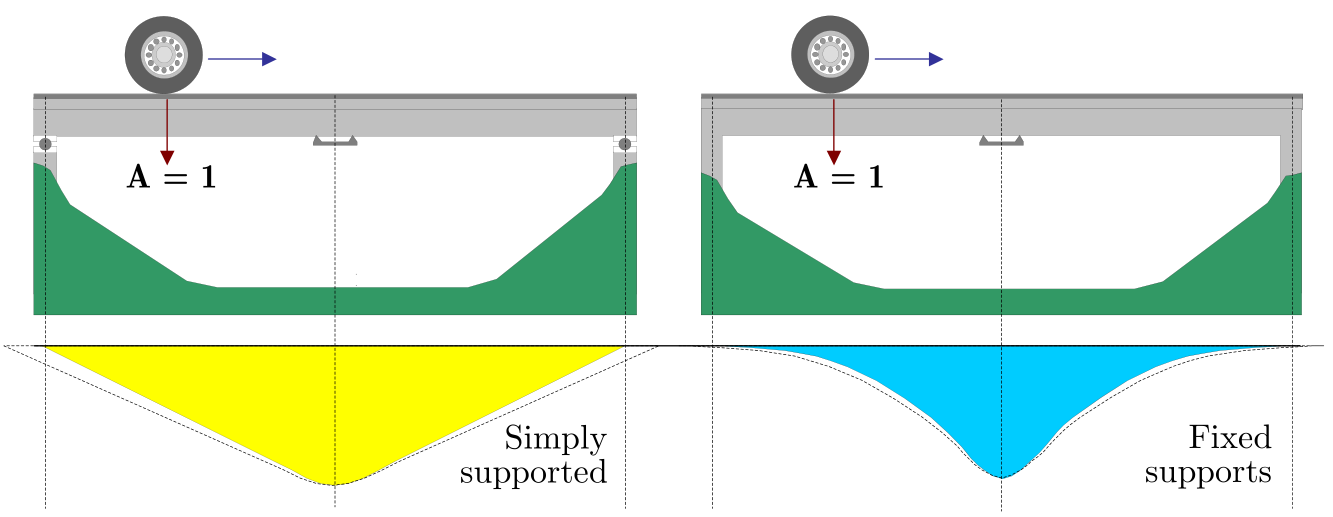
\includegraphics[scale=0.5]{figures/inflLinesQuilligan}
\caption{Influence lines for simply and fixed supported bridges, figure from \cite{Quilligan}}
\label{fig:theoreticalInfl}
\end{figure}

Znidaric and Baumgärter \cite{bwim_an_overview}, did a study on the effect of choice of influence line. This study shows errors up to 10\% for a short \SI{2}{\metre} bridge span and errors of several hundred percent for a \SI{32}{\metre} bridge span. This underlines the importance of using correct influence lines for a B-WIM system.
\begin{figure}[h]
\centering
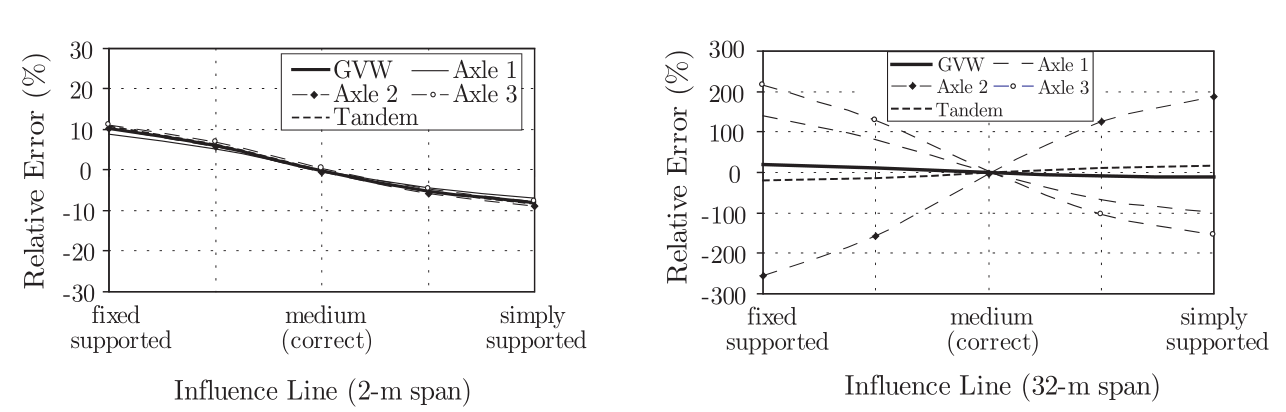
\includegraphics[scale=0.5]{figures/error_in_weights_dueTo_infl}
\caption{Errors of axle loads due to wrongly selected influence lines, figure from \cite{Quilligan}}
\label{fig:errorOfInfl}
\end{figure}
\subsubsection{Matrix method}
Quilligan \cite{Quilligan} developed a 'matrix method' to calculate the influence line of a bridge through the measured strain induced by a vehicle. This method is derived from Moses', equation \ref{equation:moses}.
\begin{equation}
Error = \sum_{k = 1}^{K} [\varepsilon_{k}^{measured} - \varepsilon_{k}^{theoretical}]^2
\label{equation:moses}
\end{equation}
Equation \ref{equation:moses} were originally used to filter out the dynamic response of the bridge.
The theoretical strain in this equation can be expressed as a product of axle loads and influence ordinates at sampling points, see equation \ref{equation:theoretical_strain}, thus we can expand equation \ref{equation:moses}:
\begin{equation}
Error = \sum_{k = 1}^{K} \Big[\varepsilon_{k}^{measured} - \Big(\sum_{i = 1}^{N} A_i I_{(k-C_i)}\Big)\Big]^2
\label{equation:moses_expanded}
\end{equation}
The set of influence ordinates $I$ that minimizes $Error$, forms the wanted influence line.
\begin{equation}
\frac{\partial Error}{\partial I_R} = \frac{\partial \sum_{k = 1}^{K} \Big[\varepsilon_{k}^{measured} - \Big(\sum_{i = 1}^{N} A_i I_{(k-C_i)}\Big)\Big]^2}{\partial I_R}
\end{equation}
For a given number of known axle loads this equation comes down to a set of $(K - C_n)$ number of linear equations. Rearranging the equations and writing them in matrix form leads to:
\begin{equation}
\begin{bmatrix} AxleMatrix \end{bmatrix}_{K-C_N, K-C_N} \begin{Bmatrix} I \end{Bmatrix}_{K-C_N, 1} = \begin{Bmatrix} M \end{Bmatrix}_{K-C_N, 1}
\label{equation:matrixForm}
\end{equation}
Where:
\begin{description}
\item $\begin{Bmatrix} M \end{Bmatrix}$ = a vector depending on axle weights and measured strain, $M_{i, 1} = \Big(\sum_{j = 1}^{N} A_j \varepsilon_{(i+C_j)}\Big)$
\item $\begin{bmatrix} AxleMatrix \end{bmatrix}$ is a matrix depending only on the axle loads, defined by equation \ref{axleMatrix}.
\end{description}
\begin{equation}
\begin{bmatrix} AxleMatrix \end{bmatrix} = \sum_{i = 1}^{N} \sum_{j = i}^{N} \begin{bmatrix} AxleMatrix \end{bmatrix} + \big( A_i A_j  \begin{bmatrix} Diagonal \end{bmatrix}_{C_j - C_i}\big)
\label{axleMatrix}
\end{equation}
Which produces the upper triangle of the symmetric AxleMatrix.
Where:
\begin{description}
\item $\begin{bmatrix} Diagonal \end{bmatrix}_{C_j - C_i}$ = a diagonal matrix of ones, where diagonal is placed with an offset, $C_j - C_i$, from the center matrix diagonal.
\end{description}
Solving equation \ref{equation:matrixForm} for the influence ordinate vector gives the influence line for the strain history. This can be done through inversion of the AxleMatrix (equation \ref{axleMatrix}) or other numerical solutions like a Cholesky factorization.
\subsubsection{Optimization}
testing \cite{Liljencrantz}.

\subsection{Finding the train's speed}

\subsection{The axle distances}


% !TEX root = main.tex
\section{Method}

\subsection{Programming a BWIM system}
Describe shortly how the BWIM system have been programmed.
Keywords:
\begin{itemize}
\item Beam bridge model
\item Producing a strain history through influence lines
\item Finding the speed of the train
\item Finding Axle distances
\item Solving system for axle weights
\end{itemize}
This master project began by learning how a BWIM-system works, and to then create a working model performing BWIM. To not make this a too big project this meant building a simple beam model of a bridge in Matlab, and simulate moving loads crossing it.

A simple flow diagram describing the intial BWIM program:
\begin{figure}
% 
\tikzset{
  terminal/.style={draw, rounded rectangle, text width=3cm, text centered},
  process/.style={draw, text width=3cm, text centered},
  decision/.style={draw, diamond, aspect=2, text width=3cm, text centered},
  delay/.style={draw, rounded rectangle, rounded rectangle west arc=none, text width=3cm, minimum height=1cm, text centered},
  line/.style={draw, -latex}
}
\begin{tikzpicture}
  \node[terminal] (main) {Main script};
  \node[process, above=1cm of main] (createInfl) {create influence line};
  \node[process, right=2cm of main] (createStrain) {create strain signal};
  \node[process, below=2cm of main] (findSpeed) {find train speed};
  \node[process, left=1cm of findSpeed] (findAxleDist) {find axle distances};
  \node[process, left=2cm of main] (calcAxleWeights) {calculate axle weights};

  \draw[line] (main) -- (createInfl);
  \draw[line] (main) -- (createStrain);
  \draw[line] (main) -- (findSpeed);
  \draw[line] (findSpeed.west) -- (findAxleDist.east);
  \draw[line] (main) -- (calcAxleWeights);
\end{tikzpicture}%

\end{figure}


\subsubsection{Producing a strain signal}
Through the theoretical moment influence lines of the beam, a strain signal can be built through the moment-strain relationship, found in equation\ref{equation:moment_strain}, for a given set of axle weights. A simple beam bridge model, as seen in figure \ref{figure:beam_model}, will not recreate a actual bridge strain signal but will be used to create a working BWIM system. The produced strain signal will differ from an actual strain signal mostly because of dynamics, from the train and bridge, and because actual boundary conditions of a bridge will differ from the boundary conditions of a simple beam model. The strain sensors will also produce noise distorting the signal.

To make as good a signal as possible, some effort were placed into recreating the effect mentioned above. To add noise to the signal, white gaussian noise was included in the signal through Matlabs wgn function "http://se.mathworks.com/help/comm/ref/wgn.html".


This strain signal could then be used as a base to build the code for a BWIM system.

\begin{figure}
	\begin{tikzpicture}
		\draw[thick] (0,0) to (5,0);
		\node[ledd fast={0}{0}{0}] (ledd) {};
		\node[ledd skyve={5}{0}{0}] (skyveledd) {};
		%\draw[->] (0,1) to {$\scriptstyle g$} (0,.1);
		\node (a) at (1,1.5) {};
		\node (b) at (1,.1) {};
		\draw[-open triangle 90] (a) to node[pos=-.4] {$axle 2$} (b);
		\node (c) at (3.5,1.5) {};
		\node (d) at (3.5,.1) {};
		\draw[-open triangle 90] (c) to node[pos=-.4] {$axle 1$} (d);
		\node (e) at (3.5,1) {};
		\node (f) at (4.5,1) {};
		\draw[-open triangle 90] (e) to node[pos=1.2] {$v$} (f);
		\node (g) at (1,.5) {};
		\node (h) at (3.5,.5) {};
		\draw[open triangle 90-open triangle 90] (g) to node[above] {$axle spacing$} (h);
		%\draw (2.5,0) circle [radius=0.1] {sensor};
		%\node[draw,circle] (s) at (2.5,0){};
		\filldraw
		(2.5,0) circle (2pt) node[align=left,   below] {strain sensor};
	\end{tikzpicture}
%\captionof{figure}{Beam model for initial BWIM}
\caption{Beam model for developement}
\label{figure:beam_model}

\end{figure}


\subsubsection{Finding the speed of the train}
Two working methods of finding the speed of a passing train were developed:
\begin{itemize}
 \item By identifying peaks in the strain history for two different sensors, representing the same axle. The distance between the two sensors and the time difference between the found peaks should theoretically give a good estimate of the trains velocity.
 \item Through doing cross correlation between two sensors strain history. This involves finding the phase difference, or lag, between the signals. The known distance between the strain gauges should then along with a constant, based on distance between sensors, give a reliable estimate of train velocity. INSERT PLOT OF CORRELATION AND SHOW MATHEMATICAL EQUATION DESCRIBING CROSS CORRELATION.
\end{itemize}

\subsection{Finding influence lines}
Describe how influence lines have been found from the given strain history from Lerelva Bridge.
Keywords:
\begin{itemize}
\item Matrix method
\item Optimization
\item Speed
\end{itemize}
\subsubsection{Matrix method}
Describe the matrix method.

\subsubsection{Optimization}
Describe how optimization can be used to find optimal influence lines for the bridge.

\subsection{System setup}
\label{system_setup}
To test the BWIM-program on actual data, we Gunnstein, Daniel set up a BWIM-system to gather strain data from actual train passings. The subject bridge were Lerelva-Bridge in Trondheim, figure \ref{fig:lerelva_bridge}, a typical Norwegian steel railway bridge. Three strain gauges, \SI{3}{\mm} \SI{120}{ohms} from HBM, were placed by the support towards Trondheim on the first section of the longitudinal stringer, see figure \ref{fig:strain_gauges}. The sensors were placed with \SI{1}{\m} spacing around the middle of the stringer section. These strain gauges were connected to a National Instruments compactDAQ with module NI 9235 which produced an continuous data flow to a standard laptop, see figure \ref{fig:instruments}. A Kipor generator was brought for power.
% INSERT SYSTEM IMAGE HERE
\begin{figure}[H]
	\centering
	\begin{subfigure}[t]{0.49\textwidth}
    \centering
    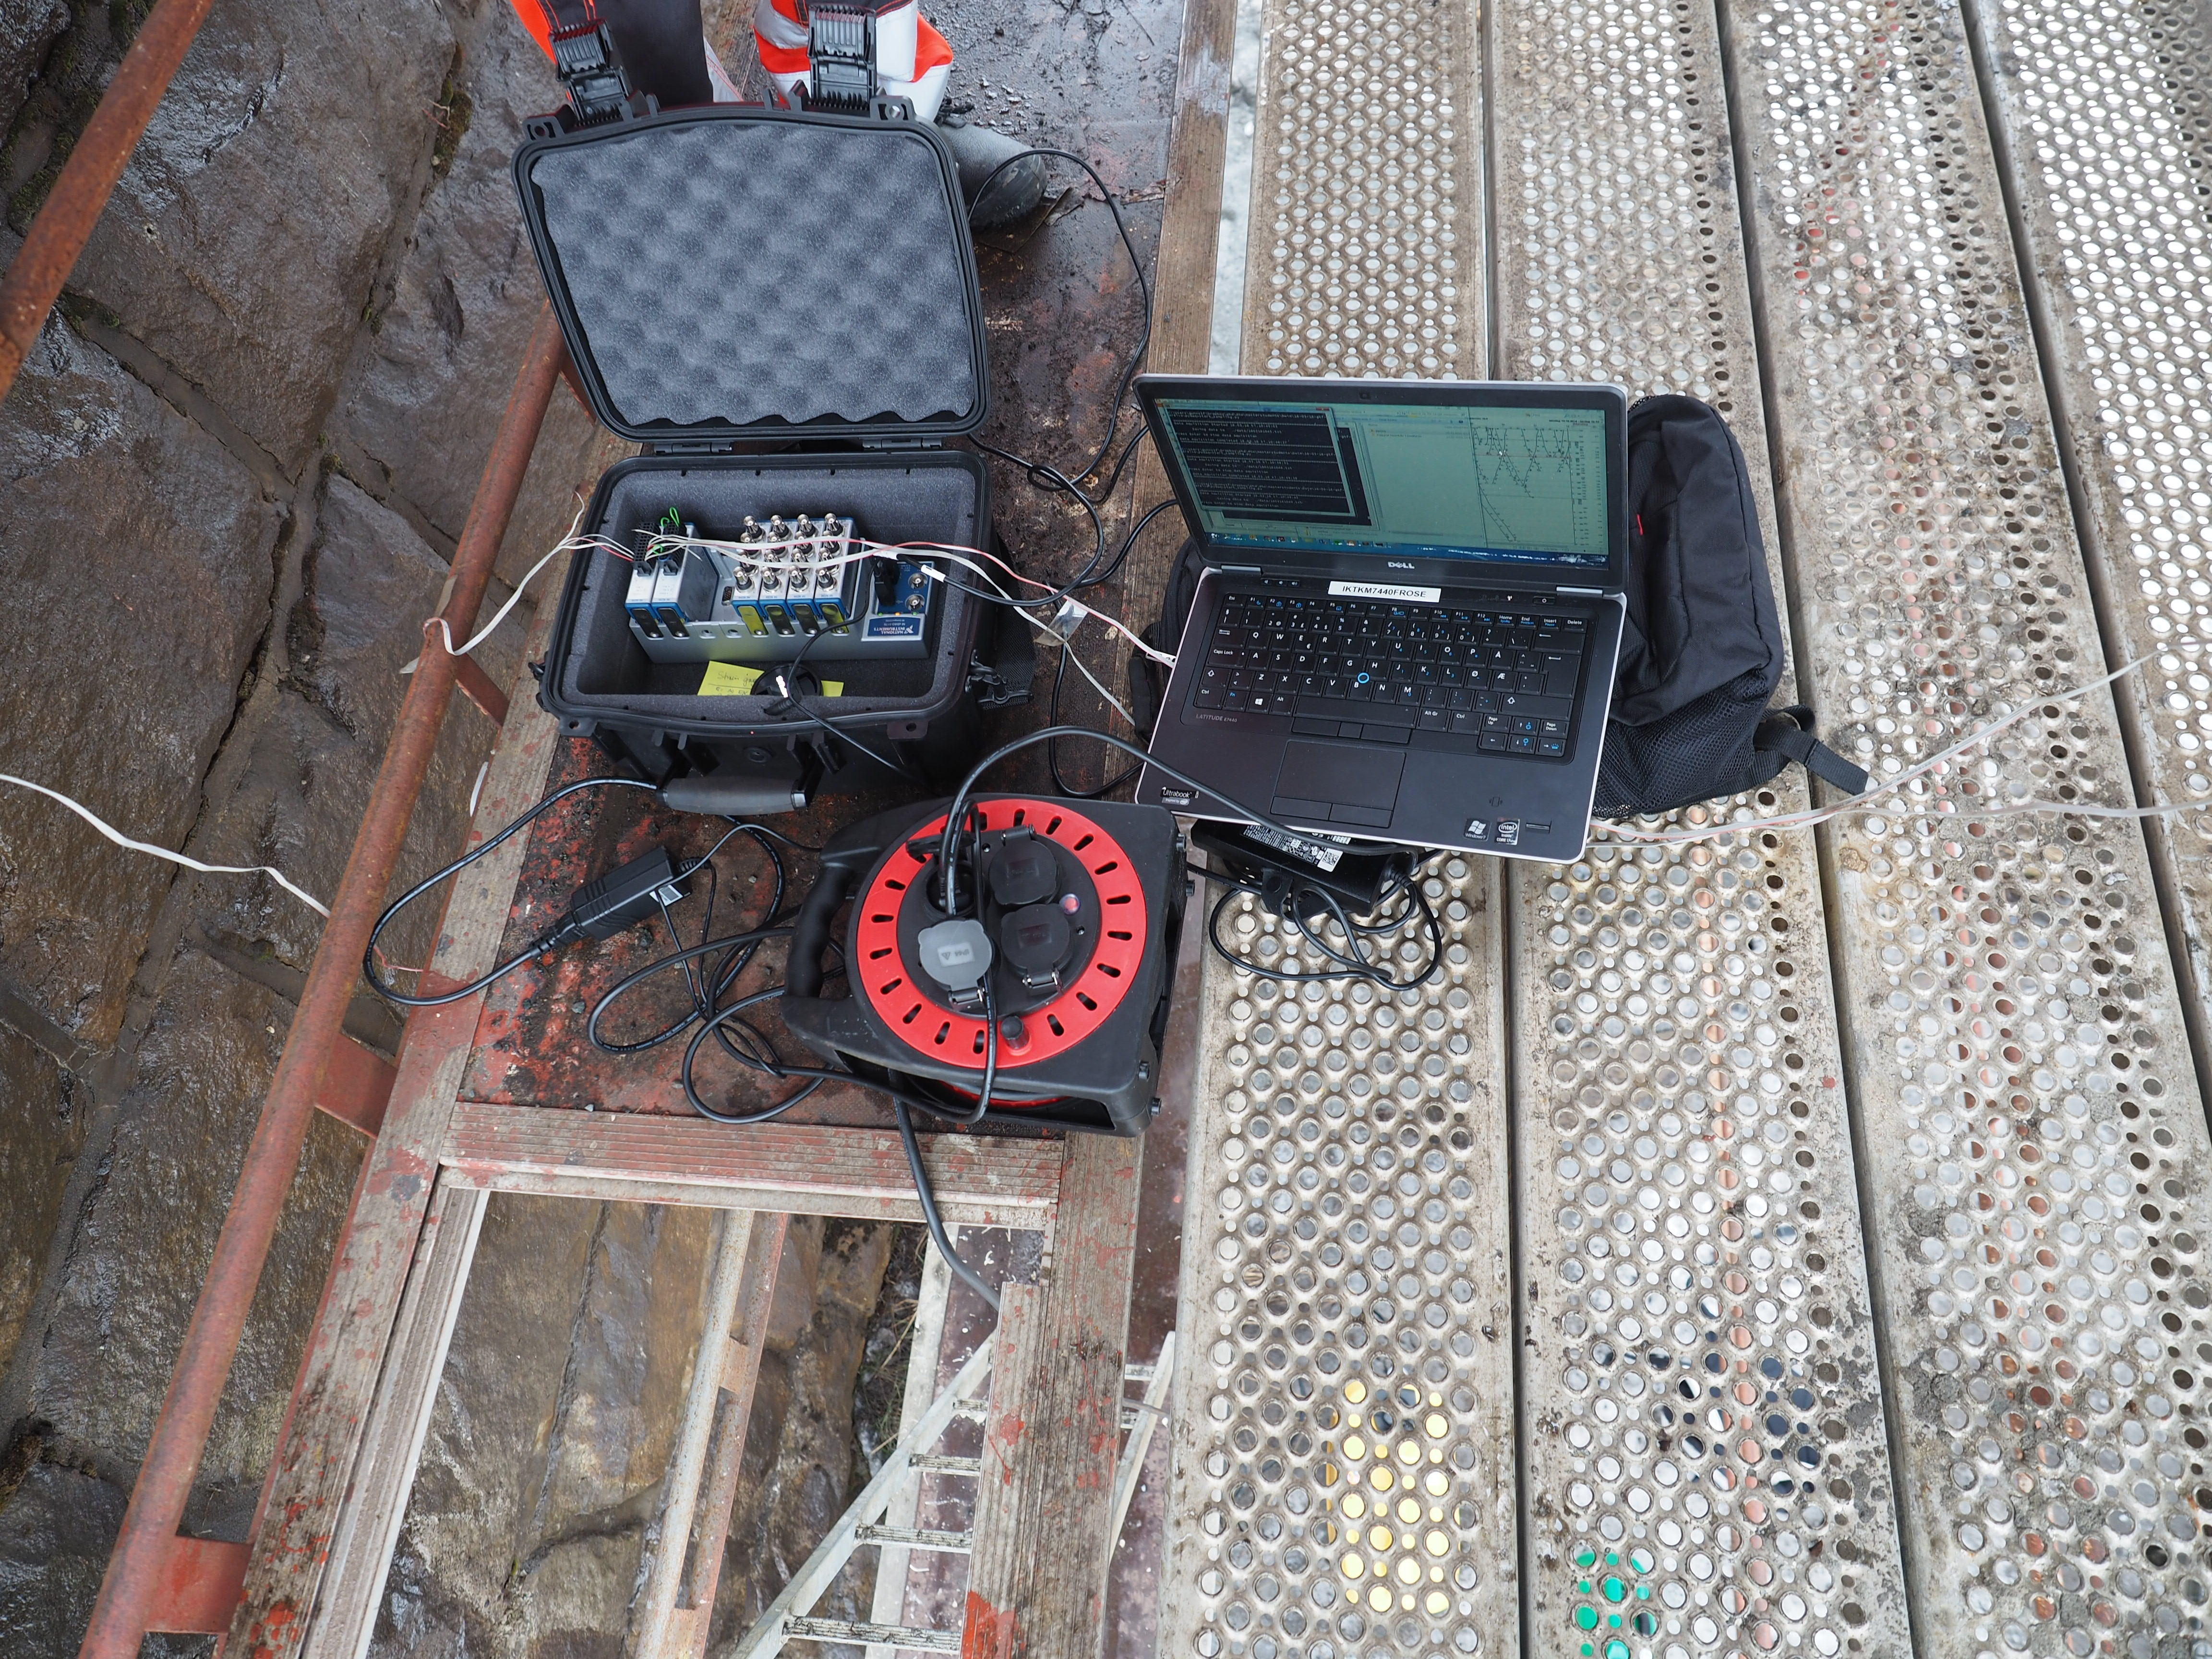
\includegraphics[width=\textwidth]{figures/system_setup}
		\caption{System setup from data gathering at Lerelva}
		\label{fig:instruments}
	\end{subfigure}
	\begin{subfigure}[t]{0.49\textwidth}
    \centering
    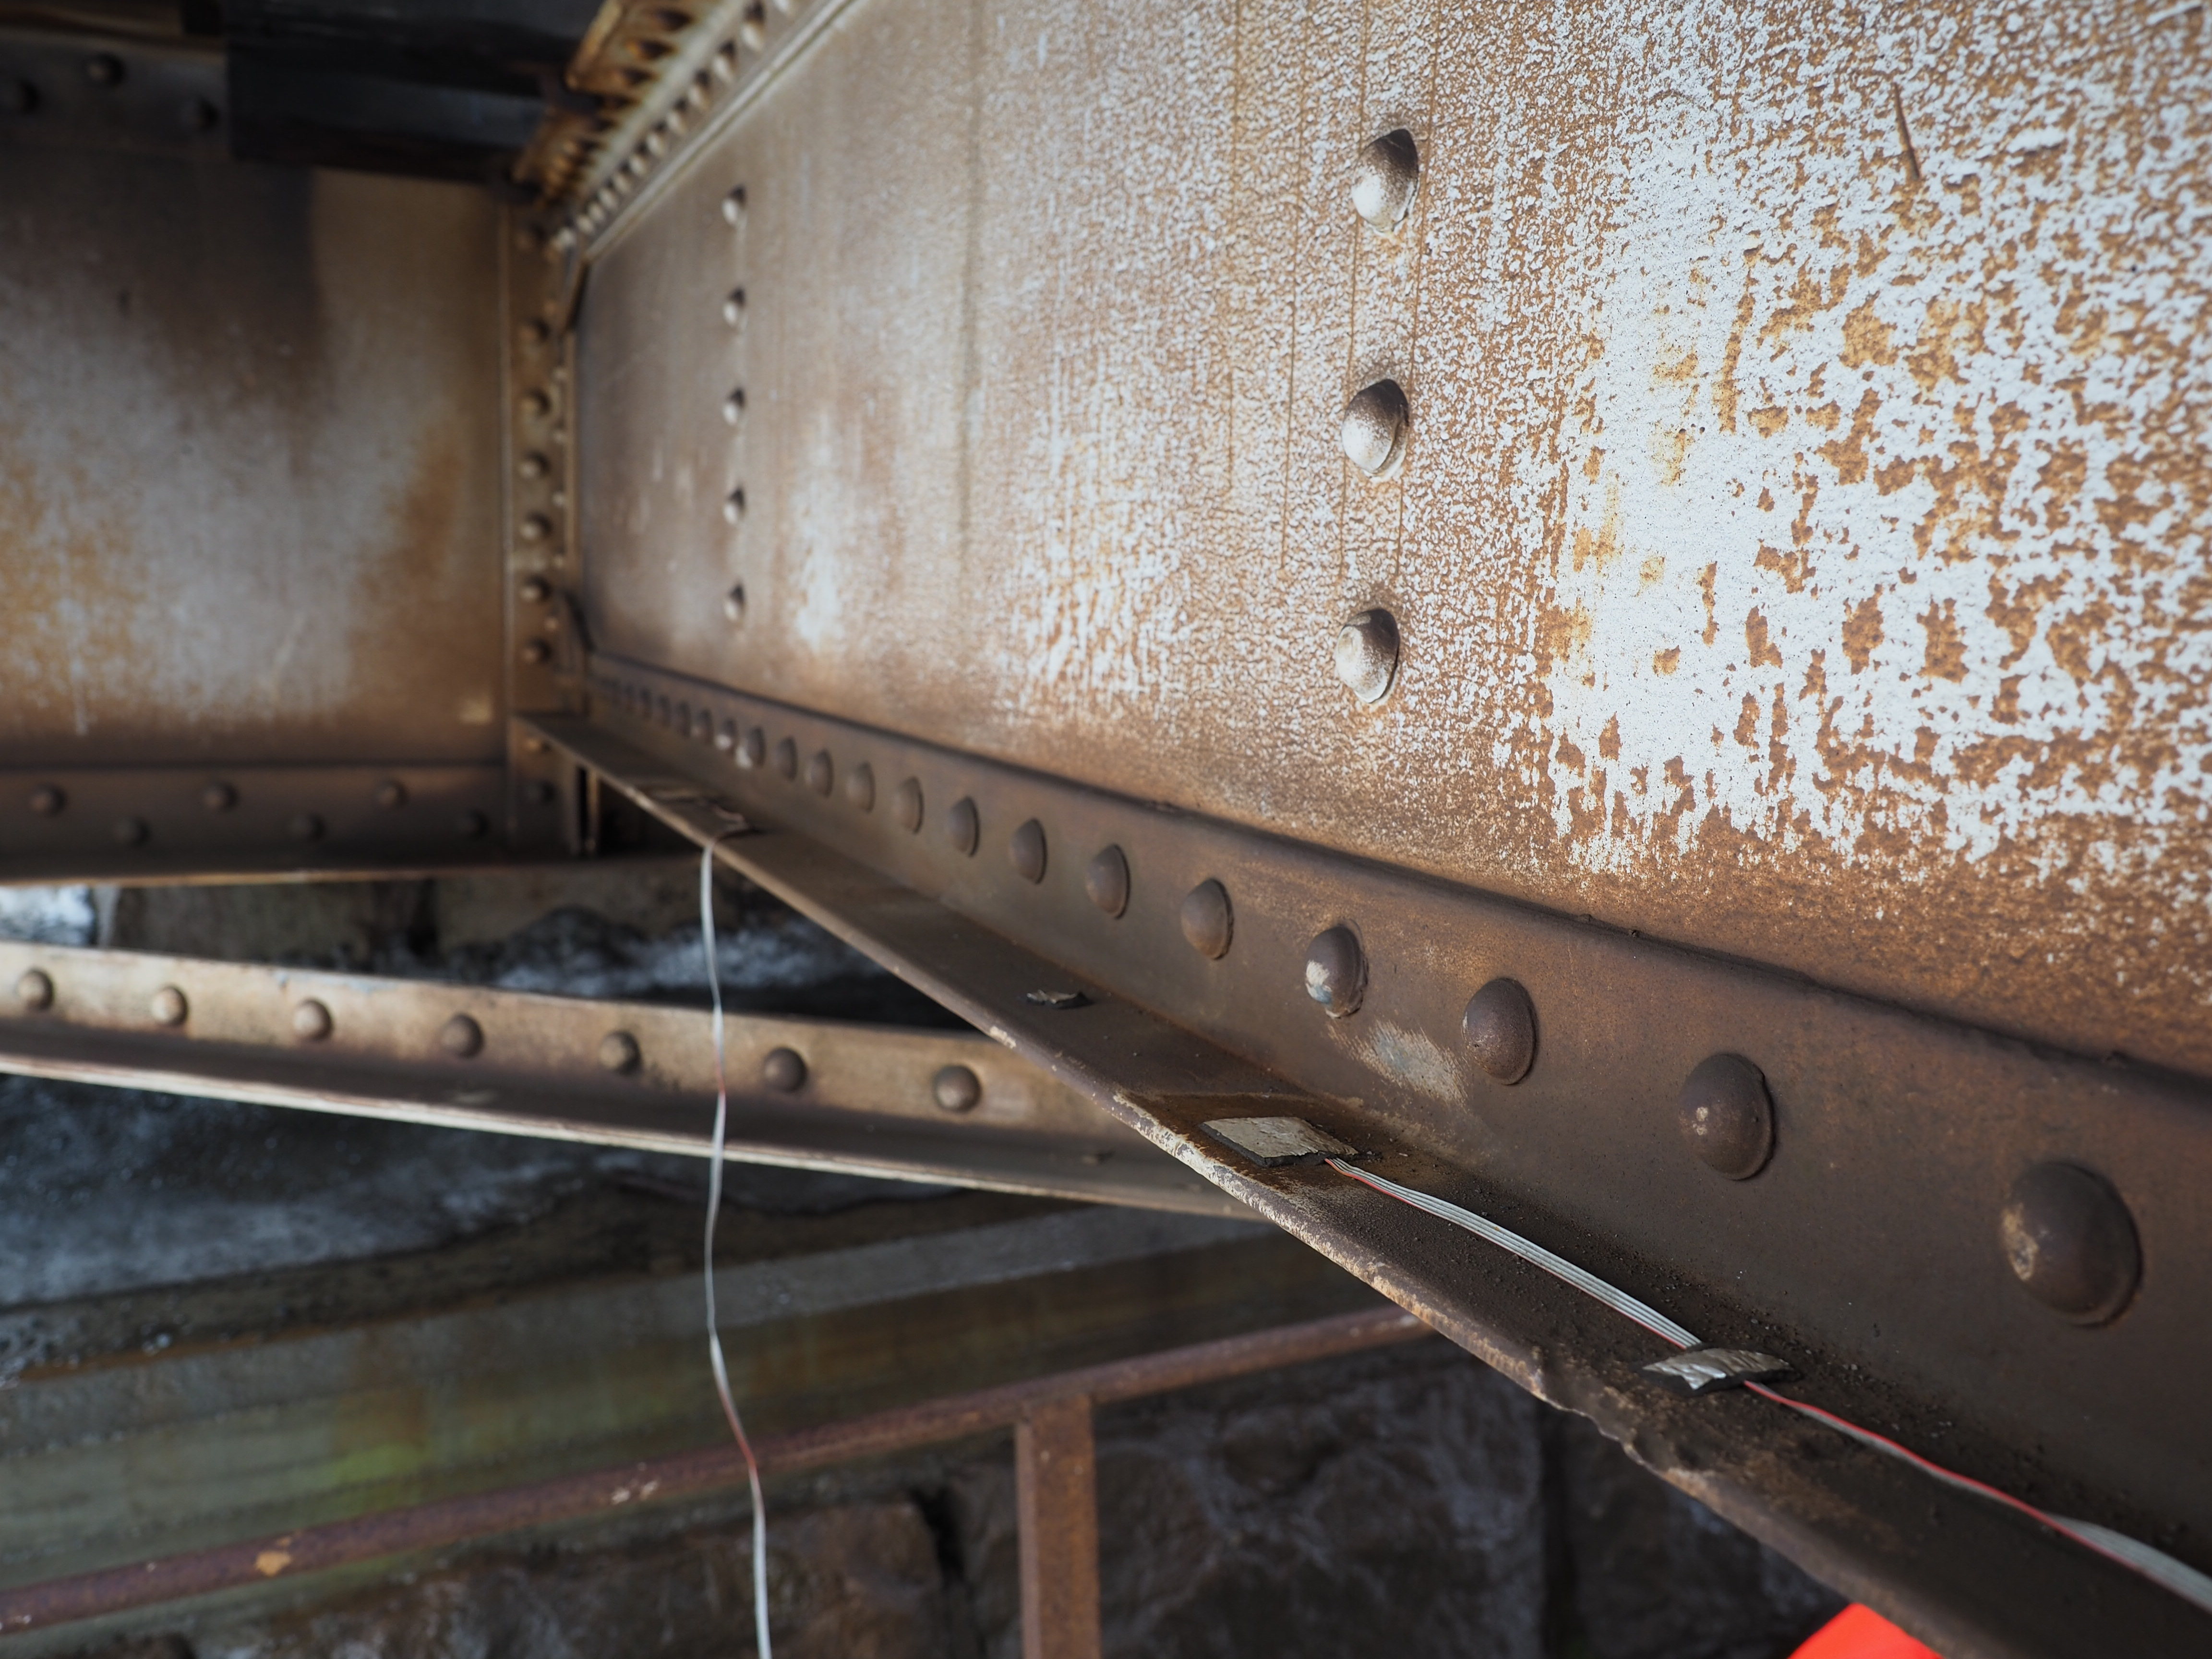
\includegraphics[width=\textwidth]{figures/sensor_placement}
		\caption{Placement of strain gauges on stringer section}
		\label{fig:strain_gauges}
	\end{subfigure}
	\caption{Instruments for aquiring strain data}
	\label{fig:system_setup}
	% 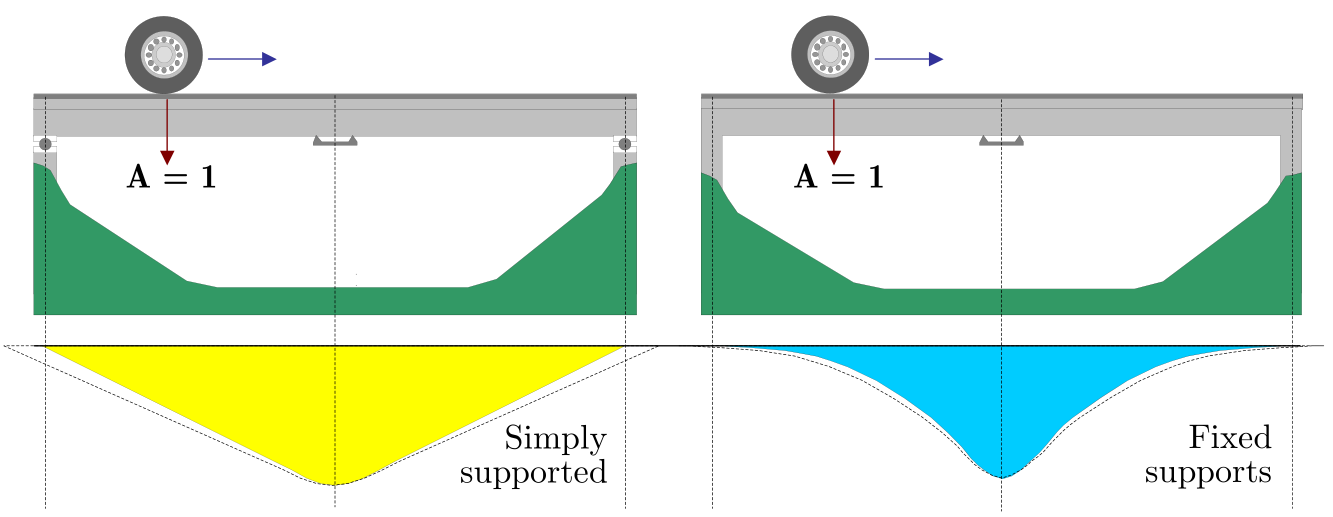
\includegraphics[scale=0.5]{figures/inflLinesQuilligan}
\end{figure}
\begin{figure}[H]
	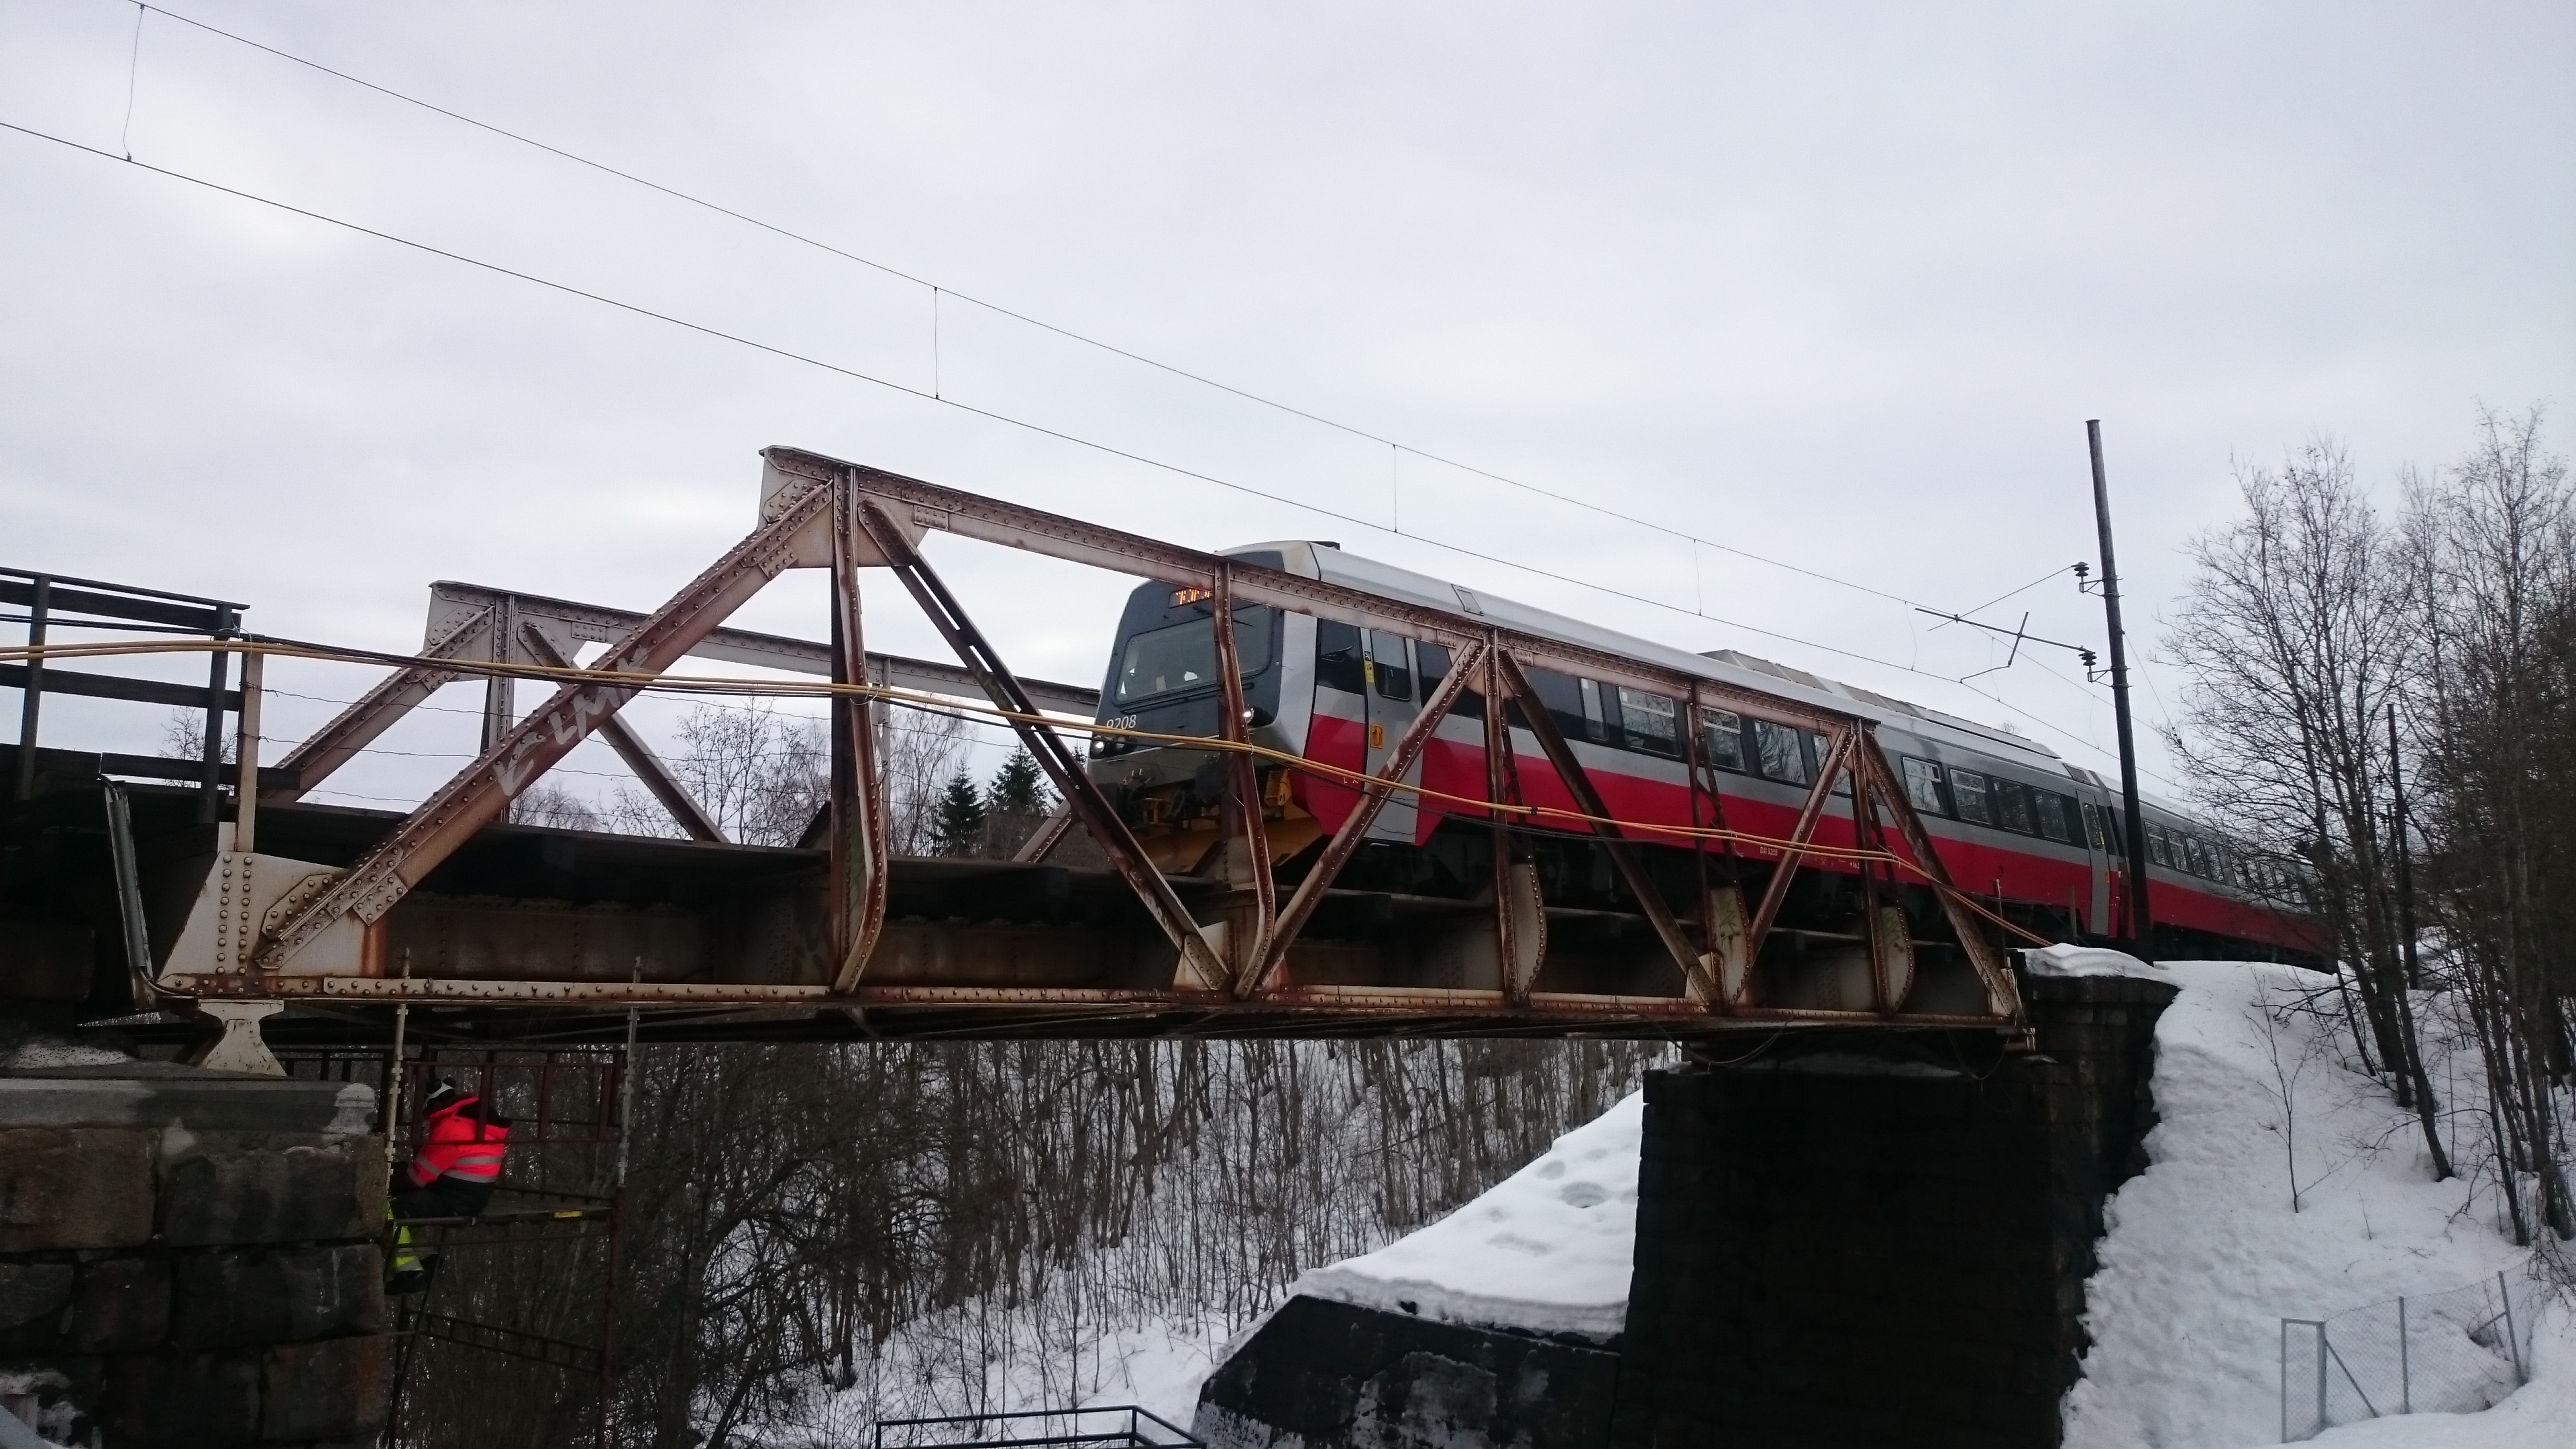
\includegraphics[width=\textwidth]{figures/train_passing.jpg}
	\caption{Lerelva bridge with a train passing over}
	\label{fig:lerelva_bridge}
\end{figure}


\subsection{Testing}
Keywords:
\begin{itemize}
\item Comparing calculated strain with measured strain
\end{itemize}


% !TEX root = main.tex
\section{Analysis}

This chapter will describe how the BWIM system performs. What works? Why? How? etc.
The main focus should perhaps be placed on identifying the pros and cons of the matrix method and optimization method.

Should include:
\begin{itemize}
\item Compare theoretical and calculated influence lines. Also include influence lines found through Abaqus.
\item Check how influence lines found through matrix method and optimization reproduces the strain history
\item Test obtained influence line by running the bwim routine on the hitherto unused freight train. (Depends on getting info about the train). Also Do this test on the other trains.
\end{itemize}

\subsection{Strain data}
\begin{figure}[H]
	\centering
	\begin{subfigure}[t]{0.45\textwidth}
		\centering
		% This file was created by matlab2tikz.
%
%The latest updates can be retrieved from
%  http://www.mathworks.com/matlabcentral/fileexchange/22022-matlab2tikz-matlab2tikz
%where you can also make suggestions and rate matlab2tikz.
%
\definecolor{mycolor1}{rgb}{0.00000,0.44700,0.74100}%
\definecolor{mycolor2}{rgb}{0.85000,0.32500,0.09800}%
\definecolor{mycolor3}{rgb}{0.92900,0.69400,0.12500}%
%
\begin{tikzpicture}

\begin{axis}[%
width=\textwidth,
height=\textwidth,
at={(0\figurewidth,0\figureheight)},
scale only axis,
xmin=12,
xmax=20,
ymin=-5e-05,
ymax=0.0002,
axis background/.style={fill=white},
title style={font=\bfseries},
title={Raw strain history, train 3},
% legend style={legend cell align=left,align=left,draw=white!15!black}
% legend style={at={(1.1,-0.2)}}
]
\addplot [color=mycolor1,solid,forget plot]
  table[row sep=crcr]{%
12.7763671875	5.66138597029925e-07\\
12.77734375	3.26189245247223e-07\\
12.7783203125	1.35641311928975e-07\\
12.779296875	-5.2068990728793e-07\\
12.7802734375	-4.7834598343845e-07\\
12.78125	-8.7355580109718e-07\\
12.7822265625	-9.79415521092705e-07\\
12.783203125	-6.47721657503174e-07\\
12.7841796875	-1.46651790273577e-07\\
12.78515625	1.04603764310954e-06\\
12.7861328125	-7.95925325643848e-07\\
12.787109375	9.19005498232995e-07\\
12.7880859375	1.70927960814818e-07\\
12.7890625	7.49629354841221e-07\\
12.7900390625	9.11948157789185e-07\\
12.791015625	-5.70091147284683e-07\\
12.7919921875	-1.90392279790985e-06\\
12.79296875	3.12074581051112e-07\\
12.7939453125	-7.39466790535513e-07\\
12.794921875	1.21526653065621e-07\\
12.7958984375	2.1893283869861e-06\\
12.796875	5.3085192048977e-07\\
12.7978515625	-6.05377744320075e-07\\
12.798828125	-2.5956898690822e-07\\
12.7998046875	-4.28944734453445e-07\\
12.80078125	-5.48919187878978e-07\\
12.8017578125	-5.70091147284683e-07\\
12.802734375	4.24991905684062e-07\\
12.8037109375	-1.25465068908292e-06\\
12.8046875	2.83845253843274e-07\\
12.8056640625	4.46163906867112e-07\\
12.806640625	-5.50525892538054e-09\\
12.8076171875	9.89578908102513e-07\\
12.80859375	1.5666724184453e-08\\
12.8095703125	4.10877238721935e-07\\
12.810546875	-4.78492224776934e-08\\
12.8115234375	7.56686693013193e-07\\
12.8125	-8.45326538678661e-07\\
12.8134765625	9.32973365245972e-08\\
12.814453125	-2.22855853884772e-06\\
12.8154296875	-5.1363258689297e-07\\
12.81640625	-6.90212029208232e-08\\
12.8173828125	7.91826788462766e-08\\
12.818359375	9.19005498232995e-07\\
12.8193359375	1.50476509935935e-06\\
12.8203125	1.34950345206681e-06\\
12.8212890625	4.38960363799944e-08\\
12.822265625	-6.33607020170558e-07\\
12.8232421875	4.46163906867112e-07\\
12.82421875	-4.00715447146632e-07\\
12.8251953125	-6.47721657503174e-07\\
12.826171875	2.20329273403676e-07\\
12.8271484375	8.9783347719777e-07\\
12.828125	-7.60785295375859e-08\\
12.8291015625	-2.87798282116265e-07\\
12.830078125	6.57883967589709e-07\\
12.8310546875	-4.21887412774789e-07\\
12.83203125	2.41501265994858e-07\\
12.8330078125	-1.32522378488314e-06\\
12.833984375	-5.34804547780996e-07\\
12.8349609375	-2.8074095846241e-07\\
12.8359375	-5.77148466889476e-07\\
12.8369140625	1.99157281701974e-07\\
12.837890625	6.3671195751772e-07\\
12.8388671875	1.41301957472728e-06\\
12.83984375	6.6494130447842e-07\\
12.8408203125	-4.57174020180142e-07\\
12.841796875	-1.74881091802737e-07\\
12.8427734375	-8.66498485640977e-07\\
12.84375	2.55615928215986e-07\\
12.8447265625	-4.50116698896353e-07\\
12.845703125	-9.72505087954659e-08\\
12.8466796875	-3.2308489890452e-07\\
12.84765625	1.04603764310954e-06\\
12.8486328125	1.37067549206495e-06\\
12.849609375	9.26062838775468e-07\\
12.8505859375	-5.41861867879101e-07\\
12.8515625	-3.93658125072893e-07\\
12.8525390625	-1.67823766568332e-07\\
12.853515625	-3.51314190556815e-07\\
12.8544921875	-1.53709115803752e-07\\
12.85546875	-7.11237520611063e-07\\
12.8564453125	7.77858708122386e-07\\
12.857421875	-9.72505087954659e-08\\
12.8583984375	-1.25625864305385e-08\\
12.859375	7.07285327881946e-07\\
12.8603515625	-5.6303382758166e-07\\
12.861328125	-1.13467640355585e-06\\
12.8623046875	1.35641311928975e-07\\
12.86328125	-2.03110391751348e-07\\
12.8642578125	-9.72358207117739e-07\\
12.865234375	2.13271942737635e-07\\
12.8662109375	4.67335908939642e-07\\
12.8671875	-8.10039958433224e-07\\
12.8681640625	1.32127406678585e-06\\
12.869140625	8.83718797001654e-07\\
12.8701171875	4.53221240792698e-07\\
12.87109375	1.07411994597567e-07\\
12.8720703125	-4.99517945807279e-07\\
12.873046875	-1.39594464644306e-07\\
12.8740234375	6.22597284629994e-07\\
12.875	1.0530949854301e-06\\
12.8759765625	-1.04307835017145e-07\\
12.876953125	-2.8074095846241e-07\\
12.8779296875	2.48558597055982e-07\\
12.87890625	9.61349542969716e-07\\
12.8798828125	3.40303909838633e-07\\
12.880859375	1.14469323781938e-07\\
12.8818359375	6.93170653019021e-07\\
12.8828125	9.47234860995726e-07\\
12.8837890625	2.9781380084682e-08\\
12.884765625	9.19005498232995e-07\\
12.8857421875	-3.79543480629211e-07\\
12.88671875	-3.3734568355339e-08\\
12.8876953125	-5.91263105802426e-07\\
12.888671875	1.07426701298334e-06\\
12.8896484375	-2.45454338711464e-07\\
12.890625	1.11661107075715e-06\\
12.8916015625	9.68406884104813e-07\\
12.892578125	-1.21936413747885e-06\\
12.8935546875	-2.5956898690822e-07\\
12.89453125	3.68533240206704e-07\\
12.8955078125	-4.57174020180142e-07\\
12.896484375	-6.19492382442858e-07\\
12.8974609375	1.49755971186978e-07\\
12.8984375	4.10877238721935e-07\\
12.8994140625	-1.11365161140162e-07\\
12.900390625	1.07411994597567e-07\\
12.9013671875	-4.7834598343845e-07\\
12.90234375	9.33120179416819e-07\\
12.9033203125	-3.79543480629211e-07\\
12.904296875	-4.85403304326722e-07\\
12.9052734375	-7.25352155770938e-07\\
12.90625	9.82521566670995e-07\\
12.9072265625	7.42572016767477e-07\\
12.908203125	3.19131913100162e-07\\
12.9091796875	1.27892999182743e-06\\
12.91015625	-3.44256867791572e-07\\
12.9111328125	1.00354665511643e-07\\
12.912109375	7.56686693013193e-07\\
12.9130859375	-7.25352155770938e-07\\
12.9140625	1.99157281701974e-07\\
12.9150390625	-4.50116698896353e-07\\
12.916015625	-1.53694301302607e-06\\
12.9169921875	4.46163906867112e-07\\
12.91796875	9.82521566670995e-07\\
12.9189453125	-1.09938984355724e-06\\
12.919921875	-5.41861867879101e-07\\
12.9208984375	1.13072575747171e-06\\
12.921875	7.56686693013193e-07\\
12.9228515625	9.68406884104813e-07\\
12.923828125	4.39106573040622e-07\\
12.9248046875	-5.70091147284683e-07\\
12.92578125	-4.99517945807279e-07\\
12.9267578125	3.89705239020122e-07\\
12.927734375	-1.32537138916155e-07\\
12.9287109375	-7.1829483824044e-07\\
12.9296875	-3.58371513222745e-07\\
12.9306640625	1.31421672071243e-06\\
12.931640625	4.95565246418778e-07\\
12.9326171875	1.03898030088829e-06\\
12.93359375	-3.01912929127771e-07\\
12.9345703125	-7.1829483824044e-07\\
12.935546875	8.76661457051807e-07\\
12.9365234375	-1.40285417885629e-06\\
12.9375	5.09679915750971e-07\\
12.9384765625	-4.21887412774789e-07\\
12.939453125	-6.12435063430906e-07\\
12.9404296875	2.83845253843274e-07\\
12.94140625	1.92820619857232e-06\\
12.9423828125	1.43419161739125e-06\\
12.943359375	2.9781380084682e-08\\
12.9443359375	2.69730590832197e-07\\
12.9453125	1.00369359126175e-06\\
12.9462890625	8.55489437794456e-07\\
12.947265625	1.5666724184453e-08\\
12.9482421875	-1.18407758340627e-06\\
12.94921875	-2.8074095846241e-07\\
12.9501953125	-6.5477897602138e-07\\
12.951171875	-4.07918954660642e-08\\
12.9521484375	1.1801271640841e-06\\
12.953125	2.2724052084911e-08\\
12.9541015625	-6.05377744320075e-07\\
12.955078125	5.02622581035218e-07\\
12.9560546875	1.30010202886222e-06\\
12.95703125	-3.65428835790447e-07\\
12.9580078125	5.8731060413944e-07\\
12.958984375	6.22597284629994e-07\\
12.9599609375	1.63885474230795e-06\\
12.9609375	1.35641311928975e-07\\
12.9619140625	4.17934572153559e-07\\
12.962890625	7.84916046689659e-07\\
12.9638671875	1.14469323781938e-07\\
12.96484375	6.08482612137352e-07\\
12.9658203125	6.71998641465143e-07\\
12.966796875	1.08838169851264e-06\\
12.9677734375	-1.39594464644306e-07\\
12.96875	-4.14830090997471e-07\\
12.9697265625	-6.7595093098294e-07\\
12.970703125	6.29654621024526e-07\\
12.9716796875	-6.7595093098294e-07\\
12.97265625	-2.17225041133353e-07\\
12.9736328125	-3.30142221965533e-07\\
12.974609375	-2.20032935227977e-06\\
12.9755859375	-4.21887412774789e-07\\
12.9765625	-1.84040708502142e-06\\
12.9775390625	-4.92460625116549e-07\\
12.978515625	4.39106573040622e-07\\
12.9794921875	2.20329273403676e-07\\
12.98046875	1.13072575747171e-06\\
12.9814453125	-1.18407758340627e-06\\
12.982421875	8.60939638222362e-09\\
12.9833984375	-2.17225041133353e-07\\
12.984375	-3.37199544928101e-07\\
12.9853515625	-5.70091147284683e-07\\
12.986328125	-1.02881671615231e-06\\
12.9873046875	-5.6303382758166e-07\\
12.98828125	4.38960363799944e-08\\
12.9892578125	-5.91263105802426e-07\\
12.990234375	-9.86472834969008e-07\\
12.9912109375	-1.81938416937829e-07\\
12.9921875	4.74393243161215e-07\\
12.9931640625	7.2125350155652e-08\\
12.994140625	-1.81938416937829e-07\\
12.9951171875	-3.51314190556815e-07\\
12.99609375	-7.11237520611063e-07\\
12.9970703125	-1.88995741974693e-07\\
12.998046875	6.5068021563473e-08\\
12.9990234375	2.34443935032396e-07\\
13	7.2125350155652e-08\\
13.0009765625	-3.3734568355339e-08\\
13.001953125	4.24991905684062e-07\\
13.0029296875	1.30715937473789e-06\\
13.00390625	9.82521566670995e-07\\
13.0048828125	-1.46651790273577e-07\\
13.005859375	-1.76277675840476e-06\\
13.0068359375	-1.10644715575455e-06\\
13.0078125	7.91826788462766e-08\\
13.0087890625	-4.57174020180142e-07\\
13.009765625	1.00354665511643e-07\\
13.0107421875	3.82647905983365e-07\\
13.01171875	3.33246577493814e-07\\
13.0126953125	2.69730590832197e-07\\
13.013671875	1.75177236402379e-06\\
13.0146484375	-4.7834598343845e-07\\
13.015625	-4.71288662450865e-07\\
13.0166015625	-8.31358560556862e-08\\
13.017578125	-7.39466790535513e-07\\
13.0185546875	1.07411994597567e-07\\
13.01953125	8.20202741007477e-07\\
13.0205078125	8.62400076362142e-08\\
13.021484375	6.71998641465143e-07\\
13.0224609375	2.90902585497023e-07\\
13.0234375	-5.70091147284683e-07\\
13.0244140625	-1.81938416937829e-07\\
13.025390625	-1.40285417885629e-06\\
13.0263671875	3.05017249100942e-07\\
13.02734375	4.38960363799944e-08\\
13.0283203125	1.99157281701974e-07\\
13.029296875	1.68119884748851e-06\\
13.0302734375	1.29304468308522e-06\\
13.03125	1.14484044458157e-06\\
13.0322265625	1.1801271640841e-06\\
13.033203125	-5.50525892538054e-09\\
13.0341796875	4.46163906867112e-07\\
13.03515625	-1.80512057440453e-06\\
13.0361328125	-6.12435063430906e-07\\
13.037109375	-4.21887412774789e-07\\
13.0380859375	8.48432098239475e-07\\
13.0390625	5.09679915750971e-07\\
13.0400390625	-1.81938416937829e-07\\
13.041015625	7.49629354841221e-07\\
13.0419921875	1.3353887592289e-06\\
13.04296875	-3.30142221965533e-07\\
13.0439453125	-2.66772411457346e-08\\
13.044921875	1.79411647868591e-06\\
13.0458984375	1.10249638443746e-06\\
13.046875	-2.66626310858279e-07\\
13.0478515625	-9.58243578871388e-07\\
13.048828125	1.92099951332137e-07\\
13.0498046875	2.9781380084682e-08\\
13.05078125	-3.86600802900492e-07\\
13.0517578125	7.28457340916843e-07\\
13.052734375	-7.1829483824044e-07\\
13.0537109375	2.90902585497023e-07\\
13.0546875	1.56828124157492e-06\\
13.0556640625	-1.58634415346965e-06\\
13.056640625	-1.96199138376846e-08\\
13.0576171875	6.08482612137352e-07\\
13.05859375	-1.51577109421203e-06\\
13.0595703125	5.44966590809671e-07\\
13.060546875	1.85042621060746e-07\\
13.0615234375	1.42713426973793e-06\\
13.0625	4.03819905389407e-07\\
13.0634765625	-4.99517945807279e-07\\
13.064453125	-7.60638741942191e-07\\
13.0654296875	-1.67823766568332e-07\\
13.06640625	-7.74753375719058e-07\\
13.0673828125	-4.92460625116549e-07\\
13.068359375	-1.03587402933733e-06\\
13.0693359375	-9.86472834969008e-07\\
13.0703125	-9.08842376898256e-07\\
13.0712890625	-1.81938416937829e-07\\
13.072265625	6.71998641465143e-07\\
13.0732421875	1.55206867930718e-09\\
13.07421875	1.25775795568124e-06\\
13.0751953125	-4.36002056033221e-07\\
13.076171875	-9.4412895023017e-07\\
13.0771484375	1.04603764310954e-06\\
13.078125	-1.07821790637291e-06\\
13.0791015625	-5.98320425110798e-07\\
13.080078125	-1.53694301302607e-06\\
13.0810546875	1.13072575747171e-06\\
13.08203125	6.79055978551179e-07\\
13.0830078125	1.35641311928975e-07\\
13.083984375	1.6882561986978e-06\\
13.0849609375	-3.44256867791572e-07\\
13.0859375	-1.38168225441264e-06\\
13.0869140625	-8.10039958433224e-07\\
13.087890625	-5.91263105802426e-07\\
13.0888671875	-2.94855605671674e-07\\
13.08984375	-7.25352155770938e-07\\
13.0908203125	-4.00715447146632e-07\\
13.091796875	1.42698641508428e-07\\
13.0927734375	9.26062838775468e-07\\
13.09375	-6.19638762051813e-08\\
13.0947265625	1.22952857553593e-06\\
13.095703125	5.16737250564952e-07\\
13.0966796875	-6.19492382442858e-07\\
13.09765625	-8.02982642087976e-07\\
13.0986328125	-3.08970252485639e-07\\
13.099609375	-3.86600802900492e-07\\
13.1005859375	-5.2068990728793e-07\\
13.1015625	4.53221240792698e-07\\
13.1025390625	1.39890488011149e-06\\
13.103515625	5.09533646755357e-08\\
13.1044921875	6.86113315735443e-07\\
13.10546875	-4.78492224776934e-08\\
13.1064453125	4.88507911900783e-07\\
13.107421875	-8.17097274680026e-07\\
13.1083984375	5.8731060413944e-07\\
13.109375	7.77858708122386e-07\\
13.1103515625	-7.39466790535513e-07\\
13.111328125	-9.4412895023017e-07\\
13.1123046875	-1.74881091802737e-07\\
13.11328125	-5.49065493908769e-08\\
13.1142578125	4.38960363799944e-08\\
13.115234375	9.61349542969716e-07\\
13.1162109375	7.91826788462766e-08\\
13.1171875	-1.30405185718016e-06\\
13.1181640625	2.9781380084682e-08\\
13.119140625	-7.95925325643848e-07\\
13.1201171875	1.14469323781938e-07\\
13.12109375	3.40303909838633e-07\\
13.1220703125	9.26062838775468e-07\\
13.123046875	3.96762572155108e-07\\
13.1240234375	4.67335908939642e-07\\
13.125	2.83845253843274e-07\\
13.1259765625	7.49629354841221e-07\\
13.126953125	3.96762572155108e-07\\
13.1279296875	-8.66498485640977e-07\\
13.12890625	9.40177520156833e-07\\
13.1298828125	-1.32537138916155e-07\\
13.130859375	-1.06410328108968e-06\\
13.1318359375	1.35641311928975e-07\\
13.1328125	-1.77689136413289e-06\\
13.1337890625	5.801069307039e-08\\
13.134765625	4.6027857481673e-07\\
13.1357421875	-4.71288662450865e-07\\
13.13671875	1.24364326541115e-06\\
13.1376953125	-1.03587402933733e-06\\
13.138671875	-3.16027575744194e-07\\
13.1396484375	7.91826788462766e-08\\
13.140625	1.07411994597567e-07\\
13.1416015625	-5.50525892538054e-09\\
13.142578125	4.03819905389407e-07\\
13.1435546875	9.19005498232995e-07\\
13.14453125	1.50476509935935e-06\\
13.1455078125	-2.87798282116265e-07\\
13.146484375	7.91826788462766e-08\\
13.1474609375	-4.50116698896353e-07\\
13.1484375	-6.97122885056321e-07\\
13.1494140625	-1.32537138916155e-07\\
13.150390625	8.62400076362142e-08\\
13.1513671875	1.21526653065621e-07\\
13.15234375	9.26062838775468e-07\\
13.1533203125	4.32049239312794e-07\\
13.154296875	5.16737250564952e-07\\
13.1552734375	-2.31339690119842e-07\\
13.15625	2.13271942737635e-07\\
13.1572265625	-2.45454338711464e-07\\
13.158203125	-9.37071635761242e-07\\
13.1591796875	-5.91263105802426e-07\\
13.16015625	-6.19638762051813e-08\\
13.1611328125	6.50826630800528e-07\\
13.162109375	1.99157281701974e-07\\
13.1630859375	7.21400003139954e-07\\
13.1640625	1.067209670367e-06\\
13.1650390625	-4.07918954660642e-08\\
13.166015625	-3.79543480629211e-07\\
13.1669921875	3.54418574825127e-07\\
13.16796875	9.19005498232995e-07\\
13.1689453125	-1.46651790273577e-07\\
13.169921875	1.92099951332137e-07\\
13.1708984375	-2.38397014464767e-07\\
13.171875	-2.03110391751348e-07\\
13.1728515625	5.66138597029925e-07\\
13.173828125	5.16737250564952e-07\\
13.1748046875	1.37067549206495e-06\\
13.17578125	1.08132435569898e-06\\
13.1767578125	5.73195932634506e-07\\
13.177734375	-2.52511662859282e-07\\
13.1787109375	7.63744031284045e-07\\
13.1796875	-1.06410328108968e-06\\
13.1806640625	-2.38397014464767e-07\\
13.181640625	6.71998641465143e-07\\
13.1826171875	-3.72486158259269e-07\\
13.18359375	4.10877238721935e-07\\
13.1845703125	1.23658592042432e-06\\
13.185546875	8.83718797001654e-07\\
13.1865234375	9.47234860995726e-07\\
13.1875	5.02622581035218e-07\\
13.1884765625	-9.15899691761833e-07\\
13.189453125	3.82647905983365e-07\\
13.1904296875	-1.74866215228177e-06\\
13.19140625	8.60939638222362e-09\\
13.1923828125	-9.37071635761242e-07\\
13.193359375	-1.04307835017145e-07\\
13.1943359375	-1.76277675840476e-06\\
13.1953125	2.76787922288187e-07\\
13.1962890625	3.12074581051112e-07\\
13.197265625	-3.16027575744194e-07\\
13.1982421875	-9.58243578871388e-07\\
13.19921875	-1.30405185718016e-06\\
13.2001953125	3.40303909838633e-07\\
13.201171875	-3.72486158259269e-07\\
13.2021484375	1.20835654146383e-06\\
13.203125	2.73980263254905e-06\\
13.2041015625	1.89291942672407e-06\\
13.205078125	-3.2308489890452e-07\\
13.2060546875	-3.08970252485639e-07\\
13.20703125	-1.20524951614624e-06\\
13.2080078125	9.82521566670995e-07\\
13.208984375	-1.19113489441811e-06\\
13.2099609375	3.26189245247223e-07\\
13.2109375	-1.16290564977726e-06\\
13.2119140625	9.61349542969716e-07\\
13.212890625	-5.2068990728793e-07\\
13.2138671875	1.29304468308522e-06\\
13.21484375	8.06088062984102e-07\\
13.2158203125	-3.93658125072893e-07\\
13.216796875	1.70927960814818e-07\\
13.2177734375	5.80253268337317e-07\\
13.21875	6.6494130447842e-07\\
13.2197265625	-7.25352155770938e-07\\
13.220703125	3.12074581051112e-07\\
13.2216796875	1.04603764310954e-06\\
13.22265625	8.48432098239475e-07\\
13.2236328125	1.11661107075715e-06\\
13.224609375	4.67335908939642e-07\\
13.2255859375	6.57883967589709e-07\\
13.2265625	-7.53581424905222e-07\\
13.2275390625	7.70801369653993e-07\\
13.228515625	1.63870630840281e-07\\
13.2294921875	-7.46524107770024e-07\\
13.23046875	-1.26170799910705e-06\\
13.2314453125	1.77985290888668e-07\\
13.232421875	1.49755971186978e-07\\
13.2333984375	-1.33228109392e-06\\
13.234375	5.801069307039e-08\\
13.2353515625	-2.38397014464767e-07\\
13.236328125	3.68387081826817e-08\\
13.2373046875	7.2125350155652e-08\\
13.23828125	-3.3734568355339e-08\\
13.2392578125	-1.48048456087915e-06\\
13.240234375	-4.00715447146632e-07\\
13.2412109375	-1.26170799910705e-06\\
13.2421875	-9.4412895023017e-07\\
13.2431640625	-5.84205786395174e-07\\
13.244140625	-1.39594464644306e-07\\
13.2451171875	1.20835654146383e-06\\
13.24609375	-1.60766441235699e-07\\
13.2470703125	5.9436794004001e-07\\
13.248046875	1.56122389204463e-06\\
13.2490234375	1.2858398244775e-07\\
13.25	-7.1829483824044e-07\\
13.2509765625	-7.1829483824044e-07\\
13.251953125	-1.82629248107096e-06\\
13.2529296875	-1.69926102773911e-06\\
13.25390625	-5.91263105802426e-07\\
13.2548828125	-9.15899691761833e-07\\
13.255859375	4.32049239312794e-07\\
13.2568359375	1.58239594093149e-06\\
13.2578125	-6.19638762051813e-08\\
13.2587890625	-5.41861867879101e-07\\
13.259765625	-1.20524951614624e-06\\
13.2607421875	-1.36756763762262e-06\\
13.26171875	2.06214612170474e-07\\
13.2626953125	-4.7834598343845e-07\\
13.263671875	-4.85403304326722e-07\\
13.2646484375	1.14484044458157e-06\\
13.265625	1.32833141295815e-06\\
13.2666015625	1.66002679445371e-06\\
13.267578125	-1.11365161140162e-07\\
13.2685546875	1.27187264634663e-06\\
13.26953125	-7.1829483824044e-07\\
13.2705078125	-2.14387097440308e-06\\
13.271484375	-2.94855605671674e-07\\
13.2724609375	-9.4412895023017e-07\\
13.2734375	-1.96199138376846e-08\\
13.2744140625	9.61349542969716e-07\\
13.275390625	1.39184753295148e-06\\
13.2763671875	-3.01912929127771e-07\\
13.27734375	3.96762572155108e-07\\
13.2783203125	-3.93658125072893e-07\\
13.279296875	-4.00715447146632e-07\\
13.2802734375	-9.22957006527182e-07\\
13.28125	-9.15899691761833e-07\\
13.2822265625	-1.60766441235699e-07\\
13.283203125	-3.86600802900492e-07\\
13.2841796875	-5.6303382758166e-07\\
13.28515625	1.15189778828449e-06\\
13.2861328125	7.77858708122386e-07\\
13.287109375	-8.87670431713597e-07\\
13.2880859375	9.33120179416819e-07\\
13.2890625	3.19131913100162e-07\\
13.2900390625	-6.33607020170558e-07\\
13.291015625	-1.53709115803752e-07\\
13.2919921875	6.01425276039458e-07\\
13.29296875	1.21526653065621e-07\\
13.2939453125	-1.59340145885188e-06\\
13.294921875	-9.72358207117739e-07\\
13.2958984375	5.09533646755357e-08\\
13.296875	1.89291942672407e-06\\
13.2978515625	1.10249638443746e-06\\
13.298828125	3.89705239020122e-07\\
13.2998046875	1.35641311928975e-07\\
13.30078125	-2.235615835243e-06\\
13.3017578125	6.01425276039458e-07\\
13.302734375	-1.60045876413609e-06\\
13.3037109375	5.801069307039e-08\\
13.3046875	9.40177520156833e-07\\
13.3056640625	-5.70091147284683e-07\\
13.306640625	-5.6303382758166e-07\\
13.3076171875	7.56686693013193e-07\\
13.30859375	2.90902585497023e-07\\
13.3095703125	-7.1829483824044e-07\\
13.310546875	-8.87670431713597e-07\\
13.3115234375	-2.8074095846241e-07\\
13.3125	1.77985290888668e-07\\
13.3134765625	-1.02175940286863e-06\\
13.314453125	-5.98320425110798e-07\\
13.3154296875	2.13271942737635e-07\\
13.31640625	-6.33607020170558e-07\\
13.3173828125	2.34443935032396e-07\\
13.318359375	1.14469323781938e-07\\
13.3193359375	-3.01912929127771e-07\\
13.3203125	-1.5016564811753e-06\\
13.3212890625	-4.99517945807279e-07\\
13.322265625	-4.92460625116549e-07\\
13.3232421875	4.46163906867112e-07\\
13.32421875	-8.31358560556862e-08\\
13.3251953125	-6.90212029208232e-08\\
13.326171875	-3.37199544928101e-07\\
13.3271484375	-4.07772769121274e-07\\
13.328125	-3.65428835790447e-07\\
13.3291015625	-6.19492382442858e-07\\
13.330078125	-4.36002056033221e-07\\
13.3310546875	-1.36051032907972e-06\\
13.33203125	1.49755971186978e-07\\
13.3330078125	1.70927960814818e-07\\
13.333984375	-2.10167716491573e-07\\
13.3349609375	-1.81938416937829e-07\\
13.3359375	1.77294442091054e-06\\
13.3369140625	-1.26876530903296e-06\\
13.337890625	2.36576237461986e-06\\
13.3388671875	-2.66772411457346e-08\\
13.33984375	-4.85403304326722e-07\\
13.3408203125	5.80253268337317e-07\\
13.341796875	-4.57174020180142e-07\\
13.3427734375	-4.43059377514552e-07\\
13.34375	4.10877238721935e-07\\
13.3447265625	-3.44256867791572e-07\\
13.345703125	4.81450577481885e-07\\
13.3466796875	1.42698641508428e-07\\
13.34765625	1.34244610559874e-06\\
13.3486328125	1.53299449491182e-06\\
13.349609375	6.43769294109793e-07\\
13.3505859375	-2.31339690119842e-07\\
13.3515625	2.97959917249652e-07\\
13.3525390625	9.32973365245972e-08\\
13.353515625	-7.25352155770938e-07\\
13.3544921875	-9.72505087954659e-08\\
13.35546875	7.77858708122386e-07\\
13.3564453125	8.55489437794456e-07\\
13.357421875	-4.71288662450865e-07\\
13.3583984375	2.04818124132397e-06\\
13.359375	1.0601523278489e-06\\
13.3603515625	-1.32537138916155e-07\\
13.361328125	-1.47342725391637e-06\\
13.3623046875	-8.87670431713597e-07\\
13.36328125	-4.92460625116549e-07\\
13.3642578125	-1.74160484907207e-06\\
13.365234375	-2.38397014464767e-07\\
13.3662109375	7.14342665461293e-07\\
13.3671875	4.32049239312794e-07\\
13.3681640625	1.03192295876527e-06\\
13.369140625	2.33047557215461e-06\\
13.3701171875	-1.04307835017145e-07\\
13.37109375	1.56813300963973e-07\\
13.3720703125	-9.22957006527182e-07\\
13.373046875	-2.08035529173636e-06\\
13.3740234375	1.04603764310954e-06\\
13.375	8.90776137050381e-07\\
13.3759765625	2.06214612170474e-07\\
13.376953125	1.75882971622078e-06\\
13.3779296875	-1.25479813089559e-07\\
13.37890625	8.83718797001654e-07\\
13.3798828125	-1.81938416937829e-07\\
13.380859375	-4.14830090997471e-07\\
13.3818359375	5.73195932634506e-07\\
13.3828125	1.10955372754776e-06\\
13.3837890625	3.05017249100942e-07\\
13.384765625	-1.2758226188602e-06\\
13.3857421875	9.89578908102513e-07\\
13.38671875	-2.66772411457346e-08\\
13.3876953125	5.37909255600606e-07\\
13.388671875	1.09543904142583e-06\\
13.3896484375	3.54418574825127e-07\\
13.390625	-2.10167716491573e-07\\
13.3916015625	-1.90392279790985e-06\\
13.392578125	-9.22957006527182e-07\\
13.3935546875	-1.39594464644306e-07\\
13.39453125	1.17306981998609e-06\\
13.3955078125	2.2724052084911e-08\\
13.396484375	1.27187264634663e-06\\
13.3974609375	8.06088062984102e-07\\
13.3984375	-1.11365161140162e-07\\
13.3994140625	-8.02982642087976e-07\\
13.400390625	6.71998641465143e-07\\
13.4013671875	6.79055978551179e-07\\
13.40234375	-2.09446988857554e-06\\
13.4033203125	8.90776137050381e-07\\
13.404296875	-4.50116698896353e-07\\
13.4052734375	2.9781380084682e-08\\
13.40625	1.49755971186978e-07\\
13.4072265625	6.6494130447842e-07\\
13.408203125	1.01780827481586e-06\\
13.4091796875	-2.5956898690822e-07\\
13.41015625	4.53221240792698e-07\\
13.4111328125	1.08838169851264e-06\\
13.412109375	-2.03110391751348e-07\\
13.4130859375	-8.17097274680026e-07\\
13.4140625	1.63870630840281e-07\\
13.4150390625	9.11948157789185e-07\\
13.416015625	-3.16027575744194e-07\\
13.4169921875	1.42698641508428e-07\\
13.41796875	-3.3734568355339e-08\\
13.4189453125	1.92820619857232e-06\\
13.419921875	2.55615928215986e-07\\
13.4208984375	3.61475907466801e-07\\
13.421875	-8.31358560556862e-08\\
13.4228515625	1.07411994597567e-07\\
13.423828125	2.48558597055982e-07\\
13.4248046875	-2.12975637894626e-06\\
13.42578125	1.01780827481586e-06\\
13.4267578125	1.55206867930718e-09\\
13.427734375	-8.31211906876777e-07\\
13.4287109375	5.02622581035218e-07\\
13.4296875	1.44124896514389e-06\\
13.4306640625	1.85042621060746e-07\\
13.431640625	-1.11350446785298e-06\\
13.4326171875	-1.48048456087915e-06\\
13.43359375	-3.72486158259269e-07\\
13.4345703125	2.13271942737635e-07\\
13.435546875	-4.7834598343845e-07\\
13.4365234375	1.13778310097709e-06\\
13.4375	-6.61836294440707e-07\\
13.4384765625	-5.48919187878978e-07\\
13.439453125	1.23658592042432e-06\\
13.4404296875	5.02622581035218e-07\\
13.44140625	-3.79543480629211e-07\\
13.4423828125	-6.68893612761371e-07\\
13.443359375	-4.99517945807279e-07\\
13.4443359375	1.2858398244775e-07\\
13.4453125	1.85042621060746e-07\\
13.4462890625	9.19005498232995e-07\\
13.447265625	1.36361814530002e-06\\
13.4482421875	4.88507911900783e-07\\
13.44921875	1.22952857553593e-06\\
13.4501953125	-1.39594464644306e-07\\
13.451171875	5.09679915750971e-07\\
13.4521484375	-6.47721657503174e-07\\
13.453125	-3.44256867791572e-07\\
13.4541015625	-1.01470208948629e-06\\
13.455078125	9.33120179416819e-07\\
13.4560546875	1.55206867930718e-09\\
13.45703125	6.50826630800528e-07\\
13.4580078125	1.37067549206495e-06\\
13.458984375	-5.50525892538054e-09\\
13.4599609375	2.9781380084682e-08\\
13.4609375	7.21400003139954e-07\\
13.4619140625	-3.16027575744194e-07\\
13.462890625	-1.37462494606685e-06\\
13.4638671875	-1.42402610241155e-06\\
13.46484375	8.62400076362142e-08\\
13.4658203125	-7.46524107770024e-07\\
13.466796875	1.35641311928975e-07\\
13.4677734375	9.33120179416819e-07\\
13.46875	1.08132435569898e-06\\
13.4697265625	-3.2308489890452e-07\\
13.470703125	5.16737250564952e-07\\
13.4716796875	6.50826630800528e-07\\
13.47265625	-1.03587402933733e-06\\
13.4736328125	-6.19638762051813e-08\\
13.474609375	-1.58634415346965e-06\\
13.4755859375	2.41501265994858e-07\\
13.4765625	8.62400076362142e-08\\
13.4775390625	4.74393243161215e-07\\
13.478515625	2.90902585497023e-07\\
13.4794921875	7.42572016767477e-07\\
13.48046875	1.43419161739125e-06\\
13.4814453125	5.66138597029925e-07\\
13.482421875	1.29304468308522e-06\\
13.4833984375	6.29654621024526e-07\\
13.484375	-1.67823766568332e-07\\
13.4853515625	-1.98861040264994e-06\\
13.486328125	-7.1829483824044e-07\\
13.4873046875	-5.34804547780996e-07\\
13.48828125	-1.48754186774305e-06\\
13.4892578125	-1.46651790273577e-07\\
13.490234375	1.38479018589057e-06\\
13.4912109375	-4.71288662450865e-07\\
13.4921875	1.32833141295815e-06\\
13.4931640625	-3.79543480629211e-07\\
13.494140625	1.56813300963973e-07\\
13.4951171875	5.44966590809671e-07\\
13.49609375	-1.25465068908292e-06\\
13.4970703125	-1.25479813089559e-07\\
13.498046875	-7.46524107770024e-07\\
13.4990234375	1.54005184404681e-06\\
13.5	1.3777328389281e-06\\
13.5009765625	-1.39594464644306e-07\\
13.501953125	1.80823118436338e-06\\
13.5029296875	-1.32537138916155e-07\\
13.50390625	-3.08970252485639e-07\\
13.5048828125	-7.53581424905222e-07\\
13.505859375	-1.35345302043773e-06\\
13.5068359375	-4.57174020180142e-07\\
13.5078125	2.76787922288187e-07\\
13.5087890625	5.02622581035218e-07\\
13.509765625	8.83718797001654e-07\\
13.5107421875	1.25775795568124e-06\\
13.51171875	1.0530949854301e-06\\
13.5126953125	-7.67696058879847e-07\\
13.513671875	2.9781380084682e-08\\
13.5146484375	-5.48919187878978e-07\\
13.515625	2.90902585497023e-07\\
13.5166015625	-4.78492224776934e-08\\
13.517578125	4.88507911900783e-07\\
13.5185546875	7.49629354841221e-07\\
13.51953125	7.21400003139954e-07\\
13.5205078125	7.70801369653993e-07\\
13.521484375	-2.01683960106974e-06\\
13.5224609375	-4.21887412774789e-07\\
13.5234375	-2.38397014464767e-07\\
13.5244140625	-8.66498485640977e-07\\
13.525390625	-4.07772769121274e-07\\
13.5263671875	-4.28944734453445e-07\\
13.52734375	2.9781380084682e-08\\
13.5283203125	3.54418574825127e-07\\
13.529296875	2.76787922288187e-07\\
13.5302734375	1.01075093298969e-06\\
13.53125	8.76661457051807e-07\\
13.5322265625	1.01780827481586e-06\\
13.533203125	1.56813300963973e-07\\
13.5341796875	6.43769294109793e-07\\
13.53515625	-3.16027575744194e-07\\
13.5361328125	-5.49065493908769e-08\\
13.537109375	-2.87798282116265e-07\\
13.5380859375	1.21541388605579e-06\\
13.5390625	2.90902585497023e-07\\
13.5400390625	-2.66626310858279e-07\\
13.541015625	3.33246577493814e-07\\
13.5419921875	9.19005498232995e-07\\
13.54296875	4.24991905684062e-07\\
13.5439453125	6.71998641465143e-07\\
13.544921875	-1.11365161140162e-07\\
13.5458984375	8.27260080167374e-07\\
13.546875	-1.1487910268641e-06\\
13.5478515625	-8.80613116455153e-07\\
13.548828125	3.40303909838633e-07\\
13.5498046875	3.19131913100162e-07\\
13.55078125	8.55489437794456e-07\\
13.5517578125	-6.47721657503174e-07\\
13.552734375	4.81450577481885e-07\\
13.5537109375	8.62400076362142e-08\\
13.5546875	-6.12435063430906e-07\\
13.5556640625	-7.32409473202774e-07\\
13.556640625	1.63870630840281e-07\\
13.5576171875	-3.58371513222745e-07\\
13.55859375	-7.95925325643848e-07\\
13.5595703125	6.3671195751772e-07\\
13.560546875	1.08132435569898e-06\\
13.5615234375	-1.88995741974693e-07\\
13.5625	9.19005498232995e-07\\
13.5634765625	-1.64280259376494e-06\\
13.564453125	-1.26170799910705e-06\\
13.5654296875	-3.37199544928101e-07\\
13.56640625	-2.66772411457346e-08\\
13.5673828125	-1.05704596829975e-06\\
13.568359375	-1.03587402933733e-06\\
13.5693359375	1.80823118436338e-06\\
13.5703125	1.78705912599539e-06\\
13.5712890625	3.40303909838633e-07\\
13.572265625	-2.45454338711464e-07\\
13.5732421875	-9.01931824749073e-08\\
13.57421875	2.97959917249652e-07\\
13.5751953125	-1.07116059378052e-06\\
13.576171875	-1.96053066912243e-07\\
13.5771484375	-5.2068990728793e-07\\
13.578125	8.90776137050381e-07\\
13.5791015625	7.56686693013193e-07\\
13.580078125	-1.07116059378052e-06\\
13.5810546875	6.6494130447842e-07\\
13.58203125	1.0530949854301e-06\\
13.5830078125	6.08482612137352e-07\\
13.583984375	-4.21887412774789e-07\\
13.5849609375	9.54292201933282e-07\\
13.5859375	-4.78492224776934e-08\\
13.5869140625	-1.44519802507755e-06\\
13.587890625	-1.49459917450851e-06\\
13.5888671875	3.54418574825127e-07\\
13.58984375	1.20129919697074e-06\\
13.5908203125	1.51182244809926e-06\\
13.591796875	4.32049239312794e-07\\
13.5927734375	8.20202741007477e-07\\
13.59375	1.89997678089649e-06\\
13.5947265625	2.41501265994858e-07\\
13.595703125	-1.95332390240345e-06\\
13.5966796875	5.59081261524439e-07\\
13.59765625	-1.47342725391637e-06\\
13.5986328125	3.68387081826817e-08\\
13.599609375	-7.1829483824044e-07\\
13.6005859375	8.90776137050381e-07\\
13.6015625	1.88586207265076e-06\\
13.6025390625	2.2724052084911e-08\\
13.603515625	-1.46651790273577e-07\\
13.6044921875	-1.74160484907207e-06\\
13.60546875	2.9781380084682e-08\\
13.6064453125	1.00354665511643e-07\\
13.607421875	-1.44519802507755e-06\\
13.6083984375	-6.47721657503174e-07\\
13.609375	4.74393243161215e-07\\
13.6103515625	-5.2068990728793e-07\\
13.611328125	-9.01931824749073e-08\\
13.6123046875	1.50476509935935e-06\\
13.61328125	-1.25625864305385e-08\\
13.6142578125	1.16601247598675e-06\\
13.615234375	-4.00715447146632e-07\\
13.6162109375	-1.39594464644306e-07\\
13.6171875	1.09543904142583e-06\\
13.6181640625	-3.16027575744194e-07\\
13.619140625	-5.98320425110798e-07\\
13.6201171875	3.7559057304592e-07\\
13.62109375	-3.86600802900492e-07\\
13.6220703125	1.63870630840281e-07\\
13.623046875	3.19131913100162e-07\\
13.6240234375	6.57883967589709e-07\\
13.625	-1.81938416937829e-07\\
13.6259765625	-6.90065567130306e-07\\
13.626953125	-2.66772411457346e-08\\
13.6279296875	-3.93658125072893e-07\\
13.62890625	-7.60638741942191e-07\\
13.6298828125	3.82647905983365e-07\\
13.630859375	1.16601247598675e-06\\
13.6318359375	8.60939638222362e-09\\
13.6328125	9.04890817444255e-07\\
13.6337890625	-1.2758226188602e-06\\
13.634765625	-6.47721657503174e-07\\
13.6357421875	-8.45326538678661e-07\\
13.63671875	-1.11350446785298e-06\\
13.6376953125	-4.64231341364835e-07\\
13.638671875	-3.65428835790447e-07\\
13.6396484375	-1.06410328108968e-06\\
13.640625	-2.10167716491573e-07\\
13.6416015625	-2.03110391751348e-07\\
13.642578125	-7.11237520611063e-07\\
13.6435546875	3.82647905983365e-07\\
13.64453125	1.42698641508428e-07\\
13.6455078125	1.56828124157492e-06\\
13.646484375	-8.59441170085462e-07\\
13.6474609375	-5.49065493908769e-08\\
13.6484375	-5.6303382758166e-07\\
13.6494140625	-1.11365161140162e-07\\
13.650390625	-4.07918954660642e-08\\
13.6513671875	7.21400003139954e-07\\
13.65234375	8.13145401946458e-07\\
13.6533203125	1.42713426973793e-06\\
13.654296875	5.09679915750971e-07\\
13.6552734375	6.93170653019021e-07\\
13.65625	-8.87670431713597e-07\\
13.6572265625	1.99157281701974e-07\\
13.658203125	-1.96199138376846e-08\\
13.6591796875	2.83845253843274e-07\\
13.66015625	-3.44256867791572e-07\\
13.6611328125	1.56813300963973e-07\\
13.662109375	1.25775795568124e-06\\
13.6630859375	1.50476509935935e-06\\
13.6640625	7.07285327881946e-07\\
13.6650390625	2.34443935032396e-07\\
13.666015625	-8.31358560556862e-08\\
13.6669921875	-7.04180202883023e-07\\
13.66796875	-3.79543480629211e-07\\
13.6689453125	3.12074581051112e-07\\
13.669921875	1.21526653065621e-07\\
13.6708984375	4.24991905684062e-07\\
13.671875	-1.45931263969439e-06\\
13.6728515625	-9.01931824749073e-08\\
13.673828125	8.34317419425934e-07\\
13.6748046875	1.04603764310954e-06\\
13.67578125	2.2724052084911e-08\\
13.6767578125	-7.81810692459389e-07\\
13.677734375	-8.80613116455153e-07\\
13.6787109375	-2.2428236567582e-07\\
13.6796875	4.10877238721935e-07\\
13.6806640625	-7.88868009101058e-07\\
13.681640625	-1.48048456087915e-06\\
13.6826171875	6.29654621024526e-07\\
13.68359375	3.26189245247223e-07\\
13.6845703125	1.85763265734521e-06\\
13.685546875	-3.01912929127771e-07\\
13.6865234375	-1.06410328108968e-06\\
13.6875	-5.6303382758166e-07\\
13.6884765625	-4.28944734453445e-07\\
13.689453125	-1.09233253126149e-06\\
13.6904296875	5.8731060413944e-07\\
13.69140625	1.31421672071243e-06\\
13.6923828125	-2.10167716491573e-07\\
13.693359375	5.80253268337317e-07\\
13.6943359375	7.00227990400827e-07\\
13.6953125	9.19005498232995e-07\\
13.6962890625	6.5068021563473e-08\\
13.697265625	-2.10167716491573e-07\\
13.6982421875	-7.60785295375859e-08\\
13.69921875	-6.33607020170558e-07\\
13.7001953125	-7.67696058879847e-07\\
13.701171875	-5.2068990728793e-07\\
13.7021484375	-4.85403304326722e-07\\
13.703125	-5.2068990728793e-07\\
13.7041015625	8.90776137050381e-07\\
13.705078125	6.22597284629994e-07\\
13.7060546875	4.32049239312794e-07\\
13.70703125	-2.04506879790899e-06\\
13.7080078125	5.09679915750971e-07\\
13.708984375	-1.12056177985274e-06\\
13.7099609375	-9.72358207117739e-07\\
13.7109375	-4.57174020180142e-07\\
13.7119140625	1.92099951332137e-07\\
13.712890625	-5.6303382758166e-07\\
13.7138671875	-5.84205786395174e-07\\
13.71484375	-2.66772411457346e-08\\
13.7158203125	-1.04307835017145e-07\\
13.716796875	-9.22957006527182e-07\\
13.7177734375	-3.3734568355339e-08\\
13.71875	-1.36756763762262e-06\\
13.7197265625	-1.67103181154208e-06\\
13.720703125	-6.90065567130306e-07\\
13.7216796875	2.90902585497023e-07\\
13.72265625	1.2858398244775e-07\\
13.7236328125	1.31421672071243e-06\\
13.724609375	-2.03110391751348e-07\\
13.7255859375	1.40596222736973e-06\\
13.7265625	4.46163906867112e-07\\
13.7275390625	-1.05704596829975e-06\\
13.728515625	2.69730590832197e-07\\
13.7294921875	-1.65691720285083e-06\\
13.73046875	7.63744031284045e-07\\
13.7314453125	4.32049239312794e-07\\
13.732421875	-1.18422487164083e-07\\
13.7333984375	-7.32409473202774e-07\\
13.734375	-1.74881091802737e-07\\
13.7353515625	9.04890817444255e-07\\
13.736328125	1.1801271640841e-06\\
13.7373046875	1.11661107075715e-06\\
13.73828125	-6.61836294440707e-07\\
13.7392578125	1.19424185257653e-06\\
13.740234375	3.05017249100942e-07\\
13.7412109375	8.27260080167374e-07\\
13.7421875	-3.30142221965533e-07\\
13.7431640625	-3.93658125072893e-07\\
13.744140625	6.08482612137352e-07\\
13.7451171875	1.21526653065621e-07\\
13.74609375	-2.73683634709676e-07\\
13.7470703125	5.8731060413944e-07\\
13.748046875	-4.07918954660642e-08\\
13.7490234375	5.80253268337317e-07\\
13.75	-3.37199544928101e-07\\
13.7509765625	2.83845253843274e-07\\
13.751953125	-8.45326538678661e-07\\
13.7529296875	-4.28944734453445e-07\\
13.75390625	5.801069307039e-08\\
13.7548828125	-5.1363258689297e-07\\
13.755859375	4.10877238721935e-07\\
13.7568359375	-4.28944734453445e-07\\
13.7578125	-1.04307835017145e-07\\
13.7587890625	-1.02175940286863e-06\\
13.759765625	-8.38269222827375e-07\\
13.7607421875	9.33120179416819e-07\\
13.76171875	4.32049239312794e-07\\
13.7626953125	-2.66772411457346e-08\\
13.763671875	2.27386604168814e-07\\
13.7646484375	2.97959917249652e-07\\
13.765625	-2.94855605671674e-07\\
13.7666015625	-1.41696879465861e-06\\
13.767578125	8.06088062984102e-07\\
13.7685546875	-8.80613116455153e-07\\
13.76953125	4.10877238721935e-07\\
13.7705078125	-9.22957006527182e-07\\
13.771484375	1.29304468308522e-06\\
13.7724609375	-7.60785295375859e-08\\
13.7734375	1.55416654261343e-06\\
13.7744140625	4.10877238721935e-07\\
13.775390625	-1.08527521886642e-06\\
13.7763671875	6.43769294109793e-07\\
13.77734375	1.92099951332137e-07\\
13.7783203125	1.54005184404681e-06\\
13.779296875	-1.2123068268621e-06\\
13.7802734375	2.27386604168814e-07\\
13.78125	-1.30405185718016e-06\\
13.7822265625	7.00227990400827e-07\\
13.783203125	-1.10644715575455e-06\\
13.7841796875	6.93170653019021e-07\\
13.78515625	9.04890817444255e-07\\
13.7861328125	7.42572016767477e-07\\
13.787109375	3.40303909838633e-07\\
13.7880859375	1.0530949854301e-06\\
13.7890625	-1.02881671615231e-06\\
13.7900390625	-9.72358207117739e-07\\
13.791015625	5.80253268337317e-07\\
13.7919921875	-8.31358560556862e-08\\
13.79296875	-1.00058746242519e-06\\
13.7939453125	-1.74881091802737e-07\\
13.794921875	-5.49065493908769e-08\\
13.7958984375	-5.77148466889476e-07\\
13.796875	8.34317419425934e-07\\
13.7978515625	-6.40664338886305e-07\\
13.798828125	-1.09938984355724e-06\\
13.7998046875	-7.11237520611063e-07\\
13.80078125	1.14469323781938e-07\\
13.8017578125	-4.36002056033221e-07\\
13.802734375	1.07411994597567e-07\\
13.8037109375	4.95565246418778e-07\\
13.8046875	-6.26549701356147e-07\\
13.8056640625	-1.5016564811753e-06\\
13.806640625	7.91826788462766e-08\\
13.8076171875	-2.31339690119842e-07\\
13.80859375	-1.41696879465861e-06\\
13.8095703125	-1.28287992858813e-06\\
13.810546875	-6.8300824910628e-07\\
13.8115234375	-3.79543480629211e-07\\
13.8125	2.2724052084911e-08\\
13.8134765625	1.08838169851264e-06\\
13.814453125	-2.31339690119842e-07\\
13.8154296875	2.06214612170474e-07\\
13.81640625	9.82521566670995e-07\\
13.8173828125	-9.79415521092705e-07\\
13.818359375	5.801069307039e-08\\
13.8193359375	-1.81217787672541e-06\\
13.8203125	-7.04180202883023e-07\\
13.8212890625	-3.37199544928101e-07\\
13.822265625	-6.47721657503174e-07\\
13.8232421875	-2.66626310858279e-07\\
13.82421875	-2.52511662859282e-07\\
13.8251953125	4.03819905389407e-07\\
13.826171875	-6.68893612761371e-07\\
13.8271484375	-5.06575266399781e-07\\
13.828125	-6.40664338886305e-07\\
13.8291015625	-1.02175940286863e-06\\
13.830078125	-2.17225041133353e-07\\
13.8310546875	-1.36051032907972e-06\\
13.83203125	-3.44256867791572e-07\\
13.8330078125	1.3353887592289e-06\\
13.833984375	9.61349542969716e-07\\
13.8349609375	8.20202741007477e-07\\
13.8359375	4.88507911900783e-07\\
13.8369140625	-8.52383854431718e-07\\
13.837890625	5.23794585478247e-07\\
13.8388671875	1.42698641508428e-07\\
13.83984375	5.16737250564952e-07\\
13.8408203125	-5.34804547780996e-07\\
13.841796875	-3.3734568355339e-08\\
13.8427734375	1.00369359126175e-06\\
13.84375	-6.5477897602138e-07\\
13.8447265625	-2.87798282116265e-07\\
13.845703125	1.22247123074664e-06\\
13.8466796875	4.17934572153559e-07\\
13.84765625	6.43769294109793e-07\\
13.8486328125	2.41501265994858e-07\\
13.849609375	7.21400003139954e-07\\
13.8505859375	-3.58371513222745e-07\\
13.8515625	1.85042621060746e-07\\
13.8525390625	-8.7355580109718e-07\\
13.853515625	-1.74881091802737e-07\\
13.8544921875	-6.5477897602138e-07\\
13.85546875	5.3085192048977e-07\\
13.8564453125	3.61475907466801e-07\\
13.857421875	-5.6303382758166e-07\\
13.8583984375	2.57042587760697e-06\\
13.859375	-1.96053066912243e-07\\
13.8603515625	-2.10167716491573e-07\\
13.861328125	-4.07772769121274e-07\\
13.8623046875	-7.53581424905222e-07\\
13.86328125	-3.01912929127771e-07\\
13.8642578125	-7.60638741942191e-07\\
13.865234375	-1.74881091802737e-07\\
13.8662109375	6.5068021563473e-08\\
13.8671875	1.11661107075715e-06\\
13.8681640625	-2.03110391751348e-07\\
13.869140625	-9.58243578871388e-07\\
13.8701171875	-3.2308489890452e-07\\
13.87109375	-2.5956898690822e-07\\
13.8720703125	-1.21936413747885e-06\\
13.873046875	5.801069307039e-08\\
13.8740234375	7.63744031284045e-07\\
13.875	-2.52511662859282e-07\\
13.8759765625	1.5666724184453e-08\\
13.876953125	8.62400076362142e-08\\
13.8779296875	-7.88868009101058e-07\\
13.87890625	1.53299449491182e-06\\
13.8798828125	3.68387081826817e-08\\
13.880859375	-1.03587402933733e-06\\
13.8818359375	-9.15899691761833e-07\\
13.8828125	-1.57928684798789e-06\\
13.8837890625	-5.77148466889476e-07\\
13.884765625	3.54418574825127e-07\\
13.8857421875	7.84916046689659e-07\\
13.88671875	-4.57174020180142e-07\\
13.8876953125	1.25775795568124e-06\\
13.888671875	2.34443935032396e-07\\
13.8896484375	-7.88868009101058e-07\\
13.890625	-2.20738664907013e-06\\
13.8916015625	-6.8300824910628e-07\\
13.892578125	-4.14830090997471e-07\\
13.8935546875	-4.21887412774789e-07\\
13.89453125	7.14342665461293e-07\\
13.8955078125	-5.50525892538054e-09\\
13.896484375	1.77985290888668e-07\\
13.8974609375	-4.99517945807279e-07\\
13.8984375	6.08482612137352e-07\\
13.8994140625	2.84566313327639e-06\\
13.900390625	1.00354665511643e-07\\
13.9013671875	-1.18422487164083e-07\\
13.90234375	5.3085192048977e-07\\
13.9033203125	-1.88995741974693e-07\\
13.904296875	2.90902585497023e-07\\
13.9052734375	6.79055978551179e-07\\
13.90625	1.50476509935935e-06\\
13.9072265625	7.42572016767477e-07\\
13.908203125	9.68406884104813e-07\\
13.9091796875	7.91826788462766e-08\\
13.91015625	-5.98320425110798e-07\\
13.9111328125	-2.17225041133353e-07\\
13.912109375	-6.8300824910628e-07\\
13.9130859375	-8.87670431713597e-07\\
13.9140625	-5.77148466889476e-07\\
13.9150390625	3.47361242282766e-07\\
13.916015625	1.39890488011149e-06\\
13.9169921875	1.31421672071243e-06\\
13.91796875	-5.50525892538054e-09\\
13.9189453125	6.08482612137352e-07\\
13.919921875	-6.19638762051813e-08\\
13.9208984375	-8.10039958433224e-07\\
13.921875	-4.7834598343845e-07\\
13.9228515625	-1.74881091802737e-07\\
13.923828125	1.56813300963973e-07\\
13.9248046875	-1.00058746242519e-06\\
13.92578125	-9.4412895023017e-07\\
13.9267578125	-1.11365161140162e-07\\
13.927734375	4.24991905684062e-07\\
13.9287109375	8.06088062984102e-07\\
13.9296875	2.13271942737635e-07\\
13.9306640625	-9.4412895023017e-07\\
13.931640625	-1.15584833837033e-06\\
13.9326171875	3.33246577493814e-07\\
13.93359375	-9.86472834969008e-07\\
13.9345703125	-6.05377744320075e-07\\
13.935546875	9.54292201933282e-07\\
13.9365234375	1.10955372754776e-06\\
13.9375	1.56813300963973e-07\\
13.9384765625	7.49629354841221e-07\\
13.939453125	-6.5477897602138e-07\\
13.9404296875	-9.08842376898256e-07\\
13.94140625	-2.5956898690822e-07\\
13.9423828125	2.13271942737635e-07\\
13.943359375	-4.36002056033221e-07\\
13.9443359375	8.20202741007477e-07\\
13.9453125	1.07411994597567e-07\\
13.9462890625	1.77985290888668e-07\\
13.947265625	-4.78492224776934e-08\\
13.9482421875	-7.32409473202774e-07\\
13.94921875	5.02622581035218e-07\\
13.9501953125	-9.72505087954659e-08\\
13.951171875	-1.88995741974693e-07\\
13.9521484375	-1.05704596829975e-06\\
13.953125	-9.93530148746214e-07\\
13.9541015625	8.20202741007477e-07\\
13.955078125	-4.36002056033221e-07\\
13.9560546875	7.49629354841221e-07\\
13.95703125	4.03819905389407e-07\\
13.9580078125	-7.39466790535513e-07\\
13.958984375	-4.71288662450865e-07\\
13.9599609375	4.67335908939642e-07\\
13.9609375	-3.72486158259269e-07\\
13.9619140625	-2.36264715346634e-06\\
13.962890625	-4.21887412774789e-07\\
13.9638671875	-1.2334787584166e-06\\
13.96484375	4.17934572153559e-07\\
13.9658203125	-1.60751606932122e-06\\
13.966796875	-5.70091147284683e-07\\
13.9677734375	7.21400003139954e-07\\
13.96875	1.63885474230795e-06\\
13.9697265625	5.3085192048977e-07\\
13.970703125	-4.21887412774789e-07\\
13.9716796875	-1.32537138916155e-07\\
13.97265625	1.00354665511643e-07\\
13.9736328125	-3.93658125072893e-07\\
13.974609375	-2.46144926773937e-06\\
13.9755859375	4.53221240792698e-07\\
13.9765625	-5.6303382758166e-07\\
13.9775390625	-6.19492382442858e-07\\
13.978515625	1.12366841406499e-06\\
13.9794921875	9.32973365245972e-08\\
13.98046875	3.89705239020122e-07\\
13.9814453125	4.88507911900783e-07\\
13.982421875	-7.04180202883023e-07\\
13.9833984375	7.07285327881946e-07\\
13.984375	-1.08527521886642e-06\\
13.9853515625	4.67335908939642e-07\\
13.986328125	-8.17097274680026e-07\\
13.9873046875	-2.94855605671674e-07\\
13.98828125	5.52023926117615e-07\\
13.9892578125	4.74393243161215e-07\\
13.990234375	6.5068021563473e-08\\
13.9912109375	-1.00058746242519e-06\\
13.9921875	1.85042621060746e-07\\
13.9931640625	-4.57174020180142e-07\\
13.994140625	-9.4412895023017e-07\\
13.9951171875	-8.94727746874029e-07\\
13.99609375	7.14342665461293e-07\\
13.9970703125	-1.62163067939504e-06\\
13.998046875	-4.78492224776934e-08\\
13.9990234375	1.12366841406499e-06\\
14	6.01425276039458e-07\\
14.0009765625	-2.18621475840328e-06\\
14.001953125	-1.39579687080736e-06\\
14.0029296875	-9.37071635761242e-07\\
14.00390625	6.5068021563473e-08\\
14.0048828125	1.49755971186978e-07\\
14.005859375	3.19131913100162e-07\\
14.0068359375	-3.58371513222745e-07\\
14.0078125	7.35514678793046e-07\\
14.0087890625	-5.55976507779325e-07\\
14.009765625	2.90902585497023e-07\\
14.0107421875	6.57883967589709e-07\\
14.01171875	-9.01931824749073e-08\\
14.0126953125	-1.49459917450851e-06\\
14.013671875	-9.08842376898256e-07\\
14.0146484375	-8.80613116455153e-07\\
14.015625	1.29304468308522e-06\\
14.0166015625	1.10955372754776e-06\\
14.017578125	2.06214612170474e-07\\
14.0185546875	7.00227990400827e-07\\
14.01953125	-1.29699454774822e-06\\
14.0205078125	1.56813300963973e-07\\
14.021484375	-2.66772411457346e-08\\
14.0224609375	-6.40664338886305e-07\\
14.0234375	-4.43059377514552e-07\\
14.0244140625	-6.97122885056321e-07\\
14.025390625	4.32049239312794e-07\\
14.0263671875	-1.19819220533173e-06\\
14.02734375	-1.35345302043773e-06\\
14.0283203125	1.25775795568124e-06\\
14.029296875	-3.51314190556815e-07\\
14.0302734375	2.13271942737635e-07\\
14.03125	-1.02175940286863e-06\\
14.0322265625	3.54418574825127e-07\\
14.033203125	-5.50525892538054e-09\\
14.0341796875	-6.68893612761371e-07\\
14.03515625	-4.28944734453445e-07\\
14.0361328125	1.77985290888668e-07\\
14.037109375	-4.28944734453445e-07\\
14.0380859375	5.16737250564952e-07\\
14.0390625	7.99030724120625e-07\\
14.0400390625	1.43419161739125e-06\\
14.041015625	2.34459029284438e-06\\
14.0419921875	1.55206867930718e-09\\
14.04296875	-4.99517945807279e-07\\
14.0439453125	2.34443935032396e-07\\
14.044921875	-4.28944734453445e-07\\
14.0458984375	1.49755971186978e-07\\
14.046875	6.43769294109793e-07\\
14.0478515625	1.35641311928975e-07\\
14.048828125	-6.33607020170558e-07\\
14.0498046875	3.68533240206704e-07\\
14.05078125	7.28457340916843e-07\\
14.0517578125	-2.66772411457346e-08\\
14.052734375	-5.91263105802426e-07\\
14.0537109375	-2.8074095846241e-07\\
14.0546875	3.96762572155108e-07\\
14.0556640625	-1.2758226188602e-06\\
14.056640625	1.21526653065621e-07\\
14.0576171875	1.00354665511643e-07\\
14.05859375	1.88586207265076e-06\\
14.0595703125	-1.81938416937829e-07\\
14.060546875	-3.51314190556815e-07\\
14.0615234375	8.60939638222362e-09\\
14.0625	-2.10167716491573e-07\\
14.0634765625	-9.22957006527182e-07\\
14.064453125	1.77985290888668e-07\\
14.0654296875	-5.77148466889476e-07\\
14.06640625	-5.34804547780996e-07\\
14.0673828125	1.17306981998609e-06\\
14.068359375	9.89578908102513e-07\\
14.0693359375	2.83845253843274e-07\\
14.0703125	-1.00764477600507e-06\\
14.0712890625	-4.21887412774789e-07\\
14.072265625	-9.72505087954659e-08\\
14.0732421875	-6.19492382442858e-07\\
14.07421875	1.77985290888668e-07\\
14.0751953125	-2.31339690119842e-07\\
14.076171875	5.16737250564952e-07\\
14.0771484375	3.82647905983365e-07\\
14.078125	1.49755971186978e-07\\
14.0791015625	-6.68893612761371e-07\\
14.080078125	6.43769294109793e-07\\
14.0810546875	1.77294442091054e-06\\
14.08203125	3.89705239020122e-07\\
14.0830078125	-2.66626310858279e-07\\
14.083984375	-1.36756763762262e-06\\
14.0849609375	-1.02881671615231e-06\\
14.0859375	2.06214612170474e-07\\
14.0869140625	1.28598733740689e-06\\
14.087890625	-6.05377744320075e-07\\
14.0888671875	4.03819905389407e-07\\
14.08984375	1.70927960814818e-07\\
14.0908203125	5.02622581035218e-07\\
14.091796875	8.20202741007477e-07\\
14.0927734375	1.44124896514389e-06\\
14.09375	-1.53709115803752e-07\\
14.0947265625	-1.96053066912243e-07\\
14.095703125	-1.31816647574784e-06\\
14.0966796875	-4.92460625116549e-07\\
14.09765625	7.35514678793046e-07\\
14.0986328125	-2.2428236567582e-07\\
14.099609375	4.53221240792698e-07\\
14.1005859375	6.6494130447842e-07\\
14.1015625	6.29654621024526e-07\\
14.1025390625	-9.72505087954659e-08\\
14.103515625	-1.60766441235699e-07\\
14.1044921875	-3.44256867791572e-07\\
14.10546875	1.77985290888668e-07\\
14.1064453125	-2.22150124235421e-06\\
14.107421875	-8.17097274680026e-07\\
14.1083984375	-2.5956898690822e-07\\
14.109375	2.27386604168814e-07\\
14.1103515625	3.40303909838633e-07\\
14.111328125	-4.92460625116549e-07\\
14.1123046875	-4.78492224776934e-08\\
14.11328125	-4.92460625116549e-07\\
14.1142578125	-4.43059377514552e-07\\
14.115234375	-9.01785061935365e-07\\
14.1162109375	-1.16996296108574e-06\\
14.1171875	6.5068021563473e-08\\
14.1181640625	9.7546422533879e-07\\
14.119140625	-1.46651790273577e-07\\
14.1201171875	6.5068021563473e-08\\
14.12109375	3.47361242282766e-07\\
14.1220703125	1.5666724184453e-08\\
14.123046875	1.99157281701974e-07\\
14.1240234375	1.35641311928975e-07\\
14.125	2.20329273403676e-07\\
14.1259765625	7.56686693013193e-07\\
14.126953125	-1.32522378488314e-06\\
14.1279296875	5.09533646755357e-08\\
14.12890625	-3.37199544928101e-07\\
14.1298828125	1.07426701298334e-06\\
14.130859375	2.97959917249652e-07\\
14.1318359375	8.69604117200405e-07\\
14.1328125	2.62673259474652e-07\\
14.1337890625	-4.71288662450865e-07\\
14.134765625	-4.07772769121274e-07\\
14.1357421875	5.801069307039e-08\\
14.13671875	-7.04180202883023e-07\\
14.1376953125	7.28457340916843e-07\\
14.138671875	1.10249638443746e-06\\
14.1396484375	5.8731060413944e-07\\
14.140625	-4.21887412774789e-07\\
14.1416015625	1.27187264634663e-06\\
14.142578125	1.54005184404681e-06\\
14.1435546875	8.90776137050381e-07\\
14.14453125	8.62400076362142e-08\\
14.1455078125	-1.21936413747885e-06\\
14.146484375	-3.08970252485639e-07\\
14.1474609375	-1.15584833837033e-06\\
14.1484375	1.21526653065621e-07\\
14.1494140625	-1.17702027229512e-06\\
14.150390625	1.17306981998609e-06\\
14.1513671875	8.62400076362142e-08\\
14.15234375	2.45045071060944e-06\\
14.1533203125	6.3671195751772e-07\\
14.154296875	-9.22957006527182e-07\\
14.1552734375	-9.30014321193651e-07\\
14.15625	6.57883967589709e-07\\
14.1572265625	-8.38269222827375e-07\\
14.158203125	-4.64231341364835e-07\\
14.1591796875	3.26189245247223e-07\\
14.16015625	-6.90212029208232e-08\\
14.1611328125	5.9436794004001e-07\\
14.162109375	1.75882971622078e-06\\
14.1630859375	-1.88995741974693e-07\\
14.1640625	5.801069307039e-08\\
14.1650390625	-1.11365161140162e-07\\
14.166015625	-7.39466790535513e-07\\
14.1669921875	3.68387081826817e-08\\
14.16796875	-9.15899691761833e-07\\
14.1689453125	7.91973385355594e-07\\
14.169921875	-7.25352155770938e-07\\
14.1708984375	1.3353887592289e-06\\
14.171875	4.24991905684062e-07\\
14.1728515625	6.6494130447842e-07\\
14.173828125	-5.55976507779325e-07\\
14.1748046875	-1.65691720285083e-06\\
14.17578125	-3.08970252485639e-07\\
14.1767578125	5.09533646755357e-08\\
14.177734375	3.68387081826817e-08\\
14.1787109375	1.13072575747171e-06\\
14.1796875	2.7256879007976e-06\\
14.1806640625	8.90776137050381e-07\\
14.181640625	5.37909255600606e-07\\
14.1826171875	8.48432098239475e-07\\
14.18359375	-7.60785295375859e-08\\
14.1845703125	6.79055978551179e-07\\
14.185546875	-7.32409473202774e-07\\
14.1865234375	-6.05377744320075e-07\\
14.1875	-3.86600802900492e-07\\
14.1884765625	-2.2428236567582e-07\\
14.189453125	-8.45326538678661e-07\\
14.1904296875	6.50826630800528e-07\\
14.19140625	1.56813300963973e-07\\
14.1923828125	-5.49065493908769e-08\\
14.193359375	2.34443935032396e-07\\
14.1943359375	-3.79543480629211e-07\\
14.1953125	-3.2308489890452e-07\\
14.1962890625	-1.43814071762081e-06\\
14.197265625	4.03819905389407e-07\\
14.1982421875	1.10955372754776e-06\\
14.19921875	1.74471501192589e-06\\
14.2001953125	-5.49065493908769e-08\\
14.201171875	7.56686693013193e-07\\
14.2021484375	-1.53709115803752e-07\\
14.203125	-7.25352155770938e-07\\
14.2041015625	9.89578908102513e-07\\
14.205078125	-6.47721657503174e-07\\
14.2060546875	4.53221240792698e-07\\
14.20703125	8.60939638222362e-09\\
14.2080078125	4.88507911900783e-07\\
14.208984375	6.6494130447842e-07\\
14.2099609375	3.19131913100162e-07\\
14.2109375	3.05017249100942e-07\\
14.2119140625	1.08132435569898e-06\\
14.212890625	9.7546422533879e-07\\
14.2138671875	-1.48048456087915e-06\\
14.21484375	1.20129919697074e-06\\
14.2158203125	-2.2428236567582e-07\\
14.216796875	1.70927960814818e-07\\
14.2177734375	-1.48048456087915e-06\\
14.21875	-3.08970252485639e-07\\
14.2197265625	-6.19638762051813e-08\\
14.220703125	-2.31339690119842e-07\\
14.2216796875	2.69730590832197e-07\\
14.22265625	1.18718450828098e-06\\
14.2236328125	8.48432098239475e-07\\
14.224609375	1.56813300963973e-07\\
14.2255859375	1.92099951332137e-07\\
14.2265625	1.14469323781938e-07\\
14.2275390625	1.09543904142583e-06\\
14.228515625	2.34443935032396e-07\\
14.2294921875	2.34443935032396e-07\\
14.23046875	6.79055978551179e-07\\
14.2314453125	-4.43059377514552e-07\\
14.232421875	-1.02175940286863e-06\\
14.2333984375	8.27260080167374e-07\\
14.234375	-4.43059377514552e-07\\
14.2353515625	3.33246577493814e-07\\
14.236328125	8.62546777447883e-07\\
14.2373046875	-2.45454338711464e-07\\
14.23828125	-7.46524107770024e-07\\
14.2392578125	3.82647905983365e-07\\
14.240234375	6.93170653019021e-07\\
14.2412109375	1.65296944363972e-06\\
14.2421875	-1.25625864305385e-08\\
14.2431640625	1.41301957472728e-06\\
14.244140625	1.69531355000553e-06\\
14.2451171875	1.03192295876527e-06\\
14.24609375	3.47361242282766e-07\\
14.2470703125	-9.22957006527182e-07\\
14.248046875	1.5666724184453e-08\\
14.2490234375	-7.88868009101058e-07\\
14.25	-1.96199138376846e-08\\
14.2509765625	3.05017249100942e-07\\
14.251953125	1.63870630840281e-07\\
14.2529296875	3.7559057304592e-07\\
14.25390625	-7.04180202883023e-07\\
14.2548828125	2.76787922288187e-07\\
14.255859375	7.14342665461293e-07\\
14.2568359375	5.37909255600606e-07\\
14.2578125	-6.47721657503174e-07\\
14.2587890625	6.43769294109793e-07\\
14.259765625	6.29654621024526e-07\\
14.2607421875	3.68533240206704e-07\\
14.26171875	1.56813300963973e-07\\
14.2626953125	5.3085192048977e-07\\
14.263671875	5.59081261524439e-07\\
14.2646484375	-1.88995741974693e-07\\
14.265625	1.7235429562246e-06\\
14.2666015625	-6.05377744320075e-07\\
14.267578125	-1.96199138376846e-08\\
14.2685546875	4.88507911900783e-07\\
14.26953125	1.31421672071243e-06\\
14.2705078125	-1.74881091802737e-07\\
14.271484375	-3.79543480629211e-07\\
14.2724609375	-5.98320425110798e-07\\
14.2734375	2.48558597055982e-07\\
14.2744140625	5.59081261524439e-07\\
14.275390625	-9.01931824749073e-08\\
14.2763671875	1.77985290888668e-07\\
14.27734375	7.99030724120625e-07\\
14.2783203125	-6.90065567130306e-07\\
14.279296875	-9.93530148746214e-07\\
14.2802734375	-2.14387097440308e-06\\
14.28125	-7.46524107770024e-07\\
14.2822265625	1.36361814530002e-06\\
14.283203125	1.49755971186978e-07\\
14.2841796875	1.21526653065621e-07\\
14.28515625	-6.61836294440707e-07\\
14.2861328125	5.3085192048977e-07\\
14.287109375	-1.11365161140162e-07\\
14.2880859375	8.60939638222362e-09\\
14.2890625	-5.55976507779325e-07\\
14.2900390625	-3.30142221965533e-07\\
14.291015625	9.32973365245972e-08\\
14.2919921875	1.32127406678585e-06\\
14.29296875	-3.65428835790447e-07\\
14.2939453125	4.67335908939642e-07\\
14.294921875	1.18718450828098e-06\\
14.2958984375	2.55615928215986e-07\\
14.296875	-1.28287992858813e-06\\
14.2978515625	2.83845253843274e-07\\
14.298828125	6.93170653019021e-07\\
14.2998046875	1.70237090141236e-06\\
14.30078125	1.39890488011149e-06\\
14.3017578125	3.68533240206704e-07\\
14.302734375	1.32833141295815e-06\\
14.3037109375	-5.41861867879101e-07\\
14.3046875	4.67335908939642e-07\\
14.3056640625	2.97959917249652e-07\\
14.306640625	9.89578908102513e-07\\
14.3076171875	-1.42402610241155e-06\\
14.30859375	1.49755971186978e-07\\
14.3095703125	3.12074581051112e-07\\
14.310546875	1.03898030088829e-06\\
14.3115234375	-9.01931824749073e-08\\
14.3125	-1.14173371525941e-06\\
14.3134765625	5.73195932634506e-07\\
14.314453125	6.3671195751772e-07\\
14.3154296875	-4.07772769121274e-07\\
14.31640625	-4.14830090997471e-07\\
14.3173828125	-3.72486158259269e-07\\
14.318359375	-1.40285417885629e-06\\
14.3193359375	-1.02881671615231e-06\\
14.3203125	3.19131913100162e-07\\
14.3212890625	1.55206867930718e-09\\
14.322265625	-4.71288662450865e-07\\
14.3232421875	-4.71288662450865e-07\\
14.32421875	2.13271942737635e-07\\
14.3251953125	5.02622581035218e-07\\
14.326171875	2.00583710532887e-06\\
14.3271484375	3.68533240206704e-07\\
14.328125	1.15189778828449e-06\\
14.3291015625	6.86113315735443e-07\\
14.330078125	9.61349542969716e-07\\
14.3310546875	6.6494130447842e-07\\
14.33203125	2.83845253843274e-07\\
14.3330078125	-6.7595093098294e-07\\
14.333984375	1.77294442091054e-06\\
14.3349609375	9.54292201933282e-07\\
14.3359375	2.39399181836968e-06\\
14.3369140625	4.39106573040622e-07\\
14.337890625	1.63870630840281e-07\\
14.3388671875	-1.11365161140162e-07\\
14.33984375	-7.74753375719058e-07\\
14.3408203125	3.19131913100162e-07\\
14.341796875	1.09543904142583e-06\\
14.3427734375	7.2125350155652e-08\\
14.34375	-4.07772769121274e-07\\
14.3447265625	1.68119884748851e-06\\
14.345703125	1.76588706851601e-06\\
14.3466796875	8.90776137050381e-07\\
14.34765625	-1.02175940286863e-06\\
14.3486328125	1.04603764310954e-06\\
14.349609375	1.00354665511643e-07\\
14.3505859375	9.32973365245972e-08\\
14.3515625	-1.04998865541116e-06\\
14.3525390625	1.13778310097709e-06\\
14.353515625	9.11948157789185e-07\\
14.3544921875	-6.19492382442858e-07\\
14.35546875	3.68533240206704e-07\\
14.3564453125	-2.52511662859282e-07\\
14.357421875	3.89705239020122e-07\\
14.3583984375	-1.31110916651322e-06\\
14.359375	1.85042621060746e-07\\
14.3603515625	-4.07772769121274e-07\\
14.361328125	-1.74881091802737e-07\\
14.3623046875	-3.65428835790447e-07\\
14.36328125	1.41301957472728e-06\\
14.3642578125	3.05017249100942e-07\\
14.365234375	4.74393243161215e-07\\
14.3662109375	1.70927960814818e-07\\
14.3671875	1.04603764310954e-06\\
14.3681640625	-1.53709115803752e-07\\
14.369140625	-1.53709115803752e-07\\
14.3701171875	-9.01931824749073e-08\\
14.37109375	-1.32522378488314e-06\\
14.3720703125	-4.21887412774789e-07\\
14.373046875	5.801069307039e-08\\
14.3740234375	4.17934572153559e-07\\
14.375	3.54418574825127e-07\\
14.3759765625	7.28457340916843e-07\\
14.376953125	5.80253268337317e-07\\
14.3779296875	-1.02175940286863e-06\\
14.37890625	-2.73683634709676e-07\\
14.3798828125	-5.06575266399781e-07\\
14.380859375	-8.59441170085462e-07\\
14.3818359375	-6.7595093098294e-07\\
14.3828125	6.57883967589709e-07\\
14.3837890625	-4.92460625116549e-07\\
14.384765625	2.02700917288179e-06\\
14.3857421875	4.39106573040622e-07\\
14.38671875	1.12366841406499e-06\\
14.3876953125	1.36361814530002e-06\\
14.388671875	-3.2308489890452e-07\\
14.3896484375	-7.53581424905222e-07\\
14.390625	4.10877238721935e-07\\
14.3916015625	1.0601523278489e-06\\
14.392578125	1.89997678089649e-06\\
14.3935546875	-3.37199544928101e-07\\
14.39453125	3.54418574825127e-07\\
14.3955078125	9.40177520156833e-07\\
14.396484375	-7.95925325643848e-07\\
14.3974609375	1.46947835714083e-06\\
14.3984375	7.56686693013193e-07\\
14.3994140625	-1.70631833154144e-06\\
14.400390625	-1.12761909175363e-06\\
14.4013671875	-6.61836294440707e-07\\
14.40234375	4.74393243161215e-07\\
14.4033203125	3.82647905983365e-07\\
14.404296875	-2.31339690119842e-07\\
14.4052734375	4.32049239312794e-07\\
14.40625	1.97055032804877e-06\\
14.4072265625	1.14469323781938e-07\\
14.408203125	-6.19638762051813e-08\\
14.4091796875	-5.91263105802426e-07\\
14.41015625	-7.67696058879847e-07\\
14.4111328125	5.37909255600606e-07\\
14.412109375	-1.07821790637291e-06\\
14.4130859375	1.01780827481586e-06\\
14.4140625	1.2858398244775e-07\\
14.4150390625	2.34443935032396e-07\\
14.416015625	2.62673259474652e-07\\
14.4169921875	-4.99517945807279e-07\\
14.41796875	-6.33607020170558e-07\\
14.4189453125	-4.36002056033221e-07\\
14.419921875	-3.08970252485639e-07\\
14.4208984375	9.19005498232995e-07\\
14.421875	-2.8074095846241e-07\\
14.4228515625	1.59651064068293e-06\\
14.423828125	-3.01912929127771e-07\\
14.4248046875	-7.04180202883023e-07\\
14.42578125	4.03819905389407e-07\\
14.4267578125	6.86113315735443e-07\\
14.427734375	1.00354665511643e-07\\
14.4287109375	-1.25479813089559e-07\\
14.4296875	-4.28944734453445e-07\\
14.4306640625	4.53221240792698e-07\\
14.431640625	-4.07772769121274e-07\\
14.4326171875	-4.07772769121274e-07\\
14.43359375	-1.25479813089559e-07\\
14.4345703125	1.34950345206681e-06\\
14.435546875	1.14484044458157e-06\\
14.4365234375	-4.07918954660642e-08\\
14.4375	8.62546777447883e-07\\
14.4384765625	8.60939638222362e-09\\
14.439453125	-8.31358560556862e-08\\
14.4404296875	-1.74881091802737e-07\\
14.44140625	1.77985290888668e-07\\
14.4423828125	-8.45326538678661e-07\\
14.443359375	-1.96199138376846e-08\\
14.4443359375	1.13778310097709e-06\\
14.4453125	2.19638574530646e-06\\
14.4462890625	1.63179739179017e-06\\
14.447265625	-2.66772411457346e-08\\
14.4482421875	-9.65300893043895e-07\\
14.44921875	9.32973365245972e-08\\
14.4501953125	-1.00764477600507e-06\\
14.451171875	-4.28944734453445e-07\\
14.4521484375	-7.53581424905222e-07\\
14.453125	7.2125350155652e-08\\
14.4541015625	-5.98320425110798e-07\\
14.455078125	-1.21936413747885e-06\\
14.4560546875	6.93170653019021e-07\\
14.45703125	1.85042621060746e-07\\
14.4580078125	7.2125350155652e-08\\
14.458984375	2.57748324126073e-06\\
14.4599609375	-2.38397014464767e-07\\
14.4609375	-2.5956898690822e-07\\
14.4619140625	7.21400003139954e-07\\
14.462890625	1.11661107075715e-06\\
14.4638671875	3.05017249100942e-07\\
14.46484375	-1.20524951614624e-06\\
14.4658203125	2.41501265994858e-07\\
14.466796875	-2.31339690119842e-07\\
14.4677734375	3.61475907466801e-07\\
14.46875	-7.60638741942191e-07\\
14.4697265625	-1.20524951614624e-06\\
14.470703125	-5.70091147284683e-07\\
14.4716796875	2.2724052084911e-08\\
14.47265625	5.73195932634506e-07\\
14.4736328125	-5.27747227583577e-07\\
14.474609375	3.33246577493814e-07\\
14.4755859375	1.21526653065621e-07\\
14.4765625	3.26189245247223e-07\\
14.4775390625	1.90703413516691e-06\\
14.478515625	2.27386604168814e-07\\
14.4794921875	1.21526653065621e-07\\
14.48046875	-3.2308489890452e-07\\
14.4814453125	1.85042621060746e-07\\
14.482421875	-1.19819220533173e-06\\
14.4833984375	-1.12761909175363e-06\\
14.484375	1.16601247598675e-06\\
14.4853515625	2.83845253843274e-07\\
14.486328125	2.20329273403676e-07\\
14.4873046875	8.41374758783374e-07\\
14.48828125	-1.00058746242519e-06\\
14.4892578125	4.46163906867112e-07\\
14.490234375	7.56686693013193e-07\\
14.4912109375	-1.38873956265911e-06\\
14.4921875	-1.53694301302607e-06\\
14.4931640625	8.27260080167374e-07\\
14.494140625	3.61475907466801e-07\\
14.4951171875	4.46163906867112e-07\\
14.49609375	1.39184753295148e-06\\
14.4970703125	1.92099951332137e-07\\
14.498046875	-4.57174020180142e-07\\
14.4990234375	5.44966590809671e-07\\
14.5	-2.38397014464767e-07\\
14.5009765625	3.89705239020122e-07\\
14.501953125	-7.11237520611063e-07\\
14.5029296875	-7.46524107770024e-07\\
14.50390625	-5.50525892538054e-09\\
14.5048828125	4.74393243161215e-07\\
14.505859375	-1.00764477600507e-06\\
14.5068359375	5.09533646755357e-08\\
14.5078125	-9.01931824749073e-08\\
14.5087890625	1.10955372754776e-06\\
14.509765625	1.56813300963973e-07\\
14.5107421875	-7.60638741942191e-07\\
14.51171875	-1.35345302043773e-06\\
14.5126953125	-1.74881091802737e-07\\
14.513671875	9.04890817444255e-07\\
14.5146484375	4.6027857481673e-07\\
14.515625	-1.16996296108574e-06\\
14.5166015625	1.76588706851601e-06\\
14.517578125	7.35514678793046e-07\\
14.5185546875	2.59159796886402e-06\\
14.51953125	1.04603764310954e-06\\
14.5205078125	4.24991905684062e-07\\
14.521484375	2.97959917249652e-07\\
14.5224609375	1.0530949854301e-06\\
14.5234375	2.20329273403676e-07\\
14.5244140625	-1.67823766568332e-07\\
14.525390625	1.49065040217574e-06\\
14.5263671875	-3.01912929127771e-07\\
14.52734375	1.067209670367e-06\\
14.5283203125	1.76588706851601e-06\\
14.529296875	-1.24759337895948e-06\\
14.5302734375	-1.46651790273577e-07\\
14.53125	2.76787922288187e-07\\
14.5322265625	5.09533646755357e-08\\
14.533203125	1.55206867930718e-09\\
14.5341796875	-1.04307835017145e-07\\
14.53515625	-3.3734568355339e-08\\
14.5361328125	-2.27090231573685e-06\\
14.537109375	-1.33933840285798e-06\\
14.5380859375	1.45536366094471e-06\\
14.5390625	8.62400076362142e-08\\
14.5400390625	8.55489437794456e-07\\
14.541015625	-1.52282840058197e-06\\
14.5419921875	-1.55105762507488e-06\\
14.54296875	-2.52511662859282e-07\\
14.5439453125	-1.15584833837033e-06\\
14.544921875	-2.37676174240473e-06\\
14.5458984375	2.97959917249652e-07\\
14.546875	9.11948157789185e-07\\
14.5478515625	-3.65428835790447e-07\\
14.548828125	-5.6303382758166e-07\\
14.5498046875	1.34244610559874e-06\\
14.55078125	3.40303909838633e-07\\
14.5517578125	-1.46636994685471e-06\\
14.552734375	-1.28993723821761e-06\\
14.5537109375	1.14469323781938e-07\\
14.5546875	-1.04293134242368e-06\\
14.5556640625	8.48432098239475e-07\\
14.556640625	-9.30014321193651e-07\\
14.5576171875	-5.27747227583577e-07\\
14.55859375	5.73195932634506e-07\\
14.5595703125	-1.2123068268621e-06\\
14.560546875	-2.45454338711464e-07\\
14.5615234375	5.52023926117615e-07\\
14.5625	-4.64231341364835e-07\\
14.5634765625	4.38960363799944e-08\\
14.564453125	2.2724052084911e-08\\
14.5654296875	1.01780827481586e-06\\
14.56640625	6.57883967589709e-07\\
14.5673828125	-1.81938416937829e-07\\
14.568359375	5.09679915750971e-07\\
14.5693359375	-3.86600802900492e-07\\
14.5703125	7.49629354841221e-07\\
14.5712890625	-6.12435063430906e-07\\
14.572265625	-1.69220372383812e-06\\
14.5732421875	-2.18621475840328e-06\\
14.57421875	2.97959917249652e-07\\
14.5751953125	3.33246577493814e-07\\
14.576171875	-1.25479813089559e-07\\
14.5771484375	-1.2758226188602e-06\\
14.578125	1.03192295876527e-06\\
14.5791015625	9.19005498232995e-07\\
14.580078125	8.13145401946458e-07\\
14.5810546875	4.88507911900783e-07\\
14.58203125	-2.1721001641317e-06\\
14.5830078125	1.26481530096471e-06\\
14.583984375	-9.72505087954659e-08\\
14.5849609375	-4.57174020180142e-07\\
14.5859375	-3.30142221965533e-07\\
14.5869140625	-1.04307835017145e-07\\
14.587890625	9.47234860995726e-07\\
14.5888671875	1.4977077507181e-06\\
14.58984375	6.6494130447842e-07\\
14.5908203125	-4.64231341364835e-07\\
14.591796875	6.93170653019021e-07\\
14.5927734375	-2.31339690119842e-07\\
14.59375	-1.67823766568332e-07\\
14.5947265625	-2.45454338711464e-07\\
14.595703125	-5.55976507779325e-07\\
14.5966796875	2.20329273403676e-07\\
14.59765625	8.34317419425934e-07\\
14.5986328125	1.14469323781938e-07\\
14.599609375	5.8731060413944e-07\\
14.6005859375	-8.94727746874029e-07\\
14.6015625	-1.14173371525941e-06\\
14.6025390625	-1.45225533243541e-06\\
14.603515625	1.28598733740689e-06\\
14.6044921875	-1.96199138376846e-08\\
14.60546875	-4.71288662450865e-07\\
14.6064453125	9.54292201933282e-07\\
14.607421875	1.61062534082966e-06\\
14.6083984375	-2.03110391751348e-07\\
14.609375	4.53221240792698e-07\\
14.6103515625	1.10955372754776e-06\\
14.611328125	7.00227990400827e-07\\
14.6123046875	-5.1363258689297e-07\\
14.61328125	-5.91263105802426e-07\\
14.6142578125	-7.04180202883023e-07\\
14.615234375	9.54292201933282e-07\\
14.6162109375	-8.10039958433224e-07\\
14.6171875	-4.85403304326722e-07\\
14.6181640625	-2.94855605671674e-07\\
14.619140625	1.17306981998609e-06\\
14.6201171875	2.06214612170474e-07\\
14.62109375	6.3671195751772e-07\\
14.6220703125	-8.66498485640977e-07\\
14.623046875	-1.53694301302607e-06\\
14.6240234375	-1.20524951614624e-06\\
14.625	-8.17097274680026e-07\\
14.6259765625	1.60356799070696e-06\\
14.626953125	6.5068021563473e-08\\
14.6279296875	2.13271942737635e-07\\
14.62890625	1.70942825291742e-06\\
14.6298828125	-2.04506879790899e-06\\
14.630859375	-2.38397014464767e-07\\
14.6318359375	2.06214612170474e-07\\
14.6328125	-1.33228109392e-06\\
14.6337890625	-9.22957006527182e-07\\
14.634765625	5.44966590809671e-07\\
14.6357421875	4.03819905389407e-07\\
14.63671875	-1.24053606873759e-06\\
14.6376953125	1.70927960814818e-07\\
14.638671875	1.63870630840281e-07\\
14.6396484375	5.80253268337317e-07\\
14.640625	1.8294032436202e-06\\
14.6416015625	6.3671195751772e-07\\
14.642578125	9.54292201933282e-07\\
14.6435546875	-1.67823766568332e-07\\
14.64453125	1.70927960814818e-07\\
14.6455078125	1.04603764310954e-06\\
14.646484375	6.01425276039458e-07\\
14.6474609375	1.56813300963973e-07\\
14.6484375	4.03819905389407e-07\\
14.6494140625	-2.66626310858279e-07\\
14.650390625	1.25070061049687e-06\\
14.6513671875	1.3777328389281e-06\\
14.65234375	8.90776137050381e-07\\
14.6533203125	-9.93530148746214e-07\\
14.654296875	-9.86472834969008e-07\\
14.6552734375	-1.60766441235699e-07\\
14.65625	9.54292201933282e-07\\
14.6572265625	-4.78492224776934e-08\\
14.658203125	-7.04180202883023e-07\\
14.6591796875	1.44830631299496e-06\\
14.66015625	-1.81938416937829e-07\\
14.6611328125	-9.01931824749073e-08\\
14.662109375	1.3777328389281e-06\\
14.6630859375	-6.26549701356147e-07\\
14.6640625	-3.2308489890452e-07\\
14.6650390625	-6.19492382442858e-07\\
14.666015625	-2.38397014464767e-07\\
14.6669921875	-9.01785061935365e-07\\
14.66796875	9.68406884104813e-07\\
14.6689453125	7.91826788462766e-08\\
14.669921875	1.56813300963973e-07\\
14.6708984375	-1.04307835017145e-07\\
14.671875	7.77858708122386e-07\\
14.6728515625	2.76787922288187e-07\\
14.673828125	-7.88868009101058e-07\\
14.6748046875	-1.11365161140162e-07\\
14.67578125	2.25284461542307e-06\\
14.6767578125	-1.06410328108968e-06\\
14.677734375	-7.25352155770938e-07\\
14.6787109375	-7.88868009101058e-07\\
14.6796875	-3.72486158259269e-07\\
14.6806640625	8.20202741007477e-07\\
14.681640625	3.54418574825127e-07\\
14.6826171875	-1.65691720285083e-06\\
14.68359375	-6.26549701356147e-07\\
14.6845703125	-2.0309541996868e-06\\
14.685546875	-6.5477897602138e-07\\
14.6865234375	-4.43059377514552e-07\\
14.6875	6.50826630800528e-07\\
14.6884765625	1.58945329075755e-06\\
14.689453125	-2.10167716491573e-07\\
14.6904296875	1.75882971622078e-06\\
14.69140625	2.48573752146945e-06\\
14.6923828125	9.19005498232995e-07\\
14.693359375	1.59651064068293e-06\\
14.6943359375	-1.08527521886642e-06\\
14.6953125	-1.62163067939504e-06\\
14.6962890625	-1.05704596829975e-06\\
14.697265625	9.89578908102513e-07\\
14.6982421875	-4.50116698896353e-07\\
14.69921875	2.06214612170474e-07\\
14.7001953125	-2.66626310858279e-07\\
14.701171875	3.26189245247223e-07\\
14.7021484375	1.0530949854301e-06\\
14.703125	1.18718450828098e-06\\
14.7041015625	-1.47342725391637e-06\\
14.705078125	6.29654621024526e-07\\
14.7060546875	-1.62163067939504e-06\\
14.70703125	-1.45931263969439e-06\\
14.7080078125	-1.52988570685368e-06\\
14.708984375	1.49755971186978e-07\\
14.7099609375	-1.02881671615231e-06\\
14.7109375	1.08132435569898e-06\\
14.7119140625	1.86469001102365e-06\\
14.712890625	-1.67823766568332e-07\\
14.7138671875	5.44966590809671e-07\\
14.71484375	-1.06410328108968e-06\\
14.7158203125	-5.41861867879101e-07\\
14.716796875	-8.7355580109718e-07\\
14.7177734375	-1.03587402933733e-06\\
14.71875	-1.69220372383812e-06\\
14.7197265625	1.56813300963973e-07\\
14.720703125	7.99030724120625e-07\\
14.7216796875	2.61982742525541e-06\\
14.72265625	1.92099951332137e-07\\
14.7236328125	5.66138597029925e-07\\
14.724609375	-1.64985989835722e-06\\
14.7255859375	5.80253268337317e-07\\
14.7265625	9.68406884104813e-07\\
14.7275390625	-3.44256867791572e-07\\
14.728515625	-5.55976507779325e-07\\
14.7294921875	1.5666724184453e-08\\
14.73046875	-1.04998865541116e-06\\
14.7314453125	-8.10039958433224e-07\\
14.732421875	-1.53709115803752e-07\\
14.7333984375	1.15895513208629e-06\\
14.734375	7.42572016767477e-07\\
14.7353515625	-9.15899691761833e-07\\
14.736328125	1.42698641508428e-07\\
14.7373046875	8.60939638222362e-09\\
14.73828125	-9.08842376898256e-07\\
14.7392578125	2.48558597055982e-07\\
14.740234375	-1.96038120265024e-06\\
14.7412109375	-1.43814071762081e-06\\
14.7421875	-4.36002056033221e-07\\
14.7431640625	4.17934572153559e-07\\
14.744140625	2.58454060501272e-06\\
14.7451171875	1.10955372754776e-06\\
14.74609375	2.83845253843274e-07\\
14.7470703125	1.12366841406499e-06\\
14.748046875	-3.79543480629211e-07\\
14.7490234375	6.22597284629994e-07\\
14.75	2.9781380084682e-08\\
14.7509765625	-7.53581424905222e-07\\
14.751953125	-1.60766441235699e-07\\
14.7529296875	-3.58371513222745e-07\\
14.75390625	2.34443935032396e-07\\
14.7548828125	-3.44256867791572e-07\\
14.755859375	-1.46651790273577e-07\\
14.7568359375	1.2858398244775e-07\\
14.7578125	2.06214612170474e-07\\
14.7587890625	-9.72505087954659e-08\\
14.759765625	-5.06575266399781e-07\\
14.7607421875	3.33246577493814e-07\\
14.76171875	1.44124896514389e-06\\
14.7626953125	6.71998641465143e-07\\
14.763671875	1.19424185257653e-06\\
14.7646484375	-2.45454338711464e-07\\
14.765625	-1.93215200107021e-06\\
14.7666015625	1.5666724184453e-08\\
14.767578125	1.14469323781938e-07\\
14.7685546875	-2.87798282116265e-07\\
14.76953125	9.82521566670995e-07\\
14.7705078125	3.96762572155108e-07\\
14.771484375	1.46947835714083e-06\\
14.7724609375	1.70237090141236e-06\\
14.7734375	7.56686693013193e-07\\
14.7744140625	6.86113315735443e-07\\
14.775390625	7.21400003139954e-07\\
14.7763671875	-1.15584833837033e-06\\
14.77734375	-1.55811493095172e-06\\
14.7783203125	-7.46524107770024e-07\\
14.779296875	4.32049239312794e-07\\
14.7802734375	4.95565246418778e-07\\
14.78125	-4.28944734453445e-07\\
14.7822265625	1.29304468308522e-06\\
14.783203125	1.56813300963973e-07\\
14.7841796875	-3.37199544928101e-07\\
14.78515625	5.09533646755357e-08\\
14.7861328125	-1.43814071762081e-06\\
14.787109375	-5.2068990728793e-07\\
14.7880859375	-6.8300824910628e-07\\
14.7890625	-2.12975637894626e-06\\
14.7900390625	-9.01931824749073e-08\\
14.791015625	1.04603764310954e-06\\
14.7919921875	1.13778310097709e-06\\
14.79296875	2.76787922288187e-07\\
14.7939453125	8.69604117200405e-07\\
14.794921875	1.5666724184453e-08\\
14.7958984375	-3.2308489890452e-07\\
14.796875	-6.90212029208232e-08\\
14.7978515625	3.96762572155108e-07\\
14.798828125	1.6882561986978e-06\\
14.7998046875	4.03819905389407e-07\\
14.80078125	-2.31339690119842e-07\\
14.8017578125	1.42698641508428e-07\\
14.802734375	-1.18422487164083e-07\\
14.8037109375	6.5068021563473e-08\\
14.8046875	-5.06575266399781e-07\\
14.8056640625	-8.24154590828166e-07\\
14.806640625	-2.11564178309435e-06\\
14.8076171875	-8.94727746874029e-07\\
14.80859375	-7.32409473202774e-07\\
14.8095703125	2.13286952398055e-06\\
14.810546875	2.92329418126696e-06\\
14.8115234375	1.75177236402379e-06\\
14.8125	1.92099951332137e-07\\
14.8134765625	1.78705912599539e-06\\
14.814453125	7.07285327881946e-07\\
14.8154296875	-7.60785295375859e-08\\
14.81640625	-7.46524107770024e-07\\
14.8173828125	-9.51186264600001e-07\\
14.818359375	-1.11350446785298e-06\\
14.8193359375	-5.41861867879101e-07\\
14.8203125	4.81450577481885e-07\\
14.8212890625	5.09533646755357e-08\\
14.822265625	2.69730590832197e-07\\
14.8232421875	6.3671195751772e-07\\
14.82421875	9.26062838775468e-07\\
14.8251953125	1.5666724184453e-08\\
14.826171875	6.08482612137352e-07\\
14.8271484375	3.89705239020122e-07\\
14.828125	2.55615928215986e-07\\
14.8291015625	-3.72486158259269e-07\\
14.830078125	-1.1487910268641e-06\\
14.8310546875	1.21526653065621e-07\\
14.83203125	7.63744031284045e-07\\
14.8330078125	2.18227102876485e-06\\
14.833984375	1.27187264634663e-06\\
14.8349609375	1.28598733740689e-06\\
14.8359375	7.21400003139954e-07\\
14.8369140625	-6.12435063430906e-07\\
14.837890625	-1.24053606873759e-06\\
14.8388671875	-1.30405185718016e-06\\
14.83984375	-9.65300893043895e-07\\
14.8408203125	-6.68893612761371e-07\\
14.841796875	1.96349297288865e-06\\
14.8427734375	1.13778310097709e-06\\
14.84375	1.47653570538721e-06\\
14.8447265625	7.00227990400827e-07\\
14.845703125	3.40303909838633e-07\\
14.8466796875	-9.86472834969008e-07\\
14.84765625	-2.10167716491573e-07\\
14.8486328125	-1.30405185718016e-06\\
14.849609375	-2.0874125902055e-06\\
14.8505859375	-8.24154590828166e-07\\
14.8515625	-3.3734568355339e-08\\
14.8525390625	-1.24759337895948e-06\\
14.853515625	1.16601247598675e-06\\
14.8544921875	1.0530949854301e-06\\
14.85546875	7.91826788462766e-08\\
14.8564453125	1.03898030088829e-06\\
14.857421875	-5.06575266399781e-07\\
14.8583984375	-9.01931824749073e-08\\
14.859375	-5.6303382758166e-07\\
14.8603515625	-1.96053066912243e-07\\
14.861328125	-3.51314190556815e-07\\
14.8623046875	1.07411994597567e-07\\
14.86328125	-4.07772769121274e-07\\
14.8642578125	-2.03110391751348e-07\\
14.865234375	-2.8074095846241e-07\\
14.8662109375	4.17934572153559e-07\\
14.8671875	-6.19638762051813e-08\\
14.8681640625	-8.87670431713597e-07\\
14.869140625	8.69604117200405e-07\\
14.8701171875	1.63870630840281e-07\\
14.87109375	1.55416654261343e-06\\
14.8720703125	1.59651064068293e-06\\
14.873046875	-8.31358560556862e-08\\
14.8740234375	5.3085192048977e-07\\
14.875	3.12074581051112e-07\\
14.8759765625	-4.07918954660642e-08\\
14.876953125	8.9783347719777e-07\\
14.8779296875	-7.88868009101058e-07\\
14.87890625	-1.46636994685471e-06\\
14.8798828125	-2.66772411457346e-08\\
14.880859375	1.08838169851264e-06\\
14.8818359375	-1.33228109392e-06\\
14.8828125	5.16737250564952e-07\\
14.8837890625	4.39106573040622e-07\\
14.884765625	1.86469001102365e-06\\
14.8857421875	1.46242100899354e-06\\
14.88671875	1.60356799070696e-06\\
14.8876953125	7.91826788462766e-08\\
14.888671875	-4.64231341364835e-07\\
14.8896484375	8.55489437794456e-07\\
14.890625	-4.36002056033221e-07\\
14.8916015625	-1.19819220533173e-06\\
14.892578125	-4.7834598343845e-07\\
14.8935546875	1.92114884400483e-06\\
14.89453125	1.65296944363972e-06\\
14.8955078125	2.59159796886402e-06\\
14.896484375	1.83646059690357e-06\\
14.8974609375	9.68406884104813e-07\\
14.8984375	1.21541388605579e-06\\
14.8994140625	-5.41861867879101e-07\\
14.900390625	2.20329273403676e-07\\
14.9013671875	-4.78492224776934e-08\\
14.90234375	-7.32409473202774e-07\\
14.9033203125	7.35514678793046e-07\\
14.904296875	2.65511424796683e-06\\
14.9052734375	2.03406652893052e-06\\
14.90625	8.13145401946458e-07\\
14.9072265625	1.87174736480055e-06\\
14.908203125	1.45536366094471e-06\\
14.9091796875	1.85042621060746e-07\\
14.91015625	1.12366841406499e-06\\
14.9111328125	1.96349297288865e-06\\
14.912109375	2.55615928215986e-07\\
14.9130859375	1.37067549206495e-06\\
14.9140625	5.23794585478247e-07\\
14.9150390625	2.59865533281333e-06\\
14.916015625	7.56686693013193e-07\\
14.9169921875	3.05017249100942e-07\\
14.91796875	1.08132435569898e-06\\
14.9189453125	3.54418574825127e-07\\
14.919921875	1.14484044458157e-06\\
14.9208984375	1.63179739179017e-06\\
14.921875	6.43769294109793e-07\\
14.9228515625	-1.59340145885188e-06\\
14.923828125	1.12366841406499e-06\\
14.9248046875	-7.53581424905222e-07\\
14.92578125	5.23794585478247e-07\\
14.9267578125	7.70801369653993e-07\\
14.927734375	1.7235429562246e-06\\
14.9287109375	1.75882971622078e-06\\
14.9296875	1.61062534082966e-06\\
14.9306640625	1.14484044458157e-06\\
14.931640625	2.25284461542307e-06\\
14.9326171875	1.42698641508428e-07\\
14.93359375	1.7235429562246e-06\\
14.9345703125	1.66708414536657e-06\\
14.935546875	-3.3734568355339e-08\\
14.9365234375	2.33047557215461e-06\\
14.9375	1.44124896514389e-06\\
14.9384765625	1.61062534082966e-06\\
14.939453125	1.71648560452179e-06\\
14.9404296875	3.9466136581691e-06\\
14.94140625	2.49279488393774e-06\\
14.9423828125	2.8174336642432e-06\\
14.943359375	2.97975313276575e-06\\
14.9443359375	2.08346802403549e-06\\
14.9453125	3.23381849273285e-06\\
14.9462890625	2.90917944437987e-06\\
14.947265625	2.99386787162804e-06\\
14.9482421875	3.13501528198036e-06\\
14.94921875	1.65296944363972e-06\\
14.9501953125	2.46456543465719e-06\\
14.951171875	1.46242100899354e-06\\
14.9521484375	8.60939638222362e-09\\
14.953125	1.90703413516691e-06\\
14.9541015625	1.56828124157492e-06\\
14.955078125	2.9303515498584e-06\\
14.9560546875	1.66002679445371e-06\\
14.95703125	2.01289446108096e-06\\
14.9580078125	3.11384316790909e-06\\
14.958984375	1.75177236402379e-06\\
14.9599609375	3.55845775007273e-06\\
14.9609375	3.48788398069956e-06\\
14.9619140625	1.39890488011149e-06\\
14.962890625	3.98190057371967e-06\\
14.9638671875	1.44124896514389e-06\\
14.96484375	2.71157316944146e-06\\
14.9658203125	-1.19819220533173e-06\\
14.966796875	-1.20524951614624e-06\\
14.9677734375	-2.856657531255e-06\\
14.96875	-2.18621475840328e-06\\
14.9697265625	-1.96038120265024e-06\\
14.970703125	-1.55811493095172e-06\\
14.9716796875	-1.88980819573704e-06\\
14.97265625	-1.03587402933733e-06\\
14.9736328125	-2.02389690042771e-06\\
14.974609375	-8.59441170085462e-07\\
14.9755859375	-3.20246450776288e-06\\
14.9765625	-5.88422484684606e-06\\
14.9775390625	-4.9738393832861e-06\\
14.978515625	-9.36343477051372e-06\\
14.9794921875	-7.61324697765302e-06\\
14.98046875	-8.0507944953275e-06\\
14.9814453125	-8.08608056892006e-06\\
14.982421875	-7.18275630750046e-06\\
14.9833984375	-8.50951325944414e-06\\
14.984375	-7.63441864047435e-06\\
14.9853515625	-6.88635268164236e-06\\
14.986328125	-8.98940321222819e-06\\
14.9873046875	-7.3803586279524e-06\\
14.98828125	-8.29073974706698e-06\\
14.9892578125	-9.23640521579097e-06\\
14.990234375	-7.57090364934322e-06\\
14.9912109375	-6.29354490727695e-06\\
14.9921875	-7.06278343230661e-06\\
14.9931640625	-4.11285316916066e-06\\
14.994140625	-3.14600624208117e-06\\
14.9951171875	-3.48475574135903e-06\\
14.99609375	-4.1410822486695e-06\\
14.9970703125	-3.87290592953476e-06\\
14.998046875	-5.55959145923058e-06\\
14.9990234375	-6.23708698765978e-06\\
15	-7.04866897452503e-06\\
15.0009765625	-7.12629848743517e-06\\
15.001953125	-6.47703310238039e-06\\
15.0029296875	-4.77623611985192e-06\\
15.00390625	-4.98089664126224e-06\\
15.0048828125	-2.35558985884894e-06\\
15.005859375	-4.85403304326722e-07\\
15.0068359375	1.56122389204463e-06\\
15.0078125	1.85763265734521e-06\\
15.0087890625	7.56686693013193e-07\\
15.009765625	-7.46524107770024e-07\\
15.0107421875	-1.75571945539303e-06\\
15.01171875	-2.90605854241701e-06\\
15.0126953125	-2.65905343821231e-06\\
15.013671875	-2.42616280057796e-06\\
15.0146484375	4.6027857481673e-07\\
15.015625	-5.70091147284683e-07\\
15.0166015625	1.998779749675e-06\\
15.017578125	2.29518877215874e-06\\
15.0185546875	4.80761510249597e-06\\
15.01953125	3.96778580720306e-06\\
15.0205078125	5.22400157424211e-06\\
15.021484375	4.78644291820288e-06\\
15.0224609375	4.2006795052459e-06\\
15.0234375	4.79350031286851e-06\\
15.0244140625	4.20773689171366e-06\\
15.025390625	2.08346802403549e-06\\
15.0263671875	4.14422041705611e-06\\
15.02734375	4.75115594635576e-06\\
15.0283203125	5.66156060993598e-06\\
15.029296875	7.10127366515849e-06\\
15.0302734375	9.00678255829571e-06\\
15.03125	8.7527142898728e-06\\
15.0322265625	7.9058209862524e-06\\
15.033203125	1.00371718480025e-05\\
15.0341796875	1.11381380731492e-05\\
15.03515625	8.14577394454841e-06\\
15.0361328125	9.16910401902349e-06\\
15.037109375	8.71742704049356e-06\\
15.0380859375	1.01783212297236e-05\\
15.0390625	1.11028506568531e-05\\
15.0400390625	1.22038192085627e-05\\
15.041015625	1.30577772404058e-05\\
15.0419921875	1.31354098604605e-05\\
15.04296875	1.22108767070322e-05\\
15.0439453125	1.38129314154838e-05\\
15.044921875	1.37070686125097e-05\\
15.0458984375	1.4490453880754e-05\\
15.046875	1.39752544232059e-05\\
15.0478515625	1.27401893737201e-05\\
15.048828125	1.36153208679084e-05\\
15.0498046875	1.54008761268361e-05\\
15.05078125	1.53585308696426e-05\\
15.0517578125	1.76804677203546e-05\\
15.052734375	1.78851374387505e-05\\
15.0537109375	1.95083829747722e-05\\
15.0546875	2.03694109885758e-05\\
15.0556640625	2.22890852954558e-05\\
15.056640625	2.16115523527336e-05\\
15.0576171875	1.81674406349083e-05\\
15.05859375	1.9395461377086e-05\\
15.0595703125	1.97553990578636e-05\\
15.060546875	2.06234851096161e-05\\
15.0615234375	2.00871065597725e-05\\
15.0625	2.1145748982638e-05\\
15.0634765625	2.31571757086109e-05\\
15.064453125	2.61002250592076e-05\\
15.0654296875	2.55144368889397e-05\\
15.06640625	2.6855398764652e-05\\
15.0673828125	2.76529198869218e-05\\
15.068359375	2.67495332237735e-05\\
15.0693359375	2.55779560552345e-05\\
15.0703125	2.5923782767638e-05\\
15.0712890625	2.64319367344803e-05\\
15.072265625	2.74341307809371e-05\\
15.0732421875	2.90503493192537e-05\\
15.07421875	2.79775748642768e-05\\
15.0751953125	3.13441181455534e-05\\
15.076171875	3.21416463664203e-05\\
15.0771484375	3.23392641736493e-05\\
15.078125	3.39413828267269e-05\\
15.0791015625	3.39837296443096e-05\\
15.080078125	3.1372349211485e-05\\
15.0810546875	3.25651131910193e-05\\
15.08203125	3.31297361769501e-05\\
15.0830078125	3.52259045420271e-05\\
15.083984375	3.53317718623041e-05\\
15.0849609375	3.54588126759725e-05\\
15.0859375	4.05404714652331e-05\\
15.0869140625	4.23684695803055e-05\\
15.087890625	4.13591879484866e-05\\
15.0888671875	4.25449176254661e-05\\
15.08984375	4.55939495963066e-05\\
15.0908203125	4.06675135910311e-05\\
15.091796875	4.40906051401922e-05\\
15.0927734375	4.34765643274402e-05\\
15.09375	4.56574712917224e-05\\
15.0947265625	4.33636373628086e-05\\
15.095703125	4.97369924876158e-05\\
15.0966796875	4.85724199224776e-05\\
15.09765625	5.09792061879129e-05\\
15.0986328125	5.31742617409917e-05\\
15.099609375	5.28495905426558e-05\\
15.1005859375	5.32166101735758e-05\\
15.1015625	5.32589586097155e-05\\
15.1025390625	5.22990615970886e-05\\
15.103515625	5.35977462268532e-05\\
15.1044921875	5.2835474408339e-05\\
15.10546875	5.25672679313953e-05\\
15.1064453125	5.12968181365535e-05\\
15.107421875	5.58210456118196e-05\\
15.1083984375	5.74020644709692e-05\\
15.109375	5.68444724325563e-05\\
15.1103515625	6.22369073610149e-05\\
15.111328125	5.79878896817604e-05\\
15.1123046875	5.59551496976756e-05\\
15.11328125	5.76561572499124e-05\\
15.1142578125	5.85101922507428e-05\\
15.115234375	5.62233579763673e-05\\
15.1162109375	5.88136926406627e-05\\
15.1171875	5.35906881491751e-05\\
15.1181640625	5.55951861794034e-05\\
15.119140625	5.61033700445834e-05\\
15.1201171875	6.06558733448491e-05\\
15.12109375	5.75502852431279e-05\\
15.1220703125	5.97241949063031e-05\\
15.123046875	5.84254945001071e-05\\
15.1240234375	5.6075137594195e-05\\
15.125	5.83478549078538e-05\\
15.1259765625	5.66539031430612e-05\\
15.126953125	5.57857550688367e-05\\
15.1279296875	5.82984479008245e-05\\
15.12890625	6.01547430617193e-05\\
15.1298828125	6.133345874486e-05\\
15.130859375	5.88560415468002e-05\\
15.1318359375	6.0797036894777e-05\\
15.1328125	6.34156279106601e-05\\
15.1337890625	5.96394969517825e-05\\
15.134765625	5.51505257174339e-05\\
15.1357421875	6.23427803516643e-05\\
15.13671875	5.52352229180586e-05\\
15.1376953125	5.77126223292852e-05\\
15.138671875	5.63786365186999e-05\\
15.1396484375	6.35426757990471e-05\\
15.140625	6.52154759811121e-05\\
15.1416015625	6.45308271345938e-05\\
15.142578125	6.78834978801537e-05\\
15.1435546875	7.26760911846959e-05\\
15.14453125	7.1843207193461e-05\\
15.1455078125	7.48994746778843e-05\\
15.146484375	7.6346443803823e-05\\
15.1474609375	7.56476630734528e-05\\
15.1484375	7.56053127572752e-05\\
15.1494140625	7.55911959860064e-05\\
15.150390625	7.62335094787751e-05\\
15.1513671875	7.86051356155544e-05\\
15.15234375	8.16614440780391e-05\\
15.1533203125	8.52895109609794e-05\\
15.154296875	8.70329687281657e-05\\
15.1552734375	9.00187423851402e-05\\
15.15625	9.41762675348557e-05\\
15.1572265625	9.5595057305555e-05\\
15.158203125	9.40633292171483e-05\\
15.1591796875	9.41550915983592e-05\\
15.16015625	9.6152692188669e-05\\
15.1611328125	9.60679881160762e-05\\
15.162109375	9.73597267688677e-05\\
15.1630859375	9.83479443653599e-05\\
15.1640625	0.000104086703394155\\
15.1650390625	0.000100289091710133\\
15.166015625	0.000103903175034378\\
15.1669921875	0.000102583184568144\\
15.16796875	0.000100896142958795\\
15.1689453125	0.000100430266353921\\
15.169921875	9.92091069926405e-05\\
15.1708984375	9.87855842053049e-05\\
15.171875	9.62373962754874e-05\\
15.1728515625	9.74514897498456e-05\\
15.173828125	9.86938209815928e-05\\
15.1748046875	0.000104686700421025\\
15.17578125	9.98161569413785e-05\\
15.1767578125	0.000106401989976194\\
15.177734375	0.000107623166753648\\
15.1787109375	0.000105999637581516\\
15.1796875	0.000101439666208391\\
15.1806640625	0.000107340813478724\\
15.181640625	0.000100303209172734\\
15.1826171875	0.000101199668857131\\
15.18359375	9.57926999783996e-05\\
15.1845703125	0.000106352578261313\\
15.185546875	0.000101842014965256\\
15.1865234375	0.000100345561562906\\
15.1875	0.000104326702119248\\
15.1884765625	0.000107721990437216\\
15.189453125	0.000109380819444772\\
15.1904296875	0.000106070225697716\\
15.19140625	0.000115366766932266\\
15.1923828125	0.000114216160661402\\
15.193359375	0.000113404384810317\\
15.1943359375	0.000115839716283368\\
15.1953125	0.000116736203583894\\
15.1962890625	0.000116912677649667\\
15.197265625	0.000120173929499709\\
15.1982421875	0.00011996215925884\\
15.19921875	0.000117639751451931\\
15.2001953125	0.000123541088276343\\
15.201171875	0.000115599712079621\\
15.2021484375	0.00011871271664766\\
15.203125	0.000119686858078643\\
15.2041015625	0.000110651415566128\\
15.205078125	0.00012123278203785\\
15.2060546875	0.000115889128927728\\
15.20703125	0.000115973836329324\\
15.2080078125	0.000120011572307089\\
15.208984375	0.000123569324503687\\
15.2099609375	0.000121141014729897\\
15.2109375	0.000125729400581647\\
15.2119140625	0.000127621239517273\\
15.212890625	0.000118077408032435\\
15.2138671875	0.000123816391560383\\
15.21484375	0.000120435112919244\\
15.2158203125	0.000120682178440588\\
15.216796875	0.000119799802134391\\
15.2177734375	0.000122849301200209\\
15.21875	0.00012097865722596\\
15.2197265625	0.000119602150053431\\
15.220703125	0.000128051845639566\\
15.2216796875	0.000118769188563298\\
15.22265625	0.00012704945162801\\
15.2236328125	0.000119644504064259\\
15.224609375	0.000114343221347658\\
15.2255859375	0.000115430297416329\\
15.2265625	0.000111392598115161\\
15.2275390625	0.000111900838206888\\
15.228515625	0.000109112582895033\\
15.2294921875	0.000113136146120642\\
15.23046875	0.000111251420402796\\
15.2314453125	0.000116185604895555\\
15.232421875	0.000112649081496203\\
15.2333984375	0.000115352649048005\\
15.234375	0.000107072578013961\\
15.2353515625	0.00010785610832446\\
15.236328125	0.000104263173033844\\
15.2373046875	0.000101842014965256\\
15.23828125	9.62444549500313e-05\\
15.2392578125	9.495271915372e-05\\
15.240234375	9.9978507632902e-05\\
15.2412109375	0.00010107261148211\\
15.2421875	0.000104990228600619\\
15.2431640625	0.000105025522586846\\
15.244140625	0.0001078490494874\\
15.2451171875	0.000103634941397916\\
15.24609375	0.000100705557022968\\
15.2470703125	9.39927427814245e-05\\
15.248046875	9.74232549846895e-05\\
15.2490234375	8.56212615697781e-05\\
15.25	9.4853897972204e-05\\
15.2509765625	9.276454038128e-05\\
15.251953125	0.000100296150441384\\
15.2529296875	9.94491033966688e-05\\
15.25390625	0.00010561140311901\\
15.2548828125	0.000101580841174246\\
15.255859375	0.000106409048793001\\
15.2568359375	9.35551071004378e-05\\
15.2578125	9.54397666883702e-05\\
15.2587890625	8.85152654973662e-05\\
15.259765625	9.16704545552551e-05\\
15.2607421875	9.37527489738585e-05\\
15.26171875	9.31174717992058e-05\\
15.2626953125	9.86302926057263e-05\\
15.263671875	0.000102660830970525\\
15.2646484375	0.000106874930920686\\
15.265625	0.000105491403436516\\
15.2666015625	0.000103140827177877\\
15.267578125	0.000102293775355494\\
15.2685546875	9.63785697851321e-05\\
15.26953125	9.15998684544335e-05\\
15.2705078125	9.40280359980517e-05\\
15.271484375	8.88258425153319e-05\\
15.2724609375	9.14445790674004e-05\\
15.2734375	9.5595057305555e-05\\
15.2744140625	9.47480181563523e-05\\
15.275390625	9.79597157929528e-05\\
15.2763671875	9.81220658868764e-05\\
15.27734375	9.70420858097914e-05\\
15.2783203125	0.000101729074930924\\
15.279296875	9.59197560232708e-05\\
15.2802734375	9.47903700800256e-05\\
15.28125	8.98211019750119e-05\\
15.2822265625	8.60941830276821e-05\\
15.283203125	8.50212872240486e-05\\
15.2841796875	8.27272742486545e-05\\
15.28515625	8.57200809422413e-05\\
15.2861328125	8.8875252513097e-05\\
15.287109375	8.73435448333134e-05\\
15.2880859375	8.64541683152839e-05\\
15.2890625	9.28351266451068e-05\\
15.2900390625	8.91152439996691e-05\\
15.291015625	8.70188516370217e-05\\
15.2919921875	8.64188756286679e-05\\
15.29296875	8.32425439467775e-05\\
15.2939453125	7.87180704716799e-05\\
15.294921875	7.66005461276451e-05\\
15.2958984375	8.15132162194775e-05\\
15.296875	8.43154359664003e-05\\
15.2978515625	8.22472974691998e-05\\
15.298828125	8.33413628531551e-05\\
15.2998046875	8.9870512070283e-05\\
15.30078125	8.48730583779969e-05\\
15.3017578125	8.50001116719451e-05\\
15.302734375	8.18943736580844e-05\\
15.3037109375	7.70946343460193e-05\\
15.3046875	7.21820072951225e-05\\
15.3056640625	7.49841751952521e-05\\
15.306640625	7.41512873922757e-05\\
15.3076171875	7.7264036132322e-05\\
15.30859375	7.99674140049076e-05\\
15.3095703125	8.31154910956001e-05\\
15.310546875	8.46754199843641e-05\\
15.3115234375	8.85646754647037e-05\\
15.3125	8.64682853906216e-05\\
15.3134765625	8.57200809422413e-05\\
15.314453125	8.11250006059019e-05\\
15.3154296875	7.82451559304311e-05\\
15.31640625	7.60570496465159e-05\\
15.3173828125	7.66217213270762e-05\\
15.318359375	7.1843207193461e-05\\
15.3193359375	7.56547214598284e-05\\
15.3203125	7.47653655544778e-05\\
15.3212890625	7.70875759394916e-05\\
15.322265625	7.46806650738581e-05\\
15.3232421875	7.43277465577287e-05\\
15.32421875	7.26266827739562e-05\\
15.3251953125	6.80599548525812e-05\\
15.326171875	6.87657833596915e-05\\
15.3271484375	6.52225342214837e-05\\
15.328125	6.501078705331e-05\\
15.3291015625	6.35215011487598e-05\\
15.330078125	6.40085183302914e-05\\
15.3310546875	6.34297443411229e-05\\
15.33203125	5.77690874149798e-05\\
15.3330078125	6.10228986568484e-05\\
15.333984375	5.22849454781815e-05\\
15.3349609375	5.63927527521919e-05\\
15.3359375	5.17697074084824e-05\\
15.3369140625	5.31672036692399e-05\\
15.337890625	5.43106125811834e-05\\
15.3388671875	5.12262376862361e-05\\
15.33984375	5.3294248975882e-05\\
15.3408203125	5.35695139167324e-05\\
15.341796875	4.57915726749861e-05\\
15.3427734375	4.55798336650786e-05\\
15.34375	4.43235173681938e-05\\
15.3447265625	4.07310346659316e-05\\
15.345703125	3.81901979105692e-05\\
15.3466796875	4.23684695803055e-05\\
15.34765625	4.38365191959625e-05\\
15.3486328125	4.28060608456014e-05\\
15.349609375	4.4866979651852e-05\\
15.3505859375	4.69137909116777e-05\\
15.3515625	4.19026470377061e-05\\
15.3525390625	4.12392035531654e-05\\
15.353515625	3.63480992677334e-05\\
15.3544921875	3.62351738993183e-05\\
15.35546875	3.29532914259396e-05\\
15.3564453125	2.99113936247908e-05\\
15.357421875	3.43719089711751e-05\\
15.3583984375	3.22969174941527e-05\\
15.359375	3.21487041439164e-05\\
15.3603515625	4.0314618876168e-05\\
15.361328125	3.83878180879884e-05\\
15.3623046875	3.91641838204133e-05\\
15.36328125	3.82748922628377e-05\\
15.3642578125	3.5966976250675e-05\\
15.365234375	3.6912726489104e-05\\
15.3662109375	2.96361415967638e-05\\
15.3671875	2.6954206622856e-05\\
15.3681640625	2.91138689309115e-05\\
15.369140625	2.47098614750267e-05\\
15.3701171875	2.40464406080902e-05\\
15.37109375	3.15417356402633e-05\\
15.3720703125	3.03278008245381e-05\\
15.373046875	2.9459698068072e-05\\
15.3740234375	3.11606162555185e-05\\
15.375	2.74694193399979e-05\\
15.3759765625	2.79422862696573e-05\\
15.376953125	2.38841143586515e-05\\
15.3779296875	2.39264603317288e-05\\
15.37890625	1.97695142662661e-05\\
15.3798828125	1.23873142008648e-05\\
15.380859375	1.32201000050598e-05\\
15.3818359375	1.45398565961192e-05\\
15.3828125	1.64030482516114e-05\\
15.3837890625	1.49139058837832e-05\\
15.384765625	2.10822303745967e-05\\
15.3857421875	1.66500628136545e-05\\
15.38671875	2.00518185172833e-05\\
15.3876953125	1.59725374469604e-05\\
15.388671875	1.4857445596169e-05\\
15.3896484375	9.02089746585011e-06\\
15.390625	4.75115594635576e-06\\
15.3916015625	6.41670370968859e-06\\
15.392578125	5.28751818490002e-06\\
15.3935546875	1.97055032804877e-06\\
15.39453125	4.75821334052786e-06\\
15.3955078125	7.08010138456895e-06\\
15.396484375	6.42376112716886e-06\\
15.3974609375	1.02630108777199e-05\\
15.3984375	1.06229420403716e-05\\
15.3994140625	7.86347635840529e-06\\
15.400390625	7.34828367105552e-06\\
15.4013671875	4.77232812916783e-06\\
15.40234375	4.70881158339855e-06\\
15.4033203125	2.96563839429832e-06\\
15.404296875	3.16324476879143e-06\\
15.4052734375	2.83860576586977e-06\\
15.40625	3.77017911745194e-06\\
15.4072265625	6.31789987533076e-06\\
15.408203125	8.08225697388832e-06\\
15.4091796875	1.0495907483043e-05\\
15.41015625	9.00678255829571e-06\\
15.4111328125	9.35259790710817e-06\\
15.412109375	4.06658918111584e-06\\
15.4130859375	4.55354894964206e-06\\
15.4140625	4.99816480113713e-06\\
15.4150390625	4.37711419657978e-06\\
15.416015625	4.61000808365912e-06\\
15.4169921875	7.88464867188432e-06\\
15.41796875	6.18380898823696e-06\\
15.4189453125	7.67292557709263e-06\\
15.419921875	8.20929092320861e-06\\
15.4208984375	8.82328879603963e-06\\
15.421875	5.31574779220477e-06\\
15.4228515625	2.06935331065455e-06\\
15.423828125	2.90917944437987e-06\\
15.4248046875	2.11875480921682e-06\\
15.42578125	-7.60785295375859e-08\\
15.4267578125	-4.64231341364835e-07\\
15.427734375	-1.00764477600507e-06\\
15.4287109375	-1.00764477600507e-06\\
15.4296875	-1.78394866684928e-06\\
15.4306640625	8.60939638222362e-09\\
15.431640625	-1.98155310279823e-06\\
15.4326171875	-5.6303382758166e-07\\
15.43359375	-4.00699410692869e-06\\
15.4345703125	-3.68941678690346e-06\\
15.435546875	-6.44174691619951e-06\\
15.4365234375	-6.20180078468916e-06\\
15.4375	-6.05359870525031e-06\\
15.4384765625	-8.17076713546827e-06\\
15.439453125	-7.23215689487234e-06\\
15.4404296875	-7.94493625973615e-06\\
15.44140625	-3.78116136656444e-06\\
15.4423828125	-2.62376698487838e-06\\
15.443359375	-3.81644773891324e-06\\
15.4443359375	-4.68449172122301e-06\\
15.4453125	-5.99714075876986e-06\\
15.4462890625	-8.86943076684526e-06\\
15.447265625	-1.02526407576131e-05\\
15.4482421875	-7.06278343230661e-06\\
15.44921875	-9.4551783179134e-06\\
15.4501953125	-8.00139398815015e-06\\
15.451171875	-6.43468967866708e-06\\
15.4521484375	-4.24694128275407e-06\\
15.453125	-4.40925842519046e-06\\
15.4541015625	-9.51186264600001e-07\\
15.455078125	-5.21378609907473e-06\\
15.4560546875	-5.88422484684606e-06\\
15.45703125	-6.73815080338221e-06\\
15.4580078125	-9.97741050058317e-06\\
15.458984375	-8.19193877488319e-06\\
15.4599609375	-8.89060237692818e-06\\
15.4609375	-7.39447307645039e-06\\
15.4619140625	-6.92163883671336e-06\\
15.462890625	-6.6675784650928e-06\\
15.4638671875	-6.5334909951345e-06\\
15.46484375	-5.44667544933458e-06\\
15.4658203125	-3.28009461275452e-06\\
15.466796875	-7.98727955663922e-06\\
15.4677734375	-7.95199347613336e-06\\
15.46875	-8.82708754401337e-06\\
15.4697265625	-1.06690144506792e-05\\
15.470703125	-9.64572255533519e-06\\
15.4716796875	-9.39166355610707e-06\\
15.47265625	-9.03174642143123e-06\\
15.4736328125	-8.30485417008448e-06\\
15.474609375	-7.51444587273361e-06\\
15.4755859375	-5.91951107203805e-06\\
15.4765625	-5.62310670368621e-06\\
15.4775390625	-7.79673469257546e-06\\
15.478515625	-5.91245382719745e-06\\
15.4794921875	-8.27662532365439e-06\\
15.48046875	-8.22016762605342e-06\\
15.4814453125	-8.14253828153246e-06\\
15.482421875	-1.04714134188662e-05\\
15.4833984375	-1.1579389632859e-05\\
15.484375	-1.1261817081547e-05\\
15.4853515625	-9.32109158916145e-06\\
15.486328125	-1.0040925188615e-05\\
15.4873046875	-9.01057481727434e-06\\
15.48828125	-8.07196613977919e-06\\
15.4892578125	-6.63229229224478e-06\\
15.490234375	-5.64427845006028e-06\\
15.4912109375	-9.36343477051372e-06\\
15.4921875	-7.61324697765302e-06\\
15.4931640625	-8.24133926339448e-06\\
15.494140625	-1.07254718741182e-05\\
15.4951171875	-6.8298948283931e-06\\
15.49609375	-7.3733014035553e-06\\
15.4970703125	-1.2348620094917e-05\\
15.498046875	-9.18700482475704e-06\\
15.4990234375	-7.76144859873716e-06\\
15.5	-6.21591526617357e-06\\
15.5009765625	-8.01550841926599e-06\\
15.501953125	-8.24133926339448e-06\\
15.5029296875	-7.42975919596715e-06\\
15.50390625	-9.68100851732713e-06\\
15.5048828125	-9.03174642143123e-06\\
15.505859375	-1.09019012816272e-05\\
15.5068359375	-1.05066993230827e-05\\
15.5078125	-1.05066993230827e-05\\
15.5087890625	-1.37600490836948e-05\\
15.509765625	-1.08736725805737e-05\\
15.5107421875	-9.76569481603469e-06\\
15.51171875	-1.25109346296526e-05\\
15.5126953125	-8.60125696219545e-06\\
15.513671875	-1.03584985087803e-05\\
15.5146484375	-1.15229323050202e-05\\
15.515625	-1.15864467983948e-05\\
15.5166015625	-1.44445907206629e-05\\
15.517578125	-1.49879890904785e-05\\
15.5185546875	-1.55666724249094e-05\\
15.51953125	-1.69992636764559e-05\\
15.5205078125	-1.43175624458768e-05\\
15.521484375	-1.29696493366695e-05\\
15.5224609375	-1.18828476617019e-05\\
15.5234375	-8.9258883917572e-06\\
15.5244140625	-1.01750117259681e-05\\
15.525390625	-1.10148160700396e-05\\
15.5263671875	-1.01397257985423e-05\\
15.52734375	-1.26944205625307e-05\\
15.5283203125	-1.53408448612122e-05\\
15.529296875	-1.34707064629045e-05\\
15.5302734375	-1.21863055079366e-05\\
15.53125	-9.10231842886854e-06\\
15.5322265625	-9.93506737078406e-06\\
15.533203125	-1.09724730273479e-05\\
15.5341796875	-8.17782434870524e-06\\
15.53515625	-1.12688742515269e-05\\
15.5361328125	-8.91177398612184e-06\\
15.537109375	-1.05984426624914e-05\\
15.5380859375	-1.16358469543774e-05\\
15.5390625	-1.15017608054507e-05\\
15.5400390625	-1.21086767739561e-05\\
15.541015625	-9.26463400849472e-06\\
15.5419921875	-1.01256114268806e-05\\
15.54296875	-9.35637757386895e-06\\
15.5439453125	-8.82003033986266e-06\\
15.544921875	-8.7424010876832e-06\\
15.5458984375	-1.05208136840784e-05\\
15.546875	-1.06972431631889e-05\\
15.5478515625	-1.18405046918956e-05\\
15.548828125	-1.35906778136231e-05\\
15.5498046875	-1.29696493366695e-05\\
15.55078125	-1.12477027412914e-05\\
15.5517578125	-1.00973826823723e-05\\
15.552734375	-1.07113575188512e-05\\
15.5537109375	-1.00268108141881e-05\\
15.5546875	-6.018312489441e-06\\
15.5556640625	-8.45305558791671e-06\\
15.556640625	-5.89833933721941e-06\\
15.5576171875	-8.04373728031265e-06\\
15.55859375	-7.28155747740521e-06\\
15.5595703125	-8.84120195201901e-06\\
15.560546875	-1.02526407576131e-05\\
15.5615234375	-7.66970474320159e-06\\
15.5625	-8.96823160629386e-06\\
15.5634765625	-1.02596979417158e-05\\
15.564453125	-7.07689788969311e-06\\
15.5654296875	-8.17782434870524e-06\\
15.56640625	-6.08182767612036e-06\\
15.5673828125	-8.96117440411792e-06\\
15.568359375	-6.85812375580768e-06\\
15.5693359375	-8.07902335439917e-06\\
15.5703125	-8.28368253540991e-06\\
15.5712890625	-8.28368253540991e-06\\
15.572265625	-8.91883118898928e-06\\
15.5732421875	-1.21510197212448e-05\\
15.57421875	-1.06619572723047e-05\\
15.5751953125	-1.16852471055207e-05\\
15.576171875	-7.45093086649174e-06\\
15.5771484375	-8.43894116904715e-06\\
15.578125	-7.23921412124485e-06\\
15.5791015625	-8.54479930093932e-06\\
15.580078125	-5.91245382719745e-06\\
15.5810546875	-6.29354490727695e-06\\
15.58203125	-5.53136245912676e-06\\
15.5830078125	-6.84400929229804e-06\\
15.583984375	-8.1001949976654e-06\\
15.5849609375	-9.4551783179134e-06\\
15.5859375	-7.90259295927712e-06\\
15.5869140625	-7.23921412124485e-06\\
15.587890625	-5.2279006082128e-06\\
15.5888671875	-4.88915227986721e-06\\
15.58984375	-4.67037719687553e-06\\
15.5908203125	-5.53136245912676e-06\\
15.591796875	-4.98795389913993e-06\\
15.5927734375	-6.68875016761653e-06\\
15.59375	-5.29847314797668e-06\\
15.5947265625	-7.81084912941979e-06\\
15.595703125	-7.15452739825798e-06\\
15.5966796875	-6.69580740159386e-06\\
15.59765625	-5.7289654266685e-06\\
15.5986328125	-5.00206841459868e-06\\
15.599609375	-4.28222762251067e-06\\
15.6005859375	-3.04720426192893e-06\\
15.6015625	-3.41418294777453e-06\\
15.6025390625	-1.47342725391637e-06\\
15.603515625	-4.67743445909893e-06\\
15.6044921875	-5.20672884435727e-06\\
15.60546875	-6.2088580254807e-06\\
15.6064453125	-5.75013716859821e-06\\
15.607421875	-5.23495786263362e-06\\
15.6083984375	-1.19819220533173e-06\\
15.609375	-2.18621475840328e-06\\
15.6103515625	-2.59553782043336e-06\\
15.611328125	-1.91803739968757e-06\\
15.6123046875	-8.10039958433224e-07\\
15.61328125	-8.7355580109718e-07\\
15.6142578125	-4.96678212521086e-06\\
15.615234375	-2.94134497599895e-06\\
15.6162109375	-4.90326679809133e-06\\
15.6171875	-4.88915227986721e-06\\
15.6181640625	-4.71977803036326e-06\\
15.619140625	-4.27517035475676e-06\\
15.6201171875	-3.14600624208117e-06\\
15.62109375	-2.60259511169233e-06\\
15.6220703125	-2.6096524028533e-06\\
15.623046875	-2.22150124235421e-06\\
15.6240234375	-3.17423537571208e-06\\
15.625	-3.32243830134947e-06\\
15.6259765625	-1.60045876413609e-06\\
15.626953125	-1.79806327198478e-06\\
15.6279296875	-5.00912567218017e-06\\
15.62890625	-4.43748748810775e-06\\
15.6298828125	-3.92936411383583e-06\\
15.630859375	-4.2116549405283e-06\\
15.6318359375	-5.03029744433115e-06\\
15.6328125	-4.74094981466207e-06\\
15.6337890625	-2.84960024355112e-06\\
15.634765625	-3.23069363823356e-06\\
15.6357421875	-4.11285316916066e-06\\
15.63671875	-1.49459917450851e-06\\
15.6376953125	-4.19754040294684e-06\\
15.638671875	-6.35000282057365e-06\\
15.6396484375	-4.96678212521086e-06\\
15.640625	-4.73389255332794e-06\\
15.6416015625	-4.35985756128436e-06\\
15.642578125	-4.1551967878313e-06\\
15.6435546875	-3.7458749917469e-06\\
15.64453125	-3.00486055022334e-06\\
15.6455078125	-4.2257694777149e-06\\
15.646484375	-2.52496490240695e-06\\
15.6474609375	-2.51790761006138e-06\\
15.6484375	-2.72962633747357e-06\\
15.6494140625	-5.56664870900972e-06\\
15.650390625	-6.02536973280015e-06\\
15.6513671875	-5.82776688140291e-06\\
15.65234375	-4.57157551538218e-06\\
15.6533203125	-4.02816592115322e-06\\
15.654296875	-4.64920540961381e-06\\
15.6552734375	-5.43256094631965e-06\\
15.65625	-4.04933773448827e-06\\
15.6572265625	-2.77197007228936e-06\\
15.658203125	-2.08035529173636e-06\\
15.6591796875	-2.35558985884894e-06\\
15.66015625	-3.7458749917469e-06\\
15.6611328125	-1.78394866684928e-06\\
15.662109375	-5.77130890963931e-06\\
15.6630859375	-2.34853256413266e-06\\
15.6640625	-1.76277675840476e-06\\
15.6650390625	-3.0613188317073e-06\\
15.666015625	-1.19113489441811e-06\\
15.6669921875	-2.66626310858279e-07\\
15.66796875	9.82521566670995e-07\\
15.6689453125	1.63870630840281e-07\\
15.669921875	-8.87670431713597e-07\\
15.6708984375	-3.44946934580093e-06\\
15.671875	-2.38381903672593e-06\\
15.6728515625	-3.28715189443392e-06\\
15.673828125	-4.57157551538218e-06\\
15.6748046875	-1.8686362917371e-06\\
15.67578125	-2.45439197450433e-06\\
15.6767578125	-1.31816647574784e-06\\
15.677734375	2.17521367064225e-06\\
15.6787109375	2.12581216654946e-06\\
15.6796875	9.54292201933282e-07\\
15.6806640625	-6.33607020170558e-07\\
15.681640625	-1.18407758340627e-06\\
15.6826171875	-2.14387097440308e-06\\
15.68359375	-4.42337295684676e-06\\
15.6845703125	-2.80725651525355e-06\\
15.685546875	-4.19048313400768e-06\\
15.6865234375	-2.47556385391239e-06\\
15.6875	-1.31816647574784e-06\\
15.6884765625	-1.11365161140162e-07\\
15.689453125	1.60356799070696e-06\\
15.6904296875	2.2669593339401e-06\\
15.69140625	1.84351795028538e-06\\
15.6923828125	1.79411647868591e-06\\
15.693359375	-9.51186264600001e-07\\
15.6943359375	-2.31324608907066e-06\\
15.6953125	-1.74160484907207e-06\\
15.6962890625	-3.26598004909929e-06\\
15.697265625	-1.10644715575455e-06\\
15.6982421875	-1.38873956265911e-06\\
15.69921875	-2.94855605671674e-07\\
15.7001953125	1.45536366094471e-06\\
15.701171875	1.01780827481586e-06\\
15.7021484375	1.42007692218284e-06\\
15.703125	-1.96053066912243e-07\\
15.7041015625	2.73274526662389e-06\\
15.705078125	1.56813300963973e-07\\
15.7060546875	-9.4412895023017e-07\\
15.70703125	-9.51186264600001e-07\\
15.7080078125	-1.73454754576327e-06\\
15.708984375	1.63870630840281e-07\\
15.7099609375	-2.73683634709676e-07\\
15.7109375	-6.47721657503174e-07\\
15.7119140625	5.44966590809671e-07\\
15.712890625	1.91409148953686e-06\\
15.7138671875	2.18227102876485e-06\\
15.71484375	1.55416654261343e-06\\
15.7158203125	-1.04307835017145e-07\\
15.716796875	1.4977077507181e-06\\
15.7177734375	-6.40664338886305e-07\\
15.71875	-7.60785295375859e-08\\
15.7197265625	7.14342665461293e-07\\
15.720703125	-7.95925325643848e-07\\
15.7216796875	-5.2068990728793e-07\\
15.72265625	3.74900697671407e-06\\
15.7236328125	2.18227102876485e-06\\
15.724609375	3.21264637451321e-06\\
15.7255859375	2.84566313327639e-06\\
15.7265625	2.76803209723698e-06\\
15.7275390625	1.61062534082966e-06\\
15.728515625	5.37909255600606e-07\\
15.7294921875	1.3777328389281e-06\\
15.73046875	1.32833141295815e-06\\
15.7314453125	1.39890488011149e-06\\
15.732421875	2.84566313327639e-06\\
15.7333984375	6.50826630800528e-07\\
15.734375	1.87880471867632e-06\\
15.7353515625	2.45750807258398e-06\\
15.736328125	1.65296944363972e-06\\
15.7373046875	2.76803209723698e-06\\
15.73828125	1.21526653065621e-07\\
15.7392578125	5.73195932634506e-07\\
15.740234375	-8.52383854431718e-07\\
15.7412109375	-7.60638741942191e-07\\
15.7421875	-1.42402610241155e-06\\
15.7431640625	1.39184753295148e-06\\
15.744140625	1.53299449491182e-06\\
15.7451171875	2.77508946365545e-06\\
15.74609375	5.13931277247538e-06\\
15.7470703125	5.6403883897905e-06\\
15.748046875	5.07579618048439e-06\\
15.7490234375	5.04050918839045e-06\\
15.75	6.2473257197845e-06\\
15.7509765625	4.43357331084355e-06\\
15.751953125	4.88524645251014e-06\\
15.7529296875	4.30654031263896e-06\\
15.75390625	6.01443107655546e-06\\
15.7548828125	5.78153654088296e-06\\
15.755859375	4.86407426495772e-06\\
15.7568359375	6.56490949752148e-06\\
15.7578125	5.49218287366235e-06\\
15.7587890625	4.03835964373693e-06\\
15.759765625	4.52531938500392e-06\\
15.7607421875	5.81682358482866e-06\\
15.76171875	2.39399181836968e-06\\
15.7626953125	4.29242553703587e-06\\
15.763671875	4.7652707347984e-06\\
15.7646484375	4.80055770763301e-06\\
15.765625	5.16754237148425e-06\\
15.7666015625	6.57902433672951e-06\\
15.767578125	6.79074697225858e-06\\
15.7685546875	7.22124993862575e-06\\
15.76953125	8.96443783800259e-06\\
15.7705078125	4.72998376443295e-06\\
15.771484375	5.41455143021619e-06\\
15.7724609375	4.27831076182787e-06\\
15.7734375	2.05523859766869e-06\\
15.7744140625	4.03819905389407e-07\\
15.775390625	2.61277006100924e-06\\
15.7763671875	4.56060634104857e-06\\
15.77734375	6.88955089925844e-06\\
15.7783203125	7.44003027548941e-06\\
15.779296875	1.01148040030602e-05\\
15.7802734375	7.65175327250233e-06\\
15.78125	7.17890536826066e-06\\
15.7822265625	4.54649155833464e-06\\
15.783203125	3.60785939451051e-06\\
15.7841796875	4.55354894964206e-06\\
15.78515625	3.10678579674918e-06\\
15.7861328125	2.49279488393774e-06\\
15.787109375	3.06444157186577e-06\\
15.7880859375	3.9324988926402e-06\\
15.7890625	4.63118026054494e-06\\
15.7900390625	3.89015459842357e-06\\
15.791015625	7.27770937131059e-06\\
15.7919921875	6.55079465870854e-06\\
15.79296875	5.03345179026751e-06\\
15.7939453125	5.60510135819018e-06\\
15.794921875	3.65020366502344e-06\\
15.7958984375	2.89506470788742e-06\\
15.796875	3.41731022120259e-06\\
15.7978515625	5.49924027820484e-06\\
15.798828125	6.09912002528536e-06\\
15.7998046875	9.73370081108174e-06\\
15.80078125	8.59039296317149e-06\\
15.8017578125	1.16392196510228e-05\\
15.802734375	1.08417238530072e-05\\
15.8037109375	9.43022995678099e-06\\
15.8046875	8.78800154172164e-06\\
15.8056640625	7.26359451254681e-06\\
15.806640625	9.60666647775699e-06\\
15.8076171875	9.52903440092252e-06\\
15.80859375	1.0651171946346e-05\\
15.8095703125	1.04253327427989e-05\\
15.810546875	1.23308541961223e-05\\
15.8115234375	1.30789497719628e-05\\
15.8125	1.49209634201799e-05\\
15.8134765625	1.19850368050021e-05\\
15.814453125	1.21544167220428e-05\\
15.8154296875	1.06864593310365e-05\\
15.81640625	1.00301143799537e-05\\
15.8173828125	1.07711490643669e-05\\
15.818359375	1.09687584974483e-05\\
15.8193359375	1.20344392749289e-05\\
15.8203125	1.30930647934946e-05\\
15.8212890625	1.37070686125097e-05\\
15.822265625	1.33118476777583e-05\\
15.8232421875	1.55843722824294e-05\\
15.82421875	1.61772064721951e-05\\
15.8251953125	1.35588607256805e-05\\
15.826171875	1.56267175585865e-05\\
15.8271484375	1.3961139376982e-05\\
15.828125	1.520326495702e-05\\
15.8291015625	1.51326895579949e-05\\
15.830078125	1.50762292458861e-05\\
15.8310546875	1.59725374469604e-05\\
15.83203125	1.6254839572462e-05\\
15.8330078125	1.54926241962869e-05\\
15.833984375	1.73840496547699e-05\\
15.8349609375	1.63748180236536e-05\\
15.8359375	1.67065233019671e-05\\
15.8369140625	1.69464804478153e-05\\
15.837890625	1.77863313574299e-05\\
15.8388671875	1.7842791972957e-05\\
15.83984375	1.7412279939224e-05\\
15.8408203125	1.82380164586405e-05\\
15.841796875	1.66430052530597e-05\\
15.8427734375	1.7878079860871e-05\\
15.84375	1.89014296845048e-05\\
15.8447265625	1.82027285455398e-05\\
15.845703125	2.01082793864508e-05\\
15.8466796875	2.25008145267327e-05\\
15.84765625	2.299484974541e-05\\
15.8486328125	2.578262897883e-05\\
15.849609375	2.5676763663151e-05\\
15.8505859375	2.52109565381804e-05\\
15.8515625	2.64319367344803e-05\\
15.8525390625	2.71729955206293e-05\\
15.853515625	2.74411884925512e-05\\
15.8544921875	2.8393980467266e-05\\
15.85546875	2.79211131140713e-05\\
15.8564453125	2.79705171451555e-05\\
15.857421875	3.08359592290257e-05\\
15.8583984375	2.88668482638498e-05\\
15.859375	3.10406342865976e-05\\
15.8603515625	3.42519262382399e-05\\
15.861328125	3.16828910410388e-05\\
15.8623046875	3.3546146034096e-05\\
15.86328125	3.37084753935847e-05\\
15.8642578125	3.13300026131803e-05\\
15.865234375	3.26215754611653e-05\\
15.8662109375	3.26004021091199e-05\\
15.8671875	3.38566892022297e-05\\
15.8681640625	3.29956381605525e-05\\
15.869140625	3.52894249315266e-05\\
15.8701171875	3.77173213718101e-05\\
15.87109375	3.58752244562514e-05\\
15.8720703125	3.9651177480741e-05\\
15.873046875	3.9538251372697e-05\\
15.8740234375	3.80278671084774e-05\\
15.875	3.96370617158522e-05\\
15.8759765625	4.0611050420059e-05\\
15.876953125	4.06533977976957e-05\\
15.8779296875	4.22767166212196e-05\\
15.87890625	4.10204085528343e-05\\
15.8798828125	4.15426935494875e-05\\
15.880859375	4.52339934734136e-05\\
15.8818359375	4.36459548217995e-05\\
15.8828125	4.39141565542283e-05\\
15.8837890625	4.55233699441174e-05\\
15.884765625	4.53822106693722e-05\\
15.8857421875	4.63915003524988e-05\\
15.88671875	4.57351089303184e-05\\
15.8876953125	4.85935939451136e-05\\
15.888671875	4.50293126553697e-05\\
15.8896484375	4.7386676073728e-05\\
15.890625	4.36741865763911e-05\\
15.8916015625	4.6073891493151e-05\\
15.892578125	4.65820657641193e-05\\
15.8935546875	4.99981394319637e-05\\
15.89453125	5.23767002581401e-05\\
15.8955078125	5.20308554054195e-05\\
15.896484375	5.32166101735758e-05\\
15.8974609375	5.22920035375856e-05\\
15.8984375	5.44376581758674e-05\\
15.8994140625	4.96664122555993e-05\\
15.900390625	4.879121819925e-05\\
15.9013671875	4.71678784063178e-05\\
15.90234375	4.99981394319637e-05\\
15.9033203125	5.02098802969244e-05\\
15.904296875	5.22284810065042e-05\\
15.9052734375	5.23484680163748e-05\\
15.90625	5.45152971661513e-05\\
15.9072265625	5.75714596427071e-05\\
15.908203125	5.80372966583649e-05\\
15.9091796875	5.70068092915173e-05\\
15.91015625	5.91313095233753e-05\\
15.9111328125	5.41694508468485e-05\\
15.912109375	5.47764465848248e-05\\
15.9130859375	5.4247089795843e-05\\
15.9140625	5.81714013335472e-05\\
15.9150390625	5.61174862703704e-05\\
15.916015625	5.5686941561623e-05\\
15.9169921875	6.07052805828292e-05\\
15.91796875	5.89548556749508e-05\\
15.9189453125	6.28227381880397e-05\\
15.919921875	6.37473641309908e-05\\
15.9208984375	6.3281521840974e-05\\
15.921875	6.32179979256746e-05\\
15.9228515625	6.30556590673723e-05\\
15.923828125	5.87360529886464e-05\\
15.9248046875	6.3479151850853e-05\\
15.92578125	6.28297963949237e-05\\
15.9267578125	6.71141462017892e-05\\
15.927734375	6.90198818640746e-05\\
15.9287109375	7.34666264148337e-05\\
15.9296875	7.89933492894358e-05\\
15.9306640625	8.16543856075958e-05\\
15.931640625	8.37295801728042e-05\\
15.9326171875	8.38142821731676e-05\\
15.93359375	8.21978881207759e-05\\
15.9345703125	8.08356037065602e-05\\
15.935546875	8.14285146055736e-05\\
15.9365234375	8.47107125489751e-05\\
15.9375	8.55930274669167e-05\\
15.9384765625	8.60588903662575e-05\\
15.939453125	9.30468854958625e-05\\
15.9404296875	9.48891912490944e-05\\
15.94140625	9.67879731865698e-05\\
15.9423828125	9.97667458717232e-05\\
15.943359375	9.84467662315078e-05\\
15.9443359375	9.76773679279991e-05\\
15.9453125	9.63009243499374e-05\\
15.9462890625	9.77197200976655e-05\\
15.947265625	9.84044140007877e-05\\
15.9482421875	9.90749914048376e-05\\
15.94921875	0.000101792603697124\\
15.9501953125	0.000100987906583213\\
15.951171875	0.0001023925979948\\
15.9521484375	0.000105364344980291\\
15.953125	0.000103818469660083\\
15.9541015625	0.000102865535179557\\
15.955078125	0.000103183179806341\\
15.9560546875	0.000102046718841944\\
15.95703125	9.78679527195048e-05\\
15.9580078125	9.85244119970652e-05\\
15.958984375	9.82773573299667e-05\\
15.9599609375	9.90326391213619e-05\\
15.9609375	9.90396978350276e-05\\
15.9619140625	9.72820811826194e-05\\
15.962890625	0.000101644369921773\\
15.9638671875	0.000101354961247846\\
15.96484375	0.000104249055460396\\
15.9658203125	0.000101849073718241\\
15.966796875	0.000100359679027087\\
15.9677734375	0.000100500853690633\\
15.96875	9.75856049059236e-05\\
15.9697265625	9.76350157618896e-05\\
15.970703125	9.76491331501975e-05\\
15.9716796875	9.92938115927861e-05\\
15.97265625	0.000101333785009933\\
15.9736328125	0.000102787888745661\\
15.974609375	0.000106366695893643\\
15.9755859375	0.000107425519444603\\
15.9765625	0.000106910225038804\\
15.9775390625	0.000110778475354318\\
15.978515625	0.000112056133892628\\
15.9794921875	0.000110114941257779\\
15.98046875	0.000109846704317597\\
15.9814453125	0.000108286697571934\\
15.982421875	0.000113489091794592\\
15.9833984375	0.000112754965070199\\
15.984375	0.000114286749927592\\
15.9853515625	0.000117329156689714\\
15.986328125	0.00011716680041286\\
15.9873046875	0.000112818495225266\\
15.98828125	0.000116538552703536\\
15.9892578125	0.000114138512480003\\
15.990234375	0.00011381380203277\\
15.9912109375	0.000116086779553581\\
15.9921875	0.000114392633845403\\
15.9931640625	0.00011690561868585\\
15.994140625	0.000115098527198892\\
15.9951171875	0.000117378569479999\\
15.99609375	0.00011396203938492\\
15.9970703125	0.000118147997839052\\
15.998046875	0.000115620888916534\\
15.9990234375	0.000116595024375734\\
16	0.000115260882809944\\
16.0009765625	0.000117336215659458\\
16.001953125	0.000116122074316349\\
16.0029296875	0.000117180918347904\\
16.00390625	0.000118585654860594\\
16.0048828125	0.000120872771925463\\
16.005859375	0.000117555043770539\\
16.0068359375	0.000115698537326156\\
16.0078125	0.000113969098307538\\
16.0087890625	0.000110856123018415\\
16.009765625	0.000105399638992698\\
16.0107421875	0.000109451408034204\\
16.01171875	0.000107940814376884\\
16.0126953125	0.000105801990908714\\
16.013671875	0.00011039023721315\\
16.0146484375	0.000113806743112326\\
16.015625	0.000114519694576118\\
16.0166015625	0.000114929112703951\\
16.017578125	0.000111103183847346\\
16.0185546875	0.000110750239843065\\
16.01953125	0.000107672578593011\\
16.0205078125	0.00010305612193162\\
16.021484375	0.000104136114887043\\
16.0224609375	9.99502727262742e-05\\
16.0234375	9.96749824694917e-05\\
16.0244140625	0.000101354961247846\\
16.025390625	0.000100917319178333\\
16.0263671875	0.000101270256301528\\
16.02734375	0.000108526698295656\\
16.0283203125	0.000106303166551273\\
16.029296875	0.000105752579252616\\
16.0302734375	0.00010924670115207\\
16.03125	0.000106239637216906\\
16.0322265625	0.000102929064088909\\
16.033203125	9.87855842053049e-05\\
16.0341796875	9.80444201832621e-05\\
16.03515625	9.88208777573324e-05\\
16.0361328125	9.67456210951474e-05\\
16.037109375	0.000100613793449923\\
16.0380859375	0.000103479648305169\\
16.0390625	0.000107446695938296\\
16.0400390625	0.000109394937161868\\
16.041015625	0.000107270225184692\\
16.0419921875	0.000104566700958547\\
16.04296875	0.000104121997317152\\
16.0439453125	9.99008616434792e-05\\
16.044921875	9.6950322903303e-05\\
16.0458984375	9.95973365267983e-05\\
16.046875	9.89973455545157e-05\\
16.0478515625	0.000102992593006264\\
16.048828125	0.00010624669603144\\
16.0498046875	0.000111554952533235\\
16.05078125	0.000112797318506022\\
16.0517578125	0.000113397325895604\\
16.052734375	0.000112239665219242\\
16.0537109375	0.000106006696392691\\
16.0546875	9.94773382752394e-05\\
16.0556640625	9.64773912653959e-05\\
16.056640625	9.68373839643909e-05\\
16.0576171875	9.5185654872479e-05\\
16.05859375	9.88844061572049e-05\\
16.0595703125	9.84820597598249e-05\\
16.060546875	0.000103959645291811\\
16.0615234375	0.000105406697795476\\
16.0625	0.000109571408658912\\
16.0634765625	0.000112917319926833\\
16.064453125	0.000108929052706358\\
16.0654296875	0.000101962013779445\\
16.06640625	9.73597267688677e-05\\
16.0673828125	9.46562556672608e-05\\
16.068359375	9.1832802624636e-05\\
16.0693359375	9.21010299841985e-05\\
16.0703125	9.07246016250008e-05\\
16.0712890625	9.21645575376209e-05\\
16.072265625	9.4444496140771e-05\\
16.0732421875	9.94279272387782e-05\\
16.07421875	9.77550135751039e-05\\
16.0751953125	9.93996923629738e-05\\
16.076171875	9.4508023989382e-05\\
16.0771484375	9.31527649545825e-05\\
16.078125	8.81693958615429e-05\\
16.0791015625	8.95458172471169e-05\\
16.080078125	8.85082069309985e-05\\
16.0810546875	8.93411184442951e-05\\
16.08203125	9.42680299366153e-05\\
16.0830078125	9.43386164108681e-05\\
16.083984375	9.70773792398094e-05\\
16.0849609375	9.87714667851855e-05\\
16.0859375	0.000100183210753226\\
16.0869140625	0.000100620852185718\\
16.087890625	9.41903848263475e-05\\
16.0888671875	9.31598235859538e-05\\
16.08984375	9.07034258334312e-05\\
16.0908203125	9.25174885356838e-05\\
16.091796875	9.06822500427503e-05\\
16.0927734375	9.39292149977193e-05\\
16.09375	9.33856998420086e-05\\
16.0947265625	9.30892372766829e-05\\
16.095703125	9.7762072270888e-05\\
16.0966796875	9.62938656746033e-05\\
16.09765625	9.43386164108681e-05\\
16.0986328125	9.62444549500313e-05\\
16.099609375	9.33221721347685e-05\\
16.1005859375	9.21363230684451e-05\\
16.1015625	8.9051716830345e-05\\
16.1025390625	8.59671294581119e-05\\
16.103515625	8.41107392864666e-05\\
16.1044921875	8.35107667377071e-05\\
16.10546875	8.32072514849063e-05\\
16.1064453125	7.92686282574471e-05\\
16.107421875	7.81251627591554e-05\\
16.1083984375	7.56758966195467e-05\\
16.109375	7.68334733702841e-05\\
16.1103515625	7.39183613884158e-05\\
16.111328125	7.19208488633226e-05\\
16.1123046875	6.95986622686448e-05\\
16.11328125	6.86175592912567e-05\\
16.1142578125	6.72129619479979e-05\\
16.115234375	6.51237188652723e-05\\
16.1162109375	6.57589607787569e-05\\
16.1171875	6.90551733331425e-05\\
16.1181640625	6.33873950509208e-05\\
16.119140625	6.21239761954863e-05\\
16.1201171875	6.15452043690617e-05\\
16.12109375	6.02676737862847e-05\\
16.1220703125	5.90042627462862e-05\\
16.123046875	5.90466116684265e-05\\
16.1240234375	6.0430011747151e-05\\
16.125	6.01265103845293e-05\\
16.1259765625	5.99359398548366e-05\\
16.126953125	6.31615322299031e-05\\
16.1279296875	6.48555058531527e-05\\
16.12890625	5.87501692881241e-05\\
16.1298828125	5.38447790078274e-05\\
16.130859375	5.43529611091885e-05\\
16.1318359375	5.29836938383706e-05\\
16.1328125	5.03580989552929e-05\\
16.1337890625	5.0414563217558e-05\\
16.134765625	5.05063176572227e-05\\
16.1357421875	4.69137909116777e-05\\
16.13671875	5.02592865115404e-05\\
16.1376953125	5.10568446457757e-05\\
16.138671875	5.3428352389836e-05\\
16.1396484375	5.08098132304274e-05\\
16.140625	4.87559281481889e-05\\
16.1416015625	4.67514573015675e-05\\
16.142578125	4.50363706132298e-05\\
16.1435546875	4.31942469632744e-05\\
16.14453125	4.21285003379592e-05\\
16.1455078125	4.21073265867635e-05\\
16.146484375	4.04628346263335e-05\\
16.1474609375	3.90230263256201e-05\\
16.1484375	4.00534769461494e-05\\
16.1494140625	4.06957451788881e-05\\
16.150390625	4.0858076839735e-05\\
16.1513671875	3.96794090117029e-05\\
16.15234375	3.97852772668857e-05\\
16.1533203125	3.78020156446637e-05\\
16.154296875	3.91006629428669e-05\\
16.1552734375	3.79714042330415e-05\\
16.15625	3.70115363178378e-05\\
16.1572265625	3.76255692589363e-05\\
16.158203125	3.1795815390106e-05\\
16.1591796875	3.1859335347568e-05\\
16.16015625	3.12241361329745e-05\\
16.1611328125	2.79352285510301e-05\\
16.162109375	3.23039752738216e-05\\
16.1630859375	2.74764770521066e-05\\
16.1640625	2.76811507462209e-05\\
16.1650390625	2.8930367852395e-05\\
16.166015625	2.43922662702576e-05\\
16.1669921875	2.60578789036008e-05\\
16.16796875	2.53309371201409e-05\\
16.1689453125	2.29595614994541e-05\\
16.169921875	2.42722859116196e-05\\
16.1708984375	2.48086689128586e-05\\
16.171875	2.52109565381804e-05\\
16.1728515625	2.46675154361681e-05\\
16.173828125	2.46745731090642e-05\\
16.1748046875	2.30442532938963e-05\\
16.17578125	2.27901779532387e-05\\
16.1767578125	2.19856068856457e-05\\
16.177734375	2.08422712608628e-05\\
16.1787109375	2.12022099742807e-05\\
16.1796875	1.88661417249826e-05\\
16.1806640625	2.14351116316228e-05\\
16.181640625	2.12516133471529e-05\\
16.1826171875	2.50062838465998e-05\\
16.18359375	2.37853071019657e-05\\
16.1845703125	2.40323252799779e-05\\
16.185546875	2.25572756700865e-05\\
16.1865234375	2.03905838271068e-05\\
16.1875	2.0701118894355e-05\\
16.1884765625	1.88590841333743e-05\\
16.189453125	2.16750710274446e-05\\
16.1904296875	2.14845150273112e-05\\
16.19140625	2.36088656203211e-05\\
16.1923828125	2.66718985079202e-05\\
16.193359375	2.96714303099097e-05\\
16.1943359375	3.23392641736493e-05\\
16.1953125	3.26286332453785e-05\\
16.1962890625	3.05818799627771e-05\\
16.197265625	2.94455825884435e-05\\
16.1982421875	2.57191097867556e-05\\
16.19921875	2.25996215317502e-05\\
16.2001953125	2.06517155754112e-05\\
16.201171875	2.32348098833943e-05\\
16.2021484375	2.31289451025616e-05\\
16.203125	2.74129576466854e-05\\
16.2041015625	3.08359592290257e-05\\
16.205078125	3.11676740192854e-05\\
16.2060546875	3.33838167268586e-05\\
16.20703125	3.38919782107083e-05\\
16.2080078125	3.35037992532576e-05\\
16.208984375	3.19581441861894e-05\\
16.2099609375	2.94667558080346e-05\\
16.2109375	2.67354178200021e-05\\
16.2119140625	2.74694193399979e-05\\
16.212890625	3.00666640658518e-05\\
16.2138671875	3.11888473111782e-05\\
16.21484375	3.45554120297026e-05\\
16.2158203125	3.52470780043048e-05\\
16.216796875	3.70327098550851e-05\\
16.2177734375	3.90159684519177e-05\\
16.21875	3.97782193825153e-05\\
16.2197265625	3.80419828283239e-05\\
16.220703125	3.64751403374253e-05\\
16.2216796875	3.40472498773503e-05\\
16.22265625	3.24592464515335e-05\\
16.2236328125	3.35743772232971e-05\\
16.224609375	3.51341528824311e-05\\
16.2255859375	3.56070269990339e-05\\
16.2265625	4.2580207241907e-05\\
16.2275390625	4.7054950615118e-05\\
16.228515625	4.68149791427791e-05\\
16.2294921875	4.57280509626793e-05\\
16.23046875	4.61303552757493e-05\\
16.2314453125	4.88547402973832e-05\\
16.232421875	4.78736776742309e-05\\
16.2333984375	4.77254597460325e-05\\
16.234375	4.98075727295099e-05\\
16.2353515625	5.08874516622119e-05\\
16.236328125	5.33507135668844e-05\\
16.2373046875	5.44729486245145e-05\\
16.23828125	5.83902037748737e-05\\
16.2392578125	5.68232980635006e-05\\
16.240234375	5.97453693971558e-05\\
16.2412109375	5.63433459366987e-05\\
16.2421875	5.84890178117504e-05\\
16.2431640625	5.7049158045927e-05\\
16.244140625	5.6957402415867e-05\\
16.2451171875	5.93924613323459e-05\\
16.24609375	6.03735463635311e-05\\
16.2470703125	6.17781246583669e-05\\
16.248046875	6.07899787163422e-05\\
16.2490234375	6.59918830141818e-05\\
16.25	6.54201649919913e-05\\
16.2509765625	6.39591107687001e-05\\
16.251953125	6.49754958672575e-05\\
16.2529296875	6.45943512152559e-05\\
16.25390625	6.27803889488095e-05\\
16.2548828125	6.5638970578248e-05\\
16.255859375	6.36414908454751e-05\\
16.2568359375	6.85822678528122e-05\\
16.2578125	7.01774433374415e-05\\
16.2587890625	7.07421084349285e-05\\
16.259765625	7.69181742124611e-05\\
16.2607421875	7.83510322817358e-05\\
16.26171875	8.0094466063015e-05\\
16.2626953125	8.54800910712759e-05\\
16.263671875	8.43436699977387e-05\\
16.2646484375	8.60024221131152e-05\\
16.265625	8.50636383309222e-05\\
16.2666015625	8.33907723136048e-05\\
16.267578125	8.42024998568525e-05\\
16.2685546875	8.47883561998133e-05\\
16.26953125	8.52895109609794e-05\\
16.2705078125	8.56000859924837e-05\\
16.271484375	8.71600225662457e-05\\
16.2724609375	9.04563749974784e-05\\
16.2734375	9.16069270640713e-05\\
16.2744140625	9.53480040734177e-05\\
16.275390625	9.71691421694152e-05\\
16.2763671875	9.78256005373908e-05\\
16.27734375	9.86655861468864e-05\\
16.2783203125	9.82350051134725e-05\\
16.279296875	0.000102357304192825\\
16.2802734375	0.000100296150441384\\
16.28125	0.000101340843755806\\
16.2822265625	0.000101051435256052\\
16.283203125	9.80232440843513e-05\\
16.2841796875	9.79526570944024e-05\\
16.28515625	0.000101136140165619\\
16.2861328125	9.9103226262464e-05\\
16.287109375	0.000105046698979768\\
16.2880859375	0.000108187873777715\\
16.2890625	0.00011533853116414\\
16.2900390625	0.000119044489242583\\
16.291015625	0.000120371581804747\\
16.2919921875	0.000124423471128035\\
16.29296875	0.000121119837661202\\
16.2939453125	0.000118910368380057\\
16.294921875	0.000116129133269199\\
16.2958984375	0.000112345548707284\\
16.296875	0.000112592610265829\\
16.2978515625	0.00011206319278857\\
16.298828125	0.000111498481425369\\
16.2998046875	0.00011726562596646\\
16.30078125	0.000122192810260554\\
16.3017578125	0.000124917606199296\\
16.302734375	0.000128665989433676\\
16.3037109375	0.000127988313565617\\
16.3046875	0.000129661327515719\\
16.3056640625	0.000128531866012516\\
16.306640625	0.000128397742627023\\
16.3076171875	0.000131581417875992\\
16.30859375	0.000129322488799178\\
16.3095703125	0.000133155615058353\\
16.310546875	0.000132675590284744\\
16.3115234375	0.000134743935580773\\
16.3125	0.000134645106602334\\
16.3134765625	0.000136784052390238\\
16.314453125	0.000136621689850565\\
16.3154296875	0.000137165251601841\\
16.31640625	0.000137257021825441\\
16.3173828125	0.000136304024163245\\
16.318359375	0.000139812476296675\\
16.3193359375	0.000138937125793317\\
16.3203125	0.000139840713434981\\
16.3212890625	0.000138901829433917\\
16.322265625	0.000142558545395695\\
16.3232421875	0.000142847977714121\\
16.32421875	0.000141478470161602\\
16.3251953125	0.000144033946021826\\
16.326171875	0.000145572885244957\\
16.3271484375	0.000144450447458212\\
16.328125	0.00014404100536534\\
16.3291015625	0.000143956293249693\\
16.330078125	0.000143038579575496\\
16.3310546875	0.000137708813938928\\
16.33203125	0.00013964305350004\\
16.3330078125	0.000142636197952628\\
16.333984375	0.000141866732234373\\
16.3349609375	0.000145897616139701\\
16.3359375	0.000149222590157305\\
16.3369140625	0.000152554645557225\\
16.337890625	0.000154919571114669\\
16.3388671875	0.000153578268691142\\
16.33984375	0.000156430305484088\\
16.3408203125	0.000154919571114669\\
16.341796875	0.000155343141042117\\
16.3427734375	0.000152787607880966\\
16.34375	0.000154418347160035\\
16.3447265625	0.000152187553629092\\
16.345703125	0.000155703175760129\\
16.3466796875	0.000159995374154405\\
16.34765625	0.000158992916654918\\
16.3486328125	0.000160849582469158\\
16.349609375	0.000163179248862448\\
16.3505859375	0.000165240659614064\\
16.3515625	0.000159910659359066\\
16.3525390625	0.000160362471765296\\
16.353515625	0.000156769162412563\\
16.3544921875	0.000159945957188728\\
16.35546875	0.000160983714484712\\
16.3564453125	0.000163299262271123\\
16.357421875	0.000167958628448331\\
16.3583984375	0.000168883447157602\\
16.359375	0.000171495539693492\\
16.3603515625	0.000166596112370735\\
16.361328125	0.000166236069876963\\
16.3623046875	0.00016110372737097\\
16.36328125	0.000162558003438757\\
16.3642578125	0.000157948103916776\\
16.365234375	0.000158286961864973\\
16.3662109375	0.000160870761206085\\
16.3671875	0.000164972393354451\\
16.3681640625	0.000166920856801256\\
16.369140625	0.000169949461666787\\
16.3701171875	0.000171361404882423\\
16.37109375	0.000167824494577872\\
16.3720703125	0.000166836140842702\\
16.373046875	0.000156804460022372\\
16.3740234375	0.000157475115078083\\
16.375	0.000151771045803414\\
16.3759765625	0.000152378159019967\\
16.376953125	0.000157926925302572\\
16.3779296875	0.00015976240850146\\
16.37890625	0.00016651845612485\\
16.3798828125	0.000166433740233883\\
16.380859375	0.000167019692104221\\
16.3818359375	0.000163553408407291\\
16.3828125	0.000155922020518233\\
16.3837890625	0.000147351848363404\\
16.384765625	0.000147358907753357\\
16.3857421875	0.000139339504465063\\
16.38671875	0.000140843132869046\\
16.3876953125	0.000145516410328083\\
16.388671875	0.000146914166379272\\
16.3896484375	0.000155131356033929\\
16.390625	0.000160680152605761\\
16.3916015625	0.000162974520172379\\
16.392578125	0.000161414349091537\\
16.3935546875	0.000156747983847864\\
16.39453125	0.000148516649042556\\
16.3955078125	0.000147542451926823\\
16.396484375	0.000144062183396475\\
16.3974609375	0.000146554137935103\\
16.3984375	0.000145615241436763\\
16.3994140625	0.000153246473378798\\
16.400390625	0.00015625381759067\\
16.4013671875	0.000162840387627393\\
16.40234375	0.000166546694758334\\
16.4033203125	0.000165883087289434\\
16.404296875	0.000158371676387595\\
16.4052734375	0.000158823487415216\\
16.40625	0.000148982570067428\\
16.4072265625	0.000145911734878998\\
16.408203125	0.000146497662908356\\
16.4091796875	0.000152046364497107\\
16.41015625	0.000152837024145289\\
16.4111328125	0.000161964997157232\\
16.412109375	0.000167386794827652\\
16.4130859375	0.000167612704328722\\
16.4140625	0.000165988982039754\\
16.4150390625	0.000160637795148805\\
16.416015625	0.000159331775305066\\
16.4169921875	0.000152378159019967\\
16.41796875	0.000146405891003379\\
16.4189453125	0.000148721371864111\\
16.419921875	0.000149476729200496\\
16.4208984375	0.000151891056497572\\
16.421875	0.000159607098125945\\
16.4228515625	0.000163624004578952\\
16.423828125	0.000163941687473712\\
16.4248046875	0.000165487747084677\\
16.42578125	0.000161379051159111\\
16.4267578125	0.000160870761206085\\
16.427734375	0.000153924183185346\\
16.4287109375	0.000150479167786263\\
16.4296875	0.000149942651112267\\
16.4306640625	0.000149992067097852\\
16.431640625	0.000149024926545577\\
16.4326171875	0.000147937778065766\\
16.43359375	0.000149660274144662\\
16.4345703125	0.000150818020716524\\
16.435546875	0.000150486227219988\\
16.4365234375	0.000151763986351706\\
16.4375	0.000149702630679724\\
16.4384765625	0.000147958956260525\\
16.439453125	0.000145071670578682\\
16.4404296875	0.000139360682298785\\
16.44140625	0.000140207796376815\\
16.4423828125	0.000134539218432639\\
16.443359375	0.000133981541105771\\
16.4443359375	0.000131616713723094\\
16.4453125	0.000135675752615269\\
16.4462890625	0.000138160606457118\\
16.447265625	0.000139191259653914\\
16.4482421875	0.000140116025616309\\
16.44921875	0.000138682992060771\\
16.4501953125	0.00013250616988549\\
16.451171875	0.000128143614204956\\
16.4521484375	0.000117971523341035\\
16.453125	0.000119129197174134\\
16.4541015625	0.000113545563125344\\
16.455078125	0.000109973763903058\\
16.4560546875	0.000115091468260467\\
16.45703125	0.000116573847497919\\
16.4580078125	0.000119270377091668\\
16.458984375	0.000122496348975905\\
16.4599609375	0.000121896330761453\\
16.4609375	0.000120766886647196\\
16.4619140625	0.000119058607230187\\
16.462890625	0.000115345590106023\\
16.4638671875	0.000114802051870091\\
16.46484375	0.00010952905549399\\
16.4658203125	0.000113806743112326\\
16.466796875	0.000112910261018936\\
16.4677734375	0.000115486768964437\\
16.46875	0.000115522063685215\\
16.4697265625	0.000113397325895604\\
16.470703125	0.000113432620470161\\
16.4716796875	0.000107150225107511\\
16.47265625	0.000109020817792347\\
16.4736328125	0.000104637288874194\\
16.474609375	9.80444201832621e-05\\
16.4755859375	0.000102230246526165\\
16.4765625	9.92020482766037e-05\\
16.4775390625	0.000100783203136278\\
16.478515625	9.94067510817771e-05\\
16.4794921875	9.91596959824587e-05\\
16.48046875	9.31315890610601e-05\\
16.4814453125	9.37739248934619e-05\\
16.482421875	8.64824024663547e-05\\
16.4833984375	8.61435927578256e-05\\
16.484375	8.15132162194775e-05\\
16.4853515625	7.70452255023995e-05\\
16.486328125	8.00874076145024e-05\\
16.4873046875	8.09203052208856e-05\\
16.48828125	8.28613854892684e-05\\
16.4892578125	8.45342497506165e-05\\
16.490234375	8.38778086827759e-05\\
16.4912109375	7.84357333787832e-05\\
16.4921875	7.51606346521237e-05\\
16.4931640625	7.55559040595628e-05\\
16.494140625	6.60906985404984e-05\\
16.4951171875	6.22369073610149e-05\\
16.49609375	6.33873950509208e-05\\
16.4970703125	6.18698811655084e-05\\
16.498046875	6.26039338236285e-05\\
16.4990234375	6.54625144528905e-05\\
16.5	6.62742131407393e-05\\
16.5009765625	6.66765338441706e-05\\
16.501953125	6.26674576615814e-05\\
16.5029296875	6.04794189630036e-05\\
16.50390625	5.78749594676972e-05\\
16.5048828125	4.90453066397897e-05\\
16.505859375	4.99699073233527e-05\\
16.5068359375	4.8713580090175e-05\\
16.5078125	5.21720165411492e-05\\
16.5087890625	5.12332957308232e-05\\
16.509765625	5.69362280420701e-05\\
16.5107421875	5.58916267051934e-05\\
16.51171875	5.77126223292852e-05\\
16.5126953125	5.53975592590147e-05\\
16.513671875	5.53693268481382e-05\\
16.5146484375	4.98922690328216e-05\\
16.515625	4.61303552757493e-05\\
16.5166015625	4.40270836421332e-05\\
16.517578125	4.22908324599924e-05\\
16.5185546875	4.20296895066528e-05\\
16.51953125	4.36388968833986e-05\\
16.5205078125	4.67796892300071e-05\\
16.521484375	4.50081387823823e-05\\
16.5224609375	4.56433553587164e-05\\
16.5234375	4.71467044435418e-05\\
16.5244140625	4.38012294916106e-05\\
16.525390625	4.09921769468026e-05\\
16.5263671875	3.68421480518614e-05\\
16.52734375	3.17816998450897e-05\\
16.5283203125	3.32214874718727e-05\\
16.529296875	2.95514486952874e-05\\
16.5302734375	2.89233101199394e-05\\
16.53125	2.96714303099097e-05\\
16.5322265625	2.89162523875825e-05\\
16.533203125	2.91209266660344e-05\\
16.5341796875	3.11465007282819e-05\\
16.53515625	3.04124938563942e-05\\
16.5361328125	2.82104796506938e-05\\
16.537109375	2.51756681371542e-05\\
16.5380859375	2.22326241821281e-05\\
16.5390625	1.79274829080994e-05\\
16.5400390625	1.78921950167285e-05\\
16.541015625	1.63042424606722e-05\\
16.5419921875	1.7567546531969e-05\\
16.54296875	1.70664590635561e-05\\
16.5439453125	1.58455015420421e-05\\
16.544921875	2.13715929871349e-05\\
16.5458984375	1.8068634498277e-05\\
16.546875	2.00729913424806e-05\\
16.5478515625	1.90778695191545e-05\\
16.548828125	1.35870907960042e-05\\
16.5498046875	1.5280897907356e-05\\
16.55078125	1.17168520527022e-05\\
16.5517578125	7.88464867188432e-06\\
16.552734375	9.74781573898206e-06\\
16.5537109375	8.71036959091353e-06\\
16.5546875	9.01384001202325e-06\\
16.5556640625	1.19920943004094e-05\\
16.556640625	1.1371035082628e-05\\
16.5576171875	1.18015419590734e-05\\
16.55859375	1.21191292346346e-05\\
16.5595703125	1.06582294230866e-05\\
16.560546875	1.17803694811471e-05\\
16.5615234375	9.49374709722129e-06\\
16.5625	7.8987635480309e-06\\
16.5634765625	9.33848299026975e-06\\
16.564453125	8.25869302325285e-06\\
16.5654296875	8.98561019770463e-06\\
16.56640625	6.95306771969538e-06\\
16.5673828125	7.44003027548941e-06\\
16.568359375	8.20929092320861e-06\\
16.5693359375	6.95306771969538e-06\\
16.5703125	7.15773308441114e-06\\
16.5712890625	3.43848234801453e-06\\
16.572265625	1.70942825291742e-06\\
16.5732421875	5.3085192048977e-07\\
16.57421875	-2.45454338711464e-07\\
16.5751953125	-1.53694301302607e-06\\
16.576171875	-2.49673573243098e-06\\
16.5771484375	-1.5016564811753e-06\\
16.578125	-6.90065567130306e-07\\
16.5791015625	5.73195932634506e-07\\
16.580078125	2.2724052084911e-08\\
16.5810546875	-9.72505087954659e-08\\
16.58203125	-2.01683960106974e-06\\
16.5830078125	-5.10792726794739e-06\\
16.583984375	-6.92869606743092e-06\\
16.5849609375	-7.73321972188847e-06\\
16.5859375	-9.64572255533519e-06\\
16.5869140625	-9.77275200695141e-06\\
16.587890625	-1.04078987850536e-05\\
16.5888671875	-8.22016762605342e-06\\
16.58984375	-6.27237318816145e-06\\
16.5908203125	-9.56809343026195e-06\\
16.591796875	-8.69300064825613e-06\\
16.5927734375	-7.63441864047435e-06\\
16.59375	-7.47210253612815e-06\\
16.5947265625	-7.02044005777662e-06\\
16.595703125	-7.62030419869213e-06\\
16.5966796875	-1.01891260962468e-05\\
16.59765625	-1.26238490577863e-05\\
16.5986328125	-1.26238490577863e-05\\
16.599609375	-1.22145341355123e-05\\
16.6005859375	-1.11136164891602e-05\\
16.6015625	-1.29696493366695e-05\\
16.6025390625	-1.13817889577698e-05\\
16.603515625	-1.06972431631889e-05\\
16.6044921875	-1.41058485834595e-05\\
16.60546875	-1.34565921844727e-05\\
16.6064453125	-1.52279310414399e-05\\
16.607421875	-1.56584148437741e-05\\
16.6083984375	-1.50938458476234e-05\\
16.609375	-1.29696493366695e-05\\
16.6103515625	-1.27297063111998e-05\\
16.611328125	-1.31319636715145e-05\\
16.6123046875	-1.2122791090114e-05\\
16.61328125	-1.22215912921593e-05\\
16.6142578125	-1.13888461260707e-05\\
16.615234375	-1.32025351051517e-05\\
16.6162109375	-1.35412778491369e-05\\
16.6171875	-1.42046483969822e-05\\
16.6181640625	-1.47833326303234e-05\\
16.619140625	-1.41975912680867e-05\\
16.6201171875	-1.40564486694396e-05\\
16.62109375	-1.59971559380761e-05\\
16.6220703125	-1.56019579726019e-05\\
16.623046875	-1.60606698679259e-05\\
16.6240234375	-1.75426592934533e-05\\
16.625	-1.71051200114044e-05\\
16.6259765625	-1.63711822987048e-05\\
16.626953125	-1.61171266877436e-05\\
16.6279296875	-1.62512116094783e-05\\
16.62890625	-1.59054135808372e-05\\
16.6298828125	-1.56019579726019e-05\\
16.630859375	-1.40987914531818e-05\\
16.6318359375	-1.61453550952819e-05\\
16.6328125	-1.85588780966478e-05\\
16.6337890625	-1.72250904974835e-05\\
16.634765625	-2.08594769879927e-05\\
16.6357421875	-1.97374070607396e-05\\
16.63671875	-1.9991460847825e-05\\
16.6376953125	-1.76414584336347e-05\\
16.638671875	-1.9363383196832e-05\\
16.6396484375	-1.6244154509223e-05\\
16.640625	-1.54890442112955e-05\\
16.6416015625	-1.43740194608435e-05\\
16.642578125	-1.59195277907294e-05\\
16.6435546875	-1.59759846263482e-05\\
16.64453125	-1.5580786644283e-05\\
16.6455078125	-1.73097755292967e-05\\
16.646484375	-1.63711822987048e-05\\
16.6474609375	-1.84247937885023e-05\\
16.6484375	-2.08877051300681e-05\\
16.6494140625	-1.93069267404472e-05\\
16.650390625	-1.94410108140411e-05\\
16.6513671875	-1.87635330245548e-05\\
16.65234375	-1.66605232552973e-05\\
16.6533203125	-1.72956613583154e-05\\
16.654296875	-1.61947548046721e-05\\
16.6552734375	-1.81848533586289e-05\\
16.65625	-1.87000194351271e-05\\
16.6572265625	-2.08030206991015e-05\\
16.658203125	-2.08171347719169e-05\\
16.6591796875	-1.84741932745985e-05\\
16.66015625	-2.01396588311845e-05\\
16.6611328125	-1.61947548046721e-05\\
16.662109375	-1.78037712647674e-05\\
16.6630859375	-1.67310941951364e-05\\
16.6640625	-1.61453550952819e-05\\
16.6650390625	-1.67099229142218e-05\\
16.666015625	-1.65758381144544e-05\\
16.6669921875	-1.85094786188471e-05\\
16.66796875	-2.12193856810926e-05\\
16.6689453125	-2.35693714218726e-05\\
16.669921875	-2.02314004181053e-05\\
16.6708984375	-2.32235784114342e-05\\
16.671875	-1.86717911705913e-05\\
16.6728515625	-1.79237415846353e-05\\
16.673828125	-1.89681878694061e-05\\
16.6748046875	-1.68369505863773e-05\\
16.67578125	-1.78884561994014e-05\\
16.6767578125	-1.80931113993887e-05\\
16.677734375	-2.09300473402183e-05\\
16.6787109375	-2.10782450477467e-05\\
16.6796875	-1.96244942253965e-05\\
16.6806640625	-1.9088157912256e-05\\
16.681640625	-1.73662322092711e-05\\
16.6826171875	-1.64911529593902e-05\\
};
\addplot [color=mycolor1,solid]
  table[row sep=crcr]{%
16.6826171875	-1.64911529593902e-05\\
16.68359375	-1.66816945382858e-05\\
16.6845703125	-1.65334955386997e-05\\
16.685546875	-1.45292762194103e-05\\
16.6865234375	-1.66534661607701e-05\\
16.6875	-1.77190863159117e-05\\
16.6884765625	-1.91657855718322e-05\\
16.689453125	-1.87211906324915e-05\\
16.6904296875	-1.91093290933255e-05\\
16.69140625	-1.67028658203858e-05\\
16.6923828125	-1.79801981958735e-05\\
16.693359375	-1.45716189634509e-05\\
16.6943359375	-1.55949008632612e-05\\
16.6953125	-1.45575047158322e-05\\
16.6962890625	-1.47409899040598e-05\\
16.697265625	-1.36047920883018e-05\\
16.6982421875	-1.44939905966604e-05\\
16.69921875	-1.47621612676364e-05\\
16.7001953125	-1.57007574930058e-05\\
16.701171875	-1.49597606181539e-05\\
16.7021484375	-1.6032441455647e-05\\
16.703125	-1.30613922280016e-05\\
16.7041015625	-1.2200419821922e-05\\
16.705078125	-1.37741633536332e-05\\
16.7060546875	-1.18052188810077e-05\\
16.70703125	-1.2750877759216e-05\\
16.7080078125	-1.4522219095058e-05\\
16.708984375	-1.38800203655779e-05\\
16.7099609375	-1.39647059591349e-05\\
16.7109375	-1.36683063194677e-05\\
16.7119140625	-1.32731065289131e-05\\
16.712890625	-1.53267306351231e-05\\
16.7138671875	-1.39929344871602e-05\\
16.71484375	-1.21580768787809e-05\\
16.7158203125	-1.28214492461838e-05\\
16.716796875	-1.2581506150199e-05\\
16.7177734375	-1.29625921904911e-05\\
16.71875	-1.2743820609976e-05\\
16.7197265625	-1.58136712069079e-05\\
16.720703125	-1.46139617039362e-05\\
16.7216796875	-1.42046483969822e-05\\
16.72265625	-1.57924998874768e-05\\
16.7236328125	-1.46210188270047e-05\\
16.724609375	-1.46139617039362e-05\\
16.7255859375	-1.39999916189196e-05\\
16.7265625	-1.23556772496877e-05\\
16.7275390625	-1.1981647910757e-05\\
16.728515625	-1.00620967495148e-05\\
16.7294921875	-1.2553277543166e-05\\
16.73046875	-1.1918133467158e-05\\
16.7314453125	-1.15652753014919e-05\\
16.732421875	-1.36612491830662e-05\\
16.7333984375	-1.56443006265735e-05\\
16.734375	-1.51855883525076e-05\\
16.7353515625	-1.43881337135974e-05\\
16.736328125	-1.51291314284001e-05\\
16.7373046875	-1.43528480809714e-05\\
16.73828125	-1.37600490836948e-05\\
16.7392578125	-1.18969619841806e-05\\
16.740234375	-1.13041600999439e-05\\
16.7412109375	-1.07184146965341e-05\\
16.7421875	-9.66689413282678e-06\\
16.7431640625	-8.60831416940838e-06\\
16.744140625	-9.96329612437848e-06\\
16.7451171875	-1.05631567646942e-05\\
16.74609375	-1.19393049492463e-05\\
16.7470703125	-1.11983025472859e-05\\
16.748046875	-1.00832683095256e-05\\
16.7490234375	-1.11418451767822e-05\\
16.75	-1.04078987850536e-05\\
16.7509765625	-9.53986465454504e-06\\
16.751953125	-8.24133926339448e-06\\
16.7529296875	-5.34081666709501e-06\\
16.75390625	-6.37117453643004e-06\\
16.7548828125	-5.11498452404743e-06\\
16.755859375	-5.44667544933458e-06\\
16.7568359375	-5.39021743490502e-06\\
16.7578125	-5.81365238905458e-06\\
16.7587890625	-5.03735470151734e-06\\
16.759765625	-4.23988401450641e-06\\
16.7607421875	-4.42337295684676e-06\\
16.76171875	-3.675302234705e-06\\
16.7626953125	-4.09873862881362e-06\\
16.763671875	-3.48475574135903e-06\\
16.7646484375	-4.2045976717869e-06\\
16.765625	-5.27730138708449e-06\\
16.7666015625	-5.16438531398037e-06\\
16.767578125	-3.26598004909929e-06\\
16.7685546875	-3.85879138247195e-06\\
16.76953125	-4.57157551538218e-06\\
16.7705078125	-5.58076320827136e-06\\
16.771484375	-5.99714075876986e-06\\
16.7724609375	-6.44174691619951e-06\\
16.7734375	-5.37610293031019e-06\\
16.7744140625	-5.73602267407692e-06\\
16.775390625	-7.4932742048753e-06\\
16.7763671875	-7.71204806321486e-06\\
16.77734375	-5.75719441571086e-06\\
16.7783203125	-8.47422721548022e-06\\
16.779296875	-8.12842385397149e-06\\
16.7802734375	-5.79248064979158e-06\\
16.78125	-8.22722483859932e-06\\
16.7822265625	-8.6577146171309e-06\\
16.783203125	-8.56597092465088e-06\\
16.7841796875	-8.6365429972713e-06\\
16.78515625	-9.22229081884657e-06\\
16.7861328125	-8.13548106780131e-06\\
16.787109375	-7.62736141963279e-06\\
16.7880859375	-8.69300064825613e-06\\
16.7890625	-7.81790634769375e-06\\
16.7900390625	-7.52150309515551e-06\\
16.791015625	-8.02256563467549e-06\\
16.7919921875	-8.29073974706698e-06\\
16.79296875	-8.23428205104634e-06\\
16.7939453125	-7.79673469257546e-06\\
16.794921875	-7.62736141963279e-06\\
16.7958984375	-6.37117453643004e-06\\
16.796875	-6.41351796547675e-06\\
16.7978515625	-5.143213547459e-06\\
16.798828125	-5.20672884435727e-06\\
16.7998046875	-5.67250744384342e-06\\
16.80078125	-7.26744302574677e-06\\
16.8017578125	-5.41138919105707e-06\\
16.802734375	-5.38316018265737e-06\\
16.8037109375	-2.82842837984664e-06\\
16.8046875	-4.23988401450641e-06\\
16.8056640625	-4.82563694296969e-06\\
16.806640625	-4.2116549405283e-06\\
16.8076171875	-2.77902736107983e-06\\
16.80859375	-2.37676174240473e-06\\
16.8095703125	-3.84467683501406e-06\\
16.810546875	-2.90605854241701e-06\\
16.8115234375	-3.49887029889068e-06\\
16.8125	-4.96678212521086e-06\\
16.8134765625	-4.45160201897345e-06\\
16.814453125	-3.71058861446064e-06\\
16.8154296875	-3.99287956361896e-06\\
16.81640625	-3.94347865892344e-06\\
16.8173828125	-5.42550369466441e-06\\
16.818359375	-1.62163067939504e-06\\
16.8193359375	-2.77902736107983e-06\\
16.8203125	-2.60259511169233e-06\\
16.8212890625	-2.96251683496243e-06\\
16.822265625	-3.29420917601422e-06\\
16.8232421875	-4.11991043918619e-06\\
16.82421875	-3.75293226690808e-06\\
16.8251953125	-1.94626660205777e-06\\
16.826171875	-3.66118768211103e-06\\
16.8271484375	-3.22363635576399e-06\\
16.828125	-2.71551175841139e-06\\
16.8291015625	-3.04720426192893e-06\\
16.830078125	-2.9836886930373e-06\\
16.8310546875	-2.61670969391495e-06\\
16.83203125	-2.27795961153972e-06\\
16.8330078125	-3.80233319027009e-06\\
16.833984375	-4.92443857468667e-06\\
16.8349609375	-5.57370595868976e-06\\
16.8359375	-6.18768630280945e-06\\
16.8369140625	-5.55959145923058e-06\\
16.837890625	-4.88209502060672e-06\\
16.8388671875	-4.67743445909893e-06\\
16.83984375	-4.07050954693449e-06\\
16.8408203125	-3.56944308062355e-06\\
16.841796875	-5.12204178004837e-06\\
16.8427734375	-2.87782939377423e-06\\
16.84375	-1.47342725391637e-06\\
16.8447265625	-3.23775092060403e-06\\
16.845703125	-2.79314193836412e-06\\
16.8466796875	-2.72962633747357e-06\\
16.84765625	-1.90392279790985e-06\\
16.8486328125	-3.29420917601422e-06\\
16.849609375	-2.856657531255e-06\\
16.8505859375	-2.00978230161289e-06\\
16.8515625	-2.65905343821231e-06\\
16.8525390625	-2.60259511169233e-06\\
16.853515625	-5.1363258689297e-07\\
16.8544921875	-1.74160484907207e-06\\
16.85546875	-2.6096524028533e-06\\
16.8564453125	-1.09233253126149e-06\\
16.857421875	-1.72749024235624e-06\\
16.8583984375	-1.82629248107096e-06\\
16.859375	-1.62163067939504e-06\\
16.8603515625	-8.94727746874029e-07\\
16.861328125	3.12074581051112e-07\\
16.8623046875	-1.12761909175363e-06\\
16.86328125	9.32973365245972e-08\\
16.8642578125	-4.85403304326722e-07\\
16.865234375	1.48359305373203e-06\\
16.8662109375	1.47653570538721e-06\\
16.8671875	3.0220973505381e-06\\
16.8681640625	3.70666269790525e-06\\
16.869140625	2.4998522465047e-06\\
16.8701171875	4.84995947374993e-06\\
16.87109375	-5.55976507779325e-07\\
16.8720703125	1.42713426973793e-06\\
16.873046875	1.55416654261343e-06\\
16.8740234375	-2.38397014464767e-07\\
16.875	2.34443935032396e-07\\
16.8759765625	-3.37199544928101e-07\\
16.876953125	1.44124896514389e-06\\
16.8779296875	2.22461517957471e-06\\
16.87890625	3.13501528198036e-06\\
16.8798828125	3.0220973505381e-06\\
16.880859375	3.89721198054607e-06\\
16.8818359375	3.11384316790909e-06\\
16.8828125	2.50690960917031e-06\\
16.8837890625	8.13145401946458e-07\\
16.884765625	1.54005184404681e-06\\
16.8857421875	1.23658592042432e-06\\
16.88671875	2.27386604168814e-07\\
16.8876953125	2.04818124132397e-06\\
16.888671875	2.91623681277376e-06\\
16.8896484375	1.15189778828449e-06\\
16.890625	2.52102433479819e-06\\
16.8916015625	1.21541388605579e-06\\
16.892578125	1.13778310097709e-06\\
16.8935546875	1.6459120929244e-06\\
16.89453125	2.53513906082114e-06\\
16.8955078125	2.64805688322714e-06\\
16.896484375	2.35164765333747e-06\\
16.8974609375	9.54292201933282e-07\\
16.8984375	3.43848234801453e-06\\
16.8994140625	3.13501528198036e-06\\
16.900390625	3.55140037269102e-06\\
16.9013671875	4.81467249745801e-06\\
16.90234375	5.92974214204834e-06\\
16.9033203125	3.84075292633149e-06\\
16.904296875	2.54219642398094e-06\\
16.9052734375	2.8174336642432e-06\\
16.90625	7.70801369653993e-07\\
16.9072265625	1.22952857553593e-06\\
16.908203125	3.69254793909234e-06\\
16.9091796875	4.33476986503017e-06\\
16.91015625	3.5302282411383e-06\\
16.9111328125	6.60019659628206e-06\\
16.912109375	6.09912002528536e-06\\
16.9130859375	5.20988677296013e-06\\
16.9140625	7.10127366515849e-06\\
16.9150390625	5.5486421127657e-06\\
16.916015625	6.27555538081775e-06\\
16.9169921875	6.4449333802034e-06\\
16.91796875	7.93405074012588e-06\\
16.9189453125	9.39494265999371e-06\\
16.919921875	8.44218658007431e-06\\
16.9208984375	8.09637185556563e-06\\
16.921875	6.03560331240453e-06\\
16.9228515625	3.59374463846339e-06\\
16.923828125	4.29948292478776e-06\\
16.9248046875	3.20558900197116e-06\\
16.92578125	4.94876302050166e-06\\
16.9267578125	6.97423999495217e-06\\
16.927734375	6.09912002528536e-06\\
16.9287109375	8.562163172557e-06\\
16.9296875	9.02089746585011e-06\\
16.9306640625	9.01384001202325e-06\\
16.931640625	7.72938506034553e-06\\
16.9326171875	6.1344070914533e-06\\
16.93359375	5.68979023817884e-06\\
16.9345703125	3.03621209058564e-06\\
16.935546875	2.8174336642432e-06\\
16.9365234375	3.40319547048845e-06\\
16.9375	2.25990197463247e-06\\
16.9384765625	3.72077745711304e-06\\
16.939453125	5.20282937246691e-06\\
16.9404296875	7.67998301215368e-06\\
16.94140625	8.32926746028315e-06\\
16.9423828125	1.01077465339246e-05\\
16.943359375	1.03971028494667e-05\\
16.9443359375	1.04817925342044e-05\\
16.9453125	9.55020678432826e-06\\
16.9462890625	5.93679955271376e-06\\
16.947265625	5.78153654088296e-06\\
16.9482421875	3.55845775007273e-06\\
16.94921875	4.96993521160983e-06\\
16.9501953125	5.84505322176335e-06\\
16.951171875	6.00737366480324e-06\\
16.9521484375	5.97208660752424e-06\\
16.953125	7.24947965417811e-06\\
16.9541015625	9.58549409198054e-06\\
16.955078125	1.00301143799537e-05\\
16.9560546875	1.29025120361489e-05\\
16.95703125	8.35043979331772e-06\\
16.9580078125	9.72664334728001e-06\\
16.958984375	9.3031956999016e-06\\
16.9599609375	8.25869302325285e-06\\
16.9609375	9.80427545453459e-06\\
16.9619140625	7.80701686013945e-06\\
16.962890625	9.19733384361363e-06\\
16.9638671875	9.43728741643521e-06\\
16.96484375	1.17874269736906e-05\\
16.9658203125	1.28389944663674e-05\\
16.966796875	1.21261867319187e-05\\
16.9677734375	1.33612502776631e-05\\
16.96875	1.4652777106556e-05\\
16.9697265625	1.12440003368513e-05\\
16.970703125	1.53020705322489e-05\\
16.9716796875	1.42363828496079e-05\\
16.97265625	1.48715606674797e-05\\
16.9736328125	1.23026241961213e-05\\
16.974609375	1.38411615000305e-05\\
16.9755859375	1.43069581231979e-05\\
16.9765625	1.41728651118225e-05\\
16.9775390625	1.4681007238116e-05\\
16.978515625	1.60431129635206e-05\\
16.9794921875	1.78075040875116e-05\\
16.98046875	1.77228131725178e-05\\
16.9814453125	1.94589797726729e-05\\
16.982421875	1.7878079860871e-05\\
16.9833984375	1.8308592292249e-05\\
16.984375	1.53655884122612e-05\\
16.9853515625	1.55843722824294e-05\\
16.986328125	1.6791214046288e-05\\
16.9873046875	1.73487618014253e-05\\
16.98828125	1.9056696735737e-05\\
16.9892578125	2.012239460473e-05\\
16.990234375	2.25713909569126e-05\\
16.9912109375	2.62413789369107e-05\\
16.9921875	2.45828233691177e-05\\
16.9931640625	2.53097640741911e-05\\
16.994140625	2.45475350120446e-05\\
16.9951171875	2.4145247915939e-05\\
16.99609375	2.46534000906719e-05\\
16.9970703125	2.47169191485155e-05\\
16.998046875	2.7674093031248e-05\\
16.9990234375	2.45969387126382e-05\\
17	2.65166291120685e-05\\
17.0009765625	2.78787668055653e-05\\
17.001953125	2.82528259870534e-05\\
17.0029296875	3.13441181455534e-05\\
17.00390625	3.11323852014399e-05\\
17.0048828125	3.28756557550524e-05\\
17.005859375	3.34967414567966e-05\\
17.0068359375	3.17675843004685e-05\\
17.0078125	3.44424870627068e-05\\
17.0087890625	3.48094932978958e-05\\
17.009765625	3.18169887083709e-05\\
17.0107421875	3.70609412394646e-05\\
17.01171875	3.57693570218899e-05\\
17.0126953125	3.45130651641162e-05\\
17.013671875	3.77808420751172e-05\\
17.0146484375	3.38072845945082e-05\\
17.015625	3.84513388757481e-05\\
17.0166015625	3.60093232383469e-05\\
17.017578125	4.10415822583951e-05\\
17.0185546875	3.99546665214049e-05\\
17.01953125	4.08510189403508e-05\\
17.0205078125	4.52481093949613e-05\\
17.021484375	4.51281240743987e-05\\
17.0224609375	4.65679498052338e-05\\
17.0234375	4.88406242748845e-05\\
17.0244140625	4.46481830776136e-05\\
17.025390625	4.72314002999805e-05\\
17.0263671875	4.73513861209507e-05\\
17.02734375	4.39565042092294e-05\\
17.0283203125	4.95887740117908e-05\\
17.029296875	5.25813840582046e-05\\
17.0302734375	4.93488013337648e-05\\
17.03125	5.2009681238468e-05\\
17.0322265625	5.13532825039196e-05\\
17.033203125	5.1042728561639e-05\\
17.0341796875	5.07462908860385e-05\\
17.03515625	5.3181319812842e-05\\
17.0361328125	5.22496551826426e-05\\
17.037109375	5.48823180092977e-05\\
17.0380859375	5.51011190236387e-05\\
17.0390625	5.49034922968593e-05\\
17.0400390625	5.81925757592041e-05\\
17.041015625	5.58633942666586e-05\\
17.0419921875	5.48611437226254e-05\\
17.04296875	5.71973787143658e-05\\
17.0439453125	6.01194522154788e-05\\
17.044921875	5.77267386001159e-05\\
17.0458984375	5.89195649126745e-05\\
17.046875	6.38814703245508e-05\\
17.0478515625	6.22298491624281e-05\\
17.048828125	6.68529903942968e-05\\
17.0498046875	6.70082722094795e-05\\
17.05078125	6.75447006661626e-05\\
17.0517578125	6.67400581951037e-05\\
17.052734375	6.69376895602878e-05\\
17.0537109375	6.63800869789464e-05\\
17.0546875	6.75588172122015e-05\\
17.0556640625	7.0226851508232e-05\\
17.056640625	7.15608739492715e-05\\
17.0576171875	7.31984089657161e-05\\
17.05859375	7.70734591267327e-05\\
17.0595703125	7.64240861669632e-05\\
17.060546875	7.75393141564233e-05\\
17.0615234375	8.04615055217844e-05\\
17.0625	7.79275270098787e-05\\
17.0634765625	7.68758237895944e-05\\
17.064453125	8.23108237814289e-05\\
17.0654296875	8.01368167561633e-05\\
17.06640625	8.53530376564099e-05\\
17.0673828125	8.71600225662457e-05\\
17.068359375	8.76117698053096e-05\\
17.0693359375	9.15222237549401e-05\\
17.0703125	8.84093870122287e-05\\
17.0712890625	9.10069455975588e-05\\
17.072265625	9.25457230261982e-05\\
17.0732421875	9.09857697941343e-05\\
17.07421875	9.26021920119693e-05\\
17.0751953125	9.49315431846224e-05\\
17.076171875	9.47268421958491e-05\\
17.0771484375	0.000100423207620792\\
17.078125	0.000100352620294947\\
17.0791015625	0.000108646698700345\\
17.080078125	0.000107616107919848\\
17.0810546875	0.00011208436947699\\
17.08203125	0.000110305530749338\\
17.0830078125	0.000111053771671878\\
17.083984375	0.000109910234106326\\
17.0849609375	0.000111745542568966\\
17.0859375	0.000105886696616145\\
17.0869140625	0.000113213794147719\\
17.087890625	0.0001106161211862\\
17.0888671875	0.00011461146067932\\
17.08984375	0.000117498571990848\\
17.0908203125	0.000118917427371932\\
17.091796875	0.000121606910466153\\
17.0927734375	0.000119030371255374\\
17.09375	0.000124988196963282\\
17.0947265625	0.000121762209140542\\
17.095703125	0.000122722238371005\\
17.0966796875	0.000124084635930402\\
17.09765625	0.000121959862068017\\
17.0986328125	0.000123463438659297\\
17.099609375	0.00012443758926621\\
17.1005859375	0.00012153632017542\\
17.1015625	0.000127642416858954\\
17.1025390625	0.000122150456035726\\
17.103515625	0.000125475273504068\\
17.1044921875	0.000121776327204222\\
17.10546875	0.000126054118700447\\
17.1064453125	0.000122439876642938\\
17.107421875	0.000127515352822207\\
17.1083984375	0.000126590609963464\\
17.109375	0.000132774418877257\\
17.1103515625	0.000126724732868386\\
17.111328125	0.00013300031287572\\
17.1123046875	0.000129216601746943\\
17.11328125	0.000132470873976142\\
17.1142578125	0.000134878060653915\\
17.115234375	0.000136805230116658\\
17.1162109375	0.000138202962026447\\
17.1171875	0.000136607571371325\\
17.1181640625	0.000136346379576661\\
17.119140625	0.000139000659246461\\
17.1201171875	0.000135471035088915\\
17.12109375	0.000139904247001949\\
17.1220703125	0.000137892354600633\\
17.123046875	0.000138562984509358\\
17.1240234375	0.000140737243398096\\
17.125	0.000140765480588176\\
17.1259765625	0.000141365521251099\\
17.126953125	0.000143384486841228\\
17.1279296875	0.000144386913318566\\
17.12890625	0.000144648109277183\\
17.1298828125	0.000146836513163695\\
17.130859375	0.000148008372051755\\
17.1318359375	0.000145728191298967\\
17.1328125	0.000143758631701848\\
17.1337890625	0.000146278822239439\\
17.134765625	0.000142890333677091\\
17.1357421875	0.000143469198860835\\
17.13671875	0.000145382282425851\\
17.1376953125	0.000147775411935488\\
17.138671875	0.000147245957525962\\
17.1396484375	0.000147958956260525\\
17.140625	0.000151460430021724\\
17.1416015625	0.000151305122202614\\
17.142578125	0.000149314362574796\\
17.1435546875	0.000150196790518281\\
17.14453125	0.000147930718667711\\
17.1455078125	0.000149166114831764\\
17.146484375	0.00014332095283586\\
17.1474609375	0.000147104769777288\\
17.1484375	0.000146208228495528\\
17.1494140625	0.000146836513163695\\
17.150390625	0.000145283451362821\\
17.1513671875	0.000149850878580454\\
17.15234375	0.000145869378662293\\
17.1533203125	0.000146977700837274\\
17.154296875	0.000147627164644797\\
17.1552734375	0.000145728191298967\\
17.15625	0.000150401514021808\\
17.1572265625	0.000147224779361141\\
17.158203125	0.000148763728320325\\
17.1591796875	0.000148481352012756\\
17.16015625	0.000146144694134455\\
17.1611328125	0.000150048542515877\\
17.162109375	0.000147662461614819\\
17.1630859375	0.000151912234858329\\
17.1640625	0.000148841381832621\\
17.1650390625	0.000150719188588348\\
17.166015625	0.000151022744472209\\
17.1669921875	0.000152731132156239\\
17.16796875	0.000148693134228611\\
17.1689453125	0.000151072160563618\\
17.169921875	0.000145290510723824\\
17.1708984375	0.000143313893502423\\
17.171875	0.000146991819606806\\
17.1728515625	0.000143384486841228\\
17.173828125	0.000142579723364582\\
17.1748046875	0.000144231607677568\\
17.17578125	0.000140984318864895\\
17.1767578125	0.000142960926956611\\
17.177734375	0.000140758421290508\\
17.1787109375	0.000143504495539871\\
17.1796875	0.000142283231881084\\
17.1806640625	0.000140158381349852\\
17.181640625	0.000141577300479041\\
17.1826171875	0.000141351402639065\\
17.18359375	0.000139579519965974\\
17.1845703125	0.000142982104942394\\
17.185546875	0.000142509130138416\\
17.1865234375	0.000141429055010145\\
17.1875	0.000144429269410774\\
17.1884765625	0.000141563181861079\\
17.189453125	0.000148756668910709\\
17.1904296875	0.000145551707150388\\
17.19140625	0.000146045862922029\\
17.1923828125	0.000145805844343905\\
17.193359375	0.000146455306642445\\
17.1943359375	0.000144217488985303\\
17.1953125	0.00014396335259212\\
17.1962890625	0.00014542463860165\\
17.197265625	0.000147048294688885\\
17.1982421875	0.000152173434714115\\
17.19921875	0.000153041748720494\\
17.2001953125	0.00015460189390252\\
17.201171875	0.000152639359117045\\
17.2021484375	0.000151234527755192\\
17.203125	0.000146469425397354\\
17.2041015625	0.000146398831626765\\
17.205078125	0.000143603326254312\\
17.2060546875	0.000144259845063284\\
17.20703125	0.00014409748011701\\
17.2080078125	0.000144379853970211\\
17.208984375	0.00014447162550654\\
17.2099609375	0.000145996447323078\\
17.2109375	0.000148093084847985\\
17.2119140625	0.000146850631929274\\
17.212890625	0.00014794483746392\\
17.2138671875	0.00014488812730436\\
17.21484375	0.00014370921632699\\
17.2158203125	0.000141203157236566\\
17.216796875	0.000139544223561618\\
17.2177734375	0.000134518040801368\\
17.21875	0.000135492212760202\\
17.2197265625	0.000133741528268819\\
17.220703125	0.000133014431253983\\
17.2216796875	0.000136381675757225\\
17.22265625	0.000135887529454112\\
17.2236328125	0.000141309046805333\\
17.224609375	0.000138866533076987\\
17.2255859375	0.0001382735546499\\
17.2265625	0.000136939355737964\\
17.2275390625	0.000132400282164856\\
17.228515625	0.000129089537313605\\
17.2294921875	0.000132696767838652\\
17.23046875	0.000129160128661507\\
17.2314453125	0.000131793192995656\\
17.232421875	0.000135647515710142\\
17.2333984375	0.000135216903102834\\
17.234375	0.00014068076902268\\
17.2353515625	0.00014050428664026\\
17.236328125	0.000138379443603605\\
17.2373046875	0.00013328973970911\\
17.23828125	0.000125835286901763\\
17.2392578125	0.000123018718355609\\
17.240234375	0.000119940982239643\\
17.2412109375	0.00011695503143464\\
17.2421875	0.000117025621084167\\
17.2431640625	0.00011558559418884\\
17.244140625	0.000120216283558554\\
17.2451171875	0.000119510383042173\\
17.24609375	0.000121656323675544\\
17.2470703125	0.000127056510733802\\
17.248046875	0.000122213987374301\\
17.2490234375	0.000121663382705853\\
17.25	0.000118027995173682\\
17.2509765625	0.000110778475354318\\
17.251953125	0.000113369090237736\\
17.2529296875	0.000108300815258404\\
17.25390625	0.000110686709948525\\
17.2548828125	0.000107411401782635\\
17.255859375	0.00010825140335749\\
17.2568359375	0.000105180816155586\\
17.2578125	0.000106691401546285\\
17.2587890625	0.000101129081422612\\
17.259765625	0.00010437611363565\\
17.2607421875	9.74656071330167e-05\\
17.26171875	9.80020679863293e-05\\
17.2626953125	9.4345675058837e-05\\
17.263671875	9.3950390924732e-05\\
17.2646484375	9.13598757855359e-05\\
17.265625	9.22210264807139e-05\\
17.2666015625	8.92422983623238e-05\\
17.267578125	8.59106612152438e-05\\
17.2685546875	8.36519366849673e-05\\
17.26953125	8.10191236722449e-05\\
17.2705078125	8.13932222706456e-05\\
17.271484375	7.96003749057256e-05\\
17.2724609375	8.23390577005432e-05\\
17.2734375	7.88239469222661e-05\\
17.2744140625	7.91980438923509e-05\\
17.275390625	7.78781180846607e-05\\
17.2763671875	7.66923053316e-05\\
17.27734375	7.36572020574701e-05\\
17.2783203125	7.09397413684121e-05\\
17.279296875	6.59636500102189e-05\\
17.2802734375	6.78482064930769e-05\\
17.28125	6.42132068513056e-05\\
17.2822265625	6.61259898045892e-05\\
17.283203125	6.84340438383139e-05\\
17.2841796875	6.94927877547549e-05\\
17.28515625	6.77493906224005e-05\\
17.2861328125	6.77140992447083e-05\\
17.287109375	6.34156279106601e-05\\
17.2880859375	6.21874999729845e-05\\
17.2890625	5.92654144894683e-05\\
17.2900390625	5.17626493563878e-05\\
17.291015625	5.02381124189697e-05\\
17.2919921875	4.97793406315668e-05\\
17.29296875	4.98146307542427e-05\\
17.2939453125	5.18402879348596e-05\\
17.294921875	4.84171437836465e-05\\
17.2958984375	4.7386676073728e-05\\
17.296875	4.83536217406317e-05\\
17.2978515625	4.52904571619755e-05\\
17.298828125	4.57703987699948e-05\\
17.2998046875	4.30672042009618e-05\\
17.30078125	4.08369031418786e-05\\
17.3017578125	3.86983642375366e-05\\
17.302734375	3.56423161299924e-05\\
17.3037109375	3.68280323655985e-05\\
17.3046875	3.86560170240653e-05\\
17.3056640625	3.61363642226978e-05\\
17.306640625	3.74491229349439e-05\\
17.3076171875	3.45977588988452e-05\\
17.30859375	3.58611087970526e-05\\
17.3095703125	3.52400201834467e-05\\
17.310546875	3.14782157228044e-05\\
17.3115234375	3.1795815390106e-05\\
17.3125	2.88245018759314e-05\\
17.3134765625	2.67848217349303e-05\\
17.314453125	2.50556875921344e-05\\
17.3154296875	2.41099595894852e-05\\
17.31640625	2.34112512341672e-05\\
17.3173828125	2.67989371400845e-05\\
17.318359375	2.21055867002538e-05\\
17.3193359375	2.35876926466723e-05\\
17.3203125	2.66295523043106e-05\\
17.3212890625	2.16538981349854e-05\\
17.322265625	2.3171291012228e-05\\
17.3232421875	2.01717978718199e-05\\
17.32421875	1.48221579196199e-05\\
17.3251953125	1.69253077538832e-05\\
17.326171875	1.41658075858953e-05\\
17.3271484375	1.35800332782753e-05\\
17.328125	1.66077174515687e-05\\
17.3291015625	1.3939966808387e-05\\
17.330078125	1.74757980850235e-05\\
17.3310546875	1.77369283240292e-05\\
17.33203125	1.53161856160046e-05\\
17.3330078125	1.79980586982498e-05\\
17.333984375	1.34882855567853e-05\\
17.3349609375	8.92915057380838e-06\\
17.3359375	1.07076317630358e-05\\
17.3369140625	8.25163558009325e-06\\
17.337890625	7.02364197400747e-06\\
17.3388671875	1.12157703976911e-05\\
17.33984375	1.06158845641251e-05\\
17.3408203125	1.09758159786337e-05\\
17.341796875	1.2733131867843e-05\\
17.3427734375	1.2140301726783e-05\\
17.34375	1.11310805896926e-05\\
17.3447265625	1.05100224322772e-05\\
17.345703125	6.16263674616565e-06\\
17.3466796875	5.26634598045834e-06\\
17.34765625	1.77294442091054e-06\\
17.3486328125	1.88586207265076e-06\\
17.349609375	5.61921617053427e-06\\
17.3505859375	4.26419598701495e-06\\
17.3515625	4.42651592121512e-06\\
17.3525390625	7.57412149660986e-06\\
17.353515625	7.07304395790287e-06\\
17.3544921875	3.67843318067407e-06\\
17.35546875	4.0454170279335e-06\\
17.3564453125	7.63744031284045e-07\\
17.357421875	2.06214612170474e-07\\
17.3583984375	-1.44519802507755e-06\\
17.359375	-3.99993683532348e-06\\
17.3603515625	-7.11237520611063e-07\\
17.361328125	-2.20738664907013e-06\\
17.3623046875	-1.9674385027986e-06\\
17.36328125	-1.79100596946636e-06\\
17.3642578125	-2.567308654408e-06\\
17.365234375	-4.76917885901154e-06\\
17.3662109375	-2.06624069450166e-06\\
17.3671875	-4.14813951830017e-06\\
17.3681640625	-3.39301110777309e-06\\
17.369140625	-4.1057958990369e-06\\
17.3701171875	-6.28648766767066e-06\\
17.37109375	-6.50526204954761e-06\\
17.3720703125	-9.75863762501866e-06\\
17.373046875	-8.94000279699813e-06\\
17.3740234375	-6.56877717489582e-06\\
17.375	-6.94986775899228e-06\\
17.3759765625	-7.42975919596715e-06\\
17.376953125	-5.91951107203805e-06\\
17.3779296875	-5.17849982450123e-06\\
17.37890625	-5.39021743490502e-06\\
17.3798828125	-5.73602267407692e-06\\
17.380859375	-5.33375941415542e-06\\
17.3818359375	-6.63934952701184e-06\\
17.3828125	-7.80379191104696e-06\\
17.3837890625	-7.21804244183154e-06\\
17.384765625	-6.37823177485172e-06\\
17.3857421875	-6.72403633651458e-06\\
17.38671875	-6.46997586534193e-06\\
17.3876953125	-6.16651457924938e-06\\
17.388671875	-7.94493625973615e-06\\
17.3896484375	-6.6675784650928e-06\\
17.390625	-9.39872075225831e-06\\
17.3916015625	-1.03302697773086e-05\\
17.392578125	-1.14947036387305e-05\\
17.3935546875	-1.49597606181539e-05\\
17.39453125	-1.31954779622329e-05\\
17.3955078125	-1.3153135102643e-05\\
17.396484375	-8.17076713546827e-06\\
17.3974609375	-8.32602580386958e-06\\
17.3984375	-6.95692498931498e-06\\
17.3994140625	-7.69087640365264e-06\\
17.400390625	-9.4128351442646e-06\\
17.4013671875	-1.14735321379762e-05\\
17.40234375	-1.25321060868537e-05\\
17.4033203125	-1.27085348622948e-05\\
17.404296875	-1.46210188270047e-05\\
17.4052734375	-1.49527034998256e-05\\
17.40625	-1.15158751385956e-05\\
17.4072265625	-1.0993644549138e-05\\
17.408203125	-1.1600561129169e-05\\
17.4091796875	-8.59419975488451e-06\\
17.41015625	-9.63866536264038e-06\\
17.4111328125	-9.92801018213896e-06\\
17.412109375	-1.24897631715631e-05\\
17.4130859375	-1.27720492063433e-05\\
17.4140625	-1.25462203911606e-05\\
17.4150390625	-1.48750751916985e-05\\
17.416015625	-1.38800203655779e-05\\
17.4169921875	-1.34213064866655e-05\\
17.41796875	-1.38094490267505e-05\\
17.4189453125	-1.15370466375723e-05\\
17.419921875	-1.09301299811005e-05\\
17.4208984375	-1.25462203911606e-05\\
17.421875	-1.31249065276082e-05\\
17.4228515625	-1.30190493571531e-05\\
17.423828125	-1.50303317960029e-05\\
17.4248046875	-1.41411342333682e-05\\
17.42578125	-1.22427627615076e-05\\
17.4267578125	-1.16429041191225e-05\\
17.427734375	-9.65983694042839e-06\\
17.4287109375	-1.12053597181544e-05\\
17.4296875	-9.43400673153352e-06\\
17.4306640625	-1.07325290516036e-05\\
17.431640625	-1.4296391063635e-05\\
17.4326171875	-1.28073349495803e-05\\
17.43359375	-1.22709913859226e-05\\
17.4345703125	-1.40352772762351e-05\\
17.435546875	-1.41623056221284e-05\\
17.4365234375	-1.39999916189196e-05\\
17.4375	-1.41199628437194e-05\\
17.4384765625	-1.2348620094917e-05\\
17.439453125	-9.29286279961836e-06\\
17.4404296875	-1.01679545406802e-05\\
17.44140625	-9.95623893612825e-06\\
17.4423828125	-1.20875052989785e-05\\
17.443359375	-1.30049350660804e-05\\
17.4443359375	-1.52702737268174e-05\\
17.4453125	-1.4599847457503e-05\\
17.4462890625	-1.63217826065973e-05\\
17.447265625	-1.4839789593145e-05\\
17.4482421875	-1.53337877482173e-05\\
17.44921875	-1.49950462083126e-05\\
17.4501953125	-1.56866432769901e-05\\
17.451171875	-1.62370974088693e-05\\
17.4521484375	-1.35412778491369e-05\\
17.453125	-1.67804938471473e-05\\
17.4541015625	-1.35342207109577e-05\\
17.455078125	-1.33577922243901e-05\\
17.4560546875	-1.44304764694893e-05\\
17.45703125	-1.22568770739124e-05\\
17.4580078125	-1.36894777280781e-05\\
17.458984375	-1.48680180721854e-05\\
17.4599609375	-1.4536333343664e-05\\
17.4609375	-1.57854427808026e-05\\
17.4619140625	-1.68863502280187e-05\\
17.462890625	-1.60183272489146e-05\\
17.4638671875	-1.36824205919735e-05\\
17.46484375	-1.18969619841806e-05\\
17.4658203125	-9.70218009333748e-06\\
17.466796875	-9.44812112255232e-06\\
17.4677734375	-9.49046429323821e-06\\
17.46875	-1.05843283036687e-05\\
17.4697265625	-1.45927903341379e-05\\
17.470703125	-1.2122791090114e-05\\
17.4716796875	-1.65546668270216e-05\\
17.47265625	-1.60747840734729e-05\\
17.4736328125	-1.39223631641342e-05\\
17.474609375	-1.22498199177595e-05\\
17.4755859375	-1.03373269603247e-05\\
17.4765625	-1.09865873753068e-05\\
17.4775390625	-1.02314692047134e-05\\
17.478515625	-9.46223551317603e-06\\
17.4794921875	-1.1261817081547e-05\\
17.48046875	-1.14735321379762e-05\\
17.4814453125	-1.298376362873e-05\\
17.482421875	-1.49879890904785e-05\\
17.4833984375	-1.37529919485779e-05\\
17.484375	-1.37882776231764e-05\\
17.4853515625	-1.44304764694893e-05\\
17.486328125	-1.16640756127663e-05\\
17.4873046875	-1.14170747982859e-05\\
17.48828125	-9.4128351442646e-06\\
17.4892578125	-8.19899598782396e-06\\
17.490234375	-1.03090982276678e-05\\
17.4912109375	-1.03584985087803e-05\\
17.4921875	-1.04855277808492e-05\\
17.4931640625	-1.45645618396908e-05\\
17.494140625	-1.34142493468075e-05\\
17.4951171875	-1.31319636715145e-05\\
17.49609375	-1.33295636608115e-05\\
17.4970703125	-1.03161554109801e-05\\
17.498046875	-1.1904019145272e-05\\
17.4990234375	-9.09526122856935e-06\\
17.5	-9.07408962707895e-06\\
17.5009765625	-8.84825915587416e-06\\
17.501953125	-9.25051961234028e-06\\
17.5029296875	-9.31403439192384e-06\\
17.50390625	-9.95623893612825e-06\\
17.5048828125	-1.13747317893706e-05\\
17.505859375	-1.29555350442141e-05\\
17.5068359375	-1.21369054058771e-05\\
17.5078125	-1.18828476617019e-05\\
17.5087890625	-1.28073349495803e-05\\
17.509765625	-1.05843283036687e-05\\
17.5107421875	-1.15370466375723e-05\\
17.51171875	-9.09526122856935e-06\\
17.5126953125	-1.05137565036297e-05\\
17.513671875	-8.57302813235756e-06\\
17.5146484375	-8.55891371684598e-06\\
17.515625	-8.88354517366587e-06\\
17.5166015625	-9.32109158916145e-06\\
17.517578125	-8.3471974367665e-06\\
17.5185546875	-7.89553574218841e-06\\
17.51953125	-8.80591593126396e-06\\
17.5205078125	-7.8602496552632e-06\\
17.521484375	-6.51231928609254e-06\\
17.5224609375	-8.26956811179978e-06\\
17.5234375	-8.18488156184376e-06\\
17.5244140625	-8.24133926339448e-06\\
17.525390625	-6.67463569936633e-06\\
17.5263671875	-6.58994888156792e-06\\
17.52734375	-6.90752437498116e-06\\
17.5283203125	-6.78049420161525e-06\\
17.529296875	-6.00419800242586e-06\\
17.5302734375	-6.73815080338221e-06\\
17.53125	-5.16438531398037e-06\\
17.5322265625	-5.15732805857205e-06\\
17.533203125	-6.05359870525031e-06\\
17.5341796875	-7.02749728711182e-06\\
17.53515625	-6.25825870825695e-06\\
17.5361328125	-5.58782045775386e-06\\
17.537109375	-6.04654146228625e-06\\
17.5380859375	-6.26531594825831e-06\\
17.5390625	-5.17144256929024e-06\\
17.5400390625	-3.8658486560528e-06\\
17.541015625	-4.84680872282393e-06\\
17.5419921875	-3.14600624208117e-06\\
17.54296875	-4.69154898324886e-06\\
17.5439453125	-4.83975146297146e-06\\
17.544921875	-5.89833933721941e-06\\
17.5458984375	-6.18062906172171e-06\\
17.546875	-5.29847314797668e-06\\
17.5478515625	-4.02110864984357e-06\\
17.548828125	-4.29634215772185e-06\\
17.5498046875	-4.93855309192308e-06\\
17.55078125	-5.37610293031019e-06\\
17.5517578125	-5.73602267407692e-06\\
17.552734375	-5.56664870900972e-06\\
17.5537109375	-5.40433193910498e-06\\
17.5546875	-4.13402497894061e-06\\
17.5556640625	-6.54760546733532e-06\\
17.556640625	-5.00912567218017e-06\\
17.5576171875	-4.77623611985192e-06\\
17.55859375	-3.01897512118695e-06\\
17.5595703125	-3.49181302017397e-06\\
17.560546875	-3.49181302017397e-06\\
17.5615234375	-3.78116136656444e-06\\
17.5625	-4.40925842519046e-06\\
17.5634765625	-4.79740790178067e-06\\
17.564453125	-5.7289654266685e-06\\
17.5654296875	-7.80379191104696e-06\\
17.56640625	-5.20672884435727e-06\\
17.5673828125	-6.49820481290401e-06\\
17.568359375	-6.94281052857049e-06\\
17.5693359375	-5.91245382719745e-06\\
17.5703125	-4.99501115691896e-06\\
17.5712890625	-5.7289654266685e-06\\
17.572265625	-4.67037719687553e-06\\
17.5732421875	-5.7148509315548e-06\\
17.57421875	-6.17357182053488e-06\\
17.5751953125	-4.80446516222597e-06\\
17.576171875	-3.90113502247535e-06\\
17.5771484375	-3.47064118343208e-06\\
17.578125	-4.0846240880717e-06\\
17.5791015625	-3.17423537571208e-06\\
17.580078125	-3.10366253867189e-06\\
17.5810546875	-4.13402497894061e-06\\
17.58203125	-4.26105581895295e-06\\
17.5830078125	-3.6400158524802e-06\\
17.583984375	-3.16717809245278e-06\\
17.5849609375	-3.21657907319576e-06\\
17.5859375	-2.88488668108303e-06\\
17.5869140625	-2.19327205539118e-06\\
17.587890625	-2.99074597886486e-06\\
17.5888671875	-1.26170799910705e-06\\
17.58984375	-1.12761909175363e-06\\
17.5908203125	1.00354665511643e-07\\
17.591796875	-2.54613677885167e-06\\
17.5927734375	-5.77148466889476e-07\\
17.59375	-2.86371481886e-06\\
17.5947265625	-3.70353133870706e-06\\
17.595703125	-2.7860846497712e-06\\
17.5966796875	-2.72256904799181e-06\\
17.59765625	-1.93215200107021e-06\\
17.5986328125	-2.90605854241701e-06\\
17.599609375	-1.52282840058197e-06\\
17.6005859375	-1.09233253126149e-06\\
17.6015625	-4.21887412774789e-07\\
17.6025390625	-2.31339690119842e-07\\
17.603515625	-2.73668362685666e-06\\
17.6044921875	-3.66824495845767e-06\\
17.60546875	-1.61457337440724e-06\\
17.6064453125	-2.22150124235421e-06\\
17.607421875	-3.36478198638889e-06\\
17.6083984375	-3.61178674492262e-06\\
17.609375	-4.58569004249502e-06\\
17.6103515625	-2.41204821302258e-06\\
17.611328125	-2.20738664907013e-06\\
17.6123046875	-2.70139717895414e-06\\
17.61328125	-2.43322009420809e-06\\
17.6142578125	-3.85879138247195e-06\\
17.615234375	-4.81857968282037e-06\\
17.6162109375	-3.2589227671239e-06\\
17.6171875	-5.15732805857205e-06\\
17.6181640625	-2.40499091909668e-06\\
17.619140625	-3.31538102016382e-06\\
17.6201171875	-1.55811493095172e-06\\
17.62109375	-1.24759337895948e-06\\
17.6220703125	-4.64231341364835e-07\\
17.623046875	7.91826788462766e-08\\
17.6240234375	-5.2068990728793e-07\\
17.625	-6.40664338886305e-07\\
17.6259765625	1.01075093298969e-06\\
17.626953125	-1.26876530903296e-06\\
17.6279296875	-1.29699454774822e-06\\
17.62890625	-4.85403304326722e-07\\
17.6298828125	-1.07116059378052e-06\\
17.630859375	6.79055978551179e-07\\
17.6318359375	5.3085192048977e-07\\
17.6328125	2.5633685140523e-06\\
17.6337890625	1.3353887592289e-06\\
17.634765625	6.01425276039458e-07\\
17.6357421875	-8.17097274680026e-07\\
17.63671875	1.37067549206495e-06\\
17.6376953125	-2.94855605671674e-07\\
17.638671875	-3.3734568355339e-08\\
17.6396484375	2.12581216654946e-06\\
17.640625	-2.38397014464767e-07\\
17.6416015625	2.74685999857266e-06\\
17.642578125	1.87880471867632e-06\\
17.6435546875	-9.22957006527182e-07\\
17.64453125	3.82647905983365e-07\\
17.6455078125	-1.96053066912243e-07\\
17.646484375	-2.31339690119842e-07\\
17.6474609375	-1.28993723821761e-06\\
17.6484375	3.89705239020122e-07\\
17.6494140625	2.62673259474652e-07\\
17.650390625	3.14913002518857e-06\\
17.6513671875	1.42713426973793e-06\\
17.65234375	1.53299449491182e-06\\
17.6533203125	-2.10167716491573e-07\\
17.654296875	-1.04998865541116e-06\\
17.6552734375	1.12366841406499e-06\\
17.65625	-1.76277675840476e-06\\
17.6572265625	3.54418574825127e-07\\
17.658203125	1.03898030088829e-06\\
17.6591796875	-1.58634415346965e-06\\
17.66015625	1.86469001102365e-06\\
17.6611328125	1.94232090800265e-06\\
17.662109375	1.66708414536657e-06\\
17.6630859375	2.0411238850777e-06\\
17.6640625	-7.25352155770938e-07\\
17.6650390625	6.86113315735443e-07\\
17.666015625	-5.55976507779325e-07\\
17.6669921875	-1.45931263969439e-06\\
17.66796875	-7.32409473202774e-07\\
17.6689453125	-1.68514641983803e-06\\
17.669921875	-7.67696058879847e-07\\
17.6708984375	-2.32736067939184e-06\\
17.671875	2.90902585497023e-07\\
17.6728515625	2.62673259474652e-07\\
17.673828125	2.83845253843274e-07\\
17.6748046875	1.00369359126175e-06\\
17.67578125	1.067209670367e-06\\
17.6767578125	1.11661107075715e-06\\
17.677734375	1.42713426973793e-06\\
17.6787109375	7.91826788462766e-08\\
17.6796875	-4.57174020180142e-07\\
17.6806640625	-1.09938984355724e-06\\
17.681640625	3.12074581051112e-07\\
17.6826171875	-1.25625864305385e-08\\
17.68359375	8.34317419425934e-07\\
17.6845703125	-2.2428236567582e-07\\
17.685546875	-8.80613116455153e-07\\
17.6865234375	1.01780827481586e-06\\
17.6875	-6.26549701356147e-07\\
17.6884765625	-1.09233253126149e-06\\
17.689453125	-1.25479813089559e-07\\
17.6904296875	-4.36002056033221e-07\\
17.69140625	-1.63574528907378e-06\\
17.6923828125	-9.37071635761242e-07\\
17.693359375	7.00227990400827e-07\\
17.6943359375	-2.94855605671674e-07\\
17.6953125	-8.31358560556862e-08\\
17.6962890625	9.33120179416819e-07\\
17.697265625	-1.82629248107096e-06\\
17.6982421875	-5.49065493908769e-08\\
17.69921875	-1.15584833837033e-06\\
17.7001953125	-1.02881671615231e-06\\
17.701171875	-3.93658125072893e-07\\
17.7021484375	7.00227990400827e-07\\
17.703125	-1.06410328108968e-06\\
17.7041015625	5.73195932634506e-07\\
17.705078125	6.79055978551179e-07\\
17.7060546875	-5.34804547780996e-07\\
17.70703125	1.32127406678585e-06\\
17.7080078125	-2.03110391751348e-07\\
17.708984375	8.27260080167374e-07\\
17.7099609375	1.01075093298969e-06\\
17.7109375	5.8731060413944e-07\\
17.7119140625	1.78705912599539e-06\\
17.712890625	-1.31110916651322e-06\\
17.7138671875	-2.10167716491573e-07\\
17.71484375	-1.86157899020683e-06\\
17.7158203125	-5.1363258689297e-07\\
17.716796875	-2.41910550684982e-06\\
17.7177734375	-6.7595093098294e-07\\
17.71875	-1.07116059378052e-06\\
17.7197265625	-3.86600802900492e-07\\
17.720703125	2.9781380084682e-08\\
17.7216796875	-4.85403304326722e-07\\
17.72265625	-5.6303382758166e-07\\
17.7236328125	1.85042621060746e-07\\
17.724609375	4.53221240792698e-07\\
17.7255859375	-1.32522378488314e-06\\
17.7265625	-1.14173371525941e-06\\
17.7275390625	-1.00764477600507e-06\\
17.728515625	-9.79415521092705e-07\\
17.7294921875	1.41301957472728e-06\\
17.73046875	4.81450577481885e-07\\
17.7314453125	1.03192295876527e-06\\
17.732421875	9.26062838775468e-07\\
17.7333984375	2.73274526662389e-06\\
17.734375	-2.87798282116265e-07\\
17.7353515625	-3.3734568355339e-08\\
17.736328125	1.92099951332137e-07\\
17.7373046875	-3.50592757750829e-06\\
17.73828125	-8.7355580109718e-07\\
17.7392578125	-8.45326538678661e-07\\
17.740234375	-1.32537138916155e-07\\
17.7412109375	4.39106573040622e-07\\
17.7421875	1.27187264634663e-06\\
17.7431640625	8.90776137050381e-07\\
17.744140625	3.13501528198036e-06\\
17.7451171875	2.78920419678947e-06\\
17.74609375	3.68533240206704e-07\\
17.7470703125	2.61277006100924e-06\\
17.748046875	8.76661457051807e-07\\
17.7490234375	7.42572016767477e-07\\
17.75	1.65296944363972e-06\\
17.7509765625	8.06088062984102e-07\\
17.751953125	1.83646059690357e-06\\
17.7529296875	2.48573752146945e-06\\
17.75390625	2.05523859766869e-06\\
17.7548828125	2.85977786838583e-06\\
17.755859375	2.02700917288179e-06\\
17.7568359375	1.6882561986978e-06\\
17.7578125	6.93170653019021e-07\\
17.7587890625	1.34244610559874e-06\\
17.759765625	8.41374758783374e-07\\
17.7607421875	1.49755971186978e-07\\
17.76171875	2.14698423913937e-06\\
17.7626953125	-3.65428835790447e-07\\
17.763671875	7.99030724120625e-07\\
17.7646484375	1.10249638443746e-06\\
17.765625	3.92544151002375e-06\\
17.7666015625	8.20202741007477e-07\\
17.767578125	3.09267105472622e-06\\
17.7685546875	8.27260080167374e-07\\
17.76953125	-3.2308489890452e-07\\
17.7705078125	6.08482612137352e-07\\
17.771484375	3.54418574825127e-07\\
17.7724609375	-8.87670431713597e-07\\
17.7734375	6.71998641465143e-07\\
17.7744140625	-1.53709115803752e-07\\
17.775390625	-5.98320425110798e-07\\
17.7763671875	1.92820619857232e-06\\
17.77734375	-4.28944734453445e-07\\
17.7783203125	8.76661457051807e-07\\
17.779296875	-2.17225041133353e-07\\
17.7802734375	3.7559057304592e-07\\
17.78125	2.01289446108096e-06\\
17.7822265625	1.58239594093149e-06\\
17.783203125	9.32973365245972e-08\\
17.7841796875	-2.94855605671674e-07\\
17.78515625	-1.91803739968757e-06\\
17.7861328125	-8.66498485640977e-07\\
17.787109375	-2.52511662859282e-07\\
17.7880859375	-7.11237520611063e-07\\
17.7890625	1.68119884748851e-06\\
17.7900390625	5.80253268337317e-07\\
17.791015625	3.33262172284312e-06\\
17.7919921875	2.60571269686217e-06\\
17.79296875	7.42572016767477e-07\\
17.7939453125	2.40104917955341e-06\\
17.794921875	9.96636249633127e-07\\
17.7958984375	8.55489437794456e-07\\
17.796875	1.39890488011149e-06\\
17.7978515625	-5.1363258689297e-07\\
17.798828125	-9.72505087954659e-08\\
17.7998046875	1.80117383147532e-06\\
17.80078125	1.68119884748851e-06\\
17.8017578125	1.34950345206681e-06\\
17.802734375	1.54710919328068e-06\\
17.8037109375	1.58945329075755e-06\\
17.8046875	1.61062534082966e-06\\
17.8056640625	1.54710919328068e-06\\
17.806640625	9.32973365245972e-08\\
17.8076171875	-4.50116698896353e-07\\
17.80859375	-3.51314190556815e-07\\
17.8095703125	-3.01912929127771e-07\\
17.810546875	9.32973365245972e-08\\
17.8115234375	-1.11365161140162e-07\\
17.8125	5.3085192048977e-07\\
17.8134765625	1.02486561674156e-06\\
17.814453125	8.20202741007477e-07\\
17.8154296875	8.69604117200405e-07\\
17.81640625	-4.7834598343845e-07\\
17.8173828125	-8.45326538678661e-07\\
17.818359375	-1.22642144799738e-06\\
17.8193359375	-3.08249068563401e-06\\
17.8203125	-2.62376698487838e-06\\
17.8212890625	-1.4310834100654e-06\\
17.822265625	-3.16027575744194e-07\\
17.8232421875	-6.40664338886305e-07\\
17.82421875	3.54418574825127e-07\\
17.8251953125	-1.07821790637291e-06\\
17.826171875	8.27260080167374e-07\\
17.8271484375	1.43419161739125e-06\\
17.828125	-1.22642144799738e-06\\
17.8291015625	-2.52511662859282e-07\\
17.830078125	-4.07918954660642e-08\\
17.8310546875	-2.5956898690822e-07\\
17.83203125	8.9783347719777e-07\\
17.8330078125	1.62474004137127e-06\\
17.833984375	1.22247123074664e-06\\
17.8349609375	2.49279488393774e-06\\
17.8359375	8.83718797001654e-07\\
17.8369140625	2.59159796886402e-06\\
17.837890625	1.49065040217574e-06\\
17.8388671875	1.59651064068293e-06\\
17.83984375	8.69604117200405e-07\\
17.8408203125	1.80823118436338e-06\\
17.841796875	1.61768269105102e-06\\
17.8427734375	1.96349297288865e-06\\
17.84375	7.77858708122386e-07\\
17.8447265625	8.13145401946458e-07\\
17.845703125	1.19424185257653e-06\\
17.8466796875	1.51887979693826e-06\\
17.84765625	2.10464009484817e-06\\
17.8486328125	-3.16027575744194e-07\\
17.849609375	1.90703413516691e-06\\
17.8505859375	1.02486561674156e-06\\
17.8515625	8.34317419425934e-07\\
17.8525390625	1.40596222736973e-06\\
17.853515625	8.9783347719777e-07\\
17.8544921875	1.4977077507181e-06\\
17.85546875	2.51396697193503e-06\\
17.8564453125	-6.12435063430906e-07\\
17.857421875	-2.45454338711464e-07\\
17.8583984375	-9.30014321193651e-07\\
17.859375	-4.00715447146632e-07\\
17.8603515625	1.01780827481586e-06\\
17.861328125	5.09533646755357e-08\\
17.8623046875	2.20344310372525e-06\\
17.86328125	2.60571269686217e-06\\
17.8642578125	1.74471501192589e-06\\
17.865234375	2.35164765333747e-06\\
17.8662109375	2.90212207608421e-06\\
17.8671875	2.57748324126073e-06\\
17.8681640625	1.77294442091054e-06\\
17.869140625	1.0601523278489e-06\\
17.8701171875	1.3353887592289e-06\\
17.87109375	-1.60766441235699e-07\\
17.8720703125	1.98466503866434e-06\\
17.873046875	1.92114884400483e-06\\
17.8740234375	2.21050046224293e-06\\
17.875	9.96636249633127e-07\\
17.8759765625	2.99386787162804e-06\\
17.876953125	2.31636085186015e-06\\
17.8779296875	3.90426936276744e-06\\
17.87890625	4.6027857481673e-07\\
17.8798828125	2.19638574530646e-06\\
17.880859375	2.30224613196055e-06\\
17.8818359375	1.45536366094471e-06\\
17.8828125	1.66708414536657e-06\\
17.8837890625	4.25008121259711e-06\\
17.884765625	2.16109895469327e-06\\
17.8857421875	3.29733485272452e-06\\
17.88671875	7.2125350155652e-08\\
17.8876953125	2.09758273781173e-06\\
17.888671875	1.98466503866434e-06\\
17.8896484375	-1.21936413747885e-06\\
17.890625	9.54292201933282e-07\\
17.8916015625	-3.79543480629211e-07\\
17.892578125	-6.90065567130306e-07\\
17.8935546875	9.47234860995726e-07\\
17.89453125	1.16601247598675e-06\\
17.8955078125	1.93526355323783e-06\\
17.896484375	1.32127406678585e-06\\
17.8974609375	4.46163906867112e-07\\
17.8984375	6.43769294109793e-07\\
17.8994140625	-2.94855605671674e-07\\
17.900390625	-1.78394866684928e-06\\
17.9013671875	-5.49065493908769e-08\\
17.90234375	8.62546777447883e-07\\
17.9033203125	9.61349542969716e-07\\
17.904296875	9.89578908102513e-07\\
17.9052734375	-1.16996296108574e-06\\
17.90625	-5.55976507779325e-07\\
17.9072265625	-4.71288662450865e-07\\
17.908203125	3.40303909838633e-07\\
17.9091796875	2.41501265994858e-07\\
17.91015625	1.54710919328068e-06\\
17.9111328125	1.84351795028538e-06\\
17.912109375	1.00369359126175e-06\\
17.9130859375	4.81450577481885e-07\\
17.9140625	2.48573752146945e-06\\
17.9150390625	1.58239594093149e-06\\
17.916015625	5.52023926117615e-07\\
17.9169921875	6.71998641465143e-07\\
17.91796875	8.20202741007477e-07\\
17.9189453125	1.50476509935935e-06\\
17.919921875	9.82521566670995e-07\\
17.9208984375	2.02700917288179e-06\\
17.921875	1.54710919328068e-06\\
17.9228515625	2.16109895469327e-06\\
17.923828125	1.0530949854301e-06\\
17.9248046875	1.67414149637832e-06\\
17.92578125	1.66708414536657e-06\\
17.9267578125	2.69730590832197e-07\\
17.927734375	2.78214683017346e-06\\
17.9287109375	8.62546777447883e-07\\
17.9296875	8.60939638222362e-09\\
17.9306640625	-7.95925325643848e-07\\
17.931640625	2.2724052084911e-08\\
17.9326171875	-8.45326538678661e-07\\
17.93359375	-3.93658125072893e-07\\
17.9345703125	1.85042621060746e-07\\
17.935546875	1.3777328389281e-06\\
17.9365234375	1.63885474230795e-06\\
17.9375	1.21541388605579e-06\\
17.9384765625	1.87174736480055e-06\\
17.939453125	-4.43059377514552e-07\\
17.9404296875	-7.81810692459389e-07\\
17.94140625	8.55489437794456e-07\\
17.9423828125	5.52023926117615e-07\\
17.943359375	2.49279488393774e-06\\
17.9443359375	8.62546777447883e-07\\
17.9453125	1.6459120929244e-06\\
17.9462890625	7.35514678793046e-07\\
17.947265625	-2.17225041133353e-07\\
17.9482421875	4.24991905684062e-07\\
17.94921875	2.27386604168814e-07\\
17.9501953125	-5.98320425110798e-07\\
17.951171875	-7.60785295375859e-08\\
17.9521484375	9.89578908102513e-07\\
17.953125	1.56828124157492e-06\\
17.9541015625	1.22952857553593e-06\\
17.955078125	2.63394215404373e-06\\
17.9560546875	3.68387081826817e-08\\
17.95703125	-1.2334787584166e-06\\
17.9580078125	-3.51314190556815e-07\\
17.958984375	-2.39087633094803e-06\\
17.9599609375	-3.80939046464067e-06\\
17.9609375	-2.16504286684759e-06\\
17.9619140625	-4.13402497894061e-06\\
17.962890625	-3.31538102016382e-06\\
17.9638671875	-3.23069363823356e-06\\
17.96484375	-2.95545954874022e-06\\
17.9658203125	-1.65691720285083e-06\\
17.966796875	8.83718797001654e-07\\
17.9677734375	2.32341821195772e-06\\
17.96875	3.66431842265132e-06\\
17.9697265625	3.70666269790525e-06\\
17.970703125	1.21541388605579e-06\\
17.9716796875	2.0411238850777e-06\\
17.97265625	1.89291942672407e-06\\
17.9736328125	1.10249638443746e-06\\
17.974609375	1.55206867930718e-09\\
17.9755859375	1.63885474230795e-06\\
17.9765625	3.3043922265507e-06\\
17.9775390625	4.14422041705611e-06\\
17.978515625	3.58668726058793e-06\\
17.9794921875	4.01718749173984e-06\\
17.98046875	4.82172989251916e-06\\
17.9814453125	2.31636085186015e-06\\
17.982421875	2.17521367064225e-06\\
17.9833984375	2.0622959541125e-06\\
17.984375	2.41516390221837e-06\\
17.9853515625	3.16324476879143e-06\\
17.986328125	1.39890488011149e-06\\
17.9873046875	1.49755971186978e-07\\
17.98828125	1.29304468308522e-06\\
17.9892578125	-1.04307835017145e-07\\
17.990234375	1.92099951332137e-07\\
17.9912109375	-1.52988570685368e-06\\
17.9921875	-1.39594464644306e-07\\
17.9931640625	-1.75571945539303e-06\\
17.994140625	5.23794585478247e-07\\
17.9951171875	9.89578908102513e-07\\
17.99609375	7.00227990400827e-07\\
17.9970703125	-7.60638741942191e-07\\
17.998046875	1.5666724184453e-08\\
17.9990234375	1.30715937473789e-06\\
18	1.37067549206495e-06\\
18.0009765625	2.62688478959981e-06\\
18.001953125	4.95565246418778e-07\\
18.0029296875	2.1540415968671e-06\\
18.00390625	1.40596222736973e-06\\
18.0048828125	4.17934572153559e-07\\
18.005859375	2.06935331065455e-06\\
18.0068359375	2.21050046224293e-06\\
18.0078125	2.97959917249652e-07\\
18.0087890625	-1.63574528907378e-06\\
18.009765625	2.06214612170474e-07\\
18.0107421875	-6.5477897602138e-07\\
18.01171875	-3.2308489890452e-07\\
18.0126953125	-2.17225041133353e-07\\
18.013671875	-1.00764477600507e-06\\
18.0146484375	1.5666724184453e-08\\
18.015625	-7.25352155770938e-07\\
18.0166015625	1.3353887592289e-06\\
18.017578125	-1.74881091802737e-07\\
18.0185546875	6.43769294109793e-07\\
18.01953125	1.24364326541115e-06\\
18.0205078125	3.05738420139758e-06\\
18.021484375	2.09052538087439e-06\\
18.0224609375	2.2316725383888e-06\\
18.0234375	1.93526355323783e-06\\
18.0244140625	1.77294442091054e-06\\
18.025390625	2.49279488393774e-06\\
18.0263671875	4.24991905684062e-07\\
18.02734375	3.41731022120259e-06\\
18.0283203125	3.27616273183818e-06\\
18.029296875	2.8174336642432e-06\\
18.0302734375	3.55845775007273e-06\\
18.03125	9.82521566670995e-07\\
18.0322265625	5.37909255600606e-07\\
18.033203125	2.21755782085927e-06\\
18.0341796875	1.58945329075755e-06\\
18.03515625	-1.67823766568332e-07\\
18.0361328125	-5.34804547780996e-07\\
18.037109375	-1.81938416937829e-07\\
18.0380859375	1.21541388605579e-06\\
18.0390625	2.02700917288179e-06\\
18.0400390625	2.60571269686217e-06\\
18.041015625	4.00307272423574e-06\\
18.0419921875	2.9303515498584e-06\\
18.04296875	7.14342665461293e-07\\
18.0439453125	3.19853162952756e-06\\
18.044921875	1.58945329075755e-06\\
18.0458984375	1.46947835714083e-06\\
18.046875	2.90902585497023e-07\\
18.0478515625	-2.00978230161289e-06\\
18.048828125	-2.03801149884744e-06\\
18.0498046875	-1.24759337895948e-06\\
18.05078125	-2.8074095846241e-07\\
18.0517578125	-1.28993723821761e-06\\
18.052734375	1.07411994597567e-07\\
18.0537109375	8.41374758783374e-07\\
18.0546875	3.09972842568837e-06\\
18.0556640625	2.1540415968671e-06\\
18.056640625	2.59865533281333e-06\\
18.0576171875	2.09052538087439e-06\\
18.05859375	-9.15899691761833e-07\\
18.0595703125	-1.24053606873759e-06\\
18.060546875	2.76787922288187e-07\\
18.0615234375	-8.24154590828166e-07\\
18.0625	-1.24759337895948e-06\\
18.0634765625	-3.16027575744194e-07\\
18.064453125	-1.67808911573949e-06\\
18.0654296875	-2.45454338711464e-07\\
18.06640625	1.22247123074664e-06\\
18.0673828125	2.06935331065455e-06\\
18.068359375	3.24793323870642e-06\\
18.0693359375	4.58883590766191e-06\\
18.0703125	3.71372007745949e-06\\
18.0712890625	2.96563839429832e-06\\
18.072265625	3.82647905983365e-07\\
18.0732421875	1.35641311928975e-07\\
18.07421875	-7.74753375719058e-07\\
18.0751953125	9.19005498232995e-07\\
18.076171875	1.54710919328068e-06\\
18.0771484375	5.9436794004001e-07\\
18.078125	2.57748324126073e-06\\
18.0791015625	3.54434299540797e-06\\
18.080078125	2.3093034918608e-06\\
18.0810546875	2.49279488393774e-06\\
18.08203125	1.56122389204463e-06\\
18.0830078125	-4.07918954660642e-08\\
18.083984375	-3.30142221965533e-07\\
18.0849609375	-1.19113489441811e-06\\
18.0859375	3.54418574825127e-07\\
18.0869140625	-2.31339690119842e-07\\
18.087890625	9.96636249633127e-07\\
18.0888671875	3.89721198054607e-06\\
18.08984375	1.51182244809926e-06\\
18.0908203125	1.46242100899354e-06\\
18.091796875	2.34459029284438e-06\\
18.0927734375	1.53299449491182e-06\\
18.09375	3.59374463846339e-06\\
18.0947265625	3.07855631309856e-06\\
18.095703125	4.05247441222873e-06\\
18.0966796875	2.6833437079142e-06\\
18.09765625	2.21755782085927e-06\\
18.0986328125	1.36361814530002e-06\\
18.099609375	1.56828124157492e-06\\
18.1005859375	7.77858708122386e-07\\
18.1015625	-9.86472834969008e-07\\
18.1025390625	-8.24154590828166e-07\\
18.103515625	-2.11564178309435e-06\\
18.1044921875	-1.79100596946636e-06\\
18.10546875	-2.25678772383556e-06\\
18.1064453125	-1.12056177985274e-06\\
18.107421875	-9.72505087954659e-08\\
18.1083984375	7.56686693013193e-07\\
18.109375	2.06935331065455e-06\\
18.1103515625	1.49065040217574e-06\\
18.111328125	1.42007692218284e-06\\
18.1123046875	1.07426701298334e-06\\
18.11328125	6.86113315735443e-07\\
18.1142578125	7.56686693013193e-07\\
18.115234375	-6.68893612761371e-07\\
18.1162109375	-1.24759337895948e-06\\
18.1171875	-9.65300893043895e-07\\
18.1181640625	-7.95925325643848e-07\\
18.119140625	3.12074581051112e-07\\
18.1201171875	2.36576237461986e-06\\
18.12109375	2.81037629723166e-06\\
18.1220703125	1.82234589043593e-06\\
18.123046875	-8.59441170085462e-07\\
18.1240234375	-1.53709115803752e-07\\
18.125	-9.58243578871388e-07\\
18.1259765625	-8.52383854431718e-07\\
18.126953125	2.34443935032396e-07\\
18.1279296875	3.68387081826817e-08\\
18.12890625	1.31421672071243e-06\\
18.1298828125	-1.04307835017145e-07\\
18.130859375	2.81037629723166e-06\\
18.1318359375	2.88800733978952e-06\\
18.1328125	5.44983844848299e-06\\
18.1337890625	2.20344310372525e-06\\
18.134765625	1.61768269105102e-06\\
18.1357421875	8.69604117200405e-07\\
18.13671875	1.35656079863441e-06\\
18.1376953125	1.63885474230795e-06\\
18.138671875	3.57962988281092e-06\\
18.1396484375	3.9607284240933e-06\\
18.140625	3.21970374715435e-06\\
18.1416015625	4.8429020782937e-06\\
18.142578125	6.60725401633081e-06\\
18.1435546875	5.36514960879043e-06\\
18.14453125	5.59098654624138e-06\\
18.1455078125	3.12090053916701e-06\\
18.146484375	3.96778580720306e-06\\
18.1474609375	2.79626156350502e-06\\
18.1484375	1.58239594093149e-06\\
18.1494140625	-6.40664338886305e-07\\
18.150390625	-2.05918339573653e-06\\
18.1513671875	-5.2068990728793e-07\\
18.15234375	-4.85403304326722e-07\\
18.1533203125	-4.78492224776934e-08\\
18.154296875	1.10249638443746e-06\\
18.1552734375	2.41516390221837e-06\\
18.15625	2.54219642398094e-06\\
18.1572265625	8.76661457051807e-07\\
18.158203125	-2.52511662859282e-07\\
18.1591796875	-2.10167716491573e-07\\
18.16015625	-1.98861040264994e-06\\
18.1611328125	-1.42402610241155e-06\\
18.162109375	-9.30014321193651e-07\\
18.1630859375	-3.36478198638889e-06\\
18.1640625	-3.29420917601422e-06\\
18.1650390625	-2.27090231573685e-06\\
18.166015625	-1.17702027229512e-06\\
18.1669921875	-1.42402610241155e-06\\
18.16796875	1.08132435569898e-06\\
18.1689453125	-3.08970252485639e-07\\
18.169921875	1.20129919697074e-06\\
18.1708984375	4.14422041705611e-06\\
18.171875	4.25713859975637e-06\\
18.1728515625	5.6403883897905e-06\\
18.173828125	3.56551512755354e-06\\
18.1748046875	1.3777328389281e-06\\
18.17578125	3.89705239020122e-07\\
18.1767578125	-3.58371513222745e-07\\
18.177734375	6.6494130447842e-07\\
18.1787109375	-6.90212029208232e-08\\
18.1796875	-4.28944734453445e-07\\
18.1806640625	1.66708414536657e-06\\
18.181640625	-1.36051032907972e-06\\
18.1826171875	2.97959917249652e-07\\
18.18359375	-4.28944734453445e-07\\
18.1845703125	-9.86472834969008e-07\\
18.185546875	-1.39594464644306e-07\\
18.1865234375	1.89291942672407e-06\\
18.1875	3.26910535840752e-06\\
18.1884765625	2.65511424796683e-06\\
18.189453125	4.92053343373994e-06\\
18.1904296875	4.39828636368805e-06\\
18.19140625	3.71372007745949e-06\\
18.1923828125	2.52102433479819e-06\\
18.193359375	9.47234860995726e-07\\
18.1943359375	-1.72749024235624e-06\\
18.1953125	-1.57222954240812e-06\\
18.1962890625	-3.7952759158002e-06\\
18.197265625	-1.01470208948629e-06\\
18.1982421875	1.92114884400483e-06\\
18.19921875	1.14484044458157e-06\\
18.2001953125	3.26910535840752e-06\\
18.201171875	3.17735951278959e-06\\
18.2021484375	1.77294442091054e-06\\
18.203125	1.99172239412023e-06\\
18.2041015625	2.54925378723918e-06\\
18.205078125	-8.38269222827375e-07\\
18.2060546875	-5.98320425110798e-07\\
18.20703125	-1.55105762507488e-06\\
18.2080078125	-1.00764477600507e-06\\
18.208984375	-2.05918339573653e-06\\
18.2099609375	-6.61836294440707e-07\\
18.2109375	-1.79806327198478e-06\\
18.2119140625	1.41301957472728e-06\\
18.212890625	5.80253268337317e-07\\
18.2138671875	4.17934572153559e-07\\
18.21484375	-6.12435063430906e-07\\
18.2158203125	2.66217161280563e-06\\
18.216796875	4.12304826061445e-06\\
18.2177734375	2.28107405285199e-06\\
18.21875	2.45750807258398e-06\\
18.2197265625	-3.30142221965533e-07\\
18.220703125	1.57533859120366e-06\\
18.2216796875	-2.17225041133353e-07\\
18.22265625	-1.26876530903296e-06\\
18.2236328125	-1.81923517894741e-06\\
18.224609375	-2.75785549441222e-06\\
18.2255859375	-1.93215200107021e-06\\
18.2265625	9.32973365245972e-08\\
18.2275390625	3.16324476879143e-06\\
18.228515625	5.85211063124373e-06\\
18.2294921875	5.95797178530371e-06\\
18.23046875	6.34612954031463e-06\\
18.2314453125	4.61706547585559e-06\\
18.232421875	5.88739768012819e-06\\
18.2333984375	1.37067549206495e-06\\
18.234375	7.91826788462766e-08\\
18.2353515625	-2.7860846497712e-06\\
18.236328125	-4.43748748810775e-06\\
18.2373046875	-3.04720426192893e-06\\
18.23828125	-3.08249068563401e-06\\
18.2392578125	-6.47721657503174e-07\\
18.240234375	2.22461517957471e-06\\
18.2412109375	3.33967909716348e-06\\
18.2421875	3.07149894243283e-06\\
18.2431640625	4.85701686930417e-06\\
18.244140625	3.49494135719244e-06\\
18.2451171875	1.91409148953686e-06\\
18.24609375	1.20835654146383e-06\\
18.2470703125	3.68533240206704e-07\\
18.248046875	1.49755971186978e-07\\
18.2490234375	8.55489437794456e-07\\
18.25	1.79411647868591e-06\\
18.2509765625	3.57257250513279e-06\\
18.251953125	3.9324988926402e-06\\
18.2529296875	2.69745843848039e-06\\
18.25390625	3.24793323870642e-06\\
18.2548828125	8.62400076362142e-08\\
18.255859375	7.14342665461293e-07\\
18.2568359375	1.0530949854301e-06\\
18.2578125	-5.70091147284683e-07\\
18.2587890625	9.68406884104813e-07\\
18.259765625	-3.72486158259269e-07\\
18.2607421875	1.31421672071243e-06\\
18.26171875	1.45536366094471e-06\\
18.2626953125	2.2316725383888e-06\\
18.263671875	2.20344310372525e-06\\
18.2646484375	2.20344310372525e-06\\
18.265625	7.35514678793046e-07\\
18.2666015625	3.07149894243283e-06\\
18.267578125	9.33120179416819e-07\\
18.2685546875	1.40596222736973e-06\\
18.26953125	1.51887979693826e-06\\
18.2705078125	4.32049239312794e-07\\
18.271484375	1.57533859120366e-06\\
18.2724609375	7.21400003139954e-07\\
18.2734375	1.998779749675e-06\\
18.2744140625	1.44124896514389e-06\\
18.275390625	1.8294032436202e-06\\
18.2763671875	2.55615928215986e-07\\
18.27734375	2.52808169776044e-06\\
18.2783203125	2.9303515498584e-06\\
18.279296875	1.7235429562246e-06\\
18.2802734375	1.55416654261343e-06\\
18.28125	9.32973365245972e-08\\
18.2822265625	1.09543904142583e-06\\
18.283203125	3.05017249100942e-07\\
18.2841796875	-1.82629248107096e-06\\
18.28515625	2.13271942737635e-07\\
18.2861328125	-1.71337563524511e-06\\
18.287109375	-3.16027575744194e-07\\
18.2880859375	6.50826630800528e-07\\
18.2890625	2.92329418126696e-06\\
18.2900390625	5.13225537297031e-06\\
18.291015625	4.4970898219459e-06\\
18.2919921875	2.99386787162804e-06\\
18.29296875	4.10893349014722e-06\\
18.2939453125	-1.28993723821761e-06\\
18.294921875	-5.49065493908769e-08\\
18.2958984375	-1.79806327198478e-06\\
18.296875	-3.17423537571208e-06\\
18.2978515625	-1.02175940286863e-06\\
18.298828125	1.21526653065621e-07\\
18.2998046875	2.66217161280563e-06\\
18.30078125	3.33967909716348e-06\\
18.3017578125	4.09481872007487e-06\\
18.302734375	3.27616273183818e-06\\
18.3037109375	9.40177520156833e-07\\
18.3046875	-9.72505087954659e-08\\
18.3056640625	-1.91098009884793e-06\\
18.306640625	-1.55811493095172e-06\\
18.3076171875	-7.1829483824044e-07\\
18.30859375	-4.50116698896353e-07\\
18.3095703125	1.56828124157492e-06\\
18.310546875	2.52102433479819e-06\\
18.3115234375	2.2669593339401e-06\\
18.3125	1.70942825291742e-06\\
18.3134765625	7.70801369653993e-07\\
18.314453125	-1.57928684798789e-06\\
18.3154296875	-1.74866215228177e-06\\
18.31640625	-2.31324608907066e-06\\
18.3173828125	-4.92460625116549e-07\\
18.318359375	-4.50116698896353e-07\\
18.3193359375	1.21526653065621e-07\\
18.3203125	8.06088062984102e-07\\
18.3212890625	-5.49065493908769e-08\\
18.322265625	1.71648560452179e-06\\
18.3232421875	1.28598733740689e-06\\
18.32421875	1.31421672071243e-06\\
18.3251953125	1.58239594093149e-06\\
18.326171875	1.39184753295148e-06\\
18.3271484375	7.21400003139954e-07\\
18.328125	7.14342665461293e-07\\
18.3291015625	1.02486561674156e-06\\
18.330078125	1.11661107075715e-06\\
18.3310546875	2.97959917249652e-07\\
18.33203125	2.13271942737635e-07\\
18.3330078125	3.40303909838633e-07\\
18.333984375	8.06088062984102e-07\\
18.3349609375	2.2724052084911e-08\\
18.3359375	1.34244610559874e-06\\
18.3369140625	1.32833141295815e-06\\
18.337890625	1.70942825291742e-06\\
18.3388671875	2.03406652893052e-06\\
18.33984375	1.3353887592289e-06\\
18.3408203125	7.42572016767477e-07\\
18.341796875	4.39106573040622e-07\\
18.3427734375	6.08482612137352e-07\\
18.34375	1.83646059690357e-06\\
18.3447265625	3.04326946075763e-06\\
18.345703125	3.13501528198036e-06\\
18.3466796875	1.11661107075715e-06\\
18.34765625	2.16109895469327e-06\\
18.3486328125	2.47162279682928e-06\\
18.349609375	1.17306981998609e-06\\
18.3505859375	7.91973385355594e-07\\
18.3515625	3.68387081826817e-08\\
18.3525390625	-7.60785295375859e-08\\
18.353515625	-3.79543480629211e-07\\
18.3544921875	-8.7355580109718e-07\\
18.35546875	-1.36051032907972e-06\\
18.3564453125	-1.67823766568332e-07\\
18.357421875	1.12366841406499e-06\\
18.3583984375	-1.25479813089559e-07\\
18.359375	6.15539948334558e-07\\
18.3603515625	1.20129919697074e-06\\
18.361328125	8.41374758783374e-07\\
18.3623046875	1.03898030088829e-06\\
18.36328125	1.55206867930718e-09\\
18.3642578125	2.09052538087439e-06\\
18.365234375	1.48359305373203e-06\\
18.3662109375	2.25284461542307e-06\\
18.3671875	-8.59441170085462e-07\\
18.3681640625	1.70237090141236e-06\\
18.369140625	1.01075093298969e-06\\
18.3701171875	1.34244610559874e-06\\
18.37109375	1.30010202886222e-06\\
18.3720703125	3.12795791052446e-06\\
18.373046875	2.12581216654946e-06\\
18.3740234375	4.01013010793813e-06\\
18.375	2.65511424796683e-06\\
18.3759765625	1.60356799070696e-06\\
18.376953125	1.87174736480055e-06\\
18.3779296875	8.41374758783374e-07\\
18.37890625	-4.07918954660642e-08\\
18.3798828125	1.2858398244775e-07\\
18.380859375	9.7546422533879e-07\\
18.3818359375	1.25070061049687e-06\\
18.3828125	2.35164765333747e-06\\
18.3837890625	6.86113315735443e-07\\
18.384765625	1.57533859120366e-06\\
18.3857421875	1.73765765992665e-06\\
18.38671875	1.88586207265076e-06\\
18.3876953125	-1.41696879465861e-06\\
18.388671875	2.27386604168814e-07\\
18.3896484375	3.05017249100942e-07\\
18.390625	1.09543904142583e-06\\
18.3916015625	6.3671195751772e-07\\
18.392578125	3.89705239020122e-07\\
18.3935546875	1.13778310097709e-06\\
18.39453125	-5.6303382758166e-07\\
18.3955078125	-5.70091147284683e-07\\
18.396484375	-1.11365161140162e-07\\
18.3974609375	-6.19492382442858e-07\\
18.3984375	-1.38873956265911e-06\\
18.3994140625	3.12074581051112e-07\\
18.400390625	-1.74881091802737e-07\\
18.4013671875	6.15539948334558e-07\\
18.40234375	1.85042621060746e-07\\
18.4033203125	-6.40664338886305e-07\\
18.404296875	4.88507911900783e-07\\
18.4052734375	1.39890488011149e-06\\
18.40625	2.13271942737635e-07\\
18.4072265625	8.27260080167374e-07\\
18.408203125	1.67414149637832e-06\\
18.4091796875	8.48432098239475e-07\\
18.41015625	-4.07918954660642e-08\\
18.4111328125	2.47868015909982e-06\\
18.412109375	1.95643561782827e-06\\
18.4130859375	1.01780827481586e-06\\
18.4140625	1.45536366094471e-06\\
18.4150390625	1.88586207265076e-06\\
18.416015625	1.3777328389281e-06\\
18.4169921875	2.37987709629712e-06\\
18.41796875	7.35514678793046e-07\\
18.4189453125	6.15539948334558e-07\\
18.419921875	1.69531355000553e-06\\
18.4208984375	1.19424185257653e-06\\
18.421875	2.2669593339401e-06\\
18.4228515625	9.47234860995726e-07\\
18.423828125	1.27187264634663e-06\\
18.4248046875	1.75177236402379e-06\\
18.42578125	1.28598733740689e-06\\
18.4267578125	-3.65428835790447e-07\\
18.427734375	1.75177236402379e-06\\
18.4287109375	-2.03110391751348e-07\\
18.4296875	1.10955372754776e-06\\
18.4306640625	8.27260080167374e-07\\
18.431640625	-3.58371513222745e-07\\
18.4326171875	-6.12435063430906e-07\\
18.43359375	3.96762572155108e-07\\
18.4345703125	5.801069307039e-08\\
18.435546875	1.53299449491182e-06\\
18.4365234375	5.44966590809671e-07\\
18.4375	6.15539948334558e-07\\
18.4384765625	1.25070061049687e-06\\
18.439453125	2.54925378723918e-06\\
18.4404296875	2.13992688151074e-06\\
18.44140625	2.91623681277376e-06\\
18.4423828125	5.8731060413944e-07\\
18.443359375	1.34244610559874e-06\\
18.4443359375	1.46242100899354e-06\\
18.4453125	1.26481530096471e-06\\
18.4462890625	8.06088062984102e-07\\
18.447265625	9.40177520156833e-07\\
18.4482421875	9.04890817444255e-07\\
18.44921875	-5.48919187878978e-07\\
18.4501953125	8.83718797001654e-07\\
18.451171875	1.25070061049687e-06\\
18.4521484375	-7.11237520611063e-07\\
18.453125	6.93170653019021e-07\\
18.4541015625	-6.05377744320075e-07\\
18.455078125	1.0601523278489e-06\\
18.4560546875	1.32833141295815e-06\\
18.45703125	2.11169745198284e-06\\
18.4580078125	2.57042587760697e-06\\
18.458984375	1.62474004137127e-06\\
18.4599609375	1.70942825291742e-06\\
18.4609375	2.2316725383888e-06\\
18.4619140625	2.19638574530646e-06\\
18.462890625	1.92114884400483e-06\\
18.4638671875	3.13501528198036e-06\\
18.46484375	2.45045071060944e-06\\
18.4658203125	2.83860576586977e-06\\
18.466796875	2.02700917288179e-06\\
18.4677734375	5.66138597029925e-07\\
18.46875	-5.55976507779325e-07\\
18.4697265625	-1.09233253126149e-06\\
18.470703125	7.91826788462766e-08\\
18.4716796875	2.2669593339401e-06\\
18.47265625	2.80331893031901e-06\\
18.4736328125	1.23658592042432e-06\\
18.474609375	1.54710919328068e-06\\
18.4755859375	1.63885474230795e-06\\
18.4765625	2.16815631261854e-06\\
18.4775390625	-2.5956898690822e-07\\
18.478515625	2.83845253843274e-07\\
18.4794921875	5.09533646755357e-08\\
18.48046875	6.01425276039458e-07\\
18.4814453125	1.73060030802651e-06\\
18.482421875	7.91973385355594e-07\\
18.4833984375	2.79626156350502e-06\\
18.484375	2.08346802403549e-06\\
18.4853515625	1.3353887592289e-06\\
18.486328125	1.89997678089649e-06\\
18.4873046875	-5.50525892538054e-09\\
18.48828125	1.08132435569898e-06\\
18.4892578125	1.28598733740689e-06\\
18.490234375	-7.60785295375859e-08\\
18.4912109375	1.34950345206681e-06\\
18.4921875	1.11661107075715e-06\\
18.4931640625	-5.70091147284683e-07\\
18.494140625	5.16737250564952e-07\\
18.4951171875	-8.31358560556862e-08\\
18.49609375	6.3671195751772e-07\\
18.4970703125	1.42698641508428e-07\\
18.498046875	7.91826788462766e-08\\
18.4990234375	4.53221240792698e-07\\
18.5	7.49629354841221e-07\\
18.5009765625	-1.13467640355585e-06\\
18.501953125	1.85042621060746e-07\\
18.5029296875	6.79055978551179e-07\\
18.50390625	3.7559057304592e-07\\
18.5048828125	4.95565246418778e-07\\
18.505859375	1.25775795568124e-06\\
18.5068359375	1.46947835714083e-06\\
18.5078125	1.08838169851264e-06\\
18.5087890625	2.70451580391138e-06\\
18.509765625	2.0622959541125e-06\\
18.5107421875	1.5666724184453e-08\\
18.51171875	5.9436794004001e-07\\
18.5126953125	1.99157281701974e-07\\
18.513671875	-5.77148466889476e-07\\
18.5146484375	1.38479018589057e-06\\
18.515625	2.34443935032396e-07\\
18.5166015625	7.91973385355594e-07\\
18.517578125	2.06935331065455e-06\\
18.5185546875	1.24364326541115e-06\\
18.51953125	1.85057530376607e-06\\
18.5205078125	8.83718797001654e-07\\
18.521484375	9.11948157789185e-07\\
18.5224609375	-9.30014321193651e-07\\
18.5234375	4.95565246418778e-07\\
18.5244140625	5.8731060413944e-07\\
18.525390625	2.97959917249652e-07\\
18.5263671875	8.41374758783374e-07\\
18.52734375	1.85042621060746e-07\\
18.5283203125	9.11948157789185e-07\\
18.529296875	1.62474004137127e-06\\
18.5302734375	7.63744031284045e-07\\
18.53125	7.91973385355594e-07\\
18.5322265625	1.42713426973793e-06\\
18.533203125	2.42927862527842e-06\\
18.5341796875	1.3777328389281e-06\\
18.53515625	1.49755971186978e-07\\
18.5361328125	3.44553972381613e-06\\
18.537109375	3.16324476879143e-06\\
18.5380859375	2.63394215404373e-06\\
18.5390625	6.43769294109793e-07\\
18.5400390625	1.34244610559874e-06\\
18.541015625	9.32973365245972e-08\\
18.5419921875	5.9436794004001e-07\\
18.54296875	-1.53709115803752e-07\\
18.5439453125	1.18718450828098e-06\\
18.544921875	2.01995181693215e-06\\
18.5458984375	1.58239594093149e-06\\
18.546875	2.32341821195772e-06\\
18.5478515625	2.14698423913937e-06\\
18.548828125	1.54710919328068e-06\\
18.5498046875	9.11948157789185e-07\\
18.55078125	2.57042587760697e-06\\
18.5517578125	1.21526653065621e-07\\
18.552734375	1.79411647868591e-06\\
18.5537109375	8.76661457051807e-07\\
18.5546875	2.10464009484817e-06\\
18.5556640625	5.44966590809671e-07\\
18.556640625	2.00583710532887e-06\\
18.5576171875	2.27401669334682e-06\\
18.55859375	1.46947835714083e-06\\
18.5595703125	8.62546777447883e-07\\
18.560546875	5.37909255600606e-07\\
18.5615234375	1.77985290888668e-07\\
18.5625	-1.62163067939504e-06\\
18.5634765625	-3.93658125072893e-07\\
18.564453125	5.801069307039e-08\\
18.5654296875	2.55615928215986e-07\\
18.56640625	5.52023926117615e-07\\
18.5673828125	1.18718450828098e-06\\
18.568359375	4.46163906867112e-07\\
18.5693359375	1.99172239412023e-06\\
18.5703125	1.25775795568124e-06\\
18.5712890625	-5.49065493908769e-08\\
18.572265625	4.32049239312794e-07\\
18.5732421875	7.91973385355594e-07\\
18.57421875	1.63179739179017e-06\\
18.5751953125	1.04603764310954e-06\\
18.576171875	2.04818124132397e-06\\
18.5771484375	1.30715937473789e-06\\
18.578125	2.40104917955341e-06\\
18.5791015625	1.50476509935935e-06\\
18.580078125	2.44339334873355e-06\\
18.5810546875	1.31421672071243e-06\\
18.58203125	1.31421672071243e-06\\
18.5830078125	3.96762572155108e-07\\
18.583984375	1.22247123074664e-06\\
18.5849609375	1.42713426973793e-06\\
18.5859375	2.22461517957471e-06\\
18.5869140625	1.70942825291742e-06\\
18.587890625	2.29518877215874e-06\\
18.5888671875	2.10464009484817e-06\\
18.58984375	1.97760768330712e-06\\
18.5908203125	1.96349297288865e-06\\
18.591796875	1.66708414536657e-06\\
18.5927734375	-6.19638762051813e-08\\
18.59375	8.34317419425934e-07\\
18.5947265625	9.7546422533879e-07\\
18.595703125	1.73060030802651e-06\\
18.5966796875	-4.07918954660642e-08\\
18.59765625	1.93526355323783e-06\\
18.5986328125	6.57883967589709e-07\\
18.599609375	7.77858708122386e-07\\
18.6005859375	1.07411994597567e-07\\
18.6015625	4.17934572153559e-07\\
18.6025390625	1.58945329075755e-06\\
18.603515625	2.69730590832197e-07\\
18.6044921875	1.49755971186978e-07\\
18.60546875	1.67414149637832e-06\\
18.6064453125	1.41301957472728e-06\\
18.607421875	1.24364326541115e-06\\
18.6083984375	1.26481530096471e-06\\
18.609375	1.1801271640841e-06\\
18.6103515625	2.16109895469327e-06\\
18.611328125	-3.08970252485639e-07\\
18.6123046875	-4.57174020180142e-07\\
18.61328125	-3.72486158259269e-07\\
18.6142578125	9.96636249633127e-07\\
18.615234375	-1.03587402933733e-06\\
18.6162109375	4.17934572153559e-07\\
18.6171875	1.46242100899354e-06\\
18.6181640625	1.42713426973793e-06\\
18.619140625	1.48359305373203e-06\\
18.6201171875	1.57533859120366e-06\\
18.62109375	8.55489437794456e-07\\
18.6220703125	1.66708414536657e-06\\
18.623046875	2.95858102521249e-06\\
18.6240234375	6.08482612137352e-07\\
18.625	4.67335908939642e-07\\
18.6259765625	1.3777328389281e-06\\
18.626953125	1.17306981998609e-06\\
18.6279296875	1.39890488011149e-06\\
18.62890625	-1.25625864305385e-08\\
18.6298828125	1.30715937473789e-06\\
18.630859375	1.26481530096471e-06\\
18.6318359375	5.80253268337317e-07\\
18.6328125	6.6494130447842e-07\\
18.6337890625	1.3777328389281e-06\\
18.634765625	7.28457340916843e-07\\
18.6357421875	1.00369359126175e-06\\
18.63671875	8.83718797001654e-07\\
18.6376953125	1.1801271640841e-06\\
18.638671875	1.95643561782827e-06\\
18.6396484375	7.07285327881946e-07\\
18.640625	1.11661107075715e-06\\
18.6416015625	-1.07116059378052e-06\\
18.642578125	-1.33933840285798e-06\\
18.6435546875	2.57748324126073e-06\\
18.64453125	-1.67823766568332e-07\\
18.6455078125	1.6459120929244e-06\\
18.646484375	3.28322010536837e-06\\
18.6474609375	1.25775795568124e-06\\
18.6484375	8.20202741007477e-07\\
18.6494140625	9.04890817444255e-07\\
18.650390625	9.33120179416819e-07\\
18.6513671875	3.12074581051112e-07\\
18.65234375	-5.50525892538054e-09\\
18.6533203125	9.11948157789185e-07\\
18.654296875	1.067209670367e-06\\
18.6552734375	9.11948157789185e-07\\
18.65625	-6.12435063430906e-07\\
18.6572265625	9.26062838775468e-07\\
18.658203125	1.4977077507181e-06\\
18.6591796875	3.9324988926402e-06\\
18.66015625	2.65511424796683e-06\\
18.6611328125	2.14698423913937e-06\\
18.662109375	6.86113315735443e-07\\
18.6630859375	9.7546422533879e-07\\
18.6640625	6.6494130447842e-07\\
18.6650390625	9.68406884104813e-07\\
18.666015625	2.01995181693215e-06\\
18.6669921875	4.10877238721935e-07\\
18.66796875	1.11661107075715e-06\\
18.6689453125	1.32127406678585e-06\\
18.669921875	2.2457872563132e-06\\
18.6708984375	7.14342665461293e-07\\
18.671875	1.77294442091054e-06\\
18.6728515625	1.62474004137127e-06\\
18.673828125	9.89578908102513e-07\\
18.6748046875	2.48558597055982e-07\\
18.67578125	1.80117383147532e-06\\
18.6767578125	1.47653570538721e-06\\
18.677734375	2.1540415968671e-06\\
18.6787109375	3.10678579674918e-06\\
18.6796875	2.6762863427792e-06\\
18.6806640625	1.85763265734521e-06\\
18.681640625	2.69040107314785e-06\\
18.6826171875	2.2457872563132e-06\\
18.68359375	2.1893283869861e-06\\
18.6845703125	1.0530949854301e-06\\
18.685546875	2.13271942737635e-07\\
18.6865234375	1.15895513208629e-06\\
18.6875	7.21400003139954e-07\\
18.6884765625	1.09543904142583e-06\\
18.689453125	1.99157281701974e-07\\
18.6904296875	2.7186305350702e-06\\
18.69140625	1.02486561674156e-06\\
18.6923828125	-4.78492224776934e-08\\
18.693359375	1.39890488011149e-06\\
18.6943359375	6.79055978551179e-07\\
18.6953125	1.75177236402379e-06\\
18.6962890625	8.27260080167374e-07\\
18.697265625	7.63744031284045e-07\\
18.6982421875	-8.10039958433224e-07\\
18.69921875	1.18718450828098e-06\\
18.7001953125	1.39184753295148e-06\\
18.701171875	-5.34804547780996e-07\\
18.7021484375	8.69604117200405e-07\\
18.703125	-3.3734568355339e-08\\
18.7041015625	7.42572016767477e-07\\
18.705078125	1.54005184404681e-06\\
18.7060546875	1.54005184404681e-06\\
18.70703125	1.49065040217574e-06\\
18.7080078125	1.02486561674156e-06\\
18.708984375	9.7546422533879e-07\\
18.7099609375	1.30010202886222e-06\\
18.7109375	7.2125350155652e-08\\
18.7119140625	1.63885474230795e-06\\
18.712890625	5.23794585478247e-07\\
18.7138671875	-7.04180202883023e-07\\
18.71484375	7.77858708122386e-07\\
18.7158203125	1.20129919697074e-06\\
18.716796875	1.53299449491182e-06\\
18.7177734375	1.44830631299496e-06\\
18.71875	4.53221240792698e-07\\
18.7197265625	1.69531355000553e-06\\
18.720703125	9.32973365245972e-08\\
18.7216796875	2.13271942737635e-07\\
18.72265625	-9.51186264600001e-07\\
18.7236328125	-6.8300824910628e-07\\
18.724609375	3.68533240206704e-07\\
18.7255859375	-5.77148466889476e-07\\
18.7265625	1.56813300963973e-07\\
18.7275390625	1.12366841406499e-06\\
18.728515625	9.33120179416819e-07\\
18.7294921875	1.77294442091054e-06\\
18.73046875	1.14484044458157e-06\\
18.7314453125	9.40177520156833e-07\\
18.732421875	1.25070061049687e-06\\
18.7333984375	1.70237090141236e-06\\
18.734375	-2.8074095846241e-07\\
18.7353515625	-8.7355580109718e-07\\
18.736328125	4.39106573040622e-07\\
18.7373046875	1.35656079863441e-06\\
18.73828125	2.25990197463247e-06\\
18.7392578125	2.74685999857266e-06\\
18.740234375	9.04890817444255e-07\\
18.7412109375	2.9781380084682e-08\\
18.7421875	6.08482612137352e-07\\
18.7431640625	6.22597284629994e-07\\
18.744140625	-4.00715447146632e-07\\
18.7451171875	8.60939638222362e-09\\
18.74609375	7.42572016767477e-07\\
18.7470703125	1.01075093298969e-06\\
18.748046875	-9.08842376898256e-07\\
18.7490234375	2.29518877215874e-06\\
18.75	2.16109895469327e-06\\
18.7509765625	8.48432098239475e-07\\
18.751953125	1.98466503866434e-06\\
18.7529296875	2.04818124132397e-06\\
18.75390625	-1.49459917450851e-06\\
18.7548828125	1.99157281701974e-07\\
18.755859375	1.66708414536657e-06\\
18.7568359375	1.67414149637832e-06\\
18.7578125	8.90776137050381e-07\\
18.7587890625	-5.34804547780996e-07\\
18.759765625	-6.90212029208232e-08\\
18.7607421875	-4.00715447146632e-07\\
18.76171875	9.11948157789185e-07\\
18.7626953125	2.1893283869861e-06\\
18.763671875	9.54292201933282e-07\\
18.7646484375	1.09543904142583e-06\\
18.765625	1.14469323781938e-07\\
18.7666015625	1.3353887592289e-06\\
18.767578125	3.12074581051112e-07\\
18.7685546875	6.50826630800528e-07\\
18.76953125	1.13072575747171e-06\\
18.7705078125	5.52023926117615e-07\\
18.771484375	4.03819905389407e-07\\
18.7724609375	1.79411647868591e-06\\
18.7734375	1.70927960814818e-07\\
18.7744140625	9.40177520156833e-07\\
18.775390625	7.77858708122386e-07\\
18.7763671875	8.60939638222362e-09\\
18.77734375	2.38693445728374e-06\\
18.7783203125	1.10249638443746e-06\\
18.779296875	2.30224613196055e-06\\
18.7802734375	2.36576237461986e-06\\
18.78125	2.37281973540894e-06\\
18.7822265625	1.87174736480055e-06\\
18.783203125	1.3353887592289e-06\\
18.7841796875	1.66708414536657e-06\\
18.78515625	1.45536366094471e-06\\
18.7861328125	1.00369359126175e-06\\
18.787109375	-1.18422487164083e-07\\
18.7880859375	1.36361814530002e-06\\
18.7890625	1.01075093298969e-06\\
18.7900390625	2.78920419678947e-06\\
18.791015625	2.35870501392901e-06\\
18.7919921875	2.16109895469327e-06\\
18.79296875	2.37987709629712e-06\\
18.7939453125	1.10955372754776e-06\\
18.794921875	6.50826630800528e-07\\
18.7958984375	1.85057530376607e-06\\
18.796875	1.0601523278489e-06\\
18.7978515625	1.07426701298334e-06\\
18.798828125	1.36361814530002e-06\\
18.7998046875	1.50476509935935e-06\\
18.80078125	1.96349297288865e-06\\
18.8017578125	3.5302282411383e-06\\
18.802734375	2.18227102876485e-06\\
18.8037109375	2.29518877215874e-06\\
18.8046875	1.27187264634663e-06\\
18.8056640625	9.54292201933282e-07\\
18.806640625	-4.92460625116549e-07\\
18.8076171875	7.35514678793046e-07\\
18.80859375	9.32973365245972e-08\\
18.8095703125	8.90776137050381e-07\\
18.810546875	8.20202741007477e-07\\
18.8115234375	3.12074581051112e-07\\
18.8125	2.11875480921682e-06\\
18.8134765625	1.32127406678585e-06\\
18.814453125	1.00354665511643e-07\\
18.8154296875	-7.60638741942191e-07\\
18.81640625	1.61768269105102e-06\\
18.8173828125	8.13145401946458e-07\\
18.818359375	9.40177520156833e-07\\
18.8193359375	1.34244610559874e-06\\
18.8203125	7.63744031284045e-07\\
18.8212890625	1.08132435569898e-06\\
18.822265625	6.5068021563473e-08\\
18.8232421875	1.48359305373203e-06\\
18.82421875	1.36361814530002e-06\\
18.8251953125	5.9436794004001e-07\\
18.826171875	4.53221240792698e-07\\
18.8271484375	7.49629354841221e-07\\
18.828125	1.55206867930718e-09\\
18.8291015625	3.96762572155108e-07\\
18.830078125	-1.18422487164083e-07\\
18.8310546875	-1.67823766568332e-07\\
18.83203125	1.4977077507181e-06\\
18.8330078125	1.42007692218284e-06\\
18.833984375	1.42007692218284e-06\\
18.8349609375	5.02622581035218e-07\\
18.8359375	9.40177520156833e-07\\
18.8369140625	1.20835654146383e-06\\
18.837890625	1.80823118436338e-06\\
18.8388671875	1.52593714587549e-06\\
18.83984375	1.30715937473789e-06\\
18.8408203125	4.46163906867112e-07\\
18.841796875	9.61349542969716e-07\\
18.8427734375	1.74471501192589e-06\\
18.84375	5.09679915750971e-07\\
18.8447265625	8.69604117200405e-07\\
18.845703125	1.54710919328068e-06\\
18.8466796875	2.20344310372525e-06\\
18.84765625	7.21400003139954e-07\\
18.8486328125	1.40596222736973e-06\\
18.849609375	9.61349542969716e-07\\
18.8505859375	1.18718450828098e-06\\
18.8515625	9.33120179416819e-07\\
18.8525390625	2.43633598695676e-06\\
18.853515625	-1.81938416937829e-07\\
18.8544921875	3.05017249100942e-07\\
18.85546875	1.12366841406499e-06\\
18.8564453125	-1.46651790273577e-07\\
18.857421875	1.74471501192589e-06\\
18.8583984375	1.85057530376607e-06\\
18.859375	2.61982742525541e-06\\
18.8603515625	3.45259709971638e-06\\
18.861328125	1.66002679445371e-06\\
18.8623046875	2.80331893031901e-06\\
18.86328125	1.54710919328068e-06\\
18.8642578125	2.3093034918608e-06\\
18.865234375	9.54292201933282e-07\\
18.8662109375	-5.49065493908769e-08\\
18.8671875	6.79055978551179e-07\\
18.8681640625	-6.26549701356147e-07\\
18.869140625	8.20202741007477e-07\\
18.8701171875	7.70801369653993e-07\\
18.87109375	2.95152365622597e-06\\
18.8720703125	4.46163906867112e-07\\
18.873046875	1.34244610559874e-06\\
18.8740234375	1.75882971622078e-06\\
18.875	9.7546422533879e-07\\
18.8759765625	6.6494130447842e-07\\
18.876953125	3.82647905983365e-07\\
18.8779296875	8.62546777447883e-07\\
18.87890625	9.61349542969716e-07\\
18.8798828125	1.20835654146383e-06\\
18.880859375	8.62546777447883e-07\\
18.8818359375	6.01425276039458e-07\\
18.8828125	1.56122389204463e-06\\
18.8837890625	8.34317419425934e-07\\
18.884765625	3.02915472051254e-06\\
18.8857421875	2.1893283869861e-06\\
18.88671875	2.32341821195772e-06\\
18.8876953125	1.62474004137127e-06\\
18.888671875	-7.67696058879847e-07\\
18.8896484375	8.83718797001654e-07\\
18.890625	3.26189245247223e-07\\
18.8916015625	2.19638574530646e-06\\
18.892578125	1.61062534082966e-06\\
18.8935546875	1.94232090800265e-06\\
18.89453125	1.17306981998609e-06\\
18.8955078125	3.68533240206704e-07\\
18.896484375	7.91973385355594e-07\\
18.8974609375	1.34950345206681e-06\\
18.8984375	7.63744031284045e-07\\
18.8994140625	6.93170653019021e-07\\
18.900390625	1.22247123074664e-06\\
18.9013671875	7.21400003139954e-07\\
18.90234375	2.47162279682928e-06\\
18.9033203125	1.61768269105102e-06\\
18.904296875	1.16601247598675e-06\\
18.9052734375	-2.17225041133353e-07\\
18.90625	4.46163906867112e-07\\
18.9072265625	-2.10167716491573e-07\\
18.908203125	1.42007692218284e-06\\
18.9091796875	2.55615928215986e-07\\
18.91015625	1.08132435569898e-06\\
18.9111328125	2.31636085186015e-06\\
18.912109375	1.35656079863441e-06\\
18.9130859375	7.07285327881946e-07\\
18.9140625	1.66708414536657e-06\\
18.9150390625	8.62546777447883e-07\\
18.916015625	1.89997678089649e-06\\
18.9169921875	2.34459029284438e-06\\
18.91796875	5.37909255600606e-07\\
18.9189453125	1.70942825291742e-06\\
18.919921875	-3.86600802900492e-07\\
18.9208984375	2.54925378723918e-06\\
18.921875	9.26062838775468e-07\\
18.9228515625	1.66002679445371e-06\\
18.923828125	2.01995181693215e-06\\
18.9248046875	1.44830631299496e-06\\
18.92578125	1.08132435569898e-06\\
18.9267578125	7.28457340916843e-07\\
18.927734375	5.37909255600606e-07\\
18.9287109375	3.40303909838633e-07\\
18.9296875	1.28598733740689e-06\\
18.9306640625	1.78000177340353e-06\\
18.931640625	-4.36002056033221e-07\\
18.9326171875	-4.43059377514552e-07\\
18.93359375	1.54710919328068e-06\\
18.9345703125	1.998779749675e-06\\
18.935546875	-1.21936413747885e-06\\
18.9365234375	4.17934572153559e-07\\
18.9375	-1.11365161140162e-07\\
18.9384765625	-5.84205786395174e-07\\
18.939453125	4.39106573040622e-07\\
18.9404296875	1.46242100899354e-06\\
18.94140625	-1.88995741974693e-07\\
18.9423828125	1.03192295876527e-06\\
18.943359375	-6.90212029208232e-08\\
18.9443359375	3.05017249100942e-07\\
18.9453125	-4.00715447146632e-07\\
18.9462890625	-5.98320425110798e-07\\
18.947265625	-2.52511662859282e-07\\
18.9482421875	-1.32522378488314e-06\\
18.94921875	1.20129919697074e-06\\
18.9501953125	-8.80613116455153e-07\\
18.951171875	1.97760768330712e-06\\
18.9521484375	1.25775795568124e-06\\
18.953125	8.55489437794456e-07\\
18.9541015625	1.61062534082966e-06\\
18.955078125	8.55489437794456e-07\\
18.9560546875	1.067209670367e-06\\
18.95703125	1.56828124157492e-06\\
18.9580078125	9.11948157789185e-07\\
18.958984375	1.99157281701974e-07\\
18.9599609375	1.22247123074664e-06\\
18.9609375	1.54005184404681e-06\\
18.9619140625	1.42713426973793e-06\\
18.962890625	1.63179739179017e-06\\
18.9638671875	8.48432098239475e-07\\
18.96484375	2.05523859766869e-06\\
18.9658203125	1.61062534082966e-06\\
18.966796875	6.5068021563473e-08\\
18.9677734375	6.29654621024526e-07\\
18.96875	-3.30142221965533e-07\\
18.9697265625	4.6027857481673e-07\\
18.970703125	-6.90212029208232e-08\\
18.9716796875	7.00227990400827e-07\\
18.97265625	8.83718797001654e-07\\
18.9736328125	1.42007692218284e-06\\
18.974609375	2.81037629723166e-06\\
18.9755859375	2.49279488393774e-06\\
18.9765625	1.55416654261343e-06\\
18.9775390625	1.0601523278489e-06\\
18.978515625	9.61349542969716e-07\\
18.9794921875	1.58239594093149e-06\\
18.98046875	2.06214612170474e-07\\
18.9814453125	8.9783347719777e-07\\
18.982421875	3.05017249100942e-07\\
18.9833984375	1.15189778828449e-06\\
18.984375	2.1893283869861e-06\\
18.9853515625	4.6027857481673e-07\\
18.986328125	5.73195932634506e-07\\
18.9873046875	1.50476509935935e-06\\
18.98828125	-4.85403304326722e-07\\
18.9892578125	-1.25479813089559e-07\\
18.990234375	1.29304468308522e-06\\
18.9912109375	1.12366841406499e-06\\
18.9921875	1.63870630840281e-07\\
18.9931640625	2.69730590832197e-07\\
18.994140625	1.10249638443746e-06\\
18.9951171875	3.68387081826817e-08\\
18.99609375	1.067209670367e-06\\
18.9970703125	1.84351795028538e-06\\
18.998046875	1.18718450828098e-06\\
18.9990234375	-8.66498485640977e-07\\
19	2.29518877215874e-06\\
19.0009765625	2.13992688151074e-06\\
19.001953125	2.54219642398094e-06\\
19.0029296875	1.82234589043593e-06\\
19.00390625	1.85763265734521e-06\\
19.0048828125	2.2316725383888e-06\\
19.005859375	1.80823118436338e-06\\
19.0068359375	1.43419161739125e-06\\
19.0078125	2.76787922288187e-07\\
19.0087890625	8.20202741007477e-07\\
19.009765625	1.38479018589057e-06\\
19.0107421875	4.03819905389407e-07\\
19.01171875	2.28107405285199e-06\\
19.0126953125	5.73195932634506e-07\\
19.013671875	1.998779749675e-06\\
19.0146484375	1.67414149637832e-06\\
19.015625	1.46947835714083e-06\\
19.0166015625	1.0601523278489e-06\\
19.017578125	2.10464009484817e-06\\
19.0185546875	-1.67823766568332e-07\\
19.01953125	-7.88868009101058e-07\\
19.0205078125	2.42927862527842e-06\\
19.021484375	1.2858398244775e-07\\
19.0224609375	1.87880471867632e-06\\
19.0234375	1.45536366094471e-06\\
19.0244140625	4.17934572153559e-07\\
19.025390625	2.14698423913937e-06\\
19.0263671875	1.77294442091054e-06\\
19.02734375	2.00583710532887e-06\\
19.0283203125	-3.16027575744194e-07\\
19.029296875	3.7559057304592e-07\\
19.0302734375	-1.16290564977726e-06\\
19.03125	1.10249638443746e-06\\
19.0322265625	1.19424185257653e-06\\
19.033203125	2.33047557215461e-06\\
19.0341796875	1.6882561986978e-06\\
19.03515625	1.20129919697074e-06\\
19.0361328125	1.75882971622078e-06\\
19.037109375	2.37281973540894e-06\\
19.0380859375	1.70237090141236e-06\\
19.0390625	6.5068021563473e-08\\
19.0400390625	1.0601523278489e-06\\
19.041015625	2.97959917249652e-07\\
19.0419921875	-4.14830090997471e-07\\
19.04296875	-6.26549701356147e-07\\
19.0439453125	5.16737250564952e-07\\
19.044921875	1.37067549206495e-06\\
19.0458984375	1.92820619857232e-06\\
19.046875	1.60356799070696e-06\\
19.0478515625	4.46163906867112e-07\\
19.048828125	3.33246577493814e-07\\
19.0498046875	4.95565246418778e-07\\
19.05078125	6.93170653019021e-07\\
19.0517578125	-5.84205786395174e-07\\
19.052734375	1.32127406678585e-06\\
19.0537109375	-4.28944734453445e-07\\
19.0546875	1.54710919328068e-06\\
19.0556640625	2.76787922288187e-07\\
19.056640625	-9.72505087954659e-08\\
19.0576171875	1.62474004137127e-06\\
19.05859375	1.31421672071243e-06\\
19.0595703125	-9.37071635761242e-07\\
19.060546875	-5.70091147284683e-07\\
19.0615234375	-2.73683634709676e-07\\
19.0625	2.27386604168814e-07\\
19.0634765625	-3.3734568355339e-08\\
19.064453125	-3.79543480629211e-07\\
19.0654296875	1.42698641508428e-07\\
19.06640625	3.12074581051112e-07\\
19.0673828125	9.32973365245972e-08\\
19.068359375	4.39106573040622e-07\\
19.0693359375	5.52023926117615e-07\\
19.0703125	1.3777328389281e-06\\
19.0712890625	1.20129919697074e-06\\
19.072265625	8.41374758783374e-07\\
19.0732421875	2.42927862527842e-06\\
19.07421875	-1.96053066912243e-07\\
19.0751953125	1.07426701298334e-06\\
19.076171875	1.73765765992665e-06\\
19.0771484375	1.30010202886222e-06\\
19.078125	1.04603764310954e-06\\
19.0791015625	3.19131913100162e-07\\
19.080078125	-1.18422487164083e-07\\
19.0810546875	1.41301957472728e-06\\
19.08203125	4.17934572153559e-07\\
19.0830078125	1.43419161739125e-06\\
19.083984375	8.41374758783374e-07\\
19.0849609375	2.43633598695676e-06\\
19.0859375	3.05032683102827e-06\\
19.0869140625	1.14484044458157e-06\\
19.087890625	2.83845253843274e-07\\
19.0888671875	6.43769294109793e-07\\
19.08984375	7.49629354841221e-07\\
19.0908203125	5.23794585478247e-07\\
19.091796875	1.2858398244775e-07\\
19.0927734375	-8.31211906876777e-07\\
19.09375	8.9783347719777e-07\\
19.0947265625	1.34950345206681e-06\\
19.095703125	1.57533859120366e-06\\
19.0966796875	1.18718450828098e-06\\
19.09765625	9.04890817444255e-07\\
19.0986328125	5.09679915750971e-07\\
19.099609375	3.61475907466801e-07\\
19.1005859375	1.5666724184453e-08\\
19.1015625	-3.2308489890452e-07\\
19.1025390625	5.09679915750971e-07\\
19.103515625	1.34244610559874e-06\\
19.1044921875	8.20202741007477e-07\\
19.10546875	1.30010202886222e-06\\
19.1064453125	2.69745843848039e-06\\
19.107421875	1.5666724184453e-08\\
19.1083984375	2.69040107314785e-06\\
19.109375	2.97959917249652e-07\\
19.1103515625	1.2858398244775e-07\\
19.111328125	8.83718797001654e-07\\
19.1123046875	-7.60638741942191e-07\\
19.11328125	1.32833141295815e-06\\
19.1142578125	1.14484044458157e-06\\
19.115234375	1.23658592042432e-06\\
19.1162109375	1.20129919697074e-06\\
19.1171875	6.6494130447842e-07\\
19.1181640625	3.06444157186577e-06\\
19.119140625	2.43633598695676e-06\\
19.1201171875	8.9783347719777e-07\\
19.12109375	-3.58371513222745e-07\\
19.1220703125	2.16109895469327e-06\\
19.123046875	1.63885474230795e-06\\
19.1240234375	6.57883967589709e-07\\
19.125	1.44124896514389e-06\\
19.1259765625	2.22461517957471e-06\\
19.126953125	6.79055978551179e-07\\
19.1279296875	1.18718450828098e-06\\
19.12890625	1.61768269105102e-06\\
19.1298828125	1.32127406678585e-06\\
19.130859375	1.70237090141236e-06\\
19.1318359375	1.27892999182743e-06\\
19.1328125	7.14342665461293e-07\\
19.1337890625	8.41374758783374e-07\\
19.134765625	1.58239594093149e-06\\
19.1357421875	1.02486561674156e-06\\
19.13671875	1.25070061049687e-06\\
19.1376953125	1.067209670367e-06\\
19.138671875	1.70237090141236e-06\\
19.1396484375	1.29304468308522e-06\\
19.140625	8.62546777447883e-07\\
19.1416015625	1.51887979693826e-06\\
19.142578125	1.73060030802651e-06\\
19.1435546875	7.77858708122386e-07\\
19.14453125	1.44124896514389e-06\\
19.1455078125	2.1540415968671e-06\\
19.146484375	1.22247123074664e-06\\
19.1474609375	8.13145401946458e-07\\
19.1484375	-1.39594464644306e-07\\
19.1494140625	-4.92460625116549e-07\\
19.150390625	4.17934572153559e-07\\
19.1513671875	-2.66626310858279e-07\\
19.15234375	1.77294442091054e-06\\
19.1533203125	2.13271942737635e-07\\
19.154296875	9.47234860995726e-07\\
19.1552734375	4.46163906867112e-07\\
19.15625	2.0411238850777e-06\\
19.1572265625	7.91973385355594e-07\\
19.158203125	6.22597284629994e-07\\
19.1591796875	1.12366841406499e-06\\
19.16015625	1.49755971186978e-07\\
19.1611328125	7.70801369653993e-07\\
19.162109375	-7.1829483824044e-07\\
19.1630859375	1.77985290888668e-07\\
19.1640625	1.83646059690357e-06\\
19.1650390625	1.49065040217574e-06\\
19.166015625	6.01425276039458e-07\\
19.1669921875	2.25990197463247e-06\\
19.16796875	1.54005184404681e-06\\
19.1689453125	1.24364326541115e-06\\
19.169921875	1.80117383147532e-06\\
19.1708984375	4.74393243161215e-07\\
19.171875	-1.53709115803752e-07\\
19.1728515625	6.08482612137352e-07\\
19.173828125	-3.93658125072893e-07\\
19.1748046875	1.44830631299496e-06\\
19.17578125	1.10249638443746e-06\\
19.1767578125	1.34950345206681e-06\\
19.177734375	5.16737250564952e-07\\
19.1787109375	4.88507911900783e-07\\
19.1796875	1.74471501192589e-06\\
19.1806640625	1.07426701298334e-06\\
19.181640625	1.13778310097709e-06\\
19.1826171875	1.21526653065621e-07\\
19.18359375	1.85042621060746e-07\\
19.1845703125	1.70927960814818e-07\\
19.185546875	1.63885474230795e-06\\
19.1865234375	5.66138597029925e-07\\
19.1875	2.2316725383888e-06\\
19.1884765625	1.47653570538721e-06\\
19.189453125	2.37987709629712e-06\\
19.1904296875	1.48359305373203e-06\\
19.19140625	-1.41696879465861e-06\\
19.1923828125	-4.28944734453445e-07\\
19.193359375	1.26481530096471e-06\\
19.1943359375	1.70927960814818e-07\\
19.1953125	1.85042621060746e-07\\
19.1962890625	3.82647905983365e-07\\
19.197265625	-4.92460625116549e-07\\
19.1982421875	1.067209670367e-06\\
19.19921875	1.19424185257653e-06\\
19.2001953125	2.55615928215986e-07\\
19.201171875	2.18227102876485e-06\\
19.2021484375	-6.90065567130306e-07\\
19.203125	-5.98320425110798e-07\\
19.2041015625	1.83646059690357e-06\\
19.205078125	5.23794585478247e-07\\
19.2060546875	1.26481530096471e-06\\
19.20703125	1.39890488011149e-06\\
19.2080078125	1.97055032804877e-06\\
19.208984375	4.53221240792698e-07\\
19.2099609375	1.89291942672407e-06\\
19.2109375	1.2858398244775e-07\\
19.2119140625	5.02622581035218e-07\\
19.212890625	1.1801271640841e-06\\
19.2138671875	2.2724052084911e-08\\
19.21484375	1.26481530096471e-06\\
19.2158203125	1.84351795028538e-06\\
19.216796875	7.99030724120625e-07\\
19.2177734375	9.19005498232995e-07\\
19.21875	6.22597284629994e-07\\
19.2197265625	2.13271942737635e-07\\
19.220703125	1.42007692218284e-06\\
19.2216796875	1.30010202886222e-06\\
19.22265625	-1.25479813089559e-07\\
19.2236328125	2.62673259474652e-07\\
19.224609375	1.84351795028538e-06\\
19.2255859375	9.7546422533879e-07\\
19.2265625	1.17306981998609e-06\\
19.2275390625	1.70942825291742e-06\\
19.228515625	1.067209670367e-06\\
19.2294921875	1.80823118436338e-06\\
19.23046875	2.40810654083688e-06\\
19.2314453125	2.30224613196055e-06\\
19.232421875	1.42713426973793e-06\\
19.2333984375	-3.37199544928101e-07\\
19.234375	2.06935331065455e-06\\
19.2353515625	3.68533240206704e-07\\
19.236328125	6.22597284629994e-07\\
19.2373046875	1.56122389204463e-06\\
19.23828125	5.9436794004001e-07\\
19.2392578125	1.4977077507181e-06\\
19.240234375	3.26189245247223e-07\\
19.2412109375	2.69040107314785e-06\\
19.2421875	9.61349542969716e-07\\
19.2431640625	-4.7834598343845e-07\\
19.244140625	4.03819905389407e-07\\
19.2451171875	1.03192295876527e-06\\
19.24609375	1.03898030088829e-06\\
19.2470703125	-1.32537138916155e-07\\
19.248046875	1.25070061049687e-06\\
19.2490234375	2.2457872563132e-06\\
19.25	2.29518877215874e-06\\
19.2509765625	7.07285327881946e-07\\
19.251953125	1.35656079863441e-06\\
19.2529296875	-5.27747227583577e-07\\
19.25390625	1.66708414536657e-06\\
19.2548828125	2.32341821195772e-06\\
19.255859375	-1.39594464644306e-07\\
19.2568359375	6.22597284629994e-07\\
19.2578125	-1.11365161140162e-07\\
19.2587890625	4.74393243161215e-07\\
19.259765625	5.8731060413944e-07\\
19.2607421875	2.13992688151074e-06\\
19.26171875	6.71998641465143e-07\\
19.2626953125	-2.45454338711464e-07\\
19.263671875	-9.22957006527182e-07\\
19.2646484375	2.55615928215986e-07\\
19.265625	-1.57928684798789e-06\\
19.2666015625	2.41501265994858e-07\\
19.267578125	-5.27747227583577e-07\\
19.2685546875	5.8731060413944e-07\\
19.26953125	-4.07918954660642e-08\\
19.2705078125	9.82521566670995e-07\\
19.271484375	5.52023926117615e-07\\
19.2724609375	1.08132435569898e-06\\
19.2734375	-1.32537138916155e-07\\
19.2744140625	-7.25352155770938e-07\\
19.275390625	2.97959917249652e-07\\
19.2763671875	1.14469323781938e-07\\
19.27734375	1.21526653065621e-07\\
19.2783203125	1.62474004137127e-06\\
19.279296875	9.04890817444255e-07\\
19.2802734375	1.42007692218284e-06\\
19.28125	8.90776137050381e-07\\
19.2822265625	1.01780827481586e-06\\
19.283203125	-3.3734568355339e-08\\
19.2841796875	1.35641311928975e-07\\
19.28515625	4.6027857481673e-07\\
19.2861328125	-1.96199138376846e-08\\
19.287109375	9.89578908102513e-07\\
19.2880859375	1.03192295876527e-06\\
19.2890625	1.87880471867632e-06\\
19.2900390625	-1.39594464644306e-07\\
19.291015625	2.2316725383888e-06\\
19.2919921875	1.07411994597567e-07\\
19.29296875	5.73195932634506e-07\\
19.2939453125	8.60939638222362e-09\\
19.294921875	-7.60785295375859e-08\\
19.2958984375	2.06214612170474e-07\\
19.296875	1.0601523278489e-06\\
19.2978515625	1.16601247598675e-06\\
19.298828125	1.61062534082966e-06\\
19.2998046875	5.9436794004001e-07\\
19.30078125	9.11948157789185e-07\\
19.3017578125	1.04603764310954e-06\\
19.302734375	-1.75571945539303e-06\\
19.3037109375	5.66138597029925e-07\\
19.3046875	1.56813300963973e-07\\
19.3056640625	8.48432098239475e-07\\
19.306640625	1.32127406678585e-06\\
19.3076171875	1.15895513208629e-06\\
19.30859375	2.01995181693215e-06\\
19.3095703125	1.53299449491182e-06\\
19.310546875	2.9781380084682e-08\\
19.3115234375	1.82234589043593e-06\\
19.3125	1.59651064068293e-06\\
19.3134765625	-1.24053606873759e-06\\
19.314453125	1.36361814530002e-06\\
19.3154296875	6.6494130447842e-07\\
19.31640625	4.74393243161215e-07\\
19.3173828125	5.16737250564952e-07\\
19.318359375	1.79411647868591e-06\\
19.3193359375	1.14469323781938e-07\\
19.3203125	2.1893283869861e-06\\
19.3212890625	1.39184753295148e-06\\
19.322265625	1.76588706851601e-06\\
19.3232421875	-1.74160484907207e-06\\
19.32421875	-2.94855605671674e-07\\
19.3251953125	2.01995181693215e-06\\
19.326171875	1.49065040217574e-06\\
19.3271484375	5.73195932634506e-07\\
19.328125	1.20129919697074e-06\\
19.3291015625	8.27260080167374e-07\\
19.330078125	1.23658592042432e-06\\
19.3310546875	2.62688478959981e-06\\
19.33203125	5.02622581035218e-07\\
19.3330078125	2.02700917288179e-06\\
19.333984375	1.52593714587549e-06\\
19.3349609375	6.5068021563473e-08\\
19.3359375	7.00227990400827e-07\\
19.3369140625	-1.37462494606685e-06\\
19.337890625	-4.85403304326722e-07\\
19.3388671875	1.37067549206495e-06\\
19.33984375	1.00354665511643e-07\\
19.3408203125	9.40177520156833e-07\\
19.341796875	4.32049239312794e-07\\
19.3427734375	2.16815631261854e-06\\
19.34375	9.7546422533879e-07\\
19.3447265625	-9.72505087954659e-08\\
19.345703125	1.00369359126175e-06\\
19.3466796875	6.01425276039458e-07\\
19.34765625	7.07285327881946e-07\\
19.3486328125	2.36576237461986e-06\\
19.349609375	1.44124896514389e-06\\
19.3505859375	1.65296944363972e-06\\
19.3515625	1.44830631299496e-06\\
19.3525390625	2.13992688151074e-06\\
19.353515625	6.71998641465143e-07\\
19.3544921875	1.067209670367e-06\\
19.35546875	5.37909255600606e-07\\
19.3564453125	7.14342665461293e-07\\
19.357421875	1.39184753295148e-06\\
19.3583984375	4.24991905684062e-07\\
19.359375	1.7235429562246e-06\\
19.3603515625	1.56828124157492e-06\\
19.361328125	5.66138597029925e-07\\
19.3623046875	1.3777328389281e-06\\
19.36328125	5.80253268337317e-07\\
19.3642578125	2.9781380084682e-08\\
19.365234375	-2.66772411457346e-08\\
19.3662109375	9.32973365245972e-08\\
19.3671875	1.89291942672407e-06\\
19.3681640625	1.3777328389281e-06\\
19.369140625	1.24364326541115e-06\\
19.3701171875	7.14342665461293e-07\\
19.37109375	1.067209670367e-06\\
19.3720703125	7.35514678793046e-07\\
19.373046875	1.55416654261343e-06\\
19.3740234375	4.03819905389407e-07\\
19.375	2.20329273403676e-07\\
19.3759765625	3.05017249100942e-07\\
19.376953125	3.96762572155108e-07\\
19.3779296875	1.61062534082966e-06\\
19.37890625	6.01425276039458e-07\\
19.3798828125	6.43769294109793e-07\\
19.380859375	1.03192295876527e-06\\
19.3818359375	1.92820619857232e-06\\
19.3828125	1.00354665511643e-07\\
19.3837890625	1.99157281701974e-07\\
19.384765625	9.82521566670995e-07\\
19.3857421875	6.79055978551179e-07\\
19.38671875	-6.90212029208232e-08\\
19.3876953125	-1.96053066912243e-07\\
19.388671875	1.27187264634663e-06\\
19.3896484375	1.10249638443746e-06\\
19.390625	8.90776137050381e-07\\
19.3916015625	9.54292201933282e-07\\
19.392578125	2.12581216654946e-06\\
19.3935546875	6.79055978551179e-07\\
19.39453125	1.00369359126175e-06\\
19.3955078125	-7.60785295375859e-08\\
19.396484375	-1.33933840285798e-06\\
19.3974609375	1.70927960814818e-07\\
19.3984375	3.89705239020122e-07\\
19.3994140625	1.56828124157492e-06\\
19.400390625	1.26481530096471e-06\\
19.4013671875	2.59865533281333e-06\\
19.40234375	2.62688478959981e-06\\
19.4033203125	1.10249638443746e-06\\
19.404296875	7.49629354841221e-07\\
19.4052734375	-9.30014321193651e-07\\
19.40625	8.60939638222362e-09\\
19.4072265625	4.46163906867112e-07\\
19.408203125	-1.62868798428374e-06\\
19.4091796875	-5.98320425110798e-07\\
19.41015625	1.43419161739125e-06\\
19.4111328125	1.78705912599539e-06\\
19.412109375	2.2669593339401e-06\\
19.4130859375	1.43419161739125e-06\\
19.4140625	2.04818124132397e-06\\
19.4150390625	1.21541388605579e-06\\
19.416015625	2.55615928215986e-07\\
19.4169921875	-2.94855605671674e-07\\
19.41796875	1.85042621060746e-07\\
19.4189453125	8.06088062984102e-07\\
19.419921875	-3.37199544928101e-07\\
19.4208984375	1.58239594093149e-06\\
19.421875	-1.88995741974693e-07\\
19.4228515625	1.32127406678585e-06\\
19.423828125	2.32341821195772e-06\\
19.4248046875	1.03192295876527e-06\\
19.42578125	1.03192295876527e-06\\
19.4267578125	9.47234860995726e-07\\
19.427734375	8.20202741007477e-07\\
19.4287109375	5.16737250564952e-07\\
19.4296875	7.21400003139954e-07\\
19.4306640625	1.10955372754776e-06\\
19.431640625	2.41516390221837e-06\\
19.4326171875	9.19005498232995e-07\\
19.43359375	8.20202741007477e-07\\
19.4345703125	8.9783347719777e-07\\
19.435546875	-7.46524107770024e-07\\
19.4365234375	1.04603764310954e-06\\
19.4375	1.63179739179017e-06\\
19.4384765625	-1.1487910268641e-06\\
19.439453125	1.82234589043593e-06\\
19.4404296875	1.62474004137127e-06\\
19.44140625	7.2125350155652e-08\\
19.4423828125	1.73060030802651e-06\\
19.443359375	1.66002679445371e-06\\
19.4443359375	2.02700917288179e-06\\
19.4453125	-9.01931824749073e-08\\
19.4462890625	-1.11365161140162e-07\\
19.447265625	-5.27747227583577e-07\\
19.4482421875	1.99172239412023e-06\\
19.44921875	1.43419161739125e-06\\
19.4501953125	1.02486561674156e-06\\
19.451171875	1.38479018589057e-06\\
19.4521484375	2.02700917288179e-06\\
19.453125	2.32341821195772e-06\\
19.4541015625	2.55615928215986e-07\\
19.455078125	1.22952857553593e-06\\
19.4560546875	1.39890488011149e-06\\
19.45703125	1.73765765992665e-06\\
19.4580078125	1.25775795568124e-06\\
19.458984375	1.67414149637832e-06\\
19.4599609375	1.21541388605579e-06\\
19.4609375	2.22461517957471e-06\\
19.4619140625	2.52102433479819e-06\\
19.462890625	1.56828124157492e-06\\
19.4638671875	1.46947835714083e-06\\
19.46484375	1.47653570538721e-06\\
19.4658203125	9.33120179416819e-07\\
19.466796875	-6.40664338886305e-07\\
19.4677734375	2.10464009484817e-06\\
19.46875	4.10877238721935e-07\\
19.4697265625	2.61277006100924e-06\\
19.470703125	1.22247123074664e-06\\
19.4716796875	1.93526355323783e-06\\
19.47265625	1.26481530096471e-06\\
19.4736328125	6.71998641465143e-07\\
19.474609375	1.32127406678585e-06\\
19.4755859375	2.57748324126073e-06\\
19.4765625	1.83646059690357e-06\\
19.4775390625	-4.64231341364835e-07\\
19.478515625	1.56813300963973e-07\\
19.4794921875	3.12074581051112e-07\\
19.48046875	8.76661457051807e-07\\
19.4814453125	-4.64231341364835e-07\\
19.482421875	6.3671195751772e-07\\
19.4833984375	7.07285327881946e-07\\
19.484375	1.07426701298334e-06\\
19.4853515625	1.67414149637832e-06\\
19.486328125	-3.3734568355339e-08\\
19.4873046875	-3.2308489890452e-07\\
19.48828125	1.00369359126175e-06\\
19.4892578125	-1.46651790273577e-07\\
19.490234375	9.11948157789185e-07\\
19.4912109375	1.03192295876527e-06\\
19.4921875	9.7546422533879e-07\\
19.4931640625	6.50826630800528e-07\\
19.494140625	1.97760768330712e-06\\
19.4951171875	2.41501265994858e-07\\
19.49609375	6.86113315735443e-07\\
19.4970703125	1.28598733740689e-06\\
19.498046875	-2.2428236567582e-07\\
19.4990234375	2.45750807258398e-06\\
19.5	6.93170653019021e-07\\
19.5009765625	1.38479018589057e-06\\
19.501953125	-2.17225041133353e-07\\
19.5029296875	6.93170653019021e-07\\
19.50390625	5.44966590809671e-07\\
19.5048828125	1.77985290888668e-07\\
19.505859375	1.03192295876527e-06\\
19.5068359375	-2.38397014464767e-07\\
19.5078125	2.20329273403676e-07\\
19.5087890625	6.93170653019021e-07\\
19.509765625	1.82234589043593e-06\\
19.5107421875	7.28457340916843e-07\\
19.51171875	4.95565246418778e-07\\
19.5126953125	9.47234860995726e-07\\
19.513671875	9.82521566670995e-07\\
19.5146484375	1.89291942672407e-06\\
19.515625	9.40177520156833e-07\\
19.5166015625	3.96762572155108e-07\\
19.517578125	8.76661457051807e-07\\
19.5185546875	-4.99517945807279e-07\\
19.51953125	-4.07918954660642e-08\\
19.5205078125	2.76787922288187e-07\\
19.521484375	1.70942825291742e-06\\
19.5224609375	1.78705912599539e-06\\
19.5234375	6.43769294109793e-07\\
19.5244140625	6.43769294109793e-07\\
19.525390625	1.82234589043593e-06\\
19.5263671875	1.54005184404681e-06\\
19.52734375	1.15189778828449e-06\\
19.5283203125	-5.48919187878978e-07\\
19.529296875	1.49755971186978e-07\\
19.5302734375	-6.97122885056321e-07\\
19.53125	1.22247123074664e-06\\
19.5322265625	1.55416654261343e-06\\
19.533203125	1.50476509935935e-06\\
19.5341796875	5.9436794004001e-07\\
19.53515625	7.56686693013193e-07\\
19.5361328125	3.68533240206704e-07\\
19.537109375	5.23794585478247e-07\\
19.5380859375	2.06935331065455e-06\\
19.5390625	1.19424185257653e-06\\
19.5400390625	4.38960363799944e-08\\
19.541015625	1.66708414536657e-06\\
19.5419921875	4.88507911900783e-07\\
19.54296875	2.61277006100924e-06\\
19.5439453125	1.94232090800265e-06\\
19.544921875	-5.1363258689297e-07\\
19.5458984375	1.92099951332137e-07\\
19.546875	-2.0874125902055e-06\\
19.5478515625	4.24991905684062e-07\\
19.548828125	-1.04307835017145e-07\\
19.5498046875	9.54292201933282e-07\\
19.55078125	4.88507911900783e-07\\
19.5517578125	-5.41861867879101e-07\\
19.552734375	7.63744031284045e-07\\
19.5537109375	3.26189245247223e-07\\
19.5546875	1.89291942672407e-06\\
19.5556640625	1.79411647868591e-06\\
19.556640625	-1.25625864305385e-08\\
19.5576171875	-1.25479813089559e-07\\
19.55859375	1.96349297288865e-06\\
19.5595703125	2.35164765333747e-06\\
19.560546875	3.20558900197116e-06\\
19.5615234375	3.68387081826817e-08\\
19.5625	1.12366841406499e-06\\
19.5634765625	1.78705912599539e-06\\
19.564453125	9.68406884104813e-07\\
19.5654296875	2.61277006100924e-06\\
19.56640625	1.18718450828098e-06\\
19.5673828125	6.57883967589709e-07\\
19.568359375	-3.44256867791572e-07\\
19.5693359375	1.43419161739125e-06\\
19.5703125	2.05523859766869e-06\\
19.5712890625	1.79411647868591e-06\\
19.572265625	7.70801369653993e-07\\
19.5732421875	6.22597284629994e-07\\
19.57421875	1.34244610559874e-06\\
19.5751953125	2.01995181693215e-06\\
19.576171875	1.45536366094471e-06\\
19.5771484375	1.88586207265076e-06\\
19.578125	1.75882971622078e-06\\
19.5791015625	1.84351795028538e-06\\
19.580078125	4.95565246418778e-07\\
19.5810546875	7.42572016767477e-07\\
19.58203125	-6.19638762051813e-08\\
19.5830078125	1.69531355000553e-06\\
19.583984375	1.37067549206495e-06\\
19.5849609375	1.45536366094471e-06\\
19.5859375	1.34950345206681e-06\\
19.5869140625	2.2316725383888e-06\\
19.587890625	2.83845253843274e-07\\
19.5888671875	4.39106573040622e-07\\
19.58984375	-6.61836294440707e-07\\
19.5908203125	-2.66626310858279e-07\\
19.591796875	1.92099951332137e-07\\
19.5927734375	1.29304468308522e-06\\
19.59375	1.28598733740689e-06\\
19.5947265625	1.99172239412023e-06\\
19.595703125	1.50476509935935e-06\\
19.5966796875	2.97959917249652e-07\\
19.59765625	2.69730590832197e-07\\
19.5986328125	-6.47721657503174e-07\\
19.599609375	-1.04307835017145e-07\\
19.6005859375	2.62673259474652e-07\\
19.6015625	1.49065040217574e-06\\
19.6025390625	7.56686693013193e-07\\
19.603515625	9.96636249633127e-07\\
19.6044921875	-1.53709115803752e-07\\
19.60546875	1.80117383147532e-06\\
19.6064453125	8.13145401946458e-07\\
19.607421875	5.80253268337317e-07\\
19.6083984375	-3.86600802900492e-07\\
19.609375	-1.52988570685368e-06\\
19.6103515625	-5.55976507779325e-07\\
19.611328125	9.04890817444255e-07\\
19.6123046875	1.67414149637832e-06\\
19.61328125	1.49755971186978e-07\\
19.6142578125	1.77985290888668e-07\\
19.615234375	1.0530949854301e-06\\
19.6162109375	2.53513906082114e-06\\
19.6171875	7.99030724120625e-07\\
19.6181640625	6.86113315735443e-07\\
19.619140625	6.22597284629994e-07\\
19.6201171875	-5.70091147284683e-07\\
19.62109375	4.32049239312794e-07\\
19.6220703125	5.3085192048977e-07\\
19.623046875	6.79055978551179e-07\\
19.6240234375	5.09679915750971e-07\\
19.625	1.08132435569898e-06\\
19.6259765625	1.1801271640841e-06\\
19.626953125	1.77294442091054e-06\\
19.6279296875	1.56122389204463e-06\\
19.62890625	4.88507911900783e-07\\
19.6298828125	9.68406884104813e-07\\
19.630859375	1.00354665511643e-07\\
19.6318359375	1.61768269105102e-06\\
19.6328125	9.04890817444255e-07\\
19.6337890625	8.13145401946458e-07\\
19.634765625	9.7546422533879e-07\\
19.6357421875	1.0530949854301e-06\\
19.63671875	1.29304468308522e-06\\
19.6376953125	1.11661107075715e-06\\
19.638671875	8.9783347719777e-07\\
19.6396484375	1.13072575747171e-06\\
19.640625	1.20835654146383e-06\\
19.6416015625	-1.04307835017145e-07\\
19.642578125	-4.85403304326722e-07\\
19.6435546875	1.39184753295148e-06\\
19.64453125	1.42698641508428e-07\\
19.6455078125	5.16737250564952e-07\\
19.646484375	1.81528853735033e-06\\
19.6474609375	1.46947835714083e-06\\
19.6484375	1.12366841406499e-06\\
19.6494140625	3.96762572155108e-07\\
19.650390625	-1.24053606873759e-06\\
19.6513671875	-5.84205786395174e-07\\
19.65234375	-4.07918954660642e-08\\
19.6533203125	1.15189778828449e-06\\
19.654296875	1.51182244809926e-06\\
19.6552734375	6.79055978551179e-07\\
19.65625	5.16737250564952e-07\\
19.6572265625	2.34443935032396e-07\\
19.658203125	1.58239594093149e-06\\
19.6591796875	1.7235429562246e-06\\
19.66015625	1.56813300963973e-07\\
19.6611328125	-8.31211906876777e-07\\
19.662109375	-1.54400031910002e-06\\
19.6630859375	1.58239594093149e-06\\
19.6640625	8.83718797001654e-07\\
19.6650390625	5.02622581035218e-07\\
19.666015625	3.40303909838633e-07\\
19.6669921875	6.08482612137352e-07\\
19.66796875	1.80117383147532e-06\\
19.6689453125	8.9783347719777e-07\\
19.669921875	-5.34804547780996e-07\\
19.6708984375	1.07411994597567e-07\\
19.671875	3.05032683102827e-06\\
19.6728515625	1.77985290888668e-07\\
19.673828125	4.39106573040622e-07\\
19.6748046875	3.12074581051112e-07\\
19.67578125	1.40596222736973e-06\\
19.6767578125	1.68119884748851e-06\\
19.677734375	2.52808169776044e-06\\
19.6787109375	1.80823118436338e-06\\
19.6796875	8.62546777447883e-07\\
19.6806640625	1.25775795568124e-06\\
19.681640625	2.06935331065455e-06\\
19.6826171875	5.52023926117615e-07\\
19.68359375	1.17306981998609e-06\\
19.6845703125	-1.46651790273577e-07\\
19.685546875	8.62400076362142e-08\\
19.6865234375	1.59651064068293e-06\\
19.6875	1.15189778828449e-06\\
19.6884765625	1.04603764310954e-06\\
19.689453125	1.56122389204463e-06\\
19.6904296875	-4.7834598343845e-07\\
19.69140625	1.13072575747171e-06\\
19.6923828125	8.20202741007477e-07\\
19.693359375	1.55416654261343e-06\\
19.6943359375	5.09679915750971e-07\\
19.6953125	1.39890488011149e-06\\
19.6962890625	1.42007692218284e-06\\
19.697265625	2.06935331065455e-06\\
19.6982421875	6.79055978551179e-07\\
19.69921875	1.51182244809926e-06\\
19.7001953125	1.56813300963973e-07\\
19.701171875	5.73195932634506e-07\\
19.7021484375	9.26062838775468e-07\\
19.703125	1.55206867930718e-09\\
19.7041015625	3.12074581051112e-07\\
19.705078125	2.55631115059652e-06\\
19.7060546875	1.27892999182743e-06\\
19.70703125	2.03406652893052e-06\\
19.7080078125	1.56122389204463e-06\\
19.708984375	9.40177520156833e-07\\
19.7099609375	1.0601523278489e-06\\
19.7109375	-3.65428835790447e-07\\
19.7119140625	1.08132435569898e-06\\
19.712890625	7.91973385355594e-07\\
19.7138671875	2.34443935032396e-07\\
19.71484375	-3.30142221965533e-07\\
19.7158203125	6.50826630800528e-07\\
19.716796875	1.87174736480055e-06\\
19.7177734375	1.08132435569898e-06\\
19.71875	6.29654621024526e-07\\
19.7197265625	1.08132435569898e-06\\
19.720703125	3.89705239020122e-07\\
19.7216796875	-1.39594464644306e-07\\
19.72265625	-9.01931824749073e-08\\
19.7236328125	1.27892999182743e-06\\
19.724609375	1.7235429562246e-06\\
19.7255859375	1.45536366094471e-06\\
19.7265625	2.4998522465047e-06\\
19.7275390625	2.16109895469327e-06\\
19.728515625	2.04818124132397e-06\\
19.7294921875	1.94937826286591e-06\\
19.73046875	1.10955372754776e-06\\
19.7314453125	8.69604117200405e-07\\
19.732421875	1.13072575747171e-06\\
19.7333984375	4.74393243161215e-07\\
19.734375	7.70801369653993e-07\\
19.7353515625	9.32973365245972e-08\\
19.736328125	1.53299449491182e-06\\
19.7373046875	1.58239594093149e-06\\
19.73828125	1.32127406678585e-06\\
19.7392578125	-1.04307835017145e-07\\
19.740234375	1.22247123074664e-06\\
19.7412109375	1.82234589043593e-06\\
19.7421875	-2.38397014464767e-07\\
19.7431640625	-4.14830090997471e-07\\
19.744140625	1.36361814530002e-06\\
19.7451171875	1.94937826286591e-06\\
19.74609375	6.43769294109793e-07\\
19.7470703125	1.44124896514389e-06\\
19.748046875	1.22952857553593e-06\\
19.7490234375	2.2457872563132e-06\\
19.75	4.81450577481885e-07\\
19.7509765625	-9.72505087954659e-08\\
19.751953125	-2.31339690119842e-07\\
19.7529296875	7.56686693013193e-07\\
19.75390625	1.44830631299496e-06\\
19.7548828125	-1.96053066912243e-07\\
19.755859375	7.77858708122386e-07\\
19.7568359375	2.33753293244995e-06\\
19.7578125	1.97055032804877e-06\\
19.7587890625	2.23872989730135e-06\\
19.759765625	9.89578908102513e-07\\
19.7607421875	1.18718450828098e-06\\
19.76171875	-1.08527521886642e-06\\
19.7626953125	2.69730590832197e-07\\
19.763671875	4.03819905389407e-07\\
19.7646484375	3.82647905983365e-07\\
19.765625	7.28457340916843e-07\\
19.7666015625	2.55615928215986e-07\\
19.767578125	-1.25625864305385e-08\\
19.7685546875	8.20202741007477e-07\\
19.76953125	2.55615928215986e-07\\
19.7705078125	1.14469323781938e-07\\
19.771484375	9.19005498232995e-07\\
19.7724609375	-1.17702027229512e-06\\
19.7734375	-8.66498485640977e-07\\
19.7744140625	1.01780827481586e-06\\
19.775390625	1.77985290888668e-07\\
19.7763671875	9.19005498232995e-07\\
19.77734375	1.66708414536657e-06\\
19.7783203125	1.25070061049687e-06\\
19.779296875	8.90776137050381e-07\\
19.7802734375	1.0601523278489e-06\\
19.78125	1.51887979693826e-06\\
19.7822265625	-3.2308489890452e-07\\
19.783203125	-4.28944734453445e-07\\
19.7841796875	6.01425276039458e-07\\
19.78515625	9.26062838775468e-07\\
19.7861328125	-1.74881091802737e-07\\
19.787109375	1.1801271640841e-06\\
19.7880859375	2.06935331065455e-06\\
19.7890625	1.21526653065621e-07\\
19.7900390625	1.78000177340353e-06\\
19.791015625	1.89291942672407e-06\\
19.7919921875	3.7559057304592e-07\\
19.79296875	8.20202741007477e-07\\
19.7939453125	5.66138597029925e-07\\
19.794921875	1.82234589043593e-06\\
19.7958984375	-4.43059377514552e-07\\
19.796875	5.23794585478247e-07\\
19.7978515625	7.14342665461293e-07\\
19.798828125	3.33246577493814e-07\\
19.7998046875	2.5633685140523e-06\\
19.80078125	8.06088062984102e-07\\
19.8017578125	6.15539948334558e-07\\
19.802734375	4.88507911900783e-07\\
19.8037109375	1.17306981998609e-06\\
19.8046875	1.01780827481586e-06\\
19.8056640625	1.60356799070696e-06\\
19.806640625	3.61475907466801e-07\\
19.8076171875	1.97055032804877e-06\\
19.80859375	2.0411238850777e-06\\
19.8095703125	2.21050046224293e-06\\
19.810546875	1.46947835714083e-06\\
19.8115234375	2.13271942737635e-07\\
19.8125	6.43769294109793e-07\\
19.8134765625	1.59651064068293e-06\\
19.814453125	1.3777328389281e-06\\
19.8154296875	1.63179739179017e-06\\
19.81640625	1.53299449491182e-06\\
19.8173828125	-4.78492224776934e-08\\
19.818359375	2.25990197463247e-06\\
19.8193359375	2.30224613196055e-06\\
19.8203125	2.25990197463247e-06\\
19.8212890625	1.40596222736973e-06\\
19.822265625	1.44830631299496e-06\\
};
% \addlegendentry{middle sensor};

\addplot [color=mycolor2,solid,forget plot]
  table[row sep=crcr]{%
12.7763671875	-3.61735050939758e-07\\
12.77734375	8.79540254217518e-07\\
12.7783203125	2.05029135428463e-06\\
12.779296875	1.92334230838913e-06\\
12.7802734375	5.97431961932553e-07\\
12.78125	-1.27153148691021e-06\\
12.7822265625	-2.16016828108543e-06\\
12.783203125	-1.94153556431912e-06\\
12.7841796875	1.62007527260166e-06\\
12.78515625	-2.20953694594211e-06\\
12.7861328125	-3.75840434571487e-07\\
12.787109375	3.61599888228092e-06\\
12.7880859375	-2.34786580495831e-07\\
12.7890625	1.03469988226804e-06\\
12.7900390625	2.26892589715684e-06\\
12.791015625	-9.04792035841349e-07\\
12.7919921875	-2.04027293202011e-06\\
12.79296875	-8.13107131385476e-07\\
12.7939453125	-2.72438130561226e-06\\
12.794921875	8.96374336616188e-08\\
12.7958984375	1.02059445956275e-06\\
12.796875	6.75011726572732e-07\\
12.7978515625	1.70470791539877e-06\\
12.798828125	8.65434835853806e-07\\
12.7998046875	1.01354174835821e-06\\
12.80078125	6.89117139608241e-07\\
12.8017578125	-1.74406077089908e-06\\
12.802734375	-2.03322026353986e-06\\
12.8037109375	-1.29268952402443e-06\\
12.8046875	-1.37026898584347e-06\\
12.8056640625	2.74145894278862e-06\\
12.806640625	-1.44079575895473e-06\\
12.8076171875	-4.95736179504389e-07\\
12.80859375	1.87397324361883e-06\\
12.8095703125	8.65434835853806e-07\\
12.810546875	5.5511573170651e-07\\
12.8115234375	1.20577591082322e-08\\
12.8125	-1.81458749171494e-06\\
12.8134765625	6.96169846274098e-07\\
12.814453125	-1.41963772805711e-06\\
12.8154296875	-1.83574550603575e-06\\
12.81640625	6.75011726572732e-07\\
12.8173828125	2.30691417983349e-07\\
12.818359375	4.28601034623216e-06\\
12.8193359375	6.14266415335015e-08\\
12.8203125	2.22660952662029e-06\\
12.8212890625	8.93645672976097e-07\\
12.822265625	-2.90069774627191e-06\\
12.8232421875	-2.03322026353986e-06\\
12.82421875	-1.79342947650616e-06\\
12.8251953125	-1.29268952402443e-06\\
12.826171875	-7.3552758382122e-07\\
12.8271484375	-3.75840434571487e-07\\
12.828125	4.35219765355455e-07\\
12.8291015625	5.43739437479113e-08\\
12.830078125	1.44375731241033e-06\\
12.8310546875	9.50067351956907e-07\\
12.83203125	-7.49632956994085e-07\\
12.8330078125	-1.46195378896395e-06\\
12.833984375	-3.14754065959175e-06\\
12.8349609375	-2.91208126862452e-07\\
12.8359375	-8.48370558149394e-07\\
12.8369140625	1.91104563016312e-08\\
12.837890625	1.17575413102907e-06\\
12.8388671875	1.46059022654082e-07\\
12.83984375	2.19839861490185e-06\\
12.8408203125	6.11537372797273e-07\\
12.841796875	4.70483281910395e-07\\
12.8427734375	-2.95006633860588e-06\\
12.84375	-1.98385158141595e-06\\
12.8447265625	-6.93211461936247e-07\\
12.845703125	-1.25742612834155e-06\\
12.8466796875	-4.43638148864625e-08\\
12.84765625	1.54249536251988e-06\\
12.8486328125	2.42408595285009e-06\\
12.849609375	8.65434835853806e-07\\
12.8505859375	2.29713681282199e-06\\
12.8515625	2.16313497747507e-06\\
12.8525390625	-1.00785382565896e-07\\
12.853515625	-2.21658961195516e-06\\
12.8544921875	-8.66799912380666e-08\\
12.85546875	-2.18837894730992e-06\\
12.8564453125	5.6922114138728e-07\\
12.857421875	6.96169846274098e-07\\
12.8583984375	-5.14165111914662e-08\\
12.859375	1.14049056513859e-06\\
12.8603515625	1.73997152075746e-06\\
12.861328125	1.40144101114042e-06\\
12.8623046875	-2.77102740862609e-07\\
12.86328125	-1.22921541001898e-06\\
12.8642578125	-1.37026898584347e-06\\
12.865234375	-1.05995106693189e-06\\
12.8662109375	6.25642784056859e-07\\
12.8671875	-6.72053399661818e-07\\
12.8681640625	2.87546093186587e-06\\
12.869140625	5.6216843649713e-07\\
12.8701171875	4.14061656607134e-07\\
12.87109375	8.8659296354726e-07\\
12.8720703125	-2.84155433911536e-07\\
12.873046875	-2.29416893158998e-06\\
12.8740234375	-1.47605914181041e-06\\
12.875	-8.48370558149394e-07\\
12.8759765625	-2.36469557544331e-06\\
12.876953125	1.72586607831773e-06\\
12.8779296875	-2.69617066938352e-06\\
12.87890625	3.91926711880647e-06\\
12.8798828125	-2.77102740862609e-07\\
12.880859375	7.80802333959609e-07\\
12.8818359375	1.40849372777226e-06\\
12.8828125	5.05746800932112e-07\\
12.8837890625	-2.2659582712861e-06\\
12.884765625	-1.17984664915641e-06\\
12.8857421875	-1.44079575895473e-06\\
12.88671875	4.84588689223051e-07\\
12.8876953125	1.53544264401323e-06\\
12.888671875	1.50723177097479e-06\\
12.8896484375	1.39438829460789e-06\\
12.890625	2.40998049126856e-06\\
12.8916015625	7.03222553038617e-07\\
12.892578125	9.57120062273272e-07\\
12.8935546875	-2.22364227787019e-06\\
12.89453125	-1.04584570244262e-06\\
12.8955078125	-1.39142701881278e-06\\
12.896484375	-1.85690351946818e-06\\
12.8974609375	3.98979464182134e-06\\
12.8984375	-5.94473830389883e-07\\
12.8994140625	2.68503706330738e-06\\
12.900390625	1.27449212864524e-06\\
12.9013671875	1.83165690623567e-06\\
12.90234375	1.48607361723208e-06\\
12.9033203125	8.23118583130568e-07\\
12.904296875	-1.9274302244974e-06\\
12.9052734375	-1.37026898584347e-06\\
12.90625	-1.71585007980972e-06\\
12.9072265625	8.93645672976097e-07\\
12.908203125	-3.05313512467429e-07\\
12.9091796875	2.89661914392391e-06\\
12.91015625	1.17575413102907e-06\\
12.9111328125	-1.85417722244584e-07\\
12.912109375	2.77672262067154e-06\\
12.9130859375	-2.62997354468116e-07\\
12.9140625	-1.17279396863825e-06\\
12.9150390625	-2.13901028038111e-06\\
12.916015625	-2.06575804944081e-07\\
12.9169921875	8.65434835853806e-07\\
12.91796875	2.37744118235499e-07\\
12.9189453125	1.53111721722284e-07\\
12.919921875	8.96374336616188e-08\\
12.9208984375	1.85986779743016e-06\\
12.921875	1.78934057240435e-06\\
12.9228515625	5.97431961932553e-07\\
12.923828125	-2.16722094778976e-06\\
12.9248046875	-1.94858823408177e-06\\
12.92578125	-1.53953322473439e-06\\
12.9267578125	-9.37326869510959e-08\\
12.927734375	-1.93448289445715e-06\\
12.9287109375	9.21856511676769e-07\\
12.9296875	1.24628127020992e-06\\
12.9306640625	5.41010322420172e-07\\
12.931640625	3.42557473398701e-06\\
12.9326171875	7.9490774995499e-07\\
12.93359375	-1.58184927557658e-06\\
12.9345703125	-1.39847969627175e-06\\
12.935546875	-7.00264149163876e-07\\
12.9365234375	-5.38052317966163e-07\\
12.9375	1.06996344075819e-06\\
12.9384765625	-3.12638270032954e-06\\
12.939453125	2.40292776062536e-06\\
12.9404296875	5.41010322420172e-07\\
12.94140625	3.33388905861113e-06\\
12.9423828125	1.09817428932618e-06\\
12.943359375	1.09112157703635e-06\\
12.9443359375	-1.98385158141595e-06\\
12.9453125	-2.08964160861827e-06\\
12.9462890625	-7.28474897087553e-07\\
12.947265625	4.63430578402169e-07\\
12.9482421875	-9.75318874075429e-07\\
12.94921875	7.45538795697206e-07\\
12.9501953125	4.53990965997779e-06\\
12.951171875	-8.20159816935844e-07\\
12.9521484375	1.18280684450306e-06\\
12.953125	-5.8469207398458e-08\\
12.9541015625	-5.52157696664338e-07\\
12.955078125	-1.41963772805711e-06\\
12.9560546875	-7.91949074143046e-07\\
12.95703125	-5.52157696664338e-07\\
12.9580078125	8.23118583130568e-07\\
12.958984375	-4.60472728072486e-07\\
12.9599609375	1.21807041335363e-06\\
12.9609375	2.37471683904047e-06\\
12.9619140625	4.70917594018547e-06\\
12.962890625	1.58481167562971e-06\\
12.9638671875	2.23638717829861e-07\\
12.96484375	-1.5113225221991e-06\\
12.9658203125	-1.28996164037391e-07\\
12.966796875	-1.44784843572328e-06\\
12.9677734375	4.14061656607134e-07\\
12.96875	1.76818240682128e-06\\
12.9697265625	-1.44784843572328e-06\\
12.970703125	3.71745441773508e-07\\
12.9716796875	9.21856511676769e-07\\
12.97265625	1.95155320471384e-06\\
12.9736328125	1.7329187994887e-06\\
12.974609375	-1.49721717033948e-06\\
12.9755859375	-8.06054445736878e-07\\
12.9765625	-2.77374991521323e-06\\
12.9775390625	-6.93211461936247e-07\\
12.978515625	-2.45638019770109e-06\\
12.9794921875	1.00648903725254e-06\\
12.98046875	2.73440620750806e-06\\
12.9814453125	3.15323827521303e-07\\
12.982421875	9.78278193814993e-07\\
12.9833984375	2.24776771144447e-06\\
12.984375	2.02480617961373e-07\\
12.9853515625	-2.75964459867778e-06\\
12.986328125	3.01218424944875e-07\\
12.9873046875	-7.84896388198245e-07\\
12.98828125	1.02764717086639e-06\\
12.9892578125	-1.98385158141595e-06\\
12.990234375	4.46232930054365e-06\\
12.9912109375	1.39438829460789e-06\\
12.9921875	1.62712799229225e-06\\
12.9931640625	2.83314451041453e-06\\
12.994140625	-3.33524282493001e-07\\
12.9951171875	-1.05995106693189e-06\\
12.99609375	-1.63121799706982e-06\\
12.9970703125	-1.6100599741645e-06\\
12.998046875	-5.94473830389883e-07\\
12.9990234375	2.37744118235499e-07\\
13	3.01218424944875e-07\\
13.0009765625	9.92383615336335e-07\\
13.001953125	1.64123343196899e-06\\
13.0029296875	1.7188133572463e-06\\
13.00390625	1.95860592904222e-06\\
13.0048828125	-5.30999628469081e-07\\
13.005859375	-2.76669725699495e-06\\
13.0068359375	-1.53248054924823e-06\\
13.0078125	-2.08258894082844e-06\\
13.0087890625	3.03062117424638e-06\\
13.009765625	-3.82893126239575e-07\\
13.0107421875	-5.0984155938608e-07\\
13.01171875	2.43819141482692e-06\\
13.0126953125	1.00648903725254e-06\\
13.013671875	1.00648903725254e-06\\
13.0146484375	-3.6878774280517e-07\\
13.015625	-1.39847969627175e-06\\
13.0166015625	-2.53395948043313e-06\\
13.017578125	-5.02788869494349e-07\\
13.0185546875	-1.46195378896395e-06\\
13.01953125	1.78934057240435e-06\\
13.0205078125	7.10275259901798e-07\\
13.021484375	3.858508463234e-07\\
13.0224609375	2.82609177385137e-06\\
13.0234375	1.64828615195492e-06\\
13.0244140625	2.59335152261869e-06\\
13.025390625	-2.01911492628357e-06\\
13.0263671875	-1.40553237363205e-06\\
13.02734375	-3.33524282493001e-07\\
13.0283203125	-9.3300277231932e-07\\
13.029296875	8.16065874689005e-07\\
13.0302734375	2.72735347232617e-06\\
13.03125	5.97431961932553e-07\\
13.0322265625	1.61302255301038e-06\\
13.033203125	2.23366225479606e-06\\
13.0341796875	5.12799505032312e-07\\
13.03515625	-2.55944661123201e-07\\
13.0361328125	-2.92185571500701e-06\\
13.037109375	-1.34911095198598e-06\\
13.0380859375	1.10795528793662e-07\\
13.0390625	-1.14458324557989e-06\\
13.0400390625	1.7188133572463e-06\\
13.041015625	-1.03879302004966e-06\\
13.0419921875	2.87113022763531e-07\\
13.04296875	1.90923686081853e-06\\
13.0439453125	1.72586607831773e-06\\
13.044921875	2.09533317819307e-07\\
13.0458984375	-1.81458749171494e-06\\
13.046875	-1.07405643102673e-06\\
13.0478515625	-1.20100469011802e-06\\
13.048828125	-1.22921541001898e-06\\
13.0498046875	5.41010322420172e-07\\
13.05078125	1.74269819518645e-07\\
13.0517578125	2.61631535934757e-08\\
13.052734375	2.08555498381799e-06\\
13.0537109375	5.6216843649713e-07\\
13.0546875	1.51428448908635e-06\\
13.0556640625	-3.73111184821459e-08\\
13.056640625	-1.09521447642859e-06\\
13.0576171875	-3.4057697475263e-07\\
13.05859375	-2.04732560040105e-06\\
13.0595703125	-1.56774392569043e-06\\
13.060546875	2.31829500060648e-06\\
13.0615234375	1.14049056513859e-06\\
13.0625	1.81755146123029e-06\\
13.0634765625	1.54249536251988e-06\\
13.064453125	2.88251366911988e-06\\
13.0654296875	4.21114359424723e-07\\
13.06640625	-2.78785523135381e-06\\
13.0673828125	-5.38052317966163e-07\\
13.068359375	-8.9068666701028e-07\\
13.0693359375	8.96374336616188e-08\\
13.0703125	6.46800901686097e-07\\
13.0712890625	8.44276709048098e-07\\
13.072265625	2.27597862592502e-06\\
13.0732421875	2.22660952662029e-06\\
13.07421875	2.02208045243396e-06\\
13.0751953125	8.65434835853806e-07\\
13.076171875	-1.45490111239295e-06\\
13.0771484375	-1.35616363003714e-06\\
13.078125	-1.17984664915641e-06\\
13.0791015625	1.319536248141e-07\\
13.080078125	-7.99001759989185e-07\\
13.0810546875	2.73007620976403e-07\\
13.08203125	2.65682612593477e-06\\
13.0830078125	3.3648193212602e-07\\
13.083984375	2.81198630102059e-06\\
13.0849609375	1.44375731241033e-06\\
13.0859375	7.87855041908076e-07\\
13.0869140625	-1.54658590012123e-06\\
13.087890625	-7.14369523322931e-07\\
13.0888671875	-3.05313512467429e-07\\
13.08984375	1.86692052047484e-06\\
13.0908203125	-1.87806153201307e-06\\
13.091796875	1.83165690623567e-06\\
13.0927734375	-1.43101554181489e-07\\
13.09375	2.09966043632215e-06\\
13.0947265625	2.63566792394116e-06\\
13.095703125	1.17575413102907e-06\\
13.0966796875	-1.05289838473648e-06\\
13.09765625	-1.03174033755848e-06\\
13.0986328125	-3.75840434571487e-07\\
13.099609375	1.45786274695597e-06\\
13.1005859375	-5.23946938873554e-07\\
13.1015625	5.97431961932553e-07\\
13.1025390625	3.28451985570069e-06\\
13.103515625	-5.94473830389883e-07\\
13.1044921875	2.07144953170871e-06\\
13.10546875	5.6922114138728e-07\\
13.1064453125	5.00506201371251e-09\\
13.107421875	-1.72290275273e-06\\
13.1083984375	-7.00264149163876e-07\\
13.109375	-1.06700374902864e-06\\
13.1103515625	-5.14165111914662e-08\\
13.111328125	2.09260771002096e-06\\
13.1123046875	2.73007620976403e-07\\
13.11328125	1.11933242678852e-06\\
13.1142578125	2.14197679620251e-06\\
13.115234375	1.35207199748245e-06\\
13.1162109375	1.00648903725254e-06\\
13.1171875	-1.38437434125472e-06\\
13.1181640625	-5.16894249179148e-07\\
13.119140625	-7.91949074143046e-07\\
13.1201171875	-1.32795291723988e-06\\
13.12109375	3.9290354874634e-07\\
13.1220703125	7.80802333959609e-07\\
13.123046875	-9.04792035841349e-07\\
13.1240234375	2.86840819471116e-06\\
13.125	1.26038669923025e-06\\
13.1259765625	1.50017905296211e-06\\
13.126953125	-6.01526518998786e-07\\
13.1279296875	-3.12638270032954e-06\\
13.12890625	-7.91949074143046e-07\\
13.1298828125	-4.74578108940801e-07\\
13.130859375	7.55320374004522e-08\\
13.1318359375	8.7248754498644e-07\\
13.1328125	1.23217584158423e-06\\
13.1337890625	1.53544264401323e-06\\
13.134765625	2.64272065784044e-06\\
13.1357421875	7.80802333959609e-07\\
13.13671875	1.76818240682128e-06\\
13.1376953125	-2.20248427982954e-06\\
13.138671875	-2.03322026353986e-06\\
13.1396484375	-1.20805737024131e-06\\
13.140625	8.51329417884527e-07\\
13.1416015625	7.31433381082666e-07\\
13.142578125	-1.94858823408177e-06\\
13.1435546875	2.74851167816762e-06\\
13.14453125	2.46640233996388e-06\\
13.1455078125	1.33796656589667e-06\\
13.146484375	1.23217584158423e-06\\
13.1474609375	-2.06575804944081e-07\\
13.1484375	-2.27301093651006e-06\\
13.1494140625	-9.40055456191777e-07\\
13.150390625	-1.00352960660604e-06\\
13.1513671875	-4.74578108940801e-07\\
13.15234375	1.58481167562971e-06\\
13.1533203125	-5.80368452875873e-07\\
13.154296875	1.7188133572463e-06\\
13.1552734375	1.60596983351689e-06\\
13.15625	2.02480617961373e-07\\
13.1572265625	-4.0405120065078e-07\\
13.158203125	-7.14369523322931e-07\\
13.1591796875	-1.490164494262e-06\\
13.16015625	-4.95736179504389e-07\\
13.1611328125	-5.59210385865216e-07\\
13.162109375	2.31829500060648e-06\\
13.1630859375	-9.47108139965789e-07\\
13.1640625	1.23217584158423e-06\\
13.1650390625	4.28167062340975e-07\\
13.166015625	1.26038669923025e-06\\
13.1669921875	1.62712799229225e-06\\
13.16796875	-4.53420037489901e-07\\
13.1689453125	-2.68911801008017e-06\\
13.169921875	-6.72053399661818e-07\\
13.1708984375	-7.49632956994085e-07\\
13.171875	-2.20681192917389e-07\\
13.1728515625	-2.34786580495831e-07\\
13.173828125	2.02208045243396e-06\\
13.1748046875	1.6906024739461e-06\\
13.17578125	2.05734407999385e-06\\
13.1767578125	2.51849519036004e-07\\
13.177734375	1.60164420889147e-07\\
13.1787109375	-2.51280149541765e-06\\
13.1796875	-7.77843702154564e-07\\
13.1806640625	-3.11227739366099e-06\\
13.181640625	-1.07838078081818e-07\\
13.1826171875	1.6906024739461e-06\\
13.18359375	-9.6826619069585e-07\\
13.1845703125	1.33796656589667e-06\\
13.185546875	1.46491546437711e-06\\
13.1865234375	1.50723177097479e-06\\
13.1875	9.28909221599135e-07\\
13.1884765625	-2.95711899425894e-06\\
13.189453125	-1.80753482007727e-06\\
13.1904296875	-2.61153875122616e-06\\
13.19140625	3.78798143999557e-07\\
13.1923828125	-6.36789960563799e-07\\
13.193359375	1.2251231274196e-06\\
13.1943359375	1.33796656589667e-06\\
13.1953125	8.96374336616188e-08\\
13.1962890625	2.80493356475341e-06\\
13.197265625	1.61302255301038e-06\\
13.1982421875	-2.37880090302981e-06\\
13.19921875	-4.81630799227615e-07\\
13.2001953125	3.43534633858323e-07\\
13.201171875	-4.46367346808871e-07\\
13.2021484375	-9.11844720108456e-07\\
13.203125	6.89117139608241e-07\\
13.2041015625	1.47196818189648e-06\\
13.205078125	2.45934960853181e-06\\
13.2060546875	2.38176956928859e-06\\
13.20703125	2.09533317819307e-07\\
13.2080078125	5.33957617925539e-07\\
13.208984375	-1.33500559558746e-06\\
13.2099609375	-1.14458324557989e-06\\
13.2109375	-1.52542787366407e-06\\
13.2119140625	1.53544264401323e-06\\
13.212890625	2.8006032182031e-07\\
13.2138671875	-2.27733886755616e-07\\
13.21484375	1.93039503232199e-06\\
13.2158203125	2.1701877047631e-06\\
13.216796875	1.66944431250686e-06\\
13.2177734375	9.78278193814993e-07\\
13.21875	-7.63738329771866e-07\\
13.2197265625	-2.15311561428287e-06\\
13.220703125	5.33957617925539e-07\\
13.2216796875	-2.51985415718799e-06\\
13.22265625	2.52987692729535e-06\\
13.2236328125	-1.85417722244584e-07\\
13.224609375	8.3017129167101e-07\\
13.2255859375	7.87855041908076e-07\\
13.2265625	9.43014641738554e-07\\
13.2275390625	2.50166599860546e-06\\
13.228515625	-7.14369523322931e-07\\
13.2294921875	-1.21511005026572e-06\\
13.23046875	-3.59185759897366e-06\\
13.2314453125	-2.18837894730992e-06\\
13.232421875	-1.9952311080965e-07\\
13.2333984375	2.73440620750806e-06\\
13.234375	8.44276709048098e-07\\
13.2353515625	-1.1489077349886e-07\\
13.236328125	1.90923686081853e-06\\
13.2373046875	2.57924605630028e-06\\
13.23828125	-2.55944661123201e-07\\
13.2392578125	-2.13901028038111e-06\\
13.240234375	-1.45490111239295e-06\\
13.2412109375	-9.96476923621759e-07\\
13.2421875	1.88375218542576e-07\\
13.2431640625	-7.2142221025414e-07\\
13.244140625	2.21250407056364e-06\\
13.2451171875	1.34501928164034e-06\\
13.24609375	2.07144953170871e-06\\
13.2470703125	1.39438829460789e-06\\
13.248046875	1.5989171141225e-06\\
13.2490234375	-6.08579207509244e-07\\
13.25	-9.82371557356129e-07\\
13.2509765625	-1.0246876549682e-06\\
13.251953125	-5.66263074967214e-07\\
13.2529296875	-4.39314656029179e-07\\
13.25390625	1.30270298865916e-06\\
13.2548828125	4.14061656607134e-07\\
13.255859375	1.82460418368387e-06\\
13.2568359375	2.38176956928859e-06\\
13.2578125	9.99436326244675e-07\\
13.2587890625	1.35912471342344e-06\\
13.259765625	-1.63827067117405e-06\\
13.2607421875	-2.16722094778976e-06\\
13.26171875	-1.99795691965907e-06\\
13.2626953125	-7.2142221025414e-07\\
13.263671875	-2.77102740862609e-07\\
13.2646484375	-3.54682358976333e-07\\
13.265625	1.6906024739461e-06\\
13.2666015625	1.45786274695597e-06\\
13.267578125	2.48050780312465e-06\\
13.2685546875	1.13343785225636e-06\\
13.26953125	-1.19395200989586e-06\\
13.2705078125	-1.66648136660477e-06\\
13.271484375	8.65434835853806e-07\\
13.2724609375	-2.01911492628357e-06\\
13.2734375	1.48607361723208e-06\\
13.2744140625	2.42408595285009e-06\\
13.275390625	5.33957617925539e-07\\
13.2763671875	1.18280684450306e-06\\
13.27734375	1.50017905296211e-06\\
13.2783203125	1.04175259376857e-06\\
13.279296875	9.78278193814993e-07\\
13.2802734375	-7.2142221025414e-07\\
13.28125	-7.99001759989185e-07\\
13.2822265625	-4.95736179504389e-07\\
13.283203125	-2.27733886755616e-07\\
13.2841796875	-7.49632956994085e-07\\
13.28515625	3.77115935259391e-06\\
13.2861328125	1.35207199748245e-06\\
13.287109375	1.78228785044452e-06\\
13.2880859375	3.43968022398656e-06\\
13.2890625	1.50017905296211e-06\\
13.2900390625	-7.42580270457309e-07\\
13.291015625	-2.01206225750711e-06\\
13.2919921875	-5.733157639712e-07\\
13.29296875	-2.25185294054197e-06\\
13.2939453125	2.87113022763531e-07\\
13.294921875	8.93645672976097e-07\\
13.2958984375	1.95860592904222e-06\\
13.296875	1.5989171141225e-06\\
13.2978515625	4.63430578402169e-07\\
13.298828125	1.11933242678852e-06\\
13.2998046875	6.46800901686097e-07\\
13.30078125	-2.49869617158054e-06\\
13.3017578125	-2.84155433911536e-07\\
13.302734375	-1.86395619041564e-06\\
13.3037109375	1.15459599119862e-06\\
13.3046875	8.16065874689005e-07\\
13.3056640625	2.16586017775036e-07\\
13.306640625	1.85986779743016e-06\\
13.3076171875	2.46640233996388e-06\\
13.30859375	1.35912471342344e-06\\
13.3095703125	6.75011726572732e-07\\
13.310546875	-1.23626808974783e-06\\
13.3115234375	-3.6878774280517e-07\\
13.3125	2.61631535934757e-08\\
13.3134765625	-2.61153875122616e-06\\
13.314453125	4.07442768246297e-06\\
13.3154296875	-5.38052317966163e-07\\
13.31640625	7.5964421070618e-07\\
13.3173828125	2.25482043991645e-06\\
13.318359375	1.77523512858335e-06\\
13.3193359375	1.31680841925831e-06\\
13.3203125	-9.6826619069585e-07\\
13.3212890625	-1.01763497227969e-06\\
13.322265625	-6.72053399661818e-07\\
13.3232421875	-6.86158774610389e-07\\
13.32421875	7.55320374004522e-08\\
13.3251953125	2.09260771002096e-06\\
13.326171875	-1.01058228949252e-06\\
13.3271484375	2.50871873063037e-06\\
13.328125	2.88956640647278e-06\\
13.3291015625	1.15459599119862e-06\\
13.330078125	1.2674394138882e-06\\
13.3310546875	-1.17984664915641e-06\\
13.33203125	-9.47108139965789e-07\\
13.3330078125	1.91104563016312e-08\\
13.333984375	-9.82371557356129e-07\\
13.3349609375	2.26187316848753e-06\\
13.3359375	2.51849519036004e-07\\
13.3369140625	2.02208045243396e-06\\
13.337890625	2.13492406930913e-06\\
13.3388671875	1.97271137799366e-06\\
13.33984375	-2.13628498980283e-07\\
13.3408203125	8.7248754498644e-07\\
13.341796875	-1.85690351946818e-06\\
13.3427734375	-1.25037344890868e-06\\
13.34375	-1.66648136660477e-06\\
13.3447265625	7.55320374004522e-08\\
13.345703125	1.95860592904222e-06\\
13.3466796875	2.61631535934757e-08\\
13.34765625	1.74702424212574e-06\\
13.3486328125	2.30418954198482e-06\\
13.349609375	2.16313497747507e-06\\
13.3505859375	-7.96272954263749e-08\\
13.3515625	-1.66648136660477e-06\\
13.3525390625	-7.49632956994085e-07\\
13.353515625	-7.63738329771866e-07\\
13.3544921875	1.88375218542576e-07\\
13.35546875	6.46800901686097e-07\\
13.3564453125	-4.32261965150824e-07\\
13.357421875	2.78377535654364e-06\\
13.3583984375	1.80344601662021e-06\\
13.359375	2.09966043632215e-06\\
13.3603515625	-4.11103891923567e-07\\
13.361328125	-3.47629666913813e-07\\
13.3623046875	-1.61530286783059e-08\\
13.36328125	-2.08964160861827e-06\\
13.3642578125	-1.42669040512208e-06\\
13.365234375	2.46640233996388e-06\\
13.3662109375	-1.1022671580316e-06\\
13.3671875	1.11933242678852e-06\\
13.3681640625	2.17724043214979e-06\\
13.369140625	2.20545134268363e-06\\
13.3701171875	1.39438829460789e-06\\
13.37109375	-1.36048859159096e-07\\
13.3720703125	-2.81606586245166e-06\\
13.373046875	-1.29268952402443e-06\\
13.3740234375	-7.70791016012438e-07\\
13.375	-5.38052317966163e-07\\
13.3759765625	2.75556441364571e-06\\
13.376953125	1.54249536251988e-06\\
13.3779296875	1.45081002963393e-06\\
13.37890625	2.54398239223205e-06\\
13.3798828125	2.48756053485314e-06\\
13.380859375	1.02059445956275e-06\\
13.3818359375	-1.44784843572328e-06\\
13.3828125	-2.04732560040105e-06\\
13.3837890625	-2.13628498980283e-07\\
13.384765625	-2.87953977664906e-06\\
13.3857421875	2.74145894278862e-06\\
13.38671875	-1.31384756024981e-06\\
13.3876953125	1.48607361723208e-06\\
13.388671875	2.48756053485314e-06\\
13.3896484375	1.77523512858335e-06\\
13.390625	1.94450048048456e-06\\
13.3916015625	-7.14369523322931e-07\\
13.392578125	-1.30679488160646e-06\\
13.3935546875	-1.99795691965907e-06\\
13.39453125	2.09533317819307e-07\\
13.3955078125	3.57640037618265e-07\\
13.396484375	-1.1489077349886e-07\\
13.3974609375	3.01651569569275e-06\\
13.3984375	-1.19395200989586e-06\\
13.3994140625	1.97976410261803e-06\\
13.400390625	1.67649703288744e-06\\
13.4013671875	-5.30999628469081e-07\\
13.40234375	-3.07701412526323e-06\\
13.4033203125	-1.01763497227969e-06\\
13.404296875	-1.80753482007727e-06\\
13.4052734375	-1.41258505089435e-06\\
13.40625	1.81755146123029e-06\\
13.4072265625	-1.68763938714154e-06\\
13.408203125	1.72586607831773e-06\\
13.4091796875	2.31829500060648e-06\\
13.41015625	4.91641393027481e-07\\
13.4111328125	7.38486088340496e-07\\
13.412109375	-3.6878774280517e-07\\
13.4130859375	-2.87248711991072e-06\\
13.4140625	-1.21511005026572e-06\\
13.4150390625	-1.44079575895473e-06\\
13.416015625	1.3900632368476e-07\\
13.4169921875	-4.11103891923567e-07\\
13.41796875	1.94450048048456e-06\\
13.4189453125	2.5580878575634e-06\\
13.419921875	1.57070623753156e-06\\
13.4208984375	-1.61530286783059e-08\\
13.421875	-1.92470416576556e-07\\
13.4228515625	-3.47196259041851e-06\\
13.423828125	-1.490164494262e-06\\
13.4248046875	-2.29416893158998e-06\\
13.42578125	1.82460418368387e-06\\
13.4267578125	3.858508463234e-07\\
13.427734375	2.87113022763531e-07\\
13.4287109375	2.30418954198482e-06\\
13.4296875	3.43534633858323e-07\\
13.4306640625	1.73997152075746e-06\\
13.431640625	2.37744118235499e-07\\
13.4326171875	-1.94858823408177e-06\\
13.43359375	-2.33648491908614e-06\\
13.4345703125	-1.69469206045712e-06\\
13.435546875	-3.33524282493001e-07\\
13.4365234375	-1.03879302004966e-06\\
13.4375	2.83314451041453e-06\\
13.4384765625	1.03742830317869e-07\\
13.439453125	1.54954808112475e-06\\
13.4404296875	1.70470791539877e-06\\
13.44140625	-1.00785382565896e-07\\
13.4423828125	-5.66263074967214e-07\\
13.443359375	-1.42669040512208e-06\\
13.4443359375	-1.60300729966562e-06\\
13.4453125	-1.68763938714154e-06\\
13.4462890625	3.32158509839826e-08\\
13.447265625	2.19134588721939e-06\\
13.4482421875	-1.04584570244262e-06\\
13.44921875	1.25333398467097e-06\\
13.4501953125	2.16313497747507e-06\\
13.451171875	2.22660952662029e-06\\
13.4521484375	-2.32057253786097e-08\\
13.453125	-2.36469557544331e-06\\
13.4541015625	-1.39142701881278e-06\\
13.455078125	-1.80753482007727e-06\\
13.4560546875	-1.09521447642859e-06\\
13.45703125	2.30691417983349e-07\\
13.4580078125	1.30270298865916e-06\\
13.458984375	1.18280684450306e-06\\
13.4599609375	1.126385139473e-06\\
13.4609375	1.02059445956275e-06\\
13.4619140625	2.51577146275308e-06\\
13.462890625	-1.75816611585168e-06\\
13.4638671875	-1.490164494262e-06\\
13.46484375	-8.55423243206234e-07\\
13.4658203125	-1.72290275273e-06\\
13.466796875	-3.73111184821459e-08\\
13.4677734375	2.59335152261869e-06\\
13.46875	-3.82893126239575e-07\\
13.4697265625	2.86135545765403e-06\\
13.470703125	1.31680841925831e-06\\
13.4716796875	1.48607361723208e-06\\
13.47265625	-1.95564090374576e-06\\
13.4736328125	-2.76669725699495e-06\\
13.474609375	-1.76521878817956e-06\\
13.4755859375	-1.19395200989586e-06\\
13.4765625	7.03222553038617e-07\\
13.4775390625	2.65682612593477e-06\\
13.478515625	1.30975570390951e-06\\
13.4794921875	1.64123343196899e-06\\
13.48046875	3.6794736143638e-06\\
13.4814453125	2.61631535934757e-08\\
13.482421875	1.64828615195492e-06\\
13.4833984375	-1.67353404021591e-06\\
13.484375	-1.45490111239295e-06\\
13.4853515625	-3.18985657545338e-06\\
13.486328125	2.02480617961373e-07\\
13.4873046875	-7.28474897087553e-07\\
13.48828125	3.57640037618265e-07\\
13.4892578125	8.51329417884527e-07\\
13.490234375	1.76112968515701e-06\\
13.4912109375	1.01354174835821e-06\\
13.4921875	4.35219765355455e-07\\
13.4931640625	-3.2647159013471e-07\\
13.494140625	-2.42816954647458e-06\\
13.4951171875	-2.70050047714802e-07\\
13.49609375	-4.60472728072486e-07\\
13.4970703125	3.43534633858323e-07\\
13.498046875	2.12081861581813e-06\\
13.4990234375	7.38486088340496e-07\\
13.5	2.61450972283573e-06\\
13.5009765625	1.24628127020992e-06\\
13.501953125	2.00797500210016e-06\\
13.5029296875	2.38882229963537e-06\\
13.50390625	-1.96269357331173e-06\\
13.5048828125	-6.15631895920822e-07\\
13.505859375	-1.69469206045712e-06\\
13.5068359375	-4.88683489414899e-07\\
13.5078125	-9.3300277231932e-07\\
13.5087890625	1.11933242678852e-06\\
13.509765625	4.73212460614172e-08\\
13.5107421875	1.69765519462289e-06\\
13.51171875	2.40998049126856e-06\\
13.5126953125	7.52591503152145e-07\\
13.513671875	-1.71312333284651e-07\\
13.5146484375	-1.25742612834155e-06\\
13.515625	5.12799505032312e-07\\
13.5166015625	-3.21101453205192e-06\\
13.517578125	2.83314451041453e-06\\
13.5185546875	1.94450048048456e-06\\
13.51953125	-1.05289838473648e-06\\
13.5205078125	1.95860592904222e-06\\
13.521484375	5.76273846375226e-07\\
13.5224609375	1.89513141364236e-06\\
13.5234375	-1.34911095198598e-06\\
13.5244140625	-1.96974624277818e-06\\
13.525390625	-1.490164494262e-06\\
13.5263671875	-1.16574128802165e-06\\
13.52734375	5.6922114138728e-07\\
13.5283203125	-1.78637680457294e-06\\
13.529296875	7.73749626109804e-07\\
13.5302734375	2.35355864888786e-06\\
13.53125	2.26892589715684e-06\\
13.5322265625	1.56365351863092e-06\\
13.533203125	5.9037925664797e-07\\
13.5341796875	-1.47605914181041e-06\\
13.53515625	-2.80901320482514e-06\\
13.5361328125	-4.32261965150824e-07\\
13.537109375	-3.39438345204105e-06\\
13.5380859375	1.9162895845545e-06\\
13.5390625	1.84576235163548e-06\\
13.5400390625	-3.12366205121708e-07\\
13.541015625	1.76818240682128e-06\\
13.5419921875	1.50723177097479e-06\\
13.54296875	2.79082809251526e-06\\
13.5439453125	-2.34786580495831e-07\\
13.544921875	-3.38733080250571e-06\\
13.5458984375	-3.82893126239575e-07\\
13.546875	-7.70791016012438e-07\\
13.5478515625	-5.16894249179148e-07\\
13.548828125	1.2674394138882e-06\\
13.5498046875	-2.27733886755616e-07\\
13.55078125	3.78798143999557e-07\\
13.5517578125	1.18280684450306e-06\\
13.552734375	1.95860592904222e-06\\
13.5537109375	3.64692739646989e-07\\
13.5546875	-1.16574128802165e-06\\
13.5556640625	-1.05995106693189e-06\\
13.556640625	-9.37326869510959e-08\\
13.5576171875	-1.17984664915641e-06\\
13.55859375	-7.49632956994085e-07\\
13.5595703125	3.65831536944814e-06\\
13.560546875	-4.81630799227615e-07\\
13.5615234375	1.46491546437711e-06\\
13.5625	1.19691227174726e-06\\
13.5634765625	1.46059022654082e-07\\
13.564453125	-4.67525418555974e-07\\
13.5654296875	-9.11844720108456e-07\\
13.56640625	-2.20248427982954e-06\\
13.5673828125	-6.01526518998786e-07\\
13.568359375	1.39438829460789e-06\\
13.5693359375	8.01960458101216e-07\\
13.5703125	4.73212460614172e-08\\
13.5712890625	2.17724043214979e-06\\
13.572265625	1.57775895653174e-06\\
13.5732421875	2.96009378542624e-06\\
13.57421875	-9.25950088347333e-07\\
13.5751953125	-1.9274302244974e-06\\
13.576171875	-8.20159816935844e-07\\
13.5771484375	-1.07838078081818e-07\\
13.578125	-1.00785382565896e-07\\
13.5791015625	2.86135545765403e-06\\
13.580078125	7.9490774995499e-07\\
13.5810546875	6.53853607759328e-07\\
13.58203125	1.27449212864524e-06\\
13.5830078125	2.33945318927915e-06\\
13.583984375	2.87113022763531e-07\\
13.5849609375	-1.79342947650616e-06\\
13.5859375	-1.46900646543651e-06\\
13.5869140625	-1.53248054924823e-06\\
13.587890625	-7.99001759989185e-07\\
13.5888671875	2.30691417983349e-07\\
13.58984375	-5.30999628469081e-07\\
13.5908203125	1.73997152075746e-06\\
13.591796875	3.18578146438382e-06\\
13.5927734375	5.26904913528701e-07\\
13.59375	1.71176063627309e-06\\
13.5947265625	4.21114359424723e-07\\
13.595703125	-2.2659582712861e-06\\
13.5966796875	-6.93211461936247e-07\\
13.59765625	-1.01763497227969e-06\\
13.5986328125	-2.61153875122616e-06\\
13.599609375	1.09112157703635e-06\\
13.6005859375	-7.63738329771866e-07\\
13.6015625	1.96565865346861e-06\\
13.6025390625	6.32695489834537e-07\\
13.603515625	1.7329187994887e-06\\
13.6044921875	2.23638717829861e-07\\
13.60546875	-1.84279817727877e-06\\
13.6064453125	-1.99090425058684e-06\\
13.607421875	-1.1022671580316e-06\\
13.6083984375	-3.82893126239575e-07\\
13.609375	4.14061656607134e-07\\
13.6103515625	2.09533317819307e-07\\
13.611328125	2.3112422712461e-06\\
13.6123046875	2.07144953170871e-06\\
13.61328125	1.69765519462289e-06\\
13.6142578125	9.28909221599135e-07\\
13.615234375	4.84588689223051e-07\\
13.6162109375	-2.48459084734856e-06\\
13.6171875	-1.34911095198598e-06\\
13.6181640625	-1.39847969627175e-06\\
13.619140625	1.126385139473e-06\\
13.6201171875	7.03222553038617e-07\\
13.62109375	-9.04792035841349e-07\\
13.6220703125	2.38882229963537e-06\\
13.623046875	1.5566007998285e-06\\
13.6240234375	1.02059445956275e-06\\
13.625	9.92383615336335e-07\\
13.6259765625	-1.58184927557658e-06\\
13.626953125	-1.58184927557658e-06\\
13.6279296875	-1.93448289445715e-06\\
13.62890625	1.3900632368476e-07\\
13.6298828125	6.11537372797273e-07\\
13.630859375	1.23922855584796e-06\\
13.6318359375	2.65682612593477e-06\\
13.6328125	1.17848227368551e-07\\
13.6337890625	2.03618590316197e-06\\
13.634765625	-6.22684584233738e-07\\
13.6357421875	-2.32057253786097e-08\\
13.63671875	-2.37880090302981e-06\\
13.6376953125	-5.8469207398458e-08\\
13.638671875	-2.28006360163558e-06\\
13.6396484375	2.37744118235499e-07\\
13.640625	-6.15631895920822e-07\\
13.6416015625	5.48063027013684e-07\\
13.642578125	1.79639329446306e-06\\
13.6435546875	6.60906313931873e-07\\
13.64453125	9.7122548320264e-07\\
13.6455078125	2.65954920230941e-07\\
13.646484375	-1.75111344342472e-06\\
13.6474609375	-2.00500958863242e-06\\
13.6484375	1.53111721722284e-07\\
13.6494140625	-1.48311181808543e-06\\
13.650390625	-8.27212502387334e-07\\
13.6513671875	7.87855041908076e-07\\
13.65234375	-1.06700374902864e-06\\
13.6533203125	1.33796656589667e-06\\
13.654296875	1.64828615195492e-06\\
13.6552734375	6.32695489834537e-07\\
13.65625	-9.96476923621759e-07\\
13.6572265625	-9.61213507217826e-07\\
13.658203125	-2.20681192917389e-07\\
13.6591796875	-7.91949074143046e-07\\
13.66015625	-2.91208126862452e-07\\
13.6611328125	-4.53420037489901e-07\\
13.662109375	5.33957617925539e-07\\
13.6630859375	1.86692052047484e-06\\
13.6640625	8.58382126819835e-07\\
13.6650390625	1.11933242678852e-06\\
13.666015625	-3.8994581780835e-07\\
13.6669921875	-2.69617066938352e-06\\
13.66796875	-1.89921954366979e-06\\
13.6689453125	-2.42816954647458e-06\\
13.669921875	2.03618590316197e-06\\
13.6708984375	4.07008953888207e-07\\
13.671875	-1.08110911292572e-06\\
13.6728515625	1.85281507448305e-06\\
13.673828125	8.7248754498644e-07\\
13.6748046875	2.36061137883978e-06\\
13.67578125	-1.04584570244262e-06\\
13.6767578125	-1.47605914181041e-06\\
13.677734375	-1.41258505089435e-06\\
13.6787109375	-1.03879302004966e-06\\
13.6796875	-6.86158774610389e-07\\
13.6806640625	-8.62475928164411e-07\\
13.681640625	-3.302699000384e-06\\
13.6826171875	2.86135545765403e-06\\
13.68359375	-2.70050047714802e-07\\
13.6845703125	3.10114857293427e-06\\
13.685546875	4.98694096930357e-07\\
13.6865234375	-1.32795291723988e-06\\
13.6875	-2.23774760940319e-06\\
13.6884765625	-2.31532692578193e-06\\
13.689453125	-2.32057253786097e-08\\
13.6904296875	3.22376528957835e-07\\
13.69140625	-5.02788869494349e-07\\
13.6923828125	1.05585801706606e-06\\
13.693359375	1.45786274695597e-06\\
13.6943359375	1.86692052047484e-06\\
13.6953125	1.126385139473e-06\\
13.6962890625	1.27449212864524e-06\\
13.697265625	-1.24332076937759e-06\\
13.6982421875	-1.16574128802165e-06\\
13.69921875	-1.06700374902864e-06\\
13.7001953125	-9.11844720108456e-07\\
13.701171875	6.46800901686097e-07\\
13.7021484375	-1.21511005026572e-06\\
13.703125	2.83314451041453e-06\\
13.7041015625	-1.53953322473439e-06\\
13.705078125	4.91370610459932e-06\\
13.7060546875	4.98694096930357e-07\\
13.70703125	-1.34911095198598e-06\\
13.7080078125	-1.92037755443854e-06\\
13.708984375	-9.37326869510959e-08\\
13.7099609375	-1.90627221402463e-06\\
13.7109375	1.5566007998285e-06\\
13.7119140625	-1.78365027814166e-07\\
13.712890625	8.37224000310331e-07\\
13.7138671875	2.36766410889057e-06\\
13.71484375	-3.61735050939758e-07\\
13.7158203125	1.59186439482677e-06\\
13.716796875	-8.06054445736878e-07\\
13.7177734375	-8.06054445736878e-07\\
13.71875	-1.07405643102673e-06\\
13.7197265625	-2.02616759496072e-06\\
13.720703125	-1.69469206045712e-06\\
13.7216796875	5.83326551462267e-07\\
13.72265625	6.18590078377626e-07\\
13.7236328125	2.40998049126856e-06\\
13.724609375	5.12799505032312e-07\\
13.7255859375	2.88956640647278e-06\\
13.7265625	-3.96998509278679e-07\\
13.7275390625	-1.58890195037144e-06\\
13.728515625	-1.73700809827479e-06\\
13.7294921875	-2.86543446307327e-06\\
13.73046875	-3.02584219798174e-08\\
13.7314453125	-2.98260819714055e-07\\
13.732421875	2.81903903738665e-06\\
13.7333984375	1.05585801706606e-06\\
13.734375	7.03222553038617e-07\\
13.7353515625	1.78934057240435e-06\\
13.736328125	9.99436326244675e-07\\
13.7373046875	-2.77102740862609e-07\\
13.73828125	-2.28006360163558e-06\\
13.7392578125	-1.20100469011802e-06\\
13.740234375	-1.80753482007727e-06\\
13.7412109375	2.09260771002096e-06\\
13.7421875	-2.38585356667495e-06\\
13.7431640625	1.96565865346861e-06\\
13.744140625	3.28451985570069e-06\\
13.7451171875	3.99956251268159e-07\\
13.74609375	1.85281507448305e-06\\
13.7470703125	2.58902219583924e-07\\
13.748046875	-3.82893126239575e-07\\
13.7490234375	2.16586017775036e-07\\
13.75	-1.71312333284651e-07\\
13.7509765625	4.77535985517717e-07\\
13.751953125	-4.60472728072486e-07\\
13.7529296875	1.08406886484497e-06\\
13.75390625	3.32158509839826e-08\\
13.7548828125	2.02480617961373e-07\\
13.755859375	1.2956502735079e-06\\
13.7568359375	1.21101769938589e-06\\
13.7578125	3.78798143999557e-07\\
13.7587890625	-2.44227487228516e-06\\
13.759765625	-7.00264149163876e-07\\
13.7607421875	3.01218424944875e-07\\
13.76171875	6.75011726572732e-07\\
13.7626953125	-2.20248427982954e-06\\
13.763671875	1.64123343196899e-06\\
13.7646484375	2.06439680580195e-06\\
13.765625	-3.82893126239575e-07\\
13.7666015625	2.34650591903374e-06\\
13.767578125	-4.53420037489901e-07\\
13.7685546875	-1.70879740679078e-06\\
13.76953125	-1.42669040512208e-06\\
13.7705078125	-1.08110911292572e-06\\
13.771484375	-7.56685643431981e-07\\
13.7724609375	-2.20681192917389e-07\\
13.7734375	6.53853607759328e-07\\
13.7744140625	3.46789120516918e-06\\
13.775390625	8.7248754498644e-07\\
13.7763671875	2.00797500210016e-06\\
13.77734375	1.80344601662021e-06\\
13.7783203125	-1.84279817727877e-06\\
13.779296875	-1.32795291723988e-06\\
13.7802734375	-5.733157639712e-07\\
13.78125	-1.12342520224994e-06\\
13.7822265625	2.35355864888786e-06\\
13.783203125	-5.8469207398458e-08\\
13.7841796875	1.49312633504744e-06\\
13.78515625	1.17575413102907e-06\\
13.7861328125	2.2900840837576e-06\\
13.787109375	1.08406886484497e-06\\
13.7880859375	-1.07838078081818e-07\\
13.7890625	-2.24480027502224e-06\\
13.7900390625	1.3900632368476e-07\\
13.791015625	-1.29974220286467e-06\\
13.7919921875	-1.32795291723988e-06\\
13.79296875	1.3873355781738e-06\\
13.7939453125	-2.91208126862452e-07\\
13.794921875	2.14902952319499e-06\\
13.7958984375	2.74145894278862e-06\\
13.796875	8.51329417884527e-07\\
13.7978515625	-7.77843702154564e-07\\
13.798828125	-1.86395619041564e-06\\
13.7998046875	-6.29737272447991e-07\\
13.80078125	-1.31384756024981e-06\\
13.8017578125	-2.34786580495831e-07\\
13.802734375	1.57070623753156e-06\\
13.8037109375	1.46059022654082e-07\\
13.8046875	4.61043726982359e-06\\
13.8056640625	-1.45490111239295e-06\\
13.806640625	1.58481167562971e-06\\
13.8076171875	1.97976410261803e-06\\
13.80859375	-1.61711264856537e-06\\
13.8095703125	-1.65237601908652e-06\\
13.810546875	-8.27212502387334e-07\\
13.8115234375	-4.95736179504389e-07\\
13.8125	-6.93211461936247e-07\\
13.8134765625	4.35219765355455e-07\\
13.814453125	3.88400336099942e-06\\
13.8154296875	-1.61530286783059e-08\\
13.81640625	3.02356843492045e-06\\
13.8173828125	1.96565865346861e-06\\
13.818359375	-3.73111184821459e-08\\
13.8193359375	-6.29737272447991e-07\\
13.8203125	-9.18897404277551e-07\\
13.8212890625	-8.20159816935844e-07\\
13.822265625	-2.13628498980283e-07\\
13.8232421875	5.33957617925539e-07\\
13.82421875	-9.3300277231932e-07\\
13.8251953125	2.445244145963e-06\\
13.826171875	-2.20681192917389e-07\\
13.8271484375	1.95860592904222e-06\\
13.828125	1.5213372072968e-06\\
13.8291015625	-3.61735050939758e-07\\
13.830078125	-3.01354023593049e-06\\
13.8310546875	-1.86395619041564e-06\\
13.83203125	-8.69528613023926e-07\\
13.8330078125	-2.04763498279532e-09\\
13.833984375	-1.39847969627175e-06\\
13.8349609375	2.76261714922225e-06\\
13.8359375	5.6922114138728e-07\\
13.8369140625	9.7122548320264e-07\\
13.837890625	1.79639329446306e-06\\
13.8388671875	-1.85417722244584e-07\\
13.83984375	-2.16016828108543e-06\\
13.8408203125	-1.37732166359842e-06\\
13.841796875	-2.04732560040105e-06\\
13.8427734375	-1.9952311080965e-07\\
13.84375	1.07701615275203e-06\\
13.8447265625	-1.43101554181489e-07\\
13.845703125	-1.92470416576556e-07\\
13.8466796875	1.27449212864524e-06\\
13.84765625	2.45229687719818e-06\\
13.8486328125	7.5964421070618e-07\\
13.849609375	-6.29737272447991e-07\\
13.8505859375	-3.71175257901256e-06\\
13.8515625	-2.64680205218533e-06\\
13.8525390625	-2.53395948043313e-06\\
13.853515625	2.44796818586312e-07\\
13.8544921875	-2.21658961195516e-06\\
13.85546875	4.70917594018547e-06\\
13.8564453125	1.09112157703635e-06\\
13.857421875	1.49312633504744e-06\\
13.8583984375	2.01502772721805e-06\\
13.859375	8.25847354818127e-08\\
13.8603515625	-1.96974624277818e-06\\
13.861328125	-1.05995106693189e-06\\
13.8623046875	-1.29268952402443e-06\\
13.86328125	9.43014641738554e-07\\
13.8642578125	9.14803801853716e-07\\
13.865234375	1.43670459528517e-06\\
13.8662109375	1.34501928164034e-06\\
13.8671875	1.23217584158423e-06\\
13.8681640625	6.82064433041481e-07\\
13.869140625	1.81322518981279e-07\\
13.8701171875	-4.11103891923567e-07\\
13.87109375	-2.22364227787019e-06\\
13.8720703125	-1.16574128802165e-06\\
13.873046875	-1.490164494262e-06\\
13.8740234375	2.445244145963e-06\\
13.875	3.57640037618265e-07\\
13.8759765625	-1.43101554181489e-07\\
13.876953125	2.14902952319499e-06\\
13.8779296875	1.90923686081853e-06\\
13.87890625	1.2251231274196e-06\\
13.8798828125	8.96374336616188e-08\\
13.880859375	-2.04027293202011e-06\\
13.8818359375	-1.08110911292572e-06\\
13.8828125	5.5511573170651e-07\\
13.8837890625	-3.47629666913813e-07\\
13.884765625	2.23638717829861e-07\\
13.8857421875	2.52987692729535e-06\\
13.88671875	5.5511573170651e-07\\
13.8876953125	2.47345507149504e-06\\
13.888671875	1.75407696359204e-06\\
13.8896484375	-9.3300277231932e-07\\
13.890625	-1.34205827383572e-06\\
13.8916015625	-1.46195378896395e-06\\
13.892578125	-9.47108139965789e-07\\
13.8935546875	7.10275259901798e-07\\
13.89453125	1.21807041335363e-06\\
13.8955078125	-1.20100469011802e-06\\
13.896484375	4.32832688964258e-06\\
13.8974609375	7.45538795697206e-07\\
13.8984375	1.18280684450306e-06\\
13.8994140625	2.05029135428463e-06\\
13.900390625	-1.82869283469429e-06\\
13.9013671875	-8.27212502387334e-07\\
13.90234375	-5.733157639712e-07\\
13.9033203125	-1.96974624277818e-06\\
13.904296875	2.94165723804763e-07\\
13.9052734375	7.17327966863208e-07\\
13.90625	7.9490774995499e-07\\
13.9072265625	2.10671316272244e-06\\
13.908203125	2.83314451041453e-06\\
13.9091796875	1.33091385025211e-06\\
13.91015625	-1.61530286783059e-08\\
13.9111328125	-1.20100469011802e-06\\
13.912109375	-1.46900646543651e-06\\
13.9130859375	-2.28006360163558e-06\\
13.9140625	-4.11103891923567e-07\\
13.9150390625	2.64272065784044e-06\\
13.916015625	-6.01526518998786e-07\\
13.9169921875	1.81755146123029e-06\\
13.91796875	1.09112157703635e-06\\
13.9189453125	7.31433381082666e-07\\
13.919921875	1.23922855584796e-06\\
13.9208984375	-1.2644788076751e-06\\
13.921875	-9.61213507217826e-07\\
13.9228515625	-1.46195378896395e-06\\
13.923828125	-9.18897404277551e-07\\
13.9248046875	-1.15868860730618e-06\\
13.92578125	3.9290354874634e-07\\
13.9267578125	5.33957617925539e-07\\
13.927734375	2.62156245643946e-06\\
13.9287109375	1.04175259376857e-06\\
13.9296875	1.56365351863092e-06\\
13.9306640625	-8.66799912380666e-08\\
13.931640625	-1.70879740679078e-06\\
13.9326171875	-2.04763498279532e-09\\
13.93359375	-2.24480027502224e-06\\
13.9345703125	2.23638717829861e-07\\
13.935546875	1.89513141364236e-06\\
13.9365234375	-1.51837519798081e-06\\
13.9375	1.53111721722284e-07\\
13.9384765625	2.52987692729535e-06\\
13.939453125	1.99386955216188e-06\\
13.9404296875	-5.733157639712e-07\\
13.94140625	-3.11227739366099e-06\\
13.9423828125	-9.37326869510959e-08\\
13.943359375	-2.72438130561226e-06\\
13.9443359375	-8.83633982446969e-07\\
13.9453125	-8.34265187739727e-07\\
13.9462890625	1.88102596686171e-06\\
13.947265625	3.90516161538753e-06\\
13.9482421875	-1.61711264856537e-06\\
13.94921875	3.27746711282226e-06\\
13.9501953125	1.02059445956275e-06\\
13.951171875	-1.06700374902864e-06\\
13.9521484375	-2.85838180613803e-06\\
13.953125	-2.84155433911536e-07\\
13.9541015625	-4.53420037489901e-07\\
13.955078125	-2.55944661123201e-07\\
13.9560546875	-2.42111688342141e-06\\
13.95703125	3.07999035229173e-06\\
13.9580078125	1.71176063627309e-06\\
13.958984375	-1.01058228949252e-06\\
13.9599609375	1.81049873887603e-06\\
13.9609375	-1.46195378896395e-06\\
13.9619140625	-9.54160823641356e-07\\
13.962890625	-2.47048552272236e-06\\
13.9638671875	-1.41963772805711e-06\\
13.96484375	-2.77102740862609e-07\\
13.9658203125	8.01960458101216e-07\\
13.966796875	-1.17279396863825e-06\\
13.9677734375	2.16586017775036e-07\\
13.96875	2.1701877047631e-06\\
13.9697265625	1.2251231274196e-06\\
13.970703125	-5.38052317966163e-07\\
13.9716796875	-2.42111688342141e-06\\
13.97265625	-2.01206225750711e-06\\
13.9736328125	-1.37732166359842e-06\\
13.974609375	-3.10522474017872e-06\\
13.9755859375	1.6553388720406e-06\\
13.9765625	1.5566007998285e-06\\
13.9775390625	6.84793394175372e-08\\
13.978515625	1.6906024739461e-06\\
13.9794921875	2.57924605630028e-06\\
13.98046875	1.06996344075819e-06\\
13.9814453125	8.96374336616188e-08\\
13.982421875	-2.08258894082844e-06\\
13.9833984375	-1.05995106693189e-06\\
13.984375	-2.79490788927654e-06\\
13.9853515625	-5.733157639712e-07\\
13.986328125	2.22660952662029e-06\\
13.9873046875	-1.17984664915641e-06\\
13.98828125	6.04484667315365e-07\\
13.9892578125	2.14902952319499e-06\\
13.990234375	1.03742830317869e-07\\
13.9912109375	1.16164870437685e-06\\
13.9921875	3.08271126183866e-07\\
13.9931640625	-2.25890560596326e-06\\
13.994140625	-9.96476923621759e-07\\
13.9951171875	-8.62475928164411e-07\\
13.99609375	2.38882229963537e-06\\
13.9970703125	1.28859755845444e-06\\
13.998046875	-1.56069125059936e-06\\
13.9990234375	3.16462324018944e-06\\
14	3.02356843492045e-06\\
14.0009765625	-1.54658590012123e-06\\
14.001953125	8.16065874689005e-07\\
14.0029296875	-1.86395619041564e-06\\
14.00390625	-9.47108139965789e-07\\
14.0048828125	-1.21511005026572e-06\\
14.005859375	-6.15631895920822e-07\\
14.0068359375	-3.6878774280517e-07\\
14.0078125	1.46491546437711e-06\\
14.0087890625	-3.02584219798174e-08\\
14.009765625	2.93893557070366e-06\\
14.0107421875	-1.50154249105219e-07\\
14.01171875	6.84793394175372e-08\\
14.0126953125	-1.41963772805711e-06\\
14.013671875	-1.16574128802165e-06\\
14.0146484375	-2.77374991521323e-06\\
14.015625	-1.87806153201307e-06\\
14.0166015625	2.36766410889057e-06\\
14.017578125	2.8006032182031e-07\\
14.0185546875	9.07751092128891e-07\\
14.01953125	3.29157259867756e-06\\
14.0205078125	8.7248754498644e-07\\
14.021484375	5.6216843649713e-07\\
14.0224609375	-7.77843702154564e-07\\
14.0234375	-1.36321630798942e-06\\
14.0244140625	3.64692739646989e-07\\
14.025390625	-1.64532334517983e-06\\
14.0263671875	6.67959020202863e-07\\
14.02734375	-2.19543161361917e-06\\
14.0283203125	1.64123343196899e-06\\
14.029296875	2.4311386837895e-06\\
14.0302734375	-3.75840434571487e-07\\
14.03125	2.06439680580195e-06\\
14.0322265625	3.9290354874634e-07\\
14.033203125	-8.20159816935844e-07\\
14.0341796875	-1.90627221402463e-06\\
14.03515625	9.00698382503163e-07\\
14.0361328125	-7.3552758382122e-07\\
14.037109375	4.07008953888207e-07\\
14.0380859375	6.82064433041481e-07\\
14.0390625	2.07144953170871e-06\\
14.0400390625	3.49610218793104e-06\\
14.041015625	1.4296518782589e-06\\
14.0419921875	5.9037925664797e-07\\
14.04296875	-2.01206225750711e-06\\
14.0439453125	-2.28711626666222e-06\\
14.044921875	2.44796818586312e-07\\
14.0458984375	-2.81606586245166e-06\\
14.046875	1.75407696359204e-06\\
14.0478515625	2.3112422712461e-06\\
14.048828125	-1.61711264856537e-06\\
14.0498046875	2.99535747860292e-06\\
14.05078125	1.02764717086639e-06\\
14.0517578125	1.97976410261803e-06\\
14.052734375	-1.17984664915641e-06\\
14.0537109375	-2.174273614395e-06\\
14.0546875	-1.08110911292572e-06\\
14.0556640625	-1.63827067117405e-06\\
14.056640625	2.87113022763531e-07\\
14.0576171875	-1.92470416576556e-07\\
14.05859375	-6.93211461936247e-07\\
14.0595703125	2.86135545765403e-06\\
14.060546875	2.18429315963537e-06\\
14.0615234375	2.90367188147435e-06\\
14.0625	1.37323014560119e-06\\
14.0634765625	-1.36048859159096e-07\\
14.064453125	-2.59038076946675e-06\\
14.0654296875	-1.73700809827479e-06\\
14.06640625	-2.61859141161501e-06\\
14.0673828125	1.75407696359204e-06\\
14.068359375	9.99436326244675e-07\\
14.0693359375	5.26904913528701e-07\\
14.0703125	1.77523512858335e-06\\
14.0712890625	1.5213372072968e-06\\
14.072265625	2.4311386837895e-06\\
14.0732421875	-1.15868860730618e-06\\
14.07421875	-1.50154249105219e-07\\
14.0751953125	-1.12342520224994e-06\\
14.076171875	-7.91949074143046e-07\\
14.0771484375	-1.41258505089435e-06\\
14.078125	3.78798143999557e-07\\
14.0791015625	1.03742830317869e-07\\
14.080078125	2.19134588721939e-06\\
14.0810546875	1.2251231274196e-06\\
14.08203125	1.80344601662021e-06\\
14.0830078125	-2.41839274136733e-07\\
14.083984375	-1.70174473367295e-06\\
14.0849609375	-7.99001759989185e-07\\
14.0859375	-1.17984664915641e-06\\
14.0869140625	1.66239159222386e-06\\
14.087890625	-1.06700374902864e-06\\
14.0888671875	3.29157259867756e-06\\
14.08984375	1.23217584158423e-06\\
14.0908203125	4.35219765355455e-07\\
14.091796875	1.47902089951473e-06\\
14.0927734375	1.30270298865916e-06\\
14.09375	-1.77932413254018e-06\\
14.0947265625	-2.66796003157662e-06\\
14.095703125	-8.06054445736878e-07\\
14.0966796875	4.02685484735855e-08\\
14.09765625	-8.76581297784996e-07\\
14.0986328125	2.21250407056364e-06\\
14.099609375	-7.77843702154564e-07\\
14.1005859375	9.92383615336335e-07\\
14.1015625	9.57120062273272e-07\\
14.1025390625	1.90218413718122e-06\\
14.103515625	-1.44079575895473e-06\\
14.1044921875	-2.35059024746194e-06\\
14.10546875	1.53111721722284e-07\\
14.1064453125	-2.71027598769511e-06\\
14.107421875	-3.8994581780835e-07\\
14.1083984375	4.73212460614172e-08\\
14.109375	1.47196818189648e-06\\
14.1103515625	2.39587503008125e-06\\
14.111328125	2.02208045243396e-06\\
14.1123046875	2.47345507149504e-06\\
14.11328125	2.65954920230941e-07\\
14.1142578125	-7.77843702154564e-07\\
14.115234375	-1.34205827383572e-06\\
14.1162109375	-1.25742612834155e-06\\
14.1171875	9.85330904526007e-07\\
14.1181640625	-1.1489077349886e-07\\
14.119140625	-2.06575804944081e-07\\
14.1201171875	2.76966988489702e-06\\
14.12109375	9.7122548320264e-07\\
14.1220703125	2.05734407999385e-06\\
14.123046875	1.126385139473e-06\\
14.1240234375	1.30975570390951e-06\\
14.125	-1.490164494262e-06\\
14.1259765625	-1.28563684508487e-06\\
14.126953125	-3.6878774280517e-07\\
14.1279296875	-1.01763497227969e-06\\
14.12890625	-1.18689932957546e-06\\
14.1298828125	2.7978808285849e-06\\
14.130859375	-3.6878774280517e-07\\
14.1318359375	2.09260771002096e-06\\
14.1328125	1.88375218542576e-07\\
14.1337890625	9.28909221599135e-07\\
14.134765625	-1.98385158141595e-06\\
14.1357421875	-1.2644788076751e-06\\
14.13671875	-2.11785227878926e-06\\
14.1376953125	-3.73111184821459e-08\\
14.138671875	-1.0246876549682e-06\\
14.1396484375	2.19134588721939e-06\\
14.140625	1.91104563016312e-08\\
14.1416015625	1.09817428932618e-06\\
14.142578125	4.07442768246297e-06\\
14.1435546875	1.41554644450233e-06\\
14.14453125	-1.31384756024981e-06\\
14.1455078125	-1.2644788076751e-06\\
14.146484375	-7.63738329771866e-07\\
14.1474609375	-2.01206225750711e-06\\
14.1484375	3.858508463234e-07\\
14.1494140625	-3.07701412526323e-06\\
14.150390625	1.13343785225636e-06\\
14.1513671875	1.88102596686171e-06\\
14.15234375	7.17327966863208e-07\\
14.1533203125	2.09260771002096e-06\\
14.154296875	-7.14369523322931e-07\\
14.1552734375	-8.62475928164411e-07\\
14.15625	-1.34911095198598e-06\\
14.1572265625	-2.48891967679406e-07\\
14.158203125	-1.23626808974783e-06\\
14.1591796875	1.5213372072968e-06\\
14.16015625	1.19691227174726e-06\\
14.1611328125	5.97431961932553e-07\\
14.162109375	2.15608225028548e-06\\
14.1630859375	8.79540254217518e-07\\
14.1640625	1.47196818189648e-06\\
14.1650390625	-7.56685643431981e-07\\
14.166015625	-3.54954171685696e-06\\
14.1669921875	-1.85690351946818e-06\\
14.16796875	-1.13753056456842e-06\\
14.1689453125	5.97431961932553e-07\\
14.169921875	1.6906024739461e-06\\
14.1708984375	-1.58184927557658e-06\\
14.171875	3.42557473398701e-06\\
14.1728515625	2.41703322201021e-06\\
14.173828125	4.98694096930357e-07\\
14.1748046875	-1.32795291723988e-06\\
14.17578125	-1.56069125059936e-06\\
14.1767578125	-2.07553627294037e-06\\
14.177734375	-6.55219035063537e-08\\
14.1787109375	-9.61213507217826e-07\\
14.1796875	1.5213372072968e-06\\
14.1806640625	-1.21943468817673e-07\\
14.181640625	6.82064433041481e-07\\
14.1826171875	1.94450048048456e-06\\
14.18359375	1.50017905296211e-06\\
14.1845703125	1.59186439482677e-06\\
14.185546875	-9.10033187999024e-09\\
14.1865234375	-2.39290623022144e-06\\
14.1875	-5.45105007364582e-07\\
14.1884765625	2.51849519036004e-07\\
14.189453125	-9.37326869510959e-08\\
14.1904296875	2.41703322201021e-06\\
14.19140625	-5.02788869494349e-07\\
14.1923828125	1.88102596686171e-06\\
14.193359375	2.3253477300653e-06\\
14.1943359375	1.74702424212574e-06\\
14.1953125	-2.98260819714055e-07\\
14.1962890625	-2.77374991521323e-06\\
14.197265625	-1.95564090374576e-06\\
14.1982421875	4.42272468469682e-07\\
14.19921875	2.16586017775036e-07\\
14.2001953125	-4.53420037489901e-07\\
14.201171875	3.82052860316328e-06\\
14.2021484375	9.57120062273272e-07\\
14.203125	8.51329417884527e-07\\
14.2041015625	7.03222553038617e-07\\
14.205078125	9.00698382503163e-07\\
14.2060546875	-1.82164016325394e-06\\
14.20703125	-1.25037344890868e-06\\
14.2080078125	-8.83633982446969e-07\\
14.208984375	-4.88683489414899e-07\\
14.2099609375	2.20545134268363e-06\\
14.2109375	-2.05437826868442e-06\\
14.2119140625	3.60894613476537e-06\\
14.212890625	4.73212460614172e-08\\
14.2138671875	1.89513141364236e-06\\
14.21484375	1.21101769938589e-06\\
14.2158203125	-1.64259638656909e-07\\
14.216796875	-1.68763938714154e-06\\
14.2177734375	-9.82371557356129e-07\\
14.21875	-1.95564090374576e-06\\
14.2197265625	1.77523512858335e-06\\
14.220703125	-1.11637252094249e-06\\
14.2216796875	2.73440620750806e-06\\
14.22265625	1.18985955807551e-06\\
14.2236328125	2.00797500210016e-06\\
14.224609375	2.00092227708201e-06\\
14.2255859375	1.60164420889147e-07\\
14.2265625	-7.70791016012438e-07\\
14.2275390625	-1.21943468817673e-07\\
14.228515625	8.25847354818127e-08\\
14.2294921875	-2.22364227787019e-06\\
14.23046875	2.86840819471116e-06\\
14.2314453125	-7.14369523322931e-07\\
14.232421875	1.30975570390951e-06\\
14.2333984375	2.25482043991645e-06\\
14.234375	-5.02788869494349e-07\\
14.2353515625	5.00506201371251e-09\\
14.236328125	-1.39847969627175e-06\\
14.2373046875	-1.0246876549682e-06\\
14.23828125	-1.53248054924823e-06\\
14.2392578125	7.45538795697206e-07\\
14.240234375	2.44796818586312e-07\\
14.2412109375	1.26038669923025e-06\\
14.2421875	9.00698382503163e-07\\
14.2431640625	1.10522700171511e-06\\
14.244140625	2.18429315963537e-06\\
14.2451171875	2.24071498307115e-06\\
14.24609375	-1.33500559558746e-06\\
14.2470703125	-2.02616759496072e-06\\
14.248046875	-5.02788869494349e-07\\
14.2490234375	-6.57948024318164e-07\\
14.25	-1.23626808974783e-06\\
14.2509765625	2.81198630102059e-06\\
14.251953125	1.64828615195492e-06\\
14.2529296875	1.34501928164034e-06\\
14.25390625	2.36061137883978e-06\\
14.2548828125	9.14803801853716e-07\\
14.255859375	1.03469988226804e-06\\
14.2568359375	-1.38437434125472e-06\\
14.2578125	-1.72995542555162e-06\\
14.2587890625	-1.27858416604731e-06\\
14.259765625	1.38028286183795e-06\\
14.2607421875	5.00506201371251e-09\\
14.26171875	-5.59210385865216e-07\\
14.2626953125	3.71745441773508e-07\\
14.263671875	2.78377535654364e-06\\
14.2646484375	1.77523512858335e-06\\
14.265625	1.95860592904222e-06\\
14.2666015625	-9.11844720108456e-07\\
14.267578125	-4.25209274173806e-07\\
14.2685546875	6.67959020202863e-07\\
14.26953125	-3.08406677913971e-06\\
14.2705078125	2.3112422712461e-06\\
14.271484375	3.2942923049238e-07\\
14.2724609375	-1.39847969627175e-06\\
14.2734375	3.36915277793616e-06\\
14.2744140625	1.43670459528517e-06\\
14.275390625	2.09260771002096e-06\\
14.2763671875	8.58382126819835e-07\\
14.27734375	-1.21511005026572e-06\\
14.2783203125	-1.50426984631895e-06\\
14.279296875	-8.66799912380666e-08\\
14.2802734375	-2.23069494368613e-06\\
14.28125	-4.60472728072486e-07\\
14.2822265625	2.30418954198482e-06\\
14.283203125	1.63418071208129e-06\\
14.2841796875	2.36766410889057e-06\\
14.28515625	2.01502772721805e-06\\
14.2861328125	9.85330904526007e-07\\
14.287109375	-1.07405643102673e-06\\
14.2880859375	-7.42580270457309e-07\\
14.2890625	-7.99001759989185e-07\\
14.2900390625	1.74269819518645e-07\\
14.291015625	-2.06848360495364e-06\\
14.2919921875	2.75556441364571e-06\\
14.29296875	1.49312633504744e-06\\
14.2939453125	1.32386113470555e-06\\
14.294921875	2.36061137883978e-06\\
14.2958984375	1.38028286183795e-06\\
14.296875	6.67959020202863e-07\\
14.2978515625	-1.5747966006824e-06\\
14.298828125	-1.92470416576556e-07\\
14.2998046875	-3.2647159013471e-07\\
14.30078125	3.3648193212602e-07\\
14.3017578125	-6.29737272447991e-07\\
14.302734375	2.78377535654364e-06\\
14.3037109375	2.05029135428463e-06\\
14.3046875	-2.62997354468116e-07\\
14.3056640625	2.62861519014076e-06\\
14.306640625	9.99436326244675e-07\\
14.3076171875	-1.38437434125472e-06\\
14.30859375	-7.00264149163876e-07\\
14.3095703125	-1.06700374902864e-06\\
14.310546875	1.2674394138882e-06\\
14.3115234375	-2.06575804944081e-07\\
14.3125	7.38486088340496e-07\\
14.3134765625	3.0376739136714e-06\\
14.314453125	4.98694096930357e-07\\
14.3154296875	1.11933242678852e-06\\
14.31640625	9.78278193814993e-07\\
14.3173828125	-6.79106087185001e-07\\
14.318359375	-2.18132628090157e-06\\
14.3193359375	-5.30999628469081e-07\\
14.3203125	-7.00264149163876e-07\\
14.3212890625	9.28909221599135e-07\\
14.322265625	1.94450048048456e-06\\
14.3232421875	-1.34205827383572e-06\\
14.32421875	2.79082809251526e-06\\
14.3251953125	1.60596983351689e-06\\
14.326171875	1.02059445956275e-06\\
14.3271484375	8.25847354818127e-08\\
14.328125	-1.67353404021591e-06\\
14.3291015625	-1.6100599741645e-06\\
14.330078125	-2.62997354468116e-07\\
14.3310546875	2.73007620976403e-07\\
14.33203125	1.36617742946287e-06\\
14.3330078125	1.43670459528517e-06\\
14.333984375	1.20577591082322e-08\\
14.3349609375	3.90516161538753e-06\\
14.3359375	7.45538795697206e-07\\
14.3369140625	1.99386955216188e-06\\
14.337890625	-1.13047788345851e-06\\
14.3388671875	-2.30122159641951e-06\\
14.33984375	-1.65237601908652e-06\\
14.3408203125	-7.3552758382122e-07\\
14.341796875	-5.45105007364582e-07\\
14.3427734375	6.32695489834537e-07\\
14.34375	1.42259916133172e-06\\
14.3447265625	2.34650591903374e-06\\
14.345703125	2.7978808285849e-06\\
14.3466796875	-1.21943468817673e-07\\
14.34765625	8.93645672976097e-07\\
14.3486328125	-1.05995106693189e-06\\
14.349609375	-2.41839274136733e-07\\
14.3505859375	-1.65942869289519e-06\\
14.3515625	8.7248754498644e-07\\
14.3525390625	5.83326551462267e-07\\
14.353515625	-5.80368452875873e-07\\
14.3544921875	2.56514059037718e-06\\
14.35546875	1.78934057240435e-06\\
14.3564453125	1.42259916133172e-06\\
14.357421875	8.58382126819835e-07\\
14.3583984375	-2.21658961195516e-06\\
14.359375	-1.1022671580316e-06\\
14.3603515625	-1.490164494262e-06\\
14.361328125	-1.9952311080965e-07\\
14.3623046875	-1.99090425058684e-06\\
14.36328125	1.66239159222386e-06\\
14.3642578125	-5.14165111914662e-08\\
14.365234375	8.25847354818127e-08\\
14.3662109375	3.55252415819057e-06\\
14.3671875	-5.0984155938608e-07\\
14.3681640625	2.00092227708201e-06\\
14.369140625	-8.83633982446969e-07\\
14.3701171875	-7.99001759989185e-07\\
14.37109375	-3.96998509278679e-07\\
14.3720703125	-1.32090023879428e-06\\
14.373046875	1.66239159222386e-06\\
14.3740234375	1.35207199748245e-06\\
14.375	6.96169846274098e-07\\
14.3759765625	1.78228785044452e-06\\
14.376953125	1.70470791539877e-06\\
14.3779296875	6.60906313931873e-07\\
14.37890625	-2.96417164981312e-06\\
14.3798828125	-1.490164494262e-06\\
14.380859375	2.02480617961373e-07\\
14.3818359375	-4.1815658309791e-07\\
14.3828125	1.04175259376857e-06\\
14.3837890625	-4.53420037489901e-07\\
14.384765625	3.43262747893734e-06\\
14.3857421875	6.82064433041481e-07\\
14.38671875	2.45934960853181e-06\\
14.3876953125	1.23922855584796e-06\\
14.388671875	-4.67525418555974e-07\\
14.3896484375	-9.54160823641356e-07\\
14.390625	-1.44079575895473e-06\\
14.3916015625	7.10275259901798e-07\\
14.392578125	3.64692739646989e-07\\
14.3935546875	2.30691417983349e-07\\
14.39453125	3.50587335689071e-07\\
14.3955078125	2.28303135479209e-06\\
14.396484375	1.41554644450233e-06\\
14.3974609375	6.04484667315365e-07\\
14.3984375	1.45081002963393e-06\\
14.3994140625	-1.70174473367295e-06\\
14.400390625	-1.51837519798081e-06\\
14.4013671875	-1.67353404021591e-06\\
14.40234375	-1.03879302004966e-06\\
14.4033203125	2.02913317774831e-06\\
14.404296875	-6.43842648580294e-07\\
14.4052734375	1.40849372777226e-06\\
14.40625	2.01502772721805e-06\\
14.4072265625	1.23217584158423e-06\\
14.408203125	8.7248754498644e-07\\
14.4091796875	-1.60300729966562e-06\\
14.41015625	-1.27858416604731e-06\\
14.4111328125	-1.39142701881278e-06\\
14.412109375	5.26904913528701e-07\\
14.4130859375	8.3017129167101e-07\\
14.4140625	2.37744118235499e-07\\
14.4150390625	1.64828615195492e-06\\
14.416015625	9.92383615336335e-07\\
14.4169921875	1.61302255301038e-06\\
14.41796875	1.21101769938589e-06\\
14.4189453125	-6.22684584233738e-07\\
14.419921875	-1.03174033755848e-06\\
14.4208984375	-2.92890837105472e-06\\
14.421875	-1.72290275273e-06\\
14.4228515625	-1.16574128802165e-06\\
14.423828125	2.73440620750806e-06\\
14.4248046875	-1.69469206045712e-06\\
14.42578125	6.25642784056859e-07\\
14.4267578125	3.36915277793616e-06\\
14.427734375	9.92383615336335e-07\\
14.4287109375	2.4946132666803e-06\\
14.4296875	-1.54658590012123e-06\\
14.4306640625	-1.15163592649247e-06\\
14.431640625	-1.97679891214683e-06\\
14.4326171875	4.07008953888207e-07\\
14.43359375	-6.55219035063537e-08\\
14.4345703125	3.3648193212602e-07\\
14.435546875	2.24776771144447e-06\\
14.4365234375	1.83870962888592e-06\\
14.4375	3.12230679446477e-06\\
14.4384765625	1.7329187994887e-06\\
14.439453125	-1.46900646543651e-06\\
14.4404296875	-1.35616363003714e-06\\
14.44140625	7.24380673923931e-07\\
14.4423828125	-2.66796003157662e-06\\
14.443359375	5.6216843649713e-07\\
14.4443359375	1.34501928164034e-06\\
14.4453125	-1.25742612834155e-06\\
14.4462890625	3.0376739136714e-06\\
14.447265625	2.24071498307115e-06\\
14.4482421875	1.70470791539877e-06\\
14.44921875	2.37744118235499e-07\\
14.4501953125	-2.00500958863242e-06\\
14.451171875	-6.50895336498994e-07\\
14.4521484375	-6.36789960563799e-07\\
14.453125	6.18590078377626e-07\\
14.4541015625	-1.5747966006824e-06\\
14.455078125	1.79639329446306e-06\\
14.4560546875	1.2674394138882e-06\\
14.45703125	1.44375731241033e-06\\
14.4580078125	2.91072461912258e-06\\
14.458984375	1.94450048048456e-06\\
14.4599609375	-8.34265187739727e-07\\
14.4609375	-1.54658590012123e-06\\
14.4619140625	-1.65237601908652e-06\\
14.462890625	-1.22216273019189e-06\\
14.4638671875	-2.70050047714802e-07\\
14.46484375	-1.00785382565896e-07\\
14.4658203125	1.11933242678852e-06\\
14.466796875	2.66387886012982e-06\\
14.4677734375	1.66239159222386e-06\\
14.46875	1.78228785044452e-06\\
14.4697265625	-7.2142221025414e-07\\
14.470703125	-1.16574128802165e-06\\
14.4716796875	-2.23069494368613e-06\\
14.47265625	-5.87421141682101e-07\\
14.4736328125	9.07751092128891e-07\\
14.474609375	8.93645672976097e-07\\
14.4755859375	1.24628127020992e-06\\
14.4765625	-2.48891967679406e-07\\
14.4775390625	1.97271137799366e-06\\
14.478515625	8.51329417884527e-07\\
14.4794921875	6.39748195710443e-07\\
14.48046875	-4.88683489414899e-07\\
14.4814453125	-1.05995106693189e-06\\
14.482421875	-1.29268952402443e-06\\
14.4833984375	-1.25037344890868e-06\\
14.484375	1.16164870437685e-06\\
14.4853515625	1.3900632368476e-07\\
14.486328125	7.5964421070618e-07\\
14.4873046875	2.67798432881613e-06\\
14.48828125	8.7248754498644e-07\\
14.4892578125	1.94450048048456e-06\\
14.490234375	-1.00785382565896e-07\\
14.4912109375	-2.56217012573924e-06\\
14.4921875	-1.22216273019189e-06\\
14.4931640625	-1.35616363003714e-06\\
14.494140625	-2.13628498980283e-07\\
14.4951171875	-8.20159816935844e-07\\
14.49609375	1.71176063627309e-06\\
14.4970703125	1.64123343196899e-06\\
14.498046875	2.84724998383707e-06\\
14.4990234375	2.23638717829861e-07\\
14.5	1.14049056513859e-06\\
14.5009765625	-3.43669934718162e-06\\
14.501953125	-2.34353758332326e-06\\
14.5029296875	-1.12342520224994e-06\\
14.50390625	-1.65942869289519e-06\\
14.5048828125	3.06588487235682e-06\\
14.505859375	-1.72995542555162e-06\\
14.5068359375	4.49325171681487e-07\\
14.5078125	3.22104517334844e-06\\
14.5087890625	2.99535747860292e-06\\
14.509765625	1.4296518782589e-06\\
14.5107421875	-8.27212502387334e-07\\
14.51171875	-2.33648491908614e-06\\
14.5126953125	-1.21943468817673e-07\\
14.513671875	-2.24480027502224e-06\\
14.5146484375	3.08271126183866e-07\\
14.515625	1.3900632368476e-07\\
14.5166015625	2.26892589715684e-06\\
14.517578125	1.84576235163548e-06\\
14.5185546875	2.98830473977009e-06\\
14.51953125	1.33796656589667e-06\\
14.5205078125	5.5511573170651e-07\\
14.521484375	-1.2644788076751e-06\\
14.5224609375	-9.82371557356129e-07\\
14.5234375	-1.05289838473648e-06\\
14.5244140625	-1.09521447642859e-06\\
14.525390625	2.21250407056364e-06\\
14.5263671875	1.64123343196899e-06\\
14.52734375	9.57120062273272e-07\\
14.5283203125	2.61450972283573e-06\\
14.529296875	2.64272065784044e-06\\
14.5302734375	2.19839861490185e-06\\
14.53125	-8.55423243206234e-07\\
14.5322265625	-3.22511983595749e-06\\
14.533203125	-8.83633982446969e-07\\
14.5341796875	-1.71312333284651e-07\\
14.53515625	1.06291072886301e-06\\
14.5361328125	-7.2142221025414e-07\\
14.537109375	1.97271137799366e-06\\
14.5380859375	8.16065874689005e-07\\
14.5390625	2.82609177385137e-06\\
14.5400390625	2.58629878941048e-06\\
14.541015625	1.09817428932618e-06\\
14.5419921875	-2.80901320482514e-06\\
14.54296875	-1.15163592649247e-06\\
14.5439453125	-9.54160823641356e-07\\
14.544921875	3.15323827521303e-07\\
14.5458984375	-1.01058228949252e-06\\
14.546875	5.12799505032312e-07\\
14.5478515625	2.24776771144447e-06\\
14.548828125	2.71324800225881e-06\\
14.5498046875	2.36061137883978e-06\\
14.55078125	-5.52157696664338e-07\\
14.5517578125	-1.79342947650616e-06\\
14.552734375	-7.07316836292627e-07\\
14.5537109375	-3.75840434571487e-07\\
14.5546875	-1.25742612834155e-06\\
14.5556640625	9.50067351956907e-07\\
14.556640625	-7.07316836292627e-07\\
14.5576171875	9.99436326244675e-07\\
14.55859375	3.48904944209253e-06\\
14.5595703125	1.31680841925831e-06\\
14.560546875	1.66239159222386e-06\\
14.5615234375	2.02480617961373e-07\\
14.5625	-1.00352960660604e-06\\
14.5634765625	-5.0984155938608e-07\\
14.564453125	-1.53953322473439e-06\\
14.5654296875	4.21114359424723e-07\\
14.56640625	2.65954920230941e-07\\
14.5673828125	2.21955679854252e-06\\
14.568359375	1.13343785225636e-06\\
14.5693359375	2.81198630102059e-06\\
14.5703125	2.92483009471612e-06\\
14.5712890625	1.09817428932618e-06\\
14.572265625	-3.8994581780835e-07\\
14.5732421875	-1.99795691965907e-06\\
14.57421875	-2.174273614395e-06\\
14.5751953125	-1.58890195037144e-06\\
14.576171875	2.30418954198482e-06\\
14.5771484375	-1.1022671580316e-06\\
14.578125	2.85430272069643e-06\\
14.5791015625	1.62007527260166e-06\\
14.580078125	1.2956502735079e-06\\
14.5810546875	1.59186439482677e-06\\
14.58203125	-2.00500958863242e-06\\
14.5830078125	-2.23774760940319e-06\\
14.583984375	5.43739437479113e-08\\
14.5849609375	-1.01763497227969e-06\\
14.5859375	-2.62997354468116e-07\\
14.5869140625	3.26336162736161e-06\\
14.587890625	-1.24332076937759e-06\\
14.5888671875	2.38176956928859e-06\\
14.58984375	2.44796818586312e-07\\
14.5908203125	1.53544264401323e-06\\
14.591796875	-6.65000712039105e-07\\
14.5927734375	-1.68058671372838e-06\\
14.59375	-1.80753482007727e-06\\
14.5947265625	-8.13107131385476e-07\\
14.595703125	-5.23946938873554e-07\\
14.5966796875	-5.733157639712e-07\\
14.59765625	4.35219765355455e-07\\
14.5986328125	-8.97739351475146e-07\\
14.599609375	2.09966043632215e-06\\
14.6005859375	2.51849519036004e-07\\
14.6015625	2.1701877047631e-06\\
14.6025390625	-2.38585356667495e-06\\
14.603515625	-1.53248054924823e-06\\
14.6044921875	-2.66796003157662e-06\\
14.60546875	6.96169846274098e-07\\
14.6064453125	-2.06848360495364e-06\\
14.607421875	2.445244145963e-06\\
14.6083984375	-2.70050047714802e-07\\
14.609375	8.3017129167101e-07\\
14.6103515625	3.03062117424638e-06\\
14.611328125	-2.91208126862452e-07\\
14.6123046875	2.30691417983349e-07\\
14.61328125	-2.95006633860588e-06\\
14.6142578125	-9.6826619069585e-07\\
14.615234375	-1.06700374902864e-06\\
14.6162109375	8.79540254217518e-07\\
14.6171875	-1.12342520224994e-06\\
14.6181640625	-1.21943468817673e-07\\
14.619140625	8.96374336616188e-08\\
14.6201171875	1.15459599119862e-06\\
14.62109375	2.83314451041453e-06\\
14.6220703125	2.87113022763531e-07\\
14.623046875	-6.29737272447991e-07\\
14.6240234375	-2.51985415718799e-06\\
14.625	-4.74578108940801e-07\\
14.6259765625	-8.97739351475146e-07\\
14.626953125	-7.07316836292627e-07\\
14.6279296875	4.91641393027481e-07\\
14.62890625	-2.34786580495831e-07\\
14.6298828125	2.46640233996388e-06\\
14.630859375	1.14754327811906e-06\\
14.6318359375	1.13343785225636e-06\\
14.6328125	-2.16722094778976e-06\\
14.6337890625	-2.35764291150217e-06\\
14.634765625	-2.01206225750711e-06\\
14.6357421875	-7.96272954263749e-08\\
14.63671875	3.50587335689071e-07\\
14.6376953125	9.99436326244675e-07\\
14.638671875	1.6906024739461e-06\\
14.6396484375	4.06032217470246e-06\\
14.640625	1.30270298865916e-06\\
14.6416015625	1.70470791539877e-06\\
14.642578125	6.96169846274098e-07\\
14.6435546875	-3.21101453205192e-06\\
14.64453125	-5.0984155938608e-07\\
14.6455078125	-1.27858416604731e-06\\
14.646484375	-1.40553237363205e-06\\
14.6474609375	1.43670459528517e-06\\
14.6484375	1.05585801706606e-06\\
14.6494140625	-7.49632956994085e-07\\
14.650390625	2.50166599860546e-06\\
14.6513671875	9.50067351956907e-07\\
14.65234375	2.33945318927915e-06\\
14.6533203125	-1.36321630798942e-06\\
14.654296875	-3.28859369864943e-06\\
14.6552734375	-2.15311561428287e-06\\
14.65625	-4.60472728072486e-07\\
14.6572265625	-5.0984155938608e-07\\
14.658203125	2.30691417983349e-07\\
14.6591796875	6.39748195710443e-07\\
14.66015625	2.19134588721939e-06\\
14.6611328125	3.43534633858323e-07\\
14.662109375	1.18280684450306e-06\\
14.6630859375	-7.25745995153702e-08\\
14.6640625	-2.39290623022144e-06\\
14.6650390625	-1.12342520224994e-06\\
14.666015625	-5.30999628469081e-07\\
14.6669921875	3.15323827521303e-07\\
14.66796875	-1.50154249105219e-07\\
14.6689453125	3.54547141156254e-06\\
14.669921875	-1.6100599741645e-06\\
14.6708984375	1.08406886484497e-06\\
14.671875	-2.98260819714055e-07\\
14.6728515625	1.53544264401323e-06\\
14.673828125	-1.9274302244974e-06\\
14.6748046875	-7.42580270457309e-07\\
14.67578125	-7.3552758382122e-07\\
14.6767578125	1.01354174835821e-06\\
14.677734375	-3.6878774280517e-07\\
14.6787109375	6.32695489834537e-07\\
14.6796875	2.61631535934757e-08\\
14.6806640625	3.08271126183866e-07\\
14.681640625	2.31829500060648e-06\\
14.6826171875	1.95427918202968e-07\\
14.68359375	2.51849519036004e-07\\
14.6845703125	-1.83574550603575e-06\\
14.685546875	-7.49632956994085e-07\\
14.6865234375	-1.96974624277818e-06\\
14.6875	1.20396498551724e-06\\
14.6884765625	1.71176063627309e-06\\
14.689453125	-1.85690351946818e-06\\
14.6904296875	1.44375731241033e-06\\
14.69140625	1.11227971420227e-06\\
14.6923828125	8.96374336616188e-08\\
14.693359375	-1.21943468817673e-07\\
14.6943359375	-2.91208126862452e-07\\
14.6953125	-1.46900646543651e-06\\
14.6962890625	-1.21511005026572e-06\\
14.697265625	-1.08110911292572e-06\\
14.6982421875	7.31433381082666e-07\\
14.69921875	1.16164870437685e-06\\
14.7001953125	2.45934960853181e-06\\
14.701171875	8.7248754498644e-07\\
14.7021484375	2.02913317774831e-06\\
14.703125	1.60596983351689e-06\\
14.7041015625	-4.60472728072486e-07\\
14.705078125	-3.43669934718162e-06\\
14.7060546875	-1.32795291723988e-06\\
14.70703125	-2.57627544780021e-06\\
14.7080078125	2.15608225028548e-06\\
14.708984375	2.09260771002096e-06\\
14.7099609375	7.55320374004522e-08\\
14.7109375	1.04175259376857e-06\\
14.7119140625	1.90218413718122e-06\\
14.712890625	5.6922114138728e-07\\
14.7138671875	-3.54682358976333e-07\\
14.71484375	-3.10522474017872e-06\\
14.7158203125	-1.40553237363205e-06\\
14.716796875	-2.62564407190607e-06\\
14.7177734375	5.5511573170651e-07\\
14.71875	-2.48891967679406e-07\\
14.7197265625	1.66239159222386e-06\\
14.720703125	1.16164870437685e-06\\
14.7216796875	7.24380673923931e-07\\
14.72265625	1.73997152075746e-06\\
14.7236328125	8.09013166345454e-07\\
14.724609375	-7.07316836292627e-07\\
14.7255859375	-1.70174473367295e-06\\
14.7265625	-1.75816611585168e-06\\
14.7275390625	-2.04763498279532e-09\\
14.728515625	1.80344601662021e-06\\
14.7294921875	-1.5113225221991e-06\\
14.73046875	3.53841866503361e-06\\
14.7314453125	-1.07838078081818e-07\\
14.732421875	6.96169846274098e-07\\
14.7333984375	6.46800901686097e-07\\
14.734375	-4.32261965150824e-07\\
14.7353515625	-2.10374694390066e-06\\
14.736328125	-3.20396187995114e-06\\
14.7373046875	-4.53420037489901e-07\\
14.73828125	7.73749626109804e-07\\
14.7392578125	4.98694096930357e-07\\
14.740234375	-1.32795291723988e-06\\
14.7412109375	3.91926711880647e-06\\
14.7421875	-1.07838078081818e-07\\
14.7431640625	2.30691417983349e-07\\
14.744140625	1.48607361723208e-06\\
14.7451171875	-9.18897404277551e-07\\
14.74609375	-1.68058671372838e-06\\
14.7470703125	-1.32795291723988e-06\\
14.748046875	-9.10033187999024e-09\\
14.7490234375	7.87855041908076e-07\\
14.75	-7.25745995153702e-08\\
14.7509765625	1.42259916133172e-06\\
14.751953125	2.05734407999385e-06\\
14.7529296875	3.17167598148926e-06\\
14.75390625	5.83326551462267e-07\\
14.7548828125	-2.39290623022144e-06\\
14.755859375	-7.70791016012438e-07\\
14.7568359375	-1.37026898584347e-06\\
14.7578125	-1.67353404021591e-06\\
14.7587890625	7.52591503152145e-07\\
14.759765625	5.6216843649713e-07\\
14.7607421875	3.77821210237913e-06\\
14.76171875	1.16164870437685e-06\\
14.7626953125	1.94450048048456e-06\\
14.763671875	2.07144953170871e-06\\
14.7646484375	-4.53420037489901e-07\\
14.765625	-1.76521878817956e-06\\
14.7666015625	-2.02616759496072e-06\\
14.767578125	-2.02616759496072e-06\\
14.7685546875	-2.01206225750711e-06\\
14.76953125	-4.25209274173806e-07\\
14.7705078125	-1.82164016325394e-06\\
14.771484375	3.63715712542044e-06\\
14.7724609375	1.78228785044452e-06\\
14.7734375	1.67649703288744e-06\\
14.7744140625	1.68354975336733e-06\\
14.775390625	-5.02788869494349e-07\\
14.7763671875	-2.35059024746194e-06\\
14.77734375	8.51329417884527e-07\\
14.7783203125	3.71745441773508e-07\\
14.779296875	3.01218424944875e-07\\
14.7802734375	-9.61213507217826e-07\\
14.78125	-7.96272954263749e-08\\
14.7822265625	2.45934960853181e-06\\
14.783203125	-2.16722094778976e-06\\
14.7841796875	1.24628127020992e-06\\
14.78515625	1.09817428932618e-06\\
14.7861328125	-1.94153556431912e-06\\
14.787109375	-2.49869617158054e-06\\
14.7880859375	-1.07405643102673e-06\\
14.7890625	-6.65000712039105e-07\\
14.7900390625	-8.62475928164411e-07\\
14.791015625	8.44276709048098e-07\\
14.7919921875	1.26038669923025e-06\\
14.79296875	3.02356843492045e-06\\
14.7939453125	1.83165690623567e-06\\
14.794921875	3.51020767990363e-06\\
14.7958984375	-1.44784843572328e-06\\
14.796875	-2.40701155701864e-06\\
14.7978515625	-1.39847969627175e-06\\
14.798828125	-8.66799912380666e-08\\
14.7998046875	-2.6609073718784e-06\\
14.80078125	-1.21511005026572e-06\\
14.8017578125	3.17167598148926e-06\\
14.802734375	1.6721712015424e-07\\
14.8037109375	4.57517346366763e-06\\
14.8046875	2.07850225771413e-06\\
14.8056640625	1.89513141364236e-06\\
14.806640625	-2.28711626666222e-06\\
14.8076171875	-1.68058671372838e-06\\
14.80859375	-2.28006360163558e-06\\
14.8095703125	-9.54160823641356e-07\\
14.810546875	-3.13343535351582e-06\\
14.8115234375	-1.89216687321607e-06\\
14.8125	-1.08816179472671e-06\\
14.8134765625	1.37323014560119e-06\\
14.814453125	1.09112157703635e-06\\
14.8154296875	-2.20681192917389e-07\\
14.81640625	-1.63827067117405e-06\\
14.8173828125	-3.6878774280517e-07\\
14.818359375	-1.39142701881278e-06\\
14.8193359375	1.33796656589667e-06\\
14.8203125	-8.41317872994326e-07\\
14.8212890625	4.56377874992822e-07\\
14.822265625	1.88102596686171e-06\\
14.8232421875	-1.14458324557989e-06\\
14.82421875	4.21114359424723e-07\\
14.8251953125	-8.20159816935844e-07\\
14.826171875	-2.27301093651006e-06\\
14.8271484375	-3.302699000384e-06\\
14.828125	-2.21658961195516e-06\\
14.8291015625	-2.35764291150217e-06\\
14.830078125	-1.21943468817673e-07\\
14.8310546875	-6.72053399661818e-07\\
14.83203125	2.05029135428463e-06\\
14.8330078125	3.63715712542044e-06\\
14.833984375	2.23638717829861e-07\\
14.8349609375	2.86840819471116e-06\\
14.8359375	5.76273846375226e-07\\
14.8369140625	-1.10931983953659e-06\\
14.837890625	-1.51837519798081e-06\\
14.8388671875	-2.62997354468116e-07\\
14.83984375	-2.06143093686804e-06\\
14.8408203125	-3.5283837744671e-06\\
14.841796875	-2.83722383473883e-06\\
14.8427734375	1.78228785044452e-06\\
14.84375	-2.27301093651006e-06\\
14.8447265625	8.8659296354726e-07\\
14.845703125	2.8006032182031e-07\\
14.8466796875	-1.38437434125472e-06\\
14.84765625	-8.9068666701028e-07\\
14.8486328125	-2.91208126862452e-07\\
14.849609375	1.41554644450233e-06\\
14.8505859375	1.28154484350072e-06\\
14.8515625	3.71745441773508e-07\\
14.8525390625	4.77535985517717e-07\\
14.853515625	-2.28006360163558e-06\\
14.8544921875	-1.00785382565896e-07\\
14.85546875	-1.83574550603575e-06\\
14.8564453125	-2.92185571500701e-06\\
14.857421875	-5.40438454835006e-06\\
14.8583984375	-4.21249012857745e-06\\
14.859375	-3.28154104763372e-06\\
14.8603515625	5.26904913528701e-07\\
14.861328125	-3.73111184821459e-08\\
14.8623046875	1.83870962888592e-06\\
14.86328125	6.03509710149323e-06\\
14.8642578125	1.319536248141e-07\\
14.865234375	1.49312633504744e-06\\
14.8662109375	2.33240045962257e-06\\
14.8671875	-1.72290275273e-06\\
14.8681640625	-2.42111688342141e-06\\
14.869140625	-1.64532334517983e-06\\
14.8701171875	-3.75406844751189e-06\\
14.87109375	-5.16894249179148e-07\\
14.8720703125	-3.09817208659822e-06\\
14.873046875	2.37744118235499e-07\\
14.8740234375	-5.733157639712e-07\\
14.875	-5.52157696664338e-07\\
14.8759765625	1.3873355781738e-06\\
14.876953125	-4.39314656029179e-07\\
14.8779296875	-2.18837894730992e-06\\
14.87890625	-4.88683489414899e-07\\
14.8798828125	-2.49869617158054e-06\\
14.880859375	3.858508463234e-07\\
14.8818359375	1.74702424212574e-06\\
14.8828125	-1.54658590012123e-06\\
14.8837890625	-2.56217012573924e-06\\
14.884765625	-1.01763497227969e-06\\
14.8857421875	-2.20248427982954e-06\\
14.88671875	-1.46195378896395e-06\\
14.8876953125	-4.38175341312976e-06\\
14.888671875	-3.11933004704459e-06\\
14.8896484375	-3.62712083135683e-06\\
14.890625	-8.20159816935844e-07\\
14.8916015625	2.69914253258588e-06\\
14.892578125	-2.11785227878926e-06\\
14.8935546875	2.31829500060648e-06\\
14.89453125	2.62861519014076e-06\\
14.8955078125	2.2900840837576e-06\\
14.896484375	7.24380673923931e-07\\
14.8974609375	-3.1616459652739e-06\\
14.8984375	-4.25480595504378e-06\\
14.8994140625	-2.23069494368613e-06\\
14.900390625	-3.94448981180296e-06\\
14.9013671875	2.72030073724294e-06\\
14.90234375	-2.23774760940319e-06\\
14.9033203125	-1.56069125059936e-06\\
14.904296875	6.53853607759328e-07\\
14.9052734375	6.14266415335015e-08\\
14.90625	2.73007620976403e-07\\
14.9072265625	-7.99001759989185e-07\\
14.908203125	-2.92185571500701e-06\\
14.9091796875	-2.28006360163558e-06\\
14.91015625	-3.2647159013471e-07\\
14.9111328125	-4.39314656029179e-07\\
14.912109375	-2.20681192917389e-07\\
14.9130859375	1.7188133572463e-06\\
14.9140625	4.79380910160267e-06\\
14.9150390625	-1.36048859159096e-07\\
14.916015625	6.46800901686097e-07\\
14.9169921875	-7.96272954263749e-08\\
14.91796875	-2.04732560040105e-06\\
14.9189453125	-3.07701412526323e-06\\
14.919921875	-2.86543446307327e-06\\
14.9208984375	-2.42816954647458e-06\\
14.921875	1.07701615275203e-06\\
14.9228515625	-1.41963772805711e-06\\
14.923828125	1.27449212864524e-06\\
14.9248046875	2.06439680580195e-06\\
14.92578125	1.5213372072968e-06\\
14.9267578125	2.24776771144447e-06\\
14.927734375	-7.99001759989185e-07\\
14.9287109375	-2.18837894730992e-06\\
14.9296875	-2.16016828108543e-06\\
14.9306640625	-3.27448839651957e-06\\
14.931640625	-2.12490494608491e-06\\
14.9326171875	-1.17984664915641e-06\\
14.93359375	-2.28711626666222e-06\\
14.9345703125	9.00698382503163e-07\\
14.935546875	7.31433381082666e-07\\
14.9365234375	8.37224000310331e-07\\
14.9375	6.14266415335015e-08\\
14.9384765625	-5.30999628469081e-07\\
14.939453125	-2.95711899425894e-06\\
14.9404296875	-7.49632956994085e-07\\
14.94140625	1.56365351863092e-06\\
14.9423828125	-1.10931983953659e-06\\
14.943359375	-4.43638148864625e-08\\
14.9443359375	1.58481167562971e-06\\
14.9453125	-2.83722383473883e-06\\
14.9462890625	5.12799505032312e-07\\
14.947265625	-2.01206225750711e-06\\
14.9482421875	-2.58332810868303e-06\\
14.94921875	-3.46490994196868e-06\\
14.9501953125	-3.13343535351582e-06\\
14.951171875	-3.40848875081618e-06\\
14.9521484375	-1.15163592649247e-06\\
14.953125	-1.00352960660604e-06\\
14.9541015625	-6.93211461936247e-07\\
14.955078125	3.08271126183866e-07\\
14.9560546875	-3.05313512467429e-07\\
14.95703125	-1.79342947650616e-06\\
14.9580078125	-3.93743716996394e-06\\
14.958984375	-9.78404339073077e-06\\
14.9599609375	-1.11099229443384e-05\\
14.9609375	-1.37052515509174e-05\\
14.9619140625	-1.20690676816086e-05\\
14.962890625	-1.1638863282506e-05\\
14.9638671875	-1.51862754741705e-05\\
14.96484375	-1.11592907327167e-05\\
14.9658203125	-1.30705256803764e-05\\
14.966796875	-1.18363341998096e-05\\
14.9677734375	-1.44316590665026e-05\\
14.96875	-1.76757963597676e-05\\
14.9697265625	-2.09974892166325e-05\\
14.970703125	-2.16604146826623e-05\\
14.9716796875	-2.50667094458359e-05\\
14.97265625	-2.27535345577721e-05\\
14.9736328125	-2.45871496705003e-05\\
14.974609375	-2.93122040300473e-05\\
14.9755859375	-2.72529320526984e-05\\
14.9765625	-3.0200791394695e-05\\
14.9775390625	-2.98411252691248e-05\\
14.978515625	-3.19568046756877e-05\\
14.9794921875	-3.44391905244322e-05\\
14.98046875	-3.39737441089575e-05\\
14.9814453125	-3.40795274229398e-05\\
14.982421875	-3.38468041028769e-05\\
14.9833984375	-3.3889117441789e-05\\
14.984375	-3.54758650870399e-05\\
14.9853515625	-3.12797882316854e-05\\
14.986328125	-3.32403125214997e-05\\
14.9873046875	-3.27819172374411e-05\\
14.98828125	-3.17804983976245e-05\\
14.9892578125	-3.14067288841966e-05\\
14.990234375	-3.24010962229168e-05\\
14.9912109375	-3.2344678270371e-05\\
14.9921875	-3.18862821718617e-05\\
14.9931640625	-3.02713141343228e-05\\
14.994140625	-2.90442170570863e-05\\
14.9951171875	-2.99680662839228e-05\\
14.99609375	-2.54757453642819e-05\\
14.9970703125	-2.34446671911503e-05\\
14.998046875	-2.37126571409813e-05\\
14.9990234375	-2.21752391772105e-05\\
15	-2.25983822037155e-05\\
15.0009765625	-2.08423363220905e-05\\
15.001953125	-1.83739883949155e-05\\
15.0029296875	-1.85714566738736e-05\\
15.00390625	-1.44669215406189e-05\\
15.0048828125	-1.62864618575656e-05\\
15.005859375	-1.74712752774588e-05\\
15.0068359375	-1.53625875561531e-05\\
15.0078125	-1.38886166536174e-05\\
15.0087890625	-1.40578766892167e-05\\
15.009765625	-1.51157506241113e-05\\
15.0107421875	-1.35642014265313e-05\\
15.01171875	-8.86015717207361e-06\\
15.0126953125	-8.34531907890033e-06\\
15.013671875	-6.1519618587383e-06\\
15.0146484375	-5.69354194139213e-06\\
15.015625	4.84588689223051e-07\\
15.0166015625	-3.50017318323254e-06\\
15.017578125	-2.86543446307327e-06\\
15.0185546875	-3.93038452802582e-06\\
15.01953125	-5.58070005164603e-06\\
15.0205078125	-3.91627924385446e-06\\
15.021484375	-4.52280610684238e-06\\
15.0224609375	-2.05437826868442e-06\\
15.0234375	1.48607361723208e-06\\
15.0244140625	8.51329417884527e-07\\
15.025390625	3.72179010685965e-06\\
15.0263671875	6.31720843682557e-06\\
15.02734375	6.14088883374182e-06\\
15.0283203125	8.83505909709094e-06\\
15.029296875	4.8996005733552e-06\\
15.0302734375	2.96009378542624e-06\\
15.03125	2.40998049126856e-06\\
15.0322265625	5.6330887214255e-06\\
15.033203125	6.12678326815906e-06\\
15.0341796875	7.24817696355845e-06\\
15.03515625	6.53584483029795e-06\\
15.0361328125	1.03725763289024e-05\\
15.037109375	1.35393123755615e-05\\
15.0380859375	8.94085141693915e-06\\
15.0390625	1.11201781452226e-05\\
15.0400390625	7.2763881578744e-06\\
15.041015625	6.96606510723272e-06\\
15.0419921875	9.38517940274114e-06\\
15.04296875	8.89853448633542e-06\\
15.0439453125	1.12753409252796e-05\\
15.044921875	1.21216842026578e-05\\
15.0458984375	1.3172562416225e-05\\
15.046875	1.85892043305057e-05\\
15.0478515625	1.41388080759346e-05\\
15.048828125	1.79755974405265e-05\\
15.0498046875	1.39342741686246e-05\\
15.05078125	1.34969950589441e-05\\
15.0517578125	1.27846540957401e-05\\
15.052734375	1.35111008307551e-05\\
15.0537109375	1.3983644414515e-05\\
15.0546875	1.58032939934192e-05\\
15.0556640625	1.55564419212775e-05\\
15.056640625	1.72773560259602e-05\\
15.0576171875	1.8109603479191e-05\\
15.05859375	1.96612549421403e-05\\
15.0595703125	1.97670495339865e-05\\
15.060546875	1.71997737062632e-05\\
15.0615234375	1.75030501147868e-05\\
15.0625	2.02819168645875e-05\\
15.0634765625	1.76441089716148e-05\\
15.064453125	2.0592248112369e-05\\
15.0654296875	1.99574798552592e-05\\
15.06640625	2.38225256262181e-05\\
15.0673828125	2.05358242349265e-05\\
15.068359375	2.39988514137888e-05\\
15.0693359375	2.23554974647909e-05\\
15.0703125	2.16925149847775e-05\\
15.0712890625	2.08108906971096e-05\\
15.072265625	2.30184808167199e-05\\
15.0732421875	2.3392290963377e-05\\
15.07421875	2.45560413078829e-05\\
15.0751953125	2.34769272614817e-05\\
15.076171875	2.47746856117867e-05\\
15.0771484375	2.78216096509672e-05\\
15.078125	2.54658843575509e-05\\
15.0791015625	2.90347419405006e-05\\
15.080078125	3.1270580610808e-05\\
15.0810546875	2.79415121309692e-05\\
15.08203125	3.0487683292051e-05\\
15.0830078125	3.0438311429821e-05\\
15.083984375	2.78568750833018e-05\\
15.0849609375	3.4790106999399e-05\\
15.0859375	3.36827583721413e-05\\
15.0869140625	3.45361924495591e-05\\
15.087890625	3.55589046106893e-05\\
15.0888671875	3.57775536867545e-05\\
15.08984375	3.67015234101415e-05\\
15.0908203125	3.49241175078201e-05\\
15.091796875	3.87751715499214e-05\\
15.0927734375	3.73927385089916e-05\\
15.09375	4.35643438995289e-05\\
15.0947265625	4.03409931443385e-05\\
15.095703125	4.51019670565319e-05\\
15.0966796875	4.20126188626475e-05\\
15.09765625	4.4551807773468e-05\\
15.0986328125	4.19068196022441e-05\\
15.099609375	4.51372336977181e-05\\
15.1005859375	4.22594838899359e-05\\
15.1015625	4.28590137452082e-05\\
15.1025390625	4.30000796971255e-05\\
15.103515625	4.84240954862229e-05\\
15.1044921875	4.91294334267573e-05\\
15.10546875	5.07376076212276e-05\\
15.1064453125	5.46169963095196e-05\\
15.107421875	5.08081416945615e-05\\
15.1083984375	5.3636566167544e-05\\
15.109375	4.96584375297817e-05\\
15.1103515625	4.84734691099384e-05\\
15.111328125	4.8064373516538e-05\\
15.1123046875	4.90236326727653e-05\\
15.11328125	4.77469719917412e-05\\
15.1142578125	4.76905450749207e-05\\
15.115234375	5.34531765684981e-05\\
15.1162109375	5.06882337757658e-05\\
15.1171875	5.32133595011759e-05\\
15.1181640625	5.47651190147488e-05\\
15.119140625	4.9961733465881e-05\\
15.1201171875	5.21482909629431e-05\\
15.12109375	4.85510562426893e-05\\
15.1220703125	4.41709286215187e-05\\
15.123046875	4.95244231045148e-05\\
15.1240234375	4.3430331094271e-05\\
15.125	4.74789441930945e-05\\
15.1259765625	4.49185805621334e-05\\
15.126953125	4.22101108748069e-05\\
15.1279296875	4.7020475920494e-05\\
15.12890625	4.35643438995289e-05\\
15.1298828125	4.29648132054456e-05\\
15.130859375	4.04467920761264e-05\\
15.1318359375	4.23300167770792e-05\\
15.1328125	3.88457039495712e-05\\
15.1337890625	4.28660670418668e-05\\
15.134765625	4.50455404357654e-05\\
15.1357421875	4.54828469119027e-05\\
15.13671875	4.75988513485579e-05\\
15.1376953125	4.43825281148534e-05\\
15.138671875	4.55181135797335e-05\\
15.1396484375	4.52218736466312e-05\\
15.140625	3.87257988760385e-05\\
15.1416015625	4.44177947057102e-05\\
15.142578125	4.07994553424469e-05\\
15.1435546875	4.31764121925316e-05\\
15.14453125	4.28942802294869e-05\\
15.1455078125	4.73167169105094e-05\\
15.146484375	5.08998360046495e-05\\
15.1474609375	5.54845727734992e-05\\
15.1484375	5.4532354783214e-05\\
15.1494140625	5.78615988647295e-05\\
15.150390625	5.57808187372976e-05\\
15.1513671875	5.495556255685e-05\\
15.15234375	5.19790087535118e-05\\
15.1533203125	5.08081416945615e-05\\
15.154296875	5.09633166906336e-05\\
15.1552734375	5.11608122092605e-05\\
15.15625	5.5287075561014e-05\\
15.1572265625	5.51460061708948e-05\\
15.158203125	5.87150738753526e-05\\
15.1591796875	5.93146233005503e-05\\
15.16015625	6.13107753492396e-05\\
15.1611328125	6.29048812481659e-05\\
15.162109375	6.0697116457515e-05\\
15.1630859375	5.86727527663981e-05\\
15.1640625	5.87926625843296e-05\\
15.1650390625	6.02245290845182e-05\\
15.166015625	6.07182770965189e-05\\
15.1669921875	6.38147935121626e-05\\
15.16796875	6.00129229416941e-05\\
15.1689453125	6.3991133288186e-05\\
15.169921875	5.94415867997233e-05\\
15.1708984375	6.01116724639589e-05\\
15.171875	6.01892613878794e-05\\
15.1728515625	5.7473656155733e-05\\
15.173828125	5.92934627204633e-05\\
15.1748046875	5.62675089128897e-05\\
15.17578125	6.60437328186725e-05\\
15.1767578125	6.30177384940197e-05\\
15.177734375	6.61848052582786e-05\\
15.1787109375	6.83502721599651e-05\\
15.1796875	6.35961322755561e-05\\
15.1806640625	6.70453479947343e-05\\
15.181640625	6.15012213640712e-05\\
15.1826171875	5.82989164582674e-05\\
15.18359375	6.26650596846129e-05\\
15.1845703125	5.66483972041384e-05\\
15.185546875	5.84117726730197e-05\\
15.1865234375	5.9201766883684e-05\\
15.1875	6.21007741027459e-05\\
15.1884765625	6.31658636675442e-05\\
15.189453125	6.22136311685902e-05\\
15.1904296875	6.99655613454542e-05\\
15.19140625	6.60014110944883e-05\\
15.1923828125	6.42732770581209e-05\\
15.193359375	7.03394063049452e-05\\
15.1943359375	6.68125780932246e-05\\
15.1953125	7.01489569513184e-05\\
15.1962890625	7.15314798195865e-05\\
15.197265625	7.15173724242333e-05\\
15.1982421875	7.43600205623642e-05\\
15.19921875	7.26882875819353e-05\\
15.2001953125	7.20887222517975e-05\\
15.201171875	7.17783593021679e-05\\
15.2021484375	7.32737461806232e-05\\
15.203125	6.84560769700475e-05\\
15.2041015625	7.70263403318456e-05\\
15.205078125	7.4275375721259e-05\\
15.2060546875	7.32243701279756e-05\\
15.20703125	8.02781409359873e-05\\
15.2080078125	7.19688092713363e-05\\
15.208984375	7.85146889814418e-05\\
15.2099609375	7.75976964028254e-05\\
15.2109375	7.96926742030763e-05\\
15.2119140625	7.56720174168253e-05\\
15.212890625	7.96150822774506e-05\\
15.2138671875	7.76964493696137e-05\\
15.21484375	7.563674863952e-05\\
15.2158203125	7.5996490283803e-05\\
15.216796875	8.20557067488033e-05\\
15.2177734375	7.41836771594327e-05\\
15.21875	8.06026167675358e-05\\
15.2197265625	7.73437602913367e-05\\
15.220703125	7.69558025902101e-05\\
15.2216796875	7.84088820603242e-05\\
15.22265625	7.06568220542035e-05\\
15.2236328125	7.49102123759591e-05\\
15.224609375	7.15385335174111e-05\\
15.2255859375	7.42471607773822e-05\\
15.2265625	7.27729321565696e-05\\
15.2275390625	7.84935275954417e-05\\
15.228515625	7.40355487486388e-05\\
15.2294921875	7.18700574264899e-05\\
15.23046875	7.20393463152118e-05\\
15.2314453125	6.69324898472472e-05\\
15.232421875	6.92743015845397e-05\\
15.2333984375	5.81790067577747e-05\\
15.234375	6.16211318547641e-05\\
15.2353515625	6.35679179293537e-05\\
15.236328125	6.7383922588785e-05\\
15.2373046875	6.92460869205537e-05\\
15.23828125	6.87311695801831e-05\\
15.2392578125	6.7024187090156e-05\\
15.240234375	6.68337389889209e-05\\
15.2412109375	6.03232786482325e-05\\
15.2421875	6.37724719750952e-05\\
15.2431640625	5.45676220841144e-05\\
15.244140625	5.06459133406468e-05\\
15.2451171875	5.2839527241401e-05\\
15.24609375	5.55621609852868e-05\\
15.2470703125	6.08734551430208e-05\\
15.248046875	6.34409533909841e-05\\
15.2490234375	6.19808634979688e-05\\
15.25	6.36031858623535e-05\\
15.2509765625	5.66766111630857e-05\\
15.251953125	5.52518082097835e-05\\
15.2529296875	4.90024725246314e-05\\
15.25390625	4.59483671259237e-05\\
15.2548828125	4.3663090199884e-05\\
15.255859375	4.86709636531551e-05\\
15.2568359375	5.18308868668888e-05\\
15.2578125	5.71774091971634e-05\\
15.2587890625	5.9603817984087e-05\\
15.259765625	5.95191756205143e-05\\
15.2607421875	5.68952693984685e-05\\
15.26171875	5.7614726197191e-05\\
15.2626953125	5.13159873138872e-05\\
15.263671875	4.84311488607432e-05\\
15.2646484375	4.12297048614488e-05\\
15.265625	4.28378538558252e-05\\
15.2666015625	4.51725003413716e-05\\
15.267578125	4.23511766451466e-05\\
15.2685546875	5.00111072401907e-05\\
15.26953125	4.99123596964075e-05\\
15.2705078125	5.12172395145075e-05\\
15.271484375	5.02720829847281e-05\\
15.2724609375	5.15487500603853e-05\\
15.2734375	5.14217885489727e-05\\
15.2744140625	4.81208004752009e-05\\
15.275390625	4.50102738009939e-05\\
15.2763671875	4.5468740245461e-05\\
15.27734375	4.69499423771007e-05\\
15.2783203125	4.39875424658044e-05\\
15.279296875	4.29224934186863e-05\\
15.2802734375	4.21254714315508e-05\\
15.28125	3.77101335147488e-05\\
15.2822265625	4.24781358722016e-05\\
15.283203125	3.85917873570168e-05\\
15.2841796875	4.14483563970741e-05\\
15.28515625	3.90996206700177e-05\\
15.2861328125	4.08347216826479e-05\\
15.287109375	4.04044725007468e-05\\
15.2880859375	4.08770412941455e-05\\
15.2890625	3.40354169066589e-05\\
15.2900390625	3.81333271666066e-05\\
15.291015625	3.67650023082688e-05\\
15.2919921875	3.62077989197835e-05\\
15.29296875	3.70048115511089e-05\\
15.2939453125	3.89867687784744e-05\\
15.294921875	3.47336815328266e-05\\
15.2958984375	3.48606388414958e-05\\
15.296875	3.40706827736792e-05\\
15.2978515625	3.52415109593396e-05\\
15.298828125	3.2321498742919e-05\\
15.2998046875	2.78145565647966e-05\\
15.30078125	3.20323197095646e-05\\
15.3017578125	3.34570570395189e-05\\
15.302734375	3.85142017570229e-05\\
15.3037109375	3.51357131199632e-05\\
15.3046875	3.62712777557414e-05\\
15.3056640625	3.63559162161193e-05\\
15.306640625	3.80486884078146e-05\\
15.3076171875	3.66803637792089e-05\\
15.30859375	3.318198367701e-05\\
15.3095703125	3.80134222625118e-05\\
15.310546875	3.21028511658188e-05\\
15.3115234375	3.35769608598925e-05\\
15.3125	3.13411119604878e-05\\
15.3134765625	3.70471308410989e-05\\
15.314453125	3.0494736415621e-05\\
15.3154296875	3.25471995671377e-05\\
15.31640625	3.28928041500541e-05\\
15.3173828125	3.20393728547455e-05\\
15.318359375	3.89444493256587e-05\\
15.3193359375	2.73561061753598e-05\\
15.3203125	3.60173624598694e-05\\
15.3212890625	3.12212086719034e-05\\
15.322265625	2.808962699858e-05\\
15.3232421875	3.1848937969485e-05\\
15.32421875	3.02055584301521e-05\\
15.3251953125	2.53389294148311e-05\\
15.326171875	2.42598136925777e-05\\
15.3271484375	2.57409535097911e-05\\
15.328125	2.02678109033185e-05\\
15.3291015625	2.41469651230102e-05\\
15.330078125	2.05428772192618e-05\\
15.3310546875	2.13328120892049e-05\\
15.33203125	2.46971021382566e-05\\
15.3330078125	2.38225256262181e-05\\
15.333984375	2.47041551808115e-05\\
15.3349609375	2.29691096859971e-05\\
15.3359375	1.85609925030916e-05\\
15.3369140625	1.80813916786171e-05\\
15.337890625	1.94990366110981e-05\\
15.3388671875	1.46677754624331e-05\\
15.33984375	1.90758586019106e-05\\
15.3408203125	1.35675239219463e-05\\
15.341796875	1.86456279900695e-05\\
15.3427734375	1.89630111927896e-05\\
15.34375	1.89065874977019e-05\\
15.3447265625	1.97176787216952e-05\\
15.345703125	1.14375566100389e-05\\
15.3466796875	1.64733216556987e-05\\
15.34765625	1.08592226682855e-05\\
15.3486328125	1.38002692398652e-05\\
15.349609375	1.1726723829723e-05\\
15.3505859375	1.08239584250059e-05\\
15.3515625	1.25236977571762e-05\\
15.3525390625	1.23403231135951e-05\\
15.353515625	1.53942249111153e-05\\
15.3544921875	1.29045529992907e-05\\
15.35546875	1.279170697163e-05\\
15.3564453125	1.24743276542656e-05\\
15.357421875	1.0224466666685e-05\\
15.3583984375	1.29539231443355e-05\\
15.359375	1.38073221299644e-05\\
15.3603515625	9.13833047338987e-06\\
15.361328125	1.06053201717336e-05\\
15.3623046875	1.16561952242617e-05\\
15.36328125	1.25025391410512e-05\\
15.3642578125	1.12964994898965e-05\\
15.365234375	1.03655234868578e-05\\
15.3662109375	8.5247350869492e-06\\
15.3671875	7.61492261280904e-06\\
15.3681640625	9.22296437840735e-06\\
15.369140625	1.21287370692725e-05\\
15.3701171875	1.43645007596189e-05\\
15.37109375	1.25730678649223e-05\\
15.3720703125	1.44350297439919e-05\\
15.373046875	1.4491452938595e-05\\
15.3740234375	1.03655234868578e-05\\
15.375	3.8064231025071e-06\\
15.3759765625	4.14495522718574e-06\\
15.376953125	7.52591503152145e-07\\
15.3779296875	2.38176956928859e-06\\
15.37890625	1.86692052047484e-06\\
15.3798828125	8.10156629007142e-06\\
15.380859375	4.98423376674227e-06\\
15.3818359375	6.08446657377978e-06\\
15.3828125	8.22851689183629e-06\\
15.3837890625	8.27788657893451e-06\\
15.384765625	5.67540537791517e-06\\
15.3857421875	3.51020767990363e-06\\
15.38671875	-1.37732166359842e-06\\
15.3876953125	6.82064433041481e-07\\
15.388671875	-3.96998509278679e-07\\
15.3896484375	-4.41701659025808e-06\\
15.390625	1.72586607831773e-06\\
15.3916015625	-9.6826619069585e-07\\
15.392578125	-2.54806480328362e-06\\
15.3935546875	2.02480617961373e-07\\
15.39453125	-4.08554262786606e-06\\
15.3955078125	-4.12785846498859e-06\\
15.396484375	-4.86838503963613e-06\\
15.3974609375	-4.70617454966351e-06\\
15.3984375	-2.39290623022144e-06\\
15.3994140625	1.06996344075819e-06\\
15.400390625	2.70619526737247e-06\\
15.4013671875	2.96714652386399e-06\\
15.40234375	4.73033422920778e-06\\
15.4033203125	5.32981945387204e-06\\
15.404296875	2.73440620750806e-06\\
15.4052734375	-9.37326869510959e-08\\
15.40625	-4.91775343926725e-06\\
15.4072265625	-6.49048706857129e-06\\
15.408203125	-7.11111602949696e-06\\
15.4091796875	-9.00826118368299e-06\\
15.41015625	-4.33238496100634e-06\\
15.4111328125	3.2942923049238e-07\\
15.412109375	1.16164870437685e-06\\
15.4130859375	4.20843002587224e-06\\
15.4140625	6.74037573584335e-06\\
15.4150390625	7.99577414635618e-06\\
15.416015625	5.37918885708754e-06\\
15.4169921875	2.40292776062536e-06\\
15.41796875	2.87113022763531e-07\\
15.4189453125	-3.8994581780835e-07\\
15.419921875	-3.71175257901256e-06\\
15.4208984375	-4.69206928719939e-06\\
15.421875	-6.02501484644113e-06\\
15.4228515625	-5.97564655524735e-06\\
15.423828125	-2.44932753504234e-06\\
15.4248046875	-2.49164350951399e-06\\
15.42578125	-3.29564634956605e-06\\
15.4267578125	-4.6074377041249e-06\\
15.427734375	-2.51985415718799e-06\\
15.4287109375	-2.79490788927654e-06\\
15.4296875	-1.67353404021591e-06\\
15.4306640625	-5.0984155938608e-07\\
15.431640625	-2.90775040261604e-06\\
15.4326171875	-2.61153875122616e-06\\
15.43359375	-2.44227487228516e-06\\
15.4345703125	-5.87690995835599e-06\\
15.435546875	-7.09701083432494e-06\\
15.4365234375	-8.4934232417685e-06\\
15.4375	-1.32679960368545e-05\\
15.4384765625	-1.20549626251641e-05\\
15.439453125	-1.17234936851081e-05\\
15.4404296875	-9.32562677632347e-06\\
15.44140625	-9.15636515177965e-06\\
15.4423828125	-5.61596314490524e-06\\
15.443359375	-7.38616725646265e-06\\
15.4443359375	-1.90627221402463e-06\\
15.4453125	-4.53420037489901e-07\\
15.4462890625	-1.6100599741645e-06\\
15.447265625	-4.09964790730141e-06\\
15.4482421875	-3.20396187995114e-06\\
15.44921875	-6.61743396364973e-06\\
15.4501953125	-6.20133013266464e-06\\
15.451171875	-8.00679511466342e-06\\
15.4521484375	-9.50899347211087e-06\\
15.453125	-9.50899347211087e-06\\
15.4541015625	-1.06021396975475e-05\\
15.455078125	-8.51458097576884e-06\\
15.4560546875	-8.93068289731453e-06\\
15.45703125	-6.47638185603404e-06\\
15.4580078125	-8.28184585292238e-06\\
15.458984375	-3.7258578689072e-06\\
15.4599609375	-4.65680612931176e-06\\
15.4609375	-1.91332488428081e-06\\
15.4619140625	-1.51837519798081e-06\\
15.462890625	-7.16753680623768e-06\\
15.4638671875	-4.14196374323998e-06\\
15.46484375	-7.32974650419172e-06\\
15.4658203125	-9.00826118368299e-06\\
15.466796875	-1.03623529865409e-05\\
15.4677734375	-1.35500964119216e-05\\
15.46875	-1.41777691800475e-05\\
15.4697265625	-9.45257295743396e-06\\
15.470703125	-1.19985423954407e-05\\
15.4716796875	-6.97711665942954e-06\\
15.47265625	-7.80227010944014e-06\\
15.4736328125	-4.22659540446095e-06\\
15.474609375	-2.15311561428287e-06\\
15.4755859375	-1.75816611585168e-06\\
15.4765625	-4.09259526763317e-06\\
15.4775390625	-6.25775101123168e-06\\
15.478515625	-9.45257295743396e-06\\
15.4794921875	-9.12815487549672e-06\\
15.48046875	-6.98416925874203e-06\\
15.4814453125	-9.83341130895619e-06\\
15.482421875	-6.4693292496172e-06\\
15.4833984375	-1.02847749085598e-05\\
15.484375	-6.73732822409172e-06\\
15.4853515625	-6.66680219199123e-06\\
15.486328125	-7.30858872046184e-06\\
15.4873046875	-9.02236632537674e-06\\
15.48828125	-1.07784533828728e-05\\
15.4892578125	-8.54279128638803e-06\\
15.490234375	-9.07878688820351e-06\\
15.4912109375	-7.47785096543406e-06\\
15.4921875	-4.55806927410359e-06\\
15.4931640625	-5.73585764353495e-06\\
15.494140625	-3.64122612361937e-06\\
15.4951171875	-6.01090962087914e-06\\
15.49609375	-4.54396400749522e-06\\
15.4970703125	-7.87279598268376e-06\\
15.498046875	-1.02001442644187e-05\\
15.4990234375	-1.01437238270979e-05\\
15.5	-1.07008753689271e-05\\
15.5009765625	-7.97153218864846e-06\\
15.501953125	-8.96594575623471e-06\\
15.5029296875	-9.70646522375097e-06\\
15.50390625	-8.26774069050845e-06\\
15.5048828125	-5.38322668381069e-06\\
15.505859375	-6.09554096833069e-06\\
15.5068359375	-6.20133013266464e-06\\
15.5078125	-6.28596144814741e-06\\
15.5087890625	-8.74731599116545e-06\\
15.509765625	-1.09970822670326e-05\\
15.5107421875	-9.43141526280229e-06\\
15.51171875	-8.47226550688019e-06\\
15.5126953125	-1.12298161362998e-05\\
15.513671875	-1.49464909437122e-05\\
15.5146484375	-1.02777223554241e-05\\
15.515625	-1.06938228216129e-05\\
15.5166015625	-9.65004473117595e-06\\
15.517578125	-7.3791146627737e-06\\
15.5185546875	-1.0990029723862e-05\\
15.51953125	-5.91922564510596e-06\\
15.5205078125	-8.22542520089917e-06\\
15.521484375	-8.83194687921495e-06\\
15.5224609375	-6.64564438043703e-06\\
15.5234375	-1.14696024346769e-05\\
15.5244140625	-8.32416133779565e-06\\
15.525390625	-9.31152164311512e-06\\
15.5263671875	-9.36088960761645e-06\\
15.52734375	-5.94038348714901e-06\\
15.5283203125	-1.01225661614747e-05\\
15.529296875	-8.76847371450982e-06\\
15.5302734375	-1.05880346000574e-05\\
15.53125	-8.67679024027144e-06\\
15.5322265625	-1.14907600437637e-05\\
15.533203125	-7.42143022342467e-06\\
15.5341796875	-7.54132429264657e-06\\
15.53515625	-6.23659318250915e-06\\
15.5361328125	-3.5565943641235e-06\\
15.537109375	-7.68237610228165e-06\\
15.5380859375	-5.77112072594021e-06\\
15.5390625	-9.35383704155491e-06\\
15.5400390625	-1.28448451782524e-05\\
15.541015625	-1.23582212517407e-05\\
15.5419921875	-1.09265568308894e-05\\
15.54296875	-1.01648814918331e-05\\
15.5439453125	-1.02354070345377e-05\\
15.544921875	-6.42701360904427e-06\\
15.5458984375	-5.95448871468446e-06\\
15.546875	-6.64564438043703e-06\\
15.5478515625	-6.44111882296366e-06\\
15.548828125	-8.90247260840193e-06\\
15.5498046875	-8.88131489068197e-06\\
15.55078125	-9.21278569960909e-06\\
15.5517578125	-1.20408575683254e-05\\
15.552734375	-7.84458563457048e-06\\
15.5537109375	-9.30446907636338e-06\\
15.5546875	-1.0094355939262e-05\\
15.5556640625	-7.32974650419172e-06\\
15.556640625	-6.37059274942171e-06\\
15.5576171875	-7.64711315357262e-06\\
15.55859375	-6.7937490426679e-06\\
15.5595703125	-1.10464500664615e-05\\
15.560546875	-5.85575211364884e-06\\
15.5615234375	-7.70353387032248e-06\\
15.5625	-7.75290199229897e-06\\
15.5634765625	-4.09964790730141e-06\\
15.564453125	-5.30564783956773e-06\\
15.5654296875	-2.47048552272236e-06\\
15.56640625	-4.8542797817107e-06\\
15.5673828125	-4.66385876108657e-06\\
15.568359375	-8.15489937698978e-06\\
15.5693359375	-1.09265568308894e-05\\
15.5703125	-1.08912941091178e-05\\
15.5712890625	-1.31622083555042e-05\\
15.572265625	-9.8263587495059e-06\\
15.5732421875	-5.51722647756394e-06\\
15.57421875	-6.44817142977472e-06\\
15.5751953125	-7.98563735935069e-06\\
15.576171875	-4.31122705147366e-06\\
15.5771484375	-6.02501484644113e-06\\
15.578125	-8.7543685657126e-06\\
15.5791015625	-9.31152164311512e-06\\
15.580078125	-8.74026341652029e-06\\
15.5810546875	-8.90247260840193e-06\\
15.58203125	-8.42995003443904e-06\\
15.5830078125	-7.56953465773065e-06\\
15.583984375	-6.85016985492947e-06\\
15.5849609375	-6.26480362060861e-06\\
15.5859375	-2.48459084734856e-06\\
15.5869140625	-6.36354014152494e-06\\
15.587890625	-4.8049113758632e-06\\
15.5888671875	-6.85722245601832e-06\\
15.58984375	-7.08995823659126e-06\\
15.5908203125	-7.8798485694657e-06\\
15.591796875	-6.80785424632532e-06\\
15.5927734375	-6.74438082675917e-06\\
15.59375	-4.88249029716712e-06\\
15.5947265625	-3.97270037817308e-06\\
15.595703125	-4.50870083924695e-06\\
15.5966796875	-3.40848875081618e-06\\
15.59765625	-3.23922513946863e-06\\
15.5986328125	-6.33532970895057e-06\\
15.599609375	-7.78111234554292e-06\\
15.6005859375	-8.47226550688019e-06\\
15.6015625	-8.71910569199197e-06\\
15.6025390625	-6.66680219199123e-06\\
15.603515625	-3.13343535351582e-06\\
15.6044921875	-1.35616363003714e-06\\
15.60546875	-4.39314656029179e-07\\
15.6064453125	1.30975570390951e-06\\
15.607421875	-1.37732166359842e-06\\
15.6083984375	-2.72438130561226e-06\\
15.609375	-5.04470073040431e-06\\
15.6103515625	-7.46374578052401e-06\\
15.611328125	-7.64711315357262e-06\\
15.6123046875	-8.35237165907102e-06\\
15.61328125	-6.58922354528427e-06\\
15.6142578125	-4.65680612931176e-06\\
15.615234375	-2.74553928174747e-06\\
15.6162109375	-3.39438345204105e-06\\
15.6171875	-1.17279396863825e-06\\
15.6181640625	7.03222553038617e-07\\
15.619140625	-1.42669040512208e-06\\
15.6201171875	-1.64532334517983e-06\\
15.62109375	-5.00238497024431e-06\\
15.6220703125	-5.93333087323339e-06\\
15.623046875	-3.50017318323254e-06\\
15.6240234375	-5.96154132830387e-06\\
15.625	-3.88806867432671e-06\\
15.6259765625	-4.34649023353466e-06\\
15.626953125	-1.58890195037144e-06\\
15.6279296875	-1.94858823408177e-06\\
15.62890625	-2.85132914910348e-06\\
15.6298828125	-3.84575281707554e-06\\
15.630859375	-5.8486994985495e-06\\
15.6318359375	-3.92333188598925e-06\\
15.6328125	-3.81754224360151e-06\\
15.6337890625	-5.41143716966622e-06\\
15.634765625	-1.22216273019189e-06\\
15.6357421875	-2.00500958863242e-06\\
15.63671875	-5.00943759718423e-06\\
15.6376953125	-1.5113225221991e-06\\
15.638671875	-2.75964459867778e-06\\
15.6396484375	-3.82459488711801e-06\\
15.640625	-6.36354014152494e-06\\
15.6416015625	-5.56659481365214e-06\\
15.642578125	-5.35501619637634e-06\\
15.6435546875	-4.37470077740824e-06\\
15.64453125	-4.43817449535095e-06\\
15.6455078125	-1.32090023879428e-06\\
15.646484375	-5.7005945586627e-06\\
15.6474609375	-2.71732864670334e-06\\
15.6484375	-1.33500559558746e-06\\
15.6494140625	-1.71585007980972e-06\\
15.650390625	-1.65237601908652e-06\\
15.6513671875	-2.47753818508468e-06\\
15.65234375	-3.47196259041851e-06\\
15.6533203125	-4.09964790730141e-06\\
15.654296875	-2.06143093686804e-06\\
15.6552734375	-3.95154245354376e-06\\
15.65625	-2.10374694390066e-06\\
15.6572265625	-4.79080611616163e-06\\
15.658203125	-2.84427649197049e-06\\
15.6591796875	-3.04175085439847e-06\\
15.66015625	-4.86838503963613e-06\\
15.6611328125	-5.51017385772815e-06\\
15.662109375	-2.47048552272236e-06\\
15.6630859375	-3.03469819992936e-06\\
15.6640625	-1.84279817727877e-06\\
15.6650390625	-1.05995106693189e-06\\
15.666015625	-1.08816179472671e-06\\
15.6669921875	-1.41258505089435e-06\\
15.66796875	3.50587335689071e-07\\
15.6689453125	-1.35616363003714e-06\\
15.669921875	-1.51837519798081e-06\\
15.6708984375	-1.49721717033948e-06\\
15.671875	-4.65680612931176e-06\\
15.6728515625	-1.84985084842313e-06\\
15.673828125	-2.74553928174747e-06\\
15.6748046875	-7.56685643431981e-07\\
15.67578125	-2.56217012573924e-06\\
15.6767578125	-5.08701648701247e-06\\
15.677734375	-2.74553928174747e-06\\
15.6787109375	-2.73143396442251e-06\\
15.6796875	-2.43522220942953e-06\\
15.6806640625	-5.31975308486372e-06\\
15.681640625	-5.15754274013256e-06\\
15.6826171875	-2.99238227104343e-06\\
15.68359375	-3.38027815287192e-06\\
15.6845703125	-5.23946938873554e-07\\
15.685546875	7.17327966863208e-07\\
15.6865234375	-3.73111184821459e-08\\
15.6875	1.68354975336733e-06\\
15.6884765625	-1.15868860730618e-06\\
15.689453125	-3.73291051370631e-06\\
15.6904296875	-2.88659243328853e-06\\
15.69140625	-4.29712177795805e-06\\
15.6923828125	-6.66680219199123e-06\\
15.693359375	-4.8049113758632e-06\\
15.6943359375	-5.12933224006877e-06\\
15.6953125	4.56377874992822e-07\\
15.6962890625	-4.29006914105215e-06\\
15.697265625	2.36766410889057e-06\\
15.6982421875	1.90218413718122e-06\\
15.69921875	1.07701615275203e-06\\
15.7001953125	2.75556441364571e-06\\
15.701171875	-7.42580270457309e-07\\
15.7021484375	-2.19543161361917e-06\\
15.703125	-2.27301093651006e-06\\
15.7041015625	-4.72733244262003e-06\\
15.705078125	-2.28006360163558e-06\\
15.7060546875	-2.43522220942953e-06\\
15.70703125	-2.08964160861827e-06\\
15.7080078125	7.45538795697206e-07\\
15.708984375	2.02480617961373e-07\\
15.7099609375	-1.00785382565896e-07\\
15.7109375	-1.79342947650616e-06\\
15.7119140625	-3.86691074614511e-06\\
15.712890625	-2.24480027502224e-06\\
15.7138671875	-2.19543161361917e-06\\
15.71484375	-6.01526518998786e-07\\
15.7158203125	2.8006032182031e-07\\
15.716796875	5.6922114138728e-07\\
15.7177734375	5.19581681237332e-06\\
15.71875	-5.16894249179148e-07\\
15.7197265625	1.74702424212574e-06\\
15.720703125	-5.8469207398458e-08\\
15.7216796875	-2.13901028038111e-06\\
15.72265625	-5.29154259387666e-06\\
15.7236328125	-4.6003850715608e-06\\
15.724609375	-3.48606788702307e-06\\
15.7255859375	-2.62997354468116e-07\\
15.7265625	3.99956251268159e-07\\
15.7275390625	7.87855041908076e-07\\
15.728515625	3.1575704989887e-06\\
15.7294921875	4.20843002587224e-06\\
15.73046875	3.39031101071505e-06\\
15.7314453125	7.17327966863208e-07\\
15.732421875	-9.96476923621759e-07\\
15.7333984375	-1.9274302244974e-06\\
15.734375	-2.90775040261604e-06\\
15.7353515625	-1.23626808974783e-06\\
15.736328125	-2.46343286026073e-06\\
15.7373046875	7.52591503152145e-07\\
15.73828125	2.23366225479606e-06\\
15.7392578125	-1.92470416576556e-07\\
15.740234375	3.41852198913533e-06\\
15.7412109375	-2.02616759496072e-06\\
15.7421875	2.02480617961373e-07\\
15.7431640625	-2.13901028038111e-06\\
15.744140625	-1.66648136660477e-06\\
15.7451171875	-3.14048800660323e-06\\
15.74609375	-2.04763498279532e-09\\
15.7470703125	-1.28563684508487e-06\\
15.748046875	4.64570107844699e-06\\
15.7490234375	3.1434650168828e-06\\
15.75	3.8698978585671e-06\\
15.7509765625	6.76153411011907e-06\\
15.751953125	2.91072461912258e-06\\
15.7529296875	3.10114857293427e-06\\
15.75390625	2.91777735686991e-06\\
15.7548828125	3.69357911146791e-06\\
15.755859375	2.80493356475341e-06\\
15.7568359375	2.69914253258588e-06\\
15.7578125	3.85579235652987e-06\\
15.7587890625	3.24925614229605e-06\\
15.759765625	2.71324800225881e-06\\
15.7607421875	6.52173925366393e-06\\
15.76171875	4.36359067853133e-06\\
15.7626953125	3.9474781268283e-06\\
15.763671875	3.27041437004271e-06\\
15.7646484375	4.51169861880193e-06\\
15.765625	2.33945318927915e-06\\
15.7666015625	8.53178790324004e-06\\
15.767578125	2.14197679620251e-06\\
15.7685546875	3.79937035232722e-06\\
15.76953125	4.2154827817754e-06\\
15.7705078125	2.41703322201021e-06\\
15.771484375	3.46789120516918e-06\\
15.7724609375	2.19839861490185e-06\\
15.7734375	1.54954808112475e-06\\
15.7744140625	1.54954808112475e-06\\
15.775390625	1.67649703288744e-06\\
15.7763671875	2.83314451041453e-06\\
15.77734375	2.45934960853181e-06\\
15.7783203125	3.47494395071192e-06\\
15.779296875	6.72627015348647e-06\\
15.7802734375	2.46640233996388e-06\\
15.78125	5.92930539144651e-06\\
15.7822265625	5.72477481497512e-06\\
15.783203125	3.65831536944814e-06\\
15.7841796875	4.5328568995355e-06\\
15.78515625	5.71772203795647e-06\\
15.7861328125	2.43819141482692e-06\\
15.787109375	5.12528912062949e-06\\
15.7880859375	3.43968022398656e-06\\
15.7890625	3.10820131334548e-06\\
15.7900390625	1.70470791539877e-06\\
15.791015625	1.17848227368551e-07\\
15.7919921875	1.60164420889147e-07\\
15.79296875	3.32158509839826e-08\\
15.7939453125	4.35219765355455e-07\\
15.794921875	4.69507041466399e-06\\
15.7958984375	3.51020767990363e-06\\
15.796875	3.84873960565914e-06\\
15.7978515625	8.60231607157551e-06\\
15.798828125	6.76858690174106e-06\\
15.7998046875	6.95195951856058e-06\\
15.80078125	7.37512735041277e-06\\
15.8017578125	5.78824981258561e-06\\
15.802734375	3.39031101071505e-06\\
15.8037109375	1.66944431250686e-06\\
15.8046875	2.3253477300653e-06\\
15.8056640625	4.22958829387706e-06\\
15.806640625	5.55550819375484e-06\\
15.8076171875	4.16611349252647e-06\\
15.80859375	9.65318694861185e-06\\
15.8095703125	9.32170395222037e-06\\
15.810546875	9.0819078779386e-06\\
15.8115234375	8.16504158695792e-06\\
15.8125	5.95046373167958e-06\\
15.8134765625	5.93635817142525e-06\\
15.814453125	4.93486440220656e-06\\
15.8154296875	6.9096427549127e-06\\
15.81640625	5.14644742711633e-06\\
15.8173828125	6.08446657377978e-06\\
15.818359375	5.9857276340418e-06\\
15.8193359375	9.78719077497918e-06\\
15.8203125	7.36807455030452e-06\\
15.8212890625	7.80534834361616e-06\\
15.822265625	8.62347452400031e-06\\
15.8232421875	6.2325750196492e-06\\
15.82421875	3.37620552209698e-06\\
15.8251953125	7.98166852887137e-06\\
15.826171875	7.14238499893521e-06\\
15.8271484375	8.85621755928462e-06\\
15.828125	8.21441126783911e-06\\
15.8291015625	9.36402091834625e-06\\
15.830078125	1.12118652367565e-05\\
15.8310546875	1.07111128630894e-05\\
15.83203125	1.14587151814644e-05\\
15.8330078125	9.72371527383875e-06\\
15.833984375	8.43304848414765e-06\\
15.8349609375	7.35396895038334e-06\\
15.8359375	8.87737602236582e-06\\
15.8369140625	7.66429223981449e-06\\
15.837890625	1.01680439496673e-05\\
15.8388671875	1.01750967889493e-05\\
15.83984375	8.40483722510201e-06\\
15.8408203125	1.28340242290428e-05\\
15.841796875	1.00904627240797e-05\\
15.8427734375	1.25378035017532e-05\\
15.84375	1.11413367033272e-05\\
15.8447265625	1.18325167564168e-05\\
15.845703125	1.27352839672723e-05\\
15.8466796875	1.21428428027975e-05\\
15.84765625	1.76934795808295e-05\\
15.8486328125	1.54435952999866e-05\\
15.849609375	2.00985393988763e-05\\
15.8505859375	2.0592248112369e-05\\
15.8515625	1.95836722555638e-05\\
15.8525390625	2.01690691854863e-05\\
15.853515625	2.02889698453701e-05\\
15.8544921875	1.80813916786171e-05\\
15.85546875	1.96542019701401e-05\\
15.8564453125	1.9026487857312e-05\\
15.857421875	2.23554974647909e-05\\
15.8583984375	1.92592356956102e-05\\
15.859375	2.34063970120744e-05\\
15.8603515625	2.26094058795316e-05\\
15.861328125	2.41116999502007e-05\\
15.8623046875	2.62064554939648e-05\\
15.86328125	2.46688899690241e-05\\
15.8642578125	2.64674189155495e-05\\
15.865234375	2.57268473957686e-05\\
15.8662109375	2.89218923020433e-05\\
15.8671875	2.76452825263007e-05\\
15.8681640625	2.89359985054692e-05\\
15.869140625	2.7349053095702e-05\\
15.8701171875	3.27729004924054e-05\\
15.87109375	3.15033341021999e-05\\
15.8720703125	3.18559911121011e-05\\
15.873046875	3.28716446789854e-05\\
15.8740234375	3.17431408420916e-05\\
15.875	3.26106779421555e-05\\
15.8759765625	3.45291392694447e-05\\
15.876953125	3.77312931889042e-05\\
15.8779296875	3.83378708923542e-05\\
15.87890625	4.21466312910325e-05\\
15.8798828125	3.9953063917746e-05\\
15.880859375	4.31905187948285e-05\\
15.8818359375	4.32469452079638e-05\\
15.8828125	4.07712422720622e-05\\
15.8837890625	4.15118358929214e-05\\
15.884765625	3.7018917980711e-05\\
15.8857421875	3.67015234101415e-05\\
15.88671875	4.04820583916566e-05\\
15.8876953125	4.0940520718053e-05\\
15.888671875	4.39663825290532e-05\\
15.8896484375	4.72250232521406e-05\\
15.890625	4.99899470506088e-05\\
15.8916015625	5.1844993711359e-05\\
15.892578125	5.09774235108271e-05\\
15.8935546875	5.04554714265775e-05\\
15.89453125	5.01310149979312e-05\\
15.8955078125	4.33033716274148e-05\\
15.896484375	4.69922625019527e-05\\
15.8974609375	4.68229820238617e-05\\
15.8984375	4.61599673653116e-05\\
15.8994140625	4.95314764944305e-05\\
15.900390625	5.1767406071659e-05\\
15.9013671875	5.60700113936838e-05\\
15.90234375	5.10902780865834e-05\\
15.9033203125	5.77769567936687e-05\\
15.904296875	5.24445349662267e-05\\
15.9052734375	5.12807202404598e-05\\
15.90625	5.04060976087479e-05\\
15.9072265625	4.69358356696063e-05\\
15.908203125	5.19790087535118e-05\\
15.9091796875	4.91999672750877e-05\\
15.91015625	4.836061511998e-05\\
15.9111328125	5.01592285921326e-05\\
15.912109375	5.30863975705433e-05\\
15.9130859375	5.05118986528757e-05\\
15.9140625	4.98347723541469e-05\\
15.9150390625	4.90024725246314e-05\\
15.916015625	4.51090203845721e-05\\
15.9169921875	5.06459133406468e-05\\
15.91796875	4.64209411162101e-05\\
15.9189453125	5.08293019184859e-05\\
15.919921875	4.87556041953614e-05\\
15.9208984375	5.04977918457093e-05\\
15.921875	5.20989169793202e-05\\
15.9228515625	5.51812735147233e-05\\
15.923828125	5.59994765841466e-05\\
15.9248046875	5.01169082014229e-05\\
15.92578125	5.35660316984775e-05\\
15.9267578125	5.04484180237348e-05\\
15.927734375	5.03849374025871e-05\\
15.9287109375	5.45605686237372e-05\\
15.9296875	5.09209962324226e-05\\
15.9306640625	5.49626160227541e-05\\
15.931640625	5.53082359729365e-05\\
15.9326171875	5.80026690147441e-05\\
15.93359375	6.11485436155744e-05\\
15.9345703125	6.16211318547641e-05\\
15.935546875	6.23829168147278e-05\\
15.9365234375	6.21360419331084e-05\\
15.9375	6.09369370849027e-05\\
15.9384765625	6.10780080954813e-05\\
15.939453125	5.94204262143073e-05\\
15.9404296875	6.0697116457515e-05\\
15.94140625	6.18891671723834e-05\\
15.9423828125	5.86233781437752e-05\\
15.943359375	6.21783633327998e-05\\
15.9443359375	6.12120255920957e-05\\
15.9453125	6.04008676047202e-05\\
15.9462890625	6.09016693384258e-05\\
15.947265625	6.25169346582346e-05\\
15.9482421875	6.34409533909841e-05\\
15.94921875	6.5042119632605e-05\\
15.9501953125	6.19103278614228e-05\\
15.951171875	6.73627616699952e-05\\
15.9521484375	6.05207778336899e-05\\
15.953125	6.47247074184567e-05\\
15.9541015625	6.28413990584758e-05\\
15.955078125	5.95121220908579e-05\\
15.9560546875	6.09651512838601e-05\\
15.95703125	5.60770648751806e-05\\
15.9580078125	5.94274797426804e-05\\
15.958984375	6.32928281366337e-05\\
15.9599609375	6.1423632238233e-05\\
15.9609375	6.88581354508745e-05\\
15.9619140625	6.18115779868385e-05\\
15.962890625	6.46259569925915e-05\\
15.9638671875	6.39629189198776e-05\\
15.96484375	6.01046189260129e-05\\
15.9658203125	6.33774711337903e-05\\
15.966796875	5.7903919905589e-05\\
15.9677734375	6.09016693384258e-05\\
15.96875	6.12472933602835e-05\\
15.9697265625	6.38994365969564e-05\\
15.970703125	6.30953278651996e-05\\
15.9716796875	6.24675596591134e-05\\
15.97265625	6.77295510547501e-05\\
15.9736328125	6.12331862527122e-05\\
15.974609375	6.48164042597941e-05\\
15.9755859375	6.07817590188599e-05\\
15.9765625	6.30671135470255e-05\\
15.9775390625	6.29330955572611e-05\\
15.978515625	6.54230145533819e-05\\
15.9794921875	7.03041379006971e-05\\
15.98046875	7.24061391024591e-05\\
15.9814453125	7.44093967262383e-05\\
15.982421875	7.60740816524988e-05\\
15.9833984375	7.53263835056228e-05\\
15.984375	7.45927939486823e-05\\
15.9853515625	7.33724983004265e-05\\
15.986328125	7.03535136673352e-05\\
15.9873046875	7.16161241999949e-05\\
15.98828125	7.25754281711956e-05\\
15.9892578125	7.20111314964774e-05\\
15.990234375	7.48396749304038e-05\\
15.9912109375	7.88603250785128e-05\\
15.9921875	7.6405608544173e-05\\
15.9931640625	7.95304365540247e-05\\
15.994140625	7.94528446533686e-05\\
15.9951171875	7.79292242964382e-05\\
15.99609375	7.53193297548006e-05\\
15.9970703125	7.35982175040421e-05\\
15.998046875	7.58201463084513e-05\\
15.9990234375	7.8528796572602e-05\\
16	7.79997621742706e-05\\
16.0009765625	7.86416573160954e-05\\
16.001953125	8.11880845571708e-05\\
16.0029296875	8.28527918668733e-05\\
16.00390625	7.83312903322845e-05\\
16.0048828125	7.97491047019414e-05\\
16.005859375	7.45081490684948e-05\\
16.0068359375	7.40919786142854e-05\\
16.0078125	7.45716327273031e-05\\
16.0087890625	7.46421701353546e-05\\
16.009765625	7.94316832279894e-05\\
16.0107421875	7.64549849083947e-05\\
16.01171875	7.61516730331366e-05\\
16.0126953125	8.64432174469169e-05\\
16.013671875	7.97914275802356e-05\\
16.0146484375	7.56720174168253e-05\\
16.015625	7.7724664506535e-05\\
16.0166015625	7.28152544492166e-05\\
16.017578125	7.21592593124511e-05\\
16.0185546875	7.26106967343374e-05\\
16.01953125	6.85971500846989e-05\\
16.0205078125	7.23356020072628e-05\\
16.021484375	6.94365359331021e-05\\
16.0224609375	7.06850367971424e-05\\
16.0234375	7.22439037982626e-05\\
16.0244140625	6.99161856168131e-05\\
16.025390625	6.94153749281549e-05\\
16.0263671875	6.68760607829776e-05\\
16.02734375	6.54230145533819e-05\\
16.0283203125	6.26438989638936e-05\\
16.029296875	6.44143490023024e-05\\
16.0302734375	6.46400641951025e-05\\
16.03125	6.3024792072725e-05\\
16.0322265625	6.70735625355539e-05\\
16.033203125	6.54159609411223e-05\\
16.0341796875	6.36807753236371e-05\\
16.03515625	6.1197918485511e-05\\
16.0361328125	6.15999711778632e-05\\
16.037109375	5.45746755445903e-05\\
16.0380859375	5.28889012975586e-05\\
16.0390625	5.12877736549477e-05\\
16.0400390625	5.08081416945615e-05\\
16.041015625	5.78615988647295e-05\\
16.0419921875	5.64226855894012e-05\\
16.04296875	6.56557838133044e-05\\
16.0439453125	6.36596145602844e-05\\
16.044921875	6.43226522340941e-05\\
16.0458984375	6.30318456515283e-05\\
16.046875	6.45130993867172e-05\\
16.0478515625	5.41726284549572e-05\\
16.048828125	5.05118986528757e-05\\
16.0498046875	4.81842808112464e-05\\
16.05078125	4.24569759988054e-05\\
16.0517578125	4.69146756091052e-05\\
16.052734375	4.67806619132206e-05\\
16.0537109375	5.30229166172177e-05\\
16.0546875	5.75512446736497e-05\\
16.0556640625	5.81437392042339e-05\\
16.056640625	5.81155251631782e-05\\
16.0576171875	5.9321676827443e-05\\
16.05859375	5.4384232146375e-05\\
16.0595703125	5.33262145774697e-05\\
16.060546875	5.01239615996274e-05\\
16.0615234375	4.58002470111972e-05\\
16.0625	4.3825316306742e-05\\
16.0634765625	4.58566737164378e-05\\
16.064453125	3.97414662836077e-05\\
16.0654296875	4.18786064698869e-05\\
16.06640625	4.31905187948285e-05\\
16.0673828125	4.15118358929214e-05\\
16.068359375	3.91419401358599e-05\\
16.0693359375	4.43472615264634e-05\\
16.0703125	4.52853536176412e-05\\
16.0712890625	4.49679538425242e-05\\
16.072265625	4.30776659875055e-05\\
16.0732421875	4.40933421628827e-05\\
16.07421875	4.45094878534851e-05\\
16.0751953125	4.29930263985919e-05\\
16.076171875	4.02704605354815e-05\\
16.0771484375	4.0630176943824e-05\\
16.078125	3.97485195366479e-05\\
16.0791015625	3.80980610153834e-05\\
16.080078125	3.98049455645237e-05\\
16.0810546875	3.78511980258951e-05\\
16.08203125	3.98119988184523e-05\\
16.0830078125	3.88880233940974e-05\\
16.083984375	3.59256708566788e-05\\
16.0849609375	4.40228090290303e-05\\
16.0859375	4.14836227826693e-05\\
16.0869140625	4.3141145688516e-05\\
16.087890625	4.03057268386765e-05\\
16.0888671875	4.24076029643353e-05\\
16.08984375	4.08065086102893e-05\\
16.0908203125	4.32187320006064e-05\\
16.091796875	4.27108945381782e-05\\
16.0927734375	4.28449071521878e-05\\
16.09375	4.32610518122341e-05\\
16.0947265625	3.91278336468513e-05\\
16.095703125	3.85494679373578e-05\\
16.0966796875	3.97485195366479e-05\\
16.09765625	3.66521509393464e-05\\
16.0986328125	3.89656090516227e-05\\
16.099609375	3.91630998701131e-05\\
16.1005859375	3.61231604842735e-05\\
16.1015625	3.49241175078201e-05\\
16.1025390625	3.83801902942497e-05\\
16.103515625	3.7752452863948e-05\\
16.1044921875	3.47336815328266e-05\\
16.10546875	3.58198728737204e-05\\
16.1064453125	3.17643002657941e-05\\
16.107421875	3.40072042148188e-05\\
16.1083984375	3.00856554116553e-05\\
16.109375	2.77792911354228e-05\\
16.1103515625	2.72926284619901e-05\\
16.111328125	2.56281046086639e-05\\
16.1123046875	2.86115559265426e-05\\
16.11328125	2.78145565647966e-05\\
16.1142578125	2.40905408476994e-05\\
16.115234375	3.20323197095646e-05\\
16.1162109375	2.32864956107282e-05\\
16.1171875	2.64744719828723e-05\\
16.1181640625	2.37731544167499e-05\\
16.119140625	2.28633144221579e-05\\
16.1201171875	2.37449422992243e-05\\
16.12109375	2.49510117323968e-05\\
16.1220703125	2.50003830572197e-05\\
16.123046875	2.5197868404863e-05\\
16.1240234375	2.91758040240973e-05\\
16.125	2.66366925585401e-05\\
16.1259765625	2.56704229436261e-05\\
16.126953125	2.19323170577482e-05\\
16.1279296875	2.28985795076376e-05\\
16.12890625	2.38084195658763e-05\\
16.1298828125	2.18194690091997e-05\\
16.130859375	2.23484444550959e-05\\
16.1318359375	2.30678519522779e-05\\
16.1328125	2.40411696119827e-05\\
16.1337890625	2.21298012034938e-05\\
16.134765625	2.2186225259345e-05\\
16.1357421875	2.13257590938182e-05\\
16.13671875	2.00773804648173e-05\\
16.1376953125	1.72703030873124e-05\\
16.138671875	1.34476248607135e-05\\
16.1396484375	1.48440980479439e-05\\
16.140625	1.64521628737988e-05\\
16.1416015625	1.68259681514404e-05\\
16.142578125	1.99504268791144e-05\\
16.1435546875	1.87584753281438e-05\\
16.14453125	1.77499031401385e-05\\
16.1455078125	2.26094058795316e-05\\
16.146484375	2.19464230655933e-05\\
16.1474609375	2.09307915096464e-05\\
16.1484375	1.77499031401385e-05\\
16.1494140625	1.44632413405037e-05\\
16.150390625	1.39342741686246e-05\\
16.1513671875	1.32713027636453e-05\\
16.15234375	1.18748339333109e-05\\
16.1533203125	1.4047120452051e-05\\
16.154296875	1.60078286590508e-05\\
16.1552734375	1.32924614120373e-05\\
16.15625	1.54435952999866e-05\\
16.1572265625	1.62758397258375e-05\\
16.158203125	1.50768439552498e-05\\
16.1591796875	1.05912144812309e-05\\
16.16015625	1.0238572346926e-05\\
16.1611328125	8.68694988660269e-06\\
16.162109375	8.21441126783911e-06\\
16.1630859375	9.65318694861185e-06\\
16.1640625	7.52323617548276e-06\\
16.1650390625	1.0146885432414e-05\\
16.166015625	1.24037989442092e-05\\
16.1669921875	1.10919667357982e-05\\
16.16796875	1.29962404153653e-05\\
16.1689453125	8.27788657893451e-06\\
16.169921875	7.37512735041277e-06\\
16.1708984375	6.79679806921824e-06\\
16.171875	6.13383605090143e-06\\
16.1728515625	5.73182759209308e-06\\
16.173828125	6.71216457152402e-06\\
16.1748046875	3.18578146438382e-06\\
16.17578125	2.84019724707658e-06\\
16.1767578125	4.68096488953716e-06\\
16.177734375	3.32683631504229e-06\\
16.1787109375	5.04770867110703e-06\\
16.1796875	5.35803054083181e-06\\
16.1806640625	4.50464585875494e-06\\
16.181640625	5.09707804669424e-06\\
16.1826171875	5.42855826513814e-06\\
16.18359375	5.49203322545012e-06\\
16.1845703125	8.56705198617417e-06\\
16.185546875	8.51062945466351e-06\\
16.1865234375	8.53178790324004e-06\\
16.1875	9.50507749775424e-06\\
16.1884765625	1.12118652367565e-05\\
16.189453125	9.34286243483933e-06\\
16.1904296875	8.10861910044208e-06\\
16.19140625	1.00763570479827e-05\\
16.1923828125	8.60231607157551e-06\\
16.193359375	8.48947100697494e-06\\
16.1943359375	7.33281055124275e-06\\
16.1953125	1.00340400220604e-05\\
16.1962890625	1.18395696189857e-05\\
16.197265625	1.41881783418567e-05\\
16.1982421875	1.45267174384289e-05\\
16.19921875	1.75101030566904e-05\\
16.2001953125	1.65579567921788e-05\\
16.201171875	1.44773471393519e-05\\
16.2021484375	1.7333779538694e-05\\
16.203125	1.43503949639285e-05\\
16.2041015625	1.52179021331877e-05\\
16.205078125	9.87182478893339e-06\\
16.2060546875	1.33347787114851e-05\\
16.20703125	1.42304957164948e-05\\
16.2080078125	1.59655111352153e-05\\
16.208984375	1.81519211830117e-05\\
16.2099609375	2.07192018597054e-05\\
16.2109375	2.48804812767514e-05\\
16.2119140625	2.48593221419825e-05\\
16.212890625	2.76100171087681e-05\\
16.2138671875	3.01702928335163e-05\\
16.21484375	2.9563724957514e-05\\
16.2158203125	2.69963992386177e-05\\
16.216796875	2.88866267952059e-05\\
16.2177734375	3.01985053106275e-05\\
16.21875	2.76593886940045e-05\\
16.2197265625	3.06851707893231e-05\\
16.220703125	2.89571578113476e-05\\
16.2216796875	3.1947681975085e-05\\
16.22265625	3.12282618057369e-05\\
16.2236328125	3.29986015187222e-05\\
16.224609375	3.46984156194261e-05\\
16.2255859375	3.57352345033409e-05\\
16.2265625	3.85142017570229e-05\\
16.2275390625	3.6976598693089e-05\\
16.228515625	4.05102714458574e-05\\
16.2294921875	4.15259424486401e-05\\
16.23046875	4.32257853022981e-05\\
16.2314453125	4.65408480200267e-05\\
16.232421875	4.84593623598117e-05\\
16.2333984375	5.44477132711199e-05\\
16.234375	5.78051708157769e-05\\
16.2353515625	5.59007278673742e-05\\
16.236328125	5.92511415629545e-05\\
16.2373046875	5.58584069946788e-05\\
16.23828125	5.68176809815093e-05\\
16.2392578125	5.64650065094669e-05\\
16.240234375	5.4758065551608e-05\\
16.2412109375	5.3290947363414e-05\\
16.2421875	5.70786602496587e-05\\
16.2431640625	5.8595164075876e-05\\
16.244140625	6.2284166847573e-05\\
16.2451171875	6.74121371485531e-05\\
16.24609375	6.66432909596313e-05\\
16.2470703125	7.03464599860904e-05\\
16.248046875	7.00219907555375e-05\\
16.2490234375	6.89216183982109e-05\\
16.25	6.66997199978464e-05\\
16.2509765625	6.76731219012646e-05\\
16.251953125	6.46259569925915e-05\\
16.2529296875	6.47952434487742e-05\\
16.25390625	6.30600599677287e-05\\
16.2548828125	6.74967808373314e-05\\
16.255859375	6.87100086048432e-05\\
16.2568359375	7.06427146833261e-05\\
16.2578125	7.38450979987143e-05\\
16.2587890625	7.99042886063897e-05\\
16.259765625	8.18088222333401e-05\\
16.2607421875	8.44963430355465e-05\\
16.26171875	8.68452902728991e-05\\
16.2626953125	8.64361635405518e-05\\
16.263671875	8.80797263912983e-05\\
16.2646484375	9.04004744766642e-05\\
16.265625	8.60975761510718e-05\\
16.2666015625	9.2417911583416e-05\\
16.267578125	8.70004763616769e-05\\
16.2685546875	8.76564908102004e-05\\
16.26953125	8.57730967828685e-05\\
16.2705078125	8.50394920245874e-05\\
16.271484375	8.17523915039242e-05\\
16.2724609375	8.33888852214851e-05\\
16.2734375	8.18652529690727e-05\\
16.2744140625	8.27258224716456e-05\\
16.275390625	8.7691760428388e-05\\
16.2763671875	8.76212211944809e-05\\
16.27734375	9.19100245584102e-05\\
16.2783203125	8.35158547837056e-05\\
16.279296875	8.43058883338026e-05\\
16.2802734375	8.2387237574039e-05\\
16.28125	7.84018282663722e-05\\
16.2822265625	7.32384775710955e-05\\
16.283203125	7.65466838833508e-05\\
16.2841796875	7.45434177668457e-05\\
16.28515625	7.80914614302076e-05\\
16.2861328125	8.15830993535752e-05\\
16.287109375	7.81972682847073e-05\\
16.2880859375	8.45457201921879e-05\\
16.2890625	8.19851683034768e-05\\
16.2900390625	8.28034148760404e-05\\
16.291015625	8.0433325003281e-05\\
16.2919921875	7.66524904136407e-05\\
16.29296875	8.19922221475657e-05\\
16.2939453125	7.88744326793447e-05\\
16.294921875	8.09270928079223e-05\\
16.2958984375	8.18511452845474e-05\\
16.296875	7.94387370363504e-05\\
16.2978515625	8.06590473682535e-05\\
16.298828125	8.05532399970894e-05\\
16.2998046875	7.7061609206364e-05\\
16.30078125	7.40284950158775e-05\\
16.3017578125	6.85689354586107e-05\\
16.302734375	7.15032650292751e-05\\
16.3037109375	7.40284950158775e-05\\
16.3046875	7.72097385062854e-05\\
16.3056640625	8.1477291788475e-05\\
16.306640625	8.31067307532601e-05\\
16.3076171875	8.68170746255263e-05\\
16.30859375	8.3649878245185e-05\\
16.3095703125	8.31843232162799e-05\\
16.310546875	8.09200389787369e-05\\
16.3115234375	7.95586517935874e-05\\
16.3125	7.48255674424771e-05\\
16.3134765625	7.27517710115788e-05\\
16.314453125	7.00784201719366e-05\\
16.3154296875	7.47409225232078e-05\\
16.31640625	7.65819527243135e-05\\
16.3173828125	7.83030751614125e-05\\
16.318359375	8.00594725586055e-05\\
16.3193359375	8.49407376194188e-05\\
16.3203125	8.87780658769047e-05\\
16.3212890625	8.84253690460986e-05\\
16.322265625	8.90884392921194e-05\\
16.3232421875	8.87357422441801e-05\\
16.32421875	8.74448731528925e-05\\
16.3251953125	8.62880315296735e-05\\
16.326171875	7.94598984620253e-05\\
16.3271484375	8.35158547837056e-05\\
16.328125	8.22884836884042e-05\\
16.3291015625	8.08001238976827e-05\\
16.330078125	8.61892768799358e-05\\
16.3310546875	8.68241285372213e-05\\
16.33203125	8.78822164092367e-05\\
16.3330078125	8.96527550820489e-05\\
16.333984375	9.04992299513121e-05\\
16.3349609375	9.75814587144421e-05\\
16.3359375	9.52395154839151e-05\\
16.3369140625	9.7567350590121e-05\\
16.337890625	0.000101228422093171\\
16.3388671875	9.67914043604561e-05\\
16.33984375	9.56486493604053e-05\\
16.3408203125	9.63963776477454e-05\\
16.341796875	9.72287557248566e-05\\
16.3427734375	9.50913808863674e-05\\
16.34375	9.32009050827291e-05\\
16.3447265625	9.96271409199412e-05\\
16.345703125	9.9507221389206e-05\\
16.3466796875	0.000102801491810374\\
16.34765625	0.000108155608931338\\
16.3486328125	0.000108042741580574\\
16.349609375	0.000111583966751222\\
16.3505859375	0.000116472591372842\\
16.3515625	0.000115096999565495\\
16.3525390625	0.000115682507414457\\
16.353515625	0.000113601488628141\\
16.3544921875	0.000114659632700311\\
16.35546875	0.000110765673466161\\
16.3564453125	0.000107943982669382\\
16.357421875	0.000107958091084082\\
16.3583984375	0.000111160711437954\\
16.359375	0.000109136145104384\\
16.3603515625	0.000110793890453881\\
16.361328125	0.000116373830810332\\
16.3623046875	0.000118511295877754\\
16.36328125	0.000119936277623858\\
16.3642578125	0.000123068429874946\\
16.365234375	0.000120676987548127\\
16.3662109375	0.000117410817681581\\
16.3671875	0.000119703483300985\\
16.3681640625	0.000114088234625509\\
16.369140625	0.000107619489240248\\
16.3701171875	0.000106631901827991\\
16.37109375	0.000105714858105981\\
16.3720703125	0.000107499567808423\\
16.373046875	0.000111224199712291\\
16.3740234375	0.000111097223171611\\
16.375	0.00011625390729615\\
16.3759765625	0.000115082890951019\\
16.376953125	0.000118426643623536\\
16.3779296875	0.000113037146031065\\
16.37890625	0.000113072417424875\\
16.3798828125	0.000110377690045156\\
16.380859375	0.000111598075267784\\
16.3818359375	0.000108353126855978\\
16.3828125	0.000108712891846122\\
16.3837890625	0.000108825759346915\\
16.384765625	0.000109199633123771\\
16.3857421875	0.000113791954397233\\
16.38671875	0.000108910409989092\\
16.3876953125	0.000110039086576275\\
16.388671875	0.000108141500511111\\
16.3896484375	0.000106420276205628\\
16.390625	0.000105072928493072\\
16.3916015625	0.000102201890666639\\
16.392578125	0.000101630506710883\\
16.3935546875	0.000100537119464983\\
16.39453125	0.00010271684219391\\
16.3955078125	0.000105862995825033\\
16.396484375	0.000105637262175277\\
16.3974609375	0.000104007750389321\\
16.3984375	9.9817601409737e-05\\
16.3994140625	9.46540313761306e-05\\
16.400390625	9.52606775728323e-05\\
16.4013671875	9.33490391248001e-05\\
16.40234375	8.6972260705619e-05\\
16.4033203125	8.90884392921194e-05\\
16.404296875	8.90813853487429e-05\\
16.4052734375	9.32150130848607e-05\\
16.40625	0.000100671147451475\\
16.4072265625	0.000100706417980158\\
16.408203125	0.000103873721515802\\
16.4091796875	9.62129724934868e-05\\
16.41015625	9.27847191974566e-05\\
16.4111328125	9.02664492205842e-05\\
16.412109375	8.13573765748737e-05\\
16.4130859375	8.08636083488054e-05\\
16.4140625	7.43600205623642e-05\\
16.4150390625	7.97349970766334e-05\\
16.416015625	8.08988774917726e-05\\
16.4169921875	8.54768331942913e-05\\
16.41796875	8.71979859983004e-05\\
16.4189453125	8.8629933177913e-05\\
16.419921875	9.31656350791272e-05\\
16.4208984375	8.62950854339667e-05\\
16.421875	8.5413348162247e-05\\
16.4228515625	7.98972347915144e-05\\
16.423828125	7.84088820603242e-05\\
16.4248046875	7.49666423395089e-05\\
16.42578125	7.53687060126309e-05\\
16.4267578125	7.37110771437484e-05\\
16.427734375	7.34218743675815e-05\\
16.4287109375	7.26248041602851e-05\\
16.4296875	7.37251846004881e-05\\
16.4306640625	7.01912790236844e-05\\
16.431640625	7.16302315981114e-05\\
16.4326171875	7.05228020468061e-05\\
16.43359375	7.26812338680233e-05\\
16.4345703125	7.00854738494307e-05\\
16.435546875	7.05016409962632e-05\\
16.4365234375	6.73627616699952e-05\\
16.4375	6.7017133455494e-05\\
16.4384765625	7.03323526238977e-05\\
16.439453125	6.42521162698985e-05\\
16.4404296875	6.58039097619395e-05\\
16.44140625	6.8032857862951e-05\\
16.4423828125	6.70876698065559e-05\\
16.443359375	6.62200733743483e-05\\
16.4443359375	6.23758632450036e-05\\
16.4453125	5.98506916256792e-05\\
16.4462890625	5.49132417634989e-05\\
16.447265625	5.43771786885635e-05\\
16.4482421875	4.9672544313461e-05\\
16.44921875	5.12877736549477e-05\\
16.4501953125	5.43066441158755e-05\\
16.451171875	5.54351984631246e-05\\
16.4521484375	6.03373857303421e-05\\
16.453125	6.15435427104706e-05\\
16.4541015625	6.00340835519794e-05\\
16.455078125	5.85387359448143e-05\\
16.4560546875	5.17815129143524e-05\\
16.45703125	4.736609042577e-05\\
16.4580078125	4.77892921835013e-05\\
16.458984375	4.3324531536337e-05\\
16.4599609375	4.55181135797335e-05\\
16.4609375	4.92563943608575e-05\\
16.4619140625	5.01098548033162e-05\\
16.462890625	5.00745878142651e-05\\
16.4638671875	4.82759746440904e-05\\
16.46484375	4.85440028664913e-05\\
16.4658203125	4.86991771656449e-05\\
16.466796875	4.91576469649052e-05\\
16.4677734375	4.89037251784168e-05\\
16.46875	5.11608122092605e-05\\
16.4697265625	4.84946292358677e-05\\
16.470703125	4.56168602627855e-05\\
16.4716796875	4.87838177125879e-05\\
16.47265625	4.39099560353919e-05\\
16.4736328125	4.48339406641418e-05\\
16.474609375	4.11873852203463e-05\\
16.4755859375	3.92618453083709e-05\\
16.4765625	3.9395857005515e-05\\
16.4775390625	3.99036911285036e-05\\
16.478515625	3.52203513896885e-05\\
16.4794921875	3.81333271666066e-05\\
16.48046875	3.63841290394028e-05\\
16.4814453125	3.7145875864891e-05\\
16.482421875	3.85635744101828e-05\\
16.4833984375	3.60526284655372e-05\\
16.484375	3.45855647131226e-05\\
16.4853515625	3.76184416036706e-05\\
16.486328125	3.22721267010913e-05\\
16.4873046875	3.3760343228568e-05\\
16.48828125	2.81601579032139e-05\\
16.4892578125	2.80966800885996e-05\\
16.490234375	2.42950788757481e-05\\
16.4912109375	2.40129574794587e-05\\
16.4921875	2.51767092567723e-05\\
16.4931640625	2.57056882254751e-05\\
16.494140625	2.96342560683885e-05\\
16.4951171875	2.49651178247099e-05\\
16.49609375	2.53107172096801e-05\\
16.4970703125	2.75959109424459e-05\\
16.498046875	2.36391468725673e-05\\
16.4990234375	2.13469180802746e-05\\
16.5	2.20310591209508e-05\\
16.5009765625	1.72844089647065e-05\\
16.501953125	2.30819579918973e-05\\
16.5029296875	2.39494801870521e-05\\
16.50390625	2.3519245415863e-05\\
16.5048828125	2.07121488729036e-05\\
16.505859375	1.82153977454039e-05\\
16.5068359375	1.86033102448047e-05\\
16.5078125	1.7905067960801e-05\\
16.5087890625	1.55776006655821e-05\\
16.509765625	1.54929656936932e-05\\
16.5107421875	1.48864154776429e-05\\
16.51171875	1.87232105322819e-05\\
16.5126953125	2.14315540349812e-05\\
16.513671875	2.039476456895e-05\\
16.5146484375	2.07967847210388e-05\\
16.515625	1.90053289682495e-05\\
16.5166015625	1.83705627093444e-05\\
16.517578125	1.72350383955541e-05\\
16.5185546875	1.58315056665039e-05\\
16.51953125	1.40612262392551e-05\\
16.5205078125	1.14728208962418e-05\\
16.521484375	1.15997723469973e-05\\
16.5224609375	1.13176580554019e-05\\
16.5234375	1.06123730171338e-05\\
16.5244140625	9.71666244087158e-06\\
16.525390625	1.02667837085923e-05\\
16.5263671875	9.49097183803758e-06\\
16.52734375	1.20370498109788e-05\\
16.5283203125	1.12541823615504e-05\\
16.529296875	1.18254638939467e-05\\
16.5302734375	1.00975155622764e-05\\
16.53125	8.12272472147896e-06\\
16.5322265625	1.03655234868578e-05\\
16.533203125	6.81090365354815e-06\\
16.5341796875	5.44971658435417e-06\\
16.53515625	3.12935953517175e-06\\
16.5361328125	1.70470791539877e-06\\
16.537109375	5.43739437479113e-08\\
16.5380859375	1.94450048048456e-06\\
16.5390625	3.34799454604524e-06\\
16.5400390625	2.48756053485314e-06\\
16.541015625	4.46232930054365e-06\\
16.5419921875	1.35207199748245e-06\\
16.54296875	6.04214988295278e-06\\
16.5439453125	3.55957690491683e-06\\
16.544921875	7.73749626109804e-07\\
16.5458984375	7.31433381082666e-07\\
16.546875	-2.98532961588434e-06\\
16.5478515625	-1.75816611585168e-06\\
16.548828125	-4.25209274173806e-07\\
16.5498046875	1.02764717086639e-06\\
16.55078125	7.45538795697206e-07\\
16.5517578125	3.47494395071192e-06\\
16.552734375	4.35219765355455e-07\\
16.5537109375	2.05029135428463e-06\\
16.5546875	-6.57948024318164e-07\\
16.5556640625	-3.45080464477236e-06\\
16.556640625	-4.25480595504378e-06\\
16.5576171875	-1.83574550603575e-06\\
16.55859375	-3.21806718405425e-06\\
16.5595703125	-1.50154249105219e-07\\
16.560546875	2.01502772721805e-06\\
16.5615234375	1.81755146123029e-06\\
16.5625	4.79380910160267e-06\\
16.5634765625	2.19134588721939e-06\\
16.564453125	3.07293761227494e-06\\
16.5654296875	-5.38052317966163e-07\\
16.56640625	-4.2689112297429e-06\\
16.5673828125	-5.66533147132388e-06\\
16.568359375	-5.4890159976288e-06\\
16.5693359375	-8.13374162789301e-06\\
16.5703125	-3.8951213168568e-06\\
16.5712890625	-5.32680570736318e-06\\
16.572265625	-5.7993311900885e-06\\
16.5732421875	-8.20159816935844e-07\\
16.57421875	-8.9068666701028e-07\\
16.5751953125	-2.20953694594211e-06\\
16.576171875	-2.27301093651006e-06\\
16.5771484375	-7.52016651779696e-06\\
16.578125	-6.41290839473044e-06\\
16.5791015625	-6.52575009818892e-06\\
16.580078125	-1.01578289370204e-05\\
16.5810546875	-4.81196400556588e-06\\
16.58203125	-8.90247260840193e-06\\
16.5830078125	-7.90100632921888e-06\\
16.583984375	-6.72322301846105e-06\\
16.5849609375	-7.30153612568804e-06\\
16.5859375	-9.17047028932893e-06\\
16.5869140625	-1.13920245270952e-05\\
16.587890625	-1.06232973430425e-05\\
16.5888671875	-9.17752285795569e-06\\
16.58984375	-8.87426231791118e-06\\
16.5908203125	-9.79109595077325e-06\\
16.591796875	-6.44817142977472e-06\\
16.5927734375	-8.42995003443904e-06\\
16.59375	-7.19574719224036e-06\\
16.5947265625	-4.94596395117183e-06\\
16.595703125	-6.58922354528427e-06\\
16.5966796875	-9.5442562905773e-06\\
16.59765625	-1.02988800145354e-05\\
16.5986328125	-1.19139120390147e-05\\
16.599609375	-1.37969341106048e-05\\
16.6005859375	-1.38604066421588e-05\\
16.6015625	-9.8263587495059e-06\\
16.6025390625	-1.25204292794399e-05\\
16.603515625	-9.4173101325549e-06\\
16.6044921875	-9.32562677632347e-06\\
16.60546875	-9.79814851071749e-06\\
16.6064453125	-1.10323449814039e-05\\
16.607421875	-1.14343397508926e-05\\
16.6083984375	-1.20761202096829e-05\\
16.609375	-1.22806434809121e-05\\
16.6103515625	-1.07008753689271e-05\\
16.611328125	-1.13356042231736e-05\\
16.6123046875	-1.00661457154709e-05\\
16.61328125	-1.13003415300155e-05\\
16.6142578125	-7.32974650419172e-06\\
16.615234375	-9.95330480451934e-06\\
16.6162109375	-1.03059325673748e-05\\
16.6171875	-1.27037948131179e-05\\
16.6181640625	-1.35148338736716e-05\\
16.619140625	-1.22876960060268e-05\\
16.6201171875	-1.49747008943919e-05\\
16.62109375	-9.78404339073077e-06\\
16.6220703125	-1.15260227236016e-05\\
16.623046875	-1.25980070133668e-05\\
16.6240234375	-9.24804853879549e-06\\
16.625	-9.86867410472875e-06\\
16.6259765625	-7.51311392598324e-06\\
16.626953125	-1.24992717135696e-05\\
16.6279296875	-1.44034490854332e-05\\
16.62890625	-1.37969341106048e-05\\
16.6298828125	-1.50522782506213e-05\\
16.630859375	-1.21960131718468e-05\\
16.6318359375	-1.19350696294531e-05\\
16.6328125	-1.19491746892522e-05\\
16.6337890625	-1.07008753689271e-05\\
16.634765625	-1.06656126313688e-05\\
16.6357421875	-1.26262170954711e-05\\
16.63671875	-1.24499040564186e-05\\
16.6376953125	-1.3176313380967e-05\\
16.638671875	-1.58421561071611e-05\\
16.6396484375	-1.30775781944396e-05\\
16.640625	-1.45938664270139e-05\\
16.6416015625	-1.24569565791652e-05\\
16.642578125	-1.43893440943063e-05\\
16.6435546875	-9.26215367377933e-06\\
16.64453125	-1.0722033010278e-05\\
16.6455078125	-7.75995458075795e-06\\
16.646484375	-1.01296187167809e-05\\
16.6474609375	-1.15542328656955e-05\\
16.6484375	-1.34513612986057e-05\\
16.6494140625	-1.31481033296466e-05\\
16.650390625	-1.52709052812182e-05\\
16.6513671875	-1.53484825918635e-05\\
16.65234375	-1.47631262258131e-05\\
16.6533203125	-1.55459520559983e-05\\
16.654296875	-1.27390574081018e-05\\
16.6552734375	-1.28942127967256e-05\\
16.65625	-1.29153703460195e-05\\
16.6572265625	-1.18433867311396e-05\\
16.658203125	-1.39732466785212e-05\\
16.6591796875	-1.42059791737462e-05\\
16.66015625	-1.39661941769883e-05\\
16.6611328125	-1.25556918872502e-05\\
16.662109375	-1.57222640121812e-05\\
16.6630859375	-1.22594859049779e-05\\
16.6640625	-1.43329241258539e-05\\
16.6650390625	-1.30705256803764e-05\\
16.666015625	-1.12227635963853e-05\\
16.6669921875	-1.25345343228601e-05\\
16.66796875	-1.20267525110917e-05\\
16.6689453125	-1.45374464814519e-05\\
16.669921875	-1.35007288576813e-05\\
16.6708984375	-1.55318470968402e-05\\
16.671875	-1.38321966291213e-05\\
16.6728515625	-1.50945931671695e-05\\
16.673828125	-1.07996110209677e-05\\
16.6748046875	-1.29153703460195e-05\\
16.67578125	-1.0982977180593e-05\\
16.6767578125	-1.16741259519834e-05\\
16.677734375	-1.16036006105617e-05\\
16.6787109375	-1.32186284549874e-05\\
16.6796875	-1.37334615710591e-05\\
16.6806640625	-1.37264090661717e-05\\
16.681640625	-1.31974709184212e-05\\
16.6826171875	-1.41001916892365e-05\\
};
\addplot [color=mycolor2,solid]
  table[row sep=crcr]{%
16.6826171875	-1.41001916892365e-05\\
16.68359375	-1.32115759428968e-05\\
16.6845703125	-1.52356428633417e-05\\
16.685546875	-1.28942127967256e-05\\
16.6865234375	-1.213959295791e-05\\
16.6875	-1.25909544925939e-05\\
16.6884765625	-1.27531624454042e-05\\
16.689453125	-1.32186284549874e-05\\
16.6904296875	-1.1864544324538e-05\\
16.69140625	-1.32891535704607e-05\\
16.6923828125	-9.83341130895619e-06\\
16.693359375	-1.34302037718076e-05\\
16.6943359375	-1.27108473323117e-05\\
16.6953125	-9.34678447539515e-06\\
16.6962890625	-1.1272131373713e-05\\
16.697265625	-1.12791839129369e-05\\
16.6982421875	-1.06374024395461e-05\\
16.69921875	-1.46009189197658e-05\\
16.7001953125	-1.17375987508273e-05\\
16.701171875	-1.15612854009722e-05\\
16.7021484375	-1.0722033010278e-05\\
16.703125	-1.14696024346769e-05\\
16.7041015625	-8.12668904466357e-06\\
16.705078125	-1.22806434809121e-05\\
16.7060546875	-8.69089539123923e-06\\
16.70703125	-1.08489788397362e-05\\
16.7080078125	-8.38058197876802e-06\\
16.708984375	-1.2569796929684e-05\\
16.7099609375	-1.15401277948457e-05\\
16.7109375	-9.16341772060373e-06\\
16.7119140625	-1.04187733993922e-05\\
16.712890625	-8.28184585292238e-06\\
16.7138671875	-1.05175091066872e-05\\
16.71484375	-7.48490355774109e-06\\
16.7158203125	-9.36794217357888e-06\\
16.716796875	-1.02636172488566e-05\\
16.7177734375	-1.29929480191674e-05\\
16.71875	-1.29576854419439e-05\\
16.7197265625	-1.51510130503743e-05\\
16.720703125	-1.39732466785212e-05\\
16.7216796875	-1.40860866896246e-05\\
16.72265625	-8.23953036449662e-06\\
16.7236328125	-1.02142493727624e-05\\
16.724609375	-7.54132429264657e-06\\
16.7255859375	-8.47226550688019e-06\\
16.7265625	-8.95184061296258e-06\\
16.7275390625	-9.48078321556215e-06\\
16.728515625	-1.10887653192678e-05\\
16.7294921875	-1.31622083555042e-05\\
16.73046875	-1.51439605653187e-05\\
16.7314453125	-1.47490212447502e-05\\
16.732421875	-1.23793788235317e-05\\
16.7333984375	-1.01225661614747e-05\\
16.734375	-1.45092365063028e-05\\
16.7353515625	-6.43406621605308e-06\\
16.736328125	-8.74026341652029e-06\\
16.7373046875	-1.16106531451478e-05\\
16.73828125	-7.95742701755202e-06\\
16.7392578125	-1.10393975239823e-05\\
16.740234375	-1.21819081189546e-05\\
16.7412109375	-1.12016059760506e-05\\
16.7421875	-9.36088960761645e-06\\
16.7431640625	-8.28184585292238e-06\\
16.744140625	-6.1237514143238e-06\\
16.7451171875	-7.47785096543406e-06\\
16.74609375	-5.82048903716354e-06\\
16.7470703125	-9.24804853879549e-06\\
16.748046875	-7.56248206660757e-06\\
16.7490234375	-9.14226001383551e-06\\
16.75	-1.2132540430724e-05\\
16.7509765625	-9.12815487549672e-06\\
16.751953125	-9.74878058903825e-06\\
16.7529296875	-6.82901205107159e-06\\
16.75390625	-3.12638270032954e-06\\
16.7548828125	-3.47901523877012e-06\\
16.755859375	-1.9274302244974e-06\\
16.7568359375	-7.63738329771866e-07\\
16.7578125	-1.54658590012123e-06\\
16.7587890625	-4.66385876108657e-06\\
16.759765625	-5.51017385772815e-06\\
16.7607421875	-6.95595886089943e-06\\
16.76171875	-8.81784173219343e-06\\
16.7626953125	-6.65974958823806e-06\\
16.763671875	-5.93333087323339e-06\\
16.7646484375	-6.30711927479804e-06\\
16.765625	-4.11375318634232e-06\\
16.7666015625	-4.18427957562671e-06\\
16.767578125	-2.6609073718784e-06\\
16.7685546875	-3.10522474017872e-06\\
16.76953125	-6.27890883906647e-06\\
16.7705078125	-6.61743396364973e-06\\
16.771484375	-5.44670027476514e-06\\
16.7724609375	-7.53427170112819e-06\\
16.7734375	-5.64417361773669e-06\\
16.7744140625	-5.82048903716354e-06\\
16.775390625	-4.06438470797275e-06\\
16.7763671875	-4.96006920653203e-06\\
16.77734375	-6.08848835658565e-06\\
16.7783203125	-6.40585578742608e-06\\
16.779296875	-7.04764264811576e-06\\
16.7802734375	-9.79109595077325e-06\\
16.78125	-1.05668769530822e-05\\
16.7822265625	-9.1493125828567e-06\\
16.783203125	-7.74584940374111e-06\\
16.7841796875	-6.6738547956453e-06\\
16.78515625	-6.1237514143238e-06\\
16.7861328125	-6.48343446235222e-06\\
16.787109375	-3.28859369864943e-06\\
16.7880859375	-5.18575323861774e-06\\
16.7890625	-5.69354194139213e-06\\
16.7900390625	-5.78522595821168e-06\\
16.791015625	-9.48783577984732e-06\\
16.7919921875	-7.33679909857088e-06\\
16.79296875	-9.25510110633696e-06\\
16.7939453125	-3.44375199602654e-06\\
16.794921875	-6.29301405712947e-06\\
16.7958984375	-4.93185869541697e-06\\
16.796875	-3.8951213168568e-06\\
16.7978515625	-3.23922513946863e-06\\
16.798828125	-2.63269673209739e-06\\
16.7998046875	-5.49606861776014e-06\\
16.80078125	-4.82606926467547e-06\\
16.8017578125	-3.8598581032208e-06\\
16.802734375	-2.99238227104343e-06\\
16.8037109375	-2.55511746456065e-06\\
16.8046875	-3.31680430172435e-06\\
16.8056640625	-1.28996164037391e-07\\
16.806640625	-2.20681192917389e-07\\
16.8076171875	-3.67648935254913e-06\\
16.80859375	-2.45638019770109e-06\\
16.8095703125	-2.95711899425894e-06\\
16.810546875	-4.88249029716712e-06\\
16.8115234375	-6.43406621605308e-06\\
16.8125	-3.59891024564736e-06\\
16.8134765625	-5.93333087323339e-06\\
16.814453125	-2.25185294054197e-06\\
16.8154296875	-3.93038452802582e-06\\
16.81640625	1.45786274695597e-06\\
16.8173828125	-2.44932753504234e-06\\
16.818359375	-1.24332076937759e-06\\
16.8193359375	-1.09521447642859e-06\\
16.8203125	-5.27743734779138e-06\\
16.8212890625	-3.2462777910761e-06\\
16.822265625	-7.47079837302815e-06\\
16.8232421875	-3.62006818507734e-06\\
16.82421875	-4.69206928719939e-06\\
16.8251953125	-4.31827968808292e-06\\
16.826171875	-2.59743343015159e-06\\
16.8271484375	-2.16722094778976e-06\\
16.828125	-1.01058228949252e-06\\
16.8291015625	-2.78785523135381e-06\\
16.830078125	-1.84279817727877e-06\\
16.8310546875	-4.79080611616163e-06\\
16.83203125	-4.50870083924695e-06\\
16.8330078125	-4.19133221401212e-06\\
16.833984375	-4.29006914105215e-06\\
16.8349609375	-6.13080402557531e-06\\
16.8359375	-2.93596102700377e-06\\
16.8369140625	-1.23626808974783e-06\\
16.837890625	-4.38880604875327e-06\\
16.8388671875	-9.89424240538384e-07\\
16.83984375	-5.48196337739771e-06\\
16.8408203125	-7.019432253825e-06\\
16.841796875	-6.69501260601511e-06\\
16.8427734375	-6.49753967469258e-06\\
16.84375	-4.50164820530157e-06\\
16.8447265625	-3.38733080250571e-06\\
16.845703125	-5.03059547741222e-06\\
16.8466796875	-9.75318874075429e-07\\
16.84765625	-1.78637680457294e-06\\
16.8486328125	-2.59743343015159e-06\\
16.849609375	-2.01911492628357e-06\\
16.8505859375	-4.45933239955564e-06\\
16.8515625	-3.54954171685696e-06\\
16.8525390625	-4.7555429651808e-06\\
16.853515625	-4.50870083924695e-06\\
16.8544921875	-4.2689112297429e-06\\
16.85546875	-1.64532334517983e-06\\
16.8564453125	-5.05175335675269e-06\\
16.857421875	1.96565865346861e-06\\
16.8583984375	-7.07316836292627e-07\\
16.859375	-3.04175085439847e-06\\
16.8603515625	-4.46367346808871e-07\\
16.861328125	-4.21954276656842e-06\\
16.8623046875	-4.82606926467547e-06\\
16.86328125	-2.39290623022144e-06\\
16.8642578125	-3.60596289222261e-06\\
16.865234375	-8.34265187739727e-07\\
16.8662109375	-6.55219035063537e-08\\
16.8671875	8.93645672976097e-07\\
16.8681640625	1.30270298865916e-06\\
16.869140625	1.09112157703635e-06\\
16.8701171875	2.09533317819307e-07\\
16.87109375	-1.5113225221991e-06\\
16.8720703125	-9.96476923621759e-07\\
16.873046875	-1.85417722244584e-07\\
16.8740234375	-5.66263074967214e-07\\
16.875	7.17327966863208e-07\\
16.8759765625	-1.68058671372838e-06\\
16.876953125	2.96714652386399e-06\\
16.8779296875	-7.49632956994085e-07\\
16.87890625	1.18280684450306e-06\\
16.8798828125	1.78228785044452e-06\\
16.880859375	-2.75259194026196e-06\\
16.8818359375	-3.28154104763372e-06\\
16.8828125	-4.82606926467547e-06\\
16.8837890625	-1.46900646543651e-06\\
16.884765625	-1.58184927557658e-06\\
16.8857421875	1.24628127020992e-06\\
16.88671875	-1.52542787366407e-06\\
16.8876953125	4.74443975571589e-06\\
16.888671875	1.51428448908635e-06\\
16.8896484375	2.71324800225881e-06\\
16.890625	4.77970357371286e-06\\
16.8916015625	1.46491546437711e-06\\
16.892578125	-1.17279396863825e-06\\
16.8935546875	-2.52690681886011e-06\\
16.89453125	-1.65942869289519e-06\\
16.8955078125	-5.66263074967214e-07\\
16.896484375	-1.32090023879428e-06\\
16.8974609375	-1.53248054924823e-06\\
16.8984375	-8.27212502387334e-07\\
16.8994140625	1.24900926041886e-07\\
16.900390625	9.641727726883e-07\\
16.9013671875	2.21955679854252e-06\\
16.90234375	-3.75840434571487e-07\\
16.9033203125	9.35961931619296e-07\\
16.904296875	1.73997152075746e-06\\
16.9052734375	1.46059022654082e-07\\
16.90625	7.48091936387954e-06\\
16.9072265625	1.07701615275203e-06\\
16.908203125	2.62156245643946e-06\\
16.9091796875	3.64420987333152e-06\\
16.91015625	1.78228785044452e-06\\
16.9111328125	3.42557473398701e-06\\
16.912109375	1.49312633504744e-06\\
16.9130859375	-7.49632956994085e-07\\
16.9140625	5.97431961932553e-07\\
16.9150390625	6.04484667315365e-07\\
16.916015625	2.14902952319499e-06\\
16.9169921875	2.93893557070366e-06\\
16.91796875	6.9872234909809e-06\\
16.9189453125	3.43968022398656e-06\\
16.919921875	8.43304848414765e-06\\
16.9208984375	8.46831256017498e-06\\
16.921875	4.51169861880193e-06\\
16.9228515625	2.05029135428463e-06\\
16.923828125	1.95860592904222e-06\\
16.9248046875	7.03222553038617e-07\\
16.92578125	2.06439680580195e-06\\
16.9267578125	1.43670459528517e-06\\
16.927734375	3.07293761227494e-06\\
16.9287109375	6.18320553285776e-06\\
16.9296875	1.17848227368551e-07\\
16.9306640625	3.11525405385579e-06\\
16.931640625	2.00092227708201e-06\\
16.9326171875	3.20693968946682e-06\\
16.93359375	1.96565865346861e-06\\
16.9345703125	5.04770867110703e-06\\
16.935546875	5.41445271948736e-06\\
16.9365234375	5.03360313611331e-06\\
16.9375	5.44266381118336e-06\\
16.9384765625	6.96606510723272e-06\\
16.939453125	6.31720843682557e-06\\
16.9404296875	4.85023121710756e-06\\
16.94140625	1.36617742946287e-06\\
16.9423828125	2.21955679854252e-06\\
16.943359375	5.43739437479113e-08\\
16.9443359375	2.21250407056364e-06\\
16.9453125	2.54398239223205e-06\\
16.9462890625	3.8064231025071e-06\\
16.947265625	1.86692052047484e-06\\
16.9482421875	5.04065590356062e-06\\
16.94921875	6.17615274942497e-06\\
16.9501953125	3.912214367048e-06\\
16.951171875	7.11417381211847e-06\\
16.9521484375	2.97419926240062e-06\\
16.953125	1.58481167562971e-06\\
16.9541015625	1.76112968515701e-06\\
16.955078125	1.50723177097479e-06\\
16.9560546875	2.78377535654364e-06\\
16.95703125	5.50613877327191e-06\\
16.9580078125	3.08704309240717e-06\\
16.958984375	8.78568935542634e-06\\
16.9599609375	6.81090365354815e-06\\
16.9609375	6.2325750196492e-06\\
16.9619140625	6.52879204193183e-06\\
16.962890625	4.03916391380219e-06\\
16.9638671875	7.45538795697206e-07\\
16.96484375	4.53990965997779e-06\\
16.9658203125	3.2942923049238e-07\\
16.966796875	5.88698871364403e-06\\
16.9677734375	6.48647531380588e-06\\
16.96875	5.17465850381434e-06\\
16.9697265625	9.84361344936948e-06\\
16.970703125	7.92524606287991e-06\\
16.9716796875	9.617922789699e-06\\
16.97265625	7.36807455030452e-06\\
16.9736328125	6.21141666757512e-06\\
16.974609375	5.61193039451315e-06\\
16.9755859375	7.2622825605191e-06\\
16.9765625	8.37662596763519e-06\\
16.9775390625	8.03103819179449e-06\\
16.978515625	7.35396895038334e-06\\
16.9794921875	1.00340400220604e-05\\
16.98046875	6.83911482339344e-06\\
16.9814453125	8.9196929511932e-06\\
16.982421875	7.05069864755342e-06\\
16.9833984375	9.08896070202442e-06\\
16.984375	9.31465112487782e-06\\
16.9853515625	1.18466224816535e-05\\
16.986328125	1.39695386294815e-05\\
16.9873046875	1.51403201304372e-05\\
16.98828125	1.70375561672968e-05\\
16.9892578125	1.52884312369581e-05\\
16.990234375	1.5775082321914e-05\\
16.9912109375	1.51896904944427e-05\\
16.9921875	1.33488844787572e-05\\
16.9931640625	1.26365437248428e-05\\
16.994140625	1.26859138436404e-05\\
16.9951171875	1.66566978026974e-05\\
16.99609375	1.88713226914792e-05\\
16.9970703125	2.16643029836922e-05\\
16.998046875	2.51908153554011e-05\\
16.9990234375	2.58820146717242e-05\\
17	2.50074361040173e-05\\
17.0009765625	2.77651849643636e-05\\
17.001953125	2.74195838967223e-05\\
17.0029296875	2.73702123349717e-05\\
17.00390625	2.75535924458476e-05\\
17.0048828125	2.78780343438865e-05\\
17.005859375	2.78568750833018e-05\\
17.0068359375	3.02690365103133e-05\\
17.0078125	2.98176370028425e-05\\
17.0087890625	3.1270580610808e-05\\
17.009765625	2.95214062957265e-05\\
17.0107421875	3.35699076931988e-05\\
17.01171875	3.22932861469968e-05\\
17.0126953125	3.43810225098377e-05\\
17.013671875	3.34076848864779e-05\\
17.0146484375	3.52203513896885e-05\\
17.015625	3.56788089309818e-05\\
17.0166015625	4.05384845016364e-05\\
17.017578125	4.15823686754609e-05\\
17.0185546875	4.01364486058411e-05\\
17.01953125	4.78386657450449e-05\\
17.0205078125	4.44953812142803e-05\\
17.021484375	4.53065136097543e-05\\
17.0224609375	4.4608234338971e-05\\
17.0234375	4.65267413239797e-05\\
17.0244140625	4.55322202475568e-05\\
17.025390625	4.36842501239049e-05\\
17.0263671875	4.69358356696063e-05\\
17.02734375	4.97712918102698e-05\\
17.0283203125	4.89601522310282e-05\\
17.029296875	4.7563584535167e-05\\
17.0302734375	5.56538561600674e-05\\
17.03125	5.3530764467645e-05\\
17.0322265625	5.28747944238772e-05\\
17.033203125	5.64650065094669e-05\\
17.0341796875	5.48074397956652e-05\\
17.03515625	5.64720599964895e-05\\
17.0361328125	5.56185887831779e-05\\
17.037109375	5.61687601436155e-05\\
17.0380859375	5.7903919905589e-05\\
17.0390625	5.74524956529188e-05\\
17.0400390625	5.94486403283927e-05\\
17.041015625	6.11838113793216e-05\\
17.0419921875	6.68831144156664e-05\\
17.04296875	6.38218471020191e-05\\
17.0439453125	6.46259569925915e-05\\
17.044921875	6.57968561443513e-05\\
17.0458984375	6.45201529863443e-05\\
17.046875	6.88087598306947e-05\\
17.0478515625	6.95493946411547e-05\\
17.048828125	7.06568220542035e-05\\
17.0498046875	7.3802775619613e-05\\
17.05078125	7.19758629752795e-05\\
17.0517578125	7.7040447881357e-05\\
17.052734375	7.55027273082612e-05\\
17.0537109375	7.44164504643296e-05\\
17.0546875	7.04663725806661e-05\\
17.0556640625	7.2018185201013e-05\\
17.056640625	6.72075816260101e-05\\
17.0576171875	7.11223655146236e-05\\
17.05859375	7.00219907555375e-05\\
17.0595703125	7.12493319875312e-05\\
17.060546875	7.46915463268631e-05\\
17.0615234375	7.40073338181845e-05\\
17.0625	8.04756479390156e-05\\
17.0634765625	8.03345715003855e-05\\
17.064453125	7.71180394107259e-05\\
17.0654296875	7.80632462727584e-05\\
17.06640625	7.55732648465876e-05\\
17.0673828125	7.35347339678105e-05\\
17.068359375	7.04734262635884e-05\\
17.0693359375	7.03464599860904e-05\\
17.0703125	7.13621911014046e-05\\
17.0712890625	7.3605271230784e-05\\
17.072265625	7.12493319875312e-05\\
17.0732421875	7.93188223076357e-05\\
17.07421875	7.54180822752967e-05\\
17.0751953125	8.17664991856861e-05\\
17.076171875	7.85499579600826e-05\\
17.0771484375	7.9241230439549e-05\\
17.078125	8.42000801972566e-05\\
17.0791015625	7.47268150380442e-05\\
17.080078125	8.04897555850496e-05\\
17.0810546875	7.69840176856802e-05\\
17.08203125	7.70827705322593e-05\\
17.0830078125	7.8183160702824e-05\\
17.083984375	7.68147271365482e-05\\
17.0849609375	7.64549849083947e-05\\
17.0859375	7.75412661447744e-05\\
17.0869140625	7.69981252340072e-05\\
17.087890625	7.70192865572378e-05\\
17.0888671875	7.82960213689414e-05\\
17.08984375	7.62292644257163e-05\\
17.0908203125	8.00735801929939e-05\\
17.091796875	7.83947744725196e-05\\
17.0927734375	8.37415785288314e-05\\
17.09375	8.24436683745156e-05\\
17.0947265625	7.7428405647621e-05\\
17.095703125	7.86557649108087e-05\\
17.0966796875	7.33442834070801e-05\\
17.09765625	7.62786407726666e-05\\
17.0986328125	7.1848896319397e-05\\
17.099609375	7.42048383645276e-05\\
17.1005859375	7.17219296954908e-05\\
17.1015625	7.36123249576238e-05\\
17.1025390625	7.67441894245211e-05\\
17.103515625	7.92271228284526e-05\\
17.1044921875	7.53757597641441e-05\\
17.10546875	7.67582969661371e-05\\
17.1064453125	7.2899899045169e-05\\
17.107421875	8.32195925216006e-05\\
17.1083984375	8.07154779752881e-05\\
17.109375	8.13503227396679e-05\\
17.1103515625	8.41930263222759e-05\\
17.111328125	8.38403326991039e-05\\
17.1123046875	8.44399120053065e-05\\
17.11328125	8.40942720829164e-05\\
17.1142578125	8.47361749845346e-05\\
17.115234375	8.28034148760404e-05\\
17.1162109375	8.00735801929939e-05\\
17.1171875	8.515235422561e-05\\
17.1181640625	8.62809776254793e-05\\
17.119140625	8.84676926527677e-05\\
17.1201171875	9.11270330639525e-05\\
17.12109375	9.20652122062113e-05\\
17.1220703125	9.48515440111926e-05\\
17.123046875	9.64104857392985e-05\\
17.1240234375	9.67490800550038e-05\\
17.125	9.68831070344591e-05\\
17.1259765625	9.29399071145066e-05\\
17.126953125	9.12822204707333e-05\\
17.1279296875	9.38921976514513e-05\\
17.12890625	9.33349311189181e-05\\
17.1298828125	9.81246218009955e-05\\
17.130859375	9.64528100163252e-05\\
17.1318359375	9.91333548000025e-05\\
17.1328125	0.000103394039523588\\
17.1337890625	0.000102999007637397\\
17.134765625	0.000108607078587076\\
17.1357421875	0.000106787094007516\\
17.13671875	0.000103168306979292\\
17.1376953125	0.000105665478875969\\
17.138671875	0.000104924791006167\\
17.1396484375	0.000107612435037586\\
17.140625	0.000100791067259065\\
17.1416015625	0.000104409837223666\\
17.142578125	0.000109122036656718\\
17.1435546875	0.000104515649601793\\
17.14453125	0.000107619489240248\\
17.1455078125	0.000106702443721853\\
17.146484375	0.000107330267012056\\
17.1474609375	0.000107591272430194\\
17.1484375	0.000108000416330551\\
17.1494140625	0.000112465749795127\\
17.150390625	0.000109954435744587\\
17.1513671875	0.000109636995252347\\
17.15234375	0.000114081180332337\\
17.1533203125	0.000106265084139019\\
17.154296875	0.000109679320639764\\
17.1552734375	0.00011046234094791\\
17.15625	9.99798455874272e-05\\
17.1572265625	0.000109100873985957\\
17.158203125	0.000101200205640811\\
17.1591796875	0.00010828963894319\\
17.16015625	0.000111195982700488\\
17.1611328125	0.00010769708547604\\
17.162109375	0.000118215013050175\\
17.1630859375	0.000107478405205768\\
17.1640625	0.000109361880320749\\
17.1650390625	0.000112663269408385\\
17.166015625	0.0001052563368705\\
17.1669921875	0.000107718248087875\\
17.16796875	0.00010645554713652\\
17.1689453125	0.000102455839299284\\
17.169921875	0.00011100551791212\\
17.1708984375	0.000101877400933299\\
17.171875	0.000106004079407456\\
17.1728515625	0.000104198212534037\\
17.173828125	0.000100769904938006\\
17.1748046875	0.000107111586900892\\
17.17578125	9.79341619507764e-05\\
17.1767578125	9.91545170523664e-05\\
17.177734375	0.000101094393958529\\
17.1787109375	9.74615396702975e-05\\
17.1796875	9.68831070344591e-05\\
17.1806640625	9.42942764182405e-05\\
17.181640625	9.27494492229709e-05\\
17.1826171875	9.05697695879038e-05\\
17.18359375	9.34760111955043e-05\\
17.1845703125	8.74871966772476e-05\\
17.185546875	9.07249568231482e-05\\
17.1865234375	8.6464379166606e-05\\
17.1875	8.23801837244239e-05\\
17.1884765625	8.82913443150883e-05\\
17.189453125	8.30855691745091e-05\\
17.1904296875	8.63091932428485e-05\\
17.19140625	8.60481988424382e-05\\
17.1923828125	8.72826330091114e-05\\
17.193359375	9.35183352261792e-05\\
17.1943359375	8.92647879086183e-05\\
17.1953125	9.24320195636362e-05\\
17.1962890625	8.97867801749818e-05\\
17.197265625	8.21544605888406e-05\\
17.1982421875	7.8027977328167e-05\\
17.19921875	7.95515979835485e-05\\
17.2001953125	7.4578686467664e-05\\
17.201171875	7.76682342342721e-05\\
17.2021484375	7.78304712840529e-05\\
17.203125	7.91001543463496e-05\\
17.2041015625	8.16606915820951e-05\\
17.205078125	7.92623918569339e-05\\
17.2060546875	8.19569529281099e-05\\
17.20703125	7.61516730331366e-05\\
17.2080078125	7.48890511412558e-05\\
17.208984375	7.15244261218606e-05\\
17.2099609375	7.27023950100538e-05\\
17.2109375	7.00149370789318e-05\\
17.2119140625	7.26318578734072e-05\\
17.212890625	6.8773491533527e-05\\
17.2138671875	6.74544589911658e-05\\
17.21484375	6.6657398218593e-05\\
17.2158203125	6.35255964130112e-05\\
17.216796875	6.44143490023024e-05\\
17.2177734375	6.09510441841837e-05\\
17.21875	6.07817590188599e-05\\
17.2197265625	6.17763101791744e-05\\
17.220703125	6.79552677318558e-05\\
17.2216796875	6.1818631548667e-05\\
17.22265625	6.50844412762577e-05\\
17.2236328125	6.10497938902073e-05\\
17.224609375	6.52043526192341e-05\\
17.2255859375	6.18115779868385e-05\\
17.2265625	6.19949706264619e-05\\
17.2275390625	6.51549773569076e-05\\
17.228515625	6.35890786888575e-05\\
17.2294921875	6.08664015944167e-05\\
17.23046875	6.63329313623515e-05\\
17.2314453125	6.02597967836243e-05\\
17.232421875	5.8616324626652e-05\\
17.2333984375	5.87997161039199e-05\\
17.234375	5.34108559012692e-05\\
17.2353515625	5.68741089199318e-05\\
17.236328125	5.37423678896476e-05\\
17.2373046875	5.36718334057779e-05\\
17.23828125	5.29594356718851e-05\\
17.2392578125	5.60841183567756e-05\\
17.240234375	5.39328110453891e-05\\
17.2412109375	5.94768544440571e-05\\
17.2421875	5.62181345258349e-05\\
17.2431640625	6.00905118504167e-05\\
17.244140625	5.33050542487401e-05\\
17.2451171875	5.20283827253904e-05\\
17.24609375	5.01592285921326e-05\\
17.2470703125	4.69922625019527e-05\\
17.248046875	4.85298961143911e-05\\
17.2490234375	4.64632611966533e-05\\
17.25	4.96937044897202e-05\\
17.2509765625	5.00252140337386e-05\\
17.251953125	4.93198748398979e-05\\
17.2529296875	4.69781557932739e-05\\
17.25390625	5.0300296586824e-05\\
17.2548828125	4.65761147618714e-05\\
17.255859375	5.05401122683938e-05\\
17.2568359375	4.16387949085972e-05\\
17.2578125	4.38182629966628e-05\\
17.2587890625	3.90290882348431e-05\\
17.259765625	3.9953063917746e-05\\
17.2607421875	3.89656090516227e-05\\
17.26171875	3.99036911285036e-05\\
17.2626953125	3.74844303790178e-05\\
17.263671875	3.87751715499214e-05\\
17.2646484375	4.03409931443385e-05\\
17.265625	3.76325480504435e-05\\
17.2666015625	3.67579490969713e-05\\
17.267578125	3.38661407793021e-05\\
17.2685546875	3.27446878712213e-05\\
17.26953125	2.8801989588862e-05\\
17.2705078125	3.05229489108896e-05\\
17.271484375	2.99798586543124e-05\\
17.2724609375	3.15315466539138e-05\\
17.2734375	3.37250773832572e-05\\
17.2744140625	2.92533881869003e-05\\
17.275390625	2.9620149845424e-05\\
17.2763671875	2.98246901170387e-05\\
17.27734375	2.94297158740398e-05\\
17.2783203125	2.91758040240973e-05\\
17.279296875	2.4753526481458e-05\\
17.2802734375	2.88231488891158e-05\\
17.28125	2.76734948621027e-05\\
17.2822265625	2.72714692259768e-05\\
17.283203125	2.15444019966938e-05\\
17.2841796875	2.74195838967223e-05\\
17.28515625	2.08814205833836e-05\\
17.2861328125	2.23131794081009e-05\\
17.287109375	2.18476810189684e-05\\
17.2880859375	2.12622821397774e-05\\
17.2890625	2.38648438096103e-05\\
17.2900390625	2.14738720176633e-05\\
17.291015625	2.36461999003205e-05\\
17.2919921875	2.20310591209508e-05\\
17.29296875	2.13257590938182e-05\\
17.2939453125	1.88924815749164e-05\\
17.294921875	1.90758586019106e-05\\
17.2958984375	1.7122191398506e-05\\
17.296875	1.36309999070859e-05\\
17.2978515625	1.45972464454976e-05\\
17.298828125	1.2516644885036e-05\\
17.2998046875	1.19876797557278e-05\\
17.30078125	1.58738231790909e-05\\
17.3017578125	1.39060626017148e-05\\
17.302734375	1.58597173411669e-05\\
17.3037109375	1.4442082642972e-05\\
17.3046875	1.58173998297641e-05\\
17.3056640625	1.41247022865598e-05\\
17.306640625	1.48370451433391e-05\\
17.3076171875	1.42375486126137e-05\\
17.30859375	1.28058127237061e-05\\
17.3095703125	7.73482028678155e-06\\
17.310546875	8.0733550495767e-06\\
17.3115234375	5.95046373167958e-06\\
17.3125	6.85322040890795e-06\\
17.3134765625	9.06074940627247e-06\\
17.314453125	7.5091305712198e-06\\
17.3154296875	7.38923295092548e-06\\
17.31640625	9.29349264344325e-06\\
17.3173828125	7.9040876397611e-06\\
17.318359375	7.8688236032035e-06\\
17.3193359375	6.79679806921824e-06\\
17.3203125	4.56812070273203e-06\\
17.3212890625	7.57260579350885e-06\\
17.322265625	5.17465850381434e-06\\
17.3232421875	8.44715411426255e-06\\
17.32421875	5.9434109515033e-06\\
17.3251953125	4.13084971745176e-06\\
17.326171875	4.72328146610139e-06\\
17.3271484375	4.88549504250551e-06\\
17.328125	1.6553388720406e-06\\
17.3291015625	-3.6878774280517e-07\\
17.330078125	-1.05995106693189e-06\\
17.3310546875	-3.2462777910761e-06\\
17.33203125	-1.92470416576556e-07\\
17.3330078125	-1.06700374902864e-06\\
17.333984375	6.78974527720073e-06\\
17.3349609375	5.80940814689872e-06\\
17.3359375	7.47386656229092e-06\\
17.3369140625	9.42749637419544e-06\\
17.337890625	8.87032320124031e-06\\
17.3388671875	3.72884285595424e-06\\
17.33984375	-2.32057253786097e-08\\
17.3408203125	-2.35059024746194e-06\\
17.341796875	-4.42406922538741e-06\\
17.3427734375	-4.43112186041873e-06\\
17.34375	-6.3212244920713e-06\\
17.3447265625	-3.49312053517692e-06\\
17.345703125	-3.23922513946863e-06\\
17.3466796875	-3.82459488711801e-06\\
17.34765625	2.29713681282199e-06\\
17.3486328125	6.11973048551622e-06\\
17.349609375	1.58481167562971e-06\\
17.3505859375	2.25482043991645e-06\\
17.3515625	1.36617742946287e-06\\
17.3525390625	-3.96564773672849e-06\\
17.353515625	-2.32237959031547e-06\\
17.3544921875	-4.96712183406392e-06\\
17.35546875	-6.04617268404415e-06\\
17.3564453125	-2.44227487228516e-06\\
17.357421875	-4.86133241072296e-06\\
17.3583984375	-4.86838503963613e-06\\
17.359375	-4.86838503963613e-06\\
17.3603515625	-7.25216795950819e-06\\
17.361328125	-7.13932641865705e-06\\
17.3623046875	-6.3212244920713e-06\\
17.36328125	-6.50459228071433e-06\\
17.3642578125	-7.2142221025414e-07\\
17.365234375	-2.04732560040105e-06\\
17.3662109375	-8.48370558149394e-07\\
17.3671875	-6.50895336498994e-07\\
17.3681640625	-9.04792035841349e-07\\
17.369140625	-1.29268952402443e-06\\
17.3701171875	-6.65269698438688e-06\\
17.37109375	-9.51604603600161e-06\\
17.3720703125	-1.06867702741997e-05\\
17.373046875	-9.48078321556215e-06\\
17.3740234375	-1.17869664777357e-05\\
17.375	-1.16247582140243e-05\\
17.3759765625	-7.67532351273717e-06\\
17.376953125	-9.06468174808879e-06\\
17.3779296875	-5.53838433647934e-06\\
17.37890625	-5.52427909730107e-06\\
17.3798828125	-5.71469979290741e-06\\
17.380859375	-5.4890159976288e-06\\
17.3818359375	-4.32533232459396e-06\\
17.3828125	-3.73291051370631e-06\\
17.3837890625	-1.92037755443854e-06\\
17.384765625	-4.48049030287259e-06\\
17.3857421875	-4.89659555430325e-06\\
17.38671875	-5.39733192693589e-06\\
17.3876953125	-9.50899347211087e-06\\
17.388671875	-1.13708669138644e-05\\
17.3896484375	-1.35148338736716e-05\\
17.390625	-1.38604066421588e-05\\
17.3916015625	-1.31692608682848e-05\\
17.392578125	-1.16459158165988e-05\\
17.3935546875	-8.5639490183169e-06\\
17.39453125	-4.40291131970278e-06\\
17.3955078125	-2.06848360495364e-06\\
17.396484375	-5.45375289548932e-06\\
17.3974609375	-2.20681192917389e-07\\
17.3984375	-6.97006406001838e-06\\
17.3994140625	-6.08143574474217e-06\\
17.400390625	-1.02424595882652e-05\\
17.4013671875	-1.00026727061684e-05\\
17.40234375	-9.91804201466652e-06\\
17.4033203125	-1.09406619189076e-05\\
17.404296875	-9.73467546767047e-06\\
17.4052734375	-1.12791839129369e-05\\
17.40625	-9.9391996888742e-06\\
17.4072265625	-1.20126474534633e-05\\
17.408203125	-9.09994459763561e-06\\
17.4091796875	-8.18310970773783e-06\\
17.41015625	-6.16606708035315e-06\\
17.4111328125	-9.72762290683848e-06\\
17.412109375	-6.7161704154974e-06\\
17.4130859375	-6.36354014152494e-06\\
17.4140625	-5.56659481365214e-06\\
17.4150390625	-7.52016651779696e-06\\
17.416015625	-4.21954276656842e-06\\
17.4169921875	-8.5639490183169e-06\\
17.41796875	-9.78404339073077e-06\\
17.4189453125	-1.13285516847388e-05\\
17.419921875	-1.44880790239048e-05\\
17.4208984375	-1.54472173336001e-05\\
17.421875	-1.62511995107294e-05\\
17.4228515625	-1.37405140758474e-05\\
17.423828125	-1.06444549876495e-05\\
17.4248046875	-1.04751938059288e-05\\
17.42578125	-4.35354286965148e-06\\
17.4267578125	-7.02648485254595e-06\\
17.427734375	-4.17017429855926e-06\\
17.4287109375	-5.12933224006877e-06\\
17.4296875	-6.26480362060861e-06\\
17.4306640625	-5.77112072594021e-06\\
17.431640625	-1.12157110563724e-05\\
17.4326171875	-1.11663432735196e-05\\
17.43359375	-1.1504865115995e-05\\
17.4345703125	-9.62888704483236e-06\\
17.435546875	-1.47913361867548e-05\\
17.4365234375	-1.23088535807767e-05\\
17.4375	-1.18927544476885e-05\\
17.4384765625	-1.10605551511252e-05\\
17.439453125	-8.22542520089917e-06\\
17.4404296875	-8.98710347040305e-06\\
17.44140625	-7.6330079733988e-06\\
17.4423828125	-8.11963646133503e-06\\
17.443359375	-7.11111602949696e-06\\
17.4443359375	-9.22689083557976e-06\\
17.4453125	-5.99680439492228e-06\\
17.4462890625	-1.07361381040188e-05\\
17.447265625	-1.157539047123e-05\\
17.4482421875	-8.97299832772289e-06\\
17.44921875	-1.06374024395461e-05\\
17.4501953125	-1.11945534357416e-05\\
17.451171875	-1.40014566836649e-05\\
17.4521484375	-1.29153703460195e-05\\
17.453125	-1.30564206519536e-05\\
17.4541015625	-1.36347264936578e-05\\
17.455078125	-9.90393689803497e-06\\
17.4560546875	-9.19868056324354e-06\\
17.45703125	-9.94625224674567e-06\\
17.4580078125	-6.66680219199123e-06\\
17.458984375	-8.01384769957077e-06\\
17.4599609375	-8.59215932617332e-06\\
17.4609375	-7.15343161264447e-06\\
17.4619140625	-1.19068595086714e-05\\
17.462890625	-1.17234936851081e-05\\
17.4638671875	-9.91804201466652e-06\\
17.46484375	-1.36417789998278e-05\\
17.4658203125	-9.61478192010963e-06\\
17.466796875	-9.12110230617933e-06\\
17.4677734375	-1.10041348101041e-05\\
17.46875	-6.50459228071433e-06\\
17.4697265625	-6.65974958823806e-06\\
17.470703125	-4.93185869541697e-06\\
17.4716796875	-7.06174784466862e-06\\
17.47265625	-7.56248206660757e-06\\
17.4736328125	-8.35237165907102e-06\\
17.474609375	-6.01796223370925e-06\\
17.4755859375	-1.15965480758766e-05\\
17.4765625	-1.25345343228601e-05\\
17.4775390625	-1.30141055643177e-05\\
17.478515625	-1.36347264936578e-05\\
17.4794921875	-9.76288571001138e-06\\
17.48046875	-8.69089539123923e-06\\
17.4814453125	-9.32562677632347e-06\\
17.482421875	-7.08995823659126e-06\\
17.4833984375	-6.08143574474217e-06\\
17.484375	-8.8883674633541e-06\\
17.4853515625	-6.27185622988687e-06\\
17.486328125	-5.82754165265775e-06\\
17.4873046875	-7.41437763022968e-06\\
17.48828125	-7.85163822174684e-06\\
17.4892578125	-7.83048045992175e-06\\
17.490234375	-6.70206520927454e-06\\
17.4912109375	-1.02706698021896e-05\\
17.4921875	-1.32327334788713e-05\\
17.4931640625	-1.44810265295748e-05\\
17.494140625	-1.44175540761652e-05\\
17.4951171875	-1.06797177266882e-05\\
17.49609375	-9.44552039265569e-06\\
17.4970703125	-8.16195195982436e-06\\
17.498046875	-6.4622766431017e-06\\
17.4990234375	-3.81754224360151e-06\\
17.5	-3.84575281707554e-06\\
17.5009765625	-2.45638019770109e-06\\
17.501953125	-6.43406621605308e-06\\
17.5029296875	-6.01090962087914e-06\\
17.50390625	-9.52309859979347e-06\\
17.5048828125	-9.19162799491321e-06\\
17.505859375	-9.97446247724644e-06\\
17.5068359375	-8.12668904466357e-06\\
17.5078125	-9.8968843395711e-06\\
17.5087890625	-1.05880346000574e-05\\
17.509765625	-1.05245616564681e-05\\
17.5107421875	-8.24658294614768e-06\\
17.51171875	-9.18457542648334e-06\\
17.5126953125	-1.0221301926786e-05\\
17.513671875	-7.64711315357262e-06\\
17.5146484375	-4.7202798117334e-06\\
17.515625	-4.21249012857745e-06\\
17.5166015625	-8.34265187739727e-07\\
17.517578125	-3.47196259041851e-06\\
17.5185546875	-1.07405643102673e-06\\
17.51953125	-5.7005945586627e-06\\
17.5205078125	-5.15754274013256e-06\\
17.521484375	-7.73174422633006e-06\\
17.5224609375	-1.13073940688443e-05\\
17.5234375	-1.28589502125952e-05\\
17.5244140625	-1.10041348101041e-05\\
17.525390625	-9.7417280284038e-06\\
17.5263671875	-1.10323449814039e-05\\
17.52734375	-3.45785729342018e-06\\
17.5283203125	-5.98269916857143e-06\\
17.529296875	-2.71027598769511e-06\\
17.5302734375	1.46059022654082e-07\\
17.53125	-3.4057697475263e-07\\
17.5322265625	-7.2142221025414e-07\\
17.533203125	-2.36469557544331e-06\\
17.5341796875	-2.54806480328362e-06\\
17.53515625	-4.22659540446095e-06\\
17.5361328125	-4.6709113927625e-06\\
17.537109375	-6.92774846147801e-06\\
17.5380859375	-6.25069840175653e-06\\
17.5390625	-1.06585600835611e-05\\
17.5400390625	-6.25775101123168e-06\\
17.541015625	-5.97564655524735e-06\\
17.5419921875	-5.05175335675269e-06\\
17.54296875	-7.40027244354349e-06\\
17.5439453125	-5.21396373552412e-06\\
17.544921875	-2.84427649197049e-06\\
17.5458984375	-2.53395948043313e-06\\
17.546875	-3.95154245354376e-06\\
17.5478515625	1.60164420889147e-07\\
17.548828125	-1.06700374902864e-06\\
17.5498046875	-3.4057697475263e-07\\
17.55078125	-1.95564090374576e-06\\
17.5517578125	-2.39290623022144e-06\\
17.552734375	-5.90512041658432e-06\\
17.5537109375	-9.30446907636338e-06\\
17.5546875	-9.8263587495059e-06\\
17.5556640625	-9.55130885397473e-06\\
17.556640625	-9.19868056324354e-06\\
17.5576171875	-6.36354014152494e-06\\
17.55859375	-6.49753967469258e-06\\
17.5595703125	-6.36789960563799e-07\\
17.560546875	-6.36789960563799e-07\\
17.5615234375	1.38028286183795e-06\\
17.5625	4.14061656607134e-07\\
17.5634765625	6.84793394175372e-08\\
17.564453125	-3.18985657545338e-06\\
17.5654296875	-5.7005945586627e-06\\
17.56640625	-4.74143770409774e-06\\
17.5673828125	-6.49753967469258e-06\\
17.568359375	-7.19574719224036e-06\\
17.5693359375	-8.16900454256092e-06\\
17.5703125	-7.13932641865705e-06\\
17.5712890625	-8.28184585292238e-06\\
17.572265625	-6.7161704154974e-06\\
17.5732421875	-6.6738547956453e-06\\
17.57421875	-5.86985734355241e-06\\
17.5751953125	-5.71469979290741e-06\\
17.576171875	-2.67501269117618e-06\\
17.5771484375	-1.9952311080965e-07\\
17.578125	1.126385139473e-06\\
17.5791015625	-1.68058671372838e-06\\
17.580078125	1.34501928164034e-06\\
17.5810546875	8.23118583130568e-07\\
17.58203125	-9.6826619069585e-07\\
17.5830078125	-2.07553627294037e-06\\
17.583984375	-7.33679909857088e-06\\
17.5849609375	-5.43259503302165e-06\\
17.5859375	-7.66827092309403e-06\\
17.5869140625	-5.73585764353495e-06\\
17.587890625	-5.65827885356022e-06\\
17.5888671875	-3.50722583118907e-06\\
17.58984375	4.02685484735855e-08\\
17.5908203125	-1.25037344890868e-06\\
17.591796875	3.59484064002959e-06\\
17.5927734375	7.73749626109804e-07\\
17.59375	1.26038669923025e-06\\
17.5947265625	-3.82893126239575e-07\\
17.595703125	-1.27153148691021e-06\\
17.5966796875	-1.39847969627175e-06\\
17.59765625	-4.02912150617731e-06\\
17.5986328125	-4.59333243889759e-06\\
17.599609375	-4.33238496100634e-06\\
17.6005859375	-7.16048420949062e-06\\
17.6015625	-3.19690922775148e-06\\
17.6025390625	-4.43112186041873e-06\\
17.603515625	-5.66533147132388e-06\\
17.6044921875	-6.08143574474217e-06\\
17.60546875	-2.60448609073843e-06\\
17.6064453125	-6.50895336498994e-07\\
17.607421875	7.03222553038617e-07\\
17.6083984375	1.5213372072968e-06\\
17.609375	1.26038669923025e-06\\
17.6103515625	6.18590078377626e-07\\
17.611328125	6.25642784056859e-07\\
17.6123046875	-2.24480027502224e-06\\
17.61328125	-2.90069774627191e-06\\
17.6142578125	-4.89659555430325e-06\\
17.615234375	-8.11258387790805e-06\\
17.6162109375	-6.73027562132561e-06\\
17.6171875	-7.90100632921888e-06\\
17.6181640625	-5.3761740621001e-06\\
17.619140625	-1.72995542555162e-06\\
17.6201171875	-4.28301650404759e-06\\
17.62109375	-2.06575804944081e-07\\
17.6220703125	-6.65000712039105e-07\\
17.623046875	1.13343785225636e-06\\
17.6240234375	-4.25209274173806e-07\\
17.625	-1.64259638656909e-07\\
17.6259765625	-6.57948024318164e-07\\
17.626953125	-4.25209274173806e-07\\
17.6279296875	-1.04584570244262e-06\\
17.62890625	-1.40553237363205e-06\\
17.6298828125	4.35219765355455e-07\\
17.630859375	1.2956502735079e-06\\
17.6318359375	-1.72995542555162e-06\\
17.6328125	9.14803801853716e-07\\
17.6337890625	-1.71312333284651e-07\\
17.634765625	-2.04732560040105e-06\\
17.6357421875	-1.04584570244262e-06\\
17.63671875	-5.66263074967214e-07\\
17.6376953125	-1.08110911292572e-06\\
17.638671875	1.14049056513859e-06\\
17.6396484375	-7.42580270457309e-07\\
17.640625	-2.20681192917389e-07\\
17.6416015625	4.63430578402169e-07\\
17.642578125	9.07751092128891e-07\\
17.6435546875	-1.5113225221991e-06\\
17.64453125	-2.79490788927654e-06\\
17.6455078125	-4.16312165987744e-06\\
17.646484375	-1.27153148691021e-06\\
17.6474609375	-2.22364227787019e-06\\
17.6484375	-9.75318874075429e-07\\
17.6494140625	-1.61530286783059e-08\\
17.650390625	-1.75111344342472e-06\\
17.6513671875	2.17724043214979e-06\\
17.65234375	1.4296518782589e-06\\
17.6533203125	2.29713681282199e-06\\
17.654296875	1.62712799229225e-06\\
17.6552734375	-1.89921954366979e-06\\
17.65625	-7.77843702154564e-07\\
17.6572265625	-1.78365027814166e-07\\
17.658203125	-1.46195378896395e-06\\
17.6591796875	-1.29974220286467e-06\\
17.66015625	1.74702424212574e-06\\
17.6611328125	-2.44227487228516e-06\\
17.662109375	5.33957617925539e-07\\
17.6630859375	-1.6100599741645e-06\\
17.6640625	-3.4057697475263e-07\\
17.6650390625	-3.26743574530696e-06\\
17.666015625	-3.88806867432671e-06\\
17.6669921875	-4.58627980613638e-06\\
17.66796875	-2.27301093651006e-06\\
17.6689453125	-2.94301368285372e-06\\
17.669921875	1.76112968515701e-06\\
17.6708984375	-3.05313512467429e-07\\
17.671875	-9.10033187999024e-09\\
17.6728515625	2.33240045962257e-06\\
17.673828125	-2.62997354468116e-07\\
17.6748046875	-2.73848662313454e-06\\
17.67578125	-3.48606788702307e-06\\
17.6767578125	-3.83870017385524e-06\\
17.677734375	-2.65385471208087e-06\\
17.6787109375	3.22376528957835e-07\\
17.6796875	-6.01526518998786e-07\\
17.6806640625	1.06291072886301e-06\\
17.681640625	3.22376528957835e-07\\
17.6826171875	4.49325171681487e-07\\
17.68359375	-6.65000712039105e-07\\
17.6845703125	-8.48370558149394e-07\\
17.685546875	-2.71732864670334e-06\\
17.6865234375	-2.21658961195516e-06\\
17.6875	-3.76817373622259e-06\\
17.6884765625	-1.490164494262e-06\\
17.689453125	-1.19395200989586e-06\\
17.6904296875	-2.2659582712861e-06\\
17.69140625	2.76261714922225e-06\\
17.6923828125	-1.28563684508487e-06\\
17.693359375	-1.31384756024981e-06\\
17.6943359375	1.81322518981279e-07\\
17.6953125	-2.56922278681917e-06\\
17.6962890625	-2.77374991521323e-06\\
17.697265625	-2.92890837105472e-06\\
17.6982421875	-1.66648136660477e-06\\
17.69921875	-6.36789960563799e-07\\
17.7001953125	1.78228785044452e-06\\
17.701171875	1.52838992560568e-06\\
17.7021484375	2.2900840837576e-06\\
17.703125	1.97976410261803e-06\\
17.7041015625	2.02208045243396e-06\\
17.705078125	9.99436326244675e-07\\
17.7060546875	-7.84896388198245e-07\\
17.70703125	-2.16722094778976e-06\\
17.7080078125	-2.03322026353986e-06\\
17.708984375	-4.05733206781077e-06\\
17.7099609375	-5.66263074967214e-07\\
17.7109375	-1.19395200989586e-06\\
17.7119140625	-1.19395200989586e-06\\
17.712890625	9.07751092128891e-07\\
17.7138671875	4.91641393027481e-07\\
17.71484375	-8.20159816935844e-07\\
17.7158203125	-8.69528613023926e-07\\
17.716796875	-1.01763497227969e-06\\
17.7177734375	-2.56922278681917e-06\\
17.71875	-8.06054445736878e-07\\
17.7197265625	-7.96272954263749e-08\\
17.720703125	-2.64680205218533e-06\\
17.7216796875	2.93893557070366e-06\\
17.72265625	-2.06848360495364e-06\\
17.7236328125	5.83326551462267e-07\\
17.724609375	9.50067351956907e-07\\
17.7255859375	6.60906313931873e-07\\
17.7265625	-1.63827067117405e-06\\
17.7275390625	-2.09669427630879e-06\\
17.728515625	-2.34786580495831e-07\\
17.7294921875	3.57640037618265e-07\\
17.73046875	-7.63738329771866e-07\\
17.7314453125	3.75705385331922e-06\\
17.732421875	-1.43101554181489e-07\\
17.7333984375	2.27597862592502e-06\\
17.734375	1.98681682734062e-06\\
17.7353515625	1.80344601662021e-06\\
17.736328125	-1.89921954366979e-06\\
17.7373046875	-1.28563684508487e-06\\
17.73828125	6.84793394175372e-08\\
17.7392578125	-2.62997354468116e-07\\
17.740234375	-1.21943468817673e-07\\
17.7412109375	-1.72290275273e-06\\
17.7421875	1.6721712015424e-07\\
17.7431640625	3.43534633858323e-07\\
17.744140625	-1.09521447642859e-06\\
17.7451171875	1.82460418368387e-06\\
17.74609375	5.6216843649713e-07\\
17.7470703125	2.61631535934757e-08\\
17.748046875	5.00506201371251e-09\\
17.7490234375	2.30691417983349e-07\\
17.75	1.88375218542576e-07\\
17.7509765625	8.65434835853806e-07\\
17.751953125	2.44796818586312e-07\\
17.7529296875	2.55103512484828e-06\\
17.75390625	1.7188133572463e-06\\
17.7548828125	1.78934057240435e-06\\
17.755859375	-1.00785382565896e-07\\
17.7568359375	6.96169846274098e-07\\
17.7578125	-2.21658961195516e-06\\
17.7587890625	-2.06575804944081e-07\\
17.759765625	-3.54248906949241e-06\\
17.7607421875	8.3017129167101e-07\\
17.76171875	2.75556441364571e-06\\
17.7626953125	2.00092227708201e-06\\
17.763671875	3.99684739466511e-06\\
17.7646484375	2.4311386837895e-06\\
17.765625	3.15051775788685e-06\\
17.7666015625	-1.89216687321607e-06\\
17.767578125	-1.25037344890868e-06\\
17.7685546875	-1.84985084842313e-06\\
17.76953125	-9.11844720108456e-07\\
17.7705078125	-3.35912020337707e-06\\
17.771484375	1.54954808112475e-06\\
17.7724609375	5.05746800932112e-07\\
17.7734375	6.14266415335015e-08\\
17.7744140625	2.18429315963537e-06\\
17.775390625	8.58382126819835e-07\\
17.7763671875	1.93744775635438e-06\\
17.77734375	-1.23626808974783e-06\\
17.7783203125	-7.63738329771866e-07\\
17.779296875	-1.87806153201307e-06\\
17.7802734375	1.88375218542576e-07\\
17.78125	1.81322518981279e-07\\
17.7822265625	2.30418954198482e-06\\
17.783203125	8.09013166345454e-07\\
17.7841796875	2.25482043991645e-06\\
17.78515625	1.35912471342344e-06\\
17.7861328125	8.65434835853806e-07\\
17.787109375	-1.47605914181041e-06\\
17.7880859375	-2.23069494368613e-06\\
17.7890625	-3.8994581780835e-07\\
17.7900390625	-7.25745995153702e-08\\
17.791015625	9.6690131940521e-08\\
17.7919921875	3.55957690491683e-06\\
17.79296875	5.83326551462267e-07\\
17.7939453125	4.13084971745176e-06\\
17.794921875	4.61749003135116e-06\\
17.7958984375	4.23664105007643e-06\\
17.796875	2.15608225028548e-06\\
17.7978515625	-1.94858823408177e-06\\
17.798828125	-1.46900646543651e-06\\
17.7998046875	-2.35059024746194e-06\\
17.80078125	-1.30679488160646e-06\\
17.8017578125	-1.01058228949252e-06\\
17.802734375	1.319536248141e-07\\
17.8037109375	1.64123343196899e-06\\
17.8046875	9.57120062273272e-07\\
17.8056640625	3.55957690491683e-06\\
17.806640625	3.99956251268159e-07\\
17.8076171875	-2.52690681886011e-06\\
17.80859375	-6.29737272447991e-07\\
17.8095703125	1.58481167562971e-06\\
17.810546875	-8.66799912380666e-08\\
17.8115234375	1.39438829460789e-06\\
17.8125	2.30691417983349e-07\\
17.8134765625	-3.8994581780835e-07\\
17.814453125	1.5566007998285e-06\\
17.8154296875	-4.60472728072486e-07\\
17.81640625	2.51849519036004e-07\\
17.8173828125	-2.61859141161501e-06\\
17.818359375	-5.09406911276865e-06\\
17.8193359375	-2.90069774627191e-06\\
17.8203125	-8.06054445736878e-07\\
17.8212890625	-1.18689932957546e-06\\
17.822265625	2.06439680580195e-06\\
17.8232421875	-3.8994581780835e-07\\
17.82421875	2.55103512484828e-06\\
17.8251953125	3.28451985570069e-06\\
17.826171875	4.28167062340975e-07\\
17.8271484375	1.04175259376857e-06\\
17.828125	-2.30827426115016e-06\\
17.8291015625	-9.75318874075429e-07\\
17.830078125	-2.95711899425894e-06\\
17.8310546875	-2.27733886755616e-07\\
17.83203125	9.6690131940521e-08\\
17.8330078125	-6.36789960563799e-07\\
17.833984375	2.600404255926e-06\\
17.8349609375	2.40998049126856e-06\\
17.8359375	2.21955679854252e-06\\
17.8369140625	3.39736375517229e-06\\
17.837890625	2.14902952319499e-06\\
17.8388671875	1.58481167562971e-06\\
17.83984375	-5.30999628469081e-07\\
17.8408203125	-2.20681192917389e-07\\
17.841796875	-1.34205827383572e-06\\
17.8427734375	1.32386113470555e-06\\
17.84375	8.58382126819835e-07\\
17.8447265625	4.77535985517717e-07\\
17.845703125	9.28909221599135e-07\\
17.8466796875	3.78798143999557e-07\\
17.84765625	4.21114359424723e-07\\
17.8486328125	-1.33500559558746e-06\\
17.849609375	-1.36048859159096e-07\\
17.8505859375	-7.84896388198245e-07\\
17.8515625	4.07008953888207e-07\\
17.8525390625	3.67242086596006e-06\\
17.853515625	2.00092227708201e-06\\
17.8544921875	1.78934057240435e-06\\
17.85546875	2.55103512484828e-06\\
17.8564453125	3.27041437004271e-06\\
17.857421875	1.06291072886301e-06\\
17.8583984375	-2.02616759496072e-06\\
17.859375	-1.94858823408177e-06\\
17.8603515625	-2.33648491908614e-06\\
17.861328125	-1.84985084842313e-06\\
17.8623046875	-1.54658590012123e-06\\
17.86328125	4.73212460614172e-08\\
17.8642578125	-6.43842648580294e-07\\
17.865234375	1.49312633504744e-06\\
17.8662109375	2.26892589715684e-06\\
17.8671875	3.22104517334844e-06\\
17.8681640625	1.64123343196899e-06\\
17.869140625	6.84793394175372e-08\\
17.8701171875	2.51849519036004e-07\\
17.87109375	-1.28996164037391e-07\\
17.8720703125	3.3648193212602e-07\\
17.873046875	-2.41839274136733e-07\\
17.8740234375	2.94165723804763e-07\\
17.875	-1.5720694393072e-07\\
17.8759765625	-5.14165111914662e-08\\
17.876953125	1.83165690623567e-06\\
17.8779296875	6.14266415335015e-08\\
17.87890625	-9.25950088347333e-07\\
17.8798828125	-2.71027598769511e-06\\
17.880859375	-6.55219035063537e-08\\
17.8818359375	-2.13195761328278e-06\\
17.8828125	-1.1489077349886e-07\\
17.8837890625	3.72179010685965e-06\\
17.884765625	1.49312633504744e-06\\
17.8857421875	4.08853319061814e-06\\
17.88671875	3.49610218793104e-06\\
17.8876953125	3.22104517334844e-06\\
17.888671875	6.11537372797273e-07\\
17.8896484375	-8.20159816935844e-07\\
17.890625	-8.9068666701028e-07\\
17.8916015625	-9.6826619069585e-07\\
17.892578125	-2.27301093651006e-06\\
17.8935546875	2.1701877047631e-06\\
17.89453125	-1.77227146040963e-06\\
17.8955078125	-5.733157639712e-07\\
17.896484375	-2.84155433911536e-07\\
17.8974609375	1.64828615195492e-06\\
17.8984375	2.20545134268363e-06\\
17.8994140625	-1.51837519798081e-06\\
17.900390625	-1.54658590012123e-06\\
17.9013671875	-1.19395200989586e-06\\
17.90234375	-3.82893126239575e-07\\
17.9033203125	7.17327966863208e-07\\
17.904296875	1.23922855584796e-06\\
17.9052734375	1.32386113470555e-06\\
17.90625	1.27449212864524e-06\\
17.9072265625	1.6553388720406e-06\\
17.908203125	8.16065874689005e-07\\
17.9091796875	-1.33500559558746e-06\\
17.91015625	-2.28711626666222e-06\\
17.9111328125	-1.59595462506808e-06\\
17.912109375	-1.91332488428081e-06\\
17.9130859375	3.71745441773508e-07\\
17.9140625	5.05746800932112e-07\\
17.9150390625	2.94598830884608e-06\\
17.916015625	2.15608225028548e-06\\
17.9169921875	2.74145894278862e-06\\
17.91796875	4.15906073731437e-06\\
17.9189453125	2.65682612593477e-06\\
17.919921875	-4.32261965150824e-07\\
17.9208984375	-1.46195378896395e-06\\
17.921875	-2.91208126862452e-07\\
17.9228515625	-7.2142221025414e-07\\
17.923828125	-2.32057253786097e-08\\
17.9248046875	1.25333398467097e-06\\
17.92578125	4.35219765355455e-07\\
17.9267578125	6.11537372797273e-07\\
17.927734375	1.70470791539877e-06\\
17.9287109375	2.11376588922095e-06\\
17.9296875	3.01218424944875e-07\\
17.9306640625	-6.43842648580294e-07\\
17.931640625	-1.29974220286467e-06\\
17.9326171875	-7.56685643431981e-07\\
17.93359375	-2.04763498279532e-09\\
17.9345703125	5.00506201371251e-09\\
17.935546875	-9.40055456191777e-07\\
17.9365234375	-1.00785382565896e-07\\
17.9375	9.28909221599135e-07\\
17.9384765625	7.5964421070618e-07\\
17.939453125	-7.77843702154564e-07\\
17.9404296875	-1.46900646543651e-06\\
17.94140625	-2.91480305886064e-06\\
17.9423828125	-1.29974220286467e-06\\
17.943359375	-2.14606294738121e-06\\
17.9443359375	6.60906313931873e-07\\
17.9453125	-1.85417722244584e-07\\
17.9462890625	5.19852209231392e-07\\
17.947265625	2.96714652386399e-06\\
17.9482421875	2.61450972283573e-06\\
17.94921875	2.99535747860292e-06\\
17.9501953125	-5.59210385865216e-07\\
17.951171875	-5.0984155938608e-07\\
17.9521484375	-2.22364227787019e-06\\
17.953125	1.3900632368476e-07\\
17.9541015625	-6.72053399661818e-07\\
17.955078125	-1.97679891214683e-06\\
17.9560546875	-2.77102740862609e-07\\
17.95703125	-5.38052317966163e-07\\
17.9580078125	1.66944431250686e-06\\
17.958984375	4.42272468469682e-07\\
17.9599609375	-9.37326869510959e-08\\
17.9609375	-6.22684584233738e-07\\
17.9619140625	3.99956251268159e-07\\
17.962890625	-2.93596102700377e-06\\
17.9638671875	9.7122548320264e-07\\
17.96484375	-7.42580270457309e-07\\
17.9658203125	-2.34786580495831e-07\\
17.966796875	1.02059445956275e-06\\
17.9677734375	3.35504728991008e-06\\
17.96875	1.5566007998285e-06\\
17.9697265625	8.7248754498644e-07\\
17.970703125	3.64692739646989e-07\\
17.9716796875	8.25847354818127e-08\\
17.97265625	5.76273846375226e-07\\
17.9736328125	3.65831536944814e-06\\
17.974609375	2.93188283266078e-06\\
17.9755859375	1.67649703288744e-06\\
17.9765625	7.85471798927097e-06\\
17.9775390625	3.3832582663569e-06\\
17.978515625	4.37769619477746e-06\\
17.9794921875	2.07850225771413e-06\\
17.98046875	1.81322518981279e-07\\
17.9814453125	-2.70322332858908e-06\\
17.982421875	-3.12366205121708e-07\\
17.9833984375	-9.3300277231932e-07\\
17.984375	2.61631535934757e-08\\
17.9853515625	3.9290354874634e-07\\
17.986328125	2.65682612593477e-06\\
17.9873046875	5.26904913528701e-07\\
17.98828125	3.65831536944814e-06\\
17.9892578125	1.87397324361883e-06\\
17.990234375	2.72030073724294e-06\\
17.9912109375	-1.00352960660604e-06\\
17.9921875	1.62007527260166e-06\\
17.9931640625	1.93039503232199e-06\\
17.994140625	5.83326551462267e-07\\
17.9951171875	1.09112157703635e-06\\
17.99609375	2.26892589715684e-06\\
17.9970703125	4.05326942097073e-06\\
17.998046875	-5.8469207398458e-08\\
17.9990234375	9.43014641738554e-07\\
18	2.8006032182031e-07\\
18.0009765625	-1.6100599741645e-06\\
18.001953125	-2.71732864670334e-06\\
18.0029296875	-1.6100599741645e-06\\
18.00390625	-8.41317872994326e-07\\
18.0048828125	3.71745441773508e-07\\
18.005859375	2.40292776062536e-06\\
18.0068359375	5.83326551462267e-07\\
18.0078125	2.69208979789687e-06\\
18.0087890625	3.2139924313584e-06\\
18.009765625	1.56365351863092e-06\\
18.0107421875	-3.12366205121708e-07\\
18.01171875	-3.09817208659822e-06\\
18.0126953125	-4.40291131970278e-06\\
18.013671875	-3.12638270032954e-06\\
18.0146484375	-1.78365027814166e-07\\
18.015625	2.00092227708201e-06\\
18.0166015625	-7.99001759989185e-07\\
18.017578125	1.5989171141225e-06\\
18.0185546875	1.11227971420227e-06\\
18.01953125	3.40441649972797e-06\\
18.0205078125	4.07008953888207e-07\\
18.021484375	1.06291072886301e-06\\
18.0224609375	2.27597862592502e-06\\
18.0234375	2.00092227708201e-06\\
18.0244140625	2.98125200103635e-06\\
18.025390625	7.36807455030452e-06\\
18.0263671875	3.55252415819057e-06\\
18.02734375	1.64123343196899e-06\\
18.0283203125	4.38474895304896e-06\\
18.029296875	1.32386113470555e-06\\
18.0302734375	1.45081002963393e-06\\
18.03125	-3.67648935254913e-06\\
18.0322265625	-2.23774760940319e-06\\
18.033203125	-1.36321630798942e-06\\
18.0341796875	-1.66648136660477e-06\\
18.03515625	-4.1815658309791e-07\\
18.0361328125	5.97431961932553e-07\\
18.037109375	2.72030073724294e-06\\
18.0380859375	3.76410660290713e-06\\
18.0390625	4.14495522718574e-06\\
18.0400390625	2.98830473977009e-06\\
18.041015625	2.71324800225881e-06\\
18.0419921875	-6.50895336498994e-07\\
18.04296875	-8.83633982446969e-07\\
18.0439453125	-5.59210385865216e-07\\
18.044921875	-2.52690681886011e-06\\
18.0458984375	1.97271137799366e-06\\
18.046875	-3.42259404919644e-06\\
18.0478515625	-7.07316836292627e-07\\
18.048828125	-2.08258894082844e-06\\
18.0498046875	6.84793394175372e-08\\
18.05078125	1.6553388720406e-06\\
18.0517578125	-1.90627221402463e-06\\
18.052734375	1.74269819518645e-07\\
18.0537109375	-1.5720694393072e-07\\
18.0546875	7.5964421070618e-07\\
18.0556640625	3.0588321325378e-06\\
18.056640625	3.858508463234e-07\\
18.0576171875	1.87397324361883e-06\\
18.05859375	2.23366225479606e-06\\
18.0595703125	-2.02616759496072e-06\\
18.060546875	9.6690131940521e-08\\
18.0615234375	-2.3999588936697e-06\\
18.0625	-3.26038309399505e-06\\
18.0634765625	-4.39585868427703e-06\\
18.064453125	-8.76581297784996e-07\\
18.0654296875	1.3900632368476e-07\\
18.06640625	3.12935953517175e-06\\
18.0673828125	2.15608225028548e-06\\
18.068359375	6.86732599481689e-06\\
18.0693359375	6.62753108803915e-06\\
18.0703125	4.58927898583372e-06\\
18.0712890625	5.41445271948736e-06\\
18.072265625	1.70470791539877e-06\\
18.0732421875	-1.84985084842313e-06\\
18.07421875	-2.68206535067772e-06\\
18.0751953125	-2.21658961195516e-06\\
18.076171875	-2.25185294054197e-06\\
18.0771484375	-1.47605914181041e-06\\
18.078125	-1.66648136660477e-06\\
18.0791015625	-5.80368452875873e-07\\
18.080078125	5.97431961932553e-07\\
18.0810546875	2.7978808285849e-06\\
18.08203125	2.3253477300653e-06\\
18.0830078125	2.88251366911988e-06\\
18.083984375	2.62156245643946e-06\\
18.0849609375	2.36766410889057e-06\\
18.0859375	3.43968022398656e-06\\
18.0869140625	3.13641227597848e-06\\
18.087890625	1.83870962888592e-06\\
18.0888671875	5.23813343215667e-06\\
18.08984375	-7.07316836292627e-07\\
18.0908203125	1.2674394138882e-06\\
18.091796875	-1.25742612834155e-06\\
18.0927734375	-2.18837894730992e-06\\
18.09375	-5.0984155938608e-07\\
18.0947265625	-9.89424240538384e-07\\
18.095703125	2.41703322201021e-06\\
18.0966796875	3.35504728991008e-06\\
18.09765625	2.79082809251526e-06\\
18.0986328125	2.88956640647278e-06\\
18.099609375	3.07293761227494e-06\\
18.1005859375	2.36766410889057e-06\\
18.1015625	2.23638717829861e-07\\
18.1025390625	6.53853607759328e-07\\
18.103515625	-4.09964790730141e-06\\
18.1044921875	-3.30975165110372e-06\\
18.10546875	-4.8472271526e-06\\
18.1064453125	-3.42964669823825e-06\\
18.107421875	-4.48754293711417e-06\\
18.1083984375	9.641727726883e-07\\
18.109375	3.23515065762492e-06\\
18.1103515625	1.2956502735079e-06\\
18.111328125	4.65275384046787e-06\\
18.1123046875	2.79082809251526e-06\\
18.11328125	7.31433381082666e-07\\
18.1142578125	1.7188133572463e-06\\
18.115234375	2.62861519014076e-06\\
18.1162109375	1.79639329446306e-06\\
18.1171875	2.600404255926e-06\\
18.1181640625	2.58629878941048e-06\\
18.119140625	2.3253477300653e-06\\
18.1201171875	-4.1815658309791e-07\\
18.12109375	1.88375218542576e-07\\
18.1220703125	-2.00500958863242e-06\\
18.123046875	-5.49606861776014e-06\\
18.1240234375	-3.5283837744671e-06\\
18.125	-1.41963772805711e-06\\
18.1259765625	-1.61530286783059e-08\\
18.126953125	6.25373337261102e-06\\
18.1279296875	4.01095290064948e-06\\
18.12890625	4.96307546706334e-06\\
18.1298828125	6.01393875770766e-06\\
18.130859375	3.99684739466511e-06\\
18.1318359375	2.26892589715684e-06\\
18.1328125	-1.1489077349886e-07\\
18.1337890625	-3.04880350876871e-06\\
18.134765625	-2.15311561428287e-06\\
18.1357421875	-2.58332810868303e-06\\
18.13671875	1.2956502735079e-06\\
18.1376953125	-1.43101554181489e-07\\
18.138671875	4.32832688964258e-06\\
18.1396484375	7.15649059293577e-06\\
18.140625	3.50315493386822e-06\\
18.1416015625	6.04214988295278e-06\\
18.142578125	6.33836679334011e-06\\
18.1435546875	2.93188283266078e-06\\
18.14453125	3.17167598148926e-06\\
18.1455078125	4.37064343660528e-06\\
18.146484375	2.02913317774831e-06\\
18.1474609375	4.39180171141846e-06\\
18.1484375	1.93744775635438e-06\\
18.1494140625	1.33091385025211e-06\\
18.150390625	1.05585801706606e-06\\
18.1513671875	-1.27153148691021e-06\\
18.15234375	-3.04880350876871e-06\\
18.1533203125	-2.22364227787019e-06\\
18.154296875	-4.08554262786606e-06\\
18.1552734375	-2.27733886755616e-07\\
18.15625	3.99956251268159e-07\\
18.1572265625	2.07850225771413e-06\\
18.158203125	5.12528912062949e-06\\
18.1591796875	1.25333398467097e-06\\
18.16015625	2.30418954198482e-06\\
18.1611328125	2.21955679854252e-06\\
18.162109375	1.68354975336733e-06\\
18.1630859375	-1.29974220286467e-06\\
18.1640625	-2.93596102700377e-06\\
18.1650390625	-2.37174823928578e-06\\
18.166015625	-4.63564823339536e-06\\
18.1669921875	-2.04732560040105e-06\\
18.16796875	1.4296518782589e-06\\
18.1689453125	-1.72290275273e-06\\
18.169921875	3.63715712542044e-06\\
18.1708984375	2.90367188147435e-06\\
18.171875	4.74443975571589e-06\\
18.1728515625	4.4975930988064e-06\\
18.173828125	2.88251366911988e-06\\
18.1748046875	1.28859755845444e-06\\
18.17578125	1.11227971420227e-06\\
18.1767578125	-6.93211461936247e-07\\
18.177734375	-3.33524282493001e-07\\
18.1787109375	-1.92037755443854e-06\\
18.1796875	-2.08258894082844e-06\\
18.1806640625	8.96374336616188e-08\\
18.181640625	1.14049056513859e-06\\
18.1826171875	2.3112422712461e-06\\
18.18359375	1.54954808112475e-06\\
18.1845703125	-4.43638148864625e-08\\
18.185546875	1.84576235163548e-06\\
18.1865234375	3.78526485226324e-06\\
18.1875	2.84724998383707e-06\\
18.1884765625	3.89810886382638e-06\\
18.189453125	1.25333398467097e-06\\
18.1904296875	5.27339728468874e-06\\
18.19140625	2.66387886012982e-06\\
18.1923828125	4.35219765355455e-07\\
18.193359375	1.90923686081853e-06\\
18.1943359375	-1.84279817727877e-06\\
18.1953125	-1.44079575895473e-06\\
18.1962890625	-2.62564407190607e-06\\
18.197265625	-1.20805737024131e-06\\
18.1982421875	-1.94153556431912e-06\\
18.19921875	-1.68058671372838e-06\\
18.2001953125	4.07008953888207e-07\\
18.201171875	2.55103512484828e-06\\
18.2021484375	3.68652636286663e-06\\
18.203125	3.8346341042141e-06\\
18.2041015625	2.75556441364571e-06\\
18.205078125	2.25482043991645e-06\\
18.2060546875	2.48756053485314e-06\\
18.20703125	-7.99001759989185e-07\\
18.2080078125	-4.32261965150824e-07\\
18.208984375	-2.98532961588434e-06\\
18.2099609375	-1.22921541001898e-06\\
18.2109375	-3.20396187995114e-06\\
18.2119140625	-2.75964459867778e-06\\
18.212890625	-2.63974939219069e-06\\
18.2138671875	-8.76581297784996e-07\\
18.21484375	-1.42669040512208e-06\\
18.2158203125	-1.70174473367295e-06\\
18.216796875	3.01651569569275e-06\\
18.2177734375	2.1701877047631e-06\\
18.21875	5.16760573449179e-06\\
18.2197265625	2.57219332328962e-06\\
18.220703125	5.95751651195453e-06\\
18.2216796875	2.67093159442354e-06\\
18.22265625	1.24900926041886e-07\\
18.2236328125	6.89117139608241e-07\\
18.224609375	-3.35912020337707e-06\\
18.2255859375	-6.1237514143238e-06\\
18.2265625	-1.05995106693189e-06\\
18.2275390625	-1.73700809827479e-06\\
18.228515625	-1.01058228949252e-06\\
18.2294921875	1.3900632368476e-07\\
18.23046875	4.5328568995355e-06\\
18.2314453125	4.97012823352425e-06\\
18.232421875	4.4834875792051e-06\\
18.2333984375	5.99278041481049e-06\\
18.234375	4.11674420811264e-06\\
18.2353515625	5.03360313611331e-06\\
18.236328125	1.57070623753156e-06\\
18.2373046875	1.74702424212574e-06\\
18.23828125	-1.65942869289519e-06\\
18.2392578125	-1.30679488160646e-06\\
18.240234375	-3.12638270032954e-06\\
18.2412109375	-8.97739351475146e-07\\
18.2421875	-2.47048552272236e-06\\
18.2431640625	-4.39314656029179e-07\\
18.244140625	-8.13107131385476e-07\\
18.2451171875	-4.53420037489901e-07\\
18.24609375	3.69357911146791e-06\\
18.2470703125	3.03062117424638e-06\\
18.248046875	6.92374834240068e-06\\
18.2490234375	6.36657793674084e-06\\
18.25	3.79937035232722e-06\\
18.2509765625	5.11118358346454e-06\\
18.251953125	8.58382126819835e-07\\
18.2529296875	-6.01526518998786e-07\\
18.25390625	-2.34353758332326e-06\\
18.2548828125	-3.44375199602654e-06\\
18.255859375	-4.49459557125709e-06\\
18.2568359375	-3.71175257901256e-06\\
18.2578125	-4.74578108940801e-07\\
18.2587890625	2.19839861490185e-06\\
18.259765625	4.30011586030751e-06\\
18.2607421875	4.85728398198987e-06\\
18.26171875	4.18727175875515e-06\\
18.2626953125	4.96307546706334e-06\\
18.263671875	2.61450972283573e-06\\
18.2646484375	4.36359067853133e-06\\
18.265625	4.49325171681487e-07\\
18.2666015625	-1.71312333284651e-07\\
18.267578125	-1.19395200989586e-06\\
18.2685546875	-8.06054445736878e-07\\
18.26953125	-3.47901523877012e-06\\
18.2705078125	-1.46900646543651e-06\\
18.271484375	-7.25745995153702e-08\\
18.2724609375	-4.43638148864625e-08\\
18.2734375	3.46083845972553e-06\\
18.2744140625	4.10263869916818e-06\\
18.275390625	4.73033422920778e-06\\
18.2763671875	3.45378571438076e-06\\
18.27734375	3.1434650168828e-06\\
18.2783203125	1.64123343196899e-06\\
18.279296875	1.25333398467097e-06\\
18.2802734375	9.641727726883e-07\\
18.28125	-1.80048214834115e-06\\
18.2822265625	-1.43101554181489e-07\\
18.283203125	4.70483281910395e-07\\
18.2841796875	1.6553388720406e-06\\
18.28515625	2.27597862592502e-06\\
18.2861328125	2.38176956928859e-06\\
18.287109375	-2.20681192917389e-07\\
18.2880859375	3.32158509839826e-08\\
18.2890625	-8.48370558149394e-07\\
18.2900390625	-1.23626808974783e-06\\
18.291015625	2.73007620976403e-07\\
18.2919921875	-2.54806480328362e-06\\
18.29296875	4.74443975571589e-06\\
18.2939453125	2.19134588721939e-06\\
18.294921875	5.45676935762344e-06\\
18.2958984375	2.61450972283573e-06\\
18.296875	-7.3552758382122e-07\\
18.2978515625	6.84793394175372e-08\\
18.298828125	-1.18689932957546e-06\\
18.2998046875	-8.27212502387334e-07\\
18.30078125	-1.05995106693189e-06\\
18.3017578125	1.69765519462289e-06\\
18.302734375	4.3212741321606e-06\\
18.3037109375	3.76410660290713e-06\\
18.3046875	4.32832688964258e-06\\
18.3056640625	2.81903903738665e-06\\
18.306640625	-9.54160823641356e-07\\
18.3076171875	-1.19395200989586e-06\\
18.30859375	-2.1107996113945e-06\\
18.3095703125	-4.05027942755034e-06\\
18.310546875	8.3017129167101e-07\\
18.3115234375	-3.73111184821459e-08\\
18.3125	-2.84155433911536e-07\\
18.3134765625	3.57368239866599e-06\\
18.314453125	2.52987692729535e-06\\
18.3154296875	1.57070623753156e-06\\
18.31640625	4.07008953888207e-07\\
18.3173828125	-2.67501269117618e-06\\
18.318359375	-3.54682358976333e-07\\
18.3193359375	6.82064433041481e-07\\
18.3203125	2.7978808285849e-06\\
18.3212890625	3.63715712542044e-06\\
18.322265625	2.62861519014076e-06\\
18.3232421875	2.66387886012982e-06\\
18.32421875	1.37323014560119e-06\\
18.3251953125	-4.1815658309791e-07\\
18.326171875	1.32386113470555e-06\\
18.3271484375	-1.49721717033948e-06\\
18.328125	-3.02584219798174e-08\\
18.3291015625	9.6690131940521e-08\\
18.330078125	1.18985955807551e-06\\
18.3310546875	2.4311386837895e-06\\
18.33203125	-6.86158774610389e-07\\
18.3330078125	1.85281507448305e-06\\
18.333984375	2.88956640647278e-06\\
18.3349609375	1.06291072886301e-06\\
18.3359375	1.75407696359204e-06\\
18.3369140625	1.46059022654082e-07\\
18.337890625	8.65434835853806e-07\\
18.3388671875	-8.97739351475146e-07\\
18.33984375	-6.36789960563799e-07\\
18.3408203125	3.57640037618265e-07\\
18.341796875	2.59335152261869e-06\\
18.3427734375	2.14197679620251e-06\\
18.34375	3.61599888228092e-06\\
18.3447265625	3.64420987333152e-06\\
18.345703125	3.96863638388073e-06\\
18.3466796875	1.30270298865916e-06\\
18.34765625	1.91104563016312e-08\\
18.3486328125	-1.73700809827479e-06\\
18.349609375	-1.92470416576556e-07\\
18.3505859375	-1.53953322473439e-06\\
18.3515625	1.25333398467097e-06\\
18.3525390625	1.13343785225636e-06\\
18.353515625	-1.29268952402443e-06\\
18.3544921875	2.38882229963537e-06\\
18.35546875	1.09112157703635e-06\\
18.3564453125	1.74702424212574e-06\\
18.357421875	-1.0246876549682e-06\\
18.3583984375	-3.07701412526323e-06\\
18.359375	6.60906313931873e-07\\
18.3603515625	9.78278193814993e-07\\
18.361328125	1.58481167562971e-06\\
18.3623046875	2.7978808285849e-06\\
18.36328125	2.38176956928859e-06\\
18.3642578125	3.43262747893734e-06\\
18.365234375	2.51849519036004e-07\\
18.3662109375	1.71176063627309e-06\\
18.3671875	-2.86543446307327e-06\\
18.3681640625	-3.53543642202941e-06\\
18.369140625	-2.36469557544331e-06\\
18.3701171875	-8.9068666701028e-07\\
18.37109375	-2.84155433911536e-07\\
18.3720703125	2.84019724707658e-06\\
18.373046875	1.99386955216188e-06\\
18.3740234375	3.1434650168828e-06\\
18.375	4.11674420811264e-06\\
18.3759765625	4.27190483255169e-06\\
18.376953125	3.16462324018944e-06\\
18.3779296875	-9.10033187999024e-09\\
18.37890625	-3.2647159013471e-07\\
18.3798828125	1.73997152075746e-06\\
18.380859375	1.49312633504744e-06\\
18.3818359375	6.04484667315365e-07\\
18.3828125	1.38028286183795e-06\\
18.3837890625	5.9037925664797e-07\\
18.384765625	2.43819141482692e-06\\
18.3857421875	1.78934057240435e-06\\
18.38671875	2.30418954198482e-06\\
18.3876953125	4.02685484735855e-08\\
18.388671875	2.65954920230941e-07\\
18.3896484375	5.26904913528701e-07\\
18.390625	-1.9952311080965e-07\\
18.3916015625	2.15608225028548e-06\\
18.392578125	-1.29268952402443e-06\\
18.3935546875	-1.50154249105219e-07\\
18.39453125	-1.61530286783059e-08\\
18.3955078125	-7.84896388198245e-07\\
18.396484375	-3.73111184821459e-08\\
18.3974609375	-1.58184927557658e-06\\
18.3984375	-1.50426984631895e-06\\
18.3994140625	-8.83633982446969e-07\\
18.400390625	2.58902219583924e-07\\
18.4013671875	-1.00785382565896e-07\\
18.40234375	4.47643481955233e-06\\
18.4033203125	4.23664105007643e-06\\
18.404296875	4.88549504250551e-06\\
18.4052734375	5.52729709574402e-06\\
18.40625	4.11674420811264e-06\\
18.4072265625	2.09966043632215e-06\\
18.408203125	-1.14458324557989e-06\\
18.4091796875	-2.97122430526885e-06\\
18.41015625	-1.33500559558746e-06\\
18.4111328125	-4.81630799227615e-07\\
18.412109375	-9.47108139965789e-07\\
18.4130859375	2.43819141482692e-06\\
18.4140625	3.71745441773508e-07\\
18.4150390625	2.26892589715684e-06\\
18.416015625	2.22660952662029e-06\\
18.4169921875	3.45378571438076e-06\\
18.41796875	2.06439680580195e-06\\
18.4189453125	5.00506201371251e-09\\
18.419921875	2.55103512484828e-06\\
18.4208984375	2.43819141482692e-06\\
18.421875	3.51726042603835e-06\\
18.4228515625	3.27746711282226e-06\\
18.423828125	6.53853607759328e-07\\
18.4248046875	1.97271137799366e-06\\
18.42578125	1.25333398467097e-06\\
18.4267578125	-8.97739351475146e-07\\
18.427734375	-1.15868860730618e-06\\
18.4287109375	-4.28301650404759e-06\\
18.4296875	-3.37322550313882e-06\\
18.4306640625	-3.16869861796665e-06\\
18.431640625	-7.77843702154564e-07\\
18.4326171875	3.72179010685965e-06\\
18.43359375	2.31829500060648e-06\\
18.4345703125	2.445244145963e-06\\
18.435546875	4.4834875792051e-06\\
18.4365234375	4.18021900324707e-06\\
18.4375	3.48199669635268e-06\\
18.4384765625	6.14266415335015e-08\\
18.439453125	8.25847354818127e-08\\
18.4404296875	-1.46195378896395e-06\\
18.44140625	-6.36789960563799e-07\\
18.4423828125	-3.19690922775148e-06\\
18.443359375	9.14803801853716e-07\\
18.4443359375	2.99535747860292e-06\\
18.4453125	-6.36789960563799e-07\\
18.4462890625	3.8346341042141e-06\\
18.447265625	2.84019724707658e-06\\
18.4482421875	1.82460418368387e-06\\
18.44921875	-1.19395200989586e-06\\
18.4501953125	9.6690131940521e-08\\
18.451171875	-2.34786580495831e-07\\
18.4521484375	1.20396498551724e-06\\
18.453125	5.12799505032312e-07\\
18.4541015625	1.0488053053682e-06\\
18.455078125	2.90367188147435e-06\\
18.4560546875	2.90367188147435e-06\\
18.45703125	3.43262747893734e-06\\
18.4580078125	1.83165690623567e-06\\
18.458984375	-1.43101554181489e-07\\
18.4599609375	3.71745441773508e-07\\
18.4609375	2.00092227708201e-06\\
18.4619140625	3.32158509839826e-08\\
18.462890625	6.32695489834537e-07\\
18.4638671875	2.72030073724294e-06\\
18.46484375	1.41554644450233e-06\\
18.4658203125	5.97867485337242e-06\\
18.466796875	4.29306310322061e-06\\
18.4677734375	2.79082809251526e-06\\
18.46875	1.64828615195492e-06\\
18.4697265625	-1.41258505089435e-06\\
18.470703125	-2.75964459867778e-06\\
18.4716796875	-1.28563684508487e-06\\
18.47265625	-1.39142701881278e-06\\
18.4736328125	-1.00352960660604e-06\\
18.474609375	2.31829500060648e-06\\
18.4755859375	1.9162895845545e-06\\
18.4765625	1.52838992560568e-06\\
18.4775390625	2.29713681282199e-06\\
18.478515625	1.34501928164034e-06\\
18.4794921875	-1.10931983953659e-06\\
18.48046875	-1.74406077089908e-06\\
18.4814453125	1.74269819518645e-07\\
18.482421875	-8.66799912380666e-08\\
18.4833984375	1.23217584158423e-06\\
18.484375	3.20693968946682e-06\\
18.4853515625	4.02685484735855e-08\\
18.486328125	3.97568913642894e-06\\
18.4873046875	1.97271137799366e-06\\
18.48828125	1.76818240682128e-06\\
18.4892578125	-6.36789960563799e-07\\
18.490234375	-3.96998509278679e-07\\
18.4912109375	2.09533317819307e-07\\
18.4921875	-1.14458324557989e-06\\
18.4931640625	-1.17279396863825e-06\\
18.494140625	1.24900926041886e-07\\
18.4951171875	3.01218424944875e-07\\
18.49609375	9.78278193814993e-07\\
18.4970703125	2.69208979789687e-06\\
18.498046875	2.19839861490185e-06\\
18.4990234375	1.24628127020992e-06\\
18.5	6.25642784056859e-07\\
18.5009765625	3.71745441773508e-07\\
18.501953125	5.48063027013684e-07\\
18.5029296875	1.60164420889147e-07\\
18.50390625	4.30011586030751e-06\\
18.5048828125	9.14803801853716e-07\\
18.505859375	2.40998049126856e-06\\
18.5068359375	2.21955679854252e-06\\
18.5078125	3.51726042603835e-06\\
18.5087890625	5.76273846375226e-07\\
18.509765625	-2.72438130561226e-06\\
18.5107421875	-1.75111344342472e-06\\
18.51171875	-2.80901320482514e-06\\
18.5126953125	-2.27733886755616e-07\\
18.513671875	-8.83633982446969e-07\\
18.5146484375	2.12081861581813e-06\\
18.515625	4.63159555470186e-06\\
18.5166015625	1.02059445956275e-06\\
18.517578125	2.64977339183817e-06\\
18.5185546875	1.7329187994887e-06\\
18.51953125	6.53853607759328e-07\\
18.5205078125	-9.61213507217826e-07\\
18.521484375	5.12799505032312e-07\\
18.5224609375	-3.05313512467429e-07\\
18.5234375	3.9290354874634e-07\\
18.5244140625	1.17848227368551e-07\\
18.525390625	3.57640037618265e-07\\
18.5263671875	1.9162895845545e-06\\
18.52734375	1.83870962888592e-06\\
18.5283203125	1.92334230838913e-06\\
18.529296875	1.49312633504744e-06\\
18.5302734375	-8.13107131385476e-07\\
18.53125	-5.80368452875873e-07\\
18.5322265625	1.6553388720406e-06\\
18.533203125	8.96374336616188e-08\\
18.5341796875	1.34501928164034e-06\\
18.53515625	2.54398239223205e-06\\
18.5361328125	2.22660952662029e-06\\
18.537109375	4.37769619477746e-06\\
18.5380859375	4.22958829387706e-06\\
18.5390625	2.36766410889057e-06\\
18.5400390625	-7.96272954263749e-08\\
18.541015625	-2.42816954647458e-06\\
18.5419921875	-9.40055456191777e-07\\
18.54296875	-2.06575804944081e-07\\
18.5439453125	2.3112422712461e-06\\
18.544921875	-4.53420037489901e-07\\
18.5458984375	2.7978808285849e-06\\
18.546875	2.2900840837576e-06\\
18.5478515625	3.10114857293427e-06\\
18.548828125	3.0588321325378e-06\\
18.5498046875	2.600404255926e-06\\
18.55078125	-2.62997354468116e-07\\
18.5517578125	3.15323827521303e-07\\
18.552734375	5.05746800932112e-07\\
18.5537109375	-1.21943468817673e-07\\
18.5546875	2.87546093186587e-06\\
18.5556640625	-1.08110911292572e-06\\
18.556640625	1.2956502735079e-06\\
18.5576171875	3.37620552209698e-06\\
18.55859375	2.71324800225881e-06\\
18.5595703125	3.55957690491683e-06\\
18.560546875	7.55320374004522e-08\\
18.5615234375	1.23922855584796e-06\\
18.5625	-1.39847969627175e-06\\
18.5634765625	1.13343785225636e-06\\
18.564453125	8.37224000310331e-07\\
18.5654296875	2.33240045962257e-06\\
18.56640625	-7.77843702154564e-07\\
18.5673828125	1.57070623753156e-06\\
18.568359375	2.94598830884608e-06\\
18.5693359375	2.00797500210016e-06\\
18.5703125	1.08406886484497e-06\\
18.5712890625	-1.99795691965907e-06\\
18.572265625	-8.97739351475146e-07\\
18.5732421875	1.6553388720406e-06\\
18.57421875	-1.64532334517983e-06\\
18.5751953125	1.41554644450233e-06\\
18.576171875	4.10263869916818e-06\\
18.5771484375	7.38486088340496e-07\\
18.578125	4.60338450839512e-06\\
18.5791015625	2.81903903738665e-06\\
18.580078125	3.8064231025071e-06\\
18.5810546875	1.19691227174726e-06\\
18.58203125	1.27449212864524e-06\\
18.5830078125	4.56377874992822e-07\\
18.583984375	1.06996344075819e-06\\
18.5849609375	1.10522700171511e-06\\
18.5859375	3.78798143999557e-07\\
18.5869140625	1.68354975336733e-06\\
18.587890625	1.74702424212574e-06\\
18.5888671875	2.42408595285009e-06\\
18.58984375	-1.71312333284651e-07\\
18.5908203125	1.42259916133172e-06\\
18.591796875	-7.00264149163876e-07\\
18.5927734375	-8.62475928164411e-07\\
18.59375	-1.81458749171494e-06\\
18.5947265625	3.03062117424638e-06\\
18.595703125	3.05177939281657e-06\\
18.5966796875	-2.84155433911536e-07\\
18.59765625	2.86840819471116e-06\\
18.5986328125	2.46640233996388e-06\\
18.599609375	2.87113022763531e-07\\
18.6005859375	1.63418071208129e-06\\
18.6015625	-1.23626808974783e-06\\
18.6025390625	-4.95736179504389e-07\\
18.603515625	-7.07316836292627e-07\\
18.6044921875	5.9037925664797e-07\\
18.60546875	-1.33500559558746e-06\\
18.6064453125	1.61302255301038e-06\\
18.607421875	9.92383615336335e-07\\
18.6083984375	2.94165723804763e-07\\
18.609375	2.36061137883978e-06\\
18.6103515625	1.62712799229225e-06\\
18.611328125	-1.14458324557989e-06\\
18.6123046875	-2.28006360163558e-06\\
18.61328125	-1.53953322473439e-06\\
18.6142578125	5.48063027013684e-07\\
18.615234375	-1.49721717033948e-06\\
18.6162109375	2.05029135428463e-06\\
18.6171875	1.62007527260166e-06\\
18.6181640625	2.38176956928859e-06\\
18.619140625	2.38176956928859e-06\\
18.6201171875	2.87546093186587e-06\\
18.62109375	1.20396498551724e-06\\
18.6220703125	-8.97739351475146e-07\\
18.623046875	5.41010322420172e-07\\
18.6240234375	-1.21943468817673e-07\\
18.625	-7.96272954263749e-08\\
18.6259765625	2.17724043214979e-06\\
18.626953125	-1.21943468817673e-07\\
18.6279296875	4.50464585875494e-06\\
18.62890625	-4.74578108940801e-07\\
18.6298828125	1.10795528793662e-07\\
18.630859375	1.85986779743016e-06\\
18.6318359375	-9.6826619069585e-07\\
18.6328125	-3.2647159013471e-07\\
18.6337890625	-1.12342520224994e-06\\
18.634765625	-2.41839274136733e-07\\
18.6357421875	-1.07838078081818e-07\\
18.63671875	4.02505840702851e-06\\
18.6376953125	2.44796818586312e-07\\
18.638671875	3.12230679446477e-06\\
18.6396484375	2.12081861581813e-06\\
18.640625	3.33388905861113e-06\\
18.6416015625	1.319536248141e-07\\
18.642578125	-9.25950088347333e-07\\
18.6435546875	-1.49721717033948e-06\\
18.64453125	-7.49632956994085e-07\\
18.6455078125	-3.15459331248248e-06\\
18.646484375	2.54398239223205e-06\\
18.6474609375	-8.55423243206234e-07\\
18.6484375	5.05746800932112e-07\\
18.6494140625	1.79639329446306e-06\\
18.650390625	2.57924605630028e-06\\
18.6513671875	1.90218413718122e-06\\
18.65234375	-6.36789960563799e-07\\
18.6533203125	3.858508463234e-07\\
18.654296875	7.9490774995499e-07\\
18.6552734375	8.96374336616188e-08\\
18.65625	1.69765519462289e-06\\
18.6572265625	3.446732969134e-06\\
18.658203125	1.03742830317869e-07\\
18.6591796875	3.42557473398701e-06\\
18.66015625	2.25482043991645e-06\\
18.6611328125	1.47196818189648e-06\\
18.662109375	1.126385139473e-06\\
18.6630859375	1.6721712015424e-07\\
18.6640625	9.07751092128891e-07\\
18.6650390625	2.27597862592502e-06\\
18.666015625	2.45934960853181e-06\\
18.6669921875	2.84019724707658e-06\\
18.66796875	1.24628127020992e-06\\
18.6689453125	1.46491546437711e-06\\
18.669921875	2.46640233996388e-06\\
18.6708984375	1.5989171141225e-06\\
18.671875	4.56377874992822e-07\\
18.6728515625	-1.78637680457294e-06\\
18.673828125	-4.25209274173806e-07\\
18.6748046875	-1.12342520224994e-06\\
18.67578125	-1.08110911292572e-06\\
18.6767578125	4.30011586030751e-06\\
18.677734375	2.15608225028548e-06\\
18.6787109375	2.62861519014076e-06\\
18.6796875	4.29306310322061e-06\\
18.6806640625	1.89513141364236e-06\\
18.681640625	2.89661914392391e-06\\
18.6826171875	-5.02788869494349e-07\\
18.68359375	-2.70050047714802e-07\\
18.6845703125	-4.67525418555974e-07\\
18.685546875	-1.43374308208774e-06\\
18.6865234375	1.11933242678852e-06\\
18.6875	5.41010322420172e-07\\
18.6884765625	1.78228785044452e-06\\
18.689453125	1.86692052047484e-06\\
18.6904296875	3.32683631504229e-06\\
18.69140625	3.51726042603835e-06\\
18.6923828125	1.43670459528517e-06\\
18.693359375	-5.733157639712e-07\\
18.6943359375	2.94165723804763e-07\\
18.6953125	-2.20953694594211e-06\\
18.6962890625	1.19691227174726e-06\\
18.697265625	2.84019724707658e-06\\
18.6982421875	1.2251231274196e-06\\
18.69921875	3.58073514568845e-06\\
18.7001953125	3.65831536944814e-06\\
18.701171875	1.05585801706606e-06\\
18.7021484375	2.62156245643946e-06\\
18.703125	5.41010322420172e-07\\
18.7041015625	-3.54682358976333e-07\\
18.705078125	-8.13107131385476e-07\\
18.7060546875	1.31680841925831e-06\\
18.70703125	1.25333398467097e-06\\
18.7080078125	8.79540254217518e-07\\
18.708984375	4.93486440220656e-06\\
18.7099609375	7.5964421070618e-07\\
18.7109375	4.02505840702851e-06\\
18.7119140625	3.24925614229605e-06\\
18.712890625	1.87397324361883e-06\\
18.7138671875	8.09013166345454e-07\\
18.71484375	3.01218424944875e-07\\
18.7158203125	-7.63738329771866e-07\\
18.716796875	6.46800901686097e-07\\
18.7177734375	-2.32057253786097e-08\\
18.71875	2.45229687719818e-06\\
18.7197265625	-4.43638148864625e-08\\
18.720703125	3.31978357157189e-06\\
18.7216796875	2.10671316272244e-06\\
18.72265625	9.35961931619296e-07\\
18.7236328125	2.09533317819307e-07\\
18.724609375	-5.02788869494349e-07\\
18.7255859375	8.09013166345454e-07\\
18.7265625	1.30975570390951e-06\\
18.7275390625	1.74269819518645e-07\\
18.728515625	1.59186439482677e-06\\
18.7294921875	4.07442768246297e-06\\
18.73046875	1.19691227174726e-06\\
18.7314453125	2.43819141482692e-06\\
18.732421875	1.11933242678852e-06\\
18.7333984375	3.43534633858323e-07\\
18.734375	-1.95564090374576e-06\\
18.7353515625	5.48063027013684e-07\\
18.736328125	-8.13107131385476e-07\\
18.7373046875	5.43739437479113e-08\\
18.73828125	2.87546093186587e-06\\
18.7392578125	-5.66263074967214e-07\\
18.740234375	4.22253553777701e-06\\
18.7412109375	2.78377535654364e-06\\
18.7421875	2.14902952319499e-06\\
18.7431640625	8.51329417884527e-07\\
18.744140625	-1.10931983953659e-06\\
18.7451171875	-1.41258505089435e-06\\
18.74609375	4.35219765355455e-07\\
18.7470703125	1.28859755845444e-06\\
18.748046875	2.37744118235499e-07\\
18.7490234375	2.92483009471612e-06\\
18.75	8.09013166345454e-07\\
18.7509765625	3.62305162989536e-06\\
18.751953125	2.38176956928859e-06\\
18.7529296875	1.86692052047484e-06\\
18.75390625	-3.96998509278679e-07\\
18.7548828125	4.63430578402169e-07\\
18.755859375	5.6216843649713e-07\\
18.7568359375	2.54398239223205e-06\\
18.7578125	1.3900632368476e-07\\
18.7587890625	1.33091385025211e-06\\
18.759765625	3.75000110382977e-06\\
18.7607421875	1.6553388720406e-06\\
18.76171875	2.28303135479209e-06\\
18.7626953125	2.2900840837576e-06\\
18.763671875	9.00698382503163e-07\\
18.7646484375	-1.56069125059936e-06\\
18.765625	-1.5113225221991e-06\\
18.7666015625	-2.27733886755616e-07\\
18.767578125	-1.21511005026572e-06\\
18.7685546875	7.03222553038617e-07\\
18.76953125	3.33388905861113e-06\\
18.7705078125	8.37224000310331e-07\\
18.771484375	1.90923686081853e-06\\
18.7724609375	2.02913317774831e-06\\
18.7734375	1.82460418368387e-06\\
18.7744140625	-9.96476923621759e-07\\
18.775390625	1.02764717086639e-06\\
18.7763671875	-3.2647159013471e-07\\
18.77734375	1.54954808112475e-06\\
18.7783203125	1.35912471342344e-06\\
18.779296875	1.74702424212574e-06\\
18.7802734375	1.98681682734062e-06\\
18.78125	3.22809791543756e-06\\
18.7822265625	2.3112422712461e-06\\
18.783203125	2.76261714922225e-06\\
18.7841796875	1.40144101114042e-06\\
18.78515625	-5.733157639712e-07\\
18.7861328125	3.22376528957835e-07\\
18.787109375	7.38486088340496e-07\\
18.7880859375	-9.54160823641356e-07\\
18.7890625	2.18429315963537e-06\\
18.7900390625	3.9290354874634e-07\\
18.791015625	1.77523512858335e-06\\
18.7919921875	2.77672262067154e-06\\
18.79296875	1.58481167562971e-06\\
18.7939453125	1.47196818189648e-06\\
18.794921875	1.26038669923025e-06\\
18.7958984375	6.32695489834537e-07\\
18.796875	5.41010322420172e-07\\
18.7978515625	2.08555498381799e-06\\
18.798828125	3.36210003387401e-06\\
18.7998046875	1.36617742946287e-06\\
18.80078125	1.93039503232199e-06\\
18.8017578125	3.31978357157189e-06\\
18.802734375	1.9162895845545e-06\\
18.8037109375	1.45081002963393e-06\\
18.8046875	-1.41258505089435e-06\\
18.8056640625	-1.00352960660604e-06\\
18.806640625	-1.42669040512208e-06\\
18.8076171875	-1.48311181808543e-06\\
18.80859375	7.80802333959609e-07\\
18.8095703125	5.12799505032312e-07\\
18.810546875	4.35653792055604e-06\\
18.8115234375	-2.70050047714802e-07\\
18.8125	3.69357911146791e-06\\
18.8134765625	1.2674394138882e-06\\
18.814453125	2.40998049126856e-06\\
18.8154296875	-1.50154249105219e-07\\
18.81640625	-5.52157696664338e-07\\
18.8173828125	-2.77102740862609e-07\\
18.818359375	1.74269819518645e-07\\
18.8193359375	-8.97739351475146e-07\\
18.8203125	1.94450048048456e-06\\
18.8212890625	2.7978808285849e-06\\
18.822265625	4.98694096930357e-07\\
18.8232421875	3.10114857293427e-06\\
18.82421875	1.15459599119862e-06\\
18.8251953125	1.20577591082322e-08\\
18.826171875	-1.80048214834115e-06\\
18.8271484375	2.16586017775036e-07\\
18.828125	-1.63121799706982e-06\\
18.8291015625	8.93645672976097e-07\\
18.830078125	3.15323827521303e-07\\
18.8310546875	2.91072461912258e-06\\
18.83203125	3.48199669635268e-06\\
18.8330078125	2.1701877047631e-06\\
18.833984375	3.10820131334548e-06\\
18.8349609375	-5.23946938873554e-07\\
18.8359375	-1.81458749171494e-06\\
18.8369140625	-1.21511005026572e-06\\
18.837890625	9.7122548320264e-07\\
18.8388671875	-1.61711264856537e-06\\
18.83984375	2.38882229963537e-06\\
18.8408203125	3.24220339991094e-06\\
18.841796875	2.14197679620251e-06\\
18.8427734375	4.3212741321606e-06\\
18.84375	1.28859755845444e-06\\
18.8447265625	2.84019724707658e-06\\
18.845703125	-1.63121799706982e-06\\
18.8466796875	-1.65942869289519e-06\\
18.84765625	-4.25209274173806e-07\\
18.8486328125	6.14266415335015e-08\\
18.849609375	-5.52157696664338e-07\\
18.8505859375	3.67242086596006e-06\\
18.8515625	-1.85417722244584e-07\\
18.8525390625	3.84873960565914e-06\\
18.853515625	3.41852198913533e-06\\
18.8544921875	2.76261714922225e-06\\
18.85546875	1.24900926041886e-07\\
18.8564453125	-1.34205827383572e-06\\
18.857421875	-4.11103891923567e-07\\
18.8583984375	8.58382126819835e-07\\
18.859375	1.02764717086639e-06\\
18.8603515625	3.07293761227494e-06\\
18.861328125	3.07999035229173e-06\\
18.8623046875	6.67959020202863e-07\\
18.86328125	2.84724998383707e-06\\
18.8642578125	2.86135545765403e-06\\
18.865234375	1.93744775635438e-06\\
18.8662109375	-3.31680430172435e-06\\
18.8671875	-1.5720694393072e-07\\
18.8681640625	-5.16894249179148e-07\\
18.869140625	1.75407696359204e-06\\
18.8701171875	1.05585801706606e-06\\
18.87109375	1.62712799229225e-06\\
18.8720703125	1.83165690623567e-06\\
18.873046875	4.30716861749307e-06\\
18.8740234375	3.02356843492045e-06\\
18.875	2.06439680580195e-06\\
18.8759765625	4.49325171681487e-07\\
18.876953125	-1.71585007980972e-06\\
18.8779296875	-2.84155433911536e-07\\
18.87890625	1.54954808112475e-06\\
18.8798828125	-6.79106087185001e-07\\
18.880859375	3.0588321325378e-06\\
18.8818359375	2.85430272069643e-06\\
18.8828125	1.79639329446306e-06\\
18.8837890625	1.84576235163548e-06\\
18.884765625	1.72586607831773e-06\\
18.8857421875	1.71176063627309e-06\\
18.88671875	-7.28474897087553e-07\\
18.8876953125	-6.93211461936247e-07\\
18.888671875	-7.84896388198245e-07\\
18.8896484375	2.23366225479606e-06\\
18.890625	1.64123343196899e-06\\
18.8916015625	2.92483009471612e-06\\
18.892578125	2.21955679854252e-06\\
18.8935546875	2.83314451041453e-06\\
18.89453125	1.81755146123029e-06\\
18.8955078125	1.80344601662021e-06\\
18.896484375	-8.76581297784996e-07\\
18.8974609375	-1.38437434125472e-06\\
18.8984375	-2.77102740862609e-07\\
18.8994140625	-8.20159816935844e-07\\
18.900390625	3.0588321325378e-06\\
18.9013671875	9.641727726883e-07\\
18.90234375	8.3017129167101e-07\\
18.9033203125	3.41146924438211e-06\\
18.904296875	1.25333398467097e-06\\
18.9052734375	2.69208979789687e-06\\
18.90625	1.60164420889147e-07\\
18.9072265625	-2.03322026353986e-06\\
18.908203125	-1.50154249105219e-07\\
18.9091796875	-6.36789960563799e-07\\
18.91015625	1.35207199748245e-06\\
18.9111328125	6.89117139608241e-07\\
18.912109375	1.46491546437711e-06\\
18.9130859375	1.78934057240435e-06\\
18.9140625	3.71473735786328e-06\\
18.9150390625	2.31829500060648e-06\\
18.916015625	1.06291072886301e-06\\
18.9169921875	-1.28563684508487e-06\\
18.91796875	-1.96974624277818e-06\\
18.9189453125	-5.0984155938608e-07\\
18.919921875	-1.93448289445715e-06\\
18.9208984375	3.55252415819057e-06\\
18.921875	6.53853607759328e-07\\
18.9228515625	1.52838992560568e-06\\
18.923828125	3.23515065762492e-06\\
18.9248046875	2.14197679620251e-06\\
18.92578125	1.92334230838913e-06\\
18.9267578125	1.31680841925831e-06\\
18.927734375	-8.62475928164411e-07\\
18.9287109375	-5.8469207398458e-08\\
18.9296875	1.60164420889147e-07\\
18.9306640625	6.75011726572732e-07\\
18.931640625	-1.07838078081818e-07\\
18.9326171875	3.51020767990363e-06\\
18.93359375	1.14049056513859e-06\\
18.9345703125	3.41852198913533e-06\\
18.935546875	2.12081861581813e-06\\
18.9365234375	1.96565865346861e-06\\
18.9375	-1.39847969627175e-06\\
18.9384765625	-1.28996164037391e-07\\
18.939453125	-1.05289838473648e-06\\
18.9404296875	2.13492406930913e-06\\
18.94140625	-5.02788869494349e-07\\
18.9423828125	2.46640233996388e-06\\
18.943359375	1.19691227174726e-06\\
18.9443359375	2.10671316272244e-06\\
18.9453125	2.87546093186587e-06\\
18.9462890625	1.74702424212574e-06\\
18.947265625	-9.37326869510959e-08\\
18.9482421875	-4.88683489414899e-07\\
18.94921875	-6.79106087185001e-07\\
18.9501953125	-5.16894249179148e-07\\
18.951171875	5.83326551462267e-07\\
18.9521484375	4.34243240490188e-06\\
18.953125	2.41703322201021e-06\\
18.9541015625	2.16313497747507e-06\\
18.955078125	3.46083845972553e-06\\
18.9560546875	2.76261714922225e-06\\
18.95703125	2.83314451041453e-06\\
18.9580078125	-1.63827067117405e-06\\
18.958984375	-8.48370558149394e-07\\
18.9599609375	4.02685484735855e-08\\
18.9609375	7.87855041908076e-07\\
18.9619140625	5.41010322420172e-07\\
18.962890625	2.87546093186587e-06\\
18.9638671875	2.52282419497467e-06\\
18.96484375	2.07850225771413e-06\\
18.9658203125	2.69914253258588e-06\\
18.966796875	1.16870141765352e-06\\
18.9677734375	-1.78365027814166e-07\\
18.96875	4.63430578402169e-07\\
18.9697265625	-8.69528613023926e-07\\
18.970703125	4.98694096930357e-07\\
18.9716796875	3.66536811765498e-06\\
18.97265625	2.65954920230941e-07\\
18.9736328125	2.18429315963537e-06\\
18.974609375	1.56365351863092e-06\\
18.9755859375	2.00092227708201e-06\\
18.9765625	1.85281507448305e-06\\
18.9775390625	-3.2647159013471e-07\\
18.978515625	-1.62416532286671e-06\\
18.9794921875	8.37224000310331e-07\\
18.98046875	-1.36321630798942e-06\\
18.9814453125	1.11227971420227e-06\\
18.982421875	3.5877878928098e-06\\
18.9833984375	-2.70050047714802e-07\\
18.984375	2.40998049126856e-06\\
18.9853515625	1.35912471342344e-06\\
18.986328125	2.21955679854252e-06\\
18.9873046875	-1.07838078081818e-07\\
18.98828125	-1.54658590012123e-06\\
18.9892578125	-7.84896388198245e-07\\
18.990234375	8.23118583130568e-07\\
18.9912109375	-1.78365027814166e-07\\
18.9921875	2.16586017775036e-07\\
18.9931640625	2.2900840837576e-06\\
18.994140625	3.26336162736161e-06\\
18.9951171875	2.05029135428463e-06\\
18.99609375	1.50723177097479e-06\\
18.9970703125	2.64977339183817e-06\\
18.998046875	4.84588689223051e-07\\
18.9990234375	-1.94153556431912e-06\\
19	-1.07838078081818e-07\\
19.0009765625	-2.38585356667495e-06\\
19.001953125	2.33945318927915e-06\\
19.0029296875	1.04175259376857e-06\\
19.00390625	3.858508463234e-07\\
19.0048828125	3.57368239866599e-06\\
19.005859375	2.73440620750806e-06\\
19.0068359375	1.09817428932618e-06\\
19.0078125	2.12787134251462e-06\\
19.0087890625	-5.87421141682101e-07\\
19.009765625	3.32158509839826e-08\\
19.0107421875	3.22376528957835e-07\\
19.01171875	1.63418071208129e-06\\
19.0126953125	-1.6100599741645e-06\\
19.013671875	1.08406886484497e-06\\
19.0146484375	4.13790247226942e-06\\
19.015625	1.30270298865916e-06\\
19.0166015625	3.82052860316328e-06\\
19.017578125	1.99386955216188e-06\\
19.0185546875	-3.33524282493001e-07\\
19.01953125	-2.02616759496072e-06\\
19.0205078125	-5.80368452875873e-07\\
19.021484375	4.02685484735855e-08\\
19.0224609375	6.25642784056859e-07\\
19.0234375	-9.10033187999024e-09\\
19.0244140625	1.33796656589667e-06\\
19.025390625	2.57924605630028e-06\\
19.0263671875	3.08704309240717e-06\\
19.02734375	1.16164870437685e-06\\
19.0283203125	4.91641393027481e-07\\
19.029296875	-9.18897404277551e-07\\
19.0302734375	-1.9952311080965e-07\\
19.03125	-5.02788869494349e-07\\
19.0322265625	2.18429315963537e-06\\
19.033203125	-6.01526518998786e-07\\
19.0341796875	2.93893557070366e-06\\
19.03515625	1.85281507448305e-06\\
19.0361328125	9.28909221599135e-07\\
19.037109375	2.93893557070366e-06\\
19.0380859375	3.9290354874634e-07\\
19.0390625	-1.14458324557989e-06\\
19.0400390625	-1.22921541001898e-06\\
19.041015625	-2.34786580495831e-07\\
19.0419921875	1.17848227368551e-07\\
19.04296875	1.23217584158423e-06\\
19.0439453125	-1.71312333284651e-07\\
19.044921875	3.40441649972797e-06\\
19.0458984375	3.24220339991094e-06\\
19.046875	8.3017129167101e-07\\
19.0478515625	2.4946132666803e-06\\
19.048828125	-2.27733886755616e-07\\
19.0498046875	-8.62475928164411e-07\\
19.05078125	6.25642784056859e-07\\
19.0517578125	2.8006032182031e-07\\
19.052734375	2.20545134268363e-06\\
19.0537109375	-9.10033187999024e-09\\
19.0546875	2.62861519014076e-06\\
19.0556640625	1.78228785044452e-06\\
19.056640625	3.8064231025071e-06\\
19.0576171875	3.31273082820036e-06\\
19.05859375	6.46800901686097e-07\\
19.0595703125	-2.40701155701864e-06\\
19.060546875	-9.10033187999024e-09\\
19.0615234375	-8.76581297784996e-07\\
19.0625	5.43739437479113e-08\\
19.0634765625	3.23515065762492e-06\\
19.064453125	-1.2644788076751e-06\\
19.0654296875	2.28303135479209e-06\\
19.06640625	3.26336162736161e-06\\
19.0673828125	2.55103512484828e-06\\
19.068359375	1.14754327811906e-06\\
19.0693359375	3.57640037618265e-07\\
19.0703125	-4.0405120065078e-07\\
19.0712890625	-1.71312333284651e-07\\
19.072265625	-2.88659243328853e-06\\
19.0732421875	3.64420987333152e-06\\
19.07421875	2.19134588721939e-06\\
19.0751953125	1.21807041335363e-06\\
19.076171875	3.59484064002959e-06\\
19.0771484375	3.6301043776089e-06\\
19.078125	3.53841866503361e-06\\
19.0791015625	1.33091385025211e-06\\
19.080078125	5.43739437479113e-08\\
19.0810546875	-4.95736179504389e-07\\
19.08203125	-9.3300277231932e-07\\
19.0830078125	2.09260771002096e-06\\
19.083984375	-4.32261965150824e-07\\
19.0849609375	7.24380673923931e-07\\
19.0859375	5.07591974227908e-06\\
19.0869140625	1.09112157703635e-06\\
19.087890625	1.90923686081853e-06\\
19.0888671875	2.64272065784044e-06\\
19.08984375	-5.80368452875873e-07\\
19.0908203125	-3.8994581780835e-07\\
19.091796875	-3.54682358976333e-07\\
19.0927734375	-2.55944661123201e-07\\
19.09375	1.47902089951473e-06\\
19.0947265625	3.22376528957835e-07\\
19.095703125	4.58927898583372e-06\\
19.0966796875	3.32158509839826e-08\\
19.09765625	3.78526485226324e-06\\
19.0986328125	1.97976410261803e-06\\
19.099609375	1.62712799229225e-06\\
19.1005859375	-1.07405643102673e-06\\
19.1015625	-3.8994581780835e-07\\
19.1025390625	-1.07838078081818e-07\\
19.103515625	-3.47629666913813e-07\\
19.1044921875	-2.84155433911536e-07\\
19.10546875	1.08406886484497e-06\\
19.1064453125	3.85579235652987e-06\\
19.107421875	1.42259916133172e-06\\
19.1083984375	9.14803801853716e-07\\
19.109375	9.92383615336335e-07\\
19.1103515625	-7.96272954263749e-08\\
19.111328125	-6.43842648580294e-07\\
19.1123046875	5.6216843649713e-07\\
19.11328125	1.20577591082322e-08\\
19.1142578125	1.9162895845545e-06\\
19.115234375	1.7188133572463e-06\\
19.1162109375	2.58629878941048e-06\\
19.1171875	2.36061137883978e-06\\
19.1181640625	3.33388905861113e-06\\
19.119140625	1.37323014560119e-06\\
19.1201171875	-2.77102740862609e-07\\
19.12109375	-1.37732166359842e-06\\
19.1220703125	4.63430578402169e-07\\
19.123046875	-9.10033187999024e-09\\
19.1240234375	1.07701615275203e-06\\
19.125	2.58902219583924e-07\\
19.1259765625	3.3832582663569e-06\\
19.126953125	3.84873960565914e-06\\
19.1279296875	9.43014641738554e-07\\
19.12890625	4.10263869916818e-06\\
19.1298828125	1.43670459528517e-06\\
19.130859375	1.81322518981279e-07\\
19.1318359375	4.28167062340975e-07\\
19.1328125	1.53111721722284e-07\\
19.1337890625	2.09533317819307e-07\\
19.134765625	1.24628127020992e-06\\
19.1357421875	4.70483281910395e-07\\
19.13671875	2.70619526737247e-06\\
19.1376953125	3.0940958326215e-06\\
19.138671875	3.1787287228871e-06\\
19.1396484375	5.12799505032312e-07\\
19.140625	-1.39142701881278e-06\\
19.1416015625	-1.61711264856537e-06\\
19.142578125	-7.00264149163876e-07\\
19.1435546875	-1.65237601908652e-06\\
19.14453125	-3.2647159013471e-07\\
19.1455078125	1.71176063627309e-06\\
19.146484375	2.15608225028548e-06\\
19.1474609375	1.95860592904222e-06\\
19.1484375	2.02208045243396e-06\\
19.1494140625	2.3253477300653e-06\\
19.150390625	-2.70050047714802e-07\\
19.1513671875	-1.69469206045712e-06\\
19.15234375	1.03742830317869e-07\\
19.1533203125	8.3017129167101e-07\\
19.154296875	1.5213372072968e-06\\
19.1552734375	-2.48891967679406e-07\\
19.15625	2.99535747860292e-06\\
19.1572265625	4.47643481955233e-06\\
19.158203125	1.32386113470555e-06\\
19.1591796875	3.46083845972553e-06\\
19.16015625	1.6553388720406e-06\\
19.1611328125	-5.87421141682101e-07\\
19.162109375	-2.77102740862609e-07\\
19.1630859375	-6.29737272447991e-07\\
19.1640625	3.15323827521303e-07\\
19.1650390625	1.66944431250686e-06\\
19.166015625	9.50067351956907e-07\\
19.1669921875	4.51169861880193e-06\\
19.16796875	1.60164420889147e-07\\
19.1689453125	3.1575704989887e-06\\
19.169921875	2.52282419497467e-06\\
19.1708984375	1.33091385025211e-06\\
19.171875	-1.04584570244262e-06\\
19.1728515625	1.5989171141225e-06\\
19.173828125	3.2942923049238e-07\\
19.1748046875	1.62007527260166e-06\\
19.17578125	6.32695489834537e-07\\
19.1767578125	1.64828615195492e-06\\
19.177734375	3.12230679446477e-06\\
19.1787109375	5.33957617925539e-07\\
19.1796875	2.54398239223205e-06\\
19.1806640625	1.74702424212574e-06\\
19.181640625	-1.33500559558746e-06\\
19.1826171875	6.89117139608241e-07\\
19.18359375	-1.10931983953659e-06\\
19.1845703125	-7.42580270457309e-07\\
19.185546875	-1.9952311080965e-07\\
19.1865234375	1.57775895653174e-06\\
19.1875	2.81198630102059e-06\\
19.1884765625	1.73997152075746e-06\\
19.189453125	1.47196818189648e-06\\
19.1904296875	1.5566007998285e-06\\
19.19140625	-6.79106087185001e-07\\
19.1923828125	-1.34205827383572e-06\\
19.193359375	8.16065874689005e-07\\
19.1943359375	-7.42580270457309e-07\\
19.1953125	7.31433381082666e-07\\
19.1962890625	4.40590722845433e-06\\
19.197265625	6.53853607759328e-07\\
19.1982421875	2.3253477300653e-06\\
19.19921875	3.79937035232722e-06\\
19.2001953125	6.04484667315365e-07\\
19.201171875	1.97976410261803e-06\\
19.2021484375	-2.28006360163558e-06\\
19.203125	-5.733157639712e-07\\
19.2041015625	4.56377874992822e-07\\
19.205078125	-4.25209274173806e-07\\
19.2060546875	-4.39314656029179e-07\\
19.20703125	1.40849372777226e-06\\
19.2080078125	3.53136591860334e-06\\
19.208984375	5.33957617925539e-07\\
19.2099609375	8.51329417884527e-07\\
19.2109375	1.36617742946287e-06\\
19.2119140625	-1.22921541001898e-06\\
19.212890625	-1.05995106693189e-06\\
19.2138671875	-1.92470416576556e-07\\
19.21484375	-1.07838078081818e-07\\
19.2158203125	1.58481167562971e-06\\
19.216796875	1.43670459528517e-06\\
19.2177734375	5.14644742711633e-06\\
19.21875	2.94165723804763e-07\\
19.2197265625	3.89810886382638e-06\\
19.220703125	1.18985955807551e-06\\
19.2216796875	1.06996344075819e-06\\
19.22265625	-1.69469206045712e-06\\
19.2236328125	2.02480617961373e-07\\
19.224609375	-2.62997354468116e-07\\
19.2255859375	1.06996344075819e-06\\
19.2265625	5.83326551462267e-07\\
19.2275390625	1.50017905296211e-06\\
19.228515625	4.91370610459932e-06\\
19.2294921875	9.43014641738554e-07\\
19.23046875	2.23366225479606e-06\\
19.2314453125	3.1575704989887e-06\\
19.232421875	-2.20681192917389e-07\\
19.2333984375	-7.07316836292627e-07\\
19.234375	-7.99001759989185e-07\\
19.2353515625	3.64692739646989e-07\\
19.236328125	1.11933242678852e-06\\
19.2373046875	1.89513141364236e-06\\
19.23828125	2.45934960853181e-06\\
19.2392578125	2.00092227708201e-06\\
19.240234375	2.86840819471116e-06\\
19.2412109375	1.18280684450306e-06\\
19.2421875	2.58902219583924e-07\\
19.2431640625	-2.13901028038111e-06\\
19.244140625	-1.9952311080965e-07\\
19.2451171875	-1.83574550603575e-06\\
19.24609375	1.01354174835821e-06\\
19.2470703125	3.6301043776089e-06\\
19.248046875	-2.32057253786097e-08\\
19.2490234375	3.06588487235682e-06\\
19.25	3.46789120516918e-06\\
19.2509765625	1.14049056513859e-06\\
19.251953125	4.42272468469682e-07\\
19.2529296875	8.23118583130568e-07\\
19.25390625	-6.22684584233738e-07\\
19.2548828125	2.94165723804763e-07\\
19.255859375	-9.75318874075429e-07\\
19.2568359375	-9.18897404277551e-07\\
19.2578125	1.67649703288744e-06\\
19.2587890625	2.29713681282199e-06\\
19.259765625	1.3873355781738e-06\\
19.2607421875	3.16462324018944e-06\\
19.26171875	1.14754327811906e-06\\
19.2626953125	1.91104563016312e-08\\
19.263671875	-3.96998509278679e-07\\
19.2646484375	4.73212460614172e-08\\
19.265625	3.2942923049238e-07\\
19.2666015625	6.89117139608241e-07\\
19.267578125	2.8006032182031e-07\\
19.2685546875	3.49610218793104e-06\\
19.26953125	2.76261714922225e-06\\
19.2705078125	-6.57948024318164e-07\\
19.271484375	3.0376739136714e-06\\
19.2724609375	7.17327966863208e-07\\
19.2734375	-7.3552758382122e-07\\
19.2744140625	-6.29737272447991e-07\\
19.275390625	9.50067351956907e-07\\
19.2763671875	7.73749626109804e-07\\
19.27734375	-7.70791016012438e-07\\
19.2783203125	3.0024102175342e-06\\
19.279296875	2.14197679620251e-06\\
19.2802734375	2.8006032182031e-07\\
19.28125	1.39438829460789e-06\\
19.2822265625	3.3648193212602e-07\\
19.283203125	-4.60472728072486e-07\\
19.2841796875	-1.66648136660477e-06\\
19.28515625	-1.12342520224994e-06\\
19.2861328125	4.07008953888207e-07\\
19.287109375	5.43739437479113e-08\\
19.2880859375	1.39438829460789e-06\\
19.2890625	1.81049873887603e-06\\
19.2900390625	8.7248754498644e-07\\
19.291015625	1.71176063627309e-06\\
19.2919921875	1.86692052047484e-06\\
19.29296875	-5.14165111914662e-08\\
19.2939453125	-2.20681192917389e-07\\
19.294921875	-3.4057697475263e-07\\
19.2958984375	6.96169846274098e-07\\
19.296875	1.10795528793662e-07\\
19.2978515625	2.42408595285009e-06\\
19.298828125	2.11376588922095e-06\\
19.2998046875	5.05746800932112e-07\\
19.30078125	2.24071498307115e-06\\
19.3017578125	2.81198630102059e-06\\
19.302734375	8.79540254217518e-07\\
19.3037109375	-1.44079575895473e-06\\
19.3046875	-1.10931983953659e-06\\
19.3056640625	-7.07316836292627e-07\\
19.306640625	6.89117139608241e-07\\
19.3076171875	2.1701877047631e-06\\
19.30859375	2.47345507149504e-06\\
19.3095703125	1.93039503232199e-06\\
19.310546875	2.84019724707658e-06\\
19.3115234375	1.94450048048456e-06\\
19.3125	1.6906024739461e-06\\
19.3134765625	-2.48891967679406e-07\\
19.314453125	-1.16574128802165e-06\\
19.3154296875	-8.62475928164411e-07\\
19.31640625	-5.14165111914662e-08\\
19.3173828125	-5.16894249179148e-07\\
19.318359375	3.07999035229173e-06\\
19.3193359375	-8.27212502387334e-07\\
19.3203125	2.59335152261869e-06\\
19.3212890625	3.70768460896645e-06\\
19.322265625	2.45934960853181e-06\\
19.3232421875	1.3900632368476e-07\\
19.32421875	-6.22684584233738e-07\\
19.3251953125	-1.01058228949252e-06\\
19.326171875	3.50587335689071e-07\\
19.3271484375	4.28167062340975e-07\\
19.328125	4.10969145359097e-06\\
19.3291015625	4.77535985517717e-07\\
19.330078125	1.17575413102907e-06\\
19.3310546875	1.88807869020259e-06\\
19.33203125	2.09260771002096e-06\\
19.3330078125	1.95155320471384e-06\\
19.333984375	3.22376528957835e-07\\
19.3349609375	-3.54682358976333e-07\\
19.3359375	-1.32090023879428e-06\\
19.3369140625	-7.99001759989185e-07\\
19.337890625	4.70483281910395e-07\\
19.3388671875	1.9162895845545e-06\\
19.33984375	4.80086186569525e-06\\
19.3408203125	1.01354174835821e-06\\
19.341796875	2.3253477300653e-06\\
19.3427734375	2.26892589715684e-06\\
19.34375	3.99956251268159e-07\\
19.3447265625	-2.42111688342141e-06\\
19.345703125	-8.41317872994326e-07\\
19.3466796875	-1.15868860730618e-06\\
19.34765625	9.85330904526007e-07\\
19.3486328125	-1.43101554181489e-07\\
19.349609375	2.74145894278862e-06\\
19.3505859375	2.01502772721805e-06\\
19.3515625	1.97271137799366e-06\\
19.3525390625	2.54398239223205e-06\\
19.353515625	1.64123343196899e-06\\
19.3544921875	7.55320374004522e-08\\
19.35546875	5.97431961932553e-07\\
19.3564453125	-6.79106087185001e-07\\
19.357421875	2.94165723804763e-07\\
19.3583984375	7.03222553038617e-07\\
19.359375	1.88102596686171e-06\\
19.3603515625	1.38028286183795e-06\\
19.361328125	2.55103512484828e-06\\
19.3623046875	2.445244145963e-06\\
19.36328125	1.78228785044452e-06\\
19.3642578125	1.6553388720406e-06\\
19.365234375	-1.83574550603575e-06\\
19.3662109375	-6.72053399661818e-07\\
19.3671875	-6.01526518998786e-07\\
19.3681640625	1.96565865346861e-06\\
19.369140625	-2.91208126862452e-07\\
19.3701171875	1.91104563016312e-08\\
19.37109375	3.42557473398701e-06\\
19.3720703125	2.62861519014076e-06\\
19.373046875	2.40292776062536e-06\\
19.3740234375	1.9162895845545e-06\\
19.375	-1.50154249105219e-07\\
19.3759765625	-1.5747966006824e-06\\
19.376953125	-1.50154249105219e-07\\
19.3779296875	-8.20159816935844e-07\\
19.37890625	1.02764717086639e-06\\
19.3798828125	4.56377874992822e-07\\
19.380859375	2.34650591903374e-06\\
19.3818359375	2.45229687719818e-06\\
19.3828125	2.24776771144447e-06\\
19.3837890625	2.44796818586312e-07\\
19.384765625	1.45786274695597e-06\\
19.3857421875	2.73007620976403e-07\\
19.38671875	6.60906313931873e-07\\
19.3876953125	-2.23774760940319e-06\\
19.388671875	2.94598830884608e-06\\
19.3896484375	-1.1489077349886e-07\\
19.390625	4.56377874992822e-07\\
19.3916015625	2.20545134268363e-06\\
19.392578125	1.69765519462289e-06\\
19.3935546875	2.25482043991645e-06\\
19.39453125	4.73212460614172e-08\\
19.3955078125	-2.00500958863242e-06\\
19.396484375	-1.15163592649247e-06\\
19.3974609375	3.01218424944875e-07\\
19.3984375	1.95155320471384e-06\\
19.3994140625	1.64828615195492e-06\\
19.400390625	2.16313497747507e-06\\
19.4013671875	2.88956640647278e-06\\
19.40234375	2.45934960853181e-06\\
19.4033203125	2.96714652386399e-06\\
19.404296875	2.48756053485314e-06\\
19.4052734375	-6.86158774610389e-07\\
19.40625	-2.12490494608491e-06\\
19.4072265625	-2.48891967679406e-07\\
19.408203125	-1.39142701881278e-06\\
19.4091796875	1.33091385025211e-06\\
19.41015625	1.11227971420227e-06\\
19.4111328125	1.45081002963393e-06\\
19.412109375	2.93893557070366e-06\\
19.4130859375	2.07850225771413e-06\\
19.4140625	1.85281507448305e-06\\
19.4150390625	6.25642784056859e-07\\
19.416015625	2.09533317819307e-07\\
19.4169921875	-7.14369523322931e-07\\
19.41796875	1.31680841925831e-06\\
19.4189453125	8.7248754498644e-07\\
19.419921875	1.2251231274196e-06\\
19.4208984375	2.08555498381799e-06\\
19.421875	2.38882229963537e-06\\
19.4228515625	3.33388905861113e-06\\
19.423828125	2.33240045962257e-06\\
19.4248046875	4.91641393027481e-07\\
19.42578125	-2.48891967679406e-07\\
19.4267578125	4.35219765355455e-07\\
19.427734375	3.08271126183866e-07\\
19.4287109375	-1.32795291723988e-06\\
19.4296875	3.30567808492751e-06\\
19.4306640625	3.858508463234e-07\\
19.431640625	1.66239159222386e-06\\
19.4326171875	3.37620552209698e-06\\
19.43359375	2.88956640647278e-06\\
19.4345703125	2.07144953170871e-06\\
19.435546875	5.83326551462267e-07\\
19.4365234375	-1.32090023879428e-06\\
19.4375	-5.02788869494349e-07\\
19.4384765625	-1.00785382565896e-07\\
19.439453125	7.55320374004522e-08\\
19.4404296875	7.73749626109804e-07\\
19.44140625	2.70619526737247e-06\\
19.4423828125	2.75556441364571e-06\\
19.443359375	2.26892589715684e-06\\
19.4443359375	3.92631987066383e-06\\
19.4453125	1.66944431250686e-06\\
19.4462890625	1.03742830317869e-07\\
19.447265625	2.16586017775036e-07\\
19.4482421875	3.64692739646989e-07\\
19.44921875	1.76818240682128e-06\\
19.4501953125	2.17724043214979e-06\\
19.451171875	4.42272468469682e-07\\
19.4521484375	2.52987692729535e-06\\
19.453125	3.22809791543756e-06\\
19.4541015625	2.4311386837895e-06\\
19.455078125	1.6906024739461e-06\\
19.4560546875	-3.33524282493001e-07\\
19.45703125	9.35961931619296e-07\\
19.4580078125	9.641727726883e-07\\
19.458984375	1.27449212864524e-06\\
19.4599609375	-6.65000712039105e-07\\
19.4609375	3.8064231025071e-06\\
19.4619140625	4.75149251911782e-06\\
19.462890625	1.02764717086639e-06\\
19.4638671875	3.29157259867756e-06\\
19.46484375	1.27449212864524e-06\\
19.4658203125	7.38486088340496e-07\\
19.466796875	-2.87953977664906e-06\\
19.4677734375	-5.94473830389883e-07\\
19.46875	3.50587335689071e-07\\
19.4697265625	2.70619526737247e-06\\
19.470703125	9.07751092128891e-07\\
19.4716796875	1.60596983351689e-06\\
19.47265625	2.02208045243396e-06\\
19.4736328125	3.10820131334548e-06\\
19.474609375	2.50871873063037e-06\\
19.4755859375	1.90923686081853e-06\\
19.4765625	6.84793394175372e-08\\
19.4775390625	3.15323827521303e-07\\
19.478515625	-1.08816179472671e-06\\
19.4794921875	1.74269819518645e-07\\
19.48046875	8.3017129167101e-07\\
19.4814453125	2.54398239223205e-06\\
19.482421875	-3.75840434571487e-07\\
19.4833984375	2.3253477300653e-06\\
19.484375	1.39438829460789e-06\\
19.4853515625	2.56514059037718e-06\\
19.486328125	-7.25745995153702e-08\\
19.4873046875	-7.77843702154564e-07\\
19.48828125	-1.23626808974783e-06\\
19.4892578125	2.73007620976403e-07\\
19.490234375	1.74269819518645e-07\\
19.4912109375	1.64123343196899e-06\\
19.4921875	2.47345507149504e-06\\
19.4931640625	2.12081861581813e-06\\
19.494140625	2.22660952662029e-06\\
19.4951171875	3.23515065762492e-06\\
19.49609375	2.00797500210016e-06\\
19.4970703125	-1.58890195037144e-06\\
19.498046875	-1.11637252094249e-06\\
19.4990234375	4.35219765355455e-07\\
19.5	-1.75111344342472e-06\\
19.5009765625	2.24776771144447e-06\\
19.501953125	3.39031101071505e-06\\
19.5029296875	-2.32057253786097e-08\\
19.50390625	3.60189338734782e-06\\
19.5048828125	1.84576235163548e-06\\
19.505859375	2.75556441364571e-06\\
19.5068359375	-9.89424240538384e-07\\
19.5078125	-2.13901028038111e-06\\
19.5087890625	-9.54160823641356e-07\\
19.509765625	5.26904913528701e-07\\
19.5107421875	3.32158509839826e-08\\
19.51171875	1.83870962888592e-06\\
19.5126953125	1.98681682734062e-06\\
19.513671875	2.40292776062536e-06\\
19.5146484375	1.02059445956275e-06\\
19.515625	3.29157259867756e-06\\
19.5166015625	9.641727726883e-07\\
19.517578125	-1.49721717033948e-06\\
19.5185546875	-1.13047788345851e-06\\
19.51953125	-5.8469207398458e-08\\
19.5205078125	2.30691417983349e-07\\
19.521484375	2.69208979789687e-06\\
19.5224609375	3.60189338734782e-06\\
19.5234375	1.82460418368387e-06\\
19.5244140625	2.70619526737247e-06\\
19.525390625	1.08406886484497e-06\\
19.5263671875	1.35207199748245e-06\\
19.52734375	3.57640037618265e-07\\
19.5283203125	-1.71312333284651e-07\\
19.529296875	-4.46367346808871e-07\\
19.5302734375	-4.81630799227615e-07\\
19.53125	2.73007620976403e-07\\
19.5322265625	7.38486088340496e-07\\
19.533203125	1.90923686081853e-06\\
19.5341796875	3.06588487235682e-06\\
19.53515625	2.50166599860546e-06\\
19.5361328125	3.08704309240717e-06\\
19.537109375	3.64692739646989e-07\\
19.5380859375	-1.63827067117405e-06\\
19.5390625	-1.32795291723988e-06\\
19.5400390625	-1.56774392569043e-06\\
19.541015625	3.0376739136714e-06\\
19.5419921875	2.97419926240062e-06\\
19.54296875	-1.61530286783059e-08\\
19.5439453125	2.19134588721939e-06\\
19.544921875	1.81755146123029e-06\\
19.5458984375	9.7122548320264e-07\\
19.546875	1.06291072886301e-06\\
19.5478515625	-1.01763497227969e-06\\
19.548828125	-1.17984664915641e-06\\
19.5498046875	4.28167062340975e-07\\
19.55078125	4.91641393027481e-07\\
19.5517578125	-1.01763497227969e-06\\
19.552734375	3.16462324018944e-06\\
19.5537109375	2.62861519014076e-06\\
19.5546875	2.04323862867386e-06\\
19.5556640625	2.35355864888786e-06\\
19.556640625	1.21101769938589e-06\\
19.5576171875	6.18590078377626e-07\\
19.55859375	-1.41963772805711e-06\\
19.5595703125	3.43534633858323e-07\\
19.560546875	3.99956251268159e-07\\
19.5615234375	1.03469988226804e-06\\
19.5625	1.26038669923025e-06\\
19.5634765625	1.62712799229225e-06\\
19.564453125	2.23638717829861e-07\\
19.5654296875	3.62305162989536e-06\\
19.56640625	1.62712799229225e-06\\
19.5673828125	2.91072461912258e-06\\
19.568359375	-1.90627221402463e-06\\
19.5693359375	5.43739437479113e-08\\
19.5703125	-1.41963772805711e-06\\
19.5712890625	-2.41839274136733e-07\\
19.572265625	1.7329187994887e-06\\
19.5732421875	2.09533317819307e-07\\
19.57421875	9.641727726883e-07\\
19.5751953125	3.0588321325378e-06\\
19.576171875	3.30567808492751e-06\\
19.5771484375	3.65126262134017e-06\\
19.578125	2.18429315963537e-06\\
19.5791015625	-1.28563684508487e-06\\
19.580078125	-6.79106087185001e-07\\
19.5810546875	-6.36789960563799e-07\\
19.58203125	1.74702424212574e-06\\
19.5830078125	3.28451985570069e-06\\
19.583984375	7.66696918358661e-07\\
19.5849609375	2.81198630102059e-06\\
19.5859375	1.6553388720406e-06\\
19.5869140625	2.38882229963537e-06\\
19.587890625	-5.733157639712e-07\\
19.5888671875	-2.1107996113945e-06\\
19.58984375	-2.65385471208087e-06\\
19.5908203125	4.70483281910395e-07\\
19.591796875	6.14266415335015e-08\\
19.5927734375	-1.50154249105219e-07\\
19.59375	1.86692052047484e-06\\
19.5947265625	3.08271126183866e-07\\
19.595703125	2.72030073724294e-06\\
19.5966796875	2.12081861581813e-06\\
19.59765625	3.858508463234e-07\\
19.5986328125	-1.13047788345851e-06\\
19.599609375	-6.43842648580294e-07\\
19.6005859375	2.44796818586312e-07\\
19.6015625	2.02208045243396e-06\\
19.6025390625	9.50067351956907e-07\\
19.603515625	1.57775895653174e-06\\
19.6044921875	1.03742830317869e-07\\
19.60546875	2.89661914392391e-06\\
19.6064453125	2.2900840837576e-06\\
19.607421875	2.16586017775036e-07\\
19.6083984375	-1.61530286783059e-08\\
19.609375	-7.70791016012438e-07\\
19.6103515625	1.6721712015424e-07\\
19.611328125	5.19852209231392e-07\\
19.6123046875	-6.08579207509244e-07\\
19.61328125	3.31273082820036e-06\\
19.6142578125	1.42259916133172e-06\\
19.615234375	7.87855041908076e-07\\
19.6162109375	3.59484064002959e-06\\
19.6171875	1.90218413718122e-06\\
19.6181640625	8.79540254217518e-07\\
19.619140625	9.99436326244675e-07\\
19.6201171875	-1.49721717033948e-06\\
19.62109375	-5.23946938873554e-07\\
19.6220703125	2.22660952662029e-06\\
19.623046875	3.22376528957835e-07\\
19.6240234375	2.59335152261869e-06\\
19.625	2.22660952662029e-06\\
19.6259765625	2.76261714922225e-06\\
19.626953125	2.91072461912258e-06\\
19.6279296875	1.75407696359204e-06\\
19.62890625	-3.47629666913813e-07\\
19.6298828125	-8.48370558149394e-07\\
19.630859375	1.07701615275203e-06\\
19.6318359375	-5.59210385865216e-07\\
19.6328125	1.27449212864524e-06\\
19.6337890625	2.5580878575634e-06\\
19.634765625	3.43534633858323e-07\\
19.6357421875	4.54696242051808e-06\\
19.63671875	7.31433381082666e-07\\
19.6376953125	3.32683631504229e-06\\
19.638671875	-3.4057697475263e-07\\
19.6396484375	7.66696918358661e-07\\
19.640625	-7.28474897087553e-07\\
19.6416015625	5.5511573170651e-07\\
19.642578125	-1.71312333284651e-07\\
19.6435546875	3.1575704989887e-06\\
19.64453125	2.62156245643946e-06\\
19.6455078125	1.20396498551724e-06\\
19.646484375	2.33945318927915e-06\\
19.6474609375	3.13641227597848e-06\\
19.6484375	2.01502772721805e-06\\
19.6494140625	-6.15631895920822e-07\\
19.650390625	-1.64259638656909e-07\\
19.6513671875	-1.05995106693189e-06\\
19.65234375	4.91641393027481e-07\\
19.6533203125	-2.70050047714802e-07\\
19.654296875	3.1434650168828e-06\\
19.6552734375	-8.27212502387334e-07\\
19.65625	2.19134588721939e-06\\
19.6572265625	2.73440620750806e-06\\
19.658203125	2.79082809251526e-06\\
19.6591796875	1.03469988226804e-06\\
19.66015625	1.24628127020992e-06\\
19.6611328125	-7.25745995153702e-08\\
19.662109375	8.23118583130568e-07\\
19.6630859375	6.53853607759328e-07\\
19.6640625	1.39438829460789e-06\\
19.6650390625	1.61302255301038e-06\\
19.666015625	3.48199669635268e-06\\
19.6669921875	3.65831536944814e-06\\
19.66796875	1.14049056513859e-06\\
19.6689453125	2.19134588721939e-06\\
19.669921875	-1.13753056456842e-06\\
19.6708984375	-8.34265187739727e-07\\
19.671875	-1.9952311080965e-07\\
19.6728515625	-1.53953322473439e-06\\
19.673828125	2.43819141482692e-06\\
19.6748046875	1.31680841925831e-06\\
19.67578125	1.83870962888592e-06\\
19.6767578125	3.41852198913533e-06\\
19.677734375	3.24220339991094e-06\\
19.6787109375	2.69208979789687e-06\\
19.6796875	8.3017129167101e-07\\
19.6806640625	-1.64259638656909e-07\\
19.681640625	-1.48311181808543e-06\\
19.6826171875	6.04484667315365e-07\\
19.68359375	-2.27733886755616e-07\\
19.6845703125	4.10969145359097e-06\\
19.685546875	3.2942923049238e-07\\
19.6865234375	2.64977339183817e-06\\
19.6875	2.7978808285849e-06\\
19.6884765625	2.48756053485314e-06\\
19.689453125	9.641727726883e-07\\
19.6904296875	-2.16016828108543e-06\\
19.69140625	-3.02584219798174e-08\\
19.6923828125	-9.89424240538384e-07\\
19.693359375	2.37744118235499e-07\\
19.6943359375	2.63566792394116e-06\\
19.6953125	-1.64259638656909e-07\\
19.6962890625	2.48050780312465e-06\\
19.697265625	2.65682612593477e-06\\
19.6982421875	8.58382126819835e-07\\
19.69921875	2.45934960853181e-06\\
19.7001953125	-5.23946938873554e-07\\
19.701171875	-5.80368452875873e-07\\
19.7021484375	-2.06575804944081e-07\\
19.703125	1.43670459528517e-06\\
19.7041015625	9.641727726883e-07\\
19.705078125	2.26187316848753e-06\\
19.7060546875	6.32695489834537e-07\\
19.70703125	2.7978808285849e-06\\
19.7080078125	3.25630888477939e-06\\
19.708984375	4.56377874992822e-07\\
19.7099609375	1.70470791539877e-06\\
19.7109375	-1.63121799706982e-06\\
19.7119140625	-2.55511746456065e-06\\
19.712890625	2.94165723804763e-07\\
19.7138671875	8.93645672976097e-07\\
19.71484375	3.41146924438211e-06\\
19.7158203125	1.91104563016312e-08\\
19.716796875	3.01651569569275e-06\\
19.7177734375	3.27746711282226e-06\\
19.71875	1.78228785044452e-06\\
19.7197265625	3.28451985570069e-06\\
19.720703125	-4.46367346808871e-07\\
19.7216796875	4.07008953888207e-07\\
19.72265625	1.32386113470555e-06\\
19.7236328125	-6.50895336498994e-07\\
19.724609375	9.43014641738554e-07\\
19.7255859375	3.22809791543756e-06\\
19.7265625	-8.69528613023926e-07\\
19.7275390625	3.446732969134e-06\\
19.728515625	3.71473735786328e-06\\
19.7294921875	2.12081861581813e-06\\
19.73046875	-1.27858416604731e-06\\
19.7314453125	-4.46367346808871e-07\\
19.732421875	-9.40055456191777e-07\\
19.7333984375	5.33957617925539e-07\\
19.734375	1.35912471342344e-06\\
19.7353515625	7.5964421070618e-07\\
19.736328125	3.26336162736161e-06\\
19.7373046875	2.36766410889057e-06\\
19.73828125	3.86284510749926e-06\\
19.7392578125	2.48050780312465e-06\\
19.740234375	7.17327966863208e-07\\
19.7412109375	6.25642784056859e-07\\
19.7421875	-1.94858823408177e-06\\
19.7431640625	-4.39314656029179e-07\\
19.744140625	4.63430578402169e-07\\
19.7451171875	3.18578146438382e-06\\
19.74609375	4.21114359424723e-07\\
19.7470703125	4.63430578402169e-07\\
19.748046875	3.92631987066383e-06\\
19.7490234375	2.82609177385137e-06\\
19.75	1.02764717086639e-06\\
19.7509765625	-8.13107131385476e-07\\
19.751953125	-1.10931983953659e-06\\
19.7529296875	-1.17279396863825e-06\\
19.75390625	-6.15631895920822e-07\\
19.7548828125	-1.01058228949252e-06\\
19.755859375	1.81049873887603e-06\\
19.7568359375	3.63715712542044e-06\\
19.7578125	4.28167062340975e-07\\
19.7587890625	2.95304104708672e-06\\
19.759765625	1.93039503232199e-06\\
19.7607421875	7.17327966863208e-07\\
19.76171875	-8.20159816935844e-07\\
19.7626953125	-9.11844720108456e-07\\
19.763671875	-1.10931983953659e-06\\
19.7646484375	2.41703322201021e-06\\
19.765625	9.43014641738554e-07\\
19.7666015625	1.63418071208129e-06\\
19.767578125	9.99436326244675e-07\\
19.7685546875	1.61302255301038e-06\\
19.76953125	1.26038669923025e-06\\
19.7705078125	1.30975570390951e-06\\
19.771484375	1.81322518981279e-07\\
19.7724609375	-1.37026898584347e-06\\
19.7734375	-3.8994581780835e-07\\
19.7744140625	-1.34205827383572e-06\\
19.775390625	1.59186439482677e-06\\
19.7763671875	2.37744118235499e-07\\
19.77734375	1.18985955807551e-06\\
19.7783203125	4.10969145359097e-06\\
19.779296875	2.16313497747507e-06\\
19.7802734375	2.19839861490185e-06\\
19.78125	1.17848227368551e-07\\
19.7822265625	-1.9274302244974e-06\\
19.783203125	-1.61530286783059e-08\\
19.7841796875	2.8006032182031e-07\\
19.78515625	-1.09521447642859e-06\\
19.7861328125	2.24776771144447e-06\\
19.787109375	1.81322518981279e-07\\
19.7880859375	1.66239159222386e-06\\
19.7890625	2.58629878941048e-06\\
19.7900390625	9.641727726883e-07\\
19.791015625	2.45229687719818e-06\\
19.7919921875	-6.08579207509244e-07\\
19.79296875	-9.37326869510959e-08\\
19.7939453125	-6.65000712039105e-07\\
19.794921875	7.10275259901798e-07\\
19.7958984375	2.00797500210016e-06\\
19.796875	8.96374336616188e-08\\
19.7978515625	5.21697512182091e-06\\
19.798828125	1.48607361723208e-06\\
19.7998046875	2.57924605630028e-06\\
19.80078125	2.82609177385137e-06\\
19.8017578125	-9.37326869510959e-08\\
19.802734375	-1.34911095198598e-06\\
19.8037109375	-2.20681192917389e-07\\
19.8046875	-1.75816611585168e-06\\
19.8056640625	1.06291072886301e-06\\
19.806640625	1.06291072886301e-06\\
19.8076171875	2.84724998383707e-06\\
19.80859375	9.57120062273272e-07\\
19.8095703125	3.48904944209253e-06\\
19.810546875	2.22660952662029e-06\\
19.8115234375	4.91641393027481e-07\\
19.8125	4.63430578402169e-07\\
19.8134765625	-7.2142221025414e-07\\
19.814453125	-1.08110911292572e-06\\
19.8154296875	-7.00264149163876e-07\\
19.81640625	2.76966988489702e-06\\
19.8173828125	-7.00264149163876e-07\\
19.818359375	1.32386113470555e-06\\
19.8193359375	4.13790247226942e-06\\
19.8203125	1.50723177097479e-06\\
19.8212890625	2.88251366911988e-06\\
19.822265625	4.35219765355455e-07\\
};
% \addlegendentry{Trondheim sensor};

\addplot [color=mycolor3,solid,forget plot]
  table[row sep=crcr]{%
12.7763671875	-1.33588765293693e-06\\
12.77734375	-2.11862997588717e-06\\
12.7783203125	-3.14112937774389e-06\\
12.779296875	-1.95644022501335e-06\\
12.7802734375	-3.27488094060014e-07\\
12.78125	3.34648820066478e-06\\
12.7822265625	3.17724494234011e-06\\
12.783203125	5.04619354664906e-07\\
12.7841796875	1.29441752569001e-06\\
12.78515625	2.64859440439425e-07\\
12.7861328125	-2.28763553312278e-07\\
12.787109375	7.93741755838193e-07\\
12.7880859375	-2.96483652538915e-06\\
12.7890625	-3.27511190430078e-06\\
12.7900390625	-1.62500883269748e-06\\
12.791015625	2.20409730962825e-06\\
12.7919921875	4.53119259989144e-06\\
12.79296875	1.93612945077921e-06\\
12.7939453125	1.72457597862183e-06\\
12.794921875	5.04619354664906e-07\\
12.7958984375	-5.81351110059362e-07\\
12.796875	-4.96730118930812e-07\\
12.7978515625	-2.50647482073416e-06\\
12.798828125	-2.80264704677173e-06\\
12.7998046875	-2.78125826102616e-07\\
12.80078125	1.94341840310201e-07\\
12.8017578125	2.99389814327456e-06\\
12.802734375	1.51302259524476e-06\\
12.8037109375	1.39314238407256e-06\\
12.8046875	-7.22386063707354e-07\\
12.8056640625	3.01505353976343e-06\\
12.806640625	-2.90842279961436e-06\\
12.8076171875	-2.21030242068994e-06\\
12.80859375	-1.08202501691444e-06\\
12.8095703125	-1.99169887094659e-06\\
12.810546875	-2.86611250114037e-06\\
12.8115234375	2.5566868146064e-06\\
12.8125	3.28302197213459e-06\\
12.8134765625	1.90087053258785e-06\\
12.814453125	9.91191295832356e-07\\
12.8154296875	-2.10452652136075e-06\\
12.81640625	-1.47692239548664e-06\\
12.8173828125	-1.07497327520001e-06\\
12.818359375	4.90515827142194e-07\\
12.8193359375	-3.72642120544239e-06\\
12.8203125	-1.34293939100128e-06\\
12.8212890625	-8.35213998216094e-07\\
12.822265625	3.29712557778426e-06\\
12.8232421875	2.52847964513276e-06\\
12.82421875	1.98549194039069e-06\\
12.8251953125	-2.28763553312278e-07\\
12.826171875	-2.28763553312278e-07\\
12.8271484375	-5.88402858679293e-07\\
12.828125	-1.80130215360992e-06\\
12.8291015625	-2.90842279961436e-06\\
12.830078125	-2.18209551637225e-06\\
12.8310546875	-1.70257790149458e-06\\
12.83203125	2.47206531092019e-06\\
12.8330078125	3.43110985113462e-06\\
12.833984375	1.32262462611233e-06\\
12.8349609375	1.7880420109472e-06\\
12.8359375	-1.94233676594955e-06\\
12.8369140625	-4.68523118731488e-07\\
12.837890625	-2.78125826102616e-07\\
12.8388671875	-5.67973961568269e-06\\
12.83984375	-2.02695751441392e-06\\
12.8408203125	-2.60519891541401e-06\\
12.841796875	1.52007437326002e-06\\
12.8427734375	4.09397993793217e-06\\
12.84375	1.23095155551089e-06\\
12.8447265625	1.47071192922277e-06\\
12.845703125	9.48880673608439e-07\\
12.8466796875	3.49480573615807e-07\\
12.84765625	-3.13144138145913e-08\\
12.8486328125	-1.58269842650454e-06\\
12.849609375	-3.15523280326876e-06\\
12.8505859375	-9.33938420195988e-07\\
12.8515625	-1.31473243815145e-06\\
12.8525390625	2.81055141089287e-06\\
12.853515625	1.7880420109472e-06\\
12.8544921875	2.27461519089478e-06\\
12.85546875	-1.01591442812441e-08\\
12.8564453125	1.18864091316353e-06\\
12.857421875	1.03350192160725e-06\\
12.8583984375	-2.47121621080597e-06\\
12.859375	-2.41480242979086e-06\\
12.8603515625	-1.76604349435964e-06\\
12.861328125	-1.11728372400666e-06\\
12.8623046875	1.23095155551089e-06\\
12.86328125	4.70043631277438e-06\\
12.8642578125	8.64259439815277e-07\\
12.865234375	1.34377995246481e-06\\
12.8662109375	8.64259439815277e-07\\
12.8671875	-9.19834932525511e-07\\
12.8681640625	1.23095155551089e-06\\
12.869140625	-1.31473243815145e-06\\
12.8701171875	-2.40069898355057e-06\\
12.87109375	-6.09558103945159e-07\\
12.8720703125	-1.37819807984464e-06\\
12.873046875	5.65948509237781e-06\\
12.8740234375	3.19134854503034e-06\\
12.875	3.75549297619506e-06\\
12.8759765625	-2.85177578964162e-07\\
12.876953125	7.23224081725614e-07\\
12.8779296875	-2.14683688375583e-06\\
12.87890625	1.54122970789884e-06\\
12.8798828125	-3.67705927030925e-06\\
12.880859375	-2.28081967457877e-06\\
12.8818359375	-1.4557671866196e-06\\
12.8828125	3.99525455061509e-06\\
12.8837890625	3.91768461700023e-06\\
12.884765625	1.85855983401311e-06\\
12.8857421875	2.67656730247698e-06\\
12.88671875	-1.03266282284195e-06\\
12.8876953125	6.80913481992604e-07\\
12.888671875	-1.07497327520001e-06\\
12.8896484375	-3.19754307747636e-06\\
12.890625	-1.23011157013059e-06\\
12.8916015625	-8.77524467145967e-07\\
12.892578125	6.95017014842219e-07\\
12.8935546875	1.79509379281007e-06\\
12.89453125	1.91497409956858e-06\\
12.8955078125	2.0844535954679e-07\\
12.896484375	-1.58269842650454e-06\\
12.8974609375	2.93043195913421e-06\\
12.8984375	-2.1538886104764e-06\\
12.8994140625	-1.37819807984464e-06\\
12.900390625	-3.31742216844633e-06\\
12.9013671875	-2.35838864246266e-06\\
12.90234375	-3.41591598302738e-07\\
12.9033203125	3.4804724871355e-06\\
12.904296875	2.75413704511418e-06\\
12.9052734375	2.39449561168707e-06\\
12.90625	5.7513699819778e-07\\
12.9072265625	-4.96730118930812e-07\\
12.908203125	-1.00445585263014e-06\\
12.9091796875	5.82188763093754e-07\\
12.91015625	-9.12783188542279e-07\\
12.9111328125	-4.62903859559842e-06\\
12.912109375	-2.26671622459017e-06\\
12.9130859375	-2.42626574020657e-08\\
12.9140625	3.40290263273289e-06\\
12.9150390625	6.03344058373216e-07\\
12.916015625	2.98684634464212e-06\\
12.9169921875	-3.34539846230707e-07\\
12.91796875	1.61879927583551e-06\\
12.9189453125	-1.29357722247802e-06\\
12.919921875	-3.76167972757817e-06\\
12.9208984375	-3.59949050533423e-06\\
12.921875	-1.12433546512912e-06\\
12.9228515625	2.01393599879056e-07\\
12.923828125	2.85286218936961e-06\\
12.9248046875	2.7611888404912e-06\\
12.92578125	3.92031547485211e-08\\
12.9267578125	1.1463302743678e-06\\
12.927734375	-2.07608292065271e-07\\
12.9287109375	2.2252526729724e-06\\
12.9296875	-2.38659553691584e-06\\
12.9306640625	-2.85906078438276e-06\\
12.931640625	-2.35133691860309e-06\\
12.9326171875	-2.35133691860309e-06\\
12.93359375	2.35923666143563e-06\\
12.9345703125	2.87401757993982e-06\\
12.935546875	1.4001941604112e-06\\
12.9365234375	-1.52628454605746e-06\\
12.9375	1.30852107570385e-06\\
12.9384765625	-1.85771600328039e-06\\
12.939453125	1.08991609483098e-06\\
12.9404296875	-3.11997423871617e-06\\
12.94140625	-3.4231978132751e-06\\
12.9423828125	-2.85177578964162e-07\\
12.943359375	3.77687621164191e-07\\
12.9443359375	4.17860171387911e-06\\
12.9453125	1.59059215884137e-06\\
12.9462890625	1.08991609483098e-06\\
12.947265625	1.06170900742992e-06\\
12.9482421875	-2.4991881367154e-07\\
12.94921875	-1.93504784074027e-07\\
12.9501953125	1.94318123471356e-06\\
12.951171875	-4.29055726368453e-06\\
12.9521484375	-5.53144114594966e-07\\
12.953125	-2.04811269931054e-06\\
12.9541015625	7.0206878141502e-07\\
12.955078125	2.52847964513276e-06\\
12.9560546875	2.95863915109897e-06\\
12.95703125	-4.33264366262592e-07\\
12.9580078125	2.01393599879056e-07\\
12.958984375	-3.90953860044839e-07\\
12.9599609375	-1.01855933793337e-06\\
12.9609375	-1.96349195439737e-06\\
12.9619140625	-1.9705436836825e-06\\
12.962890625	-1.32178417651201e-06\\
12.9638671875	-2.00556538118872e-07\\
12.96484375	2.57784219274667e-06\\
12.9658203125	2.85991398612769e-06\\
12.966796875	1.20274446021792e-06\\
12.9677734375	1.17453736650378e-06\\
12.96875	2.03485443483575e-06\\
12.9697265625	-2.12568170300216e-06\\
12.970703125	-1.84361254145448e-06\\
12.9716796875	-2.64045751597101e-06\\
12.97265625	-3.11997423871617e-06\\
12.9736328125	-4.82626619028367e-07\\
12.974609375	1.84445626861054e-06\\
12.9755859375	1.18864091316353e-06\\
12.9765625	6.59758183457933e-07\\
12.9775390625	1.23095155551089e-06\\
12.978515625	-2.64022320084619e-07\\
12.9794921875	7.72586452568377e-07\\
12.98046875	-4.54419618039961e-07\\
12.9814453125	-4.12131651249996e-06\\
12.982421875	-2.95073309453738e-06\\
12.9833984375	-1.01150759533098e-06\\
12.984375	2.17589015988361e-06\\
12.9853515625	2.79644781885644e-06\\
12.986328125	2.7188780697086e-06\\
12.9873046875	3.22660755348219e-06\\
12.98828125	3.42405804638641e-06\\
12.9892578125	-2.31607829782356e-06\\
12.990234375	5.89240528088173e-07\\
12.9912109375	-1.12433546512912e-06\\
12.9921875	-3.40204268608471e-06\\
12.9931640625	-3.98005611327787e-07\\
12.994140625	-1.01855933793337e-06\\
12.9951171875	2.64836012629538e-06\\
12.99609375	2.64130833249653e-06\\
12.9970703125	2.84581039270999e-06\\
12.998046875	9.70035984276633e-07\\
12.9990234375	8.4310413358624e-07\\
13	-1.31473243815145e-06\\
13.0009765625	-2.93662966329095e-06\\
13.001953125	-2.25261277420692e-06\\
13.0029296875	-3.83661701284545e-08\\
13.00390625	-1.85066427241666e-06\\
13.0048828125	2.54258322967215e-06\\
13.005859375	3.24071115755326e-06\\
13.0068359375	1.40724593684829e-06\\
13.0078125	1.61174749643877e-06\\
13.0087890625	5.46929939600942e-07\\
13.009765625	-7.08282570118218e-07\\
13.0107421875	-3.70526609097706e-06\\
13.01171875	-3.02830195933902e-06\\
13.0126953125	-1.7942504219571e-06\\
13.013671875	-2.11862997588717e-06\\
13.0146484375	5.33066696448321e-08\\
13.015625	4.01640998912677e-06\\
13.0166015625	2.05600979107752e-06\\
13.017578125	2.67656730247698e-06\\
13.0185546875	-6.37765096253226e-07\\
13.01953125	2.7611888404912e-06\\
13.0205078125	4.83464063528614e-07\\
13.021484375	-2.52057826401501e-06\\
13.0224609375	-1.63911230063917e-06\\
13.0234375	-3.13407766483302e-06\\
13.0244140625	-2.17504379004655e-06\\
13.025390625	9.41828903583321e-07\\
13.0263671875	2.51437606098781e-06\\
13.02734375	2.10537229242721e-06\\
13.0283203125	4.19998195446422e-07\\
13.029296875	5.7513699819778e-07\\
13.0302734375	-1.30038993230181e-07\\
13.03125	-2.4991881367154e-07\\
13.0322265625	-2.29492312417271e-06\\
13.033203125	-2.76033673941964e-06\\
13.0341796875	-1.28652548372281e-06\\
13.03515625	-2.99281084390618e-07\\
13.0361328125	2.42270277366367e-06\\
13.037109375	2.09832050622385e-06\\
13.0380859375	1.25210687801618e-06\\
13.0390625	-3.62746853926638e-07\\
13.0400390625	2.56373860722109e-06\\
13.041015625	-4.12109113597913e-07\\
13.0419921875	-1.51923281055725e-06\\
13.04296875	-2.14683688375583e-06\\
13.0439453125	-1.81540561661935e-06\\
13.044921875	3.56532335355018e-07\\
13.0458984375	4.36194894382807e-06\\
13.046875	1.68226529484385e-06\\
13.0478515625	1.28736575083109e-06\\
13.048828125	1.7880420109472e-06\\
13.0498046875	9.13621824468391e-07\\
13.05078125	-8.14058762419433e-07\\
13.0517578125	-2.3442851946442e-06\\
13.052734375	-1.73078483264302e-06\\
13.0537109375	-2.85906078438276e-06\\
13.0546875	3.00118244203444e-07\\
13.0556640625	2.133579438226e-06\\
13.056640625	3.55099054694954e-06\\
13.0576171875	2.28871876833199e-06\\
13.05859375	3.49480573615807e-07\\
13.0595703125	-1.11023198278533e-06\\
13.060546875	1.34377995246481e-06\\
13.0615234375	-1.87887119527941e-06\\
13.0625	-2.45006104366489e-06\\
13.0634765625	-1.46987065929643e-06\\
13.064453125	-1.50512933926169e-06\\
13.0654296875	6.31551120126384e-07\\
13.06640625	3.49457609830918e-06\\
13.0673828125	3.008001740835e-06\\
13.068359375	3.4804724871355e-06\\
13.0693359375	3.56532335355018e-07\\
13.0703125	-7.15334316961792e-07\\
13.0712890625	-1.24421504912051e-06\\
13.072265625	-1.9705436836825e-06\\
13.0732421875	-2.03400924281153e-06\\
13.07421875	-1.13843894707848e-06\\
13.0751953125	-1.54038801676104e-06\\
13.076171875	1.50597081732752e-06\\
13.0771484375	2.3874438214392e-06\\
13.078125	2.02075086450115e-06\\
13.0791015625	-5.17885368044729e-07\\
13.080078125	-2.9222933172683e-07\\
13.0810546875	-1.34999112896741e-06\\
13.08203125	-6.02506355621866e-07\\
13.0830078125	-4.88995113383304e-06\\
13.083984375	-2.18209551637225e-06\\
13.0849609375	-4.03669611560094e-06\\
13.0859375	1.2591586523818e-06\\
13.0869140625	3.17724494234011e-06\\
13.087890625	1.59764393794191e-06\\
13.0888671875	1.07581255093313e-06\\
13.08984375	1.23095155551089e-06\\
13.0908203125	-5.60195863609329e-07\\
13.091796875	2.43680635524384e-06\\
13.0927734375	-1.80130215360992e-06\\
13.09375	-3.65590415377245e-06\\
13.0947265625	-3.21869821324865e-06\\
13.095703125	-1.21600809074602e-06\\
13.0966796875	2.133579438226e-06\\
13.09765625	1.97844015586458e-06\\
13.0986328125	1.8374044860579e-06\\
13.099609375	1.58354037983928e-06\\
13.1005859375	-2.64022320084619e-07\\
13.1015625	-2.99281084390618e-07\\
13.1025390625	9.62984213955095e-07\\
13.103515625	-3.78988654351083e-06\\
13.1044921875	-1.29357722247802e-06\\
13.10546875	-1.59680189563017e-06\\
13.1064453125	1.20979623389333e-06\\
13.107421875	3.099675134597e-06\\
13.1083984375	1.8797151828565e-06\\
13.109375	2.22548879178245e-07\\
13.1103515625	2.2960063914175e-07\\
13.111328125	2.33102950301066e-06\\
13.1123046875	-2.74623330284653e-06\\
13.11328125	-2.12568170300216e-06\\
13.1142578125	-1.44166371354834e-06\\
13.115234375	-6.58920339448267e-07\\
13.1162109375	2.01393599879056e-07\\
13.1171875	1.11812318380998e-06\\
13.1181640625	2.97979454610855e-06\\
13.119140625	1.12517495630144e-06\\
13.1201171875	1.08991609483098e-06\\
13.12109375	-4.54179263434384e-08\\
13.1220703125	1.73867954067031e-06\\
13.123046875	-3.93092059950166e-06\\
13.1240234375	-2.94368137896328e-06\\
13.125	-8.42265743284613e-07\\
13.1259765625	-7.2943781035382e-07\\
13.126953125	2.20409730962825e-06\\
13.1279296875	3.12788233603183e-06\\
13.12890625	2.98684634464212e-06\\
13.1298828125	1.54828148630874e-06\\
13.130859375	7.93741755838193e-07\\
13.1318359375	-2.7744401755981e-06\\
13.1328125	-2.07631961112462e-06\\
13.1337890625	-2.00580232862955e-06\\
13.134765625	-1.82950907923413e-06\\
13.1357421875	-3.37383584845022e-06\\
13.13671875	-9.48041907472032e-07\\
13.1376953125	3.75549297619506e-06\\
13.138671875	2.75413704511418e-06\\
13.1396484375	6.52706417477106e-07\\
13.140625	3.77687621164191e-07\\
13.1416015625	1.57648860093585e-06\\
13.142578125	-1.65321576818642e-06\\
13.1435546875	1.01939837928756e-06\\
13.14453125	-3.54307685058292e-06\\
13.1455078125	-1.64616403446234e-06\\
13.146484375	-1.22305983048764e-06\\
13.1474609375	3.24071115755326e-06\\
13.1484375	2.90927656619653e-06\\
13.1494140625	1.26621042684629e-06\\
13.150390625	1.36493527970482e-06\\
13.1513671875	3.91791145530358e-07\\
13.15234375	1.54828148630874e-06\\
13.1533203125	-3.19754307747636e-06\\
13.154296875	-2.97188824066683e-06\\
13.1552734375	-3.69116268084048e-06\\
13.15625	-3.02830195933902e-06\\
13.1572265625	-6.80075581755996e-07\\
13.158203125	3.53688693419769e-06\\
13.1591796875	2.06306157668869e-06\\
13.16015625	3.70635859129427e-07\\
13.1611328125	8.36052365040625e-07\\
13.162109375	2.68361909676871e-06\\
13.1630859375	-1.75194002996894e-06\\
13.1640625	-2.16799206362154e-06\\
13.1650390625	-3.12702595182414e-06\\
13.166015625	-1.84361254145448e-06\\
13.1669921875	-9.76248880840387e-07\\
13.16796875	3.50867970987752e-06\\
13.1689453125	1.8797151828565e-06\\
13.169921875	1.22389978153971e-06\\
13.1708984375	5.04619354664906e-07\\
13.171875	-7.85851779975654e-07\\
13.1728515625	-2.52762998550777e-06\\
13.173828125	-4.82626619028367e-07\\
13.1748046875	-2.11157824867329e-06\\
13.17578125	-2.39364726028275e-06\\
13.1767578125	-1.99169887094659e-06\\
13.177734375	1.91497409956858e-06\\
13.1787109375	2.93043195913421e-06\\
13.1796875	2.41565098302136e-06\\
13.1806640625	-7.50593049702111e-07\\
13.181640625	1.61879927583551e-06\\
13.1826171875	1.56238504342519e-06\\
13.18359375	-3.16228451588321e-06\\
13.1845703125	-1.68847443532839e-06\\
13.185546875	-2.01990578591786e-06\\
13.1865234375	-4.89678369028921e-07\\
13.1875	-4.19160864584657e-07\\
13.1884765625	4.25617168764263e-06\\
13.189453125	2.72592986459209e-06\\
13.1904296875	2.37334024124009e-06\\
13.19140625	1.82330092124731e-06\\
13.1923828125	-1.70962963442979e-06\\
13.193359375	7.86689987982781e-07\\
13.1943359375	-1.57564669179449e-06\\
13.1953125	-3.82514506120767e-06\\
13.1962890625	-3.48643350276106e-07\\
13.197265625	-1.33588765293693e-06\\
13.1982421875	2.47206531092019e-06\\
13.19921875	3.38879902412399e-06\\
13.2001953125	3.27597016945807e-06\\
13.201171875	1.2591586523818e-06\\
13.2021484375	-5.24696824599769e-08\\
13.203125	1.59083043944344e-07\\
13.2041015625	-1.01591442812441e-08\\
13.205078125	-2.47121621080597e-06\\
13.2060546875	-2.59814719500654e-06\\
13.20703125	-5.03781868734258e-07\\
13.2080078125	2.52847964513276e-06\\
13.208984375	2.73298165957489e-06\\
13.2099609375	1.01234660827561e-06\\
13.2109375	1.05465723582599e-06\\
13.2119140625	2.95863915109897e-06\\
13.212890625	1.16043382023846e-06\\
13.2138671875	-2.18209551637225e-06\\
13.21484375	-1.55449148707019e-06\\
13.2158203125	-2.5558368704911e-06\\
13.216796875	-6.30713348324366e-07\\
13.2177734375	-1.61090536436093e-06\\
13.21875	1.11812318380998e-06\\
13.2197265625	1.94318123471356e-06\\
13.220703125	2.07011336239853e-06\\
13.2216796875	-1.51194257732613e-07\\
13.22265625	1.48481548416885e-06\\
13.2236328125	-6.73023834418677e-07\\
13.224609375	-2.66866439464124e-06\\
13.2255859375	-2.49942309894606e-06\\
13.2265625	-2.73918158441209e-06\\
13.2275390625	-9.55093650961952e-07\\
13.228515625	-5.95214384778529e-08\\
13.2294921875	3.72728573964248e-06\\
13.23046875	1.06876077913209e-06\\
13.2314453125	9.06570054935935e-07\\
13.232421875	-3.48643350276106e-07\\
13.2333984375	2.93748375697757e-06\\
13.234375	-2.64045751597101e-06\\
13.2353515625	-1.94938849553067e-06\\
13.236328125	-1.37819807984464e-06\\
13.2373046875	-5.81351110059362e-07\\
13.23828125	5.3987817519828e-07\\
13.2392578125	2.47911710235158e-06\\
13.240234375	2.95158735295984e-06\\
13.2412109375	9.34777133656433e-07\\
13.2421875	1.02645015039775e-06\\
13.2431640625	-3.48643350276106e-07\\
13.244140625	-1.51194257732613e-07\\
13.2451171875	-1.51923281055725e-06\\
13.24609375	-1.69552616846071e-06\\
13.2470703125	-1.34999112896741e-06\\
13.248046875	-1.94233676594955e-06\\
13.2490234375	3.38174721996776e-06\\
13.25	3.61445680921663e-06\\
13.2509765625	2.31692592438972e-06\\
13.251953125	-5.17885368044729e-07\\
13.2529296875	2.71911200994904e-07\\
13.25390625	1.07581255093313e-06\\
13.2548828125	-3.76873143170938e-06\\
13.255859375	-3.3597324290409e-06\\
13.2568359375	-3.30331874745884e-06\\
13.2578125	-7.01230823175331e-07\\
13.2587890625	-6.09558103945159e-07\\
13.259765625	4.09397993793217e-06\\
13.2607421875	2.62720474519503e-06\\
13.26171875	1.68226529484385e-06\\
13.2626953125	-2.00556538118872e-07\\
13.263671875	-7.01230823175331e-07\\
13.2646484375	-8.63420977897109e-07\\
13.265625	-1.74488829762548e-06\\
13.2666015625	-1.9282333064911e-06\\
13.267578125	-2.39364726028275e-06\\
13.2685546875	-8.14058762419433e-07\\
13.26953125	3.205452148115e-06\\
13.2705078125	1.58354037983928e-06\\
13.271484375	1.33672817691525e-06\\
13.2724609375	-6.51868591815177e-07\\
13.2734375	1.73867954067031e-06\\
13.2744140625	1.3719870556486e-06\\
13.275390625	-3.55012855777202e-06\\
13.2763671875	-2.33018174643131e-06\\
13.27734375	-2.64045751597101e-06\\
13.2783203125	-1.58269842650454e-06\\
13.279296875	-3.48643350276106e-07\\
13.2802734375	3.5439387405245e-06\\
13.28125	1.74573132184232e-06\\
13.2822265625	1.11812318380998e-06\\
13.283203125	8.50155902230518e-07\\
13.2841796875	-1.68142270209719e-06\\
13.28515625	1.85855983401311e-06\\
13.2861328125	-9.97404109830428e-07\\
13.287109375	-3.81809335786576e-06\\
13.2880859375	-3.27488094060014e-07\\
13.2890625	-1.00445585263014e-06\\
13.2900390625	3.31828098699819e-06\\
13.291015625	2.02075086450115e-06\\
13.2919921875	2.06306157668869e-06\\
13.29296875	7.30275848692631e-07\\
13.2939453125	-3.13384589422641e-07\\
13.294921875	-5.6724761252438e-07\\
13.2958984375	-2.78149189353945e-06\\
13.296875	-3.76873143170938e-06\\
13.2978515625	-2.09747479394977e-06\\
13.298828125	-2.23145759789241e-06\\
13.2998046875	8.9246651616766e-07\\
13.30078125	2.66246371418886e-06\\
13.3017578125	2.07716514820703e-06\\
13.302734375	-8.84576211622728e-07\\
13.3037109375	2.87401757993982e-06\\
13.3046875	-1.37090748163204e-07\\
13.3056640625	-2.03400924281153e-06\\
13.306640625	-1.56859495698491e-06\\
13.3076171875	-1.90707811656334e-06\\
13.30859375	-1.38524981731745e-06\\
13.3095703125	3.56532335355018e-07\\
13.310546875	2.57079039993509e-06\\
13.3115234375	2.5002724772375e-06\\
13.3125	3.53688693419769e-06\\
13.3134765625	-1.07497327520001e-06\\
13.314453125	2.88106937699388e-06\\
13.3154296875	-2.90842279961436e-06\\
13.31640625	-3.14112937774389e-06\\
13.3173828125	-1.61795709857876e-06\\
13.318359375	-1.75899176221329e-06\\
13.3193359375	-1.63911230063917e-06\\
13.3203125	8.29000596593455e-07\\
13.3212890625	3.24071115755326e-06\\
13.322265625	2.07011336239853e-06\\
13.3232421875	9.91191295832356e-07\\
13.32421875	-8.14058762419433e-07\\
13.3251953125	1.13222672889156e-06\\
13.326171875	-2.53468170690143e-06\\
13.3271484375	-2.84495735057176e-06\\
13.328125	-3.67000756489565e-06\\
13.3291015625	-1.71668136726612e-06\\
13.330078125	-1.08883727840655e-07\\
13.3310546875	1.8374044860579e-06\\
13.33203125	2.78234422721444e-06\\
13.3330078125	2.4297545644042e-06\\
13.333984375	2.22548879178245e-07\\
13.3349609375	2.04895800556501e-06\\
13.3359375	-2.17504379004655e-06\\
13.3369140625	-1.93528503626954e-06\\
13.337890625	-2.87316421779932e-06\\
13.3388671875	-2.66161267512195e-06\\
13.33984375	-1.26537026686542e-06\\
13.3408203125	3.40290263273289e-06\\
13.341796875	2.69772268564859e-06\\
13.3427734375	1.24505510374902e-06\\
13.34375	5.25774646688943e-07\\
13.3447265625	9.56172167016628e-08\\
13.345703125	2.75413704511418e-06\\
13.3466796875	-1.52628454605746e-06\\
13.34765625	-6.30713348324366e-07\\
13.3486328125	-2.09747479394977e-06\\
13.349609375	-6.58920339448267e-07\\
13.3505859375	6.80913481992604e-07\\
13.3515625	3.79075202410514e-06\\
13.3525390625	1.92907766694375e-06\\
13.353515625	2.71182627492312e-06\\
13.3544921875	4.12946432819467e-07\\
13.35546875	-8.98679700279828e-07\\
13.3564453125	-1.32883591477369e-06\\
13.357421875	-1.16664590979324e-06\\
13.3583984375	-1.71668136726612e-06\\
13.359375	-1.01150759533098e-06\\
13.3603515625	-1.41345676622187e-06\\
13.361328125	2.08421693411419e-06\\
13.3623046875	2.45090993721843e-06\\
13.36328125	-2.28763553312278e-07\\
13.3642578125	1.2591586523818e-06\\
13.365234375	2.39449561168707e-06\\
13.3662109375	-1.80835388516386e-06\\
13.3671875	-2.17504379004655e-06\\
13.3681640625	-2.40775070672037e-06\\
13.369140625	-1.48397413157861e-06\\
13.3701171875	-1.85771600328039e-06\\
13.37109375	1.85855983401311e-06\\
13.3720703125	3.15608953904483e-06\\
13.373046875	1.80478831441309e-08\\
13.3740234375	1.58354037983928e-06\\
13.375	1.52031284967463e-07\\
13.3759765625	1.00529483736274e-06\\
13.376953125	-1.74488829762548e-06\\
13.3779296875	-3.32447387879219e-06\\
13.37890625	-2.09042306644012e-06\\
13.3798828125	-1.73078483264302e-06\\
13.380859375	-4.54179263434384e-08\\
13.3818359375	2.65541192019268e-06\\
13.3828125	1.29441752569001e-06\\
13.3837890625	1.94318123471356e-06\\
13.384765625	-2.09747479394977e-06\\
13.3857421875	2.93043195913421e-06\\
13.38671875	-9.55093650961952e-07\\
13.3876953125	-1.75899176221329e-06\\
13.388671875	-3.40909439524705e-06\\
13.3896484375	-1.70257790149458e-06\\
13.390625	-1.46987065929643e-06\\
13.3916015625	8.57207670973891e-07\\
13.392578125	2.3451330820256e-06\\
13.3935546875	2.37334024124009e-06\\
13.39453125	1.55533326481774e-06\\
13.3955078125	1.18864091316353e-06\\
13.396484375	-3.90953860044839e-07\\
13.3974609375	7.16172314856609e-07\\
13.3984375	-5.04508825470928e-06\\
13.3994140625	-3.28216361523818e-06\\
13.400390625	-1.61090536436093e-06\\
13.4013671875	-5.17885368044729e-07\\
13.40234375	1.94318123471356e-06\\
13.4033203125	1.94341840310201e-07\\
13.404296875	7.37327615758961e-07\\
13.4052734375	-1.65297766907806e-07\\
13.40625	3.46636887635626e-06\\
13.4072265625	-4.12109113597913e-07\\
13.408203125	-2.54173342819665e-06\\
13.4091796875	-2.1609403370983e-06\\
13.41015625	-2.78854361138213e-06\\
13.4111328125	-1.18074939055865e-06\\
13.412109375	3.43816165598171e-06\\
13.4130859375	3.13493413663687e-06\\
13.4140625	1.56238504342519e-06\\
13.4150390625	3.13493413663687e-06\\
13.416015625	4.90515827142194e-07\\
13.4169921875	-1.93528503626954e-06\\
13.41796875	-1.67437096876754e-06\\
13.4189453125	-2.32313002217687e-06\\
13.419921875	-3.48643350276106e-07\\
13.4208984375	-1.36409460460324e-06\\
13.421875	2.4438581461817e-06\\
13.4228515625	3.15608953904483e-06\\
13.423828125	2.11947586512928e-06\\
13.4248046875	3.28325288989932e-07\\
13.42578125	2.19704552204404e-06\\
13.4267578125	-7.43541303351199e-07\\
13.427734375	-1.66026750181227e-06\\
13.4287109375	-5.17885368044729e-07\\
13.4296875	-2.23850932342903e-06\\
13.4306640625	-4.12109113597913e-07\\
13.431640625	9.91191295832356e-07\\
13.4326171875	3.05736433540483e-06\\
13.43359375	2.7682406359671e-06\\
13.4345703125	2.79644781885644e-06\\
13.435546875	1.94341840310201e-07\\
13.4365234375	-8.07007016956482e-07\\
13.4375	1.56238504342519e-06\\
13.4384765625	-3.30331874745884e-06\\
13.439453125	-6.94179076134432e-07\\
13.4404296875	-2.95778481001238e-06\\
13.44140625	-3.59949050533423e-06\\
13.4423828125	5.25774646688943e-07\\
13.443359375	2.12652765162842e-06\\
13.4443359375	1.15338204725391e-06\\
13.4453125	8.36052365040625e-07\\
13.4462890625	-2.00556538118872e-07\\
13.447265625	3.04326073646312e-06\\
13.4482421875	-2.80969876431778e-06\\
13.44921875	-2.29492312417271e-06\\
13.4501953125	-2.29492312417271e-06\\
13.451171875	-1.07497327520001e-06\\
13.4521484375	-3.27488094060014e-07\\
13.453125	4.17154989867463e-06\\
13.4541015625	1.90087053258785e-06\\
13.455078125	3.72023393075131e-06\\
13.4560546875	9.13621824468391e-07\\
13.45703125	7.79638220226465e-07\\
13.4580078125	4.48205246941086e-07\\
13.458984375	-2.50647482073416e-06\\
13.4599609375	-2.83085391636611e-06\\
13.4609375	-4.62198690350185e-06\\
13.4619140625	-1.11023198278533e-06\\
13.462890625	3.15608953904483e-06\\
13.4638671875	2.39449561168707e-06\\
13.46484375	1.42134949001889e-06\\
13.4658203125	-8.77284615625161e-08\\
13.466796875	1.7880420109472e-06\\
13.4677734375	-1.08883727840655e-07\\
13.46875	-2.95778481001238e-06\\
13.4697265625	-2.94368137896328e-06\\
13.470703125	-1.95644022501335e-06\\
13.4716796875	-2.78125826102616e-07\\
13.47265625	1.49186726178968e-06\\
13.4736328125	3.74844116690903e-06\\
13.474609375	1.42134949001889e-06\\
13.4755859375	2.15497119312969e-07\\
13.4765625	9.27725363828423e-07\\
13.4775390625	3.35354000432792e-06\\
13.478515625	-3.7193695007192e-06\\
13.4794921875	-8.49317488253818e-07\\
13.48046875	-1.54038801676104e-06\\
13.4814453125	-2.2244058722567e-06\\
13.482421875	-1.65297766907806e-07\\
13.4833984375	3.73433754863295e-06\\
13.484375	1.72457597862183e-06\\
13.4853515625	9.84139525215047e-07\\
13.486328125	1.16043382023846e-06\\
13.4873046875	-9.48041907472032e-07\\
13.48828125	-1.03266282284195e-06\\
13.4892578125	-2.47826793298872e-06\\
13.490234375	-3.7193695007192e-06\\
13.4912109375	-2.45711276614406e-06\\
13.4921875	-1.99875059983751e-06\\
13.4931640625	1.95023301874635e-06\\
13.494140625	3.008001740835e-06\\
13.4951171875	1.8515080512625e-06\\
13.49609375	9.06570054935935e-07\\
13.4970703125	-1.33588765293693e-06\\
13.498046875	2.71911200994904e-07\\
13.4990234375	-3.2328016366036e-06\\
13.5	-2.52762998550777e-06\\
13.5009765625	-2.2244058722567e-06\\
13.501953125	-1.80130215360992e-06\\
13.5029296875	-1.44142502997132e-07\\
13.50390625	2.64130833249653e-06\\
13.5048828125	3.32533279026668e-06\\
13.505859375	1.6258510553307e-06\\
13.5068359375	-1.51194257732613e-07\\
13.5078125	7.0206878141502e-07\\
13.5087890625	3.49480573615807e-07\\
13.509765625	-2.92957794751974e-06\\
13.5107421875	-3.69116268084048e-06\\
13.51171875	-6.02506355621866e-07\\
13.5126953125	-1.19485287092963e-06\\
13.513671875	1.25210687801618e-06\\
13.5146484375	4.62308773280067e-07\\
13.515625	1.87266339981011e-06\\
13.5166015625	3.94436923422704e-09\\
13.517578125	1.07581255093313e-06\\
13.5185546875	3.31122918382793e-06\\
13.51953125	-2.61225063572261e-06\\
13.5205078125	-1.93528503626954e-06\\
13.521484375	-3.85335187358957e-06\\
13.5224609375	-1.7801469583557e-06\\
13.5234375	-6.37765096253226e-07\\
13.5244140625	3.24776295973711e-06\\
13.525390625	1.61879927583551e-06\\
13.5263671875	2.00664729456098e-06\\
13.52734375	-3.83902108663228e-07\\
13.5283203125	-5.24696824599769e-08\\
13.529296875	-2.64022320084619e-07\\
13.5302734375	-2.21735414652276e-06\\
13.53125	-3.30331874745884e-06\\
13.5322265625	-2.06926788331964e-06\\
13.533203125	-1.7942504219571e-06\\
13.5341796875	2.92338016138973e-06\\
13.53515625	2.40154740203296e-06\\
13.5361328125	3.12083053552502e-06\\
13.537109375	3.94436923422704e-09\\
13.5380859375	2.78234422721444e-06\\
13.5390625	-1.38524981731745e-06\\
13.5400390625	-2.78149189353945e-06\\
13.541015625	-1.72373310000401e-06\\
13.5419921875	-2.49942309894606e-06\\
13.54296875	-3.34539846230707e-07\\
13.5439453125	4.62549121476707e-08\\
13.544921875	3.99525455061509e-06\\
13.5458984375	4.02346180216153e-06\\
13.546875	8.29000596593455e-07\\
13.5478515625	-5.03781868734258e-07\\
13.548828125	-5.81351110059362e-07\\
13.5498046875	-2.87316421779932e-06\\
13.55078125	-2.68276783338471e-06\\
13.5517578125	-2.28081967457877e-06\\
13.552734375	-9.97404109830428e-07\\
13.5537109375	-5.81351110059362e-07\\
13.5546875	3.24776295973711e-06\\
13.5556640625	1.23800332958073e-06\\
13.556640625	2.30987413522734e-06\\
13.5576171875	1.30876008627928e-07\\
13.55859375	-2.76033673941964e-06\\
13.5595703125	1.73867954067031e-06\\
13.560546875	-3.93797230126562e-06\\
13.5615234375	-2.5558368704911e-06\\
13.5625	-2.00580232862955e-06\\
13.5634765625	-2.47826793298872e-06\\
13.564453125	-1.01591442812441e-08\\
13.5654296875	2.37334024124009e-06\\
13.56640625	2.16883837269406e-06\\
13.5673828125	1.87266339981011e-06\\
13.568359375	6.38602885811223e-07\\
13.5693359375	-1.21600809074602e-06\\
13.5703125	-6.73023834418677e-07\\
13.5712890625	-2.8520090675267e-06\\
13.572265625	-4.21298859311164e-06\\
13.5732421875	-2.24556104886763e-06\\
13.57421875	-1.55449148707019e-06\\
13.5751953125	2.50732426906311e-06\\
13.576171875	1.29441752569001e-06\\
13.5771484375	3.53688693419769e-06\\
13.578125	7.23224081725614e-07\\
13.5791015625	2.39449561168707e-06\\
13.580078125	-4.47367867546095e-07\\
13.5810546875	-3.87450698184047e-06\\
13.58203125	-1.41345676622187e-06\\
13.5830078125	-3.19754307747636e-06\\
13.583984375	-1.48397413157861e-06\\
13.5849609375	9.62984213955095e-07\\
13.5859375	2.64130833249653e-06\\
13.5869140625	1.8797151828565e-06\\
13.587890625	2.32397771365096e-06\\
13.5888671875	8.4310413358624e-07\\
13.58984375	-1.25831852771578e-06\\
13.5908203125	2.43704159364963e-07\\
13.591796875	-2.41480242979086e-06\\
13.5927734375	-2.69687127173331e-06\\
13.59375	-1.35704286683444e-06\\
13.5947265625	1.09696786692801e-06\\
13.595703125	3.16314134004431e-06\\
13.5966796875	2.87401757993982e-06\\
13.59765625	1.6258510553307e-06\\
13.5986328125	-2.4991881367154e-07\\
13.599609375	2.57784219274667e-06\\
13.6005859375	-2.00580232862955e-06\\
13.6015625	-1.8929746561187e-06\\
13.6025390625	-1.91412984663799e-06\\
13.603515625	-1.55449148707019e-06\\
13.6044921875	-1.44166371354834e-06\\
13.60546875	2.95863915109897e-06\\
13.6064453125	2.90927656619653e-06\\
13.607421875	1.74573132184232e-06\\
13.6083984375	1.29441752569001e-06\\
13.609375	-3.83902108663228e-07\\
13.6103515625	-1.07497327520001e-06\\
13.611328125	-1.44142502997132e-07\\
13.6123046875	-2.40069898355057e-06\\
13.61328125	-1.4557671866196e-06\\
13.6142578125	-2.1538886104764e-06\\
13.615234375	1.30852107570385e-06\\
13.6162109375	3.50867970987752e-06\\
13.6171875	1.71752419774558e-06\\
13.6181640625	8.07845291844571e-07\\
13.619140625	1.73186562194743e-07\\
13.6201171875	9.55932443732653e-07\\
13.62109375	-4.07900631582605e-06\\
13.6220703125	-2.21735414652276e-06\\
13.623046875	-2.37249208988669e-06\\
13.6240234375	-1.98464714195722e-06\\
13.625	-6.8712732899422e-07\\
13.6259765625	3.04326073646312e-06\\
13.626953125	3.74138935772166e-06\\
13.6279296875	5.7513699819778e-07\\
13.62890625	-1.00445585263014e-06\\
13.6298828125	-2.56970566927302e-07\\
13.630859375	9.06570054935935e-07\\
13.6318359375	-1.88592292574828e-06\\
13.6328125	-3.06356053030293e-06\\
13.6337890625	-2.08337133883181e-06\\
13.634765625	-3.35268071918857e-06\\
13.6357421875	2.03485443483575e-06\\
13.63671875	1.79509379281007e-06\\
13.6376953125	3.56509416009581e-06\\
13.638671875	-1.49102586757149e-06\\
13.6396484375	2.12652765162842e-06\\
13.640625	-6.51868591815177e-07\\
13.6416015625	-8.14058762419433e-07\\
13.642578125	-3.00009510079201e-06\\
13.6435546875	-3.35268071918857e-06\\
13.64453125	-1.51923281055725e-06\\
13.6455078125	3.84739383297835e-07\\
13.646484375	3.56509416009581e-06\\
13.6474609375	1.63290283492477e-06\\
13.6484375	1.93612945077921e-06\\
13.6494140625	-1.65297766907806e-07\\
13.650390625	6.24499354539773e-07\\
13.6513671875	2.14768301171737e-06\\
13.65234375	-3.7546280233483e-06\\
13.6533203125	-2.79559532912615e-06\\
13.654296875	-8.42265743284613e-07\\
13.6552734375	-4.54419618039961e-07\\
13.65625	2.60604936498264e-06\\
13.6572265625	3.12788233603183e-06\\
13.658203125	1.20274446021792e-06\\
13.6591796875	1.3719870556486e-06\\
13.66015625	3.70635859129427e-07\\
13.6611328125	-7.36249502176177e-08\\
13.662109375	-1.15959416926233e-06\\
13.6630859375	-1.95644022501335e-06\\
13.6640625	-2.80264704677173e-06\\
13.6650390625	-1.20190461096702e-06\\
13.666015625	7.65534685009386e-07\\
13.6669921875	3.86127012732326e-06\\
13.66796875	3.69202669617177e-06\\
13.6689453125	-3.83661701284545e-08\\
13.669921875	1.10401963912348e-06\\
13.6708984375	3.92031547485211e-08\\
13.671875	-3.19049136535523e-06\\
13.6728515625	-2.14683688375583e-06\\
13.673828125	-2.17504379004655e-06\\
13.6748046875	-1.31473243815145e-06\\
13.67578125	-5.53144114594966e-07\\
13.6767578125	2.90927656619653e-06\\
13.677734375	3.1067269348076e-06\\
13.6787109375	3.21955575159432e-06\\
13.6796875	-6.51868591815177e-07\\
13.6806640625	-1.9705436836825e-06\\
13.681640625	-2.46416448852413e-06\\
13.6826171875	1.16772491561478e-07\\
13.68359375	-5.07329499883045e-06\\
13.6845703125	-9.19834932525511e-07\\
13.685546875	-2.54173342819665e-06\\
13.6865234375	1.42840126675196e-06\\
13.6875	2.54963502208973e-06\\
13.6884765625	9.06570054935935e-07\\
13.689453125	8.4310413358624e-07\\
13.6904296875	1.66134803020537e-07\\
13.69140625	4.55257010061353e-07\\
13.6923828125	-1.05381804946496e-06\\
13.693359375	-2.39364726028275e-06\\
13.6943359375	-2.79559532912615e-06\\
13.6953125	-2.26671622459017e-06\\
13.6962890625	3.21273527645154e-07\\
13.697265625	3.14198593734101e-06\\
13.6982421875	3.24776295973711e-06\\
13.69921875	1.42840126675196e-06\\
13.7001953125	4.12946432819467e-07\\
13.701171875	2.0844535954679e-07\\
13.7021484375	-1.92118157661399e-06\\
13.703125	-4.54419618039961e-07\\
13.7041015625	-5.79256644065058e-06\\
13.705078125	-3.76850357182955e-07\\
13.7060546875	-2.20325069475867e-06\\
13.70703125	1.88676696600155e-06\\
13.7080078125	1.49891903950959e-06\\
13.708984375	2.21820088509243e-06\\
13.7099609375	-2.35815306864028e-07\\
13.7109375	1.04055369291476e-06\\
13.7119140625	1.02668974889461e-07\\
13.712890625	-3.62746853926638e-07\\
13.7138671875	-3.27488094060014e-07\\
13.71484375	-4.51621151021297e-06\\
13.7158203125	1.59083043944344e-07\\
13.716796875	2.02075086450115e-06\\
13.7177734375	3.09262333448483e-06\\
13.71875	2.02075086450115e-06\\
13.7197265625	1.70342063628907e-06\\
13.720703125	-3.98005611327787e-07\\
13.7216796875	1.42134949001889e-06\\
13.72265625	-1.59680189563017e-06\\
13.7236328125	-1.12433546512912e-06\\
13.724609375	-3.40204268608471e-06\\
13.7255859375	-1.18074939055865e-06\\
13.7265625	-1.85066427241666e-06\\
13.7275390625	2.64836012629538e-06\\
13.728515625	2.08421693411419e-06\\
13.7294921875	1.7880420109472e-06\\
13.73046875	2.50732426906311e-06\\
13.7314453125	-3.06332836955961e-07\\
13.732421875	9.62984213955095e-07\\
13.7333984375	-7.64696542107516e-07\\
13.734375	-4.08605801551832e-06\\
13.7353515625	-1.20895635090596e-06\\
13.736328125	-1.53333628145837e-06\\
13.7373046875	1.33672817691525e-06\\
13.73828125	3.43816165598171e-06\\
13.7392578125	2.85991398612769e-06\\
13.740234375	1.0996126139631e-08\\
13.7412109375	1.40724593684829e-06\\
13.7421875	-1.76604349435964e-06\\
13.7431640625	2.01393599879056e-07\\
13.744140625	-2.56994031239068e-06\\
13.7451171875	-4.14247160950552e-06\\
13.74609375	-1.38524981731745e-06\\
13.7470703125	-1.0961285000471e-06\\
13.748046875	2.69067089115954e-06\\
13.7490234375	2.77529243154144e-06\\
13.75	8.21948828245165e-07\\
13.7509765625	4.27049958172257e-07\\
13.751953125	-3.20436341790659e-07\\
13.7529296875	1.58354037983928e-06\\
13.75390625	-5.17885368044729e-07\\
13.7548828125	-4.9604680128774e-06\\
13.755859375	-2.04106097111026e-06\\
13.7568359375	-1.6038536300451e-06\\
13.7578125	2.09126872011958e-06\\
13.7587890625	2.88812117414661e-06\\
13.759765625	3.81190745403449e-06\\
13.7607421875	-1.22987238198929e-07\\
13.76171875	1.8374044860579e-06\\
13.7626953125	-1.58246012369216e-07\\
13.763671875	1.41429771338426e-06\\
13.7646484375	-2.71802642851657e-06\\
13.765625	-5.22843206328394e-06\\
13.7666015625	-1.9705436836825e-06\\
13.767578125	-6.37765096253226e-07\\
13.7685546875	3.43816165598171e-06\\
13.76953125	2.07011336239853e-06\\
13.7705078125	-5.95214384778529e-08\\
13.771484375	1.52712615137458e-06\\
13.7724609375	1.00529483736274e-06\\
13.7734375	-3.20436341790659e-07\\
13.7744140625	-1.49807760346614e-06\\
13.775390625	-3.37383584845022e-06\\
13.7763671875	-1.81540561661935e-06\\
13.77734375	-7.64696542107516e-07\\
13.7783203125	2.80349961482521e-06\\
13.779296875	1.08991609483098e-06\\
13.7802734375	1.88676696600155e-06\\
13.78125	9.77087754696401e-07\\
13.7822265625	2.90222476874782e-06\\
13.783203125	-1.74488829762548e-06\\
13.7841796875	4.27049958172257e-07\\
13.78515625	-1.69552616846071e-06\\
13.7861328125	-5.46092365482373e-07\\
13.787109375	8.99518285502792e-07\\
13.7880859375	1.85855983401311e-06\\
13.7890625	3.37469541590953e-06\\
13.7900390625	2.62015295169238e-06\\
13.791015625	1.3014693006476e-06\\
13.7919921875	-1.64616403446234e-06\\
13.79296875	2.61310115828818e-06\\
13.7939453125	-2.65456095550334e-06\\
13.794921875	-2.98599167092685e-06\\
13.7958984375	-1.96349195439737e-06\\
13.796875	-1.13843894707848e-06\\
13.7978515625	-1.08202501691444e-06\\
13.798828125	2.27461519089478e-06\\
13.7998046875	3.26186656440038e-06\\
13.80078125	2.83875859614924e-06\\
13.8017578125	4.83464063528614e-07\\
13.802734375	-2.35815306864028e-07\\
13.8037109375	-7.22386063707354e-07\\
13.8046875	-9.55093650961952e-07\\
13.8056640625	-5.6444812277011e-06\\
13.806640625	-1.24421504912051e-06\\
13.8076171875	-2.26671622459017e-06\\
13.80859375	1.27326220140923e-06\\
13.8095703125	2.27461519089478e-06\\
13.810546875	5.46929939600942e-07\\
13.8115234375	2.00664729456098e-06\\
13.8125	-7.64696542107516e-07\\
13.8134765625	5.82188763093754e-07\\
13.814453125	1.6963688557086e-06\\
13.8154296875	-3.07766395799816e-06\\
13.81640625	-3.0212502448502e-06\\
13.8173828125	-1.80130215360992e-06\\
13.818359375	2.43704159364963e-07\\
13.8193359375	1.84445626861054e-06\\
13.8203125	3.8471665058902e-06\\
13.8212890625	2.47911710235158e-06\\
13.822265625	1.6258510553307e-06\\
13.8232421875	3.07170005251801e-07\\
13.82421875	-1.43461197686461e-06\\
13.8251953125	1.43545304358392e-06\\
13.826171875	-5.82782481827479e-06\\
13.8271484375	-2.01285405732293e-06\\
13.828125	-9.76248880840387e-07\\
13.8291015625	1.90087053258785e-06\\
13.830078125	2.48616889388163e-06\\
13.8310546875	8.64259439815277e-07\\
13.83203125	-1.22987238198929e-07\\
13.8330078125	-6.51868591815177e-07\\
13.833984375	-5.03781868734258e-07\\
13.8349609375	1.49891903950959e-06\\
13.8359375	-2.74623330284653e-06\\
13.8369140625	-2.47121621080597e-06\\
13.837890625	-1.1736976502255e-06\\
13.8388671875	1.56943682213108e-06\\
13.83984375	5.07418304667752e-06\\
13.8408203125	1.8374044860579e-06\\
13.841796875	2.10537229242721e-06\\
13.8427734375	-1.66026750181227e-06\\
13.84375	1.71752419774558e-06\\
13.8447265625	-2.97188824066683e-06\\
13.845703125	-1.7801469583557e-06\\
13.8466796875	-2.90842279961436e-06\\
13.84765625	-1.7378365651838e-06\\
13.8486328125	2.22548879178245e-07\\
13.849609375	1.36493527970482e-06\\
13.8505859375	4.20680897568471e-06\\
13.8515625	2.38039203129064e-06\\
13.8525390625	1.12517495630144e-06\\
13.853515625	1.52007437326002e-06\\
13.8544921875	-3.19754307747636e-06\\
13.85546875	2.90222476874782e-06\\
13.8564453125	-3.4231978132751e-06\\
13.857421875	-1.51218107495902e-06\\
13.8583984375	-6.65972086983128e-07\\
13.859375	2.26756340232417e-06\\
13.8603515625	3.52983512796976e-06\\
13.861328125	1.49186726178968e-06\\
13.8623046875	2.5002724772375e-06\\
13.86328125	-1.18780113079336e-06\\
13.8642578125	-9.55093650961952e-07\\
13.865234375	-9.90352366932483e-07\\
13.8662109375	-3.366784138795e-06\\
13.8671875	-2.18914724259994e-06\\
13.8681640625	-1.59680189563017e-06\\
13.869140625	-1.8929746561187e-06\\
13.8701171875	2.02780264961901e-06\\
13.87109375	2.31692592438972e-06\\
13.8720703125	2.28871876833199e-06\\
13.873046875	-1.27242200591662e-06\\
13.8740234375	3.33238459363427e-06\\
13.875	-3.13384589422641e-07\\
13.8759765625	-2.94368137896328e-06\\
13.876953125	-2.66866439464124e-06\\
13.8779296875	-2.69687127173331e-06\\
13.87890625	-2.53468170690143e-06\\
13.8798828125	2.29577055719838e-06\\
13.880859375	2.04190622015094e-06\\
13.8818359375	3.63584097192891e-07\\
13.8828125	1.18864091316353e-06\\
13.8837890625	-4.75574868929367e-07\\
13.884765625	1.94341840310201e-07\\
13.8857421875	9.84139525215047e-07\\
13.88671875	-4.70660720215265e-06\\
13.8876953125	-3.09881909880115e-06\\
13.888671875	-2.78125826102616e-07\\
13.8896484375	-1.30038993230181e-07\\
13.890625	3.44521346092724e-06\\
13.8916015625	1.16043382023846e-06\\
13.892578125	1.36493527970482e-06\\
13.8935546875	1.39314238407256e-06\\
13.89453125	1.58354037983928e-06\\
13.8955078125	-4.40316116954e-07\\
13.896484375	2.25345982547915e-06\\
13.8974609375	-3.76167972757817e-06\\
13.8984375	-1.04676630735588e-06\\
13.8994140625	-3.69798605604236e-07\\
13.900390625	2.3521848716815e-06\\
13.9013671875	2.92338016138973e-06\\
13.90234375	2.90927656619653e-06\\
13.9033203125	8.78362977794036e-07\\
13.904296875	-9.55093650961952e-07\\
13.9052734375	-1.27242200591662e-06\\
13.90625	-3.27488094060014e-07\\
13.9072265625	-9.33938420195988e-07\\
13.908203125	-3.48643350276106e-07\\
13.9091796875	-9.97404109830428e-07\\
13.91015625	8.78362977794036e-07\\
13.9111328125	4.735695426777e-06\\
13.912109375	7.0206878141502e-07\\
13.9130859375	7.23224081725614e-07\\
13.9140625	-4.68523118731488e-07\\
13.9150390625	2.17589015988361e-06\\
13.916015625	-3.20436341790659e-07\\
13.9169921875	-1.68847443532839e-06\\
13.91796875	-2.49942309894606e-06\\
13.9189453125	-1.11728372400666e-06\\
13.919921875	-1.03266282284195e-06\\
13.9208984375	4.00230636335343e-06\\
13.921875	3.32533279026668e-06\\
13.9228515625	2.1899937345585e-06\\
13.923828125	1.63995461461707e-06\\
13.9248046875	-1.33588765293693e-06\\
13.92578125	-6.51868591815177e-07\\
13.9267578125	-3.14112937774389e-06\\
13.927734375	-1.6038536300451e-06\\
13.9287109375	-1.51218107495902e-06\\
13.9296875	-2.59109547450062e-06\\
13.9306640625	1.85855983401311e-06\\
13.931640625	2.27461519089478e-06\\
13.9326171875	2.1899937345585e-06\\
13.93359375	-3.55695102151029e-07\\
13.9345703125	-2.42867060317115e-07\\
13.935546875	1.89381874924547e-06\\
13.9365234375	-2.76738845755831e-06\\
13.9375	-2.20325069475867e-06\\
13.9384765625	-3.84630017064231e-06\\
13.939453125	-3.05650881630743e-06\\
13.9404296875	-1.87887119527941e-06\\
13.94140625	2.23230446095126e-06\\
13.9423828125	2.38039203129064e-06\\
13.943359375	1.20274446021792e-06\\
13.9443359375	1.766886665951e-06\\
13.9453125	5.11671118574256e-07\\
13.9462890625	-6.65731943970665e-08\\
13.947265625	-1.7871986902054e-06\\
13.9482421875	-4.69955551114115e-06\\
13.94921875	-2.28787139942496e-06\\
13.9501953125	-1.58269842650454e-06\\
13.951171875	1.2591586523818e-06\\
13.9521484375	2.49322068551013e-06\\
13.953125	1.94318123471356e-06\\
13.9541015625	8.00793523791834e-07\\
13.955078125	1.90087053258785e-06\\
13.9560546875	-2.97893995584628e-06\\
13.95703125	2.56373860722109e-06\\
13.9580078125	-6.65972086983128e-07\\
13.958984375	-5.53870604896043e-06\\
13.9599609375	-3.27488094060014e-07\\
13.9609375	-1.33588765293693e-06\\
13.9619140625	2.63425653879656e-06\\
13.962890625	7.44619427295919e-08\\
13.9638671875	2.29577055719838e-06\\
13.96484375	5.53981704102266e-07\\
13.9658203125	7.44379382923302e-07\\
13.966796875	-2.31607829782356e-06\\
13.9677734375	-1.90002638639046e-06\\
13.96875	-1.34999112896741e-06\\
13.9697265625	-1.34999112896741e-06\\
13.970703125	-1.63911230063917e-06\\
13.9716796875	1.8374044860579e-06\\
13.97265625	2.52142785301074e-06\\
13.9736328125	8.64259439815277e-07\\
13.974609375	-1.03266282284195e-06\\
13.9755859375	2.27461519089478e-06\\
13.9765625	7.0206878141502e-07\\
13.9775390625	-2.35838864246266e-06\\
13.978515625	-1.03971456514814e-06\\
13.9794921875	-1.39230155469161e-06\\
13.98046875	-4.54179263434384e-08\\
13.9814453125	3.91791145530358e-07\\
13.982421875	3.59330138757275e-06\\
13.9833984375	1.47071192922277e-06\\
13.984375	-7.71748288162007e-07\\
13.9853515625	-6.94179076134432e-07\\
13.986328125	2.00664729456098e-06\\
13.9873046875	-2.31607829782356e-06\\
13.98828125	-3.96617910733443e-06\\
13.9892578125	-1.70257790149458e-06\\
13.990234375	-1.08907675853021e-06\\
13.9912109375	1.87290080839574e-07\\
13.9921875	3.19840034652334e-06\\
13.9931640625	5.7513699819778e-07\\
13.994140625	9.55932443732653e-07\\
13.9951171875	1.11812318380998e-06\\
13.99609375	2.31692592438972e-06\\
13.9970703125	1.00529483736274e-06\\
13.998046875	-2.39364726028275e-06\\
13.9990234375	-1.9282333064911e-06\\
14	8.21948828245165e-07\\
14.0009765625	-2.61225063572261e-06\\
14.001953125	1.59059215884137e-06\\
14.0029296875	3.09262333448483e-06\\
14.00390625	1.99254372501546e-06\\
14.0048828125	4.55257010061353e-07\\
14.005859375	-2.64022320084619e-07\\
14.0068359375	1.11107141141718e-06\\
14.0078125	1.2591586523818e-06\\
14.0087890625	-3.7546280233483e-06\\
14.009765625	-2.47121621080597e-06\\
14.0107421875	-2.54173342819665e-06\\
14.01171875	-4.82626619028367e-07\\
14.0126953125	2.68361909676871e-06\\
14.013671875	1.89381874924547e-06\\
14.0146484375	1.66134803020537e-07\\
14.015625	6.52706417477106e-07\\
14.0166015625	3.59330138757275e-06\\
14.017578125	-1.85771600328039e-06\\
14.0185546875	-1.82950907923413e-06\\
14.01953125	-3.50781831315794e-06\\
14.0205078125	-2.14683688375583e-06\\
14.021484375	-1.13843894707848e-06\\
14.0224609375	2.45090993721843e-06\\
14.0234375	3.85421831655729e-06\\
14.0244140625	2.68361909676871e-06\\
14.025390625	4.55257010061353e-07\\
14.0263671875	1.49186726178968e-06\\
14.02734375	-3.35268071918857e-06\\
14.0283203125	-6.23661600296409e-07\\
14.029296875	-5.88402858679293e-07\\
14.0302734375	-3.15523280326876e-06\\
14.03125	-1.37114634227316e-06\\
14.0322265625	-1.14549068790516e-06\\
14.033203125	3.24776295973711e-06\\
14.0341796875	2.52847964513276e-06\\
14.03515625	2.64836012629538e-06\\
14.0361328125	-1.21600809074602e-06\\
14.037109375	3.49480573615807e-07\\
14.0380859375	-1.87181946471166e-06\\
14.0390625	-1.20190461096702e-06\\
14.0400390625	-2.16799206362154e-06\\
14.041015625	-6.30713348324366e-07\\
14.0419921875	-2.85177578964162e-07\\
14.04296875	2.45796172835362e-06\\
14.0439453125	2.42270277366367e-06\\
14.044921875	1.94318123471356e-06\\
14.0458984375	-8.77524467145967e-07\\
14.046875	1.02645015039775e-06\\
14.0478515625	8.57207670973891e-07\\
14.048828125	-3.76873143170938e-06\\
14.0498046875	-1.08907675853021e-06\\
14.05078125	-3.31742216844633e-06\\
14.0517578125	-1.20190461096702e-06\\
14.052734375	-2.42867060317115e-07\\
14.0537109375	3.93884005225691e-06\\
14.0546875	1.8515080512625e-06\\
14.0556640625	6.38602885811223e-07\\
14.056640625	7.09120548086483e-07\\
14.0576171875	7.86689987982781e-07\\
14.05859375	-3.90953860044839e-07\\
14.0595703125	-1.37114634227316e-06\\
14.060546875	-3.33152558903917e-06\\
14.0615234375	-9.40990163883449e-07\\
14.0625	-4.26212615473173e-07\\
14.0634765625	3.01505353976343e-06\\
14.064453125	3.2548147620192e-06\\
14.0654296875	2.04895800556501e-06\\
14.06640625	2.50755919624455e-07\\
14.0673828125	2.71182627492312e-06\\
14.068359375	-1.41345676622187e-06\\
14.0693359375	-4.29055726368453e-06\\
14.0703125	-3.44435293957754e-06\\
14.0712890625	-2.11862997588717e-06\\
14.072265625	-4.75574868929367e-07\\
14.0732421875	5.04619354664906e-07\\
14.07421875	3.07146793474054e-06\\
14.0751953125	2.11242407872881e-06\\
14.076171875	8.07845291844571e-07\\
14.0771484375	1.43545304358392e-06\\
14.078125	3.49480573615807e-07\\
14.0791015625	-1.38524981731745e-06\\
14.080078125	-2.64045751597101e-06\\
14.0810546875	-2.68276783338471e-06\\
14.08203125	-2.09747479394977e-06\\
14.0830078125	8.50155902230518e-07\\
14.083984375	3.2548147620192e-06\\
14.0849609375	2.26051161385265e-06\\
14.0859375	2.43680635524384e-06\\
14.0869140625	8.71311208755325e-07\\
14.087890625	-8.49317488253818e-07\\
14.0888671875	5.7513699819778e-07\\
14.08984375	-2.85906078438276e-06\\
14.0908203125	-2.60519891541401e-06\\
14.091796875	-3.20436341790659e-07\\
14.0927734375	-1.20190461096702e-06\\
14.09375	2.09126872011958e-06\\
14.0947265625	3.86832193818745e-06\\
14.095703125	1.55533326481774e-06\\
14.0966796875	1.44250482051432e-06\\
14.09765625	8.07845291844571e-07\\
14.0986328125	6.24499354539773e-07\\
14.099609375	-3.20459478949926e-06\\
14.1005859375	-4.09310971511171e-06\\
14.1015625	-2.71802642851657e-06\\
14.1025390625	-1.65297766907806e-07\\
14.103515625	-5.24696824599769e-08\\
14.1044921875	2.81760320705897e-06\\
14.10546875	2.99389814327456e-06\\
14.1064453125	3.09262333448483e-06\\
14.107421875	9.70035984276633e-07\\
14.1083984375	-7.71748288162007e-07\\
14.109375	-1.32178417651201e-06\\
14.1103515625	1.0996126139631e-08\\
14.111328125	-3.46550806499201e-06\\
14.1123046875	-1.39230155469161e-06\\
14.11328125	-1.85771600328039e-06\\
14.1142578125	2.54963502208973e-06\\
14.115234375	2.2252526729724e-06\\
14.1162109375	1.44955659754338e-06\\
14.1171875	1.49891903950959e-06\\
14.1181640625	2.0844535954679e-07\\
14.119140625	-3.20436341790659e-07\\
14.1201171875	-2.14660045913008e-07\\
14.12109375	-5.20727701185152e-06\\
14.1220703125	-1.03266282284195e-06\\
14.123046875	-1.12433546512912e-06\\
14.1240234375	2.62015295169238e-06\\
14.125	3.59330138757275e-06\\
14.1259765625	2.57079039993509e-06\\
14.126953125	2.67656730247698e-06\\
14.1279296875	-7.01230823175331e-07\\
14.12890625	1.94341840310201e-07\\
14.1298828125	8.57207670973891e-07\\
14.130859375	-4.52326320378948e-06\\
14.1318359375	-3.00714681557681e-06\\
14.1328125	-1.4557671866196e-06\\
14.1337890625	1.04055369291476e-06\\
14.134765625	1.18864091316353e-06\\
14.1357421875	2.90927656619653e-06\\
14.13671875	9.06570054935935e-07\\
14.1376953125	1.77393844751766e-06\\
14.138671875	-3.98005611327787e-07\\
14.1396484375	1.71752419774558e-06\\
14.140625	-2.06221615541512e-06\\
14.1416015625	-4.19888519717941e-06\\
14.142578125	-9.4780217087297e-08\\
14.1435546875	-1.64616403446234e-06\\
14.14453125	2.2111490973109e-06\\
14.1455078125	2.78939602298611e-06\\
14.146484375	2.5002724772375e-06\\
14.1474609375	1.35788350385906e-06\\
14.1484375	2.72592986459209e-06\\
14.1494140625	-2.42890587563672e-06\\
14.150390625	6.03344058373216e-07\\
14.1513671875	-9.55093650961952e-07\\
14.15234375	-3.03535367372917e-06\\
14.1533203125	1.29441752569001e-06\\
14.154296875	-7.36249502176177e-08\\
14.1552734375	5.63127774928806e-06\\
14.15625	2.05600979107752e-06\\
14.1572265625	1.92907766694375e-06\\
14.158203125	-1.66026750181227e-06\\
14.1591796875	2.11947586512928e-06\\
14.16015625	2.71911200994904e-07\\
14.1611328125	-3.38793926746468e-06\\
14.162109375	-1.8929746561187e-06\\
14.1630859375	-1.72373310000401e-06\\
14.1640625	1.02668974889461e-07\\
14.1650390625	2.02075086450115e-06\\
14.166015625	1.70342063628907e-06\\
14.1669921875	3.39585082837933e-06\\
14.16796875	1.37927767309039e-07\\
14.1689453125	-1.15959416926233e-06\\
14.169921875	9.20673594098859e-07\\
14.1708984375	-2.49942309894606e-06\\
14.171875	-2.03400924281153e-06\\
14.1728515625	-2.59109547450062e-06\\
14.173828125	-1.58269842650454e-06\\
14.1748046875	-5.53144114594966e-07\\
14.17578125	3.57919777363696e-06\\
14.1767578125	9.62984213955095e-07\\
14.177734375	1.42134949001889e-06\\
14.1787109375	-3.10738757316499e-09\\
14.1796875	3.98820273797475e-06\\
14.1806640625	-1.16664590979324e-06\\
14.181640625	-3.81104165442475e-06\\
14.1826171875	-2.86611250114037e-06\\
14.18359375	-3.13407766483302e-06\\
14.1845703125	1.66816173437353e-06\\
14.185546875	2.54963502208973e-06\\
14.1865234375	3.1067269348076e-06\\
14.1875	2.12652765162842e-06\\
14.1884765625	2.03485443483575e-06\\
14.189453125	-1.6038536300451e-06\\
14.1904296875	2.47206531092019e-06\\
14.19140625	-3.1693362283992e-06\\
14.1923828125	-3.1693362283992e-06\\
14.193359375	-2.96483652538915e-06\\
14.1943359375	-1.92118157661399e-06\\
14.1953125	2.11242407872881e-06\\
14.1962890625	3.8471665058902e-06\\
14.197265625	5.82188763093754e-07\\
14.1982421875	2.24640803720474e-06\\
14.19921875	1.98549194039069e-06\\
14.2001953125	-1.80835388516386e-06\\
14.201171875	2.93043195913421e-06\\
14.2021484375	-3.86040357643861e-06\\
14.203125	-3.2328016366036e-06\\
14.2041015625	-1.38524981731745e-06\\
14.205078125	1.74573132184232e-06\\
14.2060546875	3.73433754863295e-06\\
14.20703125	3.56532335355018e-07\\
14.2080078125	3.7837002143258e-06\\
14.208984375	1.71047241696778e-06\\
14.2099609375	2.22548879178245e-07\\
14.2109375	-2.8943193671842e-06\\
14.2119140625	2.46501351958768e-06\\
14.212890625	-2.87316421779932e-06\\
14.2138671875	-1.83656081039364e-06\\
14.21484375	3.98842907861326e-07\\
14.2158203125	2.57079039993509e-06\\
14.216796875	2.63425653879656e-06\\
14.2177734375	2.36628845128864e-06\\
14.21875	5.46929939600942e-07\\
14.2197265625	2.7611888404912e-06\\
14.220703125	-1.84361254145448e-06\\
14.2216796875	-2.00556538118872e-07\\
14.22265625	-3.06356053030293e-06\\
14.2236328125	-8.56369233125012e-07\\
14.224609375	-2.42626574020657e-08\\
14.2255859375	7.09120548086483e-07\\
14.2265625	2.57784219274667e-06\\
14.2275390625	1.80919735683137e-06\\
14.228515625	1.79509379281007e-06\\
14.2294921875	-1.58269842650454e-06\\
14.23046875	1.33672817691525e-06\\
14.2314453125	-1.67437096876754e-06\\
14.232421875	-2.47121621080597e-06\\
14.2333984375	-1.95644022501335e-06\\
14.234375	-2.80969876431778e-06\\
14.2353515625	-1.15959416926233e-06\\
14.236328125	3.0221053387903e-06\\
14.2373046875	3.24071115755326e-06\\
14.23828125	1.54122970789884e-06\\
14.2392578125	2.49322068551013e-06\\
14.240234375	1.75983488448278e-06\\
14.2412109375	1.54122970789884e-06\\
14.2421875	-1.82950907923413e-06\\
14.2431640625	-5.01688150901015e-06\\
14.244140625	-3.13407766483302e-06\\
14.2451171875	-9.76248880840387e-07\\
14.24609375	1.22389978153971e-06\\
14.2470703125	2.11242407872881e-06\\
14.248046875	2.88106937699388e-06\\
14.2490234375	2.33102950301066e-06\\
14.25	-1.79401275688133e-07\\
14.2509765625	3.56509416009581e-06\\
14.251953125	-1.61090536436093e-06\\
14.2529296875	-2.35133691860309e-06\\
14.25390625	-2.71097470968748e-06\\
14.2548828125	-2.64750923578672e-06\\
14.255859375	-3.10738757316499e-09\\
14.2568359375	3.18429674363578e-06\\
14.2578125	2.18294194717183e-06\\
14.2587890625	1.18864091316353e-06\\
14.259765625	2.26756340232417e-06\\
14.2607421875	8.57207670973891e-07\\
14.26171875	-9.40990163883449e-07\\
14.2626953125	-1.5615432220771e-06\\
14.263671875	-3.90976549361844e-06\\
14.2646484375	-1.32178417651201e-06\\
14.265625	1.27326220140923e-06\\
14.2666015625	3.55804235347345e-06\\
14.267578125	2.38039203129064e-06\\
14.2685546875	1.47071192922277e-06\\
14.26953125	7.16172314856609e-07\\
14.2705078125	1.1463302743678e-06\\
14.271484375	3.63584097192891e-07\\
14.2724609375	-4.50210812276463e-06\\
14.2734375	-1.49102586757149e-06\\
14.2744140625	-2.8238021991154e-06\\
14.275390625	-3.83661701284545e-08\\
14.2763671875	1.89381874924547e-06\\
14.27734375	5.60307040777669e-06\\
14.2783203125	1.78099022918321e-06\\
14.279296875	1.88676696600155e-06\\
14.2802734375	-1.48397413157861e-06\\
14.28125	1.07581255093313e-06\\
14.2822265625	4.97567590854219e-07\\
14.283203125	-2.39364726028275e-06\\
14.2841796875	-1.94938849553067e-06\\
14.28515625	-1.14549068790516e-06\\
14.2861328125	-1.04676630735588e-06\\
14.287109375	2.91632836374391e-06\\
14.2880859375	4.58760716453882e-06\\
14.2890625	8.78362977794036e-07\\
14.2900390625	9.77087754696401e-07\\
14.291015625	-2.725078147247e-06\\
14.2919921875	2.17589015988361e-06\\
14.29296875	-2.61225063572261e-06\\
14.2939453125	-3.07061224419998e-06\\
14.294921875	-2.60519891541401e-06\\
14.2958984375	-2.49237137705865e-06\\
14.296875	6.17447589052692e-07\\
14.2978515625	3.75549297619506e-06\\
14.298828125	2.45090993721843e-06\\
14.2998046875	2.33808129246858e-06\\
14.30078125	8.21948828245165e-07\\
14.3017578125	-1.44166371354834e-06\\
14.302734375	2.23935624902834e-06\\
14.3037109375	-7.43541303351199e-07\\
14.3046875	-5.17201859082475e-06\\
14.3056640625	2.22548879178245e-07\\
14.306640625	4.69360536597659e-07\\
14.3076171875	2.46501351958768e-06\\
14.30859375	1.73867954067031e-06\\
14.3095703125	1.71752419774558e-06\\
14.310546875	2.87401757993982e-06\\
14.3115234375	1.59083043944344e-07\\
14.3125	1.08991609483098e-06\\
14.3134765625	-1.06086979147517e-06\\
14.314453125	-5.41882748622395e-06\\
14.3154296875	-1.7378365651838e-06\\
14.31640625	-1.58269842650454e-06\\
14.3173828125	2.84581039270999e-06\\
14.318359375	2.23935624902834e-06\\
14.3193359375	2.7188780697086e-06\\
14.3203125	1.45660837467111e-06\\
14.3212890625	3.07170005251801e-07\\
14.322265625	1.4001941604112e-06\\
14.3232421875	-2.13273343001872e-06\\
14.32421875	-8.84576211622728e-07\\
14.3251953125	-2.40069898355057e-06\\
14.326171875	-2.06221615541512e-06\\
14.3271484375	1.91497409956858e-06\\
14.328125	1.47776370664648e-06\\
14.3291015625	1.95023301874635e-06\\
14.330078125	3.45931707111452e-06\\
14.3310546875	-2.00556538118872e-07\\
14.33203125	1.99254372501546e-06\\
14.3330078125	-1.00445585263014e-06\\
14.333984375	-2.78149189353945e-06\\
14.3349609375	-1.4557671866196e-06\\
14.3359375	-2.05516442741238e-06\\
14.3369140625	-2.14660045913008e-07\\
14.337890625	2.50732426906311e-06\\
14.3388671875	3.29712557778426e-06\\
14.33984375	3.008001740835e-06\\
14.3408203125	1.53417792958716e-06\\
14.341796875	8.1489705999532e-07\\
14.3427734375	8.07845291844571e-07\\
14.34375	-2.28081967457877e-06\\
14.3447265625	-1.62500883269748e-06\\
14.345703125	-1.32178417651201e-06\\
14.3466796875	-7.01230823175331e-07\\
14.34765625	1.09696786692801e-06\\
14.3486328125	4.82031731044441e-06\\
14.349609375	2.08421693411419e-06\\
14.3505859375	1.07581255093313e-06\\
14.3515625	6.38602885811223e-07\\
14.3525390625	1.44250482051432e-06\\
14.353515625	-2.95778481001238e-06\\
14.3544921875	-1.41345676622187e-06\\
14.35546875	-2.27376794963369e-06\\
14.3564453125	-2.10452652136075e-06\\
14.357421875	-2.30902657337244e-06\\
14.3583984375	2.09832050622385e-06\\
14.359375	3.72728573964248e-06\\
14.3603515625	2.85991398612769e-06\\
14.361328125	2.29577055719838e-06\\
14.3623046875	-1.39935329196688e-06\\
14.36328125	2.93748375697757e-06\\
14.3642578125	-2.45711276614406e-06\\
14.365234375	-4.62198690350185e-06\\
14.3662109375	-3.25395677089574e-06\\
14.3671875	-2.31607829782356e-06\\
14.3681640625	1.01234660827561e-06\\
14.369140625	2.49322068551013e-06\\
14.3701171875	1.56943682213108e-06\\
14.37109375	2.95863915109897e-06\\
14.3720703125	-8.49317488253818e-07\\
14.373046875	3.14198593734101e-06\\
14.3740234375	-2.42890587563672e-06\\
14.375	-2.09747479394977e-06\\
14.3759765625	-2.61225063572261e-06\\
14.376953125	-3.07766395799816e-06\\
14.3779296875	-2.35815306864028e-07\\
14.37890625	3.15608953904483e-06\\
14.3798828125	1.44250482051432e-06\\
14.380859375	1.06876077913209e-06\\
14.3818359375	1.52712615137458e-06\\
14.3828125	3.91791145530358e-07\\
14.3837890625	-6.58920339448267e-07\\
14.384765625	1.95728480287803e-06\\
14.3857421875	-4.83353762349508e-06\\
14.38671875	-1.7942504219571e-06\\
14.3876953125	8.64259439815277e-07\\
14.388671875	1.54122970789884e-06\\
14.3896484375	2.59194577866733e-06\\
14.390625	1.28031397607082e-06\\
14.3916015625	2.25345982547915e-06\\
14.392578125	-4.54419618039961e-07\\
14.3935546875	-3.98005611327787e-07\\
14.39453125	-7.01230823175331e-07\\
14.3955078125	-1.53333628145837e-06\\
14.396484375	-2.18914724259994e-06\\
14.3974609375	-1.54743975196506e-06\\
14.3984375	1.7880420109472e-06\\
14.3994140625	2.36628845128864e-06\\
14.400390625	3.16314134004431e-06\\
14.4013671875	-4.54179263434384e-08\\
14.40234375	-4.40316116954e-07\\
14.4033203125	4.24911987135265e-06\\
14.404296875	-1.44166371354834e-06\\
14.4052734375	-6.16609852170441e-07\\
14.40625	-1.48397413157861e-06\\
14.4072265625	-8.77524467145967e-07\\
14.408203125	-1.72373310000401e-06\\
14.4091796875	3.05031253588464e-06\\
14.41015625	3.52983512796976e-06\\
14.4111328125	3.09262333448483e-06\\
14.412109375	1.16043382023846e-06\\
14.4130859375	-3.13144138145913e-08\\
14.4140625	-1.65321576818642e-06\\
14.4150390625	-1.61090536436093e-06\\
14.416015625	-2.17504379004655e-06\\
14.4169921875	-1.92118157661399e-06\\
14.41796875	-1.9282333064911e-06\\
14.4189453125	1.09696786692801e-06\\
14.419921875	3.05031253588464e-06\\
14.4208984375	1.51302259524476e-06\\
14.421875	9.62984213955095e-07\\
14.4228515625	5.3987817519828e-07\\
14.423828125	3.11377873511709e-06\\
14.4248046875	-2.18914724259994e-06\\
14.42578125	-2.02695751441392e-06\\
14.4267578125	-2.80969876431778e-06\\
14.427734375	-1.80835388516386e-06\\
14.4287109375	5.46929939600942e-07\\
14.4296875	4.13629082413004e-06\\
14.4306640625	3.06441613502346e-06\\
14.431640625	2.27461519089478e-06\\
14.4326171875	1.18864091316353e-06\\
14.43359375	1.30852107570385e-06\\
14.4345703125	3.21513974484676e-08\\
14.435546875	-7.08282570118218e-07\\
14.4365234375	-2.64750923578672e-06\\
14.4375	-1.49807760346614e-06\\
14.4384765625	-6.09558103945159e-07\\
14.439453125	-2.14660045913008e-07\\
14.4404296875	2.69772268564859e-06\\
14.44140625	1.73867954067031e-06\\
14.4423828125	1.66134803020537e-07\\
14.443359375	3.18429674363578e-06\\
14.4443359375	2.18294194717183e-06\\
14.4453125	-1.96349195439737e-06\\
14.4462890625	-1.58269842650454e-06\\
14.447265625	-2.70392299075973e-06\\
14.4482421875	-1.42756024008265e-06\\
14.44921875	1.29441752569001e-06\\
14.4501953125	2.85991398612769e-06\\
14.451171875	2.28166697956405e-06\\
14.4521484375	1.40724593684829e-06\\
14.453125	1.94318123471356e-06\\
14.4541015625	-9.12783188542279e-07\\
14.455078125	-6.37765096253226e-07\\
14.4560546875	-2.12568170300216e-06\\
14.45703125	-3.74052461459256e-06\\
14.4580078125	-1.6038536300451e-06\\
14.458984375	-1.96349195439737e-06\\
14.4599609375	3.88242556021226e-06\\
14.4609375	2.97274274767322e-06\\
14.4619140625	2.81055141089287e-06\\
14.462890625	-2.42626574020657e-08\\
14.4638671875	2.04190622015094e-06\\
14.46484375	-2.64022320084619e-07\\
14.4658203125	-2.86611250114037e-06\\
14.466796875	-5.81351110059362e-07\\
14.4677734375	-2.29492312417271e-06\\
14.46875	-1.46987065929643e-06\\
14.4697265625	-3.20436341790659e-07\\
14.470703125	5.15880498716558e-06\\
14.4716796875	1.90087053258785e-06\\
14.47265625	2.67656730247698e-06\\
14.4736328125	-9.40990163883449e-07\\
14.474609375	-3.48643350276106e-07\\
14.4755859375	-1.7801469583557e-06\\
14.4765625	-2.5558368704911e-06\\
14.4775390625	-1.08202501691444e-06\\
14.478515625	-2.83085391636611e-06\\
14.4794921875	-1.70257790149458e-06\\
14.48046875	1.54828148630874e-06\\
14.4814453125	2.90927656619653e-06\\
14.482421875	2.35923666143563e-06\\
14.4833984375	-3.55695102151029e-07\\
14.484375	3.55804235347345e-06\\
14.4853515625	7.79638220226465e-07\\
14.486328125	-1.4487154501332e-06\\
14.4873046875	-2.65456095550334e-06\\
14.48828125	-4.62198690350185e-06\\
14.4892578125	-2.25966449944799e-06\\
14.490234375	5.25774646688943e-07\\
14.4912109375	2.97274274767322e-06\\
14.4921875	3.008001740835e-06\\
14.4931640625	1.34377995246481e-06\\
14.494140625	8.78362977794036e-07\\
14.4951171875	-5.95214384778529e-08\\
14.49609375	4.12946432819467e-07\\
14.4970703125	-2.65456095550334e-06\\
14.498046875	-4.26235047576657e-06\\
14.4990234375	-1.43461197686461e-06\\
14.5	-9.48041907472032e-07\\
14.5009765625	2.57784219274667e-06\\
14.501953125	2.88812117414661e-06\\
14.5029296875	6.31551120126384e-07\\
14.50390625	1.11107141141718e-06\\
14.5048828125	4.37605257966301e-06\\
14.505859375	-1.95644022501335e-06\\
14.5068359375	-1.4557671866196e-06\\
14.5078125	-2.00580232862955e-06\\
14.5087890625	-1.29357722247802e-06\\
14.509765625	-1.63206056671777e-06\\
14.5107421875	1.65405817429808e-06\\
14.51171875	3.14903773814337e-06\\
14.5126953125	2.46501351958768e-06\\
14.513671875	1.58354037983928e-06\\
14.5146484375	1.43545304358392e-06\\
14.515625	3.94436923422704e-09\\
14.5166015625	-1.14549068790516e-06\\
14.517578125	-1.05381804946496e-06\\
14.5185546875	-2.42867060317115e-07\\
14.51953125	-1.34999112896741e-06\\
14.5205078125	4.76412300013914e-07\\
14.521484375	4.03051361529453e-06\\
14.5224609375	4.34079349081497e-06\\
14.5234375	2.16883837269406e-06\\
14.5244140625	-1.18074939055865e-06\\
14.525390625	2.45090993721843e-06\\
14.5263671875	-1.07497327520001e-06\\
14.52734375	-2.48531965507323e-06\\
14.5283203125	-1.9282333064911e-06\\
14.529296875	-9.19834932525511e-07\\
14.5302734375	-8.14058762419433e-07\\
14.53125	1.67521351455958e-06\\
14.5322265625	2.09126872011958e-06\\
14.533203125	1.64700639440846e-06\\
14.5341796875	2.28871876833199e-06\\
14.53515625	-5.46092365482373e-07\\
14.5361328125	-1.72373310000401e-06\\
14.537109375	-2.13978515693661e-06\\
14.5380859375	-1.40640502914371e-06\\
14.5390625	-8.14058762419433e-07\\
14.5400390625	-2.10452652136075e-06\\
14.541015625	-8.98679700279828e-07\\
14.5419921875	3.08557153447155e-06\\
14.54296875	3.53688693419769e-06\\
14.5439453125	1.35083172811304e-06\\
14.544921875	-1.49102586757149e-06\\
14.5458984375	5.18722882582269e-07\\
14.546875	-4.68523118731488e-07\\
14.5478515625	-1.4557671866196e-06\\
14.548828125	-3.17638794081654e-06\\
14.5498046875	-1.61795709857876e-06\\
14.55078125	-1.01150759533098e-06\\
14.5517578125	3.39585082837933e-06\\
14.552734375	1.89381874924547e-06\\
14.5537109375	1.8797151828565e-06\\
14.5546875	8.64259439815277e-07\\
14.5556640625	4.07987630998913e-06\\
14.556640625	1.23824250045698e-07\\
14.5576171875	-2.01285405732293e-06\\
14.55859375	-3.38793926746468e-06\\
14.5595703125	-3.45140464814769e-06\\
14.560546875	-2.49942309894606e-06\\
14.5615234375	2.03485443483575e-06\\
14.5625	3.85421831655729e-06\\
14.5634765625	2.53553143735302e-06\\
14.564453125	1.85855983401311e-06\\
14.5654296875	1.2591586523818e-06\\
14.56640625	5.68085233400685e-07\\
14.5673828125	2.50755919624455e-07\\
14.568359375	-1.4557671866196e-06\\
14.5693359375	-3.07061224419998e-06\\
14.5703125	-8.07007016956482e-07\\
14.5712890625	6.10395823663406e-07\\
14.572265625	2.85286218936961e-06\\
14.5732421875	2.2111490973109e-06\\
14.57421875	3.74138935772166e-06\\
14.5751953125	1.61174749643877e-06\\
14.576171875	3.38174721996776e-06\\
14.5771484375	-2.38659553691584e-06\\
14.578125	-6.8712732899422e-07\\
14.5791015625	-1.7801469583557e-06\\
14.580078125	-9.76248880840387e-07\\
14.5810546875	-1.08883727840655e-07\\
14.58203125	2.14768301171737e-06\\
14.5830078125	2.28871876833199e-06\\
14.583984375	1.73867954067031e-06\\
14.5849609375	-3.83902108663228e-07\\
14.5859375	5.33066696448321e-08\\
14.5869140625	2.10537229242721e-06\\
14.587890625	-2.95073309453738e-06\\
14.5888671875	-9.05731444460168e-07\\
14.58984375	-1.30062896113435e-06\\
14.5908203125	3.63584097192891e-07\\
14.591796875	2.64859440439425e-07\\
14.5927734375	4.34784530838755e-06\\
14.59375	2.2111490973109e-06\\
14.5947265625	3.49457609830918e-06\\
14.595703125	6.66809949537639e-07\\
14.5966796875	4.27049958172257e-07\\
14.59765625	6.17447589052692e-07\\
14.5986328125	-3.94502400293071e-06\\
14.599609375	-1.51218107495902e-06\\
14.6005859375	-2.40069898355057e-06\\
14.6015625	-1.51194257732613e-07\\
14.6025390625	1.35083172811304e-06\\
14.603515625	3.88242556021226e-06\\
14.6044921875	2.31692592438972e-06\\
14.60546875	2.10537229242721e-06\\
14.6064453125	3.49480573615807e-07\\
14.607421875	2.27461519089478e-06\\
14.6083984375	-9.83300623935658e-07\\
14.609375	-5.65153290549487e-06\\
14.6103515625	-2.38659553691584e-06\\
14.611328125	-1.34999112896741e-06\\
14.6123046875	5.32826410894281e-07\\
14.61328125	2.78234422721444e-06\\
14.6142578125	2.74708524983583e-06\\
14.615234375	2.51437606098781e-06\\
14.6162109375	1.83035270360306e-06\\
14.6171875	1.11812318380998e-06\\
14.6181640625	-5.03781868734258e-07\\
14.619140625	-1.94938849553067e-06\\
14.6201171875	-5.25663879714553e-06\\
14.62109375	-2.1538886104764e-06\\
14.6220703125	-2.21711799661866e-07\\
14.623046875	1.54828148630874e-06\\
14.6240234375	2.47206531092019e-06\\
14.625	2.3521848716815e-06\\
14.6259765625	-3.13144138145913e-08\\
14.626953125	2.57784219274667e-06\\
14.6279296875	-2.21711799661866e-07\\
14.62890625	-1.66026750181227e-06\\
14.6298828125	-2.92957794751974e-06\\
14.630859375	-2.35838864246266e-06\\
14.6318359375	6.38602885811223e-07\\
14.6328125	1.39314238407256e-06\\
14.6337890625	2.20409730962825e-06\\
14.634765625	2.37334024124009e-06\\
14.6357421875	2.26051161385265e-06\\
14.63671875	2.41565098302136e-06\\
14.6376953125	4.12946432819467e-07\\
14.638671875	-8.84576211622728e-07\\
14.6396484375	-8.63420977897109e-07\\
14.640625	-1.51923281055725e-06\\
14.6416015625	-2.86611250114037e-06\\
14.642578125	4.69360536597659e-07\\
14.6435546875	3.52983512796976e-06\\
14.64453125	3.45931707111452e-06\\
14.6455078125	1.89381874924547e-06\\
14.646484375	6.74101849357928e-08\\
14.6474609375	3.48752429267301e-06\\
14.6484375	-1.33588765293693e-06\\
14.6494140625	-3.48666318951895e-06\\
14.650390625	-3.27488094060014e-07\\
14.6513671875	-1.9705436836825e-06\\
14.65234375	3.56532335355018e-07\\
14.6533203125	2.42270277366367e-06\\
14.654296875	3.71318212195838e-06\\
14.6552734375	2.88106937699388e-06\\
14.65625	2.69772268564859e-06\\
14.6572265625	6.45654651594725e-07\\
14.658203125	-4.96730118930812e-07\\
14.6591796875	-1.63911230063917e-06\\
14.66015625	-2.09747479394977e-06\\
14.6611328125	-2.28787139942496e-06\\
14.662109375	-2.90842279961436e-06\\
14.6630859375	4.19998195446422e-07\\
14.6640625	3.61445680921663e-06\\
14.6650390625	2.133579438226e-06\\
14.666015625	1.32262462611233e-06\\
14.6669921875	3.00118244203444e-07\\
14.66796875	1.7880420109472e-06\\
14.6689453125	1.12517495630144e-06\\
14.669921875	-4.51621151021297e-06\\
14.6708984375	-2.06926788331964e-06\\
14.671875	-1.47692239548664e-06\\
14.6728515625	-1.53333628145837e-06\\
14.673828125	2.59899757177576e-06\\
14.6748046875	2.93748375697757e-06\\
14.67578125	2.90927656619653e-06\\
14.6767578125	3.76254478557975e-06\\
14.677734375	1.16772491561478e-07\\
14.6787109375	8.07845291844571e-07\\
14.6796875	-2.88726765082124e-06\\
14.6806640625	-1.26537026686542e-06\\
14.681640625	-2.16799206362154e-06\\
14.6826171875	-1.42756024008265e-06\\
14.68359375	1.47071192922277e-06\\
14.6845703125	3.41700624173643e-06\\
14.685546875	3.18429674363578e-06\\
14.6865234375	2.4297545644042e-06\\
14.6875	1.06876077913209e-06\\
14.6884765625	1.95728480287803e-06\\
14.689453125	-2.5487851493932e-06\\
14.6904296875	-1.90707811656334e-06\\
14.69140625	-2.92252623164987e-06\\
14.6923828125	-1.75194002996894e-06\\
14.693359375	-5.46092365482373e-07\\
14.6943359375	2.63425653879656e-06\\
14.6953125	1.35788350385906e-06\\
14.6962890625	2.64130833249653e-06\\
14.697265625	1.09720733176355e-07\\
14.6982421875	-4.33264366262592e-07\\
14.69921875	-1.55449148707019e-06\\
14.7001953125	-3.17638794081654e-06\\
14.701171875	-2.84495735057176e-06\\
14.7021484375	-9.69197137646238e-07\\
14.703125	-1.82245734797618e-06\\
14.7041015625	2.97979454610855e-06\\
14.705078125	3.85421831655729e-06\\
14.7060546875	2.2252526729724e-06\\
14.70703125	-3.27488094060014e-07\\
14.7080078125	1.04055369291476e-06\\
14.708984375	1.3014693006476e-06\\
14.7099609375	-3.19754307747636e-06\\
14.7109375	-1.99169887094659e-06\\
14.7119140625	-3.00009510079201e-06\\
14.712890625	-1.41345676622187e-06\\
14.7138671875	-5.24696824599769e-08\\
14.71484375	2.25345982547915e-06\\
14.7158203125	3.55099054694954e-06\\
14.716796875	1.71752419774558e-06\\
14.7177734375	7.79638220226465e-07\\
14.71875	-1.13138720615313e-06\\
14.7197265625	3.63584097192891e-07\\
14.720703125	-1.34293939100128e-06\\
14.7216796875	-4.41043609473004e-06\\
14.72265625	-2.19619896872831e-06\\
14.7236328125	-8.77524467145967e-07\\
14.724609375	1.47776370664648e-06\\
14.7255859375	2.66951550828348e-06\\
14.7265625	3.12083053552502e-06\\
14.7275390625	1.78099022918321e-06\\
14.728515625	3.17019314114309e-06\\
14.7294921875	-5.95454607199911e-07\\
14.73046875	2.78234422721444e-06\\
14.7314453125	-4.14952330830983e-06\\
14.732421875	-3.16228451588321e-06\\
14.7333984375	-2.56994031239068e-06\\
14.734375	-1.03971456514814e-06\\
14.7353515625	2.94453555491937e-06\\
14.736328125	2.30282234616364e-06\\
14.7373046875	2.33808129246858e-06\\
14.73828125	1.19569268664161e-06\\
14.7392578125	1.99254372501546e-06\\
14.740234375	-4.19160864584657e-07\\
14.7412109375	1.10401963912348e-06\\
14.7421875	-3.83219676445136e-06\\
14.7431640625	-3.35268071918857e-06\\
14.744140625	-1.13843894707848e-06\\
14.7451171875	2.45090993721843e-06\\
14.74609375	2.90927656619653e-06\\
14.7470703125	1.95023301874635e-06\\
14.748046875	3.43816165598171e-06\\
14.7490234375	1.31557285085876e-06\\
14.75	9.41828903583321e-07\\
14.7509765625	4.48205246941086e-07\\
14.751953125	-3.61359391803581e-06\\
14.7529296875	-2.00580232862955e-06\\
14.75390625	-8.70472722571194e-07\\
14.7548828125	1.20979623389333e-06\\
14.755859375	2.11947586512928e-06\\
14.7568359375	1.83035270360306e-06\\
14.7578125	1.80214557477117e-06\\
14.7587890625	-9.83300623935658e-07\\
14.759765625	-4.12109113597913e-07\\
14.7607421875	2.04190622015094e-06\\
14.76171875	-3.66295585938338e-06\\
14.7626953125	-1.50512933926169e-06\\
14.763671875	-1.32178417651201e-06\\
14.7646484375	8.1513700621403e-08\\
14.765625	3.06441613502346e-06\\
14.7666015625	2.64836012629538e-06\\
14.767578125	2.74003345465592e-06\\
14.7685546875	1.03350192160725e-06\\
14.76953125	-3.34539846230707e-07\\
14.7705078125	-2.90137108344872e-06\\
14.771484375	2.75413704511418e-06\\
14.7724609375	-2.93662966329095e-06\\
14.7734375	-1.02561108043667e-06\\
14.7744140625	-3.27488094060014e-07\\
14.775390625	3.52983512796976e-06\\
14.7763671875	2.47911710235158e-06\\
14.77734375	2.81055141089287e-06\\
14.7783203125	8.57207670973891e-07\\
14.779296875	3.49480573615807e-07\\
14.7802734375	-1.15935483068798e-07\\
14.78125	-1.03971456514814e-06\\
14.7822265625	1.05465723582599e-06\\
14.783203125	-3.48666318951895e-06\\
14.7841796875	-5.10833618438825e-07\\
14.78515625	4.76412300013914e-07\\
14.7861328125	3.3041773807572e-06\\
14.787109375	1.92907766694375e-06\\
14.7880859375	2.57807679982609e-07\\
14.7890625	-1.44166371354834e-06\\
14.7900390625	-3.27488094060014e-07\\
14.791015625	-4.96730118930812e-07\\
14.7919921875	-2.50647482073416e-06\\
14.79296875	-1.92118157661399e-06\\
14.7939453125	-1.37090748163204e-07\\
14.794921875	1.71752419774558e-06\\
14.7958984375	5.99797333256428e-06\\
14.796875	4.82736913472452e-06\\
14.7978515625	2.08421693411419e-06\\
14.798828125	8.78362977794036e-07\\
14.7998046875	-1.36409460460324e-06\\
14.80078125	-1.42756024008265e-06\\
14.8017578125	-9.76248880840387e-07\\
14.802734375	-7.17469299711736e-06\\
14.8037109375	-2.17504379004655e-06\\
14.8046875	-3.14818109055544e-06\\
14.8056640625	1.13927850158035e-06\\
14.806640625	5.68769243704595e-06\\
14.8076171875	3.17724494234011e-06\\
14.80859375	2.72592986459209e-06\\
14.8095703125	2.97274274767322e-06\\
14.810546875	9.20673594098859e-07\\
14.8115234375	5.46929939600942e-07\\
14.8125	-2.51352654242424e-06\\
14.8134765625	-3.37383584845022e-06\\
14.814453125	-1.7871986902054e-06\\
14.8154296875	-1.07497327520001e-06\\
14.81640625	3.28302197213459e-06\\
14.8173828125	3.7695965950631e-06\\
14.818359375	2.66246371418886e-06\\
14.8193359375	8.9246651616766e-07\\
14.8203125	-2.23850932342903e-06\\
14.8212890625	1.94341840310201e-07\\
14.822265625	-7.22386063707354e-07\\
14.8232421875	-2.90842279961436e-06\\
14.82421875	2.64859440439425e-07\\
14.8251953125	-1.37090748163204e-07\\
14.826171875	4.25617168764263e-06\\
14.8271484375	2.72592986459209e-06\\
14.828125	3.16314134004431e-06\\
14.8291015625	4.97567590854219e-07\\
14.830078125	2.15497119312969e-07\\
14.8310546875	-3.4231978132751e-06\\
14.83203125	-1.04676630735588e-06\\
14.8330078125	-1.82950907923413e-06\\
14.833984375	-5.27779384650626e-06\\
14.8349609375	-1.06086979147517e-06\\
14.8359375	-7.64696542107516e-07\\
14.8369140625	5.01071660063425e-06\\
14.837890625	5.13764950071179e-06\\
14.8388671875	4.68633266786402e-06\\
14.83984375	1.11107141141718e-06\\
14.8408203125	1.27326220140923e-06\\
14.841796875	-2.02695751441392e-06\\
14.8427734375	1.15338204725391e-06\\
14.84375	-1.85771600328039e-06\\
14.8447265625	-4.50915981653824e-06\\
14.845703125	-3.29626703681699e-06\\
14.8466796875	5.32826410894281e-07\\
14.84765625	1.80919735683137e-06\\
14.8486328125	6.8796524836808e-07\\
14.849609375	6.59758183457933e-07\\
14.8505859375	1.07581255093313e-06\\
14.8515625	-1.86453029930303e-07\\
14.8525390625	-1.03971456514814e-06\\
14.853515625	-2.32313002217687e-06\\
14.8544921875	-1.19485287092963e-06\\
14.85546875	-3.48643350276106e-07\\
14.8564453125	7.09120548086483e-07\\
14.857421875	4.14334263884185e-06\\
14.8583984375	4.12218719500284e-06\\
14.859375	3.70613031326432e-06\\
14.8603515625	3.94436923422704e-09\\
14.861328125	-1.72109008910945e-08\\
14.8623046875	-9.62145394353426e-07\\
14.86328125	-4.54419618039961e-07\\
14.8642578125	-8.38757644524885e-06\\
14.865234375	-3.40204268608471e-06\\
14.8662109375	-1.70257790149458e-06\\
14.8671875	2.05600979107752e-06\\
14.8681640625	2.53553143735302e-06\\
14.869140625	1.88676696600155e-06\\
14.8701171875	2.7188780697086e-06\\
14.87109375	1.66816173437353e-06\\
14.8720703125	2.88812117414661e-06\\
14.873046875	1.81624913898979e-06\\
14.8740234375	-6.30713348324366e-07\\
14.875	4.12946432819467e-07\\
14.8759765625	-2.3019748488218e-06\\
14.876953125	9.20673594098859e-07\\
14.8779296875	1.95728480287803e-06\\
14.87890625	4.90515827142194e-07\\
14.8798828125	-1.06086979147517e-06\\
14.880859375	-3.76850357182955e-07\\
14.8818359375	2.81760320705897e-06\\
14.8828125	-2.59109547450062e-06\\
14.8837890625	-1.30062896113435e-06\\
14.884765625	-1.27242200591662e-06\\
14.8857421875	-1.11023198278533e-06\\
14.88671875	1.49186726178968e-06\\
14.8876953125	3.46636887635626e-06\\
14.888671875	3.79780383398315e-06\\
14.8896484375	1.02645015039775e-06\\
14.890625	-7.50593049702111e-07\\
14.8916015625	1.08286432283261e-06\\
14.892578125	-3.96617910733443e-06\\
14.8935546875	-1.81540561661935e-06\\
14.89453125	-3.61359391803581e-06\\
14.8955078125	-1.39230155469161e-06\\
14.896484375	-2.76033673941964e-06\\
14.8974609375	1.92907766694375e-06\\
14.8984375	4.6581253792268e-06\\
14.8994140625	1.74573132184232e-06\\
14.900390625	1.50597081732752e-06\\
14.9013671875	2.4438581461817e-06\\
14.90234375	2.07716514820703e-06\\
14.9033203125	-2.01990578591786e-06\\
14.904296875	-9.40990163883449e-07\\
14.9052734375	-1.96349195439737e-06\\
14.90625	-8.35213998216094e-07\\
14.9072265625	-3.76850357182955e-07\\
14.908203125	2.16178658560317e-06\\
14.9091796875	1.54122970789884e-06\\
14.91015625	5.7513699819778e-07\\
14.9111328125	-7.2943781035382e-07\\
14.912109375	-1.25831852771578e-06\\
14.9130859375	-1.4487154501332e-06\\
14.9140625	2.40154740203296e-06\\
14.9150390625	-5.79961811637288e-06\\
14.916015625	-8.56369233125012e-07\\
14.9169921875	1.3719870556486e-06\\
14.91796875	2.62015295169238e-06\\
14.9189453125	4.72159178088001e-06\\
14.919921875	1.60469571714112e-06\\
14.9208984375	2.16883837269406e-06\\
14.921875	-3.06332836955961e-07\\
14.9228515625	-4.61471368434947e-07\\
14.923828125	-1.06792153338692e-06\\
14.9248046875	-4.21298859311164e-06\\
14.92578125	-3.64180074225481e-06\\
14.9267578125	-3.46550806499201e-06\\
14.927734375	-3.48643350276106e-07\\
14.9287109375	3.099675134597e-06\\
14.9296875	2.7188780697086e-06\\
14.9306640625	2.40859919247794e-06\\
14.931640625	1.8515080512625e-06\\
14.9326171875	3.62150861662829e-06\\
14.93359375	-2.16799206362154e-06\\
14.9345703125	-3.34539846230707e-07\\
14.935546875	-2.87316421779932e-06\\
14.9365234375	-1.53333628145837e-06\\
14.9375	-2.35815306864028e-07\\
14.9384765625	2.11242407872881e-06\\
14.939453125	2.35923666143563e-06\\
14.9404296875	7.23224081725614e-07\\
14.94140625	5.89240528088173e-07\\
14.9423828125	-3.05650881630743e-06\\
14.943359375	1.09696786692801e-06\\
14.9443359375	1.47776370664648e-06\\
14.9453125	-2.28787139942496e-06\\
14.9462890625	7.51431150186957e-07\\
14.947265625	8.00793523791834e-07\\
14.9482421875	3.26186656440038e-06\\
14.94921875	4.34079349081497e-06\\
14.9501953125	1.63995461461707e-06\\
14.951171875	-3.48643350276106e-07\\
14.9521484375	-2.45711276614406e-06\\
14.953125	-2.43595759841144e-06\\
14.9541015625	-2.24556104886763e-06\\
14.955078125	-6.25797682671844e-06\\
14.9560546875	-5.14381185222779e-06\\
14.95703125	-4.33264366262592e-07\\
14.9580078125	-1.24421504912051e-06\\
14.958984375	1.20274446021792e-06\\
14.9599609375	1.71047241696778e-06\\
14.9609375	-7.71748288162007e-07\\
14.9619140625	-1.96349195439737e-06\\
14.962890625	-2.48531965507323e-06\\
14.9638671875	-6.68812846811389e-06\\
14.96484375	-5.97590997736589e-06\\
14.9658203125	-8.38052480572849e-06\\
14.966796875	-7.61894715692281e-06\\
14.9677734375	-9.6216118422299e-06\\
14.96875	-4.61493521130641e-06\\
14.9697265625	-8.4369379191292e-06\\
14.970703125	-9.4876310024587e-06\\
14.9716796875	-1.15396494340715e-05\\
14.97265625	-1.03972896884116e-05\\
14.9736328125	-1.0150483230457e-05\\
14.974609375	-1.50019708746532e-05\\
14.9755859375	-1.51782595174757e-05\\
14.9765625	-1.8492474528294e-05\\
14.9775390625	-1.49103007560214e-05\\
14.978515625	-1.31544621893021e-05\\
14.9794921875	-1.19063322603825e-05\\
14.98046875	-1.50795378850901e-05\\
14.9814453125	-1.50513317008574e-05\\
14.982421875	-1.90777485324432e-05\\
14.9833984375	-1.87604313856143e-05\\
14.984375	-2.24412980086427e-05\\
14.9853515625	-1.92681387246637e-05\\
14.986328125	-2.11579337704871e-05\\
14.9873046875	-2.28361786553685e-05\\
14.98828125	-1.83655475461655e-05\\
14.9892578125	-1.37891033408749e-05\\
14.990234375	-1.07710249518552e-05\\
14.9912109375	-1.29711212634314e-05\\
14.9921875	-1.39160314753112e-05\\
14.9931640625	-1.51288987036997e-05\\
14.994140625	-1.64475359258945e-05\\
14.9951171875	-2.11085735422325e-05\\
14.99609375	-2.16021756072856e-05\\
14.9970703125	-2.06502283347659e-05\\
14.998046875	-1.91553149157318e-05\\
14.9990234375	-1.66026694899688e-05\\
15	-1.24422528344334e-05\\
15.0009765625	-1.16877329152663e-05\\
15.001953125	-1.11870695418527e-05\\
15.0029296875	-1.3648072042907e-05\\
15.00390625	-1.04184445220428e-05\\
15.0048828125	-1.51641564283185e-05\\
15.005859375	-1.33378030484916e-05\\
15.0068359375	-1.50936409766145e-05\\
15.0078125	-1.41839907652787e-05\\
15.0087890625	-1.26467486927725e-05\\
15.009765625	-9.72738616426372e-06\\
15.0107421875	-7.49201743692821e-06\\
15.01171875	-7.97152954477094e-06\\
15.0126953125	-9.52994074518085e-06\\
15.013671875	-1.07921797698018e-05\\
15.0146484375	-9.52288912164055e-06\\
15.015625	-6.03937503223053e-06\\
15.0166015625	-1.34576797280628e-05\\
15.017578125	-1.05876831591289e-05\\
15.0185546875	-1.18851774891919e-05\\
15.01953125	-8.73310666091027e-06\\
15.0205078125	-3.87450698184047e-06\\
15.021484375	-4.36812592232209e-06\\
15.0224609375	-3.183439653135e-06\\
15.0234375	-5.52460269011811e-06\\
15.0244140625	-5.17907027522716e-06\\
15.025390625	-7.40739760584329e-06\\
15.0263671875	-1.65321576818642e-06\\
15.02734375	-8.33116332632391e-06\\
15.0283203125	-4.20593689519485e-06\\
15.029296875	-4.10721311400316e-06\\
15.0302734375	-3.04240538802065e-06\\
15.03125	-3.3385772991877e-06\\
15.0322265625	-3.55012855777202e-06\\
15.033203125	-5.46113757044528e-06\\
15.0341796875	-3.91681719567817e-06\\
15.03515625	-3.07766395799816e-06\\
15.0361328125	3.07170005251801e-07\\
15.037109375	1.52031284967463e-07\\
15.0380859375	-4.53736659064628e-06\\
15.0390625	1.42134949001889e-06\\
15.0400390625	1.16043382023846e-06\\
15.041015625	1.3719870556486e-06\\
15.0419921875	1.30876008627928e-07\\
15.04296875	-6.94179076134432e-07\\
15.0439453125	-1.69552616846071e-06\\
15.044921875	-5.74299361341419e-07\\
15.0458984375	-1.87887119527941e-06\\
15.046875	-7.08282570118218e-07\\
15.0478515625	-5.25663879714553e-06\\
15.048828125	-5.03781868734258e-07\\
15.0498046875	8.50155902230518e-07\\
15.05078125	3.19840034652334e-06\\
15.0517578125	3.22660755348219e-06\\
15.052734375	3.70635859129427e-07\\
15.0537109375	9.70035984276633e-07\\
15.0546875	4.48205246941086e-07\\
15.0556640625	1.4001941604112e-06\\
15.056640625	-8.77524467145967e-07\\
15.0576171875	-9.19834932525511e-07\\
15.05859375	4.46067440295966e-06\\
15.0595703125	2.47206531092019e-06\\
15.060546875	7.0980616828269e-06\\
15.0615234375	5.37741173250615e-06\\
15.0625	4.61581444923019e-06\\
15.0634765625	2.4297545644042e-06\\
15.064453125	-4.54179263434384e-08\\
15.0654296875	-2.42626574020657e-08\\
15.06640625	3.94436923422704e-09\\
15.0673828125	-3.87450698184047e-06\\
15.068359375	2.14768301171737e-06\\
15.0693359375	1.6611099542868e-06\\
15.0703125	5.96976597053438e-06\\
15.0712890625	7.39423972576135e-06\\
15.072265625	5.2152196220491e-06\\
15.0732421875	5.5255002267586e-06\\
15.07421875	5.16585681618084e-06\\
15.0751953125	3.2900737749102e-06\\
15.076171875	1.59083043944344e-07\\
15.0771484375	3.8965291826315e-06\\
15.078125	-8.77524467145967e-07\\
15.0791015625	4.31258622151233e-06\\
15.080078125	2.67656730247698e-06\\
15.0810546875	7.22499510849095e-06\\
15.08203125	7.61284744049792e-06\\
15.0830078125	7.50001764040923e-06\\
15.083984375	5.44793005767736e-06\\
15.0849609375	6.6114838472007e-06\\
15.0859375	8.39560487392505e-06\\
15.0869140625	2.39449561168707e-06\\
15.087890625	4.86262825760545e-06\\
15.0888671875	4.03051361529453e-06\\
15.08984375	5.56075939846896e-06\\
15.0908203125	8.49433112301502e-06\\
15.091796875	1.2344669918721e-05\\
15.0927734375	1.00245904563544e-05\\
15.09375	9.01617018940156e-06\\
15.0947265625	1.03348740212513e-05\\
15.095703125	1.19850216431744e-05\\
15.0966796875	9.23477860748957e-06\\
15.09765625	7.90197391849429e-06\\
15.0986328125	6.89355789759531e-06\\
15.099609375	8.0782706328021e-06\\
15.1005859375	1.13997122531202e-05\\
15.1015625	1.4023031930543e-05\\
15.1025390625	1.32755254704292e-05\\
15.103515625	1.47987473535483e-05\\
15.1044921875	1.36633824576056e-05\\
15.10546875	1.60398945131463e-05\\
15.1064453125	1.14279199189822e-05\\
15.107421875	1.09624936340917e-05\\
15.1083984375	9.77777412065721e-06\\
15.109375	1.22600467719791e-05\\
15.1103515625	9.29824558533639e-06\\
15.111328125	1.55321521239694e-05\\
15.1123046875	1.75278647378571e-05\\
15.11328125	1.50526181148707e-05\\
15.1142578125	1.79580370430171e-05\\
15.115234375	1.47282277203141e-05\\
15.1162109375	1.79862450758515e-05\\
15.1171875	1.2090800521112e-05\\
15.1181640625	1.14138160858539e-05\\
15.119140625	9.43928334249159e-06\\
15.1201171875	1.15830621094371e-05\\
15.12109375	1.22882544859816e-05\\
15.1220703125	1.48481111026809e-05\\
15.123046875	1.45519286803885e-05\\
15.1240234375	1.57225554599817e-05\\
15.125	1.74714487250636e-05\\
15.1259765625	1.72669407316115e-05\\
15.126953125	1.656174139048e-05\\
15.1279296875	1.42345905638935e-05\\
15.12890625	1.36351746666578e-05\\
15.1298828125	1.15548544348941e-05\\
15.130859375	1.31062788786341e-05\\
15.1318359375	1.4453201244961e-05\\
15.1328125	1.0285510714061e-05\\
15.1337890625	1.28383052245e-05\\
15.134765625	8.08532250265686e-06\\
15.1357421875	1.00527980452716e-05\\
15.13671875	9.43928334249159e-06\\
15.1376953125	1.30004997876169e-05\\
15.138671875	1.35293954646616e-05\\
15.1396484375	1.3684538301852e-05\\
15.140625	1.71752647614787e-05\\
15.1416015625	2.40510087858741e-05\\
15.142578125	2.38958627583477e-05\\
15.1435546875	1.88465908355384e-05\\
15.14453125	1.89876312640938e-05\\
15.1455078125	1.43756297021178e-05\\
15.146484375	1.89805792417291e-05\\
15.1474609375	1.23376179892831e-05\\
15.1484375	1.71682127644665e-05\\
15.1494140625	1.8035609137111e-05\\
15.150390625	1.92415041349336e-05\\
15.1513671875	2.30496125396234e-05\\
15.15234375	2.76475891707051e-05\\
15.1533203125	2.88746636431831e-05\\
15.154296875	2.87618290842353e-05\\
15.1552734375	2.72174085972155e-05\\
15.15625	2.70693137306255e-05\\
15.1572265625	3.00030106216939e-05\\
15.158203125	2.97843931973507e-05\\
15.1591796875	3.00946889246333e-05\\
15.16015625	2.9981854092614e-05\\
15.1611328125	3.02004716025883e-05\\
15.162109375	3.25911660438672e-05\\
15.1630859375	3.17307968269692e-05\\
15.1640625	3.01863672442452e-05\\
15.1650390625	3.030625430274e-05\\
15.166015625	3.327523114122e-05\\
15.1669921875	3.24853828642592e-05\\
15.16796875	3.05389763212071e-05\\
15.1689453125	3.47491477530671e-05\\
15.169921875	3.71469160419737e-05\\
15.1708984375	3.98832067284747e-05\\
15.171875	4.20835337238408e-05\\
15.1728515625	4.57225571377916e-05\\
15.173828125	3.91568188353284e-05\\
15.1748046875	4.11667296420003e-05\\
15.17578125	3.89805112521228e-05\\
15.1767578125	3.38253047794158e-05\\
15.177734375	3.23302342409865e-05\\
15.1787109375	3.27322103178731e-05\\
15.1796875	2.83739604804716e-05\\
15.1806640625	3.15121786533541e-05\\
15.181640625	3.4608102914759e-05\\
15.1826171875	3.73443798210953e-05\\
15.18359375	4.00454099931977e-05\\
15.1845703125	3.82893861205543e-05\\
15.185546875	4.03980259661213e-05\\
15.1865234375	4.1519346399241e-05\\
15.1875	3.74713208628028e-05\\
15.1884765625	4.18719634031235e-05\\
15.189453125	3.9276708027128e-05\\
15.1904296875	4.20130102737359e-05\\
15.19140625	4.22668947402843e-05\\
15.1923828125	4.08634794280363e-05\\
15.193359375	4.30638107019369e-05\\
15.1943359375	4.22668947402843e-05\\
15.1953125	4.37902042246198e-05\\
15.1962890625	4.30003394729789e-05\\
15.197265625	4.68297845902072e-05\\
15.1982421875	4.61104390896093e-05\\
15.19921875	4.26618263868331e-05\\
15.2001953125	4.7401030277768e-05\\
15.201171875	5.35225679095266e-05\\
15.2021484375	5.06804161935237e-05\\
15.203125	5.88049222240202e-05\\
15.2041015625	5.52010670193462e-05\\
15.205078125	5.33885703223106e-05\\
15.2060546875	5.41643463210393e-05\\
15.20703125	5.31135227548726e-05\\
15.2080078125	5.02572684250443e-05\\
15.208984375	5.28455278335034e-05\\
15.2099609375	4.58988670788937e-05\\
15.2109375	4.95167606848388e-05\\
15.2119140625	5.21402787211785e-05\\
15.212890625	5.18088119792054e-05\\
15.2138671875	5.91998668264947e-05\\
15.21484375	5.61531593345696e-05\\
15.2158203125	5.30923652559006e-05\\
15.216796875	6.12239627703634e-05\\
15.2177734375	5.65622069555367e-05\\
15.21875	5.44958146117753e-05\\
15.2197265625	5.34873053831216e-05\\
15.220703125	5.13362959365781e-05\\
15.2216796875	5.27608978879318e-05\\
15.22265625	5.13010335630956e-05\\
15.2236328125	5.92139719965913e-05\\
15.224609375	5.48766507893275e-05\\
15.2255859375	5.70276753417368e-05\\
15.2265625	5.87767119071114e-05\\
15.2275390625	5.93973392437582e-05\\
15.228515625	5.43195016640395e-05\\
15.2294921875	5.91504987342648e-05\\
15.23046875	4.97635964773835e-05\\
15.2314453125	5.48625457405842e-05\\
15.232421875	4.9820016104077e-05\\
15.2333984375	5.3980980977239e-05\\
15.234375	5.59768458072033e-05\\
15.2353515625	5.3882245819741e-05\\
15.236328125	5.43195016640395e-05\\
15.2373046875	6.31986983522905e-05\\
15.23828125	6.26626979295063e-05\\
15.2392578125	5.99827043637035e-05\\
15.240234375	6.2789645346558e-05\\
15.2412109375	5.34097278337138e-05\\
15.2421875	5.64493661993611e-05\\
15.2431640625	4.75420786953291e-05\\
15.244140625	5.09766198427874e-05\\
15.2451171875	5.16324999712051e-05\\
15.24609375	5.09272525558244e-05\\
15.2470703125	5.57793747297591e-05\\
15.248046875	5.76906159064374e-05\\
15.2490234375	5.42701340497233e-05\\
15.25	5.75918800224022e-05\\
15.2509765625	5.4114978721917e-05\\
15.251953125	5.19498616300027e-05\\
15.2529296875	4.8310793264654e-05\\
15.25390625	4.97777013834645e-05\\
15.2548828125	4.59129718768457e-05\\
15.255859375	4.99116980109216e-05\\
15.2568359375	4.91500334447957e-05\\
15.2578125	5.54620106602022e-05\\
15.2587890625	5.70558855607737e-05\\
15.259765625	5.30218402657403e-05\\
15.2607421875	5.52363296656233e-05\\
15.26171875	5.23589058404827e-05\\
15.2626953125	5.36283555035396e-05\\
15.263671875	5.19004942477347e-05\\
15.2646484375	5.568769175581e-05\\
15.265625	5.51940144903867e-05\\
15.2666015625	5.9552496197301e-05\\
15.267578125	5.69924125701604e-05\\
15.2685546875	6.61749215934921e-05\\
15.26953125	5.95948117383725e-05\\
15.2705078125	6.04693337157396e-05\\
15.271484375	6.41084898481653e-05\\
15.2724609375	5.35155154040483e-05\\
15.2734375	5.44111843891668e-05\\
15.2744140625	5.66821002866472e-05\\
15.275390625	5.71757790092907e-05\\
15.2763671875	5.57511645821527e-05\\
15.27734375	5.41290837497443e-05\\
15.2783203125	5.3600145476299e-05\\
15.279296875	5.72110417936926e-05\\
15.2802734375	5.49189659379253e-05\\
15.28125	5.43829743181209e-05\\
15.2822265625	6.00179673444418e-05\\
15.283203125	6.1231015383678e-05\\
15.2841796875	6.07937535447246e-05\\
15.28515625	6.29095401586818e-05\\
15.2861328125	5.30782602570794e-05\\
15.287109375	5.62095796763501e-05\\
15.2880859375	5.11952464574484e-05\\
15.2890625	4.5602666413063e-05\\
15.2900390625	4.49115322029149e-05\\
15.291015625	4.30214965484103e-05\\
15.2919921875	4.8289635967243e-05\\
15.29296875	5.22178560752404e-05\\
15.2939453125	5.94043918315198e-05\\
15.294921875	6.24229084511809e-05\\
15.2958984375	6.21619612073028e-05\\
15.296875	5.81067173444827e-05\\
15.2978515625	5.62730525684007e-05\\
15.298828125	5.34379378502993e-05\\
15.2998046875	4.21893189174963e-05\\
15.30078125	4.25348840381303e-05\\
15.3017578125	4.71330383931233e-05\\
15.302734375	4.32542244367575e-05\\
15.3037109375	5.23800633086728e-05\\
15.3046875	5.74226185519021e-05\\
15.3056640625	5.56242189374593e-05\\
15.306640625	5.66256798919845e-05\\
15.3076171875	5.90588151472358e-05\\
15.30859375	5.17806020537816e-05\\
15.3095703125	5.34026753298141e-05\\
15.310546875	4.84800516759095e-05\\
15.3115234375	4.62726443579567e-05\\
15.3125	5.4100873694484e-05\\
15.3134765625	5.22954334412397e-05\\
15.314453125	5.58640051820495e-05\\
15.3154296875	5.62942102008605e-05\\
15.31640625	5.92633400950367e-05\\
15.3173828125	5.35296204151035e-05\\
15.318359375	5.44182369071747e-05\\
15.3193359375	5.27820553729926e-05\\
15.3203125	5.02149536677308e-05\\
15.3212890625	4.96507572429379e-05\\
15.322265625	4.54122517912138e-05\\
15.3232421875	4.8451841936754e-05\\
15.32421875	4.5856552687406e-05\\
15.3251953125	4.99187504659844e-05\\
15.326171875	4.80145911816985e-05\\
15.3271484375	4.76619698812839e-05\\
15.328125	4.52994135307233e-05\\
15.3291015625	4.30144441898345e-05\\
15.330078125	4.13571426602776e-05\\
15.3310546875	4.39735658618126e-05\\
15.33203125	4.10538923317737e-05\\
15.3330078125	4.43755512228793e-05\\
15.333984375	4.03768690007908e-05\\
15.3349609375	4.41639799402562e-05\\
15.3359375	4.30849677800322e-05\\
15.3369140625	3.64557934241447e-05\\
15.337890625	3.24430695986312e-05\\
15.3388671875	3.20269893424583e-05\\
15.33984375	3.30072467656867e-05\\
15.3408203125	2.8000196471916e-05\\
15.341796875	3.03556195704073e-05\\
15.3427734375	3.23584430780301e-05\\
15.34375	2.92202196370656e-05\\
15.3447265625	3.56377311418324e-05\\
15.345703125	3.7739307611376e-05\\
15.3466796875	3.13076649638652e-05\\
15.34765625	3.23866519166523e-05\\
15.3486328125	2.92413761341815e-05\\
15.349609375	2.37830293137735e-05\\
15.3505859375	2.62230581847115e-05\\
15.3515625	2.27040607754427e-05\\
15.3525390625	1.93402325081211e-05\\
15.353515625	2.34586333012986e-05\\
15.3544921875	2.60749636102305e-05\\
15.35546875	2.77956842071737e-05\\
15.3564453125	3.25276961334387e-05\\
15.357421875	2.64487261913864e-05\\
15.3583984375	2.87970898811935e-05\\
15.359375	3.09268465907271e-05\\
15.3603515625	2.27816335998448e-05\\
15.361328125	2.14699492654972e-05\\
15.3623046875	2.12724917042712e-05\\
15.36328125	1.79791930674956e-05\\
15.3642578125	2.39804878583521e-05\\
15.365234375	2.45587597552501e-05\\
15.3662109375	2.32964353733412e-05\\
15.3671875	2.88746636431831e-05\\
15.3681640625	2.45728639561441e-05\\
15.369140625	2.80495615137665e-05\\
15.3701171875	2.30425604604361e-05\\
15.37109375	1.75983847627277e-05\\
15.3720703125	1.72810447284964e-05\\
15.373046875	1.49679945135579e-05\\
15.3740234375	9.91881201197246e-06\\
15.375	1.77253208323547e-05\\
15.3759765625	1.30992269385421e-05\\
15.376953125	1.60751544202734e-05\\
15.3779296875	1.54545804151008e-05\\
15.37890625	1.6604053323129e-05\\
15.3798828125	2.04826622327871e-05\\
15.380859375	1.55392040980945e-05\\
15.3818359375	9.98933097242738e-06\\
15.3828125	1.30498633606631e-05\\
15.3837890625	6.19542491096564e-06\\
15.384765625	4.60171080668729e-06\\
15.3857421875	2.40154740203296e-06\\
15.38671875	-9.48041907472032e-07\\
15.3876953125	-1.08883727840655e-07\\
15.388671875	7.65534685009386e-07\\
15.3896484375	3.19134854503034e-06\\
15.390625	5.26458243275117e-06\\
15.3916015625	7.61284744049792e-06\\
15.392578125	2.31692592438972e-06\\
15.3935546875	7.66221048597812e-06\\
15.39453125	4.66517720123811e-06\\
15.3955078125	6.06849174454344e-06\\
15.396484375	6.72431344841875e-06\\
15.3974609375	-2.11157824867329e-06\\
15.3984375	-2.09747479394977e-06\\
15.3994140625	-2.52057826401501e-06\\
15.400390625	-3.91681719567817e-06\\
15.4013671875	-4.76302072669453e-06\\
15.40234375	-4.79122748659844e-06\\
15.4033203125	-4.75574868929367e-07\\
15.404296875	1.84445626861054e-06\\
15.4052734375	2.3451330820256e-06\\
15.40625	9.12194844438071e-06\\
15.4072265625	6.73841715034622e-06\\
15.408203125	9.80598169576363e-06\\
15.4091796875	4.517088959716e-06\\
15.41015625	8.69178367920022e-06\\
15.4111328125	3.50867970987752e-06\\
15.412109375	-2.21030242068994e-06\\
15.4130859375	-5.03781868734258e-07\\
15.4140625	-6.65287015066203e-06\\
15.4150390625	-1.75899176221329e-06\\
15.416015625	-3.06356053030293e-06\\
15.4169921875	-1.21600809074602e-06\\
15.41796875	-1.11728372400666e-06\\
15.4189453125	-1.05381804946496e-06\\
15.419921875	5.18722882582269e-07\\
15.4208984375	1.22389978153971e-06\\
15.421875	-9.69197137646238e-07\\
15.4228515625	-6.09558103945159e-07\\
15.423828125	-2.20325069475867e-06\\
15.4248046875	-3.13144138145913e-08\\
15.42578125	-3.05650881630743e-06\\
15.4267578125	-1.98464714195722e-06\\
15.427734375	-3.3385772991877e-06\\
15.4287109375	-7.22405458976273e-06\\
15.4296875	-1.34858860014664e-05\\
15.4306640625	-1.10319343111533e-05\\
15.431640625	-1.7420645674668e-05\\
15.4326171875	-1.51571048835921e-05\\
15.43359375	-1.46917027135502e-05\\
15.4345703125	-1.49314554002621e-05\\
15.435546875	-8.78246810095658e-06\\
15.4365234375	-6.92083330144835e-06\\
15.4375	-1.08907675853021e-06\\
15.4384765625	-3.52192172842409e-06\\
15.439453125	-3.64180074225481e-06\\
15.4404296875	-7.75292849335488e-06\\
15.44140625	-1.19627449792184e-05\\
15.4423828125	-1.46846511622145e-05\\
15.443359375	-1.80975904789421e-05\\
15.4443359375	-1.94373743907146e-05\\
15.4453125	-2.05162504261776e-05\\
15.4462890625	-1.89437702059233e-05\\
15.447265625	-1.33095967668031e-05\\
15.4482421875	-1.15467010294004e-05\\
15.44921875	-1.13210499299457e-05\\
15.4501953125	-1.21672410320769e-05\\
15.451171875	-1.12011727422764e-05\\
15.4521484375	-1.40570626983123e-05\\
15.453125	-1.37326908264223e-05\\
15.4541015625	-1.43391250259468e-05\\
15.455078125	-1.76110364927522e-05\\
15.4560546875	-1.6884730393245e-05\\
15.45703125	-1.7068069895742e-05\\
15.4580078125	-1.23153243289124e-05\\
15.458984375	-1.69481940747326e-05\\
15.4599609375	-1.61866293695598e-05\\
15.4609375	-1.6158423247273e-05\\
15.4619140625	-1.71597396219857e-05\\
15.462890625	-2.32804190131912e-05\\
15.4638671875	-2.22579604603722e-05\\
15.46484375	-2.22227032319069e-05\\
15.4658203125	-2.10944706189862e-05\\
15.466796875	-1.75052638249162e-05\\
15.4677734375	-1.34506281594656e-05\\
15.46875	-1.34788344332633e-05\\
15.4697265625	-1.1151811539068e-05\\
15.470703125	-1.33660093286025e-05\\
15.4716796875	-1.47058058159249e-05\\
15.47265625	-1.34153703149988e-05\\
15.4736328125	-1.65603603408649e-05\\
15.474609375	-1.6179577839136e-05\\
15.4755859375	-1.9514940718667e-05\\
15.4765625	-2.06502283347659e-05\\
15.4775390625	-1.78296332692838e-05\\
15.478515625	-1.91059544913837e-05\\
15.4794921875	-1.72725638775545e-05\\
15.48046875	-1.7448851726329e-05\\
15.4814453125	-1.68424212678147e-05\\
15.482421875	-1.31262558973543e-05\\
15.4833984375	-1.64968966105516e-05\\
15.484375	-1.6891781913805e-05\\
15.4853515625	-1.45718263274335e-05\\
15.486328125	-1.48115790711593e-05\\
15.4873046875	-1.54814758389192e-05\\
15.48828125	-1.47763213218808e-05\\
15.4892578125	-1.61654747779926e-05\\
15.490234375	-1.77873242231594e-05\\
15.4912109375	-1.79071998446224e-05\\
15.4921875	-2.07630518091163e-05\\
15.4931640625	-2.00790591083667e-05\\
15.494140625	-2.05585592432628e-05\\
15.4951171875	-2.08617723284586e-05\\
15.49609375	-1.82809295403248e-05\\
15.4970703125	-1.70821729316337e-05\\
15.498046875	-1.39512892847603e-05\\
15.4990234375	-1.15043914559467e-05\\
15.5	-1.35564016780696e-05\\
15.5009765625	-1.68706273518293e-05\\
15.501953125	-1.4127578295017e-05\\
15.5029296875	-1.99803384357401e-05\\
15.50390625	-2.11579337704871e-05\\
15.5048828125	-2.08688237933862e-05\\
15.505859375	-1.98111029519731e-05\\
15.5068359375	-1.84713200334921e-05\\
15.5078125	-1.51077440677446e-05\\
15.5087890625	-1.30839464564734e-05\\
15.509765625	-1.3923083037398e-05\\
15.5107421875	-1.74982123129378e-05\\
15.51171875	-1.94303229057642e-05\\
15.5126953125	-1.88379978177289e-05\\
15.513671875	-2.31182360707876e-05\\
15.5146484375	-2.24695037793815e-05\\
15.515625	-2.0544456304629e-05\\
15.5166015625	-2.09886986820623e-05\\
15.517578125	-1.48820945623193e-05\\
15.5185546875	-1.23012211596593e-05\\
15.51953125	-1.08344894030321e-05\\
15.5205078125	-1.75616759171906e-05\\
15.521484375	-1.71667911386983e-05\\
15.5224609375	-1.60385472099467e-05\\
15.5234375	-2.12496027529954e-05\\
15.5244140625	-2.10451103845172e-05\\
15.525390625	-1.84078565437595e-05\\
15.5263671875	-1.78155302543036e-05\\
15.52734375	-1.50301770616478e-05\\
15.5283203125	-1.02492058281392e-05\\
15.529296875	-1.06864056711902e-05\\
15.5302734375	-1.15890105993033e-05\\
15.53125	-1.63558660701375e-05\\
15.5322265625	-1.84995260263641e-05\\
15.533203125	-1.75264183602587e-05\\
15.5341796875	-2.11367793875419e-05\\
15.53515625	-2.22791147962682e-05\\
15.5361328125	-2.01425223877033e-05\\
15.537109375	-1.72232032688503e-05\\
15.5380859375	-1.2223653721715e-05\\
15.5390625	-1.05947347677745e-05\\
15.5400390625	-1.19838997471541e-05\\
15.541015625	-1.17653004356743e-05\\
15.5419921875	-1.35634532451869e-05\\
15.54296875	-1.62994538429244e-05\\
15.5439453125	-1.73148729668829e-05\\
15.544921875	-1.72020487207833e-05\\
15.5458984375	-1.84219595421684e-05\\
15.546875	-1.72161517529267e-05\\
15.5478515625	-1.74065426482455e-05\\
15.548828125	-1.2195447377685e-05\\
15.5498046875	-1.34506281594656e-05\\
15.55078125	-1.34576797280628e-05\\
15.5517578125	-1.4860939916007e-05\\
15.552734375	-1.40077017747502e-05\\
15.5537109375	-1.32108747684626e-05\\
15.5546875	-1.45788778803469e-05\\
15.5556640625	-1.13069467328761e-05\\
15.556640625	-1.14197722983858e-05\\
15.5576171875	-8.38757644524885e-06\\
15.55859375	-7.30162279701158e-06\\
15.5595703125	-4.93226126244335e-06\\
15.560546875	-9.42416638171706e-06\\
15.5615234375	-1.12223275421717e-05\\
15.5625	-1.06581992411455e-05\\
15.5634765625	-1.56718673894015e-05\\
15.564453125	-1.52205687825797e-05\\
15.5654296875	-1.45577232213102e-05\\
15.56640625	-1.64757420320046e-05\\
15.5673828125	-1.33448546186673e-05\\
15.568359375	-9.66392157370649e-06\\
15.5693359375	-8.70490012157082e-06\\
15.5703125	-8.88119096654951e-06\\
15.5712890625	-9.49468262649252e-06\\
15.572265625	-1.20967251611517e-05\\
15.5732421875	-6.20156346947437e-06\\
15.57421875	-1.06299928095224e-05\\
15.5751953125	-1.52558265007869e-05\\
15.576171875	-1.30980496038284e-05\\
15.5771484375	-1.63981752364047e-05\\
15.578125	-1.41910423236177e-05\\
15.5791015625	-1.05101154575173e-05\\
15.580078125	-6.57530184358722e-06\\
15.5810546875	-8.577970675012e-06\\
15.58203125	-7.89396144060305e-06\\
15.5830078125	-6.24387348799912e-06\\
15.583984375	-5.42587916717405e-06\\
15.5849609375	-6.0887367360461e-06\\
15.5859375	-9.58635372995333e-06\\
15.5869140625	-1.02562574415196e-05\\
15.587890625	-8.577970675012e-06\\
15.5888671875	-1.14409270891075e-05\\
15.58984375	-5.85603151859833e-06\\
15.5908203125	-9.27608223558174e-06\\
15.591796875	-7.6824120049349e-06\\
15.5927734375	-8.45809283502681e-06\\
15.59375	-3.94502400293071e-06\\
15.5947265625	-6.13809843502829e-06\\
15.595703125	-8.06320092521743e-06\\
15.5966796875	-6.89967832103854e-06\\
15.59765625	-9.90367665166646e-06\\
15.5986328125	-8.16192393167099e-06\\
15.599609375	-5.82782481827479e-06\\
15.6005859375	-3.59243879883577e-06\\
15.6015625	-8.02089105939041e-06\\
15.6025390625	-4.19183349906552e-06\\
15.603515625	-4.13541991060211e-06\\
15.6044921875	-3.78283483967539e-06\\
15.60546875	-4.87584775684031e-06\\
15.6064453125	-7.25226121196169e-06\\
15.607421875	-6.75864509561966e-06\\
15.6083984375	-5.29894889497945e-06\\
15.609375	-6.93493662122817e-06\\
15.6103515625	-1.37114634227316e-06\\
15.611328125	-3.45140464814769e-06\\
15.6123046875	-3.17638794081654e-06\\
15.61328125	-7.83049661922416e-06\\
15.6142578125	-2.12568170300216e-06\\
15.615234375	-3.99438591182485e-06\\
15.6162109375	-8.7895197348547e-06\\
15.6171875	-5.0380365684327e-06\\
15.6181640625	-7.86575485431026e-06\\
15.619140625	-7.3368810690885e-06\\
15.6201171875	-3.54307685058292e-06\\
15.62109375	-3.2328016366036e-06\\
15.6220703125	-4.09310971511171e-06\\
15.623046875	-4.4809530408516e-06\\
15.6240234375	-2.59109547450062e-06\\
15.625	-4.81238255549063e-06\\
15.6259765625	-3.04945710221305e-06\\
15.626953125	-3.50076660537687e-06\\
15.6279296875	-5.43293084802571e-06\\
15.62890625	-3.380887558007e-06\\
15.6298828125	-3.43730123090872e-06\\
15.630859375	-8.84576211622728e-07\\
15.6318359375	-4.9463646378577e-06\\
15.6328125	-4.60788351901251e-06\\
15.6337890625	-7.79523838167237e-06\\
15.634765625	-4.19183349906552e-06\\
15.6357421875	-8.42988628029927e-06\\
15.63671875	-7.28046783258227e-06\\
15.6376953125	-7.9574262539918e-06\\
15.638671875	-8.78246810095658e-06\\
15.6396484375	-3.9591274059649e-06\\
15.640625	-4.96730118930812e-07\\
15.6416015625	-4.96730118930812e-07\\
15.642578125	-4.21298859311164e-06\\
15.6435546875	-2.02695751441392e-06\\
15.64453125	-6.35670018670539e-06\\
15.6455078125	-4.18478180085275e-06\\
15.646484375	-8.33821496653469e-06\\
15.6474609375	-1.03690832421901e-05\\
15.6484375	-7.11122808518504e-06\\
15.6494140625	-5.6444812277011e-06\\
15.650390625	-3.28216361523818e-06\\
15.6513671875	-2.33723347058731e-06\\
15.65234375	-2.40069898355057e-06\\
15.6533203125	-2.14683688375583e-06\\
15.654296875	-3.87450698184047e-06\\
15.6552734375	-3.97323080860486e-06\\
15.65625	-2.58404375389583e-06\\
15.6572265625	-9.40301150636146e-06\\
15.658203125	-5.9618066307551e-06\\
15.6591796875	-5.72910135471357e-06\\
15.66015625	-2.32313002217687e-06\\
15.6611328125	3.84739383297835e-07\\
15.662109375	1.05465723582599e-06\\
15.6630859375	2.50755919624455e-07\\
15.6640625	-1.53333628145837e-06\\
15.6650390625	-2.83790563351816e-06\\
15.666015625	-4.33991913874397e-06\\
15.6669921875	-8.30295676449377e-06\\
15.66796875	-7.99268448019958e-06\\
15.6689453125	-5.60217115886806e-06\\
15.669921875	-4.98867476173307e-06\\
15.6708984375	-2.99281084390618e-07\\
15.671875	5.96292293181255e-07\\
15.6728515625	2.26051161385265e-06\\
15.673828125	-1.37090748163204e-07\\
15.6748046875	-1.58269842650454e-06\\
15.67578125	6.03344058373216e-07\\
15.6767578125	-5.32715562489607e-06\\
15.677734375	-5.5528094074081e-06\\
15.6787109375	-3.81104165442475e-06\\
15.6796875	-6.03232335986232e-06\\
15.6806640625	-7.92903525734809e-07\\
15.681640625	5.33066696448321e-08\\
15.6826171875	-1.01831972513199e-07\\
15.68359375	-4.05057362512073e-07\\
15.6845703125	-4.89678369028921e-07\\
15.685546875	-2.04811269931054e-06\\
15.6865234375	-1.47692239548664e-06\\
15.6875	-1.59680189563017e-06\\
15.6884765625	-9.96008959461498e-06\\
15.689453125	-3.64180074225481e-06\\
15.6904296875	-4.50915981653824e-06\\
15.69140625	-3.76850357182955e-07\\
15.6923828125	5.33066696448321e-08\\
15.693359375	-7.57644795953928e-07\\
15.6943359375	-1.50512933926169e-06\\
15.6953125	1.02645015039775e-06\\
15.6962890625	-2.8943193671842e-06\\
15.697265625	7.65534685009386e-07\\
15.6982421875	-4.14952330830983e-06\\
15.69921875	-5.45408588998827e-06\\
15.7001953125	-3.7546280233483e-06\\
15.701171875	-3.14112937774389e-06\\
15.7021484375	1.30876008627928e-07\\
15.703125	-3.90953860044839e-07\\
15.7041015625	-4.54419618039961e-07\\
15.705078125	-3.83902108663228e-07\\
15.7060546875	1.61174749643877e-06\\
15.70703125	9.41828903583321e-07\\
15.7080078125	1.34377995246481e-06\\
15.708984375	-7.71748288162007e-07\\
15.7099609375	-1.61090536436093e-06\\
15.7109375	7.09120548086483e-07\\
15.7119140625	4.55257010061353e-07\\
15.712890625	1.08991609483098e-06\\
15.7138671875	-4.68523118731488e-07\\
15.71484375	-1.01150759533098e-06\\
15.7158203125	-1.56859495698491e-06\\
15.716796875	-1.85771600328039e-06\\
15.7177734375	9.27725363828423e-07\\
15.71875	-5.02393319558314e-06\\
15.7197265625	2.43704159364963e-07\\
15.720703125	2.02780264961901e-06\\
15.7216796875	4.29143077057136e-06\\
15.72265625	4.19975716008558e-06\\
15.7236328125	2.43680635524384e-06\\
15.724609375	2.33102950301066e-06\\
15.7255859375	1.05465723582599e-06\\
15.7265625	-2.99281084390618e-07\\
15.7275390625	4.90515827142194e-07\\
15.728515625	-2.23850932342903e-06\\
15.7294921875	-1.68847443532839e-06\\
15.73046875	-3.33152558903917e-06\\
15.7314453125	-9.05731444460168e-07\\
15.732421875	8.71311208755325e-07\\
15.7333984375	4.19998195446422e-07\\
15.734375	1.06876077913209e-06\\
15.7353515625	-4.52326320378948e-06\\
15.736328125	-2.32313002217687e-06\\
15.7373046875	-3.28216361523818e-06\\
15.73828125	-3.21869821324865e-06\\
15.7392578125	-4.65724536299916e-06\\
15.740234375	-2.04811269931054e-06\\
15.7412109375	-1.75194002996894e-06\\
15.7421875	3.26891836687957e-06\\
15.7431640625	2.7188780697086e-06\\
15.744140625	2.50732426906311e-06\\
15.7451171875	-1.72349521347301e-07\\
15.74609375	-9.19834932525511e-07\\
15.7470703125	-2.45006104366489e-06\\
15.748046875	2.133579438226e-06\\
15.7490234375	-3.02830195933902e-06\\
15.75	-1.03266282284195e-06\\
15.7509765625	-1.41345676622187e-06\\
15.751953125	-2.35815306864028e-07\\
15.7529296875	1.23800332958073e-06\\
15.75390625	3.04326073646312e-06\\
15.7548828125	8.1513700621403e-08\\
15.755859375	-2.3442851946442e-06\\
15.7568359375	1.79509379281007e-06\\
15.7578125	7.16172314856609e-07\\
15.7587890625	1.46366015189772e-06\\
15.759765625	-1.53333628145837e-06\\
15.7607421875	9.20673594098859e-07\\
15.76171875	6.66809949537639e-07\\
15.7626953125	4.98956112039532e-06\\
15.763671875	2.70477448023674e-06\\
15.7646484375	6.52706417477106e-07\\
15.765625	-2.68276783338471e-06\\
15.7666015625	-1.91412984663799e-06\\
15.767578125	-4.73481396521288e-06\\
15.7685546875	-5.67973961568269e-06\\
15.76953125	-4.23414368626979e-06\\
15.7705078125	-4.09310971511171e-06\\
15.771484375	-2.83085391636611e-06\\
15.7724609375	3.82601107448092e-06\\
15.7734375	7.06985425924186e-06\\
15.7744140625	6.40698025936048e-06\\
15.775390625	3.74844116690903e-06\\
15.7763671875	3.08557153447155e-06\\
15.77734375	1.09720733176355e-07\\
15.7783203125	-1.70257790149458e-06\\
15.779296875	-2.94368137896328e-06\\
15.7802734375	-1.00447089972004e-05\\
15.78125	-7.12533139963839e-06\\
15.7822265625	-5.25663879714553e-06\\
15.783203125	-1.02561108043667e-06\\
15.7841796875	-2.3795438134507e-06\\
15.78515625	1.90087053258785e-06\\
15.7861328125	7.44379382923302e-07\\
15.787109375	1.02645015039775e-06\\
15.7880859375	9.20673594098859e-07\\
15.7890625	-4.19160864584657e-07\\
15.7900390625	-2.13273343001872e-06\\
15.791015625	-7.2943781035382e-07\\
15.7919921875	-2.33018174643131e-06\\
15.79296875	1.20979623389333e-06\\
15.7939453125	8.50155902230518e-07\\
15.794921875	2.49322068551013e-06\\
15.7958984375	-9.05731444460168e-07\\
15.796875	7.0206878141502e-07\\
15.7978515625	3.42405804638641e-06\\
15.798828125	-4.13541991060211e-06\\
15.7998046875	-1.63206056671777e-06\\
15.80078125	-3.92386889763925e-06\\
15.8017578125	-1.25831852771578e-06\\
15.802734375	7.93741755838193e-07\\
15.8037109375	3.74844116690903e-06\\
15.8046875	5.34920440519978e-06\\
15.8056640625	5.51139655876557e-06\\
15.806640625	4.58055534361258e-06\\
15.8076171875	2.46501351958768e-06\\
15.80859375	4.77800636683478e-06\\
15.8095703125	1.47071192922277e-06\\
15.810546875	-3.88155868439309e-06\\
15.8115234375	-1.06792153338692e-06\\
15.8125	-3.57833538554243e-06\\
15.8134765625	8.29000596593455e-07\\
15.814453125	-1.19485287092963e-06\\
15.8154296875	1.92202588320651e-06\\
15.81640625	9.20673594098859e-07\\
15.8173828125	1.73186562194743e-07\\
15.818359375	-9.4780217087297e-08\\
15.8193359375	1.51302259524476e-06\\
15.8203125	2.14063122492224e-06\\
15.8212890625	-1.11023198278533e-06\\
15.822265625	-1.15254242863297e-06\\
15.8232421875	2.48616889388163e-06\\
15.82421875	4.20680897568471e-06\\
15.8251953125	2.42270277366367e-06\\
15.826171875	4.15744626856081e-06\\
15.8271484375	-6.51868591815177e-07\\
15.828125	1.52007437326002e-06\\
15.8291015625	-2.78125826102616e-07\\
15.830078125	-1.03971456514814e-06\\
15.8310546875	-3.09881909880115e-06\\
15.83203125	-6.37765096253226e-07\\
15.8330078125	-7.64696542107516e-07\\
15.833984375	3.86832193818745e-06\\
15.8349609375	5.45498189073691e-06\\
15.8359375	2.35923666143563e-06\\
15.8369140625	1.8515080512625e-06\\
15.837890625	3.71318212195838e-06\\
15.8388671875	9.91191295832356e-07\\
15.83984375	-6.44816844083641e-07\\
15.8408203125	-1.63911230063917e-06\\
15.841796875	2.2960063914175e-07\\
15.8427734375	1.59083043944344e-07\\
15.84375	5.12354584356924e-06\\
15.8447265625	7.25320254075699e-06\\
15.845703125	4.62991809216775e-06\\
15.8466796875	7.02754312682384e-06\\
15.84765625	3.35354000432792e-06\\
15.8486328125	9.9824306654811e-07\\
15.849609375	4.18565352918268e-06\\
15.8505859375	-7.57644795953928e-07\\
15.8515625	1.1674855933219e-06\\
15.8525390625	2.97979454610855e-06\\
15.853515625	4.502985319935e-06\\
15.8544921875	8.15584120662967e-06\\
15.85546875	8.63536865525595e-06\\
15.8564453125	8.45907174612049e-06\\
15.857421875	4.97545746739594e-06\\
15.8583984375	6.21658044180993e-06\\
15.859375	6.51275796685093e-06\\
15.8603515625	2.1899937345585e-06\\
15.861328125	3.28302197213459e-06\\
15.8623046875	4.77800636683478e-06\\
15.86328125	5.96976597053438e-06\\
15.8642578125	8.65652428849533e-06\\
15.865234375	6.16016569486458e-06\\
15.8662109375	6.90060975087762e-06\\
15.8671875	6.07554358628398e-06\\
15.8681640625	6.39287656670554e-06\\
15.869140625	5.37741173250615e-06\\
15.8701171875	6.73136529933316e-06\\
15.87109375	7.51412136403939e-06\\
15.8720703125	6.20952859809658e-06\\
15.873046875	8.18404869098099e-06\\
15.8740234375	1.2041437041979e-05\\
15.875	9.91176011647023e-06\\
15.8759765625	9.38286823489462e-06\\
15.876953125	6.26594335056594e-06\\
15.8779296875	7.04869869258898e-06\\
15.87890625	6.59738014882421e-06\\
15.8798828125	5.53255206090365e-06\\
15.880859375	6.74546900145795e-06\\
15.8818359375	6.019128855122e-06\\
15.8828125	9.36876445898184e-06\\
15.8837890625	1.07227287459396e-05\\
15.884765625	1.56872955775166e-05\\
15.8857421875	1.35434993569787e-05\\
15.88671875	1.47987473535483e-05\\
15.8876953125	1.03701335293466e-05\\
15.888671875	1.20202812666876e-05\\
15.8896484375	9.96112338706159e-06\\
15.890625	9.79187790801309e-06\\
15.8916015625	9.18541540802188e-06\\
15.892578125	7.80324778541222e-06\\
15.8935546875	1.05182234902774e-05\\
15.89453125	1.11387914187204e-05\\
15.8955078125	1.39172526471617e-05\\
15.896484375	1.10330127405449e-05\\
15.8974609375	1.36915902501317e-05\\
15.8984375	1.45660326013133e-05\\
15.8994140625	1.77887888791535e-05\\
15.900390625	1.34518240639708e-05\\
15.9013671875	1.60046346084856e-05\\
15.90234375	1.38819928909668e-05\\
15.9033203125	1.42063827409836e-05\\
15.904296875	1.44743571223534e-05\\
15.9052734375	1.54757363345173e-05\\
15.90625	1.18157754846417e-05\\
15.9072265625	1.05041196826004e-05\\
15.908203125	1.15548544348941e-05\\
15.9091796875	1.20343851167833e-05\\
15.91015625	1.13785565047598e-05\\
15.9111328125	1.62091420898489e-05\\
15.912109375	1.50314622132111e-05\\
15.9130859375	1.93613885906053e-05\\
15.9140625	1.87337585211046e-05\\
15.9150390625	2.04826622327871e-05\\
15.916015625	2.25489151624489e-05\\
15.9169921875	1.81766493387726e-05\\
15.91796875	1.53981646343294e-05\\
15.9189453125	1.25350720508277e-05\\
15.919921875	1.5214813390427e-05\\
15.9208984375	1.06733654007703e-05\\
15.921875	1.37339019418803e-05\\
15.9228515625	1.56872955775166e-05\\
15.923828125	1.60539984757012e-05\\
15.9248046875	2.20764265442769e-05\\
15.92578125	2.93824194709806e-05\\
15.9267578125	2.55672111137268e-05\\
15.927734375	2.59409733184266e-05\\
15.9287109375	2.57717224744205e-05\\
15.9296875	2.10468260147176e-05\\
15.9306640625	2.10750342203875e-05\\
15.931640625	2.14628972084073e-05\\
15.9326171875	1.72175767456225e-05\\
15.93359375	2.39804878583521e-05\\
15.9345703125	2.65262995920122e-05\\
15.935546875	2.83951169420731e-05\\
15.9365234375	2.94670454920013e-05\\
15.9375	3.20481459573664e-05\\
15.9384765625	2.91144371648024e-05\\
15.939453125	2.63641006770449e-05\\
15.9404296875	2.77745277707288e-05\\
15.94140625	3.05883416116632e-05\\
15.9423828125	2.70199487847642e-05\\
15.943359375	2.70058445154056e-05\\
15.9443359375	3.33316489226428e-05\\
15.9453125	3.83528567563908e-05\\
15.9462890625	3.57576194967397e-05\\
15.947265625	3.66673614718314e-05\\
15.9482421875	3.44670581159123e-05\\
15.94921875	3.56236266313649e-05\\
15.9501953125	3.33739622628533e-05\\
15.951171875	3.27463147474444e-05\\
15.9521484375	2.76969541780272e-05\\
15.953125	3.1547439642686e-05\\
15.9541015625	3.40298194902687e-05\\
15.955078125	3.31765000389232e-05\\
15.9560546875	4.0193508671785e-05\\
15.95703125	4.22457376965217e-05\\
15.9580078125	4.31343342990403e-05\\
15.958984375	4.08211654591949e-05\\
15.9599609375	3.69565046139295e-05\\
15.9609375	4.1335985654695e-05\\
15.9619140625	3.24501218093225e-05\\
15.962890625	2.74501291897553e-05\\
15.9638671875	2.72526692861493e-05\\
15.96484375	3.03133064835392e-05\\
15.9658203125	3.02357325001723e-05\\
15.966796875	3.37759391719852e-05\\
15.9677734375	3.24924350755427e-05\\
15.96875	3.62442254652473e-05\\
15.9697265625	3.62512777291137e-05\\
15.970703125	3.4445901399489e-05\\
15.9716796875	3.82047586185365e-05\\
15.97265625	3.85221118243562e-05\\
15.9736328125	3.59127691748245e-05\\
15.974609375	3.68295637018547e-05\\
15.9755859375	4.02217179488295e-05\\
15.9765625	4.39030421473076e-05\\
15.9775390625	4.35222142594581e-05\\
15.978515625	4.11737819747281e-05\\
15.9794921875	4.28099258340526e-05\\
15.98046875	4.51865752954888e-05\\
15.9814453125	4.30003394729789e-05\\
15.982421875	4.37408376413855e-05\\
15.9833984375	4.24502558234198e-05\\
15.984375	4.29932871146991e-05\\
15.9853515625	4.54404613602828e-05\\
15.986328125	4.71048287293428e-05\\
15.9873046875	4.97635964773835e-05\\
15.98828125	4.95731802839078e-05\\
15.9892578125	4.75138690086598e-05\\
15.990234375	4.84588943713948e-05\\
15.9912109375	5.05111570435111e-05\\
15.9921875	4.917824322302e-05\\
15.9931640625	4.74786069025433e-05\\
15.994140625	4.53628850491418e-05\\
15.9951171875	4.56097188078462e-05\\
15.99609375	4.83319505629532e-05\\
15.9970703125	5.15267127960024e-05\\
15.998046875	4.5891814680066e-05\\
15.9990234375	4.840247489703e-05\\
16	4.83672127287583e-05\\
16.0009765625	4.57648715180327e-05\\
16.001953125	4.80780630419666e-05\\
16.0029296875	4.87833064715261e-05\\
16.00390625	4.5073737085511e-05\\
16.0048828125	4.46153321171908e-05\\
16.005859375	4.64560068980636e-05\\
16.0068359375	5.11952464574484e-05\\
16.0078125	5.3162890255927e-05\\
16.0087890625	5.27256354148035e-05\\
16.009765625	5.58499001056814e-05\\
16.0107421875	5.28032128589415e-05\\
16.01171875	4.97635964773835e-05\\
16.0126953125	5.30853127564408e-05\\
16.013671875	4.46788035494809e-05\\
16.0146484375	4.17661782760614e-05\\
16.015625	4.11314679798413e-05\\
16.0166015625	4.24008893713998e-05\\
16.017578125	4.87550967154012e-05\\
16.0185546875	4.87057296459812e-05\\
16.01953125	4.98270685578576e-05\\
16.0205078125	4.91852956678227e-05\\
16.021484375	4.93122396911425e-05\\
16.0224609375	5.25352181025315e-05\\
16.0234375	5.38328782482432e-05\\
16.0244140625	4.54616185381208e-05\\
16.025390625	5.00527471309314e-05\\
16.0263671875	5.0243163505545e-05\\
16.02734375	4.81697446320178e-05\\
16.0283203125	4.55180376833619e-05\\
16.029296875	4.53487802665803e-05\\
16.0302734375	4.28663446825329e-05\\
16.03125	4.50807894728947e-05\\
16.0322265625	5.05111570435111e-05\\
16.033203125	5.00104323907851e-05\\
16.0341796875	5.65198916690111e-05\\
16.03515625	5.51234892062194e-05\\
16.0361328125	5.47708629333715e-05\\
16.037109375	5.58287424918687e-05\\
16.0380859375	5.34026753298141e-05\\
16.0390625	4.95167606848388e-05\\
16.0400390625	4.61950679187576e-05\\
16.041015625	4.31061248590151e-05\\
16.0419921875	4.5680242761102e-05\\
16.04296875	4.840247489703e-05\\
16.0439453125	4.53981470072713e-05\\
16.044921875	4.99751701100427e-05\\
16.0458984375	5.77752466795736e-05\\
16.046875	5.50952790953146e-05\\
16.0478515625	5.7909245432761e-05\\
16.048828125	5.4114978721917e-05\\
16.0498046875	5.11458791490761e-05\\
16.05078125	4.75209214301795e-05\\
16.0517578125	5.25986905319641e-05\\
16.052734375	4.74997641659171e-05\\
16.0537109375	5.18581793524954e-05\\
16.0546875	5.36213029965818e-05\\
16.0556640625	5.3988033489229e-05\\
16.056640625	5.59768458072033e-05\\
16.0576171875	5.6731468137157e-05\\
16.05859375	5.47849679795498e-05\\
16.0595703125	5.22178560752404e-05\\
16.060546875	5.08003081258316e-05\\
16.0615234375	4.97988587433267e-05\\
16.0625	5.10894593739989e-05\\
16.0634765625	5.15760801416678e-05\\
16.064453125	4.93404494784435e-05\\
16.0654296875	5.48202305967215e-05\\
16.06640625	5.58075848789441e-05\\
16.0673828125	6.10617526913514e-05\\
16.068359375	6.08642796221296e-05\\
16.0693359375	5.8007981378953e-05\\
16.0703125	5.37553006456574e-05\\
16.0712890625	5.46721276211736e-05\\
16.072265625	5.07650457898402e-05\\
16.0732421875	4.55532996523444e-05\\
16.07421875	3.83458044631256e-05\\
16.0751953125	4.18084923242226e-05\\
16.076171875	4.31625437406443e-05\\
16.0771484375	5.230248592965e-05\\
16.078125	5.51658043755356e-05\\
16.0791015625	5.81137699141891e-05\\
16.080078125	6.23100663831985e-05\\
16.0810546875	5.87767119071114e-05\\
16.08203125	5.81419801940011e-05\\
16.0830078125	5.77117735983896e-05\\
16.083984375	4.93192921378197e-05\\
16.0849609375	5.0066852045103e-05\\
16.0859375	4.85435235947811e-05\\
16.0869140625	4.9932855376407e-05\\
16.087890625	5.11035643171764e-05\\
16.0888671875	5.60685288337383e-05\\
16.08984375	5.30218402657403e-05\\
16.0908203125	5.43970793534464e-05\\
16.091796875	6.11886997052685e-05\\
16.0927734375	5.8438188227335e-05\\
16.09375	5.94184970073386e-05\\
16.0947265625	5.25281656108656e-05\\
16.095703125	5.35578304383978e-05\\
16.0966796875	5.35930929697356e-05\\
16.09765625	5.08778852736957e-05\\
16.0986328125	5.51093841505697e-05\\
16.099609375	5.42771865657582e-05\\
16.1005859375	5.4023296050658e-05\\
16.1015625	5.42912915981238e-05\\
16.1025390625	5.16183950132287e-05\\
16.103515625	5.30641552586525e-05\\
16.1044921875	4.62021203218278e-05\\
16.10546875	4.94744459896804e-05\\
16.1064453125	4.53346754844136e-05\\
16.107421875	4.58777098827059e-05\\
16.1083984375	5.11247217326821e-05\\
16.109375	4.83248981300883e-05\\
16.1103515625	4.32119102672485e-05\\
16.111328125	4.0595491018691e-05\\
16.1123046875	4.1688602530324e-05\\
16.11328125	4.08634794280363e-05\\
16.1142578125	3.34092233824077e-05\\
16.115234375	3.98338405278309e-05\\
16.1162109375	3.20269893424583e-05\\
16.1171875	3.01722628862967e-05\\
16.1181640625	3.60749711620584e-05\\
16.119140625	4.0475601513264e-05\\
16.1201171875	4.17802829583871e-05\\
16.12109375	3.90228250664686e-05\\
16.1220703125	3.95517480454601e-05\\
16.123046875	3.62794867855645e-05\\
16.1240234375	3.5320379751761e-05\\
16.125	3.25982182566304e-05\\
16.1259765625	2.89099244480337e-05\\
16.126953125	2.78944142556561e-05\\
16.1279296875	2.69141667741946e-05\\
16.12890625	2.91849588105115e-05\\
16.1298828125	3.08492725129489e-05\\
16.130859375	3.30213512029526e-05\\
16.1318359375	3.37970958602921e-05\\
16.1328125	3.32399700310371e-05\\
16.1337890625	3.43612745426745e-05\\
16.134765625	3.34092233824077e-05\\
16.1357421875	2.58281394161085e-05\\
16.13671875	2.89099244480337e-05\\
16.1376953125	2.30496125396234e-05\\
16.138671875	2.69423753081761e-05\\
16.1396484375	2.66814464290742e-05\\
16.140625	2.31483416586087e-05\\
16.1416015625	2.24219778782407e-05\\
16.142578125	2.43260404974707e-05\\
16.1435546875	2.03486734273596e-05\\
16.14453125	2.07788481395776e-05\\
16.1455078125	1.93190764265247e-05\\
16.146484375	2.07717960921555e-05\\
16.1474609375	2.0313413221324e-05\\
16.1484375	2.18225522457696e-05\\
16.1494140625	2.28098419025869e-05\\
16.150390625	2.10327219124745e-05\\
16.1513671875	2.10750342203875e-05\\
16.15234375	1.75208127359127e-05\\
16.1533203125	1.72810447284964e-05\\
16.154296875	1.5341748859872e-05\\
16.1552734375	9.77777412065721e-06\\
16.15625	9.93996769907326e-06\\
16.1572265625	1.07579882811632e-05\\
16.158203125	1.2958188157425e-05\\
16.1591796875	1.4714123794851e-05\\
16.16015625	1.70906408038451e-05\\
16.1611328125	1.33883565631928e-05\\
16.162109375	1.26196952437362e-05\\
16.1630859375	1.19638658702503e-05\\
16.1640625	1.07720920959431e-05\\
16.1650390625	6.25183966185662e-06\\
16.166015625	7.28846183330862e-06\\
16.1669921875	1.95728480287803e-06\\
16.16796875	1.766886665951e-06\\
16.1689453125	4.60876262790952e-06\\
16.169921875	5.63127774928806e-06\\
16.1708984375	4.9966129470429e-06\\
16.171875	3.05031253588464e-06\\
16.1728515625	2.01369907948173e-06\\
16.173828125	4.61581444923019e-06\\
16.1748046875	4.63696991378462e-06\\
16.17578125	3.45226526597166e-06\\
16.1767578125	8.48727924743892e-06\\
16.177734375	1.11107141141718e-06\\
16.1787109375	4.74274724987359e-06\\
16.1796875	5.99797333256428e-06\\
16.1806640625	5.56075939846896e-06\\
16.181640625	1.35083172811304e-06\\
16.1826171875	-3.38793926746468e-06\\
16.18359375	-2.07631961112462e-06\\
16.1845703125	-7.3227777605538e-06\\
16.185546875	1.0996126139631e-08\\
16.1865234375	-6.25797682671844e-06\\
16.1875	1.09720733176355e-07\\
16.1884765625	8.71311208755325e-07\\
16.189453125	5.94861045004813e-06\\
16.1904296875	4.66517720123811e-06\\
16.19140625	6.51980981480633e-06\\
16.1923828125	3.09262333448483e-06\\
16.193359375	1.32262462611233e-06\\
16.1943359375	-5.27074216348468e-06\\
16.1953125	-4.41043609473004e-06\\
16.1962890625	-8.46514447346231e-06\\
16.197265625	-9.81200560591124e-06\\
16.1982421875	-5.09445005588555e-06\\
16.19921875	-2.35838864246266e-06\\
16.2001953125	1.90792231602888e-06\\
16.201171875	2.04190622015094e-06\\
16.2021484375	3.65676765516697e-06\\
16.203125	1.35788350385906e-06\\
16.2041015625	8.64259439815277e-07\\
16.205078125	-6.57530184358722e-06\\
16.2060546875	-7.55548230092036e-06\\
16.20703125	-9.29018548946896e-06\\
16.2080078125	-7.27341617757474e-06\\
16.208984375	-6.96314325960385e-06\\
16.2099609375	-3.10738757316499e-09\\
16.2109375	3.75549297619506e-06\\
16.2119140625	6.17447589052692e-07\\
16.212890625	-2.97893995584628e-06\\
16.2138671875	-6.51868591815177e-07\\
16.21484375	-8.11961407412988e-06\\
16.2158203125	-1.62994538429244e-05\\
16.216796875	-1.61654747779926e-05\\
16.2177734375	-1.85347835152353e-05\\
16.21875	-1.03549800184873e-05\\
16.2197265625	-9.05748174987678e-06\\
16.220703125	-2.61930235593275e-06\\
16.2216796875	-3.34539846230707e-07\\
16.22265625	3.68497488777348e-06\\
16.2236328125	-1.56859495698491e-06\\
16.224609375	-3.54307685058292e-06\\
16.2255859375	-4.23414368626979e-06\\
16.2265625	-7.82344497191143e-06\\
16.2275390625	-8.46514447346231e-06\\
16.228515625	-8.50745430200253e-06\\
16.2294921875	-8.84593280248581e-06\\
16.23046875	-5.19317364373688e-06\\
16.2314453125	-1.72349521347301e-07\\
16.232421875	-2.85177578964162e-07\\
16.2333984375	-2.39364726028275e-06\\
16.234375	8.36052365040625e-07\\
16.2353515625	-2.92957794751974e-06\\
16.236328125	-3.11292252550997e-06\\
16.2373046875	-5.65858458318955e-06\\
16.23828125	-6.87147167911144e-06\\
16.2392578125	-1.23716330967488e-06\\
16.240234375	-2.38659553691584e-06\\
16.2412109375	3.37469541590953e-06\\
16.2421875	3.96704730064659e-06\\
16.2431640625	1.7880420109472e-06\\
16.244140625	3.2900737749102e-06\\
16.2451171875	-4.33264366262592e-07\\
16.24609375	-6.06758172071696e-06\\
16.2470703125	-6.21566680937742e-06\\
16.248046875	-1.29640696880276e-05\\
16.2490234375	-1.16947845085237e-05\\
16.25	-8.05614928115991e-06\\
16.2509765625	2.2960063914175e-07\\
16.251953125	4.35489712605815e-06\\
16.2529296875	2.42270277366367e-06\\
16.25390625	4.88378373251727e-06\\
16.2548828125	1.06592615887525e-05\\
16.255859375	6.97112828912426e-06\\
16.2568359375	6.62558754597228e-06\\
16.2578125	2.05600979107752e-06\\
16.2587890625	-8.35213998216094e-07\\
16.259765625	-2.05516442741238e-06\\
16.2607421875	-1.11023198278533e-06\\
16.26171875	1.23095155551089e-06\\
16.2626953125	1.44955659754338e-06\\
16.263671875	3.4804724871355e-06\\
16.2646484375	2.97274274767322e-06\\
16.265625	7.45065461081151e-06\\
16.2666015625	1.23869814974186e-05\\
16.267578125	9.28414181179085e-06\\
16.2685546875	1.28383052245e-05\\
16.26953125	1.47423316461716e-05\\
16.2705078125	1.85151459837561e-05\\
16.271484375	2.16533027844596e-05\\
16.2724609375	2.00947999989497e-05\\
16.2734375	1.91004636353501e-05\\
16.2744140625	1.59623227261477e-05\\
16.275390625	1.51795535434755e-05\\
16.2763671875	1.32755254704292e-05\\
16.27734375	1.45166688798018e-05\\
16.2783203125	8.98091077600758e-06\\
16.279296875	1.03137183175778e-05\\
16.2802734375	1.23094102725187e-05\\
16.28125	1.62655579613771e-05\\
16.2822265625	2.04967663196406e-05\\
16.283203125	2.35855708465378e-05\\
16.2841796875	2.52428139531462e-05\\
16.28515625	2.36984042469158e-05\\
16.2861328125	2.66038730045747e-05\\
16.287109375	2.60749636102305e-05\\
16.2880859375	2.11102944796943e-05\\
16.2890625	1.73515647188399e-05\\
16.2900390625	1.32543696433473e-05\\
16.291015625	1.13080373499693e-05\\
16.2919921875	1.03630816275303e-05\\
16.29296875	1.08990264467183e-05\\
16.2939453125	1.91216197077721e-05\\
16.294921875	2.08000042824358e-05\\
16.2958984375	3.15333352466573e-05\\
16.296875	2.97279758129101e-05\\
16.2978515625	3.77675167510922e-05\\
16.298828125	4.13430379897905e-05\\
16.2998046875	3.59480304719575e-05\\
16.30078125	3.63288526381515e-05\\
16.3017578125	3.51229167654301e-05\\
16.302734375	2.94247324797152e-05\\
16.3037109375	2.56024716872374e-05\\
16.3046875	2.33951645406654e-05\\
16.3056640625	2.30214042234648e-05\\
16.306640625	2.33034874560804e-05\\
16.3076171875	2.54261688443463e-05\\
16.30859375	2.49959901664559e-05\\
16.3095703125	2.72315128724929e-05\\
16.310546875	3.06870722070775e-05\\
16.3115234375	3.81836017452517e-05\\
16.3125	3.82047586185365e-05\\
16.3134765625	4.45800702138159e-05\\
16.314453125	4.4319132205498e-05\\
16.3154296875	4.42274513157198e-05\\
16.31640625	4.52853087499377e-05\\
16.3173828125	3.79438239100785e-05\\
16.318359375	3.81342357110401e-05\\
16.3193359375	3.71398637655784e-05\\
16.3203125	3.73443798210953e-05\\
16.3212890625	3.53767977620616e-05\\
16.322265625	4.02640318673559e-05\\
16.3232421875	3.90228250664686e-05\\
16.32421875	4.26970881560341e-05\\
16.3251953125	4.6237382338659e-05\\
16.326171875	4.31766484620378e-05\\
16.3271484375	5.22390135375105e-05\\
16.328125	4.92699250131512e-05\\
16.3291015625	4.82825835349701e-05\\
16.330078125	5.06169440056094e-05\\
16.3310546875	5.13433484115703e-05\\
16.33203125	5.18088119792054e-05\\
16.3330078125	5.31064702551166e-05\\
16.333984375	4.65688454174328e-05\\
16.3349609375	4.32260149900237e-05\\
16.3359375	4.70907238980444e-05\\
16.3369140625	4.23233135279923e-05\\
16.337890625	4.85717333390666e-05\\
16.3388671875	4.63149587843698e-05\\
16.33984375	5.27326879092317e-05\\
16.3408203125	5.88613428625733e-05\\
16.341796875	6.43835434143243e-05\\
16.3427734375	7.33334451816768e-05\\
16.34375	7.55339181775375e-05\\
16.3447265625	7.56467632054565e-05\\
16.345703125	7.11118235351223e-05\\
16.3466796875	7.06110784207676e-05\\
16.34765625	6.76983033209544e-05\\
16.3486328125	6.42142796635438e-05\\
16.349609375	6.42989115318302e-05\\
16.3505859375	6.3226908916644e-05\\
16.3515625	6.54061797841614e-05\\
16.3525390625	7.43137829262127e-05\\
16.353515625	7.59782456210437e-05\\
16.3544921875	8.1592321338173e-05\\
16.35546875	8.53867948551409e-05\\
16.3564453125	8.25091989393335e-05\\
16.357421875	8.00406861195509e-05\\
16.3583984375	8.23187703772783e-05\\
16.359375	7.72054377375169e-05\\
16.3603515625	7.54210731748776e-05\\
16.361328125	7.69938526767287e-05\\
16.3623046875	7.73888115286963e-05\\
16.36328125	8.56054363926868e-05\\
16.3642578125	8.34754486774619e-05\\
16.365234375	8.70795060075491e-05\\
16.3662109375	8.22059238559287e-05\\
16.3671875	8.72628833902601e-05\\
16.3681640625	8.18603315414245e-05\\
16.369140625	8.12537823377175e-05\\
16.3701171875	8.45827590486993e-05\\
16.37109375	8.66351687799094e-05\\
16.3720703125	9.02745137954101e-05\\
16.373046875	9.67210149914535e-05\\
16.3740234375	9.96057451768621e-05\\
16.375	0.000103132332619277\\
16.3759765625	9.79412044736583e-05\\
16.376953125	9.35753378080767e-05\\
16.3779296875	9.03379909764639e-05\\
16.37890625	7.8305681485077e-05\\
16.3798828125	7.69374300088491e-05\\
16.380859375	7.74311285669017e-05\\
16.3818359375	7.80024089303325e-05\\
16.3828125	8.60004019911933e-05\\
16.3837890625	9.17909153056514e-05\\
16.384765625	9.1064452617657e-05\\
16.3857421875	9.79200450933141e-05\\
16.38671875	9.2376318039173e-05\\
16.3876953125	8.8708745859432e-05\\
16.388671875	8.48225590673074e-05\\
16.3896484375	7.29384895067665e-05\\
16.390625	7.32629173598922e-05\\
16.3916015625	7.15067777789884e-05\\
16.392578125	6.81849401206749e-05\\
16.3935546875	7.99772102350116e-05\\
16.39453125	8.34825016020667e-05\\
16.3955078125	8.81797713043276e-05\\
16.396484375	9.05213695444034e-05\\
16.3974609375	9.79270982199968e-05\\
16.3984375	9.10221344350879e-05\\
16.3994140625	8.81797713043276e-05\\
16.400390625	8.08517675699404e-05\\
16.4013671875	7.94976149212511e-05\\
16.40234375	7.60699322851117e-05\\
16.4033203125	7.4024618357302e-05\\
16.404296875	8.241751110418e-05\\
16.4052734375	8.18039083289e-05\\
16.40625	8.48084531807026e-05\\
16.4072265625	8.5908713521105e-05\\
16.408203125	9.29476153381068e-05\\
16.4091796875	8.83349371163004e-05\\
16.41015625	8.65434801943772e-05\\
16.4111328125	8.16699032244622e-05\\
16.412109375	8.42724297821695e-05\\
16.4130859375	8.44346473294817e-05\\
16.4140625	9.06060058290263e-05\\
16.4150390625	9.40126280805005e-05\\
16.416015625	9.47532011811624e-05\\
16.4169921875	9.90132809068078e-05\\
16.41796875	0.000100691931480253\\
16.4189453125	9.5691262003685e-05\\
16.419921875	9.61073948071429e-05\\
16.4208984375	8.68114930297236e-05\\
16.421875	8.39409419130168e-05\\
16.4228515625	8.09998782365618e-05\\
16.423828125	7.96527780610712e-05\\
16.4248046875	8.41313710878045e-05\\
16.42578125	8.46815002190184e-05\\
16.4267578125	8.68467578870869e-05\\
16.427734375	8.92236149594176e-05\\
16.4287109375	9.1431210348719e-05\\
16.4296875	8.98724918343362e-05\\
16.4306640625	8.84125200401955e-05\\
16.431640625	8.86593748774724e-05\\
16.4326171875	9.06483239766656e-05\\
16.43359375	9.19390291860423e-05\\
16.4345703125	9.08669677960581e-05\\
16.435546875	8.52951064966474e-05\\
16.4365234375	8.38351479581041e-05\\
16.4375	7.78825105287773e-05\\
16.4384765625	7.81998887127017e-05\\
16.439453125	7.97938355023484e-05\\
16.4404296875	7.66694224226569e-05\\
16.44140625	8.323564929961e-05\\
16.4423828125	8.78200689238841e-05\\
16.443359375	9.2905296997466e-05\\
16.4443359375	9.7094829952569e-05\\
16.4453125	9.32579499446765e-05\\
16.4462890625	8.90331838611625e-05\\
16.447265625	8.43782238288443e-05\\
16.4482421875	8.03228012586411e-05\\
16.44921875	7.89122271418732e-05\\
16.4501953125	7.41797798126816e-05\\
16.451171875	7.5696132913114e-05\\
16.4521484375	7.85172670964278e-05\\
16.453125	8.17615909236506e-05\\
16.4541015625	8.65999039373468e-05\\
16.455078125	8.60638786340999e-05\\
16.4560546875	8.43570650177331e-05\\
16.45703125	8.16134800332496e-05\\
16.4580078125	8.1923807663063e-05\\
16.458984375	8.17263264219893e-05\\
16.4599609375	8.13102054886732e-05\\
16.4609375	8.26432042668605e-05\\
16.4619140625	8.1937913468957e-05\\
16.462890625	8.60286138314984e-05\\
16.4638671875	8.80528174936899e-05\\
16.46484375	9.06553770016175e-05\\
16.4658203125	8.74885787220849e-05\\
16.466796875	9.33707989398825e-05\\
16.4677734375	8.73263601921235e-05\\
16.46875	8.55701716221532e-05\\
16.4697265625	8.72064595730906e-05\\
16.470703125	8.21212889814927e-05\\
16.4716796875	8.70936119576973e-05\\
16.47265625	8.66140098740758e-05\\
16.4736328125	8.52175240524853e-05\\
16.474609375	9.24256893851303e-05\\
16.4755859375	9.23833710882998e-05\\
16.4765625	8.24668814748827e-05\\
16.4775390625	8.53585830507513e-05\\
16.478515625	7.53787563053919e-05\\
16.4794921875	7.98784699860588e-05\\
16.48046875	7.44901028667036e-05\\
16.4814453125	7.1690149497389e-05\\
16.482421875	7.44689444705893e-05\\
16.4833984375	7.26211146350744e-05\\
16.484375	7.84396856952883e-05\\
16.4853515625	7.75016569718049e-05\\
16.486328125	7.81716773104841e-05\\
16.4873046875	7.13022478640731e-05\\
16.48828125	6.54978645255426e-05\\
16.4892578125	6.68308214951745e-05\\
16.490234375	6.00814407159865e-05\\
16.4912109375	6.33185932616953e-05\\
16.4921875	6.18093300112474e-05\\
16.4931640625	6.39110155855201e-05\\
16.494140625	6.51452309961081e-05\\
16.4951171875	6.75360911587678e-05\\
16.49609375	6.38898576333961e-05\\
16.4970703125	6.10758579135413e-05\\
16.498046875	5.59415831091294e-05\\
16.4990234375	5.06522063312418e-05\\
16.5	5.23941682879594e-05\\
16.5009765625	4.01794040338548e-05\\
16.501953125	4.6780417709323e-05\\
16.5029296875	4.77183892727757e-05\\
16.50390625	4.67874701205822e-05\\
16.5048828125	5.83182944785918e-05\\
16.505859375	5.67808359925009e-05\\
16.5068359375	5.49189659379253e-05\\
16.5078125	5.58992678746967e-05\\
16.5087890625	4.78664902054827e-05\\
16.509765625	4.35292666251374e-05\\
16.5107421875	4.09198980586831e-05\\
16.51171875	3.72174388113527e-05\\
16.5126953125	3.48126179431799e-05\\
16.513671875	3.80989742609914e-05\\
16.5146484375	4.0355712036348e-05\\
16.515625	4.39665134899182e-05\\
16.5166015625	4.39312516319255e-05\\
16.517578125	4.40864038255421e-05\\
16.5185546875	4.38889374055904e-05\\
16.51953125	4.44954416557789e-05\\
16.5205078125	3.65404206325651e-05\\
16.521484375	3.48760881412836e-05\\
16.5224609375	3.11243079334817e-05\\
16.5234375	2.94952541688314e-05\\
16.5244140625	2.84656384871565e-05\\
16.525390625	2.78662056684025e-05\\
16.5263671875	3.08633768898391e-05\\
16.52734375	2.99889062688752e-05\\
16.5283203125	2.93753673032034e-05\\
16.529296875	2.36701958944538e-05\\
16.5302734375	2.4728010192022e-05\\
16.53125	1.84023137435073e-05\\
16.5322265625	1.71047447957975e-05\\
16.533203125	1.62937658995084e-05\\
16.5341796875	1.13785565047598e-05\\
16.53515625	1.56026718696627e-05\\
16.5361328125	1.74502927218938e-05\\
16.537109375	1.47282277203141e-05\\
16.5380859375	1.99678633326886e-05\\
16.5390625	1.65546894020506e-05\\
16.5400390625	1.71541087707386e-05\\
16.541015625	1.70483288303555e-05\\
16.5419921875	1.02714069128945e-05\\
16.54296875	1.11105837690372e-05\\
16.5439453125	7.70452167166537e-06\\
16.544921875	6.94292087264183e-06\\
16.5458984375	7.36603228560385e-06\\
16.546875	7.99364820223969e-06\\
16.5478515625	4.42541530819318e-06\\
16.548828125	4.74979907306842e-06\\
16.5498046875	4.85557643283181e-06\\
16.55078125	3.06441613502346e-06\\
16.5517578125	5.22227145185322e-06\\
16.552734375	3.72728573964248e-06\\
16.5537109375	3.70613031326432e-06\\
16.5546875	3.68497488777348e-06\\
16.5556640625	5.29984158621159e-06\\
16.556640625	6.37877287444481e-06\\
16.5576171875	5.0177684275776e-06\\
16.55859375	-4.05057362512073e-07\\
16.5595703125	1.93612945077921e-06\\
16.560546875	-1.62500883269748e-06\\
16.5615234375	-5.72204967800487e-06\\
16.5625	-5.5951194803843e-06\\
16.5634765625	-9.04337848947937e-06\\
16.564453125	-5.63742954980909e-06\\
16.5654296875	-5.57396444433996e-06\\
16.56640625	-1.30038993230181e-07\\
16.5673828125	-9.05731444460168e-07\\
16.568359375	-4.61471368434947e-07\\
16.5693359375	-5.24958711382796e-06\\
16.5703125	-4.17773010254132e-06\\
16.5712890625	-8.44398955786026e-06\\
16.572265625	-1.05242186768798e-05\\
16.5732421875	-1.27736771148444e-05\\
16.57421875	-1.3189720052017e-05\\
16.5751953125	-1.46282387479804e-05\\
16.576171875	-1.08415410082253e-05\\
16.5771484375	-9.70623130163275e-06\\
16.578125	-1.18781258985974e-05\\
16.5791015625	-1.20050545142024e-05\\
16.580078125	-1.70328123042863e-05\\
16.5810546875	-1.32531841986901e-05\\
16.58203125	-1.93809625083441e-05\\
16.5830078125	-1.96277644471104e-05\\
16.583984375	-1.78860453252589e-05\\
16.5849609375	-1.5876361937602e-05\\
16.5859375	-1.64475359258945e-05\\
16.5869140625	-1.39653924078496e-05\\
16.587890625	-1.5312238844789e-05\\
16.5888671875	-1.55943004701072e-05\\
16.58984375	-1.89931306461525e-05\\
16.5908203125	-2.0579713650474e-05\\
16.591796875	-2.30618246003296e-05\\
16.5927734375	-2.41618471355962e-05\\
16.59375	-2.53394327021572e-05\\
16.5947265625	-2.48740399327527e-05\\
16.595703125	-2.53041756892143e-05\\
16.5966796875	-2.06502283347659e-05\\
16.59765625	-2.01213679621455e-05\\
16.5986328125	-2.18630793607029e-05\\
16.599609375	-2.55509747280314e-05\\
16.6005859375	-2.50855821539277e-05\\
16.6015625	-2.24342465657114e-05\\
16.6025390625	-2.70881774497034e-05\\
16.603515625	-2.6319576674818e-05\\
16.6044921875	-2.66862487503005e-05\\
16.60546875	-2.49375026084265e-05\\
16.6064453125	-2.59035445738817e-05\\
16.607421875	-2.15669183329533e-05\\
16.6083984375	-2.45496750212002e-05\\
16.609375	-2.38092760715795e-05\\
16.6103515625	-2.79554961828269e-05\\
16.611328125	-2.89426864208979e-05\\
16.6123046875	-2.92882025474893e-05\\
16.61328125	-2.94362808149599e-05\\
16.6142578125	-3.23907857260892e-05\\
16.615234375	-3.04798787997866e-05\\
16.6162109375	-3.27292481903589e-05\\
16.6171875	-2.60939321881076e-05\\
16.6181640625	-2.66368890633668e-05\\
16.619140625	-2.60022640865304e-05\\
16.6201171875	-2.62420113939042e-05\\
16.62109375	-2.40419730014984e-05\\
16.6220703125	-2.5029170903628e-05\\
16.623046875	-2.90625593896052e-05\\
16.6240234375	-2.82516534572405e-05\\
16.625	-3.17843732426056e-05\\
16.6259765625	-3.05292381104242e-05\\
16.626953125	-3.1551679886669e-05\\
16.6279296875	-3.08324451983074e-05\\
16.62890625	-3.16574496072287e-05\\
16.6298828125	-3.51478379355347e-05\\
16.630859375	-3.41395060120108e-05\\
16.6318359375	-3.14811667272994e-05\\
16.6328125	-3.53100170076693e-05\\
16.6337890625	-3.13894996053739e-05\\
16.634765625	-3.23696318145271e-05\\
16.6357421875	-2.9534999635774e-05\\
16.63671875	-3.02048768377589e-05\\
16.6376953125	-2.71657426004174e-05\\
16.638671875	-2.5459306527719e-05\\
16.6396484375	-2.87311458183461e-05\\
16.640625	-3.00497474596615e-05\\
16.6416015625	-3.17702706180308e-05\\
16.642578125	-2.97253858784646e-05\\
16.6435546875	-3.32651466273526e-05\\
16.64453125	-3.60574503179291e-05\\
16.6455078125	-3.28914280406192e-05\\
16.646484375	-3.2602324792889e-05\\
16.6474609375	-3.16080904070627e-05\\
16.6484375	-2.76734414740025e-05\\
16.6494140625	-2.99369260637879e-05\\
16.650390625	-2.96337184372566e-05\\
16.6513671875	-3.03388521713339e-05\\
16.65234375	-3.19395020868889e-05\\
16.6533203125	-3.55145035894687e-05\\
16.654296875	-3.44215571028961e-05\\
16.6552734375	-3.4379249449324e-05\\
16.65625	-3.30113000703198e-05\\
16.6572265625	-2.84984510530073e-05\\
16.658203125	-2.55016149299345e-05\\
16.6591796875	-2.8780505300215e-05\\
16.66015625	-2.82375507338331e-05\\
16.6611328125	-2.99510287396527e-05\\
16.662109375	-3.33709159883882e-05\\
16.6630859375	-3.05151354507351e-05\\
16.6640625	-3.49221974005498e-05\\
16.6650390625	-3.15798851476549e-05\\
16.666015625	-3.10792415305517e-05\\
16.6669921875	-3.04516734772524e-05\\
16.66796875	-2.4930451200413e-05\\
16.6689453125	-2.47471145574365e-05\\
16.669921875	-2.61080349714862e-05\\
16.6708984375	-2.74830544563299e-05\\
16.671875	-2.68695846880242e-05\\
16.6728515625	-3.20311691087991e-05\\
16.673828125	-2.68484305447664e-05\\
16.6748046875	-3.17843732426056e-05\\
16.67578125	-3.27362994892813e-05\\
16.6767578125	-2.91119188390234e-05\\
16.677734375	-2.85337078425386e-05\\
16.6787109375	-2.22156517859177e-05\\
16.6796875	-2.3231058992766e-05\\
16.6806640625	-2.52689186738056e-05\\
16.681640625	-2.41195386209343e-05\\
16.6826171875	-2.55721289257364e-05\\
};
\addplot [color=mycolor3,solid]
  table[row sep=crcr]{%
16.6826171875	-2.55721289257364e-05\\
16.68359375	-2.62138058342489e-05\\
16.6845703125	-3.18619376707149e-05\\
16.685546875	-3.04516734772524e-05\\
16.6865234375	-3.01484661603382e-05\\
16.6875	-2.78003661125033e-05\\
16.6884765625	-2.17008959622969e-05\\
16.689453125	-2.06643312704402e-05\\
16.6904296875	-1.94444258755674e-05\\
16.69140625	-2.32874704442863e-05\\
16.6923828125	-2.24765552218195e-05\\
16.693359375	-2.15810212429821e-05\\
16.6943359375	-2.76452359944401e-05\\
16.6953125	-2.56003345212954e-05\\
16.6962890625	-2.62138058342489e-05\\
16.697265625	-2.2236806123589e-05\\
16.6982421875	-2.10239559968362e-05\\
16.69921875	-1.59539288134944e-05\\
16.7001953125	-1.45013107928724e-05\\
16.701171875	-1.57987950497737e-05\\
16.7021484375	-1.88662037900842e-05\\
16.703125	-2.0537404835164e-05\\
16.7041015625	-1.86335044709545e-05\\
16.705078125	-2.29842588181418e-05\\
16.7060546875	-2.27233556450105e-05\\
16.70703125	-2.1101522080659e-05\\
16.7080078125	-2.00085443441778e-05\\
16.708984375	-1.65462572903746e-05\\
16.7099609375	-1.67295969159737e-05\\
16.7109375	-1.5827001192183e-05\\
16.7119140625	-1.83232385450208e-05\\
16.712890625	-2.0600868056797e-05\\
16.7138671875	-1.85770924986252e-05\\
16.71484375	-2.0812412071204e-05\\
16.7158203125	-2.06713827381297e-05\\
16.716796875	-2.10592133091444e-05\\
16.7177734375	-2.04950960163029e-05\\
16.71875	-1.63981752364047e-05\\
16.7197265625	-1.58622588679756e-05\\
16.720703125	-1.64052267637707e-05\\
16.7216796875	-1.92822416990048e-05\\
16.72265625	-1.46070840910152e-05\\
16.7236328125	-1.88309463243937e-05\\
16.724609375	-2.01284194374302e-05\\
16.7255859375	-2.03188092328277e-05\\
16.7265625	-2.13835804666748e-05\\
16.7275390625	-2.15034552329409e-05\\
16.728515625	-2.06784342057205e-05\\
16.7294921875	-1.63840721813769e-05\\
16.73046875	-1.51571048835921e-05\\
16.7314453125	-1.50442801545529e-05\\
16.732421875	-1.45929809858782e-05\\
16.7333984375	-1.16595265412494e-05\\
16.734375	-1.67225453931454e-05\\
16.7353515625	-9.74148940552475e-06\\
16.736328125	-1.73078214522413e-05\\
16.7373046875	-1.90001821372193e-05\\
16.73828125	-1.64827935582857e-05\\
16.7392578125	-1.43743828058041e-05\\
16.740234375	-1.45295170078806e-05\\
16.7412109375	-1.59750834139393e-05\\
16.7421875	-1.44801561305801e-05\\
16.7431640625	-1.45788778803469e-05\\
16.744140625	-1.33519061887445e-05\\
16.7451171875	-1.42474547867772e-05\\
16.74609375	-1.31544621893021e-05\\
16.7470703125	-1.20473640456353e-05\\
16.748046875	-1.01716380744451e-05\\
16.7490234375	-9.4876310024587e-06\\
16.75	-5.41882748622395e-06\\
16.7509765625	-7.9080647331579e-06\\
16.751953125	-6.97019491895166e-06\\
16.7529296875	-9.8261088448048e-06\\
16.75390625	-7.41444925897645e-06\\
16.7548828125	-9.33954687496667e-06\\
16.755859375	-1.35916595126718e-05\\
16.7568359375	-1.13069467328761e-05\\
16.7578125	-1.08415410082253e-05\\
16.7587890625	-8.3100084050994e-06\\
16.759765625	-4.9816230746672e-06\\
16.7607421875	-5.32010394256469e-06\\
16.76171875	-3.76167972757817e-06\\
16.7626953125	-7.13943471369687e-06\\
16.763671875	-5.29894889497945e-06\\
16.7646484375	-8.42988628029927e-06\\
16.765625	-6.55414684867686e-06\\
16.7666015625	-8.577970675012e-06\\
16.767578125	-1.04113929109309e-05\\
16.7685546875	-6.95609160015847e-06\\
16.76953125	-7.9997361251455e-06\\
16.7705078125	-6.674025141429e-06\\
16.771484375	-8.37347316610948e-06\\
16.7724609375	-1.00799670774187e-05\\
16.7734375	-1.06511476333873e-05\\
16.7744140625	-1.23294274977708e-05\\
16.775390625	-6.86442001838301e-06\\
16.7763671875	-1.1151811539068e-05\\
16.77734375	-1.16877329152663e-05\\
16.7783203125	-9.5510956152102e-06\\
16.779296875	-9.8261088448048e-06\\
16.7802734375	-4.5444182839268e-06\\
16.78125	-7.10417642781069e-06\\
16.7822265625	-7.63305045717159e-06\\
16.783203125	-1.03197219575039e-05\\
16.7841796875	-9.66392157370649e-06\\
16.78515625	-1.18499195352344e-05\\
16.7861328125	-1.07710249518552e-05\\
16.787109375	-1.31121527507886e-05\\
16.7880859375	-1.1236430741609e-05\\
16.7890625	-1.08556442183156e-05\\
16.7900390625	-7.64715375702572e-06\\
16.791015625	-6.30028684050869e-06\\
16.7919921875	-7.17469299711736e-06\\
16.79296875	-8.11256243086079e-06\\
16.7939453125	-6.10284007910569e-06\\
16.794921875	-7.74587684495686e-06\\
16.7958984375	-7.07596979732583e-06\\
16.796875	-7.34393272320785e-06\\
16.7978515625	-7.49906908887742e-06\\
16.798828125	-7.62599880709653e-06\\
16.7998046875	-4.14247160950552e-06\\
16.80078125	-2.1538886104764e-06\\
16.8017578125	-3.22574992497513e-06\\
16.802734375	-4.31876405002454e-06\\
16.8037109375	-3.49371489749713e-06\\
16.8046875	-6.24387348799912e-06\\
16.8056640625	-5.53165436958871e-06\\
16.806640625	-5.15086353702508e-06\\
16.8076171875	-1.08626958232128e-05\\
16.80859375	-6.34259685074819e-06\\
16.8095703125	-8.11256243086079e-06\\
16.810546875	-1.4487154501332e-06\\
16.8115234375	-1.33588765293693e-06\\
16.8125	-3.62746853926638e-07\\
16.8134765625	-2.01990578591786e-06\\
16.814453125	-2.42185415276312e-06\\
16.8154296875	-4.50210812276463e-06\\
16.81640625	-1.69552616846071e-06\\
16.8173828125	-5.78551476483006e-06\\
16.818359375	-1.03831864654985e-05\\
16.8193359375	-6.22977014888538e-06\\
16.8203125	-4.84058931263243e-06\\
16.8212890625	-2.39364726028275e-06\\
16.822265625	-1.52628454605746e-06\\
16.8232421875	-3.86040357643861e-06\\
16.82421875	-5.51755101054928e-06\\
16.8251953125	-3.48666318951895e-06\\
16.826171875	-5.60217115886806e-06\\
16.8271484375	-5.99706499654156e-06\\
16.828125	-6.73043844580086e-06\\
16.8291015625	-7.12533139963839e-06\\
16.830078125	-6.3073385091286e-06\\
16.8310546875	-3.76873143170938e-06\\
16.83203125	-3.19049136535523e-06\\
16.8330078125	-2.52057826401501e-06\\
16.833984375	-4.77712410684381e-06\\
16.8349609375	-8.56386740119932e-06\\
16.8359375	-2.83085391636611e-06\\
16.8369140625	-5.78551476483006e-06\\
16.837890625	-7.54137899850143e-06\\
16.8388671875	-4.71365889306592e-06\\
16.83984375	-6.3073385091286e-06\\
16.8408203125	-3.16228451588321e-06\\
16.841796875	-1.93528503626954e-06\\
16.8427734375	-3.81104165442475e-06\\
16.84375	-5.32010394256469e-06\\
16.8447265625	-3.50781831315794e-06\\
16.845703125	-6.60350850208635e-06\\
16.8466796875	-5.05213994088784e-06\\
16.84765625	-5.15086353702508e-06\\
16.8486328125	-7.78113508596119e-06\\
16.849609375	-3.7546280233483e-06\\
16.8505859375	-5.17201859082475e-06\\
16.8515625	1.03350192160725e-06\\
16.8525390625	-7.57644795953928e-07\\
16.853515625	-2.28081967457877e-06\\
16.8544921875	-4.9957264487005e-06\\
16.85546875	-4.46684965241641e-06\\
16.8564453125	-4.42453948474339e-06\\
16.857421875	-2.14683688375583e-06\\
16.8583984375	-3.58538709223843e-06\\
16.859375	-5.46113757044528e-06\\
16.8603515625	-1.94233676594955e-06\\
16.861328125	2.21820088509243e-06\\
16.8623046875	9.9824306654811e-07\\
16.86328125	-5.24696824599769e-08\\
16.8642578125	1.73186562194743e-07\\
16.865234375	-9.62145394353426e-07\\
16.8662109375	4.97567590854219e-07\\
16.8671875	-2.5487851493932e-06\\
16.8681640625	-3.86040357643861e-06\\
16.869140625	-2.87316421779932e-06\\
16.8701171875	-2.25966449944799e-06\\
16.87109375	1.32262462611233e-06\\
16.8720703125	3.71318212195838e-06\\
16.873046875	2.72592986459209e-06\\
16.8740234375	8.29000596593455e-07\\
16.875	1.10401963912348e-06\\
16.8759765625	-2.03400924281153e-06\\
16.876953125	2.5566868146064e-06\\
16.8779296875	-4.83353762349508e-06\\
16.87890625	-7.83754826643888e-06\\
16.8798828125	-2.24556104886763e-06\\
16.880859375	-1.68847443532839e-06\\
16.8818359375	2.4438581461817e-06\\
16.8828125	1.98549194039069e-06\\
16.8837890625	2.88106937699388e-06\\
16.884765625	1.45660837467111e-06\\
16.8857421875	7.65534685009386e-07\\
16.88671875	-3.43730123090872e-06\\
16.8876953125	-2.57699203319258e-06\\
16.888671875	-6.39195852487223e-06\\
16.8896484375	-6.94903994061355e-06\\
16.890625	-4.24119538379193e-06\\
16.8916015625	-1.73078483264302e-06\\
16.892578125	1.08286432283261e-06\\
16.8935546875	1.02668974889461e-07\\
16.89453125	1.6963688557086e-06\\
16.8955078125	4.19998195446422e-07\\
16.896484375	2.04190622015094e-06\\
16.8974609375	6.45654651594725e-07\\
16.8984375	-6.23661600296409e-07\\
16.8994140625	-1.63911230063917e-06\\
16.900390625	-5.22138037957172e-06\\
16.9013671875	-2.81675048176581e-06\\
16.90234375	-7.50593049702111e-07\\
16.9033203125	-1.19485287092963e-06\\
16.904296875	-3.02830195933902e-06\\
16.9052734375	-3.380887558007e-06\\
16.90625	6.80913481992604e-07\\
16.9072265625	-2.9222933172683e-07\\
16.908203125	-1.06086979147517e-06\\
16.9091796875	-4.26212615473173e-07\\
16.91015625	1.18864091316353e-06\\
16.9111328125	2.84581039270999e-06\\
16.912109375	5.55370756392969e-06\\
16.9130859375	7.34487670652124e-06\\
16.9140625	3.62150861662829e-06\\
16.9150390625	3.29712557778426e-06\\
16.916015625	-4.26212615473173e-07\\
16.9169921875	-3.04945710221305e-06\\
16.91796875	5.7513699819778e-07\\
16.9189453125	-5.09445005588555e-06\\
16.919921875	-6.43426852741736e-06\\
16.9208984375	-2.90137108344872e-06\\
16.921875	-3.45140464814769e-06\\
16.9228515625	2.57079039993509e-06\\
16.923828125	1.04760546432115e-06\\
16.9248046875	2.66246371418886e-06\\
16.92578125	3.86832193818745e-06\\
16.9267578125	1.73867954067031e-06\\
16.927734375	8.50155902230518e-07\\
16.9287109375	1.19569268664161e-06\\
16.9296875	-6.32849351439634e-06\\
16.9306640625	-4.72071058388009e-06\\
16.931640625	-2.01285405732293e-06\\
16.9326171875	1.28736575083109e-06\\
16.93359375	1.94318123471356e-06\\
16.9345703125	3.50162790404402e-06\\
16.935546875	1.35083172811304e-06\\
16.9365234375	-1.08202501691444e-06\\
16.9375	9.27725363828423e-07\\
16.9384765625	-1.55449148707019e-06\\
16.939453125	-1.19485287092963e-06\\
16.9404296875	-3.81104165442475e-06\\
16.94140625	-2.8943193671842e-06\\
16.9423828125	-1.97759541286919e-06\\
16.943359375	1.43545304358392e-06\\
16.9443359375	4.34101720996538e-07\\
16.9453125	7.23224081725614e-07\\
16.9462890625	-1.30038993230181e-07\\
16.947265625	-4.61471368434947e-07\\
16.9482421875	2.47911710235158e-06\\
16.94921875	9.55932443732653e-07\\
16.9501953125	-4.25529877854042e-06\\
16.951171875	1.28736575083109e-06\\
16.9521484375	-2.88726765082124e-06\\
16.953125	2.26051161385265e-06\\
16.9541015625	3.94436923422704e-09\\
16.955078125	-1.40640502914371e-06\\
16.9560546875	-4.12836821160048e-06\\
16.95703125	-2.50647482073416e-06\\
16.9580078125	-2.56288859148989e-06\\
16.958984375	-3.80398995088573e-06\\
16.9599609375	-1.01855933793337e-06\\
16.9609375	-1.37819807984464e-06\\
16.9619140625	-1.1736976502255e-06\\
16.962890625	2.84581039270999e-06\\
16.9638671875	3.48752429267301e-06\\
16.96484375	4.27027532051813e-06\\
16.9658203125	4.12946432819467e-07\\
16.966796875	1.87266339981011e-06\\
16.9677734375	1.6258510553307e-06\\
16.96875	-1.63206056671777e-06\\
16.9697265625	-1.01150759533098e-06\\
16.970703125	-6.674025141429e-06\\
16.9716796875	-2.23145759789241e-06\\
16.97265625	-2.86611250114037e-06\\
16.9736328125	9.84139525215047e-07\\
16.974609375	-1.22987238198929e-07\\
16.9755859375	2.23935624902834e-06\\
16.9765625	-4.47367867546095e-07\\
16.9775390625	1.20274446021792e-06\\
16.978515625	1.44979526088811e-07\\
16.9794921875	2.2111490973109e-06\\
16.98046875	-1.77309522640667e-06\\
16.9814453125	-1.97759541286919e-06\\
16.982421875	-1.70962963442979e-06\\
16.9833984375	4.12946432819467e-07\\
16.984375	4.17860171387911e-06\\
16.9853515625	2.03485443483575e-06\\
16.986328125	6.45654651594725e-07\\
16.9873046875	3.09262333448483e-06\\
16.98828125	5.61033468702036e-07\\
16.9892578125	5.25774646688943e-07\\
16.990234375	-2.04106097111026e-06\\
16.9912109375	-2.69687127173331e-06\\
16.9921875	-1.36409460460324e-06\\
16.9931640625	3.45931707111452e-06\\
16.994140625	7.01343941680692e-06\\
16.9951171875	7.94428512430542e-06\\
16.99609375	6.88650604441189e-06\\
16.9970703125	4.82736913472452e-06\\
16.998046875	8.81166562604523e-06\\
16.9990234375	2.26756340232417e-06\\
17	3.008001740835e-06\\
17.0009765625	-2.47826793298872e-06\\
17.001953125	3.91791145530358e-07\\
17.0029296875	-1.47692239548664e-06\\
17.00390625	3.57919777363696e-06\\
17.0048828125	4.17154989867463e-06\\
17.005859375	7.98659633366732e-06\\
17.0068359375	6.87945419132713e-06\\
17.0078125	8.95270324706801e-06\\
17.0087890625	1.08355592673356e-05\\
17.009765625	6.6537949446983e-06\\
17.0107421875	4.03756542852662e-06\\
17.01171875	5.45498189073691e-06\\
17.0126953125	2.71182627492312e-06\\
17.013671875	5.93450677021691e-06\\
17.0146484375	1.04265487474286e-05\\
17.015625	9.22772672155522e-06\\
17.0166015625	8.1205818534102e-06\\
17.017578125	9.3405569083398e-06\\
17.0185546875	6.00502517331797e-06\\
17.01953125	8.79756186611316e-06\\
17.0205078125	6.8441949273826e-06\\
17.021484375	2.7188780697086e-06\\
17.0224609375	7.19678767780374e-06\\
17.0234375	7.02754312682384e-06\\
17.0244140625	1.3056915300064e-05\\
17.025390625	9.3546606834635e-06\\
17.0263671875	1.36210707717757e-05\\
17.02734375	9.82008548390881e-06\\
17.0283203125	1.0341925922673e-05\\
17.029296875	8.30393051708188e-06\\
17.0302734375	1.11881548094652e-05\\
17.03125	8.52959050237612e-06\\
17.0322265625	7.6904179427083e-06\\
17.033203125	9.34760879585232e-06\\
17.0341796875	1.20343851167833e-05\\
17.03515625	1.35082396269257e-05\\
17.0361328125	1.22177352039352e-05\\
17.037109375	1.54898402812884e-05\\
17.0380859375	1.15266467619294e-05\\
17.0390625	1.36210707717757e-05\\
17.0400390625	1.35999149301926e-05\\
17.041015625	1.27889416721701e-05\\
17.0419921875	1.32543696433473e-05\\
17.04296875	1.57719192995756e-05\\
17.0439453125	1.76900608098078e-05\\
17.044921875	2.00947999989497e-05\\
17.0458984375	1.62937658995084e-05\\
17.046875	1.76054367657574e-05\\
17.0478515625	1.25773836455064e-05\\
17.048828125	1.58142311659322e-05\\
17.0498046875	1.23094102725187e-05\\
17.05078125	1.28735649076945e-05\\
17.0517578125	1.39102006957252e-05\\
17.052734375	1.85856661467361e-05\\
17.0537109375	1.93543365630119e-05\\
17.0546875	2.34727374714134e-05\\
17.0556640625	2.52005012954164e-05\\
17.056640625	2.46081244601052e-05\\
17.0576171875	2.48337917438599e-05\\
17.05859375	2.50947196666301e-05\\
17.0595703125	1.91568798304485e-05\\
17.060546875	1.63995456815592e-05\\
17.0615234375	1.74643967239085e-05\\
17.0625	1.71893687557986e-05\\
17.0634765625	1.912867173211e-05\\
17.064453125	2.01018520369013e-05\\
17.0654296875	2.58775042452652e-05\\
17.06640625	2.40792171596451e-05\\
17.0673828125	2.7499494177742e-05\\
17.068359375	2.67590198655108e-05\\
17.0693359375	2.74712856125864e-05\\
17.0703125	2.68083847858216e-05\\
17.0712890625	2.66179772626868e-05\\
17.072265625	2.77181106112167e-05\\
17.0732421875	3.13499781341938e-05\\
17.07421875	3.15544918408483e-05\\
17.0751953125	3.52498572477641e-05\\
17.076171875	3.34444845044293e-05\\
17.0771484375	3.12512474089518e-05\\
17.078125	2.92484283000844e-05\\
17.0791015625	2.5595419572338e-05\\
17.080078125	2.59127648404795e-05\\
17.0810546875	2.81553437625815e-05\\
17.08203125	2.6004442399579e-05\\
17.0830078125	3.41567596973558e-05\\
17.083984375	3.53979545175522e-05\\
17.0849609375	4.42556608184911e-05\\
17.0859375	4.45871225942935e-05\\
17.0869140625	4.42697655704686e-05\\
17.087890625	4.31554913800951e-05\\
17.0888671875	3.64487411574177e-05\\
17.08984375	3.78733010390844e-05\\
17.0908203125	3.65897865107034e-05\\
17.091796875	3.35150067558708e-05\\
17.0927734375	3.58281420717681e-05\\
17.09375	3.67519887157673e-05\\
17.0947265625	3.53485887561217e-05\\
17.095703125	4.44601797607897e-05\\
17.0966796875	4.51654181291938e-05\\
17.09765625	4.52218372412865e-05\\
17.0986328125	4.3670313959437e-05\\
17.099609375	4.5835395492994e-05\\
17.1005859375	4.33600098760686e-05\\
17.1015625	3.94530157139224e-05\\
17.1025390625	4.28945541091409e-05\\
17.103515625	4.12231483065842e-05\\
17.1044921875	4.18084923242226e-05\\
17.10546875	4.39524087464253e-05\\
17.1064453125	4.28945541091409e-05\\
17.107421875	4.5856552687406e-05\\
17.1083984375	4.35856855541218e-05\\
17.109375	4.61174914914958e-05\\
17.1103515625	4.44742845184894e-05\\
17.111328125	4.8007538753273e-05\\
17.1123046875	4.68932563013041e-05\\
17.11328125	5.11599840938321e-05\\
17.1142578125	5.20979638058128e-05\\
17.115234375	5.568769175581e-05\\
17.1162109375	5.62660000244452e-05\\
17.1171875	5.27750028778736e-05\\
17.1181640625	5.60967389991037e-05\\
17.119140625	4.75632359613672e-05\\
17.1201171875	5.47144427526047e-05\\
17.12109375	5.10894593739989e-05\\
17.1220703125	5.07791507239409e-05\\
17.123046875	5.42912915981238e-05\\
17.1240234375	5.78246146371304e-05\\
17.125	6.07725957234276e-05\\
17.1259765625	6.43553327852476e-05\\
17.126953125	6.6795558037894e-05\\
17.1279296875	6.79310426013446e-05\\
17.12890625	6.49618616582808e-05\\
17.1298828125	6.7754724954819e-05\\
17.130859375	6.45245965833865e-05\\
17.1318359375	6.14214359804747e-05\\
17.1328125	6.16753302214198e-05\\
17.1337890625	6.53920744408134e-05\\
17.134765625	6.44117540449798e-05\\
17.1357421875	6.65698719697087e-05\\
17.13671875	6.94685350923719e-05\\
17.1376953125	7.28750145164443e-05\\
17.138671875	6.88831589581579e-05\\
17.1396484375	7.38624041595559e-05\\
17.140625	7.26916423670731e-05\\
17.1416015625	7.25646924565795e-05\\
17.142578125	7.53787563053919e-05\\
17.1435546875	6.7691250617165e-05\\
17.14453125	6.76983033209544e-05\\
17.1455078125	6.80509386362053e-05\\
17.146484375	7.1478566751308e-05\\
17.1474609375	7.22120539840521e-05\\
17.1484375	7.15843581132487e-05\\
17.1494140625	7.19793127273065e-05\\
17.150390625	6.97718025135245e-05\\
17.1513671875	7.10554015255428e-05\\
17.15234375	7.50331686708793e-05\\
17.1533203125	6.79239898942995e-05\\
17.154296875	7.32488117967198e-05\\
17.1552734375	7.36014509944401e-05\\
17.15625	7.59641399818978e-05\\
17.1572265625	7.84608442580513e-05\\
17.158203125	7.53928619281591e-05\\
17.1591796875	7.91238130077863e-05\\
17.16015625	7.98855228603423e-05\\
17.1611328125	7.73112303012111e-05\\
17.162109375	8.12185178715767e-05\\
17.1630859375	7.03289687162239e-05\\
17.1640625	7.30583867325136e-05\\
17.1650390625	7.65988941341807e-05\\
17.166015625	7.0730975093002e-05\\
17.1669921875	7.99489987333376e-05\\
17.16796875	7.785429914432e-05\\
17.1689453125	7.37142955898064e-05\\
17.169921875	8.20437070257415e-05\\
17.1708984375	7.54633900479148e-05\\
17.171875	7.8383262865595e-05\\
17.1728515625	7.17536243385287e-05\\
17.173828125	6.75925127744783e-05\\
17.1748046875	7.22050012171177e-05\\
17.17578125	7.17677298598673e-05\\
17.1767578125	7.25505869129423e-05\\
17.177734375	7.67117394004783e-05\\
17.1787109375	7.52235944810006e-05\\
17.1796875	7.51953832453332e-05\\
17.1806640625	7.46523172664197e-05\\
17.181640625	7.54492844231747e-05\\
17.1826171875	7.8150518759857e-05\\
17.18359375	7.50120102519722e-05\\
17.1845703125	7.8432632841231e-05\\
17.185546875	8.08023973574031e-05\\
17.1865234375	7.9490562052394e-05\\
17.1875	8.66774865942409e-05\\
17.1884765625	8.0731868490736e-05\\
17.189453125	8.02663782181936e-05\\
17.1904296875	7.92013945142035e-05\\
17.19140625	7.66271054483871e-05\\
17.1923828125	7.47087396785555e-05\\
17.193359375	7.90250729259762e-05\\
17.1943359375	7.1951101673184e-05\\
17.1953125	7.90673901015268e-05\\
17.1962890625	7.68245846920344e-05\\
17.197265625	7.7353547332905e-05\\
17.1982421875	8.08306089068328e-05\\
17.19921875	7.3939984856314e-05\\
17.2001953125	7.79953560823927e-05\\
17.201171875	7.77061894018194e-05\\
17.2021484375	7.785429914432e-05\\
17.203125	8.24598285644866e-05\\
17.2041015625	8.03862771866924e-05\\
17.205078125	8.31228025730294e-05\\
17.2060546875	8.47026590437457e-05\\
17.20703125	8.12960997003422e-05\\
17.2080078125	8.47661355232556e-05\\
17.208984375	8.41525298894432e-05\\
17.2099609375	7.83338928947931e-05\\
17.2109375	8.13948402269467e-05\\
17.2119140625	8.29394266962094e-05\\
17.212890625	7.96739366747466e-05\\
17.2138671875	7.73041774629409e-05\\
17.21484375	7.85031613862416e-05\\
17.2158203125	7.71490150459576e-05\\
17.216796875	8.28195271205057e-05\\
17.2177734375	8.60568256733822e-05\\
17.21875	8.44628590821685e-05\\
17.2197265625	8.85253679508097e-05\\
17.220703125	8.35036603764729e-05\\
17.2216796875	8.13666286459433e-05\\
17.22265625	7.57596082586337e-05\\
17.2236328125	7.43772580976856e-05\\
17.224609375	6.92146369265919e-05\\
17.2255859375	7.23460565745556e-05\\
17.2265625	7.03783379031231e-05\\
17.2275390625	8.02099551840607e-05\\
17.228515625	8.19872837926935e-05\\
17.2294921875	8.46180237501649e-05\\
17.23046875	8.78835457959022e-05\\
17.2314453125	8.68044400585471e-05\\
17.232421875	8.55137479944298e-05\\
17.2333984375	7.98361527424279e-05\\
17.234375	7.91167601441587e-05\\
17.2353515625	7.57525554420703e-05\\
17.236328125	7.72759661108464e-05\\
17.2373046875	7.96316194482836e-05\\
17.23828125	8.323564929961e-05\\
17.2392578125	8.44275943915566e-05\\
17.240234375	8.50623591999772e-05\\
17.2412109375	8.56265952561912e-05\\
17.2421875	8.43359062075101e-05\\
17.2431640625	8.27489979716477e-05\\
17.244140625	7.9159077327405e-05\\
17.2451171875	7.74804984492977e-05\\
17.24609375	7.86653770772094e-05\\
17.2470703125	7.84749499670534e-05\\
17.248046875	8.61908319438897e-05\\
17.2490234375	8.61908319438897e-05\\
17.25	8.92095089496728e-05\\
17.2509765625	8.59721901524673e-05\\
17.251953125	8.86311628899518e-05\\
17.2529296875	8.16840090232518e-05\\
17.25390625	8.46673943363603e-05\\
17.2548828125	7.90814958274994e-05\\
17.255859375	8.00830033803504e-05\\
17.2568359375	8.00618447495064e-05\\
17.2578125	7.97021481610289e-05\\
17.2587890625	8.15358981556438e-05\\
17.259765625	8.14935807728907e-05\\
17.2607421875	7.71772263909475e-05\\
17.26171875	7.87852756649501e-05\\
17.2626953125	7.74946041308703e-05\\
17.263671875	7.21415263191462e-05\\
17.2646484375	7.39893543968307e-05\\
17.265625	6.72610358726053e-05\\
17.2666015625	7.2049840369519e-05\\
17.267578125	7.10342432735786e-05\\
17.2685546875	7.04277070948574e-05\\
17.26953125	7.48004261117436e-05\\
17.2705078125	6.96236951455188e-05\\
17.271484375	6.6859032262775e-05\\
17.2724609375	6.31422772283188e-05\\
17.2734375	6.0405860295357e-05\\
17.2744140625	6.14496464453765e-05\\
17.275390625	5.49612810900751e-05\\
17.2763671875	5.40515061015772e-05\\
17.27734375	5.86638706552617e-05\\
17.2783203125	6.11534366426407e-05\\
17.279296875	6.74796695493717e-05\\
17.2802734375	6.55401805656503e-05\\
17.28125	5.97570213453852e-05\\
17.2822265625	6.19856455784432e-05\\
17.283203125	5.30147877672667e-05\\
17.2841796875	5.49048608879984e-05\\
17.28515625	5.02572684250443e-05\\
17.2861328125	4.52712039695469e-05\\
17.287109375	4.9855278373967e-05\\
17.2880859375	5.05323144341545e-05\\
17.2890625	4.72811391538693e-05\\
17.2900390625	5.03771602567201e-05\\
17.291015625	4.75561835392557e-05\\
17.2919921875	4.5306465921264e-05\\
17.29296875	4.36209473879436e-05\\
17.2939453125	3.62442254652473e-05\\
17.294921875	3.43612745426745e-05\\
17.2958984375	3.25770616186373e-05\\
17.296875	2.79226228444883e-05\\
17.2978515625	3.31271344950262e-05\\
17.298828125	3.15051264557836e-05\\
17.2998046875	3.40227672574786e-05\\
17.30078125	3.75982619364743e-05\\
17.3017578125	3.04966632189495e-05\\
17.302734375	3.3959297166809e-05\\
17.3037109375	2.7027000919591e-05\\
17.3046875	2.45093950552288e-05\\
17.3056640625	2.11173465318518e-05\\
17.306640625	1.9826822629886e-05\\
17.3076171875	1.921329603186e-05\\
17.30859375	2.39240711234375e-05\\
17.3095703125	2.2450186160858e-05\\
17.310546875	2.49325212122685e-05\\
17.3115234375	2.74148684870103e-05\\
17.3125	2.43895093753016e-05\\
17.3134765625	2.74571813306003e-05\\
17.314453125	2.16462507248052e-05\\
17.3154296875	1.80074011015138e-05\\
17.31640625	1.71188487881446e-05\\
17.3173828125	1.24363450103879e-05\\
17.318359375	1.48974748566482e-05\\
17.3193359375	1.45166688798018e-05\\
17.3203125	9.17836352277881e-06\\
17.3212890625	1.00034347657021e-05\\
17.322265625	6.53391351101268e-06\\
17.3232421875	8.43086424638065e-06\\
17.32421875	1.25632797802189e-05\\
17.3251953125	1.23376179892831e-05\\
17.326171875	1.44249934098189e-05\\
17.3271484375	1.50385141803324e-05\\
17.328125	9.4886465668183e-06\\
17.3291015625	1.62091420898489e-05\\
17.330078125	1.14702314207348e-05\\
17.3310546875	6.87945419132713e-06\\
17.33203125	7.90902578588293e-06\\
17.3330078125	2.89517297139799e-06\\
17.333984375	-1.01591442812441e-08\\
17.3349609375	2.11947586512928e-06\\
17.3359375	-3.04240538802065e-06\\
17.3369140625	4.62549121476707e-08\\
17.337890625	7.65534685009386e-07\\
17.3388671875	-1.68142270209719e-06\\
17.33984375	6.08259542812318e-06\\
17.3408203125	4.48888168054886e-06\\
17.341796875	-2.35815306864028e-07\\
17.3427734375	3.65676765516697e-06\\
17.34375	-5.24937117551971e-07\\
17.3447265625	1.94318123471356e-06\\
17.345703125	2.15497119312969e-07\\
17.3466796875	-1.08344894030321e-05\\
17.34765625	-4.17773010254132e-06\\
17.3486328125	-7.67536035555048e-06\\
17.349609375	-6.37080352226815e-06\\
17.3505859375	-6.82211005194095e-06\\
17.3515625	-1.10248827086233e-05\\
17.3525390625	-1.24845623291723e-05\\
17.353515625	-9.67802481674301e-06\\
17.3544921875	-1.18499195352344e-05\\
17.35546875	-1.27454708015904e-05\\
17.3564453125	-1.02492058281392e-05\\
17.357421875	-1.03972896884116e-05\\
17.3583984375	-7.51317239248007e-06\\
17.359375	-6.39195852487223e-06\\
17.3603515625	-4.2835055668526e-06\\
17.361328125	-9.99534768075165e-06\\
17.3623046875	-1.27384192230304e-05\\
17.36328125	-1.88803067756702e-05\\
17.3642578125	-1.58975165413017e-05\\
17.365234375	-2.40067158978092e-05\\
17.3662109375	-2.55227691297111e-05\\
17.3671875	-2.29983616885181e-05\\
17.3681640625	-2.42958240752661e-05\\
17.369140625	-1.97546911114249e-05\\
17.3701171875	-1.73148729668829e-05\\
17.37109375	-1.23364790820518e-05\\
17.3720703125	-1.2569181307996e-05\\
17.373046875	-1.12575855400251e-05\\
17.3740234375	-1.40147533355551e-05\\
17.375	-1.3986547091744e-05\\
17.3759765625	-1.35634532451869e-05\\
17.376953125	-2.11861396130343e-05\\
17.3779296875	-2.05938165881215e-05\\
17.37890625	-2.21239829790837e-05\\
17.3798828125	-2.13624260931976e-05\\
17.380859375	-2.12707571312068e-05\\
17.3818359375	-2.10380589220553e-05\\
17.3828125	-2.45496750212002e-05\\
17.3837890625	-2.45567264345404e-05\\
17.384765625	-2.43381325751321e-05\\
17.3857421875	-2.38304303423744e-05\\
17.38671875	-2.44862122967008e-05\\
17.3876953125	-2.26810470096163e-05\\
17.388671875	-2.16374328791515e-05\\
17.3896484375	-2.01777797616601e-05\\
17.390625	-1.61866293695598e-05\\
17.3916015625	-1.64616389791469e-05\\
17.392578125	-1.83514445461785e-05\\
17.3935546875	-2.1101522080659e-05\\
17.39453125	-2.09393384372363e-05\\
17.3955078125	-2.31675961022604e-05\\
17.396484375	-3.12625758705726e-05\\
17.3974609375	-3.18689889817691e-05\\
17.3984375	-3.28209150686567e-05\\
17.3994140625	-3.17491166804285e-05\\
17.400390625	-2.80330612000858e-05\\
17.4013671875	-2.48317314778647e-05\\
17.40234375	-2.26457898107422e-05\\
17.4033203125	-2.18137192014942e-05\\
17.404296875	-2.020598565905e-05\\
17.4052734375	-1.89437702059233e-05\\
17.40625	-2.01707282870658e-05\\
17.4072265625	-2.19124395150776e-05\\
17.408203125	-2.34284990454671e-05\\
17.4091796875	-2.48669885238512e-05\\
17.41015625	-2.43381325751321e-05\\
17.4111328125	-2.42817212411882e-05\\
17.412109375	-2.82022939235883e-05\\
17.4130859375	-3.08183425471011e-05\\
17.4140625	-2.89215323646377e-05\\
17.4150390625	-2.90837134399478e-05\\
17.416015625	-2.82234480100312e-05\\
17.4169921875	-2.98734640175118e-05\\
17.41796875	-2.55016149299345e-05\\
17.4189453125	-2.43663382397371e-05\\
17.419921875	-2.23002691312763e-05\\
17.4208984375	-1.8210414524607e-05\\
17.421875	-1.65674118659622e-05\\
17.4228515625	-1.8640555967052e-05\\
17.423828125	-1.97758455523702e-05\\
17.4248046875	-2.45073665390886e-05\\
17.42578125	-2.2603481168838e-05\\
17.4267578125	-2.88087107162558e-05\\
17.427734375	-3.07760345911146e-05\\
17.4287109375	-3.25670682879205e-05\\
17.4296875	-3.02894928420542e-05\\
17.4306640625	-2.74619003388162e-05\\
17.431640625	-2.17855133940621e-05\\
17.4326171875	-2.13553746351749e-05\\
17.43359375	-1.82879810413539e-05\\
17.4345703125	-1.62500931389349e-05\\
17.435546875	-1.87181224176117e-05\\
17.4365234375	-1.82738780391968e-05\\
17.4375	-2.06290739305139e-05\\
17.4384765625	-2.15387125117119e-05\\
17.439453125	-2.24906581063997e-05\\
17.4404296875	-2.36964532790132e-05\\
17.44140625	-2.64394502673009e-05\\
17.4423828125	-2.64958613597822e-05\\
17.443359375	-2.6735608432401e-05\\
17.4443359375	-2.84631942610099e-05\\
17.4453125	-2.2328474909906e-05\\
17.4462890625	-2.65804779866674e-05\\
17.447265625	-2.37246589795219e-05\\
17.4482421875	-2.19406453154077e-05\\
17.44921875	-1.95995585173666e-05\\
17.4501953125	-2.01354709126163e-05\\
17.451171875	-1.84642685350273e-05\\
17.4521484375	-1.62641961977106e-05\\
17.453125	-1.94091684503188e-05\\
17.4541015625	-2.30265674280874e-05\\
17.455078125	-2.42041556467072e-05\\
17.4560546875	-2.40349215809581e-05\\
17.45703125	-2.77862633764701e-05\\
17.4580078125	-2.50996849655164e-05\\
17.458984375	-2.41759499730277e-05\\
17.4599609375	-1.93809625083441e-05\\
17.4609375	-1.86052984855788e-05\\
17.4619140625	-1.45083623467723e-05\\
17.462890625	-1.36833298710979e-05\\
17.4638671875	-1.58975165413017e-05\\
17.46484375	-1.77238606473146e-05\\
17.4658203125	-1.88379978177289e-05\\
17.466796875	-2.05162504261776e-05\\
17.4677734375	-2.50855821539277e-05\\
17.46875	-2.45990349125088e-05\\
17.4697265625	-2.42112070648808e-05\\
17.470703125	-2.0889978187577e-05\\
17.4716796875	-1.79142513508793e-05\\
17.47265625	-1.31121527507886e-05\\
17.4736328125	-1.63981752364047e-05\\
17.474609375	-1.50372286081494e-05\\
17.4755859375	-1.71315335541478e-05\\
17.4765625	-1.81187449894277e-05\\
17.4775390625	-1.84854230301254e-05\\
17.478515625	-1.98181544315977e-05\\
17.4794921875	-1.87463283966747e-05\\
17.48046875	-1.78014272389289e-05\\
17.4814453125	-1.99027721793999e-05\\
17.482421875	-1.61302171234078e-05\\
17.4833984375	-1.76886031017268e-05\\
17.484375	-2.00861105842433e-05\\
17.4853515625	-1.9373911022604e-05\\
17.486328125	-2.0727794476094e-05\\
17.4873046875	-2.19265424154398e-05\\
17.48828125	-2.36470932993254e-05\\
17.4892578125	-2.01707282870658e-05\\
17.490234375	-1.86476074630505e-05\\
17.4912109375	-1.5375702724246e-05\\
17.4921875	-1.16454233536492e-05\\
17.4931640625	-7.9574262539918e-06\\
17.494140625	-9.01517196750081e-06\\
17.4951171875	-1.24281496687317e-05\\
17.49609375	-1.3027533863109e-05\\
17.4970703125	-1.75546244060014e-05\\
17.498046875	-2.05162504261776e-05\\
17.4990234375	-2.14752494081486e-05\\
17.5	-2.11438308486223e-05\\
17.5009765625	-2.15246096004996e-05\\
17.501953125	-1.73360275102154e-05\\
17.5029296875	-1.38032064685018e-05\\
17.50390625	-1.11095019324713e-05\\
17.5048828125	-1.17229908805677e-05\\
17.505859375	-9.44532125618535e-06\\
17.5068359375	-7.92921967124999e-06\\
17.5078125	-1.28089350041926e-05\\
17.5087890625	-1.14691334753558e-05\\
17.509765625	-1.31121527507886e-05\\
17.5107421875	-1.32954936253667e-05\\
17.51171875	-1.17088876947428e-05\\
17.5126953125	-1.00588122295836e-05\\
17.513671875	-1.28300897366171e-05\\
17.5146484375	-1.2717264486758e-05\\
17.515625	-1.49596615912023e-05\\
17.5166015625	-1.38314127225711e-05\\
17.517578125	-1.45647747744209e-05\\
17.5185546875	-1.30345854376251e-05\\
17.51953125	-1.55731458536829e-05\\
17.5205078125	-1.13845143118764e-05\\
17.521484375	-9.84726370240573e-06\\
17.5224609375	-6.74454177090758e-06\\
17.5234375	-1.30062896113435e-06\\
17.5244140625	-2.49942309894606e-06\\
17.525390625	-4.37517761797007e-06\\
17.5263671875	-7.2663645224692e-06\\
17.52734375	-5.91244491451046e-06\\
17.5283203125	-1.36057626458227e-05\\
17.529296875	-1.25409749832995e-05\\
17.5302734375	-1.55731458536829e-05\\
17.53125	-1.51712079729464e-05\\
17.5322265625	-1.36833298710979e-05\\
17.533203125	-8.07025256917694e-06\\
17.5341796875	-6.37785518990143e-06\\
17.53515625	-7.09712477033725e-06\\
17.5361328125	-5.67973961568269e-06\\
17.537109375	-6.14515010591678e-06\\
17.5380859375	-3.46550806499201e-06\\
17.5390625	-9.66392157370649e-06\\
17.5400390625	-5.1085534267623e-06\\
17.541015625	-7.06186648149142e-06\\
17.5419921875	-5.31305226013508e-06\\
17.54296875	-5.1085534267623e-06\\
17.5439453125	-3.4796114814419e-06\\
17.544921875	-7.30162279701158e-06\\
17.5458984375	-8.97286218157363e-06\\
17.546875	-1.07216637065268e-05\\
17.5478515625	-1.05101154575173e-05\\
17.548828125	-1.34365250219748e-05\\
17.5498046875	-1.19274870306859e-05\\
17.55078125	-9.49468262649252e-06\\
17.5517578125	-9.03632685913245e-06\\
17.552734375	-3.61359391803581e-06\\
17.5537109375	3.21513974484676e-08\\
17.5546875	4.05894670291174e-07\\
17.5556640625	-2.36544036622422e-06\\
17.556640625	-1.67437096876754e-06\\
17.5576171875	-4.55146997710865e-06\\
17.55859375	-7.41444925897645e-06\\
17.5595703125	-7.93627131708344e-06\\
17.560546875	-1.63206084288694e-05\\
17.5615234375	-1.07851281639182e-05\\
17.5625	-1.42686094588345e-05\\
17.5634765625	-7.95037460845412e-06\\
17.564453125	-6.80800672900415e-06\\
17.5654296875	-8.62733213024929e-06\\
17.56640625	-5.7573080605609e-06\\
17.5673828125	-7.8587032074902e-06\\
17.568359375	-3.7334729100667e-06\\
17.5693359375	-3.43730123090872e-06\\
17.5703125	-4.31876405002454e-06\\
17.5712890625	-1.00445585263014e-06\\
17.572265625	-3.00714681557681e-06\\
17.5732421875	-3.41591598302738e-07\\
17.57421875	-1.56859495698491e-06\\
17.5751953125	-5.94770328374988e-06\\
17.576171875	-9.67802481674301e-06\\
17.5771484375	-1.1130656736213e-05\\
17.578125	-1.05030638476878e-05\\
17.5791015625	-1.33730608983837e-05\\
17.580078125	-9.86841855911847e-06\\
17.5810546875	-1.11800179414931e-05\\
17.58203125	-5.86308319343266e-06\\
17.5830078125	-3.13407766483302e-06\\
17.583984375	3.45931707111452e-06\\
17.5849609375	4.21386079138292e-06\\
17.5859375	1.35788350385906e-06\\
17.5869140625	1.66816173437353e-06\\
17.587890625	-1.62500883269748e-06\\
17.5888671875	-3.08471567169789e-06\\
17.58984375	-5.3412589892624e-06\\
17.5908203125	-1.14973398600258e-05\\
17.591796875	-8.87413933393401e-06\\
17.5927734375	-8.80362300235407e-06\\
17.59375	-6.3214418460722e-06\\
17.5947265625	-4.69955551114115e-06\\
17.595703125	-3.49371489749713e-06\\
17.5966796875	-2.30902657337244e-06\\
17.59765625	-3.83902108663228e-07\\
17.5986328125	-1.39935329196688e-06\\
17.599609375	-3.13144138145913e-08\\
17.6005859375	-4.4315911796025e-06\\
17.6015625	-2.50647482073416e-06\\
17.6025390625	-3.66295585938338e-06\\
17.603515625	-3.98733421084997e-06\\
17.6044921875	-1.99169887094659e-06\\
17.60546875	-3.21164650142307e-06\\
17.6064453125	-3.41614610431008e-06\\
17.607421875	-4.114264813301e-06\\
17.6083984375	-5.40472412402775e-06\\
17.609375	-8.40167972399378e-06\\
17.6103515625	-9.6850764381136e-06\\
17.611328125	-8.06320092521743e-06\\
17.6123046875	-6.94198828097041e-06\\
17.61328125	-4.27645386992265e-06\\
17.6142578125	1.38609060783257e-06\\
17.615234375	1.96433658710814e-06\\
17.6162109375	3.09262333448483e-06\\
17.6171875	6.80913481992604e-07\\
17.6181640625	1.72457597862183e-06\\
17.619140625	1.3014693006476e-06\\
17.6201171875	-6.31439017765006e-06\\
17.62109375	-5.78551476483006e-06\\
17.6220703125	-7.17469299711736e-06\\
17.623046875	-8.66964194517713e-06\\
17.6240234375	-6.03937503223053e-06\\
17.625	-2.38659553691584e-06\\
17.6259765625	-5.53144114594966e-07\\
17.626953125	-5.24937117551971e-07\\
17.6279296875	-4.61471368434947e-07\\
17.62890625	-1.27242200591662e-06\\
17.6298828125	-6.80075581755996e-07\\
17.630859375	1.59059215884137e-06\\
17.6318359375	-4.87584775684031e-06\\
17.6328125	-2.45006104366489e-06\\
17.6337890625	-1.88592292574828e-06\\
17.634765625	9.48880673608439e-07\\
17.6357421875	8.1513700621403e-08\\
17.63671875	-3.98005611327787e-07\\
17.6376953125	-1.29357722247802e-06\\
17.638671875	-2.40775070672037e-06\\
17.6396484375	-3.57128367874777e-06\\
17.640625	-3.7546280233483e-06\\
17.6416015625	-5.28484552942939e-06\\
17.642578125	-2.36544036622422e-06\\
17.6435546875	-2.35133691860309e-06\\
17.64453125	9.48880673608439e-07\\
17.6455078125	4.27732713710409e-06\\
17.646484375	5.06007939131067e-06\\
17.6474609375	1.65405817429808e-06\\
17.6484375	2.18294194717183e-06\\
17.6494140625	5.25774646688943e-07\\
17.650390625	-2.39364726028275e-06\\
17.6513671875	-1.91412984663799e-06\\
17.65234375	-4.87584775684031e-06\\
17.6533203125	-2.65456095550334e-06\\
17.654296875	-6.73023834418677e-07\\
17.6552734375	3.39585082837933e-06\\
17.65625	1.33672817691525e-06\\
17.6572265625	2.03485443483575e-06\\
17.658203125	-4.54179263434384e-08\\
17.6591796875	9.77087754696401e-07\\
17.66015625	-3.98005611327787e-07\\
17.6611328125	-5.41177580517518e-06\\
17.662109375	-4.92520957458796e-06\\
17.6630859375	-5.23548374689728e-06\\
17.6640625	-4.04374781588475e-06\\
17.6650390625	-7.71748288162007e-07\\
17.666015625	2.07011336239853e-06\\
17.6669921875	1.02645015039775e-06\\
17.66796875	3.94589186420639e-06\\
17.6689453125	-1.7378365651838e-06\\
17.669921875	1.87290080839574e-07\\
17.6708984375	-1.54743975196506e-06\\
17.671875	-4.60788351901251e-06\\
17.6728515625	-2.8943193671842e-06\\
17.673828125	-4.26940217289383e-06\\
17.6748046875	-2.7744401755981e-06\\
17.67578125	2.16883837269406e-06\\
17.6767578125	-1.05381804946496e-06\\
17.677734375	4.76412300013914e-07\\
17.6787109375	-1.11023198278533e-06\\
17.6796875	4.97567590854219e-07\\
17.6806640625	-1.35704286683444e-06\\
17.681640625	-5.02393319558314e-06\\
17.6826171875	-3.380887558007e-06\\
17.68359375	-2.52057826401501e-06\\
17.6845703125	-2.99304338590876e-06\\
17.685546875	-1.69552616846071e-06\\
17.6865234375	1.45660837467111e-06\\
17.6875	5.18722882582269e-07\\
17.6884765625	-1.01591442812441e-08\\
17.689453125	-1.62500883269748e-06\\
17.6904296875	-2.28081967457877e-06\\
17.69140625	1.84445626861054e-06\\
17.6923828125	-3.30331874745884e-06\\
17.693359375	-3.20459478949926e-06\\
17.6943359375	-2.59109547450062e-06\\
17.6953125	-4.26212615473173e-07\\
17.6962890625	4.22091260717937e-06\\
17.697265625	-1.8929746561187e-06\\
17.6982421875	-1.08907675853021e-06\\
17.69921875	-1.7378365651838e-06\\
17.7001953125	-2.14683688375583e-06\\
17.701171875	-2.66161267512195e-06\\
17.7021484375	-3.4796114814419e-06\\
17.703125	-4.88289944538568e-06\\
17.7041015625	-3.76167972757817e-06\\
17.705078125	-1.99875059983751e-06\\
17.7060546875	-1.44142502997132e-07\\
17.70703125	1.13222672889156e-06\\
17.7080078125	-1.41345676622187e-06\\
17.708984375	-1.86453029930303e-07\\
17.7099609375	1.11812318380998e-06\\
17.7109375	-1.10318024146554e-06\\
17.7119140625	-1.38524981731745e-06\\
17.712890625	-4.56557336317659e-06\\
17.7138671875	-3.4796114814419e-06\\
17.71484375	-3.01419853026294e-06\\
17.7158203125	2.71911200994904e-07\\
17.716796875	1.2591586523818e-06\\
17.7177734375	-4.47367867546095e-07\\
17.71875	9.91191295832356e-07\\
17.7197265625	-7.78800034118487e-07\\
17.720703125	-3.00009510079201e-06\\
17.7216796875	-4.75574868929367e-07\\
17.72265625	-5.29189721225364e-06\\
17.7236328125	-3.34562900923758e-06\\
17.724609375	-1.94938849553067e-06\\
17.7255859375	-7.43541303351199e-07\\
17.7265625	2.26051161385265e-06\\
17.7275390625	7.79638220226465e-07\\
17.728515625	1.23800332958073e-06\\
17.7294921875	-2.35815306864028e-07\\
17.73046875	-2.33018174643131e-06\\
17.7314453125	-1.39230155469161e-06\\
17.732421875	-6.84326503560574e-06\\
17.7333984375	-5.84897984366533e-06\\
17.734375	-4.73481396521288e-06\\
17.7353515625	-2.31607829782356e-06\\
17.736328125	1.27326220140923e-06\\
17.7373046875	2.71182627492312e-06\\
17.73828125	4.74979907306842e-06\\
17.7392578125	3.45226526597166e-06\\
17.740234375	3.93178824040609e-06\\
17.7412109375	-8.06767059395065e-08\\
17.7421875	-2.64022320084619e-07\\
17.7431640625	-1.24421504912051e-06\\
17.744140625	-4.33991913874397e-06\\
17.7451171875	-2.47826793298872e-06\\
17.74609375	-1.7942504219571e-06\\
17.7470703125	2.79644781885644e-06\\
17.748046875	7.44619427295919e-08\\
17.7490234375	2.32397771365096e-06\\
17.75	-6.16609852170441e-07\\
17.7509765625	2.78962961648829e-07\\
17.751953125	-3.55695102151029e-07\\
17.7529296875	-2.13978515693661e-06\\
17.75390625	-1.77309522640667e-06\\
17.7548828125	-1.39935329196688e-06\\
17.755859375	-4.96730118930812e-07\\
17.7568359375	2.60604936498264e-06\\
17.7578125	1.45660837467111e-06\\
17.7587890625	2.20409730962825e-06\\
17.759765625	-6.37765096253226e-07\\
17.7607421875	4.55257010061353e-07\\
17.76171875	-3.69798605604236e-07\\
17.7626953125	-7.50593049702111e-07\\
17.763671875	-3.50076660537687e-06\\
17.7646484375	-1.96349195439737e-06\\
17.765625	-1.42756024008265e-06\\
17.7666015625	-1.08907675853021e-06\\
17.767578125	2.7682406359671e-06\\
17.7685546875	2.01393599879056e-07\\
17.76953125	1.90792231602888e-06\\
17.7705078125	3.77687621164191e-07\\
17.771484375	2.59899757177576e-06\\
17.7724609375	-2.42867060317115e-07\\
17.7734375	-2.60519891541401e-06\\
17.7744140625	-2.80969876431778e-06\\
17.775390625	-4.44569456902388e-06\\
17.7763671875	-1.49102586757149e-06\\
17.77734375	6.74101849357928e-08\\
17.7783203125	8.29000596593455e-07\\
17.779296875	2.43704159364963e-07\\
17.7802734375	7.30275848692631e-07\\
17.78125	-2.85177578964162e-07\\
17.7822265625	-2.35815306864028e-07\\
17.783203125	-3.16228451588321e-06\\
17.7841796875	-3.45140464814769e-06\\
17.78515625	-5.46092365482373e-07\\
17.7861328125	-6.65972086983128e-07\\
17.787109375	2.22548879178245e-07\\
17.7880859375	2.4297545644042e-06\\
17.7890625	2.80349961482521e-06\\
17.7900390625	2.01369907948173e-06\\
17.791015625	-4.33264366262592e-07\\
17.7919921875	1.31557285085876e-06\\
17.79296875	-4.4315911796025e-06\\
17.7939453125	-4.114264813301e-06\\
17.794921875	-4.25529877854042e-06\\
17.7958984375	-3.84630017064231e-06\\
17.796875	-6.23661600296409e-07\\
17.7978515625	2.57807679982609e-07\\
17.798828125	-2.64022320084619e-07\\
17.7998046875	1.8515080512625e-06\\
17.80078125	8.00793523791834e-07\\
17.8017578125	1.18158913978454e-06\\
17.802734375	3.00118244203444e-07\\
17.8037109375	-1.04676630735588e-06\\
17.8046875	-3.35268071918857e-06\\
17.8056640625	-2.8943193671842e-06\\
17.806640625	-3.07061224419998e-06\\
17.8076171875	-1.1736976502255e-06\\
17.80859375	-5.95214384778529e-08\\
17.8095703125	3.42428811975258e-07\\
17.810546875	-2.59814719500654e-06\\
17.8115234375	-1.30038993230181e-07\\
17.8125	-1.75194002996894e-06\\
17.8134765625	-2.5487851493932e-06\\
17.814453125	-2.8943193671842e-06\\
17.8154296875	-3.02830195933902e-06\\
17.81640625	-3.44435293957754e-06\\
17.8173828125	2.78962961648829e-07\\
17.818359375	3.04326073646312e-06\\
17.8193359375	-1.72349521347301e-07\\
17.8203125	-1.1736976502255e-06\\
17.8212890625	-3.9591274059649e-06\\
17.822265625	-1.01831972513199e-07\\
17.8232421875	-4.61493521130641e-06\\
17.82421875	-4.68545212882173e-06\\
17.8251953125	-5.33420730712835e-06\\
17.826171875	-4.19183349906552e-06\\
17.8271484375	-1.49102586757149e-06\\
17.828125	2.45796172835362e-06\\
17.8291015625	3.06441613502346e-06\\
17.830078125	2.02075086450115e-06\\
17.8310546875	1.61879927583551e-06\\
17.83203125	1.00529483736274e-06\\
17.8330078125	1.11812318380998e-06\\
17.833984375	-7.2943781035382e-07\\
17.8349609375	-3.08471567169789e-06\\
17.8359375	-4.64314197949622e-06\\
17.8369140625	-3.13407766483302e-06\\
17.837890625	-4.54419618039961e-07\\
17.8388671875	1.00529483736274e-06\\
17.83984375	-3.55695102151029e-07\\
17.8408203125	2.23935624902834e-06\\
17.841796875	-1.93528503626954e-06\\
17.8427734375	2.27461519089478e-06\\
17.84375	-3.06332836955961e-07\\
17.8447265625	-8.84576211622728e-07\\
17.845703125	-1.65297766907806e-07\\
17.8466796875	-4.75574868929367e-07\\
17.84765625	1.4001941604112e-06\\
17.8486328125	1.2591586523818e-06\\
17.849609375	1.71047241696778e-06\\
17.8505859375	2.00664729456098e-06\\
17.8515625	9.56172167016628e-08\\
17.8525390625	2.62015295169238e-06\\
17.853515625	-2.05516442741238e-06\\
17.8544921875	-4.67134874610766e-06\\
17.85546875	-3.11292252550997e-06\\
17.8564453125	-3.81104165442475e-06\\
17.857421875	-1.06792153338692e-06\\
17.8583984375	1.1674855933219e-06\\
17.859375	4.19975716008558e-06\\
17.8603515625	3.19840034652334e-06\\
17.861328125	2.26051161385265e-06\\
17.8623046875	1.13927850158035e-06\\
17.86328125	4.67928084555672e-06\\
17.8642578125	-7.36249502176177e-08\\
17.865234375	-1.76604349435964e-06\\
17.8662109375	-2.06221615541512e-06\\
17.8671875	-1.20895635090596e-06\\
17.8681640625	-1.65321576818642e-06\\
17.869140625	4.03756542852662e-06\\
17.8701171875	8.85414746931625e-07\\
17.87109375	2.12652765162842e-06\\
17.8720703125	9.20673594098859e-07\\
17.873046875	-5.24696824599769e-08\\
17.8740234375	-5.95214384778529e-08\\
17.875	-5.60195863609329e-07\\
17.8759765625	-7.36249502176177e-08\\
17.876953125	-6.16609852170441e-07\\
17.8779296875	9.55932443732653e-07\\
17.87890625	4.01640998912677e-06\\
17.8798828125	4.15744626856081e-06\\
17.880859375	1.21684800766697e-06\\
17.8818359375	-4.75574868929367e-07\\
17.8828125	3.91791145530358e-07\\
17.8837890625	1.35083172811304e-06\\
17.884765625	-1.66026750181227e-06\\
17.8857421875	-2.06221615541512e-06\\
17.88671875	-1.6038536300451e-06\\
17.8876953125	-5.88402858679293e-07\\
17.888671875	1.97844015586458e-06\\
17.8896484375	2.40859919247794e-06\\
17.890625	1.61879927583551e-06\\
17.8916015625	2.88106937699388e-06\\
17.892578125	4.05894670291174e-07\\
17.8935546875	2.38039203129064e-06\\
17.89453125	-3.54307685058292e-06\\
17.8955078125	-1.9282333064911e-06\\
17.896484375	-4.227091988649e-06\\
17.8974609375	-3.32447387879219e-06\\
17.8984375	-1.58246012369216e-07\\
17.8994140625	3.21273527645154e-07\\
17.900390625	2.78962961648829e-07\\
17.9013671875	2.20409730962825e-06\\
17.90234375	-3.62746853926638e-07\\
17.9033203125	6.74101849357928e-08\\
17.904296875	-5.46092365482373e-07\\
17.9052734375	-4.33991913874397e-06\\
17.90625	-5.36946571681111e-06\\
17.9072265625	-3.86745527918854e-06\\
17.908203125	-1.37114634227316e-06\\
17.9091796875	-3.62746853926638e-07\\
17.91015625	2.69772268564859e-06\\
17.9111328125	2.79644781885644e-06\\
17.912109375	3.50867970987752e-06\\
17.9130859375	1.41429771338426e-06\\
17.9140625	-6.30713348324366e-07\\
17.9150390625	-6.30713348324366e-07\\
17.916015625	-5.08034668461415e-06\\
17.9169921875	-5.53870604896043e-06\\
17.91796875	-1.36409460460324e-06\\
17.9189453125	-9.97404109830428e-07\\
17.919921875	2.79644781885644e-06\\
17.9208984375	2.99389814327456e-06\\
17.921875	2.1899937345585e-06\\
17.9228515625	8.71311208755325e-07\\
17.923828125	2.01369907948173e-06\\
17.9248046875	-3.48643350276106e-07\\
17.92578125	-2.36544036622422e-06\\
17.9267578125	-2.21030242068994e-06\\
17.927734375	-1.43461197686461e-06\\
17.9287109375	-6.65731943970665e-08\\
17.9296875	2.25345982547915e-06\\
17.9306640625	4.03756542852662e-06\\
17.931640625	1.20274446021792e-06\\
17.9326171875	-3.06356053030293e-06\\
17.93359375	-5.39040616270685e-07\\
17.9345703125	-3.79693824724739e-06\\
17.935546875	-6.03232335986232e-06\\
17.9365234375	-1.83656081039364e-06\\
17.9375	-3.21164650142307e-06\\
17.9384765625	-2.52057826401501e-06\\
17.939453125	7.23224081725614e-07\\
17.9404296875	2.38039203129064e-06\\
17.94140625	1.689317075227e-06\\
17.9423828125	3.14221766399472e-07\\
17.943359375	-4.29055726368453e-06\\
17.9443359375	-5.39040616270685e-07\\
17.9453125	-3.56423197185466e-06\\
17.9462890625	-2.76738845755831e-06\\
17.947265625	-2.52057826401501e-06\\
17.9482421875	-1.64616403446234e-06\\
17.94921875	3.00118244203444e-07\\
17.9501953125	2.84581039270999e-06\\
17.951171875	4.16449808356817e-06\\
17.9521484375	1.6258510553307e-06\\
17.953125	1.16043382023846e-06\\
17.9541015625	-4.40316116954e-07\\
17.955078125	-1.94233676594955e-06\\
17.9560546875	-4.50210812276463e-06\\
17.95703125	-4.45979795805082e-06\\
17.9580078125	-4.77007241681871e-06\\
17.958984375	-3.43024952214124e-06\\
17.9599609375	4.76412300013914e-07\\
17.9609375	8.78362977794036e-07\\
17.9619140625	7.23224081725614e-07\\
17.962890625	3.94436923422704e-09\\
17.9638671875	2.35923666143563e-06\\
17.96484375	-2.23850932342903e-06\\
17.9658203125	-3.04240538802065e-06\\
17.966796875	-3.62746853926638e-07\\
17.9677734375	-1.39230155469161e-06\\
17.96875	1.23824250045698e-07\\
17.9697265625	5.7513699819778e-07\\
17.970703125	3.7837002143258e-06\\
17.9716796875	4.8344209591033e-06\\
17.97265625	2.66246371418886e-06\\
17.9736328125	2.35923666143563e-06\\
17.974609375	1.21684800766697e-06\\
17.9755859375	-2.18209551637225e-06\\
17.9765625	1.37927767309039e-07\\
17.9775390625	-5.48934429128668e-06\\
17.978515625	-1.13138720615313e-06\\
17.9794921875	6.74101849357928e-08\\
17.98046875	3.8471665058902e-06\\
17.9814453125	4.90493920831747e-06\\
17.982421875	5.08123487450926e-06\\
17.9833984375	4.11513538058745e-06\\
17.984375	1.73162775959652e-06\\
17.9853515625	1.20274446021792e-06\\
17.986328125	-1.21600809074602e-06\\
17.9873046875	-4.58672844153821e-06\\
17.98828125	-3.52192172842409e-06\\
17.9892578125	-4.24119538379193e-06\\
17.990234375	-6.37765096253226e-07\\
17.9912109375	-5.39040616270685e-07\\
17.9921875	8.71311208755325e-07\\
17.9931640625	-1.01150759533098e-06\\
17.994140625	1.0996126139631e-08\\
17.9951171875	-1.15935483068798e-07\\
17.99609375	2.2111490973109e-06\\
17.9970703125	2.23935624902834e-06\\
17.998046875	-1.91412984663799e-06\\
17.9990234375	5.04619354664906e-07\\
18	-7.43541303351199e-07\\
18.0009765625	3.38174721996776e-06\\
18.001953125	3.40995443718554e-06\\
18.0029296875	1.42134949001889e-06\\
18.00390625	-5.03781868734258e-07\\
18.0048828125	-8.63420977897109e-07\\
18.005859375	-1.33588765293693e-06\\
18.0068359375	-1.7942504219571e-06\\
18.0078125	-3.2328016366036e-06\\
18.0087890625	-2.61225063572261e-06\\
18.009765625	-4.22004029092954e-06\\
18.0107421875	1.80478831441309e-08\\
18.01171875	2.33102950301066e-06\\
18.0126953125	1.37927767309039e-07\\
18.013671875	-5.95454607199911e-07\\
18.0146484375	4.83464063528614e-07\\
18.015625	1.23095155551089e-06\\
18.0166015625	-9.97404109830428e-07\\
18.017578125	-3.90953860044839e-07\\
18.0185546875	-2.3795438134507e-06\\
18.01953125	-1.7942504219571e-06\\
18.0205078125	-4.12109113597913e-07\\
18.021484375	4.16449808356817e-06\\
18.0224609375	3.16314134004431e-06\\
18.0234375	4.62991809216775e-06\\
18.0244140625	5.96292293181255e-07\\
18.025390625	4.30553440443349e-06\\
18.0263671875	1.75983488448278e-06\\
18.02734375	-1.8929746561187e-06\\
18.0283203125	-1.44166371354834e-06\\
18.029296875	-8.49317488253818e-07\\
18.0302734375	7.93741755838193e-07\\
18.03125	7.51431150186957e-07\\
18.0322265625	5.86398837697992e-06\\
18.033203125	4.502985319935e-06\\
18.0341796875	5.25753060235485e-06\\
18.03515625	8.9246651616766e-07\\
18.0361328125	2.61310115828818e-06\\
18.037109375	-1.58246012369216e-07\\
18.0380859375	-3.45845635661918e-06\\
18.0390625	-6.46952686015885e-06\\
18.0400390625	-4.12131651249996e-06\\
18.041015625	-3.60654221173446e-06\\
18.0419921875	-5.88402858679293e-07\\
18.04296875	1.36493527970482e-06\\
18.0439453125	1.6258510553307e-06\\
18.044921875	6.45654651594725e-07\\
18.0458984375	3.67087127127312e-06\\
18.046875	-5.31988866960768e-07\\
18.0478515625	3.56532335355018e-07\\
18.048828125	7.79638220226465e-07\\
18.0498046875	1.66134803020537e-07\\
18.05078125	-9.62145394353426e-07\\
18.0517578125	1.06876077913209e-06\\
18.052734375	8.71311208755325e-07\\
18.0537109375	-1.40640502914371e-06\\
18.0546875	-2.96483652538915e-06\\
18.0556640625	-5.22843206328394e-06\\
18.056640625	-3.74052461459256e-06\\
18.0576171875	-2.24556104886763e-06\\
18.05859375	1.52031284967463e-07\\
18.0595703125	-4.74186565573172e-06\\
18.060546875	8.71311208755325e-07\\
18.0615234375	2.95158735295984e-06\\
18.0625	6.6749504947785e-06\\
18.0634765625	4.00935817619109e-06\\
18.064453125	4.13629082413004e-06\\
18.0654296875	1.60469571714112e-06\\
18.06640625	1.18158913978454e-06\\
18.0673828125	-2.04106097111026e-06\\
18.068359375	-7.78800034118487e-07\\
18.0693359375	-9.05731444460168e-07\\
18.0703125	-2.5487851493932e-06\\
18.0712890625	-8.49317488253818e-07\\
18.072265625	1.53417792958716e-06\\
18.0732421875	3.008001740835e-06\\
18.07421875	6.80913481992604e-07\\
18.0751953125	2.69067089115954e-06\\
18.076171875	2.28166697956405e-06\\
18.0771484375	3.35354000432792e-06\\
18.078125	3.51573151580967e-06\\
18.0791015625	-6.16609852170441e-07\\
18.080078125	-1.18074939055865e-06\\
18.0810546875	1.8374044860579e-06\\
18.08203125	3.07851973455672e-06\\
18.0830078125	3.98115092543352e-06\\
18.083984375	5.7513699819778e-07\\
18.0849609375	-1.01831972513199e-07\\
18.0859375	-1.01855933793337e-06\\
18.0869140625	-3.21164650142307e-06\\
18.087890625	-2.33723347058731e-06\\
18.0888671875	2.15473479861093e-06\\
18.08984375	-1.9705436836825e-06\\
18.0908203125	2.3451330820256e-06\\
18.091796875	4.00935817619109e-06\\
18.0927734375	6.92176531131585e-06\\
18.09375	8.00775193968021e-06\\
18.0947265625	3.86127012732326e-06\\
18.095703125	1.23800332958073e-06\\
18.0966796875	-1.1736976502255e-06\\
18.09765625	-4.22004029092954e-06\\
18.0986328125	-6.52594018741562e-06\\
18.099609375	-7.21700293396634e-06\\
18.1005859375	-5.62332619372867e-06\\
18.1015625	-3.13407766483302e-06\\
18.1025390625	3.50162790404402e-06\\
18.103515625	4.33374167334169e-06\\
18.1044921875	6.16016569486458e-06\\
18.10546875	3.70613031326432e-06\\
18.1064453125	4.85557643283181e-06\\
18.107421875	1.44250482051432e-06\\
18.1083984375	1.04760546432115e-06\\
18.109375	5.82188763093754e-07\\
18.1103515625	-5.04508825470928e-06\\
18.111328125	-3.183439653135e-06\\
18.1123046875	-4.87584775684031e-06\\
18.11328125	-1.71668136726612e-06\\
18.1142578125	-3.72642120544239e-06\\
18.115234375	-1.04676630735588e-06\\
18.1162109375	-1.1736976502255e-06\\
18.1171875	9.56172167016628e-08\\
18.1181640625	2.11947586512928e-06\\
18.119140625	2.89517297139799e-06\\
18.1201171875	2.19704552204404e-06\\
18.12109375	2.96569094933676e-06\\
18.1220703125	2.5002724772375e-06\\
18.123046875	5.08123487450926e-06\\
18.1240234375	1.83035270360306e-06\\
18.125	1.24505510374902e-06\\
18.1259765625	-3.2469050595639e-06\\
18.126953125	1.23824250045698e-07\\
18.1279296875	-3.13407766483302e-06\\
18.12890625	-3.19754307747636e-06\\
18.1298828125	-3.63474903634811e-06\\
18.130859375	-2.57699203319258e-06\\
18.1318359375	-8.91627956000392e-07\\
18.1328125	5.7513699819778e-07\\
18.1337890625	4.72864360377906e-06\\
18.134765625	5.5255002267586e-06\\
18.1357421875	7.18973582037848e-06\\
18.13671875	5.48318922396216e-06\\
18.1376953125	5.79346999360765e-06\\
18.138671875	3.93178824040609e-06\\
18.1396484375	5.60307040777669e-06\\
18.140625	-2.28081967457877e-06\\
18.1416015625	-3.21869821324865e-06\\
18.142578125	-2.53468170690143e-06\\
18.1435546875	2.50996402468597e-08\\
18.14453125	1.36493527970482e-06\\
18.1455078125	1.32262462611233e-06\\
18.146484375	2.66246371418886e-06\\
18.1474609375	4.66517720123811e-06\\
18.1484375	4.56645170205609e-06\\
18.1494140625	9.62984213955095e-07\\
18.150390625	-6.51868591815177e-07\\
18.1513671875	-2.45006104366489e-06\\
18.15234375	-2.24556104886763e-06\\
18.1533203125	-2.47121621080597e-06\\
18.154296875	-8.06767059395065e-08\\
18.1552734375	1.6611099542868e-06\\
18.15625	-1.29357722247802e-06\\
18.1572265625	-1.15959416926233e-06\\
18.158203125	8.4310413358624e-07\\
18.1591796875	-4.43864287436231e-06\\
18.16015625	-3.29626703681699e-06\\
18.1611328125	-2.97893995584628e-06\\
18.162109375	-2.80969876431778e-06\\
18.1630859375	-2.11157824867329e-06\\
18.1640625	3.29712557778426e-06\\
18.1650390625	5.53960389514693e-06\\
18.166015625	2.40154740203296e-06\\
18.1669921875	2.85991398612769e-06\\
18.16796875	3.83306288485202e-06\\
18.1689453125	5.25774646688943e-07\\
18.169921875	-1.29357722247802e-06\\
18.1708984375	-3.09176738529874e-06\\
18.171875	-1.95644022501335e-06\\
18.1728515625	-4.227091988649e-06\\
18.173828125	-1.93504784074027e-07\\
18.1748046875	2.10537229242721e-06\\
18.17578125	2.01369907948173e-06\\
18.1767578125	-1.16664590979324e-06\\
18.177734375	2.05600979107752e-06\\
18.1787109375	2.99389814327456e-06\\
18.1796875	1.19569268664161e-06\\
18.1806640625	1.56943682213108e-06\\
18.181640625	1.95023301874635e-06\\
18.1826171875	1.28736575083109e-06\\
18.18359375	6.38602885811223e-07\\
18.1845703125	4.43951894580404e-06\\
18.185546875	1.8515080512625e-06\\
18.1865234375	2.61310115828818e-06\\
18.1875	1.30876008627928e-07\\
18.1884765625	-1.53333628145837e-06\\
18.189453125	-4.114264813301e-06\\
18.1904296875	7.72586452568377e-07\\
18.19140625	-3.19754307747636e-06\\
18.1923828125	-4.14247160950552e-06\\
18.193359375	3.31828098699819e-06\\
18.1943359375	6.72431344841875e-06\\
18.1953125	8.93859948319009e-06\\
18.1962890625	7.72567726584029e-06\\
18.197265625	6.96407643485577e-06\\
18.1982421875	3.41700624173643e-06\\
18.19921875	7.72586452568377e-07\\
18.2001953125	-2.32313002217687e-06\\
18.201171875	-6.10284007910569e-06\\
18.2021484375	-6.03232335986232e-06\\
18.203125	-5.68679129298315e-06\\
18.2041015625	-2.8238021991154e-06\\
18.205078125	2.15473479861093e-06\\
18.2060546875	6.45654651594725e-07\\
18.20703125	-9.62145394353426e-07\\
18.2080078125	3.008001740835e-06\\
18.208984375	1.45660837467111e-06\\
18.2099609375	3.40290263273289e-06\\
18.2109375	2.93066483253099e-07\\
18.2119140625	-2.64750923578672e-06\\
18.212890625	2.36628845128864e-06\\
18.2138671875	1.4001941604112e-06\\
18.21484375	3.55099054694954e-06\\
18.2158203125	-2.07608292065271e-07\\
18.216796875	7.44619427295919e-08\\
18.2177734375	-4.4809530408516e-06\\
18.21875	-1.68142270209719e-06\\
18.2197265625	-4.88289944538568e-06\\
18.220703125	-3.41591598302738e-07\\
18.2216796875	-1.34999112896741e-06\\
18.22265625	4.97567590854219e-07\\
18.2236328125	4.59465898556373e-06\\
18.224609375	8.28982677135502e-06\\
18.2255859375	9.53800979597861e-06\\
18.2265625	9.79892980183892e-06\\
18.2275390625	6.37877287444481e-06\\
18.228515625	2.56373860722109e-06\\
18.2294921875	-1.75194002996894e-06\\
18.23046875	-4.26235047576657e-06\\
18.2314453125	-6.91378164141034e-06\\
18.232421875	-9.607508597615e-06\\
18.2333984375	-5.17201859082475e-06\\
18.234375	-4.81238255549063e-06\\
18.2353515625	2.91632836374391e-06\\
18.236328125	4.34784530838755e-06\\
18.2373046875	6.92176531131585e-06\\
18.23828125	4.44657076475725e-06\\
18.2392578125	6.04028437856791e-06\\
18.240234375	8.20520430528e-06\\
18.2412109375	4.88378373251727e-06\\
18.2421875	-2.52057826401501e-06\\
18.2431640625	-9.48041907472032e-07\\
18.244140625	-2.76033673941964e-06\\
18.2451171875	-4.82626619028367e-07\\
18.24609375	6.66809949537639e-07\\
18.2470703125	2.78962961648829e-07\\
18.248046875	-4.96730118930812e-07\\
18.2490234375	8.85414746931625e-07\\
18.25	-8.70472722571194e-07\\
18.2509765625	2.81055141089287e-06\\
18.251953125	-1.52628454605746e-06\\
18.2529296875	-5.95214384778529e-08\\
18.25390625	3.45226526597166e-06\\
18.2548828125	3.79075202410514e-06\\
18.255859375	7.54938067484075e-06\\
18.2568359375	5.28573792453121e-06\\
18.2578125	4.35489712605815e-06\\
18.2587890625	2.20409730962825e-06\\
18.259765625	8.64259439815277e-07\\
18.2607421875	-4.9816230746672e-06\\
18.26171875	-8.52860921494113e-06\\
18.2626953125	-6.674025141429e-06\\
18.263671875	-5.39767244278166e-06\\
18.2646484375	4.69360536597659e-07\\
18.265625	2.04895800556501e-06\\
18.2666015625	6.08964727006082e-06\\
18.267578125	6.05438806135835e-06\\
18.2685546875	4.9966129470429e-06\\
18.26953125	2.29577055719838e-06\\
18.2705078125	1.75278310311344e-06\\
18.271484375	9.13621824468391e-07\\
18.2724609375	-5.27074216348468e-06\\
18.2734375	-2.33723347058731e-06\\
18.2744140625	-3.00714681557681e-06\\
18.275390625	-1.86453029930303e-07\\
18.2763671875	1.52007437326002e-06\\
18.27734375	5.7513699819778e-07\\
18.2783203125	1.29441752569001e-06\\
18.279296875	1.23800332958073e-06\\
18.2802734375	3.04326073646312e-06\\
18.28125	-1.65321576818642e-06\\
18.2822265625	-1.46281892300713e-06\\
18.283203125	-5.95214384778529e-08\\
18.2841796875	3.63584097192891e-07\\
18.28515625	3.42428811975258e-07\\
18.2861328125	4.06577268244009e-06\\
18.287109375	3.00094994200545e-06\\
18.2880859375	3.69907850466871e-06\\
18.2890625	-1.0961285000471e-06\\
18.2900390625	5.3987817519828e-07\\
18.291015625	-3.55695102151029e-07\\
18.2919921875	-1.91412984663799e-06\\
18.29296875	2.22548879178245e-07\\
18.2939453125	-8.49317488253818e-07\\
18.294921875	1.98549194039069e-06\\
18.2958984375	3.39585082837933e-06\\
18.296875	4.6581253792268e-06\\
18.2978515625	2.50732426906311e-06\\
18.298828125	1.83035270360306e-06\\
18.2998046875	-8.84576211622728e-07\\
18.30078125	-1.31473243815145e-06\\
18.3017578125	-2.2244058722567e-06\\
18.302734375	-1.41345676622187e-06\\
18.3037109375	-1.55449148707019e-06\\
18.3046875	4.76412300013914e-07\\
18.3056640625	1.32262462611233e-06\\
18.306640625	3.57919777363696e-06\\
18.3076171875	2.24640803720474e-06\\
18.30859375	2.28166697956405e-06\\
18.3095703125	-7.2943781035382e-07\\
18.310546875	2.2252526729724e-06\\
18.3115234375	7.72586452568377e-07\\
18.3125	-4.12109113597913e-07\\
18.3134765625	-2.78125826102616e-07\\
18.314453125	-1.03266282284195e-06\\
18.3154296875	1.90087053258785e-06\\
18.31640625	2.06306157668869e-06\\
18.3173828125	2.26051161385265e-06\\
18.318359375	6.8796524836808e-07\\
18.3193359375	-1.01591442812441e-08\\
18.3203125	-4.96730118930812e-07\\
18.3212890625	-1.01855933793337e-06\\
18.322265625	3.77687621164191e-07\\
18.3232421875	-3.14818109055544e-06\\
18.32421875	-3.37383584845022e-06\\
18.3251953125	-1.49807760346614e-06\\
18.326171875	2.08421693411419e-06\\
18.3271484375	4.22091260717937e-06\\
18.328125	2.33102950301066e-06\\
18.3291015625	-4.12109113597913e-07\\
18.330078125	7.44379382923302e-07\\
18.3310546875	-1.10318024146554e-06\\
18.33203125	-4.53736659064628e-06\\
18.3330078125	-3.41591598302738e-07\\
18.333984375	-3.61359391803581e-06\\
18.3349609375	1.02668974889461e-07\\
18.3359375	2.38039203129064e-06\\
18.3369140625	6.02618069617212e-06\\
18.337890625	4.77800636683478e-06\\
18.3388671875	5.76526264302085e-06\\
18.33984375	3.9106328054454e-06\\
18.3408203125	2.11242407872881e-06\\
18.341796875	2.10537229242721e-06\\
18.3427734375	-4.4880047349212e-06\\
18.34375	-4.59378013412852e-06\\
18.3447265625	-4.12131651249996e-06\\
18.345703125	-2.2244058722567e-06\\
18.3466796875	-9.12783188542279e-07\\
18.34765625	2.72592986459209e-06\\
18.3486328125	1.28736575083109e-06\\
18.349609375	2.32397771365096e-06\\
18.3505859375	-3.76850357182955e-07\\
18.3515625	2.62015295169238e-06\\
18.3525390625	5.82188763093754e-07\\
18.353515625	-2.64750923578672e-06\\
18.3544921875	1.16772491561478e-07\\
18.35546875	-1.10318024146554e-06\\
18.3564453125	-1.41345676622187e-06\\
18.357421875	3.45226526597166e-06\\
18.3583984375	2.4438581461817e-06\\
18.359375	1.88676696600155e-06\\
18.3603515625	-1.72349521347301e-07\\
18.361328125	-8.56369233125012e-07\\
18.3623046875	2.01393599879056e-07\\
18.36328125	-1.82950907923413e-06\\
18.3642578125	-1.51923281055725e-06\\
18.365234375	-7.92903525734809e-07\\
18.3662109375	-1.34293939100128e-06\\
18.3671875	2.50732426906311e-06\\
18.3681640625	4.5241407797545e-06\\
18.369140625	2.88812117414661e-06\\
18.3701171875	1.51302259524476e-06\\
18.37109375	9.06570054935935e-07\\
18.3720703125	3.14903773814337e-06\\
18.373046875	-1.75194002996894e-06\\
18.3740234375	-2.67571611406231e-06\\
18.375	-8.63420977897109e-07\\
18.3759765625	-1.49102586757149e-06\\
18.376953125	3.56532335355018e-07\\
18.3779296875	3.71318212195838e-06\\
18.37890625	1.82330092124731e-06\\
18.3798828125	2.5002724772375e-06\\
18.380859375	1.40724593684829e-06\\
18.3818359375	2.41565098302136e-06\\
18.3828125	1.02645015039775e-06\\
18.3837890625	-1.86453029930303e-07\\
18.384765625	-2.30902657337244e-06\\
18.3857421875	-1.41345676622187e-06\\
18.38671875	-2.42626574020657e-08\\
18.3876953125	1.01939837928756e-06\\
18.388671875	7.51431150186957e-07\\
18.3896484375	-1.12433546512912e-06\\
18.390625	-1.54038801676104e-06\\
18.3916015625	4.48205246941086e-07\\
18.392578125	-2.46416448852413e-06\\
18.3935546875	-1.66026750181227e-06\\
18.39453125	-2.83790563351816e-06\\
18.3955078125	-4.54419618039961e-07\\
18.396484375	1.38609060783257e-06\\
18.3974609375	2.96569094933676e-06\\
18.3984375	4.48888168054886e-06\\
18.3994140625	3.44521346092724e-06\\
18.400390625	1.95728480287803e-06\\
18.4013671875	-1.65297766907806e-07\\
18.40234375	1.73867954067031e-06\\
18.4033203125	-2.97893995584628e-06\\
18.404296875	-3.47255977326639e-06\\
18.4052734375	-4.57262505606224e-06\\
18.40625	-2.5487851493932e-06\\
18.4072265625	-9.69197137646238e-07\\
18.408203125	2.60604936498264e-06\\
18.4091796875	3.05031253588464e-06\\
18.41015625	3.83306288485202e-06\\
18.4111328125	4.65107355731393e-06\\
18.412109375	4.01640998912677e-06\\
18.4130859375	6.08259542812318e-06\\
18.4140625	-4.05057362512073e-07\\
18.4150390625	-4.54179263434384e-08\\
18.416015625	-1.10318024146554e-06\\
18.4169921875	-2.28081967457877e-06\\
18.41796875	-1.82950907923413e-06\\
18.4189453125	4.12946432819467e-07\\
18.419921875	-2.3442851946442e-06\\
18.4208984375	-1.23011157013059e-06\\
18.421875	-4.12109113597913e-07\\
18.4228515625	1.3719870556486e-06\\
18.423828125	2.04190622015094e-06\\
18.4248046875	1.28736575083109e-06\\
18.42578125	6.8796524836808e-07\\
18.4267578125	2.06306157668869e-06\\
18.427734375	3.03620893714004e-06\\
18.4287109375	4.7145399580794e-06\\
18.4296875	3.46636887635626e-06\\
18.4306640625	-1.01591442812441e-08\\
18.431640625	-4.12109113597913e-07\\
18.4326171875	1.689317075227e-06\\
18.43359375	-3.3597324290409e-06\\
18.4345703125	-2.13273343001872e-06\\
18.435546875	-5.35536235323386e-06\\
18.4365234375	-3.67705927030925e-06\\
18.4375	-2.1609403370983e-06\\
18.4384765625	2.50732426906311e-06\\
18.439453125	5.42677455909026e-06\\
18.4404296875	3.56509416009581e-06\\
18.44140625	4.03756542852662e-06\\
18.4423828125	1.44250482051432e-06\\
18.443359375	2.3521848716815e-06\\
18.4443359375	4.34079349081497e-06\\
18.4453125	-2.83790563351816e-06\\
18.4462890625	-1.49807760346614e-06\\
18.447265625	-1.67437096876754e-06\\
18.4482421875	-6.51868591815177e-07\\
18.44921875	1.7880420109472e-06\\
18.4501953125	-2.64022320084619e-07\\
18.451171875	1.63290283492477e-06\\
18.4521484375	2.26051161385265e-06\\
18.453125	1.94341840310201e-07\\
18.4541015625	-9.40990163883449e-07\\
18.455078125	-1.24421504912051e-06\\
18.4560546875	-8.84576211622728e-07\\
18.45703125	2.38039203129064e-06\\
18.4580078125	8.64259439815277e-07\\
18.458984375	5.55370756392969e-06\\
18.4599609375	5.13059767209118e-06\\
18.4609375	4.2843789537885e-06\\
18.4619140625	2.80349961482521e-06\\
18.462890625	1.07581255093313e-06\\
18.4638671875	-6.44816844083641e-07\\
18.46484375	-3.78283483967539e-06\\
18.4658203125	-2.29492312417271e-06\\
18.466796875	-2.66866439464124e-06\\
18.4677734375	-1.25831852771578e-06\\
18.46875	3.12083053552502e-06\\
18.4697265625	3.17019314114309e-06\\
18.470703125	1.16043382023846e-06\\
18.4716796875	1.83035270360306e-06\\
18.47265625	-1.79401275688133e-07\\
18.4736328125	-3.98005611327787e-07\\
18.474609375	-1.08202501691444e-06\\
18.4755859375	-2.54173342819665e-06\\
18.4765625	-2.07631961112462e-06\\
18.4775390625	-3.13144138145913e-08\\
18.478515625	1.97844015586458e-06\\
18.4794921875	5.17290864529454e-06\\
18.48046875	1.79509379281007e-06\\
18.4814453125	2.48616889388163e-06\\
18.482421875	9.06570054935935e-07\\
18.4833984375	2.38039203129064e-06\\
18.484375	2.8601472240185e-07\\
18.4853515625	-4.84058931263243e-06\\
18.486328125	-2.96483652538915e-06\\
18.4873046875	-4.29760896041736e-06\\
18.48828125	-1.30062896113435e-06\\
18.4892578125	2.03485443483575e-06\\
18.490234375	2.70477448023674e-06\\
18.4912109375	2.46501351958768e-06\\
18.4921875	2.02780264961901e-06\\
18.4931640625	1.19569268664161e-06\\
18.494140625	3.34648820066478e-06\\
18.4951171875	1.1674855933219e-06\\
18.49609375	2.2960063914175e-07\\
18.4970703125	4.19998195446422e-07\\
18.498046875	-5.95454607199911e-07\\
18.4990234375	1.37927767309039e-07\\
18.5	3.62856042413883e-06\\
18.5009765625	8.9246651616766e-07\\
18.501953125	3.21273527645154e-07\\
18.5029296875	-1.66731923533924e-06\\
18.50390625	2.50996402468597e-08\\
18.5048828125	-3.20459478949926e-06\\
18.505859375	-2.29492312417271e-06\\
18.5068359375	-3.95207570449735e-06\\
18.5078125	-2.52762998550777e-06\\
18.5087890625	-3.13144138145913e-08\\
18.509765625	2.94453555491937e-06\\
18.5107421875	3.62856042413883e-06\\
18.51171875	2.28166697956405e-06\\
18.5126953125	3.59330138757275e-06\\
18.513671875	1.31557285085876e-06\\
18.5146484375	1.89381874924547e-06\\
18.515625	2.8601472240185e-07\\
18.5166015625	-4.70660720215265e-06\\
18.517578125	-2.92252623164987e-06\\
18.5185546875	-3.88155868439309e-06\\
18.51953125	-3.13144138145913e-08\\
18.5205078125	2.28871876833199e-06\\
18.521484375	1.63995461461707e-06\\
18.5224609375	3.17724494234011e-06\\
18.5234375	2.11242407872881e-06\\
18.5244140625	3.44521346092724e-06\\
18.525390625	-2.71074073143057e-07\\
18.5263671875	-1.02561108043667e-06\\
18.52734375	-2.39364726028275e-06\\
18.5283203125	5.11671118574256e-07\\
18.529296875	2.01393599879056e-07\\
18.5302734375	5.35625623687848e-06\\
18.53125	2.3874438214392e-06\\
18.5322265625	1.90792231602888e-06\\
18.533203125	-1.04676630735588e-06\\
18.5341796875	1.21684800766697e-06\\
18.53515625	-6.65972086983128e-07\\
18.5361328125	-4.227091988649e-06\\
18.537109375	-1.37114634227316e-06\\
18.5380859375	-9.40990163883449e-07\\
18.5390625	-8.35213998216094e-07\\
18.5400390625	2.81760320705897e-06\\
18.541015625	4.98956112039532e-06\\
18.5419921875	3.2900737749102e-06\\
18.54296875	3.21955575159432e-06\\
18.5439453125	2.7611888404912e-06\\
18.544921875	8.21948828245165e-07\\
18.5458984375	1.54828148630874e-06\\
18.546875	-2.18209551637225e-06\\
18.5478515625	-1.76604349435964e-06\\
18.548828125	-4.05057362512073e-07\\
18.5498046875	-3.34539846230707e-07\\
18.55078125	2.97274274767322e-06\\
18.5517578125	3.94436923422704e-09\\
18.552734375	1.13222672889156e-06\\
18.5537109375	-1.66026750181227e-06\\
18.5546875	2.09126872011958e-06\\
18.5556640625	-1.64616403446234e-06\\
18.556640625	-1.46987065929643e-06\\
18.5576171875	4.76412300013914e-07\\
18.55859375	1.61174749643877e-06\\
18.5595703125	2.50755919624455e-07\\
18.560546875	2.28166697956405e-06\\
18.5615234375	4.43246712694928e-06\\
18.5625	1.3014693006476e-06\\
18.5634765625	1.35083172811304e-06\\
18.564453125	-2.97188824066683e-06\\
18.5654296875	-6.94179076134432e-07\\
18.56640625	-4.56557336317659e-06\\
18.5673828125	-3.366784138795e-06\\
18.568359375	-2.27376794963369e-06\\
18.5693359375	5.33066696448321e-08\\
18.5703125	6.31551120126384e-07\\
18.5712890625	5.79346999360765e-06\\
18.572265625	4.53119259989144e-06\\
18.5732421875	4.07282449616506e-06\\
18.57421875	2.08421693411419e-06\\
18.5751953125	4.46067440295966e-06\\
18.576171875	-5.24696824599769e-08\\
18.5771484375	-2.53468170690143e-06\\
18.578125	-2.3019748488218e-06\\
18.5791015625	3.21513974484676e-08\\
18.580078125	4.34101720996538e-07\\
18.5810546875	4.36194894382807e-06\\
18.58203125	5.19406413322762e-06\\
18.5830078125	4.07282449616506e-06\\
18.583984375	3.55804235347345e-06\\
18.5849609375	1.52712615137458e-06\\
18.5859375	-9.4780217087297e-08\\
18.5869140625	9.56172167016628e-08\\
18.587890625	-1.68847443532839e-06\\
18.5888671875	-2.07631961112462e-06\\
18.58984375	-2.54173342819665e-06\\
18.5908203125	1.18158913978454e-06\\
18.591796875	3.56509416009581e-06\\
18.5927734375	4.02346180216153e-06\\
18.59375	1.4001941604112e-06\\
18.5947265625	3.04326073646312e-06\\
18.595703125	3.03620893714004e-06\\
18.5966796875	-2.49942309894606e-06\\
18.59765625	-1.68142270209719e-06\\
18.5986328125	-1.99875059983751e-06\\
18.599609375	-9.69197137646238e-07\\
18.6005859375	-3.76850357182955e-07\\
18.6015625	2.64836012629538e-06\\
18.6025390625	2.19704552204404e-06\\
18.603515625	2.7682406359671e-06\\
18.6044921875	2.1899937345585e-06\\
18.60546875	-6.65972086983128e-07\\
18.6064453125	3.17019314114309e-06\\
18.607421875	-1.39230155469161e-06\\
18.6083984375	-4.50915981653824e-06\\
18.609375	-1.70962963442979e-06\\
18.6103515625	-7.36489556902057e-07\\
18.611328125	1.59059215884137e-06\\
18.6123046875	3.40290263273289e-06\\
18.61328125	2.2252526729724e-06\\
18.6142578125	1.6611099542868e-06\\
18.615234375	-1.93504784074027e-07\\
18.6162109375	3.67087127127312e-06\\
18.6171875	-8.77284615625161e-08\\
18.6181640625	-1.40640502914371e-06\\
18.619140625	-1.82245734797618e-06\\
18.6201171875	-9.19834932525511e-07\\
18.62109375	-2.42867060317115e-07\\
18.6220703125	3.69907850466871e-06\\
18.623046875	2.89517297139799e-06\\
18.6240234375	1.05465723582599e-06\\
18.625	1.58354037983928e-06\\
18.6259765625	-8.06767059395065e-08\\
18.626953125	-8.63420977897109e-07\\
18.6279296875	2.1899937345585e-06\\
18.62890625	-4.1636267056229e-06\\
18.6298828125	-2.90137108344872e-06\\
18.630859375	1.47071192922277e-06\\
18.6318359375	2.99389814327456e-06\\
18.6328125	4.19270534458469e-06\\
18.6337890625	1.87266339981011e-06\\
18.634765625	1.32967640146457e-06\\
18.6357421875	1.1674855933219e-06\\
18.63671875	1.3014693006476e-06\\
18.6376953125	-2.8238021991154e-06\\
18.638671875	-9.97404109830428e-07\\
18.6396484375	-1.47692239548664e-06\\
18.640625	-3.83661701284545e-08\\
18.6416015625	1.57648860093585e-06\\
18.642578125	4.84852460815705e-06\\
18.6435546875	4.101031752052e-06\\
18.64453125	2.85286218936961e-06\\
18.6455078125	-3.62746853926638e-07\\
18.646484375	2.36628845128864e-06\\
18.6474609375	-2.58404375389583e-06\\
18.6484375	-4.35402253073035e-06\\
18.6494140625	-2.39364726028275e-06\\
18.650390625	-3.03535367372917e-06\\
18.6513671875	-1.37819807984464e-06\\
18.65234375	2.36628845128864e-06\\
18.6533203125	5.0318720817605e-06\\
18.654296875	4.43951894580404e-06\\
18.6552734375	1.86561161686217e-06\\
18.65625	2.07716514820703e-06\\
18.6572265625	2.2252526729724e-06\\
18.658203125	-2.57699203319258e-06\\
18.6591796875	2.15497119312969e-07\\
18.66015625	-7.36489556902057e-07\\
18.6611328125	-5.60195863609329e-07\\
18.662109375	2.64130833249653e-06\\
18.6630859375	4.07282449616506e-06\\
18.6640625	1.97138837143714e-06\\
18.6650390625	3.29712557778426e-06\\
18.666015625	2.40859919247794e-06\\
18.6669921875	9.55932443732653e-07\\
18.66796875	-5.24696824599769e-08\\
18.6689453125	-1.14549068790516e-06\\
18.669921875	-1.00445585263014e-06\\
18.6708984375	-4.75574868929367e-07\\
18.671875	-1.4557671866196e-06\\
18.6728515625	4.79916183819583e-06\\
18.673828125	1.6258510553307e-06\\
18.6748046875	3.05031253588464e-06\\
18.67578125	1.58354037983928e-06\\
18.6767578125	4.08692812391121e-06\\
18.677734375	1.06876077913209e-06\\
18.6787109375	-4.26212615473173e-07\\
18.6796875	-9.05731444460168e-07\\
18.6806640625	-1.82950907923413e-06\\
18.681640625	-1.72109008910945e-08\\
18.6826171875	2.83875859614924e-06\\
18.68359375	2.57784219274667e-06\\
18.6845703125	1.53417792958716e-06\\
18.685546875	2.31692592438972e-06\\
18.6865234375	1.00529483736274e-06\\
18.6875	1.63995461461707e-06\\
18.6884765625	9.56172167016628e-08\\
18.689453125	-2.01990578591786e-06\\
18.6904296875	-1.94938849553067e-06\\
18.69140625	-1.36409460460324e-06\\
18.6923828125	1.02668974889461e-07\\
18.693359375	1.52712615137458e-06\\
18.6943359375	2.02780264961901e-06\\
18.6953125	1.63995461461707e-06\\
18.6962890625	-2.14660045913008e-07\\
18.697265625	3.12788233603183e-06\\
18.6982421875	-2.39364726028275e-06\\
18.69921875	-1.81540561661935e-06\\
18.7001953125	-8.91627956000392e-07\\
18.701171875	-7.85851779975654e-07\\
18.7021484375	7.58482917548623e-07\\
18.703125	3.28302197213459e-06\\
18.7041015625	4.98956112039532e-06\\
18.705078125	2.48616889388163e-06\\
18.7060546875	2.57079039993509e-06\\
18.70703125	6.45654651594725e-07\\
18.7080078125	-5.53144114594966e-07\\
18.708984375	-9.12783188542279e-07\\
18.7099609375	-4.92520957458796e-06\\
18.7109375	-3.41591598302738e-07\\
18.7119140625	-1.9705436836825e-06\\
18.712890625	9.70035984276633e-07\\
18.7138671875	2.21820088509243e-06\\
18.71484375	3.1067269348076e-06\\
18.7158203125	2.40154740203296e-06\\
18.716796875	1.4001941604112e-06\\
18.7177734375	-2.99281084390618e-07\\
18.71875	1.66134803020537e-07\\
18.7197265625	-5.87718654280534e-06\\
18.720703125	-3.07766395799816e-06\\
18.7216796875	-2.28787139942496e-06\\
18.72265625	-7.50593049702111e-07\\
18.7236328125	1.45660837467111e-06\\
18.724609375	3.08557153447155e-06\\
18.7255859375	8.36052365040625e-07\\
18.7265625	8.50155902230518e-07\\
18.7275390625	-6.23661600296409e-07\\
18.728515625	-3.20436341790659e-07\\
18.7294921875	-6.8712732899422e-07\\
18.73046875	-6.12399509295511e-06\\
18.7314453125	-1.39935329196688e-06\\
18.732421875	-2.40775070672037e-06\\
18.7333984375	3.07851973455672e-06\\
18.734375	2.35923666143563e-06\\
18.7353515625	2.43680635524384e-06\\
18.736328125	1.47776370664648e-06\\
18.7373046875	4.76412300013914e-07\\
18.73828125	2.90222476874782e-06\\
18.7392578125	-1.66731923533924e-06\\
18.740234375	-3.12702595182414e-06\\
18.7412109375	-3.32447387879219e-06\\
18.7421875	-1.22305983048764e-06\\
18.7431640625	1.94341840310201e-07\\
18.744140625	4.5241407797545e-06\\
18.7451171875	2.09832050622385e-06\\
18.74609375	1.18158913978454e-06\\
18.7470703125	1.44250482051432e-06\\
18.748046875	-3.69798605604236e-07\\
18.7490234375	4.34784530838755e-06\\
18.75	-3.69116268084048e-06\\
18.7509765625	-2.35133691860309e-06\\
18.751953125	-1.72373310000401e-06\\
18.7529296875	5.89240528088173e-07\\
18.75390625	2.57784219274667e-06\\
18.7548828125	3.77664840464512e-06\\
18.755859375	2.65541192019268e-06\\
18.7568359375	3.94589186420639e-06\\
18.7578125	9.9824306654811e-07\\
18.7587890625	1.16043382023846e-06\\
18.759765625	1.02645015039775e-06\\
18.7607421875	-4.35402253073035e-06\\
18.76171875	-1.7378365651838e-06\\
18.7626953125	-1.34293939100128e-06\\
18.763671875	5.11671118574256e-07\\
18.7646484375	3.96704730064659e-06\\
18.765625	2.60604936498264e-06\\
18.7666015625	2.24640803720474e-06\\
18.767578125	4.19998195446422e-07\\
18.7685546875	1.24505510374902e-06\\
18.76953125	3.07170005251801e-07\\
18.7705078125	-3.08471567169789e-06\\
18.771484375	-2.13978515693661e-06\\
18.7724609375	-1.51218107495902e-06\\
18.7734375	1.33672817691525e-06\\
18.7744140625	3.65676765516697e-06\\
18.775390625	3.81190745403449e-06\\
18.7763671875	3.17724494234011e-06\\
18.77734375	2.05600979107752e-06\\
18.7783203125	1.50597081732752e-06\\
18.779296875	1.47071192922277e-06\\
18.7802734375	-3.83661701284545e-08\\
18.78125	-3.20436341790659e-07\\
18.7822265625	-1.44166371354834e-06\\
18.783203125	-5.88402858679293e-07\\
18.7841796875	2.3451330820256e-06\\
18.78515625	6.12490648122964e-06\\
18.7861328125	3.45226526597166e-06\\
18.787109375	2.47206531092019e-06\\
18.7880859375	1.02645015039775e-06\\
18.7890625	3.17019314114309e-06\\
18.7900390625	-1.50512933926169e-06\\
18.791015625	2.22548879178245e-07\\
18.7919921875	-1.30768069969245e-06\\
18.79296875	-1.14549068790516e-06\\
18.7939453125	5.46929939600942e-07\\
18.794921875	4.09397993793217e-06\\
18.7958984375	2.06306157668869e-06\\
18.796875	9.48880673608439e-07\\
18.7978515625	1.70342063628907e-06\\
18.798828125	2.65541192019268e-06\\
18.7998046875	-6.73023834418677e-07\\
18.80078125	1.0996126139631e-08\\
18.8017578125	-1.20895635090596e-06\\
18.802734375	-2.18914724259994e-06\\
18.8037109375	4.90515827142194e-07\\
18.8046875	2.88812117414661e-06\\
18.8056640625	4.79916183819583e-06\\
18.806640625	2.82465500332351e-06\\
18.8076171875	2.99389814327456e-06\\
18.80859375	1.13222672889156e-06\\
18.8095703125	2.64859440439425e-07\\
18.810546875	1.50597081732752e-06\\
18.8115234375	-3.72642120544239e-06\\
18.8125	-3.28921532607735e-06\\
18.8134765625	-1.76604349435964e-06\\
18.814453125	1.07581255093313e-06\\
18.8154296875	2.81055141089287e-06\\
18.81640625	3.91768461700023e-06\\
18.8173828125	3.45226526597166e-06\\
18.818359375	3.24776295973711e-06\\
18.8193359375	1.29441752569001e-06\\
18.8203125	2.36652399204134e-07\\
18.8212890625	1.72457597862183e-06\\
18.822265625	-4.33991913874397e-06\\
18.8232421875	-1.32883591477369e-06\\
18.82421875	-1.4487154501332e-06\\
18.8251953125	2.29577055719838e-06\\
18.826171875	2.21820088509243e-06\\
18.8271484375	4.03051361529453e-06\\
18.828125	1.11812318380998e-06\\
18.8291015625	3.98842907861326e-07\\
18.830078125	4.76412300013914e-07\\
18.8310546875	-7.92903525734809e-07\\
18.83203125	-1.73078483264302e-06\\
18.8330078125	-1.05381804946496e-06\\
18.833984375	-7.36249502176177e-08\\
18.8349609375	6.66809949537639e-07\\
18.8359375	3.07146793474054e-06\\
18.8369140625	2.66951550828348e-06\\
18.837890625	3.08557153447155e-06\\
18.8388671875	1.06876077913209e-06\\
18.83984375	2.48616889388163e-06\\
18.8408203125	2.43704159364963e-07\\
18.841796875	-1.8929746561187e-06\\
18.8427734375	-1.1736976502255e-06\\
18.84375	-1.7871986902054e-06\\
18.8447265625	1.80238321468044e-07\\
18.845703125	2.56373860722109e-06\\
18.8466796875	3.19840034652334e-06\\
18.84765625	1.97844015586458e-06\\
18.8486328125	7.30275848692631e-07\\
18.849609375	-1.05381804946496e-06\\
18.8505859375	1.85855983401311e-06\\
18.8515625	-2.73918158441209e-06\\
18.8525390625	5.61033468702036e-07\\
18.853515625	-8.84576211622728e-07\\
18.8544921875	3.21513974484676e-08\\
18.85546875	1.8515080512625e-06\\
18.8564453125	4.2843789537885e-06\\
18.857421875	2.49322068551013e-06\\
18.8583984375	2.52142785301074e-06\\
18.859375	1.94341840310201e-07\\
18.8603515625	8.85414746931625e-07\\
18.861328125	1.73867954067031e-06\\
18.8623046875	-3.69821438595832e-06\\
18.86328125	-1.75194002996894e-06\\
18.8642578125	2.78962961648829e-07\\
18.865234375	8.36052365040625e-07\\
18.8662109375	4.58055534361258e-06\\
18.8671875	2.45796172835362e-06\\
18.8681640625	2.31692592438972e-06\\
18.869140625	3.82601107448092e-06\\
18.8701171875	6.7386171571579e-07\\
18.87109375	3.40995443718554e-06\\
18.8720703125	-2.75328502118231e-06\\
18.873046875	-2.03400924281153e-06\\
18.8740234375	-3.05650881630743e-06\\
18.875	4.76412300013914e-07\\
18.8759765625	1.44250482051432e-06\\
18.876953125	3.2900737749102e-06\\
18.8779296875	2.32397771365096e-06\\
18.87890625	3.99525455061509e-06\\
18.8798828125	5.68085233400685e-07\\
18.880859375	2.15497119312969e-07\\
18.8818359375	-1.00445585263014e-06\\
18.8828125	-3.38793926746468e-06\\
18.8837890625	-5.24696824599769e-08\\
18.884765625	-1.30062896113435e-06\\
18.8857421875	1.93612945077921e-06\\
18.88671875	5.02482025461983e-06\\
18.8876953125	4.17860171387911e-06\\
18.888671875	2.36628845128864e-06\\
18.8896484375	1.59059215884137e-06\\
18.890625	-3.27488094060014e-07\\
18.8916015625	-6.73023834418677e-07\\
18.892578125	-1.68847443532839e-06\\
18.8935546875	-2.81675048176581e-06\\
18.89453125	-1.32178417651201e-06\\
18.8955078125	-3.34539846230707e-07\\
18.896484375	5.2152196220491e-06\\
18.8974609375	3.88242556021226e-06\\
18.8984375	3.74844116690903e-06\\
18.8994140625	1.04760546432115e-06\\
18.900390625	3.76254478557975e-06\\
18.9013671875	1.37903883169125e-06\\
18.90234375	-2.21030242068994e-06\\
18.9033203125	-8.63420977897109e-07\\
18.904296875	-1.95644022501335e-06\\
18.9052734375	-2.71074073143057e-07\\
18.90625	-3.10738757316499e-09\\
18.9072265625	2.69772268564859e-06\\
18.908203125	2.46501351958768e-06\\
18.9091796875	2.64836012629538e-06\\
18.91015625	9.13621824468391e-07\\
18.9111328125	1.35788350385906e-06\\
18.912109375	8.78362977794036e-07\\
18.9130859375	-1.37090748163204e-07\\
18.9140625	-1.4487154501332e-06\\
18.9150390625	1.16772491561478e-07\\
18.916015625	1.17453736650378e-06\\
18.9169921875	4.101031752052e-06\\
18.91796875	2.41565098302136e-06\\
18.9189453125	2.12652765162842e-06\\
18.919921875	-1.61795709857876e-06\\
18.9208984375	2.90927656619653e-06\\
18.921875	-1.88592292574828e-06\\
18.9228515625	-2.95073309453738e-06\\
18.923828125	-1.39935329196688e-06\\
18.9248046875	-2.07608292065271e-07\\
18.92578125	6.45654651594725e-07\\
18.9267578125	2.93043195913421e-06\\
18.927734375	2.94453555491937e-06\\
18.9287109375	2.5002724772375e-06\\
18.9296875	1.77393844751766e-06\\
18.9306640625	5.46929939600942e-07\\
18.931640625	-1.72109008910945e-08\\
18.9326171875	1.02645015039775e-06\\
18.93359375	-3.93797230126562e-06\\
18.9345703125	-2.46416448852413e-06\\
18.935546875	-3.12702595182414e-06\\
18.9365234375	1.04055369291476e-06\\
18.9375	2.21820088509243e-06\\
18.9384765625	2.60604936498264e-06\\
18.939453125	2.11242407872881e-06\\
18.9404296875	2.03485443483575e-06\\
18.94140625	-6.94179076134432e-07\\
18.9423828125	5.61033468702036e-07\\
18.943359375	-1.64616403446234e-06\\
18.9443359375	-4.44569456902388e-06\\
18.9453125	-1.86476773404525e-06\\
18.9462890625	-2.18209551637225e-06\\
18.947265625	3.12788233603183e-06\\
18.9482421875	3.75549297619506e-06\\
18.94921875	4.05166905528592e-06\\
18.9501953125	1.67521351455958e-06\\
18.951171875	2.01393599879056e-07\\
18.9521484375	8.99518285502792e-07\\
18.953125	-9.05731444460168e-07\\
18.9541015625	-3.45845635661918e-06\\
18.955078125	-2.18209551637225e-06\\
18.9560546875	-1.7871986902054e-06\\
18.95703125	1.51302259524476e-06\\
18.9580078125	4.101031752052e-06\\
18.958984375	4.05166905528592e-06\\
18.9599609375	4.03051361529453e-06\\
18.9609375	3.70613031326432e-06\\
18.9619140625	1.78099022918321e-06\\
18.962890625	-1.03266282284195e-06\\
18.9638671875	-1.61090536436093e-06\\
18.96484375	-5.88402858679293e-07\\
18.9658203125	-2.92252623164987e-06\\
18.966796875	6.74101849357928e-08\\
18.9677734375	2.20409730962825e-06\\
18.96875	1.6963688557086e-06\\
18.9697265625	1.54122970789884e-06\\
18.970703125	-2.71074073143057e-07\\
18.9716796875	1.70342063628907e-06\\
18.97265625	1.16772491561478e-07\\
18.9736328125	-4.82626619028367e-07\\
18.974609375	-1.43461197686461e-06\\
18.9755859375	-1.92118157661399e-06\\
18.9765625	-1.86453029930303e-07\\
18.9775390625	1.46366015189772e-06\\
18.978515625	3.72023393075131e-06\\
18.9794921875	3.80485564395916e-06\\
18.98046875	1.23095155551089e-06\\
18.9814453125	2.60604936498264e-06\\
18.982421875	1.86561161686217e-06\\
18.9833984375	-2.27376794963369e-06\\
18.984375	-1.03971456514814e-06\\
18.9853515625	-2.90842279961436e-06\\
18.986328125	-9.26886676410081e-07\\
18.9873046875	-6.44816844083641e-07\\
18.98828125	3.70613031326432e-06\\
18.9892578125	3.64266403945568e-06\\
18.990234375	1.61174749643877e-06\\
18.9912109375	3.07170005251801e-07\\
18.9921875	8.50155902230518e-07\\
18.9931640625	6.24499354539773e-07\\
18.994140625	-3.90953860044839e-07\\
18.9951171875	-1.68847443532839e-06\\
18.99609375	-1.7871986902054e-06\\
18.9970703125	7.44619427295919e-08\\
18.998046875	3.14198593734101e-06\\
18.9990234375	3.67792307947408e-06\\
19	2.57079039993509e-06\\
19.0009765625	1.85855983401311e-06\\
19.001953125	3.05736433540483e-06\\
19.0029296875	3.00118244203444e-07\\
19.00390625	-1.7378365651838e-06\\
19.0048828125	-7.78800034118487e-07\\
19.005859375	-1.4487154501332e-06\\
19.0068359375	-1.01831972513199e-07\\
19.0078125	1.25210687801618e-06\\
19.0087890625	5.31394524828639e-06\\
19.009765625	4.90493920831747e-06\\
19.0107421875	2.50732426906311e-06\\
19.01171875	2.27461519089478e-06\\
19.0126953125	1.30876008627928e-07\\
19.013671875	-2.35815306864028e-07\\
19.0146484375	2.2960063914175e-07\\
19.015625	-3.43730123090872e-06\\
19.0166015625	-1.54038801676104e-06\\
19.017578125	-1.40640502914371e-06\\
19.0185546875	4.18565352918268e-06\\
19.01953125	3.21250394980533e-06\\
19.0205078125	4.41131167097718e-06\\
19.021484375	3.19134854503034e-06\\
19.0224609375	2.56373860722109e-06\\
19.0234375	7.30275848692631e-07\\
19.0244140625	-8.49317488253818e-07\\
19.025390625	-3.13144138145913e-08\\
19.0263671875	-1.5615432220771e-06\\
19.02734375	4.48205246941086e-07\\
19.0283203125	1.95023301874635e-06\\
19.029296875	5.41267089385869e-06\\
19.0302734375	2.95863915109897e-06\\
19.03125	2.4438581461817e-06\\
19.0322265625	1.91497409956858e-06\\
19.033203125	9.41828903583321e-07\\
19.0341796875	3.02915713791584e-06\\
19.03515625	-3.76850357182955e-07\\
19.0361328125	-3.52897343590917e-06\\
19.037109375	5.18722882582269e-07\\
19.0380859375	1.3014693006476e-06\\
19.0390625	4.10808356627029e-06\\
19.0400390625	3.72023393075131e-06\\
19.041015625	3.98820273797475e-06\\
19.0419921875	1.94341840310201e-07\\
19.04296875	1.51302259524476e-06\\
19.0439453125	-7.36489556902057e-07\\
19.044921875	4.20680897568471e-06\\
19.0458984375	-3.30331874745884e-06\\
19.046875	-2.25261277420692e-06\\
19.0478515625	-4.54179263434384e-08\\
19.048828125	1.97844015586458e-06\\
19.0498046875	3.90358099398923e-06\\
19.05078125	1.53417792958716e-06\\
19.0517578125	7.93741755838193e-07\\
19.052734375	-4.68523118731488e-07\\
19.0537109375	2.42270277366367e-06\\
19.0546875	-2.71074073143057e-07\\
19.0556640625	-2.52057826401501e-06\\
19.056640625	-6.16609852170441e-07\\
19.0576171875	-1.56859495698491e-06\\
19.05859375	1.16043382023846e-06\\
19.0595703125	2.73298165957489e-06\\
19.060546875	3.52983512796976e-06\\
19.0615234375	2.02780264961901e-06\\
19.0625	1.67521351455958e-06\\
19.0634765625	1.52712615137458e-06\\
19.064453125	-1.51218107495902e-06\\
19.0654296875	-9.4780217087297e-08\\
19.06640625	-1.7378365651838e-06\\
19.0673828125	-1.87181946471166e-06\\
19.068359375	-7.57644795953928e-07\\
19.0693359375	2.31692592438972e-06\\
19.0703125	4.33374167334169e-06\\
19.0712890625	2.07716514820703e-06\\
19.072265625	8.00793523791834e-07\\
19.0732421875	1.35083172811304e-06\\
19.07421875	1.65405817429808e-06\\
19.0751953125	-2.45006104366489e-06\\
19.076171875	-2.42185415276312e-06\\
19.0771484375	-3.34539846230707e-07\\
19.078125	-3.98005611327787e-07\\
19.0791015625	-4.33264366262592e-07\\
19.080078125	3.28302197213459e-06\\
19.0810546875	3.39585082837933e-06\\
19.08203125	3.12788233603183e-06\\
19.0830078125	1.32262462611233e-06\\
19.083984375	1.47776370664648e-06\\
19.0849609375	-1.75194002996894e-06\\
19.0859375	9.27725363828423e-07\\
19.0869140625	-3.08471567169789e-06\\
19.087890625	-2.19619896872831e-06\\
19.0888671875	-4.05057362512073e-07\\
19.08984375	1.80214557477117e-06\\
19.0908203125	5.05302756377535e-06\\
19.091796875	2.67656730247698e-06\\
19.0927734375	5.96292293181255e-07\\
19.09375	2.74003345465592e-06\\
19.0947265625	-2.07608292065271e-07\\
19.095703125	6.74101849357928e-08\\
19.0966796875	-3.51487002084034e-06\\
19.09765625	-3.21869821324865e-06\\
19.0986328125	-8.98679700279828e-07\\
19.099609375	1.61879927583551e-06\\
19.1005859375	4.41131167097718e-06\\
19.1015625	2.88812117414661e-06\\
19.1025390625	1.36493527970482e-06\\
19.103515625	-1.08202501691444e-06\\
19.1044921875	-1.42050850320159e-06\\
19.10546875	2.78962961648829e-07\\
19.1064453125	1.95023301874635e-06\\
19.107421875	-3.70526609097706e-06\\
19.1083984375	-2.19619896872831e-06\\
19.109375	-1.33588765293693e-06\\
19.1103515625	3.68497488777348e-06\\
19.111328125	4.34079349081497e-06\\
19.1123046875	3.36764361195062e-06\\
19.11328125	2.96569094933676e-06\\
19.1142578125	2.33808129246858e-06\\
19.115234375	1.18864091316353e-06\\
19.1162109375	-5.46092365482373e-07\\
19.1171875	-3.00714681557681e-06\\
19.1181640625	-9.48041907472032e-07\\
19.119140625	5.96292293181255e-07\\
19.1201171875	2.81055141089287e-06\\
19.12109375	3.52983512796976e-06\\
19.1220703125	3.86127012732326e-06\\
19.123046875	2.87401757993982e-06\\
19.1240234375	2.78939602298611e-06\\
19.125	3.42428811975258e-07\\
19.1259765625	3.00118244203444e-07\\
19.126953125	4.34101720996538e-07\\
19.1279296875	-4.75596903647276e-06\\
19.12890625	3.28325288989932e-07\\
19.1298828125	2.78962961648829e-07\\
19.130859375	4.19270534458469e-06\\
19.1318359375	4.15744626856081e-06\\
19.1328125	3.52278332184028e-06\\
19.1337890625	2.16883837269406e-06\\
19.134765625	1.4001941604112e-06\\
19.1357421875	-1.44142502997132e-07\\
19.13671875	-1.48397413157861e-06\\
19.1376953125	-3.30331874745884e-06\\
19.138671875	-1.72349521347301e-07\\
19.1396484375	-3.06332836955961e-07\\
19.140625	2.66246371418886e-06\\
19.1416015625	4.14334263884185e-06\\
19.142578125	3.12083053552502e-06\\
19.1435546875	2.95863915109897e-06\\
19.14453125	-3.48643350276106e-07\\
19.1455078125	-8.77284615625161e-08\\
19.146484375	6.45654651594725e-07\\
19.1474609375	-3.32447387879219e-06\\
19.1484375	-1.01150759533098e-06\\
19.1494140625	-1.33588765293693e-06\\
19.150390625	2.4438581461817e-06\\
19.1513671875	3.81190745403449e-06\\
19.15234375	4.30553440443349e-06\\
19.1533203125	3.205452148115e-06\\
19.154296875	1.8374044860579e-06\\
19.1552734375	-4.40316116954e-07\\
19.15625	1.56943682213108e-06\\
19.1572265625	1.08286432283261e-06\\
19.158203125	-3.86040357643861e-06\\
19.1591796875	1.44979526088811e-07\\
19.16015625	-1.51194257732613e-07\\
19.1611328125	3.90358099398923e-06\\
19.162109375	2.4438581461817e-06\\
19.1630859375	2.02780264961901e-06\\
19.1640625	3.07170005251801e-07\\
19.1650390625	6.8796524836808e-07\\
19.166015625	-1.37090748163204e-07\\
19.1669921875	6.38602885811223e-07\\
19.16796875	-5.42587916717405e-06\\
19.1689453125	1.94341840310201e-07\\
19.169921875	1.87290080839574e-07\\
19.1708984375	1.23095155551089e-06\\
19.171875	4.41836348953595e-06\\
19.1728515625	3.06441613502346e-06\\
19.173828125	2.14063122492224e-06\\
19.1748046875	1.04055369291476e-06\\
19.17578125	-1.54038801676104e-06\\
19.1767578125	-6.51868591815177e-07\\
19.177734375	-9.19834932525511e-07\\
19.1787109375	-4.91815788663456e-06\\
19.1796875	-3.27488094060014e-07\\
19.1806640625	4.62308773280067e-07\\
19.181640625	3.29712557778426e-06\\
19.1826171875	2.51437606098781e-06\\
19.18359375	9.13621824468391e-07\\
19.1845703125	7.51431150186957e-07\\
19.185546875	1.03350192160725e-06\\
19.1865234375	-1.37819807984464e-06\\
19.1875	-2.33018174643131e-06\\
19.1884765625	-2.93662966329095e-06\\
19.189453125	-7.43541303351199e-07\\
19.1904296875	-1.62500883269748e-06\\
19.19140625	9.62984213955095e-07\\
19.1923828125	3.57919777363696e-06\\
19.193359375	3.64266403945568e-06\\
19.1943359375	1.13927850158035e-06\\
19.1953125	1.1674855933219e-06\\
19.1962890625	2.25345982547915e-06\\
19.197265625	-3.13407766483302e-06\\
19.1982421875	-3.23985334813276e-06\\
19.19921875	-1.52628454605746e-06\\
19.2001953125	-8.42265743284613e-07\\
19.201171875	2.7611888404912e-06\\
19.2021484375	2.24640803720474e-06\\
19.203125	1.75278310311344e-06\\
19.2041015625	2.49322068551013e-06\\
19.205078125	1.56943682213108e-06\\
19.2060546875	1.60469571714112e-06\\
19.20703125	-4.68523118731488e-07\\
19.2080078125	1.17453736650378e-06\\
19.208984375	-4.05079951607055e-06\\
19.2099609375	7.30275848692631e-07\\
19.2109375	-2.85177578964162e-07\\
19.2119140625	3.84011469532178e-06\\
19.212890625	3.17019314114309e-06\\
19.2138671875	2.12652765162842e-06\\
19.21484375	1.49891903950959e-06\\
19.2158203125	1.66134803020537e-07\\
19.216796875	-2.14660045913008e-07\\
19.2177734375	2.03485443483575e-06\\
19.21875	-4.45979795805082e-06\\
19.2197265625	-6.73023834418677e-07\\
19.220703125	-8.70472722571194e-07\\
19.2216796875	2.45796172835362e-06\\
19.22265625	4.101031752052e-06\\
19.2236328125	1.99254372501546e-06\\
19.224609375	3.45226526597166e-06\\
19.2255859375	2.36628845128864e-06\\
19.2265625	1.49186726178968e-06\\
19.2275390625	1.18864091316353e-06\\
19.228515625	2.26756340232417e-06\\
19.2294921875	-3.43024952214124e-06\\
19.23046875	1.16772491561478e-07\\
19.2314453125	5.46929939600942e-07\\
19.232421875	5.29984158621159e-06\\
19.2333984375	3.13493413663687e-06\\
19.234375	2.35923666143563e-06\\
19.2353515625	1.00529483736274e-06\\
19.236328125	1.97844015586458e-06\\
19.2373046875	1.44955659754338e-06\\
19.23828125	5.11671118574256e-07\\
19.2392578125	-1.38524981731745e-06\\
19.240234375	-4.82626619028367e-07\\
19.2412109375	-1.58246012369216e-07\\
19.2421875	4.5241407797545e-06\\
19.2431640625	4.02346180216153e-06\\
19.244140625	3.33238459363427e-06\\
19.2451171875	1.42840126675196e-06\\
19.24609375	1.31557285085876e-06\\
19.2470703125	2.37334024124009e-06\\
19.248046875	-1.94233676594955e-06\\
19.2490234375	-1.14549068790516e-06\\
19.25	-2.48531965507323e-06\\
19.2509765625	-1.08883727840655e-07\\
19.251953125	1.02668974889461e-07\\
19.2529296875	4.77095454324574e-06\\
19.25390625	4.15744626856081e-06\\
19.2548828125	4.31258622151233e-06\\
19.255859375	2.33808129246858e-06\\
19.2568359375	4.12946432819467e-07\\
19.2578125	3.63584097192891e-07\\
19.2587890625	1.04760546432115e-06\\
19.259765625	-5.04508825470928e-06\\
19.2607421875	5.33066696448321e-08\\
19.26171875	-2.01285405732293e-06\\
19.2626953125	2.3451330820256e-06\\
19.263671875	3.49457609830918e-06\\
19.2646484375	2.66951550828348e-06\\
19.265625	2.0844535954679e-07\\
19.2666015625	1.16043382023846e-06\\
19.267578125	-9.83300623935658e-07\\
19.2685546875	-1.86453029930303e-07\\
19.26953125	7.16172314856609e-07\\
19.2705078125	-3.40909439524705e-06\\
19.271484375	-1.51194257732613e-07\\
19.2724609375	9.91191295832356e-07\\
19.2734375	4.10808356627029e-06\\
19.2744140625	3.52983512796976e-06\\
19.275390625	2.07716514820703e-06\\
19.2763671875	4.76412300013914e-07\\
19.27734375	-4.40316116954e-07\\
19.2783203125	3.16314134004431e-06\\
19.279296875	-6.94179076134432e-07\\
19.2802734375	-4.84764100167133e-06\\
19.28125	-7.01230823175331e-07\\
19.2822265625	-3.76850357182955e-07\\
19.283203125	3.96704730064659e-06\\
19.2841796875	2.52142785301074e-06\\
19.28515625	5.46929939600942e-07\\
19.2861328125	2.98684634464212e-06\\
19.287109375	1.89381874924547e-06\\
19.2880859375	1.67521351455958e-06\\
19.2890625	-6.58920339448267e-07\\
19.2900390625	-3.7193695007192e-06\\
19.291015625	-6.30713348324366e-07\\
19.2919921875	1.08991609483098e-06\\
19.29296875	1.04760546432115e-06\\
19.2939453125	4.21386079138292e-06\\
19.294921875	5.33066696448321e-08\\
19.2958984375	1.20274446021792e-06\\
19.296875	6.03344058373216e-07\\
19.2978515625	7.44619427295919e-08\\
19.298828125	2.04895800556501e-06\\
19.2998046875	-3.00714681557681e-06\\
19.30078125	-2.56288859148989e-06\\
19.3017578125	-1.30768069969245e-06\\
19.302734375	1.04055369291476e-06\\
19.3037109375	3.9106328054454e-06\\
19.3046875	2.42270277366367e-06\\
19.3056640625	1.85855983401311e-06\\
19.306640625	9.13621824468391e-07\\
19.3076171875	3.56509416009581e-06\\
19.30859375	1.61174749643877e-06\\
19.3095703125	-3.55718026486267e-06\\
19.310546875	-2.43595759841144e-06\\
19.3115234375	-3.49371489749713e-06\\
19.3125	-2.35815306864028e-07\\
19.3134765625	1.4001941604112e-06\\
19.314453125	3.07851973455672e-06\\
19.3154296875	1.19569268664161e-06\\
19.31640625	3.75549297619506e-06\\
19.3173828125	-1.11728372400666e-06\\
19.318359375	2.71182627492312e-06\\
19.3193359375	-2.3795438134507e-06\\
19.3203125	-2.25966449944799e-06\\
19.3212890625	-1.30062896113435e-06\\
19.322265625	-2.35838864246266e-06\\
19.3232421875	-1.32883591477369e-06\\
19.32421875	3.58624958055574e-06\\
19.3251953125	3.12788233603183e-06\\
19.326171875	2.16883837269406e-06\\
19.3271484375	1.15338204725391e-06\\
19.328125	3.82601107448092e-06\\
19.3291015625	-5.03781868734258e-07\\
19.330078125	-7.78800034118487e-07\\
19.3310546875	-1.1736976502255e-06\\
19.33203125	-1.20190461096702e-06\\
19.3330078125	6.52706417477106e-07\\
19.333984375	3.84011469532178e-06\\
19.3349609375	4.43951894580404e-06\\
19.3359375	1.8374044860579e-06\\
19.3369140625	2.15473479861093e-06\\
19.337890625	9.70035984276633e-07\\
19.3388671875	-3.55695102151029e-07\\
19.33984375	3.59330138757275e-06\\
19.3408203125	-3.6206456242385e-06\\
19.341796875	-1.46281892300713e-06\\
19.3427734375	5.82188763093754e-07\\
19.34375	2.20409730962825e-06\\
19.3447265625	2.64836012629538e-06\\
19.345703125	3.39585082837933e-06\\
19.3466796875	2.78939602298611e-06\\
19.34765625	2.50996402468597e-08\\
19.3486328125	2.50755919624455e-07\\
19.349609375	1.79509379281007e-06\\
19.3505859375	-3.13144138145913e-08\\
19.3515625	-8.63420977897109e-07\\
19.3525390625	2.0844535954679e-07\\
19.353515625	2.93066483253099e-07\\
19.3544921875	4.79916183819583e-06\\
19.35546875	3.79075202410514e-06\\
19.3564453125	1.6963688557086e-06\\
19.357421875	8.07845291844571e-07\\
19.3583984375	1.91497409956858e-06\\
19.359375	-3.90953860044839e-07\\
19.3603515625	-8.77284615625161e-08\\
19.361328125	-1.97759541286919e-06\\
19.3623046875	-2.07631961112462e-06\\
19.36328125	-3.13144138145913e-08\\
19.3642578125	1.81624913898979e-06\\
19.365234375	4.07282449616506e-06\\
19.3662109375	3.33238459363427e-06\\
19.3671875	1.58354037983928e-06\\
19.3681640625	2.85991398612769e-06\\
19.369140625	5.89240528088173e-07\\
19.3701171875	-2.40069898355057e-06\\
19.37109375	-1.8929746561187e-06\\
19.3720703125	-4.17773010254132e-06\\
19.373046875	-5.53144114594966e-07\\
19.3740234375	1.44979526088811e-07\\
19.375	4.51003713977617e-06\\
19.3759765625	4.05166905528592e-06\\
19.376953125	3.1067269348076e-06\\
19.3779296875	2.65541192019268e-06\\
19.37890625	2.11947586512928e-06\\
19.3798828125	-7.99955271395085e-07\\
19.380859375	-1.97759541286919e-06\\
19.3818359375	-3.40909439524705e-06\\
19.3828125	-1.01831972513199e-07\\
19.3837890625	-1.39935329196688e-06\\
19.384765625	2.5002724772375e-06\\
19.3857421875	2.37334024124009e-06\\
19.38671875	3.38174721996776e-06\\
19.3876953125	6.7386171571579e-07\\
19.388671875	3.86832193818745e-06\\
19.3896484375	-6.8712732899422e-07\\
19.390625	-2.41480242979086e-06\\
19.3916015625	6.10395823663406e-07\\
19.392578125	-1.21600809074602e-06\\
19.3935546875	3.84739383297835e-07\\
19.39453125	-7.36249502176177e-08\\
19.3955078125	4.80621366217996e-06\\
19.396484375	2.62015295169238e-06\\
19.3974609375	1.39314238407256e-06\\
19.3984375	7.51431150186957e-07\\
19.3994140625	1.06876077913209e-06\\
19.400390625	1.07581255093313e-06\\
19.4013671875	-2.06221615541512e-06\\
19.40234375	-1.64616403446234e-06\\
19.4033203125	-1.28652548372281e-06\\
19.404296875	6.10395823663406e-07\\
19.4052734375	2.04895800556501e-06\\
19.40625	3.88947737137266e-06\\
19.4072265625	3.33238459363427e-06\\
19.408203125	-2.21711799661866e-07\\
19.4091796875	2.54258322967215e-06\\
19.41015625	-8.77284615625161e-08\\
19.4111328125	-1.15959416926233e-06\\
19.412109375	2.71911200994904e-07\\
19.4130859375	1.66134803020537e-07\\
19.4140625	-2.07608292065271e-07\\
19.4150390625	1.56238504342519e-06\\
19.416015625	4.77095454324574e-06\\
19.4169921875	1.93612945077921e-06\\
19.41796875	1.89381874924547e-06\\
19.4189453125	2.10537229242721e-06\\
19.419921875	3.14221766399472e-07\\
19.4208984375	9.27725363828423e-07\\
19.421875	-2.56288859148989e-06\\
19.4228515625	-3.05650881630743e-06\\
19.423828125	-4.96730118930812e-07\\
19.4248046875	7.72586452568377e-07\\
19.42578125	3.46636887635626e-06\\
19.4267578125	3.62856042413883e-06\\
19.427734375	2.15473479861093e-06\\
19.4287109375	-1.79401275688133e-07\\
19.4296875	2.74003345465592e-06\\
19.4306640625	-1.08907675853021e-06\\
19.431640625	-2.60519891541401e-06\\
19.4326171875	-3.3385772991877e-06\\
19.43359375	-1.11023198278533e-06\\
19.4345703125	-1.20190461096702e-06\\
19.435546875	2.24640803720474e-06\\
19.4365234375	2.05600979107752e-06\\
19.4375	2.05600979107752e-06\\
19.4384765625	2.62015295169238e-06\\
19.439453125	1.09696786692801e-06\\
19.4404296875	1.63995461461707e-06\\
19.44140625	-1.91412984663799e-06\\
19.4423828125	-2.92957794751974e-06\\
19.443359375	-3.3385772991877e-06\\
19.4443359375	-1.91412984663799e-06\\
19.4453125	1.40724593684829e-06\\
19.4462890625	3.27597016945807e-06\\
19.447265625	2.95863915109897e-06\\
19.4482421875	1.41429771338426e-06\\
19.44921875	1.18864091316353e-06\\
19.4501953125	3.55804235347345e-06\\
19.451171875	-2.06221615541512e-06\\
19.4521484375	-5.53144114594966e-07\\
19.453125	-3.98005611327787e-07\\
19.4541015625	-1.14549068790516e-06\\
19.455078125	-1.06086979147517e-06\\
19.4560546875	2.5002724772375e-06\\
19.45703125	3.7837002143258e-06\\
19.4580078125	2.26756340232417e-06\\
19.458984375	2.62720474519503e-06\\
19.4599609375	-1.4557671866196e-06\\
19.4609375	1.28736575083109e-06\\
19.4619140625	1.60469571714112e-06\\
19.462890625	-3.20459478949926e-06\\
19.4638671875	2.50755919624455e-07\\
19.46484375	3.35377050433155e-07\\
19.4658203125	6.31551120126384e-07\\
19.466796875	3.81895926420826e-06\\
19.4677734375	2.94453555491937e-06\\
19.46875	2.00664729456098e-06\\
19.4697265625	2.37334024124009e-06\\
19.470703125	1.35788350385906e-06\\
19.4716796875	5.82188763093754e-07\\
19.47265625	-8.06767059395065e-08\\
19.4736328125	-2.1538886104764e-06\\
19.474609375	-1.61090536436093e-06\\
19.4755859375	8.57207670973891e-07\\
19.4765625	3.40290263273289e-06\\
19.4775390625	2.79644781885644e-06\\
19.478515625	5.32826410894281e-07\\
19.4794921875	1.6258510553307e-06\\
19.48046875	1.83035270360306e-06\\
19.4814453125	2.27461519089478e-06\\
19.482421875	-3.26806019326428e-06\\
19.4833984375	-1.4557671866196e-06\\
19.484375	-1.28652548372281e-06\\
19.4853515625	1.35788350385906e-06\\
19.486328125	1.29441752569001e-06\\
19.4873046875	3.65676765516697e-06\\
19.48828125	2.3521848716815e-06\\
19.4892578125	2.78234422721444e-06\\
19.490234375	1.25210687801618e-06\\
19.4912109375	2.36652399204134e-07\\
19.4921875	-1.51218107495902e-06\\
19.4931640625	-2.26671622459017e-06\\
19.494140625	-2.78149189353945e-06\\
19.4951171875	3.28325288989932e-07\\
19.49609375	6.74101849357928e-08\\
19.4970703125	5.09533853046786e-06\\
19.498046875	4.22796442307491e-06\\
19.4990234375	5.10944218682133e-06\\
19.5	1.32262462611233e-06\\
19.5009765625	1.47776370664648e-06\\
19.501953125	1.28736575083109e-06\\
19.5029296875	-3.26806019326428e-06\\
19.50390625	-1.5615432220771e-06\\
19.5048828125	-2.11862997588717e-06\\
19.505859375	-1.00445585263014e-06\\
19.5068359375	2.32397771365096e-06\\
19.5078125	3.73433754863295e-06\\
19.5087890625	4.15744626856081e-06\\
19.509765625	1.96433658710814e-06\\
19.5107421875	2.68361909676871e-06\\
19.51171875	1.20274446021792e-06\\
19.5126953125	-1.24421504912051e-06\\
19.513671875	-8.28162253049347e-07\\
19.5146484375	-1.19485287092963e-06\\
19.515625	-8.63420977897109e-07\\
19.5166015625	1.28031397607082e-06\\
19.517578125	6.1460620091147e-06\\
19.5185546875	2.49322068551013e-06\\
19.51953125	1.44955659754338e-06\\
19.5205078125	1.48481548416885e-06\\
19.521484375	1.91497409956858e-06\\
19.5224609375	1.49891903950959e-06\\
19.5234375	-4.67840043751402e-06\\
19.5244140625	-3.69798605604236e-07\\
19.525390625	-1.65321576818642e-06\\
19.5263671875	8.99518285502792e-07\\
19.52734375	2.85991398612769e-06\\
19.5283203125	3.38174721996776e-06\\
19.529296875	1.30852107570385e-06\\
19.5302734375	9.20673594098859e-07\\
19.53125	8.21948828245165e-07\\
19.5322265625	1.60469571714112e-06\\
19.533203125	-1.22987238198929e-07\\
19.5341796875	-1.7801469583557e-06\\
19.53515625	-1.50512933926169e-06\\
19.5361328125	-2.58404375389583e-06\\
19.537109375	1.30876008627928e-07\\
19.5380859375	4.13629082413004e-06\\
19.5390625	7.58482917548623e-07\\
19.5400390625	-3.10738757316499e-09\\
19.541015625	1.96433658710814e-06\\
19.5419921875	2.133579438226e-06\\
19.54296875	-9.69197137646238e-07\\
19.5439453125	-1.08907675853021e-06\\
19.544921875	-2.85906078438276e-06\\
19.5458984375	-1.01591442812441e-08\\
19.546875	5.33066696448321e-08\\
19.5478515625	2.7188780697086e-06\\
19.548828125	2.61310115828818e-06\\
19.5498046875	3.59330138757275e-06\\
19.55078125	2.58489398565777e-06\\
19.5517578125	-2.52057826401501e-06\\
19.552734375	2.33102950301066e-06\\
19.5537109375	-7.99955271395085e-07\\
19.5546875	-3.87450698184047e-06\\
19.5556640625	-4.89678369028921e-07\\
19.556640625	-4.61471368434947e-07\\
19.5576171875	2.88812117414661e-06\\
19.55859375	3.57214596681727e-06\\
19.5595703125	3.79780383398315e-06\\
19.560546875	2.93748375697757e-06\\
19.5615234375	1.7880420109472e-06\\
19.5625	5.46929939600942e-07\\
19.5634765625	1.80238321468044e-07\\
19.564453125	-2.43595759841144e-06\\
19.5654296875	-1.62500883269748e-06\\
19.56640625	-1.57564669179449e-06\\
19.5673828125	2.93066483253099e-07\\
19.568359375	3.49457609830918e-06\\
19.5693359375	3.40290263273289e-06\\
19.5703125	3.52983512796976e-06\\
19.5712890625	2.20409730962825e-06\\
19.572265625	2.25345982547915e-06\\
19.5732421875	-1.91412984663799e-06\\
19.57421875	-1.26537026686542e-06\\
19.5751953125	-1.80130215360992e-06\\
19.576171875	4.55257010061353e-07\\
19.5771484375	-4.75574868929367e-07\\
19.578125	4.80621366217996e-06\\
19.5791015625	2.46501351958768e-06\\
19.580078125	3.57214596681727e-06\\
19.5810546875	7.0206878141502e-07\\
19.58203125	2.10537229242721e-06\\
19.5830078125	1.97844015586458e-06\\
19.583984375	-1.25126678846748e-06\\
19.5849609375	3.94436923422704e-09\\
19.5859375	-1.4487154501332e-06\\
19.5869140625	3.84739383297835e-07\\
19.587890625	1.13222672889156e-06\\
19.5888671875	4.38310439772869e-06\\
19.58984375	2.69067089115954e-06\\
19.5908203125	2.83170679968693e-06\\
19.591796875	1.23824250045698e-07\\
19.5927734375	6.80913481992604e-07\\
19.59375	1.59764393794191e-06\\
19.5947265625	-2.3019748488218e-06\\
19.595703125	-5.6724761252438e-07\\
19.5966796875	5.3987817519828e-07\\
19.59765625	-5.60195863609329e-07\\
19.5986328125	3.79075202410514e-06\\
19.599609375	1.37903883169125e-06\\
19.6005859375	3.205452148115e-06\\
19.6015625	9.91191295832356e-07\\
19.6025390625	2.25345982547915e-06\\
19.603515625	2.40859919247794e-06\\
19.6044921875	-1.68142270209719e-06\\
19.60546875	-1.93528503626954e-06\\
19.6064453125	-2.52057826401501e-06\\
19.607421875	-2.07608292065271e-07\\
19.6083984375	9.55932443732653e-07\\
19.609375	3.45226526597166e-06\\
19.6103515625	1.78099022918321e-06\\
19.611328125	2.78939602298611e-06\\
19.6123046875	-1.68847443532839e-06\\
19.61328125	2.06306157668869e-06\\
19.6142578125	-1.65321576818642e-06\\
19.615234375	-4.41748778978604e-06\\
19.6162109375	-4.96730118930812e-07\\
19.6171875	-1.1736976502255e-06\\
19.6181640625	5.33066696448321e-08\\
19.619140625	4.43951894580404e-06\\
19.6201171875	3.52278332184028e-06\\
19.62109375	3.76254478557975e-06\\
19.6220703125	2.72592986459209e-06\\
19.623046875	1.16043382023846e-06\\
19.6240234375	-1.27947374486894e-06\\
19.625	-4.26212615473173e-07\\
19.6259765625	-2.3442851946442e-06\\
19.626953125	-1.88592292574828e-06\\
19.6279296875	-1.0961285000471e-06\\
19.62890625	2.11947586512928e-06\\
19.6298828125	4.43246712694928e-06\\
19.630859375	3.56509416009581e-06\\
19.6318359375	1.86561161686217e-06\\
19.6328125	1.01234660827561e-06\\
19.6337890625	1.38609060783257e-06\\
19.634765625	-2.69687127173331e-06\\
19.6357421875	-9.90352366932483e-07\\
19.63671875	-1.53333628145837e-06\\
19.6376953125	-3.62746853926638e-07\\
19.638671875	-9.69197137646238e-07\\
19.6396484375	5.45498189073691e-06\\
19.640625	2.33102950301066e-06\\
19.6416015625	2.54963502208973e-06\\
19.642578125	-4.47367867546095e-07\\
19.6435546875	2.95863915109897e-06\\
19.64453125	-1.25831852771578e-06\\
19.6455078125	-2.05516442741238e-06\\
19.646484375	-9.19834932525511e-07\\
19.6474609375	-8.21110507783504e-07\\
19.6484375	1.47071192922277e-06\\
19.6494140625	3.0221053387903e-06\\
19.650390625	3.57214596681727e-06\\
19.6513671875	2.81760320705897e-06\\
19.65234375	1.97138837143714e-06\\
19.6533203125	-3.34539846230707e-07\\
19.654296875	3.13493413663687e-06\\
19.6552734375	-1.98464714195722e-06\\
19.65625	-2.05516442741238e-06\\
19.6572265625	-1.54038801676104e-06\\
19.658203125	-1.66731923533924e-06\\
19.6591796875	2.80349961482521e-06\\
19.66015625	3.40995443718554e-06\\
19.6611328125	1.01939837928756e-06\\
19.662109375	1.73162775959652e-06\\
19.6630859375	1.47071192922277e-06\\
19.6640625	-9.55093650961952e-07\\
19.6650390625	-4.61471368434947e-07\\
19.666015625	-1.94938849553067e-06\\
19.6669921875	-3.06356053030293e-06\\
19.66796875	-7.08282570118218e-07\\
19.6689453125	1.50597081732752e-06\\
19.669921875	3.21955575159432e-06\\
19.6708984375	3.14903773814337e-06\\
19.671875	2.20409730962825e-06\\
19.6728515625	4.12946432819467e-07\\
19.673828125	3.38174721996776e-06\\
19.6748046875	-1.75194002996894e-06\\
19.67578125	-1.46281892300713e-06\\
19.6767578125	-2.47121621080597e-06\\
19.677734375	-1.73078483264302e-06\\
19.6787109375	-2.78125826102616e-07\\
19.6796875	1.52712615137458e-06\\
19.6806640625	5.89219573309116e-06\\
19.681640625	3.60035319468886e-06\\
19.6826171875	3.81895926420826e-06\\
19.68359375	9.77087754696401e-07\\
19.6845703125	1.43545304358392e-06\\
19.685546875	-2.1609403370983e-06\\
19.6865234375	-1.10318024146554e-06\\
19.6875	-1.80130215360992e-06\\
19.6884765625	-1.74488829762548e-06\\
19.689453125	3.00118244203444e-07\\
19.6904296875	5.17996047450691e-06\\
19.69140625	4.85557643283181e-06\\
19.6923828125	3.13493413663687e-06\\
19.693359375	2.47911710235158e-06\\
19.6943359375	2.85286218936961e-06\\
19.6953125	-2.50647482073416e-06\\
19.6962890625	-3.27488094060014e-07\\
19.697265625	6.03584272413065e-08\\
19.6982421875	-1.22305983048764e-06\\
19.69921875	6.24499354539773e-07\\
19.7001953125	2.75413704511418e-06\\
19.701171875	2.23230446095126e-06\\
19.7021484375	2.72592986459209e-06\\
19.703125	2.47911710235158e-06\\
19.7041015625	1.41429771338426e-06\\
19.705078125	2.52847964513276e-06\\
19.7060546875	-2.98599167092685e-06\\
19.70703125	-1.44166371354834e-06\\
19.7080078125	-1.77309522640667e-06\\
19.708984375	-6.23661600296409e-07\\
19.7099609375	8.07845291844571e-07\\
19.7109375	3.55099054694954e-06\\
19.7119140625	3.53688693419769e-06\\
19.712890625	2.16178658560317e-06\\
19.7138671875	-3.69798605604236e-07\\
19.71484375	3.92473642865372e-06\\
19.7158203125	-7.64696542107516e-07\\
19.716796875	-9.55093650961952e-07\\
19.7177734375	-9.55093650961952e-07\\
19.71875	-1.88592292574828e-06\\
19.7197265625	1.01939837928756e-06\\
19.720703125	3.57919777363696e-06\\
19.7216796875	2.96569094933676e-06\\
19.72265625	3.05031253588464e-06\\
19.7236328125	6.80913481992604e-07\\
19.724609375	1.22389978153971e-06\\
19.7255859375	2.70477448023674e-06\\
19.7265625	-3.43024952214124e-06\\
19.7275390625	-8.21110507783504e-07\\
19.728515625	-7.01230823175331e-07\\
19.7294921875	-1.30038993230181e-07\\
19.73046875	5.82188763093754e-07\\
19.7314453125	3.95294367625454e-06\\
19.732421875	1.56238504342519e-06\\
19.7333984375	2.50732426906311e-06\\
19.734375	1.97844015586458e-06\\
19.7353515625	-8.49317488253818e-07\\
19.736328125	-1.81540561661935e-06\\
19.7373046875	-2.45711276614406e-06\\
19.73828125	-2.02695751441392e-06\\
19.7392578125	-1.99875059983751e-06\\
19.740234375	2.01393599879056e-07\\
19.7412109375	3.7695965950631e-06\\
19.7421875	2.33102950301066e-06\\
19.7431640625	3.14198593734101e-06\\
19.744140625	7.79638220226465e-07\\
19.7451171875	3.73433754863295e-06\\
19.74609375	-2.23850932342903e-06\\
19.7470703125	-2.52762998550777e-06\\
19.748046875	-3.00009510079201e-06\\
19.7490234375	-1.7871986902054e-06\\
19.75	-7.08282570118218e-07\\
19.7509765625	2.2252526729724e-06\\
19.751953125	4.24206805516155e-06\\
19.7529296875	2.40154740203296e-06\\
19.75390625	4.01640998912677e-06\\
19.7548828125	1.6258510553307e-06\\
19.755859375	4.62308773280067e-07\\
19.7568359375	1.6258510553307e-06\\
19.7578125	-2.1609403370983e-06\\
19.7587890625	-1.13138720615313e-06\\
19.759765625	-1.62500883269748e-06\\
19.7607421875	4.19998195446422e-07\\
19.76171875	3.099675134597e-06\\
19.7626953125	1.71047241696778e-06\\
19.763671875	5.7513699819778e-07\\
19.7646484375	1.91497409956858e-06\\
19.765625	1.04055369291476e-06\\
19.7666015625	-2.4991881367154e-07\\
19.767578125	-2.36544036622422e-06\\
19.7685546875	-1.90002638639046e-06\\
19.76953125	-5.95454607199911e-07\\
19.7705078125	-8.14058762419433e-07\\
19.771484375	3.40290263273289e-06\\
19.7724609375	3.07146793474054e-06\\
19.7734375	3.01505353976343e-06\\
19.7744140625	1.03350192160725e-06\\
19.775390625	1.51302259524476e-06\\
19.7763671875	2.07716514820703e-06\\
19.77734375	-8.35213998216094e-07\\
19.7783203125	-5.60195863609329e-07\\
19.779296875	-6.37765096253226e-07\\
19.7802734375	-4.47367867546095e-07\\
19.78125	9.13621824468391e-07\\
19.7822265625	3.52278332184028e-06\\
19.783203125	1.8797151828565e-06\\
19.7841796875	2.97274274767322e-06\\
19.78515625	-3.69798605604236e-07\\
19.7861328125	3.2548147620192e-06\\
19.787109375	-7.08282570118218e-07\\
19.7880859375	-7.50593049702111e-07\\
19.7890625	-2.27376794963369e-06\\
19.7900390625	-2.08337133883181e-06\\
19.791015625	1.59059215884137e-06\\
19.7919921875	2.14063122492224e-06\\
19.79296875	4.10808356627029e-06\\
19.7939453125	2.04895800556501e-06\\
19.794921875	2.51437606098781e-06\\
19.7958984375	1.52007437326002e-06\\
19.796875	-1.19485287092963e-06\\
19.7978515625	5.53981704102266e-07\\
19.798828125	-2.91547451568134e-06\\
19.7998046875	-7.78800034118487e-07\\
19.80078125	-1.21600809074602e-06\\
19.8017578125	2.5566868146064e-06\\
19.802734375	4.17154989867463e-06\\
19.8037109375	3.2900737749102e-06\\
19.8046875	2.89517297139799e-06\\
19.8056640625	1.84445626861054e-06\\
19.806640625	-6.16609852170441e-07\\
19.8076171875	-2.99281084390618e-07\\
19.80859375	-2.73918158441209e-06\\
19.8095703125	-2.78149189353945e-06\\
19.810546875	-1.0961285000471e-06\\
19.8115234375	4.62549121476707e-08\\
19.8125	3.67087127127312e-06\\
19.8134765625	4.25617168764263e-06\\
19.814453125	3.46636887635626e-06\\
19.8154296875	5.7513699819778e-07\\
19.81640625	3.65676765516697e-06\\
19.8173828125	-2.99304338590876e-06\\
19.818359375	-1.6038536300451e-06\\
19.8193359375	-1.58269842650454e-06\\
19.8203125	-1.20895635090596e-06\\
19.8212890625	1.87290080839574e-07\\
19.822265625	3.86832193818745e-06\\
};
% \addlegendentry{Heimdal sensor};

\end{axis}
\end{tikzpicture}%

		\label{fig:strain_train3}
	\end{subfigure}
	\qquad
	\begin{subfigure}[t]{0.45\textwidth}
		\centering
		% This file was created by matlab2tikz.
%
%The latest updates can be retrieved from
%  http://www.mathworks.com/matlabcentral/fileexchange/22022-matlab2tikz-matlab2tikz
%where you can also make suggestions and rate matlab2tikz.
%
\definecolor{mycolor1}{rgb}{0.00000,0.44700,0.74100}%
\definecolor{mycolor2}{rgb}{0.85000,0.32500,0.09800}%
\definecolor{mycolor3}{rgb}{0.92900,0.69400,0.12500}%
%
\begin{tikzpicture}

\begin{axis}[%
width=\textwidth,
height=0.8\textwidth,
at={(0\figurewidth,0\figureheight)},
scale only axis,
xmin=0,
xmax=7,
xlabel={time [s]},
ymin=-5e-05,
ymax=0.0002,
ylabel={},
axis background/.style={fill=white},
% title style={font=\bfseries},
% title={Train 4},
% legend style={legend cell align=left,align=left,draw=white!15!black}
]
\addplot [color=mycolor1,solid,forget plot]
  table[row sep=crcr]{%
0	4.08762316295294e-07\\
0.0009765625	1.19213149070928e-06\\
0.001953125	2.03196105632306e-06\\
0.0029296875	7.1928688850139e-07\\
0.00390625	1.20624626176935e-06\\
0.0048828125	3.99392129004066e-06\\
0.005859375	1.26270534995913e-06\\
0.0068359375	1.53088610518187e-06\\
0.0078125	2.4342328562685e-06\\
0.0087890625	2.15193682272653e-06\\
0.009765625	2.13782202519762e-06\\
0.0107421875	1.46031220840128e-06\\
0.01171875	1.67909132056882e-06\\
0.0126953125	1.60851740304787e-06\\
0.013671875	2.71652904783532e-06\\
0.0146484375	1.42502526371473e-06\\
0.015625	2.1801664189696e-06\\
0.0166015625	1.20624626176935e-06\\
0.017578125	1.69320610525817e-06\\
0.0185546875	1.67203392837235e-06\\
0.01953125	4.0503806903304e-06\\
0.0205078125	1.77083742811178e-06\\
0.021484375	3.03411245223748e-06\\
0.0224609375	2.03196105632306e-06\\
0.0234375	2.08842023695734e-06\\
0.0244140625	1.86258355234625e-06\\
0.025390625	1.47639528576401e-07\\
0.0263671875	2.24368301629443e-06\\
0.02734375	1.67909132056882e-06\\
0.0283203125	2.34248662803389e-06\\
0.029296875	1.89081313239155e-06\\
0.0302734375	1.89081313239155e-06\\
0.03125	3.08351433311958e-06\\
0.0322265625	2.56832352755879e-06\\
0.033203125	3.50695922491664e-06\\
0.0341796875	7.05172131071265e-07\\
0.03515625	4.93450817025051e-07\\
0.0361328125	2.61066795747894e-06\\
0.037109375	1.46031220840128e-06\\
0.0380859375	2.28602741895534e-06\\
0.0390625	3.25289224717179e-06\\
0.0400390625	3.07645692126869e-06\\
0.041015625	3.69750954222568e-06\\
0.0419921875	2.75887349019972e-06\\
0.04296875	1.36150876950099e-06\\
0.0439453125	1.41091048653152e-06\\
0.044921875	1.97550188200946e-06\\
0.0458984375	1.70026349775127e-06\\
0.046875	2.42717545350366e-06\\
0.0478515625	1.79200960914619e-06\\
0.048828125	2.32131442388841e-06\\
0.0498046875	2.04607585088906e-06\\
0.05078125	2.47657727492942e-06\\
0.0517578125	1.06509856894897e-06\\
0.052734375	1.72849306871053e-06\\
0.0537109375	9.87467354736978e-07\\
0.0546875	2.49069208193967e-06\\
0.0556640625	3.12585880629917e-06\\
0.056640625	1.5802878388046e-06\\
0.0576171875	7.33401646326815e-07\\
0.05859375	2.30719962161872e-06\\
0.0595703125	9.80409972219836e-07\\
0.060546875	2.99882539742699e-06\\
0.0615234375	2.94236611486686e-06\\
0.0625	1.21330364744694e-06\\
0.0634765625	2.1801664189696e-06\\
0.064453125	2.97059575535665e-06\\
0.0654296875	2.30014222063241e-06\\
0.06640625	6.34598349846024e-07\\
0.0673828125	6.29510859204152e-08\\
0.068359375	1.69320610525817e-06\\
0.0693359375	2.3636588330682e-06\\
0.0703125	1.24859057731895e-06\\
0.0712890625	2.90707906647658e-06\\
0.072265625	1.10038548845016e-06\\
0.0732421875	4.51106564882406e-07\\
0.07421875	2.82944756870907e-06\\
0.0751953125	1.20624626176935e-06\\
0.076171875	6.62827861150957e-07\\
0.0771484375	1.0298116519163e-06\\
0.078125	1.50971393511048e-06\\
0.0791015625	3.77514117362327e-06\\
0.080078125	2.56832352755879e-06\\
0.0810546875	3.73985406696103e-06\\
0.08203125	1.34739399409545e-06\\
0.0830078125	1.5661730572757e-06\\
0.083984375	2.68829942156744e-06\\
0.0849609375	7.89860681578262e-07\\
0.0859375	2.82944756870907e-06\\
0.0869140625	9.02778771044721e-07\\
0.087890625	1.43914004129301e-06\\
0.0888671875	7.33401646326815e-07\\
0.08984375	2.99176798676157e-06\\
0.0908203125	4.65221315201683e-07\\
0.091796875	2.31425702270434e-06\\
0.0927734375	9.6629520748067e-07\\
0.09375	7.82803301826269e-07\\
0.0947265625	2.08842023695734e-06\\
0.095703125	8.32204962165168e-07\\
0.0966796875	1.17095933486046e-06\\
0.09765625	1.30504967024952e-06\\
0.0986328125	1.63674696887104e-06\\
0.099609375	1.80612439699599e-06\\
0.1005859375	2.86473461166706e-06\\
0.1015625	2.75181608289207e-06\\
0.1025390625	1.71437828303347e-06\\
0.103515625	1.61557479435529e-06\\
0.1044921875	2.38483103899112e-06\\
0.10546875	1.31210705731034e-06\\
0.1064453125	1.62263218576181e-06\\
0.107421875	1.94021490127405e-06\\
0.1083984375	1.9966740716366e-06\\
0.109375	2.14487942391275e-06\\
0.1103515625	3.95863416806992e-06\\
0.111328125	9.82379352988758e-08\\
0.1123046875	1.08627072035322e-06\\
0.11328125	1.49559915555678e-06\\
0.1142578125	2.08136283903239e-06\\
0.115234375	2.21545341649539e-06\\
0.1162109375	1.98255927845318e-06\\
0.1171875	2.11664982964488e-06\\
0.1181640625	1.97550188200946e-06\\
0.119140625	1.71437828303347e-06\\
0.1201171875	2.4342328562685e-06\\
0.12109375	2.19428121768354e-06\\
0.1220703125	2.62478276824248e-06\\
0.123046875	1.22741841909941e-06\\
0.1240234375	1.41091048653152e-06\\
0.125	1.11450025694197e-06\\
0.1259765625	2.20839601679278e-06\\
0.126953125	1.48854176592835e-06\\
0.1279296875	1.77789482169125e-06\\
0.12890625	2.2366256161963e-06\\
0.1298828125	2.08136283903239e-06\\
0.130859375	1.5026565452843e-06\\
0.1318359375	3.28112190504481e-06\\
0.1328125	2.82239016041372e-06\\
0.1337890625	1.5026565452843e-06\\
0.134765625	2.60361055224559e-06\\
0.1357421875	2.82239016041372e-06\\
0.13671875	2.27897001826459e-06\\
0.1376953125	2.02490365918827e-06\\
0.138671875	1.87669834217125e-06\\
0.1396484375	3.05528468630867e-06\\
0.140625	2.48363467838532e-06\\
0.1416015625	2.85767720287797e-06\\
0.142578125	2.02490365918827e-06\\
0.1435546875	3.1399736314826e-06\\
0.14453125	2.04607585088906e-06\\
0.1455078125	2.16605162065052e-06\\
0.146484375	6.48713105301166e-07\\
0.1474609375	2.377773636918e-06\\
0.1484375	3.02705504107788e-06\\
0.1494140625	1.46736959763484e-06\\
0.150390625	3.12585880629917e-06\\
0.1513671875	3.81042828275489e-06\\
0.15234375	1.72143567582234e-06\\
0.1533203125	1.67203392837235e-06\\
0.154296875	2.26485521718015e-06\\
0.1552734375	2.1801664189696e-06\\
0.15625	2.73770126857321e-06\\
0.1572265625	1.50971393511048e-06\\
0.158203125	1.89081313239155e-06\\
0.1591796875	1.94021490127405e-06\\
0.16015625	2.42011805083814e-06\\
0.1611328125	1.82729657951164e-06\\
0.162109375	2.39894584343355e-06\\
0.1630859375	2.19428121768354e-06\\
0.1640625	2.13782202519762e-06\\
0.1650390625	2.02490365918827e-06\\
0.166015625	5.92254085851531e-07\\
0.1669921875	1.62263218576181e-06\\
0.16796875	9.45123061113192e-07\\
0.1689453125	2.1237072280638e-06\\
0.169921875	2.4342328562685e-06\\
0.1708984375	2.02490365918827e-06\\
0.171875	2.69535682798625e-06\\
0.1728515625	2.94236611486686e-06\\
0.173828125	2.99176798676157e-06\\
0.1748046875	1.00863950288233e-06\\
0.17578125	2.8365049771033e-06\\
0.1767578125	2.22251081629711e-06\\
0.177734375	2.51892169714587e-06\\
0.1787109375	2.67418460902602e-06\\
0.1796875	2.92119388553645e-06\\
0.1806640625	2.49774948559334e-06\\
0.181640625	2.50480688934523e-06\\
0.1826171875	3.514016642792e-06\\
0.18359375	1.16390194977484e-06\\
0.1845703125	2.03901845355673e-06\\
0.185546875	2.80827534411923e-06\\
0.1865234375	1.24153319114697e-06\\
0.1875	3.36581088814457e-06\\
0.1884765625	1.66497653627433e-06\\
0.189453125	1.92610010967095e-06\\
0.1904296875	1.3191644444696e-06\\
0.19140625	2.6388975794009e-06\\
0.1923828125	3.13291621884177e-06\\
0.193359375	9.45123061113192e-07\\
0.1943359375	4.09272524469527e-06\\
0.1953125	3.02901710383646e-07\\
0.1962890625	1.2838775096597e-06\\
0.197265625	1.41091048653152e-06\\
0.1982421875	1.44619743023037e-06\\
0.19921875	1.19213149070928e-06\\
0.2001953125	1.60851740304787e-06\\
0.201171875	2.14487942391275e-06\\
0.2021484375	3.83160054941872e-06\\
0.203125	6.41655727524155e-07\\
0.2041015625	2.07430544120653e-06\\
0.205078125	1.90492792300693e-06\\
0.2060546875	1.25564796358939e-06\\
0.20703125	7.40459025387304e-07\\
0.2080078125	2.92119388553645e-06\\
0.208984375	1.61754270401604e-07\\
0.2099609375	1.02275426880653e-06\\
0.2109375	2.73064386156177e-06\\
0.2119140625	2.03901845355673e-06\\
0.212890625	2.70241423450373e-06\\
0.2138671875	3.26700707591076e-06\\
0.21484375	1.51677132503554e-06\\
0.2158203125	2.39894584343355e-06\\
0.216796875	2.79416052821981e-06\\
0.2177734375	2.32327985454301e-07\\
0.21875	1.90492792300693e-06\\
0.2197265625	2.1589942216392e-06\\
0.220703125	1.9190427140174e-06\\
0.2216796875	1.27682012299418e-06\\
0.22265625	1.79200960914619e-06\\
0.2236328125	2.74475867568309e-06\\
0.224609375	2.27897001826459e-06\\
0.2255859375	1.3967957097434e-06\\
0.2265625	3.83160054941872e-06\\
0.2275390625	6.91057374036007e-07\\
0.228515625	6.06368840121206e-07\\
0.2294921875	1.67909132056882e-06\\
0.23046875	1.94727229722337e-06\\
0.2314453125	9.52180443136805e-07\\
0.232421875	2.46246246831403e-06\\
0.2333984375	2.38483103899112e-06\\
0.234375	5.64024578497213e-07\\
0.2353515625	2.377773636918e-06\\
0.236328125	2.20133861718861e-06\\
0.2373046875	2.75181608289207e-06\\
0.23828125	1.62263218576181e-06\\
0.2392578125	2.1589942216392e-06\\
0.240234375	3.85277281697181e-06\\
0.2412109375	2.17310901976073e-06\\
0.2421875	2.30719962161872e-06\\
0.2431640625	2.08136283903239e-06\\
0.244140625	7.61631163162481e-07\\
0.2451171875	1.74966524796663e-06\\
0.24609375	2.10959243132506e-06\\
0.2470703125	1.80612439699599e-06\\
0.248046875	1.5026565452843e-06\\
0.2490234375	1.63674696887104e-06\\
0.25	1.45325481926638e-06\\
0.2509765625	2.94236611486686e-06\\
0.251953125	2.17310901976073e-06\\
0.2529296875	1.72849306871053e-06\\
0.25390625	1.5661730572757e-06\\
0.2548828125	2.81533275221725e-06\\
0.255859375	7.61631163162481e-07\\
0.2568359375	2.74475867568309e-06\\
0.2578125	2.8012179361203e-06\\
0.2587890625	2.04607585088906e-06\\
0.259765625	1.61557479435529e-06\\
0.2607421875	1.67909132056882e-06\\
0.26171875	1.84141136834915e-06\\
0.2626953125	1.26976273642689e-06\\
0.263671875	3.74691148809594e-06\\
0.2646484375	4.13506980261611e-06\\
0.265625	2.42011805083814e-06\\
0.2666015625	2.53500101896065e-07\\
0.267578125	1.71437828303347e-06\\
0.2685546875	1.3544513817491e-06\\
0.26953125	4.44049189870978e-07\\
0.2705078125	1.13567241042051e-06\\
0.271484375	2.1589942216392e-06\\
0.2724609375	1.91198531846316e-06\\
0.2734375	2.25779781678624e-06\\
0.2744140625	2.01078886521489e-06\\
0.275390625	-2.05228888662881e-07\\
0.2763671875	3.71162438340912e-06\\
0.27734375	1.89787052765024e-06\\
0.2783203125	1.94727229722337e-06\\
0.279296875	1.48854176592835e-06\\
0.2802734375	1.66497653627433e-06\\
0.28125	8.88664008478731e-07\\
0.2822265625	1.00158212006833e-06\\
0.283203125	1.84141136834915e-06\\
0.2841796875	3.62693534223472e-06\\
0.28515625	1.5026565452843e-06\\
0.2861328125	-4.45179271349027e-07\\
0.287109375	2.99882539742699e-06\\
0.2880859375	1.51677132503554e-06\\
0.2890625	9.0983615247571e-07\\
0.2900390625	9.73352589800705e-07\\
0.291015625	2.00373146837631e-06\\
0.2919921875	2.13076462658116e-06\\
0.29296875	2.97765316572629e-06\\
0.2939453125	2.93530870499139e-06\\
0.294921875	5.0756556852936e-07\\
0.2958984375	-3.46376186422751e-07\\
0.296875	1.43208265245454e-06\\
0.2978515625	2.38483103899112e-06\\
0.298828125	1.22036103322406e-06\\
0.2998046875	2.58243833713709e-06\\
0.30078125	9.87467354736978e-07\\
0.3017578125	1.74260785478267e-06\\
0.302734375	3.50695922491664e-06\\
0.3037109375	2.58949574207467e-06\\
0.3046875	1.61557479435529e-06\\
0.3056640625	2.75887349019972e-06\\
0.306640625	6.48713105301166e-07\\
0.3076171875	2.53303650534116e-06\\
0.30859375	3.19643293616653e-06\\
0.3095703125	7.54573783805571e-07\\
0.310546875	3.28817931975929e-06\\
0.3115234375	7.12229509736671e-07\\
0.3125	2.51892169714587e-06\\
0.3134765625	9.31008297361952e-07\\
0.314453125	2.06019064585036e-06\\
0.3154296875	2.14487942391275e-06\\
0.31640625	2.53303650534116e-06\\
0.3173828125	2.27897001826459e-06\\
0.318359375	1.43208265245454e-06\\
0.3193359375	2.76593089760624e-06\\
0.3203125	2.54715131393197e-06\\
0.3212890625	2.01784626215214e-06\\
0.322265625	1.69320610525817e-06\\
0.3232421875	1.55911566665913e-06\\
0.32421875	2.94942352484142e-06\\
0.3251953125	5.14622944429617e-07\\
0.326171875	1.5026565452843e-06\\
0.3271484375	1.54500088572285e-06\\
0.328125	4.65221315201683e-07\\
0.3291015625	2.54715131393197e-06\\
0.330078125	1.41796787507358e-06\\
0.3310546875	1.26976273642689e-06\\
0.33203125	2.69535682798625e-06\\
0.3330078125	1.89081313239155e-06\\
0.333984375	3.27406449042813e-06\\
0.3349609375	1.97550188200946e-06\\
0.3359375	2.6177253628116e-06\\
0.3369140625	1.13567241042051e-06\\
0.337890625	1.19918887618977e-06\\
0.3388671875	1.94021490127405e-06\\
0.33984375	1.51677132503554e-06\\
0.3408203125	9.38065679188024e-07\\
0.341796875	1.91198531846316e-06\\
0.3427734375	9.73352589800705e-07\\
0.34375	1.65086175237515e-06\\
0.3447265625	2.15193682272653e-06\\
0.345703125	3.99392129004066e-06\\
0.3466796875	2.50480688934523e-06\\
0.34765625	5.99311462937038e-07\\
0.3486328125	3.4857869718821e-06\\
0.349609375	2.90002165709465e-06\\
0.3505859375	1.62968957726677e-06\\
0.3515625	1.17095933486046e-06\\
0.3525390625	3.42932763480307e-06\\
0.353515625	1.81318179106899e-06\\
0.3544921875	2.69535682798625e-06\\
0.35546875	8.88664008478731e-07\\
0.3564453125	8.67491865370364e-07\\
0.357421875	1.52382871505927e-06\\
0.3583984375	1.31210705731034e-06\\
0.359375	1.68614871286438e-06\\
0.3603515625	-1.62884691631317e-07\\
0.361328125	1.2838775096597e-06\\
0.3623046875	2.03901845355673e-06\\
0.36328125	3.89511735474427e-06\\
0.3642578125	2.32131442388841e-06\\
0.365234375	1.9966740716366e-06\\
0.3662109375	2.85061979418753e-06\\
0.3671875	3.64105018144274e-06\\
0.3681640625	2.85767720287797e-06\\
0.369140625	1.9190427140174e-06\\
0.3701171875	3.06939950951647e-06\\
0.37109375	3.02705504107788e-06\\
0.3720703125	3.03411245223748e-06\\
0.373046875	2.34248662803389e-06\\
0.3740234375	2.73064386156177e-06\\
0.375	3.08351433311958e-06\\
0.3759765625	2.02490365918827e-06\\
0.376953125	2.92119388553645e-06\\
0.3779296875	1.61557479435529e-06\\
0.37890625	1.23447580507407e-06\\
0.3798828125	1.88375573723239e-06\\
0.380859375	2.07430544120653e-06\\
0.3818359375	1.25564796358939e-06\\
0.3828125	2.65301239095461e-06\\
0.3837890625	1.70026349775127e-06\\
0.384765625	2.11664982964488e-06\\
0.3857421875	3.2176051770528e-06\\
0.38671875	2.49069208193967e-06\\
0.3876953125	3.89511735474427e-06\\
0.388671875	1.72143567582234e-06\\
0.3896484375	1.55205827614188e-06\\
0.390625	1.60851740304787e-06\\
0.3916015625	3.04116986349573e-06\\
0.392578125	7.33401646326815e-07\\
0.3935546875	3.12585880629917e-06\\
0.39453125	2.17310901976073e-06\\
0.3955078125	2.91413647595697e-06\\
0.396484375	3.60576308416319e-06\\
0.3974609375	1.41091048653152e-06\\
0.3984375	6.41655727524155e-07\\
0.3994140625	2.95648093491421e-06\\
0.400390625	1.55205827614188e-06\\
0.4013671875	9.94524737353434e-07\\
0.40234375	1.24859057731895e-06\\
0.4033203125	1.9190427140174e-06\\
0.404296875	1.78495221536917e-06\\
0.4052734375	1.21330364744694e-06\\
0.40625	2.10253503310368e-06\\
0.4072265625	3.07645692126869e-06\\
0.408203125	1.70026349775127e-06\\
0.4091796875	2.30719962161872e-06\\
0.41015625	2.04607585088906e-06\\
0.4111328125	8.7454924630804e-07\\
0.412109375	1.29093489642431e-06\\
0.4130859375	5.14622944429617e-07\\
0.4140625	1.30504967024952e-06\\
0.4150390625	1.36856615735219e-06\\
0.416015625	1.42502526371473e-06\\
0.4169921875	2.74475867568309e-06\\
0.41796875	1.43208265245454e-06\\
0.4189453125	2.01784626215214e-06\\
0.419921875	1.26270534995913e-06\\
0.4208984375	8.2514758182055e-07\\
0.421875	1.90492792300693e-06\\
0.4228515625	6.55770483176622e-07\\
0.423828125	3.04116986349573e-06\\
0.4248046875	2.40600324580308e-06\\
0.42578125	3.95157674397168e-06\\
0.4267578125	3.73475445188988e-07\\
0.427734375	7.26344267364554e-07\\
0.4287109375	2.49774948559334e-06\\
0.4296875	1.91198531846316e-06\\
0.4306640625	1.45325481926638e-06\\
0.431640625	1.74966524796663e-06\\
0.4326171875	2.31425702270434e-06\\
0.43359375	1.32622183172818e-06\\
0.4345703125	2.8365049771033e-06\\
0.435546875	1.48148437639837e-06\\
0.4365234375	3.00588280819172e-06\\
0.4375	1.61754270401604e-07\\
0.4384765625	1.65791914427541e-06\\
0.439453125	3.04822727485287e-06\\
0.4404296875	1.74260785478267e-06\\
0.44140625	1.93315750542295e-06\\
0.4423828125	1.88375573723239e-06\\
0.443359375	1.29799228328759e-06\\
0.4443359375	1.92610010967095e-06\\
0.4453125	2.52597910119418e-06\\
0.4462890625	3.06234209786335e-06\\
0.447265625	1.75869012622324e-07\\
0.4482421875	2.77298830511142e-06\\
0.44921875	1.90492792300693e-06\\
0.4501953125	1.70026349775127e-06\\
0.451171875	2.22956821619748e-06\\
0.4521484375	1.0298116519163e-06\\
0.453125	7.05172131071265e-07\\
0.4541015625	1.64380436057355e-06\\
0.455078125	1.91198531846316e-06\\
0.4560546875	1.93315750542295e-06\\
0.45703125	6.91057374036007e-07\\
0.4580078125	2.82944756870907e-06\\
0.458984375	2.05313324832027e-06\\
0.4599609375	1.89081313239155e-06\\
0.4609375	1.43914004129301e-06\\
0.4619140625	1.43914004129301e-06\\
0.462890625	1.89787052765024e-06\\
0.4638671875	1.43208265245454e-06\\
0.46484375	2.37071623494355e-06\\
0.4658203125	3.07645692126869e-06\\
0.466796875	1.86258355234625e-06\\
0.4677734375	2.80827534411923e-06\\
0.46875	1.0439264184329e-06\\
0.4697265625	2.1589942216392e-06\\
0.470703125	2.38483103899112e-06\\
0.4716796875	1.80612439699599e-06\\
0.47265625	8.03975441378887e-07\\
0.4736328125	7.47516404547106e-07\\
0.474609375	2.3354292265534e-06\\
0.4755859375	1.9190427140174e-06\\
0.4765625	2.68124201524751e-06\\
0.4775390625	2.78004571271548e-06\\
0.478515625	1.34739399409545e-06\\
0.4794921875	7.82803301826269e-07\\
0.48046875	1.98255927845318e-06\\
0.4814453125	1.46736959763484e-06\\
0.482421875	1.22741841909941e-06\\
0.4833984375	7.75745922172721e-07\\
0.484375	3.54224631528223e-06\\
0.4853515625	2.76593089760624e-06\\
0.486328125	3.40109796863374e-06\\
0.4873046875	2.03196105632306e-06\\
0.48828125	2.10253503310368e-06\\
0.4892578125	1.05098380183974e-06\\
0.490234375	2.28602741895534e-06\\
0.4912109375	2.30014222063241e-06\\
0.4921875	2.11664982964488e-06\\
0.4931640625	1.65791914427541e-06\\
0.494140625	1.19213149070928e-06\\
0.4951171875	2.02490365918827e-06\\
0.49609375	2.27897001826459e-06\\
0.4970703125	3.72573922498743e-06\\
0.498046875	2.63184017377247e-06\\
0.4990234375	2.62478276824248e-06\\
0.5	1.06509856894897e-06\\
0.5009765625	2.4342328562685e-06\\
0.501953125	1.9190427140174e-06\\
0.5029296875	2.56126612291807e-06\\
0.50390625	2.01078886521489e-06\\
0.5048828125	3.06234209786335e-06\\
0.505859375	1.96138708941909e-06\\
0.5068359375	2.55420871837558e-06\\
0.5078125	4.15624208291009e-06\\
0.5087890625	3.3818857655141e-07\\
0.509765625	2.47657727492942e-06\\
0.5107421875	1.62968957726677e-06\\
0.51171875	2.42717545350366e-06\\
0.5126953125	1.14272979511105e-06\\
0.513671875	2.6600697968799e-06\\
0.5146484375	1.5802878388046e-06\\
0.515625	1.5944026207288e-06\\
0.5166015625	2.49069208193967e-06\\
0.517578125	3.43638505159206e-06\\
0.5185546875	3.01999763001695e-06\\
0.51953125	1.62968957726677e-06\\
0.5205078125	2.8365049771033e-06\\
0.521484375	2.54715131393197e-06\\
0.5224609375	2.02490365918827e-06\\
0.5234375	1.57323044799049e-06\\
0.5244140625	1.19918887618977e-06\\
0.525390625	1.22741841909941e-06\\
0.5263671875	3.11880139385566e-06\\
0.52734375	3.93746189607247e-06\\
0.5283203125	3.19643293616653e-06\\
0.529296875	1.70026349775127e-06\\
0.5302734375	3.50695922491664e-06\\
0.53125	1.94727229722337e-06\\
0.5322265625	2.6388975794009e-06\\
0.533203125	1.80612439699599e-06\\
0.5341796875	1.77789482169125e-06\\
0.53515625	1.46736959763484e-06\\
0.5361328125	1.36150876950099e-06\\
0.537109375	1.67203392837235e-06\\
0.5380859375	1.46736959763484e-06\\
0.5390625	1.9966740716366e-06\\
0.5400390625	-3.74605641234463e-07\\
0.541015625	1.77083742811178e-06\\
0.5419921875	1.61557479435529e-06\\
0.54296875	2.81533275221725e-06\\
0.5439453125	1.2838775096597e-06\\
0.544921875	1.82729657951164e-06\\
0.5458984375	3.56341857068706e-06\\
0.546875	2.6177253628116e-06\\
0.5478515625	2.44834766209372e-06\\
0.548828125	2.377773636918e-06\\
0.5498046875	2.65301239095461e-06\\
0.55078125	1.13567241042051e-06\\
0.5517578125	2.51186429319622e-06\\
0.552734375	1.5944026207288e-06\\
0.5537109375	3.1399736314826e-06\\
0.5546875	1.16390194977484e-06\\
0.5556640625	9.87467354736978e-07\\
0.556640625	2.41306064827107e-06\\
0.5576171875	3.09057174506934e-06\\
0.55859375	1.60146001183868e-06\\
0.5595703125	3.32346639481682e-06\\
0.560546875	1.94727229722337e-06\\
0.5615234375	1.72849306871053e-06\\
0.5625	9.87467354736978e-07\\
0.5634765625	2.27897001826459e-06\\
0.564453125	2.58949574207467e-06\\
0.5654296875	2.97765316572629e-06\\
0.56640625	3.23172000480407e-06\\
0.5673828125	2.08136283903239e-06\\
0.568359375	2.21545341649539e-06\\
0.5693359375	3.00588280819172e-06\\
0.5703125	1.70026349775127e-06\\
0.5712890625	1.51677132503554e-06\\
0.572265625	2.25074041649079e-06\\
0.5732421875	2.06019064585036e-06\\
0.57421875	2.34248662803389e-06\\
0.5751953125	1.32622183172818e-06\\
0.576171875	3.30935156449773e-06\\
0.5771484375	2.49774948559334e-06\\
0.578125	3.06939950951647e-06\\
0.5791015625	2.4342328562685e-06\\
0.580078125	1.83435397388106e-06\\
0.5810546875	2.67614846684392e-07\\
0.58203125	1.77789482169125e-06\\
0.5830078125	1.66497653627433e-06\\
0.583984375	1.96844448566527e-06\\
0.5849609375	2.44129025913135e-06\\
0.5859375	1.98961667499534e-06\\
0.5869140625	1.54500088572285e-06\\
0.587890625	2.94236611486686e-06\\
0.5888671875	2.6388975794009e-06\\
0.58984375	5.61007412255539e-06\\
0.5908203125	1.10038548845016e-06\\
0.591796875	1.78495221536917e-06\\
0.5927734375	4.28327578333898e-06\\
0.59375	1.9966740716366e-06\\
0.5947265625	1.41796787507358e-06\\
0.595703125	2.13076462658116e-06\\
0.5966796875	3.36581088814457e-06\\
0.59765625	3.42227021811253e-06\\
0.5986328125	1.63674696887104e-06\\
0.599609375	2.40600324580308e-06\\
0.6005859375	3.23172000480407e-06\\
0.6015625	2.95648093491421e-06\\
0.6025390625	6.62827861150957e-07\\
0.603515625	2.27191261767336e-06\\
0.6044921875	2.95648093491421e-06\\
0.60546875	3.30229414948597e-06\\
0.6064453125	1.54500088572285e-06\\
0.607421875	2.55420871837558e-06\\
0.6083984375	3.55636115211997e-06\\
0.609375	1.18507410532768e-06\\
0.6103515625	2.01078886521489e-06\\
0.611328125	2.10253503310368e-06\\
0.6123046875	3.06939950951647e-06\\
0.61328125	1.07215595265137e-06\\
0.6142578125	2.97765316572629e-06\\
0.615234375	3.3113120312075e-07\\
0.6162109375	2.45540506515454e-06\\
0.6171875	2.15193682272653e-06\\
0.6181640625	1.95432969327222e-06\\
0.619140625	2.44129025913135e-06\\
0.6201171875	2.73770126857321e-06\\
0.62109375	5.58937163412741e-08\\
0.6220703125	7.61631163162481e-07\\
0.623046875	1.77083742811178e-06\\
0.6240234375	3.19643293616653e-06\\
0.625	2.61066795747894e-06\\
0.6259765625	1.96844448566527e-06\\
0.626953125	1.96844448566527e-06\\
0.6279296875	3.54930373365199e-06\\
0.62890625	2.75887349019972e-06\\
0.6298828125	3.60576308416319e-06\\
0.630859375	2.66712720290341e-06\\
0.6318359375	-5.22810253068395e-07\\
0.6328125	2.86473461166706e-06\\
0.6337890625	1.62263218576181e-06\\
0.634765625	2.89296424781159e-06\\
0.6357421875	6.49213205091738e-09\\
0.63671875	2.34954402961326e-06\\
0.6376953125	1.29799228328759e-06\\
0.638671875	1.84846876291611e-06\\
0.6396484375	2.78004571271548e-06\\
0.640625	3.47167213701977e-06\\
0.6416015625	3.85277281697181e-06\\
0.642578125	2.53500101896065e-07\\
0.6435546875	3.32346639481682e-06\\
0.64453125	2.86473461166706e-06\\
0.6455078125	7.26344267364554e-07\\
0.646484375	1.5661730572757e-06\\
0.6474609375	6.83999995666372e-07\\
0.6484375	2.1237072280638e-06\\
0.6494140625	1.69320610525817e-06\\
0.650390625	2.32837182517157e-06\\
0.6513671875	3.37992572004399e-06\\
0.65234375	1.25564796358939e-06\\
0.6533203125	1.97550188200946e-06\\
0.654296875	2.61066795747894e-06\\
0.6552734375	1.61557479435529e-06\\
0.65625	9.87467354736978e-07\\
0.6572265625	1.97550188200946e-06\\
0.658203125	2.56126612291807e-06\\
0.6591796875	1.58734522971715e-06\\
0.66015625	3.04822727485287e-06\\
0.6611328125	9.80409972219836e-07\\
0.662109375	1.98961667499534e-06\\
0.6630859375	1.71437828303347e-06\\
0.6640625	1.25564796358939e-06\\
0.6650390625	2.07430544120653e-06\\
0.666015625	2.81533275221725e-06\\
0.6669921875	1.82023918524109e-06\\
0.66796875	1.5802878388046e-06\\
0.6689453125	1.44619743023037e-06\\
0.669921875	2.32837182517157e-06\\
0.6708984375	8.53377103792081e-07\\
0.671875	-5.7024183496273e-08\\
0.6728515625	3.02705504107788e-06\\
0.673828125	-1.28500471164705e-06\\
0.6748046875	1.82023918524109e-06\\
0.67578125	-5.7024183496273e-08\\
0.6767578125	1.90492792300693e-06\\
0.677734375	9.73352589800705e-07\\
0.6787109375	2.16605162065052e-06\\
0.6796875	2.69535682798625e-06\\
0.6806640625	1.79200960914619e-06\\
0.681640625	3.1399736314826e-06\\
0.6826171875	1.16390194977484e-06\\
0.68359375	1.43208265245454e-06\\
0.6845703125	1.9190427140174e-06\\
0.685546875	1.33327921908498e-06\\
0.6865234375	1.89787052765024e-06\\
0.6875	1.60851740304787e-06\\
0.6884765625	1.48148437639837e-06\\
0.689453125	1.5802878388046e-06\\
0.6904296875	2.20839601679278e-06\\
0.69140625	3.55636115211997e-06\\
0.6923828125	1.48854176592835e-06\\
0.693359375	1.96844448566527e-06\\
0.6943359375	1.44619743023037e-06\\
0.6953125	1.24859057731895e-06\\
0.6962890625	1.5944026207288e-06\\
0.697265625	1.72849306871053e-06\\
0.6982421875	3.240738297881e-07\\
0.69921875	3.14703104422275e-06\\
0.7001953125	1.70732089034261e-06\\
0.701171875	3.38698313614191e-06\\
0.7021484375	6.83999995666372e-07\\
0.703125	1.67909132056882e-06\\
0.7041015625	2.18722381827735e-06\\
0.705078125	5.56967201905669e-07\\
0.7060546875	1.19918887618977e-06\\
0.70703125	2.49069208193967e-06\\
0.7080078125	2.05313324832027e-06\\
0.708984375	1.22036103322406e-06\\
0.7099609375	2.02490365918827e-06\\
0.7109375	2.53303650534116e-06\\
0.7119140625	2.03901845355673e-06\\
0.712890625	2.32131442388841e-06\\
0.7138671875	5.85196708864904e-07\\
0.71484375	1.80612439699599e-06\\
0.7158203125	2.15193682272653e-06\\
0.716796875	1.44619743023037e-06\\
0.7177734375	1.72143567582234e-06\\
0.71875	2.39894584343355e-06\\
0.7197265625	3.14703104422275e-06\\
0.720703125	3.23877741882791e-06\\
0.7216796875	2.04607585088906e-06\\
0.72265625	2.13782202519762e-06\\
0.7236328125	2.08136283903239e-06\\
0.724609375	1.94727229722337e-06\\
0.7255859375	2.8365049771033e-06\\
0.7265625	2.67614846684392e-07\\
0.7275390625	2.13076462658116e-06\\
0.728515625	1.43914004129301e-06\\
0.7294921875	3.45755730255253e-06\\
0.73046875	2.4342328562685e-06\\
0.7314453125	2.20133861718861e-06\\
0.732421875	9.31008297361952e-07\\
0.7333984375	1.1568445647881e-06\\
0.734375	2.75181608289207e-06\\
0.7353515625	1.0439264184329e-06\\
0.736328125	1.69320610525817e-06\\
0.7373046875	2.54715131393197e-06\\
0.73828125	1.09332810435247e-06\\
0.7392578125	2.30014222063241e-06\\
0.740234375	1.22741841909941e-06\\
0.7412109375	3.24583483295019e-06\\
0.7421875	2.3354292265534e-06\\
0.7431640625	2.27897001826459e-06\\
0.744140625	2.00373146837631e-06\\
0.7451171875	1.9966740716366e-06\\
0.74609375	1.78495221536917e-06\\
0.7470703125	1.74260785478267e-06\\
0.748046875	1.65791914427541e-06\\
0.7490234375	1.12155764133608e-06\\
0.75	2.90707906647658e-06\\
0.7509765625	2.71652904783532e-06\\
0.751953125	2.78710312041843e-06\\
0.7529296875	2.61066795747894e-06\\
0.75390625	6.76942617396049e-07\\
0.7548828125	1.74260785478267e-06\\
0.755859375	2.08842023695734e-06\\
0.7568359375	1.96138708941909e-06\\
0.7578125	2.01078886521489e-06\\
0.7587890625	1.3544513817491e-06\\
0.759765625	9.38065679188024e-07\\
0.7607421875	3.2176051770528e-06\\
0.76171875	2.27191261767336e-06\\
0.7626953125	3.09762915711776e-06\\
0.763671875	9.80409972219836e-07\\
0.7646484375	1.54500088572285e-06\\
0.765625	2.35660143129129e-06\\
0.7666015625	2.3354292265534e-06\\
0.767578125	1.43914004129301e-06\\
0.7685546875	1.86258355234625e-06\\
0.76953125	1.07921333645307e-06\\
0.7705078125	1.01569688579477e-06\\
0.771484375	2.75887349019972e-06\\
0.7724609375	2.44834766209372e-06\\
0.7734375	1.55911566665913e-06\\
0.7744140625	9.73352589800705e-07\\
0.775390625	1.54500088572285e-06\\
0.7763671875	1.60851740304787e-06\\
0.77734375	1.38268093335015e-06\\
0.7783203125	9.6629520748067e-07\\
0.779296875	3.23877741882791e-06\\
0.7802734375	1.73555046169695e-06\\
0.78125	2.07430544120653e-06\\
0.7822265625	2.39188844116311e-06\\
0.783203125	1.86258355234625e-06\\
0.7841796875	1.91198531846316e-06\\
0.78515625	-7.27473693043837e-07\\
0.7861328125	3.58459082698093e-06\\
0.787109375	1.96844448566527e-06\\
0.7880859375	2.04607585088906e-06\\
0.7890625	1.26976273642689e-06\\
0.7900390625	3.24583483295019e-06\\
0.791015625	1.22036103322406e-06\\
0.7919921875	1.63674696887104e-06\\
0.79296875	2.00373146837631e-06\\
0.7939453125	9.31008297361952e-07\\
0.794921875	2.20133861718861e-06\\
0.7958984375	9.80409972219836e-07\\
0.796875	1.38973832149712e-06\\
0.7978515625	2.11664982964488e-06\\
0.798828125	5.0756556852936e-07\\
0.7998046875	2.20839601679278e-06\\
0.80078125	1.66497653627433e-06\\
0.8017578125	1.89081313239155e-06\\
0.802734375	1.47442698696727e-06\\
0.8037109375	1.47442698696727e-06\\
0.8046875	1.0298116519163e-06\\
0.8056640625	1.34739399409545e-06\\
0.806640625	2.42011805083814e-06\\
0.8076171875	2.75181608289207e-06\\
0.80859375	2.7094716411203e-06\\
0.8095703125	5.64024578497213e-07\\
0.810546875	1.77083742811178e-06\\
0.8115234375	1.46736959763484e-06\\
0.8125	1.86258355234625e-06\\
0.8134765625	1.98961667499534e-06\\
0.814453125	3.06939950951647e-06\\
0.8154296875	1.0439264184329e-06\\
0.81640625	1.5026565452843e-06\\
0.8173828125	1.89787052765024e-06\\
0.818359375	2.06019064585036e-06\\
0.8193359375	1.05098380183974e-06\\
0.8203125	1.12861502582907e-06\\
0.8212890625	1.52382871505927e-06\\
0.822265625	1.81318179106899e-06\\
0.8232421875	2.2366256161963e-06\\
0.82421875	8.53377103792081e-07\\
0.8251953125	2.50480688934523e-06\\
0.826171875	1.33327921908498e-06\\
0.8271484375	1.05098380183974e-06\\
0.828125	7.1928688850139e-07\\
0.8291015625	1.19213149070928e-06\\
0.830078125	1.14978717990024e-06\\
0.8310546875	2.38483103899112e-06\\
0.83203125	1.60851740304787e-06\\
0.8330078125	2.27191261767336e-06\\
0.833984375	1.60851740304787e-06\\
0.8349609375	1.55205827614188e-06\\
0.8359375	1.77083742811178e-06\\
0.8369140625	1.80612439699599e-06\\
0.837890625	1.78495221536917e-06\\
0.8388671875	1.90492792300693e-06\\
0.83984375	2.85061979418753e-06\\
0.8408203125	1.02275426880653e-06\\
0.841796875	2.22956821619748e-06\\
0.8427734375	2.38483103899112e-06\\
0.84375	1.73555046169695e-06\\
0.8447265625	3.78219859525192e-06\\
0.845703125	2.59655314711047e-06\\
0.8466796875	2.22956821619748e-06\\
0.84765625	3.03411245223748e-06\\
0.8486328125	1.77083742811178e-06\\
0.849609375	2.39894584343355e-06\\
0.8505859375	2.73064386156177e-06\\
0.8515625	1.30504967024952e-06\\
0.8525390625	3.06939950951647e-06\\
0.853515625	2.42717545350366e-06\\
0.8544921875	1.73555046169695e-06\\
0.85546875	2.32837182517157e-06\\
0.8564453125	1.53088610518187e-06\\
0.857421875	1.60851740304787e-06\\
0.8583984375	1.37562354530162e-06\\
0.859375	1.62263218576181e-06\\
0.8603515625	1.98255927845318e-06\\
0.861328125	3.49284438946169e-06\\
0.8623046875	9.31008297361952e-07\\
0.86328125	2.47657727492942e-06\\
0.8642578125	2.377773636918e-06\\
0.865234375	1.36856615735219e-06\\
0.8662109375	2.29308481974433e-06\\
0.8671875	2.14487942391275e-06\\
0.8681640625	7.96918061429352e-07\\
0.869140625	1.10744287264673e-06\\
0.8701171875	2.74672219226441e-07\\
0.87109375	1.0439264184329e-06\\
0.8720703125	1.74966524796663e-06\\
0.873046875	2.27897001826459e-06\\
0.8740234375	4.12095494958082e-06\\
0.875	2.58949574207467e-06\\
0.8759765625	1.2838775096597e-06\\
0.876953125	2.86473461166706e-06\\
0.8779296875	3.40815538502786e-06\\
0.87890625	2.44129025913135e-06\\
0.8798828125	2.53303650534116e-06\\
0.880859375	3.23877741882791e-06\\
0.8818359375	1.52382871505927e-06\\
0.8828125	2.95648093491421e-06\\
0.8837890625	1.76378003463118e-06\\
0.884765625	3.24583483295019e-06\\
0.8857421875	1.95432969327222e-06\\
0.88671875	1.94727229722337e-06\\
0.8876953125	3.34463864103607e-06\\
0.888671875	1.14978717990024e-06\\
0.8896484375	2.49069208193967e-06\\
0.890625	1.96138708941909e-06\\
0.8916015625	1.82023918524109e-06\\
0.892578125	3.09762915711776e-06\\
0.8935546875	3.35875347234308e-06\\
0.89453125	2.78004571271548e-06\\
0.8955078125	2.52597910119418e-06\\
0.896484375	3.24583483295019e-06\\
0.8974609375	1.61557479435529e-06\\
0.8984375	2.85767720287797e-06\\
0.8994140625	2.03196105632306e-06\\
0.900390625	1.66497653627433e-06\\
0.9013671875	2.377773636918e-06\\
0.90234375	1.82729657951164e-06\\
0.9033203125	1.36150876950099e-06\\
0.904296875	1.73555046169695e-06\\
0.9052734375	1.84846876291611e-06\\
0.90625	1.14272979511105e-06\\
0.9072265625	1.9190427140174e-06\\
0.908203125	2.10253503310368e-06\\
0.9091796875	2.42011805083814e-06\\
0.91015625	2.22251081629711e-06\\
0.9111328125	1.9966740716366e-06\\
0.912109375	1.96138708941909e-06\\
0.9130859375	2.61066795747894e-06\\
0.9140625	2.15193682272653e-06\\
0.9150390625	2.82239016041372e-06\\
0.916015625	3.01294021905511e-06\\
0.9169921875	2.07430544120653e-06\\
0.91796875	1.14978717990024e-06\\
0.9189453125	2.22956821619748e-06\\
0.919921875	1.75672264124968e-06\\
0.9208984375	1.66497653627433e-06\\
0.921875	1.08627072035322e-06\\
0.9228515625	2.39188844116311e-06\\
0.923828125	1.72849306871053e-06\\
0.9248046875	1.95432969327222e-06\\
0.92578125	2.67418460902602e-06\\
0.9267578125	2.81729591867586e-07\\
0.927734375	4.79336065915825e-07\\
0.9287109375	2.35660143129129e-06\\
0.9296875	1.8696409472092e-06\\
0.9306640625	2.93530870499139e-06\\
0.931640625	1.46736959763484e-06\\
0.9326171875	1.64380436057355e-06\\
0.93359375	1.54500088572285e-06\\
0.9345703125	2.6177253628116e-06\\
0.935546875	1.8696409472092e-06\\
0.9365234375	2.34248662803389e-06\\
0.9375	3.03411245223748e-06\\
0.9384765625	2.34248662803389e-06\\
0.939453125	1.92610010967095e-06\\
0.9404296875	1.02275426880653e-06\\
0.94140625	1.01569688579477e-06\\
0.9423828125	2.53303650534116e-06\\
0.943359375	2.56832352755879e-06\\
0.9443359375	3.03411245223748e-06\\
0.9453125	3.47167213701977e-06\\
0.9462890625	2.06724804347868e-06\\
0.947265625	1.74966524796663e-06\\
0.9482421875	1.26976273642689e-06\\
0.94921875	7.33401646326815e-07\\
0.9501953125	2.06724804347868e-06\\
0.951171875	1.72143567582234e-06\\
0.9521484375	2.18722381827735e-06\\
0.953125	2.01078886521489e-06\\
0.9541015625	3.53518889701179e-06\\
0.955078125	3.34463864103607e-06\\
0.9560546875	3.18937552273553e-06\\
0.95703125	3.42932763480307e-06\\
0.9580078125	1.43914004129301e-06\\
0.958984375	1.75672264124968e-06\\
0.9599609375	1.55205827614188e-06\\
0.9609375	1.46031220840128e-06\\
0.9619140625	1.96844448566527e-06\\
0.962890625	2.08136283903239e-06\\
0.9638671875	1.9190427140174e-06\\
0.96484375	2.61066795747894e-06\\
0.9658203125	2.08136283903239e-06\\
0.966796875	1.40385309808791e-06\\
0.9677734375	2.80827534411923e-06\\
0.96875	1.38973832149712e-06\\
0.9697265625	1.66497653627433e-06\\
0.970703125	3.29523673457351e-06\\
0.9716796875	2.22251081629711e-06\\
0.97265625	2.58243833713709e-06\\
0.9736328125	2.39894584343355e-06\\
0.974609375	3.08351433311958e-06\\
0.9755859375	2.28602741895534e-06\\
0.9765625	3.43638505159206e-06\\
0.9775390625	4.88363468603616e-08\\
0.978515625	3.15408845706091e-06\\
0.9794921875	2.60361055224559e-06\\
0.98046875	2.10253503310368e-06\\
0.9814453125	3.26700707591076e-06\\
0.982421875	1.2838775096597e-06\\
0.9833984375	2.93530870499139e-06\\
0.984375	1.92610010967095e-06\\
0.9853515625	1.76378003463118e-06\\
0.986328125	2.90002165709465e-06\\
0.9873046875	3.88100250842496e-06\\
0.98828125	5.71081955187637e-07\\
0.9892578125	3.53518889701179e-06\\
0.990234375	1.2838775096597e-06\\
0.9912109375	2.31425702270434e-06\\
0.9921875	1.03686903512559e-06\\
0.9931640625	1.58734522971715e-06\\
0.994140625	2.29308481974433e-06\\
0.9951171875	3.47872955440182e-06\\
0.99609375	3.34463864103607e-06\\
0.9970703125	1.89787052765024e-06\\
0.998046875	1.86258355234625e-06\\
0.9990234375	1.00158212006833e-06\\
1	2.81533275221725e-06\\
1.0009765625	1.43914004129301e-06\\
1.001953125	9.0983615247571e-07\\
1.0029296875	2.97765316572629e-06\\
1.00390625	1.65086175237515e-06\\
1.0048828125	3.47872955440182e-06\\
1.005859375	3.52107406076667e-06\\
1.0068359375	1.64380436057355e-06\\
1.0078125	1.19213149070928e-06\\
1.0087890625	3.49990180713972e-06\\
1.009765625	1.36150876950099e-06\\
1.0107421875	1.24153319114697e-06\\
1.01171875	1.21330364744694e-06\\
1.0126953125	9.0983615247571e-07\\
1.013671875	1.98961667499534e-06\\
1.0146484375	1.64380436057355e-06\\
1.015625	1.3544513817491e-06\\
1.0166015625	1.89787052765024e-06\\
1.017578125	3.04822727485287e-06\\
1.0185546875	1.08627072035322e-06\\
1.01953125	9.6629520748067e-07\\
1.0205078125	2.46951987157239e-06\\
1.021484375	3.80532819212707e-07\\
1.0224609375	1.36856615735219e-06\\
1.0234375	2.27897001826459e-06\\
1.0244140625	1.79906700302165e-06\\
1.025390625	1.26270534995913e-06\\
1.0263671875	2.70241423450373e-06\\
1.02734375	1.51677132503554e-06\\
1.0283203125	1.45325481926638e-06\\
1.029296875	2.88786964607393e-07\\
1.0302734375	2.55420871837558e-06\\
1.03125	4.86393441420999e-07\\
1.0322265625	1.30504967024952e-06\\
1.033203125	1.83435397388106e-06\\
1.0341796875	1.22741841909941e-06\\
1.03515625	2.27191261767336e-06\\
1.0361328125	2.22251081629711e-06\\
1.037109375	1.80612439699599e-06\\
1.0380859375	1.26270534995913e-06\\
1.0390625	2.04607585088906e-06\\
1.0400390625	2.42011805083814e-06\\
1.041015625	1.72849306871053e-06\\
1.0419921875	1.77789482169125e-06\\
1.04296875	1.10038548845016e-06\\
1.0439453125	1.06509856894897e-06\\
1.044921875	1.51677132503554e-06\\
1.0458984375	1.66497653627433e-06\\
1.046875	1.67203392837235e-06\\
1.0478515625	1.92610010967095e-06\\
1.048828125	1.23447580507407e-06\\
1.0498046875	1.72143567582234e-06\\
1.05078125	1.75672264124968e-06\\
1.0517578125	1.74260785478267e-06\\
1.052734375	2.72358645464921e-06\\
1.0537109375	1.34739399409545e-06\\
1.0546875	1.74966524796663e-06\\
1.0556640625	1.98961667499534e-06\\
1.056640625	3.45755730255253e-06\\
1.0576171875	2.19428121768354e-06\\
1.05859375	2.82944756870907e-06\\
1.0595703125	1.37562354530162e-06\\
1.060546875	1.95432969327222e-06\\
1.0615234375	2.20839601679278e-06\\
1.0625	8.53377103792081e-07\\
1.0634765625	1.01569688579477e-06\\
1.064453125	1.88375573723239e-06\\
1.0654296875	1.74966524796663e-06\\
1.06640625	1.80612439699599e-06\\
1.0673828125	1.34739399409545e-06\\
1.068359375	2.95648093491421e-06\\
1.0693359375	2.15193682272653e-06\\
1.0703125	2.22956821619748e-06\\
1.0712890625	2.13782202519762e-06\\
1.072265625	4.86393441420999e-07\\
1.0732421875	2.7094716411203e-06\\
1.07421875	1.82729657951164e-06\\
1.0751953125	1.61557479435529e-06\\
1.076171875	2.56126612291807e-06\\
1.0771484375	2.8365049771033e-06\\
1.078125	3.72573922498743e-06\\
1.0791015625	2.51892169714587e-06\\
1.080078125	3.92334704856791e-06\\
1.0810546875	3.9868638654491e-06\\
1.08203125	1.49559915555678e-06\\
1.0830078125	2.73770126857321e-06\\
1.083984375	2.3636588330682e-06\\
1.0849609375	2.1801664189696e-06\\
1.0859375	2.61066795747894e-06\\
1.0869140625	3.81042828275489e-06\\
1.087890625	3.37286830404495e-06\\
1.0888671875	3.09057174506934e-06\\
1.08984375	2.58949574207467e-06\\
1.0908203125	2.53303650534116e-06\\
1.091796875	2.98471057619439e-06\\
1.0927734375	3.06939950951647e-06\\
1.09375	3.77514117362327e-06\\
1.0947265625	2.84356238559619e-06\\
1.095703125	2.51186429319622e-06\\
1.0966796875	2.92119388553645e-06\\
1.09765625	3.10468656926485e-06\\
1.0986328125	3.89511735474427e-06\\
1.099609375	2.14487942391275e-06\\
1.1005859375	3.46461471973703e-06\\
1.1015625	2.65301239095461e-06\\
1.1025390625	1.53088610518187e-06\\
1.103515625	2.29308481974433e-06\\
1.1044921875	2.34954402961326e-06\\
1.10546875	3.73985406696103e-06\\
1.1064453125	2.70241423450373e-06\\
1.107421875	2.94236611486686e-06\\
1.1083984375	2.65301239095461e-06\\
1.109375	2.99176798676157e-06\\
1.1103515625	1.74260785478267e-06\\
1.111328125	2.78004571271548e-06\\
1.1123046875	1.87669834217125e-06\\
1.11328125	3.60576308416319e-06\\
1.1142578125	2.14487942391275e-06\\
1.115234375	1.91198531846316e-06\\
1.1162109375	2.377773636918e-06\\
1.1171875	1.37562354530162e-06\\
1.1181640625	4.00097871473132e-06\\
1.119140625	1.98961667499534e-06\\
1.1201171875	2.82239016041372e-06\\
1.12109375	3.58459082698093e-06\\
1.1220703125	1.0298116519163e-06\\
1.123046875	1.5802878388046e-06\\
1.1240234375	2.34954402961326e-06\\
1.125	1.37562354530162e-06\\
1.1259765625	1.26270534995913e-06\\
1.126953125	2.11664982964488e-06\\
1.1279296875	4.20564407371858e-06\\
1.12890625	1.72849306871053e-06\\
1.1298828125	1.18507410532768e-06\\
1.130859375	3.04822727485287e-06\\
1.1318359375	1.17095933486046e-06\\
1.1328125	1.61557479435529e-06\\
1.1337890625	1.17801672004452e-06\\
1.134765625	2.34248662803389e-06\\
1.1357421875	1.60851740304787e-06\\
1.13671875	1.74260785478267e-06\\
1.1376953125	1.89787052765024e-06\\
1.138671875	1.41091048653152e-06\\
1.1396484375	3.09762915711776e-06\\
1.140625	8.53377103792081e-07\\
1.1416015625	1.96844448566527e-06\\
1.142578125	1.5944026207288e-06\\
1.1435546875	1.80612439699599e-06\\
1.14453125	1.52382871505927e-06\\
1.1455078125	1.60146001183868e-06\\
1.146484375	1.51677132503554e-06\\
1.1474609375	2.14487942391275e-06\\
1.1484375	1.17095933486046e-06\\
1.1494140625	6.91057374036007e-07\\
1.150390625	1.80612439699599e-06\\
1.1513671875	1.19918887618977e-06\\
1.15234375	1.08627072035322e-06\\
1.1533203125	7.89860681578262e-07\\
1.154296875	2.39894584343355e-06\\
1.1552734375	2.04098498248146e-07\\
1.15625	1.64380436057355e-06\\
1.1572265625	1.53088610518187e-06\\
1.158203125	1.50971393511048e-06\\
1.1591796875	3.09762915711776e-06\\
1.16015625	1.96844448566527e-06\\
1.1611328125	1.3544513817491e-06\\
1.162109375	2.73770126857321e-06\\
1.1630859375	2.42011805083814e-06\\
1.1640625	2.24368301629443e-06\\
1.1650390625	3.47216081956082e-08\\
1.166015625	1.43208265245454e-06\\
1.1669921875	1.40385309808791e-06\\
1.16796875	1.40385309808791e-06\\
1.1689453125	1.60851740304787e-06\\
1.169921875	-8.61563487990864e-07\\
1.1708984375	1.77083742811178e-06\\
1.171875	2.01078886521489e-06\\
1.1728515625	2.68124201524751e-06\\
1.173828125	8.81606627343729e-07\\
1.1748046875	5.49909825412788e-07\\
1.17578125	1.23447580507407e-06\\
1.1767578125	2.47657727492942e-06\\
1.177734375	2.56832352755879e-06\\
1.1787109375	6.69885239223738e-07\\
1.1796875	3.37286830404495e-06\\
1.1806640625	3.35875347234308e-06\\
1.181640625	1.63674696887104e-06\\
1.1826171875	2.1801664189696e-06\\
1.18359375	1.33327921908498e-06\\
1.1845703125	2.46951987157239e-06\\
1.185546875	1.17801672004452e-06\\
1.1865234375	2.35660143129129e-06\\
1.1875	2.76593089760624e-06\\
1.1884765625	3.66927986104404e-06\\
1.189453125	1.5379434954027e-06\\
1.1904296875	2.65301239095461e-06\\
1.19140625	2.37071623494355e-06\\
1.1923828125	1.64380436057355e-06\\
1.193359375	1.73555046169695e-06\\
1.1943359375	1.32622183172818e-06\\
1.1953125	2.42717545350366e-06\\
1.1962890625	1.82023918524109e-06\\
1.197265625	3.514016642792e-06\\
1.1982421875	3.85277281697181e-06\\
1.19921875	3.37992572004399e-06\\
1.2001953125	2.94236611486686e-06\\
1.201171875	4.40325208534982e-06\\
1.2021484375	1.71437828303347e-06\\
1.203125	3.25994966149162e-06\\
1.2041015625	2.97059575535665e-06\\
1.205078125	2.97765316572629e-06\\
1.2060546875	4.29739064091773e-06\\
1.20703125	1.53088610518187e-06\\
1.2080078125	2.32837182517157e-06\\
1.208984375	2.09547763498075e-06\\
1.2099609375	1.70732089034261e-06\\
1.2109375	9.31008297361952e-07\\
1.2119140625	1.87669834217125e-06\\
1.212890625	3.54224631528223e-06\\
1.2138671875	2.03901845355673e-06\\
1.21484375	1.98255927845318e-06\\
1.2158203125	2.78004571271548e-06\\
1.216796875	2.57538093229883e-06\\
1.2177734375	1.72143567582234e-06\\
1.21875	2.39894584343355e-06\\
1.2197265625	8.2514758182055e-07\\
1.220703125	3.64810760119464e-06\\
1.2216796875	2.2366256161963e-06\\
1.22265625	3.08351433311958e-06\\
1.2236328125	2.30014222063241e-06\\
1.224609375	2.70241423450373e-06\\
1.2255859375	2.18722381827735e-06\\
1.2265625	2.62478276824248e-06\\
1.2275390625	2.92825129521437e-06\\
1.228515625	1.83435397388106e-06\\
1.2294921875	2.68124201524751e-06\\
1.23046875	2.56832352755879e-06\\
1.2314453125	3.52813147883957e-06\\
1.232421875	1.32622183172818e-06\\
1.2333984375	2.96353834508632e-06\\
1.234375	2.49774948559334e-06\\
1.2353515625	1.10038548845016e-06\\
1.236328125	1.68614871286438e-06\\
1.2373046875	2.00373146837631e-06\\
1.23828125	2.42717545350366e-06\\
1.2392578125	2.2366256161963e-06\\
1.240234375	2.64595498512864e-06\\
1.2412109375	2.1237072280638e-06\\
1.2421875	1.67203392837235e-06\\
1.2431640625	9.45123061113192e-07\\
1.244140625	1.62263218576181e-06\\
1.2451171875	2.27897001826459e-06\\
1.24609375	1.1568445647881e-06\\
1.2470703125	1.14272979511105e-06\\
1.248046875	2.20133861718861e-06\\
1.2490234375	2.49774948559334e-06\\
1.25	1.68614871286438e-06\\
1.2509765625	1.77083742811178e-06\\
1.251953125	2.1589942216392e-06\\
1.2529296875	8.11032821427301e-07\\
1.25390625	1.63674696887104e-06\\
1.2548828125	9.45123061113192e-07\\
1.255859375	1.16390194977484e-06\\
1.2568359375	1.75869012622324e-07\\
1.2578125	4.58163939992713e-07\\
1.2587890625	1.84141136834915e-06\\
1.259765625	1.0439264184329e-06\\
1.2607421875	2.3354292265534e-06\\
1.26171875	1.30504967024952e-06\\
1.2626953125	-7.11389191983356e-08\\
1.263671875	1.92610010967095e-06\\
1.2646484375	2.26485521718015e-06\\
1.265625	1.3544513817491e-06\\
1.2666015625	1.07921333645307e-06\\
1.267578125	1.85552615758174e-06\\
1.2685546875	5.85196708864904e-07\\
1.26953125	1.40385309808791e-06\\
1.2705078125	-4.02835094465625e-07\\
1.271484375	2.00373146837631e-06\\
1.2724609375	9.82379352988758e-08\\
1.2734375	-4.16949820488581e-07\\
1.2744140625	2.34954402961326e-06\\
1.275390625	-1.34655224967757e-07\\
1.2763671875	2.84356238559619e-06\\
1.27734375	1.3544513817491e-06\\
1.2783203125	1.74966524796663e-06\\
1.279296875	-6.42785383128024e-07\\
1.2802734375	2.49069208193967e-06\\
1.28125	9.6629520748067e-07\\
1.2822265625	2.9584433744608e-07\\
1.283203125	1.94727229722337e-06\\
1.2841796875	1.40385309808791e-06\\
1.28515625	1.18507410532768e-06\\
1.2861328125	1.34739399409545e-06\\
1.287109375	1.93315750542295e-06\\
1.2880859375	1.17095933486046e-06\\
1.2890625	2.73770126857321e-06\\
1.2900390625	2.64595498512864e-06\\
1.291015625	2.04607585088906e-06\\
1.2919921875	2.06724804347868e-06\\
1.29296875	1.0439264184329e-06\\
1.2939453125	1.65791914427541e-06\\
1.294921875	3.78925601697967e-06\\
1.2958984375	2.87884942954189e-06\\
1.296875	2.18722381827735e-06\\
1.2978515625	2.05313324832027e-06\\
1.298828125	2.25074041649079e-06\\
1.2998046875	2.29308481974433e-06\\
1.30078125	2.88590683862741e-06\\
1.3017578125	2.72358645464921e-06\\
1.302734375	2.25074041649079e-06\\
1.3037109375	1.70026349775127e-06\\
1.3046875	1.95432969327222e-06\\
1.3056640625	3.08351433311958e-06\\
1.306640625	1.48854176592835e-06\\
1.3076171875	3.18937552273553e-06\\
1.30859375	2.95648093491421e-06\\
1.3095703125	3.28112190504481e-06\\
1.310546875	3.37992572004399e-06\\
1.3115234375	2.85767720287797e-06\\
1.3125	4.07861039284523e-06\\
1.3134765625	2.62478276824248e-06\\
1.314453125	1.52382871505927e-06\\
1.3154296875	2.49774948559334e-06\\
1.31640625	1.26270534995913e-06\\
1.3173828125	2.56126612291807e-06\\
1.318359375	2.25779781678624e-06\\
1.3193359375	3.40815538502786e-06\\
1.3203125	2.92119388553645e-06\\
1.3212890625	3.81042828275489e-06\\
1.322265625	3.40109796863374e-06\\
1.3232421875	1.86258355234625e-06\\
1.32421875	3.17526069616952e-06\\
1.3251953125	4.48794125689584e-06\\
1.326171875	1.61557479435529e-06\\
1.3271484375	2.49069208193967e-06\\
1.328125	2.87884942954189e-06\\
1.3291015625	3.89511735474427e-06\\
1.330078125	2.30719962161872e-06\\
1.3310546875	2.79416052821981e-06\\
1.33203125	3.78925601697967e-06\\
1.3330078125	2.27897001826459e-06\\
1.333984375	1.71437828303347e-06\\
1.3349609375	2.22956821619748e-06\\
1.3359375	1.90492792300693e-06\\
1.3369140625	2.51892169714587e-06\\
1.337890625	3.47872955440182e-06\\
1.3388671875	1.73555046169695e-06\\
1.33984375	1.67909132056882e-06\\
1.3408203125	1.96138708941909e-06\\
1.341796875	2.65301239095461e-06\\
1.3427734375	3.54224631528223e-06\\
1.34375	2.14487942391275e-06\\
1.3447265625	2.27191261767336e-06\\
1.345703125	1.84141136834915e-06\\
1.3466796875	2.29308481974433e-06\\
1.34765625	1.62263218576181e-06\\
1.3486328125	1.75672264124968e-06\\
1.349609375	1.81318179106899e-06\\
1.3505859375	1.88375573723239e-06\\
1.3515625	8.46319723151042e-07\\
1.3525390625	2.70241423450373e-06\\
1.353515625	2.6177253628116e-06\\
1.3544921875	1.07921333645307e-06\\
1.35546875	1.23447580507407e-06\\
1.3564453125	1.55911566665913e-06\\
1.357421875	7.96918061429352e-07\\
1.3583984375	9.11805652257722e-08\\
1.359375	1.41796787507358e-06\\
1.3603515625	2.50480688934523e-06\\
1.361328125	1.72143567582234e-06\\
1.3623046875	1.91198531846316e-06\\
1.36328125	3.28112190504481e-06\\
1.3642578125	1.62263218576181e-06\\
1.365234375	1.03686903512559e-06\\
1.3662109375	1.74260785478267e-06\\
1.3671875	2.25779781678624e-06\\
1.3681640625	8.2514758182055e-07\\
1.369140625	1.08627072035322e-06\\
1.3701171875	2.07430544120653e-06\\
1.37109375	1.96138708941909e-06\\
1.3720703125	9.02778771044721e-07\\
1.373046875	2.86473461166706e-06\\
1.3740234375	5.85196708864904e-07\\
1.375	4.44049189870978e-07\\
1.3759765625	2.3636588330682e-06\\
1.376953125	5.64024578497213e-07\\
1.3779296875	1.62263218576181e-06\\
1.37890625	1.41091048653152e-06\\
1.3798828125	2.1237072280638e-06\\
1.380859375	1.19918887618977e-06\\
1.3818359375	1.3967957097434e-06\\
1.3828125	1.41796787507358e-06\\
1.3837890625	2.70241423450373e-06\\
1.384765625	1.03686903512559e-06\\
1.3857421875	7.61631163162481e-07\\
1.38671875	1.96138708941909e-06\\
1.3876953125	2.55420871837558e-06\\
1.388671875	5.85196708864904e-07\\
1.3896484375	1.67909132056882e-06\\
1.390625	1.44619743023037e-06\\
1.3916015625	1.58734522971715e-06\\
1.392578125	1.20624626176935e-06\\
1.3935546875	2.21545341649539e-06\\
1.39453125	-7.13358975712062e-07\\
1.3955078125	5.42852449018786e-07\\
1.396484375	1.61557479435529e-06\\
1.3974609375	1.50971393511048e-06\\
1.3984375	2.37071623494355e-06\\
1.3994140625	1.82729657951164e-06\\
1.400390625	1.19213149070928e-06\\
1.4013671875	1.5802878388046e-06\\
1.40234375	1.29093489642431e-06\\
1.4033203125	9.94524737353434e-07\\
1.404296875	2.78710312041843e-06\\
1.4052734375	1.51677132503554e-06\\
1.40625	1.22741841909941e-06\\
1.4072265625	2.88590683862741e-06\\
1.408203125	1.12861502582907e-06\\
1.4091796875	2.19428121768354e-06\\
1.41015625	1.86258355234625e-06\\
1.4111328125	2.97059575535665e-06\\
1.412109375	1.90492792300693e-06\\
1.4130859375	2.89296424781159e-06\\
1.4140625	1.33327921908498e-06\\
1.4150390625	1.48148437639837e-06\\
1.416015625	2.42011805083814e-06\\
1.4169921875	2.01784626215214e-06\\
1.41796875	3.36581088814457e-06\\
1.4189453125	2.77298830511142e-06\\
1.419921875	2.07430544120653e-06\\
1.4208984375	2.67418460902602e-06\\
1.421875	2.41306064827107e-06\\
1.4228515625	3.4857869718821e-06\\
1.423828125	4.21270150137236e-06\\
1.4248046875	1.60146001183868e-06\\
1.42578125	2.56832352755879e-06\\
1.4267578125	2.79416052821981e-06\\
1.427734375	2.27897001826459e-06\\
1.4287109375	1.77083742811178e-06\\
1.4296875	8.53377103792081e-07\\
1.4306640625	2.91413647595697e-06\\
1.431640625	3.00588280819172e-06\\
1.4326171875	3.30229414948597e-06\\
1.43359375	2.68829942156744e-06\\
1.4345703125	3.32346639481682e-06\\
1.435546875	3.68339470143732e-06\\
1.4365234375	2.44834766209372e-06\\
1.4375	1.63674696887104e-06\\
1.4384765625	2.3354292265534e-06\\
1.439453125	2.64595498512864e-06\\
1.4404296875	1.50971393511048e-06\\
1.44140625	3.11174398151103e-06\\
1.4423828125	1.77789482169125e-06\\
1.443359375	4.27621835469793e-06\\
1.4443359375	1.27682012299418e-06\\
1.4453125	8.88664008478731e-07\\
1.4462890625	4.25504606936739e-06\\
1.447265625	2.47657727492942e-06\\
1.4482421875	6.29510859204152e-08\\
1.44921875	9.45123061113192e-07\\
1.4501953125	2.94236611486686e-06\\
1.451171875	2.18722381827735e-06\\
1.4521484375	2.75887349019972e-06\\
1.453125	1.93315750542295e-06\\
1.4541015625	3.09057174506934e-06\\
1.455078125	2.95648093491421e-06\\
1.4560546875	1.74966524796663e-06\\
1.45703125	1.73555046169695e-06\\
1.4580078125	3.04822727485287e-06\\
1.458984375	2.49069208193967e-06\\
1.4599609375	2.41306064827107e-06\\
1.4609375	2.18722381827735e-06\\
1.4619140625	2.32837182517157e-06\\
1.462890625	2.27191261767336e-06\\
1.4638671875	2.22251081629711e-06\\
1.46484375	2.58243833713709e-06\\
1.4658203125	2.68829942156744e-06\\
1.466796875	4.07155296706821e-06\\
1.4677734375	2.08136283903239e-06\\
1.46875	1.5944026207288e-06\\
1.4697265625	3.09762915711776e-06\\
1.470703125	1.1568445647881e-06\\
1.4716796875	2.52597910119418e-06\\
1.47265625	2.30014222063241e-06\\
1.4736328125	2.28602741895534e-06\\
1.474609375	1.9966740716366e-06\\
1.4755859375	1.63674696887104e-06\\
1.4765625	6.34598349846024e-07\\
1.4775390625	1.9190427140174e-06\\
1.478515625	2.21545341649539e-06\\
1.4794921875	7.1928688850139e-07\\
1.48046875	1.72143567582234e-06\\
1.4814453125	1.77789482169125e-06\\
1.482421875	2.87884942954189e-06\\
1.4833984375	3.16820328303451e-06\\
1.484375	1.80612439699599e-06\\
1.4853515625	2.18722381827735e-06\\
1.486328125	1.78495221536917e-06\\
1.4873046875	2.67418460902602e-06\\
1.48828125	1.49559915555678e-06\\
1.4892578125	1.79200960914619e-06\\
1.490234375	8.88664008478731e-07\\
1.4912109375	1.30504967024952e-06\\
1.4921875	2.52597910119418e-06\\
1.4931640625	1.32622183172818e-06\\
1.494140625	3.56341857068706e-06\\
1.4951171875	2.10959243132506e-06\\
1.49609375	2.98471057619439e-06\\
1.4970703125	1.22741841909941e-06\\
1.498046875	4.01704941876708e-07\\
1.4990234375	2.2527061350466e-07\\
1.5	-1.27597858055103e-07\\
1.5009765625	7.47516404547106e-07\\
1.501953125	1.26270534995913e-06\\
1.5029296875	1.41091048653152e-06\\
1.50390625	2.01784626215214e-06\\
1.5048828125	2.46246246831403e-06\\
1.505859375	8.81606627343729e-07\\
1.5068359375	4.86393441420999e-07\\
1.5078125	4.51106564882406e-07\\
1.5087890625	6.06368840121206e-07\\
1.509765625	1.83435397388106e-06\\
1.5107421875	1.12352675741504e-07\\
1.51171875	8.03975441378887e-07\\
1.5126953125	9.45123061113192e-07\\
1.513671875	1.89081313239155e-06\\
1.5146484375	2.53303650534116e-06\\
1.515625	2.20133861718861e-06\\
1.5166015625	2.34248662803389e-06\\
1.517578125	1.0298116519163e-06\\
1.5185546875	3.25994966149162e-06\\
1.51953125	2.74475867568309e-06\\
1.5205078125	1.71437828303347e-06\\
1.521484375	2.14487942391275e-06\\
1.5224609375	8.2514758182055e-07\\
1.5234375	1.9190427140174e-06\\
1.5244140625	2.55420871837558e-06\\
1.525390625	1.72849306871053e-06\\
1.5263671875	2.01078886521489e-06\\
1.52734375	2.49069208193967e-06\\
1.5283203125	2.09547763498075e-06\\
1.529296875	2.19428121768354e-06\\
1.5302734375	2.8365049771033e-06\\
1.53125	3.33052381012435e-06\\
1.5322265625	2.1237072280638e-06\\
1.533203125	2.73770126857321e-06\\
1.5341796875	1.89081313239155e-06\\
1.53515625	3.69750954222568e-06\\
1.5361328125	1.26270534995913e-06\\
1.537109375	1.81318179106899e-06\\
1.5380859375	3.44344246848015e-06\\
1.5390625	2.30014222063241e-06\\
1.5400390625	1.94021490127405e-06\\
1.541015625	2.07430544120653e-06\\
1.5419921875	2.01078886521489e-06\\
1.54296875	1.58734522971715e-06\\
1.5439453125	1.05804118534459e-06\\
1.544921875	2.27191261767336e-06\\
1.5458984375	1.14272979511105e-06\\
1.546875	1.90492792300693e-06\\
1.5478515625	2.49069208193967e-06\\
1.548828125	2.44129025913135e-06\\
1.5498046875	3.04822727485287e-06\\
1.55078125	3.14703104422275e-06\\
1.5517578125	-4.2909447399344e-08\\
1.552734375	2.08842023695734e-06\\
1.5537109375	1.53088610518187e-06\\
1.5546875	2.79416052821981e-06\\
1.5556640625	2.09547763498075e-06\\
1.556640625	3.06234209786335e-06\\
1.5576171875	2.55420871837558e-06\\
1.55859375	1.1568445647881e-06\\
1.5595703125	1.3191644444696e-06\\
1.560546875	9.6629520748067e-07\\
1.5615234375	2.01784626215214e-06\\
1.5625	3.73475445188988e-07\\
1.5634765625	2.94942352484142e-06\\
1.564453125	1.63674696887104e-06\\
1.5654296875	2.56126612291807e-06\\
1.56640625	3.07645692126869e-06\\
1.5673828125	2.99176798676157e-06\\
1.568359375	1.3191644444696e-06\\
1.5693359375	3.31640897960751e-06\\
1.5703125	2.09547763498075e-06\\
1.5712890625	2.1237072280638e-06\\
1.572265625	3.87590193335306e-07\\
1.5732421875	1.72849306871053e-06\\
1.57421875	2.6177253628116e-06\\
1.5751953125	2.07430544120653e-06\\
1.576171875	2.72358645464921e-06\\
1.5771484375	1.72143567582234e-06\\
1.578125	3.30229414948597e-06\\
1.5791015625	1.87669834217125e-06\\
1.580078125	2.16605162065052e-06\\
1.5810546875	3.09762915711776e-06\\
1.58203125	1.88375573723239e-06\\
1.5830078125	1.89787052765024e-06\\
1.583984375	2.1589942216392e-06\\
1.5849609375	1.84141136834915e-06\\
1.5859375	2.1589942216392e-06\\
1.5869140625	2.13076462658116e-06\\
1.587890625	6.20483594785965e-07\\
1.5888671875	8.81606627343729e-07\\
1.58984375	1.62263218576181e-06\\
1.5908203125	2.56832352755879e-06\\
1.591796875	3.66418071263931e-07\\
1.5927734375	2.18213241653898e-07\\
1.59375	1.77789482169125e-06\\
1.5947265625	1.27682012299418e-06\\
1.595703125	1.98255927845318e-06\\
1.5966796875	1.82023918524109e-06\\
1.59765625	3.01294021905511e-06\\
1.5986328125	1.36150876950099e-06\\
1.599609375	1.3967957097434e-06\\
1.6005859375	9.6629520748067e-07\\
1.6015625	1.98255927845318e-06\\
1.6025390625	1.95432969327222e-06\\
1.603515625	1.02275426880653e-06\\
1.6044921875	1.79200960914619e-06\\
1.60546875	3.67633728119124e-06\\
1.6064453125	3.77514117362327e-06\\
1.607421875	2.1237072280638e-06\\
1.6083984375	2.56832352755879e-06\\
1.609375	4.72278690509314e-07\\
1.6103515625	1.01569688579477e-06\\
1.611328125	1.81318179106899e-06\\
1.6123046875	1.65791914427541e-06\\
1.61328125	5.99311462937038e-07\\
1.6142578125	1.14978717990024e-06\\
1.615234375	2.8365049771033e-06\\
1.6162109375	1.14978717990024e-06\\
1.6171875	1.60851740304787e-06\\
1.6181640625	1.67203392837235e-06\\
1.619140625	3.00588280819172e-06\\
1.6201171875	2.20839601679278e-06\\
1.62109375	1.41091048653152e-06\\
1.6220703125	2.13782202519762e-06\\
1.623046875	6.34598349846024e-07\\
1.6240234375	1.74966524796663e-06\\
1.625	2.46951987157239e-06\\
1.6259765625	1.9966740716366e-06\\
1.626953125	2.14487942391275e-06\\
1.6279296875	1.9190427140174e-06\\
1.62890625	1.63674696887104e-06\\
1.6298828125	2.45540506515454e-06\\
1.630859375	1.1568445647881e-06\\
1.6318359375	7.54573783805571e-07\\
1.6328125	-9.23110220103773e-08\\
1.6337890625	1.8696409472092e-06\\
1.634765625	2.09547763498075e-06\\
1.6357421875	1.70026349775127e-06\\
1.63671875	2.37071623494355e-06\\
1.6376953125	1.89787052765024e-06\\
1.638671875	2.40600324580308e-06\\
1.6396484375	1.36856615735219e-06\\
1.640625	1.84141136834915e-06\\
1.6416015625	8.39262342608666e-07\\
1.642578125	2.60361055224559e-06\\
1.6435546875	2.52597910119418e-06\\
1.64453125	2.22956821619748e-06\\
1.6455078125	1.9966740716366e-06\\
1.646484375	2.42717545350366e-06\\
1.6474609375	1.62968957726677e-06\\
1.6484375	3.25289224717179e-06\\
1.6494140625	2.24368301629443e-06\\
1.650390625	8.2514758182055e-07\\
1.6513671875	2.02490365918827e-06\\
1.65234375	1.31210705731034e-06\\
1.6533203125	2.59655314711047e-06\\
1.654296875	1.55205827614188e-06\\
1.6552734375	2.24368301629443e-06\\
1.65625	2.85767720287797e-06\\
1.6572265625	3.33052381012435e-06\\
1.658203125	2.8012179361203e-06\\
1.6591796875	1.84141136834915e-06\\
1.66015625	1.49559915555678e-06\\
1.6611328125	5.64024578497213e-07\\
1.662109375	2.26485521718015e-06\\
1.6630859375	2.90707906647658e-06\\
1.6640625	1.14272979511105e-06\\
1.6650390625	1.91198531846316e-06\\
1.666015625	1.73555046169695e-06\\
1.6669921875	2.17310901976073e-06\\
1.66796875	3.24583483295019e-06\\
1.6689453125	2.00373146837631e-06\\
1.669921875	9.59237825259298e-07\\
1.6708984375	2.20133861718861e-06\\
1.671875	2.27191261767336e-06\\
1.6728515625	1.58734522971715e-06\\
1.673828125	3.01999763001695e-06\\
1.6748046875	2.1589942216392e-06\\
1.67578125	2.54715131393197e-06\\
1.6767578125	3.35169605664024e-06\\
1.677734375	2.01784626215214e-06\\
1.6787109375	1.75672264124968e-06\\
1.6796875	1.96844448566527e-06\\
1.6806640625	3.5704759893528e-06\\
1.681640625	1.00158212006833e-06\\
1.6826171875	2.90707906647658e-06\\
1.68359375	1.65086175237515e-06\\
1.6845703125	1.30504967024952e-06\\
1.685546875	2.8365049771033e-06\\
1.6865234375	4.51106564882406e-07\\
1.6875	3.16820328303451e-06\\
1.6884765625	2.76593089760624e-06\\
1.689453125	2.1589942216392e-06\\
1.6904296875	1.55205827614188e-06\\
1.69140625	1.84846876291611e-06\\
1.6923828125	8.32204962165168e-07\\
1.693359375	1.89787052765024e-06\\
1.6943359375	1.12155764133608e-06\\
1.6953125	8.03975441378887e-07\\
1.6962890625	5.58937163412741e-08\\
1.697265625	1.9190427140174e-06\\
1.6982421875	1.3544513817491e-06\\
1.69921875	2.73770126857321e-06\\
1.7001953125	1.5379434954027e-06\\
1.701171875	8.53377103792081e-07\\
1.7021484375	2.55420871837558e-06\\
1.703125	2.25779781678624e-06\\
1.7041015625	1.14978717990024e-06\\
1.705078125	2.31425702270434e-06\\
1.7060546875	2.22956821619748e-06\\
1.70703125	1.51677132503554e-06\\
1.7080078125	1.14978717990024e-06\\
1.708984375	5.78139331976939e-07\\
1.7099609375	2.60361055224559e-06\\
1.7109375	2.41306064827107e-06\\
1.7119140625	2.30719962161872e-06\\
1.712890625	2.75887349019972e-06\\
1.7138671875	2.15193682272653e-06\\
1.71484375	2.9584433744608e-07\\
1.7158203125	2.14487942391275e-06\\
1.716796875	2.31425702270434e-06\\
1.7177734375	3.04116986349573e-06\\
1.71875	2.90002165709465e-06\\
1.7197265625	2.34248662803389e-06\\
1.720703125	2.11664982964488e-06\\
1.7216796875	1.69320610525817e-06\\
1.72265625	2.85061979418753e-06\\
1.7236328125	2.29308481974433e-06\\
1.724609375	2.18722381827735e-06\\
1.7255859375	2.16605162065052e-06\\
1.7265625	2.97059575535665e-06\\
1.7275390625	1.65086175237515e-06\\
1.728515625	2.40600324580308e-06\\
1.7294921875	2.10253503310368e-06\\
1.73046875	1.29799228328759e-06\\
1.7314453125	1.57323044799049e-06\\
1.732421875	9.52180443136805e-07\\
1.7333984375	5.99311462937038e-07\\
1.734375	1.94021490127405e-06\\
1.7353515625	1.67203392837235e-06\\
1.736328125	1.53088610518187e-06\\
1.7373046875	1.55911566665913e-06\\
1.73828125	1.02275426880653e-06\\
1.7392578125	1.82023918524109e-06\\
1.740234375	1.19213149070928e-06\\
1.7412109375	5.42852449018786e-07\\
1.7421875	1.19410046110812e-07\\
1.7431640625	-1.84056790591188e-07\\
1.744140625	-1.41712591781749e-07\\
1.7451171875	-1.4896678422918e-06\\
1.74609375	9.87467354736978e-07\\
1.7470703125	-1.34655224967757e-07\\
1.748046875	1.60851740304787e-06\\
1.7490234375	2.06724804347868e-06\\
1.75	3.10468656926485e-06\\
1.7509765625	9.23950915634325e-07\\
1.751953125	2.44834766209372e-06\\
1.7529296875	1.54696899439455e-07\\
1.75390625	4.15819690813193e-07\\
1.7548828125	1.94727229722337e-06\\
1.755859375	1.75869012622324e-07\\
1.7568359375	2.94942352484142e-06\\
1.7578125	2.50480688934523e-06\\
1.7587890625	1.36150876950099e-06\\
1.759765625	2.94942352484142e-06\\
1.7607421875	2.99882539742699e-06\\
1.76171875	5.92254085851531e-07\\
1.7626953125	2.28602741895534e-06\\
1.763671875	1.65086175237515e-06\\
1.7646484375	2.49774948559334e-06\\
1.765625	9.6629520748067e-07\\
1.7666015625	1.88375573723239e-06\\
1.767578125	2.03901845355673e-06\\
1.7685546875	2.26485521718015e-06\\
1.76953125	3.88100250842496e-06\\
1.7705078125	1.2838775096597e-06\\
1.771484375	4.11389752321117e-06\\
1.7724609375	3.04822727485287e-06\\
1.7734375	3.57753340811742e-06\\
1.7744140625	1.90492792300693e-06\\
1.775390625	6.76942617396049e-07\\
1.7763671875	1.24859057731895e-06\\
1.77734375	2.50480688934523e-06\\
1.7783203125	1.8696409472092e-06\\
1.779296875	3.05528468630867e-06\\
1.7802734375	2.30719962161872e-06\\
1.78125	2.30014222063241e-06\\
1.7822265625	1.48854176592835e-06\\
1.783203125	2.85767720287797e-06\\
1.7841796875	7.61631163162481e-07\\
1.78515625	1.10038548845016e-06\\
1.7861328125	-3.32261458424596e-07\\
1.787109375	4.86393441420999e-07\\
1.7880859375	9.87467354736978e-07\\
1.7890625	1.96138708941909e-06\\
1.7900390625	2.06019064585036e-06\\
1.791015625	2.49774948559334e-06\\
1.7919921875	1.97550188200946e-06\\
1.79296875	2.21545341649539e-06\\
1.7939453125	2.97765316572629e-06\\
1.794921875	3.75396890932951e-06\\
1.7958984375	3.50695922491664e-06\\
1.796875	1.94727229722337e-06\\
1.7978515625	1.52382871505927e-06\\
1.798828125	3.95157674397168e-06\\
1.7998046875	2.16605162065052e-06\\
1.80078125	3.28112190504481e-06\\
1.8017578125	2.78004571271548e-06\\
1.802734375	7.00084555986524e-08\\
1.8037109375	2.80827534411923e-06\\
1.8046875	1.41091048653152e-06\\
1.8056640625	2.49069208193967e-06\\
1.806640625	3.04116986349573e-06\\
1.8076171875	1.86258355234625e-06\\
1.80859375	2.20839601679278e-06\\
1.8095703125	2.42011805083814e-06\\
1.810546875	3.64810760119464e-06\\
1.8115234375	1.74966524796663e-06\\
1.8125	4.04332326494846e-06\\
1.8134765625	3.16820328303451e-06\\
1.814453125	3.09057174506934e-06\\
1.8154296875	3.9868638654491e-06\\
1.81640625	2.82239016041372e-06\\
1.8173828125	2.26485521718015e-06\\
1.818359375	1.87669834217125e-06\\
1.8193359375	2.76593089760624e-06\\
1.8203125	1.62263218576181e-06\\
1.8212890625	1.89081313239155e-06\\
1.822265625	8.88664008478731e-07\\
1.8232421875	3.05528468630867e-06\\
1.82421875	2.18722381827735e-06\\
1.8251953125	1.52382871505927e-06\\
1.826171875	2.40600324580308e-06\\
1.8271484375	1.00158212006833e-06\\
1.828125	6.29510859204152e-08\\
1.8291015625	1.40385309808791e-06\\
1.830078125	9.59237825259298e-07\\
1.8310546875	1.76378003463118e-06\\
1.83203125	1.50971393511048e-06\\
1.8330078125	-1.00976795671445e-06\\
1.833984375	1.89983755237693e-07\\
1.8349609375	3.66418071263931e-07\\
1.8359375	7.96918061429352e-07\\
1.8369140625	6.69885239223738e-07\\
1.837890625	1.0439264184329e-06\\
1.8388671875	2.19428121768354e-06\\
1.83984375	1.3403366065411e-06\\
1.8408203125	3.44344246848015e-06\\
1.841796875	4.29934440144761e-07\\
1.8427734375	2.90002165709465e-06\\
1.84375	2.13076462658116e-06\\
1.8447265625	1.05098380183974e-06\\
1.845703125	1.67909132056882e-06\\
1.8466796875	2.66712720290341e-06\\
1.84765625	2.20839601679278e-06\\
1.8486328125	2.84356238559619e-06\\
1.849609375	2.73770126857321e-06\\
1.8505859375	2.10959243132506e-06\\
1.8515625	3.20349034969663e-06\\
1.8525390625	2.34248662803389e-06\\
1.853515625	1.07215595265137e-06\\
1.8544921875	2.2366256161963e-06\\
1.85546875	2.10253503310368e-06\\
1.8564453125	5.42852449018786e-07\\
1.857421875	2.8365049771033e-06\\
1.8583984375	2.32131442388841e-06\\
1.859375	2.53303650534116e-06\\
1.8603515625	2.08842023695734e-06\\
1.861328125	2.3636588330682e-06\\
1.8623046875	1.29799228328759e-06\\
1.86328125	7.82803301826269e-07\\
1.8642578125	1.34739399409545e-06\\
1.865234375	7.70658253753352e-08\\
1.8662109375	2.25074041649079e-06\\
1.8671875	4.79336065915825e-07\\
1.8681640625	1.10038548845016e-06\\
1.869140625	1.75672264124968e-06\\
1.8701171875	2.05313324832027e-06\\
1.87109375	2.377773636918e-06\\
1.8720703125	7.33401646326815e-07\\
1.873046875	2.90002165709465e-06\\
1.8740234375	9.80409972219836e-07\\
1.875	9.38065679188024e-07\\
1.8759765625	5.0756556852936e-07\\
1.876953125	3.21054776332517e-06\\
1.8779296875	3.73475445188988e-07\\
1.87890625	4.22877065429537e-07\\
1.8798828125	3.09762915711776e-06\\
1.880859375	3.37286830404495e-06\\
1.8818359375	2.48363467838532e-06\\
1.8828125	2.73770126857321e-06\\
1.8837890625	1.26976273642689e-06\\
1.884765625	2.26485521718015e-06\\
1.8857421875	1.31210705731034e-06\\
1.88671875	2.44834766209372e-06\\
1.8876953125	1.16390194977484e-06\\
1.888671875	3.30229414948597e-06\\
1.8896484375	2.80827534411923e-06\\
1.890625	2.10253503310368e-06\\
1.8916015625	1.66497653627433e-06\\
1.892578125	1.43208265245454e-06\\
1.8935546875	2.96353834508632e-06\\
1.89453125	1.70732089034261e-06\\
1.8955078125	2.45540506515454e-06\\
1.896484375	8.03975441378887e-07\\
1.8974609375	2.13782202519762e-06\\
1.8984375	1.34739399409545e-06\\
1.8994140625	1.01569688579477e-06\\
1.900390625	2.87179202055525e-06\\
1.9013671875	2.28602741895534e-06\\
1.90234375	1.43914004129301e-06\\
1.9033203125	1.14978717990024e-06\\
1.904296875	2.41306064827107e-06\\
1.9052734375	1.9190427140174e-06\\
1.90625	2.77298830511142e-06\\
1.9072265625	3.34463864103607e-06\\
1.908203125	3.36581088814457e-06\\
1.9091796875	2.65301239095461e-06\\
1.91015625	3.00588280819172e-06\\
1.9111328125	3.46461471973703e-06\\
1.912109375	2.55420871837558e-06\\
1.9130859375	1.22036103322406e-06\\
1.9140625	3.38698313614191e-06\\
1.9150390625	3.27406449042813e-06\\
1.916015625	2.73770126857321e-06\\
1.9169921875	4.44049189870978e-07\\
1.91796875	1.92610010967095e-06\\
1.9189453125	1.5026565452843e-06\\
1.919921875	2.8365049771033e-06\\
1.9208984375	3.61987792277859e-06\\
1.921875	2.32131442388841e-06\\
1.9228515625	4.5655730099728e-06\\
1.923828125	3.49284438946169e-06\\
1.9248046875	2.82239016041372e-06\\
1.92578125	2.24368301629443e-06\\
1.9267578125	2.11664982964488e-06\\
1.927734375	1.85552615758174e-06\\
1.9287109375	1.9966740716366e-06\\
1.9296875	3.09057174506934e-06\\
1.9306640625	3.08351433311958e-06\\
1.931640625	2.34248662803389e-06\\
1.9326171875	2.87884942954189e-06\\
1.93359375	1.89787052765024e-06\\
1.9345703125	1.90492792300693e-06\\
1.935546875	1.29799228328759e-06\\
1.9365234375	1.89787052765024e-06\\
1.9375	2.68124201524751e-06\\
1.9384765625	8.88664008478731e-07\\
1.939453125	6.29510859204152e-08\\
1.9404296875	-3.675482776798e-07\\
1.94140625	9.6629520748067e-07\\
1.9423828125	1.19410046110812e-07\\
1.943359375	-5.15752891587376e-07\\
1.9443359375	7.70658253753352e-08\\
1.9453125	1.00158212006833e-06\\
1.9462890625	3.25289224717179e-06\\
1.947265625	2.49774948559334e-06\\
1.9482421875	-9.03907626356249e-07\\
1.94921875	8.67491865370364e-07\\
1.9501953125	2.34954402961326e-06\\
1.951171875	3.3818857655141e-07\\
1.9521484375	2.08842023695734e-06\\
1.953125	-8.96850270209072e-07\\
1.9541015625	1.70732089034261e-06\\
1.955078125	2.46246246831403e-06\\
1.9560546875	-4.5929399618695e-07\\
1.95703125	1.44619743023037e-06\\
1.9580078125	1.42502526371473e-06\\
1.958984375	2.18213241653898e-07\\
1.9599609375	2.65301239095461e-06\\
1.9609375	8.60434484531783e-07\\
1.9619140625	1.98961667499534e-06\\
1.962890625	2.28602741895534e-06\\
1.9638671875	1.86258355234625e-06\\
1.96484375	2.96353834508632e-06\\
1.9658203125	-1.55827325113312e-07\\
1.966796875	1.64380436057355e-06\\
1.9677734375	4.68554937914454e-06\\
1.96875	3.52813147883957e-06\\
1.9697265625	4.06449554139006e-06\\
1.970703125	3.63399276178907e-06\\
1.9716796875	4.35385007518268e-06\\
1.97265625	3.92334704856791e-06\\
1.9736328125	1.94727229722337e-06\\
1.974609375	2.42717545350366e-06\\
1.9755859375	3.74691148809594e-06\\
1.9765625	-3.675482776798e-07\\
1.9775390625	2.15193682272653e-06\\
1.978515625	7.05172131071265e-07\\
1.9794921875	2.49069208193967e-06\\
1.98046875	3.43638505159206e-06\\
1.9814453125	3.66222244099529e-06\\
1.982421875	4.71377911721556e-06\\
1.9833984375	4.59380274132806e-06\\
1.984375	2.87179202055525e-06\\
1.9853515625	-6.71014821346672e-07\\
1.986328125	-5.15752891587376e-07\\
1.9873046875	-1.06425756724298e-07\\
1.98828125	-1.12974297092339e-06\\
1.9892578125	-9.60366471979652e-07\\
1.990234375	-1.55827325113312e-07\\
1.9912109375	2.24368301629443e-06\\
1.9921875	2.32131442388841e-06\\
1.9931640625	2.26485521718015e-06\\
1.994140625	1.36150876950099e-06\\
1.9951171875	1.07921333645307e-06\\
1.99609375	2.35660143129129e-06\\
1.9970703125	-1.32734881445711e-06\\
1.998046875	-3.675482776798e-07\\
1.9990234375	1.32622183172818e-06\\
2	1.26270534995913e-06\\
2.0009765625	3.33758122553099e-06\\
2.001953125	3.23877741882791e-06\\
2.0029296875	5.5536145476473e-06\\
2.00390625	4.87610014179049e-06\\
2.0048828125	4.94667451659755e-06\\
2.005859375	4.89021501596187e-06\\
2.0068359375	3.71868180414916e-06\\
2.0078125	2.95648093491421e-06\\
2.0087890625	1.30504967024952e-06\\
2.009765625	3.95157674397168e-06\\
2.0107421875	3.81042828275489e-06\\
2.01171875	5.26425932545331e-06\\
2.0126953125	6.04763604241786e-06\\
2.013671875	7.01450808264633e-06\\
2.0146484375	4.86904270485269e-06\\
2.015625	5.50421242478754e-06\\
2.0166015625	4.89021501596187e-06\\
2.017578125	4.74200885686692e-06\\
2.0185546875	4.79141090505876e-06\\
2.01953125	4.21975892912437e-06\\
2.0205078125	3.96569159226618e-06\\
2.021484375	4.2268163569757e-06\\
2.0224609375	2.17310901976073e-06\\
2.0234375	6.03352113585118e-06\\
2.0244140625	4.2268163569757e-06\\
2.025390625	2.75887349019972e-06\\
2.0263671875	6.19584258522063e-06\\
2.02734375	5.17957002353609e-06\\
2.0283203125	4.09272524469527e-06\\
2.029296875	2.88590683862741e-06\\
2.0302734375	4.40325208534982e-06\\
2.03125	6.66163486044593e-06\\
2.0322265625	3.67633728119124e-06\\
2.033203125	7.61439312706278e-06\\
2.0341796875	6.3228767994332e-06\\
2.03515625	2.3354292265534e-06\\
2.0361328125	5.25720188308343e-06\\
2.037109375	6.15349785426113e-06\\
2.0380859375	3.33052381012435e-06\\
2.0390625	2.6177253628116e-06\\
2.0400390625	-5.65236737840383e-10\\
2.041015625	2.20839601679278e-06\\
2.0419921875	2.31425702270434e-06\\
2.04296875	3.06234209786335e-06\\
2.0439453125	7.00039314901774e-06\\
2.044921875	5.61007412255539e-06\\
2.0458984375	2.77298830511142e-06\\
2.046875	6.31581934224836e-06\\
2.0478515625	6.05469349584963e-06\\
2.048828125	5.80768268451269e-06\\
2.0498046875	5.87119973872942e-06\\
2.05078125	6.93687595257667e-06\\
2.0517578125	7.81200247441439e-06\\
2.052734375	7.21917466466027e-06\\
2.0537109375	5.67359115188296e-06\\
2.0546875	6.59811770667212e-06\\
2.0556640625	4.82669808530168e-06\\
2.056640625	7.14154250308369e-06\\
2.0576171875	8.09430167638282e-06\\
2.05859375	9.0611776406293e-06\\
2.0595703125	7.90374969772043e-06\\
2.060546875	8.06607174907471e-06\\
2.0615234375	8.47540584971145e-06\\
2.0625	7.14154250308369e-06\\
2.0634765625	9.3717075406864e-06\\
2.064453125	7.75554265298431e-06\\
2.0654296875	8.24250882067645e-06\\
2.06640625	7.5508758532873e-06\\
2.0673828125	8.94825772438019e-06\\
2.068359375	8.91297025573776e-06\\
2.0693359375	8.51775077563718e-06\\
2.0703125	9.90807781843929e-06\\
2.0712890625	9.23761506038613e-06\\
2.072265625	8.50363579993352e-06\\
2.0732421875	9.26584505327589e-06\\
2.07421875	7.78377256290918e-06\\
2.0751953125	9.72458265921972e-06\\
2.076171875	6.88747369420942e-06\\
2.0771484375	7.38149649566477e-06\\
2.078125	8.6800730246246e-06\\
2.0791015625	7.19800225577254e-06\\
2.080078125	8.06607174907471e-06\\
2.0810546875	7.60027817664358e-06\\
2.08203125	8.82828034107002e-06\\
2.0830078125	6.85218636976717e-06\\
2.083984375	8.92002774926875e-06\\
2.0849609375	8.37660103637848e-06\\
2.0859375	4.40325208534982e-06\\
2.0869140625	6.47814088248306e-06\\
2.087890625	6.49225580149422e-06\\
2.0888671875	7.0427379510892e-06\\
2.08984375	7.30386430910081e-06\\
2.0908203125	9.85867526900408e-06\\
2.091796875	9.09646511964212e-06\\
2.0927734375	8.5671531937111e-06\\
2.09375	9.64695011195643e-06\\
2.0947265625	9.10352261574094e-06\\
2.095703125	9.49874255491332e-06\\
2.0966796875	9.04000515440629e-06\\
2.09765625	8.68713051489648e-06\\
2.0986328125	9.57637507936087e-06\\
2.099609375	8.80710786462543e-06\\
2.1005859375	1.03809310364471e-05\\
2.1015625	9.52697256242051e-06\\
2.1025390625	1.09455324745259e-05\\
2.103515625	1.09525899965018e-05\\
2.1044921875	1.54200212263654e-05\\
2.10546875	1.08326121363406e-05\\
2.1064453125	1.34580165391872e-05\\
2.107421875	1.17289180168517e-05\\
2.1083984375	1.19759317284964e-05\\
2.109375	1.23923265448688e-05\\
2.1103515625	1.09525899965018e-05\\
2.111328125	1.13830990238139e-05\\
2.1123046875	1.06279440878268e-05\\
2.11328125	1.14183866653001e-05\\
2.1142578125	1.45942845104967e-05\\
2.115234375	1.32533474251587e-05\\
2.1162109375	1.57164398644166e-05\\
2.1171875	1.5278869555197e-05\\
2.1181640625	1.23640963769621e-05\\
2.119140625	1.29992755370973e-05\\
2.1201171875	1.45519390743339e-05\\
2.12109375	1.40367365524879e-05\\
2.1220703125	1.31757143346709e-05\\
2.123046875	1.36415130568665e-05\\
2.1240234375	1.33027503071469e-05\\
2.125	1.36909159768801e-05\\
2.1259765625	1.63869112360852e-05\\
2.126953125	1.94710910269783e-05\\
2.1279296875	1.83842154472223e-05\\
2.12890625	1.92099583687028e-05\\
2.1298828125	1.87865002913539e-05\\
2.130859375	1.96404744451869e-05\\
2.1318359375	1.61116649861756e-05\\
2.1328125	1.70714987142695e-05\\
2.1337890625	1.78196056809304e-05\\
2.134765625	1.97604544008396e-05\\
2.1357421875	1.80454495115915e-05\\
2.13671875	2.17507142998661e-05\\
2.1376953125	2.13272540890662e-05\\
2.138671875	2.09814285140153e-05\\
2.1396484375	2.14048884344276e-05\\
2.140625	2.0903794233843e-05\\
2.1416015625	1.79537004431872e-05\\
2.142578125	1.86100595307354e-05\\
2.1435546875	1.69091737642552e-05\\
2.14453125	1.82924663171854e-05\\
2.1455078125	1.97039932416825e-05\\
2.146484375	2.00921638385482e-05\\
2.1474609375	1.96828203086283e-05\\
2.1484375	2.0868505928625e-05\\
2.1494140625	2.22659247024911e-05\\
2.150390625	2.20330213046081e-05\\
2.1513671875	1.90688056367447e-05\\
2.15234375	1.89064800438354e-05\\
2.1533203125	1.80525071329296e-05\\
2.154296875	1.95557827289714e-05\\
2.1552734375	2.00498179407345e-05\\
2.15625	2.16377915422191e-05\\
2.1572265625	2.26188088436276e-05\\
2.158203125	2.20259636275638e-05\\
2.1591796875	2.32822316974498e-05\\
2.16015625	2.48631577605865e-05\\
2.1611328125	2.45808491715455e-05\\
2.162109375	2.49831389587845e-05\\
2.1630859375	2.70439969367873e-05\\
2.1640625	2.75733282562498e-05\\
2.1650390625	2.65005506934909e-05\\
2.166015625	2.97118324433224e-05\\
2.1669921875	2.8991938932178e-05\\
2.16796875	3.18503456987035e-05\\
2.1689453125	3.11022179179971e-05\\
2.169921875	3.39535788016073e-05\\
2.1708984375	3.49769672086408e-05\\
2.171875	3.2266756925352e-05\\
2.1728515625	3.21750052696078e-05\\
2.173828125	3.40029837114803e-05\\
2.1748046875	3.76448446816565e-05\\
2.17578125	3.44405702673454e-05\\
2.1767578125	3.618386241254e-05\\
2.177734375	3.95363642447071e-05\\
2.1787109375	3.62191517894483e-05\\
2.1796875	3.58733160022247e-05\\
2.1806640625	3.91128890993018e-05\\
2.181640625	4.04680108162952e-05\\
2.1826171875	3.85976614852353e-05\\
2.18359375	3.58239109091245e-05\\
2.1845703125	4.07503282989926e-05\\
2.185546875	3.84212137931998e-05\\
2.1865234375	3.83365189229512e-05\\
2.1875	3.90705416043189e-05\\
2.1884765625	3.76660183688449e-05\\
2.189453125	3.68543609960677e-05\\
2.1904296875	3.71578501216796e-05\\
2.19140625	3.66849717960724e-05\\
2.1923828125	4.26630334067818e-05\\
2.193359375	3.86329510310506e-05\\
2.1943359375	4.1223210436577e-05\\
2.1953125	4.15125862917012e-05\\
2.1962890625	4.13996591089704e-05\\
2.197265625	3.84847349552209e-05\\
2.1982421875	4.26559754410198e-05\\
2.19921875	4.27477290036332e-05\\
2.2001953125	4.36793815077757e-05\\
2.201171875	4.62626088167419e-05\\
2.2021484375	4.15690498925491e-05\\
2.203125	4.68484245006178e-05\\
2.2041015625	4.83235537548734e-05\\
2.205078125	4.74624729961122e-05\\
2.2060546875	5.16761362885133e-05\\
2.20703125	5.18314143353638e-05\\
2.2080078125	4.82529733094946e-05\\
2.208984375	5.03562748205952e-05\\
2.2099609375	5.57698462355901e-05\\
2.2109375	5.30454079860601e-05\\
2.2119140625	5.38570914175229e-05\\
2.212890625	5.6793278914535e-05\\
2.2138671875	5.26078052867588e-05\\
2.21484375	5.67368136091509e-05\\
2.2158203125	5.89389652037703e-05\\
2.216796875	5.88613250801697e-05\\
2.2177734375	5.65956503733485e-05\\
2.21875	6.15363871365471e-05\\
2.2197265625	5.67509299349042e-05\\
2.220703125	5.8409600961754e-05\\
2.2216796875	5.60239396724155e-05\\
2.22265625	6.14516883842612e-05\\
2.2236328125	6.30115593535435e-05\\
2.224609375	5.97083088927546e-05\\
2.2255859375	6.78676591426726e-05\\
2.2265625	6.72112359438762e-05\\
2.2275390625	6.46561344237405e-05\\
2.228515625	6.86440747818165e-05\\
2.2294921875	6.84182082907818e-05\\
2.23046875	6.87499497343106e-05\\
2.2314453125	7.25191125233733e-05\\
2.232421875	7.09309787006857e-05\\
2.2333984375	7.39378496343076e-05\\
2.234375	7.58224468939603e-05\\
2.2353515625	7.82082018400136e-05\\
2.236328125	7.92246215767217e-05\\
2.2373046875	7.72341348478835e-05\\
2.23828125	8.01422244873337e-05\\
2.2392578125	7.6634166984643e-05\\
2.240234375	7.92528554875384e-05\\
2.2412109375	8.01563414682292e-05\\
2.2421875	8.45467416981369e-05\\
2.2431640625	8.92265833823342e-05\\
2.244140625	8.72995844885536e-05\\
2.2451171875	9.04689015909137e-05\\
2.24609375	9.06524261311528e-05\\
2.2470703125	8.77160415012723e-05\\
2.248046875	8.55208228139068e-05\\
2.2490234375	8.29515114705113e-05\\
2.25	8.43067509874609e-05\\
2.2509765625	8.59302197864045e-05\\
2.251953125	9.05959570347357e-05\\
2.2529296875	8.87395390105938e-05\\
2.25390625	9.53182070659883e-05\\
2.2548828125	9.20641555964528e-05\\
2.255859375	9.51205634277435e-05\\
2.2568359375	9.7047592204519e-05\\
2.2578125	9.46688068311724e-05\\
2.2587890625	9.2021803654997e-05\\
2.259765625	9.44358699941834e-05\\
2.2607421875	9.566408361929e-05\\
2.26171875	0.000100845201603039\\
2.2626953125	9.78169940293134e-05\\
2.263671875	0.000106880494703222\\
2.2646484375	0.000109358162254811\\
2.265625	0.000111504072192701\\
2.2666015625	0.000111278186506115\\
2.267578125	0.000112781740011932\\
2.2685546875	0.000115372380276477\\
2.26953125	0.000113854701122936\\
2.2705078125	0.000112605266363581\\
2.271484375	0.000118979533707465\\
2.2724609375	0.000117235955344423\\
2.2734375	0.000118435988388942\\
2.2744140625	0.000122036104654408\\
2.275390625	0.000121139602710919\\
2.2763671875	0.000118132450349085\\
2.27734375	0.000124252659607335\\
2.2783203125	0.000122713776472404\\
2.279296875	0.000126765708216005\\
2.2802734375	0.000122904371835274\\
2.28125	0.000124655028907795\\
2.2822265625	0.000125657423999648\\
2.283203125	0.000125022102935588\\
2.2841796875	0.000121083130200901\\
2.28515625	0.000123151440005453\\
2.2861328125	0.000118167745460613\\
2.287109375	0.000120949008014953\\
2.2880859375	0.000116141810057047\\
2.2890625	0.000118203040574611\\
2.2900390625	0.00011513237489703\\
2.291015625	0.000116290048956971\\
2.2919921875	0.000117511256790488\\
2.29296875	0.000116381815916854\\
2.2939453125	0.000113035862174037\\
2.294921875	0.000116480641892324\\
2.2958984375	0.000111828783044413\\
2.296875	0.000112089963663797\\
2.2978515625	0.000111814665176948\\
2.298828125	0.000112527617977868\\
2.2998046875	0.000114722954219215\\
2.30078125	0.000109287573267229\\
2.3017578125	0.000114991195315413\\
2.302734375	0.000108009914299746\\
2.3037109375	0.000112654678978895\\
2.3046875	0.000107628734903164\\
2.3056640625	0.000112435851719257\\
2.306640625	0.000105489900299123\\
2.3076171875	0.000110727590568902\\
2.30859375	0.000110897004639408\\
2.3095703125	0.000113367632967269\\
2.310546875	0.000113021744272783\\
2.3115234375	0.000114560597835561\\
2.3125	0.000112485264317973\\
2.3134765625	0.000111292304358563\\
2.314453125	0.000115640621718075\\
2.3154296875	0.000112047610040655\\
2.31640625	0.000114673541401266\\
2.3173828125	0.000107452263057863\\
2.318359375	0.000116205341008822\\
2.3193359375	0.000112689973707083\\
2.3203125	0.000119466607282757\\
2.3212890625	0.000116960654048631\\
2.322265625	0.000113501753137118\\
2.3232421875	0.000112824093696724\\
2.32421875	0.000117899502674951\\
2.3251953125	0.00011111583123137\\
2.326171875	0.000120871358344653\\
2.3271484375	0.000115711211594839\\
2.328125	0.000116763001928942\\
2.3291015625	0.000116699470906921\\
2.330078125	0.00012041251962783\\
2.3310546875	0.000123942058963358\\
2.33203125	0.000127252789310752\\
2.3330078125	0.000121436083492249\\
2.333984375	0.000119036005981942\\
2.3349609375	0.000119198363806287\\
2.3359375	0.000118937179505756\\
2.3369140625	0.000117377135554402\\
2.337890625	0.000120461933008047\\
2.3388671875	0.000124040886420238\\
2.33984375	0.000124182068535089\\
2.3408203125	0.000130295292012315\\
2.341796875	0.000126229213641554\\
2.3427734375	0.000125622128363983\\
2.34375	0.000126977482547226\\
2.3447265625	0.000124640910681292\\
2.345703125	0.000117207719307169\\
2.3466796875	0.000123257326401152\\
2.34765625	0.000127528096224555\\
2.3486328125	0.000125417413725833\\
2.349609375	0.000129779971238163\\
2.3505859375	0.000132102448476996\\
2.3515625	0.000133634301019665\\
2.3525390625	0.000130252936860333\\
2.353515625	0.000127655161004689\\
2.3544921875	0.000126342159820329\\
2.35546875	0.00012236082228691\\
2.3564453125	0.000120934889892191\\
2.357421875	0.000122565535684412\\
2.3583984375	0.000123490276549939\\
2.359375	0.000121061953011275\\
2.3603515625	0.000122713776472404\\
2.361328125	0.000128572852033911\\
2.3623046875	0.000128848159668281\\
2.36328125	0.000130944738121437\\
2.3642578125	0.000129278769346465\\
2.365234375	0.000129201118393721\\
2.3662109375	0.000122996139998641\\
2.3671875	0.000125318585999224\\
2.3681640625	0.000126455106024398\\
2.369140625	0.000122311408720652\\
2.3701171875	0.000128699917077254\\
2.37109375	0.000129031698174684\\
2.3720703125	0.000128382254528918\\
2.373046875	0.000132490705593722\\
2.3740234375	0.000131580066646081\\
2.375	0.000134933202673279\\
2.3759765625	0.000132836607640376\\
2.376953125	0.000135300284181651\\
2.3779296875	0.0001352014545185\\
2.37890625	0.000133895492931314\\
2.3798828125	0.000140439453351616\\
2.380859375	0.00014150541395368\\
2.3818359375	0.000141046556464708\\
2.3828125	0.000146694062301309\\
2.3837890625	0.00014340438246212\\
2.384765625	0.000148197721390113\\
2.3857421875	0.000145875170035116\\
2.38671875	0.000142677267281476\\
2.3876953125	0.000140375919347137\\
2.388671875	0.00013326722072382\\
2.3896484375	0.000135095565615185\\
2.390625	0.000132582475501347\\
2.3916015625	0.000132130685348134\\
2.392578125	0.000137058043568633\\
2.3935546875	0.000138533436698668\\
2.39453125	0.000139782935691267\\
2.3955078125	0.000143157304370535\\
2.396484375	0.000142119577707615\\
2.3974609375	0.000136147396374483\\
2.3984375	0.000131848316707888\\
2.3994140625	0.000127033955717236\\
2.400390625	0.000121909041289903\\
2.4013671875	0.000117638319047048\\
2.40234375	0.000115181787759933\\
2.4033203125	0.000111948784933821\\
2.404296875	0.000111828783044413\\
2.4052734375	0.000113664109179917\\
2.40625	0.000112760563170869\\
2.4072265625	0.00011578886047069\\
2.408203125	0.000111539366840369\\
2.4091796875	0.000106238138436003\\
2.41015625	0.000105793430730264\\
2.4111328125	0.000100562850477896\\
2.412109375	9.45629264373856e-05\\
2.4130859375	9.26359071542e-05\\
2.4140625	9.2134742173449e-05\\
2.4150390625	9.10406513401783e-05\\
2.416015625	8.91842316791632e-05\\
2.4169921875	9.28476671548917e-05\\
2.41796875	8.97630385969957e-05\\
2.4189453125	9.23041499985475e-05\\
2.419921875	9.15135806349348e-05\\
2.4208984375	8.88171837339945e-05\\
2.421875	8.43138095361451e-05\\
2.4228515625	8.66078430918301e-05\\
2.423828125	8.11374726085543e-05\\
2.4248046875	8.34314917162681e-05\\
2.42578125	8.2930335881955e-05\\
2.4267578125	8.06716115413536e-05\\
2.427734375	8.2506824297538e-05\\
2.4287109375	7.90199257705722e-05\\
2.4296875	7.69729722785142e-05\\
2.4306640625	7.9965762259479e-05\\
2.431640625	7.68529787109041e-05\\
2.4326171875	7.38672656040991e-05\\
2.43359375	7.2921440552398e-05\\
2.4345703125	7.06627610375982e-05\\
2.435546875	7.24344119265815e-05\\
2.4365234375	7.23144194388103e-05\\
2.4375	6.75429765934707e-05\\
2.4384765625	6.99075173315495e-05\\
2.439453125	6.88558247090314e-05\\
2.4404296875	6.72606441119007e-05\\
2.44140625	7.08039282109156e-05\\
2.4423828125	6.60960242961186e-05\\
2.443359375	6.5559594255335e-05\\
2.4443359375	6.962518352626e-05\\
2.4453125	6.07246913455135e-05\\
2.4462890625	6.2856277864347e-05\\
2.447265625	6.22422106254495e-05\\
2.4482421875	6.04211880374751e-05\\
2.44921875	6.26657051929504e-05\\
2.4501953125	6.17975417123095e-05\\
2.451171875	5.96871342801039e-05\\
2.4521484375	6.22139776669274e-05\\
2.453125	5.40264863853766e-05\\
2.4541015625	5.35324178881731e-05\\
2.455078125	5.40547188855507e-05\\
2.4560546875	4.73777766074556e-05\\
2.45703125	4.90505329171186e-05\\
2.4580078125	4.70601652766769e-05\\
2.458984375	4.5436821598794e-05\\
2.4599609375	4.75048211957747e-05\\
2.4609375	4.63402470007898e-05\\
2.4619140625	4.46886736628145e-05\\
2.462890625	4.39122949027334e-05\\
2.4638671875	4.25853957888307e-05\\
2.46484375	3.89717307965214e-05\\
2.4658203125	3.97904495026361e-05\\
2.466796875	3.82800556840205e-05\\
2.4677734375	3.78001184083499e-05\\
2.46875	3.69108240753761e-05\\
2.4697265625	3.21397161756895e-05\\
2.470703125	3.43629339152115e-05\\
2.4716796875	3.51604715563753e-05\\
2.47265625	2.89566500609954e-05\\
2.4736328125	3.32971997440315e-05\\
2.474609375	3.19068082177605e-05\\
2.4755859375	3.1370414541955e-05\\
2.4765625	3.05799406911886e-05\\
2.4775390625	2.92742499905403e-05\\
2.478515625	2.77497721528706e-05\\
2.4794921875	2.64793774750851e-05\\
2.48046875	2.39668285360473e-05\\
2.4814453125	2.46655417316642e-05\\
2.482421875	2.24494244250651e-05\\
2.4833984375	2.15248688098567e-05\\
2.484375	1.97745696916165e-05\\
2.4853515625	2.16236761992907e-05\\
2.486328125	2.10449474794092e-05\\
2.4873046875	2.22588670221867e-05\\
2.48828125	2.3155193211073e-05\\
2.4892578125	2.35927703544293e-05\\
2.490234375	2.18989254576506e-05\\
2.4912109375	2.39315400164947e-05\\
2.4921875	2.06708914650344e-05\\
2.4931640625	1.86100595307354e-05\\
2.494140625	1.56670367459754e-05\\
2.4951171875	1.73467454880546e-05\\
2.49609375	1.66480424325622e-05\\
2.4970703125	1.74737825112397e-05\\
2.498046875	1.68738857385573e-05\\
2.4990234375	1.75231858066764e-05\\
2.5	1.49118753950553e-05\\
2.5009765625	1.65704088194855e-05\\
2.501953125	1.49895087528126e-05\\
2.5029296875	1.5060084542963e-05\\
2.50390625	1.20465070969039e-05\\
2.5048828125	9.57637507936087e-06\\
2.505859375	1.16865728212899e-05\\
2.5068359375	1.09878776078638e-05\\
2.5078125	1.14183866653001e-05\\
2.5087890625	1.46154572299119e-05\\
2.509765625	1.35003618834946e-05\\
2.5107421875	1.35003618834946e-05\\
2.51171875	1.2893412288184e-05\\
2.5126953125	1.01198030851191e-05\\
2.513671875	9.82338773665653e-06\\
2.5146484375	5.15839770027886e-06\\
2.515625	3.11174398151103e-06\\
2.5166015625	4.36090750491054e-06\\
2.517578125	1.78495221536917e-06\\
2.5185546875	2.44834766209372e-06\\
2.51953125	3.86688766250073e-06\\
2.5205078125	5.5818443343114e-06\\
2.521484375	6.40050883498298e-06\\
2.5224609375	3.88100250842496e-06\\
2.5234375	1.79906700302165e-06\\
2.5244140625	-5.79269141357756e-07\\
2.525390625	-2.72470221254913e-06\\
2.5263671875	-5.08890242726994e-06\\
2.52734375	-5.43470988771774e-06\\
2.5283203125	-4.5596048346818e-06\\
2.529296875	-3.90327504833066e-06\\
2.5302734375	-3.43749210109405e-06\\
2.53125	2.32327985454301e-07\\
2.5322265625	9.6629520748067e-07\\
2.533203125	1.1568445647881e-06\\
2.5341796875	-5.58097058989647e-07\\
2.53515625	-4.5929399618695e-07\\
2.5361328125	-2.32949154314942e-06\\
2.537109375	-1.61670008850092e-06\\
2.5380859375	-1.91310853854521e-06\\
2.5390625	-3.28928834584358e-06\\
2.5400390625	1.46736959763484e-06\\
2.541015625	-3.25204094277524e-07\\
2.5419921875	9.11805652257722e-08\\
2.54296875	-1.17914443906598e-06\\
2.5439453125	-5.58097058989647e-07\\
2.544921875	-4.56666213957051e-06\\
2.5458984375	-5.84403269770378e-06\\
2.546875	-6.64856276974741e-06\\
2.5478515625	-6.91673917520069e-06\\
2.548828125	-7.32606078225314e-06\\
2.5498046875	-4.88424075734454e-06\\
2.55078125	-2.79527551377834e-06\\
2.5517578125	-1.98368195335349e-06\\
2.552734375	-3.42337745961349e-06\\
2.5537109375	-2.08954205704729e-06\\
2.5546875	-5.33590778035845e-06\\
2.5556640625	-6.61327638999177e-06\\
2.556640625	-6.41567261773154e-06\\
2.5576171875	-7.36840437781314e-06\\
2.55859375	-1.04665344727653e-05\\
2.5595703125	-1.06288505589394e-05\\
2.560546875	-9.6267243229033e-06\\
2.5615234375	-1.00572154147691e-05\\
2.5625	-1.050887780463e-05\\
2.5634765625	-1.01560165971183e-05\\
2.564453125	-7.84124095337809e-06\\
2.5654296875	-8.37759235316322e-06\\
2.56640625	-8.08824495835141e-06\\
2.5673828125	-9.66201049180135e-06\\
2.568359375	-9.58438091696722e-06\\
2.5693359375	-9.70435389121942e-06\\
2.5703125	-9.78904067938896e-06\\
2.5712890625	-9.69023942514174e-06\\
2.572265625	-1.02901038850581e-05\\
2.5732421875	-1.08335098974752e-05\\
2.57421875	-9.84549853026793e-06\\
2.5751953125	-8.73045480507834e-06\\
2.576171875	-9.21034734344822e-06\\
2.5771484375	-7.74243931751274e-06\\
2.578125	-9.00568734616965e-06\\
2.5791015625	-1.00078148163362e-05\\
2.580078125	-6.13338138018499e-06\\
2.5810546875	-6.26041245663624e-06\\
2.58203125	-7.53072146119e-06\\
2.5830078125	-6.70502097222057e-06\\
2.583984375	-5.12418891369004e-06\\
2.5849609375	-5.39942342302614e-06\\
2.5859375	-4.5807767490517e-06\\
2.5869140625	-4.78543854213554e-06\\
2.587890625	-7.2837171831376e-06\\
2.5888671875	-5.73111609365089e-06\\
2.58984375	-8.30701983315155e-06\\
2.5908203125	-7.96121434233328e-06\\
2.591796875	-5.45588176534815e-06\\
2.5927734375	-8.26467631640415e-06\\
2.59375	-9.24563354148052e-06\\
2.5947265625	-1.12287139023537e-05\\
2.595703125	-1.27460121153418e-05\\
2.5966796875	-1.00642726427219e-05\\
2.59765625	-1.32470723829545e-05\\
2.5986328125	-1.32611867494806e-05\\
2.599609375	-1.14404302061361e-05\\
2.6005859375	-1.18709197497139e-05\\
2.6015625	-9.92312806490569e-06\\
2.6025390625	-9.45029344137931e-06\\
2.603515625	-8.64576783913629e-06\\
2.6044921875	-1.00783870983308e-05\\
2.60546875	-1.0219531632692e-05\\
2.6064453125	-1.46302784248616e-05\\
2.607421875	-1.2795412445539e-05\\
2.6083984375	-1.08476243315539e-05\\
2.609375	-1.20191209829613e-05\\
2.6103515625	-1.05865072371483e-05\\
2.611328125	-8.46227936414064e-06\\
2.6123046875	-7.24843084782493e-06\\
2.61328125	-8.31407708559695e-06\\
2.6142578125	-7.07905640395627e-06\\
2.615234375	-8.23644730326345e-06\\
2.6162109375	-8.90688593844602e-06\\
2.6171875	-8.75868379056496e-06\\
2.6181640625	-1.08052810281326e-05\\
2.619140625	-7.70715301429831e-06\\
2.6201171875	-7.91887079654901e-06\\
2.62109375	-7.37546164339452e-06\\
2.6220703125	-5.75934524703467e-06\\
2.623046875	-7.16374363300167e-06\\
2.6240234375	-5.64642862401887e-06\\
2.625	-7.64363766229048e-06\\
2.6259765625	-8.69516857099763e-06\\
2.626953125	-8.68105407667388e-06\\
2.6279296875	-1.10946268639847e-05\\
2.62890625	-1.1934434569296e-05\\
2.6298828125	-1.00783870983308e-05\\
2.630859375	-9.73964005468496e-06\\
2.6318359375	-8.67399682936369e-06\\
2.6328125	-7.65775218565003e-06\\
2.6337890625	-7.46720608695993e-06\\
2.634765625	-5.90754827637296e-06\\
2.6357421875	-7.14257182707367e-06\\
2.63671875	-7.41074796981804e-06\\
2.6376953125	-6.40155805960705e-06\\
2.638671875	-7.98238611389142e-06\\
2.6396484375	-6.46507356805571e-06\\
2.640625	-6.74736461992744e-06\\
2.6416015625	-6.03457940971165e-06\\
2.642578125	-7.0155409728392e-06\\
2.6435546875	-4.49608908623849e-06\\
2.64453125	-6.77559371642334e-06\\
2.6455078125	-5.42059530213735e-06\\
2.646484375	-6.28864158039094e-06\\
2.6474609375	-7.29077444990359e-06\\
2.6484375	-8.24350455669678e-06\\
2.6494140625	-7.29783171657112e-06\\
2.650390625	-9.75375451937985e-06\\
2.6513671875	-9.09743149315198e-06\\
2.65234375	-6.92379644710276e-06\\
2.6533203125	-7.7494965778596e-06\\
2.654296875	-6.57093273102546e-06\\
2.6552734375	-6.90262463110079e-06\\
2.65625	-5.28650671941942e-06\\
2.6572265625	-7.55189325082201e-06\\
2.658203125	-7.6083513521623e-06\\
2.6591796875	-6.81088008482153e-06\\
2.66015625	-7.40369070473105e-06\\
2.6611328125	-7.82712643515398e-06\\
2.662109375	-6.02046484092077e-06\\
2.6630859375	-6.16866779352032e-06\\
2.6640625	-6.66973459641533e-06\\
2.6650390625	-6.71207824708554e-06\\
2.666015625	-6.57799000776697e-06\\
2.6669921875	-4.08676518215086e-06\\
2.66796875	-7.98944337088029e-06\\
2.6689453125	-8.53285186242468e-06\\
2.669921875	-5.66760049276033e-06\\
2.6708984375	-8.52579461304063e-06\\
2.671875	-8.45522211376909e-06\\
2.6728515625	-5.9004909902492e-06\\
2.673828125	-5.53351197572012e-06\\
2.6748046875	-6.05575126215669e-06\\
2.67578125	-8.116473979788e-06\\
2.6767578125	-4.70075091369153e-06\\
2.677734375	-4.64429248682821e-06\\
2.6787109375	-6.52153179107168e-06\\
2.6796875	-6.45801628973387e-06\\
2.6806640625	-7.00848370222126e-06\\
2.681640625	-6.13338138018499e-06\\
2.6826171875	-6.73325007108697e-06\\
2.68359375	-3.07051129420292e-06\\
2.6845703125	-4.03030668654825e-06\\
2.685546875	-2.19540213851929e-06\\
2.6865234375	-4.24908332179999e-06\\
2.6875	-3.80447264092774e-06\\
2.6884765625	-2.7599888643981e-06\\
2.689453125	-3.79035800971849e-06\\
2.6904296875	-2.44240890886799e-06\\
2.69140625	-3.37397621131999e-06\\
2.6923828125	-3.71978484774616e-06\\
2.693359375	-2.79527551377834e-06\\
2.6943359375	-3.28223102307834e-06\\
2.6953125	-8.4744877441238e-07\\
2.6962890625	-1.24266060528124e-06\\
2.697265625	-1.8354777708493e-06\\
2.6982421875	-7.06301616897964e-07\\
2.69921875	-3.88720368047586e-07\\
2.7001953125	-1.3061767634966e-06\\
2.701171875	-1.51789723310393e-06\\
2.7021484375	-1.24266060528124e-06\\
2.703125	-1.16502973437622e-06\\
2.7041015625	-1.21443119906217e-06\\
2.705078125	-8.82735557618079e-07\\
2.7060546875	-1.77196167930002e-06\\
2.70703125	-3.22577243740303e-06\\
2.7080078125	-2.54121158313166e-06\\
2.708984375	-4.46080255586873e-06\\
2.7099609375	-8.19219346069947e-07\\
2.7109375	-2.72470221254913e-06\\
2.7119140625	-1.80724839781506e-06\\
2.712890625	-3.675482776798e-07\\
2.7138671875	-2.18128746227357e-06\\
2.71484375	-8.40391417475037e-07\\
2.7158203125	-1.00271060204894e-06\\
2.716796875	-8.68620844632221e-07\\
2.7177734375	-1.35557821435528e-06\\
2.71875	-1.6872735447899e-06\\
2.7197265625	-1.12974297092339e-06\\
2.720703125	-1.57435600998674e-06\\
2.7216796875	-1.35557821435528e-06\\
2.72265625	-9.53309116622425e-07\\
2.7236328125	-1.12268561793644e-06\\
2.724609375	-3.03522466408223e-06\\
2.7255859375	-7.41588409980311e-07\\
2.7265625	-8.19219346069947e-07\\
2.7275390625	-2.68235822707078e-06\\
2.728515625	3.45245950081601e-07\\
2.7294921875	-1.93428056402501e-06\\
2.73046875	-8.33334060438597e-07\\
2.7314453125	5.64024578497213e-07\\
2.732421875	-1.28500471164705e-06\\
2.7333984375	-2.61687812507568e-07\\
2.734375	-7.5570312652192e-07\\
2.7353515625	-1.70844557975084e-06\\
2.736328125	-9.81538537458493e-07\\
2.7373046875	-1.24971795658897e-06\\
2.73828125	-3.39318822473438e-07\\
2.7392578125	-2.70353022025437e-06\\
2.740234375	1.44619743023037e-06\\
2.7412109375	1.67909132056882e-06\\
2.7421875	2.49774948559334e-06\\
2.7431640625	1.30504967024952e-06\\
2.744140625	1.08627072035322e-06\\
2.7451171875	9.45123061113192e-07\\
2.74609375	-2.40515716806375e-07\\
2.7470703125	1.47639528576401e-07\\
2.748046875	6.20483594785965e-07\\
2.7490234375	9.73352589800705e-07\\
2.75	7.47516404547106e-07\\
2.7509765625	2.59655314711047e-06\\
2.751953125	3.74691148809594e-06\\
2.7529296875	3.78925601697967e-06\\
2.75390625	3.74691148809594e-06\\
2.7548828125	6.07586585673649e-06\\
2.755859375	3.93040447227086e-06\\
2.7568359375	2.73064386156177e-06\\
2.7578125	1.55911566665913e-06\\
2.7587890625	1.81318179106899e-06\\
2.759765625	3.49990180713972e-06\\
2.7607421875	2.65301239095461e-06\\
2.76171875	1.34739399409545e-06\\
2.7626953125	2.62478276824248e-06\\
2.763671875	4.53028584800194e-06\\
2.7646484375	3.73985406696103e-06\\
2.765625	3.85983023968662e-06\\
2.7666015625	4.41736694628634e-06\\
2.767578125	1.31210705731034e-06\\
2.7685546875	1.41796787507358e-06\\
2.76953125	2.65301239095461e-06\\
2.7705078125	-5.15752891587376e-07\\
2.771484375	-8.52536545050981e-08\\
2.7724609375	1.06509856894897e-06\\
2.7734375	8.67491865370364e-07\\
2.7744140625	1.51677132503554e-06\\
2.775390625	4.29033321207913e-06\\
2.7763671875	2.75181608289207e-06\\
2.77734375	5.8782571896916e-06\\
2.7783203125	4.43148180761816e-06\\
2.779296875	1.23447580507407e-06\\
2.7802734375	1.29093489642431e-06\\
2.78125	8.03975441378887e-07\\
2.7822265625	-6.07498583132153e-07\\
2.783203125	6.27540972266772e-07\\
2.7841796875	3.16820328303451e-06\\
2.78515625	4.0362658396654e-06\\
2.7861328125	4.34679264555413e-06\\
2.787109375	5.05253609732687e-06\\
2.7880859375	5.01019146236848e-06\\
2.7890625	3.89511735474427e-06\\
2.7900390625	4.756123727285e-06\\
2.791015625	1.92610010967095e-06\\
2.7919921875	1.00863950288233e-06\\
2.79296875	-3.6049091402604e-07\\
2.7939453125	-8.82735557618079e-07\\
2.794921875	8.39262342608666e-07\\
2.7958984375	1.26976273642689e-06\\
2.796875	2.56126612291807e-06\\
2.7978515625	4.41736694628634e-06\\
2.798828125	4.72083655198019e-06\\
2.7998046875	5.82179758475826e-06\\
2.80078125	5.34894864159287e-06\\
2.8017578125	4.07861039284523e-06\\
2.802734375	3.39404055233849e-06\\
2.8037109375	3.1399736314826e-06\\
2.8046875	4.44559666934485e-06\\
2.8056640625	5.00313402355436e-06\\
2.806640625	3.58459082698093e-06\\
2.8076171875	4.41736694628634e-06\\
2.80859375	6.37933646046576e-06\\
2.8095703125	4.19152921870788e-06\\
2.810546875	4.55851557738135e-06\\
2.8115234375	5.85002738643487e-06\\
2.8125	5.20779978926164e-06\\
2.8134765625	5.82885503502958e-06\\
2.814453125	4.71377911721556e-06\\
2.8154296875	7.1203700974555e-06\\
2.81640625	8.77182040585965e-06\\
2.8173828125	8.5671531937111e-06\\
2.818359375	6.78161172828996e-06\\
2.8193359375	8.75770542304471e-06\\
2.8203125	7.21211719493229e-06\\
2.8212890625	6.66869232247022e-06\\
2.822265625	6.91570355554078e-06\\
2.8232421875	6.06175094937963e-06\\
2.82421875	5.48304008790058e-06\\
2.8251953125	7.07096782111239e-06\\
2.826171875	7.50853100854858e-06\\
2.8271484375	5.29248909591964e-06\\
2.828125	9.65400761575915e-06\\
2.8291015625	5.46186775190289e-06\\
2.830078125	6.91570355554078e-06\\
2.8310546875	7.00039314901774e-06\\
2.83203125	4.62908990774349e-06\\
2.8330078125	4.84081295809027e-06\\
2.833984375	4.53734328019831e-06\\
2.8349609375	3.61282050342178e-06\\
2.8359375	6.28053205780667e-06\\
2.8369140625	6.14644039944657e-06\\
2.837890625	5.90648699452865e-06\\
2.8388671875	7.18388731700786e-06\\
2.83984375	6.37227900249075e-06\\
2.8408203125	6.64751993669378e-06\\
2.841796875	8.86356780378664e-06\\
2.8427734375	5.54655710122793e-06\\
2.84375	4.88315757882652e-06\\
2.8447265625	5.86414228786569e-06\\
2.845703125	7.07096782111239e-06\\
2.8466796875	8.44011841415583e-06\\
2.84765625	9.96453788086214e-06\\
2.8486328125	1.10937404567651e-05\\
2.849609375	1.12631210612306e-05\\
2.8505859375	8.4048309810696e-06\\
2.8515625	1.07549794185055e-05\\
2.8525390625	1.07761519767301e-05\\
2.853515625	1.11713732267498e-05\\
2.8544921875	1.0013940440668e-05\\
2.85546875	1.1305466221236e-05\\
2.8564453125	1.24134991718358e-05\\
2.857421875	1.10161076987314e-05\\
2.8583984375	1.17571481492017e-05\\
2.859375	1.38179520791388e-05\\
2.8603515625	1.14183866653001e-05\\
2.861328125	1.20888523226889e-05\\
2.8623046875	1.18982988346564e-05\\
2.86328125	1.06632316764718e-05\\
2.8642578125	1.3570937465242e-05\\
2.865234375	1.25193623200048e-05\\
2.8662109375	1.44813633552977e-05\\
2.8671875	1.47707238661149e-05\\
2.8681640625	1.53635605531569e-05\\
2.869140625	1.51588906657668e-05\\
2.8701171875	1.21594277068988e-05\\
2.87109375	1.18418385557336e-05\\
2.8720703125	1.40790819453901e-05\\
2.873046875	1.20959098606655e-05\\
2.8740234375	1.33168654171752e-05\\
2.875	1.03103559011329e-05\\
2.8759765625	1.3669743296282e-05\\
2.876953125	1.21806003240883e-05\\
2.8779296875	1.20747372470322e-05\\
2.87890625	1.49753935959681e-05\\
2.8798828125	1.18065508846173e-05\\
2.880859375	1.34439014252083e-05\\
2.8818359375	1.36556281763768e-05\\
2.8828125	9.42816754305855e-06\\
2.8837890625	1.20323920224325e-05\\
2.884765625	9.8022152184333e-06\\
2.8857421875	1.16724577568922e-05\\
2.88671875	1.56246912197352e-05\\
2.8876953125	1.20535646342876e-05\\
2.888671875	1.65421784176934e-05\\
2.8896484375	1.93652264194883e-05\\
2.890625	1.65845240209742e-05\\
2.8916015625	2.07696986871501e-05\\
2.892578125	1.79113547249385e-05\\
2.8935546875	1.4784839017231e-05\\
2.89453125	1.43472695163394e-05\\
2.8955078125	1.65351208174925e-05\\
2.896484375	1.85888866436094e-05\\
2.8974609375	1.82430629463873e-05\\
2.8984375	2.148252279174e-05\\
2.8994140625	1.94216875407177e-05\\
2.900390625	2.23859052827719e-05\\
2.9013671875	2.41503288775254e-05\\
2.90234375	2.19130408082829e-05\\
2.9033203125	2.04732770788805e-05\\
2.904296875	2.11649277692036e-05\\
2.9052734375	1.94852063096563e-05\\
2.90625	2.29364047817742e-05\\
2.9072265625	2.1150812439511e-05\\
2.908203125	2.05932572326674e-05\\
2.9091796875	2.39809439445597e-05\\
2.91015625	2.2696443387815e-05\\
2.9111328125	1.83136391918662e-05\\
2.912109375	2.42209059497186e-05\\
2.9130859375	2.39880016489641e-05\\
2.9140625	2.16236761992907e-05\\
2.9150390625	2.08049869854542e-05\\
2.916015625	2.45667337462419e-05\\
2.9169921875	2.2851712512045e-05\\
2.91796875	2.42067905344898e-05\\
2.9189453125	2.27317318209424e-05\\
2.919921875	2.21953479038954e-05\\
2.9208984375	2.34304433053367e-05\\
2.921875	2.3352808648154e-05\\
2.9228515625	2.34939625791935e-05\\
2.923828125	2.60347400939166e-05\\
2.9248046875	2.49901966772144e-05\\
2.92578125	2.74886352077998e-05\\
2.9267578125	2.82226421002318e-05\\
2.927734375	2.70298814425405e-05\\
2.9287109375	2.62394143952837e-05\\
2.9296875	2.75168662223694e-05\\
2.9306640625	2.50890047456052e-05\\
2.931640625	2.67969758445089e-05\\
2.9326171875	2.67969758445089e-05\\
2.93359375	2.72627871481352e-05\\
2.9345703125	2.83920284578935e-05\\
2.935546875	2.82296998639986e-05\\
2.9365234375	3.01494152757907e-05\\
2.9375	3.08481370373936e-05\\
2.9384765625	3.15609753877575e-05\\
2.939453125	3.16033222521588e-05\\
2.9404296875	3.08763682400279e-05\\
2.94140625	2.91189788888839e-05\\
2.9423828125	3.22526412849205e-05\\
2.943359375	3.29866551112726e-05\\
2.9443359375	3.28525563516979e-05\\
2.9453125	3.40947356997983e-05\\
2.9462890625	3.47511157953999e-05\\
2.947265625	3.37206700059707e-05\\
2.9482421875	3.70025765927351e-05\\
2.94921875	3.39394631139614e-05\\
2.9501953125	3.75319183649981e-05\\
2.951171875	3.51604715563753e-05\\
2.9521484375	3.32830840747574e-05\\
2.953125	4.0277446604818e-05\\
2.9541015625	4.00939403951567e-05\\
2.955078125	3.77860026130386e-05\\
2.9560546875	4.12302683822873e-05\\
2.95703125	4.2733613069837e-05\\
2.9580078125	4.31994390937319e-05\\
2.958984375	4.38981789363405e-05\\
2.9599609375	4.43146001110259e-05\\
2.9609375	4.49639355102063e-05\\
2.9619140625	4.60438103623661e-05\\
2.962890625	4.48580655511214e-05\\
2.9638671875	4.55074016500459e-05\\
2.96484375	4.58955921084964e-05\\
2.9658203125	4.58320700130301e-05\\
2.966796875	4.57685479255648e-05\\
2.9677734375	5.02433456575553e-05\\
2.96875	5.28760133477384e-05\\
2.9697265625	5.51699039066237e-05\\
2.970703125	5.43299858450756e-05\\
2.9716796875	5.48169969876765e-05\\
2.97265625	5.59886489096455e-05\\
2.9736328125	5.71250127113436e-05\\
2.974609375	5.44287996620653e-05\\
2.9755859375	5.29889431002979e-05\\
2.9765625	5.44570321847615e-05\\
2.9775390625	5.51416713440202e-05\\
2.978515625	5.50005085547093e-05\\
2.9794921875	5.83107863647856e-05\\
2.98046875	6.24821908367045e-05\\
2.9814453125	5.92212930267109e-05\\
2.982421875	5.92989332057281e-05\\
2.9833984375	6.22916183066673e-05\\
2.984375	6.10987770695156e-05\\
2.9853515625	6.07176331269732e-05\\
2.986328125	5.89036742370155e-05\\
2.9873046875	5.91718856462866e-05\\
2.98828125	6.10140783907243e-05\\
2.9892578125	6.56019439746521e-05\\
2.990234375	6.6060732828533e-05\\
2.9912109375	7.26038131343904e-05\\
2.9921875	7.49048518428963e-05\\
2.9931640625	7.61541932079424e-05\\
2.994140625	7.51448380796466e-05\\
2.9951171875	7.67471020573104e-05\\
2.99609375	7.59494986479997e-05\\
2.9970703125	7.65847578983029e-05\\
2.998046875	7.47072162042609e-05\\
2.9990234375	7.60765504340462e-05\\
3	7.86317098146962e-05\\
3.0009765625	8.01210490167311e-05\\
3.001953125	8.13633447960371e-05\\
3.0029296875	8.504789913867e-05\\
3.00390625	8.70242995333424e-05\\
3.0048828125	8.59655126444205e-05\\
3.005859375	8.7179588463962e-05\\
3.0068359375	8.64737300736997e-05\\
3.0078125	8.93042281807171e-05\\
3.0087890625	8.91489385959046e-05\\
3.009765625	8.64172614451562e-05\\
3.0107421875	8.45608588023214e-05\\
3.01171875	9.06241915821541e-05\\
3.0126953125	8.75395766233888e-05\\
3.013671875	9.08430093782403e-05\\
3.0146484375	9.25935551647314e-05\\
3.015625	9.20712142537081e-05\\
3.0166015625	9.18100440010655e-05\\
3.017578125	9.17959266939648e-05\\
3.0185546875	9.21982701011926e-05\\
3.01953125	9.56287900825755e-05\\
3.0205078125	9.30382512315346e-05\\
3.021484375	9.33700088700832e-05\\
3.0224609375	9.81346373268236e-05\\
3.0234375	0.000100725202355539\\
3.0244140625	0.00010347813345462\\
3.025390625	0.000106167549885101\\
3.0263671875	0.000105588724140369\\
3.02734375	0.00010419107447098\\
3.0283203125	0.000108835803980654\\
3.029296875	0.000106464021865278\\
3.0302734375	0.000107727559163503\\
3.03125	0.000108151091927145\\
3.0322265625	0.000109668753917543\\
3.033203125	0.000106859318109943\\
3.0341796875	0.000104226368606881\\
3.03515625	0.000108059326464841\\
3.0361328125	0.000106400492140568\\
3.037109375	0.000100562850477896\\
3.0380859375	0.000104522839445965\\
3.0390625	0.000105588724140369\\
3.0400390625	0.000107141672760107\\
3.041015625	0.00010835579955707\\
3.0419921875	0.000110593471136776\\
3.04296875	0.000110014640312513\\
3.0439453125	0.000108821686196969\\
3.044921875	0.000111101713383863\\
3.0458984375	0.00011198407961261\\
3.046875	0.000105249899622428\\
3.0478515625	0.000106068725930437\\
3.048828125	0.000106809906062416\\
3.0498046875	0.000110395821512337\\
3.05078125	0.000108920510691062\\
3.0517578125	0.000110769944081194\\
3.052734375	0.000110381703684984\\
3.0537109375	0.000111927608127733\\
3.0546875	0.000106527551597989\\
3.0556640625	0.000106824023789787\\
3.056640625	0.000106315785853405\\
3.0576171875	0.000104282839229461\\
3.05859375	0.000105489900299123\\
3.0595703125	0.000107402850952244\\
3.060546875	0.000109216984289526\\
3.0615234375	0.000111384070409106\\
3.0625	0.000110657001389653\\
3.0634765625	0.000110939358165927\\
3.064453125	0.000110805238677486\\
3.0654296875	0.00011198407961261\\
3.06640625	0.000109478163556374\\
3.0673828125	0.000112365262300918\\
3.068359375	0.000111828783044413\\
3.0693359375	0.000109682871724939\\
3.0703125	0.000113642932301805\\
3.0712890625	0.000114377064595235\\
3.072265625	0.000112922918975071\\
3.0732421875	0.000113826465274981\\
3.07421875	0.000113332338191658\\
3.0751953125	0.00011288056528198\\
3.076171875	0.000113247630740268\\
3.0771484375	0.00011222408349388\\
3.078125	0.00011660770388924\\
3.0791015625	0.000112852329488562\\
3.080078125	0.000119657201418525\\
3.0810546875	0.000117892443656202\\
3.08203125	0.000119551315778651\\
3.0830078125	0.000113565283756337\\
3.083984375	0.000115584149823777\\
3.0849609375	0.000112774681064812\\
3.0859375	0.000108553448382043\\
3.0869140625	0.000111144066927571\\
3.087890625	0.000118259512762144\\
3.0888671875	0.000118591286991603\\
3.08984375	0.000120567818839099\\
3.0908203125	0.000125092694125407\\
3.091796875	0.000124499728438\\
3.0927734375	0.00012882698215261\\
3.09375	0.000122134931737821\\
3.0947265625	0.000125466827596399\\
3.095703125	0.000122770249165005\\
3.0966796875	0.00012041251962783\\
3.09765625	0.000115619444756972\\
3.0986328125	0.000121287843079798\\
3.099609375	0.000116071220120015\\
3.1005859375	0.000121527851388458\\
3.1015625	0.000123589103918294\\
3.1025390625	0.000127097488041056\\
3.103515625	0.000127125724631989\\
3.1044921875	0.000126892772804067\\
3.10546875	0.000129102289925699\\
3.1064453125	0.000126123326621924\\
3.107421875	0.000124182068535089\\
3.1083984375	0.00012193727759036\\
3.109375	0.000124055004629945\\
3.1103515625	0.000126137444889924\\
3.111328125	0.000128495201189849\\
3.1123046875	0.000132017737873065\\
3.11328125	0.000134784958293709\\
3.1142578125	0.000140255910693846\\
3.115234375	0.00013825106447379\\
3.1162109375	0.000133959026119464\\
3.1171875	0.000135286165657158\\
3.1181640625	0.000129448189648498\\
3.119140625	0.000132067152390296\\
3.1201171875	0.000129314065238029\\
3.12109375	0.00012918700003996\\
3.1220703125	0.00012983644472197\\
3.123046875	0.000129158763333626\\
3.1240234375	0.000129081112399357\\
3.125	0.000132222455190252\\
3.1259765625	0.000129215236747876\\
3.126953125	0.000127817521603667\\
3.1279296875	0.000126384514643891\\
3.12890625	0.00012620803623585\\
3.1298828125	0.000125551537100062\\
3.130859375	0.000124330309798216\\
3.1318359375	0.000120638409405484\\
3.1328125	0.000122876135480674\\
3.1337890625	0.000124527964883497\\
3.134765625	0.000122170227129447\\
3.1357421875	0.000125078575886653\\
3.13671875	0.000130394120714104\\
3.1376953125	0.000124859743236499\\
3.138671875	0.000131940086498628\\
3.1396484375	0.000125671542254606\\
3.140625	0.00013267424542567\\
3.1416015625	0.000130824731712199\\
3.142578125	0.000129547018184298\\
3.1435546875	0.000136966272846662\\
3.14453125	0.000137262762931665\\
3.1455078125	0.00013534969902049\\
3.146484375	0.000139126418885491\\
3.1474609375	0.000135730899368542\\
3.1484375	0.000132893081466439\\
3.1494140625	0.000131100040575778\\
3.150390625	0.0001283046037142\\
3.1513671875	0.00012837519536345\\
3.15234375	0.000126123326621924\\
3.1533203125	0.000130796494914175\\
3.154296875	0.000133048384520716\\
3.1552734375	0.000131297698314102\\
3.15625	0.000133034266059261\\
3.1572265625	0.000135017913766883\\
3.158203125	0.000133514293970476\\
3.1591796875	0.000130019983588015\\
3.16015625	0.000128918751393609\\
3.1611328125	0.000124132654790396\\
3.162109375	0.000121083130200901\\
3.1630859375	0.00011907836019195\\
3.1640625	0.000117003008084357\\
3.1650390625	0.000118386575207214\\
3.166015625	0.000119748968991065\\
3.1669921875	0.00012309496727017\\
3.16796875	0.000117497138763957\\
3.1689453125	0.000116600644888572\\
3.169921875	0.000113424104613384\\
3.1708984375	0.000108271092941507\\
3.171875	0.000102306371201293\\
3.1728515625	0.00010181931419818\\
3.173828125	9.94122712774392e-05\\
3.1748046875	9.60099604097938e-05\\
3.17578125	9.84240458387286e-05\\
3.1767578125	0.000100569909254098\\
3.177734375	9.64546594889833e-05\\
3.1787109375	9.94687413609944e-05\\
3.1796875	9.66523036500411e-05\\
3.1806640625	9.60099604097938e-05\\
3.181640625	9.33841262212454e-05\\
3.1826171875	9.04547843213538e-05\\
3.18359375	9.17323988169016e-05\\
3.1845703125	8.44479219799105e-05\\
3.185546875	8.66713703233926e-05\\
3.1865234375	8.38408869927429e-05\\
3.1875	8.15892170846796e-05\\
3.1884765625	8.12786427138762e-05\\
3.189453125	7.97610661525195e-05\\
3.1904296875	8.27256385717476e-05\\
3.19140625	7.98881188987836e-05\\
3.1923828125	8.29232773526336e-05\\
3.193359375	8.38408869927429e-05\\
3.1943359375	8.19562597694787e-05\\
3.1953125	8.02269263786347e-05\\
3.1962890625	7.83281957300668e-05\\
3.197265625	7.44107628915243e-05\\
3.1982421875	7.45660479383678e-05\\
3.19921875	7.41425433777758e-05\\
3.2001953125	7.46154568269355e-05\\
3.201171875	7.46083984139864e-05\\
3.2021484375	7.7170608805049e-05\\
3.203125	7.74741221930271e-05\\
3.2041015625	7.51307212390291e-05\\
3.205078125	7.68882709337082e-05\\
3.2060546875	7.33520024828514e-05\\
3.20703125	7.40507841031886e-05\\
3.2080078125	6.95616584418517e-05\\
3.208984375	7.29849660600045e-05\\
3.2099609375	7.04651270613378e-05\\
3.2109375	7.02392597547318e-05\\
3.2119140625	6.73665187739673e-05\\
3.212890625	6.92016831146812e-05\\
3.2138671875	6.47761250894216e-05\\
3.21484375	6.49737568363064e-05\\
3.2158203125	5.91154200745862e-05\\
3.216796875	6.04635373253062e-05\\
3.2177734375	5.80849245015616e-05\\
3.21875	5.99059386537015e-05\\
3.2197265625	5.62356843008969e-05\\
3.220703125	5.65038942912659e-05\\
3.2216796875	5.47534737684928e-05\\
3.22265625	5.33277325097026e-05\\
3.2236328125	5.00739519604097e-05\\
3.224609375	5.22690163609835e-05\\
3.2255859375	5.06033074529056e-05\\
3.2265625	4.84929468640839e-05\\
3.2275390625	4.78930131917145e-05\\
3.228515625	4.97492808665828e-05\\
3.2294921875	4.88529074100716e-05\\
3.23046875	4.60296943363115e-05\\
3.2314453125	4.35452799049296e-05\\
3.232421875	4.57544319072145e-05\\
3.2333984375	4.24654104027786e-05\\
3.234375	3.94163795840727e-05\\
3.2353515625	4.21336862487247e-05\\
3.236328125	3.83224031126261e-05\\
3.2373046875	4.32982507298735e-05\\
3.23828125	4.14349488508574e-05\\
3.2392578125	4.5006283500063e-05\\
3.240234375	4.49427615166111e-05\\
3.2412109375	4.32700188318575e-05\\
3.2421875	4.20701646270955e-05\\
3.2431640625	3.91834682655088e-05\\
3.244140625	3.67626085056743e-05\\
3.2451171875	3.64732353760862e-05\\
3.24609375	3.35230505061478e-05\\
3.2470703125	3.88799779209015e-05\\
3.248046875	3.89434991407062e-05\\
3.2490234375	4.15831657937487e-05\\
3.25	4.16890350653412e-05\\
3.2509765625	4.35664538398501e-05\\
3.251953125	4.38487730570773e-05\\
3.2529296875	4.39193528860783e-05\\
3.25390625	3.96634068576698e-05\\
3.2548828125	4.14349488508574e-05\\
3.255859375	3.87317617724706e-05\\
3.2568359375	4.04256632075219e-05\\
3.2578125	4.39475848204446e-05\\
3.2587890625	4.05668219172622e-05\\
3.259765625	4.13784852650236e-05\\
3.2607421875	4.17454986859447e-05\\
3.26171875	3.71437343443456e-05\\
3.2626953125	3.78777552896244e-05\\
3.263671875	3.73272394805066e-05\\
3.2646484375	3.10528132922987e-05\\
3.265625	3.25208385206857e-05\\
3.2666015625	3.44829173735471e-05\\
3.267578125	3.2429086818715e-05\\
3.2685546875	4.0362141801029e-05\\
3.26953125	3.73201815894193e-05\\
3.2705078125	3.74895710027708e-05\\
3.271484375	3.63814829550336e-05\\
3.2724609375	3.73978183968097e-05\\
3.2734375	3.52945709296388e-05\\
3.2744140625	3.23302773121846e-05\\
3.275390625	2.90625166819529e-05\\
3.2763671875	2.99165082370525e-05\\
3.27734375	3.12716052428504e-05\\
3.2783203125	2.8497894960323e-05\\
3.279296875	3.40594464715467e-05\\
3.2802734375	3.74542815369638e-05\\
3.28125	3.80542027915158e-05\\
3.2822265625	4.00163031727084e-05\\
3.283203125	4.08844291586389e-05\\
3.2841796875	3.96281172397475e-05\\
3.28515625	3.93881479033662e-05\\
3.2861328125	3.46381901267089e-05\\
3.287109375	3.66002772174102e-05\\
3.2880859375	3.74401657513325e-05\\
3.2890625	3.78424657966545e-05\\
3.2900390625	3.91834682655088e-05\\
3.291015625	3.7447223644099e-05\\
3.2919921875	4.00727666060305e-05\\
3.29296875	4.08561973957496e-05\\
3.2939453125	4.18513679916149e-05\\
3.294921875	4.22819033969739e-05\\
3.2958984375	4.19360634521535e-05\\
3.296875	4.41946143135646e-05\\
3.2978515625	4.19431214078402e-05\\
3.298828125	4.84011922561988e-05\\
3.2998046875	4.67002060102718e-05\\
3.30078125	4.69542948775348e-05\\
3.3017578125	4.85352951502768e-05\\
3.302734375	4.91634618130588e-05\\
3.3037109375	4.80341739915952e-05\\
3.3046875	5.30030593211459e-05\\
3.3056640625	5.00033712700584e-05\\
3.306640625	4.81965089603039e-05\\
3.3076171875	5.32430351360147e-05\\
3.30859375	5.15490906493783e-05\\
3.3095703125	5.3031291764027e-05\\
3.310546875	5.27701417276805e-05\\
3.3115234375	5.74990957652611e-05\\
3.3125	5.95247956126491e-05\\
3.3134765625	6.15152124471422e-05\\
3.314453125	6.36185692700633e-05\\
3.3154296875	6.2101045848643e-05\\
3.31640625	6.71335945467602e-05\\
3.3173828125	6.23904336836231e-05\\
3.318359375	6.24045501676264e-05\\
3.3193359375	5.98706476192812e-05\\
3.3203125	6.2164569993316e-05\\
3.3212890625	5.5727497341899e-05\\
3.322265625	6.5354903995435e-05\\
3.3232421875	6.51078641372281e-05\\
3.32421875	7.08815701730831e-05\\
3.3251953125	7.42625363005034e-05\\
3.326171875	7.28296814999814e-05\\
3.3271484375	7.4114309753048e-05\\
3.328125	7.57448041711372e-05\\
3.3291015625	7.79964479860362e-05\\
3.330078125	8.07845475181289e-05\\
3.3310546875	8.16386266613049e-05\\
3.33203125	8.21680152860657e-05\\
3.3330078125	8.51890703385781e-05\\
3.333984375	8.58313997970984e-05\\
3.3349609375	8.62549141733124e-05\\
3.3359375	8.99959732757747e-05\\
3.3369140625	9.09700649163094e-05\\
3.337890625	8.90642352061601e-05\\
3.3388671875	9.19653344052548e-05\\
3.33984375	9.30594272444962e-05\\
3.3408203125	9.38429403491321e-05\\
3.341796875	9.35111823994863e-05\\
3.3427734375	9.54805572553458e-05\\
3.34375	9.79793450230459e-05\\
3.3447265625	0.000101826372991967\\
3.345703125	0.000104311074543122\\
3.3466796875	0.00010994405123305\\
3.34765625	0.000109866403257051\\
3.3486328125	0.000108913451797985\\
3.349609375	0.00010853227171852\\
3.3505859375	0.000108172268574664\\
3.3515625	0.00010690873016231\\
3.3525390625	0.000107353438851466\\
3.353515625	0.000103887545004183\\
3.3544921875	0.000110028758129591\\
3.35546875	0.000112718209491412\\
3.3564453125	0.000114850015773314\\
3.357421875	0.000122982021818575\\
3.3583984375	0.000123991472689377\\
3.359375	0.000120920771769825\\
3.3603515625	0.000122777308252025\\
3.361328125	0.000120490169227487\\
3.3623046875	0.000119713673768881\\
3.36328125	0.000113501753137118\\
3.3642578125	0.000119071301156702\\
3.365234375	0.000122233758840598\\
3.3662109375	0.000125537418848464\\
3.3671875	0.000125650364872317\\
3.3681640625	0.000134396699410858\\
3.369140625	0.000133817841267776\\
3.3701171875	0.000132914259152843\\
3.37109375	0.000133980203850626\\
3.3720703125	0.000131340053553821\\
3.373046875	0.000132504824039962\\
3.3740234375	0.000132886022237835\\
3.375	0.000135152039694186\\
3.3759765625	0.000141830144121207\\
3.376953125	0.000140983022383752\\
3.3779296875	0.000147152924928259\\
3.37890625	0.000155751381818863\\
3.3798828125	0.000150908554735199\\
3.380859375	0.000154720688777683\\
3.3818359375	0.000156160835803346\\
3.3828125	0.000150922673697011\\
3.3837890625	0.000150696770355438\\
3.384765625	0.000153337021979333\\
3.3857421875	0.000146877607301994\\
3.38671875	0.000149284876762978\\
3.3876953125	0.000147541193630976\\
3.388671875	0.000151028565923204\\
3.3896484375	0.000150012001469495\\
3.390625	0.000157276246619602\\
3.3916015625	0.000159697684919584\\
3.392578125	0.000159697684919584\\
3.3935546875	0.000155384285425716\\
3.39453125	0.000154699510175633\\
3.3955078125	0.000152087489407896\\
3.396484375	0.000149044855245321\\
3.3974609375	0.000146566992724579\\
3.3984375	0.000150237904504364\\
3.3994140625	0.000149291936221108\\
3.400390625	0.000151713336189315\\
3.4013671875	0.000154198283520032\\
3.40234375	0.000152532237934429\\
3.4033203125	0.00015489717716268\\
3.404296875	0.000153146415115804\\
3.4052734375	0.000151628622291568\\
3.40625	0.000148296553599905\\
3.4072265625	0.000145084516694852\\
3.408203125	0.000142366655290839\\
3.4091796875	0.000142020746708216\\
3.41015625	0.000142663148550479\\
3.4111328125	0.000147541193630976\\
3.412109375	0.000147209400357351\\
3.4130859375	0.000152871094217874\\
3.4140625	0.000154678331574473\\
3.4150390625	0.000162726264053938\\
3.416015625	0.000157057399999118\\
3.4169921875	0.000155010129761489\\
3.41796875	0.000153831188257276\\
3.4189453125	0.000147618847407387\\
3.419921875	0.000147604728538059\\
3.4208984375	0.000151205053016263\\
3.421875	0.000152214560375459\\
3.4228515625	0.000154028854904021\\
3.423828125	0.000162161492672773\\
3.4248046875	0.000161434350450782\\
3.42578125	0.000167597443466197\\
3.4267578125	0.000162881576294626\\
3.427734375	0.000158215170294795\\
3.4287109375	0.000162966292082432\\
3.4296875	0.00015240516688683\\
3.4306640625	0.000153562926503459\\
3.431640625	0.000153598224094494\\
3.4326171875	0.000153697057362532\\
3.43359375	0.00015525721365957\\
3.4345703125	0.000163587541627785\\
3.435546875	0.000165197146282206\\
3.4365234375	0.000164215851605364\\
3.4375	0.000164837102689829\\
3.4384765625	0.000160714268895097\\
3.439453125	0.000157339782753012\\
3.4404296875	0.00015353468843241\\
3.44140625	0.000154028854904021\\
3.4423828125	0.000155589012227402\\
3.443359375	0.000158215170294795\\
3.4443359375	0.000163269857105583\\
3.4453125	0.000174657207271956\\
3.4462890625	0.00017540554802774\\
3.447265625	0.000171388524345627\\
3.4482421875	0.000173972405855125\\
3.44921875	0.000170675488335988\\
3.4501953125	0.00016456883508221\\
3.451171875	0.00015979651938284\\
3.4521484375	0.000164462940013217\\
3.453125	0.000165105370440135\\
3.4541015625	0.000169905975357515\\
3.455078125	0.000172525148187679\\
3.4560546875	0.00018371502895579\\
3.45703125	0.000179450843223214\\
3.4580078125	0.000177961210677484\\
3.458984375	0.0001787942747817\\
3.4599609375	0.000180375688391758\\
3.4609375	0.000174424233489715\\
3.4619140625	0.000177629397392019\\
3.462890625	0.000179182567842772\\
3.4638671875	0.000179104909206644\\
3.46484375	0.00018298785566034\\
3.4658203125	0.000188148690759941\\
3.466796875	0.000188974711676765\\
3.4677734375	0.000188212230782439\\
3.46875	0.000188035730739707\\
3.4697265625	0.000184788140976808\\
3.470703125	0.000182754878030149\\
3.4716796875	0.000178956651843602\\
3.47265625	0.000182267743332947\\
3.4736328125	0.000183686789196595\\
3.474609375	0.000184308064264125\\
3.4755859375	0.000185543556729312\\
3.4765625	0.000189193572146378\\
3.4775390625	0.000186828472103452\\
3.478515625	0.000187682730839533\\
3.4794921875	0.000186291913637084\\
3.48046875	0.000187301491224831\\
3.4814453125	0.000180135652078193\\
3.482421875	0.000178702496465488\\
3.4833984375	0.000180022693852513\\
3.484375	0.000177968270536993\\
3.4853515625	0.000178448341215441\\
3.486328125	0.000179606160613953\\
3.4873046875	0.00018122287629389\\
3.48828125	0.000180100352629951\\
3.4892578125	0.000185811835493103\\
3.490234375	0.000185211738455699\\
3.4912109375	0.000185953034899782\\
3.4921875	0.000184752841202958\\
3.4931640625	0.000189828974047849\\
3.494140625	0.000185014059587946\\
3.4951171875	0.000191255101230017\\
3.49609375	0.00019100093965475\\
3.4970703125	0.000193479020476694\\
3.498046875	0.000192137607694083\\
3.4990234375	0.000193231917853949\\
3.5	0.000192370589658224\\
3.5009765625	0.000190718538054661\\
3.501953125	0.000189892514282021\\
3.5029296875	0.000191368061971246\\
3.50390625	0.000188607591102281\\
3.5048828125	0.000187386211114306\\
3.505859375	0.000190817378596707\\
3.5068359375	0.000188621711119436\\
3.5078125	0.00018713205148857\\
3.5087890625	0.000186701392415097\\
3.509765625	0.000188748791291614\\
3.5107421875	0.000185776535647609\\
3.51171875	0.000183510290737447\\
3.5126953125	0.000181830028499081\\
3.513671875	0.000177142267644995\\
3.5146484375	0.000171932126733126\\
3.515625	0.000167886891839582\\
3.5166015625	0.000165578369189565\\
3.517578125	0.000163735794473291\\
3.5185546875	0.000159203512893811\\
3.51953125	0.000155299570911395\\
3.5205078125	0.000157784535910988\\
3.521484375	0.000151430956585492\\
3.5224609375	0.000151120339203887\\
3.5234375	0.000151812169088003\\
3.5244140625	0.00014610107121713\\
3.525390625	0.00014193603443843\\
3.5263671875	0.00013969116447349\\
3.52734375	0.000132984851447277\\
3.5283203125	0.000130535304607396\\
3.529296875	0.000128530497026577\\
3.5302734375	0.000128925810566685\\
3.53125	0.000129970569271355\\
3.5322265625	0.00012785281739297\\
3.533203125	0.00012713278377997\\
3.5341796875	0.000126949245964592\\
3.53515625	0.000126885713659446\\
3.5361328125	0.000122332585962741\\
3.537109375	0.000120631350348401\\
3.5380859375	0.000121146661775116\\
3.5390625	0.000114179413488036\\
3.5400390625	0.000115160610818096\\
3.541015625	0.000112139376228625\\
3.5419921875	0.00011122877402566\\
3.54296875	0.000110769944081194\\
3.5439453125	0.000106061667077274\\
3.544921875	0.000106449904147984\\
3.5458984375	0.00010280048748219\\
3.546875	0.000100315793373063\\
3.5478515625	0.000102729899412424\\
3.548828125	9.78311115049546e-05\\
3.5498046875	9.47252763836138e-05\\
3.55078125	9.4584102514365e-05\\
3.5517578125	9.27559044770088e-05\\
3.552734375	9.48099807241318e-05\\
3.5537109375	9.12171174430724e-05\\
3.5546875	9.03489048122502e-05\\
3.5556640625	8.98618593566717e-05\\
3.556640625	8.56831698494446e-05\\
3.5576171875	8.66713703233926e-05\\
3.55859375	8.49420207646714e-05\\
3.5595703125	7.96057795061083e-05\\
3.560546875	7.93799081057725e-05\\
3.5615234375	7.86317098146962e-05\\
3.5625	7.94716683499585e-05\\
3.5634765625	7.8765820747486e-05\\
3.564453125	7.84058388506085e-05\\
3.5654296875	7.75799989992478e-05\\
3.56640625	7.37190391728161e-05\\
3.5673828125	6.90322830496253e-05\\
3.568359375	6.65195220997774e-05\\
3.5693359375	6.47902416402021e-05\\
3.5703125	6.15999112100968e-05\\
3.5712890625	6.03294312593737e-05\\
3.572265625	5.96589014646189e-05\\
3.5732421875	6.19739975833004e-05\\
3.57421875	6.05694105604425e-05\\
3.5751953125	5.80990408650497e-05\\
3.576171875	5.97718327360417e-05\\
3.5771484375	5.68144534056842e-05\\
3.578125	5.38782657853931e-05\\
3.5791015625	5.30524660972253e-05\\
3.580078125	5.20078667193629e-05\\
3.5810546875	4.9586945398051e-05\\
3.58203125	4.63543630355374e-05\\
3.5830078125	4.65661036041618e-05\\
3.583984375	4.52886035233176e-05\\
3.5849609375	4.47380796243602e-05\\
3.5859375	4.45757457688851e-05\\
3.5869140625	4.53591835538262e-05\\
3.587890625	4.13996591089704e-05\\
3.5888671875	3.99951293868425e-05\\
3.58984375	3.96210593164592e-05\\
3.5908203125	3.6564987813832e-05\\
3.591796875	3.35371661821385e-05\\
3.5927734375	3.20197332748381e-05\\
3.59375	3.26196480645532e-05\\
3.5947265625	2.95706767719079e-05\\
3.595703125	2.88648990074754e-05\\
3.5966796875	2.94083477986244e-05\\
3.59765625	2.81520644679978e-05\\
3.5986328125	2.55618721980663e-05\\
3.599609375	2.62676453399219e-05\\
3.6005859375	2.55689299245958e-05\\
3.6015625	2.35221933701428e-05\\
3.6025390625	2.02968357281075e-05\\
3.603515625	2.07979293255958e-05\\
3.6044921875	1.89699987478819e-05\\
3.60546875	1.82501205704907e-05\\
3.6064453125	1.78337209173834e-05\\
3.607421875	1.73114574317378e-05\\
3.6083984375	1.63727960401277e-05\\
3.609375	1.50530269635036e-05\\
3.6103515625	1.52929847205359e-05\\
3.611328125	1.5060084542963e-05\\
3.6123046875	1.49542208614417e-05\\
3.61328125	1.2081794784811e-05\\
3.6142578125	1.38814701422687e-05\\
3.615234375	9.35759254108107e-06\\
3.6162109375	9.71752515442886e-06\\
3.6171875	8.90591276230565e-06\\
3.6181640625	8.77182040585965e-06\\
3.619140625	7.9954969377182e-06\\
3.6201171875	4.34679264555413e-06\\
3.62109375	9.83750274929939e-06\\
3.6220703125	7.9954969377182e-06\\
3.623046875	5.81474013458603e-06\\
3.6240234375	9.97865289745561e-06\\
3.625	6.25935968832686e-06\\
3.6259765625	7.62145060242058e-06\\
3.626953125	6.11115312685738e-06\\
3.6279296875	3.28817931975929e-06\\
3.62890625	3.23172000480407e-06\\
3.6298828125	2.13782202519762e-06\\
3.630859375	-3.46376186422751e-07\\
3.6318359375	-2.68235822707078e-06\\
3.6328125	-1.20540491043569e-07\\
3.6337890625	-2.66118623299858e-06\\
3.634765625	-1.82136308452961e-06\\
3.6357421875	-3.17637116975153e-06\\
3.63671875	-3.86093116181395e-06\\
3.6376953125	-4.5031463920158e-06\\
3.638671875	-6.81088008482153e-06\\
3.6396484375	-5.2653348346786e-06\\
3.640625	-6.66973459641533e-06\\
3.6416015625	-7.5166069342747e-06\\
3.642578125	-7.47426335115874e-06\\
3.6435546875	-6.92379644710276e-06\\
3.64453125	-6.34509982315934e-06\\
3.6455078125	-9.02685907387809e-06\\
3.646484375	-7.43191976448703e-06\\
3.6474609375	-8.65282508684157e-06\\
3.6484375	-9.15388942146034e-06\\
3.6494140625	-8.82219900213282e-06\\
3.650390625	-9.54203750747539e-06\\
3.6513671875	-8.21527554237126e-06\\
3.65234375	-9.58438091696722e-06\\
3.6533203125	-1.08970248477189e-05\\
3.654296875	-1.3035356837659e-05\\
3.6552734375	-1.41292195316052e-05\\
3.65625	-1.439033479162e-05\\
3.6572265625	-1.5639451867749e-05\\
3.658203125	-1.51242796632234e-05\\
3.6591796875	-1.66415661552782e-05\\
3.66015625	-1.56606233169502e-05\\
3.6611328125	-1.57594234014705e-05\\
3.662109375	-1.26119254804133e-05\\
3.6630859375	-1.27812980659768e-05\\
3.6640625	-1.16450892153016e-05\\
3.6650390625	-1.34587878393652e-05\\
3.666015625	-1.43832776242079e-05\\
3.6669921875	-1.24354956432941e-05\\
3.66796875	-1.53924515613919e-05\\
3.6689453125	-1.28518699598385e-05\\
3.669921875	-1.41080480181106e-05\\
3.6708984375	-1.2583696710622e-05\\
3.671875	-1.06994227540239e-05\\
3.6728515625	-1.16309748035429e-05\\
3.673828125	-1.00501581867182e-05\\
3.6748046875	-1.12639999591563e-05\\
3.67578125	-1.10805124368192e-05\\
3.6767578125	-1.28236412034787e-05\\
3.677734375	-1.47502501986697e-05\\
3.6787109375	-1.38681041363872e-05\\
3.6796875	-1.52724799403663e-05\\
3.6806640625	-1.35999314275915e-05\\
3.681640625	-1.42915344388663e-05\\
3.6826171875	-1.13628009050697e-05\\
3.68359375	-1.10240547242068e-05\\
3.6845703125	-1.25342963596853e-05\\
3.685546875	-1.23296377113938e-05\\
3.6865234375	-1.30000709048016e-05\\
3.6875	-1.20050065816715e-05\\
3.6884765625	-1.29577277821135e-05\\
3.689453125	-1.44679636266325e-05\\
3.6904296875	-1.22449513498741e-05\\
3.69140625	-1.24072668636263e-05\\
3.6923828125	-1.22731801386275e-05\\
3.693359375	-1.14898306642285e-05\\
3.6943359375	-1.29718421567379e-05\\
3.6953125	-1.2950670594653e-05\\
3.6962890625	-1.15180594952519e-05\\
3.697265625	-1.4496192290947e-05\\
3.6982421875	-1.52865942502037e-05\\
3.69921875	-1.88222164205446e-05\\
3.7001953125	-1.76366213295272e-05\\
3.701171875	-1.84481896987529e-05\\
3.7021484375	-1.80600484677288e-05\\
3.703125	-1.80953340465305e-05\\
3.7041015625	-1.74884217471617e-05\\
3.705078125	-1.98384385657429e-05\\
3.7060546875	-1.8659902971575e-05\\
3.70703125	-1.76295642075454e-05\\
3.7080078125	-2.03747772056376e-05\\
3.708984375	-2.04453480368418e-05\\
3.7099609375	-2.01066079569942e-05\\
3.7109375	-1.88010451040767e-05\\
3.7119140625	-1.98384385657429e-05\\
3.712890625	-2.031126344911e-05\\
3.7138671875	-1.80318200029101e-05\\
3.71484375	-1.80953340465305e-05\\
3.7158203125	-2.0544147183936e-05\\
3.716796875	-1.810944827736e-05\\
3.7177734375	-1.59287949298992e-05\\
3.71875	-1.68109373874267e-05\\
3.7197265625	-1.90621579450629e-05\\
3.720703125	-1.65074805561511e-05\\
3.7216796875	-1.58511663197638e-05\\
3.72265625	-1.59711378031177e-05\\
3.7236328125	-1.80600484677288e-05\\
3.724609375	-1.90339295363391e-05\\
3.7255859375	-1.66768518333339e-05\\
3.7265625	-1.96549541632454e-05\\
3.7275390625	-1.56747376159241e-05\\
3.728515625	-1.64933662804849e-05\\
3.7294921875	-1.58582234666335e-05\\
3.73046875	-1.42280199161597e-05\\
3.7314453125	-1.53289371773453e-05\\
3.732421875	-1.37269606232194e-05\\
3.7333984375	-1.4771421685202e-05\\
3.734375	-1.64933662804849e-05\\
3.7353515625	-1.39810189184789e-05\\
3.736328125	-1.52089655412093e-05\\
3.7373046875	-1.4912564906039e-05\\
3.73828125	-1.32188436487172e-05\\
3.7392578125	-1.51242796632234e-05\\
3.740234375	-1.23578664954064e-05\\
3.7412109375	-1.11510845686958e-05\\
3.7421875	-1.24425528379637e-05\\
3.7431640625	-1.35434739970417e-05\\
3.744140625	-1.43409346176626e-05\\
3.7451171875	-1.55547660620555e-05\\
3.74609375	-1.55759375148122e-05\\
3.7470703125	-1.65286519689099e-05\\
3.748046875	-1.80812198153062e-05\\
3.7490234375	-1.61334521175196e-05\\
3.75	-1.53783372545172e-05\\
3.7509765625	-1.64510234511156e-05\\
3.751953125	-1.40939336752874e-05\\
3.7529296875	-1.7368450624776e-05\\
3.75390625	-1.51242796632234e-05\\
3.7548828125	-1.65851090652544e-05\\
3.755859375	-1.66839089686484e-05\\
3.7568359375	-1.73896220013886e-05\\
3.7578125	-1.74672503746971e-05\\
3.7587890625	-1.67544803163645e-05\\
3.759765625	-1.69732514315219e-05\\
3.7607421875	-1.66768518333339e-05\\
3.76171875	-1.39951332644626e-05\\
3.7626953125	-1.58370520257284e-05\\
3.763671875	-1.31694433600001e-05\\
3.7646484375	-1.57170805104752e-05\\
3.765625	-1.7072051258871e-05\\
3.7666015625	-1.46796785704742e-05\\
3.767578125	-1.61052235448547e-05\\
3.7685546875	-1.47008500599698e-05\\
3.76953125	-1.68885658498165e-05\\
3.7705078125	-1.69873656937567e-05\\
3.771484375	-1.77142496648134e-05\\
3.7724609375	-1.54418516323418e-05\\
3.7734375	-1.57241376592212e-05\\
3.7744140625	-1.50960510340676e-05\\
3.775390625	-1.6916794378632e-05\\
3.7763671875	-1.5752366253218e-05\\
3.77734375	-1.32117864649112e-05\\
3.7783203125	-1.30988715105805e-05\\
3.779296875	-1.1108741290755e-05\\
3.7802734375	-1.44397349607374e-05\\
3.78125	-1.21673221726547e-05\\
3.7822265625	-1.105934079533e-05\\
3.783203125	-1.24072668636263e-05\\
3.7841796875	-1.33882160304375e-05\\
3.78515625	-9.47146515042126e-06\\
3.7861328125	-1.00642726427219e-05\\
3.787109375	-9.28797697586042e-06\\
3.7880859375	-5.91460556239806e-06\\
3.7890625	-7.62246587650978e-06\\
3.7900390625	-8.40582135840269e-06\\
3.791015625	-6.45095901131401e-06\\
3.7919921875	-6.03457940971165e-06\\
3.79296875	-6.62033366614044e-06\\
3.7939453125	-7.87652724720984e-06\\
3.794921875	-6.5638754541855e-06\\
3.7958984375	-8.73751205159815e-06\\
3.796875	-7.79184013786514e-06\\
3.7978515625	-8.63871059133279e-06\\
3.798828125	-7.22725904545225e-06\\
3.7998046875	-6.62033366614044e-06\\
3.80078125	-8.80102726583251e-06\\
3.8017578125	-7.7494965778596e-06\\
3.802734375	-6.43684445417745e-06\\
3.8037109375	-6.04869397810722e-06\\
3.8046875	-6.49330268035365e-06\\
3.8056640625	-8.66693958195526e-06\\
3.806640625	-9.36560659632233e-06\\
3.8076171875	-5.9004909902492e-06\\
3.80859375	-3.78330069396543e-06\\
3.8095703125	-3.44454942168655e-06\\
3.810546875	-3.02816733776167e-06\\
3.8115234375	-1.3132341139155e-06\\
3.8125	-7.69817842668228e-07\\
3.8134765625	-2.32243420695221e-06\\
3.814453125	-2.11071407511939e-06\\
3.8154296875	-4.60194866253255e-06\\
3.81640625	-5.59702759349908e-06\\
3.8173828125	-6.33804254315871e-06\\
3.818359375	-6.96614007643999e-06\\
3.8193359375	-8.63871059133279e-06\\
3.8203125	-7.37546164339452e-06\\
3.8212890625	-7.38251890887659e-06\\
3.822265625	-5.74523067054032e-06\\
3.8232421875	-5.25122024435743e-06\\
3.82421875	-4.46080255586873e-06\\
3.8251953125	-3.25400173103096e-06\\
3.826171875	-4.919527258085e-06\\
3.8271484375	-3.68449826305679e-06\\
3.828125	-5.13124621067795e-06\\
3.8291015625	-5.15947539764098e-06\\
3.830078125	-5.94989199104124e-06\\
3.8310546875	-7.43897702917893e-06\\
3.83203125	-6.13338138018499e-06\\
3.8330078125	-6.77559371642334e-06\\
3.833984375	-7.25548811508531e-06\\
3.8349609375	-3.37397621131999e-06\\
3.8359375	-4.1079371163725e-06\\
3.8369140625	-6.45095901131401e-06\\
3.837890625	-3.99502012358652e-06\\
3.8388671875	-3.25400173103096e-06\\
3.83984375	-2.54121158313166e-06\\
3.8408203125	-2.4282942395358e-06\\
3.841796875	-3.33163228035966e-06\\
3.8427734375	-2.34360621524676e-06\\
3.84375	-6.03457940971165e-06\\
3.8447265625	-4.2208540838749e-06\\
3.845703125	-3.48689334316575e-06\\
3.8466796875	-6.06986582995985e-06\\
3.84765625	-4.5596048346818e-06\\
3.8486328125	-4.37611487290757e-06\\
3.849609375	-3.1057979218551e-06\\
3.8505859375	-2.74587420395463e-06\\
3.8515625	-4.5948913581376e-06\\
3.8525390625	-2.60472757779295e-06\\
3.853515625	-2.13188609230267e-06\\
3.8544921875	-3.15519919642012e-06\\
3.85546875	-1.64492947220154e-06\\
3.8564453125	-3.56452385664291e-06\\
3.857421875	-2.16011544716438e-06\\
3.8583984375	-4.84189695319662e-06\\
3.859375	-3.23282976095844e-06\\
3.8603515625	-2.48475291449407e-06\\
3.861328125	5.58937163412741e-08\\
3.8623046875	-1.58141335665236e-06\\
3.86328125	-4.94580806553215e-07\\
3.8642578125	-8.96850270209072e-07\\
3.865234375	8.95721389712178e-07\\
3.8662109375	2.11155869901799e-07\\
3.8671875	2.07430544120653e-06\\
3.8681640625	1.46031220840128e-06\\
3.869140625	7.12229509736671e-07\\
3.8701171875	-8.19219346069947e-07\\
3.87109375	-1.60258539605787e-06\\
3.8720703125	1.19410046110812e-07\\
3.873046875	-2.31537687065677e-06\\
3.8740234375	-5.93383862442388e-07\\
3.875	-2.12286254489165e-07\\
3.8759765625	-1.51083988554884e-06\\
3.876953125	-5.11007431941847e-06\\
3.8779296875	-3.8327019021608e-06\\
3.87890625	-5.56879843102947e-06\\
3.8798828125	-5.2371056536416e-06\\
3.880859375	-4.48197447438679e-06\\
3.8818359375	-3.45160674217974e-06\\
3.8828125	-2.20245947649372e-06\\
3.8837890625	-7.81962869009396e-08\\
3.884765625	2.1237072280638e-06\\
3.8857421875	3.11174398151103e-06\\
3.88671875	-5.22810253068395e-07\\
3.8876953125	2.32837182517157e-06\\
3.888671875	3.22466259087889e-06\\
3.8896484375	3.59360697437753e-07\\
3.890625	-1.59552804968803e-06\\
3.8916015625	-1.29206206236237e-06\\
3.892578125	-2.24480350226775e-06\\
3.8935546875	-2.76704619447195e-06\\
3.89453125	-2.01896865705377e-06\\
3.8955078125	-1.15797238188324e-06\\
3.896484375	2.62478276824248e-06\\
3.8974609375	2.98471057619439e-06\\
3.8984375	3.45755730255253e-06\\
3.8994140625	4.24798864112142e-06\\
3.900390625	1.94727229722337e-06\\
3.9013671875	2.87884942954189e-06\\
3.90234375	3.9021747780517e-06\\
3.9033203125	3.23877741882791e-06\\
3.904296875	4.36991814958647e-07\\
3.9052734375	3.14703104422275e-06\\
3.90625	-3.95777731305828e-07\\
};
\addplot [color=mycolor1,solid]
  table[row sep=crcr]{%
3.90625	-3.95777731305828e-07\\
3.9072265625	9.02778771044721e-07\\
3.908203125	-3.58520792025606e-08\\
3.9091796875	4.93450817025051e-07\\
3.91015625	1.85552615758174e-06\\
3.9111328125	1.05295305470859e-07\\
3.912109375	-1.05916943661044e-06\\
3.9130859375	2.84356238559619e-06\\
3.9140625	1.84141136834915e-06\\
3.9150390625	1.29799228328759e-06\\
3.916015625	4.09272524469527e-06\\
3.9169921875	3.79631343880586e-06\\
3.91796875	3.4504998854669e-06\\
3.9189453125	3.58459082698093e-06\\
3.919921875	2.73770126857321e-06\\
3.9208984375	1.41091048653152e-06\\
3.921875	2.27191261767336e-06\\
3.9228515625	3.40815538502786e-06\\
3.923828125	7.43795627521819e-06\\
3.9248046875	7.43795627521819e-06\\
3.92578125	8.524808263637e-06\\
3.9267578125	7.30386430910081e-06\\
3.927734375	7.95315205564498e-06\\
3.9287109375	6.90158862467734e-06\\
3.9296875	4.53734328019831e-06\\
3.9306640625	5.70887839385472e-06\\
3.931640625	4.82669808530168e-06\\
3.9326171875	2.58949574207467e-06\\
3.93359375	4.12095494958082e-06\\
3.9345703125	3.47872955440182e-06\\
3.935546875	6.43579612781965e-06\\
3.9365234375	7.6990828378747e-06\\
3.9375	8.08018671253122e-06\\
3.9384765625	5.22191467271704e-06\\
3.939453125	6.3511066291592e-06\\
3.9404296875	5.41952308257378e-06\\
3.94140625	5.54655710122793e-06\\
3.9423828125	6.34404917157971e-06\\
3.943359375	6.06880840300895e-06\\
3.9443359375	7.23328960441244e-06\\
3.9453125	3.37992572004399e-06\\
3.9462890625	5.77945288520679e-06\\
3.947265625	5.67359115188296e-06\\
3.9482421875	2.49774948559334e-06\\
3.94921875	4.98196170770483e-06\\
3.9501953125	6.36522154461483e-06\\
3.951171875	5.69476349676959e-06\\
3.9521484375	7.29680683818736e-06\\
3.953125	5.02430634029293e-06\\
3.9541015625	2.41306064827107e-06\\
3.955078125	5.74416563829607e-06\\
3.9560546875	2.76593089760624e-06\\
3.95703125	8.80005037267478e-06\\
3.9580078125	6.46402596386677e-06\\
3.958984375	8.71536047697061e-06\\
3.9599609375	7.98843945712543e-06\\
3.9609375	7.07802528886539e-06\\
3.9619140625	8.06607174907471e-06\\
3.962890625	2.94942352484142e-06\\
3.9638671875	5.58890178122386e-06\\
3.96484375	3.85277281697181e-06\\
3.9658203125	1.71437828303347e-06\\
3.966796875	6.12526803559681e-06\\
3.9677734375	2.08842023695734e-06\\
3.96875	6.54871548149078e-06\\
3.9697265625	1.01480331273927e-05\\
3.970703125	8.81416535667497e-06\\
3.9716796875	1.04091610933382e-05\\
3.97265625	1.08114395757461e-05\\
3.9736328125	7.23328960441244e-06\\
3.974609375	5.01724890128127e-06\\
3.9755859375	6.9580483505016e-06\\
3.9765625	7.23328960441244e-06\\
3.9775390625	7.05685288590325e-06\\
3.978515625	9.20232757149623e-06\\
3.9794921875	1.19265289764885e-05\\
3.98046875	1.07408643801831e-05\\
3.9814453125	9.39288004083555e-06\\
3.982421875	1.07338068611703e-05\\
3.9833984375	1.00068829318278e-05\\
3.984375	1.21241400135594e-05\\
3.9853515625	1.0253895799993e-05\\
3.986328125	1.14960194852617e-05\\
3.9873046875	1.11854882771218e-05\\
3.98828125	1.17712632159695e-05\\
3.9892578125	1.06773467126217e-05\\
3.990234375	8.03784182334694e-06\\
3.9912109375	8.75770542304471e-06\\
3.9921875	5.21485723093979e-06\\
3.9931640625	6.85218636976717e-06\\
3.994140625	4.0997826707685e-06\\
3.9951171875	5.69476349676959e-06\\
3.99609375	8.10841664062928e-06\\
3.9970703125	1.23640963769621e-05\\
3.998046875	1.23429237520692e-05\\
3.9990234375	1.59916858986137e-05\\
4	1.33521531939743e-05\\
4.0009765625	1.59422827532083e-05\\
4.001953125	1.72832269884624e-05\\
4.0029296875	1.68809433434994e-05\\
4.00390625	1.59352251614027e-05\\
4.0048828125	1.35003618834946e-05\\
4.005859375	1.46366299502156e-05\\
4.0068359375	1.44601906415126e-05\\
4.0078125	1.47142632656006e-05\\
4.0087890625	1.68809433434994e-05\\
4.009765625	1.84124459521302e-05\\
4.0107421875	1.65774664201805e-05\\
4.01171875	2.07908716658362e-05\\
4.0126953125	2.09461402033647e-05\\
4.013671875	2.45596760337383e-05\\
4.0146484375	2.14048884344276e-05\\
4.015625	2.35151356722571e-05\\
4.0166015625	2.22518093419817e-05\\
4.017578125	2.0501507700733e-05\\
4.0185546875	2.20330213046081e-05\\
4.01953125	1.94075722598178e-05\\
4.0205078125	1.96828203086283e-05\\
4.021484375	2.0903794233843e-05\\
4.0224609375	2.00074720464766e-05\\
4.0234375	1.99933567491808e-05\\
4.0244140625	2.19765598910172e-05\\
4.025390625	2.22800400633955e-05\\
4.0263671875	2.38609629847977e-05\\
4.02734375	2.39880016489641e-05\\
4.0283203125	2.47925805985105e-05\\
4.029296875	2.67052251839083e-05\\
4.0302734375	2.16166185279748e-05\\
4.03125	2.29787509219725e-05\\
4.0322265625	2.36986358493787e-05\\
4.033203125	2.19483291865922e-05\\
4.0341796875	2.35927703544293e-05\\
4.03515625	2.03038933809529e-05\\
4.0361328125	2.59500473038558e-05\\
4.037109375	2.65781858352502e-05\\
4.0380859375	2.96624279538331e-05\\
4.0390625	3.06928654511538e-05\\
4.0400390625	3.16668425554278e-05\\
4.041015625	3.17303628666976e-05\\
4.0419921875	3.53792652890194e-05\\
4.04296875	3.32971997440315e-05\\
4.0439453125	3.03188022806162e-05\\
4.044921875	3.34030672761798e-05\\
4.0458984375	3.35159926683011e-05\\
4.046875	3.14339348158883e-05\\
4.0478515625	3.52592816174281e-05\\
4.048828125	3.70660975760706e-05\\
4.0498046875	3.69178819607343e-05\\
4.05078125	3.90281941128924e-05\\
4.0517578125	3.82659398752759e-05\\
4.052734375	4.20560487122646e-05\\
4.0537109375	3.95010746356748e-05\\
4.0546875	4.08703132769965e-05\\
4.0556640625	4.17878464055459e-05\\
4.056640625	4.54862276336333e-05\\
4.0576171875	4.27265551030869e-05\\
4.05859375	4.25995117184783e-05\\
4.0595703125	4.9558713147988e-05\\
4.060546875	4.76742140299846e-05\\
4.0615234375	4.42157882757481e-05\\
4.0625	4.59238241534942e-05\\
4.0634765625	4.36017437333606e-05\\
4.064453125	4.29524100880796e-05\\
4.0654296875	4.75330533308584e-05\\
4.06640625	4.74765890622713e-05\\
4.0673828125	4.88670235151496e-05\\
4.068359375	5.14926259311472e-05\\
4.0693359375	4.95234228376322e-05\\
4.0703125	5.53322411722659e-05\\
4.0712890625	5.20360991065321e-05\\
4.072265625	5.67791625875962e-05\\
4.0732421875	5.94400971981998e-05\\
4.07421875	5.36665221466978e-05\\
4.0751953125	5.47958225803932e-05\\
4.076171875	5.52969504578984e-05\\
4.0771484375	6.0040044607022e-05\\
4.078125	6.04494208956341e-05\\
4.0791015625	6.02376744979665e-05\\
4.080078125	5.87272194402856e-05\\
4.0810546875	6.54537199726005e-05\\
4.08203125	6.15081542175379e-05\\
4.0830078125	6.38373753493481e-05\\
4.083984375	6.66183383051348e-05\\
4.0849609375	6.92510914777076e-05\\
4.0859375	6.72465274919713e-05\\
4.0869140625	6.94769583417549e-05\\
4.087890625	6.9349908218281e-05\\
4.0888671875	7.35919879806769e-05\\
4.08984375	7.39731416531163e-05\\
4.0908203125	7.24979373728418e-05\\
4.091796875	7.22791275360758e-05\\
4.0927734375	7.22650107756733e-05\\
4.09375	7.14321226113377e-05\\
4.0947265625	7.58859727669793e-05\\
4.095703125	7.53707075832599e-05\\
4.0966796875	8.017045844952e-05\\
4.09765625	8.20550789994885e-05\\
4.0986328125	8.5499647117472e-05\\
4.099609375	8.66431359972659e-05\\
4.1005859375	9.15488738836689e-05\\
4.1015625	8.95865730028776e-05\\
4.1025390625	8.59725712163203e-05\\
4.103515625	9.09982994846713e-05\\
4.1044921875	8.97206868487762e-05\\
4.10546875	9.64334833334637e-05\\
4.1064453125	9.66240687651479e-05\\
4.107421875	0.000106181667594491\\
4.1083984375	0.000101042847484692\\
4.109375	0.000109315808861076\\
4.1103515625	0.00010679578833544\\
4.111328125	0.000104995781383352\\
4.1123046875	0.000102793428674769\\
4.11328125	0.000107360497722709\\
4.1142578125	0.000105306370359611\\
4.115234375	0.000108645213934253\\
4.1162109375	0.000113642932301805\\
4.1171875	0.00011641005190787\\
4.1181640625	0.000118887766274925\\
4.119140625	0.000123934999860036\\
4.1201171875	0.000124775033849026\\
4.12109375	0.000118174804483215\\
4.1220703125	0.000120970185199837\\
4.123046875	0.000121866686842182\\
4.1240234375	0.000119508961528926\\
4.125	0.000121076071137594\\
4.1259765625	0.000126215095370986\\
4.126953125	0.000126688057650171\\
4.1279296875	0.000132024797089516\\
4.12890625	0.000137898099415004\\
4.1298828125	0.000135554417690108\\
4.130859375	0.000136952154275533\\
4.1318359375	0.000136472123092306\\
4.1328125	0.00013454494367631\\
4.1337890625	0.00014203486542123\\
4.134765625	0.000138921698766005\\
4.1357421875	0.000141745431883435\\
4.13671875	0.000147202340928369\\
4.1376953125	0.000144089142377078\\
4.138671875	0.000147555312498525\\
4.1396484375	0.000149750801211557\\
4.140625	0.000152631070993583\\
4.1416015625	0.0001521863223799\\
4.142578125	0.000155236035034992\\
4.1435546875	0.000156273788685149\\
4.14453125	0.000156090240265066\\
4.1455078125	0.00015457243858201\\
4.146484375	0.000153315843435384\\
4.1474609375	0.000146955260976237\\
4.1484375	0.000148917785076334\\
4.1494140625	0.00015136742119642\\
4.150390625	0.000149807276931541\\
4.1513671875	0.000155271332743117\\
4.15234375	0.000157177412650206\\
4.1533203125	0.000162387401149351\\
4.154296875	0.000166686741130994\\
4.1552734375	0.000164787684961915\\
4.15625	0.000164794744637035\\
4.1572265625	0.000161349634920284\\
4.158203125	0.000155927870564519\\
4.1591796875	0.000154233581155531\\
4.16015625	0.000151127398687709\\
4.1611328125	0.000152673428024864\\
4.162109375	0.000157523331627823\\
4.1630859375	0.000163100425442226\\
4.1640625	0.000166270218905551\\
4.1650390625	0.000169560047887319\\
4.166015625	0.000164801804312253\\
4.1669921875	0.000159436479645637\\
4.16796875	0.000159231751282241\\
4.1689453125	0.000150604997151826\\
4.169921875	0.000147421183272767\\
4.1708984375	0.000150216726090547\\
4.171875	0.000153287605378168\\
4.1728515625	0.000151480373004749\\
4.173828125	0.000157304484900129\\
4.1748046875	0.000166785576963796\\
4.17578125	0.000166164323479347\\
4.1767578125	0.000164258209609542\\
4.177734375	0.000164293507949074\\
4.1787109375	0.000165754861373884\\
4.1796875	0.000156697362217195\\
4.1806640625	0.000156951506507168\\
4.181640625	0.000156414979822973\\
4.1826171875	0.000155589012227402\\
4.18359375	0.000156316146022346\\
4.1845703125	0.000161159025028688\\
4.185546875	0.000159175274506962\\
4.1865234375	0.000158977605843289\\
4.1875	0.000155786679563053\\
4.1884765625	0.000162712144761702\\
4.189453125	0.000156386741592246\\
4.1904296875	0.000160961355587563\\
4.19140625	0.000157311544470508\\
4.1923828125	0.000156669123970658\\
4.193359375	0.000155087784687843\\
4.1943359375	0.000152172203382714\\
4.1953125	0.000151190934046545\\
4.1962890625	0.000154141807308371\\
4.197265625	0.000153322902949934\\
4.1982421875	0.000154883058089608\\
4.19921875	0.000153245248295308\\
4.2001953125	0.000155158380085813\\
4.201171875	0.000160721328513202\\
4.2021484375	0.000152440464396841\\
4.203125	0.000157975144527319\\
4.2041015625	0.000155645488601112\\
4.205078125	0.000154925415310011\\
4.2060546875	0.00015068265139995\\
4.20703125	0.000154240640682927\\
4.2080078125	0.000154254759738016\\
4.208984375	0.000154692450641814\\
4.2099609375	0.000149348411889713\\
4.2109375	0.00015817987238065\\
4.2119140625	0.000157135055240679\\
4.212890625	0.000155525476314538\\
4.2138671875	0.000158928188689476\\
4.21484375	0.000158017502007397\\
4.2158203125	0.000154904236699365\\
4.216796875	0.000149030736336075\\
4.2177734375	0.000151402718633805\\
4.21875	0.000154057093002737\\
4.2197265625	0.000154586557646387\\
4.220703125	0.000157777476333989\\
4.2216796875	0.000162401520432497\\
4.22265625	0.000166460830728744\\
4.2236328125	0.000170040110562854\\
4.224609375	0.000165818398575357\\
4.2255859375	0.000167032666630535\\
4.2265625	0.000160474241938323\\
4.2275390625	0.000156803255655788\\
4.228515625	0.000158497553696891\\
4.2294921875	0.0001565349923212\\
4.23046875	0.00015699386390128\\
4.2314453125	0.000161702616391231\\
4.232421875	0.00016303688858314\\
4.2333984375	0.000161053130675594\\
4.234375	0.000163693436512986\\
4.2353515625	0.000157530391201265\\
4.236328125	0.000156711481341056\\
4.2373046875	0.000157558629496022\\
4.23828125	0.0001565349923212\\
4.2392578125	0.000154586557646387\\
4.240234375	0.000152758142098097\\
4.2412109375	0.000159450598846176\\
4.2421875	0.000157149174376792\\
4.2431640625	0.000153033462934369\\
4.244140625	0.000159549433261014\\
4.2451171875	0.000159909473078848\\
4.24609375	0.000158977605843289\\
4.2470703125	0.00016188616685375\\
4.248046875	0.000165098310760667\\
4.2490234375	0.000163474587108078\\
4.25	0.000164766505937148\\
4.2509765625	0.000165437175486576\\
4.251953125	0.000167173860780162\\
4.2529296875	0.000172715762374718\\
4.25390625	0.000170138947052772\\
4.2548828125	0.000169574167371254\\
4.255859375	0.000168416371001226\\
4.2568359375	0.000167540965754172\\
4.2578125	0.00016436410463555\\
4.2587890625	0.000164745326913271\\
4.259765625	0.000161985001745851\\
4.2607421875	0.000159295287661988\\
4.26171875	0.000157212710494195\\
4.2626953125	0.000155610190866802\\
4.263671875	0.000158554030396282\\
4.2646484375	0.000156125538032971\\
4.265625	0.000164406462652179\\
4.2666015625	0.00016000124797548\\
4.267578125	0.000162747442993034\\
4.2685546875	0.000164590014098676\\
4.26953125	0.000162945113134147\\
4.2705078125	0.00015699386390128\\
4.271484375	0.000152984046362946\\
4.2724609375	0.000149214282187104\\
4.2734375	0.000144025607912851\\
4.2744140625	0.00014258549553706\\
4.275390625	0.000143192601233351\\
4.2763671875	0.00014536689274552\\
4.27734375	0.000142133696423396\\
4.2783203125	0.000144802140802276\\
4.279296875	0.000140884191607063\\
4.2802734375	0.000139006410529507\\
4.28125	0.000134686128731535\\
4.2822265625	0.00013208127082468\\
4.283203125	0.000123080849087338\\
4.2841796875	0.000122854958215762\\
4.28515625	0.000120814885864672\\
4.2861328125	0.000117560669886457\\
4.287109375	0.000116699470906921\\
4.2880859375	0.000118612464077489\\
4.2890625	0.000120348988146093\\
4.2900390625	0.000119085419227297\\
4.291015625	0.00012037722435921\\
4.2919921875	0.000115428852147063\\
4.29296875	0.000115506500979443\\
4.2939453125	0.000108941687370887\\
4.294921875	0.000105122840486885\\
4.2958984375	0.000109513458062268\\
4.296875	0.000106209903014456\\
4.2978515625	0.000105489900299123\\
4.298828125	0.000103922839118844\\
4.2998046875	0.000106012255107895\\
4.30078125	0.000101699314718907\\
4.3017578125	0.000104099309729195\\
4.302734375	9.89252170692219e-05\\
4.3037109375	9.77393479203506e-05\\
4.3046875	9.05536052165715e-05\\
4.3056640625	8.83654327835759e-05\\
4.306640625	8.94171660906135e-05\\
4.3076171875	8.9050117975919e-05\\
4.30859375	8.80407370379033e-05\\
4.3095703125	8.53231830150924e-05\\
4.310546875	8.74760492824657e-05\\
4.3115234375	8.33961990355798e-05\\
4.3125	8.29091602942875e-05\\
4.3134765625	8.0968068534328e-05\\
4.314453125	7.9506960756014e-05\\
4.3154296875	7.56459861775592e-05\\
4.31640625	7.55118760743874e-05\\
4.3173828125	7.65635825770675e-05\\
4.318359375	7.46013400011365e-05\\
4.3193359375	7.10297957704129e-05\\
4.3203125	7.21309015715586e-05\\
4.3212890625	6.90675747251532e-05\\
4.322265625	6.87711247274769e-05\\
4.3232421875	6.60042664855324e-05\\
4.32421875	6.50372813428242e-05\\
4.3251953125	6.19245899331994e-05\\
4.326171875	5.91083618785681e-05\\
4.3271484375	5.61298119755433e-05\\
4.328125	5.94965628062524e-05\\
4.3291015625	5.61792190579425e-05\\
4.330078125	5.4675834289245e-05\\
4.3310546875	5.6009823367011e-05\\
4.33203125	5.37229871083237e-05\\
4.3330078125	5.23819459776205e-05\\
4.333984375	5.07021205397114e-05\\
4.3349609375	4.88670235151496e-05\\
4.3359375	5.07727013278544e-05\\
4.3369140625	4.47239636348533e-05\\
4.337890625	4.30723955899975e-05\\
4.3388671875	4.15619919420973e-05\\
4.33984375	4.26418595097918e-05\\
4.3408203125	4.29947579090261e-05\\
4.341796875	4.40746285446504e-05\\
4.3427734375	4.24442365140854e-05\\
4.34375	4.1251442220011e-05\\
4.3447265625	3.77295394357444e-05\\
4.345703125	3.71931395667432e-05\\
4.3466796875	3.26549371920549e-05\\
4.34765625	3.14903972883237e-05\\
4.3486328125	2.95777345545401e-05\\
4.349609375	3.02764555240762e-05\\
4.3505859375	2.91683833251346e-05\\
4.3515625	3.04740737516859e-05\\
4.3525390625	3.14409926245971e-05\\
4.353515625	2.73051336516182e-05\\
4.3544921875	2.87731479706481e-05\\
4.35546875	2.58018349554745e-05\\
4.3564453125	2.2512943575359e-05\\
4.357421875	1.89488258456438e-05\\
4.3583984375	2.02403745088976e-05\\
4.359375	1.80101614063841e-05\\
4.3603515625	1.87865002913539e-05\\
4.361328125	2.04238734944414e-05\\
4.3623046875	2.30140393748539e-05\\
4.36328125	2.03038933809529e-05\\
4.3642578125	1.66268696278104e-05\\
4.365234375	1.98592614445751e-05\\
4.3662109375	1.60269738625804e-05\\
4.3671875	1.41284849082693e-05\\
4.3681640625	1.43472695163394e-05\\
4.369140625	1.46154572299119e-05\\
4.3701171875	1.37473764628224e-05\\
4.37109375	1.45519390743339e-05\\
4.3720703125	1.19900468013878e-05\\
4.373046875	1.25123047761025e-05\\
4.3740234375	1.19688741921993e-05\\
4.375	8.24250882067645e-06\\
4.3759765625	5.99117641852161e-06\\
4.376953125	3.88100250842496e-06\\
4.3779296875	4.58674530834109e-06\\
4.37890625	4.11389752321117e-06\\
4.3798828125	6.98627821578402e-06\\
4.380859375	9.51991506039545e-06\\
4.3818359375	9.47051254898625e-06\\
4.3828125	9.08235012774027e-06\\
4.3837890625	7.36738155176424e-06\\
4.384765625	5.25014444081287e-06\\
4.3857421875	1.77083742811178e-06\\
4.38671875	1.11450025694197e-06\\
4.3876953125	8.53377103792081e-07\\
4.388671875	-7.11389191983356e-08\\
4.3896484375	-1.08034149794156e-06\\
4.390625	1.21330364744694e-06\\
4.3916015625	4.57968787545278e-06\\
4.392578125	5.85196708864904e-07\\
4.3935546875	-7.20416334427498e-07\\
4.39453125	3.80532819212707e-07\\
4.3955078125	-1.69433088987561e-06\\
4.396484375	-5.36413695586472e-06\\
4.3974609375	-3.55040921871767e-06\\
4.3984375	-4.80661044702387e-06\\
4.3994140625	-6.81088008482153e-06\\
4.400390625	-8.10941672457701e-06\\
4.4013671875	-7.77066835830646e-06\\
4.40234375	-9.48557962262208e-06\\
4.4033203125	-8.74456929801908e-06\\
4.404296875	-1.05653355749196e-05\\
4.4052734375	-7.98238611389142e-06\\
4.40625	-1.03818477983693e-05\\
4.4072265625	-1.1807404922132e-05\\
4.408203125	-1.00289865019715e-05\\
4.4091796875	-1.23790380823789e-05\\
4.41015625	-9.09743149315198e-06\\
4.4111328125	-1.08335098974752e-05\\
4.412109375	-1.02265888583728e-05\\
4.4130859375	-1.01913027289802e-05\\
4.4140625	-1.15815743592766e-05\\
4.4150390625	-1.31835577286989e-05\\
4.416015625	-1.41927340667556e-05\\
4.4169921875	-1.56959090636441e-05\\
4.41796875	-1.73261078688842e-05\\
4.4189453125	-1.75589929822914e-05\\
4.419921875	-1.84481896987529e-05\\
4.4208984375	-1.64157377572586e-05\\
4.421875	-1.37904752090337e-05\\
4.4228515625	-1.38045895603505e-05\\
4.423828125	-1.0664136657716e-05\\
4.4248046875	-1.29153846558699e-05\\
4.42578125	-1.31835577286989e-05\\
4.4267578125	-1.16309748035429e-05\\
4.427734375	-1.67544803163645e-05\\
4.4287109375	-1.5152508290799e-05\\
4.4296875	-1.64580805895906e-05\\
4.4306640625	-1.74460790013434e-05\\
4.431640625	-1.77777637484318e-05\\
4.4326171875	-1.81376767378336e-05\\
4.43359375	-1.91821286645098e-05\\
4.4345703125	-1.51242796632234e-05\\
4.435546875	-1.71990795798766e-05\\
4.4365234375	-1.54065658678714e-05\\
4.4375	-1.79541917165098e-05\\
4.4384765625	-1.78201064663997e-05\\
4.439453125	-1.61616806886042e-05\\
4.4404296875	-1.6599223338353e-05\\
4.44140625	-1.77918779881495e-05\\
4.4423828125	-1.778482086834e-05\\
4.443359375	-1.47855360090633e-05\\
4.4443359375	-1.50607652454008e-05\\
4.4453125	-1.44185634602799e-05\\
4.4462890625	-1.65427662435886e-05\\
4.447265625	-1.52230798528244e-05\\
4.4482421875	-1.47220215485767e-05\\
4.44921875	-1.53995087146812e-05\\
4.4501953125	-1.38963328342805e-05\\
4.451171875	-1.27248405437761e-05\\
4.4521484375	-1.4496192290947e-05\\
4.453125	-1.31059286959669e-05\\
4.4541015625	-1.47784788471824e-05\\
4.455078125	-1.39457330517912e-05\\
4.4560546875	-1.59429092213672e-05\\
4.45703125	-1.61475664032594e-05\\
4.4580078125	-1.8180019425581e-05\\
4.458984375	-1.56182804176589e-05\\
4.4599609375	-1.78695062995357e-05\\
4.4609375	-1.67756517187533e-05\\
4.4619140625	-1.75025359949775e-05\\
4.462890625	-1.68250516542046e-05\\
4.4638671875	-1.80741626995458e-05\\
4.46484375	-1.74460790013434e-05\\
4.4658203125	-1.70438227387463e-05\\
4.466796875	-1.55194803054858e-05\\
4.4677734375	-1.55194803054858e-05\\
4.46875	-1.66345090193711e-05\\
4.4697265625	-1.40163047826977e-05\\
4.470703125	-1.49337363857572e-05\\
4.4716796875	-1.61334521175196e-05\\
4.47265625	-1.44820779589873e-05\\
4.4736328125	-1.52019083852538e-05\\
4.474609375	-1.68956229821683e-05\\
4.4755859375	-1.65639376548659e-05\\
4.4765625	-1.44185634602799e-05\\
4.4775390625	-1.53853944080042e-05\\
4.478515625	-1.63310520819287e-05\\
4.4794921875	-1.50537080873714e-05\\
4.48046875	-1.47925931708462e-05\\
4.4814453125	-1.39457330517912e-05\\
4.482421875	-1.44891351250163e-05\\
4.4833984375	-1.30776999538291e-05\\
4.484375	-1.23084661223473e-05\\
4.4853515625	-1.4496192290947e-05\\
4.486328125	-1.29577277821135e-05\\
4.4873046875	-1.30565283961884e-05\\
4.48828125	-1.16098031851639e-05\\
4.4892578125	-1.40233619552448e-05\\
4.490234375	-1.29859565309671e-05\\
4.4912109375	-1.39739617453388e-05\\
4.4921875	-1.41997912368338e-05\\
4.4931640625	-1.59923092383936e-05\\
4.494140625	-1.31341574365247e-05\\
4.4951171875	-1.2675440206666e-05\\
4.49609375	-1.31694433600001e-05\\
4.4970703125	-1.51666226039942e-05\\
4.498046875	-1.35293596384165e-05\\
4.4990234375	-1.3501130919981e-05\\
4.5	-1.33317585761848e-05\\
4.5009765625	-1.33670444858337e-05\\
4.501953125	-1.32259008324247e-05\\
4.5029296875	-1.23366949075451e-05\\
4.50390625	-1.35505311762056e-05\\
4.5048828125	-1.31835577286989e-05\\
4.505859375	-1.39245615305935e-05\\
4.5068359375	-1.02054171810335e-05\\
4.5078125	-1.34164447551936e-05\\
4.5087890625	-1.51736797604437e-05\\
4.509765625	-1.29930137179337e-05\\
4.5107421875	-1.34940737401251e-05\\
4.51171875	-1.50254794542652e-05\\
4.5126953125	-1.45526496148354e-05\\
4.513671875	-1.24707816156555e-05\\
4.5146484375	-1.4729078711248e-05\\
4.515625	-1.47925931708462e-05\\
4.5166015625	-1.54065658678714e-05\\
4.517578125	-1.37975323847412e-05\\
4.5185546875	-1.46373355888168e-05\\
4.51953125	-1.62604806749566e-05\\
4.5205078125	-1.31271002515336e-05\\
4.521484375	-1.45455924496947e-05\\
4.5224609375	-1.56323947178175e-05\\
4.5234375	-1.50819367188972e-05\\
4.5244140625	-1.08758531985264e-05\\
4.525390625	-1.33035298466883e-05\\
4.5263671875	-1.29930137179337e-05\\
4.52734375	-1.24637244213808e-05\\
4.5283203125	-1.30141852782409e-05\\
4.529296875	-1.4898450585733e-05\\
4.5302734375	-1.08758531985264e-05\\
4.53125	-1.26613258237456e-05\\
4.5322265625	-1.17297756775574e-05\\
4.533203125	-1.112991293017e-05\\
4.5341796875	-1.04594772504423e-05\\
4.53515625	-1.12498855367315e-05\\
4.5361328125	-1.04030194683017e-05\\
4.537109375	-8.39876410724098e-06\\
4.5380859375	-8.77279828271596e-06\\
4.5390625	-1.33388157583121e-05\\
4.5400390625	-1.15815743592766e-05\\
4.541015625	-1.01630738236879e-05\\
4.5419921875	-1.10522835813029e-05\\
4.54296875	-1.01136732356248e-05\\
4.5439453125	-8.17293201792039e-06\\
4.544921875	-7.34017531450141e-06\\
4.5458984375	-6.67679187177405e-06\\
4.546875	-8.95628664472777e-06\\
4.5478515625	-9.08331701008724e-06\\
4.548828125	-8.92100042644887e-06\\
4.5498046875	-1.14757162481243e-05\\
4.55078125	-1.01136732356248e-05\\
4.5517578125	-9.95841421306339e-06\\
4.552734375	-1.23790380823789e-05\\
4.5537109375	-9.94429975409656e-06\\
4.5546875	-7.94709982746694e-06\\
4.5556640625	-8.44110761272958e-06\\
4.556640625	-8.45522211376909e-06\\
4.5576171875	-6.08398039736793e-06\\
4.55859375	-8.25056181003123e-06\\
4.5595703125	-9.23857630207156e-06\\
4.560546875	-7.97532885680411e-06\\
4.5615234375	-6.84616645075056e-06\\
4.5625	-5.12418891369004e-06\\
4.5634765625	-7.55895051383513e-06\\
4.564453125	-6.95908280513033e-06\\
4.5654296875	-2.64001423803712e-06\\
4.56640625	-4.26319794016991e-06\\
4.5673828125	-5.13124621067795e-06\\
4.568359375	-5.69582964969899e-06\\
4.5693359375	-3.19048581814605e-06\\
4.5703125	-5.46293905769372e-06\\
4.5712890625	-4.79955314549359e-06\\
4.572265625	-2.5553262493034e-06\\
4.5732421875	-4.90541265808536e-06\\
4.57421875	-5.61114217414137e-06\\
4.5751953125	-4.39022948772218e-06\\
4.576171875	-3.51512262217624e-06\\
4.5771484375	-4.57371944436054e-06\\
4.578125	-4.17145291370337e-06\\
4.5791015625	-3.63509704034309e-06\\
4.580078125	-3.50100798286843e-06\\
4.5810546875	-6.03457940971165e-06\\
4.58203125	-2.11071407511939e-06\\
4.5830078125	-3.43043478040332e-06\\
4.583984375	-4.79249584386357e-06\\
4.5849609375	-6.21101148626322e-06\\
4.5859375	-2.57649824781997e-06\\
4.5869140625	-2.48475291449407e-06\\
4.587890625	-4.43963063646207e-06\\
4.5888671875	-4.48903178036164e-06\\
4.58984375	-1.87782182743787e-06\\
4.5908203125	-6.25335517545058e-06\\
4.591796875	-5.56174114016515e-06\\
4.5927734375	-2.48475291449407e-06\\
4.59375	-5.75228795883661e-06\\
4.5947265625	-3.62098240439305e-06\\
4.595703125	-4.43963063646207e-06\\
4.5966796875	-3.93856161771196e-06\\
4.59765625	-4.42551602302982e-06\\
4.5986328125	-4.68663630756854e-06\\
4.599609375	-3.31046031354604e-06\\
4.6005859375	-4.55254752969401e-06\\
4.6015625	-4.29848448436649e-06\\
4.6025390625	-2.34360621524676e-06\\
4.603515625	-3.87504579104801e-06\\
4.6044921875	-4.5948913581376e-06\\
4.60546875	-4.64429248682821e-06\\
4.6064453125	-4.14322367143301e-06\\
4.607421875	-3.09168327109052e-06\\
4.6083984375	-4.52431830875641e-06\\
4.609375	-3.70567021416661e-06\\
4.6103515625	-1.89899385439848e-06\\
4.611328125	-3.48689334316575e-06\\
4.6123046875	-3.81858727174192e-06\\
4.61328125	-1.62375743457434e-06\\
4.6142578125	-2.06837003808636e-06\\
4.615234375	-3.47983602316587e-06\\
4.6162109375	-2.59767024544813e-06\\
4.6171875	-4.34788564209376e-06\\
4.6181640625	-3.13402722219901e-06\\
4.619140625	-2.17423012400272e-06\\
4.6201171875	-9.7448118239812e-07\\
4.62109375	-1.36969291371185e-06\\
4.6220703125	1.18507410532768e-06\\
4.623046875	-2.33458351375391e-07\\
4.6240234375	4.79336065915825e-07\\
4.625	-3.1108936568696e-07\\
4.6259765625	-1.24266060528124e-06\\
4.626953125	-2.40515716806375e-07\\
4.6279296875	-1.27794736083306e-06\\
4.62890625	-3.02111001134245e-06\\
4.6298828125	-2.30831953426224e-06\\
4.630859375	-3.38809085418312e-06\\
4.6318359375	-1.72256026923097e-06\\
4.6328125	-3.6049091402604e-07\\
4.6337890625	-2.37889289376233e-06\\
4.634765625	-1.17914443906598e-06\\
4.6357421875	-1.70138823486245e-06\\
4.63671875	-1.91310853854521e-06\\
4.6376953125	-6.00441222836819e-07\\
4.638671875	-8.68620844632221e-07\\
4.6396484375	-3.26105905419129e-06\\
4.640625	-2.01896865705377e-06\\
4.6416015625	-3.3386896024334e-06\\
4.642578125	-1.42615170718751e-06\\
4.6435546875	-1.12268561793644e-06\\
4.64453125	-1.5531839693962e-06\\
4.6455078125	-1.59552804968803e-06\\
4.646484375	-3.53433550274052e-07\\
4.6474609375	-1.50378253789552e-06\\
4.6484375	-2.80939017283902e-06\\
4.6494140625	-6.99244257985421e-07\\
4.650390625	-2.64001423803712e-06\\
4.6513671875	-7.76875200593496e-07\\
4.65234375	-3.98796281069792e-06\\
4.6533203125	-1.81430574122178e-06\\
4.654296875	-2.32949154314942e-06\\
4.6552734375	-1.93428056402501e-06\\
4.65625	-1.91310853854521e-06\\
4.6572265625	-1.24971795658897e-06\\
4.658203125	-1.59552804968803e-06\\
4.6591796875	-1.23560325387441e-06\\
4.66015625	8.41231952513309e-08\\
4.6611328125	-2.04719801823639e-06\\
4.662109375	-2.43535157425155e-06\\
4.6630859375	-2.83761948977512e-06\\
4.6640625	-2.54121158313166e-06\\
4.6650390625	-1.6872735447899e-06\\
4.666015625	-1.22148855076498e-06\\
4.6669921875	-9.60366471979652e-07\\
4.66796875	-5.3692497573336e-07\\
4.6689453125	4.86393441420999e-07\\
4.669921875	9.59237825259298e-07\\
4.6708984375	4.88363468603616e-08\\
4.671875	-1.98171522737718e-07\\
4.6728515625	-7.81962869009396e-08\\
4.673828125	-2.00485397586995e-06\\
4.6748046875	1.01569688579477e-06\\
4.67578125	-1.17208708677076e-06\\
4.6767578125	-1.26383265890845e-06\\
4.677734375	-8.40391417475037e-07\\
4.6787109375	2.04098498248146e-07\\
4.6796875	-1.62884691631317e-07\\
4.6806640625	-8.19219346069947e-07\\
4.681640625	-1.20031649536011e-06\\
4.6826171875	-9.25079694205806e-07\\
4.68359375	-1.39086496200608e-06\\
4.6845703125	1.38268093335015e-06\\
4.685546875	9.16893534005795e-07\\
4.6865234375	5.92254085851531e-07\\
4.6875	2.35660143129129e-06\\
4.6884765625	2.58243833713709e-06\\
4.689453125	2.74672219226441e-07\\
4.6904296875	9.11805652257722e-08\\
4.69140625	-5.4398233691709e-07\\
4.6923828125	-5.93383862442388e-07\\
4.693359375	-2.54630447372572e-07\\
4.6943359375	-1.25677530779826e-06\\
4.6953125	-5.93383862442388e-07\\
4.6962890625	-1.0873988515207e-06\\
4.697265625	2.2527061350466e-07\\
4.6982421875	3.02901710383646e-07\\
4.69921875	1.05098380183974e-06\\
4.7001953125	-8.96850270209072e-07\\
4.701171875	-1.61670008850092e-06\\
4.7021484375	-1.91310853854521e-06\\
4.703125	-1.56729866322182e-06\\
4.7041015625	-1.5531839693962e-06\\
4.705078125	-5.4398233691709e-07\\
4.7060546875	-1.72256026923097e-06\\
4.70703125	-9.39194405611766e-07\\
4.7080078125	-9.25079694205806e-07\\
4.708984375	1.2838775096597e-06\\
4.7099609375	5.49909825412788e-07\\
4.7109375	1.1568445647881e-06\\
4.7119140625	2.81729591867586e-07\\
4.712890625	-9.67423827238001e-07\\
4.7138671875	3.09959083419657e-07\\
4.71484375	-9.7448118239812e-07\\
4.7158203125	-4.2909447399344e-08\\
4.716796875	-1.09445620500139e-06\\
4.7177734375	-1.61670008850092e-06\\
4.71875	-1.68021619960552e-06\\
4.7197265625	6.69885239223738e-07\\
4.720703125	1.83435397388106e-06\\
4.7216796875	3.17526069616952e-06\\
4.72265625	-5.29867614449883e-07\\
4.7236328125	2.13782202519762e-06\\
4.724609375	2.71652904783532e-06\\
4.7255859375	-7.76875200593496e-07\\
4.7265625	-1.20737384726025e-06\\
4.7275390625	-2.87996346221638e-06\\
4.728515625	-2.44946624338598e-06\\
4.7294921875	-6.14555943329043e-07\\
4.73046875	-3.43043478040332e-06\\
4.7314453125	-1.3344061645798e-06\\
4.732421875	-2.8794710906898e-08\\
4.7333984375	4.86393441420999e-07\\
4.734375	3.09057174506934e-06\\
4.7353515625	1.52382871505927e-06\\
4.736328125	1.3403366065411e-06\\
4.7373046875	-7.5570312652192e-07\\
4.73828125	-2.78821818409979e-06\\
4.7392578125	-1.48769958497295e-07\\
4.740234375	-1.32734881445711e-06\\
4.7412109375	-2.53415424989736e-06\\
4.7421875	-2.23068882740482e-06\\
4.7431640625	2.06068699257211e-08\\
4.744140625	8.53377103792081e-07\\
4.7451171875	2.39385357502821e-07\\
4.74609375	5.28737696526768e-07\\
4.7470703125	3.87590193335306e-07\\
4.748046875	7.96918061429352e-07\\
4.7490234375	-1.76999424370255e-07\\
4.75	-2.43535157425155e-06\\
4.7509765625	-2.40006489968616e-06\\
4.751953125	-8.75678201174264e-07\\
4.7529296875	-4.5807767490517e-06\\
4.75390625	-1.55827325113312e-07\\
4.7548828125	-1.24971795658897e-06\\
4.755859375	-1.22148855076498e-06\\
4.7568359375	1.41091048653152e-06\\
4.7578125	2.11664982964488e-06\\
4.7587890625	1.92610010967095e-06\\
4.759765625	7.1928688850139e-07\\
4.7607421875	-3.46376186422751e-07\\
4.76171875	-1.4896678422918e-06\\
4.7626953125	-1.35557821435528e-06\\
4.763671875	-4.40434410214148e-06\\
4.7646484375	-4.5929399618695e-07\\
4.765625	-1.74373230271024e-06\\
4.7666015625	4.65221315201683e-07\\
4.767578125	2.61066795747894e-06\\
4.7685546875	3.36581088814457e-06\\
4.76953125	2.77298830511142e-06\\
4.7705078125	4.11389752321117e-06\\
4.771484375	3.36581088814457e-06\\
4.7724609375	5.85196708864904e-07\\
4.7734375	2.76642390115503e-08\\
4.7744140625	-3.50100798286843e-06\\
4.775390625	-2.52709691656483e-06\\
4.7763671875	-2.3930075644771e-06\\
4.77734375	-1.8354777708493e-06\\
4.7783203125	-1.77901902320048e-06\\
4.779296875	-1.62884691631317e-07\\
4.7802734375	2.74672219226441e-07\\
4.78125	1.48854176592835e-06\\
4.7822265625	3.57753340811742e-06\\
4.783203125	-3.18146730031357e-07\\
4.7841796875	6.20483594785965e-07\\
4.78515625	-7.48645768300664e-07\\
4.7861328125	-2.68235822707078e-06\\
4.787109375	-2.95053674171731e-06\\
4.7880859375	-2.19540213851929e-06\\
4.7890625	-1.61670008850092e-06\\
4.7900390625	-5.93383862442388e-07\\
4.791015625	-1.9111415671411e-07\\
4.7919921875	2.50480688934523e-06\\
4.79296875	2.51186429319622e-06\\
4.7939453125	2.89296424781159e-06\\
4.794921875	3.13291621884177e-06\\
4.7958984375	4.38913722480816e-06\\
4.796875	1.29093489642431e-06\\
4.7978515625	-4.99668154972481e-08\\
4.798828125	1.89983755237693e-07\\
4.7998046875	5.28737696526768e-07\\
4.80078125	-2.68745177543902e-07\\
4.8017578125	7.82803301826269e-07\\
4.802734375	-1.72961761382294e-06\\
4.8037109375	-7.48645768300664e-07\\
4.8046875	3.52303323710021e-07\\
4.8056640625	1.31210705731034e-06\\
4.806640625	1.27682012299418e-06\\
4.8076171875	3.47216081956082e-08\\
4.80859375	-2.09659939650339e-06\\
4.8095703125	5.64024578497213e-07\\
4.810546875	-7.06301616897964e-07\\
4.8115234375	1.38973832149712e-06\\
4.8125	-6.28670663425967e-07\\
4.8134765625	-3.88720368047586e-07\\
4.814453125	1.40385309808791e-06\\
4.8154296875	1.41091048653152e-06\\
4.81640625	1.55911566665913e-06\\
4.8173828125	1.24153319114697e-06\\
4.818359375	-7.62260542836943e-09\\
4.8193359375	2.19428121768354e-06\\
4.8203125	3.240738297881e-07\\
4.8212890625	8.03975441378887e-07\\
4.822265625	3.3818857655141e-07\\
4.8232421875	-1.52495458055949e-06\\
4.82421875	-9.95653247284119e-07\\
4.8251953125	-5.15752891587376e-07\\
4.826171875	1.49559915555678e-06\\
4.8271484375	-4.31064546116454e-07\\
4.828125	-1.17208708677076e-06\\
4.8291015625	6.48713105301166e-07\\
4.830078125	5.49909825412788e-07\\
4.8310546875	-1.17208708677076e-06\\
4.83203125	-1.34852086452922e-06\\
4.8330078125	-1.59552804968803e-06\\
4.833984375	1.05804118534459e-06\\
4.8349609375	-6.42785383128024e-07\\
4.8359375	-9.93683894169942e-08\\
4.8369140625	-2.12286254489165e-07\\
4.837890625	6.98114752504088e-07\\
4.8388671875	1.31210705731034e-06\\
4.83984375	-9.46251761166535e-07\\
4.8408203125	1.36856615735219e-06\\
4.841796875	1.46736959763484e-06\\
4.8427734375	1.33524787146065e-07\\
4.84375	1.72143567582234e-06\\
4.8447265625	4.52322841590358e-06\\
4.845703125	3.42932763480307e-06\\
4.8466796875	2.89296424781159e-06\\
4.84765625	3.74691148809594e-06\\
4.8486328125	2.3636588330682e-06\\
4.849609375	2.84356238559619e-06\\
4.8505859375	1.37562354530162e-06\\
4.8515625	-6.07498583132153e-07\\
4.8525390625	4.79336065915825e-07\\
4.853515625	7.47516404547106e-07\\
4.8544921875	-1.77196167930002e-06\\
4.85546875	-2.21657415214681e-06\\
4.8564453125	1.19410046110812e-07\\
4.857421875	1.38268093335015e-06\\
4.8583984375	-3.675482776798e-07\\
4.859375	8.81606627343729e-07\\
4.8603515625	4.15819690813193e-07\\
4.861328125	-2.54630447372572e-07\\
4.8623046875	-1.15797238188324e-06\\
4.86328125	-2.03308333784251e-06\\
4.8642578125	-2.67530089581212e-06\\
4.865234375	-2.15305810859711e-06\\
4.8662109375	-8.96850270209072e-07\\
4.8671875	-2.03308333784251e-06\\
4.8681640625	-1.13680032381145e-06\\
4.869140625	8.95721389712178e-07\\
4.8701171875	3.18937552273553e-06\\
4.87109375	2.90707906647658e-06\\
4.8720703125	3.17526069616952e-06\\
4.873046875	3.30229414948597e-06\\
4.8740234375	-8.4744877441238e-07\\
4.875	1.89983755237693e-07\\
4.8759765625	-1.41712591781749e-07\\
4.876953125	-2.02602599749758e-06\\
4.8779296875	-4.97598565413421e-06\\
4.87890625	-3.23282976095844e-06\\
4.8798828125	-3.08462594556034e-06\\
4.880859375	-1.77196167930002e-06\\
4.8818359375	5.99311462937038e-07\\
4.8828125	1.30504967024952e-06\\
4.8837890625	9.6629520748067e-07\\
4.884765625	1.81318179106899e-06\\
4.8857421875	1.13567241042051e-06\\
4.88671875	2.1589942216392e-06\\
4.8876953125	7.89860681578262e-07\\
4.888671875	-1.95545258861577e-06\\
4.8896484375	-2.28009018769706e-06\\
4.890625	-1.29911941297882e-06\\
4.8916015625	-8.61563487990864e-07\\
4.892578125	5.49909825412788e-07\\
4.8935546875	1.84141136834915e-06\\
4.89453125	3.91628962496406e-06\\
4.8955078125	2.97765316572629e-06\\
4.896484375	2.86473461166706e-06\\
4.8974609375	3.16114586999859e-06\\
4.8984375	1.98961667499534e-06\\
4.8994140625	2.15193682272653e-06\\
4.900390625	1.54500088572285e-06\\
4.9013671875	-7.48645768300664e-07\\
4.90234375	2.06068699257211e-08\\
4.9033203125	-9.93683894169942e-08\\
4.904296875	-1.77196167930002e-06\\
4.9052734375	4.72278690509314e-07\\
4.90625	9.45123061113192e-07\\
4.9072265625	5.28737696526768e-07\\
4.908203125	3.12585880629917e-06\\
4.9091796875	7.05172131071265e-07\\
4.91015625	2.03901845355673e-06\\
4.9111328125	4.86393441420999e-07\\
4.912109375	5.92254085851531e-07\\
4.9130859375	-7.98047273776028e-07\\
4.9140625	-1.39792231123996e-06\\
4.9150390625	-4.31259910135362e-06\\
4.916015625	-2.45652357780488e-06\\
4.9169921875	-2.28714752448624e-06\\
4.91796875	-1.89193651217723e-06\\
4.9189453125	-9.10964982404981e-07\\
4.919921875	-6.42785383128024e-07\\
4.9208984375	1.97041126693588e-07\\
4.921875	1.12155764133608e-06\\
4.9228515625	2.52597910119418e-06\\
4.923828125	-1.75784699120267e-06\\
4.9248046875	-1.88487916985666e-06\\
4.92578125	-1.03094002011986e-06\\
4.9267578125	-3.07051129420292e-06\\
4.927734375	-2.34360621524676e-06\\
4.9287109375	-4.07970787054618e-06\\
4.9296875	-1.10857091166656e-06\\
4.9306640625	1.22741841909941e-06\\
4.931640625	3.66927986104404e-06\\
4.9326171875	4.029208414481e-06\\
4.93359375	4.79141090505876e-06\\
4.9345703125	2.8012179361203e-06\\
4.935546875	3.76102633066217e-06\\
4.9365234375	3.47872955440182e-06\\
4.9375	1.60146001183868e-06\\
4.9384765625	-1.17914443906598e-06\\
4.939453125	-1.22854590236935e-06\\
4.9404296875	-1.15091502929138e-06\\
4.94140625	3.45245950081601e-07\\
4.9423828125	2.73064386156177e-06\\
4.943359375	1.0439264184329e-06\\
4.9443359375	2.94236611486686e-06\\
4.9453125	5.01019146236848e-06\\
4.9462890625	5.15134025939087e-06\\
4.947265625	1.57323044799049e-06\\
4.9482421875	1.85552615758174e-06\\
4.94921875	-2.84467681876217e-06\\
4.9501953125	-1.78607636700228e-06\\
4.951171875	-1.24971795658897e-06\\
4.9521484375	-1.92722322229708e-06\\
4.953125	-1.36969291371185e-06\\
4.9541015625	-6.40815513966355e-08\\
4.955078125	3.29523673457351e-06\\
4.9560546875	2.03901845355673e-06\\
4.95703125	4.74906629202641e-06\\
4.9580078125	2.95648093491421e-06\\
4.958984375	3.53518889701179e-06\\
4.9599609375	2.58243833713709e-06\\
4.9609375	2.60557474240789e-07\\
4.9619140625	1.73555046169695e-06\\
4.962890625	9.11805652257722e-08\\
4.9638671875	-1.00271060204894e-06\\
4.96484375	1.07215595265137e-06\\
4.9658203125	-9.39194405611766e-07\\
4.966796875	6.55770483176622e-07\\
4.9677734375	-1.70138823486245e-06\\
4.96875	1.40582157811793e-07\\
4.9697265625	-5.93383862442388e-07\\
4.970703125	-2.40006489968616e-06\\
4.9716796875	1.05295305470859e-07\\
4.97265625	-6.6395746193995e-07\\
4.9736328125	-3.1128552470895e-06\\
4.974609375	-2.11071407511939e-06\\
4.9755859375	-4.02835094465625e-07\\
4.9765625	8.53377103792081e-07\\
4.9775390625	9.59237825259298e-07\\
4.978515625	-4.38121908782072e-07\\
4.9794921875	8.39262342608666e-07\\
4.98046875	3.33758122553099e-06\\
4.9814453125	1.19918887618977e-06\\
4.982421875	1.84846876291611e-06\\
4.9833984375	1.55205827614188e-06\\
4.984375	2.53500101896065e-07\\
4.9853515625	2.9584433744608e-07\\
4.986328125	2.04098498248146e-07\\
4.9873046875	9.87467354736978e-07\\
4.98828125	2.13782202519762e-06\\
4.9892578125	2.3354292265534e-06\\
4.990234375	9.82379352988758e-08\\
4.9912109375	-2.05228888662881e-07\\
4.9921875	-1.22148855076498e-06\\
4.9931640625	1.33524787146065e-07\\
4.994140625	1.16390194977484e-06\\
4.9951171875	1.63674696887104e-06\\
4.99609375	1.34739399409545e-06\\
4.9970703125	4.15819690813193e-07\\
4.998046875	8.53377103792081e-07\\
4.9990234375	1.0439264184329e-06\\
5	-1.08034149794156e-06\\
5.0009765625	-1.80019105430968e-06\\
5.001953125	-2.3930075644771e-06\\
5.0029296875	-1.63081478054888e-06\\
5.00390625	-1.26383265890845e-06\\
5.0048828125	2.6177253628116e-06\\
5.005859375	3.49990180713972e-06\\
5.0068359375	2.73770126857321e-06\\
5.0078125	5.63830391237994e-06\\
5.0087890625	4.81964064905581e-06\\
5.009765625	2.64595498512864e-06\\
5.0107421875	3.23877741882791e-06\\
5.01171875	1.57323044799049e-06\\
5.0126953125	7.33401646326815e-07\\
5.013671875	-1.61670008850092e-06\\
5.0146484375	-9.39194405611766e-07\\
5.015625	-8.82735557618079e-07\\
5.0166015625	-2.49181024841966e-06\\
5.017578125	7.00084555986524e-08\\
5.0185546875	5.49909825412788e-07\\
5.01953125	2.56126612291807e-06\\
5.0205078125	3.23172000480407e-06\\
5.021484375	3.90923220145866e-06\\
5.0224609375	3.02705504107788e-06\\
5.0234375	2.21545341649539e-06\\
5.0244140625	-1.76490433530067e-06\\
5.025390625	-1.63081478054888e-06\\
5.0263671875	-1.89899385439848e-06\\
5.02734375	-5.24416294904874e-06\\
5.0283203125	-4.5807767490517e-06\\
5.029296875	-2.28009018769706e-06\\
5.0302734375	6.49213205091738e-09\\
5.03125	8.32204962165168e-07\\
5.0322265625	2.6600697968799e-06\\
5.033203125	3.41521280152086e-06\\
5.0341796875	1.80612439699599e-06\\
5.03515625	2.1237072280638e-06\\
5.0361328125	2.73064386156177e-06\\
5.037109375	1.51677132503554e-06\\
5.0380859375	-4.16949820488581e-07\\
5.0390625	-6.49842742830734e-07\\
5.0400390625	-6.85129539863697e-07\\
5.041015625	-2.74587420395463e-06\\
5.0419921875	-1.84253511386094e-06\\
5.04296875	-1.06622679048622e-06\\
5.0439453125	7.75745922172721e-07\\
5.044921875	-1.03799737439028e-06\\
5.0458984375	4.1778977478979e-08\\
5.046875	3.52107406076667e-06\\
5.0478515625	3.27406449042813e-06\\
5.048828125	2.90707906647658e-06\\
5.0498046875	3.50695922491664e-06\\
5.05078125	3.29523673457351e-06\\
5.0517578125	1.96844448566527e-06\\
5.052734375	9.94524737353434e-07\\
5.0537109375	7.40459025387304e-07\\
5.0546875	7.12229509736671e-07\\
5.0556640625	1.36856615735219e-06\\
5.056640625	2.60361055224559e-06\\
5.0576171875	2.28602741895534e-06\\
5.05859375	2.79416052821981e-06\\
5.0595703125	3.47216081956082e-08\\
5.060546875	3.3818857655141e-07\\
5.0615234375	-8.26276703303928e-07\\
5.0625	-1.03094002011986e-06\\
5.0634765625	1.33524787146065e-07\\
5.064453125	1.00158212006833e-06\\
5.0654296875	8.32204962165168e-07\\
5.06640625	2.64595498512864e-06\\
5.0673828125	5.03842121861225e-06\\
5.068359375	4.21270150137236e-06\\
5.0693359375	3.63399276178907e-06\\
5.0703125	4.08762316295294e-07\\
5.0712890625	-1.52495458055949e-06\\
5.072265625	-3.36691888974021e-06\\
5.0732421875	-2.17423012400272e-06\\
5.07421875	-1.51789723310393e-06\\
5.0751953125	-8.40391417475037e-07\\
5.076171875	1.06509856894897e-06\\
5.0771484375	-8.33334060438597e-07\\
5.078125	2.89296424781159e-06\\
5.0791015625	4.72278690509314e-07\\
5.080078125	-4.80466082702783e-07\\
5.0810546875	8.53377103792081e-07\\
5.08203125	-5.29867614449883e-07\\
5.0830078125	-9.53309116622425e-07\\
5.083984375	8.41231952513309e-08\\
5.0849609375	2.07430544120653e-06\\
5.0859375	1.75672264124968e-06\\
5.0869140625	2.13782202519762e-06\\
5.087890625	-1.27794736083306e-06\\
5.0888671875	-1.84959245677413e-06\\
5.08984375	-6.92186898973565e-07\\
5.0908203125	-2.33458351375391e-07\\
5.091796875	1.75869012622324e-07\\
5.0927734375	1.98961667499534e-06\\
5.09375	2.74475867568309e-06\\
5.0947265625	3.11174398151103e-06\\
5.095703125	3.01294021905511e-06\\
5.0966796875	1.92610010967095e-06\\
5.09765625	3.45245950081601e-07\\
5.0986328125	-1.20031649536011e-06\\
5.099609375	-2.40006489968616e-06\\
5.1005859375	-2.13894343116614e-06\\
5.1015625	-1.87782182743787e-06\\
5.1025390625	-4.45179271349027e-07\\
5.103515625	3.02901710383646e-07\\
5.1044921875	-5.08695530008346e-07\\
5.10546875	1.86258355234625e-06\\
5.1064453125	3.75396890932951e-06\\
5.107421875	1.49559915555678e-06\\
5.1083984375	5.56967201905669e-07\\
5.109375	3.43638505159206e-06\\
5.1103515625	5.35795072723229e-07\\
5.111328125	3.45245950081601e-07\\
5.1123046875	1.14272979511105e-06\\
5.11328125	-1.87076448491977e-06\\
5.1142578125	-2.18834480044555e-06\\
5.115234375	-2.22363148982547e-06\\
5.1162109375	-2.30831953426224e-06\\
5.1171875	-1.66610150894014e-06\\
5.1181640625	1.5802878388046e-06\\
5.119140625	1.57323044799049e-06\\
5.1201171875	3.97274901656197e-06\\
5.12109375	3.67633728119124e-06\\
5.1220703125	6.00529132390305e-06\\
5.123046875	4.06449554139006e-06\\
5.1240234375	1.27682012299418e-06\\
5.125	1.55911566665913e-06\\
5.1259765625	6.98114752504088e-07\\
5.126953125	-2.04719801823639e-06\\
5.1279296875	-1.5531839693962e-06\\
5.12890625	-1.66610150894014e-06\\
5.1298828125	-2.47769558047004e-06\\
5.130859375	4.88363468603616e-08\\
5.1318359375	8.39262342608666e-07\\
5.1328125	1.82729657951164e-06\\
5.1337890625	1.38973832149712e-06\\
5.134765625	3.04822727485287e-06\\
5.1357421875	1.87669834217125e-06\\
5.13671875	-2.7580254248114e-07\\
5.1376953125	8.18090201574377e-07\\
5.138671875	-2.13188609230267e-06\\
5.1396484375	-2.590612913004e-06\\
5.140625	-1.3061767634966e-06\\
5.1416015625	2.67614846684392e-07\\
5.142578125	1.89983755237693e-07\\
5.1435546875	-6.6395746193995e-07\\
5.14453125	1.0439264184329e-06\\
5.1455078125	4.04332326494846e-06\\
5.146484375	4.79141090505876e-06\\
5.1474609375	5.25014444081287e-06\\
5.1484375	1.42502526371473e-06\\
5.1494140625	1.37562354530162e-06\\
5.150390625	3.87590193335306e-07\\
5.1513671875	-1.7931337107052e-06\\
5.15234375	-1.92016588047091e-06\\
5.1533203125	-1.03094002011986e-06\\
5.154296875	2.76642390115503e-08\\
5.1552734375	-1.23560325387441e-06\\
5.15625	1.37562354530162e-06\\
5.1572265625	2.93530870499139e-06\\
5.158203125	9.59237825259298e-07\\
5.1591796875	-1.27597858055103e-07\\
5.16015625	-2.19343620216569e-07\\
5.1611328125	-1.96956727118195e-06\\
5.162109375	-9.81538537458493e-07\\
5.1630859375	-8.61563487990864e-07\\
5.1640625	3.09057174506934e-06\\
5.1650390625	3.76102633066217e-06\\
5.166015625	2.14487942391275e-06\\
5.1669921875	2.87179202055525e-06\\
5.16796875	2.89296424781159e-06\\
5.1689453125	1.44619743023037e-06\\
5.169921875	-6.78072180654299e-07\\
5.1708984375	-2.08248471749231e-06\\
5.171875	-9.53309116622425e-07\\
5.1728515625	-1.9060511965215e-06\\
5.173828125	-1.32029146423574e-06\\
5.1748046875	-2.69647288929191e-06\\
5.17578125	5.28737696526768e-07\\
5.1767578125	3.17016456554764e-07\\
5.177734375	5.49909825412788e-07\\
5.1787109375	1.80612439699599e-06\\
5.1796875	2.38483103899112e-06\\
5.1806640625	5.0595935368325e-06\\
5.181640625	3.66222244099529e-06\\
5.1826171875	2.07430544120653e-06\\
5.18359375	1.70026349775127e-06\\
5.1845703125	-3.04032001243034e-07\\
5.185546875	-2.3930075644771e-06\\
5.1865234375	-1.85664979958779e-06\\
5.1875	-2.04719801823639e-06\\
5.1884765625	-1.15797238188324e-06\\
5.189453125	5.92254085851531e-07\\
5.1904296875	4.22877065429537e-07\\
5.19140625	1.82023918524109e-06\\
5.1923828125	2.27191261767336e-06\\
5.193359375	5.35795072723229e-07\\
5.1943359375	2.67614846684392e-07\\
5.1953125	1.47639528576401e-07\\
5.1962890625	5.71081955187637e-07\\
5.197265625	-8.96850270209072e-07\\
5.1982421875	-4.8752344467733e-07\\
5.19921875	-1.35557821435528e-06\\
5.2001953125	8.41231952513309e-08\\
5.201171875	-6.42785383128024e-07\\
5.2021484375	2.46442729650003e-07\\
5.203125	-7.20416334427498e-07\\
5.2041015625	-8.19219346069947e-07\\
5.205078125	6.13426217404255e-07\\
5.2060546875	2.01078886521489e-06\\
5.20703125	2.13076462658116e-06\\
5.2080078125	3.41521280152086e-06\\
5.208984375	1.24859057731895e-06\\
5.2099609375	1.62263218576181e-06\\
5.2109375	3.3818857655141e-07\\
5.2119140625	2.08136283903239e-06\\
5.212890625	1.12155764133608e-06\\
5.2138671875	-8.33334060438597e-07\\
5.21484375	1.10744287264673e-06\\
5.2158203125	9.23950915634325e-07\\
5.216796875	-1.41712591781749e-07\\
5.2177734375	-8.4744877441238e-07\\
5.21875	6.55770483176622e-07\\
5.2197265625	-9.46251761166535e-07\\
5.220703125	1.41796787507358e-06\\
5.2216796875	-1.46799740198024e-08\\
5.22265625	1.24859057731895e-06\\
5.2236328125	1.40582157811793e-07\\
5.224609375	2.30719962161872e-06\\
5.2255859375	-2.61687812507568e-07\\
5.2265625	1.0298116519163e-06\\
5.2275390625	2.14487942391275e-06\\
5.228515625	8.46319723151042e-07\\
5.2294921875	-7.41588409980311e-07\\
5.23046875	-8.26276703303928e-07\\
5.2314453125	-1.25677530779826e-06\\
5.232421875	-8.40391417475037e-07\\
5.2333984375	-9.88595892420854e-07\\
5.234375	-1.36969291371185e-06\\
5.2353515625	-5.3692497573336e-07\\
5.236328125	1.24859057731895e-06\\
5.2373046875	-1.76999424370255e-07\\
5.23828125	-2.05228888662881e-07\\
5.2392578125	2.88786964607393e-07\\
5.240234375	2.45540506515454e-06\\
5.2412109375	1.54696899439455e-07\\
5.2421875	2.18213241653898e-07\\
5.2431640625	1.00158212006833e-06\\
5.244140625	-5.29867614449883e-07\\
5.2451171875	-1.14385767660086e-06\\
5.24609375	-2.40515716806375e-07\\
5.2470703125	1.55205827614188e-06\\
5.248046875	-5.7024183496273e-08\\
5.2490234375	1.61754270401604e-07\\
5.25	1.60146001183868e-06\\
5.2509765625	1.75672264124968e-06\\
5.251953125	1.02275426880653e-06\\
5.2529296875	1.58734522971715e-06\\
5.25390625	-2.33458351375391e-07\\
5.2548828125	1.77083742811178e-06\\
5.255859375	1.97041126693588e-07\\
5.2568359375	1.93315750542295e-06\\
5.2578125	5.35795072723229e-07\\
5.2587890625	8.2514758182055e-07\\
5.259765625	1.25564796358939e-06\\
5.2607421875	2.07430544120653e-06\\
5.26171875	-4.8752344467733e-07\\
5.2626953125	-1.13483123933373e-07\\
5.263671875	-6.40815513966355e-08\\
5.2646484375	1.41796787507358e-06\\
5.265625	8.03975441378887e-07\\
5.2666015625	2.76642390115503e-08\\
5.267578125	2.8365049771033e-06\\
5.2685546875	1.57323044799049e-06\\
5.26953125	5.71081955187637e-07\\
5.2705078125	1.73555046169695e-06\\
5.271484375	7.70658253753352e-08\\
5.2724609375	-1.0873988515207e-06\\
5.2734375	-1.11562826485083e-06\\
5.2744140625	1.35495009392049e-08\\
5.275390625	-1.03799737439028e-06\\
5.2763671875	-2.8794710906898e-08\\
5.27734375	1.12352675741504e-07\\
5.2783203125	-6.42785383128024e-07\\
5.279296875	8.46319723151042e-07\\
5.2802734375	7.40459025387304e-07\\
5.28125	-1.60964274232862e-06\\
5.2822265625	9.82379352988758e-08\\
5.283203125	3.17016456554764e-07\\
5.2841796875	8.11032821427301e-07\\
5.28515625	5.78139331976939e-07\\
5.2861328125	-7.34531051561514e-07\\
5.287109375	-2.33458351375391e-07\\
5.2880859375	-8.61563487990864e-07\\
5.2890625	-4.99668154972481e-08\\
5.2900390625	-6.92186898973565e-07\\
5.291015625	1.9966740716366e-06\\
5.2919921875	-3.39318822473438e-07\\
5.29296875	-1.27089000992019e-06\\
5.2939453125	1.41091048653152e-06\\
5.294921875	6.98114752504088e-07\\
5.2958984375	5.56967201905669e-07\\
5.296875	7.61631163162481e-07\\
5.2978515625	3.47216081956082e-08\\
5.298828125	-1.41712591781749e-07\\
5.2998046875	6.98114752504088e-07\\
5.30078125	1.19213149070928e-06\\
5.3017578125	1.03686903512559e-06\\
5.302734375	-7.98047273776028e-07\\
5.3037109375	-6.00441222836819e-07\\
5.3046875	2.9584433744608e-07\\
5.3056640625	-4.2909447399344e-08\\
5.306640625	4.22877065429537e-07\\
5.3076171875	-3.6049091402604e-07\\
5.30859375	-2.47573082138913e-07\\
5.3095703125	1.11450025694197e-06\\
5.310546875	-5.65236737840383e-10\\
5.3115234375	4.58163939992713e-07\\
5.3125	5.99311462937038e-07\\
5.3134765625	5.92254085851531e-07\\
5.314453125	9.45123061113192e-07\\
5.3154296875	-8.52536545050981e-08\\
5.31640625	-3.1108936568696e-07\\
5.3173828125	-4.24007183351741e-07\\
5.318359375	1.0298116519163e-06\\
5.3193359375	-7.62760484644513e-07\\
5.3203125	1.16390194977484e-06\\
5.3212890625	8.32204962165168e-07\\
5.322265625	-1.10857091166656e-06\\
5.3232421875	-4.38121908782072e-07\\
5.32421875	-1.02388266574991e-06\\
5.3251953125	-7.62260542836943e-09\\
5.326171875	-5.65154419877823e-07\\
5.3271484375	-8.40391417475037e-07\\
5.328125	1.01569688579477e-06\\
5.3291015625	3.09959083419657e-07\\
5.330078125	-8.19219346069947e-07\\
5.3310546875	-1.13483123933373e-07\\
5.33203125	-6.6395746193995e-07\\
5.3330078125	-1.92722322229708e-06\\
5.333984375	2.11155869901799e-07\\
5.3349609375	-3.18146730031357e-07\\
5.3359375	-2.61687812507568e-07\\
5.3369140625	-6.21613303426619e-07\\
5.337890625	-4.5929399618695e-07\\
5.3388671875	7.75745922172721e-07\\
5.33984375	1.05098380183974e-06\\
5.3408203125	3.87590193335306e-07\\
5.341796875	4.65221315201683e-07\\
5.3427734375	2.76642390115503e-08\\
5.34375	-2.16717278563277e-06\\
5.3447265625	-1.69942058049792e-07\\
5.345703125	9.82379352988758e-08\\
5.3466796875	7.54573783805571e-07\\
5.34765625	-1.53201192791704e-06\\
5.3486328125	-7.41588409980311e-07\\
5.349609375	-4.31064546116454e-07\\
5.3505859375	-6.49842742830734e-07\\
5.3515625	4.36991814958647e-07\\
5.3525390625	-1.16502973437622e-06\\
5.353515625	5.21680320428753e-07\\
5.3544921875	-1.17208708677076e-06\\
5.35546875	3.45245950081601e-07\\
5.3564453125	-2.33458351375391e-07\\
5.357421875	-1.58847070321996e-06\\
5.3583984375	6.13426217404255e-07\\
5.359375	-5.01638168330003e-07\\
5.3603515625	6.83999995666372e-07\\
5.361328125	2.28602741895534e-06\\
5.3623046875	-1.70844557975084e-06\\
5.36328125	3.52303323710021e-07\\
5.3642578125	1.22036103322406e-06\\
5.365234375	-9.03907626356249e-07\\
5.3662109375	-1.00271060204894e-06\\
5.3671875	-1.98171522737718e-07\\
5.3681640625	-5.65236737840383e-10\\
5.369140625	3.87590193335306e-07\\
5.3701171875	8.39262342608666e-07\\
5.37109375	1.67203392837235e-06\\
5.3720703125	-9.03907626356249e-07\\
5.373046875	5.0756556852936e-07\\
5.3740234375	6.13426217404255e-07\\
5.375	1.68811641462416e-07\\
5.3759765625	-4.2909447399344e-08\\
5.376953125	1.05295305470859e-07\\
5.3779296875	-4.31064546116454e-07\\
5.37890625	-2.89917272059629e-07\\
5.3798828125	5.49909825412788e-07\\
5.380859375	7.75745922172721e-07\\
5.3818359375	6.48713105301166e-07\\
5.3828125	8.32204962165168e-07\\
5.3837890625	-1.62375743457434e-06\\
5.384765625	2.2527061350466e-07\\
5.3857421875	6.76942617396049e-07\\
5.38671875	1.10744287264673e-06\\
5.3876953125	-3.25204094277524e-07\\
5.388671875	-5.79269141357756e-07\\
5.3896484375	5.58937163412741e-08\\
5.390625	2.09547763498075e-06\\
5.3916015625	3.240738297881e-07\\
5.392578125	-9.67423827238001e-07\\
5.3935546875	6.49213205091738e-09\\
5.39453125	1.26467416578999e-07\\
5.3955078125	2.2527061350466e-07\\
5.396484375	-1.25677530779826e-06\\
5.3974609375	-3.88720368047586e-07\\
5.3984375	-1.06622679048622e-06\\
5.3994140625	2.88786964607393e-07\\
5.400390625	-6.00441222836819e-07\\
5.4013671875	6.41655727524155e-07\\
5.40234375	-2.8794710906898e-08\\
5.4033203125	-9.18022338354616e-07\\
5.404296875	-6.28670663425967e-07\\
5.4052734375	-2.12286254489165e-07\\
5.40625	6.91057374036007e-07\\
5.4072265625	-2.61687812507568e-07\\
5.408203125	-1.3132341139155e-06\\
5.4091796875	1.40582157811793e-07\\
5.41015625	1.75869012622324e-07\\
5.4111328125	1.17801672004452e-06\\
5.412109375	-1.76999424370255e-07\\
5.4130859375	2.04098498248146e-07\\
5.4140625	6.20483594785965e-07\\
5.4150390625	1.33327921908498e-06\\
5.416015625	3.09959083419657e-07\\
5.4169921875	-6.99244257985421e-07\\
5.41796875	-1.07328414426311e-06\\
5.4189453125	-7.62260542836943e-09\\
5.419921875	-3.53433550274052e-07\\
5.4208984375	6.06368840121206e-07\\
5.421875	2.00373146837631e-06\\
5.4228515625	6.48713105301166e-07\\
5.423828125	4.29934440144761e-07\\
5.4248046875	6.34598349846024e-07\\
5.42578125	6.41655727524155e-07\\
5.4267578125	1.79200960914619e-06\\
5.427734375	-8.4744877441238e-07\\
5.4287109375	-1.92016588047091e-06\\
5.4296875	3.09959083419657e-07\\
5.4306640625	1.27682012299418e-06\\
5.431640625	9.73352589800705e-07\\
5.4326171875	1.67203392837235e-06\\
5.43359375	-1.09445620500139e-06\\
5.4345703125	1.01569688579477e-06\\
5.435546875	-6.07498583132153e-07\\
5.4365234375	-8.89792913962798e-07\\
5.4375	7.75745922172721e-07\\
5.4384765625	-6.14555943329043e-07\\
5.439453125	-8.40391417475037e-07\\
5.4404296875	-3.81663004690247e-07\\
5.44140625	1.40582157811793e-07\\
5.4423828125	7.82803301826269e-07\\
5.443359375	1.88375573723239e-06\\
5.4443359375	9.73352589800705e-07\\
5.4453125	-1.64492947220154e-06\\
5.4462890625	1.69320610525817e-06\\
5.447265625	-1.55827325113312e-07\\
5.4482421875	1.5802878388046e-06\\
5.44921875	1.3544513817491e-06\\
5.4501953125	1.61754270401604e-07\\
5.451171875	8.18090201574377e-07\\
5.4521484375	9.59237825259298e-07\\
5.453125	2.04098498248146e-07\\
5.4541015625	9.87467354736978e-07\\
5.455078125	-1.9111415671411e-07\\
5.4560546875	-7.62260542836943e-09\\
5.45703125	5.35795072723229e-07\\
5.4580078125	-5.3692497573336e-07\\
5.458984375	-3.6049091402604e-07\\
5.4599609375	-5.01638168330003e-07\\
5.4609375	5.00508192727766e-07\\
5.4619140625	-6.40815513966355e-08\\
5.462890625	-5.65236737840383e-10\\
5.4638671875	9.52180443136805e-07\\
5.46484375	4.86393441420999e-07\\
5.4658203125	-8.12161988737303e-07\\
5.466796875	3.73475445188988e-07\\
5.4677734375	1.42502526371473e-06\\
5.46875	3.59360697437753e-07\\
5.4697265625	3.47216081956082e-08\\
5.470703125	2.32327985454301e-07\\
5.4716796875	6.91057374036007e-07\\
5.47265625	1.46031220840128e-06\\
5.4736328125	4.36991814958647e-07\\
5.474609375	1.11450025694197e-06\\
5.4755859375	-1.48769958497295e-07\\
5.4765625	-3.95777731305828e-07\\
5.4775390625	-8.96850270209072e-07\\
5.478515625	-1.76999424370255e-07\\
5.4794921875	-1.41909435834851e-06\\
5.48046875	-9.60366471979652e-07\\
5.4814453125	-2.54630447372572e-07\\
5.482421875	1.38973832149712e-06\\
5.4833984375	-5.65236737840383e-10\\
5.484375	-3.46376186422751e-07\\
5.4853515625	8.03975441378887e-07\\
5.486328125	1.00863950288233e-06\\
5.4873046875	-1.74373230271024e-06\\
5.48828125	-8.75678201174264e-07\\
5.4892578125	1.0439264184329e-06\\
5.490234375	-6.49842742830734e-07\\
5.4912109375	4.36991814958647e-07\\
5.4921875	1.11450025694197e-06\\
5.4931640625	-4.99668154972481e-08\\
5.494140625	1.29093489642431e-06\\
5.4951171875	-2.47573082138913e-07\\
5.49609375	5.42852449018786e-07\\
5.4970703125	6.69885239223738e-07\\
5.498046875	-8.05104631306213e-07\\
5.4990234375	-6.14555943329043e-07\\
5.5	2.39385357502821e-07\\
5.5009765625	-7.41588409980311e-07\\
5.501953125	3.3818857655141e-07\\
5.5029296875	-2.89917272059629e-07\\
5.50390625	7.33401646326815e-07\\
5.5048828125	-1.34655224967757e-07\\
5.505859375	-5.51039698003025e-07\\
5.5068359375	2.16605162065052e-06\\
5.5078125	-1.24971795658897e-06\\
5.5087890625	-2.33458351375391e-07\\
5.509765625	2.04098498248146e-07\\
5.5107421875	-3.46376186422751e-07\\
5.51171875	2.67614846684392e-07\\
5.5126953125	7.96918061429352e-07\\
5.513671875	1.60851740304787e-06\\
5.5146484375	-5.7024183496273e-08\\
5.515625	-1.40497966037495e-06\\
5.5166015625	-1.20540491043569e-07\\
5.517578125	-1.25677530779826e-06\\
5.5185546875	9.52180443136805e-07\\
5.51953125	-2.47573082138913e-07\\
5.5205078125	1.68811641462416e-07\\
5.521484375	8.11032821427301e-07\\
5.5224609375	-3.04032001243034e-07\\
5.5234375	1.00158212006833e-06\\
5.5244140625	4.51106564882406e-07\\
5.525390625	5.28737696526768e-07\\
5.5263671875	-3.81663004690247e-07\\
5.52734375	6.62827861150957e-07\\
5.5283203125	9.59237825259298e-07\\
5.529296875	3.52303323710021e-07\\
5.5302734375	1.12352675741504e-07\\
5.53125	-1.12974297092339e-06\\
5.5322265625	2.4342328562685e-06\\
5.533203125	7.82803301826269e-07\\
5.5341796875	4.01704941876708e-07\\
5.53515625	8.39262342608666e-07\\
5.5361328125	3.240738297881e-07\\
5.537109375	3.3818857655141e-07\\
5.5380859375	-7.81962869009396e-08\\
5.5390625	3.94647567556351e-07\\
5.5400390625	4.88363468603616e-08\\
5.541015625	1.54696899439455e-07\\
5.5419921875	-1.27597858055103e-07\\
5.54296875	1.27682012299418e-06\\
5.5439453125	2.46442729650003e-07\\
5.544921875	1.97041126693588e-07\\
5.5458984375	6.83999995666372e-07\\
5.546875	-9.67423827238001e-07\\
5.5478515625	1.5802878388046e-06\\
5.548828125	2.2527061350466e-07\\
5.5498046875	6.29510859204152e-08\\
5.55078125	2.9584433744608e-07\\
5.5517578125	4.01704941876708e-07\\
5.552734375	-1.48769958497295e-07\\
5.5537109375	5.49909825412788e-07\\
5.5546875	2.39385357502821e-07\\
5.5556640625	-2.82859907319933e-07\\
5.556640625	1.33327921908498e-06\\
5.5576171875	-3.58520792025606e-08\\
5.55859375	1.3403366065411e-06\\
5.5595703125	-2.11777141427929e-06\\
5.560546875	-1.27597858055103e-07\\
5.5615234375	2.18213241653898e-07\\
5.5625	1.03686903512559e-06\\
5.5634765625	4.88363468603616e-08\\
5.564453125	1.17095933486046e-06\\
5.5654296875	-1.55827325113312e-07\\
5.56640625	2.32327985454301e-07\\
5.5673828125	-1.76999424370255e-07\\
5.568359375	-9.18022338354616e-07\\
5.5693359375	-8.26276703303928e-07\\
5.5703125	-7.98047273776028e-07\\
5.5712890625	2.81729591867586e-07\\
5.572265625	-2.68745177543902e-07\\
5.5732421875	3.94647567556351e-07\\
5.57421875	-1.62884691631317e-07\\
5.5751953125	1.86258355234625e-06\\
5.576171875	-1.34655224967757e-07\\
5.5771484375	9.11805652257722e-08\\
5.578125	1.05804118534459e-06\\
5.5791015625	-7.90989916147396e-07\\
5.580078125	-7.83932558419669e-07\\
5.5810546875	1.26467416578999e-07\\
5.58203125	1.19213149070928e-06\\
5.5830078125	7.47516404547106e-07\\
5.583984375	3.09959083419657e-07\\
5.5849609375	9.0983615247571e-07\\
5.5859375	6.48713105301166e-07\\
5.5869140625	5.35795072723229e-07\\
5.587890625	-5.86326501949294e-07\\
5.5888671875	7.54573783805571e-07\\
5.58984375	1.82926383880243e-07\\
5.5908203125	5.49909825412788e-07\\
5.591796875	2.39385357502821e-07\\
5.5927734375	1.05295305470859e-07\\
5.59375	1.82926383880243e-07\\
5.5947265625	-1.76999424370255e-07\\
5.595703125	8.60434484531783e-07\\
5.5966796875	1.76378003463118e-06\\
5.59765625	-9.60366471979652e-07\\
5.5986328125	7.96918061429352e-07\\
5.599609375	-8.05104631306213e-07\\
5.6005859375	-1.15797238188324e-06\\
5.6015625	-7.76875200593496e-07\\
5.6025390625	5.42852449018786e-07\\
5.603515625	-1.03799737439028e-06\\
5.6044921875	-3.81663004690247e-07\\
5.60546875	3.73475445188988e-07\\
5.6064453125	9.02778771044721e-07\\
5.607421875	-5.93383862442388e-07\\
5.6083984375	7.1928688850139e-07\\
5.609375	-2.40515716806375e-07\\
5.6103515625	1.22741841909941e-06\\
5.611328125	-1.84056790591188e-07\\
5.6123046875	1.16390194977484e-06\\
5.61328125	-5.08695530008346e-07\\
5.6142578125	3.09959083419657e-07\\
5.615234375	9.16893534005795e-07\\
5.6162109375	1.26976273642689e-06\\
5.6171875	-1.36263556408311e-06\\
5.6181640625	6.91057374036007e-07\\
5.619140625	7.1928688850139e-07\\
5.6201171875	-4.24007183351741e-07\\
5.62109375	3.09959083419657e-07\\
5.6220703125	1.46736959763484e-06\\
5.623046875	-5.7024183496273e-08\\
5.6240234375	4.72278690509314e-07\\
5.625	4.93450817025051e-07\\
5.6259765625	4.93450817025051e-07\\
5.626953125	7.40459025387304e-07\\
5.6279296875	6.48713105301166e-07\\
5.62890625	2.46442729650003e-07\\
5.6298828125	-3.74605641234463e-07\\
5.630859375	1.02275426880653e-06\\
5.6318359375	1.41796787507358e-06\\
5.6328125	1.54696899439455e-07\\
5.6337890625	-1.27597858055103e-07\\
5.634765625	2.9584433744608e-07\\
5.6357421875	1.5944026207288e-06\\
5.63671875	-1.25677530779826e-06\\
5.6376953125	-9.93683894169942e-08\\
5.638671875	8.39262342608666e-07\\
5.6396484375	-4.45179271349027e-07\\
5.640625	-2.11777141427929e-06\\
5.6416015625	4.93450817025051e-07\\
5.642578125	-2.19343620216569e-07\\
5.6435546875	8.32204962165168e-07\\
5.64453125	-5.79269141357756e-07\\
5.6455078125	1.19213149070928e-06\\
5.646484375	-8.82735557618079e-07\\
5.6474609375	-5.7024183496273e-08\\
5.6484375	9.31008297361952e-07\\
5.6494140625	4.1778977478979e-08\\
5.650390625	7.1928688850139e-07\\
5.6513671875	9.94524737353434e-07\\
5.65234375	-1.55827325113312e-07\\
5.6533203125	-8.05104631306213e-07\\
5.654296875	-1.00271060204894e-06\\
5.6552734375	3.94647567556351e-07\\
5.65625	2.81729591867586e-07\\
5.6572265625	1.75869012622324e-07\\
5.658203125	-5.65154419877823e-07\\
5.6591796875	-9.25079694205806e-07\\
5.66015625	5.42852449018786e-07\\
5.6611328125	6.13426217404255e-07\\
5.662109375	-3.81663004690247e-07\\
5.6630859375	-2.33458351375391e-07\\
5.6640625	5.56967201905669e-07\\
5.6650390625	-3.74605641234463e-07\\
5.666015625	1.1568445647881e-06\\
5.6669921875	9.52180443136805e-07\\
5.66796875	-3.95777731305828e-07\\
5.6689453125	1.07215595265137e-06\\
5.669921875	-4.2909447399344e-08\\
5.6708984375	-7.5570312652192e-07\\
5.671875	-7.62760484644513e-07\\
5.6728515625	-1.12974297092339e-06\\
5.673828125	-2.17373425130066e-08\\
5.6748046875	4.58163939992713e-07\\
5.67578125	1.54500088572285e-06\\
5.6767578125	1.32622183172818e-06\\
5.677734375	-8.26276703303928e-07\\
5.6787109375	3.52303323710021e-07\\
5.6796875	-1.62884691631317e-07\\
5.6806640625	-3.58520792025606e-08\\
5.681640625	2.76642390115503e-08\\
5.6826171875	1.84846876291611e-06\\
5.68359375	-5.3692497573336e-07\\
5.6845703125	-2.12286254489165e-07\\
5.685546875	3.52303323710021e-07\\
5.6865234375	3.3113120312075e-07\\
5.6875	9.6629520748067e-07\\
5.6884765625	-8.19219346069947e-07\\
5.689453125	5.99311462937038e-07\\
5.6904296875	-5.01638168330003e-07\\
5.69140625	4.65221315201683e-07\\
5.6923828125	-6.92186898973565e-07\\
5.693359375	-8.26276703303928e-07\\
5.6943359375	-6.56900102434781e-07\\
5.6953125	-9.7448118239812e-07\\
5.6962890625	9.80409972219836e-07\\
5.697265625	-1.23560325387441e-06\\
5.6982421875	1.19410046110812e-07\\
5.69921875	-9.53309116622425e-07\\
5.7001953125	-4.94580806553215e-07\\
5.701171875	7.26344267364554e-07\\
5.7021484375	-1.9111415671411e-07\\
5.703125	-7.62260542836943e-09\\
5.7041015625	8.11032821427301e-07\\
5.705078125	1.97550188200946e-06\\
5.7060546875	3.66418071263931e-07\\
5.70703125	6.69885239223738e-07\\
5.7080078125	8.32204962165168e-07\\
5.708984375	-1.20031649536011e-06\\
5.7099609375	1.0439264184329e-06\\
5.7109375	3.47216081956082e-08\\
5.7119140625	4.1778977478979e-08\\
5.712890625	-4.45179271349027e-07\\
5.7138671875	-6.42785383128024e-07\\
5.71484375	-3.46376186422751e-07\\
5.7158203125	1.33524787146065e-07\\
5.716796875	-1.14385767660086e-06\\
5.7177734375	3.73475445188988e-07\\
5.71875	1.26976273642689e-06\\
5.7197265625	4.93450817025051e-07\\
5.720703125	-5.29867614449883e-07\\
5.7216796875	-1.41712591781749e-07\\
5.72265625	2.81729591867586e-07\\
5.7236328125	-4.02835094465625e-07\\
5.724609375	1.1568445647881e-06\\
5.7255859375	-1.9111415671411e-07\\
5.7265625	6.29510859204152e-08\\
5.7275390625	-2.96974636701097e-07\\
5.728515625	5.0756556852936e-07\\
5.7294921875	-4.80466082702783e-07\\
5.73046875	-8.26276703303928e-07\\
5.7314453125	1.82926383880243e-07\\
5.732421875	3.80532819212707e-07\\
5.7333984375	8.60434484531783e-07\\
5.734375	-8.05104631306213e-07\\
5.7353515625	8.81606627343729e-07\\
5.736328125	-3.32261458424596e-07\\
5.7373046875	-2.47573082138913e-07\\
5.73828125	-3.6049091402604e-07\\
5.7392578125	5.71081955187637e-07\\
5.740234375	-1.05211208263601e-06\\
5.7412109375	8.95721389712178e-07\\
5.7421875	-6.49842742830734e-07\\
5.7431640625	1.70026349775127e-06\\
5.744140625	3.47216081956082e-08\\
5.7451171875	-5.3692497573336e-07\\
5.74609375	-9.321370499579e-07\\
5.7470703125	-8.52536545050981e-08\\
5.748046875	1.22741841909941e-06\\
5.7490234375	-1.53906927517528e-06\\
5.75	-1.46799740198024e-08\\
5.7509765625	-8.26276703303928e-07\\
5.751953125	-4.16949820488581e-07\\
5.7529296875	1.19918887618977e-06\\
5.75390625	-1.20540491043569e-07\\
5.7548828125	-1.26383265890845e-06\\
5.755859375	-5.58097058989647e-07\\
5.7568359375	3.66418071263931e-07\\
5.7578125	-7.62260542836943e-09\\
5.7587890625	9.52180443136805e-07\\
5.759765625	-1.20540491043569e-07\\
5.7607421875	2.32327985454301e-07\\
5.76171875	1.97041126693588e-07\\
5.7626953125	-4.8752344467733e-07\\
5.763671875	5.92254085851531e-07\\
5.7646484375	-2.15305810859711e-06\\
5.765625	-9.93683894169942e-08\\
5.7666015625	1.0439264184329e-06\\
5.767578125	3.47216081956082e-08\\
5.7685546875	1.3403366065411e-06\\
5.76953125	-6.92186898973565e-07\\
5.7705078125	-9.46251761166535e-07\\
5.771484375	4.08762316295294e-07\\
5.7724609375	9.0983615247571e-07\\
5.7734375	-4.5223663381732e-07\\
5.7744140625	2.53500101896065e-07\\
5.775390625	-2.89917272059629e-07\\
5.7763671875	-2.19343620216569e-07\\
5.77734375	1.21330364744694e-06\\
5.7783203125	-1.84056790591188e-07\\
5.779296875	5.85196708864904e-07\\
5.7802734375	8.2514758182055e-07\\
5.78125	-1.22854590236935e-06\\
5.7822265625	-5.51039698003025e-07\\
5.783203125	6.98114752504088e-07\\
5.7841796875	5.14622944429617e-07\\
5.78515625	-4.38121908782072e-07\\
5.7861328125	-1.20540491043569e-07\\
5.787109375	2.67614846684392e-07\\
5.7880859375	-4.38121908782072e-07\\
5.7890625	2.04098498248146e-07\\
5.7900390625	-2.8794710906898e-08\\
5.791015625	3.66418071263931e-07\\
5.7919921875	7.68688542618487e-07\\
5.79296875	-1.4896678422918e-06\\
5.7939453125	4.65221315201683e-07\\
5.794921875	6.62827861150957e-07\\
5.7958984375	-3.18146730031357e-07\\
5.796875	1.82023918524109e-06\\
5.7978515625	8.81606627343729e-07\\
5.798828125	1.89983755237693e-07\\
5.7998046875	1.40385309808791e-06\\
5.80078125	-4.45179271349027e-07\\
5.8017578125	5.56967201905669e-07\\
5.802734375	-6.40815513966355e-08\\
5.8037109375	-3.675482776798e-07\\
5.8046875	2.67614846684392e-07\\
5.8056640625	-5.01638168330003e-07\\
5.806640625	6.20483594785965e-07\\
5.8076171875	-6.71014821346672e-07\\
5.80859375	3.02901710383646e-07\\
5.8095703125	2.2366256161963e-06\\
5.810546875	-1.08034149794156e-06\\
5.8115234375	1.60851740304787e-06\\
5.8125	1.33524787146065e-07\\
5.8134765625	4.01704941876708e-07\\
5.814453125	1.66497653627433e-06\\
5.8154296875	-2.19343620216569e-07\\
5.81640625	6.48713105301166e-07\\
5.8173828125	1.24153319114697e-06\\
5.818359375	3.02901710383646e-07\\
5.8193359375	1.13567241042051e-06\\
5.8203125	-9.25079694205806e-07\\
5.8212890625	-1.23560325387441e-06\\
5.822265625	9.31008297361952e-07\\
5.8232421875	1.26467416578999e-07\\
5.82421875	1.47442698696727e-06\\
5.8251953125	-3.32261458424596e-07\\
5.826171875	-1.76999424370255e-07\\
5.8271484375	-3.32261458424596e-07\\
5.828125	6.27540972266772e-07\\
5.8291015625	1.50971393511048e-06\\
5.830078125	1.22741841909941e-06\\
5.8310546875	-5.86326501949294e-07\\
5.83203125	-2.14600076993117e-06\\
5.8330078125	8.60434484531783e-07\\
5.833984375	-5.65236737840383e-10\\
5.8349609375	7.54573783805571e-07\\
5.8359375	2.67614846684392e-07\\
5.8369140625	4.86393441420999e-07\\
5.837890625	-1.72961761382294e-06\\
5.8388671875	-4.73408720629573e-07\\
5.83984375	-1.35557821435528e-06\\
5.8408203125	1.74260785478267e-06\\
5.841796875	-6.56900102434781e-07\\
5.8427734375	-4.2909447399344e-08\\
5.84375	2.74672219226441e-07\\
5.8447265625	-3.1108936568696e-07\\
5.845703125	-4.38121908782072e-07\\
5.8466796875	-2.68745177543902e-07\\
5.84765625	-4.16949820488581e-07\\
5.8486328125	1.05295305470859e-07\\
5.849609375	9.0983615247571e-07\\
5.8505859375	-7.11389191983356e-08\\
5.8515625	5.28737696526768e-07\\
5.8525390625	-3.04032001243034e-07\\
5.853515625	-5.4398233691709e-07\\
5.8544921875	7.54573783805571e-07\\
5.85546875	-5.72211780666904e-07\\
5.8564453125	-1.1015135583832e-06\\
5.857421875	-1.13483123933373e-07\\
5.8583984375	1.3967957097434e-06\\
5.859375	-1.41712591781749e-07\\
5.8603515625	1.94021490127405e-06\\
5.861328125	6.06368840121206e-07\\
5.8623046875	6.83999995666372e-07\\
5.86328125	1.68614871286438e-06\\
5.8642578125	-1.98171522737718e-07\\
5.865234375	8.60434484531783e-07\\
5.8662109375	-9.321370499579e-07\\
5.8671875	2.46442729650003e-07\\
5.8681640625	-3.18146730031357e-07\\
5.869140625	9.82379352988758e-08\\
5.8701171875	-3.58520792025606e-08\\
5.87109375	-1.27597858055103e-07\\
5.8720703125	-1.05211208263601e-06\\
5.873046875	-1.26383265890845e-06\\
5.8740234375	5.14622944429617e-07\\
5.875	4.65221315201683e-07\\
5.8759765625	-8.96850270209072e-07\\
5.876953125	9.6629520748067e-07\\
5.8779296875	3.66418071263931e-07\\
5.87890625	-1.55827325113312e-07\\
5.8798828125	2.05313324832027e-06\\
5.880859375	-5.79269141357756e-07\\
5.8818359375	9.38065679188024e-07\\
5.8828125	-4.31064546116454e-07\\
5.8837890625	3.52303323710021e-07\\
5.884765625	4.79336065915825e-07\\
5.8857421875	-1.09445620500139e-06\\
5.88671875	1.24153319114697e-06\\
5.8876953125	2.04098498248146e-07\\
5.888671875	2.60557474240789e-07\\
5.8896484375	8.46319723151042e-07\\
5.890625	-7.76875200593496e-07\\
5.8916015625	7.75745922172721e-07\\
5.892578125	-1.02388266574991e-06\\
5.8935546875	2.39385357502821e-07\\
5.89453125	-4.99668154972481e-08\\
5.8955078125	1.61754270401604e-07\\
5.896484375	-4.38121908782072e-07\\
5.8974609375	-7.48645768300664e-07\\
5.8984375	-5.22810253068395e-07\\
5.8994140625	1.40385309808791e-06\\
5.900390625	7.00084555986524e-08\\
5.9013671875	1.22741841909941e-06\\
5.90234375	2.2527061350466e-07\\
5.9033203125	4.51106564882406e-07\\
5.904296875	4.44049189870978e-07\\
5.9052734375	-8.26276703303928e-07\\
5.90625	4.72278690509314e-07\\
5.9072265625	3.45245950081601e-07\\
5.908203125	1.26467416578999e-07\\
5.9091796875	-6.00441222836819e-07\\
5.91015625	2.6177253628116e-06\\
5.9111328125	1.68614871286438e-06\\
5.912109375	-2.12286254489165e-07\\
5.9130859375	7.47516404547106e-07\\
5.9140625	1.54696899439455e-07\\
5.9150390625	2.2527061350466e-07\\
5.916015625	-3.58520792025606e-08\\
5.9169921875	1.40385309808791e-06\\
5.91796875	4.01704941876708e-07\\
5.9189453125	1.98255927845318e-06\\
5.919921875	7.54573783805571e-07\\
5.9208984375	1.14272979511105e-06\\
5.921875	-1.21443119906217e-06\\
5.9228515625	1.22741841909941e-06\\
5.923828125	1.61754270401604e-07\\
5.9248046875	6.20483594785965e-07\\
5.92578125	-1.76999424370255e-07\\
5.9267578125	-5.01638168330003e-07\\
5.927734375	-8.52536545050981e-08\\
5.9287109375	-2.61687812507568e-07\\
5.9296875	1.05295305470859e-07\\
5.9306640625	-5.15752891587376e-07\\
5.931640625	3.87590193335306e-07\\
5.9326171875	7.70658253753352e-08\\
5.93359375	5.71081955187637e-07\\
5.9345703125	-7.81962869009396e-08\\
5.935546875	-7.81962869009396e-08\\
5.9365234375	8.53377103792081e-07\\
5.9375	2.18213241653898e-07\\
5.9384765625	8.2514758182055e-07\\
5.939453125	6.83999995666372e-07\\
5.9404296875	1.38973832149712e-06\\
5.94140625	2.67614846684392e-07\\
5.9423828125	1.09332810435247e-06\\
5.943359375	1.97041126693588e-07\\
5.9443359375	3.87590193335306e-07\\
5.9453125	6.29510859204152e-08\\
5.9462890625	6.62827861150957e-07\\
5.947265625	-6.85129539863697e-07\\
5.9482421875	-3.46376186422751e-07\\
5.94921875	-3.46376186422751e-07\\
5.9501953125	5.71081955187637e-07\\
5.951171875	1.05098380183974e-06\\
5.9521484375	-5.3692497573336e-07\\
5.953125	1.12352675741504e-07\\
5.9541015625	-4.31064546116454e-07\\
5.955078125	-3.04032001243034e-07\\
5.9560546875	3.80532819212707e-07\\
5.95703125	-8.61563487990864e-07\\
5.9580078125	-9.10964982404981e-07\\
5.958984375	-7.11389191983356e-08\\
5.9599609375	1.30504967024952e-06\\
5.9609375	4.88363468603616e-08\\
5.9619140625	1.9190427140174e-06\\
5.962890625	1.19410046110812e-07\\
5.9638671875	-1.32029146423574e-06\\
5.96484375	-1.46799740198024e-08\\
5.9658203125	-1.9111415671411e-07\\
5.966796875	-3.95777731305828e-07\\
5.9677734375	-1.00271060204894e-06\\
5.96875	-2.19343620216569e-07\\
5.9697265625	-3.58520792025606e-08\\
5.970703125	-6.78072180654299e-07\\
5.9716796875	5.0756556852936e-07\\
5.97265625	-6.42785383128024e-07\\
5.9736328125	1.30504967024952e-06\\
5.974609375	-7.20416334427498e-07\\
5.9755859375	-3.1108936568696e-07\\
5.9765625	-6.99244257985421e-07\\
5.9775390625	-9.46251761166535e-07\\
5.978515625	3.73475445188988e-07\\
5.9794921875	-5.7024183496273e-08\\
5.98046875	-3.81663004690247e-07\\
5.9814453125	1.3191644444696e-06\\
5.982421875	5.21680320428753e-07\\
5.9833984375	6.55770483176622e-07\\
5.984375	-4.2909447399344e-08\\
5.9853515625	2.32327985454301e-07\\
5.986328125	-6.28670663425967e-07\\
5.9873046875	-4.09892457526326e-07\\
5.98828125	-2.47573082138913e-07\\
5.9892578125	-1.0873988515207e-06\\
5.990234375	-1.06622679048622e-06\\
5.9912109375	-5.7024183496273e-08\\
5.9921875	-4.38121908782072e-07\\
5.9931640625	1.69320610525817e-06\\
5.994140625	6.41655727524155e-07\\
5.9951171875	3.73475445188988e-07\\
5.99609375	1.97550188200946e-06\\
5.9970703125	-6.78072180654299e-07\\
5.998046875	9.11805652257722e-08\\
5.9990234375	-3.6049091402604e-07\\
6	1.47639528576401e-07\\
6.0009765625	1.0439264184329e-06\\
6.001953125	3.240738297881e-07\\
6.0029296875	2.03196105632306e-06\\
6.00390625	-9.95653247284119e-07\\
6.0048828125	9.82379352988758e-08\\
6.005859375	6.55770483176622e-07\\
6.0068359375	-3.74605641234463e-07\\
6.0078125	-4.80466082702783e-07\\
6.0087890625	5.49909825412788e-07\\
6.009765625	-2.33458351375391e-07\\
6.0107421875	7.40459025387304e-07\\
6.01171875	4.08762316295294e-07\\
6.0126953125	1.05295305470859e-07\\
6.013671875	1.07921333645307e-06\\
6.0146484375	-4.09892457526326e-07\\
6.015625	-3.88720368047586e-07\\
6.0166015625	3.73475445188988e-07\\
6.017578125	-5.65154419877823e-07\\
6.0185546875	-6.71014821346672e-07\\
6.01953125	8.41231952513309e-08\\
6.0205078125	6.83999995666372e-07\\
6.021484375	3.09959083419657e-07\\
6.0224609375	-1.26383265890845e-06\\
6.0234375	-1.00271060204894e-06\\
6.0244140625	9.11805652257722e-08\\
6.025390625	-3.88720368047586e-07\\
6.0263671875	-7.13358975712062e-07\\
6.02734375	-8.12161988737303e-07\\
6.0283203125	-7.83932558419669e-07\\
6.029296875	-9.53309116622425e-07\\
6.0302734375	3.240738297881e-07\\
6.03125	1.55911566665913e-06\\
6.0322265625	1.47639528576401e-07\\
6.033203125	1.0298116519163e-06\\
6.0341796875	7.00084555986524e-08\\
6.03515625	-1.71550292454013e-06\\
6.0361328125	5.71081955187637e-07\\
6.037109375	3.80532819212707e-07\\
6.0380859375	-1.8354777708493e-06\\
6.0390625	3.52303323710021e-07\\
6.0400390625	8.60434484531783e-07\\
6.041015625	8.32204962165168e-07\\
6.0419921875	-8.05104631306213e-07\\
6.04296875	7.68688542618487e-07\\
6.0439453125	6.76942617396049e-07\\
6.044921875	-1.63081478054888e-06\\
6.0458984375	4.22877065429537e-07\\
6.046875	-4.80466082702783e-07\\
6.0478515625	6.98114752504088e-07\\
6.048828125	-9.60366471979652e-07\\
6.0498046875	-1.76999424370255e-07\\
6.05078125	-6.07498583132153e-07\\
6.0517578125	6.06368840121206e-07\\
6.052734375	1.50971393511048e-06\\
6.0537109375	1.98255927845318e-06\\
6.0546875	7.47516404547106e-07\\
6.0556640625	-7.76875200593496e-07\\
6.056640625	-4.99668154972481e-08\\
6.0576171875	3.45245950081601e-07\\
6.05859375	1.05295305470859e-07\\
6.0595703125	2.39385357502821e-07\\
6.060546875	-1.76999424370255e-07\\
6.0615234375	-5.58097058989647e-07\\
6.0625	3.94647567556351e-07\\
6.0634765625	-9.39194405611766e-07\\
6.064453125	8.46319723151042e-07\\
6.0654296875	-1.39792231123996e-06\\
6.06640625	1.02275426880653e-06\\
6.0673828125	-1.20540491043569e-07\\
6.068359375	-8.68620844632221e-07\\
6.0693359375	-1.62884691631317e-07\\
6.0703125	-4.73408720629573e-07\\
6.0712890625	-2.7580254248114e-07\\
6.072265625	5.21680320428753e-07\\
6.0732421875	9.0983615247571e-07\\
6.07421875	-2.12286254489165e-07\\
6.0751953125	-5.86326501949294e-07\\
6.076171875	-1.61670008850092e-06\\
6.0771484375	-6.6395746193995e-07\\
6.078125	2.20839601679278e-06\\
6.0791015625	3.45245950081601e-07\\
6.080078125	-1.76999424370255e-07\\
6.0810546875	-5.65236737840383e-10\\
6.08203125	8.7454924630804e-07\\
6.0830078125	-7.98047273776028e-07\\
6.083984375	1.31210705731034e-06\\
6.0849609375	-9.81538537458493e-07\\
6.0859375	-1.03799737439028e-06\\
6.0869140625	-5.65236737840383e-10\\
6.087890625	-1.48769958497295e-07\\
6.0888671875	3.02901710383646e-07\\
6.08984375	3.09959083419657e-07\\
6.0908203125	-3.32261458424596e-07\\
6.091796875	4.65221315201683e-07\\
6.0927734375	-9.18022338354616e-07\\
6.09375	8.53377103792081e-07\\
6.0947265625	9.16893534005795e-07\\
6.095703125	5.85196708864904e-07\\
6.0966796875	3.47216081956082e-08\\
6.09765625	-5.7024183496273e-08\\
6.0986328125	5.0756556852936e-07\\
6.099609375	-7.27473693043837e-07\\
6.1005859375	-1.53906927517528e-06\\
6.1015625	-1.55827325113312e-07\\
6.1025390625	4.79336065915825e-07\\
6.103515625	6.62827861150957e-07\\
6.1044921875	3.52303323710021e-07\\
6.10546875	9.0983615247571e-07\\
6.1064453125	1.35495009392049e-08\\
6.107421875	8.7454924630804e-07\\
6.1083984375	3.52303323710021e-07\\
6.109375	4.22877065429537e-07\\
6.1103515625	-5.15752891587376e-07\\
6.111328125	4.44049189870978e-07\\
6.1123046875	9.02778771044721e-07\\
6.11328125	4.15819690813193e-07\\
6.1142578125	1.88375573723239e-06\\
6.115234375	-1.29206206236237e-06\\
6.1162109375	5.99311462937038e-07\\
6.1171875	7.05172131071265e-07\\
6.1181640625	1.42502526371473e-06\\
6.119140625	6.20483594785965e-07\\
6.1201171875	8.39262342608666e-07\\
6.12109375	-6.85129539863697e-07\\
6.1220703125	-6.40815513966355e-08\\
6.123046875	-7.48645768300664e-07\\
6.1240234375	5.71081955187637e-07\\
6.125	-1.82842042773901e-06\\
6.1259765625	-4.24007183351741e-07\\
6.126953125	-2.12286254489165e-07\\
6.1279296875	-8.19219346069947e-07\\
6.12890625	7.05172131071265e-07\\
6.1298828125	1.32622183172818e-06\\
6.130859375	-8.52536545050981e-08\\
6.1318359375	8.46319723151042e-07\\
6.1328125	4.72278690509314e-07\\
6.1337890625	2.74672219226441e-07\\
6.134765625	6.06368840121206e-07\\
6.1357421875	1.20624626176935e-06\\
6.13671875	-5.4398233691709e-07\\
6.1376953125	-6.56900102434781e-07\\
6.138671875	4.58163939992713e-07\\
6.1396484375	-4.66351358457484e-07\\
6.140625	3.66418071263931e-07\\
6.1416015625	4.51106564882406e-07\\
6.142578125	7.1928688850139e-07\\
6.1435546875	-5.15752891587376e-07\\
6.14453125	-2.68745177543902e-07\\
6.1455078125	4.1778977478979e-08\\
6.146484375	-3.58520792025606e-08\\
6.1474609375	-1.32734881445711e-06\\
6.1484375	8.46319723151042e-07\\
6.1494140625	-6.99244257985421e-07\\
6.150390625	-2.82859907319933e-07\\
6.1513671875	-1.51083988554884e-06\\
6.15234375	7.89860681578262e-07\\
6.1533203125	-2.26400985845312e-07\\
6.154296875	-2.05228888662881e-07\\
6.1552734375	5.58937163412741e-08\\
6.15625	1.51677132503554e-06\\
6.1572265625	5.28737696526768e-07\\
6.158203125	1.43208265245454e-06\\
6.1591796875	5.58937163412741e-08\\
6.16015625	-9.67423827238001e-07\\
6.1611328125	2.11155869901799e-07\\
6.162109375	-1.86370714230343e-06\\
6.1630859375	-5.65236737840383e-10\\
6.1640625	-1.06425756724298e-07\\
6.1650390625	7.75745922172721e-07\\
6.166015625	9.38065679188024e-07\\
6.1669921875	1.47639528576401e-07\\
6.16796875	-3.95777731305828e-07\\
6.1689453125	-2.54630447372572e-07\\
6.169921875	-3.04032001243034e-07\\
6.1708984375	4.1778977478979e-08\\
6.171875	1.53088610518187e-06\\
6.1728515625	3.02901710383646e-07\\
6.173828125	1.68811641462416e-07\\
6.1748046875	8.88664008478731e-07\\
6.17578125	-2.12286254489165e-07\\
6.1767578125	-9.93683894169942e-08\\
6.177734375	-5.08695530008346e-07\\
6.1787109375	3.94647567556351e-07\\
6.1796875	-1.07328414426311e-06\\
6.1806640625	-1.0873988515207e-06\\
6.181640625	2.39385357502821e-07\\
6.1826171875	-9.60366471979652e-07\\
6.18359375	5.35795072723229e-07\\
6.1845703125	-5.3692497573336e-07\\
6.185546875	4.65221315201683e-07\\
6.1865234375	8.11032821427301e-07\\
6.1875	-2.23068882740482e-06\\
6.1884765625	1.48854176592835e-06\\
6.189453125	-7.76875200593496e-07\\
6.1904296875	-5.72211780666904e-07\\
6.19140625	7.12229509736671e-07\\
6.1923828125	-6.71014821346672e-07\\
6.193359375	7.68688542618487e-07\\
6.1943359375	-8.33334060438597e-07\\
6.1953125	1.34739399409545e-06\\
6.1962890625	9.02778771044721e-07\\
6.197265625	7.75745922172721e-07\\
6.1982421875	-9.39194405611766e-07\\
6.19921875	1.52382871505927e-06\\
6.2001953125	-1.13483123933373e-07\\
6.201171875	1.1568445647881e-06\\
6.2021484375	-6.78072180654299e-07\\
6.203125	-5.7024183496273e-08\\
6.2041015625	9.73352589800705e-07\\
6.205078125	9.59237825259298e-07\\
6.2060546875	3.3113120312075e-07\\
6.20703125	9.23950915634325e-07\\
6.2080078125	-2.54630447372572e-07\\
6.208984375	-7.06301616897964e-07\\
6.2099609375	1.52382871505927e-06\\
6.2109375	-7.41588409980311e-07\\
6.2119140625	-5.7024183496273e-08\\
6.212890625	-7.81962869009396e-08\\
6.2138671875	-1.02388266574991e-06\\
6.21484375	-7.11389191983356e-08\\
6.2158203125	1.55205827614188e-06\\
6.216796875	-4.66351358457484e-07\\
6.2177734375	1.79200960914619e-06\\
6.21875	5.21680320428753e-07\\
6.2197265625	-1.55827325113312e-07\\
6.220703125	-1.13680032381145e-06\\
6.2216796875	-3.74605641234463e-07\\
6.22265625	1.68811641462416e-07\\
6.2236328125	2.39385357502821e-07\\
6.224609375	1.20624626176935e-06\\
6.2255859375	1.55205827614188e-06\\
6.2265625	1.68811641462416e-07\\
6.2275390625	5.0756556852936e-07\\
6.228515625	-7.34531051561514e-07\\
6.2294921875	-6.99244257985421e-07\\
6.23046875	-3.04032001243034e-07\\
6.2314453125	-8.19219346069947e-07\\
6.232421875	-1.64492947220154e-06\\
6.2333984375	1.68811641462416e-07\\
6.234375	5.21680320428753e-07\\
6.2353515625	8.39262342608666e-07\\
6.236328125	1.00158212006833e-06\\
6.2373046875	-7.69817842668228e-07\\
6.23828125	-2.61687812507568e-07\\
6.2392578125	-1.46799740198024e-08\\
6.240234375	8.18090201574377e-07\\
6.2412109375	-2.96974636701097e-07\\
6.2421875	6.48713105301166e-07\\
6.2431640625	7.89860681578262e-07\\
6.244140625	-5.01638168330003e-07\\
6.2451171875	1.19213149070928e-06\\
6.24609375	-1.82842042773901e-06\\
6.2470703125	-7.83932558419669e-07\\
6.248046875	1.54500088572285e-06\\
6.2490234375	1.82926383880243e-07\\
6.25	1.54696899439455e-07\\
6.2509765625	9.31008297361952e-07\\
6.251953125	1.19213149070928e-06\\
6.2529296875	2.2527061350466e-07\\
6.25390625	-5.65154419877823e-07\\
6.2548828125	5.56967201905669e-07\\
6.255859375	1.17801672004452e-06\\
6.2568359375	-9.10964982404981e-07\\
6.2578125	-2.54630447372572e-07\\
6.2587890625	-2.40515716806375e-07\\
6.259765625	-7.41588409980311e-07\\
6.2607421875	4.15819690813193e-07\\
6.26171875	-1.01682531128194e-06\\
6.2626953125	3.3113120312075e-07\\
6.263671875	-3.88720368047586e-07\\
6.2646484375	-3.95777731305828e-07\\
6.265625	3.87590193335306e-07\\
6.2666015625	5.58937163412741e-08\\
6.267578125	1.07921333645307e-06\\
6.2685546875	3.09959083419657e-07\\
6.26953125	-9.321370499579e-07\\
6.2705078125	-2.54630447372572e-07\\
6.271484375	-1.56024131635867e-06\\
6.2724609375	-5.08695530008346e-07\\
6.2734375	-1.57435600998674e-06\\
6.2744140625	4.36991814958647e-07\\
6.275390625	8.60434484531783e-07\\
6.2763671875	1.66497653627433e-06\\
6.27734375	1.38973832149712e-06\\
6.2783203125	-1.54612662233529e-06\\
6.279296875	1.11450025694197e-06\\
6.2802734375	-7.98047273776028e-07\\
6.28125	-4.5223663381732e-07\\
6.2822265625	7.05172131071265e-07\\
6.283203125	-1.26383265890845e-06\\
6.2841796875	-1.98171522737718e-07\\
6.28515625	1.05098380183974e-06\\
6.2861328125	4.51106564882406e-07\\
6.287109375	2.14487942391275e-06\\
6.2880859375	-2.33458351375391e-07\\
6.2890625	9.82379352988758e-08\\
6.2900390625	8.7454924630804e-07\\
6.291015625	-1.34852086452922e-06\\
6.2919921875	-8.61563487990864e-07\\
6.29296875	8.39262342608666e-07\\
6.2939453125	-6.40815513966355e-08\\
6.294921875	6.55770483176622e-07\\
6.2958984375	2.11155869901799e-07\\
6.296875	2.20839601679278e-06\\
6.2978515625	-6.40815513966355e-08\\
6.298828125	-1.62884691631317e-07\\
6.2998046875	1.41091048653152e-06\\
6.30078125	2.32327985454301e-07\\
6.3017578125	2.04098498248146e-07\\
6.302734375	-3.53433550274052e-07\\
6.3037109375	-1.55827325113312e-07\\
6.3046875	7.12229509736671e-07\\
6.3056640625	4.1778977478979e-08\\
6.306640625	7.00084555986524e-08\\
6.3076171875	1.82926383880243e-07\\
6.30859375	6.41655727524155e-07\\
6.3095703125	-1.34852086452922e-06\\
6.310546875	4.15819690813193e-07\\
6.3115234375	-7.98047273776028e-07\\
6.3125	2.60557474240789e-07\\
6.3134765625	-5.58097058989647e-07\\
6.314453125	-8.52536545050981e-08\\
6.3154296875	-1.69433088987561e-06\\
6.31640625	7.05172131071265e-07\\
6.3173828125	-1.84056790591188e-07\\
6.318359375	7.61631163162481e-07\\
6.3193359375	-9.7448118239812e-07\\
6.3203125	-7.81962869009396e-08\\
6.3212890625	1.26467416578999e-07\\
6.322265625	-1.3132341139155e-06\\
6.3232421875	1.5379434954027e-06\\
6.32421875	2.04098498248146e-07\\
6.3251953125	3.87590193335306e-07\\
6.326171875	-1.34655224967757e-07\\
6.3271484375	6.62827861150957e-07\\
6.328125	-2.40515716806375e-07\\
6.3291015625	-2.54630447372572e-07\\
6.330078125	-2.54630447372572e-07\\
6.3310546875	1.20624626176935e-06\\
6.33203125	-9.321370499579e-07\\
6.3330078125	-4.73408720629573e-07\\
6.333984375	-8.05104631306213e-07\\
6.3349609375	1.40582157811793e-07\\
6.3359375	-1.0873988515207e-06\\
6.3369140625	6.20483594785965e-07\\
6.337890625	3.3818857655141e-07\\
6.3388671875	1.5661730572757e-06\\
6.33984375	-7.20416334427498e-07\\
6.3408203125	-1.16502973437622e-06\\
6.341796875	-2.26400985845312e-07\\
6.3427734375	-4.45179271349027e-07\\
6.34375	-1.05916943661044e-06\\
6.3447265625	1.75869012622324e-07\\
6.345703125	6.27540972266772e-07\\
6.3466796875	8.2514758182055e-07\\
6.34765625	5.28737696526768e-07\\
6.3486328125	1.27682012299418e-06\\
6.349609375	1.69320610525817e-06\\
6.3505859375	-3.88720368047586e-07\\
6.3515625	-5.3692497573336e-07\\
6.3525390625	-1.53906927517528e-06\\
6.353515625	4.58163939992713e-07\\
6.3544921875	-8.33334060438597e-07\\
6.35546875	-1.07328414426311e-06\\
6.3564453125	5.56967201905669e-07\\
6.357421875	1.83435397388106e-06\\
6.3583984375	1.09332810435247e-06\\
6.359375	-5.7024183496273e-08\\
6.3603515625	-1.46799740198024e-08\\
6.361328125	-3.74605641234463e-07\\
6.3623046875	-9.60366471979652e-07\\
6.36328125	-5.15752891587376e-07\\
6.3642578125	8.46319723151042e-07\\
6.365234375	-8.12161988737303e-07\\
6.3662109375	4.51106564882406e-07\\
6.3671875	2.88786964607393e-07\\
6.3681640625	-6.07498583132153e-07\\
6.369140625	-2.05228888662881e-07\\
6.3701171875	3.3113120312075e-07\\
6.37109375	4.72278690509314e-07\\
6.3720703125	4.72278690509314e-07\\
6.373046875	5.28737696526768e-07\\
6.3740234375	-2.32949154314942e-06\\
6.375	-8.4744877441238e-07\\
6.3759765625	-2.12286254489165e-07\\
6.376953125	-4.5223663381732e-07\\
6.3779296875	3.47216081956082e-08\\
6.37890625	-1.69942058049792e-07\\
6.3798828125	4.88363468603616e-08\\
6.380859375	-5.65154419877823e-07\\
6.3818359375	-9.39194405611766e-07\\
6.3828125	9.11805652257722e-08\\
6.3837890625	-9.88595892420854e-07\\
6.384765625	5.58937163412741e-08\\
6.3857421875	-5.86326501949294e-07\\
6.38671875	5.58937163412741e-08\\
6.3876953125	-2.8794710906898e-08\\
6.388671875	-9.60366471979652e-07\\
6.3896484375	-5.65154419877823e-07\\
6.390625	1.14978717990024e-06\\
6.3916015625	-1.78607636700228e-06\\
6.392578125	7.47516404547106e-07\\
6.3935546875	-1.7931337107052e-06\\
6.39453125	-1.06425756724298e-07\\
6.3955078125	-4.5929399618695e-07\\
6.396484375	-1.41203700941128e-06\\
6.3974609375	4.93450817025051e-07\\
6.3984375	1.14978717990024e-06\\
6.3994140625	5.28737696526768e-07\\
6.400390625	-9.46251761166535e-07\\
6.4013671875	-1.55827325113312e-07\\
6.40234375	-5.08695530008346e-07\\
6.4033203125	2.60557474240789e-07\\
6.404296875	-2.26400985845312e-07\\
6.4052734375	-3.18146730031357e-07\\
6.40625	4.15819690813193e-07\\
6.4072265625	5.85196708864904e-07\\
6.408203125	-1.17914443906598e-06\\
6.4091796875	-9.23110220103773e-08\\
6.41015625	9.52180443136805e-07\\
6.4111328125	-1.44732375311103e-06\\
6.412109375	1.75869012622324e-07\\
6.4130859375	-2.54630447372572e-07\\
6.4140625	-1.65904416345934e-06\\
6.4150390625	7.70658253753352e-08\\
6.416015625	-1.34655224967757e-07\\
6.4169921875	-7.13358975712062e-07\\
6.41796875	-3.1108936568696e-07\\
6.4189453125	-7.62760484644513e-07\\
6.419921875	7.70658253753352e-08\\
6.4208984375	-4.8752344467733e-07\\
6.421875	3.87590193335306e-07\\
6.4228515625	1.65086175237515e-06\\
6.423828125	4.08762316295294e-07\\
6.4248046875	3.17016456554764e-07\\
6.42578125	2.60557474240789e-07\\
6.4267578125	-1.34655224967757e-07\\
6.427734375	1.82926383880243e-07\\
6.4287109375	1.1568445647881e-06\\
6.4296875	1.0439264184329e-06\\
6.4306640625	-4.09892457526326e-07\\
6.431640625	-5.65236737840383e-10\\
6.4326171875	-1.36263556408311e-06\\
6.43359375	-2.26400985845312e-07\\
6.4345703125	-1.39086496200608e-06\\
6.435546875	1.33524787146065e-07\\
6.4365234375	1.12352675741504e-07\\
6.4375	-1.09445620500139e-06\\
6.4384765625	-4.24007183351741e-07\\
6.439453125	-3.58520792025606e-08\\
6.4404296875	3.87590193335306e-07\\
6.44140625	5.58937163412741e-08\\
6.4423828125	8.41231952513309e-08\\
6.443359375	5.92254085851531e-07\\
6.4443359375	-2.04719801823639e-06\\
6.4453125	1.35495009392049e-08\\
6.4462890625	-8.52536545050981e-08\\
6.447265625	6.69885239223738e-07\\
6.4482421875	-1.48769958497295e-07\\
6.44921875	7.1928688850139e-07\\
6.4501953125	3.09959083419657e-07\\
6.451171875	2.27191261767336e-06\\
6.4521484375	-1.20540491043569e-07\\
6.453125	1.61754270401604e-07\\
6.4541015625	4.93450817025051e-07\\
6.455078125	-1.17208708677076e-06\\
6.4560546875	-7.13358975712062e-07\\
6.45703125	-1.22854590236935e-06\\
6.4580078125	-7.81962869009396e-08\\
6.458984375	1.37562354530162e-06\\
6.4599609375	1.61754270401604e-07\\
6.4609375	-8.61563487990864e-07\\
6.4619140625	8.67491865370364e-07\\
6.462890625	-3.81663004690247e-07\\
6.4638671875	7.70658253753352e-08\\
6.46484375	-6.78072180654299e-07\\
6.4658203125	-1.46799740198024e-08\\
6.466796875	-4.66351358457484e-07\\
6.4677734375	-6.40815513966355e-08\\
6.46875	4.51106564882406e-07\\
6.4697265625	1.1568445647881e-06\\
6.470703125	-6.14555943329043e-07\\
6.4716796875	9.11805652257722e-08\\
6.47265625	-8.75678201174264e-07\\
6.4736328125	-8.4744877441238e-07\\
6.474609375	2.2527061350466e-07\\
6.4755859375	-1.62884691631317e-07\\
6.4765625	1.3191644444696e-06\\
6.4775390625	-9.23110220103773e-08\\
6.478515625	3.73475445188988e-07\\
6.4794921875	7.54573783805571e-07\\
6.48046875	1.97550188200946e-06\\
6.4814453125	5.42852449018786e-07\\
6.482421875	1.19410046110812e-07\\
6.4833984375	-7.20416334427498e-07\\
6.484375	2.88786964607393e-07\\
6.4853515625	4.58163939992713e-07\\
6.486328125	1.19213149070928e-06\\
6.4873046875	-6.42785383128024e-07\\
6.48828125	6.27540972266772e-07\\
6.4892578125	8.60434484531783e-07\\
6.490234375	2.32327985454301e-07\\
6.4912109375	8.18090201574377e-07\\
6.4921875	7.70658253753352e-08\\
6.4931640625	-8.61563487990864e-07\\
6.494140625	3.94647567556351e-07\\
6.4951171875	-6.00441222836819e-07\\
6.49609375	-1.22854590236935e-06\\
6.4970703125	-1.27597858055103e-07\\
6.498046875	-2.82859907319933e-07\\
6.4990234375	-4.2909447399344e-08\\
6.5	1.40582157811793e-07\\
6.5009765625	-4.99668154972481e-08\\
6.501953125	2.74672219226441e-07\\
6.5029296875	-7.41588409980311e-07\\
6.50390625	4.01704941876708e-07\\
6.5048828125	-2.82859907319933e-07\\
6.505859375	7.70658253753352e-08\\
6.5068359375	-9.10964982404981e-07\\
6.5078125	-5.22810253068395e-07\\
6.5087890625	6.91057374036007e-07\\
6.509765625	2.04098498248146e-07\\
6.5107421875	-1.62884691631317e-07\\
6.51171875	-8.61563487990864e-07\\
6.5126953125	-6.56900102434781e-07\\
6.513671875	-1.07328414426311e-06\\
6.5146484375	6.06368840121206e-07\\
6.515625	-4.09892457526326e-07\\
6.5166015625	-3.25204094277524e-07\\
6.517578125	-2.24480350226775e-06\\
6.5185546875	-2.82859907319933e-07\\
6.51953125	-8.68620844632221e-07\\
6.5205078125	6.29510859204152e-08\\
6.521484375	5.56967201905669e-07\\
6.5224609375	1.11450025694197e-06\\
6.5234375	2.53500101896065e-07\\
6.5244140625	-9.81538537458493e-07\\
6.525390625	-3.04032001243034e-07\\
6.5263671875	-1.02388266574991e-06\\
6.52734375	-7.11389191983356e-08\\
6.5283203125	1.40582157811793e-07\\
6.529296875	1.65086175237515e-06\\
6.5302734375	-3.53433550274052e-07\\
6.53125	-3.32261458424596e-07\\
6.5322265625	9.45123061113192e-07\\
6.533203125	-6.00441222836819e-07\\
6.5341796875	3.52303323710021e-07\\
6.53515625	-6.00441222836819e-07\\
6.5361328125	2.06068699257211e-08\\
6.537109375	7.68688542618487e-07\\
6.5380859375	-7.27473693043837e-07\\
6.5390625	3.66418071263931e-07\\
6.5400390625	9.31008297361952e-07\\
6.541015625	9.52180443136805e-07\\
6.5419921875	-9.93683894169942e-08\\
6.54296875	-8.40391417475037e-07\\
6.5439453125	-1.76999424370255e-07\\
6.544921875	-6.42785383128024e-07\\
6.5458984375	3.17016456554764e-07\\
6.546875	3.3818857655141e-07\\
6.5478515625	-1.19325914336088e-06\\
6.548828125	-3.25204094277524e-07\\
6.5498046875	-5.86326501949294e-07\\
6.55078125	-3.88720368047586e-07\\
6.5517578125	5.71081955187637e-07\\
6.552734375	6.83999995666372e-07\\
6.5537109375	-8.4744877441238e-07\\
6.5546875	2.39385357502821e-07\\
6.5556640625	-1.52495458055949e-06\\
6.556640625	6.13426217404255e-07\\
6.5576171875	-7.83932558419669e-07\\
6.55859375	6.29510859204152e-08\\
6.5595703125	-3.32261458424596e-07\\
6.560546875	-2.8794710906898e-08\\
6.5615234375	7.33401646326815e-07\\
6.5625	1.22741841909941e-06\\
6.5634765625	-2.96974636701097e-07\\
6.564453125	-4.2909447399344e-08\\
6.5654296875	-2.61687812507568e-07\\
6.56640625	8.60434484531783e-07\\
6.5673828125	-1.27794736083306e-06\\
6.568359375	-5.93383862442388e-07\\
6.5693359375	-8.05104631306213e-07\\
6.5703125	-1.05211208263601e-06\\
6.5712890625	-1.20540491043569e-07\\
6.572265625	-5.65236737840383e-10\\
6.5732421875	8.11032821427301e-07\\
6.57421875	5.64024578497213e-07\\
6.5751953125	-1.9060511965215e-06\\
6.576171875	-1.27597858055103e-07\\
6.5771484375	-8.12161988737303e-07\\
6.578125	5.00508192727766e-07\\
6.5791015625	-8.68620844632221e-07\\
6.580078125	1.40582157811793e-07\\
6.5810546875	-3.675482776798e-07\\
6.58203125	4.58163939992713e-07\\
6.5830078125	7.68688542618487e-07\\
6.583984375	2.68829942156744e-06\\
6.5849609375	6.49213205091738e-09\\
6.5859375	-1.16502973437622e-06\\
6.5869140625	-6.6395746193995e-07\\
6.587890625	5.78139331976939e-07\\
6.5888671875	-4.09892457526326e-07\\
6.58984375	-4.16949820488581e-07\\
6.5908203125	3.3818857655141e-07\\
6.591796875	1.38973832149712e-06\\
6.5927734375	2.11155869901799e-07\\
6.59375	-2.26400985845312e-07\\
6.5947265625	2.92825129521437e-06\\
6.595703125	-4.24007183351741e-07\\
6.5966796875	-5.08695530008346e-07\\
6.59765625	-5.72211780666904e-07\\
6.5986328125	1.07921333645307e-06\\
6.599609375	-1.00976795671445e-06\\
6.6005859375	4.22877065429537e-07\\
6.6015625	-1.07328414426311e-06\\
6.6025390625	1.22741841909941e-06\\
6.603515625	2.06068699257211e-08\\
6.6044921875	5.49909825412788e-07\\
6.60546875	1.80612439699599e-06\\
6.6064453125	-2.17373425130066e-08\\
6.607421875	-3.25204094277524e-07\\
6.6083984375	2.88786964607393e-07\\
6.609375	1.05098380183974e-06\\
6.6103515625	-4.5929399618695e-07\\
6.611328125	3.87590193335306e-07\\
6.6123046875	-6.78072180654299e-07\\
6.61328125	-7.90989916147396e-07\\
6.6142578125	1.9190427140174e-06\\
6.615234375	-1.69433088987561e-06\\
6.6162109375	1.68811641462416e-07\\
6.6171875	9.31008297361952e-07\\
6.6181640625	1.54696899439455e-07\\
6.619140625	-7.5570312652192e-07\\
6.6201171875	2.39385357502821e-07\\
6.62109375	8.11032821427301e-07\\
6.6220703125	1.35495009392049e-08\\
6.623046875	-3.32261458424596e-07\\
6.6240234375	4.88363468603616e-08\\
6.625	9.87467354736978e-07\\
6.6259765625	-8.68620844632221e-07\\
6.626953125	-1.06622679048622e-06\\
6.6279296875	-2.7580254248114e-07\\
6.62890625	-4.38121908782072e-07\\
6.6298828125	-7.90989916147396e-07\\
6.630859375	-5.29867614449883e-07\\
6.6318359375	1.3967957097434e-06\\
6.6328125	6.34598349846024e-07\\
6.6337890625	1.68811641462416e-07\\
6.634765625	-1.21443119906217e-06\\
6.6357421875	-2.05228888662881e-07\\
6.63671875	-6.85129539863697e-07\\
6.6376953125	-7.69817842668228e-07\\
6.638671875	-3.88720368047586e-07\\
6.6396484375	-6.21613303426619e-07\\
6.640625	-8.68620844632221e-07\\
6.6416015625	-4.8752344467733e-07\\
6.642578125	-8.26276703303928e-07\\
6.6435546875	2.60557474240789e-07\\
6.64453125	1.09332810435247e-06\\
6.6455078125	-1.38380761267333e-06\\
6.646484375	-9.18022338354616e-07\\
6.6474609375	6.29510859204152e-08\\
6.6484375	5.56967201905669e-07\\
6.6494140625	-1.69942058049792e-07\\
6.650390625	-3.04032001243034e-07\\
6.6513671875	1.35495009392049e-08\\
6.65234375	-1.69942058049792e-07\\
6.6533203125	1.14272979511105e-06\\
6.654296875	5.0756556852936e-07\\
6.6552734375	3.66418071263931e-07\\
6.65625	-8.89792913962798e-07\\
6.6572265625	-6.14555943329043e-07\\
6.658203125	1.03686903512559e-06\\
6.6591796875	1.19410046110812e-07\\
6.66015625	-8.12161988737303e-07\\
6.6611328125	6.29510859204152e-08\\
6.662109375	-2.68745177543902e-07\\
6.6630859375	9.16893534005795e-07\\
6.6640625	1.36856615735219e-06\\
6.6650390625	-1.48769958497295e-07\\
6.666015625	1.38268093335015e-06\\
6.6669921875	1.09332810435247e-06\\
6.66796875	5.0756556852936e-07\\
6.6689453125	-2.54630447372572e-07\\
6.669921875	1.82926383880243e-07\\
6.6708984375	3.52303323710021e-07\\
6.671875	1.05804118534459e-06\\
6.6728515625	2.11155869901799e-07\\
6.673828125	5.42852449018786e-07\\
6.6748046875	7.54573783805571e-07\\
6.67578125	-1.40497966037495e-06\\
6.6767578125	-2.82859907319933e-07\\
6.677734375	-7.5570312652192e-07\\
6.6787109375	-6.07498583132153e-07\\
6.6796875	-1.23560325387441e-06\\
6.6806640625	-1.58141335665236e-06\\
6.681640625	8.53377103792081e-07\\
6.6826171875	1.89983755237693e-07\\
6.68359375	1.61754270401604e-07\\
6.6845703125	6.62827861150957e-07\\
6.685546875	7.00084555986524e-08\\
6.6865234375	-1.37675026324214e-06\\
6.6875	8.7454924630804e-07\\
6.6884765625	2.32327985454301e-07\\
6.689453125	2.74672219226441e-07\\
6.6904296875	1.08627072035322e-06\\
6.69140625	-1.20540491043569e-07\\
6.6923828125	5.58937163412741e-08\\
6.693359375	-1.9111415671411e-07\\
6.6943359375	-3.39318822473438e-07\\
6.6953125	-9.46251761166535e-07\\
6.6962890625	2.81729591867586e-07\\
6.697265625	-8.4744877441238e-07\\
6.6982421875	-1.12268561793644e-06\\
6.69921875	-1.34655224967757e-07\\
6.7001953125	-1.14385767660086e-06\\
6.701171875	-6.49842742830734e-07\\
6.7021484375	1.0298116519163e-06\\
6.703125	-5.65236737840383e-10\\
6.7041015625	1.24859057731895e-06\\
6.705078125	9.16893534005795e-07\\
6.7060546875	-3.74605641234463e-07\\
6.70703125	-8.05104631306213e-07\\
6.7080078125	7.82803301826269e-07\\
6.708984375	-1.13483123933373e-07\\
6.7099609375	-1.84056790591188e-07\\
6.7109375	-2.06131269823496e-06\\
6.7119140625	-7.11389191983356e-08\\
6.712890625	-1.46799740198024e-08\\
6.7138671875	1.12155764133608e-06\\
6.71484375	8.88664008478731e-07\\
6.7158203125	-2.17373425130066e-08\\
6.716796875	-1.13483123933373e-07\\
6.7177734375	-8.4744877441238e-07\\
6.71875	8.39262342608666e-07\\
6.7197265625	9.0983615247571e-07\\
6.720703125	4.79336065915825e-07\\
6.7216796875	5.78139331976939e-07\\
6.72265625	9.52180443136805e-07\\
6.7236328125	-7.83932558419669e-07\\
6.724609375	7.54573783805571e-07\\
6.7255859375	-2.96974636701097e-07\\
6.7265625	2.67614846684392e-07\\
6.7275390625	3.17016456554764e-07\\
6.728515625	1.12861502582907e-06\\
6.7294921875	7.40459025387304e-07\\
6.73046875	-6.49842742830734e-07\\
6.7314453125	2.39385357502821e-07\\
6.732421875	1.33327921908498e-06\\
6.7333984375	9.31008297361952e-07\\
6.734375	1.00863950288233e-06\\
6.7353515625	-2.17373425130066e-08\\
6.736328125	-1.34146351460384e-06\\
6.7373046875	-1.46799740198024e-08\\
6.73828125	-1.24266060528124e-06\\
6.7392578125	2.53500101896065e-07\\
6.740234375	3.3113120312075e-07\\
6.7412109375	-2.12286254489165e-07\\
6.7421875	-2.19343620216569e-07\\
6.7431640625	1.75869012622324e-07\\
6.744140625	7.26344267364554e-07\\
6.7451171875	1.22036103322406e-06\\
6.74609375	5.85196708864904e-07\\
6.7470703125	-2.28009018769706e-06\\
6.748046875	-4.2909447399344e-08\\
6.7490234375	2.11155869901799e-07\\
6.75	-2.17373425130066e-08\\
6.7509765625	-1.41203700941128e-06\\
6.751953125	4.01704941876708e-07\\
6.7529296875	-2.8794710906898e-08\\
6.75390625	2.39385357502821e-07\\
6.7548828125	-5.79269141357756e-07\\
6.755859375	1.10744287264673e-06\\
6.7568359375	1.70026349775127e-06\\
6.7578125	-1.53906927517528e-06\\
6.7587890625	-2.05228888662881e-07\\
6.759765625	-1.01682531128194e-06\\
6.7607421875	3.47216081956082e-08\\
6.76171875	-3.32261458424596e-07\\
6.7626953125	-1.23560325387441e-06\\
6.763671875	-5.3692497573336e-07\\
6.7646484375	-1.9111415671411e-07\\
};
% \addlegendentry{middle sensor};

\addplot [color=mycolor2,solid,forget plot]
  table[row sep=crcr]{%
0	2.40589897221983e-06\\
0.0009765625	1.41851388485632e-06\\
0.001953125	5.79238081182707e-07\\
0.0029296875	1.21398435855573e-06\\
0.00390625	1.38325016750475e-06\\
0.0048828125	-7.66655657872747e-08\\
0.005859375	-1.15573099906409e-06\\
0.0068359375	7.13240006518408e-07\\
0.0078125	1.7499929485373e-06\\
0.0087890625	2.80790631178502e-06\\
0.009765625	-4.9982875609104e-07\\
0.0107421875	5.3257490461357e-06\\
0.01171875	1.00945491523802e-06\\
0.0126953125	6.07449009872594e-07\\
0.013671875	1.27745903025114e-06\\
0.0146484375	1.50198389316236e-08\\
0.015625	-3.72879836298004e-07\\
0.0166015625	-1.40140066978234e-07\\
0.017578125	1.69357096485817e-06\\
0.0185546875	2.25073833041447e-06\\
0.01953125	-9.78237337388894e-08\\
0.0205078125	4.62046970134021e-06\\
0.021484375	-5.49197771821568e-07\\
0.0224609375	2.39884621473785e-06\\
0.0234375	1.91337971798197e-07\\
0.0244140625	-1.82456396665299e-07\\
0.025390625	-9.15938880170211e-07\\
0.0263671875	-3.09405364412379e-07\\
0.02734375	2.75148420969908e-06\\
0.0283203125	2.75148420969908e-06\\
0.029296875	4.98721483748995e-06\\
0.0302734375	8.1197829008531e-07\\
0.03125	1.93336443910712e-06\\
0.0322265625	5.3680658382016e-06\\
0.033203125	-1.58594598529673e-06\\
0.0341796875	1.27040628855688e-06\\
0.03515625	7.83767349949718e-07\\
0.0361328125	1.00945491523802e-06\\
0.037109375	2.14494701111117e-06\\
0.0380859375	2.36358242880941e-06\\
0.0390625	3.92224412197064e-06\\
0.0400390625	2.34242415843603e-06\\
0.041015625	1.69357096485817e-06\\
0.0419921875	1.02356039142332e-06\\
0.04296875	2.32831864534731e-06\\
0.0439453125	-6.40883073922032e-07\\
0.044921875	5.36921691109051e-07\\
0.0458984375	-1.35320677603547e-06\\
0.046875	9.81243964051593e-07\\
0.0478515625	1.5172523065638e-06\\
0.048828125	2.88548671246417e-06\\
0.0498046875	2.5187431053474e-06\\
0.05078125	2.91252872910899e-08\\
0.0517578125	2.87843394827249e-06\\
0.052734375	1.06705260325551e-07\\
0.0537109375	2.80085354867864e-06\\
0.0546875	-4.14019505610465e-08\\
0.0556640625	1.0870350391416e-06\\
0.056640625	2.68917969796631e-07\\
0.0576171875	3.56960530802737e-06\\
0.05859375	1.2280898404641e-06\\
0.0595703125	4.3665693787655e-06\\
0.060546875	5.93343545330326e-07\\
0.0615234375	3.37918045106855e-06\\
0.0625	3.66834415106601e-06\\
0.0634765625	2.61865242212611e-07\\
0.064453125	1.0870350391416e-06\\
0.0654296875	1.06705260325551e-07\\
0.06640625	-1.12752016746777e-06\\
0.0673828125	3.95867083183721e-07\\
0.068359375	3.34391659656237e-06\\
0.0693359375	7.97872819820189e-07\\
0.0703125	2.80085354867864e-06\\
0.0712890625	1.36209193827793e-06\\
0.072265625	4.17614422075561e-06\\
0.0732421875	1.77820394274509e-06\\
0.07421875	-3.79932554902878e-07\\
0.0751953125	-1.09930933429219e-06\\
0.076171875	-6.47935788777518e-07\\
0.0771484375	-7.3962107291969e-07\\
0.078125	2.60337622176978e-06\\
0.0791015625	4.28898875015236e-06\\
0.080078125	2.5187431053474e-06\\
0.0810546875	2.77969525995254e-06\\
0.08203125	1.88399518508435e-06\\
0.0830078125	3.59781640406494e-06\\
0.083984375	-1.3249959554902e-06\\
0.0849609375	-4.85723322137584e-07\\
0.0859375	-3.23510803300255e-07\\
0.0869140625	-6.13833286825828e-09\\
0.087890625	-1.7540367529701e-07\\
0.0888671875	2.29305486435264e-06\\
0.08984375	2.89959224114328e-06\\
0.0908203125	4.2819359663247e-06\\
0.091796875	-6.69093932751785e-07\\
0.0927734375	9.2482206641431e-07\\
0.09375	3.96456079622127e-06\\
0.0947265625	-4.64565170466783e-07\\
0.095703125	-5.42145055584808e-07\\
0.0966796875	-6.76146647212838e-07\\
0.09765625	3.95867083183721e-07\\
0.0986328125	2.05326121900619e-06\\
0.099609375	2.94896159462751e-06\\
0.1005859375	2.97011989045795e-06\\
0.1015625	2.11673599637943e-06\\
0.1025390625	2.28600210844948e-06\\
0.103515625	2.52579586450643e-06\\
0.1044921875	1.02356039142332e-06\\
0.10546875	8.401892317995e-07\\
0.1064453125	-2.67089045382155e-07\\
0.107421875	-9.65307855149483e-07\\
0.1083984375	1.09408777826999e-06\\
0.109375	2.53990138312089e-06\\
0.1103515625	5.15763497404165e-07\\
0.111328125	6.63757125196748e-06\\
0.1123046875	1.33388096735664e-06\\
0.11328125	1.57367427050829e-06\\
0.1142578125	1.43967211645125e-06\\
0.115234375	-1.11929178546726e-07\\
0.1162109375	5.08710766366745e-07\\
0.1171875	-6.13833286825828e-09\\
0.1181640625	1.36209193827793e-06\\
0.119140625	3.35096936726598e-06\\
0.1201171875	3.49907757484077e-06\\
0.12109375	3.25223058639159e-06\\
0.1220703125	4.94605304587458e-07\\
0.123046875	2.94190882954787e-06\\
0.1240234375	5.15763497404165e-07\\
0.125	-1.73405269888018e-06\\
0.1259765625	-9.72360565465848e-07\\
0.126953125	8.33136496222959e-07\\
0.1279296875	-1.00057140574599e-06\\
0.12890625	2.34947691512893e-06\\
0.1298828125	3.55549976060066e-06\\
0.130859375	3.92224412197064e-06\\
0.1318359375	2.30010762035425e-06\\
0.1328125	9.25998097952956e-08\\
0.1337890625	3.42854985152085e-06\\
0.134765625	2.53284862376411e-06\\
0.1357421875	9.96525350112007e-08\\
0.13671875	-8.94780746556363e-07\\
0.1376953125	-9.65307855149483e-07\\
0.138671875	1.77115119404515e-06\\
0.1396484375	1.96862819494092e-06\\
0.140625	4.57110018415772e-06\\
0.1416015625	-6.83199361574795e-07\\
0.142578125	3.42854985152085e-06\\
0.1435546875	-8.37182885368368e-08\\
0.14453125	4.73447112658495e-07\\
0.1455078125	2.4623210356262e-06\\
0.146484375	-8.87728035154712e-07\\
0.1474609375	-5.56250487959882e-07\\
0.1484375	-1.6835095383071e-07\\
0.1494140625	2.01094470519731e-06\\
0.150390625	2.47642655246409e-06\\
0.1513671875	1.67241272260683e-06\\
0.15234375	2.75148420969908e-06\\
0.1533203125	3.13233352132935e-06\\
0.154296875	-9.07710111870859e-08\\
0.1552734375	1.39030291077761e-06\\
0.15625	3.25339794021717e-07\\
0.1572265625	4.31130731465106e-07\\
0.158203125	-1.18394182908226e-06\\
0.1591796875	3.32392522493698e-07\\
0.16015625	1.79936218943689e-06\\
0.1611328125	4.0139302540025e-06\\
0.162109375	9.1776932965382e-07\\
0.1630859375	2.41295172980047e-06\\
0.1640625	4.74741991058269e-06\\
0.1650390625	-1.22625807114866e-06\\
0.166015625	1.17166791519874e-06\\
0.1669921875	-5.42145055584808e-07\\
0.16796875	2.91252872910899e-08\\
0.1689453125	-5.06881472920424e-07\\
0.169921875	2.94896159462751e-06\\
0.1708984375	3.95867083183721e-07\\
0.171875	4.03508859453177e-06\\
0.1728515625	9.67138489050027e-07\\
0.173828125	2.35652967191962e-06\\
0.1748046875	2.77264249724123e-06\\
0.17578125	-1.26152160349088e-06\\
0.1767578125	2.10263048960576e-06\\
0.177734375	-2.60036325198899e-07\\
0.1787109375	2.19548878779754e-07\\
0.1796875	-8.17200915707644e-07\\
0.1806640625	2.77264249724123e-06\\
0.181640625	1.19987887704201e-06\\
0.1826171875	3.47791925680869e-06\\
0.18359375	4.3524638090387e-06\\
0.1845703125	-3.16458083905865e-07\\
0.185546875	3.0900169169395e-06\\
0.1865234375	1.34916162571096e-07\\
0.1875	6.2860720742553e-07\\
0.1884765625	-7.46673786393686e-07\\
0.189453125	1.15050969485219e-06\\
0.1904296875	2.19431629068989e-06\\
0.19140625	2.7091676372791e-06\\
0.1923828125	1.46083034893415e-06\\
0.193359375	4.78268386326815e-06\\
0.1943359375	2.97128881119766e-07\\
0.1953125	-6.97304790003156e-07\\
0.1962890625	1.27745903025114e-06\\
0.197265625	9.03663856428611e-07\\
0.1982421875	-6.26777643914856e-07\\
0.19921875	7.96711489923357e-09\\
0.2001953125	2.27189659694001e-06\\
0.201171875	1.84873143517115e-06\\
0.2021484375	1.41968888379192e-07\\
0.203125	4.74741991058269e-06\\
0.2041015625	8.82505647330657e-07\\
0.205078125	1.62304349413979e-06\\
0.2060546875	7.4145094270707e-07\\
0.20703125	-6.54988503534558e-07\\
0.2080078125	1.22103709946004e-06\\
0.208984375	-8.80675323654181e-07\\
0.2099609375	1.54546328774642e-06\\
0.2109375	2.4623210356262e-06\\
0.2119140625	2.62453450309533e-06\\
0.212890625	1.57367427050829e-06\\
0.2138671875	7.90820084836056e-07\\
0.21484375	3.73181913180349e-06\\
0.2158203125	-2.19247796513756e-06\\
0.216796875	6.99134539016702e-07\\
0.2177734375	-3.02352644821098e-07\\
0.21875	-5.42145055584808e-07\\
0.2197265625	9.2482206641431e-07\\
0.220703125	2.07441947724235e-06\\
0.2216796875	1.18577339592273e-06\\
0.22265625	4.44415001931808e-06\\
0.2236328125	8.47241967474269e-07\\
0.224609375	1.29156451393565e-06\\
0.2255859375	3.30159997441112e-06\\
0.2265625	-4.84546738039205e-08\\
0.2275390625	-2.05847677658185e-06\\
0.228515625	-3.9133321680096e-06\\
0.2294921875	1.58777976248087e-06\\
0.23046875	1.47493583774953e-06\\
0.2314453125	2.47642655246409e-06\\
0.232421875	2.37768794288475e-06\\
0.2333984375	1.17872065551151e-06\\
0.234375	4.83205340117191e-06\\
0.2353515625	-7.32568359347249e-07\\
0.236328125	2.08852498322673e-06\\
0.2373046875	1.40440839761953e-06\\
0.23828125	-5.06881472920424e-07\\
0.2392578125	-4.7867060501243e-07\\
0.240234375	1.67946546992506e-06\\
0.2412109375	2.04620846645798e-06\\
0.2421875	1.93336443910712e-06\\
0.2431640625	1.48904132695935e-06\\
0.244140625	5.76302273544568e-06\\
0.2451171875	-2.45930884535317e-07\\
0.24609375	6.85029071908778e-07\\
0.2470703125	9.81243964051593e-07\\
0.248046875	1.12935147539382e-06\\
0.2490234375	-1.06404579060292e-06\\
0.25	-7.81937352284162e-07\\
0.2509765625	1.92631168823639e-06\\
0.251953125	2.59632346152525e-06\\
0.2529296875	2.97717265593245e-06\\
0.25390625	6.63870871987727e-07\\
0.2548828125	1.15050969485219e-06\\
0.255859375	3.31570551473392e-06\\
0.2568359375	-1.83279048376114e-06\\
0.2578125	1.70767646018614e-06\\
0.2587890625	3.7470889539923e-07\\
0.259765625	-1.82456396665299e-07\\
0.2607421875	1.68651821734261e-06\\
0.26171875	2.53990138312089e-06\\
0.2626953125	2.39179345735497e-06\\
0.263671875	5.14237632156557e-06\\
0.2646484375	6.56818138877529e-07\\
0.265625	2.208421800029e-06\\
0.2666015625	3.47086648432894e-06\\
0.267578125	-1.08520391711242e-06\\
0.2685546875	2.61748174255503e-06\\
0.26953125	-7.3962107291969e-07\\
0.2705078125	5.29868959775427e-07\\
0.271484375	1.12935147539382e-06\\
0.2724609375	4.11972196553002e-06\\
0.2734375	9.38927540231277e-07\\
0.2744140625	2.67390382964255e-06\\
0.275390625	3.61897472712903e-06\\
0.2763671875	1.41968888379192e-07\\
0.27734375	1.89104793536289e-06\\
0.2783203125	4.73447112658495e-07\\
0.279296875	9.95349439447159e-07\\
0.2802734375	-2.38995333597873e-06\\
0.28125	1.50314681656425e-06\\
0.2822265625	2.27189659694001e-06\\
0.283203125	4.79678944503327e-06\\
0.2841796875	-6.05619498164449e-07\\
0.28515625	1.43261937248732e-06\\
0.2861328125	3.3580221380689e-06\\
0.287109375	-5.91514067170649e-07\\
0.2880859375	1.60893800118058e-06\\
0.2890625	-6.47935788777518e-07\\
0.2900390625	-5.49197771821568e-07\\
0.291015625	4.73447112658495e-07\\
0.2919921875	3.15349182485633e-06\\
0.29296875	2.97717265593245e-06\\
0.2939453125	2.95601435980602e-06\\
0.294921875	-2.03614560176455e-07\\
0.2958984375	2.34947691512893e-06\\
0.296875	8.75452911162141e-07\\
0.2978515625	-7.46673786393686e-07\\
0.298828125	3.61780116194671e-08\\
0.2998046875	-5.63303203999317e-07\\
0.30078125	-7.18462931905512e-07\\
0.3017578125	9.03663856428611e-07\\
0.302734375	3.18875566604178e-06\\
0.3037109375	4.57110018415772e-06\\
0.3046875	3.67539692630874e-06\\
0.3056640625	8.75452911162141e-07\\
0.306640625	4.11266918407048e-06\\
0.3076171875	2.32831864534731e-06\\
0.30859375	-2.45930884535317e-07\\
0.3095703125	2.12496151886371e-07\\
0.310546875	-8.10148203220489e-07\\
0.3115234375	1.36209193827793e-06\\
0.3125	1.77820394274509e-06\\
0.3134765625	1.9545226923115e-06\\
0.314453125	1.66535997538704e-06\\
0.3154296875	3.83761078412708e-06\\
0.31640625	2.68917969796631e-07\\
0.3173828125	2.03915571400843e-06\\
0.318359375	1.28451177204406e-06\\
0.3193359375	1.56074340291372e-07\\
0.3203125	9.81243964051593e-07\\
0.3212890625	-5.56250487959882e-07\\
0.322265625	2.208421800029e-06\\
0.3232421875	2.97011989045795e-06\\
0.32421875	1.70767646018614e-06\\
0.3251953125	5.96050130010793e-06\\
0.326171875	2.44821551918253e-06\\
0.3271484375	-8.80675323654181e-07\\
0.328125	6.63870871987727e-07\\
0.3291015625	1.98390698395376e-07\\
0.330078125	7.4145094270707e-07\\
0.3310546875	-9.37097012896747e-07\\
0.33203125	1.17872065551151e-06\\
0.3330078125	2.34242415843603e-06\\
0.333984375	1.58072701644547e-06\\
0.3349609375	1.1222987357719e-06\\
0.3359375	4.32307360458562e-08\\
0.3369140625	4.41593887591735e-06\\
0.337890625	6.07449009872594e-07\\
0.3388671875	-3.23510803300255e-07\\
0.33984375	-1.14162558346315e-06\\
0.3408203125	3.95867083183721e-07\\
0.341796875	4.80499843202604e-07\\
0.3427734375	2.6315872637345e-06\\
0.34375	2.30010762035425e-06\\
0.3447265625	4.34541102432308e-06\\
0.345703125	2.80790631178502e-06\\
0.3466796875	5.72185349257542e-07\\
0.34765625	4.43709723331985e-06\\
0.3486328125	-4.22248864460646e-07\\
0.349609375	1.07998230011144e-06\\
0.3505859375	-1.33204866077478e-06\\
0.3515625	2.26601605772233e-07\\
0.3525390625	1.00945491523802e-06\\
0.353515625	1.63714898749408e-06\\
0.3544921875	2.208421800029e-06\\
0.35546875	2.16610527319539e-06\\
0.3564453125	1.19987887704201e-06\\
0.357421875	4.73447112658495e-07\\
0.3583984375	4.43004444742028e-06\\
0.359375	-1.69878919959289e-06\\
0.3603515625	1.27040628855688e-06\\
0.361328125	-2.09374025070741e-06\\
0.3623046875	1.10819325682362e-06\\
0.36328125	1.85578418495638e-06\\
0.3642578125	2.94896159462751e-06\\
0.365234375	2.90664500563051e-06\\
0.3662109375	3.47086648432894e-06\\
0.3671875	-1.12752016746777e-06\\
0.3681640625	2.03915571400843e-06\\
0.369140625	2.23663281989162e-06\\
0.3701171875	-1.86100127588925e-06\\
0.37109375	8.47241967474269e-07\\
0.3720703125	-8.94780746556363e-07\\
0.373046875	3.95867083183721e-07\\
0.3740234375	2.98422542150539e-06\\
0.375	3.29454720439815e-06\\
0.3759765625	2.67390382964255e-06\\
0.376953125	1.02356039142332e-06\\
0.3779296875	2.65979830727848e-06\\
0.37890625	9.38927540231277e-07\\
0.3798828125	3.25339794021717e-07\\
0.380859375	-3.37616241793048e-07\\
0.3818359375	3.81761624562065e-07\\
0.3828125	6.99134539016702e-07\\
0.3837890625	1.60893800118058e-06\\
0.384765625	1.35503919539951e-06\\
0.3857421875	2.92075053490181e-06\\
0.38671875	5.36101303927729e-06\\
0.3876953125	-5.55073969479153e-08\\
0.388671875	1.63127066395239e-07\\
0.3896484375	9.74191226501154e-07\\
0.390625	4.38183461417023e-07\\
0.3916015625	7.96711489923357e-09\\
0.392578125	1.10819325682362e-06\\
0.3935546875	2.18726353616821e-06\\
0.39453125	3.0477003161015e-06\\
0.3955078125	3.31570551473392e-06\\
0.396484375	1.53841054230277e-06\\
0.3974609375	2.42000448747912e-06\\
0.3984375	3.25223058639159e-06\\
0.3994140625	5.93343545330326e-07\\
0.400390625	1.29861725592568e-06\\
0.4013671875	-5.8446135152608e-07\\
0.40234375	-4.9982875609104e-07\\
0.4033203125	2.13084150354798e-06\\
0.404296875	4.39478051940281e-06\\
0.4052734375	1.66535997538704e-06\\
0.40625	3.58371085584916e-06\\
0.4072265625	-6.90252075838524e-07\\
0.408203125	4.57815297203032e-06\\
0.4091796875	2.32126588895105e-06\\
0.41015625	2.54812514727037e-07\\
0.4111328125	2.68917969796631e-07\\
0.412109375	-1.8045796900542e-06\\
0.4130859375	-8.59517188559747e-07\\
0.4140625	1.13757985739215e-07\\
0.4150390625	4.1479330923533e-06\\
0.416015625	1.88399518508435e-06\\
0.4169921875	-4.14019505610465e-08\\
0.41796875	2.90664500563051e-06\\
0.4189453125	1.64420173431943e-06\\
0.419921875	-1.56478787980449e-06\\
0.4208984375	1.0870350391416e-06\\
0.421875	8.26083760744863e-07\\
0.4228515625	-1.11929178546726e-07\\
0.423828125	9.74191226501154e-07\\
0.4248046875	5.07890116321669e-06\\
0.42578125	1.88399518508435e-06\\
0.4267578125	3.43560262340906e-06\\
0.427734375	3.26633612533246e-06\\
0.4287109375	1.01650765328091e-06\\
0.4296875	2.03915571400843e-06\\
0.4306640625	-6.90252075838524e-07\\
0.431640625	8.75452911162141e-07\\
0.4326171875	-2.531007124932e-06\\
0.43359375	2.39884621473785e-06\\
0.4345703125	1.00945491523802e-06\\
0.435546875	3.88698022947597e-06\\
0.4365234375	-1.1134147510773e-06\\
0.4375	3.0124364847838e-06\\
0.4384765625	3.07591138293218e-06\\
0.439453125	4.80499843202604e-07\\
0.4404296875	1.77820394274509e-06\\
0.44140625	-1.11929178546726e-07\\
0.4423828125	-3.79932554902878e-07\\
0.443359375	4.94605304587458e-07\\
0.4443359375	1.48198858230522e-06\\
0.4453125	4.1831970031029e-06\\
0.4462890625	4.24078001610984e-07\\
0.447265625	4.69099759141693e-06\\
0.4482421875	3.28749443448363e-06\\
0.44921875	-1.85394857800522e-06\\
0.4501953125	2.30010762035425e-06\\
0.451171875	-7.04357504069126e-07\\
0.4521484375	-4.29301582375316e-07\\
0.453125	1.27745903025114e-06\\
0.4541015625	-8.37182885368368e-08\\
0.455078125	3.35096936726598e-06\\
0.4560546875	6.92081805412975e-07\\
0.45703125	2.95601435980602e-06\\
0.4580078125	3.00538371881577e-06\\
0.458984375	-4.14019505610465e-08\\
0.4599609375	6.63870871987727e-07\\
0.4609375	7.69661880474113e-07\\
0.4619140625	1.91220618679135e-06\\
0.462890625	-9.08886169064546e-07\\
0.4638671875	-1.48015544895307e-06\\
0.46484375	2.32831864534731e-06\\
0.4658203125	2.06031397165262e-06\\
0.466796875	3.50613034771539e-06\\
0.4677734375	-1.11929178546726e-07\\
0.46875	3.22401950969358e-06\\
0.4697265625	1.31977548248818e-06\\
0.470703125	-9.79413275684201e-07\\
0.4716796875	1.35503919539951e-06\\
0.47265625	-1.58594598529673e-06\\
0.4736328125	3.7470889539923e-07\\
0.474609375	4.45236191467819e-07\\
0.4755859375	2.18726353616821e-06\\
0.4765625	3.30159997441112e-06\\
0.4775390625	-6.54988503534558e-07\\
0.478515625	1.91220618679135e-06\\
0.4794921875	2.31421313265368e-06\\
0.48046875	5.43974422541121e-07\\
0.4814453125	2.36358242880941e-06\\
0.482421875	-1.21215265752096e-06\\
0.4833984375	-1.06404579060292e-06\\
0.484375	-8.37182885368368e-08\\
0.4853515625	3.69655525262955e-06\\
0.486328125	1.38325016750475e-06\\
0.4873046875	5.62196666519335e-06\\
0.48828125	-4.71617887788829e-07\\
0.4892578125	2.77969525995254e-06\\
0.490234375	2.87843394827249e-06\\
0.4912109375	-1.81163238862909e-06\\
0.4921875	2.20725630618087e-08\\
0.4931640625	-1.47310274574127e-06\\
0.494140625	1.41968888379192e-07\\
0.4951171875	4.32307360458562e-08\\
0.49609375	3.29454720439815e-06\\
0.4970703125	2.34242415843603e-06\\
0.498046875	1.13640421511504e-06\\
0.4990234375	2.12496151886371e-07\\
0.5	1.83462593589647e-06\\
0.5009765625	6.92081805412975e-07\\
0.501953125	-1.19099453634009e-06\\
0.5029296875	-6.13833286825828e-09\\
0.50390625	1.01650765328091e-06\\
0.5048828125	-4.84546738039205e-08\\
0.505859375	3.87992745127272e-06\\
0.5068359375	1.26335354696107e-06\\
0.5078125	9.2482206641431e-07\\
0.5087890625	6.1720855623771e-06\\
0.509765625	2.12496151886371e-07\\
0.5107421875	4.87552573845808e-07\\
0.51171875	4.59341651865832e-07\\
0.5126953125	-2.74141765467832e-07\\
0.513671875	8.04925554903418e-07\\
0.5146484375	1.31977548248818e-06\\
0.515625	1.15756243486897e-06\\
0.5166015625	2.50463758732513e-06\\
0.517578125	3.04181609197532e-07\\
0.5185546875	2.81495907498964e-06\\
0.51953125	3.25223058639159e-06\\
0.5205078125	2.97128881119766e-07\\
0.521484375	1.86283693484049e-06\\
0.5224609375	-1.04876456192464e-07\\
0.5234375	1.49021614285951e-07\\
0.5244140625	-9.79413275684201e-07\\
0.525390625	8.6134743912088e-07\\
0.5263671875	1.63127066395239e-07\\
0.52734375	2.44116276110857e-06\\
0.5283203125	1.33388096735664e-06\\
0.529296875	5.89702603874401e-06\\
0.5302734375	-5.91514067170649e-07\\
0.53125	1.27745903025114e-06\\
0.5322265625	2.25779108582432e-06\\
0.533203125	-3.02352644821098e-07\\
0.5341796875	-1.66352569783883e-06\\
0.53515625	-7.25515645675495e-07\\
0.5361328125	9.03663856428611e-07\\
0.537109375	2.84317012879559e-06\\
0.5380859375	1.99683920138372e-06\\
0.5390625	5.86290813207619e-07\\
0.5400390625	2.75148420969908e-06\\
0.541015625	-7.25515645675495e-07\\
0.5419921875	8.33136496222959e-07\\
0.54296875	-6.47935788777518e-07\\
0.5439453125	-1.16278370671657e-06\\
0.544921875	-1.04994037243632e-06\\
0.5458984375	2.18021078174542e-06\\
0.546875	2.21547455484666e-06\\
0.5478515625	3.21696674076589e-06\\
0.548828125	1.43261937248732e-06\\
0.5498046875	1.53841054230277e-06\\
0.55078125	4.31719988644831e-06\\
0.5517578125	-1.89509117934058e-07\\
0.552734375	-1.13457287551468e-06\\
0.5537109375	2.4070706005231e-07\\
0.5546875	-1.12752016746777e-06\\
0.5556640625	4.66394382212616e-07\\
0.556640625	2.41295172980047e-06\\
0.5576171875	7.6260914588463e-07\\
0.55859375	2.1590525190688e-06\\
0.5595703125	3.67656166334841e-07\\
0.560546875	3.64013305108194e-06\\
0.5615234375	-1.82456396665299e-07\\
0.5625	2.00389195324107e-06\\
0.5634765625	-3.86985273409524e-07\\
0.564453125	-2.24772722799867e-07\\
0.5654296875	-1.47192788839401e-07\\
0.56640625	1.79230944044053e-06\\
0.5673828125	3.20286120320673e-06\\
0.568359375	1.94041719007651e-06\\
0.5693359375	5.73361851952722e-08\\
0.5703125	5.02247880694974e-06\\
0.5712890625	3.46497979734081e-07\\
0.572265625	1.0870350391416e-06\\
0.5732421875	-1.89509117934058e-07\\
0.57421875	-3.43492272201606e-08\\
0.5751953125	-1.35320677603547e-06\\
0.576171875	1.86283693484049e-06\\
0.5771484375	7.83767349949718e-07\\
0.578125	1.24924806406651e-06\\
0.5791015625	1.70767646018614e-06\\
0.580078125	-1.18981900802543e-07\\
0.5810546875	4.21846091631906e-06\\
0.58203125	2.91252872910899e-08\\
0.5830078125	-4.15196146447963e-07\\
0.583984375	-8.45411764670723e-07\\
0.5849609375	8.54294703248786e-07\\
0.5859375	-7.18462931905512e-07\\
0.5869140625	9.03663856428611e-07\\
0.587890625	3.55549976060066e-06\\
0.5888671875	2.29305486435264e-06\\
0.58984375	1.38325016750475e-06\\
0.5908203125	-4.84546738039205e-08\\
0.591796875	3.17465012927148e-06\\
0.5927734375	-5.28039622814868e-07\\
0.59375	-1.0358349538755e-06\\
0.5947265625	3.39445251064776e-07\\
0.595703125	-8.45411764670723e-07\\
0.5966796875	1.25630080546435e-06\\
0.59765625	4.43004444742028e-06\\
0.5986328125	2.25073833041447e-06\\
0.599609375	3.51318312068866e-06\\
0.6005859375	2.13084150354798e-06\\
0.6015625	1.48904132695935e-06\\
0.6025390625	4.59931133624117e-06\\
0.603515625	-4.08143428336401e-07\\
0.6044921875	1.28451177204406e-06\\
0.60546875	-9.72360565465848e-07\\
0.6064453125	1.66535997538704e-06\\
0.607421875	2.67390382964255e-06\\
0.6083984375	2.7091676372791e-06\\
0.609375	2.83611736519567e-06\\
0.6103515625	2.91369777021639e-06\\
0.611328125	5.65132617430389e-07\\
0.6123046875	2.22958006477754e-06\\
0.61328125	1.13640421511504e-06\\
0.6142578125	-1.21215265752096e-06\\
0.615234375	-1.85394857800522e-06\\
0.6162109375	-1.04288766320524e-06\\
0.6171875	2.10263048960576e-06\\
0.6181640625	2.64569278530928e-06\\
0.619140625	1.2280898404641e-06\\
0.6201171875	-4.7867060501243e-07\\
0.62109375	4.63457527856621e-06\\
0.6220703125	9.14390966373288e-10\\
0.623046875	4.45236191467819e-07\\
0.6240234375	1.26335354696107e-06\\
0.625	-7.60779213045907e-07\\
0.6259765625	-1.10636204273375e-06\\
0.626953125	1.41851388485632e-06\\
0.6279296875	1.43261937248732e-06\\
0.62890625	2.41295172980047e-06\\
0.6298828125	2.58221794133219e-06\\
0.630859375	1.77820394274509e-06\\
0.6318359375	4.20435535073631e-06\\
0.6328125	-6.47935788777518e-07\\
0.6337890625	2.8502228924933e-06\\
0.634765625	-5.56250487959882e-07\\
0.6357421875	6.63870871987727e-07\\
0.63671875	-2.10079294523692e-06\\
0.6376953125	2.7585369721144e-06\\
0.638671875	1.07998230011144e-06\\
0.6396484375	4.3524638090387e-06\\
0.640625	1.96157544357666e-06\\
0.6416015625	8.75452911162141e-07\\
0.642578125	1.83462593589647e-06\\
0.6435546875	-1.7540367529701e-07\\
0.64453125	1.42556662862249e-06\\
0.6455078125	4.73447112658495e-07\\
0.646484375	2.61865242212611e-07\\
0.6474609375	1.50314681656425e-06\\
0.6484375	4.38067494888715e-06\\
0.6494140625	2.41295172980047e-06\\
0.650390625	3.18875566604178e-06\\
0.6513671875	1.63714898749408e-06\\
0.65234375	1.29861725592568e-06\\
0.6533203125	3.26633612533246e-06\\
0.654296875	-1.62826219361799e-06\\
0.6552734375	1.24219532276668e-06\\
0.65625	-1.09930933429219e-06\\
0.6572265625	-2.72965037803954e-08\\
0.658203125	5.79238081182707e-07\\
0.6591796875	4.0139302540025e-06\\
0.66015625	1.42556662862249e-06\\
0.6611328125	5.01658035427337e-07\\
0.662109375	3.57665808188882e-06\\
0.6630859375	7.48503677000783e-07\\
0.6640625	1.03061312966397e-06\\
0.6650390625	3.18287065648399e-07\\
0.666015625	-2.17720002023986e-07\\
0.6669921875	-8.38359052577784e-07\\
0.66796875	1.22103709946004e-06\\
0.6689453125	3.4920248020646e-06\\
0.669921875	1.27745903025114e-06\\
0.6708984375	3.37212767996965e-06\\
0.671875	4.0139302540025e-06\\
0.6728515625	-7.53726499769236e-07\\
0.673828125	8.33136496222959e-07\\
0.6748046875	7.6260914588463e-07\\
0.67578125	-1.15573099906409e-06\\
0.6767578125	-1.38141759500258e-06\\
0.677734375	8.96611119963892e-07\\
0.6787109375	1.43967211645125e-06\\
0.6796875	2.12496151886371e-07\\
0.6806640625	1.86283693484049e-06\\
0.681640625	2.47759787340342e-07\\
0.6826171875	2.80085354867864e-06\\
0.68359375	5.07184836833798e-06\\
0.6845703125	2.61865242212611e-07\\
0.685546875	-8.38359052577784e-07\\
0.6865234375	4.24078001610984e-07\\
0.6875	-3.02352644821098e-07\\
0.6884765625	1.6583072282657e-06\\
0.689453125	1.31272274020216e-06\\
0.6904296875	2.01799745725199e-06\\
0.69140625	4.1479330923533e-06\\
0.6923828125	1.91925893746432e-06\\
0.693359375	6.63870871987727e-07\\
0.6943359375	1.10114051749769e-06\\
0.6953125	1.70062371247261e-06\\
0.6962890625	5.02834605709077e-08\\
0.697265625	-5.20986906282338e-07\\
0.6982421875	-7.60779213045907e-07\\
0.69921875	1.43261937248732e-06\\
0.7001953125	2.56811242153356e-06\\
0.701171875	-5.98566782717205e-07\\
0.7021484375	4.95195087049692e-06\\
0.703125	1.43261937248732e-06\\
0.7041015625	-1.12752016746777e-06\\
0.705078125	8.96611119963892e-07\\
0.7060546875	9.38927540231277e-07\\
0.70703125	-1.14867829131295e-06\\
0.7080078125	6.49765405866861e-07\\
0.708984375	1.34798645261996e-06\\
0.7099609375	1.56662152466978e-06\\
0.7109375	3.35096936726598e-06\\
0.7119140625	3.90813856467683e-06\\
0.712890625	7.14416347391209e-08\\
0.7138671875	3.55549976060066e-06\\
0.71484375	-6.40883073922032e-07\\
0.7158203125	1.06705260325551e-07\\
0.716796875	3.11234337373309e-07\\
0.7177734375	-1.36731218571625e-06\\
0.71875	1.46083034893415e-06\\
0.7197265625	2.01799745725199e-06\\
0.720703125	3.64013305108194e-06\\
0.7216796875	-9.07710111870859e-08\\
0.72265625	4.13382752874445e-06\\
0.7236328125	1.80641493853148e-06\\
0.724609375	5.29868959775427e-07\\
0.7255859375	1.91337971798197e-07\\
0.7265625	1.63127066395239e-07\\
0.7275390625	-3.30563522595983e-07\\
0.728515625	-7.96042777949759e-07\\
0.7294921875	2.10263048960576e-06\\
0.73046875	4.31719988644831e-06\\
0.7314453125	1.70179792598202e-07\\
0.732421875	6.03102937766381e-06\\
0.7333984375	3.81761624562065e-07\\
0.734375	1.41146114118838e-06\\
0.7353515625	-2.60036325198899e-07\\
0.736328125	5.65132617430389e-07\\
0.7373046875	-4.15196146447963e-07\\
0.73828125	1.50198389316236e-08\\
0.7392578125	1.50314681656425e-06\\
0.740234375	3.29454720439815e-06\\
0.7412109375	5.22816228540248e-07\\
0.7421875	2.80790631178502e-06\\
0.7431640625	4.16203865635702e-06\\
0.744140625	-6.12672213513247e-07\\
0.7451171875	2.83611736519567e-06\\
0.74609375	7.83767349949718e-07\\
0.7470703125	9.1776932965382e-07\\
0.748046875	2.9007615314088e-07\\
0.7490234375	1.44672486051341e-06\\
0.75	1.00240217729337e-06\\
0.7509765625	3.49907757484077e-06\\
0.751953125	3.0124364847838e-06\\
0.7529296875	5.58079885701899e-07\\
0.75390625	1.79936218943689e-06\\
0.7548828125	2.94190882954787e-06\\
0.755859375	-1.1134147510773e-06\\
0.7568359375	1.26335354696107e-06\\
0.7578125	-1.04876456192464e-07\\
0.7587890625	-1.51541896353455e-06\\
0.759765625	2.11673599637943e-06\\
0.7607421875	2.46937379399571e-06\\
0.76171875	4.16203865635702e-06\\
0.7626953125	5.93343545330326e-07\\
0.763671875	2.92780329968481e-06\\
0.7646484375	1.47493583774953e-06\\
0.765625	1.74294020023223e-06\\
0.7666015625	1.07998230011144e-06\\
0.767578125	-1.6835095383071e-07\\
0.7685546875	-9.78237337388894e-08\\
0.76953125	1.35503919539951e-06\\
0.7705078125	2.1378942572797e-06\\
0.771484375	2.01799745725199e-06\\
0.7724609375	5.22816228540248e-07\\
0.7734375	6.17913837264866e-06\\
0.7744140625	6.00396277551912e-07\\
0.775390625	9.96525350112007e-08\\
0.7763671875	2.24368557510371e-06\\
0.77734375	-4.84546738039205e-08\\
0.7783203125	-7.66655657872747e-08\\
0.779296875	-1.14867829131295e-06\\
0.7802734375	2.73737868516444e-06\\
0.78125	9.95349439447159e-07\\
0.7822265625	4.07035249738773e-06\\
0.783203125	1.48198858230522e-06\\
0.7841796875	7.90820084836056e-07\\
0.78515625	3.89403300777745e-06\\
0.7861328125	8.89558383597834e-07\\
0.787109375	-6.90252075838524e-07\\
0.7880859375	8.04925554903418e-07\\
0.7890625	-1.28267972171231e-06\\
0.7900390625	1.91925893746432e-06\\
0.791015625	1.81346768772452e-06\\
0.7919921875	4.64162806732677e-06\\
0.79296875	2.73032592304511e-06\\
0.7939453125	1.91220618679135e-06\\
0.794921875	1.15050969485219e-06\\
0.7958984375	8.6134743912088e-07\\
0.796875	1.63009624076782e-06\\
0.7978515625	9.45980277288405e-07\\
0.798828125	-1.04288766320524e-06\\
0.7998046875	1.27040628855688e-06\\
0.80078125	7.69661880474113e-07\\
0.8017578125	3.66834415106601e-06\\
0.802734375	4.52288921617711e-07\\
0.8037109375	2.99833095294727e-06\\
0.8046875	5.30459065143491e-06\\
0.8056640625	-1.91037015831452e-06\\
0.806640625	2.47642655246409e-06\\
0.8076171875	1.09408777826999e-06\\
0.80859375	9.14390966373288e-10\\
0.8095703125	-1.55773517777577e-06\\
0.810546875	2.55400690212957e-06\\
0.8115234375	1.0870350391416e-06\\
0.8125	3.49907757484077e-06\\
0.8134765625	2.72327316102423e-06\\
0.814453125	3.61780116194671e-08\\
0.8154296875	2.98422542150539e-06\\
0.81640625	1.03061312966397e-06\\
0.8173828125	-1.17688912172555e-06\\
0.818359375	1.77820394274509e-06\\
0.8193359375	-4.7867060501243e-07\\
0.8203125	5.08710766366745e-07\\
0.8212890625	1.0870350391416e-06\\
0.822265625	4.16203865635702e-06\\
0.8232421875	4.31130731465106e-07\\
0.82421875	1.56074340291372e-07\\
0.8251953125	1.50198389316236e-08\\
0.826171875	3.36507490896983e-06\\
0.8271484375	1.46788309329229e-06\\
0.828125	-1.99500251693813e-06\\
0.8291015625	5.58079885701899e-07\\
0.830078125	9.14390966373288e-10\\
0.8310546875	2.62453450309533e-06\\
0.83203125	1.96862819494092e-06\\
0.8330078125	2.44116276110857e-06\\
0.833984375	2.23663281989162e-06\\
0.8349609375	2.1378942572797e-06\\
0.8359375	-1.26857430966343e-06\\
0.8369140625	4.62752248990388e-06\\
0.837890625	-1.22625807114866e-06\\
0.8388671875	-3.16458083905865e-07\\
0.83984375	3.95867083183721e-07\\
0.8408203125	2.22252730976299e-06\\
0.841796875	1.70062371247261e-06\\
0.8427734375	1.88399518508435e-06\\
0.84375	2.92780329968481e-06\\
0.8447265625	3.78824134361329e-06\\
0.845703125	2.4623210356262e-06\\
0.8466796875	9.2482206641431e-07\\
0.84765625	2.21547455484666e-06\\
0.8486328125	2.19548878779754e-07\\
0.849609375	-1.6835095383071e-07\\
0.8505859375	4.52288921617711e-07\\
0.8515625	2.92075053490181e-06\\
0.8525390625	7.55556411393375e-07\\
0.853515625	1.84873143517115e-06\\
0.8544921875	6.26377210360659e-06\\
0.85546875	8.401892317995e-07\\
0.8564453125	9.96525350112007e-08\\
0.857421875	9.2482206641431e-07\\
0.8583984375	1.03061312966397e-06\\
0.859375	-6.96128429397008e-08\\
0.8603515625	4.52288921617711e-07\\
0.861328125	1.67241272260683e-06\\
0.8623046875	1.46788309329229e-06\\
0.86328125	1.39735565414913e-06\\
0.8642578125	1.10114051749769e-06\\
0.865234375	4.83910619269632e-06\\
0.8662109375	-1.11929178546726e-07\\
0.8671875	9.2482206641431e-07\\
0.8681640625	4.59341651865832e-07\\
0.869140625	3.32392522493698e-07\\
0.8701171875	-1.88215936894917e-06\\
0.87109375	2.47759787340342e-07\\
0.8720703125	2.1378942572797e-06\\
0.873046875	2.94190882954787e-06\\
0.8740234375	2.90664500563051e-06\\
0.875	5.15763497404165e-07\\
0.8759765625	3.90108578617759e-06\\
0.876953125	-8.80675323654181e-07\\
0.8779296875	2.30010762035425e-06\\
0.87890625	-4.0109071012596e-07\\
0.8798828125	-5.56250487959882e-07\\
0.880859375	-1.37436489040907e-06\\
0.8818359375	1.66535997538704e-06\\
0.8828125	1.41146114118838e-06\\
0.8837890625	1.64420173431943e-06\\
0.884765625	1.31272274020216e-06\\
0.8857421875	8.75452911162141e-07\\
0.88671875	2.91369777021639e-06\\
0.8876953125	-6.97304790003156e-07\\
0.888671875	1.26335354696107e-06\\
0.8896484375	5.93343545330326e-07\\
0.890625	4.73447112658495e-07\\
0.8916015625	4.32307360458562e-08\\
0.892578125	3.27338889495057e-06\\
0.8935546875	2.17315802742107e-06\\
0.89453125	4.15498587430594e-06\\
0.8955078125	5.56554424814386e-06\\
0.896484375	8.55470846774023e-08\\
0.8974609375	2.33537140184267e-06\\
0.8984375	6.43889099178653e-08\\
0.8994140625	1.49609407171258e-06\\
0.900390625	-8.03095490634238e-07\\
0.9013671875	-6.26777643914856e-07\\
0.90234375	1.18577339592273e-06\\
0.9033203125	2.79380078567156e-06\\
0.904296875	2.09557773636691e-06\\
0.9052734375	1.86988968482282e-06\\
0.90625	4.90963411336099e-06\\
0.9072265625	1.11524599624865e-06\\
0.908203125	2.1378942572797e-06\\
0.9091796875	-3.94037991817073e-07\\
0.91015625	-5.35092339248953e-07\\
0.9111328125	-1.40140066978234e-07\\
0.912109375	5.36921691109051e-07\\
0.9130859375	2.38474070007031e-06\\
0.9140625	1.82052043701665e-06\\
0.9150390625	4.54288903365264e-06\\
0.916015625	-3.72879836298004e-07\\
0.9169921875	2.21547455484666e-06\\
0.91796875	3.0124364847838e-06\\
0.9189453125	-3.70175204996294e-06\\
0.919921875	-1.34615407104753e-06\\
0.9208984375	-3.58774398791836e-07\\
0.921875	2.4070706005231e-07\\
0.9228515625	9.10716592991776e-07\\
0.923828125	3.30865274452319e-06\\
0.9248046875	2.30010762035425e-06\\
0.92578125	1.96157544357666e-06\\
0.9267578125	7.13240006518408e-07\\
0.927734375	2.05326121900619e-06\\
0.9287109375	-8.03095490634238e-07\\
0.9296875	6.92081805412975e-07\\
0.9306640625	-1.06404579060292e-06\\
0.931640625	-4.08143428336401e-07\\
0.9326171875	1.3691446812548e-06\\
0.93359375	3.85876911725602e-06\\
0.9345703125	1.53841054230277e-06\\
0.935546875	2.82906460169507e-06\\
0.9365234375	4.16909143850677e-06\\
0.9375	-3.86985273409524e-07\\
0.9384765625	1.53841054230277e-06\\
0.939453125	4.02919812642543e-07\\
0.9404296875	6.42712672954422e-07\\
0.94140625	-2.41816409692714e-06\\
0.9423828125	2.208421800029e-06\\
0.943359375	1.75704569694104e-06\\
0.9443359375	3.54139421356839e-06\\
0.9453125	-5.98566782717205e-07\\
0.9462890625	2.71622039910244e-06\\
0.947265625	7.27345474415414e-07\\
0.9482421875	-5.35092339248953e-07\\
0.94921875	5.15763497404165e-07\\
0.9501953125	-8.37182885368368e-08\\
0.951171875	8.19031025365864e-07\\
0.9521484375	3.04181609197532e-07\\
0.953125	2.76558973462859e-06\\
0.9541015625	2.25779108582432e-06\\
0.955078125	3.89403300777745e-06\\
0.9560546875	2.61748174255503e-06\\
0.95703125	1.32682822487329e-06\\
0.9580078125	3.49907757484077e-06\\
0.958984375	6.07449009872594e-07\\
0.9599609375	-7.96042777949759e-07\\
0.9609375	9.2482206641431e-07\\
0.9619140625	-5.35092339248953e-07\\
0.962890625	2.12496151886371e-07\\
0.9638671875	2.79380078567156e-06\\
0.96484375	3.32275828504288e-06\\
0.9658203125	4.59341651865832e-07\\
0.966796875	4.10561640271003e-06\\
0.9677734375	3.34391659656237e-06\\
0.96875	1.13640421511504e-06\\
0.9697265625	2.37063518579786e-06\\
0.970703125	1.03766586800349e-06\\
0.9716796875	1.70179792598202e-07\\
0.97265625	-1.17688912172555e-06\\
0.9736328125	3.79529412053371e-06\\
0.974609375	3.90813856467683e-06\\
0.9755859375	4.17614422075561e-06\\
0.9765625	7.06187272718007e-07\\
0.9775390625	5.39627703488588e-06\\
0.978515625	2.40589897221983e-06\\
0.9794921875	1.39030291077761e-06\\
0.98046875	-6.62041218192503e-07\\
0.9814453125	7.83767349949718e-07\\
0.982421875	2.83023425260874e-07\\
0.9833984375	2.13084150354798e-06\\
0.984375	3.02654201701454e-06\\
0.9853515625	4.05624693594966e-06\\
0.986328125	1.87694243490447e-06\\
0.9873046875	1.53135779695801e-06\\
0.98828125	3.00538371881577e-06\\
0.9892578125	1.20810711251107e-07\\
0.990234375	-4.84546738039205e-08\\
0.9912109375	1.84285245299681e-07\\
0.9921875	1.37619742433034e-06\\
0.9931640625	-1.7540367529701e-07\\
0.994140625	3.58371085584916e-06\\
0.9951171875	2.56105966178234e-06\\
0.99609375	4.26077761543501e-06\\
0.9970703125	-4.29301582375316e-07\\
0.998046875	9.88296701699828e-07\\
0.9990234375	4.66278643420194e-06\\
1	1.05882408361359e-06\\
1.0009765625	1.61599074761085e-06\\
1.001953125	-4.71617887788829e-07\\
1.0029296875	9.81243964051593e-07\\
1.00390625	1.89104793536289e-06\\
1.0048828125	3.70360802826692e-06\\
1.005859375	1.35503919539951e-06\\
1.0068359375	3.81645245188631e-06\\
1.0078125	5.00837321887001e-06\\
1.0087890625	2.9007615314088e-07\\
1.009765625	2.80085354867864e-06\\
1.0107421875	8.6134743912088e-07\\
1.01171875	9.2482206641431e-07\\
1.0126953125	-2.95299925130504e-07\\
1.013671875	2.15199976504022e-06\\
1.0146484375	2.59632346152525e-06\\
1.015625	2.10263048960576e-06\\
1.0166015625	4.65573364514518e-06\\
1.017578125	3.88814353823345e-07\\
1.0185546875	3.90813856467683e-06\\
1.01953125	4.15498587430594e-06\\
1.0205078125	-2.67089045382155e-07\\
1.021484375	1.70179792598202e-07\\
1.0224609375	2.12496151886371e-07\\
1.0234375	2.91252872910899e-08\\
1.0244140625	3.00538371881577e-06\\
1.025390625	2.37768794288475e-06\\
1.0263671875	2.91369777021639e-06\\
1.02734375	2.77969525995254e-06\\
1.0283203125	2.37063518579786e-06\\
1.029296875	2.32831864534731e-06\\
1.0302734375	1.56662152466978e-06\\
1.03125	1.00240217729337e-06\\
1.0322265625	9.1776932965382e-07\\
1.033203125	-4.85723322137584e-07\\
1.0341796875	1.05882408361359e-06\\
1.03515625	5.72185349257542e-07\\
1.0361328125	4.06329971661904e-06\\
1.037109375	5.79238081182707e-07\\
1.0380859375	4.69099759141693e-06\\
1.0390625	3.14643905691527e-06\\
1.0400390625	-4.0109071012596e-07\\
1.041015625	1.71472920799769e-06\\
1.0419921875	-1.71289459960345e-06\\
1.04296875	3.32392522493698e-07\\
1.0439453125	-1.63531489465922e-06\\
1.044921875	1.55956877892992e-06\\
1.0458984375	2.58927070137917e-06\\
1.046875	3.83761078412708e-06\\
1.0478515625	-8.94780746556363e-07\\
1.048828125	2.36358242880941e-06\\
1.0498046875	1.99683920138372e-06\\
1.05078125	1.14345695493407e-06\\
1.0517578125	1.20810711251107e-07\\
1.052734375	8.04925554903418e-07\\
1.0537109375	-2.74141765467832e-07\\
1.0546875	1.56074340291372e-07\\
1.0556640625	1.92631168823639e-06\\
1.056640625	1.82757318640701e-06\\
1.0576171875	3.37212767996965e-06\\
1.05859375	-1.02878224444666e-06\\
1.0595703125	2.98422542150539e-06\\
1.060546875	3.19580843457438e-06\\
1.0615234375	-1.8045796900542e-06\\
1.0625	-1.82456396665299e-07\\
1.0634765625	9.53033014443111e-07\\
1.064453125	5.01658035427337e-07\\
1.0654296875	-4.0109071012596e-07\\
1.06640625	2.32831864534731e-06\\
1.0673828125	3.46381371194721e-06\\
1.068359375	2.39884621473785e-06\\
1.0693359375	-6.12672213513247e-07\\
1.0703125	3.73181913180349e-06\\
1.0712890625	9.14390966373288e-10\\
1.072265625	1.27863436861879e-07\\
1.0732421875	4.32307360458562e-08\\
1.07421875	-6.97304790003156e-07\\
1.0751953125	1.75704569694104e-06\\
1.076171875	1.91220618679135e-06\\
1.0771484375	3.86582189516285e-06\\
1.078125	-3.44668960891017e-07\\
1.0791015625	3.11822798613787e-06\\
1.080078125	1.23514258156595e-06\\
1.0810546875	4.66394382212616e-07\\
1.08203125	8.26083760744863e-07\\
1.0830078125	-1.11929178546726e-07\\
1.083984375	-1.83279048376114e-06\\
1.0849609375	9.31874803273679e-07\\
1.0859375	8.75452911162141e-07\\
1.0869140625	3.08296414988597e-06\\
1.087890625	2.71622039910244e-06\\
1.0888671875	9.14390966373288e-10\\
1.08984375	4.31014710222644e-06\\
1.0908203125	2.16610527319539e-06\\
1.091796875	3.10412245134103e-06\\
1.0927734375	-3.86985273409524e-07\\
1.09375	1.17166791519874e-06\\
1.0947265625	1.46788309329229e-06\\
1.095703125	3.27338889495057e-06\\
1.0966796875	3.93634967965953e-06\\
1.09765625	3.08296414988597e-06\\
1.0986328125	3.98571913467821e-06\\
1.099609375	2.5469541425759e-06\\
1.1005859375	1.7499929485373e-06\\
1.1015625	1.31977548248818e-06\\
1.1025390625	-1.56478787980449e-06\\
1.103515625	-3.43492272201606e-08\\
1.1044921875	-1.38141759500258e-06\\
1.10546875	1.39030291077761e-06\\
1.1064453125	2.29305486435264e-06\\
1.107421875	4.00687747402376e-06\\
1.1083984375	1.07998230011144e-06\\
1.109375	2.75148420969908e-06\\
1.1103515625	2.06736672439859e-06\\
1.111328125	6.49765405866861e-07\\
1.1123046875	1.10114051749769e-06\\
1.11328125	9.88296701699828e-07\\
1.1142578125	4.17025271856391e-07\\
1.115234375	2.9007615314088e-07\\
1.1162109375	1.89810068574052e-06\\
1.1171875	3.6895024770904e-06\\
1.1181640625	1.61599074761085e-06\\
1.119140625	3.8305580066149e-06\\
1.1201171875	1.86988968482282e-06\\
1.12109375	-1.18394182908226e-06\\
1.1220703125	3.7470889539923e-07\\
1.123046875	-9.37097012896747e-07\\
1.1240234375	-3.72879836298004e-07\\
1.125	-6.96128429397008e-08\\
1.1259765625	9.31874803273679e-07\\
1.126953125	3.56960530802737e-06\\
1.1279296875	-1.02172953491959e-06\\
1.12890625	5.14237632156557e-06\\
1.1298828125	3.38623322226547e-06\\
1.130859375	8.55470846774023e-08\\
1.1318359375	3.02654201701454e-06\\
1.1328125	-4.71617887788829e-07\\
1.1337890625	-2.1066728114966e-07\\
1.134765625	1.48198858230522e-06\\
1.1357421875	1.22103709946004e-06\\
1.13671875	1.80641493853148e-06\\
1.1376953125	1.21398435855573e-06\\
1.138671875	3.27338889495057e-06\\
1.1396484375	-1.52952436867641e-06\\
1.140625	5.37511863722478e-06\\
1.1416015625	2.09557773636691e-06\\
1.142578125	-1.89509117934058e-07\\
1.1435546875	1.70179792598202e-07\\
1.14453125	-1.4378392281997e-06\\
1.1455078125	4.87552573845808e-07\\
1.146484375	1.36209193827793e-06\\
1.1474609375	1.72883470391742e-06\\
1.1484375	3.56255253426523e-06\\
1.1494140625	1.77115119404515e-06\\
1.150390625	1.34798645261996e-06\\
1.1513671875	4.16909143850677e-06\\
1.15234375	-5.06881472920424e-07\\
1.1533203125	1.39030291077761e-06\\
1.154296875	-1.31089054462548e-06\\
1.1552734375	-4.9277603916386e-07\\
1.15625	2.83023425260874e-07\\
1.1572265625	2.2648438413324e-06\\
1.158203125	2.32831864534731e-06\\
1.1591796875	2.32831864534731e-06\\
1.16015625	5.01658035427337e-07\\
1.1611328125	2.70211487555421e-06\\
1.162109375	-8.73622612054554e-07\\
1.1630859375	6.43889099178653e-08\\
1.1640625	-1.04876456192464e-07\\
1.1650390625	-7.96042777949759e-07\\
1.166015625	-1.82456396665299e-07\\
1.1669921875	1.07998230011144e-06\\
1.16796875	1.44672486051341e-06\\
1.1689453125	9.74191226501154e-07\\
1.169921875	5.67133628529221e-06\\
1.1708984375	-3.16458083905865e-07\\
1.171875	1.39030291077761e-06\\
1.1728515625	1.30566999801481e-06\\
1.173828125	2.47759787340342e-07\\
1.1748046875	-6.40883073922032e-07\\
1.17578125	-1.28267972171231e-06\\
1.1767578125	2.38474070007031e-06\\
1.177734375	1.24219532276668e-06\\
1.1787109375	3.17465012927148e-06\\
1.1796875	-2.1066728114966e-07\\
1.1806640625	2.61865242212611e-07\\
1.181640625	3.32981105545071e-06\\
1.1826171875	-9.08886169064546e-07\\
1.18359375	-9.86465985803459e-07\\
1.1845703125	1.38325016750475e-06\\
1.185546875	-1.28267972171231e-06\\
1.1865234375	-3.44668960891017e-07\\
1.1875	3.56960530802737e-06\\
1.1884765625	2.40589897221983e-06\\
1.189453125	2.83611736519567e-06\\
1.1904296875	7.20292740417688e-07\\
1.19140625	2.20136904531001e-06\\
1.1923828125	1.77115119404515e-06\\
1.193359375	-2.29121566022793e-06\\
1.1943359375	6.07449009872594e-07\\
1.1953125	-8.80675323654181e-07\\
1.1962890625	1.89810068574052e-06\\
1.197265625	2.73032592304511e-06\\
1.1982421875	3.3580221380689e-06\\
1.19921875	3.11822798613787e-06\\
1.2001953125	2.69506211392841e-06\\
1.201171875	9.45980277288405e-07\\
1.2021484375	3.11822798613787e-06\\
1.203125	3.32981105545071e-06\\
1.2041015625	-6.05619498164449e-07\\
1.205078125	-1.31910566042275e-08\\
1.2060546875	6.43889099178653e-08\\
1.20703125	7.97872819820189e-07\\
1.2080078125	1.76409844544387e-06\\
1.208984375	3.24517781706904e-06\\
1.2099609375	2.01799745725199e-06\\
1.2109375	2.03915571400843e-06\\
1.2119140625	1.66535997538704e-06\\
1.212890625	1.98273369796478e-06\\
1.2138671875	1.19987887704201e-06\\
1.21484375	7.34398208512019e-07\\
1.2158203125	-9.65307855149483e-07\\
1.216796875	-9.65307855149483e-07\\
1.2177734375	1.7499929485373e-06\\
1.21875	1.35503919539951e-06\\
1.2197265625	3.18875566604178e-06\\
1.220703125	7.34398208512019e-07\\
1.2216796875	5.79828675917608e-06\\
1.22265625	9.81243964051593e-07\\
1.2236328125	-9.37097012896747e-07\\
1.224609375	2.06031397165262e-06\\
1.2255859375	-1.6835095383071e-07\\
1.2265625	-1.47310274574127e-06\\
1.2275390625	1.23514258156595e-06\\
1.228515625	2.49053206969729e-06\\
1.2294921875	3.13233352132935e-06\\
1.23046875	2.07441947724235e-06\\
1.2314453125	8.75452911162141e-07\\
1.232421875	3.37918045106855e-06\\
1.2333984375	8.04925554903418e-07\\
1.234375	1.24219532276668e-06\\
1.2353515625	6.35659940140644e-07\\
1.236328125	5.73361851952722e-08\\
1.2373046875	-2.67089045382155e-07\\
1.23828125	1.94746994114435e-06\\
1.2392578125	2.43411000313328e-06\\
1.240234375	3.50613034771539e-06\\
1.2412109375	3.09706968409105e-06\\
1.2421875	1.49021614285951e-07\\
1.2431640625	2.82201183829313e-06\\
1.244140625	6.92081805412975e-07\\
1.2451171875	-4.9982875609104e-07\\
1.24609375	-4.64565170466783e-07\\
1.2470703125	-3.10227456657916e-06\\
1.248046875	1.88399518508435e-06\\
1.2490234375	1.03766586800349e-06\\
1.25	4.34541102432308e-06\\
1.2509765625	-9.51202434220115e-07\\
1.251953125	3.67539692630874e-06\\
1.2529296875	2.1590525190688e-06\\
1.25390625	5.58079885701899e-07\\
1.2548828125	1.35503919539951e-06\\
1.255859375	7.84943596592556e-08\\
1.2568359375	-1.61415679123889e-06\\
1.2578125	-5.91514067170649e-07\\
1.2587890625	1.77115119404515e-06\\
1.259765625	1.43967211645125e-06\\
1.2607421875	2.08852498322673e-06\\
1.26171875	-3.86985273409524e-07\\
1.2626953125	3.85876911725602e-06\\
1.263671875	-6.54988503534558e-07\\
1.2646484375	-4.71617887788829e-07\\
1.265625	-1.16278370671657e-06\\
1.2666015625	-2.02437802415342e-08\\
1.267578125	-1.39552300389405e-06\\
1.2685546875	9.1776932965382e-07\\
1.26953125	8.54294703248786e-07\\
1.2705078125	3.76003023691909e-06\\
1.271484375	8.89558383597834e-07\\
1.2724609375	-4.64565170466783e-07\\
1.2734375	3.33686382595721e-06\\
1.2744140625	-2.79900921520775e-06\\
1.275390625	-2.02437802415342e-08\\
1.2763671875	-1.39552300389405e-06\\
1.27734375	3.67656166334841e-07\\
1.2783203125	-7.11410218036867e-07\\
1.279296875	2.51169034628661e-06\\
1.2802734375	2.00389195324107e-06\\
1.28125	2.78674802276272e-06\\
1.2822265625	2.51169034628661e-06\\
1.283203125	5.51027154072287e-07\\
1.2841796875	2.25073833041447e-06\\
1.28515625	-1.43078652439527e-06\\
1.2861328125	7.13240006518408e-07\\
1.287109375	-4.85723322137584e-07\\
1.2880859375	-1.51541896353455e-06\\
1.2890625	1.73588745202538e-06\\
1.2900390625	1.74294020023223e-06\\
1.291015625	2.65274554624487e-06\\
1.2919921875	3.25339794021717e-07\\
1.29296875	1.17166791519874e-06\\
1.2939453125	1.91925893746432e-06\\
1.294921875	1.27863436861879e-07\\
1.2958984375	1.61599074761085e-06\\
1.296875	1.70179792598202e-07\\
1.2978515625	-1.12752016746777e-06\\
1.298828125	9.31874803273679e-07\\
1.2998046875	2.76558973462859e-06\\
1.30078125	1.52430505171125e-06\\
1.3017578125	3.54844698703541e-06\\
1.302734375	-7.67831926224132e-07\\
1.3037109375	2.62453450309533e-06\\
1.3046875	1.49609407171258e-06\\
1.3056640625	-6.40883073922032e-07\\
1.306640625	4.31130731465106e-07\\
1.3076171875	-2.60036325198899e-07\\
1.30859375	2.1590525190688e-06\\
1.3095703125	1.89104793536289e-06\\
1.310546875	3.2804416646682e-06\\
1.3115234375	3.78824134361329e-06\\
1.3125	1.51019956151459e-06\\
1.3134765625	7.48503677000783e-07\\
1.314453125	-2.60036325198899e-07\\
1.3154296875	1.52430505171125e-06\\
1.31640625	9.14390966373288e-10\\
1.3173828125	6.49765405866861e-07\\
1.318359375	-5.70355919940306e-07\\
1.3193359375	2.38474070007031e-06\\
1.3203125	3.0124364847838e-06\\
1.3212890625	4.22551369925832e-06\\
1.322265625	3.7470889539923e-07\\
1.3232421875	2.55400690212957e-06\\
1.32421875	4.00687747402376e-06\\
1.3251953125	-6.62041218192503e-07\\
1.326171875	-3.23510803300255e-07\\
1.3271484375	-3.37616241793048e-07\\
1.328125	6.00396277551912e-07\\
1.3291015625	-6.19724928763599e-07\\
1.330078125	2.99127818717657e-06\\
1.3310546875	2.23663281989162e-06\\
1.33203125	3.71066080400275e-06\\
1.3330078125	-4.36354300190674e-07\\
1.333984375	3.60486917832126e-06\\
1.3349609375	1.66535997538704e-06\\
1.3359375	2.37768794288475e-06\\
1.3369140625	1.70767646018614e-06\\
1.337890625	2.33654332862723e-07\\
1.3388671875	1.11524599624865e-06\\
1.33984375	2.00389195324107e-06\\
1.3408203125	1.93336443910712e-06\\
1.341796875	4.66278643420194e-06\\
1.3427734375	4.94605304587458e-07\\
1.34375	3.49907757484077e-06\\
1.3447265625	1.96157544357666e-06\\
1.345703125	-4.14019505610465e-08\\
1.3466796875	4.32307360458562e-08\\
1.34765625	3.53550708502267e-07\\
1.3486328125	-8.52464476664566e-07\\
1.349609375	-8.37182885368368e-08\\
1.3505859375	2.03210296165776e-06\\
1.3515625	1.64420173431943e-06\\
1.3525390625	3.23107227872014e-06\\
1.353515625	-3.09405364412379e-07\\
1.3544921875	2.29305486435264e-06\\
1.35546875	2.5187431053474e-06\\
1.3564453125	-2.17720002023986e-07\\
1.357421875	-6.13833286825828e-09\\
1.3583984375	-2.62974475371538e-06\\
1.359375	-2.74141765467832e-07\\
1.3603515625	1.31272274020216e-06\\
1.361328125	1.30566999801481e-06\\
1.3623046875	3.47791925680869e-06\\
1.36328125	4.02919812642543e-07\\
1.3642578125	2.93485606456712e-06\\
1.365234375	5.22816228540248e-07\\
1.3662109375	4.02919812642543e-07\\
1.3671875	1.84285245299681e-07\\
1.3681640625	-9.15938880170211e-07\\
1.369140625	-1.77636889476867e-06\\
1.3701171875	1.55251603328917e-06\\
1.37109375	1.15756243486897e-06\\
1.3720703125	2.77264249724123e-06\\
1.373046875	7.96711489923357e-09\\
1.3740234375	2.7585369721144e-06\\
1.375	1.23514258156595e-06\\
1.3759765625	-1.98794982092911e-06\\
1.376953125	2.03915571400843e-06\\
1.3779296875	-7.3962107291969e-07\\
1.37890625	7.84943596592556e-08\\
1.3798828125	4.17025271856391e-07\\
1.380859375	2.18021078174542e-06\\
1.3818359375	2.66685106841097e-06\\
1.3828125	1.86283693484049e-06\\
1.3837890625	1.79936218943689e-06\\
1.384765625	4.4018333048095e-06\\
1.3857421875	-1.36025948092562e-06\\
1.38671875	2.12378874991427e-06\\
1.3876953125	1.57367427050829e-06\\
1.388671875	4.45236191467819e-07\\
1.3896484375	-4.14019505610465e-08\\
1.390625	2.92780329968481e-06\\
1.3916015625	2.62453450309533e-06\\
1.392578125	3.72476635577147e-06\\
1.3935546875	7.4145094270707e-07\\
1.39453125	2.23663281989162e-06\\
1.3955078125	3.56255253426523e-06\\
1.396484375	-5.77408635782416e-07\\
1.3974609375	1.70179792598202e-07\\
1.3984375	4.31130731465106e-07\\
1.3994140625	6.07449009872594e-07\\
1.400390625	1.91337971798197e-07\\
1.4013671875	3.33686382595721e-06\\
1.40234375	2.2789493526452e-06\\
1.4033203125	4.83910619269632e-06\\
1.404296875	9.96525350112007e-08\\
1.4052734375	3.64013305108194e-06\\
1.40625	4.30309431810323e-06\\
1.4072265625	-1.37436489040907e-06\\
1.408203125	5.43974422541121e-07\\
1.4091796875	-1.64236759560244e-06\\
1.41015625	8.47241967474269e-07\\
1.4111328125	-4.22248864460646e-07\\
1.412109375	4.3665693787655e-06\\
1.4130859375	7.96711489923357e-09\\
1.4140625	1.58072701644547e-06\\
1.4150390625	2.71622039910244e-06\\
1.416015625	-5.42145055584808e-07\\
1.4169921875	1.73588745202538e-06\\
1.41796875	1.62304349413979e-06\\
1.4189453125	6.92081805412975e-07\\
1.419921875	1.70179792598202e-07\\
1.4208984375	1.63714898749408e-06\\
1.421875	1.27745903025114e-06\\
1.4228515625	4.20435535073631e-06\\
1.423828125	1.18577339592273e-06\\
1.4248046875	2.04620846645798e-06\\
1.42578125	4.38772773409587e-06\\
1.4267578125	2.68917969796631e-07\\
1.427734375	1.11524599624865e-06\\
1.4287109375	6.77976338503243e-07\\
1.4296875	-6.13833286825828e-09\\
1.4306640625	-1.11929178546726e-07\\
1.431640625	2.20136904531001e-06\\
1.4326171875	2.75148420969908e-06\\
1.43359375	4.17614422075561e-06\\
1.4345703125	1.28451177204406e-06\\
1.435546875	1.93336443910712e-06\\
1.4365234375	2.06031397165262e-06\\
1.4375	-1.35320677603547e-06\\
1.4384765625	1.27863436861879e-07\\
1.439453125	-9.72360565465848e-07\\
1.4404296875	4.94605304587458e-07\\
1.44140625	2.39179345735497e-06\\
1.4423828125	3.09706968409105e-06\\
1.443359375	9.53033014443111e-07\\
1.4443359375	2.82906460169507e-06\\
1.4453125	3.18170289760698e-06\\
1.4462890625	4.31130731465106e-07\\
1.447265625	1.76409844544387e-06\\
1.4482421875	1.49021614285951e-07\\
1.44921875	-5.13934189650496e-07\\
1.4501953125	-9.44149723607762e-07\\
1.451171875	9.53033014443111e-07\\
1.4521484375	1.36209193827793e-06\\
1.453125	1.7852566915437e-06\\
1.4541015625	2.71622039910244e-06\\
1.455078125	-3.23510803300255e-07\\
1.4560546875	3.17465012927148e-06\\
1.45703125	2.28600210844948e-06\\
1.4580078125	-4.9277603916386e-07\\
1.458984375	1.06705260325551e-07\\
1.4599609375	4.73447112658495e-07\\
1.4609375	-7.53726499769236e-07\\
1.4619140625	2.2648438413324e-06\\
1.462890625	2.45526827735471e-06\\
1.4638671875	2.24368557510371e-06\\
1.46484375	2.29305486435264e-06\\
1.4658203125	2.46937379399571e-06\\
1.466796875	1.57367427050829e-06\\
1.4677734375	1.49021614285951e-07\\
1.46875	3.11234337373309e-07\\
1.4697265625	5.72185349257542e-07\\
1.470703125	-2.34058450052066e-06\\
1.4716796875	-1.6835095383071e-07\\
1.47265625	1.27745903025114e-06\\
1.4736328125	2.11673599637943e-06\\
1.474609375	2.05326121900619e-06\\
1.4755859375	-2.95299925130504e-07\\
1.4765625	2.8502228924933e-06\\
1.4775390625	9.45980277288405e-07\\
1.478515625	-4.9982875609104e-07\\
1.4794921875	-2.19953065828536e-06\\
1.48046875	5.93343545330326e-07\\
1.4814453125	-1.26034622959697e-07\\
1.482421875	1.58777976248087e-06\\
1.4833984375	1.66535997538704e-06\\
1.484375	7.13240006518408e-07\\
1.4853515625	1.25630080546435e-06\\
1.486328125	1.86988968482282e-06\\
1.4873046875	4.73447112658495e-07\\
1.48828125	-1.09225662575175e-06\\
1.4892578125	4.31130731465106e-07\\
1.490234375	-1.18981900802543e-07\\
1.4912109375	-1.14867829131295e-06\\
1.4921875	3.61780116194671e-08\\
1.4931640625	2.2648438413324e-06\\
1.494140625	-1.04876456192464e-07\\
1.4951171875	4.94489807739413e-06\\
1.49609375	2.01799745725199e-06\\
1.4970703125	6.14501742291287e-07\\
1.498046875	1.90515343621617e-06\\
1.4990234375	-4.9277603916386e-07\\
1.5	-1.77636889476867e-06\\
1.5009765625	-1.74110539844148e-06\\
1.501953125	5.73361851952722e-08\\
1.5029296875	3.67656166334841e-07\\
1.50390625	9.88296701699828e-07\\
1.5048828125	2.9007615314088e-07\\
1.505859375	3.0900169169395e-06\\
1.5068359375	1.70062371247261e-06\\
1.5078125	-1.56478787980449e-06\\
1.5087890625	4.66394382212616e-07\\
1.509765625	-6.83199361574795e-07\\
1.5107421875	-1.98089712482121e-06\\
1.51171875	-7.32568359347249e-07\\
1.5126953125	4.45236191467819e-07\\
1.513671875	2.29305486435264e-06\\
1.5146484375	1.53841054230277e-06\\
1.515625	9.74191226501154e-07\\
1.5166015625	1.91337971798197e-07\\
1.517578125	2.208421800029e-06\\
1.5185546875	1.12935147539382e-06\\
1.51953125	-7.96042777949759e-07\\
1.5205078125	6.43889099178653e-08\\
1.521484375	-9.65307855149483e-07\\
1.5224609375	3.53550708502267e-07\\
1.5234375	2.06031397165262e-06\\
1.5244140625	2.14494701111117e-06\\
1.525390625	1.20810711251107e-07\\
1.5263671875	4.06329971661904e-06\\
1.52734375	9.38927540231277e-07\\
1.5283203125	6.92081805412975e-07\\
1.529296875	-1.26034622959697e-07\\
1.5302734375	-2.72965037803954e-08\\
1.53125	-1.04994037243632e-06\\
1.5322265625	3.67656166334841e-07\\
1.533203125	6.70923605195937e-07\\
1.5341796875	2.8572756562901e-06\\
1.53515625	2.91252872910899e-08\\
1.5361328125	4.67689201261211e-06\\
1.537109375	3.76708301344443e-06\\
1.5380859375	2.61865242212611e-07\\
1.5390625	3.95867083183721e-07\\
1.5400390625	1.46083034893415e-06\\
1.541015625	1.31272274020216e-06\\
1.5419921875	-1.04288766320524e-06\\
1.54296875	2.84317012879559e-06\\
1.5439453125	1.77115119404515e-06\\
1.544921875	2.82201183829313e-06\\
1.5458984375	-3.94037991817073e-07\\
1.546875	4.38772773409587e-06\\
1.5478515625	1.54546328774642e-06\\
1.548828125	1.36209193827793e-06\\
1.5498046875	-2.60036325198899e-07\\
1.55078125	-1.6835095383071e-07\\
1.5517578125	-1.40962841239044e-06\\
1.552734375	-1.09930933429219e-06\\
1.5537109375	1.51019956151459e-06\\
1.5546875	1.51019956151459e-06\\
1.5556640625	3.62602750168155e-06\\
1.556640625	-4.14019505610465e-08\\
1.5576171875	4.78973665410127e-06\\
1.55859375	4.17025271856391e-07\\
1.5595703125	3.81761624562065e-07\\
1.560546875	6.43889099178653e-08\\
1.5615234375	-1.88921206643877e-06\\
1.5625	1.20810711251107e-07\\
1.5634765625	1.42556662862249e-06\\
1.564453125	7.55556411393375e-07\\
1.5654296875	2.17315802742107e-06\\
1.56640625	1.48904132695935e-06\\
1.5673828125	-4.5045973552627e-07\\
1.568359375	2.68800935240084e-06\\
1.5693359375	9.10716592991776e-07\\
1.5703125	-1.58594598529673e-06\\
1.5712890625	3.95867083183721e-07\\
1.572265625	-6.90252075838524e-07\\
1.5732421875	5.51027154072287e-07\\
1.57421875	3.22401950969358e-06\\
1.5751953125	3.29454720439815e-06\\
1.576171875	2.9007615314088e-07\\
1.5771484375	3.13938628907287e-06\\
1.578125	1.71472920799769e-06\\
1.5791015625	9.60085751697129e-07\\
1.580078125	7.97872819820189e-07\\
1.5810546875	-1.98794982092911e-06\\
1.58203125	4.66394382212616e-07\\
1.5830078125	-1.16278370671657e-06\\
1.583984375	1.92631168823639e-06\\
1.5849609375	1.97568094640363e-06\\
1.5859375	4.29604153407803e-06\\
1.5869140625	-9.08886169064546e-07\\
1.587890625	2.86432842018557e-06\\
1.5888671875	1.22103709946004e-06\\
1.58984375	-5.35092339248953e-07\\
1.5908203125	-1.47192788839401e-07\\
1.591796875	-2.15016180417837e-06\\
1.5927734375	-2.15016180417837e-06\\
1.59375	-9.79413275684201e-07\\
1.5947265625	8.82505647330657e-07\\
1.595703125	1.41851388485632e-06\\
1.5966796875	1.29861725592568e-06\\
1.59765625	-9.07710111870859e-08\\
1.5986328125	4.62046970134021e-06\\
1.599609375	-3.02352644821098e-07\\
1.6005859375	1.48904132695935e-06\\
1.6015625	-1.82456396665299e-07\\
1.6025390625	-1.27562701573666e-06\\
1.603515625	-9.9351869582362e-07\\
1.6044921875	1.72178195590876e-06\\
1.60546875	3.77413579006887e-06\\
1.6064453125	3.63308027633209e-06\\
1.607421875	1.59483250861559e-06\\
1.6083984375	-1.4378392281997e-06\\
1.609375	2.49758482846144e-06\\
1.6103515625	-1.26857430966343e-06\\
1.611328125	7.84943596592556e-08\\
1.6123046875	1.84285245299681e-07\\
1.61328125	-1.76931619570047e-06\\
1.6142578125	1.55956877892992e-06\\
1.615234375	2.01094470519731e-06\\
1.6162109375	2.80790631178502e-06\\
1.6171875	1.71472920799769e-06\\
1.6181640625	2.46937379399571e-06\\
1.619140625	2.47642655246409e-06\\
1.6201171875	1.63127066395239e-07\\
1.62109375	1.52430505171125e-06\\
1.6220703125	-5.55073969479153e-08\\
1.623046875	-1.8045796900542e-06\\
1.6240234375	-1.35320677603547e-06\\
1.625	-1.26034622959697e-07\\
1.6259765625	4.07035249738773e-06\\
1.626953125	-1.60005138846492e-06\\
1.6279296875	5.60786106033884e-06\\
1.62890625	2.25779108582432e-06\\
1.6298828125	-1.28267972171231e-06\\
1.630859375	1.18577339592273e-06\\
1.6318359375	-1.71289459960345e-06\\
1.6328125	-2.1066728114966e-07\\
1.6337890625	-1.85394857800522e-06\\
1.634765625	1.06587682234733e-06\\
1.6357421875	1.28451177204406e-06\\
1.63671875	3.35096936726598e-06\\
1.6376953125	8.54294703248786e-07\\
1.638671875	-2.88247205341464e-07\\
1.6396484375	3.65423860087654e-06\\
1.640625	-2.29121566022793e-06\\
1.6416015625	-1.47192788839401e-07\\
1.642578125	-1.45194463551236e-06\\
1.6435546875	1.13757985739215e-07\\
1.64453125	-1.04876456192464e-07\\
1.6455078125	-1.7540367529701e-07\\
1.646484375	2.25073833041447e-06\\
1.6474609375	3.4920248020646e-06\\
1.6484375	4.32307360458562e-08\\
1.6494140625	1.45377760467423e-06\\
1.650390625	3.54139421356839e-06\\
1.6513671875	-6.97304790003156e-07\\
1.65234375	4.17025271856391e-07\\
1.6533203125	-1.30383783904513e-06\\
1.654296875	-1.47192788839401e-07\\
1.6552734375	2.26601605772233e-07\\
1.65625	1.68651821734261e-06\\
1.6572265625	2.18726353616821e-06\\
1.658203125	1.79230944044053e-06\\
1.6591796875	3.53550708502267e-07\\
1.66015625	7.06187272718007e-07\\
1.6611328125	4.11972196553002e-06\\
1.662109375	-7.46673786393686e-07\\
1.6630859375	5.93343545330326e-07\\
1.6640625	1.56074340291372e-07\\
1.6650390625	8.82505647330657e-07\\
1.666015625	1.69357096485817e-06\\
1.6669921875	2.64569278530928e-06\\
1.66796875	8.89558383597834e-07\\
1.6689453125	3.47086648432894e-06\\
1.669921875	9.03663856428611e-07\\
1.6708984375	-4.57512453045641e-07\\
1.671875	-4.4340701790802e-07\\
1.6728515625	2.19548878779754e-07\\
1.673828125	-1.18394182908226e-06\\
1.6748046875	6.49765405866861e-07\\
1.67578125	1.11524599624865e-06\\
1.6767578125	3.06180584931951e-06\\
1.677734375	1.98390698395376e-07\\
1.6787109375	3.34391659656237e-06\\
1.6796875	3.78118856679175e-06\\
1.6806640625	-1.49426085508178e-06\\
1.681640625	1.31977548248818e-06\\
1.6826171875	1.34916162571096e-07\\
1.68359375	6.2860720742553e-07\\
1.6845703125	-9.79413275684201e-07\\
1.685546875	3.17465012927148e-06\\
1.6865234375	2.83023425260874e-07\\
1.6875	2.30716037645431e-06\\
1.6884765625	-6.62041218192503e-07\\
1.689453125	1.85578418495638e-06\\
1.6904296875	8.33136496222959e-07\\
1.69140625	-2.79195653044668e-06\\
1.6923828125	-6.83199361574795e-07\\
1.693359375	-2.03026599550457e-06\\
1.6943359375	-1.96561839105021e-07\\
1.6953125	1.50198389316236e-08\\
1.6962890625	1.51019956151459e-06\\
1.697265625	2.10263048960576e-06\\
1.6982421875	3.0124364847838e-06\\
1.69921875	-2.10784563966734e-06\\
1.7001953125	3.37918045106855e-06\\
1.701171875	-1.82456396665299e-07\\
1.7021484375	-1.30383783904513e-06\\
1.703125	-6.25601199925972e-08\\
1.7041015625	-1.04288766320524e-06\\
1.705078125	-1.64236759560244e-06\\
1.7060546875	1.14345695493407e-06\\
1.70703125	1.70062371247261e-06\\
1.7080078125	2.82201183829313e-06\\
1.708984375	3.51318312068866e-06\\
1.7099609375	1.91337971798197e-07\\
1.7109375	3.19580843457438e-06\\
1.7119140625	-1.63531489465922e-06\\
1.712890625	-9.9351869582362e-07\\
1.7138671875	-4.9277603916386e-07\\
1.71484375	-2.24889950755747e-06\\
1.7158203125	1.58072701644547e-06\\
1.716796875	1.64420173431943e-06\\
1.7177734375	2.8502228924933e-06\\
1.71875	3.11822798613787e-06\\
1.7197265625	7.97872819820189e-07\\
1.720703125	-2.38878164055423e-07\\
1.7216796875	3.99982469414324e-06\\
1.72265625	1.59483250861559e-06\\
1.7236328125	-1.85394857800522e-06\\
1.724609375	1.29156451393565e-06\\
1.7255859375	-1.25446889721989e-06\\
1.7265625	1.86988968482282e-06\\
1.7275390625	2.25073833041447e-06\\
1.728515625	3.6895024770904e-06\\
1.7294921875	3.32275828504288e-06\\
1.73046875	1.17166791519874e-06\\
1.7314453125	2.1590525190688e-06\\
1.732421875	-1.12046745932154e-06\\
1.7333984375	7.34398208512019e-07\\
1.734375	2.61865242212611e-07\\
1.7353515625	-1.40257570819136e-06\\
1.736328125	3.04181609197532e-07\\
1.7373046875	3.35096936726598e-06\\
1.73828125	1.40440839761953e-06\\
1.7392578125	1.9545226923115e-06\\
1.740234375	-1.24036348438127e-06\\
1.7412109375	5.02953160113782e-06\\
1.7421875	1.41968888379192e-07\\
1.7431640625	1.79230944044053e-06\\
1.744140625	1.91337971798197e-07\\
1.7451171875	-1.30383783904513e-06\\
1.74609375	-2.17720002023986e-07\\
1.7470703125	1.10819325682362e-06\\
1.748046875	1.07292956118017e-06\\
1.7490234375	1.26335354696107e-06\\
1.75	-9.51202434220115e-07\\
1.7509765625	4.31014710222644e-06\\
1.751953125	-1.93152824930275e-06\\
1.7529296875	-4.7867060501243e-07\\
1.75390625	1.07998230011144e-06\\
1.7548828125	-1.95268633940257e-06\\
1.755859375	-5.49197771821568e-07\\
1.7568359375	1.26335354696107e-06\\
1.7578125	2.44116276110857e-06\\
1.7587890625	2.03210296165776e-06\\
1.759765625	2.62453450309533e-06\\
1.7607421875	1.06587682234733e-06\\
1.76171875	3.47086648432894e-06\\
1.7626953125	1.71472920799769e-06\\
1.763671875	1.91337971798197e-07\\
1.7646484375	-1.18394182908226e-06\\
1.765625	1.49021614285951e-07\\
1.7666015625	7.76714615163127e-07\\
1.767578125	2.13084150354798e-06\\
1.7685546875	1.86283693484049e-06\\
1.76953125	1.41146114118838e-06\\
1.7705078125	4.15498587430594e-06\\
1.771484375	2.1590525190688e-06\\
1.7724609375	2.58221794133219e-06\\
1.7734375	7.69661880474113e-07\\
1.7744140625	2.02505020940554e-06\\
1.775390625	3.53550708502267e-07\\
1.7763671875	8.68400175092505e-07\\
1.77734375	1.64420173431943e-06\\
1.7783203125	3.36507490896983e-06\\
1.779296875	2.83023425260874e-07\\
1.7802734375	3.64013305108194e-06\\
1.78125	-3.51721679891191e-07\\
1.7822265625	5.86290813207619e-07\\
1.783203125	1.47493583774953e-06\\
1.7841796875	9.10716592991776e-07\\
1.78515625	-2.67089045382155e-07\\
1.7861328125	7.84943596592556e-08\\
1.787109375	9.60085751697129e-07\\
1.7880859375	2.17315802742107e-06\\
1.7890625	2.44116276110857e-06\\
1.7900390625	1.22103709946004e-06\\
1.791015625	7.76714615163127e-07\\
1.7919921875	2.34242415843603e-06\\
1.79296875	-4.64565170466783e-07\\
1.7939453125	-1.43078652439527e-06\\
1.794921875	2.97128881119766e-07\\
1.7958984375	-6.90252075838524e-07\\
1.796875	-1.04288766320524e-06\\
1.7978515625	1.30566999801481e-06\\
1.798828125	-4.7867060501243e-07\\
1.7998046875	3.0477003161015e-06\\
1.80078125	2.77969525995254e-06\\
1.8017578125	2.50463758732513e-06\\
1.802734375	3.46381371194721e-06\\
1.8037109375	-7.889900651664e-07\\
1.8046875	7.96711489923357e-09\\
1.8056640625	1.13757985739215e-07\\
1.806640625	-2.95299925130504e-07\\
1.8076171875	2.5469541425759e-06\\
1.80859375	8.96611119963892e-07\\
1.8095703125	3.88698022947597e-06\\
1.810546875	-2.1219510282324e-06\\
1.8115234375	4.32425267076928e-06\\
1.8125	-3.43492272201606e-08\\
1.8134765625	2.68917969796631e-07\\
1.814453125	2.01799745725199e-06\\
1.8154296875	-6.76146647212838e-07\\
1.81640625	-1.64942029644635e-06\\
1.8173828125	2.91252872910899e-08\\
1.818359375	2.77969525995254e-06\\
1.8193359375	2.87138118417992e-06\\
1.8203125	2.91369777021639e-06\\
1.8212890625	2.61865242212611e-07\\
1.822265625	5.163534709458e-06\\
1.8232421875	-6.54988503534558e-07\\
1.82421875	5.58079885701899e-07\\
1.8251953125	-1.8468958800223e-06\\
1.826171875	-2.89774679149818e-06\\
1.8271484375	-3.30680225867747e-06\\
1.828125	1.60188525484854e-06\\
1.8291015625	6.56818138877529e-07\\
1.830078125	9.03663856428611e-07\\
1.8310546875	1.15050969485219e-06\\
1.83203125	-7.3962107291969e-07\\
1.8330078125	2.77264249724123e-06\\
1.833984375	-9.79413275684201e-07\\
1.8349609375	-7.96042777949759e-07\\
1.8359375	-2.95299925130504e-07\\
1.8369140625	-1.79047429260865e-06\\
1.837890625	7.55556411393375e-07\\
1.8388671875	2.59632346152525e-06\\
1.83984375	2.40589897221983e-06\\
1.8408203125	5.43974422541121e-07\\
1.841796875	2.32831864534731e-06\\
1.8427734375	1.00945491523802e-06\\
1.84375	-7.46673786393686e-07\\
1.8447265625	1.03061312966397e-06\\
1.845703125	-1.3249959554902e-06\\
1.8466796875	1.41968888379192e-07\\
1.84765625	-3.86985273409524e-07\\
1.8486328125	1.57367427050829e-06\\
1.849609375	2.4623210356262e-06\\
1.8505859375	2.88548671246417e-06\\
1.8515625	3.37212767996965e-06\\
1.8525390625	1.94746994114435e-06\\
1.853515625	3.47086648432894e-06\\
1.8544921875	-4.08143428336401e-07\\
1.85546875	-2.25595219991576e-06\\
1.8564453125	-1.4378392281997e-06\\
1.857421875	-8.87728035154712e-07\\
1.8583984375	-1.96679173230922e-06\\
1.859375	2.26601605772233e-07\\
1.8603515625	2.32831864534731e-06\\
1.861328125	1.3691446812548e-06\\
1.8623046875	2.47759787340342e-07\\
1.86328125	1.03766586800349e-06\\
1.8642578125	1.63127066395239e-07\\
1.865234375	-6.25601199925972e-08\\
1.8662109375	-8.10148203220489e-07\\
1.8671875	-2.51690174781264e-06\\
1.8681640625	4.66394382212616e-07\\
1.869140625	9.31874803273679e-07\\
1.8701171875	1.91220618679135e-06\\
1.87109375	-2.1066728114966e-07\\
1.8720703125	3.21696674076589e-06\\
1.873046875	-3.36322367637748e-06\\
1.8740234375	-1.79752699138087e-06\\
1.875	-2.1066728114966e-07\\
1.8759765625	-1.95268633940257e-06\\
1.876953125	-2.76374579041708e-06\\
1.8779296875	-1.48015544895307e-06\\
1.87890625	-9.15938880170211e-07\\
1.8798828125	9.31874803273679e-07\\
1.880859375	2.05326121900619e-06\\
1.8818359375	8.96611119963892e-07\\
1.8828125	-1.31910566042275e-08\\
1.8837890625	1.64420173431943e-06\\
1.884765625	-1.67057839838675e-06\\
1.8857421875	5.29868959775427e-07\\
1.88671875	-1.89509117934058e-07\\
1.8876953125	-1.81868508710489e-06\\
1.888671875	-1.13457287551468e-06\\
1.8896484375	1.49021614285951e-07\\
1.890625	8.26083760744863e-07\\
1.8916015625	1.98273369796478e-06\\
1.892578125	-1.47310274574127e-06\\
1.8935546875	2.13084150354798e-06\\
1.89453125	1.79936218943689e-06\\
1.8955078125	-1.99500251693813e-06\\
1.896484375	-6.54988503534558e-07\\
1.8974609375	-1.04994037243632e-06\\
1.8984375	-6.13833286825828e-09\\
1.8994140625	5.22816228540248e-07\\
1.900390625	4.3665693787655e-06\\
1.9013671875	-6.19724928763599e-07\\
1.90234375	4.26783039896624e-06\\
1.9033203125	2.68917969796631e-07\\
1.904296875	-6.62041218192503e-07\\
1.9052734375	3.46497979734081e-07\\
1.90625	-5.35092339248953e-07\\
1.9072265625	-1.33204866077478e-06\\
1.908203125	-2.79900921520775e-06\\
1.9091796875	6.85029071908778e-07\\
1.91015625	4.02803581425683e-06\\
1.9111328125	8.1197829008531e-07\\
1.912109375	4.17614422075561e-06\\
1.9130859375	4.48646673737872e-06\\
1.9140625	4.59341651865832e-07\\
1.9150390625	4.07740527825487e-06\\
1.916015625	8.55470846774023e-08\\
1.9169921875	8.75452911162141e-07\\
1.91796875	-1.20509995055955e-06\\
1.9189453125	-8.17200915707644e-07\\
1.919921875	1.34093370993886e-06\\
1.9208984375	1.34798645261996e-06\\
1.921875	1.36209193827793e-06\\
1.9228515625	-1.05699308156895e-06\\
1.923828125	2.03210296165776e-06\\
1.9248046875	-6.05619498164449e-07\\
1.92578125	-5.63303203999317e-07\\
1.9267578125	2.05443425091868e-07\\
1.927734375	4.32307360458562e-08\\
1.9287109375	-4.71617887788829e-07\\
1.9296875	1.70062371247261e-06\\
1.9306640625	3.36507490896983e-06\\
1.931640625	2.84317012879559e-06\\
1.9326171875	-7.18462931905512e-07\\
1.93359375	3.90108578617759e-06\\
1.9345703125	7.96711489923357e-09\\
1.935546875	-1.26857430966343e-06\\
1.9365234375	-2.1066728114966e-07\\
1.9375	-9.01833457860003e-07\\
1.9384765625	-2.72142967741194e-06\\
1.939453125	-1.11929178546726e-07\\
1.9404296875	8.89558383597834e-07\\
1.94140625	1.88399518508435e-06\\
1.9423828125	3.06180584931951e-06\\
1.943359375	1.00945491523802e-06\\
1.9443359375	4.11266918407048e-06\\
1.9453125	1.00240217729337e-06\\
1.9462890625	4.31130731465106e-07\\
1.947265625	-1.34615407104753e-06\\
1.9482421875	-1.83984318194094e-06\\
1.94921875	-1.60710408990145e-06\\
1.9501953125	-2.95299925130504e-07\\
1.951171875	5.22816228540248e-07\\
1.9521484375	9.95349439447159e-07\\
1.953125	1.65125448124324e-06\\
1.9541015625	8.26083760744863e-07\\
1.955078125	4.09972542199811e-07\\
1.9560546875	2.78674802276272e-06\\
1.95703125	-3.52543521708838e-06\\
1.9580078125	-9.86465985803459e-07\\
1.958984375	-2.09374025070741e-06\\
1.9599609375	-5.56250487959882e-07\\
1.9609375	1.60188525484854e-06\\
1.9619140625	1.27040628855688e-06\\
1.962890625	2.94896159462751e-06\\
1.9638671875	1.03061312966397e-06\\
1.96484375	-6.26777643914856e-07\\
1.9658203125	2.20725630618087e-08\\
1.966796875	-1.23331077781451e-06\\
1.9677734375	-4.36354300190674e-07\\
1.96875	-1.21920536438414e-06\\
1.9697265625	1.34916162571096e-07\\
1.970703125	3.46497979734081e-07\\
1.9716796875	2.56811242153356e-06\\
1.97265625	1.37619742433034e-06\\
1.9736328125	4.92373969867839e-06\\
1.974609375	5.8406035909086e-06\\
1.9755859375	8.55470846774023e-08\\
1.9765625	2.1590525190688e-06\\
1.9775390625	-1.48015544895307e-06\\
1.978515625	1.77232518899393e-07\\
1.9794921875	-2.10079294523692e-06\\
1.98046875	-2.52983604915897e-07\\
1.9814453125	-4.15196146447963e-07\\
1.982421875	1.63714898749408e-06\\
1.9833984375	-1.74815809790411e-06\\
1.984375	2.06031397165262e-06\\
1.9853515625	1.72178195590876e-06\\
1.986328125	-5.13934189650496e-07\\
1.9873046875	1.13640421511504e-06\\
1.98828125	-1.19099453634009e-06\\
1.9892578125	5.93343545330326e-07\\
1.990234375	-1.7540367529701e-07\\
1.9912109375	3.32392522493698e-07\\
1.9921875	9.10716592991776e-07\\
1.9931640625	6.99134539016702e-07\\
1.994140625	-2.91185215796114e-06\\
1.9951171875	3.12528075368428e-06\\
1.99609375	-2.24184681510008e-06\\
1.9970703125	5.29868959775427e-07\\
1.998046875	-1.20509995055955e-06\\
1.9990234375	-1.63531489465922e-06\\
2	-1.04994037243632e-06\\
2.0009765625	-6.83199361574795e-07\\
2.001953125	6.49765405866861e-07\\
2.0029296875	-2.74141765467832e-07\\
2.00390625	1.96157544357666e-06\\
2.0048828125	-6.12672213513247e-07\\
2.005859375	3.26633612533246e-06\\
2.0068359375	-8.45411764670723e-07\\
2.0078125	1.24219532276668e-06\\
2.0087890625	1.89810068574052e-06\\
2.009765625	2.47759787340342e-07\\
2.0107421875	-1.18981900802543e-07\\
2.01171875	2.89959224114328e-06\\
2.0126953125	3.39445251064776e-07\\
2.013671875	2.5469541425759e-06\\
2.0146484375	-1.38847029949722e-06\\
2.015625	-2.81311458443304e-06\\
2.0166015625	3.09706968409105e-06\\
2.017578125	-7.46673786393686e-07\\
2.0185546875	-1.09225662575175e-06\\
2.01953125	-1.47192788839401e-07\\
2.0205078125	2.68917969796631e-07\\
2.021484375	1.86988968482282e-06\\
2.0224609375	3.47791925680869e-06\\
2.0234375	3.02654201701454e-06\\
2.0244140625	3.80234689755237e-06\\
2.025390625	1.15050969485219e-06\\
2.0263671875	2.61865242212611e-07\\
2.02734375	2.54812514727037e-07\\
2.0283203125	-2.1066728114966e-07\\
2.029296875	-2.62269206658663e-06\\
2.0302734375	8.75452911162141e-07\\
2.03125	-9.08886169064546e-07\\
2.0322265625	1.75704569694104e-06\\
2.033203125	5.36921691109051e-07\\
2.0341796875	-5.35092339248953e-07\\
2.03515625	5.51617463840563e-06\\
2.0361328125	-2.81194485453762e-07\\
2.037109375	-4.15196146447963e-07\\
2.0380859375	1.34916162571096e-07\\
2.0390625	7.13240006518408e-07\\
2.0400390625	-2.00205521284913e-06\\
2.041015625	-2.25595219991576e-06\\
2.0419921875	-2.11489833399931e-06\\
2.04296875	-2.95299925130504e-07\\
2.0439453125	9.1776932965382e-07\\
2.044921875	-1.78342159373799e-06\\
2.0458984375	2.68095659097236e-06\\
2.046875	-2.41111140683765e-06\\
2.0478515625	1.3691446812548e-06\\
2.048828125	7.6260914588463e-07\\
2.0498046875	2.33654332862723e-07\\
2.05078125	-1.6835095383071e-07\\
2.0517578125	2.70211487555421e-06\\
2.052734375	3.81645245188631e-06\\
2.0537109375	3.44970816748102e-06\\
2.0546875	1.60893800118058e-06\\
2.0556640625	5.5302802406947e-06\\
2.056640625	1.45377760467423e-06\\
2.0576171875	1.49021614285951e-07\\
2.05859375	4.73447112658495e-07\\
2.0595703125	-1.28973242758822e-06\\
2.060546875	3.53550708502267e-07\\
2.0615234375	-1.33910136596049e-06\\
2.0625	3.28749443448363e-06\\
2.0634765625	3.90813856467683e-06\\
2.064453125	5.98871252994603e-06\\
2.0654296875	4.63457527856621e-06\\
2.06640625	5.67838908855831e-06\\
2.0673828125	5.69249469538628e-06\\
2.068359375	2.44116276110857e-06\\
2.0693359375	1.54546328774642e-06\\
2.0703125	1.69357096485817e-06\\
2.0712890625	-3.43492272201606e-08\\
2.072265625	4.16909143850677e-06\\
2.0732421875	2.67390382964255e-06\\
2.07421875	4.98721483748995e-06\\
2.0751953125	3.57665808188882e-06\\
2.076171875	2.38474070007031e-06\\
2.0771484375	6.17913837264866e-06\\
2.078125	2.08852498322673e-06\\
2.0791015625	4.02803581425683e-06\\
2.080078125	1.76409844544387e-06\\
2.0810546875	8.75452911162141e-07\\
2.08203125	5.72185349257542e-07\\
2.0830078125	2.94896159462751e-06\\
2.083984375	3.76003023691909e-06\\
2.0849609375	6.99134539016702e-07\\
2.0859375	5.17764030187953e-06\\
2.0869140625	1.19987887704201e-06\\
2.087890625	-6.33830358968317e-07\\
2.0888671875	3.41444430804129e-06\\
2.08984375	-1.08520391711242e-06\\
2.0908203125	-3.16458083905865e-07\\
2.091796875	-5.70355919940306e-07\\
2.0927734375	2.59632346152525e-06\\
2.09375	3.81645245188631e-06\\
2.0947265625	5.88997323241938e-06\\
2.095703125	6.14387432227681e-06\\
2.0966796875	6.11566308375533e-06\\
2.09765625	7.20884973119044e-06\\
2.0986328125	4.33130545518827e-06\\
2.099609375	1.33388096735664e-06\\
2.1005859375	3.19580843457438e-06\\
2.1015625	3.34391659656237e-06\\
2.1025390625	1.54546328774642e-06\\
2.103515625	5.60080825806001e-06\\
2.1044921875	3.31570551473392e-06\\
2.10546875	7.08895172508214e-06\\
2.1064453125	4.93784528439044e-06\\
2.107421875	6.89852553869912e-06\\
2.1083984375	7.99171388381572e-06\\
2.109375	4.50057231085512e-06\\
2.1103515625	5.74891712664467e-06\\
2.111328125	5.45975223319715e-06\\
2.1123046875	4.45120280541454e-06\\
2.11328125	9.45870583982274e-06\\
2.1142578125	4.86731735977798e-06\\
2.115234375	6.54588464275223e-06\\
2.1162109375	3.46381371194721e-06\\
2.1171875	2.49758482846144e-06\\
2.1181640625	7.14537431263955e-06\\
2.119140625	-5.8446135152608e-07\\
2.1201171875	3.32275828504288e-06\\
2.12109375	1.61599074761085e-06\\
2.1220703125	4.50762509774153e-06\\
2.123046875	6.11566308375533e-06\\
2.1240234375	8.35846147259492e-06\\
2.125	8.32319726977167e-06\\
2.1259765625	7.0395819661501e-06\\
2.126953125	6.79978606296845e-06\\
2.1279296875	7.39927603479761e-06\\
2.12890625	5.6501778760861e-06\\
2.1298828125	3.5202358937606e-06\\
2.130859375	3.7177135798381e-06\\
2.1318359375	5.66428348212477e-06\\
2.1328125	7.04663478855866e-06\\
2.1337890625	9.58565726748859e-06\\
2.134765625	9.7196615869309e-06\\
2.1357421875	1.09609664497576e-05\\
2.13671875	8.13277061715505e-06\\
2.1376953125	8.70405079080603e-06\\
2.138671875	5.70660030260847e-06\\
2.1396484375	6.83505015922352e-06\\
2.140625	6.96200092616789e-06\\
2.1416015625	8.83100202842511e-06\\
2.142578125	6.82799733977548e-06\\
2.1435546875	8.0269780634505e-06\\
2.14453125	1.0721168681238e-05\\
2.1455078125	7.26527233216767e-06\\
2.146484375	7.98466104818423e-06\\
2.1474609375	4.94489807739413e-06\\
2.1484375	7.23000820581667e-06\\
2.1494140625	5.96755410741919e-06\\
2.150390625	4.47236116429698e-06\\
2.1513671875	6.71515224202088e-06\\
2.15234375	5.39627703488588e-06\\
2.1533203125	9.17659167058368e-06\\
2.154296875	1.13418219636222e-05\\
2.1552734375	8.87331911473568e-06\\
2.15625	1.35987494319877e-05\\
2.1572265625	7.86476285755643e-06\\
2.158203125	1.12853989063751e-05\\
2.1591796875	6.42598679432421e-06\\
2.16015625	7.7448646954453e-06\\
2.1611328125	7.06779325637631e-06\\
2.162109375	8.92268905325496e-06\\
2.1630859375	7.80128735641599e-06\\
2.1640625	1.05518997368429e-05\\
2.1650390625	1.74919730634188e-05\\
2.166015625	1.16309902311342e-05\\
2.1669921875	1.62788639245365e-05\\
2.16796875	1.68219414920802e-05\\
2.1689453125	1.82536942472675e-05\\
2.169921875	1.71675366124043e-05\\
2.1708984375	1.77881978314829e-05\\
2.171875	2.00169421441987e-05\\
2.1728515625	2.01862142667551e-05\\
2.173828125	2.10819468614539e-05\\
2.1748046875	2.15333402682006e-05\\
2.17578125	2.60755089198858e-05\\
2.1767578125	2.34306076005763e-05\\
2.177734375	2.30215307689655e-05\\
2.1787109375	2.48200606968495e-05\\
2.1796875	2.63999511038975e-05\\
2.1806640625	2.10819468614539e-05\\
2.181640625	2.48412199106603e-05\\
2.1826171875	3.02439015674623e-05\\
2.18359375	2.5285563605842e-05\\
2.1845703125	2.93622589625318e-05\\
2.185546875	2.94962685391102e-05\\
2.1865234375	2.75213941742527e-05\\
2.1875	2.87063178647854e-05\\
2.1884765625	3.09280572913814e-05\\
2.189453125	3.06600374126271e-05\\
2.1904296875	2.72886416337408e-05\\
2.19140625	2.94045777723393e-05\\
2.1923828125	2.22527493456107e-05\\
2.193359375	2.6907774071975e-05\\
2.1943359375	3.11184925549835e-05\\
2.1953125	2.94045777723393e-05\\
2.1962890625	3.18167558036628e-05\\
2.197265625	3.12666089208533e-05\\
2.1982421875	3.87077490264013e-05\\
2.19921875	3.49201597216345e-05\\
2.2001953125	4.03864289924773e-05\\
2.201171875	3.69797019589731e-05\\
2.2021484375	4.17195023593284e-05\\
2.203125	3.68739033513575e-05\\
2.2041015625	3.57312798039196e-05\\
2.205078125	4.51897416242357e-05\\
2.2060546875	3.55055766934514e-05\\
2.20703125	4.49076074585577e-05\\
2.2080078125	4.90056217244549e-05\\
2.208984375	4.18464619114476e-05\\
2.2099609375	4.826501427049e-05\\
2.2109375	5.00072068690457e-05\\
2.2119140625	5.12768247009927e-05\\
2.212890625	4.65087209433205e-05\\
2.2138671875	5.36961608657552e-05\\
2.21484375	5.1953955518765e-05\\
2.2158203125	5.1558962431202e-05\\
2.216796875	5.07901374874927e-05\\
2.2177734375	5.37596421459328e-05\\
2.21875	5.54242652347492e-05\\
2.2197265625	5.64470236721036e-05\\
2.220703125	5.54454257331227e-05\\
2.2216796875	6.28446011180399e-05\\
2.22265625	5.48458786231482e-05\\
2.2236328125	5.32870594741404e-05\\
2.224609375	5.97833466538255e-05\\
2.2255859375	5.73569277501427e-05\\
2.2265625	5.96916503782755e-05\\
2.2275390625	6.15749541533338e-05\\
2.228515625	6.24848674867326e-05\\
2.2294921875	6.40084469779876e-05\\
2.23046875	6.24637066928848e-05\\
2.2314453125	6.66817758240448e-05\\
2.232421875	6.20898661480313e-05\\
2.2333984375	6.42623773408559e-05\\
2.234375	6.23931707198079e-05\\
2.2353515625	6.24919210848796e-05\\
2.236328125	6.74647323388512e-05\\
2.2373046875	7.03779055459431e-05\\
2.23828125	6.67170441093696e-05\\
2.2392578125	7.56399995733804e-05\\
2.240234375	7.0984524844717e-05\\
2.2412109375	6.61527518402501e-05\\
2.2421875	6.75352690215148e-05\\
2.2431640625	6.00654891447436e-05\\
2.244140625	6.28798691349262e-05\\
2.2451171875	6.04393281884294e-05\\
2.24609375	6.1906472774552e-05\\
2.2470703125	6.59340887557642e-05\\
2.248046875	6.72813370101129e-05\\
2.2490234375	6.29504051760999e-05\\
2.25	7.27197422179318e-05\\
2.2509765625	6.4883096544101e-05\\
2.251953125	6.28939763423714e-05\\
2.2529296875	6.08554889593568e-05\\
2.25390625	5.72088037185492e-05\\
2.2548828125	6.2477813888685e-05\\
2.255859375	6.08202210840908e-05\\
2.2568359375	6.32184422225653e-05\\
2.2578125	6.766223507518e-05\\
2.2587890625	6.36698733597898e-05\\
2.259765625	7.17674880419559e-05\\
2.2607421875	6.31267453222108e-05\\
2.26171875	6.25906714692944e-05\\
2.2626953125	6.69004392328297e-05\\
2.263671875	5.71453220040465e-05\\
2.2646484375	5.84572790616165e-05\\
2.265625	6.32819247018113e-05\\
2.2666015625	6.38250529065715e-05\\
2.267578125	6.77609864723596e-05\\
2.2685546875	6.49677401310302e-05\\
2.26953125	6.8628588864822e-05\\
2.2705078125	7.3008945694127e-05\\
2.271484375	6.7351873667117e-05\\
2.2724609375	6.65689173275864e-05\\
2.2734375	6.71755320431114e-05\\
2.2744140625	6.52710464342299e-05\\
2.275390625	6.85580520291863e-05\\
2.2763671875	6.94750316622486e-05\\
2.27734375	7.01239721027198e-05\\
2.2783203125	6.67099904521071e-05\\
2.279296875	6.86779646556395e-05\\
2.2802734375	6.93621725404801e-05\\
2.28125	6.95032464466383e-05\\
2.2822265625	6.66888294809126e-05\\
2.283203125	6.85509983461656e-05\\
2.2841796875	6.8219475355513e-05\\
2.28515625	7.35732456375485e-05\\
2.2861328125	7.32981493362255e-05\\
2.287109375	7.124551244202e-05\\
2.2880859375	7.24305389076395e-05\\
2.2890625	7.49557831683878e-05\\
2.2900390625	6.69991904807881e-05\\
2.291015625	6.73166053373813e-05\\
2.2919921875	6.7831523196474e-05\\
2.29296875	6.27105826763749e-05\\
2.2939453125	6.37192486649481e-05\\
2.294921875	6.76551814046931e-05\\
2.2958984375	6.59270351094571e-05\\
2.296875	7.1386586875195e-05\\
2.2978515625	7.38906646332979e-05\\
2.298828125	7.26421510696179e-05\\
2.2998046875	7.50686435423713e-05\\
2.30078125	7.3742535743744e-05\\
2.3017578125	7.00534350578568e-05\\
2.302734375	7.37566432551596e-05\\
2.3037109375	7.0307368465551e-05\\
2.3046875	7.22259805688256e-05\\
2.3056640625	7.10903306111233e-05\\
2.306640625	7.47300624962179e-05\\
2.3076171875	7.41728150195204e-05\\
2.30859375	7.17181119485484e-05\\
2.3095703125	6.95455686261835e-05\\
2.310546875	7.11538140816257e-05\\
2.3115234375	7.12948884891407e-05\\
2.3125	7.01592406288523e-05\\
2.3134765625	7.56399995733804e-05\\
2.314453125	7.4151653735076e-05\\
2.3154296875	7.36719981925876e-05\\
2.31640625	6.99123609977392e-05\\
2.3173828125	7.56823222681031e-05\\
2.318359375	7.01169183977891e-05\\
2.3193359375	7.006754246604e-05\\
2.3203125	6.84240320686677e-05\\
2.3212890625	6.6378468672103e-05\\
2.322265625	6.98277165806168e-05\\
2.3232421875	6.75423226903242e-05\\
2.32421875	7.19085626211967e-05\\
2.3251953125	6.98841461904524e-05\\
2.326171875	6.90659174660444e-05\\
2.3271484375	7.54001710370638e-05\\
2.328125	7.48429228196702e-05\\
2.3291015625	7.66627990237681e-05\\
2.330078125	7.23317865957804e-05\\
2.3310546875	7.41445999737917e-05\\
2.33203125	6.95808371118524e-05\\
2.3330078125	7.39118259067868e-05\\
2.333984375	7.89552880882734e-05\\
2.3349609375	7.86025967844397e-05\\
2.3359375	8.49440240920422e-05\\
2.3369140625	8.47747302243861e-05\\
2.337890625	8.84709925975068e-05\\
2.3388671875	8.26232922747651e-05\\
2.33984375	8.78784601641511e-05\\
2.3408203125	8.56917393542102e-05\\
2.341796875	9.44739497303227e-05\\
2.3427734375	8.97689232183477e-05\\
2.34375	8.87178813169429e-05\\
2.3447265625	9.53980305609886e-05\\
2.345703125	9.18145815238442e-05\\
2.3466796875	9.25693609949373e-05\\
2.34765625	8.90282558786274e-05\\
2.3486328125	8.96490055752339e-05\\
2.349609375	8.20378205858754e-05\\
2.3505859375	8.49722397421788e-05\\
2.3515625	8.07116944553344e-05\\
2.3525390625	8.36390519986965e-05\\
2.353515625	8.11067103847598e-05\\
2.3544921875	8.09656332315778e-05\\
2.35546875	8.12830568817536e-05\\
2.3564453125	8.37660221080867e-05\\
2.357421875	8.23552449111297e-05\\
2.3583984375	8.30324174729787e-05\\
2.359375	7.95548638710523e-05\\
2.3603515625	8.14452957134677e-05\\
2.361328125	7.09351488279934e-05\\
2.3623046875	6.95878908092817e-05\\
2.36328125	6.97078036806886e-05\\
2.3642578125	6.65548100173058e-05\\
2.365234375	6.58635522971297e-05\\
2.3662109375	7.03849592545249e-05\\
2.3671875	7.05401408682988e-05\\
2.3681640625	7.22683029769429e-05\\
2.369140625	7.51109661891287e-05\\
2.3701171875	7.07023762428623e-05\\
2.37109375	7.24023239594203e-05\\
2.3720703125	7.5096858639815e-05\\
2.373046875	7.10480083018958e-05\\
2.3740234375	7.21836581642616e-05\\
2.375	6.93057429890702e-05\\
2.3759765625	6.76410740640153e-05\\
2.376953125	7.06812151040888e-05\\
2.3779296875	7.06036242695189e-05\\
2.37890625	7.08222893793559e-05\\
2.3798828125	7.10339008662766e-05\\
2.380859375	7.18027566830653e-05\\
2.3818359375	7.08434505240516e-05\\
2.3828125	6.82476900696347e-05\\
2.3837890625	7.31147518854057e-05\\
2.384765625	6.74576786711275e-05\\
2.3857421875	6.82970658231459e-05\\
2.38671875	6.87555551938371e-05\\
2.3876953125	7.63665396591462e-05\\
2.388671875	7.28819782939048e-05\\
2.3896484375	7.34039555882e-05\\
2.390625	7.13513182632004e-05\\
2.3916015625	7.29243007570924e-05\\
2.392578125	6.44528251969433e-05\\
2.3935546875	6.03053103861745e-05\\
2.39453125	5.88734381963764e-05\\
2.3955078125	5.39994603876316e-05\\
2.396484375	5.72863924915754e-05\\
2.3974609375	5.60731875888832e-05\\
2.3984375	6.07426317671901e-05\\
2.3994140625	6.12011142675306e-05\\
2.400390625	6.0255935415377e-05\\
2.4013671875	6.62938248483151e-05\\
2.40234375	5.48740925888063e-05\\
2.4033203125	5.71523755274852e-05\\
2.404296875	5.25605526486763e-05\\
2.4052734375	4.71717385888703e-05\\
2.40625	4.84484026815502e-05\\
2.4072265625	3.80659022813147e-05\\
2.408203125	4.43221795685127e-05\\
2.4091796875	4.42939661933924e-05\\
2.41015625	4.15149564815e-05\\
2.4111328125	4.29890993193353e-05\\
2.412109375	4.04640151764762e-05\\
2.4130859375	4.51403681338441e-05\\
2.4140625	3.88347078200397e-05\\
2.4150390625	3.98151129143603e-05\\
2.416015625	3.93848629619414e-05\\
2.4169921875	3.61333137197484e-05\\
2.41796875	3.76991330795968e-05\\
2.4189453125	3.89334535705298e-05\\
2.419921875	3.6993808441666e-05\\
2.4208984375	3.96669940368344e-05\\
2.421875	3.60275152897613e-05\\
2.4228515625	3.71912992408144e-05\\
2.423828125	3.53927251761114e-05\\
2.4248046875	3.08152067987485e-05\\
2.42578125	3.12666089208533e-05\\
2.4267578125	3.1174917832088e-05\\
2.427734375	3.05542401312917e-05\\
2.4287109375	3.31498065095721e-05\\
2.4296875	3.46803505559641e-05\\
2.4306640625	3.38974449562977e-05\\
2.431640625	3.63025912539111e-05\\
2.4326171875	3.25714454529301e-05\\
2.43359375	3.36999554475159e-05\\
2.4345703125	3.53010333368738e-05\\
2.435546875	3.20283509184526e-05\\
2.4365234375	3.07164626384181e-05\\
2.4375	3.09703762326314e-05\\
2.4384765625	2.91718243623587e-05\\
2.439453125	2.9023708611959e-05\\
2.4404296875	2.94892154026124e-05\\
2.44140625	2.42417091965825e-05\\
2.4423828125	2.417117857121e-05\\
2.443359375	2.48764852689854e-05\\
2.4443359375	2.32190160945052e-05\\
2.4453125	2.42276030707185e-05\\
2.4462890625	2.13499616479632e-05\\
2.447265625	2.1914203769531e-05\\
2.4482421875	2.61178274537852e-05\\
2.44921875	2.32119630458323e-05\\
2.4501953125	2.46084686075872e-05\\
2.451171875	2.39595867543014e-05\\
2.4521484375	1.97982990700193e-05\\
2.453125	2.23585448847611e-05\\
2.4541015625	1.93045892513412e-05\\
2.455078125	1.68219414920802e-05\\
2.4560546875	1.96360800762611e-05\\
2.45703125	1.63423404931455e-05\\
2.4580078125	1.75342908767713e-05\\
2.458984375	2.23797039952556e-05\\
2.4599609375	2.13146965363344e-05\\
2.4609375	1.98899880895817e-05\\
2.4619140625	1.96078680826754e-05\\
2.462890625	1.50234400987661e-05\\
2.4638671875	1.51503929278177e-05\\
2.46484375	1.68078355738341e-05\\
2.4658203125	1.31262044069757e-05\\
2.466796875	1.43252001104639e-05\\
2.4677734375	1.36904373239731e-05\\
2.46875	1.32108393042659e-05\\
2.4697265625	1.66103527598339e-05\\
2.470703125	1.30204108053451e-05\\
2.4716796875	1.55241986656844e-05\\
2.47265625	1.71463777206777e-05\\
2.4736328125	1.02204148853748e-05\\
2.474609375	9.86777166565238e-06\\
2.4755859375	1.09821250818679e-05\\
2.4765625	8.82394918105193e-06\\
2.4775390625	8.57709958515768e-06\\
2.478515625	7.69549487227624e-06\\
2.4794921875	7.28643080916201e-06\\
2.48046875	8.43604272748877e-06\\
2.4814453125	1.00158817878892e-05\\
2.482421875	7.60380807064698e-06\\
2.4833984375	8.99321754524083e-06\\
2.484375	8.81689633377741e-06\\
2.4853515625	5.66428348212477e-06\\
2.486328125	6.27787772681447e-06\\
2.4873046875	4.56404739638313e-06\\
2.48828125	4.44415001931808e-06\\
2.4892578125	7.43454017298898e-06\\
2.490234375	8.21035183731561e-06\\
2.4912109375	9.26827875826907e-06\\
2.4921875	8.33025011013917e-06\\
2.4931640625	7.37106472602049e-06\\
2.494140625	9.55039297881907e-06\\
2.4951171875	7.28643080916201e-06\\
2.49609375	6.66578251969606e-06\\
2.4970703125	5.08595395819428e-06\\
2.498046875	3.44970816748102e-06\\
2.4990234375	5.65723067905643e-06\\
2.5	6.25671929215042e-06\\
2.5009765625	4.45120280541454e-06\\
2.501953125	9.28238446554707e-06\\
2.5029296875	3.99982469414324e-06\\
2.50390625	9.42344156003392e-06\\
2.5048828125	8.0199252273257e-06\\
2.505859375	3.3580221380689e-06\\
2.5068359375	5.3892242355667e-06\\
2.5078125	3.97161357560804e-06\\
2.5087890625	6.77976338503243e-07\\
2.509765625	1.49609407171258e-06\\
2.5107421875	2.7091676372791e-06\\
2.51171875	4.37362216377645e-06\\
2.5126953125	8.04108373599456e-06\\
2.513671875	1.31977548248818e-06\\
2.5146484375	6.82799733977548e-06\\
2.515625	3.7177135798381e-06\\
2.5166015625	2.43411000313328e-06\\
2.517578125	9.95349439447159e-07\\
2.5185546875	-1.49426085508178e-06\\
2.51953125	-1.91742285540904e-06\\
2.5205078125	-4.35059746389734e-06\\
2.521484375	-5.07702122990524e-06\\
2.5224609375	-4.86544160027648e-06\\
2.5234375	-6.00091790542261e-06\\
2.5244140625	-4.80196769407182e-06\\
2.525390625	-8.38359052577784e-07\\
2.5263671875	-2.72848236315963e-06\\
2.52734375	-1.40140066978234e-07\\
2.5283203125	-3.09405364412379e-07\\
2.529296875	-2.48163830328797e-06\\
2.5302734375	-3.68059403327444e-06\\
2.53125	-1.49426085508178e-06\\
2.5322265625	-4.61154592750293e-06\\
2.533203125	-1.33087345018405e-07\\
2.5341796875	-2.86953605738854e-06\\
2.53515625	-3.23627547767257e-06\\
2.5361328125	-2.52983604915897e-07\\
2.537109375	-3.08111652472893e-06\\
2.5380859375	-1.21215265752096e-06\\
2.5390625	-1.8045796900542e-06\\
2.5400390625	-1.48015544895307e-06\\
2.541015625	8.04925554903418e-07\\
2.5419921875	-1.49426085508178e-06\\
2.54296875	3.61780116194671e-08\\
2.5439453125	-2.19247796513756e-06\\
2.544921875	1.07292956118017e-06\\
2.5458984375	8.19031025365864e-07\\
2.546875	-1.89626476382928e-06\\
2.5478515625	-9.79413275684201e-07\\
2.548828125	-4.10375419832433e-06\\
2.5498046875	-1.99500251693813e-06\\
2.55078125	-3.44785579108682e-06\\
2.5517578125	-6.17018123496888e-06\\
2.552734375	-2.73553504880823e-06\\
2.5537109375	-6.84018135669001e-06\\
2.5546875	-3.39143438285927e-06\\
2.5556640625	-4.69617783263598e-06\\
2.556640625	-5.93039150133842e-06\\
2.5576171875	-2.7143769915658e-06\\
2.55859375	-5.78228602064355e-06\\
2.5595703125	-3.20806476250763e-06\\
2.560546875	-3.38438170638671e-06\\
2.5615234375	-9.15938880170211e-07\\
2.5625	-3.17280136633144e-06\\
2.5634765625	-2.90479947477888e-06\\
2.564453125	-6.17018123496888e-06\\
2.5654296875	-7.77112741597225e-06\\
2.56640625	-8.65975614151447e-06\\
2.5673828125	-9.54133071025265e-06\\
2.568359375	-8.70912435811406e-06\\
2.5693359375	-1.07332170759574e-05\\
2.5703125	-4.8301783200388e-06\\
2.5712890625	-7.29860197952285e-06\\
2.572265625	-2.58037594174092e-06\\
2.5732421875	-3.04585311967269e-06\\
2.57421875	-5.89512829559584e-06\\
2.5751953125	-2.40405871665037e-06\\
2.576171875	-6.33239187245263e-06\\
2.5771484375	-6.07144429964055e-06\\
2.578125	-4.92186284352727e-06\\
2.5791015625	-3.94154284370633e-06\\
2.580078125	-6.68502351299687e-06\\
2.5810546875	-3.4266977637417e-06\\
2.58203125	-3.3350129683171e-06\\
2.5830078125	-2.531007124932e-06\\
2.583984375	-4.18838618870885e-06\\
2.5849609375	-5.8446135152608e-07\\
2.5859375	-4.02617486132341e-06\\
2.5869140625	-3.11637992731861e-06\\
2.587890625	-4.16722819244499e-06\\
2.5888671875	-2.1219510282324e-06\\
2.58984375	-7.68649602707902e-06\\
2.5908203125	-3.87806882116851e-06\\
2.591796875	-5.81049659174947e-06\\
2.5927734375	-2.62269206658663e-06\\
2.59375	-6.00797054528882e-06\\
2.5947265625	-5.1828110114178e-06\\
2.595703125	-3.01058971214946e-06\\
2.5966796875	-5.95860206415604e-06\\
2.59765625	-5.22512691780675e-06\\
2.5986328125	-8.04617933174655e-06\\
2.599609375	-7.24218100228648e-06\\
2.6005859375	-8.81491337740474e-06\\
2.6015625	-8.15196849016033e-06\\
2.6025390625	-5.9938652654586e-06\\
2.603515625	-6.36765504760748e-06\\
2.6044921875	-4.95007346278456e-06\\
2.60546875	-1.06909016319326e-05\\
2.6064453125	-3.72996273750002e-06\\
2.607421875	-4.05438553070553e-06\\
2.6083984375	-6.25481287842909e-06\\
2.609375	-5.21102161607219e-06\\
2.6103515625	-7.32681246577282e-06\\
2.611328125	-3.59596195763866e-06\\
2.6123046875	-6.1490233218837e-06\\
2.61328125	-3.96270084944287e-06\\
2.6142578125	-4.59038794899938e-06\\
2.615234375	-3.8428054718613e-06\\
2.6162109375	-7.82049571959771e-06\\
2.6171875	-6.57923404673451e-06\\
2.6181640625	-5.63418049643531e-06\\
2.619140625	-8.36354674038642e-06\\
2.6201171875	-8.59628271306805e-06\\
2.62109375	-8.18723153803136e-06\\
2.6220703125	-7.01649703019141e-06\\
2.623046875	-2.52395443642154e-06\\
2.6240234375	-6.84723398481431e-06\\
2.625	-2.02321329998865e-06\\
2.6259765625	-1.39552300389405e-06\\
2.626953125	-6.24070760550568e-06\\
2.6279296875	-3.29974958102118e-06\\
2.62890625	-3.03880043836524e-06\\
2.6298828125	-5.9938652654586e-06\\
2.630859375	-8.79375557532214e-06\\
2.6318359375	-5.13344244947467e-06\\
2.6328125	-6.09965485456475e-06\\
2.6337890625	-5.58481197869597e-06\\
2.634765625	-6.23365496889641e-06\\
2.6357421875	-4.91481018846619e-06\\
2.63671875	-3.43492272201606e-08\\
2.6376953125	-3.70880472199569e-06\\
2.638671875	-4.23070217857291e-06\\
2.6396484375	-2.37584795491266e-06\\
2.640625	-5.26039017041745e-06\\
2.6416015625	-5.38028521084293e-06\\
2.642578125	-2.64385012767689e-06\\
2.6435546875	-4.9782840804626e-06\\
2.64453125	-3.88512149073449e-06\\
2.6455078125	-7.1504969008083e-06\\
2.646484375	-6.76260244081295e-06\\
2.6474609375	-2.59448131708457e-06\\
2.6484375	-8.4904936478961e-06\\
2.6494140625	-6.819023471726e-06\\
2.650390625	-6.00797054528882e-06\\
2.6513671875	-7.13639165294687e-06\\
2.65234375	-3.82164746109254e-06\\
2.6533203125	-3.01058971214946e-06\\
2.654296875	-3.22217012028742e-06\\
2.6552734375	-2.28416296836251e-06\\
2.65625	-6.39586558595509e-06\\
2.6572265625	-4.06143819780386e-06\\
2.658203125	-3.08816920544441e-06\\
2.6591796875	-7.71470649162239e-06\\
2.66015625	-7.01649703019141e-06\\
2.6611328125	-8.15196849016033e-06\\
2.662109375	-6.29007605901081e-06\\
2.6630859375	-6.91070763349081e-06\\
2.6640625	-8.38359052577784e-07\\
2.6650390625	-7.17870739534677e-06\\
2.666015625	-2.07963486135348e-06\\
2.6669921875	-3.94154284370633e-06\\
2.66796875	-4.85838894442652e-06\\
2.6689453125	-3.30680225867747e-06\\
2.669921875	-5.35207461566101e-06\\
2.6708984375	-4.63975656412609e-06\\
2.671875	-4.51986134757435e-06\\
2.6728515625	-5.04881061775229e-06\\
2.673828125	-3.43375043962185e-06\\
2.6748046875	-6.74144455259265e-06\\
2.67578125	-1.9597390359049e-06\\
2.6767578125	-5.77523337762014e-06\\
2.677734375	-6.19133914716566e-06\\
2.6787109375	-5.59891726997189e-06\\
2.6796875	-5.33091666823893e-06\\
2.6806640625	-4.42817675097096e-06\\
2.681640625	-5.30270607029468e-06\\
2.6826171875	-2.73553504880823e-06\\
2.68359375	-2.15721449791859e-06\\
2.6845703125	-8.38359052577784e-07\\
2.685546875	-2.62269206658663e-06\\
2.6865234375	-2.47458561408709e-06\\
2.6875	-1.28267972171231e-06\\
2.6884765625	-4.15312286110889e-06\\
2.689453125	-3.71585739392891e-06\\
2.6904296875	-4.58333528930116e-06\\
2.69140625	-6.54397088638032e-06\\
2.6923828125	-3.96270084944287e-06\\
2.693359375	-3.98385885429079e-06\\
2.6943359375	-1.12046745932154e-06\\
2.6953125	-3.4266977637417e-06\\
2.6962890625	-5.13934189650496e-07\\
2.697265625	2.19431629068989e-06\\
2.6982421875	5.86290813207619e-07\\
2.69921875	9.95349439447159e-07\\
2.7001953125	1.77232518899393e-07\\
2.701171875	-4.5045973552627e-07\\
2.7021484375	-2.32647911807353e-06\\
2.703125	7.97872819820189e-07\\
2.7041015625	-2.07963486135348e-06\\
2.705078125	-1.02172953491959e-06\\
2.7060546875	-2.72142967741194e-06\\
2.70703125	-4.73144112224789e-06\\
2.7080078125	-9.37097012896747e-07\\
2.708984375	-2.93301020691528e-06\\
2.7099609375	-6.58628667850932e-06\\
2.7109375	-4.13196486336487e-06\\
2.7119140625	-3.90627949883871e-06\\
2.712890625	-2.81194485453762e-07\\
2.7138671875	-3.37616241793048e-07\\
2.71484375	2.28600210844948e-06\\
2.7158203125	1.80641493853148e-06\\
2.716796875	-2.22774142989018e-06\\
2.7177734375	1.60188525484854e-06\\
2.71875	-3.63827799723247e-06\\
2.7197265625	-3.08111652472893e-06\\
2.720703125	-5.47902228154626e-06\\
2.7216796875	-6.3817603169784e-06\\
2.72265625	-6.43112875666971e-06\\
2.7236328125	-2.70027161957732e-06\\
2.724609375	3.11234337373309e-07\\
2.7255859375	1.5172523065638e-06\\
2.7265625	-1.40257570819136e-06\\
2.7275390625	2.69506211392841e-06\\
2.728515625	-7.66655657872747e-08\\
2.7294921875	1.34916162571096e-07\\
2.73046875	-4.57512453045641e-07\\
2.7314453125	-3.20806476250763e-06\\
2.732421875	-2.00910790866082e-06\\
2.7333984375	-2.84837800577009e-06\\
2.734375	-2.05142408146015e-06\\
2.7353515625	-1.88215936894917e-06\\
2.736328125	-1.14867829131295e-06\\
2.7373046875	-4.06143819780386e-06\\
2.73828125	-2.55921787798655e-06\\
2.7392578125	-5.55073969479153e-08\\
2.740234375	-3.54659324028946e-06\\
2.7412109375	-1.40257570819136e-06\\
2.7421875	-1.41668111649064e-06\\
2.7431640625	-5.8446135152608e-07\\
2.744140625	3.76003023691909e-06\\
2.7451171875	5.15763497404165e-07\\
2.74609375	5.14237632156557e-06\\
2.7470703125	2.00389195324107e-06\\
2.748046875	1.05882408361359e-06\\
2.7490234375	6.99134539016702e-07\\
2.75	-6.90252075838524e-07\\
2.7509765625	-2.76374579041708e-06\\
2.751953125	-3.89922682956958e-06\\
2.7529296875	-4.02617486132341e-06\\
2.75390625	-1.38141759500258e-06\\
2.7548828125	-4.85723322137584e-07\\
2.755859375	-5.8446135152608e-07\\
2.7568359375	2.37063518579786e-06\\
2.7578125	3.99982469414324e-06\\
2.7587890625	1.96157544357666e-06\\
2.759765625	3.05475308266128e-06\\
2.7607421875	5.48796343501209e-06\\
2.76171875	1.28451177204406e-06\\
2.7626953125	-6.76146647212838e-07\\
2.763671875	-8.73622612054554e-07\\
2.7646484375	-7.67831926224132e-07\\
2.765625	-2.34058450052066e-06\\
2.7666015625	-2.94006288970245e-06\\
2.767578125	3.60603437369331e-07\\
2.7685546875	2.68917969796631e-07\\
2.76953125	-3.16574868680034e-06\\
2.7705078125	6.99134539016702e-07\\
2.771484375	-6.76146647212838e-07\\
2.7724609375	8.1197829008531e-07\\
2.7734375	-2.12900372236684e-06\\
2.7744140625	4.69099759141693e-06\\
2.775390625	9.60085751697129e-07\\
2.7763671875	4.11266918407048e-06\\
2.77734375	-1.57889328356443e-06\\
2.7783203125	1.46083034893415e-06\\
2.779296875	1.58072701644547e-06\\
2.7802734375	-1.52952436867641e-06\\
2.78125	7.14416347391209e-08\\
2.7822265625	-1.90331746112112e-06\\
2.783203125	-1.0358349538755e-06\\
2.7841796875	-1.66352569783883e-06\\
2.78515625	-2.17720002023986e-07\\
2.7861328125	2.73032592304511e-06\\
2.787109375	-4.23775484320469e-06\\
2.7880859375	2.01799745725199e-06\\
2.7890625	6.77976338503243e-07\\
2.7900390625	-8.2425362809657e-07\\
2.791015625	1.30566999801481e-06\\
2.7919921875	1.41968888379192e-07\\
2.79296875	9.25998097952956e-08\\
2.7939453125	-2.14310911034014e-06\\
2.794921875	1.7852566915437e-06\\
2.7958984375	1.12935147539382e-06\\
2.796875	-9.37097012896747e-07\\
2.7978515625	-3.71585739392891e-06\\
2.798828125	8.55470846774023e-08\\
2.7998046875	-5.63303203999317e-07\\
2.80078125	-4.06849086480397e-06\\
2.8017578125	-3.29269690326622e-06\\
2.802734375	-3.80754212008709e-06\\
2.8037109375	-9.01833457860003e-07\\
2.8046875	5.43974422541121e-07\\
2.8056640625	4.96605645699784e-06\\
2.806640625	5.29048505546132e-06\\
2.8076171875	4.75447270092228e-06\\
2.80859375	-1.96561839105021e-07\\
2.8095703125	3.95750801693252e-06\\
2.810546875	1.47493583774953e-06\\
2.8115234375	-1.09225662575175e-06\\
2.8125	6.63870871987727e-07\\
2.8134765625	-2.49574368139396e-06\\
2.814453125	-2.72965037803954e-08\\
2.8154296875	-4.36354300190674e-07\\
2.81640625	3.9434024586523e-06\\
2.8173828125	-6.96128429397008e-08\\
2.818359375	4.11266918407048e-06\\
2.8193359375	1.31272274020216e-06\\
2.8203125	2.34242415843603e-06\\
2.8212890625	6.32724741114906e-06\\
2.822265625	1.87694243490447e-06\\
2.8232421875	5.00132042497792e-06\\
2.82421875	3.05475308266128e-06\\
2.8251953125	3.00538371881577e-06\\
2.826171875	5.76302273544568e-06\\
2.8271484375	1.91220618679135e-06\\
2.828125	-3.79932554902878e-07\\
2.8291015625	4.00687747402376e-06\\
2.830078125	-2.74964041981009e-06\\
2.8310546875	-1.8045796900542e-06\\
2.83203125	-1.76226349653361e-06\\
2.8330078125	-9.2299159117808e-07\\
2.833984375	-1.46605004242993e-06\\
2.8349609375	9.81243964051593e-07\\
2.8359375	2.43411000313328e-06\\
2.8369140625	3.3580221380689e-06\\
2.837890625	3.44265539539527e-06\\
2.8388671875	1.93336443910712e-06\\
2.83984375	5.06479557355814e-06\\
2.8408203125	3.33686382595721e-06\\
2.841796875	1.98390698395376e-07\\
2.8427734375	3.66834415106601e-06\\
2.84375	2.11673599637943e-06\\
2.8447265625	1.00240217729337e-06\\
2.845703125	2.93485606456712e-06\\
2.8466796875	1.33388096735664e-06\\
2.84765625	3.44970816748102e-06\\
2.8486328125	1.52430505171125e-06\\
2.849609375	1.07292956118017e-06\\
2.8505859375	5.49501623571232e-06\\
2.8515625	1.92631168823639e-06\\
2.8525390625	3.32275828504288e-06\\
2.853515625	2.7091676372791e-06\\
2.8544921875	4.50057231085512e-06\\
2.85546875	5.59375545587941e-06\\
2.8564453125	4.98016204389384e-06\\
2.857421875	6.24261366953516e-06\\
2.8583984375	5.55143864486816e-06\\
2.859375	3.66129137592216e-06\\
2.8603515625	4.56404739638313e-06\\
2.861328125	4.10561640271003e-06\\
2.8623046875	2.64569278530928e-06\\
2.86328125	3.30865274452319e-06\\
2.8642578125	5.87586762006566e-06\\
2.865234375	3.97866635509368e-06\\
2.8662109375	8.47835978064508e-06\\
2.8671875	8.76752640561942e-06\\
2.8681640625	9.24006734489766e-06\\
2.869140625	6.3131417865599e-06\\
2.8701171875	7.75897036009617e-06\\
2.87109375	5.96755410741919e-06\\
2.8720703125	5.0930067532701e-06\\
2.873046875	4.14088031049933e-06\\
2.8740234375	4.06329971661904e-06\\
2.875	9.96525350112007e-08\\
2.8759765625	9.45980277288405e-07\\
2.876953125	2.53284862376411e-06\\
2.8779296875	5.03658439542434e-06\\
2.87890625	1.34798645261996e-06\\
2.8798828125	5.10711234371838e-06\\
2.880859375	6.10155746508657e-06\\
2.8818359375	3.19580843457438e-06\\
2.8828125	7.25821950669971e-06\\
2.8837890625	3.13938628907287e-06\\
2.884765625	5.61491386271719e-06\\
2.8857421875	5.91818445831076e-06\\
2.88671875	2.7585369721144e-06\\
2.8876953125	6.82799733977548e-06\\
2.888671875	4.04214137490581e-06\\
2.8896484375	6.21554474809294e-07\\
2.890625	5.67133628529221e-06\\
2.8916015625	-1.89509117934058e-07\\
2.892578125	5.30459065143491e-06\\
2.8935546875	4.80384223606372e-06\\
2.89453125	4.57815297203032e-06\\
2.8955078125	7.1242158415656e-06\\
2.896484375	6.9831593904337e-06\\
2.8974609375	9.93830028986169e-06\\
2.8984375	9.84661308031393e-06\\
2.8994140625	1.09750722043992e-05\\
2.900390625	7.87886852556203e-06\\
2.9013671875	9.02848179493371e-06\\
2.90234375	9.73376730683899e-06\\
2.9033203125	6.67988815415276e-06\\
2.904296875	6.96200092616789e-06\\
2.9052734375	6.61641280220657e-06\\
2.90625	6.3907227266847e-06\\
2.9072265625	9.04964034593417e-06\\
2.908203125	9.05669319646455e-06\\
2.9091796875	9.14838026234315e-06\\
2.91015625	6.34840584877276e-06\\
2.9111328125	1.20823751753826e-05\\
2.912109375	6.89147271836312e-06\\
2.9130859375	6.97610656891267e-06\\
2.9140625	8.56299389761475e-06\\
2.9150390625	6.84210297877065e-06\\
2.916015625	5.14237632156557e-06\\
2.9169921875	1.01639919536417e-05\\
2.91796875	7.39927603479761e-06\\
2.9189453125	1.14828796343696e-05\\
2.919921875	8.55594105399139e-06\\
2.9208984375	1.04037894571214e-05\\
2.921875	9.03553464516875e-06\\
2.9228515625	1.03755779802032e-05\\
2.923828125	1.08199089250492e-05\\
2.9248046875	8.9297419020092e-06\\
2.92578125	8.78868494566662e-06\\
2.9267578125	9.75492588744121e-06\\
2.927734375	1.26466069240631e-05\\
2.9287109375	1.36128552604385e-05\\
2.9296875	1.54748280806452e-05\\
2.9306640625	1.75201849385923e-05\\
2.931640625	2.0080419183497e-05\\
2.9326171875	1.62718109729624e-05\\
2.93359375	1.65327702469286e-05\\
2.9345703125	1.71111129031068e-05\\
2.935546875	1.56793633929991e-05\\
2.9365234375	1.2159957003379e-05\\
2.9375	1.46073171610169e-05\\
2.9384765625	1.80209459856456e-05\\
2.939453125	1.58486340590847e-05\\
2.9404296875	1.84229657777602e-05\\
2.94140625	2.16602947366725e-05\\
2.9423828125	1.7633032455074e-05\\
2.943359375	2.20411583339178e-05\\
2.9443359375	2.06517128968585e-05\\
2.9453125	2.22174841708277e-05\\
2.9462890625	2.24431813320672e-05\\
2.947265625	2.51727143763115e-05\\
2.9482421875	2.68090306770072e-05\\
2.94921875	3.04907617731482e-05\\
2.9501953125	2.77118281509657e-05\\
2.951171875	2.72745354226187e-05\\
2.9521484375	3.3615317110293e-05\\
2.953125	2.46789992941403e-05\\
2.9541015625	2.51021836206833e-05\\
2.955078125	2.96937564011042e-05\\
2.9560546875	2.68231368751042e-05\\
2.95703125	2.7464969306079e-05\\
2.9580078125	3.30863278245972e-05\\
2.958984375	3.30369555195868e-05\\
2.9599609375	3.89122937652251e-05\\
2.9609375	4.62618528938236e-05\\
2.9619140625	4.18676218399093e-05\\
2.962890625	4.69248702146985e-05\\
2.9638671875	4.47101136365313e-05\\
2.96484375	4.38707657560639e-05\\
2.9658203125	4.34546190057896e-05\\
2.966796875	4.35251523291161e-05\\
2.9677734375	4.5493036028443e-05\\
2.96875	4.46254734507757e-05\\
2.9697265625	4.67838026265914e-05\\
2.970703125	5.28215307082e-05\\
2.9716796875	4.86741115867427e-05\\
2.97265625	5.34986636007684e-05\\
2.9736328125	5.22925212687124e-05\\
2.974609375	5.44790972132781e-05\\
2.9755859375	5.68208600325397e-05\\
2.9765625	5.74063024370121e-05\\
2.9775390625	6.22168308302903e-05\\
2.978515625	5.77378183169411e-05\\
2.9794921875	5.81892445465362e-05\\
2.98046875	5.81046020976964e-05\\
2.9814453125	5.8168083932994e-05\\
2.982421875	5.47682902257293e-05\\
2.9833984375	5.42674926751229e-05\\
2.984375	5.80622808786053e-05\\
2.9853515625	5.79212101739623e-05\\
2.986328125	5.76813900666643e-05\\
2.9873046875	6.30209412271427e-05\\
2.98828125	6.51299737123685e-05\\
2.9892578125	6.49395256004748e-05\\
2.990234375	6.86215351808149e-05\\
2.9912109375	6.41565730074502e-05\\
2.9921875	6.71896393707621e-05\\
2.9931640625	7.07729133785221e-05\\
2.994140625	7.20566909718865e-05\\
2.9951171875	7.04554963457734e-05\\
2.99609375	6.86709109709407e-05\\
2.9970703125	6.67099904521071e-05\\
2.998046875	6.76340203938244e-05\\
2.9990234375	6.91999375972009e-05\\
3	7.12596198835611e-05\\
3.0009765625	6.69991904807881e-05\\
3.001953125	6.9905307295769e-05\\
3.0029296875	6.47984529713824e-05\\
3.00390625	6.5821230426686e-05\\
3.0048828125	7.11044380483216e-05\\
3.005859375	6.76199130537388e-05\\
3.0068359375	6.99899517259187e-05\\
3.0078125	6.98841461904524e-05\\
3.0087890625	7.3707266966932e-05\\
3.009765625	7.41939763048525e-05\\
3.0107421875	7.4024686047064e-05\\
3.01171875	6.34159432953607e-05\\
3.0126953125	6.66676685106061e-05\\
3.013671875	6.24354923024698e-05\\
3.0146484375	5.5078643887052e-05\\
3.015625	5.99667392549607e-05\\
3.0166015625	5.49798949740887e-05\\
3.017578125	6.14338824657464e-05\\
3.0185546875	6.57718549156587e-05\\
3.01953125	6.98347702815009e-05\\
3.0205078125	7.02297776885188e-05\\
3.021484375	7.10480083018958e-05\\
3.0224609375	7.24940225469068e-05\\
3.0234375	7.04272815080899e-05\\
3.0244140625	6.34088896842859e-05\\
3.025390625	6.52216709770878e-05\\
3.0263671875	6.28869227385996e-05\\
3.02734375	6.22238844246873e-05\\
3.0283203125	5.95999541194042e-05\\
3.029296875	6.26823682721431e-05\\
3.0302734375	6.59975715769734e-05\\
3.03125	6.13421858899831e-05\\
3.0322265625	6.05803995977123e-05\\
3.033203125	6.26823682721431e-05\\
3.0341796875	7.23035716530883e-05\\
3.03515625	6.09542390232276e-05\\
3.0361328125	6.72601760149361e-05\\
3.037109375	6.90024342584581e-05\\
3.0380859375	6.96090519021638e-05\\
3.0390625	6.73589273333601e-05\\
3.0400390625	6.66817758240448e-05\\
3.041015625	6.5828284071513e-05\\
3.0419921875	6.38321065234691e-05\\
3.04296875	6.03405782254188e-05\\
3.0439453125	6.13986145500173e-05\\
3.044921875	5.91485266265923e-05\\
3.0458984375	5.73287136455317e-05\\
3.046875	6.33736216303911e-05\\
3.0478515625	6.32184422225653e-05\\
3.048828125	6.66747221672761e-05\\
3.0498046875	6.86779646556395e-05\\
3.05078125	6.92634208296575e-05\\
3.0517578125	7.0984524844717e-05\\
3.052734375	6.76481277343047e-05\\
3.0537109375	7.02297776885188e-05\\
3.0546875	6.90024342584581e-05\\
3.0556640625	6.75846447052517e-05\\
3.056640625	6.47561311903529e-05\\
3.0576171875	6.22873667786958e-05\\
3.05859375	6.64137369362089e-05\\
3.0595703125	6.0989506907869e-05\\
3.060546875	6.08061139346751e-05\\
3.0615234375	5.8979241421003e-05\\
3.0625	6.43258599515577e-05\\
3.0634765625	6.25765642703366e-05\\
3.064453125	6.8967165813253e-05\\
3.0654296875	7.03567444207895e-05\\
3.06640625	7.08787191005165e-05\\
3.0673828125	7.35238693672831e-05\\
3.068359375	7.07094299559844e-05\\
3.0693359375	7.64088624148618e-05\\
3.0703125	7.17674880419559e-05\\
3.0712890625	7.26703660312595e-05\\
3.072265625	7.42645139290424e-05\\
3.0732421875	7.27620646675002e-05\\
3.07421875	7.05471945791508e-05\\
3.0751953125	7.34674393500442e-05\\
3.076171875	7.37778045230234e-05\\
3.0771484375	7.24728613329291e-05\\
3.078125	7.24940225469068e-05\\
3.0791015625	7.73540715515945e-05\\
3.080078125	7.96254022453183e-05\\
3.0810546875	7.78407844102219e-05\\
3.08203125	7.66910142104311e-05\\
3.0830078125	8.28913397809177e-05\\
3.083984375	7.9025826378649e-05\\
3.0849609375	7.79254301727316e-05\\
3.0859375	8.27643698918172e-05\\
3.0869140625	8.06834790436479e-05\\
3.087890625	7.65217231141404e-05\\
3.0888671875	7.9463163999262e-05\\
3.08984375	7.83627668387691e-05\\
3.0908203125	7.83416053784522e-05\\
3.091796875	7.92233336442047e-05\\
3.0927734375	8.01685480577446e-05\\
3.09375	7.91880644839663e-05\\
3.0947265625	8.70813640606886e-05\\
3.095703125	8.16992348592264e-05\\
3.0966796875	8.7307090262961e-05\\
3.09765625	8.76456797558683e-05\\
3.0986328125	8.55153913150888e-05\\
3.099609375	8.66510737675609e-05\\
3.1005859375	8.65029411286759e-05\\
3.1015625	8.81676723362872e-05\\
3.1025390625	8.72365508138939e-05\\
3.103515625	8.32651957511884e-05\\
3.1044921875	8.5959788491814e-05\\
3.10546875	8.97265993410506e-05\\
3.1064453125	8.83792911039387e-05\\
3.107421875	9.17581494592572e-05\\
3.1083984375	9.41212475698136e-05\\
3.109375	9.52851656359052e-05\\
3.1103515625	9.6237464234102e-05\\
3.111328125	9.51934629028798e-05\\
3.1123046875	9.60399503029204e-05\\
3.11328125	9.44245714129975e-05\\
3.1142578125	8.83440213031615e-05\\
3.115234375	8.75046007728548e-05\\
3.1162109375	8.4175148233649e-05\\
3.1171875	8.25456996022143e-05\\
3.1181640625	8.11701951165718e-05\\
3.119140625	8.05494558596999e-05\\
3.1201171875	8.4118717024177e-05\\
3.12109375	8.46195442289752e-05\\
3.1220703125	7.79465916155794e-05\\
3.123046875	8.11067103847598e-05\\
3.1240234375	8.35332435986319e-05\\
3.125	7.40811161266772e-05\\
3.1259765625	7.81582060929132e-05\\
3.126953125	7.2360001540052e-05\\
3.1279296875	6.9573783414521e-05\\
3.12890625	6.78950062566147e-05\\
3.1298828125	6.63432004104644e-05\\
3.130859375	6.50312228305536e-05\\
3.1318359375	6.70485661120213e-05\\
3.1328125	6.5821230426686e-05\\
3.1337890625	6.25060282814687e-05\\
3.134765625	7.11961363997348e-05\\
3.1357421875	6.58494450065873e-05\\
3.13671875	6.75352690215148e-05\\
3.1376953125	6.95808371118524e-05\\
3.138671875	6.42623773408559e-05\\
3.1396484375	6.80713481322839e-05\\
3.140625	6.48266674940431e-05\\
3.1416015625	6.87061793954204e-05\\
3.142578125	6.6378468672103e-05\\
3.1435546875	6.46362194967295e-05\\
3.14453125	6.14409360491877e-05\\
3.1455078125	6.37333558958816e-05\\
3.146484375	6.06297746002875e-05\\
3.1474609375	6.00725427090392e-05\\
3.1484375	6.40225542170134e-05\\
3.1494140625	6.22520988032595e-05\\
3.150390625	6.87273404512924e-05\\
3.1513671875	6.92916356022043e-05\\
3.15234375	6.85509983461656e-05\\
3.1533203125	7.05189797363351e-05\\
3.154296875	6.58635522971297e-05\\
3.1552734375	6.52710464342299e-05\\
3.15625	6.43117527040445e-05\\
3.1572265625	5.65669334178943e-05\\
3.158203125	5.55300677354961e-05\\
3.1591796875	5.30754554363313e-05\\
3.16015625	5.40841021472336e-05\\
3.1611328125	5.48458786231482e-05\\
3.162109375	5.64470236721036e-05\\
3.1630859375	5.60802410973214e-05\\
3.1640625	5.61084551320612e-05\\
3.1650390625	5.478239720619e-05\\
3.166015625	5.44156158425054e-05\\
3.1669921875	5.26381407063145e-05\\
3.16796875	5.04586261763026e-05\\
3.1689453125	4.97039097490104e-05\\
3.169921875	4.53308087662858e-05\\
3.1708984375	4.30102592957576e-05\\
3.171875	4.9506414048012e-05\\
3.1728515625	4.48441272930403e-05\\
3.173828125	4.16842358227473e-05\\
3.1748046875	4.37085390159488e-05\\
3.17578125	4.16912891298661e-05\\
3.1767578125	3.66199867836709e-05\\
3.177734375	3.52022882978847e-05\\
3.1787109375	3.69444357539673e-05\\
3.1796875	3.6831583914528e-05\\
3.1806640625	3.65776673681571e-05\\
3.181640625	4.06191875802968e-05\\
3.1826171875	4.18746751495941e-05\\
3.18359375	3.76144940709405e-05\\
3.1845703125	4.31019525371837e-05\\
3.185546875	3.20777231246829e-05\\
3.1865234375	3.81999141715809e-05\\
3.1875	3.22187865976985e-05\\
3.1884765625	3.30440087057213e-05\\
3.189453125	3.19719255458249e-05\\
3.1904296875	3.26349240730715e-05\\
3.19140625	3.23386905807968e-05\\
3.1923828125	3.35729979470099e-05\\
3.193359375	3.63519638787492e-05\\
3.1943359375	3.63449106463333e-05\\
3.1953125	3.40455621386563e-05\\
3.1962890625	3.46168716782635e-05\\
3.197265625	3.71560330210067e-05\\
3.1982421875	3.13018747286652e-05\\
3.19921875	3.199308505982e-05\\
3.2001953125	3.00111477699637e-05\\
3.201171875	2.87486366195293e-05\\
3.2021484375	2.92494088204121e-05\\
3.203125	2.76412970400912e-05\\
3.2041015625	2.50387059490551e-05\\
3.205078125	2.86710522385454e-05\\
3.2060546875	3.03920176763677e-05\\
3.20703125	2.61389867220671e-05\\
3.2080078125	2.54971559792995e-05\\
3.208984375	2.95667999095123e-05\\
3.2099609375	2.65480660834106e-05\\
3.2109375	2.89531773175402e-05\\
3.2119140625	2.72392698965386e-05\\
3.212890625	2.747907552253e-05\\
3.2138671875	2.21469538286634e-05\\
3.21484375	2.09126744381278e-05\\
3.2158203125	2.81843868483659e-05\\
3.216796875	2.07998261874877e-05\\
3.2177734375	2.2464340446114e-05\\
3.21875	2.1589764472463e-05\\
3.2197265625	2.19988401422364e-05\\
3.220703125	2.17449310667486e-05\\
3.2216796875	2.04965466390641e-05\\
3.22265625	2.28310985640353e-05\\
3.2236328125	2.38467378215969e-05\\
3.224609375	1.94244901628518e-05\\
3.2255859375	2.40512765307247e-05\\
3.2265625	2.34235545489433e-05\\
3.2275390625	1.8712138107173e-05\\
3.228515625	1.81620055253161e-05\\
3.2294921875	1.56723104498123e-05\\
3.23046875	1.65257172918018e-05\\
3.2314453125	1.53126104781313e-05\\
3.232421875	1.37327548182062e-05\\
3.2333984375	1.56652575067241e-05\\
3.234375	1.51010223793874e-05\\
3.2353515625	1.68995240494886e-05\\
3.236328125	1.82819061650692e-05\\
3.2373046875	1.16027786855382e-05\\
3.23828125	1.18707884324417e-05\\
3.2392578125	7.78012885781177e-06\\
3.240234375	6.74336351409103e-06\\
3.2412109375	3.64013305108194e-06\\
3.2421875	9.84661308031393e-06\\
3.2431640625	1.18214182052009e-05\\
3.244140625	1.27100830353091e-05\\
3.2451171875	1.57569457745661e-05\\
3.24609375	2.06869779621089e-05\\
3.2470703125	1.12360287364644e-05\\
3.248046875	1.4416888134576e-05\\
3.2490234375	9.04964034593417e-06\\
3.25	8.83805487589652e-06\\
3.2509765625	6.40482835344443e-06\\
3.251953125	9.26827875826907e-06\\
3.2529296875	1.33871620525907e-05\\
3.25390625	1.98406170769756e-05\\
3.2548828125	1.56299927927639e-05\\
3.255859375	1.71745895765105e-05\\
3.2568359375	1.73297548118115e-05\\
3.2578125	6.25671929215042e-06\\
3.2587890625	9.9876703326797e-06\\
3.259765625	8.45014841147963e-06\\
3.2607421875	6.37661710031941e-06\\
3.26171875	1.01428333558701e-05\\
3.2626953125	1.37398077342571e-05\\
3.263671875	1.15181440582238e-05\\
3.2646484375	2.20482113662099e-05\\
3.265625	1.67302530305364e-05\\
3.2666015625	1.42053004117875e-05\\
3.267578125	1.57851575526417e-05\\
3.2685546875	7.36401189907303e-06\\
3.26953125	8.83100202842511e-06\\
3.2705078125	8.31614442950326e-06\\
3.271484375	8.83100202842511e-06\\
3.2724609375	1.31755747620013e-05\\
3.2734375	1.65116113818448e-05\\
3.2744140625	1.64410818379794e-05\\
3.275390625	2.12371132994344e-05\\
3.2763671875	1.74002844800093e-05\\
3.27734375	1.81267406366978e-05\\
3.2783203125	2.15756584208053e-05\\
3.279296875	1.41347711905928e-05\\
3.2802734375	2.05882357856241e-05\\
3.28125	1.81478995695727e-05\\
3.2822265625	1.96149210809238e-05\\
3.283203125	2.15756584208053e-05\\
3.2841796875	2.17237719828977e-05\\
3.28515625	2.11524770546154e-05\\
3.2861328125	2.49681752121757e-05\\
3.287109375	2.6618597041331e-05\\
3.2880859375	2.55324213835105e-05\\
3.2890625	3.02932735989289e-05\\
3.2900390625	2.88262210124536e-05\\
3.291015625	3.38198597829066e-05\\
3.2919921875	3.11467051927466e-05\\
3.29296875	3.41090409444178e-05\\
3.2939453125	3.82069674299504e-05\\
3.294921875	3.61474201787577e-05\\
3.2958984375	3.9286117123031e-05\\
3.296875	3.74663758399858e-05\\
3.2978515625	4.17688755146863e-05\\
3.298828125	4.19381549411964e-05\\
3.2998046875	4.09647990150112e-05\\
3.30078125	3.95259284796513e-05\\
3.3017578125	4.38848724315846e-05\\
3.302734375	4.17336089746513e-05\\
3.3037109375	4.81309997045962e-05\\
3.3046875	5.13685194459912e-05\\
3.3056640625	5.07830840530701e-05\\
3.306640625	5.92754905680882e-05\\
3.3076171875	5.46695413735576e-05\\
3.30859375	6.11023641553022e-05\\
3.3095703125	5.77801395087942e-05\\
3.310546875	5.94024545415596e-05\\
3.3115234375	6.29010299462419e-05\\
3.3125	5.96987039373413e-05\\
3.3134765625	6.59058741711263e-05\\
3.314453125	6.30703164687441e-05\\
3.3154296875	7.42856752182237e-05\\
3.31640625	6.83605489419101e-05\\
3.3173828125	7.81652599103539e-05\\
3.318359375	8.23411371590967e-05\\
3.3193359375	7.57528601005365e-05\\
3.3203125	8.16639655257781e-05\\
3.3212890625	8.02390865178751e-05\\
3.322265625	8.42668489625131e-05\\
3.3232421875	8.5028671047189e-05\\
3.32421875	8.86402877063779e-05\\
3.3251953125	8.91411194029784e-05\\
3.326171875	9.02768100230595e-05\\
3.3271484375	9.15606372829476e-05\\
3.328125	9.34511141446365e-05\\
3.3291015625	9.19133376520707e-05\\
3.330078125	9.33100335370508e-05\\
3.3310546875	9.26822253120335e-05\\
3.33203125	9.80856340540627e-05\\
3.3330078125	9.81279586331116e-05\\
3.333984375	0.000101408124317866\\
3.3349609375	0.000107771001185604\\
3.3359375	0.00010336917980254\\
3.3369140625	0.00010955572497217\\
3.337890625	0.000108074333241231\\
3.3388671875	0.000102995308923787\\
3.33984375	0.000105951012684381\\
3.3408203125	0.000102945929771849\\
3.341796875	0.000104300331120812\\
3.3427734375	0.000100420545307116\\
3.34375	0.000108963167757455\\
3.3447265625	0.000103926459551539\\
3.345703125	0.000106875114551925\\
3.3466796875	0.000102684925763377\\
3.34765625	0.000103580804951133\\
3.3486328125	0.000111827200747127\\
3.349609375	0.000102586167525138\\
3.3505859375	0.000106169693126001\\
3.3515625	0.000105506597885605\\
3.3525390625	0.000103030579749561\\
3.353515625	0.000103531425741849\\
3.3544921875	0.000101408124317866\\
3.35546875	0.000100794414276487\\
3.3564453125	0.000100025514244488\\
3.357421875	9.35216544632343e-05\\
3.3583984375	9.06154015104517e-05\\
3.359375	9.71827105474765e-05\\
3.3603515625	9.50453277539978e-05\\
3.361328125	9.58918149053145e-05\\
3.3623046875	9.95317258514746e-05\\
3.36328125	9.70910074692976e-05\\
3.3642578125	0.00010138696189021\\
3.365234375	9.97927282275247e-05\\
3.3662109375	9.50453277539978e-05\\
3.3671875	9.5468571151997e-05\\
3.3681640625	8.92046051465297e-05\\
3.369140625	8.80054313412439e-05\\
3.3701171875	9.21954981250269e-05\\
3.37109375	9.13701791862181e-05\\
3.3720703125	9.43117067058426e-05\\
3.373046875	8.97336533203536e-05\\
3.3740234375	9.58635986440389e-05\\
3.375	9.49183548038855e-05\\
3.3759765625	9.3429952050982e-05\\
3.376953125	9.21602280572714e-05\\
3.3779296875	9.11444511647471e-05\\
3.37890625	8.70954719453696e-05\\
3.3798828125	8.88730685739004e-05\\
3.380859375	8.82734817090095e-05\\
3.3818359375	8.81182946366162e-05\\
3.3828125	9.50523818077195e-05\\
3.3837890625	9.30913586733141e-05\\
3.384765625	9.85300423112917e-05\\
3.3857421875	9.52287331828388e-05\\
3.38671875	9.86711243796349e-05\\
3.3876953125	9.39872208135174e-05\\
3.388671875	9.08552372849395e-05\\
3.3896484375	9.10809651769183e-05\\
3.390625	8.63618624654414e-05\\
3.3916015625	8.4175148233649e-05\\
3.392578125	8.33286807548083e-05\\
3.3935546875	8.64676714591665e-05\\
3.39453125	9.22660382679408e-05\\
3.3955078125	9.39096263919473e-05\\
3.396484375	0.00010038527466394\\
3.3974609375	0.000101351691179424\\
3.3984375	9.34228980199613e-05\\
3.3994140625	0.000100618060954502\\
3.400390625	9.26257931503267e-05\\
3.4013671875	9.46009225685103e-05\\
3.40234375	9.1341963178007e-05\\
3.4033203125	8.89153923795429e-05\\
3.404296875	9.07705893515038e-05\\
3.4052734375	9.12643691635695e-05\\
3.40625	9.28374137892966e-05\\
3.4072265625	9.56449226726982e-05\\
3.408203125	9.80080390017017e-05\\
3.4091796875	0.00010291771311577\\
3.41015625	9.95317258514746e-05\\
3.4111328125	0.000100998984207272\\
3.412109375	0.000102550896730455\\
3.4130859375	9.88756934488595e-05\\
3.4140625	9.80644717658706e-05\\
3.4150390625	0.0001017326149865\\
3.416015625	0.000100067838986393\\
3.4169921875	0.000102804846507247\\
3.41796875	0.00010532318871777\\
3.4189453125	0.000102642600801762\\
3.419921875	0.000111446269312879\\
3.4208984375	0.000106804572364917\\
3.421875	0.00010669875910291\\
3.4228515625	0.000109456965388019\\
3.423828125	0.000103820646893593\\
3.4248046875	0.000108596346973552\\
3.42578125	0.000106832789238535\\
3.4267578125	0.000112440924218819\\
3.427734375	0.00011112882667087\\
3.4287109375	0.000111664952138093\\
3.4296875	0.000123001317535353\\
3.4306640625	0.000117378956351781\\
3.431640625	0.000114197447249576\\
3.4326171875	0.00011786570785217\\
3.43359375	0.00011440907694347\\
3.4345703125	0.000112511467194471\\
3.435546875	0.000113209843185992\\
3.4365234375	0.000113633101833493\\
3.4375	0.000113329766433373\\
3.4384765625	0.000125484488232401\\
3.439453125	0.000123720871421993\\
3.4404296875	0.000127685490665765\\
3.44140625	0.000131643086520423\\
3.4423828125	0.000129145776428668\\
3.443359375	0.000125674959217045\\
3.4443359375	0.000122585105461894\\
3.4453125	0.000118253698515155\\
3.4462890625	0.000117350738887909\\
3.447265625	0.000122253546937392\\
3.4482421875	0.000120017296200999\\
3.44921875	0.000129392685067483\\
3.4501953125	0.000129533775772525\\
3.451171875	0.000133780624474982\\
3.4521484375	0.000134260337208271\\
3.453125	0.000131960542079274\\
3.4541015625	0.000134408483879915\\
3.455078125	0.000129258648934265\\
3.4560546875	0.000132454362234795\\
3.45703125	0.000133576041242269\\
3.4580078125	0.000136722399448762\\
3.458984375	0.000137865251909778\\
3.4599609375	0.000134429647693704\\
3.4609375	0.000140419042697278\\
3.4619140625	0.000137075131413423\\
3.462890625	0.000131967596649518\\
3.4638671875	0.000129851230003232\\
3.46484375	0.000127946507617292\\
3.4658203125	0.000126810732137852\\
3.466796875	0.000129336248796521\\
3.4677734375	0.000125463324794104\\
3.46875	0.000131410285904306\\
3.4697265625	0.000130175738978998\\
3.470703125	0.000128905922438177\\
3.4716796875	0.000131248030993006\\
3.47265625	0.000123368148800222\\
3.4736328125	0.000122444016701412\\
3.474609375	0.000119241312459187\\
3.4755859375	0.000113322712123914\\
3.4765625	0.000112786584893828\\
3.4775390625	0.000115051020891706\\
3.478515625	0.000112067046612648\\
3.4794921875	0.000112835965009604\\
3.48046875	0.000107961465478282\\
3.4814453125	0.00011035991087754\\
3.482421875	0.000112800693497842\\
3.4833984375	0.000107114958061585\\
3.484375	0.000106550620573411\\
3.4853515625	0.000105725278134459\\
3.486328125	0.000106388373662475\\
3.4873046875	0.000107079686950067\\
3.48828125	0.000106656433804326\\
3.4892578125	0.000104039326411161\\
3.490234375	0.00010542900169107\\
3.4912109375	0.000101041309030902\\
3.4921875	0.000101958347748729\\
3.4931640625	9.94682388074607e-05\\
3.494140625	9.93412647434181e-05\\
3.4951171875	9.71827105474765e-05\\
3.49609375	9.5214625070559e-05\\
3.4970703125	9.71192237992685e-05\\
3.498046875	0.000100081947234484\\
3.4990234375	9.75918475610365e-05\\
3.5	9.91578578184796e-05\\
3.5009765625	9.96445917272389e-05\\
3.501953125	9.21390660178025e-05\\
3.5029296875	9.69993044077991e-05\\
3.50390625	9.51158682956561e-05\\
3.5048828125	9.11797211614399e-05\\
3.505859375	9.0530753617285e-05\\
3.5068359375	9.0869345275227e-05\\
3.5078125	8.98465170026215e-05\\
3.5087890625	9.03332419218334e-05\\
3.509765625	8.44361426596218e-05\\
3.5107421875	8.65029411286759e-05\\
3.51171875	8.43514958039611e-05\\
3.5126953125	7.92162798119599e-05\\
3.513671875	8.08598253925984e-05\\
3.5146484375	8.01262249864039e-05\\
3.515625	7.81088293735903e-05\\
3.5166015625	7.68250363686442e-05\\
3.517578125	7.88706421528511e-05\\
3.5185546875	7.40387935663752e-05\\
3.51953125	7.69661123631489e-05\\
3.5205078125	6.85580520291863e-05\\
3.521484375	7.18803477021903e-05\\
3.5224609375	6.66958831378787e-05\\
3.5234375	6.12081678477154e-05\\
3.5244140625	6.31690669664557e-05\\
3.525390625	5.87535279019766e-05\\
3.5263671875	5.8809956272259e-05\\
3.52734375	5.99032571931717e-05\\
3.5283203125	6.16102220813988e-05\\
3.529296875	5.97198646151301e-05\\
3.5302734375	5.94095080965788e-05\\
3.53125	5.54524792327773e-05\\
3.5322265625	5.83514759465349e-05\\
3.533203125	5.19257417165326e-05\\
3.5341796875	5.65739869332405e-05\\
3.53515625	4.95910550532515e-05\\
3.5361328125	5.32658990663628e-05\\
3.537109375	4.93794525667974e-05\\
3.5380859375	5.10793283837959e-05\\
3.5390625	5.1587176212907e-05\\
3.5400390625	4.67555891137071e-05\\
3.541015625	4.98238178909354e-05\\
3.5419921875	4.30455259251014e-05\\
3.54296875	4.39412991376142e-05\\
3.5439453125	4.27563396373093e-05\\
3.544921875	4.22767139647423e-05\\
3.5458984375	4.09154259384025e-05\\
3.546875	4.0908372642139e-05\\
3.5478515625	4.26152732156565e-05\\
3.548828125	4.73410198296004e-05\\
3.5498046875	4.46325267990458e-05\\
3.55078125	4.34052456853326e-05\\
3.5517578125	3.91309451295359e-05\\
3.552734375	4.04922283372547e-05\\
3.5537109375	3.32767639035021e-05\\
3.5546875	2.93199401562761e-05\\
3.5556640625	2.92070900236299e-05\\
3.556640625	3.16615861092626e-05\\
3.5576171875	3.4024402538512e-05\\
3.55859375	3.77837721024631e-05\\
3.5595703125	3.88488143546395e-05\\
3.560546875	3.95047686494786e-05\\
3.5615234375	3.76991330795968e-05\\
3.5625	3.59710894695137e-05\\
3.5634765625	3.45957120541397e-05\\
3.564453125	3.27125090640993e-05\\
3.5654296875	2.88755929050773e-05\\
3.56640625	2.73803320156596e-05\\
3.5673828125	2.48553260536943e-05\\
3.568359375	2.40160112301266e-05\\
3.5693359375	2.5081024395919e-05\\
3.5703125	2.42276030707185e-05\\
3.5712890625	2.23021205944514e-05\\
3.572265625	2.59203409926493e-05\\
3.5732421875	2.11454240348552e-05\\
3.57421875	2.23444388115915e-05\\
3.5751953125	2.20975825950191e-05\\
3.576171875	1.94597551422524e-05\\
3.5771484375	2.11595300744745e-05\\
3.578125	2.29651064044497e-05\\
3.5791015625	2.3331864886691e-05\\
3.580078125	2.32613343886144e-05\\
3.5810546875	2.22880145228606e-05\\
3.58203125	2.50528120976153e-05\\
3.5830078125	1.7273331084358e-05\\
3.583984375	1.69700536574936e-05\\
3.5849609375	1.6102540164783e-05\\
3.5859375	1.36763314933512e-05\\
3.5869140625	1.25972366208421e-05\\
3.587890625	1.24350199443015e-05\\
3.5888671875	1.50657577048974e-05\\
3.58984375	1.5644098678052e-05\\
3.5908203125	1.63493934457063e-05\\
3.591796875	1.36974902394317e-05\\
3.5927734375	1.87474030367417e-05\\
3.59375	1.35987494319877e-05\\
3.5947265625	1.5763998718937e-05\\
3.595703125	1.08974905587546e-05\\
3.5966796875	1.01922034187189e-05\\
3.59765625	9.31764873546856e-06\\
3.5986328125	7.61086090094961e-06\\
3.599609375	1.03050492948154e-05\\
3.6005859375	9.29649017321951e-06\\
3.6015625	7.92118553194672e-06\\
3.6025390625	7.94234403647134e-06\\
3.603515625	9.51512869261611e-06\\
3.6044921875	6.63051843528156e-06\\
3.60546875	6.36251147434876e-06\\
3.6064453125	5.57259704992937e-06\\
3.607421875	3.42854985152085e-06\\
3.6083984375	4.50762509774153e-06\\
3.609375	9.26827875826907e-06\\
3.6103515625	8.70405079080603e-06\\
3.611328125	5.30459065143491e-06\\
3.6123046875	2.34947691512893e-06\\
3.61328125	5.77712834464177e-06\\
3.6142578125	-3.23510803300255e-07\\
3.615234375	-4.15196146447963e-07\\
3.6162109375	-2.74141765467832e-07\\
3.6171875	-1.76226349653361e-06\\
3.6181640625	4.32307360458562e-08\\
3.619140625	9.74191226501154e-07\\
3.6201171875	6.00281814545716e-06\\
3.62109375	5.1987986912519e-06\\
3.6220703125	3.31570551473392e-06\\
3.623046875	7.65317788483668e-06\\
3.6240234375	2.07441947724235e-06\\
3.625	4.76857828189789e-06\\
3.6259765625	1.47493583774953e-06\\
3.626953125	6.21554474809294e-07\\
3.6279296875	-1.75521079726852e-06\\
3.62890625	1.84285245299681e-07\\
3.6298828125	-5.63303203999317e-07\\
3.630859375	1.51019956151459e-06\\
3.6318359375	-2.19953065828536e-06\\
3.6328125	-6.69207614329217e-06\\
3.6337890625	-2.73553504880823e-06\\
3.634765625	-4.85838894442652e-06\\
3.6357421875	-8.73028216374807e-06\\
3.63671875	-7.4890227310749e-06\\
3.6376953125	-5.57775933291023e-06\\
3.638671875	-4.57628262950363e-06\\
3.6396484375	-1.52952436867641e-06\\
3.640625	-2.88247205341464e-07\\
3.6416015625	-1.38847029949722e-06\\
3.642578125	-2.34058450052066e-06\\
3.6435546875	-6.75554981150513e-06\\
3.64453125	-1.57184058173368e-06\\
3.6455078125	-7.45375963436229e-06\\
3.646484375	-6.42407612272433e-06\\
3.6474609375	-6.74144455259265e-06\\
3.6484375	-7.05176015749153e-06\\
3.6494140625	-2.12900372236684e-06\\
3.650390625	-4.75259909483148e-06\\
3.6513671875	-3.12343260754078e-06\\
3.65234375	-2.93301020691528e-06\\
3.6533203125	-6.06439166066274e-06\\
3.654296875	-5.06996857701451e-06\\
3.6552734375	-5.70470694196139e-06\\
3.65625	-9.02649134938336e-06\\
3.6572265625	-5.85986508738669e-06\\
3.658203125	-8.56101969381085e-06\\
3.6591796875	-8.80786077680877e-06\\
3.66015625	-8.57512490180963e-06\\
3.6611328125	-9.49901516617804e-06\\
3.662109375	-1.27149863924576e-05\\
3.6630859375	-9.47785739280837e-06\\
3.6640625	-1.07261645021998e-05\\
3.6650390625	-1.24117268239989e-05\\
3.666015625	-1.07050067803356e-05\\
3.6669921875	-1.06415336094147e-05\\
3.66796875	-1.02536418356853e-05\\
3.6689453125	-1.0380588267217e-05\\
3.669921875	-7.02354965584871e-06\\
3.6708984375	-6.71323403358438e-06\\
3.671875	-8.65270353874836e-06\\
3.6728515625	-5.82460187671077e-06\\
3.673828125	-4.74554643740206e-06\\
3.6748046875	-9.18870106776139e-06\\
3.67578125	-4.73849377987442e-06\\
3.6767578125	-8.35649413347584e-06\\
3.677734375	-8.89249197744114e-06\\
3.6787109375	-9.59069884051678e-06\\
3.6796875	-8.10260021899653e-06\\
3.6806640625	-5.81754923427956e-06\\
3.681640625	-4.75965175216158e-06\\
3.6826171875	-7.80639049048344e-06\\
3.68359375	-3.77227876584589e-06\\
3.6845703125	-4.60449326810048e-06\\
3.685546875	-1.02536418356853e-05\\
3.6865234375	-6.74144455259265e-06\\
3.6875	-8.17312631917928e-06\\
3.6884765625	-7.21397051129942e-06\\
3.689453125	-7.85575879065615e-06\\
3.6904296875	-4.73849377987442e-06\\
3.69140625	-5.65533843112907e-06\\
3.6923828125	-5.67649636493465e-06\\
3.693359375	-9.40027888285682e-06\\
3.6943359375	-7.88396924572663e-06\\
3.6953125	-7.79933787577874e-06\\
3.6962890625	-1.10364776541865e-05\\
3.697265625	-8.76554517116493e-06\\
3.6982421875	-1.0549850126197e-05\\
3.69921875	-8.22954719222079e-06\\
3.7001953125	-9.37912110534332e-06\\
3.701171875	-7.7640748007736e-06\\
3.7021484375	-8.18723153803136e-06\\
3.703125	-9.43554184340599e-06\\
3.7041015625	-1.40056006550811e-05\\
3.705078125	-1.31240338934733e-05\\
3.7060546875	-1.27996169371411e-05\\
3.70703125	-1.60014621070933e-05\\
3.7080078125	-1.44499097186218e-05\\
3.708984375	-1.49506385113472e-05\\
3.7099609375	-1.27643542119167e-05\\
3.7109375	-1.03664831097364e-05\\
3.7119140625	-9.80932907357151e-06\\
3.712890625	-1.00843798772471e-05\\
3.7138671875	-9.6823824981807e-06\\
3.71484375	-1.45063298891454e-05\\
3.7158203125	-9.59775143015993e-06\\
3.716796875	-1.14102636972701e-05\\
3.7177734375	-1.26938287540667e-05\\
3.71875	-1.31028762722504e-05\\
3.7197265625	-1.28348796598996e-05\\
3.720703125	-7.98270582604206e-06\\
3.7216796875	-8.83607117859852e-06\\
3.72265625	-9.4284892514934e-06\\
3.7236328125	-8.01796888575345e-06\\
3.724609375	-8.65270353874836e-06\\
3.7255859375	-9.82343424664163e-06\\
3.7265625	-1.04863769357397e-05\\
3.7275390625	-9.59775143015993e-06\\
3.728515625	-1.20238364123859e-05\\
3.7294921875	-1.29195101844554e-05\\
3.73046875	-1.239056917288e-05\\
3.7314453125	-8.82196597790097e-06\\
3.732421875	-1.11422661850662e-05\\
3.7333984375	-7.65828556095771e-06\\
3.734375	-6.31828660169979e-06\\
3.7353515625	-8.63859833292015e-06\\
3.736328125	-8.71617696009065e-06\\
3.7373046875	-8.3988097734568e-06\\
3.73828125	-1.03382727935919e-05\\
3.7392578125	-1.01690108635704e-05\\
3.740234375	-9.13933289812857e-06\\
3.7412109375	-7.83460094831733e-06\\
3.7421875	-5.84575980341201e-06\\
3.7431640625	-4.86544160027648e-06\\
3.744140625	-7.58070677098297e-06\\
3.7451171875	-3.7863841078384e-06\\
3.74609375	-6.05733902158648e-06\\
3.7470703125	-1.16077354571982e-05\\
3.748046875	-1.04722717812194e-05\\
3.7490234375	-9.44964702693498e-06\\
3.75	-1.21437298442088e-05\\
3.7509765625	-1.07402696496162e-05\\
3.751953125	-1.10505827929195e-05\\
3.7529296875	-1.09024788165349e-05\\
3.75390625	-1.29829830685479e-05\\
3.7548828125	-8.10260021899653e-06\\
3.755859375	-1.50211636534604e-05\\
3.7568359375	-1.05075346667801e-05\\
3.7578125	-1.17911020221515e-05\\
3.7587890625	-1.22072028259825e-05\\
3.759765625	-1.20661517445206e-05\\
3.7607421875	-1.33215049820641e-05\\
3.76171875	-8.44112540988591e-06\\
3.7626953125	-8.25070501798346e-06\\
3.763671875	-7.98975843818153e-06\\
3.7646484375	-4.20954418408497e-06\\
3.765625	-6.44523402426513e-06\\
3.7666015625	-9.28743739252343e-06\\
3.767578125	-8.22249458343562e-06\\
3.7685546875	-1.01478531183219e-05\\
3.76953125	-1.22847809039637e-05\\
3.7705078125	-1.41113885628733e-05\\
3.771484375	-1.12762649589777e-05\\
3.7724609375	-1.3074666109239e-05\\
3.7734375	-1.10364776541865e-05\\
3.7744140625	-1.16359457023015e-05\\
3.775390625	-8.25775762637333e-06\\
3.7763671875	-8.95596536859035e-06\\
3.77734375	-1.11352136170318e-05\\
3.7783203125	-6.11376013143487e-06\\
3.779296875	-8.1660737096046e-06\\
3.7802734375	-6.90365500625469e-06\\
3.78125	-6.69207614329217e-06\\
3.7822265625	-5.63418049643531e-06\\
3.783203125	-5.85281244544857e-06\\
3.7841796875	-5.48607492871348e-06\\
3.78515625	-9.66122473250756e-06\\
3.7861328125	-3.92038483708183e-06\\
3.787109375	-9.15343808994542e-06\\
3.7880859375	-8.68796655159208e-06\\
3.7890625	-8.30007327464258e-06\\
3.7900390625	-7.55249629894104e-06\\
3.791015625	-6.59333931018525e-06\\
3.7919921875	-3.87101615150452e-06\\
3.79296875	-3.79343677868612e-06\\
3.7939453125	-4.42112408900329e-06\\
3.794921875	-4.06143819780386e-06\\
3.7958984375	-9.2299159117808e-07\\
3.796875	-5.26744282064407e-06\\
3.7978515625	-5.56365404104212e-06\\
3.798828125	-6.61449720462215e-06\\
3.7998046875	-7.86281140457176e-06\\
3.80078125	-8.1590210999319e-06\\
3.8017578125	-9.87280234927856e-06\\
3.802734375	-6.50165509069904e-06\\
3.8037109375	-5.88807565415125e-06\\
3.8046875	-5.71881222988214e-06\\
3.8056640625	-5.96565470461401e-06\\
3.806640625	-1.8045796900542e-06\\
3.8076171875	-2.8201672688979e-06\\
3.80859375	-4.87249425602863e-06\\
3.8095703125	-3.96270084944287e-06\\
3.810546875	-3.17280136633144e-06\\
3.8115234375	-3.79343677868612e-06\\
3.8125	-2.47458561408709e-06\\
3.8134765625	-4.19543885393282e-06\\
3.814453125	-2.75669310516248e-06\\
3.8154296875	-4.94302080811834e-06\\
3.81640625	-6.80491821458988e-06\\
3.8173828125	-3.39848705923317e-06\\
3.818359375	-8.08144238701792e-06\\
3.8193359375	-6.85428661283973e-06\\
3.8203125	-6.35354977784148e-06\\
3.8212890625	-6.09965485456475e-06\\
3.822265625	-2.00910790866082e-06\\
3.8232421875	-2.80606189986972e-06\\
3.82421875	-1.63531489465922e-06\\
3.8251953125	-3.21511744144718e-06\\
3.826171875	-1.25446889721989e-06\\
3.8271484375	-4.51986134757435e-06\\
3.828125	-4.35059746389734e-06\\
3.8291015625	-5.40144315619288e-06\\
3.830078125	-6.29712869483099e-06\\
3.8310546875	-7.67944341069707e-06\\
3.83203125	-7.87691663210722e-06\\
3.8330078125	-4.92186284352727e-06\\
3.833984375	-6.24070760550568e-06\\
3.8349609375	-7.06586540772042e-06\\
3.8359375	-5.38028521084293e-06\\
3.8369140625	-1.5436297734232e-06\\
3.837890625	-3.65943601569755e-06\\
3.8388671875	-1.79047429260865e-06\\
3.83984375	-2.31825443476651e-07\\
3.8408203125	-2.20658335133429e-06\\
3.841796875	-3.32796029105481e-06\\
3.8427734375	-5.63303203999317e-07\\
3.84375	-7.53726499769236e-07\\
3.8447265625	-9.44149723607762e-07\\
3.845703125	-4.10375419832433e-06\\
3.8466796875	-4.0109071012596e-07\\
3.84765625	-6.23365496889641e-06\\
3.8486328125	-6.18428650986575e-06\\
3.849609375	-6.05028638241134e-06\\
3.8505859375	-5.62712785134021e-06\\
3.8515625	-7.97565321380349e-06\\
3.8525390625	-5.1757583600081e-06\\
3.853515625	-2.18542527189087e-06\\
3.8544921875	-9.2299159117808e-07\\
3.85546875	3.83761078412708e-06\\
3.8564453125	-1.71994729946138e-06\\
3.857421875	1.45377760467423e-06\\
3.8583984375	3.15349182485633e-06\\
3.859375	-3.13753796768847e-06\\
3.8603515625	-2.02321329998865e-06\\
3.861328125	-4.74554643740206e-06\\
3.8623046875	-5.16870570849886e-06\\
3.86328125	-3.76522609470153e-06\\
3.8642578125	-2.31942642670143e-06\\
3.865234375	-2.96827361986537e-06\\
3.8662109375	-1.50836626081562e-06\\
3.8671875	-9.15938880170211e-07\\
3.8681640625	-1.46605004242993e-06\\
3.869140625	-2.74141765467832e-07\\
3.8701171875	-4.9277603916386e-07\\
3.87109375	-1.34615407104753e-06\\
3.8720703125	-1.46605004242993e-06\\
3.873046875	-3.54659324028946e-06\\
3.8740234375	-6.40883073922032e-07\\
3.875	-1.41668111649064e-06\\
3.8759765625	-8.94780746556363e-07\\
3.876953125	-2.79195653044668e-06\\
3.8779296875	-7.98270582604206e-06\\
3.87890625	-2.7425877343586e-06\\
3.8798828125	-3.24332815621704e-06\\
3.880859375	-2.80606189986972e-06\\
3.8818359375	-1.72699999921979e-06\\
3.8828125	-1.31089054462548e-06\\
3.8837890625	-3.02352644821098e-07\\
3.884765625	1.68651821734261e-06\\
3.8857421875	-5.06881472920424e-07\\
3.88671875	3.00538371881577e-06\\
3.8876953125	9.31874803273679e-07\\
3.888671875	-3.3773290298157e-06\\
3.8896484375	7.83767349949718e-07\\
3.890625	-5.11933714517424e-06\\
3.8916015625	-1.02172953491959e-06\\
3.892578125	-3.71585739392891e-06\\
3.8935546875	1.60893800118058e-06\\
3.89453125	-4.57512453045641e-07\\
3.8955078125	9.53033014443111e-07\\
3.896484375	-1.09930933429219e-06\\
3.8974609375	1.14345695493407e-06\\
3.8984375	2.56105966178234e-06\\
3.8994140625	-1.24036348438127e-06\\
3.900390625	1.15050969485219e-06\\
3.9013671875	-2.23479412254446e-06\\
3.90234375	-3.08816920544441e-06\\
3.9033203125	-4.61154592750293e-06\\
3.904296875	-1.26152160349088e-06\\
3.9052734375	-2.85543068974208e-06\\
3.90625	8.19031025365864e-07\\
};
\addplot [color=mycolor2,solid]
  table[row sep=crcr]{%
3.90625	8.19031025365864e-07\\
3.9072265625	-4.11785953104192e-06\\
3.908203125	2.88548671246417e-06\\
3.9091796875	-1.4378392281997e-06\\
3.91015625	-3.43492272201606e-08\\
3.9111328125	1.43967211645125e-06\\
3.912109375	-1.04288766320524e-06\\
3.9130859375	3.53550708502267e-07\\
3.9140625	2.77969525995254e-06\\
3.9150390625	2.2789493526452e-06\\
3.916015625	2.01799745725199e-06\\
3.9169921875	-2.8272199532641e-06\\
3.91796875	-7.74884639303695e-07\\
3.9189453125	-5.7117595859712e-06\\
3.919921875	-4.90775753330709e-06\\
3.9208984375	-3.93449017492987e-06\\
3.921875	-1.86100127588925e-06\\
3.9228515625	-2.30532104366233e-06\\
3.923828125	-5.70355919940306e-07\\
3.9248046875	6.47535649316456e-06\\
3.92578125	7.21590255596712e-06\\
3.9267578125	5.0930067532701e-06\\
3.927734375	8.42898988564155e-06\\
3.9287109375	4.86026456785957e-06\\
3.9296875	5.2834322576223e-06\\
3.9306640625	3.80939967467033e-06\\
3.931640625	7.97872819820189e-07\\
3.9326171875	-1.5224716661546e-06\\
3.93359375	-3.43375043962185e-06\\
3.9345703125	-8.94780746556363e-07\\
3.935546875	-7.18462931905512e-07\\
3.9365234375	-5.35092339248953e-07\\
3.9375	-8.59517188559747e-07\\
3.9384765625	1.83462593589647e-06\\
3.939453125	-1.88921206643877e-06\\
3.9404296875	4.42299166161938e-06\\
3.94140625	2.98422542150539e-06\\
3.9423828125	3.4920248020646e-06\\
3.943359375	5.93229007184821e-06\\
3.9443359375	4.96605645699784e-06\\
3.9453125	6.16503275220419e-06\\
3.9462890625	2.4623210356262e-06\\
3.947265625	-4.08143428336401e-07\\
3.9482421875	-3.85691081187991e-06\\
3.94921875	1.84285245299681e-07\\
3.9501953125	-5.1828110114178e-06\\
3.951171875	-4.15196146447963e-07\\
3.9521484375	-2.62974475371538e-06\\
3.953125	-1.17688912172555e-06\\
3.9541015625	6.68694097152888e-06\\
3.955078125	4.92373969867839e-06\\
3.9560546875	8.9861646955982e-06\\
3.95703125	4.09151084028491e-06\\
3.9580078125	6.94084246279005e-06\\
3.958984375	3.44265539539527e-06\\
3.9599609375	9.31874803273679e-07\\
3.9609375	-2.59448131708457e-06\\
3.9619140625	-7.67831926224132e-07\\
3.962890625	-5.73291751740867e-06\\
3.9638671875	-4.34354480084416e-06\\
3.96484375	-2.05142408146015e-06\\
3.9658203125	1.35503919539951e-06\\
3.966796875	-4.64565170466783e-07\\
3.9677734375	4.32425267076928e-06\\
3.96875	3.20991397193666e-06\\
3.9697265625	3.42149707973196e-06\\
3.970703125	5.00132042497792e-06\\
3.9716796875	2.10968324294326e-06\\
3.97265625	3.64013305108194e-06\\
3.9736328125	9.25998097952956e-08\\
3.974609375	3.69655525262955e-06\\
3.9755859375	3.05475308266128e-06\\
3.9765625	3.31570551473392e-06\\
3.9775390625	1.19987887704201e-06\\
3.978515625	2.88548671246417e-06\\
3.9794921875	2.65274554624487e-06\\
3.98046875	-9.65307855149483e-07\\
3.9814453125	1.06587682234733e-06\\
3.982421875	-2.24772722799867e-07\\
3.9833984375	3.61897472712903e-06\\
3.984375	5.72185349257542e-07\\
3.9853515625	7.50506845677268e-06\\
3.986328125	7.25821950669971e-06\\
3.9873046875	6.84915579841645e-06\\
3.98828125	2.08852498322673e-06\\
3.9892578125	2.61748174255503e-06\\
3.990234375	-1.40140066978234e-07\\
3.9912109375	-2.83427263753121e-06\\
3.9921875	-4.85723322137584e-07\\
3.9931640625	-2.10784563966734e-06\\
3.994140625	-2.36174257345193e-06\\
3.9951171875	3.87287467316856e-06\\
3.99609375	3.0477003161015e-06\\
3.9970703125	4.54994182113103e-06\\
3.998046875	5.8829204261934e-06\\
3.9990234375	3.32275828504288e-06\\
4	7.57559675042393e-06\\
4.0009765625	7.04663478855866e-06\\
4.001953125	2.68800935240084e-06\\
4.0029296875	2.24368557510371e-06\\
4.00390625	3.26633612533246e-06\\
4.0048828125	-4.29301582375316e-07\\
4.005859375	3.45676093966478e-06\\
4.0068359375	4.46530837790453e-06\\
4.0078125	1.92631168823639e-06\\
4.0087890625	7.80128735641599e-06\\
4.009765625	3.78118856679175e-06\\
4.0107421875	6.3907227266847e-06\\
4.01171875	5.29753785339878e-06\\
4.0126953125	5.10005954844502e-06\\
4.013671875	5.81944517459815e-06\\
4.0146484375	5.29048505546132e-06\\
4.015625	1.07423273032837e-05\\
4.0166015625	7.07484607917995e-06\\
4.017578125	1.05236882516362e-05\\
4.0185546875	3.25928335581259e-06\\
4.01953125	7.23000820581667e-06\\
4.0205078125	4.08445805922066e-06\\
4.021484375	3.24517781706904e-06\\
4.0224609375	4.39478051940281e-06\\
4.0234375	3.75297746049242e-06\\
4.0244140625	4.85321177604004e-06\\
4.025390625	2.80085354867864e-06\\
4.0263671875	7.78718169058118e-06\\
4.02734375	6.08039903782372e-06\\
4.0283203125	8.50657115138956e-06\\
4.029296875	7.38517038021162e-06\\
4.0302734375	9.69850300780862e-06\\
4.03125	7.56854392061483e-06\\
4.0322265625	7.25821950669971e-06\\
4.033203125	1.15463555990828e-05\\
4.0341796875	5.31164344957013e-06\\
4.03515625	9.31764873546856e-06\\
4.0361328125	9.99472319633413e-06\\
4.037109375	1.13418219636222e-05\\
4.0380859375	1.19272115552092e-05\\
4.0390625	1.54042986818339e-05\\
4.0400390625	1.79927340824481e-05\\
4.041015625	2.19212568000472e-05\\
4.0419921875	1.88743568036161e-05\\
4.04296875	2.22456963104569e-05\\
4.0439453125	2.34870320171944e-05\\
4.044921875	2.22950675586066e-05\\
4.0458984375	2.40371704101894e-05\\
4.046875	2.69712519789535e-05\\
4.0478515625	2.60825620086226e-05\\
4.048828125	2.77541468222263e-05\\
4.0498046875	3.27407217910701e-05\\
4.05078125	2.68090306770072e-05\\
4.0517578125	3.13724063516897e-05\\
4.052734375	2.88191678853311e-05\\
4.0537109375	3.06318248021e-05\\
4.0546875	3.2825359981455e-05\\
4.0556640625	3.58511846224568e-05\\
4.056640625	3.97375268302289e-05\\
4.0576171875	4.18746751495941e-05\\
4.05859375	4.69178168343554e-05\\
4.0595703125	3.85525772109306e-05\\
4.060546875	4.31442725003905e-05\\
4.0615234375	4.32712324113249e-05\\
4.0625	4.03934822814382e-05\\
4.0634765625	4.23190338586725e-05\\
4.064453125	4.52673285474782e-05\\
4.0654296875	4.44279797392757e-05\\
4.06640625	4.75385146822948e-05\\
4.0673828125	5.54172117354888e-05\\
4.068359375	5.0500946757082e-05\\
4.0693359375	5.8746474356135e-05\\
4.0703125	4.85471503151374e-05\\
4.0712890625	5.56006027483305e-05\\
4.072265625	6.0058435580546e-05\\
4.0732421875	5.66445220921332e-05\\
4.07421875	6.70556197740204e-05\\
4.0751953125	6.43752353209639e-05\\
4.076171875	6.65548100173058e-05\\
4.0771484375	7.04554963457734e-05\\
4.078125	6.55320310737431e-05\\
4.0791015625	7.06177316930981e-05\\
4.080078125	7.13089959320633e-05\\
4.0810546875	6.59693569887826e-05\\
4.08203125	7.27550109256587e-05\\
4.0830078125	7.63947548292284e-05\\
4.083984375	7.77773000976666e-05\\
4.0849609375	7.98229097457685e-05\\
4.0859375	8.39141539427917e-05\\
4.0869140625	7.96254022453183e-05\\
4.087890625	8.50992101873341e-05\\
4.0888671875	8.13606493599729e-05\\
4.08984375	7.99498788940603e-05\\
4.0908203125	8.88095828720985e-05\\
4.091796875	7.90328802082289e-05\\
4.0927734375	8.68415300815122e-05\\
4.09375	9.29714402399214e-05\\
4.0947265625	8.75328165662994e-05\\
4.095703125	9.13349091762009e-05\\
4.0966796875	8.83863450643904e-05\\
4.09765625	9.45162740061654e-05\\
4.0986328125	9.28867919511712e-05\\
4.099609375	9.27668735664364e-05\\
4.1005859375	9.24423886684059e-05\\
4.1015625	9.7203872798656e-05\\
4.1025390625	0.000103122283908122\\
4.103515625	9.71968187148307e-05\\
4.1044921875	0.000103058796411957\\
4.10546875	0.000100237137989545\\
4.1064453125	0.00010029357100323\\
4.107421875	9.80292012875252e-05\\
4.1083984375	9.86287997549863e-05\\
4.109375	0.00010009605548297\\
4.1103515625	0.000100653331613964\\
4.111328125	0.000102268730461823\\
4.1123046875	0.000102896550624748\\
4.11328125	0.000104018163873057\\
4.1142578125	0.000107354801685345\\
4.115234375	0.00010509040025468\\
4.1162109375	0.000101612694497675\\
4.1171875	0.000100357058151175\\
4.1181640625	9.83184192828021e-05\\
4.119140625	9.84665553934178e-05\\
4.1201171875	9.71615482971856e-05\\
4.12109375	9.99549730158757e-05\\
4.1220703125	0.000101344637037562\\
4.123046875	9.94964552704799e-05\\
4.1240234375	0.000100046676614996\\
4.125	9.76694425493412e-05\\
4.1259765625	9.20544178688093e-05\\
4.126953125	9.32324392197068e-05\\
4.1279296875	9.17158254149628e-05\\
4.12890625	9.21249579919836e-05\\
4.1298828125	9.77681998244558e-05\\
4.130859375	9.53063278074338e-05\\
4.1318359375	0.000101471611606165\\
4.1328125	0.000106233181013916\\
4.1337890625	9.45303820989024e-05\\
4.134765625	0.000102346326169954\\
4.1357421875	9.66677627092408e-05\\
4.13671875	9.28938459746906e-05\\
4.1376953125	9.47420035373352e-05\\
4.138671875	9.41917879821754e-05\\
4.1396484375	9.70275207326375e-05\\
4.140625	9.50947061321226e-05\\
4.1416015625	9.17581494592572e-05\\
4.142578125	9.5602598302104e-05\\
4.1435546875	9.2618739130558e-05\\
4.14453125	9.14266112073774e-05\\
4.1455078125	9.49113007520385e-05\\
4.146484375	9.16593933614298e-05\\
4.1474609375	9.86429079628079e-05\\
4.1484375	9.85582587218017e-05\\
4.1494140625	9.94188600009778e-05\\
4.150390625	9.8445393089236e-05\\
4.1513671875	9.44104633232214e-05\\
4.15234375	9.31125207527565e-05\\
4.1533203125	8.56000383661689e-05\\
4.154296875	8.92680908980753e-05\\
4.1552734375	8.80618629857722e-05\\
4.15625	9.14759892310735e-05\\
4.1572265625	9.22096061528204e-05\\
4.158203125	0.00010336212563245\\
4.1591796875	0.000108807974316308\\
4.16015625	0.000106042717374157\\
4.1611328125	0.00010542900169107\\
4.162109375	9.98491611914638e-05\\
4.1630859375	9.97997823476717e-05\\
4.1640625	9.09328312364076e-05\\
4.1650390625	9.00228665567475e-05\\
4.166015625	8.92963067902174e-05\\
4.1669921875	9.45162740061654e-05\\
4.16796875	9.68229524133382e-05\\
4.1689453125	0.000105132725421793\\
4.169921875	0.000103460884022691\\
4.1708984375	0.000105760549151222\\
4.171875	0.000100074893110389\\
4.1728515625	0.000104970478967159\\
4.173828125	9.75283607613071e-05\\
4.1748046875	9.31971690794075e-05\\
4.17578125	9.77540916411123e-05\\
4.1767578125	0.000100519303121137\\
4.177734375	0.000102261676307131\\
4.1787109375	0.000108250689171424\\
4.1796875	0.000108321231560775\\
4.1806640625	0.000112610227376967\\
4.181640625	0.000108377665479362\\
4.1826171875	0.000108871462536458\\
4.18359375	0.000103228096419496\\
4.1845703125	0.000102127647386728\\
4.185546875	0.000103594913297531\\
4.1865234375	0.000102473300990838\\
4.1875	0.000103764213485102\\
4.1884765625	0.000103023525584209\\
4.189453125	0.000111686114997179\\
4.1904296875	0.000110247042602911\\
4.19140625	0.000114677141349931\\
4.1923828125	0.000114267990471004\\
4.193359375	0.000111467432162787\\
4.1943359375	0.000112892399433556\\
4.1953125	0.00011267371607593\\
4.1962890625	0.000107164337621855\\
4.197265625	0.00011198239511767\\
4.1982421875	0.000113590775952752\\
4.19921875	0.000109478128154423\\
4.2001953125	0.000112003557990083\\
4.201171875	0.000104878774472419\\
4.2021484375	0.000117654076707301\\
4.203125	0.000107686350411954\\
4.2041015625	0.000109400531348619\\
4.205078125	0.000112483250003026\\
4.2060546875	0.000115509552783739\\
4.20703125	0.000115149781571675\\
4.2080078125	0.000114599543743929\\
4.208984375	0.000118310133545554\\
4.2099609375	0.000116264367729683\\
4.2109375	0.000113703644975956\\
4.2119140625	0.000109710918643493\\
4.212890625	0.000114049306516706\\
4.2138671875	0.000108899679525757\\
4.21484375	0.000111453323596083\\
4.2158203125	0.0001098378953192\\
4.216796875	0.000119022626347672\\
4.2177734375	0.000118225481002324\\
4.21875	0.000119445889875188\\
4.2197265625	0.000122048968382114\\
4.220703125	0.000119368291535208\\
4.2216796875	0.000123255277613373\\
4.22265625	0.00011203177515468\\
4.2236328125	0.000115707074342668\\
4.224609375	0.000114282099116474\\
4.2255859375	0.000108666889411267\\
4.2265625	0.000108194255267051\\
4.2275390625	0.000105908687448572\\
4.228515625	0.000108476424852089\\
4.2294921875	0.000106240235224177\\
4.23046875	0.000106769301275113\\
4.2314453125	0.00010732658478251\\
4.232421875	0.000104222735111937\\
4.2333984375	0.000102684925763377\\
4.234375	0.000100004351874868\\
4.2353515625	0.000103531425741849\\
4.236328125	0.000101006038344297\\
4.2373046875	9.8445393089236e-05\\
4.23828125	9.73308463243863e-05\\
4.2392578125	9.79939308116467e-05\\
4.240234375	9.75213066729422e-05\\
4.2412109375	9.20120937996426e-05\\
4.2421875	9.14971512427096e-05\\
4.2431640625	9.16805553807644e-05\\
4.244140625	9.07988053277366e-05\\
4.2451171875	9.08481832899437e-05\\
4.24609375	9.16735013742212e-05\\
4.2470703125	9.46079766160138e-05\\
4.248046875	9.56308145487719e-05\\
4.2490234375	9.27668735664364e-05\\
4.25	9.66395464045372e-05\\
4.2509765625	9.19768237447175e-05\\
4.251953125	9.30984126996965e-05\\
4.2529296875	8.88519066724114e-05\\
4.25390625	9.04602137171695e-05\\
4.2548828125	8.66299119593413e-05\\
4.255859375	8.41539865293569e-05\\
4.2568359375	8.25174840878838e-05\\
4.2578125	8.28983936645834e-05\\
4.2587890625	7.96818329518369e-05\\
4.259765625	8.5141533676159e-05\\
4.2607421875	8.09021485255253e-05\\
4.26171875	8.53390433376536e-05\\
4.2626953125	8.20025512287396e-05\\
4.263671875	8.00839019186156e-05\\
4.2646484375	8.36743214703195e-05\\
4.265625	7.23529478038362e-05\\
4.2666015625	7.77420310385899e-05\\
4.267578125	6.96372666940538e-05\\
4.2685546875	6.67523123971613e-05\\
4.26953125	6.57577476276823e-05\\
4.2705078125	6.54897092311304e-05\\
4.271484375	6.74647323388512e-05\\
4.2724609375	6.66747221672761e-05\\
4.2734375	6.44810397002601e-05\\
4.2744140625	6.33877288516531e-05\\
4.275390625	6.55672992786347e-05\\
4.2763671875	6.09330782936268e-05\\
4.27734375	6.06015603125095e-05\\
4.2783203125	5.81821910085902e-05\\
4.279296875	5.35974122235904e-05\\
4.2802734375	5.64752377273708e-05\\
4.28125	5.42745461582974e-05\\
4.2822265625	5.26099268657913e-05\\
4.283203125	5.61084551320612e-05\\
4.2841796875	5.50504299099462e-05\\
4.28515625	4.87728592645416e-05\\
4.2861328125	4.97391768466164e-05\\
4.287109375	4.75385146822948e-05\\
4.2880859375	4.25094734253213e-05\\
4.2890625	4.4061205908898e-05\\
4.2900390625	4.17053957443999e-05\\
4.291015625	4.12116644705864e-05\\
4.2919921875	4.75949417972753e-05\\
4.29296875	4.62477461517894e-05\\
4.2939453125	4.73974469224752e-05\\
4.294921875	4.99366726388006e-05\\
4.2958984375	4.10564918843989e-05\\
4.296875	4.20369012995771e-05\\
4.2978515625	3.89828264530279e-05\\
4.298828125	3.64718688449152e-05\\
4.2998046875	3.65141882515472e-05\\
4.30078125	3.84890978456405e-05\\
4.3017578125	4.03652691261861e-05\\
4.302734375	4.19522615626384e-05\\
4.3037109375	3.89546133767228e-05\\
4.3046875	4.18746751495941e-05\\
4.3056640625	3.95188752028287e-05\\
4.306640625	3.66975723880064e-05\\
4.3076171875	3.44475947101409e-05\\
4.30859375	3.53010333368738e-05\\
4.3095703125	3.25291263772759e-05\\
4.310546875	3.23880628174209e-05\\
4.3115234375	3.4024402538512e-05\\
4.3125	3.15628417831481e-05\\
4.3134765625	3.28888386335691e-05\\
4.314453125	2.48623791253596e-05\\
4.3154296875	3.01239980826033e-05\\
4.31640625	2.79868995776624e-05\\
4.3173828125	2.79375277720752e-05\\
4.318359375	2.98207129246688e-05\\
4.3193359375	2.73168540571706e-05\\
4.3203125	3.05260275266857e-05\\
4.3212890625	3.07164626384181e-05\\
4.322265625	3.02439015674623e-05\\
4.3232421875	2.81632274942325e-05\\
4.32421875	2.49752282854199e-05\\
4.3251953125	2.3028583814974e-05\\
4.326171875	2.35505094934385e-05\\
4.3271484375	2.2337385775155e-05\\
4.328125	2.05459177159088e-05\\
4.3291015625	1.84159127961886e-05\\
4.330078125	1.77035621657024e-05\\
4.3310546875	1.83242240447319e-05\\
4.33203125	2.08985684054166e-05\\
4.3330078125	1.67514119047969e-05\\
4.333984375	2.09832046076065e-05\\
4.3349609375	2.05811827737581e-05\\
4.3359375	1.8063263843402e-05\\
4.3369140625	2.02355853132076e-05\\
4.337890625	1.84229657777602e-05\\
4.3388671875	1.84300187594313e-05\\
4.33984375	1.64410818379794e-05\\
4.3408203125	1.29992520876833e-05\\
4.341796875	1.25549192219292e-05\\
4.3427734375	1.16239373445866e-05\\
4.34375	9.53628726404164e-06\\
4.3447265625	1.20047933593261e-05\\
4.345703125	9.73376730683899e-06\\
4.3466796875	1.487532850528e-05\\
4.34765625	1.30697811500096e-05\\
4.3486328125	1.50516518357925e-05\\
4.349609375	1.18919471027393e-05\\
4.3505859375	1.17791008714136e-05\\
4.3515625	9.95945887904905e-06\\
4.3525390625	9.30354302720372e-06\\
4.353515625	9.00027039498212e-06\\
4.3544921875	1.05095825096246e-05\\
4.35546875	1.22798562155854e-05\\
4.3564453125	5.56554424814386e-06\\
4.357421875	7.0818989020816e-06\\
4.3583984375	6.60935998581728e-06\\
4.359375	3.0900169169395e-06\\
4.3603515625	-8.10148203220489e-07\\
4.361328125	2.80085354867864e-06\\
4.3623046875	1.18577339592273e-06\\
4.36328125	4.11972196553002e-06\\
4.3642578125	4.50057231085512e-06\\
4.365234375	8.84510772346746e-06\\
4.3662109375	1.13136104342095e-05\\
4.3671875	8.13982345485801e-06\\
4.3681640625	5.89702603874401e-06\\
4.369140625	2.27189659694001e-06\\
4.3701171875	-2.40405871665037e-06\\
4.37109375	-3.99796419036313e-06\\
4.3720703125	-1.57889328356443e-06\\
4.373046875	-2.90479947477888e-06\\
4.3740234375	8.19031025365864e-07\\
4.375	-2.81194485453762e-07\\
4.3759765625	7.06187272718007e-07\\
4.376953125	2.44821551918253e-06\\
4.3779296875	-1.96561839105021e-07\\
4.37890625	-1.36731218571625e-06\\
4.3798828125	-3.3350129683171e-06\\
4.380859375	-3.26448619125848e-06\\
4.3818359375	-3.21511744144718e-06\\
4.3828125	6.43889099178653e-08\\
4.3837890625	-2.28416296836251e-06\\
4.384765625	-2.73553504880823e-06\\
4.3857421875	2.05443425091868e-07\\
4.38671875	-7.49607535012117e-06\\
4.3876953125	-7.13639165294687e-06\\
4.388671875	-9.34385814084743e-06\\
4.3896484375	-1.12833175250392e-05\\
4.390625	-1.25316201635673e-05\\
4.3916015625	-1.12903700910016e-05\\
4.392578125	-9.61890919849717e-06\\
4.3935546875	-6.04323374313797e-06\\
4.39453125	-6.36765504760748e-06\\
4.3955078125	-7.91923231234504e-06\\
4.396484375	-4.07554353170562e-06\\
4.3974609375	-8.47638843752964e-06\\
4.3984375	-1.01549057001699e-05\\
4.3994140625	-1.32157169085107e-05\\
4.400390625	-1.53455791801007e-05\\
4.4013671875	-1.66926066336194e-05\\
4.40234375	-1.48801133593667e-05\\
4.4033203125	-1.69535487084382e-05\\
4.404296875	-1.5084636272927e-05\\
4.4052734375	-1.7073440967797e-05\\
4.40625	-1.79126859848975e-05\\
4.4072265625	-1.27925643922939e-05\\
4.408203125	-1.56699944979606e-05\\
4.4091796875	-1.50987412983897e-05\\
4.41015625	-1.49012709059967e-05\\
4.4111328125	-1.71228083604212e-05\\
4.412109375	-1.43018067409544e-05\\
4.4130859375	-1.6565661791624e-05\\
4.4140625	-1.68689188611349e-05\\
4.4150390625	-2.06490381847828e-05\\
4.416015625	-1.56065219521983e-05\\
4.4169921875	-2.21794142529011e-05\\
4.41796875	-2.27436070229213e-05\\
4.4189453125	-2.08676636218232e-05\\
4.419921875	-2.31455939863235e-05\\
4.4208984375	-2.16998499019002e-05\\
4.421875	-2.59806508360412e-05\\
4.4228515625	-2.19607893847645e-05\\
4.423828125	-2.25390872167519e-05\\
4.4248046875	-1.92738114873638e-05\\
4.42578125	-1.83852014721717e-05\\
4.4267578125	-1.8794244372147e-05\\
4.427734375	-1.30676135682393e-05\\
4.4287109375	-1.79620532953322e-05\\
4.4296875	-2.0437465090916e-05\\
4.4306640625	-2.1622273272839e-05\\
4.431640625	-2.44502863080533e-05\\
4.4326171875	-2.46759624751949e-05\\
4.43359375	-2.32584323745706e-05\\
4.4345703125	-1.81383650788487e-05\\
4.435546875	-1.8801296833029e-05\\
4.4365234375	-1.61566170832886e-05\\
4.4375	-1.6671449162173e-05\\
4.4384765625	-1.75812196324819e-05\\
4.439453125	-1.75177473273685e-05\\
4.4404296875	-1.99720039718359e-05\\
4.44140625	-1.81877323671823e-05\\
4.4423828125	-1.85474081791162e-05\\
4.443359375	-1.56206269630583e-05\\
4.4443359375	-1.25386727120658e-05\\
4.4453125	-1.4908323421343e-05\\
4.4462890625	-7.91923231234504e-06\\
4.447265625	-1.48095881975193e-05\\
4.4482421875	-1.58604120872939e-05\\
4.44921875	-1.38504450168287e-05\\
4.4501953125	-1.7038178541534e-05\\
4.451171875	-1.46262227305406e-05\\
4.4521484375	-1.48660083277863e-05\\
4.453125	-1.16218405799471e-05\\
4.4541015625	-9.32975295435878e-06\\
4.455078125	-8.51870406744638e-06\\
4.4560546875	-9.53427811981977e-06\\
4.45703125	-1.03100624758681e-05\\
4.4580078125	-8.26481023466518e-06\\
4.458984375	-1.19039429520478e-05\\
4.4599609375	-1.27855118473477e-05\\
4.4609375	-1.27784593023023e-05\\
4.4619140625	-1.47602205783559e-05\\
4.462890625	-1.48166407141484e-05\\
4.4638671875	-1.16571033850932e-05\\
4.46484375	-1.13961585686011e-05\\
4.4658203125	-1.25668829050723e-05\\
4.466796875	-1.23200436627359e-05\\
4.4677734375	-1.29477203561499e-05\\
4.46875	-8.05323194299806e-06\\
4.4697265625	-1.38151823651112e-05\\
4.470703125	-1.28489847483122e-05\\
4.4716796875	-1.22847809039637e-05\\
4.47265625	-1.17769969041389e-05\\
4.4736328125	-1.14102636972701e-05\\
4.474609375	-7.68649602707902e-06\\
4.4755859375	-9.70354026296567e-06\\
4.4765625	-7.96860060146691e-06\\
4.4775390625	-9.76701355199323e-06\\
4.478515625	-9.80932907357151e-06\\
4.4794921875	-6.75554981150513e-06\\
4.48046875	-1.18898378371924e-05\\
4.4814453125	-1.29054050980158e-05\\
4.482421875	-1.16782610669966e-05\\
4.4833984375	-9.44964702693498e-06\\
4.484375	-7.32681246577282e-06\\
4.4853515625	-7.97565321380349e-06\\
4.486328125	-4.13196486336487e-06\\
4.4873046875	-6.53691825401332e-06\\
4.48828125	-9.34385814084743e-06\\
4.4892578125	-9.79522390010651e-06\\
4.490234375	-8.13786327032119e-06\\
4.4912109375	-1.09447942427995e-05\\
4.4921875	-1.22072028259825e-05\\
4.4931640625	-1.18404699320893e-05\\
4.494140625	-9.64711955489853e-06\\
4.4951171875	-8.94186017124776e-06\\
4.49609375	-9.10406991685921e-06\\
4.4970703125	-3.08816920544441e-06\\
4.498046875	-7.3620755713657e-06\\
4.4990234375	-8.07438977616106e-06\\
4.5	-8.7232295619688e-06\\
4.5009765625	-7.67239079421558e-06\\
4.501953125	-9.81638166015547e-06\\
4.5029296875	-9.04059654435762e-06\\
4.50390625	-9.27333220445618e-06\\
4.5048828125	-7.98975843818153e-06\\
4.505859375	-6.76260244081295e-06\\
4.5068359375	-7.93333753830189e-06\\
4.5078125	-8.01796888575345e-06\\
4.5087890625	-6.44523402426513e-06\\
4.509765625	-9.80227648688845e-06\\
4.5107421875	-7.4184965351829e-06\\
4.51171875	-9.99974887671597e-06\\
4.5126953125	-1.08460582426573e-05\\
4.513671875	-1.02042737703451e-05\\
4.5146484375	-8.17312631917928e-06\\
4.515625	-9.67532990972172e-06\\
4.5166015625	-7.23512837968727e-06\\
4.517578125	-1.25034099685872e-05\\
4.5185546875	-8.1167054398223e-06\\
4.51953125	-8.32123109744515e-06\\
4.5205078125	-1.10082673755354e-05\\
4.521484375	-6.94597076819105e-06\\
4.5224609375	-8.27186284285773e-06\\
4.5234375	-1.00632221284465e-05\\
4.5244140625	-7.22807575699049e-06\\
4.525390625	-5.73291751740867e-06\\
4.5263671875	-7.18576001873463e-06\\
4.52734375	-7.19986526521413e-06\\
4.5283203125	-9.38617369794677e-06\\
4.529296875	-6.24776024201672e-06\\
4.5302734375	-6.74849718209822e-06\\
4.53125	-8.90659717616479e-06\\
4.5322265625	-9.05470173893745e-06\\
4.533203125	-7.97565321380349e-06\\
4.5341796875	-9.78111872624709e-06\\
4.53515625	-4.92186284352727e-06\\
4.5361328125	-4.92186284352727e-06\\
4.537109375	-3.3773290298157e-06\\
4.5380859375	-7.14344427692692e-06\\
4.5390625	-1.21920536438414e-06\\
4.5400390625	-3.92038483708183e-06\\
4.541015625	-4.57628262950363e-06\\
4.5419921875	-4.78080972356079e-06\\
4.54296875	-6.21249705847491e-06\\
4.5439453125	-8.03207410894733e-06\\
4.544921875	-6.43818139051664e-06\\
4.5458984375	-5.61302256085337e-06\\
4.546875	-5.04175796446735e-06\\
4.5478515625	-7.1293390288686e-06\\
4.548828125	-6.72733929328595e-06\\
4.5498046875	-4.56217730961344e-06\\
4.55078125	-5.30270607029468e-06\\
4.5517578125	-7.25628624718717e-06\\
4.552734375	-6.40291822029534e-06\\
4.5537109375	-6.43818139051664e-06\\
4.5546875	-4.6609145405573e-06\\
4.5556640625	-1.57889328356443e-06\\
4.556640625	-5.30975871992846e-06\\
4.5576171875	-1.93858094610106e-06\\
4.55859375	-5.67649636493465e-06\\
4.5595703125	-6.44523402426513e-06\\
4.560546875	-1.23331077781451e-06\\
4.5615234375	-7.4326017751509e-06\\
4.5625	-6.41702348867985e-06\\
4.5634765625	-7.12228640469079e-06\\
4.564453125	-3.5606985885968e-06\\
4.5654296875	-3.69469937783239e-06\\
4.56640625	-1.31794325010739e-06\\
4.5673828125	2.75970697479096e-07\\
4.568359375	-2.76374579041708e-06\\
4.5693359375	-3.79343677868612e-06\\
4.5703125	-1.97384442861422e-06\\
4.5712890625	-3.10227456657916e-06\\
4.572265625	-4.64680922303501e-06\\
4.5732421875	-4.71028314877656e-06\\
4.57421875	-6.64976036004279e-06\\
4.5751953125	-2.32647911807353e-06\\
4.576171875	-2.63679744074569e-06\\
4.5771484375	-8.10148203220489e-07\\
4.578125	2.9007615314088e-07\\
4.5791015625	-1.68468379918726e-06\\
4.580078125	-5.65533843112907e-06\\
4.5810546875	-4.36354300190674e-07\\
4.58203125	-5.07702122990524e-06\\
4.5830078125	-5.76818073449829e-06\\
4.583984375	-5.04175796446735e-06\\
4.5849609375	-4.27301816488469e-06\\
4.5859375	-1.79047429260865e-06\\
4.5869140625	-6.62041218192503e-07\\
4.587890625	7.55556411393375e-07\\
4.5888671875	-2.56627056600305e-06\\
4.58984375	-1.71289459960345e-06\\
4.5908203125	-3.41964508776224e-06\\
4.591796875	-3.22217012028742e-06\\
4.5927734375	-4.86544160027648e-06\\
4.59375	-5.34502196661919e-06\\
4.5947265625	-3.44785579108682e-06\\
4.595703125	-1.45194463551236e-06\\
4.5966796875	-5.06881472920424e-07\\
4.59765625	-3.72879836298004e-07\\
4.5986328125	-1.69173649943941e-06\\
4.599609375	-3.00353703034848e-06\\
4.6005859375	-1.64236759560244e-06\\
4.6015625	-4.80196769407182e-06\\
4.6025390625	-5.09817918798393e-06\\
4.603515625	-6.46639192491798e-06\\
4.6044921875	-4.99944204268598e-06\\
4.60546875	-3.53248789158726e-06\\
4.6064453125	-1.50131355799803e-06\\
4.607421875	-1.60710408990145e-06\\
4.6083984375	-5.8446135152608e-07\\
4.609375	-7.53726499769236e-07\\
4.6103515625	-9.72360565465848e-07\\
4.611328125	-2.72142967741194e-06\\
4.6123046875	-2.531007124932e-06\\
4.61328125	-2.29121566022793e-06\\
4.6142578125	-4.33649213769233e-06\\
4.615234375	-3.3209076136945e-06\\
4.6162109375	-2.21363604428521e-06\\
4.6171875	-1.9597390359049e-06\\
4.6181640625	2.23663281989162e-06\\
4.619140625	-4.00501685825119e-06\\
4.6201171875	2.97128881119766e-07\\
4.62109375	7.4145094270707e-07\\
4.6220703125	-8.03095490634238e-07\\
4.623046875	-2.94006288970245e-06\\
4.6240234375	-3.41964508776224e-06\\
4.625	-7.60779213045907e-07\\
4.6259765625	-1.91742285540904e-06\\
4.626953125	3.18287065648399e-07\\
4.6279296875	2.43411000313328e-06\\
4.62890625	1.42556662862249e-06\\
4.6298828125	-2.38995333597873e-06\\
4.630859375	5.93343545330326e-07\\
4.6318359375	-2.50984905910486e-06\\
4.6328125	-3.27153886940873e-06\\
4.6337890625	-2.60153400460776e-06\\
4.634765625	-4.57628262950363e-06\\
4.6357421875	-3.59596195763866e-06\\
4.63671875	-2.38878164055423e-07\\
4.6376953125	1.41146114118838e-06\\
4.638671875	1.39735565414913e-06\\
4.6396484375	3.18875566604178e-06\\
4.640625	2.05326121900619e-06\\
4.6416015625	-6.12672213513247e-07\\
4.642578125	-6.96128429397008e-08\\
4.6435546875	-3.53954056598813e-06\\
4.64453125	-2.615639379359e-06\\
4.6455078125	-5.62712785134021e-06\\
4.646484375	-2.76374579041708e-06\\
4.6474609375	-2.27005758433657e-06\\
4.6484375	-1.60005138846492e-06\\
4.6494140625	-9.37097012896747e-07\\
4.650390625	2.10968324294326e-06\\
4.6513671875	-2.35468988257358e-06\\
4.65234375	1.34916162571096e-07\\
4.6533203125	-2.07963486135348e-06\\
4.654296875	-1.93858094610106e-06\\
4.6552734375	-1.22625807114866e-06\\
4.65625	-1.21215265752096e-06\\
4.6572265625	1.67946546992506e-06\\
4.658203125	6.85029071908778e-07\\
4.6591796875	2.97128881119766e-07\\
4.66015625	-4.08964886521252e-06\\
4.6611328125	-5.28039622814868e-07\\
4.662109375	-2.52395443642154e-06\\
4.6630859375	-4.99238938870997e-06\\
4.6640625	-4.11080686473267e-06\\
4.6650390625	-3.60301463115113e-06\\
4.666015625	-2.86248337361453e-06\\
4.6669921875	1.41968888379192e-07\\
4.66796875	2.22958006477754e-06\\
4.6689453125	2.37063518579786e-06\\
4.669921875	1.24219532276668e-06\\
4.6708984375	1.89810068574052e-06\\
4.671875	1.82052043701665e-06\\
4.6728515625	-2.17720002023986e-07\\
4.673828125	1.19282613643304e-06\\
4.6748046875	-2.17720002023986e-07\\
4.67578125	-2.36879526423163e-06\\
4.6767578125	-2.07963486135348e-06\\
4.677734375	8.75452911162141e-07\\
4.6787109375	-4.36354300190674e-07\\
4.6796875	1.84167868548437e-06\\
4.6806640625	-3.72879836298004e-07\\
4.681640625	2.02505020940554e-06\\
4.6826171875	3.11117521869055e-06\\
4.68359375	5.08710766366745e-07\\
4.6845703125	-2.67089045382155e-07\\
4.685546875	-2.17720002023986e-07\\
4.6865234375	-6.96128429397008e-08\\
4.6875	1.50314681656425e-06\\
4.6884765625	2.01094470519731e-06\\
4.689453125	2.208421800029e-06\\
4.6904296875	6.85029071908778e-07\\
4.69140625	8.54294703248786e-07\\
4.6923828125	7.34398208512019e-07\\
4.693359375	-2.02321329998865e-06\\
4.6943359375	-8.52464476664566e-07\\
4.6953125	-3.15869600717058e-06\\
4.6962890625	-3.30680225867747e-06\\
4.697265625	-2.94711557239096e-06\\
4.6982421875	2.14494701111117e-06\\
4.69921875	4.52288921617711e-07\\
4.7001953125	5.69954749894772e-06\\
4.701171875	3.88698022947597e-06\\
4.7021484375	1.77232518899393e-07\\
4.703125	1.10819325682362e-06\\
4.7041015625	-4.4340701790802e-07\\
4.705078125	-6.47935788777518e-07\\
4.7060546875	-3.58185661031795e-06\\
4.70703125	-2.72848236315963e-06\\
4.7080078125	-1.40962841239044e-06\\
4.708984375	-2.84132532170031e-06\\
4.7099609375	2.54812514727037e-07\\
4.7109375	-3.01764239385134e-06\\
4.7119140625	1.26335354696107e-06\\
4.712890625	2.33537140184267e-06\\
4.7138671875	-1.91037015831452e-06\\
4.71484375	1.61599074761085e-06\\
4.7158203125	1.24219532276668e-06\\
4.716796875	1.05177134497787e-06\\
4.7177734375	2.90664500563051e-06\\
4.71875	4.38772773409587e-06\\
4.7197265625	2.44821551918253e-06\\
4.720703125	2.61042898211275e-06\\
4.7216796875	-3.87101615150452e-06\\
4.72265625	-1.22625807114866e-06\\
4.7236328125	-2.17131988510216e-06\\
4.724609375	-3.3773290298157e-06\\
4.7255859375	-3.65943601569755e-06\\
4.7265625	-1.98794982092911e-06\\
4.7275390625	7.20292740417688e-07\\
4.728515625	3.98571913467821e-06\\
4.7294921875	3.36507490896983e-06\\
4.73046875	4.83205340117191e-06\\
4.7314453125	1.60188525484854e-06\\
4.732421875	3.47791925680869e-06\\
4.7333984375	1.22103709946004e-06\\
4.734375	-3.72879836298004e-07\\
4.7353515625	-1.36731218571625e-06\\
4.736328125	-2.85543068974208e-06\\
4.7373046875	-3.06701116300264e-06\\
4.73828125	1.27863436861879e-07\\
4.7392578125	4.17025271856391e-07\\
4.740234375	1.86988968482282e-06\\
4.7412109375	-8.94780746556363e-07\\
4.7421875	2.03210296165776e-06\\
4.7431640625	1.98390698395376e-07\\
4.744140625	-1.34615407104753e-06\\
4.7451171875	1.94746994114435e-06\\
4.74609375	-6.97304790003156e-07\\
4.7470703125	-1.08520391711242e-06\\
4.748046875	3.11117521869055e-06\\
4.7490234375	1.60188525484854e-06\\
4.75	3.24517781706904e-06\\
4.7509765625	1.0870350391416e-06\\
4.751953125	1.10114051749769e-06\\
4.7529296875	2.29305486435264e-06\\
4.75390625	-4.12491219725229e-06\\
4.7548828125	-2.1066728114966e-07\\
4.755859375	-3.92038483708183e-06\\
4.7568359375	-1.58594598529673e-06\\
4.7578125	-2.07258216652797e-06\\
4.7587890625	2.91369777021639e-06\\
4.759765625	3.7470889539923e-07\\
4.7607421875	3.45676093966478e-06\\
4.76171875	4.02919812642543e-07\\
4.7626953125	2.99833095294727e-06\\
4.763671875	5.75596993099606e-06\\
4.7646484375	1.50314681656425e-06\\
4.765625	1.09408777826999e-06\\
4.7666015625	7.13240006518408e-07\\
4.767578125	5.51027154072287e-07\\
4.7685546875	-1.60005138846492e-06\\
4.76953125	-3.79932554902878e-07\\
4.7705078125	-8.313063403864e-07\\
4.771484375	2.12496151886371e-07\\
4.7724609375	2.32831864534731e-06\\
4.7734375	4.59341651865832e-07\\
4.7744140625	2.84317012879559e-06\\
4.775390625	4.38067494888715e-06\\
4.7763671875	1.93336443910712e-06\\
4.77734375	4.17025271856391e-07\\
4.7783203125	-5.55073969479153e-08\\
4.779296875	-9.58255144734455e-07\\
4.7802734375	6.49765405866861e-07\\
4.78125	-2.17720002023986e-07\\
4.7822265625	-1.82573778548223e-06\\
4.783203125	1.67946546992506e-06\\
4.7841796875	-1.67763109883644e-06\\
4.78515625	-1.71994729946138e-06\\
4.7861328125	-1.34615407104753e-06\\
4.787109375	-1.19804724349882e-06\\
4.7880859375	-1.36731218571625e-06\\
4.7890625	3.25339794021717e-07\\
4.7900390625	1.88399518508435e-06\\
4.791015625	1.54546328774642e-06\\
4.7919921875	1.00240217729337e-06\\
4.79296875	-1.7540367529701e-07\\
4.7939453125	3.41444430804129e-06\\
4.794921875	4.94605304587458e-07\\
4.7958984375	1.54546328774642e-06\\
4.796875	-7.11410218036867e-07\\
4.7978515625	-4.4340701790802e-07\\
4.798828125	5.79238081182707e-07\\
4.7998046875	3.27338889495057e-06\\
4.80078125	3.71066080400275e-06\\
4.8017578125	-4.22248864460646e-07\\
4.802734375	4.52878345899186e-06\\
4.8037109375	-8.52464476664566e-07\\
4.8046875	-3.02352644821098e-07\\
4.8056640625	-3.03174775695934e-06\\
4.806640625	-2.3123737352311e-06\\
4.8076171875	-1.45899733902059e-06\\
4.80859375	-2.72965037803954e-08\\
4.8095703125	1.43261937248732e-06\\
4.810546875	2.97011989045795e-06\\
4.8115234375	1.82052043701665e-06\\
4.8125	3.87992745127272e-06\\
4.8134765625	4.86026456785957e-06\\
4.814453125	-9.07710111870859e-08\\
4.8154296875	1.63714898749408e-06\\
4.81640625	4.24078001610984e-07\\
4.8173828125	-1.76226349653361e-06\\
4.818359375	2.05443425091868e-07\\
4.8193359375	1.94041719007651e-06\\
4.8203125	5.29048505546132e-06\\
4.8212890625	1.84873143517115e-06\\
4.822265625	4.28898875015236e-06\\
4.8232421875	4.14088031049933e-06\\
4.82421875	9.10716592991776e-07\\
4.8251953125	8.54294703248786e-07\\
4.826171875	-3.65827117594251e-07\\
4.8271484375	7.4145094270707e-07\\
4.828125	-1.89509117934058e-07\\
4.8291015625	-2.44637485629631e-06\\
4.830078125	2.00389195324107e-06\\
4.8310546875	6.35659940140644e-07\\
4.83203125	2.16610527319539e-06\\
4.8330078125	1.82757318640701e-06\\
4.833984375	-2.10784563966734e-06\\
4.8349609375	-1.74110539844148e-06\\
4.8359375	-2.3123737352311e-06\\
4.8369140625	-1.79047429260865e-06\\
4.837890625	-2.45342754589184e-06\\
4.8388671875	-3.02352644821098e-07\\
4.83984375	4.66394382212616e-07\\
4.8408203125	5.51617463840563e-06\\
4.841796875	2.208421800029e-06\\
4.8427734375	7.54738543177905e-06\\
4.84375	5.07184836833798e-06\\
4.8447265625	6.63870871987727e-07\\
4.845703125	2.43411000313328e-06\\
4.8466796875	-3.86985273409524e-07\\
4.84765625	-1.66352569783883e-06\\
4.8486328125	3.32392522493698e-07\\
4.849609375	4.66394382212616e-07\\
4.8505859375	2.96306712508276e-06\\
4.8515625	2.6315872637345e-06\\
4.8525390625	5.07890116321669e-06\\
4.853515625	3.18170289760698e-06\\
4.8544921875	1.96862819494092e-06\\
4.85546875	1.77115119404515e-06\\
4.8564453125	-1.19804724349882e-06\\
4.857421875	-7.11410218036867e-07\\
4.8583984375	-2.87658874106411e-06\\
4.859375	-1.67763109883644e-06\\
4.8603515625	-6.62041218192503e-07\\
4.861328125	1.16461517498442e-06\\
4.8623046875	1.41968888379192e-07\\
4.86328125	-6.40883073922032e-07\\
4.8642578125	2.61865242212611e-07\\
4.865234375	-1.31910566042275e-08\\
4.8662109375	-3.51721679891191e-07\\
4.8671875	8.401892317995e-07\\
4.8681640625	1.25630080546435e-06\\
4.869140625	-1.2967851333659e-06\\
4.8701171875	7.20292740417688e-07\\
4.87109375	4.23256648229647e-06\\
4.8720703125	3.25223058639159e-06\\
4.873046875	1.17872065551151e-06\\
4.8740234375	5.2834322576223e-06\\
4.875	8.96611119963892e-07\\
4.8759765625	4.31130731465106e-07\\
4.876953125	5.79238081182707e-07\\
4.8779296875	8.75452911162141e-07\\
4.87890625	-6.97304790003156e-07\\
4.8798828125	-4.22248864460646e-07\\
4.880859375	1.83462593589647e-06\\
4.8818359375	-4.7867060501243e-07\\
4.8828125	-3.09405364412379e-07\\
4.8837890625	-2.69321893343519e-06\\
4.884765625	-2.41816409692714e-06\\
4.8857421875	7.14416347391209e-08\\
4.88671875	-1.21920536438414e-06\\
4.8876953125	-8.03095490634238e-07\\
4.888671875	8.89558383597834e-07\\
4.8896484375	5.22816228540248e-07\\
4.890625	-9.9351869582362e-07\\
4.8916015625	2.33654332862723e-07\\
4.892578125	7.84943596592556e-08\\
4.8935546875	1.70767646018614e-06\\
4.89453125	-1.75521079726852e-06\\
4.8955078125	1.12935147539382e-06\\
4.896484375	9.45980277288405e-07\\
4.8974609375	-1.93152824930275e-06\\
4.8984375	1.43967211645125e-06\\
4.8994140625	-2.30532104366233e-06\\
4.900390625	2.45526827735471e-06\\
4.9013671875	2.94190882954787e-06\\
4.90234375	6.30608897441353e-06\\
4.9033203125	4.62046970134021e-06\\
4.904296875	4.23961926543305e-06\\
4.9052734375	2.30010762035425e-06\\
4.90625	9.60085751697129e-07\\
4.9072265625	1.37619742433034e-06\\
4.908203125	-6.02207582472416e-06\\
4.9091796875	-4.11080686473267e-06\\
4.91015625	-3.90627949883871e-06\\
4.9111328125	-3.26448619125848e-06\\
4.912109375	-7.32568359347249e-07\\
4.9130859375	1.05882408361359e-06\\
4.9140625	1.82052043701665e-06\\
4.9150390625	1.48198858230522e-06\\
4.916015625	1.41146114118838e-06\\
4.9169921875	1.33388096735664e-06\\
4.91796875	-1.7540367529701e-07\\
4.9189453125	-3.37616241793048e-07\\
4.919921875	-2.9894316664514e-06\\
4.9208984375	-2.80606189986972e-06\\
4.921875	-2.31825443476651e-07\\
4.9228515625	-3.87101615150452e-06\\
4.923828125	1.63009624076782e-06\\
4.9248046875	-8.45411764670723e-07\\
4.92578125	-4.62565124601183e-06\\
4.9267578125	-7.25515645675495e-07\\
4.927734375	-1.36731218571625e-06\\
4.9287109375	-6.12672213513247e-07\\
4.9296875	-7.60779213045907e-07\\
4.9306640625	-6.69093932751785e-07\\
4.931640625	1.19987887704201e-06\\
4.9326171875	2.06736672439859e-06\\
4.93359375	-1.59299868693038e-06\\
4.9345703125	3.8446635617377e-06\\
4.935546875	1.67946546992506e-06\\
4.9365234375	-1.31910566042275e-08\\
4.9375	2.1590525190688e-06\\
4.9384765625	5.01658035427337e-07\\
4.939453125	-4.14019505610465e-08\\
4.9404296875	-1.98794982092911e-06\\
4.94140625	-8.52464476664566e-07\\
4.9423828125	1.13640421511504e-06\\
4.943359375	-2.31825443476651e-07\\
4.9443359375	2.39179345735497e-06\\
4.9453125	-7.66655657872747e-08\\
4.9462890625	3.37918045106855e-06\\
4.947265625	3.80234689755237e-06\\
4.9482421875	7.84943596592556e-08\\
4.94921875	-8.37182885368368e-08\\
4.9501953125	-1.19804724349882e-06\\
4.951171875	-1.33204866077478e-06\\
4.9521484375	-2.04437138624043e-06\\
4.953125	-1.14867829131295e-06\\
4.9541015625	-5.63303203999317e-07\\
4.955078125	-5.8446135152608e-07\\
4.9560546875	-7.60779213045907e-07\\
4.95703125	-2.38878164055423e-07\\
4.9580078125	2.34242415843603e-06\\
4.958984375	8.54294703248786e-07\\
4.9599609375	1.40440839761953e-06\\
4.9609375	1.60893800118058e-06\\
4.9619140625	2.44821551918253e-06\\
4.962890625	4.05624693594966e-06\\
4.9638671875	2.84317012879559e-06\\
4.96484375	-4.84546738039205e-08\\
4.9658203125	9.1776932965382e-07\\
4.966796875	5.72185349257542e-07\\
4.9677734375	-4.56922996960808e-06\\
4.96875	-2.8201672688979e-06\\
4.9697265625	-3.10227456657916e-06\\
4.970703125	-2.58742862946186e-06\\
4.9716796875	-1.18394182908226e-06\\
4.97265625	1.63714898749408e-06\\
4.9736328125	2.39179345735497e-06\\
4.974609375	3.97866635509368e-06\\
4.9755859375	2.03915571400843e-06\\
4.9765625	-3.30563522595983e-07\\
4.9775390625	4.80499843202604e-07\\
4.978515625	-1.78342159373799e-06\\
4.9794921875	-3.46196114215714e-06\\
4.98046875	-4.32238681109245e-06\\
4.9814453125	-4.72438846452292e-06\\
4.982421875	-2.13605641640304e-06\\
4.9833984375	-6.97304790003156e-07\\
4.984375	1.91337971798197e-07\\
4.9853515625	1.01650765328091e-06\\
4.986328125	1.34916162571096e-07\\
4.9873046875	1.46083034893415e-06\\
4.98828125	2.37768794288475e-06\\
4.9892578125	1.64420173431943e-06\\
4.990234375	-2.03614560176455e-07\\
4.9912109375	-2.03614560176455e-07\\
4.9921875	2.36358242880941e-06\\
4.9931640625	2.67390382964255e-06\\
4.994140625	2.39884621473785e-06\\
4.9951171875	4.80499843202604e-07\\
4.99609375	-2.70027161957732e-06\\
4.9970703125	7.55556411393375e-07\\
4.998046875	-4.3717554524651e-06\\
4.9990234375	-1.64942029644635e-06\\
5	-2.19247796513756e-06\\
5.0009765625	-2.02321329998865e-06\\
5.001953125	-2.36174257345193e-06\\
5.0029296875	2.68800935240084e-06\\
5.00390625	4.84615898431831e-06\\
5.0048828125	4.17614422075561e-06\\
5.005859375	4.57110018415772e-06\\
5.0068359375	4.09856362144846e-06\\
5.0078125	-2.1219510282324e-06\\
5.0087890625	-2.02437802415342e-08\\
5.009765625	-2.66500818788006e-06\\
5.0107421875	-2.24184681510008e-06\\
5.01171875	-2.10079294523692e-06\\
5.0126953125	1.31272274020216e-06\\
5.013671875	5.19174589469571e-06\\
5.0146484375	-5.42145055584808e-07\\
5.015625	2.06736672439859e-06\\
5.0166015625	4.98721483748995e-06\\
5.017578125	1.56074340291372e-07\\
5.0185546875	7.55556411393375e-07\\
5.01953125	1.59483250861559e-06\\
5.0205078125	1.89104793536289e-06\\
5.021484375	-1.79752699138087e-06\\
5.0224609375	-1.91742285540904e-06\\
5.0234375	-3.46901381754398e-06\\
5.0244140625	-3.79932554902878e-07\\
5.025390625	-1.99500251693813e-06\\
5.0263671875	-6.74144455259265e-06\\
5.02734375	2.33654332862723e-07\\
5.0283203125	-3.34206564547987e-06\\
5.029296875	-4.65386188184527e-06\\
5.0302734375	-1.45899733902059e-06\\
5.03125	3.18287065648399e-07\\
5.0322265625	9.96525350112007e-08\\
5.033203125	1.94746994114435e-06\\
5.0341796875	3.19580843457438e-06\\
5.03515625	2.30010762035425e-06\\
5.0361328125	3.11117521869055e-06\\
5.037109375	-1.19099453634009e-06\\
5.0380859375	3.44970816748102e-06\\
5.0390625	-5.28039622814868e-07\\
5.0400390625	-2.47458561408709e-06\\
5.041015625	-2.7425877343586e-06\\
5.0419921875	-2.38290064549524e-06\\
5.04296875	-1.65647299719181e-06\\
5.0439453125	-9.78237337388894e-08\\
5.044921875	2.83023425260874e-07\\
5.0458984375	-1.88215936894917e-06\\
5.046875	5.12827073013067e-06\\
5.0478515625	6.77976338503243e-07\\
5.048828125	8.26083760744863e-07\\
5.0498046875	2.5469541425759e-06\\
5.05078125	1.5172523065638e-06\\
5.0517578125	3.18287065648399e-07\\
5.052734375	9.95349439447159e-07\\
5.0537109375	1.22103709946004e-06\\
5.0546875	2.86432842018557e-06\\
5.0556640625	1.7852566915437e-06\\
5.056640625	-1.43078652439527e-06\\
5.0576171875	1.32682822487329e-06\\
5.05859375	-7.18462931905512e-07\\
5.0595703125	2.1590525190688e-06\\
5.060546875	-4.08143428336401e-07\\
5.0615234375	3.46497979734081e-07\\
5.0625	7.90820084836056e-07\\
5.0634765625	1.05177134497787e-06\\
5.064453125	2.4270572452573e-06\\
5.0654296875	6.77976338503243e-07\\
5.06640625	3.11234337373309e-07\\
5.0673828125	4.22551369925832e-06\\
5.068359375	-2.4252167869171e-06\\
5.0693359375	8.401892317995e-07\\
5.0703125	-1.47310274574127e-06\\
5.0712890625	-1.05699308156895e-06\\
5.072265625	-1.51541896353455e-06\\
5.0732421875	-1.40962841239044e-06\\
5.07421875	2.83023425260874e-07\\
5.0751953125	1.34093370993886e-06\\
5.076171875	1.41968888379192e-07\\
5.0771484375	6.80683888202183e-06\\
5.078125	-1.09930933429219e-06\\
5.0791015625	-1.57184058173368e-06\\
5.080078125	-2.3123737352311e-06\\
5.0810546875	-2.23479412254446e-06\\
5.08203125	-2.05142408146015e-06\\
5.0830078125	-1.69173649943941e-06\\
5.083984375	1.05882408361359e-06\\
5.0849609375	2.17315802742107e-06\\
5.0859375	7.55556411393375e-07\\
5.0869140625	2.54812514727037e-07\\
5.087890625	2.92780329968481e-06\\
5.0888671875	-2.06552947160424e-06\\
5.08984375	1.98390698395376e-07\\
5.0908203125	-1.4237338204924e-06\\
5.091796875	5.72185349257542e-07\\
5.0927734375	-2.45342754589184e-06\\
5.09375	1.6583072282657e-06\\
5.0947265625	1.64420173431943e-06\\
5.095703125	2.04620846645798e-06\\
5.0966796875	-5.28039622814868e-07\\
5.09765625	-2.17837257854596e-06\\
5.0986328125	5.86290813207619e-07\\
5.099609375	-2.60858669203314e-06\\
5.1005859375	-2.24772722799867e-07\\
5.1015625	2.75970697479096e-07\\
5.1025390625	9.1776932965382e-07\\
5.103515625	-6.47935788777518e-07\\
5.1044921875	2.23663281989162e-06\\
5.10546875	2.84317012879559e-06\\
5.1064453125	1.15756243486897e-06\\
5.107421875	-4.7867060501243e-07\\
5.1083984375	3.31570551473392e-06\\
5.109375	-3.04585311967269e-06\\
5.1103515625	-5.35092339248953e-07\\
5.111328125	-1.63531489465922e-06\\
5.1123046875	-1.7540367529701e-07\\
5.11328125	-1.86100127588925e-06\\
5.1142578125	-1.38141759500258e-06\\
5.115234375	5.72185349257542e-07\\
5.1162109375	2.37063518579786e-06\\
5.1171875	1.45377760467423e-06\\
5.1181640625	2.37063518579786e-06\\
5.119140625	6.2002968040562e-06\\
5.1201171875	1.29156451393565e-06\\
5.12109375	9.2482206641431e-07\\
5.1220703125	-5.70355919940306e-07\\
5.123046875	-1.33910136596049e-06\\
5.1240234375	-3.28564422541217e-06\\
5.125	1.50314681656425e-06\\
5.1259765625	2.12496151886371e-07\\
5.126953125	2.86432842018557e-06\\
5.1279296875	1.70767646018614e-06\\
5.12890625	8.68400175092505e-07\\
5.1298828125	5.68544189192242e-06\\
5.130859375	-1.64942029644635e-06\\
5.1318359375	5.43974422541121e-07\\
5.1328125	-2.10079294523692e-06\\
5.1337890625	-1.55068247564925e-06\\
5.134765625	-2.03614560176455e-07\\
5.1357421875	2.34242415843603e-06\\
5.13671875	2.80085354867864e-06\\
5.1376953125	1.33388096735664e-06\\
5.138671875	4.50762509774153e-06\\
5.1396484375	-7.32568359347249e-07\\
5.140625	-4.29301582375316e-07\\
5.1416015625	-1.28267972171231e-06\\
5.142578125	-2.03026599550457e-06\\
5.1435546875	-2.66500818788006e-06\\
5.14453125	-2.48163830328797e-06\\
5.1455078125	-6.13833286825828e-09\\
5.146484375	5.06479557355814e-06\\
5.1474609375	2.46937379399571e-06\\
5.1484375	7.80834018948139e-06\\
5.1494140625	3.30865274452319e-06\\
5.150390625	9.95349439447159e-07\\
5.1513671875	5.73361851952722e-08\\
5.15234375	6.2860720742553e-07\\
5.1533203125	-2.58037594174092e-06\\
5.154296875	-3.7440680806767e-06\\
5.1552734375	-1.81163238862909e-06\\
5.15625	1.53135779695801e-06\\
5.1572265625	-1.35320677603547e-06\\
5.158203125	3.97866635509368e-06\\
5.1591796875	1.68651821734261e-06\\
5.16015625	-1.66352569783883e-06\\
5.1611328125	1.77232518899393e-07\\
5.162109375	1.63009624076782e-06\\
5.1630859375	3.56255253426523e-06\\
5.1640625	1.39735565414913e-06\\
5.1650390625	3.32981105545071e-06\\
5.166015625	3.45676093966478e-06\\
5.1669921875	1.57367427050829e-06\\
5.16796875	2.20136904531001e-06\\
5.1689453125	-2.65795550124398e-06\\
5.169921875	3.60603437369331e-07\\
5.1708984375	-4.85723322137584e-07\\
5.171875	-1.4872081520673e-06\\
5.1728515625	5.22816228540248e-07\\
5.173828125	-8.10148203220489e-07\\
5.1748046875	-1.60005138846492e-06\\
5.17578125	-1.06404579060292e-06\\
5.1767578125	1.87694243490447e-06\\
5.177734375	7.55556411393375e-07\\
5.1787109375	-5.55073969479153e-08\\
5.1796875	2.70211487555421e-06\\
5.1806640625	6.21554474809294e-07\\
5.181640625	4.45120280541454e-06\\
5.1826171875	1.00945491523802e-06\\
5.18359375	7.27345474415414e-07\\
5.1845703125	-1.85394857800522e-06\\
5.185546875	-1.44489193190504e-06\\
5.1865234375	-1.14867829131295e-06\\
5.1875	4.02919812642543e-07\\
5.1884765625	-4.22248864460646e-07\\
5.189453125	1.70179792598202e-07\\
5.1904296875	3.88698022947597e-06\\
5.19140625	8.33136496222959e-07\\
5.1923828125	4.66394382212616e-07\\
5.193359375	-6.19724928763599e-07\\
5.1943359375	-3.72879836298004e-07\\
5.1953125	-1.14867829131295e-06\\
5.1962890625	-8.45411764670723e-07\\
5.197265625	9.53033014443111e-07\\
5.1982421875	8.04925554903418e-07\\
5.19921875	2.15199976504022e-06\\
5.2001953125	1.66535997538704e-06\\
5.201171875	-5.55073969479153e-08\\
5.2021484375	-1.04876456192464e-07\\
5.203125	-1.38847029949722e-06\\
5.2041015625	-2.14310911034014e-06\\
5.205078125	-2.55216518987075e-06\\
5.2060546875	-1.19099453634009e-06\\
5.20703125	2.61042898211275e-06\\
5.2080078125	2.30716037645431e-06\\
5.208984375	4.79678944503327e-06\\
5.2099609375	2.14494701111117e-06\\
5.2109375	6.14501742291287e-07\\
5.2119140625	8.75452911162141e-07\\
5.212890625	-1.10636204273375e-06\\
5.2138671875	-1.50131355799803e-06\\
5.21484375	-4.36354300190674e-07\\
5.2158203125	3.61780116194671e-08\\
5.216796875	7.69661880474113e-07\\
5.2177734375	1.53841054230277e-06\\
5.21875	1.42556662862249e-06\\
5.2197265625	2.14494701111117e-06\\
5.220703125	-7.66655657872747e-08\\
5.2216796875	-1.13457287551468e-06\\
5.22265625	2.42000448747912e-06\\
5.2236328125	-1.79047429260865e-06\\
5.224609375	-6.90252075838524e-07\\
5.2255859375	-1.02878224444666e-06\\
5.2265625	1.77115119404515e-06\\
5.2275390625	9.38927540231277e-07\\
5.228515625	3.19580843457438e-06\\
5.2294921875	-5.42145055584808e-07\\
5.23046875	1.80641493853148e-06\\
5.2314453125	2.4270572452573e-06\\
5.232421875	-2.55216518987075e-06\\
5.2333984375	-7.74884639303695e-07\\
5.234375	-2.4393221666019e-06\\
5.2353515625	-2.17837257854596e-06\\
5.236328125	-7.3962107291969e-07\\
5.2373046875	2.14494701111117e-06\\
5.23828125	2.19548878779754e-07\\
5.2392578125	3.3580221380689e-06\\
5.240234375	-8.73622612054554e-07\\
5.2412109375	1.56662152466978e-06\\
5.2421875	1.40440839761953e-06\\
5.2431640625	2.20725630618087e-08\\
5.244140625	-2.00910790866082e-06\\
5.2451171875	-2.50984905910486e-06\\
5.24609375	-1.74815809790411e-06\\
5.2470703125	7.6260914588463e-07\\
5.248046875	1.54546328774642e-06\\
5.2490234375	2.88548671246417e-06\\
5.25	-6.33830358968317e-07\\
5.2509765625	4.24078001610984e-07\\
5.251953125	6.21554474809294e-07\\
5.2529296875	-1.28973242758822e-06\\
5.25390625	3.60603437369331e-07\\
5.2548828125	-1.00762411556904e-06\\
5.255859375	-1.28973242758822e-06\\
5.2568359375	-8.80675323654181e-07\\
5.2578125	6.92081805412975e-07\\
5.2587890625	1.35503919539951e-06\\
5.259765625	1.39030291077761e-06\\
5.2607421875	-8.87728035154712e-07\\
5.26171875	3.92929690076608e-06\\
5.2626953125	-2.45930884535317e-07\\
5.263671875	-3.72879836298004e-07\\
5.2646484375	-2.50984905910486e-06\\
5.265625	-1.45899733902059e-06\\
5.2666015625	-2.19247796513756e-06\\
5.267578125	2.9007615314088e-07\\
5.2685546875	1.17872065551151e-06\\
5.26953125	2.77969525995254e-06\\
5.2705078125	1.45377760467423e-06\\
5.271484375	-2.38878164055423e-07\\
5.2724609375	2.80085354867864e-06\\
5.2734375	-1.09930933429219e-06\\
5.2744140625	-2.04437138624043e-06\\
5.275390625	-1.88215936894917e-06\\
5.2763671875	-2.50279637029863e-06\\
5.27734375	-1.23331077781451e-06\\
5.2783203125	-6.62041218192503e-07\\
5.279296875	5.65132617430389e-07\\
5.2802734375	-8.38359052577784e-07\\
5.28125	3.29454720439815e-06\\
5.2822265625	-7.25515645675495e-07\\
5.283203125	-4.57512453045641e-07\\
5.2841796875	-4.29301582375316e-07\\
5.28515625	-4.64565170466783e-07\\
5.2861328125	-5.77408635782416e-07\\
5.287109375	3.7470889539923e-07\\
5.2880859375	9.31874803273679e-07\\
5.2890625	1.14345695493407e-06\\
5.2900390625	1.19282613643304e-06\\
5.291015625	3.7470889539923e-07\\
5.2919921875	2.2648438413324e-06\\
5.29296875	-4.08143428336401e-07\\
5.2939453125	-4.57512453045641e-07\\
5.294921875	-1.74110539844148e-06\\
5.2958984375	-1.00057140574599e-06\\
5.296875	-2.21363604428521e-06\\
5.2978515625	6.56818138877529e-07\\
5.298828125	5.79238081182707e-07\\
5.2998046875	1.72883470391742e-06\\
5.30078125	1.86988968482282e-06\\
5.3017578125	-1.12046745932154e-06\\
5.302734375	1.77820394274509e-06\\
5.3037109375	-1.28267972171231e-06\\
5.3046875	-2.88247205341464e-07\\
5.3056640625	-1.94563364280136e-06\\
5.306640625	-1.72699999921979e-06\\
5.3076171875	-1.24036348438127e-06\\
5.30859375	7.69661880474113e-07\\
5.3095703125	4.32307360458562e-08\\
5.310546875	1.94041719007651e-06\\
5.3115234375	-2.88247205341464e-07\\
5.3125	1.61599074761085e-06\\
5.3134765625	3.04181609197532e-07\\
5.314453125	-7.25515645675495e-07\\
5.3154296875	-7.11410218036867e-07\\
5.31640625	-2.18542527189087e-06\\
5.3173828125	-5.56250487959882e-07\\
5.318359375	3.53550708502267e-07\\
5.3193359375	3.32981105545071e-06\\
5.3203125	-9.44149723607762e-07\\
5.3212890625	3.7470889539923e-07\\
5.322265625	6.35659940140644e-07\\
5.3232421875	-8.313063403864e-07\\
5.32421875	7.83767349949718e-07\\
5.3251953125	-1.10636204273375e-06\\
5.326171875	-5.56250487959882e-07\\
5.3271484375	-2.67911356085474e-06\\
5.328125	-1.26034622959697e-07\\
5.3291015625	1.82052043701665e-06\\
5.330078125	2.42000448747912e-06\\
5.3310546875	-1.37436489040907e-06\\
5.33203125	6.07449009872594e-07\\
5.3330078125	2.50463758732513e-06\\
5.333984375	-2.56627056600305e-06\\
5.3349609375	-8.10148203220489e-07\\
5.3359375	-9.79413275684201e-07\\
5.3369140625	-2.37584795491266e-06\\
5.337890625	-3.25743351301021e-06\\
5.3388671875	1.79230944044053e-06\\
5.33984375	1.10819325682362e-06\\
5.3408203125	6.92081805412975e-07\\
5.341796875	2.19548878779754e-07\\
5.3427734375	-9.78237337388894e-08\\
5.34375	1.06587682234733e-06\\
5.3447265625	-1.24741619085002e-06\\
5.345703125	-8.2425362809657e-07\\
5.3466796875	-2.20658335133429e-06\\
5.34765625	-3.44668960891017e-07\\
5.3486328125	-3.37616241793048e-07\\
5.349609375	8.04925554903418e-07\\
5.3505859375	1.27745903025114e-06\\
5.3515625	-1.16983641427061e-06\\
5.3525390625	3.41444430804129e-06\\
5.353515625	-2.707324305621e-06\\
5.3544921875	-7.32568359347249e-07\\
5.35546875	-8.10148203220489e-07\\
5.3564453125	-1.13457287551468e-06\\
5.357421875	-1.97384442861422e-06\\
5.3583984375	-9.08886169064546e-07\\
5.359375	2.83023425260874e-07\\
5.3603515625	4.45236191467819e-07\\
5.361328125	-3.09405364412379e-07\\
5.3623046875	5.1987986912519e-06\\
5.36328125	-2.74141765467832e-07\\
5.3642578125	7.34398208512019e-07\\
5.365234375	-5.98566782717205e-07\\
5.3662109375	-2.52983604915897e-07\\
5.3671875	-1.00762411556904e-06\\
5.3681640625	-2.00205521284913e-06\\
5.369140625	2.02505020940554e-06\\
5.3701171875	1.44672486051341e-06\\
5.37109375	-3.02352644821098e-07\\
5.3720703125	4.50057231085512e-06\\
5.373046875	-5.06881472920424e-07\\
5.3740234375	-7.96042777949759e-07\\
5.375	-5.8446135152608e-07\\
5.3759765625	-1.19099453634009e-06\\
5.376953125	-1.81868508710489e-06\\
5.3779296875	-1.98794982092911e-06\\
5.37890625	-5.98566782717205e-07\\
5.3798828125	1.27040628855688e-06\\
5.380859375	1.48904132695935e-06\\
5.3818359375	2.34947691512893e-06\\
5.3828125	-1.47310274574127e-06\\
5.3837890625	2.65274554624487e-06\\
5.384765625	-4.9277603916386e-07\\
5.3857421875	-2.83427263753121e-06\\
5.38671875	-1.89509117934058e-07\\
5.3876953125	-1.02878224444666e-06\\
5.388671875	-5.06881472920424e-07\\
5.3896484375	8.04925554903418e-07\\
5.390625	1.43967211645125e-06\\
5.3916015625	2.18021078174542e-06\\
5.392578125	1.98273369796478e-06\\
5.3935546875	3.53550708502267e-07\\
5.39453125	1.29861725592568e-06\\
5.3955078125	-1.67057839838675e-06\\
5.396484375	3.81761624562065e-07\\
5.3974609375	-2.95299925130504e-07\\
5.3984375	-1.25446889721989e-06\\
5.3994140625	-5.55073969479153e-08\\
5.400390625	1.70767646018614e-06\\
5.4013671875	-8.313063403864e-07\\
5.40234375	4.77563107253369e-06\\
5.4033203125	-4.08143428336401e-07\\
5.404296875	-5.20986906282338e-07\\
5.4052734375	2.75970697479096e-07\\
5.40625	7.84943596592556e-08\\
5.4072265625	-9.3004430208642e-07\\
5.408203125	-2.4252167869171e-06\\
5.4091796875	3.60603437369331e-07\\
5.41015625	1.79230944044053e-06\\
5.4111328125	2.63864002447256e-06\\
5.412109375	9.1776932965382e-07\\
5.4130859375	5.73361851952722e-08\\
5.4140625	3.82350522920116e-06\\
5.4150390625	1.35503919539951e-06\\
5.416015625	-1.26857430966343e-06\\
5.4169921875	-1.09930933429219e-06\\
5.41796875	-1.95268633940257e-06\\
5.4189453125	-1.75521079726852e-06\\
5.419921875	-2.38878164055423e-07\\
5.4208984375	7.76714615163127e-07\\
5.421875	8.89558383597834e-07\\
5.4228515625	4.73447112658495e-07\\
5.423828125	-1.19099453634009e-06\\
5.4248046875	2.10968324294326e-06\\
5.42578125	-1.12752016746777e-06\\
5.4267578125	-6.47935788777518e-07\\
5.427734375	-7.11410218036867e-07\\
5.4287109375	-1.27562701573666e-06\\
5.4296875	-5.35092339248953e-07\\
5.4306640625	1.06705260325551e-07\\
5.431640625	1.60893800118058e-06\\
5.4326171875	-8.45411764670723e-07\\
5.43359375	3.93634967965953e-06\\
5.4345703125	-4.14019505610465e-08\\
5.435546875	2.26601605772233e-07\\
5.4365234375	-3.02352644821098e-07\\
5.4375	-7.96042777949759e-07\\
5.4384765625	-1.4237338204924e-06\\
5.439453125	-2.27711027639909e-06\\
5.4404296875	-4.22248864460646e-07\\
5.44140625	2.02505020940554e-06\\
5.4423828125	2.82906460169507e-06\\
5.443359375	-4.84546738039205e-08\\
5.4443359375	8.54294703248786e-07\\
5.4453125	3.26633612533246e-06\\
5.4462890625	-2.10784563966734e-06\\
5.447265625	-2.58037594174092e-06\\
5.4482421875	-2.05142408146015e-06\\
5.44921875	-2.25595219991576e-06\\
5.4501953125	3.25339794021717e-07\\
5.451171875	1.73588745202538e-06\\
5.4521484375	1.55251603328917e-06\\
5.453125	1.05177134497787e-06\\
5.4541015625	1.98273369796478e-06\\
5.455078125	1.77232518899393e-07\\
5.4560546875	4.94605304587458e-07\\
5.45703125	4.66394382212616e-07\\
5.4580078125	-1.78342159373799e-06\\
5.458984375	-1.92447555240555e-06\\
5.4599609375	-1.79752699138087e-06\\
5.4609375	7.48503677000783e-07\\
5.4619140625	3.60603437369331e-07\\
5.462890625	2.95601435980602e-06\\
5.4638671875	-1.6835095383071e-07\\
5.46484375	-4.84546738039205e-08\\
5.4658203125	2.30716037645431e-06\\
5.466796875	-1.07109849953823e-06\\
5.4677734375	-1.45194463551236e-06\\
5.46875	-2.10079294523692e-06\\
5.4697265625	-1.57889328356443e-06\\
5.470703125	7.34398208512019e-07\\
5.4716796875	4.80499843202604e-07\\
5.47265625	3.45676093966478e-06\\
5.4736328125	8.19031025365864e-07\\
5.474609375	6.92081805412975e-07\\
5.4755859375	1.07292956118017e-06\\
5.4765625	-2.81194485453762e-07\\
5.4775390625	-4.9277603916386e-07\\
5.478515625	-2.31825443476651e-07\\
5.4794921875	-2.00910790866082e-06\\
5.48046875	-5.28039622814868e-07\\
5.4814453125	1.59483250861559e-06\\
5.482421875	9.14390966373288e-10\\
5.4833984375	3.67539692630874e-06\\
5.484375	1.21398435855573e-06\\
5.4853515625	-1.26152160349088e-06\\
5.486328125	3.39445251064776e-07\\
5.4873046875	-1.26857430966343e-06\\
5.48828125	-6.05619498164449e-07\\
5.4892578125	-1.31794325010739e-06\\
5.490234375	-1.19099453634009e-06\\
5.4912109375	1.28451177204406e-06\\
5.4921875	2.41295172980047e-06\\
5.4931640625	1.70062371247261e-06\\
5.494140625	-7.18462931905512e-07\\
5.4951171875	1.12935147539382e-06\\
5.49609375	2.5187431053474e-06\\
5.4970703125	-1.33910136596049e-06\\
5.498046875	-1.59299868693038e-06\\
5.4990234375	-1.83984318194094e-06\\
5.5	-2.67206087441684e-06\\
5.5009765625	-2.81194485453762e-07\\
5.501953125	6.35659940140644e-07\\
5.5029296875	2.04620846645798e-06\\
5.50390625	4.87552573845808e-07\\
5.5048828125	7.55556411393375e-07\\
5.505859375	1.31272274020216e-06\\
5.5068359375	-6.47935788777518e-07\\
5.5078125	-8.80675323654181e-07\\
5.5087890625	-9.37097012896747e-07\\
5.509765625	-1.09930933429219e-06\\
5.5107421875	-7.3962107291969e-07\\
5.51171875	5.43974422541121e-07\\
5.5126953125	1.93336443910712e-06\\
5.513671875	-3.37616241793048e-07\\
5.5146484375	1.24219532276668e-06\\
5.515625	3.79529412053371e-06\\
5.5166015625	-1.64236759560244e-06\\
5.517578125	2.54812514727037e-07\\
5.5185546875	3.04181609197532e-07\\
5.51953125	-2.10784563966734e-06\\
5.5205078125	-2.44637485629631e-06\\
5.521484375	-1.07109849953823e-06\\
5.5224609375	8.04925554903418e-07\\
5.5234375	2.65274554624487e-06\\
5.5244140625	-8.03095490634238e-07\\
5.525390625	1.01650765328091e-06\\
5.5263671875	2.25073833041447e-06\\
5.52734375	-7.11410218036867e-07\\
5.5283203125	-1.04288766320524e-06\\
5.529296875	-2.06552947160424e-06\\
5.5302734375	-2.74964041981009e-06\\
5.53125	-6.12672213513247e-07\\
5.5322265625	1.17166791519874e-06\\
5.533203125	1.41146114118838e-06\\
5.5341796875	1.17872065551151e-06\\
5.53515625	8.96611119963892e-07\\
5.5361328125	3.16759736103465e-06\\
5.537109375	-2.26300489217538e-06\\
5.5380859375	3.46497979734081e-07\\
5.5390625	-1.61415679123889e-06\\
5.5400390625	-1.33910136596049e-06\\
5.541015625	-1.67057839838675e-06\\
5.5419921875	1.10819325682362e-06\\
5.54296875	1.18577339592273e-06\\
5.5439453125	2.87843394827249e-06\\
5.544921875	-7.04357504069126e-07\\
5.5458984375	4.09972542199811e-07\\
5.546875	2.68800935240084e-06\\
5.5478515625	-2.79195653044668e-06\\
5.548828125	-6.47935788777518e-07\\
5.5498046875	-9.9351869582362e-07\\
5.55078125	-6.19724928763599e-07\\
5.5517578125	-4.84546738039205e-08\\
5.552734375	5.36921691109051e-07\\
5.5537109375	1.29156451393565e-06\\
5.5546875	-6.25601199925972e-08\\
5.5556640625	3.26633612533246e-06\\
5.556640625	-1.4237338204924e-06\\
5.5576171875	1.64420173431943e-06\\
5.55859375	-4.7867060501243e-07\\
5.5595703125	-2.36174257345193e-06\\
5.560546875	-8.94780746556363e-07\\
5.5615234375	-1.48015544895307e-06\\
5.5625	9.67138489050027e-07\\
5.5634765625	1.40440839761953e-06\\
5.564453125	-1.18981900802543e-07\\
5.5654296875	4.71215596036401e-06\\
5.56640625	5.86290813207619e-07\\
5.5673828125	-1.02172953491959e-06\\
5.568359375	1.53135779695801e-06\\
5.5693359375	-2.46753292478734e-06\\
5.5703125	-1.02878224444666e-06\\
5.5712890625	-2.50279637029863e-06\\
5.572265625	6.63870871987727e-07\\
5.5732421875	6.42712672954422e-07\\
5.57421875	2.05326121900619e-06\\
5.5751953125	-7.18462931905512e-07\\
5.576171875	2.03210296165776e-06\\
5.5771484375	1.56662152466978e-06\\
5.578125	-2.16426719155949e-06\\
5.5791015625	4.73447112658495e-07\\
5.580078125	-2.03731869092161e-06\\
5.5810546875	-1.12046745932154e-06\\
5.58203125	-8.87728035154712e-07\\
5.5830078125	1.26335354696107e-06\\
5.583984375	5.65132617430389e-07\\
5.5849609375	1.81346768772452e-06\\
5.5859375	-1.40257570819136e-06\\
5.5869140625	2.44821551918253e-06\\
5.587890625	8.47241967474269e-07\\
5.5888671875	-5.42145055584808e-07\\
5.58984375	-1.78342159373799e-06\\
5.5908203125	-2.19953065828536e-06\\
5.591796875	-1.39552300389405e-06\\
5.5927734375	2.12496151886371e-07\\
5.59375	-1.7540367529701e-07\\
5.5947265625	2.00389195324107e-06\\
5.595703125	-4.84546738039205e-08\\
5.5966796875	1.51019956151459e-06\\
5.59765625	1.05177134497787e-06\\
5.5986328125	-2.17720002023986e-07\\
5.599609375	1.63127066395239e-07\\
5.6005859375	-4.22248864460646e-07\\
5.6015625	-9.51202434220115e-07\\
5.6025390625	7.96711489923357e-09\\
5.603515625	4.94605304587458e-07\\
5.6044921875	2.54812514727037e-07\\
5.60546875	-6.40883073922032e-07\\
5.6064453125	9.25998097952956e-08\\
5.607421875	4.02803581425683e-06\\
5.6083984375	-5.98566782717205e-07\\
5.609375	-2.1066728114966e-07\\
5.6103515625	-5.98566782717205e-07\\
5.611328125	-8.2425362809657e-07\\
5.6123046875	-1.71994729946138e-06\\
5.61328125	1.7499929485373e-06\\
5.6142578125	3.39445251064776e-07\\
5.615234375	9.1776932965382e-07\\
5.6162109375	-1.05699308156895e-06\\
5.6171875	2.68095659097236e-06\\
5.6181640625	-7.46673786393686e-07\\
5.619140625	-1.0358349538755e-06\\
5.6201171875	-2.27005758433657e-06\\
5.62109375	-6.76146647212838e-07\\
5.6220703125	-2.707324305621e-06\\
5.623046875	1.27863436861879e-07\\
5.6240234375	3.88814353823345e-07\\
5.625	1.69357096485817e-06\\
5.6259765625	-1.48015544895307e-06\\
5.626953125	2.95601435980602e-06\\
5.6279296875	-1.61298232265747e-07\\
5.62890625	-8.03095490634238e-07\\
5.6298828125	-1.85394857800522e-06\\
5.630859375	6.00396277551912e-07\\
5.6318359375	-1.15573099906409e-06\\
5.6328125	-5.42145055584808e-07\\
5.6337890625	1.23514258156595e-06\\
5.634765625	2.06031397165262e-06\\
5.6357421875	-1.69173649943941e-06\\
5.63671875	3.56960530802737e-06\\
5.6376953125	2.02505020940554e-06\\
5.638671875	-1.68468379918726e-06\\
5.6396484375	-1.28267972171231e-06\\
5.640625	-2.47458561408709e-06\\
5.6416015625	-1.36731218571625e-06\\
5.642578125	-1.63531489465922e-06\\
5.6435546875	2.4070706005231e-07\\
5.64453125	1.31977548248818e-06\\
5.6455078125	-1.33087345018405e-07\\
5.646484375	1.65125448124324e-06\\
5.6474609375	3.42854985152085e-06\\
5.6484375	-8.17200915707644e-07\\
5.6494140625	1.64420173431943e-06\\
5.650390625	-6.54988503534558e-07\\
5.6513671875	-3.02352644821098e-07\\
5.65234375	-7.25515645675495e-07\\
5.6533203125	-3.30563522595983e-07\\
5.654296875	-4.4340701790802e-07\\
5.6552734375	1.21398435855573e-06\\
5.65625	1.52430505171125e-06\\
5.6572265625	3.18287065648399e-07\\
5.658203125	1.53135779695801e-06\\
5.6591796875	1.22103709946004e-06\\
5.66015625	-1.15573099906409e-06\\
5.6611328125	-2.69321893343519e-06\\
5.662109375	-1.8045796900542e-06\\
5.6630859375	-1.21920536438414e-06\\
5.6640625	3.39445251064776e-07\\
5.6650390625	1.32682822487329e-06\\
5.666015625	1.66535997538704e-06\\
5.6669921875	2.07441947724235e-06\\
5.66796875	1.29861725592568e-06\\
5.6689453125	2.19548878779754e-07\\
5.669921875	7.76714615163127e-07\\
5.6708984375	-2.57332325392175e-06\\
5.671875	-3.30563522595983e-07\\
5.6728515625	-3.34206564547987e-06\\
5.673828125	3.67656166334841e-07\\
5.6748046875	9.1776932965382e-07\\
5.67578125	-6.25601199925972e-08\\
5.6767578125	2.52579586450643e-06\\
5.677734375	5.14942911743091e-06\\
5.6787109375	-1.91742285540904e-06\\
5.6796875	1.91337971798197e-07\\
5.6806640625	-4.9277603916386e-07\\
5.681640625	-8.66569900356698e-07\\
5.6826171875	-1.82456396665299e-07\\
5.68359375	-2.10079294523692e-06\\
5.6845703125	6.70923605195937e-07\\
5.685546875	2.52579586450643e-06\\
5.6865234375	-1.59299868693038e-06\\
5.6875	-2.24772722799867e-07\\
5.6884765625	3.14643905691527e-06\\
5.689453125	-1.45899733902059e-06\\
5.6904296875	8.33136496222959e-07\\
5.69140625	-1.67763109883644e-06\\
5.6923828125	-3.15869600717058e-06\\
5.693359375	-1.31089054462548e-06\\
5.6943359375	-1.49426085508178e-06\\
5.6953125	1.07998230011144e-06\\
5.6962890625	1.58777976248087e-06\\
5.697265625	2.12378874991427e-06\\
5.6982421875	-1.3249959554902e-06\\
5.69921875	8.401892317995e-07\\
5.7001953125	4.17025271856391e-07\\
5.701171875	-2.70027161957732e-06\\
5.7021484375	-2.55921787798655e-06\\
5.703125	-1.19099453634009e-06\\
5.7041015625	-1.1134147510773e-06\\
5.705078125	2.26601605772233e-07\\
5.7060546875	2.71622039910244e-06\\
5.70703125	-1.18981900802543e-07\\
5.7080078125	2.12496151886371e-07\\
5.708984375	2.87843394827249e-06\\
5.7099609375	-1.56478787980449e-06\\
5.7109375	3.32392522493698e-07\\
5.7119140625	7.20292740417688e-07\\
5.712890625	-1.93152824930275e-06\\
5.7138671875	-2.05142408146015e-06\\
5.71484375	-1.47192788839401e-07\\
5.7158203125	9.10716592991776e-07\\
5.716796875	8.19031025365864e-07\\
5.7177734375	1.54546328774642e-06\\
5.71875	-1.25446889721989e-06\\
5.7197265625	2.18726353616821e-06\\
5.720703125	6.14501742291287e-07\\
5.7216796875	-3.44668960891017e-07\\
5.72265625	-1.56478787980449e-06\\
5.7236328125	-1.1134147510773e-06\\
5.724609375	-3.37616241793048e-07\\
5.7255859375	1.14345695493407e-06\\
5.7265625	7.83767349949718e-07\\
5.7275390625	1.88399518508435e-06\\
5.728515625	1.52430505171125e-06\\
5.7294921875	-1.33087345018405e-07\\
5.73046875	9.60085751697129e-07\\
5.7314453125	-8.313063403864e-07\\
5.732421875	-4.85723322137584e-07\\
5.7333984375	-2.12900372236684e-06\\
5.734375	-1.22625807114866e-06\\
5.7353515625	-5.98566782717205e-07\\
5.736328125	1.63714898749408e-06\\
5.7373046875	-3.72879836298004e-07\\
5.73828125	5.02953160113782e-06\\
5.7392578125	6.77976338503243e-07\\
5.740234375	-1.17688912172555e-06\\
5.7412109375	-4.29301582375316e-07\\
5.7421875	-1.55773517777577e-06\\
5.7431640625	-3.43492272201606e-08\\
5.744140625	-1.65647299719181e-06\\
5.7451171875	3.81761624562065e-07\\
5.74609375	2.93485606456712e-06\\
5.7470703125	-1.10636204273375e-06\\
5.748046875	-1.26152160349088e-06\\
5.7490234375	4.45825559161031e-06\\
5.75	-2.10079294523692e-06\\
5.7509765625	-1.04288766320524e-06\\
5.751953125	2.75970697479096e-07\\
5.7529296875	-3.02352644821098e-07\\
5.75390625	-1.70584189964772e-06\\
5.7548828125	-1.34615407104753e-06\\
5.755859375	1.34798645261996e-06\\
5.7568359375	7.90820084836056e-07\\
5.7578125	1.46788309329229e-06\\
5.7587890625	9.25998097952956e-08\\
5.759765625	1.91337971798197e-07\\
5.7607421875	2.93485606456712e-06\\
5.76171875	-1.33204866077478e-06\\
5.7626953125	-4.64565170466783e-07\\
5.763671875	-1.50836626081562e-06\\
5.7646484375	-2.20658335133429e-06\\
5.765625	-3.23510803300255e-07\\
5.7666015625	1.98273369796478e-06\\
5.767578125	2.41295172980047e-06\\
5.7685546875	1.27863436861879e-07\\
5.76953125	1.7499929485373e-06\\
5.7705078125	1.81346768772452e-06\\
5.771484375	-2.66500818788006e-06\\
5.7724609375	5.08710766366745e-07\\
5.7734375	-1.24741619085002e-06\\
5.7744140625	-1.57184058173368e-06\\
5.775390625	-2.17720002023986e-07\\
5.7763671875	1.96157544357666e-06\\
5.77734375	2.7091676372791e-06\\
5.7783203125	1.55251603328917e-06\\
5.779296875	1.36209193827793e-06\\
5.7802734375	-6.33830358968317e-07\\
5.78125	3.0900169169395e-06\\
5.7822265625	-1.00762411556904e-06\\
5.783203125	-1.95268633940257e-06\\
5.7841796875	-1.93152824930275e-06\\
5.78515625	4.59341651865832e-07\\
5.7861328125	-4.4340701790802e-07\\
5.787109375	2.8502228924933e-06\\
5.7880859375	1.82757318640701e-06\\
5.7890625	1.66535997538704e-06\\
5.7900390625	1.53135779695801e-06\\
5.791015625	1.49021614285951e-07\\
5.7919921875	-1.7540367529701e-07\\
5.79296875	-1.47192788839401e-07\\
5.7939453125	-3.16458083905865e-07\\
5.794921875	2.75970697479096e-07\\
5.7958984375	-3.65827117594251e-07\\
5.796875	6.70923605195937e-07\\
5.7978515625	2.7585369721144e-06\\
5.798828125	1.03061312966397e-06\\
5.7998046875	-1.12046745932154e-06\\
5.80078125	3.11822798613787e-06\\
5.8017578125	-2.88247205341464e-07\\
5.802734375	-2.33353180934632e-06\\
5.8037109375	3.32392522493698e-07\\
5.8046875	-1.71994729946138e-06\\
5.8056640625	-1.19099453634009e-06\\
5.806640625	6.2860720742553e-07\\
5.8076171875	1.47493583774953e-06\\
5.80859375	1.49609407171258e-06\\
5.8095703125	-8.94780746556363e-07\\
5.810546875	4.63457527856621e-06\\
5.8115234375	-1.39552300389405e-06\\
5.8125	1.6583072282657e-06\\
5.8134765625	-1.47192788839401e-07\\
5.814453125	-1.62826219361799e-06\\
5.8154296875	-1.81868508710489e-06\\
5.81640625	-1.43078652439527e-06\\
5.8173828125	1.17166791519874e-06\\
5.818359375	3.32981105545071e-06\\
5.8193359375	1.45377760467423e-06\\
5.8203125	3.46497979734081e-07\\
5.8212890625	5.73361851952722e-08\\
5.822265625	-1.73405269888018e-06\\
5.8232421875	-4.15196146447963e-07\\
5.82421875	-1.43078652439527e-06\\
5.8251953125	-1.17688912172555e-06\\
5.826171875	-1.00762411556904e-06\\
5.8271484375	1.29861725592568e-06\\
5.828125	7.69661880474113e-07\\
5.8291015625	3.99277191436139e-06\\
5.830078125	2.05443425091868e-07\\
5.8310546875	1.48198858230522e-06\\
5.83203125	3.01948925084984e-06\\
5.8330078125	-2.08668755607966e-06\\
5.833984375	-9.44149723607762e-07\\
5.8349609375	-4.22248864460646e-07\\
5.8359375	-5.42145055584808e-07\\
5.8369140625	3.53550708502267e-07\\
5.837890625	2.21547455484666e-06\\
5.8388671875	7.6260914588463e-07\\
5.83984375	3.18287065648399e-07\\
5.8408203125	-2.60036325198899e-07\\
5.841796875	2.29305486435264e-06\\
5.8427734375	1.59483250861559e-06\\
5.84375	-1.65647299719181e-06\\
5.8447265625	-1.00057140574599e-06\\
5.845703125	-2.4252167869171e-06\\
5.8466796875	-8.80675323654181e-07\\
5.84765625	1.15050969485219e-06\\
5.8486328125	1.53135779695801e-06\\
5.849609375	2.47642655246409e-06\\
5.8505859375	-2.02437802415342e-08\\
5.8515625	1.77820394274509e-06\\
5.8525390625	1.63714898749408e-06\\
5.853515625	-3.37616241793048e-07\\
5.8544921875	3.81761624562065e-07\\
5.85546875	-3.23510803300255e-07\\
5.8564453125	-1.44489193190504e-06\\
5.857421875	2.208421800029e-06\\
5.8583984375	1.12935147539382e-06\\
5.859375	2.61042898211275e-06\\
5.8603515625	-3.44668960891017e-07\\
5.861328125	1.36209193827793e-06\\
5.8623046875	1.91925893746432e-06\\
5.86328125	-3.26448619125848e-06\\
5.8642578125	-4.36354300190674e-07\\
5.865234375	3.61780116194671e-08\\
5.8662109375	-9.15938880170211e-07\\
5.8671875	-1.15573099906409e-06\\
5.8681640625	1.03766586800349e-06\\
5.869140625	5.51027154072287e-07\\
5.8701171875	1.70767646018614e-06\\
5.87109375	-1.96679173230922e-06\\
5.8720703125	1.50314681656425e-06\\
5.873046875	2.26601605772233e-07\\
5.8740234375	-3.93449017492987e-06\\
5.875	-3.79932554902878e-07\\
5.8759765625	-1.57184058173368e-06\\
5.876953125	-2.14310911034014e-06\\
5.8779296875	-3.86985273409524e-07\\
5.87890625	7.13240006518408e-07\\
5.8798828125	1.44672486051341e-06\\
5.880859375	2.43411000313328e-06\\
5.8818359375	-8.17200915707644e-07\\
5.8828125	2.71622039910244e-06\\
5.8837890625	-2.67089045382155e-07\\
5.884765625	-3.16574868680034e-06\\
5.8857421875	-1.28267972171231e-06\\
5.88671875	-1.8045796900542e-06\\
5.8876953125	1.06705260325551e-07\\
5.888671875	1.39735565414913e-06\\
5.8896484375	1.91925893746432e-06\\
5.890625	2.96306712508276e-06\\
5.8916015625	-5.91514067170649e-07\\
5.892578125	1.88399518508435e-06\\
5.8935546875	3.95867083183721e-07\\
5.89453125	9.14390966373288e-10\\
5.8955078125	-1.89509117934058e-07\\
5.896484375	-8.59517188559747e-07\\
5.8974609375	-2.4252167869171e-06\\
5.8984375	2.19431629068989e-06\\
5.8994140625	5.29868959775427e-07\\
5.900390625	1.87694243490447e-06\\
5.9013671875	6.92081805412975e-07\\
5.90234375	1.46083034893415e-06\\
5.9033203125	2.22252730976299e-06\\
5.904296875	-1.50131355799803e-06\\
5.9052734375	8.68400175092505e-07\\
5.90625	-3.1798540457643e-06\\
5.9072265625	-1.30383783904513e-06\\
5.908203125	4.59341651865832e-07\\
5.9091796875	3.44970816748102e-06\\
5.91015625	-1.26857430966343e-06\\
5.9111328125	1.63714898749408e-06\\
5.912109375	1.60893800118058e-06\\
5.9130859375	-1.36731218571625e-06\\
5.9140625	1.11524599624865e-06\\
5.9150390625	-7.67831926224132e-07\\
5.916015625	-1.95268633940257e-06\\
5.9169921875	-1.51541896353455e-06\\
5.91796875	-1.58594598529673e-06\\
5.9189453125	1.72883470391742e-06\\
5.919921875	1.20810711251107e-07\\
5.9208984375	1.30566999801481e-06\\
5.921875	3.87287467316856e-06\\
5.9228515625	-9.72360565465848e-07\\
5.923828125	5.73361851952722e-08\\
5.9248046875	-5.77408635782416e-07\\
5.92578125	-3.79932554902878e-07\\
5.9267578125	-2.19247796513756e-06\\
5.927734375	-2.41816409692714e-06\\
5.9287109375	7.69661880474113e-07\\
5.9296875	1.1222987357719e-06\\
5.9306640625	4.52288921617711e-07\\
5.931640625	6.49765405866861e-07\\
5.9326171875	4.17025271856391e-07\\
5.93359375	1.72178195590876e-06\\
5.9345703125	-1.11929178546726e-07\\
5.935546875	-1.07109849953823e-06\\
5.9365234375	-5.70355919940306e-07\\
5.9375	-1.1134147510773e-06\\
5.9384765625	-4.29301582375316e-07\\
5.939453125	1.31272274020216e-06\\
5.9404296875	2.40589897221983e-06\\
5.94140625	3.01948925084984e-06\\
5.9423828125	1.36209193827793e-06\\
5.943359375	2.20136904531001e-06\\
5.9443359375	-7.18462931905512e-07\\
5.9453125	-1.75521079726852e-06\\
5.9462890625	-8.52464476664566e-07\\
5.947265625	-1.28267972171231e-06\\
5.9482421875	-1.52952436867641e-06\\
5.94921875	9.95349439447159e-07\\
5.9501953125	7.97872819820189e-07\\
5.951171875	3.88814353823345e-07\\
5.9521484375	3.71066080400275e-06\\
5.953125	2.97128881119766e-07\\
5.9541015625	-1.12046745932154e-06\\
5.955078125	4.73447112658495e-07\\
5.9560546875	-2.95299925130504e-07\\
5.95703125	-7.53726499769236e-07\\
5.9580078125	-3.44668960891017e-07\\
5.958984375	-6.97304790003156e-07\\
5.9599609375	1.91220618679135e-06\\
5.9609375	8.401892317995e-07\\
5.9619140625	1.79230944044053e-06\\
5.962890625	-4.85723322137584e-07\\
5.9638671875	3.81645245188631e-06\\
5.96484375	-2.68616624719462e-06\\
5.9658203125	-3.37616241793048e-07\\
5.966796875	-1.98794982092911e-06\\
5.9677734375	-8.10148203220489e-07\\
5.96875	-3.37616241793048e-07\\
5.9697265625	9.45980277288405e-07\\
5.970703125	1.05882408361359e-06\\
5.9716796875	9.14390966373288e-10\\
5.97265625	3.35096936726598e-06\\
5.9736328125	-7.81937352284162e-07\\
5.974609375	9.1776932965382e-07\\
5.9755859375	-2.00910790866082e-06\\
5.9765625	-5.55073969479153e-08\\
5.9775390625	-9.3004430208642e-07\\
5.978515625	-2.88247205341464e-07\\
5.9794921875	1.43261937248732e-06\\
5.98046875	1.96862819494092e-06\\
5.9814453125	-6.76146647212838e-07\\
5.982421875	3.92224412197064e-06\\
5.9833984375	6.85029071908778e-07\\
5.984375	-3.51721679891191e-07\\
5.9853515625	7.27345474415414e-07\\
5.986328125	3.7470889539923e-07\\
5.9873046875	-1.8045796900542e-06\\
5.98828125	-1.83984318194094e-06\\
5.9892578125	-1.30383783904513e-06\\
5.990234375	1.84285245299681e-07\\
5.9912109375	1.0870350391416e-06\\
5.9921875	1.6583072282657e-06\\
5.9931640625	-1.70584189964772e-06\\
5.994140625	2.58927070137917e-06\\
5.9951171875	9.53033014443111e-07\\
5.99609375	2.26601605772233e-07\\
5.9970703125	-1.96561839105021e-07\\
5.998046875	-8.2425362809657e-07\\
5.9990234375	-3.21511744144718e-06\\
6	2.12496151886371e-07\\
6.0009765625	4.38183461417023e-07\\
6.001953125	1.31977548248818e-06\\
6.0029296875	-6.12672213513247e-07\\
6.00390625	2.79380078567156e-06\\
6.0048828125	5.15763497404165e-07\\
6.005859375	-1.57889328356443e-06\\
6.0068359375	-1.6835095383071e-07\\
6.0078125	-1.02172953491959e-06\\
6.0087890625	-3.29974958102118e-06\\
6.009765625	-8.10148203220489e-07\\
6.0107421875	2.66685106841097e-06\\
6.01171875	1.98273369796478e-06\\
6.0126953125	2.10263048960576e-06\\
6.013671875	-1.93858094610106e-06\\
6.0146484375	2.97011989045795e-06\\
6.015625	6.43889099178653e-08\\
6.0166015625	-1.52952436867641e-06\\
6.017578125	2.54812514727037e-07\\
6.0185546875	-2.60153400460776e-06\\
6.01953125	-1.24036348438127e-06\\
6.0205078125	1.89810068574052e-06\\
6.021484375	4.94605304587458e-07\\
6.0224609375	1.67241272260683e-06\\
6.0234375	9.25998097952956e-08\\
6.0244140625	1.74294020023223e-06\\
6.025390625	-1.7540367529701e-07\\
6.0263671875	-6.13833286825828e-09\\
6.02734375	-9.2299159117808e-07\\
6.0283203125	4.94605304587458e-07\\
6.029296875	-2.92595752402879e-06\\
6.0302734375	-5.63303203999317e-07\\
6.03125	1.29861725592568e-06\\
6.0322265625	1.66535997538704e-06\\
6.033203125	4.17025271856391e-07\\
6.0341796875	1.39735565414913e-06\\
6.03515625	2.21547455484666e-06\\
6.0361328125	-1.1134147510773e-06\\
6.037109375	-1.45899733902059e-06\\
6.0380859375	-1.10636204273375e-06\\
6.0390625	-1.05699308156895e-06\\
6.0400390625	-1.37436489040907e-06\\
6.041015625	2.26601605772233e-07\\
6.0419921875	7.48503677000783e-07\\
6.04296875	-6.26777643914856e-07\\
6.0439453125	1.89810068574052e-06\\
6.044921875	1.10819325682362e-06\\
6.0458984375	-3.4266977637417e-06\\
6.046875	1.09408777826999e-06\\
6.0478515625	-1.10636204273375e-06\\
6.048828125	-1.83279048376114e-06\\
6.0498046875	-1.60005138846492e-06\\
6.05078125	8.47241967474269e-07\\
6.0517578125	5.72185349257542e-07\\
6.052734375	2.04620846645798e-06\\
6.0537109375	9.96525350112007e-08\\
6.0546875	1.12935147539382e-06\\
6.0556640625	7.6260914588463e-07\\
6.056640625	-3.79932554902878e-07\\
6.0576171875	3.32392522493698e-07\\
6.05859375	-9.44149723607762e-07\\
6.0595703125	-1.88215936894917e-06\\
6.060546875	-9.3004430208642e-07\\
6.0615234375	1.24219532276668e-06\\
6.0625	1.00945491523802e-06\\
6.0634765625	2.20136904531001e-06\\
6.064453125	-9.08886169064546e-07\\
6.0654296875	1.90515343621617e-06\\
6.06640625	1.07998230011144e-06\\
6.0673828125	-2.05142408146015e-06\\
6.068359375	3.81761624562065e-07\\
6.0693359375	-3.40553973550818e-06\\
6.0703125	-5.49197771821568e-07\\
6.0712890625	1.98390698395376e-07\\
6.072265625	1.92631168823639e-06\\
6.0732421875	-5.8446135152608e-07\\
6.07421875	2.8572756562901e-06\\
6.0751953125	2.8502228924933e-06\\
6.076171875	-1.09225662575175e-06\\
6.0771484375	2.08852498322673e-06\\
6.078125	-7.889900651664e-07\\
6.0791015625	-5.20986906282338e-07\\
6.080078125	-3.93449017492987e-06\\
6.0810546875	9.60085751697129e-07\\
6.08203125	1.65125448124324e-06\\
6.0830078125	2.45526827735471e-06\\
6.083984375	-8.66569900356698e-07\\
6.0849609375	3.90813856467683e-06\\
6.0859375	2.46937379399571e-06\\
6.0869140625	-2.32647911807353e-06\\
6.087890625	3.04181609197532e-07\\
6.0888671875	-1.57889328356443e-06\\
6.08984375	-1.83279048376114e-06\\
6.0908203125	-1.72699999921979e-06\\
6.091796875	1.32682822487329e-06\\
6.0927734375	3.88814353823345e-07\\
6.09375	1.65125448124324e-06\\
6.0947265625	-1.00057140574599e-06\\
6.095703125	1.48904132695935e-06\\
6.0966796875	1.05177134497787e-06\\
6.09765625	-1.02172953491959e-06\\
6.0986328125	-3.23510803300255e-07\\
6.099609375	-1.67763109883644e-06\\
6.1005859375	-9.15938880170211e-07\\
6.1015625	1.03061312966397e-06\\
6.1025390625	7.97872819820189e-07\\
6.103515625	2.62453450309533e-06\\
6.1044921875	2.38474070007031e-06\\
6.10546875	-1.70584189964772e-06\\
6.1064453125	1.89104793536289e-06\\
6.107421875	-4.7867060501243e-07\\
6.1083984375	-3.39848705923317e-06\\
6.109375	2.91252872910899e-08\\
6.1103515625	-1.21920536438414e-06\\
6.111328125	-1.27562701573666e-06\\
6.1123046875	2.47759787340342e-07\\
6.11328125	2.56811242153356e-06\\
6.1142578125	-1.36025948092562e-06\\
6.115234375	3.8446635617377e-06\\
6.1162109375	1.49021614285951e-07\\
6.1171875	6.21554474809294e-07\\
6.1181640625	1.03766586800349e-06\\
6.119140625	2.47759787340342e-07\\
6.1201171875	-4.22248864460646e-07\\
6.12109375	-9.72360565465848e-07\\
6.1220703125	1.39030291077761e-06\\
6.123046875	9.53033014443111e-07\\
6.1240234375	-4.71617887788829e-07\\
6.125	2.69506211392841e-06\\
6.1259765625	2.12378874991427e-06\\
6.126953125	-1.37436489040907e-06\\
6.1279296875	5.51027154072287e-07\\
6.12890625	-3.16458083905865e-07\\
6.1298828125	-2.88247205341464e-07\\
6.130859375	-1.62120949247788e-06\\
6.1318359375	-6.26777643914856e-07\\
6.1328125	5.08710766366745e-07\\
6.1337890625	1.63714898749408e-06\\
6.134765625	2.65274554624487e-06\\
6.1357421875	-1.04288766320524e-06\\
6.13671875	2.6315872637345e-06\\
6.1376953125	-5.55073969479153e-08\\
6.138671875	3.46497979734081e-07\\
6.1396484375	-2.615639379359e-06\\
6.140625	-6.26777643914856e-07\\
6.1416015625	-1.7540367529701e-07\\
6.142578125	2.03915571400843e-06\\
6.1435546875	-4.9982875609104e-07\\
6.14453125	1.86283693484049e-06\\
6.1455078125	1.88399518508435e-06\\
6.146484375	-9.01833457860003e-07\\
6.1474609375	3.40033876495595e-06\\
6.1484375	-6.96128429397008e-08\\
6.1494140625	-3.23510803300255e-07\\
6.150390625	-1.24741619085002e-06\\
6.1513671875	-2.15016180417837e-06\\
6.15234375	-4.14019505610465e-08\\
6.1533203125	1.29156451393565e-06\\
6.154296875	1.47493583774953e-06\\
6.1552734375	1.85578418495638e-06\\
6.15625	-1.00057140574599e-06\\
6.1572265625	2.77264249724123e-06\\
6.158203125	-1.27562701573666e-06\\
6.1591796875	2.4070706005231e-07\\
6.16015625	-5.42145055584808e-07\\
6.1611328125	-7.18462931905512e-07\\
6.162109375	-1.4378392281997e-06\\
6.1630859375	1.06587682234733e-06\\
6.1640625	1.26335354696107e-06\\
6.1650390625	1.35503919539951e-06\\
6.166015625	8.75452911162141e-07\\
6.1669921875	1.56074340291372e-07\\
6.16796875	3.37918045106855e-06\\
6.1689453125	-8.313063403864e-07\\
6.169921875	-2.06552947160424e-06\\
6.1708984375	-1.22625807114866e-06\\
6.171875	-2.64385012767689e-06\\
6.1728515625	-5.63303203999317e-07\\
6.173828125	6.00396277551912e-07\\
6.1748046875	1.70062371247261e-06\\
6.17578125	2.01799745725199e-06\\
6.1767578125	1.40440839761953e-06\\
6.177734375	6.42712672954422e-07\\
6.1787109375	1.00945491523802e-06\\
6.1796875	-1.89509117934058e-07\\
6.1806640625	-1.51541896353455e-06\\
6.181640625	-2.32647911807353e-06\\
6.1826171875	-6.83199361574795e-07\\
6.18359375	9.53033014443111e-07\\
6.1845703125	1.88399518508435e-06\\
6.185546875	8.401892317995e-07\\
6.1865234375	-5.8446135152608e-07\\
6.1875	3.25223058639159e-06\\
6.1884765625	-6.13833286825828e-09\\
6.189453125	-1.51541896353455e-06\\
6.1904296875	-1.50131355799803e-06\\
6.19140625	-1.39552300389405e-06\\
6.1923828125	-1.19099453634009e-06\\
6.193359375	2.20725630618087e-08\\
6.1943359375	1.77115119404515e-06\\
6.1953125	1.3691446812548e-06\\
6.1962890625	6.49765405866861e-07\\
6.197265625	-6.33830358968317e-07\\
6.1982421875	3.14643905691527e-06\\
6.19921875	-8.52464476664566e-07\\
6.2001953125	-1.01467682529386e-06\\
6.201171875	-1.67763109883644e-06\\
6.2021484375	-2.07258216652797e-06\\
6.203125	-2.1066728114966e-07\\
6.2041015625	1.37619742433034e-06\\
6.205078125	1.62304349413979e-06\\
6.2060546875	1.77115119404515e-06\\
6.20703125	-1.25446889721989e-06\\
6.2080078125	2.17315802742107e-06\\
6.208984375	-2.24772722799867e-07\\
6.2099609375	-6.76146647212838e-07\\
6.2109375	-1.13457287551468e-06\\
6.2119140625	-1.38847029949722e-06\\
6.212890625	-5.70355919940306e-07\\
6.2138671875	1.52430505171125e-06\\
6.21484375	4.24078001610984e-07\\
6.2158203125	-9.65307855149483e-07\\
6.216796875	4.6698392233578e-06\\
6.2177734375	7.14416347391209e-08\\
6.21875	2.20725630618087e-08\\
6.2197265625	-1.16983641427061e-06\\
6.220703125	-1.45194463551236e-06\\
6.2216796875	-6.76146647212838e-07\\
6.22265625	-1.79047429260865e-06\\
6.2236328125	1.27745903025114e-06\\
6.224609375	9.88296701699828e-07\\
6.2255859375	-1.60005138846492e-06\\
6.2265625	5.83355078537327e-06\\
6.2275390625	1.55956877892992e-06\\
6.228515625	3.18287065648399e-07\\
6.2294921875	-1.6835095383071e-07\\
6.23046875	-4.64565170466783e-07\\
6.2314453125	-1.07815120837466e-06\\
6.232421875	-1.65647299719181e-06\\
6.2333984375	-1.86805397367484e-06\\
6.234375	1.98273369796478e-06\\
6.2353515625	9.53033014443111e-07\\
6.236328125	-9.2299159117808e-07\\
6.2373046875	4.43004444742028e-06\\
6.23828125	4.38183461417023e-07\\
6.2392578125	-4.84546738039205e-08\\
6.240234375	-7.96042777949759e-07\\
6.2412109375	-7.18462931905512e-07\\
6.2421875	-1.48015544895307e-06\\
6.2431640625	-1.40257570819136e-06\\
6.244140625	2.19431629068989e-06\\
6.2451171875	2.97128881119766e-07\\
6.24609375	2.46937379399571e-06\\
6.2470703125	1.13757985739215e-07\\
6.248046875	1.22103709946004e-06\\
6.2490234375	4.43709723331985e-06\\
6.25	-1.50131355799803e-06\\
6.2509765625	-6.62041218192503e-07\\
6.251953125	-2.09374025070741e-06\\
6.2529296875	-2.60153400460776e-06\\
6.25390625	-2.05847677658185e-06\\
6.2548828125	1.46788309329229e-06\\
6.255859375	6.14501742291287e-07\\
6.2568359375	3.04064754964059e-06\\
6.2578125	-1.55068247564925e-06\\
6.2587890625	4.38183461417023e-07\\
6.259765625	1.60893800118058e-06\\
6.2607421875	-2.63679744074569e-06\\
6.26171875	1.00945491523802e-06\\
6.2626953125	-6.26777643914856e-07\\
6.263671875	-1.51541896353455e-06\\
6.2646484375	1.29156451393565e-06\\
6.265625	5.65132617430389e-07\\
6.2666015625	2.37063518579786e-06\\
6.267578125	1.70767646018614e-06\\
6.2685546875	1.89810068574052e-06\\
6.26953125	1.19987887704201e-06\\
6.2705078125	-1.27562701573666e-06\\
6.271484375	-8.66569900356698e-07\\
6.2724609375	-1.71289459960345e-06\\
6.2734375	-1.40257570819136e-06\\
6.2744140625	-8.59517188559747e-07\\
6.275390625	1.05177134497787e-06\\
6.2763671875	1.48198858230522e-06\\
6.27734375	-6.54988503534558e-07\\
6.2783203125	3.00538371881577e-06\\
6.279296875	-1.21920536438414e-06\\
6.2802734375	3.7470889539923e-07\\
6.28125	-3.86985273409524e-07\\
6.2822265625	-6.76146647212838e-07\\
6.283203125	-1.73405269888018e-06\\
6.2841796875	-1.46605004242993e-06\\
6.28515625	9.10716592991776e-07\\
6.2861328125	-7.53726499769236e-07\\
6.287109375	1.70767646018614e-06\\
6.2880859375	5.37511863722478e-06\\
6.2890625	-2.91185215796114e-06\\
6.2900390625	-1.11929178546726e-07\\
6.291015625	-1.13457287551468e-06\\
6.2919921875	-1.21920536438414e-06\\
6.29296875	-2.44637485629631e-06\\
6.2939453125	-1.17688912172555e-06\\
6.294921875	6.70923605195937e-07\\
6.2958984375	1.91925893746432e-06\\
6.296875	6.21554474809294e-07\\
6.2978515625	1.18577339592273e-06\\
6.298828125	3.89403300777745e-06\\
6.2998046875	-6.90252075838524e-07\\
6.30078125	6.2860720742553e-07\\
6.3017578125	-1.14162558346315e-06\\
6.302734375	-9.78237337388894e-08\\
6.3037109375	-6.83199361574795e-07\\
6.3046875	-6.26777643914856e-07\\
6.3056640625	1.03766586800349e-06\\
6.306640625	1.27040628855688e-06\\
6.3076171875	1.79936218943689e-06\\
6.30859375	1.20810711251107e-07\\
6.3095703125	-4.4340701790802e-07\\
6.310546875	3.6471858259298e-06\\
6.3115234375	-2.19953065828536e-06\\
6.3125	-1.40962841239044e-06\\
6.3134765625	-1.99500251693813e-06\\
6.314453125	-1.91742285540904e-06\\
6.3154296875	-7.889900651664e-07\\
6.31640625	7.27345474415414e-07\\
6.3173828125	2.63864002447256e-06\\
6.318359375	6.2860720742553e-07\\
6.3193359375	4.38183461417023e-07\\
6.3203125	-9.08886169064546e-07\\
6.3212890625	7.13240006518408e-07\\
6.322265625	-1.20509995055955e-06\\
6.3232421875	-7.46673786393686e-07\\
6.32421875	-2.31942642670143e-06\\
6.3251953125	-4.84546738039205e-08\\
6.326171875	8.55470846774023e-08\\
6.3271484375	3.47086648432894e-06\\
6.328125	-1.7540367529701e-07\\
6.3291015625	1.47493583774953e-06\\
6.330078125	3.98571913467821e-06\\
6.3310546875	-5.13934189650496e-07\\
6.33203125	1.07998230011144e-06\\
6.3330078125	-1.45899733902059e-06\\
6.333984375	-5.35092339248953e-07\\
6.3349609375	-2.80606189986972e-06\\
6.3359375	3.46497979734081e-07\\
6.3369140625	7.48503677000783e-07\\
6.337890625	2.93485606456712e-06\\
6.3388671875	-1.26857430966343e-06\\
6.33984375	1.52430505171125e-06\\
6.3408203125	7.13240006518408e-07\\
6.341796875	-2.88247205341464e-07\\
6.3427734375	-5.56250487959882e-07\\
6.34375	-2.45342754589184e-06\\
6.3447265625	-1.09930933429219e-06\\
6.345703125	1.47493583774953e-06\\
6.3466796875	1.19282613643304e-06\\
6.34765625	3.25928335581259e-06\\
6.3486328125	-4.14019505610465e-08\\
6.349609375	-4.7867060501243e-07\\
6.3505859375	1.29861725592568e-06\\
6.3515625	-1.76931619570047e-06\\
6.3525390625	1.15050969485219e-06\\
6.353515625	-1.74110539844148e-06\\
6.3544921875	-1.28973242758822e-06\\
6.35546875	-8.66569900356698e-07\\
6.3564453125	2.16610527319539e-06\\
6.357421875	6.85029071908778e-07\\
6.3583984375	1.31272274020216e-06\\
6.359375	-1.39552300389405e-06\\
6.3603515625	2.88548671246417e-06\\
6.361328125	-2.77785116062899e-06\\
6.3623046875	-6.62041218192503e-07\\
6.36328125	-5.98566782717205e-07\\
6.3642578125	-2.01616060437385e-06\\
6.365234375	-6.69093932751785e-07\\
6.3662109375	9.14390966373288e-10\\
6.3671875	2.30010762035425e-06\\
6.3681640625	2.18726353616821e-06\\
6.369140625	1.61599074761085e-06\\
6.3701171875	-1.60005138846492e-06\\
6.37109375	3.73887190793462e-06\\
6.3720703125	-2.22774142989018e-06\\
6.373046875	-8.45411764670723e-07\\
6.3740234375	-1.25446889721989e-06\\
6.375	-2.17837257854596e-06\\
6.3759765625	-7.53726499769236e-07\\
6.376953125	1.41851388485632e-06\\
6.3779296875	2.00389195324107e-06\\
6.37890625	2.46937379399571e-06\\
6.3798828125	8.55470846774023e-08\\
6.380859375	-5.55073969479153e-08\\
6.3818359375	3.43560262340906e-06\\
6.3828125	2.12496151886371e-07\\
6.3837890625	-2.1219510282324e-06\\
6.384765625	-1.33204866077478e-06\\
6.3857421875	-1.50836626081562e-06\\
6.38671875	6.85029071908778e-07\\
6.3876953125	2.58927070137917e-06\\
6.388671875	3.25339794021717e-07\\
6.3896484375	9.95349439447159e-07\\
6.390625	9.96525350112007e-08\\
6.3916015625	-1.60005138846492e-06\\
6.392578125	-3.44668960891017e-07\\
6.3935546875	-1.48015544895307e-06\\
6.39453125	-3.58774398791836e-07\\
6.3955078125	-1.16278370671657e-06\\
6.396484375	-9.37097012896747e-07\\
6.3974609375	1.5172523065638e-06\\
6.3984375	2.1378942572797e-06\\
6.3994140625	-2.67911356085474e-06\\
6.400390625	3.21696674076589e-06\\
6.4013671875	9.96525350112007e-08\\
6.40234375	-4.64565170466783e-07\\
6.4033203125	2.47759787340342e-07\\
6.404296875	-1.31794325010739e-06\\
6.4052734375	-8.80675323654181e-07\\
6.40625	-4.9982875609104e-07\\
6.4072265625	2.21547455484666e-06\\
6.408203125	1.50198389316236e-08\\
6.4091796875	3.10412245134103e-06\\
6.41015625	-5.91514067170649e-07\\
6.4111328125	3.0900169169395e-06\\
6.412109375	-1.38847029949722e-06\\
6.4130859375	-1.47192788839401e-07\\
6.4140625	-2.20658335133429e-06\\
6.4150390625	-1.33087345018405e-07\\
6.416015625	-1.21920536438414e-06\\
6.4169921875	-4.0109071012596e-07\\
6.41796875	-4.57512453045641e-07\\
6.4189453125	2.72327316102423e-06\\
6.419921875	-2.23479412254446e-06\\
6.4208984375	3.20286120320673e-06\\
6.421875	-4.84546738039205e-08\\
6.4228515625	-1.14867829131295e-06\\
6.423828125	2.14494701111117e-06\\
6.4248046875	-2.07963486135348e-06\\
6.42578125	-1.19804724349882e-06\\
6.4267578125	-8.59517188559747e-07\\
6.427734375	2.34242415843603e-06\\
6.4287109375	2.11673599637943e-06\\
6.4296875	7.6260914588463e-07\\
6.4306640625	2.73032592304511e-06\\
6.431640625	2.44821551918253e-06\\
6.4326171875	-1.64942029644635e-06\\
6.43359375	1.98390698395376e-07\\
6.4345703125	6.07449009872594e-07\\
6.435546875	-1.64942029644635e-06\\
6.4365234375	-2.9894316664514e-06\\
6.4375	8.1197829008531e-07\\
6.4384765625	7.69661880474113e-07\\
6.439453125	2.4070706005231e-07\\
6.4404296875	-1.02172953491959e-06\\
6.44140625	1.23514258156595e-06\\
6.4423828125	8.47241967474269e-07\\
6.443359375	-2.87658874106411e-06\\
6.4443359375	3.46497979734081e-07\\
6.4453125	-9.2299159117808e-07\\
6.4462890625	-2.58037594174092e-06\\
6.447265625	-1.62120949247788e-06\\
6.4482421875	7.48503677000783e-07\\
6.44921875	1.82757318640701e-06\\
6.4501953125	1.77820394274509e-06\\
6.451171875	-4.22248864460646e-07\\
6.4521484375	1.75704569694104e-06\\
6.453125	-1.6835095383071e-07\\
6.4541015625	-8.80675323654181e-07\\
6.455078125	-7.889900651664e-07\\
6.4560546875	-1.28973242758822e-06\\
6.45703125	-4.7867060501243e-07\\
6.4580078125	-8.37182885368368e-08\\
6.458984375	2.4270572452573e-06\\
6.4599609375	1.64420173431943e-06\\
6.4609375	-3.16458083905865e-07\\
6.4619140625	1.89104793536289e-06\\
6.462890625	1.04471860644124e-06\\
6.4638671875	-9.44149723607762e-07\\
6.46484375	-7.3962107291969e-07\\
6.4658203125	-1.65647299719181e-06\\
6.466796875	-1.00762411556904e-06\\
6.4677734375	-1.12752016746777e-06\\
6.46875	2.56811242153356e-06\\
6.4697265625	2.2648438413324e-06\\
6.470703125	1.67241272260683e-06\\
6.4716796875	-1.76226349653361e-06\\
6.47265625	1.85578418495638e-06\\
6.4736328125	3.46497979734081e-07\\
6.474609375	-2.22068873713681e-06\\
6.4755859375	1.34916162571096e-07\\
6.4765625	-1.86805397367484e-06\\
6.4775390625	3.88814353823345e-07\\
6.478515625	-6.05619498164449e-07\\
6.4794921875	2.44116276110857e-06\\
6.48046875	-8.313063403864e-07\\
6.4814453125	2.16610527319539e-06\\
6.482421875	9.2482206641431e-07\\
6.4833984375	-9.08886169064546e-07\\
6.484375	1.44672486051341e-06\\
6.4853515625	-1.38847029949722e-06\\
6.486328125	-1.54245510601472e-07\\
6.4873046875	-1.57184058173368e-06\\
6.48828125	1.37619742433034e-06\\
6.4892578125	1.27745903025114e-06\\
6.490234375	3.34391659656237e-06\\
6.4912109375	1.06587682234733e-06\\
6.4921875	-2.45930884535317e-07\\
6.4931640625	2.91369777021639e-06\\
6.494140625	8.401892317995e-07\\
6.4951171875	-1.99500251693813e-06\\
6.49609375	-9.86465985803459e-07\\
6.4970703125	-2.40405871665037e-06\\
6.498046875	-1.4872081520673e-06\\
6.4990234375	5.93343545330326e-07\\
6.5	2.34242415843603e-06\\
6.5009765625	2.47642655246409e-06\\
6.501953125	7.83767349949718e-07\\
6.5029296875	1.26335354696107e-06\\
6.50390625	2.19548878779754e-07\\
6.5048828125	9.81243964051593e-07\\
6.505859375	-1.28267972171231e-06\\
6.5068359375	-2.12900372236684e-06\\
6.5078125	-2.38995333597873e-06\\
6.5087890625	1.63009624076782e-06\\
6.509765625	9.45980277288405e-07\\
6.5107421875	3.56960530802737e-06\\
6.51171875	5.29868959775427e-07\\
6.5126953125	1.14345695493407e-06\\
6.513671875	2.32126588895105e-06\\
6.5146484375	-3.72879836298004e-07\\
6.515625	-1.24036348438127e-06\\
6.5166015625	-2.02321329998865e-06\\
6.517578125	-7.11410218036867e-07\\
6.5185546875	-4.9982875609104e-07\\
6.51953125	1.09408777826999e-06\\
6.5205078125	2.14494701111117e-06\\
6.521484375	3.95867083183721e-07\\
6.5224609375	6.14501742291287e-07\\
6.5234375	3.88814353823345e-07\\
6.5244140625	1.63127066395239e-07\\
6.525390625	-2.81194485453762e-07\\
6.5263671875	-1.0358349538755e-06\\
6.52734375	-1.28267972171231e-06\\
6.5283203125	-1.6835095383071e-07\\
6.529296875	-5.55073969479153e-08\\
6.5302734375	2.23663281989162e-06\\
6.53125	5.93343545330326e-07\\
6.5322265625	4.45236191467819e-07\\
6.533203125	3.90813856467683e-06\\
6.5341796875	-3.41964508776224e-06\\
6.53515625	6.77976338503243e-07\\
6.5361328125	-7.53726499769236e-07\\
6.537109375	-1.04288766320524e-06\\
6.5380859375	-6.97304790003156e-07\\
6.5390625	-2.03614560176455e-07\\
6.5400390625	1.41146114118838e-06\\
6.541015625	1.82757318640701e-06\\
6.5419921875	1.55251603328917e-06\\
6.54296875	-9.72360565465848e-07\\
6.5439453125	1.43967211645125e-06\\
6.544921875	1.3691446812548e-06\\
6.5458984375	-3.10932724699822e-06\\
6.546875	-3.16458083905865e-07\\
6.5478515625	-1.77636889476867e-06\\
6.548828125	4.94605304587458e-07\\
6.5498046875	8.89558383597834e-07\\
6.55078125	1.84167868548437e-06\\
6.5517578125	2.60337622176978e-06\\
6.552734375	5.36921691109051e-07\\
6.5537109375	-9.07710111870859e-08\\
6.5546875	-6.96128429397008e-08\\
6.5556640625	3.81761624562065e-07\\
6.556640625	-1.76931619570047e-06\\
6.5576171875	-7.25515645675495e-07\\
6.55859375	-1.87510667136134e-06\\
6.5595703125	-2.74141765467832e-07\\
6.560546875	2.22958006477754e-06\\
6.5615234375	3.44265539539527e-06\\
6.5625	-1.16278370671657e-06\\
6.5634765625	3.64013305108194e-06\\
6.564453125	-4.71617887788829e-07\\
6.5654296875	-7.32568359347249e-07\\
6.56640625	-3.44668960891017e-07\\
6.5673828125	-5.8446135152608e-07\\
6.568359375	-6.69093932751785e-07\\
6.5693359375	4.32307360458562e-08\\
6.5703125	1.24924806406651e-06\\
6.5712890625	1.73588745202538e-06\\
6.572265625	2.36358242880941e-06\\
6.5732421875	7.84943596592556e-08\\
6.57421875	2.05443425091868e-07\\
6.5751953125	2.97011989045795e-06\\
6.576171875	-3.11637992731861e-06\\
6.5771484375	-2.01616060437385e-06\\
6.578125	-1.23331077781451e-06\\
6.5791015625	-1.77636889476867e-06\\
6.580078125	-8.37182885368368e-08\\
6.5810546875	2.11673599637943e-06\\
6.58203125	1.41851388485632e-06\\
6.5830078125	-5.63303203999317e-07\\
6.583984375	3.60603437369331e-07\\
6.5849609375	-1.40140066978234e-07\\
6.5859375	-9.78237337388894e-08\\
6.5869140625	-2.05847677658185e-06\\
6.587890625	-2.24889950755747e-06\\
6.5888671875	-1.47310274574127e-06\\
6.58984375	-7.53726499769236e-07\\
6.5908203125	1.58072701644547e-06\\
6.591796875	-1.7540367529701e-07\\
6.5927734375	2.08852498322673e-06\\
6.59375	2.24368557510371e-06\\
6.5947265625	-2.36174257345193e-06\\
6.595703125	-8.37182885368368e-08\\
6.5966796875	-4.5045973552627e-07\\
6.59765625	-2.02437802415342e-08\\
6.5986328125	-3.61006730456429e-06\\
6.599609375	-1.48015544895307e-06\\
6.6005859375	-2.24772722799867e-07\\
6.6015625	2.18726353616821e-06\\
6.6025390625	-1.24036348438127e-06\\
6.603515625	2.75148420969908e-06\\
6.6044921875	3.13938628907287e-06\\
6.60546875	-1.26152160349088e-06\\
6.6064453125	-7.32568359347249e-07\\
6.607421875	-1.18394182908226e-06\\
6.6083984375	-2.07258216652797e-06\\
6.609375	-6.26777643914856e-07\\
6.6103515625	5.43974422541121e-07\\
6.611328125	5.08710766366745e-07\\
6.6123046875	1.93336443910712e-06\\
6.61328125	2.65274554624487e-06\\
6.6142578125	-6.33830358968317e-07\\
6.615234375	1.79936218943689e-06\\
6.6162109375	1.77820394274509e-06\\
6.6171875	-1.99500251693813e-06\\
6.6181640625	-1.26034622959697e-07\\
6.619140625	-1.16983641427061e-06\\
6.6201171875	-9.65307855149483e-07\\
6.62109375	-7.66655657872747e-08\\
6.6220703125	8.54294703248786e-07\\
6.623046875	3.60603437369331e-07\\
6.6240234375	3.7470889539923e-07\\
6.625	7.55556411393375e-07\\
6.6259765625	-6.13833286825828e-09\\
6.626953125	3.39445251064776e-07\\
6.6279296875	-3.09405364412379e-07\\
6.62890625	-1.24741619085002e-06\\
6.6298828125	-1.0358349538755e-06\\
6.630859375	5.86290813207619e-07\\
6.6318359375	7.90820084836056e-07\\
6.6328125	1.96862819494092e-06\\
6.6337890625	-1.25446889721989e-06\\
6.634765625	3.61897472712903e-06\\
6.6357421875	9.1776932965382e-07\\
6.63671875	-9.86465985803459e-07\\
6.6376953125	1.15050969485219e-06\\
6.638671875	-7.81937352284162e-07\\
6.6396484375	-1.08520391711242e-06\\
6.640625	-9.07710111870859e-08\\
6.6416015625	2.22958006477754e-06\\
6.642578125	-7.66655657872747e-08\\
6.6435546875	1.58072701644547e-06\\
6.64453125	-1.26034622959697e-07\\
6.6455078125	3.59076362990772e-06\\
6.646484375	-1.04288766320524e-06\\
6.6474609375	-3.86985273409524e-07\\
6.6484375	-6.05619498164449e-07\\
6.6494140625	-8.87728035154712e-07\\
6.650390625	-1.07109849953823e-06\\
6.6513671875	7.55556411393375e-07\\
6.65234375	9.88296701699828e-07\\
6.6533203125	3.48497202938731e-06\\
6.654296875	8.54294703248786e-07\\
6.6552734375	-7.25515645675495e-07\\
6.65625	3.30159997441112e-06\\
6.6572265625	-1.50131355799803e-06\\
6.658203125	-9.79413275684201e-07\\
6.6591796875	-1.31089054462548e-06\\
6.66015625	-1.19804724349882e-06\\
6.6611328125	3.60603437369331e-07\\
6.662109375	-6.13833286825828e-09\\
6.6630859375	2.03210296165776e-06\\
6.6640625	-4.29301582375316e-07\\
6.6650390625	2.30010762035425e-06\\
6.666015625	7.14416347391209e-08\\
6.6669921875	5.22816228540248e-07\\
6.66796875	1.00240217729337e-06\\
6.6689453125	-1.40257570819136e-06\\
6.669921875	-2.32647911807353e-06\\
6.6708984375	-4.64565170466783e-07\\
6.671875	1.71472920799769e-06\\
6.6728515625	2.16610527319539e-06\\
6.673828125	9.25998097952956e-08\\
6.6748046875	-1.33087345018405e-07\\
6.67578125	2.03915571400843e-06\\
6.6767578125	-6.76146647212838e-07\\
6.677734375	-9.15938880170211e-07\\
6.6787109375	-1.24741619085002e-06\\
6.6796875	-2.76374579041708e-06\\
6.6806640625	-3.66648868832184e-06\\
6.681640625	1.2280898404641e-06\\
6.6826171875	6.2860720742553e-07\\
6.68359375	1.76409844544387e-06\\
6.6845703125	-1.10636204273375e-06\\
6.685546875	-2.60036325198899e-07\\
6.6865234375	2.30010762035425e-06\\
6.6875	-1.96679173230922e-06\\
6.6884765625	9.60085751697129e-07\\
6.689453125	5.02834605709077e-08\\
6.6904296875	4.32307360458562e-08\\
6.69140625	-9.72360565465848e-07\\
6.6923828125	1.43967211645125e-06\\
6.693359375	3.11234337373309e-07\\
6.6943359375	-5.70355919940306e-07\\
6.6953125	4.12677474708758e-06\\
6.6962890625	-2.23479412254446e-06\\
6.697265625	3.60603437369331e-07\\
6.6982421875	-1.00762411556904e-06\\
6.69921875	-8.17200915707644e-07\\
6.7001953125	-1.72699999921979e-06\\
6.701171875	-3.43492272201606e-08\\
6.7021484375	5.36921691109051e-07\\
6.703125	1.41968888379192e-07\\
6.7041015625	2.07441947724235e-06\\
6.705078125	-1.10636204273375e-06\\
6.7060546875	-6.97304790003156e-07\\
6.70703125	2.72327316102423e-06\\
6.7080078125	1.41968888379192e-07\\
6.708984375	-2.81194485453762e-07\\
6.7099609375	-1.31089054462548e-06\\
6.7109375	-2.00910790866082e-06\\
6.7119140625	-1.61298232265747e-07\\
6.712890625	2.00389195324107e-06\\
6.7138671875	1.13757985739215e-07\\
6.71484375	1.65125448124324e-06\\
6.7158203125	-3.44668960891017e-07\\
6.716796875	2.75970697479096e-07\\
6.7177734375	-9.37097012896747e-07\\
6.71875	-1.35320677603547e-06\\
6.7197265625	-3.58774398791836e-07\\
6.720703125	-1.9597390359049e-06\\
6.7216796875	-1.40257570819136e-06\\
6.72265625	8.19031025365864e-07\\
6.7236328125	2.00389195324107e-06\\
6.724609375	-9.3004430208642e-07\\
6.7255859375	2.49053206969729e-06\\
6.7265625	2.24368557510371e-06\\
6.7275390625	-8.52464476664566e-07\\
6.728515625	1.15756243486897e-06\\
6.7294921875	-2.17720002023986e-07\\
6.73046875	-1.97384442861422e-06\\
6.7314453125	-1.83984318194094e-06\\
6.732421875	8.55470846774023e-08\\
6.7333984375	2.1378942572797e-06\\
6.734375	-1.11929178546726e-07\\
6.7353515625	3.14643905691527e-06\\
6.736328125	3.31570551473392e-06\\
6.7373046875	-1.26857430966343e-06\\
6.73828125	2.19548878779754e-07\\
6.7392578125	-2.53805981334358e-06\\
6.740234375	-8.2425362809657e-07\\
6.7412109375	-2.19953065828536e-06\\
6.7421875	-3.58774398791836e-07\\
6.7431640625	-6.25601199925972e-08\\
6.744140625	1.39735565414913e-06\\
6.7451171875	2.63864002447256e-06\\
6.74609375	-1.1134147510773e-06\\
6.7470703125	2.12378874991427e-06\\
6.748046875	1.03061312966397e-06\\
6.7490234375	-6.97304790003156e-07\\
6.75	-1.40140066978234e-07\\
6.7509765625	-5.56250487959882e-07\\
6.751953125	-1.43078652439527e-06\\
6.7529296875	-1.26034622959697e-07\\
6.75390625	6.2860720742553e-07\\
6.7548828125	5.73361851952722e-08\\
6.755859375	3.60486917832126e-06\\
6.7568359375	-1.97384442861422e-06\\
6.7578125	2.68800935240084e-06\\
6.7587890625	-1.89626476382928e-06\\
6.759765625	-8.52464476664566e-07\\
6.7607421875	-9.65307855149483e-07\\
6.76171875	-1.09930933429219e-06\\
6.7626953125	-1.74110539844148e-06\\
6.763671875	-1.26857430966343e-06\\
6.7646484375	1.57367427050829e-06\\
};
% \addlegendentry{Trondheim sensor};

\addplot [color=mycolor3,solid,forget plot]
  table[row sep=crcr]{%
0	1.57883905058565e-06\\
0.0009765625	1.96671079949907e-07\\
0.001953125	2.47442950383758e-06\\
0.0029296875	1.88207028573484e-06\\
0.00390625	3.05973751016223e-06\\
0.0048828125	3.25013905630141e-06\\
0.005859375	3.320658165714e-06\\
0.0068359375	-1.46756695812455e-06\\
0.0078125	-1.32653004933001e-06\\
0.0087890625	-2.79331197206717e-06\\
0.009765625	-3.82287750324509e-06\\
0.0107421875	3.79313645323888e-06\\
0.01171875	1.76218814771181e-06\\
0.0126953125	1.2050891744996e-06\\
0.013671875	4.10342094266038e-06\\
0.0146484375	3.80724028952394e-06\\
0.015625	4.61115961003056e-06\\
0.0166015625	4.85797739948907e-07\\
0.017578125	9.58273370509728e-07\\
0.0185546875	-2.29263208397423e-06\\
0.01953125	-1.84131457559933e-06\\
0.0205078125	3.27834669888272e-06\\
0.021484375	-1.29832266283596e-06\\
0.0224609375	2.70714224424504e-06\\
0.0234375	2.93280318602136e-06\\
0.0244140625	3.53221555313967e-06\\
0.025390625	2.94690699823648e-06\\
0.0263671875	6.47990816942919e-07\\
0.02734375	-8.32900557812873e-07\\
0.0283203125	-1.70732961251837e-06\\
0.029296875	1.89619212265495e-07\\
0.0302734375	-1.05150796368778e-06\\
0.03125	1.63525415029135e-06\\
0.0322265625	4.56179610603801e-06\\
0.033203125	-2.68751975629868e-07\\
0.0341796875	2.61546751550317e-06\\
0.03515625	2.57315610786022e-06\\
0.0361328125	4.22330363744898e-06\\
0.037109375	-7.8117792811673e-10\\
0.0380859375	-1.06561166403731e-06\\
0.0390625	-8.47004264278601e-07\\
0.0400390625	-3.39270582929135e-07\\
0.041015625	-1.16433755543576e-06\\
0.0419921875	2.53086024976827e-07\\
0.04296875	3.34886581224115e-06\\
0.0439453125	7.04405812477181e-07\\
0.044921875	4.28677095799714e-06\\
0.0458984375	2.24171687085678e-06\\
0.046875	2.453273805491e-06\\
0.0478515625	-2.51829068664139e-06\\
0.048828125	-6.14293057139012e-07\\
0.0498046875	-2.52534251634728e-06\\
0.05078125	-1.12907831072715e-06\\
0.0517578125	1.27560799783482e-06\\
0.052734375	-3.53374303205213e-07\\
0.0537109375	2.78471318158695e-06\\
0.0546875	1.03584403874225e-06\\
0.0556640625	4.31497865858326e-06\\
0.056640625	4.62526346920204e-06\\
0.0576171875	-4.02737321064271e-07\\
0.05859375	-2.00350685168322e-06\\
0.0595703125	-2.01761052539824e-06\\
0.060546875	-4.10494988455166e-06\\
0.0615234375	-3.15295496507791e-06\\
0.0625	2.37570291914996e-06\\
0.0634765625	1.16982976653118e-06\\
0.064453125	2.96806271729913e-06\\
0.0654296875	3.78608453524424e-06\\
0.06640625	3.73672111204427e-06\\
0.0673828125	7.1145768736308e-07\\
0.068359375	4.43486511054894e-07\\
0.0693359375	-2.15864724084679e-06\\
0.0703125	-6.00189344162651e-07\\
0.0712890625	-1.47461880252876e-06\\
0.072265625	9.2301397980484e-07\\
0.0732421875	2.27697635379735e-06\\
0.07421875	-7.05967181866647e-07\\
0.0751953125	2.56610420693178e-06\\
0.076171875	4.38549791695309e-06\\
0.0771484375	3.25013905630141e-06\\
0.078125	-2.05285220626497e-07\\
0.0791015625	-2.05992154417604e-06\\
0.080078125	1.0499680774584e-07\\
0.0810546875	6.33887069045706e-07\\
0.08203125	-1.57334461382591e-06\\
0.0830078125	3.70851344381464e-06\\
0.083984375	-2.48303153663307e-06\\
0.0849609375	2.62251941712225e-06\\
0.0859375	1.57178716356644e-06\\
0.0869140625	4.51243260687949e-06\\
0.087890625	1.5576833898238e-06\\
0.0888671875	-3.39270582929135e-07\\
0.08984375	-2.27147658479515e-06\\
0.0908203125	-1.31947820285411e-06\\
0.091796875	-1.76374433815611e-06\\
0.0927734375	1.75515477192443e-07\\
0.09375	4.08931709808898e-06\\
0.0947265625	5.14005227851425e-07\\
0.095703125	2.14299033174468e-06\\
0.0966796875	2.9116474684393e-06\\
0.09765625	3.38412537261956e-06\\
0.0986328125	9.79449413436063e-08\\
0.099609375	-7.2007089188357e-07\\
0.1005859375	-1.14318200890632e-06\\
0.1015625	7.4671706327056e-07\\
0.1025390625	-1.66501856414705e-06\\
0.103515625	1.64935792620413e-06\\
0.1044921875	1.6141174251404e-07\\
0.10546875	1.76924003739468e-06\\
0.1064453125	2.89049175174411e-06\\
0.107421875	3.25719096679858e-06\\
0.1083984375	2.53086024976827e-07\\
0.109375	-2.1304399009138e-06\\
0.1103515625	-1.88362560917411e-06\\
0.111328125	2.62957131883976e-06\\
0.1123046875	-1.53103355420882e-06\\
0.11328125	6.55042691039302e-07\\
0.1142578125	2.9116474684393e-06\\
0.115234375	3.80724028952394e-06\\
0.1162109375	3.46169641413292e-06\\
0.1171875	2.39685861424133e-06\\
0.1181640625	2.56610420693178e-06\\
0.119140625	3.44781481639595e-08\\
0.1201171875	-1.3124263562802e-06\\
0.12109375	-1.98940317757334e-06\\
0.1220703125	-3.94981009436469e-06\\
0.123046875	2.67893463362558e-06\\
0.1240234375	1.55063150310037e-06\\
0.125	5.35160844814106e-07\\
0.1259765625	3.43348876129246e-06\\
0.126953125	5.09774297946628e-06\\
0.1279296875	3.00332225104259e-06\\
0.12890625	9.37117735791068e-07\\
0.1298828125	-4.6620405120862e-07\\
0.130859375	-1.52398171059391e-06\\
0.1318359375	-2.00350685168322e-06\\
0.1328125	-3.8863360216925e-07\\
0.1337890625	2.9116474684393e-06\\
0.134765625	9.44169613932176e-07\\
0.1357421875	2.97511462385024e-06\\
0.13671875	2.67188273121765e-06\\
0.1376953125	4.86502913548716e-06\\
0.138671875	2.36159912291576e-06\\
0.1396484375	-1.1995967976778e-06\\
0.140625	-9.31626494785759e-07\\
0.1416015625	-2.62406812186916e-06\\
0.142578125	1.12046659951843e-06\\
0.1435546875	-1.8412963384974e-07\\
0.14453125	8.52495205792793e-07\\
0.1455078125	2.62957131883976e-06\\
0.146484375	1.99490055932824e-06\\
0.1474609375	4.42075754983795e-06\\
0.1484375	2.87638794110759e-06\\
0.1494140625	1.47308008230287e-07\\
0.150390625	8.87754591565645e-07\\
0.1513671875	-1.84131457559933e-06\\
0.15234375	2.31928773658107e-06\\
0.1533203125	1.81155137756275e-06\\
0.154296875	-3.11063141193247e-07\\
0.1552734375	1.99490055932824e-06\\
0.15625	2.38980671577881e-06\\
0.1572265625	2.84818032101806e-06\\
0.158203125	2.84818032101806e-06\\
0.1591796875	4.08227156355493e-07\\
0.16015625	-9.24574642786067e-07\\
0.1611328125	-1.03740426294361e-06\\
0.162109375	-3.23052498875549e-06\\
0.1630859375	-8.47004264278601e-07\\
0.1640625	2.37570291914996e-06\\
0.1650390625	-2.07402521631267e-06\\
0.166015625	3.7578768642525e-06\\
0.1669921875	1.34612683103498e-06\\
0.16796875	3.22193141529849e-06\\
0.1689453125	3.22193141529849e-06\\
0.169921875	1.4307494438971e-06\\
0.1708984375	-2.79331197206717e-06\\
0.171875	-2.94845211816714e-06\\
0.1728515625	-1.60860382746085e-06\\
0.173828125	5.21057100073656e-07\\
0.1748046875	1.65640981430863e-06\\
0.17578125	3.37708454355721e-07\\
0.1767578125	2.79176508557392e-06\\
0.177734375	3.89891523499435e-06\\
0.1787109375	5.21057397279297e-06\\
0.1796875	7.8197644164525e-07\\
0.1806640625	-1.62974046185238e-07\\
0.181640625	-4.52100635888516e-06\\
0.1826171875	-7.2007089188357e-07\\
0.18359375	2.14299033174468e-06\\
0.1845703125	-5.01442303127257e-08\\
0.185546875	1.38843813569023e-06\\
0.1865234375	2.74945366313378e-06\\
0.1875	2.81997270250669e-06\\
0.1884765625	4.84387333681588e-06\\
0.189453125	2.70714224424504e-06\\
0.1904296875	-7.41226456168987e-07\\
0.19140625	-2.46892787593932e-06\\
0.1923828125	-2.79331197206717e-06\\
0.193359375	1.93848541937477e-06\\
0.1943359375	-8.0469314369812e-07\\
0.1953125	1.26150423237852e-06\\
0.1962890625	1.38843813569023e-06\\
0.197265625	2.82702460698632e-06\\
0.1982421875	3.37002154817225e-06\\
0.19921875	2.38275481741516e-06\\
0.2001953125	5.56316462664531e-07\\
0.201171875	-1.17844125262852e-06\\
0.2021484375	-1.98235134037084e-06\\
0.203125	4.08931709808898e-06\\
0.2041015625	-1.55218908446113e-06\\
0.205078125	2.05131570559522e-06\\
0.2060546875	3.09499705031789e-06\\
0.20703125	3.320658165714e-06\\
0.2080078125	2.41801431022023e-06\\
0.208984375	4.21625171343702e-06\\
0.2099609375	-1.01624871108792e-06\\
0.2109375	-2.16569907558338e-06\\
0.2119140625	-1.00214500935733e-06\\
0.212890625	-1.46756695812455e-06\\
0.2138671875	1.8256734467953e-07\\
0.21484375	3.82839604469117e-06\\
0.2158203125	-2.47596391516778e-07\\
0.216796875	1.36728248291895e-06\\
0.2177734375	1.24034858493393e-06\\
0.21875	2.91869937420089e-06\\
0.2197265625	2.1711979123751e-06\\
0.220703125	1.12046659951843e-06\\
0.2216796875	-2.66637908974562e-06\\
0.22265625	-8.39952411095177e-07\\
0.2236328125	-3.20936952893599e-06\\
0.224609375	-9.95072778641783e-08\\
0.2255859375	1.31791929657119e-06\\
0.2265625	9.79429006116783e-07\\
0.2275390625	3.05973751016223e-06\\
0.228515625	8.6659895980599e-07\\
0.2294921875	4.50538067882302e-06\\
0.23046875	-3.04011280512348e-07\\
0.2314453125	-6.42500481907787e-07\\
0.232421875	-5.14156453002316e-06\\
0.2333984375	-1.06561166403731e-06\\
0.234375	1.64230603819831e-06\\
0.2353515625	-1.68617408877669e-06\\
0.236328125	3.98353827638044e-06\\
0.2373046875	2.0583675993226e-06\\
0.23828125	2.38275481741516e-06\\
0.2392578125	4.88618493504575e-06\\
0.240234375	2.61546751550317e-06\\
0.2412109375	-7.97641289922721e-07\\
0.2421875	-2.25032108472833e-06\\
0.2431640625	-3.37156136486242e-06\\
0.244140625	-4.30923659821853e-08\\
0.2451171875	-2.82857110037301e-06\\
0.24609375	2.46737760428999e-06\\
0.2470703125	1.31086741320206e-06\\
0.248046875	2.89754365721036e-06\\
0.2490234375	3.1232046842182e-06\\
0.25	3.76492878185228e-06\\
0.2509765625	2.91869937420089e-06\\
0.251953125	-2.17980274476079e-06\\
0.2529296875	-2.4336687224789e-06\\
0.25390625	-3.03307399591611e-06\\
0.2548828125	-1.48870320582258e-07\\
0.255859375	2.1147827526922e-06\\
0.2568359375	-1.1995967976778e-06\\
0.2578125	3.47580024114501e-06\\
0.2587890625	3.05268560242718e-06\\
0.259765625	3.30655434304218e-06\\
0.2607421875	8.10183946120448e-07\\
0.26171875	-3.67478023086641e-07\\
0.2626953125	-2.97665941232815e-06\\
0.263671875	1.44485321408832e-06\\
0.2646484375	-1.82015905748054e-06\\
0.265625	-1.14318200890632e-06\\
0.2666015625	2.60841561398255e-06\\
0.267578125	-1.15728570669106e-06\\
0.2685546875	2.56610420693178e-06\\
0.26953125	2.26287256032526e-06\\
0.2705078125	2.9045955627755e-06\\
0.271484375	-5.79033773958574e-07\\
0.2724609375	-4.02737321064271e-07\\
0.2734375	-3.88634380280029e-06\\
0.2744140625	6.26856108128064e-08\\
0.275390625	3.1161527755954e-06\\
0.2763671875	8.10183946120448e-07\\
0.27734375	1.33202306360587e-06\\
0.2783203125	3.56747512634268e-06\\
0.279296875	2.46737760428999e-06\\
0.2802734375	3.91301907423907e-06\\
0.28125	1.33202306360587e-06\\
0.2822265625	-1.00919686027174e-06\\
0.283203125	-2.82855697878977e-07\\
0.2841796875	-3.69594488016387e-06\\
0.28515625	-1.03740426294361e-06\\
0.2861328125	2.7988169896589e-06\\
0.287109375	-1.29832266283596e-06\\
0.2880859375	2.18530170328197e-06\\
0.2890625	1.88207028573484e-06\\
0.2900390625	2.1147827526922e-06\\
0.291015625	2.72829795324543e-06\\
0.2919921875	-6.77759760649285e-07\\
0.29296875	-6.6365604944863e-07\\
0.2939453125	-2.66637908974562e-06\\
0.294921875	-3.28693954393324e-06\\
0.2958984375	1.38843813569023e-06\\
0.296875	1.91027785176583e-06\\
0.2978515625	4.08227156355493e-07\\
0.298828125	2.20645739038277e-06\\
0.2998046875	3.04563369479057e-06\\
0.30078125	3.89186331552021e-06\\
0.3017578125	-2.2644080651551e-07\\
0.302734375	-8.25848704432124e-07\\
0.3037109375	-1.61565566989203e-06\\
0.3046875	-4.02737321064271e-07\\
0.3056640625	-4.00622456904801e-06\\
0.306640625	3.1302565929401e-06\\
0.3076171875	1.69872114500619e-06\\
0.30859375	7.1145768736308e-07\\
0.3095703125	1.48011264129244e-06\\
0.310546875	3.10910086707061e-06\\
0.3115234375	3.1302565929401e-06\\
0.3125	-1.8412963384974e-07\\
0.3134765625	-4.35881489278095e-06\\
0.314453125	-2.15159540601154e-06\\
0.3154296875	-1.97529950306946e-06\\
0.31640625	6.12731447939639e-07\\
0.3173828125	9.2301397980484e-07\\
0.318359375	1.79744759711215e-06\\
0.3193359375	4.03995364519618e-06\\
0.3203125	4.97786007672726e-06\\
0.3212890625	1.48011264129244e-06\\
0.322265625	-1.91181496207466e-07\\
0.3232421875	-6.91863471455291e-07\\
0.32421875	-4.29534865270878e-06\\
0.3251953125	1.98079677374806e-06\\
0.326171875	3.72967804122435e-07\\
0.3271484375	-6.0724120070038e-07\\
0.328125	1.31086741320206e-06\\
0.3291015625	2.61546751550317e-06\\
0.330078125	3.22898332540122e-06\\
0.3310546875	3.37002154817225e-06\\
0.33203125	2.10774815614934e-07\\
0.3330078125	-4.52100334089305e-07\\
0.333984375	-2.27147658479515e-06\\
0.3349609375	-2.27852841795358e-06\\
0.3359375	-2.39135773507076e-06\\
0.3369140625	2.29108014766386e-06\\
0.337890625	2.03722947733197e-07\\
0.3388671875	1.4095937893499e-06\\
0.33984375	9.65325248946823e-07\\
0.3408203125	3.08794514208973e-06\\
0.341796875	2.7635574702191e-06\\
0.3427734375	-4.52100334089305e-07\\
0.34375	-3.60426163195258e-07\\
0.3447265625	-1.27011527476352e-06\\
0.345703125	-1.34063374198495e-06\\
0.3466796875	-1.01624871108792e-06\\
0.34765625	4.08931709808898e-06\\
0.3486328125	-1.63681119659314e-06\\
0.349609375	3.35591772411938e-06\\
0.3505859375	9.44169613932176e-07\\
0.3515625	2.88343984637652e-06\\
0.3525390625	1.42369755894937e-06\\
0.353515625	-1.05150796368778e-06\\
0.3544921875	-2.91319299824608e-06\\
0.35546875	-2.47597970633564e-06\\
0.3564453125	-2.38430590349071e-06\\
0.357421875	2.38982288128069e-07\\
0.3583984375	4.60410768059259e-06\\
0.359375	1.12751848022432e-06\\
0.3603515625	3.67325386074735e-06\\
0.361328125	3.29950243185438e-06\\
0.3623046875	2.53084470376867e-06\\
0.36328125	2.67189762220236e-07\\
0.3642578125	-8.9636723380089e-07\\
0.365234375	-1.78489985864236e-06\\
0.3662109375	-1.24895973267368e-06\\
0.3671875	-2.06697338029347e-06\\
0.3681640625	1.05699967760495e-06\\
0.369140625	2.742401759739e-06\\
0.3701171875	5.06953355727639e-07\\
0.37109375	4.35023828653522e-06\\
0.3720703125	3.75082494675095e-06\\
0.373046875	1.16277788523374e-06\\
0.3740234375	-9.38678346686789e-07\\
0.375	-6.98915326710408e-07\\
0.3759765625	-6.6365604944863e-07\\
0.376953125	-1.34766594584628e-07\\
0.3779296875	3.30656584698061e-07\\
0.37890625	1.28971176368577e-06\\
0.3798828125	2.61546751550317e-06\\
0.380859375	2.59431181123771e-06\\
0.3818359375	4.52653646328864e-06\\
0.3828125	6.19783321543143e-07\\
0.3837890625	2.2487855167396e-07\\
0.384765625	-1.94709215287732e-06\\
0.3857421875	-6.35448625863587e-07\\
0.38671875	2.12888654202111e-06\\
0.3876953125	-8.54035504854918e-08\\
0.388671875	-4.09789180363463e-07\\
0.3896484375	7.8197644164525e-07\\
0.390625	1.23329670264987e-06\\
0.3916015625	2.77766127769908e-06\\
0.392578125	3.5463193821248e-06\\
0.3935546875	3.72967804122435e-07\\
0.39453125	-7.27122746744038e-07\\
0.3955078125	-3.95685461665766e-07\\
0.396484375	-1.95414399057356e-06\\
0.3974609375	8.80702714213836e-07\\
0.3984375	3.53221555313967e-06\\
0.3994140625	-2.12337082688236e-07\\
0.400390625	3.82134412620365e-06\\
0.4013671875	1.79744759711215e-06\\
0.40234375	4.40665369638802e-06\\
0.4033203125	-1.62974046185238e-07\\
0.404296875	5.84523954512894e-07\\
0.4052734375	-3.84403293731783e-06\\
0.40625	-1.46756695812455e-06\\
0.4072265625	-2.36315040815882e-06\\
0.408203125	2.7988169896589e-06\\
0.4091796875	1.67756547921364e-06\\
0.41015625	3.25013905630141e-06\\
0.4111328125	1.21214105638901e-06\\
0.412109375	2.70714224424504e-06\\
0.4130859375	3.63799428014641e-06\\
0.4140625	-1.70732961251837e-06\\
0.4150390625	-1.92593663919747e-06\\
0.416015625	-2.87793387585868e-06\\
0.4169921875	-4.43638473090623e-06\\
0.41796875	8.38391452174028e-07\\
0.4189453125	2.60841561398255e-06\\
0.419921875	7.89028317616219e-07\\
0.4208984375	4.18804401837512e-06\\
0.421875	3.65209811209054e-06\\
0.4228515625	3.50400789635315e-06\\
0.423828125	-2.47596391516778e-07\\
0.4248046875	-5.01442303127257e-08\\
0.42578125	-3.23052498875549e-06\\
0.4267578125	-1.24190788511336e-06\\
0.427734375	6.62094565234564e-07\\
0.4287109375	-2.40544529948568e-07\\
0.4296875	2.36865102098385e-06\\
0.4306640625	4.92849611776272e-07\\
0.431640625	3.9412267539118e-06\\
0.4326171875	3.26424287739463e-06\\
0.43359375	3.92712291387822e-06\\
0.4345703125	-1.66501856414705e-06\\
0.435546875	-1.1995967976778e-06\\
0.4365234375	-5.45889511779571e-06\\
0.4375	8.52495205792793e-07\\
0.4384765625	2.73534985644288e-06\\
0.439453125	9.37117735791068e-07\\
0.4404296875	1.52947584352225e-06\\
0.44140625	1.17688164792793e-06\\
0.4423828125	2.66483082890815e-06\\
0.443359375	1.49421641286473e-06\\
0.4443359375	-1.04445611336513e-06\\
0.4453125	4.50538382290502e-07\\
0.4462890625	-4.66204237394995e-06\\
0.447265625	1.5647352766459e-06\\
0.4482421875	1.1204867424652e-07\\
0.44921875	-9.52782050193078e-07\\
0.4501953125	1.18393352942269e-06\\
0.451171875	1.24740046731709e-06\\
0.4521484375	1.90322596010993e-06\\
0.453125	4.35023828653522e-06\\
0.4541015625	1.96671079949907e-07\\
0.455078125	-3.60426163195258e-07\\
0.4560546875	-4.01327637793917e-06\\
0.45703125	-1.34766594584628e-07\\
0.4580078125	1.86796650331121e-06\\
0.458984375	-1.44641142432104e-06\\
0.4599609375	1.64230603819831e-06\\
0.4609375	1.4730607556543e-06\\
0.4619140625	2.53084470376867e-06\\
0.462890625	2.15004222675424e-06\\
0.4638671875	3.14436041067945e-06\\
0.46484375	8.38412088353425e-08\\
0.4658203125	-1.10792276271821e-06\\
0.466796875	2.74241630989717e-07\\
0.4677734375	-3.43502772123762e-06\\
0.46875	-4.09789180363463e-07\\
0.4697265625	2.19235359888372e-06\\
0.470703125	1.03584403874225e-06\\
0.4716796875	2.33339153163131e-06\\
0.47265625	2.41801431022023e-06\\
0.4736328125	3.06678941799617e-06\\
0.474609375	-1.48870320582258e-07\\
0.4755859375	-1.26306342749898e-06\\
0.4765625	-1.95414399057356e-06\\
0.4775390625	-4.38702210802571e-06\\
0.478515625	-1.48870320582258e-07\\
0.4794921875	1.21919293837752e-06\\
0.48046875	5.42212717332107e-07\\
0.4814453125	3.50400789635315e-06\\
0.482421875	2.48148140348362e-06\\
0.4833984375	3.88481139614494e-06\\
0.484375	3.01037415808745e-06\\
0.4853515625	4.6464212505792e-07\\
0.486328125	-3.26578408648141e-06\\
0.4873046875	-5.29670773362833e-07\\
0.48828125	-3.19526588856366e-06\\
0.4892578125	1.5647352766459e-06\\
0.490234375	3.207827595389e-06\\
0.4912109375	-8.9636723380089e-07\\
0.4921875	2.8622841308655e-06\\
0.4931640625	2.27697635379735e-06\\
0.494140625	4.15983632489183e-06\\
0.4951171875	-2.05285220626497e-07\\
0.49609375	-9.38678346686789e-07\\
0.4970703125	-2.68048274491514e-06\\
0.498046875	-1.22780418969587e-06\\
0.4990234375	-1.20662868192565e-07\\
0.5	1.15572600403431e-06\\
0.5009765625	-4.87359626148058e-07\\
0.501953125	2.04426381196672e-06\\
0.5029296875	2.70009034144245e-06\\
0.50390625	3.40528111002995e-06\\
0.5048828125	1.44485321408832e-06\\
0.505859375	3.23604715139498e-07\\
0.5068359375	-2.17275091022153e-06\\
0.5078125	-1.08676721382196e-06\\
0.5087890625	2.742401759739e-06\\
0.509765625	-1.53808539772485e-06\\
0.5107421875	6.97374767217283e-08\\
0.51171875	7.74924565773161e-07\\
0.5126953125	3.14436041067945e-06\\
0.513671875	8.24287698949914e-07\\
0.5146484375	3.17256804734144e-06\\
0.515625	-1.82015905748054e-06\\
0.5166015625	-1.41818457632557e-07\\
0.517578125	-3.74530757071573e-06\\
0.5185546875	7.96080193685633e-07\\
0.51953125	1.60704659964931e-06\\
0.5205078125	-1.06561166403731e-06\\
0.521484375	1.71282492269467e-06\\
0.5224609375	3.58864063919589e-07\\
0.5234375	1.87501839447358e-06\\
0.5244140625	4.11047286509396e-06\\
0.525390625	8.24287698949914e-07\\
0.5263671875	-4.73255909620501e-07\\
0.52734375	-1.24895973267368e-06\\
0.5283203125	-1.54513724114243e-06\\
0.529296875	1.35317871489786e-06\\
0.5302734375	-2.46892787593932e-06\\
0.53125	2.93280318602136e-06\\
0.5322265625	2.03016002500549e-06\\
0.533203125	3.70851344381464e-06\\
0.5341796875	1.91732974351997e-06\\
0.53515625	3.07384132592877e-06\\
0.5361328125	-2.33492668281262e-07\\
0.537109375	-1.48872249104031e-06\\
0.5380859375	-3.96391371362739e-06\\
0.5390625	-3.67478943987692e-06\\
0.5400390625	1.98079677374806e-06\\
0.541015625	6.19783321543143e-07\\
0.5419921875	1.5365277299497e-06\\
0.54296875	3.17961995675354e-06\\
0.5439453125	3.01742606523053e-06\\
0.544921875	3.43348876129246e-06\\
0.5458984375	1.15572600403431e-06\\
0.546875	-1.85541825385217e-06\\
0.5478515625	-9.95093158344266e-07\\
0.548828125	-2.85677840124242e-06\\
0.5498046875	-2.51123885683727e-06\\
0.55078125	2.02310813167254e-06\\
0.5517578125	-2.75803836803645e-07\\
0.552734375	3.22898332540122e-06\\
0.5537109375	2.99627034409662e-06\\
0.5546875	4.73809435677739e-06\\
0.5556640625	4.06816133197152e-06\\
0.556640625	-7.27122746744038e-07\\
0.5576171875	-1.40410035405015e-06\\
0.55859375	-2.66637908974562e-06\\
0.5595703125	-8.11744997374639e-07\\
0.560546875	2.27697635379735e-06\\
0.5615234375	-1.90478112462966e-06\\
0.5625	3.21487950529441e-06\\
0.5634765625	2.15709412186267e-06\\
0.564453125	3.83544796327779e-06\\
0.5654296875	3.16551613802779e-06\\
0.56640625	-1.77077771393568e-07\\
0.5673828125	2.95397237890785e-07\\
0.568359375	-3.18821406822939e-06\\
0.5693359375	-1.96119582817071e-06\\
0.5703125	1.52242395719325e-06\\
0.5712890625	-1.86952193171057e-06\\
0.572265625	1.88912217709454e-06\\
0.5732421875	2.50968900305463e-06\\
0.57421875	2.07247138707314e-06\\
0.5751953125	2.7635574702191e-06\\
0.576171875	1.5647352766459e-06\\
0.5771484375	-5.15567058019008e-07\\
0.578125	-2.3490467441112e-06\\
0.5791015625	-2.75100101484451e-06\\
0.580078125	-1.12202646148979e-06\\
0.5810546875	1.86796650331121e-06\\
0.58203125	-7.48278310733468e-07\\
0.5830078125	1.44485321408832e-06\\
0.583984375	2.31223583920383e-06\\
0.5849609375	3.45464450077475e-06\\
0.5859375	1.21919293837752e-06\\
0.5869140625	-1.05855981391199e-06\\
0.587890625	-6.42479586778193e-08\\
0.5888671875	-1.90478112462966e-06\\
0.58984375	-5.36722630886752e-07\\
0.5908203125	-5.08515200199535e-07\\
0.591796875	3.38412537261956e-06\\
0.5927734375	4.43486511054894e-07\\
0.59375	5.35160844814106e-07\\
0.5947265625	2.47442950383758e-06\\
0.595703125	3.27129478808912e-06\\
0.5966796875	1.39549002014486e-06\\
0.59765625	-1.60860382746085e-06\\
0.5986328125	-3.06128128534241e-06\\
0.599609375	-1.94709215287732e-06\\
0.6005859375	-1.29832266283596e-06\\
0.6015625	8.38412088353425e-08\\
0.6025390625	4.37844599067254e-06\\
0.603515625	1.60704659964931e-06\\
0.6044921875	3.46874832758974e-06\\
0.60546875	3.34181390046137e-06\\
0.6064453125	1.55063150310037e-06\\
0.607421875	-8.89315381307886e-07\\
0.6083984375	-1.27716712192963e-06\\
0.609375	-2.57470532152491e-06\\
0.6103515625	-1.10087091318486e-06\\
0.611328125	6.83250188412109e-07\\
0.6123046875	-7.8117792811673e-10\\
0.61328125	2.15004222675424e-06\\
0.6142578125	3.24308714590269e-06\\
0.615234375	2.841128416242e-06\\
0.6162109375	4.32203058397607e-06\\
0.6171875	7.25561437429998e-07\\
0.6181640625	-1.62975935445817e-06\\
0.619140625	-8.18796850952713e-07\\
0.6201171875	-3.63953037075832e-06\\
0.62109375	2.73534985644288e-06\\
0.6220703125	-7.5533016519907e-07\\
0.623046875	9.58273370509728e-07\\
0.6240234375	2.72829795324543e-06\\
0.625	1.62820226248263e-06\\
0.6259765625	2.42506620907676e-06\\
0.626953125	1.64935792620413e-06\\
0.6279296875	1.33225522126832e-08\\
0.62890625	-2.47596391516778e-07\\
0.6298828125	-1.69322593012258e-06\\
0.630859375	-2.5958608079787e-06\\
0.6318359375	2.70009034144245e-06\\
0.6328125	-9.17522790687712e-07\\
0.6337890625	2.51674090319398e-06\\
0.634765625	1.76924003739468e-06\\
0.6357421875	2.94690699823648e-06\\
0.63671875	-5.43774488312009e-07\\
0.6376953125	2.53086024976827e-07\\
0.638671875	-2.67343091737982e-06\\
0.6396484375	-5.01463342280966e-07\\
0.640625	-2.1233880656839e-06\\
0.6416015625	5.84523954512894e-07\\
0.642578125	2.53789660420401e-06\\
0.6435546875	7.8197644164525e-07\\
0.64453125	2.79176508557392e-06\\
0.6455078125	1.8961740685529e-06\\
0.646484375	2.80586889384298e-06\\
0.6474609375	-2.05285220626497e-07\\
0.6484375	-7.1301903692444e-07\\
0.6494140625	-2.65932726201297e-06\\
0.650390625	-1.41818457632557e-07\\
0.6513671875	-3.50554588561557e-06\\
0.65234375	1.54359875322507e-07\\
0.6533203125	2.72829795324543e-06\\
0.654296875	-3.11063141193247e-07\\
0.6552734375	2.23466497456483e-06\\
0.65625	3.87775947686812e-06\\
0.6572265625	2.58725991001329e-06\\
0.658203125	1.54359875322507e-07\\
0.6591796875	-1.24895973267368e-06\\
0.66015625	-4.29534865270878e-06\\
0.6611328125	-1.47461880252876e-06\\
0.662109375	2.17824980777975e-06\\
0.6630859375	-8.82263528716436e-07\\
0.6640625	1.97374488110575e-06\\
0.6650390625	1.95258920377122e-06\\
0.666015625	2.73534985644288e-06\\
0.6669921875	4.44896525792133e-06\\
0.66796875	-3.04011280512348e-07\\
0.6689453125	-2.05286970795951e-06\\
0.669921875	-4.76076756101727e-06\\
0.6708984375	-1.11497461215311e-06\\
0.671875	4.36434639917516e-07\\
0.6728515625	-2.20095824778684e-06\\
0.673828125	1.19100540845862e-07\\
0.6748046875	9.93532763681176e-07\\
0.67578125	3.320658165714e-06\\
0.6767578125	2.34044342930454e-06\\
0.677734375	2.81292079812529e-06\\
0.6787109375	-3.67478023086641e-07\\
0.6796875	-2.09518072377766e-06\\
0.6806640625	-1.08676721382196e-06\\
0.681640625	-2.31378758226534e-06\\
0.6826171875	-7.83304285019784e-09\\
0.68359375	1.31791929657119e-06\\
0.6845703125	-2.75803836803645e-07\\
0.685546875	2.12888654202111e-06\\
0.6865234375	3.53926746758312e-06\\
0.6875	3.72966919483914e-06\\
0.6884765625	1.38138625133469e-06\\
0.689453125	-2.377254071812e-06\\
0.6904296875	-3.46322443116288e-07\\
0.69140625	-8.32900557812873e-07\\
0.6923828125	-3.53374303205213e-07\\
0.693359375	1.19098541101655e-06\\
0.6943359375	1.76924003739468e-06\\
0.6953125	2.94690699823648e-06\\
0.6962890625	9.30065857748623e-07\\
0.697265625	3.08089323395959e-06\\
0.6982421875	9.08930750402517e-08\\
0.69921875	-8.54056117363363e-07\\
0.7001953125	-1.10792276271821e-06\\
0.701171875	-2.3208394148318e-06\\
0.7021484375	1.4166456741003e-06\\
0.703125	9.01858346565466e-07\\
0.7041015625	-3.46322443116288e-07\\
0.705078125	1.79744759711215e-06\\
0.7060546875	2.74241630989717e-07\\
0.70703125	3.07384132592877e-06\\
0.7080078125	1.88207028573484e-06\\
0.708984375	4.71693996589515e-07\\
0.7099609375	-1.77079617841671e-06\\
0.7109375	-8.75211676025891e-07\\
0.7119140625	-1.05150796368778e-06\\
0.712890625	-2.75100101484451e-06\\
0.7138671875	3.86365563861003e-06\\
0.71484375	7.67872689999517e-07\\
0.7158203125	1.71987681168691e-06\\
0.716796875	2.01605623843847e-06\\
0.7177734375	3.55337129676558e-06\\
0.71875	1.17688164792793e-06\\
0.7197265625	-8.89315381307886e-07\\
0.720703125	-2.10223255940243e-06\\
0.7216796875	-3.61837492810304e-06\\
0.72265625	1.52242395719325e-06\\
0.7236328125	1.86796650331121e-06\\
0.724609375	2.84818032101806e-06\\
0.7255859375	3.83544796327779e-06\\
0.7265625	3.49695598240323e-06\\
0.7275390625	4.32908250946819e-06\\
0.728515625	2.03721191843645e-06\\
0.7294921875	3.16552845679163e-07\\
0.73046875	-2.69458639969022e-06\\
0.7314453125	-3.85108474847823e-06\\
0.732421875	3.22898332540122e-06\\
0.7333984375	-2.0387660352309e-06\\
0.734375	2.42506620907676e-06\\
0.7353515625	1.74808436864226e-06\\
0.736328125	4.20919978952349e-06\\
0.7373046875	2.12888654202111e-06\\
0.73828125	3.5251636387951e-06\\
0.7392578125	7.8197644164525e-07\\
0.740234375	-4.94411484263952e-07\\
0.7412109375	-2.14454357107762e-06\\
0.7421875	-2.76510466764657e-06\\
0.7431640625	3.35591772411938e-06\\
0.744140625	-2.25737291818275e-06\\
0.7451171875	1.88207028573484e-06\\
0.74609375	2.6013637125608e-06\\
0.7470703125	2.31223583920383e-06\\
0.748046875	2.6930384387381e-06\\
0.7490234375	2.453273805491e-06\\
0.75	4.71693996589515e-07\\
0.7509765625	-5.01463342280966e-07\\
0.751953125	-6.6365604944863e-07\\
0.7529296875	-3.17411042726466e-06\\
0.75390625	8.38391452174028e-07\\
0.7548828125	3.09499705031789e-06\\
0.755859375	1.38138625133469e-06\\
0.7568359375	1.5576833898238e-06\\
0.7578125	2.94690699823648e-06\\
0.7587890625	2.14299033174468e-06\\
0.759765625	1.45895698467377e-06\\
0.7607421875	6.26856108128064e-08\\
0.76171875	-4.73255909620501e-07\\
0.7626953125	-2.44072055336831e-06\\
0.763671875	2.74241630989717e-07\\
0.7646484375	1.2050891744996e-06\\
0.765625	1.2050891744996e-06\\
0.7666015625	1.69166925630994e-06\\
0.767578125	3.15846422881279e-06\\
0.7685546875	2.50263710301394e-06\\
0.76953125	1.36728248291895e-06\\
0.7705078125	-9.31626494785759e-07\\
0.771484375	-1.93298847718927e-06\\
0.7724609375	-5.14156453002316e-06\\
0.7734375	7.4671706327056e-07\\
0.7744140625	-6.213449134792e-07\\
0.775390625	-1.27714731437602e-07\\
0.7763671875	3.45464450077475e-06\\
0.77734375	1.54357961647581e-06\\
0.7783203125	3.60978661744123e-06\\
0.779296875	3.41233302269769e-06\\
0.7802734375	-5.01442303127257e-08\\
0.78125	-2.15864724084679e-06\\
0.7822265625	-9.95093158344266e-07\\
0.783203125	-2.09518072377766e-06\\
0.7841796875	-9.38678346686789e-07\\
0.78515625	2.48853330322854e-06\\
0.7861328125	-4.73255909620501e-07\\
0.787109375	1.61409848716183e-06\\
0.7880859375	2.62251941712225e-06\\
0.7890625	4.19509594199266e-06\\
0.7900390625	8.7365083696069e-07\\
0.791015625	-2.35609857618434e-06\\
0.7919921875	-1.81310721791015e-06\\
0.79296875	-1.15728570669106e-06\\
0.7939453125	-1.69322593012258e-06\\
0.794921875	7.67872689999517e-07\\
0.7958984375	1.21919293837752e-06\\
0.796875	3.00332225104259e-06\\
0.7978515625	2.55200040537047e-06\\
0.798828125	2.21350928628007e-06\\
0.7998046875	2.74945366313378e-06\\
0.80078125	-1.07266351406419e-06\\
0.8017578125	-1.77079617841671e-06\\
0.802734375	-5.63518980246664e-06\\
0.8037109375	-5.79033773958574e-07\\
0.8046875	3.39117728499132e-06\\
0.8056640625	-2.86383022621317e-06\\
0.806640625	2.35454722494698e-06\\
0.8076171875	2.92575128006201e-06\\
0.80859375	2.34044342930454e-06\\
0.8095703125	1.81155137756275e-06\\
0.810546875	2.38982288128069e-07\\
0.8115234375	-1.01624871108792e-06\\
0.8125	-2.18685457920162e-06\\
0.8134765625	6.2706870932773e-09\\
0.814453125	-2.19390641354356e-06\\
0.8154296875	3.10204895864513e-06\\
0.81640625	1.18393352942269e-06\\
0.8173828125	-5.71960945446037e-08\\
0.818359375	4.57589996382822e-06\\
0.8193359375	2.51674090319398e-06\\
0.8203125	1.87501839447358e-06\\
0.8212890625	-1.55924092768139e-06\\
0.822265625	-2.15864724084679e-06\\
0.8232421875	-2.22211374992492e-06\\
0.82421875	-2.61700114357645e-07\\
0.8251953125	-1.82015905748054e-06\\
0.826171875	2.34749532707621e-06\\
0.8271484375	1.7833438170562e-06\\
0.828125	5.35160844814106e-07\\
0.8291015625	3.76492878185228e-06\\
0.830078125	2.00900434530306e-06\\
0.8310546875	-1.49577433514831e-06\\
0.83203125	-1.61565566989203e-06\\
0.8330078125	-6.84811616101511e-07\\
0.833984375	-2.69458639969022e-06\\
0.8349609375	-2.33494307966872e-06\\
0.8359375	-2.89907558855213e-07\\
0.8369140625	5.73946959064853e-06\\
0.837890625	-9.80989456021708e-07\\
0.8388671875	1.50126829879908e-06\\
0.83984375	4.42780947671048e-06\\
0.8408203125	1.74808436864226e-06\\
0.841796875	-1.41115219934188e-06\\
0.8427734375	-2.25737291818275e-06\\
0.84375	-2.65932726201297e-06\\
0.8447265625	6.2706870932773e-09\\
0.845703125	4.08227156355493e-07\\
0.8466796875	1.19100540845862e-07\\
0.84765625	4.279719033097e-06\\
0.8486328125	3.06678941799617e-06\\
0.849609375	4.75925015100973e-06\\
0.8505859375	2.80586889384298e-06\\
0.8515625	1.33225522126832e-08\\
0.8525390625	-1.94709215287732e-06\\
0.853515625	-3.59016766984864e-06\\
0.8544921875	2.54494850473802e-06\\
0.85546875	-8.0469314369812e-07\\
0.8564453125	1.00763652164044e-06\\
0.857421875	6.47990816942919e-07\\
0.8583984375	1.88912217709454e-06\\
0.859375	3.5463193821248e-06\\
0.8603515625	5.11184685225122e-06\\
0.861328125	2.47442950383758e-06\\
0.8623046875	1.33225522126832e-08\\
0.86328125	-3.85813655953975e-06\\
0.8642578125	-3.25873226713377e-06\\
0.865234375	3.46169641413292e-06\\
0.8662109375	-1.35473743424568e-06\\
0.8671875	8.3133957551264e-07\\
0.8681640625	2.96806271729913e-06\\
0.869140625	2.73534985644288e-06\\
0.8701171875	1.57883905058565e-06\\
0.87109375	1.31086741320206e-06\\
0.8720703125	-1.31947820285411e-06\\
0.873046875	-2.31378758226534e-06\\
0.8740234375	-8.82263528716436e-07\\
0.875	-3.02602217331282e-06\\
0.8759765625	3.65915002821103e-06\\
0.876953125	-1.34768558816443e-06\\
0.8779296875	3.76492878185228e-06\\
0.87890625	2.47442950383758e-06\\
0.8798828125	3.15141231969668e-06\\
0.880859375	3.19372377587395e-06\\
0.8818359375	3.44781481639595e-08\\
0.8828125	-1.97529950306946e-06\\
0.8837890625	-8.47004264278601e-07\\
0.884765625	-1.46051511362212e-06\\
0.8857421875	1.89619212265495e-07\\
0.88671875	3.98353827638044e-06\\
0.8876953125	9.08930750402517e-08\\
0.888671875	1.33907494727142e-06\\
0.8896484375	1.45895698467377e-06\\
0.890625	3.83544796327779e-06\\
0.8916015625	6.97374767217283e-08\\
0.892578125	9.51221492171729e-07\\
0.8935546875	-3.77351482028915e-06\\
0.89453125	-1.70025908838517e-07\\
0.8955078125	1.07815531735474e-06\\
0.896484375	-2.19390641354356e-06\\
0.8974609375	2.48148140348362e-06\\
0.8984375	1.28265988071107e-06\\
0.8994140625	3.59568278668039e-06\\
0.900390625	2.65072702458494e-06\\
0.9013671875	4.64641925869815e-06\\
0.90234375	-1.1995967976778e-06\\
0.9033203125	-3.11063141193247e-07\\
0.904296875	-4.14726072813475e-06\\
0.9052734375	-1.81310721791015e-06\\
0.90625	2.41096241146194e-06\\
0.9072265625	-5.71960945446037e-08\\
0.908203125	2.10067896375793e-06\\
0.9091796875	2.0583675993226e-06\\
0.91015625	3.80724028952394e-06\\
0.9111328125	4.94965233904972e-06\\
0.912109375	-2.12337082688236e-07\\
0.9130859375	-7.1301903692444e-07\\
0.9140625	-3.57606404012968e-06\\
0.9150390625	-9.31626494785759e-07\\
0.916015625	-3.27988772488115e-06\\
0.9169921875	1.96669298856231e-06\\
0.91796875	3.08794514208973e-06\\
0.9189453125	1.02879215931918e-06\\
0.919921875	2.65777892669732e-06\\
0.9208984375	2.21350928628007e-06\\
0.921875	4.06110941012969e-06\\
0.9228515625	2.74241630989717e-07\\
0.923828125	-1.37589297189659e-06\\
0.9248046875	-2.54649800487234e-06\\
0.92578125	9.08930750402517e-08\\
0.9267578125	-1.12202646148979e-06\\
0.927734375	1.26152407544083e-07\\
0.9287109375	1.88912217709454e-06\\
0.9296875	2.85523222589234e-06\\
0.9306640625	1.67756547921364e-06\\
0.931640625	4.30087480809277e-06\\
0.9326171875	-1.04445611336513e-06\\
0.93359375	-8.82263528716436e-07\\
0.9345703125	-3.80877388003677e-06\\
0.935546875	5.70420208391388e-07\\
0.9365234375	2.31928773658107e-06\\
0.9375	-9.38678346686789e-07\\
0.9384765625	2.06541949314843e-06\\
0.939453125	4.85818792911666e-08\\
0.9404296875	3.6944096102917e-06\\
0.94140625	2.1147827526922e-06\\
0.9423828125	5.06953523508056e-06\\
0.943359375	-6.28396769720724e-07\\
0.9443359375	-1.55218908446113e-06\\
0.9453125	-3.49144225352893e-06\\
0.9462890625	3.05268560242718e-06\\
0.947265625	1.02174027999413e-06\\
0.9482421875	7.4671706327056e-07\\
0.94921875	9.58273370509728e-07\\
0.9501953125	8.03132069853709e-07\\
0.951171875	3.30655434304218e-06\\
0.9521484375	1.86091461224728e-06\\
0.953125	6.33887069045706e-07\\
0.9541015625	-3.60426163195258e-07\\
0.955078125	-2.67343091737982e-06\\
0.9560546875	3.87071544719715e-07\\
0.95703125	-2.65932726201297e-06\\
0.9580078125	1.8397589396479e-06\\
0.958984375	1.71987681168691e-06\\
0.9599609375	-5.22618915740252e-07\\
0.9609375	2.6930384387381e-06\\
0.9619140625	3.33476198878025e-06\\
0.962890625	1.68463609803802e-07\\
0.9638671875	-1.27716712192963e-06\\
0.96484375	-1.25601158013555e-06\\
0.9658203125	-4.67614597328566e-06\\
0.966796875	2.42506620907676e-06\\
0.9677734375	3.23604715139498e-07\\
0.96875	8.38391452174028e-07\\
0.9697265625	4.20214786570885e-06\\
0.970703125	3.72261727773224e-06\\
0.9716796875	3.7578768642525e-06\\
0.97265625	1.42369755894937e-06\\
0.9736328125	7.53768938748433e-07\\
0.974609375	-2.18685457920162e-06\\
0.9755859375	-2.86383022621317e-06\\
0.9765625	-2.50418702693405e-06\\
0.9775390625	2.99627034409662e-06\\
0.978515625	-8.82263528716436e-07\\
0.9794921875	1.02879215931918e-06\\
0.98046875	3.5463193821248e-06\\
0.9814453125	3.40528111002995e-06\\
0.982421875	3.5181117245492e-06\\
0.9833984375	3.30656584698061e-07\\
0.984375	-1.07266351406419e-06\\
0.9853515625	-1.40410035405015e-06\\
0.986328125	-1.32653004933001e-06\\
0.9873046875	-1.09381906355263e-06\\
0.98828125	2.89754365721036e-06\\
0.9892578125	1.6141174251404e-07\\
0.990234375	2.22056118227647e-06\\
0.9912109375	8.52495205792793e-07\\
0.9921875	4.70988663251598e-06\\
0.9931640625	1.88207028573484e-06\\
0.994140625	2.31930419851683e-07\\
0.9951171875	-1.39704850865975e-06\\
0.99609375	-8.0469314369812e-07\\
0.9970703125	-1.89772928624321e-06\\
0.998046875	1.21919293837752e-06\\
0.9990234375	3.51105981040195e-06\\
1	5.21057100073656e-07\\
1.0009765625	2.7635574702191e-06\\
1.001953125	2.99627034409662e-06\\
1.0029296875	4.15983632489183e-06\\
1.00390625	8.87754591565645e-07\\
1.0048828125	-1.09381906355263e-06\\
1.005859375	-2.1233880656839e-06\\
1.0068359375	6.26856108128064e-08\\
1.0078125	2.72124605014664e-06\\
1.0087890625	-2.12337082688236e-07\\
1.009765625	2.95395890449203e-06\\
1.0107421875	1.79039570703506e-06\\
1.01171875	2.53789660420401e-06\\
1.0126953125	2.03016002500549e-06\\
1.013671875	-2.40544529948568e-07\\
1.0146484375	6.33887069045706e-07\\
1.015625	-2.87793387585868e-06\\
1.0166015625	2.38982288128069e-07\\
1.017578125	-2.65227543418123e-06\\
1.0185546875	2.10773085817552e-06\\
1.01953125	1.95258920377122e-06\\
1.0205078125	2.14299033174468e-06\\
1.021484375	2.53086024976827e-07\\
1.0224609375	5.64074236652579e-06\\
1.0234375	1.9243816353732e-06\\
1.0244140625	-1.34768558816443e-06\\
1.025390625	-9.17522790687712e-07\\
1.0263671875	-2.80741562368549e-06\\
1.02734375	-1.79195169860741e-06\\
1.0283203125	5.98627701028833e-07\\
1.029296875	1.5647352766459e-06\\
1.0302734375	3.02449107054698e-07\\
1.03125	2.34749532707621e-06\\
1.0322265625	4.30087480809277e-06\\
1.033203125	3.6803057771634e-06\\
1.0341796875	-2.89907558855213e-07\\
1.03515625	-9.31626494785759e-07\\
1.0361328125	-2.05992154417604e-06\\
1.037109375	-5.28965216250879e-06\\
1.0380859375	3.65915933971681e-07\\
1.0390625	2.99627034409662e-06\\
1.0400390625	-1.21370049388416e-06\\
1.041015625	2.71419414714651e-06\\
1.0419921875	1.79039570703506e-06\\
1.04296875	3.63799428014641e-06\\
1.0439453125	1.48716452702947e-06\\
1.044921875	-1.13613015986628e-06\\
1.0458984375	-3.22347316891432e-06\\
1.046875	-2.54649800487234e-06\\
1.0478515625	-2.55354983418358e-06\\
1.048828125	2.74262827483496e-08\\
1.0498046875	1.59999471223546e-06\\
1.05078125	1.57883905058565e-06\\
1.0517578125	3.83544796327779e-06\\
1.052734375	1.825655158408e-06\\
1.0537109375	1.52242395719325e-06\\
1.0546875	-2.68751975629868e-07\\
1.0556640625	2.67189762220236e-07\\
1.056640625	-2.14454357107762e-06\\
1.0576171875	-7.2007089188357e-07\\
1.05859375	-4.49279915113723e-06\\
1.0595703125	3.10204895864513e-06\\
1.060546875	3.10910086707061e-06\\
1.0615234375	1.28971176368577e-06\\
1.0625	3.51812193966376e-07\\
1.0634765625	4.69578277097725e-06\\
1.064453125	1.8961740685529e-06\\
1.0654296875	-2.37020224003485e-06\\
1.06640625	-1.92593663919747e-06\\
1.0673828125	-2.17980274476079e-06\\
1.068359375	1.05699967760495e-06\\
1.0693359375	-2.68751975629868e-07\\
1.0703125	3.67325386074735e-06\\
1.0712890625	2.27697635379735e-06\\
1.072265625	3.46874832758974e-06\\
1.0732421875	4.55474417729112e-06\\
1.07421875	3.15141231969668e-06\\
1.0751953125	-1.8412963384974e-07\\
1.076171875	-1.67912224733214e-06\\
1.0771484375	3.30656584698061e-07\\
1.078125	-2.57470532152491e-06\\
1.0791015625	1.11341471891119e-06\\
1.080078125	1.17688164792793e-06\\
1.0810546875	2.82702460698632e-06\\
1.08203125	2.53084470376867e-06\\
1.0830078125	2.42506620907676e-06\\
1.083984375	4.37139406449022e-06\\
1.0849609375	1.45895698467377e-06\\
1.0859375	-1.77077771393568e-07\\
1.0869140625	-3.21642134897449e-06\\
1.087890625	2.17826683595332e-07\\
1.0888671875	-2.88498570053344e-06\\
1.08984375	2.89754365721036e-06\\
1.0908203125	1.94553731152356e-06\\
1.091796875	2.84818032101806e-06\\
1.0927734375	3.68735769367854e-06\\
1.09375	3.83544796327779e-06\\
1.0947265625	3.08089323395959e-06\\
1.095703125	8.24287698949914e-07\\
1.0966796875	-1.47461880252876e-06\\
1.09765625	-1.8412963384974e-07\\
1.0986328125	-1.40410035405015e-06\\
1.099609375	-3.8158174257342e-07\\
1.1005859375	1.21919293837752e-06\\
1.1015625	2.53084470376867e-06\\
1.1025390625	3.65209811209054e-06\\
1.103515625	2.00195245226632e-06\\
1.1044921875	4.80156174213721e-06\\
1.10546875	2.49558520307191e-06\\
1.1064453125	-1.07266351406419e-06\\
1.107421875	-1.51692986688056e-06\\
1.1083984375	-3.18821406822939e-06\\
1.109375	2.62251941712225e-06\\
1.1103515625	-2.12337082688236e-07\\
1.111328125	3.51812193966376e-07\\
1.1123046875	3.5181117245492e-06\\
1.11328125	4.75219821950007e-06\\
1.1142578125	3.63799428014641e-06\\
1.115234375	4.20919978952349e-06\\
1.1162109375	-3.53374303205213e-07\\
1.1171875	-5.71981917026412e-07\\
1.1181640625	-2.53944617546287e-06\\
1.119140625	4.92849611776272e-07\\
1.1201171875	2.10774815614934e-07\\
1.12109375	5.63368335478737e-07\\
1.1220703125	1.16982976653118e-06\\
1.123046875	3.42643684832873e-06\\
1.1240234375	2.72124605014664e-06\\
1.125	3.60273470201137e-06\\
1.1259765625	-5.01463342280966e-07\\
1.126953125	-6.77759760649285e-07\\
1.1279296875	-4.0837944614285e-06\\
1.12890625	1.8961740685529e-06\\
1.1298828125	1.4730607556543e-06\\
1.130859375	-9.80989456021708e-07\\
1.1318359375	1.88207028573484e-06\\
1.1328125	9.65325248946823e-07\\
1.1337890625	2.72124605014664e-06\\
1.134765625	3.13730850176022e-06\\
1.1357421875	6.83250188412109e-07\\
1.13671875	-4.16841039564643e-07\\
1.1376953125	-1.78489985864236e-06\\
1.138671875	-2.17275091022153e-06\\
1.1396484375	-4.3940739115904e-06\\
1.140625	1.90322596010993e-06\\
1.1416015625	6.83250188412109e-07\\
1.142578125	3.02449107054698e-07\\
1.1435546875	3.35591772411938e-06\\
1.14453125	5.91575827721749e-07\\
1.1455078125	3.44054067435442e-06\\
1.146484375	-1.83426273632514e-06\\
1.1474609375	-2.69458639969022e-06\\
1.1484375	-2.47597970633564e-06\\
1.1494140625	-5.79033773958574e-07\\
1.150390625	-3.27988772488115e-06\\
1.1513671875	2.7988169896589e-06\\
1.15234375	4.85818792911666e-08\\
1.1533203125	1.67051359081338e-06\\
1.154296875	3.44759258751525e-06\\
1.1552734375	3.43348876129246e-06\\
1.15625	9.79449413436063e-08\\
1.1572265625	-2.08107705223278e-06\\
1.158203125	-3.31514681915454e-06\\
1.1591796875	-2.53239434595408e-06\\
1.16015625	-4.18251976174095e-06\\
1.1611328125	2.8622841308655e-06\\
1.162109375	-8.82263528716436e-07\\
1.1630859375	9.08910224213261e-07\\
1.1640625	2.12888654202111e-06\\
1.1650390625	3.05973751016223e-06\\
1.166015625	2.29813204474533e-06\\
1.1669921875	-6.42500481907787e-07\\
1.16796875	-1.67207040578893e-06\\
1.1689453125	-5.86789869182832e-06\\
1.169921875	1.7410324792556e-06\\
1.1708984375	-1.65796672240651e-06\\
1.171875	3.37708454355721e-07\\
1.1728515625	2.31928773658107e-06\\
1.173828125	2.29813204474533e-06\\
1.1748046875	1.45895698467377e-06\\
1.17578125	2.62251941712225e-06\\
1.1767578125	1.91027785176583e-06\\
1.177734375	-7.62382019566226e-07\\
1.1787109375	-1.023300561805e-06\\
1.1796875	-1.34768558816443e-06\\
1.1806640625	-1.17844125262852e-06\\
1.181640625	3.89186331552021e-06\\
1.1826171875	-1.20664864583053e-06\\
1.18359375	1.32497118003941e-06\\
1.1845703125	1.88912217709454e-06\\
1.185546875	3.74377302934849e-06\\
1.1865234375	1.26150423237852e-06\\
1.1875	1.02174027999413e-06\\
1.1884765625	-1.82721089695206e-06\\
1.189453125	2.81293499858294e-07\\
1.1904296875	-1.89067744775788e-06\\
1.19140625	6.90302063001804e-07\\
1.1923828125	2.50968900305463e-06\\
1.193359375	-5.22618915740252e-07\\
1.1943359375	2.7635574702191e-06\\
1.1953125	1.19803729270863e-06\\
1.1962890625	4.12457671025734e-06\\
1.197265625	1.8256734467953e-07\\
1.1982421875	4.9990148370295e-07\\
1.19921875	-1.73553697612621e-06\\
1.2001953125	-4.23892898666726e-07\\
1.201171875	-1.10792276271821e-06\\
1.2021484375	2.58725991001329e-06\\
1.203125	3.46874832758974e-06\\
1.2041015625	-1.23485603745416e-06\\
1.205078125	3.98353827638044e-06\\
1.2060546875	4.78745787803347e-06\\
1.20703125	2.53789660420401e-06\\
1.2080078125	-8.18796850952713e-07\\
1.208984375	-2.52534251634728e-06\\
1.2099609375	-2.58880897925943e-06\\
1.2109375	-4.16841039564643e-07\\
1.2119140625	-3.25166862258407e-07\\
1.212890625	3.08794514208973e-06\\
1.2138671875	4.61115961003056e-06\\
1.21484375	2.68598653613262e-06\\
1.2158203125	4.34318636074733e-06\\
1.216796875	2.16414601706977e-06\\
1.2177734375	1.75515477192443e-07\\
1.21875	-1.1854931010768e-06\\
1.2197265625	-7.48278310733468e-07\\
1.220703125	-4.49279915113723e-06\\
1.2216796875	1.11341471891119e-06\\
1.22265625	3.22898332540122e-06\\
1.2236328125	-9.24574642786067e-07\\
1.224609375	3.01037415808745e-06\\
1.2255859375	2.50263710301394e-06\\
1.2265625	4.78745787803347e-06\\
1.2275390625	1.09225907768146e-06\\
1.228515625	-2.19390641354356e-06\\
1.2294921875	-4.5633171675474e-06\\
1.23046875	-6.91863471455291e-07\\
1.2314453125	-1.20664864583053e-06\\
1.232421875	3.55337129676558e-06\\
1.2333984375	9.44169613932176e-07\\
1.234375	3.55337129676558e-06\\
1.2353515625	4.16688824811471e-06\\
1.236328125	2.65072702458494e-06\\
1.2373046875	1.74808436864226e-06\\
1.23828125	-1.21370049388416e-06\\
1.2392578125	-9.45730198489373e-07\\
1.240234375	-4.30944757670582e-07\\
1.2412109375	-1.36178928022762e-06\\
1.2421875	-1.41820404453495e-06\\
1.2431640625	2.00195245226632e-06\\
1.244140625	-1.98233358466313e-07\\
1.2451171875	9.08910224213261e-07\\
1.24609375	3.04563369479057e-06\\
1.2470703125	1.23329670264987e-06\\
1.248046875	-3.04011280512348e-07\\
1.2490234375	-1.94004031508284e-06\\
1.25	-2.3490467441112e-06\\
1.2509765625	-2.17980274476079e-06\\
1.251953125	-7.62382019566226e-07\\
1.2529296875	3.16552845679163e-07\\
1.25390625	1.87501839447358e-06\\
1.2548828125	1.71987681168691e-06\\
1.255859375	1.62820226248263e-06\\
1.2568359375	1.77629192717622e-06\\
1.2578125	-5.93137487526693e-07\\
1.2587890625	-9.59833901798121e-07\\
1.259765625	-1.83426273632514e-06\\
1.2607421875	-3.25168044768703e-06\\
1.26171875	-2.05286970795951e-06\\
1.2626953125	2.82702460698632e-06\\
1.263671875	-1.29832266283596e-06\\
1.2646484375	2.1147827526922e-06\\
1.265625	2.36865102098385e-06\\
1.2666015625	5.23172978685298e-06\\
1.267578125	1.9243816353732e-06\\
1.2685546875	-5.64930059995805e-07\\
1.26953125	-1.1854931010768e-06\\
1.2705078125	-1.78489985864236e-06\\
1.271484375	-3.61837492810304e-06\\
1.2724609375	-2.48303153663307e-06\\
1.2734375	1.07815531735474e-06\\
1.2744140625	-1.43230773462532e-06\\
1.275390625	2.02310813167254e-06\\
1.2763671875	2.66483082890815e-06\\
1.27734375	4.63231539893491e-06\\
1.2783203125	2.10774815614934e-07\\
1.279296875	1.8256734467953e-07\\
1.2802734375	-3.49144225352893e-06\\
1.28125	-6.56604193700417e-07\\
1.2822265625	9.1596210195972e-07\\
1.283203125	1.12046659951843e-06\\
1.2841796875	3.15141231969668e-06\\
1.28515625	5.98627701028833e-07\\
1.2861328125	4.20919978952349e-06\\
1.287109375	4.15983632489183e-06\\
1.2880859375	2.12183464730711e-06\\
1.2890625	-1.19254494942685e-06\\
1.2900390625	-7.34174601505844e-07\\
1.291015625	-2.57470532152491e-06\\
1.2919921875	-2.1233880656839e-06\\
1.29296875	-7.76485728004768e-07\\
1.2939453125	1.62820226248263e-06\\
1.294921875	4.08227156355493e-07\\
1.2958984375	3.60273470201137e-06\\
1.296875	2.14299033174468e-06\\
1.2978515625	3.207827595389e-06\\
1.298828125	6.55042691039302e-07\\
1.2998046875	8.38391452174028e-07\\
1.30078125	-1.21370049388416e-06\\
1.3017578125	-9.24554142242746e-08\\
1.302734375	-2.1092843949281e-06\\
1.3037109375	3.05268560242718e-06\\
1.3046875	2.20645739038277e-06\\
1.3056640625	1.39549002014486e-06\\
1.306640625	2.26287256032526e-06\\
1.3076171875	3.55337129676558e-06\\
1.30859375	4.857977202498e-06\\
1.3095703125	1.14867412293398e-06\\
1.310546875	-9.95093158344266e-07\\
1.3115234375	-3.1811500177505e-07\\
1.3125	-3.32218722642885e-07\\
1.3134765625	3.51812193966376e-07\\
1.314453125	1.95964109611733e-06\\
1.3154296875	3.44054067435442e-06\\
1.31640625	4.73104242556437e-06\\
1.3173828125	3.33476198878025e-06\\
1.318359375	2.8622841308655e-06\\
1.3193359375	2.14299033174468e-06\\
1.3203125	-6.98915326710408e-07\\
1.3212890625	-6.91863471455291e-07\\
1.322265625	-3.7382557580754e-06\\
1.3232421875	4.9990148370295e-07\\
1.32421875	4.68167890983295e-06\\
1.3251953125	1.36023059885896e-06\\
1.326171875	1.55063150310037e-06\\
1.3271484375	2.65072702458494e-06\\
1.328125	5.30930111266995e-06\\
1.3291015625	1.69166925630994e-06\\
1.330078125	-3.04011280512348e-07\\
1.3310546875	-1.98235134037084e-06\\
1.33203125	-1.03035241242385e-06\\
1.3330078125	-3.28693954393324e-06\\
1.333984375	3.6803057771634e-06\\
1.3349609375	9.44169613932176e-07\\
1.3359375	2.64367512257122e-06\\
1.3369140625	4.24445941007707e-06\\
1.337890625	4.95670427332106e-06\\
1.3388671875	2.25582066373689e-06\\
1.33984375	-1.03035241242385e-06\\
1.3408203125	-1.68617408877669e-06\\
1.341796875	-1.09381906355263e-06\\
1.3427734375	-3.93570647470734e-06\\
1.34375	1.09225907768146e-06\\
1.3447265625	2.91869937420089e-06\\
1.345703125	-3.8158174257342e-07\\
1.3466796875	3.30655434304218e-06\\
1.34765625	3.82839604469117e-06\\
1.3486328125	4.32203058397607e-06\\
1.349609375	-2.96959419733437e-07\\
1.3505859375	-1.29127081596563e-06\\
1.3515625	-3.42092408717816e-06\\
1.3525390625	-1.12202646148979e-06\\
1.353515625	-2.94845211816714e-06\\
1.3544921875	9.51221492171729e-07\\
1.35546875	1.90322596010993e-06\\
1.3564453125	1.91732974351997e-06\\
1.357421875	1.35317871489786e-06\\
1.3583984375	2.7988169896589e-06\\
1.359375	1.42369755894937e-06\\
1.3603515625	5.21057100073656e-07\\
1.361328125	-1.72848513537252e-06\\
1.3623046875	5.63368335478737e-07\\
1.36328125	-3.68184125340456e-06\\
1.3642578125	-3.39270582929135e-07\\
1.365234375	1.11341471891119e-06\\
1.3662109375	3.80019674371635e-07\\
1.3671875	1.75513625812781e-06\\
1.3681640625	2.1147827526922e-06\\
1.369140625	2.34044342930454e-06\\
1.3701171875	-4.45048475381871e-07\\
1.37109375	-1.55218908446113e-06\\
1.3720703125	-1.3124263562802e-06\\
1.373046875	-4.04148361251872e-06\\
1.3740234375	-2.57470532152491e-06\\
1.375	2.74241630989717e-07\\
1.3759765625	6.2706870932773e-09\\
1.376953125	6.55042691039302e-07\\
1.3779296875	1.69872114500619e-06\\
1.37890625	2.6930384387381e-06\\
1.3798828125	-2.40544529948568e-07\\
1.380859375	3.16552845679163e-07\\
1.3818359375	-1.84836641477508e-06\\
1.3828125	-5.01463223898189e-06\\
1.3837890625	-5.15567058019008e-07\\
1.384765625	1.4095937893499e-06\\
1.3857421875	-7.62382019566226e-07\\
1.38671875	2.37570291914996e-06\\
1.3876953125	5.14005227851425e-07\\
1.388671875	3.89891523499435e-06\\
1.3896484375	2.27697635379735e-06\\
1.390625	1.14867412293398e-06\\
1.3916015625	-2.83562292573863e-06\\
1.392578125	-4.45048475381871e-07\\
1.3935546875	-5.15566811594382e-06\\
1.39453125	-1.72143329451972e-06\\
1.3955078125	1.75513625812781e-06\\
1.396484375	-2.34199491193918e-06\\
1.3974609375	4.12457671025734e-06\\
1.3984375	1.09931095799271e-06\\
1.3994140625	4.91439266917209e-06\\
1.400390625	1.06405155742267e-06\\
1.4013671875	-2.11633623035533e-06\\
1.40234375	-3.49849406962159e-06\\
1.4033203125	-1.86952193171057e-06\\
1.404296875	-3.45618317158639e-06\\
1.4052734375	1.33202306360587e-06\\
1.40625	2.10773085817552e-06\\
1.4072265625	1.33204274340749e-07\\
1.408203125	3.05973751016223e-06\\
1.4091796875	3.29950243185438e-06\\
1.41015625	3.43348876129246e-06\\
1.4111328125	-2.03171419871882e-06\\
1.412109375	-1.55218908446113e-06\\
1.4130859375	-3.71004850652896e-06\\
1.4140625	2.31930419851683e-07\\
1.4150390625	6.47990816942919e-07\\
1.416015625	-2.15864724084679e-06\\
1.4169921875	2.48148140348362e-06\\
1.41796875	1.97374488110575e-06\\
1.4189453125	4.06110941012969e-06\\
1.419921875	2.71419414714651e-06\\
1.4208984375	1.36728248291895e-06\\
1.421875	-1.06561166403731e-06\\
1.4228515625	1.68463609803802e-07\\
1.423828125	-4.5633171675474e-06\\
1.4248046875	-8.75211676025891e-07\\
1.42578125	4.10342094266038e-06\\
1.4267578125	1.13457036102888e-06\\
1.427734375	4.06110941012969e-06\\
1.4287109375	1.91732974351997e-06\\
1.4296875	3.51105981040195e-06\\
1.4306640625	3.28539860977453e-06\\
1.431640625	5.14005227851425e-07\\
1.4326171875	-9.17522790687712e-07\\
1.43359375	-4.73255909620501e-07\\
1.4345703125	-1.82721089695206e-06\\
1.435546875	2.9116474684393e-06\\
1.4365234375	1.34612683103498e-06\\
1.4375	-3.95685461665766e-07\\
1.4384765625	3.24308714590269e-06\\
1.439453125	2.93985509207981e-06\\
1.4404296875	3.45464450077475e-06\\
1.44140625	1.75515477192443e-07\\
1.4423828125	1.14867412293398e-06\\
1.443359375	-2.60291263659931e-06\\
1.4443359375	-1.70025908838517e-07\\
1.4453125	-6.7070790509818e-07\\
1.4462890625	9.30065857748623e-07\\
1.447265625	3.48285215479916e-06\\
1.4482421875	1.09225907768146e-06\\
1.44921875	3.7578768642525e-06\\
1.4501953125	4.15278440176739e-06\\
1.451171875	2.4039105128023e-06\\
1.4521484375	-2.22916558377355e-06\\
1.453125	-2.38430590349071e-06\\
1.4541015625	-1.09381906355263e-06\\
1.455078125	-1.93298847718927e-06\\
1.4560546875	2.39685861424133e-06\\
1.45703125	4.13868055581493e-06\\
1.4580078125	1.28971176368577e-06\\
1.458984375	2.57315610786022e-06\\
1.4599609375	2.62957131883976e-06\\
1.4609375	2.81292079812529e-06\\
1.4619140625	-5.86085630791856e-07\\
1.462890625	-1.27716712192963e-06\\
1.4638671875	-1.17844125262852e-06\\
1.46484375	-2.26442475153828e-06\\
1.4658203125	1.6141174251404e-07\\
1.466796875	8.38391452174028e-07\\
1.4677734375	2.36159912291576e-06\\
1.46875	3.62389044859649e-06\\
1.4697265625	3.55337129676558e-06\\
1.470703125	2.77060937390987e-06\\
1.4716796875	1.5576833898238e-06\\
1.47265625	-2.35609857618434e-06\\
1.4736328125	-6.0724120070038e-07\\
1.474609375	-7.05967181866647e-07\\
1.4755859375	-3.23757680849779e-06\\
1.4765625	1.26855611505745e-06\\
1.4775390625	1.4166456741003e-06\\
1.478515625	1.76924003739468e-06\\
1.4794921875	9.37117735791068e-07\\
1.48046875	3.49695598240323e-06\\
1.4814453125	2.523792803432e-06\\
1.482421875	2.95397237890785e-07\\
1.4833984375	-8.82263528716436e-07\\
1.484375	-8.18796850952713e-07\\
1.4853515625	-1.15728570669106e-06\\
1.486328125	-3.11063141193247e-07\\
1.4873046875	2.17826683595332e-07\\
1.48828125	1.36728248291895e-06\\
1.4892578125	2.6930384387381e-06\\
1.490234375	3.71556536072444e-06\\
1.4912109375	3.34181390046137e-06\\
1.4921875	-1.48849076740502e-08\\
1.4931640625	-1.74258881678146e-06\\
1.494140625	-3.98506914178146e-06\\
1.4951171875	1.99490055932824e-06\\
1.49609375	-5.01463342280966e-07\\
1.4970703125	-5.86085630791856e-07\\
1.498046875	5.2810897239455e-07\\
1.4990234375	4.78745868219554e-07\\
1.5	7.67872689999517e-07\\
1.5009765625	2.9116474684393e-06\\
1.501953125	1.95258920377122e-06\\
1.5029296875	-2.4195650604041e-06\\
1.50390625	-1.14318200890632e-06\\
1.5048828125	-4.72550856785549e-06\\
1.505859375	1.38138625133469e-06\\
1.5068359375	5.2810897239455e-07\\
1.5078125	-1.83426273632514e-06\\
1.5087890625	1.90322596010993e-06\\
1.509765625	1.63525415029135e-06\\
1.5107421875	2.58725991001329e-06\\
1.51171875	2.98216653050066e-06\\
1.5126953125	-1.57334461382591e-06\\
1.513671875	-2.3208394148318e-06\\
1.5146484375	-3.32219863771331e-06\\
1.515625	-2.82857110037301e-06\\
1.5166015625	-2.60291263659931e-06\\
1.517578125	3.29950243185438e-06\\
1.5185546875	1.63525415029135e-06\\
1.51953125	1.60704659964931e-06\\
1.5205078125	3.19372377587395e-06\\
1.521484375	3.64504619606936e-06\\
1.5224609375	1.97374488110575e-06\\
1.5234375	-1.26306342749898e-06\\
1.5244140625	-2.08812888805488e-06\\
1.525390625	-4.57742076964565e-06\\
1.5263671875	1.89619212265495e-07\\
1.52734375	1.08520719746866e-06\\
1.5283203125	1.14867412293398e-06\\
1.529296875	1.5365277299497e-06\\
1.5302734375	3.207827595389e-06\\
1.53125	4.54769224864223e-06\\
1.5322265625	3.63094236432212e-06\\
1.533203125	-3.53374303205213e-07\\
1.5341796875	-1.81310721791015e-06\\
1.53515625	-5.51530942359806e-06\\
1.5361328125	1.80449948728812e-06\\
1.537109375	-7.6943387383472e-07\\
1.5380859375	-1.26306342749898e-06\\
1.5390625	2.56610420693178e-06\\
1.5400390625	2.70009034144245e-06\\
1.541015625	3.21487950529441e-06\\
1.5419921875	2.91869937420089e-06\\
1.54296875	1.28265988071107e-06\\
1.5439453125	-6.6365604944863e-07\\
1.544921875	-1.10792276271821e-06\\
1.5458984375	-5.4447915403585e-06\\
1.546875	7.60820814324535e-07\\
1.5478515625	3.16552845679163e-07\\
1.548828125	9.37117735791068e-07\\
1.5498046875	2.74945366313378e-06\\
1.55078125	8.38391452174028e-07\\
1.5517578125	3.26424287739463e-06\\
1.552734375	9.51221492171729e-07\\
1.5537109375	1.02879215931918e-06\\
1.5546875	-5.15567058019008e-07\\
1.5556640625	-4.02737321064271e-07\\
1.556640625	-3.27283590573083e-06\\
1.5576171875	1.21214105638901e-06\\
1.55859375	1.40256141236078e-07\\
1.5595703125	1.49421641286473e-06\\
1.560546875	2.06541949314843e-06\\
1.5615234375	1.84681083041562e-06\\
1.5625	3.25013905630141e-06\\
1.5634765625	1.96669298856231e-06\\
1.564453125	-7.1301903692444e-07\\
1.5654296875	-2.20095824778684e-06\\
1.56640625	-3.19526588856366e-06\\
1.5673828125	-4.53510996216715e-06\\
1.568359375	3.43348876129246e-06\\
1.5693359375	7.39665187891999e-07\\
1.5703125	1.02879215931918e-06\\
1.5712890625	1.95964109611733e-06\\
1.572265625	2.841128416242e-06\\
1.5732421875	1.38843813569023e-06\\
1.57421875	-4.02737321064271e-07\\
1.5751953125	-1.55218908446113e-06\\
1.576171875	-4.8524409316966e-06\\
1.5771484375	2.03744174311852e-08\\
1.578125	-3.46322443116288e-07\\
1.5791015625	6.26835195244877e-07\\
1.580078125	2.09362706943858e-06\\
1.5810546875	3.05973751016223e-06\\
1.58203125	3.70851344381464e-06\\
1.5830078125	1.18393352942269e-06\\
1.583984375	-1.85541825385217e-06\\
1.5849609375	-1.67912224733214e-06\\
1.5859375	-2.48303153663307e-06\\
1.5869140625	-5.2614449977703e-06\\
1.587890625	1.83270704897862e-06\\
1.5888671875	3.87071544719715e-07\\
1.58984375	1.05699967760495e-06\\
1.5908203125	1.79039570703506e-06\\
1.591796875	1.00763652164044e-06\\
1.5927734375	3.13730850176022e-06\\
1.59375	2.67189762220236e-07\\
1.5947265625	-2.46892787593932e-06\\
1.595703125	-1.86952193171057e-06\\
1.5966796875	-1.84836641477508e-06\\
1.59765625	-1.19254494942685e-06\\
1.5986328125	2.94690699823648e-06\\
1.599609375	8.80702714213836e-07\\
1.6005859375	1.97374488110575e-06\\
1.6015625	1.02174027999413e-06\\
1.6025390625	2.60841561398255e-06\\
1.603515625	2.07247138707314e-06\\
1.6044921875	-1.22780418969587e-06\\
1.60546875	-6.0724120070038e-07\\
1.6064453125	-1.05150796368778e-06\\
1.607421875	-1.41820404453495e-06\\
1.6083984375	-1.23485603745416e-06\\
1.609375	3.15141231969668e-06\\
1.6103515625	4.15300136782319e-08\\
1.611328125	8.80702714213836e-07\\
1.6123046875	2.46032570484127e-06\\
1.61328125	3.43348876129246e-06\\
1.6142578125	9.58273370509728e-07\\
1.615234375	-7.97641289922721e-07\\
1.6162109375	-3.30809500049731e-06\\
1.6171875	-1.1995967976778e-06\\
1.6181640625	-8.47004264278601e-07\\
1.619140625	1.75515477192443e-07\\
1.6201171875	1.50126829879908e-06\\
1.62109375	1.50832018483166e-06\\
1.6220703125	3.41938493546409e-06\\
1.623046875	2.46737760428999e-06\\
1.6240234375	8.52495205792793e-07\\
1.625	-1.68617408877669e-06\\
1.6259765625	8.1723582248585e-07\\
1.626953125	-4.98642505885466e-06\\
1.6279296875	4.52653646328864e-06\\
1.62890625	-1.41820404453495e-06\\
1.6298828125	1.08520719746866e-06\\
1.630859375	1.23329670264987e-06\\
1.6318359375	6.90302063001804e-07\\
1.6328125	2.65072702458494e-06\\
1.6337890625	1.93848541937477e-06\\
1.634765625	-2.68751975629868e-07\\
1.6357421875	-3.02602217331282e-06\\
1.63671875	-1.86247009283059e-06\\
1.6376953125	-1.53103355420882e-06\\
1.638671875	-2.4336687224789e-06\\
1.6396484375	2.15709412186267e-06\\
1.640625	1.09931095799271e-06\\
1.6416015625	1.59999471223546e-06\\
1.642578125	2.02310813167254e-06\\
1.6435546875	3.89891523499435e-06\\
1.64453125	4.29382768879234e-07\\
1.6455078125	-1.98940317757334e-06\\
1.646484375	-2.92024482242753e-06\\
1.6474609375	-2.89203752510954e-06\\
1.6484375	-1.79900353847358e-06\\
1.6494140625	-2.68751975629868e-07\\
1.650390625	3.08089323395959e-06\\
1.6513671875	-1.57334461382591e-06\\
1.65234375	2.37570291914996e-06\\
1.6533203125	2.49558520307191e-06\\
1.654296875	2.80586889384298e-06\\
1.6552734375	-1.62974046185238e-07\\
1.65625	-3.39270582929135e-07\\
1.6572265625	-1.88362560917411e-06\\
1.658203125	5.56316462664531e-07\\
1.6591796875	-2.75805284129455e-06\\
1.66015625	1.04994779788524e-06\\
1.6611328125	4.78040594612938e-06\\
1.662109375	2.23466497456483e-06\\
1.6630859375	4.54064032009266e-06\\
1.6640625	4.08931709808898e-06\\
1.6650390625	2.68598653613262e-06\\
1.666015625	-8.68159823237333e-07\\
1.6669921875	-2.58880897925943e-06\\
1.66796875	-1.08676721382196e-06\\
1.6689453125	9.79449413436063e-08\\
1.669921875	1.96671079949907e-07\\
1.6708984375	1.04289591826463e-06\\
1.671875	2.21350928628007e-06\\
1.6728515625	2.9116474684393e-06\\
1.673828125	2.82702460698632e-06\\
1.6748046875	3.60978661744123e-06\\
1.67578125	-1.64386303862967e-06\\
1.6767578125	-1.20662868192565e-07\\
1.677734375	-1.78489985864236e-06\\
1.6787109375	-1.23485603745416e-06\\
1.6796875	3.02449107054698e-07\\
1.6806640625	-1.8412963384974e-07\\
1.681640625	2.05131570559522e-06\\
1.6826171875	1.76218814771181e-06\\
1.68359375	3.25013905630141e-06\\
1.6845703125	3.56747512634268e-06\\
1.685546875	1.11341471891119e-06\\
1.6865234375	-1.87657377049145e-06\\
1.6875	-1.50987802306833e-06\\
1.6884765625	-2.69458639969022e-06\\
1.689453125	5.63368335478737e-07\\
1.6904296875	2.841128416242e-06\\
1.69140625	-1.3124263562802e-06\\
1.6923828125	3.19372377587395e-06\\
1.693359375	1.31791929657119e-06\\
1.6943359375	4.13868055581493e-06\\
1.6953125	-1.27714731437602e-07\\
1.6962890625	-9.24554142242746e-08\\
1.697265625	-3.05422946313377e-06\\
1.6982421875	-1.38999666317069e-06\\
1.69921875	-2.66637908974562e-06\\
1.7001953125	3.05268560242718e-06\\
1.701171875	1.67756547921364e-06\\
1.7021484375	5.77472081402918e-07\\
1.703125	2.98216653050066e-06\\
1.7041015625	2.96101081084603e-06\\
1.705078125	3.44054067435442e-06\\
1.7060546875	-1.48872249104031e-06\\
1.70703125	-1.3124263562802e-06\\
1.7080078125	-2.62406812186916e-06\\
1.708984375	-3.37156136486242e-06\\
1.7099609375	-2.95550394185571e-06\\
1.7109375	3.72966919483914e-06\\
1.7119140625	1.14867412293398e-06\\
1.712890625	2.46737760428999e-06\\
1.7138671875	3.320658165714e-06\\
1.71484375	4.00469403894627e-06\\
1.7158203125	2.42506620907676e-06\\
1.716796875	-2.88498570053344e-06\\
1.7177734375	-6.98915326710408e-07\\
1.71875	-3.60405015529825e-08\\
1.7197265625	-2.89886370251173e-08\\
1.720703125	2.53086024976827e-07\\
1.7216796875	3.48285215479916e-06\\
1.72265625	2.00195245226632e-06\\
1.7236328125	4.15279027098222e-07\\
1.724609375	3.18667186626452e-06\\
1.7255859375	3.72966919483914e-06\\
1.7265625	-8.32900557812873e-07\\
1.7275390625	6.12731447939639e-07\\
1.728515625	-1.22780418969587e-06\\
1.7294921875	-7.5533016519907e-07\\
1.73046875	-9.66885753304718e-07\\
1.7314453125	2.9045955627755e-06\\
1.732421875	1.33907494727142e-06\\
1.7333984375	2.71419414714651e-06\\
1.734375	2.8622841308655e-06\\
1.7353515625	2.93280318602136e-06\\
1.736328125	3.16552845679163e-07\\
1.7373046875	-4.6620405120862e-07\\
1.73828125	-1.50282617915765e-06\\
1.7392578125	-1.65091488056731e-06\\
1.740234375	-2.05286970795951e-06\\
1.7412109375	3.79313645323888e-06\\
1.7421875	-2.20801008193189e-06\\
1.7431640625	2.01605623843847e-06\\
1.744140625	6.62094565234564e-07\\
1.7451171875	1.4307494438971e-06\\
1.74609375	1.24034858493393e-06\\
1.7470703125	-3.50554588561557e-06\\
1.748046875	-2.40546139793464e-06\\
1.7490234375	-4.60562797265866e-06\\
1.75	-3.427975904257e-06\\
1.7509765625	1.88207028573484e-06\\
1.751953125	-1.72848513537252e-06\\
1.7529296875	8.03132069853709e-07\\
1.75390625	1.36728248291895e-06\\
1.7548828125	1.73398058996737e-06\\
1.755859375	3.05268560242718e-06\\
1.7568359375	5.63368335478737e-07\\
1.7578125	-1.67207040578893e-06\\
1.7587890625	-3.6254267424202e-06\\
1.759765625	-2.46892787593932e-06\\
1.7607421875	-4.15431253505353e-06\\
1.76171875	2.81997270250669e-06\\
1.7626953125	-4.45048475381871e-07\\
1.763671875	2.6930384387381e-06\\
1.7646484375	3.70851344381464e-06\\
1.765625	3.15141231969668e-06\\
1.7666015625	1.7057730338011e-06\\
1.767578125	-3.95685461665766e-07\\
1.7685546875	-3.19526588856366e-06\\
1.76953125	-3.53375314860491e-06\\
1.7705078125	4.85818792911666e-08\\
1.771484375	-1.70025908838517e-07\\
1.7724609375	1.26150423237852e-06\\
1.7734375	1.43780132894305e-06\\
1.7744140625	1.91732974351997e-06\\
1.775390625	4.04700556674202e-06\\
1.7763671875	3.44054067435442e-06\\
1.77734375	4.9990148370295e-07\\
1.7783203125	-1.74964065733849e-06\\
1.779296875	-3.37861318263234e-06\\
1.7802734375	3.15846422881279e-06\\
1.78125	-2.92729664651053e-06\\
1.7822265625	1.29676364675935e-06\\
1.783203125	9.72377127482363e-07\\
1.7841796875	2.65072702458494e-06\\
1.78515625	1.76924003739468e-06\\
1.7861328125	3.40528111002995e-06\\
1.787109375	1.19803729270863e-06\\
1.7880859375	-3.53374303205213e-07\\
1.7890625	-2.01055868858996e-06\\
1.7900390625	-1.60155198493102e-06\\
1.791015625	-3.88634380280029e-06\\
1.7919921875	1.61409848716183e-06\\
1.79296875	6.40938942944765e-07\\
1.7939453125	2.10774815614934e-07\\
1.794921875	2.61546751550317e-06\\
1.7958984375	4.25856325898919e-06\\
1.796875	3.08089323395959e-06\\
1.7978515625	1.38138625133469e-06\\
1.798828125	-2.29968391683667e-06\\
1.7998046875	9.30065857748623e-07\\
1.80078125	-1.38999666317069e-06\\
1.8017578125	-2.22916558377355e-06\\
1.802734375	2.81292079812529e-06\\
1.8037109375	8.87754591565645e-07\\
1.8046875	1.73398058996737e-06\\
1.8056640625	8.52495205792793e-07\\
1.806640625	3.44759258751525e-06\\
1.8076171875	1.33907494727142e-06\\
1.80859375	-1.41818457632557e-07\\
1.8095703125	5.14005227851425e-07\\
1.810546875	-2.67343091737982e-06\\
1.8115234375	2.50968900305463e-06\\
1.8125	2.6930384387381e-06\\
1.8134765625	2.756505566627e-06\\
1.814453125	4.51948453503485e-06\\
1.8154296875	4.44896525792133e-06\\
1.81640625	4.32908250946819e-06\\
1.8173828125	2.13593843683335e-06\\
1.818359375	-1.06561166403731e-06\\
1.8193359375	-3.15295496507791e-06\\
1.8203125	-2.34199491193918e-06\\
1.8212890625	-1.89067744775788e-06\\
1.822265625	2.453273805491e-06\\
1.8232421875	1.4166456741003e-06\\
1.82421875	2.62957131883976e-06\\
1.8251953125	3.50400789635315e-06\\
1.826171875	4.22330363744898e-06\\
1.8271484375	4.11047286509396e-06\\
1.828125	-6.98915326710408e-07\\
1.8291015625	-2.20801008193189e-06\\
1.830078125	-2.98371123562207e-06\\
1.8310546875	-1.82015905748054e-06\\
1.83203125	-1.64386303862967e-06\\
1.8330078125	3.17961995675354e-06\\
1.833984375	-1.58039645675018e-06\\
1.8349609375	1.48716452702947e-06\\
1.8359375	1.42369755894937e-06\\
1.8369140625	1.77629192717622e-06\\
1.837890625	-3.11063141193247e-07\\
1.8388671875	-1.99645501467761e-06\\
1.83984375	-2.80036379792545e-06\\
1.8408203125	-2.57470532152491e-06\\
1.841796875	3.44054067435442e-06\\
1.8427734375	-1.77784801857908e-06\\
1.84375	3.10910086707061e-06\\
1.8447265625	3.5251636387951e-06\\
1.845703125	2.87638794110759e-06\\
1.8466796875	3.23603523560262e-06\\
1.84765625	3.17961995675354e-06\\
1.8486328125	4.43486511054894e-07\\
1.849609375	-2.15159540601154e-06\\
1.8505859375	-1.77079617841671e-06\\
1.8515625	-1.90478112462966e-06\\
1.8525390625	-1.77784801857908e-06\\
1.853515625	3.63799428014641e-06\\
1.8544921875	-3.46322443116288e-07\\
1.85546875	5.35160844814106e-07\\
1.8564453125	2.16414601706977e-06\\
1.857421875	3.73672111204427e-06\\
1.8583984375	1.12751848022432e-06\\
1.859375	-6.14293057139012e-07\\
1.8603515625	-1.86952193171057e-06\\
1.861328125	-3.25166862258407e-07\\
1.8623046875	-1.55922183432862e-07\\
1.86328125	-2.19388944651096e-07\\
1.8642578125	-2.89907558855213e-07\\
1.865234375	-1.13611004848215e-07\\
1.8662109375	1.83270704897862e-06\\
1.8671875	9.51221492171729e-07\\
1.8681640625	1.4095937893499e-06\\
1.869140625	-6.213449134792e-07\\
1.8701171875	-2.07402521631267e-06\\
1.87109375	-4.00622456904801e-06\\
1.8720703125	2.07247138707314e-06\\
1.873046875	-2.13749173604504e-06\\
1.8740234375	-8.32900557812873e-07\\
1.875	2.20645739038277e-06\\
1.8759765625	2.95395890449203e-06\\
1.876953125	2.44622190623961e-06\\
1.8779296875	3.10910086707061e-06\\
1.87890625	-7.62382019566226e-07\\
1.8798828125	-3.35745772902748e-06\\
1.880859375	-2.99076305881689e-06\\
1.8818359375	-4.30240045755587e-06\\
1.8828125	-6.91863471455291e-07\\
1.8837890625	3.14436041067945e-06\\
1.884765625	-6.35448625863587e-07\\
1.8857421875	1.99490055932824e-06\\
1.88671875	3.98353827638044e-06\\
1.8876953125	5.68305403163944e-06\\
1.888671875	2.36159912291576e-06\\
1.8896484375	6.26856108128064e-08\\
1.890625	-9.80989456021708e-07\\
1.8916015625	-1.12202646148979e-06\\
1.892578125	-2.20801008193189e-06\\
1.8935546875	1.34612683103498e-06\\
1.89453125	1.38138625133469e-06\\
1.8955078125	6.83250188412109e-07\\
1.896484375	2.60841561398255e-06\\
1.8974609375	2.19235359888372e-06\\
1.8984375	4.15278440176739e-06\\
1.8994140625	-3.44207953811913e-06\\
1.900390625	5.70420208391388e-07\\
1.9013671875	-4.54216176366015e-06\\
1.90234375	2.72124605014664e-06\\
1.9033203125	1.46600887011459e-06\\
1.904296875	-9.31626494785759e-07\\
1.9052734375	7.1639645479577e-06\\
1.90625	4.46306911255478e-06\\
1.9072265625	4.08226517595116e-06\\
1.908203125	4.87208106857433e-06\\
1.9091796875	2.80586889384298e-06\\
1.91015625	2.49558520307191e-06\\
1.9111328125	-2.80741562368549e-06\\
1.912109375	2.67188273121765e-06\\
1.9130859375	9.79429006116783e-07\\
1.9140625	-1.74258881678146e-06\\
1.9150390625	2.93280318602136e-06\\
1.916015625	2.20645739038277e-06\\
1.9169921875	3.66620194442975e-06\\
1.91796875	5.16121041010476e-06\\
1.9189453125	5.30930111266995e-06\\
1.919921875	1.83270704897862e-06\\
1.9208984375	7.60820814324535e-07\\
1.921875	-6.49552337853325e-07\\
1.9228515625	-2.03171419871882e-06\\
1.923828125	2.74945366313378e-06\\
1.9248046875	1.87501839447358e-06\\
1.92578125	5.56316462664531e-07\\
1.9267578125	2.91869937420089e-06\\
1.927734375	6.12731447939639e-07\\
1.9287109375	1.37433436707738e-06\\
1.9296875	3.30656584698061e-07\\
1.9306640625	-1.66501856414705e-06\\
1.931640625	-2.97665941232815e-06\\
1.9326171875	-3.67478943987692e-06\\
1.93359375	1.38843813569023e-06\\
1.9345703125	4.92849611776272e-07\\
1.935546875	1.59999471223546e-06\\
1.9365234375	2.78471318158695e-06\\
1.9375	4.13162863298713e-06\\
1.9384765625	2.93280318602136e-06\\
1.939453125	2.21350928628007e-06\\
1.9404296875	-1.66501856414705e-06\\
1.94140625	-1.47461880252876e-06\\
1.9423828125	-4.6197315735734e-06\\
1.943359375	-6.86219909993516e-06\\
1.9443359375	1.69166925630994e-06\\
1.9453125	-6.98915326710408e-07\\
1.9462890625	-9.17522790687712e-07\\
1.947265625	3.17961995675354e-06\\
1.9482421875	3.65209811209054e-06\\
1.94921875	4.37844599067254e-06\\
1.9501953125	6.47990816942919e-07\\
1.951171875	-3.25166862258407e-07\\
1.9521484375	-1.22780418969587e-06\\
1.953125	-1.16433755543576e-06\\
1.9541015625	-9.17522790687712e-07\\
1.955078125	-1.17844125262852e-06\\
1.9560546875	3.05973751016223e-06\\
1.95703125	-2.25032108472833e-06\\
1.9580078125	1.00058464261137e-06\\
1.958984375	1.36023059885896e-06\\
1.9599609375	4.43486511054894e-07\\
1.9609375	-2.21506191597763e-06\\
1.9619140625	-2.35609857618434e-06\\
1.962890625	-2.53944617546287e-06\\
1.9638671875	-1.15023385784834e-06\\
1.96484375	2.601378935492e-07\\
1.9658203125	2.33339153163131e-06\\
1.966796875	3.72966919483914e-06\\
1.9677734375	4.46306911255478e-06\\
1.96875	3.84955180074659e-06\\
1.9697265625	3.1161527755954e-06\\
1.970703125	-6.56604193700417e-07\\
1.9716796875	-3.53374303205213e-07\\
1.97265625	-3.5408049641058e-06\\
1.9736328125	-8.0469314369812e-07\\
1.974609375	1.26150423237852e-06\\
1.9755859375	-8.11744997374639e-07\\
1.9765625	2.82702460698632e-06\\
1.9775390625	1.26855611505745e-06\\
1.978515625	2.24876876724783e-06\\
1.9794921875	3.63094236432212e-06\\
1.98046875	-7.83304285019784e-09\\
1.9814453125	-6.00189344162651e-07\\
1.982421875	-9.66885753304718e-07\\
1.9833984375	-4.20367518072073e-06\\
1.984375	5.2810897239455e-07\\
1.9853515625	3.58864063919589e-07\\
1.986328125	5.49264589949205e-07\\
1.9873046875	3.46169641413292e-06\\
1.98828125	1.6141174251404e-07\\
1.9892578125	1.48716452702947e-06\\
1.990234375	9.2301397980484e-07\\
1.9912109375	-1.95414399057356e-06\\
1.9921875	-2.90614117396597e-06\\
1.9931640625	-2.58880897925943e-06\\
1.994140625	-5.77622550581246e-06\\
1.9951171875	1.95258920377122e-06\\
1.99609375	-9.38678346686789e-07\\
1.9970703125	1.90322596010993e-06\\
1.998046875	3.14436041067945e-06\\
1.9990234375	3.49695598240323e-06\\
2	5.62663847894387e-06\\
2.0009765625	2.601378935492e-07\\
2.001953125	-2.377254071812e-06\\
2.0029296875	-2.71574188111289e-06\\
2.00390625	-1.12907831072715e-06\\
2.0048828125	-1.26306342749898e-06\\
2.005859375	4.40665369638802e-06\\
2.0068359375	1.01468840076795e-06\\
2.0078125	4.25151133448391e-06\\
2.0087890625	6.59980764781661e-06\\
2.009765625	6.81841837169798e-06\\
2.0107421875	3.03858178725262e-06\\
2.01171875	1.13457036102888e-06\\
2.0126953125	-9.10470938490912e-07\\
2.013671875	1.31791929657119e-06\\
2.0146484375	9.08910224213261e-07\\
2.015625	2.29108014766386e-06\\
2.0166015625	5.44328797628599e-06\\
2.017578125	3.31360625432865e-06\\
2.0185546875	3.01037415808745e-06\\
2.01953125	6.17669038703475e-06\\
2.0205078125	5.10479491580952e-06\\
2.021484375	1.09931095799271e-06\\
2.0224609375	-1.97529950306946e-06\\
2.0234375	-2.19367723985897e-08\\
2.0244140625	1.95258920377122e-06\\
2.025390625	-2.2644080651551e-07\\
2.0263671875	2.67893463362558e-06\\
2.02734375	2.66483082890815e-06\\
2.0283203125	4.08931709808898e-06\\
2.029296875	5.13300266216784e-06\\
2.0302734375	4.79450981003601e-06\\
2.03125	3.5463193821248e-06\\
2.0322265625	1.54359875322507e-07\\
2.033203125	-4.09789180363463e-07\\
2.0341796875	-4.42228112486256e-06\\
2.03515625	3.65915002821103e-06\\
2.0361328125	-1.29832266283596e-06\\
2.037109375	-1.22780418969587e-06\\
2.0380859375	1.5576833898238e-06\\
2.0390625	1.61409848716183e-06\\
2.0400390625	4.28677095799714e-06\\
2.041015625	4.44896525792133e-06\\
2.0419921875	-1.55922183432862e-07\\
2.04296875	-4.80307767933503e-07\\
2.0439453125	1.7410324792556e-06\\
2.044921875	-1.90478112462966e-06\\
2.0458984375	3.77903261734825e-06\\
2.046875	6.2706870932773e-09\\
2.0478515625	5.42212717332107e-07\\
2.048828125	4.01175285711644e-07\\
2.0498046875	-8.82263528716436e-07\\
2.05078125	1.50126829879908e-06\\
2.0517578125	1.03584403874225e-06\\
2.052734375	-6.56604193700417e-07\\
2.0537109375	-3.74529882879579e-07\\
2.0546875	-2.73689736164759e-06\\
2.0556640625	5.66895014287357e-06\\
2.056640625	3.22193141529849e-06\\
2.0576171875	1.4307494438971e-06\\
2.05859375	3.58157895631421e-06\\
2.0595703125	4.80861367433707e-06\\
2.060546875	5.64074236652579e-06\\
2.0615234375	1.52947584352225e-06\\
2.0625	4.01175285711644e-07\\
2.0634765625	-8.68159823237333e-07\\
2.064453125	-6.56604193700417e-07\\
2.0654296875	-7.2007089188357e-07\\
2.06640625	2.47442950383758e-06\\
2.0673828125	8.45443328934079e-07\\
2.068359375	-9.24554142242746e-08\\
2.0693359375	1.87501839447358e-06\\
2.0703125	5.2387817250706e-06\\
2.0712890625	4.74514628808972e-06\\
2.072265625	1.45190509933139e-06\\
2.0732421875	9.51221492171729e-07\\
2.07421875	-1.43935957952241e-06\\
2.0751953125	1.02879215931918e-06\\
2.076171875	3.44760324111609e-07\\
2.0771484375	4.06110941012969e-06\\
2.078125	3.23604715139498e-07\\
2.0791015625	2.23466497456483e-06\\
2.080078125	2.07247138707314e-06\\
2.0810546875	1.57178716356644e-06\\
2.08203125	-1.37589297189659e-06\\
2.0830078125	-2.4125132292187e-06\\
2.083984375	-2.16569907558338e-06\\
2.0849609375	-3.94275828458535e-06\\
2.0859375	4.15300136782319e-08\\
2.0869140625	1.02879215931918e-06\\
2.087890625	1.95258920377122e-06\\
2.0888671875	6.44466461096173e-06\\
2.08984375	2.30518394192525e-06\\
2.0908203125	5.15415847297264e-06\\
2.091796875	2.2276130783711e-06\\
2.0927734375	1.26855611505745e-06\\
2.09375	-1.12202646148979e-06\\
2.0947265625	-5.71981917026412e-07\\
2.095703125	-2.01055868858996e-06\\
2.0966796875	-8.54035504854918e-08\\
2.09765625	3.5463193821248e-06\\
2.0986328125	5.42212717332107e-07\\
2.099609375	4.51948453503485e-06\\
2.1005859375	3.5463193821248e-06\\
2.1015625	6.45876852143007e-06\\
2.1025390625	5.32340499137356e-06\\
2.103515625	2.77060937390987e-06\\
2.1044921875	4.57590253624988e-07\\
2.10546875	1.77629192717622e-06\\
2.1064453125	-8.68159823237333e-07\\
2.107421875	1.7410324792556e-06\\
2.1083984375	5.46444380011249e-06\\
2.109375	5.35160844814106e-07\\
2.1103515625	4.94260040487682e-06\\
2.111328125	3.23603523560262e-06\\
2.1123046875	2.453273805491e-06\\
2.11328125	-2.75803836803645e-07\\
2.1142578125	-8.68159823237333e-07\\
2.115234375	1.54359875322507e-07\\
2.1162109375	-2.15159540601154e-06\\
2.1171875	2.31930419851683e-07\\
2.1181640625	5.61958653530069e-06\\
2.119140625	1.83270704897862e-06\\
2.1201171875	4.06110941012969e-06\\
2.12109375	4.57589996382822e-06\\
2.1220703125	3.7578768642525e-06\\
2.123046875	2.62251941712225e-06\\
2.1240234375	-1.96824766566964e-06\\
2.125	-5.64930059995805e-07\\
2.1259765625	3.23604715139498e-07\\
2.126953125	-7.1301903692444e-07\\
2.1279296875	4.25151133448391e-06\\
2.12890625	1.99490055932824e-06\\
2.1298828125	5.57022293256226e-06\\
2.130859375	6.37414506453847e-06\\
2.1318359375	7.48130308173651e-06\\
2.1328125	5.50675545042895e-06\\
2.1337890625	3.55337129676558e-06\\
2.134765625	3.25719096679858e-06\\
2.1357421875	3.87071544719715e-07\\
2.13671875	-3.32218722642885e-07\\
2.1376953125	1.04994779788524e-06\\
2.138671875	1.45895698467377e-06\\
2.1396484375	3.39117728499132e-06\\
2.140625	3.26424287739463e-06\\
2.1416015625	7.00882133748107e-06\\
2.142578125	6.46582047681235e-06\\
2.1435546875	4.80861367433707e-06\\
2.14453125	4.27266710829573e-06\\
2.1455078125	2.67189762220236e-07\\
2.146484375	2.72829795324543e-06\\
2.1474609375	-1.70025908838517e-07\\
2.1484375	5.5490671042966e-06\\
2.1494140625	2.29813204474533e-06\\
2.150390625	4.54769224864223e-06\\
2.1513671875	3.37707346034668e-06\\
2.15234375	2.50968900305463e-06\\
2.1533203125	3.05268560242718e-06\\
2.154296875	-1.48870320582258e-07\\
2.1552734375	4.2233089793918e-07\\
2.15625	1.6141174251404e-07\\
2.1572265625	-2.94140029438034e-06\\
2.158203125	1.38843813569023e-06\\
2.1591796875	1.0711034373397e-06\\
2.16015625	2.42506620907676e-06\\
2.1611328125	1.16277788523374e-06\\
2.162109375	5.33045693087357e-06\\
2.1630859375	3.82134412620365e-06\\
2.1640625	5.52791127691869e-06\\
2.1650390625	3.89186331552021e-06\\
2.166015625	-2.33492668281262e-07\\
2.1669921875	2.31930419851683e-07\\
2.16796875	2.19235359888372e-06\\
2.1689453125	2.67188273121765e-06\\
2.169921875	8.80702714213836e-07\\
2.1708984375	5.25993754031434e-06\\
2.171875	4.34318636074733e-06\\
2.1728515625	6.40235288192396e-06\\
2.173828125	6.20489819337156e-06\\
2.1748046875	5.0836391070762e-06\\
2.17578125	6.14848258227631e-06\\
2.1767578125	6.6068596051717e-06\\
2.177734375	4.54064032009266e-06\\
2.1787109375	8.63782742881809e-06\\
2.1796875	8.67308735912824e-06\\
2.1806640625	8.63782742881809e-06\\
2.181640625	1.07040635071818e-05\\
2.1826171875	8.10187679175177e-06\\
2.18359375	1.05982832974856e-05\\
2.1845703125	1.26150423237852e-06\\
2.185546875	5.5490671042966e-06\\
2.1865234375	4.32908250946819e-06\\
2.1875	8.89875097151069e-06\\
2.1884765625	8.02430503622211e-06\\
2.189453125	7.40373142169861e-06\\
2.1904296875	1.19311155617548e-05\\
2.19140625	1.02386307505467e-05\\
2.1923828125	1.23189774646208e-05\\
2.193359375	9.48406643693205e-06\\
2.1943359375	5.10479491580952e-06\\
2.1953125	4.83682140412292e-06\\
2.1962890625	-3.39270582929135e-07\\
2.197265625	6.12732672974317e-06\\
2.1982421875	7.69286221523552e-06\\
2.19921875	3.45464450077475e-06\\
2.2001953125	6.3106774811925e-06\\
2.201171875	6.95240563641829e-06\\
2.2021484375	1.14163174970254e-05\\
2.203125	1.28972448557396e-05\\
2.2041015625	1.02104227185009e-05\\
2.205078125	6.80431445116737e-06\\
2.2060546875	3.44054067435442e-06\\
2.20703125	5.49265156659555e-06\\
2.2080078125	1.0845103821304e-05\\
2.208984375	9.40649446871467e-06\\
2.2099609375	1.16842945062138e-05\\
2.2109375	1.25940069947519e-05\\
2.2119140625	1.44910096354246e-05\\
2.212890625	1.44839575677792e-05\\
2.2138671875	1.87222680095322e-05\\
2.21484375	1.37223348427257e-05\\
2.2158203125	1.0020018543477e-05\\
2.216796875	1.08662598718254e-05\\
2.2177734375	1.39480007153748e-05\\
2.21875	1.10143522503371e-05\\
2.2197265625	1.22414050601741e-05\\
2.220703125	1.85248084954052e-05\\
2.2216796875	1.75516163057367e-05\\
2.22265625	1.92088649994856e-05\\
2.2236328125	1.93428555574529e-05\\
2.224609375	1.91242394022764e-05\\
2.2255859375	1.38281157079521e-05\\
2.2265625	1.50128629149465e-05\\
2.2275390625	1.46038427311689e-05\\
2.228515625	1.0972040137752e-05\\
2.2294921875	2.24387525776062e-05\\
2.23046875	1.62187691814151e-05\\
2.2314453125	2.15431266559914e-05\\
2.232421875	2.02384775700526e-05\\
2.2333984375	2.04077291527667e-05\\
2.234375	2.25304309113251e-05\\
2.2353515625	1.71284898527416e-05\\
2.236328125	1.76009810817195e-05\\
2.2373046875	1.87222680095322e-05\\
2.23828125	1.65220092227841e-05\\
2.2392578125	2.41524349570692e-05\\
2.240234375	2.33625888568052e-05\\
2.2412109375	1.98294531464224e-05\\
2.2421875	2.4004338719006e-05\\
2.2431640625	2.32568059909154e-05\\
2.244140625	2.20015176769293e-05\\
2.2451171875	1.75093036444557e-05\\
2.24609375	1.9413376918056e-05\\
2.2470703125	2.21214046280899e-05\\
2.248046875	2.69733239887404e-05\\
2.2490234375	2.45050452228057e-05\\
2.25	2.93217261478401e-05\\
2.2509765625	2.9215942031507e-05\\
2.251953125	2.85248196843879e-05\\
2.2529296875	2.84754538387064e-05\\
2.25390625	2.57180264204388e-05\\
2.2548828125	2.51115354568004e-05\\
2.255859375	2.05699286395225e-05\\
2.2568359375	1.98153488618715e-05\\
2.2578125	2.50551177298347e-05\\
2.2587890625	2.37716161470931e-05\\
2.259765625	3.24458937251643e-05\\
2.2607421875	3.1677191554778e-05\\
2.26171875	2.872933538228e-05\\
2.2626953125	3.31581784338798e-05\\
2.263671875	3.08732290709574e-05\\
2.2646484375	3.27491435276328e-05\\
2.265625	2.845429704918e-05\\
2.2666015625	2.93428829737697e-05\\
2.267578125	2.97801242417847e-05\\
2.2685546875	3.10989026211901e-05\\
2.26953125	2.84754538387064e-05\\
2.2705078125	3.95617336818046e-05\\
2.271484375	3.49635778473436e-05\\
2.2724609375	3.62259508094318e-05\\
2.2734375	3.91385887546932e-05\\
2.2744140625	3.79678896403127e-05\\
2.275390625	3.99214071491009e-05\\
2.2763671875	3.57252326640954e-05\\
2.27734375	3.57816515851874e-05\\
2.2783203125	3.87154441827515e-05\\
2.279296875	3.67337218308997e-05\\
2.2802734375	3.84262955961953e-05\\
2.28125	4.64237834978925e-05\\
2.2822265625	3.97662538572266e-05\\
2.283203125	4.19172469342474e-05\\
2.2841796875	4.39836194186594e-05\\
2.28515625	4.16210440639954e-05\\
2.2861328125	3.99214071491009e-05\\
2.287109375	3.80384136063946e-05\\
2.2880859375	3.13104716662827e-05\\
2.2890625	4.4406768412488e-05\\
2.2900390625	3.98649877647126e-05\\
2.291015625	3.8496819626405e-05\\
2.2919921875	3.7474222153981e-05\\
2.29296875	4.61769455540769e-05\\
2.2939453125	4.20371386216842e-05\\
2.294921875	4.1726830783393e-05\\
2.2958984375	4.14658902490339e-05\\
2.296875	3.8955226063245e-05\\
2.2978515625	3.52668291642884e-05\\
2.298828125	3.6070798654884e-05\\
2.2998046875	3.40467726496966e-05\\
2.30078125	4.19172469342474e-05\\
2.3017578125	3.57957563164469e-05\\
2.302734375	4.00130886621989e-05\\
2.3037109375	4.07818035433835e-05\\
2.3046875	4.05843353886313e-05\\
2.3056640625	4.45548706442379e-05\\
2.306640625	3.85602912620288e-05\\
2.3076171875	4.29116435572278e-05\\
2.30859375	3.73895934905779e-05\\
2.3095703125	4.48369702536503e-05\\
2.310546875	4.34335262576675e-05\\
2.3115234375	4.53447499483889e-05\\
2.3125	4.85818575255172e-05\\
2.3134765625	5.05072058770845e-05\\
2.314453125	4.35181559356736e-05\\
2.3154296875	4.79964966637934e-05\\
2.31640625	4.46253955317922e-05\\
2.3173828125	4.43150861003511e-05\\
2.318359375	4.448434576655e-05\\
2.3193359375	4.23474466509789e-05\\
2.3203125	4.89979578284666e-05\\
2.3212890625	4.86312253401146e-05\\
2.322265625	5.40123461134621e-05\\
2.3232421875	5.60364522794413e-05\\
2.32421875	5.46964507725778e-05\\
2.3251953125	5.6713507026828e-05\\
2.326171875	5.66359277908981e-05\\
2.3271484375	5.48375033950471e-05\\
2.328125	5.68616128740263e-05\\
2.3291015625	5.53382405235436e-05\\
2.330078125	5.30461380217374e-05\\
2.3310546875	5.5704977890924e-05\\
2.33203125	5.63749795394748e-05\\
2.3330078125	6.07617491759263e-05\\
2.333984375	5.99577403084745e-05\\
2.3349609375	6.23274543344386e-05\\
2.3359375	6.35969485731963e-05\\
2.3369140625	5.475287181683e-05\\
2.337890625	5.48022402357298e-05\\
2.3388671875	5.65230852872206e-05\\
2.33984375	4.9646792884466e-05\\
2.3408203125	4.80740745702536e-05\\
2.341796875	5.14099358413648e-05\\
2.3427734375	4.88780644856152e-05\\
2.34375	5.41110828110628e-05\\
2.3447265625	5.56485567401162e-05\\
2.345703125	6.16433393201769e-05\\
2.3466796875	6.0155216051864e-05\\
2.34765625	5.60928734736608e-05\\
2.3486328125	5.39136094351988e-05\\
2.349609375	5.24889823726746e-05\\
2.3505859375	5.82791996127771e-05\\
2.3515625	5.16356185850085e-05\\
2.3525390625	5.576845169313e-05\\
2.353515625	5.33282423826609e-05\\
2.3544921875	5.66359277908981e-05\\
2.35546875	6.09451197989492e-05\\
2.3564453125	5.98025808500773e-05\\
2.357421875	5.66570857631497e-05\\
2.3583984375	5.38360306301293e-05\\
2.359375	5.30672958433307e-05\\
2.3603515625	5.39770830118623e-05\\
2.361328125	5.65371905987991e-05\\
2.3623046875	5.55850829530048e-05\\
2.36328125	5.74751947045118e-05\\
2.3642578125	6.31173614850601e-05\\
2.365234375	6.31808362205294e-05\\
2.3662109375	6.74548201279723e-05\\
2.3671875	6.6439216709529e-05\\
2.3681640625	6.22005050863834e-05\\
2.369140625	6.3413576985626e-05\\
2.3701171875	6.13471248597367e-05\\
2.37109375	5.83638317829742e-05\\
2.3720703125	6.55294070512017e-05\\
2.373046875	5.93512081517166e-05\\
2.3740234375	6.08604871954203e-05\\
2.375	6.43445411204764e-05\\
2.3759765625	6.74125032780223e-05\\
2.376953125	7.308299282323e-05\\
2.3779296875	6.44221215426477e-05\\
2.37890625	7.21661183005157e-05\\
2.3798828125	6.60231020108899e-05\\
2.380859375	6.8251788132074e-05\\
2.3818359375	6.94437160822571e-05\\
2.3828125	6.50780292254234e-05\\
2.3837890625	6.57409905461545e-05\\
2.384765625	6.61712105930717e-05\\
2.3857421875	6.43092772961633e-05\\
2.38671875	7.15948357872212e-05\\
2.3876953125	6.6220580130135e-05\\
2.388671875	6.98809921314816e-05\\
2.3896484375	6.45138075115147e-05\\
2.390625	6.78568303796494e-05\\
2.3916015625	7.59887907886439e-05\\
2.392578125	6.45490713501338e-05\\
2.3935546875	6.86537990192628e-05\\
2.39453125	6.44080160104557e-05\\
2.3955078125	6.81318902102373e-05\\
2.396484375	6.87313801045685e-05\\
2.3974609375	7.07908096429781e-05\\
2.3984375	6.50991875519788e-05\\
2.3994140625	6.83505276185272e-05\\
2.400390625	6.52755069744742e-05\\
2.4013671875	6.53389819816679e-05\\
2.40234375	6.29269373266027e-05\\
2.4033203125	5.83215156960998e-05\\
2.404296875	6.28564098787603e-05\\
2.4052734375	5.76374061178405e-05\\
2.40625	5.47599244478053e-05\\
2.4072265625	5.93864716292229e-05\\
2.408203125	5.23126674221181e-05\\
2.4091796875	5.54792933255793e-05\\
2.41015625	5.62621370942056e-05\\
2.4111328125	5.26441395801729e-05\\
2.412109375	5.9414682413004e-05\\
2.4130859375	5.66218224765571e-05\\
2.4140625	5.42239247748575e-05\\
2.4150390625	5.49432928877984e-05\\
2.416015625	5.38853989592468e-05\\
2.4169921875	5.49150823542276e-05\\
2.41796875	4.71995606795568e-05\\
2.4189453125	5.00699466317524e-05\\
2.419921875	4.46183430425928e-05\\
2.4208984375	4.2961010816566e-05\\
2.421875	4.85536473479179e-05\\
2.4228515625	5.04507853079888e-05\\
2.423828125	4.92165869388345e-05\\
2.4248046875	5.45906613316246e-05\\
2.42578125	5.0309733912875e-05\\
2.4267578125	5.4259187893723e-05\\
2.427734375	5.07046779186446e-05\\
2.4287109375	4.38496223113243e-05\\
2.4296875	5.06412047539932e-05\\
2.4306640625	4.14376804696254e-05\\
2.431640625	4.10427437236565e-05\\
2.4326171875	4.19242993856604e-05\\
2.43359375	4.42516137401775e-05\\
2.4345703125	4.48228652694305e-05\\
2.435546875	4.38919371834772e-05\\
2.4365234375	4.65436762570677e-05\\
2.4375	4.86382778854516e-05\\
2.4384765625	4.52389624698076e-05\\
2.439453125	4.20089288103104e-05\\
2.4404296875	4.65013611623381e-05\\
2.44140625	4.50132825896938e-05\\
2.4423828125	4.25731253377081e-05\\
2.443359375	4.61346304901293e-05\\
2.4443359375	4.21711352472662e-05\\
2.4453125	4.53235924508966e-05\\
2.4462890625	4.65436762570677e-05\\
2.447265625	4.17761979267085e-05\\
2.4482421875	4.4406768412488e-05\\
2.44921875	3.68042456243311e-05\\
2.4501953125	3.69523456226495e-05\\
2.451171875	3.48436878421223e-05\\
2.4521484375	3.09931181319402e-05\\
2.453125	3.77845273746714e-05\\
2.4541015625	3.80877803885221e-05\\
2.455078125	3.24952599596471e-05\\
2.4560546875	3.78550513151024e-05\\
2.45703125	3.22907427339749e-05\\
2.4580078125	3.40044586039034e-05\\
2.458984375	3.19310747107762e-05\\
2.4599609375	2.60001154893444e-05\\
2.4609375	2.38280337304189e-05\\
2.4619140625	2.47236637114221e-05\\
2.462890625	2.19168916109232e-05\\
2.4638671875	2.45544106796903e-05\\
2.46484375	2.38280337304189e-05\\
2.4658203125	2.26362136247953e-05\\
2.466796875	2.35741546551747e-05\\
2.4677734375	2.39690777163557e-05\\
2.46875	2.26503179882682e-05\\
2.4697265625	2.20579350621592e-05\\
2.470703125	1.8856258438167e-05\\
2.4716796875	1.88915190832003e-05\\
2.47265625	2.21637176764831e-05\\
2.4736328125	1.62681338268824e-05\\
2.474609375	1.73612093579396e-05\\
2.4755859375	1.65008529349091e-05\\
2.4765625	1.67688326469296e-05\\
2.4775390625	1.58873209727521e-05\\
2.478515625	1.87857371554989e-05\\
2.4794921875	1.60001543810233e-05\\
2.48046875	1.71073335394146e-05\\
2.4814453125	1.79747431138775e-05\\
2.482421875	1.51609565115932e-05\\
2.4833984375	1.78337008050363e-05\\
2.484375	1.71002814351694e-05\\
2.4853515625	1.04713470751496e-05\\
2.486328125	1.41313543112853e-05\\
2.4873046875	1.01963187030701e-05\\
2.48828125	1.21215204585993e-05\\
2.4892578125	5.74652153596854e-06\\
2.490234375	7.61529052264336e-06\\
2.4912109375	6.41645679120856e-06\\
2.4921875	8.33459212996033e-06\\
2.4931640625	1.07675316436532e-05\\
2.494140625	1.49141338746843e-05\\
2.4951171875	1.70791251230262e-05\\
2.49609375	1.52949459936661e-05\\
2.4970703125	1.27209437515733e-05\\
2.498046875	1.08592078548865e-05\\
2.4990234375	8.5743595604757e-06\\
2.5	3.78608453524424e-06\\
2.5009765625	3.22898332540122e-06\\
2.501953125	3.13730850176022e-06\\
2.5029296875	1.9878486664886e-06\\
2.50390625	6.93830171213917e-06\\
2.5048828125	8.92695893016143e-06\\
2.505859375	6.09911892774685e-06\\
2.5068359375	8.75771120193358e-06\\
2.5078125	9.89308246674781e-06\\
2.5087890625	8.28522826136339e-06\\
2.509765625	4.56179610603801e-06\\
2.5107421875	2.55200040537047e-06\\
2.51171875	1.19100540845862e-07\\
2.5126953125	3.41233302269769e-06\\
2.513671875	-1.22780418969587e-06\\
2.5146484375	6.30362552798058e-06\\
2.515625	2.7988169896589e-06\\
2.5166015625	-3.25166862258407e-07\\
2.517578125	1.04289591826463e-06\\
2.5185546875	2.24876876724783e-06\\
2.51953125	-7.6943387383472e-07\\
2.5205078125	-5.06399480040701e-06\\
2.521484375	-4.47869554667129e-06\\
2.5224609375	-5.81148442548398e-06\\
2.5234375	-6.93271678489866e-06\\
2.5244140625	-5.18387528660076e-06\\
2.525390625	-1.7002777713698e-06\\
2.5263671875	-4.20367518072073e-06\\
2.52734375	-4.09084626923481e-06\\
2.5283203125	-7.44044382543739e-06\\
2.529296875	-7.57442726474615e-06\\
2.5302734375	-1.31241310701276e-05\\
2.53125	-1.33991465694765e-05\\
2.5322265625	-1.83211934678194e-05\\
2.533203125	-1.099451879082e-05\\
2.5341796875	-9.37262260932966e-06\\
2.53515625	-1.04938470481101e-05\\
2.5361328125	-6.24869482452163e-06\\
2.537109375	-4.67614597328566e-06\\
2.5380859375	-3.95686190404537e-06\\
2.5390625	-5.55056836151866e-06\\
2.5400390625	-7.8988080755983e-06\\
2.541015625	-9.84508855736378e-06\\
2.5419921875	-1.41748305028534e-05\\
2.54296875	-1.45908786662464e-05\\
2.5439453125	-1.60364670731843e-05\\
2.544921875	-1.00072782583242e-05\\
2.5458984375	-1.08182259803884e-05\\
2.546875	-1.02540885727055e-05\\
2.5478515625	-9.38672607687691e-06\\
2.548828125	-4.98642505885466e-06\\
2.5498046875	-7.94111860075576e-06\\
2.55078125	-1.06348813921392e-05\\
2.5517578125	-1.25882029993018e-05\\
2.552734375	-1.38575054016456e-05\\
2.5537109375	-1.44075354501195e-05\\
2.5546875	-1.21016362310126e-05\\
2.5556640625	-1.12836388664625e-05\\
2.556640625	-1.36882652659923e-05\\
2.5576171875	-1.04374332994502e-05\\
2.55859375	-1.08464328342005e-05\\
2.5595703125	-1.15022417403999e-05\\
2.560546875	-1.8483380441711e-05\\
2.5615234375	-1.73198640386438e-05\\
2.5625	-2.19739135379181e-05\\
2.5634765625	-1.44004837866294e-05\\
2.564453125	-1.74185867468041e-05\\
2.5654296875	-1.86949285901068e-05\\
2.56640625	-1.31452861138657e-05\\
2.5673828125	-1.52114244414243e-05\\
2.568359375	-1.23766522881867e-05\\
2.5693359375	-1.0479743611537e-05\\
2.5703125	-1.45979303270735e-05\\
2.5712890625	-1.92026437840463e-05\\
2.572265625	-1.99430608585878e-05\\
2.5732421875	-1.92802113380909e-05\\
2.57421875	-2.02251242199737e-05\\
2.5751953125	-1.71647283153289e-05\\
2.576171875	-1.72916575470466e-05\\
2.5771484375	-1.54652838565551e-05\\
2.578125	-1.34132499243732e-05\\
2.5791015625	-1.32369579598055e-05\\
2.580078125	-1.03387092241045e-05\\
2.5810546875	-1.33356814675586e-05\\
2.58203125	-1.53383541649699e-05\\
2.5830078125	-1.6374945710977e-05\\
2.583984375	-1.57402980786828e-05\\
2.5849609375	-1.25882029993018e-05\\
2.5859375	-1.83493999018098e-05\\
2.5869140625	-1.45626720219516e-05\\
2.587890625	-1.54582322078611e-05\\
2.5888671875	-1.33850432141854e-05\\
2.58984375	-1.42312438332667e-05\\
2.5908203125	-1.41889338360487e-05\\
2.591796875	-1.54441289101769e-05\\
2.5927734375	-1.32228545999772e-05\\
2.59375	-1.4915254962196e-05\\
2.5947265625	-1.47742218156908e-05\\
2.595703125	-1.25882029993018e-05\\
2.5966796875	-1.51056496473893e-05\\
2.59765625	-1.40408488178191e-05\\
2.5986328125	-1.48306350790277e-05\\
2.599609375	-1.63961006182929e-05\\
2.6005859375	-1.68474050962115e-05\\
2.6015625	-1.9950112444546e-05\\
2.6025390625	-1.95904814349133e-05\\
2.603515625	-2.08104051913386e-05\\
2.6044921875	-1.76089804865159e-05\\
2.60546875	-1.67134241214986e-05\\
2.6064453125	-1.49505132426568e-05\\
2.607421875	-1.30606659335866e-05\\
2.6083984375	-1.6374945710977e-05\\
2.609375	-1.3730575305232e-05\\
2.6103515625	-1.48588417083289e-05\\
2.611328125	-2.16777480317584e-05\\
2.6123046875	-2.25027800804197e-05\\
2.61328125	-2.24604707774378e-05\\
2.6142578125	-2.04860326887425e-05\\
2.615234375	-1.77923225382741e-05\\
2.6162109375	-1.49575648984532e-05\\
2.6171875	-1.1354155932929e-05\\
2.6181640625	-7.96227386200277e-06\\
2.619140625	-9.42198474401888e-06\\
2.6201171875	-1.00284334328632e-05\\
2.62109375	-1.30324592036699e-05\\
2.6220703125	-2.01757631431239e-05\\
2.623046875	-1.81872128848114e-05\\
2.6240234375	-2.26156048710098e-05\\
2.625	-1.5578110222245e-05\\
2.6259765625	-1.67839404284177e-05\\
2.626953125	-1.89699410502995e-05\\
2.6279296875	-1.35472317762115e-05\\
2.62890625	-1.25176861054612e-05\\
2.6298828125	-9.84508855736378e-06\\
2.630859375	-9.92265755129043e-06\\
2.6318359375	-1.42241921673105e-05\\
2.6328125	-1.46543436101388e-05\\
2.6337890625	-1.19606022973395e-05\\
2.634765625	-1.37376269780936e-05\\
2.6357421875	-1.34626116634041e-05\\
2.63671875	-7.60968605864479e-06\\
2.6376953125	-1.36882652659923e-05\\
2.638671875	-9.28095006065555e-06\\
2.6396484375	-9.65469188530447e-06\\
2.640625	-1.10086222129913e-05\\
2.6416015625	-1.18336717232976e-05\\
2.642578125	-1.35683868021941e-05\\
2.6435546875	-1.54723355051505e-05\\
2.64453125	-1.4689601908849e-05\\
2.6455078125	-1.67557339068338e-05\\
2.646484375	-1.03598643847347e-05\\
2.6474609375	-8.35012016086093e-06\\
2.6484375	-9.03413926982483e-06\\
2.6494140625	-8.3289649158904e-06\\
2.650390625	-7.94111860075576e-06\\
2.6513671875	-8.87194925576896e-06\\
2.65234375	-1.29619423719744e-05\\
2.6533203125	-1.35472317762115e-05\\
2.654296875	-1.5881330954909e-05\\
2.6552734375	-1.37164719592132e-05\\
2.65625	-1.82506773759381e-05\\
2.6572265625	-1.25529445536147e-05\\
2.658203125	-6.69295661577573e-06\\
2.6591796875	-1.22990836718671e-05\\
2.66015625	-9.48545033865942e-06\\
2.6611328125	-7.821238770253e-06\\
2.662109375	-7.63084133380103e-06\\
2.6630859375	-1.15939138851291e-05\\
2.6640625	-1.30536142512552e-05\\
2.6650390625	-1.51127013010154e-05\\
2.666015625	-1.13188974009289e-05\\
2.6669921875	-9.34441567305142e-06\\
2.66796875	-1.15868621822801e-05\\
2.6689453125	-8.43474113186582e-06\\
2.669921875	-8.26549917565126e-06\\
2.6708984375	-7.53211670881143e-06\\
2.671875	-1.0444485018378e-05\\
2.6728515625	-1.35119733976009e-05\\
2.673828125	-1.35119733976009e-05\\
2.6748046875	-1.11919666653097e-05\\
2.67578125	-6.00893433006866e-06\\
2.6767578125	-9.30915700048498e-06\\
2.677734375	-4.5633171675474e-06\\
2.6787109375	-5.61403444356121e-06\\
2.6796875	-3.04717764082647e-06\\
2.6806640625	-4.70435317077465e-06\\
2.681640625	-4.22483059881297e-06\\
2.6826171875	-9.26684659014886e-06\\
2.68359375	-1.28984772150139e-05\\
2.6845703125	-1.233434213531e-05\\
2.685546875	-1.42312438332667e-05\\
2.6865234375	-1.08393811208952e-05\\
2.6875	-6.76347432441386e-06\\
2.6884765625	-6.79873317503406e-06\\
2.689453125	-2.5958608079787e-06\\
2.6904296875	-2.28558025101313e-06\\
2.69140625	-9.59833901798121e-07\\
2.6923828125	-2.53239434595408e-06\\
2.693359375	-7.83534228120369e-06\\
2.6943359375	-3.90749923420957e-06\\
2.6953125	-9.95086445521325e-06\\
2.6962890625	-9.73931263732004e-06\\
2.697265625	-5.46594690636632e-06\\
2.6982421875	-6.80578494486207e-06\\
2.69921875	-4.30945226230408e-06\\
2.7001953125	-6.41793745783173e-06\\
2.701171875	-3.01897035061109e-06\\
2.7021484375	-3.99212095096883e-06\\
2.703125	-4.23188240464647e-06\\
2.7041015625	-6.22753949136297e-06\\
2.705078125	-4.52805816057548e-06\\
2.7060546875	-5.91020938744318e-06\\
2.70703125	-3.90749923420957e-06\\
2.7080078125	9.93532763681176e-07\\
2.708984375	-1.56629277080298e-06\\
2.7099609375	-3.80877388003677e-06\\
2.7109375	-4.8383373372925e-06\\
2.7119140625	-2.32789124729959e-06\\
2.712890625	-4.3940739115904e-06\\
2.7138671875	-7.39108149671523e-06\\
2.71484375	-9.75341609460835e-06\\
2.7158203125	-8.71681093262615e-06\\
2.716796875	-1.02540885727055e-05\\
2.7177734375	-3.11769585946029e-06\\
2.71875	-1.84131457559933e-06\\
2.7197265625	-1.10087091318486e-06\\
2.720703125	-2.68751975629868e-07\\
2.7216796875	-1.31947820285411e-06\\
2.72265625	-8.32900557812873e-07\\
2.7236328125	-1.70025908838517e-07\\
2.724609375	-4.73256036668504e-06\\
2.7255859375	-6.2345912691809e-06\\
2.7265625	-8.41358589044649e-06\\
2.7275390625	-1.8060553782413e-06\\
2.728515625	-6.14996992885121e-06\\
2.7294921875	-8.45589637239784e-06\\
2.73046875	-2.01055868858996e-06\\
2.7314453125	-2.90614117396597e-06\\
2.732421875	-3.23757680849779e-06\\
2.7333984375	-1.15728570669106e-06\\
2.734375	-4.37291850060055e-06\\
2.7353515625	-1.43230773462532e-06\\
2.736328125	-2.18685457920162e-06\\
2.7373046875	-1.26306342749898e-06\\
2.73828125	1.87501839447358e-06\\
2.7392578125	3.86365563861003e-06\\
2.740234375	-1.96824766566964e-06\\
2.7412109375	-1.70025908838517e-07\\
2.7421875	-1.62270751222411e-06\\
2.7431640625	-2.7792083200542e-06\\
2.744140625	-6.03008967240142e-06\\
2.7451171875	-6.01598611094491e-06\\
2.74609375	-4.59857617205362e-06\\
2.7470703125	-3.31514681915454e-06\\
2.748046875	-1.72848513537252e-06\\
2.7490234375	5.42212717332107e-07\\
2.75	2.35454722494698e-06\\
2.7509765625	3.29245052076502e-06\\
2.751953125	2.33339153163131e-06\\
2.7529296875	2.34749532707621e-06\\
2.75390625	-3.25166862258407e-07\\
2.7548828125	2.03744174311852e-08\\
2.755859375	-3.97096552311074e-06\\
2.7568359375	-1.48849076740502e-08\\
2.7578125	5.56316462664531e-07\\
2.7587890625	-1.36178928022762e-06\\
2.759765625	1.16277788523374e-06\\
2.7607421875	-1.28421896899707e-06\\
2.76171875	1.71282492269467e-06\\
2.7626953125	5.14005227851425e-07\\
2.763671875	3.24308714590269e-06\\
2.7646484375	-7.83304285019784e-09\\
2.765625	-1.08676721382196e-06\\
2.7666015625	-4.16136434187322e-06\\
2.767578125	1.75515477192443e-07\\
2.7685546875	3.01037415808745e-06\\
2.76953125	2.95397237890785e-07\\
2.7705078125	1.36023059885896e-06\\
2.771484375	-1.70025908838517e-07\\
2.7724609375	2.03722947733197e-07\\
2.7734375	2.46034156503117e-07\\
2.7744140625	-4.10494988455166e-06\\
2.775390625	-5.48710227148575e-06\\
2.7763671875	-4.69730137155045e-06\\
2.77734375	-6.56602471536859e-06\\
2.7783203125	5.42212717332107e-07\\
2.779296875	1.94553731152356e-06\\
2.7802734375	1.75513625812781e-06\\
2.78125	5.44328797628599e-06\\
2.7822265625	6.50108025520299e-06\\
2.783203125	5.06248329923105e-06\\
2.7841796875	3.65209811209054e-06\\
2.78515625	9.79429006116783e-07\\
2.7861328125	-2.60996446512125e-06\\
2.787109375	-9.46429514133351e-06\\
2.7880859375	-3.05422946313377e-06\\
2.7890625	-4.89475171254125e-06\\
2.7900390625	-5.79738085791127e-06\\
2.791015625	5.21057100073656e-07\\
2.7919921875	3.37708454355721e-07\\
2.79296875	1.15572600403431e-06\\
2.7939453125	1.0499680774584e-07\\
2.794921875	-2.40544529948568e-07\\
2.7958984375	-3.22347316891432e-06\\
2.796875	-3.3997686353488e-06\\
2.7978515625	-7.6943387383472e-07\\
2.798828125	3.16552845679163e-07\\
2.7998046875	2.71419414714651e-06\\
2.80078125	-2.47596391516778e-07\\
2.8017578125	3.00332225104259e-06\\
2.802734375	7.18509562346774e-07\\
2.8037109375	6.0567957443523e-07\\
2.8046875	9.2301397980484e-07\\
2.8056640625	-2.28558025101313e-06\\
2.806640625	-1.41820404453495e-06\\
2.8076171875	-2.25032108472833e-06\\
2.80859375	-5.28260037147205e-06\\
2.8095703125	1.28971176368577e-06\\
2.810546875	-5.79033773958574e-07\\
2.8115234375	7.25561437429998e-07\\
2.8125	3.56042321150458e-06\\
2.8134765625	4.22330363744898e-06\\
2.814453125	4.97786007672726e-06\\
2.8154296875	1.19100540845862e-07\\
2.81640625	3.02449107054698e-07\\
2.8173828125	-3.95685461665766e-07\\
2.818359375	2.77766127769908e-06\\
2.8193359375	2.53086024976827e-07\\
2.8203125	4.2233089793918e-07\\
2.8212890625	3.23603523560262e-06\\
2.822265625	4.9990148370295e-07\\
2.8232421875	1.58589093770373e-06\\
2.82421875	2.79176508557392e-06\\
2.8251953125	-2.18685457920162e-06\\
2.826171875	-1.84131457559933e-06\\
2.8271484375	-3.84403293731783e-06\\
2.828125	-6.29805726510657e-06\\
2.8291015625	2.35454722494698e-06\\
2.830078125	2.31930419851683e-07\\
2.8310546875	3.77198069955115e-06\\
2.83203125	3.1232046842182e-06\\
2.8330078125	4.47717296758287e-06\\
2.833984375	5.09774297946628e-06\\
2.8349609375	1.95964109611733e-06\\
2.8359375	-1.79195169860741e-06\\
2.8369140625	-5.24734141480886e-06\\
2.837890625	-4.52100635888516e-06\\
2.8388671875	-8.32191316736978e-06\\
2.83984375	-9.10470938490912e-07\\
2.8408203125	3.72967804122435e-07\\
2.841796875	7.04405812477181e-07\\
2.8427734375	8.03132069853709e-07\\
2.84375	3.22193141529849e-06\\
2.8447265625	4.64641925869815e-06\\
2.845703125	2.72829795324543e-06\\
2.8466796875	2.09362706943858e-06\\
2.84765625	-1.36884112611154e-06\\
2.8486328125	2.46034156503117e-07\\
2.849609375	-2.47596391516778e-07\\
2.8505859375	2.70009034144245e-06\\
2.8515625	-1.89067744775788e-06\\
2.8525390625	1.48011264129244e-06\\
2.853515625	1.67756547921364e-06\\
2.8544921875	2.34044342930454e-06\\
2.85546875	-8.75211676025891e-07\\
2.8564453125	-1.95414399057356e-06\\
2.857421875	4.85818792911666e-08\\
2.8583984375	2.63662322065616e-06\\
2.859375	1.04994779788524e-06\\
2.8603515625	7.47425111214881e-06\\
2.861328125	6.19079429000583e-06\\
2.8623046875	9.01158281558351e-06\\
2.86328125	5.9862877355456e-06\\
2.8642578125	8.31343618568374e-06\\
2.865234375	2.4039105128023e-06\\
2.8662109375	1.14867412293398e-06\\
2.8671875	-2.02466236210765e-06\\
2.8681640625	-2.03171419871882e-06\\
2.869140625	-1.89067744775788e-06\\
2.8701171875	7.39665187891999e-07\\
2.87109375	2.72829795324543e-06\\
2.8720703125	1.7833438170562e-06\\
2.873046875	2.83407651156505e-06\\
2.8740234375	1.64935792620413e-06\\
2.875	3.46169641413292e-06\\
2.8759765625	1.60704659964931e-06\\
2.876953125	-2.37020224003485e-06\\
2.8779296875	1.95258920377122e-06\\
2.87890625	-1.1854931010768e-06\\
2.8798828125	1.07815531735474e-06\\
2.880859375	4.21625171343702e-06\\
2.8818359375	8.38391452174028e-07\\
2.8828125	4.95670427332106e-06\\
2.8837890625	3.10204895864513e-06\\
2.884765625	6.36709311043859e-06\\
2.8857421875	2.27697635379735e-06\\
2.88671875	7.04405812477181e-07\\
2.8876953125	1.45190509933139e-06\\
2.888671875	-6.77759760649285e-07\\
2.8896484375	-1.50987802306833e-06\\
2.890625	2.87638794110759e-06\\
2.8916015625	1.96671079949907e-07\\
2.892578125	3.98353827638044e-06\\
2.8935546875	1.66346170251156e-06\\
2.89453125	4.79450981003601e-06\\
2.8955078125	4.80156174213721e-06\\
2.896484375	1.8397589396479e-06\\
2.8974609375	-2.61700114357645e-07\\
2.8984375	4.29382768879234e-07\\
2.8994140625	-9.17522790687712e-07\\
2.900390625	1.5576833898238e-06\\
2.9013671875	5.09069104322191e-06\\
2.90234375	3.44759258751525e-06\\
2.9033203125	7.74927799916322e-06\\
2.904296875	7.48835505142266e-06\\
2.9052734375	1.01257986318342e-05\\
2.90625	9.33597450796593e-06\\
2.9072265625	6.47992438787266e-06\\
2.908203125	3.74377302934849e-06\\
2.9091796875	2.80586889384298e-06\\
2.91015625	1.26152407544083e-07\\
2.9111328125	5.04132749227322e-06\\
2.912109375	1.16277788523374e-06\\
2.9130859375	3.80019674371635e-07\\
2.9140625	1.95964109611733e-06\\
2.9150390625	3.63094236432212e-06\\
2.916015625	2.00900434530306e-06\\
2.9169921875	-1.15023385784834e-06\\
2.91796875	-2.4336687224789e-06\\
2.9189453125	-1.24190788511336e-06\\
2.919921875	-2.85677840124242e-06\\
2.9208984375	1.52947584352225e-06\\
2.921875	2.67893463362558e-06\\
2.9228515625	4.87208106857433e-06\\
2.923828125	7.0934449009131e-06\\
2.9248046875	5.9792357868715e-06\\
2.92578125	6.56454786252089e-06\\
2.9267578125	2.72124605014664e-06\\
2.927734375	1.28265988071107e-06\\
2.9287109375	-3.53374303205213e-07\\
2.9296875	-1.29832266283596e-06\\
2.9306640625	1.17688164792793e-06\\
2.931640625	3.58157895631421e-06\\
2.9326171875	1.04994779788524e-06\\
2.93359375	6.21195014520264e-06\\
2.9345703125	3.18667186626452e-06\\
2.935546875	7.25564010386386e-06\\
2.9365234375	6.04975527805185e-06\\
2.9375	2.03744174311852e-08\\
2.9384765625	1.9243816353732e-06\\
2.939453125	3.53926746758312e-06\\
2.9404296875	3.08794514208973e-06\\
2.94140625	8.43331988165563e-06\\
2.9423828125	5.04132749227322e-06\\
2.943359375	9.46996244182287e-06\\
2.9443359375	9.46996244182287e-06\\
2.9453125	9.59689841201054e-06\\
2.9462890625	8.65898338670837e-06\\
2.947265625	3.81429220781414e-06\\
2.9482421875	4.61115961003056e-06\\
2.94921875	3.9412267539118e-06\\
2.9501953125	2.06541949314843e-06\\
2.951171875	9.3994424721956e-06\\
2.9521484375	9.49817043243589e-06\\
2.953125	9.74499041762715e-06\\
2.9541015625	8.58141154545214e-06\\
2.955078125	1.17830229139284e-05\\
2.9560546875	1.6359811038432e-05\\
2.95703125	8.98337485219784e-06\\
2.9580078125	6.12027477909626e-06\\
2.958984375	3.79313645323888e-06\\
2.9599609375	2.453273805491e-06\\
2.9609375	6.69853505976589e-06\\
2.9619140625	2.79176508557392e-06\\
2.962890625	4.65347118872809e-06\\
2.9638671875	7.74927799916322e-06\\
2.96484375	1.19804797873643e-05\\
2.9658203125	1.27844121419706e-05\\
2.966796875	9.90718647369496e-06\\
2.9677734375	1.0845103821304e-05\\
2.96875	9.16672664241867e-06\\
2.9697265625	9.02568679786832e-06\\
2.970703125	1.4223031134248e-05\\
2.9716796875	1.11412886094023e-05\\
2.97265625	1.26574753691673e-05\\
2.9736328125	1.13740053507016e-05\\
2.974609375	1.65149571267271e-05\\
2.9755859375	1.33203677572964e-05\\
2.9765625	1.52526335217957e-05\\
2.9775390625	1.09297280287178e-05\\
2.978515625	9.1596746492539e-06\\
2.9794921875	1.01116946187709e-05\\
2.98046875	5.83819683410629e-06\\
2.9814453125	1.45262699751316e-05\\
2.982421875	1.28408284956983e-05\\
2.9833984375	1.834145330154e-05\\
2.984375	1.98012445777151e-05\\
2.9853515625	2.423000919437e-05\\
2.986328125	2.39408689160119e-05\\
2.9873046875	2.071802386866e-05\\
2.98828125	1.6028362737037e-05\\
2.9892578125	8.12303272714984e-06\\
2.990234375	6.21900209713195e-06\\
2.9912109375	6.76200269194324e-06\\
2.9921875	1.06617514206398e-05\\
2.9931640625	8.49678773224183e-06\\
2.994140625	1.71355419573815e-05\\
2.9951171875	1.66418948708469e-05\\
2.99609375	2.07039195592486e-05\\
2.9970703125	2.26785267163983e-05\\
2.998046875	2.25515874522431e-05\\
2.9990234375	2.64937717397479e-05\\
3	2.38139293339955e-05\\
3.0009765625	2.44909408074409e-05\\
3.001953125	2.31298665811486e-05\\
3.0029296875	2.87222831154542e-05\\
3.00390625	2.15501788223872e-05\\
3.0048828125	2.15501788223872e-05\\
3.005859375	1.7213115114929e-05\\
3.0068359375	1.85600691172553e-05\\
3.0078125	1.66630511646408e-05\\
3.0087890625	1.78407529195408e-05\\
3.009765625	2.09930579810531e-05\\
3.0107421875	2.15149179913939e-05\\
3.01171875	2.38421381272369e-05\\
3.0126953125	2.51326921060402e-05\\
3.013671875	3.29325039618062e-05\\
3.0146484375	2.84966106291207e-05\\
3.015625	3.40185632854398e-05\\
3.0166015625	2.90748965775934e-05\\
3.017578125	3.32216493973529e-05\\
3.0185546875	2.60917944707253e-05\\
3.01953125	2.8701126315569e-05\\
3.0205078125	2.41030695395474e-05\\
3.021484375	2.52243709296725e-05\\
3.0224609375	2.43498966754966e-05\\
3.0234375	1.96178889195937e-05\\
3.0244140625	2.45191496385652e-05\\
3.025390625	2.45755673055493e-05\\
3.0263671875	3.01115815847591e-05\\
3.02734375	3.55277664899974e-05\\
3.0283203125	3.36447893580574e-05\\
3.029296875	3.63458411433784e-05\\
3.0302734375	3.32851203688168e-05\\
3.03125	3.6007327332695e-05\\
3.0322265625	2.94275102863699e-05\\
3.033203125	3.11623733253948e-05\\
3.0341796875	2.88703807395118e-05\\
3.03515625	2.29747184570625e-05\\
3.0361328125	2.57814964471804e-05\\
3.037109375	2.88562762020129e-05\\
3.0380859375	2.64303016233299e-05\\
3.0390625	2.48717601608016e-05\\
3.0400390625	2.75868694430705e-05\\
3.041015625	2.83414608533679e-05\\
3.0419921875	3.24106321320644e-05\\
3.04296875	3.35248996664653e-05\\
3.0439453125	4.016824203004e-05\\
3.044921875	4.15082049211061e-05\\
3.0458984375	3.84192431937169e-05\\
3.046875	3.77210558367188e-05\\
3.0478515625	4.04997062031301e-05\\
3.048828125	3.88917543778975e-05\\
3.0498046875	3.01891567390539e-05\\
3.05078125	2.88280671281991e-05\\
3.0517578125	2.48929167999791e-05\\
3.052734375	3.0485352892529e-05\\
3.0537109375	3.04289345641642e-05\\
3.0546875	2.51679531900798e-05\\
3.0556640625	3.70510789790327e-05\\
3.056640625	3.79537848482802e-05\\
3.0576171875	4.04291818927316e-05\\
3.05859375	3.9202060471118e-05\\
3.0595703125	3.92514273671954e-05\\
3.060546875	3.75800080032131e-05\\
3.0615234375	3.57040755703138e-05\\
3.0625	3.67125646947941e-05\\
3.0634765625	3.67971932445439e-05\\
3.064453125	4.2015981263006e-05\\
3.0654296875	4.06760170222897e-05\\
3.06640625	3.64234172570076e-05\\
3.0673828125	4.18114601748933e-05\\
3.068359375	4.0443286754022e-05\\
3.0693359375	4.30174305474441e-05\\
3.0703125	4.33206867090916e-05\\
3.0712890625	4.12402120579668e-05\\
3.072265625	4.4406768412488e-05\\
3.0732421875	4.28622763027232e-05\\
3.07421875	4.93153226971757e-05\\
3.0751953125	4.95480570612062e-05\\
3.076171875	5.06835201962061e-05\\
3.0771484375	5.14804616879008e-05\\
3.078125	4.79471289113527e-05\\
3.0791015625	4.66353589744996e-05\\
3.080078125	4.40118293405312e-05\\
3.0810546875	3.74036982668249e-05\\
3.08203125	3.65715171434487e-05\\
3.0830078125	4.15223098125862e-05\\
3.083984375	4.30526928824485e-05\\
3.0849609375	4.09157998353014e-05\\
3.0859375	4.53659074467689e-05\\
3.0869140625	4.97173184843484e-05\\
3.087890625	5.30884536658121e-05\\
3.0888671875	5.27428760098074e-05\\
3.08984375	5.16638289350677e-05\\
3.0908203125	5.15509875443029e-05\\
3.091796875	5.10784644948035e-05\\
3.0927734375	4.65295712250965e-05\\
3.09375	5.01193145920711e-05\\
3.0947265625	5.28627702717892e-05\\
3.095703125	4.99288953431922e-05\\
3.0966796875	5.78066702569598e-05\\
3.09765625	5.2326772615893e-05\\
3.0986328125	5.74258260238592e-05\\
3.099609375	5.59306625572992e-05\\
3.1005859375	5.5302977329201e-05\\
3.1015625	5.08950974605481e-05\\
3.1025390625	5.30461380217374e-05\\
3.103515625	4.78554459553602e-05\\
3.1044921875	5.30249802010319e-05\\
3.10546875	5.6099926123382e-05\\
3.1064453125	5.43156088890382e-05\\
3.107421875	5.82862522930843e-05\\
3.1083984375	5.85824649550744e-05\\
3.109375	5.84555166500528e-05\\
3.1103515625	5.54440301213707e-05\\
3.111328125	5.22915096321951e-05\\
3.1123046875	4.93082701423673e-05\\
3.11328125	5.20235110366947e-05\\
3.1142578125	5.05495213080501e-05\\
3.115234375	5.46329771053417e-05\\
3.1162109375	5.44425561515849e-05\\
3.1171875	5.93864716292229e-05\\
3.1181640625	5.91607854158044e-05\\
3.119140625	6.48805515537268e-05\\
3.1201171875	5.83708844644649e-05\\
3.12109375	5.6099926123382e-05\\
3.1220703125	5.09515180793694e-05\\
3.123046875	5.21927732909618e-05\\
3.1240234375	5.23902459927661e-05\\
3.125	5.07117304929881e-05\\
3.1259765625	5.71860353580254e-05\\
3.126953125	5.79618291010762e-05\\
3.1279296875	5.6713507026828e-05\\
3.12890625	5.86529918050103e-05\\
3.1298828125	6.32725219636501e-05\\
3.130859375	5.92242596531164e-05\\
3.1318359375	5.98519497634785e-05\\
3.1328125	5.60787681745138e-05\\
3.1337890625	5.45977139603309e-05\\
3.134765625	6.30186230235481e-05\\
3.1357421875	5.70943507218189e-05\\
3.13671875	5.81099353150071e-05\\
3.1376953125	5.50984508506554e-05\\
3.138671875	5.68827708557497e-05\\
3.1396484375	5.84978327481749e-05\\
3.140625	5.7059087404641e-05\\
3.1416015625	5.56908726026301e-05\\
3.142578125	6.17491302410851e-05\\
3.1435546875	5.80464612179945e-05\\
3.14453125	6.09380670814458e-05\\
3.1455078125	6.74971369814736e-05\\
3.146484375	6.50357125749762e-05\\
3.1474609375	6.56916210560563e-05\\
3.1484375	6.25884056669425e-05\\
3.1494140625	6.8794855546881e-05\\
3.150390625	6.38861115968047e-05\\
3.1513671875	5.53382405235436e-05\\
3.15234375	5.46682402528197e-05\\
3.1533203125	5.52253983103301e-05\\
3.154296875	5.53382405235436e-05\\
3.1552734375	5.33141371608654e-05\\
3.15625	5.21998258861229e-05\\
3.1572265625	5.78701443237812e-05\\
3.158203125	6.27999879275907e-05\\
3.1591796875	6.4732443350718e-05\\
3.16015625	6.36322123476834e-05\\
3.1611328125	6.51908736439804e-05\\
3.162109375	6.1974817613218e-05\\
3.1630859375	5.96897376375998e-05\\
3.1640625	5.54792933255793e-05\\
3.1650390625	5.52959246906284e-05\\
3.166015625	5.01052094600584e-05\\
3.1669921875	4.98513171513064e-05\\
3.16796875	5.1755512583662e-05\\
3.1689453125	5.04860481629337e-05\\
3.169921875	5.07610985161549e-05\\
3.1708984375	4.78766035591095e-05\\
3.171875	4.65789388387221e-05\\
3.1728515625	5.38571884848734e-05\\
3.173828125	5.20235110366947e-05\\
3.1748046875	5.18824592015499e-05\\
3.17578125	5.73694046804606e-05\\
3.1767578125	4.96679505633949e-05\\
3.177734375	5.0789308817278e-05\\
3.1787109375	4.46183430425928e-05\\
3.1796875	4.69245122694624e-05\\
3.1806640625	4.48299177614909e-05\\
3.181640625	4.02246614483672e-05\\
3.1826171875	3.85885008804268e-05\\
3.18359375	4.11414778811428e-05\\
3.1845703125	4.20512435279625e-05\\
3.185546875	4.43362435555181e-05\\
3.1865234375	4.23121843653033e-05\\
3.1875	4.88780644856152e-05\\
3.1884765625	5.00699466317524e-05\\
3.189453125	4.50132825896938e-05\\
3.1904296875	4.73758738418792e-05\\
3.19140625	4.25519679565355e-05\\
3.1923828125	3.90751170462602e-05\\
3.193359375	3.33274343542324e-05\\
3.1943359375	3.46391696637253e-05\\
3.1953125	3.45898032193019e-05\\
3.1962890625	3.92302701254274e-05\\
3.197265625	3.95969957750961e-05\\
3.1982421875	3.97662538572266e-05\\
3.19921875	4.32642669442754e-05\\
3.2001953125	4.38143599205765e-05\\
3.201171875	4.26859647189579e-05\\
3.2021484375	4.46536054895762e-05\\
3.203125	4.20794533417042e-05\\
3.2041015625	3.81653567702032e-05\\
3.205078125	4.16139916168249e-05\\
3.2060546875	4.14870475846259e-05\\
3.20703125	4.26648073330498e-05\\
3.2080078125	4.25167056565547e-05\\
3.208984375	4.30103780807388e-05\\
3.2099609375	4.67481992649965e-05\\
3.2109375	4.4420873385066e-05\\
3.2119140625	3.62753174140747e-05\\
3.212890625	3.78762084991557e-05\\
3.2138671875	3.13104716662827e-05\\
3.21484375	3.04924051840185e-05\\
3.2158203125	3.4138453094433e-05\\
3.216796875	2.9850647062464e-05\\
3.2177734375	3.06405033280886e-05\\
3.21875	3.13386808790037e-05\\
3.2197265625	2.85107151565568e-05\\
3.220703125	3.06405033280886e-05\\
3.2216796875	2.51397443226508e-05\\
3.22265625	2.18111090483923e-05\\
3.2236328125	2.14655528321466e-05\\
3.224609375	1.94556897391534e-05\\
3.2255859375	2.13104052202676e-05\\
3.2265625	2.63456748138694e-05\\
3.2275390625	1.92300214010076e-05\\
3.228515625	2.53795197461102e-05\\
3.2294921875	2.30311359512056e-05\\
3.23046875	2.35177371002613e-05\\
3.2314453125	2.24246482200523e-05\\
3.232421875	1.7523407864488e-05\\
3.2333984375	1.54571438354025e-05\\
3.234375	1.33697321189454e-05\\
3.2353515625	1.70086040889609e-05\\
3.236328125	1.81933587705652e-05\\
3.2373046875	1.47237279230685e-05\\
3.23828125	1.36306581108173e-05\\
3.2392578125	1.54148313499182e-05\\
3.240234375	1.2995973501004e-05\\
3.2412109375	1.39338965953746e-05\\
3.2421875	1.3038285783465e-05\\
3.2431640625	1.4215979070351e-05\\
3.244140625	9.14557066322035e-06\\
3.2451171875	1.41454584368095e-05\\
3.24609375	1.97095667403184e-05\\
3.2470703125	1.10707684059757e-05\\
3.248046875	1.4892977654287e-05\\
3.2490234375	1.15503059838131e-05\\
3.25	8.87759500355859e-06\\
3.2509765625	1.22414050601741e-05\\
3.251953125	1.08027917229238e-05\\
3.2529296875	9.93539448877279e-06\\
3.25390625	1.33415239116971e-05\\
3.2548828125	1.31793267506509e-05\\
3.255859375	1.5880268885574e-05\\
3.2568359375	1.85318606195776e-05\\
3.2578125	1.09579361010127e-05\\
3.2587890625	9.30776652642855e-06\\
3.259765625	1.09015199580014e-05\\
3.2607421875	6.70558701850203e-06\\
3.26171875	8.05251294594238e-06\\
3.2626953125	7.20627634091982e-06\\
3.263671875	2.8622841308655e-06\\
3.2646484375	6.02154748039581e-06\\
3.265625	6.26835195244877e-07\\
3.2666015625	3.77903261734825e-06\\
3.267578125	4.78040594612938e-06\\
3.2685546875	1.4730607556543e-06\\
3.26953125	2.94690699823648e-06\\
3.2705078125	7.4671706327056e-07\\
3.271484375	3.19372377587395e-06\\
3.2724609375	2.03721191843645e-06\\
3.2734375	-2.21506191597763e-06\\
3.2744140625	-2.70163822692999e-06\\
3.275390625	-2.23621741752395e-06\\
3.2763671875	-3.71004850652896e-06\\
3.27734375	-4.8383373372925e-06\\
3.2783203125	-3.82287750324509e-06\\
3.279296875	-6.00893433006866e-06\\
3.2802734375	-5.88200225742799e-06\\
3.28125	-2.88498570053344e-06\\
3.2822265625	-4.60562797265866e-06\\
3.283203125	-5.96662364273949e-06\\
3.2841796875	-4.29534865270878e-06\\
3.28515625	-7.47570262870788e-06\\
3.2861328125	-5.19797887133747e-06\\
3.287109375	-4.54921356505471e-06\\
3.2880859375	-5.42363617346314e-06\\
3.2890625	-8.61103477583646e-06\\
3.2900390625	-6.89745794364986e-06\\
3.291015625	-9.13286360065737e-06\\
3.2919921875	-9.15401881189208e-06\\
3.29296875	-1.32440096395716e-05\\
3.2939453125	-1.16855860131878e-05\\
3.294921875	-1.51761661792123e-05\\
3.2958984375	-1.05714159422086e-05\\
3.296875	-1.05220539200726e-05\\
3.2978515625	-3.81582569169026e-06\\
3.298828125	-9.24574642786067e-07\\
3.2998046875	-7.64494485007818e-06\\
3.30078125	-5.71960945446037e-08\\
3.3017578125	-2.96255576544475e-06\\
3.302734375	-2.89203752510954e-06\\
3.3037109375	-8.86489751484362e-06\\
3.3046875	-7.60263430006256e-06\\
3.3056640625	-7.09490742287927e-06\\
3.306640625	-7.38402973507468e-06\\
3.3076171875	-1.65796672240651e-06\\
3.30859375	-6.42500481907787e-07\\
3.3095703125	2.25582066373689e-06\\
3.310546875	6.97353937690161e-07\\
3.3115234375	1.36023059885896e-06\\
3.3125	2.96806271729913e-06\\
3.3134765625	-7.1301903692444e-07\\
3.314453125	-3.39271681787552e-06\\
3.3154296875	-3.92865466473133e-06\\
3.31640625	-3.46323498817236e-06\\
3.3173828125	-3.37156136486242e-06\\
3.318359375	-1.50282617915765e-06\\
3.3193359375	-3.13885132312676e-06\\
3.3203125	-2.90614117396597e-06\\
3.3212890625	-1.85541825385217e-06\\
3.322265625	-1.67912224733214e-06\\
3.3232421875	-2.4125132292187e-06\\
3.32421875	-2.02466236210765e-06\\
3.3251953125	-3.48439043733784e-06\\
3.326171875	-2.87793387585868e-06\\
3.3271484375	1.38843813569023e-06\\
3.328125	2.89754365721036e-06\\
3.3291015625	1.83270704897862e-06\\
3.330078125	1.72692870077781e-06\\
3.3310546875	5.66189819863842e-06\\
3.33203125	3.10204895864513e-06\\
3.3330078125	4.95670427332106e-06\\
3.333984375	2.32633963405697e-06\\
3.3349609375	1.825655158408e-06\\
3.3359375	1.89619212265495e-07\\
3.3369140625	2.79176508557392e-06\\
3.337890625	7.01587330055814e-06\\
3.3388671875	2.7988169896589e-06\\
3.33984375	9.59689841201054e-06\\
3.3408203125	1.20439480845367e-05\\
3.341796875	1.19663757224111e-05\\
3.3427734375	1.74317304413307e-05\\
3.34375	1.39268445355225e-05\\
3.3447265625	1.30805980694776e-05\\
3.345703125	1.01610586662189e-05\\
3.3466796875	9.8789784601953e-06\\
3.34765625	9.21609059733393e-06\\
3.3486328125	1.16067221994306e-05\\
3.349609375	1.2192040809014e-05\\
3.3505859375	1.46179468699127e-05\\
3.3515625	2.15290223234954e-05\\
3.3525390625	2.11058925321085e-05\\
3.353515625	2.7156682322146e-05\\
3.3544921875	2.24669612938978e-05\\
3.35546875	1.9483898288525e-05\\
3.3564453125	1.95121068394747e-05\\
3.357421875	1.43076559087037e-05\\
3.3583984375	1.43288121045371e-05\\
3.359375	2.14796571628669e-05\\
3.3603515625	1.86658509976037e-05\\
3.361328125	2.25233787312161e-05\\
3.3623046875	2.66771298987325e-05\\
3.36328125	2.73188839803663e-05\\
3.3642578125	2.84190357352754e-05\\
3.365234375	2.21284568025757e-05\\
3.3662109375	2.33132235166276e-05\\
3.3671875	2.01397475063775e-05\\
3.3681640625	1.78619092636475e-05\\
3.369140625	2.03865727018196e-05\\
3.3701171875	2.74669811921454e-05\\
3.37109375	2.42582180108935e-05\\
3.3720703125	3.12540532455764e-05\\
3.373046875	3.46391696637253e-05\\
3.3740234375	3.42583429319377e-05\\
3.375	3.56406042942967e-05\\
3.3759765625	2.9215942031507e-05\\
3.376953125	3.26363063705207e-05\\
3.3779296875	2.9512137613176e-05\\
3.37890625	2.6705338852188e-05\\
3.3798828125	3.0485352892529e-05\\
3.380859375	2.7072055390749e-05\\
3.3818359375	3.04500914365612e-05\\
3.3828125	3.30664981674157e-05\\
3.3837890625	3.58733323454284e-05\\
3.384765625	3.56053424777401e-05\\
3.3857421875	4.02458187318672e-05\\
3.38671875	3.93148990978269e-05\\
3.3876953125	3.95264715909798e-05\\
3.388671875	3.91526935798749e-05\\
3.3896484375	4.6296838254549e-05\\
3.390625	4.16422014060992e-05\\
3.3916015625	4.44138208987276e-05\\
3.392578125	4.62756807171e-05\\
3.3935546875	4.77496579499334e-05\\
3.39453125	5.3278874108104e-05\\
3.3955078125	4.78766035591095e-05\\
3.396484375	4.71784031042222e-05\\
3.3974609375	4.93717431391961e-05\\
3.3984375	5.00205786762671e-05\\
3.3994140625	4.17973552753236e-05\\
3.400390625	4.74887142981261e-05\\
3.4013671875	4.36874153343081e-05\\
3.40234375	4.6226313133171e-05\\
3.4033203125	4.98090017789455e-05\\
3.404296875	4.92659548155881e-05\\
3.4052734375	5.2086984375385e-05\\
3.40625	5.05847841699013e-05\\
3.4072265625	4.68116719395009e-05\\
3.408203125	5.41745564125893e-05\\
3.4091796875	5.17978281194061e-05\\
3.41015625	5.39206620544335e-05\\
3.4111328125	4.90191154801647e-05\\
3.412109375	4.72136657302734e-05\\
3.4130859375	5.02674185020363e-05\\
3.4140625	4.97525812879894e-05\\
3.4150390625	5.09162551918659e-05\\
3.416015625	4.97525812879894e-05\\
3.4169921875	5.91889961869564e-05\\
3.41796875	5.87587820984135e-05\\
3.4189453125	6.49581320583826e-05\\
3.419921875	7.27797187580815e-05\\
3.4208984375	7.89651351940479e-05\\
3.421875	7.54668743861496e-05\\
3.4228515625	7.63837549118481e-05\\
3.423828125	7.52693926450241e-05\\
3.4248046875	7.85701690485172e-05\\
3.42578125	6.83928445472128e-05\\
3.4267578125	7.14537784761856e-05\\
3.427734375	6.88512781689792e-05\\
3.4287109375	7.92754659540383e-05\\
3.4296875	7.74205372074512e-05\\
3.4306640625	8.01994063931953e-05\\
3.431640625	8.23646780257277e-05\\
3.4326171875	8.32110408009129e-05\\
3.43359375	8.29853439219346e-05\\
3.4345703125	7.76462315952053e-05\\
3.435546875	7.30970985981423e-05\\
3.4365234375	7.26668726408765e-05\\
3.4375	7.06779639709615e-05\\
3.4384765625	7.32099448116465e-05\\
3.439453125	7.78578201754867e-05\\
3.4404296875	7.68986193227512e-05\\
3.44140625	8.15112636660847e-05\\
3.4423828125	7.86124868350233e-05\\
3.443359375	8.23576250085709e-05\\
3.4443359375	7.89651351940479e-05\\
3.4453125	7.57842559178797e-05\\
3.4462890625	7.66658723321528e-05\\
3.447265625	7.83726860917873e-05\\
3.4482421875	7.38376523352941e-05\\
3.44921875	9.05180318453791e-05\\
3.4501953125	9.04616067983685e-05\\
3.451171875	9.19145537712459e-05\\
3.4521484375	9.7310243012942e-05\\
3.453125	9.15830557922357e-05\\
3.4541015625	9.73455091456466e-05\\
3.455078125	8.45863833410241e-05\\
3.4560546875	7.98820220819479e-05\\
3.45703125	8.18639140527802e-05\\
3.4580078125	8.31616696000026e-05\\
3.458984375	8.4551118100819e-05\\
3.4599609375	9.43761094126605e-05\\
3.4609375	0.000101478716985608\\
3.4619140625	0.000100956774194522\\
3.462890625	0.000100046902242617\\
3.4638671875	0.000103735773113577\\
3.46484375	0.000103072761827842\\
3.4658203125	9.58572804900064e-05\\
3.466796875	9.20344573492468e-05\\
3.4677734375	9.30501123302578e-05\\
3.46875	9.22742645907988e-05\\
3.4697265625	9.52507051417229e-05\\
3.470703125	9.6456803353685e-05\\
3.4716796875	0.000102508497590603\\
3.47265625	9.80860985022973e-05\\
3.4736328125	9.88407954420605e-05\\
3.474609375	9.62945794496287e-05\\
3.4755859375	9.66825062635537e-05\\
3.4765625	9.22178393472303e-05\\
3.4775390625	9.15618963541675e-05\\
3.478515625	9.21896267278141e-05\\
3.4794921875	9.38118549087701e-05\\
3.48046875	9.58854933146649e-05\\
3.4814453125	9.94191620857685e-05\\
3.482421875	0.000100470098295058\\
3.4833984375	9.69152624951848e-05\\
3.484375	9.77052238401439e-05\\
3.4853515625	9.8946594168764e-05\\
3.486328125	9.06732007572219e-05\\
3.4873046875	9.13573551652928e-05\\
3.48828125	8.78590083683241e-05\\
3.4892578125	8.81693446029828e-05\\
3.490234375	9.10681763846869e-05\\
3.4912109375	9.43831625979555e-05\\
3.4921875	9.98141445651933e-05\\
3.4931640625	9.86433045449501e-05\\
3.494140625	0.000100625270269958\\
3.4951171875	0.000100032795713654\\
3.49609375	9.59771850057084e-05\\
3.4970703125	9.8234216504175e-05\\
3.498046875	9.11457609193e-05\\
3.4990234375	9.04827661902573e-05\\
3.5	9.62169941226625e-05\\
3.5009765625	9.49403645480657e-05\\
3.501953125	9.24646998344656e-05\\
3.5029296875	9.6139408807636e-05\\
3.50390625	9.52859711303624e-05\\
3.5048828125	9.83611748261338e-05\\
3.505859375	9.44254817117969e-05\\
3.5068359375	9.46864496589831e-05\\
3.5078125	9.36637382061428e-05\\
3.5087890625	8.91779386849234e-05\\
3.509765625	9.02782254391956e-05\\
3.5107421875	9.66260805266136e-05\\
3.51171875	9.2563444063205e-05\\
3.5126953125	9.54623011105633e-05\\
3.513671875	0.000100639376815499\\
3.5146484375	9.74795204724231e-05\\
3.515625	0.000101880754368772\\
3.5166015625	9.71339123864207e-05\\
3.517578125	9.01583222788791e-05\\
3.5185546875	9.1836969118323e-05\\
3.51953125	8.23858370777907e-05\\
3.5205078125	8.0841228610956e-05\\
3.521484375	8.65823999576941e-05\\
3.5224609375	8.10810305283652e-05\\
3.5234375	8.22518297630566e-05\\
3.5244140625	8.98127192116376e-05\\
3.525390625	8.44946937216217e-05\\
3.5263671875	8.89733984632422e-05\\
3.52734375	8.50448316881672e-05\\
3.5283203125	8.02628832794218e-05\\
3.529296875	8.7308867330913e-05\\
3.5302734375	7.91203005501648e-05\\
3.53125	7.87253342830732e-05\\
3.5322265625	8.66881961119714e-05\\
3.533203125	7.51494930542238e-05\\
3.5341796875	7.69268310864889e-05\\
3.53515625	8.07706986569552e-05\\
3.5361328125	7.55021389909195e-05\\
3.537109375	7.83797390531958e-05\\
3.5380859375	7.91908302732781e-05\\
3.5390625	8.15535816994636e-05\\
3.5400390625	7.90004000435173e-05\\
3.541015625	8.35284272079234e-05\\
3.5419921875	8.09047055779937e-05\\
3.54296875	7.99948698141666e-05\\
3.5439453125	7.62497491925073e-05\\
3.544921875	7.45923129770109e-05\\
3.5458984375	7.17852632197242e-05\\
3.546875	7.26175024725422e-05\\
3.5478515625	6.24402981373238e-05\\
3.548828125	6.52190847525663e-05\\
3.5498046875	6.95706671542504e-05\\
3.55078125	6.28281989023865e-05\\
3.5517578125	6.97046710982576e-05\\
3.552734375	6.87102216255741e-05\\
3.5537109375	7.02830043178173e-05\\
3.5546875	6.79767282360702e-05\\
3.5556640625	6.7384292046696e-05\\
3.556640625	7.02406872304753e-05\\
3.5576171875	6.45631768862722e-05\\
3.55859375	6.33924187298134e-05\\
3.5595703125	6.54236153370255e-05\\
3.560546875	6.06630111757705e-05\\
3.5615234375	5.95557363555891e-05\\
3.5625	6.052195692338e-05\\
3.5634765625	5.83215156960998e-05\\
3.564453125	5.89774154417945e-05\\
3.5654296875	5.85613069020176e-05\\
3.56640625	5.89421519929002e-05\\
3.5673828125	5.87305713513353e-05\\
3.568359375	5.43367667639092e-05\\
3.5693359375	5.53805563600102e-05\\
3.5703125	5.32012954007101e-05\\
3.5712890625	4.93082701423673e-05\\
3.572265625	5.01968928251979e-05\\
3.5732421875	4.48228652694305e-05\\
3.57421875	4.48792852086773e-05\\
3.5751953125	4.15716769358733e-05\\
3.576171875	4.46536054895762e-05\\
3.5771484375	4.13530511408718e-05\\
3.578125	3.98720401874159e-05\\
3.5791015625	3.83910335847904e-05\\
3.580078125	3.78973656840961e-05\\
3.5810546875	3.59791178587317e-05\\
3.58203125	4.31302700281419e-05\\
3.5830078125	3.64163648825483e-05\\
3.583984375	4.04573916157071e-05\\
3.5849609375	4.13177889247505e-05\\
3.5859375	3.75306412708088e-05\\
3.5869140625	3.73966458786521e-05\\
3.587890625	3.46744314127019e-05\\
3.5888671875	2.90114261362064e-05\\
3.58984375	2.83767221618456e-05\\
3.5908203125	2.48294468851112e-05\\
3.591796875	2.51185876731148e-05\\
3.5927734375	3.07815492200324e-05\\
3.59375	2.34683717448912e-05\\
3.5947265625	2.51185876731148e-05\\
3.595703125	2.56475041778763e-05\\
3.5966796875	2.69098538119455e-05\\
3.59765625	2.63950404509946e-05\\
3.5986328125	2.30734490759563e-05\\
3.599609375	2.26221092617168e-05\\
3.6005859375	1.88915190832003e-05\\
3.6015625	1.87363722635009e-05\\
3.6025390625	1.67053637548928e-05\\
3.603515625	1.9434533328161e-05\\
3.6044921875	1.47096237813652e-05\\
3.60546875	1.82991405739655e-05\\
3.6064453125	1.47378320651665e-05\\
3.607421875	1.6987447780665e-05\\
3.6083984375	9.74499041762715e-06\\
3.609375	7.1639645479577e-06\\
3.6103515625	8.10892877011913e-06\\
3.611328125	4.67462697940858e-06\\
3.6123046875	4.93554847080259e-06\\
3.61328125	7.84800563622822e-06\\
3.6142578125	5.32340499137356e-06\\
3.615234375	9.22314259128756e-06\\
3.6162109375	7.74222602582678e-06\\
3.6171875	9.99181052366424e-06\\
3.6181640625	1.13034851147206e-05\\
3.619140625	5.84524878080735e-06\\
3.6201171875	4.47717296758287e-06\\
3.62109375	7.18509562346774e-07\\
3.6220703125	-2.05992154417604e-06\\
3.623046875	1.94553731152356e-06\\
3.6240234375	-2.05286970795951e-06\\
3.625	-3.95685461665766e-07\\
3.6259765625	-1.22075234183956e-06\\
3.626953125	2.77060937390987e-06\\
3.6279296875	1.97374488110575e-06\\
3.62890625	-2.56060166339595e-06\\
3.6298828125	-3.68889306683398e-06\\
3.630859375	-5.79032907397693e-06\\
3.6318359375	-7.3558226875263e-06\\
3.6328125	-9.55596765666667e-06\\
3.6337890625	-6.05124501384664e-06\\
3.634765625	-9.40082954402973e-06\\
3.6357421875	-1.09663119452941e-05\\
3.63671875	-1.05784676592622e-05\\
3.6376953125	-8.17382642564449e-06\\
3.638671875	-6.77757786495784e-06\\
3.6396484375	-1.15939138851291e-05\\
3.640625	-1.51902694843927e-05\\
3.6416015625	-1.51691145264738e-05\\
3.642578125	-1.34485083098884e-05\\
3.6435546875	-1.70871604357687e-05\\
3.64453125	-1.29760457391027e-05\\
3.6455078125	-1.41959855024987e-05\\
3.646484375	-1.34485083098884e-05\\
3.6474609375	-1.35965935021231e-05\\
3.6484375	-1.47953767901819e-05\\
3.6494140625	-1.94494495963952e-05\\
3.650390625	-2.13533760872692e-05\\
3.6513671875	-2.40259126227695e-05\\
3.65234375	-2.2432264573477e-05\\
3.6533203125	-2.42304069192421e-05\\
3.654296875	-1.8180161274193e-05\\
3.6552734375	-1.9950112444546e-05\\
3.65625	-1.93577788801997e-05\\
3.6572265625	-1.74961545753671e-05\\
3.658203125	-1.93154693132567e-05\\
3.6591796875	-2.24252130222407e-05\\
3.66015625	-2.54714739735499e-05\\
3.6611328125	-2.61484183517041e-05\\
3.662109375	-2.99844193235672e-05\\
3.6630859375	-2.22418726554627e-05\\
3.6640625	-2.36451299186321e-05\\
3.6650390625	-2.06764252699155e-05\\
3.666015625	-1.96680489292801e-05\\
3.6669921875	-1.59800539447899e-05\\
3.66796875	-1.7601928867809e-05\\
3.6689453125	-1.88007026310133e-05\\
3.669921875	-2.2277130423483e-05\\
3.6708984375	-2.43855404681254e-05\\
3.671875	-2.99209563096657e-05\\
3.6728515625	-2.44066950392742e-05\\
3.673828125	-2.54009588818809e-05\\
3.6748046875	-2.54644224648268e-05\\
3.67578125	-2.35887176417047e-05\\
3.6767578125	-2.206558377837e-05\\
3.677734375	-1.80250258156323e-05\\
3.6787109375	-1.94565011892582e-05\\
3.6796875	-1.78064257702628e-05\\
3.6806640625	-2.39765519180891e-05\\
3.681640625	-2.24745738788264e-05\\
3.6826171875	-2.64445812312901e-05\\
3.68359375	-2.54644224648268e-05\\
3.6845703125	-2.16424902218155e-05\\
3.685546875	-2.7657436922821e-05\\
3.6865234375	-2.22630273165711e-05\\
3.6875	-2.49990226710117e-05\\
3.6884765625	-1.97949775306808e-05\\
3.689453125	-2.21784086668114e-05\\
3.6904296875	-2.35675630362293e-05\\
3.69140625	-2.32220376877987e-05\\
3.6923828125	-2.45688800552548e-05\\
3.693359375	-2.58099462762589e-05\\
3.6943359375	-2.21431508918863e-05\\
3.6953125	-2.4681704383423e-05\\
3.6962890625	-2.44983648373268e-05\\
3.697265625	-2.22559757629668e-05\\
3.6982421875	-2.24252130222407e-05\\
3.69921875	-2.03520526811068e-05\\
3.7001953125	-2.29117698261662e-05\\
3.701171875	-2.50977438753016e-05\\
3.7021484375	-2.74811499396026e-05\\
3.703125	-2.64022722591454e-05\\
3.7041015625	-3.00690366630075e-05\\
3.705078125	-2.64022722591454e-05\\
3.7060546875	-2.99421106485205e-05\\
3.70703125	-2.87222089907528e-05\\
3.7080078125	-2.84401503837877e-05\\
3.708984375	-2.78196208929337e-05\\
3.7099609375	-2.8024113650441e-05\\
3.7109375	-3.06754605133356e-05\\
3.7119140625	-3.21774141179532e-05\\
3.712890625	-3.22620310892789e-05\\
3.7138671875	-2.92792742758608e-05\\
3.71484375	-2.91382451479538e-05\\
3.7158203125	-2.4752219575704e-05\\
3.716796875	-2.74176866105526e-05\\
3.7177734375	-2.52176195973759e-05\\
3.71875	-2.58311007876326e-05\\
3.7197265625	-2.42797675990651e-05\\
3.720703125	-2.7192039153667e-05\\
3.7216796875	-2.50906923613505e-05\\
3.72265625	-2.63529117871546e-05\\
3.7236328125	-2.59650793390485e-05\\
3.724609375	-2.49708166090922e-05\\
3.7255859375	-2.46041376605198e-05\\
3.7265625	-2.37650059861417e-05\\
3.7275390625	-2.34547384587011e-05\\
3.728515625	-2.63317572976789e-05\\
3.7294921875	-2.08456630594791e-05\\
3.73046875	-2.65785596196564e-05\\
3.7314453125	-2.65080446828498e-05\\
3.732421875	-2.89478557626937e-05\\
3.7333984375	-2.16706964699669e-05\\
3.734375	-2.37861605833316e-05\\
3.7353515625	-2.45477254909121e-05\\
3.736328125	-1.93648304743451e-05\\
3.7373046875	-1.99712672018285e-05\\
3.73828125	-2.0464877953062e-05\\
3.7392578125	-2.11065712070742e-05\\
3.740234375	-2.13181182546391e-05\\
3.7412109375	-2.27213780892546e-05\\
3.7421875	-2.44701587473941e-05\\
3.7431640625	-2.14520980055134e-05\\
3.744140625	-2.65785596196564e-05\\
3.7451171875	-2.02321758019863e-05\\
3.74609375	-1.96186877978823e-05\\
3.7470703125	-2.31444707402937e-05\\
3.748046875	-1.97456164117114e-05\\
3.7490234375	-2.10290039340572e-05\\
3.75	-1.98584418193959e-05\\
3.7509765625	-2.24604707774378e-05\\
3.751953125	-2.69593401079637e-05\\
3.7529296875	-2.63458602907613e-05\\
3.75390625	-2.75375617809403e-05\\
3.7548828125	-2.11770868994599e-05\\
3.755859375	-2.18892948396275e-05\\
3.7568359375	-2.28412543764351e-05\\
3.7578125	-1.70519023047499e-05\\
3.7587890625	-1.76935999033055e-05\\
3.759765625	-1.55499036331899e-05\\
3.7607421875	-2.06834768456149e-05\\
3.76171875	-2.45124678817017e-05\\
3.7626953125	-2.71779361842579e-05\\
3.763671875	-3.12677807791514e-05\\
3.7646484375	-2.29611306351088e-05\\
3.765625	-2.60426458525403e-05\\
3.7666015625	-2.5140052956936e-05\\
3.767578125	-1.97949775306808e-05\\
3.7685546875	-1.7207038062786e-05\\
3.76953125	-1.70025409171807e-05\\
3.7705078125	-1.40620038230868e-05\\
3.771484375	-1.7721806372412e-05\\
3.7724609375	-1.89981474479899e-05\\
3.7734375	-2.02251242199737e-05\\
3.7744140625	-2.20867384468763e-05\\
3.775390625	-1.68474050962115e-05\\
3.7763671875	-1.91673858009895e-05\\
3.77734375	-1.79051483831356e-05\\
3.7783203125	-1.69884376627018e-05\\
3.779296875	-1.57755563014385e-05\\
3.7802734375	-1.27856502495783e-05\\
3.78125	-1.54793871536473e-05\\
3.7822265625	-1.60153121507764e-05\\
3.783203125	-1.79545096823219e-05\\
3.7841796875	-1.48235834214561e-05\\
3.78515625	-1.68050953185703e-05\\
3.7861328125	-8.98477709715797e-06\\
3.787109375	-1.00566403308674e-05\\
3.7880859375	-9.61943323443877e-06\\
3.7890625	-7.85649754688942e-06\\
3.7900390625	-8.55462081647399e-06\\
3.791015625	-9.68289880422116e-06\\
3.7919921875	-1.40690554913119e-05\\
3.79296875	-1.48376867365012e-05\\
3.7939453125	-1.6798043688618e-05\\
3.794921875	-1.99642156161663e-05\\
3.7958984375	-1.01412610154109e-05\\
3.796875	-1.00143299832693e-05\\
3.7978515625	-1.02258816857491e-05\\
3.798828125	-7.6661001237547e-06\\
3.7998046875	-5.38837722666489e-06\\
3.80078125	-3.1317995020032e-06\\
3.8017578125	-5.57172372308732e-06\\
3.802734375	-5.4447915403585e-06\\
3.8037109375	-7.65199660806909e-06\\
3.8046875	-1.01412610154109e-05\\
3.8056640625	-1.11073461571407e-05\\
3.806640625	-7.46865086825106e-06\\
3.8076171875	-1.02681920155919e-05\\
3.80859375	-9.80982991981511e-06\\
3.8095703125	-9.73931263732004e-06\\
3.810546875	-8.977725357811e-06\\
3.8115234375	-8.25139567673522e-06\\
3.8125	-1.03669161047476e-05\\
3.8134765625	-8.43474113186582e-06\\
3.814453125	-1.05150022022299e-05\\
3.8154296875	-7.06670035915285e-06\\
3.81640625	-3.8017220682844e-06\\
3.8173828125	1.27560799783482e-06\\
3.818359375	-2.69458639969022e-06\\
3.8193359375	2.53086024976827e-07\\
3.8203125	-4.80307767933503e-07\\
3.8212890625	-3.00486670491143e-06\\
3.822265625	-6.76347432441386e-06\\
3.8232421875	-1.14105695789997e-05\\
3.82421875	-1.23484455199969e-05\\
3.8251953125	-1.47107568868906e-05\\
3.826171875	-9.91560582506274e-06\\
3.8271484375	-1.05925710930732e-05\\
3.828125	-7.01733799383388e-06\\
3.8291015625	-4.81718194494658e-06\\
3.830078125	-3.38566500030293e-06\\
3.8310546875	7.39665187891999e-07\\
3.83203125	-1.1854931010768e-06\\
3.8330078125	-4.8383373372925e-06\\
3.833984375	-4.15431253505353e-06\\
3.8349609375	-7.32761563839932e-06\\
3.8359375	-8.20203342742198e-06\\
3.8369140625	-2.24326925117526e-06\\
3.837890625	-5.77622550581246e-06\\
3.8388671875	-7.81418701463e-06\\
3.83984375	-5.6704487320018e-06\\
3.8408203125	-6.63654244176248e-06\\
3.841796875	-6.3262643718422e-06\\
3.8427734375	-7.60968605864479e-06\\
3.84375	-7.55327198722244e-06\\
3.8447265625	-6.85514733089645e-06\\
3.845703125	-5.82558799266161e-06\\
3.8466796875	1.66346170251156e-06\\
3.84765625	-3.04717764082647e-06\\
3.8486328125	3.5463193821248e-06\\
3.849609375	3.39822919746152e-06\\
3.8505859375	1.72692870077781e-06\\
3.8515625	1.5576833898238e-06\\
3.8525390625	4.92849611776272e-07\\
3.853515625	-3.75941119569977e-06\\
3.8544921875	-5.45184332912643e-06\\
3.85546875	-9.28095006065555e-06\\
3.8564453125	-8.37127540494371e-06\\
3.857421875	-8.977725357811e-06\\
3.8583984375	-5.58582729697312e-06\\
3.859375	-9.04119100838294e-06\\
3.8603515625	-3.25168044768703e-06\\
3.861328125	-1.29832266283596e-06\\
3.8623046875	1.0499680774584e-07\\
3.86328125	-1.24895973267368e-06\\
3.8642578125	-3.39270582929135e-07\\
3.865234375	-7.83537582075937e-07\\
3.8662109375	-3.08948857319054e-06\\
3.8671875	-6.56604193700417e-07\\
3.8681640625	-2.05286970795951e-06\\
3.869140625	-9.10470938490912e-07\\
3.8701171875	-2.34199491193918e-06\\
3.87109375	-2.44072055336831e-06\\
3.8720703125	-2.4336687224789e-06\\
3.873046875	-6.15702170775464e-06\\
3.8740234375	-3.15295496507791e-06\\
3.875	-5.95252007950728e-06\\
3.8759765625	-3.53375314860491e-06\\
3.876953125	-8.0469314369812e-07\\
3.8779296875	-5.35311827739985e-06\\
3.87890625	-9.24574642786067e-07\\
3.8798828125	-1.43230773462532e-06\\
3.880859375	-2.4336687224789e-06\\
3.8818359375	-1.91181496207466e-07\\
3.8828125	-2.48303153663307e-06\\
3.8837890625	-4.54921356505471e-06\\
3.884765625	-3.88634380280029e-06\\
3.8857421875	-7.23594271783627e-06\\
3.88671875	-3.18116224779625e-06\\
3.8876953125	-3.96391371362739e-06\\
3.888671875	-3.99917276005753e-06\\
3.8896484375	7.53768938748433e-07\\
3.890625	2.17824980777975e-06\\
3.8916015625	4.47717296758287e-06\\
3.892578125	5.80293710208024e-06\\
3.8935546875	3.30655434304218e-06\\
3.89453125	1.64230603819831e-06\\
3.8955078125	8.38412088353425e-08\\
3.896484375	-4.82423374249395e-06\\
3.8974609375	-1.87657377049145e-06\\
3.8984375	-4.14020892111774e-06\\
3.8994140625	-5.02168403376736e-06\\
3.900390625	-3.05422946313377e-06\\
3.9013671875	-1.00919686027174e-06\\
3.90234375	1.26150423237852e-06\\
3.9033203125	2.57315610786022e-06\\
3.904296875	1.19098541101655e-06\\
3.9052734375	1.64230603819831e-06\\
3.90625	4.02584980240027e-06\\
};
\addplot [color=mycolor3,solid]
  table[row sep=crcr]{%
3.90625	4.02584980240027e-06\\
3.9072265625	-1.27714731437602e-07\\
3.908203125	3.3277100771978e-06\\
3.9091796875	-2.36315040815882e-06\\
3.91015625	-1.92593663919747e-06\\
3.9111328125	-2.06697338029347e-06\\
3.912109375	-1.19254494942685e-06\\
3.9130859375	-4.5069027552083e-06\\
3.9140625	-4.16841614859467e-06\\
3.9150390625	-1.62270751222411e-06\\
3.916015625	-2.52534251634728e-06\\
3.9169921875	-4.30240045755587e-06\\
3.91796875	5.5490671042966e-06\\
3.9189453125	4.13162863298713e-06\\
3.919921875	2.65777892669732e-06\\
3.9208984375	6.06385917747152e-06\\
3.921875	4.98491201139347e-06\\
3.9228515625	3.21487950529441e-06\\
3.923828125	1.50832018483166e-06\\
3.9248046875	-3.95686190404537e-06\\
3.92578125	-5.30375574428628e-06\\
3.9267578125	-9.33736393873559e-06\\
3.927734375	-4.57036896864618e-06\\
3.9287109375	-2.15864724084679e-06\\
3.9296875	-1.48167064683387e-06\\
3.9306640625	1.96669298856231e-06\\
3.931640625	5.38687245042291e-06\\
3.9326171875	1.13387452314779e-05\\
3.93359375	9.87192645706693e-06\\
3.9345703125	5.65484625450236e-06\\
3.935546875	3.95533059434003e-06\\
3.9365234375	-9.10470938490912e-07\\
3.9375	-2.7792083200542e-06\\
3.9384765625	9.1596210195972e-07\\
3.939453125	-5.10630556349546e-06\\
3.9404296875	-1.84131457559933e-06\\
3.94140625	-3.66773762625039e-06\\
3.9423828125	-1.67912224733214e-06\\
3.943359375	9.2301397980484e-07\\
3.9443359375	-5.43774488312009e-07\\
3.9453125	6.47990816942919e-07\\
3.9462890625	3.25013905630141e-06\\
3.947265625	2.51674090319398e-06\\
3.9482421875	3.03152987981333e-06\\
3.94921875	6.44466461096173e-06\\
3.9501953125	5.9862877355456e-06\\
3.951171875	3.53221555313967e-06\\
3.9521484375	2.38980671577881e-06\\
3.953125	1.45895698467377e-06\\
3.9541015625	-8.39952411095177e-07\\
3.955078125	-4.38702210802571e-06\\
3.9560546875	-8.92836317962012e-06\\
3.95703125	-8.20203342742198e-06\\
3.9580078125	-1.54513724114243e-06\\
3.958984375	-4.71140496990019e-06\\
3.9599609375	1.71987681168691e-06\\
3.9609375	3.63799428014641e-06\\
3.9619140625	4.08931709808898e-06\\
3.962890625	5.34456081016915e-06\\
3.9638671875	6.23310600128676e-06\\
3.96484375	1.95258920377122e-06\\
3.9658203125	7.04405812477181e-07\\
3.966796875	-3.01897035061109e-06\\
3.9677734375	-1.09381906355263e-06\\
3.96875	-4.03443180402177e-06\\
3.9697265625	-4.24598601601748e-06\\
3.970703125	-1.58744829957579e-06\\
3.9716796875	-2.74394918829517e-06\\
3.97265625	4.29382768879234e-07\\
3.9736328125	3.33476198878025e-06\\
3.974609375	2.81293499858294e-07\\
3.9755859375	2.756505566627e-06\\
3.9765625	2.17826683595332e-07\\
3.9775390625	-3.11063141193247e-07\\
3.978515625	5.57727487551459e-06\\
3.9794921875	1.42369755894937e-06\\
3.98046875	3.25013905630141e-06\\
3.9814453125	-6.6365604944863e-07\\
3.982421875	2.46034156503117e-07\\
3.9833984375	1.54359875322507e-07\\
3.984375	-5.64930059995805e-07\\
3.9853515625	-4.15431253505353e-06\\
3.986328125	-5.15566811594382e-06\\
3.9873046875	-2.87088205108504e-06\\
3.98828125	-3.92865466473133e-06\\
3.9892578125	2.70714224424504e-06\\
3.990234375	-6.28396769720724e-07\\
3.9912109375	3.25013905630141e-06\\
3.9921875	4.03995364519618e-06\\
3.9931640625	6.67737918414921e-06\\
3.994140625	6.91009386476443e-06\\
3.9951171875	3.35591772411938e-06\\
3.99609375	1.42369755894937e-06\\
3.9970703125	-2.97665941232815e-06\\
3.998046875	-3.78056663243595e-06\\
3.9990234375	-6.65064598585788e-06\\
4	-1.86952193171057e-06\\
4.0009765625	-1.27714731437602e-07\\
4.001953125	-2.70163822692999e-06\\
4.0029296875	1.64230603819831e-06\\
4.00390625	5.02017168620334e-06\\
4.0048828125	7.0722890087231e-06\\
4.005859375	2.87638794110759e-06\\
4.0068359375	5.44328797628599e-06\\
4.0078125	7.67893427293127e-08\\
4.0087890625	7.61529052264336e-06\\
4.009765625	3.48285215479916e-06\\
4.0107421875	1.94553731152356e-06\\
4.01171875	5.18941815962027e-06\\
4.0126953125	4.17394017143626e-06\\
4.013671875	4.78745787803347e-06\\
4.0146484375	1.07815531735474e-06\\
4.015625	4.80156174213721e-06\\
4.0166015625	1.4730607556543e-06\\
4.017578125	1.91732974351997e-06\\
4.0185546875	2.46737760428999e-06\\
4.01953125	5.36571662985161e-06\\
4.0205078125	4.66757504908309e-06\\
4.021484375	7.52361490133358e-06\\
4.0224609375	6.47287243229306e-06\\
4.0234375	6.25426185825928e-06\\
4.0244140625	2.8693360359371e-06\\
4.025390625	1.96669298856231e-06\\
4.0263671875	-2.87088205108504e-06\\
4.02734375	-6.47435165630869e-06\\
4.0283203125	-3.57606404012968e-06\\
4.029296875	-8.11036066587344e-06\\
4.0302734375	2.50263710301394e-06\\
4.03125	1.68461736771257e-06\\
4.0322265625	-2.2644080651551e-07\\
4.033203125	6.07796307728605e-06\\
4.0341796875	6.43056070088782e-06\\
4.03515625	8.40511195062689e-06\\
4.0361328125	1.85386272128223e-06\\
4.037109375	3.85660371962876e-06\\
4.0380859375	-2.34199491193918e-06\\
4.0390625	2.65777892669732e-06\\
4.0400390625	3.38412537261956e-06\\
4.041015625	1.93143352732465e-06\\
4.0419921875	4.97786007672726e-06\\
4.04296875	3.14436041067945e-06\\
4.0439453125	5.84524878080735e-06\\
4.044921875	7.46719914265998e-06\\
4.0458984375	5.31635305197264e-06\\
4.046875	5.40802827188151e-06\\
4.0478515625	4.20214786570885e-06\\
4.048828125	2.36159912291576e-06\\
4.0498046875	4.46306911255478e-06\\
4.05078125	4.05405748838653e-06\\
4.0517578125	8.4756317811584e-06\\
4.052734375	6.73379485443344e-06\\
4.0537109375	9.30071453129097e-06\\
4.0546875	1.1726606678581e-05\\
4.0556640625	1.03020988284205e-05\\
4.056640625	7.92557736462984e-06\\
4.0576171875	5.63369042268528e-06\\
4.05859375	5.9792357868715e-06\\
4.0595703125	3.72261727773224e-06\\
4.060546875	6.73379485443344e-06\\
4.0615234375	8.71539927875509e-06\\
4.0625	5.82409294099993e-06\\
4.0634765625	1.07252195517846e-05\\
4.064453125	1.48154048537584e-05\\
4.0654296875	1.18182830642266e-05\\
4.06640625	1.48365610709007e-05\\
4.0673828125	9.73793841637315e-06\\
4.068359375	8.63782742881809e-06\\
4.0693359375	6.94535367422961e-06\\
4.0703125	3.33476198878025e-06\\
4.0712890625	6.47992438787266e-06\\
4.072265625	4.44191333075217e-06\\
4.0732421875	8.2781762805299e-06\\
4.07421875	4.94965233904972e-06\\
4.0751953125	1.22273009879209e-05\\
4.076171875	1.15785140908328e-05\\
4.0771484375	9.25135056808958e-06\\
4.078125	8.09482481348308e-06\\
4.0791015625	3.48285215479916e-06\\
4.080078125	1.17054505919534e-05\\
4.0810546875	7.59413460855356e-06\\
4.08203125	1.39268445355225e-05\\
4.0830078125	1.48859255810184e-05\\
4.083984375	1.38845321784821e-05\\
4.0849609375	1.52455814434957e-05\\
4.0859375	1.81580981743644e-05\\
4.0869140625	1.21849887735289e-05\\
4.087890625	1.25728508717222e-05\\
4.0888671875	8.21470845746705e-06\\
4.08984375	9.80140643120947e-06\\
4.0908203125	9.6533144090204e-06\\
4.091796875	1.35460334500072e-05\\
4.0927734375	1.97307231628535e-05\\
4.09375	2.21566655015041e-05\\
4.0947265625	2.65360851551331e-05\\
4.095703125	2.4180643769252e-05\\
4.0966796875	2.45685150968311e-05\\
4.09765625	1.50974878219889e-05\\
4.0986328125	1.61835087233264e-05\\
4.099609375	1.34966690710945e-05\\
4.1005859375	1.35319293412533e-05\\
4.1015625	1.90819266089987e-05\\
4.1025390625	2.02102689784581e-05\\
4.103515625	2.10212666164489e-05\\
4.1044921875	2.48294468851112e-05\\
4.10546875	2.45896717232818e-05\\
4.1064453125	2.5153848756168e-05\\
4.107421875	2.02384775700526e-05\\
4.1083984375	2.30522925131369e-05\\
4.109375	2.28759878575053e-05\\
4.1103515625	2.25586396327467e-05\\
4.111328125	2.76009739450538e-05\\
4.1123046875	3.13739423971249e-05\\
4.11328125	3.09649089385556e-05\\
4.1142578125	3.32216493973529e-05\\
4.115234375	3.24599983630945e-05\\
4.1162109375	2.98083333688727e-05\\
4.1171875	2.40607563283762e-05\\
4.1181640625	2.41030695395474e-05\\
4.119140625	2.34401629725649e-05\\
4.1201171875	2.66982866136763e-05\\
4.12109375	3.61906889519326e-05\\
4.1220703125	3.72344409779036e-05\\
4.123046875	4.12472644999084e-05\\
4.1240234375	4.4272771192681e-05\\
4.125	4.60641053914431e-05\\
4.1259765625	4.37156252396055e-05\\
4.126953125	4.34194213127144e-05\\
4.1279296875	3.59720654904876e-05\\
4.12890625	3.16207730930303e-05\\
4.1298828125	3.51610438004504e-05\\
4.130859375	3.63035269046121e-05\\
4.1318359375	4.09369571478075e-05\\
4.1328125	4.34617361487579e-05\\
4.1337890625	4.26789122568898e-05\\
4.134765625	4.75945022487959e-05\\
4.1357421875	4.3729730192846e-05\\
4.13671875	4.90614307862253e-05\\
4.1376953125	4.46253955317922e-05\\
4.138671875	4.52530674656692e-05\\
4.1396484375	4.45901330867816e-05\\
4.140625	4.58807401810316e-05\\
4.1416015625	4.4096459115619e-05\\
4.142578125	4.87793288129117e-05\\
4.1435546875	4.63250483058628e-05\\
4.14453125	4.36239430531605e-05\\
4.1455078125	4.72066132048655e-05\\
4.146484375	5.12970945074291e-05\\
4.1474609375	5.27992968354235e-05\\
4.1484375	5.12477264317745e-05\\
4.1494140625	5.16426711723755e-05\\
4.150390625	5.85260434822295e-05\\
4.1513671875	5.17837229404301e-05\\
4.15234375	5.21998258861229e-05\\
4.1533203125	5.59447678523024e-05\\
4.154296875	5.4209819528002e-05\\
4.1552734375	5.90761531118196e-05\\
4.15625	5.51055034864656e-05\\
4.1572265625	6.24967200482385e-05\\
4.158203125	6.15516538733476e-05\\
4.1591796875	6.10015415425282e-05\\
4.16015625	6.30397812636729e-05\\
4.1611328125	5.68968761773918e-05\\
4.162109375	5.87869928470705e-05\\
4.1630859375	6.16151284116842e-05\\
4.1640625	5.13746729217963e-05\\
4.1650390625	5.91889961869564e-05\\
4.166015625	5.61281367232544e-05\\
4.1669921875	6.41964330749378e-05\\
4.16796875	6.6954070964574e-05\\
4.1689453125	6.63404775974161e-05\\
4.169921875	7.43384083359425e-05\\
4.1708984375	6.86114820686733e-05\\
4.171875	6.83082106933935e-05\\
4.1728515625	7.21167481812198e-05\\
4.173828125	6.52966653093172e-05\\
4.1748046875	6.84351614794504e-05\\
4.17578125	6.73137639752867e-05\\
4.1767578125	7.04240613012771e-05\\
4.177734375	7.11152410907256e-05\\
4.1787109375	6.92391838668434e-05\\
4.1796875	7.70678899288573e-05\\
4.1806640625	8.1997921264403e-05\\
4.181640625	7.81681502538675e-05\\
4.1826171875	8.48191339882444e-05\\
4.18359375	8.53974845465731e-05\\
4.1845703125	8.4713338226187e-05\\
4.185546875	8.40785641200669e-05\\
4.1865234375	8.31616696000026e-05\\
4.1875	8.42548901804853e-05\\
4.1884765625	8.07848046469658e-05\\
4.189453125	7.91061946067264e-05\\
4.1904296875	7.530465723598e-05\\
4.19140625	7.79777204103983e-05\\
4.1923828125	8.09752355507415e-05\\
4.193359375	7.97409624521952e-05\\
4.1943359375	7.79495085878538e-05\\
4.1953125	7.91485124382262e-05\\
4.1962890625	7.94235784295578e-05\\
4.197265625	8.17440128936266e-05\\
4.1982421875	8.18991791050171e-05\\
4.19921875	7.77167611120987e-05\\
4.2001953125	8.46004894377963e-05\\
4.201171875	7.66799782073121e-05\\
4.2021484375	8.55879171926812e-05\\
4.203125	8.26961699434054e-05\\
4.2041015625	7.73852724684915e-05\\
4.205078125	8.66035591867733e-05\\
4.2060546875	7.95293730815696e-05\\
4.20703125	8.03827840863221e-05\\
4.2080078125	7.71807370311696e-05\\
4.208984375	8.26467987929157e-05\\
4.2099609375	8.35213741744857e-05\\
4.2109375	7.84502686727055e-05\\
4.2119140625	8.0580267830438e-05\\
4.212890625	8.42055188773518e-05\\
4.2138671875	7.85560631204709e-05\\
4.21484375	7.99596048951347e-05\\
4.2158203125	8.61803747739154e-05\\
4.216796875	8.62438524131988e-05\\
4.2177734375	8.57783499107216e-05\\
4.21875	8.52141050294163e-05\\
4.2197265625	8.36201166515924e-05\\
4.220703125	8.04533139860545e-05\\
4.2216796875	7.76462315952053e-05\\
4.22265625	7.58688910267524e-05\\
4.2236328125	8.08976525812613e-05\\
4.224609375	8.4946088932018e-05\\
4.2255859375	8.10810305283652e-05\\
4.2265625	9.04333942772311e-05\\
4.2275390625	9.5793801640298e-05\\
4.228515625	9.5716216390397e-05\\
4.2294921875	9.38894398656083e-05\\
4.23046875	8.79789109817972e-05\\
4.2314453125	8.20261333134942e-05\\
4.232421875	8.07142747008582e-05\\
4.2333984375	7.65459724092333e-05\\
4.234375	7.86971224186926e-05\\
4.2353515625	8.35143211411467e-05\\
4.236328125	8.42901553999695e-05\\
4.2373046875	8.47415504272315e-05\\
4.23828125	9.09200604881251e-05\\
4.2392578125	8.54045376062571e-05\\
4.240234375	8.69350538916229e-05\\
4.2412109375	8.25692155662012e-05\\
4.2421875	8.16875888285976e-05\\
4.2431640625	8.44735345810509e-05\\
4.244140625	8.55032804521973e-05\\
4.2451171875	8.34014726211422e-05\\
4.24609375	8.70620093682245e-05\\
4.2470703125	8.92484698150888e-05\\
4.248046875	8.62861708438281e-05\\
4.2490234375	8.68997884871292e-05\\
4.25	8.31052453763117e-05\\
4.2509765625	8.11233485256309e-05\\
4.251953125	8.24422612209664e-05\\
4.2529296875	8.0037187720261e-05\\
4.25390625	8.75768846844043e-05\\
4.2548828125	9.07296258279141e-05\\
4.255859375	8.81270260142807e-05\\
4.2568359375	9.43761094126605e-05\\
4.2578125	9.14843117555155e-05\\
4.2587890625	9.17100124392942e-05\\
4.259765625	8.6674089956785e-05\\
4.2607421875	8.30981923487942e-05\\
4.26171875	8.09329175659086e-05\\
4.2626953125	7.95787439267725e-05\\
4.263671875	7.71525252532235e-05\\
4.2646484375	8.02205653543827e-05\\
4.265625	7.74487490003951e-05\\
4.2666015625	7.89933470734256e-05\\
4.267578125	8.52493703159972e-05\\
4.2685546875	8.11304015255203e-05\\
4.26953125	8.59405704309736e-05\\
4.2705078125	8.38528668527195e-05\\
4.271484375	8.42055188773518e-05\\
4.2724609375	8.96998692818075e-05\\
4.2734375	8.18004369649704e-05\\
4.2744140625	8.26609048354193e-05\\
4.275390625	8.807060123487e-05\\
4.2763671875	7.84784805232723e-05\\
4.27734375	7.70749428720121e-05\\
4.2783203125	7.61016376494136e-05\\
4.279296875	7.90074530137071e-05\\
4.2802734375	6.5776254470613e-05\\
4.28125	7.22507528019866e-05\\
4.2822265625	6.67142757666717e-05\\
4.283203125	7.29842524098963e-05\\
4.2841796875	7.95857969050535e-05\\
4.28515625	7.3428584422192e-05\\
4.2861328125	7.74840137437948e-05\\
4.287109375	7.80905677163638e-05\\
4.2880859375	7.55585623636815e-05\\
4.2890625	7.35766951799827e-05\\
4.2900390625	7.27091899318684e-05\\
4.291015625	6.75535594583346e-05\\
4.2919921875	6.41893803119498e-05\\
4.29296875	6.44221215426477e-05\\
4.2939453125	7.0501642659003e-05\\
4.294921875	7.41902973543725e-05\\
4.2958984375	6.94225575733668e-05\\
4.296875	7.2264858553613e-05\\
4.2978515625	7.16018886538093e-05\\
4.298828125	6.88865423109973e-05\\
4.2998046875	7.03464799554903e-05\\
4.30078125	6.77087213022619e-05\\
4.3017578125	6.64603750932119e-05\\
4.302734375	6.54165625568698e-05\\
4.3037109375	6.15022847934995e-05\\
4.3046875	6.4245802418616e-05\\
4.3056640625	6.72150246918896e-05\\
4.306640625	5.84414112848016e-05\\
4.3076171875	6.53389819816679e-05\\
4.30859375	6.21440832086202e-05\\
4.3095703125	6.17843938863212e-05\\
4.310546875	6.01834268786627e-05\\
4.3115234375	5.79970924813988e-05\\
4.3125	5.54863459667171e-05\\
4.3134765625	5.59659257955466e-05\\
4.314453125	5.88152035973057e-05\\
4.3154296875	5.54158195597795e-05\\
4.31640625	5.79054076976907e-05\\
4.3173828125	5.70802453946518e-05\\
4.318359375	5.35398207569488e-05\\
4.3193359375	5.82791996127771e-05\\
4.3203125	5.37302413697288e-05\\
4.3212890625	5.19036169743057e-05\\
4.322265625	4.99359479066829e-05\\
4.3232421875	4.67411467461008e-05\\
4.32421875	4.44349783580386e-05\\
4.3251953125	4.30456404152504e-05\\
4.326171875	4.58807401810316e-05\\
4.3271484375	4.27141745682168e-05\\
4.328125	4.4322138585308e-05\\
4.3291015625	4.42657187084143e-05\\
4.330078125	4.2890486161848e-05\\
4.3310546875	3.91315363422505e-05\\
4.33203125	3.43641281063552e-05\\
4.3330078125	3.45051750401076e-05\\
4.333984375	3.2812614439607e-05\\
4.3349609375	3.70440265957926e-05\\
4.3359375	2.93569875248832e-05\\
4.3369140625	3.31158644626707e-05\\
4.337890625	3.25023122792535e-05\\
4.3388671875	3.00622155836956e-05\\
4.33984375	3.40326679673709e-05\\
4.3408203125	3.11059549212625e-05\\
4.341796875	3.15079361884781e-05\\
4.3427734375	2.6282204716097e-05\\
4.34375	2.57673919961028e-05\\
4.3447265625	2.93358306983611e-05\\
4.345703125	2.73964587049198e-05\\
4.3466796875	2.78054892681563e-05\\
4.34765625	2.84613493122569e-05\\
4.3486328125	2.53442586472725e-05\\
4.349609375	2.46460893981583e-05\\
4.3505859375	2.19380481260932e-05\\
4.3515625	1.65784259947917e-05\\
4.3525390625	1.61623524496573e-05\\
4.353515625	1.37858033591978e-05\\
4.3544921875	1.73541572501428e-05\\
4.35546875	2.29394575264298e-05\\
4.3564453125	1.95050547015894e-05\\
4.357421875	2.00833303358159e-05\\
4.3583984375	2.12963008942827e-05\\
4.359375	2.14937614939818e-05\\
4.3603515625	1.74105741152775e-05\\
4.361328125	1.7537512084915e-05\\
4.3623046875	1.30664939737453e-05\\
4.36328125	1.07252195517846e-05\\
4.3642578125	6.84662621394249e-06\\
4.365234375	8.36280005704301e-06\\
4.3662109375	1.58873209727521e-05\\
4.3671875	1.01116946187709e-05\\
4.3681640625	1.15362019308951e-05\\
4.369140625	1.06617514206398e-05\\
4.3701171875	1.19452196257214e-05\\
4.37109375	1.07463755972749e-05\\
4.3720703125	9.01863480667659e-06\\
4.373046875	6.45876852143007e-06\\
4.3740234375	8.09482481348308e-06\\
4.375	4.72399049444936e-06\\
4.3759765625	3.84249988196264e-06\\
4.376953125	7.73517405258943e-06\\
4.3779296875	2.92575128006201e-06\\
4.37890625	2.8622841308655e-06\\
4.3798828125	-1.42525588962958e-06\\
4.380859375	5.56316462664531e-07\\
4.3818359375	-4.92295889779762e-06\\
4.3828125	-1.09381906355263e-06\\
4.3837890625	-2.1092843949281e-06\\
4.384765625	2.17826683595332e-07\\
4.3857421875	7.97494119800929e-06\\
4.38671875	2.70714224424504e-06\\
4.3876953125	4.90734073549251e-06\\
4.388671875	2.13593843683335e-06\\
4.3896484375	1.38843813569023e-06\\
4.390625	-1.22075234183956e-06\\
4.3916015625	-4.58447257054712e-06\\
4.392578125	-8.49115510464442e-06\\
4.3935546875	-9.82393337513061e-06\\
4.39453125	-1.31100277071421e-05\\
4.3955078125	-9.48545033865942e-06\\
4.396484375	-6.30510904193853e-06\\
4.3974609375	-1.05291056378166e-05\\
4.3984375	-5.77622550581246e-06\\
4.3994140625	-8.84374229147581e-06\\
4.400390625	-1.12624837445997e-05\\
4.4013671875	-8.13151592001828e-06\\
4.40234375	-1.16996894160249e-05\\
4.4033203125	-1.5359509115787e-05\\
4.404296875	-1.66429078047154e-05\\
4.4052734375	-1.84269675871452e-05\\
4.40625	-1.96327909787748e-05\\
4.4072265625	-1.56909365626823e-05\\
4.408203125	-2.22841819767911e-05\\
4.4091796875	-2.1360427653499e-05\\
4.41015625	-2.03873105813054e-05\\
4.4111328125	-2.14238917451309e-05\\
4.412109375	-1.95975330258033e-05\\
4.4130859375	-2.2037377552314e-05\\
4.4140625	-2.27777904632433e-05\\
4.4150390625	-2.25450893798498e-05\\
4.416015625	-1.80814387151786e-05\\
4.4169921875	-1.87583930173138e-05\\
4.41796875	-2.00911441429941e-05\\
4.4189453125	-1.77852709221317e-05\\
4.419921875	-1.59941572274802e-05\\
4.4208984375	-1.86526189675297e-05\\
4.421875	-2.00770409749247e-05\\
4.4228515625	-2.40118095647826e-05\\
4.423828125	-2.79112900703506e-05\\
4.4248046875	-2.94485091772679e-05\\
4.42578125	-2.8418995981903e-05\\
4.4267578125	-2.83414298340649e-05\\
4.427734375	-1.99360092725308e-05\\
4.4287109375	-2.40682217943632e-05\\
4.4296875	-2.47310650190555e-05\\
4.4306640625	-2.24463676756546e-05\\
4.431640625	-2.46323437429565e-05\\
4.4326171875	-2.58945643164265e-05\\
4.43359375	-2.87856721555705e-05\\
4.4345703125	-2.71426787590092e-05\\
4.435546875	-2.736832623799e-05\\
4.4365234375	-2.6832413310487e-05\\
4.4375	-2.42938706495554e-05\\
4.4384765625	-2.75023043808441e-05\\
4.439453125	-2.46676013437828e-05\\
4.4404296875	-2.632470580099e-05\\
4.44140625	-2.70721639011135e-05\\
4.4423828125	-2.75869221369319e-05\\
4.443359375	-2.82004004437803e-05\\
4.4443359375	-2.91593995196552e-05\\
4.4453125	-3.04427630756308e-05\\
4.4462890625	-2.04437232164938e-05\\
4.447265625	-2.49708166090922e-05\\
4.4482421875	-2.35675630362293e-05\\
4.44921875	-2.07257862977408e-05\\
4.4501953125	-2.05636000453076e-05\\
4.451171875	-2.18681401628355e-05\\
4.4521484375	-1.96327909787748e-05\\
4.453125	-2.33278107787977e-05\\
4.4541015625	-2.32290892278892e-05\\
4.455078125	-2.16495417840017e-05\\
4.4560546875	-2.53445468014427e-05\\
4.45703125	-2.80946283751748e-05\\
4.4580078125	-2.00629378064613e-05\\
4.458984375	-2.37085937226298e-05\\
4.4599609375	-2.5006074186245e-05\\
4.4609375	-2.2227769547564e-05\\
4.4619140625	-2.18469854851558e-05\\
4.462890625	-2.27777904632433e-05\\
4.4638671875	-2.26861203523057e-05\\
4.46484375	-2.68958767132203e-05\\
4.4658203125	-2.45970861396643e-05\\
4.466796875	-2.37015421892467e-05\\
4.4677734375	-2.39060366173042e-05\\
4.46875	-2.48297862758214e-05\\
4.4697265625	-2.53304437803469e-05\\
4.470703125	-2.17835214467903e-05\\
4.4716796875	-2.37861605833316e-05\\
4.47265625	-2.19668619802699e-05\\
4.4736328125	-2.43502828475713e-05\\
4.474609375	-2.40259126227695e-05\\
4.4755859375	-2.71003698454554e-05\\
4.4765625	-2.09302819329548e-05\\
4.4775390625	-2.17694183260683e-05\\
4.478515625	-1.98231838822072e-05\\
4.4794921875	-1.53877157154953e-05\\
4.48046875	-2.0655270542225e-05\\
4.4814453125	-1.8483380441711e-05\\
4.482421875	-1.85750513169158e-05\\
4.4833984375	-2.09302819329548e-05\\
4.484375	-2.16072324094071e-05\\
4.4853515625	-2.50131257013796e-05\\
4.486328125	-2.5006074186245e-05\\
4.4873046875	-2.10501586460638e-05\\
4.48828125	-2.17341605225374e-05\\
4.4892578125	-1.96468941592728e-05\\
4.490234375	-1.89064766497253e-05\\
4.4912109375	-1.80532322661944e-05\\
4.4921875	-1.59165891678002e-05\\
4.4931640625	-1.79545096823219e-05\\
4.494140625	-2.02533305474321e-05\\
4.4951171875	-2.23758521608211e-05\\
4.49609375	-2.10713133571821e-05\\
4.4970703125	-1.75384642950073e-05\\
4.498046875	-2.06341158136469e-05\\
4.4990234375	-1.81237483856949e-05\\
4.5	-1.72987091700938e-05\\
4.5009765625	-1.88077542329513e-05\\
4.501953125	-1.70236957981594e-05\\
4.5029296875	-1.72775543006562e-05\\
4.50390625	-1.87654446198438e-05\\
4.5048828125	-1.89346830509669e-05\\
4.505859375	-1.85186384726087e-05\\
4.5068359375	-2.30598522384937e-05\\
4.5078125	-1.96539457493739e-05\\
4.5087890625	-1.78346322330565e-05\\
4.509765625	-2.22348211015629e-05\\
4.5107421875	-1.61986547821528e-05\\
4.51171875	-1.93013661234863e-05\\
4.5126953125	-1.7862838694272e-05\\
4.513671875	-1.82224709364238e-05\\
4.5146484375	-1.9294314528453e-05\\
4.515625	-2.18046761271326e-05\\
4.5166015625	-2.06200126607683e-05\\
4.517578125	-2.33278107787977e-05\\
4.5185546875	-1.73128124158922e-05\\
4.51953125	-1.70519023047499e-05\\
4.5205078125	-1.6699320858931e-05\\
4.521484375	-1.45062587286276e-05\\
4.5224609375	-1.65864947441864e-05\\
4.5234375	-1.46190853089628e-05\\
4.5244140625	-1.9527017112463e-05\\
4.525390625	-1.99078029273171e-05\\
4.5263671875	-2.0951436649104e-05\\
4.52734375	-1.78487354638615e-05\\
4.5283203125	-2.03943621610492e-05\\
4.529296875	-1.31593894758645e-05\\
4.5302734375	-1.54159223136254e-05\\
4.53125	-1.41818821695007e-05\\
4.5322265625	-1.12272252061876e-05\\
4.533203125	-1.25458928641811e-05\\
4.5341796875	-1.367416191879e-05\\
4.53515625	-1.73480705286625e-05\\
4.5361328125	-1.75384642950073e-05\\
4.537109375	-1.80250258156323e-05\\
4.5380859375	-1.88289090381735e-05\\
4.5390625	-1.33568365024192e-05\\
4.5400390625	-1.61986547821528e-05\\
4.541015625	-1.11990183736825e-05\\
4.5419921875	-1.1600965587879e-05\\
4.54296875	-9.0270875311685e-06\\
4.5439453125	-9.1258118633821e-06\\
4.544921875	-1.0331657503697e-05\\
4.5458984375	-1.18971370143134e-05\\
4.546875	-1.25458928641811e-05\\
4.5478515625	-1.42665021615697e-05\\
4.548828125	-1.16644309081921e-05\\
4.5498046875	-5.86789869182832e-06\\
4.55078125	-1.01271575689732e-05\\
4.5517578125	-9.94381272938043e-06\\
4.552734375	-9.2174844402691e-06\\
4.5537109375	-9.47839860631597e-06\\
4.5546875	-1.11426047039375e-05\\
4.5556640625	-1.13259491075263e-05\\
4.556640625	-1.42947088224363e-05\\
4.5576171875	-1.14669832187572e-05\\
4.55859375	-1.05432090730083e-05\\
4.5595703125	-8.25139567673522e-06\\
4.560546875	-3.35745772902748e-06\\
4.5615234375	-1.07547605535407e-05\\
4.5625	-4.32355587150495e-06\\
4.5634765625	-6.91156148044532e-06\\
4.564453125	-6.2345912691809e-06\\
4.5654296875	-9.23158791215663e-06\\
4.56640625	-1.00989506749147e-05\\
4.5673828125	-1.12624837445997e-05\\
4.568359375	-8.91425969924914e-06\\
4.5693359375	-1.22638252059576e-05\\
4.5703125	-5.86084690888037e-06\\
4.5712890625	-5.0357876230419e-06\\
4.572265625	-6.35447147699923e-06\\
4.5732421875	-4.42228112486256e-06\\
4.57421875	-2.62406812186916e-06\\
4.5751953125	-3.02602217331282e-06\\
4.576171875	-7.23594271783627e-06\\
4.5771484375	-5.04989121192178e-06\\
4.578125	-5.87495047467738e-06\\
4.5791015625	-5.77622550581246e-06\\
4.580078125	-7.72251418255086e-06\\
4.5810546875	-3.08948857319054e-06\\
4.58203125	-5.09220197619396e-06\\
4.5830078125	-5.02168403376736e-06\\
4.583984375	-2.47597970633564e-06\\
4.5849609375	-3.37861318263234e-06\\
4.5859375	-3.25873226713377e-06\\
4.5869140625	-5.69160408853955e-06\\
4.587890625	-5.02873582845374e-06\\
4.5888671875	-4.4504883365559e-06\\
4.58984375	-5.31080753502682e-06\\
4.5908203125	-5.19797887133747e-06\\
4.591796875	-3.46323498817236e-06\\
4.5927734375	-1.55218908446113e-06\\
4.59375	-2.80036379792545e-06\\
4.5947265625	-2.06697338029347e-06\\
4.595703125	-6.30510904193853e-06\\
4.5966796875	-6.91156148044532e-06\\
4.59765625	-5.18387528660076e-06\\
4.5986328125	-5.82558799266161e-06\\
4.599609375	-8.08920541084152e-06\\
4.6005859375	-3.39270582929135e-07\\
4.6015625	-4.73961216541593e-06\\
4.6025390625	-3.08243675137656e-06\\
4.603515625	-1.17844125262852e-06\\
4.6044921875	4.85797739948907e-07\\
4.60546875	-2.4125132292187e-06\\
4.6064453125	-5.26849678910281e-06\\
4.607421875	-6.60833535238905e-06\\
4.6083984375	-4.94411428570438e-06\\
4.609375	-3.74530757071573e-06\\
4.6103515625	-4.48574734895337e-06\\
4.611328125	-2.1092843949281e-06\\
4.6123046875	-7.76485728004768e-07\\
4.61328125	-2.3208394148318e-06\\
4.6142578125	1.10636283840262e-06\\
4.615234375	-6.77759760649285e-07\\
4.6162109375	-2.17275091022153e-06\\
4.6171875	-4.00622456904801e-06\\
4.6181640625	-4.10494988455166e-06\\
4.619140625	-6.6788530728645e-06\\
4.6201171875	-1.36884112611154e-06\\
4.62109375	-7.2007089188357e-07\\
4.6220703125	-2.93434847049466e-06\\
4.623046875	-1.77079617841671e-06\\
4.6240234375	-5.71981917026412e-07\\
4.625	-2.2644080651551e-07\\
4.6259765625	-3.16000678590549e-06\\
4.626953125	-2.60996446512125e-06\\
4.6279296875	-3.68889306683398e-06\\
4.62890625	3.87071544719715e-07\\
4.6298828125	-4.13315711400163e-06\\
4.630859375	1.64230603819831e-06\\
4.6318359375	-1.67207040578893e-06\\
4.6328125	5.56316462664531e-07\\
4.6337890625	6.69146439528489e-07\\
4.634765625	-1.00214500935733e-06\\
4.6357421875	-3.8863360216925e-07\\
4.63671875	-4.29534865270878e-06\\
4.6376953125	-3.07538492946369e-06\\
4.638671875	-7.50390966954874e-06\\
4.6396484375	-6.98915326710408e-07\\
4.640625	-4.76781935935373e-06\\
4.6416015625	-1.66501856414705e-06\\
4.642578125	-1.74258881678146e-06\\
4.6435546875	-2.1233880656839e-06\\
4.64453125	-7.05967181866647e-07\\
4.6455078125	6.2706870932773e-09\\
4.646484375	-1.25601158013555e-06\\
4.6474609375	-3.30104318174121e-06\\
4.6484375	-2.92729664651053e-06\\
4.6494140625	-4.3940739115904e-06\\
4.650390625	3.26424287739463e-06\\
4.6513671875	-1.99645501467761e-06\\
4.65234375	-1.90478112462966e-06\\
4.6533203125	-5.79033773958574e-07\\
4.654296875	-2.4125132292187e-06\\
4.6552734375	8.38412088353425e-08\\
4.65625	-2.49008336683206e-06\\
4.6572265625	-2.73689736164759e-06\\
4.658203125	-5.14156453002316e-06\\
4.6591796875	-4.95116608147605e-06\\
4.66015625	-2.39840956655192e-06\\
4.6611328125	-2.47596391516778e-07\\
4.662109375	8.7365083696069e-07\\
4.6630859375	-7.5533016519907e-07\\
4.6640625	1.87501839447358e-06\\
4.6650390625	1.86091461224728e-06\\
4.666015625	4.71693996589515e-07\\
4.6669921875	-2.16569907558338e-06\\
4.66796875	-3.20936952893599e-06\\
4.6689453125	-5.97367542420771e-06\\
4.669921875	-3.94275828458535e-06\\
4.6708984375	-2.3208394148318e-06\\
4.671875	-2.17275091022153e-06\\
4.6728515625	1.6141174251404e-07\\
4.673828125	-3.8158174257342e-07\\
4.6748046875	2.04426381196672e-06\\
4.67578125	4.78040594612938e-06\\
4.6767578125	1.06405155742267e-06\\
4.677734375	-1.70025908838517e-07\\
4.6787109375	1.47308008230287e-07\\
4.6796875	-1.22075234183956e-06\\
4.6806640625	-3.7876184444841e-06\\
4.681640625	1.0499680774584e-07\\
4.6826171875	1.7833438170562e-06\\
4.68359375	-2.17980274476079e-06\\
4.6845703125	-4.52100334089305e-07\\
4.685546875	-3.8863360216925e-07\\
4.6865234375	6.0567957443523e-07\\
4.6875	-2.54649800487234e-06\\
4.6884765625	-1.08676721382196e-06\\
4.689453125	-2.1304399009138e-06\\
4.6904296875	-4.45048475381871e-07\\
4.69140625	2.01605623843847e-06\\
4.6923828125	3.01037415808745e-06\\
4.693359375	3.65915002821103e-06\\
4.6943359375	3.80724028952394e-06\\
4.6953125	1.17688164792793e-06\\
4.6962890625	1.72692870077781e-06\\
4.697265625	-2.67343091737982e-06\\
4.6982421875	-2.54649800487234e-06\\
4.69921875	-5.63518980246664e-06\\
4.7001953125	-1.96119582817071e-06\\
4.701171875	-1.32653004933001e-06\\
4.7021484375	-3.99212095096883e-06\\
4.703125	-1.50987802306833e-06\\
4.7041015625	1.09931095799271e-06\\
4.705078125	7.53768938748433e-07\\
4.7060546875	1.85386272128223e-06\\
4.70703125	1.67756547921364e-06\\
4.7080078125	-2.20801008193189e-06\\
4.708984375	-3.29399136288645e-06\\
4.7099609375	-7.97641289922721e-07\\
4.7109375	-4.26714143233423e-06\\
4.7119140625	3.44760324111609e-07\\
4.712890625	1.50126829879908e-06\\
4.7138671875	4.2233089793918e-07\\
4.71484375	6.83250188412109e-07\\
4.7158203125	1.5365277299497e-06\\
4.716796875	2.80586889384298e-06\\
4.7177734375	-6.0724120070038e-07\\
4.71875	-3.55490859481138e-06\\
4.7197265625	-3.92865466473133e-06\\
4.720703125	-2.19390641354356e-06\\
4.7216796875	-4.58447257054712e-06\\
4.72265625	2.89754365721036e-06\\
4.7236328125	3.37708454355721e-07\\
4.724609375	2.96806271729913e-06\\
4.7255859375	5.39392439081023e-06\\
4.7265625	6.07796307728605e-06\\
4.7275390625	4.75219821950007e-06\\
4.728515625	2.88345368824883e-07\\
4.7294921875	-2.80741562368549e-06\\
4.73046875	-3.56196041001585e-06\\
4.7314453125	-6.48140343067431e-06\\
4.732421875	-2.07402521631267e-06\\
4.7333984375	-4.30240045755587e-06\\
4.734375	-2.50418702693405e-06\\
4.7353515625	4.01175285711644e-07\\
4.736328125	2.93280318602136e-06\\
4.7373046875	2.81997270250669e-06\\
4.73828125	2.38980671577881e-06\\
4.7392578125	7.8197644164525e-07\\
4.740234375	1.69872114500619e-06\\
4.7412109375	-1.56629277080298e-06\\
4.7421875	-8.25848704432124e-07\\
4.7431640625	1.54357961647581e-06\\
4.744140625	-2.16569907558338e-06\\
4.7451171875	-1.1995967976778e-06\\
4.74609375	-3.08948857319054e-06\\
4.7470703125	-1.29127081596563e-06\\
4.748046875	-2.15864724084679e-06\\
4.7490234375	-3.97801733249543e-06\\
4.75	-1.09381906355263e-06\\
4.7509765625	-3.04717764082647e-06\\
4.751953125	1.40254190469816e-06\\
4.7529296875	4.84387333681588e-06\\
4.75390625	8.45443328934079e-07\\
4.7548828125	3.05973751016223e-06\\
4.755859375	7.53768938748433e-07\\
4.7568359375	7.8197644164525e-07\\
4.7578125	-1.68617408877669e-06\\
4.7587890625	-2.21506191597763e-06\\
4.759765625	-6.38267858057745e-06\\
4.7607421875	-3.07538492946369e-06\\
4.76171875	-3.08243675137656e-06\\
4.7626953125	-6.98915326710408e-07\\
4.763671875	2.95395890449203e-06\\
4.7646484375	1.67756547921364e-06\\
4.765625	3.10204895864513e-06\\
4.7666015625	1.15572600403431e-06\\
4.767578125	1.27560799783482e-06\\
4.7685546875	-1.89772928624321e-06\\
4.76953125	-3.15295496507791e-06\\
4.7705078125	-3.56196041001585e-06\\
4.771484375	-3.04012581842073e-06\\
4.7724609375	2.25582066373689e-06\\
4.7734375	1.97374488110575e-06\\
4.7744140625	3.87775947686812e-06\\
4.775390625	4.92144460295034e-06\\
4.7763671875	4.35729021242156e-06\\
4.77734375	3.31360625432865e-06\\
4.7783203125	9.51221492171729e-07\\
4.779296875	-3.23052498875549e-06\\
4.7802734375	-5.28260037147205e-06\\
4.78125	-6.17817704387275e-06\\
4.7822265625	-6.64359421385951e-06\\
4.783203125	-1.56629277080298e-06\\
4.7841796875	-3.27988772488115e-06\\
4.78515625	4.50538382290502e-07\\
4.7861328125	2.48148140348362e-06\\
4.787109375	4.82271753903256e-06\\
4.7880859375	6.07091112732935e-06\\
4.7890625	2.53789660420401e-06\\
4.7900390625	-7.5533016519907e-07\\
4.791015625	-2.3208394148318e-06\\
4.7919921875	-4.58447257054712e-06\\
4.79296875	-3.44207953811913e-06\\
4.7939453125	1.40256141236078e-07\\
4.794921875	-2.73689736164759e-06\\
4.7958984375	1.36023059885896e-06\\
4.796875	6.26835195244877e-07\\
4.7978515625	2.42506620907676e-06\\
4.798828125	-3.95685461665766e-07\\
4.7998046875	-1.28421896899707e-06\\
4.80078125	-1.13611004848215e-07\\
4.8017578125	-3.48439043733784e-06\\
4.802734375	3.03152987981333e-06\\
4.8037109375	-1.37589297189659e-06\\
4.8046875	-1.27716712192963e-06\\
4.8056640625	2.67189762220236e-07\\
4.806640625	2.65777892669732e-06\\
4.8076171875	2.48148140348362e-06\\
4.80859375	3.02447797247271e-06\\
4.8095703125	-2.86383022621317e-06\\
4.810546875	-2.27852841795358e-06\\
4.8115234375	-4.30945226230408e-06\\
4.8125	6.62094565234564e-07\\
4.8134765625	-1.91181496207466e-07\\
4.814453125	4.9990148370295e-07\\
4.8154296875	5.21057100073656e-07\\
4.81640625	4.46306911255478e-06\\
4.8173828125	4.97786007672726e-06\\
4.818359375	3.14436041067945e-06\\
4.8193359375	2.65072702458494e-06\\
4.8203125	1.83270704897862e-06\\
4.8212890625	-1.05855981391199e-06\\
4.822265625	9.65325248946823e-07\\
4.8232421875	1.22624482046425e-06\\
4.82421875	-1.39704850865975e-06\\
4.8251953125	1.12751848022432e-06\\
4.826171875	4.29382768879234e-07\\
4.8271484375	1.1416222419321e-06\\
4.828125	1.30381552993115e-06\\
4.8291015625	1.47308008230287e-07\\
4.830078125	-1.07266351406419e-06\\
4.8310546875	-5.91020938744318e-06\\
4.83203125	-3.25166862258407e-07\\
4.8330078125	-9.45730198489373e-07\\
4.833984375	-3.67478943987692e-06\\
4.8349609375	6.12731447939639e-07\\
4.8359375	-1.74258881678146e-06\\
4.8369140625	2.22056118227647e-06\\
4.837890625	5.06953355727639e-07\\
4.8388671875	4.06110941012969e-06\\
4.83984375	-2.40546139793464e-06\\
4.8408203125	1.51537207096334e-06\\
4.841796875	-3.85813655953975e-06\\
4.8427734375	9.86480884849648e-07\\
4.84375	2.56610420693178e-06\\
4.8447265625	2.10774815614934e-07\\
4.845703125	1.90322596010993e-06\\
4.8466796875	1.71987681168691e-06\\
4.84765625	1.81860326793604e-06\\
4.8486328125	3.72966919483914e-06\\
4.849609375	3.39117728499132e-06\\
4.8505859375	2.29813204474533e-06\\
4.8515625	-1.62270751222411e-06\\
4.8525390625	3.23604715139498e-07\\
4.853515625	-6.0724120070038e-07\\
4.8544921875	-2.75803836803645e-07\\
4.85546875	1.14867412293398e-06\\
4.8564453125	-1.10792276271821e-06\\
4.857421875	-1.50282617915765e-06\\
4.8583984375	1.45190509933139e-06\\
4.859375	5.77472081402918e-07\\
4.8603515625	-3.32925045617343e-06\\
4.861328125	-3.20936952893599e-06\\
4.8623046875	-2.87088205108504e-06\\
4.86328125	-6.35448625863587e-07\\
4.8642578125	4.29382768879234e-07\\
4.865234375	3.207827595389e-06\\
4.8662109375	2.77766127769908e-06\\
4.8671875	2.96806271729913e-06\\
4.8681640625	8.03132069853709e-07\\
4.869140625	1.8397589396479e-06\\
4.8701171875	-2.20095824778684e-06\\
4.87109375	-5.59993087046449e-06\\
4.8720703125	-6.2063841573159e-06\\
4.873046875	-5.17682349408409e-06\\
4.8740234375	-1.00919686027174e-06\\
4.875	-2.20095824778684e-06\\
4.8759765625	2.31928773658107e-06\\
4.876953125	3.6944096102917e-06\\
4.8779296875	6.53634003605977e-06\\
4.87890625	4.279719033097e-06\\
4.8798828125	3.36296963609648e-06\\
4.880859375	-1.03740426294361e-06\\
4.8818359375	-2.09518072377766e-06\\
4.8828125	-5.62108622996168e-06\\
4.8837890625	-4.67614597328566e-06\\
4.884765625	-4.16841614859467e-06\\
4.8857421875	-1.00919686027174e-06\\
4.88671875	-2.52534251634728e-06\\
4.8876953125	-7.2007089188357e-07\\
4.888671875	1.83270704897862e-06\\
4.8896484375	4.41370562306344e-06\\
4.890625	2.31930419851683e-07\\
4.8916015625	-4.30923659821853e-08\\
4.892578125	-1.06561166403731e-06\\
4.8935546875	-5.64930059995805e-07\\
4.89453125	-5.86085630791856e-07\\
4.8955078125	2.24876876724783e-06\\
4.896484375	2.84818032101806e-06\\
4.8974609375	1.67756547921364e-06\\
4.8984375	3.62389044859649e-06\\
4.8994140625	3.43348876129246e-06\\
4.900390625	4.09636902032524e-06\\
4.9013671875	-2.01761052539824e-06\\
4.90234375	-1.62270751222411e-06\\
4.9033203125	-2.74394918829517e-06\\
4.904296875	-1.19254494942685e-06\\
4.9052734375	-1.87657377049145e-06\\
4.90625	3.46874832758974e-06\\
4.9072265625	3.00332225104259e-06\\
4.908203125	1.76218814771181e-06\\
4.9091796875	2.01605623843847e-06\\
4.91015625	2.82702460698632e-06\\
4.9111328125	-9.66885753304718e-07\\
4.912109375	-3.3997686353488e-06\\
4.9130859375	-1.82015905748054e-06\\
4.9140625	-2.80741562368549e-06\\
4.9150390625	-9.95072778641783e-08\\
4.916015625	4.92849611776272e-07\\
4.9169921875	-3.1811500177505e-07\\
4.91796875	1.24034858493393e-06\\
4.9189453125	-2.89886370251173e-08\\
4.919921875	1.11341471891119e-06\\
4.9208984375	-1.55218908446113e-06\\
4.921875	-2.1304399009138e-06\\
4.9228515625	-4.1120016920622e-06\\
4.923828125	1.95258920377122e-06\\
4.9248046875	-1.20664864583053e-06\\
4.92578125	-2.19367723985897e-08\\
4.9267578125	4.63231539893491e-06\\
4.927734375	6.90302063001804e-07\\
4.9287109375	2.7635574702191e-06\\
4.9296875	-4.94411484263952e-07\\
4.9306640625	-3.46322443116288e-07\\
4.931640625	-4.1966233744928e-06\\
4.9326171875	-3.64658218477928e-06\\
4.93359375	-6.73526724214238e-06\\
4.9345703125	-8.54035504854918e-08\\
4.935546875	1.99490055932824e-06\\
4.9365234375	5.04837942782717e-06\\
4.9375	6.98061348616049e-06\\
4.9384765625	9.25840256253674e-06\\
4.939453125	9.92129048103655e-06\\
4.9404296875	8.45447583096336e-06\\
4.94140625	4.05405748838653e-06\\
4.9423828125	-3.53374303205213e-07\\
4.943359375	-4.54921356505471e-06\\
4.9443359375	-4.34471128456649e-06\\
4.9453125	-7.71546242554636e-06\\
4.9462890625	-5.64224158857091e-06\\
4.947265625	-1.27714731437602e-07\\
4.9482421875	-3.15295496507791e-06\\
4.94921875	9.37117735791068e-07\\
4.9501953125	3.96238251470214e-06\\
4.951171875	3.60273470201137e-06\\
4.9521484375	2.25582066373689e-06\\
4.953125	1.09931095799271e-06\\
4.9541015625	6.40938942944765e-07\\
4.955078125	2.8622841308655e-06\\
4.9560546875	2.73534985644288e-06\\
4.95703125	2.59431181123771e-06\\
4.9580078125	2.85523222589234e-06\\
4.958984375	2.77060937390987e-06\\
4.9599609375	2.06541949314843e-06\\
4.9609375	4.15278440176739e-06\\
4.9619140625	-9.17522790687712e-07\\
4.962890625	-4.46459194181092e-06\\
4.9638671875	-1.86247009283059e-06\\
4.96484375	-4.54921356505471e-06\\
4.9658203125	2.1147827526922e-06\\
4.966796875	3.44054067435442e-06\\
4.9677734375	6.26856108128064e-08\\
4.96875	4.82976947152841e-06\\
4.9697265625	3.82839604469117e-06\\
4.970703125	4.83682140412292e-06\\
4.9716796875	1.31791929657119e-06\\
4.97265625	-2.68048274491514e-06\\
4.9736328125	-4.84538913454388e-06\\
4.974609375	-4.0837944614285e-06\\
4.9755859375	-4.88064811932087e-06\\
4.9765625	-2.71574188111289e-06\\
4.9775390625	4.57590253624988e-07\\
4.978515625	-9.73937604712653e-07\\
4.9794921875	1.4730607556543e-06\\
4.98046875	3.57452704127879e-06\\
4.9814453125	5.40097633129687e-06\\
4.982421875	3.49695598240323e-06\\
4.9833984375	4.15278440176739e-06\\
4.984375	7.74924565773161e-07\\
4.9853515625	-7.48278310733468e-07\\
4.986328125	-6.49552337853325e-07\\
4.9873046875	8.87754591565645e-07\\
4.98828125	-6.98915326710408e-07\\
4.9892578125	-1.34768558816443e-06\\
4.990234375	-1.06561166403731e-06\\
4.9912109375	-6.35448625863587e-07\\
4.9921875	-1.28421896899707e-06\\
4.9931640625	-2.67343091737982e-06\\
4.994140625	-6.00189344162651e-07\\
4.9951171875	-6.91863471455291e-07\\
4.99609375	-1.27716712192963e-06\\
4.9970703125	3.39822919746152e-06\\
4.998046875	1.22624482046425e-06\\
4.9990234375	1.18393352942269e-06\\
5	7.4671706327056e-07\\
5.0009765625	2.02310813167254e-06\\
5.001953125	2.34044342930454e-06\\
5.0029296875	-1.17138940408136e-06\\
5.00390625	-1.23485603745416e-06\\
5.0048828125	-5.32491111621255e-06\\
5.005859375	-1.78489985864236e-06\\
5.0068359375	1.85386272128223e-06\\
5.0078125	-1.51692986688056e-06\\
5.0087890625	2.70714224424504e-06\\
5.009765625	5.21762591071417e-06\\
5.0107421875	6.47287243229306e-06\\
5.01171875	9.78730242722219e-06\\
5.0126953125	7.42488732779784e-06\\
5.013671875	5.89461241047693e-06\\
5.0146484375	-9.24574642786067e-07\\
5.015625	1.42369755894937e-06\\
5.0166015625	1.86091461224728e-06\\
5.017578125	-4.82423374249395e-06\\
5.0185546875	-4.05558722921641e-06\\
5.01953125	-1.74964065733849e-06\\
5.0205078125	-2.461876045445e-06\\
5.021484375	-2.461876045445e-06\\
5.0224609375	-2.68751975629868e-07\\
5.0234375	-1.97529950306946e-06\\
5.0244140625	-2.54649800487234e-06\\
5.025390625	-1.55924092768139e-06\\
5.0263671875	-5.36722630886752e-07\\
5.02734375	4.45601718518851e-06\\
5.0283203125	3.46874832758974e-06\\
5.029296875	3.34886581224115e-06\\
5.0302734375	3.46874832758974e-06\\
5.03125	2.1711979123751e-06\\
5.0322265625	1.17688164792793e-06\\
5.033203125	-4.37997030436257e-06\\
5.0341796875	-5.53646478664645e-06\\
5.03515625	-5.80443264174674e-06\\
5.0361328125	-2.63817177822263e-06\\
5.037109375	-4.4152293216923e-06\\
5.0380859375	1.9243816353732e-06\\
5.0390625	1.19100540845862e-07\\
5.0400390625	1.97374488110575e-06\\
5.041015625	3.25013905630141e-06\\
5.0419921875	6.23310600128676e-06\\
5.04296875	4.70283470169739e-06\\
5.0439453125	2.31928773658107e-06\\
5.044921875	8.45443328934079e-07\\
5.0458984375	-3.26578408648141e-06\\
5.046875	2.1147827526922e-06\\
5.0478515625	-1.72143329451972e-06\\
5.048828125	-1.71438145356848e-06\\
5.0498046875	4.15279027098222e-07\\
5.05078125	-1.42525588962958e-06\\
5.0517578125	1.16982976653118e-06\\
5.052734375	2.38275481741516e-06\\
5.0537109375	1.49421641286473e-06\\
5.0546875	6.55042691039302e-07\\
5.0556640625	6.12731447939639e-07\\
5.056640625	4.9990148370295e-07\\
5.0576171875	4.7663020826174e-06\\
5.05859375	3.44759258751525e-06\\
5.0595703125	4.35729021242156e-06\\
5.060546875	3.40528111002995e-06\\
5.0615234375	2.96806271729913e-06\\
5.0625	3.19372377587395e-06\\
5.0634765625	-1.65091488056731e-06\\
5.064453125	-1.57334461382591e-06\\
5.0654296875	-5.55762014880687e-06\\
5.06640625	-4.66204237394995e-06\\
5.0673828125	2.09362706943858e-06\\
5.068359375	-1.05150796368778e-06\\
5.0693359375	3.65915002821103e-06\\
5.0703125	2.61546751550317e-06\\
5.0712890625	6.87483405776581e-06\\
5.072265625	6.12732672974317e-06\\
5.0732421875	6.08501502734099e-06\\
5.07421875	-9.95072778641783e-08\\
5.0751953125	-1.47461880252876e-06\\
5.076171875	-4.76781935935373e-06\\
5.0771484375	6.69146439528489e-07\\
5.078125	-3.17411042726466e-06\\
5.0791015625	-1.64386303862967e-06\\
5.080078125	-2.89886370251173e-08\\
5.0810546875	1.7410324792556e-06\\
5.08203125	3.22193141529849e-06\\
5.0830078125	5.97218383829629e-06\\
5.083984375	1.33907494727142e-06\\
5.0849609375	9.72377127482363e-07\\
5.0859375	-1.45346326902102e-06\\
5.0869140625	-2.97665941232815e-06\\
5.087890625	1.31791929657119e-06\\
5.0888671875	-3.02602217331282e-06\\
5.08984375	-2.55354983418358e-06\\
5.0908203125	-4.80307767933503e-07\\
5.091796875	1.45895698467377e-06\\
5.0927734375	1.5647352766459e-06\\
5.09375	2.05131570559522e-06\\
5.0947265625	-1.69322593012258e-06\\
5.095703125	-2.47596391516778e-07\\
5.0966796875	-1.63681119659314e-06\\
5.09765625	-1.03035241242385e-06\\
5.0986328125	2.68598653613262e-06\\
5.099609375	1.43780132894305e-06\\
5.1005859375	3.89186331552021e-06\\
5.1015625	3.60273470201137e-06\\
5.1025390625	2.57315610786022e-06\\
5.103515625	1.95258920377122e-06\\
5.1044921875	-2.7721564938995e-06\\
5.10546875	-3.24462862814163e-06\\
5.1064453125	-5.78327728994413e-06\\
5.107421875	-5.08515018239511e-06\\
5.1083984375	2.07247138707314e-06\\
5.109375	-8.75211676025891e-07\\
5.1103515625	2.42506620907676e-06\\
5.111328125	3.96238251470214e-06\\
5.1123046875	4.10342094266038e-06\\
5.11328125	3.71556536072444e-06\\
5.1142578125	2.66483082890815e-06\\
5.115234375	-1.12907831072715e-06\\
5.1162109375	-6.98915326710408e-07\\
5.1171875	-2.14454357107762e-06\\
5.1181640625	-6.28396769720724e-07\\
5.119140625	3.25719096679858e-06\\
5.1201171875	1.06405155742267e-06\\
5.12109375	2.10774815614934e-07\\
5.1220703125	7.04405812477181e-07\\
5.123046875	3.81429220781414e-06\\
5.1240234375	2.26992445701165e-06\\
5.125	1.54357961647581e-06\\
5.1259765625	7.4671706327056e-07\\
5.126953125	9.01858346565466e-07\\
5.1279296875	2.17824980777975e-06\\
5.12890625	2.29813204474533e-06\\
5.1298828125	5.9087163055561e-06\\
5.130859375	-1.98940317757334e-06\\
5.1318359375	-5.36722630886752e-07\\
5.1328125	-1.46051511362212e-06\\
5.1337890625	7.18509562346774e-07\\
5.134765625	-3.47028680465922e-06\\
5.1357421875	-2.93434847049466e-06\\
5.13671875	-3.1317995020032e-06\\
5.1376953125	-1.37589297189659e-06\\
5.138671875	5.71126181035469e-06\\
5.1396484375	2.07952328109629e-06\\
5.140625	5.02017168620334e-06\\
5.1416015625	6.12027477909626e-06\\
5.142578125	4.46306911255478e-06\\
5.1435546875	3.82134412620365e-06\\
5.14453125	1.42369755894937e-06\\
5.1455078125	-4.88064811932087e-06\\
5.146484375	-9.95093158344266e-07\\
5.1474609375	-4.47869554667129e-06\\
5.1484375	-2.96959419733437e-07\\
5.1494140625	-9.38678346686789e-07\\
5.150390625	2.43211810803238e-06\\
5.1513671875	7.89028317616219e-07\\
5.15234375	2.70009034144245e-06\\
5.1533203125	3.68735769367854e-06\\
5.154296875	6.59275569056018e-06\\
5.1552734375	2.06541949314843e-06\\
5.15625	5.21057100073656e-07\\
5.1572265625	-2.08107705223278e-06\\
5.158203125	2.34044342930454e-06\\
5.1591796875	2.36159912291576e-06\\
5.16015625	6.12731447939639e-07\\
5.1611328125	1.48716452702947e-06\\
5.162109375	3.89186331552021e-06\\
5.1630859375	3.20077568558203e-06\\
5.1640625	5.06953355727639e-07\\
5.1650390625	-1.50987802306833e-06\\
5.166015625	-6.42500481907787e-07\\
5.1669921875	-4.63383517409349e-06\\
5.16796875	-3.19526588856366e-06\\
5.1689453125	-4.8383373372925e-06\\
5.169921875	4.57589996382822e-06\\
5.1708984375	6.46582047681235e-06\\
5.171875	3.1161527755954e-06\\
5.1728515625	6.26836576340072e-06\\
5.173828125	6.95945759870606e-06\\
5.1748046875	5.53496321927948e-06\\
5.17578125	4.08227156355493e-07\\
5.1767578125	-1.19254494942685e-06\\
5.177734375	-6.8339920231877e-06\\
5.1787109375	-4.91590710163152e-06\\
5.1796875	-3.32218722642885e-07\\
5.1806640625	-2.93434847049466e-06\\
5.181640625	2.01605623843847e-06\\
5.1826171875	3.29950243185438e-06\\
5.18359375	5.07658717102894e-06\\
5.1845703125	4.39960176981105e-06\\
5.185546875	1.73398058996737e-06\\
5.1865234375	3.58864063919589e-07\\
5.1875	-1.01624871108792e-06\\
5.1884765625	-3.47733862104786e-06\\
5.189453125	-2.48303153663307e-06\\
5.1904296875	2.24171687085678e-06\\
5.19140625	4.85797739948907e-07\\
5.1923828125	2.26287256032526e-06\\
5.193359375	9.65325248946823e-07\\
5.1943359375	3.02447797247271e-06\\
5.1953125	1.8397589396479e-06\\
5.1962890625	-1.32653004933001e-06\\
5.197265625	-3.16000678590549e-06\\
5.1982421875	-1.82015905748054e-06\\
5.19921875	-1.07971536399219e-06\\
5.2001953125	1.88207028573484e-06\\
5.201171875	5.42212717332107e-07\\
5.2021484375	2.9116474684393e-06\\
5.203125	1.00763652164044e-06\\
5.2041015625	3.06678941799617e-06\\
5.205078125	3.13730850176022e-06\\
5.2060546875	5.63368335478737e-07\\
5.20703125	-2.89886370251173e-08\\
5.2080078125	-2.1233880656839e-06\\
5.208984375	3.39117728499132e-06\\
5.2099609375	-1.20662868192565e-07\\
5.2109375	-1.38294481758297e-06\\
5.2119140625	2.46737760428999e-06\\
5.212890625	1.36728248291895e-06\\
5.2138671875	1.60704659964931e-06\\
5.21484375	3.45464450077475e-06\\
5.2158203125	3.01742606523053e-06\\
5.216796875	-1.37589297189659e-06\\
5.2177734375	-1.42525588962958e-06\\
5.21875	-4.5633171675474e-06\\
5.2197265625	1.50832018483166e-06\\
5.220703125	4.78745868219554e-07\\
5.2216796875	-4.80307767933503e-07\\
5.22265625	2.03721191843645e-06\\
5.2236328125	2.14299033174468e-06\\
5.224609375	2.6930384387381e-06\\
5.2255859375	1.06405155742267e-06\\
5.2265625	6.97353937690161e-07\\
5.2275390625	-7.1301903692444e-07\\
5.228515625	-2.12337082688236e-07\\
5.2294921875	-3.96391371362739e-06\\
5.23046875	-1.32653004933001e-06\\
5.2314453125	3.08089323395959e-06\\
5.232421875	-1.70025908838517e-07\\
5.2333984375	3.27129478808912e-06\\
5.234375	2.72124605014664e-06\\
5.2353515625	2.15709412186267e-06\\
5.236328125	1.93848541937477e-06\\
5.2373046875	-1.46756695812455e-06\\
5.23828125	-1.47461880252876e-06\\
5.2392578125	-1.90478112462966e-06\\
5.240234375	-3.18821406822939e-06\\
5.2412109375	9.2301397980484e-07\\
5.2421875	9.30065857748623e-07\\
5.2431640625	-2.12337082688236e-07\\
5.244140625	1.19100540845862e-07\\
5.2451171875	2.53084470376867e-06\\
5.24609375	8.6659895980599e-07\\
5.2470703125	-1.27714731437602e-07\\
5.248046875	-1.12202646148979e-06\\
5.2490234375	5.49264589949205e-07\\
5.25	-2.15159540601154e-06\\
5.2509765625	-3.11063141193247e-07\\
5.251953125	2.53789660420401e-06\\
5.2529296875	2.03744174311852e-08\\
5.25390625	2.06541949314843e-06\\
5.2548828125	2.28402825068127e-06\\
5.255859375	4.27266710829573e-06\\
5.2568359375	-3.39270582929135e-07\\
5.2578125	-2.45482421485136e-06\\
5.2587890625	-2.71574188111289e-06\\
5.259765625	-2.99781488191349e-06\\
5.2607421875	-9.66885753304718e-07\\
5.26171875	2.80586889384298e-06\\
5.2626953125	6.26835195244877e-07\\
5.263671875	3.320658165714e-06\\
5.2646484375	2.00900434530306e-06\\
5.265625	4.03995364519618e-06\\
5.2666015625	2.22056118227647e-06\\
5.267578125	-5.01463342280966e-07\\
5.2685546875	-1.41820404453495e-06\\
5.26953125	-2.47597970633564e-06\\
5.2705078125	-1.96824766566964e-06\\
5.271484375	-2.68753457235223e-06\\
5.2724609375	3.320658165714e-06\\
5.2734375	-4.37996616575341e-07\\
5.2744140625	1.21919293837752e-06\\
5.275390625	3.26424287739463e-06\\
5.2763671875	4.11752478762643e-06\\
5.27734375	1.66346170251156e-06\\
5.2783203125	-1.45346326902102e-06\\
5.279296875	4.08227156355493e-07\\
5.2802734375	-4.51395455709617e-06\\
5.28125	2.00195245226632e-06\\
5.2822265625	-1.10087091318486e-06\\
5.283203125	4.9990148370295e-07\\
5.2841796875	2.94690699823648e-06\\
5.28515625	4.60410768059259e-06\\
5.2861328125	2.13593843683335e-06\\
5.287109375	4.36434639917516e-07\\
5.2880859375	-1.99645501467761e-06\\
5.2890625	-2.99781488191349e-06\\
5.2900390625	-2.91319299824608e-06\\
5.291015625	-3.02602217331282e-06\\
5.2919921875	2.57315610786022e-06\\
5.29296875	5.2810897239455e-07\\
5.2939453125	1.19803729270863e-06\\
5.294921875	1.02174027999413e-06\\
5.2958984375	2.19940549458369e-06\\
5.296875	3.56042321150458e-06\\
5.2978515625	-3.25166862258407e-07\\
5.298828125	-1.94004031508284e-06\\
5.2998046875	-1.52398171059391e-06\\
5.30078125	-1.84131457559933e-06\\
5.3017578125	-1.94709215287732e-06\\
5.302734375	4.30087480809277e-06\\
5.3037109375	1.14867412293398e-06\\
5.3046875	1.33907494727142e-06\\
5.3056640625	3.70851344381464e-06\\
5.306640625	3.5251636387951e-06\\
5.3076171875	-5.01442303127257e-08\\
5.30859375	-1.99645501467761e-06\\
5.3095703125	-1.53808539772485e-06\\
5.310546875	-2.51829068664139e-06\\
5.3115234375	-3.89339561336871e-06\\
5.3125	2.00900434530306e-06\\
5.3134765625	2.16414601706977e-06\\
5.314453125	-5.01442303127257e-08\\
5.3154296875	2.24171687085678e-06\\
5.31640625	1.80449948728812e-06\\
5.3173828125	3.06678941799617e-06\\
5.318359375	-1.99645501467761e-06\\
5.3193359375	-9.52782050193078e-07\\
5.3203125	-4.37291850060055e-06\\
5.3212890625	-1.11497461215311e-06\\
5.322265625	7.18509562346774e-07\\
5.3232421875	-1.42525588962958e-06\\
5.32421875	1.16277788523374e-06\\
5.3251953125	3.65915002821103e-06\\
5.326171875	2.6930384387381e-06\\
5.3271484375	3.41233302269769e-06\\
5.328125	1.35317871489786e-06\\
5.3291015625	-2.4125132292187e-06\\
5.330078125	-2.969607588936e-06\\
5.3310546875	-4.69730137155045e-06\\
5.33203125	-2.87088205108504e-06\\
5.3330078125	1.21919293837752e-06\\
5.333984375	-1.46756695812455e-06\\
5.3349609375	8.94806469016116e-07\\
5.3359375	2.44622190623961e-06\\
5.3369140625	3.09499705031789e-06\\
5.337890625	2.07247138707314e-06\\
5.3388671875	6.97374767217283e-08\\
5.33984375	-3.21642134897449e-06\\
5.3408203125	-2.25737291818275e-06\\
5.341796875	-3.32219863771331e-06\\
5.3427734375	-1.41115219934188e-06\\
5.34375	1.71282492269467e-06\\
5.3447265625	-6.14293057139012e-07\\
5.345703125	2.99627034409662e-06\\
5.3466796875	1.19098541101655e-06\\
5.34765625	2.64367512257122e-06\\
5.3486328125	-1.59450014230273e-06\\
5.349609375	-2.05992154417604e-06\\
5.3505859375	-3.14590314415167e-06\\
5.3515625	-3.99917276005753e-06\\
5.3525390625	1.23329670264987e-06\\
5.353515625	-1.99645501467761e-06\\
5.3544921875	5.91575827721749e-07\\
5.35546875	1.02879215931918e-06\\
5.3564453125	2.89049175174411e-06\\
5.357421875	6.40938942944765e-07\\
5.3583984375	2.03016002500549e-06\\
5.359375	-5.29670773362833e-07\\
5.3603515625	-3.32925045617343e-06\\
5.361328125	-3.99917276005753e-06\\
5.3623046875	3.08794514208973e-06\\
5.36328125	-1.60860382746085e-06\\
5.3642578125	7.1145768736308e-07\\
5.365234375	1.2050891744996e-06\\
5.3662109375	1.85386272128223e-06\\
5.3671875	2.24171687085678e-06\\
5.3681640625	3.53926746758312e-06\\
5.369140625	-1.58744829957579e-06\\
5.3701171875	-3.25168044768703e-06\\
5.37109375	-3.63953037075832e-06\\
5.3720703125	1.33202306360587e-06\\
5.373046875	-1.40410035405015e-06\\
5.3740234375	1.08520719746866e-06\\
5.375	1.69872114500619e-06\\
5.3759765625	2.81293499858294e-07\\
5.376953125	2.25582066373689e-06\\
5.3779296875	2.53084470376867e-06\\
5.37890625	5.42212717332107e-07\\
5.3798828125	-3.00486670491143e-06\\
5.380859375	-2.63817177822263e-06\\
5.3818359375	-1.97529950306946e-06\\
5.3828125	-1.24895973267368e-06\\
5.3837890625	8.1723582248585e-07\\
5.384765625	7.67893427293127e-08\\
5.3857421875	1.04994779788524e-06\\
5.38671875	3.01742606523053e-06\\
5.3876953125	4.21625171343702e-06\\
5.388671875	2.36159912291576e-06\\
5.3896484375	-1.98233358466313e-07\\
5.390625	-2.4336687224789e-06\\
5.3916015625	-1.60155198493102e-06\\
5.392578125	-1.39704850865975e-06\\
5.3935546875	-6.35448625863587e-07\\
5.39453125	1.65640981430863e-06\\
5.3955078125	1.07815531735474e-06\\
5.396484375	1.12751848022432e-06\\
5.3974609375	2.26992445701165e-06\\
5.3984375	3.51105981040195e-06\\
5.3994140625	1.19100540845862e-07\\
5.400390625	-1.43935957952241e-06\\
5.4013671875	-6.38267858057745e-06\\
5.40234375	5.49264589949205e-07\\
5.4033203125	-6.91863471455291e-07\\
5.404296875	-1.82015905748054e-06\\
5.4052734375	1.5576833898238e-06\\
5.40625	3.01037415808745e-06\\
5.4072265625	2.12183464730711e-06\\
5.408203125	4.38549791695309e-06\\
5.4091796875	1.71987681168691e-06\\
5.41015625	-1.58744829957579e-06\\
5.4111328125	-8.11744997374639e-07\\
5.412109375	-2.1092843949281e-06\\
5.4130859375	-3.5831158550386e-06\\
5.4140625	3.22898332540122e-06\\
5.4150390625	1.65640981430863e-06\\
5.416015625	1.1204867424652e-07\\
5.4169921875	2.19940549458369e-06\\
5.41796875	4.43486511054894e-07\\
5.4189453125	4.32203058397607e-06\\
5.419921875	-8.61107970349462e-07\\
5.4208984375	-1.75669249779641e-06\\
5.421875	-1.22780418969587e-06\\
5.4228515625	-1.72848513537252e-06\\
5.423828125	-2.56765349250965e-06\\
5.4248046875	4.75925015100973e-06\\
5.42578125	2.53086024976827e-07\\
5.4267578125	1.50126829879908e-06\\
5.427734375	1.13457036102888e-06\\
5.4287109375	3.26424287739463e-06\\
5.4296875	1.87501839447358e-06\\
5.4306640625	-1.04445611336513e-06\\
5.431640625	-8.0469314369812e-07\\
5.4326171875	-4.30945226230408e-06\\
5.43359375	2.49558520307191e-06\\
5.4345703125	-1.06561166403731e-06\\
5.435546875	3.9412341516624e-07\\
5.4365234375	5.70420208391388e-07\\
5.4375	1.02879215931918e-06\\
5.4384765625	2.82702460698632e-06\\
5.439453125	3.17256804734144e-06\\
5.4404296875	-1.66501856414705e-06\\
5.44140625	-3.07538492946369e-06\\
5.4423828125	3.16552845679163e-07\\
5.443359375	-2.69458639969022e-06\\
5.4443359375	-1.14318200890632e-06\\
5.4453125	1.52242395719325e-06\\
5.4462890625	-3.25166862258407e-07\\
5.447265625	2.22056118227647e-06\\
5.4482421875	2.62251941712225e-06\\
5.44921875	2.89049175174411e-06\\
5.4501953125	5.49264589949205e-07\\
5.451171875	-9.52782050193078e-07\\
5.4521484375	-1.82721089695206e-06\\
5.453125	-3.32925045617343e-06\\
5.4541015625	-1.3124263562802e-06\\
5.455078125	2.601378935492e-07\\
5.4560546875	7.53768938748433e-07\\
5.45703125	2.92575128006201e-06\\
5.4580078125	2.29108014766386e-06\\
5.458984375	3.91301907423907e-06\\
5.4599609375	6.26835195244877e-07\\
5.4609375	-5.93137487526693e-07\\
5.4619140625	-3.17411042726466e-06\\
5.462890625	-9.24574642786067e-07\\
5.4638671875	-2.84972657617322e-06\\
5.46484375	2.07247138707314e-06\\
5.4658203125	2.07247138707314e-06\\
5.466796875	-1.48870320582258e-07\\
5.4677734375	2.38980671577881e-06\\
5.46875	7.53768938748433e-07\\
5.4697265625	2.756505566627e-06\\
5.470703125	-7.27122746744038e-07\\
5.4716796875	-1.67912224733214e-06\\
5.47265625	-2.84267475100493e-06\\
5.4736328125	-1.03740426294361e-06\\
5.474609375	-1.00919686027174e-06\\
5.4755859375	1.57178716356644e-06\\
5.4765625	-1.07971536399219e-06\\
5.4775390625	5.98627701028833e-07\\
5.478515625	1.89619212265495e-07\\
5.4794921875	1.7057730338011e-06\\
5.48046875	3.16552845679163e-07\\
5.4814453125	-1.69322593012258e-06\\
5.482421875	-3.89339561336871e-06\\
5.4833984375	6.97374767217283e-08\\
5.484375	1.47308008230287e-07\\
5.4853515625	-2.3208394148318e-06\\
5.486328125	1.88912217709454e-06\\
5.4873046875	-1.62974046185238e-07\\
5.48828125	1.39549002014486e-06\\
5.4892578125	3.78608453524424e-06\\
5.490234375	3.37708454355721e-07\\
5.4912109375	7.1145768736308e-07\\
5.4921875	-1.38294481758297e-06\\
5.4931640625	-2.00350685168322e-06\\
5.494140625	-3.86518837050304e-06\\
5.4951171875	-5.93137487526693e-07\\
5.49609375	3.09499705031789e-06\\
5.4970703125	1.44485321408832e-06\\
5.498046875	5.70420208391388e-07\\
5.4990234375	1.81860326793604e-06\\
5.5	4.46306911255478e-06\\
5.5009765625	8.38391452174028e-07\\
5.501953125	-3.53374303205213e-07\\
5.5029296875	-1.60860382746085e-06\\
5.50390625	-2.81446744934645e-06\\
5.5048828125	1.8256734467953e-07\\
5.505859375	-2.40544529948568e-07\\
5.5068359375	1.43780132894305e-06\\
5.5078125	3.27834669888272e-06\\
5.5087890625	6.47990816942919e-07\\
5.509765625	3.30655434304218e-06\\
5.5107421875	2.65777892669732e-06\\
5.51171875	-1.65796672240651e-06\\
5.5126953125	-8.18796850952713e-07\\
5.513671875	-5.10630556349546e-06\\
5.5146484375	1.26152407544083e-07\\
5.515625	5.63368335478737e-07\\
5.5166015625	-2.1092843949281e-06\\
5.517578125	2.65777892669732e-06\\
5.5185546875	2.60841561398255e-06\\
5.51953125	3.06678941799617e-06\\
5.5205078125	3.97648635572234e-06\\
5.521484375	2.43917000708666e-06\\
5.5224609375	-3.36450954699428e-06\\
5.5234375	-1.43935957952241e-06\\
5.5244140625	-4.59152437134948e-06\\
5.525390625	-1.42525588962958e-06\\
5.5263671875	1.57178716356644e-06\\
5.52734375	-1.22075234183956e-06\\
5.5283203125	1.59999471223546e-06\\
5.529296875	1.23329670264987e-06\\
5.5302734375	3.89891523499435e-06\\
5.53125	1.34612683103498e-06\\
5.5322265625	-1.023300561805e-06\\
5.533203125	-2.461876045445e-06\\
5.5341796875	-4.55626536635038e-06\\
5.53515625	-4.11905349947386e-06\\
5.5361328125	3.41938493546409e-06\\
5.537109375	-7.76485728004768e-07\\
5.5380859375	4.43486511054894e-07\\
5.5390625	3.44760324111609e-07\\
5.5400390625	1.79744759711215e-06\\
5.541015625	1.91027785176583e-06\\
5.5419921875	-5.71981917026412e-07\\
5.54296875	-3.20231770879905e-06\\
5.5439453125	-1.54513724114243e-06\\
5.544921875	-2.17275091022153e-06\\
5.5458984375	-8.89315381307886e-07\\
5.546875	3.66620194442975e-06\\
5.5478515625	-6.6365604944863e-07\\
5.548828125	1.30381552993115e-06\\
5.5498046875	-1.06559141405419e-07\\
5.55078125	3.72966919483914e-06\\
5.5517578125	4.2233089793918e-07\\
5.552734375	-5.79033773958574e-07\\
5.5537109375	-2.86383022621317e-06\\
5.5546875	-3.61132311368765e-06\\
5.5556640625	1.95964109611733e-06\\
5.556640625	-1.30537450960719e-06\\
5.5576171875	3.51812193966376e-07\\
5.55859375	1.21919293837752e-06\\
5.5595703125	1.17688164792793e-06\\
5.560546875	9.72377127482363e-07\\
5.5615234375	2.24171687085678e-06\\
5.5625	-3.8863360216925e-07\\
5.5634765625	-1.43230773462532e-06\\
5.564453125	-4.98642505885466e-06\\
5.5654296875	3.38412537261956e-06\\
5.56640625	-8.11744997374639e-07\\
5.5673828125	-1.50282617915765e-06\\
5.568359375	1.57883905058565e-06\\
5.5693359375	2.6013637125608e-06\\
5.5703125	4.09636902032524e-06\\
5.5712890625	2.20645739038277e-06\\
5.572265625	1.65640981430863e-06\\
5.5732421875	-9.88041307232535e-07\\
5.57421875	-2.21506191597763e-06\\
5.5751953125	-4.47164374429011e-06\\
5.576171875	-1.7002777713698e-06\\
5.5771484375	2.84818032101806e-06\\
5.578125	-5.71981917026412e-07\\
5.5791015625	3.30655434304218e-06\\
5.580078125	3.96943443516291e-06\\
5.5810546875	3.9059671545676e-06\\
5.58203125	3.94827867407658e-06\\
5.5830078125	-1.41818457632557e-07\\
5.583984375	-3.68184125340456e-06\\
5.5849609375	-7.83537582075937e-07\\
5.5859375	-2.99781488191349e-06\\
5.5869140625	8.59547082749951e-07\\
5.587890625	-5.71960945446037e-08\\
5.5888671875	-1.48870320582258e-07\\
5.58984375	1.81860326793604e-06\\
5.5908203125	1.16277788523374e-06\\
5.591796875	3.18667186626452e-06\\
5.5927734375	-6.35448625863587e-07\\
5.59375	-1.58039645675018e-06\\
5.5947265625	-2.377254071812e-06\\
5.595703125	-3.50554588561557e-06\\
5.5966796875	-1.42525588962958e-06\\
5.59765625	1.29676364675935e-06\\
5.5986328125	-5.79033773958574e-07\\
5.599609375	2.49558520307191e-06\\
5.6005859375	8.59547082749951e-07\\
5.6015625	2.71419414714651e-06\\
5.6025390625	1.7410324792556e-06\\
5.603515625	-1.88362560917411e-06\\
5.6044921875	-1.87657377049145e-06\\
5.60546875	-4.44343653378029e-06\\
5.6064453125	-1.74964065733849e-06\\
5.607421875	2.66483082890815e-06\\
5.6083984375	-5.08515200199535e-07\\
5.609375	1.74808436864226e-06\\
5.6103515625	1.47308008230287e-07\\
5.611328125	3.16551613802779e-06\\
5.6123046875	1.19098541101655e-06\\
5.61328125	6.0567957443523e-07\\
5.6142578125	-1.43935957952241e-06\\
5.615234375	-2.17980274476079e-06\\
5.6162109375	-3.27988772488115e-06\\
5.6171875	1.76924003739468e-06\\
5.6181640625	8.10183946120448e-07\\
5.619140625	4.08227156355493e-07\\
5.6201171875	2.32633963405697e-06\\
5.62109375	2.36865102098385e-06\\
5.6220703125	2.48853330322854e-06\\
5.623046875	9.72377127482363e-07\\
5.6240234375	-2.42661689149083e-06\\
5.625	-2.08812888805488e-06\\
5.6259765625	-3.10359221652274e-06\\
5.626953125	2.48148140348362e-06\\
5.6279296875	-1.1854931010768e-06\\
5.62890625	1.5365277299497e-06\\
5.6298828125	9.2301397980484e-07\\
5.630859375	3.77903261734825e-06\\
5.6318359375	3.77903261734825e-06\\
5.6328125	2.63662322065616e-06\\
5.6337890625	-2.62406812186916e-06\\
5.634765625	-2.68751975629868e-07\\
5.6357421875	-5.55762014880687e-06\\
5.63671875	-7.83516866482634e-08\\
5.6376953125	9.37117735791068e-07\\
5.638671875	-2.26442475153828e-06\\
5.6396484375	-6.35448625863587e-07\\
5.640625	1.65640981430863e-06\\
5.6416015625	4.06110941012969e-06\\
5.642578125	4.80156174213721e-06\\
5.6435546875	-1.8060553782413e-06\\
5.64453125	-1.01624871108792e-06\\
5.6455078125	-3.94275828458535e-06\\
5.646484375	-7.48278310733468e-07\\
5.6474609375	5.77472081402918e-07\\
5.6484375	-1.92593663919747e-06\\
5.6494140625	1.38138625133469e-06\\
5.650390625	2.09362706943858e-06\\
5.6513671875	1.60704659964931e-06\\
5.65234375	2.59431181123771e-06\\
5.6533203125	5.14005227851425e-07\\
5.654296875	-1.41820404453495e-06\\
5.6552734375	-3.28693954393324e-06\\
5.65625	-3.82287750324509e-06\\
5.6572265625	-4.12610530678707e-06\\
5.658203125	-8.0469314369812e-07\\
5.6591796875	1.09225907768146e-06\\
5.66015625	-1.22780418969587e-06\\
5.6611328125	-7.8117792811673e-10\\
5.662109375	1.81860326793604e-06\\
5.6630859375	3.9059671545676e-06\\
5.6640625	3.16552845679163e-07\\
5.6650390625	-2.18685457920162e-06\\
5.666015625	-2.60291263659931e-06\\
5.6669921875	-1.48870320582258e-07\\
5.66796875	-2.29263208397423e-06\\
5.6689453125	6.62094565234564e-07\\
5.669921875	-7.76485728004768e-07\\
5.6708984375	1.79039570703506e-06\\
5.671875	1.40256141236078e-07\\
5.6728515625	2.93280318602136e-06\\
5.673828125	-2.05285220626497e-07\\
5.6748046875	-8.61107970349462e-07\\
5.67578125	-2.62406812186916e-06\\
5.6767578125	-2.74394918829517e-06\\
5.677734375	1.33202306360587e-06\\
5.6787109375	-2.19390641354356e-06\\
5.6796875	6.97374767217283e-08\\
5.6806640625	2.38982288128069e-07\\
5.681640625	1.85386272128223e-06\\
5.6826171875	2.23466497456483e-06\\
5.68359375	3.01037415808745e-06\\
5.6845703125	-1.53103355420882e-06\\
5.685546875	-1.03740426294361e-06\\
5.6865234375	-3.94275828458535e-06\\
5.6875	-1.27011527476352e-06\\
5.6884765625	2.03744174311852e-08\\
5.689453125	-1.41115219934188e-06\\
5.6904296875	1.00763652164044e-06\\
5.69140625	1.61409848716183e-06\\
5.6923828125	3.87071544719715e-07\\
5.693359375	4.67462697940858e-06\\
5.6943359375	1.51537207096334e-06\\
5.6953125	-1.96824766566964e-06\\
5.6962890625	-2.72279370805623e-06\\
5.697265625	-2.95550394185571e-06\\
5.6982421875	-4.21777879288082e-06\\
5.69921875	1.89619212265495e-07\\
5.7001953125	2.70714224424504e-06\\
5.701171875	3.44760324111609e-07\\
5.7021484375	3.01742606523053e-06\\
5.703125	2.80586889384298e-06\\
5.7041015625	3.46169641413292e-06\\
5.705078125	3.9412341516624e-07\\
5.7060546875	1.0499680774584e-07\\
5.70703125	-3.94275828458535e-06\\
5.7080078125	-2.40546139793464e-06\\
5.708984375	-6.42479586778193e-08\\
5.7099609375	-1.04445611336513e-06\\
5.7109375	1.95258920377122e-06\\
5.7119140625	2.98216653050066e-06\\
5.712890625	2.29108014766386e-06\\
5.7138671875	1.69166925630994e-06\\
5.71484375	-5.01442303127257e-08\\
5.7158203125	-1.86247009283059e-06\\
5.716796875	-2.65227543418123e-06\\
5.7177734375	-2.16569907558338e-06\\
5.71875	-3.53375314860491e-06\\
5.7197265625	2.13593843683335e-06\\
5.720703125	4.9990148370295e-07\\
5.7216796875	5.63368335478737e-07\\
5.72265625	1.1416222419321e-06\\
5.7236328125	1.86796650331121e-06\\
5.724609375	7.18509562346774e-07\\
5.7255859375	-2.3208394148318e-06\\
5.7265625	-5.71981917026412e-07\\
5.7275390625	-2.68048274491514e-06\\
5.728515625	-9.88041307232535e-07\\
5.7294921875	2.2487855167396e-07\\
5.73046875	-3.8158174257342e-07\\
5.7314453125	7.04405812477181e-07\\
5.732421875	2.89049175174411e-06\\
5.7333984375	2.8622841308655e-06\\
5.734375	1.84681083041562e-06\\
5.7353515625	1.0499680774584e-07\\
5.736328125	-9.17522790687712e-07\\
5.7373046875	-6.38973035622568e-06\\
5.73828125	3.10204895864513e-06\\
5.7392578125	-2.05992154417604e-06\\
5.740234375	-6.49552337853325e-07\\
5.7412109375	5.2810897239455e-07\\
5.7421875	-1.27714731437602e-07\\
5.7431640625	3.10204895864513e-06\\
5.744140625	3.79313645323888e-06\\
5.7451171875	1.00763652164044e-06\\
5.74609375	-1.60155198493102e-06\\
5.7470703125	-3.71710031956372e-06\\
5.748046875	-3.13885132312676e-06\\
5.7490234375	2.96806271729913e-06\\
5.75	-2.82855697878977e-07\\
5.7509765625	4.50538382290502e-07\\
5.751953125	1.69166925630994e-06\\
5.7529296875	3.66620194442975e-06\\
5.75390625	1.91732974351997e-06\\
5.7548828125	1.50832018483166e-06\\
5.755859375	6.97374767217283e-08\\
5.7568359375	-2.21506191597763e-06\\
5.7578125	-3.15295496507791e-06\\
5.7587890625	-2.74394918829517e-06\\
5.759765625	-1.83426273632514e-06\\
5.7607421875	2.62251941712225e-06\\
5.76171875	-1.41818457632557e-07\\
5.7626953125	2.58020800888732e-06\\
5.763671875	2.53084470376867e-06\\
5.7646484375	2.59431181123771e-06\\
5.765625	6.26835195244877e-07\\
5.7666015625	-1.82721089695206e-06\\
5.767578125	-4.87359626148058e-07\\
5.7685546875	-3.7876184444841e-06\\
5.76953125	-1.8060553782413e-06\\
5.7705078125	9.79449413436063e-08\\
5.771484375	-6.35448625863587e-07\\
5.7724609375	3.95533059434003e-06\\
5.7734375	1.75513625812781e-06\\
5.7744140625	4.34318636074733e-06\\
5.775390625	9.93532763681176e-07\\
5.7763671875	-8.25848704432124e-07\\
5.77734375	-1.03035241242385e-06\\
5.7783203125	-2.60291263659931e-06\\
5.779296875	-2.14454357107762e-06\\
5.7802734375	-5.15567058019008e-07\\
5.78125	3.26424287739463e-06\\
5.7822265625	1.64230603819831e-06\\
5.783203125	9.86480884849648e-07\\
5.7841796875	1.57883905058565e-06\\
5.78515625	2.37570291914996e-06\\
5.7861328125	-1.16433755543576e-06\\
5.787109375	-2.51829068664139e-06\\
5.7880859375	-1.57334461382591e-06\\
5.7890625	-1.38294481758297e-06\\
5.7900390625	-3.67478023086641e-07\\
5.791015625	2.00900434530306e-06\\
5.7919921875	8.1723582248585e-07\\
5.79296875	5.14005227851425e-07\\
5.7939453125	1.59294282492026e-06\\
5.794921875	4.66052311885604e-06\\
5.7958984375	2.32633963405697e-06\\
5.796875	-2.01761052539824e-06\\
5.7978515625	-1.81310721791015e-06\\
5.798828125	-2.87088205108504e-06\\
5.7998046875	-3.69594488016387e-06\\
5.80078125	3.19372377587395e-06\\
5.8017578125	-2.47596391516778e-07\\
5.802734375	-1.39704850865975e-06\\
5.8037109375	3.56747512634268e-06\\
5.8046875	3.20077568558203e-06\\
5.8056640625	3.64504619606936e-06\\
5.806640625	6.26856108128064e-08\\
5.8076171875	-1.53103355420882e-06\\
5.80859375	-3.32219863771331e-06\\
5.8095703125	-3.32925045617343e-06\\
5.810546875	7.4671706327056e-07\\
5.8115234375	-4.45048475381871e-07\\
5.8125	2.53789660420401e-06\\
5.8134765625	2.17824980777975e-06\\
5.814453125	3.37002154817225e-06\\
5.8154296875	1.4095937893499e-06\\
5.81640625	6.40938942944765e-07\\
5.8173828125	-2.44777238415927e-06\\
5.818359375	-1.44641142432104e-06\\
5.8193359375	-3.94275828458535e-06\\
5.8203125	-1.93298847718927e-06\\
5.8212890625	2.55200040537047e-06\\
5.822265625	-6.213449134792e-07\\
5.8232421875	1.77629192717622e-06\\
5.82421875	3.02447797247271e-06\\
5.8251953125	4.15983632489183e-06\\
5.826171875	1.7833438170562e-06\\
5.8271484375	-4.73255909620501e-07\\
5.828125	-2.10223255940243e-06\\
5.8291015625	-1.81310721791015e-06\\
5.830078125	-3.84403293731783e-06\\
5.8310546875	-1.52398171059391e-06\\
5.83203125	3.70851344381464e-06\\
5.8330078125	-7.27122746744038e-07\\
5.833984375	3.73672111204427e-06\\
5.8349609375	2.27697635379735e-06\\
5.8359375	4.06110941012969e-06\\
5.8369140625	-5.01442303127257e-08\\
5.837890625	2.03722947733197e-07\\
5.8388671875	-3.11064403804052e-06\\
5.83984375	-3.26578408648141e-06\\
5.8408203125	-4.24598601601748e-06\\
5.841796875	1.95258920377122e-06\\
5.8427734375	8.52495205792793e-07\\
5.84375	6.69146439528489e-07\\
5.8447265625	2.81292079812529e-06\\
5.845703125	2.09362706943858e-06\\
5.8466796875	2.41096241146194e-06\\
5.84765625	-1.28421896899707e-06\\
5.8486328125	-1.77079617841671e-06\\
5.849609375	-1.61565566989203e-06\\
5.8505859375	-2.62406812186916e-06\\
5.8515625	1.36728248291895e-06\\
5.8525390625	2.67189762220236e-07\\
5.853515625	-5.15567058019008e-07\\
5.8544921875	1.18393352942269e-06\\
5.85546875	1.61409848716183e-06\\
5.8564453125	1.86091461224728e-06\\
5.857421875	9.08930750402517e-08\\
5.8583984375	-1.76374433815611e-06\\
5.859375	-1.79900353847358e-06\\
5.8603515625	-3.921602854656e-06\\
5.861328125	-3.67478023086641e-07\\
5.8623046875	1.97374488110575e-06\\
5.86328125	-2.36315040815882e-06\\
5.8642578125	2.06541949314843e-06\\
5.865234375	2.65777892669732e-06\\
5.8662109375	3.58157895631421e-06\\
5.8671875	2.17826683595332e-07\\
5.8681640625	-1.73553697612621e-06\\
5.869140625	-2.20801008193189e-06\\
5.8701171875	-7.34174601505844e-07\\
5.87109375	-3.26578408648141e-06\\
5.8720703125	-4.73255909620501e-07\\
5.873046875	2.19940549458369e-06\\
5.8740234375	9.93532763681176e-07\\
5.875	3.30655434304218e-06\\
5.8759765625	2.0583675993226e-06\\
5.876953125	4.09636902032524e-06\\
5.8779296875	-1.08676721382196e-06\\
5.87890625	-3.04011280512348e-07\\
5.8798828125	-3.91455104448222e-06\\
5.880859375	-3.17411042726466e-06\\
5.8818359375	-2.81446744934645e-06\\
5.8828125	1.9878486664886e-06\\
5.8837890625	1.09931095799271e-06\\
5.884765625	3.14436041067945e-06\\
5.8857421875	2.38980671577881e-06\\
5.88671875	3.19372377587395e-06\\
5.8876953125	4.57590253624988e-07\\
5.888671875	-1.05855981391199e-06\\
5.8896484375	-2.35609857618434e-06\\
5.890625	-1.45346326902102e-06\\
5.8916015625	-4.59152437134948e-06\\
5.892578125	1.18393352942269e-06\\
5.8935546875	1.50832018483166e-06\\
5.89453125	1.13457036102888e-06\\
5.8955078125	2.79176508557392e-06\\
5.896484375	9.37117735791068e-07\\
5.8974609375	1.42369755894937e-06\\
5.8984375	-2.00350685168322e-06\\
5.8994140625	-2.80036379792545e-06\\
5.900390625	-2.47597970633564e-06\\
5.9013671875	-2.22916558377355e-06\\
5.90234375	2.95397237890785e-07\\
5.9033203125	8.80702714213836e-07\\
5.904296875	-1.09381906355263e-06\\
5.9052734375	2.34749532707621e-06\\
5.90625	2.27697635379735e-06\\
5.9072265625	3.59568278668039e-06\\
5.908203125	-8.89315381307886e-07\\
5.9091796875	-3.04011280512348e-07\\
5.91015625	-2.74394918829517e-06\\
5.9111328125	-2.40544529948568e-07\\
5.912109375	8.87754591565645e-07\\
5.9130859375	-8.0469314369812e-07\\
5.9140625	1.63525415029135e-06\\
5.9150390625	1.80449948728812e-06\\
5.916015625	3.13730850176022e-06\\
5.9169921875	2.67893463362558e-06\\
5.91796875	3.44781481639595e-08\\
5.9189453125	-5.64930059995805e-07\\
5.919921875	-3.03307399591611e-06\\
5.9208984375	-1.17844125262852e-06\\
5.921875	1.59294282492026e-06\\
5.9228515625	-2.09518072377766e-06\\
5.923828125	1.13457036102888e-06\\
5.9248046875	9.44169613932176e-07\\
5.92578125	1.17688164792793e-06\\
5.9267578125	1.23329670264987e-06\\
5.927734375	1.91027785176583e-06\\
5.9287109375	-2.08107705223278e-06\\
5.9296875	-1.09381906355263e-06\\
5.9306640625	-1.3335818957066e-06\\
5.931640625	-3.02602217331282e-06\\
5.9326171875	-1.45346326902102e-06\\
5.93359375	1.93848541937477e-06\\
5.9345703125	-4.09789180363463e-07\\
5.935546875	2.42506620907676e-06\\
5.9365234375	1.9243816353732e-06\\
5.9375	2.50968900305463e-06\\
5.9384765625	-1.42525588962958e-06\\
5.939453125	-6.28396769720724e-07\\
5.9404296875	-1.22075234183956e-06\\
5.94140625	-1.89772928624321e-06\\
5.9423828125	-2.65932726201297e-06\\
5.943359375	-8.0469314369812e-07\\
5.9443359375	1.1416222419321e-06\\
5.9453125	1.76924003739468e-06\\
5.9462890625	3.96943443516291e-06\\
5.947265625	3.68735769367854e-06\\
5.9482421875	1.19098541101655e-06\\
5.94921875	-1.75669249779641e-06\\
5.9501953125	-1.98940317757334e-06\\
5.951171875	-3.56196041001585e-06\\
5.9521484375	2.56610420693178e-06\\
5.953125	-1.74258881678146e-06\\
5.9541015625	2.46034156503117e-07\\
5.955078125	1.77629192717622e-06\\
5.9560546875	3.40528111002995e-06\\
5.95703125	7.18509562346774e-07\\
5.9580078125	1.50832018483166e-06\\
5.958984375	1.26152407544083e-07\\
5.9599609375	-1.17844125262852e-06\\
5.9609375	-2.3490467441112e-06\\
5.9619140625	-3.47733862104786e-06\\
5.962890625	-1.75669249779641e-06\\
5.9638671875	1.45895698467377e-06\\
5.96484375	-7.62382019566226e-07\\
5.9658203125	1.58589093770373e-06\\
5.966796875	3.9412341516624e-07\\
5.9677734375	2.81292079812529e-06\\
5.96875	-2.68751975629868e-07\\
5.9697265625	-1.94709215287732e-06\\
5.970703125	-1.62975935445817e-06\\
5.9716796875	-4.43638473090623e-06\\
5.97265625	1.79039570703506e-06\\
5.9736328125	-1.55924092768139e-06\\
5.974609375	1.99490055932824e-06\\
5.9755859375	-1.3335818957066e-06\\
5.9765625	2.27697635379735e-06\\
5.9775390625	8.3133957551264e-07\\
5.978515625	3.1232046842182e-06\\
5.9794921875	-7.83537582075937e-07\\
5.98046875	-2.82151927490939e-06\\
5.9814453125	-4.94411428570438e-06\\
5.982421875	2.04426381196672e-06\\
5.9833984375	-1.62270751222411e-06\\
5.984375	3.87071544719715e-07\\
5.9853515625	1.76218814771181e-06\\
5.986328125	-2.40544529948568e-07\\
5.9873046875	2.60841561398255e-06\\
5.98828125	1.26150423237852e-06\\
5.9892578125	1.02174027999413e-06\\
5.990234375	-2.29263208397423e-06\\
5.9912109375	-2.4125132292187e-06\\
5.9921875	-9.73937604712653e-07\\
5.9931640625	-2.56765349250965e-06\\
5.994140625	2.43917000708666e-06\\
5.9951171875	2.15004222675424e-06\\
5.99609375	2.49558520307191e-06\\
5.9970703125	3.07384132592877e-06\\
5.998046875	3.61683853296931e-06\\
5.9990234375	1.86091461224728e-06\\
6	-2.46892787593932e-06\\
6.0009765625	-1.55924092768139e-06\\
6.001953125	-2.72279370805623e-06\\
6.0029296875	-3.30104318174121e-06\\
6.00390625	9.01858346565466e-07\\
6.0048828125	-9.80989456021708e-07\\
6.005859375	1.52947584352225e-06\\
6.0068359375	1.93848541937477e-06\\
6.0078125	1.8961740685529e-06\\
6.0087890625	3.21487950529441e-06\\
6.009765625	3.58864063919589e-07\\
6.0107421875	-4.80307767933503e-07\\
6.01171875	-2.1304399009138e-06\\
6.0126953125	-2.65932726201297e-06\\
6.013671875	-3.74530757071573e-06\\
6.0146484375	1.96669298856231e-06\\
6.015625	-5.71960945446037e-08\\
6.0166015625	1.81860326793604e-06\\
6.017578125	2.57315610786022e-06\\
6.0185546875	2.28402825068127e-06\\
6.01953125	2.29813204474533e-06\\
6.0205078125	-5.43774488312009e-07\\
6.021484375	-2.13749173604504e-06\\
6.0224609375	-4.09789807694267e-06\\
6.0234375	-1.40410035405015e-06\\
6.0244140625	-7.34174601505844e-07\\
6.025390625	-1.16433755543576e-06\\
6.0263671875	9.93532763681176e-07\\
6.02734375	9.79429006116783e-07\\
6.0283203125	2.35454722494698e-06\\
6.029296875	7.18509562346774e-07\\
6.0302734375	6.26856108128064e-08\\
6.03125	-1.72143329451972e-06\\
6.0322265625	1.19100540845862e-07\\
6.033203125	-2.22916558377355e-06\\
6.0341796875	-7.9058943604866e-07\\
6.03515625	1.2050891744996e-06\\
6.0361328125	2.81293499858294e-07\\
6.037109375	1.43780132894305e-06\\
6.0380859375	9.44169613932176e-07\\
6.0390625	1.30381552993115e-06\\
6.0400390625	2.95395890449203e-06\\
6.041015625	-2.17275091022153e-06\\
6.0419921875	-2.02466236210765e-06\\
6.04296875	-4.60562797265866e-06\\
6.0439453125	1.26152407544083e-07\\
6.044921875	-7.83516866482634e-08\\
6.0458984375	-2.21506191597763e-06\\
6.046875	2.03721191843645e-06\\
6.0478515625	2.66483082890815e-06\\
6.048828125	3.08089323395959e-06\\
6.0498046875	2.61546751550317e-06\\
6.05078125	-1.09381906355263e-06\\
6.0517578125	-2.27852841795358e-06\\
6.052734375	-1.3124263562802e-06\\
6.0537109375	-3.7876184444841e-06\\
6.0546875	-2.82855697878977e-07\\
6.0556640625	1.49421641286473e-06\\
6.056640625	-1.91181496207466e-07\\
6.0576171875	3.42643684832873e-06\\
6.05859375	1.9243816353732e-06\\
6.0595703125	3.46874832758974e-06\\
6.060546875	3.16552845679163e-07\\
6.0615234375	-1.06561166403731e-06\\
6.0625	-3.65363399870136e-06\\
6.0634765625	-8.89315381307886e-07\\
6.064453125	-3.72415213249939e-06\\
6.0654296875	2.31930419851683e-07\\
6.06640625	1.94553731152356e-06\\
6.0673828125	-3.60426163195258e-07\\
6.068359375	4.11752478762643e-06\\
6.0693359375	2.65072702458494e-06\\
6.0703125	4.22330363744898e-06\\
6.0712890625	-2.55354983418358e-06\\
6.072265625	-4.30944757670582e-07\\
6.0732421875	-4.30945226230408e-06\\
6.07421875	-1.16433755543576e-06\\
6.0751953125	-6.6365604944863e-07\\
6.076171875	-2.66637908974562e-06\\
6.0771484375	2.33339153163131e-06\\
6.078125	1.93143352732465e-06\\
6.0791015625	2.33339153163131e-06\\
6.080078125	2.77060937390987e-06\\
6.0810546875	6.62094565234564e-07\\
6.08203125	-1.97529950306946e-06\\
6.0830078125	-2.13749173604504e-06\\
6.083984375	-4.3306076759576e-06\\
6.0849609375	-7.8117792811673e-10\\
6.0859375	1.0711034373397e-06\\
6.0869140625	-1.3335818957066e-06\\
6.087890625	1.07815531735474e-06\\
6.0888671875	1.16277788523374e-06\\
6.08984375	2.65072702458494e-06\\
6.0908203125	3.70851344381464e-06\\
6.091796875	4.29382768879234e-07\\
6.0927734375	-2.30673574960023e-06\\
6.09375	-2.08107705223278e-06\\
6.0947265625	-3.20231770879905e-06\\
6.095703125	7.89028317616219e-07\\
6.0966796875	1.46600887011459e-06\\
6.09765625	2.74262827483496e-08\\
6.0986328125	1.91732974351997e-06\\
6.099609375	1.97374488110575e-06\\
6.1005859375	4.32203058397607e-06\\
6.1015625	1.26152407544083e-07\\
6.1025390625	-2.00350685168322e-06\\
6.103515625	-3.88634380280029e-06\\
6.1044921875	-7.34174601505844e-07\\
6.10546875	-2.10223255940243e-06\\
6.1064453125	2.81292079812529e-06\\
6.107421875	-1.77077771393568e-07\\
6.1083984375	1.09225907768146e-06\\
6.109375	2.64367512257122e-06\\
6.1103515625	3.28539860977453e-06\\
6.111328125	2.58725991001329e-06\\
6.1123046875	-9.10470938490912e-07\\
6.11328125	-1.98940317757334e-06\\
6.1142578125	-4.21777879288082e-06\\
6.115234375	1.12751848022432e-06\\
6.1162109375	-6.49552337853325e-07\\
6.1171875	1.27560799783482e-06\\
6.1181640625	-8.54035504854918e-08\\
6.119140625	2.61546751550317e-06\\
6.1201171875	2.46737760428999e-06\\
6.12109375	2.15004222675424e-06\\
6.1220703125	1.31791929657119e-06\\
6.123046875	-1.74258881678146e-06\\
6.1240234375	-4.51395455709617e-06\\
6.125	1.51537207096334e-06\\
6.1259765625	-1.29127081596563e-06\\
6.126953125	-1.10087091318486e-06\\
6.1279296875	1.44485321408832e-06\\
6.12890625	1.9243816353732e-06\\
6.1298828125	2.48148140348362e-06\\
6.130859375	4.08226517595116e-06\\
6.1318359375	2.88345368824883e-07\\
6.1328125	-1.55218908446113e-06\\
6.1337890625	-1.01624871108792e-06\\
6.134765625	-2.05992154417604e-06\\
6.1357421875	-4.20367518072073e-06\\
6.13671875	1.7410324792556e-06\\
6.1376953125	-5.79033773958574e-07\\
6.138671875	2.01605623843847e-06\\
6.1396484375	1.95258920377122e-06\\
6.140625	2.841128416242e-06\\
6.1416015625	1.94553731152356e-06\\
6.142578125	-2.68751975629868e-07\\
6.1435546875	-3.05422946313377e-06\\
6.14453125	-3.38566500030293e-06\\
6.1455078125	-2.51123885683727e-06\\
6.146484375	-2.44777238415927e-06\\
6.1474609375	2.78471318158695e-06\\
6.1484375	3.09500976317708e-07\\
6.1494140625	1.45895698467377e-06\\
6.150390625	6.97353937690161e-07\\
6.1513671875	3.83544796327779e-06\\
6.15234375	-1.51692986688056e-06\\
6.1533203125	-1.20664864583053e-06\\
6.154296875	-1.023300561805e-06\\
6.1552734375	-5.15567058019008e-07\\
6.15625	-3.49144225352893e-06\\
6.1572265625	3.49695598240323e-06\\
6.158203125	-7.83537582075937e-07\\
6.1591796875	1.9878486664886e-06\\
6.16015625	1.17688164792793e-06\\
6.1611328125	2.31223583920383e-06\\
6.162109375	8.3133957551264e-07\\
6.1630859375	-1.13611004848215e-07\\
6.1640625	-1.96119582817071e-06\\
6.1650390625	-1.3124263562802e-06\\
6.166015625	-6.7070790509818e-07\\
6.1669921875	-2.70869005407066e-06\\
6.16796875	4.47012104001928e-06\\
6.1689453125	-1.15023385784834e-06\\
6.169921875	3.65915933971681e-07\\
6.1708984375	3.26424287739463e-06\\
6.171875	3.07384132592877e-06\\
6.1728515625	-1.43935957952241e-06\\
6.173828125	-1.19254494942685e-06\\
6.1748046875	-2.35609857618434e-06\\
6.17578125	-1.59450014230273e-06\\
6.1767578125	-8.0469314369812e-07\\
6.177734375	-5.71960945446037e-08\\
6.1787109375	2.18530170328197e-06\\
6.1796875	3.44054067435442e-06\\
6.1806640625	1.80449948728812e-06\\
6.181640625	2.31928773658107e-06\\
6.1826171875	8.38391452174028e-07\\
6.18359375	4.2233089793918e-07\\
6.1845703125	-2.96255576544475e-06\\
6.185546875	-2.83562292573863e-06\\
6.1865234375	-3.95686190404537e-06\\
6.1875	9.65325248946823e-07\\
6.1884765625	6.26835195244877e-07\\
6.189453125	2.38982288128069e-07\\
6.1904296875	1.99490055932824e-06\\
6.19140625	9.2301397980484e-07\\
6.1923828125	2.8693360359371e-06\\
6.193359375	-1.45346326902102e-06\\
6.1943359375	-2.09518072377766e-06\\
6.1953125	-2.44072055336831e-06\\
6.1962890625	-2.53944617546287e-06\\
6.197265625	-7.6943387383472e-07\\
6.1982421875	2.6013637125608e-06\\
6.19921875	6.26835195244877e-07\\
6.2001953125	2.72124605014664e-06\\
6.201171875	1.87501839447358e-06\\
6.2021484375	2.55905230610179e-06\\
6.203125	1.1416222419321e-06\\
6.2041015625	-2.1304399009138e-06\\
6.205078125	-2.4971351969326e-06\\
6.2060546875	-5.79033773958574e-07\\
6.20703125	-2.84267475100493e-06\\
6.2080078125	1.63525415029135e-06\\
6.208984375	-8.11744997374639e-07\\
6.2099609375	6.83250188412109e-07\\
6.2109375	1.825655158408e-06\\
6.2119140625	3.43348876129246e-06\\
6.212890625	1.4095937893499e-06\\
6.2138671875	-9.10470938490912e-07\\
6.21484375	-2.47597970633564e-06\\
6.2158203125	-3.45618317158639e-06\\
6.216796875	2.61546751550317e-06\\
6.2177734375	-2.61701629354454e-06\\
6.21875	4.29382768879234e-07\\
6.2197265625	6.90302063001804e-07\\
6.220703125	2.26287256032526e-06\\
6.2216796875	1.22624482046425e-06\\
6.22265625	2.1147827526922e-06\\
6.2236328125	2.67189762220236e-07\\
6.224609375	-1.01624871108792e-06\\
6.2255859375	-3.75235938325697e-06\\
6.2265625	2.12888654202111e-06\\
6.2275390625	-2.37020224003485e-06\\
6.228515625	-5.01463342280966e-07\\
6.2294921875	-1.8060553782413e-06\\
6.23046875	4.85818792911666e-08\\
6.2314453125	2.46737760428999e-06\\
6.232421875	2.89049175174411e-06\\
6.2333984375	1.15572600403431e-06\\
6.234375	-1.40410035405015e-06\\
6.2353515625	-5.08515200199535e-07\\
6.236328125	-3.40682045272406e-06\\
6.2373046875	2.58725991001329e-06\\
6.23828125	-9.80989456021708e-07\\
6.2392578125	-6.35448625863587e-07\\
6.240234375	3.61683853296931e-06\\
6.2412109375	2.58020800888732e-06\\
6.2421875	3.38412537261956e-06\\
6.2431640625	1.48011264129244e-06\\
6.244140625	-1.20662868192565e-07\\
6.2451171875	-1.3335818957066e-06\\
6.24609375	-2.53944617546287e-06\\
6.2470703125	-2.90614117396597e-06\\
6.248046875	-3.01191852781048e-06\\
6.2490234375	4.82976947152841e-06\\
6.25	-1.07971536399219e-06\\
6.2509765625	2.39685861424133e-06\\
6.251953125	3.79313645323888e-06\\
6.2529296875	2.87638794110759e-06\\
6.25390625	2.74262827483496e-08\\
6.2548828125	-1.47461880252876e-06\\
6.255859375	-2.74394918829517e-06\\
6.2568359375	-2.99076305881689e-06\\
6.2578125	-3.43502772123762e-06\\
6.2587890625	5.91575827721749e-07\\
6.259765625	2.62251941712225e-06\\
6.2607421875	1.86091461224728e-06\\
6.26171875	1.05699967760495e-06\\
6.2626953125	2.24876876724783e-06\\
6.263671875	2.17824980777975e-06\\
6.2646484375	-2.32789124729959e-06\\
6.265625	-2.80036379792545e-06\\
6.2666015625	-3.38566500030293e-06\\
6.267578125	-2.68753457235223e-06\\
6.2685546875	-9.10470938490912e-07\\
6.26953125	1.12046659951843e-06\\
6.2705078125	-2.52534251634728e-06\\
6.271484375	8.1723582248585e-07\\
6.2724609375	-1.13611004848215e-07\\
6.2734375	2.51674090319398e-06\\
6.2744140625	-3.60426163195258e-07\\
6.275390625	2.17826683595332e-07\\
6.2763671875	-3.73120394533705e-06\\
6.27734375	-1.87657377049145e-06\\
6.2783203125	1.4307494438971e-06\\
6.279296875	-9.66885753304718e-07\\
6.2802734375	4.6464212505792e-07\\
6.28125	7.60820814324535e-07\\
6.2822265625	3.23604715139498e-07\\
6.283203125	2.7988169896589e-06\\
6.2841796875	1.5647352766459e-06\\
6.28515625	-2.89886370251173e-08\\
6.2861328125	-1.55924092768139e-06\\
6.287109375	-2.49008336683206e-06\\
6.2880859375	2.16414601706977e-06\\
6.2890625	-3.39271681787552e-06\\
6.2900390625	1.45895698467377e-06\\
6.291015625	-6.35448625863587e-07\\
6.2919921875	1.81155137756275e-06\\
6.29296875	1.77629192717622e-06\\
6.2939453125	4.00469403894627e-06\\
6.294921875	-2.03171419871882e-06\\
6.2958984375	1.52242395719325e-06\\
6.296875	-1.29127081596563e-06\\
6.2978515625	-1.10792276271821e-06\\
6.298828125	1.00058464261137e-06\\
6.2998046875	-2.45482421485136e-06\\
6.30078125	4.57590253624988e-07\\
6.3017578125	2.58020800888732e-06\\
6.302734375	3.21487950529441e-06\\
6.3037109375	3.39822919746152e-06\\
6.3046875	1.36728248291895e-06\\
6.3056640625	-2.36315040815882e-06\\
6.306640625	-2.42661689149083e-06\\
6.3076171875	-2.52534251634728e-06\\
6.30859375	-1.58039645675018e-06\\
6.3095703125	-6.91863471455291e-07\\
6.310546875	1.95964109611733e-06\\
6.3115234375	6.97353937690161e-07\\
6.3125	1.73398058996737e-06\\
6.3134765625	2.53084470376867e-06\\
6.314453125	3.05268560242718e-06\\
6.3154296875	-1.40410035405015e-06\\
6.31640625	-3.83698112605899e-06\\
6.3173828125	-2.92024482242753e-06\\
6.318359375	-2.04581787164454e-06\\
6.3193359375	-1.35473743424568e-06\\
6.3203125	7.67893427293127e-08\\
6.3212890625	1.64935792620413e-06\\
6.322265625	2.6013637125608e-06\\
6.3232421875	7.96080193685633e-07\\
6.32421875	3.08089323395959e-06\\
6.3251953125	1.825655158408e-06\\
6.326171875	-1.65796672240651e-06\\
6.3271484375	-1.59450014230273e-06\\
6.328125	-4.64088697420565e-06\\
6.3291015625	-6.7070790509818e-07\\
6.330078125	3.95533059434003e-06\\
6.3310546875	-1.01624871108792e-06\\
6.33203125	1.47308008230287e-07\\
6.3330078125	9.30065857748623e-07\\
6.333984375	4.31497865858326e-06\\
6.3349609375	2.01605623843847e-06\\
6.3359375	4.85818792911666e-08\\
6.3369140625	-3.54785677950781e-06\\
6.337890625	-5.79033773958574e-07\\
6.3388671875	-1.58744829957579e-06\\
6.33984375	-7.05967181866647e-07\\
6.3408203125	1.00763652164044e-06\\
6.341796875	-9.10470938490912e-07\\
6.3427734375	3.02447797247271e-06\\
6.34375	5.98627701028833e-07\\
6.3447265625	2.67893463362558e-06\\
6.345703125	3.23604715139498e-07\\
6.3466796875	-7.76485728004768e-07\\
6.34765625	-9.10470938490912e-07\\
6.3486328125	-2.95550394185571e-06\\
6.349609375	-2.40544529948568e-07\\
6.3505859375	2.39685861424133e-06\\
6.3515625	-8.32900557812873e-07\\
6.3525390625	1.16982976653118e-06\\
6.353515625	1.67051359081338e-06\\
6.3544921875	4.03995364519618e-06\\
6.35546875	1.64230603819831e-06\\
6.3564453125	-1.94004031508284e-06\\
6.357421875	-1.37589297189659e-06\\
6.3583984375	-2.19367723985897e-08\\
6.359375	-2.40546139793464e-06\\
6.3603515625	2.06541949314843e-06\\
6.361328125	-2.28558025101313e-06\\
6.3623046875	1.8961740685529e-06\\
6.36328125	2.36865102098385e-06\\
6.3642578125	2.6930384387381e-06\\
6.365234375	2.62957131883976e-06\\
6.3662109375	1.54359875322507e-07\\
6.3671875	-2.56765349250965e-06\\
6.3681640625	-2.31378758226534e-06\\
6.369140625	-2.71574188111289e-06\\
6.3701171875	-3.12474768078097e-06\\
6.37109375	3.23603523560262e-06\\
6.3720703125	-1.50987802306833e-06\\
6.373046875	1.80449948728812e-06\\
6.3740234375	2.523792803432e-06\\
6.375	3.39117728499132e-06\\
6.3759765625	1.26152407544083e-07\\
6.376953125	-2.15864724084679e-06\\
6.3779296875	-3.5831158550386e-06\\
6.37890625	-2.08107705223278e-06\\
6.3798828125	-2.377254071812e-06\\
6.380859375	-2.10223255940243e-06\\
6.3818359375	4.62526346920204e-06\\
6.3828125	1.26150423237852e-06\\
6.3837890625	1.93848541937477e-06\\
6.384765625	2.63662322065616e-06\\
6.3857421875	2.43917000708666e-06\\
6.38671875	-1.27011527476352e-06\\
6.3876953125	-1.59450014230273e-06\\
6.388671875	-3.42092408717816e-06\\
6.3896484375	-6.28396769720724e-07\\
6.390625	-2.47596391516778e-07\\
6.3916015625	-9.38678346686789e-07\\
6.392578125	8.94806469016116e-07\\
6.3935546875	9.58273370509728e-07\\
6.39453125	1.02879215931918e-06\\
6.3955078125	3.64504619606936e-06\\
6.396484375	6.55042691039302e-07\\
6.3974609375	-2.14454357107762e-06\\
6.3984375	-2.51123885683727e-06\\
6.3994140625	-3.27988772488115e-06\\
6.400390625	8.45443328934079e-07\\
6.4013671875	-8.54035504854918e-08\\
6.40234375	-1.39704850865975e-06\\
6.4033203125	2.15004222675424e-06\\
6.404296875	1.55063150310037e-06\\
6.4052734375	2.98921843724909e-06\\
6.40625	1.26855611505745e-06\\
6.4072265625	4.71693996589515e-07\\
6.408203125	-3.44207953811913e-06\\
6.4091796875	-1.36178928022762e-06\\
6.41015625	-2.48303153663307e-06\\
6.4111328125	3.01742606523053e-06\\
6.412109375	-6.28396769720724e-07\\
6.4130859375	1.4166456741003e-06\\
6.4140625	1.68461736771257e-06\\
6.4150390625	3.71556536072444e-06\\
6.416015625	2.34044342930454e-06\\
6.4169921875	1.26152407544083e-07\\
6.41796875	-2.73689736164759e-06\\
6.4189453125	-2.13749173604504e-06\\
6.419921875	-2.94845211816714e-06\\
6.4208984375	1.38138625133469e-06\\
6.421875	-7.83304285019784e-09\\
6.4228515625	1.83270704897862e-06\\
6.423828125	9.79429006116783e-07\\
6.4248046875	3.1232046842182e-06\\
6.42578125	2.98216653050066e-06\\
6.4267578125	1.24034858493393e-06\\
6.427734375	4.01175285711644e-07\\
6.4287109375	-1.05855981391199e-06\\
6.4296875	-4.59857617205362e-06\\
6.4306640625	-4.09789180363463e-07\\
6.431640625	-5.57878202866536e-07\\
6.4326171875	-7.1301903692444e-07\\
6.43359375	3.40528111002995e-06\\
6.4345703125	1.52242395719325e-06\\
6.435546875	2.9116474684393e-06\\
6.4365234375	8.94806469016116e-07\\
6.4375	-2.96959419733437e-07\\
6.4384765625	-1.47461880252876e-06\\
6.439453125	-3.51259770151112e-06\\
6.4404296875	-4.12610530678707e-06\\
6.44140625	-7.5533016519907e-07\\
6.4423828125	1.4095937893499e-06\\
6.443359375	-5.22618915740252e-07\\
6.4443359375	2.16414601706977e-06\\
6.4453125	9.01858346565466e-07\\
6.4462890625	2.32633963405697e-06\\
6.447265625	-9.52782050193078e-07\\
6.4482421875	-2.10223255940243e-06\\
6.44921875	-3.08948857319054e-06\\
6.4501953125	-2.51829068664139e-06\\
6.451171875	-3.87224018136723e-06\\
6.4521484375	1.02174027999413e-06\\
6.453125	-3.53374303205213e-07\\
6.4541015625	1.30381552993115e-06\\
6.455078125	9.44169613932176e-07\\
6.4560546875	3.01742606523053e-06\\
6.45703125	2.27697635379735e-06\\
6.4580078125	-1.48849076740502e-08\\
6.458984375	-3.27283590573083e-06\\
6.4599609375	-2.14454357107762e-06\\
6.4609375	-3.5831158550386e-06\\
6.4619140625	-4.30923659821853e-08\\
6.462890625	7.89028317616219e-07\\
6.4638671875	-3.53374303205213e-07\\
6.46484375	1.87501839447358e-06\\
6.4658203125	6.69146439528489e-07\\
6.466796875	3.02447797247271e-06\\
6.4677734375	2.03722947733197e-07\\
6.46875	-4.52100334089305e-07\\
6.4697265625	-2.56765349250965e-06\\
6.470703125	-1.34766594584628e-07\\
6.4716796875	-2.4195650604041e-06\\
6.47265625	1.5576833898238e-06\\
6.4736328125	7.96080193685633e-07\\
6.474609375	-2.68751975629868e-07\\
6.4755859375	1.01468840076795e-06\\
6.4765625	2.88343984637652e-06\\
6.4775390625	2.07952328109629e-06\\
6.478515625	-2.36315040815882e-06\\
6.4794921875	1.09225907768146e-06\\
6.48046875	-4.40112571505622e-06\\
6.4814453125	-6.56604193700417e-07\\
6.482421875	4.01175285711644e-07\\
6.4833984375	-1.34766594584628e-07\\
6.484375	2.07952328109629e-06\\
6.4853515625	3.09499705031789e-06\\
6.486328125	2.93280318602136e-06\\
6.4873046875	2.16414601706977e-06\\
6.48828125	3.09500976317708e-07\\
6.4892578125	-1.83426273632514e-06\\
6.490234375	-2.4971351969326e-06\\
6.4912109375	-2.51829068664139e-06\\
6.4921875	-2.92729664651053e-06\\
6.4931640625	3.71556536072444e-06\\
6.494140625	1.64935792620413e-06\\
6.4951171875	1.68461736771257e-06\\
6.49609375	1.16277788523374e-06\\
6.4970703125	3.70146152700417e-06\\
6.498046875	9.93532763681176e-07\\
6.4990234375	-1.72848513537252e-06\\
6.5	-2.11633623035533e-06\\
6.5009765625	-2.19390641354356e-06\\
6.501953125	-1.10087091318486e-06\\
6.5029296875	-1.70732961251837e-06\\
6.50390625	5.56316462664531e-07\\
6.5048828125	2.04426381196672e-06\\
6.505859375	1.19803729270863e-06\\
6.5068359375	1.38843813569023e-06\\
6.5078125	8.6659895980599e-07\\
6.5087890625	-8.82263528716436e-07\\
6.509765625	-2.03171419871882e-06\\
6.5107421875	-4.02032818673211e-06\\
6.51171875	-2.70163822692999e-06\\
6.5126953125	-6.56604193700417e-07\\
6.513671875	1.73398058996737e-06\\
6.5146484375	-7.2007089188357e-07\\
6.515625	3.16552845679163e-07\\
6.5166015625	1.26152407544083e-07\\
6.517578125	2.80586889384298e-06\\
6.5185546875	9.08930750402517e-08\\
6.51953125	-2.51829068664139e-06\\
6.5205078125	-2.05992154417604e-06\\
6.521484375	-9.31626494785759e-07\\
6.5224609375	-5.43774488312009e-07\\
6.5234375	4.50538382290502e-07\\
6.5244140625	4.36434639917516e-07\\
6.525390625	4.15300136782319e-08\\
6.5263671875	1.04994779788524e-06\\
6.52734375	2.71419414714651e-06\\
6.5283203125	2.03721191843645e-06\\
6.529296875	-1.67912224733214e-06\\
6.5302734375	-8.32900557812873e-07\\
6.53125	-5.55762014880687e-06\\
6.5322265625	-7.48278310733468e-07\\
6.533203125	1.68461736771257e-06\\
6.5341796875	-1.78489985864236e-06\\
6.53515625	6.2706870932773e-09\\
6.5361328125	2.2276130783711e-06\\
6.537109375	3.17961995675354e-06\\
6.5380859375	3.58863087144786e-06\\
6.5390625	-9.10470938490912e-07\\
6.5400390625	-1.12202646148979e-06\\
6.541015625	-1.93298847718927e-06\\
6.5419921875	-7.48278310733468e-07\\
6.54296875	-2.99781488191349e-06\\
6.5439453125	2.59431181123771e-06\\
6.544921875	2.43917000708666e-06\\
6.5458984375	1.1416222419321e-06\\
6.546875	2.95395890449203e-06\\
6.5478515625	2.23466497456483e-06\\
6.548828125	1.4307494438971e-06\\
6.5498046875	-2.16569907558338e-06\\
6.55078125	-1.20664864583053e-06\\
6.5517578125	-3.69594488016387e-06\\
6.552734375	-1.74964065733849e-06\\
6.5537109375	-2.67343091737982e-06\\
6.5546875	1.28265988071107e-06\\
6.5556640625	1.65640981430863e-06\\
6.556640625	3.38412537261956e-06\\
6.5576171875	3.06678941799617e-06\\
6.55859375	2.38980671577881e-06\\
6.5595703125	-1.39704850865975e-06\\
6.560546875	-1.74258881678146e-06\\
6.5615234375	-3.47733862104786e-06\\
6.5625	-3.17411042726466e-06\\
6.5634765625	2.07952328109629e-06\\
6.564453125	-1.26306342749898e-06\\
6.5654296875	-5.29670773362833e-07\\
6.56640625	2.7988169896589e-06\\
6.5673828125	1.31791929657119e-06\\
6.568359375	2.65072702458494e-06\\
6.5693359375	3.58864063919589e-07\\
6.5703125	-1.36178928022762e-06\\
6.5712890625	-2.19390641354356e-06\\
6.572265625	-1.97529950306946e-06\\
6.5732421875	-2.06697338029347e-06\\
6.57421875	-4.30944757670582e-07\\
6.5751953125	2.17824980777975e-06\\
6.576171875	-4.37996616575341e-07\\
6.5771484375	1.23329670264987e-06\\
6.578125	2.79176508557392e-06\\
6.5791015625	3.21487950529441e-06\\
6.580078125	-8.9636723380089e-07\\
6.5810546875	-1.48167064683387e-06\\
6.58203125	-2.08812888805488e-06\\
6.5830078125	-1.72848513537252e-06\\
6.583984375	-4.45048475381871e-07\\
6.5849609375	-1.39704850865975e-06\\
6.5859375	2.17826683595332e-07\\
6.5869140625	2.04426381196672e-06\\
6.587890625	1.50832018483166e-06\\
6.5888671875	3.40528111002995e-06\\
6.58984375	-1.55922183432862e-07\\
6.5908203125	-7.8117792811673e-10\\
6.591796875	-5.54351657413199e-06\\
6.5927734375	-1.86247009283059e-06\\
6.59375	2.523792803432e-06\\
6.5947265625	-1.86247009283059e-06\\
6.595703125	4.01175285711644e-07\\
6.5966796875	3.65915933971681e-07\\
6.59765625	1.90322596010993e-06\\
6.5986328125	3.1302565929401e-06\\
6.599609375	1.98079677374806e-06\\
6.6005859375	-1.89067744775788e-06\\
6.6015625	-1.72848513537252e-06\\
6.6025390625	-5.42363617346314e-06\\
6.603515625	2.10774815614934e-07\\
6.6044921875	9.65325248946823e-07\\
6.60546875	-8.54056117363363e-07\\
6.6064453125	1.11341471891119e-06\\
6.607421875	8.24287698949914e-07\\
6.6083984375	2.31223583920383e-06\\
6.609375	2.99627034409662e-06\\
6.6103515625	-9.31626494785759e-07\\
6.611328125	-1.81310721791015e-06\\
6.6123046875	-3.56901222512231e-06\\
6.61328125	-3.08948857319054e-06\\
6.6142578125	-4.22483059881297e-06\\
6.615234375	2.25582066373689e-06\\
6.6162109375	1.5365277299497e-06\\
6.6171875	1.05699967760495e-06\\
6.6181640625	2.65777892669732e-06\\
6.619140625	3.38412537261956e-06\\
6.6201171875	3.30656584698061e-07\\
6.62109375	-1.30537450960719e-06\\
6.6220703125	-2.33494307966872e-06\\
6.623046875	-3.00486670491143e-06\\
6.6240234375	-2.68048274491514e-06\\
6.625	-1.07971536399219e-06\\
6.6259765625	2.32633963405697e-06\\
6.626953125	1.21214105638901e-06\\
6.6279296875	2.38275481741516e-06\\
6.62890625	6.83250188412109e-07\\
6.6298828125	-5.01442303127257e-08\\
6.630859375	-1.72848513537252e-06\\
6.6318359375	-1.66501856414705e-06\\
6.6328125	-3.57606404012968e-06\\
6.6337890625	-4.07674265352352e-06\\
6.634765625	3.30655434304218e-06\\
6.6357421875	-4.37996616575341e-07\\
6.63671875	2.95397237890785e-07\\
6.6376953125	1.39549002014486e-06\\
6.638671875	1.36728248291895e-06\\
6.6396484375	3.20077568558203e-06\\
6.640625	-9.38678346686789e-07\\
6.6416015625	-1.60860382746085e-06\\
6.642578125	-2.63111995009533e-06\\
6.6435546875	-2.36315040815882e-06\\
6.64453125	-2.79331197206717e-06\\
6.6455078125	1.74808436864226e-06\\
6.646484375	-4.30923659821853e-08\\
6.6474609375	4.85797739948907e-07\\
6.6484375	1.5647352766459e-06\\
6.6494140625	1.48716452702947e-06\\
6.650390625	7.4671706327056e-07\\
6.6513671875	-1.34768558816443e-06\\
6.65234375	-1.17844125262852e-06\\
6.6533203125	-1.82721089695206e-06\\
6.654296875	-2.54649800487234e-06\\
6.6552734375	-1.37589297189659e-06\\
6.65625	1.88912217709454e-06\\
6.6572265625	-2.46892787593932e-06\\
6.658203125	3.58864063919589e-07\\
6.6591796875	3.03858178725262e-06\\
6.66015625	3.29245052076502e-06\\
6.6611328125	-6.56604193700417e-07\\
6.662109375	-2.39840956655192e-06\\
6.6630859375	-9.03419086195015e-07\\
6.6640625	-3.34335409279767e-06\\
6.6650390625	8.45443328934079e-07\\
6.666015625	-3.95685461665766e-07\\
6.6669921875	9.65325248946823e-07\\
6.66796875	1.5647352766459e-06\\
6.6689453125	2.48853330322854e-06\\
6.669921875	2.64367512257122e-06\\
6.6708984375	1.69166925630994e-06\\
6.671875	-2.15159540601154e-06\\
6.6728515625	-1.17844125262852e-06\\
6.673828125	-3.27283590573083e-06\\
6.6748046875	-4.15431253505353e-06\\
6.67578125	9.79429006116783e-07\\
6.6767578125	-1.65796672240651e-06\\
6.677734375	3.30656584698061e-07\\
6.6787109375	1.12751848022432e-06\\
6.6796875	2.65777892669732e-06\\
6.6806640625	2.39685861424133e-06\\
6.681640625	1.33225522126832e-08\\
6.6826171875	-3.25168044768703e-06\\
6.68359375	-2.55354983418358e-06\\
6.6845703125	-3.1670586066344e-06\\
6.685546875	-1.22780418969587e-06\\
6.6865234375	3.1232046842182e-06\\
6.6875	4.08227156355493e-07\\
6.6884765625	1.06405155742267e-06\\
6.689453125	5.70420208391388e-07\\
6.6904296875	4.44191333075217e-06\\
6.69140625	1.99490055932824e-06\\
6.6923828125	-1.57334461382591e-06\\
6.693359375	-3.35745772902748e-06\\
6.6943359375	-2.61701629354454e-06\\
6.6953125	8.87754591565645e-07\\
6.6962890625	-3.24462862814163e-06\\
6.697265625	5.91575827721749e-07\\
6.6982421875	9.2301397980484e-07\\
6.69921875	1.61409848716183e-06\\
6.7001953125	4.29382288299552e-06\\
6.701171875	2.22056118227647e-06\\
6.7021484375	2.523792803432e-06\\
6.703125	-3.57606404012968e-06\\
6.7041015625	-1.87657377049145e-06\\
6.705078125	-2.80741562368549e-06\\
6.7060546875	-9.66885753304718e-07\\
6.70703125	1.67051359081338e-06\\
6.7080078125	-2.5958608079787e-06\\
6.708984375	7.39665187891999e-07\\
6.7099609375	3.16552845679163e-07\\
6.7109375	4.15983632489183e-06\\
6.7119140625	-1.34766594584628e-07\\
6.712890625	-1.10792276271821e-06\\
6.7138671875	-3.87224018136723e-06\\
6.71484375	-1.27714731437602e-07\\
6.7158203125	-4.02032818673211e-06\\
6.716796875	1.45190509933139e-06\\
6.7177734375	2.10774815614934e-07\\
6.71875	-1.55924092768139e-06\\
6.7197265625	1.7833438170562e-06\\
6.720703125	3.16551613802779e-06\\
6.7216796875	2.41801431022023e-06\\
6.72265625	-1.49577433514831e-06\\
6.7236328125	-1.04445611336513e-06\\
6.724609375	-4.0837944614285e-06\\
6.7255859375	-1.00919686027174e-06\\
6.7265625	1.07815531735474e-06\\
6.7275390625	-8.68159823237333e-07\\
6.728515625	1.51537207096334e-06\\
6.7294921875	3.86365563861003e-06\\
6.73046875	1.80449948728812e-06\\
6.7314453125	1.11341471891119e-06\\
6.732421875	-1.44641142432104e-06\\
6.7333984375	-9.45730198489373e-07\\
6.734375	-5.70570765907148e-06\\
6.7353515625	-1.43935957952241e-06\\
6.736328125	8.3133957551264e-07\\
6.7373046875	-1.56629277080298e-06\\
6.73828125	1.93143352732465e-06\\
6.7392578125	1.21919293837752e-06\\
6.740234375	3.85660371962876e-06\\
6.7412109375	2.9116474684393e-06\\
6.7421875	9.79429006116783e-07\\
6.7431640625	-1.3335818957066e-06\\
6.744140625	-1.13613015986628e-06\\
6.7451171875	-2.1092843949281e-06\\
6.74609375	-3.7382557580754e-06\\
6.7470703125	2.50263710301394e-06\\
6.748046875	3.44781481639595e-08\\
6.7490234375	1.52947584352225e-06\\
6.75	2.67188273121765e-06\\
6.7509765625	3.50400789635315e-06\\
6.751953125	1.69166925630994e-06\\
6.7529296875	-9.45730198489373e-07\\
6.75390625	-1.35473743424568e-06\\
6.7548828125	-4.68319777280585e-06\\
6.755859375	-1.20664864583053e-06\\
6.7568359375	-3.06833310745238e-06\\
6.7578125	3.33476198878025e-06\\
6.7587890625	-2.08107705223278e-06\\
6.759765625	1.35317871489786e-06\\
6.7607421875	1.59999471223546e-06\\
6.76171875	3.37002154817225e-06\\
6.7626953125	1.72692870077781e-06\\
6.763671875	-2.04581787164454e-06\\
6.7646484375	-1.53103355420882e-06\\
};
% \addlegendentry{Heimdal sensor};

\end{axis}
\end{tikzpicture}%

		\label{fig:strain_train4}
	\end{subfigure}

	\begin{subfigure}[t]{0.45\textwidth}
		\centering
		% This file was created by matlab2tikz.
%
%The latest updates can be retrieved from
%  http://www.mathworks.com/matlabcentral/fileexchange/22022-matlab2tikz-matlab2tikz
%where you can also make suggestions and rate matlab2tikz.
%
\definecolor{mycolor1}{rgb}{0.00000,0.44700,0.74100}%
\definecolor{mycolor2}{rgb}{0.85000,0.32500,0.09800}%
\definecolor{mycolor3}{rgb}{0.92900,0.69400,0.12500}%
%
\begin{tikzpicture}

\begin{axis}[%
width=\textwidth,
height=\textwidth,
at={(0\figurewidth,0\figureheight)},
scale only axis,
xmin=109,
xmax=117,
ymin=-5e-05,
ymax=0.0002,
axis background/.style={fill=white},
title style={font=\bfseries},
title={Raw strain history, train 5},
% legend style={legend cell align=left,align=left,draw=white!15!black}
% legend style={at={(1.1,-0.2)}}
]
\addplot [color=mycolor1,solid,forget plot]
  table[row sep=crcr]{%
109.669921875	-1.34261192477224e-06\\
109.6708984375	-5.02774578565448e-07\\
109.671875	5.77018350271259e-07\\
109.6728515625	1.40980140398675e-06\\
109.673828125	3.44121640649371e-07\\
109.6748046875	-2.27533463322774e-07\\
109.67578125	-1.14613987970986e-07\\
109.6767578125	1.18282509795195e-07\\
109.677734375	-1.39201407805189e-06\\
109.6787109375	4.92328625236772e-07\\
109.6796875	-1.88603534467184e-06\\
109.6806640625	-1.49901326734671e-07\\
109.681640625	9.71100964628803e-08\\
109.6826171875	-5.23946965823134e-07\\
109.68359375	-6.1569396700217e-07\\
109.6845703125	1.39454924016121e-07\\
109.685546875	3.8646648894405e-07\\
109.6865234375	4.85271148792593e-07\\
109.6875	9.36949840336584e-07\\
109.6884765625	-8.2036029409871e-07\\
109.689453125	1.46512395620855e-07\\
109.6904296875	8.02857686561364e-07\\
109.69140625	-2.76935725838619e-07\\
109.6923828125	3.30006692008267e-07\\
109.693359375	-1.10265854000248e-06\\
109.6943359375	1.74742283026849e-07\\
109.6953125	3.01776795910659e-07\\
109.6962890625	2.38259535468481e-07\\
109.697265625	-4.18085020644681e-07\\
109.6982421875	-7.56843166992149e-07\\
109.69921875	5.55845917679177e-07\\
109.7001953125	-7.14498411143703e-07\\
109.701171875	1.39454924016121e-07\\
109.7021484375	-8.76819955921435e-07\\
109.703125	2.10029644506955e-07\\
109.7041015625	1.24042168843158e-06\\
109.705078125	-9.19164698140375e-07\\
109.7060546875	1.95914699618709e-07\\
109.70703125	-2.06361063620182e-07\\
109.7080078125	9.00526255494336e-08\\
109.708984375	-5.1688950350264e-07\\
109.7099609375	-6.93326031885695e-07\\
109.7109375	-1.12383090207458e-06\\
109.7119140625	5.98190783751736e-07\\
109.712890625	6.47593131997614e-07\\
109.7138671875	2.31202062580269e-07\\
109.71484375	2.73546901393166e-07\\
109.7158203125	1.49449128309808e-06\\
109.716796875	-5.38061890167701e-07\\
109.7177734375	-4.816021904185e-07\\
109.71875	-2.55763328210106e-07\\
109.7197265625	-7.8507300224932e-07\\
109.720703125	-1.49901326734671e-07\\
109.7216796875	-1.046198903464e-06\\
109.72265625	-8.06245377654941e-07\\
109.7236328125	8.02857686561364e-07\\
109.724609375	-1.39201407805189e-06\\
109.7255859375	4.92328625236772e-07\\
109.7265625	1.9038258993007e-06\\
109.7275390625	1.96734336952429e-06\\
109.728515625	-1.99303596855544e-07\\
109.7294921875	6.05248261776464e-07\\
109.73046875	-8.63841151824227e-08\\
109.7314453125	4.14696389782658e-07\\
109.732421875	1.23336420151791e-06\\
109.7333984375	-1.21557779411631e-06\\
109.734375	1.12044442433399e-06\\
109.7353515625	-1.39201407805189e-06\\
109.736328125	-6.1569396700217e-07\\
109.7373046875	-8.13302835926373e-07\\
109.73828125	-2.06361063620182e-07\\
109.7392578125	6.88802134021522e-08\\
109.740234375	4.0650331921974e-08\\
109.7412109375	-2.2247925049331e-06\\
109.7421875	6.40535653380261e-07\\
109.7431640625	5.84075827999133e-07\\
109.744140625	-2.13418530286592e-07\\
109.7451171875	1.50154877366594e-06\\
109.74609375	3.15891743761813e-07\\
109.7470703125	1.81913595144706e-06\\
109.748046875	-7.99187919285497e-07\\
109.7490234375	3.8646648894405e-07\\
109.75	1.38157144744357e-06\\
109.7509765625	7.11110443995773e-07\\
109.751953125	3.79409013981542e-07\\
109.7529296875	-1.64608221847303e-06\\
109.75390625	4.28811340794696e-07\\
109.7548828125	-9.75624348901203e-07\\
109.755859375	9.29892357669736e-07\\
109.7568359375	-9.19164698140375e-07\\
109.7578125	-1.64016261548728e-07\\
109.7587890625	1.07104202976644e-06\\
109.759765625	-2.99243648645142e-08\\
109.7607421875	7.8874272508027e-07\\
109.76171875	-1.99303596855544e-07\\
109.7626953125	2.87661848454371e-07\\
109.763671875	-6.93326031885695e-07\\
109.7646484375	1.39454924016121e-07\\
109.765625	8.45202573375361e-07\\
109.7666015625	-4.88659653232956e-07\\
109.767578125	1.24204520223457e-08\\
109.7685546875	5.13501055161934e-07\\
109.76953125	1.81799755125545e-07\\
109.7705078125	-1.78131195967702e-07\\
109.771484375	-9.5445198060708e-07\\
109.7724609375	-1.99303596855544e-07\\
109.7734375	-1.10265854000248e-06\\
109.7744140625	1.19807676843167e-06\\
109.775390625	5.48788440346386e-07\\
109.7763671875	-5.38061890167701e-07\\
109.77734375	4.0763891442485e-07\\
109.7783203125	-2.69878260061255e-07\\
109.779296875	4.0650331921974e-08\\
109.7802734375	-4.674872644936e-07\\
109.78125	1.46512395620855e-07\\
109.7822265625	-2.76935725838619e-07\\
109.783203125	-8.75195686539029e-09\\
109.7841796875	-2.20475996853906e-07\\
109.78515625	-8.83877413204726e-07\\
109.7861328125	-3.75740236351107e-07\\
109.787109375	2.17087117099397e-07\\
109.7880859375	1.15573185198773e-06\\
109.7890625	1.14867436625953e-06\\
109.7900390625	-1.73077157016857e-06\\
109.791015625	-6.50981270703408e-07\\
109.7919921875	4.92328625236772e-07\\
109.79296875	-8.13302835926373e-07\\
109.7939453125	-8.41532668023094e-07\\
109.794921875	8.24030129523623e-07\\
109.7958984375	-1.73782901550113e-06\\
109.796875	5.06443578421334e-07\\
109.7978515625	7.32282883106079e-07\\
109.798828125	3.7235153911748e-07\\
109.7998046875	-7.22691781956247e-08\\
109.80078125	-7.99187919285497e-07\\
109.8017578125	-1.45553112515713e-06\\
109.802734375	-1.78131195967702e-07\\
109.8037109375	5.55845917679177e-07\\
109.8046875	1.39454924016121e-07\\
109.8056640625	3.37064166279705e-07\\
109.806640625	-1.35786391525531e-07\\
109.8076171875	1.88857227322687e-07\\
109.80859375	-8.2036029409871e-07\\
109.8095703125	-9.19164698140375e-07\\
109.810546875	-4.88659653232956e-07\\
109.8115234375	-6.3686634951929e-07\\
109.8125	-8.69762498539265e-07\\
109.8134765625	1.20513425485159e-06\\
109.814453125	-1.39907152812524e-06\\
109.8154296875	4.49983768052937e-07\\
109.81640625	-8.75195686539029e-09\\
109.8173828125	-1.20852034147514e-06\\
109.818359375	5.20558532001196e-07\\
109.8193359375	2.65353917745098e-08\\
109.8203125	-1.97778209804541e-06\\
109.8212890625	-8.48590125800347e-07\\
109.822265625	-7.70958084818276e-07\\
109.8232421875	-7.63900625954436e-07\\
109.82421875	-1.15206071678829e-06\\
109.8251953125	-4.95717115948533e-07\\
109.826171875	2.36256336400638e-06\\
109.8271484375	5.77018350271259e-07\\
109.828125	-2.13418530286592e-07\\
109.8291015625	-2.2866895630063e-08\\
109.830078125	2.02972172013609e-07\\
109.8310546875	7.95800205771269e-07\\
109.83203125	-1.046198903464e-06\\
109.8330078125	-6.08636505965805e-07\\
109.833984375	8.94604945818897e-07\\
109.8349609375	-1.35672682620306e-06\\
109.8359375	1.17690430976539e-06\\
109.8369140625	7.7462776399426e-07\\
109.837890625	6.47593131997614e-07\\
109.8388671875	-3.26337983514585e-07\\
109.83984375	-1.16617562355295e-06\\
109.8408203125	-8.83877413204726e-07\\
109.841796875	1.19101928211106e-06\\
109.8427734375	-8.90934870389571e-07\\
109.84375	-6.7921111188661e-07\\
109.8447265625	-5.38061890167701e-07\\
109.845703125	3.51179115118351e-07\\
109.8466796875	-1.15911817022006e-06\\
109.84765625	4.7115619620044e-07\\
109.8486328125	7.11110443995773e-07\\
109.849609375	-7.0038349173681e-07\\
109.8505859375	-1.99303596855544e-07\\
109.8515625	-4.95717115948533e-07\\
109.8525390625	-1.92246129991592e-07\\
109.853515625	-1.98483953992089e-06\\
109.8544921875	-4.32199947952372e-07\\
109.85546875	-3.47510378179974e-07\\
109.8564453125	1.35334149248051e-06\\
109.857421875	-2.33771150778524e-06\\
109.8583984375	1.94779218489882e-08\\
109.859375	6.82880526564318e-07\\
109.8603515625	-1.61079498440229e-06\\
109.861328125	5.41730963111824e-07\\
109.8623046875	-1.24380760369437e-06\\
109.86328125	-7.99187919285497e-07\\
109.8642578125	-4.46314874864981e-07\\
109.865234375	1.32511153909799e-06\\
109.8662109375	5.41730963111824e-07\\
109.8671875	-1.64016261548728e-07\\
109.8681640625	-6.43923810160572e-07\\
109.869140625	-3.68682771956751e-07\\
109.8701171875	-7.22691781956247e-08\\
109.87109375	1.94779218489882e-08\\
109.8720703125	-1.20146288873487e-06\\
109.873046875	-1.80840346339557e-06\\
109.8740234375	9.51064805966052e-07\\
109.875	9.00526255494336e-08\\
109.8759765625	8.31087610709018e-07\\
109.876953125	1.08515699914899e-06\\
109.8779296875	-4.88659653232956e-07\\
109.87890625	7.816852444875e-07\\
109.8798828125	-1.56958794191248e-07\\
109.880859375	-7.8507300224932e-07\\
109.8818359375	-1.25792250789056e-06\\
109.8828125	-1.20146288873487e-06\\
109.8837890625	-2.99243648645142e-08\\
109.884765625	6.61708089527875e-07\\
109.8857421875	-7.07440951489479e-07\\
109.88671875	-4.674872644936e-07\\
109.8876953125	1.10632945396396e-06\\
109.888671875	1.04281209218661e-06\\
109.8896484375	6.61708089527875e-07\\
109.890625	9.71100964628803e-08\\
109.8916015625	-6.58038731147148e-07\\
109.892578125	-4.46314874864981e-07\\
109.8935546875	5.84075827999133e-07\\
109.89453125	-9.5445198060708e-07\\
109.8955078125	1.6062733912631e-07\\
109.896484375	-1.01796908282405e-06\\
109.8974609375	-3.19280518428508e-07\\
109.8984375	-1.22969269910288e-06\\
109.8994140625	5.47652724645215e-08\\
109.900390625	-7.70958084818276e-07\\
109.9013671875	-6.29808888778912e-07\\
109.90234375	-5.87464122263218e-07\\
109.9033203125	9.0166242799135e-07\\
109.904296875	-1.03208399334135e-06\\
109.9052734375	-8.90934870389571e-07\\
109.90625	1.28276661198702e-06\\
109.9072265625	5.27616008939337e-07\\
109.908203125	1.74742283026849e-07\\
109.9091796875	4.00581439165921e-07\\
109.91015625	8.38145091992424e-07\\
109.9111328125	3.01776795910659e-07\\
109.912109375	4.7821367244686e-07\\
109.9130859375	5.34673485976358e-07\\
109.9140625	6.05248261776464e-07\\
109.9150390625	-2.13418530286592e-07\\
109.916015625	-1.09560108578054e-06\\
109.9169921875	1.83325094176836e-06\\
109.91796875	1.6062733912631e-07\\
109.9189453125	5.98190783751736e-07\\
109.919921875	3.01776795910659e-07\\
109.9208984375	-3.54567842870751e-07\\
109.921875	5.41730963111824e-07\\
109.9228515625	1.11225038585544e-07\\
109.923828125	5.9113330582632e-07\\
109.9248046875	-1.08854363146038e-06\\
109.92578125	1.74742283026849e-07\\
109.9267578125	-5.94521583596437e-07\\
109.927734375	7.04052964489591e-07\\
109.9287109375	-9.19164698140375e-07\\
109.9296875	-5.81542408135266e-08\\
109.9306640625	3.35928617989107e-08\\
109.931640625	-1.39201407805189e-06\\
109.9326171875	3.51179115118351e-07\\
109.93359375	-2.76935725838619e-07\\
109.9345703125	-8.69762498539265e-07\\
109.935546875	7.816852444875e-07\\
109.9365234375	-1.54727795685238e-06\\
109.9375	1.23336420151791e-06\\
109.9384765625	7.39340363007344e-07\\
109.939453125	-3.68682771956751e-07\\
109.9404296875	4.92328625236772e-07\\
109.94140625	-3.33395448501783e-07\\
109.9423828125	-1.14613987970986e-07\\
109.943359375	-1.01091162741729e-06\\
109.9443359375	4.14696389782658e-07\\
109.9453125	1.26865163707353e-06\\
109.9462890625	8.24030129523623e-07\\
109.947265625	-4.816021904185e-07\\
109.9482421875	1.25339981103291e-07\\
109.94921875	2.53900096154527e-06\\
109.9501953125	1.34628400398672e-06\\
109.951171875	1.55800870176503e-06\\
109.9521484375	5.55845917679177e-07\\
109.953125	-1.51199071586833e-06\\
109.9541015625	7.39340363007344e-07\\
109.955078125	-2.48705862136321e-07\\
109.9560546875	6.12305739899422e-07\\
109.95703125	1.18282509795195e-07\\
109.9580078125	4.42926292201599e-07\\
109.958984375	-6.43923810160572e-07\\
109.9599609375	-1.22263524665904e-06\\
109.9609375	1.09927196892661e-06\\
109.9619140625	-1.78017368542309e-06\\
109.962890625	2.73546901393166e-07\\
109.9638671875	-1.87897790141314e-06\\
109.96484375	-3.47510378179974e-07\\
109.9658203125	7.8874272508027e-07\\
109.966796875	1.32397452510266e-07\\
109.9677734375	4.92328625236772e-07\\
109.96875	3.30006692008267e-07\\
109.9697265625	1.94779218489882e-08\\
109.970703125	1.51566375509809e-06\\
109.9716796875	1.06398454522328e-06\\
109.97265625	2.15083832844315e-06\\
109.9736328125	3.8646648894405e-07\\
109.974609375	1.24042168843158e-06\\
109.9755859375	7.46397843007056e-07\\
109.9765625	-5.45119352191991e-07\\
109.9775390625	-1.58962264277455e-06\\
109.978515625	1.57918117643175e-06\\
109.9794921875	8.2995154735083e-08\\
109.98046875	5.69960872641613e-07\\
109.9814453125	1.18282509795195e-07\\
109.982421875	-5.31004428044966e-07\\
109.9833984375	4.14696389782658e-07\\
109.984375	5.27616008939337e-07\\
109.9853515625	-4.88659653232956e-07\\
109.986328125	4.0763891442485e-07\\
109.9873046875	5.9113330582632e-07\\
109.98828125	1.6215261284321e-06\\
109.9892578125	-2.98108122578087e-07\\
109.990234375	1.8261934465586e-06\\
109.9912109375	-6.7921111188661e-07\\
109.9921875	-1.78131195967702e-07\\
109.9931640625	1.54389371914763e-06\\
109.994140625	-4.32199947952372e-07\\
109.9951171875	1.7626759941131e-06\\
109.99609375	5.36298229436571e-09\\
109.9970703125	5.20558532001196e-07\\
109.998046875	-7.22691781956247e-08\\
109.9990234375	1.38157144744357e-06\\
110	7.67570283599249e-07\\
110.0009765625	-3.54567842870751e-07\\
110.001953125	1.07104202976644e-06\\
110.0029296875	9.93409705224522e-07\\
110.00390625	5.84075827999133e-07\\
110.0048828125	-1.21557779411631e-06\\
110.005859375	-4.25142484347966e-07\\
110.0068359375	1.04986957643336e-06\\
110.0078125	-3.82797700647234e-07\\
110.0087890625	1.3886289364311e-06\\
110.009765625	1.65681359114872e-06\\
110.0107421875	-6.7921111188661e-07\\
110.01171875	-1.92246129991592e-07\\
110.0126953125	-3.89855164844048e-07\\
110.013671875	4.77078021439165e-08\\
110.0146484375	-1.09560108578054e-06\\
110.015625	4.5704124400337e-07\\
110.0166015625	8.45202573375361e-07\\
110.017578125	-2.02012674781877e-06\\
110.0185546875	-1.1802905299221e-06\\
110.01953125	9.0166242799135e-07\\
110.0205078125	1.24747917544391e-06\\
110.021484375	5.84075827999133e-07\\
110.0224609375	1.81799755125545e-07\\
110.0234375	-3.96912628942633e-07\\
110.0244140625	-1.14613987970986e-07\\
110.025390625	-5.66291737672019e-07\\
110.0263671875	-1.28728923772534e-07\\
110.02734375	1.86148092359601e-06\\
110.0283203125	-1.44141622649167e-06\\
110.029296875	4.14696389782658e-07\\
110.0302734375	6.33478174862003e-07\\
110.03125	4.49983768052937e-07\\
110.0322265625	5.55845917679177e-07\\
110.033203125	1.94617087856093e-06\\
110.0341796875	1.7626759941131e-06\\
110.03515625	7.25225403303909e-07\\
110.0361328125	2.24144589790285e-07\\
110.037109375	1.1133869390991e-06\\
110.0380859375	3.7235153911748e-07\\
110.0390625	4.92328625236772e-07\\
110.0400390625	-5.87464122263218e-07\\
110.041015625	2.65192105636616e-06\\
110.0419921875	8.94604945818897e-07\\
110.04296875	-7.92130460816522e-07\\
110.0439453125	2.10029644506955e-07\\
110.044921875	-1.42843859179649e-07\\
110.0458984375	-9.26222154831258e-07\\
110.046875	7.39340363007344e-07\\
110.0478515625	4.42926292201599e-07\\
110.048828125	3.8646648894405e-07\\
110.0498046875	1.24204520223457e-08\\
110.05078125	-5.10967719745924e-08\\
110.0517578125	1.43097387243123e-06\\
110.052734375	-9.5445198060708e-07\\
110.0537109375	8.45202573375361e-07\\
110.0546875	-1.18734798295835e-06\\
110.0556640625	-2.99243648645142e-08\\
110.056640625	1.46512395620855e-07\\
110.0576171875	-9.19164698140375e-07\\
110.05859375	3.35928617989107e-08\\
110.0595703125	9.58122288928455e-07\\
110.060546875	5.9113330582632e-07\\
110.0615234375	6.82880526564318e-07\\
110.0625	-2.2866895630063e-08\\
110.0634765625	3.58236589685992e-07\\
110.064453125	-6.7921111188661e-07\\
110.0654296875	1.32397452510266e-07\\
110.06640625	-3.75740236351107e-07\\
110.0673828125	2.9471932213275e-07\\
110.068359375	-7.21555870698398e-07\\
110.0693359375	1.07104202976644e-06\\
110.0703125	5.34673485976358e-07\\
110.0712890625	-5.23946965823134e-07\\
110.072265625	1.24747917544391e-06\\
110.0732421875	-1.07556519922218e-07\\
110.07421875	9.228348751022e-07\\
110.0751953125	8.94604945818897e-07\\
110.076171875	-2.34590929692764e-07\\
110.0771484375	-5.73349199301226e-07\\
110.078125	5.34673485976358e-07\\
110.0791015625	-8.2036029409871e-07\\
110.080078125	1.12044442433399e-06\\
110.0810546875	4.64098720052248e-07\\
110.08203125	-1.03208399334135e-06\\
110.0830078125	5.98190783751736e-07\\
110.083984375	-6.65096191492442e-07\\
110.0849609375	-7.78015543583021e-07\\
110.0859375	-1.49901326734671e-07\\
110.0869140625	-2.34476894462373e-06\\
110.087890625	4.7115619620044e-07\\
110.0888671875	-7.22691781956247e-08\\
110.08984375	-4.95717115948533e-07\\
110.0908203125	5.55845917679177e-07\\
110.091796875	2.9471932213275e-07\\
110.0927734375	2.44019589931851e-06\\
110.09375	4.49983768052937e-07\\
110.0947265625	-2.27533463322774e-07\\
110.095703125	-6.72153651738857e-07\\
110.0966796875	2.45317008456007e-07\\
110.09765625	1.26865163707353e-06\\
110.0986328125	1.16278933781503e-06\\
110.099609375	-3.40452913390101e-07\\
110.1005859375	1.64975609840768e-06\\
110.1015625	6.96995485082504e-07\\
110.1025390625	-1.49901326734671e-07\\
110.103515625	4.00581439165921e-07\\
110.1044921875	-2.98108122578087e-07\\
110.10546875	-1.02502653813214e-06\\
110.1064453125	1.18396179588868e-06\\
110.107421875	1.24204520223457e-08\\
110.1083984375	3.08834269787013e-07\\
110.109375	-2.55763328210106e-07\\
110.1103515625	1.45214634176476e-06\\
110.111328125	7.32282883106079e-07\\
110.1123046875	-3.75740236351107e-07\\
110.11328125	1.93205588507918e-06\\
110.1142578125	-1.16617562355295e-06\\
110.115234375	1.21219174137018e-06\\
110.1162109375	4.21753865239129e-07\\
110.1171875	-4.25142484347966e-07\\
110.1181640625	8.59317536436787e-07\\
110.119140625	7.67570283599249e-07\\
110.1201171875	1.43097387243123e-06\\
110.12109375	-2.06361063620182e-07\\
110.1220703125	4.00581439165921e-07\\
110.123046875	1.79796346670637e-06\\
110.1240234375	-9.82681804802136e-07\\
110.125	9.58122288928455e-07\\
110.1259765625	-1.73077157016857e-06\\
110.126953125	-5.81542408135266e-08\\
110.1279296875	4.64098720052248e-07\\
110.12890625	8.38145091992424e-07\\
110.1298828125	1.46512395620855e-07\\
110.130859375	1.24204520223457e-08\\
110.1318359375	-4.03970092941906e-07\\
110.1328125	1.9885158613767e-06\\
110.1337890625	9.72237255150547e-07\\
110.134765625	-1.15911817022006e-06\\
110.1357421875	1.53569867324252e-07\\
110.13671875	-1.16617562355295e-06\\
110.1376953125	5.77018350271259e-07\\
110.138671875	3.30006692008267e-07\\
110.1396484375	9.44007323101662e-07\\
110.140625	9.65179771990387e-07\\
110.1416015625	8.38145091992424e-07\\
110.142578125	1.20513425485159e-06\\
110.1435546875	6.68765568441433e-07\\
110.14453125	2.52374481541978e-07\\
110.1455078125	-9.1210724135083e-07\\
110.146484375	4.21753865239129e-07\\
110.1474609375	-1.19440543589595e-06\\
110.1484375	-6.1569396700217e-07\\
110.1494140625	4.5704124400337e-07\\
110.150390625	2.10029644506955e-07\\
110.1513671875	8.31087610709018e-07\\
110.15234375	3.51179115118351e-07\\
110.1533203125	-1.71073728807763e-07\\
110.154296875	1.9885158613767e-06\\
110.1552734375	4.9938610177983e-07\\
110.15625	7.25225403303909e-07\\
110.1572265625	-1.046198903464e-06\\
110.158203125	9.00526255494336e-08\\
110.1591796875	1.22630671470334e-06\\
110.16015625	-1.02502653813214e-06\\
110.1611328125	1.53569867324252e-07\\
110.162109375	2.52488595147067e-06\\
110.1630859375	1.47331881198668e-06\\
110.1640625	1.36039898107317e-06\\
110.1650390625	1.16278933781503e-06\\
110.166015625	-4.533723381734e-07\\
110.1669921875	1.04167567474556e-07\\
110.16796875	-7.70958084818276e-07\\
110.1689453125	1.03575460803852e-06\\
110.169921875	-2.41648395963873e-07\\
110.1708984375	-2.13418530286592e-07\\
110.171875	1.33216902729535e-06\\
110.1728515625	3.15891743761813e-07\\
110.173828125	9.00526255494336e-08\\
110.1748046875	6.40535653380261e-07\\
110.17578125	1.11225038585544e-07\\
110.1767578125	-2.98108122578087e-07\\
110.177734375	-3.89855164844048e-07\\
110.1787109375	1.05692706077899e-06\\
110.1796875	1.19101928211106e-06\\
110.1806640625	-2.10481603669867e-06\\
110.181640625	3.93523964005655e-07\\
110.1826171875	1.46512395620855e-07\\
110.18359375	2.52374481541978e-07\\
110.1845703125	4.0650331921974e-08\\
110.185546875	2.65353917745098e-08\\
110.1865234375	4.5704124400337e-07\\
110.1875	-2.91050657097143e-07\\
110.1884765625	5.13501055161934e-07\\
110.189453125	-1.99303596855544e-07\\
110.1904296875	7.95800205771269e-07\\
110.19140625	-1.06031381319135e-06\\
110.1923828125	3.30006692008267e-07\\
110.193359375	6.54650610713414e-07\\
110.1943359375	4.14696389782658e-07\\
110.1953125	-6.86268571935484e-07\\
110.1962890625	3.7235153911748e-07\\
110.197265625	-5.66291737672019e-07\\
110.1982421875	5.69960872641613e-07\\
110.19921875	-2.55649200385966e-06\\
110.2001953125	1.11225038585544e-07\\
110.201171875	-3.26337983514585e-07\\
110.2021484375	2.22141333042062e-06\\
110.203125	2.15789582819659e-06\\
110.2041015625	9.15777392632893e-07\\
110.205078125	6.68765568441433e-07\\
110.2060546875	-1.42843859179649e-07\\
110.20703125	5.55845917679177e-07\\
110.2080078125	1.07104202976644e-06\\
110.208984375	-5.80406660831553e-07\\
110.2099609375	7.67570283599249e-07\\
110.2109375	8.31087610709018e-07\\
110.2119140625	7.11110443995773e-07\\
110.212890625	-1.39907152812524e-06\\
110.2138671875	3.58236589685992e-07\\
110.21484375	-5.73349199301226e-07\\
110.2158203125	-2.69878260061255e-07\\
110.216796875	1.26865163707353e-06\\
110.2177734375	-3.54567842870751e-07\\
110.21875	5.41730963111824e-07\\
110.2197265625	7.5937684019178e-08\\
110.220703125	-1.30026721810927e-06\\
110.2216796875	-9.33279611423261e-07\\
110.22265625	9.08719910262899e-07\\
110.2236328125	-4.88659653232956e-07\\
110.224609375	1.24747917544391e-06\\
110.2255859375	4.7821367244686e-07\\
110.2265625	2.8060437487422e-07\\
110.2275390625	-3.75740236351107e-07\\
110.228515625	-1.14613987970986e-07\\
110.2294921875	8.45202573375361e-07\\
110.23046875	3.7235153911748e-07\\
110.2314453125	-3.96912628942633e-07\\
110.232421875	2.66489428010558e-07\\
110.2333984375	-1.78131195967702e-07\\
110.234375	-7.22691781956247e-08\\
110.2353515625	1.26159414976477e-06\\
110.236328125	-1.64016261548728e-07\\
110.2373046875	-1.48376092130279e-06\\
110.23828125	1.6779860699638e-06\\
110.2392578125	3.65294064352513e-07\\
110.240234375	-9.19164698140375e-07\\
110.2412109375	3.58236589685992e-07\\
110.2421875	2.10029644506955e-07\\
110.2431640625	-2.13418530286592e-07\\
110.244140625	-1.07442872252362e-06\\
110.2451171875	9.15777392632893e-07\\
110.24609375	-4.46314874864981e-07\\
110.2470703125	-5.10967719745924e-08\\
110.248046875	2.65353917745098e-08\\
110.2490234375	-3.12223053243986e-07\\
110.25	1.40980140398675e-06\\
110.2509765625	-7.99187919285497e-07\\
110.251953125	-2.06361063620182e-07\\
110.2529296875	1.18396179588868e-06\\
110.25390625	1.18282509795195e-07\\
110.2548828125	1.00752467243389e-06\\
110.255859375	8.45202573375361e-07\\
110.2568359375	3.15891743761813e-07\\
110.2578125	4.77078021439165e-08\\
110.2587890625	1.12044442433399e-06\\
110.259765625	-1.99303596855544e-07\\
110.2607421875	1.06398454522328e-06\\
110.26171875	1.19101928211106e-06\\
110.2626953125	-5.09832041083267e-07\\
110.263671875	-5.09832041083267e-07\\
110.2646484375	4.49983768052937e-07\\
110.265625	2.08732083510784e-06\\
110.2666015625	1.67684811027248e-07\\
110.267578125	-1.69448733495191e-09\\
110.2685546875	-1.10265854000248e-06\\
110.26953125	6.54650610713414e-07\\
110.2705078125	-1.69548434202364e-06\\
110.271484375	1.05692706077899e-06\\
110.2724609375	-3.69818340000862e-08\\
110.2734375	1.24204520223457e-08\\
110.2744140625	8.24030129523623e-07\\
110.275390625	1.55800870176503e-06\\
110.2763671875	-8.2036029409871e-07\\
110.27734375	1.04986957643336e-06\\
110.2783203125	-8.76819955921435e-07\\
110.279296875	3.7235153911748e-07\\
110.2802734375	2.52374481541978e-07\\
110.28125	-1.37789917760834e-06\\
110.2822265625	1.95914699618709e-07\\
110.283203125	5.47652724645215e-08\\
110.2841796875	1.21924922798721e-06\\
110.28515625	1.55800870176503e-06\\
110.2861328125	1.39568642551751e-06\\
110.287109375	7.67570283599249e-07\\
110.2880859375	-6.93326031885695e-07\\
110.2890625	-5.81542408135266e-08\\
110.2900390625	4.0650331921974e-08\\
110.291015625	-1.19440543589595e-06\\
110.2919921875	-2.55763328210106e-07\\
110.29296875	-1.51199071586833e-06\\
110.2939453125	-8.55647583478721e-07\\
110.294921875	2.05203334226753e-06\\
110.2958984375	1.58623866818508e-06\\
110.296875	6.88802134021522e-08\\
110.2978515625	2.24144589790285e-07\\
110.298828125	-7.99187919285497e-07\\
110.2998046875	-9.89739260603972e-07\\
110.30078125	7.18167923600401e-07\\
110.3017578125	-1.42843859179649e-07\\
110.302734375	-1.29320976665313e-06\\
110.3037109375	1.34628400398672e-06\\
110.3046875	-1.65313966499062e-06\\
110.3056640625	8.8754746374489e-07\\
110.306640625	-8.62705041058216e-07\\
110.3076171875	-4.88659653232956e-07\\
110.30859375	2.38259535468481e-07\\
110.3095703125	-5.5923427594415e-07\\
110.310546875	-6.93326031885695e-07\\
110.3115234375	4.00581439165921e-07\\
110.3125	-1.42843859179649e-07\\
110.3134765625	-6.01579044830127e-07\\
110.314453125	3.65294064352513e-07\\
110.3154296875	1.26865163707353e-06\\
110.31640625	9.58122288928455e-07\\
110.3173828125	4.14696389782658e-07\\
110.318359375	9.44007323101662e-07\\
110.3193359375	-3.33395448501783e-07\\
110.3203125	-1.18734798295835e-06\\
110.3212890625	5.41730963111824e-07\\
110.322265625	6.82880526564318e-07\\
110.3232421875	-1.12383090207458e-06\\
110.32421875	2.9471932213275e-07\\
110.3251953125	1.55800870176503e-06\\
110.326171875	-6.43923810160572e-07\\
110.3271484375	1.45920383173978e-06\\
110.328125	-1.41318642797573e-06\\
110.3291015625	9.228348751022e-07\\
110.330078125	-1.35786391525531e-07\\
110.3310546875	-8.69762498539265e-07\\
110.33203125	1.48743379262866e-06\\
110.3330078125	6.89938005773863e-07\\
110.333984375	1.19807676843167e-06\\
110.3349609375	-7.35670789512232e-07\\
110.3359375	1.3392265155916e-06\\
110.3369140625	-9.89739260603972e-07\\
110.337890625	-9.47394524311064e-07\\
110.3388671875	6.47593131997614e-07\\
110.33984375	2.87661848454371e-07\\
110.3408203125	-3.69818340000862e-08\\
110.341796875	-9.40337067916819e-07\\
110.3427734375	6.89938005773863e-07\\
110.34375	3.44121640649371e-07\\
110.3447265625	1.49449128309808e-06\\
110.345703125	-8.83877413204726e-07\\
110.3466796875	1.9955733588583e-06\\
110.34765625	2.52374481541978e-07\\
110.3486328125	1.61446863618524e-06\\
110.349609375	4.21753865239129e-07\\
110.3505859375	-1.99895442337629e-06\\
110.3515625	-1.22969269910288e-06\\
110.3525390625	1.31099656299925e-06\\
110.353515625	4.85271148792593e-07\\
110.3544921875	-3.47510378179974e-07\\
110.35546875	-5.31004428044966e-07\\
110.3564453125	6.19363218121692e-07\\
110.357421875	7.46397843007056e-07\\
110.3583984375	1.34628400398672e-06\\
110.359375	-1.07556519922218e-07\\
110.3603515625	-1.56139285255492e-06\\
110.361328125	8.02857686561364e-07\\
110.3623046875	1.14161688062977e-06\\
110.36328125	1.81207845643483e-06\\
110.3642578125	-7.93266467385718e-08\\
110.365234375	9.72237255150547e-07\\
110.3662109375	1.20513425485159e-06\\
110.3671875	1.57918117643175e-06\\
110.3681640625	-9.33279611423261e-07\\
110.369140625	-1.56958794191248e-07\\
110.3701171875	-6.1569396700217e-07\\
110.37109375	1.6062733912631e-07\\
110.3720703125	-4.533723381734e-07\\
110.373046875	-1.07556519922218e-07\\
110.3740234375	-1.85188663029195e-07\\
110.375	4.64098720052248e-07\\
110.3759765625	-1.66725455773005e-06\\
110.376953125	2.17087117099397e-07\\
110.3779296875	-1.49901326734671e-07\\
110.37890625	8.38145091992424e-07\\
110.3798828125	7.67570283599249e-07\\
110.380859375	-1.35786391525531e-07\\
110.3818359375	4.28811340794696e-07\\
110.3828125	-7.63900625954436e-07\\
110.3837890625	-9.19164698140375e-07\\
110.384765625	1.02163964003877e-06\\
110.3857421875	-2.55763328210106e-07\\
110.38671875	-1.5543354047532e-06\\
110.3876953125	7.11110443995773e-07\\
110.388671875	4.77078021439165e-08\\
110.3896484375	-4.18085020644681e-07\\
110.390625	-3.89855164844048e-07\\
110.3916015625	-1.2720374116921e-06\\
110.392578125	1.81799755125545e-07\\
110.3935546875	2.45317008456007e-07\\
110.39453125	-2.06361063620182e-07\\
110.3955078125	6.26420696442191e-07\\
110.396484375	2.10029644506955e-07\\
110.3974609375	1.41685889336958e-06\\
110.3984375	-9.5445198060708e-07\\
110.3994140625	8.80489981769979e-07\\
110.400390625	1.14161688062977e-06\\
110.4013671875	-8.62705041058216e-07\\
110.40234375	7.60512803303333e-07\\
110.4033203125	-4.88659653232956e-07\\
110.404296875	1.08515699914899e-06\\
110.4052734375	-1.58094262971663e-08\\
110.40625	-2.83993191517321e-07\\
110.4072265625	3.7235153911748e-07\\
110.408203125	-8.75195686539029e-09\\
110.4091796875	-3.69818340000862e-08\\
110.41015625	1.83325094176836e-06\\
110.4111328125	-7.99187919285497e-07\\
110.412109375	-1.14613987970986e-07\\
110.4130859375	-6.01579044830127e-07\\
110.4140625	1.45214634176476e-06\\
110.4150390625	-5.09832041083267e-07\\
110.416015625	-3.19280518428508e-07\\
110.4169921875	-1.32143957188506e-06\\
110.41796875	1.18396179588868e-06\\
110.4189453125	-6.1569396700217e-07\\
110.419921875	1.46512395620855e-07\\
110.4208984375	1.11225038585544e-07\\
110.421875	-1.56958794191248e-07\\
110.4228515625	4.00581439165921e-07\\
110.423828125	4.0650331921974e-08\\
110.4248046875	1.74742283026849e-07\\
110.42578125	-1.58094262971663e-08\\
110.4267578125	2.24144589790285e-07\\
110.427734375	4.92328625236772e-07\\
110.4287109375	2.58134599414044e-06\\
110.4296875	-9.19164698140375e-07\\
110.4306640625	1.6062733912631e-07\\
110.431640625	-1.54727795685238e-06\\
110.4326171875	5.36298229436571e-09\\
110.43359375	-1.46258857434186e-06\\
110.4345703125	-4.4039303036562e-08\\
110.435546875	-2.55763328210106e-07\\
110.4365234375	-7.42728248771156e-07\\
110.4375	1.19807676843167e-06\\
110.4384765625	7.18167923600401e-07\\
110.439453125	-5.09832041083267e-07\\
110.4404296875	1.53569867324252e-07\\
110.44140625	-1.85074812739127e-06\\
110.4423828125	-8.83877413204726e-07\\
110.443359375	8.66375018115494e-07\\
110.4443359375	5.13501055161934e-07\\
110.4453125	-2.3094817594427e-06\\
110.4462890625	4.92328625236772e-07\\
110.447265625	-5.1688950350264e-07\\
110.4482421875	-6.43923810160572e-07\\
110.44921875	-4.18085020644681e-07\\
110.4501953125	2.38259535468481e-07\\
110.451171875	1.24042168843158e-06\\
110.4521484375	-1.28615231509833e-06\\
110.453125	5.47652724645215e-08\\
110.4541015625	-1.85188663029195e-07\\
110.455078125	5.9113330582632e-07\\
110.4560546875	-3.12223053243986e-07\\
110.45703125	-5.02774578565448e-07\\
110.4580078125	-9.05049784462623e-07\\
110.458984375	-5.10967719745924e-08\\
110.4599609375	4.77078021439165e-08\\
110.4609375	-4.32199947952372e-07\\
110.4619140625	-1.06031381319135e-06\\
110.462890625	-1.15206071678829e-06\\
110.4638671875	1.14867436625953e-06\\
110.46484375	2.31202062580269e-07\\
110.4658203125	-1.12383090207458e-06\\
110.466796875	1.56506619322172e-06\\
110.4677734375	7.25225403303909e-07\\
110.46875	1.00752467243389e-06\\
110.4697265625	1.02869712398932e-06\\
110.470703125	1.18282509795195e-07\\
110.4716796875	-6.1569396700217e-07\\
110.47265625	-1.92246129991592e-07\\
110.4736328125	-3.33395448501783e-07\\
110.474609375	-1.49081837009244e-06\\
110.4755859375	-2.55763328210106e-07\\
110.4765625	5.20558532001196e-07\\
110.4775390625	-5.80406660831553e-07\\
110.478515625	2.59431954727045e-07\\
110.4794921875	-1.69448733495191e-09\\
110.48046875	3.35928617989107e-08\\
110.4814453125	-1.046198903464e-06\\
110.482421875	-3.61625307463082e-07\\
110.4833984375	8.73432499893297e-07\\
110.484375	-1.34261192477224e-06\\
110.4853515625	8.38145091992424e-07\\
110.486328125	-6.01579044830127e-07\\
110.4873046875	4.7115619620044e-07\\
110.48828125	2.52374481541978e-07\\
110.4892578125	1.08515699914899e-06\\
110.490234375	-3.96912628942633e-07\\
110.4912109375	-3.75740236351107e-07\\
110.4921875	-8.90934870389571e-07\\
110.4931640625	-3.19280518428508e-07\\
110.494140625	1.53569867324252e-07\\
110.4951171875	7.11110443995773e-07\\
110.49609375	-1.64016261548728e-07\\
110.4970703125	6.12305739899422e-07\\
110.498046875	-7.93266467385718e-08\\
110.4990234375	-4.03970092941906e-07\\
110.5	2.59431954727045e-07\\
110.5009765625	-1.07442872252362e-06\\
110.501953125	-1.78131195967702e-07\\
110.5029296875	-6.22751427940089e-07\\
110.50390625	-7.56843166992149e-07\\
110.5048828125	-1.00385417191144e-06\\
110.505859375	6.61708089527875e-07\\
110.5068359375	-1.09560108578054e-06\\
110.5078125	8.31087610709018e-07\\
110.5087890625	1.16984682374055e-06\\
110.509765625	4.49983768052937e-07\\
110.5107421875	5.98190783751736e-07\\
110.51171875	-1.64016261548728e-07\\
110.5126953125	-1.54727795685238e-06\\
110.513671875	-3.75740236351107e-07\\
110.5146484375	-7.42728248771156e-07\\
110.515625	-3.96912628942633e-07\\
110.5166015625	-2.48705862136321e-07\\
110.517578125	3.35928617989107e-08\\
110.5185546875	-8.55647583478721e-07\\
110.51953125	4.0763891442485e-07\\
110.5205078125	7.25225403303909e-07\\
110.521484375	-4.4039303036562e-08\\
110.5224609375	-1.01091162741729e-06\\
110.5234375	-1.64608221847303e-06\\
110.5244140625	-1.06031381319135e-06\\
110.525390625	-6.86268571935484e-07\\
110.5263671875	-3.33395448501783e-07\\
110.52734375	5.47652724645215e-08\\
110.5283203125	-1.08854363146038e-06\\
110.529296875	1.19101928211106e-06\\
110.5302734375	6.54650610713414e-07\\
110.53125	9.93409705224522e-07\\
110.5322265625	-5.45119352191991e-07\\
110.533203125	2.9471932213275e-07\\
110.5341796875	-4.32199947952372e-07\\
110.53515625	-1.49787581878321e-06\\
110.5361328125	1.727388523989e-06\\
110.537109375	-5.02774578565448e-07\\
110.5380859375	1.07809951440828e-06\\
110.5390625	-1.92246129991592e-07\\
110.5400390625	9.0166242799135e-07\\
110.541015625	7.11110443995773e-07\\
110.5419921875	1.74742283026849e-07\\
110.54296875	-4.1102755684295e-07\\
110.5439453125	-1.22263524665904e-06\\
110.544921875	3.01776795910659e-07\\
110.5458984375	-1.08148617704112e-06\\
110.546875	-1.40612897810014e-06\\
110.5478515625	9.8635222176794e-07\\
110.548828125	-1.37084172723901e-06\\
110.5498046875	4.77078021439165e-08\\
110.55078125	5.62903395111064e-07\\
110.5517578125	-1.5049332673751e-06\\
110.552734375	-1.10265854000248e-06\\
110.5537109375	-7.28613330154863e-07\\
110.5546875	-3.12223053243986e-07\\
110.5556640625	-2.69878260061255e-07\\
110.556640625	1.3392265155916e-06\\
110.5576171875	7.04052964489591e-07\\
110.55859375	-2.13418530286592e-07\\
110.5595703125	-1.92246129991592e-07\\
110.560546875	1.9955733588583e-06\\
110.5615234375	-5.5923427594415e-07\\
110.5625	1.95914699618709e-07\\
110.5634765625	-3.68682771956751e-07\\
110.564453125	-7.21555870698398e-07\\
110.5654296875	-1.47670347241469e-06\\
110.56640625	-1.78131195967702e-07\\
110.5673828125	-2.13418530286592e-07\\
110.568359375	3.44121640649371e-07\\
110.5693359375	-5.1688950350264e-07\\
110.5703125	-1.07556519922218e-07\\
110.5712890625	2.45317008456007e-07\\
110.572265625	-2.98108122578087e-07\\
110.5732421875	-8.76819955921435e-07\\
110.57421875	-6.3686634951929e-07\\
110.5751953125	5.41730963111824e-07\\
110.576171875	6.18227428840056e-08\\
110.5771484375	8.80489981769979e-07\\
110.578125	9.79294738410021e-07\\
110.5791015625	6.18227428840056e-08\\
110.580078125	2.31202062580269e-07\\
110.5810546875	5.62903395111064e-07\\
110.58203125	-9.33279611423261e-07\\
110.5830078125	2.45317008456007e-07\\
110.583984375	-3.12223053243986e-07\\
110.5849609375	-9.33279611423261e-07\\
110.5859375	6.18227428840056e-08\\
110.5869140625	-4.25142484347966e-07\\
110.587890625	-1.31438212072534e-06\\
110.5888671875	-5.09832041083267e-07\\
110.58984375	1.39568642551751e-06\\
110.5908203125	-6.86268571935484e-07\\
110.591796875	7.7462776399426e-07\\
110.5927734375	-6.3686634951929e-07\\
110.59375	-2.27533463322774e-07\\
110.5947265625	-4.816021904185e-07\\
110.595703125	-4.39257411458333e-07\\
110.5966796875	1.03575460803852e-06\\
110.59765625	7.46397843007056e-07\\
110.5986328125	-7.78015543583021e-07\\
110.599609375	9.72237255150547e-07\\
110.6005859375	2.02972172013609e-07\\
110.6015625	5.41730963111824e-07\\
110.6025390625	7.04052964489591e-07\\
110.603515625	-4.32199947952372e-07\\
110.6044921875	-1.32143957188506e-06\\
110.60546875	-5.09832041083267e-07\\
110.6064453125	2.65353917745098e-08\\
110.607421875	5.13501055161934e-07\\
110.6083984375	1.67684811027248e-07\\
110.609375	-1.49901326734671e-07\\
110.6103515625	-8.06245377654941e-07\\
110.611328125	1.15573185198773e-06\\
110.6123046875	-1.02502653813214e-06\\
110.61328125	1.39454924016121e-07\\
110.6142578125	-3.54567842870751e-07\\
110.615234375	-5.23946965823134e-07\\
110.6162109375	-5.1688950350264e-07\\
110.6171875	3.08834269787013e-07\\
110.6181640625	-6.58038731147148e-07\\
110.619140625	-5.5923427594415e-07\\
110.6201171875	-7.35670789512232e-07\\
110.62109375	-1.69448733495191e-09\\
110.6220703125	-7.93266467385718e-08\\
110.623046875	-6.3686634951929e-07\\
110.6240234375	-4.25142484347966e-07\\
110.625	-2.62820794185228e-07\\
110.6259765625	-4.95717115948533e-07\\
110.626953125	5.9113330582632e-07\\
110.6279296875	8.94604945818897e-07\\
110.62890625	-1.39201407805189e-06\\
110.6298828125	7.53455323105647e-07\\
110.630859375	-7.63900625954436e-07\\
110.6318359375	1.07104202976644e-06\\
110.6328125	-7.0038349173681e-07\\
110.6337890625	-1.42843859179649e-07\\
110.634765625	3.79409013981542e-07\\
110.6357421875	-9.96796716307364e-07\\
110.63671875	-5.23946965823134e-07\\
110.6376953125	-2.83993191517321e-07\\
110.638671875	5.69960872641613e-07\\
110.6396484375	1.04167567474556e-07\\
110.640625	-7.28613330154863e-07\\
110.6416015625	-3.05165587960584e-07\\
110.642578125	1.08515699914899e-06\\
110.6435546875	-8.75195686539029e-09\\
110.64453125	-6.22751427940089e-07\\
110.6455078125	-5.94521583596437e-07\\
110.646484375	-4.4039303036562e-08\\
110.6474609375	-3.61625307463082e-07\\
110.6484375	4.7115619620044e-07\\
110.6494140625	5.9113330582632e-07\\
110.650390625	2.65353917745098e-08\\
110.6513671875	1.15573185198773e-06\\
110.65234375	1.59329616003685e-06\\
110.6533203125	8.45202573375361e-07\\
110.654296875	-9.33279611423261e-07\\
110.6552734375	-5.52176814117402e-07\\
110.65625	7.25225403303909e-07\\
110.6572265625	-3.96912628942633e-07\\
110.658203125	1.39568642551751e-06\\
110.6591796875	-1.85074812739127e-06\\
110.66015625	4.49983768052937e-07\\
110.6611328125	2.20729832923496e-06\\
110.662109375	-7.35670789512232e-07\\
110.6630859375	3.93523964005655e-07\\
110.6640625	-1.42024387775309e-06\\
110.6650390625	-1.69448733495191e-09\\
110.666015625	-3.96912628942633e-07\\
110.6669921875	-1.9707246560704e-06\\
110.66796875	-3.54567842870751e-07\\
110.6689453125	1.52272124596259e-06\\
110.669921875	1.20513425485159e-06\\
110.6708984375	-1.20146288873487e-06\\
110.671875	1.6638710839882e-06\\
110.6728515625	-1.99303596855544e-07\\
110.673828125	-9.89739260603972e-07\\
110.6748046875	9.00526255494336e-08\\
110.67578125	6.05248261776464e-07\\
110.6767578125	8.2995154735083e-08\\
110.677734375	4.35868816448491e-07\\
110.6787109375	-4.533723381734e-07\\
110.6796875	1.3886289364311e-06\\
110.6806640625	1.53569867324252e-07\\
110.681640625	-1.58256519536769e-06\\
110.6826171875	8.66375018115494e-07\\
110.68359375	8.8754746374489e-07\\
110.6845703125	8.45202573375361e-07\\
110.685546875	-6.86268571935484e-07\\
110.6865234375	8.09915167449904e-07\\
110.6875	-1.08148617704112e-06\\
110.6884765625	-4.533723381734e-07\\
110.689453125	-1.29320976665313e-06\\
110.6904296875	1.74150351174227e-06\\
110.69140625	-1.00499051774137e-07\\
110.6923828125	-5.09832041083267e-07\\
110.693359375	9.79294738410021e-07\\
110.6943359375	1.81799755125545e-07\\
110.6953125	-4.03970092941906e-07\\
110.6962890625	-7.70958084818276e-07\\
110.697265625	-1.15911817022006e-06\\
110.6982421875	-1.20852034147514e-06\\
110.69921875	-7.22691781956247e-08\\
110.7001953125	-1.71665667920702e-06\\
110.701171875	8.66375018115494e-07\\
110.7021484375	1.28982409959176e-06\\
110.703125	3.35928617989107e-08\\
110.7041015625	-2.76935725838619e-07\\
110.705078125	-7.56843166992149e-07\\
110.7060546875	1.19101928211106e-06\\
110.70703125	7.32282883106079e-07\\
110.7080078125	2.24144589790285e-07\\
110.708984375	1.4027439147028e-06\\
110.7099609375	-9.96796716307364e-07\\
110.7109375	1.40980140398675e-06\\
110.7119140625	-4.816021904185e-07\\
110.712890625	-6.3686634951929e-07\\
110.7138671875	-5.02774578565448e-07\\
110.71484375	7.39340363007344e-07\\
110.7158203125	3.08834269787013e-07\\
110.716796875	8.45202573375361e-07\\
110.7177734375	-7.22691781956247e-08\\
110.71875	-4.816021904185e-07\\
110.7197265625	-4.25142484347966e-07\\
110.720703125	-6.65096191492442e-07\\
110.7216796875	-1.64016261548728e-07\\
110.72265625	7.04052964489591e-07\\
110.7236328125	-2.91050657097143e-07\\
110.724609375	3.51179115118351e-07\\
110.7255859375	-1.71073728807763e-07\\
110.7265625	-6.29808888778912e-07\\
110.7275390625	-1.46258857434186e-06\\
110.728515625	-6.86268571935484e-07\\
110.7294921875	9.0166242799135e-07\\
110.73046875	-3.89855164844048e-07\\
110.7314453125	-1.01091162741729e-06\\
110.732421875	-6.52117095542321e-08\\
110.7333984375	-2.13418530286592e-07\\
110.734375	-6.50981270703408e-07\\
110.7353515625	1.88857227322687e-07\\
110.736328125	-1.1802905299221e-06\\
110.7373046875	1.81799755125545e-07\\
110.73828125	-5.94521583596437e-07\\
110.7392578125	9.00526255494336e-08\\
110.740234375	2.45317008456007e-07\\
110.7412109375	1.57212368477751e-06\\
110.7421875	-2.7258703872476e-06\\
110.7431640625	7.39340363007344e-07\\
110.744140625	3.37064166279705e-07\\
110.7451171875	-2.55763328210106e-07\\
110.74609375	3.58236589685992e-07\\
110.7470703125	-4.74544727505164e-07\\
110.748046875	6.68765568441433e-07\\
110.7490234375	7.53455323105647e-07\\
110.75	5.9113330582632e-07\\
110.7509765625	-7.56843166992149e-07\\
110.751953125	1.74742283026849e-07\\
110.7529296875	-6.01579044830127e-07\\
110.75390625	7.8874272508027e-07\\
110.7548828125	4.35868816448491e-07\\
110.755859375	-6.43923810160572e-07\\
110.7568359375	-1.39201407805189e-06\\
110.7578125	-5.66291737672019e-07\\
110.7587890625	-9.1210724135083e-07\\
110.759765625	3.35928617989107e-08\\
110.7607421875	8.16972648437541e-07\\
110.76171875	-6.65096191492442e-07\\
110.7626953125	1.64975609840768e-06\\
110.763671875	-7.56843166992149e-07\\
110.7646484375	-5.5923427594415e-07\\
110.765625	-3.75740236351107e-07\\
110.7666015625	-1.12383090207458e-06\\
110.767578125	6.05248261776464e-07\\
110.7685546875	-1.046198903464e-06\\
110.76953125	-4.95717115948533e-07\\
110.7705078125	5.36298229436571e-09\\
110.771484375	-1.03914144845211e-06\\
110.7724609375	2.02972172013609e-07\\
110.7734375	-9.05049784462623e-07\\
110.7744140625	-1.28728923772534e-07\\
110.775390625	-3.26337983514585e-07\\
110.7763671875	-3.75740236351107e-07\\
110.77734375	-3.69818340000862e-08\\
110.7783203125	-4.03970092941906e-07\\
110.779296875	-1.67431200395187e-06\\
110.7802734375	-2.91050657097143e-07\\
110.78125	-6.65096191492442e-07\\
110.7822265625	-1.07442872252362e-06\\
110.783203125	6.19363218121692e-07\\
110.7841796875	7.60512803303333e-07\\
110.78515625	7.95800205771269e-07\\
110.7861328125	1.24204520223457e-08\\
110.787109375	-7.70958084818276e-07\\
110.7880859375	-1.14613987970986e-07\\
110.7890625	-5.31004428044966e-07\\
110.7900390625	-7.28613330154863e-07\\
110.791015625	-1.21671455921308e-07\\
110.7919921875	6.54650610713414e-07\\
110.79296875	-3.47510378179974e-07\\
110.7939453125	-1.2508650558418e-06\\
110.794921875	6.88802134021522e-08\\
110.7958984375	-1.28728923772534e-07\\
110.796875	5.20558532001196e-07\\
110.7978515625	-3.54567842870751e-07\\
110.798828125	2.24144589790285e-07\\
110.7998046875	-6.65096191492442e-07\\
110.80078125	-3.12223053243986e-07\\
110.8017578125	6.12305739899422e-07\\
110.802734375	-9.26222154831258e-07\\
110.8037109375	-2.69878260061255e-07\\
110.8046875	9.08719910262899e-07\\
110.8056640625	-4.32199947952372e-07\\
110.806640625	4.14696389782658e-07\\
110.8076171875	-2.27533463322774e-07\\
110.80859375	-9.5445198060708e-07\\
110.8095703125	-2.41648395963873e-07\\
110.810546875	-5.94521583596437e-07\\
110.8115234375	1.31099656299925e-06\\
110.8125	-6.52117095542321e-08\\
110.8134765625	-1.40612897810014e-06\\
110.814453125	2.41196588509534e-06\\
110.8154296875	2.17087117099397e-07\\
110.81640625	1.04167567474556e-07\\
110.8173828125	-2.0130693064366e-06\\
110.818359375	-1.43435877701117e-06\\
110.8193359375	-1.40612897810014e-06\\
110.8203125	2.24144589790285e-07\\
110.8212890625	-1.63196732514098e-06\\
110.822265625	-5.1688950350264e-07\\
110.8232421875	2.52374481541978e-07\\
110.82421875	-3.82797700647234e-07\\
110.8251953125	9.72237255150547e-07\\
110.826171875	-3.89855164844048e-07\\
110.8271484375	5.47652724645215e-08\\
110.828125	-4.1102755684295e-07\\
110.8291015625	-1.14500326325829e-06\\
110.830078125	3.35928617989107e-08\\
110.8310546875	7.60512803303333e-07\\
110.83203125	-1.78723113006415e-06\\
110.8330078125	6.89938005773863e-07\\
110.833984375	7.46397843007056e-07\\
110.8349609375	1.06398454522328e-06\\
110.8359375	-1.5543354047532e-06\\
110.8369140625	1.32397452510266e-07\\
110.837890625	-1.15911817022006e-06\\
110.8388671875	-5.09832041083267e-07\\
110.83984375	-2.13418530286592e-07\\
110.8408203125	-4.1102755684295e-07\\
110.841796875	4.35868816448491e-07\\
110.8427734375	2.03086084774821e-06\\
110.84375	8.2995154735083e-08\\
110.8447265625	-1.046198903464e-06\\
110.845703125	8.31087610709018e-07\\
110.8466796875	-2.06361063620182e-07\\
110.84765625	-2.91050657097143e-07\\
110.8486328125	-1.25792250789056e-06\\
110.849609375	-1.00499051774137e-07\\
110.8505859375	-4.25142484347966e-07\\
110.8515625	1.02163964003877e-06\\
110.8525390625	-2.06361063620182e-07\\
110.853515625	-1.43435877701117e-06\\
110.8544921875	-1.18734798295835e-06\\
110.85546875	1.46512395620855e-07\\
110.8564453125	6.40535653380261e-07\\
110.857421875	-3.69818340000862e-08\\
110.8583984375	-5.94521583596437e-07\\
110.859375	-1.10971599412511e-06\\
110.8603515625	4.21753865239129e-07\\
110.861328125	8.24030129523623e-07\\
110.8623046875	2.38259535468481e-07\\
110.86328125	-3.47510378179974e-07\\
110.8642578125	-3.47510378179974e-07\\
110.865234375	5.27616008939337e-07\\
110.8662109375	1.6215261284321e-06\\
110.8671875	1.29688158729559e-06\\
110.8681640625	-9.26222154831258e-07\\
110.869140625	-9.61509436803783e-07\\
110.8701171875	7.7462776399426e-07\\
110.87109375	6.61708089527875e-07\\
110.8720703125	1.88857227322687e-07\\
110.873046875	4.77078021439165e-08\\
110.8740234375	-3.68682771956751e-07\\
110.875	-7.22691781956247e-08\\
110.8759765625	-4.4039303036562e-08\\
110.876953125	1.6062733912631e-07\\
110.8779296875	-7.93266467385718e-08\\
110.87890625	2.9471932213275e-07\\
110.8798828125	7.8874272508027e-07\\
110.880859375	-3.47510378179974e-07\\
110.8818359375	2.45317008456007e-07\\
110.8828125	-4.88659653232956e-07\\
110.8837890625	-8.63841151824227e-08\\
110.884765625	1.16984682374055e-06\\
110.8857421875	3.58236589685992e-07\\
110.88671875	9.29892357669736e-07\\
110.8876953125	1.03575460803852e-06\\
110.888671875	1.25339981103291e-07\\
110.8896484375	-1.28728923772534e-07\\
110.890625	3.65294064352513e-07\\
110.8916015625	-5.81542408135266e-08\\
110.892578125	-1.00385417191144e-06\\
110.8935546875	-5.5923427594415e-07\\
110.89453125	-1.66725455773005e-06\\
110.8955078125	-1.17323307678675e-06\\
110.896484375	4.14696389782658e-07\\
110.8974609375	-6.86268571935484e-07\\
110.8984375	-6.29808888778912e-07\\
110.8994140625	-8.41532668023094e-07\\
110.900390625	-6.01579044830127e-07\\
110.9013671875	-4.74544727505164e-07\\
110.90234375	-5.09832041083267e-07\\
110.9033203125	6.68765568441433e-07\\
110.904296875	-9.47394524311064e-07\\
110.9052734375	4.9938610177983e-07\\
110.90625	-1.4696460234275e-06\\
110.9072265625	-7.0038349173681e-07\\
110.908203125	-1.99303596855544e-07\\
110.9091796875	2.65353917745098e-08\\
110.91015625	-5.5923427594415e-07\\
110.9111328125	-8.63841151824227e-08\\
110.912109375	4.21753865239129e-07\\
110.9130859375	-6.65096191492442e-07\\
110.9140625	-5.02774578565448e-07\\
110.9150390625	1.31805405099907e-06\\
110.916015625	-2.91050657097143e-07\\
110.9169921875	-9.33279611423261e-07\\
110.91796875	-6.7921111188661e-07\\
110.9189453125	-1.28615231509833e-06\\
110.919921875	-5.73349199301226e-07\\
110.9208984375	-3.61625307463082e-07\\
110.921875	6.26420696442191e-07\\
110.9228515625	-3.89855164844048e-07\\
110.923828125	1.16984682374055e-06\\
110.9248046875	7.67570283599249e-07\\
110.92578125	-4.25142484347966e-07\\
110.9267578125	1.74150351174227e-06\\
110.927734375	-7.49785707930984e-07\\
110.9287109375	1.38157144744357e-06\\
110.9296875	-1.36378427677015e-06\\
110.9306640625	-5.31004428044966e-07\\
110.931640625	-9.40337067916819e-07\\
110.9326171875	-1.01796908282405e-06\\
110.93359375	3.35928617989107e-08\\
110.9345703125	1.94779218489882e-08\\
110.935546875	-6.52117095542321e-08\\
110.9365234375	2.00968835411815e-06\\
110.9375	1.67684811027248e-07\\
110.9384765625	-1.05325635837679e-06\\
110.939453125	-3.26337983514585e-07\\
110.9404296875	1.32397452510266e-07\\
110.94140625	-1.01796908282405e-06\\
110.9423828125	-8.13302835926373e-07\\
110.943359375	-3.89855164844048e-07\\
110.9443359375	-6.50981270703408e-07\\
110.9453125	5.47652724645215e-08\\
110.9462890625	-5.10967719745924e-08\\
110.947265625	-1.00499051774137e-07\\
110.9482421875	9.00526255494336e-08\\
110.94921875	-5.66291737672019e-07\\
110.9501953125	7.32282883106079e-07\\
110.951171875	-8.06245377654941e-07\\
110.9521484375	4.0650331921974e-08\\
110.953125	5.55845917679177e-07\\
110.9541015625	-8.34475210147179e-07\\
110.955078125	7.816852444875e-07\\
110.9560546875	-5.87464122263218e-07\\
110.95703125	2.8060437487422e-07\\
110.9580078125	-2.04129907137199e-06\\
110.958984375	5.9113330582632e-07\\
110.9599609375	-5.31004428044966e-07\\
110.9609375	2.02972172013609e-07\\
110.9619140625	-7.92130460816522e-07\\
110.962890625	-6.3686634951929e-07\\
110.9638671875	1.95914699618709e-07\\
110.96484375	-1.41318642797573e-06\\
110.9658203125	-1.14613987970986e-07\\
110.966796875	-4.25142484347966e-07\\
110.9677734375	6.75823047453219e-07\\
110.96875	-1.06031381319135e-06\\
110.9697265625	-2.62820794185228e-07\\
110.970703125	-3.47510378179974e-07\\
110.9716796875	-2.91050657097143e-07\\
110.97265625	5.13501055161934e-07\\
110.9736328125	-4.95717115948533e-07\\
110.974609375	4.0650331921974e-08\\
110.9755859375	-2.13418530286592e-07\\
110.9765625	-1.51904816426247e-06\\
110.9775390625	1.31099656299925e-06\\
110.978515625	-6.22751427940089e-07\\
110.9794921875	-4.4039303036562e-08\\
110.98046875	9.51064805966052e-07\\
110.9814453125	1.94779218489882e-08\\
110.982421875	-2.76935725838619e-07\\
110.9833984375	-2.13418530286592e-07\\
110.984375	1.04167567474556e-07\\
110.9853515625	9.36949840336584e-07\\
110.986328125	1.94779218489882e-08\\
110.9873046875	-1.32849702294633e-06\\
110.98828125	-1.14500326325829e-06\\
110.9892578125	8.16972648437541e-07\\
110.990234375	-2.52120483349339e-06\\
110.9912109375	-3.68682771956751e-07\\
110.9921875	3.51179115118351e-07\\
110.9931640625	1.05692706077899e-06\\
110.994140625	-8.06245377654941e-07\\
110.9951171875	-7.28613330154863e-07\\
110.99609375	-2.55763328210106e-07\\
110.9970703125	9.08719910262899e-07\\
110.998046875	-8.76819955921435e-07\\
110.9990234375	-4.46314874864981e-07\\
111	-1.0673712679066e-06\\
111.0009765625	-7.14498411143703e-07\\
111.001953125	-2.98108122578087e-07\\
111.0029296875	-1.26497995984066e-06\\
111.00390625	-1.14500326325829e-06\\
111.0048828125	6.47593131997614e-07\\
111.005859375	-2.98108122578087e-07\\
111.0068359375	-1.88603534467184e-06\\
111.0078125	-1.14613987970986e-07\\
111.0087890625	1.39454924016121e-07\\
111.009765625	-2.83993191517321e-07\\
111.0107421875	1.46512395620855e-07\\
111.01171875	-9.05049784462623e-07\\
111.0126953125	-2.13418530286592e-07\\
111.013671875	-1.24380760369437e-06\\
111.0146484375	1.95914699618709e-07\\
111.015625	-1.05325635837679e-06\\
111.0166015625	3.08834269787013e-07\\
111.017578125	2.45317008456007e-07\\
111.0185546875	-3.33395448501783e-07\\
111.01953125	1.54389371914763e-06\\
111.0205078125	-1.69448733495191e-09\\
111.021484375	-1.10971599412511e-06\\
111.0224609375	2.73546901393166e-07\\
111.0234375	1.74742283026849e-07\\
111.0244140625	-1.0673712679066e-06\\
111.025390625	-1.5543354047532e-06\\
111.0263671875	6.19363218121692e-07\\
111.02734375	-1.07556519922218e-07\\
111.0283203125	-8.27417752172167e-07\\
111.029296875	7.7462776399426e-07\\
111.0302734375	-1.28728923772534e-07\\
111.03125	-3.69818340000862e-08\\
111.0322265625	7.32282883106079e-07\\
111.033203125	-1.01091162741729e-06\\
111.0341796875	4.64098720052248e-07\\
111.03515625	3.51179115118351e-07\\
111.0361328125	-1.35786391525531e-07\\
111.037109375	3.30006692008267e-07\\
111.0380859375	-6.52117095542321e-08\\
111.0390625	-1.51199071586833e-06\\
111.0400390625	-1.28728923772534e-07\\
111.041015625	-5.45119352191991e-07\\
111.0419921875	4.77078021439165e-08\\
111.04296875	-2.83993191517321e-07\\
111.0439453125	1.11225038585544e-07\\
111.044921875	-1.71073728807763e-07\\
111.0458984375	-3.96912628942633e-07\\
111.046875	-2.20475996853906e-07\\
111.0478515625	-1.07556519922218e-07\\
111.048828125	-4.03970092941906e-07\\
111.0498046875	-1.14500326325829e-06\\
111.05078125	-1.85188663029195e-07\\
111.0517578125	-1.51904816426247e-06\\
111.052734375	6.18227428840056e-08\\
111.0537109375	3.58236589685992e-07\\
111.0546875	-1.13088835590144e-06\\
111.0556640625	-1.03208399334135e-06\\
111.056640625	-7.93266467385718e-08\\
111.0576171875	-1.35672682620306e-06\\
111.05859375	-1.00499051774137e-07\\
111.0595703125	-9.75624348901203e-07\\
111.060546875	-1.07556519922218e-07\\
111.0615234375	3.35928617989107e-08\\
111.0625	-1.03914144845211e-06\\
111.0634765625	-7.28613330154863e-07\\
111.064453125	1.53569867324252e-07\\
111.0654296875	-1.14613987970986e-07\\
111.06640625	1.53569867324252e-07\\
111.0673828125	-1.22263524665904e-06\\
111.068359375	2.65353917745098e-08\\
111.0693359375	-1.02502653813214e-06\\
111.0703125	-2.06361063620182e-07\\
111.0712890625	-8.62705041058216e-07\\
111.072265625	-3.75740236351107e-07\\
111.0732421875	-1.15911817022006e-06\\
111.07421875	-8.27417752172167e-07\\
111.0751953125	-6.08636505965805e-07\\
111.076171875	7.46397843007056e-07\\
111.0771484375	-8.27417752172167e-07\\
111.078125	4.49983768052937e-07\\
111.0791015625	9.72237255150547e-07\\
111.080078125	-1.40612897810014e-06\\
111.0810546875	-5.10967719745924e-08\\
111.08203125	-2.48591766065774e-06\\
111.0830078125	4.77078021439165e-08\\
111.083984375	-8.34475210147179e-07\\
111.0849609375	8.73432499893297e-07\\
111.0859375	4.49983768052937e-07\\
111.0869140625	-2.2953668846787e-06\\
111.087890625	-9.19164698140375e-07\\
111.0888671875	-8.55647583478721e-07\\
111.08984375	6.82880526564318e-07\\
111.0908203125	-7.14498411143703e-07\\
111.091796875	-5.02774578565448e-07\\
111.0927734375	-6.1569396700217e-07\\
111.09375	-9.40337067916819e-07\\
111.0947265625	9.51064805966052e-07\\
111.095703125	-5.09832041083267e-07\\
111.0966796875	1.14161688062977e-06\\
111.09765625	-7.56843166992149e-07\\
111.0986328125	-2.06361063620182e-07\\
111.099609375	1.3392265155916e-06\\
111.1005859375	5.20558532001196e-07\\
111.1015625	-9.05049784462623e-07\\
111.1025390625	4.42926292201599e-07\\
111.103515625	-9.61509436803783e-07\\
111.1044921875	-1.65313966499062e-06\\
111.10546875	-1.28728923772534e-07\\
111.1064453125	5.84075827999133e-07\\
111.107421875	4.7821367244686e-07\\
111.1083984375	-3.26337983514585e-07\\
111.109375	-4.46314874864981e-07\\
111.1103515625	4.21753865239129e-07\\
111.111328125	5.9113330582632e-07\\
111.1123046875	1.11225038585544e-07\\
111.11328125	-1.37789917760834e-06\\
111.1142578125	-3.61625307463082e-07\\
111.115234375	-1.0673712679066e-06\\
111.1162109375	-5.73349199301226e-07\\
111.1171875	-5.94521583596437e-07\\
111.1181640625	1.1133869390991e-06\\
111.119140625	-5.38061890167701e-07\\
111.1201171875	4.28811340794696e-07\\
111.12109375	-3.26337983514585e-07\\
111.1220703125	7.60512803303333e-07\\
111.123046875	-4.1102755684295e-07\\
111.1240234375	-7.63900625954436e-07\\
111.125	-1.99303596855544e-07\\
111.1259765625	-2.41648395963873e-07\\
111.126953125	-7.92130460816522e-07\\
111.1279296875	1.40980140398675e-06\\
111.12890625	1.62858362077827e-06\\
111.1298828125	-3.89855164844048e-07\\
111.130859375	-1.51199071586833e-06\\
111.1318359375	9.0166242799135e-07\\
111.1328125	-9.1210724135083e-07\\
111.1337890625	-8.62705041058216e-07\\
111.134765625	1.39454924016121e-07\\
111.1357421875	-2.20475996853906e-07\\
111.13671875	-2.27533463322774e-07\\
111.1376953125	-2.49297509542236e-06\\
111.138671875	1.22630671470334e-06\\
111.1396484375	2.31202062580269e-07\\
111.140625	1.02869712398932e-06\\
111.1416015625	-4.39257411458333e-07\\
111.142578125	-1.71073728807763e-07\\
111.1435546875	-7.63900625954436e-07\\
111.14453125	-4.39257411458333e-07\\
111.1455078125	-5.5923427594415e-07\\
111.146484375	5.77018350271259e-07\\
111.1474609375	7.95800205771269e-07\\
111.1484375	-2.76935725838619e-07\\
111.1494140625	-1.07442872252362e-06\\
111.150390625	4.7821367244686e-07\\
111.1513671875	-6.58038731147148e-07\\
111.15234375	-4.25142484347966e-07\\
111.1533203125	-6.01579044830127e-07\\
111.154296875	-1.0673712679066e-06\\
111.1552734375	-5.87464122263218e-07\\
111.15625	-3.12223053243986e-07\\
111.1572265625	-8.06245377654941e-07\\
111.158203125	3.30006692008267e-07\\
111.1591796875	-6.3686634951929e-07\\
111.16015625	-7.0038349173681e-07\\
111.1611328125	-1.2508650558418e-06\\
111.162109375	1.09927196892661e-06\\
111.1630859375	-1.77311624068271e-06\\
111.1640625	-1.21557779411631e-06\\
111.1650390625	-1.14613987970986e-07\\
111.166015625	-7.92130460816522e-07\\
111.1669921875	4.7821367244686e-07\\
111.16796875	-9.40337067916819e-07\\
111.1689453125	2.24144589790285e-07\\
111.169921875	-1.06031381319135e-06\\
111.1708984375	-1.69448733495191e-09\\
111.171875	-6.50981270703408e-07\\
111.1728515625	-9.96796716307364e-07\\
111.173828125	7.95800205771269e-07\\
111.1748046875	-1.82957579583773e-06\\
111.17578125	3.8646648894405e-07\\
111.1767578125	-6.50981270703408e-07\\
111.177734375	-5.5923427594415e-07\\
111.1787109375	5.9113330582632e-07\\
111.1796875	-4.32199947952372e-07\\
111.1806640625	8.09915167449904e-07\\
111.181640625	2.38259535468481e-07\\
111.1826171875	-2.41648395963873e-07\\
111.18359375	-8.83877413204726e-07\\
111.1845703125	-3.40452913390101e-07\\
111.185546875	7.11110443995773e-07\\
111.1865234375	5.36298229436571e-09\\
111.1875	-1.00499051774137e-07\\
111.1884765625	-5.10967719745924e-08\\
111.189453125	-4.46314874864981e-07\\
111.1904296875	5.55845917679177e-07\\
111.19140625	9.72237255150547e-07\\
111.1923828125	5.48788440346386e-07\\
111.193359375	4.0650331921974e-08\\
111.1943359375	-1.51199071586833e-06\\
111.1953125	-6.01579044830127e-07\\
111.1962890625	2.59431954727045e-07\\
111.197265625	5.34673485976358e-07\\
111.1982421875	1.24204520223457e-08\\
111.19921875	-9.19164698140375e-07\\
111.2001953125	6.18227428840056e-08\\
111.201171875	-7.0038349173681e-07\\
111.2021484375	-1.5049332673751e-06\\
111.203125	7.95800205771269e-07\\
111.2041015625	-4.88659653232956e-07\\
111.205078125	-1.56139285255492e-06\\
111.2060546875	-9.5445198060708e-07\\
111.20703125	-1.28615231509833e-06\\
111.2080078125	1.25339981103291e-07\\
111.208984375	4.0650331921974e-08\\
111.2099609375	-3.47510378179974e-07\\
111.2109375	-8.69762498539265e-07\\
111.2119140625	1.24747917544391e-06\\
111.212890625	-3.68682771956751e-07\\
111.2138671875	1.6062733912631e-07\\
111.21484375	9.00526255494336e-08\\
111.2158203125	-7.56843166992149e-07\\
111.216796875	-7.35670789512232e-07\\
111.2177734375	2.38259535468481e-07\\
111.21875	1.81799755125545e-07\\
111.2197265625	-1.75900135090641e-06\\
111.220703125	1.3886289364311e-06\\
111.2216796875	7.5937684019178e-08\\
111.22265625	-5.38061890167701e-07\\
111.2236328125	-7.07440951489479e-07\\
111.224609375	-7.22691781956247e-08\\
111.2255859375	-2.20475996853906e-07\\
111.2265625	-2.41648395963873e-07\\
111.2275390625	4.21753865239129e-07\\
111.228515625	-2.55763328210106e-07\\
111.2294921875	-1.01091162741729e-06\\
111.23046875	5.06443578421334e-07\\
111.2314453125	8.8754746374489e-07\\
111.232421875	1.18282509795195e-07\\
111.2333984375	2.65353917745098e-08\\
111.234375	-8.27417752172167e-07\\
111.2353515625	-7.49785707930984e-07\\
111.236328125	-7.35670789512232e-07\\
111.2373046875	3.35928617989107e-08\\
111.23828125	-7.49785707930984e-07\\
111.2392578125	-1.13088835590144e-06\\
111.240234375	1.74856100576722e-06\\
111.2412109375	8.2995154735083e-08\\
111.2421875	1.94779218489882e-08\\
111.2431640625	-2.41648395963873e-07\\
111.244140625	2.73546901393166e-07\\
111.2451171875	-1.17323307678675e-06\\
111.24609375	1.04281209218661e-06\\
111.2470703125	2.45317008456007e-07\\
111.248046875	-8.75195686539029e-09\\
111.2490234375	-3.61625307463082e-07\\
111.25	5.47652724645215e-08\\
111.2509765625	4.7115619620044e-07\\
111.251953125	-8.69762498539265e-07\\
111.2529296875	-1.75194390587005e-06\\
111.25390625	-7.0038349173681e-07\\
111.2548828125	-2.06952883472725e-06\\
111.255859375	-3.68682771956751e-07\\
111.2568359375	-1.61079498440229e-06\\
111.2578125	-1.22263524665904e-06\\
111.2587890625	-1.92246129991592e-07\\
111.259765625	-1.29320976665313e-06\\
111.2607421875	-2.83993191517321e-07\\
111.26171875	3.8646648894405e-07\\
111.2626953125	5.69960872641613e-07\\
111.263671875	8.45202573375361e-07\\
111.2646484375	-1.33555447390851e-06\\
111.265625	-1.51199071586833e-06\\
111.2666015625	-9.05049784462623e-07\\
111.267578125	-1.19440543589595e-06\\
111.2685546875	-3.68682771956751e-07\\
111.26953125	-1.42843859179649e-07\\
111.2705078125	-1.10971599412511e-06\\
111.271484375	-1.64016261548728e-07\\
111.2724609375	-7.28613330154863e-07\\
111.2734375	-7.35670789512232e-07\\
111.2744140625	6.54650610713414e-07\\
111.275390625	-1.02502653813214e-06\\
111.2763671875	2.52374481541978e-07\\
111.27734375	-7.28613330154863e-07\\
111.2783203125	1.81799755125545e-07\\
111.279296875	5.55845917679177e-07\\
111.2802734375	3.65294064352513e-07\\
111.28125	-1.74488646073503e-06\\
111.2822265625	-6.58038731147148e-07\\
111.283203125	4.5704124400337e-07\\
111.2841796875	-5.10967719745924e-08\\
111.28515625	-2.41648395963873e-07\\
111.2861328125	3.79409013981542e-07\\
111.287109375	6.33478174862003e-07\\
111.2880859375	-2.55763328210106e-07\\
111.2890625	-5.31004428044966e-07\\
111.2900390625	-3.89855164844048e-07\\
111.291015625	-8.90934870389571e-07\\
111.2919921875	-7.99187919285497e-07\\
111.29296875	5.13501055161934e-07\\
111.2939453125	1.32397452510266e-07\\
111.294921875	-4.1102755684295e-07\\
111.2958984375	-1.78131195967702e-07\\
111.296875	-6.29808888778912e-07\\
111.2978515625	9.228348751022e-07\\
111.298828125	-1.54727795685238e-06\\
111.2998046875	-9.26222154831258e-07\\
111.30078125	-9.5445198060708e-07\\
111.3017578125	-3.47510378179974e-07\\
111.302734375	-4.816021904185e-07\\
111.3037109375	-9.61509436803783e-07\\
111.3046875	-6.72153651738857e-07\\
111.3056640625	7.39340363007344e-07\\
111.306640625	-7.14498411143703e-07\\
111.3076171875	-1.03914144845211e-06\\
111.30859375	-4.74544727505164e-07\\
111.3095703125	-1.00499051774137e-07\\
111.310546875	5.41730963111824e-07\\
111.3115234375	-3.26337983514585e-07\\
111.3125	3.58236589685992e-07\\
111.3134765625	-4.88659653232956e-07\\
111.314453125	7.816852444875e-07\\
111.3154296875	-3.82797700647234e-07\\
111.31640625	1.39568642551751e-06\\
111.3173828125	3.35928617989107e-08\\
111.318359375	-7.99187919285497e-07\\
111.3193359375	-1.15206071678829e-06\\
111.3203125	1.88857227322687e-07\\
111.3212890625	5.47652724645215e-08\\
111.322265625	-5.66291737672019e-07\\
111.3232421875	1.46512395620855e-07\\
111.32421875	-5.10967719745924e-08\\
111.3251953125	-4.46314874864981e-07\\
111.326171875	-8.41532668023094e-07\\
111.3271484375	-7.92130460816522e-07\\
111.328125	2.66489428010558e-07\\
111.3291015625	-1.5543354047532e-06\\
111.330078125	1.06398454522328e-06\\
111.3310546875	-1.33555447390851e-06\\
111.33203125	-2.62820794185228e-07\\
111.3330078125	6.40535653380261e-07\\
111.333984375	-1.37789917760834e-06\\
111.3349609375	1.56506619322172e-06\\
111.3359375	-1.07442872252362e-06\\
111.3369140625	-1.00499051774137e-07\\
111.337890625	-1.20146288873487e-06\\
111.3388671875	1.13455939509911e-06\\
111.33984375	-1.17323307678675e-06\\
111.3408203125	-1.03208399334135e-06\\
111.341796875	1.72033103026069e-06\\
111.3427734375	3.35928617989107e-08\\
111.34375	1.16984682374055e-06\\
111.3447265625	7.816852444875e-07\\
111.345703125	-1.16617562355295e-06\\
111.3466796875	-4.39257411458333e-07\\
111.34765625	-2.2866895630063e-08\\
111.3486328125	-2.20475996853906e-07\\
111.349609375	-6.29808888778912e-07\\
111.3505859375	3.37064166279705e-07\\
111.3515625	-5.5923427594415e-07\\
111.3525390625	5.69960872641613e-07\\
111.353515625	-5.23946965823134e-07\\
111.3544921875	2.13672332923269e-06\\
111.35546875	1.53569867324252e-07\\
111.3564453125	-1.35786391525531e-07\\
111.357421875	-7.70958084818276e-07\\
111.3583984375	-7.70958084818276e-07\\
111.359375	-4.39257411458333e-07\\
111.3603515625	-4.18085020644681e-07\\
111.361328125	-1.49901326734671e-07\\
111.3623046875	-4.4039303036562e-08\\
111.36328125	-6.93326031885695e-07\\
111.3642578125	-3.89855164844048e-07\\
111.365234375	-2.13418530286592e-07\\
111.3662109375	-4.674872644936e-07\\
111.3671875	-2.06361063620182e-07\\
111.3681640625	-1.64016261548728e-07\\
111.369140625	-1.23675015144807e-06\\
111.3701171875	-1.67431200395187e-06\\
111.37109375	6.61708089527875e-07\\
111.3720703125	-5.52176814117402e-07\\
111.373046875	7.46397843007056e-07\\
111.3740234375	6.75823047453219e-07\\
111.375	8.45202573375361e-07\\
111.3759765625	-7.28613330154863e-07\\
111.376953125	-1.09560108578054e-06\\
111.3779296875	-1.70959923357782e-06\\
111.37890625	-9.40337067916819e-07\\
111.3798828125	3.01776795910659e-07\\
111.380859375	-9.47394524311064e-07\\
111.3818359375	-1.37084172723901e-06\\
111.3828125	1.17690430976539e-06\\
111.3837890625	-1.03914144845211e-06\\
111.384765625	2.02972172013609e-07\\
111.3857421875	5.47652724645215e-08\\
111.38671875	-2.83993191517321e-07\\
111.3876953125	-2.34590929692764e-07\\
111.388671875	-1.58962264277455e-06\\
111.3896484375	6.47593131997614e-07\\
111.390625	-1.37084172723901e-06\\
111.3916015625	5.36298229436571e-09\\
111.392578125	3.22949217835709e-07\\
111.3935546875	-1.44141622649167e-06\\
111.39453125	2.03791834582265e-06\\
111.3955078125	-8.69762498539265e-07\\
111.396484375	1.67684811027248e-07\\
111.3974609375	-2.69878260061255e-07\\
111.3984375	4.92328625236772e-07\\
111.3994140625	-7.22691781956247e-08\\
111.400390625	1.42391638285086e-06\\
111.4013671875	-1.07556519922218e-07\\
111.40234375	-1.24380760369437e-06\\
111.4033203125	-4.25142484347966e-07\\
111.404296875	-6.01579044830127e-07\\
111.4052734375	-3.69818340000862e-08\\
111.40625	1.88857227322687e-07\\
111.4072265625	-1.58962264277455e-06\\
111.408203125	-4.88659653232956e-07\\
111.4091796875	3.51179115118351e-07\\
111.41015625	-8.48590125800347e-07\\
111.4111328125	1.53569867324252e-07\\
111.412109375	3.79409013981542e-07\\
111.4130859375	1.04986957643336e-06\\
111.4140625	-1.76605879584411e-06\\
111.4150390625	1.24042168843158e-06\\
111.416015625	-5.10967719745924e-08\\
111.4169921875	2.52374481541978e-07\\
111.41796875	-4.25142484347966e-07\\
111.4189453125	-8.62705041058216e-07\\
111.419921875	-1.01091162741729e-06\\
111.4208984375	-6.1569396700217e-07\\
111.421875	-5.38061890167701e-07\\
111.4228515625	-7.14498411143703e-07\\
111.423828125	-2.91050657097143e-07\\
111.4248046875	3.15891743761813e-07\\
111.42578125	-5.52176814117402e-07\\
111.4267578125	9.228348751022e-07\\
111.427734375	-4.32199947952372e-07\\
111.4287109375	-1.00499051774137e-07\\
111.4296875	7.5937684019178e-08\\
111.4306640625	-5.87464122263218e-07\\
111.431640625	-1.69448733495191e-09\\
111.4326171875	-1.70254178785039e-06\\
111.43359375	5.84075827999133e-07\\
111.4345703125	6.88802134021522e-08\\
111.435546875	-6.3686634951929e-07\\
111.4365234375	-8.13302835926373e-07\\
111.4375	-3.12223053243986e-07\\
111.4384765625	5.55845917679177e-07\\
111.439453125	-3.61625307463082e-07\\
111.4404296875	-1.61785243141407e-06\\
111.44140625	-5.66291737672019e-07\\
111.4423828125	4.21753865239129e-07\\
111.443359375	1.61446863618524e-06\\
111.4443359375	4.5704124400337e-07\\
111.4453125	1.93911338177062e-06\\
111.4462890625	7.18167923600401e-07\\
111.447265625	1.21924922798721e-06\\
111.4482421875	-3.47510378179974e-07\\
111.44921875	5.06443578421334e-07\\
111.4501953125	-1.27909486344444e-06\\
111.451171875	-3.26337983514585e-07\\
111.4521484375	7.95800205771269e-07\\
111.453125	2.57428848846096e-06\\
111.4541015625	-4.74544727505164e-07\\
111.455078125	-3.12223053243986e-07\\
111.4560546875	4.35868816448491e-07\\
111.45703125	-7.8507300224932e-07\\
111.4580078125	-2.41648395963873e-07\\
111.458984375	7.53455323105647e-07\\
111.4599609375	6.05248261776464e-07\\
111.4609375	-2.78938726635159e-06\\
111.4619140625	-1.06031381319135e-06\\
111.462890625	-1.32849702294633e-06\\
111.4638671875	5.13501055161934e-07\\
111.46484375	1.08515699914899e-06\\
111.4658203125	-2.34590929692764e-07\\
111.466796875	8.2995154735083e-08\\
111.4677734375	8.80489981769979e-07\\
111.46875	7.39340363007344e-07\\
111.4697265625	-9.82681804802136e-07\\
111.470703125	4.7821367244686e-07\\
111.4716796875	-4.39257411458333e-07\\
111.47265625	-1.85188663029195e-07\\
111.4736328125	-1.46258857434186e-06\\
111.474609375	-4.95717115948533e-07\\
111.4755859375	9.15777392632893e-07\\
111.4765625	1.28276661198702e-06\\
111.4775390625	-2.91050657097143e-07\\
111.478515625	4.0763891442485e-07\\
111.4794921875	2.65353917745098e-08\\
111.48046875	-3.05165587960584e-07\\
111.4814453125	-9.89739260603972e-07\\
111.482421875	-2.06952883472725e-06\\
111.4833984375	4.49983768052937e-07\\
111.484375	-2.71881295574208e-06\\
111.4853515625	-1.21671455921308e-07\\
111.486328125	3.51179115118351e-07\\
111.4873046875	-8.63841151824227e-08\\
111.48828125	9.08719910262899e-07\\
111.4892578125	2.10029644506955e-07\\
111.490234375	1.1275019096669e-06\\
111.4912109375	1.18396179588868e-06\\
111.4921875	-3.54567842870751e-07\\
111.4931640625	-1.07442872252362e-06\\
111.494140625	1.60035365198751e-06\\
111.4951171875	-1.49787581878321e-06\\
111.49609375	5.84075827999133e-07\\
111.4970703125	6.12305739899422e-07\\
111.498046875	9.08719910262899e-07\\
111.4990234375	1.31099656299925e-06\\
111.5	8.02857686561364e-07\\
111.5009765625	-1.19440543589595e-06\\
111.501953125	-9.61509436803783e-07\\
111.5029296875	-8.62705041058216e-07\\
111.50390625	-2.27533463322774e-07\\
111.5048828125	-8.55647583478721e-07\\
111.505859375	4.28811340794696e-07\\
111.5068359375	-1.49081837009244e-06\\
111.5078125	-5.02774578565448e-07\\
111.5087890625	8.59317536436787e-07\\
111.509765625	-1.64016261548728e-07\\
111.5107421875	-5.80406660831553e-07\\
111.51171875	2.8060437487422e-07\\
111.5126953125	1.32511153909799e-06\\
111.513671875	-6.08636505965805e-07\\
111.5146484375	2.24144589790285e-07\\
111.515625	-1.29320976665313e-06\\
111.5166015625	5.55845917679177e-07\\
111.517578125	-2.48705862136321e-07\\
111.5185546875	-3.05165587960584e-07\\
111.51953125	5.41730963111824e-07\\
111.5205078125	-1.14500326325829e-06\\
111.521484375	4.00581439165921e-07\\
111.5224609375	-1.78131195967702e-07\\
111.5234375	7.8874272508027e-07\\
111.5244140625	5.62903395111064e-07\\
111.525390625	6.40535653380261e-07\\
111.5263671875	1.21219174137018e-06\\
111.52734375	-1.06031381319135e-06\\
111.5283203125	-6.01579044830127e-07\\
111.529296875	-8.34475210147179e-07\\
111.5302734375	-1.5543354047532e-06\\
111.53125	-8.90934870389571e-07\\
111.5322265625	3.30006692008267e-07\\
111.533203125	2.8060437487422e-07\\
111.5341796875	1.49449128309808e-06\\
111.53515625	1.9038258993007e-06\\
111.5361328125	1.32397452510266e-07\\
111.537109375	1.81913595144706e-06\\
111.5380859375	-9.89739260603972e-07\\
111.5390625	-4.03970092941906e-07\\
111.5400390625	-2.55763328210106e-07\\
111.541015625	2.45317008456007e-07\\
111.5419921875	9.8635222176794e-07\\
111.54296875	1.24042168843158e-06\\
111.5439453125	2.87661848454371e-07\\
111.544921875	3.51179115118351e-07\\
111.5458984375	-3.89855164844048e-07\\
111.546875	3.01776795910659e-07\\
111.5478515625	1.88857227322687e-07\\
111.548828125	-1.21557779411631e-06\\
111.5498046875	-3.35398139566612e-06\\
111.55078125	-1.49901326734671e-07\\
111.5517578125	-1.13088835590144e-06\\
111.552734375	-1.37084172723901e-06\\
111.5537109375	-7.99187919285497e-07\\
111.5546875	1.06398454522328e-06\\
111.5556640625	8.8754746374489e-07\\
111.556640625	1.11225038585544e-07\\
111.5576171875	1.70621604309983e-06\\
111.55859375	1.26865163707353e-06\\
111.5595703125	-2.91050657097143e-07\\
111.560546875	-4.46314874864981e-07\\
111.5615234375	-7.63900625954436e-07\\
111.5625	-1.03208399334135e-06\\
111.5634765625	-1.03208399334135e-06\\
111.564453125	2.9471932213275e-07\\
111.5654296875	-3.33395448501783e-07\\
111.56640625	-2.19656275026944e-06\\
111.5673828125	1.05692706077899e-06\\
111.568359375	-3.26337983514585e-07\\
111.5693359375	1.09221448398836e-06\\
111.5703125	4.14696389782658e-07\\
111.5712890625	-5.02774578565448e-07\\
111.572265625	1.08515699914899e-06\\
111.5732421875	-6.72153651738857e-07\\
111.57421875	-3.75740236351107e-07\\
111.5751953125	-1.9283800021491e-06\\
111.576171875	-1.78131195967702e-07\\
111.5771484375	-4.03970092941906e-07\\
111.578125	-7.93266467385718e-08\\
111.5791015625	-2.83993191517321e-07\\
111.580078125	-4.46314874864981e-07\\
111.5810546875	-4.1102755684295e-07\\
111.58203125	6.61708089527875e-07\\
111.5830078125	-8.63841151824227e-08\\
111.583984375	2.20729832923496e-06\\
111.5849609375	1.28982409959176e-06\\
111.5859375	2.04497584399554e-06\\
111.5869140625	5.77018350271259e-07\\
111.587890625	-4.25142484347966e-07\\
111.5888671875	-1.15911817022006e-06\\
111.58984375	3.37064166279705e-07\\
111.5908203125	-2.07658627531904e-06\\
111.591796875	1.25339981103291e-07\\
111.5927734375	-6.58038731147148e-07\\
111.59375	4.7821367244686e-07\\
111.5947265625	-6.86268571935484e-07\\
111.595703125	3.58236589685992e-07\\
111.5966796875	-1.60373753729163e-06\\
111.59765625	-9.5445198060708e-07\\
111.5986328125	-1.19440543589595e-06\\
111.599609375	1.32397452510266e-07\\
111.6005859375	-8.83877413204726e-07\\
111.6015625	-5.52176814117402e-07\\
111.6025390625	-7.93266467385718e-08\\
111.603515625	-3.69818340000862e-08\\
111.6044921875	2.66489428010558e-07\\
111.60546875	-2.20475996853906e-07\\
111.6064453125	5.84075827999133e-07\\
111.607421875	1.07809951440828e-06\\
111.6083984375	1.27570912448072e-06\\
111.609375	-9.1210724135083e-07\\
111.6103515625	2.06614833910749e-06\\
111.611328125	3.01776795910659e-07\\
111.6123046875	-2.20475996853906e-07\\
111.61328125	-5.73349199301226e-07\\
111.6142578125	6.88802134021522e-08\\
111.615234375	-2.20475996853906e-07\\
111.6162109375	-7.22691781956247e-08\\
111.6171875	-2.91050657097143e-07\\
111.6181640625	7.5937684019178e-08\\
111.619140625	4.92328625236772e-07\\
111.6201171875	3.7235153911748e-07\\
111.62109375	8.02857686561364e-07\\
111.6220703125	-1.36378427677015e-06\\
111.623046875	-1.81546090764154e-06\\
111.6240234375	-2.06361063620182e-07\\
111.625	-2.66235350014393e-06\\
111.6259765625	6.68765568441433e-07\\
111.626953125	-1.92246129991592e-07\\
111.6279296875	7.60512803303333e-07\\
111.62890625	1.60035365198751e-06\\
111.6298828125	-1.07442872252362e-06\\
111.630859375	6.18227428840056e-08\\
111.6318359375	-1.49081837009244e-06\\
111.6328125	1.95914699618709e-07\\
111.6337890625	9.58122288928455e-07\\
111.634765625	1.10632945396396e-06\\
111.6357421875	2.17201082799968e-06\\
111.63671875	1.76973348843383e-06\\
111.6376953125	-1.58094262971663e-08\\
111.638671875	5.06443578421334e-07\\
111.6396484375	1.70621604309983e-06\\
111.640625	7.04052964489591e-07\\
111.6416015625	7.18167923600401e-07\\
111.642578125	-1.21671455921308e-07\\
111.6435546875	7.7462776399426e-07\\
111.64453125	1.8261934465586e-06\\
111.6455078125	9.93409705224522e-07\\
111.646484375	1.28276661198702e-06\\
111.6474609375	8.31087610709018e-07\\
111.6484375	5.55845917679177e-07\\
111.6494140625	2.82835875514221e-06\\
111.650390625	2.03086084774821e-06\\
111.6513671875	1.33216902729535e-06\\
111.65234375	-1.33555447390851e-06\\
111.6533203125	-1.78131195967702e-07\\
111.654296875	2.55311597201517e-06\\
111.6552734375	2.36962086672295e-06\\
111.65625	-6.29808888778912e-07\\
111.6572265625	1.63564111322245e-06\\
111.658203125	5.06443578421334e-07\\
111.6591796875	4.14696389782658e-07\\
111.66015625	1.21219174137018e-06\\
111.6611328125	-1.42843859179649e-07\\
111.662109375	1.6215261284321e-06\\
111.6630859375	8.2995154735083e-08\\
111.6640625	9.29892357669736e-07\\
111.6650390625	6.68765568441433e-07\\
111.666015625	1.04281209218661e-06\\
111.6669921875	-7.93266467385718e-08\\
111.66796875	-9.3441583528045e-08\\
111.6689453125	2.06614833910749e-06\\
111.669921875	1.43097387243123e-06\\
111.6708984375	1.3886289364311e-06\\
111.671875	9.72237255150547e-07\\
111.6728515625	-8.76819955921435e-07\\
111.673828125	-1.71073728807763e-07\\
111.6748046875	1.15573185198773e-06\\
111.67578125	-8.63841151824227e-08\\
111.6767578125	2.84953128314386e-06\\
111.677734375	1.69210105633428e-06\\
111.6787109375	9.36949840336584e-07\\
111.6796875	3.13183174143546e-06\\
111.6806640625	2.90599136215978e-06\\
111.681640625	4.8326953469807e-06\\
111.6826171875	4.73388983535908e-06\\
111.68359375	3.59057032320569e-06\\
111.6845703125	2.83541626437743e-06\\
111.685546875	2.63780604313111e-06\\
111.6865234375	3.28003954529958e-06\\
111.6875	4.47276107640388e-06\\
111.6884765625	2.24964333397741e-06\\
111.689453125	2.63780604313111e-06\\
111.6904296875	3.62585792370272e-06\\
111.69140625	2.30610334583155e-06\\
111.6923828125	3.00479651564795e-06\\
111.693359375	2.36962086672295e-06\\
111.6943359375	3.11771671476758e-06\\
111.6953125	3.80229596322855e-06\\
111.6962890625	5.912499700093e-06\\
111.697265625	3.43530491035064e-06\\
111.6982421875	4.20457492416757e-06\\
111.69921875	4.81152273571774e-06\\
111.7001953125	4.19751739577146e-06\\
111.701171875	5.46081655213851e-06\\
111.7021484375	5.62314013686539e-06\\
111.703125	4.71271722824428e-06\\
111.7041015625	5.35495337285717e-06\\
111.705078125	4.75506244336228e-06\\
111.7060546875	4.53627887019134e-06\\
111.70703125	3.30826960811669e-06\\
111.7080078125	3.91521634092061e-06\\
111.708984375	2.05909084063797e-06\\
111.7099609375	4.60685420600486e-06\\
111.7109375	3.53411016754514e-06\\
111.7119140625	4.64214187761557e-06\\
111.712890625	5.72194582271483e-06\\
111.7138671875	3.69643313210578e-06\\
111.71484375	4.09871200859804e-06\\
111.7158203125	4.35984057386833e-06\\
111.716796875	3.06125661204753e-06\\
111.7177734375	6.61708089527875e-07\\
111.71875	3.64703048518649e-06\\
111.7197265625	2.75072616007558e-06\\
111.720703125	1.88265341100405e-06\\
111.7216796875	3.34355718886064e-06\\
111.72265625	2.79307121044885e-06\\
111.7236328125	1.48743379262866e-06\\
111.724609375	1.93205588507918e-06\\
111.7255859375	1.33216902729535e-06\\
111.7265625	3.61174288320779e-06\\
111.7275390625	4.33866798245797e-06\\
111.728515625	4.97384611145035e-06\\
111.7294921875	2.45431090702282e-06\\
111.73046875	2.56723098288037e-06\\
111.7314453125	3.14594676849821e-06\\
111.732421875	4.61391174012946e-06\\
111.7333984375	3.67526056854772e-06\\
111.734375	3.47059249998375e-06\\
111.7353515625	1.44508885188775e-06\\
111.736328125	2.22847083116177e-06\\
111.7373046875	3.17417682380917e-06\\
111.73828125	2.89187634181301e-06\\
111.7392578125	2.67309357695989e-06\\
111.740234375	3.73877826188797e-06\\
111.7412109375	5.11499691542702e-06\\
111.7421875	5.55256465882515e-06\\
111.7431640625	4.95267349426092e-06\\
111.744140625	3.99284911525117e-06\\
111.7451171875	5.54550711156436e-06\\
111.74609375	3.16006179595625e-06\\
111.7470703125	4.7480049072627e-06\\
111.748046875	3.43530491035064e-06\\
111.7490234375	5.39729864190317e-06\\
111.75	4.28220774304259e-06\\
111.7509765625	7.7333514929463e-06\\
111.751953125	6.23008965572889e-06\\
111.7529296875	7.34518486169601e-06\\
111.75390625	6.27949255569251e-06\\
111.7548828125	5.23497512987009e-06\\
111.755859375	7.42987573757771e-06\\
111.7568359375	7.30989700094362e-06\\
111.7578125	5.59490994446379e-06\\
111.7587890625	6.25126232654924e-06\\
111.759765625	6.48416176424215e-06\\
111.7607421875	6.15245653699239e-06\\
111.76171875	6.978191230563e-06\\
111.7626953125	6.51944956721546e-06\\
111.763671875	6.3712408113223e-06\\
111.7646484375	7.7333514929463e-06\\
111.765625	7.86038790988341e-06\\
111.7666015625	8.47439770954115e-06\\
111.767578125	8.94725634066856e-06\\
111.7685546875	1.17844174383705e-05\\
111.76953125	9.72359236822121e-06\\
111.7705078125	1.13256714029818e-05\\
111.771484375	1.18691090597667e-05\\
111.7724609375	1.0012954284233e-05\\
111.7734375	1.13186137749273e-05\\
111.7744140625	9.40600021249885e-06\\
111.775390625	9.1307538393245e-06\\
111.7763671875	1.39722888866534e-05\\
111.77734375	1.06904852736744e-05\\
111.7783203125	1.2744256647026e-05\\
111.779296875	1.41134422092612e-05\\
111.7802734375	1.41346152110597e-05\\
111.78125	1.44451526729041e-05\\
111.7822265625	1.50944588928549e-05\\
111.783203125	1.55461506693661e-05\\
111.7841796875	1.39440582268731e-05\\
111.78515625	1.48333247691138e-05\\
111.7861328125	1.59202082280305e-05\\
111.787109375	1.57508236387912e-05\\
111.7880859375	1.71200173638907e-05\\
111.7890625	1.64071892390031e-05\\
111.7900390625	2.10088301239261e-05\\
111.791015625	2.10652922360349e-05\\
111.7919921875	2.09664835439931e-05\\
111.79296875	1.8919736419895e-05\\
111.7939453125	2.02607077352717e-05\\
111.794921875	1.83339448064329e-05\\
111.7958984375	2.27379851748964e-05\\
111.796875	2.32390883589339e-05\\
111.7978515625	2.29356032725198e-05\\
111.798828125	2.3062643519027e-05\\
111.7998046875	2.47282852670211e-05\\
111.80078125	2.49823666952287e-05\\
111.8017578125	2.86595039188477e-05\\
111.802734375	2.54764142831963e-05\\
111.8037109375	2.60551563589495e-05\\
111.8046875	2.60269250227723e-05\\
111.8056640625	2.55681660313932e-05\\
111.806640625	2.77702129960029e-05\\
111.8076171875	2.85254043935694e-05\\
111.80859375	2.77631551378079e-05\\
111.8095703125	3.0741580070335e-05\\
111.810546875	3.01487168332046e-05\\
111.8115234375	3.05863062980069e-05\\
111.8125	3.29648234169185e-05\\
111.8134765625	3.25836952899982e-05\\
111.814453125	3.24990001897979e-05\\
111.8154296875	3.29507075552296e-05\\
111.81640625	3.19061348866639e-05\\
111.8173828125	3.51245549100991e-05\\
111.818359375	3.76795433253997e-05\\
111.8193359375	3.75666153872179e-05\\
111.8203125	3.9733424613357e-05\\
111.8212890625	4.07921295752828e-05\\
111.822265625	4.14132375206925e-05\\
111.8232421875	4.13073667940979e-05\\
111.82421875	4.32059851989597e-05\\
111.8251953125	4.35659471152165e-05\\
111.826171875	4.32553917212733e-05\\
111.8271484375	4.54010510741209e-05\\
111.828125	4.5281063303547e-05\\
111.8291015625	4.94524196119317e-05\\
111.830078125	4.76525915922735e-05\\
111.8310546875	4.94524196119317e-05\\
111.83203125	5.33485399151687e-05\\
111.8330078125	5.33485399151687e-05\\
111.833984375	5.27697665173134e-05\\
111.8349609375	5.74070305712079e-05\\
111.8359375	5.70117674370116e-05\\
111.8369140625	5.41390607512692e-05\\
111.837890625	5.44284481528883e-05\\
111.8388671875	5.67647281354518e-05\\
111.83984375	5.72517485886855e-05\\
111.8408203125	5.74634967585245e-05\\
111.841796875	5.83951897620142e-05\\
111.8427734375	5.96868579095147e-05\\
111.84375	6.0364455637683e-05\\
111.8447265625	6.15784871774432e-05\\
111.845703125	5.88751534961499e-05\\
111.8466796875	6.14161455813468e-05\\
111.84765625	6.0244464306986e-05\\
111.8486328125	5.5790688639912e-05\\
111.849609375	5.5515416949515e-05\\
111.8505859375	6.0851479567136e-05\\
111.8515625	5.85998801221805e-05\\
111.8525390625	6.11832207738771e-05\\
111.853515625	5.83387234703815e-05\\
111.8544921875	6.33218980469091e-05\\
111.85546875	5.71741076153536e-05\\
111.8564453125	5.410376961609e-05\\
111.857421875	5.60589022263575e-05\\
111.8583984375	5.83316651843718e-05\\
111.859375	5.62000673291498e-05\\
111.8603515625	5.54589509803125e-05\\
111.861328125	5.88116288580522e-05\\
111.8623046875	6.13102706555249e-05\\
111.86328125	5.87904539804641e-05\\
111.8642578125	5.82116743373235e-05\\
111.865234375	6.22913791528074e-05\\
111.8662109375	5.71882241550705e-05\\
111.8671875	5.42519924004367e-05\\
111.8681640625	5.42943417753947e-05\\
111.869140625	5.45060887035256e-05\\
111.8701171875	5.3150909899758e-05\\
111.87109375	5.56354071550617e-05\\
111.8720703125	6.08020713209726e-05\\
111.873046875	6.42536018732726e-05\\
111.8740234375	6.558057696109e-05\\
111.875	7.01473742935426e-05\\
111.8759765625	7.16296512506406e-05\\
111.876953125	7.59071034663438e-05\\
111.8779296875	7.75870368657776e-05\\
111.87890625	7.37260218133882e-05\\
111.8798828125	7.74176315634036e-05\\
111.880859375	7.36836708066866e-05\\
111.8818359375	7.44953990542978e-05\\
111.8828125	7.52012507663753e-05\\
111.8837890625	7.72764605215591e-05\\
111.884765625	8.17868948462688e-05\\
111.8857421875	8.33327337320029e-05\\
111.88671875	8.90926134898505e-05\\
111.8876953125	9.09984705408005e-05\\
111.888671875	9.17043453503164e-05\\
111.8896484375	9.13372903260737e-05\\
111.890625	9.29537461850458e-05\\
111.8916015625	9.37090351963859e-05\\
111.892578125	8.94102558315337e-05\\
111.8935546875	9.11184691887192e-05\\
111.89453125	9.19161079858193e-05\\
111.8955078125	9.27066892773074e-05\\
111.896484375	9.62925556932917e-05\\
111.8974609375	9.81631457338619e-05\\
111.8984375	0.000102814945008365\\
111.8994140625	0.00010361966122381\\
111.900390625	9.78454978794437e-05\\
111.9013671875	0.000100824336728699\\
111.90234375	0.000102793768283192\\
111.9033203125	9.83678522349393e-05\\
111.904296875	9.74643207182226e-05\\
111.9052734375	9.94196214299196e-05\\
111.90625	9.77537329809688e-05\\
111.9072265625	0.000100111390284093\\
111.908203125	0.000102483176416147\\
111.9091796875	0.000107607966681327\\
111.91015625	0.000102447881897904\\
111.9111328125	0.000106231468313263\\
111.912109375	0.000103873782400704\\
111.9130859375	9.94125625689512e-05\\
111.9140625	0.000100259626590577\\
111.9150390625	9.69560849513986e-05\\
111.916015625	9.65396143576018e-05\\
111.9169921875	0.000100358450819104\\
111.91796875	9.87349123759702e-05\\
111.9189453125	0.000103203185127448\\
111.919921875	0.000106972659275398\\
111.9208984375	0.000105532632118058\\
111.921875	0.000109768017847507\\
111.9228515625	0.000110022142122323\\
111.923828125	0.000111681012062287\\
111.9248046875	0.000110685689443564\\
111.92578125	0.00011145512306871\\
111.9267578125	0.000114822291365125\\
111.927734375	0.00011416579766894\\
111.9287109375	0.000116544708995708\\
111.9296875	0.000117963590232982\\
111.9306640625	0.000120250750481231\\
111.931640625	0.000123970937608244\\
111.9326171875	0.000122312027245169\\
111.93359375	0.000125128648498528\\
111.9345703125	0.000123632095899166\\
111.935546875	0.000119806024065104\\
111.9365234375	0.000118196541265351\\
111.9375	0.000122347323153529\\
111.9384765625	0.000121380216157841\\
111.939453125	0.000121133145324952\\
111.9404296875	0.00012641342832917\\
111.94140625	0.000122728519121211\\
111.9423828125	0.000129272428158464\\
111.943359375	0.000127253478449507\\
111.9443359375	0.000127627618869419\\
111.9453125	0.000125763978774962\\
111.9462890625	0.00012074489140352\\
111.947265625	0.000123526207911763\\
111.9482421875	0.00012144374867729\\
111.94921875	0.000123716806305093\\
111.9501953125	0.000121719056354047\\
111.951171875	0.000123229721665304\\
111.9521484375	0.000120321342011917\\
111.953125	0.000120928429583676\\
111.9541015625	0.000122015541712464\\
111.955078125	0.000115224658891611\\
111.9560546875	0.000114885823058492\\
111.95703125	0.000113205765415192\\
111.9580078125	0.000112090436121014\\
111.958984375	0.000112139849391958\\
111.9599609375	0.000113650486011427\\
111.9609375	0.00011030450257785\\
111.9619140625	0.000113721076618321\\
111.962890625	0.000107833853951846\\
111.9638671875	0.000108779757995982\\
111.96484375	0.000111278647362873\\
111.9658203125	0.000105426747930529\\
111.966796875	9.96313873049147e-05\\
111.9677734375	0.00010049962832202\\
111.96875	9.8650206165867e-05\\
111.9697265625	9.85372645745271e-05\\
111.970703125	9.97090348146918e-05\\
111.9716796875	9.9786682336423e-05\\
111.97265625	0.000103182008385973\\
111.9736328125	9.94407980134178e-05\\
111.974609375	9.82972637769064e-05\\
111.9755859375	0.000101064338728869\\
111.9765625	9.83325580046876e-05\\
111.9775390625	9.54596159454424e-05\\
111.978515625	9.49231470056538e-05\\
111.9794921875	9.58125563486133e-05\\
111.98046875	9.50219701885274e-05\\
111.9814453125	9.49090294096811e-05\\
111.982421875	0.000100316097575936\\
111.9833984375	9.82760872414229e-05\\
111.984375	9.80219688849768e-05\\
111.9853515625	9.69913790853242e-05\\
111.986328125	9.58337327806576e-05\\
111.9873046875	9.58054975381292e-05\\
111.98828125	9.53254986569977e-05\\
111.9892578125	9.79372627946148e-05\\
111.990234375	9.88760894244226e-05\\
111.9912109375	9.90313842233646e-05\\
111.9921875	0.000102497294224136\\
111.9931640625	0.00010414908048683\\
111.994140625	0.00010465026456789\\
111.9951171875	0.000107911502724452\\
111.99609375	0.000105878520618899\\
111.9970703125	0.000101021985426422\\
111.998046875	9.76619680991902e-05\\
111.9990234375	9.65890261049867e-05\\
112	9.71749086215521e-05\\
112.0009765625	9.75631443990244e-05\\
112.001953125	9.77325564683071e-05\\
112.0029296875	0.000100965514362026\\
112.00390625	9.80290277264827e-05\\
112.0048828125	9.94690334594655e-05\\
112.005859375	0.000100584334842738\\
112.0068359375	9.81631457338619e-05\\
112.0078125	9.51137345899626e-05\\
112.0087890625	9.68643202147509e-05\\
112.009765625	9.26713954432243e-05\\
112.0107421875	9.08431782152886e-05\\
112.01171875	9.05749461293012e-05\\
112.0126953125	8.79702788181291e-05\\
112.013671875	8.94879017677068e-05\\
112.0146484375	8.93396686272041e-05\\
112.015625	8.96643698489212e-05\\
112.0166015625	9.00384823853009e-05\\
112.017578125	8.73632309169755e-05\\
112.0185546875	8.74549939249237e-05\\
112.01953125	8.80479245326104e-05\\
112.0205078125	8.50691611444417e-05\\
112.021484375	8.3876248986604e-05\\
112.0224609375	8.40597737503095e-05\\
112.0234375	7.83281857327193e-05\\
112.0244140625	8.10386822927508e-05\\
112.025390625	8.28950984981466e-05\\
112.0263671875	8.55985609350025e-05\\
112.02734375	8.59797291282993e-05\\
112.0283203125	8.91420245076394e-05\\
112.029296875	8.95373128242229e-05\\
112.0302734375	8.50550438243004e-05\\
112.03125	8.01916505528994e-05\\
112.0322265625	8.03328224107508e-05\\
112.033203125	7.53283041794635e-05\\
112.0341796875	7.74952756532616e-05\\
112.03515625	7.89705156317444e-05\\
112.0361328125	8.09116274410829e-05\\
112.037109375	8.09539790547489e-05\\
112.0380859375	8.39962459399308e-05\\
112.0390625	8.85137990705321e-05\\
112.0400390625	9.06525922447846e-05\\
112.041015625	8.51820997197982e-05\\
112.0419921875	8.58244383481073e-05\\
112.04296875	8.37915452720334e-05\\
112.0439453125	8.07986898220276e-05\\
112.044921875	8.08763344324114e-05\\
112.0458984375	8.00363615549044e-05\\
112.046875	7.77917350153997e-05\\
112.0478515625	7.40224789598808e-05\\
112.048828125	7.77140908799008e-05\\
112.0498046875	7.79752575650061e-05\\
112.05078125	7.65917815291964e-05\\
112.0517578125	8.08269242244203e-05\\
112.052734375	7.40930640204449e-05\\
112.0537109375	7.1657885139724e-05\\
112.0546875	7.44742235181987e-05\\
112.0556640625	6.61664234566043e-05\\
112.056640625	6.93497699242158e-05\\
112.0576171875	6.63287665818059e-05\\
112.05859375	6.58205621902163e-05\\
112.0595703125	6.46276955605799e-05\\
112.060546875	6.63428833777714e-05\\
112.0615234375	5.8769279103765e-05\\
112.0625	6.32089643667366e-05\\
112.0634765625	5.63482907296076e-05\\
112.064453125	6.0929121106601e-05\\
112.0654296875	5.37720330661213e-05\\
112.06640625	5.78799350852315e-05\\
112.0673828125	5.55295334428035e-05\\
112.068359375	5.31367934730493e-05\\
112.0693359375	5.40402455789912e-05\\
112.0703125	5.1075799413713e-05\\
112.0712890625	4.94383032887467e-05\\
112.072265625	4.74055568752032e-05\\
112.0732421875	4.47658220249861e-05\\
112.07421875	4.56692591351004e-05\\
112.0751953125	4.62550825011609e-05\\
112.076171875	4.46740667840221e-05\\
112.0771484375	4.60292228095449e-05\\
112.078125	4.29307203775337e-05\\
112.0791015625	4.45893696533342e-05\\
112.080078125	3.89076362859295e-05\\
112.0810546875	4.15473404729516e-05\\
112.08203125	3.67620045596184e-05\\
112.0830078125	3.55127429237977e-05\\
112.083984375	3.38611814433003e-05\\
112.0849609375	3.38470655565218e-05\\
112.0859375	3.47081353730472e-05\\
112.0869140625	3.60491486708042e-05\\
112.087890625	3.36635590643586e-05\\
112.0888671875	3.82300673861561e-05\\
112.08984375	3.52092504512398e-05\\
112.0908203125	3.40093982783276e-05\\
112.091796875	3.65714390253157e-05\\
112.0927734375	3.14756021867031e-05\\
112.09375	3.05369010168374e-05\\
112.0947265625	2.92311917687604e-05\\
112.095703125	2.82783790456092e-05\\
112.0966796875	3.23719575661672e-05\\
112.09765625	2.91464972315837e-05\\
112.0986328125	3.02122378609887e-05\\
112.099609375	2.91959023765414e-05\\
112.1005859375	2.69232707178816e-05\\
112.1015625	2.62739492679087e-05\\
112.1025390625	2.7629055850874e-05\\
112.103515625	2.26885806625902e-05\\
112.1044921875	2.21804202454974e-05\\
112.10546875	2.07335774179212e-05\\
112.1064453125	1.88421013476716e-05\\
112.107421875	2.18063580434357e-05\\
112.1083984375	2.02677654884695e-05\\
112.109375	2.40648510302125e-05\\
112.1103515625	2.1121754354465e-05\\
112.111328125	1.98372427241494e-05\\
112.1123046875	1.98301849769764e-05\\
112.11328125	1.83904066190625e-05\\
112.1142578125	1.31606580483709e-05\\
112.115234375	1.28430637280966e-05\\
112.1162109375	9.25779060827582e-06\\
112.1171875	9.03194748559763e-06\\
112.1181640625	7.98036677748565e-06\\
112.119140625	9.85062928651292e-06\\
112.1201171875	9.84357167910124e-06\\
112.12109375	7.52162420249907e-06\\
112.1220703125	8.32618837910736e-06\\
112.123046875	7.21109100397174e-06\\
112.1240234375	7.65571814279466e-06\\
112.125	7.94507887228639e-06\\
112.1259765625	5.1643997061525e-06\\
112.126953125	6.68177349269429e-06\\
112.1279296875	4.70565969273732e-06\\
112.12890625	3.73877826188797e-06\\
112.1298828125	2.63074853666147e-06\\
112.130859375	1.3392265155916e-06\\
112.1318359375	3.02596905105688e-06\\
112.1328125	3.06831412454165e-06\\
112.1337890625	2.55311597201517e-06\\
112.134765625	5.95484501595528e-06\\
112.1357421875	8.37559148441237e-06\\
112.13671875	5.44670146028384e-06\\
112.1376953125	7.1334577342176e-06\\
112.138671875	5.05853658909526e-06\\
112.1396484375	3.2941545765107e-06\\
112.140625	5.60902504046727e-06\\
112.1416015625	4.10576953561092e-06\\
112.142578125	3.5129376108028e-06\\
112.1435546875	5.72900337244479e-06\\
112.14453125	5.22086004433654e-06\\
112.1455078125	5.55256465882515e-06\\
112.146484375	6.37829837013873e-06\\
112.1474609375	6.78763695050391e-06\\
112.1484375	6.39947104718176e-06\\
112.1494140625	3.94344643929456e-06\\
112.150390625	9.8635222176794e-07\\
112.1513671875	3.35767222184964e-06\\
112.15234375	-6.58038731147148e-07\\
112.1533203125	4.5704124400337e-07\\
112.154296875	4.00581439165921e-07\\
112.1552734375	1.04167567474556e-07\\
112.15625	-2.0130693064366e-06\\
112.1572265625	8.52260054856309e-07\\
112.158203125	5.9113330582632e-07\\
112.1591796875	-1.40612897810014e-06\\
112.16015625	-3.56570403119518e-06\\
112.1611328125	-4.93484159496457e-06\\
112.162109375	-6.5721558627919e-06\\
112.1630859375	-5.94404886267879e-06\\
112.1640625	-8.51293097613452e-06\\
112.1650390625	-5.36534284428878e-06\\
112.166015625	-6.11342610828546e-06\\
112.1669921875	-9.97380040710988e-06\\
112.16796875	-3.98914903558512e-06\\
112.1689453125	-6.04285226286309e-06\\
112.169921875	-8.44941481791916e-06\\
112.1708984375	-7.08028679605893e-06\\
112.171875	-1.05666157806995e-05\\
112.1728515625	-8.44941481791916e-06\\
112.173828125	-9.78325246045789e-06\\
112.1748046875	-1.04184120026344e-05\\
112.17578125	-1.0841851252981e-05\\
112.1767578125	-1.10606280596865e-05\\
112.177734375	-9.04928932649886e-06\\
112.1787109375	-7.83542487606389e-06\\
112.1796875	-6.95325411074186e-06\\
112.1806640625	-6.92502462077034e-06\\
112.181640625	-7.96951469728244e-06\\
112.1826171875	-8.30826777102112e-06\\
112.18359375	-8.97871589193794e-06\\
112.1845703125	-9.88911243970871e-06\\
112.185546875	-9.3527549825691e-06\\
112.1865234375	-8.12477655099254e-06\\
112.1875	-8.16712068461758e-06\\
112.1884765625	-7.36963890426924e-06\\
112.189453125	-6.03579487777747e-06\\
112.1904296875	-5.56294985206438e-06\\
112.19140625	-9.93145642518706e-06\\
112.1923828125	-9.24689489072692e-06\\
112.193359375	-7.58841721732817e-06\\
112.1943359375	-8.08243241381219e-06\\
112.1953125	-7.4472699294443e-06\\
112.1962890625	-6.17694256072163e-06\\
112.197265625	-7.24966366003727e-06\\
112.1982421875	-5.23830972697266e-06\\
112.19921875	-5.90876192935034e-06\\
112.2001953125	-7.07322942549186e-06\\
112.201171875	-7.25672102813517e-06\\
112.2021484375	-7.12263101738659e-06\\
112.203125	-7.27789313183626e-06\\
112.2041015625	-7.4613846600105e-06\\
112.205078125	-8.42118541170009e-06\\
112.2060546875	-9.26806691087289e-06\\
112.20703125	-8.61173387301287e-06\\
112.2080078125	-1.08136219806861e-05\\
112.208984375	-8.7458234878132e-06\\
112.2099609375	-9.88205510845004e-06\\
112.2109375	-1.12723474596783e-05\\
112.2119140625	-1.1300576706295e-05\\
112.212890625	-1.23097712347723e-05\\
112.2138671875	-1.00584883602885e-05\\
112.21484375	-8.87991306695998e-06\\
112.2158203125	-9.55741776378525e-06\\
112.216796875	-9.3739269982707e-06\\
112.2177734375	-7.84953959576595e-06\\
112.21875	-1.03054948091604e-05\\
112.2197265625	-1.13146913290104e-05\\
112.220703125	-1.19145624292432e-05\\
112.2216796875	-1.10112268535657e-05\\
112.22265625	-1.41376079315437e-05\\
112.2236328125	-1.36647705023718e-05\\
112.224609375	-1.00020297264163e-05\\
112.2255859375	-9.7126791286119e-06\\
112.2265625	-9.88205510845004e-06\\
112.2275390625	-8.92225713717805e-06\\
112.228515625	-8.12477655099254e-06\\
112.2294921875	-8.64702061720659e-06\\
112.23046875	-1.08065646623654e-05\\
112.2314453125	-1.0841851252981e-05\\
112.232421875	-1.13640925054035e-05\\
112.2333984375	-1.35730258752061e-05\\
112.234375	-1.26485213929981e-05\\
112.2353515625	-1.16322702356677e-05\\
112.236328125	-1.11100292609686e-05\\
112.2373046875	-1.10606280596865e-05\\
112.23828125	-1.25638338747745e-05\\
112.2392578125	-1.12370608991862e-05\\
112.240234375	-1.3128417060962e-05\\
112.2412109375	-1.16252129288038e-05\\
112.2421875	-1.42928678862249e-05\\
112.2431640625	-1.15546398547317e-05\\
112.244140625	-1.26485213929981e-05\\
112.2451171875	-1.3445994825421e-05\\
112.24609375	-1.40458633904e-05\\
112.2470703125	-1.32766200425978e-05\\
112.248046875	-1.24438598662795e-05\\
112.2490234375	-1.38129733263824e-05\\
112.25	-1.20698230683528e-05\\
112.2509765625	-1.23521150169948e-05\\
112.251953125	-1.19004478233177e-05\\
112.2529296875	-1.26767505625785e-05\\
112.25390625	-1.13499778840709e-05\\
112.2548828125	-1.30719587707873e-05\\
112.255859375	-1.06795329157057e-05\\
112.2568359375	-1.31566462036792e-05\\
112.2578125	-1.16887286870247e-05\\
112.2587890625	-1.24368025707731e-05\\
112.259765625	-1.1300576706295e-05\\
112.2607421875	-1.12370608991862e-05\\
112.26171875	-1.19710208489957e-05\\
112.2626953125	-1.12935193947888e-05\\
112.263671875	-1.07924500254279e-05\\
112.2646484375	-1.00090870559957e-05\\
112.265625	-7.64487612142e-06\\
112.2666015625	-1.13570351947868e-05\\
112.267578125	-1.08841951584602e-05\\
112.2685546875	-1.32554481907451e-05\\
112.26953125	-1.32695627587459e-05\\
112.2705078125	-1.48574491366572e-05\\
112.271484375	-1.13640925054035e-05\\
112.2724609375	-1.4448127793104e-05\\
112.2734375	-1.2274484746871e-05\\
112.2744140625	-1.25779484621328e-05\\
112.275390625	-1.15264106223373e-05\\
112.2763671875	-9.74090846253529e-06\\
112.27734375	-1.05030998811474e-05\\
112.2783203125	-9.59270444180708e-06\\
112.279296875	-9.43744304004275e-06\\
112.2802734375	-9.77619512771799e-06\\
112.28125	-9.88911243970871e-06\\
112.2822265625	-1.02349215503996e-05\\
112.283203125	-1.22321409581302e-05\\
112.2841796875	-9.46567238937351e-06\\
112.28515625	-1.04889852357163e-05\\
112.2861328125	-8.66819266253749e-06\\
112.287109375	-8.05420298705031e-06\\
112.2880859375	-7.24260629184049e-06\\
112.2890625	-8.33649718356131e-06\\
112.2900390625	-6.19811470975559e-06\\
112.291015625	-9.24689489072692e-06\\
112.2919921875	-9.72679379577113e-06\\
112.29296875	-1.02490362029418e-05\\
112.2939453125	-1.0841851252981e-05\\
112.294921875	-1.12300035867911e-05\\
112.2958984375	-1.08841951584602e-05\\
112.296875	-1.0361953409058e-05\\
112.2978515625	-1.07077621955064e-05\\
112.298828125	-8.67525001078387e-06\\
112.2998046875	-8.66819266253749e-06\\
112.30078125	-9.31041094849876e-06\\
112.3017578125	-6.93913936595353e-06\\
112.302734375	-7.55313039906068e-06\\
112.3037109375	-6.64978701073226e-06\\
112.3046875	-7.52490094266928e-06\\
112.3056640625	-8.71053675053344e-06\\
112.306640625	-7.92011318834999e-06\\
112.3076171875	-7.71544974264627e-06\\
112.30859375	-8.8093396086958e-06\\
112.3095703125	-7.95539998093859e-06\\
112.310546875	-5.7958437261064e-06\\
112.3115234375	-4.97012859644163e-06\\
112.3125	-5.37945763312629e-06\\
112.3134765625	-4.34201960097086e-06\\
112.314453125	-5.74644200423665e-06\\
112.3154296875	-6.2828032970036e-06\\
112.31640625	-5.45708896467129e-06\\
112.3173828125	-4.99835819584515e-06\\
112.318359375	-6.56509848511377e-06\\
112.3193359375	-6.95325411074186e-06\\
112.3203125	-4.94895639585168e-06\\
112.3212890625	-5.44297417800674e-06\\
112.322265625	-7.22849155515093e-06\\
112.3232421875	-6.01462272192864e-06\\
112.32421875	-6.12754087618485e-06\\
112.3251953125	-4.44082331503169e-06\\
112.326171875	-6.85445088892791e-06\\
112.3271484375	-3.98209162175904e-06\\
112.328125	-3.91857489287863e-06\\
112.3291015625	-5.74644200423665e-06\\
112.330078125	-2.38005612733625e-06\\
112.3310546875	-2.63412376997414e-06\\
112.33203125	-1.38495662787967e-06\\
112.3330078125	-3.69273756984593e-06\\
112.333984375	-5.31594108024638e-06\\
112.3349609375	-3.50218724986975e-06\\
112.3359375	-5.36534284428878e-06\\
112.3369140625	-4.26438809777107e-06\\
112.337890625	-3.20577549790661e-06\\
112.3388671875	-2.88113385537789e-06\\
112.33984375	-4.58902884982633e-06\\
112.3408203125	-3.21989034718882e-06\\
112.341796875	-4.45493812974585e-06\\
112.3427734375	-4.89249718993359e-06\\
112.34375	-5.39357242156893e-06\\
112.3447265625	-2.35182638136399e-06\\
112.345703125	-2.38005612733625e-06\\
112.3466796875	-1.47670347241469e-06\\
112.34765625	-2.62706633718515e-06\\
112.3486328125	-2.52120483349339e-06\\
112.349609375	-2.04835651235907e-06\\
112.3505859375	-4.3843640522242e-06\\
112.3515625	-3.01522499393005e-06\\
112.3525390625	-5.30888368498769e-06\\
112.353515625	-6.47335256631111e-06\\
112.3544921875	-6.1839999438314e-06\\
112.35546875	-5.72526983623955e-06\\
112.3564453125	-5.17479315631487e-06\\
112.357421875	-4.14441211477458e-06\\
112.3583984375	-3.81977107649601e-06\\
112.359375	-5.01247299495439e-06\\
112.3603515625	-4.32084737401052e-06\\
112.361328125	-3.40338335190699e-06\\
112.3623046875	-5.46414635785525e-06\\
112.36328125	-3.99620644931276e-06\\
112.3642578125	-6.21928685790095e-06\\
112.365234375	-5.87347499355294e-06\\
112.3662109375	-4.3984788685187e-06\\
112.3671875	-4.58197144439544e-06\\
112.3681640625	-4.37024923553462e-06\\
112.369140625	-3.73508207561816e-06\\
112.3701171875	-3.50924467041225e-06\\
112.37109375	-5.96522102149096e-06\\
112.3720703125	-2.83173184797612e-06\\
112.373046875	-3.64333564195087e-06\\
112.3740234375	-4.83603797769437e-06\\
112.375	-4.7442917443239e-06\\
112.3759765625	-2.85290413745525e-06\\
112.376953125	-4.26438809777107e-06\\
112.3779296875	-4.32084737401052e-06\\
112.37890625	-3.98914903558512e-06\\
112.3798828125	-2.39417099972953e-06\\
112.380859375	-4.03855092960342e-06\\
112.3818359375	-2.02718418910184e-06\\
112.3828125	-9.96796716307364e-07\\
112.3837890625	-4.14441211477458e-06\\
112.384765625	-3.05051212972783e-06\\
112.3857421875	-2.64118120266513e-06\\
112.38671875	-3.11402896794265e-06\\
112.3876953125	-1.75194390587005e-06\\
112.388671875	-2.70469809243528e-06\\
112.3896484375	-3.38221108553893e-06\\
112.390625	-2.19656275026944e-06\\
112.3916015625	-2.04835651235907e-06\\
112.392578125	-4.46314874864981e-07\\
112.3935546875	-2.81055955760837e-06\\
112.39453125	-2.45063048535292e-06\\
112.3955078125	-1.39907152812524e-06\\
112.396484375	-2.76821497420575e-06\\
112.3974609375	-2.11187347679692e-06\\
112.3984375	-3.98209162175904e-06\\
112.3994140625	-3.87623040251357e-06\\
112.400390625	-4.32084737401052e-06\\
112.4013671875	-3.36809624080017e-06\\
112.40234375	-4.22910104691163e-06\\
112.4033203125	-4.4196510922195e-06\\
112.404296875	-2.50708996465498e-06\\
112.4052734375	-4.06678058115532e-06\\
112.40625	-1.65313966499062e-06\\
112.4072265625	-3.96797679381002e-06\\
112.408203125	-3.56570403119518e-06\\
112.4091796875	-2.57766430489443e-06\\
112.41015625	-4.29967514616134e-06\\
112.4111328125	-2.64823863525658e-06\\
112.412109375	-2.89524871374658e-06\\
112.4130859375	-2.92347842929894e-06\\
112.4140625	-2.47180279083206e-06\\
112.4150390625	-1.41318642797573e-06\\
112.416015625	-7.8507300224932e-07\\
112.4169921875	-1.58094262971663e-08\\
112.41796875	2.45317008456007e-07\\
112.4189453125	-2.19656275026944e-06\\
112.419921875	-3.33395448501783e-07\\
112.4208984375	1.24042168843158e-06\\
112.421875	-8.69762498539265e-07\\
112.4228515625	-5.45119352191991e-07\\
112.423828125	-2.55763328210106e-07\\
112.4248046875	-1.14613987970986e-07\\
112.42578125	1.24204520223457e-08\\
112.4267578125	4.7821367244686e-07\\
112.427734375	6.68765568441433e-07\\
112.4287109375	1.57918117643175e-06\\
112.4296875	1.04167567474556e-07\\
112.4306640625	1.28276661198702e-06\\
112.431640625	1.79090597198991e-06\\
112.4326171875	1.71327353663082e-06\\
112.43359375	2.02972172013609e-07\\
112.4345703125	4.14696389782658e-07\\
112.435546875	-2.06952883472725e-06\\
112.4365234375	-1.67431200395187e-06\\
112.4375	-1.07442872252362e-06\\
112.4384765625	3.30006692008267e-07\\
112.439453125	-1.84369068363904e-06\\
112.4404296875	1.11225038585544e-07\\
112.44140625	2.59431954727045e-07\\
112.4423828125	8.59317536436787e-07\\
112.443359375	6.88802134021522e-08\\
112.4443359375	6.40535653380261e-07\\
112.4453125	1.28276661198702e-06\\
112.4462890625	7.11110443995773e-07\\
112.447265625	2.59431954727045e-07\\
112.4482421875	1.61446863618524e-06\\
112.44921875	2.93422140403812e-06\\
112.4501953125	2.04497584399554e-06\\
112.451171875	2.76484117647151e-06\\
112.4521484375	3.66820304755909e-06\\
112.453125	1.9885158613767e-06\\
112.4541015625	-5.45119352191991e-07\\
112.455078125	1.1275019096669e-06\\
112.4560546875	4.21753865239129e-07\\
112.45703125	-1.58256519536769e-06\\
112.4580078125	4.92328625236772e-07\\
112.458984375	1.46512395620855e-07\\
112.4599609375	-1.69448733495191e-09\\
112.4609375	2.5037134370996e-06\\
112.4619140625	-6.58038731147148e-07\\
112.462890625	3.6540880058787e-06\\
112.4638671875	3.70349065348906e-06\\
112.46484375	3.28709706085592e-06\\
112.4658203125	3.90110129232647e-06\\
112.466796875	2.77895619326253e-06\\
112.4677734375	1.9249983884864e-06\\
112.46875	1.55095121040678e-06\\
112.4697265625	2.17201082799968e-06\\
112.470703125	2.29198834227539e-06\\
112.4716796875	4.48687614099867e-06\\
112.47265625	2.88481883178762e-06\\
112.4736328125	6.81586720967264e-06\\
112.474609375	5.84898173296676e-06\\
112.4755859375	5.80663642599363e-06\\
112.4765625	5.14322708096318e-06\\
112.4775390625	4.91738580092149e-06\\
112.478515625	4.21163245266213e-06\\
112.4794921875	3.93638891455308e-06\\
112.48046875	2.13672332923269e-06\\
112.4814453125	4.68448708680754e-06\\
112.482421875	5.94072991027248e-06\\
112.4833984375	4.68448708680754e-06\\
112.484375	7.51456662768132e-06\\
112.4853515625	6.42064372511362e-06\\
112.486328125	4.80446519882777e-06\\
112.4873046875	6.18068676060493e-06\\
112.48828125	5.96190256894457e-06\\
112.4892578125	4.47276107640388e-06\\
112.490234375	1.57212368477751e-06\\
112.4912109375	1.47331881198668e-06\\
112.4921875	3.51999512961782e-06\\
112.4931640625	4.90327072427688e-06\\
112.494140625	6.20891698579736e-06\\
112.4951171875	7.66983329647856e-06\\
112.49609375	4.81152273571774e-06\\
112.4970703125	5.55962220618483e-06\\
112.498046875	6.51944956721546e-06\\
112.4990234375	5.99013278188964e-06\\
112.5	3.47765001820657e-06\\
112.5009765625	5.17145724807989e-06\\
112.501953125	7.30989700094362e-06\\
112.5029296875	3.14594676849821e-06\\
112.50390625	3.84464110189989e-06\\
112.5048828125	5.62314013686539e-06\\
112.505859375	4.06342437501289e-06\\
112.5068359375	3.08948666261728e-06\\
112.5078125	4.94561595539575e-06\\
112.5087890625	5.13616953943131e-06\\
112.509765625	4.14105717215919e-06\\
112.5107421875	4.99501872952795e-06\\
112.51171875	6.95701852922279e-06\\
112.5126953125	6.23008965572889e-06\\
112.513671875	3.95756148907373e-06\\
112.5146484375	4.51510627137307e-06\\
112.515625	6.12422631496063e-06\\
112.5166015625	4.60685420600486e-06\\
112.517578125	5.34789582836218e-06\\
112.5185546875	7.42987573757771e-06\\
112.51953125	7.77569696170321e-06\\
112.5205078125	9.03900508165034e-06\\
112.521484375	9.25779060827582e-06\\
112.5224609375	1.16079766061435e-05\\
112.5234375	9.83651407178909e-06\\
112.5244140625	9.56832506710165e-06\\
112.525390625	8.65083744542141e-06\\
112.5263671875	7.47927875507622e-06\\
112.52734375	1.00270695038952e-05\\
112.5283203125	8.94725634066856e-06\\
112.529296875	9.5189218449524e-06\\
112.5302734375	1.07610614707558e-05\\
112.53125	1.07822343318063e-05\\
112.5322265625	1.28430637280966e-05\\
112.533203125	1.10010206147133e-05\\
112.5341796875	1.36617517159871e-05\\
112.53515625	1.06975428929381e-05\\
112.5361328125	1.20737805368591e-05\\
112.537109375	1.12550951268842e-05\\
112.5380859375	1.11915764868409e-05\\
112.5390625	1.28218907805232e-05\\
112.5400390625	1.37746743013774e-05\\
112.541015625	1.24125473021618e-05\\
112.5419921875	1.53626508363652e-05\\
112.54296875	1.55532083565839e-05\\
112.5439453125	1.42404802333873e-05\\
112.544921875	1.76987498499356e-05\\
112.5458984375	1.5369708521015e-05\\
112.546875	1.50803435313579e-05\\
112.5478515625	1.73035178363402e-05\\
112.548828125	1.66894972867739e-05\\
112.5498046875	1.68588821912927e-05\\
112.55078125	1.62025160031906e-05\\
112.5517578125	1.67459589152921e-05\\
112.552734375	1.79316545744226e-05\\
112.5537109375	1.66330356645768e-05\\
112.5546875	1.65483432431339e-05\\
112.5556640625	1.88773900153822e-05\\
112.556640625	1.88421013476716e-05\\
112.5576171875	1.8192790302515e-05\\
112.55859375	2.0408920573171e-05\\
112.5595703125	1.85103879918897e-05\\
112.560546875	1.96819723091643e-05\\
112.5615234375	2.00419174351265e-05\\
112.5625	2.18910513479058e-05\\
112.5634765625	2.09664835439931e-05\\
112.564453125	2.54693564571034e-05\\
112.5654296875	2.46083024148657e-05\\
112.56640625	2.26603495148739e-05\\
112.5673828125	2.82078003969882e-05\\
112.568359375	2.56740334539018e-05\\
112.5693359375	2.47635743466173e-05\\
112.5703125	2.91253235995121e-05\\
112.5712890625	2.64221638730702e-05\\
112.572265625	2.81089903055125e-05\\
112.5732421875	2.86171566964866e-05\\
112.57421875	3.04663220521344e-05\\
112.5751953125	3.16097024964594e-05\\
112.576171875	3.15391233816163e-05\\
112.5771484375	3.02828167901329e-05\\
112.578125	2.97323014047635e-05\\
112.5791015625	3.29507075552296e-05\\
112.580078125	3.07345221705556e-05\\
112.5810546875	3.0628653685719e-05\\
112.58203125	3.27177958944045e-05\\
112.5830078125	3.28871861825187e-05\\
112.583984375	3.39317608831185e-05\\
112.5849609375	3.35365161473612e-05\\
112.5859375	3.47293092395156e-05\\
112.5869140625	3.58585834058685e-05\\
112.587890625	3.48210626711499e-05\\
112.5888671875	3.77360073039732e-05\\
112.58984375	4.05521562557877e-05\\
112.5908203125	3.82865314263671e-05\\
112.591796875	3.95781480724976e-05\\
112.5927734375	4.06933170181323e-05\\
112.59375	4.01216161746705e-05\\
112.5947265625	4.22813783171076e-05\\
112.595703125	4.26766299064928e-05\\
112.5966796875	4.20837526385795e-05\\
112.59765625	4.29024880966517e-05\\
112.5986328125	4.41941165648669e-05\\
112.599609375	4.34953663270734e-05\\
112.6005859375	4.45540791864122e-05\\
112.6015625	4.51328431557802e-05\\
112.6025390625	4.29024880966517e-05\\
112.603515625	4.6085687722966e-05\\
112.6044921875	4.49634487545312e-05\\
112.60546875	4.54081091791614e-05\\
112.6064453125	4.60998039523092e-05\\
112.607421875	4.7758463650918e-05\\
112.6083984375	4.66079884718117e-05\\
112.609375	4.82243009729947e-05\\
112.6103515625	4.91136279645447e-05\\
112.611328125	4.98759094912182e-05\\
112.6123046875	4.99676656786025e-05\\
112.61328125	4.85066268321544e-05\\
112.6142578125	5.1816909321419e-05\\
112.615234375	4.88242436126282e-05\\
112.6162109375	5.0045305542505e-05\\
112.6171875	4.90995116508425e-05\\
112.6181640625	4.92830237597891e-05\\
112.619140625	5.03135160734064e-05\\
112.6201171875	5.03840978157725e-05\\
112.62109375	5.47460686628838e-05\\
112.6220703125	5.49719322583591e-05\\
112.623046875	5.40967113893509e-05\\
112.6240234375	5.68706021070171e-05\\
112.625	5.59812614366645e-05\\
112.6259765625	5.68706021070171e-05\\
112.626953125	5.59247954153043e-05\\
112.6279296875	5.70400005077522e-05\\
112.62890625	6.08091296415568e-05\\
112.6298828125	5.71811658851629e-05\\
112.630859375	5.78799350852315e-05\\
112.6318359375	6.10138209814679e-05\\
112.6328125	6.29972137845746e-05\\
112.6337890625	5.63341742134014e-05\\
112.634765625	5.91080772376342e-05\\
112.6357421875	5.94045257914719e-05\\
112.63671875	6.0915004462173e-05\\
112.6376953125	5.86704630242589e-05\\
112.638671875	6.65334601619803e-05\\
112.6396484375	6.46700458068171e-05\\
112.640625	6.68722635117224e-05\\
112.6416015625	7.26954816599285e-05\\
112.642578125	7.69447087287695e-05\\
112.6435546875	7.92740344400745e-05\\
112.64453125	7.79187890810914e-05\\
112.6455078125	8.48644600410702e-05\\
112.646484375	8.2662163770466e-05\\
112.6474609375	8.1278674877676e-05\\
112.6484375	8.32833232833567e-05\\
112.6494140625	8.33892028220978e-05\\
112.650390625	7.93657959762268e-05\\
112.6513671875	8.08128070230265e-05\\
112.65234375	8.96431936759151e-05\\
112.6533203125	8.92549639950491e-05\\
112.654296875	9.19090492298702e-05\\
112.6552734375	9.36384473904015e-05\\
112.65625	9.97372702757563e-05\\
112.6572265625	9.52407930195141e-05\\
112.658203125	9.5883144458886e-05\\
112.6591796875	9.72737322456453e-05\\
112.66015625	9.43796198459772e-05\\
112.6611328125	9.24172799107357e-05\\
112.662109375	9.59113797057614e-05\\
112.6630859375	9.52831458364775e-05\\
112.6640625	9.63207909630876e-05\\
112.6650390625	0.000100612570352806\\
112.666015625	9.86572650161657e-05\\
112.6669921875	0.00010251847093686\\
112.66796875	0.00010155140196264\\
112.6689453125	0.000100069037061672\\
112.669921875	9.80925573044796e-05\\
112.6708984375	9.52972634429225e-05\\
112.671875	9.33913901472563e-05\\
112.6728515625	9.19796367938085e-05\\
112.673828125	9.40196216600859e-05\\
112.6748046875	9.54243219187098e-05\\
112.67578125	9.83396168505405e-05\\
112.6767578125	0.000102885534098696\\
112.677734375	0.000101205516429378\\
112.6787109375	0.000104502026970919\\
112.6796875	0.000104163198341451\\
112.6806640625	9.96666816260588e-05\\
112.681640625	0.000102363175064198\\
112.6826171875	0.000101219634201602\\
112.68359375	0.000100958455479421\\
112.6845703125	0.000102271409343736\\
112.685546875	0.000103153772732057\\
112.6865234375	0.000105694987915443\\
112.6875	0.000107770323146787\\
112.6884765625	0.000111963373446531\\
112.689453125	0.000110763338655234\\
112.6904296875	0.000111878665014659\\
112.69140625	0.000113996380079608\\
112.6923828125	0.000114942295681537\\
112.693359375	0.000112069259006377\\
112.6943359375	0.000113721076618321\\
112.6953125	0.000110283325538202\\
112.6962890625	0.000112429270076134\\
112.697265625	0.000109888020961325\\
112.6982421875	0.000111659834964841\\
112.69921875	0.000114709346152231\\
112.7001953125	0.000111165702943543\\
112.701171875	0.000111956314409998\\
112.7021484375	0.000113262237850121\\
112.703125	0.000115034063707471\\
112.7041015625	0.000111539831429445\\
112.705078125	0.00011111628976804\\
112.7060546875	0.000112732809020899\\
112.70703125	0.000112026904779771\\
112.7080078125	0.000110643335333147\\
112.708984375	0.000111885724050105\\
112.7099609375	0.000111462182098228\\
112.7109375	0.0001138340216099\\
112.7119140625	0.000112641041413681\\
112.712890625	0.000117187087568828\\
112.7138671875	0.000114003439144694\\
112.71484375	0.000114419924159642\\
112.7158203125	0.000116099985847448\\
112.716796875	0.000118725975829972\\
112.7177734375	0.000117575338751468\\
112.71875	0.000115507022259766\\
112.7197265625	0.000116184694988312\\
112.720703125	0.000111836310804059\\
112.7216796875	0.000110544509089337\\
112.72265625	0.000110106850242383\\
112.7236328125	0.000111716307226673\\
112.724609375	0.00011113040781769\\
112.7255859375	0.000113939907562478\\
112.7265625	0.000112873989987684\\
112.7275390625	0.000115605849475967\\
112.728515625	0.000114631696333039\\
112.7294921875	0.000114419924159642\\
112.73046875	0.000109746840830385\\
112.7314453125	0.000105991463854223\\
112.732421875	0.00010625264518278\\
112.7333984375	0.000102236114840313\\
112.734375	0.000102843180643312\\
112.7353515625	0.000103669073664845\\
112.736328125	0.000105596162641245\\
112.7373046875	0.000106739713427069\\
112.73828125	0.000103386716924139\\
112.7392578125	0.000104537321632913\\
112.740234375	0.000105610280536374\\
112.7412109375	0.000103796134249735\\
112.7421875	0.000103838487785145\\
112.7431640625	0.000101819639886441\\
112.744140625	0.000103153772732057\\
112.7451171875	0.000101565519744547\\
112.74609375	0.00010121257531544\\
112.7470703125	0.000102334939456124\\
112.748046875	0.000103259656442393\\
112.7490234375	0.000101981994488574\\
112.75	0.000101636108660007\\
112.7509765625	0.000103132595992658\\
112.751953125	0.000102010230076888\\
112.7529296875	9.94196214299196e-05\\
112.75390625	9.97443291412693e-05\\
112.7548828125	0.0001017208153716\\
112.755859375	9.97302114103421e-05\\
112.7568359375	0.000100887866658806\\
112.7578125	0.000105179684912745\\
112.7587890625	0.000108137390130918\\
112.759765625	0.000107431492321628\\
112.7607421875	0.000109372713674521\\
112.76171875	0.000109351536673998\\
112.7626953125	0.000107135015536345\\
112.763671875	0.000105843225863048\\
112.7646484375	0.000105723223711628\\
112.765625	0.000102850239552295\\
112.7666015625	0.000101501989729079\\
112.767578125	0.000102003171179661\\
112.7685546875	0.000104876150513722\\
112.76953125	0.000101897287733114\\
112.7705078125	0.000103654955824055\\
112.771484375	0.000105511455278774\\
112.7724609375	0.000104692618175027\\
112.7734375	0.000105680870017943\\
112.7744140625	0.000106005581760417\\
112.775390625	0.000104233787620486\\
112.7763671875	0.000101389047499119\\
112.77734375	9.97160936798099e-05\\
112.7783203125	9.81772634209238e-05\\
112.779296875	9.5607850884691e-05\\
112.7802734375	9.02573030540771e-05\\
112.78125	9.09420005987184e-05\\
112.7822265625	9.12172916260907e-05\\
112.783203125	8.88737933264023e-05\\
112.7841796875	9.30949216152326e-05\\
112.78515625	9.52478518220943e-05\\
112.7861328125	9.40760919467623e-05\\
112.787109375	9.16408165770044e-05\\
112.7880859375	9.05961223414294e-05\\
112.7890625	8.98196618114658e-05\\
112.7900390625	8.75891091204198e-05\\
112.791015625	8.68761813850412e-05\\
112.7919921875	8.81538050716225e-05\\
112.79296875	9.10055292840056e-05\\
112.7939453125	8.98126030848582e-05\\
112.794921875	9.52902046396505e-05\\
112.7958984375	9.59113797057614e-05\\
112.796875	9.60313795226164e-05\\
112.7978515625	9.29043347938164e-05\\
112.798828125	9.38925635381815e-05\\
112.7998046875	9.05749461293012e-05\\
112.80078125	9.21561057468773e-05\\
112.8017578125	9.06102398166755e-05\\
112.802734375	9.44643253388252e-05\\
112.8037109375	9.51560873962561e-05\\
112.8046875	9.29113935636953e-05\\
112.8056640625	9.42172676911162e-05\\
112.806640625	9.68925555165567e-05\\
112.8076171875	9.12243503723581e-05\\
112.80859375	9.05043587619626e-05\\
112.8095703125	8.83373313919002e-05\\
112.810546875	8.88032061971559e-05\\
112.8115234375	8.80267484274758e-05\\
112.8125	8.88737933264023e-05\\
112.8134765625	8.67067729624473e-05\\
112.814453125	8.39044835612885e-05\\
112.8154296875	7.99093069557459e-05\\
112.81640625	8.00787130950701e-05\\
112.8173828125	7.70717625810751e-05\\
112.818359375	7.40718885012383e-05\\
112.8193359375	7.32389854510341e-05\\
112.8203125	7.00767897852045e-05\\
112.8212890625	7.03661863321701e-05\\
112.822265625	6.76063382169746e-05\\
112.8232421875	6.67593290365192e-05\\
112.82421875	6.63570001741324e-05\\
112.8251953125	6.63781753694141e-05\\
112.826171875	6.51570738941501e-05\\
112.8271484375	6.31313224762873e-05\\
112.828125	6.0703254843167e-05\\
112.8291015625	6.06820798861561e-05\\
112.830078125	5.92633597917217e-05\\
112.8310546875	5.52119124393863e-05\\
112.83203125	6.14584955578993e-05\\
112.8330078125	5.67576698714714e-05\\
112.833984375	5.91151355345098e-05\\
112.8349609375	5.82328491906107e-05\\
112.8359375	5.8070508671464e-05\\
112.8369140625	5.83951897620142e-05\\
112.837890625	5.70188257045486e-05\\
112.8388671875	5.82399074752374e-05\\
112.83984375	5.42802253166799e-05\\
112.8408203125	5.28403486034412e-05\\
112.841796875	5.24592054557038e-05\\
112.8427734375	5.35391117890899e-05\\
112.84375	5.25156710890445e-05\\
112.8447265625	4.87818946970076e-05\\
112.845703125	4.67703253012371e-05\\
112.8466796875	4.86901387253625e-05\\
112.84765625	4.49705068534475e-05\\
112.8486328125	4.6198617568774e-05\\
112.849609375	4.72573361030445e-05\\
112.8505859375	4.6650337204885e-05\\
112.8515625	4.29377784480012e-05\\
112.8525390625	4.36082955928439e-05\\
112.853515625	4.28813138870273e-05\\
112.8544921875	3.92746531534061e-05\\
112.85546875	3.89288103287162e-05\\
112.8564453125	3.69172802334023e-05\\
112.857421875	3.53362937896202e-05\\
112.8583984375	3.36070955417418e-05\\
112.859375	3.42352525868935e-05\\
112.8603515625	3.45528603794454e-05\\
112.861328125	3.36141534817234e-05\\
112.8623046875	3.31624455220509e-05\\
112.86328125	3.5082207144863e-05\\
112.8642578125	3.58021196374938e-05\\
112.865234375	3.48492944996267e-05\\
112.8662109375	3.51174969489795e-05\\
112.8671875	3.5660960244216e-05\\
112.8681640625	2.99087485782247e-05\\
112.869140625	2.88006613524e-05\\
112.8701171875	2.83701313035837e-05\\
112.87109375	2.65139157933328e-05\\
112.8720703125	2.67468245889694e-05\\
112.873046875	2.55893395141172e-05\\
112.8740234375	2.64856844314741e-05\\
112.875	2.3302608516413e-05\\
112.8759765625	2.35708048250841e-05\\
112.876953125	2.26321183687383e-05\\
112.8779296875	2.2653291728192e-05\\
112.87890625	1.93855471042161e-05\\
112.8798828125	2.43753946068755e-05\\
112.880859375	2.52435060742813e-05\\
112.8818359375	2.63162962935099e-05\\
112.8828125	2.30555857267151e-05\\
112.8837890625	2.30697013114383e-05\\
112.884765625	2.26321183687383e-05\\
112.8857421875	2.2808563058015e-05\\
112.88671875	2.1361718428318e-05\\
112.8876953125	2.34155332605741e-05\\
112.888671875	1.91667571837536e-05\\
112.8896484375	1.8213963475584e-05\\
112.890625	1.90397179186572e-05\\
112.8916015625	2.10652922360349e-05\\
112.892578125	2.17287225268326e-05\\
112.8935546875	1.94914132288391e-05\\
112.89453125	2.19333980054747e-05\\
112.8955078125	2.11288121197135e-05\\
112.896484375	2.12276208435603e-05\\
112.8974609375	2.09594257810166e-05\\
112.8984375	2.29214876915501e-05\\
112.8994140625	2.25544827250138e-05\\
112.900390625	2.13193718187532e-05\\
112.9013671875	2.47212274513983e-05\\
112.90234375	2.42412962207666e-05\\
112.9033203125	2.55963973418891e-05\\
112.904296875	2.58434213761419e-05\\
112.9052734375	2.56740334539018e-05\\
112.90625	2.65915520465932e-05\\
112.9072265625	2.31755682094559e-05\\
112.908203125	2.64786265912564e-05\\
112.9091796875	2.65633206803886e-05\\
112.91015625	2.50247136123754e-05\\
112.9111328125	2.72055846525486e-05\\
112.912109375	2.57728430682941e-05\\
112.9130859375	2.69656177980067e-05\\
112.9140625	2.69373864108615e-05\\
112.9150390625	2.90688605850008e-05\\
112.916015625	2.96617225526642e-05\\
112.9169921875	3.03039904708019e-05\\
112.91796875	3.03604536235997e-05\\
112.9189453125	3.32118510604339e-05\\
112.919921875	3.1320328188375e-05\\
112.9208984375	2.89277030763788e-05\\
112.921875	3.05369010168374e-05\\
112.9228515625	2.8723024759057e-05\\
112.923828125	2.65139157933328e-05\\
112.9248046875	3.08615643816962e-05\\
112.92578125	3.50469173432159e-05\\
112.9267578125	3.68467003757558e-05\\
112.927734375	3.97051925114631e-05\\
112.9287109375	3.82441833956162e-05\\
112.9296875	4.18155464844468e-05\\
112.9306640625	3.96840184360798e-05\\
112.931640625	3.59150471805644e-05\\
112.9326171875	3.54280473316879e-05\\
112.93359375	3.31412717213683e-05\\
112.9345703125	3.53645256469402e-05\\
112.935546875	3.85829677411931e-05\\
112.9365234375	4.33189143999309e-05\\
112.9375	4.60151065821773e-05\\
112.9384765625	4.61280364121807e-05\\
112.939453125	4.94171288047099e-05\\
112.9404296875	5.09275775628605e-05\\
112.94140625	5.03770396410917e-05\\
112.9423828125	5.27909411421144e-05\\
112.943359375	4.81678358201284e-05\\
112.9443359375	4.67279765580884e-05\\
112.9453125	4.93606635182916e-05\\
112.9462890625	4.86901387253625e-05\\
112.947265625	4.970651349683e-05\\
112.9482421875	5.15910471389309e-05\\
112.94921875	5.40190709017369e-05\\
112.9501953125	5.66235628746065e-05\\
112.951171875	5.69623595670188e-05\\
112.9521484375	5.87763373958994e-05\\
112.953125	5.76399536346374e-05\\
112.9541015625	5.73505643902135e-05\\
112.955078125	6.08444212459591e-05\\
112.9560546875	6.13455622949957e-05\\
112.95703125	6.03079891255633e-05\\
112.9580078125	6.41265512501417e-05\\
112.958984375	6.50653149431872e-05\\
112.9599609375	6.8163953370622e-05\\
112.9609375	6.69851980122154e-05\\
112.9619140625	6.81568949471027e-05\\
112.962890625	7.09661553122054e-05\\
112.9638671875	6.69357891651379e-05\\
112.96484375	6.93638868047427e-05\\
112.9658203125	7.0655583045198e-05\\
112.966796875	7.19472825939575e-05\\
112.9677734375	7.55330014123186e-05\\
112.96875	7.47000959490972e-05\\
112.9697265625	7.84552399335553e-05\\
112.970703125	7.95846120144267e-05\\
112.9716796875	7.81305459283726e-05\\
112.97265625	7.94857918563869e-05\\
112.9736328125	8.07281038229602e-05\\
112.974609375	8.04104669494125e-05\\
112.9755859375	8.05657560625974e-05\\
112.9765625	8.20480636404522e-05\\
112.9775390625	8.34597891936071e-05\\
112.978515625	8.17445431626589e-05\\
112.9794921875	8.50762198046609e-05\\
112.98046875	8.88667346130331e-05\\
112.9814453125	9.17255216098657e-05\\
112.982421875	9.81984399522576e-05\\
112.9833984375	9.74360853844075e-05\\
112.984375	9.87631477824991e-05\\
112.9853515625	9.41113858791461e-05\\
112.986328125	9.67302025527614e-05\\
112.9873046875	9.7379614721519e-05\\
112.98828125	9.28902172543543e-05\\
112.9892578125	9.024318558871e-05\\
112.990234375	9.58619680247667e-05\\
112.9912109375	9.37302115401077e-05\\
112.9921875	0.000101883169941921\\
112.9931640625	0.000106139701888968\\
112.994140625	0.000113262237850121\\
112.9951171875	0.000115867035783432\\
112.99609375	0.000119827201504598\\
112.9970703125	0.00012333560959046\\
112.998046875	0.000121380216157841\\
112.9990234375	0.000118133009154943\\
113	0.000115090536347115\\
113.0009765625	0.000110911578092528\\
113.001953125	0.000111109230743363\\
113.0029296875	0.000110339797645906\\
113.00390625	0.000114730523377722\\
113.0048828125	0.000117448274695157\\
113.005859375	0.000122100251846881\\
113.0068359375	0.000129766577919737\\
113.0078125	0.000131510224516976\\
113.0087890625	0.000131347860409269\\
113.009765625	0.000129251250322371\\
113.0107421875	0.000125545142700501\\
113.01171875	0.00012464862170933\\
113.0126953125	0.00012473333228599\\
113.013671875	0.00012670285720424\\
113.0146484375	0.000126872279061835\\
113.015625	0.000133663318713622\\
113.0166015625	0.000134884586064601\\
113.017578125	0.000138943732901545\\
113.0185546875	0.000139155515372324\\
113.01953125	0.000134637508616247\\
113.0205078125	0.000132675012039526\\
113.021484375	0.000128291189353414\\
113.0224609375	0.000129357139511726\\
113.0234375	0.000130543099951336\\
113.0244140625	0.000130331321096879\\
113.025390625	0.000138604881133267\\
113.0263671875	0.000142247549572751\\
113.02734375	0.000148678759047291\\
113.0283203125	0.000152145010238066\\
113.029296875	0.000150097730687491\\
113.0302734375	0.000151806149600626\\
113.03125	0.000147245672338124\\
113.0322265625	0.000148064578530479\\
113.033203125	0.000148057518988656\\
113.0341796875	0.000143899466023904\\
113.03515625	0.000146384410363451\\
113.0361328125	0.000144485403500906\\
113.037109375	0.000145953779927623\\
113.0380859375	0.000149617680133536\\
113.0390625	0.000154022867063798\\
113.0400390625	0.000155660702785404\\
113.041015625	0.000158096287292709\\
113.0419921875	0.000157842138794522\\
113.04296875	0.000157482095307974\\
113.0439453125	0.000157037336061783\\
113.044921875	0.000156790247761141\\
113.0458984375	0.000157277364812599\\
113.046875	0.000155872492275669\\
113.0478515625	0.000155957208096676\\
113.048828125	0.000156952620059354\\
113.0498046875	0.00015840691340885\\
113.05078125	0.00016003770365716\\
113.0517578125	0.000159529404832336\\
113.052734375	0.000163532271944686\\
113.0537109375	0.000162981611092356\\
113.0546875	0.000161788514641387\\
113.0556640625	0.000161181377885936\\
113.056640625	0.000159148181049883\\
113.0576171875	0.00015706557473242\\
113.05859375	0.000154750008990636\\
113.0595703125	0.000156239594269466\\
113.060546875	0.000158555166849903\\
113.0615234375	0.000158957569266709\\
113.0625	0.000169879034651543\\
113.0634765625	0.0001703026256618\\
113.064453125	0.000167704606399038\\
113.0654296875	0.000168841238179865\\
113.06640625	0.000163793483072046\\
113.0673828125	0.000160595421012662\\
113.068359375	0.00015715029075382\\
113.0693359375	0.000156860844406115\\
113.0703125	0.000156345489125022\\
113.0712890625	0.000159592942157425\\
113.072265625	0.000164104112696887\\
113.0732421875	0.000170359104490045\\
113.07421875	0.00017088153395113\\
113.0751953125	0.000168763580026359\\
113.076171875	0.00016605967177373\\
113.0771484375	0.000163207523164174\\
113.078125	0.00015835749560485\\
113.0791015625	0.000155780716818969\\
113.080078125	0.000152582705565042\\
113.0810546875	0.000154700591544932\\
113.08203125	0.000155025334848197\\
113.0830078125	0.000157383259886038\\
113.083984375	0.000160715436220428\\
113.0849609375	0.00016133669187009\\
113.0859375	0.000158901091715159\\
113.0869140625	0.000159854151244661\\
113.087890625	0.000155773657169145\\
113.0888671875	0.000153796959105788\\
113.08984375	0.000151199024861231\\
113.0908203125	0.000150330696562168\\
113.091796875	0.000148191650300182\\
113.0927734375	0.000147210374687309\\
113.09375	0.000152300321439645\\
113.0947265625	0.00015208853344935\\
113.095703125	0.000151636719367279\\
113.0966796875	0.000151707315290923\\
113.09765625	0.000151156667348545\\
113.0986328125	0.000148692878148426\\
113.099609375	0.000152476811499491\\
113.1005859375	0.000149370595467695\\
113.1015625	0.000150768390314681\\
113.1025390625	0.000152956864774715\\
113.103515625	0.000154460564020382\\
113.1044921875	0.000156239594269466\\
113.10546875	0.000156154878401028\\
113.1064453125	0.000156211355645072\\
113.107421875	0.000158724599407323\\
113.1083984375	0.000154792366805094\\
113.109375	0.000150161266824459\\
113.1103515625	0.000150740151996605\\
113.111328125	0.000150606020007335\\
113.1123046875	0.000155258302998906\\
113.11328125	0.000155335959073055\\
113.1142578125	0.000164174710365576\\
113.115234375	0.000166236166648279\\
113.1162109375	0.000165078361397539\\
113.1171875	0.000162459189813829\\
113.1181640625	0.000160468346117919\\
113.119140625	0.000155752478220267\\
113.1201171875	0.000151954401101493\\
113.12109375	0.000149907122324612\\
113.1220703125	0.000148671699496872\\
113.123046875	0.000148085757156539\\
113.1240234375	0.000152152069837101\\
113.125	0.000155491271257222\\
113.1259765625	0.000155943088792187\\
113.126953125	0.00015788449686866\\
113.1279296875	0.000155145348730578\\
113.12890625	0.000155441853738891\\
113.1298828125	0.000152081473851205\\
113.130859375	0.000152024997069603\\
113.1318359375	0.000154171119216231\\
113.1328125	0.000152201487033107\\
113.1337890625	0.000149885943622071\\
113.134765625	0.000151537885090777\\
113.1357421875	0.000151862626357723\\
113.13671875	0.000146906814992274\\
113.1376953125	0.000148106935783489\\
113.138671875	0.00014711154127817\\
113.1396484375	0.000146236160499781\\
113.140625	0.00014442186807893\\
113.1416015625	0.00014232520364371\\
113.142578125	0.000144252440326122\\
113.1435546875	0.000141358058340039\\
113.14453125	0.000139741447338174\\
113.1455078125	0.000139134337121245\\
113.146484375	0.000135350503867961\\
113.1474609375	0.000132929147856471\\
113.1484375	0.000136487062739281\\
113.1494140625	0.000132907969866835\\
113.150390625	0.000136155271996614\\
113.1513671875	0.000134581033787904\\
113.15234375	0.000130874887002108\\
113.1533203125	0.000130493684877342\\
113.154296875	0.00012372386550623\\
113.1552734375	0.00012488863504682\\
113.15625	0.000121168441150812\\
113.1572265625	0.000117180028459183\\
113.158203125	0.000117949471992054\\
113.1591796875	0.00012087195629036\\
113.16015625	0.000119241292673265\\
113.1611328125	0.000119283647505719\\
113.162109375	0.000122813229375377\\
113.1630859375	0.000117949471992054\\
113.1640625	0.000119368357181297\\
113.1650390625	0.000118909513275434\\
113.166015625	0.00011630469962889\\
113.1669921875	0.000109175061704216\\
113.16796875	0.000108892701881004\\
113.1689453125	0.000107946797625043\\
113.169921875	0.000106012640713662\\
113.1708984375	0.000106012640713662\\
113.171875	0.000109768017847507\\
113.1728515625	0.000108716227071771\\
113.173828125	0.000105497337386412\\
113.1748046875	0.000106605593138959\\
113.17578125	0.00010506674185921\\
113.1767578125	0.000104283200121688\\
113.177734375	9.94972689070937e-05\\
113.1787109375	9.83254991589338e-05\\
113.1796875	9.73231440649534e-05\\
113.1806640625	9.3109039160425e-05\\
113.181640625	9.23113984766541e-05\\
113.1826171875	8.72220570911947e-05\\
113.18359375	8.74832286999593e-05\\
113.1845703125	8.32127369365448e-05\\
113.185546875	8.29021571279378e-05\\
113.1865234375	7.74599828836623e-05\\
113.1875	8.01069474571567e-05\\
113.1884765625	7.6860006178348e-05\\
113.189453125	7.77917350153997e-05\\
113.1904296875	8.08269242244203e-05\\
113.19140625	8.06434006371205e-05\\
113.1923828125	7.68317719980355e-05\\
113.193359375	7.36695538052429e-05\\
113.1943359375	7.45236331038135e-05\\
113.1953125	7.22790310994463e-05\\
113.1962890625	7.16014173631381e-05\\
113.197265625	7.01261989400036e-05\\
113.1982421875	6.91874258265555e-05\\
113.19921875	6.87286275722213e-05\\
113.2001953125	6.77686818056837e-05\\
113.201171875	7.00979651366686e-05\\
113.2021484375	6.49312057371954e-05\\
113.203125	6.34912986145853e-05\\
113.2041015625	6.00538898992628e-05\\
113.205078125	5.58118633915508e-05\\
113.2060546875	5.27556501012732e-05\\
113.20703125	5.1703978217531e-05\\
113.2080078125	4.93888961607106e-05\\
113.208984375	4.72926267591309e-05\\
113.2099609375	5.09416939277318e-05\\
113.2109375	5.16475126750696e-05\\
113.2119140625	5.28191739765655e-05\\
113.212890625	5.12099049353547e-05\\
113.2138671875	5.36943926284913e-05\\
113.21484375	5.10687412293516e-05\\
113.2158203125	4.91771513810935e-05\\
113.216796875	4.47305315457169e-05\\
113.2177734375	4.34389017036705e-05\\
113.21875	4.02627768165042e-05\\
113.2197265625	3.83712274985375e-05\\
113.220703125	4.08133036971911e-05\\
113.2216796875	3.67337726240669e-05\\
113.22265625	4.02698348496333e-05\\
113.2236328125	4.00016296601771e-05\\
113.224609375	3.92605371151026e-05\\
113.2255859375	4.21472751696609e-05\\
113.2265625	3.97475406648969e-05\\
113.2275390625	3.76795433253997e-05\\
113.228515625	3.47293092395156e-05\\
113.2294921875	2.91747287423957e-05\\
113.23046875	2.77066922758054e-05\\
113.2314453125	2.6252775756442e-05\\
113.232421875	2.07547506976651e-05\\
113.2333984375	2.18769357961733e-05\\
113.234375	2.60904455313936e-05\\
113.2353515625	2.48482681477226e-05\\
113.236328125	2.83066105078234e-05\\
113.2373046875	2.69091550252969e-05\\
113.23828125	2.61327925415863e-05\\
113.2392578125	2.60339828566684e-05\\
113.240234375	2.30344123503708e-05\\
113.2412109375	2.05289024262313e-05\\
113.2421875	1.99854554375947e-05\\
113.2431640625	1.60190159313601e-05\\
113.244140625	1.29842167346369e-05\\
113.2451171875	1.22149333280797e-05\\
113.24609375	1.20173194314336e-05\\
113.2470703125	1.55390929822466e-05\\
113.248046875	1.42616532405198e-05\\
113.2490234375	1.2970101432205e-05\\
113.25	1.3640578734041e-05\\
113.2509765625	1.46709982198055e-05\\
113.251953125	1.49462476168405e-05\\
113.2529296875	1.68377090751168e-05\\
113.25390625	1.29136402264281e-05\\
113.2548828125	1.02035097830086e-05\\
113.255859375	9.58244027431912e-06\\
113.2568359375	4.58568160422368e-06\\
113.2578125	5.912499700093e-06\\
113.2587890625	4.93150087796141e-06\\
113.259765625	4.85386795913249e-06\\
113.2607421875	6.5547373726577e-06\\
113.26171875	8.70024058252975e-06\\
113.2626953125	7.06288204481214e-06\\
113.263671875	1.00764727758245e-05\\
113.2646484375	6.50533444572976e-06\\
113.265625	7.35930000668851e-06\\
113.2666015625	4.02813674389778e-06\\
113.267578125	3.01891153915539e-06\\
113.2685546875	2.79307121044885e-06\\
113.26953125	1.80502096152105e-06\\
113.2705078125	2.96245144749702e-06\\
113.271484375	3.51999512961782e-06\\
113.2724609375	4.43747341664523e-06\\
113.2734375	2.92716389342054e-06\\
113.2744140625	4.49393367344428e-06\\
113.275390625	1.39454924016121e-07\\
113.2763671875	3.15891743761813e-07\\
113.27734375	-2.43651561453954e-06\\
113.2783203125	-2.50003253008811e-06\\
113.279296875	-8.07537505727015e-06\\
113.2802734375	-8.32238247748876e-06\\
113.28125	-8.18123539503605e-06\\
113.2822265625	-9.84676845067504e-06\\
113.283203125	-9.40921368913165e-06\\
113.2841796875	-8.12477655099254e-06\\
113.28515625	-8.82345430113884e-06\\
113.2861328125	-6.76976239767928e-06\\
113.287109375	-7.67310557109541e-06\\
113.2880859375	-8.34355453644938e-06\\
113.2890625	-1.02208068974623e-05\\
113.2900390625	-1.15193533139915e-05\\
113.291015625	-1.25638338747745e-05\\
113.2919921875	-1.1491124079622e-05\\
113.29296875	-1.368594233704e-05\\
113.2939453125	-1.47233611469126e-05\\
113.294921875	-1.11876597103484e-05\\
113.2958984375	-1.0072603017769e-05\\
113.296875	-1.05807304239579e-05\\
113.2978515625	-8.24475158702821e-06\\
113.298828125	-8.92225713717805e-06\\
113.2998046875	-9.76913779487877e-06\\
113.30078125	-1.19216197320576e-05\\
113.3017578125	-1.09688829587529e-05\\
113.302734375	-1.31919326298536e-05\\
113.3037109375	-1.67205627784768e-05\\
113.3046875	-1.4666903035301e-05\\
113.3056640625	-1.56549190759366e-05\\
113.306640625	-1.29660994596726e-05\\
113.3076171875	-1.48080483024786e-05\\
113.30859375	-1.46598457709049e-05\\
113.3095703125	-1.43493260397116e-05\\
113.310546875	-1.52738274038753e-05\\
113.3115234375	-1.43352115019324e-05\\
113.3125	-1.53443999574663e-05\\
113.3134765625	-1.59724952493276e-05\\
113.314453125	-1.62194988014759e-05\\
113.3154296875	-1.54502587693347e-05\\
113.31640625	-1.45187004622477e-05\\
113.3173828125	-1.54855450350197e-05\\
113.318359375	-1.58172358117681e-05\\
113.3193359375	-1.68334785355412e-05\\
113.3203125	-1.89718159119381e-05\\
113.3212890625	-1.95716779038005e-05\\
113.322265625	-1.64947311884983e-05\\
113.3232421875	-1.9451705562512e-05\\
113.32421875	-1.93599619881506e-05\\
113.3251953125	-1.83931248435687e-05\\
113.326171875	-1.72357407146094e-05\\
113.3271484375	-1.7779147008399e-05\\
113.328125	-1.77509181244395e-05\\
113.3291015625	-1.69534514997197e-05\\
113.330078125	-1.7376885262797e-05\\
113.3310546875	-1.92258751955993e-05\\
113.33203125	-1.69181653367476e-05\\
113.3330078125	-1.73063129936413e-05\\
113.333984375	-1.88730150448369e-05\\
113.3349609375	-1.87106992925756e-05\\
113.3359375	-1.72921985386251e-05\\
113.3369140625	-1.59230945243802e-05\\
113.337890625	-1.82590377939408e-05\\
113.3388671875	-1.58172358117681e-05\\
113.33984375	-1.71157678175891e-05\\
113.3408203125	-1.67417344848521e-05\\
113.341796875	-1.61277546390868e-05\\
113.3427734375	-1.56690335767786e-05\\
113.34375	-1.65441318574478e-05\\
113.3447265625	-1.80826074111643e-05\\
113.345703125	-1.66217614703051e-05\\
113.3466796875	-1.82660950079679e-05\\
113.34765625	-1.8689527668864e-05\\
113.3486328125	-1.80684929778755e-05\\
113.349609375	-1.78003186703318e-05\\
113.3505859375	-1.83013810766226e-05\\
113.3515625	-1.85272118575436e-05\\
113.3525390625	-1.7567430340186e-05\\
113.353515625	-1.83648959939781e-05\\
113.3544921875	-1.83860676313192e-05\\
113.35546875	-1.84072392677716e-05\\
113.3564453125	-1.85836695369718e-05\\
113.357421875	-2.06161417867909e-05\\
113.3583984375	-2.07149423123757e-05\\
113.359375	-2.09619435416512e-05\\
113.3603515625	-1.99386519470347e-05\\
113.361328125	-1.99527663279798e-05\\
113.3623046875	-1.95575635121893e-05\\
113.36328125	-1.93317331926817e-05\\
113.3642578125	-1.9755164958799e-05\\
113.365234375	-2.03126829086049e-05\\
113.3662109375	-2.22816337738017e-05\\
113.3671875	-2.05455699709501e-05\\
113.3681640625	-2.10607439994862e-05\\
113.369140625	-2.19146614355756e-05\\
113.3701171875	-2.22251765083796e-05\\
113.37109375	-2.13500880860791e-05\\
113.3720703125	-2.27756345766298e-05\\
113.373046875	-2.16676606729449e-05\\
113.3740234375	-1.94446483650771e-05\\
113.375	-2.16041461715709e-05\\
113.3759765625	-1.76803459076278e-05\\
113.376953125	-1.79555774973445e-05\\
113.3779296875	-1.751802977148e-05\\
113.37890625	-1.71651684257013e-05\\
113.3798828125	-1.73557135830873e-05\\
113.380859375	-1.94658199570861e-05\\
113.3818359375	-1.82308089368447e-05\\
113.3828125	-1.68828791713069e-05\\
113.3837890625	-1.67770206601695e-05\\
113.384765625	-1.68969936377797e-05\\
113.3857421875	-1.54079152472539e-05\\
113.38671875	-1.51467967825234e-05\\
113.3876953125	-1.59089800306489e-05\\
113.388671875	-1.5160911297587e-05\\
113.3896484375	-1.53302854475383e-05\\
113.390625	-1.41305506597407e-05\\
113.3916015625	-1.6487673949682e-05\\
113.392578125	-1.79132341856269e-05\\
113.3935546875	-1.74615719727472e-05\\
113.39453125	-1.79979208055066e-05\\
113.3955078125	-1.52526556358721e-05\\
113.396484375	-1.53373427025515e-05\\
113.3974609375	-1.7094596126917e-05\\
113.3984375	-1.63253574296464e-05\\
113.3994140625	-1.57043198271553e-05\\
113.400390625	-1.77509181244395e-05\\
113.4013671875	-1.58948655365229e-05\\
113.40234375	-1.61700981007248e-05\\
113.4033203125	-1.80755501945696e-05\\
113.404296875	-1.5951323510657e-05\\
113.4052734375	-1.40811497543537e-05\\
113.40625	-1.40599779362778e-05\\
113.4072265625	-1.40599779362778e-05\\
113.408203125	-1.43352115019324e-05\\
113.4091796875	-1.34671666692742e-05\\
113.41015625	-1.37141714485482e-05\\
113.4111328125	-1.39047179098953e-05\\
113.412109375	-1.54573160226692e-05\\
113.4130859375	-1.51326822670646e-05\\
113.4140625	-1.57396060750626e-05\\
113.4150390625	-1.58525220517742e-05\\
113.416015625	-1.44128414548291e-05\\
113.4169921875	-1.60712966847051e-05\\
113.41796875	-1.63253574296464e-05\\
113.4189453125	-1.47374756738279e-05\\
113.419921875	-1.47233611469126e-05\\
113.4208984375	-1.87600997444467e-05\\
113.421875	-1.66782193630592e-05\\
113.4228515625	-1.38976606348328e-05\\
113.423828125	-1.48927354438225e-05\\
113.4248046875	-1.3410708417024e-05\\
113.42578125	-1.33965938529739e-05\\
113.4267578125	-1.5182083069442e-05\\
113.427734375	-1.38906033596716e-05\\
113.4287109375	-1.19992500565015e-05\\
113.4296875	-1.39329470091566e-05\\
113.4306640625	-1.34389375439389e-05\\
113.431640625	-1.23521150169948e-05\\
113.4326171875	-1.31001879166649e-05\\
113.43359375	-1.28108390965076e-05\\
113.4345703125	-1.33965938529739e-05\\
113.435546875	-1.10888573181549e-05\\
113.4365234375	-1.18087028751705e-05\\
113.4375	-1.20415938647974e-05\\
113.4384765625	-1.21333387705746e-05\\
113.439453125	-1.3445994825421e-05\\
113.4404296875	-1.43704978456396e-05\\
113.44140625	-1.21968544647968e-05\\
113.4423828125	-1.13217486402198e-05\\
113.443359375	-1.1491124079622e-05\\
113.4443359375	-1.15405252387321e-05\\
113.4453125	-8.69642205492973e-06\\
113.4462890625	-8.54821772724177e-06\\
113.447265625	-1.06230743513631e-05\\
113.4482421875	-8.33649718356131e-06\\
113.44921875	-6.31809020415919e-06\\
113.4501953125	-7.09440153689642e-06\\
113.451171875	-6.86856563608652e-06\\
113.4521484375	-5.60529420079925e-06\\
113.453125	-5.74644200423665e-06\\
113.4541015625	-5.24536712321884e-06\\
113.455078125	-4.15146952632926e-06\\
113.4560546875	-4.27144550764653e-06\\
113.45703125	-4.56079922750928e-06\\
113.4580078125	-4.77252135636943e-06\\
113.458984375	-3.76331174415778e-06\\
113.4599609375	-4.65254549426235e-06\\
113.4609375	-5.94404886267879e-06\\
113.4619140625	-4.70900472704459e-06\\
113.462890625	-5.13950616915925e-06\\
113.4638671875	-4.84309537956973e-06\\
113.46484375	-4.44788072243821e-06\\
113.4658203125	-4.7231195342526e-06\\
113.466796875	-5.0336451928772e-06\\
113.4677734375	-6.46629518725062e-06\\
113.46875	-4.76546395350658e-06\\
113.4697265625	-4.53962700973452e-06\\
113.470703125	-4.94189899545778e-06\\
113.4716796875	-4.77252135636943e-06\\
113.47265625	-5.42180199726875e-06\\
113.4736328125	-5.38651502739683e-06\\
113.474609375	-6.81916401930262e-06\\
113.4755859375	-6.98854097098403e-06\\
113.4765625	-8.05420298705031e-06\\
113.4775390625	-6.88268038284983e-06\\
113.478515625	-6.25457376950112e-06\\
113.4794921875	-7.59547458068551e-06\\
113.48046875	-8.63996326856535e-06\\
113.4814453125	-6.91796724803053e-06\\
113.482421875	-8.8093396086958e-06\\
113.4833984375	-8.75993818203412e-06\\
113.484375	-8.15300597380446e-06\\
113.4853515625	-9.90322710192983e-06\\
113.486328125	-8.97871589193794e-06\\
113.4873046875	-8.14594861824969e-06\\
113.48828125	-7.8777690339846e-06\\
113.4892578125	-6.29691806016222e-06\\
113.490234375	-6.6709591399147e-06\\
113.4912109375	-7.95539998093859e-06\\
113.4921875	-5.54883506836252e-06\\
113.4931640625	-7.06617205482613e-06\\
113.494140625	-9.24689489072692e-06\\
113.4951171875	-6.54392635148697e-06\\
113.49609375	-6.36749187002926e-06\\
113.4970703125	-5.81701589114081e-06\\
113.498046875	-5.09010438299305e-06\\
113.4990234375	-5.66881071723522e-06\\
113.5	-5.80995850289453e-06\\
113.5009765625	-5.15362096431765e-06\\
113.501953125	-5.1677357590812e-06\\
113.5029296875	-3.29046458767386e-06\\
113.50390625	-3.66450789735569e-06\\
113.5048828125	-5.37240023875687e-06\\
113.505859375	-3.57981887040321e-06\\
113.5068359375	-4.97012859644163e-06\\
113.5078125	-5.18890795048578e-06\\
113.5087890625	-4.92072679368258e-06\\
113.509765625	-6.81210664508158e-06\\
113.5107421875	-5.91581931621362e-06\\
113.51171875	-6.29691806016222e-06\\
113.5126953125	-4.12323987951835e-06\\
113.513671875	-2.59883660504016e-06\\
113.5146484375	-2.73998524996221e-06\\
113.515625	-3.43161303901465e-06\\
113.5166015625	-2.63412376997414e-06\\
113.517578125	-4.77252135636943e-06\\
113.5185546875	-5.40062981564194e-06\\
113.51953125	-4.53256960361191e-06\\
113.5205078125	-5.48531853681558e-06\\
113.521484375	-1.90015023089261e-06\\
113.5224609375	-3.43867046054464e-06\\
113.5234375	-2.03424163028646e-06\\
113.5244140625	-3.03639727570505e-06\\
113.525390625	-1.41318642797573e-06\\
113.5263671875	-3.58687628985934e-06\\
113.52734375	-2.71881295574208e-06\\
113.5283203125	-4.54668441575803e-06\\
113.529296875	-6.48040994527337e-06\\
113.5302734375	-6.5509837294613e-06\\
113.53125	-6.15577041079818e-06\\
113.5322265625	-6.33220496632989e-06\\
113.533203125	-7.80013807508031e-06\\
113.5341796875	-6.35337710884584e-06\\
113.53515625	-6.53686897341419e-06\\
113.5361328125	-5.74644200423665e-06\\
113.537109375	-3.88328781782111e-06\\
113.5380859375	-4.27850291742356e-06\\
113.5390625	-4.75134914748338e-06\\
113.5400390625	-4.39142146042067e-06\\
113.541015625	-5.60529420079925e-06\\
113.5419921875	-6.35337710884584e-06\\
113.54296875	-6.33926234726756e-06\\
113.5439453125	-6.16282779420502e-06\\
113.544921875	-7.34140943760568e-06\\
113.5458984375	-5.54177767636359e-06\\
113.546875	-3.86917298710694e-06\\
113.5478515625	-3.93974713672716e-06\\
113.548828125	-3.65039306051795e-06\\
113.5498046875	-2.85996156708379e-06\\
113.55078125	-4.08089540633876e-06\\
113.5517578125	-1.53316306075496e-06\\
113.552734375	-3.41044077383206e-06\\
113.5537109375	-1.63196732514098e-06\\
113.5546875	-2.25302225801641e-06\\
113.5556640625	-2.7258703872476e-06\\
113.556640625	-2.15421811531106e-06\\
113.5576171875	-1.44141622649167e-06\\
113.55859375	-1.57550774786217e-06\\
113.5595703125	-1.06031381319135e-06\\
113.560546875	1.25453666255512e-06\\
113.5615234375	7.39340363007344e-07\\
113.5625	2.34139085645018e-06\\
113.5634765625	1.60035365198751e-06\\
113.564453125	3.92933138991004e-06\\
113.5654296875	2.67309357695989e-06\\
113.56640625	1.83325094176836e-06\\
113.5673828125	1.96734336952429e-06\\
113.568359375	1.30393907509787e-06\\
113.5693359375	2.05203334226753e-06\\
113.5703125	6.61708089527875e-07\\
113.5712890625	2.49665593250628e-06\\
113.572265625	6.18774431675488e-06\\
113.5732421875	3.55528272517718e-06\\
113.57421875	5.50316183007367e-06\\
113.5751953125	3.66114552666956e-06\\
113.576171875	1.18282509795195e-07\\
};
\addplot [color=mycolor1,solid]
  table[row sep=crcr]{%
113.576171875	1.18282509795195e-07\\
113.5771484375	2.07320583767547e-06\\
113.578125	2.15083832844315e-06\\
113.5791015625	-1.74488646073503e-06\\
113.580078125	-3.75740236351107e-07\\
113.5810546875	-1.21557779411631e-06\\
113.58203125	-1.48376092130279e-06\\
113.5830078125	-8.9799232747532e-07\\
113.583984375	2.27081583768188e-06\\
113.5849609375	1.28276661198702e-06\\
113.5859375	1.84736593248475e-06\\
113.5869140625	9.79294738410021e-07\\
113.587890625	2.18612582819763e-06\\
113.5888671875	9.93409705224522e-07\\
113.58984375	2.24144589790285e-07\\
113.5908203125	2.27081583768188e-06\\
113.591796875	1.07809951440828e-06\\
113.5927734375	3.76700835038484e-06\\
113.59375	5.27732038884169e-06\\
113.5947265625	5.00207626908506e-06\\
113.595703125	3.71054817497143e-06\\
113.5966796875	2.77189868481769e-06\\
113.59765625	8.24030129523623e-07\\
113.5986328125	1.50154877366594e-06\\
113.599609375	1.16278933781503e-06\\
113.6005859375	-3.69818340000862e-08\\
113.6015625	1.61446863618524e-06\\
113.6025390625	4.83975288426597e-06\\
113.603515625	4.34572551282928e-06\\
113.6044921875	6.44887396373888e-06\\
113.60546875	5.18557233223087e-06\\
113.6064453125	6.37829837013873e-06\\
113.607421875	4.76917751585852e-06\\
113.6083984375	4.38807069713209e-06\\
113.609375	3.10360168849499e-06\\
113.6103515625	3.14594676849821e-06\\
113.611328125	3.59762784310751e-06\\
113.6123046875	2.83541626437743e-06\\
113.61328125	5.6937156247825e-06\\
113.6142578125	3.46353498185958e-06\\
113.615234375	4.18340233927566e-06\\
113.6162109375	5.94072991027248e-06\\
113.6171875	6.54062225018451e-06\\
113.6181640625	9.72359236822121e-06\\
113.619140625	1.03446620507465e-05\\
113.6201171875	8.24855493769235e-06\\
113.62109375	7.60631510801071e-06\\
113.6220703125	7.67689087346861e-06\\
113.623046875	6.45593152364191e-06\\
113.6240234375	5.52433447037438e-06\\
113.625	3.46353498185958e-06\\
113.6259765625	-1.28728923772534e-07\\
113.626953125	8.2995154735083e-08\\
113.6279296875	3.45647746383387e-06\\
113.62890625	3.5764552836976e-06\\
113.6298828125	3.38590228901267e-06\\
113.630859375	6.37829837013873e-06\\
113.6318359375	6.51944956721546e-06\\
113.6328125	9.46246102556496e-06\\
113.6337890625	9.8576868940224e-06\\
113.634765625	9.63890110713874e-06\\
113.6357421875	8.79904687126607e-06\\
113.63671875	7.65571814279466e-06\\
113.6376953125	5.93367235757962e-06\\
113.638671875	3.32944215626673e-06\\
113.6396484375	3.87992872017545e-06\\
113.640625	1.69915854966772e-06\\
113.6416015625	3.90815881657399e-06\\
113.642578125	5.74311847220113e-06\\
113.6435546875	3.49176505494864e-06\\
113.64453125	5.6937156247825e-06\\
113.6455078125	7.38047272491843e-06\\
113.646484375	8.23443976780982e-06\\
113.6474609375	9.34953940575408e-06\\
113.6484375	1.24266625889879e-05\\
113.6494140625	9.43423061824152e-06\\
113.650390625	7.40164544403652e-06\\
113.6513671875	8.20620942923065e-06\\
113.65234375	9.41305781378653e-06\\
113.6533203125	7.74746664880381e-06\\
113.654296875	7.12640016483257e-06\\
113.6552734375	8.94725634066856e-06\\
113.65625	7.22520614521095e-06\\
113.6572265625	9.55420986027949e-06\\
113.658203125	1.06693124164755e-05\\
113.6591796875	1.39440582268731e-05\\
113.66015625	1.59696120772754e-05\\
113.6611328125	1.25537001882017e-05\\
113.662109375	1.32806381769712e-05\\
113.6630859375	1.26666225254799e-05\\
113.6640625	1.07469462305493e-05\\
113.6650390625	1.00411847239526e-05\\
113.666015625	1.13891900599147e-05\\
113.6669921875	1.31041968212597e-05\\
113.66796875	1.48192094149258e-05\\
113.6689453125	1.74729029470957e-05\\
113.669921875	1.74517298051399e-05\\
113.6708984375	1.63154391575049e-05\\
113.671875	1.62801506690656e-05\\
113.6728515625	1.5948438998435e-05\\
113.673828125	1.63295545535719e-05\\
113.6748046875	1.54332276873098e-05\\
113.67578125	1.32806381769712e-05\\
113.6767578125	1.5037997449237e-05\\
113.677734375	1.68306513699222e-05\\
113.6787109375	1.83974643460857e-05\\
113.6796875	2.16934336596001e-05\\
113.6806640625	2.46365336716279e-05\\
113.681640625	2.77066922758054e-05\\
113.6826171875	2.70997169085282e-05\\
113.68359375	2.93723493623289e-05\\
113.6845703125	2.76714029902642e-05\\
113.685546875	2.73537995315138e-05\\
113.6865234375	2.59986936881752e-05\\
113.6875	2.31755682094559e-05\\
113.6884765625	2.46224180430491e-05\\
113.689453125	2.44389149074778e-05\\
113.6904296875	2.40930822565525e-05\\
113.69140625	2.77137501332101e-05\\
113.6923828125	3.21178724149171e-05\\
113.693359375	3.18143819853622e-05\\
113.6943359375	3.61903081727379e-05\\
113.6953125	3.56256704020701e-05\\
113.6962890625	3.49692797882845e-05\\
113.697265625	3.63949895207227e-05\\
113.6982421875	3.39599926618115e-05\\
113.69921875	3.48634104144576e-05\\
113.7001953125	3.42352525868935e-05\\
113.701171875	3.34941685154739e-05\\
113.7021484375	3.60068008279288e-05\\
113.703125	3.56397863386321e-05\\
113.7041015625	3.54774530920232e-05\\
113.705078125	4.01498482998763e-05\\
113.7060546875	3.9613438191222e-05\\
113.70703125	3.9041738571925e-05\\
113.7080078125	3.73619335637164e-05\\
113.708984375	4.22390299509034e-05\\
113.7099609375	4.10956254075848e-05\\
113.7109375	4.30789398780938e-05\\
113.7119140625	4.51822498668624e-05\\
113.712890625	4.67420928054094e-05\\
113.7138671875	4.80901962452605e-05\\
113.71484375	5.06452503484175e-05\\
113.7158203125	4.80690218178255e-05\\
113.716796875	4.85913246207218e-05\\
113.7177734375	5.04617377437844e-05\\
113.71875	4.92406748056437e-05\\
113.7197265625	4.80125566823452e-05\\
113.720703125	4.60080484686418e-05\\
113.7216796875	4.86266153701565e-05\\
113.72265625	5.34755878231147e-05\\
113.7236328125	5.36520433039129e-05\\
113.724609375	5.46331369030786e-05\\
113.7255859375	5.36449850834959e-05\\
113.7265625	5.80069841347181e-05\\
113.7275390625	5.58259798931369e-05\\
113.728515625	5.53177860849658e-05\\
113.7294921875	5.84375394848875e-05\\
113.73046875	5.62918246671538e-05\\
113.7314453125	5.48025345522693e-05\\
113.732421875	5.65247472155248e-05\\
113.7333984375	5.84657726354458e-05\\
113.734375	6.03079891255633e-05\\
113.7353515625	6.19243455346884e-05\\
113.736328125	5.88822117897662e-05\\
113.7373046875	6.44230027539022e-05\\
113.73828125	6.39642088338293e-05\\
113.7392578125	6.55594017992965e-05\\
113.740234375	6.54182340767294e-05\\
113.7412109375	6.75145788203858e-05\\
113.7421875	6.87427444353618e-05\\
113.7431640625	6.83051218617495e-05\\
113.744140625	6.95262309592058e-05\\
113.7451171875	7.5455357624559e-05\\
113.74609375	7.12414354360315e-05\\
113.7470703125	7.3641319803541e-05\\
113.748046875	7.05144138961463e-05\\
113.7490234375	7.49965536681696e-05\\
113.75	7.2568428910108e-05\\
113.7509765625	7.6669425491912e-05\\
113.751953125	7.99163655437482e-05\\
113.7529296875	7.77211494371796e-05\\
113.75390625	8.17163087088945e-05\\
113.7548828125	8.15469020195032e-05\\
113.755859375	8.58314970188967e-05\\
113.7568359375	8.64667777945149e-05\\
113.7578125	8.80196897259616e-05\\
113.7587890625	8.5252686342239e-05\\
113.759765625	8.8231450814359e-05\\
113.7607421875	8.99678950930455e-05\\
113.76171875	9.16831690916566e-05\\
113.7626953125	9.25161026026006e-05\\
113.763671875	9.44360901729616e-05\\
113.7646484375	9.8791383190609e-05\\
113.765625	0.000101276105294451\\
113.7666015625	0.000106358529543699\\
113.767578125	0.000107269135965243\\
113.7685546875	0.000108186803014568\\
113.76953125	0.000107989151509013\\
113.7705078125	0.000111589244646445\\
113.771484375	0.000109930375008313\\
113.7724609375	0.000109768017847507\\
113.7734375	0.000109845666917893\\
113.7744140625	0.000109189179699527\\
113.775390625	0.000114116384199506\\
113.7763671875	0.000112873989987684\\
113.77734375	0.000115514081345995\\
113.7783203125	0.000117363565342068\\
113.779296875	0.000114963472916809\\
113.7802734375	0.000116763541164995\\
113.78125	0.000119594249719062\\
113.7822265625	0.000119806024065104\\
113.783203125	0.00012457097035989\\
113.7841796875	0.000122050837600075\\
113.78515625	0.000121987305004153\\
113.7861328125	0.000125156885382709\\
113.787109375	0.000120575471604196\\
113.7880859375	0.000122897939643771\\
113.7890625	0.000121373156989508\\
113.7900390625	0.000120504880037941\\
113.791015625	0.000121733174700496\\
113.7919921875	0.0001225096843638\\
113.79296875	0.000125898104157854\\
113.7939453125	0.000124563911146897\\
113.794921875	0.000128848871605569\\
113.7958984375	0.000130147779494946\\
113.796875	0.000129907763654739\\
113.7978515625	0.000130380736154965\\
113.798828125	0.000131524343137508\\
113.7998046875	0.000132258511949769\\
113.80078125	0.000132223215347802\\
113.8017578125	0.000134341015837994\\
113.802734375	0.000136268222012167\\
113.8037109375	0.000134686924096235\\
113.8046875	0.000131552580379757\\
113.8056640625	0.000136352934540431\\
113.806640625	0.000133853920937814\\
113.8076171875	0.00013801189108657\\
113.80859375	0.000138463692963673\\
113.8095703125	0.000140207369628182\\
113.810546875	0.000142847604068188\\
113.8115234375	0.000143850049641305\\
113.8125	0.000145057222658852\\
113.8134765625	0.000150634258317901\\
113.814453125	0.000146370291326939\\
113.8154296875	0.000147648065732011\\
113.81640625	0.000147775137396777\\
113.8173828125	0.000146603255479939\\
113.818359375	0.000145600804434749\\
113.8193359375	0.000145629042465088\\
113.8203125	0.000145494911835056\\
113.8212890625	0.000144647771837874\\
113.822265625	0.000147464517828312\\
113.8232421875	0.000147203315157443\\
113.82421875	0.000146384410363451\\
113.8251953125	0.000147669244340582\\
113.826171875	0.000145883184809286\\
113.8271484375	0.000145840827743027\\
113.828125	0.000143391183462679\\
113.8291015625	0.000144457165534596\\
113.830078125	0.00014767630387697\\
113.8310546875	0.000145586685420172\\
113.83203125	0.000148205769387681\\
113.8330078125	0.000148827009628918\\
113.833984375	0.000148001042657633\\
113.8349609375	0.000146511481709851\\
113.8359375	0.000146673850699062\\
113.8369140625	0.00014596083944\\
113.837890625	0.000147245672338124\\
113.8388671875	0.00014503604415996\\
113.83984375	0.00014770454202351\\
113.8408203125	0.000147153898451144\\
113.841796875	0.000151806149600626\\
113.8427734375	0.000150549543390946\\
113.84375	0.000155583046661256\\
113.8447265625	0.00015179203041234\\
113.845703125	0.000150838986116787\\
113.8466796875	0.000151968520294324\\
113.84765625	0.000149328238108562\\
113.8486328125	0.000147048005525378\\
113.849609375	0.000146920934043806\\
113.8505859375	0.000148855247839882\\
113.8515625	0.000147761018321333\\
113.8525390625	0.000152568586355017\\
113.853515625	0.000148827009628918\\
113.8544921875	0.000150048313697606\\
113.85546875	0.000147761018321333\\
113.8564453125	0.000146779743546274\\
113.857421875	0.000145911422855435\\
113.8583984375	0.00014344765927752\\
113.859375	0.000139932051859336\\
113.8603515625	0.000140405033760035\\
113.861328125	0.000138230732570251\\
113.8623046875	0.000138541346452059\\
113.86328125	0.000140256785653883\\
113.8642578125	0.000140546222473073\\
113.865234375	0.00014406889365814\\
113.8662109375	0.000142028706346191\\
113.8671875	0.000142826425662078\\
113.8681640625	0.000145890244320676\\
113.869140625	0.000145586685420172\\
113.8701171875	0.000142395798264047\\
113.87109375	0.000147196255627675\\
113.8720703125	0.000143828871193103\\
113.873046875	0.000144852497206814\\
113.8740234375	0.00014156984182459\\
113.875	0.000142981733994203\\
113.8759765625	0.000140920372753767\\
113.876953125	0.000143793573781408\\
113.8779296875	0.000140419152629561\\
113.87890625	0.000146779743546274\\
113.8798828125	0.000148932902928187\\
113.880859375	0.000149045855805246\\
113.8818359375	0.000153493395446546\\
113.8828125	0.000154107582574138\\
113.8837890625	0.000153218070425234\\
113.884765625	0.000153761660996489\\
113.8857421875	0.000148452853482889\\
113.88671875	0.000147104481749686\\
113.8876953125	0.000147210374687309\\
113.888671875	0.000142995852935858\\
113.8896484375	0.000145551387885459\\
113.890625	0.000145071341658608\\
113.8916015625	0.000143186458686891\\
113.892578125	0.000147965744953954\\
113.8935546875	0.000147457458294889\\
113.89453125	0.000145784351660215\\
113.8955078125	0.000148248126652549\\
113.896484375	0.000144951330173285\\
113.8974609375	0.000145516090353216\\
113.8984375	0.000144661890826167\\
113.8994140625	0.000142600522718903\\
113.900390625	0.000142565225393172\\
113.9013671875	0.000141209809953764\\
113.90234375	0.000140143834745109\\
113.9033203125	0.000140334439418338\\
113.904296875	0.000135675234712708\\
113.9052734375	0.000138449574148888\\
113.90625	0.000138202494954118\\
113.9072265625	0.000139247287803946\\
113.908203125	0.000138774306988949\\
113.9091796875	0.000142854663537089\\
113.91015625	0.000141047442723556\\
113.9111328125	0.000139155515372324\\
113.912109375	0.000136345875162532\\
113.9130859375	0.000136127034496679\\
113.9140625	0.000136494122119156\\
113.9150390625	0.000133458597886388\\
113.916015625	0.000135491691166075\\
113.9169921875	0.00013650118149913\\
113.91796875	0.000135682294081221\\
113.9189453125	0.000138280148402289\\
113.919921875	0.000137630683567564\\
113.9208984375	0.000135901134554104\\
113.921875	0.000130133660912949\\
113.9228515625	0.000126420487568049\\
113.923828125	0.000124006233632697\\
113.9248046875	0.000120533116663257\\
113.92578125	0.000119431889447317\\
113.9267578125	0.000119269529227839\\
113.927734375	0.000118535379322685\\
113.9287109375	0.000119657782013538\\
113.9296875	0.000122396737429383\\
113.9306640625	0.000123737983908799\\
113.931640625	0.000122784992622407\\
113.9326171875	0.000118584793225065\\
113.93359375	0.00011449757394623\\
113.9345703125	0.000112718690926394\\
113.935546875	0.000108560929290725\\
113.9365234375	0.000106132642933944\\
113.9375	0.000104424378723227\\
113.9384765625	0.000104000843037166\\
113.939453125	0.000105193802796215\\
113.9404296875	0.000106471472886515\\
113.94140625	0.000105391453206293\\
113.9423828125	0.000106647946910298\\
113.943359375	0.000103203185127448\\
113.9443359375	0.000103012594486189\\
113.9453125	9.78878509151401e-05\\
113.9462890625	9.78243213629289e-05\\
113.947265625	9.16972865973311e-05\\
113.9482421875	8.82455682234135e-05\\
113.94921875	8.84855642378016e-05\\
113.9501953125	8.45044686470209e-05\\
113.951171875	8.28033363198537e-05\\
113.9521484375	8.0897510237318e-05\\
113.953125	7.94293232033434e-05\\
113.9541015625	7.89705156317444e-05\\
113.955078125	7.87940512922687e-05\\
113.9560546875	8.08410414262096e-05\\
113.95703125	8.16598398061081e-05\\
113.9580078125	7.92952101777045e-05\\
113.958984375	7.66482498645315e-05\\
113.9599609375	7.32460439456801e-05\\
113.9609375	7.2511961031573e-05\\
113.9619140625	6.68722635117224e-05\\
113.962890625	6.5869970928036e-05\\
113.9638671875	6.27995799881041e-05\\
113.96484375	6.22984374942354e-05\\
113.9658203125	6.28701634779528e-05\\
113.966796875	6.42536018732726e-05\\
113.9677734375	6.3823041557775e-05\\
113.96875	6.58276205810374e-05\\
113.9697265625	6.16702454940051e-05\\
113.970703125	5.8296373755806e-05\\
113.9716796875	5.6560038520117e-05\\
113.97265625	5.30379784971521e-05\\
113.9736328125	4.91348024358384e-05\\
113.974609375	4.73420336818012e-05\\
113.9755859375	4.65374072579257e-05\\
113.9765625	4.42152908296104e-05\\
113.9775390625	4.61633269892424e-05\\
113.978515625	4.3862386533286e-05\\
113.9794921875	4.57892469980345e-05\\
113.98046875	4.63538961480506e-05\\
113.9814453125	4.10321030089662e-05\\
113.982421875	4.35871213535859e-05\\
113.9833984375	3.93734654325932e-05\\
113.984375	3.90699706366781e-05\\
113.9853515625	3.79336312787649e-05\\
113.986328125	3.52021924889348e-05\\
113.9873046875	3.44963967572616e-05\\
113.98828125	3.5138670832635e-05\\
113.9892578125	3.61903081727379e-05\\
113.990234375	3.51880765646212e-05\\
113.9912109375	3.30354027312902e-05\\
113.9921875	2.73396838268787e-05\\
113.9931640625	3.14120809997902e-05\\
113.994140625	2.80948745797394e-05\\
113.9951171875	2.77702129960029e-05\\
113.99609375	2.49329619630516e-05\\
113.9970703125	2.29356032725198e-05\\
113.998046875	2.73326259747095e-05\\
113.9990234375	2.13687761969246e-05\\
114	2.36554984258753e-05\\
114.0009765625	2.27379851748964e-05\\
114.001953125	2.08535593482222e-05\\
114.0029296875	2.00560329354973e-05\\
114.00390625	2.22227669273644e-05\\
114.0048828125	2.01407259460187e-05\\
114.005859375	1.75293646633233e-05\\
114.0068359375	1.83480602589979e-05\\
114.0078125	1.8905620951329e-05\\
114.0087890625	1.41769612173241e-05\\
114.009765625	1.50168244095104e-05\\
114.0107421875	1.48686131563125e-05\\
114.01171875	1.30900815154696e-05\\
114.0126953125	1.20878958142035e-05\\
114.013671875	1.33935606770237e-05\\
114.0146484375	1.0923386761527e-05\\
114.015625	1.28783519760278e-05\\
114.0166015625	1.03517196651706e-05\\
114.017578125	9.72359236822121e-06\\
114.0185546875	9.57538267066073e-06\\
114.01953125	9.62478589834137e-06\\
114.0205078125	8.02271226698357e-06\\
114.021484375	8.91196836781227e-06\\
114.0224609375	6.75940669291508e-06\\
114.0234375	8.42499459455725e-06\\
114.0244140625	7.0981698882804e-06\\
114.025390625	7.50750905296267e-06\\
114.0263671875	5.93367235757962e-06\\
114.02734375	7.98036677748565e-06\\
114.0283203125	5.89838459559588e-06\\
114.029296875	7.23226371597899e-06\\
114.0302734375	5.78546377384085e-06\\
114.03125	7.05582447641461e-06\\
114.0322265625	7.63454541300866e-06\\
114.033203125	5.17145724807989e-06\\
114.0341796875	5.89838459559588e-06\\
114.03515625	3.38590228901267e-06\\
114.0361328125	4.19045986747423e-06\\
114.037109375	3.90815881657399e-06\\
114.0380859375	9.8635222176794e-07\\
114.0390625	1.71327353663082e-06\\
114.0400390625	-2.06361063620182e-07\\
114.041015625	3.8646648894405e-07\\
114.0419921875	-6.43923810160572e-07\\
114.04296875	-3.54567842870751e-07\\
114.0439453125	-2.43651561453954e-06\\
114.044921875	-4.28556032710148e-06\\
114.0458984375	-3.50218724986975e-06\\
114.046875	-7.15086049629665e-06\\
114.0478515625	-4.68783251549205e-06\\
114.048828125	-4.48316775798871e-06\\
114.0498046875	-6.60038537251672e-06\\
114.05078125	-6.48746732413654e-06\\
114.0517578125	-7.39786836935204e-06\\
114.052734375	-5.14656356678756e-06\\
114.0537109375	-6.76270502276695e-06\\
114.0546875	-5.35122805505619e-06\\
114.0556640625	-8.77405287585975e-06\\
114.056640625	-8.43530011500728e-06\\
114.0576171875	-1.17734163522084e-05\\
114.05859375	-8.91519979238876e-06\\
114.0595703125	-6.86150826255632e-06\\
114.060546875	-8.32238247748876e-06\\
114.0615234375	-8.0612603438892e-06\\
114.0625	-8.5623324269932e-06\\
114.0634765625	-6.42395091081166e-06\\
114.064453125	-9.03517464037693e-06\\
114.0654296875	-7.12263101738659e-06\\
114.06640625	-7.1861473427122e-06\\
114.0673828125	-9.27512425072429e-06\\
114.068359375	-7.69427765731526e-06\\
114.0693359375	-9.41627102700785e-06\\
114.0703125	-6.26163115152473e-06\\
114.0712890625	-7.63076139598967e-06\\
114.072265625	-1.00655456890784e-05\\
114.0732421875	-9.07046135494136e-06\\
114.07421875	-1.12864620831841e-05\\
114.0751953125	-1.20063073581315e-05\\
114.076171875	-1.35377394756978e-05\\
114.0771484375	-1.15052386970044e-05\\
114.078125	-1.2719094313987e-05\\
114.0791015625	-1.37918014970471e-05\\
114.080078125	-1.00161443854769e-05\\
114.0810546875	-7.20731944937577e-06\\
114.08203125	-9.09163338249459e-06\\
114.0830078125	-8.78111022262467e-06\\
114.083984375	-9.32452562691722e-06\\
114.0849609375	-9.85382578242767e-06\\
114.0859375	-1.33189637436368e-05\\
114.0869140625	-1.0841851252981e-05\\
114.087890625	-1.15969837003601e-05\\
114.0888671875	-1.0834793935055e-05\\
114.08984375	-1.2803781806137e-05\\
114.0908203125	-1.25356046988727e-05\\
114.091796875	-1.29590421714745e-05\\
114.0927734375	-1.1307634017702e-05\\
114.09375	-1.32342763380033e-05\\
114.0947265625	-1.29943286114758e-05\\
114.095703125	-1.17663590473197e-05\\
114.0966796875	-1.4356383308453e-05\\
114.09765625	-1.3142531632518e-05\\
114.0986328125	-1.56478618253675e-05\\
114.099609375	-1.54079152472539e-05\\
114.1005859375	-1.57184343266145e-05\\
114.1015625	-1.60077814784704e-05\\
114.1025390625	-1.6374758115188e-05\\
114.103515625	-1.32836773263515e-05\\
114.1044921875	-1.51326822670646e-05\\
114.10546875	-1.13782071263413e-05\\
114.1064453125	-1.09759402748015e-05\\
114.107421875	-1.16746140747784e-05\\
114.1083984375	-1.15405252387321e-05\\
114.109375	-1.3213104484373e-05\\
114.1103515625	-1.66147042332666e-05\\
114.111328125	-1.40388061173132e-05\\
114.1123046875	-1.61277546390868e-05\\
114.11328125	-1.59089800306489e-05\\
114.1142578125	-1.66147042332666e-05\\
114.115234375	-1.42152379148592e-05\\
114.1162109375	-1.44340132580902e-05\\
114.1171875	-1.27120370223327e-05\\
114.1181640625	-1.15334679305838e-05\\
114.119140625	-1.23803442031677e-05\\
114.1201171875	-1.26696932703316e-05\\
114.12109375	-1.33330783098598e-05\\
114.1220703125	-1.19921927547735e-05\\
114.123046875	-1.3121359775036e-05\\
114.1240234375	-1.39823479290613e-05\\
114.125	-1.50338806477919e-05\\
114.1259765625	-1.50691669426114e-05\\
114.126953125	-1.59583807569793e-05\\
114.1279296875	-1.44198987226815e-05\\
114.12890625	-1.58031213150739e-05\\
114.1298828125	-1.64241587958898e-05\\
114.130859375	-1.53161709372149e-05\\
114.1318359375	-1.62124415588076e-05\\
114.1328125	-1.46598457709049e-05\\
114.1337890625	-1.62688994973877e-05\\
114.134765625	-1.83931248435687e-05\\
114.1357421875	-1.79202914044932e-05\\
114.13671875	-1.85695551177076e-05\\
114.1376953125	-1.79485202789717e-05\\
114.138671875	-1.48433346131001e-05\\
114.1396484375	-1.56125755710406e-05\\
114.140625	-1.15405252387321e-05\\
114.1416015625	-1.2634406807615e-05\\
114.142578125	-1.32625054747946e-05\\
114.1435546875	-1.2839068257002e-05\\
114.14453125	-1.40035197503966e-05\\
114.1455078125	-1.3389536570801e-05\\
114.146484375	-1.49985943505031e-05\\
114.1474609375	-1.47374756738279e-05\\
114.1484375	-1.6198327073175e-05\\
114.1494140625	-1.46598457709049e-05\\
114.150390625	-1.55631748108346e-05\\
114.1513671875	-1.33824792885287e-05\\
114.15234375	-1.5160911297587e-05\\
114.1533203125	-1.38270878787784e-05\\
114.154296875	-1.65582463334014e-05\\
114.1552734375	-1.50832814598478e-05\\
114.15625	-1.30649014840707e-05\\
114.1572265625	-1.28955265732507e-05\\
114.158203125	-1.20204219610941e-05\\
114.1591796875	-1.10888573181549e-05\\
114.16015625	-1.24791463423288e-05\\
114.1611328125	-1.36365413880987e-05\\
114.162109375	-1.20486511658345e-05\\
114.1630859375	-1.30931306303434e-05\\
114.1640625	-1.40105770239775e-05\\
114.1650390625	-1.35730258752061e-05\\
114.166015625	-1.14628948436725e-05\\
114.1669921875	-1.24720890473165e-05\\
114.16796875	-1.33824792885287e-05\\
114.1689453125	-1.1879275913688e-05\\
114.169921875	-1.45892731215145e-05\\
114.1708984375	-1.42222951854771e-05\\
114.171875	-1.46739602995979e-05\\
114.1728515625	-1.18439893956638e-05\\
114.173828125	-1.22674274489942e-05\\
114.1748046875	-1.3213104484373e-05\\
114.17578125	-1.13782071263413e-05\\
114.1767578125	-1.36577132239519e-05\\
114.177734375	-1.20063073581315e-05\\
114.1787109375	-1.33542501584533e-05\\
114.1796875	-1.25003182267736e-05\\
114.1806640625	-1.0397240030784e-05\\
114.181640625	-1.15193533139915e-05\\
114.1826171875	-9.51507374690017e-06\\
114.18359375	-1.07148195152094e-05\\
114.1845703125	-8.64702061720659e-06\\
114.185546875	-9.71973646224063e-06\\
114.1865234375	-1.13217486402198e-05\\
114.1875	-1.23238858292418e-05\\
114.1884765625	-1.35306821954998e-05\\
114.189453125	-1.30013858991797e-05\\
114.1904296875	-1.26132349287998e-05\\
114.19140625	-1.0284322832569e-05\\
114.1923828125	-1.00373163733271e-05\\
114.193359375	-1.17945882662819e-05\\
114.1943359375	-7.97657205530615e-06\\
114.1953125	-8.23063687838783e-06\\
114.1962890625	-1.08841951584602e-05\\
114.197265625	-1.18228174836642e-05\\
114.1982421875	-9.28218159047681e-06\\
114.19921875	-9.84676845067504e-06\\
114.2001953125	-9.59976177711502e-06\\
114.201171875	-9.29629626968522e-06\\
114.2021484375	-8.95048651534816e-06\\
114.203125	-6.48746732413654e-06\\
114.2041015625	-7.38375363700818e-06\\
114.205078125	-6.53686897341419e-06\\
114.2060546875	-9.73385112920276e-06\\
114.20703125	-8.83756899318681e-06\\
114.2080078125	-1.00020297264163e-05\\
114.208984375	-8.47058687154637e-06\\
114.2099609375	-1.04042973548329e-05\\
114.2109375	-1.0312552134493e-05\\
114.2119140625	-7.29200786714302e-06\\
114.212890625	-8.01891620137523e-06\\
114.2138671875	-4.61725847056326e-06\\
114.21484375	-4.66666030305069e-06\\
114.2158203125	-2.69058322873317e-06\\
114.216796875	-4.80780836920438e-06\\
114.2177734375	-2.93053585794e-06\\
114.21875	-4.64548808971985e-06\\
114.2197265625	-4.15852693778506e-06\\
114.220703125	-5.96522102149096e-06\\
114.2216796875	-4.9630711963435e-06\\
114.22265625	-7.87071167457788e-06\\
114.2236328125	-7.08734416652711e-06\\
114.224609375	-6.33926234726756e-06\\
114.2255859375	-4.93484159496457e-06\\
114.2265625	-5.09716178131287e-06\\
114.2275390625	-4.58902884982633e-06\\
114.228515625	-5.17479315631487e-06\\
114.2294921875	-5.40062981564194e-06\\
114.23046875	-5.09716178131287e-06\\
114.2314453125	-5.01247299495439e-06\\
114.232421875	-5.0336451928772e-06\\
114.2333984375	-4.97718599644045e-06\\
114.234375	-5.54883506836252e-06\\
114.2353515625	-5.69704027752744e-06\\
114.236328125	-6.04990964784983e-06\\
114.2373046875	-5.01247299495439e-06\\
114.23828125	-4.09501023112689e-06\\
114.2392578125	-3.34692397295131e-06\\
114.240234375	-3.98209162175904e-06\\
114.2412109375	-6.94619673839714e-06\\
114.2421875	-4.58197144439544e-06\\
114.2431640625	-4.86426758460404e-06\\
114.244140625	-5.78878633756435e-06\\
114.2451171875	-5.91581931621362e-06\\
114.24609375	-8.13889126259583e-06\\
114.2470703125	-7.24966366003727e-06\\
114.248046875	-7.60253194394375e-06\\
114.2490234375	-6.98854097098403e-06\\
114.25	-6.85445088892791e-06\\
114.2509765625	-7.94834262261824e-06\\
114.251953125	-5.1324487714314e-06\\
114.2529296875	-7.00971308594434e-06\\
114.25390625	-6.27574591527597e-06\\
114.2548828125	-6.51569683860192e-06\\
114.255859375	-5.84524544313693e-06\\
114.2568359375	-4.80075096683484e-06\\
114.2578125	-5.27359670721497e-06\\
114.2587890625	-2.83173184797612e-06\\
114.259765625	-1.66019711140999e-06\\
114.2607421875	-4.61725847056326e-06\\
114.26171875	-2.53531970193627e-06\\
114.2626953125	-4.02443610323495e-06\\
114.263671875	-3.72802465823611e-06\\
114.2646484375	-4.29261773668096e-06\\
114.265625	-4.26438809777107e-06\\
114.2666015625	-4.48316775798871e-06\\
114.267578125	-6.20517209256959e-06\\
114.2685546875	-4.08089540633876e-06\\
114.26953125	-2.27419457179208e-06\\
114.2705078125	-3.45984272454199e-06\\
114.271484375	-2.31653919667606e-06\\
114.2724609375	-3.82797700647234e-07\\
114.2734375	-3.47510378179974e-07\\
114.2744140625	-2.91050657097143e-07\\
114.275390625	-6.29808888778912e-07\\
114.2763671875	-1.54727795685238e-06\\
114.27734375	-2.69764066063399e-06\\
114.2783203125	-6.06402441752688e-06\\
114.279296875	-5.49237592960446e-06\\
114.2802734375	-6.64272963414071e-06\\
114.28125	-5.04775999099873e-06\\
114.2822265625	-3.56570403119518e-06\\
114.283203125	-1.75900135090641e-06\\
114.2841796875	-6.22751427940089e-07\\
114.28515625	-9.61509436803783e-07\\
114.2861328125	-1.01091162741729e-06\\
114.287109375	-2.03424163028646e-06\\
114.2880859375	-2.66941093243962e-06\\
114.2890625	-5.72526983623955e-06\\
114.2900390625	-5.37945763312629e-06\\
114.291015625	-3.98209162175904e-06\\
114.2919921875	-5.73938461500309e-06\\
114.29296875	-3.60099112847474e-06\\
114.2939453125	-4.6313732803391e-06\\
114.294921875	-1.30732466946653e-06\\
114.2958984375	-1.63902477185612e-06\\
114.296875	-3.03639727570505e-06\\
114.2978515625	-3.79859882761006e-06\\
114.298828125	-3.17754579815693e-06\\
114.2998046875	-3.89034523303041e-06\\
114.30078125	-4.77957875913426e-06\\
114.3017578125	-3.77742657783485e-06\\
114.302734375	-2.17539043323466e-06\\
114.3037109375	-3.96797679381002e-06\\
114.3046875	-2.02012674781877e-06\\
114.3056640625	-1.12383090207458e-06\\
114.306640625	-1.13794580962898e-06\\
114.3076171875	-1.71665667920702e-06\\
114.30859375	-1.95660977182505e-06\\
114.3095703125	-1.49081837009244e-06\\
114.310546875	-1.02502653813214e-06\\
114.3115234375	-1.59668009008253e-06\\
114.3125	-2.32359663381141e-06\\
114.3134765625	5.62903395111064e-07\\
114.314453125	-1.83663323978793e-06\\
114.3154296875	-2.76821497420575e-06\\
114.31640625	-1.77311624068271e-06\\
114.3173828125	-9.5445198060708e-07\\
114.318359375	-1.31438212072534e-06\\
114.3193359375	7.67570283599249e-07\\
114.3203125	3.7235153911748e-07\\
114.3212890625	-5.66291737672019e-07\\
114.322265625	-1.29320976665313e-06\\
114.3232421875	7.60512803303333e-07\\
114.32421875	-9.33279611423261e-07\\
114.3251953125	-2.75410011228152e-06\\
114.326171875	-9.96796716307364e-07\\
114.3271484375	-1.79428857460698e-06\\
114.328125	-2.08364371581215e-06\\
114.3291015625	-2.55763328210106e-07\\
114.330078125	3.08834269787013e-07\\
114.3310546875	5.98190783751736e-07\\
114.33203125	4.0763891442485e-07\\
114.3330078125	1.02869712398932e-06\\
114.333984375	-2.18950531135666e-06\\
114.3349609375	-3.63627822328513e-06\\
114.3359375	-2.70469809243528e-06\\
114.3369140625	-3.7844839945254e-06\\
114.337890625	-2.66235350014393e-06\\
114.3388671875	-1.38495662787967e-06\\
114.33984375	-1.96366721399738e-06\\
114.3408203125	-2.04129907137199e-06\\
114.341796875	-5.09832041083267e-07\\
114.3427734375	-6.58038731147148e-07\\
114.34375	-1.06031381319135e-06\\
114.3447265625	-1.46258857434186e-06\\
114.345703125	-2.71175552413834e-06\\
114.3466796875	-6.29808888778912e-07\\
114.34765625	-2.07658627531904e-06\\
114.3486328125	-1.70959923357782e-06\\
114.349609375	-7.14498411143703e-07\\
114.3505859375	-1.49081837009244e-06\\
114.3515625	-1.13794580962898e-06\\
114.3525390625	-2.65529606774981e-06\\
114.353515625	-7.93266467385718e-08\\
114.3544921875	-6.50981270703408e-07\\
114.35546875	-3.05051212972783e-06\\
114.3564453125	-4.533723381734e-07\\
114.357421875	-7.22691781956247e-08\\
114.3583984375	-8.9799232747532e-07\\
114.359375	-5.45119352191991e-07\\
114.3603515625	-9.68566892902258e-07\\
114.361328125	-6.43923810160572e-07\\
114.3623046875	1.00046718877977e-06\\
114.36328125	-2.21773506641539e-06\\
114.3642578125	4.5704124400337e-07\\
114.365234375	1.94779218489882e-08\\
114.3662109375	-1.78131195967702e-07\\
114.3671875	-1.49901326734671e-07\\
114.3681640625	-2.25302225801641e-06\\
114.369140625	-2.76115754329308e-06\\
114.3701171875	-3.81271366029943e-06\\
114.37109375	-1.19440543589595e-06\\
114.3720703125	-1.65313966499062e-06\\
114.373046875	-6.93326031885695e-07\\
114.3740234375	5.27616008939337e-07\\
114.375	-3.61625307463082e-07\\
114.3759765625	1.32511153909799e-06\\
114.376953125	1.26865163707353e-06\\
114.3779296875	6.88802134021522e-08\\
114.37890625	-1.30732466946653e-06\\
114.3798828125	-3.14931609682735e-06\\
114.380859375	-3.36809624080017e-06\\
114.3818359375	-2.98699528351355e-06\\
114.3828125	-1.23675015144807e-06\\
114.3837890625	-2.31653919667606e-06\\
114.384765625	-1.99303596855544e-07\\
114.3857421875	-1.21557779411631e-06\\
114.38671875	8.59317536436787e-07\\
114.3876953125	1.21219174137018e-06\\
114.388671875	1.94779218489882e-08\\
114.3896484375	-6.58038731147148e-07\\
114.390625	1.95914699618709e-07\\
114.3916015625	-1.02502653813214e-06\\
114.392578125	-1.85780557104506e-06\\
114.3935546875	-1.95660977182505e-06\\
114.39453125	-2.83173184797612e-06\\
114.3955078125	-2.56354943763679e-06\\
114.396484375	-1.51199071586833e-06\\
114.3974609375	-2.0130693064366e-06\\
114.3984375	-1.24380760369437e-06\\
114.3994140625	-7.8507300224932e-07\\
114.400390625	3.65294064352513e-07\\
114.4013671875	-8.69762498539265e-07\\
114.40234375	1.39568642551751e-06\\
114.4033203125	-1.78131195967702e-07\\
114.404296875	1.07809951440828e-06\\
114.4052734375	-2.2247925049331e-06\\
114.40625	-2.20362018908357e-06\\
114.4072265625	-1.44847367587395e-06\\
114.408203125	-1.5049332673751e-06\\
114.4091796875	-1.84369068363904e-06\\
114.41015625	-9.47394524311064e-07\\
114.4111328125	2.66489428010558e-07\\
114.412109375	5.48788440346386e-07\\
114.4130859375	4.5704124400337e-07\\
114.4140625	1.1133869390991e-06\\
114.4150390625	6.12305739899422e-07\\
114.416015625	-4.1102755684295e-07\\
114.4169921875	6.19363218121692e-07\\
114.41796875	-1.99303596855544e-07\\
114.4189453125	9.8635222176794e-07\\
114.419921875	-1.00499051774137e-07\\
114.4208984375	7.7462776399426e-07\\
114.421875	-5.81542408135266e-08\\
114.4228515625	1.62858362077827e-06\\
114.423828125	-2.13418530286592e-07\\
114.4248046875	5.06443578421334e-07\\
114.42578125	-7.56843166992149e-07\\
114.4267578125	1.43097387243123e-06\\
114.427734375	-1.87192045805599e-06\\
114.4287109375	-1.0673712679066e-06\\
114.4296875	1.95914699618709e-07\\
114.4306640625	-1.18734798295835e-06\\
114.431640625	-8.34475210147179e-07\\
114.4326171875	-1.42730132743113e-06\\
114.43359375	-7.56843166992149e-07\\
114.4345703125	1.1133869390991e-06\\
114.435546875	9.79294738410021e-07\\
114.4365234375	-9.5445198060708e-07\\
114.4375	7.11110443995773e-07\\
114.4384765625	2.17087117099397e-07\\
114.439453125	1.95914699618709e-07\\
114.4404296875	4.35868816448491e-07\\
114.44140625	4.28811340794696e-07\\
114.4423828125	-6.29808888778912e-07\\
114.443359375	-1.56958794191248e-07\\
114.4443359375	-2.48705862136321e-07\\
114.4453125	-1.69448733495191e-09\\
114.4462890625	4.42926292201599e-07\\
114.447265625	-1.32143957188506e-06\\
114.4482421875	2.17201082799968e-06\\
114.44921875	-1.64016261548728e-07\\
114.4501953125	1.76973348843383e-06\\
114.451171875	-1.54022050885311e-06\\
114.4521484375	-9.26222154831258e-07\\
114.453125	-3.96912628942633e-07\\
114.4541015625	-2.2812520095194e-06\\
114.455078125	-1.9707246560704e-06\\
114.4560546875	2.9471932213275e-07\\
114.45703125	1.08515699914899e-06\\
114.4580078125	-1.13794580962898e-06\\
114.458984375	7.67570283599249e-07\\
114.4599609375	2.17087117099397e-07\\
114.4609375	9.71100964628803e-08\\
114.4619140625	1.43097387243123e-06\\
114.462890625	7.7462776399426e-07\\
114.4638671875	-1.00499051774137e-07\\
114.46484375	1.6062733912631e-07\\
114.4658203125	5.77018350271259e-07\\
114.466796875	-1.97778209804541e-06\\
114.4677734375	-1.56958794191248e-07\\
114.46875	-3.05165587960584e-07\\
114.4697265625	-2.69878260061255e-07\\
114.470703125	-1.85188663029195e-07\\
114.4716796875	-4.46314874864981e-07\\
114.47265625	2.22141333042062e-06\\
114.4736328125	2.52374481541978e-07\\
114.474609375	9.15777392632893e-07\\
114.4755859375	1.33216902729535e-06\\
114.4765625	-4.533723381734e-07\\
114.4775390625	3.15891743761813e-07\\
114.478515625	-3.26337983514585e-07\\
114.4794921875	-1.94249488718462e-06\\
114.48046875	-2.26007969604037e-06\\
114.4814453125	-7.78015543583021e-07\\
114.482421875	-1.1802905299221e-06\\
114.4833984375	-1.046198903464e-06\\
114.484375	1.4027439147028e-06\\
114.4853515625	1.32397452510266e-07\\
114.486328125	1.31099656299925e-06\\
114.4873046875	1.22630671470334e-06\\
114.48828125	5.77018350271259e-07\\
114.4892578125	1.09221448398836e-06\\
114.490234375	-8.55647583478721e-07\\
114.4912109375	-4.88659653232956e-07\\
114.4921875	-2.71881295574208e-06\\
114.4931640625	-7.35670789512232e-07\\
114.494140625	-5.1688950350264e-07\\
114.4951171875	-3.26337983514585e-07\\
114.49609375	1.73444601781641e-06\\
114.4970703125	-8.76819955921435e-07\\
114.498046875	2.22847083116177e-06\\
114.4990234375	-4.03970092941906e-07\\
114.5	-1.88603534467184e-06\\
114.5009765625	-1.61785243141407e-06\\
114.501953125	-1.92132255948303e-06\\
114.5029296875	-1.44847367587395e-06\\
114.50390625	-1.73077157016857e-06\\
114.5048828125	-1.29320976665313e-06\\
114.505859375	-1.43435877701117e-06\\
114.5068359375	-1.78017368542309e-06\\
114.5078125	-2.04835651235907e-06\\
114.5087890625	1.50860626433268e-06\\
114.509765625	9.00526255494336e-08\\
114.5107421875	5.84075827999133e-07\\
114.51171875	1.88857227322687e-07\\
114.5126953125	-1.32143957188506e-06\\
114.513671875	-1.61079498440229e-06\\
114.5146484375	-9.1210724135083e-07\\
114.515625	-1.31438212072534e-06\\
114.5166015625	3.65294064352513e-07\\
114.517578125	9.36949840336584e-07\\
114.5185546875	9.65179771990387e-07\\
114.51953125	1.04281209218661e-06\\
114.5205078125	8.59317536436787e-07\\
114.521484375	-1.42730132743113e-06\\
114.5224609375	-1.14500326325829e-06\\
114.5234375	-1.66725455773005e-06\\
114.5244140625	-1.09560108578054e-06\\
114.525390625	-2.73292781865402e-06\\
114.5263671875	-1.39201407805189e-06\\
114.52734375	1.53569867324252e-07\\
114.5283203125	6.89938005773863e-07\\
114.529296875	2.59431954727045e-07\\
114.5302734375	1.26865163707353e-06\\
114.53125	2.02972172013609e-07\\
114.5322265625	-6.29808888778912e-07\\
114.533203125	4.92328625236772e-07\\
114.5341796875	4.5704124400337e-07\\
114.53515625	4.14696389782658e-07\\
114.5361328125	9.71100964628803e-08\\
114.537109375	8.80489981769979e-07\\
114.5380859375	4.14696389782658e-07\\
114.5390625	6.68765568441433e-07\\
114.5400390625	-7.49785707930984e-07\\
114.541015625	5.13501055161934e-07\\
114.5419921875	1.50860626433268e-06\\
114.54296875	1.25453666255512e-06\\
114.5439453125	9.71100964628803e-08\\
114.544921875	1.42391638285086e-06\\
114.5458984375	5.48788440346386e-07\\
114.546875	-7.63900625954436e-07\\
114.5478515625	1.57918117643175e-06\\
114.548828125	8.73432499893297e-07\\
114.5498046875	-3.68682771956751e-07\\
114.55078125	4.85271148792593e-07\\
114.5517578125	-2.36594125454766e-06\\
114.552734375	-6.22751427940089e-07\\
114.5537109375	-7.63900625954436e-07\\
114.5546875	-3.33395448501783e-07\\
114.5556640625	2.17087117099397e-07\\
114.556640625	2.32727585190609e-06\\
114.5576171875	-3.26337983514585e-07\\
114.55859375	1.48037630225855e-06\\
114.5595703125	-3.40452913390101e-07\\
114.560546875	-8.55647583478721e-07\\
114.5615234375	-3.96912628942633e-07\\
114.5625	-1.31438212072534e-06\\
114.5634765625	-3.96912628942633e-07\\
114.564453125	5.48788440346386e-07\\
114.5654296875	1.81207845643483e-06\\
114.56640625	8.2995154735083e-08\\
114.5673828125	-3.75740236351107e-07\\
114.568359375	-1.08854363146038e-06\\
114.5693359375	-4.60429801382506e-07\\
114.5703125	-4.816021904185e-07\\
114.5712890625	-2.0130693064366e-06\\
114.572265625	-7.92130460816522e-07\\
114.5732421875	-8.63841151824227e-08\\
114.57421875	6.05248261776464e-07\\
114.5751953125	-1.14613987970986e-07\\
114.576171875	1.07809951440828e-06\\
114.5771484375	-5.09832041083267e-07\\
114.578125	1.43803136211026e-06\\
114.5791015625	2.37667836953817e-06\\
114.580078125	5.69960872641613e-07\\
114.5810546875	2.12260833041752e-06\\
114.58203125	-4.60429801382506e-07\\
114.5830078125	-2.06952883472725e-06\\
114.583984375	1.39454924016121e-07\\
114.5849609375	-2.84584670772739e-06\\
114.5859375	1.57212368477751e-06\\
114.5869140625	-1.39907152812524e-06\\
114.587890625	5.13501055161934e-07\\
114.5888671875	2.13672332923269e-06\\
114.58984375	-3.82797700647234e-07\\
114.5908203125	3.01776795910659e-07\\
114.591796875	1.09221448398836e-06\\
114.5927734375	8.2995154735083e-08\\
114.59375	-1.15911817022006e-06\\
114.5947265625	-1.35786391525531e-07\\
114.595703125	1.67684811027248e-07\\
114.5966796875	-1.06031381319135e-06\\
114.59765625	6.89938005773863e-07\\
114.5986328125	-2.09775859650197e-06\\
114.599609375	5.55845917679177e-07\\
114.6005859375	-1.14500326325829e-06\\
114.6015625	7.816852444875e-07\\
114.6025390625	-8.69762498539265e-07\\
114.603515625	9.8635222176794e-07\\
114.6044921875	-6.1569396700217e-07\\
114.60546875	7.95800205771269e-07\\
114.6064453125	2.73661114407473e-06\\
114.607421875	-3.69818340000862e-08\\
114.6083984375	1.18282509795195e-07\\
114.609375	1.01458215618711e-06\\
114.6103515625	1.00046718877977e-06\\
114.611328125	1.09221448398836e-06\\
114.6123046875	1.91794089199251e-06\\
114.61328125	-1.56958794191248e-07\\
114.6142578125	1.24747917544391e-06\\
114.615234375	4.0650331921974e-08\\
114.6162109375	5.47652724645215e-08\\
114.6171875	-1.14613987970986e-07\\
114.6181640625	2.38259535468481e-07\\
114.619140625	4.00581439165921e-07\\
114.6201171875	1.07104202976644e-06\\
114.62109375	6.88802134021522e-08\\
114.6220703125	8.2995154735083e-08\\
114.623046875	-2.99405271126556e-06\\
114.6240234375	-2.09070115620639e-06\\
114.625	-3.81271366029943e-06\\
114.6259765625	-1.66019711140999e-06\\
114.626953125	-2.57766430489443e-06\\
114.6279296875	-5.28065410296697e-06\\
114.62890625	-2.60589403822445e-06\\
114.6298828125	-2.93759328648217e-06\\
114.630859375	-2.78938726635159e-06\\
114.6318359375	-2.27419457179208e-06\\
114.6328125	-1.82251835178929e-06\\
114.6337890625	-2.20362018908357e-06\\
114.634765625	-2.24596481989379e-06\\
114.6357421875	-7.92130460816522e-07\\
114.63671875	1.02163964003877e-06\\
114.6376953125	4.21753865239129e-07\\
114.638671875	1.54389371914763e-06\\
114.6396484375	1.25339981103291e-07\\
114.640625	1.35334149248051e-06\\
114.6416015625	9.08719910262899e-07\\
114.642578125	-2.48705862136321e-07\\
114.6435546875	1.6638710839882e-06\\
114.64453125	1.51566375509809e-06\\
114.6455078125	1.15573185198773e-06\\
114.646484375	2.1296658297761e-06\\
114.6474609375	1.17690430976539e-06\\
114.6484375	1.00752467243389e-06\\
114.6494140625	3.37064166279705e-07\\
114.650390625	1.93205588507918e-06\\
114.6513671875	2.21435582977857e-06\\
114.65234375	1.1133869390991e-06\\
114.6533203125	1.41685889336958e-06\\
114.654296875	-4.4039303036562e-08\\
114.6552734375	1.17690430976539e-06\\
114.65625	6.82880526564318e-07\\
114.6572265625	5.98190783751736e-07\\
114.658203125	-1.64608221847303e-06\\
114.6591796875	-7.63900625954436e-07\\
114.66015625	-5.23946965823134e-07\\
114.6611328125	4.7821367244686e-07\\
114.662109375	1.88857227322687e-07\\
114.6630859375	-2.44357304999567e-06\\
114.6640625	-2.06247139403638e-06\\
114.6650390625	-8.06245377654941e-07\\
114.666015625	-1.31438212072534e-06\\
114.6669921875	-1.37084172723901e-06\\
114.66796875	-2.13418530286592e-07\\
114.6689453125	1.26865163707353e-06\\
114.669921875	1.17690430976539e-06\\
114.6708984375	2.3484483588701e-06\\
114.671875	2.6872085911833e-06\\
114.6728515625	1.3886289364311e-06\\
114.673828125	-6.50981270703408e-07\\
114.6748046875	1.04167567474556e-07\\
114.67578125	-2.95170814327054e-06\\
114.6767578125	-1.25792250789056e-06\\
114.677734375	-2.90230614278272e-06\\
114.6787109375	-2.78938726635159e-06\\
114.6796875	-1.60373753729163e-06\\
114.6806640625	-1.42843859179649e-07\\
114.681640625	-1.34966937553687e-06\\
114.6826171875	1.16278933781503e-06\\
114.68359375	4.9938610177983e-07\\
114.6845703125	3.37064166279705e-07\\
114.685546875	-6.7921111188661e-07\\
114.6865234375	6.47593131997614e-07\\
114.6875	1.89676840310301e-06\\
114.6884765625	9.79294738410021e-07\\
114.689453125	3.30121209226437e-06\\
114.6904296875	2.7154386208145e-06\\
114.69140625	1.56506619322172e-06\\
114.6923828125	2.52488595147067e-06\\
114.693359375	3.02596905105688e-06\\
114.6943359375	2.15789582819659e-06\\
114.6953125	1.69915854966772e-06\\
114.6962890625	1.79796346670637e-06\\
114.697265625	1.51566375509809e-06\\
114.6982421875	2.10143583293529e-06\\
114.69921875	1.95322837544991e-06\\
114.7001953125	-4.1102755684295e-07\\
114.701171875	2.90599136215978e-06\\
114.7021484375	1.93911338177062e-06\\
114.703125	9.8635222176794e-07\\
114.7041015625	-2.91050657097143e-07\\
114.705078125	-6.52117095542321e-08\\
114.7060546875	-3.47510378179974e-07\\
114.70703125	-8.62705041058216e-07\\
114.7080078125	-9.40337067916819e-07\\
114.708984375	1.28276661198702e-06\\
114.7099609375	2.02972172013609e-07\\
114.7109375	-2.41534330757917e-06\\
114.7119140625	-6.1569396700217e-07\\
114.712890625	-1.67431200395187e-06\\
114.7138671875	-3.68568015187126e-06\\
114.71484375	-4.22204363644354e-06\\
114.7158203125	-3.88328781782111e-06\\
114.716796875	-1.92132255948303e-06\\
114.7177734375	-1.89309278783144e-06\\
114.71875	-2.04835651235907e-06\\
114.7197265625	2.24258583294006e-06\\
114.720703125	1.28276661198702e-06\\
114.7216796875	6.12305739899422e-07\\
114.72265625	2.9412789147548e-06\\
114.7236328125	1.81913595144706e-06\\
114.724609375	-1.10265854000248e-06\\
114.7255859375	1.46512395620855e-07\\
114.7265625	1.18282509795195e-07\\
114.7275390625	-1.57550774786217e-06\\
114.728515625	-1.44847367587395e-06\\
114.7294921875	-5.73349199301226e-07\\
114.73046875	7.04052964489591e-07\\
114.7314453125	3.35928617989107e-08\\
114.732421875	1.28982409959176e-06\\
114.7333984375	3.76700835038484e-06\\
114.734375	3.37884477207397e-06\\
114.7353515625	2.04497584399554e-06\\
114.736328125	1.24747917544391e-06\\
114.7373046875	7.39340363007344e-07\\
114.73828125	-1.37789917760834e-06\\
114.7392578125	-3.37515366321921e-06\\
114.740234375	-6.43923810160572e-07\\
114.7412109375	-1.27909486344444e-06\\
114.7421875	2.44725340312123e-06\\
114.7431640625	1.26159414976477e-06\\
114.744140625	1.78384847737277e-06\\
114.7451171875	2.92716389342054e-06\\
114.74609375	3.8646648894405e-07\\
114.7470703125	1.32397452510266e-07\\
114.748046875	-1.12383090207458e-06\\
114.7490234375	-2.09775859650197e-06\\
114.75	-2.26713713396567e-06\\
114.7509765625	-3.44572788197575e-06\\
114.751953125	-2.30242432210982e-06\\
114.7529296875	1.32397452510266e-07\\
114.75390625	9.29892357669736e-07\\
114.7548828125	-1.15911817022006e-06\\
114.755859375	3.8646648894405e-07\\
114.7568359375	6.47593131997614e-07\\
114.7578125	1.80502096152105e-06\\
114.7587890625	3.86581367256881e-06\\
114.759765625	2.32021834978258e-06\\
114.7607421875	3.59762784310751e-06\\
114.76171875	2.17906832804889e-06\\
114.7626953125	5.98190783751736e-07\\
114.763671875	-1.17323307678675e-06\\
114.7646484375	-2.38711356358211e-06\\
114.765625	-4.0032638629413e-06\\
114.7666015625	-5.1688950350264e-07\\
114.767578125	-2.21773506641539e-06\\
114.7685546875	2.8060437487422e-07\\
114.76953125	-1.39907152812524e-06\\
114.7705078125	-1.33555447390851e-06\\
114.771484375	2.05909084063797e-06\\
114.7724609375	5.9113330582632e-07\\
114.7734375	5.55845917679177e-07\\
114.7744140625	1.38157144744357e-06\\
114.775390625	-4.1102755684295e-07\\
114.7763671875	-1.49787581878321e-06\\
114.77734375	-2.56354943763679e-06\\
114.7783203125	-1.19440543589595e-06\\
114.779296875	-8.90934870389571e-07\\
114.7802734375	5.47652724645215e-08\\
114.78125	-2.34590929692764e-07\\
114.7822265625	1.50154877366594e-06\\
114.783203125	2.99068149253582e-06\\
114.7841796875	1.33216902729535e-06\\
114.78515625	1.97440086670991e-06\\
114.7861328125	8.8754746374489e-07\\
114.787109375	-2.9093635717202e-06\\
114.7880859375	-3.49512982922881e-06\\
114.7890625	-2.26007969604037e-06\\
114.7900390625	-1.54022050885311e-06\\
114.791015625	-2.90230614278272e-06\\
114.7919921875	-4.816021904185e-07\\
114.79296875	9.228348751022e-07\\
114.7939453125	1.81913595144706e-06\\
114.794921875	1.19807676843167e-06\\
114.7958984375	1.35334149248051e-06\\
114.796875	-1.1167734481495e-06\\
114.7978515625	2.66489428010558e-07\\
114.798828125	-2.42240074333129e-06\\
114.7998046875	-2.87407642604511e-06\\
114.80078125	3.44121640649371e-07\\
114.8017578125	3.51179115118351e-07\\
114.802734375	2.56723098288037e-06\\
114.8037109375	1.88265341100405e-06\\
114.8046875	3.96461901411185e-06\\
114.8056640625	6.19480187300371e-06\\
114.806640625	7.18991829285376e-06\\
114.8076171875	6.22303209898631e-06\\
114.80859375	5.25614775891137e-06\\
114.8095703125	5.51727692350889e-06\\
114.810546875	3.72466321823237e-06\\
114.8115234375	8.09915167449904e-07\\
114.8125	-2.13304579649819e-06\\
114.8134765625	-5.38061890167701e-07\\
114.814453125	-2.09070115620639e-06\\
114.8154296875	-3.41749819565825e-06\\
114.81640625	2.65353917745098e-08\\
114.8173828125	3.35061470530559e-06\\
114.818359375	4.16222975527323e-06\\
114.8193359375	5.05853658909526e-06\\
114.8203125	3.4211898751889e-06\\
114.8212890625	2.58134599414044e-06\\
114.822265625	8.94604945818897e-07\\
114.8232421875	-9.47394524311064e-07\\
114.82421875	-9.5445198060708e-07\\
114.8251953125	-2.80350212728811e-06\\
114.826171875	-4.33496219208267e-06\\
114.8271484375	-4.85721018302467e-06\\
114.828125	-2.31653919667606e-06\\
114.8291015625	-5.52176814117402e-07\\
114.830078125	-2.18950531135666e-06\\
114.8310546875	-1.15206071678829e-06\\
114.83203125	-1.05325635837679e-06\\
114.8330078125	4.7115619620044e-07\\
114.833984375	8.52260054856309e-07\\
114.8349609375	3.04714158735507e-06\\
114.8359375	3.32944215626673e-06\\
114.8369140625	3.35061470530559e-06\\
114.837890625	3.30006692008267e-07\\
114.8388671875	1.96028587243799e-06\\
114.83984375	2.08026333634232e-06\\
114.8408203125	6.40535653380261e-07\\
114.841796875	-2.83993191517321e-07\\
114.8427734375	-2.55649200385966e-06\\
114.84375	-3.41044077383206e-06\\
114.8447265625	-2.95876557151651e-06\\
114.845703125	-4.59608625515899e-06\\
114.8466796875	-3.28340716407001e-06\\
114.84765625	-1.24380760369437e-06\\
114.8486328125	-1.35786391525531e-07\\
114.849609375	1.45214634176476e-06\\
114.8505859375	2.45431090702282e-06\\
114.8515625	3.58351280340232e-06\\
114.8525390625	4.00696416641335e-06\\
114.853515625	3.73172074001052e-06\\
114.8544921875	3.11771671476758e-06\\
114.85546875	1.35334149248051e-06\\
114.8564453125	-7.8507300224932e-07\\
114.857421875	-5.09832041083267e-07\\
114.8583984375	-1.79428857460698e-06\\
114.859375	-1.07442872252362e-06\\
114.8603515625	-4.46314874864981e-07\\
114.861328125	-1.86486301459975e-06\\
114.8623046875	1.48037630225855e-06\\
114.86328125	1.12044442433399e-06\\
114.8642578125	1.00046718877977e-06\\
114.865234375	7.18167923600401e-07\\
114.8662109375	2.46136841102352e-06\\
114.8671875	6.54650610713414e-07\\
114.8681640625	9.71100964628803e-08\\
114.869140625	6.05248261776464e-07\\
114.8701171875	1.27570912448072e-06\\
114.87109375	-9.75624348901203e-07\\
114.8720703125	-7.99187919285497e-07\\
114.873046875	1.9955733588583e-06\\
114.8740234375	9.228348751022e-07\\
114.875	2.37667836953817e-06\\
114.8759765625	-6.86268571935484e-07\\
114.876953125	-1.60373753729163e-06\\
114.8779296875	-1.08854363146038e-06\\
114.87890625	-1.99895442337629e-06\\
114.8798828125	-7.93266467385718e-08\\
114.880859375	-1.01091162741729e-06\\
114.8818359375	-5.66291737672019e-07\\
114.8828125	2.10029644506955e-07\\
114.8837890625	-1.35786391525531e-07\\
114.884765625	4.92328625236772e-07\\
114.8857421875	-1.77311624068271e-06\\
114.88671875	-1.22969269910288e-06\\
114.8876953125	-8.62705041058216e-07\\
114.888671875	6.26420696442191e-07\\
114.8896484375	6.05248261776464e-07\\
114.890625	2.10029644506955e-07\\
114.8916015625	-2.98108122578087e-07\\
114.892578125	-3.47510378179974e-07\\
114.8935546875	1.84030843707744e-06\\
114.89453125	-4.4039303036562e-08\\
114.8955078125	2.51077094179093e-06\\
114.896484375	8.02857686561364e-07\\
114.8974609375	4.0650331921974e-08\\
114.8984375	-1.13088835590144e-06\\
114.8994140625	2.73546901393166e-07\\
114.900390625	5.9113330582632e-07\\
114.9013671875	-1.27909486344444e-06\\
114.90234375	-2.97993785566223e-06\\
114.9033203125	-1.87192045805599e-06\\
114.904296875	-1.15206071678829e-06\\
114.9052734375	-3.96912628942633e-07\\
114.90625	1.18282509795195e-07\\
114.9072265625	2.658978563132e-06\\
114.908203125	1.14867436625953e-06\\
114.9091796875	1.51566375509809e-06\\
114.91015625	1.29688158729559e-06\\
114.9111328125	3.01185402735212e-06\\
114.912109375	1.40980140398675e-06\\
114.9130859375	-4.03970092941906e-07\\
114.9140625	-1.2720374116921e-06\\
114.9150390625	-2.35182638136399e-06\\
114.916015625	-2.77527240501976e-06\\
114.9169921875	-2.0130693064366e-06\\
114.91796875	-7.42728248771156e-07\\
114.9189453125	8.45202573375361e-07\\
114.919921875	9.8635222176794e-07\\
114.9208984375	2.26375833634832e-06\\
114.921875	1.12044442433399e-06\\
114.9228515625	1.51566375509809e-06\\
114.923828125	-1.07556519922218e-07\\
114.9248046875	2.02972172013609e-07\\
114.92578125	-6.43923810160572e-07\\
114.9267578125	-5.80406660831553e-07\\
114.927734375	-6.29808888778912e-07\\
114.9287109375	-3.17048837297253e-06\\
114.9296875	-1.69548434202364e-06\\
114.9306640625	4.35868816448491e-07\\
114.931640625	-3.12223053243986e-07\\
114.9326171875	1.32511153909799e-06\\
114.93359375	4.6703720166818e-06\\
114.9345703125	3.5764552836976e-06\\
114.935546875	2.94833642556992e-06\\
114.9365234375	1.13455939509911e-06\\
114.9375	5.41730963111824e-07\\
114.9384765625	-1.45553112515713e-06\\
114.939453125	-3.17754579815693e-06\\
114.9404296875	-1.70254178785039e-06\\
114.94140625	-1.52610561255815e-06\\
114.9423828125	-6.50981270703408e-07\\
114.943359375	-1.07556519922218e-07\\
114.9443359375	2.96950895860835e-06\\
114.9453125	1.38157144744357e-06\\
114.9462890625	-6.52117095542321e-08\\
114.947265625	-3.96912628942633e-07\\
114.9482421875	-1.96366721399738e-06\\
114.94921875	-3.82682849259393e-06\\
114.9501953125	-2.19656275026944e-06\\
114.951171875	-1.2720374116921e-06\\
114.9521484375	1.28276661198702e-06\\
114.953125	2.7154386208145e-06\\
114.9541015625	1.44508885188775e-06\\
114.955078125	3.49882257346789e-06\\
114.9560546875	2.91304887248115e-06\\
114.95703125	1.15573185198773e-06\\
114.9580078125	1.09221448398836e-06\\
114.958984375	-1.95660977182505e-06\\
114.9599609375	-2.04835651235907e-06\\
114.9609375	-2.35182638136399e-06\\
114.9619140625	-3.20577549790661e-06\\
114.962890625	-1.54022050885311e-06\\
114.9638671875	-1.75194390587005e-06\\
114.96484375	-2.62820794185228e-07\\
114.9658203125	-3.89855164844048e-07\\
114.966796875	1.57212368477751e-06\\
114.9677734375	2.55311597201517e-06\\
114.96875	4.82563780979453e-06\\
114.9697265625	4.62096927435251e-06\\
114.970703125	3.97873406448386e-06\\
114.9716796875	2.39785087857605e-06\\
114.97265625	1.16278933781503e-06\\
114.9736328125	-9.26222154831258e-07\\
114.974609375	-1.34966937553687e-06\\
114.9755859375	-2.24596481989379e-06\\
114.9765625	-2.32359663381141e-06\\
114.9775390625	-1.89309278783144e-06\\
114.978515625	-2.55763328210106e-07\\
114.9794921875	1.39454924016121e-07\\
114.98046875	1.95914699618709e-07\\
114.9814453125	-1.00499051774137e-07\\
114.982421875	1.75561849989061e-06\\
114.9833984375	8.52260054856309e-07\\
114.984375	1.24042168843158e-06\\
114.9853515625	3.22949217835709e-07\\
114.986328125	-1.49901326734671e-07\\
114.9873046875	-1.39201407805189e-06\\
114.98828125	-3.40452913390101e-07\\
114.9892578125	-7.21555870698398e-07\\
114.990234375	-2.48591766065774e-06\\
114.9912109375	-1.34966937553687e-06\\
114.9921875	-2.78232983573511e-06\\
114.9931640625	-1.51199071586833e-06\\
114.994140625	-8.62705041058216e-07\\
114.9951171875	-1.09560108578054e-06\\
114.99609375	8.94604945818897e-07\\
114.9970703125	2.1296658297761e-06\\
114.998046875	3.22949217835709e-07\\
114.9990234375	8.59317536436787e-07\\
115	1.1133869390991e-06\\
115.0009765625	-3.40452913390101e-07\\
115.001953125	-2.54943456998408e-06\\
115.0029296875	-1.45553112515713e-06\\
115.00390625	-1.02502653813214e-06\\
115.0048828125	-8.62705041058216e-07\\
115.005859375	1.48037630225855e-06\\
115.0068359375	3.47059249998375e-06\\
115.0078125	6.96995485082504e-07\\
115.0087890625	3.17417682380917e-06\\
115.009765625	1.48743379262866e-06\\
115.0107421875	1.4027439147028e-06\\
115.01171875	-2.19656275026944e-06\\
115.0126953125	-1.72371412473734e-06\\
115.013671875	-2.21067762779881e-06\\
115.0146484375	-4.25733068779651e-06\\
115.015625	-2.55649200385966e-06\\
115.0166015625	-3.16343094768946e-06\\
115.017578125	-1.27909486344444e-06\\
115.0185546875	-1.32849702294633e-06\\
115.01953125	3.15891743761813e-07\\
115.0205078125	-1.2720374116921e-06\\
115.021484375	1.52977873692532e-06\\
115.0224609375	7.95800205771269e-07\\
115.0234375	-7.0038349173681e-07\\
115.0244140625	9.58122288928455e-07\\
115.025390625	1.48037630225855e-06\\
115.0263671875	-7.93266467385718e-08\\
115.02734375	1.22630671470334e-06\\
115.0283203125	-6.50981270703408e-07\\
115.029296875	-7.49785707930984e-07\\
115.0302734375	6.33478174862003e-07\\
115.03125	2.08026333634232e-06\\
115.0322265625	6.96995485082504e-07\\
115.033203125	1.41685889336958e-06\\
115.0341796875	1.05692706077899e-06\\
115.03515625	4.00581439165921e-07\\
115.0361328125	1.18282509795195e-07\\
115.037109375	-8.06245377654941e-07\\
115.0380859375	-1.26497995984066e-06\\
115.0390625	-1.34261192477224e-06\\
115.0400390625	-3.17048837297253e-06\\
115.041015625	-1.67431200395187e-06\\
115.0419921875	-9.05049784462623e-07\\
115.04296875	-2.13418530286592e-07\\
115.0439453125	1.16278933781503e-06\\
115.044921875	3.13183174143546e-06\\
115.0458984375	1.54389371914763e-06\\
115.046875	6.12305739899422e-07\\
115.0478515625	1.4027439147028e-06\\
115.048828125	-1.97778209804541e-06\\
115.0498046875	-5.23946965823134e-07\\
115.05078125	-2.3094817594427e-06\\
115.0517578125	-2.97993785566223e-06\\
115.052734375	-2.32359663381141e-06\\
115.0537109375	-2.0130693064366e-06\\
115.0546875	6.61708089527875e-07\\
115.0556640625	1.24042168843158e-06\\
115.056640625	-4.816021904185e-07\\
115.0576171875	2.47548341932046e-06\\
115.05859375	1.46512395620855e-07\\
115.0595703125	-2.31653919667606e-06\\
115.060546875	-2.51414739912341e-06\\
115.0615234375	-3.29752201117927e-06\\
115.0625	-1.79428857460698e-06\\
115.0634765625	-1.34261192477224e-06\\
115.064453125	-4.816021904185e-07\\
115.0654296875	5.84075827999133e-07\\
115.06640625	1.63564111322245e-06\\
115.0673828125	2.48254092361671e-06\\
115.068359375	2.08732083510784e-06\\
115.0693359375	1.71327353663082e-06\\
115.0703125	4.5704124400337e-07\\
115.0712890625	-4.39257411458333e-07\\
115.072265625	3.08834269787013e-07\\
115.0732421875	-1.69548434202364e-06\\
115.07421875	-4.74544727505164e-07\\
115.0751953125	-4.27850291742356e-06\\
115.076171875	-1.28615231509833e-06\\
115.0771484375	-3.05165587960584e-07\\
115.078125	1.74150351174227e-06\\
115.0791015625	2.18612582819763e-06\\
115.080078125	2.60251851177105e-06\\
115.0810546875	1.34628400398672e-06\\
115.08203125	8.24030129523623e-07\\
115.0830078125	-1.21671455921308e-07\\
115.083984375	-1.68136945007439e-06\\
115.0849609375	-2.02718418910184e-06\\
115.0859375	-6.50981270703408e-07\\
115.0869140625	-2.66941093243962e-06\\
115.087890625	-4.32199947952372e-07\\
115.0888671875	-1.69448733495191e-09\\
115.08984375	-1.21671455921308e-07\\
115.0908203125	-1.26497995984066e-06\\
115.091796875	-7.35670789512232e-07\\
115.0927734375	-1.39907152812524e-06\\
115.09375	-4.39257411458333e-07\\
115.0947265625	-1.42024387775309e-06\\
115.095703125	-2.89524871374658e-06\\
115.0966796875	-2.2953668846787e-06\\
115.09765625	-1.56958794191248e-07\\
115.0986328125	5.36298229436571e-09\\
115.099609375	-9.47394524311064e-07\\
115.1005859375	-3.26337983514585e-07\\
115.1015625	4.00581439165921e-07\\
115.1025390625	1.39454924016121e-07\\
115.103515625	-7.49785707930984e-07\\
115.1044921875	1.21219174137018e-06\\
115.10546875	4.42926292201599e-07\\
115.1064453125	1.01458215618711e-06\\
115.107421875	-6.29808888778912e-07\\
115.1083984375	4.00581439165921e-07\\
115.109375	5.55845917679177e-07\\
115.1103515625	1.00046718877977e-06\\
115.111328125	8.52260054856309e-07\\
115.1123046875	1.51566375509809e-06\\
115.11328125	8.59317536436787e-07\\
115.1142578125	2.24964333397741e-06\\
115.115234375	1.07809951440828e-06\\
115.1162109375	4.49983768052937e-07\\
115.1171875	-2.38711356358211e-06\\
115.1181640625	9.29892357669736e-07\\
115.119140625	1.3745139585547e-06\\
115.1201171875	-5.02774578565448e-07\\
115.12109375	8.66375018115494e-07\\
115.1220703125	-1.05325635837679e-06\\
115.123046875	1.22630671470334e-06\\
115.1240234375	1.28982409959176e-06\\
115.125	5.36298229436571e-09\\
115.1259765625	7.32282883106079e-07\\
115.126953125	-5.23946965823134e-07\\
115.1279296875	-2.95876557151651e-06\\
115.12890625	-2.95170814327054e-06\\
115.1298828125	-1.23675015144807e-06\\
115.130859375	-1.51904816426247e-06\\
115.1318359375	-1.28615231509833e-06\\
115.1328125	-3.19280518428508e-07\\
115.1337890625	-1.64016261548728e-07\\
115.134765625	1.93911338177062e-06\\
115.1357421875	9.29892357669736e-07\\
115.13671875	6.19363218121692e-07\\
115.1376953125	-8.27417752172167e-07\\
115.138671875	-1.70959923357782e-06\\
115.1396484375	1.18282509795195e-07\\
115.140625	-1.67431200395187e-06\\
115.1416015625	-2.10481603669867e-06\\
115.142578125	-1.2720374116921e-06\\
115.1435546875	-1.01091162741729e-06\\
115.14453125	-4.39257411458333e-07\\
115.1455078125	1.91794089199251e-06\\
115.146484375	7.5937684019178e-08\\
115.1474609375	4.42926292201599e-07\\
115.1484375	1.74856100576722e-06\\
115.1494140625	1.4027439147028e-06\\
115.150390625	4.0763891442485e-07\\
115.1513671875	9.51064805966052e-07\\
115.15234375	-5.31004428044966e-07\\
115.1533203125	1.04986957643336e-06\\
115.154296875	-1.14613987970986e-07\\
115.1552734375	-1.56958794191248e-07\\
115.15625	3.58236589685992e-07\\
115.1572265625	-8.62705041058216e-07\\
115.158203125	4.9938610177983e-07\\
115.1591796875	1.21219174137018e-06\\
115.16015625	-2.2866895630063e-08\\
115.1611328125	-9.3441583528045e-08\\
115.162109375	-2.20475996853906e-07\\
115.1630859375	-1.28728923772534e-07\\
115.1640625	-2.0130693064366e-06\\
115.1650390625	-4.32199947952372e-07\\
115.166015625	1.25339981103291e-07\\
115.1669921875	-6.93326031885695e-07\\
115.16796875	-2.98108122578087e-07\\
115.1689453125	1.55095121040678e-06\\
115.169921875	2.03791834582265e-06\\
115.1708984375	6.40535653380261e-07\\
115.171875	1.43803136211026e-06\\
115.1728515625	-4.03970092941906e-07\\
115.173828125	-1.05325635837679e-06\\
115.1748046875	-1.9283800021491e-06\\
115.17578125	-2.0130693064366e-06\\
115.1767578125	-1.45553112515713e-06\\
115.177734375	1.32397452510266e-07\\
115.1787109375	-2.20475996853906e-07\\
115.1796875	1.67684811027248e-07\\
115.1806640625	9.08719910262899e-07\\
115.181640625	-7.28613330154863e-07\\
115.1826171875	-7.22691781956247e-08\\
115.18359375	-7.42728248771156e-07\\
115.1845703125	-3.33395448501783e-07\\
115.185546875	-1.26497995984066e-06\\
115.1865234375	-6.86268571935484e-07\\
115.1875	-1.19440543589595e-06\\
115.1884765625	-1.19440543589595e-06\\
115.189453125	-3.19280518428508e-07\\
115.1904296875	-1.30026721810927e-06\\
115.19140625	-1.02502653813214e-06\\
115.1923828125	-6.58038731147148e-07\\
115.193359375	-1.14613987970986e-07\\
115.1943359375	1.24204520223457e-08\\
115.1953125	3.8646648894405e-07\\
115.1962890625	7.816852444875e-07\\
115.197265625	-7.70958084818276e-07\\
115.1982421875	-8.90934870389571e-07\\
115.19921875	6.61708089527875e-07\\
115.2001953125	-5.66291737672019e-07\\
115.201171875	-3.05165587960584e-07\\
115.2021484375	1.28982409959176e-06\\
115.203125	-2.09775859650197e-06\\
115.2041015625	-4.46314874864981e-07\\
115.205078125	2.65353917745098e-08\\
115.2060546875	-1.92246129991592e-07\\
115.20703125	-8.2036029409871e-07\\
115.2080078125	-1.69448733495191e-09\\
115.208984375	-2.59883660504016e-06\\
115.2099609375	-4.74544727505164e-07\\
115.2109375	1.09221448398836e-06\\
115.2119140625	1.49449128309808e-06\\
115.212890625	1.18396179588868e-06\\
115.2138671875	6.05248261776464e-07\\
115.21484375	1.42391638285086e-06\\
115.2158203125	-6.58038731147148e-07\\
115.216796875	2.17087117099397e-07\\
115.2177734375	7.67570283599249e-07\\
115.21875	9.00526255494336e-08\\
115.2197265625	-9.68566892902258e-07\\
115.220703125	1.25453666255512e-06\\
115.2216796875	-5.81542408135266e-08\\
115.22265625	-2.62820794185228e-07\\
115.2236328125	9.44007323101662e-07\\
115.224609375	-1.19440543589595e-06\\
115.2255859375	-6.7921111188661e-07\\
115.2265625	4.35868816448491e-07\\
115.2275390625	-4.46314874864981e-07\\
115.228515625	-1.34261192477224e-06\\
115.2294921875	-1.71073728807763e-07\\
115.23046875	-7.8507300224932e-07\\
115.2314453125	-2.15421811531106e-06\\
115.232421875	-6.65096191492442e-07\\
115.2333984375	-1.54727795685238e-06\\
115.234375	-1.1167734481495e-06\\
115.2353515625	3.30006692008267e-07\\
115.236328125	-3.01522499393005e-06\\
115.2373046875	-1.54727795685238e-06\\
115.23828125	-1.69448733495191e-09\\
115.2392578125	-1.54022050885311e-06\\
115.240234375	-1.25792250789056e-06\\
115.2412109375	2.87661848454371e-07\\
115.2421875	-5.10967719745924e-08\\
115.2431640625	1.32397452510266e-07\\
115.244140625	-1.54022050885311e-06\\
115.2451171875	1.20513425485159e-06\\
115.24609375	-6.22751427940089e-07\\
115.2470703125	3.22949217835709e-07\\
115.248046875	-1.56958794191248e-07\\
115.2490234375	2.09437833397223e-06\\
115.25	-1.59668009008253e-06\\
115.2509765625	5.48788440346386e-07\\
115.251953125	1.72033103026069e-06\\
115.2529296875	1.88857227322687e-07\\
115.25390625	1.10632945396396e-06\\
115.2548828125	5.69960872641613e-07\\
115.255859375	-1.27909486344444e-06\\
115.2568359375	-8.62705041058216e-07\\
115.2578125	-6.1569396700217e-07\\
115.2587890625	-6.86268571935484e-07\\
115.259765625	-2.76935725838619e-07\\
115.2607421875	3.7235153911748e-07\\
115.26171875	-1.07556519922218e-07\\
115.2626953125	1.1275019096669e-06\\
115.263671875	-1.14613987970986e-07\\
115.2646484375	-1.34966937553687e-06\\
115.265625	4.42926292201599e-07\\
115.2666015625	-1.22263524665904e-06\\
115.267578125	-1.1167734481495e-06\\
115.2685546875	-4.95717115948533e-07\\
115.26953125	-1.62490987832653e-06\\
115.2705078125	-6.29808888778912e-07\\
115.271484375	3.79409013981542e-07\\
115.2724609375	-2.11187347679692e-06\\
115.2734375	-9.68566892902258e-07\\
115.2744140625	-2.05541395324705e-06\\
115.275390625	-2.69058322873317e-06\\
115.2763671875	-1.85780557104506e-06\\
115.27734375	-2.56354943763679e-06\\
115.2783203125	-1.82251835178929e-06\\
115.279296875	-3.82797700647234e-07\\
115.2802734375	-2.50708996465498e-06\\
115.28125	-2.48705862136321e-07\\
115.2822265625	1.16984682374055e-06\\
115.283203125	-1.31438212072534e-06\\
115.2841796875	1.04167567474556e-07\\
115.28515625	-1.2720374116921e-06\\
115.2861328125	-8.63841151824227e-08\\
115.287109375	-7.49785707930984e-07\\
115.2880859375	-5.80406660831553e-07\\
115.2890625	-1.32143957188506e-06\\
115.2900390625	4.5704124400337e-07\\
115.291015625	-4.95717115948533e-07\\
115.2919921875	-2.13418530286592e-07\\
115.29296875	1.6062733912631e-07\\
115.2939453125	-1.27909486344444e-06\\
115.294921875	4.35868816448491e-07\\
115.2958984375	6.47593131997614e-07\\
115.296875	-2.2866895630063e-08\\
115.2978515625	5.84075827999133e-07\\
115.298828125	-8.9799232747532e-07\\
115.2998046875	-1.64016261548728e-07\\
115.30078125	4.21753865239129e-07\\
115.3017578125	-8.62705041058216e-07\\
115.302734375	8.2995154735083e-08\\
115.3037109375	-1.68842689609867e-06\\
115.3046875	-1.26497995984066e-06\\
115.3056640625	-2.69878260061255e-07\\
115.306640625	-1.07556519922218e-07\\
115.3076171875	4.21753865239129e-07\\
115.30859375	3.93523964005655e-07\\
115.3095703125	1.1133869390991e-06\\
115.310546875	1.51566375509809e-06\\
115.3115234375	-9.89739260603972e-07\\
115.3125	-6.93326031885695e-07\\
115.3134765625	-6.93326031885695e-07\\
115.314453125	-1.77311624068271e-06\\
115.3154296875	-1.82251835178929e-06\\
115.31640625	5.62903395111064e-07\\
115.3173828125	-6.43923810160572e-07\\
115.318359375	1.09221448398836e-06\\
115.3193359375	-1.49901326734671e-07\\
115.3203125	1.04167567474556e-07\\
115.3212890625	2.9471932213275e-07\\
115.322265625	-4.4039303036562e-08\\
115.3232421875	1.6062733912631e-07\\
115.32421875	-3.47510378179974e-07\\
115.3251953125	-1.64608221847303e-06\\
115.326171875	-1.03914144845211e-06\\
115.3271484375	-9.26222154831258e-07\\
115.328125	-1.48376092130279e-06\\
115.3291015625	-1.71073728807763e-07\\
115.330078125	1.91088339559706e-06\\
115.3310546875	-6.65096191492442e-07\\
115.33203125	2.24144589790285e-07\\
115.3330078125	1.74742283026849e-07\\
115.333984375	-1.27909486344444e-06\\
115.3349609375	2.87661848454371e-07\\
115.3359375	-1.32143957188506e-06\\
115.3369140625	-9.61509436803783e-07\\
115.337890625	-8.55647583478721e-07\\
115.3388671875	-1.69448733495191e-09\\
115.33984375	-1.07442872252362e-06\\
115.3408203125	4.21753865239129e-07\\
115.341796875	-1.03914144845211e-06\\
115.3427734375	6.33478174862003e-07\\
115.34375	1.02869712398932e-06\\
115.3447265625	7.32282883106079e-07\\
115.345703125	5.9113330582632e-07\\
115.3466796875	1.26159414976477e-06\\
115.34765625	9.58122288928455e-07\\
115.3486328125	7.60512803303333e-07\\
115.349609375	1.24204520223457e-08\\
115.3505859375	2.31202062580269e-07\\
115.3515625	-7.22691781956247e-08\\
115.3525390625	7.04052964489591e-07\\
115.353515625	1.69915854966772e-06\\
115.3544921875	1.28276661198702e-06\\
115.35546875	1.16278933781503e-06\\
115.3564453125	7.8874272508027e-07\\
115.357421875	-8.27417752172167e-07\\
115.3583984375	1.24042168843158e-06\\
115.359375	1.45920383173978e-06\\
115.3603515625	-8.41532668023094e-07\\
115.361328125	6.12305739899422e-07\\
115.3623046875	-6.29808888778912e-07\\
115.36328125	-2.71175552413834e-06\\
115.3642578125	1.39568642551751e-06\\
115.365234375	1.25339981103291e-07\\
115.3662109375	-9.68566892902258e-07\\
115.3671875	4.7821367244686e-07\\
115.3681640625	-1.10971599412511e-06\\
115.369140625	6.96995485082504e-07\\
115.3701171875	-1.39907152812524e-06\\
115.37109375	-4.32199947952372e-07\\
115.3720703125	7.46397843007056e-07\\
115.373046875	-1.0673712679066e-06\\
115.3740234375	1.25339981103291e-07\\
115.375	-9.5445198060708e-07\\
115.3759765625	1.94779218489882e-08\\
115.376953125	-5.45119352191991e-07\\
115.3779296875	6.18227428840056e-08\\
115.37890625	1.42391638285086e-06\\
115.3798828125	-1.76605879584411e-06\\
115.380859375	-7.78015543583021e-07\\
115.3818359375	-3.33395448501783e-07\\
115.3828125	1.95914699618709e-07\\
115.3837890625	-1.44847367587395e-06\\
115.384765625	9.36949840336584e-07\\
115.3857421875	-1.42024387775309e-06\\
115.38671875	-2.21773506641539e-06\\
115.3876953125	-1.05325635837679e-06\\
115.388671875	-2.12598835669657e-06\\
115.3896484375	-2.52826226776405e-06\\
115.390625	-1.08854363146038e-06\\
115.3916015625	-2.41648395963873e-07\\
115.392578125	9.36949840336584e-07\\
115.3935546875	3.93523964005655e-07\\
115.39453125	-6.08636505965805e-07\\
115.3955078125	1.32397452510266e-07\\
115.396484375	-6.52117095542321e-08\\
115.3974609375	-8.90934870389571e-07\\
115.3984375	-8.13302835926373e-07\\
115.3994140625	6.12305739899422e-07\\
115.400390625	-1.42843859179649e-07\\
115.4013671875	4.28811340794696e-07\\
115.40234375	-7.70958084818276e-07\\
115.4033203125	-8.55647583478721e-07\\
115.404296875	4.21753865239129e-07\\
115.4052734375	-4.18085020644681e-07\\
115.40625	2.31202062580269e-07\\
115.4072265625	-1.15911817022006e-06\\
115.408203125	-1.83663323978793e-06\\
115.4091796875	-8.62705041058216e-07\\
115.41015625	-5.66291737672019e-07\\
115.4111328125	-1.12383090207458e-06\\
115.412109375	8.73432499893297e-07\\
115.4130859375	-1.85074812739127e-06\\
115.4140625	1.02163964003877e-06\\
115.4150390625	1.32397452510266e-07\\
115.416015625	3.44121640649371e-07\\
115.4169921875	-3.33395448501783e-07\\
115.41796875	4.0763891442485e-07\\
115.4189453125	-1.2508650558418e-06\\
115.419921875	8.80489981769979e-07\\
115.4208984375	1.95914699618709e-07\\
115.421875	2.38259535468481e-07\\
115.4228515625	-4.46314874864981e-07\\
115.423828125	7.67570283599249e-07\\
115.4248046875	4.0650331921974e-08\\
115.42578125	-4.674872644936e-07\\
115.4267578125	1.95914699618709e-07\\
115.427734375	-9.26222154831258e-07\\
115.4287109375	-4.60429801382506e-07\\
115.4296875	-7.42728248771156e-07\\
115.4306640625	-7.35670789512232e-07\\
115.431640625	3.22949217835709e-07\\
115.4326171875	-1.01796908282405e-06\\
115.43359375	-2.91050657097143e-07\\
115.4345703125	-3.61625307463082e-07\\
115.435546875	-1.35672682620306e-06\\
115.4365234375	-7.22691781956247e-08\\
115.4375	-8.2036029409871e-07\\
115.4384765625	4.5704124400337e-07\\
115.439453125	-2.83993191517321e-07\\
115.4404296875	1.45214634176476e-06\\
115.44140625	-1.75900135090641e-06\\
115.4423828125	-7.35670789512232e-07\\
115.443359375	-2.2866895630063e-08\\
115.4443359375	-1.00499051774137e-07\\
115.4453125	-2.34590929692764e-07\\
115.4462890625	-1.66019711140999e-06\\
115.447265625	7.04052964489591e-07\\
115.4482421875	-1.0673712679066e-06\\
115.44921875	1.39454924016121e-07\\
115.4501953125	-9.05049784462623e-07\\
115.451171875	-2.83993191517321e-07\\
115.4521484375	6.12305739899422e-07\\
115.453125	1.09927196892661e-06\\
115.4541015625	-2.2866895630063e-08\\
115.455078125	-2.98108122578087e-07\\
115.4560546875	-9.5445198060708e-07\\
115.45703125	7.04052964489591e-07\\
115.4580078125	4.77078021439165e-08\\
115.458984375	1.11225038585544e-07\\
115.4599609375	-5.52176814117402e-07\\
115.4609375	1.46626132181411e-06\\
115.4619140625	-1.21671455921308e-07\\
115.462890625	1.52977873692532e-06\\
115.4638671875	-5.52176814117402e-07\\
115.46484375	8.59317536436787e-07\\
115.4658203125	6.26420696442191e-07\\
115.466796875	5.34673485976358e-07\\
115.4677734375	1.94779218489882e-08\\
115.46875	-2.33065407084744e-06\\
115.4697265625	-8.2036029409871e-07\\
115.470703125	4.0763891442485e-07\\
115.4716796875	-1.66725455773005e-06\\
115.47265625	4.77078021439165e-08\\
115.4736328125	2.59431954727045e-07\\
115.474609375	-1.92246129991592e-07\\
115.4755859375	-1.10971599412511e-06\\
115.4765625	5.36298229436571e-09\\
115.4775390625	-7.0038349173681e-07\\
115.478515625	-1.29320976665313e-06\\
115.4794921875	-1.69448733495191e-09\\
115.48046875	-7.56843166992149e-07\\
115.4814453125	-3.82797700647234e-07\\
115.482421875	6.75823047453219e-07\\
115.4833984375	-4.1102755684295e-07\\
115.484375	6.05248261776464e-07\\
115.4853515625	9.8635222176794e-07\\
115.486328125	-2.41648395963873e-07\\
115.4873046875	5.55845917679177e-07\\
115.48828125	-6.58038731147148e-07\\
115.4892578125	-1.01796908282405e-06\\
115.490234375	-6.3686634951929e-07\\
115.4912109375	-6.72153651738857e-07\\
115.4921875	8.38145091992424e-07\\
115.4931640625	8.59317536436787e-07\\
115.494140625	-1.48376092130279e-06\\
115.4951171875	-5.31004428044966e-07\\
115.49609375	5.47652724645215e-08\\
115.4970703125	-1.63196732514098e-06\\
115.498046875	-1.14500326325829e-06\\
115.4990234375	-9.5445198060708e-07\\
115.5	-6.22751427940089e-07\\
115.5009765625	-1.78131195967702e-07\\
115.501953125	-1.15911817022006e-06\\
115.5029296875	-1.63196732514098e-06\\
115.50390625	-1.39201407805189e-06\\
115.5048828125	-1.82251835178929e-06\\
115.505859375	-4.533723381734e-07\\
115.5068359375	7.60512803303333e-07\\
115.5078125	-5.38061890167701e-07\\
115.5087890625	-4.1102755684295e-07\\
115.509765625	8.52260054856309e-07\\
115.5107421875	1.76973348843383e-06\\
115.51171875	-3.68682771956751e-07\\
115.5126953125	-2.20475996853906e-07\\
115.513671875	2.10029644506955e-07\\
115.5146484375	-1.99303596855544e-07\\
115.515625	-1.07556519922218e-07\\
115.5166015625	-1.49901326734671e-07\\
115.517578125	-1.58256519536769e-06\\
115.5185546875	-1.56845030025799e-06\\
115.51953125	2.31202062580269e-07\\
115.5205078125	3.08834269787013e-07\\
115.521484375	-5.31004428044966e-07\\
115.5224609375	-1.42730132743113e-06\\
115.5234375	-4.88659653232956e-07\\
115.5244140625	5.77018350271259e-07\\
115.525390625	-1.49081837009244e-06\\
115.5263671875	-1.0673712679066e-06\\
115.52734375	-1.32849702294633e-06\\
115.5283203125	-1.59668009008253e-06\\
115.529296875	-1.28615231509833e-06\\
115.5302734375	-8.62705041058216e-07\\
115.53125	4.0763891442485e-07\\
115.5322265625	2.9471932213275e-07\\
115.533203125	-1.14500326325829e-06\\
115.5341796875	1.54389371914763e-06\\
115.53515625	-3.96912628942633e-07\\
115.5361328125	8.80489981769979e-07\\
115.537109375	-2.83993191517321e-07\\
115.5380859375	-1.5049332673751e-06\\
115.5390625	-1.51904816426247e-06\\
115.5400390625	1.46626132181411e-06\\
115.541015625	9.58122288928455e-07\\
115.5419921875	-6.08636505965805e-07\\
115.54296875	-4.18085020644681e-07\\
115.5439453125	4.21753865239129e-07\\
115.544921875	1.83325094176836e-06\\
115.5458984375	1.53569867324252e-07\\
115.546875	-1.56958794191248e-07\\
115.5478515625	-2.34590929692764e-07\\
115.548828125	-1.06031381319135e-06\\
115.5498046875	-1.03914144845211e-06\\
115.55078125	4.77078021439165e-08\\
115.5517578125	6.82880526564318e-07\\
115.552734375	1.26865163707353e-06\\
115.5537109375	-1.1802905299221e-06\\
115.5546875	4.9938610177983e-07\\
115.5556640625	-3.96912628942633e-07\\
115.556640625	-1.28728923772534e-07\\
115.5576171875	-1.18734798295835e-06\\
115.55859375	8.16972648437541e-07\\
115.5595703125	-5.73349199301226e-07\\
115.560546875	2.65353917745098e-08\\
115.5615234375	-1.27909486344444e-06\\
115.5625	1.07809951440828e-06\\
115.5634765625	-2.98108122578087e-07\\
115.564453125	-7.14498411143703e-07\\
115.5654296875	-8.41532668023094e-07\\
115.56640625	-2.13418530286592e-07\\
115.5673828125	5.62903395111064e-07\\
115.568359375	-5.80406660831553e-07\\
115.5693359375	8.8754746374489e-07\\
115.5703125	9.51064805966052e-07\\
115.5712890625	-2.41648395963873e-07\\
115.572265625	-5.38061890167701e-07\\
115.5732421875	4.49983768052937e-07\\
115.57421875	-1.48376092130279e-06\\
115.5751953125	5.48788440346386e-07\\
115.576171875	-2.99243648645142e-08\\
115.5771484375	2.02972172013609e-07\\
115.578125	-1.13088835590144e-06\\
115.5791015625	-7.70958084818276e-07\\
115.580078125	-1.07442872252362e-06\\
115.5810546875	-7.93266467385718e-08\\
115.58203125	1.11225038585544e-07\\
115.5830078125	5.77018350271259e-07\\
115.583984375	-2.17539043323466e-06\\
115.5849609375	-2.98108122578087e-07\\
115.5859375	-3.40452913390101e-07\\
115.5869140625	-2.62820794185228e-07\\
115.587890625	-1.58094262971663e-08\\
115.5888671875	-5.23946965823134e-07\\
115.58984375	4.0650331921974e-08\\
115.5908203125	-5.80406660831553e-07\\
115.591796875	6.33478174862003e-07\\
115.5927734375	-1.09560108578054e-06\\
115.59375	4.0650331921974e-08\\
115.5947265625	-3.12223053243986e-07\\
115.595703125	-6.3686634951929e-07\\
115.5966796875	1.43803136211026e-06\\
115.59765625	-4.533723381734e-07\\
115.5986328125	-4.4039303036562e-08\\
115.599609375	-6.01579044830127e-07\\
115.6005859375	-2.83993191517321e-07\\
115.6015625	6.40535653380261e-07\\
115.6025390625	-1.08854363146038e-06\\
115.603515625	-1.69548434202364e-06\\
115.6044921875	-2.2866895630063e-08\\
115.60546875	-1.39907152812524e-06\\
115.6064453125	-2.78938726635159e-06\\
115.607421875	8.52260054856309e-07\\
115.6083984375	2.02972172013609e-07\\
115.609375	-1.05325635837679e-06\\
115.6103515625	-1.14500326325829e-06\\
115.611328125	-6.08636505965805e-07\\
115.6123046875	-5.23946965823134e-07\\
115.61328125	-2.13418530286592e-07\\
115.6142578125	-1.86486301459975e-06\\
115.615234375	-7.56843166992149e-07\\
115.6162109375	-1.63902477185612e-06\\
115.6171875	-5.52176814117402e-07\\
115.6181640625	-2.99243648645142e-08\\
115.619140625	-7.35670789512232e-07\\
115.6201171875	-6.86268571935484e-07\\
115.62109375	-1.69548434202364e-06\\
115.6220703125	-2.00601186495599e-06\\
115.623046875	-8.90934870389571e-07\\
115.6240234375	9.71100964628803e-08\\
115.625	-4.1102755684295e-07\\
115.6259765625	-1.92246129991592e-07\\
115.626953125	-1.34966937553687e-06\\
115.6279296875	-7.22691781956247e-08\\
115.62890625	-3.05165587960584e-07\\
115.6298828125	-3.68682771956751e-07\\
115.630859375	-9.05049784462623e-07\\
115.6318359375	-2.69878260061255e-07\\
115.6328125	-8.55647583478721e-07\\
115.6337890625	-1.21557779411631e-06\\
115.634765625	-7.56843166992149e-07\\
115.6357421875	-9.19164698140375e-07\\
115.63671875	-1.85074812739127e-06\\
115.6376953125	1.03575460803852e-06\\
115.638671875	-7.93266467385718e-08\\
115.6396484375	5.55845917679177e-07\\
115.640625	6.96995485082504e-07\\
115.6416015625	-1.99303596855544e-07\\
115.642578125	-7.07440951489479e-07\\
115.6435546875	-1.20852034147514e-06\\
115.64453125	-6.7921111188661e-07\\
115.6455078125	3.51179115118351e-07\\
115.646484375	-3.54567842870751e-07\\
115.6474609375	2.66489428010558e-07\\
115.6484375	-1.14613987970986e-07\\
115.6494140625	1.74856100576722e-06\\
115.650390625	9.58122288928455e-07\\
115.6513671875	1.28276661198702e-06\\
115.65234375	-7.49785707930984e-07\\
115.6533203125	3.93523964005655e-07\\
115.654296875	-5.23946965823134e-07\\
115.6552734375	-1.94955232955449e-06\\
115.65625	2.66489428010558e-07\\
115.6572265625	1.14867436625953e-06\\
115.658203125	-2.98108122578087e-07\\
115.6591796875	-9.5445198060708e-07\\
115.66015625	-8.13302835926373e-07\\
115.6611328125	-1.62490987832653e-06\\
115.662109375	-5.09832041083267e-07\\
115.6630859375	-1.66725455773005e-06\\
115.6640625	1.94779218489882e-08\\
115.6650390625	-1.25792250789056e-06\\
115.666015625	8.38145091992424e-07\\
115.6669921875	-8.75195686539029e-09\\
115.66796875	-7.63900625954436e-07\\
115.6689453125	1.50860626433268e-06\\
115.669921875	-2.24596481989379e-06\\
115.6708984375	-8.63841151824227e-08\\
115.671875	2.9471932213275e-07\\
115.6728515625	-7.56843166992149e-07\\
115.673828125	-6.1569396700217e-07\\
115.6748046875	6.33478174862003e-07\\
115.67578125	5.62903395111064e-07\\
115.6767578125	-1.08148617704112e-06\\
115.677734375	-2.13418530286592e-07\\
115.6787109375	-5.10967719745924e-08\\
115.6796875	-1.20852034147514e-06\\
115.6806640625	-4.4039303036562e-08\\
115.681640625	-1.48376092130279e-06\\
115.6826171875	-1.63902477185612e-06\\
115.68359375	-7.28613330154863e-07\\
115.6845703125	-2.06361063620182e-07\\
115.685546875	1.95914699618709e-07\\
115.6865234375	-1.29320976665313e-06\\
115.6875	1.51566375509809e-06\\
115.6884765625	5.36298229436571e-09\\
115.689453125	-1.85188663029195e-07\\
115.6904296875	1.18282509795195e-07\\
115.69140625	-7.92130460816522e-07\\
115.6923828125	8.24030129523623e-07\\
115.693359375	-3.05165587960584e-07\\
115.6943359375	-7.78015543583021e-07\\
115.6953125	3.22949217835709e-07\\
115.6962890625	3.51179115118351e-07\\
115.697265625	-3.13520124556972e-06\\
115.6982421875	9.79294738410021e-07\\
115.69921875	-1.17323307678675e-06\\
115.7001953125	-5.87464122263218e-07\\
115.701171875	-8.62705041058216e-07\\
115.7021484375	-7.8507300224932e-07\\
115.703125	-5.94521583596437e-07\\
115.7041015625	-7.63900625954436e-07\\
115.705078125	-7.14498411143703e-07\\
115.7060546875	5.13501055161934e-07\\
115.70703125	-2.21773506641539e-06\\
115.7080078125	-9.61509436803783e-07\\
115.708984375	1.04281209218661e-06\\
115.7099609375	1.69915854966772e-06\\
115.7109375	6.26420696442191e-07\\
115.7119140625	3.01776795910659e-07\\
115.712890625	-5.10967719745924e-08\\
115.7138671875	-1.49901326734671e-07\\
115.71484375	4.77078021439165e-08\\
115.7158203125	3.35928617989107e-08\\
115.716796875	-3.96912628942633e-07\\
115.7177734375	-1.41318642797573e-06\\
115.71875	-1.00499051774137e-07\\
115.7197265625	1.28276661198702e-06\\
115.720703125	1.24204520223457e-08\\
115.7216796875	-1.56958794191248e-07\\
115.72265625	-7.14498411143703e-07\\
115.7236328125	-1.1802905299221e-06\\
115.724609375	-7.56843166992149e-07\\
115.7255859375	2.59431954727045e-07\\
115.7265625	-7.8507300224932e-07\\
115.7275390625	-5.80406660831553e-07\\
115.728515625	-8.62705041058216e-07\\
115.7294921875	-1.27909486344444e-06\\
115.73046875	-3.40452913390101e-07\\
115.7314453125	-3.89855164844048e-07\\
115.732421875	-6.52117095542321e-08\\
115.7333984375	2.73546901393166e-07\\
115.734375	-8.63841151824227e-08\\
115.7353515625	-5.80406660831553e-07\\
115.736328125	-8.41532668023094e-07\\
115.7373046875	-1.69448733495191e-09\\
115.73828125	8.2995154735083e-08\\
115.7392578125	-3.40452913390101e-07\\
115.740234375	-4.03970092941906e-07\\
115.7412109375	-7.8507300224932e-07\\
115.7421875	-1.22969269910288e-06\\
115.7431640625	9.0166242799135e-07\\
115.744140625	-6.29808888778912e-07\\
115.7451171875	-3.12223053243986e-07\\
115.74609375	-3.47510378179974e-07\\
115.7470703125	9.29892357669736e-07\\
115.748046875	4.49983768052937e-07\\
115.7490234375	2.02972172013609e-07\\
115.75	-4.674872644936e-07\\
115.7509765625	2.59431954727045e-07\\
115.751953125	1.95914699618709e-07\\
115.7529296875	-1.01796908282405e-06\\
115.75390625	-3.26337983514585e-07\\
115.7548828125	3.30006692008267e-07\\
115.755859375	-4.25142484347966e-07\\
115.7568359375	-1.49787581878321e-06\\
115.7578125	1.16984682374055e-06\\
115.7587890625	-7.49785707930984e-07\\
115.759765625	-6.3686634951929e-07\\
115.7607421875	-1.71073728807763e-07\\
115.76171875	5.06443578421334e-07\\
115.7626953125	1.88857227322687e-07\\
115.763671875	-7.07440951489479e-07\\
115.7646484375	1.39454924016121e-07\\
115.765625	5.13501055161934e-07\\
115.7666015625	-1.69448733495191e-09\\
115.767578125	3.01776795910659e-07\\
115.7685546875	-1.18734798295835e-06\\
115.76953125	-9.3441583528045e-08\\
115.7705078125	-2.62820794185228e-07\\
115.771484375	-1.35786391525531e-07\\
115.7724609375	-7.22691781956247e-08\\
115.7734375	1.39454924016121e-07\\
115.7744140625	-1.48376092130279e-06\\
115.775390625	-1.14500326325829e-06\\
115.7763671875	4.7821367244686e-07\\
115.77734375	1.20513425485159e-06\\
115.7783203125	-6.65096191492442e-07\\
115.779296875	-9.19164698140375e-07\\
115.7802734375	1.01458215618711e-06\\
115.78125	7.816852444875e-07\\
115.7822265625	7.11110443995773e-07\\
115.783203125	-1.58094262971663e-08\\
115.7841796875	-6.7921111188661e-07\\
115.78515625	-8.75195686539029e-09\\
115.7861328125	-5.10967719745924e-08\\
115.787109375	-1.92246129991592e-07\\
115.7880859375	-1.80840346339557e-06\\
115.7890625	-7.21555870698398e-07\\
115.7900390625	-1.34966937553687e-06\\
115.791015625	5.55845917679177e-07\\
115.7919921875	4.0650331921974e-08\\
115.79296875	-9.33279611423261e-07\\
115.7939453125	1.53569867324252e-07\\
115.794921875	-9.89739260603972e-07\\
115.7958984375	-1.48376092130279e-06\\
115.796875	-1.85074812739127e-06\\
115.7978515625	-1.21671455921308e-07\\
115.798828125	5.69960872641613e-07\\
115.7998046875	5.34673485976358e-07\\
115.80078125	2.10029644506955e-07\\
115.8017578125	-5.73349199301226e-07\\
115.802734375	8.8754746374489e-07\\
115.8037109375	-3.75740236351107e-07\\
115.8046875	-2.35182638136399e-06\\
115.8056640625	2.9471932213275e-07\\
115.806640625	-2.27533463322774e-07\\
115.8076171875	4.9938610177983e-07\\
115.80859375	4.49983768052937e-07\\
115.8095703125	-1.39907152812524e-06\\
115.810546875	-1.49081837009244e-06\\
115.8115234375	-9.05049784462623e-07\\
115.8125	-1.27909486344444e-06\\
115.8134765625	-8.62705041058216e-07\\
115.814453125	1.08515699914899e-06\\
115.8154296875	-3.54567842870751e-07\\
115.81640625	-4.533723381734e-07\\
115.8173828125	-1.40612897810014e-06\\
115.818359375	-3.61625307463082e-07\\
115.8193359375	3.44121640649371e-07\\
115.8203125	-7.70958084818276e-07\\
115.8212890625	-7.63900625954436e-07\\
115.822265625	-9.61509436803783e-07\\
115.8232421875	-1.51199071586833e-06\\
115.82421875	-4.95717115948533e-07\\
115.8251953125	4.00581439165921e-07\\
115.826171875	-1.34966937553687e-06\\
115.8271484375	4.14696389782658e-07\\
115.828125	-6.3686634951929e-07\\
115.8291015625	4.7115619620044e-07\\
115.830078125	-3.75740236351107e-07\\
115.8310546875	7.60512803303333e-07\\
115.83203125	1.26865163707353e-06\\
115.8330078125	-7.8507300224932e-07\\
115.833984375	6.96995485082504e-07\\
115.8349609375	-9.75624348901203e-07\\
115.8359375	-4.1102755684295e-07\\
115.8369140625	2.17087117099397e-07\\
115.837890625	5.13501055161934e-07\\
115.8388671875	3.79409013981542e-07\\
115.83984375	-5.5923427594415e-07\\
115.8408203125	-1.82251835178929e-06\\
115.841796875	5.69960872641613e-07\\
115.8427734375	-7.28613330154863e-07\\
115.84375	-7.07440951489479e-07\\
115.8447265625	-1.40612897810014e-06\\
115.845703125	2.8060437487422e-07\\
115.8466796875	-1.23675015144807e-06\\
115.84765625	-2.76935725838619e-07\\
115.8486328125	-7.78015543583021e-07\\
115.849609375	6.68765568441433e-07\\
115.8505859375	7.46397843007056e-07\\
115.8515625	4.7821367244686e-07\\
115.8525390625	-5.23946965823134e-07\\
115.853515625	-2.55763328210106e-07\\
115.8544921875	4.85271148792593e-07\\
115.85546875	-5.31004428044966e-07\\
115.8564453125	-9.61509436803783e-07\\
115.857421875	1.1275019096669e-06\\
115.8583984375	-8.90934870389571e-07\\
115.859375	-2.48705862136321e-07\\
115.8603515625	1.45920383173978e-06\\
115.861328125	-1.42843859179649e-07\\
115.8623046875	1.88857227322687e-07\\
115.86328125	5.06443578421334e-07\\
115.8642578125	6.12305739899422e-07\\
115.865234375	-6.01579044830127e-07\\
115.8662109375	-3.54567842870751e-07\\
115.8671875	-7.8507300224932e-07\\
115.8681640625	-1.26497995984066e-06\\
115.869140625	1.12044442433399e-06\\
115.8701171875	6.05248261776464e-07\\
115.87109375	-1.58962264277455e-06\\
115.8720703125	9.29892357669736e-07\\
115.873046875	4.21753865239129e-07\\
115.8740234375	4.5704124400337e-07\\
115.875	-3.69818340000862e-08\\
115.8759765625	-5.80406660831553e-07\\
115.876953125	-4.4039303036562e-08\\
115.8779296875	-3.75740236351107e-07\\
115.87890625	3.44121640649371e-07\\
115.8798828125	5.98190783751736e-07\\
115.880859375	-3.10697154186942e-06\\
115.8818359375	-3.40452913390101e-07\\
115.8828125	7.5937684019178e-08\\
115.8837890625	-7.22691781956247e-08\\
115.884765625	-3.61625307463082e-07\\
115.8857421875	-1.42024387775309e-06\\
115.88671875	1.86148092359601e-06\\
115.8876953125	-2.2866895630063e-08\\
115.888671875	4.5704124400337e-07\\
115.8896484375	-1.26497995984066e-06\\
115.890625	4.77078021439165e-08\\
115.8916015625	-3.12223053243986e-07\\
115.892578125	-5.1688950350264e-07\\
115.8935546875	1.43803136211026e-06\\
115.89453125	-4.18085020644681e-07\\
115.8955078125	-7.99187919285497e-07\\
115.896484375	3.7235153911748e-07\\
115.8974609375	-5.73349199301226e-07\\
115.8984375	-1.00385417191144e-06\\
115.8994140625	-1.65313966499062e-06\\
115.900390625	-3.61625307463082e-07\\
115.9013671875	-4.1102755684295e-07\\
115.90234375	-5.73349199301226e-07\\
115.9033203125	-1.32849702294633e-06\\
115.904296875	-1.17323307678675e-06\\
115.9052734375	-2.62820794185228e-07\\
115.90625	-4.95717115948533e-07\\
115.9072265625	5.20558532001196e-07\\
115.908203125	-2.20475996853906e-07\\
115.9091796875	-4.60429801382506e-07\\
115.91015625	-1.54727795685238e-06\\
115.9111328125	-6.58038731147148e-07\\
115.912109375	-2.91050657097143e-07\\
115.9130859375	4.7821367244686e-07\\
115.9140625	-1.15206071678829e-06\\
115.9150390625	1.74742283026849e-07\\
115.916015625	-1.5049332673751e-06\\
115.9169921875	-1.046198903464e-06\\
115.91796875	-7.93266467385718e-08\\
115.9189453125	-9.19164698140375e-07\\
115.919921875	1.39568642551751e-06\\
115.9208984375	-1.25792250789056e-06\\
115.921875	1.25339981103291e-07\\
115.9228515625	8.09915167449904e-07\\
115.923828125	-6.29808888778912e-07\\
115.9248046875	-1.10971599412511e-06\\
115.92578125	-1.54022050885311e-06\\
115.9267578125	-3.54567842870751e-07\\
115.927734375	-2.53531970193627e-06\\
115.9287109375	3.37064166279705e-07\\
115.9296875	-1.00385417191144e-06\\
115.9306640625	-2.41648395963873e-07\\
115.931640625	2.10029644506955e-07\\
115.9326171875	-2.41648395963873e-07\\
115.93359375	2.73546901393166e-07\\
115.9345703125	-3.12223053243986e-07\\
115.935546875	-8.34475210147179e-07\\
115.9365234375	-6.1569396700217e-07\\
115.9375	-9.5445198060708e-07\\
115.9384765625	-2.08364371581215e-06\\
115.939453125	-1.91426511671829e-06\\
115.9404296875	-6.1569396700217e-07\\
115.94140625	-1.66019711140999e-06\\
115.9423828125	-7.99187919285497e-07\\
115.943359375	-5.81542408135266e-08\\
115.9443359375	-2.26007969604037e-06\\
115.9453125	1.64975609840768e-06\\
115.9462890625	-7.92130460816522e-07\\
115.947265625	3.08834269787013e-07\\
115.9482421875	5.47652724645215e-08\\
115.94921875	-1.59668009008253e-06\\
115.9501953125	-9.1210724135083e-07\\
115.951171875	1.25453666255512e-06\\
115.9521484375	-1.13088835590144e-06\\
115.953125	1.55095121040678e-06\\
115.9541015625	-4.533723381734e-07\\
115.955078125	-3.89855164844048e-07\\
115.9560546875	-5.23946965823134e-07\\
115.95703125	-2.27533463322774e-07\\
115.9580078125	-1.01796908282405e-06\\
115.958984375	3.7235153911748e-07\\
115.9599609375	5.36298229436571e-09\\
115.9609375	-1.51904816426247e-06\\
115.9619140625	1.61446863618524e-06\\
115.962890625	-2.76935725838619e-07\\
115.9638671875	-7.92130460816522e-07\\
115.96484375	-2.27533463322774e-07\\
115.9658203125	-1.07442872252362e-06\\
115.966796875	1.81799755125545e-07\\
115.9677734375	-9.61509436803783e-07\\
115.96875	-5.45119352191991e-07\\
115.9697265625	1.16278933781503e-06\\
115.970703125	-8.2036029409871e-07\\
115.9716796875	9.51064805966052e-07\\
115.97265625	-5.09832041083267e-07\\
115.9736328125	1.53569867324252e-07\\
115.974609375	1.39454924016121e-07\\
115.9755859375	4.0650331921974e-08\\
115.9765625	-4.60429801382506e-07\\
115.9775390625	-4.46314874864981e-07\\
115.978515625	-1.01796908282405e-06\\
115.9794921875	1.6062733912631e-07\\
115.98046875	-1.54727795685238e-06\\
115.9814453125	1.24042168843158e-06\\
115.982421875	2.87661848454371e-07\\
115.9833984375	1.03575460803852e-06\\
115.984375	-2.99243648645142e-08\\
115.9853515625	-7.35670789512232e-07\\
115.986328125	-1.13088835590144e-06\\
115.9873046875	-6.86268571935484e-07\\
115.98828125	-1.20146288873487e-06\\
115.9892578125	-7.92130460816522e-07\\
115.990234375	-5.81542408135266e-08\\
115.9912109375	1.77679098285386e-06\\
115.9921875	-1.56139285255492e-06\\
115.9931640625	-9.3441583528045e-08\\
115.994140625	9.79294738410021e-07\\
115.9951171875	8.16972648437541e-07\\
115.99609375	1.18282509795195e-07\\
115.9970703125	-7.35670789512232e-07\\
115.998046875	-4.95717115948533e-07\\
115.9990234375	-1.26497995984066e-06\\
116	-1.1802905299221e-06\\
116.0009765625	-8.90934870389571e-07\\
116.001953125	2.45317008456007e-07\\
116.0029296875	-2.11187347679692e-06\\
116.00390625	-1.56139285255492e-06\\
116.0048828125	3.08834269787013e-07\\
116.005859375	-1.51199071586833e-06\\
116.0068359375	-9.61509436803783e-07\\
116.0078125	-4.46314874864981e-07\\
116.0087890625	1.05692706077899e-06\\
116.009765625	-8.63841151824227e-08\\
116.0107421875	4.14696389782658e-07\\
116.01171875	6.61708089527875e-07\\
116.0126953125	-1.43435877701117e-06\\
116.013671875	1.94779218489882e-08\\
116.0146484375	-1.20852034147514e-06\\
116.015625	-1.28728923772534e-07\\
116.0166015625	-8.06245377654941e-07\\
116.017578125	-1.41318642797573e-06\\
116.0185546875	-1.25792250789056e-06\\
116.01953125	7.816852444875e-07\\
116.0205078125	-3.19280518428508e-07\\
116.021484375	-6.72153651738857e-07\\
116.0224609375	4.0650331921974e-08\\
116.0234375	3.37064166279705e-07\\
116.0244140625	-3.89855164844048e-07\\
116.025390625	-6.08636505965805e-07\\
116.0263671875	-5.66291737672019e-07\\
116.02734375	-5.81542408135266e-08\\
116.0283203125	1.04986957643336e-06\\
116.029296875	-1.57550774786217e-06\\
116.0302734375	1.24204520223457e-08\\
116.03125	-6.1569396700217e-07\\
116.0322265625	9.29892357669736e-07\\
116.033203125	-1.37789917760834e-06\\
116.0341796875	-6.3686634951929e-07\\
116.03515625	-5.38061890167701e-07\\
116.0361328125	-6.01579044830127e-07\\
116.037109375	-5.09832041083267e-07\\
116.0380859375	-4.39257411458333e-07\\
116.0390625	-2.98108122578087e-07\\
116.0400390625	-8.69762498539265e-07\\
116.041015625	6.18227428840056e-08\\
116.0419921875	-1.13794580962898e-06\\
116.04296875	6.33478174862003e-07\\
116.0439453125	-1.43435877701117e-06\\
116.044921875	7.18167923600401e-07\\
116.0458984375	-1.02502653813214e-06\\
116.046875	-9.26222154831258e-07\\
116.0478515625	-1.14500326325829e-06\\
116.048828125	1.94779218489882e-08\\
116.0498046875	-3.40452913390101e-07\\
116.05078125	-1.49901326734671e-07\\
116.0517578125	-1.88603534467184e-06\\
116.052734375	-4.674872644936e-07\\
116.0537109375	-9.82681804802136e-07\\
116.0546875	-1.21671455921308e-07\\
116.0556640625	6.18227428840056e-08\\
116.056640625	-8.62705041058216e-07\\
116.0576171875	-5.31004428044966e-07\\
116.05859375	-1.10265854000248e-06\\
116.0595703125	-1.78131195967702e-07\\
116.060546875	-8.41532668023094e-07\\
116.0615234375	-9.5445198060708e-07\\
116.0625	5.06443578421334e-07\\
116.0634765625	-1.046198903464e-06\\
116.064453125	-1.15911817022006e-06\\
116.0654296875	2.87661848454371e-07\\
116.06640625	-6.86268571935484e-07\\
116.0673828125	9.29892357669736e-07\\
116.068359375	-5.94521583596437e-07\\
116.0693359375	5.47652724645215e-08\\
116.0703125	-9.75624348901203e-07\\
116.0712890625	3.22949217835709e-07\\
116.072265625	3.22949217835709e-07\\
116.0732421875	-1.56958794191248e-07\\
116.07421875	-1.12383090207458e-06\\
116.0751953125	1.21219174137018e-06\\
116.076171875	-1.02502653813214e-06\\
116.0771484375	-9.68566892902258e-07\\
116.078125	-3.54567842870751e-07\\
116.0791015625	-1.82957579583773e-06\\
116.080078125	-1.1802905299221e-06\\
116.0810546875	-4.533723381734e-07\\
116.08203125	7.67570283599249e-07\\
116.0830078125	1.03575460803852e-06\\
116.083984375	1.02869712398932e-06\\
116.0849609375	-5.73349199301226e-07\\
116.0859375	-1.20146288873487e-06\\
116.0869140625	3.79409013981542e-07\\
116.087890625	-1.38495662787967e-06\\
116.0888671875	-1.31438212072534e-06\\
116.08984375	-9.33279611423261e-07\\
116.0908203125	1.31805405099907e-06\\
116.091796875	8.94604945818897e-07\\
116.0927734375	-5.38061890167701e-07\\
116.09375	4.28811340794696e-07\\
116.0947265625	-1.76605879584411e-06\\
116.095703125	1.86148092359601e-06\\
116.0966796875	3.01776795910659e-07\\
116.09765625	-4.32199947952372e-07\\
116.0986328125	-6.43923810160572e-07\\
116.099609375	1.3886289364311e-06\\
116.1005859375	2.65353917745098e-08\\
116.1015625	-2.91050657097143e-07\\
116.1025390625	-1.046198903464e-06\\
116.103515625	6.54650610713414e-07\\
116.1044921875	-1.00385417191144e-06\\
116.10546875	5.36298229436571e-09\\
116.1064453125	-3.33395448501783e-07\\
116.107421875	5.47652724645215e-08\\
116.1083984375	-5.52176814117402e-07\\
116.109375	-2.27419457179208e-06\\
116.1103515625	-1.81546090764154e-06\\
116.111328125	-1.63196732514098e-06\\
116.1123046875	-4.95717115948533e-07\\
116.11328125	2.07320583767547e-06\\
116.1142578125	9.71100964628803e-08\\
116.115234375	-1.28728923772534e-07\\
116.1162109375	5.77018350271259e-07\\
116.1171875	8.38145091992424e-07\\
116.1181640625	9.36949840336584e-07\\
116.119140625	-9.61509436803783e-07\\
116.1201171875	3.37064166279705e-07\\
116.12109375	-1.57550774786217e-06\\
116.1220703125	1.94779218489882e-08\\
116.123046875	-6.29808888778912e-07\\
116.1240234375	2.9471932213275e-07\\
116.125	-1.32849702294633e-06\\
116.1259765625	-1.28728923772534e-07\\
116.126953125	3.44121640649371e-07\\
116.1279296875	-1.36378427677015e-06\\
116.12890625	-9.61509436803783e-07\\
116.1298828125	-3.75740236351107e-07\\
116.130859375	-8.06245377654941e-07\\
116.1318359375	9.71100964628803e-08\\
116.1328125	-3.12223053243986e-07\\
116.1337890625	-9.82681804802136e-07\\
116.134765625	6.05248261776464e-07\\
116.1357421875	6.19363218121692e-07\\
116.13671875	3.35928617989107e-08\\
116.1376953125	-1.94249488718462e-06\\
116.138671875	-9.89739260603972e-07\\
116.1396484375	-6.01579044830127e-07\\
116.140625	-3.61625307463082e-07\\
116.1416015625	-1.13088835590144e-06\\
116.142578125	-5.1688950350264e-07\\
116.1435546875	1.42391638285086e-06\\
116.14453125	1.04167567474556e-07\\
116.1455078125	-5.10967719745924e-08\\
116.146484375	1.98145836399397e-06\\
116.1474609375	-1.43435877701117e-06\\
116.1484375	3.65294064352513e-07\\
116.1494140625	4.7821367244686e-07\\
116.150390625	-9.89739260603972e-07\\
116.1513671875	-3.61625307463082e-07\\
116.15234375	-3.68682771956751e-07\\
116.1533203125	-5.80406660831553e-07\\
116.154296875	-7.92130460816522e-07\\
116.1552734375	-1.72371412473734e-06\\
116.15625	-6.7921111188661e-07\\
116.1572265625	-4.4039303036562e-08\\
116.158203125	5.98190783751736e-07\\
116.1591796875	4.77078021439165e-08\\
116.16015625	-1.22263524665904e-06\\
116.1611328125	-2.0130693064366e-06\\
116.162109375	5.48788440346386e-07\\
116.1630859375	9.00526255494336e-08\\
116.1640625	-3.25517746866625e-06\\
116.1650390625	-5.09832041083267e-07\\
116.166015625	-1.46258857434186e-06\\
116.1669921875	-8.75195686539029e-09\\
116.16796875	-3.37515366321921e-06\\
116.1689453125	-1.15206071678829e-06\\
116.169921875	-5.45119352191991e-07\\
116.1708984375	-6.93326031885695e-07\\
116.171875	-2.14010323620136e-06\\
116.1728515625	3.79409013981542e-07\\
116.173828125	-6.50981270703408e-07\\
116.1748046875	-1.31438212072534e-06\\
116.17578125	-3.68682771956751e-07\\
116.1767578125	-2.73292781865402e-06\\
116.177734375	3.35928617989107e-08\\
116.1787109375	-9.40337067916819e-07\\
116.1796875	-1.69448733495191e-09\\
116.1806640625	-1.1167734481495e-06\\
116.181640625	-2.04835651235907e-06\\
116.1826171875	-6.50981270703408e-07\\
116.18359375	-1.4696460234275e-06\\
116.1845703125	1.3886289364311e-06\\
116.185546875	-1.42730132743113e-06\\
116.1865234375	3.65294064352513e-07\\
116.1875	1.63564111322245e-06\\
116.1884765625	-1.28728923772534e-07\\
116.189453125	-1.046198903464e-06\\
116.1904296875	-2.10481603669867e-06\\
116.19140625	-8.2036029409871e-07\\
116.1923828125	-1.17323307678675e-06\\
116.193359375	-1.34261192477224e-06\\
116.1943359375	1.39454924016121e-07\\
116.1953125	-9.82681804802136e-07\\
116.1962890625	-6.01579044830127e-07\\
116.197265625	1.11225038585544e-07\\
116.1982421875	1.18282509795195e-07\\
116.19921875	-2.99243648645142e-08\\
116.2001953125	4.35868816448491e-07\\
116.201171875	-2.83993191517321e-07\\
116.2021484375	-6.86268571935484e-07\\
116.203125	4.7821367244686e-07\\
116.2041015625	7.8874272508027e-07\\
116.205078125	2.17087117099397e-07\\
116.2060546875	4.7115619620044e-07\\
116.20703125	9.58122288928455e-07\\
116.2080078125	2.66489428010558e-07\\
116.208984375	-1.51199071586833e-06\\
116.2099609375	6.05248261776464e-07\\
116.2109375	4.77078021439165e-08\\
116.2119140625	5.48788440346386e-07\\
116.212890625	-1.92246129991592e-07\\
116.2138671875	-1.14500326325829e-06\\
116.21484375	-2.18950531135666e-06\\
116.2158203125	-1.20852034147514e-06\\
116.216796875	7.95800205771269e-07\\
116.2177734375	1.28276661198702e-06\\
116.21875	-1.20852034147514e-06\\
116.2197265625	-4.4039303036562e-08\\
116.220703125	-1.37084172723901e-06\\
116.2216796875	-1.02502653813214e-06\\
116.22265625	-1.45553112515713e-06\\
116.2236328125	-1.85188663029195e-07\\
116.224609375	-1.37084172723901e-06\\
116.2255859375	1.06398454522328e-06\\
116.2265625	-1.64016261548728e-07\\
116.2275390625	-5.66291737672019e-07\\
116.228515625	1.74150351174227e-06\\
116.2294921875	3.93523964005655e-07\\
116.23046875	-9.3441583528045e-08\\
116.2314453125	1.67684811027248e-07\\
116.232421875	-1.56845030025799e-06\\
116.2333984375	-4.74544727505164e-07\\
116.234375	-3.89855164844048e-07\\
116.2353515625	7.816852444875e-07\\
116.236328125	-1.59668009008253e-06\\
116.2373046875	6.54650610713414e-07\\
116.23828125	-7.07440951489479e-07\\
116.2392578125	-5.10967719745924e-08\\
116.240234375	5.47652724645215e-08\\
116.2412109375	6.54650610713414e-07\\
116.2421875	-3.54567842870751e-07\\
116.2431640625	-7.92130460816522e-07\\
116.244140625	4.14696389782658e-07\\
116.2451171875	-1.1802905299221e-06\\
116.24609375	1.53569867324252e-07\\
116.2470703125	1.71327353663082e-06\\
116.248046875	5.27616008939337e-07\\
116.2490234375	1.24747917544391e-06\\
116.25	6.89938005773863e-07\\
116.2509765625	6.12305739899422e-07\\
116.251953125	-6.22751427940089e-07\\
116.2529296875	-1.99303596855544e-07\\
116.25390625	-8.63841151824227e-08\\
116.2548828125	-9.68566892902258e-07\\
116.255859375	-1.21671455921308e-07\\
116.2568359375	1.45214634176476e-06\\
116.2578125	-1.01091162741729e-06\\
116.2587890625	7.5937684019178e-08\\
116.259765625	-4.25142484347966e-07\\
116.2607421875	3.01776795910659e-07\\
116.26171875	-1.42024387775309e-06\\
116.2626953125	-1.56958794191248e-07\\
116.263671875	-6.93326031885695e-07\\
116.2646484375	3.30006692008267e-07\\
116.265625	4.7115619620044e-07\\
116.2666015625	-1.92246129991592e-07\\
116.267578125	-1.17323307678675e-06\\
116.2685546875	7.25225403303909e-07\\
116.26953125	4.28811340794696e-07\\
116.2705078125	-7.93266467385718e-08\\
116.271484375	1.46512395620855e-07\\
116.2724609375	-5.87464122263218e-07\\
116.2734375	-5.94521583596437e-07\\
116.2744140625	-1.1802905299221e-06\\
116.275390625	-1.0673712679066e-06\\
116.2763671875	-1.046198903464e-06\\
116.27734375	-9.1210724135083e-07\\
116.2783203125	-1.92246129991592e-07\\
116.279296875	-4.816021904185e-07\\
116.2802734375	2.59431954727045e-07\\
116.28125	-1.52610561255815e-06\\
116.2822265625	-8.34475210147179e-07\\
116.283203125	-8.2036029409871e-07\\
116.2841796875	-1.08854363146038e-06\\
116.28515625	1.26159414976477e-06\\
116.2861328125	-1.85780557104506e-06\\
116.287109375	-3.68682771956751e-07\\
116.2880859375	-1.28728923772534e-07\\
116.2890625	-7.99187919285497e-07\\
116.2900390625	1.11225038585544e-07\\
116.291015625	-3.54567842870751e-07\\
116.2919921875	-1.49901326734671e-07\\
116.29296875	-1.73782901550113e-06\\
116.2939453125	-2.21773506641539e-06\\
116.294921875	-2.62820794185228e-07\\
116.2958984375	-8.90934870389571e-07\\
116.296875	3.65294064352513e-07\\
116.2978515625	-4.95717115948533e-07\\
116.298828125	4.64098720052248e-07\\
116.2998046875	5.06443578421334e-07\\
116.30078125	-1.32849702294633e-06\\
116.3017578125	-1.05325635837679e-06\\
116.302734375	-9.61509436803783e-07\\
116.3037109375	-1.51904816426247e-06\\
116.3046875	6.05248261776464e-07\\
116.3056640625	3.37064166279705e-07\\
116.306640625	8.2995154735083e-08\\
116.3076171875	8.52260054856309e-07\\
116.30859375	3.44121640649371e-07\\
116.3095703125	5.69960872641613e-07\\
116.310546875	-1.52610561255815e-06\\
116.3115234375	-1.21671455921308e-07\\
116.3125	-2.13304579649819e-06\\
116.3134765625	5.48788440346386e-07\\
116.314453125	-4.46314874864981e-07\\
116.3154296875	-8.55647583478721e-07\\
116.31640625	2.45317008456007e-07\\
116.3173828125	1.36039898107317e-06\\
116.318359375	-1.1802905299221e-06\\
116.3193359375	4.9938610177983e-07\\
116.3203125	1.24204520223457e-08\\
116.3212890625	-5.1688950350264e-07\\
116.322265625	-1.71073728807763e-07\\
116.3232421875	-8.41532668023094e-07\\
116.32421875	3.93523964005655e-07\\
116.3251953125	-3.75740236351107e-07\\
116.326171875	-6.7921111188661e-07\\
116.3271484375	2.31202062580269e-07\\
116.328125	2.01674585189595e-06\\
116.3291015625	-1.73077157016857e-06\\
116.330078125	-3.33395448501783e-07\\
116.3310546875	-1.13088835590144e-06\\
116.33203125	-7.99187919285497e-07\\
116.3330078125	2.31202062580269e-07\\
116.333984375	-1.20852034147514e-06\\
116.3349609375	-1.56845030025799e-06\\
116.3359375	-1.45553112515713e-06\\
116.3369140625	-5.80406660831553e-07\\
116.337890625	-3.47510378179974e-07\\
116.3388671875	5.62903395111064e-07\\
116.33984375	-8.48590125800347e-07\\
116.3408203125	-8.63841151824227e-08\\
116.341796875	-4.816021904185e-07\\
116.3427734375	-4.816021904185e-07\\
116.34375	-1.4696460234275e-06\\
116.3447265625	-8.83877413204726e-07\\
116.345703125	9.71100964628803e-08\\
116.3466796875	-1.56958794191248e-07\\
116.34765625	-2.61295147130987e-06\\
116.3486328125	3.7235153911748e-07\\
116.349609375	-7.63900625954436e-07\\
116.3505859375	-1.046198903464e-06\\
116.3515625	3.08834269787013e-07\\
116.3525390625	3.08834269787013e-07\\
116.353515625	-5.81542408135266e-08\\
116.3544921875	-8.2036029409871e-07\\
116.35546875	-7.92130460816522e-07\\
116.3564453125	-3.54567842870751e-07\\
116.357421875	-5.31004428044966e-07\\
116.3583984375	7.60512803303333e-07\\
116.359375	-4.32199947952372e-07\\
116.3603515625	1.40980140398675e-06\\
116.361328125	-8.63841151824227e-08\\
116.3623046875	-1.78131195967702e-07\\
116.36328125	-3.33395448501783e-07\\
116.3642578125	4.77078021439165e-08\\
116.365234375	2.24144589790285e-07\\
116.3662109375	2.45317008456007e-07\\
116.3671875	-7.42728248771156e-07\\
116.3681640625	5.41730963111824e-07\\
116.369140625	-1.85188663029195e-07\\
116.3701171875	9.93409705224522e-07\\
116.37109375	-1.69448733495191e-09\\
116.3720703125	-7.99187919285497e-07\\
116.373046875	-1.61785243141407e-06\\
116.3740234375	-1.36378427677015e-06\\
116.375	-6.86268571935484e-07\\
116.3759765625	1.11225038585544e-07\\
116.376953125	-8.27417752172167e-07\\
116.3779296875	-2.60589403822445e-06\\
116.37890625	1.02869712398932e-06\\
116.3798828125	-1.26497995984066e-06\\
116.380859375	5.13501055161934e-07\\
116.3818359375	7.67570283599249e-07\\
116.3828125	-2.06361063620182e-07\\
116.3837890625	-2.2389073816723e-06\\
116.384765625	1.53569867324252e-07\\
116.3857421875	-2.56354943763679e-06\\
116.38671875	-3.96912628942633e-07\\
116.3876953125	-9.61509436803783e-07\\
116.388671875	1.11225038585544e-07\\
116.3896484375	-1.49081837009244e-06\\
116.390625	-5.5923427594415e-07\\
116.3916015625	4.0763891442485e-07\\
116.392578125	-1.37789917760834e-06\\
116.3935546875	-7.42728248771156e-07\\
116.39453125	-5.5923427594415e-07\\
116.3955078125	-1.59668009008253e-06\\
116.396484375	-8.76819955921435e-07\\
116.3974609375	-7.21555870698398e-07\\
116.3984375	1.88857227322687e-07\\
116.3994140625	-1.0673712679066e-06\\
116.400390625	-1.64016261548728e-07\\
116.4013671875	1.11225038585544e-07\\
116.40234375	-2.83993191517321e-07\\
116.4033203125	2.65353917745098e-08\\
116.404296875	-7.42728248771156e-07\\
116.4052734375	-1.98483953992089e-06\\
116.40625	-1.40612897810014e-06\\
116.4072265625	-1.08854363146038e-06\\
116.408203125	-4.88659653232956e-07\\
116.4091796875	-6.93326031885695e-07\\
116.41015625	-7.28613330154863e-07\\
116.4111328125	8.80489981769979e-07\\
116.412109375	-8.06245377654941e-07\\
116.4130859375	-1.28615231509833e-06\\
116.4140625	-8.34475210147179e-07\\
116.4150390625	-1.49787581878321e-06\\
116.416015625	-4.816021904185e-07\\
116.4169921875	6.96995485082504e-07\\
116.41796875	-1.99189698169813e-06\\
116.4189453125	1.81799755125545e-07\\
116.419921875	-1.14500326325829e-06\\
116.4208984375	-1.58094262971663e-08\\
116.421875	-9.05049784462623e-07\\
116.4228515625	-7.93266467385718e-08\\
116.423828125	-7.70958084818276e-07\\
116.4248046875	-9.82681804802136e-07\\
116.42578125	-7.14498411143703e-07\\
116.4267578125	-1.48376092130279e-06\\
116.427734375	-1.61785243141407e-06\\
116.4287109375	-1.14500326325829e-06\\
116.4296875	-1.79428857460698e-06\\
116.4306640625	3.08834269787013e-07\\
116.431640625	4.7821367244686e-07\\
116.4326171875	3.22949217835709e-07\\
116.43359375	-6.93326031885695e-07\\
116.4345703125	-8.55647583478721e-07\\
116.435546875	-4.60429801382506e-07\\
116.4365234375	-4.74544727505164e-07\\
116.4375	-1.40612897810014e-06\\
116.4384765625	-1.76605879584411e-06\\
116.439453125	-3.96912628942633e-07\\
116.4404296875	-2.35182638136399e-06\\
116.44140625	1.81799755125545e-07\\
116.4423828125	-1.25792250789056e-06\\
116.443359375	4.28811340794696e-07\\
116.4443359375	-6.50981270703408e-07\\
116.4453125	-5.52176814117402e-07\\
116.4462890625	-1.56139285255492e-06\\
116.447265625	-1.68842689609867e-06\\
116.4482421875	-8.2036029409871e-07\\
116.44921875	7.11110443995773e-07\\
116.4501953125	-3.96912628942633e-07\\
116.451171875	-6.1569396700217e-07\\
116.4521484375	6.96995485082504e-07\\
116.453125	-3.96912628942633e-07\\
116.4541015625	-1.046198903464e-06\\
};
% \addlegendentry{middle sensor};

\addplot [color=mycolor2,solid,forget plot]
  table[row sep=crcr]{%
109.669921875	-8.98458276056254e-07\\
109.6708984375	-7.7856082686097e-07\\
109.671875	-4.18868308175654e-07\\
109.6728515625	2.58200658528798e-07\\
109.673828125	1.16096069538289e-06\\
109.6748046875	1.8380317839625e-06\\
109.67578125	4.90943325859609e-07\\
109.6767578125	1.49244330221077e-06\\
109.677734375	-1.86125953441797e-07\\
109.6787109375	-1.46268118353604e-06\\
109.6796875	-2.03395623396313e-06\\
109.6806640625	-3.20129140503247e-07\\
109.681640625	7.02527662133816e-07\\
109.6826171875	-2.88734121452455e-06\\
109.68359375	4.63801250448416e-06\\
109.6845703125	8.36531121040313e-07\\
109.685546875	8.89333315989404e-08\\
109.6865234375	1.5136017738769e-06\\
109.6875	-2.63706750292751e-07\\
109.6884765625	-8.06771993942627e-07\\
109.689453125	-3.09187128450937e-06\\
109.6904296875	-1.49794509428564e-06\\
109.69140625	-6.79821729641103e-07\\
109.6923828125	1.38302962749293e-07\\
109.693359375	-8.77299904741054e-07\\
109.6943359375	3.00517499141799e-07\\
109.6953125	1.57707719420351e-06\\
109.6962890625	1.09748532745209e-06\\
109.697265625	1.03038940005729e-07\\
109.6982421875	4.66165087473387e-08\\
109.69921875	-1.70952850697941e-06\\
109.7001953125	4.66165087473387e-08\\
109.701171875	-3.43745638660994e-06\\
109.7021484375	1.8380317839625e-06\\
109.703125	1.18211915313654e-06\\
109.7041015625	-3.55393131177629e-07\\
109.705078125	2.53626229650963e-06\\
109.7060546875	1.94725404269657e-07\\
109.70703125	1.3584396689483e-06\\
109.7080078125	-7.50349658200063e-07\\
109.708984375	-3.58556421498632e-06\\
109.7099609375	-1.19467538122441e-06\\
109.7109375	-6.65716142745102e-07\\
109.7119140625	-1.54731456519048e-06\\
109.712890625	1.9015072451401e-06\\
109.7138671875	1.33728120379475e-06\\
109.71484375	-2.84865147361655e-07\\
109.7158203125	4.11610056120061e-06\\
109.716796875	2.15883821468076e-07\\
109.7177734375	6.03788294154407e-07\\
109.71875	-1.98458681071679e-06\\
109.7197265625	-2.16795892983026e-06\\
109.720703125	9.56428982887498e-07\\
109.7216796875	-7.08032902248506e-07\\
109.72265625	-1.83647851196862e-06\\
109.7236328125	-2.70396935709107e-06\\
109.724609375	3.25565232094419e-06\\
109.7255859375	4.97996135637863e-07\\
109.7265625	9.84640248642612e-07\\
109.7275390625	2.14835633680988e-06\\
109.728515625	-6.58663349149e-07\\
109.7294921875	-1.67426461103091e-06\\
109.73046875	-2.46417528903197e-06\\
109.7314453125	-5.38765842920562e-07\\
109.732421875	-1.35688943648658e-06\\
109.7333984375	-1.22650747138003e-07\\
109.734375	1.61939414552873e-06\\
109.7353515625	1.65465827434565e-06\\
109.736328125	4.55679278447627e-07\\
109.7373046875	1.78160915851461e-06\\
109.73828125	4.90943325859609e-07\\
109.7392578125	-1.30046716231586e-06\\
109.740234375	-2.23848665018966e-06\\
109.7412109375	4.29968944714969e-09\\
109.7421875	-2.89439397693986e-06\\
109.7431640625	2.69142476396617e-06\\
109.744140625	3.85151191024859e-07\\
109.7451171875	-6.02240996828984e-07\\
109.74609375	5.47365806849269e-07\\
109.7470703125	1.6264469710947e-06\\
109.748046875	9.70534615567622e-07\\
109.7490234375	-8.20877576891916e-07\\
109.75	-1.66015905196074e-06\\
109.7509765625	-9.90144541493767e-07\\
109.751953125	-1.08545144651391e-07\\
109.7529296875	-6.304521737784e-07\\
109.75390625	-7.36244073277961e-07\\
109.7548828125	3.08638398754187e-06\\
109.755859375	8.08319863573491e-07\\
109.7568359375	1.28085863439296e-06\\
109.7578125	1.43602071544266e-06\\
109.7587890625	1.18917197258457e-06\\
109.759765625	-5.24660252077631e-07\\
109.7607421875	-1.18056980873442e-06\\
109.76171875	-9.90144541493767e-07\\
109.7626953125	-9.83091752437002e-07\\
109.763671875	-1.07477800248123e-06\\
109.7646484375	-9.61933384673649e-07\\
109.765625	2.30351868487169e-06\\
109.7666015625	1.85919027013374e-06\\
109.767578125	1.76045067559944e-06\\
109.7685546875	1.55591871987327e-06\\
109.76953125	-5.74029818300971e-07\\
109.7705078125	-2.32311990159607e-06\\
109.771484375	-1.89995350247498e-06\\
109.7724609375	-1.27930880787345e-06\\
109.7734375	2.40225838577597e-06\\
109.7744140625	2.72306271671815e-07\\
109.775390625	-1.08183079025582e-06\\
109.7763671875	1.8027676423173e-06\\
109.77734375	1.01990433305711e-06\\
109.7783203125	1.17506633378651e-06\\
109.779296875	6.53157975726883e-07\\
109.7802734375	-1.9352173826362e-06\\
109.78125	-1.16646423584999e-06\\
109.7822265625	-1.83647851196862e-06\\
109.783203125	5.3669312308777e-08\\
109.7841796875	-2.60523063699836e-06\\
109.78515625	3.15691245288585e-06\\
109.7861328125	1.94725404269657e-07\\
109.787109375	8.15372677791986e-07\\
109.7880859375	1.31612273952895e-06\\
109.7890625	5.75577049712755e-07\\
109.7900390625	-1.91405905483545e-06\\
109.791015625	-2.51354466530959e-06\\
109.7919921875	-3.55393131177629e-07\\
109.79296875	-1.00425011931218e-06\\
109.7939453125	1.47833765492666e-06\\
109.794921875	-2.15385338457434e-06\\
109.7958984375	4.65211824018041e-06\\
109.796875	-3.69498726757005e-07\\
109.7978515625	1.96498271431067e-06\\
109.798828125	2.0707751806888e-06\\
109.7998046875	6.46105163777406e-07\\
109.80078125	-1.57552568925121e-06\\
109.8017578125	-1.04656685039777e-06\\
109.802734375	-2.35495552818954e-07\\
109.8037109375	-4.04762713977986e-07\\
109.8046875	1.17144548806734e-07\\
109.8056640625	-3.9065711938545e-07\\
109.806640625	1.29496427615111e-06\\
109.8076171875	1.46423200803698e-06\\
109.80859375	2.23299033892308e-06\\
109.8095703125	3.28728728190815e-07\\
109.810546875	-8.73867401821569e-08\\
109.8115234375	-2.14680061179817e-06\\
109.8125	1.31250158002822e-07\\
109.8134765625	-2.16795892983026e-06\\
109.814453125	1.30906991830412e-06\\
109.8154296875	1.30906991830412e-06\\
109.81640625	-5.88135407762628e-07\\
109.8173828125	2.65616056262328e-06\\
109.818359375	1.22443607130686e-06\\
109.8193359375	1.6264469710947e-06\\
109.8203125	-1.03951406212987e-06\\
109.8212890625	-2.80976082144327e-06\\
109.822265625	-7.36244073277961e-07\\
109.8232421875	-2.57701957056254e-06\\
109.82421875	1.37254531287745e-06\\
109.8251953125	1.73566987959201e-07\\
109.826171875	7.3779172681367e-07\\
109.8271484375	1.97908837521171e-06\\
109.828125	-1.01492343260526e-07\\
109.8291015625	1.22443607130686e-06\\
109.830078125	-8.20877576891916e-07\\
109.8310546875	-2.19617001915792e-06\\
109.83203125	-2.4148059079188e-06\\
109.8330078125	4.55679278447627e-07\\
109.833984375	-1.84353128908658e-06\\
109.8349609375	1.18211915313654e-06\\
109.8359375	7.87161421509546e-07\\
109.8369140625	-8.73867401821569e-08\\
109.837890625	1.88034875719294e-06\\
109.8388671875	1.915612904265e-06\\
109.83984375	-1.72020352731759e-07\\
109.8408203125	-6.51610555454235e-07\\
109.841796875	-2.01985068495739e-06\\
109.8427734375	-8.98458276056254e-07\\
109.84375	-6.72768936242326e-07\\
109.8447265625	-9.61933384673649e-07\\
109.845703125	-1.18762259502863e-06\\
109.8466796875	4.41232078702528e-06\\
109.84765625	-2.91917946187298e-07\\
109.8486328125	7.30738913680461e-07\\
109.849609375	1.11159096407936e-06\\
109.8505859375	-2.49601151753069e-07\\
109.8515625	-3.09187128450937e-06\\
109.8525390625	-2.40775313879423e-06\\
109.853515625	-1.56142012741828e-06\\
109.8544921875	-9.68986174026834e-07\\
109.85546875	7.66002980333563e-07\\
109.8564453125	-6.51610555454235e-07\\
109.857421875	5.00476176086063e-06\\
109.8583984375	-1.41331170434248e-06\\
109.859375	2.0707751806888e-06\\
109.8603515625	-4.68237884759413e-07\\
109.861328125	-8.27930368218349e-07\\
109.8623046875	-1.82942573475264e-06\\
109.86328125	-8.98458276056254e-07\\
109.8642578125	-1.41331170434248e-06\\
109.865234375	-1.24404488182944e-06\\
109.8662109375	-2.14337153678357e-07\\
109.8671875	8.15372677791986e-07\\
109.8681640625	8.43583935653675e-07\\
109.869140625	9.56428982887498e-07\\
109.8701171875	-5.66977023422257e-07\\
109.87109375	5.47365806849269e-07\\
109.8720703125	-4.34020818862414e-06\\
109.873046875	-1.65310627227755e-06\\
109.8740234375	-2.13974783892356e-06\\
109.875	1.78866198635003e-06\\
109.8759765625	2.12014500592999e-06\\
109.876953125	-1.01835569673507e-06\\
109.8779296875	2.02140536028294e-06\\
109.87890625	1.76045067559944e-06\\
109.8798828125	8.9295364070997e-07\\
109.880859375	6.7431641216642e-07\\
109.8818359375	-5.59924228444664e-07\\
109.8828125	-9.61933384673649e-07\\
109.8837890625	-1.22650747138003e-07\\
109.884765625	-1.38510057120394e-06\\
109.8857421875	2.7831116990026e-06\\
109.88671875	-1.56142012741828e-06\\
109.8876953125	1.23148889134709e-06\\
109.888671875	1.4712848314326e-06\\
109.8896484375	7.02527662133816e-07\\
109.890625	1.33728120379475e-06\\
109.8916015625	-3.28934851471932e-06\\
109.892578125	-1.56142012741828e-06\\
109.8935546875	-1.5120506578945e-06\\
109.89453125	8.43583935653675e-07\\
109.8955078125	-2.17501170231e-06\\
109.896484375	3.88335622016219e-06\\
109.8974609375	1.37959813498981e-06\\
109.8984375	-2.91917946187298e-07\\
109.8994140625	1.4994961260006e-06\\
109.900390625	4.20415233502638e-07\\
109.9013671875	1.98614120581033e-06\\
109.90234375	-2.95081607271054e-06\\
109.9033203125	7.30738913680461e-07\\
109.904296875	-1.07477800248123e-06\\
109.9052734375	1.01285151597719e-06\\
109.90625	8.29478306525614e-07\\
109.9072265625	2.22936627398062e-07\\
109.908203125	5.27982387824098e-06\\
109.9091796875	-1.29341437760024e-06\\
109.91015625	1.3513868471315e-06\\
109.9111328125	9.91693065328534e-07\\
109.912109375	-2.08332565237372e-06\\
109.9130859375	-2.96492159566658e-06\\
109.9140625	-1.72363406466831e-06\\
109.9150390625	-1.08183079025582e-06\\
109.916015625	-4.61185088400764e-07\\
109.9169921875	1.31612273952895e-06\\
109.91796875	1.36549249086333e-06\\
109.9189453125	8.9295364070997e-07\\
109.919921875	2.82542875156672e-06\\
109.9208984375	1.73929219357267e-06\\
109.921875	-2.56653951072241e-07\\
109.9228515625	-1.63900071261519e-06\\
109.923828125	-1.67426461103091e-06\\
109.9248046875	1.73566987959201e-07\\
109.92578125	-1.5120506578945e-06\\
109.9267578125	1.4078094244265e-06\\
109.927734375	9.77587432056219e-07\\
109.9287109375	-1.83647851196862e-06\\
109.9296875	1.70402805883471e-06\\
109.9306640625	1.3584396689483e-06\\
109.931640625	9.56428982887498e-07\\
109.9326171875	-6.86874522940785e-07\\
109.93359375	-2.2173283351181e-06\\
109.9345703125	-6.58663349149e-07\\
109.935546875	-2.73218041642255e-06\\
109.9365234375	7.94214235432054e-07\\
109.9375	7.09580474872809e-07\\
109.9384765625	-1.01130290807274e-06\\
109.939453125	3.16396529996261e-06\\
109.9404296875	6.53157975726883e-07\\
109.94140625	3.18512384178617e-06\\
109.9423828125	-5.66977023422257e-07\\
109.943359375	-2.18206447469174e-06\\
109.9443359375	-1.90700627870433e-06\\
109.9453125	-4.5069928578936e-08\\
109.9462890625	-1.1029891529863e-06\\
109.947265625	1.80982047044936e-06\\
109.9482421875	1.73223936642789e-06\\
109.94921875	7.48277235868011e-08\\
109.9501953125	2.16951483600651e-06\\
109.951171875	2.64205488277667e-06\\
109.9521484375	-2.42185867694537e-06\\
109.953125	-2.45006975206456e-06\\
109.9541015625	-4.89396273244038e-07\\
109.955078125	-2.2737505066693e-06\\
109.9560546875	-9.19616646483275e-07\\
109.95703125	2.86411885209266e-07\\
109.9580078125	-3.02134368354362e-06\\
109.958984375	4.17957630922386e-06\\
109.9599609375	7.87161421509546e-07\\
109.9609375	-1.39920613797043e-06\\
109.9619140625	2.74784749124579e-06\\
109.962890625	-6.16346585501125e-07\\
109.9638671875	-1.39215335463673e-06\\
109.96484375	-2.11153674643826e-06\\
109.9658203125	9.1411208721459e-07\\
109.966796875	-1.79073153136217e-07\\
109.9677734375	1.0622212376105e-06\\
109.96875	5.82629860675175e-07\\
109.9697265625	1.75339784815867e-06\\
109.970703125	-5.91755328419041e-08\\
109.9716796875	1.5982356694217e-06\\
109.97265625	4.55679278447627e-07\\
109.9736328125	-2.13269506595028e-06\\
109.974609375	-1.42741727031988e-06\\
109.9755859375	-1.54731456519048e-06\\
109.9765625	-2.28442753204446e-07\\
109.9775390625	1.76045067559944e-06\\
109.978515625	-1.67426461103091e-06\\
109.9794921875	2.97353846351583e-06\\
109.98046875	1.24559453172418e-06\\
109.9814453125	1.93677139369254e-06\\
109.982421875	6.88422036952902e-07\\
109.9833984375	-1.3357310844125e-06\\
109.984375	-1.3780477876727e-06\\
109.9853515625	-8.06771993942627e-07\\
109.986328125	4.55679278447627e-07\\
109.9873046875	-2.51354466530959e-06\\
109.98828125	2.72668896777583e-06\\
109.9892578125	3.83398622224099e-06\\
109.990234375	-1.2299393107216e-06\\
109.9912109375	2.21888467091748e-06\\
109.9921875	7.44844540045758e-07\\
109.9931640625	-1.22650747138003e-07\\
109.994140625	-1.79416184719109e-06\\
109.9951171875	-6.86874522940785e-07\\
109.99609375	-4.5069928578936e-08\\
109.9970703125	7.3779172681367e-07\\
109.998046875	-5.66977023422257e-07\\
109.9990234375	4.13362424809671e-07\\
110	2.4868924305161e-06\\
110.0009765625	3.19922953682852e-06\\
110.001953125	3.11459537249504e-06\\
110.0029296875	1.68286957917606e-06\\
110.00390625	-1.28636159278618e-06\\
110.0048828125	-1.92111183086748e-06\\
110.005859375	-5.74029818300971e-07\\
110.0068359375	-7.00980109244811e-07\\
110.0078125	2.41636405891267e-06\\
110.0087890625	-1.68131739041767e-06\\
110.009765625	8.50636750365699e-07\\
110.0107421875	1.27380581366188e-06\\
110.01171875	5.54418617417255e-07\\
110.0126953125	-1.86125953441797e-07\\
110.013671875	-7.08032902248506e-07\\
110.0146484375	-1.40625892120589e-06\\
110.015625	2.51147852105066e-07\\
110.0166015625	-9.61933384673649e-07\\
110.017578125	1.57707719420351e-06\\
110.0185546875	2.54580986532634e-08\\
110.01953125	8.15372677791986e-07\\
110.0205078125	-3.55393131177629e-07\\
110.021484375	1.70402805883471e-06\\
110.0224609375	2.25414884167155e-06\\
110.0234375	5.68524238848782e-07\\
110.0244140625	-1.32867830019063e-06\\
110.025390625	-1.55436734635404e-06\\
110.0263671875	6.67263599920956e-07\\
110.02734375	-1.66015905196074e-06\\
110.0283203125	2.25414884167155e-06\\
110.029296875	2.25414884167155e-06\\
110.0302734375	1.44307353844319e-06\\
110.03125	2.45868108069086e-06\\
110.0322265625	7.09580474872809e-07\\
110.033203125	6.39052351927025e-07\\
110.0341796875	-1.28636159278618e-06\\
110.03515625	-9.90144541493767e-07\\
110.0361328125	-1.03951406212987e-06\\
110.037109375	-1.50499787613962e-06\\
110.0380859375	2.08831015636318e-07\\
110.0390625	-2.68986382683293e-06\\
110.0400390625	4.52516663312463e-06\\
110.041015625	1.47833765492666e-06\\
110.0419921875	1.41486224703303e-06\\
110.04296875	1.05516841993861e-06\\
110.0439453125	1.73566987959201e-07\\
110.044921875	-1.15941144926022e-06\\
110.0458984375	-7.57402450513554e-07\\
110.046875	-1.45562840109009e-06\\
110.0478515625	1.02695715023613e-06\\
110.048828125	-5.91755328419041e-08\\
110.0498046875	1.71813371243408e-06\\
110.05078125	2.51510378192037e-06\\
110.0517578125	-7.85613618779378e-07\\
110.052734375	1.63349979675933e-06\\
110.0537109375	-5.21227307595344e-08\\
110.0546875	-9.19616646483275e-07\\
110.0556640625	-1.76595073536623e-06\\
110.056640625	-1.25109766723613e-06\\
110.0576171875	-2.5488085025479e-06\\
110.05859375	6.53157975726883e-07\\
110.0595703125	1.41486224703303e-06\\
110.060546875	-7.64455242727733e-07\\
110.0615234375	1.78160915851461e-06\\
110.0625	1.22443607130686e-06\\
110.0634765625	4.83890516180018e-07\\
110.064453125	-8.20877576891916e-07\\
110.0654296875	-2.18206447469174e-06\\
110.06640625	-1.20172816732086e-06\\
110.0673828125	-5.74029818300971e-07\\
110.068359375	9.63481799178337e-07\\
110.0693359375	-7.22138487960558e-07\\
110.0703125	1.4994961260006e-06\\
110.0712890625	5.08234336851548e-06\\
110.072265625	-5.66977023422257e-07\\
110.0732421875	1.60528849469212e-06\\
110.07421875	-1.56142012741828e-06\\
110.0751953125	-1.9352173826362e-06\\
110.076171875	-2.11858951970753e-06\\
110.0771484375	-9.61933384673649e-07\\
110.078125	-7.29191280668265e-07\\
110.0791015625	1.34433402541358e-06\\
110.080078125	7.30738913680461e-07\\
110.0810546875	9.63481799178337e-07\\
110.08203125	-8.73867401821569e-08\\
110.0830078125	2.74784749124579e-06\\
110.083984375	5.61471428083904e-07\\
110.0849609375	-1.85763684302565e-06\\
110.0859375	-1.03951406212987e-06\\
110.0869140625	-1.68131739041767e-06\\
110.087890625	-3.00723816216639e-06\\
110.0888671875	3.05111975857004e-06\\
110.08984375	7.80108607685267e-07\\
110.0908203125	-6.93927316142021e-07\\
110.091796875	1.17506633378651e-06\\
110.0927734375	8.78848010200852e-07\\
110.09375	1.6264469710947e-06\\
110.0947265625	-4.82343477180942e-07\\
110.095703125	-1.84353128908658e-06\\
110.0966796875	-4.54132291943235e-07\\
110.09765625	-7.9971920232064e-07\\
110.0986328125	-2.68281106155619e-06\\
110.099609375	1.3584396689483e-06\\
110.1005859375	-5.21227307595344e-08\\
110.1015625	8.57689565176168e-07\\
110.1025390625	4.1231534216972e-06\\
110.103515625	6.81369224510113e-07\\
110.1044921875	1.25264735206018e-06\\
110.10546875	-1.34983665256092e-06\\
110.1064453125	-1.09593636550792e-06\\
110.107421875	-6.16346585501125e-07\\
110.1083984375	6.10841105511475e-07\\
110.109375	8.18805275437564e-08\\
110.1103515625	-1.54731456519048e-06\\
110.111328125	2.76900601560394e-06\\
110.1123046875	1.88740158641029e-06\\
110.11328125	-7.08032902248506e-07\\
110.1142578125	1.37959813498981e-06\\
110.115234375	-6.16346585501125e-07\\
110.1162109375	-2.56996680370676e-06\\
110.1171875	-4.54132291943235e-07\\
110.1181640625	-1.66721183154526e-06\\
110.119140625	7.16633287709814e-07\\
110.1201171875	-1.30046716231586e-06\\
110.12109375	7.09580474872809e-07\\
110.1220703125	2.62794920332537e-06\\
110.123046875	-8.06771993942627e-07\\
110.1240234375	1.89445441572608e-06\\
110.125	1.17144548806734e-07\\
110.1259765625	-3.62445929016648e-07\\
110.126953125	1.1352492417481e-08\\
110.1279296875	-1.79073153136217e-07\\
110.12890625	1.01285151597719e-06\\
110.1298828125	-2.49601151753069e-07\\
110.130859375	1.23854171148641e-06\\
110.1318359375	4.03146624293558e-06\\
110.1328125	-7.50349658200063e-07\\
110.1337890625	2.12014500592999e-06\\
110.134765625	1.66514182719851e-07\\
110.1357421875	-1.43809150127084e-07\\
110.13671875	-3.10597680351805e-06\\
110.1376953125	-2.77812348437349e-07\\
110.138671875	-1.11004194036581e-06\\
110.1396484375	-1.28636159278618e-06\\
110.140625	2.4409504578043e-07\\
110.1416015625	2.52920945821469e-06\\
110.142578125	5.47365806849269e-07\\
110.1435546875	2.27530734530777e-06\\
110.14453125	6.10841105511475e-07\\
110.1455078125	6.46105163777406e-07\\
110.146484375	-7.50349658200063e-07\\
110.1474609375	-9.40775016022551e-07\\
110.1484375	-1.77300351347038e-06\\
110.1494140625	-1.57552568925121e-06\\
110.150390625	2.22936627398062e-07\\
110.1513671875	9.35270534606954e-07\\
110.15234375	-1.97048126033021e-06\\
110.1533203125	1.8662430990551e-06\\
110.154296875	1.07632687325115e-06\\
110.1552734375	1.33022838227372e-06\\
110.15625	-2.16795892983026e-06\\
110.1572265625	-1.80121462490124e-06\\
110.158203125	-1.92111183086748e-06\\
110.1591796875	-1.52615622110892e-06\\
110.16015625	2.59268500642251e-06\\
110.1611328125	2.14130350394224e-06\\
110.162109375	-4.89396273244038e-07\\
110.1630859375	1.23854171148641e-06\\
110.1640625	2.21183183706278e-06\\
110.1650390625	2.16951483600651e-06\\
110.166015625	-8.49088741605676e-07\\
110.1669921875	-1.01130290807274e-06\\
110.16796875	-1.15597945944245e-07\\
110.1689453125	-9.68986174026834e-07\\
110.169921875	3.49887151013641e-07\\
110.1708984375	2.67026624286432e-06\\
110.171875	-9.05511066297184e-07\\
110.1728515625	1.52065459796272e-06\\
110.173828125	1.6264469710947e-06\\
110.1748046875	1.77455633077763e-06\\
110.17578125	-5.17607456508281e-07\\
110.1767578125	-2.72512765173713e-06\\
110.177734375	-9.40775016022551e-07\\
110.1787109375	-5.81082613080805e-07\\
110.1796875	-1.98458681071679e-06\\
110.1806640625	3.69292911196642e-06\\
110.181640625	-1.07477800248123e-06\\
110.1826171875	1.8662430990551e-06\\
110.18359375	6.60210787774588e-07\\
110.1845703125	1.32317556085222e-06\\
110.185546875	1.18211915313654e-06\\
110.1865234375	5.61471428083904e-07\\
110.1875	-1.09593636550792e-06\\
110.1884765625	-1.39215335463673e-06\\
110.189453125	-6.93927316142021e-07\\
110.1904296875	-7.15085695153755e-07\\
110.19140625	1.96498271431067e-06\\
110.1923828125	-1.82237295743778e-06\\
110.193359375	-1.29703548233315e-07\\
110.1943359375	9.35270534606954e-07\\
110.1953125	9.42323350601806e-07\\
110.1962890625	-1.00425011931218e-06\\
110.197265625	-1.15235866257092e-06\\
110.1982421875	-1.97048126033021e-06\\
110.19921875	-1.64967552228638e-07\\
110.2001953125	-1.61078959210717e-06\\
110.201171875	1.94382422369918e-06\\
110.2021484375	-2.04100900831768e-06\\
110.203125	2.79721738279614e-06\\
110.2041015625	1.5418130708128e-06\\
110.205078125	2.52215662001798e-06\\
110.2060546875	2.82542875156672e-06\\
110.20703125	-2.94376331108474e-06\\
110.2080078125	-1.80826740251187e-06\\
110.208984375	-6.62283348245273e-08\\
110.2099609375	-9.19616646483275e-07\\
110.2109375	3.49887151013641e-07\\
110.2119140625	-2.25259219307724e-06\\
110.212890625	3.22744092809673e-06\\
110.2138671875	-2.70759549414164e-07\\
110.21484375	-1.28636159278618e-06\\
110.2158203125	1.68286957917606e-06\\
110.216796875	-1.79416184719109e-06\\
110.2177734375	-2.59817787053745e-06\\
110.21875	-1.69542294889587e-06\\
110.2197265625	-2.42185867694537e-06\\
110.220703125	-9.54880595222017e-07\\
110.2216796875	7.09580474872809e-07\\
110.22265625	-1.96342848498838e-06\\
110.2236328125	4.51811376700278e-06\\
110.224609375	-5.52871433368842e-07\\
110.2255859375	1.01990433305711e-06\\
110.2265625	1.37254531287745e-06\\
110.2275390625	-1.31457273145068e-06\\
110.228515625	-1.07477800248123e-06\\
110.2294921875	-2.42548352335885e-07\\
110.23046875	-4.54132291943235e-07\\
110.2314453125	4.48626469261347e-07\\
110.232421875	-1.99163958576241e-06\\
110.2333984375	3.76345766217047e-06\\
110.234375	5.96735482896217e-07\\
110.2353515625	1.40075660191971e-06\\
110.236328125	-4.54132291943235e-07\\
110.2373046875	-1.13825308889742e-06\\
110.23828125	-3.09892404406304e-06\\
110.2392578125	-4.96449069208038e-07\\
110.240234375	-2.80270805784336e-06\\
110.2412109375	5.33260186009717e-07\\
110.2421875	-7.36244073277961e-07\\
110.2431640625	2.59973784560563e-06\\
110.244140625	9.07059271614387e-07\\
110.2451171875	-1.3075199469326e-06\\
110.24609375	1.64760544838502e-06\\
110.2470703125	-6.93927316142021e-07\\
110.248046875	-5.31713047548753e-07\\
110.2490234375	-9.68986174026834e-07\\
110.25	5.68524238848782e-07\\
110.2509765625	-2.10448397307056e-06\\
110.251953125	7.51897353376291e-07\\
110.2529296875	-1.66015905196074e-06\\
110.25390625	3.97504337198615e-06\\
110.2548828125	8.18805275437564e-08\\
110.255859375	5.75577049712755e-07\\
110.2568359375	1.34433402541358e-06\\
110.2578125	-1.2087809533191e-06\\
110.2587890625	-1.44152283590264e-06\\
110.259765625	-1.41331170434248e-06\\
110.2607421875	-1.16646423584999e-06\\
110.26171875	6.81369224510113e-07\\
110.2626953125	-1.38510057120394e-06\\
110.263671875	3.65766484056477e-06\\
110.2646484375	8.29478306525614e-07\\
110.265625	7.66002980333563e-07\\
110.2666015625	1.11864378254099e-06\\
110.267578125	-1.27225602286249e-06\\
110.2685546875	-1.49089231233301e-06\\
110.26953125	-5.24660252077631e-07\\
110.2705078125	-1.9317875364893e-07\\
110.271484375	4.69784897116389e-07\\
110.2724609375	-1.96342848498838e-06\\
110.2734375	8.71795195093962e-07\\
110.2744140625	6.60210787774588e-07\\
110.275390625	2.29989433426711e-07\\
110.2763671875	2.43046973244379e-06\\
110.27734375	7.87161421509546e-07\\
110.2783203125	-1.09593636550792e-06\\
110.279296875	-1.81532018002405e-06\\
110.2802734375	-1.6248951525584e-06\\
110.28125	-2.33017267190503e-06\\
110.2822265625	7.23686100645698e-07\\
110.283203125	-7.08032902248506e-07\\
110.2841796875	3.56939958818213e-07\\
110.28515625	2.37404704068675e-06\\
110.2861328125	2.41636405891267e-06\\
110.287109375	1.8027676423173e-06\\
110.2880859375	-3.83604321941514e-07\\
110.2890625	-1.36394222031424e-06\\
110.2900390625	-4.96449069208038e-07\\
110.291015625	-2.51354466530959e-06\\
110.2919921875	1.4712848314326e-06\\
110.29296875	2.58200658528798e-07\\
110.2939453125	-1.50499787613962e-06\\
110.294921875	2.88890433707348e-06\\
110.2958984375	-2.56653951072241e-07\\
110.296875	1.58413001917772e-06\\
110.2978515625	-1.1029891529863e-06\\
110.298828125	-1.5825784700199e-06\\
110.2998046875	-2.73923318100844e-06\\
110.30078125	-3.9065711938545e-07\\
110.3017578125	-3.44450914132894e-06\\
110.302734375	3.48134352055993e-06\\
110.3037109375	1.24197353355881e-07\\
110.3046875	2.17656766926923e-06\\
110.3056640625	7.66002980333563e-07\\
110.306640625	1.73566987959201e-07\\
110.3076171875	1.3584396689483e-06\\
110.30859375	-1.50499787613962e-06\\
110.3095703125	-1.20172816732086e-06\\
110.310546875	-4.61185088400764e-07\\
110.3115234375	-2.56291403675298e-06\\
110.3125	1.09748532745209e-06\\
110.3134765625	1.01990433305711e-06\\
110.314453125	1.3513868471315e-06\\
110.3154296875	1.23854171148641e-06\\
110.31640625	4.48626469261347e-07\\
110.3173828125	1.82392612700839e-06\\
110.318359375	-5.24660252077631e-07\\
110.3193359375	-8.91405485716661e-07\\
110.3203125	-2.6193361696244e-06\\
110.3212890625	-1.27225602286249e-06\\
110.322265625	-4.68237884759413e-07\\
110.3232421875	2.92416855469783e-06\\
110.32421875	-4.11815511125934e-07\\
110.3251953125	8.9295364070997e-07\\
110.326171875	1.4712848314326e-06\\
110.3271484375	1.04106278488994e-06\\
110.328125	2.16246200284245e-06\\
110.3291015625	-4.11815511125934e-07\\
110.330078125	-2.22438110690699e-06\\
110.3310546875	-1.08545144651391e-07\\
110.33203125	-2.2138995349019e-07\\
110.3330078125	8.78848010200852e-07\\
110.333984375	-1.70247572798665e-06\\
110.3349609375	2.68437192350022e-06\\
110.3359375	1.59461377579381e-07\\
110.3369140625	4.62732087732785e-07\\
110.337890625	1.87672598734321e-07\\
110.3388671875	-7.92666410598906e-07\\
110.33984375	-2.15385338457434e-06\\
110.3408203125	-1.71658128587287e-06\\
110.341796875	-9.26669436428652e-07\\
110.3427734375	2.01778209903873e-07\\
110.34375	-4.47079495387043e-07\\
110.3447265625	2.01778209903873e-07\\
110.345703125	3.39670930886286e-06\\
110.3466796875	2.58200658528798e-07\\
110.34765625	2.21888467091748e-06\\
110.3486328125	1.39370377951115e-06\\
110.349609375	2.9346469212631e-07\\
110.3505859375	-2.11153674643826e-06\\
110.3515625	-1.22288652501957e-06\\
110.3525390625	-7.15085695153755e-07\\
110.353515625	5.75577049712755e-07\\
110.3544921875	-5.17607456508281e-07\\
110.35546875	1.66514182719851e-07\\
110.3564453125	1.41486224703303e-06\\
110.357421875	9.28217718710765e-07\\
110.3583984375	-2.14337153678357e-07\\
110.359375	-8.98458276056254e-07\\
110.3603515625	-3.33166505398527e-06\\
110.361328125	-1.05361963856636e-06\\
110.3623046875	-2.6687055307065e-06\\
110.36328125	-1.22288652501957e-06\\
110.3642578125	2.92416855469783e-06\\
110.365234375	-1.53320900256847e-06\\
110.3662109375	1.80619793297429e-07\\
110.3671875	1.41486224703303e-06\\
110.3681640625	4.90943325859609e-07\\
110.369140625	5.3669312308777e-08\\
110.3701171875	-7.29191280668265e-07\\
110.37109375	-1.65310627227755e-06\\
110.3720703125	-8.34983159446337e-07\\
110.373046875	-5.24660252077631e-07\\
110.3740234375	-8.20877576891916e-07\\
110.375	-7.08032902248506e-07\\
110.3759765625	1.96498271431067e-06\\
110.376953125	-1.84353128908658e-06\\
110.3779296875	1.65465827434565e-06\\
110.37890625	-3.83604321941514e-07\\
110.3798828125	-8.42035950575229e-07\\
110.380859375	-3.36692883399375e-06\\
110.3818359375	-8.98458276056254e-07\\
110.3828125	-1.24404488182944e-06\\
110.3837890625	-3.80171263001088e-08\\
110.384765625	-6.44557761661025e-07\\
110.3857421875	1.5982356694217e-06\\
110.38671875	2.58563216733784e-06\\
110.3876953125	-1.56142012741828e-06\\
110.388671875	2.09898650880636e-06\\
110.3896484375	4.41573660173947e-07\\
110.390625	-1.29341437760024e-06\\
110.3916015625	-1.83647851196862e-06\\
110.392578125	-5.88135407762628e-07\\
110.3935546875	-1.66721183154526e-06\\
110.39453125	1.66514182719851e-07\\
110.3955078125	1.60528849469212e-06\\
110.396484375	9.07059271614387e-07\\
110.3974609375	2.09898650880636e-06\\
110.3984375	1.02695715023613e-06\\
110.3994140625	3.78098382824987e-07\\
110.400390625	4.66165087473387e-08\\
110.4013671875	-2.00574513555701e-06\\
110.40234375	-1.56142012741828e-06\\
110.4033203125	4.27468042294484e-07\\
110.404296875	-2.34427821222782e-06\\
110.4052734375	2.74079464999055e-06\\
110.40625	6.88422036952902e-07\\
110.4072265625	1.07632687325115e-06\\
110.408203125	3.14623113468982e-07\\
110.4091796875	1.11159096407936e-06\\
110.41015625	-1.64967552228638e-07\\
110.4111328125	-3.19060990928424e-06\\
110.412109375	-8.49088741605676e-07\\
110.4130859375	-1.19467538122441e-06\\
110.4140625	2.33173002601355e-06\\
110.4150390625	-8.06771993942627e-07\\
110.416015625	6.1789391696764e-07\\
110.4169921875	4.39821505803894e-06\\
110.41796875	-1.68131739041767e-06\\
110.4189453125	1.5982356694217e-06\\
110.419921875	4.20415233502638e-07\\
110.4208984375	-1.1029891529863e-06\\
110.421875	-1.24404488182944e-06\\
110.4228515625	-1.80121462490124e-06\\
110.423828125	-4.89396273244038e-07\\
110.4248046875	1.61939414552873e-06\\
110.42578125	-1.67426461103091e-06\\
110.4267578125	1.11159096407936e-06\\
110.427734375	4.8495985813695e-06\\
110.4287109375	-1.00425011931218e-06\\
110.4296875	7.02527662133816e-07\\
110.4306640625	-1.15941144926022e-06\\
110.431640625	-2.14680061179817e-06\\
110.4326171875	-5.03501865073376e-07\\
110.43359375	-2.00574513555701e-06\\
110.4345703125	-4.68237884759413e-07\\
110.435546875	-7.32811367095722e-08\\
110.4365234375	6.77749197289419e-08\\
110.4375	1.07632687325115e-06\\
110.4384765625	1.04811560236451e-06\\
110.439453125	-2.28442753204446e-07\\
110.4404296875	-3.97709916731158e-07\\
110.44140625	-2.93671054935984e-06\\
110.4423828125	-1.39920613797043e-06\\
110.443359375	-2.48533359374311e-06\\
110.4443359375	-1.47678674813218e-06\\
110.4453125	2.25414884167155e-06\\
110.4462890625	-9.47827805671724e-07\\
110.447265625	-5.81082613080805e-07\\
110.4482421875	8.29478306525614e-07\\
110.44921875	2.38815271303393e-06\\
110.4501953125	7.09580474872809e-07\\
110.451171875	-1.05361963856636e-06\\
110.4521484375	-1.92816460680085e-06\\
110.453125	3.9220399932296e-07\\
110.4541015625	-3.23292645683848e-06\\
110.455078125	2.08831015636318e-07\\
110.4560546875	3.11459537249504e-06\\
110.45703125	-1.03246127376375e-06\\
110.4580078125	1.38302962749293e-07\\
110.458984375	1.13980223851785e-06\\
110.4599609375	-3.06023543542597e-07\\
110.4609375	-9.90144541493767e-07\\
110.4619140625	-1.99869236070915e-06\\
110.462890625	-1.82942573475264e-06\\
110.4638671875	-1.39920613797043e-06\\
110.46484375	-1.58963125068928e-06\\
110.4658203125	2.45162824348078e-06\\
110.466796875	-8.63194323370798e-07\\
110.4677734375	9.98745882112469e-07\\
110.46875	1.5982356694217e-06\\
110.4697265625	1.11159096407936e-06\\
110.470703125	4.13362424809671e-07\\
110.4716796875	-1.08888357793109e-06\\
110.47265625	-6.16346585501125e-07\\
110.4736328125	1.94725404269657e-07\\
110.474609375	-1.2087809533191e-06\\
110.4755859375	9.00006456113281e-07\\
110.4765625	3.56939958818213e-07\\
110.4775390625	2.57857932835226e-06\\
110.478515625	-2.97902711822798e-06\\
110.4794921875	4.76837706598655e-07\\
110.48046875	2.69847760453056e-06\\
110.4814453125	-1.2299393107216e-06\\
110.482421875	-2.18911724697416e-06\\
110.4833984375	-1.18762259502863e-06\\
110.484375	-7.36244073277961e-07\\
110.4853515625	-1.03951406212987e-06\\
110.486328125	2.63500204300158e-06\\
110.4873046875	-4.82343477180942e-07\\
110.48828125	9.77587432056219e-07\\
110.4892578125	2.03551102276258e-06\\
110.490234375	1.05516841993861e-06\\
110.4912109375	-1.79073153136217e-07\\
110.4921875	-2.01985068495739e-06\\
110.4931640625	-3.33166505398527e-06\\
110.494140625	-1.39920613797043e-06\\
110.4951171875	-3.62445929016648e-07\\
110.49609375	1.95792988400803e-06\\
110.4970703125	2.37042239554456e-07\\
110.498046875	-2.49943912972368e-06\\
110.4990234375	2.39520554935562e-06\\
110.5	-4.11815511125934e-07\\
110.5009765625	1.05516841993861e-06\\
110.501953125	-6.16346585501125e-07\\
110.5029296875	-1.87879517319451e-06\\
110.50390625	-1.42741727031988e-06\\
110.5048828125	-1.96342848498838e-06\\
110.505859375	-1.76595073536623e-06\\
110.5068359375	2.20477900330653e-06\\
110.5078125	-2.42548352335885e-07\\
110.5087890625	1.33022838227372e-06\\
110.509765625	1.97908837521171e-06\\
110.5107421875	1.84508461258765e-06\\
110.51171875	-5.38765842920562e-07\\
110.5126953125	-2.42891144587305e-06\\
110.513671875	-1.60373681173313e-06\\
110.5146484375	-1.57914751626855e-07\\
110.515625	1.37254531287745e-06\\
110.5166015625	-6.65716142745102e-07\\
110.517578125	-1.54026178392891e-06\\
110.5185546875	4.92718016514523e-06\\
110.51953125	7.58950166805487e-07\\
110.5205078125	-1.57914751626855e-07\\
110.521484375	-6.79821729641103e-07\\
110.5224609375	-1.21583373921866e-06\\
110.5234375	-2.35133098224079e-06\\
110.5244140625	-1.17351702234197e-06\\
110.525390625	-1.56142012741828e-06\\
110.5263671875	-5.81082613080805e-07\\
110.52734375	-3.07776576510539e-06\\
110.5283203125	3.66471769464765e-06\\
110.529296875	-2.49601151753069e-07\\
110.5302734375	7.02527662133816e-07\\
110.53125	8.08319863573491e-07\\
110.5322265625	-3.9065711938545e-07\\
110.533203125	-1.53320900256847e-06\\
110.5341796875	-1.64967552228638e-07\\
110.53515625	-2.83091911164931e-06\\
110.5361328125	-3.97709916731158e-07\\
110.537109375	2.34583569717678e-06\\
110.5380859375	-4.5094739715239e-06\\
110.5390625	5.27982387824098e-06\\
110.5400390625	7.16633287709814e-07\\
110.541015625	8.08319863573491e-07\\
110.5419921875	7.58950166805487e-07\\
110.54296875	-1.23699209632518e-06\\
110.5439453125	-1.7518451788615e-06\\
110.544921875	-1.36756349229748e-07\\
110.5458984375	-2.56996680370676e-06\\
110.546875	1.73223936642789e-06\\
110.5478515625	-1.52615622110892e-06\\
110.548828125	3.42492071118299e-06\\
110.5498046875	2.26825451066399e-06\\
110.55078125	-2.77812348437349e-07\\
110.5517578125	1.81687329867944e-06\\
110.552734375	-1.24404488182944e-06\\
110.5537109375	-1.72020352731759e-07\\
110.5546875	-2.30901436068173e-06\\
110.5556640625	-1.01130290807274e-06\\
110.556640625	-1.64967552228638e-07\\
110.5576171875	-5.52871433368842e-07\\
110.55859375	3.34028650895925e-06\\
110.5595703125	1.23148889134709e-06\\
110.560546875	-1.30046716231586e-06\\
110.5615234375	2.03551102276258e-06\\
110.5625	-7.36244073277961e-07\\
110.5634765625	-4.18868308175654e-07\\
110.564453125	-2.52059743295467e-06\\
110.5654296875	-6.51610555454235e-07\\
110.56640625	-1.13120030191256e-06\\
110.5673828125	-4.04762713977986e-07\\
110.568359375	-2.17501170231e-06\\
110.5693359375	4.24305206524049e-06\\
110.5703125	1.5982356694217e-06\\
110.5712890625	-1.29703548233315e-07\\
110.572265625	3.48839637217559e-06\\
110.5732421875	-1.66721183154526e-06\\
110.57421875	-1.61784237238212e-06\\
110.5751953125	6.67263599920956e-07\\
110.576171875	-1.86125953441797e-07\\
110.5771484375	-3.9065711938545e-07\\
110.578125	-4.32973901979107e-07\\
110.5791015625	9.1411208721459e-07\\
110.580078125	1.08337969121947e-06\\
110.5810546875	1.8380317839625e-06\\
110.58203125	-4.5069928578936e-08\\
110.5830078125	3.85151191024859e-07\\
110.583984375	-9.26669436428652e-07\\
110.5849609375	-1.52615622110892e-06\\
110.5859375	-1.54026178392891e-06\\
110.5869140625	-2.09037842603828e-06\\
110.587890625	1.52770742214764e-06\\
110.5888671875	-1.95637570954855e-06\\
110.58984375	1.38302962749293e-07\\
110.5908203125	3.32618080996975e-06\\
110.591796875	1.04811560236451e-06\\
110.5927734375	1.60528849469212e-06\\
110.59375	-8.98458276056254e-07\\
110.5947265625	-2.10448397307056e-06\\
110.595703125	-4.96449069208038e-07\\
110.5966796875	-8.34983159446337e-07\\
110.59765625	-2.0728435376721e-07\\
110.5986328125	2.82542875156672e-06\\
110.599609375	-7.32811367095722e-08\\
110.6005859375	8.71795195093962e-07\\
110.6015625	1.0622212376105e-06\\
110.6025390625	1.30906991830412e-06\\
110.603515625	-3.97709916731158e-07\\
110.6044921875	-2.96492159566658e-06\\
110.60546875	-1.25109766723613e-06\\
110.6064453125	-1.27930880787345e-06\\
110.607421875	-3.80171263001088e-08\\
110.6083984375	-1.53320900256847e-06\\
110.609375	1.4712848314326e-06\\
110.6103515625	5.50551598408385e-06\\
110.611328125	-6.23399379689202e-07\\
110.6123046875	3.32618080996975e-06\\
110.61328125	1.52408572537139e-07\\
110.6142578125	-1.21583373921866e-06\\
110.615234375	-2.09037842603828e-06\\
110.6162109375	-1.38510057120394e-06\\
110.6171875	1.38302962749293e-07\\
110.6181640625	8.9295364070997e-07\\
110.619140625	-1.29341437760024e-06\\
110.6201171875	2.72306271671815e-07\\
110.62109375	2.18362050263018e-06\\
110.6220703125	-1.64967552228638e-07\\
110.623046875	1.87672598734321e-07\\
110.6240234375	5.19154565565248e-07\\
110.625	-3.06366024530676e-06\\
110.6259765625	8.89333315989404e-08\\
110.626953125	-2.33017267190503e-06\\
110.6279296875	-1.39215335463673e-06\\
110.62890625	3.52366063173645e-06\\
110.6298828125	-2.48533359374311e-06\\
110.630859375	1.54886589529371e-06\\
110.6318359375	5.89682671736039e-07\\
110.6328125	7.3779172681367e-07\\
110.6337890625	-2.0728435376721e-07\\
110.634765625	-1.36394222031424e-06\\
110.6357421875	-1.88584794971985e-06\\
110.63671875	-1.87879517319451e-06\\
110.6376953125	8.08319863573491e-07\\
110.638671875	-1.68587188703519e-08\\
110.6396484375	-1.74479240046136e-06\\
110.640625	3.19922953682852e-06\\
110.6416015625	-1.03951406212987e-06\\
110.642578125	2.57857932835226e-06\\
110.6435546875	1.80619793297429e-07\\
110.64453125	-1.54731456519048e-06\\
110.6455078125	-2.01279791030686e-06\\
110.646484375	-2.11858951970753e-06\\
110.6474609375	-1.16646423584999e-06\\
110.6484375	-1.50499787613962e-06\\
110.6494140625	-1.11004194036581e-06\\
110.650390625	9.49376166695104e-07\\
110.6513671875	1.40075660191971e-06\\
110.65234375	2.58563216733784e-06\\
110.6533203125	1.65465827434565e-06\\
110.654296875	1.42191506973736e-06\\
110.6552734375	-3.59966972018097e-06\\
110.65625	-8.84352695277972e-07\\
110.6572265625	-1.49794509428564e-06\\
110.658203125	-1.63900071261519e-06\\
110.6591796875	9.84640248642612e-07\\
110.66015625	7.3779172681367e-07\\
110.6611328125	-7.50349658200063e-07\\
110.662109375	2.28236018005065e-06\\
110.6630859375	1.66514182719851e-07\\
110.6640625	7.02527662133816e-07\\
110.6650390625	-7.22138487960558e-07\\
110.666015625	-2.15385338457434e-06\\
110.6669921875	-1.81532018002405e-06\\
110.66796875	-1.59668403126086e-06\\
110.6689453125	1.66171110040558e-06\\
110.669921875	-1.38510057120394e-06\\
110.6708984375	2.91006286735245e-06\\
110.671875	1.5982356694217e-06\\
110.6728515625	6.53157975726883e-07\\
110.673828125	1.1256966011015e-06\\
110.6748046875	-1.3780477876727e-06\\
110.67578125	-2.02690345950992e-06\\
110.6767578125	-9.40775016022551e-07\\
110.677734375	-5.52871433368842e-07\\
110.6787109375	7.730557939603e-07\\
110.6796875	-2.00574513555701e-06\\
110.6806640625	3.40376215929522e-06\\
110.681640625	-2.35495552818954e-07\\
110.6826171875	3.63992766721664e-07\\
110.68359375	2.60679068488762e-06\\
110.6845703125	8.50636750365699e-07\\
110.685546875	-5.74029818300971e-07\\
110.6865234375	-2.57701957056254e-06\\
110.6875	-2.76039147417478e-06\\
110.6884765625	-2.19617001915792e-06\\
110.689453125	1.37959813498981e-06\\
110.6904296875	-1.90700627870433e-06\\
110.69140625	5.39972279688908e-06\\
110.6923828125	4.7014883182248e-06\\
110.693359375	-1.65310627227755e-06\\
110.6943359375	3.50250207570421e-06\\
110.6953125	-2.42548352335885e-07\\
110.6962890625	-1.80121462490124e-06\\
110.697265625	1.94725404269657e-07\\
110.6982421875	-1.81532018002405e-06\\
110.69921875	-9.54880595222017e-07\\
110.7001953125	-3.27181938835361e-07\\
110.701171875	2.4409504578043e-07\\
110.7021484375	1.04811560236451e-06\\
110.703125	4.97996135637863e-07\\
110.7041015625	6.46105163777406e-07\\
110.705078125	-5.31713047548753e-07\\
110.7060546875	-1.66015905196074e-06\\
110.70703125	-9.47827805671724e-07\\
110.7080078125	-6.65716142745102e-07\\
110.708984375	-6.86874522940785e-07\\
110.7099609375	2.20477900330653e-06\\
110.7109375	-1.71658128587287e-06\\
110.7119140625	9.84640248642612e-07\\
110.712890625	2.14130350394224e-06\\
110.7138671875	2.40931122229499e-06\\
110.71484375	5.47365806849269e-07\\
110.7158203125	-7.22138487960558e-07\\
110.716796875	-1.76595073536623e-06\\
110.7177734375	-1.42741727031988e-06\\
110.71875	-1.85763684302565e-06\\
110.7197265625	2.35994136873465e-06\\
110.720703125	-9.76038963281141e-07\\
110.7216796875	-5.91755328419041e-08\\
110.72265625	6.24946728521817e-07\\
110.7236328125	1.58413001917772e-06\\
110.724609375	9.59861357527868e-08\\
110.7255859375	-8.73867401821569e-08\\
110.7265625	-2.18206447469174e-06\\
110.7275390625	-1.44152283590264e-06\\
110.728515625	-1.35688943648658e-06\\
110.7294921875	-9.83091752437002e-07\\
110.73046875	3.22744092809673e-06\\
110.7314453125	-3.41287535204036e-07\\
110.732421875	-9.4439541770781e-08\\
110.7333984375	2.30351868487169e-06\\
110.734375	1.07632687325115e-06\\
110.7353515625	-1.01492343260526e-07\\
110.736328125	-2.37248929168838e-06\\
110.7373046875	-1.13120030191256e-06\\
110.73828125	-7.71508034843466e-07\\
110.7392578125	-8.98458276056254e-07\\
110.740234375	-1.15597945944245e-07\\
110.7412109375	-9.26669436428652e-07\\
110.7421875	4.15841772566134e-06\\
110.7431640625	-8.77299904741054e-07\\
110.744140625	1.33728120379475e-06\\
110.7451171875	4.55679278447627e-07\\
110.74609375	-1.42036448738062e-06\\
110.7470703125	-2.74628594549567e-06\\
110.748046875	-2.13974783892356e-06\\
110.7490234375	-1.40625892120589e-06\\
110.75	-7.71508034843466e-07\\
110.7509765625	1.73566987959201e-07\\
110.751953125	-1.30046716231586e-06\\
110.7529296875	5.30098250887175e-06\\
110.75390625	-5.88135407762628e-07\\
110.7548828125	1.78866198635003e-06\\
110.755859375	1.43602071544266e-06\\
110.7568359375	-6.65716142745102e-07\\
110.7578125	-1.9493229340094e-06\\
110.7587890625	-4.4002669873219e-07\\
110.759765625	-3.13076342071819e-07\\
110.7607421875	8.29478306525614e-07\\
110.76171875	-1.08888357793109e-06\\
110.7626953125	9.77587432056219e-07\\
110.763671875	1.78160915851461e-06\\
110.7646484375	1.30906991830412e-06\\
110.765625	1.03400996751381e-06\\
110.7666015625	-1.20172816732086e-06\\
110.767578125	-2.64754723369167e-06\\
110.7685546875	-2.38659483082636e-06\\
110.76953125	-3.43040363179228e-06\\
110.7705078125	1.8380317839625e-06\\
110.771484375	-3.48340333240164e-07\\
110.7724609375	-1.39920613797043e-06\\
110.7734375	1.82392612700839e-06\\
110.7744140625	-2.56653951072241e-07\\
110.775390625	1.915612904265e-06\\
110.7763671875	-2.2138995349019e-07\\
110.77734375	-1.3780477876727e-06\\
110.7783203125	-1.02540848529874e-06\\
110.779296875	-6.02240996828984e-07\\
110.7802734375	5.33260186009717e-07\\
110.78125	-2.52765020050108e-06\\
110.7822265625	3.46723781762372e-06\\
110.783203125	-2.75311342386869e-09\\
110.7841796875	-1.28636159278618e-06\\
110.78515625	1.99319403650718e-06\\
110.7861328125	3.42834343307081e-07\\
110.787109375	-1.12414751482904e-06\\
110.7880859375	-2.95786883423811e-06\\
110.7890625	3.07570306255734e-07\\
110.7900390625	-5.88135407762628e-07\\
110.791015625	1.33728120379475e-06\\
110.7919921875	-2.57701957056254e-06\\
110.79296875	3.53071348394474e-06\\
110.7939453125	9.00006456113281e-07\\
110.794921875	-1.08888357793109e-06\\
110.7958984375	1.22443607130686e-06\\
110.796875	-6.65716142745102e-07\\
110.7978515625	-1.3075199469326e-06\\
110.798828125	3.42834343307081e-07\\
110.7998046875	-1.70247572798665e-06\\
110.80078125	1.67581675282057e-06\\
110.8017578125	-8.70247114105258e-07\\
110.802734375	1.36549249086333e-06\\
110.8037109375	2.57857932835226e-06\\
110.8046875	-1.27930880787345e-06\\
110.8056640625	8.64742380085951e-07\\
110.806640625	-3.97709916731158e-07\\
110.8076171875	-1.89290072614653e-06\\
110.80859375	-3.11302956287484e-06\\
110.8095703125	-1.27225602286249e-06\\
110.810546875	-2.0728435376721e-07\\
110.8115234375	-1.44152283590264e-06\\
110.8125	2.44457540636979e-06\\
110.8134765625	1.00579869899528e-06\\
110.814453125	4.34520851184776e-07\\
110.8154296875	2.82542875156672e-06\\
110.81640625	7.30738913680461e-07\\
110.8173828125	-2.75311342386869e-09\\
110.818359375	-2.71102212207183e-06\\
110.8193359375	-7.7856082686097e-07\\
110.8203125	-1.06772521460863e-06\\
110.8212890625	1.21738325136464e-06\\
110.822265625	-2.28442753204446e-07\\
110.8232421875	9.42323350601806e-07\\
110.82421875	8.85900825406405e-07\\
110.8251953125	1.04811560236451e-06\\
110.826171875	1.1680135145358e-06\\
110.8271484375	3.28728728190815e-07\\
110.828125	-3.62788072938696e-06\\
110.8291015625	-1.78710906938292e-06\\
110.830078125	-2.09037842603828e-06\\
110.8310546875	-4.75290681019834e-07\\
110.83203125	2.74784749124579e-06\\
110.8330078125	-2.13974783892356e-06\\
110.833984375	1.1352492417481e-08\\
110.8349609375	-3.62445929016648e-07\\
110.8359375	2.00729969819773e-06\\
110.8369140625	-2.14337153678357e-07\\
110.837890625	-7.29191280668265e-07\\
110.8388671875	-2.08332565237372e-06\\
110.83984375	9.98745882112469e-07\\
110.8408203125	-1.43447005316027e-06\\
110.841796875	3.77756337339497e-06\\
110.8427734375	-3.25408472928398e-06\\
110.84375	1.24559453172418e-06\\
110.8447265625	2.66321340269457e-06\\
110.845703125	-2.06922010475012e-06\\
110.8466796875	1.68992240563021e-06\\
110.84765625	-2.39115214456e-08\\
110.8486328125	-1.72363406466831e-06\\
110.849609375	-1.66015905196074e-06\\
110.8505859375	-1.04656685039777e-06\\
110.8515625	-6.93927316142021e-07\\
110.8525390625	5.82629860675175e-07\\
110.853515625	5.54418617417255e-07\\
110.8544921875	4.36295073730003e-06\\
110.85546875	-6.37504967768935e-07\\
110.8564453125	3.40376215929522e-06\\
110.857421875	6.7431641216642e-07\\
110.8583984375	-8.84352695277972e-07\\
110.859375	-1.52615622110892e-06\\
110.8603515625	-1.06772521460863e-06\\
110.861328125	-1.22288652501957e-06\\
110.8623046875	6.10841105511475e-07\\
110.86328125	-1.34278386853572e-06\\
110.8642578125	3.91862050735199e-06\\
110.865234375	2.31762435524497e-06\\
110.8662109375	-7.64455242727733e-07\\
110.8671875	8.71795195093962e-07\\
110.8681640625	-2.48533359374311e-06\\
110.869140625	-1.3075199469326e-06\\
110.8701171875	-2.13269506595028e-06\\
110.87109375	-3.41287535204036e-07\\
110.8720703125	-1.39920613797043e-06\\
110.873046875	4.13362424809671e-07\\
110.8740234375	5.26207375738151e-07\\
110.875	2.18362050263018e-06\\
110.8759765625	1.31612273952895e-06\\
110.876953125	-4.75290681019834e-07\\
110.8779296875	1.03038940005729e-07\\
110.87890625	-8.27930368218349e-07\\
110.8798828125	-2.97902711822798e-06\\
110.880859375	-7.57402450513554e-07\\
110.8818359375	-1.21583373921866e-06\\
110.8828125	-1.79416184719109e-06\\
110.8837890625	2.18362050263018e-06\\
110.884765625	-2.77812348437349e-07\\
110.8857421875	1.71108088558485e-06\\
110.88671875	6.88422036952902e-07\\
110.8876953125	9.00006456113281e-07\\
110.888671875	-1.32867830019063e-06\\
110.8896484375	-1.28636159278618e-06\\
110.890625	-2.06216733078979e-06\\
110.8916015625	-2.59817787053745e-06\\
110.892578125	5.33260186009717e-07\\
110.8935546875	-1.54731456519048e-06\\
110.89453125	3.33323365941506e-06\\
110.8955078125	2.93827424243808e-06\\
110.896484375	-9.33722226274933e-07\\
110.8974609375	6.03788294154407e-07\\
110.8984375	-6.23399379689202e-07\\
110.8994140625	-1.74479240046136e-06\\
110.900390625	-8.27930368218349e-07\\
110.9013671875	-9.97197330451869e-07\\
110.90234375	-5.45818638193925e-07\\
110.9033203125	5.89682671736039e-07\\
110.904296875	-1.57914751626855e-07\\
110.9052734375	1.89445441572608e-06\\
110.90625	1.39370377951115e-06\\
110.9072265625	1.16096069538289e-06\\
110.908203125	1.52408572537139e-07\\
110.9091796875	-1.3780477876727e-06\\
110.91015625	-6.93927316142021e-07\\
110.9111328125	-5.81082613080805e-07\\
110.912109375	-3.88883248969791e-06\\
110.9130859375	7.51897353376291e-07\\
110.9140625	1.55591871987327e-06\\
110.9150390625	-1.01492343260526e-07\\
110.916015625	9.35270534606954e-07\\
110.9169921875	1.5136017738769e-06\\
110.91796875	9.49376166695104e-07\\
110.9189453125	1.10453814571639e-06\\
110.919921875	-2.14680061179817e-06\\
110.9208984375	-9.40775016022551e-07\\
110.921875	-2.20322279124367e-06\\
110.9228515625	1.32317556085222e-06\\
110.923828125	-5.03501865073376e-07\\
110.9248046875	2.02140536028294e-06\\
110.92578125	2.24709600732355e-06\\
110.9267578125	-7.00980109244811e-07\\
110.927734375	3.31207511137578e-06\\
110.9287109375	3.42834343307081e-07\\
110.9296875	2.4409504578043e-07\\
110.9306640625	-1.89995350247498e-06\\
110.931640625	-1.78710906938292e-06\\
110.9326171875	-2.10448397307056e-06\\
110.93359375	-6.23399379689202e-07\\
110.9345703125	1.68992240563021e-06\\
110.935546875	2.69847760453056e-06\\
110.9365234375	-1.9352173826362e-06\\
110.9375	2.64205488277667e-06\\
110.9384765625	2.37042239554456e-07\\
110.939453125	9.91693065328534e-07\\
110.9404296875	-8.63194323370798e-07\\
110.94140625	-5.66977023422257e-07\\
110.9423828125	-2.6193361696244e-06\\
110.943359375	1.97203554471175e-06\\
110.9443359375	-1.80121462490124e-06\\
110.9453125	1.40075660191971e-06\\
110.9462890625	5.02592037994595e-06\\
110.947265625	-1.13120030191256e-06\\
110.9482421875	2.12719783850208e-06\\
110.94921875	-1.8646896198472e-06\\
110.9501953125	-1.7518451788615e-06\\
110.951171875	-2.01985068495739e-06\\
110.9521484375	-1.51910343955137e-06\\
110.953125	-5.17607456508281e-07\\
110.9541015625	-8.73867401821569e-08\\
110.955078125	7.16633287709814e-07\\
110.9560546875	2.50805094392098e-06\\
110.95703125	-1.5120506578945e-06\\
110.9580078125	1.7675035031391e-06\\
110.958984375	-2.70759549414164e-07\\
110.9599609375	-6.79821729641103e-07\\
110.9609375	-2.16090615725163e-06\\
110.9619140625	-1.5120506578945e-06\\
110.962890625	-6.72768936242326e-07\\
110.9638671875	-2.13974783892356e-06\\
110.96484375	3.22038808013179e-06\\
110.9658203125	1.80619793297429e-07\\
110.966796875	2.26120167611801e-06\\
110.9677734375	2.00729969819773e-06\\
110.96875	4.90943325859609e-07\\
110.9697265625	1.38302962749293e-07\\
110.970703125	-2.06922010475012e-06\\
110.9716796875	-2.98970744913845e-07\\
110.97265625	3.357815356994e-07\\
110.9736328125	8.57689565176168e-07\\
110.974609375	-2.49238636178262e-06\\
110.9755859375	5.26207375738151e-07\\
110.9765625	6.22491024580276e-06\\
110.9775390625	-1.13825308889742e-06\\
110.978515625	2.53626229650963e-06\\
110.9794921875	1.92971856378499e-06\\
110.98046875	-4.04762713977986e-07\\
110.9814453125	-3.34234737068813e-07\\
110.982421875	-1.81532018002405e-06\\
110.9833984375	7.58950166805487e-07\\
110.984375	-3.41287535204036e-07\\
110.9853515625	-9.76038963281141e-07\\
110.986328125	1.45012636154282e-06\\
110.9873046875	6.53157975726883e-07\\
110.98828125	1.59118284425038e-06\\
110.9892578125	3.78098382824987e-07\\
110.990234375	-6.44557761661025e-07\\
110.9912109375	-2.63344170185515e-06\\
110.9921875	3.56939958818213e-07\\
110.9931640625	-9.61933384673649e-07\\
110.994140625	-1.47678674813218e-06\\
110.9951171875	2.21183183706278e-06\\
110.99609375	-9.97197330451869e-07\\
110.9970703125	-4.82343477180942e-07\\
110.998046875	2.57152648946535e-06\\
110.9990234375	1.67581675282057e-06\\
111	1.24559453172418e-06\\
111.0009765625	6.03788294154407e-07\\
111.001953125	-8.63194323370798e-07\\
111.0029296875	-1.54026178392891e-06\\
111.00390625	5.61471428083904e-07\\
111.0048828125	2.46573391799875e-06\\
111.005859375	-1.39215335463673e-06\\
111.0068359375	3.60829486474677e-06\\
111.0078125	1.7675035031391e-06\\
111.0087890625	4.48626469261347e-07\\
111.009765625	1.95792988400803e-06\\
111.0107421875	-8.06771993942627e-07\\
111.01171875	-1.15941144926022e-06\\
111.0126953125	-1.55436734635404e-06\\
111.013671875	-2.29490881937296e-06\\
111.0146484375	-2.06216733078979e-06\\
111.015625	3.48839637217559e-06\\
111.0166015625	-7.57402450513554e-07\\
111.017578125	1.09748532745209e-06\\
111.0185546875	3.52366063173645e-06\\
111.01953125	1.71108088558485e-06\\
111.0205078125	7.80108607685267e-07\\
111.021484375	-9.68986174026834e-07\\
111.0224609375	-1.91405905483545e-06\\
111.0234375	1.78866198635003e-06\\
111.0244140625	1.87672598734321e-07\\
111.025390625	-6.93927316142021e-07\\
111.0263671875	8.01267049453224e-07\\
111.02734375	4.80022848881934e-06\\
111.0283203125	1.428967892541e-06\\
111.029296875	5.61471428083904e-07\\
111.0302734375	3.31207511137578e-06\\
111.03125	-6.37504967768935e-07\\
111.0322265625	-3.55393131177629e-07\\
111.033203125	-6.37504967768935e-07\\
111.0341796875	1.66514182719851e-07\\
111.03515625	-7.85613618779378e-07\\
111.0361328125	1.5136017738769e-06\\
111.037109375	4.13362424809671e-07\\
111.0380859375	3.03701406767195e-06\\
111.0390625	1.28791145522292e-06\\
111.0400390625	1.81687329867944e-06\\
111.041015625	9.07059271614387e-07\\
111.0419921875	8.78848010200852e-07\\
111.04296875	-5.03501865073376e-07\\
111.0439453125	-7.43296865788343e-07\\
111.044921875	3.25109019193651e-08\\
111.0458984375	2.33878286154529e-06\\
111.046875	2.34583569717678e-06\\
111.0478515625	-1.6248951525584e-06\\
111.048828125	3.83398622224099e-06\\
111.0498046875	1.8380317839625e-06\\
111.05078125	-3.41287535204036e-07\\
111.0517578125	-1.17351702234197e-06\\
111.052734375	-2.40775313879423e-06\\
111.0537109375	-2.28442753204446e-07\\
111.0546875	-8.63194323370798e-07\\
111.0556640625	1.66876392656353e-06\\
111.056640625	-8.77299904741054e-07\\
111.0576171875	4.03146624293558e-06\\
111.05859375	2.7831116990026e-06\\
111.0595703125	-8.63194323370798e-07\\
111.060546875	2.71963612681679e-06\\
111.0615234375	2.51147852105066e-07\\
111.0625	-2.11153674643826e-06\\
111.0634765625	2.9346469212631e-07\\
111.064453125	-1.34278386853572e-06\\
111.0654296875	1.30201709717861e-06\\
111.06640625	-2.30901436068173e-06\\
111.0673828125	4.15841772566134e-06\\
111.068359375	2.45162824348078e-06\\
111.0693359375	-1.31457273145068e-06\\
111.0703125	2.13425067117283e-06\\
111.0712890625	2.29989433426711e-07\\
111.072265625	1.38302962749293e-07\\
111.0732421875	-3.10597680351805e-06\\
111.07421875	-1.96342848498838e-06\\
111.0751953125	1.04811560236451e-06\\
111.076171875	4.66165087473387e-08\\
111.0771484375	2.15540916977705e-06\\
111.078125	2.42341689562901e-06\\
111.0791015625	-4.54132291943235e-07\\
111.080078125	2.95943277478874e-06\\
111.0810546875	-1.43809150127084e-07\\
111.08203125	-1.9317875364893e-07\\
111.0830078125	-2.85913016387623e-06\\
111.083984375	-2.77812348437349e-07\\
111.0849609375	-1.11709472764708e-06\\
111.0859375	2.94532708645608e-06\\
111.0869140625	1.49244330221077e-06\\
111.087890625	-1.51910343955137e-06\\
111.0888671875	1.23854171148641e-06\\
111.08984375	1.5136017738769e-06\\
111.0908203125	9.91693065328534e-07\\
111.091796875	-3.09643239217519e-08\\
111.0927734375	-1.98458681071679e-06\\
111.09375	-1.20172816732086e-06\\
111.0947265625	-1.51910343955137e-06\\
111.095703125	-7.32811367095722e-08\\
111.0966796875	-5.31713047548753e-07\\
111.09765625	4.41573660173947e-07\\
111.0986328125	3.60124201145319e-06\\
111.099609375	-1.16646423584999e-06\\
111.1005859375	3.33323365941506e-06\\
111.1015625	3.71045574724211e-07\\
111.1025390625	-7.15085695153755e-07\\
111.103515625	-2.23143387859765e-06\\
111.1044921875	-4.32973901979107e-07\\
111.10546875	-3.41287535204036e-07\\
111.1064453125	1.4712848314326e-06\\
111.107421875	-1.43447005316027e-06\\
111.1083984375	1.5418130708128e-06\\
111.109375	3.4108150098256e-06\\
111.1103515625	1.1352492417481e-08\\
111.111328125	2.32467719058003e-06\\
111.1123046875	-2.35495552818954e-07\\
111.11328125	-2.22438110690699e-06\\
111.1142578125	-2.20322279124367e-06\\
111.115234375	-2.56653951072241e-07\\
111.1162109375	-1.26520323775179e-06\\
111.1171875	4.76837706598655e-07\\
111.1181640625	2.65253465050975e-07\\
111.119140625	6.67263599920956e-07\\
111.1201171875	2.86774580768312e-06\\
111.12109375	1.88740158641029e-06\\
111.1220703125	1.8027676423173e-06\\
111.123046875	-5.95188202345137e-07\\
111.1240234375	-1.61784237238212e-06\\
111.125	-1.17351702234197e-06\\
111.1259765625	-2.32311990159607e-06\\
111.126953125	2.59973784560563e-06\\
111.1279296875	-9.26669436428652e-07\\
111.12890625	6.81369224510113e-07\\
111.1298828125	6.10841105511475e-07\\
111.130859375	1.17506633378651e-06\\
111.1318359375	5.54418617417255e-07\\
111.1328125	-1.7518451788615e-06\\
111.1337890625	-2.20322279124367e-06\\
111.134765625	-6.93927316142021e-07\\
111.1357421875	-7.22138487960558e-07\\
111.13671875	-2.35495552818954e-07\\
111.1376953125	2.49394526821906e-06\\
111.138671875	1.80619793297429e-07\\
111.1396484375	4.69784897116389e-07\\
111.140625	1.98614120581033e-06\\
111.1416015625	1.09043250928688e-06\\
111.142578125	8.29478306525614e-07\\
111.1435546875	-2.68986382683293e-06\\
111.14453125	-2.39115214456e-08\\
111.1455078125	-1.3075199469326e-06\\
111.146484375	1.10091744357117e-07\\
111.1474609375	-8.84352695277972e-07\\
111.1484375	5.40312996380379e-07\\
111.1494140625	4.09494198030198e-06\\
111.150390625	-3.41287535204036e-07\\
111.1513671875	2.16246200284245e-06\\
111.15234375	-5.31713047548753e-07\\
111.1533203125	-3.41287535204036e-07\\
111.154296875	-3.04250196486917e-06\\
111.1552734375	-8.06771993942627e-07\\
111.15625	-9.40775016022551e-07\\
111.1572265625	-9.90144541493767e-07\\
111.158203125	-8.73867401821569e-08\\
111.1591796875	-2.42548352335885e-07\\
111.16015625	2.57857932835226e-06\\
111.1611328125	2.07782801257047e-06\\
111.162109375	2.40931122229499e-06\\
111.1630859375	-4.75290681019834e-07\\
111.1640625	-2.22438110690699e-06\\
111.1650390625	-1.18762259502863e-06\\
111.166015625	-5.52871433368842e-07\\
111.1669921875	-1.44857561854548e-06\\
111.16796875	2.0707751806888e-06\\
111.1689453125	-9.47827805671724e-07\\
111.169921875	9.84640248642612e-07\\
111.1708984375	1.27380581366188e-06\\
111.171875	1.06927405538193e-06\\
111.1728515625	-5.95188202345137e-07\\
111.173828125	-1.30046716231586e-06\\
111.1748046875	-1.94227015837202e-06\\
111.17578125	-6.72768936242326e-07\\
111.1767578125	-2.95786883423811e-06\\
111.177734375	1.93677139369254e-06\\
111.1787109375	3.49887151013641e-07\\
111.1796875	-5.31713047548753e-07\\
111.1806640625	3.56597774646525e-06\\
111.181640625	1.37254531287745e-06\\
111.1826171875	4.41573660173947e-07\\
111.18359375	4.62732087732785e-07\\
111.1845703125	-2.03395623396313e-06\\
111.185546875	4.27468042294484e-07\\
111.1865234375	-2.06216733078979e-06\\
111.1875	1.88740158641029e-06\\
111.1884765625	1.52408572537139e-07\\
111.189453125	-1.96342848498838e-06\\
111.1904296875	2.23299033892308e-06\\
111.19140625	1.14685505737456e-06\\
111.1923828125	2.91006286735245e-06\\
111.193359375	2.79359078391318e-07\\
111.1943359375	-1.35688943648658e-06\\
111.1953125	-1.66721183154526e-06\\
111.1962890625	-1.53320900256847e-06\\
111.197265625	-2.83091911164931e-06\\
111.1982421875	2.02140536028294e-06\\
111.19921875	4.55679278447627e-07\\
111.2001953125	-1.06067242663693e-06\\
111.201171875	2.54331513490302e-06\\
111.2021484375	1.9015072451401e-06\\
111.203125	1.04811560236451e-06\\
111.2041015625	2.22936627398062e-07\\
111.205078125	-5.88135407762628e-07\\
111.2060546875	4.29968944714969e-09\\
111.20703125	-1.40625892120589e-06\\
111.2080078125	1.25264735206018e-06\\
111.208984375	-1.46268118353604e-06\\
111.2099609375	2.69847760453056e-06\\
111.2109375	7.730557939603e-07\\
111.2119140625	7.23686100645698e-07\\
111.212890625	1.38665095720083e-06\\
111.2138671875	6.95474849494136e-07\\
111.21484375	-1.87174239657008e-06\\
111.2158203125	-6.16346585501125e-07\\
111.216796875	-2.30196159007657e-06\\
111.2177734375	-1.3075199469326e-06\\
111.21875	-1.37099500404259e-06\\
111.2197265625	2.45162824348078e-06\\
111.220703125	1.37959813498981e-06\\
111.2216796875	7.30738913680461e-07\\
111.22265625	2.52215662001798e-06\\
111.2236328125	1.09043250928688e-06\\
111.224609375	-6.37504967768935e-07\\
111.2255859375	-2.98970744913845e-07\\
111.2265625	-9.12563856439886e-07\\
111.2275390625	6.7431641216642e-07\\
111.228515625	1.50654894988953e-06\\
111.2294921875	9.77587432056219e-07\\
111.23046875	3.78098382824987e-07\\
111.2314453125	4.34520851184776e-07\\
111.232421875	3.31207511137578e-06\\
111.2333984375	1.1680135145358e-06\\
111.234375	-4.54132291943235e-07\\
111.2353515625	-2.72512765173713e-06\\
111.236328125	-9.19616646483275e-07\\
111.2373046875	-2.88734121452455e-06\\
111.23828125	1.18211915313654e-06\\
111.2392578125	3.07570306255734e-07\\
111.240234375	-1.13825308889742e-06\\
111.2412109375	1.78160915851461e-06\\
111.2421875	1.93677139369254e-06\\
111.2431640625	2.03551102276258e-06\\
111.244140625	-5.21227307595344e-08\\
111.2451171875	-1.27930880787345e-06\\
111.24609375	-2.25259219307724e-06\\
111.2470703125	1.29496427615111e-06\\
111.248046875	-1.73773962196212e-06\\
111.2490234375	2.39520554935562e-06\\
111.25	6.53157975726883e-07\\
111.2509765625	-6.44557761661025e-07\\
111.251953125	1.9015072451401e-06\\
111.2529296875	6.1789391696764e-07\\
111.25390625	1.61939414552873e-06\\
111.2548828125	-1.15597945944245e-07\\
111.255859375	-1.35688943648658e-06\\
111.2568359375	-3.91704348272153e-06\\
111.2578125	1.98614120581033e-06\\
111.2587890625	-7.00980109244811e-07\\
111.259765625	2.57857932835226e-06\\
111.2607421875	6.1789391696764e-07\\
111.26171875	1.46423200803698e-06\\
111.2626953125	2.63500204300158e-06\\
111.263671875	1.36549249086333e-06\\
111.2646484375	2.65253465050975e-07\\
111.265625	-1.49794509428564e-06\\
111.2666015625	-2.40775313879423e-06\\
111.267578125	1.4994961260006e-06\\
111.2685546875	-1.99869236070915e-06\\
111.26953125	2.52920945821469e-06\\
111.2705078125	-9.80591619644151e-09\\
111.271484375	-3.27181938835361e-07\\
111.2724609375	2.23299033892308e-06\\
111.2734375	-3.20129140503247e-07\\
111.2744140625	1.64055262252306e-06\\
111.275390625	-3.80171263001088e-08\\
111.2763671875	-5.38765842920562e-07\\
111.27734375	-1.67426461103091e-06\\
111.2783203125	-2.42548352335885e-07\\
111.279296875	4.29968944714969e-09\\
111.2802734375	-1.61078959210717e-06\\
111.28125	3.02290837716915e-06\\
111.2822265625	-9.54880595222017e-07\\
111.283203125	2.18362050263018e-06\\
111.2841796875	1.16096069538289e-06\\
111.28515625	-4.75290681019834e-07\\
111.2861328125	-2.42548352335885e-07\\
111.287109375	-2.05511455673123e-06\\
111.2880859375	2.72306271671815e-07\\
111.2890625	1.23148889134709e-06\\
111.2900390625	2.4409504578043e-07\\
111.291015625	-1.9317875364893e-07\\
111.2919921875	1.05516841993861e-06\\
111.29296875	2.10603934108202e-06\\
111.2939453125	2.51147852105066e-07\\
111.294921875	9.42323350601806e-07\\
111.2958984375	-6.23399379689202e-07\\
111.296875	-2.34427821222782e-06\\
111.2978515625	-3.97709916731158e-07\\
111.298828125	1.10453814571639e-06\\
111.2998046875	9.59861357527868e-08\\
111.30078125	3.31207511137578e-06\\
111.3017578125	-1.67426461103091e-06\\
111.302734375	2.79721738279614e-06\\
111.3037109375	2.00729969819773e-06\\
111.3046875	2.61384352426828e-06\\
111.3056640625	8.71795195093962e-07\\
111.306640625	-5.88135407762628e-07\\
111.3076171875	-5.52871433368842e-07\\
111.30859375	-1.44152283590264e-06\\
111.3095703125	6.03788294154407e-07\\
111.310546875	-2.70759549414164e-07\\
111.3115234375	1.5629715445515e-06\\
111.3125	9.35270534606954e-07\\
111.3134765625	1.61234132006077e-06\\
111.314453125	2.64910772265086e-06\\
111.3154296875	-5.59924228444664e-07\\
111.31640625	-9.76038963281141e-07\\
111.3173828125	-2.29490881937296e-06\\
111.318359375	-1.65310627227755e-06\\
111.3193359375	-2.45006975206456e-06\\
111.3203125	-3.9065711938545e-07\\
111.3212890625	2.98059130802737e-06\\
111.322265625	-1.79416184719109e-06\\
111.3232421875	4.3065278292492e-06\\
111.32421875	7.02527662133816e-07\\
111.3251953125	1.92266573397588e-06\\
111.326171875	-7.43296865788343e-07\\
111.3271484375	-2.80976082144327e-06\\
111.328125	-4.04762713977986e-07\\
111.3291015625	-1.07477800248123e-06\\
111.330078125	5.96735482896217e-07\\
111.3310546875	5.3669312308777e-08\\
111.33203125	2.00024686730334e-06\\
111.3330078125	2.35288853290584e-06\\
111.333984375	9.28217718710765e-07\\
111.3349609375	1.32317556085222e-06\\
111.3359375	1.66171110040558e-06\\
111.3369140625	-3.59966972018097e-06\\
111.337890625	-9.26669436428652e-07\\
111.3388671875	-3.69135549432745e-06\\
111.33984375	-3.80171263001088e-08\\
111.3408203125	2.52215662001798e-06\\
111.341796875	-8.91405485716661e-07\\
111.3427734375	1.01990433305711e-06\\
111.34375	2.14835633680988e-06\\
111.3447265625	3.0440669130721e-06\\
111.345703125	-1.68587188703519e-08\\
111.3466796875	-2.49601151753069e-07\\
111.34765625	-1.8646896198472e-06\\
111.3486328125	3.78098382824987e-07\\
111.349609375	-6.304521737784e-07\\
111.3505859375	1.36549249086333e-06\\
111.3515625	-5.81082613080805e-07\\
111.3525390625	2.19772616964916e-06\\
111.353515625	3.98209623050927e-06\\
111.3544921875	-9.54880595222017e-07\\
111.35546875	1.83097895543644e-06\\
111.3564453125	-4.5069928578936e-08\\
111.357421875	-2.46417528903197e-06\\
111.3583984375	-1.9493229340094e-06\\
111.359375	-8.84352695277972e-07\\
111.3603515625	-2.75311342386869e-09\\
111.361328125	7.02527662133816e-07\\
111.3623046875	-1.57914751626855e-07\\
111.36328125	1.66876392656353e-06\\
111.3642578125	1.38665095720083e-06\\
111.365234375	1.38665095720083e-06\\
111.3662109375	-5.21227307595344e-08\\
111.3671875	-1.66015905196074e-06\\
111.3681640625	-2.73923318100844e-06\\
111.369140625	-7.36244073277961e-07\\
111.3701171875	-1.55436734635404e-06\\
111.37109375	4.06673054048558e-06\\
111.3720703125	-1.31457273145068e-06\\
111.373046875	1.5982356694217e-06\\
111.3740234375	1.49244330221077e-06\\
111.375	1.43602071544266e-06\\
111.3759765625	3.99256807719723e-07\\
111.376953125	-4.25921105126495e-07\\
111.3779296875	-2.18911724697416e-06\\
111.37890625	-1.58963125068928e-06\\
111.3798828125	-3.55030045027203e-06\\
111.380859375	2.51147852105066e-07\\
111.3818359375	3.00880268706057e-06\\
111.3828125	-2.45006975206456e-06\\
111.3837890625	1.61234132006077e-06\\
111.384765625	9.1411208721459e-07\\
111.3857421875	5.96735482896217e-07\\
111.38671875	1.30201709717861e-06\\
111.3876953125	-1.25815045254308e-06\\
111.388671875	-2.54175573529791e-06\\
111.3896484375	-2.75333870988488e-06\\
111.390625	5.61471428083904e-07\\
111.3916015625	-4.04762713977986e-07\\
111.392578125	-8.73867401821569e-08\\
111.3935546875	2.98059130802737e-06\\
111.39453125	-1.6460534924957e-06\\
111.3955078125	2.63500204300158e-06\\
111.396484375	-7.32811367095722e-08\\
111.3974609375	5.75577049712755e-07\\
111.3984375	-9.61933384673649e-07\\
111.3994140625	-7.00980109244811e-07\\
111.400390625	-9.12563856439886e-07\\
111.4013671875	-8.13824785467036e-07\\
111.40234375	-1.71658128587287e-06\\
111.4033203125	3.99620194785214e-06\\
111.404296875	-1.00425011931218e-06\\
111.4052734375	2.90301002382732e-06\\
111.40625	-1.29703548233315e-07\\
111.4072265625	1.33022838227372e-06\\
111.408203125	-2.72512765173713e-06\\
111.4091796875	-4.47079495387043e-07\\
111.41015625	-1.80826740251187e-06\\
111.4111328125	9.91693065328534e-07\\
111.412109375	-3.20129140503247e-07\\
111.4130859375	1.28791145522292e-06\\
111.4140625	2.12014500592999e-06\\
111.4150390625	-1.13120030191256e-06\\
111.416015625	1.32317556085222e-06\\
111.4169921875	7.94214235432054e-07\\
111.41796875	-2.42185867694537e-06\\
111.4189453125	-3.7618830015546e-06\\
111.419921875	-1.95637570954855e-06\\
111.4208984375	-9.83091752437002e-07\\
111.421875	-4.11815511125934e-07\\
111.4228515625	-3.76551524398482e-07\\
111.423828125	2.01435252919079e-06\\
111.4248046875	2.51147852105066e-07\\
111.42578125	2.12014500592999e-06\\
111.4267578125	6.67263599920956e-07\\
111.427734375	1.13274941976045e-06\\
111.4287109375	-2.59112510397766e-06\\
111.4296875	-8.27930368218349e-07\\
111.4306640625	-2.21027556322989e-06\\
111.431640625	-3.06023543542597e-07\\
111.4326171875	2.4868924305161e-06\\
111.43359375	-1.16646423584999e-06\\
111.4345703125	-7.92666410598906e-07\\
111.435546875	1.25264735206018e-06\\
111.4365234375	5.3669312308777e-08\\
111.4375	-9.76038963281141e-07\\
111.4384765625	-8.49088741605676e-07\\
111.439453125	-2.26669773557039e-06\\
111.4404296875	-8.20877576891916e-07\\
111.44140625	-2.49601151753069e-07\\
111.4423828125	-1.25109766723613e-06\\
111.443359375	-1.43447005316027e-06\\
111.4443359375	4.96949739769146e-06\\
111.4453125	-5.45818638193925e-07\\
111.4462890625	1.80982047044936e-06\\
111.447265625	7.87161421509546e-07\\
111.4482421875	-1.48383953028192e-06\\
111.44921875	-7.71508034843466e-07\\
111.4501953125	1.59461377579381e-07\\
111.451171875	-9.54880595222017e-07\\
111.4521484375	1.55591871987327e-06\\
111.453125	4.27468042294484e-07\\
111.4541015625	2.40931122229499e-06\\
111.455078125	-1.31457273145068e-06\\
111.4560546875	6.81369224510113e-07\\
111.45703125	1.01990433305711e-06\\
111.4580078125	-7.92666410598906e-07\\
111.458984375	-1.14530587578382e-06\\
111.4599609375	-1.84353128908658e-06\\
111.4609375	-2.44301698343222e-06\\
111.4619140625	-1.01835569673507e-06\\
111.462890625	1.87329592807469e-06\\
111.4638671875	-9.97197330451869e-07\\
111.46484375	4.27468042294484e-07\\
111.4658203125	2.47983959291158e-06\\
111.466796875	1.50654894988953e-06\\
111.4677734375	7.94214235432054e-07\\
111.46875	-7.7856082686097e-07\\
111.4697265625	-4.04762713977986e-07\\
111.470703125	-9.05511066297184e-07\\
111.4716796875	1.23854171148641e-06\\
111.47265625	-4.32973901979107e-07\\
111.4736328125	2.39520554935562e-06\\
111.474609375	-2.32311990159607e-06\\
111.4755859375	2.22936627398062e-07\\
111.4765625	2.00729969819773e-06\\
111.4775390625	1.3584396689483e-06\\
111.478515625	-5.91755328419041e-08\\
111.4794921875	-2.18911724697416e-06\\
111.48046875	-1.45562840109009e-06\\
111.4814453125	-5.45818638193925e-07\\
111.482421875	6.60210787774588e-07\\
111.4833984375	-2.03395623396313e-06\\
111.484375	1.79571481428455e-06\\
111.4853515625	7.66002980333563e-07\\
111.486328125	-3.34234737068813e-07\\
111.4873046875	1.88034875719294e-06\\
111.48828125	-1.80121462490124e-06\\
111.4892578125	-2.13974783892356e-06\\
111.490234375	3.21675920780242e-07\\
111.4912109375	5.75577049712755e-07\\
111.4921875	8.50636750365699e-07\\
111.4931640625	2.22936627398062e-07\\
111.494140625	-1.6460534924957e-06\\
111.4951171875	5.25161237211564e-06\\
111.49609375	7.80108607685267e-07\\
111.4970703125	-1.15597945944245e-07\\
111.498046875	2.17656766926923e-06\\
111.4990234375	-2.70759549414164e-07\\
111.5	-3.2470319719011e-06\\
111.5009765625	-1.30046716231586e-06\\
111.501953125	-5.38765842920562e-07\\
111.5029296875	1.73566987959201e-07\\
111.50390625	2.09193367662871e-06\\
111.5048828125	1.66514182719851e-07\\
111.505859375	3.50250207570421e-06\\
111.5068359375	1.48539047851938e-06\\
111.5078125	1.64760544838502e-06\\
111.5087890625	2.12014500592999e-06\\
111.509765625	-2.81681358494388e-06\\
111.5107421875	-1.3075199469326e-06\\
111.51171875	-2.93671054935984e-06\\
111.5126953125	-4.47079495387043e-07\\
111.513671875	3.07933114154996e-06\\
111.5146484375	-9.97197330451869e-07\\
111.515625	2.59973784560563e-06\\
111.5166015625	7.02527662133816e-07\\
111.517578125	1.5982356694217e-06\\
111.5185546875	5.33260186009717e-07\\
111.51953125	-2.33722544211576e-06\\
111.5205078125	-3.14124059931382e-06\\
111.521484375	-2.17501170231e-06\\
111.5224609375	-3.80419950115458e-06\\
111.5234375	1.73223936642789e-06\\
111.5244140625	9.84640248642612e-07\\
111.525390625	-7.08032902248506e-07\\
111.5263671875	2.57152648946535e-06\\
111.52734375	1.82392612700839e-06\\
111.5283203125	-5.10554660840485e-07\\
111.529296875	4.27468042294484e-07\\
111.5302734375	-1.84353128908658e-06\\
111.53125	-2.59817787053745e-06\\
111.5322265625	-2.84865147361655e-07\\
111.533203125	2.00729969819773e-06\\
111.5341796875	-5.81082613080805e-07\\
111.53515625	2.20477900330653e-06\\
111.5361328125	3.26975801796e-06\\
111.537109375	9.70534615567622e-07\\
111.5380859375	2.32467719058003e-06\\
111.5390625	2.15883821468076e-07\\
111.5400390625	-2.01985068495739e-06\\
111.541015625	-3.28934851471932e-06\\
111.5419921875	-1.8646896198472e-06\\
111.54296875	-2.37954206130648e-06\\
111.5439453125	-8.13824785467036e-07\\
111.544921875	-1.03951406212987e-06\\
111.5458984375	2.76195317405249e-06\\
111.546875	-3.76551524398482e-07\\
111.5478515625	3.37555075815925e-06\\
111.548828125	2.16951483600651e-06\\
111.5498046875	-8.56141532537677e-07\\
111.55078125	-1.27930880787345e-06\\
111.5517578125	-2.01279791030686e-06\\
111.552734375	-1.97048126033021e-06\\
111.5537109375	-1.15597945944245e-07\\
111.5546875	-2.97902711822798e-06\\
111.5556640625	-1.11709472764708e-06\\
111.556640625	2.55742081198664e-06\\
111.5576171875	-8.06771993942627e-07\\
111.55859375	4.83890516180018e-07\\
111.5595703125	1.67581675282057e-06\\
111.560546875	2.9346469212631e-07\\
111.5615234375	-3.00018540132967e-06\\
111.5625	-2.63706750292751e-07\\
111.5634765625	3.49887151013641e-07\\
111.564453125	1.01285151597719e-06\\
111.5654296875	1.04106278488994e-06\\
111.56640625	1.55591871987327e-06\\
111.5673828125	-1.67426461103091e-06\\
111.568359375	7.09580474872809e-07\\
111.5693359375	-2.75311342386869e-09\\
111.5703125	-1.73068684336422e-06\\
111.5712890625	-3.70546099656244e-06\\
111.572265625	-2.12564229287835e-06\\
111.5732421875	-2.29490881937296e-06\\
111.57421875	-2.0728435376721e-07\\
111.5751953125	2.49394526821906e-06\\
111.576171875	2.4409504578043e-07\\
111.5771484375	2.09193367662871e-06\\
111.578125	3.38965645852981e-06\\
111.5791015625	2.42341689562901e-06\\
111.580078125	9.77587432056219e-07\\
111.5810546875	-1.58963125068928e-06\\
111.58203125	-2.50649189756607e-06\\
111.5830078125	-2.44301698343222e-06\\
111.583984375	-3.67019724023532e-06\\
111.5849609375	-4.22031155801646e-06\\
111.5859375	2.47983959291158e-06\\
111.5869140625	-1.11004194036581e-06\\
111.587890625	9.07059271614387e-07\\
111.5888671875	3.02290837716915e-06\\
111.58984375	1.2032776117775e-06\\
111.5908203125	-2.75311342386869e-09\\
111.591796875	-2.63706750292751e-07\\
111.5927734375	2.10603934108202e-06\\
111.59375	3.9220399932296e-07\\
111.5947265625	3.28728728190815e-07\\
111.595703125	-2.43596421470229e-06\\
111.5966796875	1.8662430990551e-06\\
111.59765625	-7.64455242727733e-07\\
111.5986328125	-7.85613618779378e-07\\
111.599609375	-6.62283348245273e-08\\
111.6005859375	-2.65459999946238e-06\\
111.6015625	-1.79416184719109e-06\\
111.6025390625	-6.62283348245273e-08\\
111.603515625	-3.20129140503247e-07\\
111.6044921875	6.95474849494136e-07\\
111.60546875	3.22744092809673e-06\\
111.6064453125	2.25414884167155e-06\\
111.607421875	3.16396529996261e-06\\
111.6083984375	3.21333523226552e-06\\
111.609375	2.0496166856373e-06\\
111.6103515625	-6.62283348245273e-08\\
111.611328125	3.28728728190815e-07\\
111.6123046875	-2.48533359374311e-06\\
111.61328125	-1.34278386853572e-06\\
111.6142578125	-1.82942573475264e-06\\
111.615234375	3.88335622016219e-06\\
111.6162109375	4.69784897116389e-07\\
111.6171875	-1.31457273145068e-06\\
111.6181640625	2.0707751806888e-06\\
111.619140625	1.30906991830412e-06\\
111.6201171875	1.18211915313654e-06\\
111.62109375	8.22425492109794e-07\\
111.6220703125	-2.00574513555701e-06\\
111.623046875	-7.22138487960558e-07\\
111.6240234375	-2.71807488695414e-06\\
111.625	1.73223936642789e-06\\
111.6259765625	-2.78154976645338e-06\\
111.626953125	1.97203554471175e-06\\
111.6279296875	2.24709600732355e-06\\
111.62890625	-1.34983665256092e-06\\
111.6298828125	3.01585553206521e-06\\
111.630859375	3.14623113468982e-07\\
111.6318359375	1.57707719420351e-06\\
111.6328125	-1.12414751482904e-06\\
111.6337890625	1.07632687325115e-06\\
111.634765625	-8.06771993942627e-07\\
111.6357421875	1.92971856378499e-06\\
111.63671875	-2.11858951970753e-06\\
111.6376953125	2.65616056262328e-06\\
111.638671875	2.77605885725405e-06\\
111.6396484375	-9.26669436428652e-07\\
111.640625	3.17807099441299e-06\\
111.6416015625	-2.28080327766911e-06\\
111.642578125	-5.95188202345137e-07\\
111.6435546875	-6.58663349149e-07\\
111.64453125	-1.21583373921866e-06\\
111.6455078125	1.59461377579381e-07\\
111.646484375	4.48626469261347e-07\\
111.6474609375	1.61234132006077e-06\\
111.6484375	1.50654894988953e-06\\
111.6494140625	2.73374180883375e-06\\
111.650390625	1.88740158641029e-06\\
111.6513671875	2.55742081198664e-06\\
111.65234375	-1.30046716231586e-06\\
111.6533203125	1.73223936642789e-06\\
111.654296875	4.29968944714969e-09\\
111.6552734375	4.83890516180018e-07\\
111.65625	3.48134352055993e-06\\
111.6572265625	-7.7856082686097e-07\\
111.658203125	2.20477900330653e-06\\
111.6591796875	3.39670930886286e-06\\
111.66015625	3.31912796062333e-06\\
111.6611328125	2.10603934108202e-06\\
111.662109375	-7.36244073277961e-07\\
111.6630859375	-1.06772521460863e-06\\
111.6640625	-1.61078959210717e-06\\
111.6650390625	-2.53470296794839e-06\\
111.666015625	8.64742380085951e-07\\
111.6669921875	4.55337809859607e-06\\
111.66796875	-1.28636159278618e-06\\
111.6689453125	2.16951483600651e-06\\
111.669921875	2.43046973244379e-06\\
111.6708984375	3.24859947258439e-06\\
111.671875	2.49394526821906e-06\\
111.6728515625	-7.57402450513554e-07\\
111.673828125	1.71813371243408e-06\\
111.6748046875	-2.75311342386869e-09\\
111.67578125	2.21888467091748e-06\\
111.6767578125	7.44844540045758e-07\\
111.677734375	4.34884500969518e-06\\
111.6787109375	3.75640480670546e-06\\
111.6796875	-8.27930368218349e-07\\
111.6806640625	4.85665145212827e-06\\
111.681640625	2.57152648946535e-06\\
111.6826171875	1.32317556085222e-06\\
111.68359375	2.24709600732355e-06\\
111.6845703125	2.69847760453056e-06\\
111.685546875	8.22425492109794e-07\\
111.6865234375	5.15992498811022e-06\\
111.6875	2.01435252919079e-06\\
111.6884765625	6.94430553413753e-06\\
111.689453125	5.2657181249811e-06\\
111.6904296875	3.25565232094419e-06\\
111.69140625	4.87781006499721e-06\\
111.6923828125	1.534760246431e-06\\
111.693359375	-1.13120030191256e-06\\
111.6943359375	-1.76595073536623e-06\\
111.6953125	-6.304521737784e-07\\
111.6962890625	-2.22438110690699e-06\\
111.697265625	2.51147852105066e-07\\
111.6982421875	-4.47079495387043e-07\\
111.69921875	1.88034875719294e-06\\
111.7001953125	1.05516841993861e-06\\
111.701171875	-8.70247114105258e-07\\
111.7021484375	-8.49088741605676e-07\\
111.703125	-5.09485103256666e-06\\
111.7041015625	-2.57701957056254e-06\\
111.705078125	-4.69989790935054e-06\\
111.7060546875	-2.71807488695414e-06\\
111.70703125	-3.37398158969894e-06\\
111.7080078125	-5.89180907117426e-06\\
111.708984375	-2.56291403675298e-06\\
111.7099609375	-6.26560311540255e-06\\
111.7109375	-5.36990748915985e-06\\
111.7119140625	-7.85246153797324e-06\\
111.712890625	-7.35172008628666e-06\\
111.7138671875	-1.14845853479162e-05\\
111.71484375	-1.03208980443237e-05\\
111.7158203125	-1.16961645690503e-05\\
111.716796875	-7.37287818585873e-06\\
111.7177734375	-8.83983759097191e-06\\
111.71875	-1.25636384472674e-05\\
111.7197265625	-7.1824552577383e-06\\
111.720703125	-8.94562776766012e-06\\
111.7216796875	-9.38994626731565e-06\\
111.72265625	-1.22180596014998e-05\\
111.7236328125	-1.15551117648275e-05\\
111.724609375	-1.15762696879774e-05\\
111.7255859375	-1.14281642072825e-05\\
111.7265625	-1.03350033610566e-05\\
111.7275390625	-1.07440573746229e-05\\
111.728515625	-1.34804791349563e-05\\
111.7294921875	-4.66463422258735e-06\\
111.73046875	-6.30791940483145e-06\\
111.7314453125	-8.00056806921252e-06\\
111.732421875	-3.72661924917463e-06\\
111.7333984375	-8.04993690328932e-06\\
111.734375	-4.02988743902809e-06\\
111.7353515625	-5.76486008744149e-06\\
111.736328125	-3.20471542553037e-06\\
111.7373046875	-3.44450914132894e-06\\
111.73828125	-3.95230722178078e-06\\
111.7392578125	-3.67019724023532e-06\\
111.740234375	-4.57294862545878e-06\\
111.7412109375	-2.51354466530959e-06\\
111.7421875	-3.43745638660994e-06\\
111.7431640625	-2.00574513555701e-06\\
111.744140625	-4.24146978901942e-06\\
111.7451171875	-2.31606713118823e-06\\
111.74609375	-1.84353128908658e-06\\
111.7470703125	3.27681086661601e-06\\
111.748046875	6.47176145453471e-06\\
111.7490234375	2.47983959291158e-06\\
111.75	6.52113171078638e-06\\
111.7509765625	4.68738258114728e-06\\
111.751953125	6.05564091539154e-06\\
111.7529296875	3.76345766217047e-06\\
111.75390625	1.97908837521171e-06\\
111.7548828125	3.53071348394474e-06\\
111.755859375	3.77051051773328e-06\\
111.7568359375	9.42323350601806e-07\\
111.7578125	8.48889300395384e-06\\
111.7587890625	6.10501113089022e-06\\
111.759765625	5.68889089448232e-06\\
111.7607421875	8.93322726221819e-06\\
111.76171875	8.36899335056969e-06\\
111.7626953125	7.6778076694504e-06\\
111.763671875	7.74128386595171e-06\\
111.7646484375	7.31105646838474e-06\\
111.765625	7.83297171945353e-06\\
111.7666015625	8.10098246376793e-06\\
111.767578125	1.03014971205766e-05\\
111.7685546875	8.25614664402298e-06\\
111.76953125	1.20294720936283e-05\\
111.7705078125	9.09544462869864e-06\\
111.771484375	1.15921880712675e-05\\
111.7724609375	1.17967240990259e-05\\
111.7734375	9.95590283673275e-06\\
111.7744140625	8.53826345775409e-06\\
111.775390625	7.79770715844067e-06\\
111.7763671875	1.08375213764755e-05\\
111.77734375	1.06894093540441e-05\\
111.7783203125	1.19095715981404e-05\\
111.779296875	1.02662323868811e-05\\
111.7802734375	1.71640612479556e-05\\
111.78125	1.28828823265424e-05\\
111.7822265625	1.518921307646e-05\\
111.783203125	1.42864279175957e-05\\
111.7841796875	1.42088448934448e-05\\
111.78515625	1.31508957556437e-05\\
111.7861328125	1.62330604317918e-05\\
111.787109375	1.21070547823754e-05\\
111.7880859375	1.63176967985768e-05\\
111.7890625	1.6289484674736e-05\\
111.7900390625	1.33060614902502e-05\\
111.791015625	1.59791514166953e-05\\
111.7919921875	1.83207616267951e-05\\
111.79296875	1.74885013303047e-05\\
111.7939453125	1.87227861604803e-05\\
111.794921875	1.8222018807916e-05\\
111.7958984375	1.8624043262855e-05\\
111.796875	2.20518437413623e-05\\
111.7978515625	2.08598693267556e-05\\
111.798828125	2.55290396454491e-05\\
111.7998046875	2.17344538290206e-05\\
111.80078125	2.57900066342105e-05\\
111.8017578125	2.51763817671596e-05\\
111.802734375	2.2658411685256e-05\\
111.8037109375	2.1706241402039e-05\\
111.8046875	2.16357103414912e-05\\
111.8056640625	2.15581261862868e-05\\
111.806640625	1.94069339109764e-05\\
111.8076171875	2.25244024255396e-05\\
111.80859375	2.46544485600368e-05\\
111.8095703125	2.33848835553044e-05\\
111.810546875	2.5416189097555e-05\\
111.8115234375	2.66363869867944e-05\\
111.8125	2.81457688089044e-05\\
111.8134765625	2.60580269254506e-05\\
111.814453125	2.6629333811318e-05\\
111.8154296875	2.63965790759575e-05\\
111.81640625	2.8604226799199e-05\\
111.8173828125	3.00571887229463e-05\\
111.818359375	3.01982532104087e-05\\
111.8193359375	3.4239767541839e-05\\
111.8203125	3.17429119306911e-05\\
111.8212890625	3.29490186055921e-05\\
111.822265625	3.47969771202895e-05\\
111.8232421875	3.77452608365946e-05\\
111.82421875	3.67154755695162e-05\\
111.8251953125	3.49521495175966e-05\\
111.826171875	3.93181560924228e-05\\
111.8271484375	3.74419676969322e-05\\
111.828125	4.27743108888671e-05\\
111.8291015625	3.84364877436809e-05\\
111.830078125	4.19208500523568e-05\\
111.8310546875	4.37335743801585e-05\\
111.83203125	4.4876228862165e-05\\
111.8330078125	4.52500608290379e-05\\
111.833984375	4.65337878068277e-05\\
111.8349609375	4.61952221326709e-05\\
111.8359375	4.49820303340977e-05\\
111.8369140625	5.11679283271007e-05\\
111.837890625	4.82618869774606e-05\\
111.8388671875	5.38130047978383e-05\\
111.83984375	5.511086072819e-05\\
111.8408203125	5.05331120391806e-05\\
111.841796875	5.7149347711906e-05\\
111.8427734375	5.29665788172641e-05\\
111.84375	5.61054156316926e-05\\
111.8447265625	5.26139017447862e-05\\
111.845703125	5.08998946858079e-05\\
111.8466796875	5.21554219194138e-05\\
111.84765625	4.82971543691528e-05\\
111.8486328125	5.52307714990615e-05\\
111.849609375	5.11185536982599e-05\\
111.8505859375	5.26491694409314e-05\\
111.8515625	5.49133606971642e-05\\
111.8525390625	5.16546213558601e-05\\
111.853515625	5.42714861306839e-05\\
111.8544921875	5.13724804123833e-05\\
111.85546875	5.10409650055666e-05\\
111.8564453125	4.3303316264938e-05\\
111.857421875	4.86357214549312e-05\\
111.8583984375	3.95791302194087e-05\\
111.859375	4.3754734624807e-05\\
111.8603515625	4.22241458866127e-05\\
111.861328125	4.31975151453153e-05\\
111.8623046875	3.90501287512793e-05\\
111.86328125	4.37053607220089e-05\\
111.8642578125	4.55533586662278e-05\\
111.865234375	3.88455816657531e-05\\
111.8662109375	4.33385833097464e-05\\
111.8671875	4.57085343744206e-05\\
111.8681640625	4.78598388865465e-05\\
111.869140625	4.73449356594372e-05\\
111.8701171875	5.2606848205853e-05\\
111.87109375	4.84382239605947e-05\\
111.8720703125	4.81349243877959e-05\\
111.873046875	4.73167217991774e-05\\
111.8740234375	4.52712211373393e-05\\
111.875	4.49890837663494e-05\\
111.8759765625	3.98401044814942e-05\\
111.876953125	4.42978478747424e-05\\
111.8779296875	4.48409617097882e-05\\
111.87890625	5.22682784531274e-05\\
111.8798828125	5.34885413373165e-05\\
111.880859375	5.8052209632649e-05\\
111.8818359375	6.46826514019935e-05\\
111.8828125	5.88774832715577e-05\\
111.8837890625	5.96745437095689e-05\\
111.884765625	5.76007784701597e-05\\
111.8857421875	5.41868433916988e-05\\
111.88671875	5.16757819329864e-05\\
111.8876953125	5.05824866106831e-05\\
111.888671875	5.33404167834622e-05\\
111.8896484375	5.64792559254791e-05\\
111.890625	5.7311580594121e-05\\
111.8916015625	5.64510415540125e-05\\
111.892578125	6.28557443811443e-05\\
111.8935546875	6.27428854772878e-05\\
111.89453125	6.11840244523492e-05\\
111.8955078125	6.26582413159754e-05\\
111.896484375	5.83766760303744e-05\\
111.8974609375	6.17835858145812e-05\\
111.8984375	6.18752834975539e-05\\
111.8994140625	6.06408930103359e-05\\
111.900390625	6.81671951181311e-05\\
111.9013671875	6.00695475794814e-05\\
111.90234375	5.77771187198959e-05\\
111.9033203125	5.97874019265345e-05\\
111.904296875	5.86306064003488e-05\\
111.9052734375	6.09300927962362e-05\\
111.90625	5.65497918610545e-05\\
111.9072265625	5.83696224108123e-05\\
111.908203125	6.01682985953186e-05\\
111.9091796875	5.7713636222885e-05\\
111.91015625	6.58888368858773e-05\\
111.9111328125	6.15226001927953e-05\\
111.912109375	6.47884570307237e-05\\
111.9130859375	6.68975205296686e-05\\
111.9140625	6.2185645009835e-05\\
111.9150390625	6.87526572555541e-05\\
111.916015625	6.42805902153353e-05\\
111.9169921875	5.76501537338685e-05\\
111.91796875	6.2517167745369e-05\\
111.9189453125	5.87857861338531e-05\\
111.919921875	6.07678587495699e-05\\
111.9208984375	6.18823371661655e-05\\
111.921875	6.33706634505917e-05\\
111.9228515625	6.91476682384122e-05\\
111.923828125	6.80684425354583e-05\\
111.9248046875	7.30413644882185e-05\\
111.92578125	7.76616408994077e-05\\
111.9267578125	7.43886468240482e-05\\
111.927734375	7.61873801621955e-05\\
111.9287109375	7.64765888664294e-05\\
111.9296875	7.1814000468164e-05\\
111.9306640625	7.66529357187273e-05\\
111.931640625	7.24276821046815e-05\\
111.9326171875	8.0772415739359e-05\\
111.93359375	7.72807310135929e-05\\
111.9345703125	7.6681151220819e-05\\
111.935546875	8.51035491837265e-05\\
111.9365234375	8.15342410751079e-05\\
111.9375	8.38126700140403e-05\\
111.9384765625	8.08923326140142e-05\\
111.939453125	8.35939968208738e-05\\
111.9404296875	8.26910891566631e-05\\
111.94140625	8.49483613491885e-05\\
111.9423828125	8.05325820756185e-05\\
111.943359375	7.90018816743125e-05\\
111.9443359375	8.54350869902794e-05\\
111.9453125	7.84022998345808e-05\\
111.9462890625	8.12944070489516e-05\\
111.947265625	8.03985574308692e-05\\
111.9482421875	8.06031213766397e-05\\
111.94921875	8.13437846332453e-05\\
111.9501953125	8.37985620632316e-05\\
111.951171875	7.83458686393209e-05\\
111.9521484375	8.09558180297912e-05\\
111.953125	8.49906852993247e-05\\
111.9541015625	7.79508504493668e-05\\
111.955078125	8.24583085366744e-05\\
111.9560546875	7.55948555302103e-05\\
111.95703125	7.56653941403581e-05\\
111.9580078125	7.39583625453631e-05\\
111.958984375	7.15247944386643e-05\\
111.9599609375	7.39583625453631e-05\\
111.9609375	7.49035776730609e-05\\
111.9619140625	7.12920189744511e-05\\
111.962890625	7.74006470577167e-05\\
111.9638671875	6.99588524771867e-05\\
111.96484375	7.02903803244132e-05\\
111.9658203125	7.34645941534876e-05\\
111.966796875	6.87667647853267e-05\\
111.9677734375	6.67000158810801e-05\\
111.96875	6.59382129613233e-05\\
111.9697265625	6.2185645009835e-05\\
111.970703125	6.2496006713183e-05\\
111.9716796875	5.98297237644099e-05\\
111.97265625	6.13462586329392e-05\\
111.9736328125	5.60278261714944e-05\\
111.974609375	6.07960733626314e-05\\
111.9755859375	6.06902685717937e-05\\
111.9765625	6.04504444614387e-05\\
111.9775390625	6.18752834975539e-05\\
111.978515625	5.63593448576502e-05\\
111.9794921875	5.85882846631375e-05\\
111.98046875	5.87505180084076e-05\\
111.9814453125	5.70505972874223e-05\\
111.982421875	5.31147032612775e-05\\
111.9833984375	5.07094498167517e-05\\
111.984375	5.67261317431695e-05\\
111.9853515625	5.07094498167517e-05\\
111.986328125	5.41374684671866e-05\\
111.9873046875	5.38412190216656e-05\\
111.98828125	5.41938969527379e-05\\
111.9892578125	5.49274678396717e-05\\
111.990234375	5.63452376750749e-05\\
111.9912109375	5.39822901644879e-05\\
111.9921875	5.5491753863667e-05\\
111.9931640625	5.51531821734762e-05\\
111.994140625	5.70999724972461e-05\\
111.9951171875	5.12807846397517e-05\\
111.99609375	5.34885413373165e-05\\
111.9970703125	5.08293595407319e-05\\
111.998046875	4.68441398745465e-05\\
111.9990234375	4.85369726980916e-05\\
112	4.85440261800813e-05\\
112.0009765625	4.76341278181434e-05\\
112.001953125	4.70839575122789e-05\\
112.0029296875	4.5835496353015e-05\\
112.00390625	5.21060471938585e-05\\
112.0048828125	4.86357214549312e-05\\
112.005859375	4.93128563086168e-05\\
112.0068359375	5.03073997738927e-05\\
112.0078125	4.82689404556016e-05\\
112.0087890625	4.08275758850666e-05\\
112.009765625	4.39028563622166e-05\\
112.0107421875	4.31269810779026e-05\\
112.01171875	4.00305452444962e-05\\
112.0126953125	3.9882424644833e-05\\
112.013671875	4.18150492228701e-05\\
112.0146484375	3.99529582582926e-05\\
112.015625	4.15188070184342e-05\\
112.0166015625	3.72374212639075e-05\\
112.017578125	3.79498074756718e-05\\
112.0185546875	3.57280122205757e-05\\
112.01953125	3.27444739955495e-05\\
112.0205078125	3.68565419201165e-05\\
112.021484375	3.59748778764794e-05\\
112.0224609375	3.99529582582926e-05\\
112.0234375	3.98048376814258e-05\\
112.0244140625	4.19067432738088e-05\\
112.025390625	3.90783421489e-05\\
112.0263671875	3.59255047356281e-05\\
112.02734375	3.32029361680005e-05\\
112.0283203125	2.82727263644746e-05\\
112.029296875	2.75744602045026e-05\\
112.0302734375	2.85548543802118e-05\\
112.03125	2.88017165235019e-05\\
112.0322265625	3.31888296334008e-05\\
112.033203125	3.54881999848832e-05\\
112.0341796875	3.89937019607755e-05\\
112.03515625	3.96919839377858e-05\\
112.0361328125	4.0503120781964e-05\\
112.037109375	3.81614075344674e-05\\
112.0380859375	3.54740933863364e-05\\
112.0390625	3.43596733484866e-05\\
112.0400390625	3.26034087955991e-05\\
112.041015625	3.52836543445869e-05\\
112.0419921875	3.49098297681399e-05\\
112.04296875	3.85916612612499e-05\\
112.0439453125	3.45783251869708e-05\\
112.044921875	3.79850741459699e-05\\
112.0458984375	3.48181369898373e-05\\
112.046875	3.52836543445869e-05\\
112.0478515625	3.14819418602977e-05\\
112.048828125	3.10516942013674e-05\\
112.0498046875	2.55784117680967e-05\\
112.05078125	3.1552474298433e-05\\
112.0517578125	2.98385388453871e-05\\
112.052734375	3.0353424192209e-05\\
112.0537109375	3.42891405175931e-05\\
112.0546875	2.61567712791955e-05\\
112.0556640625	3.29983914549332e-05\\
112.056640625	2.96339954973946e-05\\
112.0576171875	2.71583222458875e-05\\
112.05859375	2.71724286117414e-05\\
112.0595703125	2.06905950822173e-05\\
112.060546875	2.17274007221274e-05\\
112.0615234375	2.18049849033833e-05\\
112.0625	2.2538508661727e-05\\
112.0634765625	2.11208338984459e-05\\
112.064453125	2.07681791039084e-05\\
112.0654296875	2.52610196354495e-05\\
112.06640625	2.14170641165054e-05\\
112.0673828125	2.23974463176159e-05\\
112.068359375	2.06412234382671e-05\\
112.0693359375	2.10785153100758e-05\\
112.0703125	1.88991128114878e-05\\
112.0712890625	1.94915708106248e-05\\
112.072265625	1.93505093191045e-05\\
112.0732421875	1.79963210088191e-05\\
112.07421875	1.63600149872978e-05\\
112.0751953125	1.79963210088191e-05\\
112.076171875	1.46390781778556e-05\\
112.0771484375	1.23891737511975e-05\\
112.078125	1.14370228641877e-05\\
112.0791015625	1.4476859027497e-05\\
112.080078125	1.21141077546716e-05\\
112.0810546875	1.27700346095497e-05\\
112.08203125	1.50552058022606e-05\\
112.0830078125	1.59368332599463e-05\\
112.083984375	1.36728170528116e-05\\
112.0849609375	1.57040834613243e-05\\
112.0859375	1.71146899493812e-05\\
112.0869140625	1.42723219123165e-05\\
112.087890625	1.35388101817095e-05\\
112.0888671875	1.04778208260582e-05\\
112.08984375	7.26168613477177e-06\\
112.0908203125	6.63397802894649e-06\\
112.091796875	7.6989664007294e-06\\
112.0927734375	7.07831065225478e-06\\
112.09375	1.67056136614878e-05\\
112.0947265625	8.29846415601756e-06\\
112.095703125	1.50693118294463e-05\\
112.0966796875	1.50834178570267e-05\\
112.09765625	1.35599691589892e-05\\
112.0986328125	1.42723219123165e-05\\
112.099609375	7.17705128839793e-06\\
112.1005859375	8.01634747648575e-06\\
112.1015625	5.82289567887975e-06\\
112.1025390625	5.35740552822742e-06\\
112.103515625	7.79065424653448e-06\\
112.1044921875	3.66471769464765e-06\\
112.10546875	1.00758028675531e-05\\
112.1064453125	7.07831065225478e-06\\
112.107421875	6.18964579728e-06\\
112.1083984375	8.07982371561506e-06\\
112.109375	3.46018496630361e-06\\
112.1103515625	3.47429066904206e-06\\
112.111328125	4.46874370691711e-06\\
112.1123046875	4.14431200378e-06\\
112.11328125	4.56748383192399e-06\\
112.1142578125	5.02592037994595e-06\\
112.115234375	7.69191349020404e-06\\
112.1162109375	4.65211824018041e-06\\
112.1171875	9.28217718710765e-07\\
112.1181640625	4.13362424809671e-07\\
112.119140625	-3.02134368354362e-06\\
112.1201171875	-5.52506747538784e-06\\
112.12109375	-8.08520035324085e-06\\
112.1220703125	-5.80717641890469e-06\\
112.123046875	-4.30494447670009e-06\\
112.1240234375	-2.40070036956991e-06\\
112.125	-1.99163958576241e-06\\
112.1259765625	3.19217668925758e-06\\
112.126953125	1.18211915313654e-06\\
112.1279296875	9.21164902913238e-07\\
112.12890625	2.29646584983239e-06\\
112.1298828125	-2.42185867694537e-06\\
112.130859375	-3.18355715101274e-06\\
112.1318359375	-4.80568895483945e-06\\
112.1328125	-5.70138558358686e-06\\
112.1337890625	-4.19210058196472e-06\\
112.134765625	-4.48831575176997e-06\\
112.1357421875	-5.05253464130862e-06\\
112.13671875	2.61384352426828e-06\\
112.1376953125	-3.93114897864126e-06\\
112.138671875	-1.13825308889742e-06\\
112.1396484375	1.41486224703303e-06\\
112.140625	-5.74029818300971e-07\\
112.1416015625	1.81687329867944e-06\\
112.142578125	2.80427022484068e-06\\
112.1435546875	2.02140536028294e-06\\
112.14453125	3.72114053086357e-06\\
112.1455078125	2.86411885209266e-07\\
112.146484375	-2.69691659201144e-06\\
112.1474609375	-4.89396273244038e-07\\
112.1484375	-1.79416184719109e-06\\
112.1494140625	-3.6208279772334e-06\\
112.150390625	-4.95379638122597e-06\\
112.1513671875	-5.82128186193596e-06\\
112.15234375	-3.98757095837325e-06\\
112.1533203125	-4.07925666196917e-06\\
112.154296875	-3.88883248969791e-06\\
112.1552734375	-2.23143387859765e-06\\
112.15625	2.27530734530777e-06\\
112.1572265625	-2.84502463796031e-06\\
112.158203125	-1.11709472764708e-06\\
112.1591796875	-1.23699209632518e-06\\
112.16015625	-2.14680061179817e-06\\
112.1611328125	-6.14570694272999e-06\\
112.162109375	-6.16686509292128e-06\\
112.1630859375	-7.10487552565953e-06\\
112.1640625	-9.90479102314784e-06\\
112.1650390625	-9.59447369902242e-06\\
112.166015625	-1.34381634476141e-05\\
112.1669921875	-5.97644170923493e-06\\
112.16796875	-1.17878488706301e-05\\
112.1689453125	-7.73256574271861e-06\\
112.169921875	-5.95528355105132e-06\\
112.1708984375	-7.84540884492431e-06\\
112.171875	-7.42224708140762e-06\\
112.1728515625	-5.68728013719999e-06\\
112.173828125	-5.6520165195072e-06\\
112.1748046875	-4.84800536681876e-06\\
112.17578125	-7.33761468607835e-06\\
112.1767578125	-7.47161597212118e-06\\
112.177734375	-8.64941521698743e-06\\
112.1787109375	-1.01868975156767e-05\\
112.1796875	-1.10684792872942e-05\\
112.1806640625	-1.21263753781653e-05\\
112.181640625	-1.21122701115569e-05\\
112.1826171875	-9.00910186301643e-06\\
112.18359375	-1.09697422055396e-05\\
112.1845703125	-5.10190376409782e-06\\
112.185546875	-7.21066606644344e-06\\
112.1865234375	-5.10895649552989e-06\\
112.1875	-3.7336719998476e-06\\
112.1884765625	-4.29083899123944e-06\\
112.189453125	-4.10041489889252e-06\\
112.1904296875	-5.15832561279314e-06\\
112.19140625	-7.47866867040008e-06\\
112.1923828125	-8.55067766141783e-06\\
112.193359375	-9.9682649977314e-06\\
112.1943359375	-1.03773193088868e-05\\
112.1953125	-7.81719807174111e-06\\
112.1962890625	-1.12589007474923e-05\\
112.197265625	-9.97531766108034e-06\\
112.1982421875	-7.51393216031379e-06\\
112.19921875	-8.5929937590299e-06\\
112.2001953125	-6.82276730836449e-06\\
112.201171875	-5.0102182464983e-06\\
112.2021484375	-3.98757095837325e-06\\
112.203125	-4.07220391613066e-06\\
112.2041015625	-4.40368286387226e-06\\
112.205078125	-4.97495458144301e-06\\
112.2060546875	-5.45454021484075e-06\\
112.20703125	-7.97235730471248e-06\\
112.2080078125	-3.53619494369568e-06\\
112.208984375	-1.17455330412037e-05\\
112.2099609375	-9.01615453978498e-06\\
112.2109375	-8.90331169964916e-06\\
112.2119140625	-1.38683727700746e-05\\
112.212890625	-1.28316382053736e-05\\
112.2138671875	-1.25989015814739e-05\\
112.21484375	-1.14986906320875e-05\\
112.2158203125	-1.08921630563084e-05\\
112.216796875	-9.42520962352988e-06\\
112.2177734375	-7.48572136857989e-06\\
112.21875	-3.86767424389385e-06\\
112.2197265625	-3.31755954129163e-06\\
112.220703125	-4.82684716127308e-06\\
112.2216796875	-4.55884314749734e-06\\
112.22265625	-7.73256574271861e-06\\
112.2236328125	-1.12095322276811e-05\\
112.224609375	-1.08427945005813e-05\\
112.2255859375	-1.19289016097307e-05\\
112.2265625	-9.42520962352988e-06\\
112.2275390625	-1.1597427610239e-05\\
112.228515625	-1.23661648501233e-05\\
112.2294921875	-5.94117811176945e-06\\
112.23046875	-8.96678580033345e-06\\
112.2314453125	-8.03583152261768e-06\\
112.232421875	-8.07814766344778e-06\\
112.2333984375	-1.12236375195492e-05\\
112.234375	-9.19247142692841e-06\\
112.2353515625	-1.00246863017628e-05\\
112.236328125	-1.14845853479162e-05\\
112.2373046875	-7.94414653863319e-06\\
112.23828125	-1.01375288908809e-05\\
112.2392578125	-1.06030043039911e-05\\
112.240234375	-7.84540884492431e-06\\
112.2412109375	-9.87658036521186e-06\\
112.2421875	-1.14986906320875e-05\\
112.2431640625	-1.24931121714533e-05\\
112.244140625	-9.24184014427761e-06\\
112.2451171875	-1.04196352531652e-05\\
112.24609375	-8.88215366431151e-06\\
112.2470703125	-1.18301646965047e-05\\
112.248046875	-6.18802324222375e-06\\
112.2490234375	-7.47866867040008e-06\\
112.25	-7.11898093238021e-06\\
112.2509765625	-7.61972261525317e-06\\
112.251953125	-8.22625412837986e-06\\
112.2529296875	-1.07017414575775e-05\\
112.25390625	-1.06805834977227e-05\\
112.2548828125	-1.0786373288116e-05\\
112.255859375	-1.01939501759678e-05\\
112.2568359375	-9.91889635152364e-06\\
112.2578125	-6.54065893319531e-06\\
112.2587890625	-9.29826152961332e-06\\
112.259765625	-7.67614418214352e-06\\
112.2607421875	-7.30235118383076e-06\\
112.26171875	-8.72699471136788e-06\\
112.2626953125	-1.06312149212751e-05\\
112.263671875	-1.0433740567135e-05\\
112.2646484375	-1.01093182459692e-05\\
112.265625	-1.10120581000882e-05\\
112.2666015625	-7.28119308129817e-06\\
112.267578125	-9.93300167950501e-06\\
112.2685546875	-7.02729578164153e-06\\
112.26953125	-8.71994203055417e-06\\
112.2705078125	-7.71140765824319e-06\\
112.271484375	-8.32499174749368e-06\\
112.2724609375	-1.10120581000882e-05\\
112.2734375	-1.19430068814699e-05\\
112.2744140625	-1.21969017052874e-05\\
112.275390625	-1.07793206361136e-05\\
112.2763671875	-9.78489571601686e-06\\
112.27734375	-8.26857025322558e-06\\
112.2783203125	-8.98089115495605e-06\\
112.279296875	-5.89180907117426e-06\\
112.2802734375	-6.68171314051444e-06\\
112.28125	-5.84244002574397e-06\\
112.2822265625	-5.34874930551918e-06\\
112.283203125	-6.73813481239069e-06\\
112.2841796875	-8.24035950372352e-06\\
112.28515625	-8.23330681610081e-06\\
112.2861328125	-6.51244808699564e-06\\
112.287109375	-8.75520543363716e-06\\
112.2880859375	-7.92298846303803e-06\\
112.2890625	-3.2470319719011e-06\\
112.2900390625	-9.99647565053628e-06\\
112.291015625	-6.30791940483145e-06\\
112.2919921875	-7.76782921487135e-06\\
112.29296875	-8.22625412837986e-06\\
112.2939453125	-9.59447369902242e-06\\
112.294921875	-8.26857025322558e-06\\
112.2958984375	-8.00056806921252e-06\\
112.296875	-6.26560311540255e-06\\
112.2978515625	-6.97792684741373e-06\\
112.298828125	-9.26299816451882e-06\\
112.2998046875	-5.26411656207688e-06\\
112.30078125	-1.07017414575775e-05\\
112.3017578125	-6.59708062085906e-06\\
112.302734375	-9.43931496532506e-06\\
112.3037109375	-9.8342643753478e-06\\
112.3046875	-7.42929978037694e-06\\
112.3056640625	-8.0428842130025e-06\\
112.306640625	-6.17391780945381e-06\\
112.3076171875	-5.94117811176945e-06\\
112.30859375	-4.78453074751807e-06\\
112.3095703125	-5.90591451183784e-06\\
112.310546875	-5.50390929825975e-06\\
112.3115234375	-4.71400338336527e-06\\
112.3125	-7.02024307704802e-06\\
112.3134765625	-6.68876584984418e-06\\
112.314453125	-8.81162687343929e-06\\
112.3154296875	-6.9215052023756e-06\\
112.31640625	-7.97235730471248e-06\\
112.3173828125	-4.410735605073e-06\\
112.318359375	-5.81422914046966e-06\\
112.3193359375	-7.24592957510387e-06\\
112.3203125	-4.97495458144301e-06\\
112.3212890625	-5.68022741385911e-06\\
112.322265625	-6.00465258543078e-06\\
112.3232421875	-5.17948380442633e-06\\
112.32421875	-8.07814766344778e-06\\
112.3251953125	-5.56033110196154e-06\\
112.326171875	-4.97495458144301e-06\\
112.3271484375	-3.96641271671388e-06\\
112.328125	-4.81274169041599e-06\\
112.3291015625	-7.7856082686097e-07\\
112.330078125	-2.29490881937296e-06\\
112.3310546875	-3.50798392935925e-06\\
112.33203125	-2.28785604857004e-06\\
112.3330078125	-5.03842917676635e-06\\
112.333984375	-6.13160150877653e-06\\
112.3349609375	-8.95268044531642e-06\\
112.3359375	-6.6041333313734e-06\\
112.3369140625	-5.03842917676635e-06\\
112.337890625	-5.58854200144367e-06\\
112.3388671875	-5.13011468923478e-06\\
112.33984375	-1.47678674813218e-06\\
112.3408203125	-2.84502463796031e-06\\
112.341796875	-2.49601151753069e-07\\
112.3427734375	-5.38765842920562e-07\\
112.34375	-3.13418784035234e-06\\
112.3447265625	-4.36136641459488e-06\\
112.345703125	-3.0848185248566e-06\\
112.3466796875	-6.47718452702535e-06\\
112.34765625	-5.44748748824357e-06\\
112.3486328125	-3.51503668309097e-06\\
112.349609375	-7.59856452604152e-06\\
112.3505859375	-5.17948380442633e-06\\
112.3515625	-6.47013181473552e-06\\
112.3525390625	-5.68728013719999e-06\\
112.353515625	-7.02729578164153e-06\\
112.3544921875	-6.87918896445346e-06\\
112.35546875	-6.04696889676491e-06\\
112.3564453125	-5.89180907117426e-06\\
112.357421875	-4.19915332612554e-06\\
112.3583984375	-3.38103434530655e-06\\
112.359375	-3.26819024375419e-06\\
112.3603515625	-1.11709472764708e-06\\
112.361328125	-5.9129672320211e-06\\
112.3623046875	-4.46010479071622e-06\\
112.36328125	-4.91853271222353e-06\\
112.3642578125	-6.4419209645887e-06\\
112.365234375	-8.70583666863012e-06\\
112.3662109375	-6.21623410657925e-06\\
112.3671875	-6.10339063968459e-06\\
112.3681640625	-4.61526505697498e-06\\
112.369140625	-6.73813481239069e-06\\
112.3701171875	-2.50649189756607e-06\\
112.37109375	1.45012636154282e-06\\
112.3720703125	-3.6208279772334e-06\\
112.373046875	-5.52871433368842e-07\\
112.3740234375	-1.80121462490124e-06\\
112.375	-4.17799509334666e-06\\
112.3759765625	-2.97902711822798e-06\\
112.376953125	-4.3684191563878e-06\\
112.3779296875	-3.33871781018464e-06\\
112.37890625	-4.55884314749734e-06\\
112.3798828125	-4.59410684166108e-06\\
112.380859375	-2.14680061179817e-06\\
112.3818359375	-4.41778834617485e-06\\
112.3828125	-1.48383953028192e-06\\
112.3837890625	-4.32610270415077e-06\\
112.384765625	-4.58000136429161e-06\\
112.3857421875	-4.53768492981533e-06\\
112.38671875	-3.02839644408391e-06\\
112.3876953125	-4.72105612022464e-06\\
112.388671875	1.26675299302924e-06\\
112.3896484375	4.06309616215799e-07\\
112.390625	-2.68986382683293e-06\\
112.3916015625	-2.49601151753069e-07\\
112.392578125	5.3669312308777e-08\\
112.3935546875	-2.10448397307056e-06\\
112.39453125	-4.57294862545878e-06\\
112.3955078125	-7.47866867040008e-06\\
112.396484375	-6.94971602568407e-06\\
112.3974609375	-5.39106567191191e-06\\
112.3984375	-6.99203225768648e-06\\
112.3994140625	-6.16686509292128e-06\\
112.400390625	-2.35495552818954e-07\\
112.4013671875	-2.96492159566658e-06\\
112.40234375	-2.73218041642255e-06\\
112.4033203125	-1.32162551586966e-06\\
112.404296875	-1.73068684336422e-06\\
112.4052734375	-4.01578194587113e-06\\
112.40625	-4.33315544643678e-06\\
112.4072265625	-3.52914219025951e-06\\
112.408203125	-2.49943912972368e-06\\
112.4091796875	-4.46010479071622e-06\\
112.41015625	-3.6984082454946e-06\\
112.4111328125	-2.09743119960353e-06\\
112.412109375	-4.07220391613066e-06\\
112.4130859375	-2.83797187485392e-06\\
112.4140625	-4.74926706667505e-06\\
112.4150390625	-6.3008666901735e-06\\
112.416015625	-5.04548190908703e-06\\
112.4169921875	-4.07220391613066e-06\\
112.41796875	-4.04399293179041e-06\\
112.4189453125	-9.47827805671724e-07\\
112.419921875	2.0707751806888e-06\\
112.4208984375	-3.06023543542597e-07\\
112.421875	1.95792988400803e-06\\
112.4228515625	7.30738913680461e-07\\
112.423828125	-2.2138995349019e-07\\
112.4248046875	-3.27524300084109e-06\\
112.42578125	-5.56033110196154e-06\\
112.4267578125	-3.33166505398527e-06\\
112.427734375	-4.60821231863546e-06\\
112.4287109375	-9.68986174026834e-07\\
112.4296875	-3.17650439264324e-06\\
112.4306640625	-3.09643239217519e-08\\
112.431640625	2.64910772265086e-06\\
112.4326171875	-3.84651599720206e-06\\
112.43359375	-6.23399379689202e-07\\
112.4345703125	1.428967892541e-06\\
112.435546875	-3.40924536674733e-06\\
112.4365234375	-4.43894656888995e-06\\
112.4375	-1.37099500404259e-06\\
112.4384765625	-3.06366024530676e-06\\
112.439453125	-1.73068684336422e-06\\
112.4404296875	-2.39364760024736e-06\\
112.44140625	-1.49794509428564e-06\\
112.4423828125	-2.245539421683e-06\\
112.443359375	-4.68237884759413e-07\\
112.4443359375	1.66514182719851e-07\\
112.4453125	-2.64754723369167e-06\\
112.4462890625	-2.88734121452455e-06\\
112.447265625	-5.59924228444664e-07\\
112.4482421875	-3.97346546403212e-06\\
112.44921875	-2.10448397307056e-06\\
112.4501953125	2.16246200284245e-06\\
112.451171875	-2.96492159566658e-06\\
112.4521484375	-2.60523063699836e-06\\
112.453125	-1.72020352731759e-07\\
112.4541015625	4.13362424809671e-07\\
112.455078125	-9.33722226274933e-07\\
112.4560546875	1.67581675282057e-06\\
112.45703125	-8.84352695277972e-07\\
112.4580078125	6.81369224510113e-07\\
112.458984375	1.94382422369918e-06\\
112.4599609375	1.66876392656353e-06\\
112.4609375	-2.52765020050108e-06\\
112.4619140625	3.22744092809673e-06\\
112.462890625	4.69784897116389e-07\\
112.4638671875	-9.97197330451869e-07\\
112.46484375	3.78098382824987e-07\\
112.4658203125	-1.9493229340094e-06\\
112.466796875	-1.49089231233301e-06\\
112.4677734375	1.66514182719851e-07\\
112.46875	4.34520851184776e-07\\
112.4697265625	3.07227829565715e-06\\
112.470703125	3.10754252610891e-06\\
112.4716796875	2.59268500642251e-06\\
112.47265625	3.75640480670546e-06\\
112.4736328125	1.08337969121947e-06\\
112.474609375	2.29646584983239e-06\\
112.4755859375	2.67026624286432e-06\\
112.4765625	3.78098382824987e-07\\
112.4775390625	1.72518653938154e-06\\
112.478515625	3.5589248937643e-06\\
112.4794921875	4.19368203209247e-06\\
112.48046875	6.14732846230897e-06\\
112.4814453125	1.63349979675933e-06\\
112.482421875	5.92163606912455e-06\\
112.4833984375	3.62945342521925e-06\\
112.484375	5.4490929481503e-06\\
112.4853515625	4.3065278292492e-06\\
112.486328125	1.3584396689483e-06\\
112.4873046875	2.02140536028294e-06\\
112.48828125	2.05666951722254e-06\\
112.4892578125	2.58563216733784e-06\\
112.490234375	3.60124201145319e-06\\
112.4912109375	4.82843996968451e-06\\
112.4921875	1.09043250928688e-06\\
112.4931640625	1.48539047851938e-06\\
112.494140625	3.2909165642238e-06\\
112.4951171875	1.73223936642789e-06\\
112.49609375	1.80619793297429e-07\\
112.4970703125	2.54580986532634e-08\\
112.498046875	-2.98970744913845e-07\\
112.4990234375	7.23686100645698e-07\\
112.5	9.84640248642612e-07\\
112.5009765625	-2.77812348437349e-07\\
112.501953125	3.02290837716915e-06\\
112.5029296875	6.14027557349281e-06\\
112.50390625	2.0425638541505e-06\\
112.5048828125	6.50702592279256e-06\\
112.505859375	3.74229909607272e-06\\
112.5068359375	2.79016454084982e-06\\
112.5078125	1.66171110040558e-06\\
112.5087890625	2.10603934108202e-06\\
112.509765625	-5.91755328419041e-08\\
112.5107421875	2.11309217345722e-06\\
112.51171875	2.58563216733784e-06\\
112.5126953125	3.05111975857004e-06\\
112.513671875	3.69292911196642e-06\\
112.5146484375	5.54078038474928e-06\\
112.515625	5.08939624253055e-06\\
112.5166015625	4.01030766558944e-06\\
112.517578125	2.21183183706278e-06\\
112.5185546875	2.4868924305161e-06\\
112.51953125	2.38815271303393e-06\\
112.5205078125	2.95237993057319e-06\\
112.521484375	5.3150882631187e-06\\
112.5224609375	1.94382422369918e-06\\
112.5234375	5.83700144773068e-06\\
112.5244140625	6.68334830108475e-06\\
112.525390625	6.26722758728638e-06\\
112.5263671875	6.68334830108475e-06\\
112.52734375	6.27428047787911e-06\\
112.5283203125	4.96244452535409e-06\\
112.529296875	5.50551598408385e-06\\
112.5302734375	5.11055486516836e-06\\
112.53125	4.65917110817641e-06\\
112.5322265625	3.22038808013179e-06\\
112.533203125	8.96143897437794e-06\\
112.5341796875	2.72668896777583e-06\\
112.53515625	7.95287124534874e-06\\
112.5361328125	6.33775649765307e-06\\
112.537109375	2.67731908313272e-06\\
112.5380859375	5.4420400691028e-06\\
112.5390625	5.3150882631187e-06\\
112.5400390625	4.10904770080226e-06\\
112.541015625	1.01957029268905e-05\\
112.5419921875	2.88185149384477e-06\\
112.54296875	8.47478716089946e-06\\
112.5439453125	1.08939450155149e-05\\
112.544921875	3.40376215929522e-06\\
112.5458984375	1.21846374830624e-05\\
112.546875	7.79770715844067e-06\\
112.5478515625	7.35337390104433e-06\\
112.548828125	8.58763391638922e-06\\
112.5498046875	1.02027558724458e-05\\
112.55078125	8.39720503115356e-06\\
112.5517578125	1.07317270702987e-05\\
112.552734375	9.1024975588602e-06\\
112.5537109375	7.4803262203368e-06\\
112.5546875	1.16697706927171e-05\\
112.5556640625	1.04989796748604e-05\\
112.556640625	9.96295577893286e-06\\
112.5576171875	1.02380206017008e-05\\
112.55859375	8.48889300395384e-06\\
112.5595703125	1.06400386895708e-05\\
112.560546875	1.17755651957542e-05\\
112.5615234375	1.58945151067494e-05\\
112.5625	1.27065577798424e-05\\
112.5634765625	1.93222970255368e-05\\
112.564453125	1.51257359421355e-05\\
112.5654296875	1.82361249237146e-05\\
112.56640625	2.12407365847861e-05\\
112.5673828125	1.91600763681638e-05\\
112.568359375	1.63600149872978e-05\\
112.5693359375	1.89625904209482e-05\\
112.5703125	2.01827726896379e-05\\
112.5712890625	1.87086800310641e-05\\
112.572265625	2.59028572657859e-05\\
112.5732421875	1.90754395241696e-05\\
112.57421875	2.28558990802959e-05\\
112.5751953125	2.40619844932826e-05\\
112.576171875	2.19742595221146e-05\\
112.5771484375	2.32156084629097e-05\\
112.578125	2.19319408621031e-05\\
112.5791015625	2.28135803462745e-05\\
112.580078125	2.48448835865093e-05\\
112.5810546875	2.47038205970296e-05\\
112.58203125	2.86677056307162e-05\\
112.5830078125	2.77437367605311e-05\\
112.583984375	2.89780466998632e-05\\
112.5849609375	3.20673613957818e-05\\
112.5859375	3.26104620546593e-05\\
112.5869140625	3.19474561343578e-05\\
112.587890625	3.35273865727497e-05\\
112.5888671875	3.14607821307814e-05\\
112.58984375	3.1707645697068e-05\\
112.5908203125	3.62358502727384e-05\\
112.591796875	3.6017197715344e-05\\
112.5927734375	3.85070211548369e-05\\
112.59375	4.27602040864378e-05\\
112.5947265625	3.84294344031085e-05\\
112.595703125	4.29224323382122e-05\\
112.5966796875	3.987537128403e-05\\
112.59765625	4.06371348209763e-05\\
112.5986328125	3.757598092219e-05\\
112.599609375	4.02844663737406e-05\\
112.6005859375	3.91418222993186e-05\\
112.6015625	4.26614564804826e-05\\
112.6025390625	4.35431322182885e-05\\
112.603515625	4.41638328625899e-05\\
112.6044921875	4.79868014069329e-05\\
112.60546875	4.43401684122973e-05\\
112.6064453125	4.72744010117478e-05\\
112.607421875	4.81772452474644e-05\\
112.6083984375	4.78951062501131e-05\\
112.609375	4.52077402151e-05\\
112.6103515625	5.0194543679145e-05\\
112.611328125	4.70486902054579e-05\\
112.6123046875	4.95808891061264e-05\\
112.61328125	5.01381156412452e-05\\
112.6142578125	4.85299192162004e-05\\
112.615234375	5.70223828839801e-05\\
112.6162109375	5.05260585293606e-05\\
112.6171875	5.46805929027864e-05\\
112.6181640625	4.99688315654422e-05\\
112.619140625	4.91506260004062e-05\\
112.6201171875	5.22189037165189e-05\\
112.62109375	4.46364122746569e-05\\
112.6220703125	5.16405143049365e-05\\
112.623046875	5.00111525790639e-05\\
112.6240234375	4.96302635843691e-05\\
112.625	4.90236631869186e-05\\
112.6259765625	5.3093542623754e-05\\
112.626953125	5.36366659346923e-05\\
112.6279296875	5.08081989991339e-05\\
112.62890625	5.13583733693546e-05\\
112.6298828125	4.70275298225494e-05\\
112.630859375	5.42714861306839e-05\\
112.6318359375	4.71262782837218e-05\\
112.6328125	5.21836360504733e-05\\
112.6337890625	4.96514240765245e-05\\
112.634765625	5.22612249190296e-05\\
112.6357421875	5.5724522032572e-05\\
112.63671875	4.95244611369134e-05\\
112.6376953125	5.57315756151253e-05\\
112.638671875	4.98700825474745e-05\\
112.6396484375	5.24798845219351e-05\\
112.640625	5.16616748814703e-05\\
112.6416015625	4.96655310717881e-05\\
112.642578125	5.26985442196796e-05\\
112.6435546875	5.09210552312553e-05\\
112.64453125	5.63029161297177e-05\\
112.6455078125	5.49697892695622e-05\\
112.646484375	6.05280346023045e-05\\
112.6474609375	6.2312611138111e-05\\
112.6484375	6.31237843790621e-05\\
112.6494140625	6.28557443811443e-05\\
112.650390625	6.39984422056343e-05\\
112.6513671875	6.15578685121685e-05\\
112.65234375	6.04504444614387e-05\\
112.6533203125	5.93430228433443e-05\\
112.654296875	5.63663984490858e-05\\
112.6552734375	5.64016664077449e-05\\
112.65625	5.5590503982804e-05\\
112.6572265625	5.97874019265345e-05\\
112.658203125	5.84754267146108e-05\\
112.6591796875	5.8969180425941e-05\\
112.66015625	6.19740348670999e-05\\
112.6611328125	6.28698517459029e-05\\
112.662109375	6.38926367427072e-05\\
112.6630859375	6.49718535064591e-05\\
112.6640625	6.48801552602519e-05\\
112.6650390625	6.47038125259631e-05\\
112.666015625	6.56207954178405e-05\\
112.6669921875	5.62253266391231e-05\\
112.66796875	5.93077546789159e-05\\
112.6689453125	5.72057765345813e-05\\
112.669921875	5.55058610223595e-05\\
112.6708984375	5.67825605184737e-05\\
112.671875	5.82990862206161e-05\\
112.6728515625	6.13250976499017e-05\\
112.673828125	5.91948965693262e-05\\
112.6748046875	6.61145561273917e-05\\
112.67578125	6.48872089709066e-05\\
112.6767578125	6.29121738425474e-05\\
112.677734375	6.99165297889778e-05\\
112.6787109375	6.19669811972048e-05\\
112.6796875	6.3539952026657e-05\\
112.6806640625	6.48872089709066e-05\\
112.681640625	6.12051854294653e-05\\
112.6826171875	6.50353369174498e-05\\
112.68359375	6.2919227525667e-05\\
112.6845703125	6.6996272882979e-05\\
112.685546875	6.25947582043175e-05\\
112.6865234375	6.88302486741886e-05\\
112.6875	6.69398429644331e-05\\
112.6884765625	6.59664278637488e-05\\
112.689453125	6.7849776171235e-05\\
112.6904296875	6.78850449332431e-05\\
112.69140625	7.16376553084866e-05\\
112.6923828125	6.97613466292761e-05\\
112.693359375	7.33305713877109e-05\\
112.6943359375	7.30695797881828e-05\\
112.6953125	7.41206008368198e-05\\
112.6962890625	7.56442325562775e-05\\
112.697265625	7.1976238069547e-05\\
112.6982421875	7.54255629061239e-05\\
112.69921875	7.15459558498315e-05\\
112.7001953125	6.90418616947984e-05\\
112.701171875	7.24982202716885e-05\\
112.7021484375	6.88937325710448e-05\\
112.703125	7.56653941403581e-05\\
112.7041015625	7.76616408994077e-05\\
112.705078125	7.82682757561528e-05\\
112.7060546875	8.15412950187805e-05\\
112.70703125	7.65612353478341e-05\\
112.7080078125	8.24865243636756e-05\\
112.708984375	7.97143269050497e-05\\
112.7099609375	7.82330062677513e-05\\
112.7109375	7.7499401468413e-05\\
112.7119140625	7.79085270902296e-05\\
112.712890625	7.60463028057006e-05\\
112.7138671875	7.93122537302742e-05\\
112.71484375	8.24230387551431e-05\\
112.7158203125	8.16753199673198e-05\\
112.716796875	7.81906828849267e-05\\
112.7177734375	7.88890191558826e-05\\
112.71875	7.89383965045865e-05\\
112.7197265625	8.02998024522744e-05\\
112.720703125	7.61591646877384e-05\\
112.7216796875	7.88325879061424e-05\\
112.72265625	7.97354886599734e-05\\
112.7236328125	7.76122636757521e-05\\
112.724609375	8.1774075215358e-05\\
112.7255859375	7.49952777424393e-05\\
112.7265625	8.04761506419077e-05\\
112.7275390625	7.3083687438757e-05\\
112.728515625	7.33658405331454e-05\\
112.7294921875	7.58981716238692e-05\\
112.73046875	7.20467761733889e-05\\
112.7314453125	7.72736771295327e-05\\
112.732421875	7.25052740889322e-05\\
112.7333984375	7.45579390999374e-05\\
112.734375	7.28861803666425e-05\\
112.7353515625	7.46990160399375e-05\\
112.736328125	6.9253474804232e-05\\
112.7373046875	6.89290014060861e-05\\
112.73828125	6.78991524387372e-05\\
112.7392578125	6.34412003503771e-05\\
112.740234375	6.12192927480363e-05\\
112.7412109375	6.06267857079501e-05\\
112.7421875	6.26159192406487e-05\\
112.7431640625	6.34905761860993e-05\\
112.744140625	6.08807172112892e-05\\
112.7451171875	6.61709859535609e-05\\
112.74609375	6.19740348670999e-05\\
112.7470703125	5.92160574629499e-05\\
112.748046875	6.06267857079501e-05\\
112.7490234375	5.68107749084944e-05\\
112.75	5.561871830611e-05\\
112.7509765625	5.24798845219351e-05\\
112.751953125	5.39752366064089e-05\\
112.7529296875	5.45536286966056e-05\\
112.75390625	5.74879207426995e-05\\
112.7548828125	5.91102530037139e-05\\
112.755859375	5.50332714210596e-05\\
112.7568359375	6.07819660559034e-05\\
112.7578125	5.56680933756955e-05\\
112.7587890625	5.33545238819541e-05\\
112.759765625	5.56469326309956e-05\\
112.7607421875	5.28396150427499e-05\\
112.76171875	5.08011454854647e-05\\
112.7626953125	5.33051490389591e-05\\
112.763671875	4.95456216246281e-05\\
112.7646484375	5.17956918868118e-05\\
112.765625	4.97360660540291e-05\\
112.7666015625	5.40528257507024e-05\\
112.767578125	5.38412190216656e-05\\
112.7685546875	5.39752366064089e-05\\
112.76953125	5.52872001069878e-05\\
112.7705078125	5.20989936620313e-05\\
112.771484375	5.19790836360644e-05\\
112.7724609375	5.04907909817415e-05\\
112.7734375	4.78739458316772e-05\\
112.7744140625	4.48832822929365e-05\\
112.775390625	4.62798635298936e-05\\
112.7763671875	4.1899689884683e-05\\
112.77734375	4.14905934842339e-05\\
112.7783203125	3.91347689488774e-05\\
112.779296875	4.31269810779026e-05\\
112.7802734375	4.04396404601293e-05\\
112.78125	4.14764867177257e-05\\
112.7822265625	3.86692480379455e-05\\
112.783203125	3.94310097523781e-05\\
112.7841796875	3.97625175246003e-05\\
112.78515625	3.7061088198602e-05\\
112.7861328125	4.099685689132e-05\\
112.787109375	3.68001153751394e-05\\
112.7880859375	3.96567171480789e-05\\
112.7890625	3.88314749732587e-05\\
112.7900390625	4.19279034417786e-05\\
112.791015625	4.46928396967486e-05\\
112.7919921875	3.70822481631818e-05\\
112.79296875	3.50438423202743e-05\\
112.7939453125	3.76324075540089e-05\\
112.794921875	3.39646896225854e-05\\
112.7958984375	3.40704888045355e-05\\
112.796875	3.48322435700292e-05\\
112.7978515625	4.41356191803605e-05\\
112.798828125	3.94944899472051e-05\\
112.7998046875	4.50525646610552e-05\\
112.80078125	4.56238930731216e-05\\
112.8017578125	4.3550185630408e-05\\
112.802734375	4.2619136083851e-05\\
112.8037109375	4.13777393632215e-05\\
112.8046875	3.96285037180903e-05\\
112.8056640625	3.93534228584449e-05\\
112.806640625	3.78157941510391e-05\\
112.8076171875	4.12225649880798e-05\\
112.80859375	3.91136088981458e-05\\
112.8095703125	3.88314749732587e-05\\
112.810546875	3.98683179233252e-05\\
112.8115234375	3.52977609378051e-05\\
112.8125	3.24623436351215e-05\\
112.8134765625	3.22225329529014e-05\\
112.814453125	3.13690899798069e-05\\
112.8154296875	3.33581080746543e-05\\
112.81640625	3.18487106463641e-05\\
112.8173828125	3.26880479108328e-05\\
112.818359375	3.44302061892491e-05\\
112.8193359375	3.19474561343578e-05\\
112.8203125	3.09882150696594e-05\\
112.8212890625	2.83714711520225e-05\\
112.822265625	2.60439205907802e-05\\
112.8232421875	2.17626662575815e-05\\
112.82421875	2.23762869694037e-05\\
112.8251953125	2.11984179863509e-05\\
112.826171875	2.10996746038167e-05\\
112.8271484375	2.45204387697168e-05\\
112.828125	2.58323256180908e-05\\
112.8291015625	2.27218897680815e-05\\
112.830078125	2.56912623523052e-05\\
112.8310546875	2.60298142565041e-05\\
112.83203125	2.59451762591395e-05\\
112.8330078125	2.4717926894201e-05\\
112.833984375	2.46826611520119e-05\\
112.8349609375	2.49295213991438e-05\\
112.8359375	2.49154150960512e-05\\
112.8369140625	2.19954188534523e-05\\
112.837890625	2.46332891170918e-05\\
112.8388671875	2.28347397128409e-05\\
112.83984375	2.25455617799684e-05\\
112.8408203125	2.32297147184383e-05\\
112.841796875	2.0394365291045e-05\\
112.8427734375	1.62119013423158e-05\\
112.84375	1.82996024496928e-05\\
112.8447265625	1.87439453553449e-05\\
112.845703125	1.55065988679765e-05\\
112.8466796875	1.7255750815279e-05\\
112.84765625	1.70723716973091e-05\\
112.8486328125	1.92729255155931e-05\\
112.849609375	1.54078566003137e-05\\
112.8505859375	1.98794901158318e-05\\
112.8515625	1.70441595312341e-05\\
112.8525390625	1.58663030065914e-05\\
112.853515625	1.59156741829038e-05\\
112.8544921875	1.21846374830624e-05\\
112.85546875	1.48788804957443e-05\\
112.8564453125	1.7417970859858e-05\\
112.857421875	1.46179191552833e-05\\
112.8583984375	1.70723716973091e-05\\
112.859375	1.31015248501028e-05\\
112.8603515625	1.45967601335993e-05\\
112.861328125	1.35176512053182e-05\\
112.8623046875	1.32990085012776e-05\\
112.86328125	1.10632159705246e-05\\
112.8642578125	1.19801012979145e-05\\
112.865234375	1.09362627489385e-05\\
112.8662109375	1.2001260209771e-05\\
112.8671875	1.21070547823754e-05\\
112.8681640625	1.44909650384994e-05\\
112.869140625	1.34118563366833e-05\\
112.8701171875	1.01957029268905e-05\\
112.87109375	1.02662323868811e-05\\
112.8720703125	6.78208885986683e-06\\
112.873046875	6.49997302894375e-06\\
112.8740234375	3.40376215929522e-06\\
112.875	6.04153514042289e-06\\
112.8759765625	6.79619465555718e-06\\
112.876953125	9.73726167747603e-06\\
112.8779296875	7.20526290227713e-06\\
112.87890625	1.46390781778556e-05\\
112.8798828125	1.40818908796799e-05\\
112.880859375	1.02309676556524e-05\\
112.8818359375	8.35488751086961e-06\\
112.8828125	4.65917110817641e-06\\
112.8837890625	2.99469699734664e-06\\
112.884765625	-1.03246127376375e-06\\
112.8857421875	1.07632687325115e-06\\
112.88671875	2.08488084455015e-06\\
112.8876953125	6.81369224510113e-07\\
112.888671875	3.34733935860188e-06\\
112.8896484375	3.52366063173645e-06\\
112.890625	2.98059130802737e-06\\
112.8916015625	7.0077816382789e-06\\
112.892578125	4.84254571070895e-06\\
112.8935546875	6.58460776164311e-06\\
112.89453125	5.94984761274702e-06\\
112.8955078125	7.05715194702591e-06\\
112.896484375	8.01634747648575e-06\\
112.8974609375	8.89796262423825e-06\\
112.8984375	7.21936870980893e-06\\
112.8994140625	1.1020898226444e-05\\
112.900390625	1.07599388831081e-05\\
112.9013671875	7.03599324268522e-06\\
112.90234375	7.70601931135277e-06\\
112.9033203125	3.89746193474208e-06\\
112.904296875	4.05262482116968e-06\\
112.9052734375	4.54632523208e-06\\
112.90625	5.90047741244387e-06\\
112.9072265625	1.19730483274932e-05\\
112.908203125	1.4434540996858e-05\\
112.9091796875	1.80386393384532e-05\\
112.91015625	2.01263480109288e-05\\
112.9111328125	2.09586126623186e-05\\
112.912109375	1.83278146860268e-05\\
112.9130859375	1.69383639225158e-05\\
112.9140625	1.23468558958092e-05\\
112.9150390625	1.12183810625473e-05\\
112.916015625	1.28405644297099e-05\\
112.9169921875	1.27629816280763e-05\\
112.91796875	2.15299137691727e-05\\
112.9189453125	1.70723716973091e-05\\
112.919921875	2.24115525502507e-05\\
112.9208984375	2.43158975794886e-05\\
112.921875	2.55713586074222e-05\\
112.9228515625	3.06285001409647e-05\\
112.923828125	3.01206677374196e-05\\
112.9248046875	2.8237460373609e-05\\
112.92578125	3.21802134325862e-05\\
112.9267578125	3.28996457610866e-05\\
112.927734375	2.89850999082007e-05\\
112.9287109375	3.38024642533871e-05\\
112.9296875	3.00783483935495e-05\\
112.9306640625	3.14819418602977e-05\\
112.931640625	3.35062267573791e-05\\
112.9326171875	3.48816166038093e-05\\
112.93359375	3.51143752567596e-05\\
112.9345703125	3.75618742652218e-05\\
112.935546875	3.72515279117966e-05\\
112.9365234375	4.17233551886092e-05\\
112.9375	4.03620534109644e-05\\
112.9384765625	4.54828242692025e-05\\
112.939453125	4.81137639592938e-05\\
112.9404296875	4.98348150457452e-05\\
112.94140625	5.37072014725488e-05\\
112.9423828125	5.80592632477706e-05\\
112.943359375	5.87928397592378e-05\\
112.9443359375	5.39258617026218e-05\\
112.9453125	5.74032774636839e-05\\
112.9462890625	5.66414885920569e-05\\
112.947265625	5.50685392864566e-05\\
112.9482421875	5.72551517596029e-05\\
112.94921875	5.47017536069252e-05\\
112.9501953125	5.57033612855031e-05\\
112.951171875	6.10147366673956e-05\\
112.9521484375	6.21503766465442e-05\\
112.953125	7.01563584024733e-05\\
112.9541015625	7.18774847407481e-05\\
112.955078125	7.0812360781048e-05\\
112.9560546875	7.52915396190397e-05\\
112.95703125	7.51998394957734e-05\\
112.9580078125	7.52068933508173e-05\\
112.958984375	7.44874006447416e-05\\
112.9599609375	7.04102947058228e-05\\
112.9609375	7.63284575581689e-05\\
112.9619140625	6.88161411426394e-05\\
112.962890625	6.95991097406619e-05\\
112.9638671875	7.21243680990146e-05\\
112.96484375	6.95638408587415e-05\\
112.9658203125	7.15530096537511e-05\\
112.966796875	7.66388279682733e-05\\
112.9677734375	7.88466957179854e-05\\
112.96875	8.18093449514883e-05\\
112.9697265625	8.24371466674595e-05\\
112.970703125	8.64226477060158e-05\\
112.9716796875	8.77629117715766e-05\\
112.97265625	8.66131060665665e-05\\
112.9736328125	8.63873776471428e-05\\
112.974609375	8.23101754708247e-05\\
112.9755859375	8.17246975889207e-05\\
112.9765625	7.77886109253013e-05\\
112.9775390625	7.54255629061239e-05\\
112.978515625	7.94674398299086e-05\\
112.9794921875	7.40289009265381e-05\\
112.98046875	8.44686901626326e-05\\
112.9814453125	7.72525154779445e-05\\
112.982421875	8.22325819775122e-05\\
112.9833984375	8.36786444972997e-05\\
112.984375	8.11321664488951e-05\\
112.9853515625	8.08500090079376e-05\\
112.986328125	8.19081002257798e-05\\
112.9873046875	8.06948224827224e-05\\
112.98828125	8.59994071623947e-05\\
112.9892578125	9.06691808273126e-05\\
112.990234375	8.38126700140403e-05\\
112.9912109375	8.64579177673557e-05\\
112.9921875	8.19998015692293e-05\\
112.9931640625	7.37255859575116e-05\\
112.994140625	6.82941627528487e-05\\
112.9951171875	6.62556307046581e-05\\
112.99609375	7.06148545987623e-05\\
112.9970703125	6.87456034908157e-05\\
112.998046875	7.5030547004334e-05\\
112.9990234375	8.50189012680568e-05\\
113	8.70504551668081e-05\\
113.0009765625	8.88774498658458e-05\\
113.001953125	8.77346956492701e-05\\
113.0029296875	8.81649916860362e-05\\
113.00390625	8.31778126185025e-05\\
113.0048828125	7.6758743859715e-05\\
113.005859375	7.44027545115341e-05\\
113.0068359375	6.87526572555541e-05\\
113.0078125	6.66365322604659e-05\\
113.0087890625	6.49789072183968e-05\\
113.009765625	7.07488766425895e-05\\
113.0107421875	7.24276821046815e-05\\
113.01171875	7.42898930226991e-05\\
113.0126953125	7.77956648165662e-05\\
113.013671875	8.14919174151427e-05\\
113.0146484375	8.19998015692293e-05\\
113.015625	8.174585942823e-05\\
113.0166015625	8.10263573900302e-05\\
113.017578125	8.1576564738626e-05\\
113.0185546875	7.64836427393368e-05\\
113.01953125	7.76757486784835e-05\\
113.0205078125	8.01446160964231e-05\\
113.021484375	7.50234931517575e-05\\
113.0224609375	7.68081209997753e-05\\
113.0234375	7.49247392260524e-05\\
113.0244140625	7.85786473604792e-05\\
113.025390625	7.30413644882185e-05\\
113.0263671875	7.80919283388201e-05\\
113.02734375	8.18798844311511e-05\\
113.0283203125	8.45462840001045e-05\\
113.029296875	8.73326160779867e-05\\
113.0302734375	8.82496401299422e-05\\
113.03125	9.68485852774555e-05\\
113.0322265625	9.52402398416592e-05\\
113.033203125	8.99214498093508e-05\\
113.0341796875	9.53601601576582e-05\\
113.03515625	8.8510639588122e-05\\
113.0361328125	8.71492114677573e-05\\
113.037109375	8.28815461075083e-05\\
113.0380859375	8.27193049966928e-05\\
113.0390625	8.22325819775122e-05\\
113.0400390625	8.61969193718679e-05\\
113.041015625	8.74313724342076e-05\\
113.0419921875	9.77726808092936e-05\\
113.04296875	9.95150640152023e-05\\
113.0439453125	0.000101744194629471\\
113.044921875	0.000106456439886445\\
113.0458984375	0.000104798683913454\\
113.046875	0.000104805738182643\\
113.0478515625	0.000103818141456749\\
113.048828125	9.83934482245217e-05\\
113.0498046875	9.94304136797937e-05\\
113.05078125	9.91976253307059e-05\\
113.0517578125	0.000100989392969728\\
113.052734375	0.000102160394158846\\
113.0537109375	0.000103289072577963\\
113.0546875	0.00010909475212254\\
113.0556640625	0.000105927368239009\\
113.056640625	0.000111796567464629\\
113.0576171875	0.000116734648585438\\
113.05859375	0.000118053829871089\\
113.0595703125	0.000119316578827093\\
113.060546875	0.000119055563420456\\
113.0615234375	0.000122300629430653\\
113.0625	0.000113884664436694\\
113.0634765625	0.000108516297455924\\
113.064453125	0.000110420967765778\\
113.0654296875	0.000105666359764123\\
113.06640625	0.000106414114134218\\
113.0673828125	0.000107944897766113\\
113.068359375	0.000113200388462777\\
113.0693359375	0.00011554245028591\\
113.0703125	0.000115831681567024\\
113.0712890625	0.000121108417969272\\
113.072265625	0.000115909280231651\\
113.0732421875	0.00011305930074859\\
113.07421875	0.000116741703021636\\
113.0751953125	0.00011188827424467\\
113.076171875	0.000112466732780156\\
113.0771484375	0.00010941925137245\\
113.078125	0.000111316870733177\\
113.0791015625	0.000111246327134693\\
113.080078125	0.000113334421827825\\
113.0810546875	0.000110752522221689\\
113.08203125	0.00010873498145918\\
113.0830078125	0.000112452624027492\\
113.083984375	0.000106315354059508\\
113.0849609375	0.000110696087405285\\
113.0859375	0.000112967593755542\\
113.0869140625	0.000112410297771867\\
113.087890625	0.000112727744775665\\
113.0888671875	0.00011437141801436\\
113.08984375	0.000113383802550247\\
113.0908203125	0.000111232218416181\\
113.091796875	0.000107295901373057\\
113.0927734375	0.000101356212326775\\
113.09375	0.000103980389357483\\
113.0947265625	9.54236473953234e-05\\
113.095703125	9.81818228834596e-05\\
113.0966796875	9.23198362460815e-05\\
113.09765625	9.63054154117407e-05\\
113.0986328125	0.000100982338753938\\
113.099609375	0.00010007939994782\\
113.1005859375	0.000103853412735076\\
113.1015625	0.000104495350431756\\
113.1025390625	9.98395570992721e-05\\
113.103515625	9.63336320137312e-05\\
113.1044921875	9.53178353369896e-05\\
113.10546875	9.24256476751973e-05\\
113.1064453125	8.95334766049481e-05\\
113.107421875	8.52728450577041e-05\\
113.1083984375	8.65778359943694e-05\\
113.109375	9.13322639785679e-05\\
113.1103515625	9.21999166532638e-05\\
113.111328125	8.94065036210806e-05\\
113.1123046875	9.06550726846335e-05\\
113.11328125	9.19882939119925e-05\\
113.1142578125	8.80732892211771e-05\\
113.115234375	8.96463415063437e-05\\
113.1162109375	8.88139634525262e-05\\
113.1171875	8.7840506116063e-05\\
113.1181640625	8.35516729879905e-05\\
113.119140625	8.29661936643125e-05\\
113.1201171875	8.33329999080303e-05\\
113.12109375	7.95732485615933e-05\\
113.1220703125	8.08429550739371e-05\\
113.123046875	7.71960844113844e-05\\
113.1240234375	7.65048043586518e-05\\
113.125	7.69421446900319e-05\\
113.1259765625	7.69633063285923e-05\\
113.126953125	7.45579390999374e-05\\
113.1279296875	7.36268322860452e-05\\
113.12890625	7.78944193046394e-05\\
113.1298828125	7.64624811209101e-05\\
113.130859375	7.69209830523594e-05\\
113.1318359375	7.69421446900319e-05\\
113.1328125	7.04878863795808e-05\\
113.1337890625	7.09957594481681e-05\\
113.134765625	6.76522711495866e-05\\
113.1357421875	6.99306373513192e-05\\
113.13671875	6.83788078604251e-05\\
113.1376953125	6.38785293493281e-05\\
113.138671875	6.78850449332431e-05\\
113.1396484375	6.44216642794011e-05\\
113.140625	6.56701714670338e-05\\
113.1416015625	6.3723348048211e-05\\
113.142578125	6.35963815646449e-05\\
113.1435546875	6.51623037634143e-05\\
113.14453125	6.54867747372642e-05\\
113.1455078125	6.62415232451554e-05\\
113.146484375	6.46967588178746e-05\\
113.1474609375	6.15860831694431e-05\\
113.1484375	5.28960433830311e-05\\
113.1494140625	5.80098879439936e-05\\
113.150390625	5.1584086105188e-05\\
113.1513671875	5.37495228000004e-05\\
113.15234375	5.45254144329076e-05\\
113.1533203125	5.30512213513712e-05\\
113.154296875	5.59572903089495e-05\\
113.1552734375	5.70576508885298e-05\\
113.15625	5.58373793652727e-05\\
113.1572265625	5.74032774636839e-05\\
113.158203125	5.2324706729458e-05\\
113.1591796875	5.36507730414739e-05\\
113.16015625	5.05260585293606e-05\\
113.1611328125	4.98418685458942e-05\\
113.162109375	4.76200208797239e-05\\
113.1630859375	4.9933564056805e-05\\
113.1640625	4.94257122059887e-05\\
113.1650390625	4.32327821827225e-05\\
113.166015625	4.79656409846482e-05\\
113.1669921875	4.49467631743197e-05\\
113.16796875	4.80573361542971e-05\\
113.1689453125	4.27108302810421e-05\\
113.169921875	4.13001521696803e-05\\
113.1708984375	4.46364122746569e-05\\
113.171875	4.23299468019554e-05\\
113.1728515625	4.55392517860333e-05\\
113.173828125	4.51301524321073e-05\\
113.1748046875	4.21536119553862e-05\\
113.17578125	4.35642924549438e-05\\
113.1767578125	4.25486020973612e-05\\
113.177734375	4.13636325998711e-05\\
113.1787109375	3.67507421534655e-05\\
113.1796875	3.70117149513685e-05\\
113.1806640625	3.52483878632687e-05\\
113.181640625	3.27303674737781e-05\\
113.1826171875	3.07484050886769e-05\\
113.18359375	3.05861807544632e-05\\
113.1845703125	3.44866324689639e-05\\
113.185546875	3.29560718694876e-05\\
113.1865234375	3.18134444053395e-05\\
113.1875	3.12280251647185e-05\\
113.1884765625	3.11645460108071e-05\\
113.189453125	2.85901203932806e-05\\
113.1904296875	2.86959184472898e-05\\
113.19140625	2.60509737580663e-05\\
113.1923828125	2.94435586617986e-05\\
113.193359375	2.8265673166104e-05\\
113.1943359375	2.52328070111071e-05\\
113.1953125	2.8406737152263e-05\\
113.1962890625	2.57265281650508e-05\\
113.197265625	2.63542600447105e-05\\
113.1982421875	2.50635312982099e-05\\
113.19921875	1.98794901158318e-05\\
113.2001953125	2.12266303849129e-05\\
113.201171875	1.85887779469618e-05\\
113.2021484375	2.1797931795503e-05\\
113.203125	2.1713294508636e-05\\
113.2041015625	2.12054710858431e-05\\
113.205078125	2.23480745065025e-05\\
113.2060546875	2.37022745067463e-05\\
113.20703125	2.22634371272712e-05\\
113.2080078125	1.87157330957225e-05\\
113.208984375	1.28405644297099e-05\\
113.2099609375	1.36022871162125e-05\\
113.2109375	1.23891737511975e-05\\
113.2119140625	1.21493726176335e-05\\
113.212890625	1.467434321745e-05\\
113.2138671875	1.15921880712675e-05\\
113.21484375	1.92306070823465e-05\\
113.2158203125	1.46955022423904e-05\\
113.216796875	1.53796445273911e-05\\
113.2177734375	1.59156741829038e-05\\
113.21875	1.55277579278489e-05\\
113.2197265625	1.0816362513464e-05\\
113.220703125	1.39619898960365e-05\\
113.2216796875	1.18108300350332e-05\\
113.22265625	1.17050355245959e-05\\
113.2236328125	8.96849190266513e-06\\
113.224609375	1.15075524978489e-05\\
113.2255859375	1.1035004140743e-05\\
113.2265625	1.18178830031857e-05\\
113.2275390625	1.15146054617578e-05\\
113.228515625	8.06571788400661e-06\\
113.2294921875	5.6465736015469e-06\\
113.23046875	5.38561704027381e-06\\
113.2314453125	2.88185149384477e-06\\
113.232421875	2.987644152638e-06\\
113.2333984375	6.33775649765307e-06\\
113.234375	4.04557196165951e-06\\
113.2353515625	4.03146624293558e-06\\
113.236328125	4.34179214604076e-06\\
113.2373046875	4.96244452535409e-06\\
113.23828125	5.67478512977586e-06\\
113.2392578125	-3.80171263001088e-08\\
113.240234375	2.14130350394224e-06\\
113.2412109375	1.33022838227372e-06\\
113.2421875	2.40225838577597e-06\\
113.2431640625	-5.45818638193925e-07\\
113.244140625	2.64910772265086e-06\\
113.2451171875	-3.38808710081463e-06\\
113.24609375	-3.99462370539571e-06\\
113.2470703125	-2.37248929168838e-06\\
113.248046875	-7.22138487960558e-07\\
113.2490234375	-7.08032902248506e-07\\
113.25	-1.92111183086748e-06\\
113.2509765625	1.21033043152196e-06\\
113.251953125	2.62794920332537e-06\\
113.2529296875	4.20415233502638e-07\\
113.25390625	1.84508461258765e-06\\
113.2548828125	1.16096069538289e-06\\
113.255859375	-3.02839644408391e-06\\
113.2568359375	9.59861357527868e-08\\
113.2578125	-1.18056980873442e-06\\
113.2587890625	-1.80121462490124e-06\\
113.259765625	-7.10487552565953e-06\\
113.2607421875	-6.3008666901735e-06\\
113.26171875	-8.11341111142628e-06\\
113.2626953125	-3.11302956287484e-06\\
113.263671875	-6.24444496935615e-06\\
113.2646484375	-1.85763684302565e-06\\
113.265625	-1.08888357793109e-06\\
113.2666015625	-8.56141532537677e-07\\
113.267578125	3.52366063173645e-06\\
113.2685546875	-3.76551524398482e-07\\
113.26953125	-1.73773962196212e-06\\
113.2705078125	-5.53917292631339e-06\\
113.271484375	-7.76782921487135e-06\\
113.2724609375	-8.09930573253078e-06\\
113.2734375	-7.35877278624239e-06\\
113.2744140625	-1.08145838951378e-05\\
113.275390625	-9.77784305000381e-06\\
113.2763671875	-9.60152636760156e-06\\
113.27734375	-5.41222385377622e-06\\
113.2783203125	-7.45751057526804e-06\\
113.279296875	-7.62677531146016e-06\\
113.2802734375	-9.10783932879609e-06\\
113.28125	-7.54214295046822e-06\\
113.2822265625	-1.17807962326391e-05\\
113.283203125	-1.32618480454538e-05\\
113.2841796875	-8.94562776766012e-06\\
113.28515625	-9.43226229447734e-06\\
113.2861328125	-1.35016369772951e-05\\
113.287109375	-1.4058793172633e-05\\
113.2880859375	-1.4333844738231e-05\\
113.2890625	-1.19994279644804e-05\\
113.2900390625	-1.56103641422735e-05\\
113.291015625	-1.46230013505033e-05\\
113.2919921875	-1.30996378210012e-05\\
113.29296875	-1.14704800633497e-05\\
113.2939453125	-8.23330681610081e-06\\
113.294921875	-8.26857025322558e-06\\
113.2958984375	-6.05402161497535e-06\\
113.296875	-8.02877883213419e-06\\
113.2978515625	-7.02024307704802e-06\\
113.298828125	-8.43078203222611e-06\\
113.2998046875	-1.05113197869154e-05\\
113.30078125	-1.2041743772594e-05\\
113.3017578125	-1.26694278424877e-05\\
113.302734375	-1.15551117648275e-05\\
113.3037109375	-1.4693527328336e-05\\
113.3046875	-9.22773479695689e-06\\
113.3056640625	-1.18654278820198e-05\\
113.306640625	-1.30925852013628e-05\\
113.3076171875	-1.01234235686224e-05\\
113.30859375	-1.38331097246703e-05\\
113.3095703125	-1.14140589211372e-05\\
113.310546875	-1.44607915640437e-05\\
113.3115234375	-1.33464794461872e-05\\
113.3125	-1.36497418488039e-05\\
113.3134765625	-1.32265849576219e-05\\
113.314453125	-1.3699110129637e-05\\
113.3154296875	-1.4136371834535e-05\\
113.31640625	-1.41927926720561e-05\\
113.3173828125	-1.14140589211372e-05\\
113.318359375	-1.22110069695279e-05\\
113.3193359375	-1.29938485160634e-05\\
113.3203125	-1.3565110498984e-05\\
113.3212890625	-1.50320518845857e-05\\
113.322265625	-1.4333844738231e-05\\
113.3232421875	-1.36003735631356e-05\\
113.32421875	-1.47217377167062e-05\\
113.3251953125	-1.23450069601269e-05\\
113.326171875	-1.62874117960537e-05\\
113.3271484375	-1.36074261756702e-05\\
113.328125	-1.21193227449101e-05\\
113.3291015625	-1.29444801661618e-05\\
113.330078125	-1.34875317491677e-05\\
113.3310546875	-1.44396337619611e-05\\
113.33203125	-1.6146360276504e-05\\
113.3330078125	-1.40799509906996e-05\\
113.333984375	-1.47287903135523e-05\\
113.3349609375	-1.44678441645399e-05\\
113.3359375	-1.12518481021006e-05\\
113.3369140625	-1.3586268337771e-05\\
113.337890625	-1.04478458807108e-05\\
113.3388671875	-1.07652153318132e-05\\
113.33984375	-1.10402686944802e-05\\
113.3408203125	-1.44678441645399e-05\\
113.341796875	-1.42351082960529e-05\\
113.3427734375	-1.4136371834535e-05\\
113.34375	-1.14634274209185e-05\\
113.3447265625	-1.17596383180738e-05\\
113.345703125	-1.55751012187251e-05\\
113.3466796875	-8.60004644162018e-06\\
113.34765625	-9.58036836156881e-06\\
113.3486328125	-1.19359542456498e-05\\
113.349609375	-1.05677410301662e-05\\
113.3505859375	-1.31842692489669e-05\\
113.3515625	-1.6146360276504e-05\\
113.3525390625	-1.79165539864034e-05\\
113.353515625	-1.70138264967174e-05\\
113.3544921875	-1.66118301412382e-05\\
113.35546875	-1.57725735588242e-05\\
113.3564453125	-1.56597322310971e-05\\
113.357421875	-1.53776288012706e-05\\
113.3583984375	-1.33605846782613e-05\\
113.359375	-1.28951118114249e-05\\
113.3603515625	-1.32477428106174e-05\\
113.361328125	-1.50108941064802e-05\\
113.3623046875	-1.52365770271557e-05\\
113.36328125	-1.36567944606474e-05\\
113.3642578125	-1.63579375410279e-05\\
113.365234375	-1.35086895912107e-05\\
113.3662109375	-1.20135332342464e-05\\
113.3671875	-1.49826837342914e-05\\
113.3681640625	-1.26200594608144e-05\\
113.369140625	-1.30361642407023e-05\\
113.3701171875	-1.45031071655433e-05\\
113.37109375	-1.54411020867455e-05\\
113.3720703125	-1.74510853264091e-05\\
113.373046875	-1.41293192294013e-05\\
113.3740234375	-1.89532780935119e-05\\
113.375	-1.45242649649611e-05\\
113.3759765625	-1.63932004098148e-05\\
113.376953125	-1.34804791349563e-05\\
113.3779296875	-8.50836156025348e-06\\
113.37890625	-1.32830058969691e-05\\
113.3798828125	-1.02715294326508e-05\\
113.380859375	-1.28598486979384e-05\\
113.3818359375	-1.30009011370833e-05\\
113.3828125	-1.37343731844148e-05\\
113.3837890625	-1.33394268300019e-05\\
113.384765625	-1.48557370399061e-05\\
113.3857421875	-1.54411020867455e-05\\
113.38671875	-1.27822698395858e-05\\
113.3876953125	-1.09415316072005e-05\\
113.388671875	-1.63861478362551e-05\\
113.3896484375	-1.13505851286003e-05\\
113.390625	-1.45454227634912e-05\\
113.3916015625	-1.34381634476141e-05\\
113.392578125	-1.59347829231785e-05\\
113.3935546875	-1.32547954280848e-05\\
113.39453125	-1.42703713133362e-05\\
113.3955078125	-1.45242649649611e-05\\
113.396484375	-1.12447954566108e-05\\
113.3974609375	-1.12941639729689e-05\\
113.3984375	-1.11672163497091e-05\\
113.3994140625	-1.09203736574101e-05\\
113.400390625	-1.11390057624214e-05\\
113.4013671875	-1.21545859101981e-05\\
113.40234375	-1.38542675522091e-05\\
113.4033203125	-1.4157529649346e-05\\
113.404296875	-1.43902655536498e-05\\
113.4052734375	-1.43267921358591e-05\\
113.40625	-7.81014537819843e-06\\
113.4072265625	-1.43197395333897e-05\\
113.408203125	-1.14775327056818e-05\\
113.4091796875	-9.38994626731565e-06\\
113.41015625	-9.79900104774783e-06\\
113.4111328125	-8.98089115495605e-06\\
113.412109375	-1.18654278820198e-05\\
113.4130859375	-1.21969017052874e-05\\
113.4140625	-1.3473426520646e-05\\
113.4150390625	-1.29021644338261e-05\\
113.416015625	-1.443258116107e-05\\
113.4169921875	-1.36567944606474e-05\\
113.41796875	-1.23379543299311e-05\\
113.4189453125	-1.48698422297497e-05\\
113.419921875	-1.28669013208336e-05\\
113.4208984375	-1.27752172155075e-05\\
113.421875	-1.30855325816256e-05\\
113.4228515625	-1.58783622806274e-05\\
113.423828125	-1.48486844448363e-05\\
113.4248046875	-1.34311108327114e-05\\
113.42578125	-1.34804791349563e-05\\
113.4267578125	-9.54510501620853e-06\\
113.427734375	-1.1611532891253e-05\\
113.4287109375	-1.04125825960322e-05\\
113.4296875	-9.48163098834251e-06\\
113.4306640625	-9.30531420233649e-06\\
113.431640625	-9.86952770048121e-06\\
113.4326171875	-1.31207956793249e-05\\
113.43359375	-1.37696362367263e-05\\
113.4345703125	-1.52013140774605e-05\\
113.435546875	-1.18372173338046e-05\\
113.4365234375	-1.43197395333897e-05\\
113.4375	-8.00762076009088e-06\\
113.4384765625	-1.04478458807108e-05\\
113.439453125	-9.62268437274612e-06\\
113.4404296875	-8.97383847769375e-06\\
113.44140625	-8.37436054979858e-06\\
113.4423828125	-9.98237032433127e-06\\
113.443359375	-1.07722679840128e-05\\
113.4443359375	-1.23520595902242e-05\\
113.4453125	-1.06805834977227e-05\\
113.4462890625	-9.90479102314784e-06\\
113.447265625	-7.45045787669315e-06\\
113.4482421875	-7.24592957510387e-06\\
113.44921875	-6.61118604178843e-06\\
113.4501953125	-2.71807488695414e-06\\
113.451171875	-6.73108210375137e-06\\
113.4521484375	-4.55179040836896e-06\\
113.453125	-8.27562294035433e-06\\
113.4541015625	-9.35468290863464e-06\\
113.455078125	-8.76225811395756e-06\\
113.4560546875	-6.99908496267442e-06\\
113.45703125	-6.6041333313734e-06\\
113.4580078125	-6.47013181473552e-06\\
113.458984375	-5.18653653477311e-06\\
113.4599609375	-4.55884314749734e-06\\
113.4609375	-3.66314448867417e-06\\
113.4619140625	-4.27673350538414e-06\\
113.462890625	-4.60115958019771e-06\\
113.4638671875	-7.57740643594169e-06\\
113.46484375	-6.53360622179366e-06\\
113.4658203125	-6.15275965955937e-06\\
113.466796875	-6.15275965955937e-06\\
113.4677734375	-4.00872919914487e-06\\
113.46875	-8.32499174749368e-06\\
113.4697265625	-7.55624834495347e-06\\
113.470703125	-7.60561722254385e-06\\
113.4716796875	-7.08371741483865e-06\\
113.47265625	-7.67614418214352e-06\\
113.4736328125	-8.43078203222611e-06\\
113.474609375	-9.53805234683988e-06\\
113.4755859375	-6.42781553892311e-06\\
113.4765625	-7.53509025307772e-06\\
113.4775390625	-7.02024307704802e-06\\
113.478515625	-6.47718452702535e-06\\
113.4794921875	-7.01319037235519e-06\\
113.48046875	-6.30791940483145e-06\\
113.4814453125	-7.47161597212118e-06\\
113.482421875	-7.67614418214352e-06\\
113.4833984375	-7.58445913274001e-06\\
113.484375	-1.06312149212751e-05\\
113.4853515625	-9.95415967073665e-06\\
113.486328125	-1.09062683570564e-05\\
113.4873046875	-8.10635842202786e-06\\
113.48828125	-5.75780736518567e-06\\
113.4892578125	-1.01304762298009e-05\\
113.490234375	-4.42484108717891e-06\\
113.4912109375	-6.42781553892311e-06\\
113.4921875	-5.15127288205149e-06\\
113.4931640625	-5.8777036301156e-06\\
113.494140625	-6.97792684741373e-06\\
113.4951171875	-6.22328682242136e-06\\
113.49609375	-6.18802324222375e-06\\
113.4970703125	-5.32053839261723e-06\\
113.498046875	-4.1568368596796e-06\\
113.4990234375	-4.83389989655364e-06\\
113.5	-5.73664919782603e-06\\
113.5009765625	-1.58963125068928e-06\\
113.501953125	-3.55030045027203e-06\\
113.5029296875	-3.33871781018464e-06\\
113.50390625	-5.51801474977707e-06\\
113.5048828125	-5.52506747538784e-06\\
113.505859375	-6.26560311540255e-06\\
113.5068359375	-4.26968076230861e-06\\
113.5078125	-5.47569839404074e-06\\
113.5087890625	-2.93671054935984e-06\\
113.509765625	-2.71102212207183e-06\\
113.5107421875	-1.73773962196212e-06\\
113.51171875	-7.71508034843466e-07\\
113.5126953125	-2.76744423836645e-06\\
113.513671875	-4.11452038968094e-06\\
113.5146484375	-7.8383561517765e-06\\
113.515625	-5.92001995210678e-06\\
113.5166015625	-7.88772500173902e-06\\
113.517578125	-5.92001995210678e-06\\
113.5185546875	-1.9352173826362e-06\\
113.51953125	-6.26560311540255e-06\\
113.5205078125	-5.10554660840485e-07\\
113.521484375	-6.79821729641103e-07\\
113.5224609375	-2.21027556322989e-06\\
113.5234375	-1.28636159278618e-06\\
113.5244140625	-4.90442724393188e-06\\
113.525390625	-4.62231779521562e-06\\
113.5263671875	-3.78304125179846e-06\\
113.52734375	-5.57443655189982e-06\\
113.5283203125	-6.03991617845602e-06\\
113.529296875	-8.13456917902891e-06\\
113.5302734375	-2.60523063699836e-06\\
113.53125	-5.30643293557417e-06\\
113.5322265625	-4.99611278077208e-06\\
113.533203125	-7.64793339948808e-06\\
113.5341796875	-6.6746604310856e-06\\
113.53515625	-6.68876584984418e-06\\
113.5361328125	-7.30235118383076e-06\\
113.537109375	-7.85951423092415e-06\\
113.5380859375	-5.17243107398045e-06\\
113.5390625	-3.83241049891443e-06\\
113.5400390625	-6.17391780945381e-06\\
113.541015625	-2.18206447469174e-06\\
113.5419921875	-2.33017267190503e-06\\
113.54296875	-2.39364760024736e-06\\
113.5439453125	-4.43894656888995e-06\\
113.544921875	-7.79603999081732e-06\\
113.5458984375	-9.12194467947132e-06\\
113.546875	-4.66463422258735e-06\\
113.5478515625	-8.38141323544718e-06\\
113.548828125	-4.89032177524557e-06\\
113.5498046875	-4.73516159364717e-06\\
113.55078125	-1.85763684302565e-06\\
113.5517578125	-1.69542294889587e-06\\
113.552734375	-1.58963125068928e-06\\
113.5537109375	-3.23292645683848e-06\\
113.5546875	-4.1850478377048e-06\\
113.5556640625	-5.49685657235299e-06\\
113.556640625	-3.05660748525977e-06\\
113.5576171875	-4.30494447670009e-06\\
113.55859375	-1.29341437760024e-06\\
113.5595703125	5.19154565565248e-07\\
113.560546875	-4.54473766914125e-06\\
113.5615234375	4.83890516180018e-07\\
113.5625	-2.4148059079188e-06\\
113.5634765625	-2.17501170231e-06\\
113.564453125	-3.94525447416634e-06\\
113.5654296875	-4.5069928578936e-08\\
113.56640625	-2.49601151753069e-07\\
113.5673828125	1.93677139369254e-06\\
113.568359375	3.49544922389057e-06\\
113.5693359375	4.63095963678414e-06\\
113.5703125	2.59973784560563e-06\\
113.5712890625	1.01285151597719e-06\\
113.572265625	-7.57402450513554e-07\\
113.5732421875	-1.87879517319451e-06\\
113.57421875	-4.42484108717891e-06\\
113.5751953125	-4.62937053335804e-06\\
113.576171875	-5.03842917676635e-06\\
};
\addplot [color=mycolor2,solid]
  table[row sep=crcr]{%
113.576171875	-5.03842917676635e-06\\
113.5771484375	-2.75333870988488e-06\\
113.578125	-2.69691659201144e-06\\
113.5791015625	1.45717918474068e-06\\
113.580078125	2.96648561910339e-06\\
113.5810546875	2.86411885209266e-07\\
113.58203125	5.62541495641145e-06\\
113.5830078125	-1.03246127376375e-06\\
113.583984375	-3.62445929016648e-07\\
113.5849609375	-1.11004194036581e-06\\
113.5859375	-3.02134368354362e-06\\
113.5869140625	-4.81979442589408e-06\\
113.587890625	-4.00872919914487e-06\\
113.5888671875	-3.0354492045262e-06\\
113.58984375	-3.66314448867417e-06\\
113.5908203125	-2.85207740096738e-06\\
113.591796875	-1.84353128908658e-06\\
113.5927734375	8.22425492109794e-07\\
113.59375	-3.06023543542597e-07\\
113.5947265625	1.85213744131147e-06\\
113.595703125	-1.46973396588333e-06\\
113.5966796875	2.81837590922619e-06\\
113.59765625	2.81837590922619e-06\\
113.5986328125	1.34433402541358e-06\\
113.599609375	4.75085840110473e-06\\
113.6005859375	2.31057152000878e-06\\
113.6015625	2.7831116990026e-06\\
113.6025390625	3.57303059926551e-06\\
113.603515625	1.89445441572608e-06\\
113.6044921875	-1.46973396588333e-06\\
113.60546875	-1.97753403557294e-06\\
113.6064453125	-4.19915332612554e-06\\
113.607421875	3.9220399932296e-07\\
113.6083984375	-5.52871433368842e-07\\
113.609375	2.91711571097581e-06\\
113.6103515625	4.37705646529952e-06\\
113.611328125	4.63095963678414e-06\\
113.6123046875	7.03599324268522e-06\\
113.61328125	2.96648561910339e-06\\
113.6142578125	7.40274424363666e-06\\
113.615234375	2.35994136873465e-06\\
113.6162109375	7.30738913680461e-07\\
113.6171875	4.90943325859609e-07\\
113.6181640625	-9.05511066297184e-07\\
113.619140625	-1.9317875364893e-07\\
113.6201171875	3.32618080996975e-06\\
113.62109375	7.23686100645698e-07\\
113.6220703125	1.4712848314326e-06\\
113.623046875	3.41786786045508e-06\\
113.6240234375	3.79872194097202e-06\\
113.625	5.2657181249811e-06\\
113.6259765625	2.23299033892308e-06\\
113.626953125	4.79317561885009e-06\\
113.6279296875	3.43197356200979e-06\\
113.62890625	5.39266991853222e-06\\
113.6298828125	4.00325480667124e-06\\
113.630859375	3.17101814713847e-06\\
113.6318359375	2.31057152000878e-06\\
113.6328125	1.45717918474068e-06\\
113.6337890625	4.20415233502638e-07\\
113.634765625	1.17506633378651e-06\\
113.6357421875	1.03038940005729e-07\\
113.63671875	-1.5120506578945e-06\\
113.6376953125	-1.81532018002405e-06\\
113.638671875	1.68286957917606e-06\\
113.6396484375	1.02695715023613e-06\\
113.640625	6.26722758728638e-06\\
113.6416015625	3.83398622224099e-06\\
113.642578125	2.79016454084982e-06\\
113.6435546875	5.80173702634376e-06\\
113.64453125	1.47833765492666e-06\\
113.6455078125	8.36531121040313e-07\\
113.646484375	6.1789391696764e-07\\
113.6474609375	-1.91405905483545e-06\\
113.6484375	1.57002436932817e-06\\
113.6494140625	3.43902641293525e-06\\
113.650390625	4.69443544963703e-06\\
113.6513671875	5.55488614570614e-06\\
113.65234375	7.10652226060824e-06\\
113.6533203125	7.3463209953543e-06\\
113.654296875	4.96244452535409e-06\\
113.6552734375	5.06823762078112e-06\\
113.65625	1.68286957917606e-06\\
113.6572265625	2.69142476396617e-06\\
113.658203125	1.66171110040558e-06\\
113.6591796875	6.7431641216642e-07\\
113.66015625	3.093436833632e-06\\
113.6611328125	5.3715112840534e-06\\
113.662109375	4.91307442175245e-06\\
113.6630859375	5.05413187344163e-06\\
113.6640625	7.58611984416949e-06\\
113.6650390625	8.75690409698864e-06\\
113.666015625	8.84153920860191e-06\\
113.6669921875	6.19669868678744e-06\\
113.66796875	7.26168613477177e-06\\
113.6689453125	8.46773423951994e-06\\
113.669921875	6.06269380302418e-06\\
113.6708984375	5.52667462418708e-06\\
113.671875	2.74784749124579e-06\\
113.6728515625	1.01957029268905e-05\\
113.673828125	6.33070360617259e-06\\
113.6748046875	1.00758028675531e-05\\
113.67578125	1.05765621280665e-05\\
113.6767578125	1.28899353096933e-05\\
113.677734375	1.11337455518873e-05\\
113.6787109375	1.38350359444384e-05\\
113.6796875	1.32284786169771e-05\\
113.6806640625	1.34894392381782e-05\\
113.681640625	1.37997709635572e-05\\
113.6826171875	1.80386393384532e-05\\
113.68359375	1.41735798864144e-05\\
113.6845703125	1.79257904673244e-05\\
113.685546875	1.95479954182853e-05\\
113.6865234375	2.07117543596764e-05\\
113.6875	1.97948531510549e-05\\
113.6884765625	2.09374533744983e-05\\
113.689453125	2.05354270746557e-05\\
113.6904296875	2.30886521809146e-05\\
113.69140625	1.96114731094519e-05\\
113.6923828125	2.31803428258146e-05\\
113.693359375	3.03675306474684e-05\\
113.6943359375	2.64247917654292e-05\\
113.6953125	3.12773978455095e-05\\
113.6962890625	3.18487106463641e-05\\
113.697265625	2.97327405515814e-05\\
113.6982421875	3.02687854689427e-05\\
113.69921875	3.22436927143906e-05\\
113.7001953125	2.87876101120576e-05\\
113.701171875	3.2229586206632e-05\\
113.7021484375	3.07695647882925e-05\\
113.703125	3.1707645697068e-05\\
113.7041015625	3.15383678100168e-05\\
113.705078125	3.33792678838078e-05\\
113.7060546875	3.43949397676342e-05\\
113.70703125	3.79004341413993e-05\\
113.7080078125	4.21042382093993e-05\\
113.708984375	4.21112916013874e-05\\
113.7099609375	4.50948852619669e-05\\
113.7109375	4.90518771427079e-05\\
113.7119140625	5.06177541647172e-05\\
113.712890625	4.57226412593523e-05\\
113.7138671875	4.62798635298936e-05\\
113.71484375	4.76129674106616e-05\\
113.7158203125	4.5941298026268e-05\\
113.716796875	4.48056945598788e-05\\
113.7177734375	4.09827501386276e-05\\
113.71875	4.58213894649253e-05\\
113.7197265625	4.57367481446784e-05\\
113.720703125	5.16546213558601e-05\\
113.7216796875	5.09845368729259e-05\\
113.72265625	5.34250593803357e-05\\
113.7236328125	5.85882846631375e-05\\
113.724609375	5.5985504652783e-05\\
113.7255859375	6.34835224949857e-05\\
113.7265625	5.97027582614415e-05\\
113.7275390625	5.98861528871041e-05\\
113.728515625	5.91314138937847e-05\\
113.7294921875	5.91314138937847e-05\\
113.73046875	5.72128301378593e-05\\
113.7314453125	6.05139273030769e-05\\
113.732421875	6.27076170750137e-05\\
113.7333984375	6.27076170750137e-05\\
113.734375	6.38009386927985e-05\\
113.7353515625	6.63332217389818e-05\\
113.736328125	6.8773818550361e-05\\
113.7373046875	6.8780872315494e-05\\
113.73828125	6.80754962907218e-05\\
113.7392578125	7.17434623968909e-05\\
113.740234375	7.15812248704172e-05\\
113.7412109375	7.45297237166747e-05\\
113.7421875	7.20538299843164e-05\\
113.7431640625	7.28226959670383e-05\\
113.744140625	6.95920559640804e-05\\
113.7451171875	6.62415232451554e-05\\
113.74609375	6.62979530855364e-05\\
113.7470703125	6.80684425354583e-05\\
113.748046875	6.55290970535971e-05\\
113.7490234375	6.44992550314642e-05\\
113.75	7.00082289512543e-05\\
113.7509765625	7.10733512120337e-05\\
113.751953125	7.51857317859825e-05\\
113.7529296875	7.19832918794868e-05\\
113.75390625	7.8395245934828e-05\\
113.7548828125	7.4318108392539e-05\\
113.755859375	7.10451360237921e-05\\
113.7568359375	7.38878241740583e-05\\
113.7578125	7.16658705298898e-05\\
113.7587890625	7.06430697629229e-05\\
113.759765625	7.19409690213269e-05\\
113.7607421875	7.10239746336463e-05\\
113.76171875	7.34645941534876e-05\\
113.7626953125	7.28368036107042e-05\\
113.763671875	7.40430086039574e-05\\
113.7646484375	7.90724207611617e-05\\
113.765625	7.30131491898333e-05\\
113.7666015625	7.94321702576152e-05\\
113.767578125	7.79226348762139e-05\\
113.7685546875	7.89666121345889e-05\\
113.76953125	7.57500404855625e-05\\
113.7705078125	7.73160004353744e-05\\
113.771484375	8.00599690133654e-05\\
113.7724609375	7.45438314081086e-05\\
113.7734375	7.60604105395737e-05\\
113.7744140625	7.66317740931949e-05\\
113.775390625	7.13696107839134e-05\\
113.7763671875	7.58770100300179e-05\\
113.77734375	7.31260103928482e-05\\
113.7783203125	7.25123279062742e-05\\
113.779296875	7.31119027410896e-05\\
113.7802734375	7.34716479842523e-05\\
113.78125	7.59404948142367e-05\\
113.7822265625	7.67305283532801e-05\\
113.783203125	7.73865392863398e-05\\
113.7841796875	7.50446547097825e-05\\
113.78515625	8.23172294253541e-05\\
113.7861328125	7.68222287549666e-05\\
113.787109375	7.80354971783013e-05\\
113.7880859375	7.45508852539735e-05\\
113.7890625	7.0685392512125e-05\\
113.7900390625	7.02339500371486e-05\\
113.791015625	7.08617373387098e-05\\
113.7919921875	7.10380822269779e-05\\
113.79296875	7.64131040147022e-05\\
113.7939453125	7.61803262934332e-05\\
113.794921875	8.07935775386961e-05\\
113.7958984375	8.07653618064442e-05\\
113.796875	8.51952511084074e-05\\
113.7978515625	8.59147590963087e-05\\
113.798828125	8.36927524447526e-05\\
113.7998046875	8.55691129739611e-05\\
113.80078125	8.52093590983005e-05\\
113.8017578125	8.63873776471428e-05\\
113.802734375	8.37421302639456e-05\\
113.8037109375	8.46309318364206e-05\\
113.8046875	8.99073416875957e-05\\
113.8056640625	8.4525122043246e-05\\
113.806640625	8.92513144620034e-05\\
113.8076171875	8.62110273897908e-05\\
113.80859375	9.19459693743976e-05\\
113.8095703125	9.07115052577187e-05\\
113.810546875	9.58398417069007e-05\\
113.8115234375	9.86121278369423e-05\\
113.8125	0.000100587302827277\\
113.8134765625	9.66299064299751e-05\\
113.814453125	0.000101088152001139\\
113.8154296875	0.000103289072577963\\
113.81640625	9.79984143263941e-05\\
113.8173828125	0.00010422023417595\\
113.818359375	0.000100213429824646\\
113.8193359375	0.000100827146031549\\
113.8203125	0.000101264507462492\\
113.8212890625	0.00010381108720138\\
113.822265625	0.000102103960304219\\
113.8232421875	0.000107521639154146\\
113.82421875	0.00010823412468866\\
113.8251953125	0.000106893806200857\\
113.826171875	0.000109376925371486\\
113.8271484375	0.000110286935175277\\
113.828125	0.00011070314175699\\
113.8291015625	0.000108918393922147\\
113.830078125	0.000102611865223276\\
113.8310546875	0.000107027837889291\\
113.83203125	0.000102287370354854\\
113.8330078125	0.000100178158800974\\
113.833984375	0.000101948767236567\\
113.8349609375	0.000105560545556043\\
113.8359375	0.000108939556902937\\
113.8369140625	0.000104989149216168\\
113.837890625	0.000111309816372884\\
113.8388671875	0.000109969489708331\\
113.83984375	0.000111316870733177\\
113.8408203125	0.000109362816705288\\
113.841796875	0.000106625742930886\\
113.8427734375	0.000109581501075727\\
113.84375	0.000107408770250967\\
113.8447265625	0.000110329261252638\\
113.845703125	0.000112981702522617\\
113.8466796875	0.000108869013637092\\
113.84765625	0.00010886195931105\\
113.8486328125	0.000109574446739716\\
113.849609375	0.000105680468326879\\
113.8505859375	0.00010375465316198\\
113.8515625	0.000103169150375958\\
113.8525390625	0.000104671707084954\\
113.853515625	0.000104333102365299\\
113.8544921875	0.000107295901373057\\
113.85546875	0.000107542802076305\\
113.8564453125	0.000109666153115556\\
113.857421875	0.000106809154626521\\
113.8583984375	0.000110103522214439\\
113.859375	0.000105504111320814\\
113.8603515625	0.000100220484029677\\
113.861328125	9.66369605848651e-05\\
113.8623046875	9.28841641246528e-05\\
113.86328125	9.33991138650423e-05\\
113.8642578125	9.32157070478849e-05\\
113.865234375	9.05986401178653e-05\\
113.8662109375	9.33285727736238e-05\\
113.8671875	9.28488936137357e-05\\
113.8681640625	8.66483761412309e-05\\
113.869140625	9.30605167162504e-05\\
113.8701171875	8.75160207549366e-05\\
113.87109375	8.51811431189092e-05\\
113.8720703125	8.60346771941255e-05\\
113.873046875	8.22819596536925e-05\\
113.8740234375	8.53716010104449e-05\\
113.875	8.63662156130036e-05\\
113.8759765625	8.71209953797975e-05\\
113.876953125	8.73819942536788e-05\\
113.8779296875	9.10853712139585e-05\\
113.87890625	8.51670351298059e-05\\
113.8798828125	8.32060284857725e-05\\
113.880859375	8.2154988496142e-05\\
113.8818359375	8.02715867476577e-05\\
113.8828125	7.89454504119395e-05\\
113.8837890625	7.92840380809275e-05\\
113.884765625	8.24442006237657e-05\\
113.8857421875	7.68151748773221e-05\\
113.88671875	8.43417184543485e-05\\
113.8876953125	7.82330062677513e-05\\
113.888671875	8.12944070489516e-05\\
113.8896484375	7.62649727250955e-05\\
113.890625	7.26816195520954e-05\\
113.8916015625	7.13766645853656e-05\\
113.892578125	6.98459919831916e-05\\
113.8935546875	7.04102947058228e-05\\
113.89453125	6.95991097406619e-05\\
113.8955078125	6.70950252556332e-05\\
113.896484375	7.42334622877564e-05\\
113.8974609375	6.4908370103462e-05\\
113.8984375	6.77933461571542e-05\\
113.8994140625	6.432291243041e-05\\
113.900390625	6.49789072183968e-05\\
113.9013671875	5.88492687658721e-05\\
113.90234375	6.10076830109229e-05\\
113.9033203125	6.42029994969262e-05\\
113.904296875	6.44075568712178e-05\\
113.9052734375	6.39631737155248e-05\\
113.90625	6.38432608676069e-05\\
113.9072265625	6.47461347765669e-05\\
113.908203125	6.09794683860184e-05\\
113.9091796875	5.9836777404401e-05\\
113.91015625	6.0027225721473e-05\\
113.9111328125	5.9625168247591e-05\\
113.912109375	6.10993805527668e-05\\
113.9130859375	6.13039366677522e-05\\
113.9140625	6.27852075632735e-05\\
113.9150390625	6.62415232451554e-05\\
113.916015625	6.36669184960119e-05\\
113.9169921875	5.8694089012827e-05\\
113.91796875	5.98085628450281e-05\\
113.9189453125	5.58797008715489e-05\\
113.919921875	5.33263096853648e-05\\
113.9208984375	5.09210552312553e-05\\
113.921875	4.94186587116625e-05\\
113.9228515625	5.14006944996256e-05\\
113.923828125	5.15629255319102e-05\\
113.9248046875	5.43490753205714e-05\\
113.92578125	5.28960433830311e-05\\
113.9267578125	5.590791521104e-05\\
113.927734375	5.69447932826555e-05\\
113.9287109375	5.06600752328145e-05\\
113.9296875	4.89178608667701e-05\\
113.9306640625	4.52994348831229e-05\\
113.931640625	4.31269810779026e-05\\
113.9326171875	4.41638328625899e-05\\
113.93359375	4.38182153640818e-05\\
113.9345703125	4.62587031792555e-05\\
113.935546875	4.65761085320841e-05\\
113.9365234375	4.79868014069329e-05\\
113.9375	4.79092131962307e-05\\
113.9384765625	4.75353792574944e-05\\
113.939453125	4.64068256523734e-05\\
113.9404296875	4.20689712509409e-05\\
113.94140625	3.81261408518335e-05\\
113.9423828125	3.79004341413993e-05\\
113.943359375	3.62640635128586e-05\\
113.9443359375	3.38871035699339e-05\\
113.9453125	3.66167291475828e-05\\
113.9462890625	3.74560743505448e-05\\
113.947265625	3.47969771202895e-05\\
113.9482421875	4.04043736181199e-05\\
113.94921875	3.54952532843047e-05\\
113.9501953125	3.76676742021029e-05\\
113.951171875	3.28432196590016e-05\\
113.9521484375	2.90908980451023e-05\\
113.953125	3.09529488888309e-05\\
113.9541015625	3.11998122064377e-05\\
113.955078125	3.16230067464371e-05\\
113.9560546875	2.8195141187827e-05\\
113.95703125	2.84984287644331e-05\\
113.9580078125	3.13338237723341e-05\\
113.958984375	2.65376425391049e-05\\
113.9599609375	2.71018967864202e-05\\
113.9609375	2.59028572657859e-05\\
113.9619140625	2.75109815106459e-05\\
113.962890625	2.50141592259881e-05\\
113.9638671875	2.48096178354386e-05\\
113.96484375	2.53950296226376e-05\\
113.9658203125	2.32790866158971e-05\\
113.966796875	2.15581261862868e-05\\
113.9677734375	2.19460470817119e-05\\
113.96875	1.81162229520081e-05\\
113.9697265625	1.83137085676625e-05\\
113.970703125	1.95056769619478e-05\\
113.9716796875	1.84336105863399e-05\\
113.97265625	1.94210400599308e-05\\
113.9736328125	2.00910825899428e-05\\
113.974609375	2.1261895885336e-05\\
113.9755859375	1.9964127094819e-05\\
113.9765625	1.48154034004962e-05\\
113.9775390625	1.50199407360232e-05\\
113.978515625	1.58451439325096e-05\\
113.9794921875	1.14370228641877e-05\\
113.98046875	1.29252002269277e-05\\
113.9814453125	1.36304990896678e-05\\
113.982421875	1.10138452694419e-05\\
113.9833984375	1.13947050887279e-05\\
113.984375	1.28405644297099e-05\\
113.9853515625	1.32355316049629e-05\\
113.986328125	1.30380479786551e-05\\
113.9873046875	1.06823564016804e-05\\
113.98828125	1.19166245676737e-05\\
113.9892578125	1.10843748438974e-05\\
113.990234375	9.48335593411662e-06\\
113.9912109375	9.34229724306422e-06\\
113.9921875	7.37453261870618e-06\\
113.9931640625	5.15992498811022e-06\\
113.994140625	8.48184008237743e-06\\
113.9951171875	7.67075475922082e-06\\
113.99609375	7.5085378511881e-06\\
113.9970703125	6.59871355180772e-06\\
113.998046875	3.53071348394474e-06\\
113.9990234375	4.53221949934406e-06\\
114	3.73524624090456e-06\\
114.0009765625	4.64506537228284e-06\\
114.001953125	1.73223936642789e-06\\
114.0029296875	2.24004317307398e-06\\
114.00390625	2.49394526821906e-06\\
114.0048828125	1.0622212376105e-06\\
114.005859375	4.48284943787647e-06\\
114.0068359375	5.49141022450892e-06\\
114.0078125	2.22593750487127e-06\\
114.0087890625	4.3065278292492e-06\\
114.009765625	3.43902641293525e-06\\
114.0107421875	2.21183183706278e-06\\
114.01171875	1.17144548806734e-07\\
114.0126953125	-3.60672247263051e-06\\
114.013671875	-5.18653653477311e-06\\
114.0146484375	-2.60523063699836e-06\\
114.015625	-3.59261696763276e-06\\
114.0166015625	-3.45156189594906e-06\\
114.017578125	1.33022838227372e-06\\
114.0185546875	-1.54731456519048e-06\\
114.01953125	1.78866198635003e-06\\
114.0205078125	2.67731908313272e-06\\
114.021484375	1.71108088558485e-06\\
114.0224609375	2.17656766926923e-06\\
114.0234375	-1.1029891529863e-06\\
114.0244140625	-8.13824785467036e-07\\
114.025390625	-4.5658958865275e-06\\
114.0263671875	-4.91147997812693e-06\\
114.02734375	-5.58148927672108e-06\\
114.0283203125	-7.99351537823551e-06\\
114.029296875	-2.49943912972368e-06\\
114.0302734375	-1.35688943648658e-06\\
114.03125	1.77455633077763e-06\\
114.0322265625	2.35288853290584e-06\\
114.033203125	-9.05511066297184e-07\\
114.0341796875	-5.81082613080805e-07\\
114.03515625	-1.68837016970643e-06\\
114.0361328125	-4.49536849178676e-06\\
114.037109375	-3.23292645683848e-06\\
114.0380859375	-1.80826740251187e-06\\
114.0390625	-5.09485103256666e-06\\
114.0400390625	-2.94376331108474e-06\\
114.041015625	-6.05402161497535e-06\\
114.0419921875	-8.79046883425359e-06\\
114.04296875	-1.30925852013628e-05\\
114.0439453125	-1.24790069151064e-05\\
114.044921875	-1.3332374213718e-05\\
114.0458984375	-1.02221608161426e-05\\
114.046875	-6.81571460090956e-06\\
114.0478515625	-2.47828082560429e-06\\
114.048828125	-5.1371674202722e-06\\
114.0498046875	-1.49089231233301e-06\\
114.05078125	-3.84651599720206e-06\\
114.0517578125	-5.58854200144367e-06\\
114.052734375	-8.19099068829544e-06\\
114.0537109375	-1.18513226081093e-05\\
114.0546875	-1.21193227449101e-05\\
114.0556640625	-1.36356366248205e-05\\
114.056640625	-1.34099529874125e-05\\
114.0576171875	-1.07228994165442e-05\\
114.05859375	-1.22815332848098e-05\\
114.0595703125	-1.2923322300438e-05\\
114.060546875	-8.77636347430301e-06\\
114.0615234375	-7.64088070357707e-06\\
114.0625	-6.8580308441599e-06\\
114.0634765625	-6.81571460090956e-06\\
114.064453125	-7.54214295046822e-06\\
114.0654296875	-5.72254375242622e-06\\
114.06640625	-4.17094234888941e-06\\
114.0673828125	-2.72512765173713e-06\\
114.068359375	-6.50539537519869e-06\\
114.0693359375	-6.39960468640818e-06\\
114.0703125	-8.28267562738463e-06\\
114.0712890625	-1.55539434634124e-05\\
114.072265625	-1.68234072103987e-05\\
114.0732421875	-1.68727751804251e-05\\
114.07421875	-1.84102323985556e-05\\
114.0751953125	-1.57302580638861e-05\\
114.076171875	-1.41645822540853e-05\\
114.0771484375	-8.77636347430301e-06\\
114.078125	-6.54771164449895e-06\\
114.0791015625	-3.58556421498632e-06\\
114.080078125	-3.37398158969894e-06\\
114.0810546875	-2.43596421470229e-06\\
114.08203125	-4.04399293179041e-06\\
114.0830078125	-8.26151756599795e-06\\
114.083984375	-1.03632139933382e-05\\
114.0849609375	-1.33464794461872e-05\\
114.0859375	-1.49967889205831e-05\\
114.0869140625	-1.62450963443331e-05\\
114.087890625	-1.52788925635344e-05\\
114.0888671875	-1.86641239651182e-05\\
114.08984375	-9.88363302984363e-06\\
114.0908203125	-1.16891119297769e-05\\
114.091796875	-1.09979528023e-05\\
114.0927734375	-7.52098485800028e-06\\
114.09375	-7.55624834495347e-06\\
114.0947265625	-8.21920144056069e-06\\
114.095703125	-5.49685657235299e-06\\
114.0966796875	-7.73256574271861e-06\\
114.09765625	-9.64384237700207e-06\\
114.0986328125	-9.26299816451882e-06\\
114.099609375	-1.04266879101997e-05\\
114.1005859375	-1.18865857921446e-05\\
114.1015625	-1.4355002544753e-05\\
114.1025390625	-1.49826837342914e-05\\
114.103515625	-1.66329878521505e-05\\
114.1044921875	-1.88686476340772e-05\\
114.10546875	-1.90096983919083e-05\\
114.1064453125	-1.67387763933906e-05\\
114.107421875	-1.37978466767993e-05\\
114.1083984375	-9.0584705983237e-06\\
114.109375	-1.13364798402843e-05\\
114.1103515625	-2.04100900831768e-06\\
114.111328125	-2.20322279124367e-06\\
114.1123046875	-4.58000136429161e-06\\
114.11328125	-3.47977291344356e-06\\
114.1142578125	-1.06805834977227e-05\\
114.115234375	-1.29726906524118e-05\\
114.1162109375	-1.69009854468409e-05\\
114.1171875	-1.84243374889413e-05\\
114.1181640625	-1.88827527116359e-05\\
114.119140625	-1.77755029227014e-05\\
114.1201171875	-1.65201467170243e-05\\
114.12109375	-1.30291116201763e-05\\
114.1220703125	-1.26059542080196e-05\\
114.123046875	-7.06961200713134e-06\\
114.1240234375	-8.69878398752021e-06\\
114.125	-1.00881602612497e-05\\
114.1259765625	-1.00458442891464e-05\\
114.126953125	-8.46604545553685e-06\\
114.1279296875	-1.47076325227188e-05\\
114.12890625	-1.06594255369797e-05\\
114.1298828125	-1.25565858201298e-05\\
114.130859375	-1.41645822540853e-05\\
114.1318359375	-1.02715294326508e-05\\
114.1328125	-1.48910000137756e-05\\
114.1337890625	-1.27963750874472e-05\\
114.134765625	-1.43056343281534e-05\\
114.1357421875	-1.61322551223786e-05\\
114.13671875	-1.27258488441943e-05\\
114.1376953125	-1.05113197869154e-05\\
114.138671875	-1.01163709073453e-05\\
114.1396484375	-8.1557272457438e-06\\
114.140625	-6.31497211939073e-06\\
114.1416015625	-7.78898729697909e-06\\
114.142578125	-7.8242507651849e-06\\
114.1435546875	-8.72699471136788e-06\\
114.14453125	-1.4249213503262e-05\\
114.1455078125	-1.39459514612815e-05\\
114.146484375	-1.6146360276504e-05\\
114.1474609375	-1.34170056026112e-05\\
114.1484375	-1.55116279501224e-05\\
114.1494140625	-9.02320721645465e-06\\
114.150390625	-1.20346911381553e-05\\
114.1513671875	-9.30531420233649e-06\\
114.15234375	-8.02877883213419e-06\\
114.1533203125	-8.18393799998252e-06\\
114.154296875	-8.65646789878841e-06\\
114.1552734375	-1.12165848736646e-05\\
114.15625	-1.08286891980568e-05\\
114.1572265625	-1.11037425260911e-05\\
114.158203125	-8.86804830692637e-06\\
114.1591796875	-1.11107951735541e-05\\
114.16015625	-1.07793206361136e-05\\
114.1611328125	-9.78489571601686e-06\\
114.162109375	-1.25072174274057e-05\\
114.1630859375	-1.20558490411759e-05\\
114.1640625	-1.30079537580046e-05\\
114.1650390625	-1.42703713133362e-05\\
114.166015625	-1.22110069695279e-05\\
114.1669921875	-9.94005434334748e-06\\
114.16796875	-8.79046883425359e-06\\
114.1689453125	-6.53360622179366e-06\\
114.169921875	-7.81014537819843e-06\\
114.1708984375	-6.68876584984418e-06\\
114.171875	-7.37287818585873e-06\\
114.1728515625	-9.76373771768087e-06\\
114.173828125	-9.84836970569728e-06\\
114.1748046875	-1.27399540936343e-05\\
114.17578125	-1.44890019654379e-05\\
114.1767578125	-1.39318462455866e-05\\
114.177734375	-1.37978466767993e-05\\
114.1787109375	-1.01939501759678e-05\\
114.1796875	-7.1824552577383e-06\\
114.1806640625	-8.6705732620933e-06\\
114.181640625	-6.49128995130967e-06\\
114.1826171875	-5.68728013719999e-06\\
114.18359375	-5.05253464130862e-06\\
114.1845703125	-5.35580203349807e-06\\
114.185546875	-7.54919564776007e-06\\
114.1865234375	-1.05042671310655e-05\\
114.1875	-9.75668505137162e-06\\
114.1884765625	-1.07370047220284e-05\\
114.189453125	-1.1738480402621e-05\\
114.1904296875	-9.44636763607477e-06\\
114.19140625	-1.21193227449101e-05\\
114.1923828125	-1.0017633639104e-05\\
114.193359375	-9.76373771768087e-06\\
114.1943359375	-9.41815695248483e-06\\
114.1953125	-9.00204918614944e-06\\
114.1962890625	-7.26003497787783e-06\\
114.197265625	-5.30643293557417e-06\\
114.1982421875	-6.3008666901735e-06\\
114.19921875	-2.98607987936047e-06\\
114.2001953125	-3.20471542553037e-06\\
114.201171875	-8.16277993445158e-06\\
114.2021484375	-6.56886977781703e-06\\
114.203125	-7.56330104204799e-06\\
114.2041015625	-1.05465830646872e-05\\
114.205078125	-1.15480591235807e-05\\
114.2060546875	-1.29303749224446e-05\\
114.20703125	-1.36003735631356e-05\\
114.2080078125	-1.27540593426794e-05\\
114.208984375	-1.14422694930331e-05\\
114.2099609375	-5.66612196688048e-06\\
114.2109375	-5.46159294133926e-06\\
114.2119140625	-4.22031155801646e-06\\
114.212890625	2.0496166856373e-06\\
114.2138671875	2.0496166856373e-06\\
114.21484375	1.09748532745209e-06\\
114.2158203125	-2.99313264039407e-06\\
114.216796875	-7.17540255531536e-06\\
114.2177734375	-6.8580308441599e-06\\
114.21875	-9.93300167950501e-06\\
114.2197265625	-7.041401190533e-06\\
114.220703125	-9.84836970569728e-06\\
114.2216796875	-1.08145838951378e-05\\
114.22265625	-3.93114897864126e-06\\
114.2236328125	-9.09373397772577e-06\\
114.224609375	-7.72551304799242e-06\\
114.2255859375	-6.99203225768648e-06\\
114.2265625	-6.54771164449895e-06\\
114.2275390625	-4.48831575176997e-06\\
114.228515625	-3.72661924917463e-06\\
114.2294921875	-2.22438110690699e-06\\
114.23046875	-1.92816460680085e-06\\
114.2314453125	-1.14530587578382e-06\\
114.232421875	-2.94376331108474e-06\\
114.2333984375	-3.7618830015546e-06\\
114.234375	-6.85097813719849e-06\\
114.2353515625	-7.71140765824319e-06\\
114.236328125	-9.50984166838082e-06\\
114.2373046875	-1.34522686771224e-05\\
114.23828125	-1.06664781906599e-05\\
114.2392578125	-1.00952129229218e-05\\
114.240234375	-6.6323441724424e-06\\
114.2412109375	-2.09743119960353e-06\\
114.2421875	-5.44043476154708e-06\\
114.2431640625	-2.02690345950992e-06\\
114.244140625	-1.92816460680085e-06\\
114.2451171875	-2.048061782574e-06\\
114.24609375	-5.32053839261723e-06\\
114.2470703125	-7.37993088551912e-06\\
114.248046875	-7.21066606644344e-06\\
114.2490234375	-8.40257129180143e-06\\
114.25	-9.12194467947132e-06\\
114.2509765625	-1.00740549376099e-05\\
114.251953125	-8.64236253508843e-06\\
114.2529296875	-9.50278899851885e-06\\
114.25390625	-8.28972831431584e-06\\
114.2548828125	-5.92707267209271e-06\\
114.255859375	-4.28378624836101e-06\\
114.2568359375	-2.84502463796031e-06\\
114.2578125	-2.40070036956991e-06\\
114.2587890625	-5.52871433368842e-07\\
114.259765625	-2.51354466530959e-06\\
114.2607421875	1.8027676423173e-06\\
114.26171875	-3.32461229768789e-06\\
114.2626953125	-5.68022741385911e-06\\
114.263671875	-1.61078959210717e-06\\
114.2646484375	-5.92001995210678e-06\\
114.265625	-4.01578194587113e-06\\
114.2666015625	-7.52803755558812e-06\\
114.267578125	-7.8383561517765e-06\\
114.2685546875	-8.16277993445158e-06\\
114.26953125	-7.17540255531536e-06\\
114.2705078125	-9.11489200418293e-06\\
114.271484375	-2.98607987936047e-06\\
114.2724609375	-4.5658958865275e-06\\
114.2734375	-2.82386634834582e-06\\
114.2744140625	8.01267049453224e-07\\
114.275390625	-8.63194323370798e-07\\
114.2763671875	-1.03246127376375e-06\\
114.27734375	-2.86618292668641e-06\\
114.2783203125	-5.41222385377622e-06\\
114.279296875	-3.12713508129154e-06\\
114.2802734375	-5.33464384926564e-06\\
114.28125	-2.64754723369167e-06\\
114.2822265625	-5.835387304573e-06\\
114.283203125	-6.04696889676491e-06\\
114.2841796875	-4.40368286387226e-06\\
114.28515625	-4.00872919914487e-06\\
114.2861328125	-6.49128995130967e-06\\
114.287109375	-6.15275965955937e-06\\
114.2880859375	-4.99611278077208e-06\\
114.2890625	-4.98200731465122e-06\\
114.2900390625	-2.52765020050108e-06\\
114.291015625	-3.59966972018097e-06\\
114.2919921875	1.57002436932817e-06\\
114.29296875	-4.00872919914487e-06\\
114.2939453125	-2.30196159007657e-06\\
114.294921875	-2.79565529414565e-06\\
114.2958984375	-7.46456327374383e-06\\
114.296875	-4.69989790935054e-06\\
114.2978515625	-8.90331169964916e-06\\
114.298828125	-8.21214875264199e-06\\
114.2998046875	-6.97087414212915e-06\\
114.30078125	-4.55884314749734e-06\\
114.3017578125	-4.51652671124513e-06\\
114.302734375	-5.34874930551918e-06\\
114.3037109375	8.36531121040313e-07\\
114.3046875	-2.47122805736746e-06\\
114.3056640625	-1.58963125068928e-06\\
114.306640625	7.48277235868011e-08\\
114.3076171875	-3.58556421498632e-06\\
114.30859375	-2.73923318100844e-06\\
114.3095703125	-2.96492159566658e-06\\
114.310546875	-3.15534611694166e-06\\
114.3115234375	-4.46715753112743e-06\\
114.3125	-3.32461229768789e-06\\
114.3134765625	-3.12008232213252e-06\\
114.314453125	-4.05104567802335e-06\\
114.3154296875	-5.24660252077631e-07\\
114.31640625	-1.24404488182944e-06\\
114.3173828125	-3.2470319719011e-06\\
114.318359375	-5.15832561279314e-06\\
114.3193359375	-3.74777750089842e-06\\
114.3203125	-2.82386634834582e-06\\
114.3212890625	-1.80121462490124e-06\\
114.322265625	9.07059271614387e-07\\
114.3232421875	-1.50861950926626e-07\\
114.32421875	-2.89439397693986e-06\\
114.3251953125	5.54418617417255e-07\\
114.326171875	-7.36244073277961e-07\\
114.3271484375	-3.9065711938545e-07\\
114.328125	-3.19766266745642e-06\\
114.3291015625	-6.13160150877653e-06\\
114.330078125	-6.03286346004847e-06\\
114.3310546875	-5.53917292631339e-06\\
114.33203125	-4.09336215334978e-06\\
114.3330078125	-4.69284517219584e-06\\
114.333984375	1.37959813498981e-06\\
114.3349609375	2.08831015636318e-07\\
114.3359375	-1.6248951525584e-06\\
114.3369140625	3.42834343307081e-07\\
114.337890625	-6.72768936242326e-07\\
114.3388671875	-2.01279791030686e-06\\
114.33984375	-2.47122805736746e-06\\
114.3408203125	-1.46268118353604e-06\\
114.341796875	-3.71251374753183e-06\\
114.3427734375	-3.79009400168257e-06\\
114.34375	-5.28527474926961e-06\\
114.3447265625	-3.97346546403212e-06\\
114.345703125	-3.39513985622448e-06\\
114.3466796875	-2.65459999946238e-06\\
114.34765625	-3.44450914132894e-06\\
114.3486328125	-3.83946324810746e-06\\
114.349609375	-3.68430274306228e-06\\
114.3505859375	-3.38808710081463e-06\\
114.3515625	-3.28934851471932e-06\\
114.3525390625	-6.72768936242326e-07\\
114.353515625	-1.55436734635404e-06\\
114.3544921875	2.86411885209266e-07\\
114.35546875	-1.14530587578382e-06\\
114.3564453125	-9.12563856439886e-07\\
114.357421875	-1.19467538122441e-06\\
114.3583984375	-1.66015905196074e-06\\
114.359375	-5.16537834343634e-06\\
114.3603515625	-4.9679018481357e-06\\
114.361328125	-5.94823083146004e-06\\
114.3623046875	-4.29789173401899e-06\\
114.36328125	-2.56996680370676e-06\\
114.3642578125	-6.54771164449895e-06\\
114.365234375	-8.49088741605676e-07\\
114.3662109375	3.42834343307081e-07\\
114.3671875	-1.18762259502863e-06\\
114.3681640625	3.71045574724211e-07\\
114.369140625	-1.85058406610523e-06\\
114.3701171875	-1.92111183086748e-06\\
114.37109375	-3.6984082454946e-06\\
114.3720703125	-1.51910343955137e-06\\
114.373046875	-4.19210058196472e-06\\
114.3740234375	-2.22438110690699e-06\\
114.375	1.03038940005729e-07\\
114.3759765625	-3.04250196486917e-06\\
114.376953125	-2.71102212207183e-06\\
114.3779296875	-3.63493348144164e-06\\
114.37890625	-3.0848185248566e-06\\
114.3798828125	-4.3543136727033e-06\\
114.380859375	-3.49387842159873e-06\\
114.3818359375	-2.11858951970753e-06\\
114.3828125	2.08831015636318e-07\\
114.3837890625	-1.6460534924957e-06\\
114.384765625	9.98745882112469e-07\\
114.3857421875	2.87479865071494e-06\\
114.38671875	-1.89290072614653e-06\\
114.3876953125	-2.31606713118823e-06\\
114.388671875	-4.17094234888941e-06\\
114.3896484375	-6.42076282594264e-06\\
114.390625	-6.42781553892311e-06\\
114.3916015625	-5.2782220203041e-06\\
114.392578125	-4.17094234888941e-06\\
114.3935546875	-4.23441704545057e-06\\
114.39453125	-2.16090615725163e-06\\
114.3955078125	-4.68237884759413e-07\\
114.396484375	2.22936627398062e-07\\
114.3974609375	1.87672598734321e-07\\
114.3984375	-7.32811367095722e-08\\
114.3994140625	-2.55586126969944e-06\\
114.400390625	-2.245539421683e-06\\
114.4013671875	-1.70952850697941e-06\\
114.40234375	-4.37547189808206e-06\\
114.4033203125	2.90301002382732e-06\\
114.404296875	-2.18911724697416e-06\\
114.4052734375	-3.12008232213252e-06\\
114.40625	-2.82386634834582e-06\\
114.4072265625	-2.32311990159607e-06\\
114.408203125	-3.2470319719011e-06\\
114.4091796875	-4.80568895483945e-06\\
114.41015625	-5.41927658086671e-06\\
114.4111328125	-3.14124059931382e-06\\
114.412109375	-4.28378624836101e-06\\
114.4130859375	-1.40625892120589e-06\\
114.4140625	3.95637052834786e-08\\
114.4150390625	-5.91755328419041e-08\\
114.416015625	2.20477900330653e-06\\
114.4169921875	6.7431641216642e-07\\
114.41796875	2.36699420466126e-06\\
114.4189453125	-3.97709916731158e-07\\
114.419921875	-3.91704348272153e-06\\
114.4208984375	-4.40368286387226e-06\\
114.421875	-3.98757095837325e-06\\
114.4228515625	-4.10041489889252e-06\\
114.423828125	-1.71658128587287e-06\\
114.4248046875	-2.80270805784336e-06\\
114.42578125	-1.23699209632518e-06\\
114.4267578125	6.07221159695283e-08\\
114.427734375	-1.15597945944245e-07\\
114.4287109375	2.4868924305161e-06\\
114.4296875	-5.10554660840485e-07\\
114.4306640625	-1.82237295743778e-06\\
114.431640625	-2.53470296794839e-06\\
114.4326171875	-7.43296865788343e-07\\
114.43359375	-8.91405485716661e-07\\
114.4345703125	-2.81681358494388e-06\\
114.435546875	-1.97753403557294e-06\\
114.4365234375	1.23854171148641e-06\\
114.4375	-4.61526505697498e-06\\
114.4384765625	-1.15235866257092e-06\\
114.439453125	-3.80419950115458e-06\\
114.4404296875	-2.44301698343222e-06\\
114.44140625	-3.51503668309097e-06\\
114.4423828125	-2.56996680370676e-06\\
114.443359375	-7.00980109244811e-07\\
114.4443359375	1.58413001917772e-06\\
114.4453125	-2.00231553757185e-07\\
114.4462890625	6.81369224510113e-07\\
114.447265625	1.42191506973736e-06\\
114.4482421875	-9.4439541770781e-08\\
114.44921875	-5.59924228444664e-07\\
114.4501953125	-3.88883248969791e-06\\
114.451171875	-4.3543136727033e-06\\
114.4521484375	-4.53768492981533e-06\\
114.453125	-5.02432371182965e-06\\
114.4541015625	6.77749197289419e-08\\
114.455078125	-3.57145870939659e-06\\
114.4560546875	-2.6263889357891e-06\\
114.45703125	2.21888467091748e-06\\
114.4580078125	4.13362424809671e-07\\
114.458984375	1.48539047851938e-06\\
114.4599609375	9.28217718710765e-07\\
114.4609375	-1.11004194036581e-06\\
114.4619140625	-1.49089231233301e-06\\
114.462890625	-1.32867830019063e-06\\
114.4638671875	1.10091744357117e-07\\
114.46484375	-3.27181938835361e-07\\
114.4658203125	-5.31713047548753e-07\\
114.466796875	4.02441338372118e-06\\
114.4677734375	-3.19060990928424e-06\\
114.46875	-2.56653951072241e-07\\
114.4697265625	-1.1029891529863e-06\\
114.470703125	-3.77598850181612e-06\\
114.4716796875	-4.50242123170488e-06\\
114.47265625	-8.63194323370798e-07\\
114.4736328125	-1.95637570954855e-06\\
114.474609375	-1.47678674813218e-06\\
114.4755859375	-1.49089231233301e-06\\
114.4765625	-3.76551524398482e-07\\
114.4775390625	1.3584396689483e-06\\
114.478515625	6.53157975726883e-07\\
114.4794921875	6.31999540175524e-07\\
114.48046875	-1.80121462490124e-06\\
114.4814453125	-2.59817787053745e-06\\
114.482421875	-2.96492159566658e-06\\
114.4833984375	-3.81125225074248e-06\\
114.484375	-3.18355715101274e-06\\
114.4853515625	-1.08545144651391e-07\\
114.486328125	-2.35838375215532e-06\\
114.4873046875	-1.51910343955137e-06\\
114.48828125	9.98745882112469e-07\\
114.4892578125	1.39370377951115e-06\\
114.490234375	8.71795195093962e-07\\
114.4912109375	-1.43809150127084e-07\\
114.4921875	-1.9352173826362e-06\\
114.4931640625	-1.96342848498838e-06\\
114.494140625	-4.47079495387043e-07\\
114.4951171875	-2.34427821222782e-06\\
114.49609375	-1.90700627870433e-06\\
114.4970703125	5.33260186009717e-07\\
114.498046875	-3.50798392935925e-06\\
114.4990234375	-9.19616646483275e-07\\
114.5	-3.63493348144164e-06\\
114.5009765625	-2.84502463796031e-06\\
114.501953125	-6.14570694272999e-06\\
114.5029296875	-2.78860253034884e-06\\
114.50390625	-2.06216733078979e-06\\
114.5048828125	4.55679278447627e-07\\
114.505859375	-3.2470319719011e-06\\
114.5068359375	7.58950166805487e-07\\
114.5078125	4.26421065235507e-06\\
114.5087890625	-3.16239887560737e-06\\
114.509765625	6.81369224510113e-07\\
114.5107421875	-4.19915332612554e-06\\
114.51171875	-4.4742102714402e-06\\
114.5126953125	-4.58000136429161e-06\\
114.513671875	-2.40775313879423e-06\\
114.5146484375	-2.08332565237372e-06\\
114.515625	-1.85058406610523e-06\\
114.5166015625	-1.42741727031988e-06\\
114.517578125	-7.32811367095722e-08\\
114.5185546875	8.78848010200852e-07\\
114.51953125	2.34583569717678e-06\\
114.5205078125	-7.00980109244811e-07\\
114.521484375	-8.63194323370798e-07\\
114.5224609375	-5.81082613080805e-07\\
114.5234375	-7.15085695153755e-07\\
114.5244140625	-2.08332565237372e-06\\
114.525390625	2.21888467091748e-06\\
114.5263671875	-3.71251374753183e-06\\
114.52734375	1.17506633378651e-06\\
114.5283203125	3.065225449863e-06\\
114.529296875	-3.40924536674733e-06\\
114.5302734375	-9.4439541770781e-08\\
114.53125	-3.74777750089842e-06\\
114.5322265625	-3.33166505398527e-06\\
114.533203125	-2.95786883423811e-06\\
114.5341796875	-2.59817787053745e-06\\
114.53515625	-8.49088741605676e-07\\
114.5361328125	-3.41287535204036e-07\\
114.537109375	1.1680135145358e-06\\
114.5380859375	1.1256966011015e-06\\
114.5390625	2.79359078391318e-07\\
114.5400390625	4.62732087732785e-07\\
114.541015625	-9.83091752437002e-07\\
114.5419921875	-3.42335087687596e-06\\
114.54296875	-5.03137644434766e-06\\
114.5439453125	-2.28785604857004e-06\\
114.544921875	-4.19915332612554e-06\\
114.5458984375	-3.69498726757005e-07\\
114.546875	-2.25964496437347e-06\\
114.5478515625	-6.79821729641103e-07\\
114.548828125	1.57707719420351e-06\\
114.5498046875	-8.70247114105258e-07\\
114.55078125	1.30201709717861e-06\\
114.5517578125	-1.73773962196212e-06\\
114.552734375	-1.89995350247498e-06\\
114.5537109375	-2.37954206130648e-06\\
114.5546875	-4.25921105126495e-07\\
114.5556640625	1.80619793297429e-07\\
114.556640625	-2.97197435699639e-06\\
114.5576171875	5.40312996380379e-07\\
114.55859375	-1.08183079025582e-06\\
114.5595703125	-1.49089231233301e-06\\
114.560546875	-9.19616646483275e-07\\
114.5615234375	-2.71102212207183e-06\\
114.5625	-4.31199721928231e-06\\
114.5634765625	-4.64347600934558e-06\\
114.564453125	-2.44301698343222e-06\\
114.5654296875	-1.40625892120589e-06\\
114.56640625	-1.65310627227755e-06\\
114.5673828125	-2.79565529414565e-06\\
114.568359375	3.43197356200979e-06\\
114.5693359375	-2.37248929168838e-06\\
114.5703125	3.21675920780242e-07\\
114.5712890625	-5.03501865073376e-07\\
114.572265625	-2.13269506595028e-06\\
114.5732421875	-4.79158348339016e-06\\
114.57421875	-1.74479240046136e-06\\
114.5751953125	-1.82942573475264e-06\\
114.576171875	-1.23699209632518e-06\\
114.5771484375	-2.45006975206456e-06\\
114.578125	-1.07477800248123e-06\\
114.5791015625	-4.75290681019834e-07\\
114.580078125	1.2032776117775e-06\\
114.5810546875	8.22425492109794e-07\\
114.58203125	-2.56653951072241e-07\\
114.5830078125	-1.97753403557294e-06\\
114.583984375	-1.77300351347038e-06\\
114.5849609375	-2.12564229287835e-06\\
114.5859375	-2.06922010475012e-06\\
114.5869140625	1.60528849469212e-06\\
114.587890625	-3.40219261153523e-06\\
114.5888671875	-8.56141532537677e-07\\
114.58984375	-9.12563856439886e-07\\
114.5908203125	-2.68986382683293e-06\\
114.591796875	-1.25109766723613e-06\\
114.5927734375	-3.76893575173448e-06\\
114.59375	-1.99869236070915e-06\\
114.5947265625	-5.05958737343133e-06\\
114.595703125	-3.00018540132967e-06\\
114.5966796875	-2.10448397307056e-06\\
114.59765625	-2.91917946187298e-07\\
114.5986328125	2.97353846351583e-06\\
114.599609375	-3.2470319719011e-06\\
114.6005859375	8.89333315989404e-08\\
114.6015625	-1.46268118353604e-06\\
114.6025390625	-2.49238636178262e-06\\
114.603515625	-2.96492159566658e-06\\
114.6044921875	-4.06515117019348e-06\\
114.60546875	-1.78710906938292e-06\\
114.6064453125	-1.72363406466831e-06\\
114.607421875	-2.09037842603828e-06\\
114.6083984375	-1.45562840109009e-06\\
114.609375	1.89445441572608e-06\\
114.6103515625	-2.4148059079188e-06\\
114.611328125	-1.37099500404259e-06\\
114.6123046875	-6.65716142745102e-07\\
114.61328125	-2.61228340336039e-06\\
114.6142578125	-2.33722544211576e-06\\
114.615234375	-1.85763684302565e-06\\
114.6162109375	-1.15597945944245e-07\\
114.6171875	-1.46268118353604e-06\\
114.6181640625	-2.54175573529791e-06\\
114.619140625	-8.03339384950873e-08\\
114.6201171875	-7.08032902248506e-07\\
114.62109375	-1.44152283590264e-06\\
114.6220703125	-2.45712252059716e-06\\
114.623046875	-5.18653653477311e-06\\
114.6240234375	-4.33315544643678e-06\\
114.625	-4.36136641459488e-06\\
114.6259765625	-4.09336215334978e-06\\
114.626953125	-2.31606713118823e-06\\
114.6279296875	-5.17607456508281e-07\\
114.62890625	-2.32311990159607e-06\\
114.6298828125	6.1789391696764e-07\\
114.630859375	9.84640248642612e-07\\
114.6318359375	-1.61078959210717e-06\\
114.6328125	-1.97753403557294e-06\\
114.6337890625	-4.02988743902809e-06\\
114.634765625	-3.71956649840256e-06\\
114.6357421875	-2.32311990159607e-06\\
114.63671875	-3.9382017264528e-06\\
114.6376953125	-2.10448397307056e-06\\
114.638671875	-2.64049446782317e-06\\
114.6396484375	3.01585553206521e-06\\
114.640625	6.95474849494136e-07\\
114.6416015625	1.01285151597719e-06\\
114.642578125	1.46423200803698e-06\\
114.6435546875	3.95637052834786e-08\\
114.64453125	1.4535576759356e-07\\
114.6455078125	-4.5069928578936e-08\\
114.646484375	-1.30046716231586e-06\\
114.6474609375	-4.5069928578936e-08\\
114.6484375	-2.16795892983026e-06\\
114.6494140625	7.02527662133816e-07\\
114.650390625	-1.68131739041767e-06\\
114.6513671875	-1.28636159278618e-06\\
114.65234375	-2.75311342386869e-09\\
114.6533203125	-2.34427821222782e-06\\
114.654296875	-3.88883248969791e-06\\
114.6552734375	-1.66015905196074e-06\\
114.65625	-1.91405905483545e-06\\
114.6572265625	-1.37099500404259e-06\\
114.658203125	1.34433402541358e-06\\
114.6591796875	-1.18056980873442e-06\\
114.66015625	1.92971856378499e-06\\
114.6611328125	1.01990433305711e-06\\
114.662109375	1.534760246431e-06\\
114.6630859375	-1.18056980873442e-06\\
114.6640625	-1.19467538122441e-06\\
114.6650390625	-1.44857561854548e-06\\
114.666015625	-2.53470296794839e-06\\
114.6669921875	-1.67426461103091e-06\\
114.66796875	-3.07776576510539e-06\\
114.6689453125	-1.85763684302565e-06\\
114.669921875	-1.63900071261519e-06\\
114.6708984375	-3.23997921441912e-06\\
114.671875	-8.63194323370798e-07\\
114.6728515625	-2.11858951970753e-06\\
114.673828125	-2.57701957056254e-06\\
114.6748046875	-4.20620607018769e-06\\
114.67578125	-3.97709916731158e-07\\
114.6767578125	-1.9493229340094e-06\\
114.677734375	-1.15235866257092e-06\\
114.6787109375	-1.20172816732086e-06\\
114.6796875	-1.05361963856636e-06\\
114.6806640625	4.06309616215799e-07\\
114.681640625	-2.91917946187298e-07\\
114.6826171875	-8.34983159446337e-07\\
114.68359375	-3.77598850181612e-06\\
114.6845703125	-3.28229575782954e-06\\
114.685546875	-2.30901436068173e-06\\
114.6865234375	-2.80270805784336e-06\\
114.6875	-2.59817787053745e-06\\
114.6884765625	1.68992240563021e-06\\
114.689453125	3.07933114154996e-06\\
114.6904296875	4.18662917060883e-06\\
114.69140625	3.5589248937643e-06\\
114.6923828125	2.79016454084982e-06\\
114.693359375	4.29947496618675e-06\\
114.6943359375	-8.03339384950873e-08\\
114.6953125	-2.00231553757185e-07\\
114.6962890625	-1.6248951525584e-06\\
114.697265625	-1.29703548233315e-07\\
114.6982421875	-3.6208279772334e-06\\
114.69921875	-9.33722226274933e-07\\
114.7001953125	-1.73068684336422e-06\\
114.701171875	-4.12862588007514e-06\\
114.7021484375	1.21738325136464e-06\\
114.703125	-6.86874522940785e-07\\
114.7041015625	-1.86125953441797e-07\\
114.705078125	-2.75333870988488e-06\\
114.7060546875	-7.50349658200063e-07\\
114.70703125	-2.17501170231e-06\\
114.7080078125	2.68437192350022e-06\\
114.708984375	-2.2138995349019e-07\\
114.7099609375	1.43602071544266e-06\\
114.7109375	3.0440669130721e-06\\
114.7119140625	-3.48682566757015e-06\\
114.712890625	-2.57701957056254e-06\\
114.7138671875	-5.18653653477311e-06\\
114.71484375	-5.75780736518567e-06\\
114.7158203125	-6.0117053042332e-06\\
114.716796875	-3.6208279772334e-06\\
114.7177734375	-2.13269506595028e-06\\
114.71875	-1.28636159278618e-06\\
114.7197265625	-1.43447005316027e-06\\
114.720703125	2.95943277478874e-06\\
114.7216796875	2.86774580768312e-06\\
114.72265625	-1.15597945944245e-07\\
114.7236328125	2.54331513490302e-06\\
114.724609375	1.66514182719851e-07\\
114.7255859375	-1.84353128908658e-06\\
114.7265625	-1.3780477876727e-06\\
114.7275390625	-2.09037842603828e-06\\
114.728515625	-3.0354492045262e-06\\
114.7294921875	-2.75333870988488e-06\\
114.73046875	-2.6687055307065e-06\\
114.7314453125	-1.68131739041767e-06\\
114.732421875	-6.79821729641103e-07\\
114.7333984375	-8.73867401821569e-08\\
114.734375	2.0425638541505e-06\\
114.7353515625	-4.96449069208038e-07\\
114.736328125	1.8380317839625e-06\\
114.7373046875	-1.00425011931218e-06\\
114.73828125	1.37254531287745e-06\\
114.7392578125	1.79571481428455e-06\\
114.740234375	-2.03395623396313e-06\\
114.7412109375	-8.73867401821569e-08\\
114.7421875	-2.61228340336039e-06\\
114.7431640625	2.79359078391318e-07\\
114.744140625	-2.45712252059716e-06\\
114.7451171875	-3.81125225074248e-06\\
114.74609375	-2.92260502561472e-06\\
114.7470703125	-1.6460534924957e-06\\
114.748046875	-3.00723816216639e-06\\
114.7490234375	2.45868108069086e-06\\
114.75	-3.90999073461356e-06\\
114.7509765625	1.80982047044936e-06\\
114.751953125	2.92416855469783e-06\\
114.7529296875	-6.51610555454235e-07\\
114.75390625	2.67731908313272e-06\\
114.7548828125	-9.61933384673649e-07\\
114.755859375	-9.76038963281141e-07\\
114.7568359375	-2.89439397693986e-06\\
114.7578125	-1.36394222031424e-06\\
114.7587890625	-6.58663349149e-07\\
114.759765625	-8.34983159446337e-07\\
114.7607421875	-2.06216733078979e-06\\
114.76171875	6.67263599920956e-07\\
114.7626953125	9.07059271614387e-07\\
114.763671875	5.3669312308777e-08\\
114.7646484375	-8.84352695277972e-07\\
114.765625	-3.46566740489353e-06\\
114.7666015625	-4.09336215334978e-06\\
114.767578125	-2.245539421683e-06\\
114.7685546875	-4.78453074751807e-06\\
114.76953125	-3.45861465047073e-06\\
114.7705078125	-2.01279791030686e-06\\
114.771484375	-5.32759112099055e-06\\
114.7724609375	-1.6460534924957e-06\\
114.7734375	-2.01985068495739e-06\\
114.7744140625	-1.00425011931218e-06\\
114.775390625	4.55679278447627e-07\\
114.7763671875	-5.66977023422257e-07\\
114.77734375	-1.45562840109009e-06\\
114.7783203125	-1.41331170434248e-06\\
114.779296875	6.10841105511475e-07\\
114.7802734375	-9.26669436428652e-07\\
114.78125	1.5136017738769e-06\\
114.7822265625	1.85919027013374e-06\\
114.783203125	-7.36244073277961e-07\\
114.7841796875	1.33022838227372e-06\\
114.78515625	-8.13824785467036e-07\\
114.7861328125	-2.60523063699836e-06\\
114.787109375	-4.80568895483945e-06\\
114.7880859375	-2.37954206130648e-06\\
114.7890625	-1.82942573475264e-06\\
114.7900390625	-1.6460534924957e-06\\
114.791015625	1.95087705380428e-06\\
114.7919921875	3.19217668925758e-06\\
114.79296875	5.68524238848782e-07\\
114.7939453125	2.02140536028294e-06\\
114.794921875	-2.66165276513355e-06\\
114.7958984375	-3.62788072938696e-06\\
114.796875	-7.16129715017349e-06\\
114.7978515625	-5.20769472522192e-06\\
114.798828125	-5.57443655189982e-06\\
114.7998046875	-1.35688943648658e-06\\
114.80078125	-7.22138487960558e-07\\
114.8017578125	7.15589257902502e-06\\
114.802734375	3.22744092809673e-06\\
114.8037109375	1.5982356694217e-06\\
114.8046875	5.20224224019421e-06\\
114.8056640625	1.24559453172418e-06\\
114.806640625	2.23299033892308e-06\\
114.8076171875	1.22443607130686e-06\\
114.80859375	1.55591871987327e-06\\
114.8095703125	3.51660777962747e-06\\
114.810546875	3.50955492761608e-06\\
114.8115234375	1.59461377579381e-07\\
114.8125	3.63650627890812e-06\\
114.8134765625	1.33728120379475e-06\\
114.814453125	-2.88028845201035e-06\\
114.8154296875	-1.8646896198472e-06\\
114.81640625	-6.2726558305538e-06\\
114.8173828125	-5.51801474977707e-06\\
114.818359375	-3.57145870939659e-06\\
114.8193359375	-1.68837016970643e-06\\
114.8203125	-4.11815511125934e-07\\
114.8212890625	1.90856007465366e-06\\
114.822265625	2.94532708645608e-06\\
114.8232421875	3.72114053086357e-06\\
114.82421875	2.67026624286432e-06\\
114.8251953125	1.00579869899528e-06\\
114.826171875	-2.37248929168838e-06\\
114.8271484375	-3.89588523810164e-06\\
114.828125	-5.2429583739964e-06\\
114.8291015625	-6.9215052023756e-06\\
114.830078125	-7.09077011854398e-06\\
114.8310546875	-4.4002669873219e-07\\
114.83203125	3.357815356994e-07\\
114.8330078125	-7.9971920232064e-07\\
114.833984375	3.60124201145319e-06\\
114.8349609375	3.64355913269479e-06\\
114.8359375	4.4899023035048e-06\\
114.8369140625	6.88422036952902e-07\\
114.837890625	-1.44152283590264e-06\\
114.8388671875	-1.02540848529874e-06\\
114.83984375	-5.15127288205149e-06\\
114.8408203125	-2.76039147417478e-06\\
114.841796875	-6.42076282594264e-06\\
114.8427734375	-7.7856082686097e-07\\
114.84375	-1.95637570954855e-06\\
114.8447265625	-4.3543136727033e-06\\
114.845703125	-1.50861950926626e-07\\
114.8466796875	-2.50649189756607e-06\\
114.84765625	2.37042239554456e-07\\
114.8486328125	-5.95188202345137e-07\\
114.849609375	2.43752256935768e-06\\
114.8505859375	-2.75311342386869e-09\\
114.8515625	2.14130350394224e-06\\
114.8525390625	7.16633287709814e-07\\
114.853515625	3.80577479702879e-06\\
114.8544921875	1.64055262252306e-06\\
114.85546875	1.24559453172418e-06\\
114.8564453125	-2.52765020050108e-06\\
114.857421875	-2.40070036956991e-06\\
114.8583984375	-3.88883248969791e-06\\
114.859375	-4.69989790935054e-06\\
114.8603515625	-3.66314448867417e-06\\
114.861328125	-6.02240996828984e-07\\
114.8623046875	-4.71400338336527e-06\\
114.86328125	7.3779172681367e-07\\
114.8642578125	1.8380317839625e-06\\
114.865234375	3.093436833632e-06\\
114.8662109375	3.73524624090456e-06\\
114.8671875	1.52770742214764e-06\\
114.8681640625	1.44307353844319e-06\\
114.869140625	-3.27181938835361e-07\\
114.8701171875	-7.36244073277961e-07\\
114.87109375	-5.10554660840485e-07\\
114.8720703125	7.66002980333563e-07\\
114.873046875	-4.02988743902809e-06\\
114.8740234375	-5.24660252077631e-07\\
114.875	-3.19060990928424e-06\\
114.8759765625	-3.45156189594906e-06\\
114.876953125	-3.86062149509525e-06\\
114.8779296875	-6.07517976901426e-06\\
114.87890625	-2.71807488695414e-06\\
114.8798828125	6.67263599920956e-07\\
114.880859375	3.82693336579022e-06\\
114.8818359375	1.5136017738769e-06\\
114.8828125	2.40225838577597e-06\\
114.8837890625	4.6662239762713e-06\\
114.884765625	-6.02240996828984e-07\\
114.8857421875	7.87161421509546e-07\\
114.88671875	-2.23143387859765e-06\\
114.8876953125	-3.92409623073018e-06\\
114.888671875	-4.17799509334666e-06\\
114.8896484375	-4.24146978901942e-06\\
114.890625	-4.07925666196917e-06\\
114.8916015625	-1.89995350247498e-06\\
114.892578125	-2.57701957056254e-06\\
114.8935546875	-1.29341437760024e-06\\
114.89453125	2.24004317307398e-06\\
114.8955078125	-4.61185088400764e-07\\
114.896484375	2.47278675540637e-06\\
114.8974609375	2.16951483600651e-06\\
114.8984375	-4.11815511125934e-07\\
114.8994140625	2.33878286154529e-06\\
114.900390625	2.52215662001798e-06\\
114.9013671875	1.16096069538289e-06\\
114.90234375	-3.13076342071819e-07\\
114.9033203125	-1.1029891529863e-06\\
114.904296875	-2.2737505066693e-06\\
114.9052734375	-1.40625892120589e-06\\
114.90625	-2.64754723369167e-06\\
114.9072265625	-1.92111183086748e-06\\
114.908203125	-1.78710906938292e-06\\
114.9091796875	-1.76595073536623e-06\\
114.91015625	-2.13974783892356e-06\\
114.9111328125	-2.00231553757185e-07\\
114.912109375	4.72264692458137e-06\\
114.9130859375	-2.2138995349019e-07\\
114.9140625	2.76195317405249e-06\\
114.9150390625	1.25264735206018e-06\\
114.916015625	1.52770742214764e-06\\
114.9169921875	-1.64967552228638e-07\\
114.91796875	-2.56291403675298e-06\\
114.9189453125	-4.29789173401899e-06\\
114.919921875	-2.50649189756607e-06\\
114.9208984375	-4.58000136429161e-06\\
114.921875	-4.49536849178676e-06\\
114.9228515625	-2.43596421470229e-06\\
114.923828125	-2.88734121452455e-06\\
114.9248046875	1.70402805883471e-06\\
114.92578125	4.09494198030198e-06\\
114.9267578125	5.47730446532778e-06\\
114.927734375	5.4490929481503e-06\\
114.9287109375	-6.93927316142021e-07\\
114.9296875	-2.09743119960353e-06\\
114.9306640625	-1.11004194036581e-06\\
114.931640625	-6.1809705258879e-06\\
114.9326171875	1.03400996751381e-06\\
114.93359375	-4.5658958865275e-06\\
114.9345703125	-1.11709472764708e-06\\
114.935546875	1.33728120379475e-06\\
114.9365234375	2.93827424243808e-06\\
114.9375	3.20628238449725e-06\\
114.9384765625	3.63992766721664e-07\\
114.939453125	-5.88135407762628e-07\\
114.9404296875	-2.45712252059716e-06\\
114.94140625	-4.1215731349277e-06\\
114.9423828125	-3.55735320341222e-06\\
114.943359375	-1.61784237238212e-06\\
114.9443359375	-3.96641271671388e-06\\
114.9453125	1.09043250928688e-06\\
114.9462890625	3.9220399932296e-07\\
114.947265625	3.86219764903287e-06\\
114.9482421875	2.02845819147332e-06\\
114.94921875	3.56939958818213e-07\\
114.9501953125	-3.18355715101274e-06\\
114.951171875	-1.14530587578382e-06\\
114.9521484375	-2.59817787053745e-06\\
114.953125	-2.45006975206456e-06\\
114.9541015625	-6.62283348245273e-08\\
114.955078125	-2.71102212207183e-06\\
114.9560546875	-1.49089231233301e-06\\
114.95703125	-2.9084995014745e-06\\
114.9580078125	-2.60523063699836e-06\\
114.958984375	-3.55735320341222e-06\\
114.9599609375	-1.9493229340094e-06\\
114.9609375	-8.63194323370798e-07\\
114.9619140625	7.09580474872809e-07\\
114.962890625	3.24154662432324e-06\\
114.9638671875	-1.3357310844125e-06\\
114.96484375	5.61836207489631e-06\\
114.9658203125	5.39266991853222e-06\\
114.966796875	-1.7518451788615e-06\\
114.9677734375	3.21675920780242e-07\\
114.96875	-4.410735605073e-06\\
114.9697265625	-3.86062149509525e-06\\
114.970703125	-5.22180018502796e-06\\
114.9716796875	-3.88177974119507e-06\\
114.97265625	-3.09892404406304e-06\\
114.9736328125	-1.66721183154526e-06\\
114.974609375	-1.45562840109009e-06\\
114.9755859375	-9.76038963281141e-07\\
114.9765625	1.38665095720083e-06\\
114.9775390625	7.30738913680461e-07\\
114.978515625	-7.08032902248506e-07\\
114.9794921875	-6.37504967768935e-07\\
114.98046875	-3.12008232213252e-06\\
114.9814453125	3.63992766721664e-07\\
114.982421875	-1.96342848498838e-06\\
114.9833984375	2.65253465050975e-07\\
114.984375	4.90943325859609e-07\\
114.9853515625	-3.7336719998476e-06\\
114.986328125	-1.92816460680085e-06\\
114.9873046875	-3.16239887560737e-06\\
114.98828125	-2.94376331108474e-06\\
114.9892578125	-5.11600922686352e-06\\
114.990234375	-3.72661924917463e-06\\
114.9912109375	-1.13825308889742e-06\\
114.9921875	-3.41287535204036e-07\\
114.9931640625	1.87672598734321e-07\\
114.994140625	-1.35688943648658e-06\\
114.9951171875	4.23599920306578e-06\\
114.99609375	-2.2138995349019e-07\\
114.9970703125	-1.07477800248123e-06\\
114.998046875	3.00517499141799e-07\\
114.9990234375	-2.35838375215532e-06\\
115	-4.49536849178676e-06\\
115.0009765625	-3.06366024530676e-06\\
115.001953125	-4.55884314749734e-06\\
115.0029296875	-1.09593636550792e-06\\
115.00390625	-2.20322279124367e-06\\
115.0048828125	3.16396529996261e-06\\
115.005859375	6.24946728521817e-07\\
115.0068359375	-2.84865147361655e-07\\
115.0078125	2.27530734530777e-06\\
115.0087890625	-1.84353128908658e-06\\
115.009765625	-1.82942573475264e-06\\
115.0107421875	-2.80976082144327e-06\\
115.01171875	-1.56142012741828e-06\\
115.0126953125	-3.57145870939659e-06\\
115.013671875	-5.81082613080805e-07\\
115.0146484375	-1.01835569673507e-06\\
115.015625	-5.45818638193925e-07\\
115.0166015625	-3.62445929016648e-07\\
115.017578125	-8.98458276056254e-07\\
115.0185546875	-1.48383953028192e-06\\
115.01953125	-8.27930368218349e-07\\
115.0205078125	-4.33315544643678e-06\\
115.021484375	-2.9084995014745e-06\\
115.0224609375	-3.05660748525977e-06\\
115.0234375	-1.23699209632518e-06\\
115.0244140625	-1.78005629147609e-06\\
115.025390625	-1.66015905196074e-06\\
115.0263671875	5.75236684054593e-06\\
115.02734375	6.31999540175524e-07\\
115.0283203125	2.72306271671815e-07\\
115.029296875	4.48626469261347e-07\\
115.0302734375	-1.23699209632518e-06\\
115.03125	-1.88584794971985e-06\\
115.0322265625	-4.60821231863546e-06\\
115.033203125	-2.05511455673123e-06\\
115.0341796875	-3.41629812186141e-06\\
115.03515625	-1.59668403126086e-06\\
115.0361328125	-8.98458276056254e-07\\
115.037109375	9.63481799178337e-07\\
115.0380859375	1.45012636154282e-06\\
115.0390625	5.54418617417255e-07\\
115.0400390625	6.31999540175524e-07\\
115.041015625	-1.96342848498838e-06\\
115.0419921875	-2.28785604857004e-06\\
115.04296875	-3.90999073461356e-06\\
115.0439453125	-1.61078959210717e-06\\
115.044921875	-2.92260502561472e-06\\
115.0458984375	3.56939958818213e-07\\
115.046875	-2.06922010475012e-06\\
115.0478515625	-2.42891144587305e-06\\
115.048828125	-3.20129140503247e-07\\
115.0498046875	3.42834343307081e-07\\
115.05078125	8.29478306525614e-07\\
115.0517578125	-1.13825308889742e-06\\
115.052734375	-1.68587188703519e-08\\
115.0537109375	1.38302962749293e-07\\
115.0546875	-1.15235866257092e-06\\
115.0556640625	-5.20769472522192e-06\\
115.056640625	1.0622212376105e-06\\
115.0576171875	-1.07477800248123e-06\\
115.05859375	-1.85058406610523e-06\\
115.0595703125	-2.77812348437349e-07\\
115.060546875	-1.23699209632518e-06\\
115.0615234375	-2.95081607271054e-06\\
115.0625	-1.2299393107216e-06\\
115.0634765625	2.65253465050975e-07\\
115.064453125	7.730557939603e-07\\
115.0654296875	1.44307353844319e-06\\
115.06640625	1.00579869899528e-06\\
115.0673828125	2.47278675540637e-06\\
115.068359375	-3.80171263001088e-08\\
115.0693359375	-6.62283348245273e-08\\
115.0703125	-2.23848665018966e-06\\
115.0712890625	-4.3543136727033e-06\\
115.072265625	-4.94674364762224e-06\\
115.0732421875	-3.99462370539571e-06\\
115.07421875	-3.19766266745642e-06\\
115.0751953125	1.03038940005729e-07\\
115.076171875	-1.1029891529863e-06\\
115.0771484375	-1.03951406212987e-06\\
115.078125	2.89595718040107e-06\\
115.0791015625	1.94382422369918e-06\\
115.080078125	2.15540916977705e-06\\
115.0810546875	-7.85613618779378e-07\\
115.08203125	-6.23399379689202e-07\\
115.0830078125	-5.10554660840485e-07\\
115.083984375	-2.81681358494388e-06\\
115.0849609375	-7.00980109244811e-07\\
115.0859375	-3.67019724023532e-06\\
115.0869140625	6.81369224510113e-07\\
115.087890625	-2.59817787053745e-06\\
115.0888671875	-2.18206447469174e-06\\
115.08984375	-1.39215335463673e-06\\
115.0908203125	-4.58000136429161e-06\\
115.091796875	-4.01578194587113e-06\\
115.0927734375	-3.63493348144164e-06\\
115.09375	-6.79821729641103e-07\\
115.0947265625	-7.36244073277961e-07\\
115.095703125	6.77749197289419e-08\\
115.0966796875	4.94833878097426e-06\\
115.09765625	-1.08545144651391e-07\\
115.0986328125	2.43046973244379e-06\\
115.099609375	-1.30046716231586e-06\\
115.1005859375	-4.04762713977986e-07\\
115.1015625	-5.55327837684365e-06\\
115.1025390625	-5.96233627054481e-06\\
115.103515625	-3.74777750089842e-06\\
115.1044921875	-2.50649189756607e-06\\
115.10546875	2.58200658528798e-07\\
115.1064453125	5.96735482896217e-07\\
115.107421875	4.58864243265615e-06\\
115.1083984375	8.29478306525614e-07\\
115.109375	3.26975801796e-06\\
115.1103515625	4.44053224618168e-06\\
115.111328125	7.44844540045758e-07\\
115.1123046875	-1.80121462490124e-06\\
115.11328125	-8.13824785467036e-07\\
115.1142578125	-2.86618292668641e-06\\
115.115234375	-1.66721183154526e-06\\
115.1162109375	-4.07925666196917e-06\\
115.1171875	2.23299033892308e-06\\
115.1181640625	-2.02690345950992e-06\\
115.119140625	-2.77812348437349e-07\\
115.1201171875	1.96498271431067e-06\\
115.12109375	-2.65459999946238e-06\\
115.1220703125	-3.19060990928424e-06\\
115.123046875	-1.96342848498838e-06\\
115.1240234375	-1.34983665256092e-06\\
115.125	-2.70759549414164e-07\\
115.1259765625	1.6264469710947e-06\\
115.126953125	-1.69542294889587e-06\\
115.1279296875	3.73524624090456e-06\\
115.12890625	1.34433402541358e-06\\
115.1298828125	-8.70247114105258e-07\\
115.130859375	-8.49088741605676e-07\\
115.1318359375	-4.36136641459488e-06\\
115.1328125	-5.61675289934786e-06\\
115.1337890625	-5.34874930551918e-06\\
115.134765625	-4.3543136727033e-06\\
115.1357421875	-2.06922010475012e-06\\
115.13671875	-4.07925666196917e-06\\
115.1376953125	-1.70247572798665e-06\\
115.138671875	-8.91405485716661e-07\\
115.1396484375	2.29989433426711e-07\\
115.140625	1.96498271431067e-06\\
115.1416015625	-5.95188202345137e-07\\
115.142578125	-1.9317875364893e-07\\
115.1435546875	-1.66015905196074e-06\\
115.14453125	-1.53320900256847e-06\\
115.1455078125	-3.25408472928398e-06\\
115.146484375	8.15372677791986e-07\\
115.1474609375	-2.36543652197075e-06\\
115.1484375	-2.08332565237372e-06\\
115.1494140625	4.76837706598655e-07\\
115.150390625	7.09580474872809e-07\\
115.1513671875	1.36549249086333e-06\\
115.15234375	5.89682671736039e-07\\
115.1533203125	-7.08032902248506e-07\\
115.154296875	-7.29191280668265e-07\\
115.1552734375	-1.84353128908658e-06\\
115.15625	-3.34234737068813e-07\\
115.1572265625	-3.14124059931382e-06\\
115.158203125	1.33728120379475e-06\\
115.1591796875	-1.63194793263645e-06\\
115.16015625	-2.37248929168838e-06\\
115.1611328125	6.31999540175524e-07\\
115.162109375	-2.56996680370676e-06\\
115.1630859375	-2.15385338457434e-06\\
115.1640625	-1.47678674813218e-06\\
115.1650390625	-2.28442753204446e-07\\
115.166015625	1.48539047851938e-06\\
115.1669921875	-6.02240996828984e-07\\
115.16796875	2.59268500642251e-06\\
115.1689453125	1.3584396689483e-06\\
115.169921875	-6.44557761661025e-07\\
115.1708984375	5.05048945514995e-07\\
115.171875	-1.13825308889742e-06\\
115.1728515625	-2.96492159566658e-06\\
115.173828125	-4.55179040836896e-06\\
115.1748046875	-3.55030045027203e-06\\
115.17578125	-2.76744423836645e-06\\
115.1767578125	-1.88584794971985e-06\\
115.177734375	-3.22587369915982e-06\\
115.1787109375	1.49244330221077e-06\\
115.1796875	-1.23699209632518e-06\\
115.1806640625	-1.97753403557294e-06\\
115.181640625	2.54580986532634e-08\\
115.1826171875	-3.0707130052553e-06\\
115.18359375	-3.1482933581775e-06\\
115.1845703125	-2.14680061179817e-06\\
115.185546875	-2.00574513555701e-06\\
115.1865234375	-1.15235866257092e-06\\
115.1875	1.10091744357117e-07\\
115.1884765625	-1.5120506578945e-06\\
115.189453125	-8.20877576891916e-07\\
115.1904296875	1.4535576759356e-07\\
115.19140625	-4.54132291943235e-07\\
115.1923828125	-9.76038963281141e-07\\
115.193359375	-2.43596421470229e-06\\
115.1943359375	-1.30046716231586e-06\\
115.1953125	-9.12563856439886e-07\\
115.1962890625	-2.21027556322989e-06\\
115.197265625	2.62794920332537e-06\\
115.1982421875	1.06927405538193e-06\\
115.19921875	-2.32311990159607e-06\\
115.2001953125	2.33173002601355e-06\\
115.201171875	6.24946728521817e-07\\
115.2021484375	1.13980223851785e-06\\
115.203125	-4.19915332612554e-06\\
115.2041015625	-2.59112510397766e-06\\
115.205078125	-2.95081607271054e-06\\
115.2060546875	-5.28527474926961e-06\\
115.20703125	-5.59924228444664e-07\\
115.2080078125	-3.31050678479628e-06\\
115.208984375	1.88740158641029e-06\\
115.2099609375	1.37254531287745e-06\\
115.2109375	-5.38765842920562e-07\\
115.2119140625	6.81369224510113e-07\\
115.212890625	-7.7856082686097e-07\\
115.2138671875	-1.84353128908658e-06\\
115.21484375	-1.50499787613962e-06\\
115.2158203125	-9.97197330451869e-07\\
115.216796875	-2.70759549414164e-07\\
115.2177734375	-1.2299393107216e-06\\
115.21875	-7.85613618779378e-07\\
115.2197265625	3.25109019193651e-08\\
115.220703125	1.38302962749293e-07\\
115.2216796875	-9.80591619644151e-09\\
115.22265625	-7.64455242727733e-07\\
115.2236328125	-3.71251374753183e-06\\
115.224609375	-4.13567862512436e-06\\
115.2255859375	-2.77812348437349e-07\\
115.2265625	-3.26113748656863e-06\\
115.2275390625	1.5982356694217e-06\\
115.228515625	-4.25921105126495e-07\\
115.2294921875	-1.08888357793109e-06\\
115.23046875	-5.31713047548753e-07\\
115.2314453125	6.53157975726883e-07\\
115.232421875	3.9220399932296e-07\\
115.2333984375	-1.13825308889742e-06\\
115.234375	-3.71956649840256e-06\\
115.2353515625	-4.07925666196917e-06\\
115.236328125	-2.58407233731943e-06\\
115.2373046875	-8.91405485716661e-07\\
115.23828125	-2.76744423836645e-06\\
115.2392578125	1.78866198635003e-06\\
115.240234375	-1.2087809533191e-06\\
115.2412109375	-1.49089231233301e-06\\
115.2421875	-3.62445929016648e-07\\
115.2431640625	2.22936627398062e-07\\
115.244140625	-2.11858951970753e-06\\
115.2451171875	-2.73218041642255e-06\\
115.24609375	-1.34983665256092e-06\\
115.2470703125	-3.11302956287484e-06\\
115.248046875	9.42323350601806e-07\\
115.2490234375	-3.07776576510539e-06\\
115.25	3.60829486474677e-06\\
115.2509765625	-1.18762259502863e-06\\
115.251953125	-5.24660252077631e-07\\
115.2529296875	4.29968944714969e-09\\
115.25390625	-1.09593636550792e-06\\
115.2548828125	-2.08332565237372e-06\\
115.255859375	-1.36394222031424e-06\\
115.2568359375	-6.44557761661025e-07\\
115.2578125	6.39052351927025e-07\\
115.2587890625	-1.9317875364893e-07\\
115.259765625	1.17144548806734e-07\\
115.2607421875	3.56939958818213e-07\\
115.26171875	1.52065459796272e-06\\
115.2626953125	8.57689565176168e-07\\
115.263671875	-1.41331170434248e-06\\
115.2646484375	-3.21882094138164e-06\\
115.265625	-2.97197435699639e-06\\
115.2666015625	-2.42891144587305e-06\\
115.267578125	-1.11004194036581e-06\\
115.2685546875	-3.10597680351805e-06\\
115.26953125	1.66171110040558e-06\\
115.2705078125	-1.17351702234197e-06\\
115.271484375	-1.18056980873442e-06\\
115.2724609375	1.09748532745209e-06\\
115.2734375	-9.68986174026834e-07\\
115.2744140625	-2.34427821222782e-06\\
115.275390625	-3.12713508129154e-06\\
115.2763671875	-1.56847290838408e-06\\
115.27734375	-1.46268118353604e-06\\
115.2783203125	5.61471428083904e-07\\
115.279296875	-2.29490881937296e-06\\
115.2802734375	3.28386371537025e-06\\
115.28125	-1.2299393107216e-06\\
115.2822265625	-1.31457273145068e-06\\
115.283203125	-3.69498726757005e-07\\
115.2841796875	-2.40775313879423e-06\\
115.28515625	-2.26669773557039e-06\\
115.2861328125	-4.10746764433617e-06\\
115.287109375	-3.86767424389385e-06\\
115.2880859375	-1.49089231233301e-06\\
115.2890625	-2.57701957056254e-06\\
115.2900390625	-3.67724999169802e-06\\
115.291015625	4.14431200378e-06\\
115.2919921875	-9.47827805671724e-07\\
115.29296875	3.49887151013641e-07\\
115.2939453125	2.58200658528798e-07\\
115.294921875	-2.11858951970753e-06\\
115.2958984375	-2.52059743295467e-06\\
115.296875	-5.17607456508281e-07\\
115.2978515625	-7.00980109244811e-07\\
115.298828125	-9.19616646483275e-07\\
115.2998046875	-1.90700627870433e-06\\
115.30078125	7.48277235868011e-08\\
115.3017578125	2.0425638541505e-06\\
115.302734375	1.34433402541358e-06\\
115.3037109375	-1.57914751626855e-07\\
115.3046875	-1.3357310844125e-06\\
115.3056640625	-3.62788072938696e-06\\
115.306640625	-1.8646896198472e-06\\
115.3076171875	-4.48126301165453e-06\\
115.30859375	-2.14337153678357e-07\\
115.3095703125	6.77749197289419e-08\\
115.310546875	-2.54175573529791e-06\\
115.3115234375	7.09580474872809e-07\\
115.3125	-1.34278386853572e-06\\
115.3134765625	6.67263599920956e-07\\
115.314453125	-1.52615622110892e-06\\
115.3154296875	-3.56440595645374e-06\\
115.31640625	-1.41331170434248e-06\\
115.3173828125	-3.27181938835361e-07\\
115.318359375	-3.67724999169802e-06\\
115.3193359375	8.64742380085951e-07\\
115.3203125	-7.71508034843466e-07\\
115.3212890625	-1.07477800248123e-06\\
115.322265625	1.87672598734321e-07\\
115.3232421875	-3.13076342071819e-07\\
115.32421875	-2.22438110690699e-06\\
115.3251953125	-2.36543652197075e-06\\
115.326171875	-3.8253577496223e-06\\
115.3271484375	-2.55586126969944e-06\\
115.328125	-1.2087809533191e-06\\
115.3291015625	3.07570306255734e-07\\
115.330078125	-3.38103434530655e-06\\
115.3310546875	3.34733935860188e-06\\
115.33203125	1.00579869899528e-06\\
115.3330078125	-1.85058406610523e-06\\
115.333984375	2.29989433426711e-07\\
115.3349609375	-2.11153674643826e-06\\
115.3359375	-3.00018540132967e-06\\
115.3369140625	-2.9296577875365e-06\\
115.337890625	-1.31457273145068e-06\\
115.3388671875	-1.17351702234197e-06\\
115.33984375	8.89333315989404e-08\\
115.3408203125	-1.79416184719109e-06\\
115.341796875	4.90602155020395e-06\\
115.3427734375	-2.98970744913845e-07\\
115.34375	-2.28442753204446e-07\\
115.3447265625	7.730557939603e-07\\
115.345703125	-3.43040363179228e-06\\
115.3466796875	-2.65459999946238e-06\\
115.34765625	-2.37248929168838e-06\\
115.3486328125	-2.04100900831768e-06\\
115.349609375	-1.16646423584999e-06\\
115.3505859375	-1.22650747138003e-07\\
115.3515625	9.91693065328534e-07\\
115.3525390625	1.3513868471315e-06\\
115.353515625	1.77455633077763e-06\\
115.3544921875	7.51897353376291e-07\\
115.35546875	7.23686100645698e-07\\
115.3564453125	-2.42185867694537e-06\\
115.357421875	-2.76039147417478e-06\\
115.3583984375	-3.04250196486917e-06\\
115.359375	-6.304521737784e-07\\
115.3603515625	-1.27930880787345e-06\\
115.361328125	-4.34020818862414e-06\\
115.3623046875	-1.2087809533191e-06\\
115.36328125	-1.66721183154526e-06\\
115.3642578125	1.31250158002822e-07\\
115.365234375	-1.99869236070915e-06\\
115.3662109375	-1.60373681173313e-06\\
115.3671875	-3.21176818350566e-06\\
115.3681640625	-1.80121462490124e-06\\
115.369140625	-2.26669773557039e-06\\
115.3701171875	-2.35495552818954e-07\\
115.37109375	-4.25921105126495e-07\\
115.3720703125	-5.17607456508281e-07\\
115.373046875	2.61384352426828e-06\\
115.3740234375	8.29478306525614e-07\\
115.375	7.16633287709814e-07\\
115.3759765625	-2.47122805736746e-06\\
115.376953125	-2.84502463796031e-06\\
115.3779296875	-4.58705410302535e-06\\
115.37890625	-2.37248929168838e-06\\
115.3798828125	1.24197353355881e-07\\
115.380859375	3.25109019193651e-08\\
115.3818359375	-7.57402450513554e-07\\
115.3828125	1.10091744357117e-07\\
115.3837890625	-5.45818638193925e-07\\
115.384765625	-1.45562840109009e-06\\
115.3857421875	-2.02690345950992e-06\\
115.38671875	-4.67873969758892e-06\\
115.3876953125	-2.78860253034884e-06\\
115.388671875	-1.73068684336422e-06\\
115.3896484375	-1.58963125068928e-06\\
115.390625	-5.02432371182965e-06\\
115.3916015625	-7.00980109244811e-07\\
115.392578125	1.25264735206018e-06\\
115.3935546875	-9.61933384673649e-07\\
115.39453125	1.55591871987327e-06\\
115.3955078125	-1.03951406212987e-06\\
115.396484375	4.34520851184776e-07\\
115.3974609375	-2.675758296181e-06\\
115.3984375	-6.62283348245273e-08\\
115.3994140625	-1.60373681173313e-06\\
115.400390625	-6.23399379689202e-07\\
115.4013671875	-1.67426461103091e-06\\
115.40234375	1.52065459796272e-06\\
115.4033203125	1.2032776117775e-06\\
115.404296875	-1.56142012741828e-06\\
115.4052734375	-2.08332565237372e-06\\
115.40625	-8.20877576891916e-07\\
115.4072265625	-2.03395623396313e-06\\
115.408203125	-2.42185867694537e-06\\
115.4091796875	-1.28636159278618e-06\\
115.41015625	-1.18762259502863e-06\\
115.4111328125	-1.13120030191256e-06\\
115.412109375	-8.84352695277972e-07\\
115.4130859375	2.84658727918094e-06\\
115.4140625	-2.87323568939771e-06\\
115.4150390625	1.37959813498981e-06\\
115.416015625	-1.39920613797043e-06\\
115.4169921875	-8.34983159446337e-07\\
115.41796875	-2.84502463796031e-06\\
115.4189453125	-1.87879517319451e-06\\
115.419921875	-6.58663349149e-07\\
115.4208984375	-1.1029891529863e-06\\
115.421875	-3.28934851471932e-06\\
115.4228515625	4.21484061713514e-06\\
115.423828125	-5.17607456508281e-07\\
115.4248046875	-6.65716142745102e-07\\
115.42578125	-2.98970744913845e-07\\
115.4267578125	-1.46268118353604e-06\\
115.427734375	-2.99313264039407e-06\\
115.4287109375	-2.64049446782317e-06\\
115.4296875	-2.70396935709107e-06\\
115.4306640625	-1.46973396588333e-06\\
115.431640625	-2.23848665018966e-06\\
115.4326171875	1.78866198635003e-06\\
115.43359375	2.72306271671815e-07\\
115.4345703125	1.01990433305711e-06\\
115.435546875	5.05048945514995e-07\\
115.4365234375	-9.4439541770781e-08\\
115.4375	-3.43745638660994e-06\\
115.4384765625	-4.25557527586134e-06\\
115.439453125	-2.17501170231e-06\\
115.4404296875	-3.21176818350566e-06\\
115.44140625	-2.0728435376721e-07\\
115.4423828125	1.80619793297429e-07\\
115.443359375	-1.58963125068928e-06\\
115.4443359375	9.59861357527868e-08\\
115.4453125	1.59461377579381e-07\\
115.4462890625	-6.79821729641103e-07\\
115.447265625	-7.22138487960558e-07\\
115.4482421875	-2.59112510397766e-06\\
115.44921875	-3.16945163417485e-06\\
115.4501953125	-2.09037842603828e-06\\
115.451171875	-1.68837016970643e-06\\
115.4521484375	-4.1568368596796e-06\\
115.453125	1.6264469710947e-06\\
115.4541015625	2.77605885725405e-06\\
115.455078125	-6.65716142745102e-07\\
115.4560546875	1.23854171148641e-06\\
115.45703125	3.63992766721664e-07\\
115.4580078125	-1.72020352731759e-07\\
115.458984375	-7.00980109244811e-07\\
115.4599609375	-1.30046716231586e-06\\
115.4609375	-6.44557761661025e-07\\
115.4619140625	4.55679278447627e-07\\
115.462890625	-2.02690345950992e-06\\
115.4638671875	3.29796941317558e-06\\
115.46484375	-1.11709472764708e-06\\
115.4658203125	-9.33722226274933e-07\\
115.466796875	-9.76038963281141e-07\\
115.4677734375	-2.60523063699836e-06\\
115.46875	-3.7618830015546e-06\\
115.4697265625	-2.77812348437349e-07\\
115.470703125	-3.80419950115458e-06\\
115.4716796875	-1.04656685039777e-06\\
115.47265625	-3.17650439264324e-06\\
115.4736328125	1.23854171148641e-06\\
115.474609375	4.97996135637863e-07\\
115.4755859375	-1.9317875364893e-07\\
115.4765625	1.94382422369918e-06\\
115.4775390625	-1.53320900256847e-06\\
115.478515625	-2.46417528903197e-06\\
115.4794921875	-2.18911724697416e-06\\
115.48046875	-1.66015905196074e-06\\
115.4814453125	-6.58663349149e-07\\
115.482421875	-3.37398158969894e-06\\
115.4833984375	1.64760544838502e-06\\
115.484375	-1.72020352731759e-07\\
115.4853515625	2.51147852105066e-07\\
115.486328125	1.50654894988953e-06\\
115.4873046875	-7.32811367095722e-08\\
115.48828125	-3.07776576510539e-06\\
115.4892578125	-3.02134368354362e-06\\
115.490234375	-1.77300351347038e-06\\
115.4912109375	-1.75889795716298e-06\\
115.4921875	-8.73867401821569e-08\\
115.4931640625	-1.47678674813218e-06\\
115.494140625	3.07227829565715e-06\\
115.4951171875	1.59118284425038e-06\\
115.49609375	-1.18762259502863e-06\\
115.4970703125	1.66514182719851e-07\\
115.498046875	-2.21027556322989e-06\\
115.4990234375	-3.05660748525977e-06\\
115.5	-1.85058406610523e-06\\
115.5009765625	-2.06922010475012e-06\\
115.501953125	-1.43447005316027e-06\\
115.5029296875	-1.81532018002405e-06\\
115.50390625	-1.57552568925121e-06\\
115.5048828125	-7.32811367095722e-08\\
115.505859375	1.02695715023613e-06\\
115.5068359375	-1.38510057120394e-06\\
115.5078125	-1.04656685039777e-06\\
115.5087890625	-2.68281106155619e-06\\
115.509765625	-7.00980109244811e-07\\
115.5107421875	-2.37248929168838e-06\\
115.51171875	-1.2087809533191e-06\\
115.5126953125	-1.43447005316027e-06\\
115.513671875	-3.10597680351805e-06\\
115.5146484375	1.45717918474068e-06\\
115.515625	-1.9317875364893e-07\\
115.5166015625	2.41636405891267e-06\\
115.517578125	-8.56141532537677e-07\\
115.5185546875	-8.98458276056254e-07\\
115.51953125	-3.83241049891443e-06\\
115.5205078125	-5.52871433368842e-07\\
115.521484375	-1.72363406466831e-06\\
115.5224609375	-1.75889795716298e-06\\
115.5234375	6.39052351927025e-07\\
115.5244140625	-1.78005629147609e-06\\
115.525390625	-2.56653951072241e-07\\
115.5263671875	7.44844540045758e-07\\
115.52734375	1.52408572537139e-07\\
115.5283203125	-1.21583373921866e-06\\
115.529296875	-3.66314448867417e-06\\
115.5302734375	-2.21027556322989e-06\\
115.53125	-8.34983159446337e-07\\
115.5322265625	-1.81532018002405e-06\\
115.533203125	-2.245539421683e-06\\
115.5341796875	1.08337969121947e-06\\
115.53515625	5.35035265046275e-06\\
115.5361328125	-2.02690345950992e-06\\
115.537109375	1.78866198635003e-06\\
115.5380859375	-9.61933384673649e-07\\
115.5390625	-1.48383953028192e-06\\
115.5400390625	-2.61228340336039e-06\\
115.541015625	-1.81532018002405e-06\\
115.5419921875	-1.67426461103091e-06\\
115.54296875	6.07221159695283e-08\\
115.5439453125	-1.21583373921866e-06\\
115.544921875	-2.39115214456e-08\\
115.5458984375	-1.27930880787345e-06\\
115.546875	3.00517499141799e-07\\
115.5478515625	1.84052954858242e-08\\
115.548828125	-1.27225602286249e-06\\
115.5498046875	-4.91147997812693e-06\\
115.55078125	-3.26113748656863e-06\\
115.5517578125	-2.57701957056254e-06\\
115.552734375	-1.23699209632518e-06\\
115.5537109375	1.96498271431067e-06\\
115.5546875	-2.82386634834582e-06\\
115.5556640625	1.09748532745209e-06\\
115.556640625	1.28085863439296e-06\\
115.5576171875	-4.04762713977986e-07\\
115.55859375	-2.84865147361655e-07\\
115.5595703125	-2.23143387859765e-06\\
115.560546875	-3.47977291344356e-06\\
115.5615234375	-3.81830500023194e-06\\
115.5625	-7.57402450513554e-07\\
115.5634765625	-1.34278386853572e-06\\
115.564453125	-1.95637570954855e-06\\
115.5654296875	9.21164902913238e-07\\
115.56640625	-2.42891144587305e-06\\
115.5673828125	7.02527662133816e-07\\
115.568359375	-1.03951406212987e-06\\
115.5693359375	-9.26669436428652e-07\\
115.5703125	-2.45712252059716e-06\\
115.5712890625	-8.27930368218349e-07\\
115.572265625	-1.82237295743778e-06\\
115.5732421875	-2.68986382683293e-06\\
115.57421875	1.52065459796272e-06\\
115.5751953125	-5.45818638193925e-07\\
115.576171875	7.87161421509546e-07\\
115.5771484375	1.44307353844319e-06\\
115.578125	-1.64967552228638e-07\\
115.5791015625	-8.34983159446337e-07\\
115.580078125	-2.72512765173713e-06\\
115.5810546875	-3.04955472511369e-06\\
115.58203125	-1.66721183154526e-06\\
115.5830078125	-2.21027556322989e-06\\
115.583984375	1.52770742214764e-06\\
115.5849609375	-1.68131739041767e-06\\
115.5859375	-1.7518451788615e-06\\
115.5869140625	1.70402805883471e-06\\
115.587890625	2.15883821468076e-07\\
115.5888671875	-9.68986174026834e-07\\
115.58984375	-3.19766266745642e-06\\
115.5908203125	-2.47828082560429e-06\\
115.591796875	-2.09743119960353e-06\\
115.5927734375	-1.17351702234197e-06\\
115.59375	-2.6193361696244e-06\\
115.5947265625	-1.76595073536623e-06\\
115.595703125	2.77605885725405e-06\\
115.5966796875	-1.34983665256092e-06\\
115.59765625	2.14835633680988e-06\\
115.5986328125	9.42323350601806e-07\\
115.599609375	-3.76551524398482e-07\\
115.6005859375	-3.25408472928398e-06\\
115.6015625	-1.12414751482904e-06\\
115.6025390625	-3.50093117552778e-06\\
115.603515625	-2.45712252059716e-06\\
115.6044921875	-3.51503668309097e-06\\
115.60546875	-1.16646423584999e-06\\
115.6064453125	3.18512384178617e-06\\
115.607421875	-3.98757095837325e-06\\
115.6083984375	3.63992766721664e-07\\
115.609375	-2.30901436068173e-06\\
115.6103515625	-2.83091911164931e-06\\
115.611328125	-2.85207740096738e-06\\
115.6123046875	-2.56291403675298e-06\\
115.61328125	-2.29490881937296e-06\\
115.6142578125	-1.30046716231586e-06\\
115.615234375	-7.64455242727733e-07\\
115.6162109375	2.09193367662871e-06\\
115.6171875	-1.66015905196074e-06\\
115.6181640625	1.25970017249592e-06\\
115.619140625	-6.09293791214603e-07\\
115.6201171875	-7.9971920232064e-07\\
115.62109375	-2.95081607271054e-06\\
115.6220703125	-2.45006975206456e-06\\
115.623046875	-2.57701957056254e-06\\
115.6240234375	-1.30046716231586e-06\\
115.625	1.92971856378499e-06\\
115.6259765625	-4.69989790935054e-06\\
115.626953125	1.73929219357267e-06\\
115.6279296875	1.11864378254099e-06\\
115.62890625	-4.25921105126495e-07\\
115.6298828125	-1.50499787613962e-06\\
115.630859375	-2.80976082144327e-06\\
115.6318359375	-2.73218041642255e-06\\
115.6328125	-2.44301698343222e-06\\
115.6337890625	1.03038940005729e-07\\
115.634765625	-1.90700627870433e-06\\
115.6357421875	-9.19616646483275e-07\\
115.63671875	1.88740158641029e-06\\
115.6376953125	-1.34278386853572e-06\\
115.638671875	6.53157975726883e-07\\
115.6396484375	-4.11815511125934e-07\\
115.640625	-2.21027556322989e-06\\
115.6416015625	-1.25109766723613e-06\\
115.642578125	-1.47678674813218e-06\\
115.6435546875	-8.49088741605676e-07\\
115.64453125	-2.12564229287835e-06\\
115.6455078125	-1.21583373921866e-06\\
115.646484375	1.03400996751381e-06\\
115.6474609375	-1.41331170434248e-06\\
115.6484375	1.87672598734321e-07\\
115.6494140625	2.01778209903873e-07\\
115.650390625	-9.97197330451869e-07\\
115.6513671875	-2.20322279124367e-06\\
115.65234375	-2.675758296181e-06\\
115.6533203125	-2.77449700245903e-06\\
115.654296875	-8.20877576891916e-07\\
115.6552734375	1.02695715023613e-06\\
115.65625	-2.26669773557039e-06\\
115.6572265625	6.39052351927025e-07\\
115.658203125	1.97908837521171e-06\\
115.6591796875	8.01267049453224e-07\\
115.66015625	-8.73867401821569e-08\\
115.6611328125	-1.92816460680085e-06\\
115.662109375	-1.61078959210717e-06\\
115.6630859375	-1.45562840109009e-06\\
115.6640625	-2.12564229287835e-06\\
115.6650390625	-4.82343477180942e-07\\
115.666015625	-3.21882094138164e-06\\
115.6669921875	1.3584396689483e-06\\
115.66796875	3.43902641293525e-06\\
115.6689453125	-2.94376331108474e-06\\
115.669921875	6.88422036952902e-07\\
115.6708984375	-1.01130290807274e-06\\
115.671875	-2.71102212207183e-06\\
115.6728515625	-1.34278386853572e-06\\
115.673828125	-1.6248951525584e-06\\
115.6748046875	-2.49601151753069e-07\\
115.67578125	-3.06023543542597e-07\\
115.6767578125	1.03038940005729e-07\\
115.677734375	-4.75290681019834e-07\\
115.6787109375	1.8662430990551e-06\\
115.6796875	5.82629860675175e-07\\
115.6806640625	1.6264469710947e-06\\
115.681640625	-4.7704252754768e-06\\
115.6826171875	-3.19060990928424e-06\\
115.68359375	-1.9352173826362e-06\\
115.6845703125	-2.46417528903197e-06\\
115.685546875	-2.82386634834582e-06\\
115.6865234375	1.0622212376105e-06\\
115.6875	-3.0848185248566e-06\\
115.6884765625	1.11864378254099e-06\\
115.689453125	9.07059271614387e-07\\
115.6904296875	-7.43296865788343e-07\\
115.69140625	-1.68837016970643e-06\\
115.6923828125	-3.64198623339787e-06\\
115.693359375	-2.18206447469174e-06\\
115.6943359375	-1.9352173826362e-06\\
115.6953125	-8.20877576891916e-07\\
115.6962890625	-1.13825308889742e-06\\
115.697265625	1.47833765492666e-06\\
115.6982421875	-1.65310627227755e-06\\
115.69921875	1.58413001917772e-06\\
115.7001953125	-1.68587188703519e-08\\
115.701171875	-2.98970744913845e-07\\
115.7021484375	-3.00018540132967e-06\\
115.703125	-2.37954206130648e-06\\
115.7041015625	-6.304521737784e-07\\
115.705078125	-3.55393131177629e-07\\
115.7060546875	-1.18762259502863e-06\\
115.70703125	-9.80591619644151e-09\\
115.7080078125	3.34733935860188e-06\\
115.708984375	-4.54132291943235e-07\\
115.7099609375	7.02527662133816e-07\\
115.7109375	1.1352492417481e-08\\
115.7119140625	-2.15385338457434e-06\\
115.712890625	-4.61526505697498e-06\\
115.7138671875	-2.64754723369167e-06\\
115.71484375	-1.41331170434248e-06\\
115.7158203125	-7.57402450513554e-07\\
115.716796875	-3.21882094138164e-06\\
115.7177734375	3.6788234031096e-06\\
115.71875	-1.76595073536623e-06\\
115.7197265625	1.94725404269657e-07\\
115.720703125	-1.86125953441797e-07\\
115.7216796875	-6.51610555454235e-07\\
115.72265625	-2.90144673925673e-06\\
115.7236328125	-1.77300351347038e-06\\
115.724609375	-2.11153674643826e-06\\
115.7255859375	-8.13824785467036e-07\\
115.7265625	-1.44857561854548e-06\\
115.7275390625	-2.78154976645338e-06\\
115.728515625	3.14280675902767e-06\\
115.7294921875	-1.99869236070915e-06\\
115.73046875	-2.35495552818954e-07\\
115.7314453125	-1.30046716231586e-06\\
115.732421875	-2.64754723369167e-06\\
115.7333984375	-2.43596421470229e-06\\
115.734375	-1.25109766723613e-06\\
115.7353515625	-1.92816460680085e-06\\
115.736328125	-1.17351702234197e-06\\
115.7373046875	-3.97709916731158e-07\\
115.73828125	-1.20172816732086e-06\\
115.7392578125	-3.34234737068813e-07\\
115.740234375	7.87161421509546e-07\\
115.7412109375	-4.96449069208038e-07\\
115.7421875	-2.048061782574e-06\\
115.7431640625	-2.65459999946238e-06\\
115.744140625	-1.42036448738062e-06\\
115.7451171875	-4.58000136429161e-06\\
115.74609375	2.0707751806888e-06\\
115.7470703125	-4.25921105126495e-07\\
115.748046875	3.21675920780242e-07\\
115.7490234375	1.03400996751381e-06\\
115.75	-1.57914751626855e-07\\
115.7509765625	7.23686100645698e-07\\
115.751953125	-1.28636159278618e-06\\
115.7529296875	-1.36394222031424e-06\\
115.75390625	-1.84353128908658e-06\\
115.7548828125	-2.25964496437347e-06\\
115.755859375	-2.03395623396313e-06\\
115.7568359375	1.04811560236451e-06\\
115.7578125	-1.3780477876727e-06\\
115.7587890625	-1.44152283590264e-06\\
115.759765625	3.42834343307081e-07\\
115.7607421875	4.66165087473387e-08\\
115.76171875	-4.5069928578936e-08\\
115.7626953125	-1.88584794971985e-06\\
115.763671875	-2.05511455673123e-06\\
115.7646484375	-2.26669773557039e-06\\
115.765625	-5.31713047548753e-07\\
115.7666015625	-8.03339384950873e-08\\
115.767578125	-1.94227015837202e-06\\
115.7685546875	4.2783163775918e-06\\
115.76953125	-3.55393131177629e-07\\
115.7705078125	-6.79821729641103e-07\\
115.771484375	2.15883821468076e-07\\
115.7724609375	-1.11004194036581e-06\\
115.7734375	-2.45712252059716e-06\\
115.7744140625	-1.75889795716298e-06\\
115.775390625	-1.26520323775179e-06\\
115.7763671875	-1.58963125068928e-06\\
115.77734375	-5.31713047548753e-07\\
115.7783203125	-1.14530587578382e-06\\
115.779296875	4.08788912020005e-06\\
115.7802734375	8.18805275437564e-08\\
115.78125	4.20415233502638e-07\\
115.7822265625	1.23854171148641e-06\\
115.783203125	-2.02690345950992e-06\\
115.7841796875	-2.06922010475012e-06\\
115.78515625	-2.09037842603828e-06\\
115.7861328125	-4.18868308175654e-07\\
115.787109375	-4.25921105126495e-07\\
115.7880859375	-1.6460534924957e-06\\
115.7890625	7.94214235432054e-07\\
115.7900390625	-2.42548352335885e-07\\
115.791015625	-3.9065711938545e-07\\
115.7919921875	-5.38765842920562e-07\\
115.79296875	-1.64967552228638e-07\\
115.7939453125	-3.70546099656244e-06\\
115.794921875	-3.09892404406304e-06\\
115.7958984375	-1.32867830019063e-06\\
115.796875	-2.56996680370676e-06\\
115.7978515625	1.68286957917606e-06\\
115.798828125	1.59461377579381e-07\\
115.7998046875	-3.97709916731158e-07\\
115.80078125	3.00174984215395e-06\\
115.8017578125	4.06309616215799e-07\\
115.802734375	6.81369224510113e-07\\
115.8037109375	-2.11858951970753e-06\\
115.8046875	-3.34577056628469e-06\\
115.8056640625	-3.57851146224036e-06\\
115.806640625	-1.70952850697941e-06\\
115.8076171875	-3.48340333240164e-07\\
115.80859375	-2.86618292668641e-06\\
115.8095703125	3.77756337339497e-06\\
115.810546875	-4.25921105126495e-07\\
115.8115234375	-1.87174239657008e-06\\
115.8125	5.68524238848782e-07\\
115.8134765625	-2.52059743295467e-06\\
115.814453125	-2.25259219307724e-06\\
115.8154296875	-1.91405905483545e-06\\
115.81640625	-2.06922010475012e-06\\
115.8173828125	-1.1029891529863e-06\\
115.818359375	7.66002980333563e-07\\
115.8193359375	1.21033043152196e-06\\
115.8203125	1.60528849469212e-06\\
115.8212890625	1.64055262252306e-06\\
115.822265625	3.85151191024859e-07\\
115.8232421875	-6.93927316142021e-07\\
115.82421875	-1.88584794971985e-06\\
115.8251953125	-1.68837016970643e-06\\
115.826171875	-5.74029818300971e-07\\
115.8271484375	-1.6460534924957e-06\\
115.828125	6.24946728521817e-07\\
115.8291015625	7.16633287709814e-07\\
115.830078125	-1.70247572798665e-06\\
115.8310546875	2.38815271303393e-06\\
115.83203125	7.16633287709814e-07\\
115.8330078125	4.34520851184776e-07\\
115.833984375	-1.66015905196074e-06\\
115.8349609375	-1.06772521460863e-06\\
115.8359375	-1.47678674813218e-06\\
115.8369140625	-2.45006975206456e-06\\
115.837890625	-6.93927316142021e-07\\
115.8388671875	-4.14273137007469e-06\\
115.83984375	2.56447365067666e-06\\
115.8408203125	3.10754252610891e-06\\
115.841796875	-2.245539421683e-06\\
115.8427734375	2.45868108069086e-06\\
115.84375	-1.9352173826362e-06\\
115.8447265625	-4.61185088400764e-07\\
115.845703125	-1.99869236070915e-06\\
115.8466796875	-1.99869236070915e-06\\
115.84765625	-1.34983665256092e-06\\
115.8486328125	-4.61185088400764e-07\\
115.849609375	2.08831015636318e-07\\
115.8505859375	-6.44557761661025e-07\\
115.8515625	-4.32973901979107e-07\\
115.8525390625	1.03038940005729e-07\\
115.853515625	-1.36394222031424e-06\\
115.8544921875	-3.14124059931382e-06\\
115.85546875	-3.77598850181612e-06\\
115.8564453125	-2.45006975206456e-06\\
115.857421875	-1.82942573475264e-06\\
115.8583984375	1.03038940005729e-07\\
115.859375	2.68437192350022e-06\\
115.8603515625	-1.05361963856636e-06\\
115.861328125	7.16633287709814e-07\\
115.8623046875	-9.40775016022551e-07\\
115.86328125	3.07570306255734e-07\\
115.8642578125	-1.5120506578945e-06\\
115.865234375	-2.56996680370676e-06\\
115.8662109375	-2.54175573529791e-06\\
115.8671875	-1.70952850697941e-06\\
115.8681640625	-2.06216733078979e-06\\
115.869140625	-3.15534611694166e-06\\
115.8701171875	-1.57552568925121e-06\\
115.87109375	2.26120167611801e-06\\
115.8720703125	-3.05660748525977e-06\\
115.873046875	1.45717918474068e-06\\
115.8740234375	-3.13076342071819e-07\\
115.875	-1.42741727031988e-06\\
115.8759765625	-3.86062149509525e-06\\
115.876953125	-2.9084995014745e-06\\
115.8779296875	-1.41331170434248e-06\\
115.87890625	-1.20172816732086e-06\\
115.8798828125	-6.79821729641103e-07\\
115.880859375	-3.48340333240164e-07\\
115.8818359375	1.09748532745209e-06\\
115.8828125	5.89682671736039e-07\\
115.8837890625	1.3584396689483e-06\\
115.884765625	-2.08332565237372e-06\\
115.8857421875	-1.8646896198472e-06\\
115.88671875	-1.21583373921866e-06\\
115.8876953125	-1.25815045254308e-06\\
115.888671875	-1.89290072614653e-06\\
115.8896484375	1.36549249086333e-06\\
115.890625	-1.84353128908658e-06\\
115.8916015625	-1.15597945944245e-07\\
115.892578125	3.56939958818213e-07\\
115.8935546875	1.1539078763295e-06\\
115.89453125	-1.3780477876727e-06\\
115.8955078125	-3.09892404406304e-06\\
115.896484375	-1.3780477876727e-06\\
115.8974609375	-1.36394222031424e-06\\
115.8984375	-4.96449069208038e-07\\
115.8994140625	-3.15534611694166e-06\\
115.900390625	-1.46973396588333e-06\\
115.9013671875	-9.47827805671724e-07\\
115.90234375	1.1680135145358e-06\\
115.9033203125	-1.79073153136217e-07\\
115.904296875	-1.12414751482904e-06\\
115.9052734375	-2.01279791030686e-06\\
115.90625	-8.91405485716661e-07\\
115.9072265625	-2.13269506595028e-06\\
115.908203125	-3.98757095837325e-06\\
115.9091796875	1.63349979675933e-06\\
115.91015625	-9.4439541770781e-08\\
115.9111328125	-2.15385338457434e-06\\
115.912109375	6.03788294154407e-07\\
115.9130859375	-3.9065711938545e-07\\
115.9140625	1.18211915313654e-06\\
115.9150390625	-1.05361963856636e-06\\
115.916015625	-4.44599930959693e-06\\
115.9169921875	-1.54026178392891e-06\\
115.91796875	-2.71102212207183e-06\\
115.9189453125	-1.19467538122441e-06\\
115.919921875	-3.28934851471932e-06\\
115.9208984375	3.12164821898047e-06\\
115.921875	-1.66721183154526e-06\\
115.9228515625	-4.96449069208038e-07\\
115.923828125	3.21675920780242e-07\\
115.9248046875	-1.44857561854548e-06\\
115.92578125	-2.53470296794839e-06\\
115.9267578125	-4.9679018481357e-06\\
115.927734375	-1.68837016970643e-06\\
115.9287109375	-1.73068684336422e-06\\
115.9296875	-8.73867401821569e-08\\
115.9306640625	-4.27673350538414e-06\\
115.931640625	3.23449377616098e-06\\
115.9326171875	-9.05511066297184e-07\\
115.93359375	-1.42036448738062e-06\\
115.9345703125	-5.21227307595344e-08\\
115.935546875	-2.81681358494388e-06\\
115.9365234375	-1.80121462490124e-06\\
115.9375	-1.50499787613962e-06\\
115.9384765625	-2.48533359374311e-06\\
115.939453125	-7.50349658200063e-07\\
115.9404296875	-1.18762259502863e-06\\
115.94140625	7.94214235432054e-07\\
115.9423828125	2.10603934108202e-06\\
115.943359375	-2.04100900831768e-06\\
115.9443359375	5.3669312308777e-08\\
115.9453125	-7.15085695153755e-07\\
115.9462890625	-1.75889795716298e-06\\
115.947265625	-2.80976082144327e-06\\
115.9482421875	-9.47827805671724e-07\\
115.94921875	-1.71658128587287e-06\\
115.9501953125	6.10841105511475e-07\\
115.951171875	-2.84865147361655e-07\\
115.9521484375	3.90451479218012e-06\\
115.953125	-1.97048126033021e-06\\
115.9541015625	1.5982356694217e-06\\
115.955078125	3.85151191024859e-07\\
115.9560546875	-2.35838375215532e-06\\
115.95703125	-3.29640127151002e-06\\
115.9580078125	-1.14530587578382e-06\\
115.958984375	-1.1029891529863e-06\\
115.9599609375	-1.49089231233301e-06\\
115.9609375	-8.13824785467036e-07\\
115.9619140625	-2.245539421683e-06\\
115.962890625	2.86411885209266e-07\\
115.9638671875	-1.36756349229748e-07\\
115.96484375	5.75577049712755e-07\\
115.9658203125	3.357815356994e-07\\
115.966796875	-2.10448397307056e-06\\
115.9677734375	-3.54324769703319e-06\\
115.96875	-2.11858951970753e-06\\
115.9697265625	-8.34983159446337e-07\\
115.970703125	1.1680135145358e-06\\
115.9716796875	-1.67426461103091e-06\\
115.97265625	-1.68587188703519e-08\\
115.9736328125	-9.80591619644151e-09\\
115.974609375	5.3669312308777e-08\\
115.9755859375	-4.75290681019834e-07\\
115.9765625	-1.00425011931218e-06\\
115.9775390625	-2.83797187485392e-06\\
115.978515625	-1.97753403557294e-06\\
115.9794921875	-3.58556421498632e-06\\
115.98046875	2.07782801257047e-06\\
115.9814453125	-3.61377522498118e-06\\
115.982421875	3.17807099441299e-06\\
115.9833984375	-6.58663349149e-07\\
115.984375	-4.25921105126495e-07\\
115.9853515625	1.3513868471315e-06\\
115.986328125	-1.45562840109009e-06\\
115.9873046875	-3.02839644408391e-06\\
115.98828125	-1.6248951525584e-06\\
115.9892578125	-5.88135407762628e-07\\
115.990234375	-1.92816460680085e-06\\
115.9912109375	-1.87879517319451e-06\\
115.9921875	1.915612904265e-06\\
115.9931640625	-7.57402450513554e-07\\
115.994140625	8.18805275437564e-08\\
115.9951171875	1.61234132006077e-06\\
115.99609375	-2.56996680370676e-06\\
115.9970703125	-1.59668403126086e-06\\
115.998046875	-4.41778834617485e-06\\
115.9990234375	-1.2299393107216e-06\\
116	-2.68281106155619e-06\\
116.0009765625	1.52065459796272e-06\\
116.001953125	-3.7336719998476e-06\\
116.0029296875	2.93122139851873e-06\\
116.00390625	1.52065459796272e-06\\
116.0048828125	-3.83604321941514e-07\\
116.005859375	-2.63706750292751e-07\\
116.0068359375	-1.9352173826362e-06\\
116.0078125	-1.84353128908658e-06\\
116.0087890625	-1.82237295743778e-06\\
116.009765625	-1.6460534924957e-06\\
116.0107421875	-1.15235866257092e-06\\
116.01171875	-6.72768936242326e-07\\
116.0126953125	-1.41331170434248e-06\\
116.013671875	1.13274941976045e-06\\
116.0146484375	1.14685505737456e-06\\
116.015625	-3.9065711938545e-07\\
116.0166015625	-1.87174239657008e-06\\
116.017578125	-2.52059743295467e-06\\
116.0185546875	-1.11709472764708e-06\\
116.01953125	-3.33871781018464e-06\\
116.0205078125	-8.70247114105258e-07\\
116.021484375	1.60528849469212e-06\\
116.0224609375	-1.92816460680085e-06\\
116.0234375	4.29968944714969e-09\\
116.0244140625	2.0425638541505e-06\\
116.025390625	1.11159096407936e-06\\
116.0263671875	-1.50861950926626e-07\\
116.02734375	-7.50349658200063e-07\\
116.0283203125	-2.2173283351181e-06\\
116.029296875	-1.54026178392891e-06\\
116.0302734375	-1.13120030191256e-06\\
116.03125	-2.14680061179817e-06\\
116.0322265625	-9.47827805671724e-07\\
116.033203125	1.03400996751381e-06\\
116.0341796875	-2.44301698343222e-06\\
116.03515625	5.96735482896217e-07\\
116.0361328125	-1.16646423584999e-06\\
116.037109375	-2.14680061179817e-06\\
116.0380859375	-2.83797187485392e-06\\
116.0390625	-3.00723816216639e-06\\
116.0400390625	-1.25815045254308e-06\\
116.041015625	1.59461377579381e-07\\
116.0419921875	-1.32162551586966e-06\\
116.04296875	-1.68587188703519e-08\\
116.0439453125	4.03146624293558e-06\\
116.044921875	-1.68131739041767e-06\\
116.0458984375	-2.28442753204446e-07\\
116.046875	-7.92666410598906e-07\\
116.0478515625	-1.61078959210717e-06\\
116.048828125	-3.0848185248566e-06\\
116.0498046875	-1.42036448738062e-06\\
116.05078125	-2.71807488695414e-06\\
116.0517578125	-5.81082613080805e-07\\
116.052734375	-3.16945163417485e-06\\
116.0537109375	2.33173002601355e-06\\
116.0546875	-1.42036448738062e-06\\
116.0556640625	-5.95188202345137e-07\\
116.056640625	-4.47079495387043e-07\\
116.0576171875	-3.0707130052553e-06\\
116.05859375	-2.83091911164931e-06\\
116.0595703125	-3.57145870939659e-06\\
116.060546875	-2.11858951970753e-06\\
116.0615234375	-1.66015905196074e-06\\
116.0625	-5.59924228444664e-07\\
116.0634765625	1.34433402541358e-06\\
116.064453125	8.22425492109794e-07\\
116.0654296875	-1.80826740251187e-06\\
116.06640625	1.23854171148641e-06\\
116.0673828125	-1.01492343260526e-07\\
116.068359375	-3.02839644408391e-06\\
116.0693359375	-2.21027556322989e-06\\
116.0703125	-1.69542294889587e-06\\
116.0712890625	-1.34983665256092e-06\\
116.072265625	-1.25815045254308e-06\\
116.0732421875	1.88034875719294e-06\\
116.07421875	1.48539047851938e-06\\
116.0751953125	-1.79416184719109e-06\\
116.076171875	1.04811560236451e-06\\
116.0771484375	2.86411885209266e-07\\
116.078125	-3.13418784035234e-06\\
116.0791015625	-2.81681358494388e-06\\
116.080078125	-9.19616646483275e-07\\
116.0810546875	-2.52059743295467e-06\\
116.08203125	-4.82343477180942e-07\\
116.0830078125	2.52920945821469e-06\\
116.083984375	-1.89995350247498e-06\\
116.0849609375	1.23854171148641e-06\\
116.0859375	1.26675299302924e-06\\
116.0869140625	-8.34983159446337e-07\\
116.087890625	-2.14337153678357e-07\\
116.0888671875	-2.44301698343222e-06\\
116.08984375	-2.11153674643826e-06\\
116.0908203125	-1.6460534924957e-06\\
116.091796875	-8.77299904741054e-07\\
116.0927734375	-2.75333870988488e-06\\
116.09375	-3.76551524398482e-07\\
116.0947265625	3.17101814713847e-06\\
116.095703125	-7.85613618779378e-07\\
116.0966796875	-2.00231553757185e-07\\
116.09765625	-2.68281106155619e-06\\
116.0986328125	-1.06067242663693e-06\\
116.099609375	-2.18911724697416e-06\\
116.1005859375	-2.2737505066693e-06\\
116.1015625	-3.33166505398527e-06\\
116.1025390625	5.47365806849269e-07\\
116.103515625	-1.90700627870433e-06\\
116.1044921875	2.42341689562901e-06\\
116.10546875	-1.19467538122441e-06\\
116.1064453125	1.59461377579381e-07\\
116.107421875	3.21675920780242e-07\\
116.1083984375	-1.12414751482904e-06\\
116.109375	-3.63493348144164e-06\\
116.1103515625	-1.06772521460863e-06\\
116.111328125	-2.06216733078979e-06\\
116.1123046875	-7.71508034843466e-07\\
116.11328125	-2.70396935709107e-06\\
116.1142578125	2.11309217345722e-06\\
116.115234375	-2.49601151753069e-07\\
116.1162109375	-5.17607456508281e-07\\
116.1171875	1.27380581366188e-06\\
116.1181640625	-2.33722544211576e-06\\
116.119140625	-3.04955472511369e-06\\
116.1201171875	-2.30196159007657e-06\\
116.12109375	-7.85613618779378e-07\\
116.1220703125	-1.51910343955137e-06\\
116.123046875	-2.98970744913845e-07\\
116.1240234375	-2.59112510397766e-06\\
116.125	4.52516663312463e-06\\
116.1259765625	-5.03501865073376e-07\\
116.126953125	7.58950166805487e-07\\
116.1279296875	4.27468042294484e-07\\
116.12890625	-1.6460534924957e-06\\
116.1298828125	-2.49943912972368e-06\\
116.130859375	-1.38510057120394e-06\\
116.1318359375	-1.70952850697941e-06\\
116.1328125	5.96735482896217e-07\\
116.1337890625	-1.83647851196862e-06\\
116.134765625	1.81687329867944e-06\\
116.1357421875	1.90856007465366e-06\\
116.13671875	-1.17351702234197e-06\\
116.1376953125	3.9220399932296e-07\\
116.138671875	-2.70759549414164e-07\\
116.1396484375	-1.70247572798665e-06\\
116.140625	-2.30196159007657e-06\\
116.1416015625	-2.245539421683e-06\\
116.142578125	-2.63344170185515e-06\\
116.1435546875	-2.33722544211576e-06\\
116.14453125	7.23686100645698e-07\\
116.1455078125	1.50654894988953e-06\\
116.146484375	-2.50649189756607e-06\\
116.1474609375	1.31250158002822e-07\\
116.1484375	2.15883821468076e-07\\
116.1494140625	-1.45562840109009e-06\\
116.150390625	-3.38808710081463e-06\\
116.1513671875	-1.54731456519048e-06\\
116.15234375	-8.42035950575229e-07\\
116.1533203125	2.54580986532634e-08\\
116.154296875	-1.39920613797043e-06\\
116.1552734375	8.57689565176168e-07\\
116.15625	-1.89995350247498e-06\\
116.1572265625	1.5629715445515e-06\\
116.158203125	6.07221159695283e-08\\
116.1591796875	-4.54132291943235e-07\\
116.16015625	-4.16388960433373e-06\\
116.1611328125	-1.66721183154526e-06\\
116.162109375	-3.09892404406304e-06\\
116.1630859375	4.83890516180018e-07\\
116.1640625	-4.18868308175654e-07\\
116.1650390625	-3.16945163417485e-06\\
116.166015625	1.88034875719294e-06\\
116.1669921875	1.18211915313654e-06\\
116.16796875	6.1789391696764e-07\\
116.1689453125	-2.39115214456e-08\\
116.169921875	-3.47977291344356e-06\\
116.1708984375	-3.53619494369568e-06\\
116.171875	-1.11004194036581e-06\\
116.1728515625	-2.13974783892356e-06\\
116.173828125	-1.36756349229748e-07\\
116.1748046875	1.33022838227372e-06\\
116.17578125	-2.74628594549567e-06\\
116.1767578125	1.5418130708128e-06\\
116.177734375	1.1256966011015e-06\\
116.1787109375	-3.9065711938545e-07\\
116.1796875	3.07570306255734e-07\\
116.1806640625	-2.00574513555701e-06\\
116.181640625	-2.28785604857004e-06\\
116.1826171875	-1.5825784700199e-06\\
116.18359375	5.47365806849269e-07\\
116.1845703125	-3.28934851471932e-06\\
116.185546875	1.55591871987327e-06\\
116.1865234375	2.64205488277667e-06\\
116.1875	-1.75889795716298e-06\\
116.1884765625	1.8380317839625e-06\\
116.189453125	-1.36394222031424e-06\\
116.1904296875	-1.92111183086748e-06\\
116.19140625	-3.39513985622448e-06\\
116.1923828125	6.07221159695283e-08\\
116.193359375	-9.97197330451869e-07\\
116.1943359375	3.78098382824987e-07\\
116.1953125	-2.35495552818954e-07\\
116.1962890625	-1.15235866257092e-06\\
116.197265625	-1.64967552228638e-07\\
116.1982421875	-9.12563856439886e-07\\
116.19921875	2.72306271671815e-07\\
116.2001953125	-1.97753403557294e-06\\
116.201171875	-1.17351702234197e-06\\
116.2021484375	-2.32311990159607e-06\\
116.203125	-9.83091752437002e-07\\
116.2041015625	-1.34278386853572e-06\\
116.205078125	1.32317556085222e-06\\
116.2060546875	-2.00231553757185e-07\\
116.20703125	-1.16646423584999e-06\\
116.2080078125	1.95087705380428e-06\\
116.208984375	8.71795195093962e-07\\
116.2099609375	6.67263599920956e-07\\
116.2109375	-2.61228340336039e-06\\
116.2119140625	-1.54731456519048e-06\\
116.212890625	-1.50499787613962e-06\\
116.2138671875	-2.39115214456e-08\\
116.21484375	-2.9084995014745e-06\\
116.2158203125	4.55679278447627e-07\\
116.216796875	6.53157975726883e-07\\
116.2177734375	-1.85763684302565e-06\\
116.21875	3.63992766721664e-07\\
116.2197265625	-1.3357310844125e-06\\
116.220703125	-1.49794509428564e-06\\
116.2216796875	-4.10746764433617e-06\\
116.22265625	-2.25964496437347e-06\\
116.2236328125	-2.71807488695414e-06\\
116.224609375	-9.54880595222017e-07\\
116.2255859375	-1.97048126033021e-06\\
116.2265625	2.88185149384477e-06\\
116.2275390625	2.65616056262328e-06\\
116.228515625	-9.68986174026834e-07\\
116.2294921875	1.72518653938154e-06\\
116.23046875	-1.84353128908658e-06\\
116.2314453125	-2.05511455673123e-06\\
116.232421875	-2.28080327766911e-06\\
116.2333984375	-1.6248951525584e-06\\
116.234375	-6.58663349149e-07\\
116.2353515625	-1.21583373921866e-06\\
116.236328125	-4.61185088400764e-07\\
116.2373046875	6.1789391696764e-07\\
116.23828125	-3.97709916731158e-07\\
116.2392578125	1.81687329867944e-06\\
116.240234375	-1.85763684302565e-06\\
116.2412109375	-2.01985068495739e-06\\
116.2421875	-3.55030045027203e-06\\
116.2431640625	-2.19617001915792e-06\\
116.244140625	-2.12564229287835e-06\\
116.2451171875	1.17144548806734e-07\\
116.24609375	5.96735482896217e-07\\
116.2470703125	-2.71102212207183e-06\\
116.248046875	3.25109019193651e-08\\
116.2490234375	7.16633287709814e-07\\
116.25	8.08319863573491e-07\\
116.2509765625	-1.43809150127084e-07\\
116.251953125	-1.87174239657008e-06\\
116.2529296875	-1.90700627870433e-06\\
116.25390625	-1.85763684302565e-06\\
116.2548828125	1.73566987959201e-07\\
116.255859375	1.5136017738769e-06\\
116.2568359375	-3.21176818350566e-06\\
116.2578125	7.94214235432054e-07\\
116.2587890625	-1.83647851196862e-06\\
116.259765625	-5.03501865073376e-07\\
116.2607421875	-1.03246127376375e-06\\
116.26171875	-3.14124059931382e-06\\
116.2626953125	-1.97753403557294e-06\\
116.263671875	-2.07627287861158e-06\\
116.2646484375	-1.63194793263645e-06\\
116.265625	-6.02240996828984e-07\\
116.2666015625	-3.47977291344356e-06\\
116.267578125	5.18813648910511e-06\\
116.2685546875	-5.03501865073376e-07\\
116.26953125	-2.84865147361655e-07\\
116.2705078125	-2.49601151753069e-07\\
116.271484375	-1.43447005316027e-06\\
116.2724609375	-2.86618292668641e-06\\
116.2734375	-3.02839644408391e-06\\
116.2744140625	-1.8646896198472e-06\\
116.275390625	-1.18056980873442e-06\\
116.2763671875	-2.63706750292751e-07\\
116.27734375	-5.74029818300971e-07\\
116.2783203125	3.42834343307081e-07\\
116.279296875	-1.08545144651391e-07\\
116.2802734375	-1.04656685039777e-06\\
116.28125	-1.24404488182944e-06\\
116.2822265625	-2.14680061179817e-06\\
116.283203125	-1.6460534924957e-06\\
116.2841796875	-3.47272015921787e-06\\
116.28515625	-4.33315544643678e-06\\
116.2861328125	1.28791145522292e-06\\
116.287109375	-1.06067242663693e-06\\
116.2880859375	-9.90144541493767e-07\\
116.2890625	7.730557939603e-07\\
116.2900390625	4.48626469261347e-07\\
116.291015625	-1.42741727031988e-06\\
116.2919921875	-1.80826740251187e-06\\
116.29296875	-4.01578194587113e-06\\
116.2939453125	-3.09892404406304e-06\\
116.294921875	-1.85058406610523e-06\\
116.2958984375	-1.35688943648658e-06\\
116.296875	-1.99869236070915e-06\\
116.2978515625	1.79571481428455e-06\\
116.298828125	-2.16090615725163e-06\\
116.2998046875	8.08319863573491e-07\\
116.30078125	4.66165087473387e-08\\
116.3017578125	-8.20877576891916e-07\\
116.302734375	-2.02690345950992e-06\\
116.3037109375	-3.02839644408391e-06\\
116.3046875	-1.54026178392891e-06\\
116.3056640625	-3.33166505398527e-06\\
116.306640625	2.89595718040107e-06\\
116.3076171875	-1.71658128587287e-06\\
116.30859375	-3.69498726757005e-07\\
116.3095703125	1.84052954858242e-08\\
116.310546875	7.3779172681367e-07\\
116.3115234375	5.40312996380379e-07\\
116.3125	-3.47977291344356e-06\\
116.3134765625	-2.78860253034884e-06\\
116.314453125	-7.50349658200063e-07\\
116.3154296875	-1.24404488182944e-06\\
116.31640625	-2.60523063699836e-06\\
116.3173828125	-4.25921105126495e-07\\
116.318359375	3.5589248937643e-06\\
116.3193359375	-2.93671054935984e-06\\
116.3203125	1.55591871987327e-06\\
116.3212890625	-7.71508034843466e-07\\
116.322265625	-1.02540848529874e-06\\
116.3232421875	-3.12008232213252e-06\\
116.32421875	-3.29640127151002e-06\\
116.3251953125	-3.40219261153523e-06\\
116.326171875	-5.59924228444664e-07\\
116.3271484375	-1.84353128908658e-06\\
116.328125	-1.36394222031424e-06\\
116.3291015625	4.56043096521081e-06\\
116.330078125	-1.3357310844125e-06\\
116.3310546875	1.58413001917772e-06\\
116.33203125	-6.23399379689202e-07\\
116.3330078125	-9.61933384673649e-07\\
116.333984375	-2.93671054935984e-06\\
116.3349609375	-1.47678674813218e-06\\
116.3359375	-1.18056980873442e-06\\
116.3369140625	-1.11709472764708e-06\\
116.337890625	-1.46973396588333e-06\\
116.3388671875	1.80619793297429e-07\\
116.33984375	1.17144548806734e-07\\
116.3408203125	1.30906991830412e-06\\
116.341796875	-2.82386634834582e-06\\
116.3427734375	-2.25964496437347e-06\\
116.34375	-3.52914219025951e-06\\
116.3447265625	-1.80826740251187e-06\\
116.345703125	-2.5488085025479e-06\\
116.3466796875	-5.59924228444664e-07\\
116.34765625	9.28217718710765e-07\\
116.3486328125	-1.32162551586966e-06\\
116.349609375	1.97203554471175e-06\\
116.3505859375	6.77749197289419e-08\\
116.3515625	9.49376166695104e-07\\
116.3525390625	-3.62445929016648e-07\\
116.353515625	-1.18762259502863e-06\\
116.3544921875	-1.14530587578382e-06\\
116.35546875	-1.89290072614653e-06\\
116.3564453125	1.94725404269657e-07\\
116.357421875	-1.25815045254308e-06\\
116.3583984375	-2.2138995349019e-07\\
116.359375	1.75339784815867e-06\\
116.3603515625	-1.34278386853572e-06\\
116.361328125	1.01285151597719e-06\\
116.3623046875	-6.51610555454235e-07\\
116.36328125	-1.46973396588333e-06\\
116.3642578125	-2.79565529414565e-06\\
116.365234375	-2.13269506595028e-06\\
116.3662109375	-1.5825784700199e-06\\
116.3671875	-2.00231553757185e-07\\
116.3681640625	-1.23699209632518e-06\\
116.369140625	-2.49601151753069e-07\\
116.3701171875	2.51147852105066e-07\\
116.37109375	8.43583935653675e-07\\
116.3720703125	-5.24660252077631e-07\\
116.373046875	-2.91555226359383e-06\\
116.3740234375	-3.0354492045262e-06\\
116.375	-3.12008232213252e-06\\
116.3759765625	-2.89439397693986e-06\\
116.376953125	1.39370377951115e-06\\
116.3779296875	-2.63706750292751e-07\\
116.37890625	-2.09743119960353e-06\\
116.3798828125	6.24946728521817e-07\\
116.380859375	5.26207375738151e-07\\
116.3818359375	6.53157975726883e-07\\
116.3828125	-2.56996680370676e-06\\
116.3837890625	-2.97197435699639e-06\\
116.384765625	-3.05660748525977e-06\\
116.3857421875	-1.35688943648658e-06\\
116.38671875	-3.46566740489353e-06\\
116.3876953125	-9.05511066297184e-07\\
116.388671875	-3.41629812186141e-06\\
116.3896484375	1.33728120379475e-06\\
116.390625	3.28728728190815e-07\\
116.3916015625	-7.9971920232064e-07\\
116.392578125	6.7431641216642e-07\\
116.3935546875	-2.31606713118823e-06\\
116.39453125	-1.08183079025582e-06\\
116.3955078125	-4.26968076230861e-06\\
116.396484375	-2.18206447469174e-06\\
116.3974609375	-5.17607456508281e-07\\
116.3984375	-1.36394222031424e-06\\
116.3994140625	2.12014500592999e-06\\
116.400390625	-2.2737505066693e-06\\
116.4013671875	-4.75290681019834e-07\\
116.40234375	-5.81082613080805e-07\\
116.4033203125	-1.67426461103091e-06\\
116.404296875	-1.21583373921866e-06\\
116.4052734375	-3.34577056628469e-06\\
116.40625	-2.98970744913845e-07\\
116.4072265625	-3.41629812186141e-06\\
116.408203125	2.91711571097581e-06\\
116.4091796875	-3.55393131177629e-07\\
116.41015625	-6.304521737784e-07\\
116.4111328125	1.09043250928688e-06\\
116.412109375	3.63992766721664e-07\\
116.4130859375	9.07059271614387e-07\\
116.4140625	-3.09892404406304e-06\\
116.4150390625	-3.27524300084109e-06\\
116.416015625	-2.97902711822798e-06\\
116.4169921875	-5.17607456508281e-07\\
116.41796875	6.07221159695283e-08\\
116.4189453125	-2.28080327766911e-06\\
116.419921875	3.8480919354396e-06\\
116.4208984375	-1.6460534924957e-06\\
116.421875	5.89682671736039e-07\\
116.4228515625	-4.82343477180942e-07\\
116.423828125	-1.23699209632518e-06\\
116.4248046875	-3.47272015921787e-06\\
116.42578125	-2.05511455673123e-06\\
116.4267578125	-2.11858951970753e-06\\
116.427734375	-1.30046716231586e-06\\
116.4287109375	-1.18056980873442e-06\\
116.4296875	1.77455633077763e-06\\
116.4306640625	-1.02540848529874e-06\\
116.431640625	8.9295364070997e-07\\
116.4326171875	7.3779172681367e-07\\
116.43359375	-1.76595073536623e-06\\
116.4345703125	-1.99869236070915e-06\\
116.435546875	-2.28080327766911e-06\\
116.4365234375	-2.69691659201144e-06\\
116.4375	-8.13824785467036e-07\\
116.4384765625	-6.86874522940785e-07\\
116.439453125	-1.91405905483545e-06\\
116.4404296875	9.42323350601806e-07\\
116.44140625	-2.33017267190503e-06\\
116.4423828125	1.3584396689483e-06\\
116.443359375	-4.32973901979107e-07\\
116.4443359375	-3.62445929016648e-07\\
116.4453125	-1.92816460680085e-06\\
116.4462890625	-2.89439397693986e-06\\
116.447265625	-2.64049446782317e-06\\
116.4482421875	-1.76595073536623e-06\\
116.44921875	-1.59668403126086e-06\\
116.4501953125	2.37042239554456e-07\\
116.451171875	4.81433422905471e-06\\
116.4521484375	-2.64754723369167e-06\\
116.453125	1.4712848314326e-06\\
116.4541015625	-1.00425011931218e-06\\
};
% \addlegendentry{Trondheim sensor};

\addplot [color=mycolor3,solid,forget plot]
  table[row sep=crcr]{%
109.669921875	2.26832861536077e-06\\
109.6708984375	9.70767436462997e-07\\
109.671875	-7.9972592605896e-08\\
109.6728515625	-1.08180348434937e-07\\
109.673828125	-2.06156360035804e-06\\
109.6748046875	-1.68781215578034e-06\\
109.67578125	-2.53404144505399e-06\\
109.6767578125	-6.86438995094792e-07\\
109.677734375	2.33884834033825e-06\\
109.6787109375	2.08497737658794e-06\\
109.6796875	1.69006724265106e-06\\
109.6806640625	1.71827509910143e-06\\
109.681640625	-5.59504227039482e-07\\
109.6826171875	-7.21698647216003e-07\\
109.68359375	1.45689510846645e-07\\
109.6845703125	-1.5679295582579e-06\\
109.685546875	-4.18418447336341e-06\\
109.6865234375	-2.06861551174339e-06\\
109.6875	4.69623281564718e-08\\
109.6884765625	1.35862504759086e-06\\
109.689453125	9.98975252664751e-07\\
109.6904296875	2.176652987639e-06\\
109.69140625	4.98286749720141e-07\\
109.6923828125	1.24533684356908e-07\\
109.693359375	-6.01815819942664e-07\\
109.6943359375	-1.30700851216003e-06\\
109.6953125	-2.7597023489498e-06\\
109.6962890625	-2.37184760798459e-06\\
109.697265625	-9.19152653517264e-07\\
109.6982421875	1.54197602218243e-06\\
109.69921875	1.33041721126479e-06\\
109.7001953125	2.81838273179951e-06\\
109.701171875	-5.88167746984856e-08\\
109.7021484375	2.24012072813206e-06\\
109.703125	1.20348196733016e-06\\
109.7041015625	-2.32953616364487e-06\\
109.705078125	-1.92757726529729e-06\\
109.7060546875	-2.35774379359933e-06\\
109.70703125	-2.15323844067082e-06\\
109.7080078125	-9.26204580883536e-07\\
109.708984375	3.48832124836651e-06\\
109.7099609375	1.92278210556988e-06\\
109.7109375	1.23168979655362e-06\\
109.7119140625	-1.0037757753995e-06\\
109.712890625	1.17527413968574e-06\\
109.7138671875	-6.51179340507672e-07\\
109.71484375	-2.2096537187306e-06\\
109.7158203125	-5.94763888038573e-07\\
109.716796875	-2.69623522993943e-06\\
109.7177734375	-4.39621361195217e-07\\
109.71875	2.75491491850293e-06\\
109.7197265625	2.35295228651739e-06\\
109.720703125	2.66323920229293e-06\\
109.7216796875	7.94468620962706e-07\\
109.72265625	5.40598434958101e-07\\
109.7236328125	-1.5397218841094e-06\\
109.724609375	1.59133975750512e-06\\
109.7255859375	-3.62708550794423e-06\\
109.7265625	-2.51288573013494e-06\\
109.7275390625	-3.76153950088637e-07\\
109.728515625	5.26494539484059e-07\\
109.7294921875	3.84092082521552e-06\\
109.73046875	1.45735248716149e-06\\
109.7314453125	1.9086781714256e-06\\
109.732421875	7.23949112026168e-07\\
109.7333984375	-9.96723849118952e-07\\
109.734375	-1.17302197654855e-06\\
109.7353515625	-1.61024106652089e-06\\
109.736328125	-1.15186620451221e-06\\
109.7373046875	-1.2576450558147e-06\\
109.73828125	-2.08271933421766e-06\\
109.7392578125	3.1991897793801e-06\\
109.740234375	1.61249564555152e-06\\
109.7412109375	2.69849909116963e-06\\
109.7421875	-6.15919683454643e-07\\
109.7431640625	2.00035375041529e-06\\
109.744140625	9.21403761908537e-07\\
109.7451171875	-2.95715555699528e-06\\
109.74609375	-1.89231769752028e-06\\
109.7470703125	-2.54109334983004e-06\\
109.748046875	-1.16597005263503e-06\\
109.7490234375	7.02793261268949e-07\\
109.75	4.13005266226211e-06\\
109.7509765625	1.54197602218243e-06\\
109.751953125	2.19780890024844e-06\\
109.7529296875	7.66260816204272e-07\\
109.75390625	-1.53266996532546e-06\\
109.7548828125	1.44324856603934e-06\\
109.755859375	-2.25901708185384e-06\\
109.7568359375	-4.3322739681868e-06\\
109.7578125	-1.45509885219382e-06\\
109.7587890625	-1.03198347953682e-06\\
109.759765625	3.42485335072485e-06\\
109.7607421875	1.07654675535803e-06\\
109.76171875	2.46578387015617e-06\\
109.7626953125	4.34819228522587e-07\\
109.763671875	-4.39621361195217e-07\\
109.7646484375	1.24533684356908e-07\\
109.765625	-1.20828159463579e-06\\
109.7666015625	-1.94168109171763e-06\\
109.767578125	-2.66802761892553e-06\\
109.7685546875	-7.49906367137135e-07\\
109.76953125	2.13434116508207e-06\\
109.7705078125	2.4375759718788e-06\\
109.771484375	3.13572191814053e-06\\
109.7724609375	1.61249564555152e-06\\
109.7734375	3.23444970574418e-06\\
109.7744140625	-8.48633374430719e-07\\
109.775390625	-2.30838044014327e-06\\
109.7763671875	-1.5397218841094e-06\\
109.77734375	-2.58340477641314e-06\\
109.7783203125	-2.44236667399224e-06\\
109.779296875	-6.58231271622681e-07\\
109.7802734375	1.93688604010816e-06\\
109.78125	2.37410820652585e-06\\
109.7822265625	9.07299855780475e-07\\
109.783203125	6.1816986711774e-07\\
109.7841796875	-1.0037757753995e-06\\
109.78515625	2.43052399755616e-06\\
109.7861328125	-3.38732120674381e-06\\
109.787109375	-3.53541093565642e-06\\
109.7880859375	-1.85705812727694e-06\\
109.7890625	-1.6596044883398e-06\\
109.7900390625	2.64913524743258e-06\\
109.791015625	2.10613328535062e-06\\
109.7919921875	2.7619668973636e-06\\
109.79296875	7.02793261268949e-07\\
109.7939453125	5.12390644404883e-07\\
109.794921875	-2.54109334983004e-06\\
109.7958984375	1.95098997504131e-06\\
109.796875	-2.55519715908572e-06\\
109.7978515625	-2.54109334983004e-06\\
109.798828125	3.71351715315171e-07\\
109.7998046875	-8.70245317112581e-08\\
109.80078125	3.20624176445585e-06\\
109.8017578125	9.7781939036555e-07\\
109.802734375	2.09908131566447e-06\\
109.8037109375	4.48923121431624e-07\\
109.8046875	-2.35115230133066e-07\\
109.8056640625	-1.0037757753995e-06\\
109.806640625	-1.71601982164229e-06\\
109.8076171875	-1.37047580607303e-06\\
109.80859375	-1.63139681932109e-06\\
109.8095703125	-6.01815819942664e-07\\
109.810546875	2.2612766434056e-06\\
109.8115234375	5.05338697013181e-07\\
109.8125	2.86774659211011e-06\\
109.8134765625	-2.21011355967284e-07\\
109.814453125	2.176652987639e-06\\
109.8154296875	7.59208865261157e-07\\
109.81640625	-3.31680227292361e-06\\
109.8173828125	-1.29290466798306e-06\\
109.818359375	-3.48604769751914e-06\\
109.8193359375	-7.14646716988955e-07\\
109.8203125	1.45030052655076e-06\\
109.8212890625	2.20486087131586e-06\\
109.822265625	2.83953867134075e-06\\
109.8232421875	-9.96723849118952e-07\\
109.82421875	2.20486087131586e-06\\
109.8251953125	1.16117022645485e-06\\
109.826171875	-1.37047580607303e-06\\
109.8271484375	-2.25196517313194e-06\\
109.828125	-3.13345299882421e-06\\
109.8291015625	-3.06090161073316e-08\\
109.830078125	-3.05634595043104e-07\\
109.8310546875	1.36567700691898e-06\\
109.83203125	1.21758588174457e-06\\
109.8330078125	3.02994216716404e-06\\
109.833984375	-2.29427662398231e-06\\
109.8349609375	1.16117022645485e-06\\
109.8359375	7.51700926662855e-08\\
109.8369140625	-2.48467810886168e-06\\
109.837890625	-2.33658807128148e-06\\
109.8388671875	-1.01082770158183e-06\\
109.83984375	-1.4974103699271e-06\\
109.8408203125	2.19780890024844e-06\\
109.841796875	4.72242084631502e-06\\
109.8427734375	2.32474439455354e-06\\
109.84375	9.56663528954094e-07\\
109.8447265625	-1.43440041001442e-07\\
109.845703125	-7.4285443730452e-07\\
109.8466796875	8.22676427299522e-07\\
109.84765625	-3.84569403612234e-06\\
109.8486328125	-2.27312089900143e-06\\
109.849609375	-1.36342388492184e-06\\
109.8505859375	4.69623281564718e-08\\
109.8515625	3.11456596616979e-06\\
109.8525390625	2.28243255956688e-06\\
109.853515625	1.09065066622102e-06\\
109.8544921875	-9.45319612844463e-09\\
109.85546875	7.1689716167481e-07\\
109.8564453125	-3.28154280231411e-06\\
109.857421875	-2.13959418736073e-07\\
109.8583984375	-4.4944671745064e-06\\
109.859375	-1.75833131747555e-06\\
109.8603515625	-1.11660658247891e-06\\
109.861328125	2.00035375041529e-06\\
109.8623046875	1.6407034976614e-06\\
109.86328125	1.28105350149219e-06\\
109.8642578125	7.45104963671131e-07\\
109.865234375	6.81181513910011e-08\\
109.8662109375	-2.28063293099398e-07\\
109.8671875	-7.99269873200288e-07\\
109.8681640625	-2.28722471575416e-06\\
109.869140625	-2.12503079927346e-06\\
109.8701171875	-3.87390158124038e-06\\
109.87109375	1.54902798407577e-06\\
109.8720703125	2.10613328535062e-06\\
109.873046875	1.29515741807717e-06\\
109.8740234375	8.15624475567541e-07\\
109.875	2.33179636739624e-06\\
109.8759765625	-9.33256508150711e-07\\
109.876953125	-2.06861551174339e-06\\
109.8779296875	-1.36342388492184e-06\\
109.87890625	-3.22512764420937e-06\\
109.8798828125	-7.78114085479452e-07\\
109.880859375	-1.02493155365048e-06\\
109.8818359375	2.6561872248131e-06\\
109.8828125	1.99330178220886e-06\\
109.8837890625	2.24012072813206e-06\\
109.884765625	-2.83727326133403e-06\\
109.8857421875	1.45030052655076e-06\\
109.88671875	-3.47946209254112e-07\\
109.8876953125	-2.68918332733395e-06\\
109.888671875	-3.36616552763357e-06\\
109.8896484375	-3.11229730906039e-06\\
109.890625	-8.76841087249025e-07\\
109.8916015625	-6.37075477982318e-07\\
109.892578125	2.2612766434056e-06\\
109.8935546875	6.53429612954351e-07\\
109.89453125	2.23306875657132e-06\\
109.8955078125	-9.40308435319875e-07\\
109.896484375	1.43619660562594e-06\\
109.8974609375	-3.75401950358941e-06\\
109.8984375	-4.14892506342217e-06\\
109.8994140625	-2.63982000633304e-06\\
109.900390625	-3.22512764420937e-06\\
109.9013671875	6.0406596947356e-07\\
109.90234375	3.06520208168994e-06\\
109.9033203125	2.07087343790605e-06\\
109.904296875	2.42347202333197e-06\\
109.9052734375	1.66845338224562e-07\\
109.90625	1.18937805331084e-06\\
109.9072265625	-1.48330653107769e-06\\
109.908203125	3.71351715315171e-07\\
109.9091796875	-3.87390158124038e-06\\
109.91015625	-3.64118928681645e-06\\
109.9111328125	-4.32569427022324e-07\\
109.912109375	1.60544368277087e-06\\
109.9130859375	1.85226243879541e-06\\
109.9140625	2.24012072813206e-06\\
109.9150390625	-1.78699731102037e-07\\
109.916015625	2.16208938891944e-07\\
109.9169921875	1.31585626421274e-07\\
109.91796875	-1.20122967121579e-06\\
109.9189453125	-2.02630404195266e-06\\
109.919921875	-3.14755679150722e-06\\
109.9208984375	-1.52561804644328e-06\\
109.921875	1.68301527878577e-06\\
109.9228515625	3.06520208168994e-06\\
109.923828125	1.03423502513652e-06\\
109.9248046875	1.87341833779182e-06\\
109.92578125	-1.7301236539815e-06\\
109.9267578125	2.705551069241e-06\\
109.927734375	-1.5749814765481e-06\\
109.9287109375	-4.48741529705593e-06\\
109.9296875	-1.32111235594235e-06\\
109.9306640625	-1.10955465777631e-06\\
109.931640625	-1.7164779327907e-07\\
109.9326171875	3.08635803158964e-06\\
109.93359375	1.71122313484106e-06\\
109.9345703125	2.14139313526153e-06\\
109.935546875	-1.51856612746202e-06\\
109.9365234375	1.06244284488969e-06\\
109.9375	-2.77426850262517e-07\\
109.9384765625	-2.69623522993943e-06\\
109.939453125	-1.08839888307653e-06\\
109.9404296875	-2.61866429585294e-06\\
109.94140625	-1.79359089462418e-06\\
109.9423828125	2.4441671287183e-07\\
109.943359375	3.2979175794139e-06\\
109.9443359375	9.21403761908537e-07\\
109.9453125	2.2753805874146e-06\\
109.9462890625	-1.51151420838252e-06\\
109.947265625	2.02150965562657e-06\\
109.9482421875	-1.39163156893506e-06\\
109.94921875	-3.14755679150722e-06\\
109.9501953125	-1.4198392513699e-06\\
109.951171875	-8.55685302783397e-07\\
109.9521484375	-2.633229772809e-07\\
109.953125	1.81700260910747e-06\\
109.9541015625	2.6561872248131e-06\\
109.955078125	2.36705623309118e-06\\
109.9560546875	1.9721458781811e-06\\
109.95703125	1.42209268509533e-06\\
109.9580078125	-1.5679295582579e-06\\
109.958984375	-1.08180348434937e-07\\
109.9599609375	-1.37752772712578e-06\\
109.9609375	-3.3591136343995e-06\\
109.9619140625	-1.37752772712578e-06\\
109.962890625	3.14936154727696e-07\\
109.9638671875	1.95098997504131e-06\\
109.96484375	1.78174278188566e-06\\
109.9658203125	2.34590031337827e-06\\
109.966796875	1.13296240117767e-06\\
109.9677734375	1.42914464531141e-06\\
109.96875	-1.95578491774331e-06\\
109.9697265625	-2.54109334983004e-06\\
109.970703125	-2.68213142462959e-06\\
109.9716796875	-1.4198392513699e-06\\
109.97265625	2.01445768712415e-06\\
109.9736328125	2.19075692927989e-06\\
109.974609375	3.22034573490269e-06\\
109.9755859375	2.14139313526153e-06\\
109.9765625	-7.0054285623909e-07\\
109.9775390625	1.66891135134966e-06\\
109.978515625	-2.70328713244646e-06\\
109.9794921875	-1.70896790532469e-06\\
109.98046875	-3.11934920574678e-06\\
109.9814453125	-4.0436168934478e-07\\
109.982421875	-3.26790402592481e-07\\
109.9833984375	2.16960101696601e-06\\
109.984375	4.16531265373383e-06\\
109.9853515625	1.14706631361883e-06\\
109.986328125	1.00602720696195e-06\\
109.9873046875	-1.17302197654855e-06\\
109.98828125	9.14351808795283e-07\\
109.9892578125	5.47650382843115e-07\\
109.990234375	-4.59319344845582e-06\\
109.9912109375	-1.64595855357873e-07\\
109.9921875	-2.42826286158001e-06\\
109.9931640625	1.57018387034625e-06\\
109.994140625	2.93826640093871e-06\\
109.9951171875	2.21191284248152e-06\\
109.99609375	1.513768175597e-06\\
109.9970703125	4.91234802525763e-07\\
109.998046875	3.71351715315171e-07\\
109.9990234375	-1.07429503278357e-06\\
110	-1.66665640534761e-06\\
110.0009765625	-3.63413739742978e-06\\
110.001953125	-7.56958296870003e-07\\
110.0029296875	3.64299769896499e-07\\
110.00390625	3.43190533895715e-06\\
110.0048828125	2.29653650416807e-06\\
110.005859375	3.22034573490269e-06\\
110.0068359375	-1.4974103699271e-06\\
110.0078125	3.65051702308624e-06\\
110.0087890625	-2.11092697798292e-06\\
110.009765625	-1.13071043158814e-06\\
110.0107421875	-2.42121095522601e-06\\
110.01171875	-1.51151420838252e-06\\
110.0126953125	-1.27174890097808e-06\\
110.013671875	6.1816986711774e-07\\
110.0146484375	2.30358847661634e-06\\
110.015625	3.31907353907945e-06\\
110.0166015625	3.50195879355144e-07\\
110.017578125	2.51514769593971e-06\\
110.0185546875	-1.06724310748878e-06\\
110.01953125	-3.33842338244876e-07\\
110.0205078125	-3.8033827154864e-06\\
110.021484375	-3.51425526276083e-06\\
110.0224609375	-3.47946209254112e-07\\
110.0234375	-4.81932964160664e-07\\
110.0244140625	3.20624176445585e-06\\
110.025390625	1.52082013709547e-06\\
110.0263671875	3.55884114400652e-06\\
110.02734375	-1.77243514863082e-06\\
110.0283203125	3.4742172704222e-06\\
110.029296875	-1.11660658247891e-06\\
110.0302734375	-2.76675425056887e-06\\
110.03125	-1.23648928733022e-06\\
110.0322265625	-1.01082770158183e-06\\
110.033203125	1.10429800523511e-07\\
110.0341796875	2.71260304741104e-06\\
110.03515625	1.85931440502881e-06\\
110.0361328125	1.74648295712997e-06\\
110.037109375	2.02105052493759e-07\\
110.0380859375	-1.65051362204308e-08\\
110.0390625	-2.55519715908572e-06\\
110.0400390625	1.41504072497791e-06\\
110.041015625	-2.47762620329654e-06\\
110.0419921875	-4.60729720029888e-06\\
110.04296875	-1.9134734384823e-06\\
110.0439453125	-4.18465558380769e-07\\
110.044921875	4.16531265373383e-06\\
110.0458984375	2.176652987639e-06\\
110.046875	2.33884834033825e-06\\
110.0478515625	-2.35570762128871e-08\\
110.048828125	-3.19738466840989e-07\\
110.0498046875	-6.72335133556062e-07\\
110.05078125	-8.97996870827342e-07\\
110.0517578125	-4.40279275995526e-06\\
110.052734375	-2.91530722850136e-07\\
110.0537109375	-2.25196517313194e-06\\
110.0546875	3.12866993405184e-06\\
110.0556640625	7.45104963671131e-07\\
110.056640625	3.18508580952523e-06\\
110.0576171875	-1.02493155365048e-06\\
110.05859375	7.66260816204272e-07\\
110.0595703125	2.02105052493759e-07\\
110.060546875	-3.95147232217495e-06\\
110.0615234375	-2.93599985983243e-06\\
110.0625	-1.76538323310273e-06\\
110.0634765625	-1.80064280975783e-06\\
110.064453125	5.89962072224245e-07\\
110.0654296875	3.1709818400648e-06\\
110.06640625	2.28948453181803e-06\\
110.0673828125	1.59133975750512e-06\\
110.068359375	-1.2933616427087e-07\\
110.0693359375	-1.55382572138087e-06\\
110.0703125	-1.65051362204308e-08\\
110.0712890625	1.75353492188409e-06\\
110.072265625	-4.78359406504321e-06\\
110.0732421875	-6.22971615062314e-07\\
110.07421875	-1.50446228920392e-06\\
110.0751953125	2.76901887632272e-06\\
110.076171875	1.54197602218243e-06\\
110.0771484375	2.83953867134075e-06\\
110.078125	7.94468620962706e-07\\
110.0791015625	3.64299769896499e-07\\
110.080078125	-5.24244563574047e-07\\
110.0810546875	-1.2858527457468e-06\\
110.08203125	-2.42826286158001e-06\\
110.0830078125	-3.05634595043104e-07\\
110.083984375	-1.73717557000268e-06\\
110.0849609375	1.78174278188566e-06\\
110.0859375	9.28455715120454e-07\\
110.0869140625	1.27400154334802e-06\\
110.087890625	-6.22971615062314e-07\\
110.0888671875	2.36000425975474e-06\\
110.08984375	1.59133975750512e-06\\
110.0908203125	-1.63139681932109e-06\\
110.091796875	-2.46352239187115e-06\\
110.0927734375	-2.44236667399224e-06\\
110.09375	-5.45400361949121e-07\\
110.0947265625	-4.88984897642703e-07\\
110.095703125	3.98196072500965e-06\\
110.0966796875	2.1625490463919e-06\\
110.09765625	1.49261229169377e-06\\
110.0986328125	-1.64595855357873e-07\\
110.099609375	2.9664743272323e-06\\
110.1005859375	-3.90257819913925e-07\\
110.1015625	-2.81611755914026e-06\\
110.1025390625	-7.21698647216003e-07\\
110.103515625	-1.7301236539815e-06\\
110.1044921875	-9.05048798489167e-07\\
110.10546875	3.24150169131281e-06\\
110.1064453125	2.44462794630031e-06\\
110.107421875	1.66185938777971e-06\\
110.1083984375	-2.21011355967284e-07\\
110.109375	2.86774659211011e-06\\
110.1103515625	-1.77243514863082e-06\\
110.111328125	1.22463783909965e-06\\
110.1123046875	-1.10250273297505e-06\\
110.11328125	-3.45078823874739e-06\\
110.1142578125	-3.62050079868699e-07\\
110.115234375	3.78403660832504e-07\\
110.1162109375	4.43328866952001e-06\\
110.1171875	3.91849276521893e-06\\
110.1181640625	1.79584671247852e-06\\
110.119140625	1.43619660562594e-06\\
110.1201171875	-1.32111235594235e-06\\
110.12109375	-1.63139681932109e-06\\
110.1220703125	8.93195950047061e-07\\
110.123046875	-6.3138482608578e-06\\
110.1240234375	7.23949112026168e-07\\
110.125	-1.2858527457468e-06\\
110.1259765625	3.3613854610742e-06\\
110.126953125	2.95942234551086e-06\\
110.1279296875	2.2753805874146e-06\\
110.12890625	1.30926133505636e-06\\
110.1298828125	-1.4974103699271e-06\\
110.130859375	8.01520572399133e-07\\
110.1318359375	2.50809572053179e-06\\
110.1328125	-5.12208387252284e-06\\
110.1337890625	-2.13208270977063e-06\\
110.134765625	-1.4198392513699e-06\\
110.1357421875	1.92278210556988e-06\\
110.13671875	3.16392985548258e-06\\
110.1376953125	3.60820507682423e-06\\
110.138671875	9.7781939036555e-07\\
110.1396484375	7.51700926662855e-08\\
110.140625	5.47650382843115e-07\\
110.1416015625	-4.39621361195217e-07\\
110.142578125	-2.24491326431182e-06\\
110.1435546875	-2.51993763520655e-06\\
110.14453125	-1.72307173786101e-06\\
110.1455078125	-8.83893015207271e-07\\
110.146484375	3.86207680766904e-06\\
110.1474609375	1.83815850662416e-06\\
110.1484375	1.28810545973524e-06\\
110.1494140625	-1.01082770158183e-06\\
110.150390625	2.94531838236395e-06\\
110.1513671875	1.06244284488969e-06\\
110.15234375	-3.52130715382476e-06\\
110.1533203125	-1.23648928733022e-06\\
110.154296875	-1.27174890097808e-06\\
110.1552734375	-3.62050079868699e-07\\
110.15625	1.09770262180062e-06\\
110.1572265625	3.26265764861089e-06\\
110.158203125	1.40798876495938e-06\\
110.1591796875	4.98286749720141e-07\\
110.16015625	1.59133975750512e-06\\
110.1611328125	5.33546487171748e-07\\
110.162109375	-2.04040786561067e-06\\
110.1630859375	-1.61729298421977e-06\\
110.1640625	-1.70191598890864e-06\\
110.1650390625	-7.49906367137135e-07\\
110.166015625	-6.30023546571972e-07\\
110.1669921875	3.22034573490269e-06\\
110.16796875	2.52925164705153e-06\\
110.1689453125	2.90300649529135e-06\\
110.169921875	-3.33842338244876e-07\\
110.1708984375	2.82543471154793e-06\\
110.171875	-2.66802761892553e-06\\
110.1728515625	-1.36342388492184e-06\\
110.173828125	-2.28722471575416e-06\\
110.1748046875	-2.38595142197542e-06\\
110.17578125	2.37364769228648e-07\\
110.1767578125	2.57861547904971e-06\\
110.177734375	3.73514092626517e-06\\
110.1787109375	3.77040089011575e-06\\
110.1796875	1.88001166490223e-07\\
110.1806640625	1.76763885168765e-06\\
110.181640625	-1.59613723082781e-06\\
110.1826171875	-1.76538323310273e-06\\
110.18359375	-2.51993763520655e-06\\
110.1845703125	-1.53266996532546e-06\\
110.185546875	-1.22284225757699e-07\\
110.1865234375	9.07299855780475e-07\\
110.1875	3.12866993405184e-06\\
110.1884765625	8.22220340404491e-08\\
110.189453125	1.27400154334802e-06\\
110.1904296875	-1.37047580607303e-06\\
110.19140625	3.11456596616979e-06\\
110.1923828125	-2.9712593546101e-06\\
110.193359375	-2.59750858448509e-06\\
110.1943359375	-4.10661376823722e-06\\
110.1953125	-2.58340477641314e-06\\
110.1962890625	-3.97309754678575e-07\\
110.197265625	2.38116018005962e-06\\
110.1982421875	1.69711920661587e-06\\
110.19921875	2.52925164705153e-06\\
110.2001953125	-2.06156360035804e-06\\
110.201171875	2.63503129296688e-06\\
110.2021484375	-3.0417783367675e-06\\
110.203125	1.25989762735524e-06\\
110.2041015625	-2.99241505029323e-06\\
110.205078125	-1.76538323310273e-06\\
110.2060546875	-1.15186620451221e-06\\
110.20703125	1.0835987107403e-06\\
110.2080078125	3.81271284999188e-06\\
110.208984375	1.80995064346583e-06\\
110.2099609375	1.20348196733016e-06\\
110.2109375	5.68806227089482e-07\\
110.2119140625	-5.38348429256165e-07\\
110.212890625	2.11318525513565e-06\\
110.2138671875	-3.22512764420937e-06\\
110.21484375	-4.7624384445289e-06\\
110.2158203125	-2.13208270977063e-06\\
110.216796875	-1.04608733101372e-06\\
110.2177734375	3.42485335072485e-06\\
110.21875	1.20348196733016e-06\\
110.2197265625	2.29653650416807e-06\\
110.220703125	-7.9972592605896e-08\\
110.2216796875	4.48923121431624e-07\\
110.22265625	-2.2026018093185e-06\\
110.2236328125	9.84871344366549e-07\\
110.224609375	-3.48604769751914e-06\\
110.2255859375	-3.7046562868584e-06\\
110.2265625	-2.77426850262517e-07\\
110.2275390625	2.4375759718788e-06\\
110.228515625	4.04542869279051e-06\\
110.2294921875	2.57861547904971e-06\\
110.23046875	1.20348196733016e-06\\
110.2314453125	1.30220937651711e-06\\
110.232421875	-8.27477588780925e-07\\
110.2333984375	1.68301527878577e-06\\
110.234375	-2.87253276301741e-06\\
110.2353515625	-2.78085805351124e-06\\
110.236328125	-1.38457964807964e-06\\
110.2373046875	9.14351808795283e-07\\
110.23828125	2.94531838236395e-06\\
110.2392578125	2.39526412742271e-06\\
110.240234375	1.25284566950684e-06\\
110.2412109375	5.47650382843115e-07\\
110.2421875	-1.52561804644328e-06\\
110.2431640625	1.13296240117767e-06\\
110.244140625	-8.20425660034031e-07\\
110.2451171875	-4.84000904873994e-06\\
110.24609375	-2.28063293099398e-07\\
110.2470703125	-1.44804693222637e-06\\
110.248046875	2.95942234551086e-06\\
110.2490234375	1.54902798407577e-06\\
110.25	2.19075692927989e-06\\
110.2509765625	1.40798876495938e-06\\
110.251953125	1.65480742430821e-06\\
110.2529296875	-2.44236667399224e-06\\
110.25390625	1.78174278188566e-06\\
110.2548828125	-3.06998592686822e-06\\
110.255859375	-2.42826286158001e-06\\
110.2568359375	-3.90257819913925e-07\\
110.2578125	1.89457423767597e-06\\
110.2587890625	1.68301527878577e-06\\
110.259765625	3.62936104951147e-06\\
110.2607421875	1.31631329369384e-06\\
110.26171875	1.2669495853023e-06\\
110.2626953125	-7.28750577343954e-07\\
110.263671875	2.31769242180907e-06\\
110.2646484375	-2.27312089900143e-06\\
110.265625	-2.59045668049812e-06\\
110.2666015625	6.10662102139455e-08\\
110.267578125	-2.91530722850136e-07\\
110.2685546875	3.18508580952523e-06\\
110.26953125	2.42347202333197e-06\\
110.2705078125	7.45104963671131e-07\\
110.271484375	1.30926133505636e-06\\
110.2724609375	-1.20828159463579e-06\\
110.2734375	2.39526412742271e-06\\
110.2744140625	-2.22375753725925e-06\\
110.275390625	-4.62845282732361e-06\\
110.2763671875	-3.06090161073316e-08\\
110.27734375	-1.6737083222574e-06\\
110.2783203125	2.11318525513565e-06\\
110.279296875	2.92416243838378e-06\\
110.2802734375	2.90300649529135e-06\\
110.28125	-2.98582658995843e-07\\
110.2822265625	-2.21011355967284e-07\\
110.283203125	1.41504072497791e-06\\
110.2841796875	-1.06019118209597e-06\\
110.28515625	-1.52561804644328e-06\\
110.2861328125	-1.78653897939165e-06\\
110.287109375	-1.78653897939165e-06\\
110.2880859375	-2.77426850262517e-07\\
110.2890625	2.51514769593971e-06\\
110.2900390625	2.78312283453716e-06\\
110.291015625	-2.06907481406634e-07\\
110.2919921875	1.50671621419718e-06\\
110.29296875	1.30926133505636e-06\\
110.2939453125	-1.46920269183297e-06\\
110.294921875	6.6048156241753e-07\\
110.2958984375	-3.33795795410532e-06\\
110.296875	-1.44804693222637e-06\\
110.2978515625	-2.13208270977063e-06\\
110.298828125	3.2979175794139e-06\\
110.2998046875	1.71122313484106e-06\\
110.30078125	3.42485335072485e-06\\
110.3017578125	-2.18144608049001e-06\\
110.302734375	2.29653650416807e-06\\
110.3037109375	-1.58203339474007e-06\\
110.3046875	-6.22971615062314e-07\\
110.3056640625	-2.95010365803966e-06\\
110.306640625	-2.30838044014327e-06\\
110.3076171875	-4.18465558380769e-07\\
110.30859375	2.02105052493759e-07\\
110.3095703125	3.56589313411319e-06\\
110.310546875	4.19352064868757e-06\\
110.3115234375	1.22463783909965e-06\\
110.3125	1.96509391036932e-06\\
110.3134765625	3.43143934232243e-07\\
110.314453125	-6.72335133556062e-07\\
110.3154296875	-3.19738466840989e-07\\
110.31640625	-3.47194391430621e-06\\
110.3173828125	-1.44099501216024e-06\\
110.318359375	-8.69789159192551e-07\\
110.3193359375	2.64913524743258e-06\\
110.3203125	1.57723583263402e-06\\
110.3212890625	3.43895732728811e-06\\
110.322265625	-2.28063293099398e-07\\
110.3232421875	2.36705623309118e-06\\
110.32421875	-4.67829096899948e-07\\
110.3251953125	-1.21533351795733e-06\\
110.326171875	-8.1337373118804e-07\\
110.3271484375	-2.75265044723228e-06\\
110.328125	3.21988099455947e-07\\
110.3291015625	5.89962072224245e-07\\
110.330078125	3.32612552583224e-06\\
110.3310546875	2.2753805874146e-06\\
110.33203125	2.39526412742271e-06\\
110.3330078125	7.1689716167481e-07\\
110.333984375	4.27767282216171e-07\\
110.3349609375	1.29515741807717e-06\\
110.3359375	-4.07135435286999e-06\\
110.3369140625	-2.53404144505399e-06\\
110.337890625	-4.53725229244799e-07\\
110.3388671875	8.15624475567541e-07\\
110.33984375	2.67029117987034e-06\\
110.3408203125	1.66185938777971e-06\\
110.341796875	1.85226243879541e-06\\
110.3427734375	1.98624981410087e-06\\
110.34375	-1.31406043410052e-06\\
110.3447265625	-7.99269873200288e-07\\
110.345703125	3.12161795006137e-06\\
110.3466796875	-3.99378363038182e-06\\
110.34765625	-3.21807574900227e-06\\
110.3486328125	-1.14481428030292e-06\\
110.349609375	5.75858175369147e-07\\
110.3505859375	1.95098997504131e-06\\
110.3515625	2.45873189543911e-06\\
110.3525390625	2.08497737658794e-06\\
110.353515625	2.37364769228648e-07\\
110.3544921875	-2.91530722850136e-07\\
110.35546875	-2.11797888867741e-06\\
110.3564453125	-2.02630404195266e-06\\
110.357421875	-1.89936961127288e-06\\
110.3583984375	-1.82885046930647e-06\\
110.359375	9.00247902864762e-07\\
110.3603515625	2.49399177001193e-06\\
110.361328125	1.50671621419718e-06\\
110.3623046875	1.85931440502881e-06\\
110.36328125	-9.19152653517264e-07\\
110.3642578125	4.31340464484924e-06\\
110.365234375	-1.46920269183297e-06\\
110.3662109375	-1.73717557000268e-06\\
110.3671875	-3.8033827154864e-06\\
110.3681640625	-1.26469697844561e-06\\
110.369140625	2.51468656613241e-07\\
110.3701171875	2.74786293974092e-06\\
110.37109375	2.45873189543911e-06\\
110.3720703125	2.42347202333197e-06\\
110.373046875	2.26832861536077e-06\\
110.3740234375	1.38637568584737e-07\\
110.375	-1.20122967121579e-06\\
110.3759765625	5.33546487171748e-07\\
110.376953125	-5.51698836065667e-06\\
110.3779296875	-7.28750577343954e-07\\
110.37890625	-2.16029035077355e-06\\
110.3798828125	1.32336525242999e-06\\
110.380859375	3.4530613042458e-06\\
110.3818359375	2.03561359292761e-06\\
110.3828125	1.33746917019848e-06\\
110.3837890625	5.12390644404883e-07\\
110.384765625	-1.11660658247891e-06\\
110.3857421875	-6.37075477982318e-07\\
110.38671875	1.15411826998773e-06\\
110.3876953125	-3.73286383986791e-06\\
110.388671875	8.57936187440445e-07\\
110.3896484375	7.51700926662855e-08\\
110.390625	3.10751398237665e-06\\
110.3916015625	1.99330178220886e-06\\
110.392578125	1.0835987107403e-06\\
110.3935546875	1.20348196733016e-06\\
110.39453125	8.01520572399133e-07\\
110.3955078125	1.88752227094947e-06\\
110.396484375	-1.6737083222574e-06\\
110.3974609375	-2.10387506718933e-06\\
110.3984375	-1.29995659012088e-06\\
110.3994140625	-2.37184760798459e-06\\
110.400390625	2.34590031337827e-06\\
110.4013671875	3.33317751268305e-06\\
110.40234375	1.76763885168765e-06\\
110.4033203125	2.14139313526153e-06\\
110.404296875	5.61754278908914e-07\\
110.4052734375	1.99330178220886e-06\\
110.40625	-2.99241505029323e-06\\
110.4072265625	-1.82179855456746e-06\\
110.408203125	-2.16029035077355e-06\\
110.4091796875	-5.80660023934837e-07\\
110.41015625	6.81181513910011e-08\\
110.4111328125	3.13572191814053e-06\\
110.412109375	3.50242522670526e-06\\
110.4130859375	2.86069461176972e-06\\
110.4140625	1.18937805331084e-06\\
110.4150390625	-9.33256508150711e-07\\
110.416015625	1.87545652248228e-08\\
110.4169921875	9.63715482659323e-07\\
110.41796875	-4.88937215429577e-06\\
110.4189453125	-9.47360362389725e-07\\
110.419921875	-1.33521619933002e-06\\
110.4208984375	2.84659065138515e-06\\
110.421875	2.53630362275501e-06\\
110.4228515625	1.54902798407577e-06\\
110.423828125	1.73237902791838e-06\\
110.4248046875	2.92416243838378e-06\\
110.42578125	-2.56930096794675e-06\\
110.4267578125	-3.06090161073316e-08\\
110.427734375	9.91923298466427e-07\\
110.4287109375	-4.85411279367749e-06\\
110.4296875	-6.08867751747877e-07\\
110.4306640625	6.46377663589617e-07\\
110.431640625	3.68577698101774e-06\\
110.4326171875	1.92983407278991e-06\\
110.43359375	1.33746917019848e-06\\
110.4345703125	-6.58231271622681e-07\\
110.435546875	1.45689510846645e-07\\
110.4365234375	-2.56271040641881e-07\\
110.4375	-2.492191039042e-07\\
110.4384765625	-2.37889951502945e-06\\
110.439453125	-2.57635287222906e-06\\
110.4404296875	-9.40764707177411e-08\\
110.44140625	1.33041721126479e-06\\
110.4423828125	3.75629690427953e-06\\
110.443359375	2.79722679314624e-06\\
110.4443359375	5.54702330826575e-07\\
110.4453125	3.19213779440366e-06\\
110.4462890625	-6.22971615062314e-07\\
110.447265625	7.66260816204272e-07\\
110.4482421875	-3.52130715382476e-06\\
110.44921875	-1.85000621293237e-06\\
110.4501953125	-1.75833131747555e-06\\
110.451171875	1.74648295712997e-06\\
110.4521484375	2.95942234551086e-06\\
110.453125	2.33179636739624e-06\\
110.4541015625	2.28948453181803e-06\\
110.455078125	-3.69102015027999e-07\\
110.4560546875	3.58704910502473e-06\\
110.45703125	-2.64687190962916e-06\\
110.4580078125	-2.80906565821182e-06\\
110.458984375	-1.34226812087586e-06\\
110.4599609375	-1.56087763986839e-06\\
110.4609375	-2.70374913820823e-07\\
110.4619140625	2.16960101696601e-06\\
110.462890625	2.24012072813206e-06\\
110.4638671875	7.87416669625158e-07\\
110.46484375	6.46377663589617e-07\\
110.4658203125	3.19213779440366e-06\\
110.466796875	-1.48330653107769e-06\\
110.4677734375	-1.80064280975783e-06\\
110.46875	-2.51993763520655e-06\\
110.4697265625	-9.40308435319875e-07\\
110.470703125	-2.35069188625871e-06\\
110.4716796875	1.67596331501828e-06\\
110.47265625	4.26404064297697e-06\\
110.4736328125	1.9086781714256e-06\\
110.474609375	1.33746917019848e-06\\
110.4755859375	6.6048156241753e-07\\
110.4765625	-1.01128409625778e-07\\
110.4775390625	8.79092044708514e-07\\
110.478515625	-4.05019870246617e-06\\
110.4794921875	-2.35774379359933e-06\\
110.48046875	-8.97996870827342e-07\\
110.4814453125	9.49611575348178e-07\\
110.482421875	3.22739772027399e-06\\
110.4833984375	1.85226243879541e-06\\
110.484375	1.41504072497791e-06\\
110.4853515625	-5.94763888038573e-07\\
110.486328125	2.07087343790605e-06\\
110.4873046875	-2.04040786561067e-06\\
110.48828125	-1.90642152492703e-06\\
110.4892578125	-1.43394309199546e-06\\
110.490234375	-1.41278733090913e-06\\
110.4912109375	-7.14646716988955e-07\\
110.4921875	3.31907353907945e-06\\
110.4931640625	1.1964300102715e-06\\
110.494140625	2.87479857254917e-06\\
110.4951171875	-1.53266996532546e-06\\
110.49609375	2.57156350275405e-06\\
110.4970703125	5.47650382843115e-07\\
110.498046875	-3.66939684337737e-06\\
110.4990234375	-3.06090161073316e-08\\
110.5	-3.15460868770094e-06\\
110.5009765625	-3.06090161073316e-08\\
110.501953125	1.43619660562594e-06\\
110.5029296875	3.48832124836651e-06\\
110.50390625	3.07930604819093e-06\\
110.5048828125	1.73943099247517e-06\\
110.505859375	-1.63139681932109e-06\\
110.5068359375	2.35295228651739e-06\\
110.5078125	-1.78653897939165e-06\\
110.5087890625	-2.56224906356535e-06\\
110.509765625	-1.7301236539815e-06\\
110.5107421875	-1.6948640723935e-06\\
110.51171875	-5.87711956036036e-07\\
110.5126953125	2.50809572053179e-06\\
110.513671875	2.61387536200776e-06\\
110.5146484375	2.83953867134075e-06\\
110.515625	1.07654675535803e-06\\
110.5166015625	-1.2858527457468e-06\\
110.517578125	-5.03088764311228e-07\\
110.5185546875	1.71122313484106e-06\\
110.51953125	-4.43100027390031e-06\\
110.5205078125	-1.93462917855679e-06\\
110.521484375	-9.47360362389725e-07\\
110.5224609375	1.3515730883614e-06\\
110.5234375	2.67734315754749e-06\\
110.5244140625	1.72532706346068e-06\\
110.525390625	2.11318525513565e-06\\
110.5263671875	6.88689361257305e-07\\
110.52734375	-1.92052535193912e-06\\
110.5283203125	1.40798876495938e-06\\
110.529296875	-3.09114161840818e-06\\
110.5302734375	-2.83022136070158e-06\\
110.53125	-1.25059313308491e-06\\
110.5322265625	1.4714564086785e-06\\
110.533203125	4.43328866952001e-06\\
110.5341796875	1.67596331501828e-06\\
110.53515625	2.18370495840958e-06\\
110.5361328125	4.70078961534604e-07\\
110.537109375	2.20486087131586e-06\\
110.5380859375	-3.59887794901584e-06\\
110.5390625	1.77469081673711e-06\\
110.5400390625	-2.16734226077763e-06\\
110.541015625	-4.07840623614089e-06\\
110.5419921875	1.01307916135739e-06\\
110.54296875	1.28810545973524e-06\\
110.5439453125	2.93121441961169e-06\\
110.544921875	2.98057829097097e-06\\
110.5458984375	-8.76841087249025e-07\\
110.546875	1.76058688673621e-06\\
110.5478515625	-9.26204580883536e-07\\
110.548828125	5.75858175369147e-07\\
110.5498046875	-2.55519715908572e-06\\
110.55078125	-4.00788739899466e-06\\
110.5517578125	-2.42167167068073e-07\\
110.552734375	5.54702330826575e-07\\
110.5537109375	4.48970469099489e-06\\
110.5546875	1.59133975750512e-06\\
110.5556640625	1.58428779502002e-06\\
110.556640625	1.52082013709547e-06\\
110.5576171875	4.70078961534604e-07\\
110.55859375	7.23949112026168e-07\\
110.5595703125	-8.62737231037197e-07\\
110.560546875	-4.69191970307024e-06\\
110.5615234375	-1.5754391733758e-07\\
110.5625	-1.37752772712578e-06\\
110.5634765625	3.86207680766904e-06\\
110.564453125	2.063821468713e-06\\
110.5654296875	3.48126925934513e-06\\
110.56640625	1.11885848913095e-06\\
110.5673828125	1.16822218302107e-06\\
110.568359375	-1.53266996532546e-06\\
110.5693359375	5.40598434958101e-07\\
110.5703125	-3.76153950088637e-07\\
110.5712890625	-4.43805215213987e-06\\
110.572265625	2.23260882238705e-07\\
110.5732421875	1.45030052655076e-06\\
110.57421875	2.7760708553805e-06\\
110.5751953125	1.1964300102715e-06\\
110.576171875	2.49399177001193e-06\\
110.5771484375	-3.69102015027999e-07\\
110.578125	1.24533684356908e-07\\
110.5791015625	-1.63139681932109e-06\\
110.580078125	-1.63844873672355e-06\\
110.5810546875	-3.53541093565642e-06\\
110.58203125	-1.47625461150444e-06\\
110.5830078125	-4.88984897642703e-07\\
110.583984375	1.73943099247517e-06\\
110.5849609375	2.88185055308666e-06\\
110.5859375	1.52082013709547e-06\\
110.5869140625	-6.08867751747877e-07\\
110.587890625	1.40798876495938e-06\\
110.5888671875	-2.1884979901981e-06\\
110.58984375	-1.24354121025711e-06\\
110.5908203125	-3.26038711876493e-06\\
110.591796875	-1.53266996532546e-06\\
110.5927734375	-1.42689117173201e-06\\
110.59375	1.60544368277087e-06\\
110.5947265625	1.43619660562594e-06\\
110.595703125	2.705551069241e-06\\
110.5966796875	-2.40125593844662e-09\\
110.59765625	1.87545652248228e-08\\
110.5986328125	2.04971753062287e-06\\
110.599609375	-3.76812327891021e-06\\
110.6005859375	-1.3986834896916e-06\\
110.6015625	-2.62571619944504e-06\\
110.6025390625	-1.81474663972937e-06\\
110.603515625	7.31001062475537e-07\\
110.6044921875	1.76763885168765e-06\\
110.60546875	2.52925164705153e-06\\
110.6064453125	1.34452112923061e-06\\
110.607421875	9.70767436462997e-07\\
110.6083984375	-8.90944943066421e-07\\
110.609375	6.81181513910011e-08\\
110.6103515625	2.09156995643629e-07\\
110.611328125	-4.3040664487173e-06\\
110.6123046875	-1.5749814765481e-06\\
110.61328125	-2.35069188625871e-06\\
110.6142578125	3.55178915399852e-06\\
110.615234375	2.91711045725409e-06\\
110.6162109375	2.52219967144607e-06\\
110.6171875	3.78403660832504e-07\\
110.6181640625	1.87545652248228e-08\\
110.619140625	-8.27477588780925e-07\\
110.6201171875	-2.44941858005068e-06\\
110.62109375	-1.85705812727694e-06\\
110.6220703125	-2.26606899047664e-06\\
110.623046875	-1.75833131747555e-06\\
110.6240234375	2.4375759718788e-06\\
110.625	2.36705623309118e-06\\
110.6259765625	2.88890253372304e-06\\
110.626953125	1.95053109442551e-07\\
110.6279296875	-1.01082770158183e-06\\
110.62890625	3.10751398237665e-06\\
110.6298828125	-2.61866429585294e-06\\
110.630859375	-2.35774379359933e-06\\
110.6318359375	-1.96283683060795e-06\\
110.6328125	-4.53725229244799e-07\\
110.6337890625	1.31585626421274e-07\\
110.634765625	2.60682338521921e-06\\
110.6357421875	2.52219967144607e-06\\
110.63671875	2.47988781988673e-06\\
110.6376953125	7.73312767245833e-07\\
110.638671875	-1.15232287145649e-07\\
110.6396484375	-4.25517492750986e-07\\
110.640625	1.2669495853023e-06\\
110.6416015625	-4.48036341950658e-06\\
110.642578125	-2.25196517313194e-06\\
110.6435546875	-1.48330653107769e-06\\
110.64453125	5.26494539484059e-07\\
110.6455078125	2.89595451445786e-06\\
110.646484375	1.80995064346583e-06\\
110.6474609375	2.34590031337827e-06\\
110.6484375	-6.86438995094792e-07\\
110.6494140625	-7.49906367137135e-07\\
110.650390625	-9.19152653517264e-07\\
110.6513671875	-1.35637196367177e-06\\
110.65234375	-2.86548086287806e-06\\
110.6533203125	-3.40894273798825e-07\\
110.654296875	-6.58231271622681e-07\\
110.6552734375	2.81838273179951e-06\\
110.65625	2.81133075214976e-06\\
110.6572265625	2.7408109610778e-06\\
110.658203125	-1.10250273297505e-06\\
110.6591796875	2.7408109610778e-06\\
110.66015625	5.40142691359859e-08\\
110.6611328125	-2.65392381282661e-06\\
110.662109375	-1.56087763986839e-06\\
110.6630859375	-2.1884979901981e-06\\
110.6640625	-6.65283202638594e-07\\
110.6650390625	2.93780321135133e-07\\
110.666015625	1.50671621419718e-06\\
110.6669921875	1.80289867792284e-06\\
110.66796875	6.11117918246319e-07\\
110.6689453125	2.38116018005962e-06\\
110.669921875	-1.4057354103497e-06\\
110.6708984375	1.70417117067892e-06\\
110.671875	-1.81474663972937e-06\\
110.6728515625	-3.75401950358941e-06\\
110.673828125	-1.2576450558147e-06\\
110.6748046875	1.69711920661587e-06\\
110.67578125	3.9960647171594e-06\\
110.6767578125	7.66260816204272e-07\\
110.677734375	2.72670700404709e-06\\
110.6787109375	1.3515730883614e-06\\
110.6796875	1.03423502513652e-06\\
110.6806640625	1.61954760843127e-06\\
110.681640625	-1.2576450558147e-06\\
110.6826171875	-4.66371220372527e-06\\
110.68359375	-1.2933616427087e-07\\
110.6845703125	-1.0037757753995e-06\\
110.685546875	2.93121441961169e-06\\
110.6865234375	1.67596331501828e-06\\
110.6875	3.72808893379104e-06\\
110.6884765625	1.54197602218243e-06\\
110.689453125	9.63259170847636e-08\\
110.6904296875	-2.8936884628435e-06\\
110.69140625	-1.43440041001442e-07\\
110.6923828125	1.83815850662416e-06\\
110.693359375	-3.8033827154864e-06\\
110.6943359375	-8.41581445979378e-07\\
110.6953125	9.91923298466427e-07\\
110.6962890625	4.11594866636385e-06\\
110.697265625	3.11456596616979e-06\\
110.6982421875	1.85931440502881e-06\\
110.69921875	-2.24491326431182e-06\\
110.7001953125	6.6048156241753e-07\\
110.701171875	-1.15186620451221e-06\\
110.7021484375	-3.00651884692208e-06\\
110.703125	-1.63139681932109e-06\\
110.7041015625	-5.87711956036036e-07\\
110.705078125	-1.23648928733022e-06\\
110.7060546875	2.82543471154793e-06\\
110.70703125	1.92983407278991e-06\\
110.7080078125	4.27767282216171e-07\\
110.708984375	9.84871344366549e-07\\
110.7099609375	2.59271943193725e-06\\
110.7109375	-3.64118928681645e-06\\
110.7119140625	-8.55685302783397e-07\\
110.712890625	-1.68781215578034e-06\\
110.7138671875	-1.80064280975783e-06\\
110.71484375	-1.2576450558147e-06\\
110.7158203125	8.72040092187235e-07\\
110.716796875	2.00035375041529e-06\\
110.7177734375	3.1427739023281e-06\\
110.71875	5.97014020799463e-07\\
110.7197265625	2.02856162422787e-06\\
110.720703125	-5.88167746984856e-08\\
110.7216796875	-1.52561804644328e-06\\
110.72265625	-2.13913462016936e-06\\
110.7236328125	-1.18007390036319e-06\\
110.724609375	-1.89231769752028e-06\\
110.7255859375	-1.2933616427087e-07\\
110.7265625	2.6279793158817e-06\\
110.7275390625	2.22601678510946e-06\\
110.728515625	1.40093680503928e-06\\
110.7294921875	-1.73717557000268e-06\\
110.73046875	1.61954760843127e-06\\
110.7314453125	-1.72307173786101e-06\\
110.732421875	-2.42826286158001e-06\\
110.7333984375	-1.75127940174992e-06\\
110.734375	-2.63982000633304e-06\\
110.7353515625	-7.78114085479452e-07\\
110.736328125	1.97919784609177e-06\\
110.7373046875	4.24288464365413e-06\\
110.73828125	3.01583820204432e-06\\
110.7392578125	1.9086781714256e-06\\
110.740234375	-1.26469697844561e-06\\
110.7412109375	-2.35570762128871e-08\\
110.7421875	2.81133075214976e-06\\
110.7431640625	-3.8033827154864e-06\\
110.744140625	-1.11660658247891e-06\\
110.7451171875	-1.39163156893506e-06\\
110.74609375	1.25284566950684e-06\\
110.7470703125	2.64913524743258e-06\\
110.748046875	9.56663528954094e-07\\
110.7490234375	2.07087343790605e-06\\
110.75	1.33746917019848e-06\\
110.7509765625	-7.85166014818321e-07\\
110.751953125	-1.89936961127288e-06\\
110.7529296875	2.44462794630031e-06\\
110.75390625	-4.46625966411232e-06\\
110.7548828125	-1.5749814765481e-06\\
110.755859375	-1.34226812087586e-06\\
110.7568359375	2.6561872248131e-06\\
110.7578125	2.9876302729884e-06\\
110.7587890625	1.81700260910747e-06\\
110.759765625	1.57723583263402e-06\\
110.7607421875	9.98975252664751e-07\\
110.76171875	-3.97309754678575e-07\\
110.7626953125	-1.30700851216003e-06\\
110.763671875	-2.08271933421766e-06\\
110.7646484375	-2.86548086287806e-06\\
110.765625	-1.13776235599497e-06\\
110.7666015625	1.98624981410087e-06\\
110.767578125	2.82543471154793e-06\\
110.7685546875	1.39388484521807e-06\\
110.76953125	-5.24244563574047e-07\\
110.7705078125	1.93688604010816e-06\\
110.771484375	4.06611443888464e-07\\
110.7724609375	-3.7046562868584e-06\\
110.7734375	-9.26204580883536e-07\\
110.7744140625	-3.61298172867736e-06\\
110.775390625	-1.03903540532471e-06\\
110.7763671875	-5.31296496464329e-07\\
110.77734375	2.93121441961169e-06\\
110.7783203125	2.59977140852868e-06\\
110.779296875	1.99330178220886e-06\\
110.7802734375	6.81637411399476e-07\\
110.78125	-1.29290466798306e-06\\
110.7822265625	1.78174278188566e-06\\
110.783203125	-1.04608733101372e-06\\
110.7841796875	-4.9810464803604e-06\\
110.78515625	-1.7301236539815e-06\\
110.7861328125	-2.08271933421766e-06\\
110.787109375	3.31202155242575e-06\\
110.7880859375	2.45873189543911e-06\\
110.7890625	2.44462794630031e-06\\
110.7900390625	1.0553908898034e-06\\
110.791015625	1.21758588174457e-06\\
110.7919921875	-1.16597005263503e-06\\
110.79296875	3.29040044282644e-07\\
110.7939453125	-2.12503079927346e-06\\
110.794921875	-3.37321742076898e-06\\
110.7958984375	-1.06724310748878e-06\\
110.796875	9.07299855780475e-07\\
110.7978515625	3.46716528159814e-06\\
110.798828125	2.64208327015007e-06\\
110.7998046875	4.48923121431624e-07\\
110.80078125	1.64775546093558e-06\\
110.8017578125	-4.96036831026296e-07\\
110.802734375	9.91923298466427e-07\\
110.8037109375	-2.35115230133066e-07\\
110.8046875	-4.12071753369352e-06\\
110.8056640625	-6.01815819942664e-07\\
110.806640625	3.71351715315171e-07\\
110.8076171875	2.79017481379204e-06\\
110.80859375	3.76334889714831e-06\\
110.8095703125	2.86774659211011e-06\\
110.810546875	3.19213779440366e-06\\
110.8115234375	-8.34529517429808e-07\\
110.8125	9.91923298466427e-07\\
110.8134765625	-8.83893015207271e-07\\
110.814453125	-3.77517516642273e-06\\
110.8154296875	-1.37752772712578e-06\\
110.81640625	-1.29995659012088e-06\\
110.8173828125	1.71827509910143e-06\\
110.818359375	1.99330178220886e-06\\
110.8193359375	2.61387536200776e-06\\
110.8203125	3.89733678039773e-06\\
110.8212890625	1.22463783909965e-06\\
110.822265625	2.58520600453747e-07\\
110.8232421875	1.11885848913095e-06\\
110.82421875	-2.4071071422218e-06\\
110.8251953125	-1.75833131747555e-06\\
110.826171875	-6.44127409294652e-07\\
110.8271484375	-3.33842338244876e-07\\
110.828125	3.72103694141557e-06\\
110.8291015625	1.43619660562594e-06\\
110.830078125	1.93688604010816e-06\\
110.8310546875	2.24717269979124e-06\\
110.83203125	2.33179636739624e-06\\
110.8330078125	-2.03335595383089e-06\\
110.833984375	1.01307916135739e-06\\
110.8349609375	-3.6905525097621e-06\\
110.8359375	-6.44127409294652e-07\\
110.8369140625	-2.23080944637536e-06\\
110.837890625	3.09341001508636e-06\\
110.8388671875	2.7619668973636e-06\\
110.83984375	3.06520208168994e-06\\
110.8408203125	-7.0054285623909e-07\\
110.841796875	5.22311354470288e-06\\
110.8427734375	-9.19152653517264e-07\\
110.84375	-1.43440041001442e-07\\
110.8447265625	-4.11413623912105e-07\\
110.845703125	-3.3591136343995e-06\\
110.8466796875	4.69623281564718e-08\\
110.84765625	2.4441671287183e-07\\
110.8486328125	5.0750212863466e-06\\
110.849609375	2.02856162422787e-06\\
110.8505859375	2.1625490463919e-06\\
110.8515625	1.3797809258712e-06\\
110.8525390625	-9.26204580883536e-07\\
110.853515625	2.02105052493759e-07\\
110.8544921875	-1.03903540532471e-06\\
110.85546875	-4.42394839556231e-06\\
110.8564453125	-2.56271040641881e-07\\
110.857421875	-1.48330653107769e-06\\
110.8583984375	1.9721458781811e-06\\
110.859375	1.80289867792284e-06\\
110.8603515625	4.05953268671619e-06\\
110.861328125	6.53429612954351e-07\\
110.8623046875	6.6048156241753e-07\\
110.86328125	-1.56087763986839e-06\\
110.8642578125	1.90162620450178e-06\\
110.865234375	-1.42689117173201e-06\\
110.8662109375	-3.37321742076898e-06\\
110.8671875	5.33546487171748e-07\\
110.8681640625	8.22220340404491e-08\\
110.869140625	3.13572191814053e-06\\
110.8701171875	2.39526412742271e-06\\
110.87109375	1.70417117067892e-06\\
110.8720703125	5.75858175369147e-07\\
110.873046875	9.56663528954094e-07\\
110.8740234375	-2.53404144505399e-06\\
110.875	-3.12686530991486e-07\\
110.8759765625	-2.72444283937472e-06\\
110.876953125	1.66845338224562e-07\\
110.8779296875	-1.15891812862306e-06\\
110.87890625	1.99330178220886e-06\\
110.8798828125	3.35433347382875e-06\\
110.880859375	3.4742172704222e-06\\
110.8818359375	9.63715482659323e-07\\
110.8828125	4.48923121431624e-07\\
110.8837890625	2.00740571872039e-06\\
110.884765625	-1.80769472479326e-06\\
110.8857421875	-1.82179855456746e-06\\
110.88671875	-1.5397218841094e-06\\
110.8876953125	-3.26790402592481e-07\\
110.888671875	1.34452112923061e-06\\
110.8896484375	3.71398494913877e-06\\
110.890625	1.77469081673711e-06\\
110.8916015625	2.19780890024844e-06\\
110.892578125	-6.58687140994013e-08\\
110.8935546875	-3.14050489521526e-06\\
110.89453125	6.88689361257305e-07\\
110.8955078125	-8.0632180224382e-07\\
110.896484375	-4.34637772732979e-06\\
110.8974609375	6.25221816087608e-07\\
110.8984375	-8.0632180224382e-07\\
110.8994140625	2.55040757445881e-06\\
110.900390625	1.23168979655362e-06\\
110.9013671875	3.1709818400648e-06\\
110.90234375	-5.24244563574047e-07\\
110.9033203125	-3.69102015027999e-07\\
110.904296875	1.00602720696195e-06\\
110.9052734375	-8.0632180224382e-07\\
110.90625	-1.48330653107769e-06\\
110.9072265625	-2.75265044723228e-06\\
110.908203125	-3.47946209254112e-07\\
110.9091796875	3.06520208168994e-06\\
110.91015625	3.50242522670526e-06\\
110.9111328125	2.86069461176972e-06\\
110.912109375	-6.08867751747877e-07\\
110.9130859375	2.79676432566375e-07\\
110.9140625	1.43619660562594e-06\\
110.9150390625	-2.73854664350082e-06\\
110.916015625	-1.15186620451221e-06\\
110.9169921875	-1.37752772712578e-06\\
110.91796875	-1.32111235594235e-06\\
110.9189453125	7.09845211422982e-07\\
110.919921875	3.78450487634662e-06\\
110.9208984375	9.00247902864762e-07\\
110.921875	2.08497737658794e-06\\
110.9228515625	1.14001435734903e-06\\
110.923828125	-3.76609559028969e-08\\
110.9248046875	7.59208865261157e-07\\
110.92578125	4.98286749720141e-07\\
110.9267578125	-5.91189253943488e-06\\
110.927734375	-9.40764707177411e-08\\
110.9287109375	-2.28063293099398e-07\\
110.9296875	2.4375759718788e-06\\
110.9306640625	8.50884235214719e-07\\
110.931640625	-2.35570762128871e-08\\
110.9326171875	1.78174278188566e-06\\
110.93359375	-1.18007390036319e-06\\
110.9345703125	1.24533684356908e-07\\
110.935546875	-4.74881030579528e-07\\
110.9365234375	-4.00788739899466e-06\\
110.9375	-1.44099501216024e-06\\
110.9384765625	-2.04745977729179e-06\\
110.939453125	2.22601678510946e-06\\
110.9404296875	2.94531838236395e-06\\
110.94140625	1.50671621419718e-06\\
110.9423828125	1.45030052655076e-06\\
110.943359375	1.98624981410087e-06\\
110.9443359375	-5.24244563574047e-07\\
110.9453125	-6.86438995094792e-07\\
110.9462890625	1.59793395666666e-07\\
110.947265625	-5.66507746395102e-06\\
110.9482421875	-3.06090161073316e-08\\
110.94921875	-1.22238544118022e-06\\
110.9501953125	2.38821215369162e-06\\
110.951171875	2.47988781988673e-06\\
110.9521484375	7.3805301302422e-07\\
110.953125	1.25989762735524e-06\\
110.9541015625	8.22676427299522e-07\\
110.955078125	3.14936154727696e-07\\
110.9560546875	5.19442591895248e-07\\
110.95703125	-4.73423094912912e-06\\
110.9580078125	-1.68076023906788e-06\\
110.958984375	-1.17302197654855e-06\\
110.9599609375	2.67734315754749e-06\\
110.9609375	2.93826640093871e-06\\
110.9619140625	2.7619668973636e-06\\
110.962890625	-3.05634595043104e-07\\
110.9638671875	-4.96036831026296e-07\\
110.96484375	4.30635264428566e-06\\
110.9658203125	-2.9712593546101e-06\\
110.966796875	-2.36479570084151e-06\\
110.9677734375	-2.68213142462959e-06\\
110.96875	-2.36479570084151e-06\\
110.9697265625	3.14936154727696e-07\\
110.970703125	3.49537323748655e-06\\
110.9716796875	2.50104374522274e-06\\
110.97265625	2.0567694996186e-06\\
110.9736328125	2.0426655617258e-06\\
110.974609375	-6.44127409294652e-07\\
110.9755859375	-9.40308435319875e-07\\
110.9765625	1.54902798407577e-06\\
110.9775390625	-5.38300294400016e-06\\
110.978515625	-1.07429503278357e-06\\
110.9794921875	-1.33521619933002e-06\\
110.98046875	3.1427739023281e-06\\
110.9814453125	2.14139313526153e-06\\
110.982421875	2.00740571872039e-06\\
110.9833984375	1.40798876495938e-06\\
110.984375	7.31001062475537e-07\\
110.9853515625	-2.35115230133066e-07\\
110.986328125	-1.17302197654855e-06\\
110.9873046875	-3.2039719582923e-06\\
110.98828125	-1.58908531283316e-06\\
110.9892578125	-1.5397218841094e-06\\
110.990234375	2.09156995643629e-07\\
110.9912109375	2.44462794630031e-06\\
110.9921875	3.91849276521893e-06\\
110.9931640625	3.02289018455485e-06\\
110.994140625	5.19442591895248e-07\\
110.9951171875	4.99744916837921e-06\\
110.99609375	-1.56087763986839e-06\\
110.9970703125	-1.85705812727694e-06\\
110.998046875	-3.07703782414679e-06\\
110.9990234375	-1.13071043158814e-06\\
111	5.40142691359859e-08\\
111.0009765625	4.05953268671619e-06\\
111.001953125	4.1371046603587e-06\\
111.0029296875	3.09341001508636e-06\\
111.00390625	1.45030052655076e-06\\
111.0048828125	1.18232609644885e-06\\
111.005859375	-7.71062156041486e-07\\
111.0068359375	2.21191284248152e-06\\
111.0078125	-1.90642152492703e-06\\
111.0087890625	-2.28017280742691e-06\\
111.009765625	3.50195879355144e-07\\
111.0107421875	7.87416669625158e-07\\
111.01171875	2.92416243838378e-06\\
111.0126953125	1.35862504759086e-06\\
111.013671875	1.37272896634576e-06\\
111.0146484375	-2.36479570084151e-06\\
111.015625	2.66323920229293e-06\\
111.0166015625	-1.34932004232347e-06\\
111.017578125	-3.25333522405093e-06\\
111.0185546875	-2.44236667399224e-06\\
111.01953125	-1.01128409625778e-07\\
111.0205078125	-1.15232287145649e-07\\
111.021484375	3.77040089011575e-06\\
111.0224609375	2.7408109610778e-06\\
111.0234375	2.71965502567973e-06\\
111.0244140625	1.57723583263402e-06\\
111.025390625	-1.08134695797927e-06\\
111.0263671875	-2.35115230133066e-07\\
111.02734375	2.83248669139501e-06\\
111.0283203125	-2.18144608049001e-06\\
111.029296875	-1.6525525712329e-06\\
111.0302734375	4.34819228522587e-07\\
111.03125	1.62659957140903e-06\\
111.0322265625	5.28658166874482e-06\\
111.033203125	2.2753805874146e-06\\
111.0341796875	1.52787209869239e-06\\
111.03515625	9.63715482659323e-07\\
111.0361328125	1.42209268509533e-06\\
111.037109375	-1.5397218841094e-06\\
111.0380859375	-1.37752772712578e-06\\
111.0390625	-2.48467810886168e-06\\
111.0400390625	-1.25059313308491e-06\\
111.041015625	-7.56958296870003e-07\\
111.0419921875	4.84230496825455e-06\\
111.04296875	2.88185055308666e-06\\
111.0439453125	3.4530613042458e-06\\
111.044921875	-2.70374913820823e-07\\
111.0458984375	2.33179636739624e-06\\
111.046875	1.16117022645485e-06\\
111.0478515625	-2.34363997881942e-06\\
111.048828125	2.37364769228648e-07\\
111.0498046875	-2.15323844067082e-06\\
111.05078125	-3.12686530991486e-07\\
111.0517578125	3.08635803158964e-06\\
111.052734375	2.7760708553805e-06\\
111.0537109375	4.24288464365413e-06\\
111.0546875	1.88752227094947e-06\\
111.0556640625	2.61387536200776e-06\\
111.056640625	-1.50446228920392e-06\\
111.0576171875	9.91923298466427e-07\\
111.05859375	-2.84478786605766e-07\\
111.0595703125	-3.28154280231411e-06\\
111.060546875	1.42209268509533e-06\\
111.0615234375	1.47850836958478e-06\\
111.0625	2.24012072813206e-06\\
111.0634765625	2.24717269979124e-06\\
111.064453125	1.73943099247517e-06\\
111.0654296875	-2.70374913820823e-07\\
111.06640625	-1.38457964807964e-06\\
111.0673828125	2.97352630905219e-06\\
111.068359375	1.17481742390553e-07\\
111.0693359375	-5.72149234900118e-06\\
111.0703125	-8.90944943066421e-07\\
111.0712890625	-5.73608091734975e-07\\
111.072265625	4.19352064868757e-06\\
111.0732421875	1.30220937651711e-06\\
111.07421875	1.99330178220886e-06\\
111.0751953125	1.39388484521807e-06\\
111.076171875	4.70078961534604e-07\\
111.0771484375	1.30220937651711e-06\\
111.078125	-1.06019118209597e-06\\
111.0791015625	-3.67644873227094e-06\\
111.080078125	-3.83205885050612e-07\\
111.0810546875	-1.34226812087586e-06\\
111.08203125	1.71122313484106e-06\\
111.0830078125	3.12161795006137e-06\\
111.083984375	3.11456596616979e-06\\
111.0849609375	1.55607994606712e-06\\
111.0859375	9.35507668431033e-07\\
111.0869140625	1.30926133505636e-06\\
111.087890625	-2.28722471575416e-06\\
111.0888671875	-1.32816427768551e-06\\
111.08984375	-5.31296496464329e-07\\
111.0908203125	-1.47625461150444e-06\\
111.091796875	5.75858175369147e-07\\
111.0927734375	3.00878621963224e-06\\
111.09375	2.25422467154909e-06\\
111.0947265625	1.76763885168765e-06\\
111.095703125	1.0835987107403e-06\\
111.0966796875	6.6048156241753e-07\\
111.09765625	9.7781939036555e-07\\
111.0986328125	6.67533511979805e-07\\
111.099609375	-4.4944671745064e-06\\
111.1005859375	1.0835987107403e-06\\
111.1015625	-6.44127409294652e-07\\
111.1025390625	3.00878621963224e-06\\
111.103515625	2.7760708553805e-06\\
111.1044921875	2.79017481379204e-06\\
111.10546875	4.84182855430048e-07\\
111.1064453125	8.08572523933789e-07\\
111.107421875	-2.39300332882295e-06\\
111.1083984375	4.27767282216171e-07\\
111.109375	8.57936187440445e-07\\
111.1103515625	-5.14323947794397e-06\\
111.111328125	3.99103872756202e-08\\
111.1123046875	7.45104963671131e-07\\
111.11328125	2.7619668973636e-06\\
111.1142578125	2.5574595504587e-06\\
111.115234375	2.91005847622371e-06\\
111.1162109375	1.59793395666666e-07\\
111.1171875	1.69711920661587e-06\\
111.1181640625	-5.17192630584886e-07\\
111.119140625	-9.40308435319875e-07\\
111.1201171875	-8.97996870827342e-07\\
111.12109375	1.03377858754481e-07\\
111.1220703125	-1.30700851216003e-06\\
111.123046875	2.1625490463919e-06\\
111.1240234375	1.13296240117767e-06\\
111.125	2.7408109610778e-06\\
111.1259765625	-1.01082770158183e-06\\
111.126953125	2.61387536200776e-06\\
111.1279296875	-1.32111235594235e-06\\
111.12890625	-1.43394309199546e-06\\
111.1298828125	-2.24491326431182e-06\\
111.130859375	-3.06293402949098e-06\\
111.1318359375	-2.11797888867741e-06\\
111.1328125	7.23949112026168e-07\\
111.1337890625	3.83386883126189e-06\\
111.134765625	3.04404613267841e-06\\
111.1357421875	2.93780321135133e-07\\
111.13671875	8.36780331059904e-07\\
111.1376953125	2.30358847661634e-06\\
111.138671875	-1.98399256861053e-06\\
111.1396484375	-2.25196517313194e-06\\
111.140625	-2.16029035077355e-06\\
111.1416015625	-5.03088764311228e-07\\
111.142578125	-1.01128409625778e-07\\
111.1435546875	4.35571665030111e-06\\
111.14453125	2.97352630905219e-06\\
111.1455078125	1.02013111585191e-06\\
111.146484375	1.9721458781811e-06\\
111.1474609375	-5.94763888038573e-07\\
111.1484375	4.65068435086431e-09\\
111.1494140625	1.06949480007464e-06\\
111.150390625	-4.39574088122239e-06\\
111.1513671875	-1.61729298421977e-06\\
111.15234375	-9.82619996260994e-07\\
111.1533203125	2.9876302729884e-06\\
111.154296875	4.20057264767255e-06\\
111.1552734375	8.649881397644e-07\\
111.15625	2.24717269979124e-06\\
111.1572265625	1.02718307044467e-06\\
111.158203125	-3.19738466840989e-07\\
111.1591796875	-1.06724310748878e-06\\
111.16015625	-2.93599985983243e-06\\
111.1611328125	-1.77243514863082e-06\\
111.162109375	-7.29206534020883e-08\\
111.1630859375	-1.6596044883398e-06\\
111.1640625	3.15687787099902e-06\\
111.1650390625	8.43832283088305e-07\\
111.166015625	2.9664743272323e-06\\
111.1669921875	-6.08867751747877e-07\\
111.16796875	3.22034573490269e-06\\
111.1689453125	-6.58231271622681e-07\\
111.169921875	-3.18281627148835e-06\\
111.1708984375	-2.95715555699528e-06\\
111.171875	-1.89231769752028e-06\\
111.1728515625	-2.28063293099398e-07\\
111.173828125	3.21329374962983e-06\\
111.1748046875	1.80289867792284e-06\\
111.17578125	1.9439380075253e-06\\
111.1767578125	4.55975068034244e-07\\
111.177734375	1.20348196733016e-06\\
111.1787109375	6.10662102139455e-08\\
111.1796875	-2.32248425590981e-06\\
111.1806640625	-3.05634595043104e-07\\
111.181640625	-2.24491326431182e-06\\
111.1826171875	-1.70191598890864e-06\\
111.18359375	1.83110654068674e-06\\
111.1845703125	2.91711045725409e-06\\
111.185546875	2.09202934607676e-06\\
111.1865234375	1.513768175597e-06\\
111.1875	1.41504072497791e-06\\
111.1884765625	9.21403761908537e-07\\
111.189453125	-2.69623522993943e-06\\
111.1904296875	-1.27880082341166e-06\\
111.19140625	-2.98536315183071e-06\\
111.1923828125	-4.32569427022324e-07\\
111.193359375	-9.6146421623409e-07\\
111.1943359375	3.38254142340363e-06\\
111.1953125	3.52358119495313e-06\\
111.1962890625	1.02718307044467e-06\\
111.197265625	-5.17192630584886e-07\\
111.1982421875	3.34022949963317e-06\\
111.19921875	-7.49906367137135e-07\\
111.2001953125	-3.24628332923869e-06\\
111.201171875	-7.0054285623909e-07\\
111.2021484375	-1.06724310748878e-06\\
111.203125	-1.50491979219059e-07\\
111.2041015625	8.15624475567541e-07\\
111.205078125	2.60682338521921e-06\\
111.2060546875	2.02856162422787e-06\\
111.20703125	1.3515730883614e-06\\
111.2080078125	1.3515730883614e-06\\
111.208984375	-1.01787962766549e-06\\
111.2099609375	1.45689510846645e-07\\
111.2109375	-3.2039719582923e-06\\
111.2119140625	-2.11092697798292e-06\\
111.212890625	-6.93490925716272e-07\\
111.2138671875	9.56663528954094e-07\\
111.21484375	3.48126925934513e-06\\
111.2158203125	2.55040757445881e-06\\
111.216796875	1.4714564086785e-06\\
111.2177734375	1.96509391036932e-06\\
111.21875	-1.08180348434937e-07\\
111.2197265625	8.15624475567541e-07\\
111.220703125	-1.72307173786101e-06\\
111.2216796875	-3.40142499232398e-06\\
111.22265625	-6.30023546571972e-07\\
111.2236328125	-2.30838044014327e-06\\
111.224609375	2.59977140852868e-06\\
111.2255859375	1.95804194265598e-06\\
111.2265625	1.91573013844852e-06\\
111.2275390625	3.31202155242575e-06\\
111.228515625	5.33546487171748e-07\\
111.2294921875	4.06611443888464e-07\\
111.23046875	-1.32816427768551e-06\\
111.2314453125	-2.66802761892553e-06\\
111.232421875	-2.44236667399224e-06\\
111.2333984375	-2.32953616364487e-06\\
111.234375	5.61754278908914e-07\\
111.2353515625	3.48126925934513e-06\\
111.236328125	3.14982588661456e-06\\
111.2373046875	-3.54998144610737e-07\\
111.23828125	2.79722679314624e-06\\
111.2392578125	1.06949480007464e-06\\
111.240234375	-1.84295429848892e-06\\
111.2412109375	-9.75568069684022e-07\\
111.2421875	-2.64687190962916e-06\\
111.2431640625	-1.42689117173201e-06\\
111.244140625	-5.45400361949121e-07\\
111.2451171875	3.32612552583224e-06\\
111.24609375	2.79017481379204e-06\\
111.2470703125	3.11456596616979e-06\\
111.248046875	6.0406596947356e-07\\
111.2490234375	3.13572191814053e-06\\
111.25	1.14706631361883e-06\\
111.2509765625	-4.12776941627357e-06\\
111.251953125	-1.01082770158183e-06\\
111.2529296875	-2.68918332733395e-06\\
111.25390625	6.32273765156354e-07\\
111.2548828125	-2.42167167068073e-07\\
111.255859375	3.51652920543865e-06\\
111.2568359375	7.3805301302422e-07\\
111.2578125	2.79722679314624e-06\\
111.2587890625	-1.82885046930647e-06\\
111.259765625	2.02150965562657e-06\\
111.2607421875	-3.02767454112506e-06\\
111.26171875	-1.9769406560421e-06\\
111.2626953125	-1.99809639345248e-06\\
111.263671875	-1.02493155365048e-06\\
111.2646484375	-7.71062156041486e-07\\
111.265625	4.29930064382075e-06\\
111.2666015625	1.48556033059016e-06\\
111.267578125	3.88323279101052e-06\\
111.2685546875	-2.2096537187306e-06\\
111.26953125	3.1427739023281e-06\\
111.2705078125	-2.56271040641881e-07\\
111.271484375	-4.40984463858968e-06\\
111.2724609375	4.27767282216171e-07\\
111.2734375	-2.19554989980752e-06\\
111.2744140625	-5.52452294543633e-07\\
111.275390625	1.42914464531141e-06\\
111.2763671875	4.24288464365413e-06\\
111.27734375	1.37272896634576e-06\\
111.2783203125	2.45873189543911e-06\\
111.279296875	1.24533684356908e-07\\
111.2802734375	-1.2858527457468e-06\\
111.28125	2.03561359292761e-06\\
111.2822265625	-3.81748648942614e-06\\
111.283203125	-2.28722471575416e-06\\
111.2841796875	-6.72335133556062e-07\\
111.28515625	-4.74881030579528e-07\\
111.2861328125	3.04404613267841e-06\\
111.287109375	1.93688604010816e-06\\
111.2880859375	2.57156350275405e-06\\
111.2890625	7.45104963671131e-07\\
111.2900390625	1.56313190815757e-06\\
111.291015625	2.65572544392483e-07\\
111.2919921875	-2.81611755914026e-06\\
111.29296875	-2.57635287222906e-06\\
111.2939453125	-2.00514830572536e-06\\
111.294921875	-9.33256508150711e-07\\
111.2958984375	2.14844510553966e-06\\
111.296875	3.84797281926825e-06\\
111.2978515625	2.705551069241e-06\\
111.298828125	3.50195879355144e-07\\
111.2998046875	-1.22284225757699e-07\\
111.30078125	4.03132469925971e-06\\
111.3017578125	-3.09114161840818e-06\\
111.302734375	-1.19417774769692e-06\\
111.3037109375	-2.80906565821182e-06\\
111.3046875	1.95053109442551e-07\\
111.3056640625	6.39325714323763e-07\\
111.306640625	3.79155686960984e-06\\
111.3076171875	1.54902798407577e-06\\
111.30859375	2.84659065138515e-06\\
111.3095703125	2.58520600453747e-07\\
111.310546875	8.72040092187235e-07\\
111.3115234375	-1.2933616427087e-07\\
111.3125	-1.48330653107769e-06\\
111.3134765625	-8.48633374430719e-07\\
111.314453125	-1.13776235599497e-06\\
111.3154296875	-1.15186620451221e-06\\
111.31640625	3.20624176445585e-06\\
111.3173828125	2.38821215369162e-06\\
111.318359375	2.52219967144607e-06\\
111.3193359375	7.51700926662855e-08\\
111.3203125	7.3805301302422e-07\\
111.3212890625	2.52925164705153e-06\\
111.322265625	-2.87253276301741e-06\\
111.3232421875	-2.06861551174339e-06\\
111.32421875	-1.85000621293237e-06\\
111.3251953125	-9.45319612844463e-09\\
111.326171875	1.71122313484106e-06\\
111.3271484375	3.40369738661994e-06\\
111.328125	2.57156350275405e-06\\
111.3291015625	2.61387536200776e-06\\
111.330078125	1.6336515344861e-06\\
111.3310546875	1.87341833779182e-06\\
111.33203125	-9.33256508150711e-07\\
111.3330078125	-2.13208270977063e-06\\
111.333984375	-1.06724310748878e-06\\
111.3349609375	-1.53266996532546e-06\\
111.3359375	2.4441671287183e-07\\
111.3369140625	3.89733678039773e-06\\
111.337890625	2.69849909116963e-06\\
111.3388671875	1.64775546093558e-06\\
111.33984375	1.48556033059016e-06\\
111.3408203125	2.33884834033825e-06\\
111.341796875	-1.94873300477958e-06\\
111.3427734375	-1.72307173786101e-06\\
111.34375	-1.68781215578034e-06\\
111.3447265625	-9.40308435319875e-07\\
111.345703125	-9.40308435319875e-07\\
111.3466796875	3.08635803158964e-06\\
111.34765625	3.37548943586154e-06\\
111.3486328125	3.20624176445585e-06\\
111.349609375	6.10662102139455e-08\\
111.3505859375	8.22676427299522e-07\\
111.3515625	-6.51179340507672e-07\\
111.3525390625	4.55975068034244e-07\\
111.353515625	1.49966425289647e-06\\
111.3544921875	-4.45215590832342e-06\\
111.35546875	-8.55685302783397e-07\\
111.3564453125	-1.32111235594235e-06\\
111.357421875	2.47283584497234e-06\\
111.3583984375	1.4714564086785e-06\\
111.359375	2.57156350275405e-06\\
111.3603515625	9.98975252664751e-07\\
111.361328125	-3.26790402592481e-07\\
111.3623046875	-1.85751668825909e-07\\
111.36328125	-4.47128956002334e-08\\
111.3642578125	-1.19417774769692e-06\\
111.365234375	-1.51856612746202e-06\\
111.3662109375	-1.0954508080749e-06\\
111.3671875	3.13572191814053e-06\\
111.3681640625	3.01583820204432e-06\\
111.369140625	3.91144077017979e-06\\
111.3701171875	-8.70245317112581e-08\\
111.37109375	3.24150169131281e-06\\
111.3720703125	-8.0632180224382e-07\\
111.373046875	-1.43394309199546e-06\\
111.3740234375	-2.98536315183071e-06\\
111.375	-2.55519715908572e-06\\
111.3759765625	-1.58908531283316e-06\\
111.376953125	1.59793395666666e-07\\
111.3779296875	3.70693295696062e-06\\
111.37890625	2.45167992082005e-06\\
111.3798828125	3.21988099455947e-07\\
111.380859375	1.21758588174457e-06\\
111.3818359375	1.68301527878577e-06\\
111.3828125	-3.07703782414679e-06\\
111.3837890625	-1.63844873672355e-06\\
111.384765625	-1.87116195567009e-06\\
111.3857421875	-1.15891812862306e-06\\
111.38671875	-5.66556159436451e-07\\
111.3876953125	2.88890253372304e-06\\
111.388671875	1.54197602218243e-06\\
111.3896484375	2.31769242180907e-06\\
111.390625	8.93195950047061e-07\\
111.3916015625	1.17026247381871e-08\\
111.392578125	-6.72335133556062e-07\\
111.3935546875	-1.3986834896916e-06\\
111.39453125	-3.57772227878393e-06\\
111.3955078125	-8.83893015207271e-07\\
111.396484375	-3.97309754678575e-07\\
111.3974609375	7.59208865261157e-07\\
111.3984375	3.43895732728811e-06\\
111.3994140625	1.76763885168765e-06\\
111.400390625	3.11456596616979e-06\\
111.4013671875	1.52082013709547e-06\\
111.40234375	-4.60777163121704e-07\\
111.4033203125	2.063821468713e-06\\
111.404296875	-4.19828823664935e-06\\
111.4052734375	-3.47946209254112e-07\\
111.40625	-4.88984897642703e-07\\
111.4072265625	-7.9972592605896e-08\\
111.408203125	2.80427877259867e-06\\
111.4091796875	2.49399177001193e-06\\
111.41015625	1.55607994606712e-06\\
111.4111328125	1.42209268509533e-06\\
111.412109375	7.59208865261157e-07\\
111.4130859375	4.55975068034244e-07\\
111.4140625	8.57936187440445e-07\\
111.4150390625	-3.06293402949098e-06\\
111.416015625	2.86728376801531e-07\\
111.4169921875	-3.90257819913925e-07\\
111.41796875	2.6279793158817e-06\\
111.4189453125	2.45167992082005e-06\\
111.419921875	1.54197602218243e-06\\
111.4208984375	2.24717269979124e-06\\
111.421875	1.07654675535803e-06\\
111.4228515625	-2.77426850262517e-07\\
111.423828125	-6.08867751747877e-07\\
111.4248046875	-4.01493928315309e-06\\
111.42578125	-2.04040786561067e-06\\
111.4267578125	-1.58203339474007e-06\\
111.427734375	6.6048156241753e-07\\
111.4287109375	3.64346503179628e-06\\
111.4296875	1.56313190815757e-06\\
111.4306640625	1.59793395666666e-07\\
111.431640625	7.31001062475537e-07\\
111.4326171875	2.60682338521921e-06\\
111.43359375	-1.01082770158183e-06\\
111.4345703125	-4.07135435286999e-06\\
111.435546875	-1.50446228920392e-06\\
111.4365234375	-2.14618653046942e-06\\
111.4375	-1.31406043410052e-06\\
111.4384765625	4.67305680439101e-06\\
111.439453125	2.7760708553805e-06\\
111.4404296875	3.00173423731904e-06\\
111.44140625	8.93195950047061e-07\\
111.4423828125	1.21758588174457e-06\\
111.443359375	-2.56271040641881e-07\\
111.4443359375	3.6575690144753e-06\\
111.4453125	-3.8033827154864e-06\\
111.4462890625	-1.55382572138087e-06\\
111.447265625	-6.51179340507672e-07\\
111.4482421875	1.47850836958478e-06\\
111.44921875	3.1991897793801e-06\\
111.4501953125	3.3613854610742e-06\\
111.451171875	1.41504072497791e-06\\
111.4521484375	1.01307916135739e-06\\
111.453125	3.14936154727696e-07\\
111.4541015625	6.46377663589617e-07\\
111.455078125	-2.44941858005068e-06\\
111.4560546875	-2.34363997881942e-06\\
111.45703125	-2.24491326431182e-06\\
111.4580078125	4.84182855430048e-07\\
111.458984375	3.07225406489132e-06\\
111.4599609375	3.56589313411319e-06\\
111.4609375	2.38116018005962e-06\\
111.4619140625	9.35507668431033e-07\\
111.462890625	2.67734315754749e-06\\
111.4638671875	-7.4285443730452e-07\\
111.46484375	-1.74422748592563e-06\\
111.4658203125	-1.60318914872379e-06\\
111.466796875	-1.42689117173201e-06\\
111.4677734375	-1.4198392513699e-06\\
111.46875	2.26832861536077e-06\\
111.4697265625	4.53906871496451e-06\\
111.470703125	1.28105350149219e-06\\
111.4716796875	4.15120865684894e-06\\
111.47265625	-2.98582658995843e-07\\
111.4736328125	4.08068867834401e-06\\
111.474609375	-2.30132853211245e-06\\
111.4755859375	-3.76812327891021e-06\\
111.4765625	-7.71062156041486e-07\\
111.4775390625	-2.52698954017971e-06\\
111.478515625	-2.13959418736073e-07\\
111.4794921875	2.52219967144607e-06\\
111.48046875	3.35433347382875e-06\\
111.4814453125	1.17527413968574e-06\\
111.482421875	2.12728919500127e-06\\
111.4833984375	-1.62434490181954e-06\\
111.484375	1.54902798407577e-06\\
111.4853515625	-3.24628332923869e-06\\
111.486328125	-4.3040664487173e-06\\
111.4873046875	-1.87116195567009e-06\\
111.48828125	-1.11660658247891e-06\\
111.4892578125	1.52082013709547e-06\\
111.490234375	2.36000425975474e-06\\
111.4912109375	3.38959341104374e-06\\
111.4921875	2.01445768712415e-06\\
111.4931640625	4.20715336008201e-07\\
111.494140625	-1.50491979219059e-07\\
111.4951171875	2.88890253372304e-06\\
111.49609375	-2.58340477641314e-06\\
111.4970703125	-2.41415904877291e-06\\
111.498046875	-9.75568069684022e-07\\
111.4990234375	-4.25517492750986e-07\\
111.5	3.09341001508636e-06\\
111.5009765625	2.72670700404709e-06\\
111.501953125	9.49611575348178e-07\\
111.5029296875	2.31769242180907e-06\\
111.50390625	1.9439380075253e-06\\
111.5048828125	6.0406596947356e-07\\
111.505859375	4.84182855430048e-07\\
111.5068359375	-2.54814525450699e-06\\
111.5078125	-1.22943736430466e-06\\
111.5087890625	-1.58908531283316e-06\\
111.509765625	1.40093680503928e-06\\
111.5107421875	3.48126925934513e-06\\
111.51171875	1.27400154334802e-06\\
111.5126953125	1.36567700691898e-06\\
111.513671875	4.41213266309456e-06\\
111.5146484375	-6.22971615062314e-07\\
111.515625	3.28584464932141e-08\\
111.5166015625	-1.90642152492703e-06\\
111.517578125	-5.31296496464329e-07\\
111.5185546875	-1.75833131747555e-06\\
111.51953125	7.02793261268949e-07\\
111.5205078125	2.36705623309118e-06\\
111.521484375	1.81700260910747e-06\\
111.5224609375	-1.13776235599497e-06\\
111.5234375	3.04404613267841e-06\\
111.5244140625	2.45873189543911e-06\\
111.525390625	-2.35069188625871e-06\\
111.5263671875	1.02013111585191e-06\\
111.52734375	-1.23648928733022e-06\\
111.5283203125	-2.13959418736073e-07\\
111.529296875	1.64775546093558e-06\\
111.5302734375	2.40936807518002e-06\\
111.53125	8.22676427299522e-07\\
111.5322265625	1.46440444787044e-06\\
111.533203125	-5.17192630584886e-07\\
111.5341796875	-2.23080944637536e-06\\
111.53515625	8.72040092187235e-07\\
111.5361328125	-7.21698647216003e-07\\
111.537109375	-3.8668496951087e-06\\
111.5380859375	6.6048156241753e-07\\
111.5390625	1.70417117067892e-06\\
111.5400390625	5.00450117861019e-06\\
111.541015625	4.48265268796519e-06\\
111.5419921875	2.94531838236395e-06\\
111.54296875	1.47850836958478e-06\\
111.5439453125	-1.50446228920392e-06\\
111.544921875	-1.33521619933002e-06\\
111.5458984375	-4.39621361195217e-07\\
111.546875	-7.32226208115488e-06\\
111.5478515625	-2.09682315629751e-06\\
111.548828125	-1.72307173786101e-06\\
111.5498046875	-1.21533351795733e-06\\
111.55078125	3.63641304060454e-06\\
111.5517578125	3.3049695658705e-06\\
111.552734375	2.063821468713e-06\\
111.5537109375	2.79722679314624e-06\\
111.5546875	5.40142691359859e-08\\
111.5556640625	1.00602720696195e-06\\
111.556640625	1.85226243879541e-06\\
111.5576171875	-4.69897157765993e-06\\
111.55859375	-7.64010226505293e-07\\
111.5595703125	-4.0436168934478e-07\\
111.560546875	2.53630362275501e-06\\
111.5615234375	1.85931440502881e-06\\
111.5625	3.00832265567397e-07\\
111.5634765625	1.52787209869239e-06\\
111.564453125	-1.10250273297505e-06\\
111.5654296875	-1.65051362204308e-08\\
111.56640625	8.01520572399133e-07\\
111.5673828125	-3.19692006279008e-06\\
111.568359375	3.85455606448501e-07\\
111.5693359375	7.09845211422982e-07\\
111.5703125	2.48693979490022e-06\\
111.5712890625	4.64484878260479e-06\\
111.572265625	3.88323279101052e-06\\
111.5732421875	1.27400154334802e-06\\
111.57421875	-8.55685302783397e-07\\
111.5751953125	1.3868328854953e-06\\
111.576171875	-3.83159026297168e-06\\
111.5771484375	-4.52267468332209e-06\\
111.578125	-3.16166058379557e-06\\
111.5791015625	-1.75833131747555e-06\\
111.580078125	-8.20425660034031e-07\\
111.5810546875	4.40508066115015e-06\\
111.58203125	3.86207680766904e-06\\
111.5830078125	3.41074937455646e-06\\
111.583984375	2.97352630905219e-06\\
111.5849609375	9.91923298466427e-07\\
111.5859375	3.44600931571752e-06\\
111.5869140625	-2.56224906356535e-06\\
111.587890625	-4.16302882769452e-06\\
111.5888671875	-2.37184760798459e-06\\
111.58984375	-2.43531476783556e-06\\
111.5908203125	2.00035375041529e-06\\
111.591796875	1.6407034976614e-06\\
111.5927734375	1.6407034976614e-06\\
111.59375	7.80364718386056e-07\\
111.5947265625	-4.74881030579528e-07\\
111.595703125	1.04128697992682e-06\\
111.5966796875	1.3515730883614e-06\\
111.59765625	-1.27880082341166e-06\\
111.5986328125	-1.6948640723935e-06\\
111.599609375	3.78403660832504e-07\\
111.6005859375	4.20715336008201e-07\\
111.6015625	4.99744916837921e-06\\
111.6025390625	1.31631329369384e-06\\
111.603515625	1.28810545973524e-06\\
111.6044921875	-9.40764707177411e-08\\
111.60546875	-1.16597005263503e-06\\
111.6064453125	-7.28750577343954e-07\\
111.607421875	-1.94873300477958e-06\\
111.6083984375	-2.66802761892553e-06\\
111.609375	-2.633229772809e-07\\
111.6103515625	7.52156914416921e-07\\
111.611328125	3.11456596616979e-06\\
111.6123046875	3.26265764861089e-06\\
111.61328125	4.63074477230355e-06\\
111.6142578125	2.48693979490022e-06\\
111.615234375	3.36843744841876e-06\\
111.6162109375	1.72532706346068e-06\\
111.6171875	-1.9134734384823e-06\\
111.6181640625	-1.74422748592563e-06\\
111.619140625	-2.31543234807587e-06\\
111.6201171875	-2.15323844067082e-06\\
111.62109375	3.29040044282644e-07\\
111.6220703125	8.79092044708514e-07\\
111.623046875	2.38821215369162e-06\\
111.6240234375	2.91005847622371e-06\\
111.625	4.13663389899109e-07\\
111.6259765625	1.77469081673711e-06\\
111.626953125	1.45735248716149e-06\\
111.6279296875	1.37272896634576e-06\\
111.62890625	-3.45784013069885e-06\\
111.6298828125	-8.48633374430719e-07\\
111.630859375	-1.10955465777631e-06\\
111.6318359375	3.05815009858765e-06\\
111.6328125	2.76901887632272e-06\\
111.6337890625	2.15549707591645e-06\\
111.634765625	7.23949112026168e-07\\
111.6357421875	2.44462794630031e-06\\
111.63671875	2.58065058094704e-08\\
111.6376953125	1.31631329369384e-06\\
111.638671875	-1.85751668825909e-07\\
111.6396484375	-2.04040786561067e-06\\
111.640625	1.41504072497791e-06\\
111.6416015625	2.1625490463919e-06\\
111.642578125	4.27814464301862e-06\\
111.6435546875	3.73514092626517e-06\\
111.64453125	1.07654675535803e-06\\
111.6455078125	2.46578387015617e-06\\
111.646484375	6.10662102139455e-08\\
111.6474609375	-2.06907481406634e-07\\
111.6484375	-1.39163156893506e-06\\
111.6494140625	-1.22943736430466e-06\\
111.650390625	1.47850836958478e-06\\
111.6513671875	1.41504072497791e-06\\
111.65234375	4.18646864980125e-06\\
111.6533203125	4.16531265373383e-06\\
111.654296875	1.11885848913095e-06\\
111.6552734375	8.79092044708514e-07\\
111.65625	3.55884114400652e-06\\
111.6572265625	-2.675079521827e-06\\
111.658203125	-1.82179855456746e-06\\
111.6591796875	-2.45647048601003e-06\\
111.66015625	-1.93462917855679e-06\\
111.6611328125	-7.21698647216003e-07\\
111.662109375	4.03132469925971e-06\\
111.6630859375	3.55884114400652e-06\\
111.6640625	3.0369941498719e-06\\
111.6650390625	1.06244284488969e-06\\
111.666015625	4.20762464675619e-06\\
111.6669921875	3.4530613042458e-06\\
111.66796875	-2.30838044014327e-06\\
111.6689453125	1.18937805331084e-06\\
111.669921875	-3.10524541227469e-06\\
111.6708984375	3.92507552163159e-07\\
111.671875	1.61249564555152e-06\\
111.6728515625	2.48693979490022e-06\\
111.673828125	3.49537323748655e-06\\
111.6748046875	2.33884834033825e-06\\
111.67578125	2.24012072813206e-06\\
111.6767578125	1.61249564555152e-06\\
111.677734375	1.83110654068674e-06\\
111.6787109375	1.28105350149219e-06\\
111.6796875	-3.59887794901584e-06\\
111.6806640625	2.07792540719755e-06\\
111.681640625	-8.34529517429808e-07\\
111.6826171875	4.49675669412326e-06\\
111.68359375	2.69144711319692e-06\\
111.6845703125	2.63503129296688e-06\\
111.685546875	1.17527413968574e-06\\
111.6865234375	-1.85705812727694e-06\\
111.6875	-9.40308435319875e-07\\
111.6884765625	1.48556033059016e-06\\
111.689453125	-9.47360362389725e-07\\
111.6904296875	-2.72444283937472e-06\\
111.69140625	1.4714564086785e-06\\
111.6923828125	3.07930604819093e-06\\
111.693359375	4.16531265373383e-06\\
111.6943359375	5.08207329766286e-06\\
111.6953125	3.84092082521552e-06\\
111.6962890625	2.4375759718788e-06\\
111.697265625	4.6871608158762e-06\\
111.6982421875	6.95741311214013e-07\\
111.69921875	1.3797809258712e-06\\
111.7001953125	-8.97996870827342e-07\\
111.701171875	-1.94873300477958e-06\\
111.7021484375	-1.13776235599497e-06\\
111.703125	2.13434116508207e-06\\
111.7041015625	2.67734315754749e-06\\
111.705078125	2.37364769228648e-07\\
111.7060546875	4.84182855430048e-07\\
111.70703125	1.53492406038819e-06\\
111.7080078125	4.70078961534604e-07\\
111.708984375	-3.05634595043104e-07\\
111.7099609375	-2.75265044723228e-06\\
111.7109375	-5.17192630584886e-07\\
111.7119140625	-8.76841087249025e-07\\
111.712890625	3.92507552163159e-07\\
111.7138671875	1.95098997504131e-06\\
111.71484375	-4.46673295269448e-07\\
111.7158203125	-3.65529306529423e-06\\
111.716796875	-2.19554989980752e-06\\
111.7177734375	-3.89505723904257e-06\\
111.71875	-7.94987525858169e-06\\
111.7197265625	-6.08113709278245e-06\\
111.720703125	-7.3575212691415e-06\\
111.7216796875	-6.91325532028086e-06\\
111.72265625	-4.44510403028097e-06\\
111.7236328125	-1.4198392513699e-06\\
111.724609375	-7.99269873200288e-07\\
111.7255859375	-4.96036831026296e-07\\
111.7265625	-1.07429503278357e-06\\
111.7275390625	-2.74559854541588e-06\\
111.728515625	-5.73559606927725e-06\\
111.7294921875	-2.49173001432793e-06\\
111.73046875	-5.48172904393622e-06\\
111.7314453125	-1.02487662917781e-05\\
111.732421875	-7.4774024898497e-06\\
111.7333984375	-5.67212932492726e-06\\
111.734375	-3.26743901337984e-06\\
111.7353515625	-3.01357074508819e-06\\
111.736328125	-2.48467810886168e-06\\
111.7373046875	-4.43100027390031e-06\\
111.73828125	-3.88800535320731e-06\\
111.7392578125	-5.05156518137398e-06\\
111.740234375	-6.15870749407681e-06\\
111.7412109375	-5.42531413205423e-06\\
111.7421875	-4.35342960675286e-06\\
111.7431640625	-3.4084768849663e-06\\
111.744140625	-5.10140697497713e-07\\
111.7451171875	-1.06019118209597e-06\\
111.74609375	-2.42826286158001e-06\\
111.7470703125	-1.54677380279425e-06\\
111.748046875	-2.06861551174339e-06\\
111.7490234375	-7.68190568290871e-06\\
111.75	-6.68759627567924e-06\\
111.7509765625	-8.79609403607227e-06\\
111.751953125	-5.33363988678088e-06\\
111.7529296875	-5.24901749173129e-06\\
111.75390625	-8.34529517429808e-07\\
111.7548828125	-9.12100726052764e-07\\
111.755859375	-3.33842338244876e-07\\
111.7568359375	-2.60456048837296e-06\\
111.7578125	6.11117918246319e-07\\
111.7587890625	6.74585461640093e-07\\
111.759765625	-4.3322739681868e-06\\
111.7607421875	-4.2194438808383e-06\\
111.76171875	-2.8936884628435e-06\\
111.7626953125	-3.01357074508819e-06\\
111.763671875	1.17026247381871e-08\\
111.7646484375	1.36567700691898e-06\\
111.765625	-7.99269873200288e-07\\
111.7666015625	-9.54412289361564e-07\\
111.767578125	-1.51151420838252e-06\\
111.7685546875	-5.56635139992178e-06\\
111.76953125	-2.60456048837296e-06\\
111.7705078125	-4.60024532442679e-06\\
111.771484375	-4.43805215213987e-06\\
111.7724609375	-3.37321742076898e-06\\
111.7734375	6.32273765156354e-07\\
111.7744140625	3.91849276521893e-06\\
111.775390625	8.649881397644e-07\\
111.7763671875	1.95804194265598e-06\\
111.77734375	1.4714564086785e-06\\
111.7783203125	3.39664539878294e-06\\
111.779296875	-1.4198392513699e-06\\
111.7802734375	1.36567700691898e-06\\
111.78125	-6.63823334620759e-06\\
111.7822265625	-1.07429503278357e-06\\
111.783203125	-1.45509885219382e-06\\
111.7841796875	1.59133975750512e-06\\
111.78515625	2.79017481379204e-06\\
111.7861328125	2.18370495840958e-06\\
111.787109375	2.53630362275501e-06\\
111.7880859375	1.99330178220886e-06\\
111.7890625	3.68577698101774e-06\\
111.7900390625	-1.70191598890864e-06\\
111.791015625	2.26832861536077e-06\\
111.7919921875	2.86774659211011e-06\\
111.79296875	1.21053392448814e-06\\
111.7939453125	3.50947721602241e-06\\
111.794921875	7.20473318757122e-06\\
111.7958984375	5.49109012279165e-06\\
111.796875	4.43328866952001e-06\\
111.7978515625	1.78174278188566e-06\\
111.798828125	4.56727673083207e-06\\
111.7998046875	1.49261229169377e-06\\
111.80078125	3.3049695658705e-06\\
111.8017578125	9.35507668431033e-07\\
111.802734375	1.42209268509533e-06\\
111.8037109375	2.93121441961169e-06\\
111.8046875	8.01571856169983e-06\\
111.8056640625	9.15110027729709e-06\\
111.806640625	5.94947144185723e-06\\
111.8076171875	5.9001072797776e-06\\
111.80859375	6.22450043335858e-06\\
111.8095703125	9.00247902864762e-07\\
111.810546875	2.21896481374649e-06\\
111.8115234375	2.0567694996186e-06\\
111.8125	4.31340464484924e-06\\
111.8134765625	3.38959341104374e-06\\
111.814453125	6.88739143979238e-06\\
111.8154296875	8.85491349626537e-06\\
111.81640625	7.80415703397364e-06\\
111.8173828125	6.09756395709743e-06\\
111.818359375	5.73085876077583e-06\\
111.8193359375	8.96774653518667e-06\\
111.8203125	3.66462100596281e-06\\
111.8212890625	4.51086070067577e-06\\
111.822265625	5.15964542865152e-06\\
111.8232421875	7.02138015337694e-06\\
111.82421875	4.18646864980125e-06\\
111.8251953125	1.17321638776861e-05\\
111.826171875	1.01595470509534e-05\\
111.8271484375	1.23245409947462e-05\\
111.828125	9.62358907392858e-06\\
111.8291015625	1.18238412431322e-05\\
111.830078125	1.14782881834624e-05\\
111.8310546875	7.59964764156761e-06\\
111.83203125	1.00326095838462e-05\\
111.8330078125	1.14782881834624e-05\\
111.833984375	1.38266432334136e-05\\
111.8349609375	1.36997048429267e-05\\
111.8359375	1.88336830206281e-05\\
111.8369140625	1.71552613254602e-05\\
111.837890625	1.32272122259167e-05\\
111.8388671875	1.42779799917844e-05\\
111.83984375	1.55262103182627e-05\\
111.8408203125	1.13160898901987e-05\\
111.841796875	1.07025576877278e-05\\
111.8427734375	1.0695505597787e-05\\
111.84375	1.14782881834624e-05\\
111.8447265625	1.34528802862583e-05\\
111.845703125	1.81637241108569e-05\\
111.8466796875	1.87349521779884e-05\\
111.84765625	1.68449654896598e-05\\
111.8486328125	1.84669685597218e-05\\
111.849609375	1.47293171542356e-05\\
111.8505859375	1.25713649989636e-05\\
111.8515625	1.58365053423474e-05\\
111.8525390625	9.17930855123318e-06\\
111.853515625	1.31919516006135e-05\\
111.8544921875	1.43061885525995e-05\\
111.85546875	1.9002935938711e-05\\
111.8564453125	2.10410276225933e-05\\
111.857421875	2.13936394766604e-05\\
111.8583984375	2.30861798093602e-05\\
111.859375	2.31425979183159e-05\\
111.8603515625	2.01242379562745e-05\\
111.861328125	2.21905431754101e-05\\
111.8623046875	1.21129776587457e-05\\
111.86328125	1.46235349705317e-05\\
111.8642578125	1.37349655037445e-05\\
111.865234375	1.30720654930312e-05\\
111.8662109375	1.14994444864311e-05\\
111.8671875	9.70116190375666e-06\\
111.8681640625	1.08788599683049e-05\\
111.869140625	1.12949335949249e-05\\
111.8701171875	1.43555535378238e-05\\
111.87109375	1.44472313803503e-05\\
111.8720703125	1.64782524754057e-05\\
111.873046875	1.58858704774245e-05\\
111.8740234375	2.34670021673395e-05\\
111.875	1.96094260284734e-05\\
111.8759765625	2.30791275461848e-05\\
111.876953125	2.21341251730016e-05\\
111.8779296875	1.90593535906993e-05\\
111.87890625	1.95741649567653e-05\\
111.8798828125	1.98562535994853e-05\\
111.880859375	1.91580844968722e-05\\
111.8818359375	2.42286477463328e-05\\
111.8828125	2.07871472403822e-05\\
111.8837890625	2.26277829081553e-05\\
111.884765625	2.45530526942299e-05\\
111.8857421875	2.8565818115632e-05\\
111.88671875	3.39961490703772e-05\\
111.8876953125	3.17675905886811e-05\\
111.888671875	3.16688572129607e-05\\
111.8896484375	3.36435284013759e-05\\
111.890625	3.46379193209021e-05\\
111.8916015625	3.3678790457177e-05\\
111.892578125	3.12316096386369e-05\\
111.8935546875	3.33614320437593e-05\\
111.89453125	2.86222368378313e-05\\
111.8955078125	2.73880787313306e-05\\
111.896484375	3.06392103041966e-05\\
111.8974609375	2.80298405696464e-05\\
111.8984375	3.07449958485773e-05\\
111.8994140625	2.70848289161357e-05\\
111.900390625	3.67607036623223e-05\\
111.9013671875	3.54912634468812e-05\\
111.90234375	3.29876546130595e-05\\
111.9033203125	3.88834969423423e-05\\
111.904296875	3.84462431105073e-05\\
111.9052734375	4.17327086174729e-05\\
111.90625	4.26424850441438e-05\\
111.9072265625	4.14858703352524e-05\\
111.908203125	3.88623394901352e-05\\
111.9091796875	3.66196545916418e-05\\
111.91015625	3.29453402044049e-05\\
111.9111328125	3.16900143632732e-05\\
111.912109375	3.16829619797369e-05\\
111.9130859375	3.28818685980824e-05\\
111.9140625	3.1711171514473e-05\\
111.9150390625	3.53149525586607e-05\\
111.916015625	3.46943387226544e-05\\
111.9169921875	4.10697717902373e-05\\
111.91796875	4.0470308388508e-05\\
111.9189453125	3.87283423134426e-05\\
111.919921875	4.06607260976888e-05\\
111.9208984375	3.93419086248709e-05\\
111.921875	4.10204041890435e-05\\
111.9228515625	4.12319796567709e-05\\
111.923828125	3.56534695185038e-05\\
111.9248046875	4.25296444679258e-05\\
111.92578125	4.19372318571551e-05\\
111.9267578125	4.55763488910936e-05\\
111.927734375	4.59995037394407e-05\\
111.9287109375	4.8094125469267e-05\\
111.9296875	4.89615976229918e-05\\
111.9306640625	4.72054970058488e-05\\
111.931640625	4.77626527640319e-05\\
111.9326171875	4.84538088640573e-05\\
111.93359375	4.46736197350483e-05\\
111.9345703125	4.67752885505643e-05\\
111.935546875	5.10562316599662e-05\\
111.9365234375	5.33836130193577e-05\\
111.9375	5.29957153799828e-05\\
111.9384765625	5.63457502890557e-05\\
111.939453125	5.24173958172899e-05\\
111.9404296875	5.49916282347731e-05\\
111.94140625	5.76152430182394e-05\\
111.9423828125	5.13171799442443e-05\\
111.943359375	5.48999430188177e-05\\
111.9443359375	4.9278965857055e-05\\
111.9453125	5.57039524036653e-05\\
111.9462890625	5.61764848333625e-05\\
111.947265625	6.03235048580906e-05\\
111.9482421875	5.88001057829882e-05\\
111.94921875	5.69381798315248e-05\\
111.9501953125	6.02388714553734e-05\\
111.951171875	5.82570433368046e-05\\
111.9521484375	5.24315011645846e-05\\
111.953125	6.0619721879487e-05\\
111.9541015625	5.12466533676063e-05\\
111.955078125	5.2812345690716e-05\\
111.9560546875	5.69804962540544e-05\\
111.95703125	5.84897843135378e-05\\
111.9580078125	6.34831620594182e-05\\
111.958984375	5.85814701823581e-05\\
111.9599609375	5.5929639479015e-05\\
111.9609375	5.65996485791531e-05\\
111.9619140625	4.97373869923093e-05\\
111.962890625	5.03721246369881e-05\\
111.9638671875	4.6909287866123e-05\\
111.96484375	4.26918528041815e-05\\
111.9658203125	4.73465490383178e-05\\
111.966796875	4.85525455271266e-05\\
111.9677734375	5.81371465119356e-05\\
111.96875	5.58309013711175e-05\\
111.9697265625	5.87225253977179e-05\\
111.970703125	5.09927577734028e-05\\
111.9716796875	5.49916282347731e-05\\
111.97265625	5.16909709651441e-05\\
111.9736328125	4.56539272533682e-05\\
111.974609375	4.94905447907589e-05\\
111.9755859375	4.71420236041139e-05\\
111.9765625	5.00900189184682e-05\\
111.9775390625	5.24385538383798e-05\\
111.978515625	5.57462687225971e-05\\
111.9794921875	5.66419649732678e-05\\
111.98046875	5.76505067507939e-05\\
111.9814453125	5.56122670581638e-05\\
111.982421875	5.09081259370829e-05\\
111.9833984375	5.1556970378614e-05\\
111.984375	5.33554022718848e-05\\
111.9853515625	5.1881392912536e-05\\
111.986328125	5.74248189050698e-05\\
111.9873046875	5.72132366414614e-05\\
111.98828125	6.16141660099714e-05\\
111.9892578125	5.7248500345896e-05\\
111.990234375	5.44979388072348e-05\\
111.9912109375	5.31438217161574e-05\\
111.9921875	4.97162290845833e-05\\
111.9931640625	4.5428244778084e-05\\
111.994140625	5.3722142112164e-05\\
111.9951171875	4.80447571802062e-05\\
111.99609375	5.63386975606002e-05\\
111.9970703125	6.06902497673771e-05\\
111.998046875	6.57471250445092e-05\\
111.9990234375	6.75526604444095e-05\\
112	6.92665144818752e-05\\
112.0009765625	6.57541779045846e-05\\
112.001953125	6.28413550877104e-05\\
112.0029296875	5.73260805043353e-05\\
112.00390625	5.65009103400318e-05\\
112.0048828125	5.28476090873185e-05\\
112.005859375	5.08587573724575e-05\\
112.0068359375	5.54782654293483e-05\\
112.0078125	5.4815310526582e-05\\
112.0087890625	5.64303830382139e-05\\
112.009765625	5.69875489914884e-05\\
112.0107421875	5.85744174226265e-05\\
112.01171875	5.84897843135378e-05\\
112.0126953125	5.98439157638876e-05\\
112.013671875	5.82923071142517e-05\\
112.0146484375	5.83487291632974e-05\\
112.015625	5.73966079314579e-05\\
112.0166015625	5.35458248479613e-05\\
112.017578125	5.24949752322939e-05\\
112.0185546875	5.42863577720004e-05\\
112.01953125	4.97867554471228e-05\\
112.0205078125	5.5217314991239e-05\\
112.021484375	5.00618083552986e-05\\
112.0224609375	5.56052143399694e-05\\
112.0234375	5.60354303303639e-05\\
112.0244140625	5.36163517462426e-05\\
112.025390625	5.38138271139188e-05\\
112.0263671875	4.78754945115586e-05\\
112.02734375	4.73253912309313e-05\\
112.0283203125	5.02874929048569e-05\\
112.029296875	4.9109702774025e-05\\
112.0302734375	4.86512822095336e-05\\
112.03125	5.28264510490609e-05\\
112.0322265625	5.42722523728084e-05\\
112.033203125	5.38349851936153e-05\\
112.0341796875	5.84122039760219e-05\\
112.03515625	5.40324606469319e-05\\
112.0361328125	5.18602349148295e-05\\
112.037109375	5.33412968987403e-05\\
112.0380859375	5.2360974432058e-05\\
112.0390625	5.52878421233541e-05\\
112.0400390625	5.12537060248261e-05\\
112.041015625	5.33201388397636e-05\\
112.0419921875	5.27629769396173e-05\\
112.04296875	6.14166875868348e-05\\
112.0439453125	5.68464942615611e-05\\
112.044921875	5.85109425894779e-05\\
112.0458984375	5.94983297876547e-05\\
112.046875	5.65573321885903e-05\\
112.0478515625	5.76011375259084e-05\\
112.048828125	5.7981985957373e-05\\
112.0498046875	5.48717321864939e-05\\
112.05078125	5.34541398949462e-05\\
112.0517578125	4.88134925154689e-05\\
112.052734375	5.12325480534629e-05\\
112.0537109375	5.26360287447045e-05\\
112.0546875	4.52519304145642e-05\\
112.0556640625	4.67259203906522e-05\\
112.056640625	4.68951826733343e-05\\
112.0576171875	4.85313876691267e-05\\
112.05859375	5.11056002439291e-05\\
112.0595703125	5.03721246369881e-05\\
112.060546875	5.30027680616708e-05\\
112.0615234375	4.85031771931747e-05\\
112.0625	4.88134925154689e-05\\
112.0634765625	4.5879609829682e-05\\
112.064453125	4.27553256456192e-05\\
112.0654296875	4.33618443112748e-05\\
112.06640625	3.32838555730877e-05\\
112.0673828125	3.53290574274493e-05\\
112.068359375	3.55124207576114e-05\\
112.0693359375	3.76563661820784e-05\\
112.0703125	4.0336310784421e-05\\
112.0712890625	3.72755331052056e-05\\
112.072265625	3.76140513815529e-05\\
112.0732421875	3.45462378065213e-05\\
112.07421875	3.47084435740786e-05\\
112.0751953125	3.89258118494206e-05\\
112.076171875	2.50819742525805e-05\\
112.0771484375	3.22118910187157e-05\\
112.078125	2.87280219589741e-05\\
112.0791015625	3.12950810371861e-05\\
112.080078125	3.3340274823301e-05\\
112.0810546875	2.79804742453864e-05\\
112.08203125	2.84106666621391e-05\\
112.0830078125	2.86645508836246e-05\\
112.083984375	2.48774578508817e-05\\
112.0849609375	2.6280865172677e-05\\
112.0859375	2.08224083969324e-05\\
112.0869140625	1.97011048264561e-05\\
112.087890625	2.43203273843598e-05\\
112.0888671875	2.39747657588111e-05\\
112.08984375	2.93697855030602e-05\\
112.0908203125	3.12598191481168e-05\\
112.091796875	2.71341951526899e-05\\
112.0927734375	2.97717696775782e-05\\
112.09375	2.93133666972002e-05\\
112.0947265625	2.42427523049439e-05\\
112.095703125	2.42921182631911e-05\\
112.0966796875	1.81073065591e-05\\
112.09765625	1.508192459356e-05\\
112.0986328125	1.76066010639344e-05\\
112.099609375	1.58999748026201e-05\\
112.1005859375	2.04345358105291e-05\\
112.1015625	1.76066010639344e-05\\
112.1025390625	1.74302964304996e-05\\
112.103515625	2.05544236690064e-05\\
112.1044921875	1.63442612482777e-05\\
112.10546875	2.12666991807836e-05\\
112.1064453125	1.71623135057665e-05\\
112.107421875	1.26277819311813e-05\\
112.1083984375	1.28887103248165e-05\\
112.109375	1.14218713798868e-05\\
112.1103515625	1.12949335949249e-05\\
112.111328125	1.03640574818564e-05\\
112.1123046875	4.59548474827736e-06\\
112.11328125	4.68010881008417e-06\\
112.1142578125	5.71675472009047e-06\\
112.115234375	7.99456240493175e-06\\
112.1162109375	4.08774067575082e-06\\
112.1171875	5.48403810575341e-06\\
112.1181640625	8.86901762474942e-06\\
112.119140625	4.46854868220198e-06\\
112.1201171875	1.01807032985787e-05\\
112.12109375	6.28796868347502e-06\\
112.1220703125	8.7984969862748e-06\\
112.123046875	3.51652920543865e-06\\
112.1240234375	2.36705623309118e-06\\
112.125	9.63259170847636e-08\\
112.1259765625	1.513768175597e-06\\
112.126953125	-4.62140095174751e-06\\
112.1279296875	-6.96261822282222e-06\\
112.12890625	-2.08271933421766e-06\\
112.1298828125	-2.93599985983243e-06\\
112.130859375	3.6575690144753e-06\\
112.1318359375	2.7619668973636e-06\\
112.1328125	4.00311671338205e-06\\
112.1337890625	4.49675669412326e-06\\
112.134765625	3.63641304060454e-06\\
112.1357421875	-9.40308435319875e-07\\
112.13671875	6.17513624434781e-06\\
112.1376953125	-2.1884979901981e-06\\
112.138671875	-2.32953616364487e-06\\
112.1396484375	3.31907353907945e-06\\
112.140625	7.59208865261157e-07\\
112.1416015625	2.86069461176972e-06\\
112.142578125	8.15624475567541e-07\\
112.1435546875	-3.0417783367675e-06\\
112.14453125	-3.99378363038182e-06\\
112.1455078125	-1.7301236539815e-06\\
112.146484375	-4.33932584780741e-06\\
112.1474609375	-1.61024106652089e-06\\
112.1484375	-3.11934920574678e-06\\
112.1494140625	-9.33256508150711e-07\\
112.150390625	3.39664539878294e-06\\
112.1513671875	5.2724776404894e-06\\
112.15234375	3.19213779440366e-06\\
112.1533203125	-7.29206534020883e-08\\
112.154296875	-4.28291080807933e-06\\
112.1552734375	-8.66916131000528e-06\\
112.15625	-7.76652766956275e-06\\
112.1572265625	-1.63132751522389e-05\\
112.158203125	-1.70184458662226e-05\\
112.1591796875	-1.64119991115795e-05\\
112.16015625	-1.35066859348074e-05\\
112.1611328125	-8.60569493498636e-06\\
112.162109375	-9.25446194743927e-06\\
112.1630859375	-7.48445432547447e-06\\
112.1640625	-4.86116466599839e-06\\
112.1650390625	-6.99787743596407e-06\\
112.166015625	-8.91597491467695e-06\\
112.1669921875	-6.96967006564783e-06\\
112.16796875	-1.54600172694067e-05\\
112.1689453125	-1.62286546002725e-05\\
112.169921875	-1.62216028869672e-05\\
112.1708984375	-1.73357723656921e-05\\
112.171875	-1.53260344954525e-05\\
112.1728515625	-1.73639791559779e-05\\
112.173828125	-2.0100030312113e-05\\
112.1748046875	-1.66729123396252e-05\\
112.17578125	-1.70113941639655e-05\\
112.1767578125	-1.76460469720296e-05\\
112.177734375	-1.78575977304943e-05\\
112.1787109375	-1.62286546002725e-05\\
112.1796875	-1.62286546002725e-05\\
112.1806640625	-1.25335433116688e-05\\
112.181640625	-1.36547726910332e-05\\
112.1826171875	-1.1228965108761e-05\\
112.18359375	-1.35207894372746e-05\\
112.1845703125	-1.24841809546361e-05\\
112.185546875	-1.50228101913259e-05\\
112.1865234375	-2.07558341819105e-05\\
112.1875	-2.13411207860865e-05\\
112.1884765625	-2.43451112167024e-05\\
112.189453125	-2.3061718434232e-05\\
112.1904296875	-2.26174663251898e-05\\
112.19140625	-1.82383888720069e-05\\
112.1923828125	-1.55798965632867e-05\\
112.193359375	-1.47901030435301e-05\\
112.1943359375	-1.53119310434908e-05\\
112.1953125	-9.81860649697827e-06\\
112.1962890625	-1.12571722407494e-05\\
112.197265625	-1.40144117750424e-05\\
112.1982421875	-1.42471192809157e-05\\
112.19921875	-1.73851342476564e-05\\
112.2001953125	-1.75825817271789e-05\\
112.201171875	-1.81255618971015e-05\\
112.2021484375	-1.54811724409868e-05\\
112.203125	-1.74062893384471e-05\\
112.2041015625	-1.83371124543343e-05\\
112.205078125	-1.96698789234394e-05\\
112.2060546875	-1.97051372477965e-05\\
112.20703125	-2.20392328349329e-05\\
112.2080078125	-1.6722274286497e-05\\
112.208984375	-2.02481151314797e-05\\
112.2099609375	-1.6736377699001e-05\\
112.2109375	-1.50651205702932e-05\\
112.2119140625	-1.25617503706603e-05\\
112.212890625	-1.17437450191139e-05\\
112.2138671875	-1.4035567007288e-05\\
112.21484375	-1.61158271755545e-05\\
112.2158203125	-1.85627662841953e-05\\
112.216796875	-2.04808197597365e-05\\
112.2177734375	-2.23988659373373e-05\\
112.21875	-2.37175184510839e-05\\
112.2197265625	-2.48669293257959e-05\\
112.220703125	-2.24200208177241e-05\\
112.2216796875	-1.76883571308248e-05\\
112.22265625	-1.44868784170357e-05\\
112.2236328125	-1.40214635192227e-05\\
112.224609375	-1.40003082863853e-05\\
112.2255859375	-1.85486629227882e-05\\
112.2265625	-1.40073600307629e-05\\
112.2275390625	-1.88307300759605e-05\\
112.228515625	-1.86191797258775e-05\\
112.2294921875	-1.9493587264664e-05\\
112.23046875	-2.05513362925458e-05\\
112.2314453125	-1.73216689699574e-05\\
112.232421875	-1.56856723871532e-05\\
112.2333984375	-1.51003792167198e-05\\
112.234375	-1.8280698981086e-05\\
112.2353515625	-1.76037368096837e-05\\
112.236328125	-2.09673836353344e-05\\
112.2373046875	-1.90352286633182e-05\\
112.23828125	-2.13411207860865e-05\\
112.2392578125	-2.17853740199397e-05\\
112.240234375	-2.10379001000804e-05\\
112.2412109375	-1.95993622673272e-05\\
112.2421875	-1.40426187511726e-05\\
112.2431640625	-1.35278411883604e-05\\
112.244140625	-1.09398419148789e-05\\
112.2451171875	-1.30201148580609e-05\\
112.24609375	-1.56645172241557e-05\\
112.2470703125	-1.84640427460599e-05\\
112.248046875	-1.59324825565283e-05\\
112.2490234375	-1.88589367825969e-05\\
112.25	-2.15033085200114e-05\\
112.2509765625	-1.70889628833674e-05\\
112.251953125	-1.71594798906473e-05\\
112.2529296875	-1.44375162512745e-05\\
112.25390625	-1.52414137777647e-05\\
112.2548828125	-1.57209309901765e-05\\
112.255859375	-1.83230090866141e-05\\
112.2568359375	-1.52061551412026e-05\\
112.2578125	-1.49946032700419e-05\\
112.2587890625	-1.82736472964862e-05\\
112.259765625	-1.69761356512011e-05\\
112.2607421875	-1.59959480091221e-05\\
112.26171875	-1.7025497568381e-05\\
112.2626953125	-1.21174890082144e-05\\
112.263671875	-1.4430464512914e-05\\
112.2646484375	-1.65671367229102e-05\\
112.265625	-1.7307565573828e-05\\
112.2666015625	-1.56574655029592e-05\\
112.267578125	-1.90493320111128e-05\\
112.2685546875	-1.75191164743379e-05\\
112.26953125	-1.7371030853303e-05\\
112.2705078125	-1.61510857484917e-05\\
112.271484375	-1.27098374044714e-05\\
112.2724609375	-1.48324134420287e-05\\
112.2734375	-9.00059669417508e-06\\
112.2744140625	-1.26534233014825e-05\\
112.275390625	-1.40919809556029e-05\\
112.2763671875	-1.4056722238646e-05\\
112.27734375	-1.22303173278309e-05\\
112.2783203125	-1.65953435562044e-05\\
112.279296875	-1.5897223968302e-05\\
112.2802734375	-1.44657232037299e-05\\
112.28125	-1.37393936750589e-05\\
112.2822265625	-1.21880067109341e-05\\
112.283203125	-8.54928037270644e-06\\
112.2841796875	-9.53653430112557e-06\\
112.28515625	-1.10033079960337e-05\\
112.2861328125	-1.13558971902798e-05\\
112.287109375	-1.28085620695107e-05\\
112.2880859375	-1.09751008498403e-05\\
112.2890625	-1.10385669265555e-05\\
112.2900390625	-1.43881540806791e-05\\
112.291015625	-1.24912327202228e-05\\
112.2919921875	-1.21386443200661e-05\\
112.29296875	-7.12481058285351e-06\\
112.2939453125	-7.50560983175594e-06\\
112.294921875	-9.55063791466672e-06\\
112.2958984375	-1.13065347179312e-05\\
112.296875	-1.19694018003947e-05\\
112.2978515625	-1.26252162476203e-05\\
112.298828125	-1.56856723871532e-05\\
112.2998046875	-1.06718739285808e-05\\
112.30078125	-1.51285861320855e-05\\
112.3017578125	-1.15533470313373e-05\\
112.302734375	-8.74673131306633e-06\\
112.3037109375	-4.26175516655362e-06\\
112.3046875	-4.50857092911135e-06\\
112.3056640625	-6.80747765570162e-06\\
112.306640625	-7.59023184800393e-06\\
112.3076171875	-7.16006978465113e-06\\
112.30859375	-9.85386551036215e-06\\
112.3095703125	-9.9878497387307e-06\\
112.310546875	-1.31047359486229e-05\\
112.3115234375	-1.03545432342713e-05\\
112.3125	-9.85386551036215e-06\\
112.3134765625	-6.56066301870056e-06\\
112.314453125	-4.79769781155915e-06\\
112.3154296875	-5.31953615525924e-06\\
112.31640625	-6.08818894793869e-06\\
112.3173828125	-3.26743901337984e-06\\
112.318359375	-7.7735795011428e-06\\
112.3193359375	-8.39414029388252e-06\\
112.3203125	-8.0909118201427e-06\\
112.3212890625	-7.69600934833739e-06\\
112.322265625	-8.71852404060692e-06\\
112.3232421875	-5.2983805572367e-06\\
112.32421875	-3.06998592686822e-06\\
112.3251953125	-3.51425526276083e-06\\
112.326171875	-3.59887794901584e-06\\
112.3271484375	-4.77654219163681e-06\\
112.328125	-5.70033676784709e-06\\
112.3291015625	-1.12365850708286e-06\\
112.330078125	-7.58318001385888e-06\\
112.3310546875	-6.5536111701534e-06\\
112.33203125	-3.74696761578069e-06\\
112.3330078125	-4.51562280626605e-06\\
112.333984375	-5.17192630584886e-07\\
112.3349609375	-1.06724310748878e-06\\
112.3359375	-1.77948706406067e-06\\
112.3369140625	-3.64118928681645e-06\\
112.337890625	-4.80474968466912e-06\\
112.3388671875	-4.05725058603263e-06\\
112.33984375	-5.30543242334273e-06\\
112.3408203125	-9.71988124638321e-06\\
112.341796875	-6.07408523752733e-06\\
112.3427734375	-7.88640879300609e-06\\
112.34375	-3.00651884692208e-06\\
112.3447265625	-1.50446228920392e-06\\
112.345703125	-2.73854664350082e-06\\
112.3466796875	-4.28291080807933e-06\\
112.34765625	-5.98241111023469e-06\\
112.3486328125	-1.51151420838252e-06\\
112.349609375	-6.09524080299648e-06\\
112.3505859375	-6.29974455675975e-06\\
112.3515625	-6.01061853579277e-06\\
112.3525390625	-5.64392188042969e-06\\
112.353515625	-3.21102385369694e-06\\
112.3544921875	-1.82179855456746e-06\\
112.35546875	-2.07566742302986e-06\\
112.3564453125	-3.08408972132671e-06\\
112.357421875	-4.12071753369352e-06\\
112.3583984375	-5.80611466473877e-06\\
112.359375	-7.4774024898497e-06\\
112.3603515625	-3.5001514803372e-06\\
112.361328125	-1.04673719484672e-05\\
112.3623046875	-5.97535925359874e-06\\
112.36328125	-5.48172904393622e-06\\
112.3642578125	-1.24354121025711e-06\\
112.365234375	-1.04608733101372e-06\\
112.3662109375	-1.32816427768551e-06\\
112.3671875	-6.08867751747877e-07\\
112.3681640625	-2.55519715908572e-06\\
112.369140625	-3.8033827154864e-06\\
112.3701171875	-6.56771486714884e-06\\
112.37109375	-3.37321742076898e-06\\
112.3720703125	-9.62820778208952e-06\\
112.373046875	-7.78063133262397e-06\\
112.3740234375	-5.67212932492726e-06\\
112.375	-7.0054285623909e-07\\
112.3759765625	-1.30700851216003e-06\\
112.376953125	-3.05588213201508e-06\\
112.3779296875	-2.78085805351124e-06\\
112.37890625	-4.05725058603263e-06\\
112.3798828125	-2.47057429763275e-06\\
112.380859375	-4.28996268839058e-06\\
112.3818359375	-4.19828823664935e-06\\
112.3828125	-2.30132853211245e-06\\
112.3837890625	-2.4071071422218e-06\\
112.384765625	2.43052399755616e-06\\
112.3857421875	8.01520572399133e-07\\
112.38671875	1.88001166490223e-07\\
112.3876953125	-2.94305175898538e-06\\
112.388671875	-2.05451168887425e-06\\
112.3896484375	-4.22649576203773e-06\\
112.390625	-6.61002595576791e-06\\
112.3916015625	-7.54086900691883e-06\\
112.392578125	-6.16575934814798e-06\\
112.3935546875	-4.65666032864204e-06\\
112.39453125	-2.08271933421766e-06\\
112.3955078125	1.01307916135739e-06\\
112.396484375	-7.0054285623909e-07\\
112.3974609375	-5.31296496464329e-07\\
112.3984375	-2.7738061520895e-06\\
112.3994140625	-5.220810023558e-06\\
112.400390625	-1.29290466798306e-06\\
112.4013671875	-5.80611466473877e-06\\
112.40234375	-8.34477753151679e-06\\
112.4033203125	-4.53677843713796e-06\\
112.404296875	-5.9683073968639e-06\\
112.4052734375	-2.25901708185384e-06\\
112.40625	-3.25333522405093e-06\\
112.4072265625	-9.45319612844463e-09\\
112.408203125	-1.7164779327907e-07\\
112.4091796875	-2.44941858005068e-06\\
112.41015625	-1.32816427768551e-06\\
112.4111328125	-3.33090606047682e-06\\
112.412109375	-3.05588213201508e-06\\
112.4130859375	-2.36479570084151e-06\\
112.4140625	-1.11660658247891e-06\\
112.4150390625	-7.64010226505293e-07\\
112.416015625	3.05109811558359e-06\\
112.4169921875	-3.0417783367675e-06\\
112.41796875	-1.36342388492184e-06\\
112.4189453125	-7.49906367137135e-07\\
112.419921875	1.87545652248228e-08\\
112.4208984375	-3.75401950358941e-06\\
112.421875	-3.11934920574678e-06\\
112.4228515625	-2.15323844067082e-06\\
112.423828125	6.81637411399476e-07\\
112.4248046875	6.39325714323763e-07\\
112.42578125	1.25284566950684e-06\\
112.4267578125	2.45873189543911e-06\\
112.427734375	2.03561359292761e-06\\
112.4287109375	1.9086781714256e-06\\
112.4296875	4.48923121431624e-07\\
112.4306640625	1.14706631361883e-06\\
112.431640625	6.46377663589617e-07\\
112.4326171875	-4.41689651712522e-06\\
112.43359375	-1.21533351795733e-06\\
112.4345703125	-3.19738466840989e-07\\
112.435546875	5.26494539484059e-07\\
112.4365234375	3.38959341104374e-06\\
112.4375	9.14351808795283e-07\\
112.4384765625	-1.92803606451769e-07\\
112.439453125	-3.40894273798825e-07\\
112.4404296875	-1.04608733101372e-06\\
112.44140625	-5.31296496464329e-07\\
112.4423828125	-3.96557609197174e-06\\
112.443359375	-9.19152653517264e-07\\
112.4443359375	-9.26204580883536e-07\\
112.4453125	1.36567700691898e-06\\
112.4462890625	3.70693295696062e-06\\
112.447265625	1.32336525242999e-06\\
112.4482421875	2.0426655617258e-06\\
112.44921875	-1.72307173786101e-06\\
112.4501953125	1.99330178220886e-06\\
112.451171875	-1.68781215578034e-06\\
112.4521484375	-2.7597023489498e-06\\
112.453125	-3.18986816718833e-06\\
112.4541015625	-2.7103390348544e-06\\
112.455078125	-2.05451168887425e-06\\
112.4560546875	8.86143997328673e-07\\
112.45703125	6.39325714323763e-07\\
112.4580078125	-2.98582658995843e-07\\
112.458984375	5.05338697013181e-07\\
112.4599609375	-2.77426850262517e-07\\
112.4609375	-5.15734321439808e-06\\
112.4619140625	-3.62050079868699e-07\\
112.462890625	-2.14618653046942e-06\\
112.4638671875	-3.84569403612234e-06\\
112.46484375	-1.37047580607303e-06\\
112.4658203125	1.00602720696195e-06\\
112.466796875	4.03837669597611e-06\\
112.4677734375	2.79722679314624e-06\\
112.46875	3.6575690144753e-06\\
112.4697265625	4.06611443888464e-07\\
112.470703125	1.77469081673711e-06\\
112.4716796875	-2.45647048601003e-06\\
112.47265625	-3.9021091247796e-06\\
112.4736328125	-5.33363988678088e-06\\
112.474609375	-4.79064593835029e-06\\
112.4755859375	-2.58340477641314e-06\\
112.4765625	2.65572544392483e-07\\
112.4775390625	2.69849909116963e-06\\
112.478515625	6.88689361257305e-07\\
112.4794921875	4.89166902675124e-06\\
112.48046875	4.15826065524238e-06\\
112.4814453125	2.30312825684345e-07\\
112.482421875	4.91234802525763e-07\\
112.4833984375	-2.83727326133403e-06\\
112.484375	-5.80660023934837e-07\\
112.4853515625	-3.0417783367675e-06\\
112.486328125	2.09156995643629e-07\\
112.4873046875	1.0835987107403e-06\\
112.48828125	1.03423502513652e-06\\
112.4892578125	-1.5679295582579e-06\\
112.490234375	2.58065058094704e-08\\
112.4912109375	2.76901887632272e-06\\
112.4921875	-4.13482129875496e-06\\
112.4931640625	-2.11092697798292e-06\\
112.494140625	-2.42121095522601e-06\\
112.4951171875	-1.85705812727694e-06\\
112.49609375	-7.4285443730452e-07\\
112.4970703125	8.29728379130599e-07\\
112.498046875	1.59839172008845e-06\\
112.4990234375	-2.84478786605766e-07\\
112.5	1.11180653325558e-06\\
112.5009765625	-5.13618760956893e-06\\
112.501953125	1.17026247381871e-08\\
112.5029296875	-2.86548086287806e-06\\
112.50390625	-5.78495908713631e-06\\
112.5048828125	-1.71601982164229e-06\\
112.505859375	-3.85979780887879e-06\\
112.5068359375	1.85226243879541e-06\\
112.5078125	9.49611575348178e-07\\
112.5087890625	9.49611575348178e-07\\
112.509765625	-1.37752772712578e-06\\
112.5107421875	4.70078961534604e-07\\
112.51171875	-1.80769472479326e-06\\
112.5126953125	-2.36479570084151e-06\\
112.513671875	-3.95147232217495e-06\\
112.5146484375	-9.75568069684022e-07\\
112.515625	-1.2858527457468e-06\\
112.5166015625	2.20486087131586e-06\\
112.517578125	3.42485335072485e-06\\
112.5185546875	3.3049695658705e-06\\
112.51953125	-2.13959418736073e-07\\
112.5205078125	2.07087343790605e-06\\
112.521484375	1.2669495853023e-06\\
112.5224609375	-2.47057429763275e-06\\
112.5234375	1.10475457747866e-06\\
112.5244140625	-1.64550065402777e-06\\
112.525390625	6.95741311214013e-07\\
112.5263671875	1.14001435734903e-06\\
112.52734375	4.74357686576217e-06\\
112.5283203125	4.45444467683321e-06\\
112.529296875	1.9721458781811e-06\\
112.5302734375	7.09845211422982e-07\\
112.53125	-7.49906367137135e-07\\
112.5322265625	-1.29995659012088e-06\\
112.533203125	8.01520572399133e-07\\
112.5341796875	-3.563618498136e-06\\
112.53515625	-9.26204580883536e-07\\
112.5361328125	5.05338697013181e-07\\
112.537109375	3.22739772027399e-06\\
112.5380859375	5.6885466399037e-06\\
112.5390625	3.44600931571752e-06\\
112.5400390625	3.06520208168994e-06\\
112.541015625	3.69988096488093e-06\\
112.5419921875	6.39325714323763e-07\\
112.54296875	-1.07429503278357e-06\\
112.5439453125	4.24993664332996e-06\\
112.544921875	-2.1884979901981e-06\\
112.5458984375	8.57936187440445e-07\\
112.546875	1.59133975750512e-06\\
112.5478515625	5.0750212863466e-06\\
112.548828125	4.72947285269881e-06\\
112.5498046875	4.77178489307261e-06\\
112.55078125	9.14351808795283e-07\\
112.5517578125	6.1816986711774e-07\\
112.552734375	9.49611575348178e-07\\
112.5537109375	-3.05634595043104e-07\\
112.5546875	-4.60777163121704e-07\\
112.5556640625	-1.7301236539815e-06\\
112.556640625	1.80289867792284e-06\\
112.5576171875	3.79860886297193e-06\\
112.55859375	7.70542835141943e-06\\
112.5595703125	7.67722015995514e-06\\
112.560546875	4.09479267325587e-06\\
112.5615234375	7.35987811474603e-06\\
112.5625	1.83815850662416e-06\\
112.5634765625	5.53340222709023e-06\\
112.564453125	-7.0054285623909e-07\\
112.5654296875	2.23306875657132e-06\\
112.56640625	3.46011329287253e-06\\
112.5673828125	2.83953867134075e-06\\
112.568359375	8.57988306969732e-06\\
112.5693359375	6.97201588633419e-06\\
112.5703125	6.52068566893318e-06\\
112.5712890625	4.73652485918105e-06\\
112.572265625	8.07918703733053e-06\\
112.5732421875	4.30635264428566e-06\\
112.57421875	3.69282897290011e-06\\
112.5751953125	4.36276865155511e-06\\
112.576171875	5.97062751279943e-06\\
112.5771484375	5.4346739892506e-06\\
112.578125	6.86623533037662e-06\\
112.5791015625	8.84786143217102e-06\\
112.580078125	7.67722015995514e-06\\
112.5810546875	5.33594577074642e-06\\
112.58203125	7.289357687384e-06\\
112.5830078125	5.067969275129e-06\\
112.583984375	3.00173423731904e-06\\
112.5849609375	4.91987706234846e-06\\
112.5859375	6.47837348176838e-06\\
112.5869140625	6.14692813851207e-06\\
112.587890625	8.76323667073744e-06\\
112.5888671875	1.08506515992691e-05\\
112.58984375	6.60531005391659e-06\\
112.5908203125	8.63629955522222e-06\\
112.591796875	5.46993407197355e-06\\
112.5927734375	5.8860032343571e-06\\
112.59375	1.01595470509534e-05\\
112.5947265625	2.07792540719755e-06\\
112.595703125	6.16808421774104e-06\\
112.5966796875	5.8013789701215e-06\\
112.59765625	9.49665174177655e-06\\
112.5986328125	1.07448702294428e-05\\
112.599609375	1.22540198728806e-05\\
112.6005859375	1.04980471195019e-05\\
112.6015625	1.238801001286e-05\\
112.6025390625	1.21200297685151e-05\\
112.603515625	1.26277819311813e-05\\
112.6044921875	1.53075934841598e-05\\
112.60546875	7.64195992284463e-06\\
112.6064453125	1.25361044195336e-05\\
112.607421875	1.24162184679199e-05\\
112.6083984375	1.47293171542356e-05\\
112.609375	1.41792500413624e-05\\
112.6103515625	1.47081607157189e-05\\
112.611328125	9.56012040385684e-06\\
112.6123046875	1.30368048785799e-05\\
112.61328125	1.18873101982073e-05\\
112.6142578125	1.13442982852786e-05\\
112.615234375	1.31214303574064e-05\\
112.6162109375	9.78578682263699e-06\\
112.6171875	1.41863021800369e-05\\
112.6181640625	1.41016765224529e-05\\
112.619140625	1.80156280509623e-05\\
112.6201171875	1.6435939452465e-05\\
112.62109375	1.57307229263161e-05\\
112.6220703125	1.33964632617026e-05\\
112.623046875	1.61538527236218e-05\\
112.6240234375	1.32413164767285e-05\\
112.625	1.52088633320921e-05\\
112.6259765625	1.1598173912025e-05\\
112.626953125	1.37702261670289e-05\\
112.6279296875	1.57095664457734e-05\\
112.62890625	1.78040623265827e-05\\
112.6298828125	1.82201416689272e-05\\
112.630859375	1.72046265896747e-05\\
112.6318359375	1.20565607841404e-05\\
112.6328125	1.44472313803503e-05\\
112.6337890625	1.4842151507986e-05\\
112.634765625	1.8290663625394e-05\\
112.6357421875	1.73245136800349e-05\\
112.63671875	1.35163494464309e-05\\
112.6376953125	2.15699454961821e-05\\
112.638671875	2.43203273843598e-05\\
112.6396484375	3.0618053197984e-05\\
112.640625	2.86998125911654e-05\\
112.6416015625	2.85164517388867e-05\\
112.642578125	2.79804742453864e-05\\
112.6435546875	2.46165232519315e-05\\
112.64453125	2.49973467659522e-05\\
112.6455078125	2.12384902304856e-05\\
112.646484375	2.03781180046403e-05\\
112.6474609375	2.03851702300307e-05\\
112.6484375	2.1774460556074e-05\\
112.6494140625	3.01878588975777e-05\\
112.650390625	2.68873640182586e-05\\
112.6513671875	3.07238387379253e-05\\
112.65234375	2.80086835729432e-05\\
112.6533203125	3.15137048044689e-05\\
112.654296875	3.2099052777167e-05\\
112.6552734375	2.8565818115632e-05\\
112.65625	2.99269215499672e-05\\
112.6572265625	2.92005291044207e-05\\
112.658203125	2.72752415694834e-05\\
112.6591796875	3.30793358439951e-05\\
112.66015625	3.81500391173173e-05\\
112.6611328125	3.0730891108044e-05\\
112.662109375	3.25151439180241e-05\\
112.6630859375	3.28889209983902e-05\\
112.6640625	2.79240555950085e-05\\
112.6650390625	2.92287385002478e-05\\
112.666015625	3.10764573647133e-05\\
112.6669921875	2.71482997925934e-05\\
112.66796875	3.1866323983738e-05\\
112.6689453125	3.59496720448312e-05\\
112.669921875	4.2705957879366e-05\\
112.6708984375	4.34887901708517e-05\\
112.671875	4.46665671698801e-05\\
112.6728515625	3.95464308946256e-05\\
112.673828125	4.09569315660398e-05\\
112.6748046875	3.70216445471181e-05\\
112.67578125	3.47154959999387e-05\\
112.6767578125	2.82766722634589e-05\\
112.677734375	2.96025131439762e-05\\
112.6787109375	2.92851572966373e-05\\
112.6796875	3.47578105571724e-05\\
112.6806640625	3.5646417079522e-05\\
112.681640625	3.89046543954376e-05\\
112.6826171875	3.91444389259065e-05\\
112.68359375	4.02093657186661e-05\\
112.6845703125	4.39331009311037e-05\\
112.685546875	4.19654419656918e-05\\
112.6865234375	4.0554938472598e-05\\
112.6875	4.43421492788074e-05\\
112.6884765625	4.21135450614078e-05\\
112.689453125	4.26848002667373e-05\\
112.6904296875	4.52237201221234e-05\\
112.69140625	4.53647716001132e-05\\
112.6923828125	4.45184633241439e-05\\
112.693359375	4.43915172052859e-05\\
112.6943359375	4.30515323446602e-05\\
112.6953125	4.51390892542731e-05\\
112.6962890625	4.76991792921475e-05\\
112.697265625	4.29316391359878e-05\\
112.6982421875	4.59995037394407e-05\\
112.69921875	4.85948612457903e-05\\
112.7001953125	5.25443439571484e-05\\
112.701171875	5.10491790055088e-05\\
112.7021484375	4.88205451386499e-05\\
112.703125	4.882759776193e-05\\
112.7041015625	4.7903704952387e-05\\
112.705078125	4.70221294226398e-05\\
112.7060546875	4.68810774809404e-05\\
112.70703125	4.18384964897074e-05\\
112.7080078125	4.70291820207605e-05\\
112.708984375	4.58161365948818e-05\\
112.7099609375	4.82915986738533e-05\\
112.7109375	5.36868786543904e-05\\
112.7119140625	4.70926554082889e-05\\
112.712890625	5.13383379191596e-05\\
112.7138671875	4.8771176778454e-05\\
112.71484375	5.00688609959431e-05\\
112.7158203125	4.61969761235542e-05\\
112.716796875	4.40388892650706e-05\\
112.7177734375	4.69727612385556e-05\\
112.71875	4.61123450923198e-05\\
112.7197265625	4.57879262708695e-05\\
112.720703125	5.42017253827699e-05\\
112.7216796875	5.4596676654066e-05\\
112.72265625	5.59578503705376e-05\\
112.7236328125	5.68464942615611e-05\\
112.724609375	5.16768656385689e-05\\
112.7255859375	5.27911876539394e-05\\
112.7265625	5.32002431890023e-05\\
112.7275390625	4.4927512146803e-05\\
112.728515625	4.76357058282553e-05\\
112.7294921875	4.70009716288689e-05\\
112.73046875	5.1881392912536e-05\\
112.7314453125	5.15851810254494e-05\\
112.732421875	4.96104395592738e-05\\
112.7333984375	5.11056002439291e-05\\
112.734375	4.85243350499907e-05\\
112.7353515625	4.72337074091853e-05\\
112.736328125	5.09574945065428e-05\\
112.7373046875	5.04849669685976e-05\\
112.73828125	4.63944485850183e-05\\
112.7392578125	5.07035990579658e-05\\
112.740234375	4.83691774539607e-05\\
112.7412109375	5.44838334021233e-05\\
112.7421875	5.25725546592357e-05\\
112.7431640625	5.2643081421361e-05\\
112.744140625	5.30309787894112e-05\\
112.7451171875	5.1154968832727e-05\\
112.74609375	5.00406504339572e-05\\
112.7470703125	4.86935979364849e-05\\
112.748046875	4.72901282205945e-05\\
112.7490234375	4.64367641225384e-05\\
112.75	4.81787568331891e-05\\
112.7509765625	5.10562316599662e-05\\
112.751953125	5.04779143221316e-05\\
112.7529296875	5.20718149318539e-05\\
112.75390625	5.38631959679247e-05\\
112.7548828125	5.19942355819681e-05\\
112.755859375	5.22622370230973e-05\\
112.7568359375	5.50974188892866e-05\\
112.7578125	5.08164414637698e-05\\
112.7587890625	4.59853985721069e-05\\
112.759765625	4.62604494063034e-05\\
112.7607421875	5.00547557147528e-05\\
112.76171875	5.1655707649446e-05\\
112.7626953125	5.53301584073592e-05\\
112.763671875	5.67477559740939e-05\\
112.7646484375	5.66913341042243e-05\\
112.765625	6.05562467888216e-05\\
112.7666015625	5.85673646629928e-05\\
112.767578125	5.79467222016324e-05\\
112.7685546875	5.61130103021292e-05\\
112.76953125	5.79749332060276e-05\\
112.7705078125	5.3715089420412e-05\\
112.771484375	5.46248874709982e-05\\
112.7724609375	5.40747768255636e-05\\
112.7734375	5.15922336874052e-05\\
112.7744140625	5.01464400495433e-05\\
112.775390625	5.13030746281274e-05\\
112.7763671875	5.31297163489327e-05\\
112.77734375	5.22269736674403e-05\\
112.7783203125	5.3038031471593e-05\\
112.779296875	5.3235506612737e-05\\
112.7802734375	5.73401859889704e-05\\
112.78125	5.7220289382151e-05\\
112.7822265625	5.84051512186579e-05\\
112.783203125	5.49493119791833e-05\\
112.7841796875	5.0308650836558e-05\\
112.78515625	4.97655975373252e-05\\
112.7861328125	4.46736197350483e-05\\
112.787109375	4.2021862187501e-05\\
112.7880859375	4.59924511557242e-05\\
112.7890625	4.85172824309535e-05\\
112.7900390625	5.00194925135038e-05\\
112.791015625	5.4772994285792e-05\\
112.7919921875	5.65291212635216e-05\\
112.79296875	5.56052143399694e-05\\
112.7939453125	5.74812408570286e-05\\
112.794921875	5.28828724863869e-05\\
112.7958984375	5.51749987167058e-05\\
112.796875	5.62893284641764e-05\\
112.7978515625	5.45755185424024e-05\\
112.798828125	5.35951936757224e-05\\
112.7998046875	5.53654219800765e-05\\
112.80078125	5.19730775795256e-05\\
112.8017578125	5.37080367287585e-05\\
112.802734375	5.557700346818e-05\\
112.8037109375	5.5217314991239e-05\\
112.8046875	5.70016544666518e-05\\
112.8056640625	5.47236253426928e-05\\
112.806640625	5.32425592977798e-05\\
112.8076171875	5.73331332466035e-05\\
112.80859375	5.20788676006171e-05\\
112.8095703125	5.43639374746092e-05\\
112.810546875	5.38984594380312e-05\\
112.8115234375	5.43216212717061e-05\\
112.8125	5.6190590285833e-05\\
112.8134765625	5.90187414784358e-05\\
112.814453125	5.3700984037204e-05\\
112.8154296875	5.12466533676063e-05\\
112.81640625	4.80659150177832e-05\\
112.8173828125	4.78613892917366e-05\\
112.818359375	4.45466735771202e-05\\
112.8193359375	3.92008588320036e-05\\
112.8203125	4.23956463164712e-05\\
112.8212890625	3.77480482620699e-05\\
112.822265625	4.24168039169649e-05\\
112.8232421875	4.12108221060025e-05\\
112.82421875	3.91726488781659e-05\\
112.8251953125	4.16198682448899e-05\\
112.826171875	3.84885579808847e-05\\
112.8271484375	3.78890976484598e-05\\
112.828125	4.08299863440074e-05\\
112.8291015625	3.15419143297336e-05\\
112.830078125	3.81147767487687e-05\\
112.8310546875	3.4786020263968e-05\\
112.83203125	4.09921941333885e-05\\
112.8330078125	3.52796903884157e-05\\
112.833984375	3.49482261086764e-05\\
112.8349609375	3.13867619603102e-05\\
112.8359375	2.87139172748725e-05\\
112.8369140625	2.95108325453354e-05\\
112.837890625	3.37634194011627e-05\\
112.8388671875	2.50185036362776e-05\\
112.83984375	2.86222368378313e-05\\
112.8408203125	3.40173063183608e-05\\
112.841796875	3.18099048984804e-05\\
112.8427734375	3.54066342128402e-05\\
112.84375	3.23599912490766e-05\\
112.8447265625	3.31569122831942e-05\\
112.845703125	2.92216861511433e-05\\
112.8466796875	3.23388340706468e-05\\
112.84765625	2.29380823033923e-05\\
112.8486328125	2.31002843360073e-05\\
112.849609375	1.90311447639162e-05\\
112.8505859375	1.91721889136183e-05\\
112.8515625	1.60198615827166e-05\\
112.8525390625	2.17956172911433e-05\\
112.853515625	2.2888716477738e-05\\
112.8544921875	2.16545724074542e-05\\
112.85546875	2.06954682448941e-05\\
112.8564453125	1.82624548416236e-05\\
112.857421875	1.73174614974596e-05\\
112.8583984375	1.93132331027818e-05\\
112.859375	1.47434214470732e-05\\
112.8603515625	1.30509091240646e-05\\
112.861328125	1.67039219910699e-05\\
112.8623046875	1.65628785319416e-05\\
112.86328125	1.82695070374181e-05\\
112.8642578125	1.52159154851699e-05\\
112.865234375	1.15558612986885e-05\\
112.8662109375	9.10878786935252e-06\\
112.8671875	8.29074868047741e-06\\
112.8681640625	9.64474529906167e-06\\
112.869140625	1.01383908042158e-05\\
112.8701171875	8.01571856169983e-06\\
112.87109375	9.6800056762561e-06\\
112.8720703125	1.17462680866696e-05\\
112.873046875	1.44895442363707e-05\\
112.8740234375	1.2938075171237e-05\\
112.875	1.01807032985787e-05\\
112.8759765625	8.81260111318047e-06\\
112.876953125	4.73652485918105e-06\\
112.8779296875	5.59687039019771e-06\\
112.87890625	2.43052399755616e-06\\
112.8798828125	1.59839172008845e-06\\
112.880859375	-5.07272078975433e-06\\
112.8818359375	-5.17648351984739e-08\\
112.8828125	-1.59613723082781e-06\\
112.8837890625	6.82392311420897e-06\\
112.884765625	4.91987706234846e-06\\
112.8857421875	5.12438536763127e-06\\
112.88671875	5.04681324206796e-06\\
112.8876953125	4.41213266309456e-06\\
112.888671875	5.56866231671911e-06\\
112.8896484375	3.01583820204432e-06\\
112.890625	-8.69789159192551e-07\\
112.8916015625	3.99103872756202e-08\\
112.892578125	-1.06724310748878e-06\\
112.8935546875	-3.82453837624824e-06\\
112.89453125	-3.09114161840818e-06\\
112.8955078125	-6.68759627567924e-06\\
112.896484375	-4.28291080807933e-06\\
112.8974609375	-3.54246282642415e-06\\
112.8984375	-3.08408972132671e-06\\
112.8994140625	7.02793261268949e-07\\
112.900390625	4.53201671124438e-06\\
112.9013671875	-1.45509885219382e-06\\
112.90234375	2.60682338521921e-06\\
112.9033203125	8.649881397644e-07\\
112.904296875	1.84521047266045e-06\\
112.9052734375	4.41871174927883e-07\\
112.90625	-5.84842581728066e-06\\
112.9072265625	-3.47899580596211e-06\\
112.908203125	-3.72581195176342e-06\\
112.9091796875	-3.78222705383659e-06\\
112.91015625	-7.5761281796156e-06\\
112.9111328125	-4.34637772732979e-06\\
112.912109375	-4.42394839556231e-06\\
112.9130859375	-3.8668496951087e-06\\
112.9140625	-3.62708550794423e-06\\
112.9150390625	-2.41415904877291e-06\\
112.916015625	-2.47057429763275e-06\\
112.9169921875	-2.71739093716389e-06\\
112.91796875	3.14936154727696e-07\\
112.9189453125	-4.82590530340751e-06\\
112.919921875	-4.64960845346059e-06\\
112.9208984375	-7.22353634167137e-06\\
112.921875	-9.07816664623591e-06\\
112.9228515625	-8.69031676656935e-06\\
112.923828125	-6.680544428908e-06\\
112.9248046875	-9.32498005065739e-06\\
112.92578125	-1.02840252750756e-05\\
112.9267578125	-1.05237862960952e-05\\
112.927734375	-1.48112582432232e-05\\
112.9287109375	-8.21079286644506e-06\\
112.9296875	-1.14828292398378e-05\\
112.9306640625	-8.14732643371861e-06\\
112.931640625	-4.61434907607253e-06\\
112.9326171875	-4.39621361195217e-07\\
112.93359375	8.86143997328673e-07\\
112.9345703125	5.70970269989568e-06\\
112.935546875	-5.59504227039482e-07\\
112.9365234375	1.04833893481578e-06\\
112.9375	-5.71444048871493e-06\\
112.9384765625	-4.05725058603263e-06\\
112.939453125	-1.01641447218027e-05\\
112.9404296875	-1.31893570249801e-05\\
112.94140625	-1.15392434738267e-05\\
112.9423828125	-1.26534233014825e-05\\
112.943359375	-9.38139452612958e-06\\
112.9443359375	-5.45352158878441e-06\\
112.9453125	-2.46352239187115e-06\\
112.9462890625	-2.4071071422218e-06\\
112.947265625	-5.94763888038573e-07\\
112.9482421875	-2.70374913820823e-07\\
112.94921875	-4.96036831026296e-07\\
112.9501953125	-5.38348429256165e-07\\
112.951171875	-1.01082770158183e-06\\
112.9521484375	-6.77221842924273e-06\\
112.953125	-4.46625966411232e-06\\
112.9541015625	-5.00220209170041e-06\\
112.955078125	-4.18418447336341e-06\\
112.9560546875	-5.48878090747746e-06\\
112.95703125	-4.29701456860338e-06\\
112.9580078125	-6.21512232388492e-06\\
112.958984375	-3.54246282642415e-06\\
112.9599609375	-3.84569403612234e-06\\
112.9609375	1.00602720696195e-06\\
112.9619140625	2.63503129296688e-06\\
112.962890625	4.15120865684894e-06\\
112.9638671875	1.02089116301269e-05\\
112.96484375	1.14289234799882e-05\\
112.9658203125	1.34387760295275e-05\\
112.966796875	9.95503670301592e-06\\
112.9677734375	6.09756395709743e-06\\
112.96875	5.08912530907757e-06\\
112.9697265625	-8.70245317112581e-08\\
112.970703125	-3.97309754678575e-07\\
112.9716796875	-4.35342960675286e-06\\
112.97265625	-1.6948640723935e-06\\
112.9736328125	2.063821468713e-06\\
112.974609375	6.13282408618607e-06\\
112.9755859375	1.14077671799792e-05\\
112.9765625	1.50748724423568e-05\\
112.9775390625	1.89253616775359e-05\\
112.978515625	2.14641618770702e-05\\
112.9794921875	1.98703580357648e-05\\
112.98046875	2.31496501823794e-05\\
112.9814453125	1.35304537053321e-05\\
112.982421875	9.89862006990942e-06\\
112.9833984375	1.00749220693305e-05\\
112.984375	5.72380674038371e-06\\
112.9853515625	5.44172600559778e-06\\
112.986328125	4.25698864310381e-06\\
112.9873046875	7.52912718066448e-06\\
112.98828125	1.13231419888208e-05\\
112.9892578125	1.66122437381476e-05\\
112.990234375	1.97434181234562e-05\\
112.9912109375	2.65488529447042e-05\\
112.9921875	2.81567825685125e-05\\
112.9931640625	2.9101796231457e-05\\
112.994140625	3.08860432756146e-05\\
112.9951171875	3.43699272488064e-05\\
112.99609375	3.13303429287221e-05\\
112.9970703125	2.81849919059349e-05\\
112.998046875	2.17180426002308e-05\\
112.9990234375	2.53429090924472e-05\\
113	2.04486402629878e-05\\
113.0009765625	1.73245136800349e-05\\
113.001953125	1.72892527681458e-05\\
113.0029296875	1.61468005574234e-05\\
113.00390625	2.14147961957476e-05\\
113.0048828125	2.09775575150542e-05\\
113.005859375	3.11610858718431e-05\\
113.0068359375	2.88338071023147e-05\\
113.0078125	3.43135078833608e-05\\
113.0087890625	3.50399076961621e-05\\
113.009765625	3.64927104617699e-05\\
113.0107421875	3.58156756423166e-05\\
113.01171875	3.40596208169915e-05\\
113.0126953125	3.21625242849304e-05\\
113.013671875	3.13373953073253e-05\\
113.0146484375	2.86151844972108e-05\\
113.015625	2.61539236461762e-05\\
113.0166015625	2.76490147648354e-05\\
113.017578125	2.29662913487935e-05\\
113.0185546875	2.81144685653387e-05\\
113.01953125	3.56816792754179e-05\\
113.0205078125	4.43985697666063e-05\\
113.021484375	4.37638396429295e-05\\
113.0224609375	4.67964463348636e-05\\
113.0234375	5.14652857872989e-05\\
113.0244140625	5.09010732846977e-05\\
113.025390625	5.07670729081226e-05\\
113.0263671875	4.70432872172984e-05\\
113.02734375	4.20712298867634e-05\\
113.0283203125	3.48424396822951e-05\\
113.029296875	3.56746268360415e-05\\
113.0302734375	3.30934406502341e-05\\
113.03125	3.95675883755428e-05\\
113.0322265625	4.119671707265e-05\\
113.033203125	4.26354325073902e-05\\
113.0341796875	5.53795274098542e-05\\
113.03515625	5.65996485791531e-05\\
113.0361328125	6.37934866025151e-05\\
113.037109375	6.33421055120664e-05\\
113.0380859375	6.23264995361899e-05\\
113.0390625	5.8997583181184e-05\\
113.0400390625	5.91456912805944e-05\\
113.041015625	5.1556970378614e-05\\
113.0419921875	5.49281538527204e-05\\
113.04296875	5.2692450160719e-05\\
113.0439453125	5.06824411096896e-05\\
113.044921875	5.4039513343124e-05\\
113.0458984375	5.89341082947565e-05\\
113.046875	6.18892253711049e-05\\
113.0478515625	6.70095885699389e-05\\
113.048828125	7.11425918361948e-05\\
113.0498046875	7.21582155722928e-05\\
113.05078125	7.82943191668351e-05\\
113.0517578125	7.91759493825907e-05\\
113.052734375	7.55295368087521e-05\\
113.0537109375	7.75608040023028e-05\\
113.0546875	7.49370854189273e-05\\
113.0556640625	7.7052986436652e-05\\
113.056640625	7.54307948620996e-05\\
113.0576171875	7.36816550127065e-05\\
113.05859375	7.56353317730549e-05\\
113.0595703125	7.61008298797335e-05\\
113.060546875	7.73068951555385e-05\\
113.0615234375	7.66932826371301e-05\\
113.0625	7.38015555344508e-05\\
113.0634765625	7.11919623871651e-05\\
113.064453125	7.58539747696325e-05\\
113.0654296875	7.95074427425439e-05\\
113.06640625	8.64053753066073e-05\\
113.0673828125	9.38606089555768e-05\\
113.068359375	9.01012389462595e-05\\
113.0693359375	8.93747597937177e-05\\
113.0703125	9.06161228630146e-05\\
113.0712890625	8.62854717873173e-05\\
113.072265625	8.02973852448347e-05\\
113.0732421875	7.4090727498328e-05\\
113.07421875	7.75890161042814e-05\\
113.0751953125	7.80545160148579e-05\\
113.076171875	8.65182257037544e-05\\
113.0771484375	9.20690857924903e-05\\
113.078125	9.66607583042325e-05\\
113.0791015625	9.88754970156097e-05\\
113.080078125	0.000103403751032066\\
113.0810546875	9.80714187789192e-05\\
113.08203125	9.86921106382148e-05\\
113.0830078125	8.8676494410444e-05\\
113.083984375	8.19971764335246e-05\\
113.0849609375	8.26601670814609e-05\\
113.0859375	7.78781902405858e-05\\
113.0869140625	8.10591166871208e-05\\
113.087890625	8.02339076765948e-05\\
113.0888671875	8.19619109979494e-05\\
113.08984375	8.39226729602541e-05\\
113.0908203125	8.74915614276497e-05\\
113.091796875	8.50370662511823e-05\\
113.0927734375	8.97838450129803e-05\\
113.09375	8.68356175811583e-05\\
113.0947265625	9.0192930564185e-05\\
113.095703125	9.29225271352439e-05\\
113.0966796875	8.87611325872115e-05\\
113.09765625	9.21960439172957e-05\\
113.0986328125	8.9720366250303e-05\\
113.099609375	8.66310761261611e-05\\
113.1005859375	8.60527179783359e-05\\
113.1015625	8.43811255981564e-05\\
113.1025390625	7.77159705827222e-05\\
113.103515625	8.17714776884693e-05\\
113.1044921875	7.60514588480435e-05\\
113.10546875	7.77089175553033e-05\\
113.1064453125	7.99235730135851e-05\\
113.107421875	8.52063413969517e-05\\
113.1083984375	9.35573191535545e-05\\
113.109375	9.27320896856089e-05\\
113.1103515625	9.40651533436788e-05\\
113.111328125	9.24499602628188e-05\\
113.1123046875	9.06796017384774e-05\\
113.11328125	8.5361510330502e-05\\
113.1142578125	7.8456539010793e-05\\
113.115234375	8.02198015514048e-05\\
113.1162109375	8.03185444360241e-05\\
113.1171875	8.46138786354145e-05\\
113.1181640625	9.08488787787873e-05\\
113.119140625	9.44460293219667e-05\\
113.1201171875	9.79656191064039e-05\\
113.12109375	9.98982299590485e-05\\
113.1220703125	9.84381911488686e-05\\
113.123046875	9.62939872273436e-05\\
113.1240234375	9.24922796661726e-05\\
113.125	8.97908982093272e-05\\
113.1259765625	8.45221880321522e-05\\
113.126953125	8.38027700314243e-05\\
113.1279296875	8.8486058564669e-05\\
113.12890625	8.83520481977996e-05\\
113.1298828125	8.63630564141898e-05\\
113.130859375	8.43247006356096e-05\\
113.1318359375	8.6475906801864e-05\\
113.1328125	8.04172873399831e-05\\
113.1337890625	8.12566028044737e-05\\
113.134765625	8.29916627323804e-05\\
113.1357421875	8.47972598919675e-05\\
113.13671875	8.53403509276604e-05\\
113.1376953125	8.76890500647147e-05\\
113.138671875	8.95651959751827e-05\\
113.1396484375	8.64194816048692e-05\\
113.140625	8.43599662364611e-05\\
113.1416015625	8.11719658875647e-05\\
113.142578125	7.9190055478574e-05\\
113.1435546875	8.06006670700736e-05\\
113.14453125	8.27236449551896e-05\\
113.1455078125	8.03467566923247e-05\\
113.146484375	8.49665349572195e-05\\
113.1474609375	8.6546438306988e-05\\
113.1484375	8.85565903510129e-05\\
113.1494140625	8.95934087489249e-05\\
113.150390625	8.12495497275218e-05\\
113.1513671875	8.58058579953224e-05\\
113.15234375	8.34642207392445e-05\\
113.1533203125	8.16797876021524e-05\\
113.154296875	8.17362122686818e-05\\
113.1552734375	7.87457136446955e-05\\
113.15625	8.33161054954045e-05\\
113.1572265625	8.42047976111653e-05\\
113.158203125	8.60668242667301e-05\\
113.1591796875	8.4106053965388e-05\\
113.16015625	8.31256716744071e-05\\
113.1611328125	8.02480138021797e-05\\
113.162109375	7.93452225604399e-05\\
113.1630859375	7.97472465856152e-05\\
113.1640625	8.01069525640926e-05\\
113.1650390625	7.59809288111595e-05\\
113.166015625	8.17150530179932e-05\\
113.1669921875	8.78583261009138e-05\\
113.16796875	9.19209680206249e-05\\
113.1689453125	8.97838450129803e-05\\
113.169921875	9.09687833833947e-05\\
113.1708984375	9.24711199640517e-05\\
113.171875	8.44304974455656e-05\\
113.1728515625	8.75479867446312e-05\\
113.173828125	8.34642207392445e-05\\
113.1748046875	7.75960691300228e-05\\
113.17578125	7.87245545195176e-05\\
113.1767578125	7.55577487970619e-05\\
113.177734375	7.89290927667721e-05\\
113.1787109375	8.21523443793614e-05\\
113.1796875	7.89361458112608e-05\\
113.1806640625	7.78288190348409e-05\\
113.181640625	8.00646342003629e-05\\
113.1826171875	7.88585623273104e-05\\
113.18359375	7.5155728112686e-05\\
113.1845703125	7.4288210886048e-05\\
113.185546875	7.47889726802552e-05\\
113.1865234375	7.41118864290267e-05\\
113.1875	7.07053100243639e-05\\
113.1884765625	6.97531654558149e-05\\
113.189453125	7.27577166545945e-05\\
113.1904296875	6.72423335873647e-05\\
113.19140625	6.29824114949558e-05\\
113.1923828125	6.59304994385448e-05\\
113.193359375	6.51687908540632e-05\\
113.1943359375	6.07607776651341e-05\\
113.1953125	6.06620386110368e-05\\
113.1962890625	6.15154267887342e-05\\
113.197265625	6.41672868739594e-05\\
113.1982421875	6.1035836560662e-05\\
113.19921875	6.51476322987004e-05\\
113.2001953125	6.33914752991502e-05\\
113.201171875	5.78832474475155e-05\\
113.2021484375	5.56334252133379e-05\\
113.203125	5.53442638361501e-05\\
113.2041015625	5.30168734253437e-05\\
113.205078125	5.19801302469077e-05\\
113.2060546875	4.87147558012923e-05\\
113.20703125	4.23039633912605e-05\\
113.2080078125	4.77556001556505e-05\\
113.208984375	4.60841347517322e-05\\
113.2099609375	4.60418192438105e-05\\
113.2109375	4.15493430248519e-05\\
113.2119140625	4.15705005898269e-05\\
113.212890625	4.0223470724394e-05\\
113.2138671875	3.65209202656455e-05\\
113.21484375	3.98920031941296e-05\\
113.2158203125	3.57804134370483e-05\\
113.216796875	3.99272656869897e-05\\
113.2177734375	3.83192985206873e-05\\
113.21875	4.19513369112261e-05\\
113.2197265625	4.53083510041816e-05\\
113.220703125	3.83898232888631e-05\\
113.2216796875	3.92149638095145e-05\\
113.22265625	3.47437057043665e-05\\
113.2236328125	3.06392103041966e-05\\
113.224609375	2.86716032249356e-05\\
113.2255859375	2.37561452608988e-05\\
113.2265625	2.05967370376292e-05\\
113.2275390625	2.57589946570332e-05\\
113.228515625	2.15699454961821e-05\\
113.2294921875	2.69085209679029e-05\\
113.23046875	2.75855438253362e-05\\
113.2314453125	2.25149468117869e-05\\
113.232421875	2.50255559265833e-05\\
113.2333984375	2.51454448768741e-05\\
113.234375	2.0074872406162e-05\\
113.2353515625	1.40523115620889e-05\\
113.236328125	1.10692665005812e-05\\
113.2373046875	5.9001072797776e-06\\
113.23828125	9.32034994458931e-06\\
113.2392578125	6.35848897075379e-06\\
113.240234375	1.15417570950322e-05\\
113.2412109375	9.64474529906167e-06\\
113.2421875	1.47293171542356e-05\\
113.2431640625	1.2684198869713e-05\\
113.244140625	1.55544189489236e-05\\
113.2451171875	1.36573920532011e-05\\
113.24609375	1.27758764082923e-05\\
113.2470703125	1.15064965876179e-05\\
113.248046875	9.80694305457693e-06\\
113.2490234375	1.29662836570758e-05\\
113.25	7.80415703397364e-06\\
113.2509765625	4.84935697631561e-06\\
113.251953125	3.21988099455947e-07\\
113.2529296875	-6.25038158930937e-06\\
113.25390625	-4.18418447336341e-06\\
113.2548828125	-5.66507746395102e-06\\
113.255859375	-8.30246658849957e-06\\
113.2568359375	-1.10250273297505e-06\\
113.2578125	4.41871174927883e-07\\
113.2587890625	4.2146766459385e-06\\
113.259765625	8.15675962950865e-06\\
113.2607421875	7.35987811474603e-06\\
113.26171875	5.66739058079947e-06\\
113.2626953125	-2.28063293099398e-07\\
113.263671875	-5.05156518137398e-06\\
113.2646484375	-6.50424822756183e-06\\
113.265625	-1.17931074486502e-05\\
113.2666015625	-1.44163610358969e-05\\
113.267578125	-1.14616739004644e-05\\
113.2685546875	-8.90892309907783e-06\\
113.26953125	-6.51130007679919e-06\\
113.2705078125	-3.11229730906039e-06\\
113.271484375	-3.98673174592718e-06\\
113.2724609375	-1.54677380279425e-06\\
113.2734375	-9.31087643080337e-06\\
113.2744140625	-9.13458114932902e-06\\
113.275390625	-1.34291166641852e-05\\
113.2763671875	-1.52061551412026e-05\\
113.27734375	-1.89435568930373e-05\\
113.2783203125	-1.87531616245716e-05\\
113.279296875	-1.89506085682661e-05\\
113.2802734375	-1.4768947842949e-05\\
113.28125	-1.68421532802049e-05\\
113.2822265625	-1.85909730058258e-05\\
113.283203125	-1.95852589349214e-05\\
113.2841796875	-2.01987535298574e-05\\
113.28515625	-1.85486629227882e-05\\
113.2861328125	-2.56708102206076e-05\\
113.287109375	-2.3357886289423e-05\\
113.2880859375	-2.54451595725334e-05\\
113.2890625	-2.17783223843649e-05\\
113.2900390625	-1.78717011112353e-05\\
113.291015625	-1.78999078715332e-05\\
113.2919921875	-1.91903654673548e-05\\
113.29296875	-1.92397271677176e-05\\
113.2939453125	-1.97051372477965e-05\\
113.294921875	-2.27514471612127e-05\\
113.2958984375	-2.35553314295478e-05\\
113.296875	-2.56002944039348e-05\\
113.2978515625	-2.86113109939613e-05\\
113.298828125	-2.78638471954448e-05\\
113.2998046875	-2.74337024316112e-05\\
113.30078125	-2.29559441580667e-05\\
113.3017578125	-2.41406147833858e-05\\
113.302734375	-2.46271751265315e-05\\
113.3037109375	-2.39925311074736e-05\\
113.3046875	-2.28713247211537e-05\\
113.3056640625	-2.66932884538892e-05\\
113.306640625	-3.02120080418935e-05\\
113.3076171875	-2.67355978533412e-05\\
113.30859375	-3.01485443790488e-05\\
113.3095703125	-2.80824452134531e-05\\
113.310546875	-2.74125477616259e-05\\
113.3115234375	-2.65875149397246e-05\\
113.3125	-2.90626093545781e-05\\
113.3134765625	-3.00357200698205e-05\\
113.314453125	-3.27082391094469e-05\\
113.3154296875	-3.34697986692175e-05\\
113.31640625	-3.40409675840178e-05\\
113.3173828125	-3.34133868894306e-05\\
113.318359375	-3.3237100036908e-05\\
113.3193359375	-3.17421850495212e-05\\
113.3203125	-2.81106514024205e-05\\
113.3212890625	-2.41617695906796e-05\\
113.322265625	-2.44720399956563e-05\\
113.3232421875	-2.67567525517351e-05\\
113.32421875	-2.63195552711751e-05\\
113.3251953125	-2.67567525517351e-05\\
113.326171875	-3.38223721498597e-05\\
113.3271484375	-3.14178161178792e-05\\
113.328125	-3.55711329689719e-05\\
113.3291015625	-3.41749453839069e-05\\
113.330078125	-3.32653059374548e-05\\
113.3310546875	-3.08889532817582e-05\\
113.33203125	-2.99652048637289e-05\\
113.3330078125	-2.89427332669455e-05\\
113.333984375	-3.1199219546221e-05\\
113.3349609375	-2.86888779284455e-05\\
113.3359375	-2.92318461356461e-05\\
113.3369140625	-3.25883638887536e-05\\
113.337890625	-2.98312259449807e-05\\
113.3388671875	-3.02120080418935e-05\\
113.33984375	-3.07972836670759e-05\\
113.3408203125	-2.95491649470103e-05\\
113.341796875	-2.82728369583546e-05\\
113.3427734375	-2.97184015647313e-05\\
113.34375	-3.09453653440464e-05\\
113.3447265625	-3.31877397071543e-05\\
113.345703125	-3.4457003793596e-05\\
113.3466796875	-3.16434640924208e-05\\
113.34765625	-3.28986291072506e-05\\
113.3486328125	-3.57192132436005e-05\\
113.349609375	-3.32300485615248e-05\\
113.3505859375	-3.41185336830304e-05\\
113.3515625	-3.01132867851276e-05\\
113.3525390625	-3.0388295952317e-05\\
113.353515625	-2.99017411698132e-05\\
113.3544921875	-2.80119297341301e-05\\
113.35546875	-2.87946510016898e-05\\
113.3564453125	-2.99369987785305e-05\\
113.357421875	-3.07690776284353e-05\\
113.3583984375	-3.11146014930334e-05\\
113.359375	-2.88863209805487e-05\\
113.3603515625	-2.85831048330077e-05\\
113.361328125	-2.78991049466964e-05\\
113.3623046875	-2.75042179918191e-05\\
113.36328125	-2.95985256330482e-05\\
113.3642578125	-3.32300485615248e-05\\
113.365234375	-3.13190950972555e-05\\
113.3662109375	-2.94504435604352e-05\\
113.3671875	-3.48730396598144e-05\\
113.3681640625	-3.22639955015976e-05\\
113.369140625	-3.13543526068401e-05\\
113.3701171875	-3.05363777494305e-05\\
113.37109375	-2.46483299134062e-05\\
113.3720703125	-2.42111308042456e-05\\
113.373046875	-2.31181313724456e-05\\
113.3740234375	-2.35341765968053e-05\\
113.375	-2.42957500162556e-05\\
113.3759765625	-2.53887468947321e-05\\
113.376953125	-2.64253288415656e-05\\
113.3779296875	-2.63971225582982e-05\\
113.37890625	-3.22005320970889e-05\\
113.3798828125	-2.81600122293154e-05\\
113.380859375	-2.83997647483394e-05\\
113.3818359375	-2.47964133966725e-05\\
113.3828125	-2.29700473961712e-05\\
113.3837890625	-2.10590550375803e-05\\
113.384765625	-2.19828197759826e-05\\
113.3857421875	-2.25046403303933e-05\\
113.38671875	-2.12282945056233e-05\\
113.3876953125	-2.1996923041312e-05\\
113.388671875	-2.84914347990085e-05\\
113.3896484375	-2.45496075670616e-05\\
113.390625	-2.48034649900288e-05\\
113.3916015625	-2.35976410923708e-05\\
113.392578125	-1.88166267220504e-05\\
113.3935546875	-2.11577780675105e-05\\
113.39453125	-2.08192990272592e-05\\
113.3955078125	-2.16654962017545e-05\\
113.396484375	-2.22930915220868e-05\\
113.3974609375	-2.19334583442218e-05\\
113.3984375	-2.58188934035126e-05\\
113.3994140625	-2.44931947890414e-05\\
113.400390625	-2.14680503214232e-05\\
113.4013671875	-1.63978956900007e-05\\
113.40234375	-1.55305345045534e-05\\
113.4033203125	-1.43881540806791e-05\\
113.404296875	-1.582670678445e-05\\
113.4052734375	-1.56010517298358e-05\\
113.40625	-1.33021851046928e-05\\
113.4072265625	-1.91339520895924e-05\\
113.408203125	-2.09814869290728e-05\\
113.4091796875	-2.21943687144957e-05\\
113.41015625	-2.51348897665038e-05\\
113.4111328125	-2.13058625761543e-05\\
113.412109375	-2.12423977920622e-05\\
113.4130859375	-1.8654438123723e-05\\
113.4140625	-1.74203927318145e-05\\
113.4150390625	-1.77870808208702e-05\\
113.416015625	-1.86755931612466e-05\\
113.4169921875	-1.86262314056437e-05\\
113.41796875	-1.6701119167001e-05\\
113.4189453125	-2.02551667884594e-05\\
113.419921875	-1.69761356512011e-05\\
113.4208984375	-2.00083587354673e-05\\
113.421875	-1.75050130837324e-05\\
113.4228515625	-1.58901722503606e-05\\
113.423828125	-1.46279131497215e-05\\
113.4248046875	-1.56292586171868e-05\\
113.42578125	-1.70537043760282e-05\\
113.4267578125	-1.47266374391235e-05\\
113.427734375	-1.85204561987903e-05\\
113.4287109375	-1.65318781790726e-05\\
113.4296875	-1.69267737291873e-05\\
113.4306640625	-1.51215344033921e-05\\
113.431640625	-1.33868061479056e-05\\
113.4326171875	-1.35560481917165e-05\\
113.43359375	-1.27450962156331e-05\\
113.4345703125	-1.19905571184611e-05\\
113.435546875	-1.38733768707165e-05\\
113.4365234375	-1.48394651747665e-05\\
113.4375	-1.3809911150897e-05\\
113.4384765625	-1.51638447740731e-05\\
113.439453125	-1.4254171021841e-05\\
113.4404296875	-1.32457710679927e-05\\
113.44140625	-1.11372919188979e-05\\
113.4423828125	-1.11654990560162e-05\\
113.443359375	-7.56202451083284e-06\\
113.4443359375	-8.89481946758316e-06\\
113.4453125	-7.78768316400669e-06\\
113.4462890625	-9.09932208563577e-06\\
113.447265625	-6.2362778834354e-06\\
113.4482421875	-1.22303173278309e-05\\
113.44921875	-9.97374613742152e-06\\
113.4501953125	-1.04180093891139e-05\\
113.451171875	-9.162788398508e-06\\
113.4521484375	-6.77221842924273e-06\\
113.453125	-5.74969978915868e-06\\
113.4541015625	-5.59455884876028e-06\\
113.455078125	-3.83864214959623e-06\\
113.4560546875	-4.26880704716085e-06\\
113.45703125	-6.79337396541392e-06\\
113.4580078125	-6.17986305599476e-06\\
113.458984375	-8.8595603871199e-06\\
113.4599609375	-8.79609403607227e-06\\
113.4609375	-1.03686468249267e-05\\
113.4619140625	-7.89346062290931e-06\\
113.462890625	-4.28996268839058e-06\\
113.4638671875	-2.59045668049812e-06\\
113.46484375	-3.69760439835947e-06\\
113.4658203125	-4.57203781995159e-06\\
113.466796875	-6.53245562392039e-06\\
113.4677734375	-4.04314681880062e-06\\
113.46875	-8.33772570792775e-06\\
113.4697265625	-1.03333878475481e-05\\
113.470703125	-9.31792824077939e-06\\
113.4716796875	-8.38708847098347e-06\\
113.47265625	-7.18122530454562e-06\\
113.4736328125	-4.65666032864204e-06\\
113.474609375	-4.55793406712213e-06\\
113.4755859375	-7.04724033021909e-06\\
113.4765625	-6.65233704083557e-06\\
113.4775390625	-8.38708847098347e-06\\
113.478515625	-1.03192842559061e-05\\
113.4794921875	-1.172964146693e-05\\
113.48046875	-1.15039845783238e-05\\
113.4814453125	-8.83135312097403e-06\\
113.482421875	-9.9596425357177e-06\\
113.4833984375	-5.50288463426461e-06\\
113.484375	-4.05019870246617e-06\\
113.4853515625	-5.54519581225728e-06\\
113.486328125	-7.96397891651354e-06\\
113.4873046875	-5.67212932492726e-06\\
113.48828125	-8.52812491022371e-06\\
113.4892578125	-1.13629489716491e-05\\
113.490234375	-8.27425929118158e-06\\
113.4912109375	-1.14687256803541e-05\\
113.4921875	-5.72854420918833e-06\\
113.4931640625	-6.52540377497836e-06\\
113.494140625	-1.22284225757699e-07\\
113.4951171875	-7.0054285623909e-07\\
113.49609375	-2.22375753725925e-06\\
113.4970703125	-5.42531413205423e-06\\
113.498046875	-2.4071071422218e-06\\
113.4990234375	-7.17417346467945e-06\\
113.5	-8.77493858394756e-06\\
113.5009765625	-6.56066301870056e-06\\
113.501953125	-7.09660321964053e-06\\
113.5029296875	-6.17986305599476e-06\\
113.50390625	-2.52698954017971e-06\\
113.5048828125	-3.563618498136e-06\\
113.505859375	-3.88800535320731e-06\\
113.5068359375	-4.21239199954087e-06\\
113.5078125	-5.02335770215245e-06\\
113.5087890625	-4.84000904873994e-06\\
113.509765625	-5.48878090747746e-06\\
113.5107421875	-5.15029134622036e-06\\
113.51171875	-4.78359406504321e-06\\
113.5126953125	-4.38868900239087e-06\\
113.513671875	3.78403660832504e-07\\
113.5146484375	1.70417117067892e-06\\
113.515625	1.25989762735524e-06\\
113.5166015625	-2.69623522993943e-06\\
113.517578125	2.4441671287183e-07\\
113.5185546875	-1.08839888307653e-06\\
113.51953125	-6.44078157998403e-06\\
113.5205078125	-5.67918118580548e-06\\
113.521484375	-8.73262767703384e-06\\
113.5224609375	-6.16575934814798e-06\\
113.5234375	-6.81452950069736e-06\\
113.5244140625	-4.14187318113811e-06\\
113.525390625	-3.62003361836023e-06\\
113.5263671875	-5.28427682472844e-06\\
113.52734375	-6.61002595576791e-06\\
113.5283203125	-4.25470328584772e-06\\
113.529296875	-7.06134401340418e-06\\
113.5302734375	-6.58181856374985e-06\\
113.53125	-6.32090011275883e-06\\
113.5322265625	-6.39141862634378e-06\\
113.533203125	-5.50993649750964e-06\\
113.5341796875	-2.99241505029323e-06\\
113.53515625	-2.04040786561067e-06\\
113.5361328125	-3.42258066995471e-06\\
113.537109375	-5.25606935852796e-06\\
113.5380859375	-4.44510403028097e-06\\
113.5390625	-5.06566892039288e-06\\
113.5400390625	-9.092270272601e-06\\
113.541015625	-6.74401104629966e-06\\
113.5419921875	-7.50560983175594e-06\\
113.54296875	-5.69328490726529e-06\\
113.5439453125	-4.91052776948253e-06\\
113.544921875	-2.51288573013494e-06\\
113.5458984375	-3.22512764420937e-06\\
113.546875	-2.60456048837296e-06\\
113.5478515625	-2.8936884628435e-06\\
113.548828125	-4.66371220372527e-06\\
113.5498046875	-3.2039719582923e-06\\
113.55078125	-5.6157144343533e-06\\
113.5517578125	-5.69328490726529e-06\\
113.552734375	-5.21375815626824e-06\\
113.5537109375	-4.4592077862672e-06\\
113.5546875	-1.85705812727694e-06\\
113.5556640625	3.99103872756202e-08\\
113.556640625	-3.12686530991486e-07\\
113.5576171875	-2.08271933421766e-06\\
113.55859375	6.81637411399476e-07\\
113.5595703125	8.36780331059904e-07\\
113.560546875	-2.56224906356535e-06\\
113.5615234375	-1.7301236539815e-06\\
113.5625	-2.42121095522601e-06\\
113.5634765625	-8.83893015207271e-07\\
113.564453125	7.73312767245833e-07\\
113.5654296875	2.01445768712415e-06\\
113.56640625	2.47988781988673e-06\\
113.5673828125	1.50671621419718e-06\\
113.568359375	1.49261229169377e-06\\
113.5693359375	-1.50491979219059e-07\\
113.5703125	-1.18712582407939e-06\\
113.5712890625	-2.39300332882295e-06\\
113.572265625	-3.59887794901584e-06\\
113.5732421875	-1.44099501216024e-06\\
113.57421875	-1.92052535193912e-06\\
113.5751953125	3.74219291883818e-06\\
113.576171875	4.12300066426332e-06\\
};
\addplot [color=mycolor3,solid]
  table[row sep=crcr]{%
113.576171875	4.12300066426332e-06\\
113.5771484375	4.22878064459888e-06\\
113.578125	-2.633229772809e-07\\
113.5791015625	1.09770262180062e-06\\
113.580078125	-5.80660023934837e-07\\
113.5810546875	-4.01493928315309e-06\\
113.58203125	-5.25606935852796e-06\\
113.5830078125	-8.95828580620172e-06\\
113.583984375	-4.74128282312728e-06\\
113.5849609375	-5.65802560287569e-06\\
113.5859375	4.98286749720141e-07\\
113.5869140625	-1.11660658247891e-06\\
113.587890625	1.64775546093558e-06\\
113.5888671875	-5.59504227039482e-07\\
113.58984375	5.47650382843115e-07\\
113.5908203125	-1.4057354103497e-06\\
113.591796875	-2.08977124530703e-06\\
113.5927734375	-3.81748648942614e-06\\
113.59375	-4.96694273897382e-06\\
113.5947265625	-5.02335770215245e-06\\
113.595703125	-1.23648928733022e-06\\
113.5966796875	-3.42258066995471e-06\\
113.59765625	-3.3591136343995e-06\\
113.5986328125	-1.4057354103497e-06\\
113.599609375	3.1991897793801e-06\\
113.6005859375	-8.97996870827342e-07\\
113.6015625	1.04833893481578e-06\\
113.6025390625	5.97014020799463e-07\\
113.603515625	2.53630362275501e-06\\
113.6044921875	1.28105350149219e-06\\
113.60546875	4.65895279330069e-06\\
113.6064453125	3.74219291883818e-06\\
113.607421875	5.34299778571254e-06\\
113.6083984375	3.73514092626517e-06\\
113.609375	3.36843744841876e-06\\
113.6103515625	2.09202934607676e-06\\
113.611328125	-4.31817020864938e-06\\
113.6123046875	-3.45784013069885e-06\\
113.61328125	-6.88504794522969e-06\\
113.6142578125	-3.59182605903698e-06\\
113.615234375	-2.25196517313194e-06\\
113.6162109375	2.48693979490022e-06\\
113.6171875	2.83953867134075e-06\\
113.6181640625	2.08497737658794e-06\\
113.619140625	2.58566745544404e-06\\
113.6201171875	2.79722679314624e-06\\
113.62109375	7.1689716167481e-07\\
113.6220703125	-1.6737083222574e-06\\
113.623046875	-2.7314947414871e-06\\
113.6240234375	-1.5749814765481e-06\\
113.625	-1.48330653107769e-06\\
113.6259765625	1.10475457747866e-06\\
113.626953125	2.02856162422787e-06\\
113.6279296875	7.73312767245833e-07\\
113.62890625	1.59133975750512e-06\\
113.6298828125	-9.40764707177411e-08\\
113.630859375	-2.492191039042e-07\\
113.6318359375	-2.99946694865688e-06\\
113.6328125	-4.47331154185878e-06\\
113.6337890625	-3.6905525097621e-06\\
113.634765625	-4.66371220372527e-06\\
113.6357421875	-1.43394309199546e-06\\
113.63671875	5.68806227089482e-07\\
113.6376953125	6.6048156241753e-07\\
113.638671875	1.66185938777971e-06\\
113.6396484375	-8.55685302783397e-07\\
113.640625	3.26265764861089e-06\\
113.6416015625	-2.13913462016936e-06\\
113.642578125	-5.01630583210036e-06\\
113.6435546875	-3.23923143432736e-06\\
113.64453125	-4.78359406504321e-06\\
113.6455078125	-2.85842896264005e-06\\
113.646484375	-5.52452294543633e-07\\
113.6474609375	1.52741453207433e-07\\
113.6484375	-3.83205885050612e-07\\
113.6494140625	1.49261229169377e-06\\
113.650390625	-9.96723849118952e-07\\
113.6513671875	-5.59504227039482e-07\\
113.65234375	-3.59182605903698e-06\\
113.6533203125	-3.28859469663346e-06\\
113.654296875	-7.85166014818321e-07\\
113.6552734375	4.06611443888464e-07\\
113.65625	2.21896481374649e-06\\
113.6572265625	4.6095887575922e-06\\
113.658203125	1.09065066622102e-06\\
113.6591796875	1.40093680503928e-06\\
113.66015625	1.17481742390553e-07\\
113.6611328125	1.61249564555152e-06\\
113.662109375	-3.76107139129903e-06\\
113.6630859375	-4.75538657082717e-06\\
113.6640625	-4.12071753369352e-06\\
113.6650390625	-3.02062264315628e-06\\
113.666015625	-3.19738466840989e-07\\
113.6669921875	3.66462100596281e-06\\
113.66796875	6.1816986711774e-07\\
113.6689453125	1.90162620450178e-06\\
113.669921875	-1.88526578366881e-06\\
113.6708984375	-2.35115230133066e-07\\
113.671875	-3.12686530991486e-07\\
113.6728515625	2.31769242180907e-06\\
113.673828125	-5.88167746984856e-08\\
113.6748046875	1.67596331501828e-06\\
113.67578125	3.54473716408939e-06\\
113.6767578125	6.21744840606118e-06\\
113.677734375	8.10739525128703e-06\\
113.6787109375	3.00173423731904e-06\\
113.6796875	6.6048156241753e-07\\
113.6806640625	-1.72307173786101e-06\\
113.681640625	-4.7694903181324e-06\\
113.6826171875	-1.51151420838252e-06\\
113.68359375	-5.55224767491056e-06\\
113.6845703125	-9.12100726052764e-07\\
113.685546875	1.39388484521807e-06\\
113.6865234375	6.89444347646163e-06\\
113.6875	1.13654545826243e-05\\
113.6884765625	1.18449975606029e-05\\
113.689453125	1.097758927236e-05\\
113.6904296875	6.47837348176838e-06\\
113.69140625	4.14415665855481e-06\\
113.6923828125	2.84659065138515e-06\\
113.693359375	4.57432873504529e-06\\
113.6943359375	-3.47899580596211e-06\\
113.6953125	1.27400154334802e-06\\
113.6962890625	9.84871344366549e-07\\
113.697265625	3.98901272103498e-06\\
113.6982421875	8.22022812289663e-06\\
113.69921875	8.59398719048657e-06\\
113.7001953125	9.31329787398454e-06\\
113.701171875	9.73642228489736e-06\\
113.7021484375	8.26254045626132e-06\\
113.703125	8.34716513364473e-06\\
113.7041015625	5.94947144185723e-06\\
113.705078125	8.16381168393518e-06\\
113.7060546875	6.92265162412502e-06\\
113.70703125	9.1863606199638e-06\\
113.7080078125	1.14148192798835e-05\\
113.708984375	8.31895690627167e-06\\
113.7099609375	8.73502842008329e-06\\
113.7109375	6.33733288353403e-06\\
113.7119140625	1.01172345583662e-05\\
113.712890625	5.35004980077754e-06\\
113.7138671875	6.06230383047557e-06\\
113.71484375	6.8803394032218e-06\\
113.7158203125	1.0695505597787e-05\\
113.716796875	9.61653699908176e-06\\
113.7177734375	1.68097046113129e-05\\
113.71875	1.67321306876308e-05\\
113.7197265625	1.9503642820749e-05\\
113.720703125	1.63936264330757e-05\\
113.7216796875	1.09916934602316e-05\\
113.72265625	1.01242866402174e-05\\
113.7236328125	1.08012869572544e-05\\
113.724609375	4.30635264428566e-06\\
113.7255859375	8.21317606768146e-06\\
113.7265625	8.43178982523401e-06\\
113.7275390625	1.16545907353314e-05\\
113.728515625	1.58506096661617e-05\\
113.7294921875	1.35727664844036e-05\\
113.73046875	1.78040623265827e-05\\
113.7314453125	1.71764178666747e-05\\
113.732421875	2.28111416186194e-05\\
113.7333984375	1.59704964345182e-05\\
113.734375	1.63442612482777e-05\\
113.7353515625	1.46658478413493e-05\\
113.736328125	1.54063236555632e-05\\
113.7373046875	1.54838973752309e-05\\
113.73828125	1.79310017505555e-05\\
113.7392578125	1.74585051677058e-05\\
113.740234375	1.60833310660746e-05\\
113.7412109375	1.97434181234562e-05\\
113.7421875	1.34458281578435e-05\\
113.7431640625	1.96870003949122e-05\\
113.744140625	2.10480798572578e-05\\
113.7451171875	1.75149226468534e-05\\
113.74609375	2.40593930737789e-05\\
113.7470703125	2.29733436103907e-05\\
113.748046875	2.79099509334004e-05\\
113.7490234375	2.63584405657189e-05\\
113.75	2.63866498025117e-05\\
113.7509765625	2.29803958720863e-05\\
113.751953125	2.16052067074856e-05\\
113.7529296875	1.92991286820897e-05\\
113.75390625	1.69860090277105e-05\\
113.7548828125	1.81919328891026e-05\\
113.755859375	1.47434214470732e-05\\
113.7568359375	2.2550208089189e-05\\
113.7578125	2.23386404617722e-05\\
113.7587890625	2.83189862802472e-05\\
113.759765625	2.99410262680068e-05\\
113.7607421875	3.2430515183588e-05\\
113.76171875	3.36435284013759e-05\\
113.7626953125	3.16900143632732e-05\\
113.763671875	3.57804134370483e-05\\
113.7646484375	3.73319528021447e-05\\
113.765625	3.03782727229657e-05\\
113.7666015625	3.06039484610026e-05\\
113.767578125	2.86645508836246e-05\\
113.7685546875	3.45391853830289e-05\\
113.76953125	3.08437290433598e-05\\
113.7705078125	3.41724594973703e-05\\
113.771484375	3.33684844507755e-05\\
113.7724609375	3.50328552657638e-05\\
113.7734375	3.73813200421462e-05\\
113.7744140625	4.20430197723069e-05\\
113.775390625	3.54207390841938e-05\\
113.7763671875	3.79666748277958e-05\\
113.77734375	3.96592708031111e-05\\
113.7783203125	3.9158543901839e-05\\
113.779296875	4.37920498536789e-05\\
113.7802734375	4.11544019749608e-05\\
113.78125	3.8171196539631e-05\\
113.7822265625	3.89117068799998e-05\\
113.783203125	3.22683101489608e-05\\
113.7841796875	3.30440738301233e-05\\
113.78515625	3.8594345172366e-05\\
113.7861328125	3.10553002401508e-05\\
113.787109375	3.94547484875783e-05\\
113.7880859375	4.14506077333727e-05\\
113.7890625	4.80165467314851e-05\\
113.7900390625	5.29040305270122e-05\\
113.791015625	4.90885448926419e-05\\
113.7919921875	4.93565447891029e-05\\
113.79296875	4.87641241559633e-05\\
113.7939453125	4.61264502632059e-05\\
113.794921875	4.45889889595444e-05\\
113.7958984375	3.7388372505398e-05\\
113.796875	4.11755595233613e-05\\
113.7978515625	3.96804282887641e-05\\
113.798828125	4.55058231175673e-05\\
113.7998046875	4.91379132839165e-05\\
113.80078125	4.88981240001538e-05\\
113.8017578125	5.5083313467402e-05\\
113.802734375	5.19307615773046e-05\\
113.8037109375	5.12960219702172e-05\\
113.8046875	5.67689141769232e-05\\
113.8056640625	5.31085582988356e-05\\
113.806640625	5.45261496186415e-05\\
113.8076171875	5.75588210512833e-05\\
113.80859375	5.76152430182394e-05\\
113.8095703125	6.39415961108786e-05\\
113.810546875	5.76857704858149e-05\\
113.8115234375	5.95759102923106e-05\\
113.8125	5.72908167944736e-05\\
113.8134765625	5.69452325683666e-05\\
113.814453125	6.20796511705706e-05\\
113.8154296875	5.82076740525228e-05\\
113.81640625	6.00625519120129e-05\\
113.8173828125	6.59587108897011e-05\\
113.818359375	6.59869223424365e-05\\
113.8193359375	7.30116232102365e-05\\
113.8203125	7.22216921237328e-05\\
113.8212890625	6.804636265612e-05\\
113.822265625	6.88997633336657e-05\\
113.8232421875	6.44494004698908e-05\\
113.82421875	6.45058232080216e-05\\
113.8251953125	6.34690564029071e-05\\
113.826171875	5.96958074593514e-05\\
113.8271484375	6.05703523638343e-05\\
113.828125	6.74821315964894e-05\\
113.8291015625	6.46045630149441e-05\\
113.830078125	7.11002742249248e-05\\
113.8310546875	6.91113505019954e-05\\
113.83203125	6.9188932485966e-05\\
113.8330078125	7.18831506084077e-05\\
113.833984375	7.02750815151391e-05\\
113.8349609375	7.42529459897103e-05\\
113.8359375	7.55859607869506e-05\\
113.8369140625	6.85048008570433e-05\\
113.837890625	7.65451693825101e-05\\
113.8388671875	7.28211932815167e-05\\
113.83984375	7.68696079969846e-05\\
113.8408203125	7.47889726802552e-05\\
113.841796875	6.90690330612251e-05\\
113.8427734375	7.31315235726285e-05\\
113.84375	7.36534431293814e-05\\
113.8447265625	7.17773564314899e-05\\
113.845703125	8.163041602412e-05\\
113.8466796875	7.31315235726285e-05\\
113.84765625	8.06570916158282e-05\\
113.8486328125	8.48607380347763e-05\\
113.849609375	8.20394949594713e-05\\
113.8505859375	8.59257614005458e-05\\
113.8515625	7.8773925812981e-05\\
113.8525390625	7.53391059289529e-05\\
113.853515625	7.36322842179236e-05\\
113.8544921875	7.25038102268288e-05\\
113.85546875	6.46116158590357e-05\\
113.8564453125	6.64383058008979e-05\\
113.857421875	6.55496450024469e-05\\
113.8583984375	6.66498919361729e-05\\
113.859375	7.11496447717514e-05\\
113.8603515625	7.23486452505896e-05\\
113.861328125	7.68272899049954e-05\\
113.8623046875	7.79698796355111e-05\\
113.86328125	7.22357980251383e-05\\
113.8642578125	7.56494377699727e-05\\
113.865234375	7.80827281444644e-05\\
113.8662109375	7.75184858522952e-05\\
113.8671875	7.7172887760191e-05\\
113.8681640625	7.39214560847104e-05\\
113.869140625	7.77441826933839e-05\\
113.8701171875	7.82943191668351e-05\\
113.87109375	7.88515092839067e-05\\
113.8720703125	7.58398687669918e-05\\
113.873046875	8.02973852448347e-05\\
113.8740234375	7.37380787840928e-05\\
113.875	8.08404714331443e-05\\
113.8759765625	7.6777918802164e-05\\
113.876953125	7.86610771493115e-05\\
113.8779296875	8.17009468513609e-05\\
113.87890625	7.96908221416899e-05\\
113.8798828125	7.97966179792305e-05\\
113.880859375	8.18631677914623e-05\\
113.8818359375	7.72857360907472e-05\\
113.8828125	7.38791382401862e-05\\
113.8837890625	7.45914890963794e-05\\
113.884765625	7.31879472824451e-05\\
113.8857421875	7.33007947210224e-05\\
113.88671875	7.77018645279834e-05\\
113.8876953125	7.36111253073536e-05\\
113.888671875	8.03679158855861e-05\\
113.8896484375	8.0776993796525e-05\\
113.890625	8.27306980527639e-05\\
113.8916015625	8.44375505670183e-05\\
113.892578125	8.28223883302093e-05\\
113.8935546875	8.33443179194477e-05\\
113.89453125	8.10661697614086e-05\\
113.8955078125	8.31679902950787e-05\\
113.896484375	8.3943832303596e-05\\
113.8974609375	8.13271335794188e-05\\
113.8984375	7.97049282520793e-05\\
113.8994140625	7.99235730135851e-05\\
113.900390625	7.7955773573668e-05\\
113.9013671875	8.12424966506685e-05\\
113.90234375	8.12495497275218e-05\\
113.9033203125	8.44516568102207e-05\\
113.904296875	8.08898429338182e-05\\
113.9052734375	8.12777620359212e-05\\
113.90625	7.77794478339306e-05\\
113.9072265625	8.02268546139504e-05\\
113.908203125	7.54801658330085e-05\\
113.9091796875	7.52121520490483e-05\\
113.91015625	7.93099573103678e-05\\
113.9111328125	8.11508066605572e-05\\
113.912109375	8.45856661403272e-05\\
113.9130859375	8.55801575452017e-05\\
113.9140625	8.34642207392445e-05\\
113.9150390625	8.68356175811583e-05\\
113.916015625	8.4091947731856e-05\\
113.9169921875	7.78781902405858e-05\\
113.91796875	8.26460608883844e-05\\
113.9189453125	7.97895649227035e-05\\
113.919921875	8.09744798033652e-05\\
113.9208984375	8.1968964084867e-05\\
113.921875	8.16797876021524e-05\\
113.9228515625	8.60668242667301e-05\\
113.923828125	8.69484680746104e-05\\
113.9248046875	8.90079940172766e-05\\
113.92578125	8.20324418715666e-05\\
113.9267578125	8.46350380077666e-05\\
113.927734375	8.2356884017296e-05\\
113.9287109375	7.60726178610329e-05\\
113.9296875	7.73421602654979e-05\\
113.9306640625	7.86681301900509e-05\\
113.931640625	8.32032558150189e-05\\
113.9326171875	8.26672201781472e-05\\
113.93359375	8.7477455099391e-05\\
113.9345703125	8.09744798033652e-05\\
113.935546875	8.71600628179179e-05\\
113.9365234375	8.59469208279574e-05\\
113.9375	8.55660512704246e-05\\
113.9384765625	8.52063413969517e-05\\
113.939453125	8.252615826317e-05\\
113.9404296875	8.194780482441e-05\\
113.94140625	8.02056954266092e-05\\
113.9423828125	7.75255388770497e-05\\
113.943359375	7.58046037621172e-05\\
113.9443359375	7.61149358896756e-05\\
113.9453125	7.52544700054645e-05\\
113.9462890625	7.500056232025e-05\\
113.947265625	7.17703034871515e-05\\
113.9482421875	7.15516622615978e-05\\
113.94921875	7.29693054420822e-05\\
113.9501953125	7.17068269925449e-05\\
113.951171875	7.24191747793232e-05\\
113.9521484375	7.46197010321969e-05\\
113.953125	7.16927211059401e-05\\
113.9541015625	6.91113505019954e-05\\
113.955078125	6.66357861910587e-05\\
113.9560546875	5.9582963066053e-05\\
113.95703125	5.63880666618589e-05\\
113.9580078125	5.93361160437715e-05\\
113.958984375	5.46319401754779e-05\\
113.9599609375	5.95618047451215e-05\\
113.9609375	5.86449450243865e-05\\
113.9619140625	6.15718491985019e-05\\
113.962890625	6.40544414797894e-05\\
113.9638671875	6.23829220367303e-05\\
113.96484375	5.70510236328316e-05\\
113.9658203125	5.33977183936861e-05\\
113.966796875	4.79953888959802e-05\\
113.9677734375	4.91802290517142e-05\\
113.96875	4.26636426549966e-05\\
113.9697265625	4.27623781840501e-05\\
113.970703125	4.47300402599436e-05\\
113.9716796875	4.77062318997401e-05\\
113.97265625	4.63944485850183e-05\\
113.9736328125	4.64508693025006e-05\\
113.974609375	4.45678312678882e-05\\
113.9755859375	4.17468136658216e-05\\
113.9765625	4.03645208033741e-05\\
113.9775390625	3.37140525154447e-05\\
113.978515625	3.13938143397027e-05\\
113.9794921875	2.6845050121634e-05\\
113.98046875	2.71482997925934e-05\\
113.9814453125	3.00750211090636e-05\\
113.982421875	3.35095326118254e-05\\
113.9833984375	3.19721097856145e-05\\
113.984375	3.36646856345605e-05\\
113.9853515625	2.60410867605658e-05\\
113.986328125	2.88972781989734e-05\\
113.9873046875	2.40734976276547e-05\\
113.98828125	2.13936394766604e-05\\
113.9892578125	1.99197235658509e-05\\
113.990234375	1.71270526052225e-05\\
113.9912109375	1.73033571326054e-05\\
113.9921875	2.20565504299992e-05\\
113.9931640625	2.2409162994379e-05\\
113.994140625	2.16757291374918e-05\\
113.9951171875	2.10198709191924e-05\\
113.99609375	2.15558410123513e-05\\
113.9970703125	2.05685281248194e-05\\
113.998046875	1.55826275811631e-05\\
113.9990234375	1.2740615814558e-05\\
114	1.20777171113775e-05\\
114.0009765625	1.28675539635443e-05\\
114.001953125	1.0145442886363e-05\\
114.0029296875	1.24021142401925e-05\\
114.00390625	7.47976286390195e-06\\
114.0048828125	8.00161445708926e-06\\
114.005859375	6.66877835197709e-06\\
114.0068359375	9.74347436142123e-06\\
114.0078125	3.62230905851706e-06\\
114.0087890625	9.41202687143204e-06\\
114.009765625	4.84230496825455e-06\\
114.0107421875	8.26959251216757e-06\\
114.01171875	6.51363363749218e-06\\
114.0126953125	1.17392159821286e-05\\
114.013671875	1.04063699951603e-05\\
114.0146484375	8.61514337241053e-06\\
114.015625	5.2724776404894e-06\\
114.0166015625	2.74786293974092e-06\\
114.017578125	2.2612766434056e-06\\
114.0185546875	-5.43236599638477e-06\\
114.01953125	-5.58750698669854e-06\\
114.0205078125	-7.49855799642737e-06\\
114.021484375	-3.64118928681645e-06\\
114.0224609375	-2.52698954017971e-06\\
114.0234375	-2.91530722850136e-07\\
114.0244140625	-1.15891812862306e-06\\
114.025390625	1.66185938777971e-06\\
114.0263671875	5.19442591895248e-07\\
114.02734375	2.55040757445881e-06\\
114.0283203125	-2.28722471575416e-06\\
114.029296875	-2.50583382496446e-06\\
114.0302734375	-4.52972656027925e-06\\
114.03125	-6.41257417849589e-06\\
114.0322265625	-1.1271275806152e-05\\
114.033203125	-9.1134257114091e-06\\
114.0341796875	-1.1983505345871e-05\\
114.03515625	-1.41554466399107e-05\\
114.0361328125	-1.32105122918498e-05\\
114.037109375	-1.06859775103583e-05\\
114.0380859375	-8.74673131306633e-06\\
114.0390625	-1.41413431551992e-05\\
114.0400390625	-1.15956577015025e-05\\
114.041015625	-1.1045618712364e-05\\
114.0419921875	-9.65641500364801e-06\\
114.04296875	-1.12148615421747e-05\\
114.0439453125	-1.14123114384735e-05\\
114.044921875	-1.41272396700935e-05\\
114.0458984375	-1.70396009724018e-05\\
114.046875	-1.96064139333825e-05\\
114.0478515625	-2.07699374815673e-05\\
114.048828125	-2.33508346758453e-05\\
114.0498046875	-2.46201235307093e-05\\
114.05078125	-2.57695323473775e-05\\
114.0517578125	-2.38656022077831e-05\\
114.052734375	-2.32803185346434e-05\\
114.0537109375	-1.85416112419366e-05\\
114.0546875	-1.57279827104851e-05\\
114.0556640625	-1.56786206662524e-05\\
114.056640625	-1.73569274585545e-05\\
114.0576171875	-1.27521479775696e-05\\
114.05859375	-1.42330157987692e-05\\
114.0595703125	-1.84287843348976e-05\\
114.060546875	-1.93172955442369e-05\\
114.0615234375	-2.1891148541723e-05\\
114.0625	-2.33296798345206e-05\\
114.0634765625	-2.37809829235669e-05\\
114.064453125	-2.33508346758453e-05\\
114.0654296875	-2.46201235307093e-05\\
114.06640625	-2.83433524011808e-05\\
114.0673828125	-2.57201712864092e-05\\
114.068359375	-2.88017025391169e-05\\
114.0693359375	-2.16020314629389e-05\\
114.0703125	-2.23001431504603e-05\\
114.0712890625	-2.55368301604953e-05\\
114.072265625	-2.16443412897037e-05\\
114.0732421875	-1.72229451887657e-05\\
114.07421875	-1.52273103234358e-05\\
114.0751953125	-1.7723615593775e-05\\
114.076171875	-1.99025838186224e-05\\
114.0771484375	-2.38726538141598e-05\\
114.078125	-2.52759215201906e-05\\
114.0791015625	-2.87029810061604e-05\\
114.080078125	-3.05857383388016e-05\\
114.0810546875	-3.57192132436005e-05\\
114.08203125	-3.3801217747975e-05\\
114.0830078125	-3.33640265769383e-05\\
114.083984375	-2.61503175123877e-05\\
114.0849609375	-2.50643738748638e-05\\
114.0859375	-2.01070819711643e-05\\
114.0869140625	-1.66164986801394e-05\\
114.087890625	-1.63908439790633e-05\\
114.0888671875	-1.64613610840001e-05\\
114.08984375	-1.48676721047315e-05\\
114.0908203125	-2.15808765482248e-05\\
114.091796875	-2.51913024727133e-05\\
114.0927734375	-2.80542390229076e-05\\
114.09375	-3.04306050416454e-05\\
114.0947265625	-3.27011876266657e-05\\
114.095703125	-3.50845831889222e-05\\
114.0966796875	-3.66570539727675e-05\\
114.09765625	-3.60929394575679e-05\\
114.0986328125	-2.94081343888415e-05\\
114.099609375	-2.6086853338194e-05\\
114.1005859375	-2.18065289260714e-05\\
114.1015625	-1.99237388037667e-05\\
114.1025390625	-1.59536377082807e-05\\
114.103515625	-1.6263913165318e-05\\
114.1044921875	-1.66023952642815e-05\\
114.10546875	-1.99448937880237e-05\\
114.1064453125	-2.39572730829879e-05\\
114.107421875	-2.63900709872348e-05\\
114.1083984375	-3.01767504524105e-05\\
114.109375	-3.65019225440179e-05\\
114.1103515625	-2.93940313308547e-05\\
114.111328125	-3.30044012971818e-05\\
114.1123046875	-3.21652746466869e-05\\
114.11328125	-2.54451595725334e-05\\
114.1142578125	-2.26104147012551e-05\\
114.115234375	-1.8083251775002e-05\\
114.1162109375	-2.15949798247994e-05\\
114.1171875	-1.8732006590303e-05\\
114.1181640625	-1.95641039355727e-05\\
114.119140625	-1.80762000876399e-05\\
114.1201171875	-2.12071395752254e-05\\
114.12109375	-2.3710466842537e-05\\
114.1220703125	-2.77228161657777e-05\\
114.123046875	-2.65734118028254e-05\\
114.1240234375	-2.90273516847042e-05\\
114.125	-2.79414142449429e-05\\
114.1259765625	-3.02684201799364e-05\\
114.126953125	-2.57695323473775e-05\\
114.1279296875	-2.99299472569842e-05\\
114.12890625	-2.17783223843649e-05\\
114.1298828125	-2.47258974576852e-05\\
114.130859375	-2.39290666616233e-05\\
114.1318359375	-1.95147422669725e-05\\
114.1328125	-2.02692701021237e-05\\
114.1337890625	-1.62921200155791e-05\\
114.134765625	-1.72017900902809e-05\\
114.1357421875	-1.82524922420946e-05\\
114.13671875	-2.06782660267446e-05\\
114.1376953125	-2.16090831009796e-05\\
114.138671875	-2.92177430727268e-05\\
114.1396484375	-2.26245179490263e-05\\
114.140625	-2.88158056136751e-05\\
114.1416015625	-2.91754338816027e-05\\
114.142578125	-2.74407539880759e-05\\
114.1435546875	-2.57695323473775e-05\\
114.14453125	-2.06218528154907e-05\\
114.1455078125	-1.61651891769756e-05\\
114.146484375	-1.86403347648806e-05\\
114.1474609375	-1.71524281903635e-05\\
114.1484375	-1.60946720306088e-05\\
114.1494140625	-1.64754645038034e-05\\
114.150390625	-2.24482273235257e-05\\
114.1513671875	-2.16795994759619e-05\\
114.15234375	-2.20533360986842e-05\\
114.1533203125	-2.22366784915452e-05\\
114.154296875	-2.14821536011543e-05\\
114.1552734375	-1.96910339183497e-05\\
114.15625	-1.92326754965332e-05\\
114.1572265625	-2.11084165549621e-05\\
114.158203125	-1.87813683355485e-05\\
114.1591796875	-2.09885385757938e-05\\
114.16015625	-1.90493320111128e-05\\
114.1611328125	-1.69338254326283e-05\\
114.162109375	-2.14327921203685e-05\\
114.1630859375	-1.97897572161915e-05\\
114.1640625	-1.8894195163673e-05\\
114.1650390625	-1.51497413175741e-05\\
114.166015625	-1.3894532108881e-05\\
114.1669921875	-1.58478619406413e-05\\
114.16796875	-1.75755300328134e-05\\
114.1689453125	-1.73851342476564e-05\\
114.169921875	-1.88589367825969e-05\\
114.1708984375	-1.9141003762158e-05\\
114.171875	-1.84217326523689e-05\\
114.1728515625	-1.81608203294718e-05\\
114.173828125	-1.66517572180579e-05\\
114.1748046875	-1.4106084441695e-05\\
114.17578125	-9.70577763757699e-06\\
114.1767578125	-9.54358610794526e-06\\
114.177734375	-1.23854562260699e-05\\
114.1787109375	-1.23925079930369e-05\\
114.1796875	-1.13135864999914e-05\\
114.1806640625	-1.72793587803854e-05\\
114.181640625	-1.93031922039394e-05\\
114.1826171875	-1.91480554346249e-05\\
114.18359375	-1.94794839292985e-05\\
114.1845703125	-1.94019155777359e-05\\
114.185546875	-1.55869482855685e-05\\
114.1865234375	-1.25476468413618e-05\\
114.1875	-9.93848713242242e-06\\
114.1884765625	-1.22091620198266e-05\\
114.189453125	-8.57043583430144e-06\\
114.1904296875	-7.34341759424276e-06\\
114.19140625	-1.12078097587336e-05\\
114.1923828125	-1.22444208660072e-05\\
114.193359375	-1.24630256572854e-05\\
114.1943359375	-1.43035332055559e-05\\
114.1953125	-1.30483218898267e-05\\
114.1962890625	-9.27561737944075e-06\\
114.197265625	-1.17366932430713e-05\\
114.1982421875	-1.33585991350796e-05\\
114.19921875	-1.40919809556029e-05\\
114.2001953125	-1.34714271769136e-05\\
114.201171875	-1.58126033464958e-05\\
114.2021484375	-1.38169628979379e-05\\
114.203125	-1.21668514011541e-05\\
114.2041015625	-9.25446194743927e-06\\
114.205078125	-7.85114964201136e-06\\
114.2060546875	-1.80064280975783e-06\\
114.20703125	-2.16734226077763e-06\\
114.2080078125	-2.38595142197542e-06\\
114.208984375	-7.61138734984559e-06\\
114.2099609375	-7.08249953744185e-06\\
114.2109375	-1.00795231376225e-05\\
114.2119140625	-1.56010517298358e-05\\
114.212890625	-1.3690031436104e-05\\
114.2138671875	-1.54741207172252e-05\\
114.21484375	-1.55446379503993e-05\\
114.2158203125	-1.16238648129729e-05\\
114.216796875	-6.08818894793869e-06\\
114.2177734375	-5.18555068612214e-06\\
114.21875	-2.4071071422218e-06\\
114.2197265625	-1.56087763986839e-06\\
114.220703125	-3.02062264315628e-06\\
114.2216796875	-3.78927894115178e-06\\
114.22265625	-1.96988874337435e-06\\
114.2236328125	-6.49014452879025e-06\\
114.224609375	-9.23330651455027e-06\\
114.2255859375	-9.53653430112557e-06\\
114.2265625	-8.71147222224547e-06\\
114.2275390625	-1.00160569401655e-05\\
114.228515625	-9.63525958762703e-06\\
114.2294921875	-1.09821526365365e-05\\
114.23046875	-9.60000055895286e-06\\
114.2314453125	-1.0425061183603e-05\\
114.232421875	-7.98513440267135e-06\\
114.2333984375	-6.64528519357102e-06\\
114.234375	-3.54951471709343e-06\\
114.2353515625	-4.18418447336341e-06\\
114.236328125	-2.22375753725925e-06\\
114.2373046875	1.18232609644885e-06\\
114.23828125	-2.13208270977063e-06\\
114.2392578125	-4.14892506342217e-06\\
114.240234375	-9.46601622750054e-06\\
114.2412109375	-6.19396676344668e-06\\
114.2421875	-1.27662515011467e-05\\
114.2431640625	-1.35701516928025e-05\\
114.244140625	-1.28790796755584e-05\\
114.2451171875	-1.42189123162281e-05\\
114.24609375	-8.96533762111064e-06\\
114.2470703125	-3.67644873227094e-06\\
114.248046875	-3.55656660766404e-06\\
114.2490234375	-1.4974103699271e-06\\
114.25	-6.58687140994013e-08\\
114.2509765625	-5.03088764311228e-07\\
114.251953125	-1.44804693222637e-06\\
114.2529296875	-2.85137706230337e-06\\
114.25390625	-4.40984463858968e-06\\
114.2548828125	-5.71444048871493e-06\\
114.255859375	-7.10365506059176e-06\\
114.2568359375	-4.93873525501715e-06\\
114.2578125	-5.07272078975433e-06\\
114.2587890625	-7.98513440267135e-06\\
114.259765625	-9.02880395085132e-06\\
114.2607421875	-7.9921862311933e-06\\
114.26171875	-9.02175213683036e-06\\
114.2626953125	-9.81155469400533e-06\\
114.263671875	-7.32226208115488e-06\\
114.2646484375	-6.52540377497836e-06\\
114.265625	-2.10387506718933e-06\\
114.2666015625	1.59839172008845e-06\\
114.267578125	4.59548474827736e-06\\
114.2685546875	4.88461701809843e-06\\
114.26953125	4.05953268671619e-06\\
114.2705078125	-1.75833131747555e-06\\
114.271484375	-2.28063293099398e-07\\
114.2724609375	-6.25743344209793e-06\\
114.2734375	-9.56474152781299e-06\\
114.2744140625	-1.04673719484672e-05\\
114.275390625	-9.35318728918278e-06\\
114.2763671875	-8.8031458532502e-06\\
114.27734375	-4.36753336530409e-06\\
114.2783203125	-1.31406043410052e-06\\
114.279296875	3.64299769896499e-07\\
114.2802734375	-9.82619996260994e-07\\
114.28125	2.9876302729884e-06\\
114.2822265625	-9.12100726052764e-07\\
114.283203125	-3.14755679150722e-06\\
114.2841796875	-3.02767454112506e-06\\
114.28515625	-6.45488528013623e-06\\
114.2861328125	-5.43941786061665e-06\\
114.287109375	-5.50993649750964e-06\\
114.2880859375	-1.85705812727694e-06\\
114.2890625	-4.06430246950086e-06\\
114.2900390625	-4.27585892766942e-06\\
114.291015625	-8.08385999300203e-06\\
114.2919921875	-3.12640110233515e-06\\
114.29296875	-5.68623304658439e-06\\
114.2939453125	-6.34910751937676e-06\\
114.294921875	-5.5310920866543e-06\\
114.2958984375	-3.74696761578069e-06\\
114.296875	-1.52561804644328e-06\\
114.2978515625	1.14001435734903e-06\\
114.298828125	2.02105052493759e-07\\
114.2998046875	1.14001435734903e-06\\
114.30078125	-3.40894273798825e-07\\
114.3017578125	-2.51288573013494e-06\\
114.302734375	-2.39300332882295e-06\\
114.3037109375	-1.44804693222637e-06\\
114.3046875	-7.43509147403155e-06\\
114.3056640625	-5.90484068181229e-06\\
114.306640625	-5.60161071072314e-06\\
114.3076171875	-2.64687190962916e-06\\
114.30859375	-1.13071043158814e-06\\
114.3095703125	-9.12100726052764e-07\\
114.310546875	-1.10250273297505e-06\\
114.3115234375	-1.92757726529729e-06\\
114.3125	-1.27880082341166e-06\\
114.3134765625	-9.26204580883536e-07\\
114.314453125	-1.54677380279425e-06\\
114.3154296875	-1.45509885219382e-06\\
114.31640625	-9.05048798489167e-07\\
114.3173828125	-6.37075477982318e-07\\
114.318359375	1.2669495853023e-06\\
114.3193359375	-2.07566742302986e-06\\
114.3203125	-9.89671922739304e-07\\
114.3212890625	-3.43668445454848e-06\\
114.322265625	-1.92803606451769e-07\\
114.3232421875	-3.41552877750973e-06\\
114.32421875	-4.52972656027925e-06\\
114.3251953125	-2.08977124530703e-06\\
114.326171875	-1.9769406560421e-06\\
114.3271484375	-9.05048798489167e-07\\
114.328125	7.66260816204272e-07\\
114.3291015625	8.29728379130599e-07\\
114.330078125	7.94468620962706e-07\\
114.3310546875	-3.05634595043104e-07\\
114.33203125	8.50884235214719e-07\\
114.3330078125	-1.22238544118022e-06\\
114.333984375	6.53429612954351e-07\\
114.3349609375	-9.45319612844463e-09\\
114.3359375	-6.78632212012219e-06\\
114.3369140625	-1.96988874337435e-06\\
114.337890625	-3.78222705383659e-06\\
114.3388671875	-2.06907481406634e-07\\
114.33984375	-2.51993763520655e-06\\
114.3408203125	-7.14646716988955e-07\\
114.341796875	-4.55793406712213e-06\\
114.3427734375	-1.22943736430466e-06\\
114.34375	-2.42121095522601e-06\\
114.3447265625	-3.09114161840818e-06\\
114.345703125	-1.45509885219382e-06\\
114.3466796875	-1.85000621293237e-06\\
114.34765625	-1.92803606451769e-07\\
114.3486328125	3.67872498923424e-06\\
114.349609375	1.76763885168765e-06\\
114.3505859375	6.32273765156354e-07\\
114.3515625	-1.66665640534761e-06\\
114.3525390625	-1.06724310748878e-06\\
114.353515625	-7.4774024898497e-06\\
114.3544921875	-4.7624384445289e-06\\
114.35546875	-6.56771486714884e-06\\
114.3564453125	-6.96967006564783e-06\\
114.357421875	-2.21670562804426e-06\\
114.3583984375	8.08572523933789e-07\\
114.359375	2.35295228651739e-06\\
114.3603515625	2.33884834033825e-06\\
114.361328125	1.15411826998773e-06\\
114.3623046875	1.22463783909965e-06\\
114.36328125	6.46377663589617e-07\\
114.3642578125	-4.74128282312728e-06\\
114.365234375	-4.20534011814412e-06\\
114.3662109375	-4.99515022135233e-06\\
114.3671875	-5.02335770215245e-06\\
114.3681640625	-2.27312089900143e-06\\
114.369140625	-2.28063293099398e-07\\
114.3701171875	-4.46673295269448e-07\\
114.37109375	6.10662102139455e-08\\
114.3720703125	9.42559621840275e-07\\
114.373046875	3.28584464932141e-08\\
114.3740234375	-2.42121095522601e-06\\
114.375	-1.50491979219059e-07\\
114.3759765625	-5.48172904393622e-06\\
114.376953125	-2.06156360035804e-06\\
114.3779296875	-4.02199116721308e-06\\
114.37890625	1.67596331501828e-06\\
114.3798828125	1.18232609644885e-06\\
114.380859375	8.92739755130583e-08\\
114.3818359375	-1.20828159463579e-06\\
114.3828125	-4.44510403028097e-06\\
114.3837890625	-3.90916101041775e-06\\
114.384765625	-4.79769781155915e-06\\
114.3857421875	-1.43440041001442e-07\\
114.38671875	-6.5395074727631e-06\\
114.3876953125	-3.61298172867736e-06\\
114.388671875	-6.22971615062314e-07\\
114.3896484375	3.08635803158964e-06\\
114.390625	2.71965502567973e-06\\
114.3916015625	1.35862504759086e-06\\
114.392578125	1.79584671247852e-06\\
114.3935546875	6.39325714323763e-07\\
114.39453125	6.81181513910011e-08\\
114.3955078125	-1.75127940174992e-06\\
114.396484375	-3.26743901337984e-06\\
114.3974609375	-2.82316945997025e-06\\
114.3984375	-4.51562280626605e-06\\
114.3994140625	-1.26469697844561e-06\\
114.400390625	-1.9134734384823e-06\\
114.4013671875	-1.06724310748878e-06\\
114.40234375	-4.4592077862672e-06\\
114.4033203125	-1.63139681932109e-06\\
114.404296875	-2.90074036258842e-06\\
114.4052734375	-4.50151905185821e-06\\
114.40625	-7.92217944058744e-07\\
114.4072265625	-9.33256508150711e-07\\
114.408203125	-2.91530722850136e-07\\
114.4091796875	2.88185055308666e-06\\
114.41015625	3.89733678039773e-06\\
114.4111328125	1.97919784609177e-06\\
114.412109375	1.71827509910143e-06\\
114.4130859375	4.84182855430048e-07\\
114.4140625	-2.16734226077763e-06\\
114.4150390625	-5.03040957210567e-06\\
114.416015625	-2.44236667399224e-06\\
114.4169921875	-5.39005480892224e-06\\
114.41796875	-4.11413623912105e-07\\
114.4189453125	-5.45400361949121e-07\\
114.419921875	3.02289018455485e-06\\
114.4208984375	3.48126925934513e-06\\
114.421875	3.24855367698032e-06\\
114.4228515625	1.9439380075253e-06\\
114.423828125	4.13005266226211e-06\\
114.4248046875	-8.76841087249025e-07\\
114.42578125	-4.62140095174751e-06\\
114.4267578125	-3.30269848497575e-06\\
114.427734375	-5.54519581225728e-06\\
114.4287109375	-4.31817020864938e-06\\
114.4296875	-2.54814525450699e-06\\
114.4306640625	-1.60318914872379e-06\\
114.431640625	-9.33256508150711e-07\\
114.4326171875	-3.76153950088637e-07\\
114.43359375	-7.0054285623909e-07\\
114.4345703125	-1.07429503278357e-06\\
114.435546875	-7.56958296870003e-07\\
114.4365234375	2.25422467154909e-06\\
114.4375	-3.10524541227469e-06\\
114.4384765625	-1.03198347953682e-06\\
114.439453125	9.70767436462997e-07\\
114.4404296875	3.36843744841876e-06\\
114.44140625	2.38116018005962e-06\\
114.4423828125	-1.03198347953682e-06\\
114.443359375	-1.26469697844561e-06\\
114.4443359375	-4.47128956002334e-08\\
114.4453125	-3.67644873227094e-06\\
114.4462890625	-4.52972656027925e-06\\
114.447265625	-5.28427682472844e-06\\
114.4482421875	-4.63550470280148e-06\\
114.44921875	-1.87116195567009e-06\\
114.4501953125	4.20715336008201e-07\\
114.451171875	2.55040757445881e-06\\
114.4521484375	2.97352630905219e-06\\
114.453125	-2.77426850262517e-07\\
114.4541015625	3.59410109552582e-06\\
114.455078125	-6.72335133556062e-07\\
114.4560546875	-2.10387506718933e-06\\
114.45703125	-2.73854664350082e-06\\
114.4580078125	-3.97967986137389e-06\\
114.458984375	-2.13208270977063e-06\\
114.4599609375	-1.5679295582579e-06\\
114.4609375	7.66260816204272e-07\\
114.4619140625	-1.59613723082781e-06\\
114.462890625	3.78403660832504e-07\\
114.4638671875	-1.5679295582579e-06\\
114.46484375	-1.15232287145649e-07\\
114.4658203125	-1.70896790532469e-06\\
114.466796875	2.16960101696601e-06\\
114.4677734375	-4.82590530340751e-06\\
114.46875	-2.01220021789979e-06\\
114.4697265625	-3.19738466840989e-07\\
114.470703125	1.71122313484106e-06\\
114.4716796875	2.39526412742271e-06\\
114.47265625	6.46377663589617e-07\\
114.4736328125	-9.47360362389725e-07\\
114.474609375	-1.19417774769692e-06\\
114.4755859375	-2.81611755914026e-06\\
114.4765625	-3.17576437568927e-06\\
114.4775390625	-4.80474968466912e-06\\
114.478515625	-2.7738061520895e-06\\
114.4794921875	-1.46920269183297e-06\\
114.48046875	-2.56271040641881e-07\\
114.4814453125	3.0369941498719e-06\\
114.482421875	1.83110654068674e-06\\
114.4833984375	2.40231610125203e-06\\
114.484375	-1.96283683060795e-06\\
114.4853515625	1.91573013844852e-06\\
114.486328125	-2.92189606123077e-06\\
114.4873046875	-4.12071753369352e-06\\
114.48828125	-2.18144608049001e-06\\
114.4892578125	-1.36342388492184e-06\\
114.490234375	-1.06724310748878e-06\\
114.4912109375	1.6336515344861e-06\\
114.4921875	7.09845211422982e-07\\
114.4931640625	5.54702330826575e-07\\
114.494140625	4.34819228522587e-07\\
114.4951171875	-2.99946694865688e-06\\
114.49609375	-2.39300332882295e-06\\
114.4970703125	-1.06019118209597e-06\\
114.498046875	-5.12913574109521e-06\\
114.4990234375	-2.66802761892553e-06\\
114.5	-2.54109334983004e-06\\
114.5009765625	1.95804194265598e-06\\
114.501953125	-4.88984897642703e-07\\
114.5029296875	2.36000425975474e-06\\
114.50390625	4.65068435086431e-09\\
114.5048828125	-1.76538323310273e-06\\
114.505859375	-2.44236667399224e-06\\
114.5068359375	-2.04745977729179e-06\\
114.5078125	-2.57635287222906e-06\\
114.5087890625	-6.01061853579277e-06\\
114.509765625	-3.11934920574678e-06\\
114.5107421875	-1.13776235599497e-06\\
114.51171875	2.91005847622371e-06\\
114.5126953125	9.84871344366549e-07\\
114.513671875	3.21329374962983e-06\\
114.5146484375	1.9439380075253e-06\\
114.515625	-3.05634595043104e-07\\
114.5166015625	-3.32385416674944e-06\\
114.517578125	-2.69623522993943e-06\\
114.5185546875	-3.66234495438513e-06\\
114.51953125	-3.89505723904257e-06\\
114.5205078125	-5.28427682472844e-06\\
114.521484375	2.51468656613241e-07\\
114.5224609375	4.34819228522587e-07\\
114.5234375	1.89457423767597e-06\\
114.5244140625	-6.58687140994013e-08\\
114.525390625	3.37548943586154e-06\\
114.5263671875	-6.58231271622681e-07\\
114.52734375	5.47650382843115e-07\\
114.5283203125	2.67029117987034e-06\\
114.529296875	-3.4084768849663e-06\\
114.5302734375	-1.78699731102037e-07\\
114.53125	-1.64595855357873e-07\\
114.5322265625	4.46854868220198e-06\\
114.533203125	1.76058688673621e-06\\
114.5341796875	2.21191284248152e-06\\
114.53515625	-6.01815819942664e-07\\
114.5361328125	1.95053109442551e-07\\
114.537109375	-1.03903540532471e-06\\
114.5380859375	-2.55519715908572e-06\\
114.5390625	-3.58477416895989e-06\\
114.5400390625	-1.29290466798306e-06\\
114.541015625	-2.06156360035804e-06\\
114.5419921875	1.57018387034625e-06\\
114.54296875	2.69144711319692e-06\\
114.5439453125	1.33746917019848e-06\\
114.544921875	-6.7938706437465e-07\\
114.5458984375	2.28243255956688e-06\\
114.546875	1.10429800523511e-07\\
114.5478515625	-3.11934920574678e-06\\
114.548828125	-2.43531476783556e-06\\
114.5498046875	-3.8104346025056e-06\\
114.55078125	-1.85705812727694e-06\\
114.5517578125	-9.6146421623409e-07\\
114.552734375	1.35862504759086e-06\\
114.5537109375	6.67533511979805e-07\\
114.5546875	2.31064044916348e-06\\
114.5556640625	-1.39163156893506e-06\\
114.556640625	-1.96283683060795e-06\\
114.5576171875	1.82405457484778e-06\\
114.55859375	-1.86411004152284e-06\\
114.5595703125	-1.7301236539815e-06\\
114.560546875	4.84182855430048e-07\\
114.5615234375	-2.492191039042e-07\\
114.5625	3.01583820204432e-06\\
114.5634765625	1.03377858754481e-07\\
114.564453125	1.79584671247852e-06\\
114.5654296875	-1.93462917855679e-06\\
114.56640625	-1.06724310748878e-06\\
114.5673828125	-3.563618498136e-06\\
114.568359375	1.38637568584737e-07\\
114.5693359375	-4.31817020864938e-06\\
114.5703125	-2.59750858448509e-06\\
114.5712890625	-1.01128409625778e-07\\
114.572265625	1.17527413968574e-06\\
114.5732421875	4.17236465232438e-06\\
114.57421875	2.03561359292761e-06\\
114.5751953125	2.57861547904971e-06\\
114.576171875	5.33546487171748e-07\\
114.5771484375	8.50884235214719e-07\\
114.578125	-1.73717557000268e-06\\
114.5791015625	-2.45647048601003e-06\\
114.580078125	-1.9134734384823e-06\\
114.5810546875	-1.42689117173201e-06\\
114.58203125	6.81637411399476e-07\\
114.5830078125	2.62092733889561e-06\\
114.583984375	2.01445768712415e-06\\
114.5849609375	1.40798876495938e-06\\
114.5859375	-1.51151420838252e-06\\
114.5869140625	4.05953268671619e-06\\
114.587890625	-1.73717557000268e-06\\
114.5888671875	-2.60456048837296e-06\\
114.58984375	-2.01925212997556e-06\\
114.5908203125	-1.68076023906788e-06\\
114.591796875	-2.95010365803966e-06\\
114.5927734375	1.41504072497791e-06\\
114.59375	2.31064044916348e-06\\
114.5947265625	-3.05634595043104e-07\\
114.595703125	2.63503129296688e-06\\
114.5966796875	3.21988099455947e-07\\
114.59765625	9.07299855780475e-07\\
114.5986328125	1.21758588174457e-06\\
114.599609375	-5.06566892039288e-06\\
114.6005859375	-4.09956188536097e-06\\
114.6015625	-3.54951471709343e-06\\
114.6025390625	-7.85166014818321e-07\\
114.603515625	1.32336525242999e-06\\
114.6044921875	2.24012072813206e-06\\
114.60546875	1.68301527878577e-06\\
114.6064453125	5.12390644404883e-07\\
114.607421875	-1.34932004232347e-06\\
114.6083984375	-2.45647048601003e-06\\
114.609375	9.42559621840275e-07\\
114.6103515625	-5.83432210016135e-06\\
114.611328125	-3.57772227878393e-06\\
114.6123046875	-3.13345299882421e-06\\
114.61328125	1.30926133505636e-06\\
114.6142578125	2.68439513532288e-06\\
114.615234375	2.13434116508207e-06\\
114.6162109375	1.22463783909965e-06\\
114.6171875	2.01445768712415e-06\\
114.6181640625	8.08572523933789e-07\\
114.619140625	1.72532706346068e-06\\
114.6201171875	-3.0417783367675e-06\\
114.62109375	-1.5397218841094e-06\\
114.6220703125	-1.82885046930647e-06\\
114.623046875	8.22220340404491e-08\\
114.6240234375	4.27767282216171e-07\\
114.625	-1.75833131747555e-06\\
114.6259765625	-1.6737083222574e-06\\
114.626953125	-3.72581195176342e-06\\
114.6279296875	-9.6146421623409e-07\\
114.62890625	-5.92599625438405e-06\\
114.6298828125	-5.87663325033599e-06\\
114.630859375	-6.01061853579277e-06\\
114.6318359375	-3.8104346025056e-06\\
114.6328125	-3.19738466840989e-07\\
114.6337890625	3.02994216716404e-06\\
114.634765625	2.21896481374649e-06\\
114.6357421875	3.12161795006137e-06\\
114.63671875	2.04971753062287e-06\\
114.6376953125	1.35862504759086e-06\\
114.638671875	-1.19417774769692e-06\\
114.6396484375	3.93964875092809e-06\\
114.640625	-5.38300294400016e-06\\
114.6416015625	-2.40005523557138e-06\\
114.642578125	-3.11229730906039e-06\\
114.6435546875	1.36567700691898e-06\\
114.64453125	1.35862504759086e-06\\
114.6455078125	5.82910123747256e-07\\
114.646484375	9.28455715120454e-07\\
114.6474609375	6.95741311214013e-07\\
114.6484375	1.66185938777971e-06\\
114.6494140625	8.93195950047061e-07\\
114.650390625	-9.75568069684022e-07\\
114.6513671875	1.10429800523511e-07\\
114.65234375	-7.28750577343954e-07\\
114.6533203125	-3.76609559028969e-08\\
114.654296875	1.88752227094947e-06\\
114.6552734375	1.95053109442551e-07\\
114.65625	-1.74422748592563e-06\\
114.6572265625	-1.94168109171763e-06\\
114.658203125	-1.85751668825909e-07\\
114.6591796875	-5.99651482321105e-06\\
114.66015625	-5.2067062888796e-06\\
114.6611328125	-4.70602345215118e-06\\
114.662109375	-2.37889951502945e-06\\
114.6630859375	-1.96283683060795e-06\\
114.6640625	9.14351808795283e-07\\
114.6650390625	2.7408109610778e-06\\
114.666015625	4.20762464675619e-06\\
114.6669921875	3.22739772027399e-06\\
114.66796875	4.77130908432995e-07\\
114.6689453125	2.57156350275405e-06\\
114.669921875	-7.28750577343954e-07\\
114.6708984375	-4.16302882769452e-06\\
114.671875	-2.99241505029323e-06\\
114.6728515625	-3.57772227878393e-06\\
114.673828125	-1.51151420838252e-06\\
114.6748046875	1.23168979655362e-06\\
114.67578125	5.68806227089482e-07\\
114.6767578125	-1.18007390036319e-06\\
114.677734375	-2.30838044014327e-06\\
114.6787109375	-2.14618653046942e-06\\
114.6796875	-2.34363997881942e-06\\
114.6806640625	-2.57635287222906e-06\\
114.681640625	-2.83727326133403e-06\\
114.6826171875	-1.73717557000268e-06\\
114.68359375	8.36780331059904e-07\\
114.6845703125	4.64484878260479e-06\\
114.685546875	2.59977140852868e-06\\
114.6865234375	2.91711045725409e-06\\
114.6875	2.23306875657132e-06\\
114.6884765625	3.77040089011575e-06\\
114.689453125	-9.40764707177411e-08\\
114.6904296875	-1.80064280975783e-06\\
114.69140625	-3.09114161840818e-06\\
114.6923828125	-1.76538323310273e-06\\
114.693359375	-3.06090161073316e-08\\
114.6943359375	5.19442591895248e-07\\
114.6953125	2.87479857254917e-06\\
114.6962890625	1.25284566950684e-06\\
114.697265625	1.88047030432121e-06\\
114.6982421875	1.20348196733016e-06\\
114.69921875	7.59208865261157e-07\\
114.7001953125	2.5574595504587e-06\\
114.701171875	-2.7103390348544e-06\\
114.7021484375	1.3515730883614e-06\\
114.703125	-8.48633374430719e-07\\
114.7041015625	-1.48330653107769e-06\\
114.705078125	2.40936807518002e-06\\
114.7060546875	-1.6596044883398e-06\\
114.70703125	-2.62571619944504e-06\\
114.7080078125	-3.48604769751914e-06\\
114.708984375	-4.09251000238627e-06\\
114.7099609375	-2.99946694865688e-06\\
114.7109375	-3.19738466840989e-07\\
114.7119140625	-5.82021838264738e-06\\
114.712890625	-1.51856612746202e-06\\
114.7138671875	-1.20122967121579e-06\\
114.71484375	5.18080146644727e-06\\
114.7158203125	3.1780338247459e-06\\
114.716796875	3.32612552583224e-06\\
114.7177734375	8.22220340404491e-08\\
114.71875	-8.48633374430719e-07\\
114.7197265625	-3.4930995889775e-06\\
114.720703125	-4.3040664487173e-06\\
114.7216796875	-3.95147232217495e-06\\
114.72265625	-6.70875181540205e-06\\
114.7236328125	-2.31543234807587e-06\\
114.724609375	-1.22943736430466e-06\\
114.7255859375	4.09479267325587e-06\\
114.7265625	2.02105052493759e-07\\
114.7275390625	8.92739755130583e-08\\
114.728515625	-8.70245317112581e-08\\
114.7294921875	3.84092082521552e-06\\
114.73046875	2.75491491850293e-06\\
114.7314453125	1.40798876495938e-06\\
114.732421875	6.95741311214013e-07\\
114.7333984375	8.72040092187235e-07\\
114.734375	2.00035375041529e-06\\
114.7353515625	3.82681683740648e-06\\
114.736328125	2.94531838236395e-06\\
114.7373046875	-1.14481428030292e-06\\
114.73828125	-1.74422748592563e-06\\
114.7392578125	-7.85166014818321e-07\\
114.740234375	-2.61866429585294e-06\\
114.7412109375	3.92507552163159e-07\\
114.7421875	-4.73423094912912e-06\\
114.7431640625	6.81637411399476e-07\\
114.744140625	-5.03088764311228e-07\\
114.7451171875	4.95513710906462e-06\\
114.74609375	5.54045424481868e-06\\
114.7470703125	3.09341001508636e-06\\
114.748046875	9.14351808795283e-07\\
114.7490234375	1.69711920661587e-06\\
114.75	-5.22786189074954e-06\\
114.7509765625	-1.27880082341166e-06\\
114.751953125	-2.39300332882295e-06\\
114.7529296875	-4.09251000238627e-06\\
114.75390625	-4.25517492750986e-07\\
114.7548828125	1.38637568584737e-07\\
114.755859375	3.46716528159814e-06\\
114.7568359375	3.39664539878294e-06\\
114.7578125	1.68301527878577e-06\\
114.7587890625	-1.03903540532471e-06\\
114.759765625	-9.96723849118952e-07\\
114.7607421875	-7.14646716988955e-07\\
114.76171875	-2.37184760798459e-06\\
114.7626953125	-3.4084768849663e-06\\
114.763671875	-1.02493155365048e-06\\
114.7646484375	-1.61729298421977e-06\\
114.765625	3.56589313411319e-06\\
114.7666015625	2.4375759718788e-06\\
114.767578125	2.56451152655704e-06\\
114.7685546875	-1.21533351795733e-06\\
114.76953125	4.6302701473531e-07\\
114.7705078125	9.70767436462997e-07\\
114.771484375	-3.57772227878393e-06\\
114.7724609375	-1.10250273297505e-06\\
114.7734375	-1.82885046930647e-06\\
114.7744140625	-1.18007390036319e-06\\
114.775390625	-6.22971615062314e-07\\
114.7763671875	4.22172864521946e-06\\
114.77734375	1.33746917019848e-06\\
114.7783203125	9.35507668431033e-07\\
114.779296875	-4.39621361195217e-07\\
114.7802734375	-3.26038711876493e-06\\
114.78125	3.14936154727696e-07\\
114.7822265625	-7.0054285623909e-07\\
114.783203125	-3.11934920574678e-06\\
114.7841796875	1.98624981410087e-06\\
114.78515625	1.04833893481578e-06\\
114.7861328125	6.01999168178412e-06\\
114.787109375	4.60253675288545e-06\\
114.7880859375	3.27676162063632e-06\\
114.7890625	1.89457423767597e-06\\
114.7900390625	-4.26880704716085e-06\\
114.791015625	-3.54998144610737e-07\\
114.7919921875	-4.62845282732361e-06\\
114.79296875	-8.69736858522658e-06\\
114.7939453125	-6.06703338217355e-06\\
114.794921875	-6.33500381626512e-06\\
114.7958984375	1.46440444787044e-06\\
114.796875	2.69144711319692e-06\\
114.7978515625	5.26542562650969e-06\\
114.798828125	5.40646592484765e-06\\
114.7998046875	6.86623533037662e-06\\
114.80078125	5.05386525298979e-06\\
114.8017578125	6.99317200018911e-06\\
114.802734375	3.92507552163159e-07\\
114.8037109375	-4.31111832873234e-06\\
114.8046875	-1.6596044883398e-06\\
114.8056640625	-4.3040664487173e-06\\
114.806640625	1.45030052655076e-06\\
114.8076171875	7.02793261268949e-07\\
114.80859375	1.85226243879541e-06\\
114.8095703125	1.80995064346583e-06\\
114.810546875	3.85502481341921e-06\\
114.8115234375	3.32612552583224e-06\\
114.8125	4.8987210355025e-06\\
114.8134765625	2.88185055308666e-06\\
114.814453125	-4.39621361195217e-07\\
114.8154296875	9.56663528954094e-07\\
114.81640625	1.88001166490223e-07\\
114.8173828125	2.07792540719755e-06\\
114.818359375	-2.11092697798292e-06\\
114.8193359375	-3.94442043712899e-06\\
114.8203125	-4.14187318113811e-06\\
114.8212890625	-2.73854664350082e-06\\
114.822265625	-3.36616552763357e-06\\
114.8232421875	-4.71307532654355e-06\\
114.82421875	-3.53541093565642e-06\\
114.8251953125	3.21988099455947e-07\\
114.826171875	3.00832265567397e-07\\
114.8271484375	4.14415665855481e-06\\
114.828125	3.8761807964647e-06\\
114.8291015625	4.34866464914599e-06\\
114.830078125	1.16822218302107e-06\\
114.8310546875	4.99744916837921e-06\\
114.83203125	4.98286749720141e-07\\
114.8330078125	-3.62708550794423e-06\\
114.833984375	-3.66234495438513e-06\\
114.8349609375	-5.5310920866543e-06\\
114.8359375	-4.23354764313806e-06\\
114.8369140625	-3.55656660766404e-06\\
114.837890625	-2.30132853211245e-06\\
114.8388671875	-5.38348429256165e-07\\
114.83984375	7.09845211422982e-07\\
114.8408203125	1.76058688673621e-06\\
114.841796875	-5.87711956036036e-07\\
114.8427734375	3.82681683740648e-06\\
114.84375	3.33317751268305e-06\\
114.8447265625	-2.00514830572536e-06\\
114.845703125	2.86069461176972e-06\\
114.8466796875	2.00740571872039e-06\\
114.84765625	4.9621891187034e-06\\
114.8486328125	2.97352630905219e-06\\
114.849609375	1.12591044510498e-06\\
114.8505859375	-1.75127940174992e-06\\
114.8515625	-4.46625966411232e-06\\
114.8525390625	-6.5959222599562e-06\\
114.853515625	-5.78495908713631e-06\\
114.8544921875	-4.78359406504321e-06\\
114.85546875	-6.7938706437465e-07\\
114.8564453125	-1.6525525712329e-06\\
114.857421875	4.76473288609706e-06\\
114.8583984375	7.34577402848428e-06\\
114.859375	7.19062910565019e-06\\
114.8603515625	7.83236523254054e-06\\
114.861328125	8.4388418835075e-06\\
114.8623046875	1.42209268509533e-06\\
114.86328125	3.14936154727696e-07\\
114.8642578125	-4.79064593835029e-06\\
114.865234375	-5.02335770215245e-06\\
114.8662109375	-7.2870028907017e-06\\
114.8671875	-6.00356667955124e-06\\
114.8681640625	-3.95147232217495e-06\\
114.869140625	-4.00788739899466e-06\\
114.8701171875	-3.26743901337984e-06\\
114.87109375	-1.87116195567009e-06\\
114.8720703125	3.1780338247459e-06\\
114.873046875	-6.44127409294652e-07\\
114.8740234375	2.29653650416807e-06\\
114.875	7.87416669625158e-07\\
114.8759765625	3.71351715315171e-07\\
114.876953125	2.32474439455354e-06\\
114.8779296875	4.2146766459385e-06\\
114.87890625	2.16960101696601e-06\\
114.8798828125	-1.02493155365048e-06\\
114.880859375	2.30312825684345e-07\\
114.8818359375	-6.34910751937676e-06\\
114.8828125	-3.66939684337737e-06\\
114.8837890625	-2.51288573013494e-06\\
114.884765625	-9.10637389857144e-06\\
114.8857421875	-1.98399256861053e-06\\
114.88671875	-1.59613723082781e-06\\
114.8876953125	4.77883690014683e-06\\
114.888671875	5.57571433494066e-06\\
114.8896484375	5.84369110046392e-06\\
114.890625	5.14554140394752e-06\\
114.8916015625	3.22739772027399e-06\\
114.892578125	8.43832283088305e-07\\
114.8935546875	-2.03335595383089e-06\\
114.89453125	-2.63276810293827e-06\\
114.8955078125	-7.43509147403155e-06\\
114.896484375	-5.55224767491056e-06\\
114.8974609375	-2.96420745585181e-06\\
114.8984375	-3.62050079868699e-07\\
114.8994140625	1.04833893481578e-06\\
114.900390625	1.21758588174457e-06\\
114.9013671875	9.49611575348178e-07\\
114.90234375	2.79722679314624e-06\\
114.9033203125	2.34590031337827e-06\\
114.904296875	1.78174278188566e-06\\
114.9052734375	9.35507668431033e-07\\
114.90625	2.13434116508207e-06\\
114.9072265625	1.76763885168765e-06\\
114.908203125	3.27676162063632e-06\\
114.9091796875	1.46440444787044e-06\\
114.91015625	-1.04608733101372e-06\\
114.9111328125	-3.45078823874739e-06\\
114.912109375	6.32273765156354e-07\\
114.9130859375	-3.97262797672215e-06\\
114.9140625	-1.58908531283316e-06\\
114.9150390625	-1.50446228920392e-06\\
114.916015625	-2.21011355967284e-07\\
114.9169921875	7.87416669625158e-07\\
114.91796875	3.55884114400652e-06\\
114.9189453125	5.01860519936813e-06\\
114.919921875	2.9876302729884e-06\\
114.9208984375	-7.35802507373894e-07\\
114.921875	-1.44099501216024e-06\\
114.9228515625	9.21403761908537e-07\\
114.923828125	-3.15460868770094e-06\\
114.9248046875	-2.00514830572536e-06\\
114.92578125	-1.80064280975783e-06\\
114.9267578125	1.23168979655362e-06\\
114.927734375	2.07792540719755e-06\\
114.9287109375	5.39236189323815e-06\\
114.9296875	2.21896481374649e-06\\
114.9306640625	4.70078961534604e-07\\
114.931640625	-2.54109334983004e-06\\
114.9326171875	1.66845338224562e-07\\
114.93359375	-4.19828823664935e-06\\
114.9345703125	-2.61866429585294e-06\\
114.935546875	-3.62708550794423e-06\\
114.9365234375	-1.55382572138087e-06\\
114.9375	3.64299769896499e-07\\
114.9384765625	2.98057829097097e-06\\
114.939453125	4.18646864980125e-06\\
114.9404296875	2.51514769593971e-06\\
114.94140625	1.62659957140903e-06\\
114.9423828125	-3.54998144610737e-07\\
114.943359375	1.78174278188566e-06\\
114.9443359375	-4.52267468332209e-06\\
114.9453125	-2.65392381282661e-06\\
114.9462890625	-4.17713259157244e-06\\
114.947265625	-1.27174890097808e-06\\
114.9482421875	-1.08134695797927e-06\\
114.94921875	2.52925164705153e-06\\
114.9501953125	-1.73717557000268e-06\\
114.951171875	1.58428779502002e-06\\
114.9521484375	-5.87711956036036e-07\\
114.953125	5.89962072224245e-07\\
114.9541015625	2.01445768712415e-06\\
114.955078125	-1.90642152492703e-06\\
114.9560546875	-4.88984897642703e-07\\
114.95703125	-5.17192630584886e-07\\
114.9580078125	1.99330178220886e-06\\
114.958984375	2.40936807518002e-06\\
114.9599609375	4.9621891187034e-06\\
114.9609375	2.01445768712415e-06\\
114.9619140625	-1.08180348434937e-07\\
114.962890625	-1.22238544118022e-06\\
114.9638671875	-3.93031666674065e-06\\
114.96484375	1.25284566950684e-06\\
114.9658203125	-1.05313925660385e-06\\
114.966796875	-6.46193713006423e-06\\
114.9677734375	-2.2026018093185e-06\\
114.96875	-1.89936961127288e-06\\
114.9697265625	3.94670074636144e-06\\
114.970703125	2.86069461176972e-06\\
114.9716796875	4.95513710906462e-06\\
114.97265625	2.18370495840958e-06\\
114.9736328125	4.24993664332996e-06\\
114.974609375	2.13434116508207e-06\\
114.9755859375	1.40798876495938e-06\\
114.9765625	-3.12686530991486e-07\\
114.9775390625	-1.18007390036319e-06\\
114.978515625	-3.00651884692208e-06\\
114.9794921875	1.4714564086785e-06\\
114.98046875	2.51468656613241e-07\\
114.9814453125	-1.99855543978316e-07\\
114.982421875	-3.9021091247796e-06\\
114.9833984375	-8.1337373118804e-07\\
114.984375	4.69623281564718e-08\\
114.9853515625	-3.19692006279008e-06\\
114.986328125	3.50195879355144e-07\\
114.9873046875	-1.7301236539815e-06\\
114.98828125	2.58065058094704e-08\\
114.9892578125	2.99468225510428e-06\\
114.990234375	3.38959341104374e-06\\
114.9912109375	2.01445768712415e-06\\
114.9921875	1.52082013709547e-06\\
114.9931640625	-1.47625461150444e-06\\
114.994140625	-2.92894796058104e-06\\
114.9951171875	-8.97996870827342e-07\\
114.99609375	-4.66371220372527e-06\\
114.9970703125	-7.42098780130295e-06\\
114.998046875	-3.38026931380572e-06\\
114.9990234375	-3.57067038850929e-06\\
115	2.91711045725409e-06\\
115.0009765625	2.62092733889561e-06\\
115.001953125	4.10184467086001e-06\\
115.0029296875	5.37120584656364e-06\\
115.00390625	4.46149667946826e-06\\
115.0048828125	4.00311671338205e-06\\
115.005859375	1.43619660562594e-06\\
115.0068359375	-3.62003361836023e-06\\
115.0078125	-2.11092697798292e-06\\
115.0087890625	-2.42121095522601e-06\\
115.009765625	-4.74881030579528e-07\\
115.0107421875	-6.22971615062314e-07\\
115.01171875	-3.69102015027999e-07\\
115.0126953125	-1.58203339474007e-06\\
115.013671875	-2.35115230133066e-07\\
115.0146484375	1.53492406038819e-06\\
115.015625	-2.8936884628435e-06\\
115.0166015625	-2.16029035077355e-06\\
115.017578125	-1.82885046930647e-06\\
115.0185546875	-1.51856612746202e-06\\
115.01953125	1.57018387034625e-06\\
115.0205078125	3.50947721602241e-06\\
115.021484375	1.82405457484778e-06\\
115.0224609375	1.40798876495938e-06\\
115.0234375	-7.0054285623909e-07\\
115.0244140625	-7.14646716988955e-07\\
115.025390625	-1.44099501216024e-06\\
115.0263671875	2.176652987639e-06\\
115.02734375	-3.27449090789652e-06\\
115.0283203125	-1.73717557000268e-06\\
115.029296875	-6.08867751747877e-07\\
115.0302734375	2.9876302729884e-06\\
115.03125	1.9086781714256e-06\\
115.0322265625	-2.77426850262517e-07\\
115.033203125	-3.19738466840989e-07\\
115.0341796875	-1.80064280975783e-06\\
115.03515625	-1.02493155365048e-06\\
115.0361328125	-3.88095346727296e-06\\
115.037109375	-2.99946694865688e-06\\
115.0380859375	-1.90642152492703e-06\\
115.0390625	-8.20425660034031e-07\\
115.0400390625	2.41642004920688e-06\\
115.041015625	4.75062887244173e-06\\
115.0419921875	2.7619668973636e-06\\
115.04296875	2.24012072813206e-06\\
115.0439453125	-6.58231271622681e-07\\
115.044921875	-3.24628332923869e-06\\
115.0458984375	-8.70245317112581e-08\\
115.046875	-5.31953615525924e-06\\
115.0478515625	-6.15165563990676e-06\\
115.048828125	-1.44804693222637e-06\\
115.0498046875	-5.88167746984856e-08\\
115.05078125	3.38959341104374e-06\\
115.0517578125	2.22601678510946e-06\\
115.052734375	2.19780890024844e-06\\
115.0537109375	2.79676432566375e-07\\
115.0546875	7.73312767245833e-07\\
115.0556640625	-3.02062264315628e-06\\
115.056640625	7.02793261268949e-07\\
115.0576171875	-3.38026931380572e-06\\
115.05859375	-2.54109334983004e-06\\
115.0595703125	-9.05048798489167e-07\\
115.060546875	2.76901887632272e-06\\
115.0615234375	4.43328866952001e-06\\
115.0625	2.38116018005962e-06\\
115.0634765625	2.37410820652585e-06\\
115.064453125	-2.98582658995843e-07\\
115.0654296875	-3.62050079868699e-07\\
115.06640625	-3.99378363038182e-06\\
115.0673828125	-4.57203781995159e-06\\
115.068359375	-5.00220209170041e-06\\
115.0693359375	-2.98536315183071e-06\\
115.0703125	9.07299855780475e-07\\
115.0712890625	6.02704370631941e-06\\
115.072265625	6.79571497206981e-06\\
115.0732421875	6.16103219123272e-06\\
115.07421875	1.09770262180062e-06\\
115.0751953125	3.59410109552582e-06\\
115.076171875	-5.59504227039482e-07\\
115.0771484375	-4.81180155768065e-06\\
115.078125	-4.4592077862672e-06\\
115.0791015625	-5.50993649750964e-06\\
115.080078125	-4.34637772732979e-06\\
115.0810546875	-7.92217944058744e-07\\
115.08203125	1.6336515344861e-06\\
115.0830078125	1.10475457747866e-06\\
115.083984375	2.15549707591645e-06\\
115.0849609375	1.97919784609177e-06\\
115.0859375	-6.08867751747877e-07\\
115.0869140625	2.59271943193725e-06\\
115.087890625	-4.25517492750986e-07\\
115.0888671875	-3.40894273798825e-07\\
115.08984375	4.69623281564718e-08\\
115.0908203125	-7.29206534020883e-08\\
115.091796875	2.78312283453716e-06\\
115.0927734375	-3.05634595043104e-07\\
115.09375	-5.59504227039482e-07\\
115.0947265625	-2.53404144505399e-06\\
115.095703125	-3.42963256230082e-06\\
115.0966796875	-6.93490925716272e-07\\
115.09765625	-6.42667787943718e-06\\
115.0986328125	-3.66939684337737e-06\\
115.099609375	-1.3986834896916e-06\\
115.1005859375	-3.40894273798825e-07\\
115.1015625	4.912825053301e-06\\
115.1025390625	5.30068569739488e-06\\
115.103515625	4.76473288609706e-06\\
115.1044921875	4.81409693699805e-06\\
115.10546875	4.8352529602926e-06\\
115.1064453125	4.98286749720141e-07\\
115.107421875	1.97919784609177e-06\\
115.1083984375	-4.95989086813286e-06\\
115.109375	-2.68918332733395e-06\\
115.1103515625	-3.77517516642273e-06\\
115.111328125	-1.9769406560421e-06\\
115.1123046875	4.27767282216171e-07\\
115.11328125	8.92739755130583e-08\\
115.1142578125	-1.64595855357873e-07\\
115.115234375	1.45030052655076e-06\\
115.1162109375	1.07654675535803e-06\\
115.1171875	5.067969275129e-06\\
115.1181640625	1.65480742430821e-06\\
115.119140625	6.53429612954351e-07\\
115.1201171875	3.36843744841876e-06\\
115.12109375	8.43832283088305e-07\\
115.1220703125	2.66323920229293e-06\\
115.123046875	7.45104963671131e-07\\
115.1240234375	-7.07594786663462e-07\\
115.125	-3.28154280231411e-06\\
115.1259765625	-1.22238544118022e-06\\
115.126953125	-4.48036341950658e-06\\
115.1279296875	1.9086781714256e-06\\
115.12890625	-2.32953616364487e-06\\
115.1298828125	-1.61024106652089e-06\\
115.130859375	-7.07594786663462e-07\\
115.1318359375	1.02013111585191e-06\\
115.1328125	2.14139313526153e-06\\
115.1337890625	2.24717269979124e-06\\
115.134765625	7.45104963671131e-07\\
115.1357421875	-5.80660023934837e-07\\
115.13671875	-2.31543234807587e-06\\
115.1376953125	-2.9712593546101e-06\\
115.138671875	-3.30975037899891e-06\\
115.1396484375	-2.58340477641314e-06\\
115.140625	-1.56087763986839e-06\\
115.1416015625	1.03377858754481e-07\\
115.142578125	4.37687265435909e-06\\
115.1435546875	2.84659065138515e-06\\
115.14453125	3.3049695658705e-06\\
115.1455078125	-7.92217944058744e-07\\
115.146484375	2.92416243838378e-06\\
115.1474609375	-1.29290466798306e-06\\
115.1484375	-3.37321742076898e-06\\
115.1494140625	-2.92189606123077e-06\\
115.150390625	-2.90074036258842e-06\\
115.1513671875	-1.01082770158183e-06\\
115.15234375	1.68301527878577e-06\\
115.1533203125	2.15549707591645e-06\\
115.154296875	1.9439380075253e-06\\
115.1552734375	1.7389728088112e-07\\
115.15625	1.81700260910747e-06\\
115.1572265625	1.95053109442551e-07\\
115.158203125	1.99330178220886e-06\\
115.1591796875	-7.07594786663462e-07\\
115.16015625	-3.30269848497575e-06\\
115.1611328125	6.81637411399476e-07\\
115.162109375	1.17527413968574e-06\\
115.1630859375	5.80843099159825e-06\\
115.1640625	1.3515730883614e-06\\
115.1650390625	2.79017481379204e-06\\
115.166015625	1.35862504759086e-06\\
115.1669921875	-2.41415904877291e-06\\
115.16796875	1.02718307044467e-06\\
115.1689453125	-3.26743901337984e-06\\
115.169921875	-5.17144695045711e-06\\
115.1708984375	-7.4285443730452e-07\\
115.171875	-1.52561804644328e-06\\
115.1728515625	4.51086070067577e-06\\
115.173828125	3.52358119495313e-06\\
115.1748046875	2.2753805874146e-06\\
115.17578125	1.88047030432121e-06\\
115.1767578125	1.9721458781811e-06\\
115.177734375	-2.1884979901981e-06\\
115.1787109375	3.36091989208221e-07\\
115.1796875	-4.3040664487173e-06\\
115.1806640625	-5.40415853847063e-06\\
115.181640625	-2.44236667399224e-06\\
115.1826171875	-1.26469697844561e-06\\
115.18359375	1.36567700691898e-06\\
115.1845703125	2.99468225510428e-06\\
115.185546875	2.48693979490022e-06\\
115.1865234375	1.10429800523511e-07\\
115.1875	8.43832283088305e-07\\
115.1884765625	-9.05048798489167e-07\\
115.189453125	5.12390644404883e-07\\
115.1904296875	-2.633229772809e-07\\
115.19140625	-1.59613723082781e-06\\
115.1923828125	3.14936154727696e-07\\
115.193359375	2.19075692927989e-06\\
115.1943359375	2.4441671287183e-07\\
115.1953125	-1.99855543978316e-07\\
115.1962890625	-2.04745977729179e-06\\
115.197265625	-1.7164779327907e-07\\
115.1982421875	-5.24244563574047e-07\\
115.19921875	-4.18418447336341e-06\\
115.2001953125	-2.11797888867741e-06\\
115.201171875	-2.99946694865688e-06\\
115.2021484375	1.30926133505636e-06\\
115.203125	1.09770262180062e-06\\
115.2041015625	2.49399177001193e-06\\
115.205078125	3.26265764861089e-06\\
115.2060546875	9.21403761908537e-07\\
115.20703125	2.54335559855779e-06\\
115.2080078125	-1.58908531283316e-06\\
115.208984375	2.1625490463919e-06\\
115.2099609375	-8.48633374430719e-07\\
115.2109375	-4.77654219163681e-06\\
115.2119140625	-2.08977124530703e-06\\
115.212890625	-8.83893015207271e-07\\
115.2138671875	2.50104374522274e-06\\
115.21484375	-2.06907481406634e-07\\
115.2158203125	4.91234802525763e-07\\
115.216796875	-8.55685302783397e-07\\
115.2177734375	5.89962072224245e-07\\
115.21875	-2.22375753725925e-06\\
115.2197265625	-7.78114085479452e-07\\
115.220703125	-2.16029035077355e-06\\
115.2216796875	-1.37752772712578e-06\\
115.22265625	2.37364769228648e-07\\
115.2236328125	4.75062887244173e-06\\
115.224609375	2.07087343790605e-06\\
115.2255859375	1.33746917019848e-06\\
115.2265625	-1.82885046930647e-06\\
115.2275390625	9.14351808795283e-07\\
115.228515625	-1.22943736430466e-06\\
115.2294921875	-3.87390158124038e-06\\
115.23046875	-2.78790995483433e-06\\
115.2314453125	-3.02767454112506e-06\\
115.232421875	-4.88984897642703e-07\\
115.2333984375	2.7408109610778e-06\\
115.234375	3.3049695658705e-06\\
115.2353515625	3.12866993405184e-06\\
115.236328125	2.47283584497234e-06\\
115.2373046875	1.52741453207433e-07\\
115.23828125	1.2457937117571e-06\\
115.2392578125	1.85226243879541e-06\\
115.240234375	-1.96988874337435e-06\\
115.2412109375	-5.33363988678088e-06\\
115.2421875	-1.70191598890864e-06\\
115.2431640625	-1.81474663972937e-06\\
115.244140625	2.0426655617258e-06\\
115.2451171875	1.95053109442551e-07\\
115.24609375	2.59271943193725e-06\\
115.2470703125	1.45735248716149e-06\\
115.248046875	1.45030052655076e-06\\
115.2490234375	-1.85705812727694e-06\\
115.25	2.40231610125203e-06\\
115.2509765625	-2.00514830572536e-06\\
115.251953125	-2.80201375718473e-06\\
115.2529296875	-2.32953616364487e-06\\
115.25390625	3.85455606448501e-07\\
115.2548828125	2.176652987639e-06\\
115.255859375	1.70417117067892e-06\\
115.2568359375	2.28948453181803e-06\\
115.2578125	1.8094922363634e-07\\
115.2587890625	2.93780321135133e-07\\
115.259765625	-4.53725229244799e-07\\
115.2607421875	-2.16029035077355e-06\\
115.26171875	-1.34932004232347e-06\\
115.2626953125	-1.7301236539815e-06\\
115.263671875	4.41871174927883e-07\\
115.2646484375	2.92416243838378e-06\\
115.265625	2.54335559855779e-06\\
115.2666015625	9.56663528954094e-07\\
115.267578125	-3.76609559028969e-08\\
115.2685546875	-1.4198392513699e-06\\
115.26953125	6.11117918246319e-07\\
115.2705078125	-4.00788739899466e-06\\
115.271484375	-5.34069175239381e-06\\
115.2724609375	-1.43394309199546e-06\\
115.2734375	-3.19692006279008e-06\\
115.2744140625	2.57156350275405e-06\\
115.275390625	1.32336525242999e-06\\
115.2763671875	2.08497737658794e-06\\
115.27734375	1.28105350149219e-06\\
115.2783203125	5.47650382843115e-07\\
115.279296875	-1.56087763986839e-06\\
115.2802734375	5.26494539484059e-07\\
115.28125	-3.76107139129903e-06\\
115.2822265625	-4.17008070968303e-06\\
115.283203125	-1.85000621293237e-06\\
115.2841796875	6.88689361257305e-07\\
115.28515625	3.93259675559297e-06\\
115.2861328125	3.50195879355144e-07\\
115.287109375	6.67533511979805e-07\\
115.2880859375	5.68806227089482e-07\\
115.2890625	3.36091989208221e-07\\
115.2900390625	-2.99946694865688e-06\\
115.291015625	1.17527413968574e-06\\
115.2919921875	-4.43805215213987e-06\\
115.29296875	-2.50583382496446e-06\\
115.2939453125	-2.98582658995843e-07\\
115.294921875	4.44739267429681e-06\\
115.2958984375	2.49399177001193e-06\\
115.296875	3.5376851742785e-06\\
115.2978515625	5.05338697013181e-07\\
115.298828125	8.57936187440445e-07\\
115.2998046875	-3.06090161073316e-08\\
115.30078125	1.45689510846645e-07\\
115.3017578125	-2.59750858448509e-06\\
115.302734375	-1.68076023906788e-06\\
115.3037109375	-1.47625461150444e-06\\
115.3046875	1.21053392448814e-06\\
115.3056640625	1.97919784609177e-06\\
115.306640625	2.9876302729884e-06\\
115.3076171875	-1.02493155365048e-06\\
115.30859375	1.3797809258712e-06\\
115.3095703125	-1.2858527457468e-06\\
115.310546875	-4.09956188536097e-06\\
115.3115234375	-1.89936961127288e-06\\
115.3125	-5.43236599638477e-06\\
115.3134765625	-1.95578491774331e-06\\
115.314453125	-1.70191598890864e-06\\
115.3154296875	2.33884834033825e-06\\
115.31640625	8.50884235214719e-07\\
115.3173828125	2.34590031337827e-06\\
115.318359375	-1.5749814765481e-06\\
115.3193359375	2.39526412742271e-06\\
115.3203125	-3.90257819913925e-07\\
115.3212890625	-3.69760439835947e-06\\
115.322265625	-1.93462917855679e-06\\
115.3232421875	-3.06998592686822e-06\\
115.32421875	-1.27174890097808e-06\\
115.3251953125	1.87545652248228e-08\\
115.326171875	2.45167992082005e-06\\
115.3271484375	1.76763885168765e-06\\
115.328125	1.25989762735524e-06\\
115.3291015625	3.5724782457649e-07\\
115.330078125	-2.2026018093185e-06\\
115.3310546875	9.28455715120454e-07\\
115.33203125	-4.42394839556231e-06\\
115.3330078125	-4.2194438808383e-06\\
115.333984375	-6.58231271622681e-07\\
115.3349609375	-1.05313925660385e-06\\
115.3359375	2.23306875657132e-06\\
115.3369140625	1.34452112923061e-06\\
115.337890625	2.57156350275405e-06\\
115.3388671875	4.48923121431624e-07\\
115.33984375	1.06949480007464e-06\\
115.3408203125	-1.18007390036319e-06\\
115.341796875	5.33546487171748e-07\\
115.3427734375	-3.14755679150722e-06\\
115.34375	-2.85842896264005e-06\\
115.3447265625	-5.03088764311228e-07\\
115.345703125	2.063821468713e-06\\
115.3466796875	4.87756500954471e-06\\
115.34765625	1.89457423767597e-06\\
115.3486328125	4.53201671124438e-06\\
115.349609375	2.75491491850293e-06\\
115.3505859375	1.01307916135739e-06\\
115.3515625	1.30220937651711e-06\\
115.3525390625	-8.76841087249025e-07\\
115.353515625	-4.96036831026296e-07\\
115.3544921875	-1.14481428030292e-06\\
115.35546875	-3.76609559028969e-08\\
115.3564453125	1.44324856603934e-06\\
115.357421875	1.55607994606712e-06\\
115.3583984375	6.81181513910011e-08\\
115.359375	6.6048156241753e-07\\
115.3603515625	9.98975252664751e-07\\
115.361328125	-2.28722471575416e-06\\
115.3623046875	4.69623281564718e-08\\
115.36328125	-3.46489202255208e-06\\
115.3642578125	-3.06090161073316e-08\\
115.365234375	-9.54412289361564e-07\\
115.3662109375	2.58566745544404e-06\\
115.3671875	2.19075692927989e-06\\
115.3681640625	1.81700260910747e-06\\
115.369140625	-3.62050079868699e-07\\
115.3701171875	-5.17192630584886e-07\\
115.37109375	-1.47625461150444e-06\\
115.3720703125	-2.37184760798459e-06\\
115.373046875	-2.31543234807587e-06\\
115.3740234375	-1.50446228920392e-06\\
115.375	6.10662102139455e-08\\
115.3759765625	2.57156350275405e-06\\
115.376953125	2.54335559855779e-06\\
115.3779296875	1.09065066622102e-06\\
115.37890625	3.21988099455947e-07\\
115.3798828125	-4.25517492750986e-07\\
115.380859375	6.46377663589617e-07\\
115.3818359375	-4.03609493503706e-06\\
115.3828125	-2.94305175898538e-06\\
115.3837890625	-2.69623522993943e-06\\
115.384765625	-2.2096537187306e-06\\
115.3857421875	-1.23648928733022e-06\\
115.38671875	1.31631329369384e-06\\
115.3876953125	3.89733678039773e-06\\
115.388671875	2.71260304741104e-06\\
115.3896484375	1.28105350149219e-06\\
115.390625	-2.01220021789979e-06\\
115.3916015625	-5.45400361949121e-07\\
115.392578125	-1.02493155365048e-06\\
115.3935546875	-4.84000904873994e-06\\
115.39453125	-1.29995659012088e-06\\
115.3955078125	-1.29290466798306e-06\\
115.396484375	2.21896481374649e-06\\
115.3974609375	2.0426655617258e-06\\
115.3984375	2.11318525513565e-06\\
115.3994140625	6.74585461640093e-07\\
115.400390625	8.86143997328673e-07\\
115.4013671875	-1.78653897939165e-06\\
115.40234375	-5.45400361949121e-07\\
115.4033203125	-1.22284225757699e-07\\
115.404296875	-5.70033676784709e-06\\
115.4052734375	-1.90642152492703e-06\\
115.40625	-8.97996870827342e-07\\
115.4072265625	1.43619660562594e-06\\
115.408203125	6.67533511979805e-07\\
115.4091796875	1.3515730883614e-06\\
115.41015625	9.84871344366549e-07\\
115.4111328125	-5.94763888038573e-07\\
115.412109375	-1.54677380279425e-06\\
115.4130859375	1.30926133505636e-06\\
115.4140625	-4.20534011814412e-06\\
115.4150390625	-1.85751668825909e-07\\
115.416015625	-1.32111235594235e-06\\
115.4169921875	2.88890253372304e-06\\
115.41796875	1.16822218302107e-06\\
115.4189453125	2.07792540719755e-06\\
115.419921875	3.29040044282644e-07\\
115.4208984375	-2.70374913820823e-07\\
115.421875	1.17026247381871e-08\\
115.4228515625	1.61249564555152e-06\\
115.423828125	-4.50151905185821e-06\\
115.4248046875	-3.73991572787374e-06\\
115.42578125	-2.22375753725925e-06\\
115.4267578125	7.73312767245833e-07\\
115.427734375	1.85226243879541e-06\\
115.4287109375	-2.40125593844662e-09\\
115.4296875	5.12390644404883e-07\\
115.4306640625	-7.29206534020883e-08\\
115.431640625	-2.10387506718933e-06\\
115.4326171875	6.0406596947356e-07\\
115.43359375	-2.04745977729179e-06\\
115.4345703125	-4.43805215213987e-06\\
115.435546875	3.07884210098324e-07\\
115.4365234375	-1.64595855357873e-07\\
115.4375	2.28948453181803e-06\\
115.4384765625	1.85226243879541e-06\\
115.439453125	1.36567700691898e-06\\
115.4404296875	-9.96723849118952e-07\\
115.44140625	5.40598434958101e-07\\
115.4423828125	-7.29206534020883e-08\\
115.443359375	-4.48741529705593e-06\\
115.4443359375	-8.48633374430719e-07\\
115.4453125	-2.50583382496446e-06\\
115.4462890625	-2.25196517313194e-06\\
115.447265625	8.92739755130583e-08\\
115.4482421875	2.91005847622371e-06\\
115.44921875	1.73237902791838e-06\\
115.4501953125	1.4714564086785e-06\\
115.451171875	1.83815850662416e-06\\
115.4521484375	-7.28750577343954e-07\\
115.453125	-1.05313925660385e-06\\
115.4541015625	3.07884210098324e-07\\
115.455078125	-3.41552877750973e-06\\
115.4560546875	-6.7938706437465e-07\\
115.45703125	-6.58687140994013e-08\\
115.4580078125	3.91144077017979e-06\\
115.458984375	6.95741311214013e-07\\
115.4599609375	1.46440444787044e-06\\
115.4609375	-1.45509885219382e-06\\
115.4619140625	6.74585461640093e-07\\
115.462890625	-3.23923143432736e-06\\
115.4638671875	3.99103872756202e-08\\
115.46484375	-4.60729720029888e-06\\
115.4658203125	-2.21670562804426e-06\\
115.466796875	-1.70896790532469e-06\\
115.4677734375	3.92554476035651e-06\\
115.46875	4.01722070612356e-06\\
115.4697265625	3.21329374962983e-06\\
115.470703125	-1.85751668825909e-07\\
115.4716796875	1.3515730883614e-06\\
115.47265625	-2.8795846630581e-06\\
115.4736328125	8.50884235214719e-07\\
115.474609375	-4.91052776948253e-06\\
115.4755859375	-3.55656660766404e-06\\
115.4765625	-1.15186620451221e-06\\
115.4775390625	-2.21670562804426e-06\\
115.478515625	2.98057829097097e-06\\
115.4794921875	2.13434116508207e-06\\
115.48046875	1.36567700691898e-06\\
115.4814453125	-1.36388102685596e-07\\
115.482421875	-1.44099501216024e-06\\
115.4833984375	1.99330178220886e-06\\
115.484375	-3.32385416674944e-06\\
115.4853515625	-3.97967986137389e-06\\
115.486328125	-1.43394309199546e-06\\
115.4873046875	-7.07594786663462e-07\\
115.48828125	2.23306875657132e-06\\
115.4892578125	1.76763885168765e-06\\
115.490234375	2.59977140852868e-06\\
115.4912109375	-4.32569427022324e-07\\
115.4921875	1.66891135134966e-06\\
115.4931640625	-1.68781215578034e-06\\
115.494140625	4.20715336008201e-07\\
115.4951171875	-1.81474663972937e-06\\
115.49609375	-4.35342960675286e-06\\
115.4970703125	-1.6737083222574e-06\\
115.498046875	4.13663389899109e-07\\
115.4990234375	3.22739772027399e-06\\
115.5	5.40598434958101e-07\\
115.5009765625	1.75353492188409e-06\\
115.501953125	-1.13776235599497e-06\\
115.5029296875	3.92507552163159e-07\\
115.50390625	-2.68213142462959e-06\\
115.5048828125	-2.36479570084151e-06\\
115.505859375	-3.60592983889583e-06\\
115.5068359375	-3.14755679150722e-06\\
115.5078125	-2.1884979901981e-06\\
115.5087890625	1.3797809258712e-06\\
115.509765625	1.9721458781811e-06\\
115.5107421875	1.6336515344861e-06\\
115.51171875	-8.76841087249025e-07\\
115.5126953125	1.29515741807717e-06\\
115.513671875	-3.84569403612234e-06\\
115.5146484375	-1.94873300477958e-06\\
115.515625	-2.49173001432793e-06\\
115.5166015625	3.71351715315171e-07\\
115.517578125	-1.99104448108073e-06\\
115.5185546875	1.80289867792284e-06\\
115.51953125	3.20624176445585e-06\\
115.5205078125	2.95942234551086e-06\\
115.521484375	1.0553908898034e-06\\
115.5224609375	-5.45400361949121e-07\\
115.5234375	2.55040757445881e-06\\
115.5244140625	-3.90916101041775e-06\\
115.525390625	-4.12776941627357e-06\\
115.5263671875	-2.80201375718473e-06\\
115.52734375	-1.48330653107769e-06\\
115.5283203125	1.04833893481578e-06\\
115.529296875	2.91005847622371e-06\\
115.5302734375	2.40231610125203e-06\\
115.53125	2.24717269979124e-06\\
115.5322265625	1.10429800523511e-07\\
115.533203125	-8.1337373118804e-07\\
115.5341796875	-1.10955465777631e-06\\
115.53515625	3.11456596616979e-06\\
115.5361328125	-5.95420368309845e-06\\
115.537109375	-6.72335133556062e-07\\
115.5380859375	-1.73717557000268e-06\\
115.5390625	2.7408109610778e-06\\
115.5400390625	2.28948453181803e-06\\
115.541015625	2.19780890024844e-06\\
115.5419921875	-1.03903540532471e-06\\
115.54296875	3.9955949797648e-07\\
115.5439453125	1.67596331501828e-06\\
115.544921875	-8.62737231037197e-07\\
115.5458984375	-2.07566742302986e-06\\
115.546875	-1.47625461150444e-06\\
115.5478515625	-1.77948706406067e-06\\
115.548828125	1.66185938777971e-06\\
115.5498046875	2.7760708553805e-06\\
115.55078125	3.55178915399852e-06\\
115.5517578125	1.06949480007464e-06\\
115.552734375	1.3515730883614e-06\\
115.5537109375	2.33884834033825e-06\\
115.5546875	-2.54814525450699e-06\\
115.5556640625	-1.27880082341166e-06\\
115.556640625	-2.48467810886168e-06\\
115.5576171875	-1.51151420838252e-06\\
115.55859375	5.05338697013181e-07\\
115.5595703125	1.80995064346583e-06\\
115.560546875	2.87479857254917e-06\\
115.5615234375	2.36000425975474e-06\\
115.5625	2.28948453181803e-06\\
115.5634765625	-6.37075477982318e-07\\
115.564453125	1.17481742390553e-07\\
115.5654296875	1.12591044510498e-06\\
115.56640625	-4.78359406504321e-06\\
115.5673828125	-2.08271933421766e-06\\
115.568359375	-1.58203339474007e-06\\
115.5693359375	9.70767436462997e-07\\
115.5703125	2.16960101696601e-06\\
115.5712890625	1.06244284488969e-06\\
115.572265625	-5.17648351984739e-08\\
115.5732421875	1.10429800523511e-07\\
115.57421875	2.1625490463919e-06\\
115.5751953125	-1.4198392513699e-06\\
115.576171875	-2.37889951502945e-06\\
115.5771484375	-1.71601982164229e-06\\
115.578125	-1.29290466798306e-06\\
115.5791015625	1.23874175410603e-06\\
115.580078125	1.50671621419718e-06\\
115.5810546875	2.81838273179951e-06\\
115.58203125	1.35862504759086e-06\\
115.5830078125	-9.54412289361564e-07\\
115.583984375	3.70693295696062e-06\\
115.5849609375	-3.45078823874739e-06\\
115.5859375	-2.83022136070158e-06\\
115.5869140625	-1.93462917855679e-06\\
115.587890625	-1.14481428030292e-06\\
115.5888671875	-1.06724310748878e-06\\
115.58984375	2.51514769593971e-06\\
115.5908203125	3.3049695658705e-06\\
115.591796875	3.20624176445585e-06\\
115.5927734375	1.85226243879541e-06\\
115.59375	1.38637568584737e-07\\
115.5947265625	-5.03088764311228e-07\\
115.595703125	8.57936187440445e-07\\
115.5966796875	-5.30543242334273e-06\\
115.59765625	-4.74881030579528e-07\\
115.5986328125	-1.01082770158183e-06\\
115.599609375	6.25221816087608e-07\\
115.6005859375	2.97352630905219e-06\\
115.6015625	2.21896481374649e-06\\
115.6025390625	1.3868328854953e-06\\
115.603515625	-2.28063293099398e-07\\
115.6044921875	-1.61729298421977e-06\\
115.60546875	-1.20122967121579e-06\\
115.6064453125	1.12591044510498e-06\\
115.607421875	-4.95283899719281e-06\\
115.6083984375	-1.31406043410052e-06\\
115.609375	-1.44804693222637e-06\\
115.6103515625	2.90300649529135e-06\\
115.611328125	2.68439513532288e-06\\
115.6123046875	5.89962072224245e-07\\
115.61328125	3.85455606448501e-07\\
115.6142578125	2.09156995643629e-07\\
115.615234375	-1.99809639345248e-06\\
115.6162109375	6.81181513910011e-08\\
115.6171875	-6.05998152672133e-06\\
115.6181640625	-2.02630404195266e-06\\
115.619140625	-2.11797888867741e-06\\
115.6201171875	1.23874175410603e-06\\
115.62109375	3.00173423731904e-06\\
115.6220703125	1.48556033059016e-06\\
115.623046875	1.73943099247517e-06\\
115.6240234375	-1.05313925660385e-06\\
115.625	3.44600931571752e-06\\
115.6259765625	-3.21807574900227e-06\\
115.626953125	-2.82316945997025e-06\\
115.6279296875	-2.43531476783556e-06\\
115.62890625	-3.47899580596211e-06\\
115.6298828125	-3.97309754678575e-07\\
115.630859375	2.53630362275501e-06\\
115.6318359375	1.83110654068674e-06\\
115.6328125	-7.07594786663462e-07\\
115.6337890625	2.03561359292761e-06\\
115.634765625	-3.69102015027999e-07\\
115.6357421875	9.56663528954094e-07\\
115.63671875	2.47988781988673e-06\\
115.6376953125	-3.90916101041775e-06\\
115.638671875	-8.76841087249025e-07\\
115.6396484375	-1.47625461150444e-06\\
115.640625	3.60820507682423e-06\\
115.6416015625	2.97352630905219e-06\\
115.642578125	3.06520208168994e-06\\
115.6435546875	1.84521047266045e-06\\
115.64453125	-4.32569427022324e-07\\
115.6455078125	2.72624488430314e-07\\
115.646484375	-1.85751668825909e-07\\
115.6474609375	-4.19828823664935e-06\\
115.6484375	-8.27477588780925e-07\\
115.6494140625	-1.38457964807964e-06\\
115.650390625	3.43143934232243e-07\\
115.6513671875	2.10613328535062e-06\\
115.65234375	2.31064044916348e-06\\
115.6533203125	2.88185055308666e-06\\
115.654296875	-1.60318914872379e-06\\
115.6552734375	2.14844510553966e-06\\
115.65625	-2.93599985983243e-06\\
115.6572265625	-2.36479570084151e-06\\
115.658203125	-2.83727326133403e-06\\
115.6591796875	-2.52698954017971e-06\\
115.66015625	-2.35570762128871e-08\\
115.6611328125	2.83953867134075e-06\\
115.662109375	2.21191284248152e-06\\
115.6630859375	1.75353492188409e-06\\
115.6640625	4.06611443888464e-07\\
115.6650390625	-9.96723849118952e-07\\
115.666015625	-2.09682315629751e-06\\
115.6669921875	-9.40308435319875e-07\\
115.66796875	3.78403660832504e-07\\
115.6689453125	-5.17849881833884e-06\\
115.669921875	-1.59613723082781e-06\\
115.6708984375	1.49261229169377e-06\\
115.671875	3.72103694141557e-06\\
115.6728515625	2.09908131566447e-06\\
115.673828125	1.04128697992682e-06\\
115.6748046875	6.6048156241753e-07\\
115.67578125	1.24533684356908e-07\\
115.6767578125	-1.44804693222637e-06\\
115.677734375	-3.28154280231411e-06\\
115.6787109375	-3.17576437568927e-06\\
115.6796875	-1.6737083222574e-06\\
115.6806640625	-1.4198392513699e-06\\
115.681640625	1.17527413968574e-06\\
115.6826171875	1.68301527878577e-06\\
115.68359375	2.4375759718788e-06\\
115.6845703125	1.31585626421274e-07\\
115.685546875	-2.06861551174339e-06\\
115.6865234375	8.08572523933789e-07\\
115.6875	-3.47194391430621e-06\\
115.6884765625	-2.675079521827e-06\\
115.689453125	-1.33521619933002e-06\\
115.6904296875	-7.85166014818321e-07\\
115.69140625	1.30220937651711e-06\\
115.6923828125	4.15120865684894e-06\\
115.693359375	1.04128697992682e-06\\
115.6943359375	3.85455606448501e-07\\
115.6953125	4.84182855430048e-07\\
115.6962890625	-5.45400361949121e-07\\
115.697265625	9.28455715120454e-07\\
115.6982421875	-5.6157144343533e-06\\
115.69921875	-2.13913462016936e-06\\
115.7001953125	-1.6525525712329e-06\\
115.701171875	1.24533684356908e-07\\
115.7021484375	2.69849909116963e-06\\
115.703125	2.85364263152821e-06\\
115.7041015625	2.5574595504587e-06\\
115.705078125	1.17026247381871e-08\\
115.7060546875	1.16117022645485e-06\\
115.70703125	-3.54998144610737e-07\\
115.7080078125	1.14001435734903e-06\\
115.708984375	-4.79769781155915e-06\\
115.7099609375	-6.86438995094792e-07\\
115.7109375	-1.18712582407939e-06\\
115.7119140625	1.23874175410603e-06\\
115.712890625	3.11456596616979e-06\\
115.7138671875	2.0567694996186e-06\\
115.71484375	8.15624475567541e-07\\
115.7158203125	2.37364769228648e-07\\
115.716796875	-1.13071043158814e-06\\
115.7177734375	1.54902798407577e-06\\
115.71875	-4.8752684103444e-06\\
115.7197265625	-2.11092697798292e-06\\
115.720703125	-1.4974103699271e-06\\
115.7216796875	-3.83205885050612e-07\\
115.72265625	3.44600931571752e-06\\
115.7236328125	7.09845211422982e-07\\
115.724609375	2.7619668973636e-06\\
115.7255859375	-2.633229772809e-07\\
115.7265625	-9.40764707177411e-08\\
115.7275390625	-1.27880082341166e-06\\
115.728515625	2.0426655617258e-06\\
115.7294921875	-4.18418447336341e-06\\
115.73046875	-2.64687190962916e-06\\
115.7314453125	-8.70245317112581e-08\\
115.732421875	2.01445768712415e-06\\
115.7333984375	2.42347202333197e-06\\
115.734375	1.77469081673711e-06\\
115.7353515625	-1.15232287145649e-07\\
115.736328125	2.72624488430314e-07\\
115.7373046875	-1.01082770158183e-06\\
115.73828125	-2.45647048601003e-06\\
115.7392578125	-1.41278733090913e-06\\
115.740234375	-1.82885046930647e-06\\
115.7412109375	-1.45509885219382e-06\\
115.7421875	2.0426655617258e-06\\
115.7431640625	2.54335559855779e-06\\
115.744140625	2.21896481374649e-06\\
115.7451171875	1.17026247381871e-08\\
115.74609375	1.67596331501828e-06\\
115.7470703125	-2.492191039042e-07\\
115.748046875	-1.86411004152284e-06\\
115.7490234375	-1.86411004152284e-06\\
115.75	-2.9712593546101e-06\\
115.7509765625	-7.07594786663462e-07\\
115.751953125	8.22676427299522e-07\\
115.7529296875	2.00740571872039e-06\\
115.75390625	1.21053392448814e-06\\
115.7548828125	7.09845211422982e-07\\
115.755859375	9.91923298466427e-07\\
115.7568359375	1.56313190815757e-06\\
115.7578125	-5.87711956036036e-07\\
115.7587890625	-2.51993763520655e-06\\
115.759765625	-2.76675425056887e-06\\
115.7607421875	-1.32111235594235e-06\\
115.76171875	-6.01815819942664e-07\\
115.7626953125	2.78312283453716e-06\\
115.763671875	3.63641304060454e-06\\
115.7646484375	3.05109811558359e-06\\
115.765625	4.91234802525763e-07\\
115.7666015625	7.51700926662855e-08\\
115.767578125	-1.29995659012088e-06\\
115.7685546875	2.42347202333197e-06\\
115.76953125	-4.83295717612284e-06\\
115.7705078125	-2.71739093716389e-06\\
115.771484375	-2.633229772809e-07\\
115.7724609375	8.86143997328673e-07\\
115.7734375	4.52496470762292e-06\\
115.7744140625	3.15687787099902e-06\\
115.775390625	2.4375759718788e-06\\
115.7763671875	1.21758588174457e-06\\
115.77734375	2.58520600453747e-07\\
115.7783203125	-1.94168109171763e-06\\
115.779296875	1.22463783909965e-06\\
115.7802734375	-4.14892506342217e-06\\
115.78125	-2.39300332882295e-06\\
115.7822265625	-8.1337373118804e-07\\
115.783203125	2.21896481374649e-06\\
115.7841796875	1.78174278188566e-06\\
115.78515625	1.06949480007464e-06\\
115.7861328125	9.7781939036555e-07\\
115.787109375	-2.28063293099398e-07\\
115.7880859375	6.67533511979805e-07\\
115.7890625	-2.84478786605766e-07\\
115.7900390625	-1.4198392513699e-06\\
115.791015625	-1.85705812727694e-06\\
115.7919921875	-8.90944943066421e-07\\
115.79296875	8.649881397644e-07\\
115.7939453125	4.05248068970402e-06\\
115.794921875	1.03423502513652e-06\\
115.7958984375	2.10613328535062e-06\\
115.796875	-2.28722471575416e-06\\
115.7978515625	2.24717269979124e-06\\
115.798828125	-1.15186620451221e-06\\
115.7998046875	-2.16734226077763e-06\\
115.80078125	-2.69623522993943e-06\\
115.8017578125	-2.11797888867741e-06\\
115.802734375	5.40598434958101e-07\\
115.8037109375	2.33179636739624e-06\\
115.8046875	1.48556033059016e-06\\
115.8056640625	1.14706631361883e-06\\
115.806640625	-3.33842338244876e-07\\
115.8076171875	1.00602720696195e-06\\
115.80859375	-2.62571619944504e-06\\
115.8095703125	7.80364718386056e-07\\
115.810546875	-2.27312089900143e-06\\
115.8115234375	-3.95852420712267e-06\\
115.8125	-1.22943736430466e-06\\
115.8134765625	-3.40894273798825e-07\\
115.814453125	2.71965502567973e-06\\
115.8154296875	1.42209268509533e-06\\
115.81640625	1.88001166490223e-07\\
115.8173828125	-3.19738466840989e-07\\
115.818359375	5.61754278908914e-07\\
115.8193359375	-1.68781215578034e-06\\
115.8203125	3.00832265567397e-07\\
115.8212890625	-1.68781215578034e-06\\
115.822265625	-1.04608733101372e-06\\
115.8232421875	2.09156995643629e-07\\
115.82421875	2.61387536200776e-06\\
115.8251953125	2.08497737658794e-06\\
115.826171875	1.57018387034625e-06\\
115.8271484375	-1.5749814765481e-06\\
115.828125	2.55040757445881e-06\\
115.8291015625	-3.12686530991486e-07\\
115.830078125	-4.57908969621833e-06\\
115.8310546875	-2.2378613553926e-06\\
115.83203125	-2.72444283937472e-06\\
115.8330078125	-1.18712582407939e-06\\
115.833984375	1.57723583263402e-06\\
115.8349609375	2.21191284248152e-06\\
115.8359375	3.21329374962983e-06\\
115.8369140625	7.31001062475537e-07\\
115.837890625	9.07299855780475e-07\\
115.8388671875	-1.2858527457468e-06\\
115.83984375	9.91923298466427e-07\\
115.8408203125	7.3805301302422e-07\\
115.841796875	-4.34637772732979e-06\\
115.8427734375	-8.70245317112581e-08\\
115.84375	-6.37075477982318e-07\\
115.8447265625	3.34022949963317e-06\\
115.845703125	1.69006724265106e-06\\
115.8466796875	1.36567700691898e-06\\
115.84765625	-6.01815819942664e-07\\
115.8486328125	5.40142691359859e-08\\
115.849609375	-9.75568069684022e-07\\
115.8505859375	-2.42121095522601e-06\\
115.8515625	-2.63982000633304e-06\\
115.8525390625	-1.43394309199546e-06\\
115.853515625	-2.40005523557138e-06\\
115.8544921875	2.43052399755616e-06\\
115.85546875	2.89595451445786e-06\\
115.8564453125	1.54902798407577e-06\\
115.857421875	9.70767436462997e-07\\
115.8583984375	-8.1337373118804e-07\\
115.859375	1.78174278188566e-06\\
115.8603515625	-2.7314947414871e-06\\
115.861328125	-1.68076023906788e-06\\
115.8623046875	-3.04883023444073e-06\\
115.86328125	-2.01220021789979e-06\\
115.8642578125	7.73312767245833e-07\\
115.865234375	1.84521047266045e-06\\
115.8662109375	2.25422467154909e-06\\
115.8671875	2.2612766434056e-06\\
115.8681640625	8.93195950047061e-07\\
115.869140625	-1.5754391733758e-07\\
115.8701171875	-1.77243514863082e-06\\
115.87109375	1.0553908898034e-06\\
115.8720703125	-5.91189253943488e-06\\
115.873046875	-2.03335595383089e-06\\
115.8740234375	3.07884210098324e-07\\
115.875	4.20057264767255e-06\\
115.8759765625	1.54902798407577e-06\\
115.876953125	1.28810545973524e-06\\
115.8779296875	1.14001435734903e-06\\
115.87890625	-8.0632180224382e-07\\
115.8798828125	-7.28750577343954e-07\\
115.880859375	-1.43394309199546e-06\\
115.8818359375	-2.29427662398231e-06\\
115.8828125	-1.45509885219382e-06\\
115.8837890625	-1.50491979219059e-07\\
115.884765625	1.61249564555152e-06\\
115.8857421875	3.1991897793801e-06\\
115.88671875	2.81838273179951e-06\\
115.8876953125	2.24717269979124e-06\\
115.888671875	-1.23648928733022e-06\\
115.8896484375	2.04971753062287e-06\\
115.890625	-2.51993763520655e-06\\
115.8916015625	-3.5001514803372e-06\\
115.892578125	-2.02630404195266e-06\\
115.8935546875	-8.34529517429808e-07\\
115.89453125	-6.08867751747877e-07\\
115.8955078125	2.45167992082005e-06\\
115.896484375	3.38959341104374e-06\\
115.8974609375	2.81133075214976e-06\\
115.8984375	4.98286749720141e-07\\
115.8994140625	2.09156995643629e-07\\
115.900390625	-1.38457964807964e-06\\
115.9013671875	-8.55685302783397e-07\\
115.90234375	-7.71062156041486e-07\\
115.9033203125	-2.47057429763275e-06\\
115.904296875	-9.33256508150711e-07\\
115.9052734375	1.35862504759086e-06\\
115.90625	3.67872498923424e-06\\
115.9072265625	1.29515741807717e-06\\
115.908203125	-1.03903540532471e-06\\
115.9091796875	2.48693979490022e-06\\
115.91015625	8.93195950047061e-07\\
115.9111328125	-3.52130715382476e-06\\
115.912109375	-2.17439417068304e-06\\
115.9130859375	-2.48467810886168e-06\\
115.9140625	-7.64010226505293e-07\\
115.9150390625	1.66845338224562e-07\\
115.916015625	4.84230496825455e-06\\
115.9169921875	2.21191284248152e-06\\
115.91796875	1.02013111585191e-06\\
115.9189453125	2.02150965562657e-06\\
115.919921875	-1.27174890097808e-06\\
115.9208984375	2.50104374522274e-06\\
115.921875	-2.79496185605875e-06\\
115.9228515625	-3.54951471709343e-06\\
115.923828125	-1.54677380279425e-06\\
115.9248046875	-1.49035845055183e-06\\
115.92578125	2.55040757445881e-06\\
115.9267578125	-2.70374913820823e-07\\
115.927734375	1.29515741807717e-06\\
115.9287109375	2.02105052493759e-07\\
115.9296875	1.06244284488969e-06\\
115.9306640625	-7.0054285623909e-07\\
115.931640625	1.78879474713265e-06\\
115.9326171875	-2.66802761892553e-06\\
115.93359375	-2.99241505029323e-06\\
115.9345703125	-8.1337373118804e-07\\
115.935546875	3.07884210098324e-07\\
115.9365234375	2.42347202333197e-06\\
115.9375	5.05338697013181e-07\\
115.9384765625	3.43143934232243e-07\\
115.939453125	-9.45319612844463e-09\\
115.9404296875	-1.88526578366881e-06\\
115.94140625	-1.22943736430466e-06\\
115.9423828125	-1.17302197654855e-06\\
115.943359375	-5.57340326227951e-06\\
115.9443359375	-1.30700851216003e-06\\
115.9453125	-1.9769406560421e-06\\
115.9462890625	2.87479857254917e-06\\
115.947265625	1.69006724265106e-06\\
115.9482421875	3.04404613267841e-06\\
115.94921875	-1.53266996532546e-06\\
115.9501953125	7.87416669625158e-07\\
115.951171875	-1.24354121025711e-06\\
115.9521484375	1.6336515344861e-06\\
115.953125	-5.42531413205423e-06\\
115.9541015625	3.36091989208221e-07\\
115.955078125	-1.15891812862306e-06\\
115.9560546875	1.66185938777971e-06\\
115.95703125	2.12728919500127e-06\\
115.9580078125	1.73943099247517e-06\\
115.958984375	7.87416669625158e-07\\
115.9599609375	-2.35115230133066e-07\\
115.9609375	2.52925164705153e-06\\
115.9619140625	-2.71739093716389e-06\\
115.962890625	-1.9134734384823e-06\\
115.9638671875	-3.75401950358941e-06\\
115.96484375	-1.43394309199546e-06\\
115.9658203125	1.07654675535803e-06\\
115.966796875	3.60820507682423e-06\\
115.9677734375	2.40936807518002e-06\\
115.96875	1.3868328854953e-06\\
115.9697265625	-1.92803606451769e-07\\
115.970703125	2.64913524743258e-06\\
115.9716796875	-2.06861551174339e-06\\
115.97265625	-2.02630404195266e-06\\
115.9736328125	-2.24491326431182e-06\\
115.974609375	-1.26469697844561e-06\\
115.9755859375	-1.98399256861053e-06\\
115.9765625	1.80995064346583e-06\\
115.9775390625	1.65480742430821e-06\\
115.978515625	2.49399177001193e-06\\
115.9794921875	4.41871174927883e-07\\
115.98046875	2.89595451445786e-06\\
115.9814453125	-3.30269848497575e-06\\
115.982421875	2.51468656613241e-07\\
115.9833984375	-3.26038711876493e-06\\
115.984375	-3.59182605903698e-06\\
115.9853515625	-9.26204580883536e-07\\
115.986328125	-1.92803606451769e-07\\
115.9873046875	2.7408109610778e-06\\
115.98828125	3.12161795006137e-06\\
115.9892578125	2.45167992082005e-06\\
115.990234375	-8.20425660034031e-07\\
115.9912109375	-5.31296496464329e-07\\
115.9921875	1.45735248716149e-06\\
115.9931640625	-1.02493155365048e-06\\
115.994140625	-4.67781595359486e-06\\
115.9951171875	-5.03088764311228e-07\\
115.99609375	-1.34932004232347e-06\\
115.9970703125	3.1709818400648e-06\\
115.998046875	1.54902798407577e-06\\
115.9990234375	2.07792540719755e-06\\
116	5.75858175369147e-07\\
116.0009765625	2.30312825684345e-07\\
116.001953125	-1.08839888307653e-06\\
116.0029296875	2.59977140852868e-06\\
116.00390625	-2.23080944637536e-06\\
116.0048828125	-3.18281627148835e-06\\
116.005859375	-1.05313925660385e-06\\
116.0068359375	9.56663528954094e-07\\
116.0078125	3.78450487634662e-06\\
116.0087890625	2.23306875657132e-06\\
116.009765625	3.71351715315171e-07\\
116.0107421875	2.23260882238705e-07\\
116.01171875	9.7781939036555e-07\\
116.0126953125	-2.1884979901981e-06\\
116.013671875	-1.38457964807964e-06\\
116.0146484375	-2.8795846630581e-06\\
116.015625	-1.08134695797927e-06\\
116.0166015625	-1.5754391733758e-07\\
116.017578125	3.3472814866813e-06\\
116.0185546875	2.37410820652585e-06\\
116.01953125	9.14351808795283e-07\\
116.0205078125	1.42209268509533e-06\\
116.021484375	3.55178915399852e-06\\
116.0224609375	-1.62434490181954e-06\\
116.0234375	-1.5679295582579e-06\\
116.0244140625	-2.60456048837296e-06\\
116.025390625	-2.51993763520655e-06\\
116.0263671875	-1.32816427768551e-06\\
116.02734375	2.063821468713e-06\\
116.0283203125	2.31064044916348e-06\\
116.029296875	1.90162620450178e-06\\
116.0302734375	1.12591044510498e-06\\
116.03125	-4.96036831026296e-07\\
116.0322265625	1.28105350149219e-06\\
116.033203125	4.34819228522587e-07\\
116.0341796875	-4.75538657082717e-06\\
116.03515625	-2.63276810293827e-06\\
116.0361328125	-1.64550065402777e-06\\
116.037109375	-1.64595855357873e-07\\
116.0380859375	2.705551069241e-06\\
116.0390625	1.14706631361883e-06\\
116.0400390625	1.14001435734903e-06\\
116.041015625	1.02013111585191e-06\\
116.0419921875	-5.31296496464329e-07\\
116.04296875	-2.05451168887425e-06\\
116.0439453125	1.33746917019848e-06\\
116.044921875	-4.48036341950658e-06\\
116.0458984375	-2.30132853211245e-06\\
116.046875	1.2457937117571e-06\\
116.0478515625	1.91573013844852e-06\\
116.048828125	3.21329374962983e-06\\
116.0498046875	2.86774659211011e-06\\
116.05078125	-7.29206534020883e-08\\
116.0517578125	4.20715336008201e-07\\
116.052734375	-1.61729298421977e-06\\
116.0537109375	1.2457937117571e-06\\
116.0546875	-3.66939684337737e-06\\
116.0556640625	-3.30269848497575e-06\\
116.056640625	-1.6948640723935e-06\\
116.0576171875	-4.39621361195217e-07\\
116.05859375	1.71827509910143e-06\\
116.0595703125	1.72532706346068e-06\\
116.060546875	1.66891135134966e-06\\
116.0615234375	8.43832283088305e-07\\
116.0625	-9.75568069684022e-07\\
116.0634765625	1.83110654068674e-06\\
116.064453125	3.64299769896499e-07\\
116.0654296875	-2.60456048837296e-06\\
116.06640625	1.18232609644885e-06\\
116.0673828125	-1.10250273297505e-06\\
116.068359375	1.70417117067892e-06\\
116.0693359375	2.91711045725409e-06\\
116.0703125	1.85931440502881e-06\\
116.0712890625	2.72624488430314e-07\\
116.072265625	-5.66556159436451e-07\\
116.0732421875	7.1689716167481e-07\\
116.07421875	-6.7938706437465e-07\\
116.0751953125	-4.56498594358619e-06\\
116.076171875	-1.92757726529729e-06\\
116.0771484375	-1.38457964807964e-06\\
116.078125	1.68301527878577e-06\\
116.0791015625	3.63641304060454e-06\\
116.080078125	2.24012072813206e-06\\
116.0810546875	-3.12686530991486e-07\\
116.08203125	1.3868328854953e-06\\
116.0830078125	2.02856162422787e-06\\
116.083984375	-1.72307173786101e-06\\
116.0849609375	-1.41278733090913e-06\\
116.0859375	-2.8795846630581e-06\\
116.0869140625	-1.07429503278357e-06\\
116.087890625	-1.20828159463579e-06\\
116.0888671875	2.59271943193725e-06\\
116.08984375	1.80995064346583e-06\\
116.0908203125	3.31907353907945e-06\\
116.091796875	7.51700926662855e-08\\
116.0927734375	-1.51856612746202e-06\\
116.09375	-4.47128956002334e-08\\
116.0947265625	2.7408109610778e-06\\
116.095703125	-5.01630583210036e-06\\
116.0966796875	-8.90944943066421e-07\\
116.09765625	-1.93462917855679e-06\\
116.0986328125	2.6279793158817e-06\\
116.099609375	2.705551069241e-06\\
116.1005859375	2.7408109610778e-06\\
116.1015625	1.17527413968574e-06\\
116.1025390625	1.20348196733016e-06\\
116.103515625	-1.70191598890864e-06\\
116.1044921875	1.85931440502881e-06\\
116.10546875	-5.2983805572367e-06\\
116.1064453125	-3.45784013069885e-06\\
116.107421875	-2.08271933421766e-06\\
116.1083984375	-3.06090161073316e-08\\
116.109375	3.44600931571752e-06\\
116.1103515625	2.00740571872039e-06\\
116.111328125	1.25284566950684e-06\\
116.1123046875	-4.60777163121704e-07\\
116.11328125	6.88689361257305e-07\\
116.1142578125	2.48693979490022e-06\\
116.115234375	-3.30975037899891e-06\\
116.1162109375	-3.54246282642415e-06\\
116.1171875	-3.83205885050612e-07\\
116.1181640625	-1.36342388492184e-06\\
116.119140625	2.19780890024844e-06\\
116.1201171875	2.45873189543911e-06\\
116.12109375	2.62092733889561e-06\\
116.1220703125	1.66185938777971e-06\\
116.123046875	-7.56958296870003e-07\\
116.1240234375	-2.97831125326974e-06\\
116.125	1.59133975750512e-06\\
116.1259765625	-2.82316945997025e-06\\
116.126953125	-2.2026018093185e-06\\
116.1279296875	-9.6146421623409e-07\\
116.12890625	6.25221816087608e-07\\
116.1298828125	2.85364263152821e-06\\
116.130859375	2.94531838236395e-06\\
116.1318359375	1.06244284488969e-06\\
116.1328125	7.66260816204272e-07\\
116.1337890625	-5.38348429256165e-07\\
116.134765625	8.649881397644e-07\\
116.1357421875	-1.42689117173201e-06\\
116.13671875	-4.4944671745064e-06\\
116.1376953125	-5.45400361949121e-07\\
116.138671875	-1.03903540532471e-06\\
116.1396484375	3.1427739023281e-06\\
116.140625	2.57156350275405e-06\\
116.1416015625	1.61249564555152e-06\\
116.142578125	1.68301527878577e-06\\
116.1435546875	-8.41581445979378e-07\\
116.14453125	3.00832265567397e-07\\
116.1455078125	8.36780331059904e-07\\
116.146484375	-4.47331154185878e-06\\
116.1474609375	-4.81932964160664e-07\\
116.1484375	-4.46673295269448e-07\\
116.1494140625	3.12161795006137e-06\\
116.150390625	1.85226243879541e-06\\
116.1513671875	2.33179636739624e-06\\
116.15234375	1.83110654068674e-06\\
116.1533203125	-1.50491979219059e-07\\
116.154296875	2.72624488430314e-07\\
116.1552734375	-8.48633374430719e-07\\
116.15625	-2.99241505029323e-06\\
116.1572265625	-5.52452294543633e-07\\
116.158203125	-9.89671922739304e-07\\
116.1591796875	1.47850836958478e-06\\
116.16015625	2.6279793158817e-06\\
116.1611328125	3.4530613042458e-06\\
116.162109375	1.82405457484778e-06\\
116.1630859375	2.95237036388829e-06\\
116.1640625	2.59977140852868e-06\\
116.1650390625	-3.40142499232398e-06\\
116.166015625	-1.68076023906788e-06\\
116.1669921875	-2.54109334983004e-06\\
116.16796875	-1.20828159463579e-06\\
116.1689453125	-5.38348429256165e-07\\
116.169921875	2.29653650416807e-06\\
116.1708984375	1.80995064346583e-06\\
116.171875	2.90300649529135e-06\\
116.1728515625	-9.40308435319875e-07\\
116.173828125	1.09065066622102e-06\\
116.1748046875	2.83953867134075e-06\\
116.17578125	-4.59319344845582e-06\\
116.1767578125	-1.9134734384823e-06\\
116.177734375	-1.51151420838252e-06\\
116.1787109375	-7.85166014818321e-07\\
116.1796875	9.49611575348178e-07\\
116.1806640625	2.59271943193725e-06\\
116.181640625	1.61954760843127e-06\\
116.1826171875	2.23306875657132e-06\\
116.18359375	2.43052399755616e-06\\
116.1845703125	-1.71601982164229e-06\\
116.185546875	1.06949480007464e-06\\
116.1865234375	-9.19152653517264e-07\\
116.1875	-5.14323947794397e-06\\
116.1884765625	-2.84478786605766e-07\\
116.189453125	-1.26469697844561e-06\\
116.1904296875	4.72242084631502e-06\\
116.19140625	9.70767436462997e-07\\
116.1923828125	2.68439513532288e-06\\
116.193359375	8.93195950047061e-07\\
116.1943359375	3.5724782457649e-07\\
116.1953125	9.42559621840275e-07\\
116.1962890625	-2.23080944637536e-06\\
116.197265625	-2.24491326431182e-06\\
116.1982421875	-2.42826286158001e-06\\
116.19921875	-1.92052535193912e-06\\
116.2001953125	1.40093680503928e-06\\
116.201171875	1.77469081673711e-06\\
116.2021484375	1.21758588174457e-06\\
116.203125	1.0835987107403e-06\\
116.2041015625	-1.51856612746202e-06\\
116.205078125	1.66845338224562e-07\\
116.2060546875	9.56663528954094e-07\\
116.20703125	-4.00788739899466e-06\\
116.2080078125	-1.96283683060795e-06\\
116.208984375	-6.51179340507672e-07\\
116.2099609375	9.91923298466427e-07\\
116.2109375	2.6561872248131e-06\\
116.2119140625	2.63503129296688e-06\\
116.212890625	1.84521047266045e-06\\
116.2138671875	1.2457937117571e-06\\
116.21484375	-2.31543234807587e-06\\
116.2158203125	1.98624981410087e-06\\
116.216796875	-4.60777163121704e-07\\
116.2177734375	-5.18555068612214e-06\\
116.21875	-2.73854664350082e-06\\
116.2197265625	-2.4071071422218e-06\\
116.220703125	2.67734315754749e-06\\
116.2216796875	2.9876302729884e-06\\
116.22265625	4.41871174927883e-07\\
116.2236328125	4.41871174927883e-07\\
116.224609375	9.98975252664751e-07\\
116.2255859375	-1.73717557000268e-06\\
116.2265625	1.78174278188566e-06\\
116.2275390625	-2.06156360035804e-06\\
116.228515625	-2.44941858005068e-06\\
116.2294921875	6.81637411399476e-07\\
116.23046875	5.33546487171748e-07\\
116.2314453125	3.37548943586154e-06\\
116.232421875	1.45735248716149e-06\\
116.2333984375	2.10613328535062e-06\\
116.234375	3.78403660832504e-07\\
116.2353515625	6.81637411399476e-07\\
116.236328125	-2.27312089900143e-06\\
116.2373046875	-5.94763888038573e-07\\
116.23828125	-2.14618653046942e-06\\
116.2392578125	-1.20122967121579e-06\\
116.240234375	-8.34529517429808e-07\\
116.2412109375	3.64346503179628e-06\\
116.2421875	6.1816986711774e-07\\
116.2431640625	3.77040089011575e-06\\
116.244140625	3.92507552163159e-07\\
116.2451171875	2.33884834033825e-06\\
116.24609375	1.81700260910747e-06\\
116.2470703125	-3.31680227292361e-06\\
116.248046875	-1.9134734384823e-06\\
116.2490234375	-2.70328713244646e-06\\
116.25	-5.17192630584886e-07\\
116.2509765625	1.6407034976614e-06\\
116.251953125	3.90438877523932e-06\\
116.2529296875	3.6011530861258e-06\\
116.25390625	6.0406596947356e-07\\
116.2548828125	5.97014020799463e-07\\
116.255859375	1.88047030432121e-06\\
116.2568359375	-2.97831125326974e-06\\
116.2578125	-4.46673295269448e-07\\
116.2587890625	-2.71739093716389e-06\\
116.259765625	-7.9972592605896e-08\\
116.2607421875	-4.96036831026296e-07\\
116.26171875	4.26404064297697e-06\\
116.2626953125	1.85226243879541e-06\\
116.263671875	3.3613854610742e-06\\
116.2646484375	5.40598434958101e-07\\
116.265625	3.28584464932141e-08\\
116.2666015625	-3.44373634669727e-06\\
116.267578125	1.88752227094947e-06\\
116.2685546875	-3.24628332923869e-06\\
116.26953125	-4.06430246950086e-06\\
116.2705078125	-1.06724310748878e-06\\
116.271484375	1.9439380075253e-06\\
116.2724609375	2.95942234551086e-06\\
116.2734375	1.80995064346583e-06\\
116.2744140625	1.23874175410603e-06\\
116.275390625	1.01307916135739e-06\\
116.2763671875	1.04128697992682e-06\\
116.27734375	-1.49035845055183e-06\\
116.2783203125	-2.24491326431182e-06\\
116.279296875	-2.01220021789979e-06\\
116.2802734375	-2.31543234807587e-06\\
116.28125	-9.75568069684022e-07\\
116.2822265625	3.05109811558359e-06\\
116.283203125	3.59410109552582e-06\\
116.2841796875	5.40598434958101e-07\\
116.28515625	-1.96283683060795e-06\\
116.2861328125	1.41504072497791e-06\\
116.287109375	-2.81611755914026e-06\\
116.2880859375	-3.54246282642415e-06\\
116.2890625	-4.21239199954087e-06\\
116.2900390625	-2.06861551174339e-06\\
116.291015625	-1.01787962766549e-06\\
116.2919921875	2.95237036388829e-06\\
116.29296875	1.88752227094947e-06\\
116.2939453125	1.60544368277087e-06\\
116.294921875	1.52082013709547e-06\\
116.2958984375	8.22676427299522e-07\\
116.296875	-2.21670562804426e-06\\
116.2978515625	1.06244284488969e-06\\
116.298828125	-4.90347589785249e-06\\
116.2998046875	-2.68213142462959e-06\\
116.30078125	-6.86438995094792e-07\\
116.3017578125	-2.13959418736073e-07\\
116.302734375	2.7760708553805e-06\\
116.3037109375	1.43619660562594e-06\\
116.3046875	1.92983407278991e-06\\
116.3056640625	-1.03198347953682e-06\\
116.306640625	1.92983407278991e-06\\
116.3076171875	-2.19554989980752e-06\\
116.30859375	-3.24628332923869e-06\\
116.3095703125	-2.15323844067082e-06\\
116.310546875	-8.90944943066421e-07\\
116.3115234375	-1.62434490181954e-06\\
116.3125	1.82405457484778e-06\\
116.3134765625	2.09908131566447e-06\\
116.314453125	9.84871344366549e-07\\
116.3154296875	1.00602720696195e-06\\
116.31640625	-2.633229772809e-07\\
116.3173828125	2.4441671287183e-07\\
116.318359375	1.52787209869239e-06\\
116.3193359375	-5.54519581225728e-06\\
116.3203125	-1.81474663972937e-06\\
116.3212890625	-1.01787962766549e-06\\
116.322265625	2.95942234551086e-06\\
116.3232421875	2.99468225510428e-06\\
116.32421875	1.32336525242999e-06\\
116.3251953125	2.16960101696601e-06\\
116.326171875	1.16822218302107e-06\\
116.3271484375	-5.94763888038573e-07\\
116.328125	-1.7164779327907e-07\\
116.3291015625	3.05815009858765e-06\\
116.330078125	-5.17849881833884e-06\\
116.3310546875	-7.56958296870003e-07\\
116.33203125	-6.30023546571972e-07\\
116.3330078125	4.13005266226211e-06\\
116.333984375	7.94468620962706e-07\\
116.3349609375	1.12591044510498e-06\\
116.3359375	-1.5754391733758e-07\\
116.3369140625	1.90162620450178e-06\\
116.337890625	-6.15919683454643e-07\\
116.3388671875	-6.30023546571972e-07\\
116.33984375	-2.95715555699528e-06\\
116.3408203125	-1.89936961127288e-06\\
116.341796875	-8.62737231037197e-07\\
116.3427734375	2.01445768712415e-06\\
116.34375	1.93688604010816e-06\\
116.3447265625	9.35507668431033e-07\\
116.345703125	-9.96723849118952e-07\\
116.3466796875	-4.81932964160664e-07\\
116.34765625	1.52741453207433e-07\\
116.3486328125	-2.4071071422218e-06\\
116.349609375	-9.96723849118952e-07\\
116.3505859375	-3.0417783367675e-06\\
116.3515625	-2.84478786605766e-07\\
116.3525390625	-2.77426850262517e-07\\
116.353515625	4.16531265373383e-06\\
116.3544921875	2.82543471154793e-06\\
116.35546875	2.28243255956688e-06\\
116.3564453125	1.52082013709547e-06\\
116.357421875	3.71351715315171e-07\\
116.3583984375	9.63715482659323e-07\\
116.359375	1.03377858754481e-07\\
116.3603515625	-5.99651482321105e-06\\
116.361328125	-5.73608091734975e-07\\
116.3623046875	-4.67829096899948e-07\\
116.36328125	3.15687787099902e-06\\
116.3642578125	2.33884834033825e-06\\
116.365234375	2.18370495840958e-06\\
116.3662109375	1.81700260910747e-06\\
116.3671875	-3.76153950088637e-07\\
116.3681640625	1.2457937117571e-06\\
116.369140625	2.58520600453747e-07\\
116.3701171875	-2.68918332733395e-06\\
116.37109375	-2.39300332882295e-06\\
116.3720703125	-2.16029035077355e-06\\
116.373046875	9.00247902864762e-07\\
116.3740234375	1.73237902791838e-06\\
116.375	2.45167992082005e-06\\
116.3759765625	8.01520572399133e-07\\
116.376953125	2.22601678510946e-06\\
116.3779296875	9.14351808795283e-07\\
116.37890625	-2.35774379359933e-06\\
116.3798828125	-1.2858527457468e-06\\
116.380859375	-3.12640110233515e-06\\
116.3818359375	-2.35115230133066e-07\\
116.3828125	-7.78114085479452e-07\\
116.3837890625	4.20762464675619e-06\\
116.384765625	1.85931440502881e-06\\
116.3857421875	2.49399177001193e-06\\
116.38671875	8.86143997328673e-07\\
116.3876953125	1.12591044510498e-06\\
116.388671875	-2.33658807128148e-06\\
116.3896484375	1.09065066622102e-06\\
116.390625	-2.08977124530703e-06\\
116.3916015625	-3.41552877750973e-06\\
116.392578125	-9.75568069684022e-07\\
116.3935546875	1.44324856603934e-06\\
116.39453125	3.54473716408939e-06\\
116.3955078125	1.7389728088112e-07\\
116.396484375	-1.92803606451769e-07\\
116.3974609375	-1.06019118209597e-06\\
116.3984375	-3.69102015027999e-07\\
116.3994140625	3.64299769896499e-07\\
116.400390625	-2.92189606123077e-06\\
116.4013671875	-3.93736855198372e-06\\
116.40234375	-1.16597005263503e-06\\
116.4033203125	-1.2933616427087e-07\\
116.404296875	3.72103694141557e-06\\
116.4052734375	1.55607994606712e-06\\
116.40625	2.83248669139501e-06\\
116.4072265625	-1.78653897939165e-06\\
116.408203125	2.7760708553805e-06\\
116.4091796875	-5.03088764311228e-07\\
116.41015625	-2.61866429585294e-06\\
116.4111328125	-1.63844873672355e-06\\
116.412109375	-1.43394309199546e-06\\
116.4130859375	-1.24354121025711e-06\\
116.4140625	1.21053392448814e-06\\
116.4150390625	2.85364263152821e-06\\
116.416015625	3.4742172704222e-06\\
116.4169921875	8.649881397644e-07\\
116.41796875	-3.54998144610737e-07\\
116.4189453125	-9.12100726052764e-07\\
116.419921875	9.7781939036555e-07\\
116.4208984375	-4.31817020864938e-06\\
116.421875	-2.62571619944504e-06\\
116.4228515625	-1.51856612746202e-06\\
116.423828125	1.91573013844852e-06\\
116.4248046875	2.12728919500127e-06\\
116.42578125	2.81838273179951e-06\\
116.4267578125	2.59977140852868e-06\\
116.427734375	4.70078961534604e-07\\
116.4287109375	-5.87711956036036e-07\\
116.4296875	2.19075692927989e-06\\
116.4306640625	-4.22649576203773e-06\\
116.431640625	-2.12503079927346e-06\\
116.4326171875	-5.80660023934837e-07\\
116.43359375	-8.20425660034031e-07\\
116.4345703125	1.76763885168765e-06\\
116.435546875	2.10613328535062e-06\\
116.4365234375	2.87479857254917e-06\\
116.4375	7.51700926662855e-08\\
116.4384765625	1.66845338224562e-07\\
116.439453125	-9.68516143008604e-07\\
116.4404296875	-6.22971615062314e-07\\
116.44140625	-4.92463151244705e-06\\
116.4423828125	-5.94763888038573e-07\\
116.443359375	-3.0417783367675e-06\\
116.4443359375	1.28105350149219e-06\\
116.4453125	4.52496470762292e-06\\
116.4462890625	1.98624981410087e-06\\
116.447265625	2.50809572053179e-06\\
116.4482421875	9.42559621840275e-07\\
116.44921875	1.03377858754481e-07\\
116.4501953125	-2.40125593844662e-09\\
116.451171875	4.84182855430048e-07\\
116.4521484375	-4.3322739681868e-06\\
116.453125	-1.37752772712578e-06\\
116.4541015625	4.98286749720141e-07\\
};
% \addlegendentry{Heimdal sensor};

\end{axis}
\end{tikzpicture}%

		\label{fig:strain_train5}
	\end{subfigure}
	\qquad
	\begin{subfigure}[t]{0.45\textwidth}
		\centering
		% This file was created by matlab2tikz.
%
%The latest updates can be retrieved from
%  http://www.mathworks.com/matlabcentral/fileexchange/22022-matlab2tikz-matlab2tikz
%where you can also make suggestions and rate matlab2tikz.
%
\definecolor{mycolor1}{rgb}{0.00000,0.44700,0.74100}%
\definecolor{mycolor2}{rgb}{0.85000,0.32500,0.09800}%
\definecolor{mycolor3}{rgb}{0.92900,0.69400,0.12500}%
%
\begin{tikzpicture}

\begin{axis}[%
width=\textwidth,
height=0.8\textwidth,
at={(0\figurewidth,0\figureheight)},
scale only axis,
xmin=0,
xmax=7,
xlabel={time [s]},
ymin=-5e-05,
ymax=0.0002,
ylabel={},
% axis background/.style={fill=white},
% title style={font=\bfseries},
title={Train 8},
% legend style={legend cell align=left,align=left,draw=white!15!black}
legend style={at={(1.2,1.0)},anchor=north east}
]
\addplot [color=mycolor1,solid,forget plot]
  table[row sep=crcr]{%
0	3.17142419087183e-06\\
0.0009765625	2.16923600709798e-06\\
0.001953125	3.43961573277774e-06\\
0.0029296875	1.90810279333581e-06\\
0.00390625	2.74796415193406e-06\\
0.0048828125	1.92927575157621e-06\\
0.005859375	3.19259720215248e-06\\
0.0068359375	3.58782690923032e-06\\
0.0078125	9.62378231867452e-07\\
0.0087890625	2.91029045816648e-06\\
0.009765625	4.265364270571e-06\\
0.0107421875	1.61168147130419e-06\\
0.01171875	1.91516044598366e-06\\
0.0126953125	2.08454413916999e-06\\
0.013671875	2.64209919775848e-06\\
0.0146484375	3.22082788524296e-06\\
0.015625	2.05631351968836e-06\\
0.0166015625	2.61386854706527e-06\\
0.017578125	3.34786597870704e-06\\
0.0185546875	3.46784642969613e-06\\
0.01953125	4.11715289499537e-06\\
0.0205078125	1.97867932426169e-06\\
0.021484375	2.20452428959894e-06\\
0.0224609375	2.34567744429571e-06\\
0.0234375	1.87987218373104e-06\\
0.0244140625	2.71973349531439e-06\\
0.025390625	3.33375063340862e-06\\
0.0263671875	3.76426884275303e-06\\
0.02734375	3.8277879539333e-06\\
0.0283203125	3.27728925616534e-06\\
0.029296875	2.84677146254828e-06\\
0.0302734375	2.55034958878265e-06\\
0.03125	2.69856050388656e-06\\
0.0322265625	1.85164157570639e-06\\
0.033203125	1.87987218373104e-06\\
0.0341796875	2.32450446857255e-06\\
0.03515625	2.83265613127553e-06\\
0.0361328125	2.74796415193406e-06\\
0.037109375	3.43255805879497e-06\\
0.0380859375	3.92659547611613e-06\\
0.0390625	2.69856050388656e-06\\
0.0400390625	1.30820267925163e-06\\
0.041015625	2.04219821054005e-06\\
0.0419921875	2.09865944950376e-06\\
0.04296875	2.58563789795195e-06\\
0.0439453125	3.36903899739584e-06\\
0.044921875	2.45154233624568e-06\\
0.0458984375	3.61605761444546e-06\\
0.046875	3.31257761620129e-06\\
0.0478515625	2.88205979245967e-06\\
0.048828125	2.43742701603461e-06\\
0.0498046875	2.70561816759717e-06\\
0.05078125	3.00204013262769e-06\\
0.0517578125	3.40432736385199e-06\\
0.052734375	2.15512069478901e-06\\
0.0537109375	3.36198132440076e-06\\
0.0546875	3.01615546864165e-06\\
0.0556640625	4.2089027890253e-06\\
0.056640625	4.46297950576296e-06\\
0.0576171875	1.99985228546565e-06\\
0.05859375	3.60899993799351e-06\\
0.0595703125	1.95750636394678e-06\\
0.060546875	3.26317391284234e-06\\
0.0615234375	2.83265613127553e-06\\
0.0625	3.28434692797473e-06\\
0.0634765625	2.10571710481896e-06\\
0.064453125	2.49388829924829e-06\\
0.0654296875	2.5926955600818e-06\\
0.06640625	2.21158194639538e-06\\
0.0673828125	3.62311529099628e-06\\
0.068359375	1.39995206223983e-06\\
0.0693359375	3.14319351054715e-06\\
0.0703125	3.83484563344747e-06\\
0.0712890625	3.10790516236327e-06\\
0.072265625	2.77619481013429e-06\\
0.0732421875	1.80223801546624e-06\\
0.07421875	2.69856050388656e-06\\
0.0751953125	2.0139675934287e-06\\
0.076171875	2.29627383565765e-06\\
0.0771484375	2.98792479700881e-06\\
0.078125	2.303331493738e-06\\
0.0791015625	2.52211894322509e-06\\
0.080078125	3.24200089859812e-06\\
0.0810546875	2.12689007135633e-06\\
0.08203125	1.4352402909108e-06\\
0.0830078125	2.68444517676197e-06\\
0.083984375	2.29627383565765e-06\\
0.0849609375	2.50800362103926e-06\\
0.0859375	2.33861978562251e-06\\
0.0869140625	2.43742701603461e-06\\
0.087890625	2.00690993939763e-06\\
0.0888671875	3.29846227189036e-06\\
0.08984375	3.44667340685919e-06\\
0.0908203125	2.47271531730224e-06\\
0.091796875	3.29846227189036e-06\\
0.0927734375	3.23494322738115e-06\\
0.09375	1.62579676840245e-06\\
0.0947265625	2.04925586506466e-06\\
0.095703125	2.08454413916999e-06\\
0.0966796875	2.93852112545363e-06\\
0.09765625	3.97599924446693e-06\\
0.0986328125	2.81148313510692e-06\\
0.099609375	3.11496283180259e-06\\
0.1005859375	1.26585681581022e-06\\
0.1015625	3.00909780058534e-06\\
0.1025390625	1.12470396335237e-06\\
0.103515625	1.72460385915283e-06\\
0.1044921875	1.8586992275645e-06\\
0.10546875	2.52211894322509e-06\\
0.1064453125	3.43255805879497e-06\\
0.107421875	4.16655668201418e-06\\
0.1083984375	2.85382912833341e-06\\
0.109375	3.69369206193633e-06\\
0.1103515625	3.15730885051217e-06\\
0.111328125	3.54548085437062e-06\\
0.1123046875	3.99717228952764e-06\\
0.11328125	3.57371155721548e-06\\
0.1142578125	3.55959620559551e-06\\
0.115234375	1.42818264497915e-06\\
0.1162109375	2.43742701603461e-06\\
0.1171875	3.54548085437062e-06\\
0.1181640625	2.89617512511564e-06\\
0.119140625	3.80661491598475e-06\\
0.1201171875	1.51287440267869e-06\\
0.12109375	3.16436652064256e-06\\
0.1220703125	1.87987218373104e-06\\
0.123046875	3.43961573277774e-06\\
0.1240234375	2.66327218681559e-06\\
0.125	2.90323279159184e-06\\
0.1259765625	3.65134599818705e-06\\
0.126953125	2.18335131980203e-06\\
0.1279296875	2.07748648415143e-06\\
0.12890625	2.07042882923174e-06\\
0.1298828125	2.55034958878265e-06\\
0.130859375	1.8728145315765e-06\\
0.1318359375	4.30065269974738e-06\\
0.1328125	1.75283446006576e-06\\
0.1337890625	2.86088679421655e-06\\
0.134765625	3.68663438439802e-06\\
0.1357421875	3.26317391284234e-06\\
0.13671875	2.24687023185947e-06\\
0.1376953125	3.877191712605e-06\\
0.138671875	2.7832524749315e-06\\
0.1396484375	3.72898045110999e-06\\
0.140625	2.07748648415143e-06\\
0.1416015625	1.27291445947047e-06\\
0.142578125	2.6209262095902e-06\\
0.1435546875	2.89617512511564e-06\\
0.14453125	2.09160179428743e-06\\
0.1455078125	1.80223801546624e-06\\
0.146484375	1.93633340452091e-06\\
0.1474609375	3.14319351054715e-06\\
0.1484375	3.70780741730959e-06\\
0.1494140625	3.94071083800805e-06\\
0.150390625	3.08673215463815e-06\\
0.1513671875	3.48901945342235e-06\\
0.15234375	3.10084749302261e-06\\
0.1533203125	7.36533822807018e-07\\
0.154296875	2.99498246476848e-06\\
0.1552734375	2.66327218681559e-06\\
0.15625	1.70343090950516e-06\\
0.1572265625	3.57371155721548e-06\\
0.158203125	4.37122956550785e-06\\
0.1591796875	2.81854080039765e-06\\
0.16015625	2.37390807997597e-06\\
0.1611328125	2.66327218681559e-06\\
0.162109375	1.84458392394737e-06\\
0.1630859375	2.3315621270482e-06\\
0.1640625	3.31963528850507e-06\\
0.1650390625	2.88205979245967e-06\\
0.166015625	2.66327218681559e-06\\
0.1669921875	2.55034958878265e-06\\
0.16796875	3.42550038491107e-06\\
0.1689453125	3.7924995578459e-06\\
0.169921875	3.71486509514432e-06\\
0.1708984375	2.82559846578748e-06\\
0.171875	1.12470396335237e-06\\
0.1728515625	3.81367259520205e-06\\
0.173828125	3.23494322738115e-06\\
0.1748046875	1.30820267925163e-06\\
0.17578125	3.07967448559413e-06\\
0.1767578125	2.07042882923174e-06\\
0.177734375	2.5926955600818e-06\\
0.1787109375	4.06069143004295e-06\\
0.1796875	2.0139675934287e-06\\
0.1806640625	3.83484563344747e-06\\
0.181640625	2.52917660446632e-06\\
0.1826171875	2.67738751334799e-06\\
0.18359375	3.55959620559551e-06\\
0.1845703125	3.35492365150457e-06\\
0.185546875	2.8397137968629e-06\\
0.1865234375	2.6209262095902e-06\\
0.1875	4.16655668201418e-06\\
0.1884765625	3.17848186119976e-06\\
0.189453125	2.6209262095902e-06\\
0.1904296875	2.74796415193406e-06\\
0.19140625	2.61386854706527e-06\\
0.1923828125	3.99011460774186e-06\\
0.193359375	1.36466383603823e-06\\
0.1943359375	3.23494322738115e-06\\
0.1953125	2.73384882342668e-06\\
0.1962890625	1.33643325685487e-06\\
0.197265625	2.65621452369782e-06\\
0.1982421875	3.03732847340365e-06\\
0.19921875	2.37390807997597e-06\\
0.2001953125	3.35492365150457e-06\\
0.201171875	3.36903899739584e-06\\
0.2021484375	4.02540301765804e-06\\
0.203125	3.75721116422701e-06\\
0.2041015625	1.48464381519837e-06\\
0.205078125	1.62579676840245e-06\\
0.2060546875	2.53623426580622e-06\\
0.20703125	1.89398748833588e-06\\
0.2080078125	2.73384882342668e-06\\
0.208984375	2.9526364596895e-06\\
0.2099609375	2.32450446857255e-06\\
0.2109375	2.39508105777343e-06\\
0.2119140625	3.33375063340862e-06\\
0.212890625	3.74309580747096e-06\\
0.2138671875	2.2398125745695e-06\\
0.21484375	4.37122956550785e-06\\
0.2158203125	2.26098554673647e-06\\
0.216796875	1.95044871070631e-06\\
0.2177734375	2.87500212627989e-06\\
0.21875	2.31744681019534e-06\\
0.2197265625	3.17142419087183e-06\\
0.220703125	3.87013403249821e-06\\
0.2216796875	2.65621452369782e-06\\
0.22265625	3.90542243401877e-06\\
0.2236328125	2.95969412695608e-06\\
0.224609375	2.42331169621906e-06\\
0.2255859375	2.59975322231096e-06\\
0.2265625	2.18335131980203e-06\\
0.2275390625	2.31038915191745e-06\\
0.228515625	2.71973349531439e-06\\
0.2294921875	3.44667340685919e-06\\
0.23046875	3.63017296764576e-06\\
0.2314453125	2.14806303878274e-06\\
0.232421875	2.88205979245967e-06\\
0.2333984375	2.19040897630226e-06\\
0.234375	3.20671254350007e-06\\
0.2353515625	2.98792479700881e-06\\
0.236328125	2.49388829924829e-06\\
0.2373046875	1.99279463163212e-06\\
0.23828125	4.09597984489724e-06\\
0.2392578125	2.55740725041919e-06\\
0.240234375	3.81367259520205e-06\\
0.2412109375	1.99985228546565e-06\\
0.2421875	2.38802339840895e-06\\
0.2431640625	2.00690993939763e-06\\
0.244140625	2.45154233624568e-06\\
0.2451171875	3.60194226164045e-06\\
0.24609375	2.11277476023239e-06\\
0.2470703125	1.31526032350429e-06\\
0.248046875	1.54816263925111e-06\\
0.2490234375	3.36903899739584e-06\\
0.25	2.43742701603461e-06\\
0.2509765625	9.83551150402634e-07\\
0.251953125	2.76913714543597e-06\\
0.2529296875	2.4303693560775e-06\\
0.25390625	2.12689007135633e-06\\
0.2548828125	2.50800362103926e-06\\
0.255859375	2.7832524749315e-06\\
0.2568359375	1.92927575157621e-06\\
0.2578125	8.91801843171331e-07\\
0.2587890625	3.32669296090708e-06\\
0.259765625	1.83046862072531e-06\\
0.2607421875	2.25392788924896e-06\\
0.26171875	3.05144381040554e-06\\
0.2626953125	3.26317391284234e-06\\
0.263671875	2.35273510306756e-06\\
0.2646484375	2.02102524755822e-06\\
0.265625	1.68225796074654e-06\\
0.2666015625	3.02321313679706e-06\\
0.267578125	2.4303693560775e-06\\
0.2685546875	1.36466383603823e-06\\
0.26953125	2.71267583140645e-06\\
0.2705078125	1.78106506255903e-06\\
0.271484375	2.53623426580622e-06\\
0.2724609375	2.303331493738e-06\\
0.2734375	2.19746663290095e-06\\
0.2744140625	1.76694976111486e-06\\
0.275390625	9.97666429919473e-07\\
0.2763671875	1.75989211054065e-06\\
0.27734375	2.19746663290095e-06\\
0.2783203125	2.34567744429571e-06\\
0.279296875	2.77619481013429e-06\\
0.2802734375	4.2230181588191e-06\\
0.28125	3.55253852993352e-06\\
0.2822265625	2.96675179432089e-06\\
0.283203125	2.83265613127553e-06\\
0.2841796875	1.75283446006576e-06\\
0.28515625	2.9244057916124e-06\\
0.2861328125	1.90104514078619e-06\\
0.287109375	2.10571710481896e-06\\
0.2880859375	1.71048855928898e-06\\
0.2890625	2.26804320432351e-06\\
0.2900390625	3.27728925616534e-06\\
0.291015625	1.65402736378444e-06\\
0.2919921875	2.87500212627989e-06\\
0.29296875	3.36903899739584e-06\\
0.2939453125	2.7832524749315e-06\\
0.294921875	2.20452428959894e-06\\
0.2958984375	3.06555914780207e-06\\
0.296875	2.3668504209077e-06\\
0.2978515625	1.54816263925111e-06\\
0.298828125	4.14538362984197e-06\\
0.2998046875	2.49388829924829e-06\\
0.30078125	1.80929566663286e-06\\
0.3017578125	8.84744204845142e-07\\
0.302734375	4.80880635368112e-06\\
0.3037109375	2.61386854706527e-06\\
0.3046875	2.19746663290095e-06\\
0.3056640625	4.11009521153038e-06\\
0.306640625	2.11277476023239e-06\\
0.3076171875	3.40432736385199e-06\\
0.30859375	3.17142419087183e-06\\
0.3095703125	3.53842317890618e-06\\
0.310546875	3.43961573277774e-06\\
0.3115234375	2.31744681019534e-06\\
0.3125	2.11983241574514e-06\\
0.3134765625	1.39289441680214e-06\\
0.314453125	2.28921617767596e-06\\
0.3154296875	2.98792479700881e-06\\
0.31640625	2.60681088463856e-06\\
0.3173828125	2.28215851979315e-06\\
0.318359375	2.49388829924829e-06\\
0.3193359375	2.73384882342668e-06\\
0.3203125	2.50094596009423e-06\\
0.3212890625	4.33594113139293e-06\\
0.322265625	2.50094596009423e-06\\
0.3232421875	2.0139675934287e-06\\
0.32421875	3.10790516236327e-06\\
0.3251953125	2.05631351968836e-06\\
0.326171875	2.47271531730224e-06\\
0.3271484375	1.61168147130419e-06\\
0.328125	1.07530047432588e-06\\
0.3291015625	2.75502181633597e-06\\
0.330078125	3.00204013262769e-06\\
0.3310546875	3.99011460774186e-06\\
0.33203125	3.29846227189036e-06\\
0.3330078125	3.48196177874806e-06\\
0.333984375	3.50313480306668e-06\\
0.3349609375	2.29627383565765e-06\\
0.3359375	1.09647339760163e-06\\
0.3369140625	1.54816263925111e-06\\
0.337890625	2.00690993939763e-06\\
0.3388671875	3.15730885051217e-06\\
0.33984375	2.76207948083653e-06\\
0.3408203125	2.07042882923174e-06\\
0.341796875	2.48683063850058e-06\\
0.3427734375	3.07967448559413e-06\\
0.34375	3.77132652137815e-06\\
0.3447265625	2.79031013982693e-06\\
0.345703125	3.37609667048935e-06\\
0.3466796875	2.95969412695608e-06\\
0.34765625	2.05631351968836e-06\\
0.3486328125	1.53404734432559e-06\\
0.349609375	1.47758616857521e-06\\
0.3505859375	2.17629366340067e-06\\
0.3515625	2.45859999649899e-06\\
0.3525390625	3.40432736385199e-06\\
0.353515625	8.776865666174e-07\\
0.3544921875	3.94071083800805e-06\\
0.35546875	2.7267911593212e-06\\
0.3564453125	3.27728925616534e-06\\
0.357421875	3.3055199439966e-06\\
0.3583984375	2.56446491215395e-06\\
0.359375	2.2256972602849e-06\\
0.3603515625	4.11715289499537e-06\\
0.361328125	4.23007584386399e-06\\
0.3623046875	2.18335131980203e-06\\
0.36328125	2.69150284027504e-06\\
0.3642578125	3.45373108103951e-06\\
0.365234375	1.04706991134094e-06\\
0.3662109375	3.15025118048e-06\\
0.3671875	3.15730885051217e-06\\
0.3681640625	2.57858023592033e-06\\
0.369140625	3.07261681664855e-06\\
0.3701171875	2.9244057916124e-06\\
0.37109375	3.10084749302261e-06\\
0.3720703125	2.9314634584839e-06\\
0.373046875	3.07261681664855e-06\\
0.3740234375	3.22082788524296e-06\\
0.375	2.50094596009423e-06\\
0.3759765625	9.76493510792317e-07\\
0.376953125	1.64696971479057e-06\\
0.3779296875	3.31963528850507e-06\\
0.37890625	2.74796415193406e-06\\
0.3798828125	1.16704981494129e-06\\
0.380859375	3.07967448559413e-06\\
0.3818359375	1.77400741178772e-06\\
0.3828125	3.2561162413285e-06\\
0.3837890625	2.76913714543597e-06\\
0.384765625	1.61873911980409e-06\\
0.3857421875	2.99498246476848e-06\\
0.38671875	1.91516044598366e-06\\
0.3876953125	4.01128765339519e-06\\
0.388671875	1.73871915941175e-06\\
0.3896484375	2.58563789795195e-06\\
0.390625	2.60681088463856e-06\\
0.3916015625	2.7832524749315e-06\\
0.392578125	2.83265613127553e-06\\
0.3935546875	2.23275491737754e-06\\
0.39453125	3.7924995578459e-06\\
0.3955078125	3.2561162413285e-06\\
0.396484375	2.64209919775848e-06\\
0.3974609375	3.70780741730959e-06\\
0.3984375	3.3055199439966e-06\\
0.3994140625	2.43742701603461e-06\\
0.400390625	2.18335131980203e-06\\
0.4013671875	3.96188388158709e-06\\
0.40234375	3.34786597870704e-06\\
0.4033203125	3.84190331305986e-06\\
0.404296875	2.04219821054005e-06\\
0.4052734375	2.38802339840895e-06\\
0.40625	3.43961573277774e-06\\
0.4072265625	2.4162540364595e-06\\
0.408203125	1.98573697789725e-06\\
0.4091796875	3.50313480306668e-06\\
0.41015625	2.89617512511564e-06\\
0.4111328125	1.66814266206795e-06\\
0.412109375	2.93852112545363e-06\\
0.4130859375	4.70999865864827e-06\\
0.4140625	3.53842317890618e-06\\
0.4150390625	3.55253852993352e-06\\
0.416015625	3.10790516236327e-06\\
0.4169921875	2.99498246476848e-06\\
0.41796875	3.77838420010171e-06\\
0.4189453125	2.55034958878265e-06\\
0.419921875	1.54816263925111e-06\\
0.4208984375	3.13613584071275e-06\\
0.421875	3.89130707311434e-06\\
0.4228515625	2.31038915191745e-06\\
0.423828125	2.2186396032907e-06\\
0.4248046875	3.39726969036318e-06\\
0.42578125	1.37877912622275e-06\\
0.4267578125	3.02321313679706e-06\\
0.427734375	2.35273510306756e-06\\
0.4287109375	3.8983647535169e-06\\
0.4296875	2.95969412695608e-06\\
0.4306640625	1.73871915941175e-06\\
0.431640625	1.99985228546565e-06\\
0.4326171875	3.15025118048e-06\\
0.43359375	2.08454413916999e-06\\
0.4345703125	1.75989211054065e-06\\
0.435546875	1.87987218373104e-06\\
0.4365234375	2.32450446857255e-06\\
0.4375	1.81635331789813e-06\\
0.4384765625	1.57639323028719e-06\\
0.439453125	2.9244057916124e-06\\
0.4404296875	2.31744681019534e-06\\
0.44140625	3.75015348579944e-06\\
0.4423828125	3.05144381040554e-06\\
0.443359375	2.3668504209077e-06\\
0.4443359375	3.08673215463815e-06\\
0.4453125	1.86575687952085e-06\\
0.4462890625	2.18335131980203e-06\\
0.447265625	2.39508105777343e-06\\
0.4482421875	1.44935558307052e-06\\
0.44921875	2.04925586506466e-06\\
0.4501953125	2.19746663290095e-06\\
0.451171875	1.98573697789725e-06\\
0.4521484375	2.9526364596895e-06\\
0.453125	2.56446491215395e-06\\
0.4541015625	2.2256972602849e-06\\
0.455078125	2.91734812484044e-06\\
0.4560546875	2.4444846760906e-06\\
0.45703125	1.92221809873082e-06\\
0.4580078125	3.18553953162701e-06\\
0.458984375	1.88692983598381e-06\\
0.4599609375	2.56446491215395e-06\\
0.4609375	3.41844271112583e-06\\
0.4619140625	1.49875910874109e-06\\
0.462890625	3.31257761620129e-06\\
0.4638671875	1.47758616857521e-06\\
0.46484375	2.59975322231096e-06\\
0.4658203125	3.24200089859812e-06\\
0.466796875	2.15512069478901e-06\\
0.4677734375	2.2186396032907e-06\\
0.46875	1.05412755193874e-06\\
0.4697265625	3.46078875531871e-06\\
0.470703125	3.3055199439966e-06\\
0.4716796875	1.95750636394678e-06\\
0.47265625	2.7832524749315e-06\\
0.4736328125	2.79031013982693e-06\\
0.474609375	2.82559846578748e-06\\
0.4755859375	2.31038915191745e-06\\
0.4765625	3.64428832124114e-06\\
0.4775390625	2.0139675934287e-06\\
0.478515625	4.78763327454415e-06\\
0.4794921875	2.95969412695608e-06\\
0.48046875	1.95044871070631e-06\\
0.4814453125	2.10571710481896e-06\\
0.482421875	3.52430782827391e-06\\
0.4833984375	3.79955723686567e-06\\
0.484375	3.27023158445418e-06\\
0.4853515625	4.08186447865919e-06\\
0.486328125	3.17142419087183e-06\\
0.4873046875	1.71048855928898e-06\\
0.48828125	2.39508105777343e-06\\
0.4892578125	3.75721116422701e-06\\
0.490234375	3.20671254350007e-06\\
0.4912109375	1.99279463163212e-06\\
0.4921875	2.68444517676197e-06\\
0.4931640625	2.23275491737754e-06\\
0.494140625	3.00204013262769e-06\\
0.4951171875	3.39726969036318e-06\\
0.49609375	2.26098554673647e-06\\
0.4970703125	2.06337117441072e-06\\
0.498046875	3.06555914780207e-06\\
0.4990234375	3.36198132440076e-06\\
0.5	2.31744681019534e-06\\
0.5009765625	2.08454413916999e-06\\
0.501953125	2.67032985003246e-06\\
0.5029296875	4.35711419156568e-06\\
0.50390625	1.52698969701137e-06\\
0.5048828125	2.61386854706527e-06\\
0.505859375	3.34080830600839e-06\\
0.5068359375	2.7267911593212e-06\\
0.5078125	3.41138503743969e-06\\
0.5087890625	2.6350415349367e-06\\
0.509765625	1.76694976111486e-06\\
0.5107421875	2.06337117441072e-06\\
0.51171875	2.99498246476848e-06\\
0.5126953125	2.52211894322509e-06\\
0.513671875	1.88692983598381e-06\\
0.5146484375	1.89398748833588e-06\\
0.515625	1.03295463044109e-06\\
0.5166015625	2.91029045816648e-06\\
0.517578125	3.04438614185504e-06\\
0.5185546875	1.71754620917146e-06\\
0.51953125	1.44935558307052e-06\\
0.5205078125	1.15999217276293e-06\\
0.521484375	3.94776851910233e-06\\
0.5224609375	2.02808290178684e-06\\
0.5234375	3.35492365150457e-06\\
0.5244140625	2.2186396032907e-06\\
0.525390625	4.34299881801837e-06\\
0.5263671875	2.53623426580622e-06\\
0.52734375	3.14319351054715e-06\\
0.5283203125	4.54767177312143e-06\\
0.529296875	2.4162540364595e-06\\
0.5302734375	2.11277476023239e-06\\
0.53125	2.93852112545363e-06\\
0.5322265625	2.07042882923174e-06\\
0.533203125	2.58563789795195e-06\\
0.5341796875	2.83265613127553e-06\\
0.53515625	4.65353712732122e-06\\
0.5361328125	2.55740725041919e-06\\
0.537109375	2.79736780482167e-06\\
0.5380859375	1.8586992275645e-06\\
0.5390625	2.86088679421655e-06\\
0.5400390625	3.42550038491107e-06\\
0.541015625	1.56933558237969e-06\\
0.5419921875	2.49388829924829e-06\\
0.54296875	2.88205979245967e-06\\
0.5439453125	2.75502181633597e-06\\
0.544921875	2.7832524749315e-06\\
0.5458984375	3.28434692797473e-06\\
0.546875	2.543291927245e-06\\
0.5478515625	2.48683063850058e-06\\
0.548828125	2.34567744429571e-06\\
0.5498046875	1.61168147130419e-06\\
0.55078125	2.15512069478901e-06\\
0.5517578125	3.46784642969613e-06\\
0.552734375	2.52211894322509e-06\\
0.5537109375	4.15244131380093e-06\\
0.5546875	1.88692983598381e-06\\
0.5556640625	3.67957670695815e-06\\
0.556640625	3.87013403249821e-06\\
0.5576171875	2.73384882342668e-06\\
0.55859375	2.55034958878265e-06\\
0.5595703125	3.83484563344747e-06\\
0.560546875	3.35492365150457e-06\\
0.5615234375	2.57858023592033e-06\\
0.5625	3.12907817097744e-06\\
0.5634765625	3.66546135237506e-06\\
0.564453125	2.19746663290095e-06\\
0.5654296875	3.66546135237506e-06\\
0.56640625	4.86526790239162e-06\\
0.5673828125	3.36903899739584e-06\\
0.568359375	1.32231796785582e-06\\
0.5693359375	2.62798387221422e-06\\
0.5703125	3.55253852993352e-06\\
0.5712890625	2.10571710481896e-06\\
0.572265625	2.39508105777343e-06\\
0.5732421875	1.56933558237969e-06\\
0.57421875	3.01615546864165e-06\\
0.5751953125	3.34080830600839e-06\\
0.576171875	3.12907817097744e-06\\
0.5771484375	2.26804320432351e-06\\
0.578125	2.84677146254828e-06\\
0.5791015625	2.48683063850058e-06\\
0.580078125	2.28215851979315e-06\\
0.5810546875	2.11983241574514e-06\\
0.58203125	2.80442546991464e-06\\
0.5830078125	2.98086712934714e-06\\
0.583984375	2.77619481013429e-06\\
0.5849609375	2.303331493738e-06\\
0.5859375	3.78544187892437e-06\\
0.5869140625	2.9314634584839e-06\\
0.587890625	3.79955723686567e-06\\
0.5888671875	2.16923600709798e-06\\
0.58984375	1.96456401728657e-06\\
0.5908203125	1.15462219399008e-07\\
0.591796875	2.28215851979315e-06\\
0.5927734375	2.96675179432089e-06\\
0.59375	2.49388829924829e-06\\
0.5947265625	2.9244057916124e-06\\
0.595703125	3.46078875531871e-06\\
0.5966796875	3.49607712819507e-06\\
0.59765625	2.12689007135633e-06\\
0.5986328125	2.20452428959894e-06\\
0.599609375	3.84896099277156e-06\\
0.6005859375	3.97599924446693e-06\\
0.6015625	2.8397137968629e-06\\
0.6025390625	3.16436652064256e-06\\
0.603515625	3.05850147905447e-06\\
0.6044921875	2.85382912833341e-06\\
0.60546875	3.20671254350007e-06\\
0.6064453125	4.37122956550785e-06\\
0.607421875	2.77619481013429e-06\\
0.6083984375	3.2561162413285e-06\\
0.609375	2.14806303878274e-06\\
0.6103515625	2.4303693560775e-06\\
0.611328125	1.3858367714629e-06\\
0.6123046875	2.32450446857255e-06\\
0.61328125	2.8397137968629e-06\\
0.6142578125	3.15025118048e-06\\
0.615234375	3.86307635249074e-06\\
0.6162109375	2.89617512511564e-06\\
0.6171875	2.4444846760906e-06\\
0.6181640625	2.85382912833341e-06\\
0.619140625	2.75502181633597e-06\\
0.6201171875	2.1339477270664e-06\\
0.62109375	3.6584036752314e-06\\
0.6220703125	3.50313480306668e-06\\
0.623046875	2.26804320432351e-06\\
0.6240234375	1.93633340452091e-06\\
0.625	2.9526364596895e-06\\
0.6259765625	2.00690993939763e-06\\
0.626953125	4.36417187848754e-06\\
0.6279296875	3.44667340685919e-06\\
0.62890625	2.11983241574514e-06\\
0.6298828125	2.73384882342668e-06\\
0.630859375	1.17410745721852e-06\\
0.6318359375	2.61386854706527e-06\\
0.6328125	2.94557879252245e-06\\
0.6337890625	1.7898087099834e-07\\
0.634765625	2.16217835089416e-06\\
0.6357421875	2.96675179432089e-06\\
0.63671875	2.08454413916999e-06\\
0.6376953125	3.05144381040554e-06\\
0.638671875	2.97380946178479e-06\\
0.6396484375	2.1339477270664e-06\\
0.640625	1.31526032350429e-06\\
0.6416015625	3.40432736385199e-06\\
0.642578125	1.19528038464286e-06\\
0.6435546875	2.2186396032907e-06\\
0.64453125	2.42331169621906e-06\\
0.6455078125	2.74090648763083e-06\\
0.646484375	3.61605761444546e-06\\
0.6474609375	2.40919637679859e-06\\
0.6484375	2.91029045816648e-06\\
0.6494140625	2.0139675934287e-06\\
0.650390625	3.03027080505091e-06\\
0.6513671875	2.3668504209077e-06\\
0.65234375	1.56933558237969e-06\\
0.6533203125	1.97867932426169e-06\\
0.654296875	1.98573697789725e-06\\
0.6552734375	3.75721116422701e-06\\
0.65625	3.78544187892437e-06\\
0.6572265625	4.27947964194513e-06\\
0.658203125	4.08186447865919e-06\\
0.6591796875	2.867944460199e-06\\
0.66015625	3.03732847340365e-06\\
0.6611328125	3.00204013262769e-06\\
0.662109375	2.04219821054005e-06\\
0.6630859375	3.07261681664855e-06\\
0.6640625	2.20452428959894e-06\\
0.6650390625	4.52649870494857e-06\\
0.666015625	3.2137702143224e-06\\
0.6669921875	4.18067205062273e-06\\
0.66796875	3.72192277307772e-06\\
0.6689453125	2.3597927619383e-06\\
0.669921875	2.81148313510692e-06\\
0.6708984375	4.19478741962636e-06\\
0.671875	2.28921617767596e-06\\
0.6728515625	2.53623426580622e-06\\
0.673828125	2.15512069478901e-06\\
0.6748046875	2.80442546991464e-06\\
0.67578125	2.80442546991464e-06\\
0.6767578125	2.79031013982693e-06\\
0.677734375	3.74309580747096e-06\\
0.6787109375	3.45373108103951e-06\\
0.6796875	2.37390807997597e-06\\
0.6806640625	2.3597927619383e-06\\
0.681640625	3.24905856991398e-06\\
0.6826171875	3.00204013262769e-06\\
0.68359375	2.93852112545363e-06\\
0.6845703125	2.80442546991464e-06\\
0.685546875	3.39021201697302e-06\\
0.6865234375	3.61605761444546e-06\\
0.6875	1.85164157570639e-06\\
0.6884765625	3.72898045110999e-06\\
0.689453125	3.47490410417309e-06\\
0.6904296875	3.15025118048e-06\\
0.69140625	1.97867932426169e-06\\
0.6923828125	1.21645331295603e-06\\
0.693359375	1.76694976111486e-06\\
0.6943359375	2.7832524749315e-06\\
0.6953125	1.96456401728657e-06\\
0.6962890625	9.4120531422175e-07\\
0.697265625	3.50313480306668e-06\\
0.6982421875	1.92927575157621e-06\\
0.69921875	4.25124889959216e-06\\
0.7001953125	2.45154233624568e-06\\
0.701171875	3.31257761620129e-06\\
0.7021484375	2.3668504209077e-06\\
0.703125	1.59756617460101e-06\\
0.7041015625	1.83752627228679e-06\\
0.705078125	1.92927575157621e-06\\
0.7060546875	2.14100538287513e-06\\
0.70703125	3.13613584071275e-06\\
0.7080078125	3.51725015310632e-06\\
0.708984375	4.03951838231576e-06\\
0.7099609375	2.76207948083653e-06\\
0.7109375	2.543291927245e-06\\
0.7119140625	2.76913714543597e-06\\
0.712890625	2.38096573914291e-06\\
0.7138671875	2.28921617767596e-06\\
0.71484375	2.86088679421655e-06\\
0.7158203125	2.65621452369782e-06\\
0.716796875	2.45154233624568e-06\\
0.7177734375	3.00909780058534e-06\\
0.71875	3.51019247803674e-06\\
0.7197265625	2.303331493738e-06\\
0.720703125	2.3668504209077e-06\\
0.7216796875	3.03027080505091e-06\\
0.72265625	2.91029045816648e-06\\
0.7236328125	3.59488458538627e-06\\
0.724609375	2.69856050388656e-06\\
0.7255859375	2.09865944950376e-06\\
0.7265625	3.40432736385199e-06\\
0.7275390625	3.09378982378105e-06\\
0.728515625	2.60681088463856e-06\\
0.7294921875	2.3597927619383e-06\\
0.73046875	1.99279463163212e-06\\
0.7314453125	1.27291445947047e-06\\
0.732421875	2.87500212627989e-06\\
0.7333984375	3.43961573277774e-06\\
0.734375	1.88692983598381e-06\\
0.7353515625	2.18335131980203e-06\\
0.736328125	2.50800362103926e-06\\
0.7373046875	2.6350415349367e-06\\
0.73828125	2.27510086200878e-06\\
0.7392578125	2.46565765685139e-06\\
0.740234375	1.87987218373104e-06\\
0.7412109375	3.34786597870704e-06\\
0.7421875	2.96675179432089e-06\\
0.7431640625	3.71486509514432e-06\\
0.744140625	3.58782690923032e-06\\
0.7451171875	2.84677146254828e-06\\
0.74609375	1.79518036439851e-06\\
0.7470703125	3.55959620559551e-06\\
0.748046875	2.39508105777343e-06\\
0.7490234375	2.82559846578748e-06\\
0.75	2.40919637679859e-06\\
0.7509765625	3.98305692605495e-06\\
0.751953125	3.61605761444546e-06\\
0.7529296875	3.33375063340862e-06\\
0.75390625	3.39726969036318e-06\\
0.7548828125	3.63723064439434e-06\\
0.755859375	2.83265613127553e-06\\
0.7568359375	3.16436652064256e-06\\
0.7578125	4.32182575843825e-06\\
0.7587890625	2.8397137968629e-06\\
0.759765625	3.65134599818705e-06\\
0.7607421875	2.56446491215395e-06\\
0.76171875	3.38315434368196e-06\\
0.7626953125	2.64915686067849e-06\\
0.763671875	2.32450446857255e-06\\
0.7646484375	3.43255805879497e-06\\
0.765625	2.04925586506466e-06\\
0.7666015625	2.70561816759717e-06\\
0.767578125	2.12689007135633e-06\\
0.7685546875	3.48901945342235e-06\\
0.76953125	2.33861978562251e-06\\
0.7705078125	4.51944101575487e-06\\
0.771484375	2.56446491215395e-06\\
0.7724609375	2.83265613127553e-06\\
0.7734375	1.72460385915283e-06\\
0.7744140625	2.58563789795195e-06\\
0.775390625	1.47758616857521e-06\\
0.7763671875	2.37390807997597e-06\\
0.77734375	1.75989211054065e-06\\
0.7783203125	2.07748648415143e-06\\
0.779296875	2.02102524755822e-06\\
0.7802734375	3.51019247803674e-06\\
0.78125	2.84677146254828e-06\\
0.7822265625	1.68225796074654e-06\\
0.783203125	3.41138503743969e-06\\
0.7841796875	3.02321313679706e-06\\
0.78515625	3.07261681664855e-06\\
0.7861328125	3.29846227189036e-06\\
0.787109375	1.71754620917146e-06\\
0.7880859375	3.94071083800805e-06\\
0.7890625	2.27510086200878e-06\\
0.7900390625	3.73603812924114e-06\\
0.791015625	4.37122956550785e-06\\
0.7919921875	2.14806303878274e-06\\
0.79296875	3.46078875531871e-06\\
0.7939453125	2.74090648763083e-06\\
0.794921875	1.95044871070631e-06\\
0.7958984375	2.26098554673647e-06\\
0.796875	2.15512069478901e-06\\
0.7978515625	3.94776851910233e-06\\
0.798828125	1.3293756123058e-06\\
0.7998046875	3.46784642969613e-06\\
0.80078125	2.97380946178479e-06\\
0.8017578125	1.95044871070631e-06\\
0.802734375	2.51506128208252e-06\\
0.8037109375	2.2256972602849e-06\\
0.8046875	2.40213871723679e-06\\
0.8056640625	2.49388829924829e-06\\
0.806640625	1.48464381519837e-06\\
0.8076171875	1.35054854624901e-06\\
0.80859375	2.48683063850058e-06\\
0.8095703125	2.89617512511564e-06\\
0.810546875	2.69856050388656e-06\\
0.8115234375	2.16923600709798e-06\\
0.8125	2.38802339840895e-06\\
0.8134765625	1.15293453068323e-06\\
0.814453125	1.68931561023394e-06\\
0.8154296875	1.39995206223983e-06\\
0.81640625	2.69150284027504e-06\\
0.8173828125	2.0139675934287e-06\\
0.818359375	1.82341096926228e-06\\
0.8193359375	3.54548085437062e-06\\
0.8203125	3.19259720215248e-06\\
0.8212890625	3.24905856991398e-06\\
0.822265625	2.83265613127553e-06\\
0.8232421875	3.44667340685919e-06\\
0.82421875	2.47977297785219e-06\\
0.8251953125	1.54816263925111e-06\\
0.826171875	2.95969412695608e-06\\
0.8271484375	2.88911745873854e-06\\
0.828125	1.01883934993633e-06\\
0.8291015625	4.13126826222113e-06\\
0.830078125	3.60194226164045e-06\\
0.8310546875	3.15730885051217e-06\\
0.83203125	3.46078875531871e-06\\
0.8330078125	1.71754620917146e-06\\
0.833984375	2.88205979245967e-06\\
0.8349609375	2.7832524749315e-06\\
0.8359375	1.95750636394678e-06\\
0.8369140625	1.26585681581022e-06\\
0.837890625	1.28702974708673e-06\\
0.8388671875	2.0351405561139e-06\\
0.83984375	2.47977297785219e-06\\
0.8408203125	1.17410745721852e-06\\
0.841796875	3.05850147905447e-06\\
0.8427734375	2.81854080039765e-06\\
0.84375	3.12907817097744e-06\\
0.8447265625	2.55740725041919e-06\\
0.845703125	3.35492365150457e-06\\
0.8466796875	2.34567744429571e-06\\
0.84765625	1.75989211054065e-06\\
0.8486328125	2.76913714543597e-06\\
0.849609375	4.12421057855881e-06\\
0.8505859375	4.56884484218377e-06\\
0.8515625	1.83752627228679e-06\\
0.8525390625	3.02321313679706e-06\\
0.853515625	2.47271531730224e-06\\
0.8544921875	2.55740725041919e-06\\
0.85546875	2.47271531730224e-06\\
0.8564453125	2.98086712934714e-06\\
0.857421875	3.17142419087183e-06\\
0.8583984375	3.00204013262769e-06\\
0.859375	2.83265613127553e-06\\
0.8603515625	2.61386854706527e-06\\
0.861328125	2.38802339840895e-06\\
0.8623046875	2.27510086200878e-06\\
0.86328125	2.45859999649899e-06\\
0.8642578125	2.23275491737754e-06\\
0.865234375	3.17142419087183e-06\\
0.8662109375	3.62311529099628e-06\\
0.8671875	2.67738751334799e-06\\
0.8681640625	2.80442546991464e-06\\
0.869140625	4.35005650474248e-06\\
0.8701171875	3.08673215463815e-06\\
0.87109375	3.67251902961695e-06\\
0.8720703125	2.09160179428743e-06\\
0.873046875	3.67957670695815e-06\\
0.8740234375	2.57152257398803e-06\\
0.875	3.70074973957374e-06\\
0.8759765625	1.76694976111486e-06\\
0.876953125	2.79031013982693e-06\\
0.8779296875	2.49388829924829e-06\\
0.87890625	2.80442546991464e-06\\
0.8798828125	2.7832524749315e-06\\
0.880859375	3.20671254350007e-06\\
0.8818359375	3.09378982378105e-06\\
0.8828125	2.62798387221422e-06\\
0.8837890625	2.20452428959894e-06\\
0.884765625	2.80442546991464e-06\\
0.8857421875	2.4444846760906e-06\\
0.88671875	2.68444517676197e-06\\
0.8876953125	2.69856050388656e-06\\
0.888671875	1.99279463163212e-06\\
0.8896484375	1.93633340452091e-06\\
0.890625	2.57152257398803e-06\\
0.8916015625	4.86526790239162e-06\\
0.892578125	3.43255805879497e-06\\
0.8935546875	2.38096573914291e-06\\
0.89453125	2.26098554673647e-06\\
0.8955078125	1.29408739104274e-06\\
0.896484375	9.55320592553773e-07\\
0.8974609375	2.15512069478901e-06\\
0.8984375	3.15730885051217e-06\\
0.8994140625	2.90323279159184e-06\\
0.900390625	2.09160179428743e-06\\
0.9013671875	3.31963528850507e-06\\
0.90234375	2.2186396032907e-06\\
0.9033203125	2.11983241574514e-06\\
0.904296875	2.9314634584839e-06\\
0.9052734375	3.55959620559551e-06\\
0.90625	4.43474875313739e-06\\
0.9072265625	2.19746663290095e-06\\
0.908203125	2.61386854706527e-06\\
0.9091796875	3.60899993799351e-06\\
0.91015625	2.55034958878265e-06\\
0.9111328125	3.96188388158709e-06\\
0.912109375	2.88911745873854e-06\\
0.9130859375	2.57152257398803e-06\\
0.9140625	1.72460385915283e-06\\
0.9150390625	3.67957670695815e-06\\
0.916015625	3.70780741730959e-06\\
0.9169921875	2.38096573914291e-06\\
0.91796875	2.52211894322509e-06\\
0.9189453125	2.83265613127553e-06\\
0.919921875	3.07261681664855e-06\\
0.9208984375	3.02321313679706e-06\\
0.921875	3.05144381040554e-06\\
0.9228515625	2.47977297785219e-06\\
0.923828125	3.28434692797473e-06\\
0.9248046875	2.04219821054005e-06\\
0.92578125	2.97380946178479e-06\\
0.9267578125	2.67032985003246e-06\\
0.927734375	3.34080830600839e-06\\
0.9287109375	2.39508105777343e-06\\
0.9296875	2.69856050388656e-06\\
0.9306640625	2.25392788924896e-06\\
0.931640625	2.11277476023239e-06\\
0.9326171875	1.88692983598381e-06\\
0.93359375	4.265364270571e-06\\
0.9345703125	2.9314634584839e-06\\
0.935546875	2.73384882342668e-06\\
0.9365234375	1.88692983598381e-06\\
0.9375	2.04925586506466e-06\\
0.9384765625	2.95969412695608e-06\\
0.939453125	1.30820267925163e-06\\
0.9404296875	2.89617512511564e-06\\
0.94140625	1.56933558237969e-06\\
0.9423828125	3.66546135237506e-06\\
0.943359375	3.31257761620129e-06\\
0.9443359375	3.36903899739584e-06\\
0.9453125	3.22082788524296e-06\\
0.9462890625	2.79031013982693e-06\\
0.947265625	2.04925586506466e-06\\
0.9482421875	1.98573697789725e-06\\
0.94921875	2.57858023592033e-06\\
0.9501953125	2.86088679421655e-06\\
0.951171875	2.99498246476848e-06\\
0.9521484375	3.62311529099628e-06\\
0.953125	3.29846227189036e-06\\
0.9541015625	3.43255805879497e-06\\
0.955078125	4.44886412925252e-06\\
0.9560546875	2.56446491215395e-06\\
0.95703125	2.4162540364595e-06\\
0.9580078125	1.31526032350429e-06\\
0.958984375	3.53136550354082e-06\\
0.9599609375	3.12202050134036e-06\\
0.9609375	1.90810279333581e-06\\
0.9619140625	3.43961573277774e-06\\
0.962890625	3.52430782827391e-06\\
0.9638671875	2.97380946178479e-06\\
0.96484375	3.46784642969613e-06\\
0.9658203125	3.19259720215248e-06\\
0.966796875	3.36198132440076e-06\\
0.9677734375	3.47490410417309e-06\\
0.96875	3.75721116422701e-06\\
0.9697265625	1.73166150923285e-06\\
0.970703125	3.99011460774186e-06\\
0.9716796875	3.3055199439966e-06\\
0.97265625	2.867944460199e-06\\
0.9736328125	3.64428832124114e-06\\
0.974609375	3.43255805879497e-06\\
0.9755859375	3.16436652064256e-06\\
0.9765625	2.5926955600818e-06\\
0.9775390625	2.67032985003246e-06\\
0.978515625	3.22788555626261e-06\\
0.9794921875	4.38534493984511e-06\\
0.98046875	2.84677146254828e-06\\
0.9814453125	4.27242195620873e-06\\
0.982421875	3.22788555626261e-06\\
0.9833984375	3.48196177874806e-06\\
0.984375	3.70780741730959e-06\\
0.9853515625	2.28921617767596e-06\\
0.986328125	2.67738751334799e-06\\
0.9873046875	3.53136550354082e-06\\
0.98828125	2.75502181633597e-06\\
0.9892578125	3.07261681664855e-06\\
0.990234375	2.59975322231096e-06\\
0.9912109375	3.96188388158709e-06\\
0.9921875	3.60899993799351e-06\\
0.9931640625	1.72460385915283e-06\\
0.994140625	4.71705635050825e-06\\
0.9951171875	3.08673215463815e-06\\
0.99609375	3.08673215463815e-06\\
0.9970703125	4.51238332666048e-06\\
0.998046875	1.66108501287654e-06\\
0.9990234375	2.40919637679859e-06\\
1	2.46565765685139e-06\\
1.0009765625	3.84190331305986e-06\\
1.001953125	2.04219821054005e-06\\
1.0029296875	2.65621452369782e-06\\
1.00390625	4.28653732778062e-06\\
1.0048828125	4.8370371272461e-06\\
1.005859375	3.80661491598475e-06\\
1.0068359375	4.43474875313739e-06\\
1.0078125	1.42112499914638e-06\\
1.0087890625	2.28215851979315e-06\\
1.009765625	2.77619481013429e-06\\
1.0107421875	1.88692983598381e-06\\
1.01171875	2.31744681019534e-06\\
1.0126953125	3.65134599818705e-06\\
1.013671875	2.86088679421655e-06\\
1.0146484375	4.08186447865919e-06\\
1.015625	4.01128765339519e-06\\
1.0166015625	2.543291927245e-06\\
1.017578125	1.75283446006576e-06\\
1.0185546875	2.10571710481896e-06\\
1.01953125	2.58563789795195e-06\\
1.0205078125	1.55522028686176e-06\\
1.021484375	2.43742701603461e-06\\
1.0224609375	3.04438614185504e-06\\
1.0234375	2.76913714543597e-06\\
1.0244140625	2.50800362103926e-06\\
1.025390625	3.39726969036318e-06\\
1.0263671875	2.34567744429571e-06\\
1.02734375	2.3315621270482e-06\\
1.0283203125	3.96894156297757e-06\\
1.029296875	2.94557879252245e-06\\
1.0302734375	2.82559846578748e-06\\
1.03125	6.65957465717558e-07\\
1.0322265625	3.10084749302261e-06\\
1.033203125	1.45641322929859e-06\\
1.0341796875	2.69150284027504e-06\\
1.03515625	4.12421057855881e-06\\
1.0361328125	2.87500212627989e-06\\
1.037109375	2.02808290178684e-06\\
1.0380859375	1.28702974708673e-06\\
1.0390625	1.73871915941175e-06\\
1.0400390625	2.26804320432351e-06\\
1.041015625	1.61873911980409e-06\\
1.0419921875	1.71754620917146e-06\\
1.04296875	1.97162167072436e-06\\
1.0439453125	3.41844271112583e-06\\
1.044921875	2.00690993939763e-06\\
1.0458984375	2.9526364596895e-06\\
1.046875	2.7267911593212e-06\\
1.0478515625	3.08673215463815e-06\\
1.048828125	2.87500212627989e-06\\
1.0498046875	2.68444517676197e-06\\
1.05078125	2.09865944950376e-06\\
1.0517578125	2.543291927245e-06\\
1.052734375	3.89130707311434e-06\\
1.0537109375	4.43474875313739e-06\\
1.0546875	2.11983241574514e-06\\
1.0556640625	1.93633340452091e-06\\
1.056640625	2.73384882342668e-06\\
1.0576171875	1.21645331295603e-06\\
1.05859375	4.04825030367014e-07\\
1.0595703125	2.38802339840895e-06\\
1.060546875	3.96894156297757e-06\\
1.0615234375	2.53623426580622e-06\\
1.0625	1.89398748833588e-06\\
1.0634765625	1.35054854624901e-06\\
1.064453125	1.3293756123058e-06\\
1.0654296875	3.70074973957374e-06\\
1.06640625	1.45641322929859e-06\\
1.0673828125	2.76913714543597e-06\\
1.068359375	2.94557879252245e-06\\
1.0693359375	2.97380946178479e-06\\
1.0703125	7.22418550599003e-07\\
1.0712890625	2.2256972602849e-06\\
1.072265625	3.94776851910233e-06\\
1.0732421875	2.67738751334799e-06\\
1.07421875	3.91953779531828e-06\\
1.0751953125	2.79736780482167e-06\\
1.076171875	3.71486509514432e-06\\
1.0771484375	2.81148313510692e-06\\
1.078125	2.46565765685139e-06\\
1.0791015625	2.66327218681559e-06\\
1.080078125	2.71267583140645e-06\\
1.0810546875	4.14538362984197e-06\\
1.08203125	3.03732847340365e-06\\
1.0830078125	3.24200089859812e-06\\
1.083984375	1.83752627228679e-06\\
1.0849609375	3.36903899739584e-06\\
1.0859375	2.70561816759717e-06\\
1.0869140625	2.50094596009423e-06\\
1.087890625	1.76694976111486e-06\\
1.0888671875	2.57152257398803e-06\\
1.08984375	3.43961573277774e-06\\
1.0908203125	3.17142419087183e-06\\
1.091796875	2.83265613127553e-06\\
1.0927734375	2.76913714543597e-06\\
1.09375	3.67957670695815e-06\\
1.0947265625	3.15730885051217e-06\\
1.095703125	3.44667340685919e-06\\
1.0966796875	2.35273510306756e-06\\
1.09765625	2.91029045816648e-06\\
1.0986328125	2.51506128208252e-06\\
1.099609375	2.35273510306756e-06\\
1.1005859375	1.4352402909108e-06\\
1.1015625	3.29846227189036e-06\\
1.1025390625	3.67251902961695e-06\\
1.103515625	3.10790516236327e-06\\
1.1044921875	3.55959620559551e-06\\
1.10546875	4.19478741962636e-06\\
1.1064453125	3.03732847340365e-06\\
1.107421875	2.73384882342668e-06\\
1.1083984375	2.24687023185947e-06\\
1.109375	3.95482620029527e-06\\
1.1103515625	4.68176789219458e-06\\
1.111328125	3.63723064439434e-06\\
1.1123046875	2.48683063850058e-06\\
1.11328125	2.9314634584839e-06\\
1.1142578125	2.91029045816648e-06\\
1.115234375	3.31963528850507e-06\\
1.1162109375	3.877191712605e-06\\
1.1171875	4.08186447865919e-06\\
1.1181640625	2.69856050388656e-06\\
1.119140625	2.10571710481896e-06\\
1.1201171875	2.2256972602849e-06\\
1.12109375	2.7267911593212e-06\\
1.1220703125	2.79736780482167e-06\\
1.123046875	1.95044871070631e-06\\
1.1240234375	1.65402736378444e-06\\
1.125	2.81854080039765e-06\\
1.1259765625	3.50313480306668e-06\\
1.126953125	3.02321313679706e-06\\
1.1279296875	2.57858023592033e-06\\
1.12890625	2.6350415349367e-06\\
1.1298828125	3.53136550354082e-06\\
1.130859375	7.85937278646731e-07\\
1.1318359375	2.28215851979315e-06\\
1.1328125	2.6209262095902e-06\\
1.1337890625	2.46565765685139e-06\\
1.134765625	2.35273510306756e-06\\
1.1357421875	2.80442546991464e-06\\
1.13671875	3.38315434368196e-06\\
1.1376953125	3.15730885051217e-06\\
1.138671875	2.85382912833341e-06\\
1.1396484375	1.93633340452091e-06\\
1.140625	2.42499530598e-07\\
1.1416015625	1.83752627228679e-06\\
1.142578125	2.49388829924829e-06\\
1.1435546875	1.74577680968932e-06\\
1.14453125	2.50094596009423e-06\\
1.1455078125	2.94557879252245e-06\\
1.146484375	3.27023158445418e-06\\
1.1474609375	2.79736780482167e-06\\
1.1484375	3.55959620559551e-06\\
1.1494140625	3.07261681664855e-06\\
1.150390625	2.73384882342668e-06\\
1.1513671875	3.19259720215248e-06\\
1.15234375	3.08673215463815e-06\\
1.1533203125	2.89617512511564e-06\\
1.154296875	1.65402736378444e-06\\
1.1552734375	3.13613584071275e-06\\
1.15625	3.8277879539333e-06\\
1.1572265625	3.07967448559413e-06\\
1.158203125	2.18335131980203e-06\\
1.1591796875	2.07042882923174e-06\\
1.16015625	3.41844271112583e-06\\
1.1611328125	1.33643325685487e-06\\
1.162109375	3.22082788524296e-06\\
1.1630859375	2.10571710481896e-06\\
1.1640625	3.03027080505091e-06\\
1.1650390625	4.46297950576296e-06\\
1.166015625	3.37609667048935e-06\\
1.1669921875	2.95969412695608e-06\\
1.16796875	2.60681088463856e-06\\
1.1689453125	2.81148313510692e-06\\
1.169921875	3.88424939281001e-06\\
1.1708984375	3.17142419087183e-06\\
1.171875	1.83752627228679e-06\\
1.1728515625	3.04438614185504e-06\\
1.173828125	1.8586992275645e-06\\
1.1748046875	2.26804320432351e-06\\
1.17578125	2.6209262095902e-06\\
1.1767578125	3.17848186119976e-06\\
1.177734375	2.97380946178479e-06\\
1.1787109375	3.15025118048e-06\\
1.1796875	2.47977297785219e-06\\
1.1806640625	2.12689007135633e-06\\
1.181640625	2.3668504209077e-06\\
1.1826171875	2.21158194639538e-06\\
1.18359375	2.32450446857255e-06\\
1.1845703125	2.32450446857255e-06\\
1.185546875	4.75234481129173e-06\\
1.1865234375	2.4303693560775e-06\\
1.1875	4.66765250956036e-06\\
1.1884765625	3.62311529099628e-06\\
1.189453125	2.0351405561139e-06\\
1.1904296875	2.09160179428743e-06\\
1.19140625	2.6350415349367e-06\\
1.1923828125	2.56446491215395e-06\\
1.193359375	1.80223801546624e-06\\
1.1943359375	4.54061408363196e-06\\
1.1953125	2.4303693560775e-06\\
1.1962890625	2.90323279159184e-06\\
1.197265625	4.61824867345213e-06\\
1.1982421875	3.31257761620129e-06\\
1.19921875	1.61873911980409e-06\\
1.2001953125	3.73603812924114e-06\\
1.201171875	2.1339477270664e-06\\
1.2021484375	2.26098554673647e-06\\
1.203125	2.19746663290095e-06\\
1.2041015625	2.09865944950376e-06\\
1.205078125	3.46078875531871e-06\\
1.2060546875	3.72898045110999e-06\\
1.20703125	3.61605761444546e-06\\
1.2080078125	2.35273510306756e-06\\
1.208984375	1.77400741178772e-06\\
1.2099609375	2.6350415349367e-06\\
1.2109375	2.43742701603461e-06\\
1.2119140625	3.46784642969613e-06\\
1.212890625	2.31744681019534e-06\\
1.2138671875	3.13613584071275e-06\\
1.21484375	2.31744681019534e-06\\
1.2158203125	3.29846227189036e-06\\
1.216796875	2.73384882342668e-06\\
1.2177734375	3.03027080505091e-06\\
1.21875	2.86088679421655e-06\\
1.2197265625	4.27947964194513e-06\\
1.220703125	3.98305692605495e-06\\
1.2216796875	2.82559846578748e-06\\
1.22265625	3.94071083800805e-06\\
1.2236328125	2.96675179432089e-06\\
1.224609375	2.2186396032907e-06\\
1.2255859375	2.25392788924896e-06\\
1.2265625	2.52917660446632e-06\\
1.2275390625	4.23007584386399e-06\\
1.228515625	2.94557879252245e-06\\
1.2294921875	1.83752627228679e-06\\
1.23046875	2.37390807997597e-06\\
1.2314453125	3.03732847340365e-06\\
1.232421875	2.97380946178479e-06\\
1.2333984375	3.02321313679706e-06\\
1.234375	2.867944460199e-06\\
1.2353515625	3.84190331305986e-06\\
1.236328125	1.5834508782927e-06\\
1.2373046875	3.35492365150457e-06\\
1.23828125	2.89617512511564e-06\\
1.2392578125	3.01615546864165e-06\\
1.240234375	2.80442546991464e-06\\
1.2412109375	2.1339477270664e-06\\
1.2421875	1.80223801546624e-06\\
1.2431640625	2.47271531730224e-06\\
1.244140625	2.14806303878274e-06\\
1.2451171875	2.99498246476848e-06\\
1.24609375	1.8586992275645e-06\\
1.2470703125	3.42550038491107e-06\\
1.248046875	1.8586992275645e-06\\
1.2490234375	1.78812271342944e-06\\
1.25	2.47271531730224e-06\\
1.2509765625	1.85164157570639e-06\\
1.251953125	2.93852112545363e-06\\
1.2529296875	1.82341096926228e-06\\
1.25390625	4.1188266197722e-07\\
1.2548828125	1.73166150923285e-06\\
1.255859375	2.75502181633597e-06\\
1.2568359375	3.00204013262769e-06\\
1.2578125	2.29627383565765e-06\\
1.2587890625	2.52211894322509e-06\\
1.259765625	3.39021201697302e-06\\
1.2607421875	2.6350415349367e-06\\
1.26171875	1.24468388542297e-06\\
1.2626953125	1.77400741178772e-06\\
1.263671875	1.71754620917146e-06\\
1.2646484375	1.62579676840245e-06\\
1.265625	2.58563789795195e-06\\
1.2666015625	2.79736780482167e-06\\
1.267578125	2.99498246476848e-06\\
1.2685546875	3.67957670695815e-06\\
1.26953125	2.14100538287513e-06\\
1.2705078125	3.60899993799351e-06\\
1.271484375	3.48196177874806e-06\\
1.2724609375	3.45373108103951e-06\\
1.2734375	2.56446491215395e-06\\
1.2744140625	2.09160179428743e-06\\
1.275390625	3.41138503743969e-06\\
1.2763671875	2.79736780482167e-06\\
1.27734375	2.51506128208252e-06\\
1.2783203125	5.33813362100762e-06\\
1.279296875	3.15025118048e-06\\
1.2802734375	2.33861978562251e-06\\
1.28125	2.3668504209077e-06\\
1.2822265625	3.61605761444546e-06\\
1.283203125	2.58563789795195e-06\\
1.2841796875	4.1030375281647e-06\\
1.28515625	2.3597927619383e-06\\
1.2861328125	3.22788555626261e-06\\
1.287109375	3.77132652137815e-06\\
1.2880859375	3.66546135237506e-06\\
1.2890625	3.06555914780207e-06\\
1.2900390625	2.14100538287513e-06\\
1.291015625	3.55253852993352e-06\\
1.2919921875	3.41844271112583e-06\\
1.29296875	3.85601867258149e-06\\
1.2939453125	3.57371155721548e-06\\
1.294921875	3.17142419087183e-06\\
1.2958984375	4.05363374736834e-06\\
1.296875	4.89349867911749e-06\\
1.2978515625	2.79031013982693e-06\\
1.298828125	3.34786597870704e-06\\
1.2998046875	4.17361436626891e-06\\
1.30078125	2.71973349531439e-06\\
1.3017578125	2.21158194639538e-06\\
1.302734375	3.75721116422701e-06\\
1.3037109375	3.00909780058534e-06\\
1.3046875	3.76426884275303e-06\\
1.3056640625	2.74796415193406e-06\\
1.306640625	1.92927575157621e-06\\
1.3076171875	3.34786597870704e-06\\
1.30859375	2.28215851979315e-06\\
1.3095703125	3.67251902961695e-06\\
1.310546875	4.03246069993757e-06\\
1.3115234375	3.39726969036318e-06\\
1.3125	4.2230181588191e-06\\
1.3134765625	2.98086712934714e-06\\
1.314453125	2.77619481013429e-06\\
1.3154296875	3.70074973957374e-06\\
1.31640625	2.9314634584839e-06\\
1.3173828125	4.80880635368112e-06\\
1.318359375	2.0139675934287e-06\\
1.3193359375	4.8723255964252e-06\\
1.3203125	4.86526790239162e-06\\
1.3212890625	4.14538362984197e-06\\
1.322265625	4.57590253206833e-06\\
1.3232421875	2.10571710481896e-06\\
1.32421875	3.51019247803674e-06\\
1.3251953125	3.26317391284234e-06\\
1.326171875	3.12202050134036e-06\\
1.3271484375	3.90542243401877e-06\\
1.328125	3.55253852993352e-06\\
1.3291015625	2.55034958878265e-06\\
1.330078125	5.105229554935e-06\\
1.3310546875	2.81854080039765e-06\\
1.33203125	3.60899993799351e-06\\
1.3330078125	4.13126826222113e-06\\
1.333984375	4.67471020082814e-06\\
1.3349609375	3.81367259520205e-06\\
1.3359375	2.89617512511564e-06\\
1.3369140625	2.71267583140645e-06\\
1.337890625	3.15730885051217e-06\\
1.3388671875	2.99498246476848e-06\\
1.33984375	3.06555914780207e-06\\
1.3408203125	2.53623426580622e-06\\
1.341796875	2.45859999649899e-06\\
1.3427734375	4.25830658503236e-06\\
1.34375	3.10084749302261e-06\\
1.3447265625	2.98086712934714e-06\\
1.345703125	3.18553953162701e-06\\
1.3466796875	2.91734812484044e-06\\
1.34765625	1.99279463163212e-06\\
1.3486328125	2.4444846760906e-06\\
1.349609375	1.82341096926228e-06\\
1.3505859375	3.44667340685919e-06\\
1.3515625	3.15730885051217e-06\\
1.3525390625	3.58782690923032e-06\\
1.353515625	2.09160179428743e-06\\
1.3544921875	2.4162540364595e-06\\
1.35546875	1.44229793694133e-06\\
1.3564453125	2.8397137968629e-06\\
1.357421875	2.59975322231096e-06\\
1.3583984375	2.51506128208252e-06\\
1.359375	2.74796415193406e-06\\
1.3603515625	2.84677146254828e-06\\
1.361328125	3.43255805879497e-06\\
1.3623046875	2.2398125745695e-06\\
1.36328125	2.66327218681559e-06\\
1.3642578125	3.70780741730959e-06\\
1.365234375	1.52698969701137e-06\\
1.3662109375	2.74090648763083e-06\\
1.3671875	2.4444846760906e-06\\
1.3681640625	1.75283446006576e-06\\
1.369140625	3.14319351054715e-06\\
1.3701171875	2.69150284027504e-06\\
1.37109375	2.88205979245967e-06\\
1.3720703125	2.89617512511564e-06\\
1.373046875	2.87500212627989e-06\\
1.3740234375	2.56446491215395e-06\\
1.375	4.03246069993757e-06\\
1.3759765625	1.75283446006576e-06\\
1.376953125	2.15512069478901e-06\\
1.3779296875	1.94339105756406e-06\\
1.37890625	2.45154233624568e-06\\
1.3798828125	3.85601867258149e-06\\
1.380859375	2.1339477270664e-06\\
1.3818359375	2.79031013982693e-06\\
1.3828125	2.55034958878265e-06\\
1.3837890625	1.8728145315765e-06\\
1.384765625	1.79518036439851e-06\\
1.3857421875	1.64696971479057e-06\\
1.38671875	2.89617512511564e-06\\
1.3876953125	1.53404734432559e-06\\
1.388671875	3.00909780058534e-06\\
1.3896484375	2.70561816759717e-06\\
1.390625	4.00422997141187e-06\\
1.3916015625	2.47271531730224e-06\\
1.392578125	2.14806303878274e-06\\
1.3935546875	2.86088679421655e-06\\
1.39453125	2.46565765685139e-06\\
1.3955078125	2.26098554673647e-06\\
1.396484375	3.14319351054715e-06\\
1.3974609375	2.9244057916124e-06\\
1.3984375	3.54548085437062e-06\\
1.3994140625	3.10790516236327e-06\\
1.400390625	2.85382912833341e-06\\
1.4013671875	2.47977297785219e-06\\
1.40234375	2.71267583140645e-06\\
1.4033203125	2.71267583140645e-06\\
1.404296875	2.79031013982693e-06\\
1.4052734375	3.51019247803674e-06\\
1.40625	2.20452428959894e-06\\
1.4072265625	3.40432736385199e-06\\
1.408203125	2.5926955600818e-06\\
1.4091796875	2.71267583140645e-06\\
1.41015625	3.70780741730959e-06\\
1.4111328125	4.24419121425085e-06\\
1.412109375	2.99498246476848e-06\\
1.4130859375	2.303331493738e-06\\
1.4140625	3.877191712605e-06\\
1.4150390625	3.07967448559413e-06\\
1.416015625	2.38096573914291e-06\\
1.4169921875	3.05144381040554e-06\\
1.41796875	2.97380946178479e-06\\
1.4189453125	3.19259720215248e-06\\
1.419921875	2.98086712934714e-06\\
1.4208984375	3.68663438439802e-06\\
1.421875	3.53136550354082e-06\\
1.4228515625	3.94071083800805e-06\\
1.423828125	3.12907817097744e-06\\
1.4248046875	2.68444517676197e-06\\
1.42578125	2.89617512511564e-06\\
1.4267578125	2.74796415193406e-06\\
1.427734375	1.64696971479057e-06\\
1.4287109375	3.03027080505091e-06\\
1.4296875	4.03951838231576e-06\\
1.4306640625	2.88911745873854e-06\\
1.431640625	2.56446491215395e-06\\
1.4326171875	3.53136550354082e-06\\
1.43359375	2.76207948083653e-06\\
1.4345703125	3.72192277307772e-06\\
1.435546875	2.64915686067849e-06\\
1.4365234375	3.45373108103951e-06\\
1.4375	2.4162540364595e-06\\
1.4384765625	3.34080830600839e-06\\
1.439453125	3.02321313679706e-06\\
1.4404296875	4.87938329055701e-06\\
1.44140625	3.29846227189036e-06\\
1.4423828125	3.28434692797473e-06\\
1.443359375	2.47977297785219e-06\\
1.4443359375	2.42331169621906e-06\\
1.4453125	2.19040897630226e-06\\
1.4462890625	1.71754620917146e-06\\
1.447265625	1.03295463044109e-06\\
1.4482421875	1.15999217276293e-06\\
1.44921875	1.28702974708673e-06\\
1.4501953125	3.19259720215248e-06\\
1.451171875	4.84409482088459e-06\\
1.4521484375	2.8397137968629e-06\\
1.453125	2.67738751334799e-06\\
1.4541015625	2.52917660446632e-06\\
1.455078125	3.41844271112583e-06\\
1.4560546875	2.71267583140645e-06\\
1.45703125	2.98086712934714e-06\\
1.4580078125	3.00909780058534e-06\\
1.458984375	2.88911745873854e-06\\
1.4599609375	3.23494322738115e-06\\
1.4609375	2.42331169621906e-06\\
1.4619140625	3.46784642969613e-06\\
1.462890625	2.18335131980203e-06\\
1.4638671875	3.26317391284234e-06\\
1.46484375	2.14100538287513e-06\\
1.4658203125	1.49875910874109e-06\\
1.466796875	3.84896099277156e-06\\
1.4677734375	1.47052852205094e-06\\
1.46875	1.08941575641119e-06\\
1.4697265625	3.08673215463815e-06\\
1.470703125	2.73384882342668e-06\\
1.4716796875	2.32450446857255e-06\\
1.47265625	2.79736780482167e-06\\
1.4736328125	2.84677146254828e-06\\
1.474609375	3.91953779531828e-06\\
1.4755859375	2.31038915191745e-06\\
1.4765625	1.80223801546624e-06\\
1.4775390625	1.86575687952085e-06\\
1.478515625	1.04001227084136e-06\\
1.4794921875	2.5926955600818e-06\\
1.48046875	2.56446491215395e-06\\
1.4814453125	2.66327218681559e-06\\
1.482421875	3.92659547611613e-06\\
1.4833984375	3.34786597870704e-06\\
1.484375	8.42398376961007e-07\\
1.4853515625	2.76913714543597e-06\\
1.486328125	1.4352402909108e-06\\
1.4873046875	2.14100538287513e-06\\
1.48828125	2.7267911593212e-06\\
1.4892578125	3.13613584071275e-06\\
1.490234375	2.9526364596895e-06\\
1.4912109375	3.02321313679706e-06\\
1.4921875	2.38802339840895e-06\\
1.4931640625	1.04001227084136e-06\\
1.494140625	3.37609667048935e-06\\
1.4951171875	3.10790516236327e-06\\
1.49609375	2.20452428959894e-06\\
1.4970703125	1.89398748833588e-06\\
1.498046875	3.11496283180259e-06\\
1.4990234375	2.4303693560775e-06\\
1.5	2.40213871723679e-06\\
1.5009765625	2.79031013982693e-06\\
1.501953125	2.4303693560775e-06\\
1.5029296875	1.75283446006576e-06\\
1.50390625	2.89617512511564e-06\\
1.5048828125	2.303331493738e-06\\
1.505859375	1.73166150923285e-06\\
1.5068359375	2.64209919775848e-06\\
1.5078125	2.31744681019534e-06\\
1.5087890625	1.54110499173891e-06\\
1.509765625	2.77619481013429e-06\\
1.5107421875	1.75989211054065e-06\\
1.51171875	2.07042882923174e-06\\
1.5126953125	3.34786597870704e-06\\
1.513671875	3.11496283180259e-06\\
1.5146484375	2.55740725041919e-06\\
1.515625	2.81148313510692e-06\\
1.5166015625	3.28434692797473e-06\\
1.517578125	2.84677146254828e-06\\
1.5185546875	2.07042882923174e-06\\
1.51953125	2.10571710481896e-06\\
1.5205078125	3.80661491598475e-06\\
1.521484375	2.73384882342668e-06\\
1.5224609375	2.85382912833341e-06\\
1.5234375	4.33594113139293e-06\\
1.5244140625	3.36903899739584e-06\\
1.525390625	3.10084749302261e-06\\
1.5263671875	3.48901945342235e-06\\
1.52734375	3.59488458538627e-06\\
1.5283203125	4.49826794876726e-06\\
1.529296875	2.58563789795195e-06\\
1.5302734375	4.34299881801837e-06\\
1.53125	4.44180644114541e-06\\
1.5322265625	3.92659547611613e-06\\
1.533203125	5.58515320256219e-06\\
1.5341796875	2.74796415193406e-06\\
1.53515625	4.58296022205242e-06\\
1.5361328125	3.22082788524296e-06\\
1.537109375	4.08186447865919e-06\\
1.5380859375	5.66278795318341e-06\\
1.5390625	4.49826794876726e-06\\
1.5400390625	3.83484563344747e-06\\
1.541015625	3.71486509514432e-06\\
1.5419921875	3.86307635249074e-06\\
1.54296875	3.55959620559551e-06\\
1.5439453125	3.92659547611613e-06\\
1.544921875	2.29627383565765e-06\\
1.5458984375	3.39021201697302e-06\\
1.546875	2.98792479700881e-06\\
1.5478515625	3.75721116422701e-06\\
1.548828125	3.05144381040554e-06\\
1.5498046875	3.70074973957374e-06\\
1.55078125	2.6350415349367e-06\\
1.5517578125	3.39726969036318e-06\\
1.552734375	3.10084749302261e-06\\
1.5537109375	3.24905856991398e-06\\
1.5546875	4.03246069993757e-06\\
1.5556640625	2.76913714543597e-06\\
1.556640625	3.95482620029527e-06\\
1.5576171875	2.38096573914291e-06\\
1.55859375	3.58076923317368e-06\\
1.5595703125	3.70780741730959e-06\\
1.560546875	3.36198132440076e-06\\
1.5615234375	3.34080830600839e-06\\
1.5625	2.65621452369782e-06\\
1.5634765625	4.57590253206833e-06\\
1.564453125	3.78544187892437e-06\\
1.5654296875	2.68444517676197e-06\\
1.56640625	3.48196177874806e-06\\
1.5673828125	2.9314634584839e-06\\
1.568359375	2.29627383565765e-06\\
1.5693359375	2.65621452369782e-06\\
1.5703125	2.19746663290095e-06\\
1.5712890625	3.24200089859812e-06\\
1.572265625	3.12907817097744e-06\\
1.5732421875	3.76426884275303e-06\\
1.57421875	2.64209919775848e-06\\
1.5751953125	1.97162167072436e-06\\
1.576171875	3.65134599818705e-06\\
1.5771484375	2.82559846578748e-06\\
1.578125	3.88424939281001e-06\\
1.5791015625	2.87500212627989e-06\\
1.580078125	2.867944460199e-06\\
1.5810546875	1.66108501287654e-06\\
1.58203125	2.38096573914291e-06\\
1.5830078125	3.39726969036318e-06\\
1.583984375	3.39021201697302e-06\\
1.5849609375	3.71486509514432e-06\\
1.5859375	3.84190331305986e-06\\
1.5869140625	2.38802339840895e-06\\
1.587890625	3.27023158445418e-06\\
1.5888671875	2.27510086200878e-06\\
1.58984375	1.37877912622275e-06\\
1.5908203125	2.55740725041919e-06\\
1.591796875	1.49170146192018e-06\\
1.5927734375	3.18553953162701e-06\\
1.59375	2.15512069478901e-06\\
1.5947265625	2.46565765685139e-06\\
1.595703125	8.7062892848897e-07\\
1.5966796875	2.87500212627989e-06\\
1.59765625	1.75989211054065e-06\\
1.5986328125	1.95044871070631e-06\\
1.599609375	2.14100538287513e-06\\
1.6005859375	1.92927575157621e-06\\
1.6015625	2.53623426580622e-06\\
1.6025390625	3.23494322738115e-06\\
1.603515625	1.34349090150239e-06\\
1.6044921875	3.877191712605e-06\\
1.60546875	2.2256972602849e-06\\
1.6064453125	6.94188007368006e-07\\
1.607421875	1.95750636394678e-06\\
1.6083984375	1.86575687952085e-06\\
1.609375	1.47052852205094e-06\\
1.6103515625	2.68444517676197e-06\\
1.611328125	2.75502181633597e-06\\
1.6123046875	2.18335131980203e-06\\
1.61328125	1.68225796074654e-06\\
1.6142578125	2.84677146254828e-06\\
1.615234375	2.0351405561139e-06\\
1.6162109375	3.32669296090708e-06\\
1.6171875	3.45373108103951e-06\\
1.6181640625	1.54816263925111e-06\\
1.619140625	2.16923600709798e-06\\
1.6201171875	1.25879917224907e-06\\
1.62109375	2.55034958878265e-06\\
1.6220703125	2.16217835089416e-06\\
1.623046875	2.07042882923174e-06\\
1.6240234375	3.24905856991398e-06\\
1.625	2.70561816759717e-06\\
1.6259765625	3.44667340685919e-06\\
1.626953125	2.3315621270482e-06\\
1.6279296875	1.70343090950516e-06\\
1.62890625	2.12689007135633e-06\\
1.6298828125	2.40213871723679e-06\\
1.630859375	1.05412755193874e-06\\
1.6318359375	2.34567744429571e-06\\
1.6328125	1.65402736378444e-06\\
1.6337890625	1.72460385915283e-06\\
1.634765625	3.34786597870704e-06\\
1.6357421875	2.97380946178479e-06\\
1.63671875	2.8397137968629e-06\\
1.6376953125	1.68225796074654e-06\\
1.638671875	2.88205979245967e-06\\
1.6396484375	3.53842317890618e-06\\
1.640625	1.61873911980409e-06\\
1.6416015625	1.02589699013905e-06\\
1.642578125	1.5834508782927e-06\\
1.6435546875	3.48901945342235e-06\\
1.64453125	3.34080830600839e-06\\
1.6455078125	2.71973349531439e-06\\
1.646484375	2.58563789795195e-06\\
1.6474609375	2.76207948083653e-06\\
1.6484375	3.85601867258149e-06\\
1.6494140625	2.1339477270664e-06\\
1.650390625	3.52430782827391e-06\\
1.6513671875	2.76207948083653e-06\\
1.65234375	3.8983647535169e-06\\
1.6533203125	3.76426884275303e-06\\
1.654296875	3.20671254350007e-06\\
1.6552734375	3.37609667048935e-06\\
1.65625	3.35492365150457e-06\\
1.6572265625	1.08235811531899e-06\\
1.658203125	3.83484563344747e-06\\
1.6591796875	2.88205979245967e-06\\
1.66015625	4.43474875313739e-06\\
1.6611328125	3.99717228952764e-06\\
1.662109375	4.00422997141187e-06\\
1.6630859375	3.51019247803674e-06\\
1.6640625	2.95969412695608e-06\\
1.6650390625	4.43474875313739e-06\\
1.666015625	3.86307635249074e-06\\
1.6669921875	3.44667340685919e-06\\
1.66796875	1.78106506255903e-06\\
1.6689453125	3.52430782827391e-06\\
1.669921875	3.79955723686567e-06\\
1.6708984375	2.7267911593212e-06\\
1.671875	1.97867932426169e-06\\
1.6728515625	3.04438614185504e-06\\
1.673828125	3.03027080505091e-06\\
1.6748046875	3.87013403249821e-06\\
1.67578125	2.74090648763083e-06\\
1.6767578125	2.67738751334799e-06\\
1.677734375	2.65621452369782e-06\\
1.6787109375	3.42550038491107e-06\\
1.6796875	3.90542243401877e-06\\
1.6806640625	2.40919637679859e-06\\
1.681640625	3.53136550354082e-06\\
1.6826171875	2.40919637679859e-06\\
1.68359375	3.96188388158709e-06\\
1.6845703125	4.24419121425085e-06\\
1.685546875	3.66546135237506e-06\\
1.6865234375	5.21815272505263e-06\\
1.6875	2.53623426580622e-06\\
1.6884765625	3.13613584071275e-06\\
1.689453125	2.97380946178479e-06\\
1.6904296875	1.59050852639774e-06\\
1.69140625	3.17848186119976e-06\\
1.6923828125	2.15512069478901e-06\\
1.693359375	2.10571710481896e-06\\
1.6943359375	2.28215851979315e-06\\
1.6953125	3.65134599818705e-06\\
1.6962890625	3.75721116422701e-06\\
1.697265625	3.51019247803674e-06\\
1.6982421875	3.38315434368196e-06\\
1.69921875	3.90542243401877e-06\\
1.7001953125	1.74577680968932e-06\\
1.701171875	2.543291927245e-06\\
1.7021484375	2.17629366340067e-06\\
1.703125	3.82073027451867e-06\\
1.7041015625	2.83265613127553e-06\\
1.705078125	3.73603812924114e-06\\
1.7060546875	3.67957670695815e-06\\
1.70703125	3.03732847340365e-06\\
1.7080078125	2.66327218681559e-06\\
1.708984375	2.12689007135633e-06\\
1.7099609375	4.47003719416649e-06\\
1.7109375	2.24687023185947e-06\\
1.7119140625	2.39508105777343e-06\\
1.712890625	2.28921617767596e-06\\
1.7138671875	3.41138503743969e-06\\
1.71484375	2.52917660446632e-06\\
1.7158203125	3.24200089859812e-06\\
1.716796875	3.18553953162701e-06\\
1.7177734375	2.2186396032907e-06\\
1.71875	2.70561816759717e-06\\
1.7197265625	1.49170146192018e-06\\
1.720703125	2.84677146254828e-06\\
1.7216796875	3.53842317890618e-06\\
1.72265625	3.58782690923032e-06\\
1.7236328125	3.83484563344747e-06\\
1.724609375	4.13832594598233e-06\\
1.7255859375	1.75989211054065e-06\\
1.7265625	5.43694143910999e-06\\
1.7275390625	2.62798387221422e-06\\
1.728515625	2.66327218681559e-06\\
1.7294921875	3.80661491598475e-06\\
1.73046875	1.51993204979559e-06\\
1.7314453125	1.54816263925111e-06\\
1.732421875	2.97380946178479e-06\\
1.7333984375	2.74090648763083e-06\\
1.734375	2.15512069478901e-06\\
1.7353515625	2.56446491215395e-06\\
1.736328125	3.07967448559413e-06\\
1.7373046875	2.68444517676197e-06\\
1.73828125	3.07967448559413e-06\\
1.7392578125	3.00909780058534e-06\\
1.740234375	1.25879917224907e-06\\
1.7412109375	2.66327218681559e-06\\
1.7421875	3.32669296090708e-06\\
1.7431640625	1.49170146192018e-06\\
1.744140625	2.27510086200878e-06\\
1.7451171875	2.9244057916124e-06\\
1.74609375	3.74309580747096e-06\\
1.7470703125	2.99498246476848e-06\\
1.748046875	1.97162167072436e-06\\
1.7490234375	4.11715289499537e-06\\
1.75	3.17142419087183e-06\\
1.7509765625	2.31038915191745e-06\\
1.751953125	2.82559846578748e-06\\
1.7529296875	2.14100538287513e-06\\
1.75390625	2.45859999649899e-06\\
1.7548828125	2.28921617767596e-06\\
1.755859375	3.53136550354082e-06\\
1.7568359375	3.19259720215248e-06\\
1.7578125	2.02102524755822e-06\\
1.7587890625	2.8397137968629e-06\\
1.759765625	2.77619481013429e-06\\
1.7607421875	2.07042882923174e-06\\
1.76171875	2.96675179432089e-06\\
1.7626953125	3.2561162413285e-06\\
1.763671875	1.92927575157621e-06\\
1.7646484375	1.90104514078619e-06\\
1.765625	3.2561162413285e-06\\
1.7666015625	2.59975322231096e-06\\
1.767578125	2.7267911593212e-06\\
1.7685546875	3.02321313679706e-06\\
1.76953125	2.29627383565765e-06\\
1.7705078125	3.41138503743969e-06\\
1.771484375	2.9244057916124e-06\\
1.7724609375	2.83265613127553e-06\\
1.7734375	2.64209919775848e-06\\
1.7744140625	2.45154233624568e-06\\
1.775390625	4.27242195620873e-06\\
1.7763671875	4.39946031457767e-06\\
1.77734375	3.60194226164045e-06\\
1.7783203125	3.19259720215248e-06\\
1.779296875	3.67957670695815e-06\\
1.7802734375	3.16436652064256e-06\\
1.78125	3.74309580747096e-06\\
1.7822265625	3.42550038491107e-06\\
1.783203125	2.80442546991464e-06\\
1.7841796875	3.91248011461908e-06\\
1.78515625	4.42769106522782e-06\\
1.7861328125	3.74309580747096e-06\\
1.787109375	3.67251902961695e-06\\
1.7880859375	3.56665388135616e-06\\
1.7890625	3.12907817097744e-06\\
1.7900390625	3.31963528850507e-06\\
1.791015625	3.48901945342235e-06\\
1.7919921875	3.12907817097744e-06\\
1.79296875	2.69150284027504e-06\\
1.7939453125	3.38315434368196e-06\\
1.794921875	1.59050852639774e-06\\
1.7958984375	3.41844271112583e-06\\
1.796875	3.69369206193633e-06\\
1.7978515625	3.17142419087183e-06\\
1.798828125	1.97867932426169e-06\\
1.7998046875	2.27510086200878e-06\\
1.80078125	1.55522028686176e-06\\
1.8017578125	2.18335131980203e-06\\
1.802734375	2.28921617767596e-06\\
1.8037109375	1.67520031135781e-06\\
1.8046875	1.28702974708673e-06\\
1.8056640625	2.2256972602849e-06\\
1.806640625	3.00204013262769e-06\\
1.8076171875	2.38802339840895e-06\\
1.80859375	3.83484563344747e-06\\
1.8095703125	1.46347087562533e-06\\
1.810546875	1.60462382290338e-06\\
1.8115234375	7.08303278786071e-07\\
1.8125	9.12974758743388e-07\\
1.8134765625	2.23275491737754e-06\\
1.814453125	7.92994915590345e-07\\
1.8154296875	2.91734812484044e-06\\
1.81640625	3.53842317890618e-06\\
1.8173828125	3.67251902961695e-06\\
1.818359375	3.01615546864165e-06\\
1.8193359375	3.37609667048935e-06\\
1.8203125	2.88911745873854e-06\\
1.8212890625	2.86088679421655e-06\\
1.822265625	2.27510086200878e-06\\
1.8232421875	2.32450446857255e-06\\
1.82421875	4.35005650474248e-06\\
1.8251953125	2.09865944950376e-06\\
1.826171875	4.14538362984197e-06\\
1.8271484375	4.78763327454415e-06\\
1.828125	1.51287440267869e-06\\
1.8291015625	2.93852112545363e-06\\
1.830078125	1.79518036439851e-06\\
1.8310546875	1.89398748833588e-06\\
1.83203125	2.50094596009423e-06\\
1.8330078125	2.28921617767596e-06\\
1.833984375	2.34567744429571e-06\\
1.8349609375	9.69435871280662e-07\\
1.8359375	4.35711419156568e-06\\
1.8369140625	1.44935558307052e-06\\
1.837890625	2.45154233624568e-06\\
1.8388671875	1.80929566663286e-06\\
1.83984375	1.72460385915283e-06\\
1.8408203125	4.82292174026596e-06\\
1.841796875	2.17629366340067e-06\\
1.8427734375	2.76913714543597e-06\\
1.84375	2.26804320432351e-06\\
1.8447265625	2.2256972602849e-06\\
1.845703125	3.09378982378105e-06\\
1.8466796875	2.39508105777343e-06\\
1.84765625	3.64428832124114e-06\\
1.8486328125	4.25124889959216e-06\\
1.849609375	2.87500212627989e-06\\
1.8505859375	2.94557879252245e-06\\
1.8515625	3.2137702143224e-06\\
1.8525390625	7.71822005055925e-07\\
1.853515625	2.3597927619383e-06\\
1.8544921875	1.66108501287654e-06\\
1.85546875	2.303331493738e-06\\
1.8564453125	2.89617512511564e-06\\
1.857421875	2.98086712934714e-06\\
1.8583984375	2.98792479700881e-06\\
1.859375	2.26804320432351e-06\\
1.8603515625	4.15949899785768e-06\\
1.861328125	3.41138503743969e-06\\
1.8623046875	2.61386854706527e-06\\
1.86328125	2.85382912833341e-06\\
1.8642578125	2.7832524749315e-06\\
1.865234375	3.44667340685919e-06\\
1.8662109375	4.6253063640284e-06\\
1.8671875	1.73166150923285e-06\\
1.8681640625	2.15512069478901e-06\\
1.869140625	3.36198132440076e-06\\
1.8701171875	2.97380946178479e-06\\
1.87109375	3.68663438439802e-06\\
1.8720703125	3.43961573277774e-06\\
1.873046875	3.23494322738115e-06\\
1.8740234375	2.12689007135633e-06\\
1.875	2.40213871723679e-06\\
1.8759765625	4.2230181588191e-06\\
1.876953125	2.45859999649899e-06\\
1.8779296875	4.18067205062273e-06\\
1.87890625	5.59926861087748e-06\\
1.8798828125	2.31744681019534e-06\\
1.880859375	3.78544187892437e-06\\
1.8818359375	2.76913714543597e-06\\
1.8828125	3.27728925616534e-06\\
1.8837890625	3.27023158445418e-06\\
1.884765625	3.36903899739584e-06\\
1.8857421875	2.74796415193406e-06\\
1.88671875	4.1030375281647e-06\\
1.8876953125	4.11715289499537e-06\\
1.888671875	4.03951838231576e-06\\
1.8896484375	3.80661491598475e-06\\
1.890625	2.47271531730224e-06\\
1.8916015625	3.17848186119976e-06\\
1.892578125	4.34299881801837e-06\\
1.8935546875	2.1339477270664e-06\\
1.89453125	2.33861978562251e-06\\
1.8955078125	1.56933558237969e-06\\
1.896484375	2.99498246476848e-06\\
1.8974609375	2.68444517676197e-06\\
1.8984375	3.55253852993352e-06\\
1.8994140625	4.56884484218377e-06\\
1.900390625	2.14806303878274e-06\\
1.9013671875	4.24419121425085e-06\\
1.90234375	4.97113332326225e-06\\
1.9033203125	4.6888255836599e-06\\
1.904296875	3.76426884275303e-06\\
1.9052734375	4.56178715239745e-06\\
1.90625	3.3055199439966e-06\\
1.9072265625	3.3055199439966e-06\\
1.908203125	5.4722299502668e-06\\
1.9091796875	3.99011460774186e-06\\
1.91015625	5.22521042402432e-06\\
1.9111328125	4.80880635368112e-06\\
1.912109375	3.61605761444546e-06\\
1.9130859375	2.59975322231096e-06\\
1.9140625	2.24687023185947e-06\\
1.9150390625	4.47709488266826e-06\\
1.916015625	4.33594113139293e-06\\
1.9169921875	5.105229554935e-06\\
1.91796875	4.27947964194513e-06\\
1.9189453125	3.6584036752314e-06\\
1.919921875	3.68663438439802e-06\\
1.9208984375	5.6910187745539e-06\\
1.921875	3.15025118048e-06\\
1.9228515625	3.88424939281001e-06\\
1.923828125	2.00690993939763e-06\\
1.9248046875	2.32450446857255e-06\\
1.92578125	2.26804320432351e-06\\
1.9267578125	1.23056859899196e-06\\
1.927734375	1.06824283343122e-06\\
1.9287109375	3.39021201697302e-06\\
1.9296875	3.18553953162701e-06\\
1.9306640625	3.42550038491107e-06\\
1.931640625	1.84458392394737e-06\\
1.9326171875	3.17848186119976e-06\\
1.93359375	1.44935558307052e-06\\
1.9345703125	1.93633340452091e-06\\
1.935546875	2.35273510306756e-06\\
1.9365234375	1.24468388542297e-06\\
1.9375	2.3597927619383e-06\\
1.9384765625	2.4444846760906e-06\\
1.939453125	3.75721116422701e-06\\
1.9404296875	3.44667340685919e-06\\
1.94140625	3.6584036752314e-06\\
1.9423828125	3.36903899739584e-06\\
1.943359375	3.00909780058534e-06\\
1.9443359375	4.40651800209216e-06\\
1.9453125	4.59001791213495e-06\\
1.9462890625	3.31963528850507e-06\\
1.947265625	3.00909780058534e-06\\
1.9482421875	3.62311529099628e-06\\
1.94921875	5.15463343875007e-06\\
1.9501953125	2.50800362103926e-06\\
1.951171875	2.76913714543597e-06\\
1.9521484375	2.52917660446632e-06\\
1.953125	1.26585681581022e-06\\
1.9541015625	2.48683063850058e-06\\
1.955078125	1.86575687952085e-06\\
1.9560546875	1.02589699013905e-06\\
1.95703125	1.07530047432588e-06\\
1.9580078125	1.85164157570639e-06\\
1.958984375	2.87500212627989e-06\\
1.9599609375	1.68225796074654e-06\\
1.9609375	2.9244057916124e-06\\
1.9619140625	2.867944460199e-06\\
1.962890625	2.64915686067849e-06\\
1.9638671875	3.85601867258149e-06\\
1.96484375	4.00422997141187e-06\\
1.9658203125	1.94339105756406e-06\\
1.966796875	1.69637325982022e-06\\
1.9677734375	1.68225796074654e-06\\
1.96875	3.13613584071275e-06\\
1.9697265625	3.28434692797473e-06\\
1.970703125	2.50800362103926e-06\\
1.9716796875	3.51019247803674e-06\\
1.97265625	3.68663438439802e-06\\
1.9736328125	5.4934030581464e-06\\
1.974609375	4.187729735075e-06\\
1.9755859375	4.02540301765804e-06\\
1.9765625	3.91248011461908e-06\\
1.9775390625	3.41138503743969e-06\\
1.978515625	5.43694143910999e-06\\
1.9794921875	6.22740468086513e-06\\
1.98046875	4.90761406807304e-06\\
1.9814453125	4.12421057855881e-06\\
1.982421875	4.30065269974738e-06\\
1.9833984375	5.75453812841635e-06\\
1.984375	2.16923600709798e-06\\
1.9853515625	2.59975322231096e-06\\
1.986328125	2.40919637679859e-06\\
1.9873046875	1.25174152878636e-06\\
1.98828125	9.97666429919473e-07\\
1.9892578125	2.31038915191745e-06\\
1.990234375	1.88692983598381e-06\\
1.9912109375	3.67251902961695e-06\\
1.9921875	3.81367259520205e-06\\
1.9931640625	2.81148313510692e-06\\
1.994140625	4.63236405470356e-06\\
1.9951171875	2.50800362103926e-06\\
1.99609375	3.49607712819507e-06\\
1.9970703125	8.017408307864e-08\\
1.998046875	9.34147675203841e-07\\
1.9990234375	2.02102524755822e-06\\
2	3.44667340685919e-06\\
2.0009765625	3.84896099277156e-06\\
2.001953125	6.03684646460095e-06\\
2.0029296875	5.21109502617917e-06\\
2.00390625	4.23007584386399e-06\\
2.0048828125	3.97599924446693e-06\\
2.005859375	4.39240262716206e-06\\
2.0068359375	1.73871915941175e-06\\
2.0078125	3.10790516236327e-06\\
2.0087890625	3.17848186119976e-06\\
2.009765625	2.48683063850058e-06\\
2.0107421875	5.30990281939129e-06\\
2.01171875	3.64428832124114e-06\\
2.0126953125	4.4559218174583e-06\\
2.013671875	5.606326315183e-06\\
2.0146484375	4.56178715239745e-06\\
2.015625	4.04657606479261e-06\\
2.0166015625	3.82073027451867e-06\\
2.017578125	1.61168147130419e-06\\
2.0185546875	3.75015348579944e-06\\
2.01953125	3.43961573277774e-06\\
2.0205078125	3.70074973957374e-06\\
2.021484375	3.10790516236327e-06\\
2.0224609375	5.81099978301026e-06\\
2.0234375	6.12859670788774e-06\\
2.0244140625	6.81319520397889e-06\\
2.025390625	6.50265556481058e-06\\
2.0263671875	6.86965697709952e-06\\
2.02734375	5.93098082001193e-06\\
2.0283203125	5.14051804288034e-06\\
2.029296875	6.62969448499378e-06\\
2.0302734375	4.27947964194513e-06\\
2.03125	5.41576833360132e-06\\
2.0322265625	5.66984565837799e-06\\
2.033203125	4.18067205062273e-06\\
2.0341796875	4.76646019629645e-06\\
2.03515625	5.09111416044806e-06\\
2.0361328125	6.43207840075898e-06\\
2.037109375	5.43694143910999e-06\\
2.0380859375	5.98038478472128e-06\\
2.0390625	4.70999865864827e-06\\
2.0400390625	7.17313911592719e-06\\
2.041015625	6.24152010715627e-06\\
2.0419921875	3.51725015310632e-06\\
2.04296875	6.29798181627276e-06\\
2.0439453125	7.42721732609783e-06\\
2.044921875	7.84362355846484e-06\\
2.0458984375	5.92392311116294e-06\\
2.046875	6.98258054230541e-06\\
2.0478515625	7.97772055394349e-06\\
2.048828125	6.64380992254545e-06\\
2.0498046875	6.78496431978908e-06\\
2.05078125	8.54939761890617e-06\\
2.0517578125	4.75234481129173e-06\\
2.052734375	5.9168654024124e-06\\
2.0537109375	4.85821020845736e-06\\
2.0546875	5.30284511923414e-06\\
2.0556640625	6.37561667662912e-06\\
2.056640625	3.50313480306668e-06\\
2.0576171875	6.96140737190313e-06\\
2.05859375	7.44839051605695e-06\\
2.0595703125	7.96360507905602e-06\\
2.060546875	7.75187300315616e-06\\
2.0615234375	8.30237658539781e-06\\
2.0625	5.86746144392615e-06\\
2.0634765625	8.54939761890617e-06\\
2.064453125	7.91420092006133e-06\\
2.0654296875	9.17753736342738e-06\\
2.06640625	9.36103900949252e-06\\
2.0673828125	7.4907368986419e-06\\
2.068359375	9.17047960914273e-06\\
2.0693359375	1.02079705488912e-05\\
2.0703125	1.13372148139456e-05\\
2.0712890625	1.17889132279765e-05\\
2.072265625	9.15636410087029e-06\\
2.0732421875	1.03420681730596e-05\\
2.07421875	8.584686347856e-06\\
2.0751953125	9.52336744436226e-06\\
2.076171875	9.37515452349388e-06\\
2.0771484375	8.76113002964518e-06\\
2.078125	9.90448658375444e-06\\
2.0791015625	1.00456418936582e-05\\
2.080078125	1.18524333498965e-05\\
2.0810546875	9.69275369297842e-06\\
2.08203125	1.0814939027061e-05\\
2.0830078125	1.01444506340992e-05\\
2.083984375	9.04344004891314e-06\\
2.0849609375	1.2529981814866e-05\\
2.0859375	1.06667257266065e-05\\
2.0869140625	9.55865624146569e-06\\
2.087890625	9.48807864972843e-06\\
2.0888671875	9.23399940125857e-06\\
2.08984375	1.0814939027061e-05\\
2.0908203125	1.09137479182302e-05\\
2.091796875	9.57982952091269e-06\\
2.0927734375	1.1937126858236e-05\\
2.09375	9.07872881243297e-06\\
2.0947265625	1.06667257266065e-05\\
2.095703125	1.07090723794345e-05\\
2.0966796875	9.36809676644365e-06\\
2.09765625	1.00456418936582e-05\\
2.0986328125	9.04344004891314e-06\\
2.099609375	1.17889132279765e-05\\
2.1005859375	1.15277750330274e-05\\
2.1015625	1.13230992450262e-05\\
2.1025390625	1.34333811841829e-05\\
2.103515625	1.26499644504102e-05\\
2.1044921875	1.23323634185506e-05\\
2.10546875	1.30099125283164e-05\\
2.1064453125	1.33345717993423e-05\\
2.107421875	1.29675656822871e-05\\
2.1083984375	9.9468331725772e-06\\
2.109375	1.07161301552514e-05\\
2.1103515625	1.18947801022882e-05\\
2.111328125	1.0603205754032e-05\\
2.1123046875	1.17253931140569e-05\\
2.11328125	1.41250474201416e-05\\
2.1142578125	1.20077047927171e-05\\
2.115234375	1.44144182697048e-05\\
2.1162109375	1.17253931140569e-05\\
2.1171875	1.34686702548891e-05\\
2.1181640625	1.28687563887139e-05\\
2.119140625	1.20782827370753e-05\\
2.1201171875	1.26711378596461e-05\\
2.12109375	1.36168843788214e-05\\
2.1220703125	1.64753081468702e-05\\
2.123046875	1.53954572636498e-05\\
2.1240234375	1.57695229941227e-05\\
2.125	1.67646803450061e-05\\
2.1259765625	1.58542171602996e-05\\
2.126953125	1.43861869599993e-05\\
2.1279296875	1.60236055353228e-05\\
2.12890625	1.45273435243317e-05\\
2.1298828125	1.67999696488209e-05\\
2.130859375	1.59671427373267e-05\\
2.1318359375	1.50213918106352e-05\\
2.1328125	1.77386660367542e-05\\
2.1337890625	1.80703862307614e-05\\
2.134765625	1.82891805206966e-05\\
2.1357421875	1.95313692564019e-05\\
2.13671875	1.9623121954817e-05\\
2.1376953125	1.96584114586528e-05\\
2.138671875	1.83809329931128e-05\\
2.1396484375	1.90443744442499e-05\\
2.140625	1.86914799466939e-05\\
2.1416015625	1.99548433883624e-05\\
2.142578125	2.02018701295549e-05\\
2.1435546875	2.0575939425135e-05\\
2.14453125	2.15922800443601e-05\\
2.1455078125	2.42248940891016e-05\\
2.146484375	2.42742998459796e-05\\
2.1474609375	2.44719229218933e-05\\
2.1484375	2.30109255835304e-05\\
2.1494140625	2.17969600001798e-05\\
2.150390625	2.33567651508244e-05\\
2.1513671875	2.15640483328353e-05\\
2.15234375	2.19451765717689e-05\\
2.1533203125	2.1147630771421e-05\\
2.154296875	2.23051312841253e-05\\
2.1552734375	2.11758624596345e-05\\
2.15625	2.33003015318015e-05\\
2.1572265625	2.33849969627066e-05\\
2.158203125	2.05829973390396e-05\\
2.1591796875	2.56435470338977e-05\\
2.16015625	2.48177634910858e-05\\
2.1611328125	2.31732584121136e-05\\
2.162109375	2.36108515146592e-05\\
2.1630859375	2.1197036226832e-05\\
2.1640625	2.09711827558932e-05\\
2.1650390625	2.18040179311724e-05\\
2.166015625	2.20651614473411e-05\\
2.1669921875	2.23121892222297e-05\\
2.16796875	2.28909404829441e-05\\
2.1689453125	2.51353723859937e-05\\
2.169921875	2.51565463194328e-05\\
2.1708984375	2.70339719516824e-05\\
2.171875	2.80997317174661e-05\\
2.1728515625	2.77397728691907e-05\\
2.173828125	2.87843600398855e-05\\
2.1748046875	2.8255008162708e-05\\
2.17578125	2.66528398669482e-05\\
2.1767578125	2.9306654436601e-05\\
2.177734375	2.82832402487975e-05\\
2.1787109375	2.95819179173945e-05\\
2.1796875	3.11276310232271e-05\\
2.1806640625	2.99701102610362e-05\\
2.181640625	3.16075794355021e-05\\
2.1826171875	3.41484904046018e-05\\
2.18359375	3.71199608607865e-05\\
2.1845703125	3.51578002587964e-05\\
2.185546875	3.58636125458299e-05\\
2.1865234375	3.73105308223874e-05\\
2.1875	3.79739971763954e-05\\
2.1884765625	3.91597690043506e-05\\
2.189453125	3.89409656596671e-05\\
2.1904296875	3.76916709616227e-05\\
2.19140625	4.08113844108228e-05\\
2.1923828125	4.32817594305925e-05\\
2.193359375	3.97597141461217e-05\\
2.1943359375	4.19195225659418e-05\\
2.1953125	3.86656970705484e-05\\
2.1962890625	4.14889717833165e-05\\
2.197265625	4.1291342038965e-05\\
2.1982421875	4.28370910339887e-05\\
2.19921875	4.28088581331555e-05\\
2.2001953125	3.99008778126128e-05\\
2.201171875	4.5505107294669e-05\\
2.2021484375	4.32041188886474e-05\\
2.203125	4.25477038753753e-05\\
2.2041015625	4.33805746830819e-05\\
2.205078125	4.40228742961985e-05\\
2.2060546875	4.35499723038227e-05\\
2.20703125	4.37546611714663e-05\\
2.2080078125	4.48486892864863e-05\\
2.208984375	4.37476029332678e-05\\
2.2099609375	4.34793899549326e-05\\
2.2109375	4.25618203182844e-05\\
2.2119140625	4.68108875931053e-05\\
2.212890625	4.60203607383317e-05\\
2.2138671875	5.02976904709314e-05\\
2.21484375	4.8003738496334e-05\\
2.2158203125	5.25987112416785e-05\\
2.216796875	4.78202227891206e-05\\
2.2177734375	5.09258822161975e-05\\
2.21875	5.37351088079497e-05\\
2.2197265625	4.99377157785544e-05\\
2.220703125	5.16246582229235e-05\\
2.2216796875	5.01212322562884e-05\\
2.22265625	5.25775361560495e-05\\
2.2236328125	5.08482404974373e-05\\
2.224609375	5.41515532777046e-05\\
2.2255859375	5.55702904084948e-05\\
2.2265625	6.02712091239336e-05\\
2.2275390625	5.7017265225033e-05\\
2.228515625	6.3221657965953e-05\\
2.2294921875	6.10194074359529e-05\\
2.23046875	6.27557964749486e-05\\
2.2314453125	6.23534618972032e-05\\
2.232421875	5.98053503583031e-05\\
2.2333984375	6.00806304859821e-05\\
2.234375	6.46615962042517e-05\\
2.2353515625	5.89159848188548e-05\\
2.236328125	6.7576777871541e-05\\
2.2373046875	6.67438671043076e-05\\
2.23828125	6.96096506045312e-05\\
2.2392578125	7.02731594507914e-05\\
2.240234375	7.42754068554367e-05\\
2.2412109375	7.3393074451572e-05\\
2.2421875	7.61883088080089e-05\\
2.2431640625	7.57153766538122e-05\\
2.244140625	7.56094963815406e-05\\
2.2451171875	7.55247921797274e-05\\
2.24609375	7.69435894366116e-05\\
2.2470703125	7.7557696949656e-05\\
2.248046875	7.92235555780309e-05\\
2.2490234375	8.2124703867146e-05\\
2.25	8.1630589840744e-05\\
2.2509765625	8.44399874679522e-05\\
2.251953125	8.18211766221489e-05\\
2.2529296875	8.36988132073954e-05\\
2.25390625	8.23858786195223e-05\\
2.2548828125	8.34235201880335e-05\\
2.255859375	8.58870451158754e-05\\
2.2568359375	8.77576379839785e-05\\
2.2578125	9.04541274593857e-05\\
2.2587890625	9.01153007647631e-05\\
2.259765625	8.65576342142123e-05\\
2.2607421875	9.10964870261149e-05\\
2.26171875	8.85835245901423e-05\\
2.2626953125	9.16047281421697e-05\\
2.263671875	8.75105781509152e-05\\
2.2646484375	9.05670697415105e-05\\
2.265625	8.99670641574444e-05\\
2.2666015625	9.14917856276742e-05\\
2.267578125	9.57342061962884e-05\\
2.2685546875	9.40118214960062e-05\\
2.26953125	9.73154170013956e-05\\
2.2705078125	9.23176783486656e-05\\
2.271484375	9.39341731439837e-05\\
2.2724609375	9.85295643771537e-05\\
2.2734375	9.89531048470375e-05\\
2.2744140625	0.000101727303719372\\
2.275390625	0.000103456773842421\\
2.2763671875	0.000103972086495251\\
2.27734375	0.000109682915390258\\
2.2783203125	0.000107007500477587\\
2.279296875	0.000111934792767723\\
2.2802734375	0.000111715957847978\\
2.28125	0.000112075976637302\\
2.2822265625	0.000109047591302854\\
2.283203125	0.000112824251805881\\
2.2841796875	0.000114539641523466\\
2.28515625	0.000115930311543752\\
2.2861328125	0.000117829252941883\\
2.287109375	0.000117906904972776\\
2.2880859375	0.000117709245281291\\
2.2890625	0.000119156398386523\\
2.2900390625	0.000120575318389548\\
2.291015625	0.000118803433831646\\
2.2919921875	0.000120589437016601\\
2.29296875	0.000122728413580677\\
2.2939453125	0.000122135429069936\\
2.294921875	0.000125848653087352\\
2.2958984375	0.00012512153672616\\
2.296875	0.000123448467138139\\
2.2978515625	0.000120709445362507\\
2.298828125	0.000119346999348866\\
2.2998046875	0.000118259868900242\\
2.30078125	0.000119078746163256\\
2.3017578125	0.00011801985340269\\
2.302734375	0.000117801015842704\\
2.3037109375	0.000118499884512012\\
2.3046875	0.000122728413580677\\
2.3056640625	0.000123137855673549\\
2.306640625	0.000125389793125738\\
2.3076171875	0.000123017846749825\\
2.30859375	0.000114638470738441\\
2.3095703125	0.000115174972529073\\
2.310546875	0.000112358344495024\\
2.3115234375	0.000113388988517264\\
2.3125	0.00010752987588909\\
2.3134765625	0.000112358344495024\\
2.314453125	0.000112464232482427\\
2.3154296875	0.00011557029000314\\
2.31640625	0.000119375236534598\\
2.3173828125	0.000124775627368891\\
2.318359375	0.000112259515726839\\
2.3193359375	0.000117815134392096\\
2.3203125	0.000112125391000991\\
2.3212890625	0.000106922791002379\\
2.322265625	0.000107014559601163\\
2.3232421875	0.000109322898309137\\
2.32421875	0.000103605014414633\\
2.3251953125	0.000109661737907785\\
2.326171875	0.000112619534904163\\
2.3271484375	0.00011293719909757\\
2.328125	0.000115125557866601\\
2.3291015625	0.000109492318080006\\
2.330078125	0.000114603174588012\\
2.3310546875	0.000110572370457129\\
2.33203125	0.000112598357298383\\
2.3330078125	0.000106407475334729\\
2.333984375	0.000112125391000991\\
2.3349609375	0.000109280543375312\\
2.3359375	0.000108313440020794\\
2.3369140625	0.000112612475702138\\
2.337890625	0.000112499528483168\\
2.3388671875	0.000115132617103801\\
2.33984375	0.000114412575418382\\
2.3408203125	0.000114179620975538\\
2.341796875	0.000115718534135798\\
2.3427734375	0.000112718363742894\\
2.34375	0.000108511096030069\\
2.3447265625	0.000108602864917849\\
2.345703125	0.000107642821995147\\
2.3466796875	0.000111405353608786\\
2.34765625	0.000116812718367397\\
2.3486328125	0.000114278450119967\\
2.349609375	0.000125820415539198\\
2.3505859375	0.000121041233290968\\
2.3515625	0.00012248839595663\\
2.3525390625	0.000121203597675924\\
2.353515625	0.000118796374543067\\
2.3544921875	0.000114751418436411\\
2.35546875	0.000114412575418382\\
2.3564453125	0.000112492469282822\\
2.357421875	0.000113501935935422\\
2.3583984375	0.000116247977822416\\
2.359375	0.000112428936484156\\
2.3603515625	0.000119622311977189\\
2.361328125	0.000118909323172173\\
2.3623046875	0.000120737682624517\\
2.36328125	0.000122318971820189\\
2.3642578125	0.000125940425129769\\
2.365234375	0.000123787316226766\\
2.3662109375	0.000125453327557062\\
2.3671875	0.000121549504583386\\
2.3681640625	0.000116226800064281\\
2.369140625	0.000114800833062227\\
2.3701171875	0.000116240918569606\\
2.37109375	0.000114504345379953\\
2.3720703125	0.000112958376717578\\
2.373046875	0.000119805853812895\\
2.3740234375	0.000120737682624517\\
2.375	0.000120370598341696\\
2.3759765625	0.000122424861898795\\
2.376953125	0.000122206022427514\\
2.3779296875	0.000121281250226337\\
2.37890625	0.000117546882021234\\
2.3798828125	0.000115132617103801\\
2.380859375	0.000114278450119967\\
2.3818359375	0.000108885230831134\\
2.3828125	0.000112464232482427\\
2.3837890625	0.000116219740811767\\
2.384765625	0.000115789126595236\\
2.3857421875	0.000116290333341355\\
2.38671875	0.000117652771097952\\
2.3876953125	0.000115563230759815\\
2.388671875	0.000116643296137506\\
2.3896484375	0.000119763497998727\\
2.390625	0.000118337520997433\\
2.3916015625	0.000116325629609855\\
2.392578125	0.000117017436971113\\
2.3935546875	0.000120504725260213\\
2.39453125	0.000119707023585369\\
2.3955078125	0.000123928503414215\\
2.396484375	0.00012017999699253\\
2.3974609375	0.000120052929466436\\
2.3984375	0.000118401054540391\\
2.3994140625	0.000121111826495396\\
2.400390625	0.000120596496330276\\
2.4013671875	0.00012870771302141\\
2.40234375	0.000122883719162984\\
2.4033203125	0.000129886638750522\\
2.404296875	0.000128714772448713\\
2.4052734375	0.00013190564370529\\
2.40625	0.000131849167932344\\
2.4072265625	0.000126533414114088\\
2.408203125	0.000123102558928313\\
2.4091796875	0.000122721354237163\\
2.41015625	0.000117504526396772\\
2.4111328125	0.000120949462139983\\
2.412109375	0.000119269347096253\\
2.4130859375	0.00011924110991645\\
2.4140625	0.000117292748327815\\
2.4150390625	0.00012466267742606\\
2.416015625	0.000123243745924078\\
2.4169921875	0.000129681914923201\\
2.41796875	0.000125926306352926\\
2.4189453125	0.000121161241744375\\
2.419921875	0.000114066673405618\\
2.4208984375	0.000106774549454999\\
2.421875	0.000104487399674591\\
2.4228515625	0.000102772044145739\\
2.423828125	9.80283752805907e-05\\
2.4248046875	9.86495674741763e-05\\
2.42578125	0.000101388469451253\\
2.4267578125	0.000102581449447106\\
2.427734375	0.000105108599823564\\
2.4287109375	0.000103259119813917\\
2.4296875	9.87201575445862e-05\\
2.4306640625	9.61577443187099e-05\\
2.431640625	9.09764857262314e-05\\
2.4326171875	8.92894116502568e-05\\
2.43359375	8.8096463094696e-05\\
2.4345703125	8.19058818814467e-05\\
2.435546875	8.26470535071479e-05\\
2.4365234375	8.63529279738567e-05\\
2.4375	8.8124698530864e-05\\
2.4384765625	8.40941060108122e-05\\
2.439453125	8.52729274606163e-05\\
2.4404296875	7.58000808876338e-05\\
2.44140625	8.12000051553258e-05\\
2.4423828125	7.77059299096636e-05\\
2.443359375	7.96894322807114e-05\\
2.4443359375	7.82776860206644e-05\\
2.4453125	8.32894031304724e-05\\
2.4462890625	8.29717576100925e-05\\
2.447265625	8.53293980183861e-05\\
2.4482421875	8.70446942235687e-05\\
2.44921875	7.65694783296696e-05\\
2.4501953125	7.69788829515917e-05\\
2.451171875	6.91579004001809e-05\\
2.4521484375	6.38216317322849e-05\\
2.453125	6.34828229294552e-05\\
2.4541015625	5.85701208659548e-05\\
2.455078125	5.87183482452969e-05\\
2.4560546875	6.31651898835184e-05\\
2.45703125	7.2009580350105e-05\\
2.4580078125	7.81647464905759e-05\\
2.458984375	8.02188381470385e-05\\
2.4599609375	7.79741610909006e-05\\
2.4609375	7.77129886231317e-05\\
2.4619140625	7.15225348604433e-05\\
2.462890625	6.09417641632777e-05\\
2.4638671875	5.64384748002358e-05\\
2.46484375	4.80884380760324e-05\\
2.4658203125	4.5533340346443e-05\\
2.466796875	4.80813797771808e-05\\
2.4677734375	5.2916337632805e-05\\
2.46875	6.01229812881923e-05\\
2.4697265625	6.27557964749486e-05\\
2.470703125	6.61721240687602e-05\\
2.4716796875	6.68638626385046e-05\\
2.47265625	6.37369295102392e-05\\
2.4736328125	6.26075679089635e-05\\
2.474609375	5.88524587689075e-05\\
2.4755859375	4.83495952029837e-05\\
2.4765625	4.67826544698121e-05\\
2.4775390625	4.34652734863398e-05\\
2.478515625	4.35217393630811e-05\\
2.4794921875	4.42840293178679e-05\\
2.48046875	4.6267400247337e-05\\
2.4814453125	4.90342510156407e-05\\
2.482421875	5.01212322562884e-05\\
2.4833984375	4.48910388096187e-05\\
2.484375	4.7961388711819e-05\\
2.4853515625	4.44604854901477e-05\\
2.486328125	4.11995853982702e-05\\
2.4873046875	3.94915032886471e-05\\
2.48828125	4.07690352302696e-05\\
2.4892578125	3.70282049790324e-05\\
2.490234375	3.59694844740835e-05\\
2.4912109375	3.48895918487262e-05\\
2.4921875	3.14946503562276e-05\\
2.4931640625	3.21157606051725e-05\\
2.494140625	3.26945231165473e-05\\
2.4951171875	3.23486771457403e-05\\
2.49609375	3.33297510277349e-05\\
2.4970703125	3.08382505836075e-05\\
2.498046875	3.28780333198166e-05\\
2.4990234375	3.18828441721755e-05\\
2.5	3.05841605784103e-05\\
2.5009765625	2.86573155386892e-05\\
2.501953125	2.77891789704087e-05\\
2.5029296875	2.48812852540654e-05\\
2.50390625	2.68645798784627e-05\\
2.5048828125	2.39355176102978e-05\\
2.505859375	2.43589954404602e-05\\
2.5068359375	2.36743731256205e-05\\
2.5078125	2.23051312841253e-05\\
2.5087890625	2.30038676356469e-05\\
2.509765625	2.36602572113822e-05\\
2.5107421875	2.17546124162984e-05\\
2.51171875	1.98066274017272e-05\\
2.5126953125	1.81339071438672e-05\\
2.513671875	1.97995694986885e-05\\
2.5146484375	1.83597593441506e-05\\
2.515625	1.81903701844553e-05\\
2.5166015625	1.94466744726811e-05\\
2.517578125	1.89455639600425e-05\\
2.5185546875	1.85856116455801e-05\\
2.51953125	2.00960015113703e-05\\
2.5205078125	1.76822030467391e-05\\
2.521484375	1.76610294271133e-05\\
2.5224609375	1.55719033283581e-05\\
2.5234375	1.43367821718169e-05\\
2.5244140625	1.3736867272956e-05\\
2.525390625	1.4597921821314e-05\\
2.5263671875	1.43932447872776e-05\\
2.52734375	1.35886531137616e-05\\
2.5283203125	1.4068584834709e-05\\
2.529296875	1.39697753254126e-05\\
2.5302734375	1.42379726099727e-05\\
2.53125	1.24805772085275e-05\\
2.5322265625	1.17818554371458e-05\\
2.533203125	1.0673783501831e-05\\
2.5341796875	1.02573749325941e-05\\
2.53515625	8.93757377316774e-06\\
2.5361328125	8.35178078241981e-06\\
2.537109375	7.92125865676412e-06\\
2.5380859375	7.36369776155408e-06\\
2.5390625	5.82511519764688e-06\\
2.5400390625	6.8837724213676e-06\\
2.541015625	6.03684646460095e-06\\
2.5419921875	6.54500186798271e-06\\
2.54296875	3.81367259520205e-06\\
2.5439453125	6.14271213141351e-06\\
2.544921875	4.78763327454415e-06\\
2.5458984375	4.90761406807304e-06\\
2.546875	3.76426884275303e-06\\
2.5478515625	3.12907817097744e-06\\
2.548828125	4.30065269974738e-06\\
2.5498046875	2.55034958878265e-06\\
2.55078125	1.11058868027957e-06\\
2.5517578125	2.71973349531439e-06\\
2.552734375	5.9538111850518e-07\\
2.5537109375	8.017408307864e-08\\
2.5546875	1.00472406982643e-06\\
2.5556640625	-1.15750597984559e-08\\
2.556640625	-4.49147665417026e-07\\
2.5576171875	-2.72169605920985e-06\\
2.55859375	-1.71951759503288e-06\\
2.5595703125	-1.64188396891861e-06\\
2.560546875	-1.50778949566306e-06\\
2.5615234375	3.55421611862887e-07\\
2.5625	-2.53114115245979e-06\\
2.5634765625	3.13075828425619e-07\\
2.564453125	1.49875910874109e-06\\
2.5654296875	2.81854080039765e-06\\
2.56640625	1.73871915941175e-06\\
2.5673828125	4.16655668201418e-06\\
2.568359375	1.75283446006576e-06\\
2.5693359375	9.48262953338105e-07\\
2.5703125	1.15293453068323e-06\\
2.5712890625	-2.62288982025337e-06\\
2.572265625	-4.42257185202539e-06\\
2.5732421875	-3.02517224353414e-06\\
2.57421875	-3.21572696360996e-06\\
2.5751953125	-2.5664291035865e-06\\
2.576171875	-1.95241840166916e-06\\
2.5771484375	-3.70975738404043e-06\\
2.578125	1.71923242647679e-07\\
2.5791015625	-1.80958048948132e-07\\
2.580078125	-2.84167503763143e-06\\
2.5810546875	-3.39216645503558e-06\\
2.58203125	-4.36611133684817e-06\\
2.5830078125	-6.49043386504356e-06\\
2.583984375	-6.56806674475944e-06\\
2.5849609375	-6.61041194684056e-06\\
2.5859375	-7.31616479138133e-06\\
2.5869140625	-6.78685025057085e-06\\
2.587890625	-6.83625296455347e-06\\
2.5888671875	-5.07892487709586e-06\\
2.58984375	-4.58489579794989e-06\\
2.5908203125	-7.58435061333647e-06\\
2.591796875	-7.05503635401545e-06\\
2.5927734375	-7.72550098865929e-06\\
2.59375	-9.38401493936602e-06\\
2.5947265625	-9.1017150776313e-06\\
2.595703125	-7.49260284819107e-06\\
2.5966796875	-7.1044390417259e-06\\
2.59765625	-6.89977073256229e-06\\
2.5986328125	-8.70649500571527e-06\\
2.599609375	-6.99151860556282e-06\\
2.6005859375	-8.00074410690519e-06\\
2.6015625	-7.80313367824623e-06\\
2.6025390625	-8.02191664824058e-06\\
2.603515625	-1.18329596082312e-05\\
2.6044921875	-7.47143028463301e-06\\
2.60546875	-7.83842126047206e-06\\
2.6064453125	-7.71844347083133e-06\\
2.607421875	-7.42202763287492e-06\\
2.6083984375	-8.68532249312208e-06\\
2.609375	-7.89488138689645e-06\\
2.6103515625	-5.9328882868687e-06\\
2.611328125	-5.09303998653152e-06\\
2.6123046875	-4.02734811303729e-06\\
2.61328125	-5.91877320094006e-06\\
2.6142578125	-7.46437276324973e-06\\
2.615234375	-6.13755698843869e-06\\
2.6162109375	-3.92854212989354e-06\\
2.6171875	-4.45080210724372e-06\\
2.6181640625	-4.02029054345494e-06\\
2.619140625	-4.19672975338807e-06\\
2.6201171875	-4.94483131775248e-06\\
2.62109375	-3.70975738404043e-06\\
2.6220703125	-4.62724116655428e-06\\
2.623046875	-5.20596084779422e-06\\
2.6240234375	-7.3232223148389e-06\\
2.625	-6.80096531220252e-06\\
2.6259765625	-5.86231285327424e-06\\
2.626953125	-9.27109501363578e-06\\
2.6279296875	-8.01485913456057e-06\\
2.62890625	-8.50888485360679e-06\\
2.6298828125	-8.33950466159659e-06\\
2.630859375	-8.82647256028862e-06\\
2.6318359375	-9.37695744474888e-06\\
2.6328125	-9.12994507091614e-06\\
2.6337890625	-8.97468008829419e-06\\
2.634765625	-9.54633728830669e-06\\
2.6357421875	-1.00827064175898e-05\\
2.63671875	-1.07602245023139e-05\\
2.6376953125	-1.209408557157e-05\\
2.638671875	-1.06331899307624e-05\\
2.6396484375	-1.10919257327196e-05\\
2.640625	-1.12119027197754e-05\\
2.6416015625	-1.11977877816033e-05\\
2.642578125	-9.60985471497376e-06\\
2.6435546875	-1.01744537115143e-05\\
2.64453125	-1.08378567247305e-05\\
2.6455078125	-1.05767301109125e-05\\
2.646484375	-1.01462237767e-05\\
2.6474609375	-9.18640505274482e-06\\
2.6484375	-7.52789045214562e-06\\
2.6494140625	-5.74939213897948e-06\\
2.650390625	-5.55178082812212e-06\\
2.6513671875	-6.74450506330557e-06\\
2.65234375	-5.62235630517443e-06\\
2.6533203125	-6.20813238351339e-06\\
2.654296875	-7.51377541086009e-06\\
2.6552734375	-6.73039000009357e-06\\
2.65625	-6.39868590088027e-06\\
2.6572265625	-7.19618687749037e-06\\
2.658203125	-7.11855409446819e-06\\
2.6591796875	-8.12072182938372e-06\\
2.66015625	-5.53060818307997e-06\\
2.6611328125	-5.72116195645496e-06\\
2.662109375	-4.59195335963101e-06\\
2.6630859375	-5.8905430278971e-06\\
2.6640625	-5.55883837627153e-06\\
2.6650390625	-5.03657954641838e-06\\
2.666015625	-4.94483131775248e-06\\
2.6669921875	-7.04797882680503e-06\\
2.66796875	-4.85308307239464e-06\\
2.6689453125	-3.68858466166257e-06\\
2.669921875	-3.70269981001328e-06\\
2.6708984375	-6.61041194684056e-06\\
2.671875	-4.7966226054165e-06\\
2.6728515625	-5.12832775839234e-06\\
2.673828125	-6.92800084910964e-06\\
2.6748046875	-7.05503635401545e-06\\
2.67578125	-8.6218049500078e-06\\
2.6767578125	-7.73255850638815e-06\\
2.677734375	-7.78196112772613e-06\\
2.6787109375	-8.82647256028862e-06\\
2.6796875	-8.99585258873912e-06\\
2.6806640625	-9.10877257610083e-06\\
2.681640625	-8.41713725666321e-06\\
2.6826171875	-8.650034970157e-06\\
2.68359375	-7.77490361068812e-06\\
2.6845703125	-6.94211590679069e-06\\
2.685546875	-9.2075775443008e-06\\
2.6865234375	-6.81508037343932e-06\\
2.6875	-8.98173758854116e-06\\
2.6884765625	-7.05503635401545e-06\\
2.689453125	-6.97034602096733e-06\\
2.6904296875	-6.52572153912322e-06\\
2.69140625	-6.95623096407666e-06\\
2.6923828125	-5.572953472275e-06\\
2.693359375	-6.02463633577561e-06\\
2.6943359375	-5.75644968436352e-06\\
2.6953125	-5.74939213897948e-06\\
2.6962890625	-4.69781677299441e-06\\
2.697265625	-4.26024785385253e-06\\
2.6982421875	-5.81291004388162e-06\\
2.69921875	-3.70269981001328e-06\\
2.7001953125	-3.44156950157271e-06\\
2.701171875	-2.72875364696603e-06\\
2.7021484375	-3.15926631331643e-06\\
2.703125	-1.95947600019125e-06\\
2.7041015625	-3.51920285063842e-06\\
2.705078125	-5.60118366309584e-06\\
2.7060546875	-2.76404158426483e-06\\
2.70703125	-5.12127020421802e-06\\
2.7080078125	-5.59412611553863e-06\\
2.708984375	-4.35199620706615e-06\\
2.7099609375	-4.84602551436837e-06\\
2.7109375	-3.39216645503558e-06\\
2.7119140625	-4.64135628863238e-06\\
2.712890625	-3.27218760758259e-06\\
2.7138671875	-4.81073772275382e-06\\
2.71484375	-4.90248597581557e-06\\
2.7158203125	-5.62235630517443e-06\\
2.716796875	-4.98011909998391e-06\\
2.7177734375	-4.06969352845839e-06\\
2.71875	-4.93071620416845e-06\\
2.7197265625	-4.25319028752929e-06\\
2.720703125	-3.26513002743187e-06\\
2.7216796875	-4.57783823617011e-06\\
2.72265625	-3.50508769715184e-06\\
2.7236328125	-6.29282284456568e-06\\
2.724609375	-3.98500269406044e-06\\
2.7255859375	-5.68587422607701e-06\\
2.7265625	-4.45080210724372e-06\\
2.7275390625	-6.41280097337651e-06\\
2.728515625	-4.87425574588213e-06\\
2.7294921875	-4.88131330351332e-06\\
2.73046875	-3.92148455892797e-06\\
2.7314453125	-3.80856341005028e-06\\
2.732421875	-1.50073189081942e-06\\
2.7333984375	-2.65817776496009e-06\\
2.734375	-1.85361201199058e-06\\
2.7353515625	-2.25589504892652e-06\\
2.736328125	-1.62071115972261e-06\\
2.7373046875	-1.30311891510717e-06\\
2.73828125	-1.07021780860594e-06\\
2.7392578125	-2.73581123462312e-06\\
2.740234375	9.59781784560729e-09\\
2.7412109375	-2.46762283420904e-06\\
2.7421875	-1.17439434683736e-07\\
2.7431640625	3.13075828425619e-07\\
2.744140625	3.07706963782826e-08\\
2.7451171875	2.35441901358727e-07\\
2.74609375	-9.64353633730155e-07\\
2.7470703125	1.19528038464286e-06\\
2.748046875	3.41306350321903e-07\\
2.7490234375	-1.59248074607806e-06\\
2.75	-1.94536080304819e-06\\
2.7509765625	3.48363981042847e-07\\
2.751953125	-9.14950344515619e-07\\
2.7529296875	2.00153756642731e-07\\
2.75390625	-4.70320523800671e-07\\
2.7548828125	-1.88015672261373e-07\\
2.755859375	-2.12180073893686e-06\\
2.7568359375	-1.43721344278533e-06\\
2.7578125	-2.12885833508845e-06\\
2.7587890625	-1.73363279849727e-06\\
2.759765625	-2.51702597131739e-06\\
2.7607421875	-3.71513843738271e-07\\
2.76171875	-1.1972547891224e-06\\
2.7626953125	-2.36881654547272e-06\\
2.763671875	-4.98551000263246e-07\\
2.7646484375	-2.20649188623643e-06\\
2.765625	-3.2510148668338e-06\\
2.7666015625	-2.30529820677674e-06\\
2.767578125	-3.22984212519574e-06\\
2.7685546875	-2.80638710576449e-06\\
2.76953125	-1.98064879516446e-06\\
2.7705078125	-9.5729602128127e-07\\
2.771484375	-1.64188396891861e-06\\
2.7724609375	1.36635102376478e-07\\
2.7734375	-1.83949681188417e-06\\
2.7744140625	1.31526032350429e-06\\
2.775390625	-5.19723856572596e-07\\
2.7763671875	-4.20917186189518e-07\\
2.77734375	-6.53818592556569e-07\\
2.7783203125	-2.31941339384496e-06\\
2.779296875	-7.17337139261942e-07\\
2.7802734375	6.65957465717558e-07\\
2.78125	1.42112499914638e-06\\
2.7822265625	1.19528038464286e-06\\
2.783203125	3.33375063340862e-06\\
2.7841796875	1.74577680968932e-06\\
2.78515625	8.98859481596832e-07\\
2.7861328125	1.27291445947047e-06\\
2.787109375	1.17410745721852e-06\\
2.7880859375	-2.23303787346123e-07\\
2.7890625	-8.37316594543827e-07\\
2.7900390625	1.35760619109429e-06\\
2.791015625	2.3668504209077e-06\\
2.7919921875	2.62798387221422e-06\\
2.79296875	4.37828725262726e-06\\
2.7939453125	3.46784642969613e-06\\
2.794921875	2.8397137968629e-06\\
2.7958984375	3.83484563344747e-06\\
2.796875	6.58899830552036e-07\\
2.7978515625	7.78879641801997e-07\\
2.798828125	-7.7379806295028e-07\\
2.7998046875	8.63571290458769e-07\\
2.80078125	1.15999217276293e-06\\
2.8017578125	8.21225464352508e-07\\
2.802734375	7.71822005055925e-07\\
2.8037109375	1.73871915941175e-06\\
2.8046875	2.47977297785219e-06\\
2.8056640625	3.08673215463815e-06\\
2.806640625	4.38534493984511e-06\\
2.8076171875	5.46517224783803e-06\\
2.80859375	2.99498246476848e-06\\
2.8095703125	3.29846227189036e-06\\
2.810546875	3.07261681664855e-06\\
2.8115234375	2.71267583140645e-06\\
2.8125	2.91734812484044e-06\\
2.8134765625	2.19040897630226e-06\\
2.814453125	2.29627383565765e-06\\
2.8154296875	2.55740725041919e-06\\
2.81640625	3.29846227189036e-06\\
2.8173828125	4.29359501371456e-06\\
2.818359375	5.31696051964711e-06\\
2.8193359375	4.6958832752241e-06\\
2.8203125	4.24419121425085e-06\\
2.8212890625	1.83752627228679e-06\\
2.822265625	2.76207948083653e-06\\
2.8232421875	1.71754620917146e-06\\
2.82421875	1.68225796074654e-06\\
2.8251953125	3.01615546864165e-06\\
2.826171875	3.19259720215248e-06\\
2.8271484375	1.10353103889116e-06\\
2.828125	2.65621452369782e-06\\
2.8291015625	1.94339105756406e-06\\
2.830078125	1.22351095592434e-06\\
2.8310546875	1.96456401728657e-06\\
2.83203125	3.09378982378105e-06\\
2.8330078125	1.51993204979559e-06\\
2.833984375	2.47977297785219e-06\\
2.8349609375	2.867944460199e-06\\
2.8359375	4.2230181588191e-06\\
2.8369140625	2.19746663290095e-06\\
2.837890625	5.83923061267815e-06\\
2.8388671875	6.01567333390518e-06\\
2.83984375	4.81586404692431e-06\\
2.8408203125	4.78763327454415e-06\\
2.841796875	6.0791927286594e-06\\
2.8427734375	6.51677099880628e-06\\
2.84375	5.82511519764688e-06\\
2.8447265625	5.63455713339304e-06\\
2.845703125	5.50046076097026e-06\\
2.8466796875	5.33107592045538e-06\\
2.84765625	4.90055637354615e-06\\
2.8486328125	4.71705635050825e-06\\
2.849609375	4.08186447865919e-06\\
2.8505859375	4.65353712732122e-06\\
2.8515625	5.45105684327646e-06\\
2.8525390625	6.72144483614004e-06\\
2.853515625	3.73603812924114e-06\\
2.8544921875	4.80174866053658e-06\\
2.85546875	5.96626936573918e-06\\
2.8564453125	6.42502068489716e-06\\
2.857421875	4.60413329259578e-06\\
2.8583984375	7.69541113126277e-06\\
2.859375	5.88863456839903e-06\\
2.8603515625	7.94243186746555e-06\\
2.861328125	7.01081143755756e-06\\
2.8623046875	6.8625992551139e-06\\
2.86328125	7.86479676590695e-06\\
2.8642578125	6.81319520397889e-06\\
2.865234375	6.21328925496886e-06\\
2.8662109375	8.61997507927521e-06\\
2.8671875	6.19917382946767e-06\\
2.8681640625	8.16122176343207e-06\\
2.869140625	7.801277146248e-06\\
2.8701171875	7.72364206641919e-06\\
2.87109375	9.32575022621722e-06\\
2.8720703125	6.94729192546209e-06\\
2.873046875	1.00456418936582e-05\\
2.8740234375	1.00032952965387e-05\\
2.875	6.24152010715627e-06\\
2.8759765625	6.21328925496886e-06\\
2.876953125	6.91200331108836e-06\\
2.8779296875	6.1215389962736e-06\\
2.87890625	7.78010394147325e-06\\
2.8798828125	7.56131421085189e-06\\
2.880859375	7.10961958338583e-06\\
2.8818359375	4.89349867911749e-06\\
2.8828125	8.71172579252179e-06\\
2.8837890625	8.68349480205263e-06\\
2.884765625	7.56837194261614e-06\\
2.8857421875	8.19651046521982e-06\\
2.88671875	5.21815272505263e-06\\
2.8876953125	6.31209724453953e-06\\
2.888671875	6.19211611686517e-06\\
2.8896484375	6.12859670788774e-06\\
2.890625	8.02712471916021e-06\\
2.8916015625	7.49779462941823e-06\\
2.892578125	7.80833488137089e-06\\
2.8935546875	7.77304620674566e-06\\
2.89453125	7.5471987476196e-06\\
2.8955078125	1.05890902056575e-05\\
2.896484375	1.10619612912826e-05\\
2.8974609375	9.7774468386211e-06\\
2.8984375	1.01303350985653e-05\\
2.8994140625	7.04610005884524e-06\\
2.900390625	8.73995678457107e-06\\
2.9013671875	1.08008234727601e-05\\
2.90234375	8.93757377316774e-06\\
2.9033203125	9.29751920137516e-06\\
2.904296875	9.58688728092626e-06\\
2.9052734375	1.26711378596461e-05\\
2.90625	1.49508134543882e-05\\
2.9072265625	1.63129774742728e-05\\
2.908203125	1.50425653194354e-05\\
2.9091796875	1.26711378596461e-05\\
2.91015625	1.1683046375889e-05\\
2.9111328125	1.14571971657129e-05\\
2.912109375	1.08431701368479e-05\\
2.9130859375	1.27699471145e-05\\
2.9140625	1.18312599750345e-05\\
2.9150390625	1.23111900235387e-05\\
2.916015625	1.24805772085275e-05\\
2.9169921875	1.39486018616536e-05\\
2.91796875	1.76045664457899e-05\\
2.9189453125	1.63482667464797e-05\\
2.919921875	1.53107631745177e-05\\
2.9208984375	1.54589778398331e-05\\
2.921875	1.38709658354759e-05\\
2.9228515625	1.39909487900606e-05\\
2.923828125	1.22547276411851e-05\\
2.9248046875	1.34827858838632e-05\\
2.92578125	1.6510597430436e-05\\
2.9267578125	1.23464790157193e-05\\
2.927734375	1.32145890009198e-05\\
2.9287109375	1.3835676736619e-05\\
2.9296875	1.48167146047306e-05\\
2.9306640625	1.13513303832604e-05\\
2.931640625	1.38286189171437e-05\\
2.9326171875	1.26429066475292e-05\\
2.93359375	1.19865314113354e-05\\
2.9345703125	1.15771795460252e-05\\
2.935546875	1.33063405500864e-05\\
2.9365234375	1.32781093024111e-05\\
2.9375	1.3736867272956e-05\\
2.9384765625	1.59247956429782e-05\\
2.939453125	1.51131436885235e-05\\
2.9404296875	1.54236886298544e-05\\
2.94140625	1.88467534951956e-05\\
2.9423828125	1.83244699311887e-05\\
2.943359375	1.6679986025926e-05\\
2.9443359375	1.73293095023681e-05\\
2.9453125	1.62847460582858e-05\\
2.9462890625	1.88891008349023e-05\\
2.947265625	1.82468332313658e-05\\
2.9482421875	1.86491326235815e-05\\
2.94921875	1.85503222168144e-05\\
2.9501953125	1.83950487595817e-05\\
2.951171875	1.91008375867751e-05\\
2.9521484375	2.09006035669674e-05\\
2.953125	2.26721441965421e-05\\
2.9541015625	2.19734083046295e-05\\
2.955078125	2.16840331177307e-05\\
2.9560546875	2.48883432282239e-05\\
2.95703125	2.51071404761243e-05\\
2.9580078125	2.55235613069638e-05\\
2.958984375	2.64481579403224e-05\\
2.9599609375	2.45919083986233e-05\\
2.9609375	2.31520845619438e-05\\
2.9619140625	2.44578069853313e-05\\
2.962890625	2.28838825367401e-05\\
2.9638671875	2.59046925382563e-05\\
2.96484375	2.40766768475078e-05\\
2.9658203125	2.40837348104051e-05\\
2.966796875	2.36461412975388e-05\\
2.9677734375	2.47401257916428e-05\\
2.96875	2.49306910752476e-05\\
2.9697265625	2.49095171512912e-05\\
2.970703125	2.35685037784635e-05\\
2.9716796875	2.58341126588783e-05\\
2.97265625	2.50295027321326e-05\\
2.9736328125	2.44860388588504e-05\\
2.974609375	2.55094453409661e-05\\
2.9755859375	2.63422880108712e-05\\
2.9765625	2.50365607083656e-05\\
2.9775390625	2.68575218766466e-05\\
2.978515625	2.77256568411602e-05\\
2.9794921875	2.67587098615927e-05\\
2.98046875	2.84949809448464e-05\\
2.9814453125	2.89608107890847e-05\\
2.982421875	2.81138477559667e-05\\
2.9833984375	3.11982116434453e-05\\
2.984375	2.92078419416814e-05\\
2.9853515625	2.95466277191528e-05\\
2.986328125	3.28850914058914e-05\\
2.9873046875	3.16005213673069e-05\\
2.98828125	3.36685395741949e-05\\
2.9892578125	3.28215686347755e-05\\
2.990234375	3.5355427599595e-05\\
2.9912109375	3.43531754565037e-05\\
2.9921875	3.28356848054432e-05\\
2.9931640625	3.63859142741858e-05\\
2.994140625	3.60471239022619e-05\\
2.9951171875	3.56024618844983e-05\\
2.99609375	3.76352057376342e-05\\
2.9970703125	3.67529374339342e-05\\
2.998046875	3.93573979134004e-05\\
2.9990234375	4.05361148007922e-05\\
3	3.77904851188151e-05\\
3.0009765625	3.83551378170454e-05\\
3.001953125	3.74446356533476e-05\\
3.0029296875	3.98020632419202e-05\\
3.00390625	3.89480238305949e-05\\
3.0048828125	3.92444670987461e-05\\
3.005859375	3.90821290969844e-05\\
3.0068359375	4.0472591065968e-05\\
3.0078125	3.96961905090919e-05\\
3.0087890625	4.21665600661896e-05\\
3.009765625	4.08607917926299e-05\\
3.0107421875	4.24347723463274e-05\\
3.01171875	3.96538414221841e-05\\
3.0126953125	4.01832052641324e-05\\
3.013671875	4.34088076159207e-05\\
3.0146484375	4.46863494807561e-05\\
3.015625	4.21947929310658e-05\\
3.0166015625	4.61403513418775e-05\\
3.017578125	4.65003233238062e-05\\
3.0185546875	4.67685379087579e-05\\
3.01953125	4.94365749679848e-05\\
3.0205078125	5.22105014797399e-05\\
3.021484375	5.26692948668635e-05\\
3.0224609375	5.10105822866588e-05\\
3.0234375	5.34810072665151e-05\\
3.0244140625	4.95000998319041e-05\\
3.025390625	5.18858171810526e-05\\
3.0263671875	5.11164573947396e-05\\
3.02734375	5.31069135635011e-05\\
3.0283203125	5.07988321371772e-05\\
3.029296875	5.52597207451235e-05\\
3.0302734375	5.31774972598118e-05\\
3.03125	5.7130200019516e-05\\
3.0322265625	6.08852963361124e-05\\
3.033203125	6.28757910602737e-05\\
3.0341796875	6.24593393865442e-05\\
3.03515625	6.19864201062447e-05\\
3.0361328125	6.30946047893658e-05\\
3.037109375	6.24663978866236e-05\\
3.0380859375	6.31651898835184e-05\\
3.0390625	6.30734292630466e-05\\
3.0400390625	6.21840579604909e-05\\
3.041015625	6.2191116456718e-05\\
3.0419921875	6.75061921599546e-05\\
3.04296875	7.04708005524546e-05\\
3.0439453125	7.34848369496532e-05\\
3.044921875	7.1000196742062e-05\\
3.0458984375	7.6724769698863e-05\\
3.046875	7.25742713616982e-05\\
3.0478515625	7.39718843343368e-05\\
3.048828125	7.38307111309482e-05\\
3.0498046875	7.41765855494425e-05\\
3.05078125	7.59200785765671e-05\\
3.0517578125	7.43883455145689e-05\\
3.052734375	7.63294826713308e-05\\
3.0537109375	7.63436000598364e-05\\
3.0546875	7.93788477644417e-05\\
3.0556640625	7.96329623544358e-05\\
3.056640625	8.10094186086561e-05\\
3.0576171875	8.19058818814467e-05\\
3.05859375	8.451763435828e-05\\
3.0595703125	8.3543519690819e-05\\
3.060546875	8.47858691622992e-05\\
3.0615234375	8.5061162925292e-05\\
3.0625	8.41717528478894e-05\\
3.0634765625	8.91976462765725e-05\\
3.064453125	8.82799934580427e-05\\
3.0654296875	8.83858763903536e-05\\
3.06640625	9.05035397047035e-05\\
3.0673828125	8.9331764905281e-05\\
3.068359375	8.79835213658316e-05\\
3.0693359375	9.36447566644923e-05\\
3.0703125	9.06164819978934e-05\\
3.0712890625	8.94729424477151e-05\\
3.072265625	8.95435312337517e-05\\
3.0732421875	8.96635321926879e-05\\
3.07421875	8.99600052724685e-05\\
3.0751953125	9.62777468513931e-05\\
3.076171875	9.67224623685443e-05\\
3.0771484375	0.000100675506422173\\
3.078125	9.96307703386608e-05\\
3.0791015625	0.000102659099130447\\
3.080078125	0.000104946240619865\\
3.0810546875	0.00010458622691984\\
3.08203125	0.000106230997487387\\
3.0830078125	0.000105553323127436\\
3.083984375	0.000106259233938813\\
3.0849609375	0.000110388831981553\\
3.0859375	0.000109972341073188\\
3.0869140625	0.000114807892294882\\
3.087890625	0.000116092674283406\\
3.0888671875	0.00011266189011839\\
3.08984375	0.000117448052236355\\
3.0908203125	0.00011257012049206\\
3.091796875	0.000112887784654344\\
3.0927734375	0.000111250051560921\\
3.09375	0.000110297062768812\\
3.0947265625	0.000110600607151607\\
3.095703125	0.000110395891152456\\
3.0966796875	0.000109414667344627\\
3.09765625	0.000113558409653986\\
3.0986328125	0.000115591467733709\\
3.099609375	0.000114200798647714\\
3.1005859375	0.000115563230759815\\
3.1015625	0.000114737299972782\\
3.1025390625	0.000110699435594731\\
3.103515625	0.000110007636899541\\
3.1044921875	0.000108793461891977\\
3.10546875	0.00010697926398427\\
3.1064453125	0.000107875773418771\\
3.107421875	0.000110480601210992\\
3.1083984375	0.000109217010981244\\
3.109375	0.000111920674382938\\
3.1103515625	0.000112640712510832\\
3.111328125	0.000113904311318171\\
3.1123046875	0.000112534824486379\\
3.11328125	0.000114956136203452\\
3.1142578125	0.000110212352741103\\
3.115234375	0.000109217010981244\\
3.1162109375	0.00010599804682345\\
3.1171875	0.000109358194090042\\
3.1181640625	0.000108193434624383\\
3.119140625	0.000113713712412643\\
3.1201171875	0.000111250051560921\\
3.12109375	0.000117356281739165\\
3.1220703125	0.000114532582294566\\
3.123046875	0.000116636236879162\\
3.1240234375	0.000107106328216645\\
3.125	0.000112626594106288\\
3.1259765625	0.000103788550421547\\
3.126953125	0.000104819176931688\\
3.1279296875	0.00010646394825892\\
3.12890625	0.000106993382230731\\
3.1298828125	0.000111306525027339\\
3.130859375	0.000115880896807276\\
3.1318359375	0.000113537232008783\\
3.1328125	0.000115478519847616\\
3.1337890625	0.000117603356192717\\
3.134765625	0.000114638470738441\\
3.1357421875	0.000111680661902073\\
3.13671875	0.000111172400554921\\
3.1376953125	0.000108341676588805\\
3.138671875	0.000107099269091784\\
3.1396484375	0.000111878319230957\\
3.140625	0.000113417225369432\\
3.1416015625	0.000113014850375279\\
3.142578125	0.000113657238676689\\
3.1435546875	0.000113614883378874\\
3.14453125	0.00011355135043882\\
3.1455078125	0.00011266189011839\\
3.146484375	0.000107649881127616\\
3.1474609375	0.000109746447843015\\
3.1484375	0.000109781743653561\\
3.1494140625	0.000110325299447878\\
3.150390625	0.000112393640488355\\
3.1513671875	0.000119834091024316\\
3.15234375	0.000119424651613433\\
3.1533203125	0.000123271983327973\\
3.154296875	0.000125255664908114\\
3.1552734375	0.0001252627242871\\
3.15625	0.000125665109052611\\
3.1572265625	0.000125488624466812\\
3.158203125	0.000120215293533237\\
3.1591796875	0.000120243530767582\\
3.16015625	0.000117589237649253\\
3.1611328125	0.000117384518813445\\
3.162109375	0.000122100132394853\\
3.1630859375	0.000121916589724237\\
3.1640625	0.000121147123101316\\
3.1650390625	0.000122862541126217\\
3.166015625	0.000126011019019916\\
3.1669921875	0.000124549727508524\\
3.16796875	0.000122629582780472\\
3.1689453125	0.000122396624542327\\
3.169921875	0.000122184844419203\\
3.1708984375	0.000123321398788595\\
3.171875	0.000121902471060034\\
3.1728515625	0.000121747165779876\\
3.173828125	0.000119516422486972\\
3.1748046875	0.000124556786877629\\
3.17578125	0.000126088672310488\\
3.1767578125	0.000126462820150825\\
3.177734375	0.000127232294883512\\
3.1787109375	0.000128241791037905\\
3.1796875	0.000125178011745793\\
3.1806640625	0.00012495917107994\\
3.181640625	0.000121838937076007\\
3.1826171875	0.000117998675570155\\
3.18359375	0.000113643120243689\\
3.1845703125	0.000112238338136176\\
3.185546875	0.000114412575418382\\
3.1865234375	0.000114836129226488\\
3.1875	0.000116826836889123\\
3.1884765625	0.00012056119976289\\
3.189453125	0.000121874233732812\\
3.1904296875	0.00012306020283729\\
3.19140625	0.000123370814254058\\
3.1923828125	0.000120540021823645\\
3.193359375	0.000118845789565189\\
3.1943359375	0.000117384518813445\\
3.1953125	0.000118295165306574\\
3.1962890625	0.000118443410240143\\
3.197265625	0.000118401054540391\\
3.1982421875	0.000121394199411915\\
3.19921875	0.000125347436842635\\
3.2001953125	0.000126251038320319\\
3.201171875	0.000127705275347642\\
3.2021484375	0.000129978411527676\\
3.203125	0.000127069928557793\\
3.2041015625	0.000128827723298992\\
3.205078125	0.000129794865990068\\
3.2060546875	0.000130274908306449\\
3.20703125	0.000132519818144405\\
3.2080078125	0.000131510313427468\\
3.208984375	0.000134927106777201\\
3.2099609375	0.00013029608665446\\
3.2109375	0.000134150560801568\\
3.2119140625	0.00013122087538483\\
3.212890625	0.000128997149621839\\
3.2138671875	0.000125354496222905\\
3.21484375	0.000124563846246833\\
3.2158203125	0.000119650549178334\\
3.216796875	0.000120405894895742\\
3.2177734375	0.000120660030157793\\
3.21875	0.000122848422435533\\
3.2197265625	0.000124966230454776\\
3.220703125	0.000124436777616283\\
3.2216796875	0.000124345005847462\\
3.22265625	0.000120441191452258\\
3.2236328125	0.000119714082886693\\
3.224609375	0.000112781896578018\\
3.2255859375	0.000112047739860224\\
3.2265625	0.000106414534449907\\
3.2275390625	0.000107480461975644\\
3.228515625	0.000104501517851298\\
3.2294921875	0.000107875773418771\\
3.23046875	0.000106972204861188\\
3.2314453125	0.000108108724949991\\
3.232421875	0.000106612189715007\\
3.2333984375	0.000103012052387214\\
3.234375	0.000101120225817098\\
3.2353515625	0.000100746096776138\\
3.236328125	9.8226027259195e-05\\
3.2373046875	9.57059703341067e-05\\
3.23828125	9.60095059354044e-05\\
3.2392578125	9.36094619832331e-05\\
3.240234375	9.60518597547602e-05\\
3.2412109375	9.64048083877086e-05\\
3.2421875	9.35247547582884e-05\\
3.2431640625	9.25576816152164e-05\\
3.244140625	8.91199986657271e-05\\
3.2451171875	9.10894281253316e-05\\
3.24609375	9.2176500009928e-05\\
3.2470703125	8.87882317358651e-05\\
3.248046875	8.98470631262879e-05\\
3.2490234375	8.96847088354639e-05\\
3.25	9.08988378415208e-05\\
3.2509765625	8.83364643525092e-05\\
3.251953125	8.53929274034354e-05\\
3.2529296875	8.32823443389569e-05\\
3.25390625	7.66259479129349e-05\\
3.2548828125	7.6837708906491e-05\\
3.255859375	7.95059050434342e-05\\
3.2568359375	8.03317781371098e-05\\
3.2578125	8.04588356561717e-05\\
3.2587890625	8.28305818874734e-05\\
3.259765625	8.18000003095472e-05\\
3.2607421875	8.04588356561717e-05\\
3.26171875	7.68024154013903e-05\\
3.2626953125	7.6110663200026e-05\\
3.263671875	7.04002144358267e-05\\
3.2646484375	6.86637990775006e-05\\
3.265625	6.89532012220538e-05\\
3.2666015625	7.09225519328117e-05\\
3.267578125	7.15225348604433e-05\\
3.2685546875	7.41907028776847e-05\\
3.26953125	7.27013269264411e-05\\
3.2705078125	6.89390840404179e-05\\
3.271484375	6.59533090044326e-05\\
3.2724609375	6.79226480011174e-05\\
3.2734375	6.61932997251852e-05\\
3.2744140625	6.4372196522333e-05\\
3.275390625	6.65744616928699e-05\\
3.2763671875	6.36028176877598e-05\\
3.27734375	6.15487937046049e-05\\
3.2783203125	6.25793339013342e-05\\
3.279296875	6.0108864353727e-05\\
3.2802734375	5.98547596009249e-05\\
3.28125	5.7828984622723e-05\\
3.2822265625	5.78219261875472e-05\\
3.283203125	5.67349283494682e-05\\
3.2841796875	5.81042636716412e-05\\
3.28515625	5.36151163974294e-05\\
3.2861328125	5.61914303089911e-05\\
3.287109375	5.37209920522892e-05\\
3.2880859375	5.56055824277976e-05\\
3.2890625	5.52808959433688e-05\\
3.2900390625	5.51961951557216e-05\\
3.291015625	5.29939796699509e-05\\
3.2919921875	5.34174819011605e-05\\
3.29296875	5.07070737666791e-05\\
3.2939453125	4.90836592030273e-05\\
3.294921875	4.77708147255112e-05\\
3.2958984375	4.47851650084553e-05\\
3.296875	4.90554259524995e-05\\
3.2978515625	4.84978195784403e-05\\
3.298828125	4.60909434428424e-05\\
3.2998046875	4.4919271827016e-05\\
3.30078125	4.5505107294669e-05\\
3.3017578125	4.41428644244969e-05\\
3.302734375	4.55262820833512e-05\\
3.3037109375	4.19618718431043e-05\\
3.3046875	4.23994812486861e-05\\
3.3056640625	3.97808886935767e-05\\
3.306640625	4.07690352302696e-05\\
3.3076171875	3.70282049790324e-05\\
3.30859375	3.74728682538833e-05\\
3.3095703125	3.84186612851583e-05\\
3.310546875	4.02961362889946e-05\\
3.3115234375	4.14113315173709e-05\\
3.3125	4.34370405503399e-05\\
3.3134765625	4.58086126840698e-05\\
3.314453125	4.2590053205288e-05\\
3.3154296875	3.76775546550329e-05\\
3.31640625	3.92868161512778e-05\\
3.3173828125	3.65341351334693e-05\\
3.318359375	3.46637322456173e-05\\
3.3193359375	3.49107661917038e-05\\
3.3203125	3.52213233241784e-05\\
3.3212890625	3.47554876971811e-05\\
3.322265625	3.62659259914339e-05\\
3.3232421875	3.48754756205687e-05\\
3.32421875	3.72964145264659e-05\\
3.3251953125	3.81222185024204e-05\\
3.326171875	3.73740541589232e-05\\
3.3271484375	3.75222753086237e-05\\
3.328125	3.65694258206719e-05\\
3.3291015625	3.53342532379477e-05\\
3.330078125	3.62235771925725e-05\\
3.3310546875	3.45508024819951e-05\\
3.33203125	3.5461299421165e-05\\
3.3330078125	3.24616064162526e-05\\
3.333984375	3.61177052109775e-05\\
3.3349609375	3.40920255773171e-05\\
3.3359375	3.40567350634747e-05\\
3.3369140625	3.56589268808952e-05\\
3.337890625	3.70070305471524e-05\\
3.3388671875	3.42825943947399e-05\\
3.33984375	3.44731632841732e-05\\
3.3408203125	3.35344357473403e-05\\
3.341796875	3.30121369721266e-05\\
3.3427734375	3.23557352244065e-05\\
3.34375	2.96524983212857e-05\\
3.3447265625	3.41414323008454e-05\\
3.345703125	3.38802825313048e-05\\
3.3466796875	3.51436840231312e-05\\
3.34765625	3.41484904046018e-05\\
3.3486328125	3.85457082453882e-05\\
3.349609375	3.74728682538833e-05\\
3.3505859375	3.94491542189276e-05\\
3.3515625	3.8178683780936e-05\\
3.3525390625	3.85598245762784e-05\\
3.353515625	3.77481361919334e-05\\
3.3544921875	3.65906002341792e-05\\
3.35546875	3.70634957008087e-05\\
3.3564453125	3.83904286316759e-05\\
3.357421875	4.07619770338567e-05\\
3.3583984375	4.06066967377587e-05\\
3.359375	4.110782877427e-05\\
3.3603515625	3.95903177984897e-05\\
3.361328125	4.12419346149781e-05\\
3.3623046875	4.05078820287712e-05\\
3.36328125	3.8383370468552e-05\\
3.3642578125	3.68799839745406e-05\\
3.365234375	4.09878393680741e-05\\
3.3662109375	4.06349295153112e-05\\
3.3671875	4.08537335949324e-05\\
3.3681640625	4.32394100425954e-05\\
3.369140625	4.54839325068758e-05\\
3.3701171875	4.6246225427538e-05\\
3.37109375	4.6465031941669e-05\\
3.3720703125	5.01847572064477e-05\\
3.373046875	4.9556566384328e-05\\
3.3740234375	4.6274458520801e-05\\
3.375	4.8886026482524e-05\\
3.3759765625	4.82366623747331e-05\\
3.376953125	4.65003233238062e-05\\
3.3779296875	4.6069768630452e-05\\
3.37890625	4.86883938394681e-05\\
3.3798828125	5.11588074441956e-05\\
3.380859375	5.22457932639318e-05\\
3.3818359375	5.62831896773269e-05\\
3.3828125	5.84289519737508e-05\\
3.3837890625	6.13864485231428e-05\\
3.384765625	5.88948094679832e-05\\
3.3857421875	5.6989031530364e-05\\
3.38671875	5.94030181342866e-05\\
3.3876953125	5.91700890986608e-05\\
3.388671875	5.76242900427269e-05\\
3.3896484375	5.74901798457072e-05\\
3.390625	5.76666406386683e-05\\
3.3916015625	5.87183482452969e-05\\
3.392578125	6.27557964749486e-05\\
3.3935546875	6.26216849133707e-05\\
3.39453125	6.70120924554593e-05\\
3.3955078125	6.59462504555509e-05\\
3.396484375	6.53745083242258e-05\\
3.3974609375	6.61862411729447e-05\\
3.3984375	6.8459100099918e-05\\
3.3994140625	6.67226914247661e-05\\
3.400390625	6.50992253069774e-05\\
3.4013671875	7.09719622645879e-05\\
3.40234375	7.37883591776375e-05\\
3.4033203125	7.5941254642284e-05\\
3.404296875	7.99082533047492e-05\\
3.4052734375	8.17647064571872e-05\\
3.40625	8.06070694688659e-05\\
3.4072265625	8.02047206500578e-05\\
3.408203125	8.07835383503091e-05\\
3.4091796875	8.05364819335777e-05\\
3.41015625	7.69506481394101e-05\\
3.4111328125	8.53082215584813e-05\\
3.412109375	8.22799969468525e-05\\
3.4130859375	8.85835245901423e-05\\
3.4140625	8.94870602041321e-05\\
3.4150390625	9.27623903739963e-05\\
3.416015625	9.32141617218773e-05\\
3.4169921875	9.8600154430768e-05\\
3.41796875	9.61789212341677e-05\\
3.4189453125	9.7308358013571e-05\\
3.419921875	9.73789478962627e-05\\
3.4208984375	9.931311452609e-05\\
3.421875	9.81201422610241e-05\\
3.4228515625	0.000102129669708423\\
3.423828125	0.000103357946818487\\
3.4248046875	0.000104092090887246\\
3.42578125	0.000106238056600096\\
3.4267578125	0.000103901495689769\\
3.427734375	0.000104939181525237\\
3.4287109375	0.000104692113275523\\
3.4296875	0.000107628703730507\\
3.4306640625	0.000105242722683433\\
3.431640625	0.000108553450899278\\
3.4326171875	0.000109845276118766\\
3.43359375	0.000112393640488355\\
3.4345703125	0.000115513816059303\\
3.435546875	0.000120589437016601\\
3.4365234375	0.000120575318389548\\
3.4375	0.000124902696084811\\
3.4384765625	0.000122989609360157\\
3.439453125	0.000119474066697109\\
3.4404296875	0.000119502303889956\\
3.44140625	0.00011841517310658\\
3.4423828125	0.00011871872237523\\
3.443359375	0.000115542053030431\\
3.4443359375	0.00011916345768014\\
3.4453125	0.000121436555363028\\
3.4462890625	0.000129830163203651\\
3.447265625	0.000133451670445734\\
3.4482421875	0.000138640424970294\\
3.44921875	0.000136430785565398\\
3.4501953125	0.00013899340340772\\
3.451171875	0.000140052340202169\\
3.4521484375	0.000140878312445223\\
3.453125	0.000137983885733724\\
3.4541015625	0.000140151174416419\\
3.455078125	0.000137616788898696\\
3.4560546875	0.000144485779720522\\
3.45703125	0.000147627332906308\\
3.4580078125	0.00015386813930251\\
3.458984375	0.000153712824179216\\
3.4599609375	0.000157292143942461\\
3.4609375	0.000157510998637614\\
3.4619140625	0.000155971957956838\\
3.462890625	0.000151721970925344\\
3.4638671875	0.000150204127092784\\
3.46484375	0.000147881481884729\\
3.4658203125	0.000149893499150562\\
3.466796875	0.000149900558874397\\
3.4677734375	0.00015554836960277\\
3.46875	0.000159283019182695\\
3.4697265625	0.000163624848824849\\
3.470703125	0.000166702981586184\\
3.4716796875	0.000163695447989626\\
3.47265625	0.000163448350956142\\
3.4736328125	0.000155618967637078\\
3.474609375	0.000152385587803504\\
3.4755859375	0.0001459259499879\\
3.4765625	0.000150613591490735\\
3.4775390625	0.000147175512816429\\
3.478515625	0.000150161768725762\\
3.4794921875	0.000153606927531665\\
3.48046875	0.00015859821369215\\
3.4814453125	0.000157489819146836\\
3.482421875	0.000162269346777431\\
3.4833984375	0.000151580775957534\\
3.484375	0.000150839503025\\
3.4853515625	0.000141090100417733\\
3.486328125	0.000139847612248544\\
3.4873046875	0.000136600214442267\\
3.48828125	0.000137948587949515\\
3.4892578125	0.000140341783312881\\
3.490234375	0.000144895239476206\\
3.4912109375	0.000152032599993659\\
3.4921875	0.00016013726238657\\
3.4931640625	0.000163907245543245\\
3.494140625	0.00015942421630667\\
3.4951171875	0.000157906349295384\\
3.49609375	0.000150571233089325\\
3.4970703125	0.000142516141747987\\
3.498046875	0.000141647809170774\\
3.4990234375	0.000141570153484661\\
3.5	0.000145735338981104\\
3.5009765625	0.000153359835440508\\
3.501953125	0.000161047986073387\\
3.5029296875	0.000166907720440724\\
3.50390625	0.000168143215292399\\
3.5048828125	0.000169061013427029\\
3.505859375	0.000166342923802203\\
3.5068359375	0.000160920908250926\\
3.5078125	0.000151997301226261\\
3.5087890625	0.000151199549741877\\
3.509765625	0.000149145168984417\\
3.5107421875	0.000147352004990866\\
3.51171875	0.000150204127092784\\
3.5126953125	0.000157715733760987\\
3.513671875	0.00016577106785005\\
3.5146484375	0.000167641957016306\\
3.515625	0.000171503776599914\\
3.5166015625	0.00016898335352019\\
3.517578125	0.000165841667315235\\
3.5185546875	0.000162354065548671\\
3.51953125	0.000157821631271202\\
3.5205078125	0.000151919643946683\\
3.521484375	0.000149808782472248\\
3.5224609375	0.000153042145786888\\
3.5234375	0.000159254779762643\\
3.5244140625	0.000169237513259767\\
3.525390625	0.000174405455741763\\
3.5263671875	0.000182729343278753\\
3.52734375	0.000182785824749064\\
3.5283203125	0.000179940578547742\\
3.529296875	0.000173530008208182\\
3.5302734375	0.000169809373142075\\
3.53125	0.00016094208788578\\
3.5322265625	0.000160553794721443\\
3.533203125	0.000159254779762643\\
3.5341796875	0.000161422159847669\\
3.53515625	0.000168715073934022\\
3.5361328125	0.000170663634173944\\
3.537109375	0.000174885540518188\\
3.5380859375	0.000177695457638475\\
3.5390625	0.000177490714404982\\
3.5400390625	0.000176509360060367\\
3.541015625	0.000175916312317247\\
3.5419921875	0.000170409473715747\\
3.54296875	0.000170882494671129\\
3.5439453125	0.00017073423432395\\
3.544921875	0.000172703982493117\\
3.5458984375	0.000175859831616173\\
3.546875	0.000179015700484751\\
3.5478515625	0.000183583626192827\\
3.548828125	0.00017781547957261\\
3.5498046875	0.000180674834095446\\
3.55078125	0.000184148442137176\\
3.5517578125	0.000182108047522757\\
3.552734375	0.000181218466295377\\
3.5537109375	0.000182651681267401\\
3.5546875	0.000181345549231804\\
3.5556640625	0.000180604232554028\\
3.556640625	0.000179319286226851\\
3.5576171875	0.00018098548099509\\
3.55859375	0.000181013721631817\\
3.5595703125	0.000180124142334461\\
3.560546875	0.000181239646782558\\
3.5615234375	0.00018188918215463\\
3.5625	0.000179742894544447\\
3.5634765625	0.000178676814290793\\
3.564453125	0.000177052987770775\\
3.5654296875	0.000179269865279638\\
3.56640625	0.000176445819197394\\
3.5673828125	0.000180434788894943\\
3.568359375	0.000181747978741722\\
3.5693359375	0.000179149842999426\\
3.5703125	0.000183378880569193\\
3.5712890625	0.000188497546093528\\
3.572265625	0.000185369858779553\\
3.5732421875	0.000181020781791246\\
3.57421875	0.000181423211042049\\
3.5751953125	0.000178443830164524\\
3.576171875	0.000178930978914915\\
3.5771484375	0.000179531090341179\\
3.578125	0.000179502849787463\\
3.5791015625	0.000181698557556543\\
3.580078125	0.000182595199812111\\
3.5810546875	0.000184607355557668\\
3.58203125	0.000187502049833072\\
3.5830078125	0.000185136871561682\\
3.583984375	0.000181896242326313\\
3.5849609375	0.000178768595945841\\
3.5859375	0.000181260827270628\\
3.5869140625	0.000177822539687272\\
3.587890625	0.000180618352861521\\
3.5888671875	0.000177413053200226\\
3.58984375	0.000180830157521353\\
3.5908203125	0.000183541265022498\\
3.591796875	0.000184797981255075\\
3.5927734375	0.000190982765191006\\
3.59375	0.000189846058345671\\
3.5947265625	0.000183753070909722\\
3.595703125	0.000180166503217807\\
3.5966796875	0.00017276752288471\\
3.59765625	0.00016985879316234\\
3.5986328125	0.000164641477751027\\
3.599609375	0.000160525555230243\\
3.6005859375	0.000157165067066272\\
3.6015625	0.000160292579488168\\
3.6025390625	0.000161295081930936\\
3.603515625	0.000161415099962566\\
3.6044921875	0.000160765590955843\\
3.60546875	0.000158125204257046\\
3.6064453125	0.000157863990281514\\
3.607421875	0.000151743150173925\\
3.6083984375	0.000146568380208001\\
3.609375	0.000140341783312881\\
3.6103515625	0.000133571681852108\\
3.611328125	0.000128093543224323\\
3.6123046875	0.000128877139303943\\
3.61328125	0.00012603925657874\\
3.6142578125	0.000127684097108419\\
3.615234375	0.000129095981669782\\
3.6162109375	0.000132562175029842\\
3.6171875	0.00013370581228126\\
3.6181640625	0.000132343331160036\\
3.619140625	0.000130345502803276\\
3.6201171875	0.000123949681495742\\
3.62109375	0.000122911956546723\\
3.6220703125	0.000117659830370523\\
3.623046875	0.000113078383247751\\
3.6240234375	0.000109040532150823\\
3.625	0.000106428652680559\\
3.6259765625	0.000102207319322209\\
3.626953125	0.000104374454275162\\
3.6279296875	0.000106831022420292\\
3.62890625	0.000109774684491254\\
3.6298828125	0.000110226471078066\\
3.630859375	0.000109132301134935\\
3.6318359375	0.000108242848607683\\
3.6328125	0.000104607404189198\\
3.6337890625	9.82189682586249e-05\\
3.634765625	9.44494760673474e-05\\
3.6357421875	8.74117542515771e-05\\
3.63671875	8.74188131008877e-05\\
3.6376953125	8.7538813554283e-05\\
3.638671875	8.93600004106064e-05\\
3.6396484375	9.35176958235188e-05\\
3.640625	9.72307091540213e-05\\
3.6416015625	9.51977250851449e-05\\
3.642578125	9.48871310184685e-05\\
3.6435546875	9.08494255574752e-05\\
3.64453125	8.79341093674064e-05\\
3.6455078125	8.31552861085764e-05\\
3.646484375	8.14117680694281e-05\\
3.6474609375	8.00141344794963e-05\\
3.6484375	7.72259376256056e-05\\
3.6494140625	7.69506481394101e-05\\
3.650390625	7.51012713840543e-05\\
3.6513671875	7.52706796596451e-05\\
3.65234375	7.31248457067559e-05\\
3.6533203125	7.21789875871947e-05\\
3.654296875	7.31671976043479e-05\\
3.6552734375	6.88473223694167e-05\\
3.65625	6.68215112702337e-05\\
3.6572265625	6.68426869539249e-05\\
3.658203125	6.26640359289634e-05\\
3.6591796875	6.19723031196192e-05\\
3.66015625	6.05817818734209e-05\\
3.6611328125	5.98053503583031e-05\\
3.662109375	5.96430057380564e-05\\
3.6630859375	5.85771793116024e-05\\
3.6640625	5.71796090000545e-05\\
3.6650390625	5.53232463425272e-05\\
3.666015625	5.46244652111826e-05\\
3.6669921875	5.31704388897361e-05\\
3.66796875	4.84201782334822e-05\\
3.6689453125	4.6514439877353e-05\\
3.669921875	4.57662630838861e-05\\
3.6708984375	4.55827481908506e-05\\
3.671875	4.58227292182544e-05\\
3.6728515625	4.6267400247337e-05\\
3.673828125	4.42981458093784e-05\\
3.6748046875	4.37123117437589e-05\\
3.67578125	4.20395121938056e-05\\
3.6767578125	4.00067505884111e-05\\
3.677734375	3.58706706736886e-05\\
3.6787109375	3.41626066124108e-05\\
3.6796875	3.24263160165008e-05\\
3.6806640625	3.14946503562276e-05\\
3.681640625	3.10993987779056e-05\\
3.6826171875	3.16287536406817e-05\\
3.68359375	3.0125387282159e-05\\
3.6845703125	2.92290160461058e-05\\
3.685546875	2.96807304856082e-05\\
3.6865234375	2.59964463962146e-05\\
3.6875	2.5650605018724e-05\\
3.6884765625	2.44366330812292e-05\\
3.689453125	2.29826937925889e-05\\
3.6904296875	2.1281731304511e-05\\
3.69140625	2.16840331177307e-05\\
3.6923828125	2.23757106696159e-05\\
3.693359375	2.17052069062639e-05\\
3.6943359375	1.88961587251995e-05\\
3.6953125	2.03924336982931e-05\\
3.6962890625	1.81621386633709e-05\\
3.697265625	1.43367821718169e-05\\
3.6982421875	1.4576748331182e-05\\
3.69921875	1.30240281444496e-05\\
3.7001953125	1.11607702308505e-05\\
3.701171875	1.25158662125612e-05\\
3.7021484375	7.03198461003392e-06\\
3.703125	8.34472303969146e-06\\
3.7041015625	7.40604413702797e-06\\
3.705078125	5.9168654024124e-06\\
3.7060546875	8.35883852524618e-06\\
3.70703125	4.80880635368112e-06\\
3.7080078125	4.13126826222113e-06\\
3.708984375	5.55692238711795e-06\\
3.7099609375	5.41576833360132e-06\\
3.7109375	5.38753752763908e-06\\
3.7119140625	4.39240262716206e-06\\
3.712890625	5.64161483819253e-06\\
3.7138671875	5.48634535542099e-06\\
3.71484375	6.57323273873926e-06\\
3.7158203125	2.98792479700881e-06\\
3.716796875	3.46784642969613e-06\\
3.7177734375	6.50265556481058e-06\\
3.71875	3.67251902961695e-06\\
3.7197265625	3.42550038491107e-06\\
3.720703125	3.55959620559551e-06\\
3.7216796875	7.01245643027924e-07\\
3.72265625	1.35054854624901e-06\\
3.7236328125	-1.3155468298943e-07\\
3.724609375	-5.76184802385379e-07\\
3.7255859375	-2.7710991714286e-06\\
3.7265625	-4.19672975338807e-06\\
3.7275390625	-4.59195335963101e-06\\
3.728515625	-4.64841384952334e-06\\
3.7294921875	-4.04146325190622e-06\\
3.73046875	-5.19890329470584e-06\\
3.7314453125	-5.05775221220153e-06\\
3.732421875	-4.04146325190622e-06\\
3.7333984375	-6.13049944838805e-06\\
3.734375	-5.50943553714964e-06\\
3.7353515625	-7.47143028463301e-06\\
3.736328125	-7.73961602401878e-06\\
3.7373046875	-8.31127462406394e-06\\
3.73828125	-7.53494797264007e-06\\
3.7392578125	-8.96762258794813e-06\\
3.740234375	-9.77923448030769e-06\\
3.7412109375	-7.52789045214562e-06\\
3.7421875	-9.02408258794999e-06\\
3.7431640625	-7.30204974416998e-06\\
3.744140625	-8.20541196924177e-06\\
3.7451171875	-1.15577185815828e-05\\
3.74609375	-1.29127498774738e-05\\
3.7470703125	-1.42042606924438e-05\\
3.748046875	-1.58133515064586e-05\\
3.7490234375	-1.67943297905721e-05\\
3.75	-1.63426565730537e-05\\
3.7509765625	-1.4423040885405e-05\\
3.751953125	-1.47265100281821e-05\\
3.7529296875	-1.42536626797959e-05\\
3.75390625	-1.29762668801344e-05\\
3.7548828125	-1.48606009865847e-05\\
3.755859375	-1.32162199290979e-05\\
3.7568359375	-1.45289022350217e-05\\
3.7578125	-1.43383517897113e-05\\
3.7587890625	-1.47547397065981e-05\\
3.759765625	-1.39431358217586e-05\\
3.7607421875	-1.41195715600093e-05\\
3.76171875	-1.11342705549399e-05\\
3.7626953125	-1.30044966565267e-05\\
3.763671875	-1.62226808066502e-05\\
3.7646484375	-1.4288949810656e-05\\
3.765625	-1.52064143463422e-05\\
3.7666015625	-1.53969644636504e-05\\
3.767578125	-1.67096410931024e-05\\
3.7685546875	-1.49523474112642e-05\\
3.76953125	-1.50088067412321e-05\\
3.7705078125	-1.17976723055177e-05\\
3.771484375	-1.27363137169968e-05\\
3.7724609375	-1.04849828901745e-05\\
3.7734375	-1.28351179744688e-05\\
3.7744140625	-1.55381126522734e-05\\
3.775390625	-1.16776954578221e-05\\
3.7763671875	-1.33432538499735e-05\\
3.77734375	-1.43948111884209e-05\\
3.7783203125	-1.58204089110011e-05\\
3.779296875	-1.49241177439098e-05\\
3.7802734375	-1.38019871867129e-05\\
3.78125	-1.40842844172976e-05\\
3.7822265625	-1.09437188269485e-05\\
3.783203125	-1.43171795135661e-05\\
3.7841796875	-1.21787750441561e-05\\
3.78515625	-1.2002338626886e-05\\
3.7861328125	-1.3858446645472e-05\\
3.787109375	-1.32303348107752e-05\\
3.7880859375	-1.44442131571059e-05\\
3.7890625	-1.54110792842904e-05\\
3.7900390625	-1.72954042929236e-05\\
3.791015625	-1.46912229279394e-05\\
3.7919921875	-1.69989940840751e-05\\
3.79296875	-1.54393089243853e-05\\
3.7939453125	-1.94196723579394e-05\\
3.794921875	-1.78811668123517e-05\\
3.7958984375	-1.95749341247368e-05\\
3.796875	-2.08452558757238e-05\\
3.7978515625	-1.85657317860908e-05\\
3.798828125	-1.83469533903652e-05\\
3.7998046875	-1.87774527238423e-05\\
3.80078125	-1.97795972897517e-05\\
3.8017578125	-1.84386991807734e-05\\
3.802734375	-1.73095190604277e-05\\
3.8037109375	-1.8537502321008e-05\\
3.8046875	-1.88409689878342e-05\\
3.8056640625	-2.08170265382447e-05\\
3.806640625	-2.00266044472566e-05\\
3.8076171875	-2.12616384199879e-05\\
3.80859375	-2.0626478468928e-05\\
3.8095703125	-1.86786496306198e-05\\
3.810546875	-2.0570019767896e-05\\
3.8115234375	-1.7909396314175e-05\\
3.8125	-1.74436093320148e-05\\
3.8134765625	-1.98360560792763e-05\\
3.814453125	-1.45289022350217e-05\\
3.8154296875	-1.74577240953709e-05\\
3.81640625	-1.61168198125905e-05\\
3.8173828125	-1.68013871813862e-05\\
3.818359375	-1.58627533361805e-05\\
3.8193359375	-1.33503112890838e-05\\
3.8203125	-1.51640698660515e-05\\
3.8212890625	-1.50511512345599e-05\\
3.822265625	-1.3547919544075e-05\\
3.8232421875	-1.30327264313385e-05\\
3.82421875	-1.42254329733302e-05\\
3.8251953125	-1.44936151209518e-05\\
3.826171875	-1.60603606066724e-05\\
3.8271484375	-1.69637071428452e-05\\
3.828125	-1.81775765026831e-05\\
3.8291015625	-1.79587979385635e-05\\
3.830078125	-1.72954042929236e-05\\
3.8310546875	-1.64838044969852e-05\\
3.83203125	-1.42677775324361e-05\\
3.8330078125	-1.33150240925442e-05\\
3.833984375	-1.24399008284309e-05\\
3.8349609375	-1.03861781722513e-05\\
3.8359375	-1.0668477314959e-05\\
3.8369140625	-1.29339222125829e-05\\
3.837890625	-1.34773451761815e-05\\
3.8388671875	-1.33150240925442e-05\\
3.83984375	-1.40066526946399e-05\\
3.8408203125	-1.42324904000945e-05\\
3.841796875	-1.25951647441699e-05\\
3.8427734375	-1.39925378346911e-05\\
3.84375	-1.17976723055177e-05\\
3.8447265625	-1.49664622443489e-05\\
3.845703125	-1.37031831186751e-05\\
3.8466796875	-1.45147873896901e-05\\
3.84765625	-1.60885902104214e-05\\
3.8486328125	-1.69919366960266e-05\\
3.849609375	-1.58486385281825e-05\\
3.8505859375	-1.68013871813862e-05\\
3.8515625	-1.71119122794176e-05\\
3.8525390625	-1.55381126522734e-05\\
3.853515625	-1.65332062610276e-05\\
3.8544921875	-1.52840458843074e-05\\
3.85546875	-1.4874715822237e-05\\
3.8564453125	-1.40137101244662e-05\\
3.857421875	-1.34914600505502e-05\\
3.8583984375	-1.42960072365315e-05\\
3.859375	-1.31174157462933e-05\\
3.8603515625	-1.35267472347437e-05\\
3.861328125	-1.57639496718978e-05\\
3.8623046875	-1.48041416400239e-05\\
3.86328125	-1.52911032962571e-05\\
3.8642578125	-1.54957681998348e-05\\
3.865234375	-1.53263903545238e-05\\
3.8662109375	-1.56298589536936e-05\\
3.8671875	-1.52911032962571e-05\\
3.8681640625	-1.48888306574946e-05\\
3.869140625	-1.3907848666701e-05\\
3.8701171875	-1.41972032652845e-05\\
3.87109375	-1.29056924322399e-05\\
3.8720703125	-1.31668178401151e-05\\
3.873046875	-1.23128666799971e-05\\
3.8740234375	-1.50158641570336e-05\\
3.875	-1.46700506666085e-05\\
3.8759765625	-1.49876344932348e-05\\
3.876953125	-1.53475625882988e-05\\
3.8779296875	-1.49946919093327e-05\\
3.87890625	-1.33291389714564e-05\\
3.8798828125	-1.15647760456814e-05\\
3.880859375	-1.04214655737317e-05\\
3.8818359375	-9.66631464307285e-06\\
3.8828125	-9.05231258558053e-06\\
3.8837890625	-1.05979025440972e-05\\
3.884765625	-7.28793469656334e-06\\
3.8857421875	-8.82647256028862e-06\\
3.88671875	-1.09648912447252e-05\\
3.8876953125	-8.89704757905691e-06\\
3.888671875	-8.99585258873912e-06\\
3.8896484375	-9.72277456485105e-06\\
3.890625	-8.44536728826983e-06\\
3.8916015625	-8.36067718870876e-06\\
3.892578125	-7.9725140504092e-06\\
3.8935546875	-5.87642794078322e-06\\
3.89453125	-6.20813238351339e-06\\
3.8955078125	-7.71138595290492e-06\\
3.896484375	-6.80096531220252e-06\\
3.8974609375	-7.26676212441232e-06\\
3.8984375	-4.7825074876843e-06\\
3.8994140625	-8.47359731829611e-06\\
3.900390625	-9.04525508632127e-06\\
3.9013671875	-6.89977073256229e-06\\
3.90234375	-7.80313367824623e-06\\
3.9033203125	-8.3959647319211e-06\\
3.904296875	-9.31343998874742e-06\\
3.9052734375	-6.63864207958568e-06\\
3.90625	-5.96111845754094e-06\\
};
\addplot [color=mycolor1,solid]
  table[row sep=crcr]{%
3.90625	-5.96111845754094e-06\\
3.9072265625	-4.66958653160378e-06\\
3.908203125	-4.69075921279475e-06\\
3.9091796875	-4.1614419163396e-06\\
3.91015625	-5.77762231992367e-06\\
3.9111328125	-6.45514618849452e-06\\
3.912109375	-5.55883837627153e-06\\
3.9130859375	-4.210844887516e-06\\
3.9140625	-6.37751329139497e-06\\
3.9150390625	-6.38457082798895e-06\\
3.916015625	-3.39216645503558e-06\\
3.9169921875	-3.37099371932421e-06\\
3.91796875	-3.85629084932466e-07\\
3.9189453125	-1.8465544119866e-06\\
3.919921875	-1.4654438651215e-06\\
3.9208984375	-2.62288982025337e-06\\
3.921875	-2.62994740939213e-06\\
3.9228515625	-2.86990538134668e-06\\
3.923828125	-5.98229108450792e-06\\
3.9248046875	-8.09954929219714e-06\\
3.92578125	-8.8335300626101e-06\\
3.9267578125	-8.92527758379873e-06\\
3.927734375	-6.68098727574012e-06\\
3.9287109375	-7.5208329315523e-06\\
3.9296875	-5.64352894636441e-06\\
3.9306640625	-5.84819776537019e-06\\
3.931640625	-5.83408267707084e-06\\
3.9326171875	-4.28847811815756e-06\\
3.93359375	-4.82485283969563e-06\\
3.9345703125	-2.27706783145483e-06\\
3.935546875	-2.4535076512892e-06\\
3.9365234375	-2.75698399700283e-06\\
3.9375	-3.61095133867171e-06\\
3.9384765625	-3.75916039946486e-06\\
3.939453125	-4.42962941597813e-06\\
3.9404296875	-3.34276340365901e-06\\
3.94140625	-4.44374454358762e-06\\
3.9423828125	-2.22766467083925e-06\\
3.943359375	-1.57836553866327e-06\\
3.9443359375	-1.19019717993349e-06\\
3.9453125	1.59050852639774e-06\\
3.9462890625	-1.11256347233362e-06\\
3.947265625	5.03631881894904e-07\\
3.9482421875	-1.23960044218284e-06\\
3.94921875	-1.50778949566306e-06\\
3.9501953125	-3.10280565670134e-06\\
3.951171875	-3.90031184543949e-06\\
3.9521484375	-9.50238408734157e-07\\
3.953125	-1.12667869278616e-06\\
3.9541015625	-9.85526470482665e-07\\
3.955078125	-4.06801945983032e-07\\
3.9560546875	1.89398748833588e-06\\
3.95703125	2.02808290178684e-06\\
3.9580078125	-8.21513121912823e-08\\
3.958984375	1.56933558237969e-06\\
3.9599609375	-8.58489436630829e-07\\
3.9609375	-6.96164291248908e-07\\
3.9619140625	-6.18530507597026e-07\\
3.962890625	-1.68422958464454e-06\\
3.9638671875	5.60092948602518e-07\\
3.96484375	8.84744204845142e-07\\
3.9658203125	2.33861978562251e-06\\
3.966796875	1.50750358188538e-07\\
3.9677734375	1.59756617460101e-06\\
3.96875	9.48262953338105e-07\\
3.9697265625	2.29627383565765e-06\\
3.970703125	-1.15750597984559e-08\\
3.9716796875	8.72317101453888e-08\\
3.97265625	-1.96653359861446e-06\\
3.9736328125	-2.24177986008042e-06\\
3.974609375	-7.24394755068818e-07\\
3.9755859375	-2.26295264320114e-06\\
3.9765625	-2.29118301931321e-06\\
3.9775390625	-4.27974806144552e-07\\
3.978515625	-6.46760975762418e-07\\
3.9794921875	9.62378231867452e-07\\
3.98046875	-7.87913292884601e-07\\
3.9814453125	-9.29065570499325e-07\\
3.982421875	-5.90300037850867e-07\\
3.9833984375	-1.69128718691949e-06\\
3.984375	-1.12667869278616e-06\\
3.9853515625	-9.00835118137046e-07\\
3.986328125	-2.43233487616837e-06\\
3.9873046875	-4.98551000263246e-07\\
3.98828125	-3.57398602148992e-07\\
3.9892578125	1.43692730233177e-07\\
3.990234375	1.6328544170999e-06\\
3.9912109375	1.24468388542297e-06\\
3.9921875	2.20452428959894e-06\\
3.9931640625	1.79518036439851e-06\\
3.994140625	6.09496387157446e-07\\
3.9951171875	1.55522028686176e-06\\
3.99609375	1.26585681581022e-06\\
3.9970703125	-1.47250147045867e-06\\
3.998046875	-1.10381810382787e-07\\
3.9990234375	-7.03221907352204e-07\\
4	-9.64353633730155e-07\\
4.0009765625	-3.71513843738271e-07\\
4.001953125	1.30820267925163e-06\\
4.0029296875	1.86038499447663e-07\\
4.00390625	2.33861978562251e-06\\
4.0048828125	1.84458392394737e-06\\
4.005859375	2.98792479700881e-06\\
4.0068359375	3.41138503743969e-06\\
4.0078125	2.7267911593212e-06\\
4.0087890625	3.03732847340365e-06\\
4.009765625	2.52211894322509e-06\\
4.0107421875	2.74090648763083e-06\\
4.01171875	-1.08433303024373e-06\\
4.0126953125	6.37726925647444e-07\\
4.013671875	1.11764632176642e-06\\
4.0146484375	2.14269014232665e-07\\
4.015625	2.91734812484044e-06\\
4.0166015625	2.61386854706527e-06\\
4.017578125	4.71705635050825e-06\\
4.0185546875	4.8723255964252e-06\\
4.01953125	5.7686535414722e-06\\
4.0205078125	4.27947964194513e-06\\
4.021484375	5.21815272505263e-06\\
4.0224609375	2.70561816759717e-06\\
4.0234375	1.42112499914638e-06\\
4.0244140625	9.83551150402634e-07\\
4.025390625	1.05412755193874e-06\\
4.0263671875	1.08941575641119e-06\\
4.02734375	1.39995206223983e-06\\
4.0283203125	2.3315621270482e-06\\
4.029296875	3.79955723686567e-06\\
4.0302734375	4.7382294266823e-06\\
4.03125	5.98744249436065e-06\\
4.0322265625	7.11667730882897e-06\\
4.033203125	5.90274998520839e-06\\
4.0341796875	6.0227310440383e-06\\
4.03515625	5.34519132165874e-06\\
4.0361328125	5.23932582226433e-06\\
4.037109375	5.74042271575558e-06\\
4.0380859375	5.55692238711795e-06\\
4.0390625	6.03684646460095e-06\\
4.0400390625	6.66498307961335e-06\\
4.041015625	8.80347652246053e-06\\
4.0419921875	8.24591465187034e-06\\
4.04296875	1.11325391032842e-05\\
4.0439453125	1.00103530624783e-05\\
4.044921875	8.35178078241981e-06\\
4.0458984375	7.13785048574969e-06\\
4.046875	5.83217290511307e-06\\
4.0478515625	4.51238332666048e-06\\
4.048828125	4.44180644114541e-06\\
4.0498046875	5.40165293042277e-06\\
4.05078125	3.99717228952764e-06\\
4.0517578125	5.56398009083129e-06\\
4.052734375	7.51896782234069e-06\\
4.0537109375	7.67423793093282e-06\\
4.0546875	7.92125865676412e-06\\
4.0556640625	8.22474142842737e-06\\
4.056640625	7.81539261659179e-06\\
4.0576171875	7.43427505598554e-06\\
4.05859375	6.0227310440383e-06\\
4.0595703125	3.70074973957374e-06\\
4.060546875	3.96188388158709e-06\\
4.0615234375	2.99498246476848e-06\\
4.0625	5.21815272505263e-06\\
4.0634765625	3.72898045110999e-06\\
4.064453125	7.15902366356012e-06\\
4.0654296875	8.7681877782009e-06\\
4.06640625	8.16122176343207e-06\\
4.0673828125	1.16477574301315e-05\\
4.068359375	9.52336744436226e-06\\
4.0693359375	9.7774468386211e-06\\
4.0703125	9.96800646832149e-06\\
4.0712890625	8.18239498420856e-06\\
4.072265625	8.9164005206855e-06\\
4.0732421875	9.57982952091269e-06\\
4.07421875	7.47662143738503e-06\\
4.0751953125	7.46956370690469e-06\\
4.076171875	9.23399940125857e-06\\
4.0771484375	9.50925192621252e-06\\
4.078125	8.84582301883185e-06\\
4.0791015625	1.21347450996743e-05\\
4.080078125	1.11748857952265e-05\\
4.0810546875	1.23747102112421e-05\\
4.08203125	1.37580407278256e-05\\
4.0830078125	1.12878103244564e-05\\
4.083984375	1.02362016247005e-05\\
4.0849609375	9.36103900949252e-06\\
4.0859375	8.72584128834889e-06\\
4.0869140625	8.54939761890617e-06\\
4.087890625	7.22960092934695e-06\\
4.0888671875	8.49293565772223e-06\\
4.08984375	1.03350104024775e-05\\
4.0908203125	9.96800646832149e-06\\
4.091796875	9.12107533191731e-06\\
4.0927734375	1.147837052487e-05\\
4.09375	1.23958836089212e-05\\
4.0947265625	1.28687563887139e-05\\
4.095703125	1.24099992078678e-05\\
4.0966796875	1.31792999479925e-05\\
4.09765625	1.18594911417151e-05\\
4.0986328125	1.29393344535764e-05\\
4.099609375	1.02432593938994e-05\\
4.1005859375	1.31651843275132e-05\\
4.1015625	1.01656239381409e-05\\
4.1025390625	1.01232773309463e-05\\
4.103515625	8.09064436726537e-06\\
4.1044921875	1.07584768122278e-05\\
4.10546875	9.00815128786181e-06\\
4.1064453125	1.00174108285168e-05\\
4.107421875	1.18453755581771e-05\\
4.1083984375	9.91154434831104e-06\\
4.109375	1.18312599750345e-05\\
4.1103515625	1.27134846807841e-05\\
4.111328125	1.2699369073343e-05\\
4.1123046875	1.48378881049376e-05\\
4.11328125	1.82821226388942e-05\\
4.1142578125	1.77316081626567e-05\\
4.115234375	1.97713378875205e-05\\
4.1162109375	1.6679986025926e-05\\
4.1171875	1.7406946060942e-05\\
4.1181640625	1.84091645264455e-05\\
4.119140625	1.76045664457899e-05\\
4.1201171875	1.85150327905181e-05\\
4.12109375	1.8677364171928e-05\\
4.1220703125	1.67152753238139e-05\\
4.123046875	1.63200353285168e-05\\
4.1240234375	1.91855323124154e-05\\
4.125	1.96795851621391e-05\\
4.1259765625	2.03994916096295e-05\\
4.126953125	2.28556507529106e-05\\
4.1279296875	2.13381946975323e-05\\
4.12890625	2.35685037784635e-05\\
4.1298828125	2.46130823092446e-05\\
4.130859375	2.4288415777405e-05\\
4.1318359375	2.49024591768368e-05\\
4.1328125	2.26156806541703e-05\\
4.1337890625	2.15005269876833e-05\\
4.134765625	2.27427236333972e-05\\
4.1357421875	2.23968844871895e-05\\
4.13671875	2.33003015318015e-05\\
4.1376953125	2.14017160222381e-05\\
4.138671875	2.07523873023761e-05\\
4.1396484375	2.28274189706616e-05\\
4.140625	2.10347040343712e-05\\
4.1416015625	2.14581794286931e-05\\
4.142578125	2.06606343985062e-05\\
4.1435546875	2.13664263964137e-05\\
4.14453125	2.33214753881943e-05\\
4.1455078125	2.24462900649846e-05\\
4.146484375	2.44507490171986e-05\\
4.1474609375	2.85655611966182e-05\\
4.1484375	2.68081158666996e-05\\
4.1494140625	2.78244690456709e-05\\
4.150390625	3.120526970601e-05\\
4.1513671875	2.9927761990846e-05\\
4.15234375	3.27015812000538e-05\\
4.1533203125	3.2567477630324e-05\\
4.154296875	3.01959677621103e-05\\
4.1552734375	3.3767352943116e-05\\
4.15625	3.21510509831921e-05\\
4.1572265625	3.32238796536401e-05\\
4.158203125	3.39579216378533e-05\\
4.1591796875	3.44378727436599e-05\\
4.16015625	3.57506825135238e-05\\
4.1611328125	3.55389387711085e-05\\
4.162109375	3.51507421409143e-05\\
4.1630859375	3.82280909048236e-05\\
4.1640625	3.80092879643547e-05\\
4.1650390625	3.97950050590404e-05\\
4.166015625	4.23994812486861e-05\\
4.1669921875	4.50816117077233e-05\\
4.16796875	4.38393600375507e-05\\
4.1689453125	4.53992333645931e-05\\
4.169921875	4.43969612610143e-05\\
4.1708984375	4.4559300973592e-05\\
4.171875	4.23430154975965e-05\\
4.1728515625	4.27523923362306e-05\\
4.173828125	4.2590053205288e-05\\
4.1748046875	4.47357572421856e-05\\
4.17578125	4.6874412126295e-05\\
4.1767578125	4.61191765274128e-05\\
4.177734375	5.093999889362e-05\\
4.1787109375	4.95918579828034e-05\\
4.1796875	4.83848867169981e-05\\
4.1806640625	5.31492637801019e-05\\
4.181640625	5.06858987604733e-05\\
4.1826171875	5.12011574972074e-05\\
4.18359375	5.21258012077563e-05\\
4.1845703125	5.42786042013429e-05\\
4.185546875	5.14411411981169e-05\\
4.1865234375	5.32833728228003e-05\\
4.1875	5.48009250014576e-05\\
4.1884765625	5.53161879424204e-05\\
4.189453125	5.97841749700899e-05\\
4.1904296875	5.7673699071671e-05\\
4.19140625	6.09064717705585e-05\\
4.1923828125	6.2402871389463e-05\\
4.193359375	6.1555852191941e-05\\
4.1943359375	6.35534080779415e-05\\
4.1953125	6.52545131443875e-05\\
4.1962890625	6.19723031196192e-05\\
4.197265625	6.31934239239454e-05\\
4.1982421875	6.43227868371381e-05\\
4.19921875	6.40404458717464e-05\\
4.2001953125	6.60591872495106e-05\\
4.201171875	6.92496621276903e-05\\
4.2021484375	7.07813795829818e-05\\
4.203125	7.26589750679703e-05\\
4.2041015625	7.43389348480867e-05\\
4.205078125	8.14188268347632e-05\\
4.2060546875	7.98659008410742e-05\\
4.20703125	7.8602387310549e-05\\
4.2080078125	8.05858932072423e-05\\
4.208984375	7.7642401492897e-05\\
4.2099609375	7.64635978780892e-05\\
4.2109375	7.48401004040055e-05\\
4.2119140625	8.12494164939969e-05\\
4.212890625	8.25694069048069e-05\\
4.2138671875	8.81176396716735e-05\\
4.21484375	9.19859093153183e-05\\
4.2158203125	9.51130175934458e-05\\
4.216796875	9.69201138353696e-05\\
4.2177734375	9.40118214960062e-05\\
4.21875	9.86919215152367e-05\\
4.2197265625	9.28965099506625e-05\\
4.220703125	9.58612675956694e-05\\
4.2216796875	9.59953879964099e-05\\
4.22265625	9.68918779067952e-05\\
4.2236328125	0.000103230883530454\\
4.224609375	0.000104494458762895\\
4.2255859375	0.000104635640549726\\
4.2265625	0.000108631101502064\\
4.2275390625	0.000106675721780953\\
4.228515625	0.000105087422533161\\
4.2294921875	0.000108715811264193\\
4.23046875	0.000107035736972484\\
4.2314453125	0.000109146419441666\\
4.232421875	0.00010932995746512\\
4.2333984375	0.00011059354797784\\
4.234375	0.000113219567437453\\
4.2353515625	0.000118055149792226\\
4.236328125	0.000118281046743745\\
4.2373046875	0.000120772979204253\\
4.23828125	0.000120405894895742\\
4.2392578125	0.000120067048078866\\
4.240234375	0.000123921444053904\\
4.2412109375	0.000124104987454107\\
4.2421875	0.000125650990283474\\
4.2431640625	0.000124069690641188\\
4.244140625	0.000123568476164325\\
4.2451171875	0.000124196759179256\\
4.24609375	0.00012656165170216\\
4.2470703125	0.000127698215934469\\
4.248046875	0.000130726713256882\\
4.2490234375	0.000134284691384666\\
4.25	0.000136579035829546\\
4.2509765625	0.000141485438204355\\
4.251953125	0.000140941848827639\\
4.2529296875	0.000143864531070807\\
4.25390625	0.000142021968553269\\
4.2548828125	0.000144337527132325\\
4.255859375	0.000142862063272377\\
4.2568359375	0.0001480579743062\\
4.2578125	0.000146624857629118\\
4.2587890625	0.000151065414660452\\
4.259765625	0.000154475280697921\\
4.2607421875	0.000157574537115285\\
4.26171875	0.000158273460897932\\
4.2626953125	0.000155682505876403\\
4.263671875	0.000155781343153485\\
4.2646484375	0.000151185430257942\\
4.265625	0.000150225306277629\\
4.2666015625	0.000147994437027356\\
4.267578125	0.000151128952326154\\
4.2685546875	0.000148375660820481\\
4.26953125	0.000149060452431795\\
4.2705078125	0.000153239819325622\\
4.271484375	0.000150451217637982\\
4.2724609375	0.000155230678570672\\
4.2734375	0.00015027472437906\\
4.2744140625	0.000151976121967009\\
4.275390625	0.000151439581029249\\
4.2763671875	0.000150006454743781\\
4.27734375	0.000148728646071031\\
4.2783203125	0.000148566272825096\\
4.279296875	0.000148410959334419\\
4.2802734375	0.000150119410362297\\
4.28125	0.000150225306277629\\
4.2822265625	0.000155442472569837\\
4.283203125	0.000156522623348955\\
4.2841796875	0.000151121892585125\\
4.28515625	0.000153945796882092\\
4.2861328125	0.00014620127712489\\
4.287109375	0.000146363649609466\\
4.2880859375	0.000147210811246375\\
4.2890625	0.000143737457577633\\
4.2900390625	0.000147839123712766\\
4.291015625	0.000148177989188078\\
4.2919921875	0.000146617797951133\\
4.29296875	0.000152187914599556\\
4.2939453125	0.000147789705849971\\
4.294921875	0.000149512274210205\\
4.2958984375	0.000151637253939915\\
4.296875	0.000146533081823015\\
4.2978515625	0.000148707466949031\\
4.298828125	0.000151404282303354\\
4.2998046875	0.000149385199294118\\
4.30078125	0.000152653858704206\\
4.3017578125	0.0001539104979808\\
4.302734375	0.000153098623932907\\
4.3037109375	0.000158224042012795\\
4.3046875	0.000153508090680676\\
4.3056640625	0.000155541309799883\\
4.306640625	0.000154030514255272\\
4.3076171875	0.000151517238234914\\
4.30859375	0.000152011420732924\\
4.3095703125	0.000150599472023203\\
4.310546875	0.000153529270004258\\
4.3115234375	0.000154891808356991\\
4.3125	0.000153599867755952\\
4.3134765625	0.000152830352795642\\
4.314453125	0.000157369802049226\\
4.3154296875	0.000149208706408221\\
4.31640625	0.000148100332496543\\
4.3173828125	0.00014945579646577\\
4.318359375	0.000147239049992111\\
4.3193359375	0.000143455072151868\\
4.3203125	0.000145714159984796\\
4.3212890625	0.000147217870932661\\
4.322265625	0.000151425461538594\\
4.3232421875	0.000153952856662647\\
4.32421875	0.000161132704639481\\
4.3251953125	0.000163646028573245\\
4.326171875	0.000159523054316972\\
4.3271484375	0.000158852368198697\\
4.328125	0.000156000197193091\\
4.3291015625	0.00015313392277738\\
4.330078125	0.00014901809416082\\
4.3310546875	0.000150578292822646\\
4.33203125	0.00014974524497285\\
4.3330078125	0.000152900950449509\\
4.333984375	0.000152576201323539\\
4.3349609375	0.00016034199857598\\
4.3359375	0.000158457016799406\\
4.3369140625	0.000162897678002729\\
4.337890625	0.000158322879787912\\
4.3388671875	0.000157751032928588\\
4.33984375	0.00015301390671625\\
4.3408203125	0.000147168453130736\\
4.341796875	0.000148453317554406\\
4.3427734375	0.000151248967938763\\
4.34375	0.000148622750469927\\
4.3447265625	0.000155442472569837\\
4.345703125	0.000161499818590322\\
4.3466796875	0.000166342923802203\\
4.34765625	0.000168044375592895\\
4.3486328125	0.000170127073356845\\
4.349609375	0.000168672714012408\\
4.3505859375	0.000164726196920702\\
4.3515625	0.000164302601214623\\
4.3525390625	0.000162890618096973\\
4.353515625	0.000160807950213395\\
4.3544921875	0.000159770149427461\\
4.35546875	0.000164352020695335\\
4.3564453125	0.000167175999065575\\
4.357421875	0.000164584998312482\\
4.3583984375	0.000169279873228815\\
4.359375	0.00016558044934341\\
4.3603515625	0.000162848258664513\\
4.361328125	0.000160462016380823\\
4.3623046875	0.000161641016334871\\
4.36328125	0.000159791329013993\\
4.3642578125	0.000154680014589056\\
4.365234375	0.000157468639656948\\
4.3662109375	0.000160567914467637\\
4.3671875	0.000159113582686099\\
4.3681640625	0.000162777659618319\\
4.369140625	0.000166597082211273\\
4.3701171875	0.000164980354515109\\
4.37109375	0.000164366140547856\\
4.3720703125	0.000169293993219288\\
4.373046875	0.000168199695129383\\
4.3740234375	0.000163420111302881\\
4.375	0.000168291474877971\\
4.3759765625	0.000164881515435399\\
4.376953125	0.000165672228615392\\
4.3779296875	0.000166448823123751\\
4.37890625	0.000167303078463994\\
4.3798828125	0.000166935960289252\\
4.380859375	0.000168446794490549\\
4.3818359375	0.000168503274361527\\
4.3828125	0.000164747376715345\\
4.3837890625	0.000159035924310849\\
4.384765625	0.000159226540344172\\
4.3857421875	0.000159141822098246\\
4.38671875	0.000155520130391814\\
4.3876953125	0.000156148453209359\\
4.388671875	0.000152745635624045\\
4.3896484375	0.000154051693600791\\
4.390625	0.000156091974721832\\
4.3916015625	0.000158365238840319\\
4.392578125	0.000162657641262467\\
4.3935546875	0.000158506435707371\\
4.39453125	0.000158478196330798\\
4.3955078125	0.000150077052002388\\
4.396484375	0.000146518962469712\\
4.3974609375	0.000141852537855111\\
4.3984375	0.000142106683923691\\
4.3994140625	0.000137750920403595\\
4.400390625	0.000138379221085634\\
4.4013671875	0.000138626305837935\\
4.40234375	0.000141725464868844\\
4.4033203125	0.000140122936067514\\
4.404296875	0.000144485779720522\\
4.4052734375	0.000137454419229966\\
4.40625	0.000131531491827353\\
4.4072265625	0.000127684097108419\\
4.408203125	0.000119459948101279\\
4.4091796875	0.0001177586601969\\
4.41015625	0.000113537232008783\\
4.4111328125	0.000112019503084727\\
4.412109375	0.000114779655364856\\
4.4130859375	0.000113311337181953\\
4.4140625	0.000121577741892428\\
4.4150390625	0.000119184635561584\\
4.416015625	0.000118499884512012\\
4.4169921875	0.000114814951527635\\
4.41796875	0.000110897092539073\\
4.4189453125	0.000107346338520693\\
4.419921875	0.00010877228444685\\
4.4208984375	0.000104748586007645\\
4.421875	0.000105496850305208\\
4.4228515625	0.000104367395188537\\
4.423828125	0.000101670831325544\\
4.4248046875	0.000102419091056932\\
4.42578125	0.000100336672860671\\
4.4267578125	9.46188908420838e-05\\
4.427734375	9.26847422143334e-05\\
4.4287109375	9.02847140836212e-05\\
4.4296875	9.0665894259117e-05\\
4.4306640625	8.99741230425194e-05\\
4.431640625	8.89152913853453e-05\\
4.4326171875	8.72635184388773e-05\\
4.43359375	8.94376480584016e-05\\
4.4345703125	8.57035156233152e-05\\
4.435546875	8.30776394279904e-05\\
4.4365234375	8.18352941643773e-05\\
4.4375	7.72612311603442e-05\\
4.4384765625	7.39224737086558e-05\\
4.439453125	7.13531278438556e-05\\
4.4404296875	7.0611972815348e-05\\
4.44140625	7.30260246262046e-05\\
4.4423828125	7.61883088080089e-05\\
4.443359375	7.59553720199224e-05\\
4.4443359375	8.22023504010222e-05\\
4.4453125	7.85741524074778e-05\\
4.4462890625	7.70282938767125e-05\\
4.447265625	7.82847447421348e-05\\
4.4482421875	7.03790386027644e-05\\
4.44921875	6.49721716573881e-05\\
4.4501953125	6.22617014244206e-05\\
4.451171875	5.8443068861193e-05\\
4.4521484375	6.03841446470735e-05\\
4.453125	5.82736662379667e-05\\
4.4541015625	5.72854854032224e-05\\
4.455078125	6.1449974892274e-05\\
4.4560546875	6.00312212212318e-05\\
4.45703125	5.91489137371209e-05\\
4.4580078125	5.8393659756874e-05\\
4.458984375	5.2958687833403e-05\\
4.4599609375	4.97400827233682e-05\\
4.4609375	4.95071581506116e-05\\
4.4619140625	4.73473172359863e-05\\
4.462890625	4.64226822863639e-05\\
4.4638671875	4.43757865197486e-05\\
4.46484375	4.32323518116081e-05\\
4.4658203125	4.2681810098965e-05\\
4.466796875	4.25406456540688e-05\\
4.4677734375	4.19406972040784e-05\\
4.46875	4.11219451768757e-05\\
4.4697265625	4.10160721669634e-05\\
4.470703125	3.91950598752869e-05\\
4.4716796875	3.86868715720693e-05\\
4.47265625	3.86798134047971e-05\\
4.4736328125	3.54754156657202e-05\\
4.474609375	3.55954037603936e-05\\
4.4755859375	3.38873406314064e-05\\
4.4765625	3.12335019572582e-05\\
4.4775390625	3.02383160548224e-05\\
4.478515625	2.88549403321568e-05\\
4.4794921875	2.61658381778415e-05\\
4.48046875	2.59964463962146e-05\\
4.4814453125	2.68998698890247e-05\\
4.482421875	2.682928987037e-05\\
4.4833984375	2.63140560334378e-05\\
4.484375	2.44789808903226e-05\\
4.4853515625	2.43660534073088e-05\\
4.486328125	2.36955469977188e-05\\
4.4873046875	2.21498566708145e-05\\
4.48828125	2.22486677828445e-05\\
4.4892578125	2.1818133793454e-05\\
4.490234375	2.00960015113703e-05\\
4.4912109375	2.00536540703193e-05\\
4.4921875	1.88679271646043e-05\\
4.4931640625	1.59459691897079e-05\\
4.494140625	1.45626326715879e-05\\
4.4951171875	1.6228283231052e-05\\
4.49609375	1.60165476852279e-05\\
4.4970703125	1.80350968380491e-05\\
4.498046875	1.72869622936376e-05\\
4.4990234375	1.34969015132323e-05\\
4.5	1.49366977843237e-05\\
4.5009765625	1.39486018616536e-05\\
4.501953125	1.30240281444496e-05\\
4.5029296875	1.01162195634264e-05\\
4.50390625	7.56837194261614e-06\\
4.5048828125	5.01347949783326e-06\\
4.505859375	4.6253063640284e-06\\
4.5068359375	4.57590253206833e-06\\
4.5078125	6.0791927286594e-06\\
4.5087890625	5.74042271575558e-06\\
4.509765625	6.48148241455798e-06\\
4.5107421875	7.5471987476196e-06\\
4.51171875	6.14976984332472e-06\\
4.5126953125	4.6253063640284e-06\\
4.513671875	2.90323279159184e-06\\
4.5146484375	-1.38612306993958e-07\\
4.515625	-1.69834478909621e-06\\
4.5166015625	-3.84385127179037e-06\\
4.517578125	-2.70758088340129e-06\\
4.5185546875	-1.40898301886905e-06\\
4.51953125	-4.61312604408109e-06\\
4.5205078125	-7.38509986385931e-07\\
4.521484375	-1.05610258657306e-06\\
4.5224609375	2.28384272217682e-07\\
4.5234375	9.42893373105831e-08\\
4.5244140625	-2.90519330876904e-06\\
4.525390625	-6.03875141874113e-06\\
4.5263671875	-6.73744753174879e-06\\
4.52734375	-9.10877257610083e-06\\
4.5283203125	-9.56750976475128e-06\\
4.529296875	-1.2002338626886e-05\\
4.5302734375	-1.05979025440972e-05\\
4.53125	-8.47359731829611e-06\\
4.5322265625	-1.2002338626886e-05\\
4.533203125	-7.46437276324973e-06\\
4.5341796875	-9.4828198536393e-06\\
4.53515625	-8.95350758696022e-06\\
4.5361328125	-1.13671670135943e-05\\
4.537109375	-1.47688545452135e-05\\
4.5380859375	-1.54463663341623e-05\\
4.5390625	-1.79023389388674e-05\\
4.5400390625	-1.77188471462001e-05\\
4.541015625	-1.57568922665651e-05\\
4.5419921875	-1.46347635624157e-05\\
4.54296875	-1.45783041905709e-05\\
4.5439453125	-1.35620344164683e-05\\
4.544921875	-1.43454092148957e-05\\
4.5458984375	-1.52346439978941e-05\\
4.546875	-1.633559917582e-05\\
4.5478515625	-1.97937119877252e-05\\
4.548828125	-2.07041091725261e-05\\
4.5498046875	-2.48114620835542e-05\\
4.55078125	-2.38022702243538e-05\\
4.5517578125	-2.51219822493042e-05\\
4.552734375	-2.43174523348868e-05\\
4.5537109375	-2.29765662919093e-05\\
4.5546875	-2.10781478496311e-05\\
4.5556640625	-2.20308866229039e-05\\
4.556640625	-2.19744280791042e-05\\
4.5576171875	-2.38163848097369e-05\\
4.55859375	-2.27225032714705e-05\\
4.5595703125	-2.23625804400746e-05\\
4.560546875	-2.22496634204247e-05\\
4.5615234375	-2.41621920282146e-05\\
4.5625	-2.50161231233705e-05\\
4.5634765625	-2.64487480764177e-05\\
4.564453125	-2.33647178815356e-05\\
4.5654296875	-2.51784404407163e-05\\
4.56640625	-2.54889603804969e-05\\
4.5673828125	-2.33223740862764e-05\\
4.568359375	-2.42468794741434e-05\\
4.5693359375	-2.31459415677593e-05\\
4.5703125	-2.32094572815362e-05\\
4.5712890625	-2.16921352652927e-05\\
4.572265625	-2.25531278534011e-05\\
4.5732421875	-2.35129211369433e-05\\
4.57421875	-2.16709632978862e-05\\
4.5751953125	-2.08875998789794e-05\\
4.576171875	-2.13110397159842e-05\\
4.5771484375	-1.99278015987729e-05\\
4.578125	-1.68507889143174e-05\\
4.5791015625	-1.78388225566535e-05\\
4.580078125	-1.76553307408753e-05\\
4.5810546875	-1.9581991476637e-05\\
4.58203125	-1.83963549718897e-05\\
4.5830078125	-1.7464781476901e-05\\
4.583984375	-1.75565274278023e-05\\
4.5849609375	-1.42818923846814e-05\\
4.5859375	-1.52487588230775e-05\\
4.5869140625	-1.74788962396645e-05\\
4.587890625	-1.65967228076855e-05\\
4.5888671875	-1.72460026035476e-05\\
4.58984375	-1.75424126672115e-05\\
4.5908203125	-1.58486385281825e-05\\
4.591796875	-1.54110792842904e-05\\
4.5927734375	-1.6808444572101e-05\\
4.59375	-1.65896654140075e-05\\
4.5947265625	-1.61873938110994e-05\\
4.595703125	-1.57921792922396e-05\\
4.5966796875	-1.43171795135661e-05\\
4.59765625	-1.73448059774604e-05\\
4.5986328125	-1.95537620684427e-05\\
4.599609375	-1.8756280634067e-05\\
4.6005859375	-2.06123637942627e-05\\
4.6015625	-1.88691984359299e-05\\
4.6025390625	-1.9786654638788e-05\\
4.603515625	-1.81775765026831e-05\\
4.6044921875	-1.84951581204203e-05\\
4.60546875	-1.70554531849071e-05\\
4.6064453125	-1.8537502321008e-05\\
4.607421875	-1.71119122794176e-05\\
4.6083984375	-1.69143054209754e-05\\
4.609375	-1.57992366970779e-05\\
4.6103515625	-1.57427774556042e-05\\
4.611328125	-1.47406248675876e-05\\
4.6123046875	-1.67025837010044e-05\\
4.61328125	-1.47053377683327e-05\\
4.6142578125	-1.41407438444517e-05\\
4.615234375	-1.36961256845028e-05\\
4.6162109375	-1.50440938192524e-05\\
4.6171875	-1.48111990586897e-05\\
4.6181640625	-1.68719610840924e-05\\
4.619140625	-1.39995952647149e-05\\
4.6201171875	-1.55381126522734e-05\\
4.62109375	-1.50440938192524e-05\\
4.6220703125	-1.41760309832126e-05\\
4.623046875	-1.37455277216332e-05\\
4.6240234375	-1.20093960847619e-05\\
4.625	-1.00685914478122e-05\\
4.6259765625	-1.02591435064759e-05\\
4.626953125	-1.15930059010868e-05\\
4.6279296875	-1.14589140738359e-05\\
4.62890625	-1.21223153973459e-05\\
4.6298828125	-1.23128666799971e-05\\
4.630859375	-1.36537810773965e-05\\
4.6318359375	-1.30891859762218e-05\\
4.6328125	-1.55310552437805e-05\\
4.6337890625	-1.32656220132408e-05\\
4.634765625	-1.32232773699858e-05\\
4.6357421875	-1.41619161280044e-05\\
4.63671875	-1.17694424615689e-05\\
4.6376953125	-1.4543017079958e-05\\
4.638671875	-1.35549769803209e-05\\
4.6396484375	-1.31456455147842e-05\\
4.640625	-1.27363137169968e-05\\
4.6416015625	-1.35973215957238e-05\\
4.642578125	-1.33926559216719e-05\\
4.6435546875	-1.3547919544075e-05\\
4.64453125	-1.30750710905937e-05\\
4.6455078125	-1.20870281148792e-05\\
4.646484375	-1.53546199993598e-05\\
4.6474609375	-1.57145478324968e-05\\
4.6484375	-1.57568922665651e-05\\
4.6494140625	-1.62226808066502e-05\\
4.650390625	-1.48111990586897e-05\\
4.6513671875	-1.50864383096174e-05\\
4.65234375	-1.52840458843074e-05\\
4.6533203125	-1.65896654140075e-05\\
4.654296875	-1.37949297539239e-05\\
4.6552734375	-1.22281772299301e-05\\
4.65625	-1.4147801272401e-05\\
4.6572265625	-1.05626151549623e-05\\
4.658203125	-1.4211318119505e-05\\
4.6591796875	-1.19811662526652e-05\\
4.66015625	-1.34773451761815e-05\\
4.6611328125	-1.42536626797959e-05\\
4.662109375	-1.16141782916038e-05\\
4.6630859375	-1.4105456703221e-05\\
4.6640625	-1.33503112890838e-05\\
4.6650390625	-1.23622688526347e-05\\
4.666015625	-1.1550661117386e-05\\
4.6669921875	-1.132482221093e-05\\
4.66796875	-9.45458988010797e-06\\
4.6689453125	-1.13953968800616e-05\\
4.669921875	-1.03438332872152e-05\\
4.6708984375	-1.08943165153456e-05\\
4.671875	-1.16282932181213e-05\\
4.6728515625	-9.36284245521774e-06\\
4.673828125	-9.86392434164092e-06\\
4.6748046875	-9.27815250973459e-06\\
4.67578125	-7.6690408432709e-06\\
4.6767578125	-9.35578496030396e-06\\
4.677734375	-6.8856556736962e-06\\
4.6787109375	-6.70921740453462e-06\\
4.6796875	-9.54633728830669e-06\\
4.6806640625	-1.05414427202966e-05\\
4.681640625	-9.93449921522088e-06\\
4.6826171875	-9.6451421707762e-06\\
4.68359375	-8.78412754428673e-06\\
4.6845703125	-9.01702508829564e-06\\
4.685546875	-9.86392434164092e-06\\
4.6865234375	-9.81452192425829e-06\\
4.6875	-9.49693483981223e-06\\
4.6884765625	-9.6451421707762e-06\\
4.689453125	-9.56045227270175e-06\\
4.6904296875	-8.44536728826983e-06\\
4.69140625	-9.8004069469743e-06\\
4.6923828125	-1.07249371245372e-05\\
4.693359375	-1.08590291469518e-05\\
4.6943359375	-8.8758750744634e-06\\
4.6953125	-9.29226750163645e-06\\
4.6962890625	-7.46437276324973e-06\\
4.697265625	-1.00121315647511e-05\\
4.6982421875	-8.43125227266406e-06\\
4.69921875	-9.72983205462853e-06\\
4.7001953125	-7.47848780591805e-06\\
4.701171875	-9.08760008039647e-06\\
4.7021484375	-7.66198332465299e-06\\
4.703125	-9.45458988010797e-06\\
4.7041015625	-7.06209388112787e-06\\
4.705078125	-6.78685025057085e-06\\
4.7060546875	-6.27870776871123e-06\\
4.70703125	-4.97306154373508e-06\\
4.7080078125	-5.15655797410277e-06\\
4.708984375	-5.73527704791476e-06\\
4.7099609375	-3.56860588473086e-06\\
4.7109375	-2.7993295190949e-06\\
4.7119140625	-3.84385127179037e-06\\
4.712890625	-4.22496002124885e-06\\
4.7138671875	-4.40139915957455e-06\\
4.71484375	-3.84385127179037e-06\\
4.7158203125	-4.26024785385253e-06\\
4.716796875	-4.52843530094585e-06\\
4.7177734375	-2.82755986518086e-06\\
4.71875	-3.06046016009171e-06\\
4.7197265625	-2.90519330876904e-06\\
4.720703125	-5.60824121055396e-06\\
4.7216796875	-5.28359392524516e-06\\
4.72265625	-5.97523354228455e-06\\
4.7236328125	-6.29282284456568e-06\\
4.724609375	-4.74721969162518e-06\\
4.7255859375	-5.66470158666513e-06\\
4.7265625	-4.66252897100903e-06\\
4.7275390625	-5.15655797410277e-06\\
4.728515625	-4.29553568398662e-06\\
4.7294921875	-4.37316890159107e-06\\
4.73046875	-5.98934862663285e-06\\
4.7314453125	-5.03657954641838e-06\\
4.732421875	-3.26513002743187e-06\\
4.7333984375	-5.10009754110135e-06\\
4.734375	-3.32864824523389e-06\\
4.7353515625	-5.67175913323463e-06\\
4.736328125	-4.98011909998391e-06\\
4.7373046875	-3.6321240643089e-06\\
4.73828125	-5.00834932399131e-06\\
4.7392578125	-5.62235630517443e-06\\
4.740234375	-5.02952199095993e-06\\
4.7412109375	-4.46491723426036e-06\\
4.7421875	-4.18967218617579e-06\\
4.7431640625	-2.67229294215144e-06\\
4.744140625	-2.46056524279845e-06\\
4.7451171875	-2.06533996616881e-06\\
4.74609375	-2.7993295190949e-06\\
4.7470703125	-1.07021780860594e-06\\
4.748046875	-2.42527728426404e-06\\
4.7490234375	-2.84873262370818e-06\\
4.75	-1.39486780631817e-06\\
4.7509765625	-1.23960044218284e-06\\
4.751953125	-1.11962108260912e-06\\
4.7529296875	-2.38293173076306e-06\\
4.75390625	-3.09574807417969e-06\\
4.7548828125	-3.99744325731578e-07\\
4.755859375	-3.02517224353414e-06\\
4.7568359375	-2.19237669600754e-06\\
4.7578125	-1.94536080304819e-06\\
4.7587890625	-1.89595760993733e-06\\
4.759765625	-1.43721344278533e-06\\
4.7607421875	-2.13591593114116e-06\\
4.76171875	-1.47955907569696e-06\\
4.7626953125	-1.18313957064528e-06\\
4.763671875	3.06018198198204e-07\\
4.7646484375	-1.62776876288682e-06\\
4.765625	-7.45567601896386e-07\\
4.7666015625	-1.38075259337221e-06\\
4.767578125	-7.52625217308178e-07\\
4.7685546875	-1.24665805068089e-06\\
4.76953125	-1.62071115972261e-06\\
4.7705078125	-2.07945515995345e-06\\
4.771484375	-2.7005232953489e-06\\
4.7724609375	-2.37587413816722e-06\\
4.7734375	-3.42745434591296e-06\\
4.7744140625	-3.42745434591296e-06\\
4.775390625	-2.96871157190589e-06\\
4.7763671875	-1.76892080542873e-06\\
4.77734375	-2.12180073893686e-06\\
4.7783203125	-2.36881654547272e-06\\
4.779296875	-7.94970907703769e-07\\
4.7802734375	-1.68422958464454e-06\\
4.78125	-1.35957977321212e-06\\
4.7822265625	1.2023380273154e-06\\
4.783203125	-1.098448251486e-06\\
4.7841796875	-2.44645005968084e-06\\
4.78515625	-6.89106675047383e-07\\
4.7861328125	-2.19943429117164e-06\\
4.787109375	-1.66305677722599e-06\\
4.7880859375	-2.35470135978707e-06\\
4.7890625	-2.88402055261179e-06\\
4.7900390625	-5.47954330268937e-07\\
4.791015625	-2.16246164526845e-07\\
4.7919921875	-2.56903110670576e-08\\
4.79296875	-2.23303787346123e-07\\
4.7939453125	-2.86990538134668e-06\\
4.794921875	-2.17120390992348e-06\\
4.7958984375	-1.31017652271639e-06\\
4.796875	-1.11962108260912e-06\\
4.7978515625	7.92994915590345e-07\\
4.798828125	-2.50996838059851e-06\\
4.7998046875	4.82458983509185e-07\\
4.80078125	-1.13373630286412e-06\\
4.8017578125	-1.47250147045867e-06\\
4.802734375	-2.31235580036007e-06\\
4.8037109375	-2.31941339384496e-06\\
4.8046875	-6.32645741877264e-07\\
4.8056640625	-2.43233487616837e-06\\
4.806640625	-8.37316594543827e-07\\
4.8076171875	-4.49147665417026e-07\\
4.80859375	4.89516616205762e-07\\
4.8095703125	1.57807986242995e-07\\
4.810546875	-1.95073295475951e-07\\
4.8115234375	7.31164561109873e-08\\
4.8125	2.70730048543668e-07\\
4.8134765625	-1.48661668083658e-06\\
4.814453125	-2.31235580036007e-06\\
4.8154296875	-6.89106675047383e-07\\
4.81640625	-2.76404158426483e-06\\
4.8173828125	-1.52190470505327e-06\\
4.818359375	-2.5452563332069e-06\\
4.8193359375	-1.34546455927845e-06\\
4.8203125	-1.04904497540853e-06\\
4.8212890625	-1.49367428587733e-06\\
4.822265625	3.69536873798737e-07\\
4.8232421875	-1.59248074607806e-06\\
4.82421875	-1.8324392116833e-06\\
4.8251953125	-2.07239756311079e-06\\
4.826171875	-1.52896230960005e-06\\
4.8271484375	-1.50073189081942e-06\\
4.828125	-1.81832401098471e-06\\
4.8291015625	-7.52625217308178e-07\\
4.830078125	8.49456014694787e-07\\
4.8310546875	-8.92089368875314e-08\\
4.83203125	1.20939567008595e-06\\
4.8330078125	1.30114503509807e-06\\
4.833984375	1.50750358188538e-07\\
4.8349609375	-2.86822388276568e-07\\
4.8359375	-1.52727554707027e-07\\
4.8369140625	-3.27479365530396e-08\\
4.837890625	4.18940293686089e-07\\
4.8388671875	-3.98055619407929e-08\\
4.83984375	1.18116509959464e-06\\
4.8408203125	6.23611656205012e-07\\
4.841796875	1.06118519263587e-06\\
4.8427734375	-9.00835118137046e-07\\
4.84375	-7.38509986385931e-07\\
4.8447265625	1.80929566663286e-06\\
4.845703125	-3.85629084932466e-07\\
4.8466796875	-5.39208124194449e-08\\
4.84765625	-1.44427104851758e-06\\
4.8486328125	-1.73900425536012e-07\\
4.849609375	-1.73900425536012e-07\\
4.8505859375	-9.92584082536467e-07\\
4.8515625	-3.78571464384374e-07\\
4.8525390625	-2.73581123462312e-06\\
4.853515625	-2.71463847135501e-06\\
4.8544921875	-6.82049058746545e-07\\
4.85546875	-8.86719891363174e-07\\
4.8564453125	3.76594504914764e-07\\
4.857421875	1.26585681581022e-06\\
4.8583984375	8.28283101789867e-07\\
4.859375	-5.05608619131475e-07\\
4.8603515625	3.27191089176436e-07\\
4.861328125	-6.74991442347478e-07\\
4.8623046875	-1.58542314241967e-06\\
4.86328125	-2.36175895267934e-06\\
4.8642578125	-3.21572696360996e-06\\
4.865234375	-2.67935053059891e-06\\
4.8662109375	-5.05608619131475e-07\\
4.8671875	6.58899830552036e-07\\
4.8681640625	2.14100538287513e-06\\
4.869140625	2.99498246476848e-06\\
4.8701171875	2.88205979245967e-06\\
4.87109375	9.27090036285027e-07\\
4.8720703125	1.26585681581022e-06\\
4.873046875	2.0139675934287e-06\\
4.8740234375	3.07706963782826e-08\\
4.875	-1.13373630286412e-06\\
4.8759765625	-8.23201365992296e-07\\
4.876953125	1.29408739104274e-06\\
4.8779296875	1.93096127996083e-07\\
4.87890625	2.84845308109235e-07\\
4.8798828125	4.61286086012513e-07\\
4.880859375	1.99985228546565e-06\\
4.8818359375	6.16554021631681e-07\\
4.8828125	3.27191089176436e-07\\
4.8837890625	-5.90300037850867e-07\\
4.884765625	3.2013345875148e-07\\
4.8857421875	1.39289441680214e-06\\
4.88671875	1.89398748833588e-06\\
4.8876953125	1.49170146192018e-06\\
4.888671875	1.70343090950516e-06\\
4.8896484375	3.8277879539333e-06\\
4.890625	1.65402736378444e-06\\
4.8916015625	9.27090036285027e-07\\
4.892578125	-3.50340981205817e-07\\
4.8935546875	-1.83949681188417e-06\\
4.89453125	-1.0913906409143e-06\\
4.8955078125	-2.06533996616881e-06\\
4.896484375	-6.46760975762418e-07\\
4.8974609375	-1.39486780631817e-06\\
4.8984375	4.33055557399814e-07\\
4.8994140625	3.83652136129887e-07\\
4.900390625	1.08404591937609e-07\\
4.9013671875	7.85937278646731e-07\\
4.90234375	-3.98055619407929e-08\\
4.9033203125	3.41306350321903e-07\\
4.904296875	-8.16143751568212e-07\\
4.9052734375	-3.57398602148992e-07\\
4.90625	-1.02787214132207e-06\\
4.9072265625	-6.60876209252273e-07\\
4.908203125	5.74208216267075e-07\\
4.9091796875	9.4120531422175e-07\\
4.91015625	2.3713070102134e-08\\
4.9111328125	4.96574249001002e-07\\
4.912109375	-1.52896230960005e-06\\
4.9130859375	7.36533822807018e-07\\
4.9140625	1.20939567008595e-06\\
4.9150390625	-1.67011437979779e-06\\
4.916015625	-2.09188541608687e-07\\
4.9169921875	-1.3155468298943e-07\\
4.91796875	-1.26783087558134e-06\\
4.9189453125	3.07706963782826e-08\\
4.919921875	2.09865944950376e-06\\
4.9208984375	4.1188266197722e-07\\
4.921875	-3.00937631841263e-07\\
4.9228515625	-5.26781475145054e-07\\
4.923828125	-9.64353633730155e-07\\
4.9248046875	-1.40898301886905e-06\\
4.92578125	-4.20917186189518e-07\\
4.9267578125	2.35441901358727e-07\\
4.927734375	7.29476186654004e-07\\
4.9287109375	1.73166150923285e-06\\
4.9296875	2.52211894322509e-06\\
4.9306640625	1.8728145315765e-06\\
4.931640625	1.77400741178772e-06\\
4.9326171875	6.37726925647444e-07\\
4.93359375	9.12974758743388e-07\\
4.9345703125	1.75283446006576e-06\\
4.935546875	4.4011318940467e-07\\
4.9365234375	9.83551150402634e-07\\
4.9375	1.22519846959285e-07\\
4.9384765625	8.00052552632621e-07\\
4.939453125	1.54816263925111e-06\\
4.9404296875	1.2023380273154e-06\\
4.94140625	-1.16196674218886e-06\\
4.9423828125	7.85937278646731e-07\\
4.943359375	-1.36663738003117e-06\\
4.9443359375	-2.34058617370656e-06\\
4.9453125	1.32231796785582e-06\\
4.9462890625	-3.15052875010874e-07\\
4.947265625	4.04825030367014e-07\\
4.9482421875	2.63672418909311e-07\\
4.94921875	4.4011318940467e-07\\
4.9501953125	-1.13373630286412e-06\\
4.951171875	-9.92584082536467e-07\\
4.9521484375	-9.64353633730155e-07\\
4.953125	-2.30529820677674e-06\\
4.9541015625	1.4352402909108e-06\\
4.955078125	1.08404591937609e-07\\
4.9560546875	1.39995206223983e-06\\
4.95703125	2.45859999649899e-06\\
4.9580078125	-6.39703358868956e-07\\
4.958984375	8.98859481596832e-07\\
4.9599609375	-1.86326854819795e-08\\
4.9609375	-9.85526470482665e-07\\
4.9619140625	-7.24394755068818e-07\\
4.962890625	-1.86772721170103e-06\\
4.9638671875	-4.42090045758197e-07\\
4.96484375	-3.98055619407929e-08\\
4.9658203125	-7.31452370776814e-07\\
4.966796875	2.06337117441072e-06\\
4.9677734375	1.86575687952085e-06\\
4.96875	8.84744204845142e-07\\
4.9697265625	2.71973349531439e-06\\
4.970703125	1.7898087099834e-07\\
4.9716796875	1.35054854624901e-06\\
4.97265625	-1.44427104851758e-06\\
4.9736328125	-1.31017652271639e-06\\
4.974609375	-4.35032426000922e-07\\
4.9755859375	6.6058829241997e-08\\
4.9765625	2.71973349531439e-06\\
4.9775390625	4.24419121425085e-06\\
4.978515625	4.47003719416649e-06\\
4.9794921875	2.26804320432351e-06\\
4.98046875	3.00909780058534e-06\\
4.9814453125	2.19040897630226e-06\\
4.982421875	-2.16246164526845e-07\\
4.9833984375	-1.3155468298943e-07\\
4.984375	9.42893373105831e-08\\
4.9853515625	-1.59248074607806e-06\\
4.986328125	4.25997925493403e-07\\
4.9873046875	1.09647339760163e-06\\
4.98828125	2.3315621270482e-06\\
4.9892578125	9.2003239746466e-07\\
4.990234375	1.08235811531899e-06\\
4.9912109375	7.22418550599003e-07\\
4.9921875	1.11764632176642e-06\\
4.9931640625	1.37877912622275e-06\\
4.994140625	9.62378231867452e-07\\
4.9951171875	1.50581675566045e-06\\
4.99609375	3.97767398855903e-07\\
4.9970703125	-9.00835118137046e-07\\
4.998046875	-1.18313957064528e-06\\
4.9990234375	1.13176160503677e-06\\
5	-2.86822388276568e-07\\
5.0009765625	1.22519846959285e-07\\
5.001953125	1.86575687952085e-06\\
5.0029296875	2.90323279159184e-06\\
5.00390625	2.04925586506466e-06\\
5.0048828125	3.67957670695815e-06\\
5.005859375	4.29359501371456e-06\\
5.0068359375	4.64647943634986e-06\\
5.0078125	2.26098554673647e-06\\
5.0087890625	4.54228453711019e-07\\
5.009765625	9.05917120120345e-07\\
5.0107421875	1.13881924682026e-06\\
5.01171875	2.28921617767596e-06\\
5.0126953125	2.02808290178684e-06\\
5.013671875	3.15025118048e-06\\
5.0146484375	3.28434692797473e-06\\
5.015625	4.56178715239745e-06\\
5.0166015625	3.95482620029527e-06\\
5.017578125	2.71973349531439e-06\\
5.0185546875	-3.29168117785186e-07\\
5.01953125	-1.01375691810394e-06\\
5.0205078125	1.15462219399008e-07\\
5.021484375	7.31164561109873e-08\\
5.0224609375	1.16704981494129e-06\\
5.0234375	8.35340739326106e-07\\
5.0244140625	7.92994915590345e-07\\
5.025390625	5.38920047846734e-07\\
5.0263671875	2.31744681019534e-06\\
5.02734375	3.38315434368196e-06\\
5.0283203125	2.52917660446632e-06\\
5.029296875	1.35760619109429e-06\\
5.0302734375	-6.09784375105605e-08\\
5.03125	-1.92418800659352e-06\\
5.0322265625	9.59781784560729e-09\\
5.033203125	-9.5729602128127e-07\\
5.0341796875	-2.58760187307749e-06\\
5.03515625	-7.66740447834908e-07\\
5.0361328125	-1.11962108260912e-06\\
5.037109375	-2.40410450795818e-06\\
5.0380859375	-1.10381810382787e-07\\
5.0390625	-1.23254283358656e-06\\
5.0400390625	-2.22060707607023e-06\\
5.041015625	-2.50996838059851e-06\\
5.0419921875	-2.04416717475135e-06\\
5.04296875	-1.87478481140815e-06\\
5.0439453125	-1.80420880989125e-06\\
5.044921875	-2.91225089395697e-06\\
5.0458984375	-7.24394755068818e-07\\
5.046875	-4.70320523800671e-07\\
5.0478515625	-3.57398602148992e-07\\
5.048828125	1.00472406982643e-06\\
5.0498046875	-3.85629084932466e-07\\
5.05078125	-2.93880010108138e-07\\
5.0517578125	3.83652136129887e-07\\
5.052734375	2.15512069478901e-06\\
5.0537109375	1.06824283343122e-06\\
5.0546875	3.8277879539333e-06\\
5.0556640625	3.02321313679706e-06\\
5.056640625	1.75989211054065e-06\\
5.0576171875	3.11496283180259e-06\\
5.05859375	2.59975322231096e-06\\
5.0595703125	2.74796415193406e-06\\
5.060546875	2.79736780482167e-06\\
5.0615234375	1.17410745721852e-06\\
5.0625	1.49170146192018e-06\\
5.0634765625	3.04438614185504e-06\\
5.064453125	5.88323484326933e-07\\
5.0654296875	-1.73900425536012e-07\\
5.06640625	3.67957670695815e-06\\
5.0673828125	5.45811454550813e-06\\
5.068359375	1.64696971479057e-06\\
5.0693359375	1.8728145315765e-06\\
5.0703125	-1.73900425536012e-07\\
5.0712890625	4.25997925493403e-07\\
5.072265625	-8.30258980317718e-07\\
5.0732421875	-5.69127184504425e-07\\
5.07421875	-6.53818592556569e-07\\
5.0751953125	-1.33840695216384e-06\\
5.076171875	1.22351095592434e-06\\
5.0771484375	1.39289441680214e-06\\
5.078125	-2.93880010108138e-07\\
5.0791015625	-1.74069040008115e-06\\
5.080078125	-4.25319028752929e-06\\
5.0810546875	-3.77327554584015e-06\\
5.08203125	-2.84873262370818e-06\\
5.0830078125	-3.70975738404043e-06\\
5.083984375	-2.9898843245074e-06\\
5.0849609375	-3.54037558012799e-06\\
5.0859375	-1.21137000720401e-06\\
5.0869140625	4.96574249001002e-07\\
5.087890625	1.03295463044109e-06\\
5.0888671875	1.28702974708673e-06\\
5.08984375	1.61873911980409e-06\\
5.0908203125	2.12689007135633e-06\\
5.091796875	1.80223801546624e-06\\
5.0927734375	-5.05608619131475e-07\\
5.09375	-1.06316019763894e-06\\
5.0947265625	-1.38075259337221e-06\\
5.095703125	-2.00182158924906e-06\\
5.0966796875	-1.03324185983392e-07\\
5.09765625	6.44784560517196e-07\\
5.0986328125	-1.30311891510717e-06\\
5.099609375	1.11058868027957e-06\\
5.1005859375	1.67520031135781e-06\\
5.1015625	3.68663438439802e-06\\
5.1025390625	4.32888344486636e-06\\
5.103515625	4.71705635050825e-06\\
5.1044921875	4.79469096749115e-06\\
5.10546875	4.55472946271022e-06\\
5.1064453125	3.90542243401877e-06\\
5.107421875	2.71267583140645e-06\\
5.1083984375	1.73871915941175e-06\\
5.109375	-8.21513121912823e-08\\
5.1103515625	8.28283101789867e-07\\
5.111328125	3.90709767443239e-07\\
5.1123046875	1.35054854624901e-06\\
5.11328125	9.62378231867452e-07\\
5.1142578125	2.55740725041919e-06\\
5.115234375	3.15025118048e-06\\
5.1162109375	4.17361436626891e-06\\
5.1171875	2.5926955600818e-06\\
5.1181640625	2.82559846578748e-06\\
5.119140625	2.28384272217682e-07\\
5.1201171875	8.7062892848897e-07\\
5.12109375	-1.05610258657306e-06\\
5.1220703125	-4.6863187229667e-08\\
5.123046875	-2.00182158924906e-06\\
5.1240234375	9.83551150402634e-07\\
5.125	1.75283446006576e-06\\
5.1259765625	2.90323279159184e-06\\
5.126953125	1.1458768887022e-06\\
5.1279296875	1.63991206589579e-06\\
5.12890625	2.8397137968629e-06\\
5.1298828125	1.28702974708673e-06\\
5.130859375	-1.83949681188417e-06\\
5.1318359375	-8.37316594543827e-07\\
5.1328125	-1.74069040008115e-06\\
5.1337890625	-1.006699306347e-06\\
5.134765625	-1.86326854819795e-08\\
5.1357421875	-8.72604664194651e-07\\
5.13671875	2.28384272217682e-07\\
5.1376953125	1.34349090150239e-06\\
5.138671875	1.15462219399008e-07\\
5.1396484375	4.33055557399814e-07\\
5.140625	2.55034958878265e-06\\
5.1416015625	-1.86326854819795e-08\\
5.142578125	1.13176160503677e-06\\
5.1435546875	1.17410745721852e-06\\
5.14453125	2.32450446857255e-06\\
5.1455078125	2.74090648763083e-06\\
5.146484375	2.89617512511564e-06\\
5.1474609375	2.76913714543597e-06\\
5.1484375	1.40700970777683e-06\\
5.1494140625	1.21645331295603e-06\\
5.150390625	3.63017296764576e-06\\
5.1513671875	1.34349090150239e-06\\
5.15234375	5.03631881894904e-07\\
5.1533203125	2.65621452369782e-06\\
5.154296875	1.89398748833588e-06\\
5.1552734375	1.16704981494129e-06\\
5.15625	-1.59953834963714e-06\\
5.1572265625	3.55421611862887e-07\\
5.158203125	-2.44476655211767e-07\\
5.1591796875	-5.05608619131475e-07\\
5.16015625	1.47758616857521e-06\\
5.1611328125	4.00422997141187e-06\\
5.162109375	1.3293756123058e-06\\
5.1630859375	2.67738751334799e-06\\
5.1640625	1.90810279333581e-06\\
5.1650390625	8.63571290458769e-07\\
5.166015625	-8.65547050461855e-07\\
5.1669921875	-1.06316019763894e-06\\
5.16796875	-2.55231392343202e-06\\
5.1689453125	-2.71463847135501e-06\\
5.169921875	-4.41551428797399e-06\\
5.1708984375	-3.45568465683717e-06\\
5.171875	-1.68422958464454e-06\\
5.1728515625	1.01346964574657e-07\\
5.173828125	1.8728145315765e-06\\
5.1748046875	4.5053256376641e-06\\
5.17578125	4.51944101575487e-06\\
5.1767578125	3.97599924446693e-06\\
5.177734375	1.21645331295603e-06\\
5.1787109375	1.35760619109429e-06\\
5.1796875	2.07211385388475e-07\\
5.1806640625	-2.62994740939213e-06\\
5.181640625	-1.90301520924937e-06\\
5.1826171875	-2.27001023737753e-06\\
5.18359375	-3.15052875010874e-07\\
5.1845703125	5.53035314918666e-07\\
5.185546875	2.3668504209077e-06\\
5.1865234375	4.33594113139293e-06\\
5.1875	3.68663438439802e-06\\
5.1884765625	4.71705635050825e-06\\
5.189453125	1.68225796074654e-06\\
5.1904296875	-1.26783087558134e-06\\
5.19140625	-3.13103598579894e-06\\
5.1923828125	-2.13591593114116e-06\\
5.193359375	-3.48391496618103e-06\\
5.1943359375	-1.67011437979779e-06\\
5.1953125	-1.59953834963714e-06\\
5.1962890625	-4.98551000263246e-07\\
5.197265625	1.11764632176642e-06\\
5.1982421875	4.96574249001002e-07\\
5.19921875	3.84896099277156e-06\\
5.2001953125	9.76493510792317e-07\\
5.201171875	4.33055557399814e-07\\
5.2021484375	-6.74991442347478e-07\\
5.203125	-1.15750597984559e-08\\
5.2041015625	-1.80958048948132e-07\\
5.205078125	4.89516616205762e-07\\
5.2060546875	2.2186396032907e-06\\
5.20703125	3.05850147905447e-06\\
5.2080078125	7.71822005055925e-07\\
5.208984375	-9.71411246079509e-07\\
5.2099609375	2.28384272217682e-07\\
5.2109375	2.07211385388475e-07\\
5.2119140625	1.6328544170999e-06\\
5.212890625	1.01883934993633e-06\\
5.2138671875	4.54228453711019e-07\\
5.21484375	-2.00182158924906e-06\\
5.2158203125	-8.86719891363174e-07\\
5.216796875	-1.75480560295226e-06\\
5.2177734375	-7.7379806295028e-07\\
5.21875	-2.05828236912861e-06\\
5.2197265625	1.43692730233177e-07\\
5.220703125	1.68931561023394e-06\\
5.2216796875	3.71486509514432e-06\\
5.22265625	3.91953779531828e-06\\
5.2236328125	3.60194226164045e-06\\
5.224609375	2.74796415193406e-06\\
5.2255859375	1.2023380273154e-06\\
5.2265625	-3.71513843738271e-07\\
5.2275390625	-1.02081452976266e-06\\
5.228515625	-2.21354948120298e-06\\
5.2294921875	-2.17120390992348e-06\\
5.23046875	-1.87478481140815e-06\\
5.2314453125	-9.78468858330852e-07\\
5.232421875	1.25879917224907e-06\\
5.2333984375	2.7778767827712e-07\\
5.234375	2.69150284027504e-06\\
5.2353515625	4.63942174547716e-06\\
5.236328125	3.84190331305986e-06\\
5.2373046875	2.93852112545363e-06\\
5.23828125	3.43255805879497e-06\\
5.2392578125	2.32450446857255e-06\\
5.240234375	1.51287440267869e-06\\
5.2412109375	3.07706963782826e-08\\
5.2421875	-7.31452370776814e-07\\
5.2431640625	2.07211385388475e-07\\
5.244140625	2.42499530598e-07\\
5.2451171875	1.01883934993633e-06\\
5.24609375	1.49170146192018e-06\\
5.2470703125	2.63672418909311e-07\\
5.248046875	1.97867932426169e-06\\
5.2490234375	1.34349090150239e-06\\
5.25	4.24419121425085e-06\\
5.2509765625	2.31038915191745e-06\\
5.251953125	2.17629366340067e-06\\
5.2529296875	1.60462382290338e-06\\
5.25390625	1.97867932426169e-06\\
5.2548828125	1.13176160503677e-06\\
5.255859375	6.8007273634524e-07\\
5.2568359375	-3.27479365530396e-08\\
5.2578125	-1.63482636595215e-06\\
5.2587890625	-1.3878101998942e-06\\
5.259765625	-9.50238408734157e-07\\
5.2607421875	-3.85629084932466e-07\\
5.26171875	1.50750358188538e-07\\
5.2626953125	-4.51743401561934e-09\\
5.263671875	4.61286086012513e-07\\
5.2646484375	2.07211385388475e-07\\
5.265625	1.1458768887022e-06\\
5.2666015625	-3.43283360164631e-07\\
5.267578125	4.1188266197722e-07\\
5.2685546875	1.41406735341184e-06\\
5.26953125	-1.38612306993958e-07\\
5.2705078125	5.19435758002205e-08\\
5.271484375	-7.03221907352204e-07\\
5.2724609375	-1.44427104851758e-06\\
5.2734375	-2.10062794988967e-06\\
5.2744140625	-2.47468042552075e-06\\
5.275390625	-1.08433303024373e-06\\
5.2763671875	-2.32647098723075e-06\\
5.27734375	-1.3313493449497e-06\\
5.2783203125	5.60092948602518e-07\\
5.279296875	7.85937278646731e-07\\
5.2802734375	2.09160179428743e-06\\
5.28125	2.10571710481896e-06\\
5.2822265625	3.11496283180259e-06\\
5.283203125	1.94339105756406e-06\\
5.2841796875	1.29408739104274e-06\\
5.28515625	7.64764368408949e-07\\
5.2861328125	-8.21513121912823e-08\\
5.287109375	1.1882227420692e-06\\
5.2880859375	2.98960568070102e-07\\
5.2890625	-4.42090045758197e-07\\
5.2900390625	-1.8112664104872e-06\\
5.291015625	-2.93880010108138e-07\\
5.2919921875	3.06018198198204e-07\\
5.29296875	4.68343718412669e-07\\
5.2939453125	2.70730048543668e-07\\
5.294921875	2.69856050388656e-06\\
5.2958984375	3.16436652064256e-06\\
5.296875	5.09111416044806e-06\\
5.2978515625	4.37122956550785e-06\\
5.298828125	2.90323279159184e-06\\
5.2998046875	2.57858023592033e-06\\
5.30078125	4.61286086012513e-07\\
5.3017578125	-1.28900369959317e-06\\
5.302734375	-7.59682832620874e-07\\
5.3037109375	-6.74991442347478e-07\\
5.3046875	-2.1147431426866e-06\\
5.3056640625	8.72317101453888e-08\\
5.306640625	1.1458768887022e-06\\
5.3076171875	3.04438614185504e-06\\
5.30859375	2.91029045816648e-06\\
5.3095703125	2.7267911593212e-06\\
5.310546875	9.12974758743388e-07\\
5.3115234375	-2.93880010108138e-07\\
5.3125	-1.07727541947406e-06\\
5.3134765625	-1.49367428587733e-06\\
5.314453125	-3.10986323912368e-06\\
5.3154296875	-1.85361201199058e-06\\
5.31640625	-1.66305677722599e-06\\
5.3173828125	-1.52896230960005e-06\\
5.318359375	-8.51431822700274e-07\\
5.3193359375	8.42398376961007e-07\\
5.3203125	1.31526032350429e-06\\
5.3212890625	2.59975322231096e-06\\
5.322265625	2.76913714543597e-06\\
5.3232421875	2.18335131980203e-06\\
5.32421875	4.25997925493403e-07\\
5.3251953125	1.78106506255903e-06\\
5.326171875	7.01245643027924e-07\\
5.3271484375	5.88323484326933e-07\\
5.328125	7.71822005055925e-07\\
5.3291015625	6.65957465717558e-07\\
5.330078125	6.73015100982177e-07\\
5.3310546875	-2.30361410066739e-07\\
5.33203125	-1.03324185983392e-07\\
5.3330078125	1.86038499447663e-07\\
5.333984375	6.87130371807617e-07\\
5.3349609375	3.03027080505091e-06\\
5.3359375	5.10689514887685e-07\\
5.3369140625	-2.65649522188582e-07\\
5.337890625	2.7778767827712e-07\\
5.3388671875	4.18940293686089e-07\\
5.33984375	-2.51534277636179e-07\\
5.3408203125	3.41306350321903e-07\\
5.341796875	1.10353103889116e-06\\
5.3427734375	4.03246069993757e-06\\
5.34375	3.77838420010171e-06\\
5.3447265625	3.27023158445418e-06\\
5.345703125	2.04219821054005e-06\\
5.3466796875	1.35760619109429e-06\\
5.34765625	8.91801843171331e-07\\
5.3486328125	-1.11256347233362e-06\\
5.349609375	6.94188007368006e-07\\
5.3505859375	-2.41116210015872e-06\\
5.3515625	1.01346964574657e-07\\
5.3525390625	-1.73900425536012e-07\\
5.353515625	1.80929566663286e-06\\
5.3544921875	1.21645331295603e-06\\
5.35546875	1.33643325685487e-06\\
5.3564453125	3.97599924446693e-06\\
5.357421875	2.97380946178479e-06\\
5.3583984375	2.55034958878265e-06\\
5.359375	2.93852112545363e-06\\
5.3603515625	3.2013345875148e-07\\
5.361328125	1.59050852639774e-06\\
5.3623046875	-7.17337139261942e-07\\
5.36328125	6.8007273634524e-07\\
5.3642578125	-1.21137000720401e-06\\
5.365234375	1.20939567008595e-06\\
5.3662109375	-4.27974806144552e-07\\
5.3671875	2.70730048543668e-07\\
5.3681640625	1.59756617460101e-06\\
5.369140625	1.51287440267869e-06\\
5.3701171875	-2.44476655211767e-07\\
5.37109375	-1.14079391284362e-06\\
5.3720703125	7.36533822807018e-07\\
5.373046875	7.78879641801997e-07\\
5.3740234375	1.06824283343122e-06\\
5.375	-1.56425033085339e-06\\
5.3759765625	-3.99744325731578e-07\\
5.376953125	5.60092948602518e-07\\
5.3779296875	3.2013345875148e-07\\
5.37890625	1.08941575641119e-06\\
5.3798828125	8.98859481596832e-07\\
5.380859375	1.07530047432588e-06\\
5.3818359375	2.14269014232665e-07\\
5.3828125	2.63672418909311e-07\\
5.3837890625	2.70730048543668e-07\\
5.384765625	4.33055557399814e-07\\
5.3857421875	9.12974758743388e-07\\
5.38671875	1.09647339760163e-06\\
5.3876953125	1.17410745721852e-06\\
5.388671875	2.35273510306756e-06\\
5.3896484375	2.32450446857255e-06\\
5.390625	7.36533822807018e-07\\
5.3916015625	4.04825030367014e-07\\
5.392578125	1.36466383603823e-06\\
5.3935546875	-3.78571464384374e-07\\
5.39453125	6.37726925647444e-07\\
5.3955078125	-6.53818592556569e-07\\
5.396484375	1.57807986242995e-07\\
5.3974609375	-1.28900369959317e-06\\
5.3984375	8.49456014694787e-07\\
5.3994140625	1.17410745721852e-06\\
5.400390625	2.91029045816648e-06\\
5.4013671875	3.27191089176436e-07\\
5.40234375	5.81265850247781e-07\\
5.4033203125	2.49557159936369e-07\\
5.404296875	9.83551150402634e-07\\
5.4052734375	2.67032985003246e-06\\
5.40625	5.81265850247781e-07\\
5.4072265625	1.21645331295603e-06\\
5.408203125	8.14167827013594e-07\\
5.4091796875	2.14806303878274e-06\\
5.41015625	8.07110189773776e-07\\
5.4111328125	1.45641322929859e-06\\
5.412109375	-1.42309823102462e-06\\
5.4130859375	-1.8324392116833e-06\\
5.4140625	-1.11962108260912e-06\\
5.4150390625	7.36533822807018e-07\\
5.416015625	8.72317101453888e-08\\
5.4169921875	1.04001227084136e-06\\
5.41796875	1.37877912622275e-06\\
5.4189453125	1.85164157570639e-06\\
5.419921875	2.18335131980203e-06\\
5.4208984375	-3.92686705381461e-07\\
5.421875	1.2023380273154e-06\\
5.4228515625	1.39995206223983e-06\\
5.423828125	1.18116509959464e-06\\
5.4248046875	3.48363981042847e-07\\
5.42578125	2.98960568070102e-07\\
5.4267578125	2.07211385388475e-07\\
5.427734375	-2.09188541608687e-07\\
5.4287109375	2.63672418909311e-07\\
5.4296875	1.22519846959285e-07\\
5.4306640625	6.8007273634524e-07\\
5.431640625	1.01883934993633e-06\\
5.4326171875	5.53035314918666e-07\\
5.43359375	7.78879641801997e-07\\
5.4345703125	5.24804781169884e-07\\
5.435546875	4.96574249001002e-07\\
5.4365234375	1.24468388542297e-06\\
5.4375	1.25879917224907e-06\\
5.4384765625	1.78106506255903e-06\\
5.439453125	1.37172148108105e-06\\
5.4404296875	1.5834508782927e-06\\
5.44140625	5.31862414458652e-07\\
5.4423828125	1.08235811531899e-06\\
5.443359375	1.45641322929859e-06\\
5.4443359375	2.14269014232665e-07\\
5.4453125	-1.07727541947406e-06\\
5.4462890625	4.96574249001002e-07\\
5.447265625	-5.39208124194449e-08\\
5.4482421875	1.29577474618659e-07\\
5.44921875	1.66108501287654e-06\\
5.4501953125	6.16554021631681e-07\\
5.451171875	-1.31017652271639e-06\\
5.4521484375	2.05631351968836e-06\\
5.453125	1.11058868027957e-06\\
5.4541015625	-1.15490913250578e-06\\
5.455078125	4.1188266197722e-07\\
5.4560546875	-1.73900425536012e-07\\
5.45703125	-2.23303787346123e-07\\
5.4580078125	-2.93880010108138e-07\\
5.458984375	-6.89106675047383e-07\\
5.4599609375	5.31862414458652e-07\\
5.4609375	1.45641322929859e-06\\
5.4619140625	8.14167827013594e-07\\
5.462890625	5.24804781169884e-07\\
5.4638671875	-6.25588124786259e-07\\
5.46484375	-2.23303787346123e-07\\
5.4658203125	1.09647339760163e-06\\
5.466796875	3.55421611862887e-07\\
5.4677734375	5.53035314918666e-07\\
5.46875	-2.23303787346123e-07\\
5.4697265625	1.48464381519837e-06\\
5.470703125	1.29577474618659e-07\\
5.4716796875	8.91801843171331e-07\\
5.47265625	-8.0202852242384e-07\\
5.4736328125	-5.19723856572596e-07\\
5.474609375	-1.40898301886905e-06\\
5.4755859375	7.85937278646731e-07\\
5.4765625	9.48262953338105e-07\\
5.4775390625	-1.25371565907963e-06\\
5.478515625	4.1188266197722e-07\\
5.4794921875	1.6328544170999e-06\\
5.48046875	6.02438752781657e-07\\
5.4814453125	1.66554439242142e-08\\
5.482421875	6.30669290876788e-07\\
5.4833984375	-7.94970907703769e-07\\
5.484375	9.05917120120345e-07\\
5.4853515625	7.22418550599003e-07\\
5.486328125	1.25879917224907e-06\\
5.4873046875	6.6058829241997e-08\\
5.48828125	9.59781784560729e-09\\
5.4892578125	-3.22110496447144e-07\\
5.490234375	2.98960568070102e-07\\
5.4912109375	-1.39486780631817e-06\\
5.4921875	-9.62665614846845e-08\\
5.4931640625	-5.12666237901692e-07\\
5.494140625	-1.95073295475951e-07\\
5.4951171875	1.50750358188538e-07\\
5.49609375	-2.02130918591651e-07\\
5.4970703125	-4.6863187229667e-08\\
5.498046875	1.29577474618659e-07\\
5.4990234375	4.54228453711019e-07\\
5.5	1.36635102376478e-07\\
5.5009765625	8.00052552632621e-07\\
5.501953125	3.13075828425619e-07\\
5.5029296875	5.10689514887685e-07\\
5.50390625	1.50581675566045e-06\\
5.5048828125	1.00472406982643e-06\\
5.505859375	-3.22110496447144e-07\\
5.5068359375	-1.3155468298943e-07\\
5.5078125	5.90012024714523e-08\\
5.5087890625	-1.55719272679992e-06\\
5.509765625	-2.51534277636179e-07\\
5.5107421875	-5.05608619131475e-07\\
5.51171875	-1.48661668083658e-06\\
5.5126953125	2.70730048543668e-07\\
5.513671875	7.22418550599003e-07\\
5.5146484375	-9.36123183342859e-07\\
5.515625	6.5184219548496e-07\\
5.5166015625	3.07706963782826e-08\\
5.517578125	-1.02787214132207e-06\\
5.5185546875	-1.50073189081942e-06\\
5.51953125	2.14269014232665e-07\\
5.5205078125	-2.37419032688693e-07\\
5.521484375	2.7778767827712e-07\\
5.5224609375	1.57807986242995e-07\\
5.5234375	3.69536873798737e-07\\
5.5244140625	-4.27974806144552e-07\\
5.525390625	-5.12666237901692e-07\\
5.5263671875	4.82458983509185e-07\\
5.52734375	5.53035314918666e-07\\
5.5283203125	-1.38075259337221e-06\\
5.529296875	-1.95073295475951e-07\\
5.5302734375	1.37877912622275e-06\\
5.53125	-1.38612306993958e-07\\
5.5322265625	-3.50340981205817e-07\\
5.533203125	1.11058868027957e-06\\
5.5341796875	-1.52727554707027e-07\\
5.53515625	-8.37316594543827e-07\\
5.5361328125	-9.92584082536467e-07\\
5.537109375	6.73015100982177e-07\\
5.5380859375	5.19435758002205e-08\\
5.5390625	3.2013345875148e-07\\
5.5400390625	-5.40896711993333e-07\\
5.541015625	-3.43283360164631e-07\\
5.5419921875	2.42499530598e-07\\
5.54296875	7.92994915590345e-07\\
5.5439453125	-6.18530507597026e-07\\
5.544921875	5.31862414458652e-07\\
5.5458984375	-4.98551000263246e-07\\
5.546875	-1.23254283358656e-06\\
5.5478515625	5.38920047846734e-07\\
5.548828125	5.90012024714523e-08\\
5.5498046875	-8.58489436630829e-07\\
5.55078125	1.59050852639774e-06\\
5.5517578125	-1.52896230960005e-06\\
5.552734375	7.29476186654004e-07\\
5.5537109375	1.19528038464286e-06\\
5.5546875	5.53035314918666e-07\\
5.5556640625	1.08941575641119e-06\\
5.556640625	1.30114503509807e-06\\
5.5576171875	1.19528038464286e-06\\
5.55859375	-5.19723856572596e-07\\
5.5595703125	7.31164561109873e-08\\
5.560546875	4.25997925493403e-07\\
5.5615234375	-5.47954330268937e-07\\
5.5625	-6.25588124786259e-07\\
5.5634765625	-1.59785178415785e-07\\
5.564453125	-1.17608196125883e-06\\
5.5654296875	1.1458768887022e-06\\
5.56640625	-1.80958048948132e-07\\
5.5673828125	-3.15052875010874e-07\\
5.568359375	-7.50936873965876e-08\\
5.5693359375	1.29408739104274e-06\\
5.5703125	-3.98055619407929e-08\\
5.5712890625	-8.92089368875314e-08\\
5.572265625	1.16704981494129e-06\\
5.5732421875	5.38920047846734e-07\\
5.57421875	2.14269014232665e-07\\
5.5751953125	5.19435758002205e-08\\
5.576171875	-2.51534277636179e-07\\
5.5771484375	-1.3313493449497e-06\\
5.578125	6.23611656205012e-07\\
5.5791015625	-6.82049058746545e-07\\
5.580078125	7.57706731860201e-07\\
5.5810546875	-2.93880010108138e-07\\
5.58203125	-5.12666237901692e-07\\
5.5830078125	-1.10381810382787e-07\\
5.583984375	6.58899830552036e-07\\
5.5849609375	-1.23254283358656e-06\\
5.5859375	3.27191089176436e-07\\
5.5869140625	-7.17337139261942e-07\\
5.587890625	2.35441901358727e-07\\
5.5888671875	-2.23303787346123e-07\\
5.58984375	-2.65649522188582e-07\\
5.5908203125	1.52698969701137e-06\\
5.591796875	6.94188007368006e-07\\
5.5927734375	3.07706963782826e-08\\
5.59375	-2.93880010108138e-07\\
5.5947265625	9.76493510792317e-07\\
5.595703125	-2.65649522188582e-07\\
5.5966796875	2.35441901358727e-07\\
5.59765625	-1.07021780860594e-06\\
5.5986328125	1.44229793694133e-06\\
5.599609375	-1.51484710040717e-06\\
5.6005859375	1.83752627228679e-06\\
5.6015625	1.44935558307052e-06\\
5.6025390625	4.25997925493403e-07\\
5.603515625	1.71048855928898e-06\\
5.6044921875	7.92994915590345e-07\\
5.60546875	1.80929566663286e-06\\
5.6064453125	1.09647339760163e-06\\
5.607421875	1.12470396335237e-06\\
5.6083984375	-4.6863187229667e-08\\
5.609375	1.42112499914638e-06\\
5.6103515625	8.14167827013594e-07\\
5.611328125	-3.64456222992637e-07\\
5.6123046875	8.776865666174e-07\\
5.61328125	1.24468388542297e-06\\
5.6142578125	1.17410745721852e-06\\
5.615234375	-1.95241840166916e-06\\
5.6162109375	9.97666429919473e-07\\
5.6171875	9.12974758743388e-07\\
5.6181640625	1.1882227420692e-06\\
5.619140625	3.69536873798737e-07\\
5.6201171875	-2.23303787346123e-07\\
5.62109375	3.55421611862887e-07\\
5.6220703125	-5.33839093618416e-07\\
5.623046875	1.13881924682026e-06\\
5.6240234375	-1.49367428587733e-06\\
5.625	8.91801843171331e-07\\
5.6259765625	1.83046862072531e-06\\
5.626953125	1.27997210322894e-06\\
5.6279296875	2.14269014232665e-07\\
5.62890625	-3.22110496447144e-07\\
5.6298828125	-3.00937631841263e-07\\
5.630859375	-1.26783087558134e-06\\
5.6318359375	5.31862414458652e-07\\
5.6328125	-5.39208124194449e-08\\
5.6337890625	1.29577474618659e-07\\
5.634765625	8.017408307864e-08\\
5.6357421875	2.00153756642731e-07\\
5.63671875	-7.10279523356188e-07\\
5.6376953125	5.38920047846734e-07\\
5.638671875	8.35340739326106e-07\\
5.6396484375	9.42893373105831e-08\\
5.640625	8.7062892848897e-07\\
5.6416015625	-2.23303787346123e-07\\
5.642578125	2.28384272217682e-07\\
5.6435546875	1.71923242647679e-07\\
5.64453125	-1.6489415717864e-06\\
5.6455078125	-1.24497058886022e-07\\
5.646484375	-1.80958048948132e-07\\
5.6474609375	-2.79764766345902e-07\\
5.6484375	1.22519846959285e-07\\
5.6494140625	-3.27479365530396e-08\\
5.650390625	-5.26781475145054e-07\\
5.6513671875	1.13176160503677e-06\\
5.65234375	1.22519846959285e-07\\
5.6533203125	7.71822005055925e-07\\
5.654296875	-1.86326854819795e-08\\
5.6552734375	1.66554439242142e-08\\
5.65625	1.13176160503677e-06\\
5.6572265625	-8.92089368875314e-08\\
5.658203125	2.28384272217682e-07\\
5.6591796875	-3.71513843738271e-07\\
5.66015625	-2.51534277636179e-07\\
5.6611328125	5.10689514887685e-07\\
5.662109375	3.06018198198204e-07\\
5.6630859375	8.63571290458769e-07\\
5.6640625	1.01883934993633e-06\\
5.6650390625	1.72460385915283e-06\\
5.666015625	2.14269014232665e-07\\
5.6669921875	4.75401350911488e-07\\
5.66796875	9.55320592553773e-07\\
5.6689453125	9.55320592553773e-07\\
5.669921875	-6.67933825849098e-07\\
5.6708984375	5.4597768133326e-07\\
5.671875	7.29476186654004e-07\\
5.6728515625	-4.06801945983032e-07\\
5.673828125	2.19040897630226e-06\\
5.6748046875	1.25879917224907e-06\\
5.67578125	1.18116509959464e-06\\
5.6767578125	5.53035314918666e-07\\
5.677734375	1.54110499173891e-06\\
5.6787109375	6.23611656205012e-07\\
5.6796875	2.3713070102134e-08\\
5.6806640625	2.91902938040229e-07\\
5.681640625	4.48859492272174e-08\\
5.6826171875	-3.36225739023914e-07\\
5.68359375	1.5834508782927e-06\\
5.6845703125	1.08235811531899e-06\\
5.685546875	-1.80958048948132e-07\\
5.6865234375	5.53035314918666e-07\\
5.6875	-3.00937631841263e-07\\
5.6884765625	1.71923242647679e-07\\
5.689453125	-1.18313957064528e-06\\
5.6904296875	7.08303278786071e-07\\
5.69140625	1.66554439242142e-08\\
5.6923828125	9.12974758743388e-07\\
5.693359375	-2.51534277636179e-07\\
5.6943359375	6.73015100982177e-07\\
5.6953125	5.88323484326933e-07\\
5.6962890625	6.94188007368006e-07\\
5.697265625	-1.4654438651215e-06\\
5.6982421875	3.48363981042847e-07\\
5.69921875	-3.29168117785186e-07\\
5.7001953125	6.94188007368006e-07\\
5.701171875	-1.33840695216384e-06\\
5.7021484375	-6.04415272921705e-07\\
5.703125	6.30669290876788e-07\\
5.7041015625	-3.64456222992637e-07\\
5.705078125	3.07706963782826e-08\\
5.7060546875	-3.27479365530396e-08\\
5.70703125	-3.50340981205817e-07\\
5.7080078125	5.19435758002205e-08\\
5.708984375	4.68343718412669e-07\\
5.7099609375	4.33055557399814e-07\\
5.7109375	-4.51743401561934e-09\\
5.7119140625	-2.58591899961712e-07\\
5.712890625	1.71754620917146e-06\\
5.7138671875	-2.16246164526845e-07\\
5.71484375	-2.16246164526845e-07\\
5.7158203125	1.13176160503677e-06\\
5.716796875	-6.82049058746545e-07\\
5.7177734375	-6.46760975762418e-07\\
5.71875	-1.11256347233362e-06\\
5.7197265625	3.48363981042847e-07\\
5.720703125	6.73015100982177e-07\\
5.7216796875	-1.01375691810394e-06\\
5.72265625	1.12470396335237e-06\\
5.7236328125	1.68931561023394e-06\\
5.724609375	1.44935558307052e-06\\
5.7255859375	-3.29168117785186e-07\\
5.7265625	4.54228453711019e-07\\
5.7275390625	7.5064909541055e-07\\
5.728515625	1.36466383603823e-06\\
5.7294921875	2.28384272217682e-07\\
5.73046875	3.2013345875148e-07\\
5.7314453125	1.57639323028719e-06\\
5.732421875	1.63991206589579e-06\\
5.7333984375	6.58899830552036e-07\\
5.734375	2.28215851979315e-06\\
5.7353515625	-5.83242420167454e-07\\
5.736328125	4.82458983509185e-07\\
5.7373046875	1.1458768887022e-06\\
5.73828125	6.37726925647444e-07\\
5.7392578125	1.85164157570639e-06\\
5.740234375	-1.10381810382787e-07\\
5.7412109375	-1.95073295475951e-07\\
5.7421875	1.22351095592434e-06\\
5.7431640625	6.09496387157446e-07\\
5.744140625	-5.83242420167454e-07\\
5.7451171875	5.74208216267075e-07\\
5.74609375	-2.86822388276568e-07\\
5.7470703125	8.35340739326106e-07\\
5.748046875	6.5184219548496e-07\\
5.7490234375	5.9538111850518e-07\\
5.75	-4.84435762229283e-07\\
5.7509765625	-5.47954330268937e-07\\
5.751953125	-6.89106675047383e-07\\
5.7529296875	9.2003239746466e-07\\
5.75390625	3.07706963782826e-08\\
5.7548828125	-4.56205284976976e-07\\
5.755859375	2.543291927245e-06\\
5.7568359375	-5.40896711993333e-07\\
5.7578125	2.63672418909311e-07\\
5.7587890625	1.15462219399008e-07\\
5.759765625	-4.06801945983032e-07\\
5.7607421875	-2.07239756311079e-06\\
5.76171875	-2.02130918591651e-07\\
5.7626953125	2.84845308109235e-07\\
5.763671875	8.72317101453888e-08\\
5.7646484375	3.78283227535272e-08\\
5.765625	1.48464381519837e-06\\
5.7666015625	2.84845308109235e-07\\
5.767578125	1.22519846959285e-07\\
5.7685546875	-4.06801945983032e-07\\
5.76953125	-1.38612306993958e-07\\
5.7705078125	9.83551150402634e-07\\
5.771484375	-1.73900425536012e-07\\
5.7724609375	7.15360914643314e-07\\
5.7734375	1.23762624215781e-06\\
5.7744140625	1.26585681581022e-06\\
5.775390625	-5.83242420167454e-07\\
5.7763671875	3.06018198198204e-07\\
5.77734375	4.1188266197722e-07\\
5.7783203125	2.35441901358727e-07\\
5.779296875	2.70730048543668e-07\\
5.7802734375	3.69536873798737e-07\\
5.78125	4.33055557399814e-07\\
5.7822265625	-3.64456222992637e-07\\
5.783203125	6.8007273634524e-07\\
5.7841796875	6.09496387157446e-07\\
5.78515625	1.24468388542297e-06\\
5.7861328125	3.27191089176436e-07\\
5.787109375	8.14167827013594e-07\\
5.7880859375	8.14167827013594e-07\\
5.7890625	2.0351405561139e-06\\
5.7900390625	-8.92089368875314e-08\\
5.791015625	1.70343090950516e-06\\
5.7919921875	9.42893373105831e-08\\
5.79296875	1.78106506255903e-06\\
5.7939453125	7.31164561109873e-08\\
5.794921875	-2.79764766345902e-07\\
5.7958984375	1.4352402909108e-06\\
5.796875	9.83551150402634e-07\\
5.7978515625	3.76594504914764e-07\\
5.798828125	1.27997210322894e-06\\
5.7998046875	4.54228453711019e-07\\
5.80078125	1.95044871070631e-06\\
5.8017578125	-7.87913292884601e-07\\
5.802734375	-1.80958048948132e-07\\
5.8037109375	9.2003239746466e-07\\
5.8046875	1.35054854624901e-06\\
5.8056640625	-6.96164291248908e-07\\
5.806640625	1.28702974708673e-06\\
5.8076171875	2.21326643175951e-07\\
5.80859375	1.01883934993633e-06\\
5.8095703125	1.35760619109429e-06\\
5.810546875	2.91902938040229e-07\\
5.8115234375	9.59781784560729e-09\\
5.8125	2.28384272217682e-07\\
5.8134765625	-1.03324185983392e-07\\
5.814453125	-6.80360625030137e-08\\
5.8154296875	3.83652136129887e-07\\
5.81640625	3.07706963782826e-08\\
5.8173828125	3.34248719699405e-07\\
5.818359375	6.6058829241997e-08\\
5.8193359375	-1.67011437979779e-06\\
5.8203125	5.10689514887685e-07\\
5.8212890625	-1.16196674218886e-06\\
5.822265625	4.4011318940467e-07\\
5.8232421875	-5.83242420167454e-07\\
5.82421875	1.7898087099834e-07\\
5.8251953125	-1.24497058886022e-07\\
5.826171875	4.61286086012513e-07\\
5.8271484375	3.69536873798737e-07\\
5.828125	1.13176160503677e-06\\
5.8291015625	-2.51534277636179e-07\\
5.830078125	-1.24497058886022e-07\\
5.8310546875	-2.16246164526845e-07\\
5.83203125	-8.37316594543827e-07\\
5.8330078125	-4.56205284976976e-07\\
5.833984375	5.88323484326933e-07\\
5.8349609375	1.75989211054065e-06\\
5.8359375	2.42331169621906e-06\\
5.8369140625	1.21645331295603e-06\\
5.837890625	1.66108501287654e-06\\
5.8388671875	3.2013345875148e-07\\
5.83984375	-1.3313493449497e-06\\
5.8408203125	-1.28194609168839e-06\\
5.841796875	1.15999217276293e-06\\
5.8427734375	1.71048855928898e-06\\
5.84375	1.93096127996083e-07\\
5.8447265625	1.64865614395897e-07\\
5.845703125	7.57706731860201e-07\\
5.8466796875	4.47170821508622e-07\\
5.84765625	9.2003239746466e-07\\
5.8486328125	9.12974758743388e-07\\
5.849609375	1.08941575641119e-06\\
5.8505859375	2.0139675934287e-06\\
5.8515625	6.09496387157446e-07\\
5.8525390625	3.2013345875148e-07\\
5.853515625	4.96574249001002e-07\\
5.8544921875	7.08303278786071e-07\\
5.85546875	1.3293756123058e-06\\
5.8564453125	5.88323484326933e-07\\
5.857421875	1.2023380273154e-06\\
5.8583984375	-4.35032426000922e-07\\
5.859375	8.21225464352508e-07\\
5.8603515625	1.06118519263587e-06\\
5.861328125	4.48859492272174e-08\\
5.8623046875	1.48464381519837e-06\\
5.86328125	5.9538111850518e-07\\
5.8642578125	2.49557159936369e-07\\
5.865234375	3.55421611862887e-07\\
5.8662109375	-2.56903110670576e-08\\
5.8671875	1.16704981494129e-06\\
5.8681640625	6.16554021631681e-07\\
5.869140625	1.3293756123058e-06\\
5.8701171875	2.18335131980203e-06\\
5.87109375	6.94188007368006e-07\\
5.8720703125	1.22351095592434e-06\\
5.873046875	4.47170821508622e-07\\
5.8740234375	8.776865666174e-07\\
5.875	1.40700970777683e-06\\
5.8759765625	1.04706991134094e-06\\
5.876953125	2.40919637679859e-06\\
5.8779296875	7.78879641801997e-07\\
5.87890625	9.48262953338105e-07\\
5.8798828125	-7.50936873965876e-08\\
5.880859375	5.03631881894904e-07\\
5.8818359375	8.63571290458769e-07\\
5.8828125	1.66554439242142e-08\\
5.8837890625	-3.92686705381461e-07\\
5.884765625	-2.44476655211767e-07\\
5.8857421875	-1.38612306993958e-07\\
5.88671875	1.51287440267869e-06\\
5.8876953125	-1.59785178415785e-07\\
5.888671875	9.4120531422175e-07\\
5.8896484375	-1.52727554707027e-07\\
5.890625	-1.95947600019125e-06\\
5.8916015625	-1.59785178415785e-07\\
5.892578125	3.69536873798737e-07\\
5.8935546875	1.02589699013905e-06\\
5.89453125	2.28384272217682e-07\\
5.8955078125	1.43692730233177e-07\\
5.896484375	6.30669290876788e-07\\
5.8974609375	1.66108501287654e-06\\
5.8984375	2.7778767827712e-07\\
5.8994140625	-4.70320523800671e-07\\
5.900390625	1.39995206223983e-06\\
5.9013671875	4.48859492272174e-08\\
5.90234375	2.21326643175951e-07\\
5.9033203125	9.2003239746466e-07\\
5.904296875	-4.6863187229667e-08\\
5.9052734375	7.5064909541055e-07\\
5.90625	-3.00937631841263e-07\\
5.9072265625	1.8728145315765e-06\\
5.908203125	1.54816263925111e-06\\
5.9091796875	6.16554021631681e-07\\
5.91015625	1.87987218373104e-06\\
5.9111328125	4.48859492272174e-08\\
5.912109375	1.37172148108105e-06\\
5.9130859375	1.75283446006576e-06\\
5.9140625	1.13176160503677e-06\\
5.9150390625	1.44935558307052e-06\\
5.916015625	-1.95073295475951e-07\\
5.9169921875	7.71822005055925e-07\\
5.91796875	1.03295463044109e-06\\
5.9189453125	5.74208216267075e-07\\
5.919921875	8.28283101789867e-07\\
5.9208984375	-8.21513121912823e-08\\
5.921875	4.54228453711019e-07\\
5.9228515625	1.23762624215781e-06\\
5.923828125	2.49557159936369e-07\\
5.9248046875	9.55320592553773e-07\\
5.92578125	1.37172148108105e-06\\
5.9267578125	-3.27479365530396e-08\\
5.927734375	2.91902938040229e-07\\
5.9287109375	8.21225464352508e-07\\
5.9296875	-3.00937631841263e-07\\
5.9306640625	2.21326643175951e-07\\
5.931640625	1.25174152878636e-06\\
5.9326171875	6.5184219548496e-07\\
5.93359375	-1.15750597984559e-08\\
5.9345703125	-2.37419032688693e-07\\
5.935546875	-4.20917186189518e-07\\
5.9365234375	8.72317101453888e-08\\
5.9375	6.58899830552036e-07\\
5.9384765625	1.33643325685487e-06\\
5.939453125	8.91801843171331e-07\\
5.9404296875	-1.3155468298943e-07\\
5.94140625	1.48464381519837e-06\\
5.9423828125	6.37726925647444e-07\\
5.943359375	-6.67933825849098e-07\\
5.9443359375	1.29577474618659e-07\\
5.9453125	-6.1147289030848e-07\\
5.9462890625	5.17747147979345e-07\\
5.947265625	-3.99744325731578e-07\\
5.9482421875	1.22519846959285e-07\\
5.94921875	1.45641322929859e-06\\
5.9501953125	-1.66842802025446e-07\\
5.951171875	-7.87913292884601e-07\\
5.9521484375	4.54228453711019e-07\\
5.953125	-4.13859566135606e-07\\
5.9541015625	-4.13859566135606e-07\\
5.955078125	-3.27479365530396e-08\\
5.9560546875	-1.3155468298943e-07\\
5.95703125	1.25879917224907e-06\\
5.9580078125	8.35340739326106e-07\\
5.958984375	1.20939567008595e-06\\
5.9599609375	6.73015100982177e-07\\
5.9609375	1.22519846959285e-07\\
5.9619140625	-4.27974806144552e-07\\
5.962890625	4.1188266197722e-07\\
5.9638671875	1.36635102376478e-07\\
5.96484375	1.72460385915283e-06\\
5.9658203125	4.96574249001002e-07\\
5.966796875	1.64865614395897e-07\\
5.9677734375	1.52698969701137e-06\\
5.96875	8.84744204845142e-07\\
5.9697265625	-2.23303787346123e-07\\
5.970703125	-3.27479365530396e-08\\
5.9716796875	-1.15750597984559e-08\\
5.97265625	6.73015100982177e-07\\
5.9736328125	1.08404591937609e-07\\
5.974609375	3.27191089176436e-07\\
5.9755859375	1.71754620917146e-06\\
5.9765625	5.88323484326933e-07\\
5.9775390625	8.5651365252723e-07\\
5.978515625	1.27291445947047e-06\\
5.9794921875	-4.70320523800671e-07\\
5.98046875	1.02589699013905e-06\\
5.9814453125	1.39289441680214e-06\\
5.982421875	-2.02130918591651e-07\\
5.9833984375	1.50750358188538e-07\\
5.984375	1.42112499914638e-06\\
5.9853515625	6.94188007368006e-07\\
5.986328125	6.02438752781657e-07\\
5.9873046875	-2.44476655211767e-07\\
5.98828125	7.08303278786071e-07\\
5.9892578125	1.04001227084136e-06\\
5.990234375	7.5064909541055e-07\\
5.9912109375	3.27191089176436e-07\\
5.9921875	2.566147893734e-07\\
5.9931640625	9.12974758743388e-07\\
5.994140625	-2.02130918591651e-07\\
5.9951171875	9.27090036285027e-07\\
5.99609375	-9.64353633730155e-07\\
5.9970703125	3.13075828425619e-07\\
5.998046875	-1.25371565907963e-06\\
5.9990234375	-7.52625217308178e-07\\
6	8.63571290458769e-07\\
6.0009765625	2.63672418909311e-07\\
6.001953125	-1.81832401098471e-06\\
6.0029296875	1.43692730233177e-07\\
6.00390625	-8.51431822700274e-07\\
6.0048828125	-7.80855677966772e-07\\
6.005859375	-6.18530507597026e-07\\
6.0068359375	-2.56903110670576e-08\\
6.0078125	9.90608790111614e-07\\
6.0087890625	4.04825030367014e-07\\
6.009765625	9.76493510792317e-07\\
6.0107421875	2.63672418909311e-07\\
6.01171875	1.56933558237969e-06\\
6.0126953125	-9.22007957556694e-07\\
6.013671875	3.06018198198204e-07\\
6.0146484375	-6.09784375105605e-08\\
6.015625	-6.82049058746545e-07\\
6.0166015625	2.70730048543668e-07\\
6.017578125	-9.36123183342859e-07\\
6.0185546875	5.88323484326933e-07\\
6.01953125	1.01346964574657e-07\\
6.0205078125	6.37726925647444e-07\\
6.021484375	8.00052552632621e-07\\
6.0224609375	-1.21137000720401e-06\\
6.0234375	-2.02130918591651e-07\\
6.0244140625	-5.55011948446312e-07\\
6.025390625	-5.26781475145054e-07\\
6.0263671875	1.10353103889116e-06\\
6.02734375	1.57807986242995e-07\\
6.0283203125	6.58899830552036e-07\\
6.029296875	1.42112499914638e-06\\
6.0302734375	1.57807986242995e-07\\
6.03125	2.20452428959894e-06\\
6.0322265625	-2.02130918591651e-07\\
6.033203125	1.57807986242995e-07\\
6.0341796875	5.67150582385682e-07\\
6.03515625	4.1188266197722e-07\\
6.0361328125	6.5184219548496e-07\\
6.037109375	1.67520031135781e-06\\
6.0380859375	7.92994915590345e-07\\
6.0390625	1.17410745721852e-06\\
6.0400390625	1.68225796074654e-06\\
6.041015625	-1.01375691810394e-06\\
6.0419921875	-1.03324185983392e-07\\
6.04296875	-1.86326854819795e-08\\
6.0439453125	-3.64456222992637e-07\\
6.044921875	7.78879641801997e-07\\
6.0458984375	2.35441901358727e-07\\
6.046875	3.41306350321903e-07\\
6.0478515625	-6.60876209252273e-07\\
6.048828125	1.15462219399008e-07\\
6.0498046875	-8.86719891363174e-07\\
6.05078125	-8.16143751568212e-07\\
6.0517578125	2.14269014232665e-07\\
6.052734375	1.08404591937609e-07\\
6.0537109375	6.6058829241997e-08\\
6.0546875	-5.12666237901692e-07\\
6.0556640625	-1.54307751839742e-06\\
6.056640625	1.11764632176642e-06\\
6.0576171875	5.17747147979345e-07\\
6.05859375	3.48363981042847e-07\\
6.0595703125	9.4120531422175e-07\\
6.060546875	1.3858367714629e-06\\
6.0615234375	5.03631881894904e-07\\
6.0625	-5.33839093618416e-07\\
6.0634765625	7.15360914643314e-07\\
6.064453125	-1.85361201199058e-06\\
6.0654296875	-1.15750597984559e-08\\
6.06640625	-3.57398602148992e-07\\
6.0673828125	-5.19723856572596e-07\\
6.068359375	-4.06801945983032e-07\\
6.0693359375	1.57807986242995e-07\\
6.0703125	4.68343718412669e-07\\
6.0712890625	1.69637325982022e-06\\
6.072265625	8.017408307864e-08\\
6.0732421875	-5.19723856572596e-07\\
6.07421875	5.60092948602518e-07\\
6.0751953125	-2.16246164526845e-07\\
6.076171875	-1.73900425536012e-07\\
6.0771484375	-1.60659595309777e-06\\
6.078125	-3.29168117785186e-07\\
6.0791015625	-7.24394755068818e-07\\
6.080078125	5.31862414458652e-07\\
6.0810546875	-4.20917186189518e-07\\
6.08203125	9.59781784560729e-09\\
6.0830078125	-1.03492975278303e-06\\
6.083984375	1.93096127996083e-07\\
6.0849609375	4.25997925493403e-07\\
6.0859375	-3.78571464384374e-07\\
6.0869140625	8.07110189773776e-07\\
6.087890625	-9.14950344515619e-07\\
6.0888671875	1.93096127996083e-07\\
6.08984375	8.28283101789867e-07\\
6.0908203125	7.5064909541055e-07\\
6.091796875	8.776865666174e-07\\
6.0927734375	-1.73900425536012e-07\\
6.09375	6.30669290876788e-07\\
6.0947265625	6.16554021631681e-07\\
6.095703125	1.51287440267869e-06\\
6.0966796875	-9.29065570499325e-07\\
6.09765625	2.3713070102134e-08\\
6.0986328125	-2.86822388276568e-07\\
6.099609375	1.43692730233177e-07\\
6.1005859375	1.23056859899196e-06\\
6.1015625	5.53035314918666e-07\\
6.1025390625	1.01883934993633e-06\\
6.103515625	-8.58489436630829e-07\\
6.1044921875	8.776865666174e-07\\
6.10546875	1.57807986242995e-07\\
6.1064453125	8.14167827013594e-07\\
6.107421875	-9.99641694490955e-07\\
6.1083984375	5.4597768133326e-07\\
6.109375	1.50750358188538e-07\\
6.1103515625	6.73015100982177e-07\\
6.111328125	4.96574249001002e-07\\
6.1123046875	-9.36123183342859e-07\\
6.11328125	1.15999217276293e-06\\
6.1142578125	-5.05608619131475e-07\\
6.115234375	9.62378231867452e-07\\
6.1162109375	-9.50238408734157e-07\\
6.1171875	-6.96164291248908e-07\\
6.1181640625	1.08404591937609e-07\\
6.119140625	-7.50936873965876e-08\\
6.1201171875	6.30669290876788e-07\\
6.12109375	-1.06316019763894e-06\\
6.1220703125	5.24804781169884e-07\\
6.123046875	-7.66740447834908e-07\\
6.1240234375	6.58899830552036e-07\\
6.125	-1.8112664104872e-06\\
6.1259765625	-1.45838625968567e-06\\
6.126953125	-5.97357655435617e-07\\
6.1279296875	1.43692730233177e-07\\
6.12890625	1.43692730233177e-07\\
6.1298828125	3.83652136129887e-07\\
6.130859375	2.566147893734e-07\\
6.1318359375	1.22519846959285e-07\\
6.1328125	7.15360914643314e-07\\
6.1337890625	-6.04415272921705e-07\\
6.134765625	2.54019186522909e-09\\
6.1357421875	7.64764368408949e-07\\
6.13671875	-7.45567601896386e-07\\
6.1376953125	3.55421611862887e-07\\
6.138671875	-2.23303787346123e-07\\
6.1396484375	-2.37419032688693e-07\\
6.140625	3.41306350321903e-07\\
6.1416015625	1.3293756123058e-06\\
6.142578125	5.03631881894904e-07\\
6.1435546875	5.74208216267075e-07\\
6.14453125	9.12974758743388e-07\\
6.1455078125	-1.31017652271639e-06\\
6.146484375	7.92994915590345e-07\\
6.1474609375	-2.02130918591651e-07\\
6.1484375	-9.62665614846845e-08\\
6.1494140625	9.34147675203841e-07\\
6.150390625	1.06824283343122e-06\\
6.1513671875	1.34349090150239e-06\\
6.15234375	8.49456014694787e-07\\
6.1533203125	1.63991206589579e-06\\
6.154296875	1.7898087099834e-07\\
6.1552734375	4.96574249001002e-07\\
6.15625	1.37877912622275e-06\\
6.1572265625	1.50581675566045e-06\\
6.158203125	1.86038499447663e-07\\
6.1591796875	3.69536873798737e-07\\
6.16015625	1.30820267925163e-06\\
6.1611328125	8.91801843171331e-07\\
6.162109375	7.01245643027924e-07\\
6.1630859375	1.37172148108105e-06\\
6.1640625	-5.05608619131475e-07\\
6.1650390625	-6.74991442347478e-07\\
6.166015625	-6.96164291248908e-07\\
6.1669921875	-5.83242420167454e-07\\
6.16796875	-1.88015672261373e-07\\
6.1689453125	1.56933558237969e-06\\
6.169921875	1.31526032350429e-06\\
6.1708984375	-1.80958048948132e-07\\
6.171875	-4.06801945983032e-07\\
6.1728515625	1.04706991134094e-06\\
6.173828125	-1.02787214132207e-06\\
6.1748046875	-7.94970907703769e-07\\
6.17578125	7.36533822807018e-07\\
6.1767578125	1.64865614395897e-07\\
6.177734375	-1.52896230960005e-06\\
6.1787109375	4.4011318940467e-07\\
6.1796875	-4.49147665417026e-07\\
6.1806640625	1.2023380273154e-06\\
6.181640625	2.7778767827712e-07\\
6.1826171875	-9.99641694490955e-07\\
6.18359375	6.87130371807617e-07\\
6.1845703125	-4.63262904438263e-07\\
6.185546875	-7.10279523356188e-07\\
6.1865234375	-5.39208124194449e-08\\
6.1875	-1.14079391284362e-06\\
6.1884765625	-6.18530507597026e-07\\
6.189453125	-3.99744325731578e-07\\
6.1904296875	-4.77378143064417e-07\\
6.19140625	1.15462219399008e-07\\
6.1923828125	-4.51743401561934e-09\\
6.193359375	-3.57398602148992e-07\\
6.1943359375	9.55320592553773e-07\\
6.1953125	-3.36225739023914e-07\\
6.1962890625	-3.57398602148992e-07\\
6.197265625	3.06018198198204e-07\\
6.1982421875	-1.55719272679992e-06\\
6.19921875	-2.93880010108138e-07\\
6.2001953125	-5.05608619131475e-07\\
6.201171875	1.23762624215781e-06\\
6.2021484375	5.74208216267075e-07\\
6.203125	7.01245643027924e-07\\
6.2041015625	1.56933558237969e-06\\
6.205078125	8.72317101453888e-08\\
6.2060546875	-1.18313957064528e-06\\
6.20703125	-9.50238408734157e-07\\
6.2080078125	1.25879917224907e-06\\
6.208984375	1.08404591937609e-07\\
6.2099609375	-4.27974806144552e-07\\
6.2109375	2.42499530598e-07\\
6.2119140625	-2.44476655211767e-07\\
6.212890625	3.76594504914764e-07\\
6.2138671875	2.566147893734e-07\\
6.21484375	1.33643325685487e-06\\
6.2158203125	-1.04904497540853e-06\\
6.216796875	1.78812271342944e-06\\
6.2177734375	1.06824283343122e-06\\
6.21875	5.88323484326933e-07\\
6.2197265625	1.93096127996083e-07\\
6.220703125	-1.10381810382787e-07\\
6.2216796875	8.42398376961007e-07\\
6.22265625	-9.00835118137046e-07\\
6.2236328125	5.17747147979345e-07\\
6.224609375	1.01883934993633e-06\\
6.2255859375	-1.03324185983392e-07\\
6.2265625	2.84845308109235e-07\\
6.2275390625	-3.57398602148992e-07\\
6.228515625	-5.12666237901692e-07\\
6.2294921875	1.57807986242995e-07\\
6.23046875	6.30669290876788e-07\\
6.2314453125	-1.3155468298943e-07\\
6.232421875	-1.07727541947406e-06\\
6.2333984375	-5.55011948446312e-07\\
6.234375	8.21225464352508e-07\\
6.2353515625	-2.09188541608687e-07\\
6.236328125	1.24468388542297e-06\\
6.2373046875	-1.73900425536012e-07\\
6.23828125	-1.02787214132207e-06\\
6.2392578125	3.13075828425619e-07\\
6.240234375	1.66554439242142e-08\\
6.2412109375	2.98960568070102e-07\\
6.2421875	-4.91493381295487e-07\\
6.2431640625	-3.15052875010874e-07\\
6.244140625	-1.03324185983392e-07\\
6.2451171875	-4.84435762229283e-07\\
6.24609375	-4.70320523800671e-07\\
6.2470703125	-4.35032426000922e-07\\
6.248046875	4.96574249001002e-07\\
6.2490234375	3.2013345875148e-07\\
6.25	-3.78571464384374e-07\\
6.2509765625	2.566147893734e-07\\
6.251953125	8.5651365252723e-07\\
6.2529296875	-9.62665614846845e-08\\
6.25390625	-8.0202852242384e-07\\
6.2548828125	7.57706731860201e-07\\
6.255859375	-8.79662277827918e-07\\
6.2568359375	1.64865614395897e-07\\
6.2578125	2.3713070102134e-08\\
6.2587890625	-4.51743401561934e-09\\
6.259765625	-6.60876209252273e-07\\
6.2607421875	-1.21842761609714e-06\\
6.26171875	-1.02081452976266e-06\\
6.2626953125	1.00472406982643e-06\\
6.263671875	-7.50936873965876e-08\\
6.2646484375	1.63991206589579e-06\\
6.265625	1.5834508782927e-06\\
6.2666015625	-8.92089368875314e-08\\
6.267578125	-2.93880010108138e-07\\
6.2685546875	-9.71411246079509e-07\\
6.26953125	-7.50936873965876e-08\\
6.2705078125	4.48859492272174e-08\\
6.271484375	-1.10550586195925e-06\\
6.2724609375	9.55320592553773e-07\\
6.2734375	3.07706963782826e-08\\
6.2744140625	1.16704981494129e-06\\
6.275390625	1.30820267925163e-06\\
6.2763671875	5.60092948602518e-07\\
6.27734375	7.78879641801997e-07\\
6.2783203125	-8.21513121912823e-08\\
6.279296875	9.59781784560729e-09\\
6.2802734375	-2.7270714431679e-07\\
6.28125	-2.7270714431679e-07\\
6.2822265625	8.00052552632621e-07\\
6.283203125	4.4011318940467e-07\\
6.2841796875	-7.52625217308178e-07\\
6.28515625	6.16554021631681e-07\\
6.2861328125	7.36533822807018e-07\\
6.287109375	6.94188007368006e-07\\
6.2880859375	5.31862414458652e-07\\
6.2890625	-8.21513121912823e-08\\
6.2900390625	3.48363981042847e-07\\
6.291015625	-2.37419032688693e-07\\
6.2919921875	-9.29065570499325e-07\\
6.29296875	-1.57130793480733e-06\\
6.2939453125	1.13176160503677e-06\\
6.294921875	9.59781784560729e-09\\
6.2958984375	3.07706963782826e-08\\
6.296875	3.2013345875148e-07\\
6.2978515625	-1.80958048948132e-07\\
6.298828125	-1.17439434683736e-07\\
6.2998046875	-2.7270714431679e-07\\
6.30078125	-2.93880010108138e-07\\
6.3017578125	-1.80958048948132e-07\\
6.302734375	2.07211385388475e-07\\
6.3037109375	-4.77378143064417e-07\\
6.3046875	1.72460385915283e-06\\
6.3056640625	4.96574249001002e-07\\
6.306640625	-6.89106675047383e-07\\
6.3076171875	4.25997925493403e-07\\
6.30859375	-5.12666237901692e-07\\
6.3095703125	7.64764368408949e-07\\
6.310546875	-3.71513843738271e-07\\
6.3115234375	6.65957465717558e-07\\
6.3125	7.29476186654004e-07\\
6.3134765625	3.34248719699405e-07\\
6.314453125	6.02438752781657e-07\\
6.3154296875	6.73015100982177e-07\\
6.31640625	2.14269014232665e-07\\
6.3173828125	-6.46760975762418e-07\\
6.318359375	-4.63262904438263e-07\\
6.3193359375	3.07706963782826e-08\\
6.3203125	1.35760619109429e-06\\
6.3212890625	-2.65649522188582e-07\\
6.322265625	-1.86326854819795e-08\\
6.3232421875	-4.70320523800671e-07\\
6.32421875	4.75401350911488e-07\\
6.3251953125	8.49456014694787e-07\\
6.326171875	6.37726925647444e-07\\
6.3271484375	-5.39208124194449e-08\\
6.328125	8.35340739326106e-07\\
6.3291015625	9.42893373105831e-08\\
6.330078125	-4.84435762229283e-07\\
6.3310546875	3.97767398855903e-07\\
6.33203125	-6.04415272921705e-07\\
6.3330078125	1.86038499447663e-07\\
6.333984375	1.03295463044109e-06\\
6.3349609375	1.95750636394678e-06\\
6.3359375	1.66108501287654e-06\\
6.3369140625	-3.36225739023914e-07\\
6.337890625	1.66814266206795e-06\\
6.3388671875	8.98859481596832e-07\\
6.33984375	4.47170821508622e-07\\
6.3408203125	-6.18530507597026e-07\\
6.341796875	1.36635102376478e-07\\
6.3427734375	4.75401350911488e-07\\
6.34375	1.12470396335237e-06\\
6.3447265625	1.59050852639774e-06\\
6.345703125	1.65402736378444e-06\\
6.3466796875	-1.15750597984559e-08\\
6.34765625	-1.80958048948132e-07\\
6.3486328125	-6.32645741877264e-07\\
6.349609375	3.34248719699405e-07\\
6.3505859375	-1.3155468298943e-07\\
6.3515625	5.38920047846734e-07\\
6.3525390625	-1.10381810382787e-07\\
6.353515625	1.15293453068323e-06\\
6.3544921875	-1.59953834963714e-06\\
6.35546875	-4.42090045758197e-07\\
6.3564453125	-6.09784375105605e-08\\
6.357421875	2.63672418909311e-07\\
6.3583984375	4.75401350911488e-07\\
6.359375	7.29476186654004e-07\\
6.3603515625	5.03631881894904e-07\\
6.361328125	-7.7379806295028e-07\\
6.3623046875	-1.67717198227028e-06\\
6.36328125	1.41406735341184e-06\\
6.3642578125	3.07706963782826e-08\\
6.365234375	1.03295463044109e-06\\
6.3662109375	7.22418550599003e-07\\
6.3671875	-9.85526470482665e-07\\
6.3681640625	-1.03324185983392e-07\\
6.369140625	5.24804781169884e-07\\
6.3701171875	-6.25588124786259e-07\\
6.37109375	3.13075828425619e-07\\
6.3720703125	1.15462219399008e-07\\
6.373046875	-8.0202852242384e-07\\
6.3740234375	1.5834508782927e-06\\
6.375	8.017408307864e-08\\
6.3759765625	-1.66842802025446e-07\\
6.376953125	-3.36225739023914e-07\\
6.3779296875	9.76493510792317e-07\\
6.37890625	-6.18530507597026e-07\\
6.3798828125	6.23611656205012e-07\\
6.380859375	1.93096127996083e-07\\
6.3818359375	1.06824283343122e-06\\
6.3828125	-6.60876209252273e-07\\
6.3837890625	-2.58591899961712e-07\\
6.384765625	9.62378231867452e-07\\
6.3857421875	3.97767398855903e-07\\
6.38671875	2.07211385388475e-07\\
6.3876953125	3.76594504914764e-07\\
6.388671875	9.42893373105831e-08\\
6.3896484375	-1.15750597984559e-08\\
6.390625	1.11764632176642e-06\\
6.3916015625	-6.09784375105605e-08\\
6.392578125	-3.78571464384374e-07\\
6.3935546875	-1.17608196125883e-06\\
6.39453125	8.07110189773776e-07\\
6.3955078125	7.64764368408949e-07\\
6.396484375	2.14269014232665e-07\\
6.3974609375	9.2003239746466e-07\\
6.3984375	1.03295463044109e-06\\
6.3994140625	5.24804781169884e-07\\
6.400390625	9.34147675203841e-07\\
6.4013671875	-2.23303787346123e-07\\
6.40234375	1.29577474618659e-07\\
6.4033203125	3.48363981042847e-07\\
6.404296875	-2.79764766345902e-07\\
6.4052734375	-3.64456222992637e-07\\
6.40625	8.84744204845142e-07\\
6.4072265625	1.01178170983183e-06\\
6.408203125	4.96574249001002e-07\\
6.4091796875	1.41406735341184e-06\\
6.41015625	8.21225464352508e-07\\
6.4111328125	-3.07995253475074e-07\\
6.412109375	-6.09784375105605e-08\\
6.4130859375	4.47170821508622e-07\\
6.4140625	-1.03324185983392e-07\\
6.4150390625	2.07211385388475e-07\\
6.416015625	9.05917120120345e-07\\
6.4169921875	-3.92686705381461e-07\\
6.41796875	9.69435871280662e-07\\
6.4189453125	4.33055557399814e-07\\
6.419921875	-4.91493381295487e-07\\
6.4208984375	2.70730048543668e-07\\
6.421875	-1.45132865415096e-06\\
6.4228515625	1.15999217276293e-06\\
6.423828125	-1.80958048948132e-07\\
6.4248046875	-8.23201365992296e-07\\
6.42578125	1.01883934993633e-06\\
6.4267578125	1.30114503509807e-06\\
6.427734375	1.90104514078619e-06\\
6.4287109375	-6.82049058746545e-07\\
6.4296875	-3.57398602148992e-07\\
6.4306640625	1.25879917224907e-06\\
6.431640625	-6.53818592556569e-07\\
6.4326171875	-1.01375691810394e-06\\
6.43359375	8.017408307864e-08\\
6.4345703125	-6.67933825849098e-07\\
6.435546875	3.78283227535272e-08\\
6.4365234375	2.63672418909311e-07\\
6.4375	-6.46760975762418e-07\\
6.4384765625	-1.88015672261373e-07\\
6.439453125	3.76594504914764e-07\\
6.4404296875	7.85937278646731e-07\\
6.44140625	6.30669290876788e-07\\
6.4423828125	2.3713070102134e-08\\
6.443359375	9.59781784560729e-09\\
6.4443359375	-7.50936873965876e-08\\
6.4453125	2.04219821054005e-06\\
6.4462890625	9.12974758743388e-07\\
6.447265625	3.83652136129887e-07\\
6.4482421875	1.70343090950516e-06\\
6.44921875	-3.36225739023914e-07\\
6.4501953125	-8.09086137045466e-07\\
6.451171875	1.29577474618659e-07\\
6.4521484375	-1.7830360075099e-06\\
6.453125	-1.03324185983392e-07\\
6.4541015625	-8.0202852242384e-07\\
6.455078125	-5.33839093618416e-07\\
6.4560546875	1.57639323028719e-06\\
6.45703125	6.16554021631681e-07\\
6.4580078125	8.28283101789867e-07\\
6.458984375	-3.71513843738271e-07\\
6.4599609375	6.5184219548496e-07\\
6.4609375	2.42499530598e-07\\
6.4619140625	1.43692730233177e-07\\
6.462890625	1.42112499914638e-06\\
6.4638671875	6.30669290876788e-07\\
6.46484375	-1.006699306347e-06\\
6.4658203125	-4.06801945983032e-07\\
6.466796875	4.68343718412669e-07\\
6.4677734375	2.11277476023239e-06\\
6.46875	1.1458768887022e-06\\
6.4697265625	1.16704981494129e-06\\
6.470703125	4.89516616205762e-07\\
6.4716796875	7.64764368408949e-07\\
6.47265625	2.00153756642731e-07\\
6.4736328125	-6.39703358868956e-07\\
6.474609375	-8.21513121912823e-08\\
6.4755859375	-2.65649522188582e-07\\
6.4765625	-1.66842802025446e-07\\
6.4775390625	1.5834508782927e-06\\
6.478515625	4.47170821508622e-07\\
6.4794921875	1.01346964574657e-07\\
6.48046875	-4.20917186189518e-07\\
6.4814453125	-4.63262904438263e-07\\
6.482421875	5.03631881894904e-07\\
6.4833984375	-3.50340981205817e-07\\
6.484375	-1.24497058886022e-07\\
6.4853515625	-7.80855677966772e-07\\
6.486328125	-2.09188541608687e-07\\
6.4873046875	1.01883934993633e-06\\
6.48828125	1.04001227084136e-06\\
6.4892578125	-9.99641694490955e-07\\
6.490234375	-6.25588124786259e-07\\
6.4912109375	2.54019186522909e-09\\
6.4921875	1.01346964574657e-07\\
6.4931640625	-8.44374208671707e-07\\
6.494140625	-6.32645741877264e-07\\
6.4951171875	-8.0202852242384e-07\\
6.49609375	6.37726925647444e-07\\
6.4970703125	1.29577474618659e-07\\
6.498046875	5.53035314918666e-07\\
6.4990234375	7.08303278786071e-07\\
6.5	7.85937278646731e-07\\
6.5009765625	3.83652136129887e-07\\
6.501953125	1.71923242647679e-07\\
6.5029296875	-1.59785178415785e-07\\
6.50390625	-1.07727541947406e-06\\
6.5048828125	-8.79662277827918e-07\\
6.505859375	-7.52625217308178e-07\\
6.5068359375	1.73166150923285e-06\\
6.5078125	-3.98055619407929e-08\\
6.5087890625	1.08235811531899e-06\\
6.509765625	8.84744204845142e-07\\
6.5107421875	1.29577474618659e-07\\
6.51171875	2.70730048543668e-07\\
6.5126953125	5.4597768133326e-07\\
6.513671875	1.05412755193874e-06\\
6.5146484375	-6.04415272921705e-07\\
6.515625	6.37726925647444e-07\\
6.5166015625	1.36466383603823e-06\\
6.517578125	2.14269014232665e-07\\
6.5185546875	-2.44476655211767e-07\\
6.51953125	5.24804781169884e-07\\
6.5205078125	1.43692730233177e-07\\
6.521484375	1.00472406982643e-06\\
6.5224609375	8.7062892848897e-07\\
6.5234375	1.93096127996083e-07\\
6.5244140625	7.29476186654004e-07\\
6.525390625	1.27997210322894e-06\\
6.5263671875	2.7778767827712e-07\\
6.52734375	-2.16246164526845e-07\\
6.5283203125	9.34147675203841e-07\\
6.529296875	1.08235811531899e-06\\
6.5302734375	1.15293453068323e-06\\
6.53125	-3.98055619407929e-08\\
6.5322265625	2.35441901358727e-07\\
6.533203125	5.03631881894904e-07\\
6.5341796875	4.04825030367014e-07\\
6.53515625	-1.88015672261373e-07\\
6.5361328125	9.69435871280662e-07\\
6.537109375	-2.58591899961712e-07\\
6.5380859375	8.72317101453888e-08\\
6.5390625	1.36635102376478e-07\\
6.5400390625	-3.98055619407929e-08\\
6.541015625	4.82458983509185e-07\\
6.5419921875	4.68343718412669e-07\\
6.54296875	7.15360914643314e-07\\
6.5439453125	-5.39208124194449e-08\\
6.544921875	5.81265850247781e-07\\
6.5458984375	-9.78468858330852e-07\\
6.546875	-1.79009360840249e-06\\
6.5478515625	-8.21513121912823e-08\\
6.548828125	1.53404734432559e-06\\
6.5498046875	-8.92089368875314e-08\\
6.55078125	-9.43180796087731e-07\\
6.5517578125	-1.2748884836843e-06\\
6.552734375	-1.26077326738014e-06\\
6.5537109375	1.06824283343122e-06\\
6.5546875	-6.96164291248908e-07\\
6.5556640625	-4.84435762229283e-07\\
6.556640625	1.01346964574657e-07\\
6.5576171875	4.68343718412669e-07\\
6.55859375	7.92994915590345e-07\\
6.5595703125	-1.95073295475951e-07\\
6.560546875	4.54228453711019e-07\\
6.5615234375	8.91801843171331e-07\\
6.5625	-1.05610258657306e-06\\
6.5634765625	4.1188266197722e-07\\
6.564453125	-9.64353633730155e-07\\
6.5654296875	-1.47955907569696e-06\\
6.56640625	-6.96164291248908e-07\\
6.5673828125	1.44935558307052e-06\\
6.568359375	1.64696971479057e-06\\
6.5693359375	4.18940293686089e-07\\
6.5703125	4.48859492272174e-08\\
6.5712890625	-9.64353633730155e-07\\
6.572265625	-7.24394755068818e-07\\
6.5732421875	-1.73900425536012e-07\\
6.57421875	1.08235811531899e-06\\
6.5751953125	-6.89106675047383e-07\\
6.576171875	2.3713070102134e-08\\
6.5771484375	-9.71411246079509e-07\\
6.578125	1.10353103889116e-06\\
6.5791015625	1.15999217276293e-06\\
6.580078125	-9.50238408734157e-07\\
6.5810546875	2.19746663290095e-06\\
6.58203125	-1.10550586195925e-06\\
6.5830078125	1.20939567008595e-06\\
6.583984375	8.017408307864e-08\\
6.5849609375	8.98859481596832e-07\\
6.5859375	-3.92686705381461e-07\\
6.5869140625	-3.07995253475074e-07\\
6.587890625	4.1188266197722e-07\\
6.5888671875	1.26585681581022e-06\\
6.58984375	2.42499530598e-07\\
6.5908203125	6.8007273634524e-07\\
6.591796875	1.29577474618659e-07\\
6.5927734375	1.01346964574657e-07\\
6.59375	6.23611656205012e-07\\
6.5947265625	-3.27479365530396e-08\\
6.595703125	9.59781784560729e-09\\
6.5966796875	4.82458983509185e-07\\
6.59765625	-1.38612306993958e-07\\
6.5986328125	-3.99744325731578e-07\\
6.599609375	1.15293453068323e-06\\
6.6005859375	7.22418550599003e-07\\
6.6015625	2.3713070102134e-08\\
6.6025390625	-6.80360625030137e-08\\
6.603515625	1.09647339760163e-06\\
6.6044921875	-1.3155468298943e-07\\
6.60546875	1.57807986242995e-07\\
6.6064453125	7.92994915590345e-07\\
6.607421875	3.06018198198204e-07\\
6.6083984375	-9.62665614846845e-08\\
6.609375	-1.3155468298943e-07\\
6.6103515625	5.88323484326933e-07\\
6.611328125	-6.60876209252273e-07\\
6.6123046875	6.58899830552036e-07\\
6.61328125	-1.21842761609714e-06\\
6.6142578125	-1.14079391284362e-06\\
6.615234375	4.47170821508622e-07\\
6.6162109375	-7.50936873965876e-08\\
6.6171875	-7.66740447834908e-07\\
6.6181640625	-1.26077326738014e-06\\
6.619140625	1.86038499447663e-07\\
6.6201171875	2.37390807997597e-06\\
6.62109375	8.28283101789867e-07\\
6.6220703125	8.776865666174e-07\\
6.623046875	7.71822005055925e-07\\
6.6240234375	-7.17337139261942e-07\\
6.625	-7.03221907352204e-07\\
6.6259765625	2.84845308109235e-07\\
6.626953125	-8.51431822700274e-07\\
6.6279296875	3.48363981042847e-07\\
6.62890625	1.23762624215781e-06\\
6.6298828125	1.25174152878636e-06\\
6.630859375	5.90012024714523e-08\\
6.6318359375	1.16704981494129e-06\\
6.6328125	3.34248719699405e-07\\
6.6337890625	-2.16246164526845e-07\\
6.634765625	2.42499530598e-07\\
6.6357421875	-1.73900425536012e-07\\
6.63671875	-8.92089368875314e-08\\
6.6376953125	-1.52727554707027e-07\\
6.638671875	1.35054854624901e-06\\
6.6396484375	1.49875910874109e-06\\
6.640625	1.01883934993633e-06\\
6.6416015625	2.14269014232665e-07\\
6.642578125	6.58899830552036e-07\\
6.6435546875	7.31164561109873e-08\\
6.64453125	5.19435758002205e-08\\
6.6455078125	4.4011318940467e-07\\
6.646484375	6.5184219548496e-07\\
6.6474609375	4.54228453711019e-07\\
6.6484375	3.83652136129887e-07\\
6.6494140625	5.88323484326933e-07\\
6.650390625	8.07110189773776e-07\\
6.6513671875	1.29577474618659e-07\\
6.65234375	-5.12666237901692e-07\\
6.6533203125	-1.19019717993349e-06\\
6.654296875	-1.73900425536012e-07\\
6.6552734375	7.01245643027924e-07\\
6.65625	-4.42090045758197e-07\\
6.6572265625	-5.76184802385379e-07\\
6.658203125	-6.18530507597026e-07\\
6.6591796875	1.12470396335237e-06\\
6.66015625	-3.85629084932466e-07\\
6.6611328125	6.37726925647444e-07\\
6.662109375	-7.38509986385931e-07\\
6.6630859375	1.00472406982643e-06\\
6.6640625	9.27090036285027e-07\\
6.6650390625	1.03295463044109e-06\\
6.666015625	-1.25371565907963e-06\\
6.6669921875	-6.18530507597026e-07\\
6.66796875	1.64865614395897e-07\\
6.6689453125	9.48262953338105e-07\\
6.669921875	-2.93880010108138e-07\\
6.6708984375	-2.23303787346123e-07\\
6.671875	3.78283227535272e-08\\
6.6728515625	-8.21513121912823e-08\\
6.673828125	6.09496387157446e-07\\
6.6748046875	-1.16196674218886e-06\\
6.67578125	-8.92089368875314e-08\\
6.6767578125	-1.006699306347e-06\\
6.677734375	-8.79662277827918e-07\\
6.6787109375	3.90709767443239e-07\\
6.6796875	1.96456401728657e-06\\
6.6806640625	-2.65649522188582e-07\\
6.681640625	-5.55011948446312e-07\\
6.6826171875	1.66814266206795e-06\\
6.68359375	1.27291445947047e-06\\
6.6845703125	-3.57398602148992e-07\\
6.685546875	-4.56205284976976e-07\\
6.6865234375	4.48859492272174e-08\\
6.6875	3.2013345875148e-07\\
6.6884765625	1.06824283343122e-06\\
6.689453125	7.78879641801997e-07\\
6.6904296875	2.63672418909311e-07\\
6.69140625	-1.41604062499638e-06\\
6.6923828125	1.97867932426169e-06\\
6.693359375	9.12974758743388e-07\\
6.6943359375	-7.31452370776814e-07\\
6.6953125	4.75401350911488e-07\\
6.6962890625	-1.80958048948132e-07\\
6.697265625	-7.50936873965876e-08\\
6.6982421875	-1.1972547891224e-06\\
6.69921875	1.76694976111486e-06\\
6.7001953125	2.35441901358727e-07\\
6.701171875	7.85937278646731e-07\\
6.7021484375	5.90012024714523e-08\\
6.703125	8.07110189773776e-07\\
6.7041015625	9.12974758743388e-07\\
6.705078125	8.07110189773776e-07\\
6.7060546875	1.48464381519837e-06\\
6.70703125	-1.66842802025446e-07\\
6.7080078125	9.76493510792317e-07\\
6.708984375	7.22418550599003e-07\\
6.7099609375	5.19435758002205e-08\\
6.7109375	3.2013345875148e-07\\
6.7119140625	-8.23201365992296e-07\\
6.712890625	1.26585681581022e-06\\
6.7138671875	2.07211385388475e-07\\
6.71484375	-2.93880010108138e-07\\
6.7158203125	6.30669290876788e-07\\
6.716796875	1.43692730233177e-07\\
6.7177734375	2.54019186522909e-09\\
6.71875	4.47170821508622e-07\\
6.7197265625	7.43591459059561e-07\\
6.720703125	-8.9377750479955e-07\\
6.7216796875	1.44935558307052e-06\\
6.72265625	7.15360914643314e-07\\
6.7236328125	-2.16246164526845e-07\\
6.724609375	-2.56903110670576e-08\\
6.7255859375	8.00052552632621e-07\\
6.7265625	-8.09086137045466e-07\\
6.7275390625	4.82458983509185e-07\\
6.728515625	-9.64353633730155e-07\\
6.7294921875	-3.22110496447144e-07\\
6.73046875	-1.15750597984559e-08\\
6.7314453125	-6.1147289030848e-07\\
6.732421875	5.17747147979345e-07\\
6.7333984375	-1.0913906409143e-06\\
6.734375	-1.43721344278533e-06\\
6.7353515625	-3.36225739023914e-07\\
6.736328125	-8.16143751568212e-07\\
6.7373046875	2.84845308109235e-07\\
6.73828125	-1.31017652271639e-06\\
6.7392578125	-3.27479365530396e-08\\
6.740234375	-1.098448251486e-06\\
6.7412109375	5.4597768133326e-07\\
6.7421875	1.01883934993633e-06\\
6.7431640625	2.7778767827712e-07\\
6.744140625	2.42499530598e-07\\
6.7451171875	-1.67011437979779e-06\\
6.74609375	-1.52727554707027e-07\\
6.7470703125	-1.3155468298943e-07\\
6.748046875	-5.26781475145054e-07\\
6.7490234375	-9.64353633730155e-07\\
6.75	-9.29065570499325e-07\\
6.7509765625	1.33643325685487e-06\\
6.751953125	-6.25588124786259e-07\\
6.7529296875	3.78283227535272e-08\\
6.75390625	-3.07995253475074e-07\\
6.7548828125	-1.08433303024373e-06\\
6.755859375	2.7778767827712e-07\\
6.7568359375	-4.42090045758197e-07\\
6.7578125	4.96574249001002e-07\\
6.7587890625	-1.07727541947406e-06\\
6.759765625	-1.88015672261373e-07\\
6.7607421875	-9.85526470482665e-07\\
6.76171875	1.16704981494129e-06\\
6.7626953125	-2.7270714431679e-07\\
6.763671875	2.84845308109235e-07\\
6.7646484375	7.92994915590345e-07\\
6.765625	-1.59785178415785e-07\\
6.7666015625	1.48464381519837e-06\\
6.767578125	8.5651365252723e-07\\
6.7685546875	1.71923242647679e-07\\
6.76953125	9.27090036285027e-07\\
6.7705078125	3.13075828425619e-07\\
6.771484375	-4.91493381295487e-07\\
6.7724609375	2.14269014232665e-07\\
6.7734375	6.58899830552036e-07\\
6.7744140625	-7.24394755068818e-07\\
6.775390625	1.39995206223983e-06\\
6.7763671875	1.08941575641119e-06\\
6.77734375	5.10689514887685e-07\\
6.7783203125	9.83551150402634e-07\\
6.779296875	1.00472406982643e-06\\
6.7802734375	-1.0913906409143e-06\\
6.78125	7.01245643027924e-07\\
6.7822265625	1.71754620917146e-06\\
6.783203125	9.69435871280662e-07\\
6.7841796875	1.57639323028719e-06\\
6.78515625	-7.50936873965876e-08\\
6.7861328125	9.05917120120345e-07\\
6.787109375	-6.04415272921705e-07\\
6.7880859375	1.26585681581022e-06\\
6.7890625	1.43692730233177e-07\\
6.7900390625	-5.97357655435617e-07\\
6.791015625	-8.51431822700274e-07\\
6.7919921875	-1.24497058886022e-07\\
6.79296875	1.06824283343122e-06\\
6.7939453125	-6.09784375105605e-08\\
6.794921875	-1.3155468298943e-07\\
6.7958984375	2.14269014232665e-07\\
6.796875	-1.41604062499638e-06\\
6.7978515625	-1.006699306347e-06\\
6.798828125	2.00153756642731e-07\\
6.7998046875	-9.29065570499325e-07\\
6.80078125	3.55421611862887e-07\\
6.8017578125	-5.47954330268937e-07\\
6.802734375	8.84744204845142e-07\\
6.8037109375	2.98960568070102e-07\\
6.8046875	-3.64456222992637e-07\\
6.8056640625	1.71923242647679e-07\\
6.806640625	-1.86326854819795e-08\\
6.8076171875	-2.93880010108138e-07\\
6.80859375	-6.39703358868956e-07\\
6.8095703125	-5.05608619131475e-07\\
6.810546875	4.1188266197722e-07\\
6.8115234375	7.5064909541055e-07\\
6.8125	-1.3155468298943e-07\\
6.8134765625	7.31164561109873e-08\\
6.814453125	6.30669290876788e-07\\
6.8154296875	-1.8465544119866e-06\\
6.81640625	-2.16246164526845e-07\\
6.8173828125	-1.38612306993958e-07\\
6.818359375	6.23611656205012e-07\\
6.8193359375	-5.39208124194449e-08\\
6.8203125	9.55320592553773e-07\\
6.8212890625	-9.14950344515619e-07\\
6.822265625	5.67150582385682e-07\\
6.8232421875	3.41306350321903e-07\\
6.82421875	-3.99744325731578e-07\\
6.8251953125	7.22418550599003e-07\\
6.826171875	-2.23303787346123e-07\\
6.8271484375	2.21158194639538e-06\\
6.828125	8.21225464352508e-07\\
6.8291015625	1.43692730233177e-07\\
6.830078125	-1.24497058886022e-07\\
6.8310546875	1.13176160503677e-06\\
6.83203125	1.01346964574657e-07\\
6.8330078125	2.28384272217682e-07\\
6.833984375	1.59756617460101e-06\\
6.8349609375	1.93096127996083e-07\\
6.8359375	-1.38612306993958e-07\\
6.8369140625	7.01245643027924e-07\\
6.837890625	-4.49147665417026e-07\\
6.8388671875	-5.33839093618416e-07\\
6.83984375	-1.57130793480733e-06\\
6.8408203125	-2.58591899961712e-07\\
6.841796875	-1.11962108260912e-06\\
6.8427734375	3.62479242781155e-07\\
6.84375	1.7898087099834e-07\\
6.8447265625	5.67150582385682e-07\\
6.845703125	4.33055557399814e-07\\
6.8466796875	1.08404591937609e-07\\
6.84765625	1.10353103889116e-06\\
6.8486328125	1.15462219399008e-07\\
6.849609375	-9.85526470482665e-07\\
6.8505859375	-3.50340981205817e-07\\
6.8515625	3.2013345875148e-07\\
6.8525390625	-3.85629084932466e-07\\
6.853515625	-3.29168117785186e-07\\
6.8544921875	1.28702974708673e-06\\
6.85546875	-1.52727554707027e-07\\
6.8564453125	-7.50936873965876e-08\\
6.857421875	1.29577474618659e-07\\
6.8583984375	-3.71513843738271e-07\\
6.859375	-1.57836553866327e-06\\
6.8603515625	-2.09188541608687e-07\\
6.861328125	-1.08433303024373e-06\\
6.8623046875	7.01245643027924e-07\\
6.86328125	-7.50936873965876e-08\\
6.8642578125	-1.65599917455574e-06\\
6.865234375	-1.52727554707027e-07\\
6.8662109375	7.5064909541055e-07\\
6.8671875	-3.29168117785186e-07\\
6.8681640625	8.72317101453888e-08\\
6.869140625	-2.79764766345902e-07\\
6.8701171875	5.74208216267075e-07\\
6.87109375	-8.44374208671707e-07\\
6.8720703125	4.48859492272174e-08\\
6.873046875	1.24468388542297e-06\\
6.8740234375	8.14167827013594e-07\\
6.875	-6.60876209252273e-07\\
6.8759765625	-8.92089368875314e-08\\
6.876953125	-5.90300037850867e-07\\
6.8779296875	1.93096127996083e-07\\
6.87890625	3.83652136129887e-07\\
6.8798828125	2.91902938040229e-07\\
6.880859375	-4.49147665417026e-07\\
6.8818359375	-4.20917186189518e-07\\
6.8828125	-1.3155468298943e-07\\
6.8837890625	6.23611656205012e-07\\
6.884765625	-5.83242420167454e-07\\
6.8857421875	5.9538111850518e-07\\
6.88671875	2.04219821054005e-06\\
6.8876953125	3.62479242781155e-07\\
6.888671875	1.29577474618659e-07\\
6.8896484375	-1.28194609168839e-06\\
6.890625	6.37726925647444e-07\\
6.8916015625	9.42893373105831e-08\\
6.892578125	-7.59682832620874e-07\\
6.8935546875	2.84845308109235e-07\\
6.89453125	-3.07995253475074e-07\\
6.8955078125	1.73871915941175e-06\\
6.896484375	-8.92089368875314e-08\\
6.8974609375	1.92927575157621e-06\\
6.8984375	1.07530047432588e-06\\
6.8994140625	-1.45669930900257e-07\\
6.900390625	-1.17439434683736e-07\\
6.9013671875	-1.21842761609714e-06\\
6.90234375	2.91902938040229e-07\\
6.9033203125	-3.92686705381461e-07\\
6.904296875	-5.97357655435617e-07\\
6.9052734375	-4.98551000263246e-07\\
6.90625	-2.7270714431679e-07\\
6.9072265625	9.59781784560729e-09\\
6.908203125	1.50750358188538e-07\\
6.9091796875	5.10689514887685e-07\\
6.91015625	-7.7379806295028e-07\\
6.9111328125	-8.37316594543827e-07\\
6.912109375	-9.50238408734157e-07\\
6.9130859375	4.54228453711019e-07\\
6.9140625	6.87130371807617e-07\\
6.9150390625	-2.30361410066739e-07\\
6.916015625	3.97767398855903e-07\\
6.9169921875	1.43692730233177e-07\\
6.91796875	-6.74991442347478e-07\\
6.9189453125	-7.31452370776814e-07\\
6.919921875	3.78283227535272e-08\\
6.9208984375	-2.93880010108138e-07\\
6.921875	-8.21513121912823e-08\\
6.9228515625	-1.71245999315301e-06\\
6.923828125	-1.24665805068089e-06\\
6.9248046875	7.08303278786071e-07\\
6.92578125	1.71923242647679e-07\\
6.9267578125	2.7778767827712e-07\\
6.927734375	-1.05610258657306e-06\\
6.9287109375	7.64764368408949e-07\\
6.9296875	-5.62069566524591e-07\\
6.9306640625	-8.92089368875314e-08\\
6.931640625	-7.7379806295028e-07\\
6.9326171875	-9.22007957556694e-07\\
6.93359375	-2.30361410066739e-07\\
6.9345703125	2.98960568070102e-07\\
6.935546875	4.25997925493403e-07\\
6.9365234375	1.40700970777683e-06\\
6.9375	6.23611656205012e-07\\
6.9384765625	-1.38612306993958e-07\\
6.939453125	1.07530047432588e-06\\
6.9404296875	-2.37419032688693e-07\\
6.94140625	3.76594504914764e-07\\
6.9423828125	-2.7270714431679e-07\\
6.943359375	1.36635102376478e-07\\
6.9443359375	7.29476186654004e-07\\
6.9453125	6.44784560517196e-07\\
6.9462890625	1.33643325685487e-06\\
6.947265625	7.57706731860201e-07\\
6.9482421875	1.15999217276293e-06\\
6.94921875	-3.36225739023914e-07\\
6.9501953125	-6.82049058746545e-07\\
6.951171875	-3.07995253475074e-07\\
6.9521484375	4.48859492272174e-08\\
6.953125	-1.14079391284362e-06\\
6.9541015625	7.92994915590345e-07\\
6.955078125	4.54228453711019e-07\\
};
\addlegendentry{sensor 1};

\addplot [color=mycolor2,solid,forget plot]
  table[row sep=crcr]{%
0	2.27249282602174e-06\\
0.0009765625	1.27804151336865e-06\\
0.001953125	2.27249282602174e-06\\
0.0029296875	-1.28918543031761e-06\\
0.00390625	1.90574459585976e-06\\
0.0048828125	2.29365138590225e-06\\
0.005859375	3.3022104369456e-06\\
0.0068359375	-1.53682817701168e-07\\
0.0078125	2.92135573300351e-06\\
0.0087890625	1.68005350991698e-06\\
0.009765625	2.18080574346724e-06\\
0.0107421875	2.56871274516572e-06\\
0.01171875	-2.8768636472316e-07\\
0.0126953125	1.29214719203131e-06\\
0.013671875	5.65705254173317e-07\\
0.0146484375	1.32741139041389e-06\\
0.015625	3.05536013306255e-06\\
0.0166015625	1.00218737500391e-07\\
0.017578125	1.75763480931299e-06\\
0.0185546875	1.87753320459155e-06\\
0.01953125	6.92656196953816e-07\\
0.0205078125	2.30070423939315e-06\\
0.021484375	-2.9473918200084e-07\\
0.0224609375	4.95176966442464e-07\\
0.0234375	-6.89696792061448e-07\\
0.0244140625	1.20046028778101e-06\\
0.025390625	9.31659147960628e-08\\
0.0263671875	2.98483149701223e-06\\
0.02734375	-7.46119282524216e-07\\
0.0283203125	2.39239134375443e-06\\
0.029296875	2.93546145764805e-06\\
0.0302734375	1.9895826572575e-07\\
0.03125	1.64478928686642e-06\\
0.0322265625	-1.20455178343024e-06\\
0.033203125	1.77879334758426e-06\\
0.0341796875	8.05501506265108e-07\\
0.03515625	3.06241299721051e-06\\
0.0361328125	-7.39066471561797e-07\\
0.037109375	2.35712707087263e-06\\
0.0380859375	3.68306542862366e-06\\
0.0390625	2.06011089910665e-07\\
0.0400390625	1.90574459585976e-06\\
0.041015625	1.40499263553886e-06\\
0.0419921875	1.12287907413282e-06\\
0.04296875	-9.72602609301126e-08\\
0.0439453125	1.18635461168401e-06\\
0.044921875	1.43320400036251e-06\\
0.0458984375	2.97072577098577e-06\\
0.046875	2.32891565434359e-06\\
0.0478515625	1.47922861524867e-09\\
0.048828125	4.27550709870828e-06\\
0.0498046875	-1.32524359652397e-07\\
0.05078125	9.53611013070803e-07\\
0.0517578125	1.47552105055917e-06\\
0.052734375	2.13063914194025e-07\\
0.0537109375	3.11803464522363e-07\\
0.0546875	1.04529787242429e-06\\
0.0556640625	1.44025684181552e-06\\
0.056640625	2.51934274655432e-06\\
0.0576171875	2.08911867758863e-06\\
0.05859375	-2.66527912298363e-07\\
0.0595703125	3.02009581380379e-06\\
0.060546875	6.15075061455566e-07\\
0.0615234375	-2.66527912298363e-07\\
0.0625	1.7999518867435e-06\\
0.0634765625	5.30441109074502e-07\\
0.064453125	1.55310231847797e-06\\
0.0654296875	1.080562053539e-06\\
0.06640625	2.69566419236911e-06\\
0.0673828125	-3.30003266908437e-07\\
0.068359375	5.72134981179648e-06\\
0.0693359375	1.60952506628176e-06\\
0.0703125	3.21757603342584e-06\\
0.0712890625	9.46558178427023e-07\\
0.072265625	1.81405758000928e-06\\
0.0732421875	7.49078848451832e-07\\
0.07421875	1.10172056339204e-06\\
0.0751953125	6.7855053506637e-07\\
0.076171875	2.08206582705825e-06\\
0.0771484375	-1.95999731135476e-07\\
0.078125	3.42210919958893e-06\\
0.0791015625	3.28105183473393e-06\\
0.080078125	5.79810912903133e-07\\
0.0810546875	8.12554338935857e-07\\
0.08203125	1.77799793763629e-07\\
0.0830078125	4.81071310080329e-07\\
0.083984375	2.26376931766054e-08\\
0.0849609375	1.39088695371901e-06\\
0.0859375	9.74769517595418e-07\\
0.0869140625	3.67601255579254e-06\\
0.087890625	-5.57359270802332e-09\\
0.0888671875	6.57392042974735e-07\\
0.08984375	3.83822865587325e-06\\
0.0908203125	5.65705254173317e-07\\
0.091796875	1.44730968336696e-06\\
0.0927734375	4.03490207144573e-07\\
0.09375	1.3203585505397e-06\\
0.0947265625	-2.03052549695984e-07\\
0.095703125	1.32741139041389e-06\\
0.0966796875	2.13848863406664e-06\\
0.09765625	3.90875741132024e-06\\
0.0986328125	1.27098867418554e-06\\
0.099609375	8.12554338935857e-07\\
0.1005859375	5.13595933568519e-06\\
0.1015625	-6.61485544462383e-07\\
0.1025390625	1.75763480931299e-06\\
0.103515625	-3.58214533058634e-07\\
0.1044921875	1.03824503649768e-06\\
0.10546875	2.08206582705825e-06\\
0.1064453125	2.10322437894602e-06\\
0.107421875	1.44025684181552e-06\\
0.1083984375	2.44881418549631e-06\\
0.109375	8.33712837540078e-07\\
0.1103515625	5.22059406128043e-06\\
0.111328125	2.30775709298228e-06\\
0.1123046875	2.51934274655432e-06\\
0.11328125	2.00448447773278e-06\\
0.1142578125	8.76029837412187e-07\\
0.115234375	1.21377206206219e-07\\
0.1162109375	4.59912826277636e-07\\
0.1171875	3.87349303236336e-06\\
0.1181640625	1.64478928686642e-06\\
0.119140625	8.12554338935857e-07\\
0.1201171875	3.69011830155322e-06\\
0.12109375	2.44881418549631e-06\\
0.1220703125	8.5487133703226e-07\\
0.123046875	1.10172056339204e-06\\
0.1240234375	1.77879334758426e-06\\
0.125	1.3203585505397e-06\\
0.1259765625	2.85082711570079e-06\\
0.126953125	1.0946677266757e-06\\
0.1279296875	8.05501506265108e-07\\
0.12890625	-3.22950450124503e-07\\
0.1298828125	1.01708652930832e-06\\
0.130859375	3.17525883699417e-06\\
0.1318359375	2.41275212314526e-07\\
0.1328125	9.60663847813679e-07\\
0.1337890625	1.08761489005802e-06\\
0.134765625	1.03119220066887e-06\\
0.1357421875	-2.73580729872464e-07\\
0.13671875	1.88458605226028e-06\\
0.1376953125	1.21456596427266e-06\\
0.138671875	3.37979198598783e-06\\
0.1396484375	-2.17158186520579e-07\\
0.140625	4.66341571225826e-06\\
0.1416015625	-2.67320560858649e-08\\
0.142578125	2.69486512013408e-07\\
0.1435546875	5.65705254173317e-07\\
0.14453125	6.64444873573356e-07\\
0.1455078125	-8.94228289942487e-07\\
0.146484375	1.27804151336865e-06\\
0.1474609375	1.70746969973797e-07\\
0.1484375	1.93395598870722e-06\\
0.1494140625	3.67433367113278e-08\\
0.150390625	3.8100171564576e-06\\
0.1513671875	1.38383411295729e-06\\
0.15234375	8.26660004572908e-07\\
0.1533203125	-4.78905185750944e-08\\
0.154296875	8.47818503769537e-07\\
0.1552734375	8.6897700385391e-07\\
0.15625	2.31480994667115e-06\\
0.1572265625	3.25284036649886e-06\\
0.158203125	3.85938728147115e-06\\
0.1591796875	-6.68538356510089e-07\\
0.16015625	3.66895968305987e-06\\
0.1611328125	2.68861133335247e-06\\
0.162109375	-9.15386716021172e-07\\
0.1630859375	2.31480994667115e-06\\
0.1640625	5.79810912903133e-07\\
0.1650390625	5.02229794771417e-07\\
0.166015625	3.40014768168608e-07\\
0.1669921875	1.80700473332695e-06\\
0.16796875	1.77174050139503e-06\\
0.1689453125	2.9425143201181e-06\\
0.169921875	2.20116738575832e-07\\
0.1708984375	2.72387562942253e-06\\
0.171875	3.13999450934823e-06\\
0.1728515625	-1.35266065615872e-06\\
0.173828125	2.1737528916536e-06\\
0.1748046875	1.01708652930832e-06\\
0.17578125	1.16519609827913e-06\\
0.1767578125	5.72758083489111e-07\\
0.177734375	3.03420154121152e-06\\
0.1787109375	1.1934074496834e-06\\
0.1796875	2.0961715282181e-06\\
0.1806640625	1.55848715577799e-08\\
0.181640625	2.02564302636491e-06\\
0.1826171875	1.43320400036251e-06\\
0.18359375	-6.26221482742835e-07\\
0.1845703125	1.60952506628176e-06\\
0.185546875	-1.25471540105265e-07\\
0.1865234375	1.29920003150998e-06\\
0.1875	1.5742608481641e-06\\
0.1884765625	4.2472955748211e-06\\
0.189453125	-8.51911435120582e-07\\
0.1904296875	1.5601551616078e-06\\
0.19140625	2.95662004535483e-06\\
0.1923828125	-9.7180918122333e-07\\
0.193359375	1.91279744392401e-06\\
0.1943359375	1.34856991062735e-06\\
0.1953125	1.39793979457982e-06\\
0.1962890625	-7.17908038082565e-07\\
0.197265625	2.4417613299335e-06\\
0.1982421875	-1.96792350583633e-08\\
0.19921875	2.04680157588478e-06\\
0.2001953125	1.00298085834306e-06\\
0.201171875	2.83592162455149e-07\\
0.2021484375	1.89869174789482e-06\\
0.203125	4.24648688579152e-07\\
0.2041015625	-5.20429282783747e-07\\
0.205078125	-4.08376978440136e-08\\
0.2060546875	4.38754343362472e-07\\
0.20703125	-4.92218025711358e-07\\
0.2080078125	1.23572447974967e-06\\
0.208984375	5.79810912903133e-07\\
0.2099609375	3.13999450934823e-06\\
0.2109375	6.29180721567306e-07\\
0.2119140625	1.99743162838635e-06\\
0.212890625	2.69566419236911e-06\\
0.2138671875	-5.34534910727425e-07\\
0.21484375	1.06645638079696e-06\\
0.2158203125	1.56720800483651e-06\\
0.216796875	7.63184512313176e-07\\
0.2177734375	-1.46629998450457e-07\\
0.21875	2.49818417720048e-06\\
0.2197265625	7.84343008845053e-07\\
0.220703125	1.3062528710884e-06\\
0.2216796875	3.89465165944142e-06\\
0.22265625	-9.57703565515307e-07\\
0.2236328125	2.87903856143802e-06\\
0.224609375	-4.2168987612369e-07\\
0.2255859375	8.33712837540078e-07\\
0.2265625	7.77290176569388e-07\\
0.2275390625	9.53611013070803e-07\\
0.228515625	1.83521612064888e-06\\
0.2294921875	1.48962673474692e-06\\
0.23046875	4.6696565411306e-07\\
0.2314453125	1.49667957698922e-06\\
0.232421875	4.03570919599045e-06\\
0.2333984375	2.96905148945269e-08\\
0.234375	1.5742608481641e-06\\
0.2353515625	1.63068359833622e-06\\
0.236328125	1.79289904025806e-06\\
0.2373046875	1.35562275089575e-06\\
0.23828125	1.98332592998905e-06\\
0.2392578125	2.91430287082881e-06\\
0.240234375	1.28430029305848e-07\\
0.2412109375	1.65889497579039e-06\\
0.2421875	3.70422404770898e-06\\
0.2431640625	2.97697813291756e-07\\
0.244140625	2.5475541737402e-06\\
0.2451171875	4.24648688579152e-07\\
0.24609375	9.74769517595418e-07\\
0.2470703125	-2.38316641017504e-07\\
0.248046875	-5.06323654444986e-07\\
0.2490234375	1.58836653511548e-06\\
0.25	2.4417613299335e-06\\
0.2509765625	2.90725000875341e-06\\
0.251953125	4.37961586263573e-08\\
0.2529296875	1.33446423038631e-06\\
0.25390625	1.48257389260371e-06\\
0.2548828125	-4.35795506830566e-07\\
0.255859375	2.25133426702854e-06\\
0.2568359375	-6.19961597410519e-08\\
0.2578125	1.92690314034741e-06\\
0.2587890625	2.20901715170777e-06\\
0.259765625	8.05501506265108e-07\\
0.2607421875	8.12554338935857e-07\\
0.26171875	1.5319437896798e-06\\
0.2626953125	1.58131369159035e-06\\
0.263671875	4.30371862417448e-06\\
0.2646484375	9.81822352634715e-07\\
0.265625	1.47922861524867e-09\\
0.2666015625	3.67433367113278e-08\\
0.267578125	1.63773644255177e-06\\
0.2685546875	1.10877340020682e-06\\
0.26953125	1.8634275095492e-06\\
0.2705078125	1.3415170704576e-06\\
0.271484375	2.25838711992768e-06\\
0.2724609375	-1.32524359652397e-07\\
0.2734375	2.8719856998555e-06\\
0.2744140625	-1.44434707937497e-06\\
0.275390625	1.0946677266757e-06\\
0.2763671875	1.21456596427266e-06\\
0.27734375	5.79810912903133e-07\\
0.2783203125	3.11803464522363e-07\\
0.279296875	1.08761489005802e-06\\
0.2802734375	1.91279744392401e-06\\
0.28125	-3.22950450124503e-07\\
0.2822265625	5.60850340206574e-06\\
0.283203125	1.79289904025806e-06\\
0.2841796875	2.48328037091199e-07\\
0.28515625	1.46141536676563e-06\\
0.2861328125	6.29180721567306e-07\\
0.287109375	1.35482852503706e-07\\
0.2880859375	1.21456596427266e-06\\
0.2890625	2.46291989691857e-06\\
0.2900390625	1.45436252501708e-06\\
0.291015625	2.43470847446849e-06\\
0.2919921875	4.45807170902125e-07\\
0.29296875	1.82816327367013e-06\\
0.2939453125	5.04427173232593e-06\\
0.294921875	2.41275212314526e-07\\
0.2958984375	2.58987131747943e-06\\
0.296875	9.32452509434583e-07\\
0.2978515625	1.58836653511548e-06\\
0.298828125	1.25688299611529e-06\\
0.2998046875	3.23873463297384e-06\\
0.30078125	1.72942342633307e-06\\
0.3017578125	1.89163890002854e-06\\
0.302734375	-8.02541766671723e-07\\
0.3037109375	2.6110298906811e-06\\
0.3046875	3.49263789681774e-06\\
0.3056640625	2.20116738575832e-07\\
0.306640625	2.48407846479182e-06\\
0.3076171875	-3.65267349349474e-07\\
0.30859375	1.11582623712071e-06\\
0.3095703125	1.12993191124381e-06\\
0.310546875	3.06241299721051e-06\\
0.3115234375	2.41275212314526e-07\\
0.3125	2.73092848893271e-06\\
0.3134765625	1.08761489005802e-06\\
0.314453125	1.06645638079696e-06\\
0.3154296875	1.31330571076461e-06\\
0.31640625	2.90019714677646e-06\\
0.3173828125	9.1834684083701e-07\\
0.318359375	4.45807170902125e-07\\
0.3193359375	1.27098867418554e-06\\
0.3203125	1.99743162838635e-06\\
0.3212890625	-2.03052549695984e-07\\
0.322265625	3.38684485467469e-06\\
0.3232421875	2.01859017672228e-06\\
0.32421875	4.45807170902125e-07\\
0.3251953125	3.00599008679092e-06\\
0.326171875	-3.37848770140536e-08\\
0.3271484375	1.52489094694397e-06\\
0.328125	-3.72320165541867e-07\\
0.3291015625	8.33712837540078e-07\\
0.330078125	6.57392042974735e-07\\
0.3310546875	2.455867041158e-06\\
0.33203125	1.080562053539e-06\\
0.3330078125	4.52859998540658e-07\\
0.333984375	3.59137808951548e-06\\
0.3349609375	1.16519609827913e-06\\
0.3359375	9.60663847813679e-07\\
0.3369140625	1.70826489013435e-06\\
0.337890625	1.18635461168401e-06\\
0.3388671875	1.58131369159035e-06\\
0.33984375	1.20751312597772e-06\\
0.3408203125	2.80145708946022e-06\\
0.341796875	1.06645638079696e-06\\
0.3427734375	5.23388280350683e-07\\
0.34375	8.97188338680509e-07\\
0.3447265625	5.11480065650666e-06\\
0.345703125	8.76029837412187e-07\\
0.3466796875	2.97697813291756e-07\\
0.34765625	1.64478928686642e-06\\
0.3486328125	3.75278899946482e-07\\
0.349609375	1.78584619387194e-06\\
0.3505859375	1.58131369159035e-06\\
0.3515625	2.18080574346724e-06\\
0.3525390625	9.88875187771807e-07\\
0.353515625	4.76215613427625e-06\\
0.3544921875	5.23388280350683e-07\\
0.35546875	2.58281845994315e-06\\
0.3564453125	2.04680157588478e-06\\
0.357421875	8.47818503769537e-07\\
0.3583984375	5.79018027528373e-08\\
0.359375	2.55380861966534e-07\\
0.3603515625	3.7183297942596e-06\\
0.361328125	2.43470847446849e-06\\
0.3623046875	1.96922023198683e-06\\
0.36328125	8.26660004572908e-07\\
0.3642578125	1.12287907413282e-06\\
0.365234375	5.0160601654161e-06\\
0.3662109375	-1.02117883309517e-06\\
0.3671875	1.74352911762603e-06\\
0.3681640625	1.28430029305848e-07\\
0.369140625	6.92656196953816e-07\\
0.3701171875	1.45436252501708e-06\\
0.37109375	2.89314428489817e-06\\
0.3720703125	1.74352911762603e-06\\
0.373046875	3.66895968305987e-06\\
0.3740234375	7.20074472741836e-08\\
0.375	6.15075061455566e-07\\
0.3759765625	4.10623797906661e-06\\
0.376953125	6.36233551771061e-07\\
0.3779296875	1.37678127229359e-06\\
0.37890625	-1.25471540105265e-07\\
0.3798828125	2.07501297662589e-06\\
0.380859375	-6.26221482742835e-07\\
0.3818359375	1.89869174789482e-06\\
0.3828125	1.79289904025806e-06\\
0.3837890625	1.05940354457458e-06\\
0.384765625	2.63924132299829e-06\\
0.3857421875	-5.55693351903409e-07\\
0.38671875	9.81822352634715e-07\\
0.3876953125	-5.48640538276671e-07\\
0.388671875	5.23388280350683e-07\\
0.3896484375	7.42026016669478e-07\\
0.390625	1.42615115900882e-06\\
0.3916015625	8.33712837540078e-07\\
0.392578125	4.95176966442464e-07\\
0.3935546875	2.02564302636491e-06\\
0.39453125	-3.15897633241689e-07\\
0.3955078125	2.70976991069861e-06\\
0.396484375	3.33747477593944e-06\\
0.3974609375	-6.12115857364162e-07\\
0.3984375	-3.58214533058634e-07\\
0.3994140625	6.92656196953816e-07\\
0.400390625	-9.72602609301126e-08\\
0.4013671875	2.49113132094682e-06\\
0.40234375	1.96216738313328e-06\\
0.4033203125	8.05501506265108e-07\\
0.404296875	1.7999518867435e-06\\
0.4052734375	1.70826489013435e-06\\
0.40625	1.78584619387194e-06\\
0.4072265625	4.03490207144573e-07\\
0.408203125	-5.13376468663481e-07\\
0.4091796875	1.77799793763629e-07\\
0.41015625	1.20046028778101e-06\\
0.4111328125	1.70746969973797e-07\\
0.412109375	2.37828563430563e-06\\
0.4130859375	-7.53172093388189e-07\\
0.4140625	3.83822865587325e-06\\
0.4150390625	2.29365138590225e-06\\
0.416015625	-1.04233725384565e-06\\
0.4169921875	1.65889497579039e-06\\
0.41796875	1.03824503649768e-06\\
0.4189453125	9.81822352634715e-07\\
0.419921875	1.29920003150998e-06\\
0.4208984375	4.6696565411306e-07\\
0.421875	1.98332592998905e-06\\
0.4228515625	2.47702560873505e-06\\
0.423828125	2.47702560873505e-06\\
0.4248046875	1.47922861524867e-09\\
0.42578125	2.70976991069861e-06\\
0.4267578125	2.35712707087263e-06\\
0.427734375	1.48962673474692e-06\\
0.4287109375	1.65184213127886e-06\\
0.4296875	2.83592162455149e-07\\
0.4306640625	2.07501297662589e-06\\
0.431640625	1.9903787791388e-06\\
0.4326171875	1.49588499195625e-07\\
0.43359375	1.080562053539e-06\\
0.4345703125	7.63184512313176e-07\\
0.435546875	3.89384553347878e-07\\
0.4365234375	4.57172819484457e-06\\
0.4375	-8.94228289942487e-07\\
0.4384765625	1.12287907413282e-06\\
0.439453125	-5.9095741855651e-07\\
0.4404296875	1.01708652930832e-06\\
0.44140625	1.55310231847797e-06\\
0.4423828125	1.6165779102011e-06\\
0.443359375	2.40649705359787e-06\\
0.4443359375	-8.51911435120582e-07\\
0.4453125	3.50674363744754e-06\\
0.4462890625	3.18856290286093e-07\\
0.447265625	7.49078848451832e-07\\
0.4482421875	3.96437380197111e-07\\
0.44921875	-8.31546207505623e-08\\
0.4501953125	2.36417992525171e-06\\
0.451171875	-2.4536945898582e-07\\
0.4521484375	5.79018027528373e-08\\
0.453125	1.80700473332695e-06\\
0.4541015625	2.93546145764805e-06\\
0.455078125	-5.6979897886068e-07\\
0.4560546875	3.89384553347878e-07\\
0.45703125	3.96518042278249e-06\\
0.4580078125	2.28659853250979e-06\\
0.458984375	1.22161880266604e-06\\
0.4599609375	-2.73580729872464e-07\\
0.4609375	7.98448673693022e-07\\
0.4619140625	1.03119220066887e-06\\
0.462890625	2.62513560664247e-06\\
0.4638671875	1.99743162838635e-06\\
0.46484375	2.27249282602174e-06\\
0.4658203125	2.97697813291756e-07\\
0.466796875	2.65334703974918e-06\\
0.4677734375	1.70826489013435e-06\\
0.46875	7.49078848451832e-07\\
0.4697265625	1.75058196342018e-06\\
0.470703125	1.63068359833622e-06\\
0.4716796875	6.92656196953816e-07\\
0.47265625	2.62513560664247e-06\\
0.4736328125	1.06645638079696e-06\\
0.474609375	1.46141536676563e-06\\
0.4755859375	4.38130032734668e-06\\
0.4765625	-9.57703565515307e-07\\
0.4775390625	2.90725000875341e-06\\
0.478515625	2.5405013167959e-06\\
0.4794921875	1.39088695371901e-06\\
0.48046875	8.76029837412187e-07\\
0.4814453125	1.48962673474692e-06\\
0.482421875	1.53899663251364e-06\\
0.4833984375	2.74503420824861e-06\\
0.484375	3.88054590795724e-06\\
0.4853515625	1.14403758576177e-06\\
0.486328125	1.79289904025806e-06\\
0.4873046875	4.54351665437973e-06\\
0.48828125	5.86863742416685e-07\\
0.4892578125	1.97627308093861e-06\\
0.490234375	1.46141536676563e-06\\
0.4912109375	-2.24211004784883e-07\\
0.4921875	2.32891565434359e-06\\
0.4931640625	2.14554148538675e-06\\
0.494140625	9.74769517595418e-07\\
0.4951171875	3.26694610041918e-06\\
0.49609375	-7.53172093388189e-07\\
0.4970703125	2.68155847443427e-06\\
0.498046875	2.49113132094682e-06\\
0.4990234375	-5.06323654444986e-07\\
0.5	1.63773644255177e-06\\
0.5009765625	-2.67320560858649e-08\\
0.501953125	1.97627308093861e-06\\
0.5029296875	5.30441109074502e-07\\
0.50390625	2.37123277972945e-06\\
0.5048828125	-7.46119282524216e-07\\
0.505859375	2.02564302636491e-06\\
0.5068359375	3.32336904004587e-06\\
0.5078125	-1.13402373350265e-06\\
0.5087890625	1.21456596427266e-06\\
0.509765625	3.8233172659774e-07\\
0.5107421875	-1.39577179100433e-07\\
0.51171875	1.10172056339204e-06\\
0.5126953125	7.84343008845053e-07\\
0.513671875	3.04750638857728e-07\\
0.5146484375	7.98448673693022e-07\\
0.515625	9.53611013070803e-07\\
0.5166015625	3.94402179274412e-06\\
0.517578125	8.19607171705268e-07\\
0.5185546875	1.82816327367013e-06\\
0.51953125	6.36233551771061e-07\\
0.5205078125	2.02564302636491e-06\\
0.521484375	1.84852617652557e-07\\
0.5224609375	2.1878585953791e-06\\
0.5234375	1.1934074496834e-06\\
0.5244140625	2.89314428489817e-06\\
0.525390625	9.1834684083701e-07\\
0.5263671875	2.49113132094682e-06\\
0.52734375	4.00749768552332e-06\\
0.5283203125	1.42535675800009e-07\\
0.529296875	1.73647627193011e-06\\
0.5302734375	6.92656196953816e-07\\
0.53125	1.23572447974967e-06\\
0.5322265625	-1.04313080872328e-07\\
0.533203125	1.28509435265065e-06\\
0.5341796875	2.94956718268702e-06\\
0.53515625	2.55460703078316e-06\\
0.5361328125	2.04680157588478e-06\\
0.537109375	1.91279744392401e-06\\
0.5380859375	1.72237058083512e-06\\
0.5390625	1.96922023198683e-06\\
0.5400390625	7.98448673693022e-07\\
0.541015625	4.24648688579152e-07\\
0.5419921875	1.3203585505397e-06\\
0.54296875	5.79810912903133e-07\\
0.5439453125	1.04529787242429e-06\\
0.544921875	7.56131680333498e-07\\
0.5458984375	1.82816327367013e-06\\
0.546875	-5.41587724551705e-07\\
0.5478515625	1.31330571076461e-06\\
0.548828125	1.34856991062735e-06\\
0.5498046875	2.46997275277759e-06\\
0.55078125	1.28509435265065e-06\\
0.5517578125	1.13698474845389e-06\\
0.552734375	8.90135504825812e-07\\
0.5537109375	2.73092848893271e-06\\
0.5546875	9.88875187771807e-07\\
0.5556640625	7.13814690525604e-07\\
0.556640625	5.65705254173317e-07\\
0.5576171875	1.3062528710884e-06\\
0.55859375	1.58836653511548e-06\\
0.5595703125	-9.7886198892989e-07\\
0.560546875	2.1949114473905e-06\\
0.5615234375	2.27169563056734e-07\\
0.5625	2.14554148538675e-06\\
0.5634765625	9.53611013070803e-07\\
0.564453125	2.00448447773278e-06\\
0.5654296875	2.26543997292506e-06\\
0.56640625	2.87903856143802e-06\\
0.5673828125	-3.15897633241689e-07\\
0.568359375	2.20196429949948e-06\\
0.5693359375	2.37123277972945e-06\\
0.5703125	-1.01412602598124e-06\\
0.5712890625	1.24277731843969e-06\\
0.572265625	-4.00531429323734e-07\\
0.5732421875	8.6897700385391e-07\\
0.57421875	2.13063914194025e-07\\
0.5751953125	2.03269587610621e-06\\
0.576171875	9.95928023007995e-07\\
0.5771484375	2.6603998982723e-06\\
0.578125	3.76769991029357e-06\\
0.5791015625	-1.04313080872328e-07\\
0.580078125	3.88054590795724e-06\\
0.5810546875	2.41275212314526e-07\\
0.58203125	1.89163890002854e-06\\
0.5830078125	3.61173246939085e-07\\
0.583984375	2.46997275277759e-06\\
0.5849609375	1.55310231847797e-06\\
0.5859375	2.93546145764805e-06\\
0.5869140625	-6.9048980176796e-08\\
0.587890625	3.45032067729646e-06\\
0.5888671875	3.14704737468014e-06\\
0.58984375	-1.00002041145673e-06\\
0.5908203125	1.67300066510967e-06\\
0.591796875	-1.1058125107689e-06\\
0.5927734375	8.26660004572908e-07\\
0.59375	-6.33274295284069e-07\\
0.5947265625	2.26543997292506e-06\\
0.595703125	2.1878585953791e-06\\
0.5966796875	2.11027722977282e-06\\
0.59765625	5.09282623199466e-07\\
0.5986328125	1.9903787791388e-06\\
0.599609375	3.57021947516617e-06\\
0.6005859375	-5.55693351903409e-07\\
0.6015625	2.78735136856529e-06\\
0.6025390625	6.43286382073695e-07\\
0.603515625	1.41909831775358e-06\\
0.6044921875	9.46558178427023e-07\\
0.60546875	3.28105183473393e-06\\
0.6064453125	-2.59475094626467e-07\\
0.607421875	2.9425143201181e-06\\
0.6083984375	3.34452764403433e-06\\
0.609375	-8.16647386721976e-07\\
0.6103515625	2.32186280045782e-06\\
0.611328125	-4.71059581871273e-07\\
0.6123046875	8.97188338680509e-07\\
0.61328125	-9.57703565515307e-07\\
0.6142578125	2.64629418132408e-06\\
0.615234375	3.67433367113278e-08\\
0.6162109375	2.99893722343291e-06\\
0.6171875	-4.99270840127177e-07\\
0.6181640625	1.71531773543497e-06\\
0.619140625	3.8170700311633e-06\\
0.6201171875	-4.35795506830566e-07\\
0.62109375	1.03824503649768e-06\\
0.6220703125	1.24277731843969e-06\\
0.623046875	6.15075061455566e-07\\
0.6240234375	8.5487133703226e-07\\
0.625	2.25133426702854e-06\\
0.6259765625	1.27804151336865e-06\\
0.626953125	1.89869174789482e-06\\
0.6279296875	2.65334703974918e-06\\
0.62890625	5.37493937896767e-07\\
0.6298828125	3.35863338051987e-06\\
0.630859375	7.70237344391734e-07\\
0.6318359375	-2.26247134825952e-06\\
0.6328125	2.97697813291756e-07\\
0.6337890625	-7.88436146227254e-07\\
0.634765625	7.20867521913525e-07\\
0.6357421875	3.1893645687437e-06\\
0.63671875	3.4009505923444e-06\\
0.6376953125	7.49078848451832e-07\\
0.638671875	1.55310231847797e-06\\
0.6396484375	1.8493218149015e-06\\
0.640625	8.6897700385391e-07\\
0.6416015625	2.97072577098577e-06\\
0.642578125	-4.92218025711358e-07\\
0.6435546875	1.51078526176916e-06\\
0.64453125	1.40499263553886e-06\\
0.6455078125	1.48962673474692e-06\\
0.646484375	1.9903787791388e-06\\
0.6474609375	1.05235070844978e-06\\
0.6484375	2.10322437894602e-06\\
0.6494140625	3.67601255579254e-06\\
0.650390625	-5.9095741855651e-07\\
0.6513671875	8.40765670605476e-07\\
0.65234375	-1.04313080872328e-07\\
0.6533203125	1.080562053539e-06\\
0.654296875	1.5601551616078e-06\\
0.6552734375	1.50373241932975e-06\\
0.65625	2.99188436017313e-06\\
0.6572265625	-1.11365900715013e-07\\
0.658203125	3.4009505923444e-06\\
0.6591796875	4.60699262264542e-06\\
0.66015625	1.03824503649768e-06\\
0.6611328125	3.05536013306255e-06\\
0.662109375	1.11582623712071e-06\\
0.6630859375	9.32452509434583e-07\\
0.6640625	9.53611013070803e-07\\
0.6650390625	4.03490207144573e-07\\
0.666015625	2.82261567154302e-06\\
0.6669921875	2.51934274655432e-06\\
0.66796875	2.29365138590225e-06\\
0.6689453125	4.52941088473907e-06\\
0.669921875	-1.81894093719123e-07\\
0.6708984375	3.41505633040876e-06\\
0.671875	1.29920003150998e-06\\
0.6728515625	6.15075061455566e-07\\
0.673828125	1.56641322689687e-07\\
0.6748046875	1.80700473332695e-06\\
0.67578125	1.32741139041389e-06\\
0.6767578125	1.64478928686642e-06\\
0.677734375	1.79289904025806e-06\\
0.6787109375	1.3415170704576e-06\\
0.6796875	1.40499263553886e-06\\
0.6806640625	4.50825223101891e-06\\
0.681640625	4.03490207144573e-07\\
0.6826171875	9.74769517595418e-07\\
0.68359375	1.35562275089575e-06\\
0.6845703125	4.52859998540658e-07\\
0.685546875	1.8211104267907e-06\\
0.6865234375	3.83822865587325e-06\\
0.6875	1.52489094694397e-06\\
0.6884765625	6.36233551771061e-07\\
0.689453125	4.36719456224535e-06\\
0.6904296875	6.64444873573356e-07\\
0.69140625	1.27804151336865e-06\\
0.6923828125	1.5742608481641e-06\\
0.693359375	-3.5116171666935e-07\\
0.6943359375	6.50339212474775e-07\\
0.6953125	1.63068359833622e-06\\
0.6962890625	-6.9048980176796e-08\\
0.697265625	2.91430287082881e-06\\
0.6982421875	1.67300066510967e-06\\
0.69921875	2.48328037091199e-07\\
0.7001953125	5.48155122131349e-06\\
0.701171875	-8.51911435120582e-07\\
0.7021484375	-3.08844816259779e-07\\
0.703125	1.11582623712071e-06\\
0.7041015625	1.20751312597772e-06\\
0.705078125	1.48257389260371e-06\\
0.7060546875	1.20751312597772e-06\\
0.70703125	1.89869174789482e-06\\
0.7080078125	2.99188436017313e-06\\
0.708984375	2.25133426702854e-06\\
0.7099609375	1.84226896772564e-06\\
0.7109375	2.75913992795938e-06\\
0.7119140625	3.75278899946482e-07\\
0.712890625	1.10877340020682e-06\\
0.7138671875	-1.20455178343024e-06\\
0.71484375	2.01153732717809e-06\\
0.7158203125	-1.32524359652397e-07\\
0.716796875	4.17595861335702e-07\\
0.7177734375	2.26543997292506e-06\\
0.71875	2.96367290812108e-06\\
0.7197265625	-4.78112396583297e-07\\
0.720703125	5.73545561478894e-06\\
0.7216796875	8.8308267106956e-07\\
0.72265625	2.90019714677646e-06\\
0.7236328125	2.48407846479182e-06\\
0.724609375	2.06011089910665e-07\\
0.7255859375	6.7855053506637e-07\\
0.7265625	1.05940354457458e-06\\
0.7275390625	2.97072577098577e-06\\
0.728515625	2.35007421659265e-06\\
0.7294921875	2.68861133335247e-06\\
0.73046875	-9.01281098734334e-07\\
0.7314453125	3.3022104369456e-06\\
0.732421875	-1.88946912476522e-07\\
0.7333984375	3.67433367113278e-08\\
0.734375	3.11803464522363e-07\\
0.7353515625	-1.43024147688836e-06\\
0.736328125	-5.34534910727425e-07\\
0.7373046875	2.22312285642011e-06\\
0.73828125	2.5475541737402e-06\\
0.7392578125	-1.6770894634146e-06\\
0.740234375	2.49818417720048e-06\\
0.7412109375	3.96437380197111e-07\\
0.7421875	1.11582623712071e-06\\
0.7431640625	1.82816327367013e-06\\
0.744140625	5.23388280350683e-07\\
0.7451171875	-4.71059581871273e-07\\
0.74609375	8.40765670605476e-07\\
0.7470703125	2.00448447773278e-06\\
0.748046875	1.42615115900882e-06\\
0.7490234375	-9.92967604046156e-07\\
0.75	4.55056953934784e-06\\
0.7509765625	1.8211104267907e-06\\
0.751953125	-3.37056083594359e-07\\
0.7529296875	1.17224893598209e-06\\
0.75390625	-3.30003266908437e-07\\
0.7548828125	-7.61018005127935e-08\\
0.755859375	-9.36545141212112e-07\\
0.7568359375	1.96216738313328e-06\\
0.7578125	5.79810912903133e-07\\
0.7587890625	-5.49433392077296e-08\\
0.759765625	2.23722856152733e-06\\
0.7607421875	-1.36676626081591e-06\\
0.76171875	2.84377425451335e-06\\
0.7626953125	2.07501297662589e-06\\
0.763671875	-1.25471540105265e-07\\
0.7646484375	1.22867164115896e-06\\
0.765625	1.88458605226028e-06\\
0.7666015625	-2.8768636472316e-07\\
0.767578125	1.41909831775358e-06\\
0.7685546875	2.81556281074981e-06\\
0.76953125	1.72237058083512e-06\\
0.7705078125	2.20901715170777e-06\\
0.771484375	2.11733008069828e-06\\
0.7724609375	6.57392042974735e-07\\
0.7734375	2.03974872594573e-06\\
0.7744140625	2.90644987823796e-07\\
0.775390625	-4.78112396583297e-07\\
0.7763671875	9.60663847813679e-07\\
0.77734375	2.76539337184731e-07\\
0.7783203125	1.05235070844978e-06\\
0.779296875	2.27249282602174e-06\\
0.7802734375	-9.01281098734334e-07\\
0.78125	3.69717117458188e-06\\
0.7822265625	2.23722856152733e-06\\
0.783203125	6.00969401738909e-07\\
0.7841796875	-1.95999731135476e-07\\
0.78515625	1.44730968336696e-06\\
0.7861328125	-4.78905185750944e-08\\
0.787109375	1.52489094694397e-06\\
0.7880859375	2.70976991069861e-06\\
0.7890625	1.20046028778101e-06\\
0.7900390625	-4.85165211196658e-07\\
0.791015625	2.05385442592228e-06\\
0.7919921875	2.2160700040145e-06\\
0.79296875	2.96905148945269e-08\\
0.7939453125	2.18080574346724e-06\\
0.794921875	-1.39577179100433e-07\\
0.7958984375	6.99709028045966e-07\\
0.796875	-6.47379920070551e-07\\
0.7978515625	1.58131369159035e-06\\
0.798828125	1.03119220066887e-06\\
0.7998046875	8.61924170393212e-07\\
0.80078125	7.98448673693022e-07\\
0.8017578125	4.69868014647281e-06\\
0.802734375	3.40014768168608e-07\\
0.8037109375	2.85082711570079e-06\\
0.8046875	1.45436252501708e-06\\
0.8056640625	1.00218737500391e-07\\
0.806640625	8.6897700385391e-07\\
0.8076171875	9.1834684083701e-07\\
0.80859375	1.65184213127886e-06\\
0.8095703125	2.4417613299335e-06\\
0.810546875	2.18080574346724e-06\\
0.8115234375	1.33446423038631e-06\\
0.8125	6.64444873573356e-07\\
0.8134765625	4.60699262264542e-06\\
0.814453125	-1.73351184336291e-06\\
0.8154296875	8.5487133703226e-07\\
0.81640625	5.23388280350683e-07\\
0.8173828125	9.81822352634715e-07\\
0.818359375	7.06761859236345e-07\\
0.8193359375	1.95511453437904e-06\\
0.8203125	2.25838711992768e-06\\
0.8212890625	1.49667957698922e-06\\
0.822265625	2.51228989000402e-06\\
0.8232421875	1.92690314034741e-06\\
0.82421875	1.68005350991698e-06\\
0.8251953125	1.7646876553049e-06\\
0.826171875	7.06761859236345e-07\\
0.8271484375	1.01003369377657e-06\\
0.828125	4.95176966442464e-07\\
0.8291015625	7.84343008845053e-07\\
0.830078125	4.19792541181733e-06\\
0.8310546875	2.08911867758863e-06\\
0.83203125	4.38754343362472e-07\\
0.8330078125	4.43772339169847e-06\\
0.833984375	3.89384553347878e-07\\
0.8349609375	-7.46119282524216e-07\\
0.8359375	-6.75591168459565e-07\\
0.8369140625	5.37493937896767e-07\\
0.837890625	9.32452509434583e-07\\
0.8388671875	1.05940354457458e-06\\
0.83984375	1.59541937873884e-06\\
0.8408203125	2.455867041158e-06\\
0.841796875	2.35712707087263e-06\\
0.8427734375	1.05940354457458e-06\\
0.84375	2.69566419236911e-06\\
0.8447265625	2.43470847446849e-06\\
0.845703125	2.41275212314526e-07\\
0.8466796875	2.30070423939315e-06\\
0.84765625	2.48328037091199e-07\\
0.8486328125	2.30775709298228e-06\\
0.849609375	1.0946677266757e-06\\
0.8505859375	3.93696891626185e-06\\
0.8515625	1.51078526176916e-06\\
0.8525390625	2.41275212314526e-07\\
0.853515625	3.49263789681774e-06\\
0.8544921875	1.17930177378394e-06\\
0.85546875	-3.5116171666935e-07\\
0.8564453125	1.26393583510086e-06\\
0.857421875	1.14324383205687e-07\\
0.8583984375	2.47702560873505e-06\\
0.859375	2.34302136241068e-06\\
0.8603515625	1.18635461168401e-06\\
0.861328125	1.65184213127886e-06\\
0.8623046875	1.45436252501708e-06\\
0.86328125	1.36267559126325e-06\\
0.8642578125	5.30441109074502e-07\\
0.865234375	1.65889497579039e-06\\
0.8662109375	1.6165779102011e-06\\
0.8671875	1.8211104267907e-06\\
0.8681640625	1.25688299611529e-06\\
0.869140625	3.27399896752679e-06\\
0.8701171875	9.88875187771807e-07\\
0.87109375	2.26376931766054e-08\\
0.8720703125	5.54502730769325e-06\\
0.873046875	1.53899663251364e-06\\
0.8740234375	9.81822352634715e-07\\
0.875	1.60247222246086e-06\\
0.8759765625	6.00969401738909e-07\\
0.876953125	1.42535675800009e-07\\
0.8779296875	4.59912826277636e-07\\
0.87890625	4.24648688579152e-07\\
0.8798828125	2.69566419236911e-06\\
0.880859375	1.65184213127886e-06\\
0.8818359375	2.75208706805499e-06\\
0.8828125	-1.16223495465759e-06\\
0.8837890625	4.684574372491e-06\\
0.884765625	-4.42848322036119e-07\\
0.8857421875	2.76539337184731e-07\\
0.88671875	-3.44108900180752e-07\\
0.8876953125	8.61130921895291e-08\\
0.888671875	4.17595861335702e-07\\
0.8896484375	3.8233172659774e-07\\
0.890625	2.13848863406664e-06\\
0.8916015625	4.98784860008552e-06\\
0.892578125	1.44730968336696e-06\\
0.8935546875	2.62433686940748e-07\\
0.89453125	3.90875741132024e-06\\
0.8955078125	-1.1199181223331e-06\\
0.896484375	6.57392042974735e-07\\
0.8974609375	3.89384553347878e-07\\
0.8984375	1.33446423038631e-06\\
0.8994140625	1.10172056339204e-06\\
0.900390625	2.73092848893271e-06\\
0.9013671875	-1.1841872045947e-07\\
0.90234375	1.32741139041389e-06\\
0.9033203125	4.40245897573863e-06\\
0.904296875	2.34222387636299e-07\\
0.9052734375	1.46141536676563e-06\\
0.90625	1.44730968336696e-06\\
0.9072265625	6.29180721567306e-07\\
0.908203125	-6.9048980176796e-08\\
0.9091796875	2.81556281074981e-06\\
0.91015625	2.27954567921622e-06\\
0.9111328125	1.62363075421911e-06\\
0.912109375	4.10543034190915e-07\\
0.9130859375	5.42512804013046e-06\\
0.9140625	5.65705254173317e-07\\
0.9150390625	2.01859017672228e-06\\
0.916015625	1.8634275095492e-06\\
0.9169921875	4.45807170902125e-07\\
0.91796875	6.57392042974735e-07\\
0.9189453125	9.25399675086574e-07\\
0.919921875	1.5601551616078e-06\\
0.9208984375	2.53344845994961e-06\\
0.921875	2.46997275277759e-06\\
0.9228515625	7.70237344391734e-07\\
0.923828125	-5.20429282783747e-07\\
0.9248046875	3.39389772346043e-06\\
0.92578125	1.22867164115896e-06\\
0.9267578125	3.04750638857728e-07\\
0.927734375	1.58836653511548e-06\\
0.9287109375	1.22867164115896e-06\\
0.9296875	3.89384553347878e-07\\
0.9306640625	1.03824503649768e-06\\
0.931640625	3.40014768168608e-07\\
0.9326171875	1.3203585505397e-06\\
0.93359375	-1.26264139328498e-08\\
0.9345703125	9.46558178427023e-07\\
0.935546875	2.27249282602174e-06\\
0.9365234375	-1.67003666547713e-06\\
0.9375	-6.96749603715154e-07\\
0.9384765625	-9.5065075751276e-07\\
0.939453125	2.31480994667115e-06\\
0.9404296875	-6.75591168459565e-07\\
0.94140625	9.46558178427023e-07\\
0.9423828125	4.37961586263573e-08\\
0.943359375	1.48257389260371e-06\\
0.9443359375	3.37273911740006e-06\\
0.9453125	-6.19961597410519e-08\\
0.9462890625	1.03119220066887e-06\\
0.947265625	4.6696565411306e-07\\
0.9482421875	-3.58214533058634e-07\\
0.94921875	7.98448673693022e-07\\
0.9501953125	1.5742608481641e-06\\
0.951171875	1.96922023198683e-06\\
0.9521484375	-4.28742691527002e-07\\
0.953125	2.01859017672228e-06\\
0.9541015625	4.87500235455047e-06\\
0.955078125	-8.23700196599109e-07\\
0.9560546875	1.97627308093861e-06\\
0.95703125	-5.20429282783747e-07\\
0.9580078125	1.29920003150998e-06\\
0.958984375	4.81071310080329e-07\\
0.9599609375	2.06011089910665e-07\\
0.9609375	1.44025684181552e-06\\
0.9619140625	1.27098867418554e-06\\
0.962890625	2.63218846477116e-06\\
0.9638671875	-1.81109260548101e-06\\
0.96484375	4.4870935781865e-06\\
0.9658203125	2.79440422896364e-06\\
0.966796875	-4.4990113714301e-07\\
0.9677734375	3.16820597126783e-06\\
0.96875	1.79289904025806e-06\\
0.9697265625	-4.85165211196658e-07\\
0.970703125	2.20901715170777e-06\\
0.9716796875	1.22161880266604e-06\\
0.97265625	6.43286382073695e-07\\
0.9736328125	1.85637466217602e-06\\
0.974609375	-6.54432732316015e-07\\
0.9755859375	2.18080574346724e-06\\
0.9765625	1.6165779102011e-06\\
0.9775390625	-1.38087186507888e-06\\
0.978515625	9.04241172634303e-07\\
0.9794921875	1.14324383205687e-07\\
0.98046875	-2.38316641017504e-07\\
0.9814453125	1.5742608481641e-06\\
0.982421875	2.38533848898092e-06\\
0.9833984375	8.47818503769537e-07\\
0.984375	5.44546766818128e-07\\
0.9853515625	1.42615115900882e-06\\
0.986328125	1.47552105055917e-06\\
0.9873046875	2.03974872594573e-06\\
0.98828125	-2.67320560858649e-08\\
0.9892578125	9.74769517595418e-07\\
0.990234375	3.67433367113278e-08\\
0.9912109375	1.9903787791388e-06\\
0.9921875	1.63068359833622e-06\\
0.9931640625	1.91279744392401e-06\\
0.994140625	-1.81814540144501e-06\\
0.9951171875	2.87903856143802e-06\\
0.99609375	1.3415170704576e-06\\
0.9970703125	7.56131680333498e-07\\
0.998046875	2.13063914194025e-07\\
0.9990234375	1.22867164115896e-06\\
1	-1.09875970483891e-06\\
1.0009765625	1.46141536676563e-06\\
1.001953125	7.63184512313176e-07\\
1.0029296875	1.51783810430745e-06\\
1.00390625	-2.10105368157612e-07\\
1.0048828125	4.53646376951029e-06\\
1.005859375	1.36972843172919e-06\\
1.0068359375	7.06761859236345e-07\\
1.0078125	1.62363075421911e-06\\
1.0087890625	7.20074472741836e-08\\
1.009765625	1.03824503649768e-06\\
1.0107421875	5.72758083489111e-07\\
1.01171875	2.43470847446849e-06\\
1.0126953125	3.67433367113278e-08\\
1.013671875	2.66745275689429e-06\\
1.0146484375	-2.10105368157612e-07\\
1.015625	2.49818417720048e-06\\
1.0166015625	1.82816327367013e-06\\
1.017578125	-1.04939006056516e-06\\
1.0185546875	1.48257389260371e-06\\
1.01953125	6.29180721567306e-07\\
1.0205078125	3.8233172659774e-07\\
1.021484375	8.61130921895291e-08\\
1.0224609375	3.08357159024548e-06\\
1.0234375	2.18080574346724e-06\\
1.0244140625	1.88458605226028e-06\\
1.025390625	-6.89696792061448e-07\\
1.0263671875	3.64074819311712e-06\\
1.02734375	1.5742608481641e-06\\
1.0283203125	-1.18339336948768e-06\\
1.029296875	1.43320400036251e-06\\
1.0302734375	8.90135504825812e-07\\
1.03125	9.11294006686108e-07\\
1.0322265625	1.65184213127886e-06\\
1.033203125	2.06796012629283e-06\\
1.0341796875	5.58652424955969e-07\\
1.03515625	2.00448447773278e-06\\
1.0361328125	-1.53603348591533e-06\\
1.037109375	3.8100171564576e-06\\
1.0380859375	5.86863742416685e-07\\
1.0390625	-1.07760128645654e-06\\
1.0400390625	5.09282623199466e-07\\
1.041015625	-4.56953952151021e-07\\
1.0419921875	1.77879334758426e-06\\
1.04296875	1.78584619387194e-06\\
1.0439453125	1.34856991062735e-06\\
1.044921875	1.91985029208627e-06\\
1.0458984375	1.39088695371901e-06\\
1.046875	1.97627308093861e-06\\
1.0478515625	2.8719856998555e-06\\
1.048828125	1.12993191124381e-06\\
1.0498046875	-3.93478613526206e-07\\
1.05078125	1.1510904231694e-06\\
1.0517578125	8.40765670605476e-07\\
1.052734375	2.02564302636491e-06\\
1.0537109375	5.86863742416685e-07\\
1.0546875	1.81405758000928e-06\\
1.0556640625	3.23873463297384e-06\\
1.056640625	-5.9095741855651e-07\\
1.0576171875	3.25909116148052e-07\\
1.05859375	4.10543034190915e-07\\
1.0595703125	5.58652424955969e-07\\
1.060546875	2.96905148945269e-08\\
1.0615234375	9.95928023007995e-07\\
1.0625	1.29214719203131e-06\\
1.0634765625	7.13814690525604e-07\\
1.064453125	4.1556081330908e-06\\
1.0654296875	-6.19168670103155e-07\\
1.06640625	2.85787997698688e-06\\
1.0673828125	3.10473018416886e-06\\
1.068359375	5.58652424955969e-07\\
1.0693359375	1.12993191124381e-06\\
1.0703125	-3.79372981635165e-07\\
1.0712890625	1.97627308093861e-06\\
1.072265625	7.98448673693022e-07\\
1.0732421875	2.82966853243426e-06\\
1.07421875	9.04241172634303e-07\\
1.0751953125	2.1949114473905e-06\\
1.076171875	-2.59475094626467e-07\\
1.0771484375	3.35863338051987e-06\\
1.078125	2.00448447773278e-06\\
1.0791015625	-1.15518214951712e-06\\
1.080078125	-1.74841274862411e-07\\
1.0810546875	5.72758083489111e-07\\
1.08203125	1.66594782040103e-06\\
1.0830078125	4.95176966442464e-07\\
1.083984375	2.8719856998555e-06\\
1.0849609375	1.56641322689687e-07\\
1.0859375	1.52489094694397e-06\\
1.0869140625	4.96668992712359e-06\\
1.087890625	-4.2168987612369e-07\\
1.0888671875	1.67300066510967e-06\\
1.08984375	3.37273911740006e-06\\
1.0908203125	1.20751312597772e-06\\
1.091796875	1.41909831775358e-06\\
1.0927734375	9.46558178427023e-07\\
1.09375	1.32741139041389e-06\\
1.0947265625	1.9895826572575e-07\\
1.095703125	5.09282623199466e-07\\
1.0966796875	3.46442641674188e-06\\
1.09765625	-2.24211004784883e-07\\
1.0986328125	1.96216738313328e-06\\
1.099609375	9.32452509434583e-07\\
1.1005859375	1.49588499195625e-07\\
1.1015625	9.11294006686108e-07\\
1.1025390625	8.90135504825812e-07\\
1.103515625	1.96216738313328e-06\\
1.1044921875	1.8634275095492e-06\\
1.10546875	1.48962673474692e-06\\
1.1064453125	5.16335451725526e-07\\
1.107421875	3.40800346132725e-06\\
1.1083984375	7.84343008845053e-07\\
1.109375	7.84343008845053e-07\\
1.1103515625	1.72942342633307e-06\\
1.111328125	5.65705254173317e-07\\
1.1123046875	5.08489806404829e-08\\
1.11328125	4.38754343362472e-07\\
1.1142578125	1.58131369159035e-06\\
1.115234375	1.68005350991698e-06\\
1.1162109375	5.02229794771417e-07\\
1.1171875	6.29180721567306e-07\\
1.1181640625	2.96367290812108e-06\\
1.119140625	-9.7180918122333e-07\\
1.1201171875	5.93916572028032e-07\\
1.12109375	6.64444873573356e-07\\
1.1220703125	-1.00707321876799e-06\\
1.123046875	1.27098867418554e-06\\
1.1240234375	1.07350921711865e-06\\
1.125	9.11294006686108e-07\\
1.1259765625	3.00599008679092e-06\\
1.126953125	-8.09594576746397e-07\\
1.1279296875	3.2951575694429e-06\\
1.12890625	9.39505343881038e-07\\
1.1298828125	7.42026016669478e-07\\
1.130859375	1.40499263553886e-06\\
1.1318359375	-2.59475094626467e-07\\
1.1328125	1.13698474845389e-06\\
1.1337890625	1.17930177378394e-06\\
1.134765625	1.83521612064888e-06\\
1.1357421875	2.11733008069828e-06\\
1.13671875	1.14324383205687e-07\\
1.1376953125	3.06946586145691e-06\\
1.138671875	2.77324564806501e-06\\
1.1396484375	-1.65593106930578e-06\\
1.140625	-3.22950450124503e-07\\
1.1416015625	9.74769517595418e-07\\
1.142578125	-3.01791999179858e-07\\
1.1435546875	-1.46629998450457e-07\\
1.14453125	2.11733008069828e-06\\
1.1455078125	-2.67320560858649e-08\\
1.146484375	-6.9048980176796e-08\\
1.1474609375	3.23873463297384e-06\\
1.1484375	-1.39497746894654e-06\\
1.1494140625	5.09282623199466e-07\\
1.150390625	2.41275212314526e-07\\
1.1513671875	9.81822352634715e-07\\
1.15234375	-3.37848770140536e-08\\
1.1533203125	6.64444873573356e-07\\
1.154296875	1.7999518867435e-06\\
1.1552734375	1.05235070844978e-06\\
1.15625	1.14403758576177e-06\\
1.1572265625	6.08104791139969e-06\\
1.158203125	-7.67277714819716e-07\\
1.1591796875	-1.88946912476522e-07\\
1.16015625	2.90644987823796e-07\\
1.1611328125	1.06645638079696e-06\\
1.162109375	-8.02541766671723e-07\\
1.1630859375	-2.80633547347035e-07\\
1.1640625	1.36267559126325e-06\\
1.1650390625	1.9410088371659e-06\\
1.166015625	1.40499263553886e-06\\
1.1669921875	-1.04313080872328e-07\\
1.16796875	2.5405013167959e-06\\
1.1689453125	1.28509435265065e-06\\
1.169921875	1.70746969973797e-07\\
1.1708984375	8.6897700385391e-07\\
1.171875	8.19607171705268e-07\\
1.1728515625	1.49667957698922e-06\\
1.173828125	9.95928023007995e-07\\
1.1748046875	1.46846820861285e-06\\
1.17578125	2.55380861966534e-07\\
1.1767578125	2.14554148538675e-06\\
1.177734375	1.20046028778101e-06\\
1.1787109375	2.25838711992768e-06\\
1.1796875	2.90725000875341e-06\\
1.1806640625	8.76029837412187e-07\\
1.181640625	7.3497318498557e-07\\
1.1826171875	1.07271560304033e-07\\
1.18359375	-7.03802415269331e-07\\
1.1845703125	9.81822352634715e-07\\
1.185546875	2.62513560664247e-06\\
1.1865234375	1.1510904231694e-06\\
1.1875	1.29214719203131e-06\\
1.1884765625	7.13814690525604e-07\\
1.189453125	2.89314428489817e-06\\
1.1904296875	-1.19044617423415e-06\\
1.19140625	1.48962673474692e-06\\
1.1923828125	1.20751312597772e-06\\
1.193359375	5.79810912903133e-07\\
1.1943359375	1.55310231847797e-06\\
1.1953125	2.13143578284519e-06\\
1.1962890625	2.58987131747943e-06\\
1.197265625	3.93696891626185e-06\\
1.1982421875	1.44025684181552e-06\\
1.19921875	3.4009505923444e-06\\
1.2001953125	1.46846820861285e-06\\
1.201171875	1.16519609827913e-06\\
1.2021484375	1.91279744392401e-06\\
1.203125	1.69415919982823e-06\\
1.2041015625	-2.66527912298363e-07\\
1.205078125	2.35007421659265e-06\\
1.2060546875	2.73798134854133e-06\\
1.20703125	2.04680157588478e-06\\
1.2080078125	-1.73351184336291e-06\\
1.208984375	3.5349551198913e-06\\
1.2099609375	1.45436252501708e-06\\
1.2109375	2.01153732717809e-06\\
1.2119140625	2.32891565434359e-06\\
1.212890625	5.30441109074502e-07\\
1.2138671875	1.93395598870722e-06\\
1.21484375	2.6110298906811e-06\\
1.2158203125	1.38383411295729e-06\\
1.216796875	3.24578749968702e-06\\
1.2177734375	-4.07584245022382e-07\\
1.21875	2.63218846477116e-06\\
1.2197265625	3.3022104369456e-06\\
1.220703125	7.98448673693022e-07\\
1.2216796875	1.88458605226028e-06\\
1.22265625	1.92690314034741e-06\\
1.2236328125	4.17595861335702e-07\\
1.224609375	9.39505343881038e-07\\
1.2255859375	1.8634275095492e-06\\
1.2265625	3.2316817663591e-06\\
1.2275390625	6.85603365960762e-07\\
1.228515625	2.43470847446849e-06\\
1.2294921875	2.98483149701223e-06\\
1.23046875	-5.98010231591273e-07\\
1.2314453125	2.78735136856529e-06\\
1.232421875	1.67300066510967e-06\\
1.2333984375	1.26393583510086e-06\\
1.234375	2.63218846477116e-06\\
1.2353515625	1.52489094694397e-06\\
1.236328125	2.42060276383575e-06\\
1.2373046875	-3.58214533058634e-07\\
1.23828125	1.79289904025806e-06\\
1.2392578125	5.98936013614776e-06\\
1.240234375	-9.64756373418758e-07\\
1.2412109375	7.70237344391734e-07\\
1.2421875	1.20046028778101e-06\\
1.2431640625	9.11294006686108e-07\\
1.244140625	6.85603365960762e-07\\
1.2451171875	1.01708652930832e-06\\
1.24609375	2.75913992795938e-06\\
1.2470703125	-3.37848770140536e-08\\
1.248046875	1.33446423038631e-06\\
1.2490234375	4.33898303322687e-06\\
1.25	-9.57703565515307e-07\\
1.2509765625	1.10877340020682e-06\\
1.251953125	1.41909831775358e-06\\
1.2529296875	3.61173246939085e-07\\
1.25390625	2.27169563056734e-07\\
1.2548828125	6.64444873573356e-07\\
1.255859375	1.44025684181552e-06\\
1.2568359375	1.17224893598209e-06\\
1.2578125	8.97188338680509e-07\\
1.2587890625	4.71278592084948e-06\\
1.259765625	3.68226073393235e-07\\
1.2607421875	1.72942342633307e-06\\
1.26171875	1.3062528710884e-06\\
1.2626953125	1.87753320459155e-06\\
1.263671875	7.56131680333498e-07\\
1.2646484375	-6.9048980176796e-08\\
1.265625	6.99709028045966e-07\\
1.2666015625	1.95511453437904e-06\\
1.267578125	1.98332592998905e-06\\
1.2685546875	-7.24960849340754e-07\\
1.26953125	9.95928023007995e-07\\
1.2705078125	3.86644015686814e-06\\
1.271484375	-1.11365900715013e-07\\
1.2724609375	1.43320400036251e-06\\
1.2734375	1.39088695371901e-06\\
1.2744140625	-8.37805816056953e-07\\
1.275390625	1.24277731843969e-06\\
1.2763671875	1.55310231847797e-06\\
1.27734375	3.87349303236336e-06\\
1.2783203125	9.53611013070803e-07\\
1.279296875	8.5487133703226e-07\\
1.2802734375	2.75208706805499e-06\\
1.28125	-5.20429282783747e-07\\
1.2822265625	1.73647627193011e-06\\
1.283203125	1.24983015722837e-06\\
1.2841796875	7.42026016669478e-07\\
1.28515625	1.56720800483651e-06\\
1.2861328125	7.13814690525604e-07\\
1.287109375	2.24428141422828e-06\\
1.2880859375	1.14324383205687e-07\\
1.2890625	1.24277731843969e-06\\
1.2900390625	5.38986355509783e-06\\
1.291015625	-4.85165211196658e-07\\
1.2919921875	3.06946586145691e-06\\
1.29296875	5.65705254173317e-07\\
1.2939453125	1.5742608481641e-06\\
1.294921875	1.41204547659678e-06\\
1.2958984375	2.46291989691857e-06\\
1.296875	1.81405758000928e-06\\
1.2978515625	1.36267559126325e-06\\
1.298828125	2.42765561910322e-06\\
1.2998046875	9.81822352634715e-07\\
1.30078125	2.00448447773278e-06\\
1.3017578125	3.55611373276023e-06\\
1.302734375	-1.09875970483891e-06\\
1.3037109375	6.4954624963854e-08\\
1.3046875	5.16335451725526e-07\\
1.3056640625	3.32961942108674e-07\\
1.306640625	-1.1841872045947e-07\\
1.3076171875	7.06761859236345e-07\\
1.30859375	9.31659147960628e-08\\
1.3095703125	1.31330571076461e-06\\
1.310546875	-3.65267349349474e-07\\
1.3115234375	3.37273911740006e-06\\
1.3125	9.67716682655217e-07\\
1.3134765625	-2.80633547347035e-07\\
1.314453125	1.84852617652557e-07\\
1.3154296875	-1.40908307241913e-06\\
1.31640625	1.37678127229359e-06\\
1.3173828125	2.70976991069861e-06\\
1.318359375	2.55460703078316e-06\\
1.3193359375	-6.61485544462383e-07\\
1.3203125	3.68306542862366e-06\\
1.3212890625	3.2316817663591e-06\\
1.322265625	1.14403758576177e-06\\
1.3232421875	1.97627308093861e-06\\
1.32421875	-7.39066471561797e-07\\
1.3251953125	1.21456596427266e-06\\
1.326171875	-2.31263822950091e-07\\
1.3271484375	1.63068359833622e-06\\
1.328125	2.00448447773278e-06\\
1.3291015625	2.23017570892396e-06\\
1.330078125	-3.37056083594359e-07\\
1.3310546875	2.01153732717809e-06\\
1.33203125	1.14403758576177e-06\\
1.3330078125	1.96922023198683e-06\\
1.333984375	9.74769517595418e-07\\
1.3349609375	1.70121204493218e-06\\
1.3359375	1.75058196342018e-06\\
1.3369140625	-4.78112396583297e-07\\
1.337890625	1.44730968336696e-06\\
1.3388671875	1.07271560304033e-07\\
1.33984375	1.58836653511548e-06\\
1.3408203125	-8.09594576746397e-07\\
1.341796875	4.19087253178299e-06\\
1.3427734375	1.080562053539e-06\\
1.34375	1.51783810430745e-06\\
1.3447265625	-6.75591168459565e-07\\
1.345703125	2.06011089910665e-07\\
1.3466796875	8.12554338935857e-07\\
1.34765625	1.05235070844978e-06\\
1.3486328125	1.07271560304033e-07\\
1.349609375	2.1949114473905e-06\\
1.3505859375	2.48328037091199e-07\\
1.3515625	-3.44108900180752e-07\\
1.3525390625	4.1556081330908e-06\\
1.353515625	5.16335451725526e-07\\
1.3544921875	1.01708652930832e-06\\
1.35546875	-7.61018005127935e-08\\
1.3564453125	4.38754343362472e-07\\
1.357421875	6.7855053506637e-07\\
1.3583984375	1.89869174789482e-06\\
1.359375	7.06761859236345e-07\\
1.3603515625	2.67450561561517e-06\\
1.361328125	9.04241172634303e-07\\
1.3623046875	1.25688299611529e-06\\
1.36328125	4.12739661591333e-06\\
1.3642578125	-1.11365900715013e-07\\
1.365234375	6.43286382073695e-07\\
1.3662109375	-9.72602609301126e-08\\
1.3671875	2.62433686940748e-07\\
1.3681640625	4.95176966442464e-07\\
1.369140625	2.90019714677646e-06\\
1.3701171875	1.3415170704576e-06\\
1.37109375	1.37678127229359e-06\\
1.3720703125	2.26543997292506e-06\\
1.373046875	5.79810912903133e-07\\
1.3740234375	2.49113132094682e-06\\
1.375	1.16519609827913e-06\\
1.3759765625	7.20867521913525e-07\\
1.376953125	1.53899663251364e-06\\
1.3779296875	8.6897700385391e-07\\
1.37890625	2.0961715282181e-06\\
1.3798828125	-1.74841274862411e-07\\
1.380859375	1.6165779102011e-06\\
1.3818359375	3.51379650791054e-06\\
1.3828125	-3.79372981635165e-07\\
1.3837890625	1.93395598870722e-06\\
1.384765625	-1.1841872045947e-07\\
1.3857421875	5.79810912903133e-07\\
1.38671875	1.07271560304033e-07\\
1.3876953125	1.13698474845389e-06\\
1.388671875	2.69486512013408e-07\\
1.3896484375	1.79289904025806e-06\\
1.390625	-4.2168987612369e-07\\
1.3916015625	1.47552105055917e-06\\
1.392578125	2.455867041158e-06\\
1.3935546875	1.9190544163993e-07\\
1.39453125	2.5475541737402e-06\\
1.3955078125	4.95176966442464e-07\\
1.396484375	1.51078526176916e-06\\
1.3974609375	7.56131680333498e-07\\
1.3984375	7.84343008845053e-07\\
1.3994140625	3.09062445478831e-06\\
1.400390625	9.25399675086574e-07\\
1.4013671875	1.72942342633307e-06\\
1.40234375	3.64074819311712e-06\\
1.4033203125	-4.07584245022382e-07\\
1.404296875	2.91430287082881e-06\\
1.4052734375	2.11733008069828e-06\\
1.40625	9.04241172634303e-07\\
1.4072265625	-1.14812934427777e-06\\
1.408203125	1.66594782040103e-06\\
1.4091796875	2.98483149701223e-06\\
1.41015625	2.51228989000402e-06\\
1.4111328125	-3.86425797630017e-07\\
1.412109375	2.32891565434359e-06\\
1.4130859375	1.63773644255177e-06\\
1.4140625	9.46558178427023e-07\\
1.4150390625	6.15075061455566e-07\\
1.416015625	1.17930177378394e-06\\
1.4169921875	1.89869174789482e-06\\
1.41796875	3.11178304900767e-06\\
1.4189453125	1.74352911762603e-06\\
1.419921875	2.70976991069861e-06\\
1.4208984375	-1.60735636854084e-07\\
1.421875	3.07651872580197e-06\\
1.4228515625	3.50674363744754e-06\\
1.423828125	1.9895826572575e-07\\
1.4248046875	2.50523703355324e-06\\
1.42578125	1.99743162838635e-06\\
1.4267578125	1.11582623712071e-06\\
1.427734375	4.10543034190915e-07\\
1.4287109375	2.07501297662589e-06\\
1.4296875	1.48257389260371e-06\\
1.4306640625	2.75208706805499e-06\\
1.431640625	-3.58214533058634e-07\\
1.4326171875	3.60548383290826e-06\\
1.43359375	7.77290176569388e-07\\
1.4345703125	-6.96749603715154e-07\\
1.435546875	1.60247222246086e-06\\
1.4365234375	4.88124138212391e-07\\
1.4375	2.60397703284862e-06\\
1.4384765625	-4.08376978440136e-08\\
1.439453125	3.73948841482508e-06\\
1.4404296875	1.87753320459155e-06\\
1.44140625	3.73948841482508e-06\\
1.4423828125	-6.75591168459565e-07\\
1.443359375	2.8719856998555e-06\\
1.4443359375	1.0946677266757e-06\\
1.4453125	1.14324383205687e-07\\
1.4462890625	1.36267559126325e-06\\
1.447265625	8.97188338680509e-07\\
1.4482421875	1.5601551616078e-06\\
1.44921875	2.62433686940748e-07\\
1.4501953125	3.95107466932484e-06\\
1.451171875	-3.58214533058634e-07\\
1.4521484375	3.45737354696994e-06\\
1.453125	2.02564302636491e-06\\
1.4541015625	7.13814690525604e-07\\
1.455078125	1.07350921711865e-06\\
1.4560546875	4.88124138212391e-07\\
1.45703125	4.45807170902125e-07\\
1.4580078125	9.60663847813679e-07\\
1.458984375	2.01153732717809e-06\\
1.4599609375	2.97072577098577e-06\\
1.4609375	-1.23276300063803e-06\\
1.4619140625	4.4870935781865e-06\\
1.462890625	3.8170700311633e-06\\
1.4638671875	-1.6778845590747e-07\\
1.46484375	1.87753320459155e-06\\
1.4658203125	1.44730968336696e-06\\
1.466796875	3.18856290286093e-07\\
1.4677734375	2.41275212314526e-07\\
1.46875	-4.4990113714301e-07\\
1.4697265625	2.1949114473905e-06\\
1.470703125	1.92690314034741e-06\\
1.4716796875	2.90019714677646e-06\\
1.47265625	-1.12697092796731e-06\\
1.4736328125	6.92656196953816e-07\\
1.474609375	2.64629418132408e-06\\
1.4755859375	1.60952506628176e-06\\
1.4765625	8.12554338935857e-07\\
1.4775390625	4.81071310080329e-07\\
1.478515625	6.00969401738909e-07\\
1.4794921875	1.63068359833622e-06\\
1.48046875	9.95928023007995e-07\\
1.4814453125	1.75763480931299e-06\\
1.482421875	3.37979198598783e-06\\
1.4833984375	-5.27482096804918e-07\\
1.484375	2.13848863406664e-06\\
1.4853515625	1.58131369159035e-06\\
1.486328125	-1.02117883309517e-06\\
1.4873046875	-4.08376978440136e-08\\
1.48828125	-3.37056083594359e-07\\
1.4892578125	-1.26264139328498e-08\\
1.490234375	2.67450561561517e-06\\
1.4912109375	5.65705254173317e-07\\
1.4921875	8.40765670605476e-07\\
1.4931640625	4.69868014647281e-06\\
1.494140625	7.20074472741836e-08\\
1.4951171875	2.69486512013408e-07\\
1.49609375	2.22312285642011e-06\\
1.4970703125	1.01003369377657e-06\\
1.498046875	6.29180721567306e-07\\
1.4990234375	6.22127891462213e-07\\
1.5	9.95928023007995e-07\\
1.5009765625	3.05536013306255e-06\\
1.501953125	-1.88946912476522e-07\\
1.5029296875	5.85535495616096e-06\\
1.50390625	4.17595861335702e-07\\
1.5048828125	3.75278899946482e-07\\
1.505859375	-1.39577179100433e-07\\
1.5068359375	5.72758083489111e-07\\
1.5078125	5.37493937896767e-07\\
1.5087890625	5.79810912903133e-07\\
1.509765625	2.97697813291756e-07\\
1.5107421875	1.01003369377657e-06\\
1.51171875	1.7646876553049e-06\\
1.5126953125	6.22127891462213e-07\\
1.513671875	-6.68538356510089e-07\\
1.5146484375	2.44881418549631e-06\\
1.515625	1.18635461168401e-06\\
1.5166015625	9.74769517595418e-07\\
1.517578125	-4.42848322036119e-07\\
1.5185546875	9.04241172634303e-07\\
1.51953125	1.79289904025806e-06\\
1.5205078125	8.47818503769537e-07\\
1.521484375	2.32891565434359e-06\\
1.5224609375	1.49667957698922e-06\\
1.5234375	9.11294006686108e-07\\
1.5244140625	7.91395841220248e-07\\
1.525390625	5.79810912903133e-07\\
1.5263671875	1.15814326067461e-06\\
1.52734375	1.63068359833622e-06\\
1.5283203125	4.59912826277636e-07\\
1.529296875	5.72758083489111e-07\\
1.5302734375	2.1949114473905e-06\\
1.53125	1.81405758000928e-06\\
1.5322265625	2.81556281074981e-06\\
1.533203125	1.28430029305848e-07\\
1.5341796875	2.56165988792522e-06\\
1.53515625	2.64629418132408e-06\\
1.5361328125	2.11027722977282e-06\\
1.537109375	1.17930177378394e-06\\
1.5380859375	2.46997275277759e-06\\
1.5390625	1.22161880266604e-06\\
1.5400390625	2.01859017672228e-06\\
1.541015625	2.31480994667115e-06\\
1.5419921875	1.03824503649768e-06\\
1.54296875	1.7999518867435e-06\\
1.5439453125	-2.80633547347035e-07\\
1.544921875	2.70976991069861e-06\\
1.5458984375	1.0946677266757e-06\\
1.546875	8.05501506265108e-07\\
1.5478515625	1.39088695371901e-06\\
1.548828125	1.81405758000928e-06\\
1.5498046875	1.39088695371901e-06\\
1.55078125	4.7401848204758e-07\\
1.5517578125	7.98448673693022e-07\\
1.552734375	1.82816327367013e-06\\
1.5537109375	-1.4231886754975e-06\\
1.5546875	1.080562053539e-06\\
1.5556640625	2.29365138590225e-06\\
1.556640625	6.4954624963854e-08\\
1.5576171875	2.01153732717809e-06\\
1.55859375	8.53205003674938e-09\\
1.5595703125	9.25399675086574e-07\\
1.560546875	1.21456596427266e-06\\
1.5615234375	5.72758083489111e-07\\
1.5625	2.59692417511502e-06\\
1.5634765625	7.13814690525604e-07\\
1.564453125	7.3497318498557e-07\\
1.5654296875	2.81556281074981e-06\\
1.56640625	-8.23700196599109e-07\\
1.5673828125	1.60952506628176e-06\\
1.568359375	1.35482852503706e-07\\
1.5693359375	-2.4536945898582e-07\\
1.5703125	8.61130921895291e-08\\
1.5712890625	7.06761859236345e-07\\
1.572265625	3.87349303236336e-06\\
1.5732421875	7.06761859236345e-07\\
1.57421875	-8.44858625638316e-07\\
1.5751953125	5.00900727393562e-06\\
1.576171875	4.37961586263573e-08\\
1.5771484375	1.98332592998905e-06\\
1.578125	1.00298085834306e-06\\
1.5791015625	1.75763480931299e-06\\
1.580078125	1.46141536676563e-06\\
1.5810546875	2.28659853250979e-06\\
1.58203125	8.61924170393212e-07\\
1.5830078125	3.95812754600401e-06\\
1.583984375	-9.43597949411984e-07\\
1.5849609375	4.21203117218221e-06\\
1.5859375	2.14554148538675e-06\\
1.5869140625	-1.52192788599416e-06\\
1.587890625	6.85603365960762e-07\\
1.5888671875	1.48257389260371e-06\\
1.58984375	-1.72645904621496e-06\\
1.5908203125	5.79810912903133e-07\\
1.591796875	1.52489094694397e-06\\
1.5927734375	1.32741139041389e-06\\
1.59375	-1.29623823358371e-06\\
1.5947265625	4.1556081330908e-06\\
1.595703125	1.73647627193011e-06\\
1.5966796875	-5.06323654444986e-07\\
1.59765625	3.25989323340979e-06\\
1.5986328125	9.81822352634715e-07\\
1.599609375	-1.95999731135476e-07\\
1.6005859375	5.58652424955969e-07\\
1.6015625	1.95511453437904e-06\\
1.6025390625	1.07350921711865e-06\\
1.603515625	2.87903856143802e-06\\
1.6044921875	-1.15518214951712e-06\\
1.60546875	2.83672139342436e-06\\
1.6064453125	2.25133426702854e-06\\
1.607421875	-5.27482096804918e-07\\
1.6083984375	1.13698474845389e-06\\
1.609375	-3.08844816259779e-07\\
1.6103515625	-7.24960849340754e-07\\
1.611328125	1.22161880266604e-06\\
1.6123046875	1.44025684181552e-06\\
1.61328125	1.70826489013435e-06\\
1.6142578125	6.29180721567306e-07\\
1.615234375	1.74352911762603e-06\\
1.6162109375	2.55460703078316e-06\\
1.6171875	2.97697813291756e-07\\
1.6181640625	3.34452764403433e-06\\
1.619140625	1.35562275089575e-06\\
1.6201171875	1.60247222246086e-06\\
1.62109375	4.7401848204758e-07\\
1.6220703125	2.05385442592228e-06\\
1.623046875	1.55310231847797e-06\\
1.6240234375	3.51379650791054e-06\\
1.625	-2.10105368157612e-07\\
1.6259765625	2.3359685083278e-06\\
1.626953125	2.53344845994961e-06\\
1.6279296875	-6.40327107726858e-07\\
1.62890625	2.48328037091199e-07\\
1.6298828125	5.30441109074502e-07\\
1.630859375	-1.6778845590747e-07\\
1.6318359375	-1.32524359652397e-07\\
1.6328125	1.88458605226028e-06\\
1.6337890625	1.41204547659678e-06\\
1.634765625	1.24983015722837e-06\\
1.6357421875	-8.37805816056953e-07\\
1.63671875	2.46291989691857e-06\\
1.6376953125	2.66745275689429e-06\\
1.638671875	4.6696565411306e-07\\
1.6396484375	9.32452509434583e-07\\
1.640625	1.11582623712071e-06\\
1.6416015625	-5.49433392077296e-08\\
1.642578125	2.02564302636491e-06\\
1.6435546875	1.17224893598209e-06\\
1.64453125	2.68861133335247e-06\\
1.6455078125	2.96905148945269e-08\\
1.646484375	3.11178304900767e-06\\
1.6474609375	1.65889497579039e-06\\
1.6484375	2.96905148945269e-08\\
1.6494140625	2.51934274655432e-06\\
1.650390625	-4.14637060622584e-07\\
1.6513671875	5.44546766818128e-07\\
1.65234375	2.20901715170777e-06\\
1.6533203125	2.13848863406664e-06\\
1.654296875	2.9425143201181e-06\\
1.6552734375	-5.49433392077296e-08\\
1.65625	7.56131680333498e-07\\
1.6572265625	3.04830726901325e-06\\
1.658203125	-8.51911435120582e-07\\
1.6591796875	3.78180565862012e-06\\
1.66015625	1.23572447974967e-06\\
1.6611328125	1.94806168572303e-06\\
1.662109375	1.37678127229359e-06\\
1.6630859375	2.59692417511502e-06\\
1.6640625	1.44730968336696e-06\\
1.6650390625	4.21203117218221e-06\\
1.666015625	-6.47379920070551e-07\\
1.6669921875	2.3359685083278e-06\\
1.66796875	3.87349303236336e-06\\
1.6689453125	7.9060269682742e-08\\
1.669921875	-3.37848770140536e-08\\
1.6708984375	9.31659147960628e-08\\
1.671875	-1.09875970483891e-06\\
1.6728515625	8.5487133703226e-07\\
1.673828125	1.24983015722837e-06\\
1.6748046875	8.6897700385391e-07\\
1.67578125	2.65334703974918e-06\\
1.6767578125	-1.16223495465759e-06\\
1.677734375	3.40800346132725e-06\\
1.6787109375	9.53611013070803e-07\\
1.6796875	1.45436252501708e-06\\
1.6806640625	-3.72320165541867e-07\\
1.681640625	7.98448673693022e-07\\
1.6826171875	5.23388280350683e-07\\
1.68359375	3.04125440506306e-06\\
1.6845703125	1.48962673474692e-06\\
1.685546875	4.50825223101891e-06\\
1.6865234375	-7.53172093388189e-07\\
1.6875	3.3022104369456e-06\\
1.6884765625	1.5601551616078e-06\\
1.689453125	-1.46550548236406e-06\\
1.6904296875	-1.57129748399004e-06\\
1.69140625	-2.23426018867686e-06\\
1.6923828125	-5.48640538276671e-07\\
1.693359375	8.61924170393212e-07\\
1.6943359375	1.38383411295729e-06\\
1.6953125	1.8634275095492e-06\\
1.6962890625	-7.32013660500932e-07\\
1.697265625	1.40499263553886e-06\\
1.6982421875	1.36972843172919e-06\\
1.69921875	-1.60735636854084e-07\\
1.7001953125	8.47818503769537e-07\\
1.701171875	-8.09594576746397e-07\\
1.7021484375	1.080562053539e-06\\
1.703125	-4.78112396583297e-07\\
1.7041015625	2.13143578284519e-06\\
1.705078125	9.60663847813679e-07\\
1.7060546875	2.70976991069861e-06\\
1.70703125	-1.06349567370817e-06\\
1.7080078125	3.09062445478831e-06\\
1.708984375	2.46997275277759e-06\\
1.7099609375	-1.14812934427777e-06\\
1.7109375	-2.52422276855041e-07\\
1.7119140625	-7.53172093388189e-07\\
1.712890625	-1.1841872045947e-07\\
1.7138671875	1.21377206206219e-07\\
1.71484375	5.51599595837718e-07\\
1.7158203125	1.83521612064888e-06\\
1.716796875	-2.10105368157612e-07\\
1.7177734375	2.72387562942253e-06\\
1.71875	2.48407846479182e-06\\
1.7197265625	1.91985029208627e-06\\
1.720703125	2.14554148538675e-06\\
1.7216796875	1.39793979457982e-06\\
1.72265625	6.71497704270206e-07\\
1.7236328125	4.52859998540658e-07\\
1.724609375	2.6603998982723e-06\\
1.7255859375	2.22312285642011e-06\\
1.7265625	-9.7886198892989e-07\\
1.7275390625	1.50373241932975e-06\\
1.728515625	1.43320400036251e-06\\
1.7294921875	-2.4536945898582e-07\\
1.73046875	1.05940354457458e-06\\
1.7314453125	-4.92218025711358e-07\\
1.732421875	6.43286382073695e-07\\
1.7333984375	4.17595861335702e-07\\
1.734375	8.61924170393212e-07\\
1.7353515625	1.89869174789482e-06\\
1.736328125	-1.32524359652397e-07\\
1.7373046875	6.50339212474775e-07\\
1.73828125	2.99893722343291e-06\\
1.7392578125	-1.16928775969983e-06\\
1.740234375	2.4417613299335e-06\\
1.7412109375	2.69486512013408e-07\\
1.7421875	1.77799793763629e-07\\
1.7431640625	-8.58964244504186e-07\\
1.744140625	1.33446423038631e-06\\
1.7451171875	2.27954567921622e-06\\
1.74609375	1.71531773543497e-06\\
1.7470703125	-1.96792350583633e-08\\
1.748046875	4.52941088473907e-06\\
1.7490234375	-2.18489065560777e-06\\
1.75	2.89314428489817e-06\\
1.7509765625	-6.05063044527157e-07\\
1.751953125	1.36267559126325e-06\\
1.7529296875	-1.11286531660065e-06\\
1.75390625	2.34222387636299e-07\\
1.7548828125	8.12554338935857e-07\\
1.755859375	1.78584619387194e-06\\
1.7568359375	2.34222387636299e-07\\
1.7578125	-2.9473918200084e-07\\
1.7587890625	3.95107466932484e-06\\
1.759765625	-7.9548895649882e-07\\
1.7607421875	1.3203585505397e-06\\
1.76171875	4.17595861335702e-07\\
1.7626953125	2.90644987823796e-07\\
1.763671875	-5.13376468663481e-07\\
1.7646484375	2.38533848898092e-06\\
1.765625	1.77799793763629e-07\\
1.7666015625	1.89163890002854e-06\\
1.767578125	-7.9548895649882e-07\\
1.7685546875	3.3022104369456e-06\\
1.76953125	1.60952506628176e-06\\
1.7705078125	1.25688299611529e-06\\
1.771484375	2.66745275689429e-06\\
1.7724609375	1.17930177378394e-06\\
1.7734375	7.06761859236345e-07\\
1.7744140625	1.79289904025806e-06\\
1.775390625	2.64629418132408e-06\\
1.7763671875	2.80145708946022e-06\\
1.77734375	-5.06323654444986e-07\\
1.7783203125	2.71682277001124e-06\\
1.779296875	1.40499263553886e-06\\
1.7802734375	1.10172056339204e-06\\
1.78125	1.36972843172919e-06\\
1.7822265625	1.21377206206219e-07\\
1.783203125	1.04529787242429e-06\\
1.7841796875	1.34856991062735e-06\\
1.78515625	3.33747477593944e-06\\
1.7861328125	1.77879334758426e-06\\
1.787109375	4.17676677201008e-06\\
1.7880859375	-1.6778845590747e-07\\
1.7890625	3.6619068104263e-06\\
1.7900390625	3.14704737468014e-06\\
1.791015625	7.9060269682742e-08\\
1.7919921875	7.20867521913525e-07\\
1.79296875	3.32961942108674e-07\\
1.7939453125	-5.6979897886068e-07\\
1.794921875	8.6897700385391e-07\\
1.7958984375	1.52489094694397e-06\\
1.796875	2.77324564806501e-06\\
1.7978515625	1.5742608481641e-06\\
1.798828125	1.1934074496834e-06\\
1.7998046875	3.54906086170548e-06\\
1.80078125	-1.60735636854084e-07\\
1.8017578125	2.14554148538675e-06\\
1.802734375	6.57392042974735e-07\\
1.8037109375	-1.23981580469321e-06\\
1.8046875	-8.51911435120582e-07\\
1.8056640625	1.48257389260371e-06\\
1.806640625	1.81405758000928e-06\\
1.8076171875	6.64444873573356e-07\\
1.80859375	-1.4725582831636e-06\\
1.8095703125	2.68861133335247e-06\\
1.810546875	-7.88436146227254e-07\\
1.8115234375	1.06645638079696e-06\\
1.8125	1.72942342633307e-06\\
1.8134765625	7.70237344391734e-07\\
1.814453125	9.32452509434583e-07\\
1.8154296875	9.11294006686108e-07\\
1.81640625	1.38383411295729e-06\\
1.8173828125	1.82816327367013e-06\\
1.818359375	-2.47405499480789e-06\\
1.8193359375	3.78885853293139e-06\\
1.8203125	2.96905148945269e-08\\
1.8212890625	8.19607171705268e-07\\
1.822265625	-9.02074408898855e-08\\
1.8232421875	4.37961586263573e-08\\
1.82421875	1.01708652930832e-06\\
1.8251953125	8.76029837412187e-07\\
1.826171875	1.7646876553049e-06\\
1.8271484375	1.77879334758426e-06\\
1.828125	2.29365138590225e-06\\
1.8291015625	3.54120420583597e-07\\
1.830078125	3.43621493824548e-06\\
1.8310546875	1.07350921711865e-06\\
1.83203125	2.76539337184731e-07\\
1.8330078125	1.31330571076461e-06\\
1.833984375	-6.19961597410519e-08\\
1.8349609375	-3.37848770140536e-08\\
1.8359375	1.96922023198683e-06\\
1.8369140625	6.36233551771061e-07\\
1.837890625	-1.04939006056516e-06\\
1.8388671875	2.64629418132408e-06\\
1.83984375	1.65889497579039e-06\\
1.8408203125	2.76539337184731e-07\\
1.841796875	1.29214719203131e-06\\
1.8427734375	-1.53682817701168e-07\\
1.84375	1.90574459585976e-06\\
1.8447265625	-6.82643980309946e-07\\
1.845703125	1.51078526176916e-06\\
1.8466796875	1.99743162838635e-06\\
1.84765625	2.73798134854133e-06\\
1.8486328125	-3.72320165541867e-07\\
1.849609375	1.3203585505397e-06\\
1.8505859375	2.62513560664247e-06\\
1.8515625	-1.07054848013191e-06\\
1.8525390625	-1.01412602598124e-06\\
1.853515625	-1.83930378874525e-06\\
1.8544921875	9.31659147960628e-08\\
1.85546875	-1.07760128645654e-06\\
1.8564453125	1.8493218149015e-06\\
1.857421875	8.61924170393212e-07\\
1.8583984375	1.33446423038631e-06\\
1.859375	2.06011089910665e-07\\
1.8603515625	2.73798134854133e-06\\
1.861328125	2.97072577098577e-06\\
1.8623046875	7.9060269682742e-08\\
1.86328125	1.0241393649398e-06\\
1.8642578125	9.11294006686108e-07\\
1.865234375	9.60663847813679e-07\\
1.8662109375	4.17595861335702e-07\\
1.8671875	1.72942342633307e-06\\
1.8681640625	7.20867521913525e-07\\
1.869140625	-9.02074408898855e-08\\
1.8701171875	2.69566419236911e-06\\
1.87109375	-3.44108900180752e-07\\
1.8720703125	1.27804151336865e-06\\
1.873046875	-7.88436146227254e-07\\
1.8740234375	4.7401848204758e-07\\
1.875	-5.27482096804918e-07\\
1.8759765625	-2.38316641017504e-07\\
1.876953125	2.51934274655432e-06\\
1.8779296875	2.58281845994315e-06\\
1.87890625	7.27920353400325e-07\\
1.8798828125	4.46593492624248e-06\\
1.880859375	2.83592162455149e-07\\
1.8818359375	-1.96792350583633e-08\\
1.8828125	1.53899663251364e-06\\
1.8837890625	1.20046028778101e-06\\
1.884765625	3.61173246939085e-07\\
1.8857421875	8.40765670605476e-07\\
1.88671875	1.28509435265065e-06\\
1.8876953125	-4.56953952151021e-07\\
1.888671875	6.43286382073695e-07\\
1.8896484375	-1.63477267430879e-06\\
1.890625	2.68861133335247e-06\\
1.8916015625	1.10172056339204e-06\\
1.892578125	6.7855053506637e-07\\
1.8935546875	1.0946677266757e-06\\
1.89453125	1.58836653511548e-06\\
1.8955078125	-1.98035968138597e-06\\
1.896484375	1.68005350991698e-06\\
1.8974609375	7.20867521913525e-07\\
1.8984375	9.04241172634303e-07\\
1.8994140625	-5.83904605423301e-07\\
1.900390625	3.07651872580197e-06\\
1.9013671875	-9.92967604046156e-07\\
1.90234375	-9.72602609301126e-08\\
1.9033203125	5.37493937896767e-07\\
1.904296875	-2.67320560858649e-08\\
1.9052734375	-1.96792350583633e-08\\
1.90625	2.76539337184731e-07\\
1.9072265625	1.49667957698922e-06\\
1.908203125	2.2160700040145e-06\\
1.9091796875	2.23017570892396e-06\\
1.91015625	1.00218737500391e-07\\
1.9111328125	4.19087253178299e-06\\
1.912109375	2.51934274655432e-06\\
1.9130859375	8.5487133703226e-07\\
1.9140625	2.16670003993862e-06\\
1.9150390625	5.72758083489111e-07\\
1.916015625	-4.4990113714301e-07\\
1.9169921875	1.56641322689687e-07\\
1.91796875	9.60663847813679e-07\\
1.9189453125	-2.84785255334589e-06\\
1.919921875	2.30775709298228e-06\\
1.9208984375	-2.24211004784883e-07\\
1.921875	-2.52422276855041e-07\\
1.9228515625	3.74654128854415e-06\\
1.923828125	1.20751312597772e-06\\
1.9248046875	3.96437380197111e-07\\
1.92578125	2.15964718832296e-06\\
1.9267578125	2.01859017672228e-06\\
1.927734375	1.8634275095492e-06\\
1.9287109375	2.79440422896364e-06\\
1.9296875	1.14403758576177e-06\\
1.9306640625	-2.09320436708044e-06\\
1.931640625	9.53611013070803e-07\\
1.9326171875	-1.15518214951712e-06\\
1.93359375	-2.58689956998876e-06\\
1.9345703125	-3.39091643698709e-06\\
1.935546875	-5.62746165431484e-07\\
1.9365234375	-3.09469984570735e-06\\
1.9375	1.0946677266757e-06\\
1.9384765625	-8.23700196599109e-07\\
1.939453125	1.65889497579039e-06\\
1.9404296875	1.32741139041389e-06\\
1.94140625	1.91279744392401e-06\\
1.9423828125	2.01153732717809e-06\\
1.943359375	1.00218737500391e-07\\
1.9443359375	9.31659147960628e-08\\
1.9453125	7.70237344391734e-07\\
1.9462890625	-4.64006767060803e-07\\
1.947265625	8.61924170393212e-07\\
1.9482421875	1.99743162838635e-06\\
1.94921875	-1.00002041145673e-06\\
1.9501953125	2.62513560664247e-06\\
1.951171875	5.09282623199466e-07\\
1.9521484375	-1.69119505899398e-06\\
1.953125	-4.35795506830566e-07\\
1.9541015625	3.61173246939085e-07\\
1.955078125	-6.47379920070551e-07\\
1.9560546875	-5.76851792191213e-07\\
1.95703125	1.78584619387194e-06\\
1.9580078125	1.7646876553049e-06\\
1.958984375	9.32452509434583e-07\\
1.9599609375	1.52489094694397e-06\\
1.9609375	7.84343008845053e-07\\
1.9619140625	-9.43597949411984e-07\\
1.962890625	2.15259433680509e-06\\
1.9638671875	6.71497704270206e-07\\
1.96484375	-1.21160458787985e-06\\
1.9658203125	3.11803464522363e-07\\
1.966796875	-5.76851792191213e-07\\
1.9677734375	2.31480994667115e-06\\
1.96875	2.455867041158e-06\\
1.9697265625	2.16670003993862e-06\\
1.970703125	2.59692417511502e-06\\
1.9716796875	1.70826489013435e-06\\
1.97265625	2.83672139342436e-06\\
1.9736328125	1.67300066510967e-06\\
1.974609375	9.88875187771807e-07\\
1.9755859375	1.16519609827913e-06\\
1.9765625	-7.61018005127935e-08\\
1.9775390625	-4.78112396583297e-07\\
1.978515625	2.98483149701223e-06\\
1.9794921875	-1.34560785368257e-06\\
1.98046875	-1.25392141250803e-06\\
1.9814453125	3.10473018416886e-06\\
1.982421875	-1.80403980941791e-06\\
1.9833984375	-1.39577179100433e-07\\
1.984375	1.46846820861285e-06\\
1.9853515625	8.8308267106956e-07\\
1.986328125	1.64478928686642e-06\\
1.9873046875	2.42765561910322e-06\\
1.98828125	2.01859017672228e-06\\
1.9892578125	2.86493283837186e-06\\
1.990234375	3.31631617224719e-06\\
1.9912109375	6.4954624963854e-08\\
1.9921875	-1.4231886754975e-06\\
1.9931640625	2.51228989000402e-06\\
1.994140625	-3.3768108889682e-06\\
1.9951171875	-4.07584245022382e-07\\
1.99609375	-1.79698701325681e-06\\
1.9970703125	-4.14637060622584e-07\\
1.998046875	9.74769517595418e-07\\
1.9990234375	7.9060269682742e-08\\
2	4.52859998540658e-07\\
2.0009765625	1.36972843172919e-06\\
2.001953125	1.0241393649398e-06\\
2.0029296875	2.97697813291756e-07\\
2.00390625	1.6165779102011e-06\\
2.0048828125	3.54120420583597e-07\\
2.005859375	1.63068359833622e-06\\
2.0068359375	1.31330571076461e-06\\
2.0078125	1.75763480931299e-06\\
2.0087890625	1.0946677266757e-06\\
2.009765625	9.81822352634715e-07\\
2.0107421875	-1.24686860865017e-06\\
2.01171875	4.91026680356655e-06\\
2.0126953125	-1.46629998450457e-07\\
2.013671875	-6.47379920070551e-07\\
2.0146484375	-1.33150224843341e-06\\
2.015625	-2.10730995101635e-06\\
2.0166015625	-3.93478613526206e-07\\
2.017578125	2.41275212314526e-07\\
2.0185546875	1.27804151336865e-06\\
2.01953125	1.18635461168401e-06\\
2.0205078125	3.5349551198913e-06\\
2.021484375	2.38533848898092e-06\\
2.0224609375	1.68005350991698e-06\\
2.0234375	3.89465165944142e-06\\
2.0244140625	8.12554338935857e-07\\
2.025390625	1.34856991062735e-06\\
2.0263671875	9.04241172634303e-07\\
2.02734375	2.76539337184731e-07\\
2.0283203125	1.81405758000928e-06\\
2.029296875	-1.3879246670615e-06\\
2.0302734375	-4.99270840127177e-07\\
2.03125	1.92690314034741e-06\\
2.0322265625	5.44546766818128e-07\\
2.033203125	4.23318981346917e-06\\
2.0341796875	-7.61018005127935e-08\\
2.03515625	-9.64756373418758e-07\\
2.0361328125	1.53899663251364e-06\\
2.037109375	3.75278899946482e-07\\
2.0380859375	-3.5116171666935e-07\\
2.0390625	1.8634275095492e-06\\
2.0400390625	1.77799793763629e-07\\
2.041015625	3.40014768168608e-07\\
2.0419921875	3.02714867745821e-06\\
2.04296875	3.22462889984303e-06\\
2.0439453125	2.29365138590225e-06\\
2.044921875	6.29180721567306e-07\\
2.0458984375	-2.8768636472316e-07\\
2.046875	1.31330571076461e-06\\
2.0478515625	-9.72602609301126e-08\\
2.048828125	4.52859998540658e-07\\
2.0498046875	4.13444949506014e-06\\
2.05078125	2.07501297662589e-06\\
2.0517578125	4.72689169562102e-06\\
2.052734375	5.76366722195823e-06\\
2.0537109375	-6.89696792061448e-07\\
2.0546875	2.42765561910322e-06\\
2.0556640625	-1.9380429177381e-06\\
2.056640625	-7.67277714819716e-07\\
2.0576171875	-1.056442867186e-06\\
2.05859375	-2.98185538419771e-06\\
2.0595703125	-4.85165211196658e-07\\
2.060546875	1.91279744392401e-06\\
2.0615234375	1.26393583510086e-06\\
2.0625	2.73092848893271e-06\\
2.0634765625	6.53948703780273e-06\\
2.064453125	4.65636282571068e-06\\
2.0654296875	5.05837751637239e-06\\
2.06640625	5.22764695572121e-06\\
2.0673828125	5.6508208027546e-06\\
2.068359375	2.8085099500559e-06\\
2.0693359375	4.44477627518643e-06\\
2.0703125	3.08357159024548e-06\\
2.0712890625	3.40800346132725e-06\\
2.072265625	2.73092848893271e-06\\
2.0732421875	2.02564302636491e-06\\
2.07421875	3.82412290596788e-06\\
2.0751953125	2.22312285642011e-06\\
2.076171875	1.65184213127886e-06\\
2.0771484375	2.5475541737402e-06\\
2.078125	4.07802646465211e-06\\
2.0791015625	2.62513560664247e-06\\
2.080078125	4.684574372491e-06\\
2.0810546875	5.36870486526225e-06\\
2.08203125	8.18987134482618e-06\\
2.0830078125	3.85938728147115e-06\\
2.083984375	6.86392113302182e-06\\
2.0849609375	3.59843096116221e-06\\
2.0859375	4.25434845564474e-06\\
2.0869140625	3.54200799074873e-06\\
2.087890625	9.46558178427023e-07\\
2.0888671875	2.58987131747943e-06\\
2.08984375	2.29365138590225e-06\\
2.0908203125	3.04830726901325e-06\\
2.091796875	5.9399898025348e-06\\
2.0927734375	3.19641743476581e-06\\
2.09375	4.684574372491e-06\\
2.0947265625	5.7707201239971e-06\\
2.095703125	5.25585853447183e-06\\
2.0966796875	5.14301222894246e-06\\
2.09765625	7.30825512397352e-06\\
2.0986328125	4.89616102366413e-06\\
2.099609375	2.29365138590225e-06\\
2.1005859375	4.00044480815308e-06\\
2.1015625	3.43621493824548e-06\\
2.1025390625	2.97777863394978e-06\\
2.103515625	1.96216738313328e-06\\
2.1044921875	4.58583396566853e-06\\
2.10546875	4.17676677201008e-06\\
2.1064453125	9.25399675086574e-07\\
2.107421875	5.40396934881472e-06\\
2.1083984375	3.61253670475253e-06\\
2.109375	7.62563678586388e-06\\
2.1103515625	4.3883532100449e-06\\
2.111328125	7.16719667171687e-06\\
2.1123046875	5.29817590555807e-06\\
2.11328125	8.85284775858051e-06\\
2.1142578125	9.42413664426888e-06\\
2.115234375	3.93696891626185e-06\\
2.1162109375	3.54200799074873e-06\\
2.1171875	2.38533848898092e-06\\
2.1181640625	3.91581028740744e-06\\
2.119140625	2.83672139342436e-06\\
2.1201171875	9.46558178427023e-07\\
2.12109375	4.64930993926286e-06\\
2.1220703125	3.50674363744754e-06\\
2.123046875	3.23873463297384e-06\\
2.1240234375	7.92891278280977e-06\\
2.125	2.60397703284862e-06\\
2.1259765625	5.29112301013023e-06\\
2.126953125	7.51278994985476e-06\\
2.1279296875	6.41958753371473e-06\\
2.12890625	7.96417744545834e-06\\
2.1298828125	6.84981529845349e-06\\
2.130859375	6.54653995069642e-06\\
2.1318359375	7.28004343036447e-06\\
2.1328125	4.69868014647281e-06\\
2.1337890625	2.69566419236911e-06\\
2.134765625	8.70473593093642e-06\\
2.1357421875	3.78180565862012e-06\\
2.13671875	5.50976281427323e-06\\
2.1376953125	3.31631617224719e-06\\
2.138671875	7.16719667171687e-06\\
2.1396484375	6.29968805814407e-06\\
2.140625	8.64831238899444e-06\\
2.1416015625	1.09828417117358e-05\\
2.142578125	8.72589476079303e-06\\
2.1435546875	8.69063004485917e-06\\
2.14453125	1.12367488760378e-05\\
2.1455078125	7.73848364713447e-06\\
2.146484375	9.94605545142431e-06\\
2.1474609375	8.95864194782659e-06\\
2.1484375	8.32387714538472e-06\\
2.1494140625	8.28155952030743e-06\\
2.150390625	7.66090142729722e-06\\
2.1513671875	9.02917141965801e-06\\
2.15234375	9.54403686296884e-06\\
2.1533203125	8.90927132341543e-06\\
2.154296875	1.19491002141361e-05\\
2.1552734375	1.18433053973067e-05\\
2.15625	8.03470677815626e-06\\
2.1572265625	1.04186040267048e-05\\
2.158203125	6.63117491311177e-06\\
2.1591796875	9.65688415367825e-06\\
2.16015625	6.6664394849788e-06\\
2.1611328125	9.58635459402451e-06\\
2.162109375	1.01082735691274e-05\\
2.1630859375	1.07712525058417e-05\\
2.1640625	7.35057266734729e-06\\
2.1650390625	9.23370694377087e-06\\
2.166015625	1.07783054779408e-05\\
2.1669921875	9.34655416501219e-06\\
2.16796875	8.05586557989018e-06\\
2.1689453125	1.16317158302545e-05\\
2.169921875	9.90373769017383e-06\\
2.1708984375	1.03974451258013e-05\\
2.171875	1.26261875675988e-05\\
2.1728515625	1.27813535475169e-05\\
2.173828125	1.51864323435595e-05\\
2.1748046875	1.5482659851108e-05\\
2.17578125	1.68086327326092e-05\\
2.1767578125	1.28166185496138e-05\\
2.177734375	1.63431312173563e-05\\
2.1787109375	1.51088489774901e-05\\
2.1796875	1.80922906531671e-05\\
2.1806640625	1.45516596992458e-05\\
2.181640625	1.99895712578359e-05\\
2.1826171875	1.96933411019441e-05\\
2.18359375	2.31846361458342e-05\\
2.1845703125	2.46940115903867e-05\\
2.185546875	2.53287970058064e-05\\
2.1865234375	2.75223394279669e-05\\
2.1875	2.47292774258293e-05\\
2.1884765625	2.74729669854934e-05\\
2.189453125	2.74377009581155e-05\\
2.1904296875	2.71626260292385e-05\\
2.19140625	2.9236271499866e-05\\
2.1923828125	2.6605423428134e-05\\
2.193359375	3.0851463847309e-05\\
2.1943359375	2.68593384611189e-05\\
2.1953125	3.17190147116943e-05\\
2.1962890625	3.13169787596493e-05\\
2.197265625	2.90035149506378e-05\\
2.1982421875	3.18177604331715e-05\\
2.19921875	3.12182331362622e-05\\
2.2001953125	3.22056902405127e-05\\
2.201171875	2.90317278599721e-05\\
2.2021484375	3.62542845899531e-05\\
2.203125	3.15638429027366e-05\\
2.2041015625	3.58381383753373e-05\\
2.205078125	3.1690801651967e-05\\
2.2060546875	3.36516130614209e-05\\
2.20703125	3.56618053371693e-05\\
2.2080078125	3.25160343013179e-05\\
2.208984375	3.98656017590628e-05\\
2.2099609375	3.58804583136753e-05\\
2.2109375	4.07261147448131e-05\\
2.2119140625	3.6113218038037e-05\\
2.212890625	4.14244009521658e-05\\
2.2138671875	3.9964349076264e-05\\
2.21484375	4.37590820623647e-05\\
2.2158203125	4.0253537759335e-05\\
2.216796875	4.32300748211248e-05\\
2.2177734375	5.03470320749422e-05\\
2.21875	4.13256533489737e-05\\
2.2197265625	5.03188179726995e-05\\
2.220703125	4.89998104552755e-05\\
2.2216796875	4.97051616395773e-05\\
2.22265625	5.27663972152734e-05\\
2.2236328125	4.96064124143646e-05\\
2.224609375	5.64060471115152e-05\\
2.2255859375	4.91338271043525e-05\\
2.2265625	4.95711448386192e-05\\
2.2275390625	5.44522007802828e-05\\
2.228515625	5.02764968222955e-05\\
2.2294921875	5.38808608652301e-05\\
2.23046875	5.81835600992552e-05\\
2.2314453125	5.67516741460721e-05\\
2.232421875	6.31140753557416e-05\\
2.2333984375	6.25145108393219e-05\\
2.234375	6.38194462879624e-05\\
2.2353515625	6.70571115281881e-05\\
2.236328125	6.17386048765445e-05\\
2.2373046875	5.7788556671477e-05\\
2.23828125	6.20419134289192e-05\\
2.2392578125	5.38173786924158e-05\\
2.240234375	5.71325695198374e-05\\
2.2412109375	6.13435986633049e-05\\
2.2421875	5.85997247597588e-05\\
2.2431640625	6.33750624856376e-05\\
2.244140625	6.39816817419735e-05\\
2.2451171875	6.80869614753657e-05\\
2.24609375	7.06757031674265e-05\\
2.2470703125	6.98080852610181e-05\\
2.248046875	7.3779389203288e-05\\
2.2490234375	7.07674027081951e-05\\
2.25	6.99632688419458e-05\\
2.2509765625	6.80940152493815e-05\\
2.251953125	6.59849412156491e-05\\
2.2529296875	6.57380602166564e-05\\
2.25390625	6.47505374296725e-05\\
2.2548828125	6.81363378955469e-05\\
2.255859375	5.6786942224146e-05\\
2.2568359375	6.32269346385757e-05\\
2.2578125	6.00739379312443e-05\\
2.2587890625	6.31916661099764e-05\\
2.259765625	6.20983429471685e-05\\
2.2607421875	6.51878687109833e-05\\
2.26171875	6.63728973154746e-05\\
2.2626953125	6.37912314317246e-05\\
2.263671875	7.23051359538083e-05\\
2.2646484375	6.42849916438651e-05\\
2.265625	6.78471332175626e-05\\
2.2666015625	6.66127248719625e-05\\
2.267578125	5.85221347122545e-05\\
2.2685546875	6.39393594445898e-05\\
2.26953125	5.94179478058511e-05\\
2.2705078125	6.18655712251003e-05\\
2.271484375	5.9403840500702e-05\\
2.2724609375	5.99751866749959e-05\\
2.2734375	6.29518401809312e-05\\
2.2744140625	6.23452221637749e-05\\
2.275390625	6.05818018403559e-05\\
2.2763671875	6.53642120769045e-05\\
2.27734375	6.27825513585304e-05\\
2.2783203125	6.64928110794571e-05\\
2.279296875	6.3353901361964e-05\\
2.2802734375	6.29165716715765e-05\\
2.28125	6.81504454450583e-05\\
2.2822265625	6.1999591294377e-05\\
2.283203125	6.68454987858942e-05\\
2.2841796875	6.16610143459461e-05\\
2.28515625	6.05535871653169e-05\\
2.2861328125	5.92345528697064e-05\\
2.287109375	5.74006071775912e-05\\
2.2880859375	6.16821753985615e-05\\
2.2890625	6.18514638514593e-05\\
2.2900390625	6.86653712723964e-05\\
2.291015625	6.65139723348858e-05\\
2.2919921875	7.29188197970414e-05\\
2.29296875	7.24391587983437e-05\\
2.2939453125	7.46117446166919e-05\\
2.294921875	7.0873209891346e-05\\
2.2958984375	7.26155047006986e-05\\
2.296875	6.75438211725518e-05\\
2.2978515625	6.91450286805892e-05\\
2.298828125	6.45459793799299e-05\\
2.2998046875	6.45600868289717e-05\\
2.30078125	6.28601420617409e-05\\
2.3017578125	6.50891164530106e-05\\
2.302734375	6.5653415330547e-05\\
2.3037109375	7.17478834559458e-05\\
2.3046875	6.85736721139688e-05\\
2.3056640625	6.8806446933315e-05\\
2.306640625	6.71981867390644e-05\\
2.3076171875	6.87641242308943e-05\\
2.30859375	7.32362427677004e-05\\
2.3095703125	7.01325600756188e-05\\
2.310546875	6.96458479320318e-05\\
2.3115234375	6.6923090114422e-05\\
2.3125	7.11624163052605e-05\\
2.3134765625	6.61542311134046e-05\\
2.314453125	6.92790506850371e-05\\
2.3154296875	6.46658927093676e-05\\
2.31640625	6.49268806426201e-05\\
2.3173828125	6.14141354643985e-05\\
2.318359375	6.82985747387616e-05\\
2.3193359375	7.12823312084671e-05\\
2.3203125	6.62036073442913e-05\\
2.3212890625	7.56275022372164e-05\\
2.322265625	6.79035633856053e-05\\
2.3232421875	7.00338068490678e-05\\
2.32421875	6.68666600561264e-05\\
2.3251953125	6.40522189121759e-05\\
2.326171875	5.99469720339067e-05\\
2.3271484375	6.15481554136659e-05\\
2.328125	6.16327996105074e-05\\
2.3291015625	6.42215081609276e-05\\
2.330078125	6.59567262382165e-05\\
2.3310546875	6.80164237406393e-05\\
2.33203125	7.12964388460133e-05\\
2.3330078125	6.7282831884539e-05\\
2.333984375	7.32926735389633e-05\\
2.3349609375	6.73392619894176e-05\\
2.3359375	7.03230127814521e-05\\
2.3369140625	6.19220007236113e-05\\
2.337890625	6.55052868140532e-05\\
2.3388671875	6.245808127449e-05\\
2.33984375	6.06593922048561e-05\\
2.3408203125	6.31140753557416e-05\\
2.341796875	5.98693817790525e-05\\
2.3427734375	6.43978511888263e-05\\
2.34375	6.90110067117697e-05\\
2.3447265625	7.25238048237757e-05\\
2.345703125	7.48515760925327e-05\\
2.3466796875	7.63681601257172e-05\\
2.34765625	7.54934785450851e-05\\
2.3486328125	7.74191908065498e-05\\
2.349609375	7.12541159345582e-05\\
2.3505859375	6.91873514149868e-05\\
2.3515625	7.4893899305995e-05\\
2.3525390625	6.90321680728988e-05\\
2.353515625	7.71229269029337e-05\\
2.3544921875	7.47457680744211e-05\\
2.35546875	7.69747950164136e-05\\
2.3564453125	8.23569481650627e-05\\
2.357421875	7.91685621675065e-05\\
2.3583984375	8.12071517749017e-05\\
2.359375	8.47905749403813e-05\\
2.3603515625	8.12212596901793e-05\\
2.361328125	8.1863170252935e-05\\
2.3623046875	8.09461554134821e-05\\
2.36328125	7.83644149009635e-05\\
2.3642578125	7.68407709661135e-05\\
2.365234375	8.09884791385877e-05\\
2.3662109375	7.85830863991024e-05\\
2.3671875	8.2624999234174e-05\\
2.3681640625	8.56723266712853e-05\\
2.369140625	8.09884791385877e-05\\
2.3701171875	8.11930438600194e-05\\
2.37109375	8.12635834383797e-05\\
2.3720703125	7.85337089557485e-05\\
2.373046875	7.36453660024632e-05\\
2.3740234375	7.2051198030291e-05\\
2.375	6.78259719061752e-05\\
2.3759765625	6.76425739113578e-05\\
2.376953125	6.70571115281881e-05\\
2.3779296875	7.06051650704925e-05\\
2.37890625	6.59355650061784e-05\\
2.3798828125	6.71488104107669e-05\\
2.380859375	6.72122942623229e-05\\
2.3818359375	6.73745308081744e-05\\
2.3828125	6.78541869882224e-05\\
2.3837890625	6.61612848603783e-05\\
2.384765625	6.59708337267355e-05\\
2.3857421875	6.50820627210382e-05\\
2.38671875	6.27049606672617e-05\\
2.3876953125	6.4306152806621e-05\\
2.388671875	6.83267898472591e-05\\
2.3896484375	6.42990990856035e-05\\
2.390625	6.12801155507588e-05\\
2.3916015625	6.59285112623634e-05\\
2.392578125	5.8303471915354e-05\\
2.3935546875	6.10402905310611e-05\\
2.39453125	5.67798886083339e-05\\
2.3955078125	5.67164060704653e-05\\
2.396484375	5.89524069443718e-05\\
2.3974609375	6.25427256241062e-05\\
2.3984375	6.51737612443741e-05\\
2.3994140625	7.10848243242672e-05\\
2.400390625	7.36453660024632e-05\\
2.4013671875	6.976576247451e-05\\
2.40234375	7.29329274803824e-05\\
2.4033203125	6.78048105956762e-05\\
2.404296875	6.16257459268947e-05\\
2.4052734375	6.11460956727464e-05\\
2.40625	5.41912182696162e-05\\
2.4072265625	5.70620333177989e-05\\
2.408203125	5.46426475625228e-05\\
2.4091796875	5.32248787982962e-05\\
2.41015625	5.8705529389236e-05\\
2.4111328125	5.88254413294881e-05\\
2.412109375	5.98341134853393e-05\\
2.4130859375	6.06452848649678e-05\\
2.4140625	6.3001216098173e-05\\
2.4150390625	5.94955379912266e-05\\
2.416015625	6.09415390855224e-05\\
2.4169921875	5.7760342152764e-05\\
2.41796875	5.42194325885805e-05\\
2.4189453125	5.50376485254132e-05\\
2.419921875	4.9860339032563e-05\\
2.4208984375	4.79841064836332e-05\\
2.421875	4.63759127136811e-05\\
2.4228515625	4.37802423635606e-05\\
2.423828125	4.12903863525214e-05\\
2.4248046875	4.21791154154062e-05\\
2.42578125	4.04862995027904e-05\\
2.4267578125	4.36603340018607e-05\\
2.427734375	4.66298377047145e-05\\
2.4287109375	4.41540744978062e-05\\
2.4296875	4.93313253889811e-05\\
2.4306640625	5.03470320749422e-05\\
2.431640625	4.818865781336e-05\\
2.4326171875	4.83438347395511e-05\\
2.43359375	4.23413439055071e-05\\
2.4345703125	4.38507767072951e-05\\
2.435546875	3.81022600656541e-05\\
2.4365234375	3.08937833670313e-05\\
2.4375	3.07527183151053e-05\\
2.4384765625	2.97158913947267e-05\\
2.439453125	2.60270618859797e-05\\
2.4404296875	3.20434650120365e-05\\
2.44140625	3.43005163585298e-05\\
2.4423828125	3.18953463707583e-05\\
2.443359375	3.91743710802393e-05\\
2.4443359375	3.74251384943449e-05\\
2.4453125	3.77425391176554e-05\\
2.4462890625	4.04228190166445e-05\\
2.447265625	3.21210509843599e-05\\
2.4482421875	3.21915836968341e-05\\
2.44921875	3.18177604331715e-05\\
2.4501953125	2.53781692382859e-05\\
2.451171875	2.94055490577124e-05\\
2.4521484375	3.03013104142001e-05\\
2.453125	2.60059023299464e-05\\
2.4541015625	2.98499029174986e-05\\
2.455078125	3.02166714777799e-05\\
2.4560546875	3.005444688936e-05\\
2.45703125	3.10207419475148e-05\\
2.4580078125	3.29744974680013e-05\\
2.458984375	3.11829668468836e-05\\
2.4599609375	2.84674699732772e-05\\
2.4609375	2.71555728279073e-05\\
2.4619140625	2.42849280795432e-05\\
2.462890625	2.37912070430299e-05\\
2.4638671875	2.34103368595307e-05\\
2.46484375	2.38617385900702e-05\\
2.4658203125	2.40592269742821e-05\\
2.466796875	2.29730418185167e-05\\
2.4677734375	2.18868590030562e-05\\
2.46875	2.00742084772057e-05\\
2.4697265625	2.53640628856554e-05\\
2.470703125	2.02364298540498e-05\\
2.4716796875	1.851547529943e-05\\
2.47265625	2.5392275591311e-05\\
2.4736328125	2.22747811684922e-05\\
2.474609375	2.5441647830007e-05\\
2.4755859375	2.51595208168723e-05\\
2.4765625	2.39111106788701e-05\\
2.4775390625	2.36078250669069e-05\\
2.478515625	2.35866656124158e-05\\
2.4794921875	1.62584946244004e-05\\
2.48046875	2.01870581251363e-05\\
2.4814453125	1.3740562483567e-05\\
2.482421875	1.4093213286554e-05\\
2.4833984375	1.58635240451593e-05\\
2.484375	1.55108720037626e-05\\
2.4853515625	1.62020702369912e-05\\
2.486328125	1.6195017189009e-05\\
2.4873046875	1.5976372750508e-05\\
2.48828125	1.60116379761103e-05\\
2.4892578125	1.53345460755755e-05\\
2.490234375	1.36136082548822e-05\\
2.4912109375	1.64982983413466e-05\\
2.4921875	1.20619480432264e-05\\
2.4931640625	1.37476154972093e-05\\
2.494140625	1.19561532027144e-05\\
2.4951171875	1.13848614476054e-05\\
2.49609375	1.08135703399161e-05\\
2.4970703125	1.01364854210133e-05\\
2.498046875	1.06795638775341e-05\\
2.4990234375	1.19843651580132e-05\\
2.5	1.14130733709326e-05\\
2.5009765625	1.45587127242362e-05\\
2.501953125	1.22805907839755e-05\\
2.5029296875	1.34513890092008e-05\\
2.50390625	1.09405238634525e-05\\
2.5048828125	9.82615513710704e-06\\
2.505859375	8.24629483545656e-06\\
2.5068359375	7.27299050720903e-06\\
2.5078125	7.59037214689753e-06\\
2.5087890625	6.99087366190163e-06\\
2.509765625	6.13747116599752e-06\\
2.5107421875	4.28255997992634e-06\\
2.51171875	7.7455365768025e-06\\
2.5126953125	5.50270991588552e-06\\
2.513671875	4.85384368632499e-06\\
2.5146484375	6.07399500501924e-06\\
2.515625	5.90472528148541e-06\\
2.5166015625	5.8200904410324e-06\\
2.517578125	4.81152635253769e-06\\
2.5185546875	8.5425182648753e-06\\
2.51953125	7.31530804762228e-06\\
2.5205078125	1.15470800282997e-05\\
2.521484375	1.10181065880192e-05\\
2.5224609375	6.40548171157917e-06\\
2.5234375	7.87248932770262e-06\\
2.5244140625	5.75661432001781e-06\\
2.525390625	4.52235800006717e-06\\
2.5263671875	3.76064703627851e-06\\
2.52734375	3.48558502665116e-06\\
2.5283203125	4.60699262264542e-06\\
2.529296875	2.49818417720048e-06\\
2.5302734375	2.83672139342436e-06\\
2.53125	6.91329155712056e-06\\
2.5322265625	6.79339196412603e-06\\
2.533203125	4.62815128051005e-06\\
2.5341796875	4.07097358629525e-06\\
2.53515625	3.5349551198913e-06\\
2.5361328125	5.36165196884778e-06\\
2.537109375	6.49011665031294e-06\\
2.5380859375	2.08911867758863e-06\\
2.5390625	4.04276207385443e-06\\
2.5400390625	-1.78993421699638e-06\\
2.541015625	3.96518042278249e-06\\
2.5419921875	-4.07584245022382e-07\\
2.54296875	-1.26802701992819e-06\\
2.5439453125	-5.6979897886068e-07\\
2.544921875	-6.40327107726858e-07\\
2.5458984375	-1.46629998450457e-07\\
2.546875	-3.37848770140536e-08\\
2.5478515625	2.3994441986266e-06\\
2.548828125	2.65334703974918e-06\\
2.5498046875	1.10877340020682e-06\\
2.55078125	2.04680157588478e-06\\
2.5517578125	2.90725000875341e-06\\
2.552734375	-1.44434707937497e-06\\
2.5537109375	-1.08465409268252e-06\\
2.5546875	-2.58689956998876e-06\\
2.5556640625	-4.06092951324541e-06\\
2.556640625	-6.96666012790954e-06\\
2.5576171875	-2.38236875887391e-06\\
2.55859375	-3.40502198461069e-06\\
2.5595703125	-2.19899623697803e-06\\
2.560546875	-4.42848322036119e-07\\
2.5615234375	-1.32524359652397e-07\\
2.5625	3.98633905370881e-06\\
2.5634765625	2.14554148538675e-06\\
2.564453125	2.06796012629283e-06\\
2.5654296875	2.4417613299335e-06\\
2.56640625	1.9903787791388e-06\\
2.5673828125	2.69486512013408e-07\\
2.568359375	8.61924170393212e-07\\
2.5693359375	8.47818503769537e-07\\
2.5703125	-4.51230624152121e-06\\
2.5712890625	-5.34534910727425e-07\\
2.572265625	-1.80403980941791e-06\\
2.5732421875	-2.52342449955784e-06\\
2.57421875	-2.03678202739073e-06\\
2.5751953125	2.76539337184731e-07\\
2.576171875	-2.60100514011042e-06\\
2.5771484375	-2.48110778149719e-06\\
2.578125	-1.22571019648418e-06\\
2.5791015625	-2.33299924030971e-06\\
2.580078125	-3.33449424254383e-06\\
2.5810546875	-2.2554185585119e-06\\
2.58203125	-1.12697092796731e-06\\
2.5830078125	-4.37125105735067e-06\\
2.583984375	-4.53346451574264e-06\\
2.5849609375	-3.49670803454698e-06\\
2.5859375	-3.98334909737052e-06\\
2.5869140625	-4.37125105735067e-06\\
2.587890625	-5.16115958034444e-06\\
2.5888671875	-3.30628314295376e-06\\
2.58984375	-3.02417206022362e-06\\
2.5908203125	-4.47704244917863e-06\\
2.591796875	-3.17933317526263e-06\\
2.5927734375	5.37493937896767e-07\\
2.59375	-5.30926729061022e-06\\
2.5947265625	-1.07054848013191e-06\\
2.595703125	-3.83524099754656e-06\\
2.5966796875	-5.57021886472679e-06\\
2.59765625	-6.14149075813105e-06\\
2.5986328125	-6.77623654707772e-06\\
2.599609375	-7.41803425440219e-06\\
2.6005859375	-6.15559622879061e-06\\
2.6015625	-5.49969142558363e-06\\
2.6025390625	-6.95960740397668e-06\\
2.603515625	-2.67153298479789e-06\\
2.6044921875	-7.4321396893427e-06\\
2.60546875	-5.35158377126506e-06\\
2.6064453125	-4.49820072488021e-06\\
2.607421875	-5.09063208397145e-06\\
2.6083984375	-5.95106686559501e-06\\
2.609375	-2.75616638539724e-06\\
2.6103515625	-4.31482897263104e-06\\
2.611328125	-5.1541068311514e-06\\
2.6123046875	1.43320400036251e-06\\
2.61328125	-3.86345206753488e-06\\
2.6142578125	-1.74056464041263e-06\\
2.615234375	-3.1722803983422e-06\\
2.6162109375	-1.95214850601537e-06\\
2.6171875	-3.52491912348064e-06\\
2.6181640625	-2.89722202148819e-06\\
2.619140625	-4.50525348324972e-06\\
2.6201171875	-2.2695241379087e-06\\
2.62109375	-3.30628314295376e-06\\
2.6220703125	-4.61104484695629e-06\\
2.623046875	5.16335451725526e-07\\
2.6240234375	-5.52790240242467e-06\\
2.625	-3.24280816310445e-06\\
2.6259765625	-3.55313021083463e-06\\
2.626953125	-6.30370364688819e-06\\
2.6279296875	-4.52641175776734e-06\\
2.62890625	-5.14705408185927e-06\\
2.6298828125	-4.94252430947037e-06\\
2.630859375	-4.35714553676317e-06\\
2.6318359375	-7.96109321469954e-06\\
2.6328125	-3.60249960990608e-06\\
2.6337890625	-7.51677229069748e-06\\
2.634765625	-7.67193202294504e-06\\
2.6357421875	-5.40800573994599e-06\\
2.63671875	-7.98930405379551e-06\\
2.6376953125	-8.50415158997527e-06\\
2.638671875	-7.33340163647017e-06\\
2.6396484375	-3.91987420277442e-06\\
2.640625	-5.45032221231211e-06\\
2.6416015625	-3.85639930018536e-06\\
2.642578125	-5.37274201026033e-06\\
2.6435546875	-2.01562364837899e-06\\
2.64453125	-4.96368256563485e-06\\
2.6455078125	-5.81706482402373e-06\\
2.646484375	-5.95811960363789e-06\\
2.6474609375	-7.00192374609608e-06\\
2.6484375	-7.10066186389432e-06\\
2.6494140625	-8.6875218183373e-06\\
2.650390625	-6.48707467567331e-06\\
2.6513671875	-5.90875043526232e-06\\
2.65234375	-4.72388894377221e-06\\
2.6533203125	-5.81001208400695e-06\\
2.654296875	-1.02117883309517e-06\\
2.6552734375	-4.97778806925068e-06\\
2.65625	-3.3768108889682e-06\\
2.6572265625	-4.39240933749227e-06\\
2.658203125	-2.96069704485216e-06\\
2.6591796875	-3.80702992598008e-06\\
2.66015625	-2.55868842856215e-06\\
2.6611328125	-4.33598725514141e-06\\
2.662109375	-3.22164983471195e-06\\
2.6630859375	-4.32188173356664e-06\\
2.6640625	-5.22463431864369e-06\\
2.6650390625	-2.13552111770401e-06\\
2.666015625	-5.58432435137117e-06\\
2.6669921875	-5.97222507942876e-06\\
2.66796875	-3.97629633169935e-06\\
2.6689453125	-3.74355500918234e-06\\
2.669921875	-2.84079977178834e-06\\
2.6708984375	-2.53047728555607e-06\\
2.671875	-3.49670803454698e-06\\
2.6728515625	-3.45439139818726e-06\\
2.673828125	-6.68538356510089e-07\\
2.6748046875	-3.3556525662001e-06\\
2.67578125	-4.20903754676152e-06\\
2.6767578125	-3.82818822980305e-06\\
2.677734375	-5.32337278455648e-06\\
2.6787109375	-7.890566110054e-06\\
2.6796875	-6.27549271346294e-06\\
2.6806640625	-4.61809760374699e-06\\
2.681640625	-7.13592547270663e-06\\
2.6826171875	-5.51379691420169e-06\\
2.68359375	-8.44772996782899e-06\\
2.6845703125	-7.17118907905237e-06\\
2.685546875	-2.98890816378223e-06\\
2.6865234375	-6.36717824132401e-06\\
2.6875	-6.30370364688819e-06\\
2.6884765625	-5.30926729061022e-06\\
2.689453125	-5.16115958034444e-06\\
2.6904296875	-4.66746689852166e-06\\
2.69140625	-2.86195811616589e-06\\
2.6923828125	-3.47554971681131e-06\\
2.693359375	-4.1808264961132e-06\\
2.6943359375	-4.43472589511181e-06\\
2.6953125	-4.30777621159744e-06\\
2.6962890625	-2.36121039436685e-06\\
2.697265625	-4.2231430714937e-06\\
2.6982421875	-4.47704244917863e-06\\
2.69921875	-2.91838036349783e-06\\
2.7001953125	-2.83374699013147e-06\\
2.701171875	-1.40203027073206e-06\\
2.7021484375	-2.1284683261796e-06\\
2.703125	-7.88436146227254e-07\\
2.7041015625	8.61130921895291e-08\\
2.705078125	3.89384553347878e-07\\
2.7060546875	-3.6377634634252e-06\\
2.70703125	-2.78437751577302e-06\\
2.7080078125	-3.18638595208417e-06\\
2.708984375	-4.30777621159744e-06\\
2.7099609375	-6.2331763103639e-06\\
2.7109375	-4.93547155721815e-06\\
2.7119140625	-4.29367068923337e-06\\
2.712890625	-2.36121039436685e-06\\
2.7138671875	-6.67044563775615e-06\\
2.71484375	-2.03052549695984e-07\\
2.7158203125	-1.87456776560581e-06\\
2.716796875	-4.65336138622224e-06\\
2.7177734375	-1.98741247498207e-06\\
2.71875	-3.76471331566919e-06\\
2.7197265625	-2.58689956998876e-06\\
2.720703125	-4.096193334696e-06\\
2.7216796875	-3.88461036898995e-06\\
2.72265625	-5.1541068311514e-06\\
2.7236328125	-1.88867335565923e-06\\
2.724609375	-4.03977121919111e-06\\
2.7255859375	-2.98185538419771e-06\\
2.7265625	-2.60805792502315e-06\\
2.7275390625	-5.92990865087243e-06\\
2.728515625	-2.78437751577302e-06\\
2.7294921875	-4.20198478424732e-06\\
2.73046875	-3.75060777811002e-06\\
2.7314453125	-1.50076948537319e-06\\
2.732421875	-1.98741247498207e-06\\
2.7333984375	-1.39577179100433e-07\\
2.734375	-4.11029886258582e-06\\
2.7353515625	1.29214719203131e-06\\
2.736328125	-1.83225099307746e-06\\
2.7373046875	-2.43173827260278e-06\\
2.73828125	6.43286382073695e-07\\
2.7392578125	-1.08465409268252e-06\\
2.740234375	-7.81383335856593e-07\\
2.7412109375	-3.32038869294612e-06\\
2.7421875	-1.62066707715082e-06\\
2.7431640625	-2.50226614097139e-06\\
2.744140625	-7.17908038082565e-07\\
2.7451171875	-2.76321916813961e-06\\
2.74609375	9.25399675086574e-07\\
2.7470703125	-1.36676626081591e-06\\
2.748046875	8.26660004572908e-07\\
2.7490234375	2.13063914194025e-07\\
2.75	-2.10105368157612e-07\\
2.7509765625	-1.32524359652397e-07\\
2.751953125	2.70976991069861e-06\\
2.7529296875	-1.59245588165114e-06\\
2.75390625	4.24648688579152e-07\\
2.7548828125	-3.94103250186137e-06\\
2.755859375	-2.59475094626467e-07\\
2.7568359375	-2.15667949168331e-06\\
2.7578125	-3.88461036898995e-06\\
2.7587890625	-9.5065075751276e-07\\
2.759765625	-3.87050483478487e-06\\
2.7607421875	-1.52898068600418e-06\\
2.76171875	-2.07909878275053e-06\\
2.7626953125	-1.07054848013191e-06\\
2.763671875	-2.05088761290524e-06\\
2.7646484375	2.57576560250511e-06\\
2.765625	-1.6778845590747e-07\\
2.7666015625	-1.21160458787985e-06\\
2.767578125	-1.55719188505593e-06\\
2.7685546875	-1.50076948537319e-06\\
2.76953125	-2.10105368157612e-07\\
2.7705078125	-3.32038869294612e-06\\
2.771484375	-2.48816056808696e-06\\
2.7724609375	-3.10880540161989e-06\\
2.7734375	-7.61018005127935e-08\\
2.7744140625	-2.97480260451452e-06\\
2.775390625	6.7855053506637e-07\\
2.7763671875	-5.6979897886068e-07\\
2.77734375	-2.27657692745899e-06\\
2.7783203125	-2.66527912298363e-07\\
2.779296875	-3.08844816259779e-07\\
2.7802734375	8.40765670605476e-07\\
2.78125	2.96905148945269e-08\\
2.7822265625	1.83521612064888e-06\\
2.783203125	-8.16647386721976e-07\\
2.7841796875	1.27804151336865e-06\\
2.78515625	-2.36826318263474e-06\\
2.7861328125	1.91279744392401e-06\\
2.787109375	-3.93478613526206e-07\\
2.7880859375	-1.36676626081591e-06\\
2.7890625	-2.8768636472316e-07\\
2.7900390625	8.6897700385391e-07\\
2.791015625	7.98448673693022e-07\\
2.7919921875	4.7401848204758e-07\\
2.79296875	7.56131680333498e-07\\
2.7939453125	-1.25471540105265e-07\\
2.794921875	1.07350921711865e-06\\
2.7958984375	-1.85340937978572e-06\\
2.796875	2.12438293172241e-06\\
2.7978515625	-7.10855226725496e-07\\
2.798828125	-6.19961597410519e-08\\
2.7998046875	-6.9048980176796e-08\\
2.80078125	-1.16928775969983e-06\\
2.8017578125	-1.88867335565923e-06\\
2.802734375	-1.19044617423415e-06\\
2.8037109375	2.0961715282181e-06\\
2.8046875	-3.25691371487317e-06\\
2.8056640625	3.28105183473393e-06\\
2.806640625	-1.07760128645654e-06\\
2.8076171875	-3.79372981635165e-07\\
2.80859375	9.95928023007995e-07\\
2.8095703125	4.52859998540658e-07\\
2.810546875	7.42026016669478e-07\\
2.8115234375	7.98448673693022e-07\\
2.8125	-3.08844816259779e-07\\
2.8134765625	1.29214719203131e-06\\
2.814453125	6.00969401738909e-07\\
2.8154296875	3.18231170281982e-06\\
2.81640625	-3.93478613526206e-07\\
2.8173828125	-8.16647386721976e-07\\
2.818359375	-2.80633547347035e-07\\
2.8193359375	1.33446423038631e-06\\
2.8203125	-4.99270840127177e-07\\
2.8212890625	-1.14812934427777e-06\\
2.822265625	2.52639560320263e-06\\
2.8232421875	3.67433367113278e-08\\
2.82421875	2.51934274655432e-06\\
2.8251953125	-2.38316641017504e-07\\
2.826171875	1.5742608481641e-06\\
2.8271484375	2.34222387636299e-07\\
2.828125	-8.87175481052195e-07\\
2.8291015625	7.56131680333498e-07\\
2.830078125	-3.20049150543148e-06\\
2.8310546875	-2.36826318263474e-06\\
2.83203125	-1.66298386744101e-06\\
2.8330078125	4.59912826277636e-07\\
2.833984375	1.85637466217602e-06\\
2.8349609375	2.71682277001124e-06\\
2.8359375	-4.64006767060803e-07\\
2.8369140625	3.3022104369456e-06\\
2.837890625	3.2316817663591e-06\\
2.8388671875	1.08761489005802e-06\\
2.83984375	8.6897700385391e-07\\
2.8408203125	-1.6778845590747e-07\\
2.841796875	2.34222387636299e-07\\
2.8427734375	-1.37381906299651e-06\\
2.84375	1.70826489013435e-06\\
2.8447265625	3.96437380197111e-07\\
2.845703125	1.51783810430745e-06\\
2.8466796875	-7.9548895649882e-07\\
2.84765625	1.04529787242429e-06\\
2.8486328125	1.46846820861285e-06\\
2.849609375	-1.18339336948768e-06\\
2.8505859375	1.40499263553886e-06\\
2.8515625	-1.15518214951712e-06\\
2.8525390625	1.90574459585976e-06\\
2.853515625	-7.61018005127935e-08\\
2.8544921875	5.11480065650666e-06\\
2.85546875	9.11294006686108e-07\\
2.8564453125	1.25688299611529e-06\\
2.857421875	8.40765670605476e-07\\
2.8583984375	-4.32188173356664e-06\\
2.859375	-1.00707321876799e-06\\
2.8603515625	-1.59245588165114e-06\\
2.861328125	-1.77582862418021e-06\\
2.8623046875	-7.53172093388189e-07\\
2.86328125	-7.17908038082565e-07\\
2.8642578125	3.06946586145691e-06\\
2.865234375	2.3359685083278e-06\\
2.8662109375	2.72387562942253e-06\\
2.8671875	8.93748310820111e-06\\
2.8681640625	4.2402426940957e-06\\
2.869140625	6.50422247481662e-06\\
2.8701171875	4.88205524415614e-06\\
2.87109375	4.70573303361192e-06\\
2.8720703125	2.69566419236911e-06\\
2.873046875	2.07501297662589e-06\\
2.8740234375	1.48962673474692e-06\\
2.875	7.3497318498557e-07\\
2.8759765625	1.9190544163993e-07\\
2.876953125	2.455867041158e-06\\
2.8779296875	-1.96792350583633e-08\\
2.87890625	1.50373241932975e-06\\
2.8798828125	1.20751312597772e-06\\
2.880859375	3.61253670475253e-06\\
2.8818359375	1.41204547659678e-06\\
2.8828125	3.59137808951548e-06\\
2.8837890625	3.73948841482508e-06\\
2.884765625	3.11178304900767e-06\\
2.8857421875	1.43320400036251e-06\\
2.88671875	5.53797440881222e-06\\
2.8876953125	1.72942342633307e-06\\
2.888671875	-4.14637060622584e-07\\
2.8896484375	1.99743162838635e-06\\
2.890625	-4.00531429323734e-07\\
2.8916015625	5.23388280350683e-07\\
2.892578125	-1.60735636854084e-07\\
2.8935546875	-1.28918543031761e-06\\
2.89453125	1.3062528710884e-06\\
2.8955078125	5.09282623199466e-07\\
2.896484375	5.48155122131349e-06\\
2.8974609375	8.18987134482618e-06\\
2.8984375	4.94553125504941e-06\\
2.8994140625	7.58331921940007e-06\\
2.900390625	7.55510751039795e-06\\
2.9013671875	6.80044488057135e-06\\
2.90234375	4.58583396566853e-06\\
2.9033203125	3.78885853293139e-06\\
2.904296875	5.46039252762986e-06\\
2.9052734375	4.29666574265934e-06\\
2.90625	8.61924170393212e-07\\
2.9072265625	-8.87175481052195e-07\\
2.908203125	5.25585853447183e-06\\
2.9091796875	1.05940354457458e-06\\
2.91015625	3.1541002401107e-06\\
2.9111328125	4.90321391356579e-06\\
2.912109375	6.8357094642796e-06\\
2.9130859375	6.58180451664262e-06\\
2.9140625	9.18433629242162e-06\\
2.9150390625	9.21254809260036e-06\\
2.916015625	1.08911530449448e-05\\
2.9169921875	7.66090142729722e-06\\
2.91796875	2.20901715170777e-06\\
2.9189453125	7.53394872968216e-06\\
2.919921875	4.33898303322687e-06\\
2.9208984375	3.76064703627851e-06\\
2.921875	4.02160344055978e-06\\
2.9228515625	1.75763480931299e-06\\
2.923828125	3.64780106545449e-06\\
2.9248046875	5.52386861134508e-06\\
2.92578125	7.56216043750011e-06\\
2.9267578125	3.55611373276023e-06\\
2.927734375	8.86695364919732e-06\\
2.9287109375	5.72840271324338e-06\\
2.9296875	6.76518029933031e-06\\
2.9306640625	7.21656712551711e-06\\
2.931640625	4.86794946504302e-06\\
2.9326171875	6.5535928636879e-06\\
2.93359375	3.95107466932484e-06\\
2.9345703125	6.21505315138104e-06\\
2.935546875	2.51228989000402e-06\\
2.9365234375	3.88759878365021e-06\\
2.9375	-9.22439524517248e-07\\
2.9384765625	2.49818417720048e-06\\
2.939453125	4.3107715057872e-06\\
2.9404296875	1.85637466217602e-06\\
2.94140625	3.51379650791054e-06\\
2.9423828125	4.17676677201008e-06\\
2.943359375	4.45182915877283e-06\\
2.9443359375	7.71027192944854e-06\\
2.9453125	9.4523484578681e-06\\
2.9462890625	1.14977091503887e-05\\
2.947265625	1.17163516464181e-05\\
2.9482421875	4.67046859890363e-06\\
2.94921875	1.01576443109633e-05\\
2.9501953125	6.1797886110901e-06\\
2.951171875	5.05132462429972e-06\\
2.9521484375	6.69465114424878e-06\\
2.953125	5.39691645190673e-06\\
2.9541015625	6.09515372445722e-06\\
2.955078125	7.75964243643497e-06\\
2.9560546875	8.58483591185868e-06\\
2.95703125	9.06443615927388e-06\\
2.9580078125	9.16317744332346e-06\\
2.958984375	7.86543639625823e-06\\
2.9599609375	1.19843651580132e-05\\
2.9609375	9.0150655245023e-06\\
2.9619140625	1.05808222964684e-05\\
2.962890625	1.00447969081576e-05\\
2.9638671875	1.03269154625373e-05\\
2.96484375	1.08629411508254e-05\\
2.9658203125	1.34654950284922e-05\\
2.966796875	9.05033026313176e-06\\
2.9677734375	1.29788375910326e-05\\
2.96875	1.24428096529062e-05\\
2.9697265625	9.81910217832905e-06\\
2.970703125	9.64983119726859e-06\\
2.9716796875	1.07641995338414e-05\\
2.97265625	7.28709635361901e-06\\
2.9736328125	8.95864194782659e-06\\
2.974609375	7.19540835901066e-06\\
2.9755859375	1.15541330112537e-05\\
2.9765625	1.05314515131884e-05\\
2.9775390625	1.38181456390577e-05\\
2.978515625	1.41707964963175e-05\\
2.9794921875	1.6970853058619e-05\\
2.98046875	1.82968298545047e-05\\
2.9814453125	1.81275560267875e-05\\
2.982421875	1.87905455100014e-05\\
2.9833984375	1.67028368959436e-05\\
2.984375	1.99966243589072e-05\\
2.9853515625	1.89880319075878e-05\\
2.986328125	1.90585627826178e-05\\
2.9873046875	2.28108195610525e-05\\
2.98828125	1.97145003930207e-05\\
2.9892578125	2.01517926074442e-05\\
2.990234375	2.20208684446402e-05\\
2.9912109375	2.03986512830952e-05\\
2.9921875	2.29095635376402e-05\\
2.9931640625	2.20913997439928e-05\\
2.994140625	2.22324623723022e-05\\
2.9951171875	2.47433837606966e-05\\
2.99609375	2.5512179607961e-05\\
2.9970703125	2.61046469323678e-05\\
2.998046875	2.56602963737854e-05\\
2.9990234375	2.65278383046758e-05\\
3	3.17049081816334e-05\\
3.0009765625	2.72402112503915e-05\\
3.001953125	2.99980209577987e-05\\
3.0029296875	2.98428496785701e-05\\
3.00390625	2.69721896279411e-05\\
3.0048828125	2.88906633290893e-05\\
3.005859375	2.7444754163394e-05\\
3.0068359375	3.42017701507409e-05\\
3.0078125	3.5203339726584e-05\\
3.0087890625	3.21845304251422e-05\\
3.009765625	3.74462985296817e-05\\
3.0107421875	3.52668195554892e-05\\
3.01171875	3.72911249578365e-05\\
3.0126953125	3.61061647114773e-05\\
3.013671875	3.92942783749477e-05\\
3.0146484375	4.07825418771623e-05\\
3.015625	3.87017955493839e-05\\
3.0166015625	4.42739829769427e-05\\
3.017578125	3.78624460718015e-05\\
3.0185546875	4.38084560998703e-05\\
3.01953125	4.17276972829099e-05\\
3.0205078125	4.60232393272003e-05\\
3.021484375	4.94582886128138e-05\\
3.0224609375	4.62912710784246e-05\\
3.0234375	5.18564888469407e-05\\
3.0244140625	5.32460394968098e-05\\
3.025390625	5.40572002761018e-05\\
3.0263671875	5.60815811314469e-05\\
3.02734375	5.81059701158016e-05\\
3.0283203125	5.84304373987816e-05\\
3.029296875	5.36480929373253e-05\\
3.0302734375	5.5989884261884e-05\\
3.03125	5.1285151873616e-05\\
3.0322265625	5.00860516894457e-05\\
3.033203125	5.4833094416708e-05\\
3.0341796875	5.36833607982813e-05\\
3.03515625	5.70831941773741e-05\\
3.0361328125	5.94461624173329e-05\\
3.037109375	6.40663263474007e-05\\
3.0380859375	6.49550955624156e-05\\
3.0390625	6.96952245048922e-05\\
3.0400390625	7.161386079518e-05\\
3.041015625	6.83902738471511e-05\\
3.0419921875	6.77413266695075e-05\\
3.04296875	6.47928597951547e-05\\
3.0439453125	6.14211891450508e-05\\
3.044921875	6.32198809326584e-05\\
3.0458984375	6.28460346602689e-05\\
3.046875	6.28530883609558e-05\\
3.0478515625	6.40169503258411e-05\\
3.048828125	6.79247247002495e-05\\
3.0498046875	6.81786605452649e-05\\
3.05078125	7.04499812919789e-05\\
3.0517578125	6.94412878959859e-05\\
3.052734375	7.14092999605975e-05\\
3.0537109375	6.84537578550381e-05\\
3.0546875	6.86583174903867e-05\\
3.0556640625	6.67749612248681e-05\\
3.056640625	6.70077352137081e-05\\
3.0576171875	6.44542809707814e-05\\
3.05859375	6.35020292463317e-05\\
3.0595703125	6.55476092428964e-05\\
3.060546875	6.10473442064828e-05\\
3.0615234375	6.69371976299829e-05\\
3.0625	6.75438211725518e-05\\
3.0634765625	6.61683386074499e-05\\
3.064453125	6.81081227977085e-05\\
3.0654296875	6.79882086495119e-05\\
3.06640625	6.98715694474421e-05\\
3.0673828125	6.53924270211761e-05\\
3.068359375	6.74168533939391e-05\\
3.0693359375	6.05747481714483e-05\\
3.0703125	6.49268806426201e-05\\
3.0712890625	6.42920453646852e-05\\
3.072265625	6.04054601472668e-05\\
3.0732421875	6.47575911570063e-05\\
3.07421875	5.8994728823106e-05\\
3.0751953125	5.89524069443718e-05\\
3.076171875	6.02714405017715e-05\\
3.0771484375	5.87266903177962e-05\\
3.078125	6.16751217142576e-05\\
3.0791015625	6.03490308185054e-05\\
3.080078125	6.68737138130682e-05\\
3.0810546875	6.61612848603783e-05\\
3.08203125	6.62670910768237e-05\\
3.0830078125	6.78048105956762e-05\\
3.083984375	6.77483804386874e-05\\
3.0849609375	6.54629643887636e-05\\
3.0859375	6.36289960390017e-05\\
3.0869140625	6.25427256241062e-05\\
3.087890625	6.17597659324164e-05\\
3.0888671875	6.58720813153939e-05\\
3.08984375	6.20630744975223e-05\\
3.0908203125	6.35725663494229e-05\\
3.091796875	7.04711427135089e-05\\
3.0927734375	6.44683884172572e-05\\
3.09375	6.95612023898077e-05\\
3.0947265625	6.75367674062342e-05\\
3.095703125	6.9342534804843e-05\\
3.0966796875	6.65139723348858e-05\\
3.09765625	6.83408974021e-05\\
3.0986328125	6.54841256009643e-05\\
3.099609375	6.83902738471511e-05\\
3.1005859375	6.07017142268895e-05\\
3.1015625	6.46800001617648e-05\\
3.1025390625	6.66268323788384e-05\\
3.103515625	6.29800549901912e-05\\
3.1044921875	6.51314388469158e-05\\
3.10546875	6.5075008989165e-05\\
3.1064453125	6.88205545015784e-05\\
3.107421875	6.88487696392892e-05\\
3.1083984375	6.9180297625674e-05\\
3.109375	7.04781965208828e-05\\
3.1103515625	6.74662297484889e-05\\
3.111328125	6.40522189121759e-05\\
3.1123046875	6.67537999584848e-05\\
3.11328125	6.66903161646644e-05\\
3.1142578125	6.51808149776292e-05\\
3.115234375	6.63940585658696e-05\\
3.1162109375	6.56886840313653e-05\\
3.1171875	6.58720813153939e-05\\
3.1181640625	6.60061024497598e-05\\
3.119140625	6.44401735247003e-05\\
3.1201171875	6.54911793385622e-05\\
3.12109375	6.52019761779867e-05\\
3.1220703125	6.0863948677598e-05\\
3.123046875	7.01184524706413e-05\\
3.1240234375	6.94695030684365e-05\\
3.125	6.67679074693084e-05\\
3.1259765625	7.01607752867583e-05\\
3.126953125	7.2065305689353e-05\\
3.1279296875	7.22698667901152e-05\\
3.12890625	7.14868919915303e-05\\
3.1298828125	7.07109722195942e-05\\
3.130859375	7.44353980160679e-05\\
3.1318359375	7.14727843486548e-05\\
3.1328125	7.34901812881252e-05\\
3.1337890625	7.32644581525419e-05\\
3.134765625	7.36876891146638e-05\\
3.1357421875	7.3102219711267e-05\\
3.13671875	7.63328906777812e-05\\
3.1376953125	7.44142364281382e-05\\
3.138671875	7.62059206856419e-05\\
3.1396484375	7.29611428482487e-05\\
3.140625	6.78259719061752e-05\\
3.1416015625	7.0873209891346e-05\\
3.142578125	6.7459175983257e-05\\
3.1435546875	6.79882086495119e-05\\
3.14453125	6.91238673147228e-05\\
3.1455078125	6.96529017278583e-05\\
3.146484375	7.31445427778704e-05\\
3.1474609375	7.71229269029337e-05\\
3.1484375	7.94366115413907e-05\\
3.1494140625	8.30129681392555e-05\\
3.150390625	8.24274879062743e-05\\
3.1513671875	7.92602632530602e-05\\
3.15234375	8.23569481650627e-05\\
3.1533203125	7.80822582693204e-05\\
3.154296875	7.86042481620204e-05\\
3.1552734375	7.91262385951841e-05\\
3.15625	7.98669016237998e-05\\
3.1572265625	8.22511385717506e-05\\
3.158203125	8.4367334657325e-05\\
3.1591796875	8.25967833254508e-05\\
3.16015625	8.86491319063644e-05\\
3.1611328125	8.51291674226534e-05\\
3.162109375	8.96155392809917e-05\\
3.1630859375	8.96014311308117e-05\\
3.1640625	9.06454353105143e-05\\
3.1650390625	9.18093614379254e-05\\
3.166015625	8.79014019241574e-05\\
3.1669921875	8.89101322556034e-05\\
3.16796875	8.88113753508117e-05\\
3.1689453125	8.68432953537992e-05\\
3.169921875	8.56017864760614e-05\\
3.1708984375	8.30482380545221e-05\\
3.171875	8.76968344807199e-05\\
3.1728515625	8.28084026793673e-05\\
3.173828125	8.31399398457629e-05\\
3.1748046875	8.23005163791994e-05\\
3.17578125	7.95353666098e-05\\
3.1767578125	7.8597194240949e-05\\
3.177734375	7.59308191457075e-05\\
3.1787109375	7.65515612947585e-05\\
3.1796875	7.84137923277365e-05\\
3.1806640625	7.42167283169614e-05\\
3.181640625	7.99233331372576e-05\\
3.1826171875	7.44988827851864e-05\\
3.18359375	6.98786232464273e-05\\
3.1845703125	7.38499277443488e-05\\
3.185546875	6.89475226337119e-05\\
3.1865234375	6.71911329775828e-05\\
3.1875	6.86935864014217e-05\\
3.1884765625	6.54700181260655e-05\\
3.189453125	6.49480418323191e-05\\
3.1904296875	6.31140753557416e-05\\
3.19140625	6.44542809707814e-05\\
3.1923828125	6.34879218268975e-05\\
3.193359375	6.70641652877947e-05\\
3.1943359375	6.71911329775828e-05\\
3.1953125	6.58156513747409e-05\\
3.1962890625	6.38406074311773e-05\\
3.197265625	6.37982851456366e-05\\
3.1982421875	6.19290544113691e-05\\
3.19921875	6.151288700251e-05\\
3.2001953125	6.18514638514593e-05\\
3.201171875	6.49409881023208e-05\\
3.2021484375	6.72193480241007e-05\\
3.203125	6.85525107720849e-05\\
3.2041015625	6.76002513066438e-05\\
3.205078125	6.98080852610181e-05\\
3.2060546875	6.9018060498714e-05\\
3.20703125	6.60131561946605e-05\\
3.2080078125	6.20066449832206e-05\\
3.208984375	6.1985483916986e-05\\
3.2099609375	6.08780560236051e-05\\
3.2109375	6.25427256241062e-05\\
3.2119140625	5.84092764826566e-05\\
3.212890625	6.30294309101967e-05\\
3.2138671875	6.17244975064564e-05\\
3.21484375	5.7379446304692e-05\\
3.2158203125	6.04054601472668e-05\\
3.216796875	5.83951692057331e-05\\
3.2177734375	5.88677631975635e-05\\
3.21875	5.38667537150247e-05\\
3.2197265625	5.52845242843835e-05\\
3.220703125	5.62861357467281e-05\\
3.2216796875	5.15179187105129e-05\\
3.22265625	5.01989080557833e-05\\
3.2236328125	5.20187204512252e-05\\
3.224609375	5.13415801878434e-05\\
3.2255859375	4.90068639622334e-05\\
3.2265625	4.8195711308969e-05\\
3.2275390625	4.83508882373315e-05\\
3.228515625	4.50145948036999e-05\\
3.2294921875	4.83438347395511e-05\\
3.23046875	4.47536171786947e-05\\
3.2314453125	4.34839982276418e-05\\
3.232421875	4.44291586981622e-05\\
3.2333984375	4.66933189724574e-05\\
3.234375	4.66580516005025e-05\\
3.2353515625	4.62207363932342e-05\\
3.236328125	4.80758018970402e-05\\
3.2373046875	4.56352988870315e-05\\
3.23828125	4.21438483592486e-05\\
3.2392578125	4.41258607421537e-05\\
3.240234375	3.9597573424161e-05\\
3.2412109375	3.68749778873311e-05\\
3.2421875	3.60426847768817e-05\\
3.2431640625	4.12339591633287e-05\\
3.244140625	3.69102445748986e-05\\
3.2451171875	3.93436519751757e-05\\
3.24609375	3.9929082175043e-05\\
3.2470703125	3.91038373907925e-05\\
3.248046875	3.75238853335162e-05\\
3.2490234375	3.77778058659143e-05\\
3.25	3.71994315060151e-05\\
3.2509765625	3.57252852238048e-05\\
3.251953125	3.35951867272328e-05\\
3.2529296875	3.13381385386058e-05\\
3.25390625	3.6670431148089e-05\\
3.2548828125	3.40607041731658e-05\\
3.255859375	3.14862570161686e-05\\
3.2568359375	3.39619580123499e-05\\
3.2578125	3.21774771535497e-05\\
3.2587890625	3.26077269012996e-05\\
3.259765625	3.41735569520678e-05\\
3.2607421875	3.60003648249253e-05\\
3.26171875	3.46602348504732e-05\\
3.2626953125	3.70513113498417e-05\\
3.263671875	3.30873500037471e-05\\
3.2646484375	3.3849105280816e-05\\
3.265625	3.18953463707583e-05\\
3.2666015625	2.72543176555204e-05\\
3.267578125	2.26344910795383e-05\\
3.2685546875	2.4658745757411e-05\\
3.26953125	2.57096686387306e-05\\
3.2705078125	2.41085990824235e-05\\
3.271484375	2.85309489540019e-05\\
3.2724609375	2.47998091041149e-05\\
3.2734375	2.62386574951623e-05\\
3.2744140625	2.81641816201443e-05\\
3.275390625	2.31705298545833e-05\\
3.2763671875	2.58507322795044e-05\\
3.27734375	2.35443467060986e-05\\
3.2783203125	2.47433837606966e-05\\
3.279296875	2.44118849956592e-05\\
3.2802734375	2.23523656374001e-05\\
3.28125	2.24722689310172e-05\\
3.2822265625	2.46516925911117e-05\\
3.283203125	2.13437684729381e-05\\
3.2841796875	2.34597089041218e-05\\
3.28515625	2.27755538598155e-05\\
3.2861328125	2.17246370951174e-05\\
3.287109375	2.52653184282952e-05\\
3.2880859375	2.19432840267498e-05\\
3.2890625	2.11251218013278e-05\\
3.2900390625	2.30576795387863e-05\\
3.291015625	2.02011643329039e-05\\
3.2919921875	2.19714965409646e-05\\
3.29296875	2.13367153530191e-05\\
3.2939453125	2.00177836627137e-05\\
3.294921875	1.83109360093799e-05\\
3.2958984375	2.18656996207997e-05\\
3.296875	1.71401264979368e-05\\
3.2978515625	1.66746246765821e-05\\
3.298828125	1.75844695465737e-05\\
3.2998046875	1.39027818223017e-05\\
3.30078125	1.59058423067049e-05\\
3.3017578125	1.3867516744223e-05\\
3.302734375	1.56096145504869e-05\\
3.3037109375	1.70272775320765e-05\\
3.3046875	1.48972580398059e-05\\
3.3056640625	1.46645081109287e-05\\
3.306640625	1.48337807758183e-05\\
3.3076171875	1.54121294763797e-05\\
3.30859375	1.43048038867596e-05\\
3.3095703125	1.34937070682593e-05\\
3.310546875	9.05033026313176e-06\\
3.3115234375	1.00518498700926e-05\\
3.3125	1.0284597669315e-05\\
3.3134765625	7.43520776475166e-06\\
3.314453125	9.07148910749326e-06\\
3.3154296875	1.48267277469798e-05\\
3.31640625	1.05526104197163e-05\\
3.3173828125	1.38110926244288e-05\\
3.318359375	1.46856671909316e-05\\
3.3193359375	1.43541750395866e-05\\
3.3203125	1.29083075666105e-05\\
3.3212890625	1.3867516744223e-05\\
3.322265625	1.28942015629101e-05\\
3.3232421875	1.21606899144025e-05\\
3.32421875	9.54403686296884e-06\\
3.3251953125	1.05667163578954e-05\\
3.326171875	1.24075446769592e-05\\
3.3271484375	8.81758303376574e-06\\
3.328125	1.02563858091404e-05\\
3.3291015625	8.14050079570548e-06\\
3.330078125	8.02060091082725e-06\\
3.3310546875	9.30423645408647e-06\\
3.33203125	1.01012206064027e-05\\
3.3330078125	1.27813535475169e-05\\
3.333984375	1.26755585560287e-05\\
3.3349609375	1.42977508653221e-05\\
3.3359375	1.65335636034601e-05\\
3.3369140625	1.07783054779408e-05\\
3.337890625	1.17657225457422e-05\\
3.3388671875	1.03551273266584e-05\\
3.33984375	9.52993095340625e-06\\
3.3408203125	1.01364854210133e-05\\
3.341796875	1.28166185496138e-05\\
3.3427734375	1.36065552431154e-05\\
3.34375	1.74504612843085e-05\\
3.3447265625	1.50524247187573e-05\\
3.345703125	1.83814667896781e-05\\
3.3466796875	1.8642430762582e-05\\
3.34765625	1.79018576782473e-05\\
3.3486328125	1.72247632389097e-05\\
3.349609375	1.86283245984305e-05\\
3.3505859375	2.01800050214009e-05\\
3.3515625	2.34738152034642e-05\\
3.3525390625	2.26979693257784e-05\\
3.353515625	2.5512179607961e-05\\
3.3544921875	2.65348914972245e-05\\
3.35546875	2.47574900959593e-05\\
3.3564453125	2.37912070430299e-05\\
3.357421875	2.39463764595447e-05\\
3.3583984375	2.63091893846262e-05\\
3.359375	2.55686050374296e-05\\
3.3603515625	2.89329826842091e-05\\
3.361328125	2.98781158742008e-05\\
3.3623046875	3.44909555281734e-05\\
3.36328125	3.6282497905073e-05\\
3.3642578125	3.48083543041139e-05\\
3.365234375	4.04369257906529e-05\\
3.3662109375	3.51116466544995e-05\\
3.3671875	3.4131237157019e-05\\
3.3681640625	3.79188728836211e-05\\
3.369140625	3.60638447541922e-05\\
3.3701171875	3.75591520664787e-05\\
3.37109375	3.92449047795548e-05\\
3.3720703125	3.76861123255728e-05\\
3.373046875	3.86947421866068e-05\\
3.3740234375	4.21720620039771e-05\\
3.375	4.17982313394671e-05\\
3.3759765625	4.88940078627487e-05\\
3.376953125	4.68202815319236e-05\\
3.3779296875	4.818865781336e-05\\
3.37890625	5.24913084656014e-05\\
3.3798828125	5.31190753190515e-05\\
3.380859375	5.31613967080847e-05\\
3.3818359375	5.44169328655405e-05\\
3.3828125	5.66106018584493e-05\\
3.3837890625	5.66176554718924e-05\\
3.384765625	5.92063382700676e-05\\
3.3857421875	6.08075192975171e-05\\
3.38671875	6.42990990856035e-05\\
3.3876953125	6.45177644830305e-05\\
3.388671875	6.85877796757182e-05\\
3.3896484375	6.97728162720147e-05\\
3.390625	6.87147477492272e-05\\
3.3916015625	6.9864515648556e-05\\
3.392578125	7.0407658451584e-05\\
3.3935546875	7.52889161363133e-05\\
3.39453125	7.0830887015421e-05\\
3.3955078125	7.77436705197956e-05\\
3.396484375	8.05864038935429e-05\\
3.3974609375	7.79976113106204e-05\\
3.3984375	8.26602691222987e-05\\
3.3994140625	8.62013784500688e-05\\
3.400390625	8.36760429591232e-05\\
3.4013671875	8.48187909718854e-05\\
3.40234375	8.14258245060645e-05\\
3.4033203125	8.40428506809422e-05\\
3.404296875	8.5813407091343e-05\\
3.4052734375	8.20465734209842e-05\\
3.40625	9.06736516697001e-05\\
3.4072265625	9.07653548479609e-05\\
3.408203125	9.26488007370529e-05\\
3.4091796875	9.4130167615726e-05\\
3.41015625	9.78124412855546e-05\\
3.4111328125	9.64227677945257e-05\\
3.412109375	9.69518308547763e-05\\
3.4130859375	9.35869992548135e-05\\
3.4140625	9.28039913488e-05\\
3.4150390625	9.72904315047053e-05\\
3.416015625	9.06877598498854e-05\\
3.4169921875	9.19645517912738e-05\\
3.41796875	9.58161095020859e-05\\
3.4189453125	9.32342928403245e-05\\
3.419921875	9.30297232329827e-05\\
3.4208984375	9.45110912309269e-05\\
3.421875	9.31708057119215e-05\\
3.4228515625	9.40102472779139e-05\\
3.423828125	9.37704066878643e-05\\
3.4248046875	9.38832728336748e-05\\
3.42578125	9.46027951072006e-05\\
3.4267578125	9.23948525663285e-05\\
3.427734375	9.21620668555352e-05\\
3.4287109375	8.87902131594448e-05\\
3.4296875	8.96014311308117e-05\\
3.4306640625	8.49739791733844e-05\\
3.431640625	8.58486772025262e-05\\
3.4326171875	8.88536997362107e-05\\
3.43359375	8.89806729137276e-05\\
3.4345703125	8.94532955777537e-05\\
3.435546875	9.23102032045126e-05\\
3.4365234375	8.64341614086148e-05\\
3.4375	9.37915690882789e-05\\
3.4384765625	8.7802645216962e-05\\
3.439453125	9.03914881489041e-05\\
3.4404296875	8.80213208089013e-05\\
3.44140625	8.87267265906732e-05\\
3.4423828125	8.58345691577569e-05\\
3.443359375	8.62648647008309e-05\\
3.4443359375	8.81482937767802e-05\\
3.4453125	8.61872703954295e-05\\
3.4462890625	7.79059104547345e-05\\
3.447265625	7.95000969402906e-05\\
3.4482421875	8.23922180344346e-05\\
3.44921875	8.09814251841569e-05\\
3.4501953125	8.45225227198564e-05\\
3.451171875	8.6250756644415e-05\\
3.4521484375	9.26135301501361e-05\\
3.453125	9.31284809640941e-05\\
3.4541015625	9.56397554842559e-05\\
3.455078125	9.34741331753302e-05\\
3.4560546875	9.09699235364979e-05\\
3.45703125	9.46803907078452e-05\\
3.4580078125	8.59897576719333e-05\\
3.458984375	8.0868561926684e-05\\
3.4599609375	8.01208434841035e-05\\
3.4609375	7.88864050858061e-05\\
3.4619140625	8.22370306276538e-05\\
3.462890625	8.36548809833141e-05\\
3.4638671875	9.08076793973997e-05\\
3.46484375	9.45393078064655e-05\\
3.4658203125	9.37562984214147e-05\\
3.466796875	0.000100739938585158\\
3.4677734375	9.58443261506632e-05\\
3.46875	9.62816844055591e-05\\
3.4697265625	9.66978805165672e-05\\
3.470703125	9.22608244166841e-05\\
3.4716796875	9.00952166220305e-05\\
3.47265625	9.22749326412841e-05\\
3.4736328125	9.10475185780016e-05\\
3.474609375	9.17740909097357e-05\\
3.4755859375	9.45745785281094e-05\\
3.4765625	9.39538141876376e-05\\
3.4775390625	9.59501385968942e-05\\
3.478515625	0.000100775209740598\\
3.4794921875	9.61547093892457e-05\\
3.48046875	9.48285277967856e-05\\
3.4814453125	8.98977023675071e-05\\
3.482421875	9.21761750773721e-05\\
3.4833984375	9.10686808641209e-05\\
3.484375	9.35799451241054e-05\\
3.4853515625	9.53011559429473e-05\\
3.486328125	9.93079317580907e-05\\
3.4873046875	9.50824771933786e-05\\
3.48828125	0.000100295522238029\\
3.4892578125	9.75020570263927e-05\\
3.490234375	9.6613230432257e-05\\
3.4912109375	9.58161095020859e-05\\
3.4921875	9.03773799770097e-05\\
3.4931640625	9.52023977862356e-05\\
3.494140625	9.5907813615737e-05\\
3.4951171875	0.000100754047047038\\
3.49609375	0.000101699314892391\\
3.4970703125	0.000105988313649177\\
3.498046875	0.00010904283665425\\
3.4990234375	0.000102094352726\\
3.5	0.00010557210986862\\
3.5009765625	9.99287026910768e-05\\
3.501953125	9.81439883189167e-05\\
3.5029296875	9.41442758926382e-05\\
3.50390625	9.75655447002211e-05\\
3.5048828125	0.000105811956073093\\
3.505859375	0.000105861336188178\\
3.5068359375	0.000114890924248463\\
3.5078125	0.000123624382800012\\
3.5087890625	0.000120280536693214\\
3.509765625	0.000123017691775115\\
3.5107421875	0.000122100602076852\\
3.51171875	0.000116435846532418\\
3.5126953125	0.000111356667785265\\
3.513671875	0.000109339119316003\\
3.5146484375	0.000105642652858091\\
3.515625	0.000111413102823561\\
3.5166015625	0.000108012903041839\\
3.517578125	0.000121571512625146\\
3.5185546875	0.000127215162069241\\
3.51953125	0.000126375665214735\\
3.5205078125	0.000133430304113195\\
3.521484375	0.000133585507278683\\
3.5224609375	0.000128710739760813\\
3.5234375	0.000124604966348948\\
3.5244140625	0.00011973734015802\\
3.525390625	0.000116929658306541\\
3.5263671875	0.000115949089685565\\
3.52734375	0.000118227680133702\\
3.5283203125	0.000120407517785837\\
3.529296875	0.000127737202834921\\
3.5302734375	0.000128619029680345\\
3.53125	0.000132209844522345\\
3.5322265625	0.000134932954950669\\
3.533203125	0.00013755731363318\\
3.5341796875	0.000133627835423018\\
3.53515625	0.00013276716385338\\
3.5361328125	0.000132365047312133\\
3.537109375	0.000122700237460011\\
3.5380859375	0.000125776025460197\\
3.5390625	0.00012296125543782\\
3.5400390625	0.000119970138601441\\
3.541015625	0.000125000022130642\\
3.5419921875	0.000127335090305423\\
3.54296875	0.000126107590883381\\
3.5439453125	0.000125246932151397\\
3.544921875	0.000123560891844599\\
3.5458984375	0.000125402132797764\\
3.546875	0.000124343947520159\\
3.5478515625	0.000117917283305794\\
3.548828125	0.000122897764565915\\
3.5498046875	0.000122107656606626\\
3.55078125	0.000121141186947205\\
3.5517578125	0.00011780441177939\\
3.552734375	0.000115843273041914\\
3.5537109375	0.000111786985111828\\
3.5546875	0.000112816926434172\\
3.5556640625	0.000111631788656624\\
3.556640625	0.000109522532479583\\
3.5576171875	0.000107575534610008\\
3.55859375	0.000111906909678115\\
3.5595703125	0.000110044554925751\\
3.560546875	0.000107963522716019\\
3.5615234375	0.000108422054498983\\
3.5625	0.000107413285126943\\
3.5634765625	0.000107427393775571\\
3.564453125	0.000104034275151156\\
3.5654296875	0.000103039623084347\\
3.56640625	0.000102179003730615\\
3.5673828125	0.000101219626510573\\
3.568359375	9.55268889452185e-05\\
3.5693359375	9.93855280829133e-05\\
3.5703125	9.50683688902122e-05\\
3.5712890625	9.20844716424897e-05\\
3.572265625	9.19363353598394e-05\\
3.5732421875	9.55480514193635e-05\\
3.57421875	9.67684222643495e-05\\
3.5751953125	9.89481671354172e-05\\
3.576171875	0.000102757452642561\\
3.5771484375	0.000104718540478304\\
3.578125	0.0001025387706588\\
3.5791015625	9.57667303708751e-05\\
3.580078125	9.86589447817747e-05\\
3.5810546875	8.86914562781434e-05\\
3.58203125	8.46001167690358e-05\\
3.5830078125	8.28648345220801e-05\\
3.583984375	8.09673172755909e-05\\
3.5849609375	8.11436661610396e-05\\
3.5859375	8.42121466425639e-05\\
3.5869140625	8.52349776199986e-05\\
3.587890625	8.61520002605586e-05\\
3.5888671875	8.8515104752507e-05\\
3.58984375	8.72876998428643e-05\\
3.5908203125	9.13437906645063e-05\\
3.591796875	8.31681557848852e-05\\
3.5927734375	8.16374433684655e-05\\
3.59375	7.92038318138224e-05\\
3.5947265625	7.87100569899345e-05\\
3.595703125	7.83503070656308e-05\\
3.5966796875	7.78494791670947e-05\\
3.59765625	7.63117290102039e-05\\
3.5986328125	7.97117149943603e-05\\
3.599609375	7.12047392090181e-05\\
3.6005859375	7.59872502185839e-05\\
3.6015625	7.62623517893113e-05\\
3.6025390625	7.15856455027169e-05\\
3.603515625	7.48445222239675e-05\\
3.6044921875	7.25943431891592e-05\\
3.60546875	7.30528428047198e-05\\
3.6064453125	7.59660885655145e-05\\
3.607421875	7.11130395887013e-05\\
3.6083984375	7.19877135693975e-05\\
3.609375	6.52019761779867e-05\\
3.6103515625	6.45459793799299e-05\\
3.611328125	6.31352364693488e-05\\
3.6123046875	5.73723926805901e-05\\
3.61328125	5.577122256331e-05\\
3.6142578125	5.40360395435402e-05\\
3.615234375	5.34505929615653e-05\\
3.6162109375	4.90139174692903e-05\\
3.6171875	5.09254215188941e-05\\
3.6181640625	5.08760467843586e-05\\
3.619140625	4.74903622365898e-05\\
3.6201171875	4.80969623794256e-05\\
3.62109375	5.30908610616701e-05\\
3.6220703125	4.56141385079718e-05\\
3.623046875	4.64041265952574e-05\\
3.6240234375	4.54660158794224e-05\\
3.625	4.50639689641692e-05\\
3.6259765625	4.15231485747004e-05\\
3.626953125	4.2637587369964e-05\\
3.6279296875	4.16148428129446e-05\\
3.62890625	4.03734453107245e-05\\
3.6298828125	4.31454337140411e-05\\
3.630859375	3.9597573424161e-05\\
3.6318359375	4.23766109754809e-05\\
3.6328125	4.23272370782088e-05\\
3.6337890625	4.26587476240867e-05\\
3.634765625	4.19745665240355e-05\\
3.6357421875	4.31313268642417e-05\\
3.63671875	4.24259848775886e-05\\
3.6376953125	3.9675160559083e-05\\
3.638671875	3.63459778698659e-05\\
3.6396484375	3.44274757969653e-05\\
3.640625	3.70513113498417e-05\\
3.6416015625	3.32848420020913e-05\\
3.642578125	3.51469132187122e-05\\
3.6435546875	3.41594503533232e-05\\
3.64453125	3.74110318046143e-05\\
3.6455078125	3.85325148699756e-05\\
3.646484375	3.86524220120177e-05\\
3.6474609375	3.82997540286022e-05\\
3.6484375	3.7375765082013e-05\\
3.6494140625	3.41171305594588e-05\\
3.650390625	3.87793825464427e-05\\
3.6513671875	3.11688603318227e-05\\
3.65234375	3.03859493648311e-05\\
3.6533203125	2.78961595064555e-05\\
3.654296875	2.38194196606619e-05\\
3.6552734375	2.25992253906364e-05\\
3.65625	2.27896601400139e-05\\
3.6572265625	2.35937187638142e-05\\
3.658203125	2.39534296159758e-05\\
3.6591796875	2.38405791249221e-05\\
3.66015625	2.21619310532136e-05\\
3.6611328125	2.57660940903032e-05\\
3.662109375	2.33750711163547e-05\\
3.6630859375	2.14848308920461e-05\\
3.6640625	2.18868590030562e-05\\
3.6650390625	2.24793220668237e-05\\
3.666015625	2.08429972038914e-05\\
3.6669921875	2.2183090447904e-05\\
3.66796875	2.20138153152478e-05\\
3.6689453125	2.01024208868203e-05\\
3.669921875	2.12097592113467e-05\\
3.6708984375	1.63008129191024e-05\\
3.671875	1.82474583155488e-05\\
3.6728515625	1.28659895566937e-05\\
3.673828125	1.4431758289512e-05\\
3.6748046875	1.24780746313202e-05\\
3.67578125	1.27813535475169e-05\\
3.6767578125	1.44811294547724e-05\\
3.677734375	1.40156300887306e-05\\
3.6787109375	1.52499096519518e-05\\
3.6796875	1.52992808973389e-05\\
3.6806640625	1.39309938865407e-05\\
3.681640625	1.701317141312e-05\\
3.6826171875	1.23934386872711e-05\\
3.68359375	9.28307759995588e-06\\
3.6845703125	9.29013055123379e-06\\
3.685546875	9.47350731910347e-06\\
3.6865234375	9.5651957280527e-06\\
3.6875	1.07007227902792e-05\\
3.6884765625	1.2245325819376e-05\\
3.689453125	8.54957120579236e-06\\
3.6904296875	1.21959548730812e-05\\
3.69140625	1.14201263520109e-05\\
3.6923828125	6.80044488057135e-06\\
3.693359375	7.10372038107885e-06\\
3.6943359375	7.11782622275217e-06\\
3.6953125	4.70573303361192e-06\\
3.6962890625	4.67752148564766e-06\\
3.697265625	4.26140133656726e-06\\
3.6982421875	6.39842880065938e-06\\
3.69921875	6.82160363050014e-06\\
3.7001953125	3.54200799074873e-06\\
3.701171875	4.02865631822578e-06\\
3.7021484375	5.86240785948309e-06\\
3.703125	1.20046028778101e-06\\
3.7041015625	1.3415170704576e-06\\
3.705078125	2.55460703078316e-06\\
3.7060546875	4.38754343362472e-07\\
3.70703125	-2.38316641017504e-07\\
3.7080078125	2.30775709298228e-06\\
3.708984375	-3.79372981635165e-07\\
3.7099609375	-1.06349567370817e-06\\
3.7109375	7.20867521913525e-07\\
3.7119140625	4.60699262264542e-06\\
3.712890625	1.14324383205687e-07\\
3.7138671875	1.8493218149015e-06\\
3.71484375	7.13814690525604e-07\\
3.7158203125	2.30070423939315e-06\\
3.716796875	-1.32444944566084e-06\\
3.7177734375	-6.82643980309946e-07\\
3.71875	6.85603365960762e-07\\
3.7197265625	2.46291989691857e-06\\
3.720703125	-2.55868842856215e-06\\
3.7216796875	4.14855525364844e-06\\
3.72265625	-4.42848322036119e-07\\
3.7236328125	-2.24836576866562e-06\\
3.724609375	-1.71940624896813e-06\\
3.7255859375	-2.51637171346138e-06\\
3.7265625	-3.68008008439229e-06\\
3.7275390625	-7.46119282524216e-07\\
3.728515625	-1.22571019648418e-06\\
3.7294921875	6.4954624963854e-08\\
3.73046875	-3.2287026109413e-06\\
3.7314453125	2.48328037091199e-07\\
3.732421875	-2.96069704485216e-06\\
3.7333984375	-6.74802564009616e-06\\
3.734375	-4.30777621159744e-06\\
3.7353515625	-4.77325822818603e-06\\
3.736328125	-6.20496537299129e-06\\
3.7373046875	-4.93547155721815e-06\\
3.73828125	-4.7803109827077e-06\\
3.7392578125	-2.15667949168331e-06\\
3.740234375	-6.13443802265296e-06\\
3.7412109375	-3.16522762132355e-06\\
3.7421875	-3.29217759256718e-06\\
3.7431640625	-8.27141235792105e-06\\
3.744140625	-5.91580317389805e-06\\
3.7451171875	-8.20088529669043e-06\\
3.74609375	-5.1541068311514e-06\\
3.7470703125	-5.0483155814116e-06\\
3.748046875	-4.27251240494751e-06\\
3.7490234375	-4.61104484695629e-06\\
3.75	-3.77176608430153e-06\\
3.7509765625	-9.05426207495558e-06\\
3.751953125	-7.79182814697249e-06\\
3.7529296875	-6.88908015921666e-06\\
3.75390625	-1.20728063593551e-05\\
3.7548828125	-9.44921282216389e-06\\
3.755859375	-9.28700094557735e-06\\
3.7568359375	-1.06693265688389e-05\\
3.7578125	-1.0210902675093e-05\\
3.7587890625	-8.23614882853934e-06\\
3.759765625	-9.21647402643338e-06\\
3.7607421875	-8.48299348241047e-06\\
3.76171875	-8.52530969665168e-06\\
3.7626953125	-8.99078781886457e-06\\
3.763671875	-5.73948467841182e-06\\
3.7646484375	-9.66784613845324e-06\\
3.765625	-5.78885386336441e-06\\
3.7666015625	-6.09212160771378e-06\\
3.767578125	-6.88202743419851e-06\\
3.7685546875	-6.68455109361504e-06\\
3.76953125	-5.35863651769533e-06\\
3.7705078125	-8.25730694646414e-06\\
3.771484375	-8.37015022706728e-06\\
3.7724609375	-9.92879545634834e-06\\
3.7734375	-1.04083776342795e-05\\
3.7744140625	-7.02308191582383e-06\\
3.775390625	-8.50415158997527e-06\\
3.7763671875	-6.2331763103639e-06\\
3.77734375	-5.37274201026033e-06\\
3.7783203125	-5.10473758403543e-06\\
3.779296875	-3.36270534055465e-06\\
3.7802734375	-3.72239670180688e-06\\
3.78125	-2.34005202897204e-06\\
3.7822265625	-7.19939996235257e-06\\
3.783203125	-5.40800573994599e-06\\
3.7841796875	-7.40392881906659e-06\\
3.78515625	-8.98373512324977e-06\\
3.7861328125	-1.03519562252626e-05\\
3.787109375	-9.36458054523947e-06\\
3.7880859375	-1.07680639683117e-05\\
3.7890625	-9.68900419628786e-06\\
3.7900390625	-9.80889984057622e-06\\
3.791015625	-6.97371285174418e-06\\
3.7919921875	-8.6945745180957e-06\\
3.79296875	-9.75247836446308e-06\\
3.7939453125	-3.84229376519164e-06\\
3.794921875	-7.12182002947739e-06\\
3.7958984375	-6.00043602982589e-06\\
3.796875	-7.78477543458356e-06\\
3.7978515625	-8.60994211447836e-06\\
3.798828125	-1.08174326607961e-05\\
3.7998046875	-9.47037088917455e-06\\
3.80078125	-1.33422822012181e-05\\
3.8017578125	-1.34339664437939e-05\\
3.802734375	-1.62268015348696e-05\\
3.8037109375	-1.55003837955052e-05\\
3.8046875	-1.44424920115618e-05\\
3.8056640625	-1.47034388578693e-05\\
3.806640625	-1.1360487959021e-05\\
3.8076171875	-1.07398532847218e-05\\
3.80859375	-1.00698490854551e-05\\
3.8095703125	-7.53087772287523e-06\\
3.810546875	-6.82560563049672e-06\\
3.8115234375	-8.84973388782509e-06\\
3.8125	-6.26138724615791e-06\\
3.8134765625	-5.76769564183391e-06\\
3.814453125	-1.02673240998971e-05\\
3.8154296875	-8.59583671249391e-06\\
3.81640625	-9.64668807973065e-06\\
3.8173828125	-1.23901756195312e-05\\
3.818359375	-1.31448083913425e-05\\
3.8193359375	-1.40334399265963e-05\\
3.8203125	-1.10149073823836e-05\\
3.8212890625	-1.02602714221421e-05\\
3.822265625	-7.54498315465833e-06\\
3.8232421875	-7.73540644510005e-06\\
3.82421875	-3.0100665019434e-06\\
3.8251953125	-5.47853319191657e-06\\
3.826171875	-4.29367068923337e-06\\
3.8271484375	-3.4402858519445e-06\\
3.828125	-7.31929619876711e-06\\
3.8291015625	-7.98225134416978e-06\\
3.830078125	-9.61142464655281e-06\\
3.8310546875	-1.03660615781091e-05\\
3.83203125	-1.31800715773508e-05\\
3.8330078125	-1.36949138121619e-05\\
3.833984375	-1.5754277493307e-05\\
3.8349609375	-1.0450693686898e-05\\
3.8359375	-1.30319661795387e-05\\
3.8369140625	-1.15509098081771e-05\\
3.837890625	-6.3248618459215e-06\\
3.8388671875	-4.30777621159744e-06\\
3.83984375	-3.22164983471195e-06\\
3.8408203125	-8.09594576746397e-07\\
3.841796875	-2.23426018867686e-06\\
3.8427734375	-1.56424468457286e-06\\
3.84375	-6.40244190144553e-06\\
3.8447265625	-5.0694738331354e-06\\
3.845703125	-9.92174277385715e-06\\
3.8466796875	-1.16849103255752e-05\\
3.84765625	-1.32647032137069e-05\\
3.8486328125	-1.43578605729393e-05\\
3.849609375	-1.23901756195312e-05\\
3.8505859375	-1.24748073884993e-05\\
3.8515625	-1.03590089017352e-05\\
3.8525390625	-9.47037088917455e-06\\
3.853515625	-1.16637523515119e-05\\
3.8544921875	-6.45886375250917e-06\\
3.85546875	-6.98076557548014e-06\\
3.8564453125	-6.93844923158483e-06\\
3.857421875	-6.3812837056683e-06\\
3.8583984375	-9.63963539329276e-06\\
3.859375	-7.72835373192182e-06\\
3.8603515625	-7.95404050467938e-06\\
3.861328125	-8.49004618503051e-06\\
3.8623046875	-9.25173748723843e-06\\
3.86328125	-8.43362456130585e-06\\
3.8642578125	-1.04154303099627e-05\\
3.865234375	-8.39130833936831e-06\\
3.8662109375	-9.16005248401347e-06\\
3.8671875	-9.51268702053241e-06\\
3.8681640625	-5.04126283063953e-06\\
3.869140625	-7.90467153177266e-06\\
3.8701171875	-7.84119713093047e-06\\
3.87109375	-6.44475829033567e-06\\
3.8720703125	-4.73799445409838e-06\\
3.873046875	-8.33488670459216e-06\\
3.8740234375	-6.91729105830501e-06\\
3.875	-7.44624512388835e-06\\
3.8759765625	-9.56910852348367e-06\\
3.876953125	-9.52679239686247e-06\\
3.8779296875	-9.63258270675598e-06\\
3.87890625	-1.0210902675093e-05\\
3.8798828125	-8.39836104327119e-06\\
3.880859375	-7.91877695309603e-06\\
3.8818359375	-3.97629633169935e-06\\
3.8828125	-9.78774178777382e-06\\
3.8837890625	-2.53047728555607e-06\\
3.884765625	-6.55760197667611e-06\\
3.8857421875	-4.87199678250901e-06\\
3.88671875	-2.6503746324276e-06\\
3.8876953125	-4.63220311703325e-06\\
3.888671875	-3.71534393248433e-06\\
3.8896484375	-2.89016924062105e-06\\
3.890625	-3.92692696923533e-06\\
3.8916015625	-5.84527578310402e-06\\
3.892578125	-4.90020779447733e-06\\
3.8935546875	-6.40244190144553e-06\\
3.89453125	-8.5887840113538e-06\\
3.8955078125	-3.88461036898995e-06\\
3.896484375	-6.93139650725645e-06\\
3.8974609375	-6.67749836573504e-06\\
3.8984375	-4.94957706162393e-06\\
3.8994140625	-4.29367068923337e-06\\
3.900390625	-4.0327184543088e-06\\
3.9013671875	-1.59950868067432e-06\\
3.90234375	-2.54458285725654e-06\\
3.9033203125	-2.23426018867686e-06\\
3.904296875	-2.07909878275053e-06\\
3.9052734375	-2.86195811616589e-06\\
3.90625	-9.85914796537571e-07\\
};
\addplot [color=mycolor2,solid]
  table[row sep=crcr]{%
3.90625	-9.85914796537571e-07\\
3.9072265625	-5.59137709454558e-06\\
3.908203125	-5.18937057613082e-06\\
3.9091796875	-7.00897646943696e-06\\
3.91015625	-5.96517234158255e-06\\
3.9111328125	-5.04126283063953e-06\\
3.912109375	-4.7097834330516e-06\\
3.9130859375	-2.03678202739073e-06\\
3.9140625	-2.72795525344286e-06\\
3.9150390625	-1.46629998450457e-07\\
3.916015625	-1.66298386744101e-06\\
3.9169921875	-2.66527912298363e-07\\
3.91796875	-1.68414226125362e-06\\
3.9189453125	-1.68414226125362e-06\\
3.919921875	-3.05238317560119e-06\\
3.9208984375	-4.42767313575503e-06\\
3.921875	-2.27657692745899e-06\\
3.9228515625	-1.70530065417849e-06\\
3.923828125	-3.54607743914396e-06\\
3.9248046875	1.70746969973797e-07\\
3.92578125	-5.37979475639504e-06\\
3.9267578125	-3.44733862511532e-06\\
3.927734375	-4.00450739379316e-06\\
3.9287109375	-6.69865654907929e-06\\
3.9296875	-6.76213109378405e-06\\
3.9306640625	-5.31632003763268e-06\\
3.931640625	-6.07096339891203e-06\\
3.9326171875	-4.60399209006651e-06\\
3.93359375	-4.80146924568053e-06\\
3.9345703125	-4.73799445409838e-06\\
3.935546875	-4.78112396583297e-07\\
3.9365234375	-6.2402290444605e-06\\
3.9375	-1.88867335565923e-06\\
3.9384765625	-3.79292438960443e-06\\
3.939453125	-3.58134129661044e-06\\
3.9404296875	-3.03827761810984e-06\\
3.94140625	-2.6503746324276e-06\\
3.9423828125	-2.96069704485216e-06\\
3.943359375	-9.64756373418758e-07\\
3.9443359375	-4.23019583371148e-06\\
3.9453125	-1.52192788599416e-06\\
3.9462890625	2.68861133335247e-06\\
3.947265625	-3.15112206698961e-06\\
3.9482421875	1.39793979457982e-06\\
3.94921875	1.13698474845389e-06\\
3.9501953125	-8.87175481052195e-07\\
3.951171875	1.26393583510086e-06\\
3.9521484375	1.83521612064888e-06\\
3.953125	-6.26221482742835e-07\\
3.9541015625	7.84343008845053e-07\\
3.955078125	-4.88610228869071e-06\\
3.9560546875	-2.64332184810663e-06\\
3.95703125	-1.26802701992819e-06\\
3.9580078125	-5.34453102473613e-06\\
3.958984375	-2.6503746324276e-06\\
3.9599609375	-1.25392141250803e-06\\
3.9609375	-1.02823164011066e-06\\
3.9619140625	1.96216738313328e-06\\
3.962890625	4.19087253178299e-06\\
3.9638671875	4.825632130072e-06\\
3.96484375	5.48155122131349e-06\\
3.9658203125	8.97188338680509e-07\\
3.966796875	1.94806168572303e-06\\
3.9677734375	1.3203585505397e-06\\
3.96875	-3.39796921084855e-06\\
3.9697265625	-3.09469984570735e-06\\
3.970703125	-5.88759221876447e-06\\
3.9716796875	-5.05536833208457e-06\\
3.97265625	-6.12033255140165e-06\\
3.9736328125	-4.92218025711358e-07\\
3.974609375	-3.6307106929187e-06\\
3.9755859375	1.12287907413282e-06\\
3.9765625	1.03824503649768e-06\\
3.9775390625	-1.64887827107233e-06\\
3.978515625	2.11027722977282e-06\\
3.9794921875	-1.02117883309517e-06\\
3.98046875	-9.08333907427301e-07\\
3.9814453125	-1.90277894531778e-06\\
3.982421875	-1.83225099307746e-06\\
3.9833984375	-3.651869004142e-06\\
3.984375	-4.23019583371148e-06\\
3.9853515625	-4.39946209734236e-06\\
3.986328125	1.46846820861285e-06\\
3.9873046875	-3.55313021083463e-06\\
3.98828125	-2.56574121406642e-06\\
3.9892578125	-2.5093189272656e-06\\
3.990234375	-1.22571019648418e-06\\
3.9912109375	-1.01412602598124e-06\\
3.9921875	-3.37056083594359e-07\\
3.9931640625	2.3359685083278e-06\\
3.994140625	2.65334703974918e-06\\
3.9951171875	1.87753320459155e-06\\
3.99609375	1.3203585505397e-06\\
3.9970703125	2.15964718832296e-06\\
3.998046875	-1.16223495465759e-06\\
3.9990234375	-3.22950450124503e-07\\
4	-2.00151806187807e-06\\
4.0009765625	-3.03827761810984e-06\\
4.001953125	-3.6307106929187e-06\\
4.0029296875	-1.31739664278982e-06\\
4.00390625	-1.13402373350265e-06\\
4.0048828125	-3.93478613526206e-07\\
4.005859375	1.33446423038631e-06\\
4.0068359375	-9.5065075751276e-07\\
4.0078125	4.71278592084948e-06\\
4.0087890625	2.08206582705825e-06\\
4.009765625	3.09767731942914e-06\\
4.0107421875	2.80145708946022e-06\\
4.01171875	2.13848863406664e-06\\
4.0126953125	2.43470847446849e-06\\
4.013671875	2.455867041158e-06\\
4.0146484375	8.6897700385391e-07\\
4.015625	-2.34710481753571e-06\\
4.0166015625	-8.23700196599109e-07\\
4.017578125	-5.88053947973431e-06\\
4.0185546875	-1.94509571192617e-06\\
4.01953125	-5.82411756394185e-06\\
4.0205078125	-2.12141553455761e-06\\
4.021484375	-1.43729427818122e-06\\
4.0224609375	3.57021947516617e-06\\
4.0234375	4.35308879753889e-06\\
4.0244140625	6.67349239964841e-06\\
4.025390625	7.56216043750011e-06\\
4.0263671875	3.92991603987867e-06\\
4.02734375	4.98784860008552e-06\\
4.0283203125	1.28509435265065e-06\\
4.029296875	-2.10025715909794e-06\\
4.0302734375	-4.18787925892338e-06\\
4.03125	-6.52939105745889e-06\\
4.0322265625	-6.1838071689262e-06\\
4.033203125	-2.69974411990967e-06\\
4.0341796875	-1.11286531660065e-06\\
4.03515625	1.29920003150998e-06\\
4.0361328125	1.94806168572303e-06\\
4.037109375	5.91883108960918e-06\\
4.0380859375	6.79339196412603e-06\\
4.0390625	6.80749779711598e-06\\
4.0400390625	1.17939344903841e-05\\
4.041015625	7.51984287636494e-06\\
4.0419921875	8.60599473668242e-06\\
4.04296875	4.47298781012552e-06\\
4.0439453125	3.12588877898084e-06\\
4.044921875	2.75913992795938e-06\\
4.0458984375	8.6897700385391e-07\\
4.046875	-2.7914302981203e-06\\
4.0478515625	1.9895826572575e-07\\
4.048828125	-1.3879246670615e-06\\
4.0498046875	-5.06323654444986e-07\\
4.05078125	9.31659147960628e-08\\
4.0517578125	2.91430287082881e-06\\
4.052734375	1.39088695371901e-06\\
4.0537109375	4.40951185873284e-06\\
4.0546875	3.91581028740744e-06\\
4.0556640625	5.14301222894246e-06\\
4.056640625	2.43470847446849e-06\\
4.0576171875	4.04981495181643e-06\\
4.05859375	5.21354116693809e-06\\
4.0595703125	3.07651872580197e-06\\
4.060546875	-4.78905185750944e-08\\
4.0615234375	-1.71235345162242e-06\\
4.0625	5.23388280350683e-07\\
4.0634765625	-2.77732473332707e-06\\
4.064453125	-2.3964743347182e-06\\
4.0654296875	-1.35266065615872e-06\\
4.06640625	1.96216738313328e-06\\
4.0673828125	7.13814690525604e-07\\
4.068359375	8.62010062039177e-06\\
4.0693359375	5.36165196884778e-06\\
4.0703125	8.1122890555215e-06\\
4.0712890625	7.9994421105737e-06\\
4.072265625	5.79893173313943e-06\\
4.0732421875	4.4165647418268e-06\\
4.07421875	5.37575776177537e-06\\
4.0751953125	3.97223329965898e-06\\
4.076171875	1.32741139041389e-06\\
4.0771484375	-1.88867335565923e-06\\
4.078125	3.21052316710709e-06\\
4.0791015625	-2.55163564295857e-06\\
4.080078125	1.70826489013435e-06\\
4.0810546875	-2.06499319802531e-06\\
4.08203125	1.0241393649398e-06\\
4.0830078125	3.28810470203887e-06\\
4.083984375	4.95258414564214e-06\\
4.0849609375	7.47752531878206e-06\\
4.0859375	9.8473140140319e-06\\
4.0869140625	5.98936013614776e-06\\
4.087890625	1.06936698192651e-05\\
4.0888671875	5.96114851634817e-06\\
4.08984375	2.94956718268702e-06\\
4.0908203125	4.44477627518643e-06\\
4.091796875	2.23722856152733e-06\\
4.0927734375	2.97697813291756e-07\\
4.09375	-7.9548895649882e-07\\
4.0947265625	-1.6778845590747e-07\\
4.095703125	-1.36676626081591e-06\\
4.0966796875	3.17525883699417e-06\\
4.09765625	1.9895826572575e-07\\
4.0986328125	1.16519609827913e-06\\
4.099609375	6.4760108262037e-06\\
4.1005859375	2.40649705359787e-06\\
4.1015625	6.03167756880736e-06\\
4.1025390625	4.36719456224535e-06\\
4.103515625	6.75107446752496e-06\\
4.1044921875	7.14603790728297e-06\\
4.10546875	4.70573303361192e-06\\
4.1064453125	3.39389772346043e-06\\
4.107421875	2.22312285642011e-06\\
4.1083984375	8.53205003674938e-09\\
4.109375	-1.6778845590747e-07\\
4.1103515625	-1.11365900715013e-07\\
4.111328125	-4.51230624152121e-06\\
4.1123046875	-8.23700196599109e-07\\
4.11328125	-1.48666388446561e-06\\
4.1142578125	1.58131369159035e-06\\
4.115234375	4.36014167984268e-06\\
4.1162109375	6.70170405931304e-06\\
4.1171875	8.92337721561083e-06\\
4.1181640625	9.67804302349855e-06\\
4.119140625	1.24992336195528e-05\\
4.1201171875	1.05596633887563e-05\\
4.12109375	9.23370694377087e-06\\
4.1220703125	5.68608530604193e-06\\
4.123046875	5.69313820699595e-06\\
4.1240234375	3.62664244873728e-06\\
4.125	2.99893722343291e-06\\
4.1259765625	3.20347030088766e-06\\
4.126953125	3.68306542862366e-06\\
4.1279296875	3.87349303236336e-06\\
4.12890625	4.10623797906661e-06\\
4.1298828125	8.66947121648293e-06\\
4.130859375	7.66795435588018e-06\\
4.1318359375	6.41958753371473e-06\\
4.1328125	1.02634387740366e-05\\
4.1337890625	1.21113189763971e-05\\
4.134765625	1.17586695598285e-05\\
4.1357421875	1.27884065477392e-05\\
4.13671875	1.08770470976878e-05\\
4.1376953125	1.04397629284961e-05\\
4.138671875	7.77374829646167e-06\\
4.1396484375	5.62966210196619e-06\\
4.140625	6.97676782378059e-06\\
4.1416015625	6.71497704270206e-07\\
4.142578125	2.77324564806501e-06\\
4.1435546875	5.42512804013046e-06\\
4.14453125	3.88054590795724e-06\\
4.1455078125	8.08407731691654e-06\\
4.146484375	9.91784361019572e-06\\
4.1474609375	1.28095655489971e-05\\
4.1484375	1.88328640172571e-05\\
4.1494140625	1.59481605718026e-05\\
4.150390625	1.98696685547201e-05\\
4.1513671875	2.17951683530245e-05\\
4.15234375	1.96510225224551e-05\\
4.1533203125	2.15059902583168e-05\\
4.154296875	2.23170999682349e-05\\
4.1552734375	1.95522791841293e-05\\
4.15625	2.22113029755397e-05\\
4.1572265625	2.19997090567586e-05\\
4.158203125	2.07513067437195e-05\\
4.1591796875	2.24299501182486e-05\\
4.16015625	2.19221246421247e-05\\
4.1611328125	2.99768612350914e-05\\
4.162109375	3.19094529061482e-05\\
4.1630859375	3.37221459880373e-05\\
4.1640625	3.6381244520427e-05\\
4.1650390625	4.0140683619375e-05\\
4.166015625	4.02182708378839e-05\\
4.1669921875	3.89416099425154e-05\\
4.16796875	3.87723291825801e-05\\
4.1689453125	3.56900186191315e-05\\
4.169921875	3.69172979127086e-05\\
4.1708984375	3.7058364689625e-05\\
4.171875	3.63530311997809e-05\\
4.1728515625	3.84549279109105e-05\\
4.173828125	3.78201259670816e-05\\
4.1748046875	4.01618437686931e-05\\
4.17578125	3.89909835082037e-05\\
4.1767578125	4.47677240738896e-05\\
4.177734375	4.56635127271596e-05\\
4.1787109375	4.80193739483541e-05\\
4.1796875	5.8642046608885e-05\\
4.1806640625	5.28651470594619e-05\\
4.181640625	5.68998000905622e-05\\
4.1826171875	5.91781236720073e-05\\
4.18359375	5.61027419498682e-05\\
4.1845703125	5.77956103014019e-05\\
4.185546875	5.40854145875654e-05\\
4.1865234375	5.65189048926634e-05\\
4.1875	5.86491002507513e-05\\
4.1884765625	5.50094341606577e-05\\
4.189453125	5.97847378782854e-05\\
4.1904296875	5.99117037347653e-05\\
4.19140625	6.91309211032461e-05\\
4.1923828125	6.30576457237993e-05\\
4.193359375	6.98292466556046e-05\\
4.1943359375	7.29047121140951e-05\\
4.1953125	7.26860430789124e-05\\
4.1962890625	8.08897237855356e-05\\
4.197265625	7.96341216975542e-05\\
4.1982421875	8.26391071891278e-05\\
4.19921875	7.9944494956433e-05\\
4.2001953125	8.71536730509377e-05\\
4.201171875	8.0078519831837e-05\\
4.2021484375	8.25262435605518e-05\\
4.203125	7.38710893085914e-05\\
4.2041015625	7.33702658597631e-05\\
4.205078125	7.23545127871233e-05\\
4.2060546875	7.28059583445259e-05\\
4.20703125	8.60250277954541e-05\\
4.2080078125	8.57428668763793e-05\\
4.208984375	9.33894836322995e-05\\
4.2099609375	9.76995742601136e-05\\
4.2109375	0.000103152491305281\\
4.2119140625	9.94066907190284e-05\\
4.212890625	0.000103970786662729\\
4.2138671875	9.98228894098234e-05\\
4.21484375	9.38197856235475e-05\\
4.2158203125	9.2655854854732e-05\\
4.216796875	9.02080819450719e-05\\
4.2177734375	9.58090553401885e-05\\
4.21875	9.16823875479905e-05\\
4.2197265625	9.8024067026361e-05\\
4.220703125	9.77418993916928e-05\\
4.2216796875	9.7607869820548e-05\\
4.22265625	0.000102129623976195\\
4.2236328125	9.44123332289794e-05\\
4.224609375	9.83979393855488e-05\\
4.2255859375	9.63733886038965e-05\\
4.2265625	0.00010107148754372\\
4.2275390625	9.8969329753174e-05\\
4.228515625	0.000102531716402839\\
4.2294921875	9.85037523677324e-05\\
4.23046875	9.82286386602474e-05\\
4.2314453125	9.82991806222138e-05\\
4.232421875	9.17247121744154e-05\\
4.2333984375	9.65991220862538e-05\\
4.234375	9.11392218242674e-05\\
4.2353515625	9.48637985386629e-05\\
4.236328125	9.52376685542686e-05\\
4.2373046875	9.85672401677027e-05\\
4.23828125	9.98017267562375e-05\\
4.2392578125	0.000101050324837723\\
4.240234375	9.73115940528767e-05\\
4.2412109375	9.71493478729316e-05\\
4.2421875	9.25782595656869e-05\\
4.2431640625	8.74781590295261e-05\\
4.244140625	8.7844969517677e-05\\
4.2451171875	8.28789424837455e-05\\
4.24609375	8.52914097343295e-05\\
4.2470703125	8.6956159948832e-05\\
4.248046875	8.69067816853964e-05\\
4.2490234375	9.11392218242674e-05\\
4.25	9.02574605318475e-05\\
4.2509765625	8.8310537060051e-05\\
4.251953125	9.79394167193789e-05\\
4.2529296875	8.97918911915579e-05\\
4.25390625	9.66061762592062e-05\\
4.2548828125	9.44687663705806e-05\\
4.255859375	9.67895847906091e-05\\
4.2568359375	9.84332103771426e-05\\
4.2578125	9.65003636752861e-05\\
4.2587890625	9.43206293873497e-05\\
4.259765625	9.08288416734513e-05\\
4.2607421875	9.04338126669559e-05\\
4.26171875	8.31469938303957e-05\\
4.2626953125	8.58063530694028e-05\\
4.263671875	8.59333254794332e-05\\
4.2646484375	9.00670002952179e-05\\
4.265625	9.11110054390241e-05\\
4.2666015625	9.38550562948534e-05\\
4.267578125	9.32484010921664e-05\\
4.2685546875	9.61123843909143e-05\\
4.26953125	9.51036396488688e-05\\
4.2705078125	9.41442758926382e-05\\
4.271484375	9.03703258912105e-05\\
4.2724609375	9.40173014146429e-05\\
4.2734375	8.88043212869242e-05\\
4.2744140625	8.88395916073495e-05\\
4.275390625	8.88254834788835e-05\\
4.2763671875	9.09275989734383e-05\\
4.27734375	9.15836301001501e-05\\
4.2783203125	9.56185930062617e-05\\
4.279296875	9.53999141190044e-05\\
4.2802734375	9.72974856873305e-05\\
4.28125	9.32625093444028e-05\\
4.2822265625	9.57385137266406e-05\\
4.283203125	9.3156697462251e-05\\
4.2841796875	9.49343400298204e-05\\
4.28515625	8.69420518730714e-05\\
4.2861328125	9.04549749273147e-05\\
4.287109375	9.34529707882399e-05\\
4.2880859375	9.08570580429023e-05\\
4.2890625	9.72481064110276e-05\\
4.2900390625	9.4130167615726e-05\\
4.291015625	9.73468649684698e-05\\
4.2919921875	9.803817541224e-05\\
4.29296875	9.63240094181042e-05\\
4.2939453125	9.3925597644868e-05\\
4.294921875	9.99569195698281e-05\\
4.2958984375	9.24583395970173e-05\\
4.296875	9.88282456515766e-05\\
4.2978515625	9.67331513892246e-05\\
4.298828125	9.77842245268258e-05\\
4.2998046875	0.000100838697826609\\
4.30078125	9.97876183210071e-05\\
4.3017578125	9.89270045185491e-05\\
4.302734375	0.000100316684912342\\
4.3037109375	0.000101586446996785\\
4.3046875	0.00010117730108703\\
4.3056640625	0.000106510332435941\\
4.306640625	0.000106877156771619\\
4.3076171875	0.000110623012862288\\
4.30859375	0.000108704228111165\\
4.3095703125	0.000107575534610008\\
4.310546875	0.000109825869781163\\
4.3115234375	0.000105268775126369\\
4.3125	0.0001080340660401\\
4.3134765625	0.00010462683476201\\
4.314453125	0.000104873734805417\\
4.3154296875	0.000109691836997495\\
4.31640625	0.00010964245650723\\
4.3173828125	0.000109233304059675\\
4.318359375	0.000116054906351426\\
4.3193359375	0.000114876815390972\\
4.3203125	0.000116111341915634\\
4.3212890625	0.000114658128150348\\
4.322265625	0.000112739328042076\\
4.3232421875	0.000112894524838212\\
4.32421875	0.000106404517773326\\
4.3251953125	0.000104866680516785\\
4.326171875	0.000108788880225616\\
4.3271484375	0.000110199750892359\\
4.328125	0.000113451822818131\\
4.3291015625	0.000122516819502393\\
4.330078125	0.000120626207520325\\
4.3310546875	0.000124125256173052\\
4.33203125	0.000118474586837821\\
4.3330078125	0.000119709122172182\\
4.333984375	0.000117522233073931\\
4.3349609375	0.000109466097652913\\
4.3359375	0.00011179403949729\\
4.3369140625	0.000108612521669883\\
4.337890625	0.000108393837146451\\
4.3388671875	0.000110362001272165\\
4.33984375	0.000111963344778004\\
4.3408203125	0.000115786837507714\\
4.341796875	0.000117599832202188\\
4.3427734375	0.00011913770829878\\
4.34375	0.000122100602076852\\
4.3447265625	0.00012302474631772\\
4.345703125	0.000114594638324063\\
4.3466796875	0.000114178427438647\\
4.34765625	0.000111899855291074\\
4.3486328125	0.000108880586698977\\
4.349609375	0.000108443217514418\\
4.3505859375	0.000109670673929647\\
4.3515625	0.000109508423772323\\
4.3525390625	0.000109854087213844\\
4.353515625	0.00010676428771683\\
4.3544921875	0.000104274120624031\\
4.35546875	0.00010399900376771\\
4.3564453125	9.99357569106164e-05\\
4.357421875	9.85954569702558e-05\\
4.3583984375	9.98017267562375e-05\\
4.359375	0.000102531716402839\\
4.3603515625	0.000104506911927411\\
4.361328125	0.000104083655092126\\
4.3623046875	0.000102150786727498\\
4.36328125	0.000105014820598794\\
4.3642578125	9.84966981682294e-05\\
4.365234375	9.32625093444028e-05\\
4.3662109375	9.00670002952179e-05\\
4.3671875	8.63988912564717e-05\\
4.3681640625	8.55312462907068e-05\\
4.369140625	8.66669444746443e-05\\
4.3701171875	8.91358623963424e-05\\
4.37109375	9.03491636344055e-05\\
4.3720703125	9.08358957656661e-05\\
4.373046875	9.7396244254445e-05\\
4.3740234375	9.54422390575225e-05\\
4.375	9.68742349045299e-05\\
4.3759765625	9.5153018715134e-05\\
4.376953125	9.38480021603948e-05\\
4.3779296875	9.08147334893184e-05\\
4.37890625	8.79014019241574e-05\\
4.3798828125	8.28436725803226e-05\\
4.380859375	8.44731446947781e-05\\
4.3818359375	7.57756337278666e-05\\
4.3828125	8.05934578424468e-05\\
4.3837890625	7.53100777609579e-05\\
4.384765625	7.57474182024823e-05\\
4.3857421875	7.58391186657552e-05\\
4.38671875	7.7327490055874e-05\\
4.3876953125	7.4992653484558e-05\\
4.388671875	7.56275022372164e-05\\
4.3896484375	7.55851789621675e-05\\
4.390625	7.50984615544847e-05\\
4.3916015625	7.10848243242672e-05\\
4.392578125	6.42074007213601e-05\\
4.3935546875	6.80940152493815e-05\\
4.39453125	6.17950343608437e-05\\
4.3955078125	5.99399183738808e-05\\
4.396484375	6.19008396609297e-05\\
4.3974609375	5.51363988144939e-05\\
4.3984375	5.75698941927554e-05\\
4.3994140625	5.76756986061004e-05\\
4.400390625	5.75628405659887e-05\\
4.4013671875	5.75769478196211e-05\\
4.40234375	5.30697003696696e-05\\
4.4033203125	6.17738733034914e-05\\
4.404296875	5.62085460552996e-05\\
4.4052734375	5.77180203776557e-05\\
4.40625	5.74711434270009e-05\\
4.4072265625	5.91287481292017e-05\\
4.408203125	5.60815811314469e-05\\
4.4091796875	5.46003260491409e-05\\
4.41015625	5.3944343046038e-05\\
4.4111328125	5.02412291996733e-05\\
4.412109375	4.60373462579228e-05\\
4.4130859375	4.56141385079718e-05\\
4.4140625	4.1121104803892e-05\\
4.4150390625	3.55066323146013e-05\\
4.416015625	4.04228190166445e-05\\
4.4169921875	4.02746979133901e-05\\
4.41796875	4.16289496203088e-05\\
4.4189453125	4.24189314627054e-05\\
4.419921875	4.22990234247957e-05\\
4.4208984375	4.20874210745284e-05\\
4.421875	4.26728544606618e-05\\
4.4228515625	3.7037204670571e-05\\
4.423828125	4.18476051849289e-05\\
4.4248046875	3.85395682304826e-05\\
4.42578125	3.4286409756233e-05\\
4.4267578125	3.99855092181806e-05\\
4.427734375	3.88428628256452e-05\\
4.4287109375	3.7932979587563e-05\\
4.4296875	3.95481997990637e-05\\
4.4306640625	3.69455112649339e-05\\
4.431640625	3.71359514337547e-05\\
4.4326171875	3.53373527080918e-05\\
4.43359375	3.00826598575092e-05\\
4.4345703125	3.14862570161686e-05\\
4.435546875	3.21774771535497e-05\\
4.4365234375	2.89753020428821e-05\\
4.4375	3.05411208112278e-05\\
4.4384765625	3.19447192463492e-05\\
4.439453125	3.18459735000032e-05\\
4.4404296875	3.32848420020913e-05\\
4.44140625	3.11335940458971e-05\\
4.4423828125	3.0907889874395e-05\\
4.443359375	3.16484820653377e-05\\
4.4443359375	2.73389560945829e-05\\
4.4453125	3.01461390416176e-05\\
4.4462890625	3.03788961184021e-05\\
4.447265625	2.687344485559e-05\\
4.4482421875	2.9892222353144e-05\\
4.44921875	2.82981927304247e-05\\
4.4501953125	3.01390857985445e-05\\
4.451171875	3.01390857985445e-05\\
4.4521484375	3.08655703534885e-05\\
4.453125	3.12887657224223e-05\\
4.4541015625	2.85097892928723e-05\\
4.455078125	2.72754772639541e-05\\
4.4560546875	2.54698605400047e-05\\
4.45703125	2.37771007348055e-05\\
4.4580078125	1.94605889587164e-05\\
4.458984375	1.78806984632524e-05\\
4.4599609375	1.85295814604236e-05\\
4.4609375	1.79653353285607e-05\\
4.4619140625	1.6512404445896e-05\\
4.462890625	1.75562572778737e-05\\
4.4638671875	1.2936519575195e-05\\
4.46484375	1.71401264979368e-05\\
4.4658203125	1.53204400039847e-05\\
4.466796875	1.50735838150419e-05\\
4.4677734375	1.52146444796358e-05\\
4.46875	1.64841922371921e-05\\
4.4697265625	1.59975318855738e-05\\
4.470703125	1.5835311872769e-05\\
4.4716796875	1.80640783560468e-05\\
4.47265625	1.50665307828484e-05\\
4.4736328125	1.63078659685643e-05\\
4.474609375	1.05949282354367e-05\\
4.4755859375	1.396625896906e-05\\
4.4765625	1.09334708890841e-05\\
4.4775390625	8.38030065101374e-06\\
4.478515625	9.31128940566059e-06\\
4.4794921875	6.74402155176963e-06\\
4.48046875	9.72036076580325e-06\\
4.4814453125	9.68509598030243e-06\\
4.482421875	1.05385044819322e-05\\
4.4833984375	1.11097952779011e-05\\
4.484375	9.3677130218071e-06\\
4.4853515625	6.80749779711598e-06\\
4.486328125	9.3536071171785e-06\\
4.4873046875	8.28155952030743e-06\\
4.48828125	8.18281840894177e-06\\
4.4892578125	5.87651366642226e-06\\
4.490234375	6.95560906733921e-06\\
4.4912109375	6.82160363050014e-06\\
4.4921875	5.26996432443955e-06\\
4.4931640625	6.84981529845349e-06\\
4.494140625	6.76518029933031e-06\\
4.4951171875	7.11077330186596e-06\\
4.49609375	6.57475160325584e-06\\
4.4970703125	4.39540609284222e-06\\
4.498046875	5.6508208027546e-06\\
4.4990234375	1.62363075421911e-06\\
4.5	1.96216738313328e-06\\
4.5009765625	-1.14812934427777e-06\\
4.501953125	-1.45139988047029e-06\\
4.5029296875	8.61130921895291e-08\\
4.50390625	-1.73351184336291e-06\\
4.5048828125	-3.51081357921113e-06\\
4.505859375	8.19607171705268e-07\\
4.5068359375	-1.44434707937497e-06\\
4.5078125	-1.43024147688836e-06\\
4.5087890625	-3.76471331566919e-06\\
4.509765625	-3.51081357921113e-06\\
4.5107421875	-7.15708363680997e-06\\
4.51171875	-5.45032221231211e-06\\
4.5126953125	-6.06391066244731e-06\\
4.513671875	-6.25433451235751e-06\\
4.5146484375	-4.7873637371305e-06\\
4.515625	-5.90875043526232e-06\\
4.5166015625	-5.18231782733222e-06\\
4.517578125	-6.28254544696714e-06\\
4.5185546875	-4.29367068923337e-06\\
4.51953125	-6.48707467567331e-06\\
4.5205078125	-8.72278531614443e-06\\
4.521484375	-9.87942667683706e-06\\
4.5224609375	-1.14874358664503e-05\\
4.5234375	-1.21221749240614e-05\\
4.5244140625	-1.04930097359643e-05\\
4.525390625	-1.67063777211768e-05\\
4.5263671875	-9.88647935992043e-06\\
4.52734375	-1.03801669305607e-05\\
4.5283203125	-1.01967973179051e-05\\
4.529296875	-1.47245967043526e-05\\
4.5302734375	-1.41603871609e-05\\
4.53125	-1.53311212592623e-05\\
4.5322265625	-1.65794311280261e-05\\
4.533203125	-1.66922725457388e-05\\
4.5341796875	-1.67557458321023e-05\\
4.53515625	-1.67980613519042e-05\\
4.5361328125	-1.62268015348696e-05\\
4.537109375	-1.54721733767445e-05\\
4.5380859375	-1.54933311909628e-05\\
4.5390625	-1.60716444357351e-05\\
4.5400390625	-1.46681757784242e-05\\
4.541015625	-1.61421703958069e-05\\
4.5419921875	-1.4647017929573e-05\\
4.54296875	-1.64172215458109e-05\\
4.5439453125	-1.63890111783581e-05\\
4.544921875	-1.84060484723003e-05\\
4.5458984375	-1.59305924859895e-05\\
4.546875	-1.83989959084095e-05\\
4.5478515625	-2.10648580286595e-05\\
4.548828125	-1.95556150676675e-05\\
4.5498046875	-2.0352552334416e-05\\
4.55078125	-1.97530863662236e-05\\
4.5517578125	-1.96190879934966e-05\\
4.552734375	-1.88715174709237e-05\\
4.5537109375	-1.88150970091329e-05\\
4.5546875	-2.39140707405817e-05\\
4.5556640625	-2.15021144909151e-05\\
4.556640625	-2.27927240950532e-05\\
4.5576171875	-2.41115403317989e-05\\
4.55859375	-2.18900029706145e-05\\
4.5595703125	-2.20098957130468e-05\\
4.560546875	-2.10719105552533e-05\\
4.5615234375	-2.05077081159338e-05\\
4.5625	-1.98165592671881e-05\\
4.5634765625	-1.87022560666076e-05\\
4.564453125	-2.18476878782426e-05\\
4.5654296875	-1.77078441684921e-05\\
4.56640625	-1.80322624501342e-05\\
4.5673828125	-2.29690366259693e-05\\
4.568359375	-1.84554164167716e-05\\
4.5693359375	-1.94568793893809e-05\\
4.5703125	-1.70942698910612e-05\\
4.5712890625	-1.87516239820707e-05\\
4.572265625	-1.63749059940398e-05\\
4.5732421875	-1.91183569170097e-05\\
4.57421875	-1.68403768681545e-05\\
4.5751953125	-1.88362546830443e-05\\
4.576171875	-1.61985911567605e-05\\
4.5771484375	-1.3525650669694e-05\\
4.578125	-1.62691170990724e-05\\
4.5791015625	-1.27145973234167e-05\\
4.580078125	-1.45764917603218e-05\\
4.5810546875	-1.3955861045451e-05\\
4.58203125	-1.43719658136964e-05\\
4.5830078125	-1.06199578618503e-05\\
4.583984375	-1.23549123782673e-05\\
4.5849609375	-1.10924867161282e-05\\
4.5859375	-1.21151222722562e-05\\
4.5869140625	-1.10501707173841e-05\\
4.587890625	-1.02179553535385e-05\\
4.5888671875	-1.19952271764774e-05\\
4.58984375	-1.01474285646402e-05\\
4.5908203125	-1.02038499965485e-05\\
4.591796875	-1.13181719827733e-05\\
4.5927734375	-1.22138593885454e-05\\
4.59375	-9.47742357798077e-06\\
4.5947265625	-1.02250080318861e-05\\
4.595703125	-8.43362456130585e-06\\
4.5966796875	-1.10572233840884e-05\\
4.59765625	-1.03942722826176e-05\\
4.5986328125	-9.49858164380792e-06\\
4.599609375	-1.09725913771271e-05\\
4.6005859375	-1.10572233840884e-05\\
4.6015625	-1.17060682987503e-05\\
4.6025390625	-1.40616504258713e-05\\
4.603515625	-1.14874358664503e-05\\
4.6044921875	-1.31589136660416e-05\\
4.60546875	-1.25523864975719e-05\\
4.6064453125	-1.36314401403964e-05\\
4.607421875	-9.07542015854326e-06\\
4.6083984375	-1.29473345041094e-05\\
4.609375	-9.76658373408367e-06\\
4.6103515625	-1.09302753683188e-05\\
4.611328125	-9.43510744366325e-06\\
4.6123046875	-1.16919629833988e-05\\
4.61328125	-7.64372116608875e-06\\
4.6142578125	-8.8638392827052e-06\\
4.615234375	-5.31632003763268e-06\\
4.6162109375	-1.01403758852074e-05\\
4.6171875	-9.24468479527501e-06\\
4.6181640625	-8.82857579476517e-06\\
4.619140625	-1.03660615781091e-05\\
4.6201171875	-9.27289556253825e-06\\
4.62109375	-1.11700660379343e-05\\
4.6220703125	-7.17118907905237e-06\\
4.623046875	-8.80036500263705e-06\\
4.6240234375	-6.74802564009616e-06\\
4.625	-7.48856142515826e-06\\
4.6259765625	-5.12589583339155e-06\\
4.626953125	-8.24320153461258e-06\\
4.6279296875	-7.07245097506838e-06\\
4.62890625	-4.38535657754373e-06\\
4.6298828125	-8.32078129491139e-06\\
4.630859375	-7.02308191582383e-06\\
4.6318359375	-9.10363093527895e-06\\
4.6328125	-1.06481685521504e-05\\
4.6337890625	-9.05426207495558e-06\\
4.634765625	-7.67193202294504e-06\\
4.6357421875	-7.4532978410135e-06\\
4.63671875	-9.37163323552629e-06\\
4.6376953125	-6.26843997985922e-06\\
4.638671875	-9.44216013296301e-06\\
4.6396484375	-8.56762590734084e-06\\
4.640625	-7.87646068794046e-06\\
4.6416015625	-7.92582966361037e-06\\
4.642578125	-7.76361729682568e-06\\
4.6435546875	-8.44772996782899e-06\\
4.64453125	-9.50563433221949e-06\\
4.6455078125	-6.2331763103639e-06\\
4.646484375	-1.21927014366827e-05\\
4.6474609375	-5.97927781717609e-06\\
4.6484375	-1.09443807049831e-05\\
4.6494140625	-9.16710517716128e-06\\
4.650390625	-8.24320153461258e-06\\
4.6513671875	-9.58321389823492e-06\\
4.65234375	-1.09161700312594e-05\\
4.6533203125	-1.02884821325704e-05\\
4.654296875	-1.05000624104632e-05\\
4.6552734375	-1.08738540177146e-05\\
4.65625	-7.05129280741275e-06\\
4.6572265625	-1.01897446391633e-05\\
4.658203125	-5.59842983762111e-06\\
4.6591796875	-8.54646780244035e-06\\
4.66015625	-7.36161251069299e-06\\
4.6611328125	-6.68455109361504e-06\\
4.662109375	-8.25025424058823e-06\\
4.6630859375	-8.15856905521601e-06\\
4.6640625	-7.1852945208999e-06\\
4.6650390625	-7.83414441923262e-06\\
4.666015625	-7.5238250068358e-06\\
4.6669921875	-7.10066186389432e-06\\
4.66796875	-8.05277843598834e-06\\
4.6689453125	-5.26695080640331e-06\\
4.669921875	-5.73948467841182e-06\\
4.6708984375	-4.94252430947037e-06\\
4.671875	-2.77732473332707e-06\\
4.6728515625	-3.4826024894886e-06\\
4.673828125	-3.99745462841797e-06\\
4.6748046875	-2.44584384706602e-06\\
4.67578125	-3.34859979174689e-06\\
4.6767578125	-3.3768108889682e-06\\
4.677734375	-4.7873637371305e-06\\
4.6787109375	-6.3812837056683e-06\\
4.6796875	-4.80852199980712e-06\\
4.6806640625	-8.72983801540952e-06\\
4.681640625	-5.01305182656442e-06\\
4.6826171875	-7.79182814697249e-06\\
4.68359375	-6.21201810748254e-06\\
4.6845703125	-4.62515036043988e-06\\
4.685546875	-3.08059428939995e-06\\
4.6865234375	-3.12996373474884e-06\\
4.6875	-2.00151806187807e-06\\
4.6884765625	-4.62515036043988e-06\\
4.689453125	-2.55163564295857e-06\\
4.6904296875	-7.3475070737788e-06\\
4.69140625	-4.98484082091114e-06\\
4.6923828125	-6.51528559725821e-06\\
4.693359375	-7.46740327496696e-06\\
4.6943359375	-9.39279130579302e-06\\
4.6953125	-6.53644378741081e-06\\
4.6962890625	-7.48150870852641e-06\\
4.697265625	-6.73392018601319e-06\\
4.6982421875	-8.49004618503051e-06\\
4.69921875	-3.38386366302676e-06\\
4.7001953125	-4.79441649145484e-06\\
4.701171875	-4.60399209006651e-06\\
4.7021484375	-9.85914796537571e-07\\
4.703125	-3.60955238080701e-06\\
4.7041015625	-2.93953870461909e-06\\
4.705078125	-4.02566568932805e-06\\
4.7060546875	-4.43472589511181e-06\\
4.70703125	-3.14406928967476e-06\\
4.7080078125	-4.50525348324972e-06\\
4.708984375	-7.92582966361037e-06\\
4.7099609375	-1.43024147688836e-06\\
4.7109375	-5.85232852262727e-06\\
4.7119140625	-3.88461036898995e-06\\
4.712890625	-3.79997715784126e-06\\
4.7138671875	-1.59950868067432e-06\\
4.71484375	-2.23426018867686e-06\\
4.7158203125	-1.60735636854084e-07\\
4.716796875	5.65705254173317e-07\\
4.7177734375	-2.38236875887391e-06\\
4.71875	2.41275212314526e-07\\
4.7197265625	-1.03528444702771e-06\\
4.720703125	-1.80403980941791e-06\\
4.7216796875	-2.81258864456998e-06\\
4.72265625	-3.94808526802608e-06\\
4.7236328125	-4.80146924568053e-06\\
4.724609375	-4.8155747538357e-06\\
4.7255859375	-3.40502198461069e-06\\
4.7265625	-4.50525348324972e-06\\
4.7275390625	-1.88162056068164e-06\\
4.728515625	-5.0342100797688e-06\\
4.7294921875	-4.86494402927016e-06\\
4.73046875	-1.15518214951712e-06\\
4.7314453125	-4.46998969041447e-06\\
4.732421875	-6.55760197667611e-06\\
4.7333984375	-5.40095299420614e-06\\
4.734375	-3.86345206753488e-06\\
4.7353515625	-4.46998969041447e-06\\
4.736328125	-1.40908307241913e-06\\
4.7373046875	-1.59950868067432e-06\\
4.73828125	-1.92393732906596e-06\\
4.7392578125	-2.88311645965525e-06\\
4.740234375	-2.64332184810663e-06\\
4.7412109375	-4.51935899969339e-06\\
4.7421875	-3.60955238080701e-06\\
4.7431640625	-4.85789127593265e-06\\
4.744140625	-3.6307106929187e-06\\
4.7451171875	-2.09320436708044e-06\\
4.74609375	-2.76321916813961e-06\\
4.7470703125	-2.22015460829323e-06\\
4.748046875	-2.47405499480789e-06\\
4.7490234375	-3.17933317526263e-06\\
4.75	2.35007421659265e-06\\
4.7509765625	-1.966254093898e-06\\
4.751953125	-1.20455178343024e-06\\
4.7529296875	-6.82643980309946e-07\\
4.75390625	-1.04233725384565e-06\\
4.7548828125	-1.26802701992819e-06\\
4.755859375	-8.30753006377362e-07\\
4.7568359375	-2.77027195078245e-06\\
4.7578125	-1.49371668496873e-06\\
4.7587890625	-1.64887827107233e-06\\
4.759765625	-3.38386366302676e-06\\
4.7607421875	-6.19961597410519e-08\\
4.76171875	-1.1058125107689e-06\\
4.7626953125	-6.75591168459565e-07\\
4.763671875	-1.07760128645654e-06\\
4.7646484375	3.04750638857728e-07\\
4.765625	5.08489806404829e-08\\
4.7666015625	1.03824503649768e-06\\
4.767578125	5.16335451725526e-07\\
4.7685546875	-1.52898068600418e-06\\
4.76953125	-4.096193334696e-06\\
4.7705078125	-5.76851792191213e-07\\
4.771484375	-1.9380429177381e-06\\
4.7724609375	-6.4236000963348e-06\\
4.7734375	-2.45994942113439e-06\\
4.7744140625	-5.11884308370477e-06\\
4.775390625	-2.37531597080333e-06\\
4.7763671875	-2.55868842856215e-06\\
4.77734375	7.77290176569388e-07\\
4.7783203125	-7.88436146227254e-07\\
4.779296875	2.14554148538675e-06\\
4.7802734375	1.58836653511548e-06\\
4.78125	-6.47379920070551e-07\\
4.7822265625	-4.28742691527002e-07\\
4.783203125	-8.09594576746397e-07\\
4.7841796875	-1.55719188505593e-06\\
4.78515625	-2.36121039436685e-06\\
4.7861328125	-2.79848308036915e-06\\
4.787109375	-8.66017053789345e-07\\
4.7880859375	-5.0976848340531e-06\\
4.7890625	-1.91688453458211e-06\\
4.7900390625	-5.98010231591273e-07\\
4.791015625	-3.97629633169935e-06\\
4.7919921875	6.22127891462213e-07\\
4.79296875	1.44730968336696e-06\\
4.7939453125	4.88124138212391e-07\\
4.794921875	2.96905148945269e-08\\
4.7958984375	1.3415170704576e-06\\
4.796875	1.56720800483651e-06\\
4.7978515625	-1.96792350583633e-08\\
4.798828125	-4.42848322036119e-07\\
4.7998046875	-2.5093189272656e-06\\
4.80078125	-1.86046217515753e-06\\
4.8017578125	-2.57984678478005e-06\\
4.802734375	-5.47148044716334e-06\\
4.8037109375	-1.56424468457286e-06\\
4.8046875	-1.71940624896813e-06\\
4.8056640625	-3.45439139818726e-06\\
4.806640625	-8.51911435120582e-07\\
4.8076171875	2.44881418549631e-06\\
4.80859375	2.43470847446849e-06\\
4.8095703125	6.15075061455566e-07\\
4.810546875	1.1510904231694e-06\\
4.8115234375	4.67046859890363e-06\\
4.8125	1.23572447974967e-06\\
4.8134765625	2.06090727605779e-06\\
4.814453125	3.96437380197111e-07\\
4.8154296875	-1.39497746894654e-06\\
4.81640625	-1.98035968138597e-06\\
4.8173828125	-3.36270534055465e-06\\
4.818359375	-3.07354151109847e-06\\
4.8193359375	-4.37125105735067e-06\\
4.8203125	-5.40095299420614e-06\\
4.8212890625	-5.27482096804918e-07\\
4.822265625	-3.60249960990608e-06\\
4.8232421875	-6.54432732316015e-07\\
4.82421875	3.75278899946482e-07\\
4.8251953125	8.26660004572908e-07\\
4.826171875	1.60247222246086e-06\\
4.8271484375	1.89163890002854e-06\\
4.828125	-2.05088761290524e-06\\
4.8291015625	1.3415170704576e-06\\
4.830078125	-2.37531597080333e-06\\
4.8310546875	-5.55693351903409e-07\\
4.83203125	6.00969401738909e-07\\
4.8330078125	-1.8675149704309e-06\\
4.833984375	2.76539337184731e-07\\
4.8349609375	-1.57835028330921e-06\\
4.8359375	-9.64756373418758e-07\\
4.8369140625	8.53205003674938e-09\\
4.837890625	3.19641743476581e-06\\
4.8388671875	2.30070423939315e-06\\
4.83984375	5.08658908565033e-06\\
4.8408203125	1.40499263553886e-06\\
4.841796875	4.45888204245854e-06\\
4.8427734375	3.16820597126783e-06\\
4.84375	-3.72320165541867e-07\\
4.8447265625	-3.44108900180752e-07\\
4.845703125	-1.49371668496873e-06\\
4.8466796875	-3.23575538707242e-06\\
4.84765625	-1.46550548236406e-06\\
4.8486328125	-1.75467023421608e-06\\
4.849609375	-1.98741247498207e-06\\
4.8505859375	-1.67003666547713e-06\\
4.8515625	-3.18638595208417e-06\\
4.8525390625	1.83521612064888e-06\\
4.853515625	1.64478928686642e-06\\
4.8544921875	5.51599595837718e-07\\
4.85546875	1.14403758576177e-06\\
4.8564453125	1.88458605226028e-06\\
4.857421875	1.29214719203131e-06\\
4.8583984375	1.32741139041389e-06\\
4.859375	-5.57359270802332e-09\\
4.8603515625	1.21456596427266e-06\\
4.861328125	4.95176966442464e-07\\
4.8623046875	-1.57129748399004e-06\\
4.86328125	-2.76321916813961e-06\\
4.8642578125	-1.18339336948768e-06\\
4.865234375	-4.53346451574264e-06\\
4.8662109375	-2.78437751577302e-06\\
4.8671875	-1.24686860865017e-06\\
4.8681640625	-2.20604902751494e-06\\
4.869140625	3.2951575694429e-06\\
4.8701171875	-2.9473918200084e-07\\
4.87109375	2.57576560250511e-06\\
4.8720703125	4.83268501898703e-06\\
4.873046875	5.16335451725526e-07\\
4.8740234375	3.80296428185013e-06\\
4.875	2.49818417720048e-06\\
4.8759765625	1.44025684181552e-06\\
4.876953125	-1.07760128645654e-06\\
4.8779296875	-2.51637171346138e-06\\
4.87890625	-2.6503746324276e-06\\
4.8798828125	-1.56424468457286e-06\\
4.880859375	-4.19493202163468e-06\\
4.8818359375	-1.83930378874525e-06\\
4.8828125	2.65334703974918e-06\\
4.8837890625	-1.88162056068164e-06\\
4.884765625	2.28659853250979e-06\\
4.8857421875	1.29214719203131e-06\\
4.88671875	1.95511453437904e-06\\
4.8876953125	2.82261567154302e-06\\
4.888671875	3.36568624891031e-06\\
4.8896484375	2.87903856143802e-06\\
4.890625	1.39088695371901e-06\\
4.8916015625	-7.74330525387702e-07\\
4.892578125	-1.81894093719123e-07\\
4.8935546875	1.15814326067461e-06\\
4.89453125	-1.97330688769121e-06\\
4.8955078125	1.05940354457458e-06\\
4.896484375	-2.80553586251889e-06\\
4.8974609375	-1.31739664278982e-06\\
4.8984375	4.81071310080329e-07\\
4.8994140625	1.0946677266757e-06\\
4.900390625	6.57392042974735e-07\\
4.9013671875	5.30441109074502e-07\\
4.90234375	4.50825223101891e-06\\
4.9033203125	4.03490207144573e-07\\
4.904296875	1.40499263553886e-06\\
4.9052734375	1.9190544163993e-07\\
4.90625	-1.44434707937497e-06\\
4.9072265625	-2.55163564295857e-06\\
4.908203125	-2.1284683261796e-06\\
4.9091796875	-1.73351184336291e-06\\
4.91015625	-2.86195811616589e-06\\
4.9111328125	-3.12996373474884e-06\\
4.912109375	4.58583396566853e-06\\
4.9130859375	6.57392042974735e-07\\
4.9140625	2.89314428489817e-06\\
4.9150390625	1.45436252501708e-06\\
4.916015625	1.9903787791388e-06\\
4.9169921875	3.04125440506306e-06\\
4.91796875	1.11582623712071e-06\\
4.9189453125	-3.72320165541867e-07\\
4.919921875	1.17930177378394e-06\\
4.9208984375	-1.4231886754975e-06\\
4.921875	1.85637466217602e-06\\
4.9228515625	1.9190544163993e-07\\
4.923828125	-2.60805792502315e-06\\
4.9248046875	4.6696565411306e-07\\
4.92578125	-7.39066471561797e-07\\
4.9267578125	-4.71059581871273e-07\\
4.927734375	1.60247222246086e-06\\
4.9287109375	1.00218737500391e-07\\
4.9296875	2.18080574346724e-06\\
4.9306640625	4.53646376951029e-06\\
4.931640625	3.96437380197111e-07\\
4.9326171875	4.26140133656726e-06\\
4.93359375	5.66492660377315e-06\\
4.9345703125	3.67601255579254e-06\\
4.935546875	1.87753320459155e-06\\
4.9365234375	8.5487133703226e-07\\
4.9375	-1.01412602598124e-06\\
4.9384765625	-3.37848770140536e-08\\
4.939453125	3.75278899946482e-07\\
4.9404296875	-2.38316641017504e-07\\
4.94140625	-2.17158186520579e-07\\
4.9423828125	-4.07584245022382e-07\\
4.943359375	-5.6979897886068e-07\\
4.9443359375	1.80700473332695e-06\\
4.9453125	-8.37805816056953e-07\\
4.9462890625	4.37961586263573e-08\\
4.947265625	-8.66017053789345e-07\\
4.9482421875	3.8233172659774e-07\\
4.94921875	7.9060269682742e-08\\
4.9501953125	1.56720800483651e-06\\
4.951171875	1.45436252501708e-06\\
4.9521484375	9.11294006686108e-07\\
4.953125	4.83973790800117e-06\\
4.9541015625	-9.29492332914011e-07\\
4.955078125	1.5601551616078e-06\\
4.9560546875	-1.28213262695349e-06\\
4.95703125	-2.99596094326788e-06\\
4.9580078125	-2.3894215468456e-06\\
4.958984375	-3.44108900180752e-07\\
4.9599609375	1.14403758576177e-06\\
4.9609375	3.2316817663591e-06\\
4.9619140625	1.59541937873884e-06\\
4.962890625	4.94553125504941e-06\\
4.9638671875	3.73948841482508e-06\\
4.96484375	-5.9095741855651e-07\\
4.9658203125	1.56641322689687e-07\\
4.966796875	-1.92393732906596e-06\\
4.9677734375	-2.48816056808696e-06\\
4.96875	-1.45139988047029e-06\\
4.9697265625	8.90135504825812e-07\\
4.970703125	3.8233172659774e-07\\
4.9716796875	3.45737354696994e-06\\
4.97265625	2.15259433680509e-06\\
4.9736328125	3.70422404770898e-06\\
4.974609375	3.38684485467469e-06\\
4.9755859375	4.95176966442464e-07\\
4.9765625	2.49818417720048e-06\\
4.9775390625	5.16335451725526e-07\\
4.978515625	3.89384553347878e-07\\
4.9794921875	1.17224893598209e-06\\
4.98046875	4.07802646465211e-06\\
4.9814453125	2.08911867758863e-06\\
4.982421875	4.26140133656726e-06\\
4.9833984375	1.73647627193011e-06\\
4.984375	3.35863338051987e-06\\
4.9853515625	3.41505633040876e-06\\
4.986328125	-2.59475094626467e-07\\
4.9873046875	3.28105183473393e-06\\
4.98828125	-8.58964244504186e-07\\
4.9892578125	-2.52422276855041e-07\\
4.990234375	-4.92218025711358e-07\\
4.9912109375	1.67300066510967e-06\\
4.9921875	-8.23700196599109e-07\\
4.9931640625	-1.11365900715013e-07\\
4.994140625	1.51783810430745e-06\\
4.9951171875	1.6369414628241e-07\\
4.99609375	1.63068359833622e-06\\
4.9970703125	-1.02117883309517e-06\\
4.998046875	-9.15386716021172e-07\\
4.9990234375	-1.02823164011066e-06\\
5	6.92656196953816e-07\\
5.0009765625	1.77799793763629e-07\\
5.001953125	-1.74841274862411e-07\\
5.0029296875	-3.56018298242663e-06\\
5.00390625	3.36568624891031e-06\\
5.0048828125	5.79810912903133e-07\\
5.005859375	-2.59475094626467e-07\\
5.0068359375	2.30775709298228e-06\\
5.0078125	1.17224893598209e-06\\
5.0087890625	2.87903856143802e-06\\
5.009765625	3.83117578087134e-06\\
5.0107421875	4.76920902230311e-06\\
5.01171875	5.05132462429972e-06\\
5.0126953125	4.61404550850149e-06\\
5.013671875	7.06761859236345e-07\\
5.0146484375	5.20648827269442e-06\\
5.015625	8.6897700385391e-07\\
5.0166015625	-1.26264139328498e-08\\
5.017578125	-7.61018005127935e-08\\
5.0185546875	-3.37848770140536e-08\\
5.01953125	3.68226073393235e-07\\
5.0205078125	1.60952506628176e-06\\
5.021484375	2.6110298906811e-06\\
5.0224609375	3.64780106545449e-06\\
5.0234375	4.17595861335702e-07\\
5.0244140625	1.49667957698922e-06\\
5.025390625	4.45807170902125e-07\\
5.0263671875	-2.41763269774489e-06\\
5.02734375	-2.45289663414953e-06\\
5.0283203125	-1.15518214951712e-06\\
5.029296875	-2.11436274283588e-06\\
5.0302734375	-6.40327107726858e-07\\
5.03125	1.00218737500391e-07\\
5.0322265625	2.01153732717809e-06\\
5.033203125	4.03490207144573e-07\\
5.0341796875	3.38684485467469e-06\\
5.03515625	2.98483149701223e-06\\
5.0361328125	-2.62921627916957e-06\\
5.037109375	2.15259433680509e-06\\
5.0380859375	-7.10855226725496e-07\\
5.0390625	-7.32013660500932e-07\\
5.0400390625	1.42535675800009e-07\\
5.041015625	-1.41613587400775e-06\\
5.0419921875	5.09282623199466e-07\\
5.04296875	-2.88311645965525e-06\\
5.0439453125	-1.26802701992819e-06\\
5.044921875	-1.39497746894654e-06\\
5.0458984375	-4.71683618846145e-06\\
5.046875	-1.38087186507888e-06\\
5.0478515625	4.03490207144573e-07\\
5.048828125	6.29180721567306e-07\\
5.0498046875	1.07350921711865e-06\\
5.05078125	1.79289904025806e-06\\
5.0517578125	4.62815128051005e-06\\
5.052734375	5.60145050229632e-06\\
5.0537109375	4.22613693294173e-06\\
5.0546875	9.1834684083701e-07\\
5.0556640625	1.39088695371901e-06\\
5.056640625	3.54906086170548e-06\\
5.0576171875	-2.48110778149719e-06\\
5.05859375	3.25909116148052e-07\\
5.0595703125	-4.00531429323734e-07\\
5.060546875	1.05940354457458e-06\\
5.0615234375	-6.19168670103155e-07\\
5.0625	2.3994441986266e-06\\
5.0634765625	3.97928617663478e-06\\
5.064453125	3.95812754600401e-06\\
5.0654296875	2.06796012629283e-06\\
5.06640625	2.66745275689429e-06\\
5.0673828125	1.51078526176916e-06\\
5.068359375	7.42026016669478e-07\\
5.0693359375	6.29180721567306e-07\\
5.0703125	-1.60735636854084e-07\\
5.0712890625	4.38754343362472e-07\\
5.072265625	1.91279744392401e-06\\
5.0732421875	-1.74761743736347e-06\\
5.07421875	1.9190544163993e-07\\
5.0751953125	4.17676677201008e-06\\
5.076171875	-2.41057991016806e-06\\
5.0771484375	1.0241393649398e-06\\
5.078125	-6.82643980309946e-07\\
5.0791015625	-2.55868842856215e-06\\
5.080078125	-2.41763269774489e-06\\
5.0810546875	-9.57703565515307e-07\\
5.08203125	-7.32013660500932e-07\\
5.0830078125	1.32741139041389e-06\\
5.083984375	-2.75616638539724e-06\\
5.0849609375	-4.42848322036119e-07\\
5.0859375	-2.03052549695984e-07\\
5.0869140625	-3.99745462841797e-06\\
5.087890625	-2.30478808467397e-06\\
5.0888671875	-2.91132758292625e-06\\
5.08984375	-3.34154701719437e-06\\
5.0908203125	-3.43323307867524e-06\\
5.091796875	6.22127891462213e-07\\
5.0927734375	-3.86425797630017e-07\\
5.09375	2.86493283837186e-06\\
5.0947265625	-1.14107653893954e-06\\
5.095703125	2.40649705359787e-06\\
5.0966796875	9.25399675086574e-07\\
5.09765625	-1.76172303096916e-06\\
5.0986328125	2.37123277972945e-06\\
5.099609375	-9.15386716021172e-07\\
5.1005859375	4.17595861335702e-07\\
5.1015625	1.07271560304033e-07\\
5.1025390625	4.17595861335702e-07\\
5.103515625	1.68005350991698e-06\\
5.1044921875	2.69566419236911e-06\\
5.10546875	-2.8768636472316e-07\\
5.1064453125	3.21757603342584e-06\\
5.107421875	2.34222387636299e-07\\
5.1083984375	-2.4536945898582e-07\\
5.109375	-4.99270840127177e-07\\
5.1103515625	8.40765670605476e-07\\
5.111328125	-3.58214533058634e-07\\
5.1123046875	1.40499263553886e-06\\
5.11328125	6.08022231548015e-07\\
5.1142578125	3.2316817663591e-06\\
5.115234375	1.29214719203131e-06\\
5.1162109375	-1.29623823358371e-06\\
5.1171875	3.50674363744754e-06\\
5.1181640625	-2.43879105988405e-06\\
5.119140625	1.9190544163993e-07\\
5.1201171875	-5.41587724551705e-07\\
5.12109375	-1.52192788599416e-06\\
5.1220703125	6.08022231548015e-07\\
5.123046875	2.0961715282181e-06\\
5.1240234375	5.08489806404829e-08\\
5.125	-5.34534910727425e-07\\
5.1259765625	-2.23426018867686e-06\\
5.126953125	1.70826489013435e-06\\
5.1279296875	-8.16647386721976e-07\\
5.12890625	9.67716682655217e-07\\
5.1298828125	-3.86425797630017e-07\\
5.130859375	1.10877340020682e-06\\
5.1318359375	-4.42848322036119e-07\\
5.1328125	7.84343008845053e-07\\
5.1337890625	-2.23426018867686e-06\\
5.134765625	-6.96749603715154e-07\\
5.1357421875	3.33042190794343e-06\\
5.13671875	-2.67858576872356e-06\\
5.1376953125	-4.2168987612369e-07\\
5.138671875	-7.9548895649882e-07\\
5.1396484375	-5.06323654444986e-07\\
5.140625	-1.16928775969983e-06\\
5.1416015625	-1.12697092796731e-06\\
5.142578125	-1.86046217515753e-06\\
5.1435546875	1.56641322689687e-07\\
5.14453125	1.59541937873884e-06\\
5.1455078125	1.55310231847797e-06\\
5.146484375	-1.82519819731035e-06\\
5.1474609375	1.42615115900882e-06\\
5.1484375	1.40499263553886e-06\\
5.1494140625	-1.50782228567877e-06\\
5.150390625	-1.50782228567877e-06\\
5.1513671875	-5.55693351903409e-07\\
5.15234375	7.06761859236345e-07\\
5.1533203125	2.90725000875341e-06\\
5.154296875	2.56871274516572e-06\\
5.1552734375	3.58432521796698e-06\\
5.15625	3.03420154121152e-06\\
5.1572265625	1.26393583510086e-06\\
5.158203125	1.20751312597772e-06\\
5.1591796875	2.99188436017313e-06\\
5.16015625	9.25399675086574e-07\\
5.1611328125	-1.02117883309517e-06\\
5.162109375	-1.78288142063773e-06\\
5.1630859375	-1.77582862418021e-06\\
5.1640625	-1.21160458787985e-06\\
5.1650390625	-1.27507982348963e-06\\
5.166015625	-4.33598725514141e-06\\
5.1669921875	-7.61018005127935e-08\\
5.16796875	-7.32013660500932e-07\\
5.1689453125	-1.28918543031761e-06\\
5.169921875	2.02564302636491e-06\\
5.1708984375	3.33042190794343e-06\\
5.171875	2.98483149701223e-06\\
5.1728515625	3.47853215658237e-06\\
5.173828125	1.8211104267907e-06\\
5.1748046875	-9.02074408898855e-08\\
5.17578125	-1.45139988047029e-06\\
5.1767578125	-3.99040186294347e-06\\
5.177734375	-7.60224904153067e-07\\
5.1787109375	-2.93953870461909e-06\\
5.1796875	-1.46629998450457e-07\\
5.1806640625	-1.40908307241913e-06\\
5.181640625	-1.81894093719123e-07\\
5.1826171875	-1.11365900715013e-07\\
5.18359375	2.58987131747943e-06\\
5.1845703125	1.85637466217602e-06\\
5.185546875	1.89163890002854e-06\\
5.1865234375	2.55380861966534e-07\\
5.1875	2.42765561910322e-06\\
5.1884765625	9.95928023007995e-07\\
5.189453125	-1.43024147688836e-06\\
5.1904296875	-4.99270840127177e-07\\
5.19140625	7.70237344391734e-07\\
5.1923828125	1.70121204493218e-06\\
5.193359375	-1.12697092796731e-06\\
5.1943359375	2.69486512013408e-07\\
5.1953125	2.06011089910665e-07\\
5.1962890625	-1.67003666547713e-06\\
5.197265625	-4.0327184543088e-06\\
5.1982421875	2.69486512013408e-07\\
5.19921875	-7.67277714819716e-07\\
5.2001953125	-1.23981580469321e-06\\
5.201171875	-4.71059581871273e-07\\
5.2021484375	7.27920353400325e-07\\
5.203125	1.38383411295729e-06\\
5.2041015625	1.54604947544615e-06\\
5.205078125	4.32487726930992e-06\\
5.2060546875	1.77174050139503e-06\\
5.20703125	4.7401848204758e-07\\
5.2080078125	-1.55013908544142e-06\\
5.208984375	2.27249282602174e-06\\
5.2099609375	-3.56018298242663e-06\\
5.2109375	-2.36121039436685e-06\\
5.2119140625	-2.56574121406642e-06\\
5.212890625	-2.45289663414953e-06\\
5.2138671875	-1.20455178343024e-06\\
5.21484375	-4.2168987612369e-07\\
5.2158203125	-2.4536945898582e-07\\
5.216796875	-1.58540308252972e-06\\
5.2177734375	4.86794946504302e-06\\
5.21875	1.43320400036251e-06\\
5.2197265625	3.03420154121152e-06\\
5.220703125	2.12438293172241e-06\\
5.2216796875	8.40765670605476e-07\\
5.22265625	-1.57835028330921e-06\\
5.2236328125	-3.93478613526206e-07\\
5.224609375	-1.20455178343024e-06\\
5.2255859375	-5.34534910727425e-07\\
5.2265625	-2.04383482019753e-06\\
5.2275390625	3.51379650791054e-06\\
5.228515625	1.49667957698922e-06\\
5.2294921875	-2.8768636472316e-07\\
5.23046875	1.83521612064888e-06\\
5.2314453125	6.15075061455566e-07\\
5.232421875	1.67300066510967e-06\\
5.2333984375	-6.19961597410519e-08\\
5.234375	1.62363075421911e-06\\
5.2353515625	3.4009505923444e-06\\
5.236328125	2.46291989691857e-06\\
5.2373046875	1.65889497579039e-06\\
5.23828125	6.42664044493029e-06\\
5.2392578125	7.56131680333498e-07\\
5.240234375	-9.5065075751276e-07\\
5.2412109375	-1.4725582831636e-06\\
5.2421875	-2.73500803657945e-06\\
5.2431640625	-1.86046217515753e-06\\
5.244140625	-6.47379920070551e-07\\
5.2451171875	4.24648688579152e-07\\
5.24609375	2.23722856152733e-06\\
5.2470703125	3.4009505923444e-06\\
5.248046875	2.37828563430563e-06\\
5.2490234375	7.20246128108081e-06\\
5.25	3.77475278440773e-06\\
5.2509765625	2.30070423939315e-06\\
5.251953125	4.7401848204758e-07\\
5.2529296875	-1.88867335565923e-06\\
5.25390625	-1.29623823358371e-06\\
5.2548828125	-4.56953952151021e-07\\
5.255859375	5.79810912903133e-07\\
5.2568359375	-5.49433392077296e-08\\
5.2578125	-2.72795525344286e-06\\
5.2587890625	1.36972843172919e-06\\
5.259765625	-6.33274295284069e-07\\
5.2607421875	-1.64887827107233e-06\\
5.26171875	4.95176966442464e-07\\
5.2626953125	-4.00531429323734e-07\\
5.263671875	-4.35795506830566e-07\\
5.2646484375	9.60663847813679e-07\\
5.265625	1.68005350991698e-06\\
5.2666015625	1.93395598870722e-06\\
5.267578125	2.6110298906811e-06\\
5.2685546875	-5.9095741855651e-07\\
5.26953125	3.11803464522363e-07\\
5.2705078125	-1.81109260548101e-06\\
5.271484375	-3.74355500918234e-06\\
5.2724609375	-3.91282143621463e-06\\
5.2734375	-1.35971345853708e-06\\
5.2744140625	-1.23981580469321e-06\\
5.275390625	-7.9548895649882e-07\\
5.2763671875	1.00298085834306e-06\\
5.27734375	2.42060276383575e-06\\
5.2783203125	1.1510904231694e-06\\
5.279296875	2.08911867758863e-06\\
5.2802734375	2.27249282602174e-06\\
5.28125	1.38383411295729e-06\\
5.2822265625	2.55380861966534e-07\\
5.283203125	-4.35795506830566e-07\\
5.2841796875	-3.37056083594359e-07\\
5.28515625	3.11803464522363e-07\\
5.2861328125	9.32452509434583e-07\\
5.287109375	1.6871063548236e-06\\
5.2880859375	-2.10730995101635e-06\\
5.2890625	1.70826489013435e-06\\
5.2900390625	-5.57359270802332e-09\\
5.291015625	-1.75467023421608e-06\\
5.2919921875	2.00448447773278e-06\\
5.29296875	1.70826489013435e-06\\
5.2939453125	3.36568624891031e-06\\
5.294921875	1.75058196342018e-06\\
5.2958984375	2.84377425451335e-06\\
5.296875	1.77879334758426e-06\\
5.2978515625	2.25838711992768e-06\\
5.298828125	-2.1637322828122e-06\\
5.2998046875	1.31330571076461e-06\\
5.30078125	2.22312285642011e-06\\
5.3017578125	-1.41613587400775e-06\\
5.302734375	2.11733008069828e-06\\
5.3037109375	-9.7180918122333e-07\\
5.3046875	9.60663847813679e-07\\
5.3056640625	1.42615115900882e-06\\
5.306640625	2.11027722977282e-06\\
5.3076171875	-1.58540308252972e-06\\
5.30859375	1.96216738313328e-06\\
5.3095703125	-4.64006767060803e-07\\
5.310546875	-2.35415760600072e-06\\
5.3115234375	2.98483149701223e-06\\
5.3125	-1.19044617423415e-06\\
5.3134765625	1.56641322689687e-07\\
5.314453125	-1.8675149704309e-06\\
5.3154296875	4.45807170902125e-07\\
5.31640625	-8.23700196599109e-07\\
5.3173828125	-1.95999731135476e-07\\
5.318359375	3.25909116148052e-07\\
5.3193359375	-3.47554971681131e-06\\
5.3203125	9.04241172634303e-07\\
5.3212890625	1.10172056339204e-06\\
5.322265625	-9.43597949411984e-07\\
5.3232421875	-9.15386716021172e-07\\
5.32421875	6.15075061455566e-07\\
5.3251953125	1.03119220066887e-06\\
5.326171875	3.47067594326555e-07\\
5.3271484375	1.56641322689687e-07\\
5.328125	1.25688299611529e-06\\
5.3291015625	-1.62771987577957e-06\\
5.330078125	2.73798134854133e-06\\
5.3310546875	7.91395841220248e-07\\
5.33203125	-2.38316641017504e-07\\
5.3330078125	3.54120420583597e-07\\
5.333984375	-1.35266065615872e-06\\
5.3349609375	-2.69974411990967e-06\\
5.3359375	2.55380861966534e-07\\
5.3369140625	-6.75591168459565e-07\\
5.337890625	2.49113132094682e-06\\
5.3388671875	2.06011089910665e-07\\
5.33984375	1.97627308093861e-06\\
5.3408203125	5.46039252762986e-06\\
5.341796875	6.36233551771061e-07\\
5.3427734375	2.3994441986266e-06\\
5.34375	1.18635461168401e-06\\
5.3447265625	-1.27507982348963e-06\\
5.345703125	-6.54432732316015e-07\\
5.3466796875	-2.66527912298363e-07\\
5.34765625	-2.24211004784883e-07\\
5.3486328125	2.11733008069828e-06\\
5.349609375	4.81071310080329e-07\\
5.3505859375	2.75913992795938e-06\\
5.3515625	4.88910813386048e-06\\
5.3525390625	-9.57703565515307e-07\\
5.353515625	-1.46629998450457e-07\\
5.3544921875	-1.23981580469321e-06\\
5.35546875	-1.53682817701168e-07\\
5.3564453125	-3.08844816259779e-07\\
5.357421875	2.86493283837186e-06\\
5.3583984375	1.54604947544615e-06\\
5.359375	2.44881418549631e-06\\
5.3603515625	4.16266101263183e-06\\
5.361328125	1.42535675800009e-07\\
5.3623046875	1.28430029305848e-07\\
5.36328125	-1.02117883309517e-06\\
5.3642578125	-3.29217759256718e-06\\
5.365234375	-1.09875970483891e-06\\
5.3662109375	1.24983015722837e-06\\
5.3671875	8.40765670605476e-07\\
5.3681640625	6.43286382073695e-07\\
5.369140625	5.30441109074502e-07\\
5.3701171875	3.04125440506306e-06\\
5.37109375	-9.92967604046156e-07\\
5.3720703125	-1.57835028330921e-06\\
5.373046875	-7.9548895649882e-07\\
5.3740234375	-9.64756373418758e-07\\
5.375	-1.9098317399996e-06\\
5.3759765625	-7.88436146227254e-07\\
5.376953125	5.86863742416685e-07\\
5.3779296875	7.06761859236345e-07\\
5.37890625	-1.26264139328498e-08\\
5.3798828125	-1.12697092796731e-06\\
5.380859375	2.92840859527602e-06\\
5.3818359375	-1.14812934427777e-06\\
5.3828125	1.9190544163993e-07\\
5.3837890625	1.31330571076461e-06\\
5.384765625	-1.04233725384565e-06\\
5.3857421875	-6.19961597410519e-08\\
5.38671875	5.86863742416685e-07\\
5.3876953125	2.07501297662589e-06\\
5.388671875	7.84343008845053e-07\\
5.3896484375	2.01153732717809e-06\\
5.390625	5.23388280350683e-07\\
5.3916015625	1.55310231847797e-06\\
5.392578125	1.49588499195625e-07\\
5.3935546875	-2.73580729872464e-07\\
5.39453125	4.81071310080329e-07\\
5.3955078125	-8.51911435120582e-07\\
5.396484375	-3.22950450124503e-07\\
5.3974609375	1.10877340020682e-06\\
5.3984375	2.96905148945269e-08\\
5.3994140625	1.12287907413282e-06\\
5.400390625	2.69486512013408e-07\\
5.4013671875	3.89384553347878e-07\\
5.40234375	3.09767731942914e-06\\
5.4033203125	3.75278899946482e-07\\
5.404296875	2.01859017672228e-06\\
5.4052734375	6.50339212474775e-07\\
5.40625	6.15075061455566e-07\\
5.4072265625	8.33712837540078e-07\\
5.408203125	1.3415170704576e-06\\
5.4091796875	1.24277731843969e-06\\
5.41015625	4.81071310080329e-07\\
5.4111328125	1.49588499195625e-07\\
5.412109375	2.11733008069828e-06\\
5.4130859375	-1.32444944566084e-06\\
5.4140625	-1.14107653893954e-06\\
5.4150390625	4.6696565411306e-07\\
5.416015625	-1.90277894531778e-06\\
5.4169921875	4.03490207144573e-07\\
5.41796875	5.79018027528373e-08\\
5.4189453125	1.25688299611529e-06\\
5.419921875	-1.74761743736347e-06\\
5.4208984375	2.7027170514842e-06\\
5.421875	-3.37056083594359e-07\\
5.4228515625	-1.1841872045947e-07\\
5.423828125	1.6871063548236e-06\\
5.4248046875	2.55380861966534e-07\\
5.42578125	8.61130921895291e-08\\
5.4267578125	-1.34560785368257e-06\\
5.427734375	9.81822352634715e-07\\
5.4287109375	5.23388280350683e-07\\
5.4296875	-1.17634056464341e-06\\
5.4306640625	-2.62216349455283e-06\\
5.431640625	1.77174050139503e-06\\
5.4326171875	-1.85340937978572e-06\\
5.43359375	-8.23700196599109e-07\\
5.4345703125	5.65705254173317e-07\\
5.435546875	3.25909116148052e-07\\
5.4365234375	-7.67277714819716e-07\\
5.4375	5.44546766818128e-07\\
5.4384765625	9.81822352634715e-07\\
5.439453125	1.74352911762603e-06\\
5.4404296875	1.14324383205687e-07\\
5.44140625	-7.74330525387702e-07\\
5.4423828125	2.5475541737402e-06\\
5.443359375	1.58836653511548e-06\\
5.4443359375	9.74769517595418e-07\\
5.4453125	-1.07760128645654e-06\\
5.4462890625	-4.42848322036119e-07\\
5.447265625	-1.00707321876799e-06\\
5.4482421875	-4.08376978440136e-08\\
5.44921875	1.22161880266604e-06\\
5.4501953125	-9.7180918122333e-07\\
5.451171875	-2.21310181795363e-06\\
5.4521484375	2.15259433680509e-06\\
5.453125	-1.16223495465759e-06\\
5.4541015625	-1.45845268146672e-06\\
5.455078125	1.14324383205687e-07\\
5.4560546875	-9.7886198892989e-07\\
5.45703125	-8.02541766671723e-07\\
5.4580078125	4.37961586263573e-08\\
5.458984375	1.29920003150998e-06\\
5.4599609375	-2.4536945898582e-07\\
5.4609375	-9.64756373418758e-07\\
5.4619140625	-7.24960849340754e-07\\
5.462890625	2.85082711570079e-06\\
5.4638671875	-9.7180918122333e-07\\
5.46484375	-5.48640538276671e-07\\
5.4658203125	-1.09875970483891e-06\\
5.466796875	-2.42468548522327e-06\\
5.4677734375	1.42535675800009e-07\\
5.46875	4.31701515921697e-07\\
5.4697265625	7.77290176569388e-07\\
5.470703125	1.38383411295729e-06\\
5.4716796875	-8.02541766671723e-07\\
5.47265625	1.78584619387194e-06\\
5.4736328125	-2.45994942113439e-06\\
5.474609375	-5.9095741855651e-07\\
5.4755859375	-1.4231886754975e-06\\
5.4765625	5.44546766818128e-07\\
5.4775390625	-1.64887827107233e-06\\
5.478515625	7.27920353400325e-07\\
5.4794921875	1.53899663251364e-06\\
5.48046875	1.43320400036251e-06\\
5.4814453125	4.03490207144573e-07\\
5.482421875	2.97697813291756e-07\\
5.4833984375	2.61808274861267e-06\\
5.484375	-1.16223495465759e-06\\
5.4853515625	-8.30753006377362e-07\\
5.486328125	-5.83904605423301e-07\\
5.4873046875	5.08489806404829e-08\\
5.48828125	-1.74841274862411e-07\\
5.4892578125	-1.06349567370817e-06\\
5.490234375	4.45807170902125e-07\\
5.4912109375	1.63068359833622e-06\\
5.4921875	8.6897700385391e-07\\
5.4931640625	8.05501506265108e-07\\
5.494140625	-4.4990113714301e-07\\
5.4951171875	1.66594782040103e-06\\
5.49609375	-1.67003666547713e-06\\
5.4970703125	-4.78905185750944e-08\\
5.498046875	-2.36826318263474e-06\\
5.4990234375	-1.16223495465759e-06\\
5.5	-1.24686860865017e-06\\
5.5009765625	-1.81894093719123e-07\\
5.501953125	-1.98035968138597e-06\\
5.5029296875	4.06392070803683e-06\\
5.50390625	-1.21865739223124e-06\\
5.5048828125	-3.08844816259779e-07\\
5.505859375	-9.02074408898855e-08\\
5.5068359375	3.67433367113278e-08\\
5.5078125	-3.44108900180752e-07\\
5.5087890625	-4.00531429323734e-07\\
5.509765625	-3.37056083594359e-07\\
5.5107421875	7.56131680333498e-07\\
5.51171875	3.75278899946482e-07\\
5.5126953125	-1.95920130000591e-06\\
5.513671875	-5.49433392077296e-08\\
5.5146484375	1.49588499195625e-07\\
5.515625	-3.22164983471195e-06\\
5.5166015625	-5.41587724551705e-07\\
5.517578125	-1.22571019648418e-06\\
5.5185546875	-8.87175481052195e-07\\
5.51953125	7.49078848451832e-07\\
5.5205078125	8.40765670605476e-07\\
5.521484375	1.3203585505397e-06\\
5.5224609375	-2.17158186520579e-07\\
5.5234375	1.39793979457982e-06\\
5.5244140625	-4.08376978440136e-08\\
5.525390625	-6.19168670103155e-07\\
5.5263671875	-7.81383335856593e-07\\
5.52734375	-6.47379920070551e-07\\
5.5283203125	-4.42848322036119e-07\\
5.529296875	-9.29492332914011e-07\\
5.5302734375	1.46846820861285e-06\\
5.53125	-7.39066471561797e-07\\
5.5322265625	3.59843096116221e-06\\
5.533203125	5.51599595837718e-07\\
5.5341796875	-1.08465409268252e-06\\
5.53515625	2.26376931766054e-08\\
5.5361328125	9.25399675086574e-07\\
5.537109375	-9.43597949411984e-07\\
5.5380859375	-1.26802701992819e-06\\
5.5390625	-7.32013660500932e-07\\
5.5400390625	-1.60735636854084e-07\\
5.541015625	-1.056442867186e-06\\
5.5419921875	9.67716682655217e-07\\
5.54296875	-1.13402373350265e-06\\
5.5439453125	2.88609142311876e-06\\
5.544921875	-3.65267349349474e-07\\
5.5458984375	-4.92218025711358e-07\\
5.546875	-1.43024147688836e-06\\
5.5478515625	3.40014768168608e-07\\
5.548828125	-3.5116171666935e-07\\
5.5498046875	9.1834684083701e-07\\
5.55078125	5.79810912903133e-07\\
5.5517578125	1.24277731843969e-06\\
5.552734375	5.02229794771417e-07\\
5.5537109375	-2.4536945898582e-07\\
5.5546875	4.2472955748211e-06\\
5.5556640625	1.77799793763629e-07\\
5.556640625	1.17930177378394e-06\\
5.5576171875	-5.76851792191213e-07\\
5.55859375	5.44546766818128e-07\\
5.5595703125	-1.35971345853708e-06\\
5.560546875	1.00218737500391e-07\\
5.5615234375	6.4954624963854e-08\\
5.5625	1.35482852503706e-07\\
5.5634765625	-1.06349567370817e-06\\
5.564453125	2.4417613299335e-06\\
5.5654296875	-6.54432732316015e-07\\
5.56640625	4.37961586263573e-08\\
5.5673828125	-1.21160458787985e-06\\
5.568359375	-1.43024147688836e-06\\
5.5693359375	-9.15386716021172e-07\\
5.5703125	8.61130921895291e-08\\
5.5712890625	4.03490207144573e-07\\
5.572265625	1.04529787242429e-06\\
5.5732421875	-2.15667949168331e-06\\
5.57421875	2.63218846477116e-06\\
5.5751953125	1.34856991062735e-06\\
5.576171875	-4.78905185750944e-08\\
5.5771484375	-3.01791999179858e-07\\
5.578125	-4.85165211196658e-07\\
5.5791015625	-5.83904605423301e-07\\
5.580078125	3.40014768168608e-07\\
5.5810546875	2.41275212314526e-07\\
5.58203125	1.10877340020682e-06\\
5.5830078125	-2.40352712249279e-06\\
5.583984375	2.14554148538675e-06\\
5.5849609375	1.3062528710884e-06\\
5.5859375	-2.37531597080333e-06\\
5.5869140625	2.62433686940748e-07\\
5.587890625	-1.18339336948768e-06\\
5.5888671875	3.18856290286093e-07\\
5.58984375	-1.16223495465759e-06\\
5.5908203125	1.97627308093861e-06\\
5.591796875	-1.46629998450457e-07\\
5.5927734375	1.63068359833622e-06\\
5.59375	1.23572447974967e-06\\
5.5947265625	-2.21310181795363e-06\\
5.595703125	-1.53682817701168e-07\\
5.5966796875	-2.24211004784883e-07\\
5.59765625	-7.03802415269331e-07\\
5.5986328125	-1.97330688769121e-06\\
5.599609375	-6.05063044527157e-07\\
5.6005859375	9.60663847813679e-07\\
5.6015625	1.14403758576177e-06\\
5.6025390625	-1.96792350583633e-08\\
5.603515625	-9.43597949411984e-07\\
5.6044921875	3.96518042278249e-06\\
5.60546875	7.06761859236345e-07\\
5.6064453125	1.60247222246086e-06\\
5.607421875	-2.38316641017504e-07\\
5.6083984375	-8.31546207505623e-08\\
5.609375	6.71497704270206e-07\\
5.6103515625	1.03824503649768e-06\\
5.611328125	7.98448673693022e-07\\
5.6123046875	6.50339212474775e-07\\
5.61328125	1.14403758576177e-06\\
5.6142578125	-1.29623823358371e-06\\
5.615234375	1.3062528710884e-06\\
5.6162109375	9.74769517595418e-07\\
5.6171875	-7.74330525387702e-07\\
5.6181640625	9.53611013070803e-07\\
5.619140625	-2.27657692745899e-06\\
5.6201171875	1.70746969973797e-07\\
5.62109375	-5.98010231591273e-07\\
5.6220703125	2.55380861966534e-07\\
5.623046875	4.17595861335702e-07\\
5.6240234375	9.81822352634715e-07\\
5.625	1.70121204493218e-06\\
5.6259765625	-1.19749897888109e-06\\
5.626953125	2.03974872594573e-06\\
5.6279296875	-1.62066707715082e-06\\
5.62890625	-6.19961597410519e-08\\
5.6298828125	4.37961586263573e-08\\
5.630859375	-3.30003266908437e-07\\
5.6318359375	9.32452509434583e-07\\
5.6328125	-1.08465409268252e-06\\
5.6337890625	2.97697813291756e-07\\
5.634765625	1.83521612064888e-06\\
5.6357421875	-1.73351184336291e-06\\
5.63671875	5.79018027528373e-08\\
5.6376953125	-1.19749897888109e-06\\
5.638671875	-1.23276300063803e-06\\
5.6396484375	-7.17908038082565e-07\\
5.640625	-4.14637060622584e-07\\
5.6416015625	-3.58214533058634e-07\\
5.642578125	8.6897700385391e-07\\
5.6435546875	-1.68414226125362e-06\\
5.64453125	3.04125440506306e-06\\
5.6455078125	1.07271560304033e-07\\
5.646484375	-1.69824785663545e-06\\
5.6474609375	-1.00707321876799e-06\\
5.6484375	-2.38316641017504e-07\\
5.6494140625	8.53205003674938e-09\\
5.650390625	-6.9048980176796e-08\\
5.6513671875	-1.11365900715013e-07\\
5.65234375	2.40649705359787e-06\\
5.6533203125	-4.71059581871273e-07\\
5.654296875	2.5405013167959e-06\\
5.6552734375	1.13698474845389e-06\\
5.65625	-9.08333907427301e-07\\
5.6572265625	1.28509435265065e-06\\
5.658203125	-2.66527912298363e-07\\
5.6591796875	6.50339212474775e-07\\
5.66015625	-2.59475094626467e-07\\
5.6611328125	1.22161880266604e-06\\
5.662109375	-5.27482096804918e-07\\
5.6630859375	1.00298085834306e-06\\
5.6640625	-1.40908307241913e-06\\
5.6650390625	2.35007421659265e-06\\
5.666015625	2.88609142311876e-06\\
5.6669921875	-7.24960849340754e-07\\
5.66796875	1.44025684181552e-06\\
5.6689453125	1.10172056339204e-06\\
5.669921875	1.77799793763629e-07\\
5.6708984375	1.55848715577799e-08\\
5.671875	3.96437380197111e-07\\
5.6728515625	2.47702560873505e-06\\
5.673828125	6.22127891462213e-07\\
5.6748046875	-5.13376468663481e-07\\
5.67578125	2.92840859527602e-06\\
5.6767578125	-1.28918543031761e-06\\
5.677734375	-3.01791999179858e-07\\
5.6787109375	-1.81894093719123e-07\\
5.6796875	-8.94228289942487e-07\\
5.6806640625	-4.2168987612369e-07\\
5.681640625	-3.44108900180752e-07\\
5.6826171875	-2.8768636472316e-07\\
5.68359375	1.59541937873884e-06\\
5.6845703125	-1.81109260548101e-06\\
5.685546875	2.13848863406664e-06\\
5.6865234375	4.31701515921697e-07\\
5.6875	-4.64006767060803e-07\\
5.6884765625	-3.58214533058634e-07\\
5.689453125	-9.01281098734334e-07\\
5.6904296875	-1.56424468457286e-06\\
5.69140625	-1.72645904621496e-06\\
5.6923828125	7.91395841220248e-07\\
5.693359375	1.35482852503706e-07\\
5.6943359375	-1.00002041145673e-06\\
5.6953125	-1.88867335565923e-06\\
5.6962890625	1.080562053539e-06\\
5.697265625	-9.64756373418758e-07\\
5.6982421875	-1.23981580469321e-06\\
5.69921875	-1.00002041145673e-06\\
5.7001953125	-1.27507982348963e-06\\
5.701171875	-9.02074408898855e-08\\
5.7021484375	-1.04313080872328e-07\\
5.703125	2.30070423939315e-06\\
5.7041015625	2.55380861966534e-07\\
5.705078125	1.82816327367013e-06\\
5.7060546875	-7.53172093388189e-07\\
5.70703125	2.29365138590225e-06\\
5.7080078125	1.20046028778101e-06\\
5.708984375	-1.09875970483891e-06\\
5.7099609375	3.25909116148052e-07\\
5.7109375	1.06645638079696e-06\\
5.7119140625	-1.57129748399004e-06\\
5.712890625	7.84343008845053e-07\\
5.7138671875	1.12993191124381e-06\\
5.71484375	1.29214719203131e-06\\
5.7158203125	-1.59245588165114e-06\\
5.716796875	9.60663847813679e-07\\
5.7177734375	-2.10025715909794e-06\\
5.71875	-9.02074408898855e-08\\
5.7197265625	4.17595861335702e-07\\
5.720703125	-8.30753006377362e-07\\
5.7216796875	-1.69119505899398e-06\\
5.72265625	-1.74841274862411e-07\\
5.7236328125	6.99709028045966e-07\\
5.724609375	1.04529787242429e-06\\
5.7255859375	-7.32013660500932e-07\\
5.7265625	1.23572447974967e-06\\
5.7275390625	2.05385442592228e-06\\
5.728515625	-1.25392141250803e-06\\
5.7294921875	8.12554338935857e-07\\
5.73046875	-1.64182547274022e-06\\
5.7314453125	-2.38316641017504e-07\\
5.732421875	3.89384553347878e-07\\
5.7333984375	9.1834684083701e-07\\
5.734375	1.0241393649398e-06\\
5.7353515625	7.27920353400325e-07\\
5.736328125	-1.48666388446561e-06\\
5.7373046875	1.96922023198683e-06\\
5.73828125	1.50373241932975e-06\\
5.7392578125	-2.14257390912889e-06\\
5.740234375	-6.33274295284069e-07\\
5.7412109375	-1.71940624896813e-06\\
5.7421875	-8.31546207505623e-08\\
5.7431640625	-1.1841872045947e-07\\
5.744140625	7.49078848451832e-07\\
5.7451171875	-6.12115857364162e-07\\
5.74609375	1.34856991062735e-06\\
5.7470703125	1.80700473332695e-06\\
5.748046875	-1.4231886754975e-06\\
5.7490234375	3.06241299721051e-06\\
5.75	-1.09170689881026e-06\\
5.7509765625	-9.43597949411984e-07\\
5.751953125	-1.43729427818122e-06\\
5.7529296875	-9.01281098734334e-07\\
5.75390625	-3.37056083594359e-07\\
5.7548828125	1.15814326067461e-06\\
5.755859375	-2.3964743347182e-06\\
5.7568359375	5.44546766818128e-07\\
5.7578125	1.84226896772564e-06\\
5.7587890625	-2.45994942113439e-06\\
5.759765625	-1.81814540144501e-06\\
5.7607421875	-6.19168670103155e-07\\
5.76171875	-1.09170689881026e-06\\
5.7626953125	-2.06499319802531e-06\\
5.763671875	-5.57359270802332e-09\\
5.7646484375	-4.42848322036119e-07\\
5.765625	1.71531773543497e-06\\
5.7666015625	6.00969401738909e-07\\
5.767578125	-1.056442867186e-06\\
5.7685546875	2.8719856998555e-06\\
5.76953125	9.95928023007995e-07\\
5.7705078125	-1.81109260548101e-06\\
5.771484375	-6.40327107726858e-07\\
5.7724609375	-1.02117883309517e-06\\
5.7734375	-9.72602609301126e-08\\
5.7744140625	1.77879334758426e-06\\
5.775390625	-1.53682817701168e-07\\
5.7763671875	7.49078848451832e-07\\
5.77734375	6.4954624963854e-08\\
5.7783203125	-1.26097421626744e-06\\
5.779296875	-5.9095741855651e-07\\
5.7802734375	-9.72602609301126e-08\\
5.78125	-1.09875970483891e-06\\
5.7822265625	-7.39066471561797e-07\\
5.783203125	4.81071310080329e-07\\
5.7841796875	3.75278899946482e-07\\
5.78515625	1.58836653511548e-06\\
5.7861328125	9.31659147960628e-08\\
5.787109375	-8.94228289942487e-07\\
5.7880859375	3.45737354696994e-06\\
5.7890625	5.09282623199466e-07\\
5.7900390625	7.9060269682742e-08\\
5.791015625	-3.93478613526206e-07\\
5.7919921875	-7.32013660500932e-07\\
5.79296875	-3.79372981635165e-07\\
5.7939453125	-2.9473918200084e-07\\
5.794921875	1.5601551616078e-06\\
5.7958984375	8.61130921895291e-08\\
5.796875	4.37961586263573e-08\\
5.7978515625	3.69011830155322e-06\\
5.798828125	3.8233172659774e-07\\
5.7998046875	1.27098867418554e-06\\
5.80078125	-5.48640538276671e-07\\
5.8017578125	-5.20429282783747e-07\\
5.802734375	-1.64182547274022e-06\\
5.8037109375	6.36233551771061e-07\\
5.8046875	-9.7886198892989e-07\\
5.8056640625	5.58652424955969e-07\\
5.806640625	-1.76172303096916e-06\\
5.8076171875	8.5487133703226e-07\\
5.80859375	2.65334703974918e-06\\
5.8095703125	-1.44434707937497e-06\\
5.810546875	-7.61018005127935e-08\\
5.8115234375	-7.81383335856593e-07\\
5.8125	-7.03802415269331e-07\\
5.8134765625	2.83592162455149e-07\\
5.814453125	2.62433686940748e-07\\
5.8154296875	-1.46629998450457e-07\\
5.81640625	1.63773644255177e-06\\
5.8173828125	2.27169563056734e-07\\
5.818359375	-9.57703565515307e-07\\
5.8193359375	1.93395598870722e-06\\
5.8203125	-1.03528444702771e-06\\
5.8212890625	-3.29923036780991e-06\\
5.822265625	-1.37381906299651e-06\\
5.8232421875	-2.64332184810663e-06\\
5.82421875	-9.57703565515307e-07\\
5.8251953125	1.78584619387194e-06\\
5.826171875	-8.16647386721976e-07\\
5.8271484375	4.88124138212391e-07\\
5.828125	6.50339212474775e-07\\
5.8291015625	4.6696565411306e-07\\
5.830078125	2.27169563056734e-07\\
5.8310546875	2.76539337184731e-07\\
5.83203125	-8.94228289942487e-07\\
5.8330078125	1.03119220066887e-06\\
5.833984375	-1.89572615053794e-06\\
5.8349609375	9.25399675086574e-07\\
5.8359375	9.1834684083701e-07\\
5.8369140625	2.23722856152733e-06\\
5.837890625	-6.19961597410519e-08\\
5.8388671875	-9.02074408898855e-08\\
5.83984375	1.8211104267907e-06\\
5.8408203125	-9.92967604046156e-07\\
5.841796875	-9.7886198892989e-07\\
5.8427734375	-1.33855505110732e-06\\
5.84375	8.33712837540078e-07\\
5.8447265625	4.10543034190915e-07\\
5.845703125	1.78584619387194e-06\\
5.8466796875	4.45807170902125e-07\\
5.84765625	5.02229794771417e-07\\
5.8486328125	-1.28918543031761e-06\\
5.849609375	1.17930177378394e-06\\
5.8505859375	1.5601551616078e-06\\
5.8515625	3.47067594326555e-07\\
5.8525390625	-1.01412602598124e-06\\
5.853515625	-6.9048980176796e-08\\
5.8544921875	-1.48666388446561e-06\\
5.85546875	1.72942342633307e-06\\
5.8564453125	2.55380861966534e-07\\
5.857421875	5.02229794771417e-07\\
5.8583984375	-1.82519819731035e-06\\
5.859375	1.77174050139503e-06\\
5.8603515625	3.67433367113278e-08\\
5.861328125	5.30441109074502e-07\\
5.8623046875	-1.64887827107233e-06\\
5.86328125	-1.1058125107689e-06\\
5.8642578125	-1.33150224843341e-06\\
5.865234375	2.83592162455149e-07\\
5.8662109375	3.04750638857728e-07\\
5.8671875	3.8233172659774e-07\\
5.8681640625	6.92656196953816e-07\\
5.869140625	-7.24960849340754e-07\\
5.8701171875	1.9895826572575e-07\\
5.87109375	4.03490207144573e-07\\
5.8720703125	-6.54432732316015e-07\\
5.873046875	-8.37805816056953e-07\\
5.8740234375	-9.72602609301126e-08\\
5.875	-3.58214533058634e-07\\
5.8759765625	1.24277731843969e-06\\
5.876953125	9.67716682655217e-07\\
5.8779296875	6.50339212474775e-07\\
5.87890625	-2.41057991016806e-06\\
5.8798828125	2.82261567154302e-06\\
5.880859375	-2.8768636472316e-07\\
5.8818359375	-1.56424468457286e-06\\
5.8828125	-1.54308628572716e-06\\
5.8837890625	-4.71059581871273e-07\\
5.884765625	-2.22015460829323e-06\\
5.8857421875	4.7401848204758e-07\\
5.88671875	1.84852617652557e-07\\
5.8876953125	9.1834684083701e-07\\
5.888671875	-2.31263822950091e-07\\
5.8896484375	-9.22439524517248e-07\\
5.890625	1.3203585505397e-06\\
5.8916015625	-1.66298386744101e-06\\
5.892578125	6.50339212474775e-07\\
5.8935546875	-2.47405499480789e-06\\
5.89453125	2.27169563056734e-07\\
5.8955078125	-5.98010231591273e-07\\
5.896484375	2.50523703355324e-06\\
5.8974609375	-6.40327107726858e-07\\
5.8984375	-1.23981580469321e-06\\
5.8994140625	2.8719856998555e-06\\
5.900390625	3.18856290286093e-07\\
5.9013671875	3.61173246939085e-07\\
5.90234375	-4.99270840127177e-07\\
5.9033203125	-7.74330525387702e-07\\
5.904296875	-2.03678202739073e-06\\
5.9052734375	-1.60735636854084e-07\\
5.90625	6.7855053506637e-07\\
5.9072265625	1.35562275089575e-06\\
5.908203125	2.455867041158e-06\\
5.9091796875	-1.8675149704309e-06\\
5.91015625	3.38684485467469e-06\\
5.9111328125	3.11803464522363e-07\\
5.912109375	-5.13376468663481e-07\\
5.9130859375	1.05940354457458e-06\\
5.9140625	-1.86046217515753e-06\\
5.9150390625	3.75278899946482e-07\\
5.916015625	-4.64006767060803e-07\\
5.9169921875	4.52859998540658e-07\\
5.91796875	1.6165779102011e-06\\
5.9189453125	2.97697813291756e-07\\
5.919921875	9.31659147960628e-08\\
5.9208984375	1.36972843172919e-06\\
5.921875	-2.00151806187807e-06\\
5.9228515625	-1.16223495465759e-06\\
5.923828125	-5.6979897886068e-07\\
5.9248046875	-6.33274295284069e-07\\
5.92578125	-1.68414226125362e-06\\
5.9267578125	2.20116738575832e-07\\
5.927734375	1.9895826572575e-07\\
5.9287109375	-1.25392141250803e-06\\
5.9296875	-4.92218025711358e-07\\
5.9306640625	2.455867041158e-06\\
5.931640625	2.06011089910665e-07\\
5.9326171875	4.37961586263573e-08\\
5.93359375	-4.42848322036119e-07\\
5.9345703125	-1.73351184336291e-06\\
5.935546875	-1.11365900715013e-07\\
5.9365234375	6.08022231548015e-07\\
5.9375	1.48257389260371e-06\\
5.9384765625	3.25284036649886e-06\\
5.939453125	-1.39497746894654e-06\\
5.9404296875	5.79810912903133e-07\\
5.94140625	5.93916572028032e-07\\
5.9423828125	-2.44584384706602e-06\\
5.943359375	-7.17908038082565e-07\\
5.9443359375	-2.01562364837899e-06\\
5.9453125	-9.7180918122333e-07\\
5.9462890625	-9.7886198892989e-07\\
5.947265625	2.62433686940748e-07\\
5.9482421875	3.25909116148052e-07\\
5.94921875	2.86493283837186e-06\\
5.9501953125	2.8719856998555e-06\\
5.951171875	-2.17078507384265e-06\\
5.9521484375	6.71497704270206e-07\\
5.953125	-9.36545141212112e-07\\
5.9541015625	-5.34534910727425e-07\\
5.955078125	-5.6979897886068e-07\\
5.9560546875	-5.76851792191213e-07\\
5.95703125	4.17595861335702e-07\\
5.9580078125	-1.55013908544142e-06\\
5.958984375	3.40014768168608e-07\\
5.9599609375	4.91731969366575e-06\\
5.9609375	-2.42468548522327e-06\\
5.9619140625	8.53205003674938e-09\\
5.962890625	-8.58964244504186e-07\\
5.9638671875	-6.05063044527157e-07\\
5.96484375	-1.12697092796731e-06\\
5.9658203125	-1.07760128645654e-06\\
5.966796875	-9.7180918122333e-07\\
5.9677734375	4.52859998540658e-07\\
5.96875	-2.31263822950091e-07\\
5.9697265625	5.42512804013046e-06\\
5.970703125	-9.5065075751276e-07\\
5.9716796875	-1.81894093719123e-07\\
5.97265625	-2.4536945898582e-07\\
5.9736328125	-6.9048980176796e-08\\
5.974609375	9.81822352634715e-07\\
5.9755859375	-1.33855505110732e-06\\
5.9765625	-5.27482096804918e-07\\
5.9775390625	1.27098867418554e-06\\
5.978515625	-1.65593106930578e-06\\
5.9794921875	2.44881418549631e-06\\
5.98046875	9.81822352634715e-07\\
5.9814453125	-1.64182547274022e-06\\
5.982421875	1.58131369159035e-06\\
5.9833984375	-1.32524359652397e-07\\
5.984375	-1.29623823358371e-06\\
5.9853515625	-5.57359270802332e-09\\
5.986328125	-8.80122672063024e-07\\
5.9873046875	-8.30753006377362e-07\\
5.98828125	1.75763480931299e-06\\
5.9892578125	-1.21865739223124e-06\\
5.990234375	-1.53682817701168e-07\\
5.9912109375	2.56165988792522e-06\\
5.9921875	-1.69824785663545e-06\\
5.9931640625	5.09282623199466e-07\\
5.994140625	7.27920353400325e-07\\
5.9951171875	-1.26097421626744e-06\\
5.99609375	-1.32444944566084e-06\\
5.9970703125	-4.92218025711358e-07\\
5.998046875	-9.02074408898855e-08\\
5.9990234375	1.08761489005802e-06\\
6	-1.81814540144501e-06\\
6.0009765625	-1.01412602598124e-06\\
6.001953125	2.24428141422828e-06\\
6.0029296875	-2.14962670045532e-06\\
6.00390625	-2.10025715909794e-06\\
6.0048828125	-2.17158186520579e-07\\
6.005859375	-1.28213262695349e-06\\
6.0068359375	-1.50782228567877e-06\\
6.0078125	3.68226073393235e-07\\
6.0087890625	4.17595861335702e-07\\
6.009765625	-2.69269133627956e-06\\
6.0107421875	4.36014167984268e-06\\
6.01171875	-5.27482096804918e-07\\
6.0126953125	-6.26221482742835e-07\\
6.013671875	8.5487133703226e-07\\
6.0146484375	7.9060269682742e-08\\
6.015625	-3.79372981635165e-07\\
6.0166015625	-6.89696792061448e-07\\
6.017578125	1.58836653511548e-06\\
6.0185546875	8.12554338935857e-07\\
6.01953125	6.50339212474775e-07\\
6.0205078125	-1.24686860865017e-06\\
6.021484375	1.55848715577799e-08\\
6.0224609375	1.26393583510086e-06\\
6.0234375	-7.24960849340754e-07\\
6.0244140625	-3.37056083594359e-07\\
6.025390625	-1.70530065417849e-06\\
6.0263671875	-1.21160458787985e-06\\
6.02734375	-8.02541766671723e-07\\
6.0283203125	5.30441109074502e-07\\
6.029296875	1.0241393649398e-06\\
6.0302734375	1.70121204493218e-06\\
6.03125	7.20867521913525e-07\\
6.0322265625	1.92690314034741e-06\\
6.033203125	7.20074472741836e-08\\
6.0341796875	9.1834684083701e-07\\
6.03515625	1.49588499195625e-07\\
6.0361328125	1.6369414628241e-07\\
6.037109375	-2.4536945898582e-07\\
6.0380859375	-4.08376978440136e-08\\
6.0390625	6.43286382073695e-07\\
6.0400390625	1.27804151336865e-06\\
6.041015625	-1.56424468457286e-06\\
6.0419921875	1.29214719203131e-06\\
6.04296875	9.46558178427023e-07\\
6.0439453125	-1.37381906299651e-06\\
6.044921875	-9.08333907427301e-07\\
6.0458984375	-1.34560785368257e-06\\
6.046875	-8.51911435120582e-07\\
6.0478515625	-1.52192788599416e-06\\
6.048828125	8.61924170393212e-07\\
6.0498046875	-1.41613587400775e-06\\
6.05078125	-8.37805816056953e-07\\
6.0517578125	-9.22439524517248e-07\\
6.052734375	1.54604947544615e-06\\
6.0537109375	5.30441109074502e-07\\
6.0546875	-1.28918543031761e-06\\
6.0556640625	-4.78905185750944e-08\\
6.056640625	-1.75467023421608e-06\\
6.0576171875	-8.51911435120582e-07\\
6.05859375	8.61130921895291e-08\\
6.0595703125	3.61173246939085e-07\\
6.060546875	-1.1841872045947e-07\\
6.0615234375	-8.23700196599109e-07\\
6.0625	1.78584619387194e-06\\
6.0634765625	-1.33855505110732e-06\\
6.064453125	-1.19749897888109e-06\\
6.0654296875	-1.8675149704309e-06\\
6.06640625	-9.29492332914011e-07\\
6.0673828125	-1.39497746894654e-06\\
6.068359375	-1.02117883309517e-06\\
6.0693359375	-7.39066471561797e-07\\
6.0703125	-3.22950450124503e-07\\
6.0712890625	-1.49371668496873e-06\\
6.072265625	3.02714867745821e-06\\
6.0732421875	6.4954624963854e-08\\
6.07421875	-6.68538356510089e-07\\
6.0751953125	2.2160700040145e-06\\
6.076171875	-1.22571019648418e-06\\
6.0771484375	-1.60656147959863e-06\\
6.078125	-6.75591168459565e-07\\
6.0791015625	1.75058196342018e-06\\
6.080078125	-4.56953952151021e-07\\
6.0810546875	1.46846820861285e-06\\
6.08203125	-1.1199181223331e-06\\
6.0830078125	5.09282623199466e-07\\
6.083984375	-1.4725582831636e-06\\
6.0849609375	-3.30003266908437e-07\\
6.0859375	-9.43597949411984e-07\\
6.0869140625	-9.72602609301126e-08\\
6.087890625	-8.37805816056953e-07\\
6.0888671875	6.50339212474775e-07\\
6.08984375	1.05235070844978e-06\\
6.0908203125	1.39793979457982e-06\\
6.091796875	-7.9548895649882e-07\\
6.0927734375	2.83672139342436e-06\\
6.09375	-3.65267349349474e-07\\
6.0947265625	2.62433686940748e-07\\
6.095703125	1.87753320459155e-06\\
6.0966796875	-7.88436146227254e-07\\
6.09765625	3.47067594326555e-07\\
6.0986328125	-1.89572615053794e-06\\
6.099609375	7.20074472741836e-08\\
6.1005859375	1.01003369377657e-06\\
6.1015625	3.18856290286093e-07\\
6.1025390625	-2.51637171346138e-06\\
6.103515625	1.58836653511548e-06\\
6.1044921875	2.26376931766054e-08\\
6.10546875	-1.26264139328498e-08\\
6.1064453125	9.39505343881038e-07\\
6.107421875	-2.24836576866562e-06\\
6.1083984375	-1.73351184336291e-06\\
6.109375	-3.58214533058634e-07\\
6.1103515625	2.96905148945269e-08\\
6.111328125	1.45436252501708e-06\\
6.1123046875	-8.58964244504186e-07\\
6.11328125	-1.82519819731035e-06\\
6.1142578125	2.48407846479182e-06\\
6.115234375	-2.19194344634223e-06\\
6.1162109375	8.76029837412187e-07\\
6.1171875	5.86863742416685e-07\\
6.1181640625	-1.83930378874525e-06\\
6.119140625	5.58652424955969e-07\\
6.1201171875	7.27920353400325e-07\\
6.12109375	1.13698474845389e-06\\
6.1220703125	-2.2695241379087e-06\\
6.123046875	2.07501297662589e-06\\
6.1240234375	-8.66017053789345e-07\\
6.125	1.01003369377657e-06\\
6.1259765625	-1.26264139328498e-08\\
6.126953125	-1.966254093898e-06\\
6.1279296875	-1.77582862418021e-06\\
6.12890625	-2.67320560858649e-08\\
6.1298828125	-3.86425797630017e-07\\
6.130859375	8.97188338680509e-07\\
6.1318359375	9.60663847813679e-07\\
6.1328125	-2.57984678478005e-06\\
6.1337890625	2.14554148538675e-06\\
6.134765625	-1.36676626081591e-06\\
6.1357421875	-1.46629998450457e-07\\
6.13671875	-2.70679690344091e-06\\
6.1376953125	-2.73580729872464e-07\\
6.138671875	-4.71059581871273e-07\\
6.1396484375	2.20116738575832e-07\\
6.140625	3.68226073393235e-07\\
6.1416015625	1.9190544163993e-07\\
6.142578125	1.97627308093861e-06\\
6.1435546875	-9.7886198892989e-07\\
6.14453125	-1.76172303096916e-06\\
6.1455078125	2.88609142311876e-06\\
6.146484375	-3.34154701719437e-06\\
6.1474609375	1.9190544163993e-07\\
6.1484375	-1.02117883309517e-06\\
6.1494140625	5.08489806404829e-08\\
6.150390625	3.8233172659774e-07\\
6.1513671875	7.70237344391734e-07\\
6.15234375	4.38754343362472e-07\\
6.1533203125	6.29180721567306e-07\\
6.154296875	-5.55693351903409e-07\\
6.1552734375	6.64444873573356e-07\\
6.15625	1.11582623712071e-06\\
6.1572265625	-2.17158186520579e-07\\
6.158203125	4.45807170902125e-07\\
6.1591796875	-5.20429282783747e-07\\
6.16015625	8.5487133703226e-07\\
6.1611328125	-1.11365900715013e-07\\
6.162109375	9.53611013070803e-07\\
6.1630859375	-2.23426018867686e-06\\
6.1640625	2.65334703974918e-06\\
6.1650390625	1.9903787791388e-06\\
6.166015625	-2.30478808467397e-06\\
6.1669921875	-2.38316641017504e-07\\
6.16796875	7.9060269682742e-08\\
6.1689453125	-1.06349567370817e-06\\
6.169921875	1.71531773543497e-06\\
6.1708984375	-2.73580729872464e-07\\
6.171875	4.6696565411306e-07\\
6.1728515625	-4.28742691527002e-07\\
6.173828125	2.06090727605779e-06\\
6.1748046875	-2.03052549695984e-07\\
6.17578125	-1.24686860865017e-06\\
6.1767578125	3.89384553347878e-07\\
6.177734375	-5.20429282783747e-07\\
6.1787109375	-2.9473918200084e-07\\
6.1796875	-1.00707321876799e-06\\
6.1806640625	6.92656196953816e-07\\
6.181640625	-1.81109260548101e-06\\
6.1826171875	1.6165779102011e-06\\
6.18359375	-3.78587162126894e-06\\
6.1845703125	3.27399896752679e-06\\
6.185546875	-1.62066707715082e-06\\
6.1865234375	-6.19961597410519e-08\\
6.1875	1.21377206206219e-07\\
6.1884765625	-3.5116171666935e-07\\
6.189453125	-6.68538356510089e-07\\
6.1904296875	-8.23700196599109e-07\\
6.19140625	8.53205003674938e-09\\
6.1923828125	3.04750638857728e-07\\
6.193359375	-1.00707321876799e-06\\
6.1943359375	-7.39066471561797e-07\\
6.1953125	4.49414646236574e-06\\
6.1962890625	-8.30753006377362e-07\\
6.197265625	6.85603365960762e-07\\
6.1982421875	6.00969401738909e-07\\
6.19921875	-6.12115857364162e-07\\
6.2001953125	-1.34560785368257e-06\\
6.201171875	1.89869174789482e-06\\
6.2021484375	-2.67320560858649e-08\\
6.203125	1.74352911762603e-06\\
6.2041015625	1.0241393649398e-06\\
6.205078125	-3.72320165541867e-07\\
6.2060546875	1.18635461168401e-06\\
6.20703125	-2.28362971691062e-06\\
6.2080078125	1.70746969973797e-07\\
6.208984375	-8.37805816056953e-07\\
6.2099609375	7.77290176569388e-07\\
6.2109375	7.63184512313176e-07\\
6.2119140625	1.69415919982823e-06\\
6.212890625	2.34222387636299e-07\\
6.2138671875	1.85637466217602e-06\\
6.21484375	-9.5065075751276e-07\\
6.2158203125	3.03420154121152e-06\\
6.216796875	2.23017570892396e-06\\
6.2177734375	-1.9944652684793e-06\\
6.21875	1.84852617652557e-07\\
6.2197265625	-1.35266065615872e-06\\
6.220703125	-1.09170689881026e-06\\
6.2216796875	-1.26264139328498e-08\\
6.22265625	-4.78905185750944e-08\\
6.2236328125	-1.81814540144501e-06\\
6.224609375	3.96437380197111e-07\\
6.2255859375	-4.85165211196658e-07\\
6.2265625	-1.88946912476522e-07\\
6.2275390625	7.20074472741836e-08\\
6.228515625	-9.57703565515307e-07\\
6.2294921875	-1.96792350583633e-08\\
6.23046875	-1.75467023421608e-06\\
6.2314453125	-7.88436146227254e-07\\
6.232421875	-1.21160458787985e-06\\
6.2333984375	1.94806168572303e-06\\
6.234375	-2.20604902751494e-06\\
6.2353515625	3.93696891626185e-06\\
6.236328125	-1.19044617423415e-06\\
6.2373046875	4.37961586263573e-08\\
6.23828125	7.77290176569388e-07\\
6.2392578125	-4.78905185750944e-08\\
6.240234375	-5.41587724551705e-07\\
6.2412109375	-1.81894093719123e-07\\
6.2421875	-7.9548895649882e-07\\
6.2431640625	8.90135504825812e-07\\
6.244140625	1.66594782040103e-06\\
6.2451171875	-1.44434707937497e-06\\
6.24609375	2.01153732717809e-06\\
6.2470703125	-2.48110778149719e-06\\
6.248046875	1.24983015722837e-06\\
6.2490234375	-6.61485544462383e-07\\
6.25	-1.26802701992819e-06\\
6.2509765625	-6.12115857364162e-07\\
6.251953125	1.06645638079696e-06\\
6.2529296875	1.01708652930832e-06\\
6.25390625	9.60663847813679e-07\\
6.2548828125	-2.56574121406642e-06\\
6.255859375	2.37123277972945e-06\\
6.2568359375	-2.17078507384265e-06\\
6.2578125	1.50373241932975e-06\\
6.2587890625	-1.1058125107689e-06\\
6.259765625	1.10172056339204e-06\\
6.2607421875	-8.87175481052195e-07\\
6.26171875	8.61924170393212e-07\\
6.2626953125	-5.49433392077296e-08\\
6.263671875	1.62363075421911e-06\\
6.2646484375	-1.87456776560581e-06\\
6.265625	3.8233172659774e-07\\
6.2666015625	-4.92218025711358e-07\\
6.267578125	-2.18489065560777e-06\\
6.2685546875	-2.73580729872464e-07\\
6.26953125	-8.30753006377362e-07\\
6.2705078125	-1.62066707715082e-06\\
6.271484375	-8.66017053789345e-07\\
6.2724609375	2.97697813291756e-07\\
6.2734375	-5.34534910727425e-07\\
6.2744140625	-1.01412602598124e-06\\
6.275390625	-6.12115857364162e-07\\
6.2763671875	2.83672139342436e-06\\
6.27734375	-1.54308628572716e-06\\
6.2783203125	8.19607171705268e-07\\
6.279296875	-1.27507982348963e-06\\
6.2802734375	-5.13376468663481e-07\\
6.28125	-1.85340937978572e-06\\
6.2822265625	-4.78905185750944e-08\\
6.283203125	1.47922861524867e-09\\
6.2841796875	1.22867164115896e-06\\
6.28515625	-2.30478808467397e-06\\
6.2861328125	6.99709028045966e-07\\
6.287109375	1.58836653511548e-06\\
6.2880859375	-2.63626906368765e-06\\
6.2890625	-2.17158186520579e-07\\
6.2900390625	-1.86046217515753e-06\\
6.291015625	-5.98010231591273e-07\\
6.2919921875	-1.55719188505593e-06\\
6.29296875	6.57392042974735e-07\\
6.2939453125	4.38754343362472e-07\\
6.294921875	1.98332592998905e-06\\
6.2958984375	-2.56574121406642e-06\\
6.296875	2.04680157588478e-06\\
6.2978515625	1.68005350991698e-06\\
6.298828125	-2.60100514011042e-06\\
6.2998046875	-1.25392141250803e-06\\
6.30078125	-8.37805816056953e-07\\
6.3017578125	-8.37805816056953e-07\\
6.302734375	1.14324383205687e-07\\
6.3037109375	6.99709028045966e-07\\
6.3046875	-1.09875970483891e-06\\
6.3056640625	1.12993191124381e-06\\
6.306640625	1.42615115900882e-06\\
6.3076171875	-6.47379920070551e-07\\
6.30859375	8.26660004572908e-07\\
6.3095703125	-1.3879246670615e-06\\
6.310546875	2.41275212314526e-07\\
6.3115234375	-4.35795506830566e-07\\
6.3125	-1.13402373350265e-06\\
6.3134765625	-2.8768636472316e-07\\
6.314453125	1.52489094694397e-06\\
6.3154296875	-6.19961597410519e-08\\
6.31640625	4.24648688579152e-07\\
6.3173828125	2.7027170514842e-06\\
6.318359375	-1.04313080872328e-07\\
6.3193359375	2.76539337184731e-07\\
6.3203125	-1.64182547274022e-06\\
6.3212890625	-4.2168987612369e-07\\
6.322265625	-1.33855505110732e-06\\
6.3232421875	1.70826489013435e-06\\
6.32421875	-9.15386716021172e-07\\
6.3251953125	1.5742608481641e-06\\
6.326171875	-1.14812934427777e-06\\
6.3271484375	-8.02541766671723e-07\\
6.328125	2.92840859527602e-06\\
6.3291015625	-8.58964244504186e-07\\
6.330078125	-4.08376978440136e-08\\
6.3310546875	-4.64006767060803e-07\\
6.33203125	-2.20604902751494e-06\\
6.3330078125	-1.19749897888109e-06\\
6.333984375	8.12554338935857e-07\\
6.3349609375	1.1510904231694e-06\\
6.3359375	-6.68538356510089e-07\\
6.3369140625	2.77324564806501e-06\\
6.337890625	-5.83904605423301e-07\\
6.3388671875	3.75278899946482e-07\\
6.33984375	1.1934074496834e-06\\
6.3408203125	-1.57835028330921e-06\\
6.341796875	-3.22950450124503e-07\\
6.3427734375	4.6696565411306e-07\\
6.34375	1.47922861524867e-09\\
6.3447265625	3.32961942108674e-07\\
6.345703125	-1.63477267430879e-06\\
6.3466796875	2.93546145764805e-06\\
6.34765625	5.86863742416685e-07\\
6.3486328125	-1.86046217515753e-06\\
6.349609375	-1.47961108386383e-06\\
6.3505859375	-5.76851792191213e-07\\
6.3515625	-6.40327107726858e-07\\
6.3525390625	-6.54432732316015e-07\\
6.353515625	-1.25471540105265e-07\\
6.3544921875	8.6897700385391e-07\\
6.35546875	-1.59950868067432e-06\\
6.3564453125	1.41204547659678e-06\\
6.357421875	1.59541937873884e-06\\
6.3583984375	-9.57703565515307e-07\\
6.359375	8.8308267106956e-07\\
6.3603515625	-6.12115857364162e-07\\
6.361328125	-1.15518214951712e-06\\
6.3623046875	-2.28362971691062e-06\\
6.36328125	1.36267559126325e-06\\
6.3642578125	-1.28918543031761e-06\\
6.365234375	1.22161880266604e-06\\
6.3662109375	1.42535675800009e-07\\
6.3671875	-4.64006767060803e-07\\
6.3681640625	2.68861133335247e-06\\
6.369140625	-2.41763269774489e-06\\
6.3701171875	1.84852617652557e-07\\
6.37109375	-1.06349567370817e-06\\
6.3720703125	-4.07584245022382e-07\\
6.373046875	-1.29623823358371e-06\\
6.3740234375	-4.85165211196658e-07\\
6.375	2.62433686940748e-07\\
6.3759765625	1.05235070844978e-06\\
6.376953125	3.25909116148052e-07\\
6.3779296875	-1.57129748399004e-06\\
6.37890625	1.49667957698922e-06\\
6.3798828125	1.35482852503706e-07\\
6.380859375	3.96437380197111e-07\\
6.3818359375	-3.72320165541867e-07\\
6.3828125	2.13063914194025e-07\\
6.3837890625	-7.88436146227254e-07\\
6.384765625	1.12993191124381e-06\\
6.3857421875	7.98448673693022e-07\\
6.38671875	1.70826489013435e-06\\
6.3876953125	-2.05794040551493e-06\\
6.388671875	2.88609142311876e-06\\
6.3896484375	9.46558178427023e-07\\
6.390625	-8.94228289942487e-07\\
6.3916015625	1.0241393649398e-06\\
6.392578125	-7.74330525387702e-07\\
6.3935546875	-7.74330525387702e-07\\
6.39453125	1.38383411295729e-06\\
6.3955078125	2.43470847446849e-06\\
6.396484375	-1.27507982348963e-06\\
6.3974609375	1.12287907413282e-06\\
6.3984375	1.3062528710884e-06\\
6.3994140625	-1.55719188505593e-06\\
6.400390625	3.18856290286093e-07\\
6.4013671875	-3.65267349349474e-07\\
6.40234375	-9.57703565515307e-07\\
6.4033203125	-1.62066707715082e-06\\
6.404296875	1.33446423038631e-06\\
6.4052734375	-9.02074408898855e-08\\
6.40625	8.05501506265108e-07\\
6.4072265625	-5.55693351903409e-07\\
6.408203125	9.88875187771807e-07\\
6.4091796875	3.37273911740006e-06\\
6.41015625	-7.17908038082565e-07\\
6.4111328125	5.23388280350683e-07\\
6.412109375	-2.99596094326788e-06\\
6.4130859375	-8.37805816056953e-07\\
6.4140625	-6.9048980176796e-08\\
6.4150390625	-9.5065075751276e-07\\
6.416015625	5.16335451725526e-07\\
6.4169921875	5.02229794771417e-07\\
6.41796875	-1.60735636854084e-07\\
6.4189453125	3.67433367113278e-08\\
6.419921875	1.9903787791388e-06\\
6.4208984375	-2.50226614097139e-06\\
6.421875	-1.25471540105265e-07\\
6.4228515625	-1.9944652684793e-06\\
6.423828125	4.37961586263573e-08\\
6.4248046875	7.9060269682742e-08\\
6.42578125	-9.64756373418758e-07\\
6.4267578125	2.18080574346724e-06\\
6.427734375	-1.64182547274022e-06\\
6.4287109375	1.97627308093861e-06\\
6.4296875	-6.96749603715154e-07\\
6.4306640625	-2.67320560858649e-08\\
6.431640625	-1.18339336948768e-06\\
6.4326171875	-1.40203027073206e-06\\
6.43359375	-9.01281098734334e-07\\
6.4345703125	-3.93478613526206e-07\\
6.435546875	-7.88436146227254e-07\\
6.4365234375	1.89163890002854e-06\\
6.4375	-1.20455178343024e-06\\
6.4384765625	1.55310231847797e-06\\
6.439453125	1.5319437896798e-06\\
6.4404296875	-2.36826318263474e-06\\
6.44140625	2.01859017672228e-06\\
6.4423828125	-1.056442867186e-06\\
6.443359375	-8.02541766671723e-07\\
6.4443359375	6.4954624963854e-08\\
6.4453125	1.10172056339204e-06\\
6.4462890625	-5.13376468663481e-07\\
6.447265625	2.35712707087263e-06\\
6.4482421875	-1.16928775969983e-06\\
6.44921875	1.49667957698922e-06\\
6.4501953125	1.90574459585976e-06\\
6.451171875	-1.73351184336291e-06\\
6.4521484375	-1.74841274862411e-07\\
6.453125	-6.19961597410519e-08\\
6.4541015625	-1.69824785663545e-06\\
6.455078125	7.84343008845053e-07\\
6.4560546875	2.3359685083278e-06\\
6.45703125	-6.54432732316015e-07\\
6.4580078125	8.6897700385391e-07\\
6.458984375	2.15259433680509e-06\\
6.4599609375	-6.33274295284069e-07\\
6.4609375	7.70237344391734e-07\\
6.4619140625	9.95928023007995e-07\\
6.462890625	3.67433367113278e-08\\
6.4638671875	-1.6778845590747e-07\\
6.46484375	3.89384553347878e-07\\
6.4658203125	2.20116738575832e-07\\
6.466796875	1.27098867418554e-06\\
6.4677734375	1.04529787242429e-06\\
6.46875	-1.8463565843146e-06\\
6.4697265625	1.87753320459155e-06\\
6.470703125	-3.30003266908437e-07\\
6.4716796875	-6.68538356510089e-07\\
6.47265625	-1.02823164011066e-06\\
6.4736328125	-2.60805792502315e-06\\
6.474609375	1.55848715577799e-08\\
6.4755859375	4.45807170902125e-07\\
6.4765625	2.83592162455149e-07\\
6.4775390625	2.38533848898092e-06\\
6.478515625	-1.04313080872328e-07\\
6.4794921875	-1.79698701325681e-06\\
6.48046875	1.60247222246086e-06\\
6.4814453125	-4.78905185750944e-08\\
6.482421875	-4.78112396583297e-07\\
6.4833984375	-5.9095741855651e-07\\
6.484375	-1.25471540105265e-07\\
6.4853515625	-5.13376468663481e-07\\
6.486328125	1.00298085834306e-06\\
6.4873046875	5.65705254173317e-07\\
6.48828125	4.7401848204758e-07\\
6.4892578125	-1.24686860865017e-06\\
6.490234375	2.00448447773278e-06\\
6.4912109375	-1.39497746894654e-06\\
6.4921875	-1.60656147959863e-06\\
6.4931640625	1.56641322689687e-07\\
6.494140625	-1.20455178343024e-06\\
6.4951171875	-4.64006767060803e-07\\
6.49609375	3.89384553347878e-07\\
6.4970703125	1.15814326067461e-06\\
6.498046875	-1.46550548236406e-06\\
6.4990234375	4.14150237430474e-06\\
6.5	2.11733008069828e-06\\
6.5009765625	-1.89572615053794e-06\\
6.501953125	1.23572447974967e-06\\
6.5029296875	4.6696565411306e-07\\
6.50390625	2.90644987823796e-07\\
6.5048828125	-2.58689956998876e-06\\
6.505859375	-6.47379920070551e-07\\
6.5068359375	1.0946677266757e-06\\
6.5078125	1.5742608481641e-06\\
6.5087890625	-1.18339336948768e-06\\
6.509765625	1.3415170704576e-06\\
6.5107421875	9.04241172634303e-07\\
6.51171875	-1.81894093719123e-07\\
6.5126953125	1.46141536676563e-06\\
6.513671875	-4.64006767060803e-07\\
6.5146484375	-3.93478613526206e-07\\
6.515625	-1.15518214951712e-06\\
6.5166015625	4.17595861335702e-07\\
6.517578125	3.68226073393235e-07\\
6.5185546875	1.58131369159035e-06\\
6.51953125	-1.31739664278982e-06\\
6.5205078125	3.10473018416886e-06\\
6.521484375	4.31701515921697e-07\\
6.5224609375	-5.06323654444986e-07\\
6.5234375	5.02229794771417e-07\\
6.5244140625	-9.7180918122333e-07\\
6.525390625	1.24277731843969e-06\\
6.5263671875	6.85603365960762e-07\\
6.52734375	2.97697813291756e-07\\
6.5283203125	1.12287907413282e-06\\
6.529296875	-2.31263822950091e-07\\
6.5302734375	-2.81258864456998e-06\\
6.53125	3.2951575694429e-06\\
6.5322265625	-8.58964244504186e-07\\
6.533203125	1.01708652930832e-06\\
6.5341796875	-9.7180918122333e-07\\
6.53515625	-7.74330525387702e-07\\
6.5361328125	-1.03528444702771e-06\\
6.537109375	4.17595861335702e-07\\
6.5380859375	-8.94228289942487e-07\\
6.5390625	-1.6778845590747e-07\\
6.5400390625	-4.85165211196658e-07\\
6.541015625	-3.79372981635165e-07\\
6.5419921875	2.13143578284519e-06\\
6.54296875	-1.00707321876799e-06\\
6.5439453125	-1.62066707715082e-06\\
6.544921875	-7.67277714819716e-07\\
6.5458984375	-1.25471540105265e-07\\
6.546875	-1.40203027073206e-06\\
6.5478515625	5.93916572028032e-07\\
6.548828125	2.20116738575832e-07\\
6.5498046875	-2.59475094626467e-07\\
6.55078125	2.06011089910665e-07\\
6.5517578125	7.06761859236345e-07\\
6.552734375	-1.00002041145673e-06\\
6.5537109375	-8.37805816056953e-07\\
6.5546875	-1.03528444702771e-06\\
6.5556640625	-4.08376978440136e-08\\
6.556640625	1.07271560304033e-07\\
6.5576171875	-3.65267349349474e-07\\
6.55859375	2.20116738575832e-07\\
6.5595703125	-2.34710481753571e-06\\
6.560546875	3.86644015686814e-06\\
6.5615234375	-1.28213262695349e-06\\
6.5625	-1.81894093719123e-07\\
6.5634765625	5.16335451725526e-07\\
6.564453125	-7.24960849340754e-07\\
6.5654296875	6.4954624963854e-08\\
6.56640625	8.53205003674938e-09\\
6.5673828125	2.97697813291756e-07\\
6.568359375	-4.14637060622584e-07\\
6.5693359375	1.54604947544615e-06\\
6.5703125	-4.71059581871273e-07\\
6.5712890625	-1.06349567370817e-06\\
6.572265625	2.75208706805499e-06\\
6.5732421875	-1.81814540144501e-06\\
6.57421875	2.52639560320263e-06\\
6.5751953125	-2.29068250626381e-06\\
6.576171875	2.26376931766054e-08\\
6.5771484375	-3.79372981635165e-07\\
6.578125	6.29180721567306e-07\\
6.5791015625	4.88124138212391e-07\\
6.580078125	1.82816327367013e-06\\
6.5810546875	-2.8768636472316e-07\\
6.58203125	2.56165988792522e-06\\
6.5830078125	1.79289904025806e-06\\
6.583984375	-1.35971345853708e-06\\
6.5849609375	-9.02074408898855e-08\\
6.5859375	-1.35266065615872e-06\\
6.5869140625	-2.10105368157612e-07\\
6.587890625	-6.75591168459565e-07\\
6.5888671875	-6.19961597410519e-08\\
6.58984375	9.32452509434583e-07\\
6.5908203125	-2.80553586251889e-06\\
6.591796875	1.00218737500391e-07\\
6.5927734375	3.11803464522363e-07\\
6.59375	-1.43729427818122e-06\\
6.5947265625	-9.43597949411984e-07\\
6.595703125	-1.4725582831636e-06\\
6.5966796875	-5.06323654444986e-07\\
6.59765625	-9.7886198892989e-07\\
6.5986328125	-1.39577179100433e-07\\
6.599609375	1.77799793763629e-07\\
6.6005859375	-1.40908307241913e-06\\
6.6015625	-1.59245588165114e-06\\
6.6025390625	2.88609142311876e-06\\
6.603515625	-8.80122672063024e-07\\
6.6044921875	-4.08376978440136e-08\\
6.60546875	-4.2168987612369e-07\\
6.6064453125	-1.83930378874525e-06\\
6.607421875	-7.88436146227254e-07\\
6.6083984375	4.38754343362472e-07\\
6.609375	-1.96792350583633e-08\\
6.6103515625	8.12554338935857e-07\\
6.611328125	-6.89696792061448e-07\\
6.6123046875	-1.966254093898e-06\\
6.61328125	2.10322437894602e-06\\
6.6142578125	-2.44584384706602e-06\\
6.615234375	-1.31034383981949e-06\\
6.6162109375	-1.16928775969983e-06\\
6.6171875	-9.22439524517248e-07\\
6.6181640625	-1.39497746894654e-06\\
6.619140625	1.46846820861285e-06\\
6.6201171875	9.67716682655217e-07\\
6.62109375	-1.5148750858859e-06\\
6.6220703125	2.92840859527602e-06\\
6.623046875	-2.03052549695984e-07\\
6.6240234375	-9.15386716021172e-07\\
6.625	5.79018027528373e-08\\
6.6259765625	-2.59475094626467e-07\\
6.626953125	-2.84785255334589e-06\\
6.6279296875	3.54120420583597e-07\\
6.62890625	1.49667957698922e-06\\
6.6298828125	1.29920003150998e-06\\
6.630859375	1.12993191124381e-06\\
6.6318359375	7.20074472741836e-08\\
6.6328125	5.79810912903133e-07\\
6.6337890625	1.49667957698922e-06\\
6.634765625	-2.80553586251889e-06\\
6.6357421875	-1.60656147959863e-06\\
6.63671875	-3.86425797630017e-07\\
6.6376953125	-6.19961597410519e-08\\
6.638671875	5.79810912903133e-07\\
6.6396484375	5.58652424955969e-07\\
6.640625	5.02229794771417e-07\\
6.6416015625	1.03119220066887e-06\\
6.642578125	7.84343008845053e-07\\
6.6435546875	-2.59475094626467e-07\\
6.64453125	3.04750638857728e-07\\
6.6455078125	1.14324383205687e-07\\
6.646484375	-2.17078507384265e-06\\
6.6474609375	6.71497704270206e-07\\
6.6484375	1.70746969973797e-07\\
6.6494140625	1.12993191124381e-06\\
6.650390625	-2.61511070983721e-06\\
6.6513671875	9.88875187771807e-07\\
6.65234375	3.55611373276023e-06\\
6.6533203125	-3.08059428939995e-06\\
6.654296875	1.12993191124381e-06\\
6.6552734375	-1.29623823358371e-06\\
6.65625	-8.16647386721976e-07\\
6.6572265625	-6.68538356510089e-07\\
6.658203125	-6.05063044527157e-07\\
6.6591796875	-6.26221482742835e-07\\
6.66015625	2.83592162455149e-07\\
6.6611328125	-2.11436274283588e-06\\
6.662109375	2.86493283837186e-06\\
6.6630859375	2.43470847446849e-06\\
6.6640625	-1.26802701992819e-06\\
6.6650390625	1.28430029305848e-07\\
6.666015625	-4.42848322036119e-07\\
6.6669921875	-6.05063044527157e-07\\
6.66796875	-4.92218025711358e-07\\
6.6689453125	4.95176966442464e-07\\
6.669921875	1.40499263553886e-06\\
6.6708984375	-1.03528444702771e-06\\
6.671875	2.25133426702854e-06\\
6.6728515625	7.42026016669478e-07\\
6.673828125	-2.34710481753571e-06\\
6.6748046875	3.32961942108674e-07\\
6.67578125	-1.95214850601537e-06\\
6.6767578125	-1.60735636854084e-07\\
6.677734375	-2.24131297872025e-06\\
6.6787109375	-3.79372981635165e-07\\
6.6796875	1.13698474845389e-06\\
6.6806640625	4.10543034190915e-07\\
6.681640625	9.39505343881038e-07\\
6.6826171875	-7.53172093388189e-07\\
6.68359375	2.83672139342436e-06\\
6.6845703125	2.13063914194025e-07\\
6.685546875	7.3497318498557e-07\\
6.6865234375	-2.3964743347182e-06\\
6.6875	-6.12115857364162e-07\\
6.6884765625	-1.74761743736347e-06\\
6.689453125	1.0946677266757e-06\\
6.6904296875	1.05235070844978e-06\\
6.69140625	7.56131680333498e-07\\
6.6923828125	9.60663847813679e-07\\
6.693359375	-1.6778845590747e-07\\
6.6943359375	2.27169563056734e-07\\
6.6953125	-3.5116171666935e-07\\
6.6962890625	1.35482852503706e-07\\
6.697265625	-1.01412602598124e-06\\
6.6982421875	-1.03528444702771e-06\\
6.69921875	6.71497704270206e-07\\
6.7001953125	1.9410088371659e-06\\
6.701171875	-1.88867335565923e-06\\
6.7021484375	3.45032067729646e-06\\
6.703125	3.47853215658237e-06\\
6.7041015625	-2.24211004784883e-07\\
6.705078125	1.63068359833622e-06\\
6.7060546875	1.60952506628176e-06\\
6.70703125	3.8233172659774e-07\\
6.7080078125	-1.20455178343024e-06\\
6.708984375	-4.78905185750944e-08\\
6.7099609375	3.8233172659774e-07\\
6.7109375	9.88875187771807e-07\\
6.7119140625	9.95928023007995e-07\\
6.712890625	-7.74330525387702e-07\\
6.7138671875	1.82816327367013e-06\\
6.71484375	-1.17634056464341e-06\\
6.7158203125	-2.48110778149719e-06\\
6.716796875	1.35482852503706e-07\\
6.7177734375	-1.09875970483891e-06\\
6.71875	1.51078526176916e-06\\
6.7197265625	-1.30329103675115e-06\\
6.720703125	8.8308267106956e-07\\
6.7216796875	-1.83225099307746e-06\\
6.72265625	2.81556281074981e-06\\
6.7236328125	1.24277731843969e-06\\
6.724609375	-1.00002041145673e-06\\
6.7255859375	1.31330571076461e-06\\
6.7265625	-4.64006767060803e-07\\
6.7275390625	4.52859998540658e-07\\
6.728515625	-1.09875970483891e-06\\
6.7294921875	-2.31263822950091e-07\\
6.73046875	-1.39577179100433e-07\\
6.7314453125	3.18856290286093e-07\\
6.732421875	3.67433367113278e-08\\
6.7333984375	-5.49433392077296e-08\\
6.734375	1.81405758000928e-06\\
6.7353515625	2.06011089910665e-07\\
6.736328125	-1.09875970483891e-06\\
6.7373046875	-1.46550548236406e-06\\
6.73828125	-7.10855226725496e-07\\
6.7392578125	-1.53682817701168e-07\\
6.740234375	1.07271560304033e-07\\
6.7412109375	6.4954624963854e-08\\
6.7421875	1.12287907413282e-06\\
6.7431640625	-1.28213262695349e-06\\
6.744140625	7.9060269682742e-08\\
6.7451171875	9.11294006686108e-07\\
6.74609375	-1.57129748399004e-06\\
6.7470703125	-1.1841872045947e-07\\
6.748046875	4.7401848204758e-07\\
6.7490234375	-1.21865739223124e-06\\
6.75	1.00218737500391e-07\\
6.7509765625	1.01003369377657e-06\\
6.751953125	1.29920003150998e-06\\
6.7529296875	-1.1199181223331e-06\\
6.75390625	-2.07204599043703e-06\\
6.7548828125	1.54604947544615e-06\\
6.755859375	-2.49521335457894e-06\\
6.7568359375	5.65705254173317e-07\\
6.7578125	-1.60735636854084e-07\\
6.7587890625	1.29920003150998e-06\\
6.759765625	-6.68538356510089e-07\\
6.7607421875	6.64444873573356e-07\\
6.76171875	6.71497704270206e-07\\
6.7626953125	-6.40327107726858e-07\\
6.763671875	-1.58540308252972e-06\\
6.7646484375	3.50674363744754e-06\\
6.765625	1.10877340020682e-06\\
6.7666015625	1.50373241932975e-06\\
6.767578125	-5.62746165431484e-07\\
6.7685546875	-5.20429282783747e-07\\
6.76953125	-4.78112396583297e-07\\
6.7705078125	8.5487133703226e-07\\
6.771484375	9.39505343881038e-07\\
6.7724609375	2.14554148538675e-06\\
6.7734375	-9.15386716021172e-07\\
6.7744140625	8.05501506265108e-07\\
6.775390625	2.06011089910665e-07\\
6.7763671875	4.37961586263573e-08\\
6.77734375	-1.14812934427777e-06\\
6.7783203125	-1.74841274862411e-07\\
6.779296875	-5.76851792191213e-07\\
6.7802734375	-1.67003666547713e-06\\
6.78125	-1.62771987577957e-06\\
6.7822265625	2.18080574346724e-06\\
6.783203125	-5.48640538276671e-07\\
6.7841796875	1.37678127229359e-06\\
6.78515625	3.47147928661312e-06\\
6.7861328125	-3.09469984570735e-06\\
6.787109375	1.17224893598209e-06\\
6.7880859375	-4.14637060622584e-07\\
6.7890625	-5.06323654444986e-07\\
6.7900390625	-2.36826318263474e-06\\
6.791015625	6.36233551771061e-07\\
6.7919921875	-2.19899623697803e-06\\
6.79296875	1.9903787791388e-06\\
6.7939453125	-2.22015460829323e-06\\
6.794921875	8.61924170393212e-07\\
6.7958984375	2.34222387636299e-07\\
6.796875	-5.83904605423301e-07\\
6.7978515625	-1.60656147959863e-06\\
6.798828125	-6.26221482742835e-07\\
6.7998046875	-4.07584245022382e-07\\
6.80078125	-6.47379920070551e-07\\
6.8017578125	1.22867164115896e-06\\
6.802734375	1.27804151336865e-06\\
6.8037109375	8.47818503769537e-07\\
6.8046875	-7.24960849340754e-07\\
6.8056640625	1.42535675800009e-07\\
6.806640625	1.45436252501708e-06\\
6.8076171875	-1.74841274862411e-07\\
6.80859375	-9.7886198892989e-07\\
6.8095703125	4.38754343362472e-07\\
6.810546875	8.47818503769537e-07\\
6.8115234375	8.47818503769537e-07\\
6.8125	9.81822352634715e-07\\
6.8134765625	9.1834684083701e-07\\
6.814453125	2.96905148945269e-08\\
6.8154296875	-1.55013908544142e-06\\
6.81640625	2.41354990866758e-06\\
6.8173828125	-2.00857085517776e-06\\
6.818359375	-1.32524359652397e-07\\
6.8193359375	-2.33299924030971e-06\\
6.8203125	-7.10855226725496e-07\\
6.8212890625	-4.4990113714301e-07\\
6.822265625	-1.11365900715013e-07\\
6.8232421875	-5.49433392077296e-08\\
6.82421875	3.61173246939085e-07\\
6.8251953125	-1.33855505110732e-06\\
6.826171875	2.01153732717809e-06\\
6.8271484375	3.32961942108674e-07\\
6.828125	1.12287907413282e-06\\
6.8291015625	4.7401848204758e-07\\
6.830078125	-1.74841274862411e-07\\
6.8310546875	-1.09875970483891e-06\\
6.83203125	8.26660004572908e-07\\
6.8330078125	1.52489094694397e-06\\
6.833984375	1.05940354457458e-06\\
6.8349609375	-2.1284683261796e-06\\
6.8359375	1.78584619387194e-06\\
6.8369140625	-3.79372981635165e-07\\
6.837890625	-1.78993421699638e-06\\
6.8388671875	3.8233172659774e-07\\
6.83984375	-7.39066471561797e-07\\
6.8408203125	1.21377206206219e-07\\
6.841796875	-8.73069862975624e-07\\
6.8427734375	-1.6770894634146e-06\\
6.84375	1.39088695371901e-06\\
6.8447265625	-2.13552111770401e-06\\
6.845703125	1.99743162838635e-06\\
6.8466796875	2.69486512013408e-07\\
6.84765625	-1.45139988047029e-06\\
6.8486328125	6.71497704270206e-07\\
6.849609375	-2.07204599043703e-06\\
6.8505859375	1.9190544163993e-07\\
6.8515625	1.49588499195625e-07\\
6.8525390625	1.28509435265065e-06\\
6.853515625	-6.68538356510089e-07\\
6.8544921875	1.50373241932975e-06\\
6.85546875	-2.50226614097139e-06\\
6.8564453125	1.60952506628176e-06\\
6.857421875	1.39793979457982e-06\\
6.8583984375	-2.13552111770401e-06\\
6.859375	-3.93478613526206e-07\\
6.8603515625	-8.02541766671723e-07\\
6.861328125	-5.57359270802332e-09\\
6.8623046875	8.19607171705268e-07\\
6.86328125	7.98448673693022e-07\\
6.8642578125	-8.31546207505623e-08\\
6.865234375	1.47552105055917e-06\\
6.8662109375	-2.97480260451452e-06\\
6.8671875	2.03269587610621e-06\\
6.8681640625	3.68226073393235e-07\\
6.869140625	-2.53753007145563e-06\\
6.8701171875	-3.08844816259779e-07\\
6.87109375	-1.45845268146672e-06\\
6.8720703125	-4.08376978440136e-08\\
6.873046875	1.70121204493218e-06\\
6.8740234375	1.29214719203131e-06\\
6.875	2.04680157588478e-06\\
6.8759765625	-8.80122672063024e-07\\
6.876953125	1.39793979457982e-06\\
6.8779296875	1.31330571076461e-06\\
6.87890625	1.9895826572575e-07\\
6.8798828125	-5.27482096804918e-07\\
6.880859375	1.05940354457458e-06\\
6.8818359375	-6.9048980176796e-08\\
6.8828125	3.8233172659774e-07\\
6.8837890625	9.04241172634303e-07\\
6.884765625	7.42026016669478e-07\\
6.8857421875	-2.66527912298363e-07\\
6.88671875	2.63218846477116e-06\\
6.8876953125	1.00298085834306e-06\\
6.888671875	-2.56574121406642e-06\\
6.8896484375	4.81071310080329e-07\\
6.890625	-7.67277714819716e-07\\
6.8916015625	-1.88946912476522e-07\\
6.892578125	2.06011089910665e-07\\
6.8935546875	2.41275212314526e-07\\
6.89453125	-3.12996373474884e-06\\
6.8955078125	3.04750638857728e-07\\
6.896484375	1.63773644255177e-06\\
6.8974609375	-9.36545141212112e-07\\
6.8984375	-2.10105368157612e-07\\
6.8994140625	-1.35266065615872e-06\\
6.900390625	-7.24960849340754e-07\\
6.9013671875	-1.38087186507888e-06\\
6.90234375	-1.24686860865017e-06\\
6.9033203125	6.43286382073695e-07\\
6.904296875	-1.966254093898e-06\\
6.9052734375	6.29180721567306e-07\\
6.90625	3.18231170281982e-06\\
6.9072265625	-1.53603348591533e-06\\
6.908203125	9.39505343881038e-07\\
6.9091796875	5.65705254173317e-07\\
6.91015625	5.72758083489111e-07\\
6.9111328125	-1.55013908544142e-06\\
6.912109375	-1.24686860865017e-06\\
6.9130859375	-6.33274295284069e-07\\
6.9140625	1.72942342633307e-06\\
6.9150390625	-5.27482096804918e-07\\
6.916015625	-1.55719188505593e-06\\
6.9169921875	-3.58214533058634e-07\\
6.91796875	2.63218846477116e-06\\
6.9189453125	-1.09875970483891e-06\\
6.919921875	-2.03052549695984e-07\\
6.9208984375	-1.50782228567877e-06\\
6.921875	-2.1637322828122e-06\\
6.9228515625	-6.19168670103155e-07\\
6.923828125	5.79018027528373e-08\\
6.9248046875	1.46141536676563e-06\\
6.92578125	8.61924170393212e-07\\
6.9267578125	3.32961942108674e-07\\
6.927734375	7.84343008845053e-07\\
6.9287109375	-2.3894215468456e-06\\
6.9296875	1.79289904025806e-06\\
6.9306640625	-1.55719188505593e-06\\
6.931640625	-9.57703565515307e-07\\
6.9326171875	-1.28918543031761e-06\\
6.93359375	1.70826489013435e-06\\
6.9345703125	-4.78905185750944e-08\\
6.935546875	2.06090727605779e-06\\
6.9365234375	-2.07204599043703e-06\\
6.9375	1.94806168572303e-06\\
6.9384765625	1.5601551616078e-06\\
6.939453125	-1.67003666547713e-06\\
6.9404296875	1.07271560304033e-07\\
6.94140625	-1.9098317399996e-06\\
6.9423828125	-3.30003266908437e-07\\
6.943359375	-2.01562364837899e-06\\
6.9443359375	7.70237344391734e-07\\
6.9453125	8.90135504825812e-07\\
6.9462890625	2.3994441986266e-06\\
6.947265625	1.77799793763629e-07\\
6.9482421875	1.36267559126325e-06\\
6.94921875	2.0961715282181e-06\\
6.9501953125	-6.96749603715154e-07\\
6.951171875	-8.23700196599109e-07\\
6.9521484375	3.40014768168608e-07\\
6.953125	-4.35795506830566e-07\\
6.9541015625	7.84343008845053e-07\\
6.955078125	7.20867521913525e-07\\
};
\addlegendentry{sensor 2};

\addplot [color=mycolor3,solid,forget plot]
  table[row sep=crcr]{%
0	8.33760994364092e-07\\
0.0009765625	1.45434149305575e-06\\
0.001953125	2.82244210911579e-06\\
0.0029296875	1.95503767951542e-06\\
0.00390625	1.45434149305575e-06\\
0.0048828125	-9.43351662074238e-07\\
0.005859375	7.5618848574305e-07\\
0.0068359375	-2.55826209534841e-06\\
0.0078125	9.46593755485467e-07\\
0.0087890625	2.1595475325209e-06\\
0.009765625	4.67054695133928e-07\\
0.0107421875	3.18209804203045e-06\\
0.01171875	2.15249546724281e-06\\
0.0126953125	1.60243467951272e-06\\
0.013671875	2.30764092614419e-06\\
0.0146484375	7.84396669314784e-07\\
0.015625	-6.04854496220062e-07\\
0.0166015625	-2.12808995266435e-06\\
0.017578125	-2.02888816557174e-07\\
0.0185546875	1.35561272625404e-06\\
0.01953125	-8.2346727516198e-07\\
0.0205078125	1.27804013733092e-06\\
0.021484375	1.00348662653927e-07\\
0.0224609375	1.38382094336731e-06\\
0.0234375	3.11909802684163e-07\\
0.0244140625	-3.72137562849352e-07\\
0.025390625	4.88210820531266e-07\\
0.0263671875	3.61274081466011e-07\\
0.02734375	-1.38762884732972e-06\\
0.0283203125	-7.52947034248462e-07\\
0.029296875	3.11157725064689e-06\\
0.0302734375	4.74106736834522e-07\\
0.03125	9.46593755485467e-07\\
0.0322265625	1.16520730202496e-06\\
0.033203125	1.96914180464539e-06\\
0.0341796875	-4.92022057092855e-07\\
0.03515625	1.43318532711358e-06\\
0.0361328125	-6.89001854444014e-08\\
0.037109375	4.38846529318823e-07\\
0.0380859375	2.53330713341667e-06\\
0.0390625	-5.90750442710109e-07\\
0.0400390625	7.42084394549048e-07\\
0.041015625	9.18385562837659e-07\\
0.0419921875	7.20928258497473e-07\\
0.04296875	2.0608186276081e-06\\
0.0439453125	2.46278643279275e-06\\
0.044921875	7.21405173582153e-08\\
0.0458984375	6.85668033718456e-07\\
0.046875	3.11909802684163e-07\\
0.0478515625	-7.74103107558342e-07\\
0.048828125	3.33724381779837e-06\\
0.0498046875	1.42660883557149e-07\\
0.05078125	1.85630881465435e-06\\
0.0517578125	2.51215092219345e-06\\
0.052734375	1.29919629676266e-06\\
0.0537109375	2.11018307764727e-06\\
0.0546875	1.75052790947483e-06\\
0.0556640625	9.32489658964347e-07\\
0.056640625	1.55307027919311e-06\\
0.0576171875	-7.24738935120898e-07\\
0.05859375	-1.6062412868177e-06\\
0.0595703125	2.2794326573379e-06\\
0.060546875	-6.18481512414983e-08\\
0.0615234375	1.92025145766316e-07\\
0.0625	8.69021229501577e-07\\
0.0634765625	1.77168408873468e-06\\
0.064453125	2.1877557946188e-06\\
0.0654296875	1.4896017715997e-06\\
0.06640625	1.32035245708172e-06\\
0.0673828125	-2.47363809628221e-06\\
0.068359375	1.70116349465358e-06\\
0.0693359375	-7.74103107558342e-07\\
0.0703125	2.76602551546948e-06\\
0.0712890625	7.21405173582153e-08\\
0.072265625	1.24277987358502e-06\\
0.0732421875	7.63240531487935e-07\\
0.07421875	2.1595475325209e-06\\
0.0751953125	7.2798030374948e-07\\
0.076171875	-2.87513196805872e-07\\
0.0771484375	-1.73317749849991e-06\\
0.078125	9.32966261820052e-08\\
0.0791015625	1.79989232912945e-06\\
0.080078125	-7.17686910092297e-07\\
0.0810546875	5.09844094221702e-08\\
0.08203125	5.79887374178162e-07\\
0.0830078125	-5.55490307209286e-07\\
0.083984375	6.50407811405348e-07\\
0.0849609375	1.24277987358502e-06\\
0.0859375	-1.07028804067219e-06\\
0.0869140625	3.11909802684163e-07\\
0.087890625	-2.11398594177135e-06\\
0.0888671875	2.41389412809073e-07\\
0.08984375	1.55307027919311e-06\\
0.0908203125	-5.2023016924212e-07\\
0.091796875	7.20928258497473e-07\\
0.0927734375	5.72835330997631e-07\\
0.09375	1.90567324466788e-06\\
0.0947265625	1.4896017715997e-06\\
0.095703125	7.5618848574305e-07\\
0.0966796875	6.6451190003456e-07\\
0.09765625	1.70869032799139e-07\\
0.0986328125	5.58731244933424e-07\\
0.099609375	-3.65085532888281e-07\\
0.1005859375	9.46593755485467e-07\\
0.1015625	-1.26069254863855e-06\\
0.1025390625	6.22199635330655e-07\\
0.103515625	-1.88784751801877e-07\\
0.1044921875	2.90001493568823e-06\\
0.10546875	1.18636345672091e-06\\
0.1064453125	-8.30042535544372e-08\\
0.107421875	-3.58033502828549e-07\\
0.1083984375	-4.00345681706793e-07\\
0.109375	-2.01525785447081e-06\\
0.1103515625	3.92961903719928e-06\\
0.111328125	3.40117961396226e-07\\
0.1123046875	2.61087991549756e-06\\
0.11328125	3.49944172533504e-06\\
0.1142578125	2.75897344170751e-06\\
0.115234375	1.70821555361771e-06\\
0.1162109375	5.23471031499282e-07\\
0.1171875	1.34150861828917e-06\\
0.1181640625	-4.77918000426139e-07\\
0.119140625	-1.26069254863855e-06\\
0.1201171875	-9.71083212698235e-08\\
0.12109375	1.41202916205895e-06\\
0.1220703125	2.27285336017831e-07\\
0.123046875	9.88906047416941e-07\\
0.1240234375	2.85770248335056e-06\\
0.125	1.93388149256012e-06\\
0.1259765625	-7.67051083220378e-07\\
0.126953125	-5.55490307209286e-07\\
0.1279296875	-1.98704982597641e-06\\
0.12890625	-2.32554606373466e-06\\
0.1298828125	-1.95836784228857e-07\\
0.130859375	3.25967092394555e-06\\
0.1318359375	4.10638365082316e-07\\
0.1328125	1.96914180464539e-06\\
0.1337890625	1.24983192613718e-06\\
0.134765625	6.99772123334075e-07\\
0.1357421875	1.12289499529564e-06\\
0.13671875	9.46593755485467e-07\\
0.1376953125	1.49712920719707e-07\\
0.138671875	-2.43837809247856e-06\\
0.1396484375	-9.43351662074238e-07\\
0.140625	2.38521367350005e-06\\
0.1416015625	3.54222041344231e-07\\
0.142578125	4.67054695133928e-07\\
0.1435546875	2.55493489994965e-07\\
0.14453125	8.12604854465333e-07\\
0.1455078125	8.12604854465333e-07\\
0.146484375	1.56764957980927e-07\\
0.1474609375	-7.17686910092297e-07\\
0.1484375	2.55493489994965e-07\\
0.1494140625	-2.79097801953289e-06\\
0.150390625	3.30903549137997e-06\\
0.1513671875	2.03966243621343e-06\\
0.15234375	5.51679202049314e-07\\
0.1533203125	1.44728943764325e-06\\
0.154296875	3.75378162005991e-07\\
0.1552734375	3.20325428136898e-06\\
0.15625	1.76463202888259e-06\\
0.1572265625	-4.21501769814082e-07\\
0.158203125	1.15815525065653e-06\\
0.1591796875	-2.64993807830576e-06\\
0.16015625	1.63769496841471e-06\\
0.1611328125	1.22867576877713e-06\\
0.162109375	-7.4589500961451e-07\\
0.1630859375	1.70116349465358e-06\\
0.1640625	-8.79883460790272e-07\\
0.1650390625	1.26393603153683e-06\\
0.166015625	1.09468679278268e-06\\
0.1669921875	-4.07397711174335e-07\\
0.16796875	-8.7283143793181e-07\\
0.1689453125	4.95262862527414e-07\\
0.169921875	-2.10693393617686e-06\\
0.1708984375	1.12289499529564e-06\\
0.171875	1.74347584991873e-06\\
0.1728515625	-5.41386252318494e-07\\
0.173828125	2.54035920402144e-06\\
0.1748046875	1.08763474240109e-06\\
0.17578125	1.99735005608883e-06\\
0.1767578125	8.83125324247207e-07\\
0.177734375	1.20046756034507e-06\\
0.1787109375	-1.15491227531341e-06\\
0.1796875	6.85668033718456e-07\\
0.1806640625	-1.58508524842997e-06\\
0.181640625	1.01006219471451e-06\\
0.1826171875	1.21457166436388e-06\\
0.18359375	-4.92022057092855e-07\\
0.1845703125	2.85770248335056e-06\\
0.185546875	2.29353679154372e-06\\
0.1865234375	2.46983850241112e-06\\
0.1875	1.8139964499187e-06\\
0.1884765625	6.78615989058422e-07\\
0.189453125	-3.00253785738601e-06\\
0.1904296875	8.40813041194264e-07\\
0.19140625	2.51920299250245e-06\\
0.1923828125	1.00348662653927e-07\\
0.193359375	1.01006219471451e-06\\
0.1943359375	2.25827645676893e-06\\
0.1953125	2.90706701142301e-06\\
0.1962890625	2.58972370101892e-06\\
0.197265625	1.89156912131362e-06\\
0.1982421875	6.99772123334075e-07\\
0.19921875	-1.08439208076558e-06\\
0.2001953125	8.69021229501577e-07\\
0.201171875	-5.2023016924212e-07\\
0.2021484375	1.45434149305575e-06\\
0.203125	-5.06126113364704e-07\\
0.2041015625	-3.01617258799489e-07\\
0.205078125	2.06129221570935e-07\\
0.2060546875	1.71526761268072e-06\\
0.20703125	1.3560884649347e-07\\
0.2080078125	-2.66357103075694e-07\\
0.208984375	-4.92022057092855e-07\\
0.2099609375	7.91925535341496e-08\\
0.2109375	-2.24044912951237e-07\\
0.2119140625	1.01006219471451e-06\\
0.212890625	1.08763474240109e-06\\
0.2138671875	-5.76646388805724e-07\\
0.21484375	1.01711424401103e-06\\
0.2158203125	1.97619386735804e-06\\
0.216796875	4.33158833250836e-06\\
0.2177734375	6.22199635330655e-07\\
0.21875	4.52950612029159e-07\\
0.2197265625	-5.83698415807139e-07\\
0.220703125	1.3560884649347e-07\\
0.2216796875	2.35700540035327e-06\\
0.22265625	3.4717000132068e-07\\
0.2236328125	1.82810057110282e-06\\
0.224609375	6.22199635330655e-07\\
0.2255859375	2.54035920402144e-06\\
0.2265625	1.84925675361853e-06\\
0.2275390625	1.4754976598863e-06\\
0.228515625	-5.27282197032835e-07\\
0.2294921875	8.05552808029811e-07\\
0.23046875	-3.29872148122274e-06\\
0.2314453125	8.47865088123099e-07\\
0.232421875	2.18070372894649e-06\\
0.2333984375	-7.95259179980261e-07\\
0.234375	6.78615989058422e-07\\
0.2353515625	2.83654625851388e-06\\
0.236328125	1.44023738232876e-06\\
0.2373046875	3.04810854683674e-06\\
0.23828125	1.12289499529564e-06\\
0.2392578125	1.50370588370774e-06\\
0.240234375	-6.26010575744806e-07\\
0.2412109375	-9.08091551236629e-07\\
0.2421875	1.5389661657038e-06\\
0.2431640625	-8.93987506210775e-07\\
0.244140625	2.12428720711795e-06\\
0.2451171875	1.99077183619294e-07\\
0.24609375	1.96914180464539e-06\\
0.2470703125	2.85065040830663e-06\\
0.248046875	-5.47961169399327e-08\\
0.2490234375	9.32489658964347e-07\\
0.25	-1.24839090586294e-08\\
0.2509765625	-6.61270706313159e-07\\
0.251953125	-2.86854997038808e-06\\
0.2529296875	1.62359085255793e-06\\
0.25390625	1.14452735893757e-07\\
0.2548828125	6.22199635330655e-07\\
0.255859375	2.11018307764727e-06\\
0.2568359375	4.10638365082316e-07\\
0.2578125	1.72231967184217e-06\\
0.2587890625	1.16520730202496e-06\\
0.259765625	-1.81732719275584e-07\\
0.2607421875	-1.56392920915428e-06\\
0.26171875	1.10173884326293e-06\\
0.2626953125	-1.56392920915428e-06\\
0.263671875	1.72231967184217e-06\\
0.2646484375	-1.67628653927878e-07\\
0.265625	-1.53524588185523e-07\\
0.2666015625	4.95262862527414e-07\\
0.267578125	1.24983192613718e-06\\
0.2685546875	-6.54218680396813e-07\\
0.26953125	-1.21132842384876e-06\\
0.2705078125	-6.11906522826828e-07\\
0.271484375	-1.81732719275584e-07\\
0.2724609375	-2.43837809247856e-06\\
0.2734375	2.03966243621343e-06\\
0.2744140625	-9.64507727393548e-07\\
0.275390625	1.10879089384184e-06\\
0.2763671875	7.98500761692734e-07\\
0.27734375	1.77168408873468e-06\\
0.2783203125	-1.31005666859432e-06\\
0.279296875	-1.1760683317544e-06\\
0.2802734375	-8.79883460790272e-07\\
0.28125	-1.93768577231332e-06\\
0.2822265625	2.14544340206382e-06\\
0.283203125	5.65783287916413e-07\\
0.2841796875	1.60243467951272e-06\\
0.28515625	-2.52253040095452e-07\\
0.2861328125	1.72937173110229e-06\\
0.287109375	-2.73409134417604e-07\\
0.2880859375	1.90567324466788e-06\\
0.2890625	1.56012233608577e-06\\
0.2900390625	-9.50403683946076e-07\\
0.291015625	-1.81732719275584e-07\\
0.2919921875	-1.5921372613244e-06\\
0.29296875	4.03586324269683e-07\\
0.2939453125	2.31469299359242e-06\\
0.294921875	3.18961842213968e-07\\
0.2958984375	3.86615023039707e-06\\
0.296875	2.30058885879463e-06\\
0.2978515625	2.22301612446112e-06\\
0.298828125	1.02416629340577e-06\\
0.2998046875	1.70116349465358e-06\\
0.30078125	-1.02092389723759e-06\\
0.3017578125	-3.08669289648738e-07\\
0.302734375	-4.2855379898607e-07\\
0.3037109375	6.22199635330655e-07\\
0.3046875	1.56012233608577e-06\\
0.3056640625	3.75378162005991e-07\\
0.306640625	3.1327334870262e-06\\
0.3076171875	-1.32368488832239e-07\\
0.30859375	2.95643154432949e-06\\
0.3095703125	-2.94565227852229e-07\\
0.310546875	2.62545528735905e-07\\
0.3115234375	-2.11398594177135e-06\\
0.3125	2.27285336017831e-07\\
0.3134765625	1.02416629340577e-06\\
0.314453125	4.31794488111974e-07\\
0.3154296875	1.32740451071916e-06\\
0.31640625	3.01990023659701e-06\\
0.3173828125	5.51679202049314e-07\\
0.318359375	1.75052790947483e-06\\
0.3193359375	7.5618848574305e-07\\
0.3203125	-3.15721320398674e-07\\
0.3212890625	-2.05051788786906e-06\\
0.322265625	5.93991460834343e-07\\
0.3232421875	9.46593755485467e-07\\
0.32421875	-1.48635705754735e-06\\
0.3251953125	1.34856067222195e-06\\
0.326171875	4.81158778633346e-07\\
0.3271484375	1.76463202888259e-06\\
0.328125	1.68705937702109e-06\\
0.3291015625	1.10879089384184e-06\\
0.330078125	2.83701645550482e-07\\
0.3310546875	-5.76646388805724e-07\\
0.33203125	4.31794488111974e-07\\
0.3330078125	-1.5709812223447e-06\\
0.333984375	2.85770248335056e-06\\
0.3349609375	4.24742447003353e-07\\
0.3359375	8.19656900999735e-07\\
0.3369140625	1.20751961230547e-06\\
0.337890625	6.36303723170785e-07\\
0.3388671875	2.95643154432949e-06\\
0.33984375	1.0664785918481e-06\\
0.3408203125	7.20928258497473e-07\\
0.341796875	2.98283023740867e-08\\
0.3427734375	-7.24738935120898e-07\\
0.34375	6.50884812809435e-08\\
0.3447265625	2.85065040830663e-06\\
0.345703125	-2.38148976720778e-07\\
0.3466796875	-6.96530834414953e-07\\
0.34765625	-4.49709885908976e-07\\
0.3486328125	1.73642379046107e-06\\
0.349609375	1.36971683461335e-06\\
0.3505859375	-1.24839090586294e-08\\
0.3515625	4.81158778633346e-07\\
0.3525390625	-1.26774456607102e-06\\
0.353515625	2.64614027493493e-06\\
0.3544921875	1.62016102443763e-09\\
0.35546875	1.21457166436388e-06\\
0.3564453125	1.77873614868544e-06\\
0.357421875	3.08336893685575e-06\\
0.3583984375	2.26532852352673e-06\\
0.359375	1.20751961230547e-06\\
0.3603515625	7.91448715454536e-07\\
0.361328125	1.40497710723777e-06\\
0.3623046875	-4.42657857033842e-07\\
0.36328125	-8.2346727516198e-07\\
0.3642578125	-1.61329329941657e-06\\
0.365234375	1.48254971569345e-06\\
0.3662109375	-1.19722438730657e-06\\
0.3671875	2.48441451352688e-07\\
0.3681640625	1.16520730202496e-06\\
0.369140625	2.39931781066531e-06\\
0.3701171875	-4.14449740543865e-07\\
0.37109375	6.15147591558366e-07\\
0.3720703125	2.27762668890061e-08\\
0.373046875	-5.27282197032835e-07\\
0.3740234375	-2.05756989425285e-06\\
0.375	2.10313101306025e-06\\
0.3759765625	2.54741127472531e-06\\
0.376953125	1.93388149256012e-06\\
0.3779296875	2.61087991549756e-06\\
0.37890625	1.14405114821632e-06\\
0.3798828125	3.04105646912892e-06\\
0.380859375	-7.95259179980261e-07\\
0.3818359375	-3.5098147267037e-07\\
0.3828125	-2.19155799679994e-06\\
0.3837890625	-3.01617258799489e-07\\
0.384765625	1.23572782113196e-06\\
0.3857421875	-4.77918000426139e-07\\
0.38671875	1.01711424401103e-06\\
0.3876953125	1.12289499529564e-06\\
0.388671875	2.97805723919889e-07\\
0.3896484375	1.56717439307686e-06\\
0.390625	-9.71559748969616e-07\\
0.3916015625	8.54917135150596e-07\\
0.392578125	3.89482242940621e-07\\
0.3935546875	-4.42657857033842e-07\\
0.39453125	-4.21501769814082e-07\\
0.3955078125	1.36266478038415e-06\\
0.396484375	1.67295525978326e-06\\
0.3974609375	-4.06920480405977e-08\\
0.3984375	1.16520730202496e-06\\
0.3994140625	3.23146260186808e-06\\
0.400390625	1.08058269211817e-06\\
0.4013671875	-7.88207155938284e-07\\
0.40234375	1.70116349465358e-06\\
0.4033203125	-1.24839090586294e-08\\
0.404296875	6.99772123334075e-07\\
0.4052734375	1.17931140505715e-06\\
0.40625	1.28556809528236e-07\\
0.4072265625	1.21457166436388e-06\\
0.408203125	2.6959756757529e-07\\
0.4091796875	3.9930878519914e-06\\
0.41015625	2.20185992625961e-06\\
0.4111328125	-3.79189592711543e-07\\
0.412109375	6.57459855670514e-07\\
0.4130859375	-1.91652974783482e-06\\
0.4140625	1.54601822239912e-06\\
0.4150390625	1.34150861828917e-06\\
0.416015625	8.61969182276755e-07\\
0.4169921875	6.71563944497269e-07\\
0.41796875	3.12568140813443e-06\\
0.4189453125	2.3781616050652e-06\\
0.419921875	2.51920299250245e-06\\
0.4208984375	2.1877557946188e-06\\
0.421875	1.70869032799139e-07\\
0.4228515625	-4.56761914686531e-07\\
0.423828125	-7.31790960051054e-07\\
0.4248046875	-1.26069254863855e-06\\
0.42578125	1.65885114293963e-06\\
0.4267578125	9.32966261820052e-08\\
0.427734375	1.80694438947485e-06\\
0.4287109375	2.22301612446112e-06\\
0.4296875	2.83654625851388e-06\\
0.4306640625	9.53645803894237e-07\\
0.431640625	1.51780999621e-06\\
0.4326171875	-3.22773351050382e-07\\
0.43359375	-4.56761914686531e-07\\
0.4345703125	-2.66357103075694e-07\\
0.435546875	-1.50751310007847e-06\\
0.4365234375	2.20891199222834e-06\\
0.4375	7.91448715454536e-07\\
0.4384765625	1.46139354856734e-06\\
0.439453125	-4.77918000426139e-07\\
0.4404296875	2.85770248335056e-06\\
0.44140625	4.45898570624985e-07\\
0.4423828125	1.1511031993872e-06\\
0.443359375	-1.5921372613244e-06\\
0.4443359375	-8.37571322160864e-07\\
0.4453125	7.91448715454536e-07\\
0.4462890625	-2.12103794726718e-06\\
0.447265625	8.12604854465333e-07\\
0.4482421875	1.08763474240109e-06\\
0.44921875	1.05942654186116e-06\\
0.4501953125	1.22867576877713e-06\\
0.451171875	1.57242315019374e-08\\
0.4521484375	-1.16196429422581e-06\\
0.453125	-7.59522195488589e-08\\
0.4541015625	-6.18958549335148e-07\\
0.455078125	-1.84600965982894e-06\\
0.4560546875	-1.26069254863855e-06\\
0.45703125	1.52486205260913e-06\\
0.4580078125	-1.24839090586294e-08\\
0.458984375	4.31794488111974e-07\\
0.4599609375	3.96534283555712e-07\\
0.4609375	1.34856067222195e-06\\
0.4619140625	1.56764957980927e-07\\
0.462890625	-4.49709885908976e-07\\
0.4638671875	-7.67051083220378e-07\\
0.46484375	1.00348662653927e-07\\
0.4658203125	1.7792107035613e-07\\
0.466796875	-3.43929442413312e-07\\
0.4677734375	-2.59305071634687e-07\\
0.46875	1.1722593534914e-06\\
0.4697265625	1.75052790947483e-06\\
0.470703125	6.22199635330655e-07\\
0.4716796875	2.55493489994965e-07\\
0.47265625	-1.53524588185523e-07\\
0.4736328125	-1.14080823719305e-06\\
0.474609375	-1.78959358232119e-06\\
0.4755859375	2.55446334552763e-06\\
0.4765625	-1.04913197979204e-06\\
0.4775390625	7.98500761692734e-07\\
0.478515625	2.56856748742824e-06\\
0.4794921875	1.33445656445462e-06\\
0.48046875	2.25827645676893e-06\\
0.4814453125	2.90001493568823e-06\\
0.482421875	5.09366946816131e-07\\
0.4833984375	-9.99767834286179e-07\\
0.484375	5.72835330997631e-07\\
0.4853515625	-2.4101700876601e-06\\
0.486328125	-5.90750442710109e-07\\
0.4873046875	3.29493132876263e-06\\
0.48828125	1.20751961230547e-06\\
0.4892578125	2.1595475325209e-06\\
0.490234375	7.77344623274128e-07\\
0.4912109375	2.46983850241112e-06\\
0.4921875	1.70821555361771e-06\\
0.4931640625	-5.43187406621022e-09\\
0.494140625	-6.89478808991702e-07\\
0.4951171875	7.98500761692734e-07\\
0.49609375	-9.005628746157e-08\\
0.4970703125	3.4717000132068e-07\\
0.498046875	2.35700540035327e-06\\
0.4990234375	-2.02888816557174e-07\\
0.5	2.00440211919591e-06\\
0.5009765625	-1.04160354979848e-07\\
0.501953125	2.98463985101737e-06\\
0.5029296875	3.54222041344231e-07\\
0.50390625	6.4335576723841e-07\\
0.5048828125	-1.74022950932265e-06\\
0.505859375	5.30523073988959e-07\\
0.5068359375	1.20046756034507e-06\\
0.5078125	-2.07872591281204e-06\\
0.5087890625	1.27098808438432e-06\\
0.509765625	-1.32368488832239e-07\\
0.5107421875	1.46844560417738e-06\\
0.51171875	2.1948078603902e-06\\
0.5126953125	-1.07028804067219e-06\\
0.513671875	-1.53524588185523e-07\\
0.5146484375	-1.26069254863855e-06\\
0.515625	9.11333514921984e-07\\
0.5166015625	1.64474702649088e-06\\
0.517578125	7.5618848574305e-07\\
0.5185546875	1.41908121697857e-06\\
0.51953125	1.91977736841657e-06\\
0.5205078125	2.59677577241321e-06\\
0.521484375	1.23572782113196e-06\\
0.5224609375	1.04532244218306e-06\\
0.5234375	-7.81155131797644e-07\\
0.5244140625	6.78615989058422e-07\\
0.525390625	-2.59305071634687e-07\\
0.5263671875	-5.90750442710109e-07\\
0.52734375	2.4909947118582e-06\\
0.5283203125	7.13876213344561e-07\\
0.529296875	8.19656900999735e-07\\
0.5302734375	1.26393603153683e-06\\
0.53125	1.90567324466788e-06\\
0.5322265625	1.44023738232876e-06\\
0.533203125	-4.21501769814082e-07\\
0.5341796875	9.04281467105405e-07\\
0.53515625	1.10879089384184e-06\\
0.5361328125	7.63240531487935e-07\\
0.537109375	-3.2982538160321e-07\\
0.5380859375	3.11862932934155e-06\\
0.5390625	4.0424524912438e-06\\
0.5400390625	1.36971683461335e-06\\
0.541015625	1.73642379046107e-06\\
0.5419921875	1.82810057110282e-06\\
0.54296875	2.42047401715316e-06\\
0.5439453125	-1.46472555166569e-07\\
0.544921875	1.99077183619294e-07\\
0.5458984375	-2.09940848787046e-07\\
0.546875	-4.35605828058962e-07\\
0.5478515625	1.15815525065653e-06\\
0.548828125	1.23572782113196e-06\\
0.5498046875	2.62498405897657e-06\\
0.55078125	1.96914180464539e-06\\
0.5517578125	2.58972370101892e-06\\
0.552734375	1.49665382760417e-06\\
0.5537109375	2.01850624570693e-06\\
0.5546875	-9.71559748969616e-07\\
0.5556640625	-9.43351662074238e-07\\
0.556640625	7.91925535341496e-08\\
0.5576171875	7.84396669314784e-07\\
0.55859375	1.85630881465435e-06\\
0.5595703125	2.55493489994965e-07\\
0.560546875	2.44868229385157e-06\\
0.5615234375	3.01990023659701e-06\\
0.5625	3.92256694715996e-06\\
0.5634765625	6.85668033718456e-07\\
0.564453125	2.41389412809073e-07\\
0.5654296875	-1.98704982597641e-06\\
0.56640625	1.8704129370222e-06\\
0.5673828125	-3.93293652140156e-07\\
0.568359375	6.99772123334075e-07\\
0.5693359375	2.16659959789722e-06\\
0.5703125	8.40813041194264e-07\\
0.5712890625	1.6094867370958e-06\\
0.572265625	2.17365166337241e-06\\
0.5732421875	2.01850624570693e-06\\
0.57421875	-9.57455705719035e-07\\
0.5751953125	9.32966261820052e-08\\
0.576171875	-7.67051083220378e-07\\
0.5771484375	2.20233297770203e-07\\
0.578125	1.58127850735526e-06\\
0.5791015625	7.20928258497473e-07\\
0.580078125	1.31330040354359e-06\\
0.5810546875	2.37110953672922e-06\\
0.58203125	2.35700540035327e-06\\
0.5830078125	1.51780999621e-06\\
0.583984375	1.10173884326293e-06\\
0.5849609375	6.29251679201172e-07\\
0.5859375	-1.81732719275584e-07\\
0.5869140625	-1.20427640562721e-06\\
0.587890625	1.86336087578884e-06\\
0.5888671875	1.0382703924919e-06\\
0.58984375	-4.7744082539488e-08\\
0.5908203125	1.70821555361771e-06\\
0.591796875	-2.73409134417604e-07\\
0.5927734375	2.1948078603902e-06\\
0.59375	-6.18481512414983e-08\\
0.5947265625	-3.65085532888281e-07\\
0.595703125	-2.59305071634687e-07\\
0.5966796875	5.80364453021173e-08\\
0.59765625	-1.79664559235484e-06\\
0.5986328125	3.18961842213968e-07\\
0.599609375	2.1877557946188e-06\\
0.6005859375	1.8704129370222e-06\\
0.6015625	2.79423381150334e-06\\
0.6025390625	2.89296286005189e-06\\
0.603515625	2.51215092219345e-06\\
0.6044921875	1.83515263184266e-06\\
0.60546875	-4.7744082539488e-08\\
0.6064453125	-2.18450599229051e-06\\
0.607421875	4.67054695133928e-07\\
0.6083984375	4.60002653532429e-07\\
0.609375	-9.78611770446371e-07\\
0.6103515625	6.6451190003456e-07\\
0.611328125	1.01711424401103e-06\\
0.6123046875	1.79284026888293e-06\\
0.61328125	1.79989232912945e-06\\
0.6142578125	2.39931781066531e-06\\
0.615234375	-9.01039528772817e-07\\
0.6162109375	-1.81732719275584e-07\\
0.6171875	-1.79664559235484e-06\\
0.6181640625	1.29214424351987e-06\\
0.619140625	1.96208974203075e-06\\
0.6201171875	1.10879089384184e-06\\
0.62109375	1.36971683461335e-06\\
0.6220703125	1.58127850735526e-06\\
0.623046875	3.6832612168667e-07\\
0.6240234375	2.62498405897657e-06\\
0.625	1.34856067222195e-06\\
0.6259765625	-1.53524588185523e-07\\
0.626953125	-2.16992880918473e-07\\
0.6279296875	-4.21501769814082e-07\\
0.62890625	-2.12808995266435e-06\\
0.6298828125	1.16520730202496e-06\\
0.630859375	9.74801949711872e-07\\
0.6318359375	-1.07028804067219e-06\\
0.6328125	1.30624835010347e-06\\
0.6337890625	2.01850624570693e-06\\
0.634765625	4.24742447003353e-07\\
0.6357421875	4.45898570624985e-07\\
0.63671875	-6.89001854444014e-08\\
0.6376953125	9.32966261820052e-08\\
0.638671875	-5.97802469514417e-07\\
0.6396484375	-1.50046108600009e-06\\
0.640625	-4.42657857033842e-07\\
0.6416015625	1.41908121697857e-06\\
0.642578125	3.61274081466011e-07\\
0.6435546875	1.71526761268072e-06\\
0.64453125	2.34290126437174e-06\\
0.6455078125	1.49712920719707e-07\\
0.646484375	1.6094867370958e-06\\
0.6474609375	-1.16196429422581e-06\\
0.6484375	1.34150861828917e-06\\
0.6494140625	2.83654625851388e-06\\
0.650390625	9.32966261820052e-08\\
0.6513671875	-9.71083212698235e-08\\
0.65234375	-1.28890061777622e-06\\
0.6533203125	1.46139354856734e-06\\
0.654296875	1.20046756034507e-06\\
0.6552734375	1.84973108011783e-07\\
0.65625	6.57459855670514e-07\\
0.6572265625	-1.0632360204774e-06\\
0.658203125	5.51679202049314e-07\\
0.6591796875	2.3640574684917e-06\\
0.66015625	1.4896017715997e-06\\
0.6611328125	2.25827645676893e-06\\
0.662109375	1.15815525065653e-06\\
0.6630859375	1.38382094336731e-06\\
0.6640625	1.15815525065653e-06\\
0.6650390625	2.44163022452898e-06\\
0.666015625	8.67219621396471e-09\\
0.6669921875	4.17690405993612e-07\\
0.66796875	-6.89001854444014e-08\\
0.6689453125	2.48394264194406e-06\\
0.669921875	-1.11212388590777e-07\\
0.6708984375	1.72937173110229e-06\\
0.671875	2.34337374364121e-07\\
0.6728515625	2.66024441940055e-06\\
0.673828125	1.0312183428994e-06\\
0.6748046875	2.85770248335056e-06\\
0.67578125	1.10879089384184e-06\\
0.6767578125	7.70292577331917e-07\\
0.677734375	-1.1126001597684e-06\\
0.6787109375	-3.79189592711543e-07\\
0.6796875	-1.2254324599963e-06\\
0.6806640625	1.28509219037595e-06\\
0.681640625	-2.65879787468299e-08\\
0.6826171875	2.88591078451443e-06\\
0.68359375	6.71563944497269e-07\\
0.6845703125	2.27285336017831e-07\\
0.685546875	1.42613327199664e-06\\
0.6865234375	-7.74103107558342e-07\\
0.6875	1.7792107035613e-07\\
0.6884765625	-1.70496945422127e-06\\
0.689453125	9.95958096417469e-07\\
0.6904296875	9.32966261820052e-08\\
0.69140625	8.33760994364092e-07\\
0.6923828125	-9.005628746157e-08\\
0.693359375	1.94798561709811e-06\\
0.6943359375	2.12428720711795e-06\\
0.6953125	1.66590320131222e-06\\
0.6962890625	-5.62542334506689e-07\\
0.697265625	-1.02092389723759e-06\\
0.6982421875	-9.85663791825114e-07\\
0.69921875	-6.04854496220062e-07\\
0.7001953125	1.45434149305575e-06\\
0.701171875	-4.42657857033842e-07\\
0.7021484375	5.86939417456704e-07\\
0.703125	1.3560884649347e-07\\
0.7041015625	1.75052790947483e-06\\
0.705078125	1.94798561709811e-06\\
0.7060546875	7.2798030374948e-07\\
0.70703125	-1.48635705754735e-06\\
0.7080078125	-7.81155131797644e-07\\
0.708984375	-1.55687719586499e-06\\
0.7099609375	-3.22773351050382e-07\\
0.7109375	5.37575116576865e-07\\
0.7119140625	-4.63813943364774e-07\\
0.712890625	7.91925535341496e-08\\
0.7138671875	4.60002653532429e-07\\
0.71484375	3.46418130621408e-06\\
0.7158203125	-9.64507727393548e-07\\
0.716796875	-1.04207995930148e-06\\
0.7177734375	6.01043504310211e-07\\
0.71875	1.62016102443763e-09\\
0.7197265625	-1.3030046517534e-06\\
0.720703125	3.13978556601641e-06\\
0.7216796875	3.96534283555712e-07\\
0.72265625	2.35700540035327e-06\\
0.7236328125	1.70116349465358e-06\\
0.724609375	2.59677577241321e-06\\
0.7255859375	1.09468679278268e-06\\
0.7265625	1.64474702649088e-06\\
0.7275390625	6.22199635330655e-07\\
0.728515625	-3.36877412057592e-07\\
0.7294921875	-5.27282197032835e-07\\
0.73046875	-8.65779414975119e-07\\
0.7314453125	1.96914180464539e-06\\
0.732421875	5.65783287916413e-07\\
0.7333984375	1.08058269211817e-06\\
0.734375	1.62359085255793e-06\\
0.7353515625	2.99169192793589e-06\\
0.736328125	8.67219621396471e-09\\
0.7373046875	-4.07397711174335e-07\\
0.73828125	-2.73409134417604e-07\\
0.7392578125	-1.07734006076811e-06\\
0.740234375	1.85630881465435e-06\\
0.7412109375	1.16520730202496e-06\\
0.7421875	2.61793198718784e-06\\
0.7431640625	2.50509885198311e-06\\
0.744140625	2.73076514764711e-06\\
0.7451171875	2.41342194822543e-06\\
0.74609375	2.94937946790385e-06\\
0.7470703125	3.4717000132068e-07\\
0.748046875	8.69021229501577e-07\\
0.7490234375	-2.76277003444431e-06\\
0.75	2.34290126437174e-06\\
0.7509765625	6.71563944497269e-07\\
0.751953125	8.76073276825061e-07\\
0.7529296875	1.56717439307686e-06\\
0.75390625	1.55307027919311e-06\\
0.7548828125	1.96914180464539e-06\\
0.755859375	1.25688397878757e-06\\
0.7568359375	3.00579608206912e-06\\
0.7578125	-3.58033502828549e-07\\
0.7587890625	3.40117961396226e-07\\
0.759765625	7.5618848574305e-07\\
0.7607421875	-2.98138187759594e-06\\
0.76171875	2.16659959789722e-06\\
0.7626953125	3.21735844142153e-06\\
0.763671875	2.16659959789722e-06\\
0.7646484375	8.83125324247207e-07\\
0.765625	2.90706701142301e-06\\
0.7666015625	1.97619386735804e-06\\
0.767578125	3.54222041344231e-07\\
0.7685546875	1.02416629340577e-06\\
0.76953125	1.20046756034507e-06\\
0.7705078125	8.69021229501577e-07\\
0.771484375	1.57422645016684e-06\\
0.7724609375	2.27762668890061e-08\\
0.7734375	7.21405173582153e-08\\
0.7744140625	1.4896017715997e-06\\
0.775390625	9.53645803894237e-07\\
0.7763671875	2.14544340206382e-06\\
0.77734375	-7.4589500961451e-07\\
0.7783203125	6.15147591558366e-07\\
0.779296875	-3.93293652140156e-07\\
0.7802734375	-9.50403683946076e-07\\
0.78125	3.51354589367392e-06\\
0.7822265625	2.03966243621343e-06\\
0.783203125	6.01043504310211e-07\\
0.7841796875	2.98463985101737e-06\\
0.78515625	3.54880631624806e-06\\
0.7861328125	3.41481672358761e-06\\
0.787109375	2.47689057212837e-06\\
0.7880859375	1.42613327199664e-06\\
0.7890625	-2.24044912951237e-07\\
0.7900390625	-5.48438279813221e-07\\
0.791015625	-2.06462190053777e-06\\
0.7919921875	2.35700540035327e-06\\
0.79296875	-2.38148976720778e-07\\
0.7939453125	1.32035245708172e-06\\
0.794921875	1.82810057110282e-06\\
0.7958984375	1.64474702649088e-06\\
0.796875	1.99735005608883e-06\\
0.7978515625	9.25437610851563e-07\\
0.798828125	1.56764957980927e-07\\
0.7998046875	-1.3805768315743e-06\\
0.80078125	-1.02092389723759e-06\\
0.8017578125	3.26672300471191e-06\\
0.802734375	-8.58727391919332e-07\\
0.8037109375	6.57459855670514e-07\\
0.8046875	4.88210820531266e-07\\
0.8056640625	1.0382703924919e-06\\
0.806640625	1.20046756034507e-06\\
0.8076171875	6.15147591558366e-07\\
0.80859375	-4.06920480405977e-08\\
0.8095703125	-2.02936186812614e-06\\
0.810546875	-4.07397711174335e-07\\
0.8115234375	-1.24658851347764e-06\\
0.8125	-2.0857779188014e-06\\
0.8134765625	1.75052790947483e-06\\
0.814453125	-3.1506296910564e-06\\
0.8154296875	-2.31096944885122e-07\\
0.81640625	2.13133927200139e-06\\
0.8173828125	6.29251679201172e-07\\
0.818359375	2.48441451352688e-07\\
0.8193359375	5.09366946816131e-07\\
0.8203125	-9.92715813104761e-07\\
0.8212890625	-8.16415251514435e-07\\
0.822265625	6.78615989058422e-07\\
0.8232421875	-4.35605828058962e-07\\
0.82421875	7.35032349099716e-07\\
0.8251953125	1.42613327199664e-06\\
0.826171875	-2.80461165661286e-07\\
0.8271484375	1.73642379046107e-06\\
0.828125	1.36971683461335e-06\\
0.8291015625	1.21457166436388e-06\\
0.830078125	-5.69594361705429e-07\\
0.8310546875	-7.74103107558342e-07\\
0.83203125	-2.24797402932349e-06\\
0.8330078125	1.26393603153683e-06\\
0.833984375	-5.47961169399327e-08\\
0.8349609375	-4.49709885908976e-07\\
0.8359375	-3.15721320398674e-07\\
0.8369140625	1.72937173110229e-06\\
0.837890625	1.11584294451941e-06\\
0.8388671875	1.62016102443763e-09\\
0.83984375	8.62445898087462e-08\\
0.8408203125	9.32966261820052e-08\\
0.841796875	-6.96530834414953e-07\\
0.8427734375	-1.11965217927277e-06\\
0.84375	1.39792505251569e-06\\
0.8447265625	9.60697852401453e-07\\
0.845703125	1.33445656445462e-06\\
0.8466796875	3.54175423153608e-06\\
0.84765625	2.15249546724281e-06\\
0.8486328125	2.15249546724281e-06\\
0.849609375	-4.77918000426139e-07\\
0.8505859375	1.62016102443763e-09\\
0.8515625	-6.54218680396813e-07\\
0.8525390625	-1.64855336092992e-06\\
0.853515625	1.96914180464539e-06\\
0.8544921875	1.89156912131362e-06\\
0.85546875	1.70869032799139e-07\\
0.8564453125	6.85668033718456e-07\\
0.857421875	2.20891199222834e-06\\
0.8583984375	1.59538262202831e-06\\
0.859375	3.2601388184287e-07\\
0.8603515625	-2.24044912951237e-07\\
0.861328125	4.74106736834522e-07\\
0.8623046875	-5.62542334506689e-07\\
0.86328125	6.29251679201172e-07\\
0.8642578125	1.42613327199664e-06\\
0.865234375	2.47689057212837e-06\\
0.8662109375	2.70960892813734e-06\\
0.8671875	1.65885114293963e-06\\
0.8681640625	9.67749901007332e-07\\
0.869140625	1.44728943764325e-06\\
0.8701171875	-4.63813943364774e-07\\
0.87109375	-2.23387002178457e-06\\
0.8720703125	3.20325428136898e-06\\
0.873046875	-6.40114628268134e-07\\
0.8740234375	-3.22773351050382e-07\\
0.875	6.08095547885174e-07\\
0.8759765625	-6.82426783470439e-07\\
0.876953125	1.07353064193391e-06\\
0.8779296875	1.8704129370222e-06\\
0.87890625	5.79887374178162e-07\\
0.8798828125	-4.2855379898607e-07\\
0.880859375	-1.1337562179851e-06\\
0.8818359375	-2.80461165661286e-07\\
0.8828125	-1.85306166907372e-06\\
0.8837890625	2.82949418376529e-06\\
0.884765625	4.38846529318823e-07\\
0.8857421875	1.3560884649347e-07\\
0.88671875	9.81853998515076e-07\\
0.8876953125	1.89862118294142e-06\\
0.888671875	3.3306592157e-07\\
0.8896484375	4.74106736834522e-07\\
0.890625	1.57242315019374e-08\\
0.8916015625	7.98500761692734e-07\\
0.892578125	7.21405173582153e-08\\
0.8935546875	-4.70865971945005e-07\\
0.89453125	1.86336087578884e-06\\
0.8955078125	-3.5098147267037e-07\\
0.896484375	2.10313101306025e-06\\
0.8974609375	8.40813041194264e-07\\
0.8984375	4.95262862527414e-07\\
0.8994140625	-1.61329329941657e-06\\
0.900390625	-1.39420522048518e-07\\
0.9013671875	-1.36647279976748e-06\\
0.90234375	-1.19722438730657e-06\\
0.9033203125	1.94093355478011e-06\\
0.904296875	-1.28890061777622e-06\\
0.9052734375	1.6941114357879e-06\\
0.90625	1.6941114357879e-06\\
0.9072265625	2.87180663373528e-06\\
0.908203125	1.19341550848398e-06\\
0.9091796875	1.6941114357879e-06\\
0.91015625	6.78615989058422e-07\\
0.9111328125	4.39323736411024e-08\\
0.912109375	-2.2691300398921e-06\\
0.9130859375	2.42752608617999e-06\\
0.9140625	-8.16415251514435e-07\\
0.9150390625	1.62359085255793e-06\\
0.916015625	5.86939417456704e-07\\
0.9169921875	3.22441052159526e-06\\
0.91796875	1.34150861828917e-06\\
0.9189453125	1.70821555361771e-06\\
0.919921875	5.37575116576865e-07\\
0.9208984375	-5.83698415807139e-07\\
0.921875	1.27098808438432e-06\\
0.9228515625	-5.48438279813221e-07\\
0.923828125	2.06129221570935e-07\\
0.9248046875	1.98324593016956e-06\\
0.92578125	-1.31005666859432e-06\\
0.9267578125	3.21030636134582e-06\\
0.927734375	1.64474702649088e-06\\
0.9287109375	9.88906047416941e-07\\
0.9296875	1.67295525978326e-06\\
0.9306640625	1.7792107035613e-07\\
0.931640625	-1.04207995930148e-06\\
0.9326171875	6.99772123334075e-07\\
0.93359375	-5.69594361705429e-07\\
0.9345703125	7.42084394549048e-07\\
0.935546875	1.28509219037595e-06\\
0.9365234375	-1.87421769621524e-06\\
0.9375	2.1877557946188e-06\\
0.9384765625	-6.11906522826828e-07\\
0.939453125	1.54601822239912e-06\\
0.9404296875	-5.47961169399327e-08\\
0.94140625	4.45898570624985e-07\\
0.9423828125	-2.09282992469167e-06\\
0.943359375	1.39792505251569e-06\\
0.9443359375	3.18961842213968e-07\\
0.9453125	-6.89001854444014e-08\\
0.9462890625	1.27098808438432e-06\\
0.947265625	-4.7744082539488e-08\\
0.9482421875	1.39087299789206e-06\\
0.94921875	2.99169192793589e-06\\
0.9501953125	1.42613327199664e-06\\
0.951171875	1.60243467951272e-06\\
0.9521484375	-8.7283143793181e-07\\
0.953125	7.84396669314784e-07\\
0.9541015625	3.80268143158544e-06\\
0.955078125	1.3560884649347e-07\\
0.9560546875	2.1595475325209e-06\\
0.95703125	9.74801949711872e-07\\
0.9580078125	2.08197481989009e-06\\
0.958984375	2.96348362085336e-06\\
0.9599609375	2.44868229385157e-06\\
0.9609375	-1.39420522048518e-07\\
0.9619140625	1.85630881465435e-06\\
0.962890625	8.26708947632582e-07\\
0.9638671875	-1.50046108600009e-06\\
0.96484375	3.06926478055238e-06\\
0.9658203125	9.60697852401453e-07\\
0.966796875	6.01043504310211e-07\\
0.9677734375	3.70395220487363e-06\\
0.96875	2.14544340206382e-06\\
0.9697265625	1.75757996912916e-06\\
0.970703125	2.28648472439127e-06\\
0.9716796875	8.62445898087462e-08\\
0.97265625	-4.2855379898607e-07\\
0.9736328125	9.46593755485467e-07\\
0.974609375	-6.68322732130843e-07\\
0.9755859375	2.42047401715316e-06\\
0.9765625	2.8012858857584e-06\\
0.9775390625	7.35032349099716e-07\\
0.978515625	2.25827645676893e-06\\
0.9794921875	2.2794326573379e-06\\
0.98046875	2.48394264194406e-06\\
0.9814453125	6.50884812809435e-08\\
0.982421875	8.19656900999735e-07\\
0.9833984375	-4.77918000426139e-07\\
0.984375	9.04281467105405e-07\\
0.9853515625	1.04532244218306e-06\\
0.986328125	1.16520730202496e-06\\
0.9873046875	3.94372321757368e-06\\
0.98828125	3.33724381779837e-06\\
0.9892578125	2.80833796011235e-06\\
0.990234375	1.77873614868544e-06\\
0.9912109375	1.58127850735526e-06\\
0.9921875	2.13181259621237e-07\\
0.9931640625	8.67219621396471e-09\\
0.994140625	-2.28323404644461e-06\\
0.9951171875	6.78615989058422e-07\\
0.99609375	5.93991460834343e-07\\
0.9970703125	-3.3640013443045e-08\\
0.998046875	-4.14449740543865e-07\\
0.9990234375	6.22199635330655e-07\\
1	6.85668033718456e-07\\
1.0009765625	1.70869032799139e-07\\
1.001953125	-1.12670419867805e-06\\
1.0029296875	-3.08669289648738e-07\\
1.00390625	-2.33965006870879e-06\\
1.0048828125	3.11157725064689e-06\\
1.005859375	1.43318532711358e-06\\
1.0068359375	8.90177371768016e-07\\
1.0078125	2.49804678187121e-06\\
1.0087890625	2.83701645550482e-07\\
1.009765625	1.75757996912916e-06\\
1.0107421875	3.82430202423975e-07\\
1.01171875	-7.24738935120898e-07\\
1.0126953125	-1.09144410066417e-06\\
1.013671875	-1.60576621106249e-07\\
1.0146484375	-2.94612190930598e-06\\
1.015625	1.44023738232876e-06\\
1.0166015625	1.92025145766316e-07\\
1.017578125	-1.08439208076558e-06\\
1.0185546875	-6.89478808991702e-07\\
1.01953125	2.77307758932989e-06\\
1.0205078125	1.1511031993872e-06\\
1.021484375	-3.36877412057592e-07\\
1.0224609375	-1.74680686651279e-07\\
1.0234375	2.27762668890061e-08\\
1.0244140625	-6.18958549335148e-07\\
1.025390625	-1.25316455516864e-07\\
1.0263671875	2.80833796011235e-06\\
1.02734375	2.47689057212837e-06\\
1.0283203125	1.49712920719707e-07\\
1.029296875	1.63064291043677e-06\\
1.0302734375	2.12428720711795e-06\\
1.03125	5.86939417456704e-07\\
1.0322265625	-3.22773351050382e-07\\
1.033203125	1.22162371652139e-06\\
1.0341796875	-1.3030046517534e-06\\
1.03515625	-3.08669289648738e-07\\
1.0361328125	-2.13514195796308e-06\\
1.037109375	2.25122439011021e-06\\
1.0380859375	1.79284026888293e-06\\
1.0390625	-9.005628746157e-08\\
1.0400390625	1.41202916205895e-06\\
1.041015625	-3.3640013443045e-08\\
1.0419921875	7.20928258497473e-07\\
1.04296875	1.92025145766316e-07\\
1.0439453125	-1.47225302869996e-06\\
1.044921875	-6.26010575744806e-07\\
1.0458984375	-6.47166654381805e-07\\
1.046875	-2.09940848787046e-07\\
1.0478515625	1.22162371652139e-06\\
1.048828125	2.20891199222834e-06\\
1.0498046875	1.39087299789206e-06\\
1.05078125	1.50370588370774e-06\\
1.0517578125	1.0382703924919e-06\\
1.052734375	8.76073276825061e-07\\
1.0537109375	-2.62878208371893e-06\\
1.0546875	2.737817221014e-06\\
1.0556640625	1.58127850735526e-06\\
1.056640625	-1.5921372613244e-06\\
1.0576171875	-1.53524588185523e-07\\
1.05859375	-6.40114628268134e-07\\
1.0595703125	1.39792505251569e-06\\
1.060546875	-1.81732719275584e-07\\
1.0615234375	1.58833056464235e-06\\
1.0625	-7.17686910092297e-07\\
1.0634765625	8.90177371768016e-07\\
1.064453125	3.96534283555712e-07\\
1.0654296875	-1.0632360204774e-06\\
1.06640625	2.23712025708856e-06\\
1.0673828125	2.96348362085336e-06\\
1.068359375	3.4717000132068e-07\\
1.0693359375	1.88451705978449e-06\\
1.0703125	-1.6556053729366e-06\\
1.0712890625	1.32740451071916e-06\\
1.072265625	-5.43187406621022e-09\\
1.0732421875	4.39323736411024e-08\\
1.07421875	-5.90750442710109e-07\\
1.0751953125	7.63240531487935e-07\\
1.076171875	-2.17745398768242e-06\\
1.0771484375	2.01145418240209e-06\\
1.078125	1.34150861828917e-06\\
1.0791015625	-4.77918000426139e-07\\
1.080078125	1.09468679278268e-06\\
1.0810546875	2.92822323921978e-06\\
1.08203125	4.09181713533001e-06\\
1.0830078125	6.50884812809435e-08\\
1.083984375	8.47865088123099e-07\\
1.0849609375	-2.3819620812637e-06\\
1.0859375	-8.58727391919332e-07\\
1.0869140625	2.39226574203313e-06\\
1.087890625	9.25437610851563e-07\\
1.0888671875	2.70960892813734e-06\\
1.08984375	3.30903549137997e-06\\
1.0908203125	2.78718173734693e-06\\
1.091796875	2.85770248335056e-06\\
1.0927734375	1.63064291043677e-06\\
1.09375	2.41389412809073e-07\\
1.0947265625	-1.16196429422581e-06\\
1.095703125	-2.24044912951237e-07\\
1.0966796875	2.31469299359242e-06\\
1.09765625	-2.73409134417604e-07\\
1.0986328125	1.25688397878757e-06\\
1.099609375	1.82810057110282e-06\\
1.1005859375	2.53330713341667e-06\\
1.1015625	2.78718173734693e-06\\
1.1025390625	3.04810854683674e-06\\
1.103515625	5.58731244933424e-07\\
1.1044921875	1.62016102443763e-09\\
1.10546875	-1.95836784228857e-07\\
1.1064453125	-1.86716568726687e-06\\
1.107421875	2.47689057212837e-06\\
1.1083984375	9.18385562837659e-07\\
1.109375	1.51075793990954e-06\\
1.1103515625	3.73216055338937e-06\\
1.111328125	2.44868229385157e-06\\
1.1123046875	1.54601822239912e-06\\
1.11328125	1.34150861828917e-06\\
1.1142578125	1.21504772661665e-07\\
1.115234375	-1.32416070197953e-06\\
1.1162109375	-2.02888816557174e-07\\
1.1171875	-1.45109698468913e-06\\
1.1181640625	2.30764092614419e-06\\
1.119140625	1.17931140505715e-06\\
1.1201171875	6.50884812809435e-08\\
1.12109375	6.99772123334075e-07\\
1.1220703125	3.45007713925625e-06\\
1.123046875	1.37676888894078e-06\\
1.1240234375	-4.00345681706793e-07\\
1.125	-1.1760683317544e-06\\
1.1259765625	6.22199635330655e-07\\
1.126953125	-1.26774456607102e-06\\
1.1279296875	2.44868229385157e-06\\
1.12890625	1.44728943764325e-06\\
1.1298828125	-7.31790960051054e-07\\
1.130859375	5.93991460834343e-07\\
1.1318359375	1.64474702649088e-06\\
1.1328125	1.09468679278268e-06\\
1.1337890625	6.15147591558366e-07\\
1.134765625	-4.21501769814082e-07\\
1.1357421875	2.06129221570935e-07\\
1.13671875	3.75378162005991e-07\\
1.1376953125	9.81853998515076e-07\\
1.138671875	1.75757996912916e-06\\
1.1396484375	-6.54218680396813e-07\\
1.140625	1.73642379046107e-06\\
1.1416015625	1.31330040354359e-06\\
1.142578125	1.68705937702109e-06\\
1.1435546875	1.14452735893757e-07\\
1.14453125	-4.84970028808828e-07\\
1.1455078125	-1.62034531191635e-06\\
1.146484375	-6.11906522826828e-07\\
1.1474609375	8.97229419387271e-07\\
1.1484375	-1.1826442210326e-07\\
1.1494140625	1.12289499529564e-06\\
1.150390625	2.0326103726126e-06\\
1.1513671875	2.01850624570693e-06\\
1.15234375	1.34856067222195e-06\\
1.1533203125	2.08197481989009e-06\\
1.154296875	-3.5098147267037e-07\\
1.1552734375	-6.54218680396813e-07\\
1.15625	-1.11965217927277e-06\\
1.1572265625	1.94798561709811e-06\\
1.158203125	-7.59522195488589e-08\\
1.1591796875	1.38382094336731e-06\\
1.16015625	6.57459855670514e-07\\
1.1611328125	2.66024441940055e-06\\
1.162109375	1.27098808438432e-06\\
1.1630859375	1.01711424401103e-06\\
1.1640625	6.71563944497269e-07\\
1.1650390625	-9.005628746157e-08\\
1.166015625	-1.35236876756622e-06\\
1.1669921875	-3.19999362594558e-06\\
1.16796875	1.26393603153683e-06\\
1.1689453125	1.27098808438432e-06\\
1.169921875	4.81158778633346e-07\\
1.1708984375	1.79989232912945e-06\\
1.171875	1.19341550848398e-06\\
1.1728515625	2.10313101306025e-06\\
1.173828125	1.39792505251569e-06\\
1.1748046875	1.34150861828917e-06\\
1.17578125	-1.81780162186447e-06\\
1.1767578125	1.49712920719707e-07\\
1.177734375	-1.38762884732972e-06\\
1.1787109375	6.50407811405348e-07\\
1.1796875	2.99874400495328e-06\\
1.1806640625	-1.16196429422581e-06\\
1.181640625	7.91448715454536e-07\\
1.1826171875	1.71526761268072e-06\\
1.18359375	4.17690405993612e-07\\
1.1845703125	-1.23953649574919e-06\\
1.185546875	1.1722593534914e-06\\
1.1865234375	-7.31790960051054e-07\\
1.1875	-1.07028804067219e-06\\
1.1884765625	4.60002653532429e-07\\
1.189453125	2.01145418240209e-06\\
1.1904296875	-7.59999058783751e-07\\
1.19140625	1.8704129370222e-06\\
1.1923828125	2.21596405829507e-06\\
1.193359375	2.93527531534899e-06\\
1.1943359375	8.47865088123099e-07\\
1.1953125	7.91448715454536e-07\\
1.1962890625	-8.02311203923793e-07\\
1.197265625	8.83125324247207e-07\\
1.1982421875	-8.30042535544372e-08\\
1.19921875	2.28648472439127e-06\\
1.2001953125	-1.88784751801877e-07\\
1.201171875	6.36303723170785e-07\\
1.2021484375	1.56764957980927e-07\\
1.203125	2.88591078451443e-06\\
1.2041015625	1.97619386735804e-06\\
1.205078125	-2.02888816557174e-07\\
1.2060546875	1.52486205260913e-06\\
1.20703125	-4.7744082539488e-08\\
1.2080078125	-1.0068198553685e-06\\
1.208984375	2.18070372894649e-06\\
1.2099609375	2.08902688418155e-06\\
1.2109375	1.0382703924919e-06\\
1.2119140625	1.25688397878757e-06\\
1.212890625	1.63769496841471e-06\\
1.2138671875	2.15249546724281e-06\\
1.21484375	1.12289499529564e-06\\
1.2158203125	4.17690405993612e-07\\
1.216796875	8.19656900999735e-07\\
1.2177734375	-1.78254157218866e-06\\
1.21875	1.57422645016684e-06\\
1.2197265625	1.00301014551666e-06\\
1.220703125	9.81853998515076e-07\\
1.2216796875	2.46983850241112e-06\\
1.22265625	2.13839133698305e-06\\
1.2236328125	3.08336893685575e-06\\
1.224609375	1.51075793990954e-06\\
1.2255859375	-4.99074085278219e-07\\
1.2265625	-2.45201008457121e-07\\
1.2275390625	-1.47225302869996e-06\\
1.228515625	9.04281467105405e-07\\
1.2294921875	-2.66357103075694e-07\\
1.23046875	-1.35236876756622e-06\\
1.2314453125	1.5389661657038e-06\\
1.232421875	2.33584919652886e-06\\
1.2333984375	2.73076514764711e-06\\
1.234375	2.53330713341667e-06\\
1.2353515625	1.79284026888293e-06\\
1.236328125	-7.88207155938284e-07\\
1.2373046875	-2.29028604957298e-06\\
1.23828125	1.48254971569345e-06\\
1.2392578125	1.6941114357879e-06\\
1.240234375	-2.93201792129962e-06\\
1.2412109375	-8.30519298710645e-07\\
1.2421875	3.4717000132068e-07\\
1.2431640625	3.40117961396226e-07\\
1.244140625	3.11862932934155e-06\\
1.2451171875	-1.67628653927878e-07\\
1.24609375	-1.60576621106249e-07\\
1.2470703125	-2.88970595491329e-06\\
1.248046875	1.10173884326293e-06\\
1.2490234375	1.29919629676266e-06\\
1.25	2.83701645550482e-07\\
1.2509765625	8.90177371768016e-07\\
1.251953125	-1.46472555166569e-07\\
1.2529296875	1.78578820873485e-06\\
1.25390625	1.1369990971441e-06\\
1.2548828125	2.48441451352688e-07\\
1.255859375	2.62545528735905e-07\\
1.2568359375	5.80364453021173e-08\\
1.2578125	-1.83190564104381e-06\\
1.2587890625	2.30058885879463e-06\\
1.259765625	-4.77918000426139e-07\\
1.2607421875	3.6832612168667e-07\\
1.26171875	-3.3640013443045e-08\\
1.2626953125	1.29919629676266e-06\\
1.263671875	3.82430202423975e-07\\
1.2646484375	1.95503767951542e-06\\
1.265625	-1.26774456607102e-06\\
1.2666015625	-1.53524588185523e-07\\
1.267578125	1.84973108011783e-07\\
1.2685546875	-1.16196429422581e-06\\
1.26953125	7.63240531487935e-07\\
1.2705078125	2.34290126437174e-06\\
1.271484375	-1.08439208076558e-06\\
1.2724609375	2.39931781066531e-06\\
1.2734375	2.50509885198311e-06\\
1.2744140625	3.54222041344231e-07\\
1.275390625	1.01006219471451e-06\\
1.2763671875	7.91925535341496e-08\\
1.27734375	1.79284026888293e-06\\
1.2783203125	-1.26069254863855e-06\\
1.279296875	-2.09940848787046e-07\\
1.2802734375	2.1948078603902e-06\\
1.28125	3.75378162005991e-07\\
1.2822265625	2.46983850241112e-06\\
1.283203125	1.51780999621e-06\\
1.2841796875	2.64614027493493e-06\\
1.28515625	2.4909947118582e-06\\
1.2861328125	1.90567324466788e-06\\
1.287109375	1.14405114821632e-06\\
1.2880859375	-4.99074085278219e-07\\
1.2890625	8.83125324247207e-07\\
1.2900390625	3.18209804203045e-06\\
1.291015625	1.22162371652139e-06\\
1.2919921875	1.78578820873485e-06\\
1.29296875	2.16659959789722e-06\\
1.2939453125	2.4909947118582e-06\\
1.294921875	2.28648472439127e-06\\
1.2958984375	2.67434856426082e-06\\
1.296875	1.18636345672091e-06\\
1.2978515625	-1.2254324599963e-06\\
1.298828125	9.46593755485467e-07\\
1.2998046875	4.17690405993612e-07\\
1.30078125	2.09607894857146e-06\\
1.3017578125	3.56291048596823e-06\\
1.302734375	-7.95259179980261e-07\\
1.3037109375	2.1595475325209e-06\\
1.3046875	2.92822323921978e-06\\
1.3056640625	1.99735005608883e-06\\
1.306640625	-3.01617258799489e-07\\
1.3076171875	1.7792107035613e-07\\
1.30859375	-1.45814899945814e-06\\
1.3095703125	4.31794488111974e-07\\
1.310546875	-8.2346727516198e-07\\
1.3115234375	2.97053569747632e-06\\
1.3125	2.25827645676893e-06\\
1.3134765625	1.6094867370958e-06\\
1.314453125	1.91977736841657e-06\\
1.3154296875	9.88906047416941e-07\\
1.31640625	3.2526188432783e-06\\
1.3173828125	1.83515263184266e-06\\
1.318359375	1.0312183428994e-06\\
1.3193359375	-2.50889809761952e-06\\
1.3203125	3.97898367023595e-06\\
1.3212890625	1.12994704617054e-06\\
1.322265625	3.82430202423975e-07\\
1.3232421875	2.03966243621343e-06\\
1.32421875	-4.63813943364774e-07\\
1.3251953125	2.93527531534899e-06\\
1.326171875	2.8647545584938e-06\\
1.3271484375	2.90753684685421e-07\\
1.328125	2.82244210911579e-06\\
1.3291015625	1.65885114293963e-06\\
1.330078125	-5.27282197032835e-07\\
1.3310546875	2.05376656371107e-06\\
1.33203125	2.66729649178125e-06\\
1.3330078125	2.34290126437174e-06\\
1.333984375	4.50789075612983e-06\\
1.3349609375	2.44868229385157e-06\\
1.3359375	2.55446334552763e-06\\
1.3369140625	5.37575116576865e-07\\
1.337890625	5.23471031499282e-07\\
1.3388671875	1.26393603153683e-06\\
1.33984375	1.40497710723777e-06\\
1.3408203125	-9.01039528772817e-07\\
1.341796875	2.8647545584938e-06\\
1.3427734375	8.67219621396471e-09\\
1.34375	3.20325428136898e-06\\
1.3447265625	9.88906047416941e-07\\
1.345703125	2.1948078603902e-06\\
1.3466796875	1.77873614868544e-06\\
1.34765625	-1.67628653927878e-07\\
1.3486328125	2.41389412809073e-07\\
1.349609375	-1.53572115540557e-06\\
1.3505859375	2.27762668890061e-08\\
1.3515625	-2.31096944885122e-07\\
1.3525390625	4.78997476217142e-06\\
1.353515625	1.33445656445462e-06\\
1.3544921875	1.20046756034507e-06\\
1.35546875	8.61969182276755e-07\\
1.3564453125	2.77307758932989e-06\\
1.357421875	1.21457166436388e-06\\
1.3583984375	3.89482242940621e-07\\
1.359375	1.49712920719707e-07\\
1.3603515625	8.40813041194264e-07\\
1.361328125	-1.81732719275584e-07\\
1.3623046875	2.97805723919889e-07\\
1.36328125	2.69550478229066e-06\\
1.3642578125	8.69021229501577e-07\\
1.365234375	3.0485776325237e-07\\
1.3662109375	2.09607894857146e-06\\
1.3671875	9.11333514921984e-07\\
1.3681640625	-1.01387187635259e-06\\
1.369140625	-1.95359439519524e-08\\
1.3701171875	6.85668033718456e-07\\
1.37109375	2.41389412809073e-07\\
1.3720703125	1.17931140505715e-06\\
1.373046875	1.56717439307686e-06\\
1.3740234375	1.84220469268115e-06\\
1.375	2.94937946790385e-06\\
1.3759765625	1.55307027919311e-06\\
1.376953125	1.82810057110282e-06\\
1.3779296875	-1.93063376425226e-06\\
1.37890625	-6.11906522826828e-07\\
1.3798828125	-9.36299640103954e-07\\
1.380859375	1.23572782113196e-06\\
1.3818359375	3.54175423153608e-06\\
1.3828125	-7.95259179980261e-07\\
1.3837890625	1.87746499835401e-06\\
1.384765625	-5.34334224725104e-07\\
1.3857421875	2.71666100120868e-06\\
1.38671875	1.65885114293963e-06\\
1.3876953125	3.68803379584802e-08\\
1.388671875	-1.35942078371607e-06\\
1.3896484375	-1.70496945422127e-06\\
1.390625	-3.10126575133363e-06\\
1.3916015625	8.61969182276755e-07\\
1.392578125	1.56012233608577e-06\\
1.3935546875	-6.89478808991702e-07\\
1.39453125	3.27377508557627e-06\\
1.3955078125	2.02555830911043e-06\\
1.396484375	1.61653879477753e-06\\
1.3974609375	1.43318532711358e-06\\
1.3984375	-6.26010575744806e-07\\
1.3994140625	-3.72137562849352e-07\\
1.400390625	-1.95359439519524e-08\\
1.4013671875	-7.81155131797644e-07\\
1.40234375	7.77344623274128e-07\\
1.4033203125	-1.24839090586294e-08\\
1.404296875	3.04105646912892e-06\\
1.4052734375	4.39323736411024e-08\\
1.40625	1.53191410910735e-06\\
1.4072265625	1.04532244218306e-06\\
1.408203125	1.77873614868544e-06\\
1.4091796875	1.25688397878757e-06\\
1.41015625	5.09844094221702e-08\\
1.4111328125	-4.13085549313529e-06\\
1.412109375	3.2601388184287e-07\\
1.4130859375	1.97619386735804e-06\\
1.4140625	1.28556809528236e-07\\
1.4150390625	3.73216055338937e-06\\
1.416015625	2.33584919652886e-06\\
1.4169921875	2.78012966328897e-06\\
1.41796875	2.02555830911043e-06\\
1.4189453125	-7.03582859739324e-07\\
1.419921875	-1.24839090586294e-08\\
1.4208984375	-7.31790960051054e-07\\
1.421875	1.33445656445462e-06\\
1.4228515625	2.16659959789722e-06\\
1.423828125	-5.41386252318494e-07\\
1.4248046875	1.45434149305575e-06\\
1.42578125	7.5618848574305e-07\\
1.4267578125	2.41389412809073e-07\\
1.427734375	1.54601822239912e-06\\
1.4287109375	2.97805723919889e-07\\
1.4296875	-1.46472555166569e-07\\
1.4306640625	1.6094867370958e-06\\
1.431640625	-1.9235817560932e-06\\
1.4326171875	1.4754976598863e-06\\
1.43359375	3.96534283555712e-07\\
1.4345703125	-1.31005666859432e-06\\
1.435546875	1.94093355478011e-06\\
1.4365234375	-2.31096944885122e-07\\
1.4375	2.62498405897657e-06\\
1.4384765625	-2.09940848787046e-07\\
1.439453125	3.82430202423975e-07\\
1.4404296875	1.21504772661665e-07\\
1.44140625	1.80694438947485e-06\\
1.4423828125	-1.415836909365e-06\\
1.443359375	9.88906047416941e-07\\
1.4443359375	3.07631685865484e-06\\
1.4453125	-1.18312035037016e-06\\
1.4462890625	1.1722593534914e-06\\
1.447265625	2.42047401715316e-06\\
1.4482421875	1.79989232912945e-06\\
1.44921875	-2.80461165661286e-07\\
1.4501953125	1.1722593534914e-06\\
1.451171875	-1.78959358232119e-06\\
1.4521484375	1.27804013733092e-06\\
1.453125	6.08095547885174e-07\\
1.4541015625	1.0740069922451e-07\\
1.455078125	2.20185992625961e-06\\
1.4560546875	2.85065040830663e-06\\
1.45703125	5.72835330997631e-07\\
1.4580078125	1.98324593016956e-06\\
1.458984375	2.61793198718784e-06\\
1.4599609375	7.06824168289879e-07\\
1.4609375	-2.48774209711295e-06\\
1.4619140625	1.70821555361771e-06\\
1.462890625	2.08197481989009e-06\\
1.4638671875	-1.27479658340482e-06\\
1.46484375	8.54917135150596e-07\\
1.4658203125	2.24417232354995e-06\\
1.466796875	2.56856748742824e-06\\
1.4677734375	1.49665382760417e-06\\
1.46875	6.78615989058422e-07\\
1.4697265625	7.70292577331917e-07\\
1.470703125	-1.25316455516864e-07\\
1.4716796875	2.83701645550482e-07\\
1.47265625	-1.37352481572022e-06\\
1.4736328125	-4.7744082539488e-08\\
1.474609375	2.38521367350005e-06\\
1.4755859375	8.47865088123099e-07\\
1.4765625	1.89862118294142e-06\\
1.4775390625	1.79989232912945e-06\\
1.478515625	1.92682943043923e-06\\
1.4794921875	1.27804013733092e-06\\
1.48046875	2.41389412809073e-07\\
1.4814453125	6.78615989058422e-07\\
1.482421875	1.58833056464235e-06\\
1.4833984375	1.0740069922451e-07\\
1.484375	5.4462715926365e-07\\
1.4853515625	-5.69594361705429e-07\\
1.486328125	4.10638365082316e-07\\
1.4873046875	-3.72137562849352e-07\\
1.48828125	1.34856067222195e-06\\
1.4892578125	1.94798561709811e-06\\
1.490234375	-1.09144410066417e-06\\
1.4912109375	-9.01039528772817e-07\\
1.4921875	7.91925535341496e-08\\
1.4931640625	2.01850624570693e-06\\
1.494140625	1.02416629340577e-06\\
1.4951171875	6.92720078476934e-07\\
1.49609375	6.36303723170785e-07\\
1.4970703125	1.58127850735526e-06\\
1.498046875	2.96348362085336e-06\\
1.4990234375	1.51075793990954e-06\\
1.5	-2.38148976720778e-07\\
1.5009765625	-5.90750442710109e-07\\
1.501953125	-1.19722438730657e-06\\
1.5029296875	2.82949418376529e-06\\
1.50390625	3.3306592157e-07\\
1.5048828125	7.2798030374948e-07\\
1.505859375	-1.53524588185523e-07\\
1.5068359375	-4.35605828058962e-07\\
1.5078125	1.35561272625404e-06\\
1.5087890625	2.4909947118582e-06\\
1.509765625	5.93991460834343e-07\\
1.5107421875	4.10638365082316e-07\\
1.51171875	-7.81155131797644e-07\\
1.5126953125	-1.09144410066417e-06\\
1.513671875	-8.79883460790272e-07\\
1.5146484375	2.16659959789722e-06\\
1.515625	1.22867576877713e-06\\
1.5166015625	2.53330713341667e-06\\
1.517578125	1.27804013733092e-06\\
1.5185546875	2.57561955852655e-06\\
1.51953125	1.62359085255793e-06\\
1.5205078125	1.92025145766316e-07\\
1.521484375	-4.07397711174335e-07\\
1.5224609375	-3.2982538160321e-07\\
1.5234375	4.88210820531266e-07\\
1.5244140625	8.12604854465333e-07\\
1.525390625	1.38382094336731e-06\\
1.5263671875	2.54035920402144e-06\\
1.52734375	2.15249546724281e-06\\
1.5283203125	1.65179908466614e-06\\
1.529296875	2.67434856426082e-06\\
1.5302734375	1.77873614868544e-06\\
1.53125	1.65885114293963e-06\\
1.5322265625	7.13876213344561e-07\\
1.533203125	-1.1055481401658e-06\\
1.5341796875	1.70116349465358e-06\\
1.53515625	1.39087299789206e-06\\
1.5361328125	2.01850624570693e-06\\
1.537109375	3.08336893685575e-06\\
1.5380859375	1.89156912131362e-06\\
1.5390625	2.75192136804442e-06\\
1.5400390625	2.62498405897657e-06\\
1.541015625	9.11333514921984e-07\\
1.5419921875	1.84973108011783e-07\\
1.54296875	1.07353064193391e-06\\
1.5439453125	-2.94565227852229e-07\\
1.544921875	1.29919629676266e-06\\
1.5458984375	1.92682943043923e-06\\
1.546875	1.65885114293963e-06\\
1.5478515625	1.49665382760417e-06\\
1.548828125	2.44868229385157e-06\\
1.5498046875	3.1327334870262e-06\\
1.55078125	-6.04854496220062e-07\\
1.5517578125	-6.54218680396813e-07\\
1.552734375	-8.02311203923793e-07\\
1.5537109375	-7.1063488496525e-07\\
1.5546875	-3.58033502828549e-07\\
1.5556640625	2.08902688418155e-06\\
1.556640625	1.71526761268072e-06\\
1.5576171875	2.18070372894649e-06\\
1.55859375	2.20891199222834e-06\\
1.5595703125	1.25688397878757e-06\\
1.560546875	-1.1826442210326e-07\\
1.5615234375	-4.7744082539488e-08\\
1.5625	-1.04160354979848e-07\\
1.5634765625	-1.8389576504857e-06\\
1.564453125	-1.47225302869996e-06\\
1.5654296875	2.72371307437846e-06\\
1.56640625	-4.92022057092855e-07\\
1.5673828125	6.78615989058422e-07\\
1.568359375	-9.29247618035442e-07\\
1.5693359375	2.30764092614419e-06\\
1.5703125	1.05237449197267e-06\\
1.5712890625	7.06824168289879e-07\\
1.572265625	4.67054695133928e-07\\
1.5732421875	8.83125324247207e-07\\
1.57421875	-1.3030046517534e-06\\
1.5751953125	2.88591078451443e-06\\
1.576171875	-8.51675368765317e-07\\
1.5771484375	1.38382094336731e-06\\
1.578125	1.67295525978326e-06\\
1.5791015625	9.46593755485467e-07\\
1.580078125	1.11584294451941e-06\\
1.5810546875	1.65179908466614e-06\\
1.58203125	-1.25316455516864e-07\\
1.5830078125	5.58731244933424e-07\\
1.583984375	-2.35375407328826e-06\\
1.5849609375	1.86336087578884e-06\\
1.5859375	1.05237449197267e-06\\
1.5869140625	-1.1126001597684e-06\\
1.587890625	2.1877557946188e-06\\
1.5888671875	2.01145418240209e-06\\
1.58984375	1.08058269211817e-06\\
1.5908203125	2.90706701142301e-06\\
1.591796875	1.28509219037595e-06\\
1.5927734375	-5.90750442710109e-07\\
1.59375	-3.41155329214912e-06\\
1.5947265625	1.44023738232876e-06\\
1.595703125	-7.17686910092297e-07\\
1.5966796875	-1.67628653927878e-07\\
1.59765625	2.84359833336071e-06\\
1.5986328125	1.8139964499187e-06\\
1.599609375	8.33760994364092e-07\\
1.6005859375	2.16659959789722e-06\\
1.6015625	9.53645803894237e-07\\
1.6025390625	-2.24044912951237e-07\\
1.603515625	4.17690405993612e-07\\
1.6044921875	-2.53710609691375e-06\\
1.60546875	1.31330040354359e-06\\
1.6064453125	-1.3946808629867e-06\\
1.607421875	-1.24658851347764e-06\\
1.6083984375	-1.05618400018416e-06\\
1.609375	-8.7283143793181e-07\\
1.6103515625	1.41908121697857e-06\\
1.611328125	1.84973108011783e-07\\
1.6123046875	-1.09144410066417e-06\\
1.61328125	3.96534283555712e-07\\
1.6142578125	-2.82623799867398e-06\\
1.615234375	3.89482242940621e-07\\
1.6162109375	2.14544340206382e-06\\
1.6171875	1.84973108011783e-07\\
1.6181640625	1.34856067222195e-06\\
1.619140625	5.02314904622658e-07\\
1.6201171875	1.54601822239912e-06\\
1.62109375	1.85630881465435e-06\\
1.6220703125	1.70869032799139e-07\\
1.623046875	-2.09940848787046e-07\\
1.6240234375	7.98500761692734e-07\\
1.625	-2.36080607543044e-06\\
1.6259765625	9.81853998515076e-07\\
1.626953125	2.54741127472531e-06\\
1.6279296875	-9.15143573601345e-07\\
1.62890625	7.63240531487935e-07\\
1.6298828125	1.32035245708172e-06\\
1.630859375	1.79284026888293e-06\\
1.6318359375	1.62016102443763e-09\\
1.6328125	-3.01617258799489e-07\\
1.6337890625	-1.3946808629867e-06\\
1.634765625	-2.09940848787046e-07\\
1.6357421875	-2.18450599229051e-06\\
1.63671875	2.83701645550482e-07\\
1.6376953125	1.50370588370774e-06\\
1.638671875	2.41389412809073e-07\\
1.6396484375	2.03966243621343e-06\\
1.640625	2.74486929447977e-06\\
1.6416015625	9.67749901007332e-07\\
1.642578125	4.45898570624985e-07\\
1.6435546875	1.56012233608577e-06\\
1.64453125	5.86939417456704e-07\\
1.6455078125	-1.96589380356983e-06\\
1.646484375	2.54741127472531e-06\\
1.6474609375	1.89862118294142e-06\\
1.6484375	2.23006819072519e-06\\
1.6494140625	2.87180663373528e-06\\
1.650390625	2.68140063683863e-06\\
1.6513671875	1.53191410910735e-06\\
1.65234375	2.10313101306025e-06\\
1.6533203125	1.21504772661665e-07\\
1.654296875	-5.69594361705429e-07\\
1.6552734375	-1.86716568726687e-06\\
1.65625	3.3306592157e-07\\
1.6572265625	1.90567324466788e-06\\
1.658203125	1.62016102443763e-09\\
1.6591796875	4.23285900221166e-06\\
1.66015625	3.41481672358761e-06\\
1.6611328125	3.28787924760163e-06\\
1.662109375	2.1877557946188e-06\\
1.6630859375	3.21030636134582e-06\\
1.6640625	3.89482242940621e-07\\
1.6650390625	1.32740451071916e-06\\
1.666015625	-5.55490307209286e-07\\
1.6669921875	1.09468679278268e-06\\
1.66796875	1.53191410910735e-06\\
1.6689453125	1.49712920719707e-07\\
1.669921875	1.51780999621e-06\\
1.6708984375	-5.27282197032835e-07\\
1.671875	1.99029799307997e-06\\
1.6728515625	2.05376656371107e-06\\
1.673828125	2.97805723919889e-07\\
1.6748046875	1.00348662653927e-07\\
1.67578125	5.72835330997631e-07\\
1.6767578125	-9.99767834286179e-07\\
1.677734375	3.78857725515732e-06\\
1.6787109375	1.11584294451941e-06\\
1.6796875	2.23712025708856e-06\\
1.6806640625	1.55307027919311e-06\\
1.681640625	1.8704129370222e-06\\
1.6826171875	1.72937173110229e-06\\
1.68359375	9.25437610851563e-07\\
1.6845703125	-1.39420522048518e-07\\
1.685546875	4.88210820531266e-07\\
1.6865234375	-1.16901631303933e-06\\
1.6875	5.44582068632876e-06\\
1.6884765625	1.1369990971441e-06\\
1.689453125	4.67054695133928e-07\\
1.6904296875	-6.61270706313159e-07\\
1.69140625	9.18385562837659e-07\\
1.6923828125	1.1369990971441e-06\\
1.693359375	-7.88207155938284e-07\\
1.6943359375	1.99077183619294e-07\\
1.6953125	-1.60576621106249e-07\\
1.6962890625	-3.86241622475289e-07\\
1.697265625	2.11018307764727e-06\\
1.6982421875	8.76073276825061e-07\\
1.69921875	6.29251679201172e-07\\
1.7001953125	3.56996257097663e-06\\
1.701171875	1.4754976598863e-06\\
1.7021484375	3.62637925459242e-06\\
1.703125	1.59538262202831e-06\\
1.7041015625	9.46593755485467e-07\\
1.705078125	5.09366946816131e-07\\
1.7060546875	6.22199635330655e-07\\
1.70703125	-1.70496945422127e-06\\
1.7080078125	2.39226574203313e-06\\
1.708984375	1.28509219037595e-06\\
1.7099609375	1.62359085255793e-06\\
1.7109375	7.84396669314784e-07\\
1.7119140625	2.70255685516489e-06\\
1.712890625	1.86336087578884e-06\\
1.7138671875	1.58833056464235e-06\\
1.71484375	9.32966261820052e-08\\
1.7158203125	2.27762668890061e-08\\
1.716796875	-1.81780162186447e-06\\
1.7177734375	1.09468679278268e-06\\
1.71875	2.27238059038277e-06\\
1.7197265625	1.66590320131222e-06\\
1.720703125	3.52765006240768e-06\\
1.7216796875	2.68845270951553e-06\\
1.72265625	4.0424524912438e-06\\
1.7236328125	5.16418989108701e-07\\
1.724609375	2.55493489994965e-07\\
1.7255859375	-3.3640013443045e-08\\
1.7265625	-7.38842984881896e-07\\
1.7275390625	4.88210820531266e-07\\
1.728515625	1.42613327199664e-06\\
1.7294921875	1.75052790947483e-06\\
1.73046875	1.73642379046107e-06\\
1.7314453125	1.0382703924919e-06\\
1.732421875	1.93388149256012e-06\\
1.7333984375	1.00301014551666e-06\\
1.734375	-1.53572115540557e-06\\
1.7353515625	1.14452735893757e-07\\
1.736328125	-4.00345681706793e-07\\
1.7373046875	-8.65779414975119e-07\\
1.73828125	2.92117116318879e-06\\
1.7392578125	4.17690405993612e-07\\
1.740234375	1.27098808438432e-06\\
1.7412109375	1.6094867370958e-06\\
1.7421875	1.48254971569345e-06\\
1.7431640625	1.08058269211817e-06\\
1.744140625	1.32035245708172e-06\\
1.7451171875	-3.2982538160321e-07\\
1.74609375	-7.31790960051054e-07\\
1.7470703125	-1.79664559235484e-06\\
1.748046875	2.60382784390617e-06\\
1.7490234375	-1.63444933662035e-06\\
1.75	3.11909802684163e-07\\
1.7509765625	-1.37352481572022e-06\\
1.751953125	7.91448715454536e-07\\
1.7529296875	1.39792505251569e-06\\
1.75390625	-6.89001854444014e-08\\
1.7548828125	-1.56392920915428e-06\\
1.755859375	1.33445656445462e-06\\
1.7568359375	-1.71907347655781e-06\\
1.7578125	-4.49709885908976e-07\\
1.7587890625	1.76463202888259e-06\\
1.759765625	-1.19017236888791e-06\\
1.7607421875	1.20751961230547e-06\\
1.76171875	1.74347584991873e-06\\
1.7626953125	1.89156912131362e-06\\
1.763671875	1.85630881465435e-06\\
1.7646484375	3.11909802684163e-07\\
1.765625	3.6832612168667e-07\\
1.7666015625	-1.67628653927878e-07\\
1.767578125	-1.93063376425226e-06\\
1.7685546875	1.96208974203075e-06\\
1.76953125	-4.99074085278219e-07\\
1.7705078125	1.1722593534914e-06\\
1.771484375	1.22867576877713e-06\\
1.7724609375	8.33760994364092e-07\\
1.7734375	1.74347584991873e-06\\
1.7744140625	2.2794326573379e-06\\
1.775390625	-1.47930504317299e-06\\
1.7763671875	1.07353064193391e-06\\
1.77734375	-1.66265738484462e-06\\
1.7783203125	1.8139964499187e-06\\
1.779296875	2.1877557946188e-06\\
1.7802734375	1.94798561709811e-06\\
1.78125	3.57701465608304e-06\\
1.7822265625	1.27804013733092e-06\\
1.783203125	2.42047401715316e-06\\
1.7841796875	1.80694438947485e-06\\
1.78515625	2.21596405829507e-06\\
1.7861328125	-3.86241622475289e-07\\
1.787109375	1.58127850735526e-06\\
1.7880859375	6.15147591558366e-07\\
1.7890625	9.53645803894237e-07\\
1.7900390625	2.8012858857584e-06\\
1.791015625	5.02314904622658e-07\\
1.7919921875	9.25437610851563e-07\\
1.79296875	1.36971683461335e-06\\
1.7939453125	4.03586324269683e-07\\
1.794921875	-1.40878489400423e-06\\
1.7958984375	4.39323736411024e-08\\
1.796875	1.86336087578884e-06\\
1.7978515625	-1.04913197979204e-06\\
1.798828125	1.61653879477753e-06\\
1.7998046875	3.4218688065241e-06\\
1.80078125	4.81158778633346e-07\\
1.8017578125	2.76602551546948e-06\\
1.802734375	1.56012233608577e-06\\
1.8037109375	1.4896017715997e-06\\
1.8046875	1.20751961230547e-06\\
1.8056640625	-9.15143573601345e-07\\
1.806640625	-1.39420522048518e-07\\
1.8076171875	1.21504772661665e-07\\
1.80859375	6.78615989058422e-07\\
1.8095703125	1.1511031993872e-06\\
1.810546875	-9.85663791825114e-07\\
1.8115234375	2.62545528735905e-07\\
1.8125	-4.21501769814082e-07\\
1.8134765625	1.41908121697857e-06\\
1.814453125	1.58127850735526e-06\\
1.8154296875	-3.86241622475289e-07\\
1.81640625	7.49136440096609e-07\\
1.8173828125	-9.71083212698235e-08\\
1.818359375	-1.3805768315743e-06\\
1.8193359375	5.37575116576865e-07\\
1.8203125	1.62016102443763e-09\\
1.8212890625	1.36971683461335e-06\\
1.822265625	4.03540039962589e-06\\
1.8232421875	3.25967092394555e-06\\
1.82421875	2.34995333231285e-06\\
1.8251953125	6.29251679201172e-07\\
1.826171875	5.09366946816131e-07\\
1.8271484375	4.10638365082316e-07\\
1.828125	-2.73409134417604e-07\\
1.8291015625	-2.29028604957298e-06\\
1.830078125	1.39792505251569e-06\\
1.8310546875	8.90177371768016e-07\\
1.83203125	-1.95836784228857e-07\\
1.8330078125	1.78578820873485e-06\\
1.833984375	6.36303723170785e-07\\
1.8349609375	8.19656900999735e-07\\
1.8359375	-7.17686910092297e-07\\
1.8369140625	1.24983192613718e-06\\
1.837890625	-3.92634810903966e-06\\
1.8388671875	1.20751961230547e-06\\
1.83984375	-1.81732719275584e-07\\
1.8408203125	1.54601822239912e-06\\
1.841796875	2.51920299250245e-06\\
1.8427734375	1.56012233608577e-06\\
1.84375	2.1948078603902e-06\\
1.8447265625	1.53191410910735e-06\\
1.845703125	2.27285336017831e-07\\
1.8466796875	-3.58033502828549e-07\\
1.84765625	3.3306592157e-07\\
1.8486328125	-1.73317749849991e-06\\
1.849609375	-6.18481512414983e-08\\
1.8505859375	2.65319234711851e-06\\
1.8515625	5.30523073988959e-07\\
1.8525390625	1.56012233608577e-06\\
1.853515625	9.39541707175575e-07\\
1.8544921875	2.3640574684917e-06\\
1.85546875	1.14405114821632e-06\\
1.8564453125	8.54917135150596e-07\\
1.857421875	1.3560884649347e-07\\
1.8583984375	-9.01039528772817e-07\\
1.859375	-1.67676140836446e-06\\
1.8603515625	1.0664785918481e-06\\
1.861328125	4.01424412536499e-06\\
1.8623046875	-3.15721320398674e-07\\
1.86328125	7.91448715454536e-07\\
1.8642578125	1.82810057110282e-06\\
1.865234375	7.2798030374948e-07\\
1.8662109375	5.58731244933424e-07\\
1.8671875	1.27804013733092e-06\\
1.8681640625	-2.66404207420403e-06\\
1.869140625	1.01006219471451e-06\\
1.8701171875	2.57561955852655e-06\\
1.87109375	3.96534283555712e-07\\
1.8720703125	8.19656900999735e-07\\
1.873046875	1.1722593534914e-06\\
1.8740234375	1.45434149305575e-06\\
1.875	2.29353679154372e-06\\
1.8759765625	1.62359085255793e-06\\
1.876953125	1.94798561709811e-06\\
1.8779296875	1.08058269211817e-06\\
1.87890625	7.5618848574305e-07\\
1.8798828125	3.30903549137997e-06\\
1.880859375	4.31794488111974e-07\\
1.8818359375	1.30624835010347e-06\\
1.8828125	2.91411908725646e-06\\
1.8837890625	3.42892088955903e-06\\
1.884765625	4.15528597054373e-06\\
1.8857421875	2.01850624570693e-06\\
1.88671875	2.92117116318879e-06\\
1.8876953125	-3.65085532888281e-07\\
1.888671875	1.30624835010347e-06\\
1.8896484375	-2.66357103075694e-07\\
1.890625	2.63908820285022e-06\\
1.8916015625	1.58127850735526e-06\\
1.892578125	9.25437610851563e-07\\
1.8935546875	3.44302505592511e-06\\
1.89453125	3.46418130621408e-06\\
1.8955078125	2.23712025708856e-06\\
1.896484375	1.51780999621e-06\\
1.8974609375	1.56764957980927e-07\\
1.8984375	-7.95259179980261e-07\\
1.8994140625	-1.15491227531341e-06\\
1.900390625	3.13978556601641e-06\\
1.9013671875	2.98283023740867e-08\\
1.90234375	3.06221270254857e-06\\
1.9033203125	5.14257999168974e-06\\
1.904296875	3.30903549137997e-06\\
1.9052734375	3.097473093554e-06\\
1.90625	2.46983850241112e-06\\
1.9072265625	4.22580690793029e-06\\
1.908203125	2.8647545584938e-06\\
1.9091796875	1.23572782113196e-06\\
1.91015625	-9.64507727393548e-07\\
1.9111328125	2.24417232354995e-06\\
1.912109375	4.38846529318823e-07\\
1.9130859375	-1.1826442210326e-07\\
1.9140625	1.62359085255793e-06\\
1.9150390625	2.22301612446112e-06\\
1.916015625	2.80833796011235e-06\\
1.9169921875	2.44868229385157e-06\\
1.91796875	3.01284815928385e-06\\
1.9189453125	-1.42288892462732e-06\\
1.919921875	4.33158833250836e-06\\
1.9208984375	2.25122439011021e-06\\
1.921875	1.94798561709811e-06\\
1.9228515625	3.20325428136898e-06\\
1.923828125	2.37110953672922e-06\\
1.9248046875	1.31330040354359e-06\\
1.92578125	2.27238059038277e-06\\
1.9267578125	1.58833056464235e-06\\
1.927734375	-2.16992880918473e-07\\
1.9287109375	7.91925535341496e-08\\
1.9296875	2.97805723919889e-07\\
1.9306640625	-6.04854496220062e-07\\
1.931640625	1.96914180464539e-06\\
1.9326171875	7.13876213344561e-07\\
1.93359375	1.84973108011783e-07\\
1.9345703125	5.09844094221702e-08\\
1.935546875	2.54035920402144e-06\\
1.9365234375	2.02555830911043e-06\\
1.9375	-9.36299640103954e-07\\
1.9384765625	-3.5098147267037e-07\\
1.939453125	-2.02888816557174e-07\\
1.9404296875	-3.5098147267037e-07\\
1.94140625	-6.96530834414953e-07\\
1.9423828125	8.12604854465333e-07\\
1.943359375	4.81158778633346e-07\\
1.9443359375	1.77168408873468e-06\\
1.9453125	1.63769496841471e-06\\
1.9462890625	2.17365166337241e-06\\
1.947265625	8.90177371768016e-07\\
1.9482421875	1.68000731835274e-06\\
1.94921875	-1.32368488832239e-07\\
1.9501953125	1.68000731835274e-06\\
1.951171875	2.12428720711795e-06\\
1.9521484375	-1.81732719275584e-07\\
1.953125	1.52486205260913e-06\\
1.9541015625	1.63769496841471e-06\\
1.955078125	3.54222041344231e-07\\
1.9560546875	2.30764092614419e-06\\
1.95703125	1.67295525978326e-06\\
1.9580078125	3.18961842213968e-07\\
1.958984375	-1.0068198553685e-06\\
1.9599609375	-1.6556053729366e-06\\
1.9609375	-1.97294581113713e-06\\
1.9619140625	-1.28890061777622e-06\\
1.962890625	3.40776464075e-06\\
1.9638671875	1.75052790947483e-06\\
1.96484375	3.13978556601641e-06\\
1.9658203125	3.29493132876263e-06\\
1.966796875	4.01424412536499e-06\\
1.9677734375	1.96208974203075e-06\\
1.96875	4.45898570624985e-07\\
1.9697265625	-1.86011367821941e-06\\
1.970703125	5.09366946816131e-07\\
1.9716796875	-2.55826209534841e-06\\
1.97265625	5.09844094221702e-08\\
1.9736328125	4.31794488111974e-07\\
1.974609375	-5.34334224725104e-07\\
1.9755859375	1.10879089384184e-06\\
1.9765625	6.50407811405348e-07\\
1.9775390625	8.83125324247207e-07\\
1.978515625	-3.79189592711543e-07\\
1.9794921875	1.12994704617054e-06\\
1.98046875	-2.40311808620878e-06\\
1.9814453125	3.72510846611217e-06\\
1.982421875	-1.1126001597684e-06\\
1.9833984375	2.76649606513555e-07\\
1.984375	2.64614027493493e-06\\
1.9853515625	4.38846529318823e-07\\
1.986328125	1.56717439307686e-06\\
1.9873046875	7.06824168289879e-07\\
1.98828125	-1.0068198553685e-06\\
1.9892578125	-1.1126001597684e-06\\
1.990234375	-2.48069009674712e-06\\
1.9912109375	-2.48774209711295e-06\\
1.9921875	-1.78254157218866e-06\\
1.9931640625	1.30624835010347e-06\\
1.994140625	-2.75571803792524e-06\\
1.9951171875	-1.45814899945814e-06\\
1.99609375	2.05376656371107e-06\\
1.9970703125	1.8139964499187e-06\\
1.998046875	2.62498405897657e-06\\
1.9990234375	1.16520730202496e-06\\
2	8.69021229501577e-07\\
2.0009765625	-1.81732719275584e-07\\
2.001953125	5.23471031499282e-07\\
2.0029296875	7.91448715454536e-07\\
2.00390625	-2.87513196805872e-07\\
2.0048828125	2.56856748742824e-06\\
2.005859375	1.67295525978326e-06\\
2.0068359375	2.77307758932989e-06\\
2.0078125	1.92682943043923e-06\\
2.0087890625	7.5618848574305e-07\\
2.009765625	-6.18958549335148e-07\\
2.0107421875	-1.81074961212637e-06\\
2.01171875	2.87885870907563e-06\\
2.0126953125	-5.47961169399327e-08\\
2.013671875	5.23471031499282e-07\\
2.0146484375	2.55493489994965e-07\\
2.015625	2.68845270951553e-06\\
2.0166015625	3.62637925459242e-06\\
2.017578125	3.60522299749639e-06\\
2.0185546875	2.78012966328897e-06\\
2.01953125	8.69021229501577e-07\\
2.0205078125	2.76649606513555e-07\\
2.021484375	-1.5991892741206e-06\\
2.0224609375	-1.42994093979033e-06\\
2.0234375	2.97758777419751e-06\\
2.0244140625	9.18385562837659e-07\\
2.025390625	2.34290126437174e-06\\
2.0263671875	2.95643154432949e-06\\
2.02734375	2.64614027493493e-06\\
2.0283203125	3.57701465608304e-06\\
2.029296875	2.73076514764711e-06\\
2.0302734375	1.85630881465435e-06\\
2.03125	1.70116349465358e-06\\
2.0322265625	-1.5991892741206e-06\\
2.033203125	3.54175423153608e-06\\
2.0341796875	8.67219621396471e-09\\
2.03515625	-3.93293652140156e-07\\
2.0361328125	-5.34334224725104e-07\\
2.037109375	3.11909802684163e-07\\
2.0380859375	2.00440211919591e-06\\
2.0390625	9.74801949711872e-07\\
2.0400390625	9.60697852401453e-07\\
2.041015625	-7.59522195488589e-08\\
2.0419921875	5.10026735112547e-06\\
2.04296875	3.93667112733704e-06\\
2.0439453125	3.00579608206912e-06\\
2.044921875	2.51215092219345e-06\\
2.0458984375	1.70116349465358e-06\\
2.046875	2.83701645550482e-07\\
2.0478515625	-1.04913197979204e-06\\
2.048828125	-1.74680686651279e-07\\
2.0498046875	-1.66970939665377e-06\\
2.05078125	-1.74728152004715e-06\\
2.0517578125	5.58731244933424e-07\\
2.052734375	1.64474702649088e-06\\
2.0537109375	-9.71559748969616e-07\\
2.0546875	7.13876213344561e-07\\
2.0556640625	2.55493489994965e-07\\
2.056640625	2.89296286005189e-06\\
2.0576171875	2.90753684685421e-07\\
2.05859375	4.76176635446431e-06\\
2.0595703125	2.1877557946188e-06\\
2.060546875	2.64614027493493e-06\\
2.0615234375	-5.55490307209286e-07\\
2.0625	1.32035245708172e-06\\
2.0634765625	2.87885870907563e-06\\
2.064453125	-1.16196429422581e-06\\
2.0654296875	-1.67628653927878e-07\\
2.06640625	-3.43929442413312e-07\\
2.0673828125	1.16520730202496e-06\\
2.068359375	1.40497710723777e-06\\
2.0693359375	2.15249546724281e-06\\
2.0703125	8.54917135150596e-07\\
2.0712890625	3.33019173604583e-06\\
2.072265625	3.34429589964958e-06\\
2.0732421875	4.91691261638632e-06\\
2.07421875	6.31323112231809e-06\\
2.0751953125	4.4655781688374e-06\\
2.076171875	3.92256694715996e-06\\
2.0771484375	4.30337995045043e-06\\
2.078125	3.79562934332204e-06\\
2.0791015625	1.76463202888259e-06\\
2.080078125	-1.67628653927878e-07\\
2.0810546875	-2.84034198963978e-06\\
2.08203125	-7.95259179980261e-07\\
2.0830078125	-3.76415253852355e-06\\
2.083984375	1.54601822239912e-06\\
2.0849609375	9.46593755485467e-07\\
2.0859375	2.31469299359242e-06\\
2.0869140625	4.76176635446431e-06\\
2.087890625	2.34995333231285e-06\\
2.0888671875	4.37390090855415e-06\\
2.08984375	3.62637925459242e-06\\
2.0908203125	3.19620220149081e-06\\
2.091796875	2.44868229385157e-06\\
2.0927734375	5.23471031499282e-07\\
2.09375	-2.24044912951237e-07\\
2.0947265625	4.62777643941135e-06\\
2.095703125	-1.12670419867805e-06\\
2.0966796875	1.75757996912916e-06\\
2.09765625	1.31330040354359e-06\\
2.0986328125	2.18070372894649e-06\\
2.099609375	1.6094867370958e-06\\
2.1005859375	2.70960892813734e-06\\
2.1015625	1.8139964499187e-06\\
2.1025390625	3.16799388296431e-06\\
2.103515625	2.90001493568823e-06\\
2.1044921875	5.19899685129973e-06\\
2.10546875	5.46697702066899e-06\\
2.1064453125	4.82523527402506e-06\\
2.107421875	4.86754789150493e-06\\
2.1083984375	4.18349434431467e-06\\
2.109375	3.37955631038553e-06\\
2.1103515625	3.75378162005991e-07\\
2.111328125	1.73642379046107e-06\\
2.1123046875	-2.00115384042104e-06\\
2.11328125	9.32489658964347e-07\\
2.1142578125	1.4754976598863e-06\\
2.115234375	1.92025145766316e-07\\
2.1162109375	1.32035245708172e-06\\
2.1171875	1.99735005608883e-06\\
2.1181640625	2.66729649178125e-06\\
2.119140625	5.70674887190705e-06\\
2.1201171875	4.42326558509681e-06\\
2.12109375	3.28787924760163e-06\\
2.1220703125	1.57422645016684e-06\\
2.123046875	-1.5921372613244e-06\\
2.1240234375	3.89435858798933e-06\\
2.125	6.15147591558366e-07\\
2.1259765625	1.85630881465435e-06\\
2.126953125	9.95958096417469e-07\\
2.1279296875	3.18209804203045e-06\\
2.12890625	2.97053569747632e-06\\
2.1298828125	3.61227508309655e-06\\
2.130859375	3.49944172533504e-06\\
2.1318359375	2.46278643279275e-06\\
2.1328125	1.12994704617054e-06\\
2.1337890625	7.21405173582153e-08\\
2.134765625	6.06640686259255e-06\\
2.1357421875	3.12568140813443e-06\\
2.13671875	4.98743366031677e-06\\
2.1376953125	5.234257391762e-06\\
2.138671875	5.46697702066899e-06\\
2.1396484375	4.25401528564751e-06\\
2.140625	2.03966243621343e-06\\
2.1416015625	2.08197481989009e-06\\
2.142578125	7.5618848574305e-07\\
2.1435546875	-8.02311203923793e-07\\
2.14453125	1.01711424401103e-06\\
2.1455078125	3.54222041344231e-07\\
2.146484375	5.60801927229214e-06\\
2.1474609375	4.8393394794571e-06\\
2.1484375	6.42606510987075e-06\\
2.1494140625	5.87599965909012e-06\\
2.150390625	6.87740131263327e-06\\
2.1513671875	6.40490873528104e-06\\
2.15234375	4.78997476217142e-06\\
2.1533203125	3.62637925459242e-06\\
2.154296875	3.15388972429304e-06\\
2.1552734375	4.6136722398984e-06\\
2.15625	-5.62542334506689e-07\\
2.1572265625	-1.07028804067219e-06\\
2.158203125	-2.87513196805872e-07\\
2.1591796875	-6.54218680396813e-07\\
2.16015625	1.58127850735526e-06\\
2.1611328125	-7.59999058783751e-07\\
2.162109375	-5.2023016924212e-07\\
2.1630859375	2.71666100120868e-06\\
2.1640625	-1.1826442210326e-07\\
2.1650390625	4.45147397386248e-06\\
2.166015625	3.77447307912341e-06\\
2.1669921875	2.42752608617999e-06\\
2.16796875	4.24696319107016e-06\\
2.1689453125	-4.77918000426139e-07\\
2.169921875	1.19341550848398e-06\\
2.1708984375	2.48441451352688e-07\\
2.171875	-1.36647279976748e-06\\
2.1728515625	-2.12103794726718e-06\\
2.173828125	1.0664785918481e-06\\
2.1748046875	-1.60576621106249e-07\\
2.17578125	2.94937946790385e-06\\
2.1767578125	2.91411908725646e-06\\
2.177734375	5.37529957827512e-06\\
2.1787109375	3.53470214692255e-06\\
2.1796875	6.51774274335395e-06\\
2.1806640625	3.39366047537033e-06\\
2.181640625	3.59817091199533e-06\\
2.1826171875	3.18209804203045e-06\\
2.18359375	5.45287279767699e-06\\
2.1845703125	3.21030636134582e-06\\
2.185546875	4.909860512536e-06\\
2.1865234375	6.94087049855343e-06\\
2.1875	7.41336357824233e-06\\
2.1884765625	7.09601743111151e-06\\
2.189453125	7.31463364439413e-06\\
2.1904296875	9.42322714920737e-06\\
2.19140625	7.63903207107522e-06\\
2.1923828125	7.72365778193228e-06\\
2.193359375	6.42606510987075e-06\\
2.1943359375	5.50928969201268e-06\\
2.1953125	8.32309030719485e-06\\
2.1962890625	7.30758150700186e-06\\
2.197265625	7.49798925121651e-06\\
2.1982421875	1.10311237753967e-05\\
2.19921875	7.01139182561527e-06\\
2.2001953125	1.09958628294726e-05\\
2.201171875	1.30480539875424e-05\\
2.2021484375	6.87034918135784e-06\\
2.203125	5.8548433075848e-06\\
2.2041015625	4.83228737669164e-06\\
2.205078125	3.96487948887492e-06\\
2.2060546875	7.84354422996383e-06\\
2.20703125	1.00508703974572e-05\\
2.2080078125	8.11857795376372e-06\\
2.208984375	7.59671922097457e-06\\
2.2099609375	1.0100235629905e-05\\
2.2109375	1.11157500556779e-05\\
2.2119140625	9.20461002151384e-06\\
2.212890625	1.08971321940048e-05\\
2.2138671875	8.10447365658562e-06\\
2.21484375	1.09958628294726e-05\\
2.2158203125	5.47402913231277e-06\\
2.216796875	1.11580632011458e-05\\
2.2177734375	1.02271748212539e-05\\
2.21875	8.0339521766129e-06\\
2.2197265625	1.17998130094818e-05\\
2.220703125	1.13625767876402e-05\\
2.2216796875	1.30762628589175e-05\\
2.22265625	1.25543989939921e-05\\
2.2236328125	1.34147694385391e-05\\
2.224609375	1.3739171790633e-05\\
2.2255859375	1.33301427723241e-05\\
2.2265625	1.66023842112486e-05\\
2.2275390625	1.48322682094746e-05\\
2.228515625	1.25473467833008e-05\\
2.2294921875	1.38520074402934e-05\\
2.23046875	1.14189943433429e-05\\
2.2314453125	1.50861490072181e-05\\
2.232421875	1.51778282156028e-05\\
2.2333984375	1.49239473716887e-05\\
2.234375	1.31820461406326e-05\\
2.2353515625	1.53611866823896e-05\\
2.236328125	1.5734956071219e-05\\
2.2373046875	1.71242522666228e-05\\
2.23828125	2.12569021615105e-05\\
2.2392578125	1.53682389324439e-05\\
2.240234375	1.9797071451584e-05\\
2.2412109375	2.01496871778672e-05\\
2.2421875	2.09607042843192e-05\\
2.2431640625	2.09324949717582e-05\\
2.244140625	1.90001608187549e-05\\
2.2451171875	2.01567394949088e-05\\
2.24609375	1.58971579676905e-05\\
2.2470703125	1.82455651860155e-05\\
2.248046875	1.70184681576892e-05\\
2.2490234375	2.16377282593306e-05\\
2.25	1.85699706467236e-05\\
2.2509765625	1.72018272939481e-05\\
2.251953125	2.25404283070193e-05\\
2.2529296875	2.18775078018444e-05\\
2.25390625	2.66378605620866e-05\\
2.2548828125	2.70045858988112e-05\\
2.255859375	2.7018690724782e-05\\
2.2568359375	2.78438237308826e-05\\
2.2578125	2.92261008528194e-05\\
2.2587890625	2.93600973059463e-05\\
2.259765625	2.70539527914356e-05\\
2.2607421875	2.64121835643904e-05\\
2.26171875	2.46631902576443e-05\\
2.2626953125	2.50510713141439e-05\\
2.263671875	2.05234601170098e-05\\
2.2646484375	1.93034098491423e-05\\
2.265625	2.17858273750642e-05\\
2.2666015625	2.37675387764543e-05\\
2.267578125	2.48888664723928e-05\\
2.2685546875	2.90427373430984e-05\\
2.26953125	3.07494310505879e-05\\
2.2705078125	3.24631830251523e-05\\
2.271484375	3.64972230154142e-05\\
2.2724609375	3.36127400833383e-05\\
2.2734375	3.45225140918443e-05\\
2.2744140625	2.73501542487006e-05\\
2.275390625	2.90568422260937e-05\\
2.2763671875	2.38662719325635e-05\\
2.27734375	2.48606569400243e-05\\
2.2783203125	2.49875998481132e-05\\
2.279296875	2.59608298720756e-05\\
2.2802734375	2.93953595363722e-05\\
2.28125	3.02910210161645e-05\\
2.2822265625	3.65395382912845e-05\\
2.283203125	3.70050065602754e-05\\
2.2841796875	3.4741142199031e-05\\
2.28515625	3.67934300210936e-05\\
2.2861328125	3.76679469580421e-05\\
2.287109375	3.76891046446665e-05\\
2.2880859375	3.94310905562397e-05\\
2.2890625	3.65324857450598e-05\\
2.2900390625	3.7900681559747e-05\\
2.291015625	3.65536433840307e-05\\
2.2919921875	3.81263637003716e-05\\
2.29296875	3.43038860794701e-05\\
2.2939453125	3.63279619474517e-05\\
2.294921875	3.58342841571535e-05\\
2.2958984375	3.8069943155744e-05\\
2.296875	4.10813985511687e-05\\
2.2978515625	4.87970127276121e-05\\
2.298828125	4.8134057695004e-05\\
2.2998046875	5.04332459008935e-05\\
2.30078125	4.86841692562401e-05\\
2.3017578125	4.85007986691305e-05\\
2.302734375	4.9481126813537e-05\\
2.3037109375	4.20052912831633e-05\\
2.3046875	3.83802562293359e-05\\
2.3056640625	3.75551059777085e-05\\
2.306640625	3.48398775043221e-05\\
2.3076171875	3.08834279086105e-05\\
2.30859375	4.17161338338655e-05\\
2.3095703125	3.82321522385675e-05\\
2.310546875	4.34722389467607e-05\\
2.3115234375	4.86206948146928e-05\\
2.3125	4.70479417597164e-05\\
2.3134765625	4.89662779820292e-05\\
2.314453125	4.70690998400048e-05\\
2.3154296875	4.35004495205863e-05\\
2.31640625	4.35286600959902e-05\\
2.3173828125	3.87893055727295e-05\\
2.318359375	4.41845564191495e-05\\
2.3193359375	4.22450805132532e-05\\
2.3203125	3.62715416040924e-05\\
2.3212890625	4.74993143317871e-05\\
2.322265625	4.0679399952139e-05\\
2.3232421875	4.77955278018346e-05\\
2.32421875	4.72101537312844e-05\\
2.3251953125	4.86136420994585e-05\\
2.326171875	4.4339714813953e-05\\
2.3271484375	4.79436346021249e-05\\
2.328125	4.83385862822855e-05\\
2.3291015625	4.85431149525436e-05\\
2.330078125	5.11314677077909e-05\\
2.3310546875	4.73864711508826e-05\\
2.33203125	4.91778596299697e-05\\
2.3330078125	4.76403683434374e-05\\
2.333984375	5.00735562565524e-05\\
2.3349609375	4.94881795409072e-05\\
2.3359375	4.63990943953777e-05\\
2.3369140625	4.85713258101257e-05\\
2.337890625	4.91355432932778e-05\\
2.3388671875	5.32190861509308e-05\\
2.33984375	4.92977559365519e-05\\
2.3408203125	5.42558458200941e-05\\
2.341796875	5.48905976902219e-05\\
2.3427734375	5.61389453662435e-05\\
2.34375	5.92280901924559e-05\\
2.3447265625	5.71333940320297e-05\\
2.345703125	5.87837599766038e-05\\
2.3466796875	5.86003857159661e-05\\
2.34765625	5.48553336764705e-05\\
2.3486328125	5.75495114317627e-05\\
2.349609375	5.74578245175746e-05\\
2.3505859375	5.00100816400726e-05\\
2.3515625	5.73449791076179e-05\\
2.3525390625	5.26760224132158e-05\\
2.353515625	5.85086986106592e-05\\
2.3544921875	5.87414428336135e-05\\
2.35546875	5.6639695867658e-05\\
2.3564453125	6.01026460469731e-05\\
2.357421875	5.64845336872778e-05\\
2.3583984375	5.83041658973713e-05\\
2.359375	5.83112187481725e-05\\
2.3603515625	5.04826150877927e-05\\
2.361328125	5.52220795400561e-05\\
2.3623046875	5.19143236109207e-05\\
2.36328125	5.31132944678343e-05\\
2.3642578125	5.55747200451026e-05\\
2.365234375	5.39173118161409e-05\\
2.3662109375	5.82195316954557e-05\\
2.3671875	5.38467839272642e-05\\
2.3681640625	6.38124724261838e-05\\
2.369140625	5.93268302936047e-05\\
2.3701171875	6.07374052786478e-05\\
2.37109375	5.69711788675497e-05\\
2.3720703125	5.84452229321385e-05\\
2.373046875	5.06307226774986e-05\\
2.3740234375	5.169568805617e-05\\
2.375	4.78378440260491e-05\\
2.3759765625	5.01299781445767e-05\\
2.376953125	5.05249315375545e-05\\
2.3779296875	5.86779671257883e-05\\
2.37890625	5.01017671997752e-05\\
2.3798828125	6.03071794899076e-05\\
2.380859375	5.71474997009729e-05\\
2.3818359375	6.29943334639004e-05\\
2.3828125	6.07585639334682e-05\\
2.3837890625	5.74225603242496e-05\\
2.384765625	5.34518279318873e-05\\
2.3857421875	5.30921361338789e-05\\
2.38671875	4.9481126813537e-05\\
2.3876953125	5.371278096558e-05\\
2.388671875	6.09278332039968e-05\\
2.3896484375	5.51938683103082e-05\\
2.390625	6.52160070143556e-05\\
2.3916015625	6.35515141646993e-05\\
2.392578125	6.92573620993098e-05\\
2.3935546875	6.36643609638998e-05\\
2.39453125	6.78044453721036e-05\\
2.3955078125	6.31988680800004e-05\\
2.396484375	5.89530285840857e-05\\
2.3974609375	6.0405919802403e-05\\
2.3984375	5.8127844659413e-05\\
2.3994140625	6.04270784433107e-05\\
2.400390625	5.50951290186231e-05\\
2.4013671875	5.79092064099877e-05\\
2.40234375	5.62800017951952e-05\\
2.4033203125	5.66185373857035e-05\\
2.404296875	5.8579227151723e-05\\
2.4052734375	5.79092064099877e-05\\
2.40625	6.262052903509e-05\\
2.4072265625	6.7494114186649e-05\\
2.408203125	7.03153138070182e-05\\
2.4091796875	6.93208391391656e-05\\
2.41015625	6.99626629911056e-05\\
2.4111328125	6.60412025409488e-05\\
2.412109375	5.87273371200731e-05\\
2.4130859375	6.16260695456678e-05\\
2.4140625	5.14629470859487e-05\\
2.4150390625	5.4030156458867e-05\\
2.416015625	4.49815068633722e-05\\
2.4169921875	4.91002796820809e-05\\
2.41796875	5.12302062231735e-05\\
2.4189453125	5.63575828479413e-05\\
2.419921875	6.4856306822899e-05\\
2.4208984375	6.35726729376253e-05\\
2.421875	6.97722316530807e-05\\
2.4228515625	6.55404427012908e-05\\
2.423828125	6.97440196091208e-05\\
2.4248046875	6.31283388926617e-05\\
2.42578125	5.58497798102749e-05\\
2.4267578125	4.6483726612933e-05\\
2.427734375	4.27387645813941e-05\\
2.4287109375	3.91630923319054e-05\\
2.4296875	4.16949759782335e-05\\
2.4306640625	4.31901332953314e-05\\
2.431640625	4.01222445291114e-05\\
2.4326171875	4.73018387817797e-05\\
2.43359375	5.05178787956809e-05\\
2.4345703125	5.56805122447169e-05\\
2.435546875	5.83253244500705e-05\\
2.4365234375	5.81137389630403e-05\\
2.4375	5.50951290186231e-05\\
2.4384765625	5.71545525355926e-05\\
2.439453125	5.27959195517427e-05\\
2.4404296875	5.53349244748337e-05\\
2.44140625	4.73653130572749e-05\\
2.4423828125	4.23861330548191e-05\\
2.443359375	3.74986854970133e-05\\
2.4443359375	3.39018928848032e-05\\
2.4453125	3.99741400265851e-05\\
2.4462890625	2.92402057409452e-05\\
2.447265625	3.63350144908154e-05\\
2.4482421875	4.12365559909172e-05\\
2.44921875	4.55316149845929e-05\\
2.4501953125	4.91778596299697e-05\\
2.451171875	5.616010382807e-05\\
2.4521484375	6.0716246624716e-05\\
2.453125	5.33389834186111e-05\\
2.4541015625	5.17168463315184e-05\\
2.455078125	4.58913013884059e-05\\
2.4560546875	4.13423451817614e-05\\
2.45703125	3.20541388146723e-05\\
2.4580078125	1.99874839131443e-05\\
2.458984375	2.49664426945455e-05\\
2.4599609375	2.70892148605555e-05\\
2.4609375	2.60031442635633e-05\\
2.4619140625	3.82180470988587e-05\\
2.462890625	4.01857179006561e-05\\
2.4638671875	4.88181708813065e-05\\
2.46484375	5.67031713188503e-05\\
2.4658203125	5.29510805968693e-05\\
2.466796875	5.14770525962367e-05\\
2.4677734375	4.57079318171413e-05\\
2.46875	3.36268450941962e-05\\
2.4697265625	3.47552472414602e-05\\
2.470703125	2.69411141868264e-05\\
2.4716796875	2.19621359029024e-05\\
2.47265625	2.07420821532599e-05\\
2.4736328125	2.11511171853928e-05\\
2.474609375	2.38733243015969e-05\\
2.4755859375	3.3175484942486e-05\\
2.4765625	3.65606959305518e-05\\
2.4775390625	3.84578345275788e-05\\
2.478515625	3.96356156127662e-05\\
2.4794921875	3.69626912453357e-05\\
2.48046875	3.84084665182249e-05\\
2.4814453125	3.24843404933424e-05\\
2.482421875	2.89933702557223e-05\\
2.4833984375	2.57351531774562e-05\\
2.484375	2.13838441621525e-05\\
2.4853515625	2.24840095066836e-05\\
2.486328125	2.71315293467553e-05\\
2.4873046875	1.66094364786663e-05\\
2.48828125	2.59185154841393e-05\\
2.4892578125	1.84077678902748e-05\\
2.490234375	2.02695765809885e-05\\
2.4912109375	2.63910263510359e-05\\
2.4921875	2.0403570653511e-05\\
2.4931640625	2.46420331176912e-05\\
2.494140625	2.51498047216323e-05\\
2.4951171875	2.11370125235875e-05\\
2.49609375	2.11511171853928e-05\\
2.4970703125	1.48745816668863e-05\\
2.498046875	1.62497709661506e-05\\
2.4990234375	1.40706265833806e-05\\
2.5	1.27871220021521e-05\\
2.5009765625	1.82244083153941e-05\\
2.501953125	1.44796562024931e-05\\
2.5029296875	1.78788462209373e-05\\
2.50390625	1.76531731442507e-05\\
2.5048828125	1.67152205017695e-05\\
2.505859375	1.6115777997682e-05\\
2.5068359375	1.29704795994003e-05\\
2.5078125	1.35205527912845e-05\\
2.5087890625	9.86751386211518e-06\\
2.509765625	1.24486158439806e-05\\
2.5107421875	1.11016456746445e-05\\
2.51171875	1.34006649931833e-05\\
2.5126953125	1.44726039648696e-05\\
2.513671875	1.287880079244e-05\\
2.5146484375	1.22793628501315e-05\\
2.515625	8.61222860361094e-06\\
2.5166015625	7.18769518642912e-06\\
2.517578125	4.57135964372743e-06\\
2.5185546875	3.97193157950621e-06\\
2.51953125	4.40210929455813e-06\\
2.5205078125	8.32309030719485e-06\\
2.521484375	9.48669665565022e-06\\
2.5224609375	1.03682184046851e-05\\
2.5234375	1.19197004268782e-05\\
2.5244140625	9.14819271362766e-06\\
2.525390625	1.40283131934485e-05\\
2.5263671875	9.31039249081763e-06\\
2.52734375	9.33860115304727e-06\\
2.5283203125	5.81958272371542e-06\\
2.529296875	4.44442187652323e-06\\
2.5302734375	1.62359085255793e-06\\
2.53125	5.53044602901592e-06\\
2.5322265625	-1.09144410066417e-06\\
2.533203125	7.2798030374948e-07\\
2.5341796875	-6.89001854444014e-08\\
2.53515625	5.72835330997631e-07\\
2.5361328125	1.65179908466614e-06\\
2.537109375	4.36684881229997e-06\\
2.5380859375	2.42047401715316e-06\\
2.5390625	2.8647545584938e-06\\
2.5400390625	8.12604854465333e-07\\
2.541015625	3.12568140813443e-06\\
2.5419921875	3.32313965439174e-06\\
2.54296875	-5.62542334506689e-07\\
2.5439453125	-5.41386252318494e-07\\
2.544921875	-1.82485363150325e-06\\
2.5458984375	-2.0364138748057e-06\\
2.546875	-2.93906991535235e-06\\
2.5478515625	-5.20275490793385e-06\\
2.548828125	-6.27465204355469e-06\\
2.5498046875	-6.71187258917687e-06\\
2.55078125	-5.12518331625966e-06\\
2.5517578125	-3.00253785738601e-06\\
2.552734375	-4.21547921401083e-06\\
2.5537109375	3.96534283555712e-07\\
2.5546875	-1.76138554119974e-06\\
2.5556640625	-3.57374897611202e-06\\
2.556640625	-3.24230556628937e-06\\
2.5576171875	-2.36785807747331e-06\\
2.55859375	-5.06171564146644e-06\\
2.5595703125	-7.12793694982198e-06\\
2.560546875	-8.84155434092591e-06\\
2.5615234375	-1.12885616696792e-05\\
2.5625	-7.74145495680196e-06\\
2.5634765625	-1.10840571892852e-05\\
2.564453125	-1.04634913616337e-05\\
2.5654296875	-1.01743638401513e-05\\
2.56640625	-1.07385149476905e-05\\
2.5673828125	-8.48895864589256e-06\\
2.568359375	-8.51011439454937e-06\\
2.5693359375	-7.26897563821057e-06\\
2.5703125	-9.02490400487969e-06\\
2.5712890625	-4.26484304462816e-06\\
2.572265625	-6.18297671976841e-06\\
2.5732421875	-4.93478026790742e-06\\
2.57421875	-6.48621041943274e-06\\
2.5751953125	-6.61314540234331e-06\\
2.576171875	-1.12885616696792e-05\\
2.5771484375	-1.06327366631177e-05\\
2.578125	-1.4222134050816e-05\\
2.5791015625	-1.36861942172338e-05\\
2.580078125	-1.69934980465826e-05\\
2.5810546875	-1.16058960439754e-05\\
2.58203125	-8.58768546536113e-06\\
2.5830078125	-1.02801422209051e-05\\
2.583984375	-8.42549139459564e-06\\
2.5849609375	-1.18879708756502e-05\\
2.5859375	-8.65115269623796e-06\\
2.5869140625	-1.35098980948043e-05\\
2.587890625	-1.22194086011845e-05\\
2.5888671875	-1.7120430383789e-05\\
2.58984375	-1.5181182857251e-05\\
2.5908203125	-1.86506677115814e-05\\
2.591796875	-1.67607886786935e-05\\
2.5927734375	-1.52164419697737e-05\\
2.59375	-1.37073497477823e-05\\
2.5947265625	-1.62177997358563e-05\\
2.595703125	-1.44618964234766e-05\\
2.5966796875	-1.37637644915709e-05\\
2.59765625	-1.32701352693581e-05\\
2.5986328125	-1.32348760207041e-05\\
2.599609375	-1.72967252435546e-05\\
2.6005859375	-1.23886533131554e-05\\
2.6015625	-1.84532179948161e-05\\
2.6025390625	-1.35310536327515e-05\\
2.603515625	-1.18245040522842e-05\\
2.6044921875	-1.55972402278775e-05\\
2.60546875	-1.44195854248227e-05\\
2.6064453125	-1.57241729166558e-05\\
2.607421875	-1.30726834451308e-05\\
2.6083984375	-1.30444760353563e-05\\
2.609375	-1.50613018562271e-05\\
2.6103515625	-1.19584895589067e-05\\
2.611328125	-1.53363229339046e-05\\
2.6123046875	-1.01884676255342e-05\\
2.61328125	-1.24027570365885e-05\\
2.6142578125	-1.10629015486472e-05\\
2.615234375	-9.25761694386441e-06\\
2.6162109375	-1.26143128407292e-05\\
2.6171875	-1.13731841890237e-05\\
2.6181640625	-1.1676414766691e-05\\
2.619140625	-1.44195854248227e-05\\
2.6201171875	-1.36650386857976e-05\\
2.62109375	-1.55760847766401e-05\\
2.6220703125	-1.6288317813427e-05\\
2.623046875	-1.09641752139313e-05\\
2.6240234375	-1.42009785418708e-05\\
2.625	-1.41445638470108e-05\\
2.6259765625	-1.35733647059818e-05\\
2.626953125	-1.20642675652963e-05\\
2.6279296875	-1.29316463804746e-05\\
2.62890625	-1.41234083348106e-05\\
2.6298828125	-1.34393796285695e-05\\
2.630859375	-1.40740454695576e-05\\
2.6318359375	-1.48285915963855e-05\\
2.6328125	-1.19937488968361e-05\\
2.6337890625	-1.60556081200086e-05\\
2.634765625	-1.60062454439577e-05\\
2.6357421875	-1.32419278706321e-05\\
2.63671875	-1.35874683962695e-05\\
2.6376953125	-1.59427791390759e-05\\
2.638671875	-1.37355571204658e-05\\
2.6396484375	-1.62460069680684e-05\\
2.640625	-1.80724218940831e-05\\
2.6416015625	-1.73601913779774e-05\\
2.642578125	-1.76352112014778e-05\\
2.6435546875	-1.45606220731918e-05\\
2.64453125	-1.39189050044363e-05\\
2.6455078125	-1.50260427328531e-05\\
2.646484375	-1.20078526313174e-05\\
2.6474609375	-1.23040309642725e-05\\
2.6484375	-1.32560315701925e-05\\
2.6494140625	-1.37355571204658e-05\\
2.650390625	-1.57453283616785e-05\\
2.6513671875	-1.76986772932864e-05\\
2.65234375	-1.60767635511221e-05\\
2.6533203125	-1.81781986175848e-05\\
2.654296875	-1.2889335253384e-05\\
2.6552734375	-1.53010638297667e-05\\
2.65625	-1.05622177944045e-05\\
2.6572265625	-1.06327366631177e-05\\
2.658203125	-1.04916989158265e-05\\
2.6591796875	-1.15071698156006e-05\\
2.66015625	-1.33618093043177e-05\\
2.6611328125	-1.35240017868675e-05\\
2.662109375	-1.34957944023465e-05\\
2.6630859375	-1.27553499941666e-05\\
2.6640625	-1.23674977272664e-05\\
2.6650390625	-8.45369906282527e-06\\
2.666015625	-1.05340102441573e-05\\
2.6669921875	-9.59610829970813e-06\\
2.66796875	-8.07289540855093e-06\\
2.6689453125	-9.82176907733537e-06\\
2.669921875	-1.04916989158265e-05\\
2.6708984375	-1.26707277068394e-05\\
2.671875	-1.46240885520849e-05\\
2.6728515625	-1.40317344383505e-05\\
2.673828125	-1.03929724692452e-05\\
2.6748046875	-1.18174521825283e-05\\
2.67578125	-1.17892447025175e-05\\
2.6767578125	-1.10205902647078e-05\\
2.677734375	-9.87818425595864e-06\\
2.6787109375	-8.67230843808815e-06\\
2.6796875	-1.04282319166725e-05\\
2.6806640625	-1.00192221748952e-05\\
2.681640625	-1.24732756478332e-05\\
2.6826171875	-1.47016586821028e-05\\
2.68359375	-1.61120226010046e-05\\
2.6845703125	-1.50330945577249e-05\\
2.685546875	-1.11193165883753e-05\\
2.6865234375	-1.32278241706772e-05\\
2.6875	-1.13872879408668e-05\\
2.6884765625	-1.24027570365885e-05\\
2.689453125	-1.15565329322047e-05\\
2.6904296875	-1.15917922982485e-05\\
2.69140625	-1.20572156988941e-05\\
2.6923828125	-1.21488899544272e-05\\
2.693359375	-1.28470241227414e-05\\
2.6943359375	-1.13661323129543e-05\\
2.6953125	-8.5242182264935e-06\\
2.6962890625	-7.90364924765073e-06\\
2.697265625	-7.07857339956371e-06\\
2.6982421875	-8.38317988929166e-06\\
2.69921875	-8.05173964154595e-06\\
2.7001953125	-8.46780289634821e-06\\
2.701171875	-1.10487977877287e-05\\
2.7021484375	-1.13167691777058e-05\\
2.703125	-1.04493875839452e-05\\
2.7041015625	-1.01602600543736e-05\\
2.705078125	-8.80629478252053e-06\\
2.7060546875	-9.73714629756315e-06\\
2.70703125	-7.1702485604818e-06\\
2.7080078125	-8.7710352216486e-06\\
2.708984375	-6.96574240939378e-06\\
2.7099609375	-5.63292442694904e-06\\
2.7109375	-7.74850688357647e-06\\
2.7119140625	-6.67661288181339e-06\\
2.712890625	-6.76828811582968e-06\\
2.7138671875	-8.10815501825339e-06\\
2.71484375	-6.49326236376634e-06\\
2.7158203125	-7.00100209653515e-06\\
2.716796875	-1.04352838058621e-05\\
2.7177734375	-9.53969308951767e-06\\
2.71875	-9.67367920341137e-06\\
2.7197265625	-9.22940932061855e-06\\
2.720703125	-8.59473738029724e-06\\
2.7216796875	-9.52558928598375e-06\\
2.72265625	-1.00051183847772e-05\\
2.7236328125	-6.02078187530671e-06\\
2.724609375	-6.42979486121273e-06\\
2.7255859375	-6.6484051141466e-06\\
2.7265625	-4.99824795868221e-06\\
2.7275390625	-5.08992349791682e-06\\
2.728515625	-4.62449366465142e-06\\
2.7294921875	-5.0335077834379e-06\\
2.73046875	-5.54124898646184e-06\\
2.7314453125	-7.88249347354292e-06\\
2.732421875	-9.0531116395693e-06\\
2.7333984375	-8.20688191229988e-06\\
2.734375	-1.1147524105872e-05\\
2.7353515625	-6.33811956563999e-06\\
2.736328125	-7.50168938778387e-06\\
2.7373046875	-4.78668895835901e-06\\
2.73828125	-2.89675794955735e-06\\
2.7392578125	-3.17883765444207e-06\\
2.740234375	-2.86854997038808e-06\\
2.7412109375	-3.16473367294656e-06\\
2.7421875	-3.0589537991523e-06\\
2.7431640625	-2.15629797326684e-06\\
2.744140625	-3.70068469237694e-06\\
2.7451171875	-5.11813135278816e-06\\
2.74609375	-5.41386252318494e-07\\
2.7470703125	-4.20137526151816e-06\\
2.748046875	-4.42703845405048e-06\\
2.7490234375	-4.92772830177246e-06\\
2.75	-3.98276394742163e-06\\
2.7509765625	-6.14771697541152e-06\\
2.751953125	-6.30991177903327e-06\\
2.7529296875	-6.13361307697825e-06\\
2.75390625	-6.62724928736044e-06\\
2.7548828125	-5.22391079450075e-06\\
2.755859375	-2.50184609754925e-06\\
2.7568359375	-2.2691300398921e-06\\
2.7578125	-6.18958549335148e-07\\
2.7587890625	2.06129221570935e-07\\
2.759765625	-3.94045206922712e-06\\
2.7607421875	-3.38334534178493e-06\\
2.76171875	-6.02078187530671e-06\\
2.7626953125	-5.32263825340639e-06\\
2.763671875	-6.68366482348311e-06\\
2.7646484375	-2.76277003444431e-06\\
2.765625	-5.68934007434685e-06\\
2.7666015625	-4.5962857821583e-06\\
2.767578125	-3.67952874188548e-06\\
2.7685546875	-2.80508201148531e-06\\
2.76953125	-2.16334997817048e-06\\
2.7705078125	-1.5709812223447e-06\\
2.771484375	-3.98981592677583e-06\\
2.7724609375	-3.67247675819122e-06\\
2.7734375	-1.52161712793923e-06\\
2.7744140625	-3.05190180677683e-06\\
2.775390625	-4.56761914686531e-07\\
2.7763671875	-1.14786025630278e-06\\
2.77734375	-2.81918600304309e-06\\
2.7783203125	-7.03582859739324e-07\\
2.779296875	-8.51675368765317e-07\\
2.7802734375	3.68803379584802e-08\\
2.78125	-4.35605828058962e-07\\
2.7822265625	-2.3819620812637e-06\\
2.783203125	-4.69501336397993e-06\\
2.7841796875	-3.1506296910564e-06\\
2.78515625	-4.47640226395154e-06\\
2.7861328125	-1.88784751801877e-07\\
2.787109375	-1.90947773947886e-06\\
2.7880859375	-3.0660057914291e-06\\
2.7890625	-9.22195595867616e-07\\
2.7900390625	7.21405173582153e-08\\
2.791015625	3.89482242940621e-07\\
2.7919921875	-2.16334997817048e-06\\
2.79296875	-2.04346588138682e-06\\
2.7939453125	-2.32554606373466e-06\\
2.794921875	-3.35513738984302e-06\\
2.7958984375	-2.51595009759091e-06\\
2.796875	-5.06126113364704e-07\\
2.7978515625	1.21457166436388e-06\\
2.798828125	1.08058269211817e-06\\
2.7998046875	1.84925675361853e-06\\
2.80078125	9.88906047416941e-07\\
2.8017578125	7.2798030374948e-07\\
2.802734375	-1.3030046517534e-06\\
2.8037109375	1.08763474240109e-06\\
2.8046875	-3.77120452093563e-06\\
2.8056640625	-6.33062602055801e-07\\
2.806640625	-2.55121009596899e-06\\
2.8076171875	-3.55964500566518e-06\\
2.80859375	-2.31849406109961e-06\\
2.8095703125	-9.71559748969616e-07\\
2.810546875	5.09844094221702e-08\\
2.8115234375	-5.47961169399327e-08\\
2.8125	-1.66265738484462e-06\\
2.8134765625	-1.28184860063996e-06\\
2.814453125	-2.61467808683404e-06\\
2.8154296875	1.74347584991873e-06\\
2.81640625	2.6959756757529e-07\\
2.8173828125	1.84973108011783e-07\\
2.818359375	2.17365166337241e-06\\
2.8193359375	1.07353064193391e-06\\
2.8203125	3.96534283555712e-07\\
2.8212890625	2.13181259621237e-07\\
2.822265625	-1.49340907182305e-06\\
2.8232421875	-2.98843387095803e-06\\
2.82421875	-1.27479658340482e-06\\
2.8251953125	-4.49755818100099e-06\\
2.826171875	-1.16901631303933e-06\\
2.8271484375	-2.81213400731332e-06\\
2.828125	-1.33826473497009e-06\\
2.8291015625	-7.88207155938284e-07\\
2.830078125	3.82430202423975e-07\\
2.8310546875	2.3640574684917e-06\\
2.83203125	3.54222041344231e-07\\
2.8330078125	1.22162371652139e-06\\
2.833984375	-1.40878489400423e-06\\
2.8349609375	1.5389661657038e-06\\
2.8359375	-1.8389576504857e-06\\
2.8369140625	-2.18450599229051e-06\\
2.837890625	-1.6556053729366e-06\\
2.8388671875	-2.4595340950566e-06\\
2.83984375	-2.17745398768242e-06\\
2.8408203125	-1.38762884732972e-06\\
2.841796875	8.76073276825061e-07\\
2.8427734375	6.36303723170785e-07\\
2.84375	1.65179908466614e-06\\
2.8447265625	3.53470214692255e-06\\
2.845703125	3.7533168158123e-06\\
2.8466796875	2.27285336017831e-07\\
2.84765625	2.91411908725646e-06\\
2.8486328125	-6.04854496220062e-07\\
2.849609375	-1.5921372613244e-06\\
2.8505859375	-7.74103107558342e-07\\
2.8515625	-9.43351662074238e-07\\
2.8525390625	-1.99410183324795e-06\\
2.853515625	-1.64150134882479e-06\\
2.8544921875	8.61969182276755e-07\\
2.85546875	-1.5709812223447e-06\\
2.8564453125	8.47865088123099e-07\\
2.857421875	2.91411908725646e-06\\
2.8583984375	-7.52947034248462e-07\\
2.859375	2.94937946790385e-06\\
2.8603515625	2.32174506113931e-06\\
2.861328125	2.1595475325209e-06\\
2.8623046875	3.23146260186808e-06\\
2.86328125	5.86939417456704e-07\\
2.8642578125	1.70116349465358e-06\\
2.865234375	-5.83698415807139e-07\\
2.8662109375	-1.45814899945814e-06\\
2.8671875	4.95262862527414e-07\\
2.8681640625	-1.89537372246944e-06\\
2.869140625	-4.00345681706793e-07\\
2.8701171875	-3.22773351050382e-07\\
2.87109375	7.42084394549048e-07\\
2.8720703125	2.55493489994965e-07\\
2.873046875	2.32174506113931e-06\\
2.8740234375	2.97758777419751e-06\\
2.875	2.20891199222834e-06\\
2.8759765625	6.08095547885174e-07\\
2.876953125	4.21875481374781e-06\\
2.8779296875	4.37390090855415e-06\\
2.87890625	3.85204605219281e-06\\
2.8798828125	7.5618848574305e-07\\
2.880859375	3.56291048596823e-06\\
2.8818359375	1.32035245708172e-06\\
2.8828125	7.63240531487935e-07\\
2.8837890625	-4.42657857033842e-07\\
2.884765625	-1.23248447792207e-06\\
2.8857421875	-4.52576606901878e-06\\
2.88671875	1.29214424351987e-06\\
2.8876953125	-2.0364138748057e-06\\
2.888671875	-1.50751310007847e-06\\
2.8896484375	7.98500761692734e-07\\
2.890625	1.42613327199664e-06\\
2.8916015625	2.04671449991313e-06\\
2.892578125	2.57561955852655e-06\\
2.8935546875	1.10173884326293e-06\\
2.89453125	2.34337374364121e-07\\
2.8955078125	-1.99410183324795e-06\\
2.896484375	-1.01387187635259e-06\\
2.8974609375	2.34995333231285e-06\\
2.8984375	-1.07028804067219e-06\\
2.8994140625	3.61274081466011e-07\\
2.900390625	-3.01617258799489e-07\\
2.9013671875	2.66024441940055e-06\\
2.90234375	6.08095547885174e-07\\
2.9033203125	3.21735844142153e-06\\
2.904296875	2.44163022452898e-06\\
2.9052734375	2.98463985101737e-06\\
2.90625	1.68705937702109e-06\\
2.9072265625	2.23712025708856e-06\\
2.908203125	6.55300337605602e-06\\
2.9091796875	2.78012966328897e-06\\
2.91015625	3.78857725515732e-06\\
2.9111328125	3.66869177144771e-06\\
2.912109375	3.17504596244805e-06\\
2.9130859375	2.66024441940055e-06\\
2.9140625	5.16418989108701e-07\\
2.9150390625	6.29251679201172e-07\\
2.916015625	1.56764957980927e-07\\
2.9169921875	-2.36080607543044e-06\\
2.91796875	-7.03582859739324e-07\\
2.9189453125	1.99735005608883e-06\\
2.919921875	2.97053569747632e-06\\
2.9208984375	5.636227727352e-06\\
2.921875	5.43171646392895e-06\\
2.9228515625	8.9084192255505e-06\\
2.923828125	7.79417921849767e-06\\
2.9248046875	5.83368695696723e-06\\
2.92578125	2.5615154164286e-06\\
2.9267578125	-2.57236609381168e-06\\
2.927734375	7.49136440096609e-07\\
2.9287109375	-3.60195691582197e-06\\
2.9296875	-1.3946808629867e-06\\
2.9306640625	-1.04913197979204e-06\\
2.931640625	1.56764957980927e-07\\
2.9326171875	1.97619386735804e-06\\
2.93359375	1.96208974203075e-06\\
2.9345703125	1.87746499835401e-06\\
2.935546875	3.73921264076502e-06\\
2.9365234375	2.68140063683863e-06\\
2.9375	-1.81074961212637e-06\\
2.9384765625	1.07353064193391e-06\\
2.939453125	3.20325428136898e-06\\
2.9404296875	2.92822323921978e-06\\
2.94140625	2.85065040830663e-06\\
2.9423828125	4.67054695133928e-07\\
2.943359375	1.33445656445462e-06\\
2.9443359375	1.32740451071916e-06\\
2.9453125	-3.79189592711543e-07\\
2.9462890625	1.14452735893757e-07\\
2.947265625	4.30337995045043e-06\\
2.9482421875	6.36303723170785e-07\\
2.94921875	3.60522299749639e-06\\
2.9501953125	4.75471425278413e-06\\
2.951171875	2.39226574203313e-06\\
2.9521484375	2.99169192793589e-06\\
2.953125	4.59956804078009e-06\\
2.9541015625	1.98324593016956e-06\\
2.955078125	2.79423381150334e-06\\
2.9560546875	2.41342194822543e-06\\
2.95703125	2.92822323921978e-06\\
2.9580078125	2.1172351423336e-06\\
2.958984375	3.79562934332204e-06\\
2.9599609375	4.75471425278413e-06\\
2.9609375	2.00440211919591e-06\\
2.9619140625	5.03679839693812e-06\\
2.962890625	4.62777643941135e-06\\
2.9638671875	4.44442187652323e-06\\
2.96484375	2.26532852352673e-06\\
2.9658203125	5.11437156425231e-06\\
2.966796875	3.8590981412455e-06\\
2.9677734375	3.28082716653994e-06\\
2.96875	5.24130950015056e-06\\
2.9697265625	1.73642379046107e-06\\
2.970703125	3.04105646912892e-06\\
2.9716796875	3.47123338984056e-06\\
2.97265625	9.04281467105405e-07\\
2.9736328125	2.66729649178125e-06\\
2.974609375	2.68140063683863e-06\\
2.9755859375	1.50370588370774e-06\\
2.9765625	6.08095547885174e-07\\
2.9775390625	1.29214424351987e-06\\
2.978515625	1.17931140505715e-06\\
2.9794921875	3.42892088955903e-06\\
2.98046875	6.62352464885895e-06\\
2.9814453125	3.17504596244805e-06\\
2.982421875	4.12707759835118e-06\\
2.9833984375	4.58546384205644e-06\\
2.984375	5.02974629141054e-06\\
2.9853515625	3.5911188265925e-06\\
2.986328125	6.07345898262176e-06\\
2.9873046875	8.11152580512567e-06\\
2.98828125	6.94087049855343e-06\\
2.9892578125	6.8209842651898e-06\\
2.990234375	6.67288954569046e-06\\
2.9912109375	6.736358705863e-06\\
2.9921875	8.80263684059526e-06\\
2.9931640625	8.34424676228484e-06\\
2.994140625	6.595316138554e-06\\
2.9951171875	4.6136722398984e-06\\
2.99609375	2.54035920402144e-06\\
2.9970703125	3.11157725064689e-06\\
2.998046875	-3.36877412057592e-07\\
2.9990234375	3.61227508309655e-06\\
3	8.83789763311436e-06\\
3.0009765625	1.04669489365667e-05\\
3.001953125	1.18350740116388e-05\\
3.0029296875	8.90136706586313e-06\\
3.00390625	1.08125059504226e-05\\
3.0048828125	1.03400096848419e-05\\
3.005859375	9.40207064883524e-06\\
3.0068359375	5.51634180424821e-06\\
3.0078125	5.55865447973529e-06\\
3.0087890625	3.84499396323857e-06\\
3.009765625	1.86336087578884e-06\\
3.0107421875	3.56291048596823e-06\\
3.01171875	2.01145418240209e-06\\
3.0126953125	6.85624491910232e-06\\
3.013671875	7.53324995248178e-06\\
3.0146484375	7.87175281011417e-06\\
3.015625	1.11721675837577e-05\\
3.0166015625	1.18985438217363e-05\\
3.017578125	1.2152423142036e-05\\
3.0185546875	1.33936127706534e-05\\
3.01953125	1.10029150184598e-05\\
3.0205078125	1.189149162022e-05\\
3.021484375	8.89431490627398e-06\\
3.0224609375	9.64184437170614e-06\\
3.0234375	6.96907902819426e-06\\
3.0244140625	7.13833023918632e-06\\
3.025390625	8.20320374512085e-06\\
3.0263671875	1.01284443363313e-05\\
3.02734375	1.04881054816283e-05\\
3.0283203125	1.06996709810781e-05\\
3.029296875	1.55586497212043e-05\\
3.0302734375	1.4500812915957e-05\\
3.03125	1.5706747051073e-05\\
3.0322265625	1.44867084402157e-05\\
3.033203125	1.189149162022e-05\\
3.0341796875	1.21876841688566e-05\\
3.03515625	1.45642830616756e-05\\
3.0361328125	1.33160383293362e-05\\
3.037109375	1.67857431961705e-05\\
3.0380859375	1.31467850442613e-05\\
3.0390625	1.43174547621021e-05\\
3.0400390625	1.66658546215592e-05\\
3.041015625	1.43456637045083e-05\\
3.0419921875	1.57137993059616e-05\\
3.04296875	1.71947750182433e-05\\
3.0439453125	1.72935068870868e-05\\
3.044921875	1.79916827971636e-05\\
3.0458984375	2.27237894517168e-05\\
3.046875	2.32174544035431e-05\\
3.0478515625	1.99522223407625e-05\\
3.048828125	2.02202103527207e-05\\
3.0498046875	1.88379579238931e-05\\
3.05078125	1.99804315984707e-05\\
3.0517578125	1.69761545203309e-05\\
3.052734375	1.46065964965942e-05\\
3.0537109375	1.58125308847591e-05\\
3.0546875	1.73781342186286e-05\\
3.0556640625	1.96701298504993e-05\\
3.056640625	2.29988312938105e-05\\
3.0576171875	2.39791098489374e-05\\
3.05859375	2.39156385178694e-05\\
3.0595703125	2.45291950529366e-05\\
3.060546875	2.38733243015969e-05\\
3.0615234375	2.88946360954736e-05\\
3.0625	2.77309849494776e-05\\
3.0634765625	2.31751402458729e-05\\
3.064453125	2.19621359029024e-05\\
3.0654296875	2.22019155997153e-05\\
3.06640625	2.17082516423489e-05\\
3.0673828125	1.96630775402651e-05\\
3.068359375	2.1059436890713e-05\\
3.0693359375	2.03118904947798e-05\\
3.0703125	2.41342620251898e-05\\
3.0712890625	2.70962672746756e-05\\
3.072265625	2.81611829389924e-05\\
3.0732421875	2.94094644292333e-05\\
3.07421875	2.99242932887466e-05\\
3.0751953125	2.88452690226004e-05\\
3.076171875	2.54601098424814e-05\\
3.0771484375	2.40214240740885e-05\\
3.078125	2.31398784505273e-05\\
3.0791015625	2.40355288165951e-05\\
3.080078125	2.86125386013132e-05\\
3.0810546875	2.78720334301802e-05\\
3.08203125	2.89298982933425e-05\\
3.0830078125	3.15816226398411e-05\\
3.083984375	3.15675176862061e-05\\
3.0849609375	3.40288380695421e-05\\
3.0859375	3.1913089163875e-05\\
3.0869140625	3.26677052548509e-05\\
3.087890625	3.26606527627905e-05\\
3.0888671875	3.29639100104828e-05\\
3.08984375	3.2131716139432e-05\\
3.0908203125	3.24772880038471e-05\\
3.091796875	3.44378838822586e-05\\
3.0927734375	3.11443692606556e-05\\
3.09375	3.49033502107922e-05\\
3.0947265625	3.43320961402552e-05\\
3.095703125	3.43109385945181e-05\\
3.0966796875	3.4649459432861e-05\\
3.09765625	3.11373167899056e-05\\
3.0986328125	3.21035062017744e-05\\
3.099609375	3.55098675867555e-05\\
3.1005859375	3.65113281069764e-05\\
3.1015625	4.0707610369683e-05\\
3.1025390625	4.05312952859328e-05\\
3.103515625	4.29362383440155e-05\\
3.1044921875	4.55316149845929e-05\\
3.10546875	3.94593009039308e-05\\
3.1064453125	4.00305607843219e-05\\
3.107421875	3.62151212670479e-05\\
3.1083984375	3.59259671387981e-05\\
3.109375	3.3175484942486e-05\\
3.1103515625	2.97056672704801e-05\\
3.111328125	2.92895728524923e-05\\
3.1123046875	3.42545184768949e-05\\
3.11328125	3.51572411165873e-05\\
3.1142578125	3.72024780769581e-05\\
3.115234375	4.17655021671267e-05\\
3.1162109375	4.17372916903856e-05\\
3.1171875	4.17725547865587e-05\\
3.1181640625	3.4797562371115e-05\\
3.119140625	3.73646868806691e-05\\
3.1201171875	3.88527787764507e-05\\
3.12109375	3.89233045677362e-05\\
3.1220703125	3.48539825495136e-05\\
3.123046875	4.49744541990485e-05\\
3.1240234375	4.40928719355751e-05\\
3.125	4.55245623125736e-05\\
3.1259765625	4.67305706619531e-05\\
3.126953125	4.67446760398333e-05\\
3.1279296875	4.50026648569348e-05\\
3.12890625	4.12577138273103e-05\\
3.1298828125	3.92829862567595e-05\\
3.130859375	3.93535121082287e-05\\
3.1318359375	3.66594315922052e-05\\
3.1328125	3.67370096256417e-05\\
3.1337890625	3.62644890616166e-05\\
3.134765625	4.18712914689657e-05\\
3.1357421875	4.2710554050191e-05\\
3.13671875	4.22873962715794e-05\\
3.1376953125	4.52495081807777e-05\\
3.138671875	4.88816453477169e-05\\
3.1396484375	5.01370308810237e-05\\
3.140625	4.74993143317871e-05\\
3.1416015625	5.15828439359776e-05\\
3.142578125	5.31203472460165e-05\\
3.1435546875	4.62016192763343e-05\\
3.14453125	4.64907792983704e-05\\
3.1455078125	4.73159441756435e-05\\
3.146484375	4.71396267807114e-05\\
3.1474609375	4.72383645142764e-05\\
3.1484375	4.84584823892697e-05\\
3.1494140625	4.9890185164083e-05\\
3.150390625	4.72806806917239e-05\\
3.1513671875	4.35709759620557e-05\\
3.15234375	4.85149040965402e-05\\
3.1533203125	4.60887763858956e-05\\
3.154296875	4.55245623125736e-05\\
3.1552734375	4.79788981324171e-05\\
3.15625	4.99536597654666e-05\\
3.1572265625	5.45520632600318e-05\\
3.158203125	5.91998787385366e-05\\
3.1591796875	5.93550417546278e-05\\
3.16015625	6.13298479492774e-05\\
3.1611328125	5.45943800513732e-05\\
3.162109375	5.77963608989964e-05\\
3.1630859375	5.35999363938939e-05\\
3.1640625	5.48553336764705e-05\\
3.1650390625	5.11667314610645e-05\\
3.166015625	5.18508487626773e-05\\
3.1669921875	5.08634632635178e-05\\
3.16796875	5.40795259980024e-05\\
3.1689453125	5.68160165851479e-05\\
3.169921875	5.56452481757122e-05\\
3.1708984375	5.62517905062477e-05\\
3.171875	5.82477430945156e-05\\
3.1728515625	5.61671566488766e-05\\
3.173828125	5.41712122977939e-05\\
3.1748046875	5.30850833560912e-05\\
3.17578125	4.86348002454572e-05\\
3.1767578125	4.97138668688381e-05\\
3.177734375	4.40646613285994e-05\\
3.1787109375	4.63144621920299e-05\\
3.1796875	4.88816453477169e-05\\
3.1806640625	4.72595226025561e-05\\
3.181640625	5.08281995314568e-05\\
3.1826171875	5.47636472522609e-05\\
3.18359375	5.60049417952955e-05\\
3.1845703125	6.09772034186062e-05\\
3.185546875	6.16119637514166e-05\\
3.1865234375	5.63928469667725e-05\\
3.1875	5.74860358740104e-05\\
3.1884765625	5.37833088357107e-05\\
3.189453125	5.12302062231735e-05\\
3.1904296875	4.84584823892697e-05\\
3.19140625	5.00100816400726e-05\\
3.1923828125	4.88957507857825e-05\\
3.193359375	5.28100250993264e-05\\
3.1943359375	5.5835674177641e-05\\
3.1953125	5.69923373643045e-05\\
3.1962890625	5.4939967313618e-05\\
3.197265625	5.9827583961446e-05\\
3.1982421875	5.84522757849126e-05\\
3.19921875	5.79726820210209e-05\\
3.2001953125	5.936209462013e-05\\
3.201171875	5.79092064099877e-05\\
3.2021484375	5.74296131627175e-05\\
3.203125	6.06950879716722e-05\\
3.2041015625	6.13862710970756e-05\\
3.205078125	5.94044118152168e-05\\
3.2060546875	6.1520276098405e-05\\
3.20703125	6.26628465036842e-05\\
3.2080078125	6.0511713015822e-05\\
3.208984375	6.22537777893958e-05\\
3.2099609375	5.7880995029872e-05\\
3.2109375	5.82195316954557e-05\\
3.2119140625	5.58215685454017e-05\\
3.212890625	6.05540303074057e-05\\
3.2138671875	6.00814874196812e-05\\
3.21484375	6.07303523939054e-05\\
3.2158203125	6.13580595223871e-05\\
3.216796875	6.00955931711103e-05\\
3.2177734375	5.88190242651425e-05\\
3.21875	5.54900863013958e-05\\
3.2197265625	5.08916742509426e-05\\
3.220703125	5.02005055134866e-05\\
3.2216796875	4.92483868656821e-05\\
3.22265625	4.97279723301884e-05\\
3.2236328125	5.371278096558e-05\\
3.224609375	5.56240897354933e-05\\
3.2255859375	5.61389453662435e-05\\
3.2265625	5.87837599766038e-05\\
3.2275390625	5.96230507130843e-05\\
3.228515625	6.01943334421653e-05\\
3.2294921875	5.15616856662535e-05\\
3.23046875	5.04896678291732e-05\\
3.2314453125	4.34510810174277e-05\\
3.232421875	4.07710838149287e-05\\
3.2333984375	4.68927825314036e-05\\
3.234375	4.00799289525214e-05\\
3.2353515625	4.65401480991957e-05\\
3.236328125	4.92907032118458e-05\\
3.2373046875	4.80071089584261e-05\\
3.23828125	5.09622017264108e-05\\
3.2392578125	5.07717775652897e-05\\
3.240234375	4.96927086775527e-05\\
3.2412109375	5.06941973721204e-05\\
3.2421875	4.65260427270379e-05\\
3.2431640625	5.20060095169376e-05\\
3.244140625	4.96856559473219e-05\\
3.2451171875	4.97068141383109e-05\\
3.24609375	4.59759335207156e-05\\
3.2470703125	4.69280459881906e-05\\
3.248046875	4.39941348180657e-05\\
3.2490234375	4.11025563810498e-05\\
3.25	4.41845564191495e-05\\
3.2509765625	3.99741400265851e-05\\
3.251953125	4.47346636707519e-05\\
3.2529296875	4.49885595277945e-05\\
3.25390625	4.94529159050443e-05\\
3.2548828125	4.84302715380025e-05\\
3.255859375	4.25906593101901e-05\\
3.2568359375	3.81968893900353e-05\\
3.2578125	3.2949805018173e-05\\
3.2587890625	3.64901704697814e-05\\
3.259765625	3.07071162607168e-05\\
3.2607421875	3.37678952244801e-05\\
3.26171875	3.52136613352393e-05\\
3.2626953125	3.69697437975793e-05\\
3.263671875	4.03056120687121e-05\\
3.2646484375	4.43961360602669e-05\\
3.265625	4.53552982137085e-05\\
3.2666015625	4.43961360602669e-05\\
3.267578125	3.91560397489782e-05\\
3.2685546875	3.87328849539082e-05\\
3.26953125	4.07640312095068e-05\\
3.2705078125	3.76891046446665e-05\\
3.271484375	3.66030112117497e-05\\
3.2724609375	3.32953774433696e-05\\
3.2734375	3.26888627316248e-05\\
3.2744140625	3.1080897027457e-05\\
3.275390625	2.85067520816996e-05\\
3.2763671875	2.89581080534138e-05\\
3.27734375	2.79566625375437e-05\\
3.2783203125	3.08834279086105e-05\\
3.279296875	3.33447449520205e-05\\
3.2802734375	3.2921595034737e-05\\
3.28125	3.25196029422989e-05\\
3.2822265625	3.53970270894663e-05\\
3.283203125	3.12642612785017e-05\\
3.2841796875	3.45084090559269e-05\\
3.28515625	3.14264681715586e-05\\
3.2861328125	2.67577515082032e-05\\
3.287109375	2.71033196888942e-05\\
3.2880859375	2.40002669610693e-05\\
3.2890625	1.92187821944048e-05\\
3.2900390625	2.29353600861625e-05\\
3.291015625	2.22019155997153e-05\\
3.2919921875	2.13697394938358e-05\\
3.29296875	2.2512218906062e-05\\
3.2939453125	2.26532659266328e-05\\
3.294921875	2.20467640181668e-05\\
3.2958984375	2.54248478873112e-05\\
3.296875	2.09818612697755e-05\\
3.2978515625	2.07209251778663e-05\\
3.298828125	2.05869310209929e-05\\
3.2998046875	1.85770229416658e-05\\
3.30078125	1.70325727042646e-05\\
3.3017578125	1.68985795277324e-05\\
3.302734375	1.29634273828884e-05\\
3.3037109375	1.51637237209201e-05\\
3.3046875	1.38802163566548e-05\\
3.3056640625	1.60734644360908e-05\\
3.306640625	1.40001042688001e-05\\
3.3076171875	1.83090358032061e-05\\
3.30859375	1.67222727707657e-05\\
3.3095703125	1.46559621751546e-05\\
3.310546875	1.58618966814093e-05\\
3.3115234375	1.4500812915957e-05\\
3.3125	1.41482011408137e-05\\
3.3134765625	1.0622096954304e-05\\
3.314453125	1.0727879721047e-05\\
3.3154296875	1.28294352879056e-05\\
3.31640625	8.87315842809915e-06\\
3.3173828125	9.92393125050207e-06\\
3.318359375	9.23987084214869e-06\\
3.3193359375	9.43027931619512e-06\\
3.3203125	1.00438182217878e-05\\
3.3212890625	7.63903207107522e-06\\
3.322265625	8.45708120442786e-06\\
3.3232421875	8.37950752274126e-06\\
3.32421875	6.12987594640819e-06\\
3.3251953125	7.25821654801932e-06\\
3.326171875	7.85059637485315e-06\\
3.3271484375	4.53609914963086e-06\\
3.328125	6.55300337605602e-06\\
3.3291015625	6.00998990590894e-06\\
3.330078125	7.28642509541765e-06\\
3.3310546875	4.67008904031768e-06\\
3.33203125	2.09607894857146e-06\\
3.3330078125	1.28509219037595e-06\\
3.333984375	-8.09363227768445e-07\\
3.3349609375	1.36971683461335e-06\\
3.3359375	1.76463202888259e-06\\
3.3369140625	-6.82426783470439e-07\\
3.337890625	2.27238059038277e-06\\
3.3388671875	1.21504772661665e-07\\
3.33984375	2.54035920402144e-06\\
3.3408203125	2.68140063683863e-06\\
3.341796875	2.34995333231285e-06\\
3.3427734375	4.04950458295994e-06\\
3.34375	1.74347584991873e-06\\
3.3447265625	-7.17686910092297e-07\\
3.345703125	2.3640574684917e-06\\
3.3466796875	-2.14219396316292e-06\\
3.34765625	-2.13514195796308e-06\\
3.3486328125	-3.50322911993155e-06\\
3.349609375	-4.63859760530634e-06\\
3.3505859375	-3.39744931716424e-06\\
3.3515625	-3.9051921680187e-06\\
3.3525390625	-3.57374897611202e-06\\
3.353515625	-3.49617713377116e-06\\
3.3544921875	1.49665382760417e-06\\
3.35546875	-1.42994093979033e-06\\
3.3564453125	-2.45248209429592e-06\\
3.357421875	-4.66680548543222e-06\\
3.3583984375	-4.6809094249034e-06\\
3.359375	-4.85015666777796e-06\\
3.3603515625	-6.00667797332204e-06\\
3.361328125	-3.00958985045212e-06\\
3.3623046875	-4.22253119010917e-06\\
3.36328125	-3.67247675819122e-06\\
3.3642578125	-5.43546961133726e-06\\
3.365234375	-4.71616927185487e-06\\
3.3662109375	-5.2591706034724e-06\\
3.3671875	-9.4480183594934e-06\\
3.3681640625	-6.77534005621701e-06\\
3.369140625	-7.41001428713984e-06\\
3.3701171875	-7.77671458968682e-06\\
3.37109375	-4.56807789808635e-06\\
3.3720703125	-6.74008035329225e-06\\
3.373046875	-6.43684680633563e-06\\
3.3740234375	-3.52438507782182e-06\\
3.375	-3.89814018748121e-06\\
3.3759765625	-8.51675368765317e-07\\
3.376953125	-2.97432988413519e-06\\
3.3779296875	-8.51675368765317e-07\\
3.37890625	-5.60471660088213e-06\\
3.3798828125	-2.35375407328826e-06\\
3.380859375	-6.18958549335148e-07\\
3.3818359375	-7.2830795048791e-06\\
3.3828125	-5.06171564146644e-06\\
3.3837890625	-5.90089869585936e-06\\
3.384765625	-3.58080096118777e-06\\
3.3857421875	-3.48207316115397e-06\\
3.38671875	1.08058269211817e-06\\
3.3876953125	2.03966243621343e-06\\
3.388671875	9.18385562837659e-07\\
3.3896484375	2.20891199222834e-06\\
3.390625	1.21457166436388e-06\\
3.3916015625	-6.18481512414983e-08\\
3.392578125	1.49712920719707e-07\\
3.3935546875	-4.08149164939824e-06\\
3.39453125	-7.15614469065651e-06\\
3.3955078125	-3.29166949220136e-06\\
3.396484375	-2.86149797534894e-06\\
3.3974609375	-1.94473778027528e-06\\
3.3984375	8.97229419387271e-07\\
3.3994140625	2.8012858857584e-06\\
3.400390625	6.27797050638669e-06\\
3.4013671875	4.28222366494289e-06\\
3.40234375	3.61227508309655e-06\\
3.4033203125	1.04532244218306e-06\\
3.404296875	3.96534283555712e-07\\
3.4052734375	-9.08091551236629e-07\\
3.40625	5.7490615633757e-06\\
3.4072265625	6.46132573616062e-06\\
3.408203125	6.99728755941369e-06\\
3.4091796875	1.0622096954304e-05\\
3.41015625	1.03682184046851e-05\\
3.4111328125	9.76878344763127e-06\\
3.412109375	7.23000800219959e-06\\
3.4130859375	9.14114055058576e-06\\
3.4140625	7.03254822565749e-06\\
3.4150390625	8.92957570520548e-06\\
3.416015625	1.00156095200967e-05\\
3.4169921875	1.34570827769736e-05\\
3.41796875	1.79493690781192e-05\\
3.4189453125	1.68210045470708e-05\\
3.419921875	1.86334413047572e-05\\
3.4208984375	1.63696594418115e-05\\
3.421875	1.61016734767571e-05\\
3.4228515625	1.65248092761656e-05\\
3.423828125	1.16023514429814e-05\\
3.4248046875	1.31044717318711e-05\\
3.42578125	1.51002534997304e-05\\
3.4267578125	1.32243594595338e-05\\
3.427734375	1.44161860674296e-05\\
3.4287109375	1.79000030770557e-05\\
3.4296875	2.10876462103766e-05\\
3.4306640625	2.22301249833089e-05\\
3.431640625	2.22653867150207e-05\\
3.4326171875	2.3372606345386e-05\\
3.43359375	2.63980787553889e-05\\
3.4345703125	2.25545330080894e-05\\
3.435546875	2.04176752947956e-05\\
3.4365234375	1.59394715144835e-05\\
3.4375	1.7773061953662e-05\\
3.4384765625	1.60734644360908e-05\\
3.439453125	1.26883910158725e-05\\
3.4404296875	1.97406529582667e-05\\
3.44140625	2.4240047627285e-05\\
3.4423828125	2.66308081543791e-05\\
3.443359375	2.83727558553896e-05\\
3.4443359375	2.89792653745029e-05\\
3.4453125	3.0968057521502e-05\\
3.4462890625	3.02416538065502e-05\\
3.447265625	2.7195001082714e-05\\
3.4482421875	3.04038603705786e-05\\
3.44921875	2.72373155777929e-05\\
3.4501953125	2.93459924144662e-05\\
3.451171875	2.67224894622677e-05\\
3.4521484375	3.05590145241385e-05\\
3.453125	2.94306217692654e-05\\
3.4541015625	3.21035062017744e-05\\
3.455078125	3.19765615018502e-05\\
3.4560546875	3.2561917884303e-05\\
3.45703125	3.65465908376084e-05\\
3.4580078125	3.5263029031739e-05\\
3.458984375	3.50373481729168e-05\\
3.4599609375	3.61798585596014e-05\\
3.4609375	3.99882452154273e-05\\
3.4619140625	4.12224507671487e-05\\
3.462890625	4.42198196865028e-05\\
3.4638671875	4.65119373552752e-05\\
3.46484375	4.83033227268342e-05\\
3.4658203125	4.42409776480986e-05\\
3.466796875	4.6638885715351e-05\\
3.4677734375	4.40646613285994e-05\\
3.46875	4.05171900818965e-05\\
3.4697265625	4.31266595455147e-05\\
3.470703125	4.5087296840065e-05\\
3.4716796875	4.52636135172193e-05\\
3.47265625	5.00665035209932e-05\\
3.4736328125	5.52996604300028e-05\\
3.474609375	5.81560560533425e-05\\
3.4755859375	5.90235571873092e-05\\
3.4765625	6.05258187792886e-05\\
3.4775390625	5.71404468664521e-05\\
3.478515625	5.64633752118352e-05\\
3.4794921875	4.72524699063641e-05\\
3.48046875	4.84091134005877e-05\\
3.4814453125	4.40223454210951e-05\\
3.482421875	4.33805545927307e-05\\
3.4833984375	4.55245623125736e-05\\
3.484375	4.96927086775527e-05\\
3.4853515625	5.18226377215786e-05\\
3.486328125	6.13298479492774e-05\\
3.4873046875	6.19505029223709e-05\\
3.48828125	6.42850188110125e-05\\
3.4892578125	6.42215424052081e-05\\
3.490234375	6.05751889545298e-05\\
3.4912109375	5.42770042028891e-05\\
3.4921875	4.91567014611796e-05\\
3.4931640625	4.77179480666669e-05\\
3.494140625	5.11385204582482e-05\\
3.4951171875	5.58004100977836e-05\\
3.49609375	5.96230507130843e-05\\
3.4970703125	7.30659986371127e-05\\
3.498046875	7.47023105784627e-05\\
3.4990234375	7.90047078332633e-05\\
3.5	8.00133079120586e-05\\
3.5009765625	7.97735007174751e-05\\
3.501953125	7.60847161848559e-05\\
3.5029296875	7.52524511309987e-05\\
3.50390625	6.8848288034176e-05\\
3.5048828125	7.16694952324459e-05\\
3.505859375	7.0964191952816e-05\\
3.5068359375	7.44977712953533e-05\\
3.5078125	8.1663748757031e-05\\
3.5087890625	7.57602737123237e-05\\
3.509765625	8.38361321224468e-05\\
3.5107421875	8.4499134104821e-05\\
3.51171875	8.29826946839654e-05\\
3.5126953125	8.32859822032376e-05\\
3.513671875	8.34693654429364e-05\\
3.5146484375	7.51113893936316e-05\\
3.515625	7.80525347853069e-05\\
3.5166015625	7.08090253637135e-05\\
3.517578125	8.09725378310608e-05\\
3.5185546875	7.76011348575885e-05\\
3.51953125	8.07750491691301e-05\\
3.5205078125	8.55571177973418e-05\\
3.521484375	8.48306354229681e-05\\
3.5224609375	8.72498963233796e-05\\
3.5234375	8.62342285257117e-05\\
3.5244140625	7.93926307017022e-05\\
3.525390625	8.0337753121584e-05\\
3.5263671875	8.08596871576279e-05\\
3.52734375	7.37713048571502e-05\\
3.5283203125	7.93926307017022e-05\\
3.529296875	9.11503618132644e-05\\
3.5302734375	9.0057099907145e-05\\
3.53125	9.51143377669584e-05\\
3.5322265625	9.26879857963605e-05\\
3.533203125	9.02404856097877e-05\\
3.5341796875	9.16299871396007e-05\\
3.53515625	8.32013438074126e-05\\
3.5361328125	8.21786309810261e-05\\
3.537109375	7.71779477924163e-05\\
3.5380859375	8.10783353603459e-05\\
3.5390625	8.53455208812226e-05\\
3.5400390625	9.36825065581297e-05\\
3.541015625	9.71386577938551e-05\\
3.5419921875	0.000105348875312463\\
3.54296875	0.000101081520482683\\
3.5439453125	0.000103261040998593\\
3.544921875	9.86410329639228e-05\\
3.5458984375	9.19262265396937e-05\\
3.546875	8.53525741103288e-05\\
3.5478515625	8.54019467168372e-05\\
3.548828125	8.52749885955841e-05\\
3.5498046875	9.0861176175232e-05\\
3.55078125	9.01417394539221e-05\\
3.5517578125	9.4719349441123e-05\\
3.552734375	9.65179594999768e-05\\
3.5537109375	9.48180964935705e-05\\
3.5546875	9.64051053468271e-05\\
3.5556640625	9.16934669963957e-05\\
3.556640625	9.48674700270474e-05\\
3.5576171875	8.96409556755036e-05\\
3.55859375	9.46840826413651e-05\\
3.5595703125	8.9436410331625e-05\\
3.560546875	9.05508307969905e-05\\
3.5615234375	8.56064904238814e-05\\
3.5625	8.70665117085436e-05\\
3.5634765625	8.64317193261202e-05\\
3.564453125	9.22224661138531e-05\\
3.5654296875	9.02263790149083e-05\\
3.56640625	8.95281030617221e-05\\
3.5673828125	9.34426928616131e-05\\
3.568359375	9.40563340184365e-05\\
3.5693359375	0.000101836240112695\\
3.5703125	9.79145317358129e-05\\
3.5712890625	9.44372151121312e-05\\
3.572265625	9.62922512189384e-05\\
3.5732421875	9.34003728093632e-05\\
3.57421875	9.25469191805121e-05\\
3.5751953125	9.28078924508653e-05\\
3.576171875	9.11221485729837e-05\\
3.5771484375	8.87099223672713e-05\\
3.578125	8.70030324343339e-05\\
3.5791015625	8.68196479092925e-05\\
3.580078125	9.03462850839628e-05\\
3.5810546875	8.95281030617221e-05\\
3.58203125	8.77436244641047e-05\\
3.5830078125	9.38235734917194e-05\\
3.583984375	9.53188854144577e-05\\
3.5849609375	9.5749141081794e-05\\
3.5859375	9.74560606257925e-05\\
3.5869140625	9.24199592599961e-05\\
3.587890625	9.31817192626634e-05\\
3.5888671875	8.92318650707331e-05\\
3.58984375	8.65516244926833e-05\\
3.5908203125	9.05790440053002e-05\\
3.591796875	8.6227175284271e-05\\
3.5927734375	8.68337544088506e-05\\
3.59375	8.59662054203249e-05\\
3.5947265625	9.32310926358871e-05\\
3.595703125	9.77452500466403e-05\\
3.5966796875	0.000103303361878562\\
3.59765625	0.000104220315150238\\
3.5986328125	0.000104876290437091\\
3.599609375	0.000107175737429554\\
3.6005859375	0.000101187322231886\\
3.6015625	0.00010019984010278\\
3.6025390625	9.04168180790807e-05\\
3.603515625	8.40477284050722e-05\\
3.6044921875	8.35328442722197e-05\\
3.60546875	7.94208432855958e-05\\
3.6064453125	7.97452881138466e-05\\
3.607421875	8.1917663212736e-05\\
3.6083984375	8.46190388117548e-05\\
3.609375	8.81668203981337e-05\\
3.6103515625	9.743490043078e-05\\
3.611328125	0.00010205489741284\\
3.6123046875	9.9304054415868e-05\\
3.61328125	9.95932448967255e-05\\
3.6142578125	9.85493385764343e-05\\
3.615234375	9.30688658563083e-05\\
3.6162109375	8.89850002112086e-05\\
3.6171875	8.27781520414258e-05\\
3.6181640625	7.65431678606994e-05\\
3.619140625	7.76293473412301e-05\\
3.6201171875	7.31083169824894e-05\\
3.62109375	7.91880895156891e-05\\
3.6220703125	7.53441412814529e-05\\
3.623046875	8.24537052614045e-05\\
3.6240234375	8.28416307836781e-05\\
3.625	8.8463057763318e-05\\
3.6259765625	8.40124623518008e-05\\
3.626953125	8.28980563390568e-05\\
3.6279296875	7.51254955655924e-05\\
3.62890625	7.13521086345068e-05\\
3.6298828125	7.06468057988963e-05\\
3.630859375	6.43837599025934e-05\\
3.6318359375	6.58084549479746e-05\\
3.6328125	6.41862777387701e-05\\
3.6337890625	6.85379562061809e-05\\
3.634765625	7.23183751211692e-05\\
3.6357421875	7.8108959804689e-05\\
3.63671875	7.57250082387595e-05\\
3.6376953125	7.56121587399319e-05\\
3.638671875	7.28614600178671e-05\\
3.6396484375	6.76281208114794e-05\\
3.640625	6.85026912378144e-05\\
3.6416015625	6.38971075670248e-05\\
3.642578125	6.3043703880879e-05\\
3.6435546875	6.49127303653722e-05\\
3.64453125	6.45318715762262e-05\\
3.6455078125	6.54840190885653e-05\\
3.646484375	6.45600833285183e-05\\
3.6474609375	6.48139891701884e-05\\
3.6484375	6.30295980469631e-05\\
3.6494140625	5.88049185494309e-05\\
3.650390625	6.50749480851579e-05\\
3.6513671875	6.07797225891759e-05\\
3.65234375	5.87908128341142e-05\\
3.6533203125	5.92986188341599e-05\\
3.654296875	5.68089637552642e-05\\
3.6552734375	5.71474997009729e-05\\
3.65625	5.62729489728105e-05\\
3.6572265625	5.28664472936077e-05\\
3.658203125	5.30639250233198e-05\\
3.6591796875	4.8733538271857e-05\\
3.66015625	4.62580407310251e-05\\
3.6611328125	4.75627886321458e-05\\
3.662109375	4.4071713980195e-05\\
3.6630859375	4.4106977239655e-05\\
3.6640625	4.39729768668294e-05\\
3.6650390625	4.2350869915728e-05\\
3.666015625	4.34651863035511e-05\\
3.6669921875	4.2238027887211e-05\\
3.66796875	4.05806635031675e-05\\
3.6689453125	3.89162519881636e-05\\
3.669921875	3.69133233823948e-05\\
3.6708984375	3.44801989852757e-05\\
3.671875	3.78654187344007e-05\\
3.6728515625	3.38454728129576e-05\\
3.673828125	3.41346257479091e-05\\
3.6748046875	3.31402224476526e-05\\
3.67578125	3.28369650939013e-05\\
3.6767578125	3.0439122674013e-05\\
3.677734375	2.91626288611378e-05\\
3.6787109375	2.74700453642134e-05\\
3.6796875	2.48183426444317e-05\\
3.6806640625	2.21454968372635e-05\\
3.681640625	2.44022522602775e-05\\
3.6826171875	1.94232990510048e-05\\
3.68359375	1.79141076482947e-05\\
3.6845703125	2.05587217293472e-05\\
3.685546875	2.20397116746855e-05\\
3.6865234375	2.58197819260999e-05\\
3.6875	2.07068205280972e-05\\
3.6884765625	2.23641195769345e-05\\
3.689453125	1.87392257525718e-05\\
3.6904296875	1.78083233736209e-05\\
3.69140625	1.95361359729212e-05\\
3.6923828125	1.44373427782296e-05\\
3.693359375	1.67152205017695e-05\\
3.6943359375	1.32032027996391e-05\\
3.6953125	1.25685034156708e-05\\
3.6962890625	1.08336625099863e-05\\
3.697265625	1.1447203123562e-05\\
3.6982421875	1.06009404036191e-05\\
3.69921875	8.18909944557463e-06\\
3.7001953125	6.77867148375058e-06\\
3.701171875	4.55725544579308e-06\\
3.7021484375	8.11152580512567e-06\\
3.703125	3.44302505592511e-06\\
3.7041015625	3.86615023039707e-06\\
3.705078125	4.14823387734765e-06\\
3.7060546875	2.88591078451443e-06\\
3.70703125	2.94232739157731e-06\\
3.7080078125	7.77344623274128e-07\\
3.708984375	1.44023738232876e-06\\
3.7099609375	-1.76843755162782e-06\\
3.7109375	-2.17040198297568e-06\\
3.7119140625	1.42660883557149e-07\\
3.712890625	-1.71202146543887e-06\\
3.7138671875	1.05237449197267e-06\\
3.71484375	2.48441451352688e-07\\
3.7158203125	7.35032349099716e-07\\
3.716796875	-1.18312035037016e-06\\
3.7177734375	-2.48069009674712e-06\\
3.71875	-4.92772830177246e-06\\
3.7197265625	-5.24506668017968e-06\\
3.720703125	-7.6074683293488e-06\\
3.7216796875	-3.16473367294656e-06\\
3.72265625	-4.77258502184748e-06\\
3.7236328125	-3.51028110599371e-06\\
3.724609375	-3.63721683823977e-06\\
3.7255859375	-5.44957352930308e-06\\
3.7265625	-4.10264758302038e-06\\
3.7275390625	-4.53987001243581e-06\\
3.728515625	-9.73009439860753e-06\\
3.7294921875	-1.16411554065663e-05\\
3.73046875	-1.53363229339046e-05\\
3.7314453125	-1.26636758489209e-05\\
3.732421875	-1.4010578921415e-05\\
3.7333984375	-1.56818620239475e-05\\
3.734375	-1.36720905297082e-05\\
3.7353515625	-1.29245945262061e-05\\
3.736328125	-1.47862806285091e-05\\
3.7373046875	-1.48285915963855e-05\\
3.73828125	-1.56183956782263e-05\\
3.7392578125	-1.50189909078823e-05\\
3.740234375	-2.05052809192756e-05\\
3.7412109375	-1.85025804312578e-05\\
3.7421875	-1.97366397713861e-05\\
3.7431640625	-2.16335593805142e-05\\
3.744140625	-1.98917784460962e-05\\
3.7451171875	-1.98283126303946e-05\\
3.74609375	-1.78890755207694e-05\\
3.7470703125	-1.88481173510092e-05\\
3.748046875	-1.85307875356256e-05\\
3.7490234375	-2.15489385835168e-05\\
3.75	-2.12598174199336e-05\\
3.7509765625	-2.65344896383211e-05\\
3.751953125	-2.39747291311565e-05\\
3.7529296875	-2.15771455174276e-05\\
3.75390625	-2.53639120661338e-05\\
3.7548828125	-2.27618353164708e-05\\
3.755859375	-2.39676774313655e-05\\
3.7568359375	-2.24233528008382e-05\\
3.7578125	-2.315673129746e-05\\
3.7587890625	-2.14643177723153e-05\\
3.759765625	-2.23669390261364e-05\\
3.7607421875	-2.265605955475e-05\\
3.76171875	-2.52510851685643e-05\\
3.7626953125	-2.35798337909548e-05\\
3.763671875	-2.46869503019288e-05\\
3.7646484375	-2.64357663335739e-05\\
3.765625	-2.33118689196405e-05\\
3.7666015625	-2.12175069918424e-05\\
3.767578125	-2.14784212418349e-05\\
3.7685546875	-2.16194559153344e-05\\
3.76953125	-2.21765424899092e-05\\
3.7705078125	-2.34881616141662e-05\\
3.771484375	-2.51453099291584e-05\\
3.7724609375	-2.55331523651395e-05\\
3.7734375	-2.30368521930743e-05\\
3.7744140625	-2.30932658928068e-05\\
3.775390625	-2.50677414061551e-05\\
3.7763671875	-2.61254929642158e-05\\
3.77734375	-2.40452461236402e-05\\
3.7783203125	-2.33682825885968e-05\\
3.779296875	-2.55402040430315e-05\\
3.7802734375	-2.31849381414078e-05\\
3.78125	-2.77191677872418e-05\\
3.7822265625	-2.80223885326301e-05\\
3.783203125	-2.34035411284883e-05\\
3.7841796875	-2.3756126391769e-05\\
3.78515625	-2.35939372012887e-05\\
3.7861328125	-2.26066975250179e-05\\
3.787109375	-2.03571941837653e-05\\
3.7880859375	-2.10412135032356e-05\\
3.7890625	-1.99763995212699e-05\\
3.7900390625	-2.45741232528444e-05\\
3.791015625	-2.51453099291584e-05\\
3.7919921875	-2.81634213753176e-05\\
3.79296875	-2.86922941839841e-05\\
3.7939453125	-2.70210542149688e-05\\
3.794921875	-2.96372122208551e-05\\
3.7958984375	-2.88474301026087e-05\\
3.796875	-2.99051737298465e-05\\
3.7978515625	-2.92141148113898e-05\\
3.798828125	-2.82974025393242e-05\\
3.7998046875	-3.02507028338177e-05\\
3.80078125	-2.95455411456062e-05\\
3.8017578125	-2.65344896383211e-05\\
3.802734375	-3.09347087289148e-05\\
3.8037109375	-2.68588660749343e-05\\
3.8046875	-2.60408729212472e-05\\
3.8056640625	-2.86640876481956e-05\\
3.806640625	-2.58293227516806e-05\\
3.8076171875	-2.77967359022602e-05\\
3.80859375	-2.83115058176743e-05\\
3.8095703125	-3.20770670204087e-05\\
3.810546875	-3.3536743292303e-05\\
3.8115234375	-3.82683218613418e-05\\
3.8125	-3.0441096320514e-05\\
3.8134765625	-3.04551995388904e-05\\
3.814453125	-2.79941819593579e-05\\
3.8154296875	-2.39676774313655e-05\\
3.81640625	-2.11399378644509e-05\\
3.8173828125	-1.86083570644993e-05\\
3.818359375	-2.00821758452607e-05\\
3.8193359375	-2.07661955379016e-05\\
3.8203125	-2.07944025156102e-05\\
3.8212890625	-2.33118689196405e-05\\
3.822265625	-2.65556446296799e-05\\
3.8232421875	-2.8868584996904e-05\\
3.82421875	-2.68588660749343e-05\\
3.8251953125	-2.77121161398298e-05\\
3.826171875	-3.0441096320514e-05\\
3.8271484375	-2.36574025429086e-05\\
3.828125	-2.41862800790149e-05\\
3.8291015625	-2.19508872427428e-05\\
3.830078125	-2.25291286113875e-05\\
3.8310546875	-1.9285326991667e-05\\
3.83203125	-1.95391904799754e-05\\
3.8330078125	-2.03007801778425e-05\\
3.833984375	-2.05899018914648e-05\\
3.8349609375	-1.78608683804947e-05\\
3.8359375	-1.97718985652847e-05\\
3.8369140625	-1.85589946384151e-05\\
3.837890625	-2.20778183317027e-05\\
3.8388671875	-2.16899732372875e-05\\
3.83984375	-2.31990415627892e-05\\
3.8408203125	-2.52299301224587e-05\\
3.841796875	-2.71691389929051e-05\\
3.8427734375	-2.65767996201515e-05\\
3.84375	-2.63511463426886e-05\\
3.8447265625	-2.34599547871851e-05\\
3.845703125	-2.09918513153775e-05\\
3.8466796875	-1.7670470142358e-05\\
3.84765625	-1.56183956782263e-05\\
3.8486328125	-1.50260427328531e-05\\
3.849609375	-1.54491520505731e-05\\
3.8505859375	-1.78608683804947e-05\\
3.8515625	-2.02655214209346e-05\\
3.8525390625	-2.34458513731024e-05\\
3.853515625	-2.6943485980593e-05\\
3.8544921875	-2.74582567673124e-05\\
3.85546875	-2.75217216224269e-05\\
3.8564453125	-2.65979546097347e-05\\
3.857421875	-2.190152514396e-05\\
3.8583984375	-2.27688870331297e-05\\
3.859375	-1.96520186559654e-05\\
3.8603515625	-1.71415857702162e-05\\
3.861328125	-1.84179591086839e-05\\
3.8623046875	-1.72332591011415e-05\\
3.86328125	-1.71274821793633e-05\\
3.8642578125	-1.87070819021669e-05\\
3.865234375	-1.29104908173734e-05\\
3.8662109375	-1.81923021790413e-05\\
3.8671875	-1.78961273055915e-05\\
3.8681640625	-1.97013809750202e-05\\
3.869140625	-2.0209107404753e-05\\
3.8701171875	-2.25432320511171e-05\\
3.87109375	-2.42426936501168e-05\\
3.8720703125	-2.14079038902894e-05\\
3.873046875	-2.53286536633561e-05\\
3.8740234375	-1.92359646318725e-05\\
3.875	-1.79948522827426e-05\\
3.8759765625	-1.69300318659936e-05\\
3.876953125	-1.65139755953626e-05\\
3.8779296875	-1.52517010798305e-05\\
3.87890625	-1.2649572132788e-05\\
3.8798828125	-1.14860141927191e-05\\
3.880859375	-1.25367423895195e-05\\
3.8818359375	-1.20783712978046e-05\\
3.8828125	-1.38342829124288e-05\\
3.8837890625	-1.20501638323934e-05\\
3.884765625	-1.27482981374318e-05\\
3.8857421875	-1.42009785418708e-05\\
3.88671875	-1.31290982599446e-05\\
3.8876953125	-1.58793128262036e-05\\
3.888671875	-1.43772744226175e-05\\
3.8896484375	-1.42362377229526e-05\\
3.890625	-1.40246825994705e-05\\
3.8916015625	-1.51036128010202e-05\\
3.892578125	-1.60908671713712e-05\\
3.8935546875	-1.39541642052473e-05\\
3.89453125	-1.29034389628089e-05\\
3.8955078125	-9.06016354799478e-06\\
3.896484375	-9.10247499647768e-06\\
3.8974609375	-8.92617727103729e-06\\
3.8984375	-7.53694903743787e-06\\
3.8994140625	-7.10678114316035e-06\\
3.900390625	-8.13636270423964e-06\\
3.9013671875	-8.57358163519205e-06\\
3.90234375	-8.49601056221016e-06\\
3.9033203125	-9.87113235897605e-06\\
3.904296875	-1.00333259646188e-05\\
3.9052734375	-1.15212735636951e-05\\
3.90625	-8.31266070589333e-06\\
};
\addplot [color=mycolor3,solid]
  table[row sep=crcr]{%
3.90625	-8.31266070589333e-06\\
3.9072265625	-1.08936563915825e-05\\
3.908203125	-1.04634913616337e-05\\
3.9091796875	-8.84155434092591e-06\\
3.91015625	-6.83175557576634e-06\\
3.9111328125	-7.26897563821057e-06\\
3.912109375	-7.48053359680696e-06\\
3.9130859375	-7.38180656051054e-06\\
3.9140625	-7.93185694508008e-06\\
3.9150390625	-3.98981592677583e-06\\
3.916015625	-7.02215790763594e-06\\
3.9169921875	-6.83175557576634e-06\\
3.91796875	-6.83880751526636e-06\\
3.9189453125	-8.49601056221016e-06\\
3.919921875	-7.55810482604732e-06\\
3.9208984375	-7.1208850143667e-06\\
3.921875	-7.2548717711474e-06\\
3.9228515625	-7.12793694982198e-06\\
3.923828125	-6.5003143080015e-06\\
3.9248046875	-1.62034531191635e-06\\
3.92578125	-5.95026236143727e-06\\
3.9267578125	-4.730273209945e-06\\
3.927734375	-5.18865098306275e-06\\
3.9287109375	-6.13361307697825e-06\\
3.9296875	-7.3324430351115e-06\\
3.9306640625	-5.54830094401425e-06\\
3.931640625	-7.80492229421836e-06\\
3.9326171875	-9.2787726602634e-06\\
3.93359375	-1.08795526259288e-05\\
3.9345703125	-9.76535389239858e-06\\
3.935546875	-7.91775309656284e-06\\
3.9365234375	-9.38455122894083e-06\\
3.9375	-6.41569097067137e-06\\
3.9384765625	-4.5116621252071e-06\\
3.939453125	-3.50322911993155e-06\\
3.9404296875	-1.50046108600009e-06\\
3.94140625	-2.47363809628221e-06\\
3.9423828125	-4.4622983187588e-06\\
3.943359375	-2.34670207104786e-06\\
3.9443359375	-6.27465204355469e-06\\
3.9453125	-5.57650877323771e-06\\
3.9462890625	-5.87974283770311e-06\\
3.947265625	-7.16319662561848e-06\\
3.9482421875	-2.81918600304309e-06\\
3.94921875	-3.91224414845776e-06\\
3.9501953125	-1.79664559235484e-06\\
3.951171875	-4.35605828058962e-07\\
3.9521484375	2.48441451352688e-07\\
3.953125	-1.35236876756622e-06\\
3.9541015625	-1.73317749849991e-06\\
3.955078125	-2.96727789057599e-06\\
3.9560546875	1.20751961230547e-06\\
3.95703125	-1.04160354979848e-07\\
3.9580078125	-1.5709812223447e-06\\
3.958984375	-4.49709885908976e-07\\
3.9599609375	-1.415836909365e-06\\
3.9609375	9.74801949711872e-07\\
3.9619140625	-4.42657857033842e-07\\
3.962890625	-2.91791393289883e-06\\
3.9638671875	-1.94473778027528e-06\\
3.96484375	-4.12380351575477e-06\\
3.9658203125	-5.85858697865933e-06\\
3.966796875	-4.57512986925201e-06\\
3.9677734375	-1.15491227531341e-06\\
3.96875	-2.91791393289883e-06\\
3.9697265625	2.44163022452898e-06\\
3.970703125	-1.70496945422127e-06\\
3.9716796875	3.23851468223934e-06\\
3.97265625	-1.29595263481446e-06\\
3.9736328125	1.00348662653927e-07\\
3.974609375	-1.98704982597641e-06\\
3.9755859375	-3.58785294616421e-06\\
3.9765625	-1.61329329941657e-06\\
3.9775390625	-3.9051921680187e-06\\
3.978515625	-4.63859760530634e-06\\
3.9794921875	-4.8007928944761e-06\\
3.98046875	-5.49893723907568e-06\\
3.9814453125	-4.21547921401083e-06\\
3.982421875	-3.89108820684483e-06\\
3.9833984375	-2.24797402932349e-06\\
3.984375	-5.8374311187276e-06\\
3.9853515625	-1.57803323543666e-06\\
3.986328125	4.11297341284676e-06\\
3.9873046875	6.22199635330655e-07\\
3.98828125	3.26672300471191e-06\\
3.9892578125	-8.86935483549638e-07\\
3.990234375	-1.28890061777622e-06\\
3.9912109375	-2.17040198297568e-06\\
3.9921875	-5.82332721161378e-06\\
3.9931640625	-8.31266070589333e-06\\
3.994140625	-8.56652971995952e-06\\
3.9951171875	-9.39865503642081e-06\\
3.99609375	-8.00237618174809e-06\\
3.9970703125	7.13876213344561e-07\\
3.998046875	-5.43187406621022e-09\\
3.9990234375	1.98324593016956e-06\\
4	4.52904705110766e-06\\
4.0009765625	6.04525050309623e-06\\
4.001953125	6.74341083526427e-06\\
4.0029296875	5.54455025417828e-06\\
4.00390625	3.9930878519914e-06\\
4.0048828125	2.10313101306025e-06\\
4.005859375	1.28509219037595e-06\\
4.0068359375	-3.34103341327976e-06\\
4.0078125	-3.08669289648738e-07\\
4.0087890625	-5.32263825340639e-06\\
4.009765625	-5.28737844887411e-06\\
4.0107421875	-4.74437714764026e-06\\
4.01171875	-4.67385745521725e-06\\
4.0126953125	-5.6117685575468e-06\\
4.013671875	-4.22958316610906e-06\\
4.0146484375	8.61969182276755e-07\\
4.015625	-1.07028804067219e-06\\
4.0166015625	6.98318329360676e-06\\
4.017578125	4.69124534210213e-06\\
4.0185546875	5.68559252750477e-06\\
4.01953125	3.97193157950621e-06\\
4.0205078125	2.20891199222834e-06\\
4.021484375	2.04671449991313e-06\\
4.0224609375	-1.42288892462732e-06\\
4.0234375	-2.67109407200549e-06\\
4.0244140625	-5.63292442694904e-06\\
4.025390625	-5.11813135278816e-06\\
4.0263671875	-6.49326236376634e-06\\
4.02734375	-1.1760683317544e-06\\
4.0283203125	-1.76843755162782e-06\\
4.029296875	1.98324593016956e-06\\
4.0302734375	4.11297341284676e-06\\
4.03125	3.15388972429304e-06\\
4.0322265625	3.95782739834251e-06\\
4.033203125	2.92822323921978e-06\\
4.0341796875	2.06787069160315e-06\\
4.03515625	7.49136440096609e-07\\
4.0361328125	-1.43699295485533e-06\\
4.037109375	2.43457815530526e-06\\
4.0380859375	-1.951789788139e-06\\
4.0390625	-5.47778136405076e-06\\
4.0400390625	-1.5921372613244e-06\\
4.041015625	-3.00958985045212e-06\\
4.0419921875	-8.30519298710645e-07\\
4.04296875	4.67054695133928e-07\\
4.0439453125	2.55446334552763e-06\\
4.044921875	3.97193157950621e-06\\
4.0458984375	6.02409414448787e-06\\
4.046875	5.93241660077812e-06\\
4.0478515625	7.79417921849767e-06\\
4.048828125	6.24976201541762e-06\\
4.0498046875	3.34429589964958e-06\\
4.05078125	2.2794326573379e-06\\
4.0517578125	4.88210820531266e-07\\
4.052734375	-1.21132842384876e-06\\
4.0537109375	-4.4834542363998e-06\\
4.0546875	-5.40726177422212e-06\\
4.0556640625	-4.793740926467e-06\\
4.056640625	-5.78101548790312e-06\\
4.0576171875	-2.0857779188014e-06\\
4.05859375	2.11018307764727e-06\\
4.0595703125	9.67749901007332e-07\\
4.060546875	4.68419324140901e-06\\
4.0615234375	4.88165209812071e-06\\
4.0625	6.23565777052495e-06\\
4.0634765625	6.17924079490012e-06\\
4.064453125	3.65458759876789e-06\\
4.0654296875	1.66590320131222e-06\\
4.06640625	-1.32368488832239e-07\\
4.0673828125	-3.65132080651603e-06\\
4.068359375	2.6959756757529e-07\\
4.0693359375	-4.65975351554874e-06\\
4.0703125	-3.63721683823977e-06\\
4.0712890625	-6.04854496220062e-07\\
4.072265625	1.77168408873468e-06\\
4.0732421875	1.65179908466614e-06\\
4.07421875	1.34856067222195e-06\\
4.0751953125	4.55725544579308e-06\\
4.076171875	3.00579608206912e-06\\
4.0771484375	3.32313965439174e-06\\
4.078125	8.16794299699571e-06\\
4.0791015625	5.69969675700763e-06\\
4.080078125	9.45143581775076e-06\\
4.0810546875	6.990235426461e-06\\
4.08203125	6.29207475246331e-06\\
4.0830078125	4.89575630513114e-06\\
4.083984375	4.28927576001333e-06\\
4.0849609375	7.35032349099716e-07\\
4.0859375	-8.7283143793181e-07\\
4.0869140625	-3.48912514751168e-06\\
4.087890625	-2.0857779188014e-06\\
4.0888671875	-6.0137299243636e-06\\
4.08984375	-3.0589537991523e-06\\
4.0908203125	-6.18481512414983e-08\\
4.091796875	-1.24839090586294e-08\\
4.0927734375	3.12568140813443e-06\\
4.09375	5.86894754182302e-06\\
4.0947265625	3.93667112733704e-06\\
4.095703125	4.82523527402506e-06\\
4.0966796875	4.01424412536499e-06\\
4.09765625	1.01711424401103e-06\\
4.0986328125	2.92117116318879e-06\\
4.099609375	6.01043504310211e-07\\
4.1005859375	-4.2855379898607e-07\\
4.1015625	-3.00958985045212e-06\\
4.1025390625	-3.52438507782182e-06\\
4.103515625	-4.77258502184748e-06\\
4.1044921875	-2.35375407328826e-06\\
4.10546875	-4.01097186424515e-06\\
4.1064453125	-2.20566200552258e-06\\
4.107421875	3.4717000132068e-07\\
4.1083984375	-6.89478808991702e-07\\
4.109375	5.1637363133036e-06\\
4.1103515625	4.59251594136872e-06\\
4.111328125	3.17504596244805e-06\\
4.1123046875	4.85344368528358e-06\\
4.11328125	5.62917561343921e-06\\
4.1142578125	3.94372321757368e-06\\
4.115234375	6.50407811405348e-07\\
4.1162109375	-2.93906991535235e-06\\
4.1171875	-2.22681801786712e-06\\
4.1181640625	-4.99119599343522e-06\\
4.119140625	-4.63813943364774e-07\\
4.1201171875	-2.77687402718582e-06\\
4.12109375	1.12289499529564e-06\\
4.1220703125	3.20325428136898e-06\\
4.123046875	5.92536448272172e-06\\
4.1240234375	9.23987084214869e-06\\
4.125	4.86049578834482e-06\\
4.1259765625	9.7476269327575e-06\\
4.126953125	8.59107213727495e-06\\
4.1279296875	6.42606510987075e-06\\
4.12890625	6.15808443066908e-06\\
4.1298828125	4.24696319107016e-06\\
4.130859375	-3.22773351050382e-07\\
4.1318359375	-1.19722438730657e-06\\
4.1328125	-6.04854496220062e-07\\
4.1337890625	-2.29028604957298e-06\\
4.134765625	-3.70773667567655e-06\\
4.1357421875	-3.54554103482369e-06\\
4.13671875	-1.29595263481446e-06\\
4.1376953125	-2.12808995266435e-06\\
4.138671875	1.56012233608577e-06\\
4.1396484375	4.66303693991968e-06\\
4.140625	1.01778095763754e-05\\
4.1416015625	7.06075676042833e-06\\
4.142578125	1.06362013219206e-05\\
4.1435546875	8.68980232110851e-06\\
4.14453125	5.9888335487803e-06\\
4.1455078125	6.6451190003456e-07\\
4.146484375	-3.2982538160321e-07\\
4.1474609375	-2.59352209076662e-06\\
4.1484375	-4.04623175805476e-06\\
4.1494140625	-5.174547057797e-06\\
4.150390625	-1.9235817560932e-06\\
4.1513671875	-3.14357769996333e-06\\
4.15234375	-9.36299640103954e-07\\
4.1533203125	1.04532244218306e-06\\
4.154296875	4.59956804078009e-06\\
4.1552734375	3.24556676270949e-06\\
4.15625	5.51634180424821e-06\\
4.1572265625	6.15808443066908e-06\\
4.158203125	8.15383869843611e-06\\
4.1591796875	6.64468103262362e-06\\
4.16015625	5.67854041290091e-06\\
4.1611328125	1.08125059504226e-05\\
4.162109375	8.49939412674266e-06\\
4.1630859375	5.31183058946096e-06\\
4.1640625	3.27377508557627e-06\\
4.1650390625	1.93388149256012e-06\\
4.166015625	2.49804678187121e-06\\
4.1669921875	-1.35236876756622e-06\\
4.16796875	4.88210820531266e-07\\
4.1689453125	3.16799388296431e-06\\
4.169921875	5.86189542465458e-06\\
4.1708984375	9.33860115304727e-06\\
4.171875	1.33583516594841e-05\\
4.1728515625	1.44584994899177e-05\\
4.173828125	1.73076114413572e-05\\
4.1748046875	1.62286141792876e-05\\
4.17578125	1.36051794894629e-05\\
4.1767578125	1.27307042933392e-05\\
4.177734375	9.48669665565022e-06\\
4.1787109375	7.11012170007521e-06\\
4.1796875	6.24976201541762e-06\\
4.1806640625	4.07771295081222e-06\\
4.181640625	-4.07397711174335e-07\\
4.1826171875	5.04385050256436e-06\\
4.18359375	4.69829744289456e-06\\
4.1845703125	6.22860564822672e-06\\
4.185546875	9.6700530524828e-06\\
4.1865234375	1.05727316707536e-05\\
4.1875	1.53470821825765e-05\\
4.1884765625	2.12216405003382e-05\\
4.189453125	1.92469914110721e-05\\
4.1904296875	2.19127695088922e-05\\
4.19140625	2.04599892210176e-05\\
4.1923828125	1.32173072394702e-05\\
4.193359375	1.03893749456032e-05\\
4.1943359375	7.91406568329987e-06\\
4.1953125	5.46697702066899e-06\\
4.1962890625	2.63203613086417e-06\\
4.197265625	2.82949418376529e-06\\
4.1982421875	7.61787564558113e-06\\
4.19921875	1.10170193967311e-05\\
4.2001953125	1.60664121761709e-05\\
4.201171875	1.83866110128462e-05\\
4.2021484375	1.82385128957097e-05\\
4.203125	2.1179326510187e-05\\
4.2041015625	2.16729899496064e-05\\
4.205078125	1.83936633052239e-05\\
4.2060546875	1.84853431151083e-05\\
4.20703125	1.33724561036559e-05\\
4.2080078125	1.78012710894315e-05\\
4.208984375	1.51425669796354e-05\\
4.2099609375	2.11652218475925e-05\\
4.2109375	2.20326593313028e-05\\
4.2119140625	1.76320162984915e-05\\
4.212890625	1.73358205510818e-05\\
4.2138671875	1.55233884586003e-05\\
4.21484375	1.87321734553604e-05\\
4.2158203125	1.95996067525977e-05\\
4.216796875	2.32174544035431e-05\\
4.2177734375	2.63557643307517e-05\\
4.21875	2.94235693224893e-05\\
4.2197265625	3.04955423646378e-05\\
4.220703125	3.04461751349956e-05\\
4.2216796875	3.12360513893845e-05\\
4.22265625	3.09610050532184e-05\\
4.2236328125	2.40707906745878e-05\\
4.224609375	1.93598282935263e-05\\
4.2255859375	2.12357451645109e-05\\
4.2265625	2.21102351139377e-05\\
4.2275390625	2.12639544940408e-05\\
4.228515625	2.61582970627399e-05\\
4.2294921875	2.89298982933425e-05\\
4.23046875	3.25548653937224e-05\\
4.2314453125	3.26183378124994e-05\\
4.232421875	3.18919317196591e-05\\
4.2333984375	3.2540760412857e-05\\
4.234375	3.23362382346581e-05\\
4.2353515625	3.08834279086105e-05\\
4.236328125	3.25901278476117e-05\\
4.2373046875	2.80130819503457e-05\\
4.23828125	2.8965160493678e-05\\
4.2392578125	3.08481655740989e-05\\
4.240234375	2.61794542663273e-05\\
4.2412109375	3.42333609344139e-05\\
4.2421875	3.00300801058162e-05\\
4.2431640625	3.48610350722576e-05\\
4.244140625	3.96779311520618e-05\\
4.2451171875	4.14833974707516e-05\\
4.24609375	4.52777188540555e-05\\
4.2470703125	3.9649720792137e-05\\
4.248046875	4.13070821156801e-05\\
4.2490234375	4.08698203011953e-05\\
4.25	4.05242426838655e-05\\
4.2509765625	3.75692110988687e-05\\
4.251953125	3.74493175815849e-05\\
4.2529296875	3.55521827797509e-05\\
4.25390625	3.81757316821006e-05\\
4.2548828125	4.32677123337378e-05\\
4.255859375	4.30349752543334e-05\\
4.2568359375	4.80494252004002e-05\\
4.2578125	4.79930035452241e-05\\
4.2587890625	4.99889234363553e-05\\
4.259765625	4.82821645947475e-05\\
4.2607421875	5.12161007197919e-05\\
4.26171875	4.81763739476337e-05\\
4.2626953125	4.90509106305496e-05\\
4.263671875	5.07576720747346e-05\\
4.2646484375	4.98478687676004e-05\\
4.265625	5.50387065749146e-05\\
4.2666015625	4.89028035049633e-05\\
4.267578125	5.16604242658968e-05\\
4.2685546875	4.99536597654666e-05\\
4.26953125	4.68645717677497e-05\\
4.2705078125	4.88111181633096e-05\\
4.271484375	4.82327956233316e-05\\
4.2724609375	5.36775170342147e-05\\
4.2734375	5.42417402320575e-05\\
4.2744140625	5.95313634217892e-05\\
4.275390625	5.90306100481744e-05\\
4.2763671875	6.1301636377746e-05\\
4.27734375	5.97217908915881e-05\\
4.2783203125	5.97429495037838e-05\\
4.279296875	5.67313826330567e-05\\
4.2802734375	5.39666813442255e-05\\
4.28125	5.40583676234951e-05\\
4.2822265625	5.3889100659406e-05\\
4.283203125	5.4157106712125e-05\\
4.2841796875	5.81066861150021e-05\\
4.28515625	5.7880995029872e-05\\
4.2861328125	6.50114715798949e-05\\
4.287109375	6.2846222241974e-05\\
4.2880859375	6.34245615457908e-05\\
4.2890625	6.2818010585588e-05\\
4.2900390625	6.26275819462759e-05\\
4.291015625	5.84029058175641e-05\\
4.2919921875	6.09137274292819e-05\\
4.29296875	6.24583121050497e-05\\
4.2939453125	6.10195207492623e-05\\
4.294921875	6.26557935920053e-05\\
4.2958984375	6.45812421437733e-05\\
4.296875	7.13803207684548e-05\\
4.2978515625	6.94689522632442e-05\\
4.298828125	7.31647414485179e-05\\
4.2998046875	7.60776630854068e-05\\
4.30078125	7.77774629062505e-05\\
4.3017578125	7.38629947382298e-05\\
4.302734375	7.61552471847738e-05\\
4.3037109375	7.72907976417296e-05\\
4.3046875	7.4920956110793e-05\\
4.3056640625	7.89623889929454e-05\\
4.306640625	7.77563035371548e-05\\
4.3076171875	7.81794910877979e-05\\
4.30859375	8.09866441670163e-05\\
4.3095703125	7.8630891533352e-05\\
4.310546875	7.74953380579936e-05\\
4.3115234375	7.97100223615317e-05\\
4.3125	7.8510988250582e-05\\
4.3134765625	7.86026789936641e-05\\
4.314453125	7.88706981844425e-05\\
4.3154296875	7.6507902332372e-05\\
4.31640625	8.25030775840254e-05\\
4.3173828125	7.5478149992882e-05\\
4.318359375	7.9752341264606e-05\\
4.3193359375	7.71638415630281e-05\\
4.3203125	7.63527340370373e-05\\
4.3212890625	7.82077036038044e-05\\
4.322265625	7.64373712831177e-05\\
4.3232421875	8.0570507422256e-05\\
4.32421875	7.91316643755304e-05\\
4.3251953125	7.80031628985272e-05\\
4.326171875	7.92586209497682e-05\\
4.3271484375	7.97452881138466e-05\\
4.328125	7.8172437959043e-05\\
4.3291015625	7.89976546929634e-05\\
4.330078125	7.90258672547545e-05\\
4.3310546875	7.73754350452912e-05\\
4.33203125	7.7481231819725e-05\\
4.3330078125	7.71285759912847e-05\\
4.333984375	7.65431678606994e-05\\
4.3349609375	7.777040978312e-05\\
4.3359375	8.10007505033657e-05\\
4.3369140625	8.08878998236179e-05\\
4.337890625	8.68055414101291e-05\\
4.3388671875	8.46190388117548e-05\\
4.33984375	8.90414264541571e-05\\
4.3408203125	8.83008325179662e-05\\
4.341796875	8.97044352818569e-05\\
4.3427734375	9.01628993428365e-05\\
4.34375	8.767309184297e-05\\
4.3447265625	8.56699695222509e-05\\
4.345703125	7.74036475163027e-05\\
4.3466796875	7.29249375115114e-05\\
4.34765625	7.22478446580266e-05\\
4.3486328125	7.38982600815468e-05\\
4.349609375	7.67477079736433e-05\\
4.3505859375	8.11136012083748e-05\\
4.3515625	8.5952098945041e-05\\
4.3525390625	8.79552223867152e-05\\
4.353515625	9.35555463516464e-05\\
4.3544921875	9.33298393968405e-05\\
4.35546875	8.51480305063021e-05\\
4.3564453125	8.56558630552558e-05\\
4.357421875	8.21080991384373e-05\\
4.3583984375	7.87931136671958e-05\\
4.359375	7.69169826126286e-05\\
4.3603515625	7.67265486477662e-05\\
4.361328125	7.89130170170641e-05\\
4.3623046875	7.69451950579851e-05\\
4.36328125	8.20093545753906e-05\\
4.3642578125	8.5253828911817e-05\\
4.365234375	8.16425892248278e-05\\
4.3662109375	8.58039809783907e-05\\
4.3671875	8.68760739098926e-05\\
4.3681640625	8.59097795215577e-05\\
4.369140625	8.42734312044252e-05\\
4.3701171875	8.71582040076232e-05\\
4.37109375	8.43651229955249e-05\\
4.3720703125	8.57687148022688e-05\\
4.373046875	8.86041232364897e-05\\
4.3740234375	8.3723280808025e-05\\
4.375	8.40406751942207e-05\\
4.3759765625	8.43721762109157e-05\\
4.376953125	8.52256160015089e-05\\
4.3779296875	8.31942906084023e-05\\
4.37890625	8.59027262846556e-05\\
4.3798828125	8.47107306657102e-05\\
4.380859375	8.843484467342e-05\\
4.3818359375	8.53455208812226e-05\\
4.3828125	8.79904887157845e-05\\
4.3837890625	8.83149390589681e-05\\
4.384765625	8.60296845639869e-05\\
4.3857421875	8.47742096512943e-05\\
4.38671875	8.24607584500544e-05\\
4.3876953125	7.94137901394746e-05\\
4.388671875	7.60706099860564e-05\\
4.3896484375	7.45259836053315e-05\\
4.390625	7.21843672496349e-05\\
4.3916015625	7.35315006316277e-05\\
4.392578125	7.20362533278018e-05\\
4.3935546875	7.68887701688506e-05\\
4.39453125	7.92092489448767e-05\\
4.3955078125	8.47248371062604e-05\\
4.396484375	9.05649374009479e-05\\
4.3974609375	9.18980132559948e-05\\
4.3984375	8.9817287935109e-05\\
4.3994140625	8.99936202563877e-05\\
4.400390625	8.46472516881187e-05\\
4.4013671875	7.54569907202879e-05\\
4.40234375	7.03012077696455e-05\\
4.4033203125	6.8777758056494e-05\\
4.404296875	6.83545783976103e-05\\
4.4052734375	6.46024009599167e-05\\
4.40625	6.73107367577602e-05\\
4.4072265625	6.96875955259364e-05\\
4.408203125	7.37430925894036e-05\\
4.4091796875	7.80878004216802e-05\\
4.41015625	7.80878004216802e-05\\
4.4111328125	8.58745133380354e-05\\
4.412109375	8.16425892248278e-05\\
4.4130859375	8.19529291194762e-05\\
4.4140625	7.73683819277847e-05\\
4.4150390625	7.15072753907577e-05\\
4.416015625	7.52242387803677e-05\\
4.4169921875	7.00614051946959e-05\\
4.41796875	7.21420489818137e-05\\
4.4189453125	7.54569907202879e-05\\
4.419921875	7.29602027892112e-05\\
4.4208984375	6.7268418899028e-05\\
4.421875	7.21632081152805e-05\\
4.4228515625	6.8086564797374e-05\\
4.423828125	6.85238502185384e-05\\
4.4248046875	6.73883195079958e-05\\
4.42578125	6.2133878401557e-05\\
4.4267578125	6.40875366858674e-05\\
4.427734375	6.60129907057746e-05\\
4.4287109375	6.29096984746142e-05\\
4.4296875	6.21409313059347e-05\\
4.4306640625	6.04129726826069e-05\\
4.431640625	5.5835674177641e-05\\
4.4326171875	6.04341313238108e-05\\
4.43359375	5.49822841375198e-05\\
4.4345703125	5.51515514686468e-05\\
4.435546875	5.78739421850897e-05\\
4.4365234375	5.4742488849042e-05\\
4.4375	6.16119637514166e-05\\
4.4384765625	6.37913136431933e-05\\
4.439453125	6.09137274292819e-05\\
4.4404296875	6.17459688127362e-05\\
4.44140625	5.50175481601515e-05\\
4.4423828125	4.97420777919335e-05\\
4.443359375	5.39455229744544e-05\\
4.4443359375	4.65401480991957e-05\\
4.4453125	4.83174281487187e-05\\
4.4462890625	4.96997614078825e-05\\
4.447265625	4.60958290658083e-05\\
4.4482421875	5.27042335020686e-05\\
4.44921875	5.3769203260895e-05\\
4.4501953125	5.23092784017873e-05\\
4.451171875	5.50246009649736e-05\\
4.4521484375	4.93541777377513e-05\\
4.453125	5.01440836175695e-05\\
4.4541015625	4.95446013634182e-05\\
4.455078125	4.33311861013136e-05\\
4.4560546875	4.34087651614255e-05\\
4.45703125	4.1560976246518e-05\\
4.4580078125	3.77596302731601e-05\\
4.458984375	4.32536070531396e-05\\
4.4599609375	4.05524530927271e-05\\
4.4609375	3.84789922473533e-05\\
4.4619140625	4.03972958635233e-05\\
4.462890625	3.65677484771712e-05\\
4.4638671875	3.82744676600615e-05\\
4.46484375	3.73153189783622e-05\\
4.4658203125	3.52559765033722e-05\\
4.466796875	3.19412990908775e-05\\
4.4677734375	3.12501563337457e-05\\
4.46875	2.56434720491249e-05\\
4.4697265625	2.92261008528194e-05\\
4.470703125	2.40566859310949e-05\\
4.4716796875	2.42047857574538e-05\\
4.47265625	2.19127695088922e-05\\
4.4736328125	2.57563103632855e-05\\
4.474609375	2.36264914441277e-05\\
4.4755859375	2.78649810052079e-05\\
4.4765625	2.79989770965532e-05\\
4.4775390625	2.63980787553889e-05\\
4.478515625	2.81470780810562e-05\\
4.4794921875	2.83445461280729e-05\\
4.48046875	2.47478188263358e-05\\
4.4814453125	2.21102351139377e-05\\
4.482421875	2.11229078621769e-05\\
4.4833984375	1.61580915628244e-05\\
4.484375	1.81538854197364e-05\\
4.4853515625	1.61651438240272e-05\\
4.486328125	1.65318615424979e-05\\
4.4873046875	1.34641350003912e-05\\
4.48828125	1.20395878727849e-05\\
4.4892578125	1.40071564998143e-05\\
4.490234375	1.51778282156028e-05\\
4.4912109375	1.44867084402157e-05\\
4.4921875	1.36827539752734e-05\\
4.4931640625	1.38237985255103e-05\\
4.494140625	1.51284624859392e-05\\
4.4951171875	1.48463726948839e-05\\
4.49609375	1.41129399768643e-05\\
4.4970703125	1.27236520801812e-05\\
4.498046875	1.14189943433429e-05\\
4.4990234375	1.1052280344135e-05\\
4.5	1.03047487872579e-05\\
4.5009765625	1.01707573989304e-05\\
4.501953125	8.89431490627398e-06\\
4.5029296875	7.42746785608477e-06\\
4.50390625	6.18629291650793e-06\\
4.5048828125	4.75471425278413e-06\\
4.505859375	5.7279052171975e-06\\
4.5068359375	3.00579608206912e-06\\
4.5078125	2.50509885198311e-06\\
4.5087890625	3.56291048596823e-06\\
4.509765625	3.8590981412455e-06\\
4.5107421875	1.94093355478011e-06\\
4.51171875	2.08197481989009e-06\\
4.5126953125	1.09468679278268e-06\\
4.513671875	1.58127850735526e-06\\
4.5146484375	-1.48635705754735e-06\\
4.515625	7.35032349099716e-07\\
4.5166015625	-9.99767834286179e-07\\
4.517578125	2.76649606513555e-07\\
4.5185546875	-1.64150134882479e-06\\
4.51953125	-1.27479658340482e-06\\
4.5205078125	-4.89952043624666e-06\\
4.521484375	-5.51304115526557e-06\\
4.5224609375	-7.16319662561848e-06\\
4.5234375	-8.67936035184075e-06\\
4.5244140625	-9.24351313243903e-06\\
4.525390625	-9.68778300280233e-06\\
4.5263671875	-2.62878208371893e-06\\
4.52734375	-3.89108820684483e-06\\
4.5283203125	-6.76123617534305e-06\\
4.529296875	-5.082871533952e-06\\
4.5302734375	-9.39865503642081e-06\\
4.53125	-1.06186328901641e-05\\
4.5322265625	-1.40176307604921e-05\\
4.533203125	-1.53715820355759e-05\\
4.5341796875	-1.70499124226204e-05\\
4.53515625	-1.44195854248227e-05\\
4.5361328125	-1.5780587434743e-05\\
4.537109375	-1.3940060525219e-05\\
4.5380859375	-1.57735356203276e-05\\
4.5390625	-1.73037770366631e-05\\
4.5400390625	-1.67748922798054e-05\\
4.541015625	-1.86154088392596e-05\\
4.5419921875	-1.69229800676572e-05\\
4.54296875	-2.39042121288086e-05\\
4.5439453125	-2.29874902006291e-05\\
4.544921875	-2.68095044567407e-05\\
4.5458984375	-2.15348351159696e-05\\
4.546875	-2.22823183522462e-05\\
4.5478515625	-2.25855423679389e-05\\
4.548828125	-2.23387321364181e-05\\
4.5498046875	-2.25361803313014e-05\\
4.55078125	-2.18803699572876e-05\\
4.5517578125	-2.34881616141662e-05\\
4.552734375	-2.46093817083963e-05\\
4.5537109375	-2.61536996420488e-05\\
4.5546875	-2.7599289767827e-05\\
4.5556640625	-2.58363744254299e-05\\
4.556640625	-2.87205007181944e-05\\
4.5576171875	-2.82409894219774e-05\\
4.55859375	-2.54344288642908e-05\\
4.5595703125	-2.65485929659924e-05\\
4.560546875	-2.4813880701965e-05\\
4.5615234375	-2.58504777726322e-05\\
4.5625	-2.73877402522586e-05\\
4.5634765625	-2.82762476210589e-05\\
4.564453125	-3.00744125042408e-05\\
4.5654296875	-3.16821780272263e-05\\
4.56640625	-2.90589790056109e-05\\
4.5673828125	-3.28950503793895e-05\\
4.568359375	-3.00955673470452e-05\\
4.5693359375	-2.96724703222817e-05\\
4.5703125	-2.78672523601013e-05\\
4.5712890625	-2.68870727117322e-05\\
4.572265625	-2.62312679979518e-05\\
4.5732421875	-2.81140598848652e-05\\
4.57421875	-2.82832992605792e-05\\
4.5751953125	-3.15905073238541e-05\\
4.576171875	-2.71127257492967e-05\\
4.5771484375	-2.7253758846481e-05\\
4.578125	-2.77262194345546e-05\\
4.5791015625	-2.67460395119606e-05\\
4.580078125	-2.71691389929051e-05\\
4.5810546875	-2.51171031949021e-05\\
4.58203125	-2.74794117199051e-05\\
4.5830078125	-2.51453099291584e-05\\
4.583984375	-2.59350978475609e-05\\
4.5849609375	-2.60972862848048e-05\\
4.5859375	-2.5892787811872e-05\\
4.5869140625	-2.32131449837767e-05\\
4.587890625	-2.16688180417371e-05\\
4.5888671875	-2.16335593805142e-05\\
4.58984375	-2.06745228494489e-05\\
4.5908203125	-2.16194559153344e-05\\
4.591796875	-2.16970249689403e-05\\
4.5927734375	-2.36856093588412e-05\\
4.59375	-2.57376509839643e-05\\
4.5947265625	-2.50818447748618e-05\\
4.595703125	-2.44471927924391e-05\\
4.5966796875	-2.67037295443345e-05\\
4.59765625	-2.49478627562182e-05\\
4.5986328125	-2.55402040430315e-05\\
4.599609375	-2.57164959582775e-05\\
4.6005859375	-2.5462635580792e-05\\
4.6015625	-2.31708347196312e-05\\
4.6025390625	-2.30791624684654e-05\\
4.603515625	-2.42074351689179e-05\\
4.6044921875	-2.48843975770635e-05\\
4.60546875	-2.37631780945189e-05\\
4.6064453125	-2.41862800790149e-05\\
4.607421875	-2.20214045183326e-05\\
4.6083984375	-2.33189206286055e-05\\
4.609375	-2.21483355895373e-05\\
4.6103515625	-2.36009889063075e-05\\
4.611328125	-2.36997127662161e-05\\
4.6123046875	-2.47574671947835e-05\\
4.61328125	-2.27054215796482e-05\\
4.6142578125	-2.48914492640309e-05\\
4.615234375	-2.27900421825146e-05\\
4.6162109375	-2.38195917129696e-05\\
4.6171875	-2.11469896037979e-05\\
4.6181640625	-1.93699481686415e-05\\
4.619140625	-2.24233528008382e-05\\
4.6201171875	-1.95180351941662e-05\\
4.62109375	-1.76845737180195e-05\\
4.6220703125	-1.91160845951039e-05\\
4.623046875	-2.11893000378084e-05\\
4.6240234375	-2.01385898756475e-05\\
4.625	-2.24092493577546e-05\\
4.6259765625	-2.05123326675008e-05\\
4.626953125	-2.07238850683797e-05\\
4.6279296875	-2.14431625672955e-05\\
4.62890625	-1.62319033521598e-05\\
4.6298828125	-1.90314633755151e-05\\
4.630859375	-1.61331780297507e-05\\
4.6318359375	-1.64505093544032e-05\\
4.6328125	-1.66127008431958e-05\\
4.6337890625	-1.82557682007133e-05\\
4.634765625	-1.74307092957427e-05\\
4.6357421875	-1.96026563320773e-05\\
4.63671875	-1.93417411112281e-05\\
4.6376953125	-1.75435379436489e-05\\
4.638671875	-1.89962045298276e-05\\
4.6396484375	-1.83403895505127e-05\\
4.640625	-2.01033311073957e-05\\
4.6416015625	-1.90455669130999e-05\\
4.642578125	-1.90314633755151e-05\\
4.6435546875	-1.79102308749397e-05\\
4.64453125	-2.13938004187965e-05\\
4.6455078125	-2.03712976842598e-05\\
4.646484375	-2.26349043997425e-05\\
4.6474609375	-1.68101512808588e-05\\
4.6484375	-1.89256868310538e-05\\
4.6494140625	-1.84602697717465e-05\\
4.650390625	-1.59639345749243e-05\\
4.6513671875	-1.56183956782263e-05\\
4.65234375	-1.82275610809569e-05\\
4.6533203125	-1.59991936326989e-05\\
4.654296875	-1.98283126303946e-05\\
4.6552734375	-2.13867486829019e-05\\
4.65625	-2.19931976092802e-05\\
4.6572265625	-2.41157631062599e-05\\
4.658203125	-1.97577950480214e-05\\
4.6591796875	-2.17040767004943e-05\\
4.66015625	-1.91654469666378e-05\\
4.6611328125	-1.75223825740903e-05\\
4.662109375	-1.78608683804947e-05\\
4.6630859375	-1.51177164484956e-05\\
4.6640625	-1.35733647059818e-05\\
4.6650390625	-1.71768447456218e-05\\
4.666015625	-1.52799083661002e-05\\
4.6669921875	-1.4581777567044e-05\\
4.66796875	-1.89256868310538e-05\\
4.6689453125	-1.27130388522785e-05\\
4.669921875	-1.57876392490601e-05\\
4.6708984375	-1.44054817578152e-05\\
4.671875	-1.41516156842133e-05\\
4.6728515625	-1.33265500620757e-05\\
4.673828125	-1.42644450660423e-05\\
4.6748046875	-1.49484726527497e-05\\
4.67578125	-1.35028462486249e-05\\
4.6767578125	-1.56889138396457e-05\\
4.677734375	-1.26777795646589e-05\\
4.6787109375	-1.23674977272664e-05\\
4.6796875	-7.42411814986252e-06\\
4.6806640625	-9.63136780287124e-06\\
4.681640625	-7.13498888517861e-06\\
4.6826171875	-7.81902614589258e-06\\
4.68359375	-7.98827233520366e-06\\
4.6845703125	-9.73714629756315e-06\\
4.685546875	-1.35381054785365e-05\\
4.6865234375	-1.42926524075537e-05\\
4.6875	-1.55267220536342e-05\\
4.6884765625	-1.61754888845791e-05\\
4.689453125	-1.20783712978046e-05\\
4.6904296875	-1.35522091698106e-05\\
4.69140625	-1.04846470274263e-05\\
4.6923828125	-1.08936563915825e-05\\
4.693359375	-7.2830795048791e-06\\
4.6943359375	-9.41275884350614e-06\\
4.6953125	-9.60316020053812e-06\\
4.6962890625	-9.65252350358528e-06\\
4.697265625	-9.10952690421274e-06\\
4.6982421875	-1.18668152687491e-05\\
4.69921875	-9.6172640019019e-06\\
4.7001953125	-1.09359676861757e-05\\
4.701171875	-1.05199064684416e-05\\
4.7021484375	-1.08866045088051e-05\\
4.703125	-9.75830199383761e-06\\
4.7041015625	-8.24919343240084e-06\\
4.705078125	-1.05833734560543e-05\\
4.7060546875	-1.05269583563486e-05\\
4.70703125	-1.03012978943926e-05\\
4.7080078125	-8.61589312451511e-06\\
4.708984375	-8.8697619858749e-06\\
4.7099609375	-4.04623175805476e-06\\
4.7109375	-4.69501336397993e-06\\
4.7119140625	-5.44957352930308e-06\\
4.712890625	-3.84172433962916e-06\\
4.7138671875	-3.94750404917286e-06\\
4.71484375	-4.77963699015258e-06\\
4.7158203125	-5.94321040950797e-06\\
4.716796875	-6.34517151204528e-06\\
4.7177734375	-7.83312999717172e-06\\
4.71875	-4.37767463931584e-06\\
4.7197265625	-7.36770269660391e-06\\
4.720703125	-7.70619532145141e-06\\
4.7216796875	-5.87974283770311e-06\\
4.72265625	-4.34946674301171e-06\\
4.7236328125	-5.37905393552859e-06\\
4.724609375	-5.97847016816874e-06\\
4.7255859375	-5.20275490793385e-06\\
4.7265625	-6.17592477109431e-06\\
4.7275390625	-4.98414402808935e-06\\
4.728515625	-6.38043124259139e-06\\
4.7294921875	-6.59198957407765e-06\\
4.73046875	-3.62311286956885e-06\\
4.7314453125	-6.57788568807411e-06\\
4.732421875	-5.12518331625966e-06\\
4.7333984375	-7.38885849231575e-06\\
4.734375	-5.52009311321263e-06\\
4.7353515625	-7.09972920740886e-06\\
4.736328125	-6.16182087345013e-06\\
4.7373046875	-6.77534005621701e-06\\
4.73828125	-4.01802384320427e-06\\
4.7392578125	-4.77258502184748e-06\\
4.740234375	-2.85444598021136e-06\\
4.7412109375	-3.23525357647848e-06\\
4.7421875	-3.22820158656935e-06\\
4.7431640625	-2.89675794955735e-06\\
4.744140625	-1.951789788139e-06\\
4.7451171875	-3.0660057914291e-06\\
4.74609375	-4.92772830177246e-06\\
4.7470703125	-3.82762037667958e-06\\
4.748046875	-4.6456495754858e-06\\
4.7490234375	-6.08424942935386e-06\\
4.75	-5.47961169399327e-08\\
4.7509765625	-2.3819620812637e-06\\
4.751953125	-1.61329329941657e-06\\
4.7529296875	-1.23953649574919e-06\\
4.75390625	5.93991460834343e-07\\
4.7548828125	-1.78959358232119e-06\\
4.755859375	-6.04854496220062e-07\\
4.7568359375	-1.75433353067256e-06\\
4.7578125	-6.75374757849864e-07\\
4.7587890625	-1.28184860063996e-06\\
4.759765625	-1.09849612046431e-06\\
4.7607421875	2.03966243621343e-06\\
4.76171875	-1.951789788139e-06\\
4.7626953125	-5.27282197032835e-07\\
4.763671875	-4.77918000426139e-07\\
4.7646484375	-9.36299640103954e-07\\
4.765625	-3.18588964504205e-06\\
4.7666015625	-3.27756551386262e-06\\
4.767578125	-3.53848904925506e-06\\
4.7685546875	-1.20427640562721e-06\\
4.76953125	-3.23525357647848e-06\\
4.7705078125	-1.1826442210326e-07\\
4.771484375	9.25437610851563e-07\\
4.7724609375	-1.81732719275584e-07\\
4.7734375	1.56717439307686e-06\\
4.7744140625	-1.415836909365e-06\\
4.775390625	6.71563944497269e-07\\
4.7763671875	-1.35942078371607e-06\\
4.77734375	-3.22820158656935e-06\\
4.7783203125	-5.68934007434685e-06\\
4.779296875	-4.19432328512383e-06\\
4.7802734375	-5.96436626500033e-06\\
4.78125	-4.78668895835901e-06\\
4.7822265625	-5.87974283770311e-06\\
4.783203125	-4.56807789808635e-06\\
4.7841796875	-2.38901408301079e-06\\
4.78515625	2.49804678187121e-06\\
4.7861328125	4.39323736411024e-08\\
4.787109375	1.99029799307997e-06\\
4.7880859375	-8.2346727516198e-07\\
4.7890625	3.48533755739058e-06\\
4.7900390625	2.0608186276081e-06\\
4.791015625	-1.36647279976748e-06\\
4.7919921875	-8.16415251514435e-07\\
4.79296875	-2.31849406109961e-06\\
4.7939453125	-2.00820584749526e-06\\
4.794921875	-4.53281804077663e-06\\
4.7958984375	-4.85720863499799e-06\\
4.796875	-4.00391988518737e-06\\
4.7978515625	-4.02507582206494e-06\\
4.798828125	-2.96727789057599e-06\\
4.7998046875	-3.98276394742163e-06\\
4.80078125	1.8704129370222e-06\\
4.8017578125	-6.75374757849864e-07\\
4.802734375	-7.24738935120898e-07\\
4.8037109375	1.35561272625404e-06\\
4.8046875	-1.67676140836446e-06\\
4.8056640625	-2.24044912951237e-07\\
4.806640625	-1.72612548757808e-06\\
4.8076171875	-2.83328999420643e-06\\
4.80859375	-2.77687402718582e-06\\
4.8095703125	-5.57650877323771e-06\\
4.810546875	-4.58218184031943e-06\\
4.8115234375	-9.15143573601345e-07\\
4.8125	-3.82056839505701e-06\\
4.8134765625	-5.06126113364704e-07\\
4.814453125	-5.55490307209286e-07\\
4.8154296875	1.15815525065653e-06\\
4.81640625	2.32879712878465e-06\\
4.8173828125	1.70821555361771e-06\\
4.818359375	2.31469299359242e-06\\
4.8193359375	5.09844094221702e-08\\
4.8203125	-2.11398594177135e-06\\
4.8212890625	-7.59522195488589e-08\\
4.822265625	-2.14219396316292e-06\\
4.8232421875	-1.415836909365e-06\\
4.82421875	-2.685198067312e-06\\
4.8251953125	-2.42427409026676e-06\\
4.826171875	-1.96589380356983e-06\\
4.8271484375	-1.40878489400423e-06\\
4.828125	-3.59490493104264e-06\\
4.8291015625	-2.94612190930598e-06\\
4.830078125	-2.28323404644461e-06\\
4.8310546875	2.48441451352688e-07\\
4.83203125	2.01145418240209e-06\\
4.8330078125	1.51075793990954e-06\\
4.833984375	3.70395220487363e-06\\
4.8349609375	1.71526761268072e-06\\
4.8359375	1.91977736841657e-06\\
4.8369140625	8.83125324247207e-07\\
4.837890625	-3.3640013443045e-08\\
4.8388671875	-2.64993807830576e-06\\
4.83984375	-2.00820584749526e-06\\
4.8408203125	-5.49893723907568e-06\\
4.841796875	-6.89478808991702e-07\\
4.8427734375	-6.82426783470439e-07\\
4.84375	-2.50889809761952e-06\\
4.8447265625	5.51679202049314e-07\\
4.845703125	2.15249546724281e-06\\
4.8466796875	3.18209804203045e-06\\
4.84765625	1.26393603153683e-06\\
4.8486328125	1.65179908466614e-06\\
4.849609375	3.11909802684163e-07\\
4.8505859375	7.13876213344561e-07\\
4.8515625	-1.3030046517534e-06\\
4.8525390625	1.65885114293963e-06\\
4.853515625	-3.22773351050382e-07\\
4.8544921875	-1.50751310007847e-06\\
4.85546875	-7.88207155938284e-07\\
4.8564453125	-1.64150134882479e-06\\
4.857421875	-2.17040198297568e-06\\
4.8583984375	-2.96727789057599e-06\\
4.859375	-3.18588964504205e-06\\
4.8603515625	-1.38762884732972e-06\\
4.861328125	1.24983192613718e-06\\
4.8623046875	7.91448715454536e-07\\
4.86328125	8.61969182276755e-07\\
4.8642578125	1.6941114357879e-06\\
4.865234375	1.59538262202831e-06\\
4.8662109375	9.32489658964347e-07\\
4.8671875	9.88906047416941e-07\\
4.8681640625	-1.14786025630278e-06\\
4.869140625	-3.24935755600117e-06\\
4.8701171875	-3.58785294616421e-06\\
4.87109375	-2.21976601385079e-06\\
4.8720703125	-4.14449740543865e-07\\
4.873046875	-9.15143573601345e-07\\
4.8740234375	3.13978556601641e-06\\
4.875	1.89156912131362e-06\\
4.8759765625	2.2794326573379e-06\\
4.876953125	2.60382784390617e-06\\
4.8779296875	2.82949418376529e-06\\
4.87890625	2.1172351423336e-06\\
4.8798828125	3.11862932934155e-06\\
4.880859375	1.92025145766316e-07\\
4.8818359375	2.04671449991313e-06\\
4.8828125	1.42613327199664e-06\\
4.8837890625	-1.63444933662035e-06\\
4.884765625	1.17931140505715e-06\\
4.8857421875	-1.81074961212637e-06\\
4.88671875	-1.89537372246944e-06\\
4.8876953125	-2.07167390672445e-06\\
4.888671875	-3.41860527949367e-06\\
4.8896484375	-1.54982518247725e-06\\
4.890625	-2.00115384042104e-06\\
4.8916015625	-1.07734006076811e-06\\
4.892578125	3.83088978562628e-06\\
4.8935546875	4.4655781688374e-06\\
4.89453125	4.098869227737e-06\\
4.8955078125	7.18769518642912e-06\\
4.896484375	4.00719203414173e-06\\
4.8974609375	3.31608757283652e-06\\
4.8984375	7.21405173582153e-08\\
4.8994140625	-2.50889809761952e-06\\
4.900390625	-5.47778136405076e-06\\
4.9013671875	-5.77396353360592e-06\\
4.90234375	-2.95317390316139e-06\\
4.9033203125	-5.84448307213684e-06\\
4.904296875	-2.79097801953289e-06\\
4.9052734375	-2.35375407328826e-06\\
4.90625	9.32489658964347e-07\\
4.9072265625	6.92720078476934e-07\\
4.908203125	3.46418130621408e-06\\
4.9091796875	9.46593755485467e-07\\
4.91015625	-6.11906522826828e-07\\
4.9111328125	-2.3819620812637e-06\\
4.912109375	2.25827645676893e-06\\
4.9130859375	-7.31790960051054e-07\\
4.9140625	-1.99410183324795e-06\\
4.9150390625	-7.52947034248462e-07\\
4.916015625	-1.32416070197953e-06\\
4.9169921875	-1.3805768315743e-06\\
4.91796875	-1.26774456607102e-06\\
4.9189453125	-1.3805768315743e-06\\
4.919921875	-5.62542334506689e-07\\
4.9208984375	-2.53710609691375e-06\\
4.921875	3.02695231400906e-06\\
4.9228515625	1.53191410910735e-06\\
4.923828125	3.61274081466011e-07\\
4.9248046875	-5.69594361705429e-07\\
4.92578125	-1.5709812223447e-06\\
4.9267578125	-6.04854496220062e-07\\
4.927734375	8.69021229501577e-07\\
4.9287109375	-9.01039528772817e-07\\
4.9296875	-3.27756551386262e-06\\
4.9306640625	-1.33826473497009e-06\\
4.931640625	-4.38472661314516e-06\\
4.9326171875	-8.02311203923793e-07\\
4.93359375	2.14544340206382e-06\\
4.9345703125	8.40813041194264e-07\\
4.935546875	3.66869177144771e-06\\
4.9365234375	9.25437610851563e-07\\
4.9375	1.29214424351987e-06\\
4.9384765625	1.99735005608883e-06\\
4.939453125	-8.79883460790272e-07\\
4.9404296875	-2.65879787468299e-08\\
4.94140625	-1.04913197979204e-06\\
4.9423828125	-1.80369760229004e-06\\
4.943359375	1.28556809528236e-07\\
4.9443359375	4.88210820531266e-07\\
4.9453125	-9.36299640103954e-07\\
4.9462890625	8.19656900999735e-07\\
4.947265625	-1.19017236888791e-06\\
4.9482421875	1.98324593016956e-06\\
4.94921875	-3.86241622475289e-07\\
4.9501953125	3.11909802684163e-07\\
4.951171875	1.14452735893757e-07\\
4.9521484375	-1.88832171381663e-06\\
4.953125	1.35561272625404e-06\\
4.9541015625	-2.87513196805872e-07\\
4.955078125	-9.78611770446371e-07\\
4.9560546875	-9.71083212698235e-08\\
4.95703125	-3.08716176766776e-06\\
4.9580078125	-7.74103107558342e-07\\
4.958984375	1.32035245708172e-06\\
4.9599609375	5.4462715926365e-07\\
4.9609375	6.01043504310211e-07\\
4.9619140625	-2.23387002178457e-06\\
4.962890625	1.99735005608883e-06\\
4.9638671875	8.26708947632582e-07\\
4.96484375	-1.72612548757808e-06\\
4.9658203125	-1.85306166907372e-06\\
4.966796875	-2.24092202560336e-06\\
4.9677734375	-3.46796918814212e-06\\
4.96875	-1.79664559235484e-06\\
4.9697265625	-1.51456511405818e-06\\
4.970703125	-3.08669289648738e-07\\
4.9716796875	2.95643154432949e-06\\
4.97265625	1.52486205260913e-06\\
4.9736328125	4.99448576525238e-06\\
4.974609375	4.47263026647263e-06\\
4.9755859375	-6.18481512414983e-08\\
4.9765625	3.01284815928385e-06\\
4.9775390625	7.21405173582153e-08\\
4.978515625	5.09366946816131e-07\\
4.9794921875	-1.93768577231332e-06\\
4.98046875	-2.53710609691375e-06\\
4.9814453125	-5.13178141352743e-07\\
4.982421875	-2.2691300398921e-06\\
4.9833984375	-2.48774209711295e-06\\
4.984375	2.47689057212837e-06\\
4.9853515625	1.48254971569345e-06\\
4.986328125	1.56012233608577e-06\\
4.9873046875	1.78578820873485e-06\\
4.98828125	1.93388149256012e-06\\
4.9892578125	2.14544340206382e-06\\
4.990234375	2.27762668890061e-08\\
4.9912109375	-2.52253040095452e-07\\
4.9921875	-1.54277316899063e-06\\
4.9931640625	-2.23387002178457e-06\\
4.994140625	2.34337374364121e-07\\
4.9951171875	-1.88832171381663e-06\\
4.99609375	2.34337374364121e-07\\
4.9970703125	-5.76646388805724e-07\\
4.998046875	7.2798030374948e-07\\
4.9990234375	1.11584294451941e-06\\
5	2.61087991549756e-06\\
5.0009765625	5.09844094221702e-08\\
5.001953125	-8.79883460790272e-07\\
5.0029296875	-2.67109407200549e-06\\
5.00390625	1.44728943764325e-06\\
5.0048828125	3.61274081466011e-07\\
5.005859375	8.33760994364092e-07\\
5.0068359375	2.32174506113931e-06\\
5.0078125	1.41908121697857e-06\\
5.0087890625	1.37676888894078e-06\\
5.009765625	1.8704129370222e-06\\
5.0107421875	2.65319234711851e-06\\
5.01171875	8.61969182276755e-07\\
5.0126953125	6.78615989058422e-07\\
5.013671875	-1.66970939665377e-06\\
5.0146484375	3.71100429185441e-06\\
5.015625	2.35700540035327e-06\\
5.0166015625	1.65885114293963e-06\\
5.017578125	3.01990023659701e-06\\
5.0185546875	2.78012966328897e-06\\
5.01953125	3.24556676270949e-06\\
5.0205078125	1.02416629340577e-06\\
5.021484375	-1.48635705754735e-06\\
5.0224609375	-7.1063488496525e-07\\
5.0234375	-3.93340008918272e-06\\
5.0244140625	-1.68381341997671e-06\\
5.025390625	-1.94473778027528e-06\\
5.0263671875	-2.90380994410317e-06\\
5.02734375	3.68803379584802e-08\\
5.0283203125	9.53645803894237e-07\\
5.029296875	2.50509885198311e-06\\
5.0302734375	3.61227508309655e-06\\
5.03125	1.16520730202496e-06\\
5.0322265625	-5.43187406621022e-09\\
5.033203125	-2.04346588138682e-06\\
5.0341796875	-1.29595263481446e-06\\
5.03515625	-3.96160800876836e-06\\
5.0361328125	-6.70482064790159e-06\\
5.037109375	-4.06033571488814e-06\\
5.0380859375	-3.35513738984302e-06\\
5.0390625	-3.17178566374365e-06\\
5.0400390625	-1.80369760229004e-06\\
5.041015625	-1.28890061777622e-06\\
5.0419921875	1.912725306493e-06\\
5.04296875	-1.16196429422581e-06\\
5.0439453125	3.3306592157e-07\\
5.044921875	-1.14786025630278e-06\\
5.0458984375	-2.93201792129962e-06\\
5.046875	-2.38901408301079e-06\\
5.0478515625	-3.42565726673912e-06\\
5.048828125	-1.24658851347764e-06\\
5.0498046875	-9.99767834286179e-07\\
5.05078125	-1.93768577231332e-06\\
5.0517578125	-4.06920480405977e-08\\
5.052734375	1.44728943764325e-06\\
5.0537109375	3.37250422804102e-06\\
5.0546875	1.61653879477753e-06\\
5.0556640625	3.66163968505847e-06\\
5.056640625	4.64188063931895e-06\\
5.0576171875	1.70821555361771e-06\\
5.05859375	4.16939015723166e-06\\
5.0595703125	2.08902688418155e-06\\
5.060546875	1.86336087578884e-06\\
5.0615234375	-1.50046108600009e-06\\
5.0625	-4.42657857033842e-07\\
5.0634765625	-1.54277316899063e-06\\
5.064453125	4.10638365082316e-07\\
5.0654296875	-1.31710868533593e-06\\
5.06640625	-4.49709885908976e-07\\
5.0673828125	1.44023738232876e-06\\
5.068359375	1.31330040354359e-06\\
5.0693359375	1.92682943043923e-06\\
5.0703125	2.65319234711851e-06\\
5.0712890625	1.36971683461335e-06\\
5.072265625	5.02314904622658e-07\\
5.0732421875	-1.88126970506537e-06\\
5.07421875	-2.94565227852229e-07\\
5.0751953125	5.93991460834343e-07\\
5.076171875	-1.26069254863855e-06\\
5.0771484375	-3.93293652140156e-07\\
5.078125	-1.45109698468913e-06\\
5.0791015625	-1.09144410066417e-06\\
5.080078125	8.62445898087462e-08\\
5.0810546875	8.05552808029811e-07\\
5.08203125	-3.86241622475289e-07\\
5.0830078125	1.99077183619294e-07\\
5.083984375	-2.93201792129962e-06\\
5.0849609375	-1.40878489400423e-06\\
5.0859375	-1.04913197979204e-06\\
5.0869140625	-2.7063540595318e-06\\
5.087890625	-3.65132080651603e-06\\
5.0888671875	-3.48207316115397e-06\\
5.08984375	-2.42427409026676e-06\\
5.0908203125	-1.16196429422581e-06\\
5.091796875	-4.63813943364774e-07\\
5.0927734375	-5.41386252318494e-07\\
5.09375	2.88591078451443e-06\\
5.0947265625	-2.23387002178457e-06\\
5.095703125	1.1722593534914e-06\\
5.0966796875	1.89862118294142e-06\\
5.09765625	3.75378162005991e-07\\
5.0986328125	8.19656900999735e-07\\
5.099609375	-3.93293652140156e-07\\
5.1005859375	1.56717439307686e-06\\
5.1015625	-8.86935483549638e-07\\
5.1025390625	-7.81155131797644e-07\\
5.103515625	2.27762668890061e-08\\
5.1044921875	2.60382784390617e-06\\
5.10546875	-4.21501769814082e-07\\
5.1064453125	3.88730649844311e-06\\
5.107421875	1.39792505251569e-06\\
5.1083984375	1.63769496841471e-06\\
5.109375	3.09042101515576e-06\\
5.1103515625	3.73921264076502e-06\\
5.111328125	3.69690011799086e-06\\
5.1123046875	1.33445656445462e-06\\
5.11328125	1.04532244218306e-06\\
5.1142578125	-9.50403683946076e-07\\
5.115234375	-2.97432988413519e-06\\
5.1162109375	-9.57455705719035e-07\\
5.1171875	1.24277987358502e-06\\
5.1181640625	6.50407811405348e-07\\
5.119140625	1.46139354856734e-06\\
5.1201171875	4.55020334697346e-06\\
5.12109375	5.55865447973529e-06\\
5.1220703125	3.92256694715996e-06\\
5.123046875	1.51780999621e-06\\
5.1240234375	1.41908121697857e-06\\
5.125	-1.54277316899063e-06\\
5.1259765625	-2.85444598021136e-06\\
5.126953125	-2.21976601385079e-06\\
5.1279296875	-3.08010977568694e-06\\
5.12890625	-7.17686910092297e-07\\
5.1298828125	-4.00345681706793e-07\\
5.130859375	2.01850624570693e-06\\
5.1318359375	1.43318532711358e-06\\
5.1328125	1.62359085255793e-06\\
5.1337890625	-1.32416070197953e-06\\
5.134765625	6.57459855670514e-07\\
5.1357421875	3.63343134048835e-06\\
5.13671875	1.21504772661665e-07\\
5.1376953125	1.64474702649088e-06\\
5.138671875	1.23572782113196e-06\\
5.1396484375	1.49712920719707e-07\\
5.140625	-3.15721320398674e-07\\
5.1416015625	4.38846529318823e-07\\
5.142578125	-1.73317749849991e-06\\
5.1435546875	-1.81780162186447e-06\\
5.14453125	-3.87698424527652e-06\\
5.1455078125	-8.16415251514435e-07\\
5.146484375	-8.09363227768445e-07\\
5.1474609375	4.49378655997118e-06\\
5.1484375	2.30058885879463e-06\\
5.1494140625	3.66869177144771e-06\\
5.150390625	3.22441052159526e-06\\
5.1513671875	1.96914180464539e-06\\
5.15234375	8.33760994364092e-07\\
5.1533203125	-5.47961169399327e-08\\
5.154296875	-2.72045805385169e-06\\
5.1552734375	-3.07305778360725e-06\\
5.15625	-2.46658609571863e-06\\
5.1572265625	-2.56531409462937e-06\\
5.158203125	-1.14080823719305e-06\\
5.1591796875	2.00440211919591e-06\\
5.16015625	1.94798561709811e-06\\
5.1611328125	3.11862932934155e-06\\
5.162109375	1.95503767951542e-06\\
5.1630859375	1.63769496841471e-06\\
5.1640625	2.76649606513555e-07\\
5.1650390625	2.97805723919889e-07\\
5.166015625	-5.76646388805724e-07\\
5.1669921875	1.57422645016684e-06\\
5.16796875	-5.90750442710109e-07\\
5.1689453125	-1.73317749849991e-06\\
5.169921875	-5.27282197032835e-07\\
5.1708984375	-5.43187406621022e-09\\
5.171875	1.14452735893757e-07\\
5.1728515625	1.8704129370222e-06\\
5.173828125	5.09844094221702e-08\\
5.1748046875	-4.2855379898607e-07\\
5.17578125	1.26393603153683e-06\\
5.1767578125	-2.59352209076662e-06\\
5.177734375	3.35134798159944e-06\\
5.1787109375	2.11018307764727e-06\\
5.1796875	5.43876857507964e-06\\
5.1806640625	4.00719203414173e-06\\
5.181640625	4.64893273942031e-06\\
5.1826171875	2.02555830911043e-06\\
5.18359375	1.63064291043677e-06\\
5.1845703125	-8.58727391919332e-07\\
5.185546875	-2.07167390672445e-06\\
5.1865234375	-2.36080607543044e-06\\
5.1875	-1.5709812223447e-06\\
5.1884765625	-2.4101700876601e-06\\
5.189453125	-1.78254157218866e-06\\
5.1904296875	4.39323736411024e-08\\
5.19140625	2.31469299359242e-06\\
5.1923828125	3.68279594452196e-06\\
5.193359375	1.65885114293963e-06\\
5.1943359375	5.93991460834343e-07\\
5.1953125	-2.52253040095452e-07\\
5.1962890625	1.00348662653927e-07\\
5.197265625	-1.79664559235484e-06\\
5.1982421875	2.56856748742824e-06\\
5.19921875	3.96534283555712e-07\\
5.2001953125	2.13181259621237e-07\\
5.201171875	6.57459855670514e-07\\
5.2021484375	-2.38148976720778e-07\\
5.203125	-3.5098147267037e-07\\
5.2041015625	-3.0660057914291e-06\\
5.205078125	-1.54277316899063e-06\\
5.2060546875	-1.98704982597641e-06\\
5.20703125	-2.53005409723791e-06\\
5.2080078125	-1.82485363150325e-06\\
5.208984375	1.94798561709811e-06\\
5.2099609375	-2.67109407200549e-06\\
5.2109375	6.99772123334075e-07\\
5.2119140625	2.73076514764711e-06\\
5.212890625	3.92256694715996e-06\\
5.2138671875	2.58972370101892e-06\\
5.21484375	2.56856748742824e-06\\
5.2158203125	4.38846529318823e-07\\
5.216796875	-9.01039528772817e-07\\
5.2177734375	1.0664785918481e-06\\
5.21875	-3.52438507782182e-06\\
5.2197265625	-1.78254157218866e-06\\
5.220703125	-2.12103794726718e-06\\
5.2216796875	-3.39744931716424e-06\\
5.22265625	-3.9051921680187e-06\\
5.2236328125	5.4462715926365e-07\\
5.224609375	1.95503767951542e-06\\
5.2255859375	1.18636345672091e-06\\
5.2265625	1.53191410910735e-06\\
5.2275390625	5.17784052820615e-06\\
5.228515625	3.90846276737732e-06\\
5.2294921875	2.20891199222834e-06\\
5.23046875	2.02555830911043e-06\\
5.2314453125	1.61653879477753e-06\\
5.232421875	-1.03502793871203e-06\\
5.2333984375	-2.96727789057599e-06\\
5.234375	-3.46091720148842e-06\\
5.2353515625	-4.92067633553906e-06\\
5.236328125	-2.48069009674712e-06\\
5.2373046875	-1.90242573102316e-06\\
5.23828125	3.92961903719928e-06\\
5.2392578125	2.96348362085336e-06\\
5.240234375	4.95217313711827e-06\\
5.2412109375	5.46697702066899e-06\\
5.2421875	4.76881845624293e-06\\
5.2431640625	4.07066085870121e-06\\
5.244140625	2.89296286005189e-06\\
5.2451171875	2.25122439011021e-06\\
5.24609375	-1.21132842384876e-06\\
5.2470703125	-1.14080823719305e-06\\
5.248046875	-2.74161404459176e-06\\
5.2490234375	2.1948078603902e-06\\
5.25	-1.11965217927277e-06\\
5.2509765625	1.56764957980927e-07\\
5.251953125	4.95262862527414e-07\\
5.2529296875	-4.99074085278219e-07\\
5.25390625	1.58833056464235e-06\\
5.2548828125	1.21457166436388e-06\\
5.255859375	1.63064291043677e-06\\
5.2568359375	3.28082716653994e-06\\
5.2578125	5.72835330997631e-07\\
5.2587890625	4.53609914963086e-06\\
5.259765625	1.05237449197267e-06\\
5.2607421875	1.39792505251569e-06\\
5.26171875	-2.87513196805872e-07\\
5.2626953125	-9.50403683946076e-07\\
5.263671875	-1.0068198553685e-06\\
5.2646484375	-4.38472661314516e-06\\
5.265625	-2.92496592714867e-06\\
5.2666015625	-3.89108820684483e-06\\
5.267578125	-1.56392920915428e-06\\
5.2685546875	-3.21409760645468e-06\\
5.26953125	1.73642379046107e-06\\
5.2705078125	1.84220469268115e-06\\
5.271484375	3.61274081466011e-07\\
5.2724609375	1.80694438947485e-06\\
5.2734375	3.21735844142153e-06\\
5.2744140625	3.23146260186808e-06\\
5.275390625	-2.15629797326684e-06\\
5.2763671875	-1.52866914172162e-06\\
5.27734375	-2.76277003444431e-06\\
5.2783203125	-2.30439005553373e-06\\
5.279296875	-1.78254157218866e-06\\
5.2802734375	-1.81780162186447e-06\\
5.28125	-5.55490307209286e-07\\
5.2822265625	-4.56761914686531e-07\\
5.283203125	2.09607894857146e-06\\
5.2841796875	2.67434856426082e-06\\
5.28515625	1.22162371652139e-06\\
5.2861328125	2.63203613086417e-06\\
5.287109375	2.04671449991313e-06\\
5.2880859375	-7.52947034248462e-07\\
5.2890625	1.4896017715997e-06\\
5.2900390625	1.10879089384184e-06\\
5.291015625	2.27762668890061e-08\\
5.2919921875	2.08902688418155e-06\\
5.29296875	2.75192136804442e-06\\
5.2939453125	2.12428720711795e-06\\
5.294921875	1.8139964499187e-06\\
5.2958984375	3.61274081466011e-07\\
5.296875	-1.94473778027528e-06\\
5.2978515625	5.09844094221702e-08\\
5.298828125	-1.9235817560932e-06\\
5.2998046875	2.99169192793589e-06\\
5.30078125	2.83654625851388e-06\\
5.3017578125	2.22301612446112e-06\\
5.302734375	3.06926478055238e-06\\
5.3037109375	3.83794187438342e-06\\
5.3046875	3.28082716653994e-06\\
5.3056640625	1.59538262202831e-06\\
5.306640625	1.61653879477753e-06\\
5.3076171875	-1.69791744290501e-06\\
5.30859375	1.22162371652139e-06\\
5.3095703125	-1.83190564104381e-06\\
5.310546875	-1.07734006076811e-06\\
5.3115234375	1.89156912131362e-06\\
5.3125	1.0382703924919e-06\\
5.3134765625	2.41342194822543e-06\\
5.314453125	2.26532852352673e-06\\
5.3154296875	-5.76646388805724e-07\\
5.31640625	-9.78611770446371e-07\\
5.3173828125	-1.02092389723759e-06\\
5.318359375	-1.23953649574919e-06\\
5.3193359375	-2.47363809628221e-06\\
5.3203125	1.29214424351987e-06\\
5.3212890625	3.13978556601641e-06\\
5.322265625	1.34856067222195e-06\\
5.3232421875	-8.86935483549638e-07\\
5.32421875	1.0382703924919e-06\\
5.3251953125	7.5618848574305e-07\\
5.326171875	4.88210820531266e-07\\
5.3271484375	1.7792107035613e-07\\
5.328125	1.77168408873468e-06\\
5.3291015625	-2.80461165661286e-07\\
5.330078125	1.99735005608883e-06\\
5.3310546875	6.50884812809435e-08\\
5.33203125	4.88210820531266e-07\\
5.3330078125	1.84925675361853e-06\\
5.333984375	2.03966243621343e-06\\
5.3349609375	2.37110953672922e-06\\
5.3359375	7.98500761692734e-07\\
5.3369140625	-9.78611770446371e-07\\
5.337890625	3.75378162005991e-07\\
5.3388671875	-2.09940848787046e-07\\
5.33984375	-5.69594361705429e-07\\
5.3408203125	2.52625506291034e-06\\
5.341796875	-1.76843755162782e-06\\
5.3427734375	-4.63813943364774e-07\\
5.34375	-1.27479658340482e-06\\
5.3447265625	8.61969182276755e-07\\
5.345703125	-1.45109698468913e-06\\
5.3466796875	-4.7744082539488e-08\\
5.34765625	5.80364453021173e-08\\
5.3486328125	3.08336893685575e-06\\
5.349609375	2.61793198718784e-06\\
5.3505859375	1.79989232912945e-06\\
5.3515625	3.40776464075e-06\\
5.3525390625	9.25437610851563e-07\\
5.353515625	1.72937173110229e-06\\
5.3544921875	-4.63813943364774e-07\\
5.35546875	-9.15143573601345e-07\\
5.3564453125	-2.00115384042104e-06\\
5.357421875	5.09366946816131e-07\\
5.3583984375	1.54601822239912e-06\\
5.359375	9.67749901007332e-07\\
5.3603515625	3.88730649844311e-06\\
5.361328125	-1.24839090586294e-08\\
5.3623046875	2.45573436327283e-06\\
5.36328125	2.25827645676893e-06\\
5.3642578125	3.82430202423975e-07\\
5.365234375	5.86939417456704e-07\\
5.3662109375	8.97229419387271e-07\\
5.3671875	1.25688397878757e-06\\
5.3681640625	-8.93987506210775e-07\\
5.369140625	-8.02311203923793e-07\\
5.3701171875	3.44302505592511e-06\\
5.37109375	-5.97802469514417e-07\\
5.3720703125	-1.73317749849991e-06\\
5.373046875	3.3306592157e-07\\
5.3740234375	1.56764957980927e-07\\
5.375	-1.67628653927878e-07\\
5.3759765625	-6.89478808991702e-07\\
5.376953125	-7.74103107558342e-07\\
5.3779296875	-5.90750442710109e-07\\
5.37890625	2.97805723919889e-07\\
5.3798828125	-2.94565227852229e-07\\
5.380859375	2.84359833336071e-06\\
5.3818359375	1.11584294451941e-06\\
5.3828125	1.96914180464539e-06\\
5.3837890625	1.74347584991873e-06\\
5.384765625	2.12428720711795e-06\\
5.3857421875	3.01990023659701e-06\\
5.38671875	2.51920299250245e-06\\
5.3876953125	7.2798030374948e-07\\
5.388671875	-2.24044912951237e-07\\
5.3896484375	-1.07734006076811e-06\\
5.390625	-2.74161404459176e-06\\
5.3916015625	1.84973108011783e-07\\
5.392578125	-8.93987506210775e-07\\
5.3935546875	3.40117961396226e-07\\
5.39453125	1.73642379046107e-06\\
5.3955078125	2.58972370101892e-06\\
5.396484375	1.52486205260913e-06\\
5.3974609375	7.70292577331917e-07\\
5.3984375	1.63769496841471e-06\\
5.3994140625	5.09366946816131e-07\\
5.400390625	-3.36877412057592e-07\\
5.4013671875	-4.70865971945005e-07\\
5.40234375	3.36545214579516e-06\\
5.4033203125	-6.11906522826828e-07\\
5.404296875	1.58127850735526e-06\\
5.4052734375	3.13978556601641e-06\\
5.40625	1.50370588370774e-06\\
5.4072265625	9.04281467105405e-07\\
5.408203125	-1.64855336092992e-06\\
5.4091796875	-1.31710868533593e-06\\
5.41015625	-5.06126113364704e-07\\
5.4111328125	-7.31790960051054e-07\\
5.412109375	1.73642379046107e-06\\
5.4130859375	-8.09363227768445e-07\\
5.4140625	1.08058269211817e-06\\
5.4150390625	3.30198341002186e-06\\
5.416015625	1.36971683461335e-06\\
5.4169921875	5.65783287916413e-07\\
5.41796875	-4.42657857033842e-07\\
5.4189453125	-1.55687719586499e-06\\
5.419921875	-3.47502117469737e-06\\
5.4208984375	-7.17686910092297e-07\\
5.421875	-1.79664559235484e-06\\
5.4228515625	3.75378162005991e-07\\
5.423828125	1.99735005608883e-06\\
5.4248046875	1.92682943043923e-06\\
5.42578125	1.74347584991873e-06\\
5.4267578125	2.32879712878465e-06\\
5.427734375	1.23572782113196e-06\\
5.4287109375	1.34856067222195e-06\\
5.4296875	4.10638365082316e-07\\
5.4306640625	-2.33259806627106e-06\\
5.431640625	3.22441052159526e-06\\
5.4326171875	9.60697852401453e-07\\
5.43359375	3.96534283555712e-07\\
5.4345703125	3.17504596244805e-06\\
5.435546875	2.1948078603902e-06\\
5.4365234375	3.28082716653994e-06\\
5.4375	1.49665382760417e-06\\
5.4384765625	2.48441451352688e-07\\
5.439453125	-7.31790960051054e-07\\
5.4404296875	-7.74103107558342e-07\\
5.44140625	-3.15721320398674e-07\\
5.4423828125	1.98324593016956e-06\\
5.443359375	1.70116349465358e-06\\
5.4443359375	1.38382094336731e-06\\
5.4453125	9.04281467105405e-07\\
5.4462890625	1.05237449197267e-06\\
5.447265625	-2.66357103075694e-07\\
5.4482421875	1.33445656445462e-06\\
5.44921875	-5.06126113364704e-07\\
5.4501953125	-9.01039528772817e-07\\
5.451171875	-2.73456204777736e-06\\
5.4521484375	1.20751961230547e-06\\
5.453125	-2.37491007941773e-06\\
5.4541015625	-1.28890061777622e-06\\
5.455078125	1.57242315019374e-08\\
5.4560546875	3.4717000132068e-07\\
5.45703125	1.3560884649347e-07\\
5.4580078125	2.41389412809073e-07\\
5.458984375	1.7792107035613e-07\\
5.4599609375	-8.93987506210775e-07\\
5.4609375	-2.73409134417604e-07\\
5.4619140625	-7.59522195488589e-08\\
5.462890625	3.37955631038553e-06\\
5.4638671875	2.13181259621237e-07\\
5.46484375	5.09366946816131e-07\\
5.4658203125	6.6451190003456e-07\\
5.466796875	1.01006219471451e-06\\
5.4677734375	-4.92022057092855e-07\\
5.46875	-1.24839090586294e-08\\
5.4697265625	-7.31790960051054e-07\\
5.470703125	-3.01617258799489e-07\\
5.4716796875	-1.38762884732972e-06\\
5.47265625	1.21504772661665e-07\\
5.4736328125	-2.39606608465944e-06\\
5.474609375	-7.24738935120898e-07\\
5.4755859375	1.05942654186116e-06\\
5.4765625	5.23471031499282e-07\\
5.4775390625	1.84973108011783e-07\\
5.478515625	8.05552808029811e-07\\
5.4794921875	8.19656900999735e-07\\
5.48046875	7.21405173582153e-08\\
5.4814453125	3.61274081466011e-07\\
5.482421875	2.97805723919889e-07\\
5.4833984375	2.41342194822543e-06\\
5.484375	1.00301014551666e-06\\
5.4853515625	9.25437610851563e-07\\
5.486328125	2.10313101306025e-06\\
5.4873046875	2.06787069160315e-06\\
5.48828125	6.36303723170785e-07\\
5.4892578125	-6.04854496220062e-07\\
5.490234375	-7.81155131797644e-07\\
5.4912109375	-7.1063488496525e-07\\
5.4921875	-1.1760683317544e-06\\
5.4931640625	-6.18481512414983e-08\\
5.494140625	5.80364453021173e-08\\
5.4951171875	1.89156912131362e-06\\
5.49609375	1.12289499529564e-06\\
5.4970703125	2.0608186276081e-06\\
5.498046875	1.88451705978449e-06\\
5.4990234375	-8.58727391919332e-07\\
5.5	-1.01387187635259e-06\\
5.5009765625	-1.94473778027528e-06\\
5.501953125	-1.58508524842997e-06\\
5.5029296875	2.51215092219345e-06\\
5.50390625	1.51075793990954e-06\\
5.5048828125	1.75052790947483e-06\\
5.505859375	1.07353064193391e-06\\
5.5068359375	3.18961842213968e-07\\
5.5078125	2.737817221014e-06\\
5.5087890625	-2.87513196805872e-07\\
5.509765625	-1.01387187635259e-06\\
5.5107421875	-4.07397711174335e-07\\
5.51171875	4.74106736834522e-07\\
5.5126953125	-2.79803001555822e-06\\
5.513671875	3.82430202423975e-07\\
5.5146484375	1.08058269211817e-06\\
5.515625	-3.4397612409347e-06\\
5.5166015625	1.07353064193391e-06\\
5.517578125	-2.73409134417604e-07\\
5.5185546875	-2.65879787468299e-08\\
5.51953125	1.56764957980927e-07\\
5.5205078125	-1.42994093979033e-06\\
5.521484375	-3.36877412057592e-07\\
5.5224609375	-1.27479658340482e-06\\
5.5234375	5.80364453021173e-08\\
5.5244140625	-9.64507727393548e-07\\
5.525390625	2.97805723919889e-07\\
5.5263671875	5.16418989108701e-07\\
5.52734375	2.99169192793589e-06\\
5.5283203125	6.01043504310211e-07\\
5.529296875	4.52950612029159e-07\\
5.5302734375	4.60002653532429e-07\\
5.53125	-3.62311286956885e-06\\
5.5322265625	2.34995333231285e-06\\
5.533203125	-1.74680686651279e-07\\
5.5341796875	-1.80369760229004e-06\\
5.53515625	1.1511031993872e-06\\
5.5361328125	-7.24738935120898e-07\\
5.537109375	5.79887374178162e-07\\
5.5380859375	1.20046756034507e-06\\
5.5390625	-1.12670419867805e-06\\
5.5400390625	-4.21501769814082e-07\\
5.541015625	-2.74161404459176e-06\\
5.5419921875	-8.02311203923793e-07\\
5.54296875	-1.47930504317299e-06\\
5.5439453125	2.34290126437174e-06\\
5.544921875	7.2798030374948e-07\\
5.5458984375	1.19341550848398e-06\\
5.546875	2.41389412809073e-07\\
5.5478515625	1.29919629676266e-06\\
5.548828125	8.12604854465333e-07\\
5.5498046875	6.4335576723841e-07\\
5.55078125	-4.42657857033842e-07\\
5.5517578125	-3.65085532888281e-07\\
5.552734375	-2.0364138748057e-06\\
5.5537109375	-1.02092389723759e-06\\
5.5546875	7.63240531487935e-07\\
5.5556640625	1.99077183619294e-07\\
5.556640625	2.0326103726126e-06\\
5.5576171875	-1.23953649574919e-06\\
5.55859375	1.4754976598863e-06\\
5.5595703125	-5.76646388805724e-07\\
5.560546875	-1.70496945422127e-06\\
5.5615234375	-1.85306166907372e-06\\
5.5625	8.67219621396471e-09\\
5.5634765625	-1.86011367821941e-06\\
5.564453125	4.88210820531266e-07\\
5.5654296875	3.61274081466011e-07\\
5.56640625	1.08763474240109e-06\\
5.5673828125	-4.63813943364774e-07\\
5.568359375	2.41389412809073e-07\\
5.5693359375	1.44728943764325e-06\\
5.5703125	-7.59522195488589e-08\\
5.5712890625	-2.33259806627106e-06\\
5.572265625	-8.44623345512422e-07\\
5.5732421875	-3.20704561624957e-06\\
5.57421875	1.97619386735804e-06\\
5.5751953125	-1.74680686651279e-07\\
5.576171875	-2.50184609754925e-06\\
5.5771484375	-1.95836784228857e-07\\
5.578125	5.09844094221702e-08\\
5.5791015625	1.25688397878757e-06\\
5.580078125	-5.62542334506689e-07\\
5.5810546875	-1.66265738484462e-06\\
5.58203125	-2.26207803646797e-06\\
5.5830078125	-4.41998648081313e-06\\
5.583984375	-1.04160354979848e-07\\
5.5849609375	-3.43929442413312e-07\\
5.5859375	-1.21132842384876e-06\\
5.5869140625	-3.15721320398674e-07\\
5.587890625	1.56764957980927e-07\\
5.5888671875	2.85065040830663e-06\\
5.58984375	3.96534283555712e-07\\
5.5908203125	2.21596405829507e-06\\
5.591796875	-2.33259806627106e-06\\
5.5927734375	-3.86241622475289e-07\\
5.59375	7.77344623274128e-07\\
5.5947265625	-2.66404207420403e-06\\
5.595703125	-3.79189592711543e-07\\
5.5966796875	-8.02311203923793e-07\\
5.59765625	6.4335576723841e-07\\
5.5986328125	8.05552808029811e-07\\
5.599609375	3.89482242940621e-07\\
5.6005859375	-3.36877412057592e-07\\
5.6015625	-9.08091551236629e-07\\
5.6025390625	-3.27051352454547e-06\\
5.603515625	-1.05618400018416e-06\\
5.6044921875	2.85770248335056e-06\\
5.60546875	8.67219621396471e-09\\
5.6064453125	1.6381699534081e-07\\
5.607421875	3.0485776325237e-07\\
5.6083984375	1.76463202888259e-06\\
5.609375	5.37575116576865e-07\\
5.6103515625	1.39792505251569e-06\\
5.611328125	3.61274081466011e-07\\
5.6123046875	-1.61329329941657e-06\\
5.61328125	-9.005628746157e-08\\
5.6142578125	-2.74866604130816e-06\\
5.615234375	3.3306592157e-07\\
5.6162109375	1.45434149305575e-06\\
5.6171875	6.92720078476934e-07\\
5.6181640625	3.96534283555712e-07\\
5.619140625	8.54917135150596e-07\\
5.6201171875	1.56012233608577e-06\\
5.62109375	-1.63444933662035e-06\\
5.6220703125	-4.99074085278219e-07\\
5.623046875	-2.74161404459176e-06\\
5.6240234375	-7.24738935120898e-07\\
5.625	6.71563944497269e-07\\
5.6259765625	3.61274081466011e-07\\
5.626953125	2.26532852352673e-06\\
5.6279296875	7.5618848574305e-07\\
5.62890625	1.04532244218306e-06\\
5.6298828125	1.23572782113196e-06\\
5.630859375	-5.69594361705429e-07\\
5.6318359375	9.88906047416941e-07\\
5.6328125	-2.0364138748057e-06\\
5.6337890625	-9.43351662074238e-07\\
5.634765625	1.0312183428994e-06\\
5.6357421875	-5.27282197032835e-07\\
5.63671875	-2.49479409738075e-06\\
5.6376953125	-2.06462190053777e-06\\
5.638671875	9.32489658964347e-07\\
5.6396484375	-2.73409134417604e-07\\
5.640625	6.71563944497269e-07\\
5.6416015625	-2.14219396316292e-06\\
5.642578125	-1.9235817560932e-06\\
5.6435546875	-3.10126575133363e-06\\
5.64453125	3.19620220149081e-06\\
5.6455078125	-1.08439208076558e-06\\
5.646484375	1.34856067222195e-06\\
5.6474609375	-4.2855379898607e-07\\
5.6484375	-4.84970028808828e-07\\
5.6494140625	1.62359085255793e-06\\
5.650390625	1.75757996912916e-06\\
5.6513671875	2.41389412809073e-07\\
5.65234375	4.88210820531266e-07\\
5.6533203125	-1.85306166907372e-06\\
5.654296875	7.63240531487935e-07\\
5.6552734375	1.93388149256012e-06\\
5.65625	-6.18958549335148e-07\\
5.6572265625	-5.62542334506689e-07\\
5.658203125	2.76649606513555e-07\\
5.6591796875	1.73642379046107e-06\\
5.66015625	1.29919629676266e-06\\
5.6611328125	1.28509219037595e-06\\
5.662109375	-7.38842984881896e-07\\
5.6630859375	7.70292577331917e-07\\
5.6640625	-2.93201792129962e-06\\
5.6650390625	-7.81155131797644e-07\\
5.666015625	2.25122439011021e-06\\
5.6669921875	-1.88784751801877e-07\\
5.66796875	1.56717439307686e-06\\
5.6689453125	9.88906047416941e-07\\
5.669921875	1.93388149256012e-06\\
5.6708984375	2.2794326573379e-06\\
5.671875	9.04281467105405e-07\\
5.6728515625	5.86939417456704e-07\\
5.673828125	-4.35605828058962e-07\\
5.6748046875	-2.0998819304837e-06\\
5.67578125	2.4909947118582e-06\\
5.6767578125	-9.57455705719035e-07\\
5.677734375	1.76463202888259e-06\\
5.6787109375	8.83125324247207e-07\\
5.6796875	6.36303723170785e-07\\
5.6806640625	1.72937173110229e-06\\
5.681640625	1.99077183619294e-07\\
5.6826171875	-4.21501769814082e-07\\
5.68359375	-5.62542334506689e-07\\
5.6845703125	-2.24092202560336e-06\\
5.685546875	1.65179908466614e-06\\
5.6865234375	6.4335576723841e-07\\
5.6875	2.1877557946188e-06\\
5.6884765625	1.76463202888259e-06\\
5.689453125	8.83125324247207e-07\\
5.6904296875	1.05237449197267e-06\\
5.69140625	-5.83698415807139e-07\\
5.6923828125	-3.22773351050382e-07\\
5.693359375	-8.65779414975119e-07\\
5.6943359375	-5.69594361705429e-07\\
5.6953125	-4.11675153827494e-06\\
5.6962890625	-7.74103107558342e-07\\
5.697265625	-1.09849612046431e-06\\
5.6982421875	-5.90750442710109e-07\\
5.69921875	1.28556809528236e-07\\
5.7001953125	7.84396669314784e-07\\
5.701171875	1.62016102443763e-09\\
5.7021484375	-1.46520101412828e-06\\
5.703125	-9.50403683946076e-07\\
5.7041015625	-1.21132842384876e-06\\
5.705078125	-5.06126113364704e-07\\
5.7060546875	-2.31849406109961e-06\\
5.70703125	1.17931140505715e-06\\
5.7080078125	-1.33121271852382e-06\\
5.708984375	8.12604854465333e-07\\
5.7099609375	9.95958096417469e-07\\
5.7109375	4.95262862527414e-07\\
5.7119140625	-1.23953649574919e-06\\
5.712890625	1.95503767951542e-06\\
5.7138671875	2.20233297770203e-07\\
5.71484375	-8.86935483549638e-07\\
5.7158203125	-1.78959358232119e-06\\
5.716796875	-5.34334224725104e-07\\
5.7177734375	-9.22195595867616e-07\\
5.71875	-2.07872591281204e-06\\
5.7197265625	2.62545528735905e-07\\
5.720703125	1.56764957980927e-07\\
5.7216796875	6.01043504310211e-07\\
5.72265625	-5.43187406621022e-09\\
5.7236328125	-5.06126113364704e-07\\
5.724609375	-7.4589500961451e-07\\
5.7255859375	-1.28890061777622e-06\\
5.7265625	1.38382094336731e-06\\
5.7275390625	1.62359085255793e-06\\
5.728515625	2.27285336017831e-07\\
5.7294921875	1.48254971569345e-06\\
5.73046875	6.50884812809435e-08\\
5.7314453125	3.10452517205133e-06\\
5.732421875	1.49665382760417e-06\\
5.7333984375	-8.51675368765317e-07\\
5.734375	-3.65085532888281e-07\\
5.7353515625	-6.61270706313159e-07\\
5.736328125	-3.38334534178493e-06\\
5.7373046875	1.36971683461335e-06\\
5.73828125	1.80694438947485e-06\\
5.7392578125	7.13876213344561e-07\\
5.740234375	1.60243467951272e-06\\
5.7412109375	9.32966261820052e-08\\
5.7421875	-2.66357103075694e-07\\
5.7431640625	-1.12670419867805e-06\\
5.744140625	-1.1826442210326e-07\\
5.7451171875	-4.11675153827494e-06\\
5.74609375	-4.70865971945005e-07\\
5.7470703125	2.32174506113931e-06\\
5.748046875	-3.36877412057592e-07\\
5.7490234375	2.43457815530526e-06\\
5.75	2.06129221570935e-07\\
5.7509765625	5.80364453021173e-08\\
5.751953125	1.42613327199664e-06\\
5.7529296875	1.51075793990954e-06\\
5.75390625	-9.92715813104761e-07\\
5.7548828125	-4.14449740543865e-07\\
5.755859375	-3.10126575133363e-06\\
5.7568359375	-1.40173287854479e-06\\
5.7578125	8.33760994364092e-07\\
5.7587890625	-1.76138554119974e-06\\
5.759765625	-4.07397711174335e-07\\
5.7607421875	6.71563944497269e-07\\
5.76171875	4.45898570624985e-07\\
5.7626953125	5.93991460834343e-07\\
5.763671875	-1.3805768315743e-06\\
5.7646484375	-2.04346588138682e-06\\
5.765625	-2.06462190053777e-06\\
5.7666015625	-2.36080607543044e-06\\
5.767578125	-1.73317749849991e-06\\
5.7685546875	3.17504596244805e-06\\
5.76953125	-2.66357103075694e-07\\
5.7705078125	-8.16415251514435e-07\\
5.771484375	1.1511031993872e-06\\
5.7724609375	2.32174506113931e-06\\
5.7734375	-9.71083212698235e-08\\
5.7744140625	-3.86241622475289e-07\\
5.775390625	-1.74728152004715e-06\\
5.7763671875	6.08095547885174e-07\\
5.77734375	-1.02092389723759e-06\\
5.7783203125	-6.68322732130843e-07\\
5.779296875	-2.80461165661286e-07\\
5.7802734375	7.63240531487935e-07\\
5.78125	1.39792505251569e-06\\
5.7822265625	1.4896017715997e-06\\
5.783203125	6.57459855670514e-07\\
5.7841796875	-8.51675368765317e-07\\
5.78515625	5.02314904622658e-07\\
5.7861328125	-2.76982203086429e-06\\
5.787109375	-8.30519298710645e-07\\
5.7880859375	1.44023738232876e-06\\
5.7890625	2.33584919652886e-06\\
5.7900390625	7.98500761692734e-07\\
5.791015625	1.07353064193391e-06\\
5.7919921875	1.6094867370958e-06\\
5.79296875	1.11584294451941e-06\\
5.7939453125	-1.52161712793923e-06\\
5.794921875	-8.51675368765317e-07\\
5.7958984375	3.68803379584802e-08\\
5.796875	-1.40878489400423e-06\\
5.7978515625	1.68705937702109e-06\\
5.798828125	-1.19722438730657e-06\\
5.7998046875	2.48394264194406e-06\\
5.80078125	6.57459855670514e-07\\
5.8017578125	1.22162371652139e-06\\
5.802734375	5.4462715926365e-07\\
5.8037109375	1.46844560417738e-06\\
5.8046875	-9.71559748969616e-07\\
5.8056640625	-2.31849406109961e-06\\
5.806640625	-2.90380994410317e-06\\
5.8076171875	5.79887374178162e-07\\
5.80859375	1.95503767951542e-06\\
5.8095703125	1.28556809528236e-07\\
5.810546875	7.91925535341496e-08\\
5.8115234375	1.42613327199664e-06\\
5.8125	1.32035245708172e-06\\
5.8134765625	-4.49709885908976e-07\\
5.814453125	-9.01039528772817e-07\\
5.8154296875	-2.65879787468299e-08\\
5.81640625	-4.84970028808828e-07\\
5.8173828125	-1.95884179590342e-06\\
5.818359375	-2.26207803646797e-06\\
5.8193359375	9.46593755485467e-07\\
5.8203125	-2.00820584749526e-06\\
5.8212890625	-3.6583727905065e-06\\
5.822265625	6.85668033718456e-07\\
5.8232421875	-6.68322732130843e-07\\
5.82421875	-1.31005666859432e-06\\
5.8251953125	-1.35942078371607e-06\\
5.826171875	1.3560884649347e-07\\
5.8271484375	-8.2346727516198e-07\\
5.828125	-1.39420522048518e-07\\
5.8291015625	-5.43187406621022e-09\\
5.830078125	-8.02311203923793e-07\\
5.8310546875	7.77344623274128e-07\\
5.83203125	1.56764957980927e-07\\
5.8330078125	1.0664785918481e-06\\
5.833984375	4.39323736411024e-08\\
5.8349609375	-1.54277316899063e-06\\
5.8359375	-1.95836784228857e-07\\
5.8369140625	4.39323736411024e-08\\
5.837890625	-1.71202146543887e-06\\
5.8388671875	-5.41386252318494e-07\\
5.83984375	2.39226574203313e-06\\
5.8408203125	-9.15143573601345e-07\\
5.841796875	2.34337374364121e-07\\
5.8427734375	4.67054695133928e-07\\
5.84375	8.26708947632582e-07\\
5.8447265625	-1.39420522048518e-07\\
5.845703125	-8.44623345512422e-07\\
5.8466796875	-1.78254157218866e-06\\
5.84765625	-4.06920480405977e-08\\
5.8486328125	-4.63813943364774e-07\\
5.849609375	1.45434149305575e-06\\
5.8505859375	2.87885870907563e-06\\
5.8515625	2.0608186276081e-06\\
5.8525390625	1.32740451071916e-06\\
5.853515625	2.74486929447977e-06\\
5.8544921875	3.54222041344231e-07\\
5.85546875	3.3306592157e-07\\
5.8564453125	-9.57455705719035e-07\\
5.857421875	2.98283023740867e-08\\
5.8583984375	-2.07167390672445e-06\\
5.859375	1.37676888894078e-06\\
5.8603515625	3.89482242940621e-07\\
5.861328125	-5.43187406621022e-09\\
5.8623046875	1.08763474240109e-06\\
5.86328125	8.83125324247207e-07\\
5.8642578125	1.42613327199664e-06\\
5.865234375	2.90753684685421e-07\\
5.8662109375	-2.30439005553373e-06\\
5.8671875	-1.2254324599963e-06\\
5.8681640625	-1.42288892462732e-06\\
5.869140625	-7.88207155938284e-07\\
5.8701171875	1.44728943764325e-06\\
5.87109375	1.36266478038415e-06\\
5.8720703125	1.1369990971441e-06\\
5.873046875	6.15147591558366e-07\\
5.8740234375	1.82810057110282e-06\\
5.875	1.05237449197267e-06\\
5.8759765625	8.62445898087462e-08\\
5.876953125	-3.58033502828549e-07\\
5.8779296875	6.85668033718456e-07\\
5.87890625	-3.36924136601141e-06\\
5.8798828125	2.27238059038277e-06\\
5.880859375	-8.93987506210775e-07\\
5.8818359375	-2.73409134417604e-07\\
5.8828125	-1.08439208076558e-06\\
5.8837890625	1.30624835010347e-06\\
5.884765625	-1.40878489400423e-06\\
5.8857421875	-1.77548956195768e-06\\
5.88671875	-1.18312035037016e-06\\
5.8876953125	-1.16196429422581e-06\\
5.888671875	-2.25502603294495e-06\\
5.8896484375	6.85668033718456e-07\\
5.890625	1.27804013733092e-06\\
5.8916015625	1.56764957980927e-07\\
5.892578125	8.12604854465333e-07\\
5.8935546875	1.6381699534081e-07\\
5.89453125	1.77873614868544e-06\\
5.8955078125	2.27285336017831e-07\\
5.896484375	-7.31790960051054e-07\\
5.8974609375	-1.39420522048518e-07\\
5.8984375	-2.81918600304309e-06\\
5.8994140625	1.10173884326293e-06\\
5.900390625	-9.71559748969616e-07\\
5.9013671875	-3.5098147267037e-07\\
5.90234375	1.20046756034507e-06\\
5.9033203125	1.14452735893757e-07\\
5.904296875	2.83701645550482e-07\\
5.9052734375	2.17365166337241e-06\\
5.90625	-7.38842984881896e-07\\
5.9072265625	-8.93987506210775e-07\\
5.908203125	-3.58033502828549e-07\\
5.9091796875	-1.90947773947886e-06\\
5.91015625	2.17365166337241e-06\\
5.9111328125	7.70292577331917e-07\\
5.912109375	5.30523073988959e-07\\
5.9130859375	1.86336087578884e-06\\
5.9140625	7.84396669314784e-07\\
5.9150390625	2.08197481989009e-06\\
5.916015625	1.3560884649347e-07\\
5.9169921875	-1.09849612046431e-06\\
5.91796875	1.7792107035613e-07\\
5.9189453125	-8.93987506210775e-07\\
5.919921875	-2.00820584749526e-06\\
5.9208984375	2.39931781066531e-06\\
5.921875	8.12604854465333e-07\\
5.9228515625	2.48394264194406e-06\\
5.923828125	9.11333514921984e-07\\
5.9248046875	2.90001493568823e-06\\
5.92578125	7.13876213344561e-07\\
5.9267578125	-2.02888816557174e-07\\
5.927734375	-5.34334224725104e-07\\
5.9287109375	-1.6062412868177e-06\\
5.9296875	-1.12670419867805e-06\\
5.9306640625	3.44302505592511e-06\\
5.931640625	1.49665382760417e-06\\
5.9326171875	2.01145418240209e-06\\
5.93359375	9.25437610851563e-07\\
5.9345703125	1.51075793990954e-06\\
5.935546875	1.58127850735526e-06\\
5.9365234375	-1.74680686651279e-07\\
5.9375	-1.9235817560932e-06\\
5.9384765625	-1.38762884732972e-06\\
5.939453125	-1.79664559235484e-06\\
5.9404296875	2.20233297770203e-07\\
5.94140625	-8.30042535544372e-08\\
5.9423828125	-2.69225006481705e-06\\
5.943359375	-4.99074085278219e-07\\
5.9443359375	3.61274081466011e-07\\
5.9453125	7.42084394549048e-07\\
5.9462890625	-1.82485363150325e-06\\
5.947265625	-8.79883460790272e-07\\
5.9482421875	-2.43132609142188e-06\\
5.94921875	2.13181259621237e-07\\
5.9501953125	4.38846529318823e-07\\
5.951171875	-3.08669289648738e-07\\
5.9521484375	5.65783287916413e-07\\
5.953125	-1.26069254863855e-06\\
5.9541015625	-1.95359439519524e-08\\
5.955078125	7.5618848574305e-07\\
5.9560546875	-4.56761914686531e-07\\
5.95703125	-2.09940848787046e-07\\
5.9580078125	-1.20427640562721e-06\\
5.958984375	-2.53710609691375e-06\\
5.9599609375	2.94232739157731e-06\\
5.9609375	-2.0998819304837e-06\\
5.9619140625	-5.43187406621022e-09\\
5.962890625	1.29919629676266e-06\\
5.9638671875	6.29251679201172e-07\\
5.96484375	5.72835330997631e-07\\
5.9658203125	2.0326103726126e-06\\
5.966796875	-8.44623345512422e-07\\
5.9677734375	-1.25316455516864e-07\\
5.96875	-1.951789788139e-06\\
5.9697265625	2.22301612446112e-06\\
5.970703125	-1.37352481572022e-06\\
5.9716796875	1.21504772661665e-07\\
5.97265625	1.10173884326293e-06\\
5.9736328125	1.01711424401103e-06\\
5.974609375	1.5389661657038e-06\\
5.9755859375	2.737817221014e-06\\
5.9765625	-1.95359439519524e-08\\
5.9775390625	6.50407811405348e-07\\
5.978515625	-2.76277003444431e-06\\
5.9794921875	1.87746499835401e-06\\
5.98046875	8.26708947632582e-07\\
5.9814453125	-9.71559748969616e-07\\
5.982421875	1.50370588370774e-06\\
5.9833984375	-3.22773351050382e-07\\
5.984375	-2.24044912951237e-07\\
5.9853515625	4.88210820531266e-07\\
5.986328125	1.12994704617054e-06\\
5.9873046875	-2.13514195796308e-06\\
5.98828125	-1.57803323543666e-06\\
5.9892578125	-1.62034531191635e-06\\
5.990234375	2.76649606513555e-07\\
5.9912109375	1.72937173110229e-06\\
5.9921875	-1.6908654314903e-06\\
5.9931640625	3.44302505592511e-06\\
5.994140625	2.42752608617999e-06\\
5.9951171875	7.2798030374948e-07\\
5.99609375	2.40636987939593e-06\\
5.9970703125	4.67054695133928e-07\\
5.998046875	-8.30519298710645e-07\\
5.9990234375	-4.35605828058962e-07\\
6	-1.08439208076558e-06\\
6.0009765625	-1.89537372246944e-06\\
6.001953125	1.61653879477753e-06\\
6.0029296875	-2.19155799679994e-06\\
6.00390625	-6.61270706313159e-07\\
6.0048828125	5.4462715926365e-07\\
6.005859375	5.72835330997631e-07\\
6.0068359375	1.46139354856734e-06\\
6.0078125	-5.76646388805724e-07\\
6.0087890625	-2.24044912951237e-07\\
6.009765625	-2.75571803792524e-06\\
6.0107421875	1.77873614868544e-06\\
6.01171875	-7.95259179980261e-07\\
6.0126953125	-1.90947773947886e-06\\
6.013671875	-6.68322732130843e-07\\
6.0146484375	6.15147591558366e-07\\
6.015625	2.27762668890061e-08\\
6.0166015625	1.21504772661665e-07\\
6.017578125	-4.21501769814082e-07\\
6.0185546875	-3.43929442413312e-07\\
6.01953125	1.6381699534081e-07\\
6.0205078125	-1.83190564104381e-06\\
6.021484375	-7.59522195488589e-08\\
6.0224609375	-7.17686910092297e-07\\
6.0234375	-7.74103107558342e-07\\
6.0244140625	-3.58033502828549e-07\\
6.025390625	-4.77918000426139e-07\\
6.0263671875	1.82810057110282e-06\\
6.02734375	7.13876213344561e-07\\
6.0283203125	5.58731244933424e-07\\
6.029296875	-1.36647279976748e-06\\
6.0302734375	-2.04346588138682e-06\\
6.03125	-1.24658851347764e-06\\
6.0322265625	1.43318532711358e-06\\
6.033203125	1.05237449197267e-06\\
6.0341796875	2.83701645550482e-07\\
6.03515625	1.93388149256012e-06\\
6.0361328125	1.0382703924919e-06\\
6.037109375	1.73642379046107e-06\\
6.0380859375	-6.40114628268134e-07\\
6.0390625	-2.45201008457121e-07\\
6.0400390625	-1.38762884732972e-06\\
6.041015625	-3.35513738984302e-06\\
6.0419921875	9.74801949711872e-07\\
6.04296875	9.53645803894237e-07\\
6.0439453125	1.7792107035613e-07\\
6.044921875	-6.89001854444014e-08\\
6.0458984375	1.56012233608577e-06\\
6.046875	2.25122439011021e-06\\
6.0478515625	2.20233297770203e-07\\
6.048828125	3.4717000132068e-07\\
6.0498046875	-1.02092389723759e-06\\
6.05078125	-1.86011367821941e-06\\
6.0517578125	-2.30439005553373e-06\\
6.052734375	1.70116349465358e-06\\
6.0537109375	1.22162371652139e-06\\
6.0546875	1.63769496841471e-06\\
6.0556640625	1.33445656445462e-06\\
6.056640625	4.10638365082316e-07\\
6.0576171875	1.41908121697857e-06\\
6.05859375	-5.90750442710109e-07\\
6.0595703125	8.67219621396471e-09\\
6.060546875	-3.08669289648738e-07\\
6.0615234375	-1.95884179590342e-06\\
6.0625	1.1511031993872e-06\\
6.0634765625	-1.07734006076811e-06\\
6.064453125	-1.32368488832239e-07\\
6.0654296875	-5.13178141352743e-07\\
6.06640625	6.50407811405348e-07\\
6.0673828125	3.61274081466011e-07\\
6.068359375	-2.80461165661286e-07\\
6.0693359375	-1.42994093979033e-06\\
6.0703125	-2.5864700918803e-06\\
6.0712890625	-6.82426783470439e-07\\
6.072265625	2.21596405829507e-06\\
6.0732421875	-8.65779414975119e-07\\
6.07421875	-6.89001854444014e-08\\
6.0751953125	3.11909802684163e-07\\
6.076171875	-9.71559748969616e-07\\
6.0771484375	1.17931140505715e-06\\
6.078125	-6.33062602055801e-07\\
6.0791015625	-5.97802469514417e-07\\
6.080078125	-1.32416070197953e-06\\
6.0810546875	-1.11965217927277e-06\\
6.08203125	-2.63583408201306e-06\\
6.0830078125	1.16520730202496e-06\\
6.083984375	-5.48438279813221e-07\\
6.0849609375	-8.65779414975119e-07\\
6.0859375	9.39541707175575e-07\\
6.0869140625	2.06129221570935e-07\\
6.087890625	1.98324593016956e-06\\
6.0888671875	-8.02311203923793e-07\\
6.08984375	-1.97294581113713e-06\\
6.0908203125	-1.11965217927277e-06\\
6.091796875	-2.09282992469167e-06\\
6.0927734375	2.12428720711795e-06\\
6.09375	1.1511031993872e-06\\
6.0947265625	4.88210820531266e-07\\
6.095703125	2.3640574684917e-06\\
6.0966796875	2.17365166337241e-06\\
6.09765625	3.40776464075e-06\\
6.0986328125	1.5389661657038e-06\\
6.099609375	4.52950612029159e-07\\
6.1005859375	2.41389412809073e-07\\
6.1015625	1.92025145766316e-07\\
6.1025390625	-2.24797402932349e-06\\
6.103515625	1.83515263184266e-06\\
6.1044921875	1.56717439307686e-06\\
6.10546875	2.20233297770203e-07\\
6.1064453125	1.37676888894078e-06\\
6.107421875	-1.88784751801877e-07\\
6.1083984375	1.4896017715997e-06\\
6.109375	-1.32368488832239e-07\\
6.1103515625	4.95262862527414e-07\\
6.111328125	-4.2855379898607e-07\\
6.1123046875	-8.44623345512422e-07\\
6.11328125	-1.3946808629867e-06\\
6.1142578125	2.75192136804442e-06\\
6.115234375	-2.02888816557174e-07\\
6.1162109375	7.13876213344561e-07\\
6.1171875	1.73642379046107e-06\\
6.1181640625	7.35032349099716e-07\\
6.119140625	-9.57455705719035e-07\\
6.1201171875	-7.17686910092297e-07\\
6.12109375	-7.88207155938284e-07\\
6.1220703125	-2.81918600304309e-06\\
6.123046875	-2.65879787468299e-08\\
6.1240234375	8.62445898087462e-08\\
6.125	-1.97294581113713e-06\\
6.1259765625	-1.66970939665377e-06\\
6.126953125	7.21405173582153e-08\\
6.1279296875	3.75378162005991e-07\\
6.12890625	6.71563944497269e-07\\
6.1298828125	1.70869032799139e-07\\
6.130859375	-6.26010575744806e-07\\
6.1318359375	-1.07734006076811e-06\\
6.1328125	-2.72751005086385e-06\\
6.1337890625	1.05942654186116e-06\\
6.134765625	-1.32416070197953e-06\\
6.1357421875	-1.36647279976748e-06\\
6.13671875	-3.36877412057592e-07\\
6.1376953125	7.77344623274128e-07\\
6.138671875	5.4462715926365e-07\\
6.1396484375	3.3306592157e-07\\
6.140625	-1.42288892462732e-06\\
6.1416015625	-1.09849612046431e-06\\
6.142578125	-4.84970028808828e-07\\
6.1435546875	-3.53848904925506e-06\\
6.14453125	-1.2254324599963e-06\\
6.1455078125	3.61274081466011e-07\\
6.146484375	9.46593755485467e-07\\
6.1474609375	8.19656900999735e-07\\
6.1484375	-1.24839090586294e-08\\
6.1494140625	-1.32368488832239e-07\\
6.150390625	-7.59522195488589e-08\\
6.1513671875	-6.75374757849864e-07\\
6.15234375	-3.43929442413312e-07\\
6.1533203125	-2.87513196805872e-07\\
6.154296875	1.60243467951272e-06\\
6.1552734375	3.89482242940621e-07\\
6.15625	2.0749227556975e-06\\
6.1572265625	1.1722593534914e-06\\
6.158203125	1.32035245708172e-06\\
6.1591796875	2.40636987939593e-06\\
6.16015625	2.62545528735905e-07\\
6.1611328125	-1.81732719275584e-07\\
6.162109375	-2.62173008532549e-06\\
6.1630859375	-2.30439005553373e-06\\
6.1640625	1.14452735893757e-07\\
6.1650390625	1.49665382760417e-06\\
6.166015625	-2.16992880918473e-07\\
6.1669921875	9.25437610851563e-07\\
6.16796875	6.85668033718456e-07\\
6.1689453125	1.76463202888259e-06\\
6.169921875	1.0312183428994e-06\\
6.1708984375	-1.91652974783482e-06\\
6.171875	-9.78611770446371e-07\\
6.1728515625	-2.75571803792524e-06\\
6.173828125	3.61274081466011e-07\\
6.1748046875	1.99077183619294e-07\\
6.17578125	7.42084394549048e-07\\
6.1767578125	2.66024441940055e-06\\
6.177734375	5.86939417456704e-07\\
6.1787109375	6.57459855670514e-07\\
6.1796875	1.57242315019374e-08\\
6.1806640625	9.32966261820052e-08\\
6.181640625	-1.75433353067256e-06\\
6.1826171875	-6.68322732130843e-07\\
6.18359375	-2.62878208371893e-06\\
6.1845703125	-7.38842984881896e-07\\
6.185546875	-1.6273973243179e-06\\
6.1865234375	-1.21838044197186e-06\\
6.1875	-3.86241622475289e-07\\
6.1884765625	-2.94565227852229e-07\\
6.189453125	1.57242315019374e-08\\
6.1904296875	7.42084394549048e-07\\
6.19140625	-1.52866914172162e-06\\
6.1923828125	-5.47961169399327e-08\\
6.193359375	-1.54982518247725e-06\\
6.1943359375	-1.54277316899063e-06\\
6.1953125	1.01711424401103e-06\\
6.1962890625	-1.57803323543666e-06\\
6.197265625	2.06129221570935e-07\\
6.1982421875	-3.08669289648738e-07\\
6.19921875	7.70292577331917e-07\\
6.2001953125	-2.45201008457121e-07\\
6.201171875	1.63769496841471e-06\\
6.2021484375	-1.46520101412828e-06\\
6.203125	-2.09940848787046e-07\\
6.2041015625	-1.67628653927878e-07\\
6.205078125	-2.73409134417604e-07\\
6.2060546875	-3.3640013443045e-08\\
6.20703125	-2.29028604957298e-06\\
6.2080078125	1.912725306493e-06\\
6.208984375	1.51780999621e-06\\
6.2099609375	2.08902688418155e-06\\
6.2109375	1.3560884649347e-07\\
6.2119140625	-5.48438279813221e-07\\
6.212890625	-1.81074961212637e-06\\
6.2138671875	-4.35605828058962e-07\\
6.21484375	-8.65779414975119e-07\\
6.2158203125	1.63769496841471e-06\\
6.216796875	1.65885114293963e-06\\
6.2177734375	1.63769496841471e-06\\
6.21875	4.14118178425002e-06\\
6.2197265625	3.25967092394555e-06\\
6.220703125	1.05237449197267e-06\\
6.2216796875	-3.15721320398674e-07\\
6.22265625	7.91925535341496e-08\\
6.2236328125	-8.51675368765317e-07\\
6.224609375	9.81853998515076e-07\\
6.2255859375	-5.69594361705429e-07\\
6.2265625	-9.22195595867616e-07\\
6.2275390625	7.77344623274128e-07\\
6.228515625	1.92025145766316e-07\\
6.2294921875	2.01145418240209e-06\\
6.23046875	2.90753684685421e-07\\
6.2314453125	4.17690405993612e-07\\
6.232421875	-1.49340907182305e-06\\
6.2333984375	-9.64507727393548e-07\\
6.234375	-4.50461015315327e-06\\
6.2353515625	2.85065040830663e-06\\
6.236328125	4.03586324269683e-07\\
6.2373046875	4.03586324269683e-07\\
6.23828125	5.30523073988959e-07\\
6.2392578125	-3.08669289648738e-07\\
6.240234375	8.61969182276755e-07\\
6.2412109375	5.23471031499282e-07\\
6.2421875	-1.26069254863855e-06\\
6.2431640625	-1.25364053110743e-06\\
6.244140625	-1.6908654314903e-06\\
6.2451171875	-2.29028604957298e-06\\
6.24609375	-3.43929442413312e-07\\
6.2470703125	-1.99410183324795e-06\\
6.248046875	-6.89001854444014e-08\\
6.2490234375	8.19656900999735e-07\\
6.25	1.21457166436388e-06\\
6.2509765625	1.70869032799139e-07\\
6.251953125	-1.88784751801877e-07\\
6.2529296875	-1.75433353067256e-06\\
6.25390625	-1.19722438730657e-06\\
6.2548828125	-2.32554606373466e-06\\
6.255859375	1.08763474240109e-06\\
6.2568359375	-1.86716568726687e-06\\
6.2578125	2.83701645550482e-07\\
6.2587890625	-5.62542334506689e-07\\
6.259765625	2.33584919652886e-06\\
6.2607421875	9.60697852401453e-07\\
6.26171875	1.09468679278268e-06\\
6.2626953125	5.16418989108701e-07\\
6.263671875	-9.85663791825114e-07\\
6.2646484375	-2.47363809628221e-06\\
6.265625	-5.90750442710109e-07\\
6.2666015625	-4.14449740543865e-07\\
6.267578125	-8.93987506210775e-07\\
6.2685546875	1.25688397878757e-06\\
6.26953125	3.61274081466011e-07\\
6.2705078125	6.22199635330655e-07\\
6.271484375	-5.27282197032835e-07\\
6.2724609375	-1.95836784228857e-07\\
6.2734375	-2.50889809761952e-06\\
6.2744140625	-1.88126970506537e-06\\
6.275390625	-4.7744082539488e-08\\
6.2763671875	2.65319234711851e-06\\
6.27734375	1.49712920719707e-07\\
6.2783203125	2.1172351423336e-06\\
6.279296875	4.24742447003353e-07\\
6.2802734375	1.0382703924919e-06\\
6.28125	2.27762668890061e-08\\
6.2822265625	8.76073276825061e-07\\
6.283203125	-8.7283143793181e-07\\
6.2841796875	-4.77918000426139e-07\\
6.28515625	-2.0998819304837e-06\\
6.2861328125	-2.02936186812614e-06\\
6.287109375	8.97229419387271e-07\\
6.2880859375	-1.3946808629867e-06\\
6.2890625	1.88451705978449e-06\\
6.2900390625	1.71526761268072e-06\\
6.291015625	2.35700540035327e-06\\
6.2919921875	2.98283023740867e-08\\
6.29296875	-2.16334997817048e-06\\
6.2939453125	-1.64855336092992e-06\\
6.294921875	5.80364453021173e-08\\
6.2958984375	-1.1055481401658e-06\\
6.296875	1.45434149305575e-06\\
6.2978515625	2.57561955852655e-06\\
6.298828125	-3.86241622475289e-07\\
6.2998046875	6.08095547885174e-07\\
6.30078125	1.42613327199664e-06\\
6.3017578125	8.05552808029811e-07\\
6.302734375	2.55493489994965e-07\\
6.3037109375	-1.6273973243179e-06\\
6.3046875	-1.51456511405818e-06\\
6.3056640625	-4.92022057092855e-07\\
6.306640625	-1.26069254863855e-06\\
6.3076171875	-2.41722208901276e-06\\
6.30859375	-1.32368488832239e-07\\
6.3095703125	2.97805723919889e-07\\
6.310546875	1.27804013733092e-06\\
6.3115234375	1.32740451071916e-06\\
6.3125	1.14452735893757e-07\\
6.3134765625	-1.75433353067256e-06\\
6.314453125	7.2798030374948e-07\\
6.3154296875	-2.12103794726718e-06\\
6.31640625	-1.70496945422127e-06\\
6.3173828125	2.61087991549756e-06\\
6.318359375	-7.38842984881896e-07\\
6.3193359375	-2.87513196805872e-07\\
6.3203125	1.02416629340577e-06\\
6.3212890625	1.31330040354359e-06\\
6.322265625	2.55493489994965e-07\\
6.3232421875	-1.60576621106249e-07\\
6.32421875	-5.90750442710109e-07\\
6.3251953125	-1.67628653927878e-07\\
6.326171875	-2.13514195796308e-06\\
6.3271484375	-1.02092389723759e-06\\
6.328125	1.77168408873468e-06\\
6.3291015625	-2.37491007941773e-06\\
6.330078125	7.42084394549048e-07\\
6.3310546875	-2.52253040095452e-07\\
6.33203125	1.25688397878757e-06\\
6.3330078125	-1.39420522048518e-07\\
6.333984375	-7.81155131797644e-07\\
6.3349609375	-1.6062412868177e-06\\
6.3359375	-5.69594361705429e-07\\
6.3369140625	1.4896017715997e-06\\
6.337890625	5.93991460834343e-07\\
6.3388671875	2.03966243621343e-06\\
6.33984375	1.1511031993872e-06\\
6.3408203125	-5.27282197032835e-07\\
6.341796875	1.02416629340577e-06\\
6.3427734375	1.57422645016684e-06\\
6.34375	-1.04160354979848e-07\\
6.3447265625	1.36266478038415e-06\\
6.345703125	-1.07734006076811e-06\\
6.3466796875	1.39087299789206e-06\\
6.34765625	-6.04854496220062e-07\\
6.3486328125	9.32966261820052e-08\\
6.349609375	6.78615989058422e-07\\
6.3505859375	7.35032349099716e-07\\
6.3515625	1.62359085255793e-06\\
6.3525390625	1.20046756034507e-06\\
6.353515625	-3.3640013443045e-08\\
6.3544921875	-1.11212388590777e-07\\
6.35546875	-3.46091720148842e-06\\
6.3564453125	1.28556809528236e-07\\
6.357421875	1.46844560417738e-06\\
6.3583984375	-1.11965217927277e-06\\
6.359375	2.21596405829507e-06\\
6.3603515625	5.02314904622658e-07\\
6.361328125	-7.38842984881896e-07\\
6.3623046875	-5.47961169399327e-08\\
6.36328125	-7.03582859739324e-07\\
6.3642578125	-1.90947773947886e-06\\
6.365234375	-7.74103107558342e-07\\
6.3662109375	-1.54982518247725e-06\\
6.3671875	-1.78254157218866e-06\\
6.3681640625	1.36266478038415e-06\\
6.369140625	-8.86935483549638e-07\\
6.3701171875	-1.88784751801877e-07\\
6.37109375	-3.2982538160321e-07\\
6.3720703125	1.76463202888259e-06\\
6.373046875	-2.31096944885122e-07\\
6.3740234375	-1.48635705754735e-06\\
6.375	-8.37571322160864e-07\\
6.3759765625	-4.70865971945005e-07\\
6.376953125	-1.36647279976748e-06\\
6.3779296875	4.10638365082316e-07\\
6.37890625	2.42047401715316e-06\\
6.3798828125	1.62016102443763e-09\\
6.380859375	1.83515263184266e-06\\
6.3818359375	1.20751961230547e-06\\
6.3828125	1.6941114357879e-06\\
6.3837890625	-3.93293652140156e-07\\
6.384765625	1.7792107035613e-07\\
6.3857421875	-1.81732719275584e-07\\
6.38671875	-4.77918000426139e-07\\
6.3876953125	-1.3946808629867e-06\\
6.388671875	8.61969182276755e-07\\
6.3896484375	-4.14449740543865e-07\\
6.390625	-4.07397711174335e-07\\
6.3916015625	1.77873614868544e-06\\
6.392578125	9.39541707175575e-07\\
6.3935546875	4.24742447003353e-07\\
6.39453125	-5.76646388805724e-07\\
6.3955078125	-7.31790960051054e-07\\
6.396484375	-3.08716176766776e-06\\
6.3974609375	9.46593755485467e-07\\
6.3984375	1.62016102443763e-09\\
6.3994140625	8.67219621396471e-09\\
6.400390625	1.46844560417738e-06\\
6.4013671875	1.22867576877713e-06\\
6.40234375	2.42047401715316e-06\\
6.4033203125	9.46593755485467e-07\\
6.404296875	6.15147591558366e-07\\
6.4052734375	-8.51675368765317e-07\\
6.40625	-6.11906522826828e-07\\
6.4072265625	-1.19722438730657e-06\\
6.408203125	-5.43187406621022e-09\\
6.4091796875	2.59677577241321e-06\\
6.41015625	3.82430202423975e-07\\
6.4111328125	2.39931781066531e-06\\
6.412109375	1.42613327199664e-06\\
6.4130859375	1.00301014551666e-06\\
6.4140625	1.65885114293963e-06\\
6.4150390625	-6.96530834414953e-07\\
6.416015625	-6.11906522826828e-07\\
6.4169921875	-2.04346588138682e-06\\
6.41796875	-2.07872591281204e-06\\
6.4189453125	4.31794488111974e-07\\
6.419921875	2.18070372894649e-06\\
6.4208984375	-1.95836784228857e-07\\
6.421875	4.67054695133928e-07\\
6.4228515625	1.4896017715997e-06\\
6.423828125	1.31330040354359e-06\\
6.4248046875	-5.41386252318494e-07\\
6.42578125	-4.84970028808828e-07\\
6.4267578125	8.05552808029811e-07\\
6.427734375	-1.31710868533593e-06\\
6.4287109375	-3.2982538160321e-07\\
6.4296875	-1.20427640562721e-06\\
6.4306640625	-2.87513196805872e-07\\
6.431640625	3.54222041344231e-07\\
6.4326171875	3.6832612168667e-07\\
6.43359375	2.90753684685421e-07\\
6.4345703125	-5.90750442710109e-07\\
6.435546875	-1.42288892462732e-06\\
6.4365234375	-8.7283143793181e-07\\
6.4375	-2.60762608824349e-06\\
6.4384765625	1.29919629676266e-06\\
6.439453125	1.92025145766316e-07\\
6.4404296875	-1.89537372246944e-06\\
6.44140625	2.34337374364121e-07\\
6.4423828125	-1.88784751801877e-07\\
6.443359375	1.5389661657038e-06\\
6.4443359375	1.01006219471451e-06\\
6.4453125	7.2798030374948e-07\\
6.4462890625	-6.68322732130843e-07\\
6.447265625	3.40117961396226e-07\\
6.4482421875	-1.415836909365e-06\\
6.44921875	-1.32416070197953e-06\\
6.4501953125	3.82430202423975e-07\\
6.451171875	-1.94473778027528e-06\\
6.4521484375	7.5618848574305e-07\\
6.453125	3.82430202423975e-07\\
6.4541015625	1.0664785918481e-06\\
6.455078125	5.37575116576865e-07\\
6.4560546875	1.72231967184217e-06\\
6.45703125	-1.81780162186447e-06\\
6.4580078125	-5.62542334506689e-07\\
6.458984375	1.95503767951542e-06\\
6.4599609375	5.80364453021173e-08\\
6.4609375	2.01145418240209e-06\\
6.4619140625	1.84220469268115e-06\\
6.462890625	4.38846529318823e-07\\
6.4638671875	9.11333514921984e-07\\
6.46484375	1.08058269211817e-06\\
6.4658203125	-8.30042535544372e-08\\
6.466796875	-8.02311203923793e-07\\
6.4677734375	-1.99410183324795e-06\\
6.46875	-1.29595263481446e-06\\
6.4697265625	2.29353679154372e-06\\
6.470703125	1.00348662653927e-07\\
6.4716796875	7.49136440096609e-07\\
6.47265625	-8.2346727516198e-07\\
6.4736328125	1.1722593534914e-06\\
6.474609375	2.24417232354995e-06\\
6.4755859375	3.61274081466011e-07\\
6.4765625	1.57242315019374e-08\\
6.4775390625	6.50884812809435e-08\\
6.478515625	-8.65779414975119e-07\\
6.4794921875	-1.3805768315743e-06\\
6.48046875	3.80268143158544e-06\\
6.4814453125	-6.18958549335148e-07\\
6.482421875	2.69550478229066e-06\\
6.4833984375	8.33760994364092e-07\\
6.484375	1.44728943764325e-06\\
6.4853515625	7.70292577331917e-07\\
6.486328125	-1.6062412868177e-06\\
6.4873046875	-1.53524588185523e-07\\
6.48828125	-1.3946808629867e-06\\
6.4892578125	-1.72612548757808e-06\\
6.490234375	9.53645803894237e-07\\
6.4912109375	-1.46520101412828e-06\\
6.4921875	-2.14219396316292e-06\\
6.4931640625	1.31330040354359e-06\\
6.494140625	1.40497710723777e-06\\
6.4951171875	-1.24839090586294e-08\\
6.49609375	-1.82485363150325e-06\\
6.4970703125	5.58731244933424e-07\\
6.498046875	-3.34808540161072e-06\\
6.4990234375	3.82430202423975e-07\\
6.5	-4.49709885908976e-07\\
6.5009765625	-1.5709812223447e-06\\
6.501953125	1.1511031993872e-06\\
6.5029296875	7.21405173582153e-08\\
6.50390625	1.56764957980927e-07\\
6.5048828125	-5.34334224725104e-07\\
6.505859375	-4.00345681706793e-07\\
6.5068359375	-7.88207155938284e-07\\
6.5078125	3.4717000132068e-07\\
6.5087890625	-1.85306166907372e-06\\
6.509765625	4.88210820531266e-07\\
6.5107421875	2.6959756757529e-07\\
6.51171875	-6.75374757849864e-07\\
6.5126953125	1.14405114821632e-06\\
6.513671875	3.0485776325237e-07\\
6.5146484375	1.82810057110282e-06\\
6.515625	5.80364453021173e-08\\
6.5166015625	-8.44623345512422e-07\\
6.517578125	-1.46472555166569e-07\\
6.5185546875	-9.78611770446371e-07\\
6.51953125	-3.17178566374365e-06\\
6.5205078125	2.5615154164286e-06\\
6.521484375	-5.97802469514417e-07\\
6.5224609375	1.44728943764325e-06\\
6.5234375	8.54917135150596e-07\\
6.5244140625	1.96914180464539e-06\\
6.525390625	2.54035920402144e-06\\
6.5263671875	-3.36877412057592e-07\\
6.52734375	-9.01039528772817e-07\\
6.5283203125	-1.58508524842997e-06\\
6.529296875	-7.59999058783751e-07\\
6.5302734375	-2.41722208901276e-06\\
6.53125	4.00719203414173e-06\\
6.5322265625	-2.87513196805872e-07\\
6.533203125	1.51075793990954e-06\\
6.5341796875	7.21405173582153e-08\\
6.53515625	1.41908121697857e-06\\
6.5361328125	1.01711424401103e-06\\
6.537109375	-3.65085532888281e-07\\
6.5380859375	-7.1063488496525e-07\\
6.5390625	-3.5098147267037e-07\\
6.5400390625	-5.34334224725104e-07\\
6.541015625	1.84925675361853e-06\\
6.5419921875	2.81539003456452e-06\\
6.54296875	-1.04160354979848e-07\\
6.5439453125	-2.09940848787046e-07\\
6.544921875	3.11909802684163e-07\\
6.5458984375	1.84925675361853e-06\\
6.546875	-2.02888816557174e-07\\
6.5478515625	-1.70496945422127e-06\\
6.548828125	-4.56761914686531e-07\\
6.5498046875	-2.87513196805872e-07\\
6.55078125	1.0740069922451e-07\\
6.5517578125	-1.04207995930148e-06\\
6.552734375	-1.40878489400423e-06\\
6.5537109375	4.39323736411024e-08\\
6.5546875	1.99077183619294e-07\\
6.5556640625	1.83515263184266e-06\\
6.556640625	-1.23953649574919e-06\\
6.5576171875	-1.57803323543666e-06\\
6.55859375	-5.34334224725104e-07\\
6.5595703125	-1.6062412868177e-06\\
6.560546875	2.89296286005189e-06\\
6.5615234375	-2.21976601385079e-06\\
6.5625	-9.29247618035442e-07\\
6.5634765625	1.7792107035613e-07\\
6.564453125	4.60002653532429e-07\\
6.5654296875	3.6832612168667e-07\\
6.56640625	8.69021229501577e-07\\
6.5673828125	-4.99074085278219e-07\\
6.568359375	-6.26010575744806e-07\\
6.5693359375	2.90753684685421e-07\\
6.5703125	-9.85663791825114e-07\\
6.5712890625	-8.37571322160864e-07\\
6.572265625	2.55493489994965e-07\\
6.5732421875	-1.83190564104381e-06\\
6.57421875	1.09468679278268e-06\\
6.5751953125	9.39541707175575e-07\\
6.576171875	1.45434149305575e-06\\
6.5771484375	-1.32368488832239e-07\\
6.578125	5.30523073988959e-07\\
6.5791015625	-1.0068198553685e-06\\
6.580078125	-8.65779414975119e-07\\
6.5810546875	-1.08439208076558e-06\\
6.58203125	1.36971683461335e-06\\
6.5830078125	2.90706701142301e-06\\
6.583984375	3.96534283555712e-07\\
6.5849609375	3.14683764510572e-06\\
6.5859375	1.60243467951272e-06\\
6.5869140625	6.6451190003456e-07\\
6.587890625	7.20928258497473e-07\\
6.5888671875	-2.06462190053777e-06\\
6.58984375	-3.86241622475289e-07\\
6.5908203125	-2.05756989425285e-06\\
6.591796875	1.0382703924919e-06\\
6.5927734375	2.55493489994965e-07\\
6.59375	-7.4589500961451e-07\\
6.5947265625	1.10173884326293e-06\\
6.595703125	9.11333514921984e-07\\
6.5966796875	1.18636345672091e-06\\
6.59765625	-5.76646388805724e-07\\
6.5986328125	-9.71559748969616e-07\\
6.599609375	-6.96530834414953e-07\\
6.6005859375	-1.86011367821941e-06\\
6.6015625	-2.00115384042104e-06\\
6.6025390625	3.19620220149081e-06\\
6.603515625	-8.30042535544372e-08\\
6.6044921875	8.76073276825061e-07\\
6.60546875	1.54601822239912e-06\\
6.6064453125	2.68845270951553e-06\\
6.607421875	6.50407811405348e-07\\
6.6083984375	-1.53572115540557e-06\\
6.609375	-1.40878489400423e-06\\
6.6103515625	-1.03502793871203e-06\\
6.611328125	-3.01617258799489e-07\\
6.6123046875	-1.81780162186447e-06\\
6.61328125	-5.43187406621022e-09\\
6.6142578125	-2.93201792129962e-06\\
6.615234375	3.75378162005991e-07\\
6.6162109375	4.38846529318823e-07\\
6.6171875	9.53645803894237e-07\\
6.6181640625	-1.1760683317544e-06\\
6.619140625	2.20233297770203e-07\\
6.6201171875	-8.16415251514435e-07\\
6.62109375	-1.08439208076558e-06\\
6.6220703125	2.31469299359242e-06\\
6.623046875	-1.88784751801877e-07\\
6.6240234375	4.88210820531266e-07\\
6.625	-4.70865971945005e-07\\
6.6259765625	7.13876213344561e-07\\
6.626953125	7.98500761692734e-07\\
6.6279296875	-1.95359439519524e-08\\
6.62890625	-9.85663791825114e-07\\
6.6298828125	-1.45109698468913e-06\\
6.630859375	-1.02797591802436e-06\\
6.6318359375	-6.54218680396813e-07\\
6.6328125	-5.55490307209286e-07\\
6.6337890625	-1.25316455516864e-07\\
6.634765625	-2.31144205836589e-06\\
6.6357421875	8.12604854465333e-07\\
6.63671875	-5.06126113364704e-07\\
6.6376953125	-2.31096944885122e-07\\
6.638671875	1.37676888894078e-06\\
6.6396484375	1.28556809528236e-07\\
6.640625	-1.19722438730657e-06\\
6.6416015625	-4.42657857033842e-07\\
6.642578125	-4.49709885908976e-07\\
6.6435546875	-2.16992880918473e-07\\
6.64453125	3.75378162005991e-07\\
6.6455078125	1.48254971569345e-06\\
6.646484375	7.13876213344561e-07\\
6.6474609375	2.56856748742824e-06\\
6.6484375	7.13876213344561e-07\\
6.6494140625	-4.14449740543865e-07\\
6.650390625	-1.43699295485533e-06\\
6.6513671875	-1.81732719275584e-07\\
6.65234375	1.08763474240109e-06\\
6.6533203125	-1.23248447792207e-06\\
6.654296875	2.08197481989009e-06\\
6.6552734375	-3.72137562849352e-07\\
6.65625	1.56012233608577e-06\\
6.6572265625	1.82810057110282e-06\\
6.658203125	1.01711424401103e-06\\
6.6591796875	3.96534283555712e-07\\
6.66015625	-5.55490307209286e-07\\
6.6611328125	-2.0998819304837e-06\\
6.662109375	-5.34334224725104e-07\\
6.6630859375	2.01145418240209e-06\\
6.6640625	-1.95836784228857e-07\\
6.6650390625	7.70292577331917e-07\\
6.666015625	1.05237449197267e-06\\
6.6669921875	1.05237449197267e-06\\
6.66796875	-1.60576621106249e-07\\
6.6689453125	8.67219621396471e-09\\
6.669921875	-2.7063540595318e-06\\
6.6708984375	-2.91086193855033e-06\\
6.671875	6.78615989058422e-07\\
6.6728515625	-2.52253040095452e-07\\
6.673828125	-1.83190564104381e-06\\
6.6748046875	6.99772123334075e-07\\
6.67578125	-1.19017236888791e-06\\
6.6767578125	-5.90750442710109e-07\\
6.677734375	7.70292577331917e-07\\
6.6787109375	9.81853998515076e-07\\
6.6796875	-1.23248447792207e-06\\
6.6806640625	-1.53572115540557e-06\\
6.681640625	-2.87513196805872e-07\\
6.6826171875	-1.18312035037016e-06\\
6.68359375	2.18070372894649e-06\\
6.6845703125	-1.91652974783482e-06\\
6.685546875	5.86939417456704e-07\\
6.6865234375	-1.95884179590342e-06\\
6.6875	5.4462715926365e-07\\
6.6884765625	5.09366946816131e-07\\
6.689453125	-6.26010575744806e-07\\
6.6904296875	6.85668033718456e-07\\
6.69140625	-2.38148976720778e-07\\
6.6923828125	-2.65879787468299e-08\\
6.693359375	-3.86241622475289e-07\\
6.6943359375	-6.82426783470439e-07\\
6.6953125	2.97805723919889e-07\\
6.6962890625	1.19341550848398e-06\\
6.697265625	6.71563944497269e-07\\
6.6982421875	1.4754976598863e-06\\
6.69921875	-1.88784751801877e-07\\
6.7001953125	5.65783287916413e-07\\
6.701171875	-3.86288028331378e-06\\
6.7021484375	1.41908121697857e-06\\
6.703125	2.42752608617999e-06\\
6.7041015625	-7.24738935120898e-07\\
6.705078125	1.38382094336731e-06\\
6.7060546875	1.48254971569345e-06\\
6.70703125	8.97229419387271e-07\\
6.7080078125	1.25688397878757e-06\\
6.708984375	1.22162371652139e-06\\
6.7099609375	-2.94565227852229e-07\\
6.7109375	-5.97802469514417e-07\\
6.7119140625	8.33760994364092e-07\\
6.712890625	-1.77548956195768e-06\\
6.7138671875	1.89862118294142e-06\\
6.71484375	4.88210820531266e-07\\
6.7158203125	-1.28184860063996e-06\\
6.716796875	1.41908121697857e-06\\
6.7177734375	2.06129221570935e-07\\
6.71875	1.97619386735804e-06\\
6.7197265625	-4.70865971945005e-07\\
6.720703125	5.80364453021173e-08\\
6.7216796875	-2.94612190930598e-06\\
6.72265625	-5.13178141352743e-07\\
6.7236328125	5.30523073988959e-07\\
6.724609375	-1.32416070197953e-06\\
6.7255859375	1.56717439307686e-06\\
6.7265625	-3.22773351050382e-07\\
6.7275390625	1.3560884649347e-07\\
6.728515625	4.31794488111974e-07\\
6.7294921875	1.41202916205895e-06\\
6.73046875	-1.23248447792207e-06\\
6.7314453125	6.71563944497269e-07\\
6.732421875	-7.88207155938284e-07\\
6.7333984375	-1.50046108600009e-06\\
6.734375	-3.01617258799489e-07\\
6.7353515625	-2.13514195796308e-06\\
6.736328125	-9.43351662074238e-07\\
6.7373046875	-9.71083212698235e-08\\
6.73828125	2.41389412809073e-07\\
6.7392578125	8.05552808029811e-07\\
6.740234375	-6.04854496220062e-07\\
6.7412109375	-1.951789788139e-06\\
6.7421875	-1.21132842384876e-06\\
6.7431640625	-2.07167390672445e-06\\
6.744140625	-8.65779414975119e-07\\
6.7451171875	1.27098808438432e-06\\
6.74609375	-1.3946808629867e-06\\
6.7470703125	2.83701645550482e-07\\
6.748046875	-4.00345681706793e-07\\
6.7490234375	-4.2855379898607e-07\\
6.75	5.09366946816131e-07\\
6.7509765625	-1.53524588185523e-07\\
6.751953125	-1.66265738484462e-06\\
6.7529296875	6.36303723170785e-07\\
6.75390625	-3.00958985045212e-06\\
6.7548828125	1.45434149305575e-06\\
6.755859375	-1.42994093979033e-06\\
6.7568359375	1.74347584991873e-06\\
6.7578125	1.77873614868544e-06\\
6.7587890625	6.01043504310211e-07\\
6.759765625	1.08763474240109e-06\\
6.7607421875	-6.11906522826828e-07\\
6.76171875	-2.80461165661286e-07\\
6.7626953125	-8.7283143793181e-07\\
6.763671875	-2.73456204777736e-06\\
6.7646484375	1.53191410910735e-06\\
6.765625	6.71563944497269e-07\\
6.7666015625	7.2798030374948e-07\\
6.767578125	1.36971683461335e-06\\
6.7685546875	2.03966243621343e-06\\
6.76953125	1.71526761268072e-06\\
6.7705078125	4.60002653532429e-07\\
6.771484375	-1.20427640562721e-06\\
6.7724609375	-7.1063488496525e-07\\
6.7734375	-2.83328999420643e-06\\
6.7744140625	1.36266478038415e-06\\
6.775390625	1.82104851046143e-06\\
6.7763671875	-8.30519298710645e-07\\
6.77734375	9.74801949711872e-07\\
6.7783203125	1.51075793990954e-06\\
6.779296875	2.18070372894649e-06\\
6.7802734375	7.35032349099716e-07\\
6.78125	-1.32416070197953e-06\\
6.7822265625	7.63240531487935e-07\\
6.783203125	-2.52300209746406e-06\\
6.7841796875	-3.15721320398674e-07\\
6.78515625	1.50370588370774e-06\\
6.7861328125	-8.44623345512422e-07\\
6.787109375	2.2794326573379e-06\\
6.7880859375	-1.95836784228857e-07\\
6.7890625	3.54222041344231e-07\\
6.7900390625	1.51075793990954e-06\\
6.791015625	2.27285336017831e-07\\
6.7919921875	-1.23953649574919e-06\\
6.79296875	-8.58727391919332e-07\\
6.7939453125	-2.63583408201306e-06\\
6.794921875	-1.1826442210326e-07\\
6.7958984375	4.88210820531266e-07\\
6.796875	-7.95259179980261e-07\\
6.7978515625	-2.45248209429592e-06\\
6.798828125	3.0485776325237e-07\\
6.7998046875	4.81158778633346e-07\\
6.80078125	6.85668033718456e-07\\
6.8017578125	-2.38148976720778e-07\\
6.802734375	-2.22681801786712e-06\\
6.8037109375	-1.32416070197953e-06\\
6.8046875	-2.51595009759091e-06\\
6.8056640625	3.3306592157e-07\\
6.806640625	1.43318532711358e-06\\
6.8076171875	-1.35236876756622e-06\\
6.80859375	1.87746499835401e-06\\
6.8095703125	-1.11965217927277e-06\\
6.810546875	8.26708947632582e-07\\
6.8115234375	3.3306592157e-07\\
6.8125	2.98283023740867e-08\\
6.8134765625	-2.47363809628221e-06\\
6.814453125	-7.67051083220378e-07\\
6.8154296875	-2.01525785447081e-06\\
6.81640625	2.0608186276081e-06\\
6.8173828125	-1.55687719586499e-06\\
6.818359375	9.74801949711872e-07\\
6.8193359375	6.57459855670514e-07\\
6.8203125	5.37575116576865e-07\\
6.8212890625	-4.14449740543865e-07\\
6.822265625	4.31794488111974e-07\\
6.8232421875	8.67219621396471e-09\\
6.82421875	-4.49709885908976e-07\\
6.8251953125	-1.12670419867805e-06\\
6.826171875	1.62359085255793e-06\\
6.8271484375	1.72231967184217e-06\\
6.828125	2.42047401715316e-06\\
6.8291015625	6.92720078476934e-07\\
6.830078125	2.18070372894649e-06\\
6.8310546875	1.3560884649347e-07\\
6.83203125	-2.65879787468299e-08\\
6.8330078125	-9.85663791825114e-07\\
6.833984375	-9.43351662074238e-07\\
6.8349609375	-2.74866604130816e-06\\
6.8359375	2.63908820285022e-06\\
6.8369140625	3.11909802684163e-07\\
6.837890625	2.76649606513555e-07\\
6.8388671875	2.00440211919591e-06\\
6.83984375	-9.15143573601345e-07\\
6.8408203125	9.67749901007332e-07\\
6.841796875	1.62016102443763e-09\\
6.8427734375	-1.79664559235484e-06\\
6.84375	-2.09940848787046e-07\\
6.8447265625	-2.33259806627106e-06\\
6.845703125	1.63064291043677e-06\\
6.8466796875	1.32740451071916e-06\\
6.84765625	-3.72137562849352e-07\\
6.8486328125	1.62359085255793e-06\\
6.849609375	5.72835330997631e-07\\
6.8505859375	2.25122439011021e-06\\
6.8515625	4.88210820531266e-07\\
6.8525390625	-1.2254324599963e-06\\
6.853515625	-2.2127140097358e-06\\
6.8544921875	3.11909802684163e-07\\
6.85546875	-3.10831774301868e-06\\
6.8564453125	1.00348662653927e-07\\
6.857421875	-2.65879787468299e-08\\
6.8583984375	-7.59999058783751e-07\\
6.859375	-6.96530834414953e-07\\
6.8603515625	-3.58033502828549e-07\\
6.861328125	6.85668033718456e-07\\
6.8623046875	-1.14080823719305e-06\\
6.86328125	-9.43351662074238e-07\\
6.8642578125	-9.22195595867616e-07\\
6.865234375	-1.48635705754735e-06\\
6.8662109375	-2.7063540595318e-06\\
6.8671875	1.40497710723777e-06\\
6.8681640625	5.02314904622658e-07\\
6.869140625	2.27285336017831e-07\\
6.8701171875	5.09844094221702e-08\\
6.87109375	1.0312183428994e-06\\
6.8720703125	9.32966261820052e-08\\
6.873046875	1.84973108011783e-07\\
6.8740234375	-8.2346727516198e-07\\
6.875	-8.58727391919332e-07\\
6.8759765625	-2.69225006481705e-06\\
6.876953125	1.01711424401103e-06\\
6.8779296875	-1.11212388590777e-07\\
6.87890625	9.88906047416941e-07\\
6.8798828125	1.78578820873485e-06\\
6.880859375	7.06824168289879e-07\\
6.8818359375	1.0382703924919e-06\\
6.8828125	-5.69594361705429e-07\\
6.8837890625	9.53645803894237e-07\\
6.884765625	-1.951789788139e-06\\
6.8857421875	-2.11398594177135e-06\\
6.88671875	1.18636345672091e-06\\
6.8876953125	1.89862118294142e-06\\
6.888671875	-9.22195595867616e-07\\
6.8896484375	3.56291048596823e-06\\
6.890625	4.67054695133928e-07\\
6.8916015625	2.32174506113931e-06\\
6.892578125	-1.95836784228857e-07\\
6.8935546875	1.25688397878757e-06\\
6.89453125	-3.08716176766776e-06\\
6.8955078125	-4.2855379898607e-07\\
6.896484375	1.46844560417738e-06\\
6.8974609375	-1.05618400018416e-06\\
6.8984375	1.61653879477753e-06\\
6.8994140625	5.16418989108701e-07\\
6.900390625	1.62359085255793e-06\\
6.9013671875	1.19341550848398e-06\\
6.90234375	2.62545528735905e-07\\
6.9033203125	-1.25316455516864e-07\\
6.904296875	-2.29028604957298e-06\\
6.9052734375	-6.61270706313159e-07\\
6.90625	9.39541707175575e-07\\
6.9072265625	-1.97999781860621e-06\\
6.908203125	8.26708947632582e-07\\
6.9091796875	1.48254971569345e-06\\
6.91015625	1.89862118294142e-06\\
6.9111328125	3.89482242940621e-07\\
6.912109375	2.20233297770203e-07\\
6.9130859375	-1.53572115540557e-06\\
6.9140625	3.54222041344231e-07\\
6.9150390625	-1.38762884732972e-06\\
6.916015625	-2.62878208371893e-06\\
6.9169921875	-4.56761914686531e-07\\
6.91796875	5.02314904622658e-07\\
6.9189453125	-8.30519298710645e-07\\
6.919921875	-5.34334224725104e-07\\
6.9208984375	1.29214424351987e-06\\
6.921875	-2.65879787468299e-08\\
6.9228515625	-4.99074085278219e-07\\
6.923828125	-2.2761820432178e-06\\
6.9248046875	-1.76843755162782e-06\\
6.92578125	-1.9235817560932e-06\\
6.9267578125	-1.40878489400423e-06\\
6.927734375	1.23572782113196e-06\\
6.9287109375	-8.30519298710645e-07\\
6.9296875	5.09366946816131e-07\\
6.9306640625	6.50884812809435e-08\\
6.931640625	1.32740451071916e-06\\
6.9326171875	6.99772123334075e-07\\
6.93359375	1.23572782113196e-06\\
6.9345703125	-4.2855379898607e-07\\
6.935546875	-5.76646388805724e-07\\
6.9365234375	-1.37352481572022e-06\\
6.9375	-1.76843755162782e-06\\
6.9384765625	1.21457166436388e-06\\
6.939453125	-1.6062412868177e-06\\
6.9404296875	1.01711424401103e-06\\
6.94140625	1.01006219471451e-06\\
6.9423828125	1.70116349465358e-06\\
6.943359375	-8.02311203923793e-07\\
6.9443359375	1.3560884649347e-07\\
6.9453125	-1.07028804067219e-06\\
6.9462890625	9.81853998515076e-07\\
6.947265625	-2.59352209076662e-06\\
6.9482421875	1.58833056464235e-06\\
6.94921875	2.31469299359242e-06\\
6.9501953125	-6.61270706313159e-07\\
6.951171875	2.08902688418155e-06\\
6.9521484375	1.63769496841471e-06\\
6.953125	2.48441451352688e-07\\
6.9541015625	-5.06126113364704e-07\\
6.955078125	1.41202916205895e-06\\
};
\addlegendentry{sensor 3};

\end{axis}
\end{tikzpicture}%

		\label{fig:strain_train8}
	\end{subfigure}
	\caption{Strain data from Leirelva bridge}
	\label{fig:strain_all}
\end{figure}

\subsection{Optimized influence lines}
Perform the same procedures as for the matrix method

\subsection{Differences between the methods}
Compare the optimized influence lines and the matrix method influence lines. This should be done in a thorough manner.
\subsection{Problems}
\begin{itemize}
\item Big problem with identifying exactly when train enters and leaves the bridge. This results in guesswork when placing influence line in a coordinate system. Where does the bridge begin and end in the influence line.. The only definite certainty seems to be placing the index of the maximum magnitude of the influence line in the correct position according to the measuring sensor's location.
\item This could be problematic when using the found influence lines
\item These problems have been reduced, now the biggest problem is placing the peak of the influence line as well as possible. Possibly performing a smoothing and then finding position of peak could give a better estimate of sensorloc at influence line.. currently the max value of influence line is placed at sensorloc.
\end{itemize}


\subsection{The matrix method}
The matrix method creates an influence line for a specific strain history given a known train with known axle weights and velocity. Thus if the strain signal were recreated given with given parameters, the signal would be a almost exact replica of the measured strain signal, where the differences should originate from sensor noise. The found influence line would however be for this specific train and the passing's dynamic effects on the bridge, which is likely to vary from train to train. Therefore an averaging of a sufficient number of calculated influence lines should reduce or eliminate the dynamic effects from the influence line.

The analysis of the matrix method is based on 4 different train passings, and 3 sensor readings on each passing. The trains in these measurements is of the same type (not entirely shure!!) but the exact weight is not known. The weight of each axle were approximated by distributing carriage and locomotive gross weight. Passengers in the passing trains were not accounted for, and may lead to some deviation from ideal results.

TODO:
\begin{itemize}
\item Show the found influence lines for some sensors
\item discuss the plots
\item reproduce strain signal, and compare with measured signal
\item show averaged influence line, and perform the same tests
\item show interpolation of this averaged influence line
\item perform the same test with this interpolated influence line
\item the alternative should also be done, interpolate each found influence line and average them, then reproduce the strain signal, and find difference through comparison.
\end{itemize}


\begin{figure}[H]
\centering
\begin{subfigure}[t]{0.45\textwidth}
	\centering
	% This file was created by matlab2tikz.
%
%The latest updates can be retrieved from
%  http://www.mathworks.com/matlabcentral/fileexchange/22022-matlab2tikz-matlab2tikz
%where you can also make suggestions and rate matlab2tikz.
%
%% Preampble for Master Thesis
% !TEX root = main.tex
\documentclass[english,12pt,a4paper]{article}
\usepackage[T1]{fontenc} % --------------| More characters.
\usepackage[utf8]{inputenc} % ---------| Direct use of scandinavian letters.
\usepackage{float} % --------------------| More options for floats.
\usepackage{graphicx} % -----------------| Support more image formats.
\usepackage{booktabs} % -----------------| Better-looking tables.
\usepackage{tabularx} % -----------------| Better tables
\usepackage{subcaption} % -------------------| Subfigures.
\usepackage[a4paper]{geometry} % --------| Adjusting page margins.
\usepackage{amsmath,amssymb,amsfonts} % -| Various math, including eqref.
\usepackage{xcolor} % --------------------| Allows defn. of custom colors.
%\usepackage[english]{babel}
\usepackage{url}
\usepackage[backend=bibtex,style=numeric-comp]{biblatex}
\usepackage[hidelinks]{hyperref}
\usepackage[nottoc,numbib]{tocbibind}
\usepackage{siunitx}
\usepackage{tikz}
\usepackage[normalem]{ulem}
\usepackage{multirow}
% \usetikzlibrary{"arrows", "automata", "backgrounds", "calendar", "chains", "matrix", "mindmap", "patterns", "petri", "shadows", "shapes.geometric", "shapes.misc", "spy", "trees"}
\usetikzlibrary{"arrows"}

\usetikzlibrary{calc}
\usetikzlibrary{positioning}
\usetikzlibrary{shapes}

\usepackage{pgfplots}
\pgfplotsset{compat=newest}
  %% the following commands are sometimes needed
\usetikzlibrary{plotmarks}
\usepackage{grffile}
\usepackage{amsmath}
%% you may also want the following commands
\pgfplotsset{plot coordinates/math parser=false}
\newlength\figureheight
\newlength\figurewidth
\addbibresource{bibliography.bib}
\usetikzlibrary{external}
\tikzexternalize[]
% \renewcommand\refname{Bibliography}
%\usepgfplotslibrary{external}
%\tikzexternalize
%\usetikzlibrary{external}
%\tikzexternalize[prefix=tikz/]
% \addbibresource{references.bib}
% \renewcommand\refname{Bibliography}
% \bibliographystyle{ieeetran}

%%\usepackage{tikz,pgf}
\usetikzlibrary{calc}


% fast grunn = {x}{y}{l}{r}
% Tegner en linje med korte streker nedfra.
% x, y er startpunkter; l er lengde, r er rotasjon
% f.eks \node[fast grunn = {0}{0}{10}{60}]{};
\tikzset{
	fast grunn/.style n args={4}{%
		append after command={\pgfextra{%
			\begin{scope}[shift={(#1,#2)}]
				% Hovedlinje ==================================================
				\coordinate (A) at  (0,0); % Venstre kant
				\coordinate (B) at  (#3,0); % Høyre kant

				\draw[] let \p{A}=(A), \p{B}=(B) in
				{[rotate)=#4] (\p{A}) -- (\p{B})};

				% Korte streker ===============================================
				\foreach \i in {0, .25, ...,#3}{
					\pgfmathparse{\i}
					\draw[] let \p{I}=($ (A) + (\pgfmathresult, 0) $), \p{II} = ($ (A) + (\pgfmathresult, 0) - (.15,.15) $) in
					{[rotate=#4] (\p{I}) to (\p{II})}
				}
			\end{scope}
			}
		},
	}
}
%
%% Feste
%% feste = {x}{y}{r}
%% Tegne et fast, rotasjonsfritt feste ved x,y rotert til r grader
%% Eksempel: \node[feste={0}{0}{60}] {}
\tikzset{
	feste/.style n args={3}{%
		append after command={\pgfextra{%
			\begin{scope}[shift={(#1,#2)}]
				% Hovedlinje =================================================
				\coordinate (A) at (-.6,0);	% Venstre kant
				\coordinate (B) at (.6,0);	% Høyre kant

				\draw[] let \p{A}=(A), \p(B)=(B) in
				{[rotate=#3] (\p{A}) -- (\p{B})};

				% Korte streker ==============================================
				\foreach \i in {0,...,12} {
					\pgfmathparse{\i/10}
					\draw[] let \p{I}=($ (A) + (pgfmathresult, 0) $), \p{II}=( $ (A) + (\pgfmathresult, 0) - (.15,.15) $) in
					{[rotate=#3] (\p{I}) to (\p{II})};
				}
			\end{scope}
			},
		}
	}
}

% Fast ledd
% ledd fast={x}{y}{r}
% tegner et ledd der øverste sirkel er sentrert i x, y og rotert r grader
% Eksempel : \node[ledd fast={0}{0}{90}] {};
\tikzset{
	ledd fast/.style n args={3}{%
		append after command={\pgfextra{%
			\begin{scope}[shift={(#1,#2)}]
				% Hovedtriangel =====================================================
				\coordinate (A) at (0,0); % leddpunkt
				\coordinate (B) at (-.5,-.75); % nedre hjørne (venstre)
				\coordinate (C) at (.5,-.75);	% Nedre hjørne (høyre)

				\draw[] let \p{A}=(A),\p{B}=(B),\p{C}=(C) in
				{[rotate=#3] (\p{A}) -- (\p{B}) -- (\p{C}) -- cycle};

				% Lengre bunnlinje ==================================================
				\coordinate (BB) at (-.6,-.75);
				\coordinate (CC) at (.6,-.75);

				\draw[] let \p{BB}=(BB), \p{CC}=(CC) in
				{[rotate=#3] (\p{BB}) -- (\p{CC})};

				% Liten sirkel ======================================================
				\draw[fill=white] (A) circle (.1);
				% Korte streker =====================================================
				\foreach \i in {0,...,12} {
					\pgfmathparse{\i/10}
					\draw[] let \p{I}=($ (BB) + (\pgfmathresult, 0) $), \p{II}=($ (BB) + (\pgfmathresult, 0) - (.15,.15) $) in
					{[rotate=#3] (\p{I}) to (\p{II})};
				}
				\end{scope}
			}
		},
	}
}

% Skyveledd
% ledd skyve={x}{y}{r}
% Tegner et ledd der øverste sirkel er sentrert i x,y og rotert r grader
% Eksempel: \node[ledd skyve{3}{0}{0}] {};
\tikzset{
	ledd skyve/.style n args = {3}{%
		append after command={\pgfextra{%
		\begin{scope}[shift={(#1,#2)}]
			% Hovedtriangel ======================================================
			\coordinate (A) at (0,0); % Leddpunkt
			\coordinate (B) at (-.5,-.75); % Nedre hjørne (venstre)
			\coordinate (C) at (.5,-.75); % Nedre hørne (høyre)

			\draw[] let \p{A}=(A),\p{B}=(B),\p{C}=(C) in
			{[rotate=#3] (\p{A}) -- (\p{B}) -- (\p{C}) -- cycle};

			% Lengre bunnlinje ===================================================
			\coordinate (BB) at (-.6,-.82);
			\coordinate (CC) at (.6,-.82);

			\draw[] let \p{BB}=(BB),\p{CC}=(CC) in
			{[rotate=#3] (\p{BB}) -- (\p{CC})};

			% Liten sirkel =======================================================
			\draw[fill=white] (A) circle (.1);

			% Korte streker ======================================================
			\foreach \i in {0,...,12} {
				\pgfmathparse{\i/10}
				\draw[] let \p{I}=($ (BB) + (\pgfmathresult, 0) $), \p{II}=($ (BB) + (\pgfmathresult, 0) - (.15,.15) $) in
				{[rotate=#3] (\p{I}) to (\p{II})};
			}
			\end{scope}
			}
		},
	}
}

% Spring
% spring={x}{y}{r}
% \node[spring{3}{0}{0}] {};
\tikzset{
	ledd spring/.style n args = {3}{%
		append after command={\pgfextra{%
		\begin{scope}[shift={(#1,#2)}]
			% Hovedtriangel ======================================================
			\coordinate (A) at (0,0); % Leddpunkt
			\coordinate (B) at (-.5,-.75); % Nedre hjørne (venstre)
			\coordinate (C) at (.5,-.75); % Nedre hørne (høyre)

			\draw[] let \p{A}=(A),\p{B}=(B),\p{C}=(C) in
			{[rotate=#3] (\p{A}) -- (\p{B}) -- (\p{C}) -- cycle};


			% spring
			\draw (0,-.75) -- (0.25,-1) -- (-0.25,-1.25) -- (0.25,-1.5) -- (-0.25,-1.75); % spring""

			% Lengre bunnlinje ===================================================
			\coordinate (BB) at (-.6,-1.75);
			\coordinate (CC) at (.6,-1.75);

			\draw[] let \p{BB}=(BB),\p{CC}=(CC) in
			{[rotate=#3] (\p{BB}) -- (\p{CC})};
			% Liten sirkel =======================================================
			\draw[fill=white] (A) circle (.1);

			% Korte streker ======================================================
			\foreach \i in {0,...,12} {
				\pgfmathparse{\i/10}
				\draw[] let \p{I}=($ (BB) + (\pgfmathresult, 0) $), \p{II}=($ (BB) + (\pgfmathresult, 0) - (.15,.15) $) in
				{[rotate=#3] (\p{I}) to (\p{II})};
			}
			\end{scope}
			}
		},
	}
}

%\tikzset{
%    name/.append style={
%        /tikz/name path=qrr-node-#1
%    },
%    arrow length/.code={
%        \pgfmathsetlength\qrrArrowLength{#1}
%    },
%    m/.style={
%        arrow length=6*(.5pt+.25\pgflinewidth),
%        to path={
%            \pgfextra{
%                \path[name path=qrr-\the\qrrArrowLineCounter-path] (\tikztostart) -- (\tikztotarget);
%                \path[name intersections={of=qrr-\the\qrrArrowLineCounter-path and qrr-node-\tikztostart}] (intersection-1) coordinate (qrr-\the\qrrArrowLineCounter-start);
%                \path[name intersections={of=qrr-\the\qrrArrowLineCounter-path and qrr-node-\tikztotarget}] (intersection-1) coordinate (qrr-\the\qrrArrowLineCounter-target);
%                \path (\tikztostart) -- ($(qrr-\the\qrrArrowLineCounter-target)!\the\qrrArrowLength!(qrr-\the\qrrArrowLineCounter-start)$) \tikztonodes;
%                \global\advance\qrrArrowLineCounter by 1\relax
%            }
%            (\tikztostart) -- (\tikztotarget)
%        }
%    },
%}


%\author{Tor Holm Slettebak}
%\title{Master Thesis}

%\begin{document}
\definecolor{mycolor1}{rgb}{0.00000,0.44700,0.74100}%
%
\begin{tikzpicture}

\begin{axis}[%
width=\textwidth,
height=\textwidth,
at={(0\figurewidth,0\figureheight)},
scale only axis,
xmin=-60,
xmax=60,
ymin=-2e-09,
ymax=1e-08,
axis background/.style={fill=white},
% title style={font=\bfseries},
% title={Influencelines for train 3, middle sensor},
legend style={legend cell align=left,align=left,draw=white!15!black}
]
\addplot [color=mycolor1,solid,forget plot]
  table[row sep=crcr]{%
-47.80724609375	-2.43705295696912e-11\\
-47.786748046875	-6.76412695658217e-11\\
-47.76625	-7.04825924520673e-11\\
-47.745751953125	-3.83282736349843e-11\\
-47.72525390625	-2.7624144334012e-11\\
-47.704755859375	-1.00608535823748e-10\\
-47.6842578125	-7.85422568649401e-11\\
-47.663759765625	-1.65977371633779e-11\\
-47.64326171875	-7.25506485136496e-11\\
-47.622763671875	-4.50116083969734e-11\\
-47.602265625	-7.87973899513735e-11\\
-47.581767578125	3.47683545211713e-11\\
-47.56126953125	-8.58630388578684e-11\\
-47.540771484375	-1.32798980825908e-11\\
-47.5202734375	-1.1673518179255e-10\\
-47.499775390625	-1.39964370152935e-10\\
-47.47927734375	-1.36063957271996e-10\\
-47.458779296875	-8.77792361906869e-11\\
-47.43828125	-1.85467833701982e-10\\
-47.417783203125	-1.06862863344413e-10\\
-47.39728515625	-1.23553555612857e-10\\
-47.376787109375	-1.26641307290727e-10\\
-47.3562890625	-1.51587171796695e-10\\
-47.335791015625	-1.99949146627952e-10\\
-47.31529296875	-2.27479944788248e-10\\
-47.294794921875	-2.10526185116155e-10\\
-47.274296875	-2.23811979637214e-10\\
-47.253798828125	-1.46569325791716e-10\\
-47.23330078125	-1.88224221468316e-10\\
-47.212802734375	-8.07640215896891e-11\\
-47.1923046875	-9.29015807357987e-11\\
-47.171806640625	-1.92774932787603e-11\\
-47.15130859375	-1.83646915994842e-11\\
-47.130810546875	-5.19044743822199e-11\\
-47.1103125	-7.46409089755521e-11\\
-47.089814453125	-1.23853739657538e-11\\
-47.06931640625	-4.77479755196377e-11\\
-47.048818359375	-5.44521074571839e-11\\
-47.0283203125	-2.41290617575454e-11\\
-47.007822265625	-9.02498510558779e-11\\
-46.98732421875	7.14215183875686e-11\\
-46.966826171875	6.75498386014551e-13\\
-46.946328125	9.9651447562819e-11\\
-46.925830078125	1.09079908174467e-10\\
-46.90533203125	2.21934627700921e-10\\
-46.884833984375	1.4700887264218e-10\\
-46.8643359375	1.5871594191208e-10\\
-46.843837890625	1.71152555322276e-10\\
-46.82333984375	1.52359829651946e-10\\
-46.802841796875	1.32578405295044e-10\\
-46.78234375	1.50263623436425e-10\\
-46.761845703125	2.2299218532693e-10\\
-46.74134765625	2.70153391478226e-10\\
-46.720849609375	2.14699478997746e-10\\
-46.7003515625	2.81758095389842e-10\\
-46.679853515625	2.74383331773193e-10\\
-46.65935546875	2.7258605376745e-10\\
-46.638857421875	2.79496242337175e-10\\
-46.618359375	2.08346375006837e-10\\
-46.597861328125	2.75839669378152e-10\\
-46.57736328125	2.73914883309658e-10\\
-46.556865234375	3.05739015983724e-10\\
-46.5363671875	3.55846212504023e-10\\
-46.515869140625	4.39509362008012e-10\\
-46.49537109375	4.25758082752511e-10\\
-46.474873046875	4.40967185232544e-10\\
-46.454375	3.72164124570923e-10\\
-46.433876953125	3.34052926500276e-10\\
-46.41337890625	2.83803529930271e-10\\
-46.392880859375	2.52268957719451e-10\\
-46.3723828125	1.71816623837271e-10\\
-46.351884765625	1.28855479767502e-10\\
-46.33138671875	1.8075058518828e-10\\
-46.310888671875	1.51351669063083e-10\\
-46.290390625	2.45678150334621e-10\\
-46.269892578125	2.31982190848082e-10\\
-46.24939453125	2.44894166855285e-10\\
-46.228896484375	1.76051400084553e-10\\
-46.2083984375	1.52745484473485e-10\\
-46.187900390625	7.19769331900981e-11\\
-46.16740234375	5.40941980367577e-11\\
-46.146904296875	3.16486725849255e-11\\
-46.12640625	-5.61075002970875e-11\\
-46.105908203125	-1.0915777617896e-10\\
-46.08541015625	-8.34315606761191e-11\\
-46.064912109375	-1.75003704575635e-11\\
-46.0444140625	-5.39835180888069e-11\\
-46.023916015625	-4.34590954858808e-11\\
-46.00341796875	-5.83523501914465e-11\\
-45.982919921875	-1.29297113348402e-10\\
-45.962421875	-1.66763893681193e-10\\
-45.941923828125	-1.44182958271443e-10\\
-45.92142578125	-1.2043949691265e-10\\
-45.900927734375	-1.28925402869162e-10\\
-45.8804296875	-1.01554174236212e-10\\
-45.859931640625	-9.76174684815775e-11\\
-45.83943359375	-1.87665459629072e-10\\
-45.818935546875	-6.46840604248631e-11\\
-45.7984375	-6.46215433826728e-11\\
-45.777939453125	-1.78695048235645e-11\\
-45.75744140625	-8.00601697819881e-11\\
-45.736943359375	-1.41617331056307e-10\\
-45.7164453125	-1.6515281559771e-10\\
-45.695947265625	-2.07461317237449e-10\\
-45.67544921875	-2.01781728407864e-10\\
-45.654951171875	-1.09618071835178e-10\\
-45.634453125	-1.82726911212765e-10\\
-45.613955078125	-1.1800124579516e-10\\
-45.59345703125	-6.79153772060677e-11\\
-45.572958984375	-7.11757437741872e-12\\
-45.5524609375	-7.33873348863849e-11\\
-45.531962890625	-5.90016674212971e-11\\
-45.51146484375	-9.33080522069948e-11\\
-45.490966796875	-7.34553024616156e-11\\
-45.47046875	-1.51053705972602e-10\\
-45.449970703125	-9.05887491202441e-11\\
-45.42947265625	-1.50284472306023e-10\\
-45.408974609375	-1.2377262670428e-10\\
-45.3884765625	-9.51403030751751e-11\\
-45.367978515625	-1.86224814530952e-10\\
-45.34748046875	-1.81072120112644e-10\\
-45.326982421875	-1.05417155184408e-10\\
-45.306484375	-2.22904102481793e-10\\
-45.285986328125	-1.59476250320702e-10\\
-45.26548828125	-1.56630002223744e-10\\
-45.244990234375	-1.71157241096894e-10\\
-45.2244921875	-1.66365097593585e-10\\
-45.203994140625	-1.64062780596579e-10\\
-45.18349609375	-1.563491824785e-10\\
-45.162998046875	-1.39374729909613e-10\\
-45.1425	-1.89742318953465e-10\\
-45.122001953125	-1.68236631450442e-10\\
-45.10150390625	-9.65704705358031e-11\\
-45.081005859375	-1.91174123812455e-10\\
-45.0605078125	-2.46878396182631e-11\\
-45.040009765625	-1.22270187485887e-10\\
-45.01951171875	-3.87977299426354e-12\\
-44.999013671875	-1.73987193539183e-10\\
-44.978515625	-1.69700334430719e-10\\
-44.958017578125	-1.85088629460084e-10\\
-44.93751953125	-1.59468140802528e-10\\
-44.917021484375	-2.20422310285062e-10\\
-44.8965234375	-1.12995199104762e-10\\
-44.876025390625	-2.107899984311e-10\\
-44.85552734375	-8.76504805329389e-11\\
-44.835029296875	-3.82187192024658e-11\\
-44.81453125	-3.05482864944862e-11\\
-44.794033203125	1.68000686776317e-11\\
-44.77353515625	-4.94165401719359e-11\\
-44.753037109375	-1.29589470351391e-11\\
-44.7325390625	-4.24035917476327e-11\\
-44.712041015625	-1.28176871179358e-10\\
-44.69154296875	-8.43421923102772e-11\\
-44.671044921875	-1.14937780696804e-10\\
-44.650546875	-3.04710417685558e-11\\
-44.630048828125	-6.98856382889648e-11\\
-44.60955078125	-5.70764510523244e-11\\
-44.589052734375	-1.12693122342651e-10\\
-44.5685546875	-9.93616506929683e-11\\
-44.548056640625	-9.44395414121439e-11\\
-44.52755859375	-9.7225894117133e-11\\
-44.507060546875	-1.46772625141573e-10\\
-44.4865625	-2.33699573668156e-10\\
-44.466064453125	-9.34003972203333e-11\\
-44.44556640625	-2.46039802393467e-10\\
-44.425068359375	4.27126755965892e-12\\
-44.4045703125	-1.63011305049394e-10\\
-44.384072265625	-7.34188324976539e-11\\
-44.36357421875	-1.59305427924388e-10\\
-44.343076171875	-1.77819533003364e-10\\
-44.322578125	-1.79714981509761e-10\\
-44.302080078125	-2.72134023003952e-10\\
-44.28158203125	-2.72938537888904e-10\\
-44.261083984375	-3.03388313413932e-10\\
-44.2405859375	-2.33206275092864e-10\\
-44.220087890625	-1.75288090943113e-10\\
-44.19958984375	-1.70488479663617e-10\\
-44.179091796875	-9.09146290915524e-11\\
-44.15859375	-1.03135323511149e-10\\
-44.138095703125	-1.22172661001084e-10\\
-44.11759765625	-1.56081986923805e-10\\
-44.097099609375	-1.9802340748749e-10\\
-44.0766015625	-2.39919008866864e-10\\
-44.056103515625	-3.18560589002798e-10\\
-44.03560546875	-3.02990842537389e-10\\
-44.015107421875	-2.78918187952124e-10\\
-43.994609375	-1.70697398629842e-10\\
-43.974111328125	-1.66534380971977e-10\\
-43.95361328125	-6.09628435884452e-11\\
-43.933115234375	-6.96378691265152e-11\\
-43.9126171875	-7.52410762374544e-12\\
-43.892119140625	-8.0219256201838e-11\\
-43.87162109375	-1.44315185760575e-10\\
-43.851123046875	-1.3898157068663e-10\\
-43.830625	-2.34835487599975e-10\\
-43.810126953125	-1.68042379145465e-10\\
-43.78962890625	-1.35855969321296e-10\\
-43.769130859375	5.70750900806057e-13\\
-43.7486328125	-1.85034701455156e-11\\
-43.728134765625	8.64467195996923e-11\\
-43.70763671875	1.0078720211488e-10\\
-43.687138671875	1.16908422623544e-10\\
-43.666640625	1.71506272163838e-10\\
-43.646142578125	1.32735743925711e-10\\
-43.62564453125	8.63688373143254e-11\\
-43.605146484375	2.57114693314608e-11\\
-43.5846484375	-2.7381603287378e-12\\
-43.564150390625	7.54909378089495e-11\\
-43.54365234375	1.32891752286754e-10\\
-43.523154296875	1.82533303417523e-10\\
-43.50265625	2.06770772389354e-10\\
-43.482158203125	2.81100634251449e-10\\
-43.46166015625	3.08297977862899e-10\\
-43.441162109375	2.78436386588071e-10\\
-43.4206640625	2.94568365950705e-10\\
-43.400166015625	1.94874511308612e-10\\
-43.37966796875	1.8745003429931e-10\\
-43.359169921875	2.0061308530159e-10\\
-43.338671875	2.06198649449925e-10\\
-43.318173828125	1.98306043892118e-10\\
-43.29767578125	2.16869062280162e-10\\
-43.277177734375	2.3088982364316e-10\\
-43.2566796875	2.52906333417691e-10\\
-43.236181640625	2.68816703719254e-10\\
-43.21568359375	2.65799174064098e-10\\
-43.195185546875	2.40287300485368e-10\\
-43.1746875	1.8417325835846e-10\\
-43.154189453125	1.66636956134297e-10\\
-43.13369140625	1.6727734462647e-10\\
-43.113193359375	6.15908862884959e-11\\
-43.0926953125	9.73327337426314e-11\\
-43.072197265625	8.15084703932963e-11\\
-43.05169921875	1.62606131777735e-10\\
-43.031201171875	1.08379035999676e-10\\
-43.010703125	1.14180815683523e-10\\
-42.990205078125	3.91864815561855e-11\\
-42.96970703125	1.46081002220508e-10\\
-42.949208984375	1.7394406816843e-11\\
-42.9287109375	4.55719257741036e-11\\
-42.908212890625	-3.76196153493767e-13\\
-42.88771484375	4.35629402214319e-11\\
-42.867216796875	5.67052060158337e-11\\
-42.84671875	4.13493123813237e-11\\
-42.826220703125	7.54871935615087e-12\\
-42.80572265625	9.33175441274144e-11\\
-42.785224609375	1.45681971101056e-11\\
-42.7647265625	1.20339088425569e-10\\
-42.744228515625	9.04768114592159e-11\\
-42.72373046875	8.89286618839751e-11\\
-42.703232421875	1.03925477447608e-10\\
-42.682734375	5.08391860636421e-11\\
-42.662236328125	6.54387144727438e-11\\
-42.64173828125	7.53689990009393e-11\\
-42.621240234375	2.8206375104362e-11\\
-42.6007421875	5.58297575512182e-11\\
-42.580244140625	2.15739194839052e-12\\
-42.55974609375	1.26109199482771e-11\\
-42.539248046875	1.35420195272907e-10\\
-42.51875	3.39957741156595e-12\\
-42.498251953125	1.25784078763694e-10\\
-42.47775390625	9.80499872428331e-11\\
-42.457255859375	2.69573311528824e-11\\
-42.4367578125	7.23136684203001e-11\\
-42.416259765625	6.01680008155737e-11\\
-42.39576171875	1.39809933853925e-12\\
-42.375263671875	5.71143024505259e-11\\
-42.354765625	-3.43409202083281e-11\\
-42.334267578125	2.09896716523753e-11\\
-42.31376953125	-2.87462247597426e-11\\
-42.293271484375	-8.91518796749338e-13\\
-42.2727734375	-3.84275750202111e-11\\
-42.252275390625	-5.20943997980071e-11\\
-42.23177734375	-4.92540564323501e-11\\
-42.211279296875	-5.5706163563988e-11\\
-42.19078125	-5.35155124842659e-11\\
-42.170283203125	-2.83890736503817e-11\\
-42.14978515625	-1.03148114022762e-10\\
-42.129287109375	-1.0860558919277e-10\\
-42.1087890625	-1.08129026809343e-10\\
-42.088291015625	1.77221875292916e-11\\
-42.06779296875	-1.26119770102478e-12\\
-42.047294921875	-3.76705009100405e-11\\
-42.026796875	1.06926391923895e-11\\
-42.006298828125	-7.42925435364923e-11\\
-41.98580078125	-5.13703905510795e-11\\
-41.965302734375	-3.25046739199112e-11\\
-41.9448046875	-4.20190866368884e-12\\
-41.924306640625	-1.58658101088329e-10\\
-41.90380859375	4.75681217750274e-11\\
-41.883310546875	-6.67471845017705e-11\\
-41.8628125	8.46665029290403e-11\\
-41.842314453125	-2.35447447951291e-11\\
-41.82181640625	6.7649945274316e-11\\
-41.801318359375	8.30193779385366e-11\\
-41.7808203125	5.6640075342587e-11\\
-41.760322265625	3.33445886559711e-11\\
-41.73982421875	7.58547285317205e-11\\
-41.719326171875	-5.2081191782355e-13\\
-41.698828125	1.79813039143014e-11\\
-41.678330078125	-7.97218355350971e-11\\
-41.65783203125	-1.71498492880976e-12\\
-41.637333984375	4.30316222311015e-11\\
-41.6168359375	1.79853284036644e-11\\
-41.596337890625	1.02288976026178e-10\\
-41.57583984375	7.90099835714467e-11\\
-41.555341796875	1.09755366617671e-10\\
-41.53484375	3.57430270705511e-11\\
-41.514345703125	5.09797893862575e-11\\
-41.49384765625	6.41001100426856e-11\\
-41.473349609375	5.2091677930509e-11\\
-41.4528515625	-4.33839479396308e-11\\
-41.432353515625	6.18830578460675e-11\\
-41.41185546875	2.99304031884978e-11\\
-41.391357421875	8.75789863327373e-11\\
-41.370859375	1.03226518296032e-11\\
-41.350361328125	9.61375134575839e-11\\
-41.32986328125	2.75150975292479e-12\\
-41.309365234375	-1.24915572559457e-10\\
-41.2888671875	-4.17575866966775e-11\\
-41.268369140625	-2.02576675465645e-10\\
-41.24787109375	-1.50380253509052e-10\\
-41.227373046875	-1.89730257515556e-10\\
-41.206875	-7.97710461634346e-11\\
-41.186376953125	-7.08171131077433e-11\\
-41.16587890625	-4.25903933771955e-11\\
-41.145380859375	-7.80892761450968e-12\\
-41.1248828125	-4.46946000914061e-11\\
-41.104384765625	-1.25617467850915e-10\\
-41.08388671875	-1.66789954766834e-10\\
-41.063388671875	-2.47912598965621e-10\\
-41.042890625	-2.63493745114281e-10\\
-41.022392578125	-2.82896400312868e-10\\
-41.00189453125	-3.52791446911246e-10\\
-40.981396484375	-2.94500592688265e-10\\
-40.9608984375	-2.64647396812159e-10\\
-40.940400390625	-3.21536075939014e-10\\
-40.91990234375	-3.36802635411836e-10\\
-40.899404296875	-2.95711988841558e-10\\
-40.87890625	-3.41320973356843e-10\\
-40.858408203125	-3.55923144003864e-10\\
-40.83791015625	-3.25161034026954e-10\\
-40.817412109375	-3.70911263303419e-10\\
-40.7969140625	-4.0770496526226e-10\\
-40.776416015625	-4.32316836471414e-10\\
-40.75591796875	-4.10399255614968e-10\\
-40.735419921875	-3.62887128240708e-10\\
-40.714921875	-4.31972132421927e-10\\
-40.694423828125	-4.03745660512117e-10\\
-40.67392578125	-4.39697567013521e-10\\
-40.653427734375	-5.01210382019694e-10\\
-40.6329296875	-4.24424389015381e-10\\
-40.612431640625	-3.92063202450775e-10\\
-40.59193359375	-4.18081749102953e-10\\
-40.571435546875	-3.82183157403138e-10\\
-40.5509375	-4.03079842989865e-10\\
-40.530439453125	-3.78149580736954e-10\\
-40.50994140625	-4.11677449689777e-10\\
-40.489443359375	-3.03049809743088e-10\\
-40.4689453125	-3.75777156540767e-10\\
-40.448447265625	-2.75633593037601e-10\\
-40.42794921875	-2.95071297716759e-10\\
-40.407451171875	-2.12140161628078e-10\\
-40.386953125	-2.53772938188991e-10\\
-40.366455078125	-3.12261522334413e-10\\
-40.34595703125	-3.24855092604323e-10\\
-40.325458984375	-2.85532505901919e-10\\
-40.3049609375	-3.62693563660593e-10\\
-40.284462890625	-2.7109594833159e-10\\
-40.26396484375	-3.13059533106582e-10\\
-40.243466796875	-1.74240081913453e-10\\
-40.22296875	-3.26289586191516e-10\\
-40.202470703125	-2.32820826917063e-10\\
-40.18197265625	-2.36584242895274e-10\\
-40.161474609375	-2.53560670292011e-10\\
-40.1409765625	-2.64483111797478e-10\\
-40.120478515625	-1.95470718142144e-10\\
-40.09998046875	-3.32677866245067e-10\\
-40.079482421875	-2.53365671693715e-10\\
-40.058984375	-3.11851886815887e-10\\
-40.038486328125	-2.79258280182164e-10\\
-40.01798828125	-2.35231403978289e-10\\
-39.997490234375	-3.78926361986378e-10\\
-39.9769921875	-1.55229338754134e-10\\
-39.956494140625	-2.99302467522856e-10\\
-39.93599609375	-2.65193456385683e-10\\
-39.915498046875	-3.07173667070403e-10\\
-39.895	-2.29104825832662e-10\\
-39.874501953125	-4.31940482921727e-10\\
-39.85400390625	-2.22436885320928e-10\\
-39.833505859375	-2.79517333366643e-10\\
-39.8130078125	-2.24130750732491e-10\\
-39.792509765625	-3.33032635995573e-10\\
-39.77201171875	-1.62850608037389e-10\\
-39.751513671875	-2.23820331046041e-10\\
-39.731015625	-2.00734533576301e-10\\
-39.710517578125	-1.44227870592141e-10\\
-39.69001953125	-2.06071801756148e-10\\
-39.669521484375	-1.95836249556781e-10\\
-39.6490234375	-1.18203839682934e-10\\
-39.628525390625	-2.40733771544017e-10\\
-39.60802734375	-1.17208049006199e-10\\
-39.587529296875	-1.35573729416346e-10\\
-39.56703125	-1.54825605041532e-10\\
-39.546533203125	-1.45010173380374e-10\\
-39.52603515625	-1.59993842461513e-10\\
-39.505537109375	-1.61673471374552e-10\\
-39.4850390625	-2.11800170570594e-10\\
-39.464541015625	-1.76435921487928e-10\\
-39.44404296875	-2.33714851042441e-10\\
-39.423544921875	-1.67677295735727e-10\\
-39.403046875	-2.63606005887881e-10\\
-39.382548828125	-1.09659661857086e-10\\
-39.36205078125	-2.45529971139778e-10\\
-39.341552734375	-1.058519445589e-10\\
-39.3210546875	-2.6993415704536e-10\\
-39.300556640625	-1.40795064053159e-10\\
-39.28005859375	-2.5194984561036e-10\\
-39.259560546875	-1.87427295278064e-10\\
-39.2390625	-2.92081362933305e-10\\
-39.218564453125	-2.2382510208881e-10\\
-39.19806640625	-1.98119320707778e-10\\
-39.177568359375	-2.16523555187087e-10\\
-39.1570703125	-2.72650814014248e-10\\
-39.136572265625	-1.68844305463519e-10\\
-39.11607421875	-3.23355866927323e-10\\
-39.095576171875	-2.84826596388668e-10\\
-39.075078125	-2.17152369276605e-10\\
-39.054580078125	-3.2591998859372e-10\\
-39.03408203125	-4.15541508334372e-10\\
-39.013583984375	-3.76668961893966e-10\\
-38.9930859375	-3.30463414435603e-10\\
-38.972587890625	-3.53906602252981e-10\\
-38.95208984375	-4.26992944754937e-10\\
-38.931591796875	-3.29165363839534e-10\\
-38.91109375	-2.68291440969643e-10\\
-38.890595703125	-2.94868089891037e-10\\
-38.87009765625	-3.03386586425663e-10\\
-38.849599609375	-2.89148678046843e-10\\
-38.8291015625	-2.54350810334442e-10\\
-38.808603515625	-3.67395972880495e-10\\
-38.78810546875	-3.91992065445774e-10\\
-38.767607421875	-2.4100141470735e-10\\
-38.747109375	-2.7749074488315e-10\\
-38.726611328125	-1.88497229204873e-10\\
-38.70611328125	-1.45173420263556e-10\\
-38.685615234375	-1.33376099860491e-10\\
-38.6651171875	-1.1408134554201e-10\\
-38.644619140625	-1.24482749625956e-10\\
-38.62412109375	-9.46822070124405e-11\\
-38.603623046875	-1.42529562991262e-10\\
-38.583125	-1.4505874667946e-10\\
-38.562626953125	-4.71287670044929e-11\\
-38.54212890625	-5.20207274483341e-11\\
-38.521630859375	4.09046061365757e-11\\
-38.5011328125	1.03973183844875e-10\\
-38.480634765625	4.83483378492824e-12\\
-38.46013671875	1.03130033143908e-11\\
-38.439638671875	3.43873234409207e-11\\
-38.419140625	3.82894236308931e-11\\
-38.398642578125	3.61975536991747e-11\\
-38.37814453125	4.62878889040539e-11\\
-38.357646484375	-6.41379367529644e-12\\
-38.3371484375	9.39218509269218e-11\\
-38.316650390625	4.5249524002794e-11\\
-38.29615234375	1.49009344884079e-10\\
-38.275654296875	1.30867716383921e-10\\
-38.25515625	1.12657448154008e-10\\
-38.234658203125	7.03260423884635e-11\\
-38.21416015625	1.74945804583649e-10\\
-38.193662109375	9.96276844408104e-11\\
-38.1731640625	1.73000321616676e-10\\
-38.152666015625	1.62412321808815e-10\\
-38.13216796875	2.000380261462e-10\\
-38.111669921875	2.73716424475172e-10\\
-38.091171875	1.59200418596048e-10\\
-38.070673828125	2.00447051638319e-10\\
-38.05017578125	2.46203050656437e-10\\
-38.029677734375	1.95704788119266e-10\\
-38.0091796875	2.76695474769099e-10\\
-37.988681640625	2.18047552143217e-10\\
-37.96818359375	2.03887597507391e-10\\
-37.947685546875	1.91039321568445e-10\\
-37.9271875	2.01059618406939e-10\\
-37.906689453125	2.46010398766634e-10\\
-37.88619140625	1.40099572281507e-10\\
-37.865693359375	7.43503627724476e-11\\
-37.8451953125	8.19113790421817e-11\\
-37.824697265625	2.94607871421857e-11\\
-37.80419921875	1.51391714390144e-10\\
-37.783701171875	2.28626569909449e-11\\
-37.763203125	2.20947119880333e-10\\
-37.742705078125	5.89082437733519e-11\\
-37.72220703125	1.70222704926209e-10\\
-37.701708984375	6.43257177504404e-11\\
-37.6812109375	9.38790831845613e-11\\
-37.660712890625	-1.12665107289164e-11\\
-37.64021484375	4.79102567554217e-11\\
-37.619716796875	3.69467692633099e-11\\
-37.59921875	3.83253847573362e-12\\
-37.578720703125	6.72817370958088e-11\\
-37.55822265625	6.91338882450983e-11\\
-37.537724609375	1.13804584050741e-10\\
-37.5172265625	1.00262224977274e-10\\
-37.496728515625	1.06231211609229e-10\\
-37.47623046875	9.05038699209426e-11\\
-37.455732421875	8.6286042273127e-11\\
-37.435234375	-7.32388560086488e-11\\
-37.414736328125	7.18150019763915e-11\\
-37.39423828125	3.82488202463592e-11\\
-37.373740234375	1.82615888533702e-10\\
-37.3532421875	7.97574641086942e-11\\
-37.332744140625	2.44497498147001e-10\\
-37.31224609375	4.83904764405608e-11\\
-37.291748046875	1.85358296499497e-10\\
-37.27125	-5.84344410718559e-11\\
-37.250751953125	7.79092009841314e-11\\
-37.23025390625	-1.212969547652e-10\\
-37.209755859375	-7.06471257683655e-11\\
-37.1892578125	-1.31013336558734e-10\\
-37.168759765625	-1.84557624472317e-10\\
-37.14826171875	-4.93202579718116e-11\\
-37.127763671875	-2.72558161937925e-11\\
-37.107265625	-3.5776874428964e-11\\
-37.086767578125	-5.82211246964659e-11\\
-37.06626953125	-2.63002285144156e-11\\
-37.045771484375	-8.85701180598952e-11\\
-37.0252734375	-1.2387264314426e-10\\
-37.004775390625	-9.43784941405918e-11\\
-36.98427734375	-1.10110662572702e-10\\
-36.963779296875	-1.19727470092679e-10\\
-36.94328125	-8.38830441259712e-11\\
-36.922783203125	2.12514487474505e-12\\
-36.90228515625	4.09425612094497e-11\\
-36.881787109375	2.36991738061953e-11\\
-36.8612890625	5.84432531413368e-11\\
-36.840791015625	-6.15344297603022e-11\\
-36.82029296875	1.37824706232304e-10\\
-36.799794921875	-1.019797725903e-10\\
-36.779296875	3.2159058768942e-11\\
-36.758798828125	-1.23334065489452e-10\\
-36.73830078125	3.71828071017845e-11\\
-36.717802734375	1.4488686105761e-11\\
-36.6973046875	8.72153538969797e-12\\
-36.676806640625	1.06200929836358e-10\\
-36.65630859375	1.49726397764548e-10\\
-36.635810546875	6.49241859726044e-11\\
-36.6153125	2.24434346369326e-10\\
-36.594814453125	1.00849352120549e-10\\
-36.57431640625	1.34220096381132e-10\\
-36.553818359375	6.29185357731046e-11\\
-36.5333203125	1.42468298133508e-10\\
-36.512822265625	5.52756820168553e-11\\
-36.49232421875	1.48478601153346e-10\\
-36.471826171875	1.29929756013825e-10\\
-36.451328125	2.68652546861895e-10\\
-36.430830078125	1.63235664867152e-10\\
-36.41033203125	1.87650593474265e-10\\
-36.389833984375	1.82276762943576e-11\\
-36.3693359375	1.1965557255204e-10\\
-36.348837890625	2.1424736303768e-11\\
-36.32833984375	7.59518321805785e-11\\
-36.307841796875	3.421353543801e-11\\
-36.28734375	-3.89194636686715e-11\\
-36.266845703125	3.46588507445628e-11\\
-36.24634765625	6.3063979072795e-11\\
-36.225849609375	8.57933086034676e-12\\
-36.2053515625	2.45972379558824e-11\\
-36.184853515625	-5.45482939957858e-11\\
-36.16435546875	-3.05470128903915e-11\\
-36.143857421875	-4.36426381847847e-12\\
-36.123359375	-1.21167789022449e-10\\
-36.102861328125	-7.47399030211622e-11\\
-36.08236328125	-1.78838283627482e-10\\
-36.061865234375	-1.31358210136702e-10\\
-36.0413671875	-1.32648472043892e-10\\
-36.020869140625	-1.85368525708294e-10\\
-36.00037109375	-1.93756360082739e-10\\
-35.979873046875	-1.89446413158324e-10\\
-35.959375	-3.13946865600641e-10\\
-35.938876953125	-2.10746681090881e-10\\
-35.91837890625	-3.04570619071647e-10\\
-35.897880859375	-2.60110681163038e-10\\
-35.8773828125	-2.45977444659216e-10\\
-35.856884765625	-2.27142467602347e-10\\
-35.83638671875	-2.72160203091543e-10\\
-35.815888671875	-1.76843962197611e-10\\
-35.795390625	-2.19242361712812e-10\\
-35.774892578125	-1.45054786593115e-10\\
-35.75439453125	-3.15904488040781e-10\\
-35.733896484375	-2.2244734216784e-10\\
-35.7133984375	-2.64372481762778e-10\\
-35.692900390625	-2.34569401662901e-10\\
-35.67240234375	-2.44030415911244e-10\\
-35.651904296875	-1.38751304165167e-10\\
-35.63140625	-2.41352971979471e-10\\
-35.610908203125	-2.82729133405877e-10\\
-35.59041015625	-1.97052494142862e-10\\
-35.569912109375	-2.65861880468044e-10\\
-35.5494140625	-2.35757909917697e-10\\
-35.528916015625	-2.94079380066253e-10\\
-35.50841796875	-3.6824099875944e-10\\
-35.487919921875	-2.87991961853027e-10\\
-35.467421875	-3.22129357013582e-10\\
-35.446923828125	-2.96561671131761e-10\\
-35.42642578125	-3.46221187438232e-10\\
-35.405927734375	-3.47725828853588e-10\\
-35.3854296875	-3.30027573591559e-10\\
-35.364931640625	-1.73731284123401e-10\\
-35.34443359375	-2.2244846189882e-10\\
-35.323935546875	-1.3696888385376e-10\\
-35.3034375	-2.27281404675606e-10\\
-35.282939453125	-1.36813509408624e-10\\
-35.26244140625	-2.77858960865139e-10\\
-35.241943359375	-8.80690603536957e-11\\
-35.2214453125	-2.65461955741111e-10\\
-35.200947265625	-1.68241019058176e-10\\
-35.18044921875	-3.22660094506431e-10\\
-35.159951171875	-2.29349846743522e-10\\
-35.139453125	-3.19987671575588e-10\\
-35.118955078125	-2.1322181320087e-10\\
-35.09845703125	-2.84919654364432e-10\\
-35.077958984375	-1.54620530829645e-10\\
-35.0574609375	-1.87558125755801e-10\\
-35.036962890625	-1.68784672592815e-10\\
-35.01646484375	-1.67637237930322e-10\\
-34.995966796875	-2.29276656316151e-10\\
-34.97546875	-2.05317415452382e-10\\
-34.954970703125	-2.08408669519605e-10\\
-34.93447265625	-1.56402916505216e-10\\
-34.913974609375	-2.7248123319837e-10\\
-34.8934765625	-1.90715752166324e-10\\
-34.872978515625	-2.64549420315457e-10\\
-34.85248046875	-1.1005499935472e-10\\
-34.831982421875	-1.8915989678251e-10\\
-34.811484375	-1.15919103174151e-10\\
-34.790986328125	-8.02725039962858e-11\\
-34.77048828125	3.35815758696776e-12\\
-34.749990234375	-3.80005475644415e-11\\
-34.7294921875	1.17638321855294e-11\\
-34.708994140625	1.05857647792467e-11\\
-34.68849609375	1.01696273460718e-10\\
-34.667998046875	-3.60314018279977e-11\\
-34.6475	4.69420065244623e-11\\
-34.627001953125	1.12810805637331e-10\\
-34.60650390625	9.01424204601594e-11\\
-34.586005859375	1.27445728900914e-10\\
-34.5655078125	7.14019116154892e-11\\
-34.545009765625	1.80761493287762e-10\\
-34.52451171875	1.82046135889404e-10\\
-34.504013671875	2.4382118006815e-10\\
-34.483515625	2.3291571031761e-10\\
-34.463017578125	1.91613471082963e-10\\
-34.44251953125	2.10283566342071e-10\\
-34.422021484375	1.8747382751256e-10\\
-34.4015234375	1.40351325728888e-10\\
-34.381025390625	2.38483463547974e-10\\
-34.36052734375	9.85793181454672e-11\\
-34.340029296875	2.21674745698262e-10\\
-34.31953125	8.21320997704624e-11\\
-34.299033203125	1.69674901260055e-10\\
-34.27853515625	1.31037196265216e-12\\
-34.258037109375	4.47829753485436e-11\\
-34.2375390625	-1.17343873801697e-10\\
-34.217041015625	-5.31599541020613e-11\\
-34.19654296875	-1.29266027056518e-10\\
-34.176044921875	-1.23763339429829e-11\\
-34.155546875	-4.45441571997517e-11\\
-34.135048828125	-1.43784132530104e-10\\
-34.11455078125	-1.12372965999297e-10\\
-34.094052734375	-1.90697208604662e-11\\
-34.0735546875	-1.91233040540656e-10\\
-34.053056640625	-1.4394844140838e-10\\
-34.03255859375	-3.03711649215377e-10\\
-34.012060546875	-2.33192413387561e-10\\
-33.9915625	-2.17612319505937e-10\\
-33.971064453125	-2.30030716728244e-10\\
-33.95056640625	-2.11091935515531e-10\\
-33.930068359375	-1.63547356198702e-10\\
-33.9095703125	-2.0003572298937e-10\\
-33.889072265625	1.79010192067642e-11\\
-33.86857421875	-8.44236816717907e-11\\
-33.848076171875	2.41548725372791e-11\\
-33.827578125	-1.451206047699e-10\\
-33.807080078125	-9.38109569454244e-11\\
-33.78658203125	-8.66613773231233e-11\\
-33.766083984375	-1.2993098653522e-10\\
-33.7455859375	-3.32939928262442e-11\\
-33.725087890625	1.32564627487682e-11\\
-33.70458984375	1.15287461193302e-11\\
-33.684091796875	3.16895539212481e-11\\
-33.66359375	6.58842948530677e-11\\
-33.643095703125	7.20805593406148e-11\\
-33.62259765625	1.80442932618295e-11\\
-33.602099609375	-1.1726651752777e-10\\
-33.5816015625	-2.05172145649521e-11\\
-33.561103515625	1.50813802969478e-11\\
-33.54060546875	3.48016281098005e-11\\
-33.520107421875	1.18386116794343e-10\\
-33.499609375	1.92521177868274e-10\\
-33.479111328125	2.46483411518674e-10\\
-33.45861328125	2.49863887876151e-10\\
-33.438115234375	2.64599990303974e-10\\
-33.4176171875	3.92123099158466e-10\\
-33.397119140625	2.33359805254272e-10\\
-33.37662109375	2.58425101183085e-10\\
-33.356123046875	1.78073847927076e-10\\
-33.335625	2.25166699017868e-10\\
-33.315126953125	1.36589852197979e-10\\
-33.29462890625	1.51322890307245e-10\\
-33.274130859375	1.0698245697143e-10\\
-33.2536328125	2.132185615783e-10\\
-33.233134765625	2.01887837192646e-10\\
-33.21263671875	2.84470907312481e-10\\
-33.192138671875	2.35904334382018e-10\\
-33.171640625	2.28917352151971e-10\\
-33.151142578125	1.68237623609121e-10\\
-33.13064453125	1.76692630549994e-10\\
-33.110146484375	1.69203201801323e-10\\
-33.0896484375	1.76351573602819e-10\\
-33.069150390625	1.51192198750007e-10\\
-33.04865234375	2.32551563648404e-10\\
-33.028154296875	2.18804460550951e-10\\
-33.00765625	2.47626317775727e-10\\
-32.987158203125	2.76949779597622e-10\\
-32.96666015625	2.86177238469753e-10\\
-32.946162109375	1.67783366967882e-10\\
-32.9256640625	1.85294298971715e-10\\
-32.905166015625	1.21145439813666e-10\\
-32.88466796875	2.04202406645455e-10\\
-32.864169921875	1.06394505446589e-10\\
-32.843671875	2.43256343494502e-10\\
-32.823173828125	1.94688989477166e-10\\
-32.80267578125	2.50657737136572e-10\\
-32.782177734375	1.50183773399713e-10\\
-32.7616796875	2.14929264756756e-10\\
-32.741181640625	1.25886972029337e-10\\
-32.72068359375	1.91857563362932e-10\\
-32.700185546875	9.39655711516493e-11\\
-32.6796875	2.21548225385039e-10\\
-32.659189453125	8.10567332998721e-11\\
-32.63869140625	1.97828269279178e-10\\
-32.618193359375	1.09768444992132e-10\\
-32.5976953125	2.83641474833096e-10\\
-32.577197265625	1.36833704563114e-10\\
-32.55669921875	2.66470369785803e-10\\
-32.536201171875	7.63067005612642e-11\\
-32.515703125	1.34500045611448e-10\\
-32.495205078125	8.53008970778084e-11\\
-32.47470703125	3.88868729879023e-11\\
-32.454208984375	8.16072469724982e-11\\
-32.4337109375	2.2036576484755e-11\\
-32.413212890625	7.80654326920302e-11\\
-32.39271484375	-3.11572156874141e-11\\
-32.372216796875	1.70934279069003e-10\\
-32.35171875	-2.85030334222485e-12\\
-32.331220703125	1.54271922417094e-10\\
-32.31072265625	-6.1201312581544e-11\\
-32.290224609375	2.30647919978706e-11\\
-32.2697265625	-1.28691780956718e-10\\
-32.249228515625	-7.44026541461635e-11\\
-32.22873046875	-2.33946413779677e-10\\
-32.208232421875	-2.00365224654428e-10\\
-32.187734375	-2.07012084400355e-10\\
-32.167236328125	-3.08065071061691e-10\\
-32.14673828125	-3.2923293162217e-10\\
-32.126240234375	-3.05024166107625e-10\\
-32.1057421875	-3.18057421924298e-10\\
-32.085244140625	-3.6248964005213e-10\\
-32.06474609375	-2.93390451057643e-10\\
-32.044248046875	-4.2341561187878e-10\\
-32.02375	-4.23715313243362e-10\\
-32.003251953125	-5.06210503935136e-10\\
-31.98275390625	-5.30546865275647e-10\\
-31.962255859375	-5.47588901843848e-10\\
-31.9417578125	-5.81019816827201e-10\\
-31.921259765625	-5.94841189445576e-10\\
-31.90076171875	-5.59996909621933e-10\\
-31.880263671875	-6.43438408633824e-10\\
-31.859765625	-4.92462302341826e-10\\
-31.839267578125	-6.16928984391516e-10\\
-31.81876953125	-3.77264983205633e-10\\
-31.798271484375	-4.91722395618548e-10\\
-31.7777734375	-2.95471999425628e-10\\
-31.757275390625	-4.22805014321533e-10\\
-31.73677734375	-2.49312334246659e-10\\
-31.716279296875	-3.24782416030547e-10\\
-31.69578125	-1.72536215398124e-10\\
-31.675283203125	-3.59465194175305e-10\\
-31.65478515625	-2.52611592345664e-10\\
-31.634287109375	-2.94052545272836e-10\\
-31.6137890625	-1.99942513210539e-10\\
-31.593291015625	-2.78231513664007e-10\\
-31.57279296875	-1.37055977445849e-10\\
-31.552294921875	-1.90398891933584e-10\\
-31.531796875	-1.49192812745467e-10\\
-31.511298828125	-1.47733674267556e-10\\
-31.49080078125	-3.29329519324962e-11\\
-31.470302734375	-1.84050936607243e-10\\
-31.4498046875	-1.12259430589829e-10\\
-31.429306640625	-1.34167611714569e-10\\
-31.40880859375	-1.63093687549816e-10\\
-31.388310546875	-2.3720690610579e-10\\
-31.3678125	-1.20792052370813e-10\\
-31.347314453125	-3.08392290891971e-10\\
-31.32681640625	-1.56646901572918e-10\\
-31.306318359375	-2.01766509344413e-10\\
-31.2858203125	-1.7072909800821e-10\\
-31.265322265625	-1.7784208648308e-10\\
-31.24482421875	-2.1317930276112e-10\\
-31.224326171875	-2.58112018997327e-10\\
-31.203828125	-2.86220653895345e-10\\
-31.183330078125	-3.92372042033462e-10\\
-31.16283203125	-3.67306136980351e-10\\
-31.142333984375	-3.33641411889008e-10\\
-31.1218359375	-2.6014788230901e-10\\
-31.101337890625	-2.40356523147226e-10\\
-31.08083984375	-2.96380845767929e-10\\
-31.060341796875	-2.46275562999253e-10\\
-31.03984375	-3.59734436378868e-10\\
-31.019345703125	-2.99128532137434e-10\\
-30.99884765625	-3.22804478134041e-10\\
-30.978349609375	-4.2360450605639e-10\\
-30.9578515625	-4.44236035864364e-10\\
-30.937353515625	-5.78690558472403e-10\\
-30.91685546875	-5.6138601141847e-10\\
-30.896357421875	-5.43100574569932e-10\\
-30.875859375	-6.41766084862431e-10\\
-30.855361328125	-4.65045147091411e-10\\
-30.83486328125	-4.44513415492352e-10\\
-30.814365234375	-3.92473271732638e-10\\
-30.7938671875	-4.09989779841488e-10\\
-30.773369140625	-3.74040894078568e-10\\
-30.75287109375	-4.53415752285521e-10\\
-30.732373046875	-3.66659183530585e-10\\
-30.711875	-5.33251310745361e-10\\
-30.691376953125	-5.39351115960254e-10\\
-30.67087890625	-6.01175376546962e-10\\
-30.650380859375	-5.97111200560555e-10\\
-30.6298828125	-5.47716573853284e-10\\
-30.609384765625	-5.2321029719581e-10\\
-30.58888671875	-5.13879191152601e-10\\
-30.568388671875	-4.52918471821387e-10\\
-30.547890625	-4.61064392564769e-10\\
-30.527392578125	-4.16204047868864e-10\\
-30.50689453125	-4.51602654039996e-10\\
-30.486396484375	-4.83309350291469e-10\\
-30.4658984375	-5.40480676181337e-10\\
-30.445400390625	-6.1240291802484e-10\\
-30.42490234375	-6.9056551361534e-10\\
-30.404404296875	-5.87917001825043e-10\\
-30.38390625	-6.85396890488235e-10\\
-30.363408203125	-6.11096519873672e-10\\
-30.34291015625	-6.60744014741398e-10\\
-30.322412109375	-5.41745360567067e-10\\
-30.3019140625	-6.43126551553997e-10\\
-30.281416015625	-4.71974244081527e-10\\
-30.26091796875	-4.78161569860462e-10\\
-30.240419921875	-5.08157623839926e-10\\
-30.219921875	-5.398599257645e-10\\
-30.199423828125	-5.25976707357913e-10\\
-30.17892578125	-7.09746623814949e-10\\
-30.158427734375	-5.66006378465421e-10\\
-30.1379296875	-7.386472246946e-10\\
-30.117431640625	-5.97451457357162e-10\\
-30.09693359375	-6.76122427412786e-10\\
-30.076435546875	-6.43207344825355e-10\\
-30.0559375	-6.33724225825745e-10\\
-30.035439453125	-4.99624313643317e-10\\
-30.01494140625	-6.94868661500714e-10\\
-29.994443359375	-6.15971068556158e-10\\
-29.9739453125	-6.70398013307514e-10\\
-29.953447265625	-8.2191411970249e-10\\
-29.93294921875	-7.10587769169451e-10\\
-29.912451171875	-8.22347206885721e-10\\
-29.891953125	-5.89459813338398e-10\\
-29.871455078125	-8.03939222241849e-10\\
-29.85095703125	-5.79338260989873e-10\\
-29.830458984375	-6.73121525878508e-10\\
-29.8099609375	-5.29587817419377e-10\\
-29.789462890625	-6.66625333128542e-10\\
-29.76896484375	-5.43093037658006e-10\\
-29.748466796875	-6.65176270958881e-10\\
-29.72796875	-5.08644124530748e-10\\
-29.707470703125	-5.7688430968257e-10\\
-29.68697265625	-5.04945763904081e-10\\
-29.666474609375	-4.81788006758791e-10\\
-29.6459765625	-3.63061058343069e-10\\
-29.625478515625	-3.25093328380624e-10\\
-29.60498046875	-1.72785702956999e-10\\
-29.584482421875	-1.31288840481602e-10\\
-29.563984375	-9.67179461755092e-11\\
-29.543486328125	-1.24703786805788e-10\\
-29.52298828125	-1.6551457359748e-10\\
-29.502490234375	-1.74441011826686e-11\\
-29.4819921875	-2.62498089193254e-11\\
-29.461494140625	9.63971093953089e-11\\
-29.44099609375	5.53762791164291e-11\\
-29.420498046875	1.16970632131207e-10\\
-29.4	2.03674039102718e-10\\
-29.379501953125	2.14407497326207e-10\\
-29.35900390625	1.62892183562076e-10\\
-29.338505859375	2.65368431708031e-10\\
-29.3180078125	1.13864317534071e-10\\
-29.297509765625	2.37187254305105e-10\\
-29.27701171875	8.08348712407892e-11\\
-29.256513671875	1.59844583958699e-10\\
-29.236015625	1.09628545337205e-10\\
-29.215517578125	1.74825477734886e-10\\
-29.19501953125	1.05878692152172e-10\\
-29.174521484375	3.03531976236528e-10\\
-29.1540234375	1.05831251292924e-10\\
-29.133525390625	1.98919002915899e-10\\
-29.11302734375	4.00004880522366e-11\\
-29.092529296875	-6.03547658398e-12\\
-29.07203125	-8.271192994848e-11\\
-29.051533203125	-5.6832958419947e-11\\
-29.03103515625	-1.12767891878213e-10\\
-29.010537109375	-9.80605128115017e-11\\
-28.9900390625	-1.80665865413098e-10\\
-28.969541015625	-1.3348406408401e-10\\
-28.94904296875	-1.48348869323676e-10\\
-28.928544921875	-7.89883045249923e-11\\
-28.908046875	-1.38629759545825e-10\\
-28.887548828125	-1.5707125970648e-10\\
-28.86705078125	-2.30947743073988e-10\\
-28.846552734375	-1.38067239811052e-10\\
-28.8260546875	-2.91833799222184e-10\\
-28.805556640625	-1.20503155860695e-10\\
-28.78505859375	-2.05707527312886e-10\\
-28.764560546875	-3.95877339096604e-11\\
-28.7440625	-9.50352341733775e-11\\
-28.723564453125	-1.02308670982197e-10\\
-28.70306640625	-1.08361157550089e-10\\
-28.682568359375	1.30220776082879e-11\\
-28.6620703125	-3.62605524171018e-11\\
-28.641572265625	3.08225403563653e-11\\
-28.62107421875	7.25884321330888e-11\\
-28.600576171875	6.23901725022546e-11\\
-28.580078125	7.85144799853516e-11\\
-28.559580078125	-1.5022789712931e-11\\
-28.53908203125	4.41228276978601e-11\\
-28.518583984375	-5.36149673750907e-11\\
-28.4980859375	-1.82438886398194e-11\\
-28.477587890625	9.79966958210713e-12\\
-28.45708984375	1.63025208292688e-10\\
-28.436591796875	1.92612438206156e-10\\
-28.41609375	2.167741293193e-10\\
-28.395595703125	3.28203802220666e-10\\
-28.37509765625	3.44320731897049e-10\\
-28.354599609375	2.10497358365128e-10\\
-28.3341015625	3.15752964519593e-10\\
-28.313603515625	1.75792115772226e-10\\
-28.29310546875	9.87682029592843e-11\\
-28.272607421875	4.28532093573201e-11\\
-28.252109375	5.68336427805671e-11\\
-28.231611328125	4.10728885136771e-11\\
-28.21111328125	3.09786633703127e-10\\
-28.190615234375	2.02135334886325e-10\\
-28.1701171875	3.68011409974797e-10\\
-28.149619140625	3.73556409909117e-10\\
-28.12912109375	3.68424759131772e-10\\
-28.108623046875	3.33497756916911e-10\\
-28.088125	3.41319863511745e-10\\
-28.067626953125	2.43350446703982e-10\\
-28.04712890625	1.93641100503023e-10\\
-28.026630859375	8.16713825613025e-11\\
-28.0061328125	2.44102805773459e-10\\
-27.985634765625	3.43031577115334e-10\\
-27.96513671875	3.96390785619135e-10\\
-27.944638671875	5.25598240259149e-10\\
-27.924140625	5.66915962461263e-10\\
-27.903642578125	3.87294225925344e-10\\
-27.88314453125	4.64329692584739e-10\\
-27.862646484375	3.77824068698341e-10\\
-27.8421484375	3.58822991543999e-10\\
-27.821650390625	2.44413461044083e-10\\
-27.80115234375	3.05624048168844e-10\\
-27.780654296875	3.14902747105997e-10\\
-27.76015625	3.87427289966702e-10\\
-27.739658203125	3.25468265471835e-10\\
-27.71916015625	3.84690905644364e-10\\
-27.698662109375	3.62692516407118e-10\\
-27.6781640625	4.95441701982264e-10\\
-27.657666015625	4.08646117788393e-10\\
-27.63716796875	4.93570992632801e-10\\
-27.616669921875	2.87585596638182e-10\\
-27.596171875	4.24473830303618e-10\\
-27.575673828125	3.14146641158087e-10\\
-27.55517578125	4.16804996648024e-10\\
-27.534677734375	3.31228159579342e-10\\
-27.5141796875	3.53864040336441e-10\\
-27.493681640625	3.80176515974373e-10\\
-27.47318359375	4.3455484971258e-10\\
-27.452685546875	5.00312676323037e-10\\
-27.4321875	4.31263093352119e-10\\
-27.411689453125	5.51775132350384e-10\\
-27.39119140625	3.82395165017079e-10\\
-27.370693359375	4.25972591410735e-10\\
-27.3501953125	3.11864148222014e-10\\
-27.329697265625	4.91986054395607e-10\\
-27.30919921875	2.34549310702442e-10\\
-27.288701171875	4.30409903316231e-10\\
-27.268203125	2.41458670941011e-10\\
-27.247705078125	3.80058041424944e-10\\
-27.22720703125	2.57497233398809e-10\\
-27.206708984375	3.15041460193005e-10\\
-27.1862109375	1.78613261211203e-10\\
-27.165712890625	2.22218780147741e-10\\
-27.14521484375	1.41275906659502e-10\\
-27.124716796875	5.23228013707437e-11\\
-27.10421875	5.50512914704859e-11\\
-27.083720703125	5.77374376288308e-13\\
-27.06322265625	-1.43505694365446e-10\\
-27.042724609375	-1.27880964916839e-10\\
-27.0222265625	-2.07298536785748e-10\\
-27.001728515625	-1.85180934364783e-10\\
-26.98123046875	-1.96571105588254e-10\\
-26.960732421875	-2.32933806927177e-10\\
-26.940234375	-2.27863748813029e-10\\
-26.919736328125	-3.64130847777452e-10\\
-26.89923828125	-4.20927804864054e-10\\
-26.878740234375	-5.29064101665882e-10\\
-26.8582421875	-5.47644604732973e-10\\
-26.837744140625	-6.55520232803403e-10\\
-26.81724609375	-4.74444588300903e-10\\
-26.796748046875	-6.22542857582195e-10\\
-26.77625	-3.600075668467e-10\\
-26.755751953125	-4.67281823535086e-10\\
-26.73525390625	-2.26310585744298e-10\\
-26.714755859375	-3.89829618151522e-10\\
-26.6942578125	-1.77248013824442e-10\\
-26.673759765625	-3.53405854241671e-10\\
-26.65326171875	-2.95863910602781e-10\\
-26.632763671875	-5.23094188727653e-10\\
-26.612265625	-3.7715456637735e-10\\
-26.591767578125	-5.32332668129498e-10\\
-26.57126953125	-4.33783743315569e-10\\
-26.550771484375	-4.38126440193259e-10\\
-26.5302734375	-2.35454321730349e-10\\
-26.509775390625	-2.2138745253265e-10\\
-26.48927734375	-1.58635343314882e-10\\
-26.468779296875	-1.20443727840783e-10\\
-26.44828125	-2.95954455263914e-11\\
-26.427783203125	-1.69656910461383e-10\\
-26.40728515625	-1.49640448149117e-10\\
-26.386787109375	-7.71708789709696e-11\\
-26.3662890625	-1.97336397813891e-10\\
-26.345791015625	-1.98963610175176e-10\\
-26.32529296875	-1.60901641565084e-10\\
-26.304794921875	-1.55368358245746e-10\\
-26.284296875	-4.49082121857232e-11\\
-26.263798828125	-2.33367307264461e-10\\
-26.24330078125	-1.31445902528433e-11\\
-26.222802734375	-1.25387998546557e-10\\
-26.2023046875	-1.26628094086963e-10\\
-26.181806640625	-1.97587739069607e-10\\
-26.16130859375	-1.55093920548396e-10\\
-26.140810546875	-2.34958575223599e-10\\
-26.1203125	-2.44436527481089e-10\\
-26.099814453125	-2.11852166625443e-10\\
-26.07931640625	-1.85114070898158e-10\\
-26.058818359375	-1.53456012311295e-10\\
-26.0383203125	-1.93708471760091e-10\\
-26.017822265625	-1.73814999117219e-10\\
-25.99732421875	-1.73632647692179e-10\\
-25.976826171875	-1.90947052169913e-10\\
-25.956328125	-2.86382183801622e-10\\
-25.935830078125	-4.39261309617766e-10\\
-25.91533203125	-4.80917808632753e-10\\
-25.894833984375	-5.81911272481082e-10\\
-25.8743359375	-5.49797181590928e-10\\
-25.853837890625	-6.06338612467341e-10\\
-25.83333984375	-6.47662212101812e-10\\
-25.812841796875	-5.34738971738871e-10\\
-25.79234375	-5.7497744240267e-10\\
-25.771845703125	-5.63671676454569e-10\\
-25.75134765625	-6.16792576046291e-10\\
-25.730849609375	-5.68694401316383e-10\\
-25.7103515625	-7.21905238973256e-10\\
-25.689853515625	-5.81144045090617e-10\\
-25.66935546875	-7.96104755847739e-10\\
-25.648857421875	-6.80409016494201e-10\\
-25.628359375	-6.28111759757319e-10\\
-25.607861328125	-7.65591341472487e-10\\
-25.58736328125	-6.52607505190426e-10\\
-25.566865234375	-6.95695847988677e-10\\
-25.5463671875	-7.23974665084902e-10\\
-25.525869140625	-5.91443870986594e-10\\
-25.50537109375	-6.9585384111776e-10\\
-25.484873046875	-6.38227837283618e-10\\
-25.464375	-7.26888388987428e-10\\
-25.443876953125	-8.37359129403379e-10\\
-25.42337890625	-8.76180885738629e-10\\
-25.402880859375	-8.29863655757017e-10\\
-25.3823828125	-8.70030285371956e-10\\
-25.361884765625	-7.14211369196505e-10\\
-25.34138671875	-7.75759186397001e-10\\
-25.320888671875	-6.13954280005404e-10\\
-25.300390625	-6.01735023921947e-10\\
-25.279892578125	-5.19907426235139e-10\\
-25.25939453125	-7.41643216034341e-10\\
-25.238896484375	-6.16389463340787e-10\\
-25.2183984375	-8.58942832840968e-10\\
-25.197900390625	-7.86465433812048e-10\\
-25.17740234375	-7.79604706534199e-10\\
-25.156904296875	-7.49200659315848e-10\\
-25.13640625	-7.57767369138055e-10\\
-25.115908203125	-4.95482024229156e-10\\
-25.09541015625	-4.74136970004202e-10\\
-25.074912109375	-4.06120510865629e-10\\
-25.0544140625	-5.10360331108694e-10\\
-25.033916015625	-3.97520790569756e-10\\
-25.01341796875	-5.70809312798279e-10\\
-24.992919921875	-5.84543385213371e-10\\
-24.972421875	-6.90630947470857e-10\\
-24.951923828125	-5.75314441182521e-10\\
-24.93142578125	-6.33000686191616e-10\\
-24.910927734375	-7.45671598587667e-10\\
-24.8904296875	-5.69710022077677e-10\\
-24.869931640625	-4.97626568851973e-10\\
-24.84943359375	-3.46485845282948e-10\\
-24.828935546875	-4.37802139098719e-10\\
-24.8084375	-2.19652844761408e-10\\
-24.787939453125	-3.50807675775231e-10\\
-24.76744140625	-1.62823692629748e-10\\
-24.746943359375	-3.36093661706271e-10\\
-24.7264453125	-1.40781420427282e-10\\
-24.705947265625	-3.35451746652683e-10\\
-24.68544921875	-2.01976077971607e-10\\
-24.664951171875	-2.86580453061014e-10\\
-24.644453125	-1.17007653542985e-10\\
-24.623955078125	-1.02237102083155e-10\\
-24.60345703125	6.49557993842721e-11\\
-24.582958984375	9.25344116449014e-11\\
-24.5624609375	2.68848960003735e-10\\
-24.541962890625	3.23359949727907e-10\\
-24.52146484375	3.75101311602251e-10\\
-24.500966796875	4.02466918064426e-10\\
-24.48046875	4.05680923281675e-10\\
-24.459970703125	3.89282341787163e-10\\
-24.43947265625	4.03887360594605e-10\\
-24.418974609375	5.08250497553544e-10\\
-24.3984765625	5.90721690758441e-10\\
-24.377978515625	6.93615558584366e-10\\
-24.35748046875	7.49983199602069e-10\\
-24.336982421875	8.36571099285064e-10\\
-24.316484375	7.38390269507214e-10\\
-24.295986328125	8.97847255473588e-10\\
-24.27548828125	6.82568806358489e-10\\
-24.254990234375	8.39956993424498e-10\\
-24.2344921875	6.96029006303244e-10\\
-24.213994140625	8.12854421338418e-10\\
-24.19349609375	6.53381135543278e-10\\
-24.172998046875	9.01569718591716e-10\\
-24.1525	7.61135736354055e-10\\
-24.132001953125	1.07220631823358e-09\\
-24.11150390625	8.89424069299075e-10\\
-24.091005859375	1.07553830183878e-09\\
-24.0705078125	9.22634108201924e-10\\
-24.050009765625	8.15926940368085e-10\\
-24.02951171875	6.81466226697773e-10\\
-24.009013671875	7.12056480407344e-10\\
-23.988515625	6.39895974410481e-10\\
-23.968017578125	5.47673817163969e-10\\
-23.94751953125	4.23565522260601e-10\\
-23.927021484375	5.58781535971922e-10\\
-23.9065234375	5.99504678636822e-10\\
-23.886025390625	4.98647427719573e-10\\
-23.86552734375	6.40258424417758e-10\\
-23.845029296875	5.54460385815783e-10\\
-23.82453125	5.9447203152916e-10\\
-23.804033203125	4.98904793856494e-10\\
-23.78353515625	4.69069927312811e-10\\
-23.763037109375	6.0544640868016e-10\\
-23.7425390625	4.22411529760707e-10\\
-23.722041015625	6.24112345735304e-10\\
-23.70154296875	4.65250925728572e-10\\
-23.681044921875	5.86474132095106e-10\\
-23.660546875	6.09340044751481e-10\\
-23.640048828125	6.38282756026853e-10\\
-23.61955078125	6.01771267576185e-10\\
-23.599052734375	7.23275644487022e-10\\
-23.5785546875	6.00459830798433e-10\\
-23.558056640625	6.01200120191943e-10\\
-23.53755859375	6.39634258712568e-10\\
-23.517060546875	6.16641418681675e-10\\
-23.4965625	6.20260813390563e-10\\
-23.476064453125	7.11897058309213e-10\\
-23.45556640625	6.8077142825278e-10\\
-23.435068359375	8.68923769818716e-10\\
-23.4145703125	8.54639270151203e-10\\
-23.394072265625	1.00586372581475e-09\\
-23.37357421875	1.12235458302105e-09\\
-23.353076171875	1.18081058692039e-09\\
-23.332578125	1.15103786784728e-09\\
-23.312080078125	1.18180382462626e-09\\
-23.29158203125	1.35514223971541e-09\\
-23.271083984375	1.21656138907517e-09\\
-23.2505859375	1.3262019803161e-09\\
-23.230087890625	1.25796293080688e-09\\
-23.20958984375	1.4151803592418e-09\\
-23.189091796875	1.36451853439134e-09\\
-23.16859375	1.5817325858206e-09\\
-23.148095703125	1.43105758011692e-09\\
-23.12759765625	1.49659232148965e-09\\
-23.107099609375	1.53528826160855e-09\\
-23.0866015625	1.26347450727743e-09\\
-23.066103515625	1.38197828920227e-09\\
-23.04560546875	1.29087431556004e-09\\
-23.025107421875	1.07104133758633e-09\\
-23.004609375	1.18623168001136e-09\\
-22.984111328125	1.10963200352015e-09\\
-22.96361328125	1.20127925651425e-09\\
-22.943115234375	1.2515735054182e-09\\
-22.9226171875	1.22896489651992e-09\\
-22.902119140625	1.18179266364472e-09\\
-22.88162109375	1.16825755967319e-09\\
-22.861123046875	1.02561111921729e-09\\
-22.840625	1.02938820900196e-09\\
-22.820126953125	8.65947516388412e-10\\
-22.79962890625	6.99621434461686e-10\\
-22.779130859375	5.01661474421144e-10\\
-22.7586328125	7.10899764636231e-10\\
-22.738134765625	5.87545204790211e-10\\
-22.71763671875	7.71161740384642e-10\\
-22.697138671875	6.50538206859006e-10\\
-22.676640625	7.49067403675316e-10\\
-22.656142578125	5.71097464322075e-10\\
-22.63564453125	6.16731232834048e-10\\
-22.615146484375	3.48862774904497e-10\\
-22.5946484375	3.85870189923397e-10\\
-22.574150390625	2.00406985452281e-10\\
-22.55365234375	2.84330438040096e-10\\
-22.533154296875	3.30169467887547e-10\\
-22.51265625	4.23104418981409e-10\\
-22.492158203125	3.56658183593776e-10\\
-22.47166015625	5.73660872446669e-10\\
-22.451162109375	4.45605421699668e-10\\
-22.4306640625	3.61299493731502e-10\\
-22.410166015625	3.79545205943015e-10\\
-22.38966796875	-7.72121597461469e-13\\
-22.369169921875	1.11409378854824e-10\\
-22.348671875	-1.18975975132174e-10\\
-22.328173828125	1.55162563634641e-10\\
-22.30767578125	1.84209163975101e-11\\
-22.287177734375	2.87253706225225e-10\\
-22.2666796875	1.55776072565827e-10\\
-22.246181640625	5.95276015079022e-10\\
-22.22568359375	2.87163001982804e-10\\
-22.205185546875	5.48355410915693e-10\\
-22.1846875	2.86694633565218e-10\\
-22.164189453125	2.89264925495114e-10\\
-22.14369140625	8.66741824072562e-11\\
-22.123193359375	1.22413538672947e-10\\
-22.1026953125	-8.29972384102758e-11\\
-22.082197265625	2.17925189936873e-11\\
-22.06169921875	2.49450491684089e-11\\
-22.041201171875	8.19839081660152e-11\\
-22.020703125	4.30624543010721e-11\\
-22.000205078125	1.37487688265725e-10\\
-21.97970703125	2.01482231601381e-10\\
-21.959208984375	3.16826280669173e-10\\
-21.9387109375	2.01914194215592e-10\\
-21.918212890625	1.13424679144872e-10\\
-21.89771484375	9.81874366026376e-11\\
-21.877216796875	-4.72448477542831e-11\\
-21.85671875	-1.19295515794117e-12\\
-21.836220703125	-1.20992114038462e-10\\
-21.81572265625	-8.67374506601598e-12\\
-21.795224609375	-1.32687959484098e-10\\
-21.7747265625	2.15677436017177e-11\\
-21.754228515625	-1.83755497603358e-10\\
-21.73373046875	1.53950867737631e-11\\
-21.713232421875	-1.86436422606618e-10\\
-21.692734375	-1.27229729092916e-10\\
-21.672236328125	-3.56981026785066e-10\\
-21.65173828125	-3.09478736301434e-10\\
-21.631240234375	-5.45184946402655e-10\\
-21.6107421875	-5.26666527853294e-10\\
-21.590244140625	-5.50342675111319e-10\\
-21.56974609375	-4.33889185723131e-10\\
-21.549248046875	-4.66156895457161e-10\\
-21.52875	-2.96145547884648e-10\\
-21.508251953125	-2.42247840619871e-10\\
-21.48775390625	-2.25222455784124e-10\\
-21.467255859375	-1.00247355288605e-10\\
-21.4467578125	-2.10787564724746e-10\\
-21.426259765625	-2.49325887039036e-10\\
-21.40576171875	-3.85463366915432e-10\\
-21.385263671875	-2.27821991826621e-10\\
-21.364765625	-2.74808958973623e-10\\
-21.344267578125	-1.94811559385095e-10\\
-21.32376953125	-1.79518640501692e-10\\
-21.303271484375	3.98236437966376e-11\\
-21.2827734375	9.0450604091216e-11\\
-21.262275390625	1.36835796038806e-11\\
-21.24177734375	2.40335925203355e-10\\
-21.221279296875	6.22227275918352e-11\\
-21.20078125	2.37198488374225e-10\\
-21.180283203125	7.20296015248876e-11\\
-21.15978515625	2.27040928487136e-10\\
-21.139287109375	1.27016134387216e-10\\
-21.1187890625	1.99737891701956e-10\\
-21.098291015625	1.05251654811962e-10\\
-21.07779296875	2.30354468497827e-10\\
-21.057294921875	1.63181377449173e-10\\
-21.036796875	1.26966113477056e-10\\
-21.016298828125	7.27444474885078e-11\\
-20.99580078125	1.10048046440004e-10\\
-20.975302734375	-1.38588394323927e-10\\
-20.9548046875	-3.34480255599101e-11\\
-20.934306640625	-2.2767749634487e-10\\
-20.91380859375	-3.12296619345648e-10\\
-20.893310546875	-3.6307264498644e-10\\
-20.8728125	-4.19200264277836e-10\\
-20.852314453125	-3.61974409123057e-10\\
-20.83181640625	-4.18587524682248e-10\\
-20.811318359375	-3.51730243147511e-10\\
-20.7908203125	-5.5830454845349e-10\\
-20.770322265625	-2.65679417859927e-10\\
-20.74982421875	-4.87301500600753e-10\\
-20.729326171875	-3.57185462631221e-10\\
-20.708828125	-4.96609841275818e-10\\
-20.688330078125	-4.17843888292328e-10\\
-20.66783203125	-6.69446975200703e-10\\
-20.647333984375	-6.52002437301948e-10\\
-20.6268359375	-6.94421688937825e-10\\
-20.606337890625	-7.59701191752861e-10\\
-20.58583984375	-5.21471139463458e-10\\
-20.565341796875	-6.09229244394644e-10\\
-20.54484375	-6.00654459503299e-10\\
-20.524345703125	-4.98478678685929e-10\\
-20.50384765625	-6.55352099659392e-10\\
-20.483349609375	-4.33263476481658e-10\\
-20.4628515625	-7.20257423005953e-10\\
-20.442353515625	-5.48260840205078e-10\\
-20.42185546875	-6.90733149684236e-10\\
-20.401357421875	-6.6670700210634e-10\\
-20.380859375	-6.42100727280871e-10\\
-20.360361328125	-4.75130708070476e-10\\
-20.33986328125	-5.64182912849423e-10\\
-20.319365234375	-4.5622163027748e-10\\
-20.2988671875	-4.38230521944817e-10\\
-20.278369140625	-3.7631378905255e-10\\
-20.25787109375	-6.15894393025248e-10\\
-20.237373046875	-4.58186172619211e-10\\
-20.216875	-4.28867003422204e-10\\
-20.196376953125	-4.88890854523688e-10\\
-20.17587890625	-5.19416236882332e-10\\
-20.155380859375	-3.10882172381399e-10\\
-20.1348828125	-2.59664998989225e-10\\
-20.114384765625	-3.55280649994725e-10\\
-20.09388671875	-4.6015211555691e-10\\
-20.073388671875	-3.62248666868513e-10\\
-20.052890625	-4.78855838942855e-10\\
-20.032392578125	-6.64825021707195e-10\\
-20.01189453125	-4.56193931024715e-10\\
-19.991396484375	-5.02265207883117e-10\\
-19.9708984375	-6.06972366124695e-10\\
-19.950400390625	-4.14176426313625e-10\\
-19.92990234375	-3.45602510438655e-10\\
-19.909404296875	-4.03824111780111e-10\\
-19.88890625	-7.83532069994269e-11\\
-19.868408203125	-4.52597455416137e-10\\
-19.84791015625	-1.53499505044951e-10\\
-19.827412109375	-6.21174081974946e-10\\
-19.8069140625	-4.42878189148015e-10\\
-19.786416015625	-5.9679271314183e-10\\
-19.76591796875	-4.88238419274499e-10\\
-19.745419921875	-7.78890567379068e-10\\
-19.724921875	-3.83511906695978e-10\\
-19.704423828125	-4.92260817213037e-10\\
-19.68392578125	-2.1082185778566e-10\\
-19.663427734375	-3.38490560738268e-10\\
-19.6429296875	-1.70557343701868e-10\\
-19.622431640625	-3.66844528630623e-10\\
-19.60193359375	-3.53448468529959e-10\\
-19.581435546875	-4.29405324263619e-10\\
-19.5609375	-4.41201127651865e-10\\
-19.540439453125	-6.19872782139401e-10\\
-19.51994140625	-4.11570802999955e-10\\
-19.499443359375	-4.30027741145084e-10\\
-19.4789453125	-2.76915719104535e-10\\
-19.458447265625	-1.34645267721603e-10\\
-19.43794921875	-4.52250595600916e-11\\
-19.417451171875	2.95592286852425e-12\\
-19.396953125	-1.22788226140305e-10\\
-19.376455078125	-6.39758648629864e-11\\
-19.35595703125	-2.01703437216587e-10\\
-19.335458984375	-2.32310997863054e-10\\
-19.3149609375	-3.35283568284347e-10\\
-19.294462890625	-2.75064202412166e-10\\
-19.27396484375	-3.27248188288309e-10\\
-19.253466796875	-2.59585903387177e-11\\
-19.23296875	-1.54686500337408e-10\\
-19.212470703125	6.74184371473896e-11\\
-19.19197265625	3.087568294331e-11\\
-19.171474609375	2.11194312634093e-10\\
-19.1509765625	2.98109090541633e-11\\
-19.130478515625	2.18575056875788e-10\\
-19.10998046875	7.93872191473836e-11\\
-19.089482421875	1.09724066328554e-10\\
-19.068984375	3.35092533241994e-11\\
-19.048486328125	1.54172591812023e-10\\
-19.02798828125	1.62427293393061e-10\\
-19.007490234375	1.58704315730214e-10\\
-18.9869921875	1.71195250525395e-10\\
-18.966494140625	4.88492746021333e-10\\
-18.94599609375	4.12231832038702e-10\\
-18.925498046875	4.96577508323199e-10\\
-18.905	5.03688476601446e-10\\
-18.884501953125	4.3499344630222e-10\\
-18.86400390625	3.45078669949011e-10\\
-18.843505859375	2.7123906749519e-10\\
-18.8230078125	2.691278010345e-10\\
-18.802509765625	1.85598721166023e-10\\
-18.78201171875	2.84644097245409e-10\\
-18.761513671875	2.16226450120528e-10\\
-18.741015625	1.65775077671695e-10\\
-18.720517578125	4.67933480537548e-10\\
-18.70001953125	2.67699650606872e-10\\
-18.679521484375	4.78822207646066e-10\\
-18.6590234375	2.59112781070615e-10\\
-18.638525390625	3.13680492608768e-10\\
-18.61802734375	1.25006601461509e-10\\
-18.597529296875	1.87565886095819e-10\\
-18.57703125	3.37271907073364e-11\\
-18.556533203125	8.08711594577989e-11\\
-18.53603515625	1.63795641198648e-10\\
-18.515537109375	3.10466582064776e-10\\
-18.4950390625	2.99252792757893e-10\\
-18.474541015625	3.94330310288136e-10\\
-18.45404296875	2.64584804357188e-10\\
-18.433544921875	3.95324935462703e-10\\
-18.413046875	4.48042579779106e-10\\
-18.392548828125	3.82306140838143e-10\\
-18.37205078125	4.96203741704122e-10\\
-18.351552734375	4.43336531245234e-10\\
-18.3310546875	6.58527783266348e-10\\
-18.310556640625	6.36975763307709e-10\\
-18.29005859375	6.7848667182672e-10\\
-18.269560546875	6.34409227106023e-10\\
-18.2490625	7.17648965295585e-10\\
-18.228564453125	5.07666008115745e-10\\
-18.20806640625	5.74959684956857e-10\\
-18.187568359375	4.16900620189304e-10\\
-18.1670703125	6.30490400734994e-10\\
-18.146572265625	4.39023667087291e-10\\
-18.12607421875	6.17731418028974e-10\\
-18.105576171875	7.08461795972264e-10\\
-18.085078125	4.40450009046096e-10\\
-18.064580078125	6.53310332517895e-10\\
-18.04408203125	5.49472992329849e-10\\
-18.023583984375	5.00995445967862e-10\\
-18.0030859375	4.401300043287e-10\\
-17.982587890625	3.52902387068413e-10\\
-17.96208984375	5.70701302832612e-10\\
-17.941591796875	3.38784434600776e-10\\
-17.92109375	5.20869691623229e-10\\
-17.900595703125	5.68639843476592e-10\\
-17.88009765625	5.89162472353604e-10\\
-17.859599609375	5.46680201597061e-10\\
-17.8391015625	6.31897515070049e-10\\
-17.818603515625	4.90662942106221e-10\\
-17.79810546875	5.68742803682158e-10\\
-17.777607421875	3.69823558033397e-10\\
-17.757109375	5.57473980335295e-10\\
-17.736611328125	4.77754698160173e-10\\
-17.71611328125	4.45548639393748e-10\\
-17.695615234375	5.8266613778143e-10\\
-17.6751171875	5.53398540487918e-10\\
-17.654619140625	4.73835922987189e-10\\
-17.63412109375	5.79447677148987e-10\\
-17.613623046875	5.88841458550918e-10\\
-17.593125	6.4332509907213e-10\\
-17.572626953125	5.44750706306448e-10\\
-17.55212890625	5.8719609752202e-10\\
-17.531630859375	7.55423865104352e-10\\
-17.5111328125	4.82931251639621e-10\\
-17.490634765625	5.65334258916957e-10\\
-17.47013671875	5.82865121212922e-10\\
-17.449638671875	4.99458923645612e-10\\
-17.429140625	5.00223667174132e-10\\
-17.408642578125	5.91347682032056e-10\\
-17.38814453125	4.93118944058737e-10\\
-17.367646484375	7.03644462443943e-10\\
-17.3471484375	3.72324639161051e-10\\
-17.326650390625	8.01735414001389e-10\\
-17.30615234375	3.85718592240272e-10\\
-17.285654296875	5.26757573971792e-10\\
-17.26515625	2.40386976661874e-10\\
-17.244658203125	4.17311276101137e-10\\
-17.22416015625	2.60584978380589e-10\\
-17.203662109375	4.90038051949943e-10\\
-17.1831640625	4.84227998462701e-10\\
-17.162666015625	5.91471191416091e-10\\
-17.14216796875	5.07979465320138e-10\\
-17.121669921875	6.02486449875216e-10\\
-17.101171875	5.21518850413121e-10\\
-17.080673828125	5.21893223101474e-10\\
-17.06017578125	3.00990953295536e-10\\
-17.039677734375	3.21586959014066e-10\\
-17.0191796875	7.35430906478745e-11\\
-16.998681640625	1.06231118417232e-10\\
-16.97818359375	-8.21578790763479e-11\\
-16.957685546875	7.14037851634502e-11\\
-16.9371875	-3.50092779072766e-11\\
-16.916689453125	4.09131871608851e-11\\
-16.89619140625	1.28396570111802e-10\\
-16.875693359375	2.01057238302713e-11\\
-16.8551953125	1.99834925462187e-10\\
-16.834697265625	9.02999292144782e-11\\
-16.81419921875	1.8012133224753e-10\\
-16.793701171875	1.13247844381186e-11\\
-16.773203125	7.08069155736232e-11\\
-16.752705078125	-8.87564436431616e-11\\
-16.73220703125	5.80995164339363e-11\\
-16.711708984375	-1.03799627125621e-10\\
-16.6912109375	8.7336783478503e-11\\
-16.670712890625	5.4701430094425e-11\\
-16.65021484375	1.97950193285162e-10\\
-16.629716796875	-6.15119368922555e-12\\
-16.60921875	5.97914096992572e-12\\
-16.588720703125	-8.40284493335758e-11\\
-16.56822265625	-9.67819009960329e-11\\
-16.547724609375	-1.2191543882873e-10\\
-16.5272265625	-6.36203285083026e-11\\
-16.506728515625	2.16879138737656e-11\\
-16.48623046875	6.24054704816145e-11\\
-16.465732421875	7.86463733036229e-11\\
-16.445234375	2.29616626180711e-10\\
-16.424736328125	1.47764061509949e-10\\
-16.40423828125	1.47097176636292e-10\\
-16.383740234375	7.50731585238211e-11\\
-16.3632421875	-9.68046620287378e-11\\
-16.342744140625	-1.48312596905251e-10\\
-16.32224609375	-2.49885529348674e-10\\
-16.301748046875	-2.58107110724502e-10\\
-16.28125	-3.37844858754234e-10\\
-16.260751953125	-1.82794748106494e-10\\
-16.24025390625	-1.359678273824e-10\\
-16.219755859375	-1.19197886554537e-10\\
-16.1992578125	1.06308200266305e-10\\
-16.178759765625	-6.63431444266498e-11\\
-16.15826171875	1.61468437990808e-10\\
-16.137763671875	-1.6652934736593e-10\\
-16.117265625	-8.62141367305741e-12\\
-16.096767578125	-1.54690380014298e-10\\
-16.07626953125	-1.19482141048705e-10\\
-16.055771484375	-2.89030268581768e-10\\
-16.0352734375	-1.61704267269441e-10\\
-16.014775390625	-1.1468830276172e-10\\
-15.99427734375	3.04889891468247e-11\\
-15.973779296875	-9.81143439549222e-11\\
-15.95328125	1.2130508020859e-10\\
-15.932783203125	2.11269571542038e-12\\
-15.91228515625	-6.34749485260219e-11\\
-15.891787109375	-1.64574249639964e-10\\
-15.8712890625	-2.74083583702414e-10\\
-15.850791015625	-3.16910930514231e-10\\
-15.83029296875	-3.82510783502444e-10\\
-15.809794921875	-3.26087961099828e-10\\
-15.789296875	-3.04841863483253e-10\\
-15.768798828125	-2.89616185296031e-10\\
-15.74830078125	-1.85198679877158e-10\\
-15.727802734375	-4.51348929247416e-11\\
-15.7073046875	-1.09830497664289e-10\\
-15.686806640625	1.06138036801671e-11\\
-15.66630859375	-1.50245883795484e-10\\
-15.645810546875	-5.35372395906459e-11\\
-15.6253125	-2.06267444370417e-10\\
-15.604814453125	-2.14821978275596e-10\\
-15.58431640625	-1.9555963118339e-10\\
-15.563818359375	-2.60001466070002e-10\\
-15.5433203125	-8.03897340714489e-11\\
-15.522822265625	-9.7860069796105e-11\\
-15.50232421875	7.18769064424708e-11\\
-15.481826171875	1.83483603077833e-10\\
-15.461328125	1.22997064001745e-10\\
-15.440830078125	2.8794632992825e-10\\
-15.42033203125	-4.98772334415226e-11\\
-15.399833984375	9.3772230237427e-11\\
-15.3793359375	8.38008548549892e-12\\
-15.358837890625	-3.36938540406795e-12\\
-15.33833984375	-3.17689075083169e-11\\
-15.317841796875	1.44823082947062e-10\\
-15.29734375	5.28541305698829e-12\\
-15.276845703125	4.25639977361009e-10\\
-15.25634765625	2.43115604019945e-10\\
-15.235849609375	3.95350782377115e-10\\
-15.2153515625	2.84802342583976e-10\\
-15.194853515625	1.90338567617542e-10\\
-15.17435546875	1.4442612125575e-10\\
-15.153857421875	1.30399400838855e-10\\
-15.133359375	-1.06258947564266e-10\\
-15.112861328125	7.03563436324994e-11\\
-15.09236328125	-9.17832448167472e-11\\
-15.071865234375	7.17237320823661e-11\\
-15.0513671875	8.42402917524766e-11\\
-15.030869140625	1.06851693554461e-10\\
-15.01037109375	2.57996750934297e-10\\
-14.989873046875	1.04390592039009e-10\\
-14.969375	1.96971518635594e-10\\
-14.948876953125	1.15091845233419e-10\\
-14.92837890625	8.7801213999375e-11\\
-14.907880859375	5.07011318059707e-11\\
-14.8873828125	8.45005489096614e-11\\
-14.866884765625	-3.66022812028269e-11\\
-14.84638671875	2.42731277838262e-10\\
-14.825888671875	-2.4292131513509e-10\\
-14.805390625	2.70991987265763e-10\\
-14.784892578125	3.13572263079618e-11\\
-14.76439453125	2.92861311665146e-10\\
-14.743896484375	8.21646508793061e-11\\
-14.7233984375	2.55285989776894e-10\\
-14.702900390625	6.24058121755039e-11\\
-14.68240234375	9.42906834454754e-11\\
-14.661904296875	1.01752443751093e-10\\
-14.64140625	5.31823529187901e-11\\
-14.620908203125	-1.09440023753915e-10\\
-14.60041015625	6.81614755959235e-12\\
-14.579912109375	-7.13266913482088e-11\\
-14.5594140625	8.45727208739464e-11\\
-14.538916015625	-1.76219790026245e-11\\
-14.51841796875	9.54092569512309e-11\\
-14.497919921875	1.53233748677204e-10\\
-14.477421875	2.55498963066794e-10\\
-14.456923828125	1.81265350664723e-10\\
-14.43642578125	4.18489057245982e-10\\
-14.415927734375	3.03998263618409e-10\\
-14.3954296875	2.18715402972475e-10\\
-14.374931640625	3.30568616605731e-10\\
-14.35443359375	2.00741841482495e-10\\
-14.333935546875	3.68021622039631e-10\\
-14.3134375	2.43627099475029e-10\\
-14.292939453125	4.67975193135769e-10\\
-14.27244140625	5.04431990259051e-10\\
-14.251943359375	6.61230140168964e-10\\
-14.2314453125	5.15495763206153e-10\\
-14.210947265625	7.02860652856827e-10\\
-14.19044921875	5.07830066050008e-10\\
-14.169951171875	4.60988572692618e-10\\
-14.149453125	4.4830545636057e-10\\
-14.128955078125	5.62027405020231e-10\\
-14.10845703125	5.93218778465468e-10\\
-14.087958984375	6.41050470110124e-10\\
-14.0674609375	6.15523287309213e-10\\
-14.046962890625	7.73798408552128e-10\\
-14.02646484375	6.22364407259101e-10\\
-14.005966796875	6.66197847475358e-10\\
-13.98546875	5.54093918080119e-10\\
-13.964970703125	4.37142437034519e-10\\
-13.94447265625	3.22824787536884e-10\\
-13.923974609375	4.89104239564983e-10\\
-13.9034765625	4.64951956507172e-10\\
-13.882978515625	5.20543127982029e-10\\
-13.86248046875	5.35785740992794e-10\\
-13.841982421875	6.43729219013809e-10\\
-13.821484375	6.53860496869405e-10\\
-13.800986328125	6.6498801624706e-10\\
-13.78048828125	6.82941313374977e-10\\
-13.759990234375	6.22739896650391e-10\\
-13.7394921875	4.31479902997638e-10\\
-13.718994140625	4.81545028952045e-10\\
-13.69849609375	4.20300428789258e-10\\
-13.677998046875	6.11032381214322e-10\\
-13.6575	4.81415872472837e-10\\
-13.637001953125	6.45779730115818e-10\\
-13.61650390625	6.66925401762635e-10\\
-13.596005859375	7.70245081775245e-10\\
-13.5755078125	7.15289292109522e-10\\
-13.555009765625	8.67875144006907e-10\\
-13.53451171875	7.28309758736403e-10\\
-13.514013671875	8.04750071023161e-10\\
-13.493515625	7.0822294576134e-10\\
-13.473017578125	9.30266376879687e-10\\
-13.45251953125	7.44598699456481e-10\\
-13.432021484375	1.02238708595704e-09\\
-13.4115234375	8.05824567246562e-10\\
-13.391025390625	1.02706634114355e-09\\
-13.37052734375	1.03187537059361e-09\\
-13.350029296875	9.40555907000349e-10\\
-13.32953125	1.17732847657142e-09\\
-13.309033203125	1.10459279116377e-09\\
-13.28853515625	1.28952190321563e-09\\
-13.268037109375	1.19288277663978e-09\\
-13.2475390625	1.25039240694262e-09\\
-13.227041015625	9.73275647281332e-10\\
-13.20654296875	1.15106770262687e-09\\
-13.186044921875	9.00100302534656e-10\\
-13.165546875	1.05092500790879e-09\\
-13.145048828125	1.00312026106892e-09\\
-13.12455078125	1.03012080358687e-09\\
-13.104052734375	9.03522057446915e-10\\
-13.0835546875	1.06715190826725e-09\\
-13.063056640625	1.05630372676595e-09\\
-13.04255859375	1.04679119841893e-09\\
-13.022060546875	1.09605646291231e-09\\
-13.0015625	9.68990032652473e-10\\
-12.981064453125	6.96814503177592e-10\\
-12.96056640625	7.39049653560259e-10\\
-12.940068359375	5.49056201606935e-10\\
-12.9195703125	6.88429229377888e-10\\
-12.899072265625	4.36375601960608e-10\\
-12.87857421875	6.25052955407313e-10\\
-12.858076171875	5.11108596229046e-10\\
-12.837578125	6.30064476233422e-10\\
-12.817080078125	4.18745970506768e-10\\
-12.79658203125	5.2760410598539e-10\\
-12.776083984375	2.28689079655389e-10\\
-12.7555859375	1.99686300333567e-10\\
-12.735087890625	-5.39516194808691e-12\\
-12.71458984375	-2.0335959102382e-11\\
-12.694091796875	-1.1366039096144e-10\\
-12.67359375	-9.5738920488898e-11\\
-12.653095703125	5.44442313822749e-11\\
-12.63259765625	2.56855099075657e-10\\
-12.612099609375	2.1040200917164e-10\\
-12.5916015625	3.87107786239177e-10\\
-12.571103515625	3.47246242114796e-10\\
-12.55060546875	2.42362495798662e-10\\
-12.530107421875	1.42531303823123e-10\\
-12.509609375	1.04709988246203e-10\\
-12.489111328125	2.85269616916911e-10\\
-12.46861328125	7.93151170984271e-11\\
-12.448115234375	1.99382468290585e-10\\
-12.4276171875	2.66400078539524e-10\\
-12.407119140625	2.38187424180777e-10\\
-12.38662109375	4.64692637444187e-10\\
-12.366123046875	4.92180448507715e-10\\
-12.345625	4.58594108708522e-10\\
-12.325126953125	6.1982395223982e-10\\
-12.30462890625	2.1489470808861e-10\\
-12.284130859375	5.30114861199252e-10\\
-12.2636328125	1.76927011890079e-10\\
-12.243134765625	2.74076690113271e-10\\
-12.22263671875	2.55763397012883e-10\\
-12.202138671875	5.68253417011112e-10\\
-12.181640625	4.6971349602222e-10\\
-12.161142578125	6.59104372033895e-10\\
-12.14064453125	6.2566381661595e-10\\
-12.120146484375	6.47951198080932e-10\\
-12.0996484375	4.60081055633185e-10\\
-12.079150390625	4.23940220322456e-10\\
-12.05865234375	3.71645960390612e-10\\
-12.038154296875	3.34459432866057e-10\\
-12.01765625	2.75028629381425e-10\\
-11.997158203125	2.8946796495186e-10\\
-11.97666015625	2.24163247406074e-10\\
-11.956162109375	4.23961227468538e-10\\
-11.9356640625	2.55929335854664e-10\\
-11.915166015625	3.57105653975263e-10\\
-11.89466796875	2.53859223136934e-10\\
-11.874169921875	5.18554377348625e-11\\
-11.853671875	9.70328788378568e-11\\
-11.833173828125	-6.02361634310501e-11\\
-11.81267578125	-3.84250051987571e-12\\
-11.792177734375	-5.41162495299309e-11\\
-11.7716796875	4.32962995855892e-11\\
-11.751181640625	-5.98755401026837e-11\\
-11.73068359375	-3.25750792231027e-11\\
-11.710185546875	-2.54642851182468e-10\\
-11.6896875	-1.04504117115151e-10\\
-11.669189453125	-2.66492238897123e-10\\
-11.64869140625	-2.69216547413668e-10\\
-11.628193359375	-3.64855265290189e-10\\
-11.6076953125	-4.34847423412214e-10\\
-11.587197265625	-5.45024849143284e-10\\
-11.56669921875	-4.75264015955469e-10\\
-11.546201171875	-6.86702079479991e-10\\
-11.525703125	-4.94856760695555e-10\\
-11.505205078125	-6.7624805187296e-10\\
-11.48470703125	-5.49220385420559e-10\\
-11.464208984375	-5.52448843242609e-10\\
-11.4437109375	-4.0792022548467e-10\\
-11.423212890625	-3.86371711068883e-10\\
-11.40271484375	-4.29158098318848e-10\\
-11.382216796875	-4.41509700244943e-10\\
-11.36171875	-4.65198219105057e-10\\
-11.341220703125	-4.52646101281391e-10\\
-11.32072265625	-4.1109644735833e-10\\
-11.300224609375	-5.67335271635662e-10\\
-11.2797265625	-3.83272456511323e-10\\
-11.259228515625	-5.13794978652337e-10\\
-11.23873046875	-3.91719826078308e-10\\
-11.218232421875	-3.14672582546268e-10\\
-11.197734375	-3.45544203115448e-10\\
-11.177236328125	-4.09218771062912e-10\\
-11.15673828125	-2.6938059016665e-10\\
-11.136240234375	-4.87908519600198e-10\\
-11.1157421875	-5.07646593652678e-10\\
-11.095244140625	-4.66920185809571e-10\\
-11.07474609375	-4.27182485711551e-10\\
-11.054248046875	-4.51898927013824e-10\\
-11.03375	-3.22304547866978e-10\\
-11.013251953125	-3.63837432062471e-10\\
-10.99275390625	-2.57096639873676e-10\\
-10.972255859375	-4.99965600514627e-10\\
-10.9517578125	-3.8650855854401e-10\\
-10.931259765625	-6.04819218162677e-10\\
-10.91076171875	-5.7684092832263e-10\\
-10.890263671875	-8.44120735383971e-10\\
-10.869765625	-7.42041897737203e-10\\
-10.849267578125	-6.84595007063824e-10\\
-10.82876953125	-8.54605977144939e-10\\
-10.808271484375	-7.25546076538979e-10\\
-10.7877734375	-7.99772826814706e-10\\
-10.767275390625	-6.88466857345722e-10\\
-10.74677734375	-8.94064353084852e-10\\
-10.726279296875	-7.32306215146421e-10\\
-10.70578125	-1.08753751664264e-09\\
-10.685283203125	-8.67659472612799e-10\\
-10.66478515625	-1.11771949898361e-09\\
-10.644287109375	-9.0906162613803e-10\\
-10.6237890625	-1.08699313918373e-09\\
-10.603291015625	-8.65677411909356e-10\\
-10.58279296875	-9.84971462860995e-10\\
-10.562294921875	-8.46412476146786e-10\\
-10.541796875	-8.78355549064327e-10\\
-10.521298828125	-7.76711867568271e-10\\
-10.50080078125	-7.32310642239602e-10\\
-10.480302734375	-7.58635609322785e-10\\
-10.4598046875	-8.15591162784838e-10\\
-10.439306640625	-6.30320663140605e-10\\
-10.41880859375	-7.93140934600699e-10\\
-10.398310546875	-5.5312393554451e-10\\
-10.3778125	-6.88536709362916e-10\\
-10.357314453125	-3.91914128656051e-10\\
-10.33681640625	-4.86529050660575e-10\\
-10.316318359375	-3.33530371744083e-10\\
-10.2958203125	-3.39785945452984e-10\\
-10.275322265625	-1.58985177778639e-10\\
-10.25482421875	-3.18564852604073e-10\\
-10.234326171875	-1.39068610870038e-10\\
-10.213828125	-1.91451867528988e-10\\
-10.193330078125	-1.36822176870253e-10\\
-10.17283203125	-1.56033265645045e-10\\
-10.152333984375	-7.23171972108433e-11\\
-10.1318359375	-2.37557237001565e-11\\
-10.111337890625	7.74521529262106e-11\\
-10.09083984375	2.17897939186593e-10\\
-10.070341796875	2.79314038650657e-10\\
-10.04984375	2.80330996455691e-10\\
-10.029345703125	2.22349789700561e-10\\
-10.00884765625	1.91586728661935e-10\\
-9.988349609375	1.02341174455618e-10\\
-9.9678515625	1.61329610959759e-10\\
-9.947353515625	-4.65090089510319e-11\\
-9.92685546875	7.52957172585548e-12\\
-9.906357421875	-1.07807068582007e-11\\
-9.885859375	9.96940543551757e-11\\
-9.865361328125	2.59818590500426e-11\\
-9.84486328125	6.72572759205931e-11\\
-9.824365234375	-1.02090387929436e-10\\
-9.8038671875	8.33211054403545e-11\\
-9.783369140625	-2.31502433206019e-10\\
-9.76287109375	-3.97068384494519e-11\\
-9.742373046875	-2.28353494171397e-10\\
-9.721875	-1.91918082561459e-10\\
-9.701376953125	-2.85579083159768e-10\\
-9.68087890625	-2.48846260341317e-10\\
-9.660380859375	-5.35038171537669e-10\\
-9.6398828125	-3.28821810029095e-10\\
-9.619384765625	-4.57423109962618e-10\\
-9.59888671874999	-4.11818243945463e-10\\
-9.578388671875	-3.55841407114723e-10\\
-9.557890625	-2.43995411586441e-10\\
-9.537392578125	-2.40038853861329e-10\\
-9.51689453125	-1.28479526401187e-10\\
-9.496396484375	-1.61296761058371e-10\\
-9.4758984375	-1.29854267055858e-11\\
-9.455400390625	-6.27634084847859e-11\\
-9.43490234375	8.55505716144461e-11\\
-9.414404296875	7.63811225715e-11\\
-9.39390625	1.47544621778943e-10\\
-9.373408203125	1.28974248501922e-10\\
-9.35291015625	1.56478349889255e-10\\
-9.332412109375	2.28248079200116e-10\\
-9.3119140625	2.62984580497849e-10\\
-9.291416015625	4.05766787918155e-10\\
-9.27091796875	2.72296890953593e-10\\
-9.250419921875	5.43164890418465e-10\\
-9.229921875	4.58312080598786e-10\\
-9.209423828125	6.02004436477737e-10\\
-9.18892578125	4.8736004222081e-10\\
-9.168427734375	7.3519227280215e-10\\
-9.1479296875	6.14018478202594e-10\\
-9.127431640625	7.35695759132607e-10\\
-9.10693359375	7.97367210993302e-10\\
-9.08643554687499	8.49941526439105e-10\\
-9.0659375	7.70780451112769e-10\\
-9.045439453125	1.00246218741324e-09\\
-9.02494140625	9.07858701631056e-10\\
-9.004443359375	1.07888024203886e-09\\
-8.9839453125	9.05333204140399e-10\\
-8.963447265625	9.62915754272714e-10\\
-8.94294921875	9.71258475183571e-10\\
-8.922451171875	8.7905545416805e-10\\
-8.901953125	8.00222164316454e-10\\
-8.881455078125	8.39268071268083e-10\\
-8.86095703125	8.04750435145821e-10\\
-8.840458984375	8.01327731542885e-10\\
-8.8199609375	8.01317801180262e-10\\
-8.799462890625	9.28389222558504e-10\\
-8.77896484375	7.65036349113096e-10\\
-8.758466796875	8.73155534065985e-10\\
-8.73796875	8.73626579397157e-10\\
-8.717470703125	8.07313385323772e-10\\
-8.69697265625	7.984679497852e-10\\
-8.676474609375	6.90852269696108e-10\\
-8.6559765625	5.85960185785261e-10\\
-8.635478515625	7.32856703678014e-10\\
-8.61498046875	5.18100615573356e-10\\
-8.594482421875	6.32503490420374e-10\\
-8.57398437499999	4.4499934103263e-10\\
-8.553486328125	5.23314548582792e-10\\
-8.53298828125	3.86803784447075e-10\\
-8.512490234375	7.14304770462647e-10\\
-8.4919921875	5.53707599966885e-10\\
-8.471494140625	8.27473757876535e-10\\
-8.45099609375	6.54653439525593e-10\\
-8.430498046875	8.62310199632642e-10\\
-8.41	7.48390911949779e-10\\
-8.389501953125	8.4367027190488e-10\\
-8.36900390625	7.91339848911266e-10\\
-8.348505859375	8.25451585605575e-10\\
-8.3280078125	8.04396481863844e-10\\
-8.307509765625	7.54248094811668e-10\\
-8.28701171875	9.77129039530997e-10\\
-8.266513671875	8.31267418367988e-10\\
-8.246015625	1.01082153828963e-09\\
-8.225517578125	1.04398490911047e-09\\
-8.20501953125	1.16240356947433e-09\\
-8.184521484375	1.02820662496859e-09\\
-8.1640234375	1.25582246915372e-09\\
-8.143525390625	1.09165437612866e-09\\
-8.12302734375	1.12145413519963e-09\\
-8.102529296875	9.74650556601287e-10\\
-8.08203125	1.02642662083595e-09\\
-8.06153320312499	8.70354569572979e-10\\
-8.04103515625	9.79121518753457e-10\\
-8.020537109375	9.19810036011483e-10\\
-8.0000390625	9.49775332556563e-10\\
-7.979541015625	8.43030088547839e-10\\
-7.95904296875	8.67881192419683e-10\\
-7.938544921875	7.77197105074764e-10\\
-7.918046875	8.8182986837865e-10\\
-7.897548828125	6.13122914264146e-10\\
-7.87705078125	7.96845738968603e-10\\
-7.856552734375	5.45792319036893e-10\\
-7.8360546875	6.50670941319376e-10\\
-7.815556640625	4.90705889905715e-10\\
-7.79505859375	5.36804970237031e-10\\
-7.774560546875	2.8842868101223e-10\\
-7.7540625	3.6798217191162e-10\\
-7.733564453125	9.44846573833556e-11\\
-7.71306640625	7.8936168187752e-11\\
-7.692568359375	-7.37744376694435e-11\\
-7.6720703125	-7.55974731841149e-11\\
-7.651572265625	-2.89249284656874e-10\\
-7.63107421875	-1.9365083552534e-10\\
-7.610576171875	-2.86485720098316e-10\\
-7.590078125	-3.45593560198815e-10\\
-7.569580078125	-3.33447533877999e-10\\
-7.54908203125	-3.16602887408609e-10\\
-7.528583984375	-3.81575478222558e-10\\
-7.5080859375	-4.90512577111926e-10\\
-7.487587890625	-3.12912445908629e-10\\
-7.46708984375	-3.61069889768422e-10\\
-7.446591796875	-2.16416883763984e-10\\
-7.42609375	-3.38870388510258e-10\\
-7.405595703125	-1.33333604937324e-10\\
-7.38509765625	-2.58651624754622e-10\\
-7.364599609375	-8.02167361441271e-11\\
-7.3441015625	-1.40711020666976e-10\\
-7.323603515625	-7.80043104964093e-13\\
-7.30310546875	-1.58704534331598e-10\\
-7.282607421875	5.82834571408853e-11\\
-7.262109375	-7.36934215720313e-11\\
-7.241611328125	1.20396640038555e-10\\
-7.22111328125	-9.28031122237544e-11\\
-7.200615234375	1.52914838923133e-10\\
-7.1801171875	1.1939675773742e-10\\
-7.159619140625	4.02559340042399e-10\\
-7.13912109375	3.16546359174488e-10\\
-7.118623046875	4.83977760318237e-10\\
-7.098125	4.08431903797268e-10\\
-7.077626953125	2.58410195229469e-10\\
-7.05712890625	2.92894636552069e-10\\
-7.036630859375	1.68949635468452e-10\\
-7.0161328125	8.65248642362789e-11\\
-6.995634765625	1.32800197665651e-10\\
-6.97513671875	-3.01028901029293e-11\\
-6.954638671875	6.47293703788239e-11\\
-6.934140625	-3.46355423584991e-11\\
-6.913642578125	3.61653263447785e-11\\
-6.89314453125	-1.13465576432954e-10\\
-6.872646484375	-4.64493453779212e-11\\
-6.8521484375	-1.68028295385345e-10\\
-6.831650390625	-2.55705807943732e-10\\
-6.81115234375	-3.35194405034549e-10\\
-6.790654296875	-5.64300865849918e-10\\
-6.77015625	-4.87502642927795e-10\\
-6.749658203125	-7.62012879417194e-10\\
-6.72916015625	-5.62915236252066e-10\\
-6.708662109375	-8.29763497516241e-10\\
-6.6881640625	-7.47094054535625e-10\\
-6.667666015625	-9.59553375761097e-10\\
-6.64716796875	-8.28308318215791e-10\\
-6.626669921875	-9.62876974059933e-10\\
-6.606171875	-1.03697559287658e-09\\
-6.585673828125	-1.01866573160189e-09\\
-6.56517578125	-1.07452284621559e-09\\
-6.544677734375	-1.14267563674454e-09\\
-6.5241796875	-9.52793133142204e-10\\
-6.503681640625	-9.96280194648043e-10\\
-6.48318359375	-8.87743971959575e-10\\
-6.462685546875	-9.95742783193313e-10\\
-6.4421875	-1.03422926509207e-09\\
-6.421689453125	-8.9510349171321e-10\\
-6.40119140625	-8.5065927139132e-10\\
-6.380693359375	-9.58028023071129e-10\\
-6.3601953125	-8.79463876241131e-10\\
-6.339697265625	-9.60744920168854e-10\\
-6.31919921875	-8.06359631174275e-10\\
-6.298701171875	-8.3372262135806e-10\\
-6.278203125	-5.76010183143074e-10\\
-6.257705078125	-7.03836872259382e-10\\
-6.23720703125	-5.60678641626345e-10\\
-6.216708984375	-5.05674726904924e-10\\
-6.1962109375	-4.34951664928956e-10\\
-6.175712890625	-4.66409051783173e-10\\
-6.15521484375	-3.5625172984711e-10\\
-6.134716796875	-5.08296889128616e-10\\
-6.11421875	-3.15273849692107e-10\\
-6.093720703125	-6.01788264238487e-10\\
-6.07322265625	-2.8548855518811e-10\\
-6.052724609375	-4.57433886930738e-10\\
-6.0322265625	-3.08379378401967e-10\\
-6.011728515625	-4.58285577828416e-10\\
-5.99123046875	-2.3407814262699e-10\\
-5.970732421875	-4.04738041901235e-10\\
-5.950234375	-3.0355500561368e-10\\
-5.929736328125	-5.61556339976678e-10\\
-5.90923828125	-3.74805814120983e-10\\
-5.888740234375	-4.79386903848477e-10\\
-5.8682421875	-5.43273707655453e-10\\
-5.847744140625	-5.67316492455445e-10\\
-5.82724609375	-5.44169618990842e-10\\
-5.806748046875	-6.13701541953216e-10\\
-5.78625	-6.26114951826238e-10\\
-5.765751953125	-5.90087619057342e-10\\
-5.74525390625	-6.51268897742752e-10\\
-5.724755859375	-6.65282135472834e-10\\
-5.7042578125	-7.435901745062e-10\\
-5.683759765625	-7.6560837565037e-10\\
-5.66326171875	-9.47773369813823e-10\\
-5.642763671875	-8.02922796966388e-10\\
-5.622265625	-9.47400613957018e-10\\
-5.601767578125	-7.24276128370257e-10\\
-5.58126953125	-7.90502277573128e-10\\
-5.560771484375	-6.27519383137209e-10\\
-5.5402734375	-6.06224519673127e-10\\
-5.519775390625	-5.18105155657613e-10\\
-5.49927734375	-5.1091178982551e-10\\
-5.478779296875	-5.44553752289555e-10\\
-5.45828125	-6.81578233743399e-10\\
-5.437783203125	-6.83912646146095e-10\\
-5.41728515625	-8.44919478708107e-10\\
-5.396787109375	-6.14217143914544e-10\\
-5.3762890625	-7.49791803856879e-10\\
-5.355791015625	-3.84931415897712e-10\\
-5.33529296875	-5.59444899365873e-10\\
-5.314794921875	-3.00418732626404e-10\\
-5.294296875	-3.06577411731791e-10\\
-5.273798828125	-8.21028442807684e-11\\
-5.25330078125	-2.00797369648673e-10\\
-5.232802734375	5.51608646526036e-11\\
-5.2123046875	-7.89279475093295e-11\\
-5.191806640625	1.91536439685071e-10\\
-5.17130859375	7.22461461247724e-11\\
-5.150810546875	2.6847501858841e-10\\
-5.1303125	3.04822015627813e-10\\
-5.109814453125	4.11560484997503e-10\\
-5.08931640625	5.48591262743555e-10\\
-5.068818359375	4.3173397785767e-10\\
-5.0483203125	4.99236442592958e-10\\
-5.027822265625	5.45221039464052e-10\\
-5.00732421875	5.4003018475784e-10\\
-4.986826171875	4.63717756403874e-10\\
-4.966328125	4.25571581241464e-10\\
-4.945830078125	3.80503313550078e-10\\
-4.92533203125	4.99368200186195e-10\\
-4.904833984375	3.06101574780234e-10\\
-4.8843359375	4.46188428156914e-10\\
-4.863837890625	3.36510326548588e-10\\
-4.84333984375	3.72896501824568e-10\\
-4.822841796875	2.08911410437943e-10\\
-4.80234375	2.86004406513046e-10\\
-4.781845703125	1.79088733439901e-10\\
-4.76134765625	2.0770289565661e-10\\
-4.740849609375	1.8136397183906e-11\\
-4.7203515625	2.64070025331699e-10\\
-4.699853515625	-5.13146005260651e-11\\
-4.67935546875	7.48997747157924e-11\\
-4.658857421875	-1.77075484176266e-10\\
-4.638359375	-6.89497550656449e-11\\
-4.617861328125	-2.95595610786983e-10\\
-4.59736328125	-2.1552763516666e-10\\
-4.576865234375	-2.05451310770285e-10\\
-4.5563671875	-2.33714369697295e-10\\
-4.535869140625	-1.64872150156113e-10\\
-4.51537109375	-5.50263378764235e-11\\
-4.494873046875	-2.35166264599557e-11\\
-4.474375	1.85534118656782e-10\\
-4.453876953125	9.6083728036268e-11\\
-4.43337890625	2.30817173640356e-10\\
-4.412880859375	2.90676455460602e-10\\
-4.3923828125	3.24197478885077e-10\\
-4.371884765625	3.1542376205214e-10\\
-4.35138671875	3.89467029142733e-10\\
-4.330888671875	4.06893422894002e-10\\
-4.310390625	3.57228364149754e-10\\
-4.289892578125	5.84345303622357e-10\\
-4.26939453125	4.64325822864031e-10\\
-4.248896484375	6.93063791101784e-10\\
-4.2283984375	6.92487722665849e-10\\
-4.207900390625	9.87221780638242e-10\\
-4.18740234375	8.31870126016867e-10\\
-4.166904296875	1.13532805638022e-09\\
-4.14640625	1.02004033832483e-09\\
-4.125908203125	1.14778625464378e-09\\
-4.10541015625	1.09008751416762e-09\\
-4.084912109375	8.65764417403688e-10\\
-4.0644140625	8.76661217511556e-10\\
-4.043916015625	9.8394828833703e-10\\
-4.02341796875	9.07166165502578e-10\\
-4.002919921875	8.9375593784642e-10\\
-3.982421875	9.37810168632346e-10\\
-3.961923828125	1.10244916219982e-09\\
-3.94142578125	1.11932915721332e-09\\
-3.920927734375	1.20070534842449e-09\\
-3.9004296875	1.11395806410006e-09\\
-3.879931640625	1.06134287025103e-09\\
-3.85943359375	8.86775575903146e-10\\
-3.838935546875	9.65427891159564e-10\\
-3.8184375	7.48545474698534e-10\\
-3.797939453125	8.34096084643774e-10\\
-3.77744140625	8.15154218402539e-10\\
-3.756943359375	1.0016872646818e-09\\
-3.7364453125	8.04744146800655e-10\\
-3.715947265625	9.6313938340832e-10\\
-3.69544921875	9.86072385627043e-10\\
-3.674951171875	9.69480203428302e-10\\
-3.654453125	8.47349196113653e-10\\
-3.633955078125	9.92351742035558e-10\\
-3.61345703125	7.24806787677068e-10\\
-3.592958984375	9.17491811276429e-10\\
-3.5724609375	7.09826877145562e-10\\
-3.551962890625	8.17406980020286e-10\\
-3.53146484375	7.57007675538109e-10\\
-3.510966796875	8.26752328144678e-10\\
-3.49046875	6.51047706026917e-10\\
-3.469970703125	9.51674269890005e-10\\
-3.44947265625	7.80248823016637e-10\\
-3.428974609375	1.0050114661463e-09\\
-3.4084765625	8.98481813767114e-10\\
-3.387978515625	9.42237615967583e-10\\
-3.36748046875	1.00232561102115e-09\\
-3.346982421875	1.05177758843602e-09\\
-3.326484375	9.37681619016524e-10\\
-3.305986328125	1.04445691770007e-09\\
-3.28548828125	9.91866071570608e-10\\
-3.264990234375	1.04202726279606e-09\\
-3.2444921875	1.08338825260358e-09\\
-3.223994140625	1.18246551744041e-09\\
-3.20349609375	1.30317975321904e-09\\
-3.182998046875	1.30050831397149e-09\\
-3.1625	1.51649591203193e-09\\
-3.142001953125	1.36561498322102e-09\\
-3.12150390625	1.4464456682529e-09\\
-3.101005859375	1.22463172090078e-09\\
-3.0805078125	1.40663846522184e-09\\
-3.060009765625	1.17888680409465e-09\\
-3.03951171875	1.33252694355437e-09\\
-3.019013671875	1.14315277534479e-09\\
-2.998515625	1.32016986101373e-09\\
-2.978017578125	1.18729018788279e-09\\
-2.95751953125	1.33999094623038e-09\\
-2.937021484375	1.28404173311419e-09\\
-2.9165234375	1.32153685414537e-09\\
-2.896025390625	1.04673042751207e-09\\
-2.87552734375	1.12390770522634e-09\\
-2.855029296875	8.88778307549767e-10\\
-2.83453125	1.01948566354019e-09\\
-2.814033203125	8.58938585953058e-10\\
-2.79353515625	1.01695156511326e-09\\
-2.773037109375	7.86761592748534e-10\\
-2.7525390625	9.37524086484186e-10\\
-2.732041015625	7.37036623360582e-10\\
-2.71154296875	8.01473387238725e-10\\
-2.691044921875	4.8661307701023e-10\\
-2.670546875	4.93301209827946e-10\\
-2.650048828125	3.16419702398169e-10\\
-2.62955078125	1.90029349334032e-10\\
-2.609052734375	1.65195126616002e-10\\
-2.5885546875	1.8797683952931e-10\\
-2.568056640625	2.27911264441145e-10\\
-2.54755859375	1.23299419394295e-10\\
-2.527060546875	1.78763072883509e-10\\
-2.5065625	5.54055506421351e-11\\
-2.486064453125	1.15941748004172e-10\\
-2.46556640625	7.49739342108789e-11\\
-2.445068359375	1.39417839383347e-10\\
-2.4245703125	-1.031879377496e-11\\
-2.404072265625	8.57939455784022e-11\\
-2.38357421875	3.64887342236344e-11\\
-2.363076171875	2.6179828815502e-10\\
-2.342578125	2.45859873323511e-10\\
-2.322080078125	4.1718412418047e-10\\
-2.30158203125	3.55188913492746e-10\\
-2.281083984375	4.46665125426022e-10\\
-2.2605859375	3.45609567251982e-10\\
-2.240087890625	4.5680584400814e-10\\
-2.21958984375	2.43207370063517e-10\\
-2.199091796875	5.24042873488586e-10\\
-2.17859375	2.49559480408921e-10\\
-2.158095703125	5.35554908552607e-10\\
-2.13759765625	4.18477762439159e-10\\
-2.117099609375	5.59241491836508e-10\\
-2.0966015625	4.72081887402799e-10\\
-2.076103515625	7.43507426497227e-10\\
-2.05560546875	6.99125650279793e-10\\
-2.035107421875	6.53803325058743e-10\\
-2.014609375	4.66436197817881e-10\\
-1.994111328125	3.68514141925315e-10\\
-1.97361328125	3.18738370798498e-10\\
-1.953115234375	2.54710438219728e-10\\
-1.9326171875	2.40908816831456e-10\\
-1.912119140625	2.28856112027945e-10\\
-1.89162109375	1.39108559733311e-10\\
-1.871123046875	1.8757201898121e-10\\
-1.850625	8.1037815741068e-12\\
-1.830126953125	-3.86658725012992e-11\\
-1.80962890625	8.9687712963462e-11\\
-1.789130859375	-2.00205755889345e-10\\
-1.7686328125	-7.11360450540897e-11\\
-1.748134765625	-3.46577041124643e-10\\
-1.72763671875	-2.817970520201e-10\\
-1.707138671875	-3.41501856446093e-10\\
-1.686640625	-3.42105860017513e-10\\
-1.666142578125	-4.42079592762051e-10\\
-1.64564453125	-3.02080016129961e-10\\
-1.625146484375	-4.57198310241357e-10\\
-1.6046484375	-2.36751802415647e-10\\
-1.584150390625	-2.05585450856336e-10\\
-1.56365234375	-2.63374393868697e-10\\
-1.543154296875	-4.30755361908287e-10\\
-1.52265625	-3.78194621838431e-10\\
-1.502158203125	-4.72195885002426e-10\\
-1.48166015625	-5.49683719794182e-10\\
-1.461162109375	-6.8460409221903e-10\\
-1.4406640625	-6.07871657205191e-10\\
-1.420166015625	-8.64484630707967e-10\\
-1.39966796875	-6.79348938404467e-10\\
-1.379169921875	-6.11717455471824e-10\\
-1.358671875	-3.52101224536977e-10\\
-1.338173828125	-2.61973533386822e-10\\
-1.31767578125	-1.36911446931495e-10\\
-1.297177734375	-1.99599612413978e-10\\
-1.2766796875	-1.47095341689314e-10\\
-1.256181640625	-3.03764842927679e-10\\
-1.23568359375	-2.02652480557025e-10\\
-1.215185546875	-5.3280913633961e-10\\
-1.1946875	-4.93506418735025e-10\\
-1.174189453125	-6.93017720506208e-10\\
-1.15369140625	-6.08785543094064e-10\\
-1.133193359375	-7.1436302012525e-10\\
-1.1126953125	-4.8608378513689e-10\\
-1.092197265625	-4.77747513326333e-10\\
-1.07169921875	-9.82901042482708e-11\\
-1.051201171875	-3.06685099590617e-10\\
-1.030703125	1.08962873783246e-12\\
-1.010205078125	-9.10462832187623e-11\\
-0.989707031249999	-1.25776383181246e-10\\
-0.969208984375001	-3.55073347009764e-10\\
-0.948710937499996	-2.35510086352566e-10\\
-0.928212890624998	-6.93713731782026e-10\\
-0.90771484375	-5.29719156271039e-10\\
-0.887216796875002	-7.94512544955936e-10\\
-0.866718749999997	-6.04852668047306e-10\\
-0.846220703124999	-6.46407676007171e-10\\
-0.825722656250001	-4.53843926009696e-10\\
-0.805224609374996	-4.47212432255496e-10\\
-0.784726562499998	-2.42028705586099e-10\\
-0.764228515625	-2.37605032652367e-10\\
-0.743730468750002	-2.076572229356e-10\\
-0.723232421874997	-2.70077444855668e-10\\
-0.702734374999999	-5.21437430597273e-10\\
-0.682236328125001	-6.29596848497733e-10\\
-0.661738281249995	-8.92590150928165e-10\\
-0.641240234374997	-8.62382201400737e-10\\
-0.620742187499999	-9.34911741260589e-10\\
-0.600244140625001	-8.96582856029409e-10\\
-0.579746093749996	-8.19979405327283e-10\\
-0.559248046874998	-6.200664650214e-10\\
-0.53875	-5.35434996533569e-10\\
-0.518251953125002	-2.77576294833992e-10\\
-0.497753906249997	-4.45279312585137e-10\\
-0.477255859374999	-1.87413700333495e-10\\
-0.456757812500001	-3.73807952659298e-10\\
-0.436259765624996	-3.22361100708327e-10\\
-0.415761718749998	-3.17054093345858e-10\\
-0.395263671875	-2.18611000916642e-10\\
-0.374765625000002	-2.90562337173867e-10\\
-0.354267578124997	-5.47477432202269e-12\\
-0.333769531249999	-6.41289288940673e-11\\
-0.313271484375001	1.12849827506011e-10\\
-0.292773437499996	1.44379989361341e-10\\
-0.272275390624998	3.64757891906201e-10\\
-0.25177734375	2.71161443839943e-10\\
-0.231279296875002	4.98621344574356e-10\\
-0.210781249999997	4.98431780053783e-10\\
-0.190283203124999	7.87131357505675e-10\\
-0.169785156250001	6.92243789208462e-10\\
-0.149287109374995	9.04353838880999e-10\\
-0.128789062499997	9.80652025773304e-10\\
-0.108291015624999	9.71786447610259e-10\\
-0.0877929687500014	1.06153025599499e-09\\
-0.0672949218749963	1.05314768099806e-09\\
-0.0467968749999983	1.16820901523835e-09\\
-0.0262988281250003	1.14803473517527e-09\\
-0.00580078125000227	1.22722663170255e-09\\
0.0146972656250028	1.33719038078653e-09\\
0.0351953125000009	1.3966177244681e-09\\
0.0556933593749989	1.18342428868619e-09\\
0.076191406250004	1.33712243332107e-09\\
0.096689453125002	1.37930272360571e-09\\
0.1171875	1.53816336228712e-09\\
0.137685546874998	1.42208666526754e-09\\
0.158183593750003	1.68551056056152e-09\\
0.178681640625001	1.73698752896279e-09\\
0.199179687499999	1.94758187883086e-09\\
0.219677734375004	1.86976297010165e-09\\
0.240175781250002	2.17558832854747e-09\\
0.260673828125	1.99591197775805e-09\\
0.281171874999998	2.09436854794601e-09\\
0.301669921875003	1.88337172294814e-09\\
0.322167968750001	2.07917434429279e-09\\
0.342666015624999	1.8560617377878e-09\\
0.363164062499997	1.99588652033232e-09\\
0.383662109375003	1.89271828573449e-09\\
0.404160156250001	2.03966766299496e-09\\
0.424658203124999	1.96001440754492e-09\\
0.445156250000004	2.25942363716886e-09\\
0.465654296875002	2.24943525508698e-09\\
0.48615234375	2.42453225578649e-09\\
0.506650390624998	2.4892927358175e-09\\
0.527148437500003	2.54684221006687e-09\\
0.547646484375001	2.65162538151762e-09\\
0.568144531249999	2.74414364867003e-09\\
0.588642578125004	2.79578756265129e-09\\
0.609140625000002	2.93674644729242e-09\\
0.629638671875	3.11819412247697e-09\\
0.650136718749998	3.24595224954067e-09\\
0.670634765625003	3.38729638927049e-09\\
0.691132812500001	3.53128748379507e-09\\
0.711630859374999	3.68238986190188e-09\\
0.732128906250004	3.80754193251861e-09\\
0.752626953125002	4.01020670564337e-09\\
0.773125	3.8296927560272e-09\\
0.793623046874998	4.09447869906455e-09\\
0.814121093750003	4.1524970385662e-09\\
0.834619140625001	4.1940087080238e-09\\
0.855117187499999	4.11455228615808e-09\\
0.875615234374997	4.50552881014117e-09\\
0.896113281250003	4.29527614374813e-09\\
0.916611328125001	4.53363539428854e-09\\
0.937109374999999	4.53020860456487e-09\\
0.957607421875004	4.61923539588084e-09\\
0.978105468750002	4.62665443845735e-09\\
0.998603515625	4.7613304204717e-09\\
1.0191015625	4.68856497391595e-09\\
1.039599609375	4.87362438837712e-09\\
1.06009765625	4.70827461309004e-09\\
1.080595703125	5.08732608925599e-09\\
1.10109375	5.05457458939742e-09\\
1.121591796875	5.33475158804985e-09\\
1.14208984375	5.32092067205555e-09\\
1.162587890625	5.26892953647476e-09\\
1.1830859375	5.43443839478097e-09\\
1.203583984375	5.27988832930853e-09\\
1.22408203125	5.3257577144296e-09\\
1.244580078125	5.45280865010593e-09\\
1.265078125	5.40937184497147e-09\\
1.285576171875	5.65788761975894e-09\\
1.30607421875	5.75609539810344e-09\\
1.326572265625	5.99709044034859e-09\\
1.3470703125	6.04559056392444e-09\\
1.367568359375	6.33285686232466e-09\\
1.38806640625	6.35769555752182e-09\\
1.408564453125	6.3653125092676e-09\\
1.4290625	6.2219179694431e-09\\
1.449560546875	6.42646588687519e-09\\
1.47005859375	5.97894834296338e-09\\
1.490556640625	6.23832964895638e-09\\
1.5110546875	6.2487749040555e-09\\
1.531552734375	6.46917649594991e-09\\
1.55205078125	6.53701111503975e-09\\
1.572548828125	6.97771129923239e-09\\
1.593046875	6.96302190975036e-09\\
1.613544921875	7.34972824865083e-09\\
1.63404296875	7.13951599278312e-09\\
1.654541015625	7.38602365076758e-09\\
1.6750390625	7.09794143936191e-09\\
1.695537109375	7.13866422403821e-09\\
1.71603515625	7.12868919058419e-09\\
1.736533203125	7.10883166929835e-09\\
1.75703125	7.30699265310153e-09\\
1.777529296875	7.48627638155341e-09\\
1.79802734375	7.74325068753366e-09\\
1.818525390625	8.06655751936096e-09\\
1.8390234375	8.34919298669442e-09\\
1.859521484375	8.59225922919574e-09\\
1.88001953125	8.73399952451866e-09\\
1.900517578125	8.77136144471868e-09\\
1.921015625	8.74995514653399e-09\\
1.941513671875	8.60257664001419e-09\\
1.96201171875	8.62637494807048e-09\\
1.982509765625	8.61603529470752e-09\\
2.0030078125	8.69923720590893e-09\\
2.023505859375	8.70259703400786e-09\\
2.04400390625	9.12529067297501e-09\\
2.064501953125	9.04321796860391e-09\\
2.085	9.28390490978786e-09\\
2.105498046875	9.23657151367677e-09\\
2.12599609375	9.27017733366119e-09\\
2.146494140625	9.07341558922037e-09\\
2.1669921875	9.10906190499613e-09\\
2.187490234375	8.85417142666965e-09\\
2.20798828125	8.97210045327035e-09\\
2.228486328125	8.90604663152304e-09\\
2.248984375	8.96592175687034e-09\\
2.269482421875	8.8217989396866e-09\\
2.28998046875	8.9386341114063e-09\\
2.310478515625	8.71474830037479e-09\\
2.3309765625	8.7986299035719e-09\\
2.351474609375	8.54904202961748e-09\\
2.37197265625	8.55369215734158e-09\\
2.392470703125	8.43597108410854e-09\\
2.41296875	8.46875249373771e-09\\
2.433466796875	8.39845116111748e-09\\
2.45396484375	8.46850919474696e-09\\
2.474462890625	8.34257298028888e-09\\
2.4949609375	8.47284768318775e-09\\
2.515458984375	8.38828836535971e-09\\
2.53595703125	8.44109710177638e-09\\
2.556455078125	8.47189688867044e-09\\
2.576953125	8.52031804585033e-09\\
2.597451171875	8.55913811096678e-09\\
2.61794921875	8.47372662391232e-09\\
2.638447265625	8.35433514468389e-09\\
2.6589453125	8.26940456180873e-09\\
2.679443359375	8.08396353170507e-09\\
2.69994140625	8.02698881013463e-09\\
2.720439453125	8.06292868337253e-09\\
2.7409375	7.97163781435869e-09\\
2.761435546875	8.13097143155218e-09\\
2.78193359375	8.1213230153366e-09\\
2.802431640625	8.34271277696955e-09\\
2.8229296875	8.26408578891268e-09\\
2.843427734375	8.34344124786416e-09\\
2.86392578125	8.33436497613599e-09\\
2.884423828125	8.58721797236361e-09\\
2.904921875	8.39798374006984e-09\\
2.925419921875	8.5595816444983e-09\\
2.94591796875	8.41927108074935e-09\\
2.966416015625	8.50046483827934e-09\\
2.9869140625	8.40957925303245e-09\\
3.007412109375	8.36763924257873e-09\\
3.02791015625	8.26417982853808e-09\\
3.048408203125	8.07887432748514e-09\\
3.06890625	8.06842283491618e-09\\
3.089404296875	7.90627471460151e-09\\
3.10990234375	7.78444665886819e-09\\
3.130400390625	7.65861230349911e-09\\
3.1508984375	7.41798259218486e-09\\
3.171396484375	7.62405640578575e-09\\
3.19189453125	7.39417173054285e-09\\
3.212392578125	7.44408376435693e-09\\
3.232890625	7.44006461678262e-09\\
3.253388671875	7.41030191384428e-09\\
3.27388671875	7.23274000092562e-09\\
3.294384765625	7.04090243655242e-09\\
3.3148828125	6.92935094113132e-09\\
3.335380859375	6.53779365453731e-09\\
3.35587890625	6.57737099323851e-09\\
3.376376953125	6.17323124968107e-09\\
3.396875	6.35579269839557e-09\\
3.417373046875	6.26861553411176e-09\\
3.43787109375	6.436008765307e-09\\
3.458369140625	6.38342488634272e-09\\
3.4788671875	6.37336581350718e-09\\
3.499365234375	6.33817414156578e-09\\
3.51986328125	6.17610878443545e-09\\
3.540361328125	6.11147172129584e-09\\
3.560859375	5.67901475396757e-09\\
3.581357421875	5.41236887745167e-09\\
3.60185546875	5.4181036430771e-09\\
3.622353515625	5.21641089145293e-09\\
3.6428515625	5.34545169050897e-09\\
3.663349609375	5.49204723445676e-09\\
3.68384765625	5.58991678042281e-09\\
3.704345703125	5.680106941793e-09\\
3.72484375	5.61065888311661e-09\\
3.745341796875	5.4113410605348e-09\\
3.76583984375	5.22669154596205e-09\\
3.786337890625	4.6047495991262e-09\\
3.8068359375	4.70987128226347e-09\\
3.827333984375	4.14102696812191e-09\\
3.84783203125	4.12993002562388e-09\\
3.868330078125	4.02983066083446e-09\\
3.888828125	3.96843026419929e-09\\
3.909326171875	4.0403485530143e-09\\
3.92982421875	4.33500335030249e-09\\
3.950322265625	4.293242396198e-09\\
3.9708203125	4.52839331264002e-09\\
3.991318359375	4.13215250872455e-09\\
4.01181640625	3.9836046369573e-09\\
4.032314453125	3.73845720916033e-09\\
4.0528125	3.40380075978475e-09\\
4.073310546875	3.32748999706286e-09\\
4.09380859375	3.16154764904133e-09\\
4.114306640625	3.05585749727038e-09\\
4.1348046875	3.25732685220241e-09\\
4.155302734375	3.21489657279625e-09\\
4.17580078125	3.58017415292158e-09\\
4.196298828125	3.47622178977554e-09\\
4.216796875	3.29461391459089e-09\\
4.237294921875	3.27635199898006e-09\\
4.25779296875	2.79452375251668e-09\\
4.278291015625	2.62693839183826e-09\\
4.2987890625	2.3240596375784e-09\\
4.319287109375	2.31202217049854e-09\\
4.33978515625	2.16857448576178e-09\\
4.360283203125	2.24403486114774e-09\\
4.38078125	2.37573940328071e-09\\
4.401279296875	2.45244142889788e-09\\
4.42177734375	2.36618487358155e-09\\
4.442275390625	2.20730735961876e-09\\
4.4627734375	1.94307009486558e-09\\
4.483271484375	1.83901020831133e-09\\
4.50376953125	1.36809004985015e-09\\
4.524267578125	1.38061537647319e-09\\
4.544765625	1.14081282499008e-09\\
4.565263671875	1.19757544642266e-09\\
4.58576171875	1.13294484357073e-09\\
4.606259765625	1.42596137751531e-09\\
4.6267578125	1.45058722147117e-09\\
4.647255859375	1.65024270499556e-09\\
4.66775390625	1.48621292283868e-09\\
4.688251953125	1.6177901260023e-09\\
4.70875	1.24738735192705e-09\\
4.729248046875	1.08684677200851e-09\\
4.74974609375	8.89195771133911e-10\\
4.770244140625	7.80608820770718e-10\\
4.7907421875	6.80577334609079e-10\\
4.811240234375	8.10359744074384e-10\\
4.83173828125	7.83298278323637e-10\\
4.852236328125	1.2071573453687e-09\\
4.872734375	1.12890149559986e-09\\
4.893232421875	1.49225144786763e-09\\
4.91373046875	1.32748077128098e-09\\
4.934228515625	1.50258145755399e-09\\
4.9547265625	1.1908093016396e-09\\
4.975224609375	1.08254063848763e-09\\
4.99572265625	8.89403584635476e-10\\
5.016220703125	9.17041884927047e-10\\
5.03671875	7.45052185868798e-10\\
5.057216796875	7.4675373149074e-10\\
5.07771484375	9.09514924672255e-10\\
5.098212890625	8.46315514407641e-10\\
5.1187109375	1.01576768374185e-09\\
5.139208984375	9.55112832938894e-10\\
5.15970703125	8.98596478613913e-10\\
5.180205078125	6.20572215426376e-10\\
5.200703125	4.47907591689857e-10\\
5.221201171875	1.40981312766134e-10\\
5.24169921875	6.03161961436029e-12\\
5.262197265625	-1.49916743689176e-10\\
5.2826953125	-1.63644008768049e-10\\
5.303193359375	-2.15832954264673e-10\\
5.32369140625	3.04277573804665e-11\\
5.344189453125	-9.25715076685974e-11\\
5.3646875	1.28689214031898e-10\\
5.385185546875	-3.82614634426035e-11\\
5.40568359375	-9.05470198226552e-11\\
5.426181640625	-3.94145315736702e-10\\
5.4466796875	-4.85380878718467e-10\\
5.467177734375	-8.53306026708216e-10\\
5.48767578125	-8.26064547200432e-10\\
5.508173828125	-8.85096018502397e-10\\
5.528671875	-8.10089734707505e-10\\
5.549169921875	-6.82107070375858e-10\\
5.56966796875	-5.75504287327418e-10\\
5.590166015625	-6.35366464805158e-10\\
5.6106640625	-4.59578143903484e-10\\
5.631162109375	-6.84283494022021e-10\\
5.65166015625	-3.84210421730314e-10\\
5.672158203125	-6.90031052483324e-10\\
5.69265625	-7.89956535886252e-10\\
5.713154296875	-8.85029861619654e-10\\
5.73365234375	-9.23875422070292e-10\\
5.754150390625	-9.7451777882251e-10\\
5.7746484375	-7.94932270383048e-10\\
5.795146484375	-7.22625438105233e-10\\
5.81564453125	-8.57819423102325e-10\\
5.836142578125	-6.80449502455731e-10\\
5.856640625	-8.52537974470326e-10\\
5.877138671875	-7.12604404692839e-10\\
5.89763671875	-8.82171542960335e-10\\
5.918134765625	-7.83867586071657e-10\\
5.9386328125	-9.32217800276492e-10\\
5.959130859375	-9.07342158573442e-10\\
5.97962890625	-9.04733471555279e-10\\
6.000126953125	-8.65600727774555e-10\\
6.020625	-7.4544431920695e-10\\
6.041123046875	-8.2185826497741e-10\\
6.06162109375	-7.60279309250926e-10\\
6.082119140625	-6.82729353621283e-10\\
6.1026171875	-8.6607173791418e-10\\
6.123115234375	-8.68521870489855e-10\\
6.14361328125	-8.91134067902034e-10\\
6.164111328125	-1.00144360002691e-09\\
6.184609375	-1.10210747378394e-09\\
6.205107421875	-1.07026087289885e-09\\
6.22560546875	-1.1406705760698e-09\\
6.246103515625	-1.04155068915624e-09\\
6.2666015625	-1.03387854268836e-09\\
6.287099609375	-8.78370661810964e-10\\
6.30759765625	-9.26237191339172e-10\\
6.328095703125	-7.16503110432243e-10\\
6.34859375	-8.09648452540608e-10\\
6.369091796875	-7.10596748096732e-10\\
6.38958984375	-7.86617206143421e-10\\
6.410087890625	-7.86281907190264e-10\\
6.4305859375	-8.59747528505607e-10\\
6.451083984375	-8.90894557357034e-10\\
6.47158203125	-9.68277910933152e-10\\
6.492080078125	-7.8097280136032e-10\\
6.512578125	-9.51659789034839e-10\\
6.533076171875	-8.98650108898572e-10\\
6.55357421875	-7.85504844285749e-10\\
6.574072265625	-7.58357455721696e-10\\
6.5945703125	-6.87354993076747e-10\\
6.615068359375	-6.4218026365511e-10\\
6.63556640625	-6.93984981636774e-10\\
6.656064453125	-5.04314379624613e-10\\
6.6765625	-7.9498701199182e-10\\
6.697060546875	-6.65425215781635e-10\\
6.71755859375	-6.63659682841329e-10\\
6.738056640625	-7.98629637877061e-10\\
6.7585546875	-5.55592696844725e-10\\
6.779052734375	-6.92449719760322e-10\\
6.79955078125	-6.77612559124829e-10\\
6.820048828125	-6.39423625339388e-10\\
6.840546875	-6.29406333574349e-10\\
6.861044921875	-5.53649097544684e-10\\
6.88154296875	-5.49567681198473e-10\\
6.902041015625	-4.85259643946861e-10\\
6.9225390625	-3.75129457841985e-10\\
6.943037109375	-3.79695156454076e-10\\
6.96353515625	-3.60959734000657e-10\\
6.984033203125	-3.9356574751302e-10\\
7.00453125	-3.20544110452639e-10\\
7.025029296875	-3.47515842547371e-10\\
7.04552734375	-3.71205900337296e-10\\
7.066025390625	-4.60527605610922e-10\\
7.0865234375	-3.28798862142439e-10\\
7.107021484375	-4.54523377946592e-10\\
7.12751953125	-3.50690180787128e-10\\
7.148017578125	-4.61568707057604e-10\\
7.168515625	-3.28542479283926e-10\\
7.189013671875	-4.71341412161501e-10\\
7.20951171875	-4.09224354035885e-10\\
7.230009765625	-5.53148001008677e-10\\
7.2505078125	-4.38266215009385e-10\\
7.271005859375	-4.70071109450928e-10\\
7.29150390625	-3.73946626961989e-10\\
7.312001953125	-4.01024834401882e-10\\
7.3325	-3.82584004964973e-10\\
7.352998046875	-5.75995572526883e-10\\
7.37349609375	-4.35941159782376e-10\\
7.393994140625	-7.70290446816139e-10\\
7.4144921875	-6.41596612135542e-10\\
7.434990234375	-8.22945746130532e-10\\
7.45548828125	-6.74168077677621e-10\\
7.475986328125	-8.41593451680934e-10\\
7.496484375	-6.72971410536941e-10\\
7.516982421875	-6.73517200116971e-10\\
7.53748046875	-5.59165026717644e-10\\
7.557978515625	-6.30094056862894e-10\\
7.5784765625	-6.10252720097256e-10\\
7.598974609375	-6.54034422925427e-10\\
7.61947265625	-7.19344937311713e-10\\
7.639970703125	-7.58639459248126e-10\\
7.66046875	-7.27939055701202e-10\\
7.680966796875	-7.31975121641139e-10\\
7.70146484375	-6.8659219056406e-10\\
7.721962890625	-5.77138646171264e-10\\
7.7424609375	-5.8487772824261e-10\\
7.762958984375	-3.90774485760525e-10\\
7.78345703125	-4.20667417094695e-10\\
7.803955078125	-3.55463263775712e-10\\
7.824453125	-4.00585649920655e-10\\
7.844951171875	-1.88292365635665e-10\\
7.86544921875	-4.40329650689212e-10\\
7.885947265625	-1.753296597688e-10\\
7.9064453125	-1.99054254416789e-10\\
7.926943359375	-8.57765806498247e-11\\
7.94744140625	-2.74897424763197e-11\\
7.967939453125	1.76578655776571e-12\\
7.9884375	-2.37313398384604e-11\\
8.008935546875	-4.88240022274196e-11\\
8.02943359375	-8.679735508496e-11\\
8.049931640625	-8.95293747899908e-11\\
8.0704296875	-1.78415463073371e-10\\
8.090927734375	-1.4447152821714e-10\\
8.11142578125	-8.22295910728889e-11\\
8.131923828125	1.05864376128446e-10\\
8.152421875	-1.32096918517577e-10\\
8.172919921875	8.00081855727289e-11\\
8.19341796875	2.50632524272707e-11\\
8.213916015625	1.2477426308477e-10\\
8.2344140625	-2.73566969787237e-12\\
8.254912109375	-3.5705597062514e-11\\
8.27541015625	-1.10541511171487e-10\\
8.295908203125	-2.40705916109662e-10\\
8.31640625	-1.78458946211768e-10\\
8.336904296875	-2.70161263073764e-10\\
8.35740234375	-1.31172487716089e-10\\
8.377900390625	-2.10334357246755e-10\\
8.3983984375	1.20843069579049e-11\\
8.418896484375	-2.37335309689561e-10\\
8.43939453125	-6.40466590862536e-11\\
8.459892578125	-2.45031092614203e-10\\
8.480390625	-1.86157177956013e-10\\
8.500888671875	-2.52265730414999e-10\\
8.52138671875	-2.15018832189702e-10\\
8.541884765625	-1.485951032009e-10\\
8.5623828125	-2.14319335635229e-10\\
8.582880859375	-1.98575797866773e-10\\
8.60337890625	-2.09748293201374e-10\\
8.623876953125	-2.40059242923688e-10\\
8.644375	-1.79518006362972e-10\\
8.664873046875	-2.27276668092317e-10\\
8.68537109375	-2.19144545716692e-10\\
8.705869140625	-1.46328097469573e-10\\
8.7263671875	7.02726376798214e-12\\
8.746865234375	-2.79652736943483e-12\\
8.76736328125	5.78773118590714e-11\\
8.787861328125	1.03476948694684e-11\\
8.808359375	3.69147135902988e-11\\
8.828857421875	-7.83086616552474e-11\\
8.84935546875	-1.17994863347601e-10\\
8.869853515625	-1.71592145097567e-10\\
8.8903515625	-1.74521932337284e-10\\
8.910849609375	-2.70553141320031e-10\\
8.93134765625	-1.93835542951518e-10\\
8.951845703125	-2.23946880390118e-10\\
8.97234375	-7.23680552267433e-11\\
8.992841796875	-8.37141938133673e-11\\
9.01333984375	-1.7383128027411e-11\\
9.033837890625	-1.39124367313716e-10\\
9.0543359375	-2.07571127608266e-10\\
9.074833984375	-2.46614687612051e-10\\
9.09533203125	-3.09148221713129e-10\\
9.115830078125	-3.84599334586212e-10\\
9.136328125	-4.15671785233632e-10\\
9.156826171875	-5.15679266988149e-10\\
9.17732421875	-2.867627693556e-10\\
9.197822265625	-4.0287877747079e-10\\
9.2183203125	-2.73804475117825e-10\\
9.238818359375	-3.18276200153498e-10\\
9.25931640625	-3.98475070169427e-10\\
9.279814453125	-3.80331109378599e-10\\
9.3003125	-4.29147574453722e-10\\
9.320810546875	-4.65943971030016e-10\\
9.34130859375	-5.7280213689297e-10\\
9.361806640625	-5.64829815933734e-10\\
9.3823046875	-6.21275739369124e-10\\
9.402802734375	-5.97816998230066e-10\\
9.42330078125	-4.97192036064808e-10\\
9.443798828125	-6.29099025427038e-10\\
9.464296875	-6.87858228252662e-10\\
9.484794921875	-8.00013303624737e-10\\
9.50529296875	-8.33059669222094e-10\\
9.525791015625	-8.89231691861648e-10\\
9.5462890625	-9.86567285743451e-10\\
9.566787109375	-9.19766151188266e-10\\
9.58728515625	-9.62574800972635e-10\\
9.607783203125	-8.2662958631835e-10\\
9.62828125	-9.0964910106949e-10\\
9.648779296875	-7.48402552442889e-10\\
9.66927734375	-7.77431213203237e-10\\
9.689775390625	-6.33107279974837e-10\\
9.7102734375	-7.37443383969071e-10\\
9.730771484375	-5.69510495235058e-10\\
9.75126953125	-7.50271645019416e-10\\
9.771767578125	-7.3180173278661e-10\\
9.792265625	-7.43097843943462e-10\\
9.812763671875	-7.43634227501976e-10\\
9.83326171875	-7.93705120350467e-10\\
9.853759765625	-5.6803116307381e-10\\
9.8742578125	-7.56887147843493e-10\\
9.894755859375	-3.817091403712e-10\\
9.91525390625	-6.02160015232271e-10\\
9.935751953125	-3.51463112058964e-10\\
9.95625	-5.52556936740015e-10\\
9.976748046875	-4.23846707381878e-10\\
9.99724609375	-5.9601681612216e-10\\
10.017744140625	-6.06746568191928e-10\\
10.0382421875	-5.77444418102392e-10\\
10.058740234375	-5.62634386407171e-10\\
10.07923828125	-5.85967168667177e-10\\
10.099736328125	-5.84077869082041e-10\\
10.120234375	-4.0520281145841e-10\\
10.140732421875	-3.95690112439192e-10\\
10.16123046875	-4.22801169206922e-10\\
10.181728515625	-3.88317056301213e-10\\
10.2022265625	-5.69693066276421e-10\\
10.222724609375	-6.07347910056954e-10\\
10.24322265625	-6.5123963645621e-10\\
10.263720703125	-8.61621416845137e-10\\
10.28421875	-8.25584674813395e-10\\
10.304716796875	-9.03764844364459e-10\\
10.32521484375	-8.94321804488299e-10\\
10.345712890625	-9.24518649240021e-10\\
10.3662109375	-7.85271140688681e-10\\
10.386708984375	-9.06475591062876e-10\\
10.40720703125	-7.86060937372125e-10\\
10.427705078125	-8.63558175524696e-10\\
10.448203125	-9.0221400261278e-10\\
10.468701171875	-9.75563234261104e-10\\
10.48919921875	-1.03421509726264e-09\\
10.509697265625	-1.00661592003781e-09\\
10.5301953125	-1.06614283711668e-09\\
10.550693359375	-1.13659210960897e-09\\
10.57119140625	-1.00188938691581e-09\\
10.591689453125	-1.09939611339849e-09\\
10.6121875	-1.04558305880029e-09\\
10.632685546875	-1.04490162671268e-09\\
10.65318359375	-1.00762486367332e-09\\
10.673681640625	-1.12419248698182e-09\\
10.6941796875	-1.07244840287473e-09\\
10.714677734375	-1.17581207838806e-09\\
10.73517578125	-1.11724907036203e-09\\
10.755673828125	-1.14713517628929e-09\\
10.776171875	-1.11764930987167e-09\\
10.796669921875	-1.09019783408356e-09\\
10.81716796875	-1.05398667940312e-09\\
10.837666015625	-9.98234553331049e-10\\
10.8581640625	-1.01776497670953e-09\\
10.878662109375	-9.29440879607481e-10\\
10.89916015625	-1.0198156764566e-09\\
10.919658203125	-1.01492941596151e-09\\
10.94015625	-1.09936820776231e-09\\
10.960654296875	-9.02303652237927e-10\\
10.98115234375	-1.01449325490506e-09\\
11.001650390625	-8.81886312828817e-10\\
11.0221484375	-9.38347218456425e-10\\
11.042646484375	-9.04009262406756e-10\\
11.06314453125	-6.78265554825816e-10\\
11.083642578125	-7.32110208745405e-10\\
11.104140625	-6.31098178365139e-10\\
11.124638671875	-7.05123765242174e-10\\
11.14513671875	-7.68005616070548e-10\\
11.165634765625	-7.22351649972165e-10\\
11.1861328125	-8.40887800542301e-10\\
11.206630859375	-8.18076807883256e-10\\
11.22712890625	-8.63245608028363e-10\\
11.247626953125	-7.88347059463073e-10\\
11.268125	-7.95829154043389e-10\\
11.288623046875	-7.59224680340864e-10\\
11.30912109375	-6.33420720502752e-10\\
11.329619140625	-5.59436984271356e-10\\
11.3501171875	-5.39404317956328e-10\\
11.370615234375	-4.48835412669954e-10\\
11.39111328125	-6.13111436517923e-10\\
11.411611328125	-4.95479921684735e-10\\
11.432109375	-5.30605331836171e-10\\
11.452607421875	-4.55395132692155e-10\\
11.47310546875	-6.1968728713427e-10\\
11.493603515625	-5.66469245368653e-10\\
11.5141015625	-4.71882626397429e-10\\
11.534599609375	-4.13649649501806e-10\\
11.55509765625	-3.79251756783631e-10\\
11.575595703125	-1.81453989934055e-10\\
11.59609375	-1.56204511647866e-10\\
11.616591796875	-3.72713811323209e-11\\
11.63708984375	-4.99411543183921e-11\\
11.657587890625	6.56864033261238e-12\\
11.6780859375	-1.32551622521574e-12\\
11.698583984375	-1.54661982732073e-11\\
11.71908203125	-9.46178976523838e-11\\
11.739580078125	-5.6959095744044e-11\\
11.760078125	-2.10161305353752e-10\\
11.780576171875	-8.38117950889522e-11\\
11.80107421875	-7.79605279985619e-11\\
11.821572265625	3.29956505688046e-11\\
11.8420703125	1.12020668990848e-10\\
11.862568359375	1.59436484252021e-12\\
11.88306640625	9.17947003972352e-11\\
11.903564453125	2.4613721815001e-12\\
11.9240625	-6.24336384100812e-11\\
11.944560546875	9.70395963222315e-11\\
11.96505859375	7.38219901611288e-11\\
11.985556640625	2.01313357242098e-10\\
12.0060546875	1.45432671579443e-10\\
12.026552734375	2.45186206286269e-10\\
12.04705078125	3.28518500888364e-10\\
12.067548828125	1.81120290771291e-10\\
12.088046875	3.57252930993652e-10\\
12.108544921875	2.52977301204481e-10\\
12.12904296875	3.72282179243353e-10\\
12.149541015625	1.78242615742089e-10\\
12.1700390625	2.73018833655851e-10\\
12.190537109375	8.37345942420681e-11\\
12.21103515625	2.20623104693787e-10\\
12.231533203125	1.03087056214633e-10\\
12.25203125	2.83587072670495e-10\\
12.272529296875	1.3863081424238e-10\\
12.29302734375	1.94843378721006e-10\\
12.313525390625	2.14944126052075e-10\\
12.3340234375	1.71044242420309e-10\\
12.354521484375	1.28578191632246e-10\\
12.37501953125	1.87538792714813e-10\\
12.395517578125	7.10450817124075e-11\\
12.416015625	3.47588646345259e-10\\
12.436513671875	1.13076601129067e-10\\
12.45701171875	4.18124860476336e-10\\
12.477509765625	2.8550983722287e-10\\
12.4980078125	3.56840254554716e-10\\
12.518505859375	2.63746232801342e-10\\
12.53900390625	1.97681962964962e-10\\
12.559501953125	1.81770019862754e-10\\
12.58	2.99835550952223e-10\\
12.600498046875	1.88215775851626e-10\\
12.62099609375	2.03415334487163e-10\\
12.641494140625	2.42869353364138e-10\\
12.6619921875	2.26049092133509e-10\\
12.682490234375	2.59774254436892e-10\\
12.70298828125	3.98361299467737e-10\\
12.723486328125	3.10024429670334e-10\\
12.743984375	3.53749413936281e-10\\
12.764482421875	3.91635781865105e-10\\
12.78498046875	3.76693411449078e-10\\
12.805478515625	3.76891853990341e-10\\
12.8259765625	3.67193204237849e-10\\
12.846474609375	3.58262828638741e-10\\
12.86697265625	2.28117277790182e-10\\
12.887470703125	2.23915558342083e-10\\
12.90796875	2.21916137582871e-10\\
12.928466796875	3.81085735202691e-10\\
12.94896484375	2.94948830178779e-10\\
12.969462890625	3.73936591708125e-10\\
12.9899609375	4.13224320157015e-10\\
13.010458984375	5.57113742546289e-10\\
13.03095703125	4.76729246122444e-10\\
13.051455078125	3.93417474443261e-10\\
13.071953125	3.59328649326808e-10\\
13.092451171875	4.74682428677662e-10\\
13.11294921875	2.29396017077069e-10\\
13.133447265625	4.34369421663614e-10\\
13.1539453125	3.36836460860103e-10\\
13.174443359375	4.74079764612759e-10\\
13.19494140625	4.09508819655914e-10\\
13.215439453125	5.5643989599978e-10\\
13.2359375	5.14881098167559e-10\\
13.256435546875	4.94892232193306e-10\\
13.27693359375	3.81326666023195e-10\\
13.297431640625	4.52381396237667e-10\\
13.3179296875	3.72062417100488e-10\\
13.338427734375	4.3880372619212e-10\\
13.35892578125	3.68775072383364e-10\\
13.379423828125	4.2587193816542e-10\\
13.399921875	3.90306560863822e-10\\
13.420419921875	4.11644686238501e-10\\
13.44091796875	5.17933377771843e-10\\
13.461416015625	3.99508829521914e-10\\
13.4819140625	4.43823549558467e-10\\
13.502412109375	3.05013376900086e-10\\
13.52291015625	3.23658566989454e-10\\
13.543408203125	2.36448107145216e-10\\
13.56390625	2.36596259240507e-10\\
13.584404296875	3.50106773902172e-10\\
13.60490234375	2.21179974740414e-10\\
13.625400390625	2.99169630880831e-10\\
13.6458984375	2.67637133009116e-10\\
13.666396484375	2.75081785848305e-10\\
13.68689453125	2.59705011445315e-10\\
13.707392578125	2.23240224554661e-10\\
13.727890625	2.35340102410718e-10\\
13.748388671875	2.75852099560896e-10\\
13.76888671875	2.7144607337812e-10\\
13.789384765625	2.27241275900914e-10\\
13.8098828125	2.65047450786207e-10\\
13.830380859375	2.24409911751933e-10\\
13.85087890625	2.52889366653107e-10\\
13.871376953125	1.04736151317943e-10\\
13.891875	2.37720316365321e-10\\
13.912373046875	-4.36567423849805e-12\\
13.93287109375	1.64761299609786e-10\\
13.953369140625	5.244906841232e-11\\
13.9738671875	1.66423125489314e-10\\
13.994365234375	2.16201427163994e-10\\
14.01486328125	9.65425577982131e-11\\
14.035361328125	4.76350171460156e-11\\
14.055859375	1.36300470250361e-10\\
14.076357421875	-1.68643995764078e-10\\
14.09685546875	-1.0452029859916e-10\\
14.117353515625	-2.93995557739879e-10\\
14.1378515625	-3.29379576995112e-10\\
14.158349609375	-4.78046454829873e-10\\
14.17884765625	-5.05809504244804e-10\\
14.199345703125	-3.92646925286261e-10\\
14.21984375	-3.18879594225773e-10\\
14.240341796875	-3.61400408098187e-10\\
14.26083984375	-2.19943285166813e-10\\
14.281337890625	-3.19302799429051e-10\\
14.3018359375	-1.92537974603474e-10\\
14.322333984375	-2.86235611227769e-10\\
14.34283203125	-3.34943420310418e-10\\
14.363330078125	-2.06656765552838e-10\\
14.383828125	-3.35050965803396e-10\\
14.404326171875	-2.45180178070316e-10\\
14.42482421875	-2.06685267824875e-10\\
14.445322265625	-4.4186561021384e-10\\
14.4658203125	-2.58309806406057e-10\\
14.486318359375	-4.26901298365554e-10\\
14.50681640625	-3.02857639536403e-10\\
14.527314453125	-3.72030463249806e-10\\
14.5478125	-4.50250183965688e-10\\
14.568310546875	-3.61324316434326e-10\\
14.58880859375	-5.28788686764818e-10\\
14.609306640625	-3.51924063528175e-10\\
14.6298046875	-5.06756229233726e-10\\
14.650302734375	-3.44960692819718e-10\\
14.67080078125	-4.30773186221027e-10\\
14.691298828125	-3.58262067099863e-10\\
14.711796875	-5.33964786166416e-10\\
14.732294921875	-3.54039567037224e-10\\
14.75279296875	-4.84633235977367e-10\\
14.773291015625	-3.90364373107148e-10\\
14.7937890625	-3.51663125327464e-10\\
14.814287109375	-4.29745823196505e-10\\
14.83478515625	-4.00177386667633e-10\\
14.855283203125	-4.19644088875897e-10\\
14.87578125	-5.24342968751839e-10\\
14.896279296875	-4.59792543421886e-10\\
14.91677734375	-6.46246070159334e-10\\
14.937275390625	-3.88020382791779e-10\\
14.9577734375	-5.92101335428952e-10\\
14.978271484375	-4.19487228330098e-10\\
14.99876953125	-4.99944631272212e-10\\
15.019267578125	-3.36154574525989e-10\\
15.039765625	-3.4572709778499e-10\\
15.060263671875	-3.86222888560941e-10\\
15.08076171875	-3.88427996839577e-10\\
15.101259765625	-3.82985570845654e-10\\
15.1217578125	-5.11669540752819e-10\\
15.142255859375	-5.08753362618586e-10\\
15.16275390625	-4.95276752459651e-10\\
15.183251953125	-4.64911549701075e-10\\
15.20375	-4.97919040717424e-10\\
15.224248046875	-3.01640481677908e-10\\
15.24474609375	-5.18762861906299e-10\\
15.265244140625	-3.94224019382883e-10\\
15.2857421875	-5.0094093765179e-10\\
15.306240234375	-4.76497182166054e-10\\
15.32673828125	-4.71209919467562e-10\\
15.347236328125	-4.58655254883292e-10\\
15.367734375	-4.43982728663609e-10\\
15.388232421875	-4.15155879513104e-10\\
15.40873046875	-3.68137237943719e-10\\
15.429228515625	-5.0672161133688e-10\\
15.4497265625	-4.53753623841917e-10\\
15.470224609375	-4.08605256906568e-10\\
15.49072265625	-5.09100752190598e-10\\
15.511220703125	-5.73594637619956e-10\\
15.53171875	-4.42718613059901e-10\\
15.552216796875	-4.73855994614982e-10\\
15.57271484375	-4.29746504639083e-10\\
15.593212890625	-4.08878833659376e-10\\
15.6137109375	-2.75499859361241e-10\\
15.634208984375	-3.69008723801796e-10\\
15.65470703125	-2.88687913104265e-10\\
15.675205078125	-4.52380969473552e-10\\
15.695703125	-3.59605797733222e-10\\
15.716201171875	-5.77831786421294e-10\\
15.73669921875	-5.12730141977907e-10\\
15.757197265625	-6.29726280830945e-10\\
15.7776953125	-5.00684561851372e-10\\
15.798193359375	-4.46769289148175e-10\\
15.81869140625	-4.23751405664394e-10\\
15.839189453125	-3.67794799960107e-10\\
15.8596875	-2.9081457712667e-10\\
15.880185546875	-3.20250943243279e-10\\
15.90068359375	-2.48897432434028e-10\\
15.921181640625	-2.87620444476055e-10\\
15.9416796875	-4.07522366750269e-10\\
15.962177734375	-3.52641050435094e-10\\
15.98267578125	-5.30497508690168e-10\\
16.003173828125	-3.46085828975459e-10\\
16.023671875	-3.49876829518014e-10\\
16.044169921875	-3.58255323555033e-10\\
16.06466796875	-2.5664919033727e-10\\
16.085166015625	-3.75734998465485e-10\\
16.1056640625	-1.96512139449233e-10\\
16.126162109375	-2.44671946623252e-10\\
16.14666015625	-1.18310708375958e-10\\
16.167158203125	-1.88709774924748e-10\\
16.18765625	-2.09432615192335e-10\\
16.208154296875	-2.72793058788546e-10\\
16.22865234375	-3.07517314410067e-10\\
16.249150390625	-3.21999376308072e-10\\
16.2696484375	-3.16112345206118e-10\\
16.290146484375	-3.74947358120844e-10\\
16.31064453125	-3.91309707235806e-10\\
16.331142578125	-2.99432229671846e-10\\
16.351640625	-3.59991625791401e-10\\
16.372138671875	-1.70472790870939e-10\\
16.39263671875	-3.37938947325264e-10\\
16.413134765625	-8.42447735792799e-11\\
16.4336328125	-2.15603698955679e-10\\
16.454130859375	-3.7604851354953e-11\\
16.47462890625	-5.22003084145205e-11\\
16.495126953125	-2.49384091663218e-11\\
16.515625	-5.45861854844173e-11\\
16.536123046875	2.54508369984631e-12\\
16.55662109375	-9.36116448831215e-11\\
16.577119140625	1.56408564237559e-10\\
16.5976171875	7.08811885880861e-11\\
16.618115234375	3.04032205298607e-10\\
16.63861328125	2.5394271511208e-10\\
16.659111328125	3.12526901354605e-10\\
16.679609375	3.54160029031562e-10\\
16.700107421875	2.53578793051978e-10\\
16.72060546875	1.60594757256058e-10\\
16.741103515625	1.62578620684542e-10\\
16.7616015625	-2.15722652048334e-11\\
16.782099609375	1.45435339200273e-10\\
16.80259765625	6.68697525776992e-11\\
16.823095703125	2.18448580636544e-10\\
16.84359375	2.35190834424003e-10\\
16.864091796875	1.62308359404299e-10\\
16.88458984375	3.38054105270541e-10\\
16.905087890625	3.20246060021533e-10\\
16.9255859375	2.24670364089181e-10\\
16.946083984375	1.90319075503767e-10\\
16.96658203125	-7.08180288405604e-11\\
16.987080078125	1.3658665739346e-10\\
17.007578125	3.76735696875938e-11\\
17.028076171875	5.41790442844972e-11\\
17.04857421875	2.46602126714997e-10\\
17.069072265625	2.09887144547527e-10\\
17.0895703125	3.05211156860467e-10\\
17.110068359375	2.21596404682053e-10\\
17.13056640625	3.39472943809708e-10\\
17.151064453125	1.37390598487613e-10\\
17.1715625	2.91973660809071e-10\\
17.192060546875	1.77305918139665e-10\\
17.21255859375	1.81378942539063e-10\\
17.233056640625	4.88874801212445e-11\\
17.2535546875	1.50748174601956e-10\\
17.274052734375	9.23061504852416e-11\\
17.29455078125	1.13299383531999e-10\\
17.315048828125	1.72913632602517e-10\\
17.335546875	2.40237809767725e-10\\
17.356044921875	2.12956771680085e-10\\
17.37654296875	3.23509904411306e-10\\
17.397041015625	8.96458923960107e-11\\
17.4175390625	2.02531000545626e-10\\
17.438037109375	-3.48545931742346e-11\\
17.45853515625	3.24780284138665e-10\\
17.479033203125	1.66617423500263e-11\\
17.49953125	2.40934936417741e-10\\
17.520029296875	2.01721684885601e-11\\
17.54052734375	1.93494834519057e-10\\
17.561025390625	2.21452054130802e-10\\
17.5815234375	1.6469357784707e-10\\
17.602021484375	1.22382135392837e-10\\
17.62251953125	1.42582447170451e-10\\
17.643017578125	5.26123502627935e-11\\
17.663515625	-8.36066743912191e-11\\
17.684013671875	-2.90064804521495e-11\\
17.70451171875	-5.69157898811023e-11\\
17.725009765625	-9.61905690123328e-11\\
17.7455078125	4.49936946735475e-11\\
17.766005859375	-9.98416332708416e-11\\
17.78650390625	3.04060509064636e-11\\
17.807001953125	6.93576694878922e-12\\
17.8275	-5.58688218011077e-12\\
17.847998046875	-1.0050430596587e-10\\
17.86849609375	-6.95721760356687e-11\\
17.888994140625	-1.22039851573327e-10\\
17.9094921875	-1.91120392600435e-10\\
17.929990234375	-2.25187151034808e-10\\
17.95048828125	-1.84300109720588e-10\\
17.970986328125	-1.51447244780326e-10\\
17.991484375	-4.22918552675726e-11\\
18.011982421875	-1.21544061434025e-10\\
18.03248046875	-4.52388114966252e-11\\
18.052978515625	-7.2168994435822e-11\\
18.0734765625	-8.43822174987906e-11\\
18.093974609375	-1.64888007187545e-10\\
18.11447265625	-1.10330481143813e-10\\
18.134970703125	-1.53367543860318e-10\\
18.15546875	-1.76721872284882e-10\\
18.175966796875	3.54480192017825e-11\\
18.19646484375	-1.15903627884587e-10\\
18.216962890625	1.38720335209179e-10\\
18.2374609375	2.69711918740233e-11\\
18.257958984375	1.11378867821217e-10\\
18.27845703125	-6.75649496643789e-11\\
18.298955078125	-5.2729556850635e-11\\
18.319453125	-1.04865837427067e-10\\
18.339951171875	-8.88283253323298e-11\\
18.36044921875	-2.09110806202387e-10\\
18.380947265625	-2.45391992620517e-11\\
18.4014453125	-1.30771649508463e-10\\
18.421943359375	5.8695613977463e-11\\
18.44244140625	3.27595477346518e-11\\
18.462939453125	4.86650441565336e-11\\
18.4834375	6.51398176688085e-11\\
18.503935546875	-4.99242475903443e-11\\
18.52443359375	-1.78396962921756e-10\\
18.544931640625	-1.68290713826646e-10\\
18.5654296875	-4.42844100759066e-10\\
18.585927734375	-2.75179185200718e-10\\
18.60642578125	-4.4258516000935e-10\\
18.626923828125	-3.37978865334773e-10\\
18.647421875	-3.35698407363472e-10\\
18.667919921875	-3.24443888389673e-10\\
18.68841796875	-2.55394912642731e-10\\
18.708916015625	-1.51788145065574e-10\\
18.7294140625	-2.84641451565522e-10\\
18.749912109375	-2.18764845555269e-10\\
18.77041015625	-2.77802125527049e-10\\
18.790908203125	-2.79772678755682e-10\\
18.81140625	-3.43693467327812e-10\\
18.831904296875	-4.41971889450978e-10\\
18.85240234375	-2.37502781051042e-10\\
18.872900390625	-5.04970690891291e-10\\
18.8933984375	-2.89263418406408e-10\\
18.913896484375	-5.81541566318417e-10\\
18.93439453125	-3.65683407157514e-10\\
18.954892578125	-6.53486199521588e-10\\
18.975390625	-5.69043731116779e-10\\
18.995888671875	-6.38763406972941e-10\\
19.01638671875	-5.35793382032174e-10\\
19.036884765625	-7.282621323789e-10\\
19.0573828125	-5.64537411524708e-10\\
19.077880859375	-6.8540201264858e-10\\
19.09837890625	-5.36248243076275e-10\\
19.118876953125	-6.18490249663541e-10\\
19.139375	-5.66075097540608e-10\\
19.159873046875	-5.71275523917154e-10\\
19.18037109375	-7.36794840530714e-10\\
19.200869140625	-7.86251964011595e-10\\
19.2213671875	-7.14155547074614e-10\\
19.241865234375	-8.07767549264555e-10\\
19.26236328125	-6.31550366073805e-10\\
19.282861328125	-7.35053412642963e-10\\
19.303359375	-5.33299431319852e-10\\
19.323857421875	-5.50445554960576e-10\\
19.34435546875	-6.22459234949934e-10\\
19.364853515625	-5.51728866323225e-10\\
19.3853515625	-5.47906532176527e-10\\
19.405849609375	-5.99279952234572e-10\\
19.42634765625	-6.03515422949297e-10\\
19.446845703125	-6.6435989171358e-10\\
19.46734375	-5.25363514462893e-10\\
19.487841796875	-6.91731608965259e-10\\
19.50833984375	-6.68718807622578e-10\\
19.528837890625	-6.12236751846267e-10\\
19.5493359375	-7.26423909376442e-10\\
19.569833984375	-6.75833017899098e-10\\
19.59033203125	-7.91662772328922e-10\\
19.610830078125	-5.90257706730057e-10\\
19.631328125	-7.30115139899494e-10\\
19.651826171875	-6.80603463038375e-10\\
19.67232421875	-6.49571549477911e-10\\
19.692822265625	-6.59076320272072e-10\\
19.7133203125	-8.42161645189778e-10\\
19.733818359375	-7.62219090295988e-10\\
19.75431640625	-9.89344376083591e-10\\
19.774814453125	-9.46270107076756e-10\\
19.7953125	-9.71846241310165e-10\\
19.815810546875	-8.45641241122448e-10\\
19.83630859375	-8.42816416135913e-10\\
19.856806640625	-6.13557735415297e-10\\
19.8773046875	-6.74904929295616e-10\\
19.897802734375	-4.56061302231422e-10\\
19.91830078125	-7.4392699135397e-10\\
19.938798828125	-6.17363179171471e-10\\
19.959296875	-7.94387908201143e-10\\
19.979794921875	-6.98996399389456e-10\\
20.00029296875	-8.72494853634863e-10\\
20.020791015625	-7.69718108995257e-10\\
20.0412890625	-7.96019292395519e-10\\
20.061787109375	-6.33785938381106e-10\\
20.08228515625	-5.29905148560071e-10\\
20.102783203125	-3.5332186987829e-10\\
20.12328125	-3.06329127814968e-10\\
20.143779296875	-1.99266336854594e-10\\
20.16427734375	-2.58983699592426e-10\\
20.184775390625	-2.84056920928149e-10\\
20.2052734375	-4.2125009365509e-10\\
20.225771484375	-3.66637751161525e-10\\
20.24626953125	-4.98796992153115e-10\\
20.266767578125	-3.2647586575273e-10\\
20.287265625	-5.39306387260173e-10\\
20.307763671875	-2.91573455544631e-10\\
20.32826171875	-2.99795306292815e-10\\
20.348759765625	-2.49721698245154e-10\\
20.3692578125	-3.08986002553379e-10\\
20.389755859375	-3.53426260213182e-10\\
20.41025390625	-4.52566357918842e-10\\
20.430751953125	-4.43489550710287e-10\\
20.45125	-5.89483036139839e-10\\
20.471748046875	-5.03061920796456e-10\\
20.49224609375	-3.63489417963869e-10\\
20.512744140625	-3.41972953207255e-10\\
20.5332421875	-2.47779994307119e-10\\
20.553740234375	-2.11014459830675e-10\\
20.57423828125	-2.30094084101353e-10\\
20.594736328125	-2.20627648939245e-10\\
20.615234375	-3.90250210456439e-10\\
20.635732421875	-4.32876807282879e-10\\
20.65623046875	-3.27270684414468e-10\\
20.676728515625	-5.12471340544369e-10\\
20.6972265625	-2.41253906362406e-10\\
20.717724609375	-4.37992925071553e-10\\
20.73822265625	-1.8693744547107e-10\\
20.758720703125	-3.34289297156363e-10\\
20.77921875	-8.91071650047149e-11\\
20.799716796875	-2.55114048228649e-10\\
20.82021484375	-7.21582210891823e-11\\
20.840712890625	-2.52627695795608e-10\\
20.8612109375	-2.3805192676437e-10\\
20.881708984375	-3.80531127249569e-10\\
20.90220703125	-2.71796578746042e-10\\
20.922705078125	-4.83209273122952e-10\\
20.943203125	-3.17082662423129e-10\\
20.963701171875	-3.8374360144607e-10\\
20.98419921875	-3.66340335978827e-10\\
21.004697265625	-3.54573614902675e-10\\
21.0251953125	-2.0123814682228e-10\\
21.045693359375	-1.84323444705981e-10\\
21.06619140625	-5.52643049961058e-11\\
21.086689453125	-1.61454033900982e-10\\
21.1071875	-8.4372036844102e-11\\
21.127685546875	-2.39505773439456e-10\\
21.14818359375	-1.49693353229807e-10\\
21.168681640625	-1.73698506630494e-10\\
21.1891796875	-6.68596266066393e-11\\
21.209677734375	-1.14722309053915e-10\\
21.23017578125	7.79762318621532e-12\\
21.250673828125	-2.14109726345004e-11\\
21.271171875	1.05032984596783e-10\\
21.291669921875	-3.17012129397377e-11\\
21.31216796875	5.60363188795888e-11\\
21.332666015625	3.77622192037033e-11\\
21.3531640625	-1.67804112004556e-10\\
21.373662109375	1.28073428309559e-11\\
21.39416015625	-1.34828418066901e-10\\
21.414658203125	8.54941238627627e-11\\
21.43515625	-4.06548453862277e-11\\
21.455654296875	2.10142219665545e-10\\
21.47615234375	1.63046593380796e-10\\
21.496650390625	3.16878214751422e-10\\
21.5171484375	2.49606597183901e-10\\
21.537646484375	5.72340134633373e-10\\
21.55814453125	2.4568273586133e-10\\
21.578642578125	5.23739844921714e-10\\
21.599140625	4.022462308224e-10\\
21.619638671875	5.09797815881551e-10\\
21.64013671875	5.31212921364895e-10\\
21.660634765625	7.59914325047087e-10\\
21.6811328125	8.26573420347283e-10\\
21.701630859375	9.56153688069551e-10\\
21.72212890625	8.95468430352227e-10\\
21.742626953125	9.87960136993635e-10\\
21.763125	9.08064196334997e-10\\
21.783623046875	8.66137573383318e-10\\
21.80412109375	7.21855501873442e-10\\
21.824619140625	5.43843833415959e-10\\
21.8451171875	5.05945043847289e-10\\
21.865615234375	5.22512681164398e-10\\
21.88611328125	5.26617837732023e-10\\
21.906611328125	6.09959971429245e-10\\
21.927109375	6.39825728283649e-10\\
21.947607421875	7.06996647357154e-10\\
21.96810546875	6.98278285637087e-10\\
21.988603515625	6.765969659739e-10\\
22.0091015625	6.98646320056692e-10\\
22.029599609375	6.61023795952524e-10\\
22.05009765625	7.52065399457669e-10\\
22.070595703125	5.86581088357763e-10\\
22.09109375	6.2990290057656e-10\\
22.111591796875	5.44265358981111e-10\\
22.13208984375	6.34263305562656e-10\\
22.152587890625	5.4522789867752e-10\\
22.1730859375	6.1228493819875e-10\\
22.193583984375	4.04717509552218e-10\\
22.21408203125	6.86206552917094e-10\\
22.234580078125	5.24639635255173e-10\\
22.255078125	7.19376183494094e-10\\
22.275576171875	5.91330106602818e-10\\
22.29607421875	8.41822135962362e-10\\
22.316572265625	7.45166897015703e-10\\
22.3370703125	7.28593785241849e-10\\
22.357568359375	6.09843462355978e-10\\
22.37806640625	5.59362345992014e-10\\
22.398564453125	5.06580834076723e-10\\
22.4190625	5.21966531650274e-10\\
22.439560546875	4.43430365864951e-10\\
22.46005859375	6.13484337381568e-10\\
22.480556640625	5.54978739591592e-10\\
22.5010546875	7.28001505062192e-10\\
22.521552734375	5.77699060007984e-10\\
22.54205078125	6.07941575296155e-10\\
22.562548828125	4.18454945742216e-10\\
22.583046875	4.28477267471728e-10\\
22.603544921875	5.14985906084912e-10\\
22.62404296875	4.17766340116979e-10\\
22.644541015625	5.10583492441787e-10\\
22.6650390625	5.0872566515798e-10\\
22.685537109375	4.98342031430091e-10\\
22.70603515625	4.31981963835697e-10\\
22.726533203125	4.02138476566367e-10\\
22.74703125	4.03097017789359e-10\\
22.767529296875	2.83099501327933e-10\\
22.78802734375	4.29038399234672e-10\\
22.808525390625	9.6277001086979e-11\\
22.8290234375	2.31093994554239e-10\\
22.849521484375	2.36686485382105e-10\\
22.87001953125	3.70620940782502e-10\\
22.890517578125	4.10180241531214e-10\\
22.911015625	5.0536355682005e-10\\
22.931513671875	3.69450472913712e-10\\
22.95201171875	4.06556029211907e-10\\
22.972509765625	2.4921937829402e-10\\
22.9930078125	2.8307345364422e-10\\
23.013505859375	2.31324863784659e-10\\
23.03400390625	1.55630507574637e-10\\
23.054501953125	2.24878321672714e-10\\
23.075	1.14249278089797e-10\\
23.095498046875	2.29583003733338e-10\\
23.11599609375	3.90514450337581e-10\\
23.136494140625	4.17280567886649e-10\\
23.1569921875	3.94673322971434e-10\\
23.177490234375	2.53338920962455e-10\\
23.19798828125	3.36313762607153e-11\\
23.218486328125	2.38658209381284e-10\\
23.238984375	-1.4331788057649e-10\\
23.259482421875	1.40594936464805e-10\\
23.27998046875	-1.97113098435325e-11\\
23.300478515625	1.2976133177646e-10\\
23.3209765625	3.89827132581402e-12\\
23.341474609375	1.71047982339703e-10\\
23.36197265625	2.25327886841852e-11\\
23.382470703125	2.12798852604459e-10\\
23.40296875	-9.46127421523108e-11\\
23.423466796875	1.47076360121647e-10\\
23.44396484375	2.56555595206733e-11\\
23.464462890625	1.63828219939665e-10\\
23.4849609375	2.30303149809816e-10\\
23.505458984375	2.7676553715768e-10\\
23.52595703125	2.7459683353591e-10\\
23.546455078125	3.77758111674871e-10\\
23.566953125	3.37303742528649e-10\\
23.587451171875	3.31262430177768e-10\\
23.60794921875	2.51596070556753e-10\\
23.628447265625	1.72676555317977e-10\\
23.6489453125	4.36394791918139e-11\\
23.669443359375	1.5790054389637e-10\\
23.68994140625	4.74331125531168e-12\\
23.710439453125	9.84580480326379e-11\\
23.7309375	5.73662126137104e-11\\
23.751435546875	1.10603070985466e-10\\
23.77193359375	3.28385628604666e-11\\
23.792431640625	1.22634743301761e-10\\
23.8129296875	4.29871177523813e-11\\
23.833427734375	1.29534632622051e-10\\
23.85392578125	1.74905897191843e-10\\
23.874423828125	6.16701908822457e-12\\
23.894921875	1.99244726371976e-10\\
23.915419921875	2.92045833491304e-11\\
23.93591796875	1.87469705984261e-10\\
23.956416015625	-1.33135602867434e-11\\
23.9769140625	6.46895422364243e-11\\
23.997412109375	-2.42438078309947e-10\\
24.01791015625	-2.18249783678762e-10\\
24.038408203125	-5.82470141782331e-10\\
24.05890625	-2.22139238515339e-10\\
24.079404296875	-4.88101679149231e-10\\
24.09990234375	-3.91154019218757e-10\\
24.120400390625	-3.28868824815956e-10\\
24.1408984375	-2.88200094495995e-10\\
24.161396484375	-4.85335972065871e-10\\
24.18189453125	-3.90278897304671e-10\\
24.202392578125	-5.62480997827166e-10\\
24.222890625	-5.31391324524352e-10\\
24.243388671875	-7.01559842013202e-10\\
24.26388671875	-6.42585749475949e-10\\
24.284384765625	-6.09397669095891e-10\\
24.3048828125	-6.58733334008532e-10\\
24.325380859375	-5.92883276870791e-10\\
24.34587890625	-5.47252630887131e-10\\
24.366376953125	-5.78380245830366e-10\\
24.386875	-6.00099106844465e-10\\
24.407373046875	-5.13146746917845e-10\\
24.42787109375	-4.99525958709214e-10\\
24.448369140625	-4.28414956651829e-10\\
24.4688671875	-4.21443257640516e-10\\
24.489365234375	-3.8985529197163e-10\\
24.50986328125	-3.96255386932744e-10\\
24.530361328125	-4.59090788267658e-10\\
24.550859375	-5.37910860378624e-10\\
24.571357421875	-3.83728131424435e-10\\
24.59185546875	-5.79429755552123e-10\\
24.612353515625	-5.01025958913821e-10\\
24.6328515625	-5.09027130481667e-10\\
24.653349609375	-4.64893901982166e-10\\
24.67384765625	-5.26499185022446e-10\\
24.694345703125	-4.07835654002436e-10\\
24.71484375	-4.10794983235793e-10\\
24.735341796875	-3.14192521238019e-10\\
24.75583984375	-4.34334892991408e-10\\
24.776337890625	-2.07282926624187e-10\\
24.7968359375	-3.99506375001248e-10\\
24.817333984375	-2.31212530485784e-10\\
24.83783203125	-3.34290596965861e-10\\
24.858330078125	-3.64978923178733e-10\\
24.878828125	-3.70176415783635e-10\\
24.899326171875	-3.2316056242577e-10\\
24.91982421875	-3.48937921003689e-10\\
24.940322265625	-3.26774213488282e-10\\
24.9608203125	-4.20106886921522e-10\\
24.981318359375	-3.32061292886481e-10\\
25.00181640625	-5.08856360536288e-10\\
25.022314453125	-3.27219286166944e-10\\
25.0428125	-4.38850028024209e-10\\
25.063310546875	-3.1062157706381e-10\\
25.08380859375	-2.91765623799469e-10\\
25.104306640625	-2.84354731163595e-10\\
25.1248046875	-1.53328840817091e-10\\
25.145302734375	-3.08392613586159e-10\\
25.16580078125	-3.14386981842619e-10\\
25.186298828125	-2.74446860177414e-10\\
25.206796875	-2.66677120054987e-10\\
25.227294921875	-3.16695980740026e-10\\
25.24779296875	-2.89266711379353e-10\\
25.268291015625	-2.42051888421291e-10\\
25.2887890625	-4.11718372806988e-10\\
25.309287109375	-2.03226552546652e-10\\
25.32978515625	-2.81108329113894e-10\\
25.350283203125	-1.3768144298521e-10\\
25.37078125	-2.39163554223942e-10\\
25.391279296875	-2.65217187482259e-10\\
25.41177734375	-3.15541575000909e-10\\
25.432275390625	-3.12030797182394e-10\\
25.4527734375	-3.74770585442153e-10\\
25.473271484375	-2.1012560614731e-10\\
25.49376953125	-3.80165983968758e-10\\
25.514267578125	-2.19376692250986e-10\\
25.534765625	-1.71124929925745e-10\\
25.555263671875	-1.49307652756758e-10\\
25.57576171875	-1.77155108987348e-10\\
25.596259765625	-2.0213846781684e-10\\
25.6167578125	-2.61713412520263e-10\\
25.637255859375	-2.18816804362796e-10\\
25.65775390625	-3.08791330153972e-10\\
25.678251953125	-1.57960958913256e-10\\
25.69875	-1.97585538316024e-11\\
25.719248046875	-1.28548691538603e-10\\
25.73974609375	2.42431751398775e-10\\
25.760244140625	1.18728659587543e-11\\
25.7807421875	1.32093872342616e-10\\
25.801240234375	-6.50995940686532e-11\\
25.82173828125	1.42723651161082e-10\\
25.842236328125	-5.07283896637689e-11\\
25.862734375	7.34166676094877e-11\\
25.883232421875	-9.19154952034644e-11\\
25.90373046875	1.95405009376621e-10\\
25.924228515625	5.44787468054305e-11\\
25.9447265625	2.24389127502925e-10\\
25.965224609375	1.79653168108612e-10\\
25.98572265625	2.44234426758181e-10\\
26.006220703125	2.03881419616572e-10\\
26.02671875	9.18470302079794e-11\\
26.047216796875	-2.84192066844754e-11\\
26.06771484375	-2.62828599549674e-11\\
26.088212890625	-1.24132142117405e-10\\
26.1087109375	-1.78830840322741e-10\\
26.129208984375	-2.22487650003867e-10\\
26.14970703125	-1.35677238300329e-10\\
26.170205078125	-1.38918318968919e-10\\
26.190703125	-7.49355637927679e-11\\
26.211201171875	-7.33961996817704e-11\\
26.23169921875	-1.67606639324763e-11\\
26.252197265625	3.99057823031327e-11\\
26.2726953125	1.56747047792129e-10\\
26.293193359375	2.31929448281075e-11\\
26.31369140625	2.07377344778168e-10\\
26.334189453125	-3.74469052939564e-11\\
26.3546875	3.32856885699906e-11\\
26.375185546875	-3.32431262305475e-11\\
26.39568359375	-2.06163424690003e-10\\
26.416181640625	6.81696374484487e-12\\
26.4366796875	-6.25928330684528e-11\\
26.457177734375	8.71705814036562e-11\\
26.47767578125	1.41486888088205e-10\\
26.498173828125	4.1041772736994e-10\\
26.518671875	3.27133384730172e-10\\
26.539169921875	6.16784766873367e-10\\
26.55966796875	4.2782677089809e-10\\
26.580166015625	5.93549737622659e-10\\
26.6006640625	4.6599692479834e-10\\
26.621162109375	4.33784733171275e-10\\
26.64166015625	3.82304617345079e-10\\
26.662158203125	4.23732411100152e-10\\
26.68265625	4.79081234490776e-10\\
26.703154296875	7.22655385170643e-10\\
26.72365234375	6.93116102188947e-10\\
26.744150390625	8.02722016812494e-10\\
26.7646484375	8.4168779824095e-10\\
26.785146484375	9.36115521972957e-10\\
26.80564453125	8.47203817927906e-10\\
26.826142578125	7.85998069906276e-10\\
26.846640625	7.13542762530489e-10\\
26.867138671875	6.49125445666993e-10\\
26.88763671875	7.30598921205907e-10\\
26.908134765625	5.76159146846794e-10\\
26.9286328125	6.28930618150007e-10\\
26.949130859375	5.6353870474408e-10\\
26.96962890625	6.18100551034753e-10\\
26.990126953125	5.44103544559904e-10\\
27.010625	6.35724664997006e-10\\
27.031123046875	6.90037764682327e-10\\
27.05162109375	6.13354540083378e-10\\
27.072119140625	5.48357425863482e-10\\
27.0926171875	6.20243571864988e-10\\
27.113115234375	5.21794203200005e-10\\
27.13361328125	5.50185944568044e-10\\
27.154111328125	4.59089178509767e-10\\
27.174609375	6.1660436651008e-10\\
27.195107421875	5.55518991651325e-10\\
27.21560546875	6.11188301371717e-10\\
27.236103515625	5.8061242234214e-10\\
27.2566015625	7.48498784580532e-10\\
27.277099609375	5.55707236467334e-10\\
27.29759765625	7.73617218742143e-10\\
27.318095703125	5.37207243533362e-10\\
27.33859375	6.13015974750008e-10\\
27.359091796875	4.10333877674425e-10\\
27.37958984375	4.47541142290918e-10\\
27.400087890625	3.78153874768547e-10\\
27.4205859375	3.43063929089697e-10\\
27.441083984375	4.43243997138192e-10\\
27.46158203125	4.74080780499239e-10\\
27.482080078125	4.59728551128917e-10\\
27.502578125	6.10196155727345e-10\\
27.523076171875	5.23171988660627e-10\\
27.54357421875	6.17875962158863e-10\\
27.564072265625	4.57128866513832e-10\\
27.5845703125	4.52228365859602e-10\\
27.605068359375	4.44384533937253e-10\\
27.62556640625	3.76018218344695e-10\\
27.646064453125	4.03256688688737e-10\\
27.6665625	4.41789310602089e-10\\
27.687060546875	3.25617405480597e-10\\
27.70755859375	4.45757740807183e-10\\
27.728056640625	4.02458603843773e-10\\
27.7485546875	2.84958005839881e-10\\
27.769052734375	3.46037018695617e-10\\
27.78955078125	2.89191830710231e-10\\
27.810048828125	2.46210687927352e-10\\
27.830546875	3.64383664040273e-10\\
27.851044921875	2.38419254389246e-10\\
27.87154296875	2.75065260972048e-10\\
27.892041015625	2.95135868887374e-10\\
27.9125390625	3.15174558088133e-10\\
27.933037109375	3.54081173667574e-10\\
27.95353515625	4.34359207110718e-10\\
27.974033203125	3.01839278613265e-10\\
27.99453125	4.41755745030795e-10\\
28.015029296875	2.78495916311548e-10\\
28.03552734375	2.96431410291719e-10\\
28.056025390625	3.58139284654064e-10\\
28.0765234375	2.9854374268434e-10\\
28.097021484375	2.46218259530626e-10\\
28.11751953125	2.16078246237436e-10\\
28.138017578125	1.62877083940384e-10\\
28.158515625	1.97981303090342e-10\\
28.179013671875	7.55230485288062e-11\\
28.19951171875	2.34612761968656e-11\\
28.220009765625	6.75232006932753e-11\\
28.2405078125	-2.34942309786185e-11\\
28.261005859375	2.90205726068655e-11\\
28.28150390625	1.18097397388795e-12\\
28.302001953125	6.63655425972239e-11\\
28.3225	-1.78228508716873e-11\\
28.342998046875	3.5217313291707e-11\\
28.36349609375	-6.92989255643752e-11\\
28.383994140625	2.01289075925026e-11\\
28.4044921875	-9.39146939495988e-11\\
28.424990234375	5.10863826483003e-11\\
28.44548828125	-7.84582718584257e-11\\
28.465986328125	-2.24762909830128e-12\\
28.486484375	-4.4556509708729e-11\\
28.506982421875	5.48579610986475e-11\\
28.52748046875	-1.57663162373144e-11\\
28.547978515625	2.15809324830065e-11\\
28.5684765625	-4.11969969069755e-11\\
28.588974609375	8.38342703171281e-11\\
28.60947265625	3.44337636100239e-11\\
28.629970703125	6.29025690484843e-11\\
28.65046875	3.57075094803941e-11\\
28.670966796875	2.19868954053786e-10\\
28.69146484375	1.21589639531688e-10\\
28.711962890625	1.6319991035742e-10\\
28.7324609375	1.49584409802147e-10\\
28.752958984375	5.66994463717957e-11\\
28.77345703125	3.37539964760721e-11\\
28.793955078125	1.15115206730454e-10\\
28.814453125	-4.27731112258366e-11\\
28.834951171875	1.55724949602929e-10\\
28.85544921875	7.61020674567502e-12\\
28.875947265625	6.80966099306e-11\\
28.8964453125	1.18789440480671e-10\\
28.916943359375	-1.13978573419039e-11\\
28.93744140625	2.72644543434916e-11\\
28.957939453125	-9.55069684537496e-11\\
28.9784375	-4.34687518601347e-11\\
28.998935546875	-2.16709571905945e-10\\
29.01943359375	-1.00082387038349e-10\\
29.039931640625	-2.6544463780297e-10\\
29.0604296875	-2.41592796428895e-10\\
29.080927734375	-4.27918282329105e-10\\
29.10142578125	-3.58196984125566e-10\\
29.121923828125	-3.39997599627338e-10\\
29.142421875	-5.38880428315065e-10\\
29.162919921875	-5.02733743144867e-10\\
29.18341796875	-5.0318319643342e-10\\
29.203916015625	-7.09171124243455e-10\\
29.2244140625	-5.62816490384138e-10\\
29.244912109375	-6.95326669559023e-10\\
29.26541015625	-6.02001790676231e-10\\
29.285908203125	-6.40088422179205e-10\\
29.30640625	-6.01094242019222e-10\\
29.326904296875	-6.48752273807981e-10\\
29.34740234375	-5.87685446518045e-10\\
29.367900390625	-4.67826614634035e-10\\
29.3883984375	-5.18641036261177e-10\\
29.408896484375	-4.97606660247197e-10\\
29.42939453125	-5.62208366948733e-10\\
29.449892578125	-4.50831127278171e-10\\
29.470390625	-5.57835569267453e-10\\
29.490888671875	-3.99021197197635e-10\\
29.51138671875	-4.45410074177046e-10\\
29.531884765625	-4.14227118666679e-10\\
29.5523828125	-4.37480789742352e-10\\
29.572880859375	-3.80804788324935e-10\\
29.59337890625	-4.31834666232907e-10\\
29.613876953125	-4.2351861932268e-10\\
29.634375	-4.35700953216121e-10\\
29.654873046875	-4.11515065175286e-10\\
29.67537109375	-4.00765822559101e-10\\
29.695869140625	-2.85520776814828e-10\\
29.7163671875	-3.50378639546429e-10\\
29.736865234375	-2.4334271848107e-10\\
29.75736328125	-3.44589629537624e-10\\
29.777861328125	-2.91617484758797e-10\\
29.798359375	-3.45010697337018e-10\\
29.818857421875	-2.47179469156737e-10\\
29.83935546875	-3.47265539965208e-10\\
29.859853515625	-1.73249798355864e-10\\
29.8803515625	-2.25971010794976e-10\\
29.900849609375	-1.99281223306573e-10\\
29.92134765625	-1.42416082213018e-10\\
29.941845703125	-1.19585186192439e-10\\
29.96234375	-4.94805480370404e-11\\
29.982841796875	-1.36884862769105e-10\\
30.00333984375	-1.82767408554433e-10\\
30.023837890625	-1.03112883030806e-10\\
30.0443359375	-2.57742095678571e-10\\
30.064833984375	-1.85161580030929e-10\\
30.08533203125	-2.72051868395126e-10\\
30.105830078125	-2.64527922311216e-10\\
30.126328125	-2.40147346066881e-10\\
30.146826171875	-2.42586025586696e-10\\
30.16732421875	-2.22518848743792e-10\\
30.187822265625	-1.21921963685551e-10\\
30.2083203125	-1.59080669444477e-10\\
30.228818359375	-8.46217846560165e-11\\
30.24931640625	-3.93549382757339e-11\\
30.269814453125	-1.12009412691699e-10\\
30.2903125	-3.09348793719503e-11\\
30.310810546875	-1.07822351326696e-10\\
30.33130859375	-1.66069986504409e-10\\
30.351806640625	-1.53646793867655e-10\\
30.3723046875	-1.54394416092008e-10\\
30.392802734375	-1.3130877410302e-10\\
30.41330078125	-1.52479652478292e-10\\
30.433798828125	-1.40076377770657e-10\\
30.454296875	-2.982739145821e-10\\
30.474794921875	-1.63208648648432e-10\\
30.49529296875	-2.62707836781675e-10\\
30.515791015625	-6.42771312612235e-11\\
30.5362890625	-1.61451161765488e-10\\
30.556787109375	-9.5233632529343e-11\\
30.57728515625	-5.29470346655394e-11\\
30.597783203125	3.82421456431067e-12\\
30.61828125	-1.06265209247558e-10\\
30.638779296875	5.92136482068935e-12\\
30.65927734375	-4.24433230199931e-11\\
30.679775390625	-2.47507153670762e-11\\
30.7002734375	9.53012252480302e-11\\
30.720771484375	5.17923477792729e-11\\
30.74126953125	2.21518297736077e-10\\
30.761767578125	9.75962077759815e-11\\
30.782265625	3.11589208701858e-10\\
30.802763671875	1.29012462974519e-10\\
30.82326171875	1.85341490390384e-10\\
30.843759765625	8.14488078481684e-11\\
30.8642578125	1.67346028325367e-10\\
30.884755859375	5.37373922831519e-11\\
30.90525390625	1.54796267897429e-10\\
30.925751953125	1.55469740738575e-10\\
30.94625	3.17648021922327e-10\\
30.966748046875	1.90379931713415e-10\\
30.98724609375	2.56077883398674e-10\\
31.007744140625	1.15014147201182e-10\\
31.0282421875	8.74594391239208e-11\\
31.048740234375	-2.26025176269314e-11\\
31.06923828125	1.42766350924752e-10\\
31.089736328125	6.26355260225331e-12\\
31.110234375	7.91192846065299e-11\\
31.130732421875	-4.30691731891635e-11\\
31.15123046875	-3.36800070269275e-11\\
31.171728515625	-1.15191744961598e-10\\
31.1922265625	2.74209579161823e-11\\
31.212724609375	-4.75506451841368e-11\\
31.23322265625	2.75816297333601e-11\\
31.253720703125	8.68308053790695e-12\\
31.27421875	8.51435243941174e-11\\
31.294716796875	6.14067407875521e-11\\
31.31521484375	9.26036638894266e-11\\
31.335712890625	6.34382921790393e-11\\
31.3562109375	1.09424328764148e-10\\
31.376708984375	2.1769844163799e-11\\
31.39720703125	1.44784251708922e-10\\
31.417705078125	1.23397196609741e-10\\
31.438203125	3.06105056103693e-11\\
31.458701171875	2.34951049586679e-10\\
31.47919921875	3.53229806753545e-11\\
31.499697265625	2.53718361083284e-10\\
31.5201953125	1.70228714630706e-10\\
31.540693359375	2.54611595890826e-10\\
31.56119140625	2.1590455597041e-10\\
31.581689453125	3.45142463354318e-10\\
31.6021875	2.72309425864021e-10\\
31.622685546875	4.62202556013389e-10\\
31.64318359375	5.3106047164328e-10\\
31.663681640625	5.7302426272243e-10\\
31.6841796875	5.75807992424904e-10\\
31.704677734375	5.96201868537907e-10\\
31.72517578125	5.15013441276729e-10\\
31.745673828125	6.89847141221027e-10\\
31.766171875	5.92377514412167e-10\\
31.786669921875	6.11510625595297e-10\\
31.80716796875	5.35706123914996e-10\\
31.827666015625	6.11096945168089e-10\\
31.8481640625	5.33858622131181e-10\\
31.868662109375	5.47676378819754e-10\\
31.88916015625	5.8558200660235e-10\\
31.909658203125	5.55641237924598e-10\\
31.93015625	6.10298845996029e-10\\
31.950654296875	4.42031936755586e-10\\
31.97115234375	5.64945583875764e-10\\
31.991650390625	4.68706956112017e-10\\
32.0121484375	4.73861788767281e-10\\
32.032646484375	4.12855074934825e-10\\
32.05314453125	3.73317135089282e-10\\
32.073642578125	3.97098873206206e-10\\
32.094140625	3.58724108931236e-10\\
32.114638671875	4.10247490132673e-10\\
32.13513671875	4.02333223284284e-10\\
32.155634765625	2.18232750412919e-10\\
32.1761328125	3.14409220459187e-10\\
32.196630859375	1.99727962892463e-10\\
32.21712890625	2.93192150354671e-10\\
32.237626953125	2.76265850577214e-10\\
32.258125	2.95880281517475e-10\\
32.278623046875	3.2308595996106e-10\\
32.29912109375	3.45717202091512e-10\\
32.319619140625	2.47462405564196e-10\\
32.3401171875	4.11792988155024e-10\\
32.360615234375	2.71093869457294e-10\\
32.38111328125	2.51088335116883e-10\\
32.401611328125	1.99018470266217e-10\\
32.422109375	1.18395364868549e-10\\
32.442607421875	1.67821643527461e-10\\
32.46310546875	9.10845030085825e-11\\
32.483603515625	1.75244027927519e-10\\
32.5041015625	1.38681344843986e-10\\
32.524599609375	2.5129644699134e-10\\
32.54509765625	2.47408963351904e-10\\
32.565595703125	2.73428421043083e-10\\
32.58609375	2.97389295055791e-10\\
32.606591796875	2.09151677933261e-10\\
32.62708984375	1.97863045775763e-10\\
32.647587890625	1.29337654594239e-10\\
32.6680859375	2.210904443439e-10\\
32.688583984375	1.00415329764467e-10\\
32.70908203125	2.38415544603744e-10\\
32.729580078125	1.92208559988478e-10\\
32.750078125	2.04292413871421e-10\\
32.770576171875	1.65032820823525e-10\\
32.79107421875	1.74267948436932e-10\\
32.811572265625	1.89390087744219e-10\\
32.8320703125	2.13992101624146e-10\\
32.852568359375	5.84753394089038e-11\\
32.87306640625	1.92031673364939e-10\\
32.893564453125	1.23371441603881e-10\\
32.9140625	1.9404397094593e-10\\
32.934560546875	1.90389856321203e-10\\
32.95505859375	2.31881019942429e-10\\
32.975556640625	1.37974561206182e-10\\
32.9960546875	1.71568277962398e-10\\
33.016552734375	3.3739952675882e-11\\
33.03705078125	1.44792304293392e-10\\
33.057548828125	-2.7095141867654e-11\\
33.078046875	-2.65352239315624e-11\\
33.098544921875	-1.81520411395224e-11\\
33.11904296875	7.92238587199407e-11\\
33.139541015625	2.21198562937465e-11\\
33.1600390625	8.96026652164778e-11\\
33.180537109375	9.3445419113095e-11\\
33.20103515625	6.27121889456822e-11\\
33.221533203125	7.83403150235383e-11\\
33.24203125	2.29777456740658e-12\\
33.262529296875	1.9768016100158e-11\\
33.28302734375	-5.7992407319566e-11\\
33.303525390625	-4.8280208659008e-11\\
33.3240234375	-7.3205397162418e-11\\
33.344521484375	2.73472893238518e-11\\
33.36501953125	-7.21258278607005e-11\\
33.385517578125	5.14636286984561e-11\\
33.406015625	-1.17379867451872e-10\\
33.426513671875	-7.13935339596384e-12\\
33.44701171875	-1.0335059085913e-10\\
33.467509765625	1.92452106659397e-11\\
33.4880078125	-4.95600231332081e-11\\
33.508505859375	5.73552994058749e-11\\
33.52900390625	-2.47561404381811e-11\\
33.549501953125	1.03584065250627e-10\\
33.57	6.72489563252631e-11\\
33.590498046875	8.21236454226368e-11\\
33.61099609375	7.75682424697736e-11\\
33.631494140625	1.01391958445049e-10\\
33.6519921875	3.56654065575956e-11\\
33.672490234375	7.79731000676856e-11\\
33.69298828125	9.92272847316872e-11\\
33.713486328125	1.41097188807241e-10\\
33.733984375	2.16673395326607e-10\\
33.754482421875	1.96989931829566e-10\\
33.77498046875	1.33862722066987e-10\\
33.795478515625	1.63398959776979e-10\\
33.8159765625	3.34627844875944e-11\\
33.836474609375	8.16560818227925e-11\\
33.85697265625	-9.72361287759683e-11\\
33.877470703125	2.09556925747016e-12\\
33.89796875	-3.93682985327977e-11\\
33.918466796875	1.64087478437603e-11\\
33.93896484375	5.82279062920178e-11\\
33.959462890625	2.5018665678567e-11\\
33.9799609375	1.49154992791619e-10\\
34.000458984375	-2.52911373362584e-12\\
34.02095703125	4.4918525331125e-11\\
34.041455078125	-1.91825231465246e-10\\
34.061953125	-1.19571296597105e-10\\
34.082451171875	-1.64432173485596e-10\\
34.10294921875	-2.23340534540366e-10\\
34.123447265625	-2.75987216743197e-10\\
34.1439453125	-1.37901206910193e-10\\
34.164443359375	-1.09946936646463e-10\\
34.18494140625	-5.75528718117355e-11\\
};
\addplot [color=mycolor1,solid]
  table[row sep=crcr]{%
34.18494140625	-5.75528718117355e-11\\
34.205439453125	-7.94595954501198e-11\\
34.2259375	-1.16114236170846e-10\\
34.246435546875	-2.43316791051307e-10\\
34.26693359375	-1.80749794443402e-10\\
34.287431640625	-2.568003064379e-10\\
34.3079296875	-2.46956856162327e-10\\
34.328427734375	-2.71194828169722e-10\\
34.34892578125	-1.9337291343089e-10\\
34.369423828125	-1.55661080873516e-10\\
34.389921875	-1.46820882690956e-10\\
34.410419921875	-1.4959670606709e-11\\
34.43091796875	-9.3290957246054e-11\\
34.451416015625	-7.45309055436923e-12\\
34.4719140625	-9.69797185258352e-11\\
34.492412109375	3.48463361085069e-12\\
34.51291015625	-1.28405848338154e-10\\
34.533408203125	-4.24913357112896e-11\\
34.55390625	-5.68871603505517e-11\\
34.574404296875	-9.29255879702043e-11\\
34.59490234375	5.4127782024235e-12\\
34.615400390625	-6.09250862523116e-12\\
34.6358984375	-1.23109406576595e-10\\
34.656396484375	-8.10408282055923e-11\\
34.67689453125	-4.17180549839348e-11\\
34.697392578125	3.86895598602346e-11\\
34.717890625	-6.59560112065399e-11\\
34.738388671875	8.51644907277833e-12\\
34.75888671875	3.37098109784111e-11\\
34.779384765625	8.71827218060544e-11\\
34.7998828125	-1.50366897523329e-11\\
34.820380859375	1.36769612248074e-10\\
34.84087890625	6.59625422160468e-11\\
34.861376953125	1.09808878744067e-10\\
34.881875	2.98024179391692e-12\\
34.902373046875	7.54448577285468e-11\\
34.92287109375	1.39519549526192e-11\\
34.943369140625	3.9916123348057e-11\\
34.9638671875	7.10238661445388e-11\\
34.984365234375	7.29544016367381e-11\\
35.00486328125	1.72749225190608e-10\\
35.025361328125	1.32197742802957e-10\\
35.045859375	2.68049456921444e-10\\
35.066357421875	2.64719541312855e-10\\
35.08685546875	2.44514951271649e-10\\
35.107353515625	2.71402969885012e-10\\
35.1278515625	2.25635718653754e-10\\
35.148349609375	3.111792676234e-10\\
35.16884765625	2.12113334152702e-10\\
35.189345703125	2.09997557460303e-10\\
35.20984375	1.4174080729881e-10\\
35.230341796875	1.903518925095e-10\\
35.25083984375	1.51312457528215e-10\\
35.271337890625	2.77601083918911e-10\\
35.2918359375	2.36968526769388e-10\\
35.312333984375	3.6915595684769e-10\\
35.33283203125	3.05701637946576e-10\\
35.353330078125	3.42222930995506e-10\\
35.373828125	2.75798778218699e-10\\
35.394326171875	2.95429419711242e-10\\
35.41482421875	2.51517879322627e-10\\
35.435322265625	2.85888114823244e-10\\
35.4558203125	2.07289277892886e-10\\
35.476318359375	2.30206988192524e-10\\
35.49681640625	2.5230187400934e-10\\
35.517314453125	2.88169531917897e-10\\
35.5378125	2.94137992243473e-10\\
35.558310546875	3.91245398203555e-10\\
35.57880859375	2.96761063489001e-10\\
35.599306640625	3.55944124657468e-10\\
35.6198046875	1.99237487087367e-10\\
35.640302734375	1.82190531456171e-10\\
35.66080078125	1.3494794321016e-10\\
35.681298828125	1.71516246555746e-10\\
35.701796875	1.66182822158228e-10\\
35.722294921875	1.75043255216663e-10\\
35.74279296875	2.75220727981922e-10\\
35.763291015625	3.10952592502406e-10\\
35.7837890625	3.67105774950702e-10\\
35.804287109375	3.71801794974358e-10\\
35.82478515625	4.50732034813216e-10\\
35.845283203125	3.02119705518229e-10\\
35.86578125	3.66085719867859e-10\\
35.886279296875	2.97204221872217e-10\\
35.90677734375	3.03231356290971e-10\\
35.927275390625	2.30291142949426e-10\\
35.9477734375	3.48874542228629e-10\\
35.968271484375	3.59287071872935e-10\\
35.98876953125	5.1275333174397e-10\\
36.009267578125	3.90324805880207e-10\\
36.029765625	5.42663092818397e-10\\
36.050263671875	4.51078636707967e-10\\
36.07076171875	4.04937523239895e-10\\
36.091259765625	3.61340892763098e-10\\
36.1117578125	3.02256433362687e-10\\
36.132255859375	2.48726474363359e-10\\
36.15275390625	3.0728630343768e-10\\
36.173251953125	2.11422380229301e-10\\
36.19375	2.9825752661552e-10\\
36.214248046875	2.55182831384374e-10\\
36.23474609375	3.44983509699293e-10\\
36.255244140625	3.14222213715138e-10\\
36.2757421875	3.59905598215179e-10\\
36.296240234375	3.51633584928762e-10\\
36.31673828125	4.56204360521753e-10\\
36.337236328125	3.07400667146735e-10\\
36.357734375	3.91751472857097e-10\\
36.378232421875	2.56496491165797e-10\\
36.39873046875	2.92967068531814e-10\\
36.419228515625	3.0456532282227e-10\\
36.4397265625	3.40185073217493e-10\\
36.460224609375	3.71825644891912e-10\\
36.48072265625	2.85395432295444e-10\\
36.501220703125	4.61747791698396e-10\\
36.52171875	3.7598687459387e-10\\
36.542216796875	4.87319889643525e-10\\
36.56271484375	4.24459782113819e-10\\
36.583212890625	4.07022871453142e-10\\
36.6037109375	2.621587358893e-10\\
36.624208984375	2.93486086752745e-10\\
36.64470703125	2.03043702185673e-10\\
36.665205078125	2.58861235786703e-10\\
36.685703125	3.32536846651329e-10\\
36.706201171875	3.49037250941555e-10\\
36.72669921875	3.87942926938378e-10\\
36.747197265625	4.59289103983153e-10\\
36.7676953125	4.61282979015765e-10\\
36.788193359375	5.10081834885508e-10\\
36.80869140625	4.18956851521151e-10\\
36.829189453125	4.29126282881815e-10\\
36.8496875	2.65322093187213e-10\\
36.870185546875	2.46116363808319e-10\\
36.89068359375	2.181848739282e-10\\
36.911181640625	2.51066179842794e-10\\
36.9316796875	3.6989116915771e-10\\
36.952177734375	3.07349261381518e-10\\
36.97267578125	4.1918452235743e-10\\
36.993173828125	2.93960653250167e-10\\
37.013671875	3.78761208993687e-10\\
37.034169921875	4.01896682283123e-10\\
37.05466796875	4.26686330814523e-10\\
37.075166015625	3.23528675630947e-10\\
37.0956640625	3.19582323848383e-10\\
37.116162109375	2.88378306121318e-10\\
37.13666015625	3.86159479802804e-10\\
37.157158203125	4.44851897474582e-10\\
37.17765625	4.3901282311953e-10\\
37.198154296875	3.70571903746166e-10\\
37.21865234375	4.0330684273163e-10\\
37.239150390625	2.84157553456814e-10\\
37.2596484375	2.42475257671921e-10\\
37.280146484375	2.22415563679216e-10\\
37.30064453125	2.39789534278568e-10\\
37.321142578125	1.84994253950997e-10\\
37.341640625	1.83795661017228e-10\\
37.362138671875	1.93222594433965e-10\\
37.38263671875	2.98475542643874e-10\\
37.403134765625	2.9763681049297e-10\\
37.4236328125	2.42921010522519e-10\\
37.444130859375	1.69363307855681e-10\\
37.46462890625	1.02589740026541e-10\\
37.485126953125	7.39352609800006e-11\\
37.505625	-2.69058341783165e-11\\
37.526123046875	1.64062831039552e-11\\
37.54662109375	-5.11483893903014e-11\\
37.567119140625	-1.8522511643244e-11\\
37.5876171875	7.78650095010815e-11\\
37.608115234375	-2.65868171878966e-12\\
37.62861328125	1.93416882548831e-10\\
37.649111328125	2.03880965629743e-11\\
37.669609375	1.15449938307525e-10\\
37.690107421875	7.2737581962869e-11\\
37.71060546875	1.781022196002e-11\\
37.731103515625	-3.3838485689956e-11\\
37.7516015625	-4.63066849208536e-11\\
37.772099609375	-5.35246944196631e-11\\
37.79259765625	-6.21334552945036e-11\\
37.813095703125	-1.19466587305717e-10\\
37.83359375	2.71425205868077e-11\\
37.854091796875	-8.01839055980398e-11\\
37.87458984375	-3.72485209787321e-11\\
37.895087890625	-1.10127249317621e-10\\
37.9155859375	-1.59021594132147e-11\\
37.936083984375	-3.94806338863406e-11\\
37.95658203125	2.11166944637044e-12\\
37.977080078125	-2.08587214429764e-11\\
37.997578125	-8.54399554851142e-11\\
38.018076171875	-5.50956425442025e-11\\
38.03857421875	-9.20896084691012e-11\\
38.059072265625	-1.65558293755356e-10\\
38.0795703125	-6.00464307781486e-11\\
38.100068359375	-2.07143752702539e-10\\
38.12056640625	-1.98363493765444e-10\\
38.141064453125	-1.73060923086141e-10\\
38.1615625	-1.55886981869252e-10\\
38.182060546875	-2.34744714629373e-10\\
38.20255859375	-1.52454184053102e-10\\
38.223056640625	-2.21241601158481e-10\\
38.2435546875	-2.25228868502054e-10\\
38.264052734375	-3.06189402734427e-10\\
38.28455078125	-3.26349649659669e-10\\
38.305048828125	-2.21768875123163e-10\\
38.325546875	-4.16921867389866e-10\\
38.346044921875	-2.02078712268163e-10\\
38.36654296875	-3.00413238426928e-10\\
38.387041015625	-2.67865418217704e-10\\
38.4075390625	-3.05104429528278e-10\\
38.428037109375	-2.21697099084461e-10\\
38.44853515625	-3.95519744018352e-10\\
38.469033203125	-3.27977387031333e-10\\
38.48953125	-5.21396747284785e-10\\
38.510029296875	-3.27186380436657e-10\\
38.53052734375	-4.78551890086371e-10\\
38.551025390625	-3.68825710024047e-10\\
38.5715234375	-3.16972320524783e-10\\
38.592021484375	-2.54364953782064e-10\\
38.61251953125	-3.00027433906954e-10\\
38.633017578125	-1.83884280615012e-10\\
38.653515625	-1.39556862489158e-10\\
38.674013671875	-1.2737031447026e-10\\
38.69451171875	-2.45587587831663e-10\\
38.715009765625	-1.68438022956535e-10\\
38.7355078125	-3.00993679807013e-10\\
38.756005859375	-1.64208602260338e-10\\
38.77650390625	-2.03823983317234e-10\\
38.797001953125	-1.58629262452794e-10\\
38.8175	-2.90753788575253e-10\\
38.837998046875	-2.19869230593302e-10\\
38.85849609375	-2.4941658828885e-10\\
38.878994140625	-1.97299878245399e-10\\
38.8994921875	-2.34075040298405e-10\\
38.919990234375	-2.31699152051691e-10\\
38.94048828125	-2.58331098970876e-10\\
38.960986328125	-2.64401139350374e-10\\
38.981484375	-2.66336246827307e-10\\
39.001982421875	-3.2364944546868e-10\\
39.02248046875	-2.46078773073999e-10\\
39.042978515625	-2.72340318790867e-10\\
39.0634765625	-2.49300456969992e-10\\
39.083974609375	-2.4899858846187e-10\\
39.10447265625	-2.00607327233854e-10\\
39.124970703125	-3.07335035690612e-10\\
39.14546875	-1.18305296362446e-10\\
39.165966796875	-2.48559420444406e-10\\
39.18646484375	-2.17015381798768e-10\\
39.206962890625	-2.64213667001958e-10\\
39.2274609375	-3.13195870010127e-10\\
39.247958984375	-3.08727087110463e-10\\
39.26845703125	-3.404416205022e-10\\
39.288955078125	-3.14794734046674e-10\\
39.309453125	-2.60895980321553e-10\\
39.329951171875	-2.41264240326456e-10\\
39.35044921875	-2.2135730648205e-10\\
39.370947265625	-2.10525177975199e-10\\
39.3914453125	-2.24490255455845e-10\\
39.411943359375	-2.02320305143254e-10\\
39.43244140625	-2.11122537076989e-10\\
39.452939453125	-1.95230768066167e-10\\
39.4734375	-2.09344016287526e-10\\
39.493935546875	-2.19090692929805e-10\\
39.51443359375	-3.09612948752083e-10\\
39.534931640625	-2.68051133650146e-10\\
39.5554296875	-2.93237674816043e-10\\
39.575927734375	-2.27253751150369e-10\\
39.59642578125	-2.74706422693794e-10\\
39.616923828125	-2.56416768237969e-10\\
39.637421875	-1.71108111116938e-10\\
39.657919921875	-2.38457599857638e-10\\
39.67841796875	-2.15315280149187e-10\\
39.698916015625	-1.22028706150574e-10\\
39.7194140625	-8.28457859164207e-11\\
39.739912109375	-1.20752192053312e-10\\
39.76041015625	-1.03219749218749e-10\\
39.780908203125	-1.04910753242875e-10\\
39.80140625	-1.33529778927626e-10\\
39.821904296875	-1.73985160701449e-10\\
39.84240234375	-2.68572498203055e-10\\
39.862900390625	-2.21457093054602e-10\\
39.8833984375	-2.70363966306792e-10\\
39.903896484375	-2.25563860010637e-10\\
39.92439453125	-1.09520592396739e-10\\
39.944892578125	-1.17399262194743e-10\\
39.965390625	-2.64018257481734e-12\\
39.985888671875	-3.23338500141077e-11\\
40.00638671875	4.02283113715792e-11\\
40.026884765625	-1.56027603829199e-11\\
40.0473828125	2.04348157926766e-11\\
40.067880859375	-1.27221500109594e-10\\
40.08837890625	-1.58854917664472e-10\\
40.108876953125	-1.08432697554265e-10\\
40.129375	-2.05321327583689e-10\\
40.149873046875	-5.8326888311176e-11\\
40.17037109375	-1.4311125414669e-10\\
40.190869140625	-6.1708718700139e-11\\
40.2113671875	-8.52815774073841e-12\\
40.231865234375	5.12785845311222e-11\\
40.25236328125	3.79454036311059e-11\\
40.272861328125	5.25986685899278e-11\\
40.293359375	-1.44605677981581e-10\\
40.313857421875	-2.27186001821796e-11\\
40.33435546875	-1.49661049031874e-10\\
40.354853515625	-8.86367943182108e-11\\
40.3753515625	-8.50945134390957e-13\\
40.395849609375	2.3076487545447e-11\\
40.41634765625	3.53006386342834e-11\\
40.436845703125	4.41352895759444e-11\\
40.45734375	6.31470989756102e-11\\
40.477841796875	8.27216105743207e-11\\
40.49833984375	5.21965150260106e-11\\
40.518837890625	9.90660951882899e-11\\
40.5393359375	3.69914763929722e-11\\
40.559833984375	5.65885469198262e-11\\
40.58033203125	3.2932353675376e-11\\
40.600830078125	1.43213202314541e-10\\
40.621328125	1.25320094453705e-10\\
40.641826171875	2.28118100928028e-10\\
40.66232421875	1.4928065791689e-10\\
40.682822265625	1.91672569426574e-10\\
40.7033203125	1.67934728682363e-10\\
40.723818359375	2.21086912309565e-10\\
40.74431640625	1.35133810356104e-10\\
40.764814453125	1.36076123729355e-10\\
40.7853125	2.09404425254113e-10\\
40.805810546875	1.46963106452812e-10\\
40.82630859375	2.64378264334795e-10\\
40.846806640625	1.37991770651998e-10\\
40.8673046875	2.15986678274683e-10\\
40.887802734375	1.48479063959434e-10\\
40.90830078125	2.49919558742893e-10\\
40.928798828125	1.29024217527343e-10\\
40.949296875	1.80880632663323e-10\\
40.969794921875	1.10878431579851e-10\\
40.99029296875	2.53833564587508e-10\\
41.010791015625	9.33859055833159e-11\\
41.0312890625	1.81486999667618e-10\\
41.051787109375	3.57493005756196e-11\\
41.07228515625	1.13052420813618e-10\\
41.092783203125	3.98502926420846e-11\\
41.11328125	1.19391017309399e-10\\
41.133779296875	1.58152830450607e-11\\
41.15427734375	2.24464026980912e-11\\
41.174775390625	-5.69257510855491e-12\\
41.1952734375	5.04859425705175e-11\\
41.215771484375	5.82330400675384e-11\\
41.23626953125	6.20388135950554e-11\\
41.256767578125	-1.07925732307795e-11\\
41.277265625	5.92231096722633e-11\\
41.297763671875	2.49582461060007e-11\\
41.31826171875	4.54725557054591e-11\\
41.338759765625	2.72023077753465e-11\\
41.3592578125	7.99055800925978e-11\\
41.379755859375	6.48181456838102e-11\\
41.40025390625	1.00050283326704e-10\\
41.420751953125	7.70234059497738e-11\\
41.44125	1.73332180111676e-10\\
41.461748046875	1.77110199264742e-10\\
41.48224609375	1.07259249528347e-10\\
41.502744140625	1.07322058261734e-10\\
41.5232421875	-3.44291869699968e-11\\
41.543740234375	3.99820352520186e-11\\
41.56423828125	-4.58637686133686e-11\\
41.584736328125	3.93314594235375e-11\\
41.605234375	-4.6104718727626e-11\\
41.625732421875	1.57095534583271e-10\\
41.64623046875	1.13415696991712e-10\\
41.666728515625	2.68940990158631e-10\\
41.6872265625	2.21103440375273e-10\\
41.707724609375	2.37802030268502e-10\\
41.72822265625	2.56094857072866e-10\\
41.748720703125	2.06639050340586e-10\\
41.76921875	1.92572292095281e-10\\
41.789716796875	9.46658317109378e-11\\
41.81021484375	8.36134384423502e-11\\
41.830712890625	1.07651889502289e-10\\
41.8512109375	1.91927852657393e-10\\
41.871708984375	1.75349594161567e-10\\
41.89220703125	1.82894890858852e-10\\
41.912705078125	2.03261583938018e-10\\
41.933203125	1.69756878752642e-10\\
41.953701171875	2.04242513306133e-10\\
41.97419921875	2.00750334971431e-10\\
41.994697265625	2.12273449233484e-10\\
42.0151953125	2.1361725578981e-10\\
42.035693359375	1.13094027929213e-10\\
42.05619140625	2.11723928600683e-10\\
42.076689453125	1.91409090949089e-10\\
42.0971875	2.4491794285293e-10\\
42.117685546875	2.07922381830586e-10\\
42.13818359375	1.2284194810306e-10\\
42.158681640625	1.51814602865909e-10\\
42.1791796875	1.69744975322956e-10\\
42.199677734375	1.55352943560315e-10\\
42.22017578125	7.09123665495687e-11\\
42.240673828125	2.0130163370592e-10\\
42.261171875	1.93533538312532e-10\\
42.281669921875	1.51580080820811e-10\\
42.30216796875	1.42988396680025e-10\\
42.322666015625	9.05219692425345e-11\\
42.3431640625	1.50627223965274e-10\\
42.363662109375	8.44029338446272e-11\\
42.38416015625	1.24770866973191e-10\\
42.404658203125	8.6153592290081e-11\\
42.42515625	1.07060898762442e-10\\
42.445654296875	-1.75886783295593e-11\\
42.46615234375	-1.88706052684791e-11\\
42.486650390625	-1.34057550730336e-11\\
42.5071484375	-1.54928102750331e-11\\
42.527646484375	-1.0027003606642e-11\\
42.54814453125	4.47040435657207e-11\\
42.568642578125	-2.82468715967454e-11\\
42.589140625	7.13624427380281e-11\\
42.609638671875	2.68541172129101e-11\\
42.63013671875	7.83310253000295e-11\\
42.650634765625	-1.11366172245217e-11\\
42.6711328125	7.28972701189251e-11\\
42.691630859375	-9.57169885398313e-11\\
42.71212890625	2.13706537143304e-11\\
42.732626953125	2.37268277676651e-13\\
42.753125	2.0682528315207e-11\\
42.773623046875	-2.36469643769145e-11\\
42.79412109375	-2.32282758492476e-11\\
42.814619140625	3.24367019840797e-11\\
42.8351171875	9.2766746091796e-11\\
42.855615234375	4.19179226301644e-11\\
42.87611328125	5.48091329069413e-11\\
42.896611328125	2.64872903102251e-11\\
42.917109375	-3.33543312371333e-11\\
42.937607421875	-4.11276750628748e-11\\
42.95810546875	-1.07984701479185e-10\\
42.978603515625	-1.87738079439491e-11\\
42.9991015625	-1.18230980884099e-10\\
43.019599609375	-1.12364042987377e-10\\
43.04009765625	-5.18022763284937e-11\\
43.060595703125	-9.1941850388296e-11\\
43.08109375	-1.48069070978554e-10\\
43.101591796875	-7.27197565912137e-11\\
43.12208984375	-6.01601916868838e-11\\
43.142587890625	-8.18764546785101e-11\\
43.1630859375	-1.62013360539372e-10\\
43.183583984375	-1.23946415925336e-10\\
43.20408203125	-1.78898615502626e-10\\
43.224580078125	-2.42794529309496e-10\\
43.245078125	-2.01407009888969e-10\\
43.265576171875	-2.10612956320305e-10\\
43.28607421875	-2.26786014293516e-10\\
43.306572265625	-2.2458535858278e-10\\
43.3270703125	-2.25364557624465e-10\\
43.347568359375	-1.50803715508732e-10\\
43.36806640625	-2.1192535939558e-10\\
43.388564453125	-1.01389829259009e-10\\
43.4090625	-1.81366746334468e-10\\
43.429560546875	-1.88804323586093e-10\\
43.45005859375	-2.43188607269233e-10\\
43.470556640625	-1.66090091917593e-10\\
43.4910546875	-2.97672410216324e-10\\
43.511552734375	-2.22420100799454e-10\\
43.53205078125	-2.8296167039731e-10\\
43.552548828125	-1.41655638563882e-10\\
43.573046875	-1.51911026910157e-10\\
43.593544921875	-9.92370343364719e-11\\
43.61404296875	-1.42639014354033e-10\\
43.634541015625	-3.66213202617136e-11\\
43.6550390625	-8.36725631543692e-11\\
43.675537109375	-8.23105999214769e-11\\
43.69603515625	-1.3498356231826e-10\\
43.716533203125	-1.55859209468832e-10\\
43.73703125	-1.8614871695906e-10\\
43.757529296875	-1.16206258367268e-10\\
43.77802734375	-1.98321637751626e-10\\
43.798525390625	-2.59210588633455e-11\\
43.8190234375	-1.00801712969644e-10\\
43.839521484375	-1.01593337357822e-10\\
43.86001953125	-1.15761272391411e-10\\
43.880517578125	-1.26060436682732e-10\\
43.901015625	-1.20589473832129e-10\\
43.921513671875	-1.63426460180193e-10\\
43.94201171875	-2.511180138719e-10\\
43.962509765625	-1.89270664395066e-10\\
43.9830078125	-1.01161707307371e-10\\
44.003505859375	-1.7365202095265e-10\\
44.02400390625	-1.0761455733353e-11\\
44.044501953125	-1.00700288184363e-10\\
44.065	1.07507053784045e-11\\
44.085498046875	-1.088124419816e-10\\
44.10599609375	-7.11602963086385e-11\\
44.126494140625	-2.39885063545035e-10\\
44.1469921875	-1.46418058507809e-10\\
44.167490234375	-2.27409983220743e-10\\
44.18798828125	-1.95977271892788e-10\\
44.208486328125	-1.75024255829458e-10\\
44.228984375	-2.21248990860916e-10\\
44.249482421875	-2.18078855306915e-10\\
44.26998046875	-1.77725235950268e-10\\
44.290478515625	-1.87437219120034e-10\\
44.3109765625	-1.44869149924616e-10\\
44.331474609375	-1.69139565224365e-10\\
44.35197265625	-1.77816222093239e-10\\
44.372470703125	-2.20829040438948e-10\\
44.39296875	-1.24317027362143e-10\\
44.413466796875	-1.59860546801227e-10\\
44.43396484375	-1.44082168138044e-10\\
44.454462890625	-1.92506453138776e-10\\
44.4749609375	-1.96725315320477e-10\\
44.495458984375	-2.27677223100733e-10\\
44.51595703125	-1.57462049104113e-10\\
44.536455078125	-2.12028025712068e-10\\
44.556953125	-2.21708116781584e-10\\
44.577451171875	-2.24475978500457e-10\\
44.59794921875	-2.03715442582787e-10\\
44.618447265625	-1.48761864852574e-10\\
44.6389453125	-1.3430380382003e-10\\
44.659443359375	-6.14118216023796e-11\\
44.67994140625	-5.52610063530331e-11\\
44.700439453125	-6.77230125695716e-11\\
44.7209375	-1.258474734523e-10\\
44.741435546875	-3.45525392409377e-11\\
44.76193359375	-1.45756199074149e-10\\
44.782431640625	-1.18288456709395e-10\\
44.8029296875	-1.49048190737578e-10\\
44.823427734375	1.93258604992159e-11\\
44.84392578125	-1.17312868762546e-10\\
44.864423828125	8.67200267530642e-12\\
44.884921875	-4.88585329305544e-11\\
44.905419921875	4.49822939402611e-11\\
44.92591796875	-4.04446742038492e-11\\
44.946416015625	3.9694959667268e-11\\
44.9669140625	-2.25757536193604e-11\\
44.987412109375	-6.81627951153753e-11\\
45.00791015625	6.50941517459086e-11\\
45.028408203125	1.6868831523054e-11\\
45.04890625	3.77113671742438e-11\\
45.069404296875	6.99710234650657e-11\\
45.08990234375	6.26673555768172e-11\\
45.110400390625	7.58840498455331e-11\\
45.1308984375	6.63412407758568e-11\\
45.151396484375	1.1799476139586e-10\\
45.17189453125	4.15046275973373e-11\\
45.192392578125	3.46384698292102e-11\\
45.212890625	3.24687123303396e-12\\
45.233388671875	7.62293691491699e-11\\
45.25388671875	-5.444391008877e-11\\
45.274384765625	5.59935256767759e-11\\
45.2948828125	-4.33506545941564e-11\\
45.315380859375	-2.62504360459473e-11\\
45.33587890625	-7.29474259008547e-11\\
45.356376953125	6.57405659788638e-12\\
45.376875	-1.67527932084991e-11\\
45.397373046875	4.41040765906563e-11\\
45.41787109375	3.75284827247029e-11\\
45.438369140625	5.99953689722792e-11\\
45.4588671875	1.44745880720734e-10\\
45.479365234375	1.09308919761792e-10\\
45.49986328125	1.19044783181477e-10\\
45.520361328125	1.0136921911058e-10\\
45.540859375	9.35637047205903e-11\\
45.561357421875	1.13609485476057e-10\\
45.58185546875	9.20671333541664e-11\\
45.602353515625	3.9192959764787e-11\\
45.6228515625	1.26074521760124e-10\\
45.643349609375	1.14373450094829e-10\\
45.66384765625	1.52887733498842e-10\\
45.684345703125	1.95044067561528e-10\\
45.70484375	2.12413622002681e-10\\
45.725341796875	2.20044629566342e-10\\
45.74583984375	2.40942630276033e-10\\
45.766337890625	2.07627765208865e-10\\
45.7868359375	2.24096696961749e-10\\
45.807333984375	1.56261194286495e-10\\
45.82783203125	1.62449763334991e-10\\
45.848330078125	8.82827841443662e-11\\
45.868828125	1.6053380637045e-10\\
45.889326171875	5.29755159521891e-11\\
45.90982421875	1.24591265703681e-10\\
45.930322265625	1.31709760395018e-10\\
45.9508203125	2.09031901351951e-10\\
45.971318359375	1.48685169455766e-10\\
45.99181640625	2.47315767509595e-10\\
46.012314453125	1.21599303792872e-10\\
46.0328125	2.4009803365074e-10\\
46.053310546875	5.18673342799185e-11\\
46.07380859375	1.53579077276792e-10\\
46.094306640625	5.47421435279796e-11\\
46.1148046875	8.06310819213412e-11\\
46.135302734375	5.41021831304074e-11\\
46.15580078125	1.18106433669836e-10\\
46.176298828125	7.1345878647265e-11\\
46.196796875	-2.73433897862147e-11\\
46.217294921875	6.03446560122073e-11\\
46.23779296875	8.13431787476145e-11\\
46.258291015625	1.15894295046302e-11\\
46.2787890625	7.39830137011755e-11\\
46.299287109375	-8.19612040790132e-12\\
46.31978515625	-6.44222655937907e-11\\
46.340283203125	3.54188232309531e-11\\
46.36078125	2.87853699932361e-11\\
46.381279296875	4.07455193112153e-11\\
46.40177734375	7.56426131728744e-11\\
46.422275390625	9.61625092290348e-11\\
46.4427734375	1.17492729300615e-10\\
46.463271484375	5.19521201257342e-11\\
46.48376953125	2.90819168736619e-11\\
46.504267578125	6.53500547395156e-11\\
46.524765625	2.79688140054667e-12\\
46.545263671875	5.91114296896531e-11\\
46.56576171875	-2.45126367944189e-11\\
46.586259765625	7.38813801641197e-11\\
46.6067578125	1.29748914796972e-11\\
46.627255859375	1.20166012099097e-10\\
46.64775390625	1.51764738896772e-11\\
46.668251953125	5.94972623196368e-11\\
46.68875	5.01698751172192e-11\\
46.709248046875	4.64791923651639e-11\\
46.72974609375	8.91786270752109e-11\\
46.750244140625	1.57648444594235e-11\\
46.7707421875	6.1848541036106e-11\\
46.791240234375	5.37372914789388e-11\\
46.81173828125	8.27822820284155e-11\\
46.832236328125	8.82868385787825e-11\\
46.852734375	5.40746197799336e-11\\
46.873232421875	9.73318146098264e-11\\
46.89373046875	7.33433441182103e-11\\
46.914228515625	5.82031382943679e-11\\
46.9347265625	1.28978638505283e-10\\
46.955224609375	1.13832446935874e-10\\
46.97572265625	1.58412787166458e-10\\
46.996220703125	1.52134782956638e-10\\
47.01671875	1.44058887450216e-10\\
47.037216796875	1.50610951321869e-10\\
47.05771484375	1.35527213974552e-10\\
47.078212890625	5.79351425567104e-11\\
47.0987109375	8.09440694103061e-11\\
47.119208984375	5.83370454036261e-11\\
47.13970703125	2.29703358855315e-11\\
47.160205078125	2.70806260061599e-11\\
47.180703125	-5.16211673336684e-12\\
47.201201171875	1.19269658175665e-11\\
47.22169921875	3.04689866675484e-11\\
47.242197265625	-1.14395106967426e-12\\
47.2626953125	1.72961508532174e-11\\
47.283193359375	1.53647087903169e-11\\
47.30369140625	1.58880144621969e-11\\
47.324189453125	-1.021868215252e-11\\
47.3446875	5.60913774187311e-11\\
47.365185546875	-6.74772137649656e-11\\
47.38568359375	9.70691889645131e-11\\
47.406181640625	-2.55959265142068e-11\\
47.4266796875	5.81775040346921e-11\\
47.447177734375	-1.62545086665897e-11\\
47.46767578125	3.89466679226188e-12\\
47.488173828125	1.31845746305911e-11\\
47.508671875	2.46392918132466e-11\\
47.529169921875	9.32628078848289e-12\\
47.54966796875	-1.48041802971843e-10\\
47.570166015625	-6.72579475285726e-11\\
47.5906640625	-1.30595322125554e-10\\
47.611162109375	-4.8723196987512e-11\\
47.63166015625	-3.49593220287587e-11\\
47.652158203125	-3.39325871606457e-11\\
47.67265625	-3.18917086736648e-11\\
47.693154296875	-1.06051484580709e-10\\
47.71365234375	-8.65006661361629e-11\\
47.734150390625	-1.32016114223435e-10\\
47.7546484375	-9.5899747259138e-11\\
47.775146484375	-8.97982813613813e-11\\
47.79564453125	-4.84255685080826e-11\\
47.816142578125	-4.34787239264622e-11\\
47.836640625	5.85479595750902e-12\\
47.857138671875	-1.11396771332115e-11\\
47.87763671875	1.87507153091103e-11\\
47.898134765625	-2.80877414847357e-11\\
47.9186328125	-3.83880148393069e-11\\
47.939130859375	-1.34878691975264e-10\\
47.95962890625	-7.45694364539609e-11\\
47.980126953125	-1.27668832122586e-10\\
48.000625	-1.84797779464671e-10\\
48.021123046875	-7.72135028937574e-11\\
48.04162109375	-1.09848186733697e-10\\
48.062119140625	-1.32837455288698e-10\\
48.0826171875	-1.12304370252109e-10\\
48.103115234375	-9.50253878656772e-11\\
48.12361328125	-9.15728989920973e-11\\
48.144111328125	-1.7561922765424e-10\\
48.164609375	-1.02386571436739e-10\\
48.185107421875	-1.80722639627642e-10\\
48.20560546875	-1.17480813810612e-10\\
48.226103515625	-1.27476975525618e-10\\
48.2466015625	-1.41194886885393e-10\\
48.267099609375	-1.99808583992973e-10\\
48.28759765625	-1.85023862153535e-10\\
48.308095703125	-1.51090929722363e-10\\
48.32859375	-1.65654641056142e-10\\
48.349091796875	-1.3087358661126e-10\\
48.36958984375	-1.5678209849357e-10\\
48.390087890625	-8.77425147814064e-11\\
48.4105859375	-1.11549765783423e-10\\
48.431083984375	-7.75707183977135e-11\\
48.45158203125	-1.09394418789872e-10\\
48.472080078125	-1.23231757230516e-10\\
48.492578125	-1.81315979166508e-10\\
48.513076171875	-7.75340562985404e-11\\
48.53357421875	-2.52948144989044e-10\\
48.554072265625	-4.51526314741281e-11\\
48.5745703125	-1.20633759450784e-10\\
48.595068359375	-5.1806272934429e-11\\
48.61556640625	-2.87611626499309e-11\\
48.636064453125	-5.52393577477823e-12\\
48.6565625	-5.35952481007516e-11\\
48.677060546875	2.2539697686976e-11\\
48.69755859375	-1.25142224587832e-12\\
48.718056640625	-1.87779156521568e-11\\
48.7385546875	4.6079640879458e-11\\
48.759052734375	-8.90884138560423e-11\\
48.77955078125	-7.51716758818728e-11\\
48.800048828125	-4.62021924086604e-11\\
48.820546875	-4.05137746403853e-11\\
48.841044921875	-2.11374320070119e-11\\
48.86154296875	2.64601061122954e-11\\
48.882041015625	-7.74631712164225e-11\\
48.9025390625	6.01617545349186e-11\\
48.923037109375	-2.70109611304176e-11\\
48.94353515625	-9.15342996511684e-11\\
48.964033203125	-7.64573618664986e-11\\
48.98453125	-2.27854114509722e-11\\
49.005029296875	-2.09500537072947e-11\\
49.02552734375	-3.12155411885293e-11\\
49.046025390625	-1.68373022862273e-10\\
49.0665234375	-4.55084932124417e-11\\
49.087021484375	-1.01422457848565e-10\\
49.10751953125	-3.2687693501027e-11\\
49.128017578125	-2.3131293654721e-11\\
49.148515625	-8.26878174637514e-12\\
49.169013671875	2.2579079020196e-11\\
49.18951171875	2.8572778650763e-11\\
49.210009765625	-3.14652188302493e-11\\
49.2305078125	-2.90241681027188e-11\\
49.251005859375	-1.11838098837176e-10\\
49.27150390625	-1.03982805382486e-10\\
49.292001953125	-9.47640934390056e-11\\
49.3125	-1.17056816320812e-10\\
49.332998046875	-7.72570687396058e-11\\
49.35349609375	-4.57157921355264e-11\\
49.373994140625	2.15865699243711e-11\\
49.3944921875	-2.16239735240783e-11\\
49.414990234375	-2.47831047806832e-11\\
49.43548828125	-3.82873319227194e-11\\
49.455986328125	-8.91322061010097e-11\\
49.476484375	-1.04037114266954e-10\\
49.496982421875	-5.05095394179729e-11\\
49.51748046875	-1.46827165152468e-10\\
49.537978515625	-9.30927455608045e-11\\
49.5584765625	-1.03696384706451e-10\\
49.578974609375	-3.84801431883138e-11\\
49.59947265625	-6.23919685800623e-11\\
49.619970703125	-3.86775729149781e-11\\
49.64046875	-6.68267905048368e-11\\
49.660966796875	-1.04471256512985e-11\\
49.68146484375	-9.13544671167737e-12\\
49.701962890625	-9.71022612007971e-11\\
49.7224609375	-7.80162659329991e-11\\
49.742958984375	-5.66190333503416e-11\\
49.76345703125	-1.25214182031499e-10\\
49.783955078125	-7.02276627902827e-11\\
49.804453125	-1.53116067559475e-10\\
49.824951171875	-9.42579395699554e-11\\
49.84544921875	-4.6157970616106e-11\\
49.865947265625	-2.33481399426793e-11\\
49.8864453125	-7.01894613540986e-11\\
49.906943359375	-2.06531911403914e-11\\
49.92744140625	-6.89454693301918e-11\\
49.947939453125	-8.39786072175351e-11\\
49.9684375	-1.1605530615677e-10\\
49.988935546875	-8.62218054489529e-11\\
50.00943359375	-9.91791788071079e-11\\
50.029931640625	-1.34129737254466e-10\\
50.0504296875	-1.26641918088989e-11\\
50.070927734375	-4.03022896844865e-11\\
50.09142578125	-1.04560563443436e-12\\
50.111923828125	1.93042865421022e-11\\
50.132421875	-2.43987437175172e-11\\
50.152919921875	-2.55509468505875e-11\\
50.17341796875	-1.77571969025208e-11\\
50.193916015625	7.69784447474548e-11\\
50.2144140625	-4.63412659642703e-11\\
50.234912109375	-5.0919614685414e-12\\
50.25541015625	-1.7079844589245e-11\\
50.275908203125	-2.98624349630535e-11\\
50.29640625	-8.47315369268963e-11\\
50.316904296875	-1.00012778359289e-10\\
50.33740234375	-5.38624931967526e-11\\
50.357900390625	-3.63313879214579e-11\\
50.3783984375	-4.56824369797839e-12\\
50.398896484375	-3.66091609046077e-11\\
50.41939453125	-4.63238222834574e-11\\
50.439892578125	1.79382924983552e-11\\
50.460390625	-2.40238274487812e-11\\
50.480888671875	4.56829504786647e-13\\
50.50138671875	-1.6153411652773e-12\\
50.521884765625	4.09493109753498e-11\\
50.5423828125	4.22244683393706e-11\\
50.562880859375	5.87760176372619e-11\\
50.58337890625	6.56625265541873e-11\\
50.603876953125	9.78542927354341e-11\\
50.624375	8.30843182660818e-11\\
50.644873046875	5.01320832740263e-11\\
50.66537109375	-3.81560884936703e-11\\
50.685869140625	-6.89687260511519e-11\\
50.7063671875	-1.16378305355978e-10\\
50.726865234375	-5.92599252934686e-11\\
50.74736328125	-1.01544899638181e-10\\
50.767861328125	-7.71093937099319e-11\\
50.788359375	1.11866002664004e-11\\
50.808857421875	1.87111533184297e-11\\
50.82935546875	9.61326148258298e-11\\
50.849853515625	5.60860133993163e-11\\
50.8703515625	4.08329818805701e-11\\
50.890849609375	-2.12624154734961e-11\\
50.91134765625	-9.22835705868867e-11\\
50.931845703125	-1.46914261217173e-10\\
50.95234375	-1.30889525733183e-10\\
50.972841796875	-7.76694330522683e-11\\
50.99333984375	-1.30897490753257e-10\\
51.013837890625	-1.24983162592784e-10\\
51.0343359375	3.4773362268232e-12\\
51.054833984375	-5.44708402289195e-11\\
51.07533203125	5.45585446101572e-11\\
51.095830078125	-7.2002542857968e-11\\
51.116328125	-2.89107062714039e-12\\
51.136826171875	-1.28099883059108e-10\\
51.15732421875	-1.01399641034695e-10\\
51.177822265625	-9.1861827376663e-11\\
51.1983203125	-1.24003281432888e-10\\
51.218818359375	-4.08600164358356e-11\\
51.23931640625	-1.21010577416057e-10\\
51.259814453125	-2.91850829175592e-11\\
51.2803125	-6.65365459639861e-11\\
51.300810546875	-1.09073259013443e-10\\
51.32130859375	-4.66193204546159e-11\\
51.341806640625	-1.25252772172737e-10\\
51.3623046875	-1.58049939299365e-10\\
51.382802734375	-1.65297053870873e-10\\
51.40330078125	-9.55966100411984e-11\\
51.423798828125	-3.33921857926554e-13\\
51.444296875	-1.56908892021777e-12\\
51.464794921875	-4.31284332725031e-11\\
51.48529296875	-1.25405903317124e-12\\
51.505791015625	-3.99578985666285e-11\\
51.5262890625	-1.11608279211336e-10\\
51.546787109375	2.91091583643607e-13\\
51.56728515625	-1.47699668976525e-10\\
51.587783203125	-3.00299255309512e-11\\
51.60828125	-1.94344615808158e-10\\
51.628779296875	-5.20251427805552e-11\\
51.64927734375	-1.02691358155704e-10\\
51.669775390625	-5.51404611813947e-11\\
51.6902734375	-9.54208173183757e-11\\
51.710771484375	-1.03128731560119e-10\\
51.73126953125	-1.1544209812675e-10\\
51.751767578125	-9.05216022616714e-11\\
51.772265625	-5.5940480831706e-11\\
51.792763671875	-1.05184477506129e-10\\
51.81326171875	-4.9221763218151e-11\\
51.833759765625	-8.4537559871252e-11\\
51.8542578125	-7.33299668533361e-11\\
51.874755859375	-6.94483531129779e-11\\
51.89525390625	-6.93842367008192e-11\\
51.915751953125	-1.25658845683316e-10\\
51.93625	-8.12256631035695e-11\\
51.956748046875	-6.99132239477047e-11\\
51.97724609375	-9.54361681384611e-11\\
51.997744140625	-7.95824899176667e-12\\
52.0182421875	-5.55222608923812e-11\\
52.038740234375	-9.64170435745147e-12\\
52.05923828125	-4.6639941674543e-11\\
52.079736328125	-6.41937534815664e-11\\
52.100234375	9.63799100146614e-12\\
52.120732421875	-2.35452677589479e-11\\
52.14123046875	-6.33606673794791e-12\\
52.161728515625	3.97910407053155e-11\\
52.1822265625	-3.19328262011878e-11\\
52.202724609375	-4.35023344614647e-11\\
52.22322265625	-6.19225879331052e-11\\
52.243720703125	-8.78641890398966e-11\\
52.26421875	-3.28620457844258e-11\\
52.284716796875	-1.42506414603969e-10\\
52.30521484375	7.4893536670579e-11\\
52.325712890625	-3.30797762460295e-11\\
52.3462109375	-3.73857738347679e-11\\
52.366708984375	-1.05615730843566e-10\\
52.38720703125	-6.7521350033477e-11\\
52.407705078125	-1.417688663358e-10\\
52.428203125	-9.88854241434473e-11\\
52.448701171875	-1.07340604528627e-10\\
52.46919921875	-1.03128250739052e-10\\
52.489697265625	-1.3681476075852e-10\\
52.5101953125	-1.0704377731184e-10\\
52.530693359375	-6.4962717161915e-11\\
52.55119140625	-1.2957989225118e-10\\
52.571689453125	-1.3678087233834e-10\\
52.5921875	-1.58414696831165e-10\\
52.612685546875	-1.28549503867356e-10\\
52.63318359375	-2.15139352067715e-10\\
52.653681640625	-1.16198194886789e-10\\
52.6741796875	-1.51966900587089e-10\\
52.694677734375	-1.95516033003481e-10\\
52.71517578125	-1.6887524174391e-10\\
52.735673828125	-1.8381210787103e-10\\
52.756171875	-1.89341434771534e-10\\
52.776669921875	-1.85992841212478e-10\\
52.79716796875	-1.86050428580414e-10\\
52.817666015625	-1.74882377544802e-10\\
52.8381640625	-1.65191865275694e-10\\
52.858662109375	-1.31088157114959e-10\\
52.87916015625	-1.5075532355009e-10\\
52.899658203125	-1.5670537152033e-10\\
52.92015625	-1.24950855973095e-10\\
52.940654296875	-1.48234658032606e-10\\
52.96115234375	-1.44854768298725e-10\\
52.981650390625	-1.63298586669355e-10\\
53.0021484375	-1.71671525861173e-10\\
53.022646484375	-1.87699512604301e-10\\
53.04314453125	-2.21442815226754e-10\\
53.063642578125	-1.74261603736224e-10\\
53.084140625	-1.91678261703803e-10\\
53.104638671875	-1.42334288079475e-10\\
53.12513671875	-7.97586362134813e-11\\
53.145634765625	-1.19674893114215e-10\\
53.1661328125	-6.6775179917473e-11\\
53.186630859375	-4.39243519388991e-11\\
53.20712890625	2.10908929986575e-12\\
53.227626953125	-1.37706574001105e-11\\
53.248125	1.1851710262221e-11\\
53.268623046875	-9.15824603141385e-11\\
53.28912109375	-6.66184299730606e-11\\
53.309619140625	-1.04236628334623e-10\\
53.3301171875	-1.1579488885447e-10\\
53.350615234375	-1.03531001780447e-10\\
53.37111328125	-7.52293209708208e-11\\
53.391611328125	-4.74949960525788e-11\\
53.412109375	-6.81757144577415e-11\\
53.432607421875	-2.30315506110429e-11\\
53.45310546875	1.44968318606594e-12\\
53.473603515625	-1.99584474088811e-11\\
53.4941015625	3.3729567649732e-11\\
53.514599609375	6.53652108661318e-12\\
53.53509765625	-8.34965989713188e-11\\
53.555595703125	-7.83888368737223e-11\\
53.57609375	-1.1553425540183e-10\\
53.596591796875	3.04474907751007e-11\\
53.61708984375	-1.81312262822456e-10\\
53.637587890625	-9.50614478837989e-11\\
53.6580859375	-1.83562650624492e-10\\
53.678583984375	-1.22539896912087e-10\\
53.69908203125	-9.4522753733092e-11\\
53.719580078125	-5.49438049455272e-11\\
53.740078125	-2.79011000547192e-11\\
53.760576171875	-6.58067770322339e-11\\
53.78107421875	-1.13492884370938e-11\\
53.801572265625	-5.45230344983984e-11\\
53.8220703125	-4.22597053114489e-11\\
53.842568359375	-2.81935694114078e-11\\
53.86306640625	-5.72528716624593e-11\\
53.883564453125	-1.11624764541627e-11\\
53.9040625	-1.23560412183424e-11\\
53.924560546875	-6.92318809180404e-12\\
53.94505859375	-2.45961361012635e-11\\
53.965556640625	-5.93416803642842e-11\\
53.9860546875	-1.18456228945269e-12\\
54.006552734375	-1.05590744291719e-11\\
54.02705078125	5.52299145031947e-11\\
54.047548828125	6.8092671395552e-12\\
54.068046875	7.15124108462135e-11\\
54.088544921875	-1.83086832724642e-11\\
54.10904296875	3.21728691754e-11\\
54.129541015625	-1.63953855170485e-11\\
54.1500390625	-8.08208229399595e-12\\
54.170537109375	-7.84233827549739e-11\\
54.19103515625	-2.09470354072112e-11\\
54.211533203125	-2.554007246414e-11\\
54.23203125	3.02537220079604e-11\\
54.252529296875	7.91096519075251e-11\\
54.27302734375	1.06559523877294e-10\\
54.293525390625	1.53578334368674e-10\\
54.3140234375	8.14256475056063e-11\\
54.334521484375	8.78946943594697e-11\\
54.35501953125	-1.70602549481118e-11\\
54.375517578125	-1.55668650590282e-11\\
54.396015625	-5.1707765956657e-11\\
54.416513671875	6.25500890070242e-11\\
54.43701171875	-4.65099852851707e-11\\
54.457509765625	2.50181299958153e-11\\
54.4780078125	6.48819370398152e-11\\
54.498505859375	5.20714726061857e-11\\
54.51900390625	7.69181678769116e-11\\
54.539501953125	8.4107008139838e-11\\
54.56	3.22173936525247e-11\\
54.580498046875	2.3913539086748e-11\\
54.60099609375	-3.72816788753425e-12\\
54.621494140625	-2.15451404540373e-12\\
54.6419921875	-6.69453525075142e-12\\
54.662490234375	7.72918775702171e-12\\
54.68298828125	2.08542917953015e-11\\
54.703486328125	4.11589504764856e-11\\
54.723984375	5.95708148561443e-11\\
54.744482421875	7.95053136302866e-11\\
54.76498046875	9.31779817535561e-11\\
54.785478515625	1.2833783987442e-10\\
54.8059765625	1.92291077481218e-11\\
54.826474609375	1.84582186060999e-12\\
54.84697265625	2.37169854875756e-12\\
54.867470703125	2.05523022946169e-11\\
54.88796875	6.81920321129087e-11\\
54.908466796875	1.2936369163445e-10\\
54.92896484375	1.13981432256627e-10\\
54.949462890625	1.65256190793771e-10\\
54.9699609375	1.19093887276582e-10\\
54.990458984375	1.36318858532083e-10\\
55.01095703125	1.58380505966555e-10\\
55.031455078125	1.42620342810809e-10\\
55.051953125	9.59630627102404e-11\\
55.072451171875	5.93302537454603e-11\\
55.09294921875	9.47855170345082e-11\\
55.113447265625	6.75943491491362e-11\\
55.1339453125	1.50385159448645e-10\\
55.154443359375	9.57483660501976e-11\\
55.17494140625	1.41274868870033e-10\\
55.195439453125	1.14166775158367e-10\\
55.2159375	1.65011602620577e-10\\
55.236435546875	1.63390151656176e-10\\
55.25693359375	1.4916835427779e-10\\
55.277431640625	9.16144316327495e-11\\
55.2979296875	1.66405042868376e-10\\
55.318427734375	1.42979589459619e-10\\
55.33892578125	1.49933923427886e-10\\
55.359423828125	1.13452047344039e-10\\
55.379921875	9.90673625761973e-11\\
55.400419921875	1.41247677424824e-10\\
55.42091796875	1.1055093854481e-10\\
55.441416015625	9.32638349955511e-11\\
55.4619140625	1.00134914295442e-10\\
55.482412109375	1.42002662529554e-10\\
55.50291015625	1.53497534643117e-10\\
55.523408203125	1.2900731750161e-10\\
55.54390625	1.46490555066269e-10\\
55.564404296875	1.31484422503769e-10\\
55.58490234375	1.73206031080916e-10\\
55.605400390625	1.40533813386824e-10\\
55.6258984375	9.28544763060149e-11\\
55.646396484375	8.96581839165342e-11\\
55.66689453125	-4.59728297184434e-12\\
55.687392578125	3.89985638300723e-11\\
55.707890625	2.32593050064768e-11\\
55.728388671875	4.87810933133795e-11\\
55.74888671875	7.51859853890841e-11\\
55.769384765625	1.10941956059781e-10\\
55.7898828125	3.10757395440189e-11\\
55.810380859375	8.2434776588252e-11\\
55.83087890625	5.57728635649445e-12\\
55.851376953125	-4.30796474682074e-13\\
55.871875	3.50523590484394e-11\\
55.892373046875	1.1310876178524e-11\\
55.91287109375	2.56069120752693e-11\\
55.933369140625	-1.17317737355858e-11\\
55.9538671875	-4.65903042664967e-12\\
55.974365234375	6.45881454277093e-12\\
55.99486328125	3.92136394907818e-11\\
56.015361328125	6.00688546751237e-11\\
56.035859375	3.22676322389657e-11\\
56.056357421875	-2.23146022190987e-11\\
56.07685546875	2.23774289698132e-11\\
56.097353515625	1.42327579190321e-12\\
56.1178515625	4.9983720578248e-11\\
56.138349609375	1.33712835073701e-11\\
56.15884765625	8.75826323247906e-11\\
56.179345703125	1.10661291088065e-11\\
56.19984375	9.30654838770237e-11\\
56.220341796875	2.05769861990184e-11\\
56.24083984375	-3.4542772426088e-11\\
56.261337890625	4.96501754735037e-12\\
56.2818359375	9.21344349548384e-11\\
56.302333984375	5.45649043465652e-11\\
56.32283203125	1.13290529858909e-11\\
56.343330078125	7.81615596136907e-11\\
56.363828125	8.93892166756978e-11\\
56.384326171875	4.40409699220769e-11\\
56.40482421875	6.98421902651562e-11\\
56.425322265625	7.40584546556902e-11\\
56.4458203125	3.41305281035997e-11\\
56.466318359375	1.06813525002646e-10\\
56.48681640625	1.91789882798185e-11\\
56.507314453125	1.26145719024356e-11\\
56.5278125	-6.91947060846123e-12\\
56.548310546875	3.6042341034142e-11\\
56.56880859375	-2.1463673490275e-11\\
56.589306640625	1.34687446220729e-10\\
56.6098046875	2.61214568220266e-11\\
56.630302734375	1.13989492600845e-10\\
56.65080078125	1.03663615247506e-10\\
56.671298828125	1.05666742942155e-10\\
56.691796875	7.24680811098307e-11\\
56.712294921875	1.8187558791739e-11\\
56.73279296875	1.00839053578453e-11\\
56.753291015625	-3.64482955983206e-11\\
56.7737890625	4.88851640892706e-11\\
56.794287109375	-8.09921711837282e-11\\
56.81478515625	7.1858423163015e-11\\
56.835283203125	2.79210256865845e-11\\
56.85578125	6.14594131865105e-11\\
56.876279296875	5.12621459213703e-11\\
56.89677734375	8.83830333225702e-11\\
56.917275390625	4.88093267477575e-11\\
56.9377734375	9.4456857430227e-11\\
};
\addlegendentry{$\text{train 3 -\textgreater{} Heimdal}$};

\end{axis}
\end{tikzpicture}%
%\end{document}
	\label{fig:train3}
\end{subfigure}
\qquad
\begin{subfigure}[t]{0.45\textwidth}
	\centering
	% This file was created by matlab2tikz.
%
%The latest updates can be retrieved from
%  http://www.mathworks.com/matlabcentral/fileexchange/22022-matlab2tikz-matlab2tikz
%where you can also make suggestions and rate matlab2tikz.
%
\definecolor{mycolor1}{rgb}{0.00000,0.44700,0.74100}%
%
\begin{tikzpicture}

\begin{axis}[%
width=\textwidth,
height=\textwidth,
at={(0\figurewidth,0\figureheight)},
scale only axis,
xmin=-60,
xmax=60,
ymin=-2e-09,
ymax=1.2e-08,
axis background/.style={fill=white},
% title style={font=\bfseries},
% title={Influencelines for train 4 , middle sensor},
legend style={legend cell align=left,align=left,draw=white!15!black}
]
\addplot [color=mycolor1,solid,forget plot]
  table[row sep=crcr]{%
-47.518515625	5.29155774508828e-11\\
-47.4972265625	9.70779845633673e-11\\
-47.4759375	1.13581701913621e-10\\
-47.4546484375	1.58662338131455e-10\\
-47.433359375	1.82773108164428e-10\\
-47.4120703125	2.04996027506188e-10\\
-47.39078125	2.06403589235636e-10\\
-47.3694921875	1.94801093121976e-10\\
-47.348203125	1.56818868225733e-10\\
-47.3269140625	1.53724250383501e-10\\
-47.305625	1.14902042195776e-10\\
-47.2843359375	7.12401650110145e-11\\
-47.263046875	1.53418709275908e-10\\
-47.2417578125	1.65282741910374e-10\\
-47.22046875	1.89705518989793e-10\\
-47.1991796875	1.80403345475759e-10\\
-47.177890625	1.3832015278965e-10\\
-47.1566015625	1.17298784505299e-10\\
-47.1353125	-3.02218326867449e-11\\
-47.1140234375	-5.54931052131998e-11\\
-47.092734375	-6.67682499138156e-11\\
-47.0714453125	-4.53783512082528e-11\\
-47.05015625	-2.68658544979426e-11\\
-47.0288671875	-1.9760068350685e-11\\
-47.007578125	6.54025682030477e-13\\
-46.9862890625	6.35967535233481e-11\\
-46.965	2.89641661565706e-11\\
-46.9437109375	2.09384361697574e-11\\
-46.922421875	1.6442616409302e-11\\
-46.9011328125	-9.77651032178706e-11\\
-46.87984375	-1.05207854118384e-10\\
-46.8585546875	-1.42245781688098e-10\\
-46.837265625	-1.0429130162108e-10\\
-46.8159765625	-1.9498190395136e-10\\
-46.7946875	-3.0566277785989e-11\\
-46.7733984375	-8.63706329489739e-11\\
-46.752109375	-5.42821501085703e-11\\
-46.7308203125	1.89866588951538e-11\\
-46.70953125	1.9359263985507e-11\\
-46.6882421875	-3.74372045995671e-11\\
-46.666953125	-1.1689665278136e-10\\
-46.6456640625	-1.13765217326284e-10\\
-46.624375	-1.78393072620391e-10\\
-46.6030859375	-2.07271219656156e-10\\
-46.581796875	-2.20017475798494e-10\\
-46.5605078125	-1.27392710591837e-10\\
-46.53921875	-1.20266312362535e-10\\
-46.5179296875	-1.08455013535852e-10\\
-46.496640625	-1.05981915828954e-10\\
-46.4753515625	-1.11612053497822e-10\\
-46.4540625	-2.19092036616169e-10\\
-46.4327734375	-2.69017573262009e-10\\
-46.411484375	-2.47408017021783e-10\\
-46.3901953125	-3.53109104140687e-10\\
-46.36890625	-3.7775073112801e-10\\
-46.3476171875	-2.90644979485823e-10\\
-46.326328125	-2.57971466115388e-10\\
-46.3050390625	-2.70969061779388e-10\\
-46.28375	-1.72211725787536e-10\\
-46.2624609375	-1.04230300297028e-10\\
-46.241171875	-1.31316691864035e-10\\
-46.2198828125	-1.26243044738091e-10\\
-46.19859375	-1.71369368086588e-10\\
-46.1773046875	-1.46020165686051e-10\\
-46.156015625	-2.46582393097134e-10\\
-46.1347265625	-2.92089034797039e-10\\
-46.1134375	-2.02270120123085e-10\\
-46.0921484375	-2.05161973891312e-10\\
-46.070859375	-2.08119864907182e-10\\
-46.0495703125	-1.91939238495336e-10\\
-46.02828125	-1.16371086634417e-10\\
-46.0069921875	-1.42142907371269e-10\\
-45.985703125	-1.13022814035716e-10\\
-45.9644140625	6.32203723491569e-12\\
-45.943125	-2.93581125588241e-11\\
-45.9218359375	3.440104999403e-11\\
-45.900546875	7.5009429243114e-12\\
-45.8792578125	-8.03974671520022e-12\\
-45.85796875	-3.62383926170932e-11\\
-45.8366796875	-2.59382991003335e-11\\
-45.815390625	2.80527524866306e-11\\
-45.7941015625	-1.6446961048521e-11\\
-45.7728125	6.69100592718681e-11\\
-45.7515234375	5.60899103382012e-11\\
-45.730234375	8.31511859011359e-11\\
-45.7089453125	9.10764522436921e-11\\
-45.68765625	1.19735536301525e-10\\
-45.6663671875	4.01823131430636e-11\\
-45.645078125	1.0367582264347e-10\\
-45.6237890625	-7.22376717662354e-12\\
-45.6025	4.7976238847949e-11\\
-45.5812109375	-2.12610395758464e-11\\
-45.559921875	2.51689848839379e-11\\
-45.5386328125	4.76874801335447e-11\\
-45.51734375	5.45450533132569e-11\\
-45.4960546875	7.97941312994581e-11\\
-45.474765625	1.07876846260321e-10\\
-45.4534765625	8.80272935011509e-11\\
-45.4321875	1.26803140390802e-10\\
-45.4108984375	1.02790408654201e-10\\
-45.389609375	1.17605072189174e-10\\
-45.3683203125	1.251705781308e-10\\
-45.34703125	1.80463999332642e-10\\
-45.3257421875	1.55573542611982e-10\\
-45.304453125	1.63863404343057e-10\\
-45.2831640625	2.1442155910099e-10\\
-45.261875	1.7131748170767e-10\\
-45.2405859375	1.72647190662725e-10\\
-45.219296875	1.73083996777155e-10\\
-45.1980078125	8.78190306287545e-11\\
-45.17671875	1.52706733222112e-10\\
-45.1554296875	1.22800064192166e-10\\
-45.134140625	9.55279103508487e-11\\
-45.1128515625	1.15195815329857e-10\\
-45.0915625	6.13119610291091e-11\\
-45.0702734375	8.21958238588454e-11\\
-45.048984375	6.33587059262676e-12\\
-45.0276953125	1.24953123466954e-10\\
-45.00640625	4.05355181481148e-12\\
-44.9851171875	-4.39125873416276e-12\\
-44.963828125	-6.91749138037992e-11\\
-44.9425390625	-6.77489754391465e-11\\
-44.92125	-1.26156796901288e-10\\
-44.8999609375	-1.41483140699027e-10\\
-44.878671875	-1.4465699707691e-10\\
-44.8573828125	-1.42197498333525e-10\\
-44.83609375	-6.22737352799471e-11\\
-44.8148046875	-5.61961832023139e-11\\
-44.793515625	4.30880216426179e-11\\
-44.7722265625	-2.24507872082199e-11\\
-44.7509375	2.66891457076969e-11\\
-44.7296484375	-1.19209724225299e-11\\
-44.708359375	-3.79250065346803e-11\\
-44.6870703125	-8.59852523339577e-11\\
-44.66578125	-1.52738438065989e-10\\
-44.6444921875	-1.25804279322416e-10\\
-44.623203125	-1.31772209625496e-10\\
-44.6019140625	-1.01342378829151e-10\\
-44.580625	-9.3488892305982e-11\\
-44.5593359375	-3.28707272342547e-11\\
-44.538046875	1.05117832261841e-11\\
-44.5167578125	4.13295010350331e-11\\
-44.49546875	2.92972251332303e-12\\
-44.4741796875	1.17336429160387e-10\\
-44.452890625	1.02321350242939e-10\\
-44.4316015625	6.01676311630318e-11\\
-44.4103125	1.07066283261968e-10\\
-44.3890234375	6.01151290859904e-11\\
-44.367734375	5.29115751702051e-12\\
-44.3464453125	5.71218746338359e-12\\
-44.32515625	5.26768932272041e-11\\
-44.3038671875	9.19081430823166e-11\\
-44.282578125	8.04476084226438e-11\\
-44.2612890625	1.89982085281926e-10\\
-44.24	1.55514522715833e-10\\
-44.2187109375	1.86161043184817e-10\\
-44.197421875	1.89671827141288e-10\\
-44.1761328125	1.38000618109889e-10\\
-44.15484375	1.43909168464065e-10\\
-44.1335546875	8.44475372659193e-11\\
-44.112265625	1.18648926143841e-10\\
-44.0909765625	1.32252921816056e-10\\
-44.0696875	1.69977144577158e-10\\
-44.0483984375	2.55845343136266e-10\\
-44.027109375	2.08700848114071e-10\\
-44.0058203125	1.45428057496812e-10\\
-43.98453125	1.63607413790602e-10\\
-43.9632421875	7.99655163104418e-11\\
-43.941953125	3.73382628965661e-11\\
-43.9206640625	-4.53336683577573e-11\\
-43.899375	-2.37754346693145e-11\\
-43.8780859375	-3.52832983330141e-11\\
-43.856796875	-6.67679233776391e-11\\
-43.8355078125	9.17523551492325e-11\\
-43.81421875	1.68117221722803e-10\\
-43.7929296875	8.36755447219899e-11\\
-43.771640625	1.20369170423633e-10\\
-43.7503515625	1.62001482680683e-10\\
-43.7290625	1.77058438408382e-10\\
-43.7077734375	9.64743743340239e-11\\
-43.686484375	1.12740134639916e-10\\
-43.6651953125	1.50101033417881e-10\\
-43.64390625	1.37280791625206e-10\\
-43.6226171875	1.20152844634869e-10\\
-43.601328125	1.21987932302451e-10\\
-43.5800390625	7.38264073147857e-11\\
-43.55875	2.63828752641845e-11\\
-43.5374609375	8.3948667546111e-11\\
-43.516171875	1.36224868950572e-10\\
-43.4948828125	1.61495422970864e-10\\
-43.47359375	2.45246903017477e-10\\
-43.4523046875	2.90165197650069e-10\\
-43.431015625	3.46528757543712e-10\\
-43.4097265625	2.98714683426647e-10\\
-43.3884375	3.03001470008212e-10\\
-43.3671484375	2.1117724080405e-10\\
-43.345859375	2.04121240804475e-10\\
-43.3245703125	1.33803508201607e-10\\
-43.30328125	1.34984283340879e-10\\
-43.2819921875	2.63794719690174e-10\\
-43.260703125	1.72188335429436e-10\\
-43.2394140625	2.47293834149195e-10\\
-43.218125	3.06132850266276e-10\\
-43.1968359375	3.45497030047438e-10\\
-43.175546875	3.71271079266726e-10\\
-43.1542578125	2.98707960459016e-10\\
-43.13296875	2.20711247529509e-10\\
-43.1116796875	2.47504534998121e-10\\
-43.090390625	1.44885773826049e-10\\
-43.0691015625	1.5307631307675e-10\\
-43.0478125	1.25839527870767e-10\\
-43.0265234375	2.10634753597317e-10\\
-43.005234375	2.12579678802195e-10\\
-42.9839453125	2.13235720799763e-10\\
-42.96265625	2.55795973142706e-10\\
-42.9413671875	1.92930408963978e-10\\
-42.920078125	1.7638062088508e-10\\
-42.8987890625	8.19956540684781e-11\\
-42.8775	1.03451701342103e-10\\
-42.8562109375	1.07819265653327e-10\\
-42.834921875	4.9770348201761e-11\\
-42.8136328125	1.54541408335225e-10\\
-42.79234375	8.36980510743645e-11\\
-42.7710546875	9.39205752602607e-11\\
-42.749765625	1.41122658685857e-10\\
-42.7284765625	1.4148935833924e-10\\
-42.7071875	4.10206213564273e-11\\
-42.6858984375	5.14649658263423e-12\\
-42.664609375	3.72219224680721e-11\\
-42.6433203125	8.04728818845983e-12\\
-42.62203125	-3.93475583352655e-11\\
-42.6007421875	-5.26432172374498e-11\\
-42.579453125	3.77222553318786e-11\\
-42.5581640625	-1.20094584349622e-11\\
-42.536875	-2.84210709438006e-11\\
-42.5155859375	3.21532131813685e-11\\
-42.494296875	1.85941358885913e-10\\
-42.4730078125	2.17487481132048e-11\\
-42.45171875	6.75550240683597e-11\\
-42.4304296875	3.11630704716366e-11\\
-42.409140625	1.763156863249e-11\\
-42.3878515625	1.52708394130503e-11\\
-42.3665625	9.00443085748699e-11\\
-42.3452734375	1.73280195717726e-11\\
-42.323984375	9.58871075313241e-11\\
-42.3026953125	1.94712388104035e-10\\
-42.28140625	2.11153831563148e-10\\
-42.2601171875	1.31162246382295e-10\\
-42.238828125	8.36871215410136e-11\\
-42.2175390625	1.69432498055827e-10\\
-42.19625	-4.66571063437227e-12\\
-42.1749609375	-3.52303510688327e-11\\
-42.153671875	-1.19334491534037e-12\\
-42.1323828125	2.54184313982693e-11\\
-42.11109375	-5.56885008376202e-12\\
-42.0898046875	8.76158801961017e-11\\
-42.068515625	1.238329235188e-10\\
-42.0472265625	4.98447140547283e-11\\
-42.0259375	8.71902861654118e-11\\
-42.0046484375	3.13797993996978e-11\\
-41.983359375	-4.1202040289824e-12\\
-41.9620703125	-3.73060117371297e-12\\
-41.94078125	-3.81681981041761e-11\\
-41.9194921875	-2.7805318817002e-12\\
-41.898203125	-7.27381741077695e-11\\
-41.8769140625	-3.619889470589e-11\\
-41.855625	-3.23469594220853e-12\\
-41.8343359375	3.31107914230206e-11\\
-41.813046875	2.04771213994468e-12\\
-41.7917578125	5.26350910454213e-11\\
-41.77046875	7.7771069559931e-11\\
-41.7491796875	-1.73389566747472e-11\\
-41.727890625	2.59970520420876e-11\\
-41.7066015625	-7.96238450512483e-11\\
-41.6853125	-8.81609172267471e-11\\
-41.6640234375	-1.40623133029898e-10\\
-41.642734375	-1.23682304709536e-10\\
-41.6214453125	-1.49175627277957e-10\\
-41.60015625	-1.45728720625465e-10\\
-41.5788671875	-1.01887117016844e-10\\
-41.557578125	-1.54840174981589e-10\\
-41.5362890625	-1.86429132609521e-10\\
-41.515	-2.14958817634404e-10\\
-41.4937109375	-2.40077733403892e-10\\
-41.472421875	-2.05404211207946e-10\\
-41.4511328125	-2.78759787231111e-10\\
-41.42984375	-2.90485319382362e-10\\
-41.4085546875	-2.73185143007808e-10\\
-41.387265625	-2.70243198669376e-10\\
-41.3659765625	-2.48793707389448e-10\\
-41.3446875	-2.96253374518431e-10\\
-41.3233984375	-3.05773718585205e-10\\
-41.302109375	-2.24464353742882e-10\\
-41.2808203125	-3.07474051993183e-10\\
-41.25953125	-3.39831065384177e-10\\
-41.2382421875	-3.78546634616406e-10\\
-41.216953125	-3.17695545226984e-10\\
-41.1956640625	-2.79231999560322e-10\\
-41.174375	-3.05470772189679e-10\\
-41.1530859375	-2.00282628284482e-10\\
-41.131796875	-2.59617146686949e-10\\
-41.1105078125	-2.95410740694527e-10\\
-41.08921875	-3.14595683381512e-10\\
-41.0679296875	-3.41248941068124e-10\\
-41.046640625	-3.8832115102357e-10\\
-41.0253515625	-2.9013281039394e-10\\
-41.0040625	-2.93116002540581e-10\\
-40.9827734375	-1.69996532111395e-10\\
-40.961484375	-1.93832081881828e-10\\
-40.9401953125	-1.99217527341992e-10\\
-40.91890625	-1.52872458026569e-10\\
-40.8976171875	-2.20303037881916e-10\\
-40.876328125	-2.42330089325172e-10\\
-40.8550390625	-2.50963847638187e-10\\
-40.83375	-2.95249249759825e-10\\
-40.8124609375	-2.66839733020107e-10\\
-40.791171875	-3.26700041572815e-10\\
-40.7698828125	-1.9846128879472e-10\\
-40.74859375	-1.72549161849469e-10\\
-40.7273046875	-1.31564100559484e-10\\
-40.706015625	-1.82530793752101e-10\\
-40.6847265625	-2.32887121368086e-10\\
-40.6634375	-2.30643158579722e-10\\
-40.6421484375	-2.50625332882063e-10\\
-40.620859375	-2.93549328120984e-10\\
-40.5995703125	-2.43842061959478e-10\\
-40.57828125	-2.68019884379895e-10\\
-40.5569921875	-2.34229832934205e-10\\
-40.535703125	-1.25705159672674e-10\\
-40.5144140625	-1.83092800594028e-10\\
-40.493125	-1.27326120813954e-10\\
-40.4718359375	-2.72462134399536e-10\\
-40.450546875	-1.85537808199139e-10\\
-40.4292578125	-2.6056932850537e-10\\
-40.40796875	-2.49865132449155e-10\\
-40.3866796875	-3.46853174696986e-10\\
-40.365390625	-3.04320557635124e-10\\
-40.3441015625	-2.47919011858e-10\\
-40.3228125	-2.14573270805504e-10\\
-40.3015234375	-2.2637665491751e-10\\
-40.280234375	-1.0669714787636e-10\\
-40.2589453125	-2.22832295734968e-10\\
-40.23765625	-1.80522396263466e-10\\
-40.2163671875	-1.40369321963672e-10\\
-40.195078125	-2.18631227137114e-10\\
-40.1737890625	-2.17487160610847e-10\\
-40.1525	-3.43963279546435e-10\\
-40.1312109375	-1.8864581208612e-10\\
-40.109921875	-1.39172511584901e-10\\
-40.0886328125	-1.25337199939983e-10\\
-40.06734375	1.2176146032424e-11\\
-40.0460546875	-6.80057638669151e-11\\
-40.024765625	9.74363038976618e-12\\
-40.0034765625	-5.3773147288463e-11\\
-39.9821875	5.31596104896161e-11\\
-39.9608984375	-1.38877642765201e-11\\
-39.939609375	-1.1126574620152e-10\\
-39.9183203125	1.1399421278309e-11\\
-39.89703125	-6.84364171827815e-11\\
-39.8757421875	-3.33679734082112e-11\\
-39.854453125	3.92946269744669e-11\\
-39.8331640625	7.72173515895099e-11\\
-39.811875	-1.82581167250013e-11\\
-39.7905859375	2.97368885061263e-11\\
-39.769296875	-2.56413053158267e-11\\
-39.7480078125	4.23926461253369e-12\\
-39.72671875	-1.36663784539983e-10\\
-39.7054296875	-7.94664648809193e-11\\
-39.684140625	-4.90135337216291e-12\\
-39.6628515625	-1.29637411456692e-10\\
-39.6415625	5.26754416126048e-11\\
-39.6202734375	1.93218832597504e-11\\
-39.598984375	5.43665546357042e-11\\
-39.5776953125	3.93907013142097e-11\\
-39.55640625	6.35205205633448e-12\\
-39.5351171875	-4.77674328646681e-12\\
-39.513828125	3.30017429362602e-11\\
-39.4925390625	-2.06196427450563e-11\\
-39.47125	-5.87190568318182e-11\\
-39.4499609375	7.56034970892773e-11\\
-39.428671875	1.52785811280755e-10\\
-39.4073828125	1.5956795275818e-10\\
-39.38609375	1.28791348837337e-10\\
-39.3648046875	1.73787582786056e-10\\
-39.343515625	8.47950090932683e-11\\
-39.3222265625	1.16621669889096e-10\\
-39.3009375	6.87179332367048e-11\\
-39.2796484375	1.0617138061245e-10\\
-39.258359375	1.18799884709846e-10\\
-39.2370703125	4.53585126844015e-11\\
-39.21578125	1.44450072442691e-10\\
-39.1944921875	1.97017651793238e-10\\
-39.173203125	2.33987515084444e-10\\
-39.1519140625	1.60789952285013e-10\\
-39.130625	1.95125306129184e-10\\
-39.1093359375	2.11436017432279e-10\\
-39.088046875	1.24662637285224e-10\\
-39.0667578125	2.72972301169494e-10\\
-39.04546875	2.56869203161857e-10\\
-39.0241796875	2.30801199778109e-10\\
-39.002890625	2.65278162775064e-10\\
-38.9816015625	2.75642060824307e-10\\
-38.9603125	2.38736093321844e-10\\
-38.9390234375	2.79477423558068e-10\\
-38.917734375	2.24105484786927e-10\\
-38.8964453125	3.87236157069175e-10\\
-38.87515625	3.82064761794789e-10\\
-38.8538671875	4.07519821975718e-10\\
-38.832578125	3.51435072335162e-10\\
-38.8112890625	4.10248668881976e-10\\
-38.79	4.54117138784731e-10\\
-38.7687109375	4.2690279229989e-10\\
-38.747421875	4.56537129936008e-10\\
-38.7261328125	5.42011795419592e-10\\
-38.70484375	4.48842385689104e-10\\
-38.6835546875	5.23957372899945e-10\\
-38.662265625	5.09192794551758e-10\\
-38.6409765625	5.38286944026483e-10\\
-38.6196875	4.69393976469014e-10\\
-38.5983984375	4.14185808729265e-10\\
-38.577109375	4.95444871287083e-10\\
-38.5558203125	3.56082952777156e-10\\
-38.53453125	4.52066322351278e-10\\
-38.5132421875	5.21539134198918e-10\\
-38.491953125	5.11784122173516e-10\\
-38.4706640625	5.7733485729617e-10\\
-38.449375	6.03570644687967e-10\\
-38.4280859375	5.7076900370127e-10\\
-38.406796875	5.35471708024782e-10\\
-38.3855078125	4.89357649744278e-10\\
-38.36421875	4.12287227598871e-10\\
-38.3429296875	3.82099111043219e-10\\
-38.321640625	2.44160631958796e-10\\
-38.3003515625	3.18992734073135e-10\\
-38.2790625	3.24672605564117e-10\\
-38.2577734375	3.39798566389652e-10\\
-38.236484375	3.59520389435369e-10\\
-38.2151953125	3.74215584116237e-10\\
-38.19390625	4.16607754939197e-10\\
-38.1726171875	4.55019169844085e-10\\
-38.151328125	3.46392284923854e-10\\
-38.1300390625	4.30561401935982e-10\\
-38.10875	3.72915444123227e-10\\
-38.0874609375	3.08874949865166e-10\\
-38.066171875	3.1067902790119e-10\\
-38.0448828125	3.16143823079156e-10\\
-38.02359375	2.6922470401978e-10\\
-38.0023046875	2.48803515876659e-10\\
-37.981015625	2.62167149664989e-10\\
-37.9597265625	2.46916510814561e-10\\
-37.9384375	3.0425050571553e-10\\
-37.9171484375	2.59629311806858e-10\\
-37.895859375	2.89145477334797e-10\\
-37.8745703125	2.27718445216148e-10\\
-37.85328125	2.56595539472526e-10\\
-37.8319921875	2.99347225096776e-10\\
-37.810703125	2.30824644161761e-10\\
-37.7894140625	2.30556368007092e-10\\
-37.768125	2.52890979524415e-10\\
-37.7468359375	2.69474700975659e-10\\
-37.725546875	1.86122093788683e-10\\
-37.7042578125	2.39312668351404e-10\\
-37.68296875	2.56061811848873e-10\\
-37.6616796875	1.55411803861385e-10\\
-37.640390625	1.06516787646282e-10\\
-37.6191015625	1.03171408912553e-10\\
-37.5978125	4.47295927745188e-11\\
-37.5765234375	1.1956606885674e-10\\
-37.555234375	6.86537048295593e-11\\
-37.5339453125	-1.05830623170888e-11\\
-37.51265625	8.37529369727591e-11\\
-37.4913671875	4.42562414168455e-11\\
-37.470078125	3.04962737432687e-11\\
-37.4487890625	2.24430821970636e-10\\
-37.4275	9.25657259243503e-11\\
-37.4062109375	1.37257542244545e-10\\
-37.384921875	2.30884156549798e-10\\
-37.3636328125	3.67175300251269e-11\\
-37.34234375	9.24625184348515e-12\\
-37.3210546875	-1.72765307230657e-11\\
-37.299765625	-1.33544748141057e-10\\
-37.2784765625	-1.06761923111133e-10\\
-37.2571875	-9.65457949486961e-11\\
-37.2358984375	-7.21433126936781e-11\\
-37.214609375	-7.31982621710865e-11\\
-37.1933203125	-6.70786374897018e-11\\
-37.17203125	3.63950556151537e-11\\
-37.1507421875	3.42682488439649e-11\\
-37.129453125	-3.90799237036078e-11\\
-37.1081640625	-4.60180097457445e-11\\
-37.086875	-1.22631149375995e-10\\
-37.0655859375	-9.61273777085958e-11\\
-37.044296875	-1.28731530951259e-10\\
-37.0230078125	-2.23525073712723e-10\\
-37.00171875	-1.13847456297573e-10\\
-36.9804296875	-7.21439812529796e-11\\
-36.959140625	-1.10009176732864e-10\\
-36.9378515625	-1.29979555971978e-10\\
-36.9165625	-1.0589220974174e-10\\
-36.8952734375	-1.49693085530504e-10\\
-36.873984375	-2.42000553383503e-10\\
-36.8526953125	-2.68396096709724e-10\\
-36.83140625	-2.98254785112352e-10\\
-36.8101171875	-2.20684260789647e-10\\
-36.788828125	-3.13006325258258e-10\\
-36.7675390625	-2.92799545038071e-10\\
-36.74625	-2.01700287958598e-10\\
-36.7249609375	-2.3470361341714e-10\\
-36.703671875	-2.52017246345549e-10\\
-36.6823828125	-2.02897202173952e-10\\
-36.66109375	-2.62692039946825e-10\\
-36.6398046875	-2.95280919597982e-10\\
-36.618515625	-3.56603896732583e-10\\
-36.5972265625	-3.87421440146981e-10\\
-36.5759375	-4.15963757996598e-10\\
-36.5546484375	-4.56504443505084e-10\\
-36.533359375	-3.65332603891696e-10\\
-36.5120703125	-4.50791168102178e-10\\
-36.49078125	-3.56877716971125e-10\\
-36.4694921875	-4.08802003963513e-10\\
-36.448203125	-4.0228945156331e-10\\
-36.4269140625	-3.82915735162851e-10\\
-36.405625	-3.59544648723426e-10\\
-36.3843359375	-3.47420858705821e-10\\
-36.363046875	-4.4102486590448e-10\\
-36.3417578125	-3.76599348384553e-10\\
-36.32046875	-3.9912990650108e-10\\
-36.2991796875	-5.18591148742485e-10\\
-36.277890625	-4.06156805030707e-10\\
-36.2566015625	-4.73294509025581e-10\\
-36.2353125	-5.51646672922303e-10\\
-36.2140234375	-4.7380720925102e-10\\
-36.192734375	-5.35654145010592e-10\\
-36.1714453125	-4.96708494330653e-10\\
-36.15015625	-6.07474069476459e-10\\
-36.1288671875	-6.66184567054785e-10\\
-36.107578125	-6.07180578392946e-10\\
-36.0862890625	-7.09670225821992e-10\\
-36.065	-6.59421390530497e-10\\
-36.0437109375	-5.35272609735244e-10\\
-36.022421875	-5.68894688784847e-10\\
-36.0011328125	-4.86783662960249e-10\\
-35.97984375	-4.42766994951936e-10\\
-35.9585546875	-4.65376955565868e-10\\
-35.937265625	-5.16351620297922e-10\\
-35.9159765625	-6.03108793584164e-10\\
-35.8946875	-7.19686358425679e-10\\
-35.8733984375	-6.92315151982934e-10\\
-35.852109375	-7.86995651635917e-10\\
-35.8308203125	-7.25186685224764e-10\\
-35.80953125	-5.92797854076996e-10\\
-35.7882421875	-6.19713866187185e-10\\
-35.766953125	-5.35559742214777e-10\\
-35.7456640625	-4.52838515202557e-10\\
-35.724375	-4.08245346487129e-10\\
-35.7030859375	-4.01020660136568e-10\\
-35.681796875	-4.18200329383809e-10\\
-35.6605078125	-5.34527354723305e-10\\
-35.63921875	-5.65172708851425e-10\\
-35.6179296875	-5.05483876625729e-10\\
-35.596640625	-6.09968638342305e-10\\
-35.5753515625	-5.27234234423925e-10\\
-35.5540625	-4.49996523818605e-10\\
-35.5327734375	-3.71020650476315e-10\\
-35.511484375	-3.58079588932469e-10\\
-35.4901953125	-3.20905209758194e-10\\
-35.46890625	-3.47972973971048e-10\\
-35.4476171875	-3.25182900912535e-10\\
-35.426328125	-4.23994619834217e-10\\
-35.4050390625	-3.55239696049411e-10\\
-35.38375	-4.29405902130201e-10\\
-35.3624609375	-4.4732116492376e-10\\
-35.341171875	-3.73261970969635e-10\\
-35.3198828125	-3.94721020293316e-10\\
-35.29859375	-2.72031367008179e-10\\
-35.2773046875	-2.72559210854474e-10\\
-35.256015625	-2.74437140766109e-10\\
-35.2347265625	-2.32962390262655e-10\\
-35.2134375	-1.95531146324881e-10\\
-35.1921484375	-2.06139838059492e-10\\
-35.170859375	-1.82651593610662e-10\\
-35.1495703125	-1.7769095321524e-10\\
-35.12828125	-2.08660257625443e-10\\
-35.1069921875	-2.47338551233235e-10\\
-35.085703125	-1.16806354310474e-10\\
-35.0644140625	-9.40725233091553e-11\\
-35.043125	3.51106655926893e-11\\
-35.0218359375	-4.97765463171777e-11\\
-35.000546875	5.39876752790229e-11\\
-34.9792578125	9.9616852238541e-11\\
-34.95796875	7.18596274530056e-12\\
-34.9366796875	2.26744588482131e-11\\
-34.915390625	-3.97868287217583e-11\\
-34.8941015625	-1.03163189262894e-10\\
-34.8728125	-4.60712071808955e-11\\
-34.8515234375	-8.13507101867789e-11\\
-34.830234375	-2.57228530851824e-11\\
-34.8089453125	3.97151177297098e-11\\
-34.78765625	3.60166299127328e-11\\
-34.7663671875	1.3638497990009e-10\\
-34.745078125	8.50992834582307e-11\\
-34.7237890625	1.43395192966666e-10\\
-34.7025	1.28855333751822e-10\\
-34.6812109375	-2.27263351963295e-11\\
-34.659921875	8.41429665924483e-11\\
-34.6386328125	1.24578585571968e-10\\
-34.61734375	2.06434191520971e-11\\
-34.5960546875	1.44148210104813e-10\\
-34.574765625	1.14237542465225e-10\\
-34.5534765625	9.3998729946739e-11\\
-34.5321875	2.10467652451573e-10\\
-34.5108984375	1.62529977567568e-10\\
-34.489609375	1.5240078342206e-10\\
-34.4683203125	1.81540533922956e-10\\
-34.44703125	1.55602184797522e-10\\
-34.4257421875	1.83755154493279e-10\\
-34.404453125	2.45861509776006e-10\\
-34.3831640625	2.04705523326278e-10\\
-34.361875	2.68849877903463e-10\\
-34.3405859375	3.18041922400845e-10\\
-34.319296875	3.3020004471623e-10\\
-34.2980078125	3.99834632091996e-10\\
-34.27671875	4.09397455588098e-10\\
-34.2554296875	2.58513431823725e-10\\
-34.234140625	3.34789743754314e-10\\
-34.2128515625	4.03537193115129e-10\\
-34.1915625	3.79971384413225e-10\\
-34.1702734375	4.51370586948254e-10\\
-34.148984375	3.86382115990401e-10\\
-34.1276953125	4.62894444052451e-10\\
-34.10640625	4.49709008403468e-10\\
-34.0851171875	5.13911717058081e-10\\
-34.063828125	5.48445397364232e-10\\
-34.0425390625	4.52225604910409e-10\\
-34.02125	5.43797990111742e-10\\
-33.9999609375	5.47088342000215e-10\\
-33.978671875	4.71502601082631e-10\\
-33.9573828125	5.40918512129787e-10\\
-33.93609375	5.52506959914953e-10\\
-33.9148046875	5.23006298599254e-10\\
-33.893515625	5.75596223774596e-10\\
-33.8722265625	5.19173156073476e-10\\
-33.8509375	5.55682121455411e-10\\
-33.8296484375	6.00342663052827e-10\\
-33.808359375	5.93238004112519e-10\\
-33.7870703125	5.9096011053671e-10\\
-33.76578125	5.97241091673187e-10\\
-33.7444921875	5.61642562588183e-10\\
-33.723203125	6.00705067317588e-10\\
-33.7019140625	5.69066997305164e-10\\
-33.680625	6.57780295645397e-10\\
-33.6593359375	5.81095554247498e-10\\
-33.638046875	6.45486744002964e-10\\
-33.6167578125	6.27587049173702e-10\\
-33.59546875	6.13298473579627e-10\\
-33.5741796875	6.87724780452472e-10\\
-33.552890625	6.7702599812177e-10\\
-33.5316015625	6.99872517223023e-10\\
-33.5103125	6.78380213122545e-10\\
-33.4890234375	6.55766317620497e-10\\
-33.467734375	6.78639229287639e-10\\
-33.4464453125	5.7292445699656e-10\\
-33.42515625	5.91680780974767e-10\\
-33.4038671875	6.32839379263763e-10\\
-33.382578125	6.586917494866e-10\\
-33.3612890625	6.498761218253e-10\\
-33.34	7.36776708133014e-10\\
-33.3187109375	7.16082117442211e-10\\
-33.297421875	6.9050321163155e-10\\
-33.2761328125	7.2695718848839e-10\\
-33.25484375	6.29045046389763e-10\\
-33.2335546875	5.20880925485999e-10\\
-33.212265625	5.72116604134964e-10\\
-33.1909765625	5.4124961164109e-10\\
-33.1696875	5.42266212016999e-10\\
-33.1483984375	5.1066446776583e-10\\
-33.127109375	5.43867109473817e-10\\
-33.1058203125	5.63408742620249e-10\\
-33.08453125	6.06281760679858e-10\\
-33.0632421875	6.22164457743285e-10\\
-33.041953125	5.38490193859388e-10\\
-33.0206640625	5.79648332205293e-10\\
-32.999375	5.10208272733699e-10\\
-32.9780859375	4.97421725360186e-10\\
-32.956796875	3.88278000228689e-10\\
-32.9355078125	4.14137680635708e-10\\
-32.91421875	4.01852694842394e-10\\
-32.8929296875	4.25546360520216e-10\\
-32.871640625	4.31635259282382e-10\\
-32.8503515625	4.55550980544529e-10\\
-32.8290625	3.95446206079097e-10\\
-32.8077734375	4.18206939464114e-10\\
-32.786484375	3.83258086583338e-10\\
-32.7651953125	4.2375677514369e-10\\
-32.74390625	3.05705884335284e-10\\
-32.7226171875	2.46399047772104e-10\\
-32.701328125	2.63382500242591e-10\\
-32.6800390625	1.56495777257977e-10\\
-32.65875	2.49963883671324e-10\\
-32.6374609375	2.58255635556337e-10\\
-32.616171875	2.83398648828913e-10\\
-32.5948828125	2.20827458613009e-10\\
-32.57359375	2.19565242862542e-10\\
-32.5523046875	1.71158416396522e-10\\
-32.531015625	1.43553959328685e-10\\
-32.5097265625	3.25996369055984e-11\\
-32.4884375	-4.46215330772838e-11\\
-32.4671484375	-3.02891961819846e-11\\
-32.445859375	-1.65229587066257e-10\\
-32.4245703125	-4.11021732517395e-11\\
-32.40328125	-4.32717711721221e-11\\
-32.3819921875	-4.65077726542774e-11\\
-32.360703125	-1.32089014285406e-11\\
-32.3394140625	-1.76248208475082e-11\\
-32.318125	-3.49413344607201e-11\\
-32.2968359375	-6.80815931675525e-11\\
-32.275546875	-9.7079077488966e-11\\
-32.2542578125	-1.67092352234028e-10\\
-32.23296875	-1.84748631137099e-10\\
-32.2116796875	-2.9848621218436e-10\\
-32.190390625	-1.9736457731181e-10\\
-32.1691015625	-1.06412987927393e-10\\
-32.1478125	-1.97930667438566e-10\\
-32.1265234375	-1.00080111093279e-10\\
-32.105234375	-1.10051412905805e-10\\
-32.0839453125	-1.99365910429166e-10\\
-32.06265625	-2.42656738892781e-10\\
-32.0413671875	-3.49539015470653e-10\\
-32.020078125	-3.761750123355e-10\\
-31.9987890625	-4.57429310308417e-10\\
-31.9775	-3.74891623152464e-10\\
-31.9562109375	-4.69651274385058e-10\\
-31.934921875	-3.48042012439886e-10\\
-31.9136328125	-3.48360390054987e-10\\
-31.89234375	-3.50279706862328e-10\\
-31.8710546875	-3.03576276164842e-10\\
-31.849765625	-4.14951274622114e-10\\
-31.8284765625	-4.31319621843033e-10\\
-31.8071875	-5.21217547424278e-10\\
-31.7858984375	-5.54051165619874e-10\\
-31.764609375	-5.34037005314631e-10\\
-31.7433203125	-5.96008785828467e-10\\
-31.72203125	-6.32775281659699e-10\\
-31.7007421875	-5.47908027926398e-10\\
-31.679453125	-6.4716197621425e-10\\
-31.6581640625	-5.57428692820422e-10\\
-31.636875	-6.5686915836605e-10\\
-31.6155859375	-6.76336201261299e-10\\
-31.594296875	-7.11221513766795e-10\\
-31.5730078125	-7.42449658706572e-10\\
-31.55171875	-7.39221515373505e-10\\
-31.5304296875	-7.65566497098533e-10\\
-31.509140625	-7.36584550880227e-10\\
-31.4878515625	-6.85519451404085e-10\\
-31.4665625	-6.49478843837113e-10\\
-31.4452734375	-6.82928830488023e-10\\
-31.423984375	-6.61023072756211e-10\\
-31.4026953125	-6.41012130393871e-10\\
-31.38140625	-7.06318814685019e-10\\
-31.3601171875	-6.85164509973378e-10\\
-31.338828125	-8.02952677481352e-10\\
-31.3175390625	-8.0076861916106e-10\\
-31.29625	-7.63027036828856e-10\\
-31.2749609375	-8.50354861390898e-10\\
-31.253671875	-7.68548411912124e-10\\
-31.2323828125	-8.03462613742871e-10\\
-31.21109375	-8.34893826900591e-10\\
-31.1898046875	-8.38233116104744e-10\\
-31.168515625	-8.73620185868108e-10\\
-31.1472265625	-8.38730124770186e-10\\
-31.1259375	-8.71175585509518e-10\\
-31.1046484375	-8.99268935477645e-10\\
-31.083359375	-9.83419586215735e-10\\
-31.0620703125	-1.05165299636472e-09\\
-31.04078125	-1.06785410033638e-09\\
-31.0194921875	-1.13283454160014e-09\\
-30.998203125	-1.08996461167398e-09\\
-30.9769140625	-1.20137442459873e-09\\
-30.955625	-1.14912839621937e-09\\
-30.9343359375	-1.12836957230563e-09\\
-30.913046875	-1.26124605607446e-09\\
-30.8917578125	-1.15653920195177e-09\\
-30.87046875	-1.1792223637081e-09\\
-30.8491796875	-1.20934393323987e-09\\
-30.827890625	-1.20118955282119e-09\\
-30.8066015625	-1.14993349930153e-09\\
-30.7853125	-1.21251310336929e-09\\
-30.7640234375	-1.16897665161151e-09\\
-30.742734375	-1.2700503827055e-09\\
-30.7214453125	-1.21752963359724e-09\\
-30.70015625	-1.17111226693096e-09\\
-30.6788671875	-1.11424966846726e-09\\
-30.657578125	-9.92506950836915e-10\\
-30.6362890625	-9.26518601224931e-10\\
-30.615	-8.11630840133294e-10\\
-30.5937109375	-8.28996702416901e-10\\
-30.572421875	-8.74957367312044e-10\\
-30.5511328125	-8.94279758666055e-10\\
-30.52984375	-8.4940199273835e-10\\
-30.5085546875	-9.08172009936147e-10\\
-30.487265625	-8.9586320915953e-10\\
-30.4659765625	-8.10285015540627e-10\\
-30.4446875	-8.17223742656464e-10\\
-30.4233984375	-7.16243920769838e-10\\
-30.402109375	-6.79990977825052e-10\\
-30.3808203125	-5.22285725768849e-10\\
-30.35953125	-5.53175954542076e-10\\
-30.3382421875	-5.22167664065684e-10\\
-30.316953125	-6.00554149018116e-10\\
-30.2956640625	-5.84249480895324e-10\\
-30.274375	-6.27151805608503e-10\\
-30.2530859375	-6.4269203775812e-10\\
-30.231796875	-6.41356138946022e-10\\
-30.2105078125	-5.54808575715302e-10\\
-30.18921875	-5.16325407780366e-10\\
-30.1679296875	-3.79136675189515e-10\\
-30.146640625	-3.56782315495237e-10\\
-30.1253515625	-2.24379052652878e-10\\
-30.1040625	-2.52481856038633e-10\\
-30.0827734375	-2.30760362795792e-10\\
-30.061484375	-2.70038046825945e-10\\
-30.0401953125	-2.78526059173835e-10\\
-30.01890625	-1.87041403150829e-10\\
-29.9976171875	-2.00433714828296e-10\\
-29.976328125	-5.03543570571302e-11\\
-29.9550390625	2.44410131949273e-11\\
-29.93375	3.80313826987905e-11\\
-29.9124609375	1.47544792088889e-10\\
-29.891171875	2.23578628879623e-10\\
-29.8698828125	1.84133693581288e-10\\
-29.84859375	9.97850347027706e-11\\
-29.8273046875	9.61096034670938e-12\\
-29.806015625	1.67643829422165e-11\\
-29.7847265625	7.18444043843812e-11\\
-29.7634375	3.31825495897224e-11\\
-29.7421484375	1.96717737346884e-11\\
-29.720859375	1.20257583785079e-10\\
-29.6995703125	1.64189999263169e-10\\
-29.67828125	1.63133240389436e-10\\
-29.6569921875	2.51794400669931e-10\\
-29.635703125	3.45495642723297e-10\\
-29.6144140625	2.74841976946654e-10\\
-29.593125	2.27442081999254e-10\\
-29.5718359375	2.60479250962361e-10\\
-29.550546875	2.63826685453283e-10\\
-29.5292578125	2.21459486047951e-10\\
-29.50796875	2.23023854628379e-10\\
-29.4866796875	2.21593780057049e-10\\
-29.465390625	1.74309351597191e-10\\
-29.4441015625	2.21671473570382e-10\\
-29.4228125	2.0209561574652e-10\\
-29.4015234375	3.25225317856208e-10\\
-29.380234375	2.32846369300212e-10\\
-29.3589453125	2.62955242642104e-10\\
-29.33765625	3.21703562352977e-10\\
-29.3163671875	2.79145031776855e-10\\
-29.295078125	2.65831405096261e-10\\
-29.2737890625	2.38103670408574e-10\\
-29.2525	2.74565003747673e-10\\
-29.2312109375	3.18454958841506e-10\\
-29.209921875	4.049398915104e-10\\
-29.1886328125	4.54621176035527e-10\\
-29.16734375	5.5288333796369e-10\\
-29.1460546875	5.65314770459273e-10\\
-29.124765625	5.80039866113399e-10\\
-29.1034765625	6.14739592114875e-10\\
-29.0821875	6.65040219031597e-10\\
-29.0608984375	5.85037862593596e-10\\
-29.039609375	6.03853140679303e-10\\
-29.0183203125	6.54080848223514e-10\\
-28.99703125	5.08401480703892e-10\\
-28.9757421875	5.61391471193008e-10\\
-28.954453125	5.69241759779556e-10\\
-28.9331640625	5.65532628148831e-10\\
-28.911875	5.51732195528636e-10\\
-28.8905859375	5.48748600798188e-10\\
-28.869296875	5.48396291762042e-10\\
-28.8480078125	4.98571514101992e-10\\
-28.82671875	4.97563490256092e-10\\
-28.8054296875	4.69713733237431e-10\\
-28.784140625	4.46161048223059e-10\\
-28.7628515625	4.74245704324771e-10\\
-28.7415625	5.85018144809157e-10\\
-28.7202734375	5.10696823774161e-10\\
-28.698984375	4.43943673968295e-10\\
-28.6776953125	5.70290878764262e-10\\
-28.65640625	5.37587543647126e-10\\
-28.6351171875	5.67731612041439e-10\\
-28.613828125	6.54487243865201e-10\\
-28.5925390625	6.10096808017274e-10\\
-28.57125	6.7682826517197e-10\\
-28.5499609375	6.04654943616979e-10\\
-28.528671875	5.99147221332224e-10\\
-28.5073828125	6.74918719475524e-10\\
-28.48609375	6.95468053953108e-10\\
-28.4648046875	7.04843844556747e-10\\
-28.443515625	7.30176627489859e-10\\
-28.4222265625	7.71127264990927e-10\\
-28.4009375	8.24933668200854e-10\\
-28.3796484375	8.15961796913888e-10\\
-28.358359375	8.12226454759248e-10\\
-28.3370703125	7.92526905139794e-10\\
-28.31578125	8.22374683765647e-10\\
-28.2944921875	6.89473236924688e-10\\
-28.273203125	7.16883811699029e-10\\
-28.2519140625	6.18923127553242e-10\\
-28.230625	6.86384383050547e-10\\
-28.2093359375	6.79447664149441e-10\\
-28.188046875	7.82576734357629e-10\\
-28.1667578125	7.77164762643361e-10\\
-28.14546875	8.19238071415611e-10\\
-28.1241796875	8.21559830560266e-10\\
-28.102890625	8.30188382119121e-10\\
-28.0816015625	8.04043981528016e-10\\
-28.0603125	7.41280236525241e-10\\
-28.0390234375	6.4847600798052e-10\\
-28.017734375	6.52620751193711e-10\\
-27.9964453125	5.05792611178727e-10\\
-27.97515625	5.59644251180268e-10\\
-27.9538671875	4.44000505032471e-10\\
-27.932578125	4.87407550590538e-10\\
-27.9112890625	5.20916565278933e-10\\
-27.89	4.98204836490507e-10\\
-27.8687109375	5.56593341677213e-10\\
-27.847421875	5.49284109274862e-10\\
-27.8261328125	5.30851777933246e-10\\
-27.80484375	4.29109439101411e-10\\
-27.7835546875	4.59916277055856e-10\\
-27.762265625	3.122196758428e-10\\
-27.7409765625	4.05981682683579e-10\\
-27.7196875	1.99103770411897e-10\\
-27.6983984375	2.71874834452284e-10\\
-27.677109375	2.637958616845e-10\\
-27.6558203125	3.11778465339923e-10\\
-27.63453125	3.39594396778434e-10\\
-27.6132421875	2.99726970658171e-10\\
-27.591953125	1.94652228896297e-10\\
-27.5706640625	5.52548628794315e-11\\
-27.549375	3.19977681985931e-11\\
-27.5280859375	-3.62830821104444e-11\\
-27.506796875	-1.23615848089424e-10\\
-27.4855078125	-9.45447948955415e-11\\
-27.46421875	-1.2566536708817e-10\\
-27.4429296875	-4.68141349027137e-11\\
-27.421640625	-3.14380305478693e-12\\
-27.4003515625	-4.95703742695615e-12\\
-27.3790625	1.69170038223324e-11\\
-27.3577734375	2.36091184719583e-11\\
-27.336484375	-9.5531408996223e-11\\
-27.3151953125	-2.06413640818431e-10\\
-27.29390625	-3.17921510615855e-10\\
-27.2726171875	-4.12592814276901e-10\\
-27.251328125	-3.78712667043156e-10\\
-27.2300390625	-4.41835175106487e-10\\
-27.20875	-5.1518226163871e-10\\
-27.1874609375	-4.28799681303998e-10\\
-27.166171875	-4.29247192581176e-10\\
-27.1448828125	-4.85850599496122e-10\\
-27.12359375	-3.74663024417796e-10\\
-27.1023046875	-3.46596269518459e-10\\
-27.081015625	-3.82769655194011e-10\\
-27.0597265625	-3.71049549422809e-10\\
-27.0384375	-4.52341821077161e-10\\
-27.0171484375	-5.2211582754254e-10\\
-26.995859375	-5.87226265861116e-10\\
-26.9745703125	-5.48087479556326e-10\\
-26.95328125	-6.02522504923071e-10\\
-26.9319921875	-5.2108913542291e-10\\
-26.910703125	-5.73981563449005e-10\\
-26.8894140625	-4.68123256997848e-10\\
-26.868125	-4.56378103926779e-10\\
-26.8468359375	-5.37529639780062e-10\\
-26.825546875	-5.48292452445951e-10\\
-26.8042578125	-5.26789989862958e-10\\
-26.78296875	-6.39232081120132e-10\\
-26.7616796875	-6.48316270621058e-10\\
-26.740390625	-6.85435465713639e-10\\
-26.7191015625	-7.10923621769163e-10\\
-26.6978125	-7.2376449143951e-10\\
-26.6765234375	-7.4875187511791e-10\\
-26.655234375	-7.45898451085485e-10\\
-26.6339453125	-7.00794296490682e-10\\
-26.61265625	-7.24824178266011e-10\\
-26.5913671875	-8.1589558480257e-10\\
-26.570078125	-7.81062100834167e-10\\
-26.5487890625	-8.57149674824825e-10\\
-26.5275	-9.51596456623694e-10\\
-26.5062109375	-9.2686820136125e-10\\
-26.484921875	-9.55191306620192e-10\\
-26.4636328125	-9.31464862651245e-10\\
-26.44234375	-8.7056795713659e-10\\
-26.4210546875	-8.04887748161187e-10\\
-26.399765625	-7.17302767488324e-10\\
-26.3784765625	-6.90738714156679e-10\\
-26.3571875	-6.99553085869699e-10\\
-26.3358984375	-6.89252790556211e-10\\
-26.314609375	-7.63430463029352e-10\\
-26.2933203125	-7.50705371333276e-10\\
-26.27203125	-7.43280522089009e-10\\
-26.2507421875	-8.41404980967389e-10\\
-26.229453125	-7.73149387536587e-10\\
-26.2081640625	-7.21767304725698e-10\\
-26.186875	-7.28247246077409e-10\\
-26.1655859375	-7.42236963669736e-10\\
-26.144296875	-6.67268457666574e-10\\
-26.1230078125	-6.84244917190179e-10\\
-26.10171875	-7.26581508194422e-10\\
-26.0804296875	-6.78487145652583e-10\\
-26.059140625	-7.10446585815334e-10\\
-26.0378515625	-7.73212488665028e-10\\
-26.0165625	-7.11748937013257e-10\\
-25.9952734375	-7.76949597518846e-10\\
-25.973984375	-7.83854841071482e-10\\
-25.9526953125	-6.75139292527901e-10\\
-25.93140625	-7.6722626790901e-10\\
-25.9101171875	-6.62000455085208e-10\\
-25.888828125	-6.74523128477608e-10\\
-25.8675390625	-8.03578942583696e-10\\
-25.84625	-8.19429675546238e-10\\
-25.8249609375	-8.14930648812436e-10\\
-25.803671875	-1.03535800860768e-09\\
-25.7823828125	-9.55253021172239e-10\\
-25.76109375	-9.54132613535756e-10\\
-25.7398046875	-8.90269975881949e-10\\
-25.718515625	-7.31004744592501e-10\\
-25.6972265625	-6.92616053926774e-10\\
-25.6759375	-6.18713269708745e-10\\
-25.6546484375	-5.74716749131553e-10\\
-25.633359375	-6.18606326011695e-10\\
-25.6120703125	-6.30497467073756e-10\\
-25.59078125	-6.90038858108356e-10\\
-25.5694921875	-7.56457097658585e-10\\
-25.548203125	-6.53303477184721e-10\\
-25.5269140625	-6.77898375354098e-10\\
-25.505625	-5.38788793289291e-10\\
-25.4843359375	-5.33359160227034e-10\\
-25.463046875	-3.85520358599429e-10\\
-25.4417578125	-4.42610059978523e-10\\
-25.42046875	-3.50499393223929e-10\\
-25.3991796875	-2.99217959652858e-10\\
-25.377890625	-4.31370984608631e-10\\
-25.3566015625	-3.37127845773308e-10\\
-25.3353125	-3.46834892140958e-10\\
-25.3140234375	-3.47531073342987e-10\\
-25.292734375	-2.89583833774504e-10\\
-25.2714453125	-2.19374389323976e-10\\
-25.25015625	-2.30468729977303e-10\\
-25.2288671875	-1.93681102875423e-10\\
-25.207578125	-1.96364731480588e-10\\
-25.1862890625	-1.3997995438499e-10\\
-25.165	-2.73122145131845e-10\\
-25.1437109375	-1.99226107637743e-10\\
-25.122421875	-7.45912342751065e-11\\
-25.1011328125	-2.23497148891542e-12\\
-25.07984375	2.15946681264476e-12\\
-25.0585546875	1.8729636592836e-10\\
-25.037265625	1.55090762635868e-10\\
-25.0159765625	3.0419400672369e-10\\
-24.9946875	3.56597620600351e-10\\
-24.9733984375	4.13043022959436e-10\\
-24.952109375	3.57011847014916e-10\\
-24.9308203125	3.86188726943233e-10\\
-24.90953125	4.28689681119769e-10\\
-24.8882421875	4.08321077965231e-10\\
-24.866953125	4.4874549595601e-10\\
-24.8456640625	5.47531406604358e-10\\
-24.824375	5.57679507036517e-10\\
-24.8030859375	5.84871697835507e-10\\
-24.781796875	6.37518733757191e-10\\
-24.7605078125	7.28763425381935e-10\\
-24.73921875	8.1040800826891e-10\\
-24.7179296875	7.90715482549055e-10\\
-24.696640625	6.8903998036336e-10\\
-24.6753515625	8.75167802166288e-10\\
-24.6540625	8.47658057235433e-10\\
-24.6327734375	8.22558671522306e-10\\
-24.611484375	8.79142059449652e-10\\
-24.5901953125	1.0001259390438e-09\\
-24.56890625	1.0002523111013e-09\\
-24.5476171875	1.08695437428291e-09\\
-24.526328125	1.04273953843052e-09\\
-24.5050390625	1.07365321785732e-09\\
-24.48375	1.02851791350689e-09\\
-24.4624609375	9.54483312605443e-10\\
-24.441171875	1.02232891026871e-09\\
-24.4198828125	1.03324520560433e-09\\
-24.39859375	1.00141295621192e-09\\
-24.3773046875	1.16758330133628e-09\\
-24.356015625	1.22053937387838e-09\\
-24.3347265625	1.34637522873864e-09\\
-24.3134375	1.30957993756784e-09\\
-24.2921484375	1.34120784932484e-09\\
-24.270859375	1.29454346472359e-09\\
-24.2495703125	1.13718145496832e-09\\
-24.22828125	1.23707952208981e-09\\
-24.2069921875	1.1407366842662e-09\\
-24.185703125	1.20028421007333e-09\\
-24.1644140625	1.2801029400165e-09\\
-24.143125	1.30162418155656e-09\\
-24.1218359375	1.37267650399856e-09\\
-24.100546875	1.55903553497567e-09\\
-24.0792578125	1.56766617735028e-09\\
-24.05796875	1.54697967634348e-09\\
-24.0366796875	1.40084033698955e-09\\
-24.015390625	1.53650724743525e-09\\
-23.9941015625	1.39203449518779e-09\\
-23.9728125	1.40758525738629e-09\\
-23.9515234375	1.42245738562865e-09\\
-23.930234375	1.35081078419325e-09\\
-23.9089453125	1.36368569200543e-09\\
-23.88765625	1.42189020066828e-09\\
-23.8663671875	1.40600880500724e-09\\
-23.845078125	1.5288610674194e-09\\
-23.8237890625	1.42343868972545e-09\\
-23.8025	1.43734623443336e-09\\
-23.7812109375	1.3855163962777e-09\\
-23.759921875	1.36782525064711e-09\\
-23.7386328125	1.37069044889317e-09\\
-23.71734375	1.37492902011056e-09\\
-23.6960546875	1.42655144794181e-09\\
-23.674765625	1.35789340532703e-09\\
-23.6534765625	1.44033320336917e-09\\
-23.6321875	1.33055560183916e-09\\
-23.6108984375	1.36922806055125e-09\\
-23.589609375	1.38265280809895e-09\\
-23.5683203125	1.35162291933554e-09\\
-23.54703125	1.22849156343757e-09\\
-23.5257421875	1.3980789044272e-09\\
-23.504453125	1.20944933794512e-09\\
-23.4831640625	1.32520833925729e-09\\
-23.461875	1.26890109839731e-09\\
-23.4405859375	1.35137267314331e-09\\
-23.419296875	1.25460793039293e-09\\
-23.3980078125	1.28422415147233e-09\\
-23.37671875	1.26970314047686e-09\\
-23.3554296875	1.43313751150159e-09\\
-23.334140625	1.26601713406266e-09\\
-23.3128515625	1.22739860506334e-09\\
-23.2915625	1.24024368853624e-09\\
-23.2702734375	1.15411887778884e-09\\
-23.248984375	1.19976446108286e-09\\
-23.2276953125	1.07143753656135e-09\\
-23.20640625	1.11804092665073e-09\\
-23.1851171875	1.13321728373108e-09\\
-23.163828125	1.11794106978777e-09\\
-23.1425390625	1.05181198053515e-09\\
-23.12125	1.11624575874647e-09\\
-23.0999609375	1.04351158235173e-09\\
-23.078671875	1.00647760527963e-09\\
-23.0573828125	9.67822555547567e-10\\
-23.03609375	9.83220660484108e-10\\
-23.0148046875	1.09336420650328e-09\\
-22.993515625	1.15268284686659e-09\\
-22.9722265625	1.10723671260572e-09\\
-22.9509375	1.12017422594017e-09\\
-22.9296484375	1.0899988369299e-09\\
-22.908359375	9.18055598556426e-10\\
-22.8870703125	8.39052526319235e-10\\
-22.86578125	8.29520403891003e-10\\
-22.8444921875	6.48906026833202e-10\\
-22.823203125	6.48693337271668e-10\\
-22.8019140625	5.7302696784734e-10\\
-22.780625	6.84743577247674e-10\\
-22.7593359375	7.19038559494095e-10\\
-22.738046875	7.87948175738561e-10\\
-22.7167578125	8.41081180339216e-10\\
-22.69546875	8.33142087254951e-10\\
-22.6741796875	8.88175607501062e-10\\
-22.652890625	7.19937691228698e-10\\
-22.6316015625	6.50774838345136e-10\\
-22.6103125	4.24526716838169e-10\\
-22.5890234375	4.77207079385218e-10\\
-22.567734375	3.23470699475695e-10\\
-22.5464453125	3.81784289891136e-10\\
-22.52515625	3.36178084901272e-10\\
-22.5038671875	4.65912809096063e-10\\
-22.482578125	3.30805233922295e-10\\
-22.4612890625	4.32247730656263e-10\\
-22.44	4.24788313241925e-10\\
-22.4187109375	2.38321059588922e-10\\
-22.397421875	1.03014139566169e-10\\
-22.3761328125	1.2277342497008e-10\\
-22.35484375	6.60073693617214e-11\\
-22.3335546875	1.22198950582845e-10\\
-22.312265625	1.69375371461963e-10\\
-22.2909765625	2.5888179057887e-10\\
-22.2696875	2.31190916462549e-10\\
-22.2483984375	2.81572831846812e-10\\
-22.227109375	1.09775177302805e-10\\
-22.2058203125	1.11873701475947e-10\\
-22.18453125	-4.73104247185898e-12\\
-22.1632421875	-2.67775249254311e-10\\
-22.141953125	-1.63144530930947e-10\\
-22.1206640625	-3.87708727849844e-10\\
-22.099375	-3.15428769829429e-10\\
-22.0780859375	-2.44433141837238e-10\\
-22.056796875	-2.41870421317001e-10\\
-22.0355078125	-3.22853228398898e-10\\
-22.01421875	-4.27627143252774e-10\\
-21.9929296875	-3.75798694178149e-10\\
-21.971640625	-4.38732571081656e-10\\
-21.9503515625	-4.10413942096093e-10\\
-21.9290625	-4.94317122723212e-10\\
-21.9077734375	-4.31132831856275e-10\\
-21.886484375	-4.69241797771434e-10\\
-21.8651953125	-4.49262011308657e-10\\
-21.84390625	-5.50630217623499e-10\\
-21.8226171875	-6.08245213903956e-10\\
-21.801328125	-7.21122724767059e-10\\
-21.7800390625	-6.99434351648002e-10\\
-21.75875	-7.99987005095622e-10\\
-21.7374609375	-9.49134700688765e-10\\
-21.716171875	-9.03281612762082e-10\\
-21.6948828125	-8.26190435094093e-10\\
-21.67359375	-8.76642940924072e-10\\
-21.6523046875	-8.53776177657948e-10\\
-21.631015625	-9.05309143643582e-10\\
-21.6097265625	-1.01652799483514e-09\\
-21.5884375	-1.12693714679831e-09\\
-21.5671484375	-1.23497383514389e-09\\
-21.545859375	-1.25846976956425e-09\\
-21.5245703125	-1.27908163677014e-09\\
-21.50328125	-1.14137008522567e-09\\
-21.4819921875	-1.14094503852131e-09\\
-21.460703125	-1.00389124894296e-09\\
-21.4394140625	-9.99264232672339e-10\\
-21.418125	-8.41568748721211e-10\\
-21.3968359375	-9.87126703718498e-10\\
-21.375546875	-9.69780266040301e-10\\
-21.3542578125	-1.1752828636123e-09\\
-21.33296875	-1.08220220832963e-09\\
-21.3116796875	-1.21168529987795e-09\\
-21.290390625	-1.10181583134472e-09\\
-21.2691015625	-1.02047904115687e-09\\
-21.2478125	-1.11813839468647e-09\\
-21.2265234375	-1.02704198882688e-09\\
-21.205234375	-1.08092311412726e-09\\
-21.1839453125	-1.07903682712854e-09\\
-21.16265625	-1.14511344879845e-09\\
-21.1413671875	-1.09527934237017e-09\\
-21.120078125	-1.12198389121174e-09\\
-21.0987890625	-1.08117036293823e-09\\
-21.0775	-1.049982732106e-09\\
-21.0562109375	-9.27963676060425e-10\\
-21.034921875	-1.02401110268363e-09\\
-21.0136328125	-8.98169041200539e-10\\
-20.99234375	-9.5044308792914e-10\\
-20.9710546875	-8.65377795583154e-10\\
-20.949765625	-1.01809885951896e-09\\
-20.9284765625	-9.53640923707166e-10\\
-20.9071875	-8.3589795311301e-10\\
-20.8858984375	-9.89184189693864e-10\\
-20.864609375	-8.43056656073649e-10\\
-20.8433203125	-6.59310368299746e-10\\
-20.82203125	-5.45154794454723e-10\\
-20.8007421875	-4.84471011166408e-10\\
-20.779453125	-4.04341872033977e-10\\
-20.7581640625	-4.85264215546868e-10\\
-20.736875	-4.95652355573012e-10\\
-20.7155859375	-6.06145984598095e-10\\
-20.694296875	-6.36628500501164e-10\\
-20.6730078125	-6.08286475791147e-10\\
-20.65171875	-7.74238384651559e-10\\
-20.6304296875	-6.10984472842371e-10\\
-20.609140625	-4.41185763675818e-10\\
-20.5878515625	-5.16233257686901e-10\\
-20.5665625	-4.48502947024158e-10\\
-20.5452734375	-3.15488872632191e-10\\
-20.523984375	-3.02503843744751e-10\\
-20.5026953125	-4.93329500398328e-10\\
-20.48140625	-5.12887056213037e-10\\
-20.4601171875	-4.16200182725746e-10\\
-20.438828125	-5.43776149688432e-10\\
-20.4175390625	-5.03386954315628e-10\\
-20.39625	-3.9987468113889e-10\\
-20.3749609375	-2.21771968956987e-10\\
-20.353671875	-2.21691210388963e-10\\
-20.3323828125	-3.08987465000803e-10\\
-20.31109375	-2.09288960919935e-10\\
-20.2898046875	-2.85000628622538e-10\\
-20.268515625	-3.29681643302835e-10\\
-20.2472265625	-4.06289999462279e-10\\
-20.2259375	-4.35183669317589e-10\\
-20.2046484375	-4.74118670850442e-10\\
-20.183359375	-4.84129586172271e-10\\
-20.1620703125	-3.42604927717076e-10\\
-20.14078125	-1.97794739786551e-10\\
-20.1194921875	-1.75851857955901e-10\\
-20.098203125	-8.51520640255799e-11\\
-20.0769140625	-6.5514738563819e-11\\
-20.055625	-7.66902172932335e-11\\
-20.0343359375	-8.50401657502171e-11\\
-20.013046875	-2.65968303985712e-11\\
-19.9917578125	-4.01262404068836e-11\\
-19.97046875	1.17347782960796e-10\\
-19.9491796875	1.76626551108486e-10\\
-19.927890625	2.3859735142042e-10\\
-19.9066015625	3.70131202814693e-10\\
-19.8853125	3.57545998117568e-10\\
-19.8640234375	3.94649504756752e-10\\
-19.842734375	5.00823465378894e-10\\
-19.8214453125	3.77441597589265e-10\\
-19.80015625	5.27881516298416e-10\\
-19.7788671875	5.95518252012361e-10\\
-19.757578125	7.17659513634207e-10\\
-19.7362890625	9.07498044644676e-10\\
-19.715	8.66140668228895e-10\\
-19.6937109375	9.88554236739197e-10\\
-19.672421875	1.12793103670275e-09\\
-19.6511328125	1.12619346663864e-09\\
-19.62984375	1.19639703643391e-09\\
-19.6085546875	1.15402136837386e-09\\
-19.587265625	9.2442455447634e-10\\
-19.5659765625	8.96772197060197e-10\\
-19.5446875	8.41303665160482e-10\\
-19.5233984375	9.06139893917818e-10\\
-19.502109375	8.34113819252887e-10\\
-19.4808203125	9.68759773052088e-10\\
-19.45953125	1.12922321350964e-09\\
-19.4382421875	1.13812802849383e-09\\
-19.416953125	1.37583480046493e-09\\
-19.3956640625	1.44717659309542e-09\\
-19.374375	1.28594349846987e-09\\
-19.3530859375	1.14498697643923e-09\\
-19.331796875	1.09861561743903e-09\\
-19.3105078125	8.93031360296565e-10\\
-19.28921875	8.93424230796791e-10\\
-19.2679296875	7.80709079601962e-10\\
-19.246640625	7.9415499190709e-10\\
-19.2253515625	8.62107441402703e-10\\
-19.2040625	8.97737692619971e-10\\
-19.1827734375	1.0388438366699e-09\\
-19.161484375	1.15743356345498e-09\\
-19.1401953125	1.13555785850538e-09\\
-19.11890625	1.1309906896631e-09\\
-19.0976171875	1.05051481483848e-09\\
-19.076328125	1.11830353281779e-09\\
-19.0550390625	1.02496812023772e-09\\
-19.03375	1.01419860762895e-09\\
-19.0124609375	1.06407986815594e-09\\
-18.991171875	1.224320931822e-09\\
-18.9698828125	1.25642456921497e-09\\
-18.94859375	1.31576118839564e-09\\
-18.9273046875	1.30547376886108e-09\\
-18.906015625	1.35685402089294e-09\\
-18.8847265625	1.25610571044632e-09\\
-18.8634375	1.26197137018767e-09\\
-18.8421484375	1.10247750340567e-09\\
-18.820859375	1.19514561831254e-09\\
-18.7995703125	1.13608004666045e-09\\
-18.77828125	1.09919306615845e-09\\
-18.7569921875	1.26962395694027e-09\\
-18.735703125	1.21757302354823e-09\\
-18.7144140625	1.26828172356081e-09\\
-18.693125	1.15520300324398e-09\\
-18.6718359375	1.17000769019593e-09\\
-18.650546875	1.18685582363253e-09\\
-18.6292578125	1.27456050241158e-09\\
-18.60796875	1.17349376272186e-09\\
-18.5866796875	1.20007655569849e-09\\
-18.565390625	1.18488179517382e-09\\
-18.5441015625	1.22907204115384e-09\\
-18.5228125	1.26946476293798e-09\\
-18.5015234375	1.12817909750558e-09\\
-18.480234375	1.1899167700074e-09\\
-18.4589453125	1.10119097028916e-09\\
-18.43765625	1.14512985779674e-09\\
-18.4163671875	1.07784384366879e-09\\
-18.395078125	1.07671853186235e-09\\
-18.3737890625	1.13695684020698e-09\\
-18.3525	1.0681075905111e-09\\
-18.3312109375	1.02770831451261e-09\\
-18.309921875	1.01102644172405e-09\\
-18.2886328125	1.05834926177249e-09\\
-18.26734375	1.00927905637211e-09\\
-18.2460546875	1.07689962334701e-09\\
-18.224765625	9.7517207946456e-10\\
-18.2034765625	9.99955970234136e-10\\
-18.1821875	9.66360690405734e-10\\
-18.1608984375	8.21702269126991e-10\\
-18.139609375	7.8662420635489e-10\\
-18.1183203125	6.14884324073491e-10\\
-18.09703125	6.65196336278416e-10\\
-18.0757421875	7.53065078105731e-10\\
-18.054453125	6.85756662647044e-10\\
-18.0331640625	7.80148398718169e-10\\
-18.011875	8.54914725353024e-10\\
-17.9905859375	8.53782567963065e-10\\
-17.969296875	6.76874848626343e-10\\
-17.9480078125	7.38968249955265e-10\\
-17.92671875	7.33137028923198e-10\\
-17.9054296875	5.60361605995921e-10\\
-17.884140625	5.51941475474213e-10\\
-17.8628515625	6.11900999628973e-10\\
-17.8415625	5.71599004307822e-10\\
-17.8202734375	4.31616076537517e-10\\
-17.798984375	3.64577726523051e-10\\
-17.7776953125	4.01920129438468e-10\\
-17.75640625	4.76208310695231e-10\\
-17.7351171875	3.18897730068861e-10\\
-17.713828125	4.65877292442257e-10\\
-17.6925390625	4.88392046446444e-10\\
-17.67125	4.23506164497324e-10\\
-17.6499609375	3.16899399632966e-10\\
-17.628671875	3.45094976108866e-10\\
-17.6073828125	1.92492855777737e-10\\
-17.58609375	2.26249405002925e-10\\
-17.5648046875	8.61624397539014e-11\\
-17.543515625	1.13613467520218e-10\\
-17.5222265625	1.39621112584672e-10\\
-17.5009375	-4.62600496611633e-11\\
-17.4796484375	9.24426947997661e-11\\
-17.458359375	-4.71915795094077e-12\\
-17.4370703125	-2.17122256429e-11\\
-17.41578125	-7.81001278353012e-11\\
-17.3944921875	-1.49732235012685e-10\\
-17.373203125	-1.34955717433748e-10\\
-17.3519140625	-2.70558646047897e-10\\
-17.330625	-1.94599307051622e-10\\
-17.3093359375	-1.60681054440851e-10\\
-17.288046875	-2.7384881662355e-10\\
-17.2667578125	-2.26553653995702e-10\\
-17.24546875	-3.08101073840923e-10\\
-17.2241796875	-4.09858098979762e-10\\
-17.202890625	-3.20116894985819e-10\\
-17.1816015625	-6.21252455631733e-10\\
-17.1603125	-6.62033365904184e-10\\
-17.1390234375	-5.9005420678951e-10\\
-17.117734375	-7.21341019018338e-10\\
-17.0964453125	-5.7437462097959e-10\\
-17.07515625	-6.27947057462268e-10\\
-17.0538671875	-7.08803131407994e-10\\
-17.032578125	-6.64550099678514e-10\\
-17.0112890625	-7.05043546655126e-10\\
-16.99	-8.24545199061271e-10\\
-16.9687109375	-7.69086687938541e-10\\
-16.947421875	-7.09947303300517e-10\\
-16.9261328125	-7.58741843923543e-10\\
-16.90484375	-6.31113376833482e-10\\
-16.8835546875	-6.64725140704439e-10\\
-16.862265625	-7.53937125052249e-10\\
-16.8409765625	-7.93907635541819e-10\\
-16.8196875	-9.08349619773849e-10\\
-16.7983984375	-1.0057033898215e-09\\
-16.777109375	-9.88523180243989e-10\\
-16.7558203125	-9.78006591822904e-10\\
-16.73453125	-8.63441556217607e-10\\
-16.7132421875	-8.15607940336127e-10\\
-16.691953125	-7.25049096039673e-10\\
-16.6706640625	-6.20610948841503e-10\\
-16.649375	-6.6262069666402e-10\\
-16.6280859375	-7.43135916963126e-10\\
-16.606796875	-7.96140519153494e-10\\
-16.5855078125	-9.93523991844169e-10\\
-16.56421875	-1.15199556150221e-09\\
-16.5429296875	-1.11628796758074e-09\\
-16.521640625	-1.20777889489801e-09\\
-16.5003515625	-1.24140663287101e-09\\
-16.4790625	-1.05038731830423e-09\\
-16.4577734375	-1.02569223843903e-09\\
-16.436484375	-9.31656823465281e-10\\
-16.4151953125	-1.0799786940052e-09\\
-16.39390625	-9.92849620909729e-10\\
-16.3726171875	-1.03348088181218e-09\\
-16.351328125	-1.09830112537291e-09\\
-16.3300390625	-1.00457630470035e-09\\
-16.30875	-1.09031491977195e-09\\
-16.2874609375	-9.98331240053558e-10\\
-16.266171875	-9.67546764425003e-10\\
-16.2448828125	-8.60111572106286e-10\\
-16.22359375	-7.25554401320209e-10\\
-16.2023046875	-8.42795421978402e-10\\
-16.181015625	-8.05943168748983e-10\\
-16.1597265625	-9.31611008253288e-10\\
-16.1384375	-1.11008866462109e-09\\
-16.1171484375	-1.03189081608973e-09\\
-16.095859375	-1.06489989201869e-09\\
-16.0745703125	-1.03062655376873e-09\\
-16.05328125	-9.29495031506745e-10\\
-16.0319921875	-8.46064116931488e-10\\
-16.010703125	-8.99687369504853e-10\\
-15.9894140625	-7.73994802896248e-10\\
-15.968125	-6.90513105519585e-10\\
-15.9468359375	-8.92534875250168e-10\\
-15.925546875	-6.84165318062578e-10\\
-15.9042578125	-8.18212248345355e-10\\
-15.88296875	-8.87281267023622e-10\\
-15.8616796875	-8.69865027008179e-10\\
-15.840390625	-9.18047357400479e-10\\
-15.8191015625	-1.02083978155338e-09\\
-15.7978125	-8.81117809693575e-10\\
-15.7765234375	-1.03766003990306e-09\\
-15.755234375	-1.00530938614317e-09\\
-15.7339453125	-8.74692672168983e-10\\
-15.71265625	-8.09936541427901e-10\\
-15.6913671875	-6.90374287003927e-10\\
-15.670078125	-7.18548081855543e-10\\
-15.6487890625	-6.94405289294128e-10\\
-15.6275	-7.59074565959877e-10\\
-15.6062109375	-7.19151917758872e-10\\
-15.584921875	-6.58796092004666e-10\\
-15.5636328125	-5.18282459134418e-10\\
-15.54234375	-4.43420231455152e-10\\
-15.5210546875	-5.05363492883434e-10\\
-15.499765625	-3.24070557222181e-10\\
-15.4784765625	-1.98927632225897e-10\\
-15.4571875	-3.39203914587669e-10\\
-15.4358984375	-2.86198079141916e-10\\
-15.414609375	-2.44556707139157e-10\\
-15.3933203125	-3.2238311231807e-10\\
-15.37203125	-3.90030377028983e-10\\
-15.3507421875	-3.51446744466022e-10\\
-15.329453125	-2.50718546040052e-10\\
-15.3081640625	-2.82249414761725e-10\\
-15.286875	-2.39131590373905e-10\\
-15.2655859375	-1.17803730443802e-10\\
-15.244296875	-2.46282150863002e-11\\
-15.2230078125	6.27438439950771e-11\\
-15.20171875	7.32211024126401e-11\\
-15.1804296875	-3.3768003169713e-11\\
-15.159140625	-3.69963180340742e-11\\
-15.1378515625	-4.7636546243828e-11\\
-15.1165625	5.44992508401268e-11\\
-15.0952734375	-1.83531776980161e-11\\
-15.073984375	6.79821863696775e-13\\
-15.0526953125	1.54417359507076e-11\\
-15.03140625	1.15972683772e-10\\
-15.0101171875	1.78569776302372e-10\\
-14.988828125	2.53854782309771e-10\\
-14.9675390625	3.08585562394214e-10\\
-14.94625	3.82321182733261e-10\\
-14.9249609375	2.88397069843787e-10\\
-14.903671875	3.4319411417344e-10\\
-14.8823828125	3.89786785985905e-10\\
-14.86109375	2.93119351484934e-10\\
-14.8398046875	3.71821653779997e-10\\
-14.818515625	3.75759819940761e-10\\
-14.7972265625	4.77610453125512e-10\\
-14.7759375	4.5019183608782e-10\\
-14.7546484375	4.81884640640225e-10\\
-14.733359375	6.91229004777042e-10\\
-14.7120703125	7.43100424486945e-10\\
-14.69078125	7.29346932470424e-10\\
-14.6694921875	9.46793624463925e-10\\
-14.648203125	8.48506056091773e-10\\
-14.6269140625	8.36489375713661e-10\\
-14.605625	9.47560721205441e-10\\
-14.5843359375	8.87283608385325e-10\\
-14.563046875	1.06067948077917e-09\\
-14.5417578125	1.01962741248765e-09\\
-14.52046875	1.14274755902226e-09\\
-14.4991796875	1.36344669889243e-09\\
-14.477890625	1.37212028484499e-09\\
-14.4566015625	1.42165288711146e-09\\
-14.4353125	1.58049624782368e-09\\
-14.4140234375	1.50269630719893e-09\\
-14.392734375	1.3337000901952e-09\\
-14.3714453125	1.37922880119766e-09\\
-14.35015625	1.16205248571705e-09\\
-14.3288671875	1.14678173467863e-09\\
-14.307578125	1.19957186415925e-09\\
-14.2862890625	1.35751536675238e-09\\
-14.265	1.4719743113454e-09\\
-14.2437109375	1.70193265395903e-09\\
-14.222421875	1.68470823979323e-09\\
-14.2011328125	1.83078198539294e-09\\
-14.17984375	1.57875499938189e-09\\
-14.1585546875	1.48680175037113e-09\\
-14.137265625	1.41843267657346e-09\\
-14.1159765625	1.20805110680382e-09\\
-14.0946875	1.13735459134576e-09\\
-14.0733984375	1.23272998263755e-09\\
-14.052109375	1.3090034438459e-09\\
-14.0308203125	1.46208858566141e-09\\
-14.00953125	1.66977203353293e-09\\
-13.9882421875	1.67193798997111e-09\\
-13.966953125	1.75307747829341e-09\\
-13.9456640625	1.67525533178241e-09\\
-13.924375	1.56248546848171e-09\\
-13.9030859375	1.38120260020013e-09\\
-13.881796875	1.28990130604071e-09\\
-13.8605078125	1.16563670770706e-09\\
-13.83921875	1.19566080711726e-09\\
-13.8179296875	1.23135600309897e-09\\
-13.796640625	1.41448579490927e-09\\
-13.7753515625	1.33600541617025e-09\\
-13.7540625	1.59192898325533e-09\\
-13.7327734375	1.481114125982e-09\\
-13.711484375	1.54035728757812e-09\\
-13.6901953125	1.39119378135376e-09\\
-13.66890625	1.26129468032441e-09\\
-13.6476171875	1.27144179531207e-09\\
-13.626328125	1.16483990557786e-09\\
-13.6050390625	1.15827502989058e-09\\
-13.58375	1.2810240207549e-09\\
-13.5624609375	1.28691403451166e-09\\
-13.541171875	1.29557894415388e-09\\
-13.5198828125	1.45207709859566e-09\\
-13.49859375	1.37777250249992e-09\\
-13.4773046875	1.44887387166486e-09\\
-13.456015625	1.31134718578778e-09\\
-13.4347265625	1.19497204763991e-09\\
-13.4134375	1.07351570851954e-09\\
-13.3921484375	8.51608078400382e-10\\
-13.370859375	9.07398500513931e-10\\
-13.3495703125	9.95222500099036e-10\\
-13.32828125	1.01125855826747e-09\\
-13.3069921875	1.08235230918919e-09\\
-13.285703125	1.17057722844064e-09\\
-13.2644140625	1.29450043773576e-09\\
-13.243125	1.11528288368321e-09\\
-13.2218359375	1.3360619597834e-09\\
-13.200546875	1.1869839189665e-09\\
-13.1792578125	1.10277826103214e-09\\
-13.15796875	9.64534122767765e-10\\
-13.1366796875	9.0879636965519e-10\\
-13.115390625	9.00037076043728e-10\\
-13.0941015625	9.86824829490466e-10\\
-13.0728125	8.97063426166857e-10\\
-13.0515234375	1.12613731523965e-09\\
-13.030234375	1.10832942116701e-09\\
-13.0089453125	9.86096140476228e-10\\
-12.98765625	1.05583197960548e-09\\
-12.9663671875	1.0385374185443e-09\\
-12.945078125	8.83762590303873e-10\\
-12.9237890625	7.40954789080543e-10\\
-12.9025	8.12208297370656e-10\\
-12.8812109375	7.89416720203116e-10\\
-12.859921875	8.73284017224412e-10\\
-12.8386328125	8.30793274142765e-10\\
-12.81734375	9.74483695280576e-10\\
-12.7960546875	9.59544079509013e-10\\
-12.774765625	8.41510169172842e-10\\
-12.7534765625	8.24452119737253e-10\\
-12.7321875	8.06552039942643e-10\\
-12.7108984375	6.71024889465116e-10\\
-12.689609375	6.30999383170854e-10\\
-12.6683203125	4.85455434168291e-10\\
-12.64703125	4.7001144854286e-10\\
-12.6257421875	4.12849518917471e-10\\
-12.604453125	5.27224665118736e-10\\
-12.5831640625	4.62952075776215e-10\\
-12.561875	4.94301521669986e-10\\
-12.5405859375	5.19164583047921e-10\\
-12.519296875	4.52047806598441e-10\\
-12.4980078125	5.32919631844338e-10\\
-12.47671875	3.8916876083947e-10\\
-12.4554296875	3.51015237531017e-10\\
-12.434140625	2.57968677155832e-10\\
-12.4128515625	2.47560149510863e-10\\
-12.3915625	2.32471059574361e-10\\
-12.3702734375	2.37440424700981e-10\\
-12.348984375	3.05460713177751e-10\\
-12.3276953125	3.56406513578338e-10\\
-12.30640625	3.4863741179588e-10\\
-12.2851171875	3.96587475942478e-10\\
-12.263828125	2.72746632879911e-10\\
-12.2425390625	2.61118649955198e-10\\
-12.22125	5.74167304686116e-11\\
-12.1999609375	8.09910725282302e-11\\
-12.178671875	-9.50730609928324e-11\\
-12.1573828125	-1.26696028161026e-10\\
-12.13609375	-1.67109935336043e-10\\
-12.1148046875	-2.32137004981735e-10\\
-12.093515625	-1.16727990638627e-10\\
-12.0722265625	-1.91592437503699e-10\\
-12.0509375	-2.6891541198367e-10\\
-12.0296484375	-9.61633241658282e-11\\
-12.008359375	-2.80514293668848e-10\\
-11.9870703125	-3.69659702142613e-10\\
-11.96578125	-4.49777163317829e-10\\
-11.9444921875	-5.9673963948595e-10\\
-11.923203125	-7.14939047516368e-10\\
-11.9019140625	-6.6957327283713e-10\\
-11.880625	-5.90828820344736e-10\\
-11.8593359375	-5.40464899972578e-10\\
-11.838046875	-4.67469616558548e-10\\
-11.8167578125	-4.66537165634387e-10\\
-11.79546875	-3.83850525823751e-10\\
-11.7741796875	-4.83602039659827e-10\\
-11.752890625	-4.77855648841048e-10\\
-11.7316015625	-5.68400177240783e-10\\
-11.7103125	-6.54371931241227e-10\\
-11.6890234375	-8.39736333038222e-10\\
-11.667734375	-7.79615067308655e-10\\
-11.6464453125	-8.53422007529106e-10\\
-11.62515625	-9.51538709675399e-10\\
-11.6038671875	-9.4663860652614e-10\\
-11.582578125	-8.56136135593051e-10\\
-11.5612890625	-8.65587487777361e-10\\
-11.54	-9.22045012297054e-10\\
-11.5187109375	-1.01477277618545e-09\\
-11.497421875	-1.06896827213918e-09\\
-11.4761328125	-1.01544663098236e-09\\
-11.45484375	-1.20230996447005e-09\\
-11.4335546875	-1.19994092317984e-09\\
-11.412265625	-1.12998700782687e-09\\
-11.3909765625	-1.09350258513733e-09\\
-11.3696875	-1.02287089890035e-09\\
-11.3483984375	-1.04861679132692e-09\\
-11.327109375	-9.52892299033259e-10\\
-11.3058203125	-1.04436366378303e-09\\
-11.28453125	-9.06562694147553e-10\\
-11.2632421875	-9.02263080860167e-10\\
-11.241953125	-1.0322694501937e-09\\
-11.2206640625	-9.9190482257896e-10\\
-11.199375	-9.05802239734824e-10\\
-11.1780859375	-1.00140893286167e-09\\
-11.156796875	-1.07569670544116e-09\\
-11.1355078125	-1.03304429063175e-09\\
-11.11421875	-1.13219987629285e-09\\
-11.0929296875	-1.0663656322418e-09\\
-11.071640625	-9.67368516642671e-10\\
-11.0503515625	-9.01328038957114e-10\\
-11.0290625	-9.60461784450193e-10\\
-11.0077734375	-9.62462844132425e-10\\
-10.986484375	-1.0154311959053e-09\\
-10.9651953125	-1.03978928177667e-09\\
-10.94390625	-1.11301911037109e-09\\
-10.9226171875	-1.09068072259365e-09\\
-10.901328125	-1.15358576189004e-09\\
-10.8800390625	-9.99608714322299e-10\\
-10.85875	-1.10367376669175e-09\\
-10.8374609375	-8.77877467117294e-10\\
-10.816171875	-8.00367146301521e-10\\
-10.7948828125	-8.43511529269509e-10\\
-10.77359375	-8.85954761876426e-10\\
-10.7523046875	-9.21205450637779e-10\\
-10.731015625	-8.7764808182915e-10\\
-10.7097265625	-1.0220017673185e-09\\
-10.6884375	-7.96382313984008e-10\\
-10.6671484375	-8.34706681508137e-10\\
-10.645859375	-7.87011849110382e-10\\
-10.6245703125	-6.84156954915035e-10\\
-10.60328125	-7.1871094895049e-10\\
-10.5819921875	-7.53534749780331e-10\\
-10.560703125	-7.64308475501884e-10\\
-10.5394140625	-8.55583068331273e-10\\
-10.518125	-8.04714699715145e-10\\
-10.4968359375	-6.95601258865437e-10\\
-10.475546875	-7.11943932018046e-10\\
-10.4542578125	-6.54370275643979e-10\\
-10.43296875	-5.4280336434626e-10\\
-10.4116796875	-5.50211483274911e-10\\
-10.390390625	-5.38335198332093e-10\\
-10.3691015625	-5.87934321084095e-10\\
-10.3478125	-5.29845302244768e-10\\
-10.3265234375	-6.156195816352e-10\\
-10.305234375	-6.98095238837546e-10\\
-10.2839453125	-6.81348937718506e-10\\
-10.26265625	-5.55950165735194e-10\\
-10.2413671875	-4.78918548819377e-10\\
-10.220078125	-4.65411264005737e-10\\
-10.1987890625	-3.47213973138648e-10\\
-10.1775	-3.16212804739505e-10\\
-10.1562109375	-3.07896154885029e-10\\
-10.134921875	-3.08257988019203e-10\\
-10.1136328125	-2.81577199175255e-10\\
-10.09234375	-2.95710018710462e-10\\
-10.0710546875	-2.89324952423032e-10\\
-10.049765625	-2.94020761112192e-10\\
-10.0284765625	-1.95134338461519e-10\\
-10.0071875	-2.28587580729578e-10\\
-9.9858984375	-1.19263376656248e-10\\
-9.96460937499999	-4.708074687751e-11\\
-9.9433203125	-1.26605887118457e-10\\
-9.92203125	2.18829502248947e-11\\
-9.9007421875	-1.01281268456865e-10\\
-9.879453125	-2.67149579854067e-11\\
-9.85816406249999	-1.61321050021085e-10\\
-9.836875	-1.42239832449291e-10\\
-9.8155859375	-5.55261723334784e-11\\
-9.794296875	-3.53944154464422e-11\\
-9.7730078125	5.90877857193006e-12\\
-9.75171874999999	6.9271836268622e-11\\
-9.7304296875	7.96759553602951e-11\\
-9.709140625	1.70031927953081e-10\\
-9.6878515625	2.20031059820131e-10\\
-9.6665625	2.09843445314674e-10\\
-9.64527343749999	2.26540117493316e-10\\
-9.623984375	2.99753354646698e-10\\
-9.6026953125	2.50952620062246e-10\\
-9.58140625	2.48581339152606e-10\\
-9.5601171875	3.77864418154425e-10\\
-9.53882812499999	3.83514788287047e-10\\
-9.5175390625	3.41477849912814e-10\\
-9.49625	5.19608071808227e-10\\
-9.4749609375	5.96462873491265e-10\\
-9.453671875	7.0772205676476e-10\\
-9.43238281249999	7.34004095132275e-10\\
-9.41109375	8.21124255475726e-10\\
-9.3898046875	7.01934548915513e-10\\
-9.368515625	8.58415522758201e-10\\
-9.3472265625	6.546796704195e-10\\
-9.32593749999999	7.14407927145915e-10\\
-9.3046484375	7.63525032737861e-10\\
-9.283359375	7.2251713465287e-10\\
-9.2620703125	8.966768941194e-10\\
-9.24078125	8.62068682874115e-10\\
-9.21949218749999	1.0056960222749e-09\\
-9.198203125	9.86892158429021e-10\\
-9.1769140625	9.73187157058341e-10\\
-9.155625	9.46473987281571e-10\\
-9.1343359375	1.01770586219465e-09\\
-9.11304687499999	9.96957282004654e-10\\
-9.0917578125	1.01022068233528e-09\\
-9.07046875	9.59197097061761e-10\\
-9.0491796875	9.98660120463684e-10\\
-9.027890625	1.0917205278365e-09\\
-9.00660156249999	1.1654109773781e-09\\
-8.9853125	1.1743268312076e-09\\
-8.9640234375	1.33215272062388e-09\\
-8.942734375	1.3665522703259e-09\\
-8.9214453125	1.30144420818832e-09\\
-8.90015624999999	1.22308098802571e-09\\
-8.8788671875	1.28306851846488e-09\\
-8.857578125	1.09381503406578e-09\\
-8.8362890625	1.0402038333158e-09\\
-8.815	1.06907066704501e-09\\
-8.79371093749999	9.92110038324565e-10\\
-8.772421875	1.06700084132557e-09\\
-8.7511328125	1.12254263820679e-09\\
-8.72984375	1.34283005935849e-09\\
-8.7085546875	1.3455945739815e-09\\
-8.68726562499999	1.37430230297746e-09\\
-8.6659765625	1.45422032160038e-09\\
-8.6446875	1.42913438195897e-09\\
-8.6233984375	1.23053775142471e-09\\
-8.602109375	1.31837094253211e-09\\
-8.58082031249999	1.08026429791279e-09\\
-8.55953125	1.07170314529461e-09\\
-8.5382421875	9.83966725321416e-10\\
-8.516953125	1.10732014744053e-09\\
-8.4956640625	1.04264762639724e-09\\
-8.47437499999999	1.09966290182847e-09\\
-8.4530859375	1.23794421104502e-09\\
-8.431796875	1.24379867393159e-09\\
-8.4105078125	1.27023854914256e-09\\
-8.38921875	1.20648049394504e-09\\
-8.36792968749999	1.13697225364788e-09\\
-8.346640625	9.58407150296346e-10\\
-8.3253515625	8.82232230547668e-10\\
-8.3040625	9.09930433421833e-10\\
-8.2827734375	1.03727437932942e-09\\
-8.26148437499999	1.06706898694184e-09\\
-8.2401953125	1.04046937550912e-09\\
-8.21890625	1.07995703954292e-09\\
-8.1976171875	1.1364360545858e-09\\
-8.176328125	9.03116668666717e-10\\
-8.15503906249999	1.04193881496791e-09\\
-8.13375	8.95682713393341e-10\\
-8.1124609375	7.45299812240618e-10\\
-8.091171875	7.08618176242894e-10\\
-8.0698828125	6.33276392485898e-10\\
-8.04859374999999	6.07683098456227e-10\\
-8.0273046875	6.92893009154731e-10\\
-8.006015625	7.52490209271775e-10\\
-7.9847265625	6.42352744151973e-10\\
-7.9634375	8.29838216873756e-10\\
-7.94214843749999	7.74530178303546e-10\\
-7.920859375	7.26234354127294e-10\\
-7.8995703125	7.28222190506501e-10\\
-7.87828125	6.74009110288232e-10\\
-7.8569921875	5.0304666557328e-10\\
-7.83570312499999	5.12039460470822e-10\\
-7.8144140625	4.5224860312784e-10\\
-7.793125	4.35334842826986e-10\\
-7.7718359375	4.93984652619434e-10\\
-7.750546875	4.73650145935852e-10\\
-7.72925781249999	4.43007304329691e-10\\
-7.70796875	5.11428982831449e-10\\
-7.6866796875	4.28145280761605e-10\\
-7.665390625	3.81173317978375e-10\\
-7.6441015625	3.34625911866268e-10\\
-7.62281249999999	3.15270456208015e-10\\
-7.6015234375	1.98598346823362e-10\\
-7.580234375	1.68815558846939e-10\\
-7.5589453125	1.36469748587617e-10\\
-7.53765625	6.2006717419707e-11\\
-7.51636718749999	7.92096997253999e-11\\
-7.495078125	1.82775307434544e-10\\
-7.4737890625	2.10796804558713e-10\\
-7.4525	1.59392328581519e-10\\
-7.4312109375	1.14201259425887e-10\\
-7.40992187499999	3.74212273027816e-11\\
-7.3886328125	4.65427188941287e-11\\
-7.36734375	-1.33705339717194e-10\\
-7.3460546875	-1.83580781737012e-10\\
-7.324765625	-1.78078204338814e-10\\
-7.30347656249999	-2.21549224496709e-10\\
-7.2821875	-2.48880900792317e-10\\
-7.2608984375	-9.62984369337344e-11\\
-7.239609375	-6.45067901968666e-11\\
-7.2183203125	-1.15516522514323e-10\\
-7.19703124999999	-1.66453071690114e-10\\
-7.1757421875	-1.83611904305096e-10\\
-7.154453125	-2.06013124616401e-10\\
-7.1331640625	-3.79531581021478e-10\\
-7.111875	-4.158364540135e-10\\
-7.09058593749999	-3.16389228105064e-10\\
-7.069296875	-2.97620543114324e-10\\
-7.0480078125	-2.78894640730302e-10\\
-7.02671875	-2.52145667141744e-10\\
-7.0054296875	-2.08734485806748e-10\\
-6.98414062499999	-3.70878752532857e-10\\
-6.9628515625	-4.79186181957664e-10\\
-6.9415625	-4.31857339840987e-10\\
-6.9202734375	-5.71595050621388e-10\\
-6.898984375	-4.89148056066812e-10\\
-6.87769531249999	-6.02074260331454e-10\\
-6.85640625	-5.46729459917458e-10\\
-6.8351171875	-3.4131600778061e-10\\
-6.813828125	-3.90986123168957e-10\\
-6.7925390625	-2.83047446935183e-10\\
-6.77124999999999	-2.2377689156715e-10\\
-6.7499609375	-3.60257539128449e-10\\
-6.728671875	-4.61496866675905e-10\\
-6.7073828125	-6.47527204942939e-10\\
-6.68609375	-6.62805002707684e-10\\
-6.66480468749999	-7.52104547388479e-10\\
-6.643515625	-7.73561690812686e-10\\
-6.6222265625	-7.35919259139098e-10\\
-6.6009375	-5.57664476713952e-10\\
-6.5796484375	-5.53192377512442e-10\\
-6.55835937499999	-5.6086999606289e-10\\
-6.5370703125	-6.04273059635795e-10\\
-6.51578125	-8.38613830535684e-10\\
-6.4944921875	-8.78523899744953e-10\\
-6.473203125	-1.00974753822389e-09\\
-6.45191406249999	-1.15812873253964e-09\\
-6.430625	-1.10495672032533e-09\\
-6.4093359375	-1.04066825150339e-09\\
-6.388046875	-8.6871489755663e-10\\
-6.3667578125	-7.47725877705578e-10\\
-6.34546874999999	-5.61994804148273e-10\\
-6.3241796875	-5.03044724517167e-10\\
-6.302890625	-5.41612644745638e-10\\
-6.2816015625	-6.71071903727668e-10\\
-6.2603125	-8.88566038916699e-10\\
-6.23902343749999	-9.94103785487125e-10\\
-6.217734375	-1.18106142214703e-09\\
-6.1964453125	-1.13643869245944e-09\\
-6.17515625	-1.2055836180405e-09\\
-6.1538671875	-1.11936020833967e-09\\
-6.13257812499999	-1.00666154733727e-09\\
-6.1112890625	-1.01306363243527e-09\\
-6.09	-9.98198886647924e-10\\
-6.0687109375	-9.65588510086379e-10\\
-6.047421875	-1.01082505489096e-09\\
-6.02613281249999	-1.18364540479081e-09\\
-6.00484375	-1.25113135101292e-09\\
-5.9835546875	-1.20371828882224e-09\\
-5.962265625	-1.28561735493354e-09\\
-5.9409765625	-1.28968452717737e-09\\
-5.91968749999999	-1.25606006991218e-09\\
-5.8983984375	-1.27274502817345e-09\\
-5.877109375	-1.22726639937821e-09\\
-5.8558203125	-1.25445653818715e-09\\
-5.83453125	-1.24014795241964e-09\\
-5.81324218749999	-1.08938011575619e-09\\
-5.791953125	-1.34749476222607e-09\\
-5.7706640625	-1.3336484882047e-09\\
-5.749375	-1.42948656049344e-09\\
-5.7280859375	-1.24358878111473e-09\\
-5.70679687499999	-1.19351848214461e-09\\
-5.6855078125	-1.13231211617192e-09\\
-5.66421875	-9.56425618812447e-10\\
-5.6429296875	-8.96542520317592e-10\\
-5.621640625	-7.5227788883321e-10\\
-5.60035156249999	-7.5466593301428e-10\\
-5.5790625	-7.73124676066316e-10\\
-5.5577734375	-8.45622348528341e-10\\
-5.536484375	-9.01285141082782e-10\\
-5.5151953125	-9.85011844909367e-10\\
-5.49390624999999	-9.78117767844926e-10\\
-5.4726171875	-9.75826412799458e-10\\
-5.451328125	-9.78059572321944e-10\\
-5.4300390625	-8.95921345541262e-10\\
-5.40875	-9.35143927832717e-10\\
-5.38746093749999	-8.53182848597567e-10\\
-5.366171875	-7.10687416376263e-10\\
-5.3448828125	-6.99608528459319e-10\\
-5.32359375	-7.21991510097816e-10\\
-5.3023046875	-7.37713721677392e-10\\
-5.28101562499999	-7.3731895837551e-10\\
-5.2597265625	-7.31593023497229e-10\\
-5.2384375	-7.75026170141391e-10\\
-5.2171484375	-7.38295495155563e-10\\
-5.195859375	-7.60051278405139e-10\\
-5.17457031249999	-6.24537356180218e-10\\
-5.15328125	-4.5688207042121e-10\\
-5.1319921875	-4.12308001134659e-10\\
-5.110703125	-3.69526544372217e-10\\
-5.0894140625	-2.79771648399612e-10\\
-5.06812499999999	-3.38472392094737e-10\\
-5.0468359375	-4.88806017596834e-10\\
-5.025546875	-5.49136529027866e-10\\
-5.0042578125	-5.04739463824323e-10\\
-4.98296875	-6.42322858505204e-10\\
-4.96167968749999	-4.85452214068252e-10\\
-4.940390625	-3.5952137779614e-10\\
-4.9191015625	-2.41450140991367e-10\\
-4.8978125	-1.11192649151217e-10\\
-4.8765234375	-1.10859498522826e-11\\
-4.85523437499999	1.29030148343892e-10\\
-4.8339453125	6.01669189946011e-11\\
-4.81265625	-6.4588709287777e-12\\
-4.7913671875	-3.98264572435302e-13\\
-4.770078125	-1.36098925160132e-10\\
-4.74878906249999	-1.47847725458109e-10\\
-4.7275	-4.08677116594368e-11\\
-4.7062109375	2.62145751771183e-11\\
-4.684921875	1.91433547011119e-10\\
-4.6636328125	1.64004351382855e-10\\
-4.64234374999999	3.72758263818626e-10\\
-4.6210546875	4.96162013567855e-10\\
-4.599765625	4.75706942570772e-10\\
-4.5784765625	5.21760214449851e-10\\
-4.5571875	5.12430944679519e-10\\
-4.53589843749999	4.7255347023517e-10\\
-4.514609375	4.3047455821075e-10\\
-4.4933203125	4.09905657803013e-10\\
-4.47203125	5.01283477740528e-10\\
-4.4507421875	6.11678472265368e-10\\
-4.42945312499999	5.81554313249846e-10\\
-4.4081640625	7.79160226218718e-10\\
-4.386875	7.54343667578448e-10\\
-4.3655859375	7.48285366170112e-10\\
-4.344296875	6.68303794712086e-10\\
-4.32300781249999	6.08761138837556e-10\\
-4.30171875	6.07737035963235e-10\\
-4.2804296875	5.05766118269159e-10\\
-4.259140625	5.32416531246934e-10\\
-4.2378515625	6.58639680241238e-10\\
-4.21656249999999	7.78839971238476e-10\\
-4.1952734375	8.18711500249374e-10\\
-4.173984375	9.44236555142841e-10\\
-4.1526953125	1.06908449258044e-09\\
-4.13140625	1.07373185074823e-09\\
-4.11011718749999	8.95067684170688e-10\\
-4.088828125	9.24140768517609e-10\\
-4.0675390625	8.7092752799082e-10\\
-4.04625	8.12712787935434e-10\\
-4.0249609375	9.82708758543256e-10\\
-4.00367187499999	1.20626569743739e-09\\
-3.9823828125	1.17969841487679e-09\\
-3.96109375	1.22942609591602e-09\\
-3.9398046875	1.41317260171039e-09\\
-3.918515625	1.47573472242442e-09\\
-3.89722656249999	1.48772665039882e-09\\
-3.8759375	1.40964027536141e-09\\
-3.8546484375	1.51276837376369e-09\\
-3.833359375	1.37460725600085e-09\\
-3.8120703125	1.44842040956903e-09\\
-3.79078124999999	1.46638879780688e-09\\
-3.7694921875	1.55282210579425e-09\\
-3.748203125	1.67749721139723e-09\\
-3.7269140625	1.74050767749176e-09\\
-3.705625	1.80366579050176e-09\\
-3.68433593749999	1.81787642799359e-09\\
-3.663046875	1.82848909654935e-09\\
-3.6417578125	1.81135052921969e-09\\
-3.62046875	1.82777400496118e-09\\
-3.5991796875	1.80522328865544e-09\\
-3.57789062499999	1.82253793514363e-09\\
-3.5566015625	1.76457933262651e-09\\
-3.5353125	1.92235819567355e-09\\
-3.5140234375	1.92130572126463e-09\\
-3.492734375	1.84983695211217e-09\\
-3.47144531249999	1.8155467434936e-09\\
-3.45015625	1.81054987631068e-09\\
-3.4288671875	1.67928753054351e-09\\
-3.407578125	1.82502739831935e-09\\
-3.3862890625	1.85645066111662e-09\\
-3.36499999999999	1.80840880883684e-09\\
-3.3437109375	1.83596101070333e-09\\
-3.322421875	1.84347509099767e-09\\
-3.3011328125	1.70038034028087e-09\\
-3.27984375	1.71320953102651e-09\\
-3.25855468749999	1.63335303398749e-09\\
-3.237265625	1.54608292981106e-09\\
-3.2159765625	1.58375923586625e-09\\
-3.1946875	1.59847060247276e-09\\
-3.1733984375	1.57003543883165e-09\\
-3.15210937499999	1.45915586815736e-09\\
-3.1308203125	1.42694676355096e-09\\
-3.10953125	1.33261748944926e-09\\
-3.0882421875	1.53445571176724e-09\\
-3.066953125	1.51677998029302e-09\\
-3.04566406249999	1.41259563088024e-09\\
-3.024375	1.64008051278615e-09\\
-3.0030859375	1.62471315235662e-09\\
-2.981796875	1.6362651386774e-09\\
-2.9605078125	1.56047221570432e-09\\
-2.93921874999999	1.61312944515454e-09\\
-2.9179296875	1.39532540024809e-09\\
-2.896640625	1.50698856946656e-09\\
-2.8753515625	1.39046716204569e-09\\
-2.8540625	1.59196439087534e-09\\
-2.83277343749999	1.64678806192468e-09\\
-2.811484375	1.61578790536579e-09\\
-2.7901953125	1.80008287164458e-09\\
-2.76890625	1.7124212969284e-09\\
-2.7476171875	1.82047708374293e-09\\
-2.72632812499999	1.74460570991845e-09\\
-2.7050390625	1.72234183215769e-09\\
-2.68375	1.76027769183256e-09\\
-2.6624609375	1.5173425341708e-09\\
-2.641171875	1.63179526124613e-09\\
-2.61988281249999	1.63145531884013e-09\\
-2.59859375	1.76325321483849e-09\\
-2.5773046875	1.5912038236953e-09\\
-2.556015625	1.59186551761003e-09\\
-2.5347265625	1.66014436423286e-09\\
-2.51343749999999	1.35448621862187e-09\\
-2.4921484375	1.29220971808578e-09\\
-2.470859375	1.25769625538306e-09\\
-2.4495703125	1.14438704016381e-09\\
-2.42828125	1.02805079183181e-09\\
-2.40699218749999	1.11519596576804e-09\\
-2.385703125	1.09721679986882e-09\\
-2.3644140625	1.07482689601558e-09\\
-2.343125	1.05269755237097e-09\\
-2.3218359375	1.14500598851407e-09\\
-2.30054687499999	8.89444208290613e-10\\
-2.2792578125	9.04136981636834e-10\\
-2.25796875	7.57399556259211e-10\\
-2.2366796875	7.20445733061443e-10\\
-2.215390625	6.4187092544335e-10\\
-2.19410156249999	6.06264154191585e-10\\
-2.1728125	7.24022710915097e-10\\
-2.1515234375	5.04739413512345e-10\\
-2.130234375	5.25487609936641e-10\\
-2.1089453125	3.04151914339804e-10\\
-2.08765624999999	2.5148740005559e-10\\
-2.0663671875	1.24472993395214e-10\\
-2.045078125	2.70049146839023e-10\\
-2.0237890625	1.69451570349131e-10\\
-2.0025	2.86431793914573e-10\\
-1.98121093749999	3.98766203843643e-10\\
-1.959921875	3.51615922296071e-10\\
-1.9386328125	4.02155793445059e-10\\
-1.91734375	2.74701538019859e-10\\
-1.8960546875	3.77165053055109e-10\\
-1.87476562499999	1.17456835445735e-10\\
-1.8534765625	4.66058550116955e-11\\
-1.8321875	2.19269432787142e-11\\
-1.8108984375	1.27027489644534e-10\\
-1.789609375	1.68238297199375e-12\\
-1.76832031249999	2.54989033965589e-10\\
-1.74703125	2.18418038549861e-10\\
-1.7257421875	2.86707082179468e-10\\
-1.704453125	3.04931070655957e-10\\
-1.6831640625	3.88648015437645e-10\\
-1.66187499999999	2.10823308412001e-10\\
-1.6405859375	3.0156152586071e-10\\
-1.619296875	3.76862682954422e-10\\
-1.5980078125	2.94036397118999e-10\\
-1.57671875	7.49721327232663e-11\\
-1.55542968749999	1.28078056180863e-10\\
-1.534140625	1.96037266229951e-11\\
-1.5128515625	-1.58143912293171e-10\\
-1.4915625	-1.77134503439737e-10\\
-1.4702734375	-1.30706431539197e-10\\
-1.44898437499999	-2.84906750758388e-10\\
-1.4276953125	-3.90908580228779e-10\\
-1.40640625	-3.70797148387089e-10\\
-1.3851171875	-4.35142625805482e-10\\
-1.363828125	-5.36196756873695e-10\\
-1.34253906249999	-6.46180041700959e-10\\
-1.32125	-5.39591237658471e-10\\
-1.2999609375	-4.10755812706336e-10\\
-1.278671875	-4.11612632896822e-10\\
-1.2573828125	-3.79083442374607e-10\\
-1.23609374999999	-4.40143650522839e-10\\
-1.2148046875	-4.77930720408191e-10\\
-1.193515625	-7.49884369736789e-10\\
-1.1722265625	-7.48255125744435e-10\\
-1.1509375	-7.66771126404274e-10\\
-1.12964843749999	-7.88777872501105e-10\\
-1.108359375	-7.55898279431772e-10\\
-1.0870703125	-6.46670205893926e-10\\
-1.06578125	-4.4990299811293e-10\\
-1.0444921875	-4.1095903594589e-10\\
-1.02320312499999	-3.37435464665737e-10\\
-1.0019140625	-2.39174513231379e-10\\
-0.980624999999996	-3.30527330574838e-10\\
-0.959335937500001	-5.54773079093903e-10\\
-0.938046874999998	-4.92404169640213e-10\\
-0.916757812499995	-5.69886091003184e-10\\
-0.895468749999999	-6.41932945537864e-10\\
-0.874179687499996	-5.76633946340881e-10\\
-0.852890625000001	-3.79495222657904e-10\\
-0.831601562499998	-4.18223504751345e-10\\
-0.810312499999995	-1.46855279031556e-10\\
-0.789023437499999	-5.97016422421557e-11\\
-0.767734374999996	-5.51386300252021e-12\\
-0.746445312500001	-5.61750021611966e-11\\
-0.725156249999998	-1.53838144047269e-10\\
-0.703867187499995	-3.1759181609178e-10\\
-0.682578124999999	-3.41295545809179e-10\\
-0.661289062499996	-2.0557455308315e-10\\
-0.640000000000001	-2.19439532172439e-10\\
-0.618710937499998	-1.63730074239787e-11\\
-0.597421874999995	4.79476671144098e-11\\
-0.576132812499999	3.72067332603516e-11\\
-0.554843749999996	3.5057746043647e-10\\
-0.533554687500001	2.39498896397493e-10\\
-0.512265624999998	1.21576881381203e-10\\
-0.490976562499995	2.18557298134623e-10\\
-0.469687499999999	-8.05749056171173e-11\\
-0.448398437499996	-1.8175532834768e-10\\
-0.427109375000001	-1.31744212369158e-10\\
-0.405820312499998	-9.11427911946386e-11\\
-0.384531249999995	-6.6191713147101e-11\\
-0.363242187499999	1.54681888096111e-10\\
-0.341953124999996	2.63247716583206e-10\\
-0.320664062500001	4.04273530079893e-10\\
-0.299374999999998	3.85339904474149e-10\\
-0.278085937499995	4.87174092953813e-10\\
-0.256796874999999	4.11006023272987e-10\\
-0.235507812499996	2.35852266929631e-10\\
-0.214218750000001	1.98243326338886e-10\\
-0.192929687499998	7.84639496073747e-11\\
-0.171640624999995	6.59663383809524e-11\\
-0.150351562499999	2.10802606522308e-10\\
-0.129062499999996	3.0716020747084e-10\\
-0.107773437500001	7.87135795132734e-10\\
-0.0864843749999977	8.23785227908103e-10\\
-0.0651953124999949	1.13204904851568e-09\\
-0.0439062499999991	1.25043783179802e-09\\
-0.0226171874999963	1.24680578329839e-09\\
-0.00132812500000057	1.22364818061891e-09\\
0.0199609375000023	1.31322221586539e-09\\
0.0412500000000051	1.20717427573132e-09\\
0.0625390625000009	1.34239718823273e-09\\
0.0838281250000037	1.44338979512521e-09\\
0.105117187499999	1.6058598812599e-09\\
0.126406250000002	1.78608277576464e-09\\
0.147695312500005	2.02534827384568e-09\\
0.168984375000001	2.14964312083621e-09\\
0.190273437500004	2.29555083800449e-09\\
0.211562499999999	2.30426139963212e-09\\
0.232851562500002	2.2201616659809e-09\\
0.254140625000005	2.41306697852907e-09\\
0.275429687500001	2.41760151515823e-09\\
0.296718750000004	2.32763740065648e-09\\
0.318007812499999	2.46309457515716e-09\\
0.339296875000002	2.72880665693602e-09\\
0.360585937500005	2.88304234956547e-09\\
0.381875000000001	2.97982791042881e-09\\
0.403164062500004	3.29929012690009e-09\\
0.424453124999999	3.36781096858981e-09\\
0.445742187500002	3.47348717724293e-09\\
0.467031250000005	3.63488067967484e-09\\
0.488320312500001	3.69032821369129e-09\\
0.509609375000004	3.56559011477187e-09\\
0.530898437499999	3.61910686847574e-09\\
0.552187500000002	3.71236570987807e-09\\
0.573476562500005	3.94124248789241e-09\\
0.594765625000001	3.9019214223769e-09\\
0.616054687500004	4.06506088760242e-09\\
0.637343749999999	4.31312403524096e-09\\
0.658632812500002	4.46986668936171e-09\\
0.679921875000005	4.6324149230293e-09\\
0.701210937500001	4.82680532065087e-09\\
0.722500000000004	4.82658878019181e-09\\
0.743789062499999	4.66641386637561e-09\\
0.765078125000002	4.4848390749276e-09\\
0.786367187500005	4.55290940724249e-09\\
0.807656250000001	4.72618701910768e-09\\
0.828945312500004	4.82657567705054e-09\\
0.850234374999999	5.11270500750173e-09\\
0.871523437500002	5.18292573527442e-09\\
0.892812500000005	5.47421659399586e-09\\
0.914101562500001	5.64006034652268e-09\\
0.935390625000004	5.64394464282397e-09\\
0.956679687499999	5.70326075473248e-09\\
0.977968750000002	5.77680802598876e-09\\
0.999257812500005	5.83323992898653e-09\\
1.020546875	5.81981682145955e-09\\
1.0418359375	5.97079247065765e-09\\
1.063125	6.29083630276289e-09\\
1.0844140625	6.46840896317255e-09\\
1.10570312500001	6.72008605942225e-09\\
1.1269921875	6.90582015745282e-09\\
1.14828125	7.16970482893648e-09\\
1.1695703125	7.2600721703507e-09\\
1.190859375	7.26727874275482e-09\\
1.21214843750001	7.34343491453929e-09\\
1.2334375	7.4105640094491e-09\\
1.2547265625	7.29528494272607e-09\\
1.276015625	7.48241581598291e-09\\
1.2973046875	7.74538559906703e-09\\
1.31859375000001	8.05463235197611e-09\\
1.3398828125	8.25037717748588e-09\\
1.361171875	8.45975433337933e-09\\
1.3824609375	8.72851146788335e-09\\
1.40375	8.62670642827232e-09\\
1.42503906250001	8.61791774808329e-09\\
1.446328125	8.54520893820689e-09\\
1.4676171875	8.30175911931206e-09\\
1.48890625	8.35902382477191e-09\\
1.5101953125	8.47081582456608e-09\\
1.53148437500001	8.64767183125331e-09\\
1.5527734375	8.92017041660261e-09\\
1.5740625	9.08733867592781e-09\\
1.5953515625	9.14732322445159e-09\\
1.616640625	9.28042380879954e-09\\
1.63792968750001	9.26058682391058e-09\\
1.65921875	9.16518857164958e-09\\
1.6805078125	9.01695949948663e-09\\
1.701796875	9.03245408463458e-09\\
1.7230859375	8.99395293099547e-09\\
1.74437500000001	8.99478966804249e-09\\
1.7656640625	9.05146869805717e-09\\
1.786953125	9.41235450264718e-09\\
1.8082421875	9.4213581131748e-09\\
1.82953125	9.6253565410628e-09\\
1.85082031250001	9.79145228248793e-09\\
1.872109375	9.89819949254585e-09\\
1.8933984375	9.79931001876697e-09\\
1.9146875	9.87903048173558e-09\\
1.9359765625	9.84301019891909e-09\\
1.95726562500001	9.95395224794586e-09\\
1.9785546875	9.94588695728193e-09\\
1.99984375	1.01469068298287e-08\\
2.0211328125	1.04267687609398e-08\\
2.042421875	1.0584665280597e-08\\
2.06371093750001	1.05871646665979e-08\\
2.085	1.07624940924368e-08\\
2.1062890625	1.06572234919156e-08\\
2.127578125	1.0604533983569e-08\\
2.1488671875	1.06850961624546e-08\\
2.17015625000001	1.06343533402357e-08\\
2.1914453125	1.04825565268033e-08\\
2.212734375	1.04062400396568e-08\\
2.2340234375	1.04157314835442e-08\\
2.2553125	1.03246354234297e-08\\
2.27660156250001	1.03984454207877e-08\\
2.297890625	1.04143399003729e-08\\
2.3191796875	1.0569346746494e-08\\
2.34046875	1.0482371185402e-08\\
2.3617578125	1.04383808972258e-08\\
2.38304687500001	1.04748680949448e-08\\
2.4043359375	1.02527732446447e-08\\
2.425625	1.01172522674915e-08\\
2.4469140625	9.95521172563912e-09\\
2.468203125	9.86700396624595e-09\\
2.48949218750001	9.58757134102981e-09\\
2.51078125	9.54026951309969e-09\\
2.5320703125	9.44495788757271e-09\\
2.553359375	9.45362443484199e-09\\
2.5746484375	9.33943813199935e-09\\
2.59593750000001	9.35025992458235e-09\\
2.6172265625	9.30338038581899e-09\\
2.638515625	9.02906111901811e-09\\
2.6598046875	8.76442854148943e-09\\
2.68109375	8.54493790367713e-09\\
2.70238281250001	8.30707901189641e-09\\
2.723671875	8.24224412347915e-09\\
2.7449609375	8.20242366168809e-09\\
2.76625	8.12132429794035e-09\\
2.7875390625	8.33985094216705e-09\\
2.80882812500001	8.39291845448158e-09\\
2.8301171875	8.35494668485552e-09\\
2.85140625	8.40438942885432e-09\\
2.8726953125	8.28028604620518e-09\\
2.893984375	7.96188057347489e-09\\
2.91527343750001	7.74932627493004e-09\\
2.9365625	7.77577327423483e-09\\
2.9578515625	7.32953412251082e-09\\
2.979140625	7.48016842852473e-09\\
3.0004296875	7.33419665272864e-09\\
3.02171875000001	7.49055699883374e-09\\
3.0430078125	7.5296784105918e-09\\
3.064296875	7.46861482994417e-09\\
3.0855859375	7.41558292803734e-09\\
3.106875	7.41744817491438e-09\\
3.12816406250001	7.03092029309568e-09\\
3.149453125	7.07824132423564e-09\\
3.1707421875	6.70490600999289e-09\\
3.19203125	6.65170501046307e-09\\
3.2133203125	6.56911451097396e-09\\
3.23460937500001	6.53678171450089e-09\\
3.2558984375	6.64379464822998e-09\\
3.2771875	6.5068803602224e-09\\
3.2984765625	6.53558626446122e-09\\
3.319765625	6.44339108324199e-09\\
3.34105468750001	6.20247200408768e-09\\
3.36234375	6.10825601849275e-09\\
3.3836328125	5.91334048614688e-09\\
3.404921875	5.85825347422229e-09\\
3.4262109375	5.77802899495929e-09\\
3.44750000000001	5.82273198706913e-09\\
3.4687890625	5.95139808820145e-09\\
3.490078125	5.85650001006726e-09\\
3.5113671875	5.75702136989376e-09\\
3.53265625	5.64945592294988e-09\\
3.55394531250001	5.30164979005266e-09\\
3.575234375	5.18086560426371e-09\\
3.5965234375	4.86058938454839e-09\\
3.6178125	4.60027205656275e-09\\
3.6391015625	4.68522006452926e-09\\
3.66039062500001	4.61654536493522e-09\\
3.6816796875	4.53266575224511e-09\\
3.70296875	4.6704453483534e-09\\
3.7242578125	4.53061619357131e-09\\
3.745546875	4.49900213620132e-09\\
3.76683593750001	4.31178583537266e-09\\
3.788125	4.24509154734172e-09\\
3.8094140625	4.05317419685669e-09\\
3.830703125	3.86811753137983e-09\\
3.8519921875	3.95488005233078e-09\\
3.87328125000001	3.8637486416036e-09\\
3.8945703125	3.7833215736707e-09\\
3.915859375	3.77241751332764e-09\\
3.9371484375	3.70705397859944e-09\\
3.9584375	3.87271227331049e-09\\
3.97972656250001	3.7023157587295e-09\\
4.001015625	3.63462691371873e-09\\
4.0223046875	3.59221604284941e-09\\
4.04359375	3.34465082393283e-09\\
4.0648828125	3.30326464206178e-09\\
4.08617187500001	3.24722852521653e-09\\
4.1074609375	3.18707900229719e-09\\
4.12875	3.01914280563568e-09\\
4.1500390625	3.11661462875558e-09\\
4.171328125	2.99546361499426e-09\\
4.19261718750001	2.93016204333544e-09\\
4.21390625	2.85484937216706e-09\\
4.2351953125	2.84984256944474e-09\\
4.256484375	2.80043536034751e-09\\
4.2777734375	2.63517126088383e-09\\
4.29906250000001	2.80161672804547e-09\\
4.3203515625	2.59516335081181e-09\\
4.341640625	2.34603690116168e-09\\
4.3629296875	2.36975894903329e-09\\
4.38421875	2.33289659389552e-09\\
4.40550781250001	2.3133776766102e-09\\
4.426796875	2.31816721606215e-09\\
4.4480859375	2.31749361140023e-09\\
4.469375	2.24467704596003e-09\\
4.4906640625	2.15978521452495e-09\\
4.51195312500001	2.15875566008327e-09\\
4.5332421875	1.98153472035361e-09\\
4.55453125	2.03291532509828e-09\\
4.5758203125	1.99461752854768e-09\\
4.597109375	1.78551016896533e-09\\
4.61839843750001	1.80652480242999e-09\\
4.6396875	1.89150564739088e-09\\
4.6609765625	1.7919114917216e-09\\
4.682265625	1.85966132236782e-09\\
4.7035546875	1.82790496667996e-09\\
4.72484375000001	1.73799733816931e-09\\
4.7461328125	1.63713054439346e-09\\
4.767421875	1.52779485745923e-09\\
4.7887109375	1.47980405613648e-09\\
4.81	1.55439724957492e-09\\
4.83128906250001	1.53705195002111e-09\\
4.852578125	1.61483487241959e-09\\
4.8738671875	1.63495614466983e-09\\
4.89515625	1.5877731582875e-09\\
4.9164453125	1.65901796107733e-09\\
4.93773437500001	1.52037264697695e-09\\
4.9590234375	1.40454599443869e-09\\
4.9803125	1.2501001006808e-09\\
5.0016015625	1.13931343726869e-09\\
5.022890625	9.6193471725368e-10\\
5.04417968750001	1.00585108871357e-09\\
5.06546875	1.004894131504e-09\\
5.0867578125	8.44863958703184e-10\\
5.108046875	9.28326048434986e-10\\
5.1293359375	8.67566081856928e-10\\
5.15062500000001	8.42037094220152e-10\\
5.1719140625	9.50640477944436e-10\\
5.193203125	8.17698811626887e-10\\
5.2144921875	7.74263860927498e-10\\
5.23578125	6.32252976488371e-10\\
5.25707031250001	5.3871930250551e-10\\
5.278359375	3.74721739694766e-10\\
5.2996484375	2.9391657194705e-10\\
5.3209375	3.35606356667371e-10\\
5.3422265625	3.83343900370114e-10\\
5.36351562500001	3.68221271585108e-10\\
5.3848046875	3.59298303736028e-10\\
5.40609375	3.23262010265857e-10\\
5.4273828125	3.04520240731312e-10\\
5.448671875	1.27415766131478e-10\\
5.46996093750001	1.91717033721582e-10\\
5.49125	2.05202436217875e-10\\
5.5125390625	1.10503548150688e-10\\
5.533828125	1.38692149376063e-10\\
5.5551171875	3.98168325941102e-11\\
5.57640625000001	2.38227119624034e-11\\
5.5976953125	1.52701171612431e-11\\
5.618984375	5.19430374804421e-13\\
5.6402734375	-7.78044475236458e-12\\
5.6615625	-6.13925006320952e-11\\
5.68285156250001	-1.95432512601751e-10\\
5.704140625	-1.59019379074968e-10\\
5.7254296875	-1.3367844151617e-10\\
5.74671875	-2.00702124104351e-10\\
5.7680078125	-2.3022099502824e-10\\
5.78929687500001	-2.09913400526756e-10\\
5.8105859375	-3.32776440333848e-10\\
5.831875	-3.19188434058311e-10\\
5.8531640625	-3.64471034393461e-10\\
5.874453125	-3.00796851149608e-10\\
5.89574218750001	-3.23800491892953e-10\\
5.91703125	-3.01550765988131e-10\\
5.9383203125	-3.31676386394291e-10\\
5.959609375	-4.83865075918597e-10\\
5.9808984375	-5.96262007339958e-10\\
6.00218750000001	-5.96852642757413e-10\\
6.0234765625	-5.72286023186325e-10\\
6.044765625	-5.50868393498955e-10\\
6.0660546875	-5.35528010063086e-10\\
6.08734375	-5.33378267549645e-10\\
6.10863281250001	-3.46711973757412e-10\\
6.129921875	-5.09688839969489e-10\\
6.1512109375	-5.55296992495807e-10\\
6.1725	-5.60986532141015e-10\\
6.1937890625	-5.47741059102542e-10\\
6.21507812500001	-6.78122278188669e-10\\
6.2363671875	-6.12211021424814e-10\\
6.25765625	-6.52090078220101e-10\\
6.2789453125	-6.10010232471506e-10\\
6.300234375	-6.64963945546327e-10\\
6.32152343750001	-6.60666448138612e-10\\
6.3428125	-6.44782697608175e-10\\
6.3641015625	-5.65901674722992e-10\\
6.385390625	-6.51673802956901e-10\\
6.4066796875	-6.10034008830768e-10\\
6.42796875000001	-7.32289154389893e-10\\
6.4492578125	-7.72404658616114e-10\\
6.470546875	-7.72604806929654e-10\\
6.4918359375	-7.64651079526152e-10\\
6.513125	-8.28254095530477e-10\\
6.53441406250001	-8.71016212640934e-10\\
6.555703125	-7.72491751531994e-10\\
6.5769921875	-8.89192925983801e-10\\
6.59828125	-8.17020951652923e-10\\
6.6195703125	-8.07964277397114e-10\\
6.64085937500001	-9.59075012370451e-10\\
6.6621484375	-9.48967236032755e-10\\
6.6834375	-1.00778868605194e-09\\
6.7047265625	-1.04519899978012e-09\\
6.726015625	-9.83808761755933e-10\\
6.74730468750001	-1.13170410140301e-09\\
6.76859375	-9.77302990975808e-10\\
6.7898828125	-9.25144138508468e-10\\
6.811171875	-1.17848963652442e-09\\
6.8324609375	-9.99833368720122e-10\\
6.85375000000001	-9.09441819615379e-10\\
6.8750390625	-9.79266366707477e-10\\
6.896328125	-1.00586324188137e-09\\
6.9176171875	-1.03198920549771e-09\\
6.93890625	-1.05199401708359e-09\\
6.96019531250001	-1.15956327183832e-09\\
6.981484375	-1.27708788603633e-09\\
7.0027734375	-1.20074580033133e-09\\
7.0240625	-1.26023707361009e-09\\
7.0453515625	-1.25216842459278e-09\\
7.06664062500001	-1.18725735923099e-09\\
7.0879296875	-1.08158875806369e-09\\
7.10921875	-1.00525246300693e-09\\
7.1305078125	-1.03541416306988e-09\\
7.151796875	-1.11197645690686e-09\\
7.17308593750001	-1.10338191693558e-09\\
7.194375	-1.25195850912675e-09\\
7.2156640625	-1.40260956321932e-09\\
7.236953125	-1.34450663872473e-09\\
7.2582421875	-1.42391925206937e-09\\
7.27953125000001	-1.48353353988998e-09\\
7.3008203125	-1.32441729094526e-09\\
7.322109375	-1.20716472406604e-09\\
7.3433984375	-1.20679851657713e-09\\
7.3646875	-1.2011439866436e-09\\
7.38597656250001	-1.28361290830275e-09\\
7.407265625	-1.23553275927447e-09\\
7.4285546875	-1.25122739491835e-09\\
7.44984375	-1.33917567613268e-09\\
7.4711328125	-1.35383668838628e-09\\
7.49242187500001	-1.32048747422829e-09\\
7.5137109375	-1.45619019250694e-09\\
7.535	-1.42229620632129e-09\\
7.5562890625	-1.3262819328894e-09\\
7.577578125	-1.28344211649741e-09\\
7.59886718750001	-1.29726308411989e-09\\
7.62015625	-1.30566040073466e-09\\
7.6414453125	-1.26067836341525e-09\\
7.662734375	-1.22399219660496e-09\\
7.6840234375	-1.23872333979874e-09\\
7.70531250000001	-1.15608027200378e-09\\
7.7266015625	-1.21447163707919e-09\\
7.747890625	-1.16009258474003e-09\\
7.7691796875	-1.24648568913233e-09\\
7.79046875	-1.17419222394484e-09\\
7.81175781250001	-1.16287236824621e-09\\
7.833046875	-1.23047184191076e-09\\
7.8543359375	-1.13302458286421e-09\\
7.875625	-1.14369209161942e-09\\
7.8969140625	-1.15493293897555e-09\\
7.91820312500001	-1.13442967614157e-09\\
7.9394921875	-1.00060899266691e-09\\
7.96078125	-9.55093000552412e-10\\
7.9820703125	-9.83671737571411e-10\\
8.003359375	-1.05004314417157e-09\\
8.02464843750001	-1.07111974567176e-09\\
8.0459375	-1.08114041612568e-09\\
8.0672265625	-1.15630926314727e-09\\
8.088515625	-1.01929625972762e-09\\
8.1098046875	-1.1150995092899e-09\\
8.13109375000001	-9.69857070813847e-10\\
8.1523828125	-1.02171216132267e-09\\
8.173671875	-8.38304531083713e-10\\
8.1949609375	-8.97374811709888e-10\\
8.21625	-8.82883931975991e-10\\
8.23753906250001	-7.85540250903798e-10\\
8.258828125	-8.46324996395935e-10\\
8.2801171875	-8.71568820069388e-10\\
8.30140625	-8.46725475868304e-10\\
8.3226953125	-7.85731789499805e-10\\
8.34398437500001	-7.49575838136859e-10\\
8.3652734375	-7.17837161086142e-10\\
8.3865625	-5.64562381947194e-10\\
8.4078515625	-4.17950115757459e-10\\
8.429140625	-4.93480808703649e-10\\
8.45042968750001	-3.12196055080307e-10\\
8.47171875	-2.98788498210051e-10\\
8.4930078125	-3.61198916226366e-10\\
8.514296875	-3.41516516364186e-10\\
8.5355859375	-4.31092477999344e-10\\
8.55687500000001	-4.71117528319969e-10\\
8.5781640625	-5.92345524167907e-10\\
8.599453125	-5.6725003536521e-10\\
8.6207421875	-4.91407390511621e-10\\
8.64203125	-4.503233610321e-10\\
8.66332031250001	-3.46066451649242e-10\\
8.684609375	-3.55532756289861e-10\\
8.7058984375	-2.33921829907511e-10\\
8.7271875	-1.87690351380962e-10\\
8.7484765625	-2.23538042350144e-10\\
8.76976562500001	-2.16679415298367e-10\\
8.7910546875	-2.91009626060774e-10\\
8.81234375	-1.99482945114489e-10\\
8.8336328125	-1.44832149444455e-10\\
8.854921875	-1.30005212982793e-10\\
8.87621093750001	-1.08155321407208e-10\\
8.8975	-1.2178385913095e-10\\
8.9187890625	-6.26677252611206e-11\\
8.940078125	-3.10086831814846e-11\\
8.9613671875	-8.38469712704667e-11\\
8.98265625000001	-1.19321597428893e-10\\
9.0039453125	-2.89455975102947e-10\\
9.025234375	-3.08736393260528e-10\\
9.0465234375	-3.83848152828894e-10\\
9.0678125	-3.80050191373888e-10\\
9.08910156250001	-2.70429990510156e-10\\
9.110390625	-3.33833854396713e-10\\
9.1316796875	-2.44886105925507e-10\\
9.15296875	-1.61197176878186e-10\\
9.1742578125	-6.47649576340738e-11\\
9.19554687500001	-3.70058612031352e-11\\
9.2168359375	4.14679926200903e-12\\
9.238125	-8.84850702405015e-11\\
9.2594140625	-1.90862439841837e-10\\
9.280703125	-1.97549566526562e-10\\
9.30199218750001	-2.71982612802796e-10\\
9.32328125	-1.81280290964877e-10\\
9.3445703125	-1.73279195268677e-10\\
9.365859375	-8.00814827768084e-11\\
9.3871484375	-1.41083875027049e-10\\
9.40843750000001	-8.24106487094064e-11\\
9.4297265625	3.05722622132675e-11\\
9.451015625	-7.71109665246187e-11\\
9.4723046875	-1.37451717250184e-11\\
9.49359375	1.29995259299e-10\\
9.51488281250001	9.27091555652741e-11\\
9.536171875	1.1640384874491e-10\\
9.5574609375	-4.27957241501612e-11\\
9.57875	3.7125928071636e-11\\
9.6000390625	-5.67480950532055e-11\\
9.62132812500001	-1.89091223506858e-10\\
9.6426171875	-4.19417820673361e-12\\
9.66390625	-1.22294218376806e-10\\
9.6851953125	-5.07047885764507e-11\\
9.706484375	-6.07055069492344e-11\\
9.72777343750001	4.53425284341584e-13\\
9.7490625	-5.26022334838168e-13\\
9.7703515625	-4.28968991962944e-11\\
9.791640625	2.57346065052814e-11\\
9.8129296875	6.37634015993814e-12\\
9.83421875000001	3.38890389655368e-12\\
9.8555078125	6.59316779514623e-11\\
9.876796875	-2.78948397782764e-11\\
9.8980859375	8.08534663933094e-11\\
9.919375	1.07909609695429e-10\\
9.94066406250001	6.58049051503751e-11\\
9.961953125	9.09305095974248e-11\\
9.9832421875	7.6868186549333e-11\\
10.00453125	1.35302861250249e-10\\
10.0258203125	1.70650318403028e-10\\
10.047109375	1.25713566449366e-10\\
10.0683984375	1.20374162879705e-10\\
10.0896875	1.72042183124634e-10\\
10.1109765625	1.23341042218904e-10\\
10.132265625	-2.59013877213621e-11\\
10.1535546875	-1.09064012860261e-12\\
10.17484375	-1.05824794436827e-10\\
10.1961328125	-1.35082783157943e-10\\
10.217421875	-1.19020417130257e-10\\
10.2387109375	-2.4763228812977e-12\\
10.26	-1.24891933987864e-10\\
10.2812890625	-4.78244378447873e-11\\
10.302578125	-6.24712478023861e-12\\
10.3238671875	-3.8572719382075e-11\\
10.34515625	-3.43916684755471e-11\\
10.3664453125	-9.95691785522889e-11\\
10.387734375	-3.98597153747035e-11\\
10.4090234375	2.20146211439176e-11\\
10.4303125	-8.64601446348053e-11\\
10.4516015625	-1.04899259901681e-11\\
10.472890625	9.80495420531599e-11\\
10.4941796875	1.74274280485583e-10\\
10.51546875	1.96120645871174e-10\\
10.5367578125	2.28354020576045e-10\\
10.558046875	2.57820943591359e-10\\
10.5793359375	1.79942584036134e-10\\
10.600625	1.60500732196897e-10\\
10.6219140625	1.86017164958094e-10\\
10.643203125	4.25450840315391e-11\\
10.6644921875	3.93942789345694e-11\\
10.68578125	9.01053595041899e-11\\
10.7070703125	1.72950016829067e-10\\
10.728359375	3.00665722580611e-10\\
10.7496484375	2.422980495875e-10\\
10.7709375	2.34220276592748e-10\\
10.7922265625	9.50002900348288e-11\\
10.813515625	1.3185795957747e-10\\
10.8348046875	1.97387168542033e-11\\
10.85609375	4.65220858939073e-11\\
10.8773828125	-5.90627099121476e-11\\
10.898671875	-1.17491514604944e-10\\
10.9199609375	-3.4308830989113e-12\\
10.94125	4.75154202227198e-11\\
10.9625390625	-1.18149327370882e-10\\
10.983828125	-5.51620517027774e-11\\
11.0051171875	-2.96752385531754e-11\\
11.02640625	-1.03521183584411e-10\\
11.0476953125	1.09384078541303e-10\\
11.068984375	1.22111644231348e-11\\
11.0902734375	8.48164338417279e-11\\
11.1115625	1.13951193762679e-10\\
11.1328515625	6.71649985183037e-11\\
11.154140625	4.36914482702579e-11\\
11.1754296875	1.09047990517093e-11\\
11.19671875	1.17233253688741e-10\\
11.2180078125	-8.45848444925557e-11\\
11.239296875	4.24352556864367e-13\\
11.2605859375	-5.3515226153302e-11\\
11.281875	-2.61538726949776e-11\\
11.3031640625	9.5624082923557e-11\\
11.324453125	-6.92039177303902e-11\\
11.3457421875	-5.5137451355313e-11\\
11.36703125	-1.88344065110531e-11\\
11.3883203125	5.22896993269277e-11\\
11.409609375	-2.23395977508261e-11\\
11.4308984375	-4.34391552061175e-11\\
11.4521875	1.71996351539535e-10\\
11.4734765625	1.3247633926408e-10\\
11.494765625	1.53661291446237e-10\\
11.5160546875	2.80663366044888e-10\\
11.53734375	1.83687138393999e-10\\
11.5586328125	1.66883132393231e-10\\
11.579921875	5.07182060439446e-11\\
11.6012109375	8.75097842644948e-11\\
11.6225	1.24057314470624e-12\\
11.6437890625	-8.76086132349139e-11\\
11.665078125	-1.32674934633557e-10\\
11.6863671875	-1.02774334653549e-10\\
11.70765625	-9.83892636683269e-11\\
11.7289453125	-1.30844778156222e-10\\
11.750234375	-1.24330759085616e-11\\
11.7715234375	-9.04374850850066e-11\\
11.7928125	-1.4754799381566e-10\\
11.8141015625	-5.63610406623563e-11\\
11.835390625	-1.5901845579669e-10\\
11.8566796875	-1.4947748064446e-10\\
11.87796875	-3.63440854348432e-10\\
11.8992578125	-2.37195479016527e-10\\
11.920546875	-3.92530206840603e-10\\
11.9418359375	-3.60285310465766e-10\\
11.963125	-2.8727983962048e-10\\
11.9844140625	-5.13434343416386e-10\\
12.005703125	-5.517187674059e-10\\
12.0269921875	-5.05942343621475e-10\\
12.04828125	-4.32516140048428e-10\\
12.0695703125	-3.13730207126299e-10\\
12.090859375	-3.59127648159307e-10\\
12.1121484375	-2.20169485605384e-10\\
12.1334375	-1.88027777673931e-10\\
12.1547265625	-3.2914755480592e-10\\
12.176015625	-2.0281101806971e-10\\
12.1973046875	-4.66356645960648e-10\\
12.21859375	-3.94138467927281e-10\\
12.2398828125	-4.92913146468672e-10\\
12.261171875	-5.242768802315e-10\\
12.2824609375	-4.73750258351175e-10\\
12.30375	-4.57752468190797e-10\\
12.3250390625	-3.91690558459091e-10\\
12.346328125	-3.31314835569714e-10\\
12.3676171875	-3.01175169748171e-10\\
12.38890625	-3.15819112762353e-10\\
12.4101953125	-3.16799819660377e-10\\
12.431484375	-3.45969033016317e-10\\
12.4527734375	-4.72012844217697e-10\\
12.4740625	-4.96918990790883e-10\\
12.4953515625	-4.48595983417308e-10\\
12.516640625	-3.78780744756647e-10\\
12.5379296875	-2.16260241760121e-10\\
12.55921875	-2.5686060499958e-10\\
12.5805078125	-2.04041872353979e-10\\
12.601796875	-2.59046352573633e-10\\
12.6230859375	-2.97452433156197e-10\\
12.644375	-3.54064522134218e-10\\
12.6656640625	-4.21790529894945e-10\\
12.686953125	-5.29567238117714e-10\\
12.7082421875	-5.95742803192647e-10\\
12.72953125	-5.92137891465855e-10\\
12.7508203125	-6.16933042042466e-10\\
12.772109375	-5.09404628583847e-10\\
12.7933984375	-5.83022152929477e-10\\
12.8146875	-4.38173023523214e-10\\
12.8359765625	-5.11457569679817e-10\\
12.857265625	-5.70267590841068e-10\\
12.8785546875	-7.25480121984621e-10\\
12.89984375	-7.9812286999294e-10\\
12.9211328125	-8.06802194709488e-10\\
12.942421875	-7.70066066147046e-10\\
12.9637109375	-7.97463507516998e-10\\
12.985	-7.20897583624782e-10\\
13.0062890625	-6.55974131475669e-10\\
13.027578125	-4.88038129919684e-10\\
13.0488671875	-4.27489095703259e-10\\
13.07015625	-4.04926605688215e-10\\
13.0914453125	-4.97636197223205e-10\\
13.112734375	-5.73759559722577e-10\\
13.1340234375	-4.55276194015306e-10\\
13.1553125	-5.48247148341516e-10\\
13.1766015625	-5.38189845505534e-10\\
13.197890625	-5.02584779681438e-10\\
13.2191796875	-5.25059126989043e-10\\
13.24046875	-3.96125046014795e-10\\
13.2617578125	-3.25561636067655e-10\\
13.283046875	-3.05949421694876e-10\\
13.3043359375	-2.44680463371991e-10\\
13.325625	-2.72945326416243e-10\\
13.3469140625	-1.80058627772013e-10\\
13.368203125	-2.99034633522106e-10\\
13.3894921875	-3.45381594739605e-10\\
13.41078125	-3.91683553195778e-10\\
13.4320703125	-3.71460008849123e-10\\
13.453359375	-4.28955631402314e-10\\
13.4746484375	-3.57021708540506e-10\\
13.4959375	-3.61474176349095e-10\\
13.5172265625	-3.14303572126492e-10\\
13.538515625	-2.95088808113196e-10\\
13.5598046875	-2.70174926942594e-10\\
13.58109375	-2.32904107099376e-10\\
13.6023828125	-3.69018323352589e-10\\
13.623671875	-4.55826842716484e-10\\
13.6449609375	-4.69752037865598e-10\\
13.66625	-5.92838644094353e-10\\
13.6875390625	-6.23746180565224e-10\\
13.708828125	-5.82785460467056e-10\\
13.7301171875	-4.84200438713045e-10\\
13.75140625	-5.1831692630929e-10\\
13.7726953125	-4.57977569159325e-10\\
13.793984375	-3.48752737374604e-10\\
13.8152734375	-4.56061122780693e-10\\
13.8365625	-3.79474535628032e-10\\
13.8578515625	-5.16647627086349e-10\\
13.879140625	-5.50560546174113e-10\\
13.9004296875	-5.35494736347508e-10\\
13.92171875	-5.92778749632167e-10\\
13.9430078125	-5.44689433384349e-10\\
13.964296875	-5.07992220722238e-10\\
13.9855859375	-4.41914952082631e-10\\
14.006875	-2.97402477637805e-10\\
14.0281640625	-3.81458305637532e-10\\
14.049453125	-3.03980874300844e-10\\
14.0707421875	-3.47090332352673e-10\\
14.09203125	-4.11523432213119e-10\\
14.1133203125	-4.36064680380331e-10\\
14.134609375	-4.43507879633271e-10\\
14.1558984375	-3.91884590446986e-10\\
14.1771875	-3.57244066775131e-10\\
14.1984765625	-2.63121528980186e-10\\
14.219765625	-1.67868086834682e-10\\
14.2410546875	-1.35540401773574e-10\\
14.26234375	-1.15373204848663e-10\\
14.2836328125	-6.81340392630359e-11\\
14.304921875	-1.00346431259625e-10\\
14.3262109375	-1.75491690166383e-10\\
14.3475	-2.82382506819472e-10\\
14.3687890625	-1.94309363368867e-10\\
14.390078125	-9.12285551003216e-11\\
14.4113671875	-1.75563534306954e-10\\
14.43265625	8.33764262744851e-11\\
14.4539453125	5.5926798318669e-11\\
14.475234375	1.01874341731353e-10\\
14.4965234375	2.22688421062209e-10\\
14.5178125	2.63351187314829e-10\\
14.5391015625	2.29023788693668e-10\\
14.560390625	1.08461253316711e-10\\
14.5816796875	7.08560691138354e-12\\
14.60296875	1.74529510742675e-10\\
14.6242578125	-1.20008603161493e-10\\
14.645546875	-4.59704816173716e-11\\
14.6668359375	-1.46051589546591e-11\\
14.688125	9.75635520566423e-11\\
14.7094140625	2.27364558461106e-10\\
14.730703125	3.36662810490336e-10\\
14.7519921875	2.84667700419997e-10\\
14.77328125	3.43967270950673e-10\\
14.7945703125	1.1155085549161e-10\\
14.815859375	-5.66260227399294e-12\\
14.8371484375	1.9006637861154e-11\\
14.8584375	-2.16456529549898e-10\\
14.8797265625	-2.56317555343451e-10\\
14.901015625	-2.23798918354144e-10\\
14.9223046875	1.12219388841665e-11\\
14.94359375	1.42140322122987e-10\\
14.9648828125	2.54351261060362e-10\\
14.986171875	2.79333562045571e-10\\
15.0074609375	1.7431764150459e-10\\
15.02875	5.76359760247466e-11\\
15.0500390625	4.80069544831724e-11\\
15.071328125	7.67851129790386e-11\\
15.0926171875	-4.05018039559816e-11\\
15.11390625	7.08385458045498e-11\\
15.1351953125	1.51142846349309e-10\\
15.156484375	2.12679510158101e-10\\
15.1777734375	2.25366939363363e-10\\
15.1990625	3.26591572768761e-10\\
15.2203515625	3.83940768320121e-10\\
15.241640625	2.76306599024204e-10\\
15.2629296875	2.55926671466615e-10\\
15.28421875	2.10071622442098e-10\\
15.3055078125	2.47424303911379e-10\\
15.326796875	1.68969517426654e-10\\
15.3480859375	2.5992329043687e-10\\
15.369375	1.71950728415097e-10\\
15.3906640625	1.72064030880606e-10\\
15.411953125	2.26612142396675e-10\\
15.4332421875	1.92031800590555e-10\\
15.45453125	2.31615241711561e-11\\
15.4758203125	2.16986110001423e-10\\
15.497109375	1.43057248215369e-10\\
15.5183984375	1.66336336511286e-10\\
15.5396875	3.57140319390572e-10\\
15.5609765625	4.16217070988074e-10\\
15.582265625	4.17586055362133e-10\\
15.6035546875	5.54336704188598e-10\\
15.62484375	4.72079938034469e-10\\
15.6461328125	4.00300324722439e-10\\
15.667421875	2.31319411559527e-10\\
15.6887109375	1.52315358817779e-10\\
15.71	9.05596089306523e-11\\
15.7312890625	1.87626947818077e-10\\
15.752578125	1.84209744500925e-10\\
15.7738671875	3.56478789166474e-10\\
15.79515625	3.6686211472839e-10\\
15.8164453125	4.74907518055168e-10\\
15.837734375	4.07303037990371e-10\\
15.8590234375	3.34093716803628e-10\\
15.8803125	3.42270538344757e-10\\
15.9016015625	2.22064962738579e-10\\
15.922890625	2.57054682182592e-10\\
15.9441796875	1.48418795986957e-10\\
15.96546875	1.73553816432336e-10\\
15.9867578125	1.39728471389723e-10\\
16.008046875	1.65416906182442e-10\\
16.0293359375	1.80111819881189e-10\\
16.050625	3.10978096107362e-10\\
16.0719140625	4.65969806991303e-10\\
16.093203125	4.01815619976839e-10\\
16.1144921875	5.46455753766467e-10\\
16.13578125	5.12051342133077e-10\\
16.1570703125	4.69584549173205e-10\\
16.178359375	3.87388156842054e-10\\
16.1996484375	2.18719070703806e-10\\
16.2209375	1.69309320149603e-10\\
16.2422265625	4.43304823809942e-11\\
16.263515625	3.03968303259473e-10\\
16.2848046875	1.91946305999186e-10\\
16.30609375	3.74604250345802e-10\\
16.3273828125	4.64753535274799e-10\\
16.348671875	4.77940677854782e-10\\
16.3699609375	5.85357593014778e-10\\
16.39125	4.71306895010763e-10\\
16.4125390625	2.79104694657134e-10\\
16.433828125	1.55525767355113e-10\\
16.4551171875	9.08625218024622e-11\\
16.47640625	6.17329176035726e-11\\
16.4976953125	3.0708570497865e-11\\
16.518984375	8.5534363013908e-11\\
16.5402734375	1.54733630486621e-10\\
16.5615625	2.92787389604878e-10\\
16.5828515625	2.79014155209914e-10\\
16.604140625	3.66296199500282e-10\\
16.6254296875	2.93152347668601e-10\\
16.64671875	1.00968548206186e-10\\
16.6680078125	-3.10592630948613e-11\\
16.689296875	-1.09731750330095e-10\\
16.7105859375	-1.36407143772497e-10\\
16.731875	-1.51197456335238e-10\\
16.7531640625	-1.0169708135943e-10\\
16.774453125	-1.67284705986638e-10\\
16.7957421875	4.2015022343257e-11\\
16.81703125	9.09466765045111e-11\\
16.8383203125	7.63654675330357e-11\\
16.859609375	1.53093080960898e-10\\
16.8808984375	8.55107219691084e-11\\
16.9021875	-1.51345534757112e-10\\
16.9234765625	-1.18901230711469e-10\\
16.944765625	-3.49553968420155e-10\\
16.9660546875	-3.67448700025819e-10\\
16.98734375	-4.7311788675146e-10\\
17.0086328125	-4.13889518316173e-10\\
17.029921875	-4.47372222669197e-10\\
17.0512109375	-4.76659643971706e-10\\
17.0725	-6.11025868115071e-10\\
17.0937890625	-5.71234937219846e-10\\
17.115078125	-5.97901302640179e-10\\
17.1363671875	-4.23627463012876e-10\\
17.15765625	-4.37305683135465e-10\\
17.1789453125	-6.1326233651706e-10\\
17.200234375	-6.16267650721113e-10\\
17.2215234375	-7.74760366502774e-10\\
17.2428125	-6.61655909259882e-10\\
17.2641015625	-7.46055720449024e-10\\
17.285390625	-7.49870732800646e-10\\
17.3066796875	-6.73937466873711e-10\\
17.32796875	-6.3628969900923e-10\\
17.3492578125	-7.96037132900163e-10\\
17.370546875	-6.19173882275818e-10\\
17.3918359375	-5.65836005582586e-10\\
17.413125	-7.0120887381222e-10\\
17.4344140625	-6.95600043098582e-10\\
17.455703125	-5.66645094583696e-10\\
17.4769921875	-7.43673836977604e-10\\
17.49828125	-6.79516289442867e-10\\
17.5195703125	-6.2410805128208e-10\\
17.540859375	-6.6918869042269e-10\\
17.5621484375	-7.44594675238552e-10\\
17.5834375	-8.15121001652357e-10\\
17.6047265625	-8.43429058158762e-10\\
17.626015625	-9.18801817803697e-10\\
17.6473046875	-9.56188965078235e-10\\
17.66859375	-9.77479005525853e-10\\
17.6898828125	-9.05997196731634e-10\\
17.711171875	-9.54300787446586e-10\\
17.7324609375	-1.00882564939105e-09\\
17.75375	-9.62592092533369e-10\\
17.7750390625	-9.26491137920442e-10\\
17.796328125	-1.04997565929055e-09\\
17.8176171875	-8.98467289218884e-10\\
17.83890625	-9.26840834435231e-10\\
17.8601953125	-8.56209741929705e-10\\
17.881484375	-7.48583569078873e-10\\
17.9027734375	-6.14826253585193e-10\\
17.9240625	-8.63497507350064e-10\\
17.9453515625	-5.92984012436908e-10\\
17.966640625	-7.05954343545392e-10\\
17.9879296875	-6.66821916752644e-10\\
18.00921875	-7.08589436462824e-10\\
18.0305078125	-7.80388943151508e-10\\
18.051796875	-8.2597635320783e-10\\
18.0730859375	-7.49177921470879e-10\\
18.094375	-8.58241512246201e-10\\
18.1156640625	-8.44512486582696e-10\\
18.136953125	-7.41645472387407e-10\\
18.1582421875	-7.3850220101614e-10\\
18.17953125	-6.11125181429894e-10\\
18.2008203125	-5.31245036282244e-10\\
18.222109375	-5.57084530347917e-10\\
18.2433984375	-5.13265464041755e-10\\
18.2646875	-5.79815359575449e-10\\
18.2859765625	-5.84618811565991e-10\\
18.307265625	-6.28395780175767e-10\\
18.3285546875	-6.01356187131167e-10\\
18.34984375	-6.15591635397404e-10\\
18.3711328125	-4.99137411111695e-10\\
18.392421875	-6.74370019189544e-10\\
18.4137109375	-5.53019421930544e-10\\
18.435	-5.74106694376963e-10\\
18.4562890625	-5.44623855696522e-10\\
18.477578125	-5.94543885522526e-10\\
18.4988671875	-4.70754661097458e-10\\
18.52015625	-4.82278970293155e-10\\
18.5414453125	-4.35177281307706e-10\\
18.562734375	-5.82269588011842e-10\\
18.5840234375	-4.29296574299757e-10\\
18.6053125	-4.93326830307882e-10\\
18.6266015625	-6.16276038216849e-10\\
18.647890625	-5.8314433068121e-10\\
18.6691796875	-6.24268871527337e-10\\
18.69046875	-7.33170094058089e-10\\
18.7117578125	-5.71493660306949e-10\\
18.733046875	-5.07922619035383e-10\\
18.7543359375	-4.50187934385777e-10\\
18.775625	-5.44581806852876e-10\\
18.7969140625	-3.26705296818418e-10\\
18.818203125	-4.1306067681179e-10\\
18.8394921875	-3.33513732104865e-10\\
18.86078125	-2.74502080998529e-10\\
18.8820703125	-2.50683148796377e-10\\
18.903359375	-1.92901381781594e-10\\
18.9246484375	-2.70340759570973e-10\\
18.9459375	-2.64052331234765e-10\\
18.9672265625	-2.58427720027136e-10\\
18.988515625	-2.43213911107493e-10\\
19.0098046875	-1.88806613390387e-10\\
19.03109375	-8.68882558417828e-11\\
19.0523828125	-1.99235589085621e-10\\
19.073671875	-9.96104704478081e-11\\
19.0949609375	-1.05530587686806e-11\\
19.11625	8.13275955876842e-11\\
19.1375390625	1.02357709560552e-10\\
19.158828125	2.96659719612454e-10\\
19.1801171875	1.06629281812705e-10\\
19.20140625	1.5445244933825e-10\\
19.2226953125	2.06642711353456e-10\\
19.243984375	4.84012352401262e-11\\
19.2652734375	1.19904275928943e-11\\
19.2865625	5.17046141938178e-11\\
19.3078515625	2.95211910636684e-11\\
19.329140625	7.10472957839944e-11\\
19.3504296875	1.38290285659855e-10\\
19.37171875	2.26854549595537e-10\\
19.3930078125	3.13741988094909e-10\\
19.414296875	3.11848977833485e-10\\
19.4355859375	3.14370448664859e-10\\
19.456875	4.37189228242101e-10\\
19.4781640625	3.85963578937255e-10\\
19.499453125	1.85353975648695e-10\\
19.5207421875	1.8937376778258e-10\\
19.54203125	2.98134717877828e-10\\
19.5633203125	2.33276997010504e-10\\
19.584609375	4.55562755105542e-10\\
19.6058984375	3.32450012039884e-10\\
19.6271875	4.55542442569783e-10\\
19.6484765625	3.04818373651868e-10\\
19.669765625	3.33639638848142e-10\\
19.6910546875	2.12548835333313e-10\\
19.71234375	3.02743073477739e-10\\
19.7336328125	6.56081965574911e-11\\
19.754921875	1.22905387005245e-10\\
19.7762109375	2.51431595951492e-10\\
19.7975	4.12191024696878e-10\\
19.8187890625	4.16195689631112e-10\\
19.840078125	4.8790067511346e-10\\
19.8613671875	6.56389137524163e-10\\
19.88265625	3.25566351808117e-10\\
19.9039453125	4.59237594783728e-10\\
19.925234375	3.60396986687758e-10\\
19.9465234375	3.44018356171757e-10\\
19.9678125	1.41636740501451e-10\\
19.9891015625	2.02693700643974e-10\\
20.010390625	5.71518841451582e-11\\
20.0316796875	2.73267712174378e-10\\
20.05296875	1.20479223952198e-10\\
20.0742578125	4.31524111269769e-10\\
20.095546875	3.26722021252318e-10\\
20.1168359375	3.9082837982682e-10\\
20.138125	2.82766268205197e-10\\
20.1594140625	4.53577706302583e-10\\
20.180703125	3.76632271031133e-10\\
20.2019921875	2.45500173319079e-10\\
20.22328125	4.07254291741508e-10\\
20.2445703125	3.78162984651364e-10\\
20.265859375	1.84638769265256e-10\\
20.2871484375	2.50171373341671e-10\\
20.3084375	3.0406662211279e-10\\
20.3297265625	2.02429200416844e-10\\
20.351015625	1.1400257551186e-10\\
20.3723046875	1.12960156454842e-10\\
20.39359375	1.31406624618827e-10\\
20.4148828125	2.16186256818221e-10\\
20.436171875	2.82805016645491e-10\\
20.4574609375	2.2864277794698e-10\\
20.47875	2.47132704897867e-10\\
20.5000390625	1.03128091869654e-10\\
20.521328125	-3.60283388583814e-11\\
20.5426171875	1.26190416866051e-11\\
20.56390625	-1.61434199981932e-10\\
20.5851953125	-1.35191857812447e-10\\
20.606484375	-4.38598615516162e-11\\
20.6277734375	-1.96044210819211e-11\\
20.6490625	-1.01064258194401e-11\\
20.6703515625	4.73486057092217e-11\\
20.691640625	-3.89528850367248e-11\\
20.7129296875	-7.20276784803276e-11\\
20.73421875	-1.4913421012335e-10\\
20.7555078125	-2.15359763878259e-10\\
20.776796875	-2.61076033679055e-10\\
20.7980859375	-3.66823922434238e-10\\
20.819375	-2.96664281254491e-10\\
20.8406640625	-3.14886485465672e-10\\
20.861953125	-3.70179007499176e-10\\
20.8832421875	-2.6830794747048e-10\\
20.90453125	-1.2930120136486e-10\\
20.9258203125	-2.56219028125845e-10\\
20.947109375	-7.5536301795438e-11\\
20.9683984375	-6.19389736127973e-11\\
20.9896875	-6.05708577649746e-12\\
21.0109765625	-1.92195057361671e-11\\
21.032265625	-2.91825893076134e-11\\
21.0535546875	-1.08384928428033e-10\\
21.07484375	9.15616922933472e-12\\
21.0961328125	-1.85964430984904e-10\\
21.117421875	-1.42433063039832e-10\\
21.1387109375	-1.60924984538512e-10\\
21.16	-2.35088711819873e-10\\
21.1812890625	-2.1809259017954e-10\\
21.202578125	-2.63841966513739e-10\\
21.2238671875	-2.24738692824358e-10\\
21.24515625	-1.14904321742011e-10\\
21.2664453125	-1.72238583736163e-10\\
21.287734375	-1.856641600804e-10\\
21.3090234375	-1.85384021594916e-10\\
21.3303125	-1.79327590485818e-10\\
21.3516015625	-2.32180077400624e-10\\
21.372890625	-4.15991541183478e-10\\
21.3941796875	-4.00033051655045e-10\\
21.41546875	-4.12233802975104e-10\\
21.4367578125	-4.06844533082686e-10\\
21.458046875	-4.77975875259138e-10\\
21.4793359375	-2.9799825154469e-10\\
21.500625	-2.27262998829166e-10\\
21.5219140625	-1.71230874181041e-10\\
21.543203125	-1.78694112524375e-10\\
21.5644921875	-1.91366513737701e-10\\
21.58578125	-3.47187000005788e-10\\
21.6070703125	-2.80356794908488e-10\\
21.628359375	-3.64106676720898e-10\\
21.6496484375	-5.21241779366466e-10\\
21.6709375	-5.05883492462318e-10\\
21.6922265625	-4.62588534758572e-10\\
21.713515625	-5.93486619312306e-10\\
21.7348046875	-5.70978563102335e-10\\
21.75609375	-4.73629368832601e-10\\
21.7773828125	-4.61285972762036e-10\\
21.798671875	-4.77566416451153e-10\\
21.8199609375	-5.6533550239469e-10\\
21.84125	-5.72860592207966e-10\\
21.8625390625	-5.36066738230043e-10\\
21.883828125	-5.7986793000933e-10\\
21.9051171875	-4.92903785911923e-10\\
21.92640625	-4.64447079364213e-10\\
21.9476953125	-4.1883514899022e-10\\
21.968984375	-5.63928937020578e-10\\
21.9902734375	-4.77429042790644e-10\\
22.0115625	-5.08947698695505e-10\\
22.0328515625	-4.50050257823498e-10\\
22.054140625	-5.9291141659669e-10\\
22.0754296875	-5.98063154167562e-10\\
22.09671875	-5.76056594205239e-10\\
22.1180078125	-6.33194725331882e-10\\
22.139296875	-7.85711996884814e-10\\
22.1605859375	-5.43502265530275e-10\\
22.181875	-6.1773857480778e-10\\
22.2031640625	-4.90809793080565e-10\\
22.224453125	-5.32827667060671e-10\\
22.2457421875	-3.20143054197355e-10\\
22.26703125	-3.30140022871752e-10\\
22.2883203125	-3.39647745415942e-10\\
22.309609375	-4.3454560163307e-10\\
22.3308984375	-4.19850225194381e-10\\
22.3521875	-7.06088778870711e-10\\
22.3734765625	-6.77693301274759e-10\\
22.394765625	-6.53885873283609e-10\\
22.4160546875	-7.51674244448027e-10\\
22.43734375	-6.73742480767235e-10\\
22.4586328125	-5.41192486621144e-10\\
22.479921875	-4.08165255865241e-10\\
22.5012109375	-3.85951558493764e-10\\
22.5225	-4.27813750620437e-10\\
22.5437890625	-3.8785863572258e-10\\
22.565078125	-3.94021104617788e-10\\
22.5863671875	-4.60637150589907e-10\\
22.60765625	-3.43323398820031e-10\\
22.6289453125	-4.26733411103825e-10\\
22.650234375	-3.18243998352665e-10\\
22.6715234375	-4.31500407861262e-10\\
22.6928125	-3.58119626841714e-10\\
22.7141015625	-3.21822312403562e-10\\
22.735390625	-4.54655243799452e-10\\
22.7566796875	-4.55270549932889e-10\\
22.77796875	-4.38728686103357e-10\\
22.7992578125	-3.62762604982271e-10\\
22.820546875	-3.39765548793172e-10\\
22.8418359375	-2.07713336250939e-10\\
22.863125	-1.50513742635492e-10\\
22.8844140625	-1.39939577294515e-10\\
22.905703125	-1.98287283854861e-10\\
22.9269921875	-2.67583692181e-10\\
22.94828125	-2.46800956134809e-10\\
22.9695703125	-3.0927446684322e-10\\
22.990859375	-3.9284324122616e-10\\
23.0121484375	-2.26765863299406e-10\\
23.0334375	-2.48537544340357e-10\\
23.0547265625	-2.02687642332541e-10\\
23.076015625	-6.86870002672065e-11\\
23.0973046875	-4.06174369605629e-11\\
23.11859375	-1.0014720398173e-10\\
23.1398828125	-5.98109649857359e-11\\
23.161171875	5.49959681688473e-12\\
23.1824609375	-5.91957806518117e-11\\
23.20375	-2.94625795971378e-12\\
23.2250390625	1.23213300435204e-10\\
23.246328125	1.25597024245034e-10\\
23.2676171875	1.67961563422571e-10\\
23.28890625	2.57199554607513e-10\\
23.3101953125	2.07765893692279e-10\\
23.331484375	1.09755863355264e-10\\
23.3527734375	9.87637667061732e-11\\
23.3740625	1.71021109379626e-10\\
23.3953515625	1.80191565889855e-10\\
23.416640625	2.20326729642814e-10\\
23.4379296875	3.31143434119968e-10\\
23.45921875	2.97944038860975e-10\\
23.4805078125	4.3219598716655e-10\\
23.501796875	3.6209756950386e-10\\
23.5230859375	3.87786241578554e-10\\
23.544375	3.34809776100568e-10\\
23.5656640625	3.3376643624672e-10\\
23.586953125	1.59332158145106e-10\\
23.6082421875	2.91329105284735e-10\\
23.62953125	2.32813726402835e-10\\
23.6508203125	2.60776785001253e-10\\
23.672109375	2.07409303892155e-10\\
23.6933984375	2.76210164729203e-10\\
23.7146875	3.60580767208015e-10\\
23.7359765625	3.33508268558205e-10\\
23.757265625	2.39736663215065e-10\\
23.7785546875	4.40260979599314e-10\\
23.79984375	2.9325959697965e-10\\
23.8211328125	3.20153835372755e-10\\
23.842421875	2.73542778275877e-10\\
23.8637109375	3.06247746904092e-10\\
23.885	3.03022988605213e-10\\
23.9062890625	2.74154229671186e-10\\
23.927578125	4.1136823960147e-10\\
23.9488671875	3.38337982812823e-10\\
23.97015625	3.08812835517115e-10\\
23.9914453125	4.28088804724572e-10\\
24.012734375	4.4426041155941e-10\\
24.0340234375	4.20185700594362e-10\\
24.0553125	4.18728443899401e-10\\
24.0766015625	3.45186157885172e-10\\
24.097890625	5.32419653915176e-10\\
24.1191796875	4.22565775634325e-10\\
24.14046875	4.85180437861396e-10\\
24.1617578125	5.41583834896278e-10\\
24.183046875	4.78010755720034e-10\\
24.2043359375	3.8846282098202e-10\\
24.225625	5.56650592626186e-10\\
24.2469140625	4.94791906879243e-10\\
24.268203125	4.8344813765697e-10\\
24.2894921875	5.34996063332616e-10\\
24.31078125	5.30227176630202e-10\\
24.3320703125	4.66552784811088e-10\\
24.353359375	5.5022171400521e-10\\
24.3746484375	4.78055078605746e-10\\
24.3959375	5.87134427253259e-10\\
24.4172265625	5.75823328370856e-10\\
24.438515625	6.19608762106085e-10\\
24.4598046875	5.32384480415252e-10\\
24.48109375	5.59903460894505e-10\\
24.5023828125	5.9974921490354e-10\\
24.523671875	6.04655112855267e-10\\
24.5449609375	5.77289205658126e-10\\
24.56625	5.73551808627898e-10\\
24.5875390625	6.70187679852679e-10\\
24.608828125	5.53372489176565e-10\\
24.6301171875	6.71684003171367e-10\\
24.65140625	6.14349688374733e-10\\
24.6726953125	5.82175481804222e-10\\
24.693984375	5.06864764291951e-10\\
24.7152734375	5.10227797834319e-10\\
24.7365625	5.20364346775298e-10\\
24.7578515625	4.07507859168619e-10\\
24.779140625	4.37831950460178e-10\\
24.8004296875	5.33834979621794e-10\\
24.82171875	3.88503371607542e-10\\
24.8430078125	4.01684290596833e-10\\
24.864296875	5.93727586013004e-10\\
24.8855859375	3.66059376040908e-10\\
24.906875	4.51327128380624e-10\\
24.9281640625	3.34078038701835e-10\\
24.949453125	2.46912730451081e-10\\
24.9707421875	2.44632380222796e-10\\
24.99203125	1.19564610384077e-10\\
25.0133203125	1.68797810030939e-10\\
25.034609375	2.35337568706468e-10\\
25.0558984375	9.54870065391638e-11\\
25.0771875	2.67953352710895e-10\\
25.0984765625	2.28700448281563e-10\\
25.119765625	2.45977841048379e-10\\
25.1410546875	2.17215005510536e-10\\
25.16234375	1.61390241556127e-10\\
25.1836328125	1.68203744255551e-10\\
25.204921875	6.30119779580567e-11\\
25.2262109375	4.46008672831202e-11\\
25.2475	1.72753725995211e-10\\
25.2687890625	1.30282095852213e-10\\
25.290078125	1.36756386341729e-10\\
25.3113671875	1.49259854299124e-10\\
25.33265625	2.51205081457202e-10\\
25.3539453125	8.22359722369564e-11\\
25.375234375	1.06690951137466e-10\\
25.3965234375	-1.49106271822256e-11\\
25.4178125	-7.20134469998724e-12\\
25.4391015625	-7.90845494399774e-11\\
25.460390625	-1.17720382736818e-11\\
25.4816796875	1.76214130459561e-10\\
25.50296875	1.99147663138801e-11\\
25.5242578125	1.17132759107759e-10\\
25.545546875	1.84754536393158e-10\\
25.5668359375	2.11431805238155e-10\\
25.588125	3.99656735839518e-12\\
25.6094140625	1.15776647901837e-10\\
25.630703125	4.05989834113948e-11\\
25.6519921875	-5.20254085763132e-11\\
25.67328125	-1.27320061785447e-10\\
25.6945703125	-9.8086021434328e-11\\
25.715859375	-1.42083124218279e-10\\
25.7371484375	-4.1155613112651e-11\\
25.7584375	-1.11703759308849e-10\\
25.7797265625	1.81096690225563e-11\\
25.801015625	-1.12411886609605e-12\\
25.8223046875	-1.38566179133168e-10\\
25.84359375	-6.67574520969646e-11\\
25.8648828125	-2.40487401927559e-11\\
25.886171875	-1.82276109743443e-10\\
25.9074609375	-2.17134844376538e-10\\
25.92875	-2.18329299844603e-10\\
25.9500390625	-2.9177232000055e-10\\
25.971328125	-2.2085075984623e-10\\
25.9926171875	-3.68482230629246e-10\\
26.01390625	-3.68858244381326e-10\\
26.0351953125	-4.16228340267807e-10\\
26.056484375	-4.17368891549097e-10\\
26.0777734375	-2.78083512176645e-10\\
26.0990625	-2.43845908184709e-10\\
26.1203515625	-3.70562005575528e-10\\
26.141640625	-1.81332397440185e-10\\
26.1629296875	-2.99353856476542e-10\\
26.18421875	-2.30418102255355e-10\\
26.2055078125	-1.85029341995952e-10\\
26.226796875	-2.6278257436117e-10\\
26.2480859375	-8.86861267141408e-11\\
26.269375	-1.52076616274226e-10\\
26.2906640625	-2.7071017359979e-10\\
26.311953125	-1.77164050780105e-10\\
26.3332421875	-2.51212567242407e-10\\
26.35453125	-2.77897297992131e-10\\
26.3758203125	-2.61358912613243e-10\\
26.397109375	-2.86131311029736e-10\\
26.4183984375	-2.73086062117682e-10\\
26.4396875	-3.11838371100426e-10\\
26.4609765625	-3.56250330251235e-10\\
26.482265625	-3.29049933360613e-10\\
26.5035546875	-3.69341969959457e-10\\
26.52484375	-2.07991458136311e-10\\
26.5461328125	-2.64121630627288e-10\\
26.567421875	-1.78064158432853e-10\\
26.5887109375	-2.39860443532099e-10\\
26.61	-1.95381774975363e-10\\
26.6312890625	-2.19238326845777e-10\\
26.652578125	-3.28448751978437e-10\\
26.6738671875	-2.40604666366882e-10\\
26.69515625	-3.08923772381818e-10\\
26.7164453125	-3.45191517071772e-10\\
26.737734375	-3.73631957645664e-10\\
26.7590234375	-2.85454896473827e-10\\
26.7803125	-4.00567039028297e-10\\
26.8016015625	-3.48927677098778e-10\\
26.822890625	-4.16677835202119e-10\\
26.8441796875	-2.95188429686589e-10\\
26.86546875	-3.97130120978031e-10\\
26.8867578125	-3.84980891622316e-10\\
26.908046875	-4.38255346506717e-10\\
26.9293359375	-3.6886067980668e-10\\
26.950625	-5.31949039556595e-10\\
26.9719140625	-6.29059307594569e-10\\
26.993203125	-6.06801378307022e-10\\
27.0144921875	-7.0029682158165e-10\\
27.03578125	-6.75239333415982e-10\\
27.0570703125	-6.2145904949905e-10\\
27.078359375	-5.83803097808466e-10\\
27.0996484375	-6.3713372007691e-10\\
27.1209375	-5.11591834423829e-10\\
27.1422265625	-5.73989924727654e-10\\
27.163515625	-5.58759710237203e-10\\
27.1848046875	-5.54600033627821e-10\\
27.20609375	-6.57127594353395e-10\\
27.2273828125	-7.22421205522255e-10\\
27.248671875	-6.65888513464801e-10\\
27.2699609375	-5.34040177948356e-10\\
27.29125	-4.54806869624772e-10\\
27.3125390625	-5.64318803941415e-10\\
27.333828125	-4.41348703924612e-10\\
27.3551171875	-4.3747310710682e-10\\
27.37640625	-4.4491677307415e-10\\
27.3976953125	-3.68937199730169e-10\\
27.418984375	-4.90046426132591e-10\\
27.4402734375	-5.05927337189284e-10\\
27.4615625	-4.58981708590815e-10\\
27.4828515625	-5.49060852551632e-10\\
27.504140625	-4.27452489607551e-10\\
27.5254296875	-4.28852717738239e-10\\
27.54671875	-4.51052364636549e-10\\
27.5680078125	-3.60244166791106e-10\\
27.589296875	-3.52692325242294e-10\\
27.6105859375	-3.47050859813758e-10\\
27.631875	-3.39858228825667e-10\\
27.6531640625	-4.06086612305022e-10\\
27.674453125	-4.47182395032155e-10\\
27.6957421875	-4.67863601302105e-10\\
27.71703125	-3.91609494814539e-10\\
27.7383203125	-3.55162078462899e-10\\
27.759609375	-4.80018967543599e-10\\
27.7808984375	-3.01456731252452e-10\\
27.8021875	-3.42850241500017e-10\\
27.8234765625	-2.95267804090739e-10\\
27.844765625	-3.59766463076406e-10\\
27.8660546875	-4.0993945327402e-10\\
27.88734375	-2.97463837742629e-10\\
27.9086328125	-3.10862119468335e-10\\
27.929921875	-3.13334889821135e-10\\
27.9512109375	-2.20460032063107e-10\\
27.9725	-2.91933416939467e-10\\
27.9937890625	-3.21854942274148e-10\\
28.015078125	-2.14425915006893e-10\\
28.0363671875	-2.57962071364024e-10\\
28.05765625	-2.24017751647463e-10\\
28.0789453125	-2.67121617720638e-10\\
28.100234375	-1.14955212645794e-10\\
28.1215234375	-1.79466410086259e-10\\
28.1428125	-9.47427869357416e-11\\
28.1641015625	-9.33403832582024e-11\\
28.185390625	-4.02190554468251e-11\\
28.2066796875	-7.19802163241436e-11\\
28.22796875	-7.04302385060073e-11\\
28.2492578125	1.94644113030931e-11\\
28.270546875	1.04075902073731e-11\\
28.2918359375	-6.34650592467762e-12\\
28.313125	-1.58203553687879e-11\\
28.3344140625	9.73888539479208e-11\\
28.355703125	7.06461778486352e-11\\
28.3769921875	1.14017356933918e-10\\
28.39828125	9.42788162894079e-11\\
28.4195703125	1.00745578582822e-10\\
28.440859375	1.21787934839329e-10\\
28.4621484375	1.39956662926472e-10\\
28.4834375	1.25872727281467e-10\\
28.5047265625	2.79590524344191e-10\\
28.526015625	1.4788386790205e-10\\
28.5473046875	2.55864209026841e-10\\
28.56859375	1.82021224637869e-10\\
28.5898828125	2.29654028111921e-10\\
28.611171875	2.07155165759251e-10\\
28.6324609375	2.16883444418954e-10\\
28.65375	2.08386971274226e-10\\
28.6750390625	2.5133089877906e-10\\
28.696328125	1.9755918389263e-10\\
28.7176171875	3.49555817078076e-10\\
28.73890625	2.42065825651319e-10\\
28.7601953125	2.25838417284189e-10\\
28.781484375	3.31345787033415e-10\\
28.8027734375	2.57241479151951e-10\\
28.8240625	1.91659278704981e-10\\
28.8453515625	2.47751381817953e-10\\
28.866640625	1.99948370588542e-10\\
28.8879296875	1.33778340822034e-10\\
28.90921875	1.56985153165584e-10\\
28.9305078125	2.44591013119948e-10\\
28.951796875	1.63339199836795e-10\\
28.9730859375	3.18570575202494e-10\\
28.994375	4.48725221972665e-10\\
29.0156640625	3.49468301226423e-10\\
29.036953125	3.40424348320372e-10\\
29.0582421875	3.22858720951954e-10\\
29.07953125	1.7891758936729e-10\\
29.1008203125	1.79249400069567e-10\\
29.122109375	1.84189414391685e-10\\
29.1433984375	2.94305693199139e-10\\
29.1646875	4.15736416652113e-10\\
29.1859765625	3.70226423085435e-10\\
29.207265625	5.58309166843542e-10\\
29.2285546875	6.94162839899804e-10\\
29.24984375	6.87176454969545e-10\\
29.2711328125	6.14369774360639e-10\\
29.292421875	7.23443186150778e-10\\
29.3137109375	6.26511411818267e-10\\
29.335	6.28943473806274e-10\\
29.3562890625	6.79114701437854e-10\\
29.377578125	6.72315149840238e-10\\
29.3988671875	6.52873328774492e-10\\
29.42015625	7.63536233457689e-10\\
29.4414453125	7.08616351191427e-10\\
29.462734375	8.23686625556865e-10\\
29.4840234375	7.63023249593945e-10\\
29.5053125	6.98184107261037e-10\\
29.5266015625	7.52323246083654e-10\\
29.547890625	6.58945000369631e-10\\
29.5691796875	6.16151357883989e-10\\
29.59046875	6.53305393038639e-10\\
29.6117578125	5.93760007245985e-10\\
29.633046875	6.58597658438648e-10\\
29.6543359375	7.00483504740285e-10\\
29.675625	7.63334796683438e-10\\
29.6969140625	7.48863781816072e-10\\
29.718203125	7.63111455965264e-10\\
29.7394921875	6.45133362530636e-10\\
29.76078125	6.08126683609181e-10\\
29.7820703125	4.58416958677814e-10\\
29.803359375	4.49659247037792e-10\\
29.8246484375	4.8587477817537e-10\\
29.8459375	3.30514893673433e-10\\
29.8672265625	4.04272578601008e-10\\
29.888515625	4.04228553067768e-10\\
29.9098046875	4.76942156593241e-10\\
29.93109375	5.75840281915313e-10\\
29.9523828125	5.23020940162133e-10\\
29.973671875	5.55451648002061e-10\\
29.9949609375	5.89446180576422e-10\\
30.01625	4.73823169603863e-10\\
30.0375390625	5.09620193139124e-10\\
30.058828125	5.2399870271731e-10\\
30.0801171875	3.69072279073834e-10\\
30.10140625	4.35375550299473e-10\\
30.1226953125	4.31983720085162e-10\\
30.143984375	4.65981653647796e-10\\
30.1652734375	5.79641993711298e-10\\
30.1865625	5.94157041686558e-10\\
30.2078515625	7.74371667408459e-10\\
30.229140625	6.67740563619993e-10\\
30.2504296875	6.43021134955607e-10\\
30.27171875	7.2859412960463e-10\\
30.2930078125	5.63440010530527e-10\\
30.314296875	5.35297826137718e-10\\
30.3355859375	5.28856832770611e-10\\
30.356875	6.51975986306211e-10\\
30.3781640625	6.40105137696664e-10\\
30.399453125	6.07025829450042e-10\\
30.4207421875	5.54084043504461e-10\\
30.44203125	6.57472279965824e-10\\
30.4633203125	5.41405113582194e-10\\
30.484609375	5.30821282197887e-10\\
30.5058984375	4.895431921191e-10\\
30.5271875	3.66497961264413e-10\\
30.5484765625	3.09759107021767e-10\\
30.569765625	4.48222294240312e-10\\
30.5910546875	3.46336991803764e-10\\
30.61234375	3.59632612028264e-10\\
30.6336328125	3.51958101292241e-10\\
30.654921875	3.33316096331099e-10\\
30.6762109375	3.52545177396323e-10\\
30.6975	3.04084051307655e-10\\
30.7187890625	2.48902124104581e-10\\
30.740078125	1.84728053599365e-10\\
30.7613671875	1.15727352658399e-10\\
30.78265625	1.26796514767682e-10\\
30.8039453125	1.34829661833202e-10\\
30.825234375	3.86274965917873e-11\\
30.8465234375	-2.34409902123533e-11\\
30.8678125	1.33030105700264e-10\\
30.8891015625	4.09045832100416e-11\\
30.910390625	3.60732635415184e-11\\
30.9316796875	7.55195948289473e-11\\
30.95296875	1.10242377124982e-11\\
30.9742578125	-7.47175510105421e-11\\
30.995546875	-1.16142881681247e-10\\
31.0168359375	-5.45770405406494e-12\\
31.038125	9.00536963242888e-11\\
31.0594140625	-6.03852052130937e-11\\
31.080703125	2.88282157906977e-11\\
31.1019921875	-2.77737287628367e-11\\
31.12328125	-1.15822618448963e-10\\
31.1445703125	-2.71451437567864e-11\\
31.165859375	-1.63206592895577e-10\\
31.1871484375	-8.56696575073816e-11\\
31.2084375	-2.04427447753867e-10\\
31.2297265625	-2.11143940356065e-10\\
31.251015625	-1.51496456172513e-10\\
31.2723046875	-4.74738477796713e-11\\
31.29359375	-8.28097451670382e-11\\
31.3148828125	1.4498790321883e-12\\
31.336171875	5.70717122780795e-11\\
31.3574609375	4.77062317458265e-11\\
31.37875	4.21876452889772e-11\\
31.4000390625	-9.51377539983313e-11\\
31.421328125	-2.52509150373814e-11\\
31.4426171875	-8.13529999112821e-11\\
31.46390625	-1.2849444267684e-10\\
31.4851953125	-1.06383042272568e-10\\
31.506484375	-9.58684796621911e-11\\
31.5277734375	-3.54305177776258e-11\\
31.5490625	-1.11662835206352e-10\\
31.5703515625	-1.64528605970653e-10\\
31.591640625	-1.06681707207736e-10\\
31.6129296875	-1.80380998011698e-10\\
31.63421875	-1.72167973830673e-10\\
31.6555078125	-3.03732564640437e-10\\
31.676796875	-2.30863201659417e-10\\
31.6980859375	-2.99327674908605e-10\\
31.719375	-3.80753506318839e-10\\
31.7406640625	-3.37480292462656e-10\\
31.761953125	-3.12775224495374e-10\\
31.7832421875	-3.79954328666279e-10\\
31.80453125	-4.61590771216684e-10\\
31.8258203125	-4.1865486261432e-10\\
31.847109375	-5.41321951786698e-10\\
31.8683984375	-5.40768858275724e-10\\
31.8896875	-3.44328597230182e-10\\
31.9109765625	-4.81587827014558e-10\\
31.932265625	-3.83329757837285e-10\\
31.9535546875	-3.44701308748028e-10\\
31.97484375	-3.99041524775324e-10\\
31.9961328125	-3.41182173381774e-10\\
32.017421875	-4.27724435087828e-10\\
32.0387109375	-4.8234805890724e-10\\
32.06	-6.08622475448094e-10\\
32.0812890625	-6.066091818091e-10\\
32.102578125	-6.10938033463399e-10\\
32.1238671875	-6.05846502538458e-10\\
32.14515625	-5.98315603504085e-10\\
32.1664453125	-6.1883016346063e-10\\
32.187734375	-5.19193585385833e-10\\
32.2090234375	-6.5051580333068e-10\\
32.2303125	-5.07242091885877e-10\\
32.2516015625	-5.55369646778163e-10\\
32.272890625	-5.9333334195827e-10\\
32.2941796875	-5.55516771860169e-10\\
32.31546875	-4.937839093415e-10\\
32.3367578125	-4.86041087105805e-10\\
32.358046875	-3.62964407872819e-10\\
32.3793359375	-4.49246892124569e-10\\
32.400625	-3.98499316160214e-10\\
32.4219140625	-4.6937774961157e-10\\
32.443203125	-3.92726721975597e-10\\
32.4644921875	-4.06308292031266e-10\\
32.48578125	-4.63615554152411e-10\\
32.5070703125	-4.02913109519368e-10\\
32.528359375	-4.06251891061027e-10\\
32.5496484375	-5.11186205350952e-10\\
32.5709375	-4.79248152835347e-10\\
32.5922265625	-5.05238297557631e-10\\
32.613515625	-4.22224531814137e-10\\
32.6348046875	-4.93971007633149e-10\\
32.65609375	-4.1890724993712e-10\\
32.6773828125	-4.43447475850846e-10\\
32.698671875	-4.92571800156843e-10\\
32.7199609375	-4.59032447321095e-10\\
32.74125	-4.38383274875566e-10\\
32.7625390625	-5.24807744765388e-10\\
32.783828125	-4.86654404442689e-10\\
32.8051171875	-4.46841252921964e-10\\
32.82640625	-5.14687940538368e-10\\
32.8476953125	-4.41460764081208e-10\\
32.868984375	-5.12532401750963e-10\\
32.8902734375	-4.41582306538466e-10\\
32.9115625	-3.02119417610294e-10\\
32.9328515625	-3.33857548161153e-10\\
32.954140625	-3.58643802377471e-10\\
32.9754296875	-3.09925602615817e-10\\
32.99671875	-3.35623216535786e-10\\
33.0180078125	-3.20919648231627e-10\\
33.039296875	-4.28625002469525e-10\\
33.0605859375	-3.74916474566712e-10\\
33.081875	-4.29204660232841e-10\\
33.1031640625	-3.05791251910703e-10\\
33.124453125	-2.87483456480301e-10\\
33.1457421875	-1.90598534906425e-10\\
33.16703125	-1.88662941655157e-10\\
33.1883203125	-1.3250278932475e-10\\
33.209609375	-3.33477836842592e-11\\
33.2308984375	-9.28293884019534e-11\\
33.2521875	-1.20558695735544e-10\\
33.2734765625	-9.17729238865862e-11\\
33.294765625	-2.32800305728636e-11\\
33.3160546875	-1.27171764552487e-11\\
33.33734375	3.90138219332115e-12\\
33.3586328125	-7.13000629153796e-12\\
33.379921875	1.12958990073535e-10\\
33.4012109375	9.81123279793846e-11\\
33.4225	1.38785906930368e-10\\
33.4437890625	1.99547009251408e-10\\
33.465078125	1.31478042888106e-10\\
33.4863671875	1.78729116536505e-10\\
33.50765625	1.73238574938948e-10\\
33.5289453125	1.65022945444541e-10\\
33.550234375	2.12936355237769e-10\\
33.5715234375	3.02370459405742e-10\\
33.5928125	2.20229123689038e-10\\
33.6141015625	3.94505485156645e-10\\
33.635390625	3.28062181986701e-10\\
33.6566796875	3.66707364810242e-10\\
33.67796875	3.96397652809237e-10\\
33.6992578125	4.12139359954121e-10\\
33.720546875	4.20615122133353e-10\\
33.7418359375	4.80666865305143e-10\\
33.763125	3.17697960017265e-10\\
33.7844140625	3.20628271068752e-10\\
33.805703125	4.02363640022926e-10\\
33.8269921875	4.11392262040223e-10\\
33.84828125	5.72862264040168e-10\\
33.8695703125	4.76463198246973e-10\\
33.890859375	5.98935095356347e-10\\
33.9121484375	6.27745983336543e-10\\
33.9334375	6.17305946277937e-10\\
33.9547265625	5.51822477489757e-10\\
33.976015625	6.63836777083851e-10\\
33.9973046875	5.42682725495723e-10\\
34.01859375	5.27702726126858e-10\\
34.0398828125	5.51318301785455e-10\\
34.061171875	6.22159118982606e-10\\
34.0824609375	6.49682885197995e-10\\
34.10375	6.48024022764948e-10\\
34.1250390625	7.25194346963017e-10\\
34.146328125	7.21610323060133e-10\\
34.1676171875	7.23735864966753e-10\\
34.18890625	6.7576163577259e-10\\
34.2101953125	7.22678144435696e-10\\
34.231484375	7.64755879187276e-10\\
34.2527734375	7.56914100487286e-10\\
34.2740625	7.63338742083156e-10\\
34.2953515625	7.95837696128556e-10\\
34.316640625	9.26154306338221e-10\\
34.3379296875	7.81039767920654e-10\\
34.35921875	8.46823270518439e-10\\
34.3805078125	7.86475896788657e-10\\
34.401796875	7.51777820061131e-10\\
34.4230859375	7.5041642785474e-10\\
34.444375	7.29665642000465e-10\\
34.4656640625	6.76413344546107e-10\\
34.486953125	8.10343747521999e-10\\
34.5082421875	7.13943169745285e-10\\
34.52953125	9.28854065976921e-10\\
34.5508203125	8.71051902416255e-10\\
34.572109375	8.60045218230235e-10\\
34.5933984375	8.54281354124551e-10\\
34.6146875	8.13371198933652e-10\\
34.6359765625	7.25790487232269e-10\\
34.657265625	7.36975192514235e-10\\
34.6785546875	6.68623529819918e-10\\
34.69984375	6.78793643174012e-10\\
34.7211328125	6.76326595916278e-10\\
34.742421875	7.700219798784e-10\\
34.7637109375	7.92975506824458e-10\\
34.785	8.10794833122018e-10\\
34.8062890625	7.25894822633616e-10\\
34.827578125	7.22007421972463e-10\\
34.8488671875	6.49186776014053e-10\\
34.87015625	6.42448242989892e-10\\
34.8914453125	6.48708348092487e-10\\
34.912734375	6.51218411513337e-10\\
34.9340234375	7.03413375282838e-10\\
34.9553125	5.84839397472278e-10\\
34.9766015625	7.19331301089756e-10\\
34.997890625	6.24580029191536e-10\\
35.0191796875	6.75052463374933e-10\\
35.04046875	7.06368319296153e-10\\
35.0617578125	7.12228978660752e-10\\
35.083046875	7.26512299129178e-10\\
35.1043359375	5.89280656928108e-10\\
35.125625	6.51488242034798e-10\\
35.1469140625	6.02357596944663e-10\\
35.168203125	6.14249137786842e-10\\
35.1894921875	6.13582536811986e-10\\
35.21078125	5.63688477805633e-10\\
35.2320703125	6.5360331931929e-10\\
35.253359375	6.54443221564278e-10\\
35.2746484375	6.72219669396964e-10\\
35.2959375	5.82282749876021e-10\\
35.3172265625	5.35401372581174e-10\\
35.338515625	4.54376061224644e-10\\
35.3598046875	3.48053128039786e-10\\
35.38109375	3.19764809058352e-10\\
35.4023828125	2.78020430791722e-10\\
35.423671875	2.78213936189253e-10\\
35.4449609375	3.57005979006238e-10\\
35.46625	2.97133362668279e-10\\
35.4875390625	3.15438364557601e-10\\
35.508828125	2.76266393679294e-10\\
35.5301171875	3.43220045712347e-10\\
35.55140625	3.50489854518312e-10\\
35.5726953125	3.03138800185101e-10\\
35.593984375	2.8920294234839e-10\\
35.6152734375	1.27769240694467e-10\\
35.6365625	7.72918404130641e-11\\
35.6578515625	3.88651041972087e-12\\
35.679140625	9.42249591534427e-11\\
35.7004296875	3.89247255247886e-11\\
35.72171875	2.43629040180961e-11\\
35.7430078125	3.94534941945335e-11\\
35.764296875	1.00773131054493e-10\\
35.7855859375	3.4619188963728e-11\\
35.806875	5.15398400846899e-11\\
35.8281640625	1.41515092234051e-11\\
35.849453125	-4.4461823790186e-11\\
35.8707421875	-9.62946766698387e-11\\
35.89203125	-1.74180195011138e-10\\
35.9133203125	-1.19235498079789e-10\\
35.934609375	-1.38042669550183e-10\\
35.9558984375	-1.69177236710774e-10\\
35.9771875	-8.51953245373013e-14\\
35.9984765625	-9.68971217641521e-11\\
36.019765625	2.18483235837652e-12\\
36.0410546875	-4.58810165322539e-11\\
36.06234375	-1.18836779714902e-10\\
36.0836328125	-1.20160298949032e-10\\
36.104921875	-5.89894170970123e-11\\
36.1262109375	-1.71003725372062e-10\\
36.1475	-8.45551630265801e-11\\
36.1687890625	-1.44138259102279e-10\\
36.190078125	-8.14748156394559e-11\\
36.2113671875	-4.94231283830485e-11\\
36.23265625	-1.7954202476303e-10\\
36.2539453125	-1.14805412807567e-10\\
36.275234375	-1.01685579294695e-10\\
36.2965234375	-1.43642405941119e-10\\
36.3178125	-1.76071800747459e-10\\
36.3391015625	-3.35244922545154e-10\\
36.360390625	-3.70074788610989e-10\\
36.3816796875	-3.18234795858478e-10\\
36.40296875	-3.49027062408566e-10\\
36.4242578125	-2.59381898855663e-10\\
36.445546875	-3.09894418242237e-10\\
36.4668359375	-2.32673362632674e-10\\
36.488125	-2.30206678376576e-10\\
36.5094140625	-1.86252627652367e-10\\
36.530703125	-1.78116217637055e-10\\
36.5519921875	-3.29719267612119e-10\\
36.57328125	-3.43360862961043e-10\\
36.5945703125	-3.46918708769332e-10\\
36.615859375	-4.78780803710584e-10\\
36.6371484375	-3.4720029404436e-10\\
36.6584375	-3.7203943780691e-10\\
36.6797265625	-3.82828177829643e-10\\
36.701015625	-3.06106619152454e-10\\
36.7223046875	-4.48669675561141e-10\\
36.74359375	-4.00938645624016e-10\\
36.7648828125	-4.39078516891502e-10\\
36.786171875	-4.07783058935124e-10\\
36.8074609375	-4.26691000081122e-10\\
36.82875	-3.31194523129717e-10\\
36.8500390625	-3.33554278396036e-10\\
36.871328125	-2.92053649399986e-10\\
36.8926171875	-3.22236193103545e-10\\
36.91390625	-3.56258548351512e-10\\
36.9351953125	-3.96716919256048e-10\\
36.956484375	-2.58469815254747e-10\\
36.9777734375	-3.94989708793007e-10\\
36.9990625	-3.1199458296725e-10\\
37.0203515625	-2.91248148619379e-10\\
37.041640625	-2.45167420192207e-10\\
37.0629296875	-2.70800570750804e-10\\
37.08421875	-1.67728099090571e-10\\
37.1055078125	-2.28150735390642e-10\\
37.126796875	-1.26282572268367e-10\\
37.1480859375	-1.88970789561184e-10\\
37.169375	-2.93955594356535e-10\\
37.1906640625	-1.80844451545027e-10\\
37.211953125	-2.35701170386711e-10\\
37.2332421875	-1.92376570612891e-10\\
37.25453125	-1.74619708619199e-10\\
37.2758203125	-1.71954472290337e-10\\
37.297109375	-2.16495328574308e-10\\
37.3183984375	-1.21407976468025e-10\\
37.3396875	-1.16838859832664e-10\\
37.3609765625	-1.42570421250399e-10\\
37.382265625	-1.33952907158364e-10\\
37.4035546875	-1.95904821467281e-10\\
37.42484375	-1.69177631780966e-10\\
37.4461328125	-1.75847357846583e-10\\
37.467421875	-1.81549305278873e-10\\
37.4887109375	-1.95013229209412e-10\\
37.51	-1.86090237115321e-10\\
37.5312890625	-2.11686421952329e-10\\
37.552578125	-7.07608071011366e-11\\
37.5738671875	-2.21554161306915e-10\\
37.59515625	-1.14952053603221e-10\\
37.6164453125	-1.47496927695395e-10\\
37.637734375	-1.63130757892225e-10\\
};
\addplot [color=mycolor1,solid]
  table[row sep=crcr]{%
37.637734375	-1.63130757892225e-10\\
37.6590234375	-7.97369229213885e-11\\
37.6803125	-6.22906475659067e-11\\
37.7016015625	-9.53500846524714e-11\\
37.722890625	-4.88999834670626e-11\\
37.7441796875	-1.58669468371519e-10\\
37.76546875	-1.39375055615476e-10\\
37.7867578125	-1.49420998803656e-10\\
37.808046875	-9.3121152061739e-11\\
37.8293359375	-8.1635628348648e-11\\
37.850625	-2.08110776668755e-11\\
37.8719140625	2.63632447277036e-11\\
37.893203125	1.42158671568583e-11\\
37.9144921875	1.65306032717471e-11\\
37.93578125	3.38142640810466e-11\\
37.9570703125	-1.19728244848437e-10\\
37.978359375	-5.03077501767871e-12\\
37.9996484375	-4.38210986774569e-12\\
38.0209375	4.67295832293269e-11\\
38.0422265625	-1.36310618358766e-11\\
38.063515625	-4.29626504572772e-11\\
38.0848046875	4.57712679004824e-11\\
38.10609375	7.86912511256589e-11\\
38.1273828125	5.13736013596336e-11\\
38.148671875	1.17706970389003e-10\\
38.1699609375	3.10306584386193e-10\\
38.19125	1.02620788676247e-10\\
38.2125390625	2.33484225897023e-10\\
38.233828125	2.7361551208306e-10\\
38.2551171875	1.23973707908288e-10\\
38.27640625	1.77557526740291e-10\\
38.2976953125	2.06557818886609e-10\\
38.318984375	2.25903569233823e-10\\
38.3402734375	2.93155285987555e-10\\
38.3615625	2.59212870324512e-10\\
38.3828515625	4.71860788314097e-10\\
38.404140625	3.81390473839802e-10\\
38.4254296875	3.29720778567367e-10\\
38.44671875	3.61784877375994e-10\\
38.4680078125	3.12965110017867e-10\\
38.489296875	2.76711900322095e-10\\
38.5105859375	1.66472549061198e-10\\
38.531875	2.63906452126571e-10\\
38.5531640625	2.85583779750312e-10\\
38.574453125	2.64677564712546e-10\\
38.5957421875	3.57276440537439e-10\\
38.61703125	2.68138889188777e-10\\
38.6383203125	3.52577792389365e-10\\
38.659609375	2.6264819258358e-10\\
38.6808984375	2.82489937890505e-10\\
38.7021875	2.36417637119918e-10\\
38.7234765625	2.134629975305e-10\\
38.744765625	2.99860903628545e-10\\
38.7660546875	2.82221305891155e-10\\
38.78734375	3.27453159355438e-10\\
38.8086328125	3.09073823441147e-10\\
38.829921875	2.96458299950243e-10\\
38.8512109375	3.23960825329706e-10\\
38.8725	3.68696620331543e-10\\
38.8937890625	3.13734832671966e-10\\
38.915078125	4.77505204829949e-10\\
38.9363671875	3.33702787507932e-10\\
38.95765625	3.94162161168435e-10\\
38.9789453125	2.79576402074906e-10\\
39.000234375	4.13088434254741e-10\\
39.0215234375	3.36547355966868e-10\\
39.0428125	3.93478802199085e-10\\
39.0641015625	3.66020665899717e-10\\
39.085390625	4.00491895445997e-10\\
39.1066796875	2.60226453798223e-10\\
39.12796875	3.98707131718856e-10\\
39.1492578125	3.14598031137782e-10\\
39.170546875	4.52995411018862e-10\\
39.1918359375	3.97196057974408e-10\\
39.213125	4.05895368463632e-10\\
39.2344140625	5.22222405737365e-10\\
39.255703125	4.81387441768832e-10\\
39.2769921875	4.4875050195245e-10\\
39.29828125	5.23349236767809e-10\\
39.3195703125	4.27992804405767e-10\\
39.340859375	3.56886042643439e-10\\
39.3621484375	3.87824400108962e-10\\
39.3834375	4.56282158232691e-10\\
39.4047265625	4.62809528270682e-10\\
39.426015625	4.82299187391743e-10\\
39.4473046875	4.649681170081e-10\\
39.46859375	3.96996992416719e-10\\
39.4898828125	4.56582976774853e-10\\
39.511171875	2.7318297280086e-10\\
39.5324609375	3.10236090569664e-10\\
39.55375	3.2587441684116e-10\\
39.5750390625	3.1294964660865e-10\\
39.596328125	2.80744978288394e-10\\
39.6176171875	3.40838426636109e-10\\
39.63890625	2.5333153915834e-10\\
39.6601953125	3.66037221743326e-10\\
39.681484375	3.00720246904267e-10\\
39.7027734375	2.34036077097141e-10\\
39.7240625	2.35522824887901e-10\\
39.7453515625	2.15531861245649e-10\\
39.766640625	2.14317401722598e-10\\
39.7879296875	2.06980350855339e-10\\
39.80921875	2.37854234365573e-10\\
39.8305078125	1.2927307656204e-10\\
39.851796875	1.63322056739532e-10\\
39.8730859375	1.09205002736899e-10\\
39.894375	1.23083162008274e-10\\
39.9156640625	9.69543542118517e-11\\
39.936953125	7.8060098091682e-11\\
39.9582421875	1.55132191058775e-10\\
39.97953125	2.08027280682556e-10\\
40.0008203125	1.70440970196775e-10\\
40.022109375	2.28549284948632e-10\\
40.0433984375	2.22990366624805e-10\\
40.0646875	6.83722405024638e-11\\
40.0859765625	1.06514138295526e-10\\
40.107265625	2.22896560262307e-11\\
40.1285546875	4.62996801050248e-11\\
40.14984375	-3.49000502103545e-11\\
40.1711328125	2.76188478136547e-11\\
40.192421875	4.32666934508108e-11\\
40.2137109375	-5.15854130815537e-12\\
40.235	2.77323319662272e-11\\
40.2562890625	9.38944989640884e-11\\
40.277578125	8.15163759751565e-11\\
40.2988671875	4.44085857769311e-11\\
40.32015625	1.21385582402326e-10\\
40.3414453125	2.32067638089357e-11\\
40.362734375	6.71366544462215e-11\\
40.3840234375	-4.35410885185747e-11\\
40.4053125	-5.84687796883608e-11\\
40.4266015625	-4.14181588284635e-11\\
40.447890625	-3.19987195708211e-11\\
40.4691796875	-3.33818323758341e-12\\
40.49046875	2.10506173650344e-11\\
40.5117578125	-6.64941279623174e-11\\
40.533046875	-8.41342875660557e-11\\
40.5543359375	-9.23127219613322e-12\\
40.575625	2.04557072658477e-11\\
40.5969140625	1.54993368914426e-11\\
40.618203125	-2.3302815546764e-11\\
40.6394921875	-5.33517384429479e-11\\
40.66078125	-1.37840642056005e-10\\
40.6820703125	-1.73146932847494e-10\\
40.703359375	-1.41396830276314e-10\\
40.7246484375	-2.46911437075672e-10\\
40.7459375	-1.89756214022714e-10\\
40.7672265625	-1.43121619236505e-10\\
40.788515625	-9.10968996174194e-11\\
40.8098046875	-1.23194532017648e-10\\
40.83109375	-1.17466365445559e-10\\
40.8523828125	-9.89985636603393e-11\\
40.873671875	-1.64275769972072e-10\\
40.8949609375	-3.02291150644738e-10\\
40.91625	-1.94845462543459e-10\\
40.9375390625	-3.2197232729281e-10\\
40.958828125	-2.9952573266637e-10\\
40.9801171875	-2.7694898901328e-10\\
41.00140625	-1.51409597796761e-10\\
41.0226953125	-2.64297767293946e-10\\
41.043984375	-2.97072257714676e-10\\
41.0652734375	-2.94726786769058e-10\\
41.0865625	-3.03256351039253e-10\\
41.1078515625	-3.57245086184701e-10\\
41.129140625	-3.5208855391659e-10\\
41.1504296875	-3.20269157340335e-10\\
41.17171875	-2.82404757852787e-10\\
41.1930078125	-3.44250193400323e-10\\
41.214296875	-2.05960743032821e-10\\
41.2355859375	-2.81225527618869e-10\\
41.256875	-2.61287768965749e-10\\
41.2781640625	-2.36575430544422e-10\\
41.299453125	-1.91720328696053e-10\\
41.3207421875	-2.43919098180219e-10\\
41.34203125	-2.21730477814154e-10\\
41.3633203125	-2.0014410237884e-10\\
41.384609375	-1.45258977235242e-10\\
41.4058984375	-1.80881423990352e-10\\
41.4271875	-2.4814342648017e-10\\
41.4484765625	-1.8470493862693e-10\\
41.469765625	-1.76891807712035e-10\\
41.4910546875	-2.05019491780577e-10\\
41.51234375	-2.09448335909649e-10\\
41.5336328125	-1.0736546521474e-10\\
41.554921875	-1.84414026142275e-10\\
41.5762109375	-6.35473963379058e-11\\
41.5975	-2.30770933640111e-10\\
41.6187890625	-1.24290802435631e-10\\
41.640078125	-1.88627146826496e-10\\
41.6613671875	-1.45768150327054e-10\\
41.68265625	-2.67095164101819e-10\\
41.7039453125	-1.77405225930672e-10\\
41.725234375	-2.69516955924327e-10\\
41.7465234375	-2.3117670936771e-10\\
41.7678125	-2.19211175549573e-10\\
41.7891015625	-2.55642505471185e-10\\
41.810390625	-2.47912976650192e-10\\
41.8316796875	-2.23092978903346e-10\\
41.85296875	-2.65997002002252e-10\\
41.8742578125	-2.11001298766304e-10\\
41.895546875	-2.00765315364186e-10\\
41.9168359375	-2.76262275781023e-10\\
41.938125	-3.08192935408068e-10\\
41.9594140625	-2.72902908793936e-10\\
41.980703125	-2.47145637079367e-10\\
42.0019921875	-3.65457734947279e-10\\
42.02328125	-2.24393649450118e-10\\
42.0445703125	-3.09800054129899e-10\\
42.065859375	-2.18106955538817e-10\\
42.0871484375	-3.00466156784025e-10\\
42.1084375	-2.77346906322737e-10\\
42.1297265625	-2.83201912583972e-10\\
42.151015625	-2.8085476158612e-10\\
42.1723046875	-2.27166423323378e-10\\
42.19359375	-1.70591443138839e-10\\
42.2148828125	-2.25285583627504e-10\\
42.236171875	-1.58211217754609e-10\\
42.2574609375	-1.73877472431099e-10\\
42.27875	-1.94320355939363e-10\\
42.3000390625	-2.53361373113642e-10\\
42.321328125	-2.99989584264006e-10\\
42.3426171875	-2.40435498013601e-10\\
42.36390625	-2.27666612239393e-10\\
42.3851953125	-1.86851314875763e-10\\
42.406484375	-1.59682191753286e-10\\
42.4277734375	-9.55125726208373e-11\\
42.4490625	-9.72570501065874e-11\\
42.4703515625	-1.15078907354809e-10\\
42.491640625	-7.00913679649101e-11\\
42.5129296875	-9.21417512620898e-11\\
42.53421875	-1.58756253726784e-10\\
42.5555078125	-1.50604309894526e-10\\
42.576796875	-1.49289809688844e-10\\
42.5980859375	-7.49946323641649e-11\\
42.619375	-1.83085158387984e-11\\
42.6406640625	-2.59399690860064e-11\\
42.661953125	5.09195873206197e-11\\
42.6832421875	2.01514865409473e-11\\
42.70453125	7.92549345559907e-11\\
42.7258203125	-3.32236030004635e-11\\
42.747109375	5.44919932695028e-11\\
42.7683984375	-1.81855339496337e-11\\
42.7896875	-1.67581512407736e-11\\
42.8109765625	-3.46950211889705e-11\\
42.832265625	5.60071337280547e-11\\
42.8535546875	1.6963044376617e-11\\
42.87484375	8.87970070582943e-11\\
42.8961328125	4.00943469026483e-11\\
42.917421875	5.71119924397235e-11\\
42.9387109375	1.51080571028799e-10\\
42.96	5.29059768277594e-11\\
42.9812890625	9.31310219355455e-11\\
43.002578125	6.04582516909351e-11\\
43.0238671875	3.74211921879328e-11\\
43.04515625	4.1628756049216e-11\\
43.0664453125	6.41096329653806e-11\\
43.087734375	6.2296653079519e-11\\
43.1090234375	2.47867698647124e-11\\
43.1303125	-5.64339233302818e-11\\
43.1516015625	-2.1059824307411e-11\\
43.172890625	-5.05236924890796e-11\\
43.1941796875	3.52738395405565e-11\\
43.21546875	1.05086275442423e-10\\
43.2367578125	1.66735122455943e-10\\
43.258046875	1.04445387158536e-10\\
43.2793359375	1.19050861573831e-10\\
43.300625	1.49274338071985e-10\\
43.3219140625	1.16800971656494e-10\\
43.343203125	1.14359045166638e-10\\
43.3644921875	9.21917207819751e-11\\
43.38578125	8.006226839491e-11\\
43.4070703125	1.14072841361535e-10\\
43.428359375	1.11330142860445e-10\\
43.4496484375	2.36718528040921e-10\\
43.4709375	2.01133590768485e-10\\
43.4922265625	2.92084036262478e-10\\
43.513515625	2.87159999688902e-10\\
43.5348046875	3.48933712562698e-10\\
43.55609375	2.77259131681684e-10\\
43.5773828125	3.84698984538053e-10\\
43.598671875	2.60227558725681e-10\\
43.6199609375	2.30726796728958e-10\\
43.64125	3.07856328978232e-10\\
43.6625390625	2.16372446667279e-10\\
43.683828125	2.85548811910464e-10\\
43.7051171875	3.28729575677689e-10\\
43.72640625	3.56024478691239e-10\\
43.7476953125	3.61490128583409e-10\\
43.768984375	3.91492795811695e-10\\
43.7902734375	3.92339930969701e-10\\
43.8115625	3.63559209389537e-10\\
43.8328515625	3.0614137318221e-10\\
43.854140625	2.91467353247698e-10\\
43.8754296875	2.56699384847458e-10\\
43.89671875	1.59906620980652e-10\\
43.9180078125	2.44778288316132e-10\\
43.939296875	2.17327783114972e-10\\
43.9605859375	2.56752340525391e-10\\
43.981875	2.4772065648573e-10\\
44.0031640625	3.78119416758209e-10\\
44.024453125	2.79664424380854e-10\\
44.0457421875	2.84596674696701e-10\\
44.06703125	2.37184992630409e-10\\
44.0883203125	2.17298746993377e-10\\
44.109609375	2.42303789924099e-10\\
44.1308984375	1.51331716226736e-10\\
44.1521875	1.88113143795726e-10\\
44.1734765625	2.13665408804574e-10\\
44.194765625	2.97489935439001e-10\\
44.2160546875	2.47116512885062e-10\\
44.23734375	3.6551161696042e-10\\
44.2586328125	2.3234105410924e-10\\
44.279921875	3.12704462387597e-10\\
44.3012109375	2.59790660095617e-10\\
44.3225	1.97892486892453e-10\\
44.3437890625	3.4612435011002e-10\\
44.365078125	2.72958387166521e-10\\
44.3863671875	2.86201935569937e-10\\
44.40765625	2.49971053927978e-10\\
44.4289453125	2.86482132703379e-10\\
44.450234375	3.15923093572811e-10\\
44.4715234375	3.81026469333829e-10\\
44.4928125	3.056579184548e-10\\
44.5141015625	3.06599622545502e-10\\
44.535390625	2.6117889061283e-10\\
44.5566796875	2.85614991604578e-10\\
44.57796875	2.43306586524304e-10\\
44.5992578125	2.68400314869954e-10\\
44.620546875	1.85254393974226e-10\\
44.6418359375	2.57046658555056e-10\\
44.663125	1.90519619617397e-10\\
44.6844140625	2.75672798044931e-10\\
44.705703125	2.61100137881529e-10\\
44.7269921875	2.68402947497765e-10\\
44.74828125	2.33819735191705e-10\\
44.7695703125	1.77328870581969e-10\\
44.790859375	2.04671631412902e-10\\
44.8121484375	1.55677811108701e-10\\
44.8334375	1.50958906158865e-10\\
44.8547265625	1.79754186926346e-10\\
44.876015625	2.72089140204209e-10\\
44.8973046875	2.07036173930595e-10\\
44.91859375	2.23817443172295e-10\\
44.9398828125	1.77237960087965e-10\\
44.961171875	1.68205783174071e-10\\
44.9824609375	1.40645789289222e-10\\
45.00375	1.40624677053702e-10\\
45.0250390625	1.5731280073018e-10\\
45.046328125	1.59067372923951e-10\\
45.0676171875	2.14348453601228e-10\\
45.08890625	2.58488452267647e-10\\
45.1101953125	1.63044224638978e-10\\
45.131484375	1.44829725617746e-10\\
45.1527734375	8.01415325577528e-11\\
45.1740625	1.09642943009563e-11\\
45.1953515625	-2.55777248381712e-11\\
45.216640625	6.05317126958304e-12\\
45.2379296875	-2.54205026821302e-11\\
45.25921875	-6.59685046036079e-11\\
45.2805078125	-3.06854634083e-11\\
45.301796875	-5.01791297287142e-11\\
45.3230859375	1.18181547773331e-11\\
45.344375	6.32452649972998e-12\\
45.3656640625	-4.41418822335738e-12\\
45.386953125	-1.79389799728878e-11\\
45.4082421875	-2.05675658020037e-11\\
45.42953125	-3.29530825597936e-11\\
45.4508203125	-6.65365644927157e-11\\
45.472109375	-2.36207002004853e-11\\
45.4933984375	-1.11531251921438e-10\\
45.5146875	-5.8837750989759e-11\\
45.5359765625	4.90972635104895e-11\\
45.557265625	-2.45170865684303e-11\\
45.5785546875	1.0207524017454e-11\\
45.59984375	-1.28404978377437e-11\\
45.6211328125	-4.10734970959147e-11\\
45.642421875	-5.54294078194594e-11\\
45.6637109375	-2.54978489970842e-11\\
45.685	-8.76936509181234e-12\\
45.7062890625	-4.12965687808031e-11\\
45.727578125	-1.48486007411895e-10\\
45.7488671875	-1.2816700017565e-10\\
45.77015625	-1.34520293752426e-10\\
45.7914453125	-1.8375468971749e-10\\
45.812734375	-1.77982941393657e-10\\
45.8340234375	-2.04090209021142e-10\\
45.8553125	-2.18756231519253e-10\\
45.8766015625	-1.89902257242416e-10\\
45.897890625	-2.18804376993779e-10\\
45.9191796875	-1.90372797065334e-10\\
45.94046875	-2.0666433308209e-10\\
45.9617578125	-2.19218469695629e-10\\
45.983046875	-1.689645984553e-10\\
46.0043359375	-2.34365809779885e-10\\
46.025625	-1.70130015881475e-10\\
46.0469140625	-2.34729632770391e-10\\
46.068203125	-1.93913578451632e-10\\
46.0894921875	-2.4798106127558e-10\\
46.11078125	-2.04703056011748e-10\\
46.1320703125	-2.37755649571451e-10\\
46.153359375	-2.40164793223722e-10\\
46.1746484375	-2.26482634461189e-10\\
46.1959375	-2.83270473296104e-10\\
46.2172265625	-1.66701778994503e-10\\
46.238515625	-2.34927706676169e-10\\
46.2598046875	-1.61442814664326e-10\\
46.28109375	-2.38227470974303e-10\\
46.3023828125	-2.71558844910216e-10\\
46.323671875	-2.57512563450225e-10\\
46.3449609375	-2.20164375745581e-10\\
46.36625	-2.55868856020625e-10\\
46.3875390625	-1.4918541648795e-10\\
46.408828125	-1.53170481187185e-10\\
46.4301171875	-1.91238177035142e-10\\
46.45140625	-1.60515817490733e-10\\
46.4726953125	-2.16064620502811e-10\\
46.493984375	-1.84799586442864e-10\\
46.5152734375	-2.49477905387068e-10\\
46.5365625	-1.75426872256769e-10\\
46.5578515625	-2.48522021504494e-10\\
46.579140625	-1.95736312245962e-10\\
46.6004296875	-1.57663349415874e-10\\
46.62171875	-2.26409171010932e-10\\
46.6430078125	-1.53012878014532e-10\\
46.664296875	-1.78700332091571e-10\\
46.6855859375	-2.55128882037008e-10\\
46.706875	-2.51580890145035e-10\\
46.7281640625	-3.45592152156353e-10\\
46.749453125	-2.91575267321658e-10\\
46.7707421875	-3.28443638580461e-10\\
46.79203125	-3.40983100702466e-10\\
46.8133203125	-3.55252073097681e-10\\
46.834609375	-3.28435179668752e-10\\
46.8558984375	-3.43611230812063e-10\\
46.8771875	-3.90498307543257e-10\\
46.8984765625	-3.04729450362546e-10\\
46.919765625	-3.71831468433809e-10\\
46.9410546875	-3.14906826014973e-10\\
46.96234375	-3.83722147812479e-10\\
46.9836328125	-3.67622030169865e-10\\
47.004921875	-3.48175123135226e-10\\
47.0262109375	-2.62387421647817e-10\\
47.0475	-2.87704520041085e-10\\
47.0687890625	-2.79849072356951e-10\\
47.090078125	-2.53592943202691e-10\\
47.1113671875	-2.48976235421811e-10\\
47.13265625	-2.61348193108227e-10\\
47.1539453125	-2.27506801168161e-10\\
47.175234375	-2.37371653884113e-10\\
47.1965234375	-2.4533483974451e-10\\
47.2178125	-1.76691603022769e-10\\
47.2391015625	-2.24352947671766e-10\\
47.260390625	-2.0309137059141e-10\\
47.2816796875	-2.22932872431004e-10\\
47.30296875	-1.9128932209511e-10\\
47.3242578125	-1.56051721689726e-10\\
47.345546875	-9.60686637621614e-11\\
47.3668359375	-1.94117175898276e-10\\
47.388125	-1.79841294664403e-10\\
47.4094140625	-2.10645140208371e-10\\
47.430703125	-2.17437766495418e-10\\
47.4519921875	-2.03971290793268e-10\\
47.47328125	-1.27497279660821e-10\\
47.4945703125	-1.25689196248482e-10\\
47.515859375	-1.66800690430005e-10\\
47.5371484375	-2.04993302722348e-10\\
47.5584375	-1.52297477069618e-10\\
47.5797265625	-2.09342559801917e-10\\
47.601015625	-2.08511979799738e-10\\
47.6223046875	-2.80238141576194e-10\\
47.64359375	-1.52279912085986e-10\\
47.6648828125	-1.64002676580756e-10\\
47.686171875	-1.05773064274242e-10\\
47.7074609375	-8.32327662145007e-11\\
47.72875	-3.09932136091722e-11\\
47.7500390625	-2.18876542001032e-11\\
47.771328125	-2.68167391968544e-11\\
47.7926171875	-6.14521411230485e-11\\
47.81390625	-1.00528557059673e-10\\
47.8351953125	-9.43855924195391e-11\\
47.856484375	-1.09219351845826e-10\\
47.8777734375	-3.68202494835339e-11\\
47.8990625	-1.29081793885371e-10\\
47.9203515625	4.59319158113165e-11\\
47.941640625	4.26619060037908e-11\\
47.9629296875	-1.19928108016847e-11\\
47.98421875	4.2364086409181e-11\\
48.0055078125	-4.6423671312738e-11\\
48.026796875	-6.3346025297926e-11\\
48.0480859375	-2.79353733889074e-13\\
48.069375	-2.16390398675656e-11\\
48.0906640625	-5.06269270998746e-12\\
48.111953125	5.98435563914766e-11\\
48.1332421875	1.47926259916502e-10\\
48.15453125	1.25550066268078e-10\\
48.1758203125	6.84336304482438e-11\\
48.197109375	6.9355726347231e-11\\
48.2183984375	6.83599519227746e-11\\
48.2396875	6.83167660170569e-11\\
48.2609765625	-1.24211578760006e-12\\
48.282265625	-3.64005100267e-11\\
48.3035546875	1.02431260406582e-10\\
48.32484375	8.13845039279955e-11\\
48.3461328125	1.21993149748496e-10\\
48.367421875	1.68121851674469e-10\\
48.3887109375	1.45779594503001e-10\\
48.41	1.38679833819596e-10\\
48.4312890625	1.23140159298158e-10\\
48.452578125	4.17248588943406e-11\\
48.4738671875	1.12387129719919e-10\\
48.49515625	1.69024985960387e-11\\
48.5164453125	8.36742579381939e-11\\
48.537734375	1.04090366072926e-10\\
48.5590234375	1.36559128318998e-10\\
48.5803125	1.84364900480462e-10\\
48.6016015625	1.28557954728763e-10\\
48.622890625	1.97850069033541e-10\\
48.6441796875	2.52893026006406e-10\\
48.66546875	2.57134123722471e-10\\
48.6867578125	2.50349099530084e-10\\
48.708046875	1.01413053235935e-10\\
48.7293359375	1.92620053678699e-10\\
48.750625	1.36418858370538e-10\\
48.7719140625	8.93122843927843e-11\\
48.793203125	2.43680871217418e-10\\
48.8144921875	2.38752138825793e-10\\
48.83578125	2.54096458192264e-10\\
48.8570703125	2.50152453090734e-10\\
48.878359375	3.15548046178141e-10\\
48.8996484375	2.6786002661726e-10\\
48.9209375	2.55859963086497e-10\\
48.9422265625	1.64549426136144e-10\\
48.963515625	2.30907142681751e-10\\
48.9848046875	1.64212160962291e-10\\
49.00609375	1.49620130035252e-10\\
49.0273828125	1.74825113919605e-10\\
49.048671875	1.66226663799521e-10\\
49.0699609375	2.9193652260084e-10\\
49.09125	1.78276692939182e-10\\
49.1125390625	3.4941147891677e-10\\
49.133828125	2.32719575180486e-10\\
49.1551171875	1.9748833410038e-10\\
49.17640625	2.84634053038023e-10\\
49.1976953125	2.21800909608748e-10\\
49.218984375	2.04957652661936e-10\\
49.2402734375	1.79107962660431e-10\\
49.2615625	1.59066007948993e-10\\
49.2828515625	2.74225632567935e-10\\
49.304140625	2.46957036814852e-10\\
49.3254296875	3.10351122450438e-10\\
49.34671875	3.79500183750468e-10\\
49.3680078125	3.2161741446056e-10\\
49.389296875	2.78180461879868e-10\\
49.4105859375	2.38962485808225e-10\\
49.431875	2.40052115660292e-10\\
49.4531640625	2.44411044040738e-10\\
49.474453125	2.38049610343122e-10\\
49.4957421875	2.81046749022433e-10\\
49.51703125	2.74801777658964e-10\\
49.5383203125	3.27385663445488e-10\\
49.559609375	3.02246791927881e-10\\
49.5808984375	3.35506115475972e-10\\
49.6021875	2.51061843251357e-10\\
49.6234765625	3.09277367272402e-10\\
49.644765625	2.53365316352147e-10\\
49.6660546875	1.91444884075003e-10\\
49.68734375	2.67292483486354e-10\\
49.7086328125	1.48025188407762e-10\\
49.729921875	1.60568073531875e-10\\
49.7512109375	1.38380176818836e-10\\
49.7725	1.90123053001622e-10\\
49.7937890625	2.10648576035502e-10\\
49.815078125	1.29383875933727e-10\\
49.8363671875	1.79890106212587e-10\\
49.85765625	1.53341233711639e-10\\
49.8789453125	1.7180238380845e-10\\
49.900234375	8.79240609392944e-11\\
49.9215234375	1.06021159245298e-10\\
49.9428125	1.04311225406721e-10\\
49.9641015625	1.24459634096145e-10\\
49.985390625	5.97089299498318e-11\\
50.0066796875	8.55035333234255e-11\\
50.02796875	1.21298276463263e-10\\
50.0492578125	7.5732678257494e-11\\
50.070546875	2.98608124731032e-11\\
50.0918359375	5.8007765042326e-11\\
50.113125	8.15124668651816e-11\\
50.1344140625	8.14313220191218e-11\\
50.155703125	8.09876363619656e-11\\
50.1769921875	7.74043783504518e-11\\
50.19828125	1.04848872721468e-10\\
50.2195703125	1.17591767185976e-11\\
50.240859375	6.90358592695009e-11\\
50.2621484375	6.52923442353459e-12\\
50.2834375	-1.49408079436833e-11\\
50.3047265625	-3.26643731998282e-11\\
50.326015625	-8.16049296753419e-11\\
50.3473046875	-5.77518456944725e-11\\
50.36859375	-9.8294455233826e-11\\
50.3898828125	-2.0414537544997e-10\\
50.411171875	-9.77745677074983e-11\\
50.4324609375	-1.99462546106917e-10\\
50.45375	-1.84369337703825e-10\\
50.4750390625	-1.97948553531878e-10\\
50.496328125	-1.83442743487062e-10\\
50.5176171875	-1.67679237416117e-10\\
50.53890625	-1.72263558470533e-10\\
50.5601953125	-1.75967394046843e-10\\
50.581484375	-7.84678111027892e-11\\
50.6027734375	-1.72161471787651e-10\\
50.6240625	-1.63066269760809e-10\\
50.6453515625	-2.36001653417905e-10\\
50.666640625	-2.84046229538639e-10\\
50.6879296875	-2.56427032392404e-10\\
50.70921875	-2.64954693714725e-10\\
50.7305078125	-2.28244907041225e-10\\
50.751796875	-2.38019334772541e-10\\
50.7730859375	-1.81451038491566e-10\\
50.794375	-2.39573507263055e-10\\
50.8156640625	-2.61929679246982e-10\\
50.836953125	-1.74266739774705e-10\\
50.8582421875	-2.21195454284719e-10\\
50.87953125	-2.20164027344202e-10\\
50.9008203125	-2.10520751111072e-10\\
50.922109375	-2.58401381160312e-10\\
50.9433984375	-2.7919373674512e-10\\
50.9646875	-2.78253698453798e-10\\
50.9859765625	-2.599452824352e-10\\
51.007265625	-2.7358290468343e-10\\
51.0285546875	-2.60252279710257e-10\\
51.04984375	-3.0994758307116e-10\\
51.0711328125	-2.79681590602945e-10\\
51.092421875	-2.670234979938e-10\\
51.1137109375	-1.88194288377554e-10\\
51.135	-2.39310747335429e-10\\
51.1562890625	-1.9669869209307e-10\\
51.177578125	-3.15088860331032e-10\\
51.1988671875	-2.17292337735983e-10\\
51.22015625	-2.37918097278018e-10\\
51.2414453125	-2.38565334973043e-10\\
51.262734375	-2.53137301471822e-10\\
51.2840234375	-2.66599667265788e-10\\
51.3053125	-2.65790852133498e-10\\
51.3266015625	-2.57895304544086e-10\\
51.347890625	-2.65196602178895e-10\\
51.3691796875	-3.09064333928095e-10\\
51.39046875	-3.52376469771193e-10\\
51.4117578125	-3.60668170976367e-10\\
51.433046875	-3.0894513900902e-10\\
51.4543359375	-3.2387619986069e-10\\
51.475625	-3.44090067681472e-10\\
51.4969140625	-2.49007502348571e-10\\
51.518203125	-2.50956239698999e-10\\
51.5394921875	-2.56806922584487e-10\\
51.56078125	-2.91086756428546e-10\\
51.5820703125	-2.66399405846179e-10\\
51.603359375	-3.16556125948015e-10\\
51.6246484375	-3.07304923501766e-10\\
51.6459375	-2.44697825127154e-10\\
51.6672265625	-2.68006816789647e-10\\
51.688515625	-3.16047752311857e-10\\
51.7098046875	-2.72554981497196e-10\\
51.73109375	-2.95315663360412e-10\\
51.7523828125	-2.72720086735172e-10\\
51.773671875	-2.37132186763865e-10\\
51.7949609375	-2.35149714240115e-10\\
51.81625	-1.86830596802056e-10\\
51.8375390625	-2.18156369653378e-10\\
51.858828125	-1.84972892965779e-10\\
51.8801171875	-1.36533775594845e-10\\
51.90140625	-1.18457847944038e-10\\
51.9226953125	-1.39106852084466e-10\\
51.943984375	-1.76874807281478e-10\\
51.9652734375	-1.88969411930988e-10\\
51.9865625	-1.91547646793971e-10\\
52.0078515625	-1.83446438053925e-10\\
52.029140625	-1.9423620484691e-10\\
52.0504296875	-2.12051981965194e-10\\
52.07171875	-2.18377484146638e-10\\
52.0930078125	-1.96283699814201e-10\\
52.114296875	-1.4679069605998e-10\\
52.1355859375	-1.87694159767384e-10\\
52.156875	-1.01555344105802e-10\\
52.1781640625	-1.33179120936437e-10\\
52.199453125	-1.72080450456383e-10\\
52.2207421875	-1.05529715333513e-10\\
52.24203125	-1.33504140657764e-10\\
52.2633203125	-7.79450823323604e-11\\
52.284609375	-1.35726431256703e-10\\
52.3058984375	-6.74193464394329e-11\\
52.3271875	-1.32103352627948e-10\\
52.3484765625	-1.20757128443627e-10\\
52.369765625	-7.86613506696919e-11\\
52.3910546875	-6.70653017839171e-12\\
52.41234375	-8.61985376231187e-11\\
52.4336328125	-8.16256286209276e-11\\
52.454921875	-4.99619499268788e-11\\
52.4762109375	-7.72216281199818e-11\\
52.4975	-1.21123129042339e-10\\
52.5187890625	-1.51202095126831e-10\\
52.540078125	-6.02357785308662e-11\\
52.5613671875	-1.32895339880103e-10\\
52.58265625	-1.18335511745284e-10\\
52.6039453125	-1.27440790035695e-10\\
52.625234375	-7.85102098067599e-11\\
52.6465234375	-5.70132222450488e-11\\
52.6678125	-1.3024492535736e-10\\
52.6891015625	-1.39036112366362e-10\\
52.710390625	-1.11102400680516e-10\\
52.7316796875	-9.43473083749975e-11\\
52.75296875	-1.08826230792132e-10\\
52.7742578125	-7.97710122191311e-11\\
52.795546875	-4.2428377575374e-11\\
52.8168359375	9.47089886882609e-13\\
52.838125	4.4924146887733e-11\\
52.8594140625	1.19200228412208e-10\\
52.880703125	4.84212713118084e-11\\
52.9019921875	3.25744565476586e-11\\
52.92328125	-1.48859353863952e-12\\
52.9445703125	1.420841367472e-11\\
52.965859375	-4.26305902150627e-12\\
52.9871484375	7.66828712354761e-11\\
53.0084375	3.88496413858881e-11\\
53.0297265625	1.65259354067318e-10\\
53.051015625	1.16995777317922e-10\\
53.0723046875	1.17330236812863e-10\\
53.09359375	1.42280603533921e-10\\
53.1148828125	1.02879078921591e-10\\
53.136171875	6.70078418432896e-11\\
53.1574609375	6.52333537814536e-11\\
53.17875	1.68466333484758e-11\\
53.2000390625	7.66801153544622e-11\\
53.221328125	9.36542028133066e-11\\
53.2426171875	1.28466930848081e-10\\
53.26390625	9.83331952499334e-11\\
53.2851953125	8.13598600377335e-11\\
53.306484375	1.5649509242295e-10\\
53.3277734375	1.20193342081847e-10\\
53.3490625	7.79129190283336e-12\\
53.3703515625	-1.11174721602284e-11\\
53.391640625	-4.20948261501183e-11\\
53.4129296875	4.35544551237123e-12\\
53.43421875	-3.71125668359601e-12\\
53.4555078125	3.14407756106331e-12\\
53.476796875	3.95937466521631e-11\\
53.4980859375	7.18732561148173e-11\\
53.519375	8.40676029928188e-11\\
53.5406640625	3.12061046407164e-11\\
53.561953125	3.55911658701554e-11\\
53.5832421875	2.13842937561875e-11\\
53.60453125	-5.76439608275325e-11\\
53.6258203125	-6.96276330932273e-11\\
53.647109375	-4.97016675377541e-11\\
53.6683984375	3.41805664056753e-12\\
53.6896875	-1.97648262726032e-12\\
53.7109765625	-3.32760329062001e-11\\
53.732265625	3.18079784138847e-11\\
53.7535546875	-5.89924343989572e-12\\
53.77484375	-4.70309899455199e-11\\
53.7961328125	-6.1342971141449e-11\\
53.817421875	-8.5982583972006e-11\\
53.8387109375	-6.35067561328459e-11\\
53.86	1.4381976220122e-11\\
53.8812890625	2.87361263174467e-11\\
53.902578125	1.09516489792638e-10\\
53.9238671875	8.57997695816678e-11\\
53.94515625	9.39927775009447e-11\\
53.9664453125	4.62075876470051e-11\\
53.987734375	1.27705487281712e-10\\
54.0090234375	6.56933515238292e-11\\
54.0303125	8.52487478068955e-11\\
54.0516015625	6.976300210215e-11\\
54.072890625	2.5890849570028e-11\\
54.0941796875	4.97242557178808e-11\\
54.11546875	4.69528078204146e-11\\
54.1367578125	6.03461833308819e-11\\
54.158046875	4.08054563683182e-11\\
54.1793359375	1.05165850332533e-10\\
54.200625	4.74696153459652e-11\\
54.2219140625	3.70962120696454e-12\\
54.243203125	1.22523153369414e-10\\
54.2644921875	3.9350299524326e-11\\
54.28578125	5.55342271594244e-11\\
54.3070703125	3.57749132935661e-11\\
54.328359375	-8.58590369007052e-12\\
54.3496484375	3.66773016322348e-11\\
54.3709375	-8.9623536327923e-13\\
54.3922265625	1.50794212121639e-11\\
54.413515625	3.08673476545425e-11\\
54.4348046875	3.97442710680819e-11\\
54.45609375	2.72127668470473e-11\\
54.4773828125	4.35769858735044e-11\\
54.498671875	5.55927197633464e-11\\
54.5199609375	2.75323333080045e-11\\
54.54125	2.53407275512783e-11\\
54.5625390625	2.39138935207223e-11\\
54.583828125	3.1484542509114e-11\\
54.6051171875	4.63965287771756e-11\\
54.62640625	2.82886401892076e-11\\
54.6476953125	5.80484476347894e-11\\
54.668984375	8.82579702251461e-11\\
54.6902734375	3.92392306633563e-11\\
54.7115625	-4.38913640105162e-12\\
54.7328515625	6.19031702924719e-11\\
54.754140625	9.9354020084183e-12\\
54.7754296875	3.58053474089429e-11\\
54.79671875	3.38859108487732e-11\\
54.8180078125	-4.87249144835964e-11\\
54.839296875	2.33213073039135e-11\\
54.8605859375	-8.89912515033651e-11\\
54.881875	-1.87347828800954e-11\\
54.9031640625	-7.07397374891286e-11\\
54.924453125	-2.59789143478251e-11\\
54.9457421875	-2.4596286129698e-11\\
54.96703125	-7.37168195655457e-11\\
54.9883203125	8.85395102947459e-11\\
55.009609375	1.40236833255344e-11\\
55.0308984375	2.68114439984891e-11\\
55.0521875	3.64359972655425e-11\\
55.0734765625	1.05059110564841e-11\\
55.094765625	1.90303961999225e-11\\
55.1160546875	6.84411542286255e-11\\
55.13734375	4.10576150751371e-11\\
55.1586328125	5.66382623082111e-11\\
55.179921875	2.88408614806518e-11\\
55.2012109375	4.6045484135292e-11\\
55.2225	4.2793621533873e-11\\
55.2437890625	2.17194958059111e-11\\
55.265078125	-3.23450617016479e-11\\
55.2863671875	3.4045877494629e-11\\
55.30765625	-9.30664564399474e-12\\
55.3289453125	-2.22350038269891e-11\\
55.350234375	-5.22825863129782e-11\\
55.3715234375	-1.71937529020843e-11\\
55.3928125	-8.13505887506194e-11\\
55.4141015625	-4.64586332150933e-11\\
55.435390625	-5.01567642444771e-11\\
55.4566796875	-2.74881634614578e-11\\
55.47796875	-4.05189008068012e-11\\
55.4992578125	-1.10284185133706e-10\\
55.520546875	-6.76513437926942e-11\\
55.5418359375	-1.38384177682421e-10\\
55.563125	-1.08488312376556e-10\\
55.5844140625	-1.07642490793638e-10\\
55.605703125	-1.12796146960985e-10\\
55.6269921875	-1.48809509906514e-10\\
55.64828125	-1.01158772285226e-10\\
55.6695703125	-1.45338132926043e-10\\
55.690859375	-2.25845114421461e-11\\
55.7121484375	-1.13244895803736e-10\\
55.7334375	-9.1734352422172e-11\\
55.7547265625	-1.10381187622671e-10\\
55.776015625	-1.02619504130089e-10\\
55.7973046875	-7.24627675088653e-11\\
55.81859375	-1.318055273422e-10\\
55.8398828125	-7.52430125006117e-11\\
55.861171875	-1.23290703940252e-10\\
55.8824609375	-7.25142780454313e-11\\
55.90375	-9.65929600030472e-11\\
55.9250390625	-3.93930858744981e-11\\
55.946328125	-7.08988394543992e-11\\
55.9676171875	-3.11841591482985e-11\\
55.98890625	-2.36416452071595e-11\\
56.0101953125	-3.77958634649023e-11\\
56.031484375	1.55470169360926e-11\\
56.0527734375	-8.05494394979234e-11\\
56.0740625	-1.47225446953159e-11\\
56.0953515625	-2.38842332676461e-11\\
56.116640625	1.42347947374852e-11\\
56.1379296875	-2.08452962165995e-11\\
56.15921875	-6.89710770795322e-12\\
56.1805078125	1.18698528221413e-11\\
56.201796875	2.57433684852129e-11\\
56.2230859375	9.35308157101708e-12\\
56.244375	-1.96596401346099e-12\\
56.2656640625	5.4199076336378e-11\\
56.286953125	1.93129764619557e-11\\
56.3082421875	3.28858045285789e-11\\
56.32953125	4.16507507226336e-11\\
56.3508203125	6.70334245725394e-11\\
56.372109375	-1.39373160436613e-11\\
56.3933984375	1.85171568119809e-12\\
56.4146875	1.5303969674034e-12\\
56.4359765625	2.35064356860054e-11\\
56.457265625	-1.90151523039946e-11\\
56.4785546875	-2.76505865989347e-11\\
56.49984375	-5.46609082796067e-11\\
56.5211328125	-5.56818240662938e-12\\
56.542421875	-1.65247488480773e-11\\
56.5637109375	-6.18056422592052e-11\\
56.585	-5.90358449675473e-11\\
56.6062890625	4.26082339526161e-12\\
56.627578125	3.15442186494099e-11\\
56.6488671875	-2.9524890434523e-11\\
56.67015625	1.61477753962055e-11\\
56.6914453125	1.11191437006492e-11\\
56.712734375	-3.92723870928728e-11\\
56.7340234375	-1.54718576948258e-11\\
56.7553125	-5.8254367775279e-11\\
56.7766015625	-8.25980869384452e-12\\
56.797890625	-6.31921630233898e-11\\
};
\addlegendentry{$\text{train 4 -\textgreater{} Trondheim}$};

\end{axis}
\end{tikzpicture}%
	\label{fig:train4}
\end{subfigure}

\begin{subfigure}[t]{0.45\textwidth}
	\centering
	% This file was created by matlab2tikz.
%
%The latest updates can be retrieved from
%  http://www.mathworks.com/matlabcentral/fileexchange/22022-matlab2tikz-matlab2tikz
%where you can also make suggestions and rate matlab2tikz.
%
\definecolor{mycolor1}{rgb}{0.00000,0.44700,0.74100}%
%
\begin{tikzpicture}

\begin{axis}[%
width=\textwidth,
height=\textwidth,
at={(0\figurewidth,0\figureheight)},
scale only axis,
xmin=-60,
xmax=60,
ymin=-4e-09,
ymax=1e-08,
axis background/.style={fill=white},
% title style={font=\bfseries},
% title={Influencelines for train 5, middle sensor},
legend style={legend cell align=left,align=left,draw=white!15!black}
]
\addplot [color=mycolor1,solid,forget plot]
  table[row sep=crcr]{%
-42.122044921875	-6.36711615647638e-10\\
-42.10205078125	-6.94657200635323e-10\\
-42.082056640625	-7.20491132803054e-10\\
-42.0620625	-7.0630087107732e-10\\
-42.042068359375	-7.83475183126038e-10\\
-42.02207421875	-7.28434238760549e-10\\
-42.002080078125	-7.94166577154994e-10\\
-41.9820859375	-7.71298334022731e-10\\
-41.962091796875	-8.21755087169326e-10\\
-41.94209765625	-8.8442288518353e-10\\
-41.922103515625	-9.48851713001819e-10\\
-41.902109375	-1.03313144740452e-09\\
-41.882115234375	-9.9092612001472e-10\\
-41.86212109375	-1.01436263796855e-09\\
-41.842126953125	-9.56753795601444e-10\\
-41.8221328125	-9.95512405418778e-10\\
-41.802138671875	-9.5007243766237e-10\\
-41.78214453125	-9.05966089858972e-10\\
-41.762150390625	-8.87240128310315e-10\\
-41.74215625	-8.15867557969108e-10\\
-41.722162109375	-7.62018375407651e-10\\
-41.70216796875	-8.3991060248494e-10\\
-41.682173828125	-8.05749886675556e-10\\
-41.6621796875	-8.4720355262605e-10\\
-41.642185546875	-8.96766636609685e-10\\
-41.62219140625	-8.41276264496886e-10\\
-41.602197265625	-9.24204467876266e-10\\
-41.582203125	-9.06595383810749e-10\\
-41.562208984375	-9.25131042064211e-10\\
-41.54221484375	-9.30899587609836e-10\\
-41.522220703125	-8.41160904101124e-10\\
-41.5022265625	-8.23975948374616e-10\\
-41.482232421875	-8.43204760138811e-10\\
-41.46223828125	-8.19386621144996e-10\\
-41.442244140625	-7.65363027028711e-10\\
-41.42225	-7.82557326390553e-10\\
-41.402255859375	-7.82418322618448e-10\\
-41.38226171875	-7.57148628666961e-10\\
-41.362267578125	-8.03113673220812e-10\\
-41.3422734375	-8.16470452936008e-10\\
-41.322279296875	-7.98240914392697e-10\\
-41.30228515625	-8.49023721488167e-10\\
-41.282291015625	-7.92136724910609e-10\\
-41.262296875	-7.90766229107266e-10\\
-41.242302734375	-7.58145829861446e-10\\
-41.22230859375	-6.96472422372365e-10\\
-41.202314453125	-6.46745295093059e-10\\
-41.1823203125	-7.07042489504156e-10\\
-41.162326171875	-6.88584933855046e-10\\
-41.14233203125	-7.31672779038377e-10\\
-41.122337890625	-7.8185979296303e-10\\
-41.10234375	-7.45914603611069e-10\\
-41.082349609375	-7.31033899051653e-10\\
-41.06235546875	-7.69631412824923e-10\\
-41.042361328125	-7.02577596248465e-10\\
-41.0223671875	-5.7418036024572e-10\\
-41.002373046875	-4.95507066296161e-10\\
-40.98237890625	-4.80933372310137e-10\\
-40.962384765625	-4.25552044292854e-10\\
-40.942390625	-3.98697285150774e-10\\
-40.922396484375	-5.08695097176722e-10\\
-40.90240234375	-5.35800048611741e-10\\
-40.882408203125	-5.18277313436753e-10\\
-40.8624140625	-6.23933434180161e-10\\
-40.842419921875	-5.84677936756177e-10\\
-40.82242578125	-4.81355376513295e-10\\
-40.802431640625	-4.56427772366349e-10\\
-40.7824375	-4.76599198040946e-10\\
-40.762443359375	-3.56716219608645e-10\\
-40.74244921875	-3.37434202565744e-10\\
-40.722455078125	-4.1475764834427e-10\\
-40.7024609375	-3.80657443647227e-10\\
-40.682466796875	-5.03862607136507e-10\\
-40.66247265625	-4.92855506373994e-10\\
-40.642478515625	-4.94902357053211e-10\\
-40.622484375	-4.67417132133816e-10\\
-40.602490234375	-4.32779371806154e-10\\
-40.58249609375	-3.61276295219484e-10\\
-40.562501953125	-4.16658024003546e-10\\
-40.5425078125	-2.8259088877512e-10\\
-40.522513671875	-2.6144866229099e-10\\
-40.50251953125	-3.44919510076703e-10\\
-40.482525390625	-2.90787470387237e-10\\
-40.46253125	-3.53723218657425e-10\\
-40.442537109375	-3.90553970575117e-10\\
-40.42254296875	-4.41310144748519e-10\\
-40.402548828125	-4.01015937985221e-10\\
-40.3825546875	-3.59516755777636e-10\\
-40.362560546875	-3.07927456011718e-10\\
-40.34256640625	-2.87167202557025e-10\\
-40.322572265625	-1.91903668345051e-10\\
-40.302578125	-1.73513963430295e-10\\
-40.282583984375	-2.69446389379091e-10\\
-40.26258984375	-2.52072048745655e-10\\
-40.242595703125	-2.3045510522733e-10\\
-40.2226015625	-3.17218089766929e-10\\
-40.202607421875	-3.20541223589898e-10\\
-40.18261328125	-3.80736055686952e-10\\
-40.162619140625	-2.78646662522191e-10\\
-40.142625	-3.38452453130159e-10\\
-40.122630859375	-2.99995188965512e-10\\
-40.10263671875	-2.93953745253606e-10\\
-40.082642578125	-2.54186212488497e-10\\
-40.0626484375	-3.01751413734835e-10\\
-40.042654296875	-2.34204879313374e-10\\
-40.02266015625	-2.77542852326181e-10\\
-40.002666015625	-2.81413191379824e-10\\
-39.982671875	-2.96825100610439e-10\\
-39.962677734375	-3.48621457728537e-10\\
-39.94268359375	-3.619817841221e-10\\
-39.922689453125	-3.95431763464876e-10\\
-39.9026953125	-3.97230524121624e-10\\
-39.882701171875	-3.73260857688856e-10\\
-39.86270703125	-3.07580573132698e-10\\
-39.842712890625	-2.81626615585108e-10\\
-39.82271875	-3.26422802773755e-10\\
-39.802724609375	-2.85054503232998e-10\\
-39.78273046875	-2.92205290483529e-10\\
-39.762736328125	-3.23627529913731e-10\\
-39.7427421875	-2.31840653959845e-10\\
-39.722748046875	-2.45901769965464e-10\\
-39.70275390625	-1.27759233541803e-10\\
-39.682759765625	-1.47878008364698e-10\\
-39.662765625	-1.86216959511758e-10\\
-39.642771484375	-3.26025262171294e-11\\
-39.62277734375	2.04084539821345e-10\\
-39.602783203125	6.88061995054516e-11\\
-39.5827890625	3.47170801665962e-10\\
-39.562794921875	4.65268137283909e-10\\
-39.54280078125	4.87566845504653e-10\\
-39.522806640625	5.40556275605837e-10\\
-39.5028125	6.06153535411739e-10\\
-39.482818359375	5.44659115994708e-10\\
-39.46282421875	5.91387665094854e-10\\
-39.442830078125	6.49812912393328e-10\\
-39.4228359375	7.34482758216857e-10\\
-39.402841796875	7.35284455150824e-10\\
-39.38284765625	7.4456594154429e-10\\
-39.362853515625	7.92760693925352e-10\\
-39.342859375	7.66419819629553e-10\\
-39.322865234375	7.42421039873288e-10\\
-39.30287109375	7.09890215124637e-10\\
-39.282876953125	6.984290340155e-10\\
-39.2628828125	6.41886083860263e-10\\
-39.242888671875	6.89947946159618e-10\\
-39.22289453125	6.47724194220416e-10\\
-39.202900390625	6.75532128322439e-10\\
-39.18290625	6.37392885047407e-10\\
-39.162912109375	6.14043001044907e-10\\
-39.14291796875	6.18744749306428e-10\\
-39.122923828125	5.41614326845042e-10\\
-39.1029296875	5.27786449629539e-10\\
-39.082935546875	5.37424010155363e-10\\
-39.06294140625	5.04594826456211e-10\\
-39.042947265625	4.69184463389609e-10\\
-39.022953125	4.80911941518879e-10\\
-39.002958984375	5.41770748056919e-10\\
-38.98296484375	4.98922254349057e-10\\
-38.962970703125	5.70299829756446e-10\\
-38.9429765625	4.97379033736935e-10\\
-38.922982421875	6.65336930059731e-10\\
-38.90298828125	5.47812553582003e-10\\
-38.882994140625	3.83362380709407e-10\\
-38.863	4.24622018691609e-10\\
-38.843005859375	3.57187367144976e-10\\
-38.82301171875	2.88997737902264e-10\\
-38.803017578125	4.31098262081462e-10\\
-38.7830234375	3.98574260433607e-10\\
-38.763029296875	4.83524165946537e-10\\
-38.74303515625	4.7740963916441e-10\\
-38.723041015625	6.05874220819413e-10\\
-38.703046875	5.73997309416435e-10\\
-38.683052734375	5.85764192030221e-10\\
-38.66305859375	5.10501839106894e-10\\
-38.643064453125	5.26190522620959e-10\\
-38.6230703125	5.38011039630653e-10\\
-38.603076171875	5.33814360935282e-10\\
-38.58308203125	5.58224306598678e-10\\
-38.563087890625	6.80930546824679e-10\\
-38.54309375	5.56582439988806e-10\\
-38.523099609375	6.24449420957214e-10\\
-38.50310546875	5.55095020187697e-10\\
-38.483111328125	5.51665266963308e-10\\
-38.4631171875	4.73856569134245e-10\\
-38.443123046875	4.25430485602361e-10\\
-38.42312890625	4.32126055764189e-10\\
-38.403134765625	2.97692677928374e-10\\
-38.383140625	3.98998522797533e-10\\
-38.363146484375	3.78527299967212e-10\\
-38.34315234375	3.75193289709849e-10\\
-38.323158203125	3.98642389321404e-10\\
-38.3031640625	4.52316653011879e-10\\
-38.283169921875	4.38466638635457e-10\\
-38.26317578125	3.33947724359413e-10\\
-38.243181640625	3.53038318202656e-10\\
-38.2231875	1.90378507824888e-10\\
-38.203193359375	1.39426344180589e-10\\
-38.18319921875	1.54114098469398e-10\\
-38.163205078125	1.11940233904629e-10\\
-38.1432109375	1.68455951437599e-10\\
-38.123216796875	1.89125552197029e-10\\
-38.10322265625	1.75683295516135e-10\\
-38.083228515625	1.63866840496013e-10\\
-38.063234375	1.64589846115148e-10\\
-38.043240234375	1.24361929277433e-10\\
-38.02324609375	1.02650098964767e-10\\
-38.003251953125	2.08608053891449e-11\\
-37.9832578125	2.41293902096759e-11\\
-37.963263671875	-2.06294710203101e-11\\
-37.94326953125	3.27281994880827e-11\\
-37.923275390625	6.57721486577038e-11\\
-37.90328125	6.48200187220821e-11\\
-37.883287109375	8.46739428212078e-11\\
-37.86329296875	1.97841979171167e-11\\
-37.843298828125	5.54522945011197e-12\\
-37.8233046875	-2.90763253842257e-11\\
-37.803310546875	-1.04912100526681e-10\\
-37.78331640625	-1.23191697780851e-10\\
-37.763322265625	-1.53851466749229e-10\\
-37.743328125	-1.50963895041792e-10\\
-37.723333984375	-5.85913207653046e-11\\
-37.70333984375	-8.56935121485696e-11\\
-37.683345703125	7.14087278641389e-11\\
-37.6633515625	1.39163967163659e-10\\
-37.643357421875	1.2894618990868e-10\\
-37.62336328125	7.62372250279763e-11\\
-37.603369140625	5.06456571334916e-11\\
-37.583375	-3.89942193254899e-11\\
-37.563380859375	-3.26472121184995e-11\\
-37.54338671875	-1.27864160449981e-10\\
-37.523392578125	-9.11470021442527e-11\\
-37.5033984375	-1.31060435134998e-10\\
-37.483404296875	-1.6294323085666e-10\\
-37.46341015625	-5.96017362449199e-11\\
-37.443416015625	-3.46178570804556e-11\\
-37.423421875	3.53392936783062e-11\\
-37.403427734375	6.55376038142219e-11\\
-37.38343359375	7.3609619006351e-11\\
-37.363439453125	3.74879152971326e-11\\
-37.3434453125	3.21755415230661e-11\\
-37.323451171875	4.76704045311935e-12\\
-37.30345703125	-4.76133861181266e-12\\
-37.283462890625	-2.70995437133826e-12\\
-37.26346875	-5.92343024251348e-11\\
-37.243474609375	-1.69878076175132e-10\\
-37.22348046875	-2.41003370667842e-11\\
-37.203486328125	-1.30634460312452e-10\\
-37.1834921875	-2.01635384550615e-11\\
-37.163498046875	-5.46850399869658e-11\\
-37.14350390625	-1.15514091391284e-10\\
-37.123509765625	-1.59093484988544e-10\\
-37.103515625	-2.0178755891662e-10\\
-37.083521484375	-4.34109285405005e-10\\
-37.06352734375	-4.61029337187082e-10\\
-37.043533203125	-5.851423555645e-10\\
-37.0235390625	-6.74185148990892e-10\\
-37.003544921875	-7.93009444301687e-10\\
-36.98355078125	-7.3327410157888e-10\\
-36.963556640625	-7.4054088936749e-10\\
-36.9435625	-8.49590953779038e-10\\
-36.923568359375	-7.69683093718468e-10\\
-36.90357421875	-9.38536671514739e-10\\
-36.883580078125	-9.74555843805639e-10\\
-36.8635859375	-1.03513573071809e-09\\
-36.843591796875	-1.006808528567e-09\\
-36.82359765625	-1.00089520168648e-09\\
-36.803603515625	-1.00636677653681e-09\\
-36.783609375	-1.01667115937808e-09\\
-36.763615234375	-8.72979833872775e-10\\
-36.74362109375	-9.01889249105896e-10\\
-36.723626953125	-7.55739856197368e-10\\
-36.7036328125	-8.22786449545075e-10\\
-36.683638671875	-7.71952939728002e-10\\
-36.66364453125	-8.19772774456398e-10\\
-36.643650390625	-7.11180062367246e-10\\
-36.62365625	-6.88832063317933e-10\\
-36.603662109375	-7.34575864684741e-10\\
-36.58366796875	-7.24354268009383e-10\\
-36.563673828125	-6.46433882076658e-10\\
-36.5436796875	-6.56556870286679e-10\\
-36.523685546875	-5.95415936774408e-10\\
-36.50369140625	-5.02425801634152e-10\\
-36.483697265625	-5.20792909762858e-10\\
-36.463703125	-5.46098696152927e-10\\
-36.443708984375	-4.80205453991569e-10\\
-36.42371484375	-6.33583349096295e-10\\
-36.403720703125	-5.13852066154055e-10\\
-36.3837265625	-6.28407662413542e-10\\
-36.363732421875	-6.82977755930444e-10\\
-36.34373828125	-6.31702020491335e-10\\
-36.323744140625	-6.01420432668859e-10\\
-36.30375	-6.95728976209286e-10\\
-36.283755859375	-5.2070592179746e-10\\
-36.26376171875	-6.34325832952304e-10\\
-36.243767578125	-5.02363458787421e-10\\
-36.2237734375	-6.68064999521782e-10\\
-36.203779296875	-6.32569920475819e-10\\
-36.18378515625	-7.00047576824564e-10\\
-36.163791015625	-6.68183041832438e-10\\
-36.143796875	-6.99660274511271e-10\\
-36.123802734375	-7.97418155752885e-10\\
-36.10380859375	-7.36160833960996e-10\\
-36.083814453125	-8.25212686812988e-10\\
-36.0638203125	-8.22162349406562e-10\\
-36.043826171875	-8.21615650208775e-10\\
-36.02383203125	-9.8416794491531e-10\\
-36.003837890625	-7.98656753136069e-10\\
-35.98384375	-9.63710157909908e-10\\
-35.963849609375	-8.6492386025324e-10\\
-35.94385546875	-7.93051222139389e-10\\
-35.923861328125	-8.01071593753657e-10\\
-35.9038671875	-8.28035433118467e-10\\
-35.883873046875	-7.49296375803986e-10\\
-35.86387890625	-6.89815319130866e-10\\
-35.843884765625	-6.78143989091015e-10\\
-35.823890625	-8.06952963662984e-10\\
-35.803896484375	-7.78445617463122e-10\\
-35.78390234375	-7.49770413209305e-10\\
-35.763908203125	-7.9163984215761e-10\\
-35.7439140625	-8.39923165997773e-10\\
-35.723919921875	-7.68323346476437e-10\\
-35.70392578125	-7.36111551636572e-10\\
-35.683931640625	-6.81536653902034e-10\\
-35.6639375	-6.57445805653767e-10\\
-35.643943359375	-6.07330806842391e-10\\
-35.62394921875	-5.45623973336933e-10\\
-35.603955078125	-5.5352236894806e-10\\
-35.5839609375	-5.14709205869166e-10\\
-35.563966796875	-4.3647340854112e-10\\
-35.54397265625	-4.78700505473577e-10\\
-35.523978515625	-4.58440000609489e-10\\
-35.503984375	-3.46065784647124e-10\\
-35.483990234375	-3.88565819104747e-10\\
-35.46399609375	-2.37444257897843e-10\\
-35.444001953125	-3.5186147430318e-10\\
-35.4240078125	-2.43157857336085e-10\\
-35.404013671875	-3.20935623634777e-10\\
-35.38401953125	-3.06769886991137e-10\\
-35.364025390625	-3.33137226954431e-10\\
-35.34403125	-3.36046813174787e-10\\
-35.324037109375	-2.76002161857847e-10\\
-35.30404296875	-2.22879401630464e-10\\
-35.284048828125	-2.08916761106225e-10\\
-35.2640546875	-1.93954701332309e-10\\
-35.244060546875	-1.23013587034024e-10\\
-35.22406640625	-9.10907126217708e-11\\
-35.204072265625	-7.84566289251771e-11\\
-35.184078125	-1.19103252411614e-10\\
-35.164083984375	-1.74438965246565e-10\\
-35.14408984375	-2.26757624864483e-10\\
-35.124095703125	-3.1995881494428e-10\\
-35.1041015625	-3.08231114312664e-10\\
-35.084107421875	-2.82541903959407e-10\\
-35.06411328125	-2.83603298825912e-10\\
-35.044119140625	-2.52365556486449e-10\\
-35.024125	-2.03058382856045e-10\\
-35.004130859375	-1.12175999325422e-10\\
-34.98413671875	-1.14472437201618e-10\\
-34.964142578125	-5.13305563671487e-11\\
-34.9441484375	-3.50946261433615e-11\\
-34.924154296875	2.26899623323423e-11\\
-34.90416015625	-5.44786470526566e-11\\
-34.884166015625	-1.10112932904195e-10\\
-34.864171875	-6.12461101687621e-11\\
-34.844177734375	-5.89144189903171e-11\\
-34.82418359375	-1.59210598302412e-10\\
-34.804189453125	-5.22636733456315e-11\\
-34.7841953125	-1.31404174562562e-10\\
-34.764201171875	-4.49641815502866e-11\\
-34.74420703125	-8.46883101724563e-12\\
-34.724212890625	5.20141726217625e-12\\
-34.70421875	1.48551021776595e-10\\
-34.684224609375	2.03492493147817e-10\\
-34.66423046875	2.6979607365974e-10\\
-34.644236328125	2.42470190740663e-10\\
-34.6242421875	3.4492311898939e-10\\
-34.604248046875	3.69594843702078e-10\\
-34.58425390625	3.78620541127883e-10\\
-34.564259765625	4.64785147730273e-10\\
-34.544265625	6.29183681380483e-10\\
-34.524271484375	7.08905311555129e-10\\
-34.50427734375	8.16002515128932e-10\\
-34.484283203125	8.46664867321784e-10\\
-34.4642890625	9.05443260272492e-10\\
-34.444294921875	9.59739807180887e-10\\
-34.42430078125	9.14335718973699e-10\\
-34.404306640625	1.09414724767285e-09\\
-34.3843125	9.71234844128619e-10\\
-34.364318359375	1.12314161217242e-09\\
-34.34432421875	1.17779862876251e-09\\
-34.324330078125	1.24528821568577e-09\\
-34.3043359375	1.27025718647978e-09\\
-34.284341796875	1.36592244133412e-09\\
-34.26434765625	1.30492098781711e-09\\
-34.244353515625	1.2938323833345e-09\\
-34.224359375	1.17215919593924e-09\\
-34.204365234375	1.16889182261377e-09\\
-34.18437109375	1.07300407235337e-09\\
-34.164376953125	1.03870820174055e-09\\
-34.1443828125	9.88970984730512e-10\\
-34.124388671875	1.02524846732479e-09\\
-34.10439453125	1.04520297882293e-09\\
-34.084400390625	9.51056107354644e-10\\
-34.06440625	1.04552709612731e-09\\
-34.044412109375	1.02080635639286e-09\\
-34.02441796875	1.04251782500785e-09\\
-34.004423828125	1.00690799588333e-09\\
-33.9844296875	9.67492699937697e-10\\
-33.964435546875	9.17095232004432e-10\\
-33.94444140625	8.45613670771432e-10\\
-33.924447265625	7.95514512044267e-10\\
-33.904453125	7.73372728081515e-10\\
-33.884458984375	8.39566350722159e-10\\
-33.86446484375	7.93532336162259e-10\\
-33.844470703125	8.52428377446333e-10\\
-33.8244765625	8.68277000692583e-10\\
-33.804482421875	8.86301219232487e-10\\
-33.78448828125	9.76043813669927e-10\\
-33.764494140625	1.00065225741374e-09\\
-33.7445	1.01997583885424e-09\\
-33.724505859375	1.1624126935027e-09\\
-33.70451171875	1.0971193844787e-09\\
-33.684517578125	1.13787896142892e-09\\
-33.6645234375	1.10429130209653e-09\\
-33.644529296875	1.09110156408946e-09\\
-33.62453515625	1.11719104519424e-09\\
-33.604541015625	9.83643727962862e-10\\
-33.584546875	1.04179915912629e-09\\
-33.564552734375	1.0515122634121e-09\\
-33.54455859375	1.13042974754211e-09\\
-33.524564453125	1.24525599990282e-09\\
-33.5045703125	1.20891549662815e-09\\
-33.484576171875	1.4170538140511e-09\\
-33.46458203125	1.29609563000194e-09\\
-33.444587890625	1.35791621271542e-09\\
-33.42459375	1.29633072554974e-09\\
-33.404599609375	1.34208640653426e-09\\
-33.38460546875	1.22583648986162e-09\\
-33.364611328125	1.28670284378368e-09\\
-33.3446171875	1.21240293042747e-09\\
-33.324623046875	1.21827747842329e-09\\
-33.30462890625	1.16970186502973e-09\\
-33.284634765625	1.2552608702948e-09\\
-33.264640625	1.19607942271924e-09\\
-33.244646484375	1.26021954700386e-09\\
-33.22465234375	1.19877916897132e-09\\
-33.204658203125	1.13139257048453e-09\\
-33.1846640625	1.1892101952979e-09\\
-33.164669921875	1.18452672878391e-09\\
-33.14467578125	1.15090901038289e-09\\
-33.124681640625	1.16968707540058e-09\\
-33.1046875	1.1754379075756e-09\\
-33.084693359375	1.17389014264565e-09\\
-33.06469921875	1.02319640161582e-09\\
-33.044705078125	1.11877298183936e-09\\
-33.0247109375	9.31208243725754e-10\\
-33.004716796875	8.85188901752744e-10\\
-32.98472265625	8.47928015525068e-10\\
-32.964728515625	7.53121208208723e-10\\
-32.944734375	8.03082350942345e-10\\
-32.924740234375	7.65937223380648e-10\\
-32.90474609375	7.97109891916937e-10\\
-32.884751953125	8.20615875608704e-10\\
-32.8647578125	9.08890712667531e-10\\
-32.844763671875	8.97598667859933e-10\\
-32.82476953125	8.8348510757992e-10\\
-32.804775390625	8.93117339396433e-10\\
-32.78478125	7.61641766285244e-10\\
-32.764787109375	7.51721452254994e-10\\
-32.74479296875	7.12420519826303e-10\\
-32.724798828125	6.18105667418462e-10\\
-32.7048046875	6.35719138864738e-10\\
-32.684810546875	6.43466026563616e-10\\
-32.66481640625	7.21088094980432e-10\\
-32.644822265625	7.79646288767402e-10\\
-32.624828125	8.58157399347707e-10\\
-32.604833984375	8.03751752508245e-10\\
-32.58483984375	9.00101274285527e-10\\
-32.564845703125	8.21090972323519e-10\\
-32.5448515625	8.70223366845735e-10\\
-32.524857421875	8.22077867562575e-10\\
-32.50486328125	8.49248096323022e-10\\
-32.484869140625	7.70815883529817e-10\\
-32.464875	7.83552266025623e-10\\
-32.444880859375	7.8897282782918e-10\\
-32.42488671875	7.18412762405667e-10\\
-32.404892578125	7.43733605291186e-10\\
-32.3848984375	7.0494077022902e-10\\
-32.364904296875	6.81358885600887e-10\\
-32.34491015625	6.94386059563486e-10\\
-32.324916015625	7.45840908533203e-10\\
-32.304921875	7.72908198670756e-10\\
-32.284927734375	8.60595478383634e-10\\
-32.26493359375	8.13870444834446e-10\\
-32.244939453125	8.1349446626648e-10\\
-32.2249453125	8.37282632737346e-10\\
-32.204951171875	7.41361821505677e-10\\
-32.18495703125	7.62137660454012e-10\\
-32.164962890625	6.30170092037385e-10\\
-32.14496875	5.99630623624606e-10\\
-32.124974609375	5.11591867076227e-10\\
-32.10498046875	4.17747911222808e-10\\
-32.084986328125	4.26930509278182e-10\\
-32.0649921875	2.935786806625e-10\\
-32.044998046875	3.42042612432723e-10\\
-32.02500390625	2.29516365471776e-10\\
-32.005009765625	7.98021518891244e-11\\
-31.985015625	1.21968588323325e-11\\
-31.965021484375	-7.40710644294213e-11\\
-31.94502734375	-1.36098419120869e-10\\
-31.925033203125	-1.38104513990578e-10\\
-31.9050390625	-1.82569218690943e-10\\
-31.885044921875	-1.33445544510016e-10\\
-31.86505078125	-3.0661006291902e-10\\
-31.845056640625	-1.46771885016297e-10\\
-31.8250625	-2.4771798541782e-10\\
-31.805068359375	-2.36378217306388e-10\\
-31.78507421875	-4.06999547469168e-10\\
-31.765080078125	-3.00408853455352e-10\\
-31.7450859375	-4.37745075324565e-10\\
-31.725091796875	-3.59529101770558e-10\\
-31.70509765625	-3.38128683634116e-10\\
-31.685103515625	-2.1497607810208e-10\\
-31.665109375	-2.48321311221288e-10\\
-31.645115234375	-1.80870979047837e-10\\
-31.62512109375	-5.8450859928208e-11\\
-31.605126953125	-3.92552083786562e-11\\
-31.5851328125	-5.00224164614575e-11\\
-31.565138671875	-4.93365219561847e-11\\
-31.54514453125	-1.46133395267574e-11\\
-31.525150390625	2.29079758146365e-11\\
-31.50515625	2.08377495441623e-11\\
-31.485162109375	2.24501271673569e-11\\
-31.46516796875	3.07419696690002e-11\\
-31.445173828125	2.97720489132681e-11\\
-31.4251796875	1.18494178769486e-10\\
-31.405185546875	1.25811136437289e-10\\
-31.38519140625	1.6459215894239e-10\\
-31.365197265625	1.96087466622547e-10\\
-31.345203125	1.67180530985987e-10\\
-31.325208984375	1.17053974678486e-10\\
-31.30521484375	1.19965136309802e-10\\
-31.285220703125	-8.74302640085624e-12\\
-31.2652265625	9.56932756206682e-11\\
-31.245232421875	-1.29976806167644e-12\\
-31.22523828125	-1.12358978212291e-10\\
-31.205244140625	-4.29240027488772e-11\\
-31.18525	-1.51235582211152e-10\\
-31.165255859375	-1.9293049846883e-10\\
-31.14526171875	-2.27509010726189e-10\\
-31.125267578125	-2.25395568602621e-10\\
-31.1052734375	-1.9223764536951e-10\\
-31.085279296875	-2.53909418320593e-10\\
-31.06528515625	-1.89815557221123e-10\\
-31.045291015625	-2.06153549805397e-10\\
-31.025296875	-3.22955342324114e-10\\
-31.005302734375	-2.90104053727068e-10\\
-30.98530859375	-3.98524239597648e-10\\
-30.965314453125	-4.48403485546921e-10\\
-30.9453203125	-5.52441254877496e-10\\
-30.925326171875	-4.74221767311241e-10\\
-30.90533203125	-4.87855631147499e-10\\
-30.885337890625	-4.19175433000088e-10\\
-30.86534375	-4.25093537276212e-10\\
-30.845349609375	-3.42160707149124e-10\\
-30.82535546875	-3.10582952453457e-10\\
-30.805361328125	-2.79502187571012e-10\\
-30.7853671875	-3.04784999923151e-10\\
-30.765373046875	-2.3133188222433e-10\\
-30.74537890625	-3.46942769031531e-10\\
-30.725384765625	-2.53995236952152e-10\\
-30.705390625	-3.11912160772023e-10\\
-30.685396484375	-2.53524767713174e-10\\
-30.66540234375	-1.83328186104355e-10\\
-30.645408203125	-1.37808675173704e-10\\
-30.6254140625	-1.61085001335592e-10\\
-30.605419921875	-1.51952285436096e-10\\
-30.58542578125	-1.79196299176027e-10\\
-30.565431640625	-1.29417981164011e-10\\
-30.5454375	-2.50170982577508e-10\\
-30.525443359375	-1.027747320028e-10\\
-30.50544921875	-1.43832106608575e-10\\
-30.485455078125	1.3729450994281e-12\\
-30.4654609375	1.2468331338343e-10\\
-30.445466796875	1.19572868346877e-10\\
-30.42547265625	1.67395838938434e-10\\
-30.405478515625	1.32261031768263e-10\\
-30.385484375	1.81637732380521e-10\\
-30.365490234375	1.38751087565644e-10\\
-30.34549609375	1.61335816743787e-10\\
-30.325501953125	1.08280090142531e-10\\
-30.3055078125	7.31319155017134e-11\\
-30.285513671875	1.5658470148513e-10\\
-30.26551953125	1.19994571193711e-10\\
-30.245525390625	1.90709392238417e-10\\
-30.22553125	2.21562266886704e-10\\
-30.205537109375	1.71881471568341e-10\\
-30.18554296875	2.27665575326279e-10\\
-30.165548828125	1.76565315056941e-10\\
-30.1455546875	2.09445994142043e-10\\
-30.125560546875	2.09984230718637e-10\\
-30.10556640625	1.78141816841015e-10\\
-30.085572265625	1.15727151498714e-10\\
-30.065578125	1.60992098745126e-10\\
-30.045583984375	9.26746327147188e-11\\
-30.02558984375	1.28911663435938e-10\\
-30.005595703125	5.40869242955399e-11\\
-29.9856015625	6.69115966791108e-11\\
-29.965607421875	-9.64061492386887e-12\\
-29.94561328125	1.27406326712033e-10\\
-29.925619140625	9.43975514523342e-11\\
-29.905625	9.69220061441549e-11\\
-29.885630859375	1.17349401847917e-10\\
-29.86563671875	1.6608340535419e-10\\
-29.845642578125	1.56197406951191e-10\\
-29.8256484375	1.67346141776787e-10\\
-29.805654296875	8.46857360185627e-11\\
-29.78566015625	6.36993296034095e-11\\
-29.765666015625	7.41901347356865e-11\\
-29.745671875	1.06554207796522e-10\\
-29.725677734375	1.08707262921851e-10\\
-29.70568359375	-1.04908327564295e-11\\
-29.685689453125	6.31145109936836e-11\\
-29.6656953125	4.93625746592072e-11\\
-29.645701171875	1.38354447447961e-10\\
-29.62570703125	1.8206102096181e-10\\
-29.605712890625	1.28091836655507e-10\\
-29.58571875	1.11657327678603e-10\\
-29.565724609375	1.18764509739492e-10\\
-29.54573046875	1.02075556497631e-10\\
-29.525736328125	1.38742730222867e-10\\
-29.5057421875	2.26857945315048e-10\\
-29.485748046875	1.85287144866315e-10\\
-29.46575390625	3.01918297928656e-10\\
-29.445759765625	3.33987603452128e-10\\
-29.425765625	3.56511141057519e-10\\
-29.405771484375	4.0725121168467e-10\\
-29.38577734375	3.58102141026897e-10\\
-29.365783203125	4.8144289436914e-10\\
-29.3457890625	3.54019480834865e-10\\
-29.325794921875	4.92234333478775e-10\\
-29.30580078125	4.52032909011299e-10\\
-29.285806640625	5.05387258290185e-10\\
-29.2658125	4.02658712527421e-10\\
-29.245818359375	5.18971775195941e-10\\
-29.22582421875	4.66560983664766e-10\\
-29.205830078125	4.84279402041919e-10\\
-29.1858359375	3.98067646878872e-10\\
-29.165841796875	3.77833648393142e-10\\
-29.14584765625	2.71439236289425e-10\\
-29.125853515625	2.43004783493735e-10\\
-29.105859375	2.32371720208161e-10\\
-29.085865234375	7.81831739799259e-11\\
-29.06587109375	7.35378038319564e-11\\
-29.045876953125	4.9981905465622e-12\\
-29.0258828125	-3.14488677627953e-11\\
-29.005888671875	-5.10069238475418e-11\\
-28.98589453125	-8.58856841529688e-11\\
-28.965900390625	-7.41731329143496e-11\\
-28.94590625	-1.8883900759116e-10\\
-28.925912109375	-2.43712944637695e-10\\
-28.90591796875	-2.00003587385647e-10\\
-28.885923828125	-3.04800210067253e-10\\
-28.8659296875	-4.0758017079981e-10\\
-28.845935546875	-3.55289383207815e-10\\
-28.82594140625	-4.21193886377486e-10\\
-28.805947265625	-4.98499802629319e-10\\
-28.785953125	-3.97484028048115e-10\\
-28.765958984375	-5.09201157999692e-10\\
-28.74596484375	-4.95497263098307e-10\\
-28.725970703125	-4.97378060711345e-10\\
-28.7059765625	-4.67639056339027e-10\\
-28.685982421875	-3.86629614737548e-10\\
-28.66598828125	-3.30128169336888e-10\\
-28.645994140625	-4.31094222415043e-10\\
-28.626	-3.35077916283737e-10\\
-28.606005859375	-3.60268564181836e-10\\
-28.58601171875	-3.25117766672526e-10\\
-28.566017578125	-4.10278395787661e-10\\
-28.5460234375	-3.18634155673816e-10\\
-28.526029296875	-3.27586634989775e-10\\
-28.50603515625	-3.84526278253743e-10\\
-28.486041015625	-3.0657662291806e-10\\
-28.466046875	-3.65415657522421e-10\\
-28.446052734375	-2.32167857515672e-10\\
-28.42605859375	-2.72052001308946e-10\\
-28.406064453125	-2.15451349796327e-10\\
-28.3860703125	-2.37245919818081e-10\\
-28.366076171875	-1.55305169157071e-10\\
-28.34608203125	-1.89019531222627e-10\\
-28.326087890625	-2.48965740512932e-10\\
-28.30609375	-1.58785556490839e-10\\
-28.286099609375	-1.90343683086112e-10\\
-28.26610546875	-1.9426893054753e-10\\
-28.246111328125	-2.61146008462869e-10\\
-28.2261171875	-3.88566654892468e-10\\
-28.206123046875	-4.11847242636812e-10\\
-28.18612890625	-4.90410960570357e-10\\
-28.166134765625	-5.32349087629261e-10\\
-28.146140625	-3.86891801714742e-10\\
-28.126146484375	-3.91757957528933e-10\\
-28.10615234375	-5.26346596082102e-10\\
-28.086158203125	-4.22315400546392e-10\\
-28.0661640625	-4.14549508928473e-10\\
-28.046169921875	-5.09525783738643e-10\\
-28.02617578125	-5.63900763456738e-10\\
-28.006181640625	-5.89644739274269e-10\\
-27.9861875	-7.3780806630875e-10\\
-27.966193359375	-7.18061437528153e-10\\
-27.94619921875	-7.81358903084567e-10\\
-27.926205078125	-7.43412443690272e-10\\
-27.9062109375	-8.39788028093868e-10\\
-27.886216796875	-8.95926697461706e-10\\
-27.86622265625	-7.98029302983188e-10\\
-27.846228515625	-8.3184354396612e-10\\
-27.826234375	-8.39378567644044e-10\\
-27.806240234375	-8.99845632257358e-10\\
-27.78624609375	-9.13464517346092e-10\\
-27.766251953125	-9.17773218719524e-10\\
-27.7462578125	-9.53663211873259e-10\\
-27.726263671875	-9.183735820439e-10\\
-27.70626953125	-9.14976961374895e-10\\
-27.686275390625	-9.01130024334176e-10\\
-27.66628125	-8.65320816257362e-10\\
-27.646287109375	-8.60099776217985e-10\\
-27.62629296875	-7.819330392814e-10\\
-27.606298828125	-7.73120536260312e-10\\
-27.5863046875	-7.30602326508031e-10\\
-27.566310546875	-8.38177451625558e-10\\
-27.54631640625	-9.28727091458676e-10\\
-27.526322265625	-1.01808549675775e-09\\
-27.506328125	-1.04542917385156e-09\\
-27.486333984375	-1.00586385533737e-09\\
-27.46633984375	-1.06377002865417e-09\\
-27.446345703125	-1.00911876491814e-09\\
-27.4263515625	-9.23356163497834e-10\\
-27.406357421875	-9.72414750934701e-10\\
-27.38636328125	-9.66228485025489e-10\\
-27.366369140625	-8.90522641768178e-10\\
-27.346375	-9.45703200181337e-10\\
-27.326380859375	-1.01200841512774e-09\\
-27.30638671875	-9.98298954180648e-10\\
-27.286392578125	-1.06726389940821e-09\\
-27.2663984375	-1.06671199651719e-09\\
-27.246404296875	-1.17240989919249e-09\\
-27.22641015625	-1.08490158225317e-09\\
-27.206416015625	-1.13009855035612e-09\\
-27.186421875	-1.20116166363115e-09\\
-27.166427734375	-1.2312172021874e-09\\
-27.14643359375	-1.27307140509938e-09\\
-27.126439453125	-1.28817116442968e-09\\
-27.1064453125	-1.36550153385371e-09\\
-27.086451171875	-1.33339955104659e-09\\
-27.06645703125	-1.31620059176322e-09\\
-27.046462890625	-1.4146841569565e-09\\
-27.02646875	-1.33012573786123e-09\\
-27.006474609375	-1.44422229176449e-09\\
-26.98648046875	-1.51442756745819e-09\\
-26.966486328125	-1.66723014778546e-09\\
-26.9464921875	-1.67182169845041e-09\\
-26.926498046875	-1.80240384692109e-09\\
-26.90650390625	-1.8410496203435e-09\\
-26.886509765625	-1.83604044881349e-09\\
-26.866515625	-1.8220205327206e-09\\
-26.846521484375	-1.78959674855654e-09\\
-26.82652734375	-1.90041625996539e-09\\
-26.806533203125	-1.85050160978563e-09\\
-26.7865390625	-1.89464380102877e-09\\
-26.766544921875	-1.85151824434683e-09\\
-26.74655078125	-1.90300711885074e-09\\
-26.726556640625	-1.80453684873924e-09\\
-26.7065625	-1.82914491318695e-09\\
-26.686568359375	-1.75057907753913e-09\\
-26.66657421875	-1.71673597026607e-09\\
-26.646580078125	-1.69235853447465e-09\\
-26.6265859375	-1.72904146259416e-09\\
-26.606591796875	-1.67015045768621e-09\\
-26.58659765625	-1.53785848454453e-09\\
-26.566603515625	-1.57428636279066e-09\\
-26.546609375	-1.57447601258113e-09\\
-26.526615234375	-1.4913307803037e-09\\
-26.50662109375	-1.47286995891707e-09\\
-26.486626953125	-1.56419070512536e-09\\
-26.4666328125	-1.4587555833727e-09\\
-26.446638671875	-1.43338621901002e-09\\
-26.42664453125	-1.52498651453971e-09\\
-26.406650390625	-1.4091375961839e-09\\
-26.38665625	-1.35355785359008e-09\\
-26.366662109375	-1.30651509429087e-09\\
-26.34666796875	-1.22905244585285e-09\\
-26.326673828125	-1.24240433945182e-09\\
-26.3066796875	-1.16721266947404e-09\\
-26.286685546875	-1.22117697475612e-09\\
-26.26669140625	-1.27664592002642e-09\\
-26.246697265625	-1.24834175274934e-09\\
-26.226703125	-1.29346706952852e-09\\
-26.206708984375	-1.36526590337921e-09\\
-26.18671484375	-1.34816798462085e-09\\
-26.166720703125	-1.42195249576921e-09\\
-26.1467265625	-1.37964104306054e-09\\
-26.126732421875	-1.46813924189022e-09\\
-26.10673828125	-1.52175148419276e-09\\
-26.086744140625	-1.44175422047441e-09\\
-26.06675	-1.40697868472708e-09\\
-26.046755859375	-1.38245802922152e-09\\
-26.02676171875	-1.31623031292422e-09\\
-26.006767578125	-1.22080575617605e-09\\
-25.9867734375	-1.32503503415385e-09\\
-25.966779296875	-1.24741251842106e-09\\
-25.94678515625	-1.33376967178627e-09\\
-25.926791015625	-1.24031232143463e-09\\
-25.906796875	-1.32517412037101e-09\\
-25.886802734375	-1.24311230216897e-09\\
-25.86680859375	-1.24626402892301e-09\\
-25.846814453125	-1.144160367668e-09\\
-25.8268203125	-1.06897618576516e-09\\
-25.806826171875	-1.06075313141266e-09\\
-25.78683203125	-9.71843078229393e-10\\
-25.766837890625	-1.05403730084735e-09\\
-25.74684375	-1.05460032471326e-09\\
-25.726849609375	-1.01545085733452e-09\\
-25.70685546875	-1.04567998681539e-09\\
-25.686861328125	-9.52424050811929e-10\\
-25.6668671875	-9.07135975067843e-10\\
-25.646873046875	-8.2520559009081e-10\\
-25.62687890625	-5.27936909030867e-10\\
-25.606884765625	-3.26363685178652e-10\\
-25.586890625	-3.72953935341414e-10\\
-25.566896484375	-2.1534153475318e-10\\
-25.54690234375	-2.32825997493264e-10\\
-25.526908203125	-2.21071469041236e-10\\
-25.5069140625	-1.70309137400427e-10\\
-25.486919921875	-1.19667153396572e-10\\
-25.46692578125	-2.14232319561384e-11\\
-25.446931640625	1.05613118153312e-10\\
-25.4269375	2.74628717593594e-10\\
-25.406943359375	3.7936660379236e-10\\
-25.38694921875	5.19895599936688e-10\\
-25.366955078125	5.72459138151403e-10\\
-25.3469609375	6.16847388385539e-10\\
-25.326966796875	5.6279111799668e-10\\
-25.30697265625	6.18969874443865e-10\\
-25.286978515625	5.36820303777757e-10\\
-25.266984375	5.40943979780211e-10\\
-25.246990234375	5.52685547162075e-10\\
-25.22699609375	4.68248280143961e-10\\
-25.207001953125	5.99989010148338e-10\\
-25.1870078125	6.06523221394137e-10\\
-25.167013671875	6.09097402853687e-10\\
-25.14701953125	7.39058278591184e-10\\
-25.127025390625	6.24318078877684e-10\\
-25.10703125	5.80716903465069e-10\\
-25.087037109375	6.39363397953698e-10\\
-25.06704296875	7.01473937160628e-10\\
-25.047048828125	7.76918159888615e-10\\
-25.0270546875	7.2391543125017e-10\\
-25.007060546875	8.39631536574247e-10\\
-24.98706640625	8.55438207635576e-10\\
-24.967072265625	1.00655366265253e-09\\
-24.947078125	9.51429824415873e-10\\
-24.927083984375	9.81325193690232e-10\\
-24.90708984375	9.37636736403679e-10\\
-24.887095703125	9.33055386132151e-10\\
-24.8671015625	7.97587848006513e-10\\
-24.847107421875	8.74084978700524e-10\\
-24.82711328125	8.74750052285004e-10\\
-24.807119140625	9.30095663664793e-10\\
-24.787125	1.06796304707965e-09\\
-24.767130859375	1.08147504381182e-09\\
-24.74713671875	1.1190546625238e-09\\
-24.727142578125	1.11738957872577e-09\\
-24.7071484375	1.18408694338405e-09\\
-24.687154296875	1.14970842101209e-09\\
-24.66716015625	1.16150538174096e-09\\
-24.647166015625	1.12247291363372e-09\\
-24.627171875	1.24128716049672e-09\\
-24.607177734375	1.25883665632957e-09\\
-24.58718359375	1.24915869817479e-09\\
-24.567189453125	1.29535875546352e-09\\
-24.5471953125	1.28213138003375e-09\\
-24.527201171875	1.33224827138524e-09\\
-24.50720703125	1.26909087051464e-09\\
-24.487212890625	1.32938585826039e-09\\
-24.46721875	1.32236542671673e-09\\
-24.447224609375	1.32569773437603e-09\\
-24.42723046875	1.47107970871504e-09\\
-24.407236328125	1.35437643308068e-09\\
-24.3872421875	1.60466995089428e-09\\
-24.367248046875	1.56636559856566e-09\\
-24.34725390625	1.58775392742963e-09\\
-24.327259765625	1.57113134826446e-09\\
-24.307265625	1.50426551494047e-09\\
-24.287271484375	1.56709469949167e-09\\
-24.26727734375	1.49246247710104e-09\\
-24.247283203125	1.42807096388072e-09\\
-24.2272890625	1.28862643334915e-09\\
-24.207294921875	1.37372710602665e-09\\
-24.18730078125	1.16124815922166e-09\\
-24.167306640625	1.19219606707195e-09\\
-24.1473125	1.27103272957274e-09\\
-24.127318359375	1.28285244575792e-09\\
-24.10732421875	1.17905853265614e-09\\
-24.087330078125	1.1151261463228e-09\\
-24.0673359375	1.08356593847266e-09\\
-24.047341796875	1.01174823497156e-09\\
-24.02734765625	9.39712707019912e-10\\
-24.007353515625	9.82922336017776e-10\\
-23.987359375	9.90924204339681e-10\\
-23.967365234375	8.92348980827855e-10\\
-23.94737109375	8.62716269225874e-10\\
-23.927376953125	8.33609930516313e-10\\
-23.9073828125	7.92737953975226e-10\\
-23.887388671875	7.39543293166196e-10\\
-23.86739453125	6.94349713244603e-10\\
-23.847400390625	7.00182848614142e-10\\
-23.82740625	6.06508099439782e-10\\
-23.807412109375	4.75146560195677e-10\\
-23.78741796875	4.58475183187204e-10\\
-23.767423828125	4.99616806500103e-10\\
-23.7474296875	3.70582016076038e-10\\
-23.727435546875	4.91813790393692e-10\\
-23.70744140625	5.55046010239738e-10\\
-23.687447265625	5.25633578423703e-10\\
-23.667453125	6.04503709896669e-10\\
-23.647458984375	7.42006461088898e-10\\
-23.62746484375	7.84208682069523e-10\\
-23.607470703125	8.61559242328815e-10\\
-23.5874765625	8.45371673728079e-10\\
-23.567482421875	6.98816915688287e-10\\
-23.54748828125	7.57161913730376e-10\\
-23.527494140625	5.75275740634772e-10\\
-23.5075	5.18004285337518e-10\\
-23.487505859375	5.3070399304208e-10\\
-23.46751171875	3.9654609730833e-10\\
-23.447517578125	5.26030191074934e-10\\
-23.4275234375	4.70638459156439e-10\\
-23.407529296875	6.14234703361086e-10\\
-23.38753515625	5.44180247099742e-10\\
-23.367541015625	5.20622644340699e-10\\
-23.347546875	4.33037242633333e-10\\
-23.327552734375	3.30810911192546e-10\\
-23.30755859375	3.24013006212012e-10\\
-23.287564453125	1.36064122117556e-10\\
-23.2675703125	8.68698733636112e-11\\
-23.247576171875	6.81785369095397e-11\\
-23.22758203125	-2.39218108567829e-11\\
-23.207587890625	6.50600435086587e-12\\
-23.18759375	-3.25735240614424e-11\\
-23.167599609375	-7.67105266898549e-11\\
-23.14760546875	-2.54927047816392e-10\\
-23.127611328125	-3.99896260720256e-10\\
-23.1076171875	-4.11011954655687e-10\\
-23.087623046875	-5.03232983788245e-10\\
-23.06762890625	-7.74816157574177e-10\\
-23.047634765625	-8.59145482064458e-10\\
-23.027640625	-9.10149539480305e-10\\
-23.007646484375	-9.65727542108078e-10\\
-22.98765234375	-1.03535099711557e-09\\
-22.967658203125	-1.05660329996714e-09\\
-22.9476640625	-1.0555560137177e-09\\
-22.927669921875	-1.17152564769918e-09\\
-22.90767578125	-1.31195377361466e-09\\
-22.887681640625	-1.30632736906425e-09\\
-22.8676875	-1.60026308390132e-09\\
-22.847693359375	-1.56064341616405e-09\\
-22.82769921875	-1.64950762197737e-09\\
-22.807705078125	-1.67832485411641e-09\\
-22.7877109375	-1.69260870530205e-09\\
-22.767716796875	-1.75255353724131e-09\\
-22.74772265625	-1.71457640763254e-09\\
-22.727728515625	-1.6629647502472e-09\\
-22.707734375	-1.71097721494442e-09\\
-22.687740234375	-1.66506836239431e-09\\
-22.66774609375	-1.67719082433282e-09\\
-22.647751953125	-1.67635274187394e-09\\
-22.6277578125	-1.63389566517355e-09\\
-22.607763671875	-1.59918030919823e-09\\
-22.58776953125	-1.63225432760813e-09\\
-22.567775390625	-1.64696686216297e-09\\
-22.54778125	-1.67945015482734e-09\\
-22.527787109375	-1.69716550856149e-09\\
-22.50779296875	-1.7595738719762e-09\\
-22.487798828125	-1.76319960769779e-09\\
-22.4678046875	-1.93910947417648e-09\\
-22.447810546875	-1.9671255453211e-09\\
-22.42781640625	-2.12074092278846e-09\\
-22.407822265625	-2.18228013528015e-09\\
-22.387828125	-2.13819751548037e-09\\
-22.367833984375	-2.04257181790408e-09\\
-22.34783984375	-2.08471932519424e-09\\
-22.327845703125	-1.99625732586351e-09\\
-22.3078515625	-2.06957566431766e-09\\
-22.287857421875	-2.10277447676409e-09\\
-22.26786328125	-2.07081950372856e-09\\
-22.247869140625	-2.1035358813679e-09\\
-22.227875	-2.16965266411459e-09\\
-22.207880859375	-2.26110614054965e-09\\
-22.18788671875	-2.20277633323222e-09\\
-22.167892578125	-2.28589120733368e-09\\
-22.1478984375	-2.20449736204042e-09\\
-22.127904296875	-2.25068336027892e-09\\
-22.10791015625	-2.28655659935448e-09\\
-22.087916015625	-2.45556832153143e-09\\
-22.067921875	-2.54115334858359e-09\\
-22.047927734375	-2.48500649028331e-09\\
-22.02793359375	-2.5020008907563e-09\\
-22.007939453125	-2.58640194971603e-09\\
-21.9879453125	-2.4405063205647e-09\\
-21.967951171875	-2.47608168695271e-09\\
-21.94795703125	-2.48127525512887e-09\\
-21.927962890625	-2.31817325458887e-09\\
-21.90796875	-2.22887014530935e-09\\
-21.887974609375	-2.43301490680579e-09\\
-21.86798046875	-2.49783665384868e-09\\
-21.847986328125	-2.43343639627724e-09\\
-21.8279921875	-2.46850758404835e-09\\
-21.807998046875	-2.46869962797765e-09\\
-21.78800390625	-2.47474927886266e-09\\
-21.768009765625	-2.48851238020723e-09\\
-21.748015625	-2.38138031103013e-09\\
-21.728021484375	-2.24697124305633e-09\\
-21.70802734375	-2.23947940095259e-09\\
-21.688033203125	-2.05858144088558e-09\\
-21.6680390625	-2.05812343419978e-09\\
-21.648044921875	-2.12267586135556e-09\\
-21.62805078125	-2.13790229510301e-09\\
-21.608056640625	-2.08551731076989e-09\\
-21.5880625	-2.13777790868887e-09\\
-21.568068359375	-1.98181632176789e-09\\
-21.54807421875	-2.04792174468987e-09\\
-21.528080078125	-1.96675863614308e-09\\
-21.5080859375	-1.9420000908632e-09\\
-21.488091796875	-1.90627008840413e-09\\
-21.46809765625	-1.90718311289926e-09\\
-21.448103515625	-1.74888584493519e-09\\
-21.428109375	-1.86062199897838e-09\\
-21.408115234375	-1.86442850696283e-09\\
-21.38812109375	-1.8009287531006e-09\\
-21.368126953125	-1.76140644735215e-09\\
-21.3481328125	-1.70508930874351e-09\\
-21.328138671875	-1.67239942199127e-09\\
-21.30814453125	-1.5193158035741e-09\\
-21.288150390625	-1.52900790531506e-09\\
-21.26815625	-1.40062424384638e-09\\
-21.248162109375	-1.38275410116213e-09\\
-21.22816796875	-1.41521768997573e-09\\
-21.208173828125	-1.45656760102205e-09\\
-21.1881796875	-1.44998655065178e-09\\
-21.168185546875	-1.45731326090233e-09\\
-21.14819140625	-1.59808214131953e-09\\
-21.128197265625	-1.57568948947253e-09\\
-21.108203125	-1.42381290080382e-09\\
-21.088208984375	-1.3757363651157e-09\\
-21.06821484375	-1.08349486113756e-09\\
-21.048220703125	-9.63744328876422e-10\\
-21.0282265625	-8.61672966726009e-10\\
-21.008232421875	-6.96454585814736e-10\\
-20.98823828125	-7.89534621308956e-10\\
-20.968244140625	-6.25683446114634e-10\\
-20.94825	-8.34288502845767e-10\\
-20.928255859375	-8.10165385853645e-10\\
-20.90826171875	-7.51248024995403e-10\\
-20.888267578125	-6.66795862374888e-10\\
-20.8682734375	-6.65293820722337e-10\\
-20.848279296875	-3.63343484946403e-10\\
-20.82828515625	-3.65216090565399e-10\\
-20.808291015625	-1.17898821838639e-10\\
-20.788296875	4.24345588018592e-11\\
-20.768302734375	1.47879131766649e-10\\
-20.74830859375	1.58959962613329e-10\\
-20.728314453125	1.10780683370334e-10\\
-20.7083203125	9.72277569531434e-11\\
-20.688326171875	1.21048619782296e-10\\
-20.66833203125	2.37448167319704e-10\\
-20.648337890625	3.63931946236405e-10\\
-20.62834375	4.97413488443996e-10\\
-20.608349609375	7.25902261687892e-10\\
-20.58835546875	8.10674216167929e-10\\
-20.568361328125	1.11734788321996e-09\\
-20.5483671875	1.20770870233496e-09\\
-20.528373046875	1.30665875118757e-09\\
-20.50837890625	1.33506074974061e-09\\
-20.488384765625	1.4833120412871e-09\\
-20.468390625	1.54954434238471e-09\\
-20.448396484375	1.51114633298191e-09\\
-20.42840234375	1.79174877490567e-09\\
-20.408408203125	1.96757712125931e-09\\
-20.3884140625	2.05416245857176e-09\\
-20.368419921875	2.37047667202952e-09\\
-20.34842578125	2.29404220121742e-09\\
-20.328431640625	2.43347930330988e-09\\
-20.3084375	2.40968629407773e-09\\
-20.288443359375	2.412358835281e-09\\
-20.26844921875	2.5190106121062e-09\\
-20.248455078125	2.37876093397431e-09\\
-20.2284609375	2.3773126391429e-09\\
-20.208466796875	2.48256714485596e-09\\
-20.18847265625	2.51759919896621e-09\\
-20.168478515625	2.59517502249014e-09\\
-20.148484375	2.67653277900999e-09\\
-20.128490234375	2.6456752371618e-09\\
-20.10849609375	2.66233396724105e-09\\
-20.088501953125	2.62092733892006e-09\\
-20.0685078125	2.664955572789e-09\\
-20.048513671875	2.71419485898188e-09\\
-20.02851953125	2.75708852104296e-09\\
-20.008525390625	2.81225457496767e-09\\
-19.98853125	2.74593334910025e-09\\
-19.968537109375	3.02924253282569e-09\\
-19.94854296875	3.02580174055755e-09\\
-19.928548828125	3.1851927471991e-09\\
-19.9085546875	3.24918277618442e-09\\
-19.888560546875	3.24522094090591e-09\\
-19.86856640625	3.28731570255094e-09\\
-19.848572265625	3.29053708891414e-09\\
-19.828578125	3.41313167092666e-09\\
-19.808583984375	3.41688740096796e-09\\
-19.78858984375	3.40483782741716e-09\\
-19.768595703125	3.58143233049011e-09\\
-19.7486015625	3.54104238616916e-09\\
-19.728607421875	3.62276660139628e-09\\
-19.70861328125	3.70178174241429e-09\\
-19.688619140625	3.56324391036146e-09\\
-19.668625	3.60716871784238e-09\\
-19.648630859375	3.44340540366013e-09\\
-19.62863671875	3.56920034959173e-09\\
-19.608642578125	3.58164232136195e-09\\
-19.5886484375	3.63617610327014e-09\\
-19.568654296875	3.66438450593532e-09\\
-19.54866015625	3.85934564211149e-09\\
-19.528666015625	3.94043284395349e-09\\
-19.508671875	4.0386394516595e-09\\
-19.488677734375	4.03245503103454e-09\\
-19.46868359375	4.00601040956566e-09\\
-19.448689453125	3.8613828726607e-09\\
-19.4286953125	3.91171218109699e-09\\
-19.408701171875	3.85072191350645e-09\\
-19.38870703125	3.83855610147892e-09\\
-19.368712890625	3.79989016938687e-09\\
-19.34871875	3.78025100415877e-09\\
-19.328724609375	3.96170583519443e-09\\
-19.30873046875	3.94556562260368e-09\\
-19.288736328125	3.92699277991324e-09\\
-19.2687421875	4.10437071313978e-09\\
-19.248748046875	3.97422813937297e-09\\
-19.22875390625	3.92347570229744e-09\\
-19.208759765625	3.9678820748993e-09\\
-19.188765625	3.69596197687525e-09\\
-19.168771484375	3.63976305594401e-09\\
-19.14877734375	3.61756652565804e-09\\
-19.128783203125	3.46754323819987e-09\\
-19.1087890625	3.55453842974756e-09\\
-19.088794921875	3.52602089912802e-09\\
-19.06880078125	3.35588963803254e-09\\
-19.048806640625	3.52991210103881e-09\\
-19.0288125	3.39041784279623e-09\\
-19.008818359375	3.51831719603013e-09\\
-18.98882421875	3.42280356396993e-09\\
-18.968830078125	3.38014402024511e-09\\
-18.9488359375	3.28423687520934e-09\\
-18.928841796875	3.27864809340126e-09\\
-18.90884765625	3.27487811748128e-09\\
-18.888853515625	3.27690427542031e-09\\
-18.868859375	3.29969877150787e-09\\
-18.848865234375	3.3620105869131e-09\\
-18.82887109375	3.25633315186531e-09\\
-18.808876953125	3.2326111028278e-09\\
-18.7888828125	3.31502948281929e-09\\
-18.768888671875	3.24391322614441e-09\\
-18.74889453125	3.3177499793828e-09\\
-18.728900390625	3.16091418058907e-09\\
-18.70890625	3.15191497776751e-09\\
-18.688912109375	3.25355921871478e-09\\
-18.66891796875	3.15667284634127e-09\\
-18.648923828125	3.266635053976e-09\\
-18.6289296875	3.33647355516109e-09\\
-18.608935546875	3.26324779048175e-09\\
-18.58894140625	3.29051814117197e-09\\
-18.568947265625	3.25125520070428e-09\\
-18.548953125	3.22051268723068e-09\\
-18.528958984375	3.23046128381792e-09\\
-18.50896484375	3.08320122579008e-09\\
-18.488970703125	3.08800000889763e-09\\
-18.4689765625	2.96668097595598e-09\\
-18.448982421875	2.83768996108022e-09\\
-18.42898828125	2.80753615116401e-09\\
-18.408994140625	2.73961175745083e-09\\
-18.389	2.65542289827426e-09\\
-18.369005859375	2.68621285037818e-09\\
-18.34901171875	2.46472688641567e-09\\
-18.329017578125	2.40548487453456e-09\\
-18.3090234375	2.30672714693584e-09\\
-18.289029296875	2.17772774082309e-09\\
-18.26903515625	2.0966059360087e-09\\
-18.249041015625	1.98235889429563e-09\\
-18.229046875	1.84217960568286e-09\\
-18.209052734375	1.76226234720678e-09\\
-18.18905859375	1.67310673971131e-09\\
-18.169064453125	1.51097534622666e-09\\
-18.1490703125	1.47022204806205e-09\\
-18.129076171875	1.37226038025075e-09\\
-18.10908203125	1.1513339690094e-09\\
-18.089087890625	1.22557805729278e-09\\
-18.06909375	9.31998045002514e-10\\
-18.049099609375	9.05544326581114e-10\\
-18.02910546875	8.29922740781285e-10\\
-18.009111328125	8.23677758038201e-10\\
-17.9891171875	8.83479644494127e-10\\
-17.969123046875	9.79489764080432e-10\\
-17.94912890625	9.76833357145317e-10\\
-17.929134765625	7.68288728907874e-10\\
-17.909140625	5.14011494580212e-10\\
-17.889146484375	3.83681315335744e-10\\
-17.86915234375	6.19893558086396e-11\\
-17.849158203125	1.48273996502167e-10\\
-17.8291640625	-6.55780412872273e-11\\
-17.809169921875	-4.30926610617141e-11\\
-17.78917578125	-5.2361351863979e-11\\
-17.769181640625	-3.60976603607936e-11\\
-17.7491875	1.41442307818771e-10\\
-17.729193359375	1.56998968775663e-10\\
-17.70919921875	8.97050591504522e-11\\
-17.689205078125	1.3135856852758e-10\\
-17.6692109375	-6.23801210107759e-11\\
-17.649216796875	-1.32131179836399e-10\\
-17.62922265625	-1.92123407212217e-10\\
-17.609228515625	-3.85328779007712e-10\\
-17.589234375	-4.17474400898581e-10\\
-17.569240234375	-5.32376831419557e-10\\
-17.54924609375	-4.54453849945912e-10\\
-17.529251953125	-4.50017314756806e-10\\
-17.5092578125	-6.19201178113022e-10\\
-17.489263671875	-4.48254301530029e-10\\
-17.46926953125	-6.3623445528256e-10\\
-17.449275390625	-6.27565874312954e-10\\
-17.42928125	-6.48978289892506e-10\\
-17.409287109375	-8.45029366928833e-10\\
-17.38929296875	-9.09831943647049e-10\\
-17.369298828125	-1.04491686811075e-09\\
-17.3493046875	-9.63036246308734e-10\\
-17.329310546875	-1.20500561457058e-09\\
-17.30931640625	-1.13644664840511e-09\\
-17.289322265625	-1.4925813067997e-09\\
-17.269328125	-1.55052321983388e-09\\
-17.249333984375	-1.63630221947979e-09\\
-17.22933984375	-1.6902363405336e-09\\
-17.209345703125	-1.79135188806849e-09\\
-17.1893515625	-1.68870424226112e-09\\
-17.169357421875	-1.82685888857241e-09\\
-17.14936328125	-1.76151027041843e-09\\
-17.129369140625	-1.68104566939462e-09\\
-17.109375	-1.7214368351417e-09\\
-17.089380859375	-1.8687600709947e-09\\
-17.06938671875	-1.97626326805701e-09\\
-17.049392578125	-2.17878914202135e-09\\
-17.0293984375	-2.24665969976691e-09\\
-17.009404296875	-2.29995364759513e-09\\
-16.98941015625	-2.48687983402354e-09\\
-16.969416015625	-2.41267337262053e-09\\
-16.949421875	-2.49283504583741e-09\\
-16.929427734375	-2.54271641151325e-09\\
-16.90943359375	-2.55789315157226e-09\\
-16.889439453125	-2.61258071360486e-09\\
-16.8694453125	-2.82165963748671e-09\\
-16.849451171875	-2.9509602520004e-09\\
-16.82945703125	-2.96555809611469e-09\\
-16.809462890625	-3.01305965055236e-09\\
-16.78946875	-2.99501484390461e-09\\
-16.769474609375	-3.01318139043214e-09\\
-16.74948046875	-2.93675767639355e-09\\
-16.729486328125	-2.78740604049624e-09\\
-16.7094921875	-2.78508905869639e-09\\
-16.689498046875	-2.75828499526949e-09\\
-16.66950390625	-2.8245442408607e-09\\
-16.649509765625	-2.93230959184765e-09\\
-16.629515625	-2.86720764041023e-09\\
-16.609521484375	-2.9881685341527e-09\\
-16.58952734375	-2.95393429508409e-09\\
-16.569533203125	-2.76456555416184e-09\\
-16.5495390625	-2.77122886814086e-09\\
-16.529544921875	-2.5545799072642e-09\\
-16.50955078125	-2.61011429367642e-09\\
-16.489556640625	-2.52490594857042e-09\\
-16.4695625	-2.56376151090866e-09\\
-16.449568359375	-2.57419675913504e-09\\
-16.42957421875	-2.60685162845298e-09\\
-16.409580078125	-2.629428742205e-09\\
-16.3895859375	-2.64091865564466e-09\\
-16.369591796875	-2.79462151919162e-09\\
-16.34959765625	-2.76099533300518e-09\\
-16.329603515625	-2.8327388502839e-09\\
-16.309609375	-2.72949377257971e-09\\
-16.289615234375	-2.75691895870997e-09\\
-16.26962109375	-2.78834481441871e-09\\
-16.249626953125	-2.77774091346472e-09\\
-16.2296328125	-2.6957737568611e-09\\
-16.209638671875	-2.88317383567535e-09\\
-16.18964453125	-2.91773444809253e-09\\
-16.169650390625	-2.96040703977022e-09\\
-16.14965625	-3.11340211557313e-09\\
-16.129662109375	-3.09518984141926e-09\\
-16.10966796875	-3.09541844187315e-09\\
-16.089673828125	-3.15319530536207e-09\\
-16.0696796875	-3.20649241253009e-09\\
-16.049685546875	-3.19585027585334e-09\\
-16.02969140625	-3.25238302729426e-09\\
-16.009697265625	-3.10279581536865e-09\\
-15.989703125	-3.10229290818353e-09\\
-15.969708984375	-3.08054283432654e-09\\
-15.94971484375	-2.97065872139744e-09\\
-15.929720703125	-2.8783792459904e-09\\
-15.9097265625	-2.80122799025175e-09\\
-15.889732421875	-2.76218734205923e-09\\
-15.86973828125	-2.77547855106542e-09\\
-15.849744140625	-2.59672281464524e-09\\
-15.82975	-2.64397494039232e-09\\
-15.809755859375	-2.49119222254365e-09\\
-15.78976171875	-2.33131951229153e-09\\
-15.769767578125	-2.16439982520636e-09\\
-15.7497734375	-2.21693692450056e-09\\
-15.729779296875	-1.99037967527665e-09\\
-15.70978515625	-2.04279560838283e-09\\
-15.689791015625	-1.92806827234399e-09\\
-15.669796875	-1.87253064556271e-09\\
-15.649802734375	-1.73784421019239e-09\\
-15.62980859375	-1.68316837964164e-09\\
-15.609814453125	-1.56395033779816e-09\\
-15.5898203125	-1.5143057263873e-09\\
-15.569826171875	-1.35635312731873e-09\\
-15.54983203125	-1.38591653951875e-09\\
-15.529837890625	-1.28438086717522e-09\\
-15.50984375	-1.20860357352229e-09\\
-15.489849609375	-1.23718748797897e-09\\
-15.46985546875	-1.30835108287705e-09\\
-15.449861328125	-1.07343047843081e-09\\
-15.4298671875	-1.17144845237536e-09\\
-15.409873046875	-1.046278048458e-09\\
-15.38987890625	-1.05081124423518e-09\\
-15.369884765625	-8.08630805522706e-10\\
-15.349890625	-8.59053014755483e-10\\
-15.329896484375	-7.96252827288303e-10\\
-15.30990234375	-7.60679999379408e-10\\
-15.289908203125	-7.06386526692073e-10\\
-15.2699140625	-7.69958832258609e-10\\
-15.249919921875	-7.88684339879069e-10\\
-15.22992578125	-7.19260616680976e-10\\
-15.209931640625	-6.92998853871459e-10\\
-15.1899375	-7.36105155284738e-10\\
-15.169943359375	-5.802733224147e-10\\
-15.14994921875	-6.13670637814103e-10\\
-15.129955078125	-6.4666266099011e-10\\
-15.1099609375	-5.07573521472895e-10\\
-15.089966796875	-5.31110077914233e-10\\
-15.06997265625	-5.39758838132082e-10\\
-15.049978515625	-5.00222172692514e-10\\
-15.029984375	-5.68780754998931e-10\\
-15.009990234375	-4.21147423290633e-10\\
-14.98999609375	-4.63321593461232e-10\\
-14.970001953125	-1.54790006342087e-10\\
-14.9500078125	-8.77001344106807e-11\\
-14.930013671875	-3.13139466923289e-11\\
-14.91001953125	2.23660011963727e-10\\
-14.890025390625	2.49374003283653e-10\\
-14.87003125	3.73603072480197e-10\\
-14.850037109375	2.81760917822329e-10\\
-14.83004296875	3.44656460494962e-10\\
-14.810048828125	2.794590148917e-10\\
-14.7900546875	5.08371635232165e-10\\
-14.770060546875	4.05127603106808e-10\\
-14.75006640625	7.70515969677217e-10\\
-14.730072265625	9.34417748373338e-10\\
-14.710078125	1.10492081586418e-09\\
-14.690083984375	1.17527948095143e-09\\
-14.67008984375	1.35804792702684e-09\\
-14.650095703125	1.33901580679515e-09\\
-14.6301015625	1.2086176757111e-09\\
-14.610107421875	1.14974668222384e-09\\
-14.59011328125	1.26919240668354e-09\\
-14.570119140625	1.13415419141139e-09\\
-14.550125	1.21130651744195e-09\\
-14.530130859375	1.3231804079116e-09\\
-14.51013671875	1.4401163512405e-09\\
-14.490142578125	1.62904799031031e-09\\
-14.4701484375	1.58679614128869e-09\\
-14.450154296875	1.82991199156218e-09\\
-14.43016015625	1.79006348792424e-09\\
-14.410166015625	1.84387604596825e-09\\
-14.390171875	1.91194663964994e-09\\
-14.370177734375	1.9453423768631e-09\\
-14.35018359375	1.98473854483374e-09\\
-14.330189453125	2.02251359696552e-09\\
-14.3101953125	2.07934946502586e-09\\
-14.290201171875	2.03629543728397e-09\\
-14.27020703125	2.1275178432154e-09\\
-14.250212890625	2.0389492889197e-09\\
-14.23021875	2.05681776459938e-09\\
-14.210224609375	2.02686668158317e-09\\
-14.19023046875	2.04629731014573e-09\\
-14.170236328125	2.00108724279893e-09\\
-14.1502421875	1.90036550471551e-09\\
-14.130248046875	2.05809373133012e-09\\
-14.11025390625	2.05720862557693e-09\\
-14.090259765625	1.98849907515029e-09\\
-14.070265625	2.05003025133436e-09\\
-14.050271484375	2.13542342496882e-09\\
-14.03027734375	1.98022494868172e-09\\
-14.010283203125	2.1222366678769e-09\\
-13.9902890625	1.88063051361344e-09\\
-13.970294921875	1.9629634111483e-09\\
-13.95030078125	1.84046890728535e-09\\
-13.930306640625	1.87703330902428e-09\\
-13.9103125	1.91611142022429e-09\\
-13.890318359375	1.92803142175268e-09\\
-13.87032421875	1.7963752482818e-09\\
-13.850330078125	1.73332866508099e-09\\
-13.8303359375	1.90218819869672e-09\\
-13.810341796875	1.83714933860912e-09\\
-13.79034765625	1.92676474978284e-09\\
-13.770353515625	1.95628633076841e-09\\
-13.750359375	2.00918589114603e-09\\
-13.730365234375	2.08212749477353e-09\\
-13.71037109375	2.17610215911838e-09\\
-13.690376953125	2.1930287659093e-09\\
-13.6703828125	2.18560583297288e-09\\
-13.650388671875	2.18626580793489e-09\\
-13.63039453125	2.0731711077326e-09\\
-13.610400390625	2.1908922929032e-09\\
-13.59040625	2.1566399055075e-09\\
-13.570412109375	2.31128166684209e-09\\
-13.55041796875	2.31351484188806e-09\\
-13.530423828125	2.35877280555723e-09\\
-13.5104296875	2.36664851723729e-09\\
-13.490435546875	2.41524795356066e-09\\
-13.47044140625	2.44559412691162e-09\\
-13.450447265625	2.33402222007372e-09\\
-13.430453125	2.27639158981931e-09\\
-13.410458984375	2.26961482961606e-09\\
-13.39046484375	2.13810758201458e-09\\
-13.370470703125	2.1006825708691e-09\\
-13.3504765625	2.07530599551916e-09\\
-13.330482421875	2.02437806227161e-09\\
-13.31048828125	1.96181165405695e-09\\
-13.290494140625	1.8829354046623e-09\\
-13.2705	1.68454322645051e-09\\
-13.250505859375	1.63946380600257e-09\\
-13.23051171875	1.44412255649537e-09\\
-13.210517578125	1.45307103685188e-09\\
-13.1905234375	1.41374620992929e-09\\
-13.170529296875	1.38631722040165e-09\\
-13.15053515625	1.35584659160598e-09\\
-13.130541015625	1.33410186788806e-09\\
-13.110546875	1.28517794805605e-09\\
-13.090552734375	1.30314658250945e-09\\
-13.07055859375	1.16041289282456e-09\\
-13.050564453125	1.13556930087085e-09\\
-13.0305703125	8.4961512899674e-10\\
-13.010576171875	8.97733241222425e-10\\
-12.99058203125	9.80397553621197e-10\\
-12.970587890625	8.77113960837589e-10\\
-12.95059375	8.34170335501216e-10\\
-12.930599609375	9.39735871910536e-10\\
-12.91060546875	8.47654997058793e-10\\
-12.890611328125	8.4151063346522e-10\\
-12.8706171875	7.43926927743731e-10\\
-12.850623046875	8.71195918430746e-10\\
-12.83062890625	5.89539463347713e-10\\
-12.810634765625	7.11775652458989e-10\\
-12.790640625	6.03055430842106e-10\\
-12.770646484375	7.03077199950726e-10\\
-12.75065234375	5.30917170869934e-10\\
-12.730658203125	6.54498441515539e-10\\
-12.7106640625	6.04508799478252e-10\\
-12.690669921875	5.28471109926207e-10\\
-12.67067578125	5.69355314207509e-10\\
-12.650681640625	5.7365774962195e-10\\
-12.6306875	4.55538340806426e-10\\
-12.610693359375	4.97604167141277e-10\\
-12.59069921875	4.00164251064382e-10\\
-12.570705078125	3.91009227625486e-10\\
-12.5507109375	4.48706555806057e-10\\
-12.530716796875	4.03244757398756e-10\\
-12.51072265625	4.22837974938764e-10\\
-12.490728515625	4.1100080327623e-10\\
-12.470734375	3.99714091296442e-10\\
-12.450740234375	4.03556714922751e-10\\
-12.43074609375	2.86073539754458e-10\\
-12.410751953125	1.90484178291388e-10\\
-12.3907578125	1.7949014448335e-10\\
-12.370763671875	-2.44739182462166e-12\\
-12.35076953125	5.21028381137941e-11\\
-12.330775390625	-8.63543422757048e-11\\
-12.31078125	4.75280241695442e-11\\
-12.290787109375	-8.74228575100185e-12\\
-12.27079296875	1.75416001820753e-10\\
-12.250798828125	3.05354297773214e-11\\
-12.2308046875	1.14673673191819e-10\\
-12.210810546875	-8.05380412231654e-11\\
-12.19081640625	-8.07227653083369e-11\\
-12.170822265625	-1.35562207332109e-10\\
-12.150828125	-2.25273808751406e-10\\
-12.130833984375	-1.37586933444555e-10\\
-12.11083984375	-2.86755725472097e-10\\
-12.090845703125	-3.09588090003175e-10\\
-12.0708515625	-3.50605084901365e-10\\
-12.050857421875	-2.84406671795079e-10\\
-12.03086328125	-3.10555128486233e-10\\
-12.010869140625	-3.70657358338745e-10\\
-11.990875	-3.08158756970502e-10\\
-11.970880859375	-3.3701480066583e-10\\
-11.95088671875	-4.42675936521615e-10\\
-11.930892578125	-3.62632852770126e-10\\
-11.9108984375	-4.96443369201886e-10\\
-11.890904296875	-5.22589699954748e-10\\
-11.87091015625	-6.23395216277196e-10\\
-11.850916015625	-7.04227085008257e-10\\
-11.830921875	-8.22528142728799e-10\\
-11.810927734375	-9.18818134908206e-10\\
-11.79093359375	-9.82766448995222e-10\\
-11.770939453125	-9.83853399212876e-10\\
-11.7509453125	-8.69894282376886e-10\\
-11.730951171875	-8.91525692269653e-10\\
-11.71095703125	-8.59310528007107e-10\\
-11.690962890625	-7.08886950382436e-10\\
-11.67096875	-7.65256206826781e-10\\
-11.650974609375	-6.81766971918882e-10\\
-11.63098046875	-9.12065368738514e-10\\
-11.610986328125	-7.38551551695288e-10\\
-11.5909921875	-8.1810879781857e-10\\
-11.570998046875	-7.54507206624244e-10\\
-11.55100390625	-7.4111802916128e-10\\
-11.531009765625	-6.57579656416306e-10\\
-11.511015625	-7.89048344077717e-10\\
-11.491021484375	-5.89464210686039e-10\\
-11.47102734375	-7.34540956426283e-10\\
-11.451033203125	-6.8631978039855e-10\\
-11.4310390625	-7.24100063594498e-10\\
-11.411044921875	-6.79087497791468e-10\\
-11.39105078125	-6.31664200849294e-10\\
-11.371056640625	-6.65622312763327e-10\\
-11.3510625	-5.78544749775048e-10\\
-11.331068359375	-6.18346420849484e-10\\
-11.31107421875	-5.43411461989433e-10\\
-11.291080078125	-5.85942915553383e-10\\
-11.2710859375	-5.55780963627091e-10\\
-11.251091796875	-6.78559547120911e-10\\
-11.23109765625	-6.97881967276574e-10\\
-11.211103515625	-7.32654679886691e-10\\
-11.191109375	-7.62246321127996e-10\\
-11.171115234375	-8.98060275685784e-10\\
-11.15112109375	-9.01808609576543e-10\\
-11.131126953125	-8.5775275255489e-10\\
-11.1111328125	-9.38308078477138e-10\\
-11.091138671875	-8.63542750423399e-10\\
-11.07114453125	-9.73651393190118e-10\\
-11.051150390625	-8.74695525104865e-10\\
-11.03115625	-8.8810633465152e-10\\
-11.011162109375	-8.56511504601447e-10\\
-10.99116796875	-8.62697247096231e-10\\
-10.971173828125	-8.07346310801134e-10\\
-10.9511796875	-8.81405736156105e-10\\
-10.931185546875	-9.02528655889489e-10\\
-10.91119140625	-8.46259006137629e-10\\
-10.891197265625	-8.16478533840177e-10\\
-10.871203125	-7.94111485934393e-10\\
-10.851208984375	-8.07185340037711e-10\\
-10.83121484375	-7.50277719494682e-10\\
-10.811220703125	-6.46716999370545e-10\\
-10.7912265625	-6.93668915410102e-10\\
-10.771232421875	-5.29336818693187e-10\\
-10.75123828125	-4.86371792658288e-10\\
-10.731244140625	-2.72235307408222e-10\\
-10.71125	-2.17788418630274e-10\\
-10.691255859375	-5.66970851435383e-13\\
-10.67126171875	4.85895441182225e-11\\
-10.651267578125	6.93490055132711e-11\\
-10.6312734375	1.53783325131657e-10\\
-10.611279296875	2.39206016724091e-10\\
-10.59128515625	2.68743120001299e-10\\
-10.571291015625	2.58873498005625e-10\\
-10.551296875	1.77155621755458e-10\\
-10.531302734375	3.86165479338147e-10\\
-10.51130859375	2.98945509273318e-10\\
-10.491314453125	3.80940076844078e-10\\
-10.4713203125	5.65968571377836e-10\\
-10.451326171875	4.92960723367573e-10\\
-10.43133203125	6.02999740847149e-10\\
-10.411337890625	7.33822507072657e-10\\
-10.39134375	5.88776844812021e-10\\
-10.371349609375	7.815503371436e-10\\
-10.35135546875	6.52647898215948e-10\\
-10.331361328125	8.94953129225957e-10\\
-10.3113671875	6.25532704530998e-10\\
-10.291373046875	8.4053866923119e-10\\
-10.27137890625	7.63473280990501e-10\\
-10.251384765625	8.40087276087184e-10\\
-10.231390625	7.02008970588736e-10\\
-10.211396484375	7.69727834570808e-10\\
-10.19140234375	7.6645606932401e-10\\
-10.171408203125	7.83635133159951e-10\\
-10.1514140625	7.42687418683664e-10\\
-10.131419921875	9.36453179513273e-10\\
-10.11142578125	8.96438117403655e-10\\
-10.091431640625	9.95180968564978e-10\\
-10.0714375	1.06368452869541e-09\\
-10.051443359375	1.09081689495425e-09\\
-10.03144921875	1.23235325981323e-09\\
-10.011455078125	1.18643376341208e-09\\
-9.9914609375	1.21832268966128e-09\\
-9.971466796875	1.25008925291074e-09\\
-9.95147265625	1.24314908095912e-09\\
-9.931478515625	1.40556150389173e-09\\
-9.911484375	1.43093639263761e-09\\
-9.891490234375	1.42556483807301e-09\\
-9.87149609375	1.51311500758281e-09\\
-9.851501953125	1.5409288178438e-09\\
-9.8315078125	1.54179629393498e-09\\
-9.81151367187501	1.51245822669731e-09\\
-9.79151953125	1.68221748439682e-09\\
-9.771525390625	1.55327707655274e-09\\
-9.75153125	1.77380509900831e-09\\
-9.731537109375	1.53919112172524e-09\\
-9.71154296875	1.78568129233843e-09\\
-9.691548828125	1.8439710111613e-09\\
-9.6715546875	1.74486950338666e-09\\
-9.651560546875	1.78748957400236e-09\\
-9.63156640625	1.78620182443287e-09\\
-9.611572265625	1.69899567428459e-09\\
-9.591578125	1.67742987791908e-09\\
-9.571583984375	1.59990362101076e-09\\
-9.55158984375	1.60780916895588e-09\\
-9.531595703125	1.64540049731859e-09\\
-9.5116015625	1.66124879351631e-09\\
-9.491607421875	1.67034858086462e-09\\
-9.47161328125	1.83020696692356e-09\\
-9.451619140625	1.9070803847715e-09\\
-9.431625	1.82304360464053e-09\\
-9.411630859375	2.01953365309392e-09\\
-9.39163671875	1.90804262604076e-09\\
-9.371642578125	1.8892475990896e-09\\
-9.3516484375	1.87714420183594e-09\\
-9.331654296875	1.84125606617625e-09\\
-9.31166015625	1.89959922156222e-09\\
-9.291666015625	1.88413904694208e-09\\
-9.271671875	1.82399739412262e-09\\
-9.251677734375	1.88933889306387e-09\\
-9.23168359375	2.04808838215423e-09\\
-9.211689453125	1.97216386306027e-09\\
-9.1916953125	1.89087666086951e-09\\
-9.171701171875	2.08011613149141e-09\\
-9.15170703125	1.84638861332361e-09\\
-9.131712890625	1.778081327585e-09\\
-9.11171875	1.52683731240732e-09\\
-9.091724609375	1.66650625792405e-09\\
-9.07173046875	1.52705383583135e-09\\
-9.051736328125	1.49424741899654e-09\\
-9.0317421875	1.40454666920866e-09\\
-9.011748046875	1.48935134687763e-09\\
-8.99175390625	1.18956769652566e-09\\
-8.971759765625	1.24625305443259e-09\\
-8.951765625	1.05948645322618e-09\\
-8.931771484375	1.12429635525464e-09\\
-8.91177734375	9.72991166752004e-10\\
-8.891783203125	1.07117031853999e-09\\
-8.8717890625	1.01842874134396e-09\\
-8.851794921875	9.33413161145846e-10\\
-8.83180078125	9.06551205920604e-10\\
-8.811806640625	8.51007296941664e-10\\
-8.7918125	8.99073809918429e-10\\
-8.771818359375	7.90509897731167e-10\\
-8.75182421875	7.45689810273446e-10\\
-8.731830078125	7.63408704942743e-10\\
-8.7118359375	8.02641258802085e-10\\
-8.691841796875	8.08852268800093e-10\\
-8.67184765625	8.70051162585617e-10\\
-8.651853515625	8.58814335462263e-10\\
-8.631859375	9.42359461509826e-10\\
-8.611865234375	9.09066420994493e-10\\
-8.59187109375	8.07852007187029e-10\\
-8.571876953125	8.57003508926015e-10\\
-8.5518828125	8.21230279559409e-10\\
-8.531888671875	7.60839746281066e-10\\
-8.51189453125	6.99012041754413e-10\\
-8.491900390625	6.76343913038905e-10\\
-8.47190625	6.12518585385233e-10\\
-8.451912109375	6.72659088738004e-10\\
-8.43191796875	6.33264248123472e-10\\
-8.411923828125	6.68050731271259e-10\\
-8.3919296875	5.60372151474973e-10\\
-8.371935546875	4.65062431751053e-10\\
-8.35194140625	4.22088719611794e-10\\
-8.331947265625	3.21207385858034e-10\\
-8.311953125	2.29745997332396e-10\\
-8.291958984375	1.2682574551392e-10\\
-8.27196484375	3.32357378311725e-11\\
-8.251970703125	-7.98147861791574e-11\\
-8.2319765625	-2.26048983369435e-10\\
-8.211982421875	-2.55044374583463e-10\\
-8.19198828125	-4.9203172229799e-10\\
-8.171994140625	-5.42797538529652e-10\\
-8.152	-6.66474831815071e-10\\
-8.132005859375	-6.63500832330942e-10\\
-8.11201171875	-8.65081304785116e-10\\
-8.092017578125	-9.69474283603819e-10\\
-8.0720234375	-9.11754475807914e-10\\
-8.052029296875	-1.03068272291276e-09\\
-8.03203515625	-1.06242248176379e-09\\
-8.012041015625	-1.04235061473286e-09\\
-7.992046875	-9.54438623587131e-10\\
-7.972052734375	-1.00167052395691e-09\\
-7.95205859375	-9.32262592083746e-10\\
-7.932064453125	-9.81619195194859e-10\\
-7.9120703125	-1.00565009205182e-09\\
-7.892076171875	-9.17638535209953e-10\\
-7.87208203125	-1.18821400568657e-09\\
-7.852087890625	-1.0008418085231e-09\\
-7.83209375	-1.32309132415747e-09\\
-7.812099609375	-1.10267036676411e-09\\
-7.79210546875	-1.33025910414437e-09\\
-7.772111328125	-1.27427313795959e-09\\
-7.75211718750001	-1.31140164201943e-09\\
-7.732123046875	-1.14392052135076e-09\\
-7.71212890625	-1.17848331201645e-09\\
-7.692134765625	-1.10333036276272e-09\\
-7.672140625	-1.28270872717659e-09\\
-7.652146484375	-1.14704613720914e-09\\
-7.63215234375	-1.40076749901202e-09\\
-7.612158203125	-1.42282396948402e-09\\
-7.5921640625	-1.59212163242398e-09\\
-7.572169921875	-1.66339134044718e-09\\
-7.55217578125	-1.74059740132663e-09\\
-7.53218164062501	-1.8106847186988e-09\\
-7.5121875	-1.72472591355727e-09\\
-7.492193359375	-1.83276363905811e-09\\
-7.47219921875	-1.76953384364726e-09\\
-7.452205078125	-1.82591015630582e-09\\
-7.4322109375	-1.85132407844278e-09\\
-7.412216796875	-1.91125607888281e-09\\
-7.39222265625	-2.01615595443549e-09\\
-7.372228515625	-2.17215518478259e-09\\
-7.352234375	-2.32604287333138e-09\\
-7.332240234375	-2.35505785328992e-09\\
-7.31224609375001	-2.34462678981461e-09\\
-7.292251953125	-2.26441562311876e-09\\
-7.2722578125	-2.21395453287585e-09\\
-7.252263671875	-2.23707646755669e-09\\
-7.23226953125	-2.03654595010596e-09\\
-7.212275390625	-2.30722273641718e-09\\
-7.19228125	-2.27038960088735e-09\\
-7.172287109375	-2.31640535602218e-09\\
-7.15229296875	-2.44190674002099e-09\\
-7.132298828125	-2.50735454034356e-09\\
-7.1123046875	-2.44240116116779e-09\\
-7.092310546875	-2.48145919446274e-09\\
-7.07231640625	-2.46203998783967e-09\\
-7.052322265625	-2.42336474618969e-09\\
-7.032328125	-2.37226067533827e-09\\
-7.012333984375	-2.34181845655738e-09\\
-6.99233984375	-2.20525723505565e-09\\
-6.972345703125	-2.35912603076274e-09\\
-6.9523515625	-2.37504777035543e-09\\
-6.932357421875	-2.26295957257476e-09\\
-6.91236328125	-2.45719082360718e-09\\
-6.892369140625	-2.37708234296371e-09\\
-6.872375	-2.41705365696827e-09\\
-6.852380859375	-2.43437192912325e-09\\
-6.83238671875	-2.40831992681638e-09\\
-6.812392578125	-2.40200773375451e-09\\
-6.7923984375	-2.37700611843204e-09\\
-6.772404296875	-2.31647489012394e-09\\
-6.75241015625	-2.38143033425408e-09\\
-6.732416015625	-2.47028580876311e-09\\
-6.712421875	-2.47498877344622e-09\\
-6.692427734375	-2.37754998629578e-09\\
-6.67243359375	-2.5772278032016e-09\\
-6.652439453125	-2.44059187092413e-09\\
-6.6324453125	-2.44318697638197e-09\\
-6.612451171875	-2.32581307807036e-09\\
-6.59245703125	-2.46015216514229e-09\\
-6.572462890625	-2.26922702324954e-09\\
-6.55246875	-2.30330739399985e-09\\
-6.532474609375	-2.13364956414915e-09\\
-6.51248046875	-2.20392970843039e-09\\
-6.492486328125	-2.03650020400484e-09\\
-6.4724921875	-1.99782872411752e-09\\
-6.452498046875	-1.95936133949713e-09\\
-6.43250390625	-2.06647757792668e-09\\
-6.412509765625	-1.91119859884883e-09\\
-6.392515625	-1.98748360661927e-09\\
-6.372521484375	-1.920343095456e-09\\
-6.35252734375	-1.86498776446459e-09\\
-6.332533203125	-1.88529372980305e-09\\
-6.3125390625	-1.71386121824473e-09\\
-6.292544921875	-1.72098934935217e-09\\
-6.27255078125	-1.50880789809152e-09\\
-6.252556640625	-1.51315416284168e-09\\
-6.2325625	-1.53850094049563e-09\\
-6.212568359375	-1.63985712568791e-09\\
-6.19257421875	-1.71235270018202e-09\\
-6.172580078125	-1.75534617577898e-09\\
-6.1525859375	-1.85202310930233e-09\\
-6.132591796875	-2.01102849655328e-09\\
-6.11259765625	-1.86256613779884e-09\\
-6.092603515625	-1.78209940296285e-09\\
-6.072609375	-1.77374010053444e-09\\
-6.052615234375	-1.67280765554009e-09\\
-6.03262109375	-1.63877300919494e-09\\
-6.012626953125	-1.50237905178733e-09\\
-5.9926328125	-1.65589528610496e-09\\
-5.972638671875	-1.68924892286237e-09\\
-5.95264453125	-1.80309121720548e-09\\
-5.932650390625	-1.68426643622714e-09\\
-5.91265625	-1.69514528817794e-09\\
-5.892662109375	-1.57046086304586e-09\\
-5.87266796875	-1.51306056181143e-09\\
-5.852673828125	-1.35148168205268e-09\\
-5.8326796875	-1.17144138596614e-09\\
-5.812685546875	-1.0721029566084e-09\\
-5.79269140625	-1.04137090021204e-09\\
-5.772697265625	-9.20369650360886e-10\\
-5.752703125	-8.29851544682563e-10\\
-5.732708984375	-7.90894531057839e-10\\
-5.71271484375	-7.29928237581571e-10\\
-5.692720703125	-5.24212013144936e-10\\
-5.6727265625	-4.36999434761845e-10\\
-5.652732421875	-3.52390673085975e-10\\
-5.63273828125	-2.86099883279153e-10\\
-5.612744140625	-1.59246259845907e-10\\
-5.59275	-1.13185798151966e-11\\
-5.572755859375	1.13979725627661e-11\\
-5.55276171875	1.94103365983707e-10\\
-5.532767578125	2.1384881306326e-10\\
-5.5127734375	3.41633514694243e-10\\
-5.492779296875	2.92022575724125e-10\\
-5.47278515625	4.58538619512067e-10\\
-5.452791015625	3.01392909285612e-10\\
-5.432796875	3.7794552243502e-10\\
-5.412802734375	4.52107438043135e-10\\
-5.39280859375	6.49789222521531e-10\\
-5.372814453125	8.66053346161909e-10\\
-5.3528203125	8.46254135581249e-10\\
-5.332826171875	1.27414444551474e-09\\
-5.31283203125	1.19850801521719e-09\\
-5.292837890625	1.51093022594823e-09\\
-5.27284375	1.37201853512653e-09\\
-5.25284960937501	1.56061878295155e-09\\
-5.23285546875	1.27943913983899e-09\\
-5.212861328125	1.29996773328256e-09\\
-5.1928671875	1.28960256773031e-09\\
-5.172873046875	1.34613470091983e-09\\
-5.15287890625	1.40900017058099e-09\\
-5.132884765625	1.72879933178566e-09\\
-5.112890625	1.82347856143954e-09\\
-5.092896484375	2.08735917247099e-09\\
-5.07290234375	2.20784864415368e-09\\
-5.052908203125	2.36487739691896e-09\\
-5.03291406250001	2.35662344466904e-09\\
-5.012919921875	2.35183227623078e-09\\
-4.99292578125	2.46227808671215e-09\\
-4.972931640625	2.2729192706697e-09\\
-4.9529375	2.40197731194952e-09\\
-4.932943359375	2.49836701343963e-09\\
-4.91294921875	2.6132555205453e-09\\
-4.892955078125	2.88513163596387e-09\\
-4.8729609375	2.94679541035709e-09\\
-4.852966796875	3.1564397638466e-09\\
-4.83297265625	3.06987983914951e-09\\
-4.81297851562501	3.15670305560401e-09\\
-4.792984375	3.10927873069521e-09\\
-4.772990234375	3.01396647263866e-09\\
-4.75299609375	2.95209752810954e-09\\
-4.733001953125	3.08130371797518e-09\\
-4.7130078125	3.17206811784837e-09\\
-4.693013671875	3.23256521994844e-09\\
-4.67301953125	3.42845979368117e-09\\
-4.653025390625	3.48110884650081e-09\\
-4.63303125	3.52232115382226e-09\\
-4.613037109375	3.32110654921428e-09\\
-4.59304296875	3.2729614480571e-09\\
-4.573048828125	3.25407394273058e-09\\
-4.5530546875	3.03049430010556e-09\\
-4.533060546875	2.91458775165666e-09\\
-4.51306640625	2.99192533248384e-09\\
-4.493072265625	2.91533339684382e-09\\
-4.473078125	3.11267893572802e-09\\
-4.453083984375	3.23593556451105e-09\\
-4.43308984375	3.24642681357876e-09\\
-4.413095703125	3.32583278428702e-09\\
-4.3931015625	3.15477824248811e-09\\
-4.373107421875	3.28734831239726e-09\\
-4.35311328125	3.20689123597545e-09\\
-4.333119140625	3.09630597692205e-09\\
-4.313125	3.05222713730452e-09\\
-4.293130859375	3.02886546502651e-09\\
-4.27313671875	2.87342980884461e-09\\
-4.253142578125	2.92946139509461e-09\\
-4.2331484375	2.90173274464202e-09\\
-4.213154296875	2.91400420217341e-09\\
-4.19316015625	2.86149725066731e-09\\
-4.173166015625	2.94478163677779e-09\\
-4.153171875	2.83266489201981e-09\\
-4.133177734375	2.82251747676098e-09\\
-4.11318359375	2.71290408352738e-09\\
-4.093189453125	2.787762854041e-09\\
-4.0731953125	2.65910729463146e-09\\
-4.053201171875	2.75619220767317e-09\\
-4.03320703125	2.58327088256554e-09\\
-4.013212890625	2.49263706291719e-09\\
-3.99321875	2.37252174668563e-09\\
-3.973224609375	2.31954528280159e-09\\
-3.95323046875	2.3160743135134e-09\\
-3.933236328125	2.26176700640764e-09\\
-3.9132421875	2.13546061355088e-09\\
-3.893248046875	2.21714032550857e-09\\
-3.87325390625	2.14289432042901e-09\\
-3.853259765625	2.17979519695051e-09\\
-3.833265625	2.21179821830173e-09\\
-3.813271484375	2.12258113473675e-09\\
-3.79327734375	1.97417623303533e-09\\
-3.773283203125	1.77699978046381e-09\\
-3.7532890625	1.84740403967111e-09\\
-3.733294921875	1.75511523827255e-09\\
-3.71330078125	1.73715695951154e-09\\
-3.693306640625	1.86047623236563e-09\\
-3.6733125	1.81127983964593e-09\\
-3.653318359375	1.84318437472825e-09\\
-3.63332421875	1.84930998177028e-09\\
-3.613330078125	1.86619518813006e-09\\
-3.5933359375	1.7598881573967e-09\\
-3.573341796875	1.58430073178165e-09\\
-3.55334765625	1.46869183566642e-09\\
-3.533353515625	1.48043413308367e-09\\
-3.513359375	1.32976409617452e-09\\
-3.493365234375	1.36337549297839e-09\\
-3.47337109375	1.39341207045409e-09\\
-3.453376953125	1.41688598514133e-09\\
-3.4333828125	1.3758555099551e-09\\
-3.413388671875	1.50580446454766e-09\\
-3.39339453125	1.52842826453586e-09\\
-3.373400390625	1.46437846053814e-09\\
-3.35340625	1.31784810991767e-09\\
-3.333412109375	1.23265632609417e-09\\
-3.31341796875	1.08163322891167e-09\\
-3.293423828125	9.53876104089893e-10\\
-3.2734296875	8.01038456714794e-10\\
-3.253435546875	7.37981599660848e-10\\
-3.23344140625	6.33215585376223e-10\\
-3.213447265625	5.77078004529711e-10\\
-3.193453125	4.17600231023627e-10\\
-3.173458984375	4.77761308400579e-10\\
-3.15346484375	4.56477663672484e-10\\
-3.133470703125	4.44346954360297e-10\\
-3.1134765625	4.38254259069945e-10\\
-3.093482421875	5.11868549700338e-10\\
-3.07348828125	5.29921575280523e-10\\
-3.053494140625	3.90700823782495e-10\\
-3.0335	4.62446073652264e-10\\
-3.013505859375	2.79971286379457e-10\\
-2.99351171875	2.22708475167728e-10\\
-2.973517578125	1.39898931645043e-10\\
-2.9535234375	2.29446155324716e-10\\
-2.933529296875	1.77655604444381e-10\\
-2.91353515625	1.75638617008882e-10\\
-2.893541015625	1.0017871059171e-10\\
-2.873546875	9.73431906765097e-11\\
-2.853552734375	-1.16577119782135e-13\\
-2.83355859375	-2.59809342302112e-10\\
-2.813564453125	-1.99676924039327e-11\\
-2.7935703125	-5.15823020198296e-10\\
-2.773576171875	-1.99250542540037e-10\\
-2.75358203125001	-4.71737860049301e-10\\
-2.733587890625	-3.57823871249691e-10\\
-2.71359375	-4.36523937728074e-10\\
-2.693599609375	-3.02588341269143e-10\\
-2.67360546875	-3.7307975455175e-10\\
-2.653611328125	-4.10978081126457e-10\\
-2.6336171875	-5.4200614047103e-10\\
-2.613623046875	-6.29583969804047e-10\\
-2.59362890625	-8.94858606958847e-10\\
-2.573634765625	-1.13379132423565e-09\\
-2.553640625	-1.33545584632971e-09\\
-2.53364648437501	-1.31001798513565e-09\\
-2.51365234375	-1.38929949837817e-09\\
-2.493658203125	-1.35169054406381e-09\\
-2.4736640625	-1.09435542755634e-09\\
-2.453669921875	-1.24349947495773e-09\\
-2.43367578125	-1.32155658544903e-09\\
-2.413681640625	-1.29339916742946e-09\\
-2.3936875	-1.48447663223503e-09\\
-2.373693359375	-1.5763822953682e-09\\
-2.35369921875	-1.78903276366068e-09\\
-2.333705078125	-1.77615729809415e-09\\
-2.3137109375	-1.85450355461305e-09\\
-2.293716796875	-1.72415827215561e-09\\
-2.27372265625	-1.62525850580749e-09\\
-2.253728515625	-1.61125742508234e-09\\
-2.233734375	-1.65168878548325e-09\\
-2.213740234375	-1.61589861990969e-09\\
-2.19374609375	-1.62490630521815e-09\\
-2.173751953125	-1.84655300323615e-09\\
-2.1537578125	-1.78339385110769e-09\\
-2.133763671875	-1.77638364894894e-09\\
-2.11376953125	-1.68829517431467e-09\\
-2.093775390625	-1.67970223793051e-09\\
-2.07378125	-1.66420145660538e-09\\
-2.053787109375	-1.58760908581915e-09\\
-2.03379296875	-1.46995838937878e-09\\
-2.013798828125	-1.71215574806623e-09\\
-1.9938046875	-1.65605345852421e-09\\
-1.973810546875	-1.61645490043383e-09\\
-1.95381640625	-1.68715873358743e-09\\
-1.933822265625	-1.51483963202268e-09\\
-1.913828125	-1.56860821429036e-09\\
-1.893833984375	-1.49514488875404e-09\\
-1.87383984375	-1.83633239019995e-09\\
-1.853845703125	-1.74340620065505e-09\\
-1.8338515625	-1.77002679587719e-09\\
-1.813857421875	-1.85462528039695e-09\\
-1.79386328125	-1.87385154912742e-09\\
-1.773869140625	-1.99688787643132e-09\\
-1.753875	-2.06825980107713e-09\\
-1.733880859375	-1.92565651800773e-09\\
-1.71388671875	-1.94509671674861e-09\\
-1.693892578125	-1.91780465393362e-09\\
-1.6738984375	-1.90071381547304e-09\\
-1.653904296875	-1.82047325614138e-09\\
-1.63391015625	-1.85670736725681e-09\\
-1.613916015625	-1.78410379163241e-09\\
-1.593921875	-1.82568483699151e-09\\
-1.573927734375	-1.71661704793459e-09\\
-1.55393359375	-1.89334172246569e-09\\
-1.533939453125	-1.93139504027013e-09\\
-1.5139453125	-1.79267476357905e-09\\
-1.493951171875	-1.90301264841112e-09\\
-1.47395703125	-1.82563391910799e-09\\
-1.453962890625	-1.84716555661532e-09\\
-1.43396875	-1.67561272790702e-09\\
-1.413974609375	-1.71164538500061e-09\\
-1.39398046875	-1.66617819405685e-09\\
-1.373986328125	-1.5279806060108e-09\\
-1.3539921875	-1.57786818819491e-09\\
-1.333998046875	-1.5295390609162e-09\\
-1.31400390625	-1.45142710833763e-09\\
-1.294009765625	-1.37688311332406e-09\\
-1.274015625	-1.3889692580479e-09\\
-1.254021484375	-1.51819010250428e-09\\
-1.23402734375	-1.5366291812932e-09\\
-1.214033203125	-1.44814864605419e-09\\
-1.1940390625	-1.6719892208418e-09\\
-1.174044921875	-1.58240786466707e-09\\
-1.15405078125	-1.58838350607396e-09\\
-1.134056640625	-1.48136461991714e-09\\
-1.1140625	-1.60421845769247e-09\\
-1.094068359375	-1.39035354991747e-09\\
-1.07407421875	-1.29787102478688e-09\\
-1.054080078125	-1.30934303022681e-09\\
-1.0340859375	-1.22325843177002e-09\\
-1.014091796875	-1.2114978068711e-09\\
-0.994097656249998	-1.18920802673929e-09\\
-0.974103515625004	-1.14849960480663e-09\\
-0.954109375000002	-1.29689432700449e-09\\
-0.934115234375	-1.2525700230769e-09\\
-0.914121093750005	-1.43530045526589e-09\\
-0.894126953125003	-1.3580739330184e-09\\
-0.874132812500001	-1.33037029216357e-09\\
-0.854138671874999	-1.24908420239413e-09\\
-0.834144531250004	-1.18565289140418e-09\\
-0.814150390625002	-9.65307571865525e-10\\
-0.79415625	-7.41544440257986e-10\\
-0.774162109374998	-6.36496882567609e-10\\
-0.754167968750004	-5.56699220078241e-10\\
-0.734173828125002	-3.18553259709848e-10\\
-0.7141796875	-2.29070681670669e-10\\
-0.694185546875005	-1.28855632201547e-10\\
-0.674191406250003	-7.11845666260172e-11\\
-0.654197265625001	9.09325916633877e-11\\
-0.634203124999999	4.97365467785861e-12\\
-0.614208984375004	-1.647435315345e-10\\
-0.594214843750002	-1.71995277137956e-10\\
-0.574220703125	-9.71044258561382e-11\\
-0.554226562499998	-1.33973870038834e-10\\
-0.534232421875004	-2.56420909340857e-11\\
-0.514238281250002	1.97673070623936e-10\\
-0.494244140625	3.36955006228685e-10\\
-0.474250000000005	5.23054070240691e-10\\
-0.454255859375003	5.65934124198206e-10\\
-0.434261718750001	7.04825951478714e-10\\
-0.414267578124999	6.8525831017746e-10\\
-0.394273437500004	6.44611489076195e-10\\
-0.374279296875002	8.20040154932022e-10\\
-0.35428515625	8.52503961846803e-10\\
-0.334291015624999	1.08951178969312e-09\\
-0.314296875000004	1.02475818305233e-09\\
-0.294302734375002	1.4771009712588e-09\\
-0.27430859375	1.31063967517842e-09\\
-0.254314453125005	1.61400439224291e-09\\
-0.234320312500003	1.43331464219694e-09\\
-0.214326171875001	1.55797338187249e-09\\
-0.194332031249999	1.42282988319397e-09\\
-0.174337890625004	1.63516753356147e-09\\
-0.154343750000002	1.78419688482473e-09\\
-0.134349609375001	1.96395891452989e-09\\
-0.114355468749999	2.1353505292129e-09\\
-0.0943613281250038	2.38336280203191e-09\\
-0.0743671875000018	2.63626630685588e-09\\
-0.0543730468749999	2.8572672806023e-09\\
-0.0343789062500051	3.00833497180488e-09\\
-0.0143847656250031	2.97817974380631e-09\\
0.00560937499999881	3.01176635776514e-09\\
0.0256035156250007	2.96064965288453e-09\\
0.0455976562499956	3.05424712210127e-09\\
0.0655917968749975	3.07841641923736e-09\\
0.0855859374999994	3.00575838318436e-09\\
0.105580078125001	3.32523566307239e-09\\
0.125574218749996	3.32694945770131e-09\\
0.145568359374998	3.52001615685182e-09\\
0.1655625	3.53477912574644e-09\\
0.185556640625002	3.97406414593265e-09\\
0.205550781249997	3.93273375728753e-09\\
0.225544921874999	4.03486182525824e-09\\
0.245539062500001	4.08559779286234e-09\\
0.265533203124996	4.11591959282296e-09\\
0.285527343749997	4.18217862718127e-09\\
0.305521484374999	4.18341679471968e-09\\
0.325515625000001	4.33908092143104e-09\\
0.345509765624996	4.2809187928919e-09\\
0.365503906249998	4.36246980481095e-09\\
0.385498046875	4.33238497124844e-09\\
0.405492187500002	4.5345255319201e-09\\
0.425486328124997	4.50501351278548e-09\\
0.445480468749999	4.73401853529727e-09\\
0.465474609375001	4.72471024841569e-09\\
0.485468749999995	4.85143401702039e-09\\
0.505462890624997	4.79618214839651e-09\\
0.525457031249999	4.73229501445863e-09\\
0.545451171875001	4.7848579631603e-09\\
0.565445312499996	4.66695250491337e-09\\
0.585439453124998	4.86431681507119e-09\\
0.60543359375	4.89097248624585e-09\\
0.625427734375002	5.23589036415217e-09\\
0.645421874999997	5.21969455470335e-09\\
0.665416015624999	5.63592095771524e-09\\
0.685410156250001	5.65842195895401e-09\\
0.705404296874995	5.70738957490503e-09\\
0.725398437499997	5.70655377027375e-09\\
0.745392578124999	5.81879385480999e-09\\
0.765386718750001	5.79219919200107e-09\\
0.785380859374996	5.85981100831048e-09\\
0.805374999999998	5.99826027608931e-09\\
0.825369140625	6.05178219603478e-09\\
0.845363281250002	6.28173901548362e-09\\
0.865357421874997	6.35305794661821e-09\\
0.885351562499999	6.48997334605177e-09\\
0.905345703125001	6.60966368395828e-09\\
0.925339843749995	6.44609111044729e-09\\
0.945333984374997	6.57592486367467e-09\\
0.965328124999999	6.55799819124777e-09\\
0.985322265625001	6.50481930833035e-09\\
1.00531640625	6.83133336390645e-09\\
1.025310546875	6.78058703387437e-09\\
1.0453046875	6.91484729359168e-09\\
1.065298828125	6.99855765834363e-09\\
1.08529296875	7.18579985112338e-09\\
1.105287109375	7.32987793523488e-09\\
1.12528125	7.31016609361748e-09\\
1.145275390625	7.42270975524962e-09\\
1.16526953125	7.33230490097392e-09\\
1.185263671875	7.33890170897943e-09\\
1.2052578125	7.27516804406004e-09\\
1.225251953125	7.26771543388481e-09\\
1.24524609375	7.36951280958578e-09\\
1.265240234375	7.39804267221338e-09\\
1.285234375	7.5652747072916e-09\\
1.305228515625	7.77405921297863e-09\\
1.32522265625	7.83890765650069e-09\\
1.345216796875	7.97218212592892e-09\\
1.3652109375	7.93523379070835e-09\\
1.385205078125	8.17431020376346e-09\\
1.40519921875	8.11586606025821e-09\\
1.425193359375	8.18567977236227e-09\\
1.4451875	8.28382560876331e-09\\
1.465181640625	8.08314862334759e-09\\
1.48517578125	8.27423536877177e-09\\
1.505169921875	8.26464365710352e-09\\
1.5251640625	8.30541864796059e-09\\
1.545158203125	8.47061814987612e-09\\
1.56515234375	8.50790626014209e-09\\
1.585146484375	8.65696554160399e-09\\
1.605140625	8.56936774323031e-09\\
1.625134765625	8.50304665186815e-09\\
1.64512890625	8.54326071669137e-09\\
1.665123046875	8.67412051157909e-09\\
1.6851171875	8.56890301708509e-09\\
1.705111328125	8.50199109540827e-09\\
1.72510546875	8.66800379063613e-09\\
1.745099609375	8.60816524889882e-09\\
1.76509375	8.51421016771724e-09\\
1.785087890625	8.49435056356986e-09\\
1.80508203125	8.5156285611924e-09\\
1.825076171875	8.39290998371503e-09\\
1.8450703125	8.36654530441618e-09\\
1.865064453125	8.47753173811206e-09\\
1.88505859375	8.38455650822145e-09\\
1.905052734375	8.48352520222414e-09\\
1.925046875	8.51299222560088e-09\\
1.945041015625	8.6215298717579e-09\\
1.96503515625	8.63467848936375e-09\\
1.985029296875	8.53578162578191e-09\\
2.0050234375	8.58188371426648e-09\\
2.025017578125	8.56239118788708e-09\\
2.04501171875	8.59588661068036e-09\\
2.065005859375	8.63863344989269e-09\\
2.085	8.78214743124395e-09\\
2.104994140625	8.68570798820437e-09\\
2.12498828125	8.54956986330731e-09\\
2.144982421875	8.66958949948049e-09\\
2.1649765625	8.50515514823006e-09\\
2.184970703125	8.508578010063e-09\\
2.20496484375	8.29520221656864e-09\\
2.224958984375	8.40915550798723e-09\\
2.244953125	8.31784017754673e-09\\
2.264947265625	8.47063766623719e-09\\
2.28494140625	8.25392386546394e-09\\
2.304935546875	8.4985857665626e-09\\
2.3249296875	8.10592915190369e-09\\
2.344923828125	8.11063141995379e-09\\
2.36491796875	7.92233037623639e-09\\
2.384912109375	7.69067365361849e-09\\
2.40490625	7.46910992509747e-09\\
2.424900390625	7.28450457337918e-09\\
2.44489453125	7.31927647472161e-09\\
2.464888671875	7.15503977140049e-09\\
2.4848828125	7.25632133726234e-09\\
2.504876953125	7.21819570336726e-09\\
2.52487109375	7.4369659617645e-09\\
2.544865234375	7.25697573723964e-09\\
2.564859375	7.29516308420513e-09\\
2.584853515625	7.27858128619905e-09\\
2.60484765625	7.1463739064364e-09\\
2.624841796875	6.99063973799166e-09\\
2.6448359375	6.98469668501253e-09\\
2.664830078125	6.84250111833315e-09\\
2.68482421875	6.68497300343687e-09\\
2.704818359375	6.77825810418337e-09\\
2.7248125	6.6261511465752e-09\\
2.744806640625	6.7658804497881e-09\\
2.76480078125	6.75369561232081e-09\\
2.784794921875	6.51551241178478e-09\\
2.8047890625	6.52677380329349e-09\\
2.824783203125	6.4148350410217e-09\\
2.84477734375	6.42786171530394e-09\\
2.864771484375	6.36908374848745e-09\\
2.884765625	6.30778524508441e-09\\
2.904759765625	6.21738912648365e-09\\
2.92475390625	6.33308604993886e-09\\
2.944748046875	6.08425261424321e-09\\
2.9647421875	6.29527575602524e-09\\
2.984736328125	6.26942103080538e-09\\
3.00473046875	6.28714848466713e-09\\
3.024724609375	6.27025558063031e-09\\
3.04471875	6.17300696247894e-09\\
3.064712890625	6.16066892235164e-09\\
3.08470703125	5.95976636920968e-09\\
3.104701171875	5.80757178762798e-09\\
3.1246953125	5.54287999705932e-09\\
3.144689453125	5.59521255011879e-09\\
3.16468359375	5.29786455403574e-09\\
3.184677734375	5.49993873697606e-09\\
3.204671875	5.61625715715007e-09\\
3.224666015625	5.64610090778554e-09\\
3.24466015625	5.68278350352445e-09\\
3.264654296875	5.77307429487314e-09\\
3.2846484375	5.55343619662995e-09\\
3.304642578125	5.32474357018525e-09\\
3.32463671875	5.05646988626171e-09\\
3.344630859375	4.74790001354579e-09\\
3.364625	4.63934095544614e-09\\
3.384619140625	4.41477467166602e-09\\
3.40461328125	4.61093813016468e-09\\
3.424607421875	4.73110041568583e-09\\
3.4446015625	4.75128350218794e-09\\
3.464595703125	4.88015739670886e-09\\
3.48458984375	4.89261153114672e-09\\
3.504583984375	4.58918818571584e-09\\
3.524578125	4.54316124294014e-09\\
3.544572265625	4.06197186167692e-09\\
3.56456640625	3.78145370592615e-09\\
3.584560546875	3.61327938758611e-09\\
3.6045546875	3.43172655861527e-09\\
3.624548828125	3.42761060268624e-09\\
3.64454296875	3.37332216663216e-09\\
3.664537109375	3.42369037142862e-09\\
3.68453125	3.52276619553821e-09\\
3.704525390625	3.50877756530048e-09\\
3.72451953125	3.42797573773184e-09\\
3.744513671875	3.36976030807575e-09\\
3.7645078125	3.28880433261172e-09\\
3.784501953125	3.05377754790947e-09\\
3.80449609375	2.76465187667835e-09\\
3.824490234375	2.62597241221388e-09\\
3.844484375	2.42652643589479e-09\\
3.864478515625	2.38058674306705e-09\\
3.88447265625	2.31403722293358e-09\\
3.904466796875	2.40663843576712e-09\\
3.9244609375	2.26163007861647e-09\\
3.944455078125	2.3745689274662e-09\\
3.96444921875	2.46522515321317e-09\\
3.984443359375	2.36526905976122e-09\\
4.0044375	2.3394560750006e-09\\
4.024431640625	2.31237832204446e-09\\
4.04442578125	2.04696174473751e-09\\
4.064419921875	1.92751074526605e-09\\
4.0844140625	1.74990608632764e-09\\
4.104408203125	1.73647110459799e-09\\
4.12440234375	1.83482828382412e-09\\
4.144396484375	1.76425331470654e-09\\
4.164390625	1.72269375779863e-09\\
4.184384765625	1.97328828620755e-09\\
4.20437890625	1.79246472515617e-09\\
4.224373046875	1.83324454947564e-09\\
4.2443671875	1.83177401127222e-09\\
4.264361328125	1.78439477938324e-09\\
4.28435546875	1.59321298412466e-09\\
4.304349609375	1.54852587452787e-09\\
4.32434375	1.47791849978817e-09\\
4.344337890625	1.33297566095001e-09\\
4.36433203125	1.30662054711552e-09\\
4.384326171875	1.3159634251121e-09\\
4.4043203125	1.3320859452508e-09\\
4.424314453125	1.25057552460578e-09\\
4.44430859375	1.32570436993336e-09\\
4.464302734375	1.34867606240299e-09\\
4.484296875	1.19968219521869e-09\\
4.504291015625	1.08409835666976e-09\\
4.52428515625	9.72313524362141e-10\\
4.544279296875	8.83348823870526e-10\\
4.5642734375	7.06785971014597e-10\\
4.584267578125	5.31480117415024e-10\\
4.60426171875	5.1696347232801e-10\\
4.624255859375	6.45702254702439e-10\\
4.64425	5.16354836901069e-10\\
4.664244140625	6.13954474091524e-10\\
4.68423828125	6.22361013695737e-10\\
4.704232421875	7.57908875817557e-10\\
4.7242265625	5.07401283900847e-10\\
4.744220703125	6.31942109145735e-10\\
4.76421484375	3.36667388509363e-10\\
4.784208984375	4.65213339250033e-10\\
4.804203125	1.06850207437479e-10\\
4.824197265625	2.22181955979874e-10\\
4.84419140625	2.16472161859661e-10\\
4.864185546875	3.20953902353743e-10\\
4.8841796875	3.2221019251199e-10\\
4.904173828125	2.97303571770928e-10\\
4.92416796875	3.60423980132312e-10\\
4.944162109375	3.18132494833249e-10\\
4.96415625	5.593052751789e-10\\
4.984150390625	4.09994646270021e-10\\
5.00414453125	5.89681099627005e-10\\
5.024138671875	4.89180133099639e-10\\
5.0441328125	4.16417382342124e-10\\
5.064126953125	2.65725597602058e-10\\
5.08412109375	1.56120403404205e-10\\
5.104115234375	1.27144065830257e-11\\
5.124109375	-6.78123710159194e-11\\
5.144103515625	-8.32347585463697e-11\\
5.16409765625	-1.34335357301134e-11\\
5.184091796875	2.12394978388306e-11\\
5.2040859375	2.17940358842981e-11\\
5.224080078125	1.08915844933366e-10\\
5.24407421875	1.13617459092708e-10\\
5.264068359375	-2.94057230793085e-11\\
5.2840625	-9.68253355372961e-12\\
5.304056640625	-9.96470757470002e-11\\
5.32405078125	2.83791223562129e-11\\
5.344044921875	-2.24368190016802e-10\\
5.3640390625	-1.8595775219559e-11\\
5.384033203125	-4.6181164735369e-11\\
5.40402734375	-8.74180475754726e-11\\
5.424021484375	-1.16290293964589e-10\\
5.444015625	9.34424711882407e-11\\
5.464009765625	-1.75703714138018e-10\\
5.48400390625	-7.44437193920735e-11\\
5.503998046875	-3.56822026474074e-10\\
5.5239921875	-3.05948579408841e-10\\
5.543986328125	-4.87224654559782e-10\\
5.56398046875	-5.49272490057422e-10\\
5.583974609375	-4.58620790602738e-10\\
5.60396875	-5.07794741591959e-10\\
5.623962890625	-3.88791154312776e-10\\
5.64395703125	-4.02919166157353e-10\\
5.663951171875	-3.4758761479741e-10\\
5.6839453125	-4.09102181213038e-10\\
5.703939453125	-5.70300760418054e-10\\
5.72393359375	-6.8241045993445e-10\\
5.743927734375	-8.25711406265661e-10\\
5.763921875	-8.72700097939087e-10\\
5.783916015625	-9.06102225279948e-10\\
5.80391015625	-9.6767070640168e-10\\
5.823904296875	-7.95932026334716e-10\\
5.8438984375	-6.95907975785173e-10\\
5.863892578125	-6.75920413027742e-10\\
5.88388671875	-5.87322893857931e-10\\
5.903880859375	-6.48892795517988e-10\\
5.923875	-6.72334914090539e-10\\
5.943869140625	-7.45198562200654e-10\\
5.96386328125	-7.95699811798504e-10\\
5.983857421875	-8.24478898893438e-10\\
6.0038515625	-8.91452734631571e-10\\
6.023845703125	-1.01473895071676e-09\\
6.04383984375	-7.02062372675025e-10\\
6.063833984375	-8.19843473607953e-10\\
6.083828125	-6.26543045820623e-10\\
6.103822265625	-5.8234297644784e-10\\
6.12381640625	-5.26185030549528e-10\\
6.143810546875	-5.96418595761481e-10\\
6.1638046875	-6.33324560062684e-10\\
6.183798828125	-7.61227452447464e-10\\
6.20379296875	-8.7474549692074e-10\\
6.223787109375	-8.92177441870418e-10\\
6.24378125	-8.82141438105909e-10\\
6.263775390625	-7.68397898862214e-10\\
6.28376953125	-7.50197222212509e-10\\
6.303763671875	-5.10174831698928e-10\\
6.3237578125	-4.12319253639305e-10\\
6.343751953125	-3.38031945751209e-10\\
6.36374609375	-2.7804652299903e-10\\
6.383740234375	-2.78710444334868e-10\\
6.403734375	-3.04285780284165e-10\\
6.423728515625	-3.98192972177507e-10\\
6.44372265625	-5.13547121355646e-10\\
6.463716796875	-6.58898099562478e-10\\
6.4837109375	-6.15770749161537e-10\\
6.503705078125	-7.21908284772734e-10\\
6.52369921875	-6.71084382351606e-10\\
6.543693359375	-5.53907740009293e-10\\
6.5636875	-6.18349286795557e-10\\
6.583681640625	-4.43772874319929e-10\\
6.60367578125	-4.66503840044168e-10\\
6.623669921875	-5.36176352250234e-10\\
6.6436640625	-5.50871915011876e-10\\
6.663658203125	-7.31034502535368e-10\\
6.68365234375	-9.81205195983074e-10\\
6.703646484375	-1.00305964620863e-09\\
6.723640625	-1.16800678311318e-09\\
6.743634765625	-1.2077432590235e-09\\
6.76362890625	-1.10414148725165e-09\\
6.783623046875	-1.04035241184062e-09\\
6.8036171875	-1.10066464891266e-09\\
6.823611328125	-9.33528816832026e-10\\
6.84360546875	-1.03925879291684e-09\\
6.863599609375	-1.00664513918389e-09\\
6.88359375	-1.1535746835732e-09\\
6.903587890625	-1.13188072291328e-09\\
6.92358203125	-1.23885222708475e-09\\
6.943576171875	-1.25634036876971e-09\\
6.9635703125	-1.29555387287696e-09\\
6.983564453125	-1.16419476641561e-09\\
7.00355859375	-1.16584704258243e-09\\
7.023552734375	-1.11732514786215e-09\\
7.043546875	-1.05079263023908e-09\\
7.063541015625	-9.34659469572533e-10\\
7.08353515625	-8.24746437293904e-10\\
7.103529296875	-6.86984553054923e-10\\
7.1235234375	-7.1633890172681e-10\\
7.143517578125	-7.622119937066e-10\\
7.16351171875	-8.45473625523174e-10\\
7.183505859375	-8.48494789519175e-10\\
7.2035	-9.13204747529994e-10\\
7.223494140625	-7.26063239456401e-10\\
7.24348828125	-8.77396797870207e-10\\
7.263482421875	-7.2074480698679e-10\\
7.2834765625	-8.37532052717011e-10\\
7.303470703125	-6.27444992480933e-10\\
7.32346484375	-5.82521386458821e-10\\
7.343458984375	-5.50504640406064e-10\\
7.363453125	-5.19032231217021e-10\\
7.383447265625	-5.17741205247511e-10\\
7.40344140625	-5.7508007868948e-10\\
7.423435546875	-7.22860794480742e-10\\
7.4434296875	-6.99409567044089e-10\\
7.463423828125	-7.96107396958832e-10\\
7.48341796875	-6.15355682733045e-10\\
7.503412109375	-7.82523527665709e-10\\
7.52340625	-6.91902076518022e-10\\
7.543400390625	-4.73364055925901e-10\\
7.56339453125	-5.56024754945483e-10\\
7.583388671875	-4.46830473451181e-10\\
7.6033828125	-4.62399562309305e-10\\
7.623376953125	-3.30092337362134e-10\\
7.64337109375	-5.36558761781944e-10\\
7.663365234375	-5.32176283019393e-10\\
7.683359375	-4.34107502834457e-10\\
7.703353515625	-6.10020202000709e-10\\
7.72334765625	-6.33180355055849e-10\\
7.743341796875	-5.64437942308094e-10\\
7.7633359375	-4.83645437326984e-10\\
7.783330078125	-3.50458992982641e-10\\
7.80332421875	-3.05994864636508e-10\\
7.823318359375	-3.40205935712525e-10\\
7.8433125	-2.10271756062105e-10\\
7.863306640625	-4.20907023190027e-10\\
7.88330078125	-3.60619985025104e-10\\
7.903294921875	-4.80416087857523e-10\\
7.9232890625	-5.52021427626046e-10\\
7.943283203125	-6.42381053060868e-10\\
7.96327734375	-4.46244078371652e-10\\
7.983271484375	-4.94841840695982e-10\\
8.003265625	-1.94897370006027e-10\\
8.023259765625	-1.29188109466082e-10\\
8.04325390625	1.43658260174776e-10\\
8.063248046875	8.40556618364793e-11\\
8.0832421875	1.144159746938e-10\\
8.103236328125	1.26658527422139e-10\\
8.12323046875	-3.02003026525159e-11\\
8.143224609375	-1.75644969228999e-10\\
8.16321875	-9.79988799188573e-11\\
8.183212890625	-2.01469831046615e-10\\
8.20320703125	-1.07673307541535e-10\\
8.223201171875	-5.48195829735559e-11\\
8.2431953125	1.03971752246478e-10\\
8.263189453125	2.0186792093754e-10\\
8.28318359375	3.03074996839642e-10\\
8.303177734375	3.57694790291402e-10\\
8.323171875	3.62573095810162e-10\\
8.343166015625	3.51707331124852e-10\\
8.36316015625	3.1546938637029e-10\\
8.383154296875	2.45654315616866e-10\\
8.4031484375	2.4666997513848e-10\\
8.423142578125	1.59102112361795e-10\\
8.44313671875	2.49784214936258e-10\\
8.463130859375	2.22196106990305e-10\\
8.483125	1.66073962862514e-10\\
8.503119140625	2.2356765196584e-10\\
8.52311328125	3.31120892888219e-10\\
8.543107421875	1.51876795084487e-10\\
8.5631015625	3.00476303169375e-10\\
8.583095703125	1.28736780433111e-10\\
8.60308984375	1.47744919897621e-10\\
8.623083984375	4.55073772994653e-11\\
8.643078125	2.21919666831874e-12\\
8.663072265625	-5.75602684473136e-11\\
8.68306640625	-2.1936726916882e-11\\
8.703060546875	-3.78582584227098e-11\\
8.7230546875	5.58571488782169e-11\\
8.743048828125	1.17694536522715e-10\\
8.76304296875	1.31502913022457e-10\\
8.783037109375	1.09569081137236e-10\\
8.80303125	1.02909898046372e-10\\
8.823025390625	-5.12337897978566e-12\\
8.84301953125	-1.38251566632156e-10\\
8.863013671875	-2.15615956627366e-10\\
8.8830078125	-3.13307580148502e-10\\
8.903001953125	-2.53718126036474e-10\\
8.92299609375	-3.10852060838014e-10\\
8.942990234375	-2.32679751396131e-10\\
8.962984375	-1.89811356338684e-10\\
8.982978515625	-1.65648854402088e-10\\
9.00297265625	1.55069480514295e-12\\
9.022966796875	3.09849021128154e-12\\
9.0429609375	-1.00043172132014e-10\\
9.062955078125	1.85001725870808e-11\\
9.08294921875	-1.67559930859412e-10\\
9.102943359375	-8.57558913788397e-11\\
9.1229375	-1.92857153376975e-10\\
9.142931640625	2.14221219173703e-11\\
9.16292578125	5.70840744197617e-11\\
9.182919921875	6.12051297036757e-11\\
9.2029140625	2.49751308382656e-10\\
9.222908203125	2.03711787386318e-10\\
9.24290234375	1.77212262073581e-10\\
9.262896484375	1.22095487072989e-10\\
9.282890625	2.74720616539743e-10\\
9.302884765625	1.89990426003893e-10\\
9.32287890625	9.79010384197572e-11\\
9.342873046875	2.16982352839938e-10\\
9.3628671875	2.49753561873153e-10\\
9.382861328125	3.42546553525567e-10\\
9.40285546875	3.97469983669155e-10\\
9.422849609375	5.4430488641229e-10\\
9.44284375	6.05122093782794e-10\\
9.462837890625	6.27773844597033e-10\\
9.48283203125	5.06294955027526e-10\\
9.502826171875	4.19193741479462e-10\\
9.5228203125	3.18140032120496e-10\\
9.542814453125	2.10306107823676e-10\\
9.56280859375	1.6878560459674e-10\\
9.582802734375	2.03776968595529e-10\\
9.602796875	5.92034920366801e-11\\
9.622791015625	1.55277477364115e-10\\
9.64278515625	2.23741094427599e-10\\
9.662779296875	2.99259304546546e-10\\
9.6827734375	3.44395854636005e-10\\
9.702767578125	4.17902734362123e-10\\
9.72276171875	2.41675307133908e-10\\
9.742755859375	3.78270646329319e-10\\
9.76275	1.46115713552879e-10\\
9.782744140625	1.50255549568009e-10\\
9.80273828125	9.21649583803322e-11\\
9.822732421875	9.55267244581948e-11\\
9.8427265625	7.95886665684753e-11\\
9.862720703125	1.36933235949478e-10\\
9.88271484375	2.28633546975316e-10\\
9.902708984375	3.37719477810193e-10\\
9.922703125	3.55721312679043e-10\\
9.942697265625	2.95451091130058e-10\\
9.96269140625	3.78639188186261e-10\\
9.982685546875	3.18813421726041e-10\\
10.0026796875	4.05171387597476e-10\\
10.022673828125	4.00538100064734e-10\\
10.04266796875	4.69168731655885e-10\\
10.062662109375	4.5189748442547e-10\\
10.08265625	3.37253318055188e-10\\
10.102650390625	3.03468250058037e-10\\
10.12264453125	1.83540686578862e-10\\
10.142638671875	3.1286248431921e-10\\
10.1626328125	2.10885061567163e-10\\
10.182626953125	3.58216812576962e-10\\
10.20262109375	4.05389186444468e-10\\
10.222615234375	3.48429615574268e-10\\
10.242609375	3.61735392650644e-10\\
10.262603515625	4.57043364208171e-10\\
10.28259765625	3.5952107858295e-10\\
10.302591796875	3.34756231126814e-10\\
10.3225859375	3.38389100449998e-10\\
10.342580078125	3.60856784040335e-10\\
10.36257421875	3.66222907750026e-10\\
10.382568359375	3.26857526871318e-10\\
10.4025625	4.73157851936561e-10\\
10.422556640625	4.08944126486727e-10\\
10.44255078125	4.10499970392692e-10\\
10.462544921875	2.94353835904058e-10\\
10.4825390625	3.61473392391902e-10\\
10.502533203125	1.9864899812827e-10\\
10.52252734375	2.61838981315026e-10\\
10.542521484375	-2.55723390135975e-11\\
10.562515625	3.90718331822436e-11\\
10.582509765625	-8.92423627821253e-12\\
10.60250390625	-4.56811325799024e-11\\
10.622498046875	2.5034831097899e-11\\
10.6424921875	1.73110144313347e-10\\
10.662486328125	-1.80765060756552e-11\\
10.68248046875	2.0085681965887e-10\\
10.702474609375	1.61970906798907e-10\\
10.72246875	1.40847798889355e-10\\
10.742462890625	4.36643240971082e-11\\
10.76245703125	-1.58214578569261e-11\\
10.782451171875	-6.39820264785781e-11\\
10.8024453125	-1.57016530853663e-10\\
10.822439453125	-2.99136643821768e-10\\
10.84243359375	-1.41615561480442e-10\\
10.862427734375	-1.32970959604997e-10\\
10.882421875	-2.19934324693995e-10\\
10.902416015625	-1.25866519580564e-10\\
10.92241015625	-1.22081031088955e-10\\
10.942404296875	-2.24483321521234e-10\\
10.9623984375	-1.65310905033009e-10\\
10.982392578125	-8.58342848223501e-11\\
11.00238671875	-2.31420594409035e-10\\
11.022380859375	-2.45683446202332e-10\\
11.042375	-1.89073465809829e-10\\
11.062369140625	-3.18123112132924e-10\\
11.08236328125	-2.13949202863383e-10\\
11.102357421875	-2.83780941032272e-10\\
11.1223515625	-2.36957271574236e-10\\
11.142345703125	-2.40118987678699e-10\\
11.16233984375	-4.00742305491725e-10\\
11.182333984375	-3.43791537339429e-10\\
11.202328125	-4.07406092777266e-10\\
11.222322265625	-4.80560001455744e-10\\
11.24231640625	-4.54732394565579e-10\\
11.262310546875	-4.91621353347881e-10\\
11.2823046875	-5.47535245981806e-10\\
11.302298828125	-6.03177198498129e-10\\
11.32229296875	-5.30029648902872e-10\\
11.342287109375	-4.85137726162804e-10\\
11.36228125	-5.7845173277839e-10\\
11.382275390625	-4.95346853264279e-10\\
11.40226953125	-4.43538226715106e-10\\
11.422263671875	-4.95545676787647e-10\\
11.4422578125	-4.95771500832292e-10\\
11.462251953125	-5.51129950022212e-10\\
11.48224609375	-5.63836349932615e-10\\
11.502240234375	-7.18065312442335e-10\\
11.522234375	-6.40816678145751e-10\\
11.542228515625	-6.58642767391368e-10\\
11.56222265625	-7.89024114803985e-10\\
11.582216796875	-7.9681617637098e-10\\
11.6022109375	-8.84930644918549e-10\\
11.622205078125	-8.79597520798274e-10\\
11.64219921875	-9.26904849594964e-10\\
11.662193359375	-9.02671000988506e-10\\
11.6821875	-9.97572836001381e-10\\
11.702181640625	-1.10588661470949e-09\\
11.72217578125	-1.00278262405358e-09\\
11.742169921875	-1.19270957953616e-09\\
11.7621640625	-1.18445639398157e-09\\
11.782158203125	-1.34160178996194e-09\\
11.80215234375	-1.25691085516667e-09\\
11.822146484375	-1.33012601128346e-09\\
11.842140625	-1.37087746560596e-09\\
11.862134765625	-1.3612821585237e-09\\
11.88212890625	-1.38966603482307e-09\\
11.902123046875	-1.31719051322325e-09\\
11.9221171875	-1.38321617194247e-09\\
11.942111328125	-1.38261200449706e-09\\
11.96210546875	-1.44479577374202e-09\\
11.982099609375	-1.45566289820096e-09\\
12.00209375	-1.4934292930291e-09\\
12.022087890625	-1.46786055824763e-09\\
12.04208203125	-1.33192761375721e-09\\
12.062076171875	-1.21968216815296e-09\\
12.0820703125	-1.24319741619231e-09\\
12.102064453125	-1.05058346773158e-09\\
12.12205859375	-1.03648475774172e-09\\
12.142052734375	-1.10164826864087e-09\\
12.162046875	-1.12182041774374e-09\\
12.182041015625	-1.22017701422529e-09\\
12.20203515625	-1.2188071039856e-09\\
12.222029296875	-1.16495052814512e-09\\
12.2420234375	-1.15562191704002e-09\\
12.262017578125	-9.75553538609286e-10\\
12.28201171875	-9.21420368496751e-10\\
12.302005859375	-8.26737261027369e-10\\
12.322	-8.49494436689467e-10\\
12.341994140625	-6.67733080129369e-10\\
12.36198828125	-7.39005410180583e-10\\
12.381982421875	-7.99687154551096e-10\\
12.4019765625	-8.66625294833234e-10\\
12.421970703125	-8.76655947553402e-10\\
12.44196484375	-8.36831244668606e-10\\
12.461958984375	-1.02270566865145e-09\\
12.481953125	-9.37095084490056e-10\\
12.501947265625	-8.97981792794244e-10\\
12.52194140625	-9.5904686973636e-10\\
12.541935546875	-1.04979382487875e-09\\
12.5619296875	-9.76178938465755e-10\\
12.581923828125	-9.61598842673286e-10\\
12.60191796875	-8.39940936822352e-10\\
12.621912109375	-7.59553024756895e-10\\
12.64190625	-6.8182853211615e-10\\
12.661900390625	-6.18332201044528e-10\\
12.68189453125	-7.44181245507366e-10\\
12.701888671875	-7.58012198223324e-10\\
12.7218828125	-7.60616185712228e-10\\
12.741876953125	-7.48844922660996e-10\\
12.76187109375	-9.54220234458437e-10\\
12.781865234375	-8.54935077125031e-10\\
12.801859375	-7.90667866664766e-10\\
12.821853515625	-7.85668083174849e-10\\
12.84184765625	-7.60893353051773e-10\\
12.861841796875	-6.14429225592418e-10\\
12.8818359375	-5.34658102670847e-10\\
12.901830078125	-6.15006241877357e-10\\
12.92182421875	-5.08365769738872e-10\\
12.941818359375	-6.24011375757567e-10\\
12.9618125	-4.66522163016834e-10\\
12.981806640625	-5.16684349258175e-10\\
13.00180078125	-4.83491934422502e-10\\
13.021794921875	-4.24458233316452e-10\\
13.0417890625	-1.92123373534637e-10\\
13.061783203125	-1.99648576828866e-10\\
13.08177734375	-1.01887042206476e-10\\
13.101771484375	-1.63990160949557e-10\\
13.121765625	-1.89279129283979e-10\\
13.141759765625	-2.12288195043888e-10\\
13.16175390625	-2.54809972711715e-10\\
13.181748046875	-3.69558083459425e-10\\
13.2017421875	-3.29785691453146e-10\\
13.221736328125	-3.31389113471897e-10\\
13.24173046875	-2.86976543712987e-10\\
13.261724609375	-2.70568783273863e-10\\
13.28171875	-9.08150987590826e-11\\
13.301712890625	-4.43282876980236e-11\\
13.32170703125	-5.01487709733156e-11\\
13.341701171875	1.17066503301564e-11\\
13.3616953125	9.21531969825708e-11\\
13.381689453125	-4.39582183153762e-11\\
13.40168359375	-3.66867417466399e-11\\
13.421677734375	-2.00150849654324e-10\\
13.441671875	-2.57475041587605e-10\\
13.461666015625	-3.97756452260596e-10\\
13.48166015625	-3.10813675886119e-10\\
13.501654296875	-3.22678457264066e-10\\
13.5216484375	-3.18833932609442e-10\\
13.541642578125	-2.04920820455658e-10\\
13.56163671875	-5.74833044882269e-11\\
13.581630859375	-2.48944005535228e-11\\
13.601625	5.01831942105855e-11\\
13.621619140625	-6.68045611799597e-11\\
13.64161328125	1.76406136717198e-12\\
13.661607421875	-1.27902824711034e-10\\
13.6816015625	-1.96521276870514e-10\\
13.701595703125	-2.50780691922517e-10\\
13.72158984375	-3.0155623746091e-10\\
13.741583984375	-3.53935062745147e-10\\
13.761578125	-2.40614696911449e-10\\
13.781572265625	-2.65633734087938e-10\\
13.80156640625	-1.82158519115668e-10\\
13.821560546875	-2.11288376602966e-10\\
13.8415546875	-1.59841244489022e-10\\
13.861548828125	-1.56652320077334e-10\\
13.88154296875	-2.35769848711412e-10\\
13.901537109375	-1.22082204381845e-10\\
13.92153125	-1.43969820142178e-10\\
13.941525390625	-2.46965592330983e-10\\
13.96151953125	-6.5968307889037e-11\\
13.981513671875	-7.04195484487428e-11\\
14.0015078125	-8.93601119208443e-11\\
14.021501953125	-4.24272533689112e-11\\
14.04149609375	-7.42536040353956e-11\\
14.061490234375	2.69191735041818e-11\\
14.081484375	1.27061020495145e-10\\
14.101478515625	8.98320076344851e-11\\
14.12147265625	7.9874708133426e-11\\
14.141466796875	7.50596095182756e-11\\
14.1614609375	4.30595553539204e-11\\
14.181455078125	1.65492341999892e-10\\
14.20144921875	1.80433349159795e-10\\
14.221443359375	7.25988891919714e-11\\
14.2414375	2.73134966339316e-10\\
14.261431640625	2.33651606817574e-10\\
14.28142578125	3.49460294510515e-10\\
14.301419921875	2.55680551593289e-10\\
14.3214140625	4.77971881199457e-10\\
14.341408203125	3.92506407987569e-10\\
14.36140234375	3.48212411365719e-10\\
14.381396484375	3.9049702510879e-10\\
14.401390625	4.15017940001783e-10\\
14.421384765625	5.29637644640042e-10\\
14.44137890625	4.96238744777706e-10\\
14.461373046875	6.56531612264884e-10\\
14.4813671875	8.21361915359368e-10\\
14.501361328125	8.37824328458142e-10\\
14.52135546875	8.48719434219759e-10\\
14.541349609375	7.65960461170205e-10\\
14.56134375	6.70596789062847e-10\\
14.581337890625	6.29033235585805e-10\\
14.60133203125	5.30617643021481e-10\\
14.621326171875	5.65046951153412e-10\\
14.6413203125	5.34817984718375e-10\\
14.661314453125	4.75155928204267e-10\\
14.68130859375	5.4886942812274e-10\\
14.701302734375	6.39339066588278e-10\\
14.721296875	6.22589790832237e-10\\
14.741291015625	6.38529733543349e-10\\
14.76128515625	5.8426085458218e-10\\
14.781279296875	7.09263728850483e-10\\
14.8012734375	5.07142588820702e-10\\
14.821267578125	5.02835021595284e-10\\
14.84126171875	4.81886420221912e-10\\
14.861255859375	4.99726383358661e-10\\
14.88125	6.10431011555269e-10\\
14.901244140625	6.63040307981046e-10\\
14.92123828125	6.99616998660864e-10\\
14.941232421875	7.38903181341506e-10\\
14.9612265625	8.75500334663732e-10\\
14.981220703125	8.13736405714969e-10\\
15.00121484375	7.98579110249969e-10\\
15.021208984375	9.22215421626415e-10\\
15.041203125	8.63356761787903e-10\\
15.061197265625	9.80959417234143e-10\\
15.08119140625	9.94927880422755e-10\\
15.101185546875	1.01510587232491e-09\\
15.1211796875	8.99008959167106e-10\\
15.141173828125	9.66340984284226e-10\\
15.16116796875	9.83811648538048e-10\\
15.181162109375	9.13323369220309e-10\\
15.20115625	9.70614990336358e-10\\
15.221150390625	9.71359713497697e-10\\
15.24114453125	1.11640907065591e-09\\
15.261138671875	1.15778627885633e-09\\
15.2811328125	1.18563609378028e-09\\
15.301126953125	1.18927981381262e-09\\
15.32112109375	1.18741196135795e-09\\
15.341115234375	1.11607430097788e-09\\
15.361109375	1.01057525084216e-09\\
15.381103515625	1.11930519182015e-09\\
15.40109765625	1.09168709708819e-09\\
15.421091796875	1.1001762093717e-09\\
15.4410859375	1.31255320542856e-09\\
15.461080078125	1.1273291146392e-09\\
15.48107421875	1.2160926199012e-09\\
15.501068359375	1.16793904433698e-09\\
15.5210625	1.11477410893997e-09\\
15.541056640625	9.7532684866775e-10\\
15.56105078125	1.02736997894273e-09\\
15.581044921875	9.79003238791992e-10\\
15.6010390625	1.07888291493962e-09\\
15.621033203125	1.06689590583567e-09\\
15.64102734375	1.01889330834011e-09\\
15.661021484375	1.12098938158714e-09\\
15.681015625	1.16435794969369e-09\\
15.701009765625	1.05284598222689e-09\\
15.72100390625	1.100223203047e-09\\
15.740998046875	1.1205830341205e-09\\
15.7609921875	1.05006056181738e-09\\
15.780986328125	1.01251188253168e-09\\
15.80098046875	1.13208825127568e-09\\
15.820974609375	1.11234257447704e-09\\
15.84096875	1.06463117653943e-09\\
15.860962890625	1.12492597877824e-09\\
15.88095703125	1.29849318396673e-09\\
15.900951171875	1.31993556524939e-09\\
15.9209453125	1.38441578007585e-09\\
15.940939453125	1.42724991592273e-09\\
15.96093359375	1.47937879301331e-09\\
15.980927734375	1.44615860516656e-09\\
16.000921875	1.43674436826363e-09\\
16.020916015625	1.36557349292152e-09\\
16.04091015625	1.3934933452796e-09\\
16.060904296875	1.15453544292523e-09\\
16.0808984375	1.16672398446503e-09\\
16.100892578125	1.20403168484481e-09\\
16.12088671875	1.11715719332982e-09\\
16.140880859375	1.06532491124055e-09\\
16.160875	1.26263876026598e-09\\
16.180869140625	1.20396057938116e-09\\
16.20086328125	1.31999329175509e-09\\
16.220857421875	1.31202028049851e-09\\
16.2408515625	1.36328255293621e-09\\
16.260845703125	1.29259113834729e-09\\
16.28083984375	1.34654329436693e-09\\
16.300833984375	1.31178478727946e-09\\
16.320828125	1.25474937202652e-09\\
16.340822265625	1.08086272441805e-09\\
16.36081640625	1.16446794299765e-09\\
16.380810546875	1.18006523549465e-09\\
16.4008046875	1.01687284009402e-09\\
16.420798828125	1.07368713320662e-09\\
16.44079296875	1.17920879809117e-09\\
16.460787109375	1.16786603799338e-09\\
16.48078125	1.19765611640102e-09\\
16.500775390625	1.2404661381153e-09\\
16.52076953125	1.29300005715405e-09\\
16.540763671875	1.25631367062783e-09\\
16.5607578125	1.31540556625025e-09\\
16.580751953125	1.223025951781e-09\\
16.60074609375	1.27035721258018e-09\\
16.620740234375	1.23840516339852e-09\\
16.640734375	1.23432438536944e-09\\
16.660728515625	1.17762424195592e-09\\
16.68072265625	1.03238919349447e-09\\
16.700716796875	9.62970467985531e-10\\
16.7207109375	1.01640915116563e-09\\
16.740705078125	8.4404659814402e-10\\
16.76069921875	9.23890285540814e-10\\
16.780693359375	8.07175016595679e-10\\
16.8006875	1.00779518921576e-09\\
16.820681640625	8.30603897565982e-10\\
16.84067578125	9.44678567901399e-10\\
16.860669921875	8.96902997084825e-10\\
16.8806640625	7.3889333380963e-10\\
16.900658203125	6.23798938108588e-10\\
16.92065234375	4.47475410106721e-10\\
16.940646484375	4.84768997988611e-10\\
16.960640625	1.8735640490425e-10\\
16.980634765625	1.87880298949709e-10\\
17.00062890625	1.20854454978e-10\\
17.020623046875	2.10834149556666e-10\\
17.0406171875	2.15415818921634e-10\\
17.060611328125	3.20317926291025e-10\\
17.08060546875	4.00918392305313e-10\\
17.100599609375	4.92657219886169e-10\\
17.12059375	4.8256073194393e-10\\
17.140587890625	5.21045430075721e-10\\
17.16058203125	5.14261755911565e-10\\
17.180576171875	4.04206934793047e-10\\
17.2005703125	3.46431218787839e-10\\
17.220564453125	3.44997012990813e-10\\
17.24055859375	2.27114047563832e-10\\
17.260552734375	3.28902698554785e-10\\
17.280546875	1.78422154921583e-10\\
17.300541015625	3.44692415918816e-10\\
17.32053515625	3.23088472362069e-10\\
17.340529296875	2.89603559931668e-10\\
17.3605234375	3.18307684438513e-10\\
17.380517578125	3.19697688240067e-10\\
17.40051171875	3.63486782377418e-10\\
17.420505859375	3.24579966431406e-10\\
17.4405	3.2647502043999e-10\\
17.460494140625	3.55059559384675e-10\\
17.48048828125	2.33605256235906e-10\\
17.500482421875	1.85349220095127e-10\\
17.5204765625	7.34496637016473e-11\\
17.540470703125	9.45796105631848e-11\\
17.56046484375	3.18722154440534e-11\\
17.580458984375	-3.67991548931008e-11\\
17.600453125	-9.40635477628119e-12\\
17.620447265625	1.35610729248455e-10\\
17.64044140625	1.27281291916715e-10\\
17.660435546875	2.869450836489e-10\\
17.6804296875	3.45696313981409e-10\\
17.700423828125	2.53106631445468e-10\\
17.72041796875	2.67141291943972e-10\\
17.740412109375	2.14698860004276e-10\\
17.76040625	1.45652937916882e-10\\
17.780400390625	1.16269651593632e-10\\
17.80039453125	1.72731464886008e-11\\
17.820388671875	6.97594836710307e-12\\
17.8403828125	9.4638938855307e-11\\
17.860376953125	1.90298086673551e-12\\
17.88037109375	-4.5140911567918e-11\\
17.900365234375	-1.39766633819336e-11\\
17.920359375	-4.37012547706957e-11\\
17.940353515625	-1.31094169875142e-10\\
17.96034765625	1.44712413649167e-11\\
17.980341796875	-1.61626521076008e-10\\
18.0003359375	-8.84281781949395e-11\\
18.020330078125	-1.02215734137975e-10\\
18.04032421875	-2.52453601454931e-10\\
18.060318359375	-2.42649814899251e-10\\
18.0803125	-2.07484431422773e-10\\
18.100306640625	-3.42243299370803e-10\\
18.12030078125	-2.12595405557109e-10\\
18.140294921875	-2.83950598428059e-10\\
18.1602890625	-1.17488324681489e-10\\
18.180283203125	-2.77522281913266e-10\\
18.20027734375	-1.01507282859411e-10\\
18.220271484375	-3.32471225458192e-10\\
18.240265625	-3.19314399476243e-10\\
18.260259765625	-4.28089097157427e-10\\
18.28025390625	-5.43526338079493e-10\\
18.300248046875	-5.48315161685996e-10\\
18.3202421875	-6.80525700168362e-10\\
18.340236328125	-6.43019812974448e-10\\
18.36023046875	-6.86806842440934e-10\\
18.380224609375	-7.39114786945627e-10\\
18.40021875	-6.77517463568384e-10\\
18.420212890625	-6.70394585896595e-10\\
18.44020703125	-7.5721806196238e-10\\
18.460201171875	-6.53742108632262e-10\\
18.4801953125	-7.68629629912845e-10\\
18.500189453125	-8.72309362236773e-10\\
18.52018359375	-8.54021163563619e-10\\
18.540177734375	-9.41731592591504e-10\\
18.560171875	-9.23108917251682e-10\\
18.580166015625	-8.52724646687819e-10\\
18.60016015625	-8.97088594881123e-10\\
18.620154296875	-7.9154671148575e-10\\
18.6401484375	-7.45118229757546e-10\\
18.660142578125	-8.84337729587638e-10\\
18.68013671875	-8.04381734440829e-10\\
18.700130859375	-9.33856688002189e-10\\
18.720125	-1.06536191243512e-09\\
18.740119140625	-1.15946325151634e-09\\
18.76011328125	-1.16043134254582e-09\\
18.780107421875	-1.22703430803295e-09\\
18.8001015625	-1.06485761039003e-09\\
18.820095703125	-1.0680907178357e-09\\
18.84008984375	-1.02998841567966e-09\\
18.860083984375	-1.13587988249132e-09\\
18.880078125	-9.75811954271847e-10\\
18.900072265625	-9.27704152054956e-10\\
18.92006640625	-8.28277656310839e-10\\
18.940060546875	-8.72029337199825e-10\\
18.9600546875	-8.83163368406011e-10\\
18.980048828125	-9.41124748353772e-10\\
19.00004296875	-1.08870763761299e-09\\
19.020037109375	-1.12105851172731e-09\\
19.04003125	-1.28059502177536e-09\\
19.060025390625	-1.32286484315129e-09\\
19.08001953125	-1.2645390876408e-09\\
19.100013671875	-1.32202077389767e-09\\
19.1200078125	-1.2560491468056e-09\\
19.140001953125	-1.30179809027985e-09\\
19.15999609375	-1.13460242672224e-09\\
19.179990234375	-1.04162608931307e-09\\
19.199984375	-9.88232900929917e-10\\
19.219978515625	-1.06705767243956e-09\\
19.23997265625	-1.05063136342827e-09\\
19.259966796875	-1.19150290998246e-09\\
19.2799609375	-1.22862864861699e-09\\
19.299955078125	-1.36361517325836e-09\\
19.31994921875	-1.31749095685464e-09\\
19.339943359375	-1.41973539978503e-09\\
19.3599375	-1.39386268177576e-09\\
19.379931640625	-1.26958197582597e-09\\
19.39992578125	-1.21626729604101e-09\\
19.419919921875	-1.07226050275907e-09\\
19.4399140625	-1.12962205202145e-09\\
19.459908203125	-9.90385778668079e-10\\
19.47990234375	-1.07459958358757e-09\\
19.499896484375	-1.0165262096088e-09\\
19.519890625	-1.12264894952743e-09\\
19.539884765625	-1.0030772504972e-09\\
19.55987890625	-1.12408617007506e-09\\
19.579873046875	-1.09893323967694e-09\\
19.5998671875	-1.08659233352714e-09\\
19.619861328125	-1.08231832744086e-09\\
19.63985546875	-1.05283250739424e-09\\
19.659849609375	-1.12692710009612e-09\\
19.67984375	-1.25653879121559e-09\\
19.699837890625	-1.21892388985378e-09\\
19.71983203125	-1.20675182855313e-09\\
19.739826171875	-1.20940250600216e-09\\
19.7598203125	-1.17375846733822e-09\\
19.779814453125	-1.10478764596623e-09\\
19.79980859375	-1.15862013629876e-09\\
19.819802734375	-9.99209742436806e-10\\
19.839796875	-1.05606933024475e-09\\
19.859791015625	-1.01581784282351e-09\\
19.87978515625	-9.67575433264284e-10\\
19.899779296875	-1.06558686730674e-09\\
19.9197734375	-9.94359556062614e-10\\
19.939767578125	-8.58376824458686e-10\\
19.95976171875	-8.9054871560617e-10\\
19.979755859375	-6.92821686674822e-10\\
19.99975	-6.39306651646957e-10\\
20.019744140625	-4.83384802690938e-10\\
20.03973828125	-4.70484588378852e-10\\
20.059732421875	-3.427840507848e-10\\
20.0797265625	-4.05410923052593e-10\\
20.099720703125	-3.71383554941807e-10\\
20.11971484375	-4.85649309026861e-10\\
20.139708984375	-3.47226435293208e-10\\
20.159703125	-5.19409420807652e-10\\
20.179697265625	-5.12121512891246e-10\\
20.19969140625	-5.01783465127975e-10\\
20.219685546875	-5.40569963073591e-10\\
20.2396796875	-3.95478522036682e-10\\
20.259673828125	-3.48871150759126e-10\\
20.27966796875	-3.16331750172953e-10\\
20.299662109375	-3.8948849412642e-10\\
20.31965625	-3.36563362601415e-10\\
20.339650390625	-4.01626096686647e-10\\
20.35964453125	-3.38278248222122e-10\\
20.379638671875	-5.10529800961264e-10\\
20.3996328125	-5.06896885049811e-10\\
20.419626953125	-4.68209465653363e-10\\
20.43962109375	-5.42271877925134e-10\\
20.459615234375	-5.87880202759731e-10\\
20.479609375	-3.7180122010385e-10\\
20.499603515625	-5.13626573003999e-10\\
20.51959765625	-3.99913065302272e-10\\
20.539591796875	-3.20265045069752e-10\\
20.5595859375	-3.39169165615705e-10\\
20.579580078125	-3.22841048519104e-10\\
20.59957421875	-4.13031376332507e-10\\
20.619568359375	-4.10308193844153e-10\\
20.6395625	-3.33912972531646e-10\\
20.659556640625	-5.63667610119076e-10\\
20.67955078125	-3.61707861135168e-10\\
20.699544921875	-5.29729293432269e-10\\
20.7195390625	-3.8766215721196e-10\\
20.739533203125	-4.74653413794566e-10\\
20.75952734375	-3.61012008550797e-10\\
20.779521484375	-3.04440537350445e-10\\
20.799515625	-3.5863214066348e-10\\
20.819509765625	-3.00306202743825e-10\\
20.83950390625	-2.24588627467198e-10\\
20.859498046875	-1.39109756308239e-10\\
20.8794921875	-1.96618016498989e-10\\
20.899486328125	-1.49106030408237e-10\\
20.91948046875	-2.57374587701317e-10\\
20.939474609375	-2.20356874505176e-10\\
20.95946875	-2.81064030051827e-10\\
20.979462890625	-2.33331883250619e-10\\
20.99945703125	-2.54145202561457e-10\\
21.019451171875	-3.7902737597315e-10\\
21.0394453125	-2.76254410771825e-10\\
21.059439453125	-3.03589893097223e-10\\
21.07943359375	-2.45657655040132e-10\\
21.099427734375	-2.98315450170916e-10\\
21.119421875	-2.29468711092843e-10\\
21.139416015625	-3.01283812944253e-10\\
21.15941015625	-2.702271114768e-10\\
21.179404296875	-3.1100289601944e-10\\
21.1993984375	-2.53903476214352e-10\\
21.219392578125	-2.47292671227627e-10\\
21.23938671875	-2.3953377719941e-10\\
21.259380859375	-1.81938234647571e-10\\
21.279375	-1.42665972274005e-10\\
21.299369140625	-1.69832320608752e-10\\
21.31936328125	-2.15277598276919e-10\\
21.339357421875	-4.20974872318921e-10\\
21.3593515625	-3.8893493283462e-10\\
21.379345703125	-5.20056387793931e-10\\
21.39933984375	-3.87191629297329e-10\\
21.419333984375	-4.72363895211973e-10\\
21.439328125	-4.30829085168635e-10\\
21.459322265625	-4.5057432724703e-10\\
21.47931640625	-4.56827096361578e-10\\
21.499310546875	-3.67866368693878e-10\\
21.5193046875	-3.29030982627396e-10\\
21.539298828125	-4.00614334836268e-10\\
21.55929296875	-3.80332247666174e-10\\
21.579287109375	-3.10149064517699e-10\\
21.59928125	-3.03197802508813e-10\\
21.619275390625	-3.67578652525859e-10\\
21.63926953125	-2.83390598864781e-10\\
21.659263671875	-4.8536239259656e-10\\
21.6792578125	-4.01547645171007e-10\\
21.699251953125	-4.92245484777495e-10\\
21.71924609375	-4.79445588413992e-10\\
21.739240234375	-5.1273754484584e-10\\
21.759234375	-5.24790673289194e-10\\
21.779228515625	-5.66886827995347e-10\\
21.79922265625	-5.2926143245608e-10\\
21.819216796875	-4.10366427309446e-10\\
21.8392109375	-4.65957285750428e-10\\
21.859205078125	-5.36559468003075e-10\\
21.87919921875	-5.92067567210349e-10\\
21.899193359375	-5.05921015821247e-10\\
21.9191875	-6.82813790310144e-10\\
21.939181640625	-6.20517196709961e-10\\
21.95917578125	-8.87959728204264e-10\\
21.979169921875	-7.02191054418812e-10\\
21.9991640625	-9.46579957405063e-10\\
22.019158203125	-8.92267650377762e-10\\
22.03915234375	-8.68204232459207e-10\\
22.059146484375	-7.66891861157643e-10\\
22.079140625	-8.81024122284085e-10\\
22.099134765625	-7.69712697376731e-10\\
22.11912890625	-7.15938420571902e-10\\
22.139123046875	-7.09806102122158e-10\\
22.1591171875	-6.55029466555829e-10\\
22.179111328125	-4.76878352616201e-10\\
22.19910546875	-5.60109014322595e-10\\
22.219099609375	-5.25207683941932e-10\\
22.23909375	-6.53635854232017e-10\\
22.259087890625	-6.15470378421893e-10\\
22.27908203125	-6.56085604398785e-10\\
22.299076171875	-6.28568845094099e-10\\
22.3190703125	-6.70635447701532e-10\\
22.339064453125	-6.67024913538162e-10\\
22.35905859375	-5.20528354248725e-10\\
22.379052734375	-5.70603026013016e-10\\
22.399046875	-4.39782413660179e-10\\
22.419041015625	-5.79163754522176e-10\\
22.43903515625	-6.35560497509286e-10\\
22.459029296875	-6.18321099582244e-10\\
22.4790234375	-7.99478253231476e-10\\
22.499017578125	-8.10546545962895e-10\\
22.51901171875	-1.02998570607954e-09\\
22.539005859375	-9.27979855473836e-10\\
22.559	-1.00835344325007e-09\\
22.578994140625	-9.61523807491841e-10\\
22.59898828125	-1.04011098435291e-09\\
22.618982421875	-8.12998794565535e-10\\
22.6389765625	-9.41200196545925e-10\\
22.658970703125	-7.42058413774944e-10\\
22.67896484375	-8.30115775465355e-10\\
22.698958984375	-7.6617210211059e-10\\
22.718953125	-6.79147231252073e-10\\
22.738947265625	-7.99536602131699e-10\\
22.75894140625	-7.25899336999127e-10\\
22.778935546875	-9.66717632929952e-10\\
22.7989296875	-8.99967332678167e-10\\
22.818923828125	-9.90527770798557e-10\\
22.83891796875	-8.1350998276748e-10\\
22.858912109375	-8.38435615109137e-10\\
22.87890625	-7.2668905543069e-10\\
22.898900390625	-6.48202453319869e-10\\
22.91889453125	-5.91771865057594e-10\\
22.938888671875	-4.78660030267812e-10\\
22.9588828125	-4.26652165362445e-10\\
22.978876953125	-4.85131922105149e-10\\
22.99887109375	-3.43233626011768e-10\\
23.018865234375	-5.32447972960625e-10\\
23.038859375	-4.35885733195729e-10\\
23.058853515625	-3.40084945898064e-10\\
23.07884765625	-3.53335687042172e-10\\
23.098841796875	-3.01976298949162e-10\\
23.1188359375	-3.91905653056296e-10\\
23.138830078125	-4.63413315947969e-10\\
23.15882421875	-2.90992827721549e-10\\
23.178818359375	-4.24573232068173e-10\\
23.1988125	-1.7324510304125e-10\\
23.218806640625	-2.70458693589613e-10\\
23.23880078125	-3.2261500757286e-11\\
23.258794921875	-1.38908492905677e-10\\
23.2787890625	6.57672460516708e-12\\
23.298783203125	-3.26419915271994e-11\\
23.31877734375	-1.004206699228e-10\\
23.338771484375	-1.24106180317776e-10\\
23.358765625	-2.16823024776273e-10\\
23.378759765625	-2.04350164331911e-10\\
23.39875390625	-2.56345765061125e-10\\
23.418748046875	-2.71212444266365e-10\\
23.4387421875	-2.73129664578179e-10\\
23.458736328125	-2.40488306208577e-10\\
23.47873046875	-9.73203220854479e-11\\
23.498724609375	-8.7093586730446e-11\\
23.51871875	6.87196165142079e-11\\
23.538712890625	1.57980065467431e-11\\
23.55870703125	1.14146457725935e-10\\
23.578701171875	-8.82446771246146e-11\\
23.5986953125	1.03051126590128e-10\\
23.618689453125	-1.24205619122156e-11\\
23.63868359375	-2.45585647573236e-11\\
23.658677734375	-7.92691176067832e-11\\
23.678671875	-1.14213357682479e-10\\
23.698666015625	-6.43047871730264e-11\\
23.71866015625	-8.24614460889469e-11\\
23.738654296875	4.90325570117e-12\\
23.7586484375	1.437411523714e-10\\
23.778642578125	1.19428428984157e-10\\
23.79863671875	1.59896632230572e-10\\
23.818630859375	9.51533041620045e-11\\
23.838625	2.28869796656557e-10\\
23.858619140625	1.5891791240521e-10\\
23.87861328125	7.42055168319244e-11\\
23.898607421875	4.71213411385189e-11\\
23.9186015625	2.21952584040431e-10\\
23.938595703125	1.54320187907336e-10\\
23.95858984375	1.57345133966979e-10\\
23.978583984375	1.35066724540396e-10\\
23.998578125	1.27272396526816e-10\\
24.018572265625	-8.61968221211412e-11\\
24.03856640625	8.8386839955211e-11\\
24.058560546875	3.61671807838852e-11\\
24.0785546875	1.60611210691425e-10\\
24.098548828125	1.30021238288996e-10\\
24.11854296875	2.76433088526917e-10\\
24.138537109375	2.70447827178052e-10\\
24.15853125	3.10281878779669e-10\\
24.178525390625	2.9931449830886e-10\\
24.19851953125	4.09542848751652e-10\\
24.218513671875	4.98726258024532e-10\\
24.2385078125	4.03920265697752e-10\\
24.258501953125	3.91587782219448e-10\\
24.27849609375	4.45654853572814e-10\\
24.298490234375	4.65572762224563e-10\\
24.318484375	3.81953129938019e-10\\
24.338478515625	3.88986069921045e-10\\
24.35847265625	4.27337166524363e-10\\
24.378466796875	3.5172009368443e-10\\
24.3984609375	3.54212134900099e-10\\
24.418455078125	4.41793385378201e-10\\
24.43844921875	4.10200658921009e-10\\
24.458443359375	5.82849831096568e-10\\
24.4784375	4.33592660066658e-10\\
24.498431640625	6.82165009895919e-10\\
24.51842578125	6.81696143776194e-10\\
24.538419921875	7.73588110051653e-10\\
24.5584140625	7.72072996931004e-10\\
24.578408203125	9.07138212890484e-10\\
24.59840234375	7.28950165984756e-10\\
24.618396484375	7.38299634492522e-10\\
24.638390625	6.27678393069293e-10\\
24.658384765625	5.55862468933323e-10\\
24.67837890625	4.4299446017186e-10\\
24.698373046875	5.27533632758032e-10\\
24.7183671875	4.72128364297875e-10\\
24.738361328125	5.99326561328247e-10\\
24.75835546875	6.10133929123164e-10\\
24.778349609375	7.48050791699666e-10\\
24.79834375	6.6907358203228e-10\\
24.818337890625	7.79212640691362e-10\\
24.83833203125	6.93889619657074e-10\\
24.858326171875	6.24751797660929e-10\\
24.8783203125	6.16159478337871e-10\\
24.898314453125	5.20114227035562e-10\\
24.91830859375	5.40073114959958e-10\\
24.938302734375	6.28502434503452e-10\\
24.958296875	5.12552959552369e-10\\
24.978291015625	7.09043522486933e-10\\
24.99828515625	6.48426745142355e-10\\
25.018279296875	8.78359279879358e-10\\
25.0382734375	8.98251329268818e-10\\
25.058267578125	9.16009287491889e-10\\
25.07826171875	9.98046057623773e-10\\
25.098255859375	9.41082432015294e-10\\
25.11825	9.70602727243865e-10\\
25.138244140625	1.01886189325595e-09\\
25.15823828125	8.1751023382574e-10\\
25.178232421875	9.27221493917671e-10\\
25.1982265625	7.54641294642113e-10\\
25.218220703125	8.90827003274191e-10\\
25.23821484375	9.32497352157896e-10\\
25.258208984375	8.68022291688128e-10\\
25.278203125	1.07449367501467e-09\\
25.298197265625	9.50371230476271e-10\\
25.31819140625	9.81750665079898e-10\\
25.338185546875	9.99770888317948e-10\\
25.3581796875	1.00486550204973e-09\\
25.378173828125	9.73549700242785e-10\\
25.39816796875	9.48885725203681e-10\\
25.418162109375	7.63269708941352e-10\\
25.43815625	7.99952496660451e-10\\
25.458150390625	7.70383382426389e-10\\
25.47814453125	7.44628278418915e-10\\
25.498138671875	7.02962840456273e-10\\
25.5181328125	7.0486029824547e-10\\
25.538126953125	5.60699284115683e-10\\
25.55812109375	5.54606691419233e-10\\
25.578115234375	4.79780584813743e-10\\
25.598109375	5.17948350751424e-10\\
25.618103515625	4.99275874735369e-10\\
25.63809765625	5.63848869539662e-10\\
25.658091796875	5.803851254791e-10\\
25.6780859375	7.20835930993131e-10\\
25.698080078125	6.49776696247632e-10\\
25.71807421875	7.96171442936276e-10\\
25.738068359375	6.51655310429186e-10\\
25.7580625	7.00478595638525e-10\\
25.778056640625	5.06075652305496e-10\\
25.79805078125	5.0006816497902e-10\\
25.818044921875	4.10254544352487e-10\\
25.8380390625	2.49185461461042e-10\\
25.858033203125	4.31890835078325e-10\\
25.87802734375	2.62637336747619e-10\\
25.898021484375	4.63116999212872e-10\\
25.918015625	5.23948820647727e-10\\
25.938009765625	6.1053548781379e-10\\
25.95800390625	6.42190065483467e-10\\
25.977998046875	6.21147118866095e-10\\
25.9979921875	7.1677846558566e-10\\
26.017986328125	4.78303253174483e-10\\
26.03798046875	5.14585243669614e-10\\
26.057974609375	3.59786977394961e-10\\
26.07796875	3.22342293125052e-10\\
26.097962890625	2.18980121547961e-10\\
26.11795703125	3.39366433774223e-10\\
26.137951171875	3.69901444042743e-10\\
26.1579453125	3.74521774478389e-10\\
26.177939453125	4.55481456308168e-10\\
26.19793359375	4.4675908539037e-10\\
26.217927734375	4.79464937472314e-10\\
26.237921875	2.97651914174058e-10\\
26.257916015625	2.18240221094846e-10\\
26.27791015625	2.48343614847961e-10\\
26.297904296875	2.05796685206365e-10\\
26.3178984375	1.07051727931286e-10\\
26.337892578125	7.09360372756395e-11\\
26.35788671875	8.07481472924698e-11\\
26.377880859375	8.04764868415074e-11\\
26.397875	9.93560110063952e-11\\
26.417869140625	-3.43652882523258e-13\\
26.43786328125	9.90318003167218e-11\\
26.457857421875	1.75792466448786e-11\\
26.4778515625	9.35947125473231e-11\\
26.497845703125	7.4323104727477e-11\\
26.51783984375	8.27763299967878e-11\\
26.537833984375	2.87226561547878e-11\\
26.557828125	1.51218160920994e-10\\
26.577822265625	6.04227328436206e-11\\
26.59781640625	6.55442124480165e-11\\
26.617810546875	-4.44195076793769e-11\\
26.6378046875	9.48776607286549e-12\\
26.657798828125	-1.45189412603524e-10\\
26.67779296875	-8.85491183871268e-11\\
26.697787109375	-2.85866999100018e-10\\
26.71778125	-3.27108416865812e-10\\
26.737775390625	-2.29492213909291e-10\\
26.75776953125	-3.29147187082741e-10\\
26.777763671875	-2.76278638589733e-10\\
26.7977578125	-2.2537758900907e-10\\
26.817751953125	-2.0796613622935e-10\\
26.83774609375	-2.43204893641226e-10\\
26.857740234375	-2.26224206373298e-10\\
26.877734375	-1.65103195487607e-10\\
26.897728515625	-2.14436454770955e-10\\
26.91772265625	-1.81306564163981e-10\\
26.937716796875	-8.75212396232773e-11\\
26.9577109375	-2.09184872961265e-10\\
26.977705078125	-1.16579404416822e-10\\
26.99769921875	-3.13139243369167e-10\\
27.017693359375	-2.52392370153854e-10\\
27.0376875	-5.10263053653323e-10\\
27.057681640625	-4.76584285817957e-10\\
27.07767578125	-6.02357196141648e-10\\
27.097669921875	-4.97463329621295e-10\\
27.1176640625	-6.99621891244722e-10\\
27.137658203125	-5.07469264099055e-10\\
27.15765234375	-5.38317510464248e-10\\
27.177646484375	-4.23112868687542e-10\\
27.197640625	-5.01765091485712e-10\\
27.217634765625	-4.40305940602069e-10\\
27.23762890625	-5.52836252722973e-10\\
27.257623046875	-5.37514968031525e-10\\
27.2776171875	-6.06644997492401e-10\\
27.297611328125	-6.10677593945071e-10\\
27.31760546875	-7.01760731597566e-10\\
27.337599609375	-6.4473263411707e-10\\
27.35759375	-7.23690480040552e-10\\
27.377587890625	-7.55399688584103e-10\\
27.39758203125	-6.81602509144078e-10\\
27.417576171875	-8.02214067999349e-10\\
27.4375703125	-7.50325474978224e-10\\
27.457564453125	-7.68741080985662e-10\\
27.47755859375	-7.82635617725695e-10\\
27.497552734375	-7.1130546437988e-10\\
27.517546875	-8.17599052647081e-10\\
27.537541015625	-8.21255534925993e-10\\
27.55753515625	-8.38056605511416e-10\\
27.577529296875	-9.73322831796618e-10\\
27.5975234375	-9.55661275179954e-10\\
27.617517578125	-1.06086696106847e-09\\
27.63751171875	-9.89105586792294e-10\\
27.657505859375	-8.88442137398689e-10\\
27.6775	-8.13004059675903e-10\\
27.697494140625	-6.09736630457303e-10\\
27.71748828125	-5.78435989706138e-10\\
27.737482421875	-5.99026453039678e-10\\
27.7574765625	-5.83242253675926e-10\\
27.777470703125	-7.15776736726882e-10\\
27.79746484375	-6.38761809488092e-10\\
27.817458984375	-7.99143559976995e-10\\
27.837453125	-7.43090949317892e-10\\
27.857447265625	-7.32758188744625e-10\\
27.87744140625	-6.98473271525188e-10\\
27.897435546875	-6.75498219725115e-10\\
27.9174296875	-5.34747980165704e-10\\
27.937423828125	-4.40960272909243e-10\\
27.95741796875	-3.55381043615075e-10\\
27.977412109375	-1.95560030421674e-10\\
27.99740625	-1.51968380671047e-10\\
28.017400390625	-1.43832529343067e-10\\
28.03739453125	-1.6042533400462e-10\\
28.057388671875	-1.68659413155911e-10\\
28.0773828125	-1.59291457626186e-10\\
28.097376953125	-1.91338682414468e-10\\
28.11737109375	-1.59395718538944e-10\\
28.137365234375	-2.35364478117103e-10\\
28.157359375	-2.35266117495649e-10\\
28.177353515625	-2.35894891366521e-10\\
28.19734765625	-7.67918452876749e-11\\
28.217341796875	-1.82637771286904e-10\\
28.2373359375	-9.38142918107954e-11\\
28.257330078125	-1.25812485855036e-10\\
28.27732421875	3.14101790423283e-11\\
28.297318359375	-9.70086792847505e-11\\
28.3173125	-5.07853260400566e-11\\
28.337306640625	5.16800285550871e-11\\
28.35730078125	6.07044817960388e-11\\
28.377294921875	1.12396807509249e-10\\
28.3972890625	-3.38544792180753e-12\\
28.417283203125	-9.18035627946383e-12\\
28.43727734375	-5.62484727399921e-11\\
28.457271484375	-2.28422196629479e-10\\
28.477265625	-2.68223858273085e-10\\
28.497259765625	-2.61347736461727e-10\\
28.51725390625	-1.55463778110868e-10\\
28.537248046875	-2.18589955704088e-10\\
28.5572421875	-9.55792213409165e-11\\
28.577236328125	-1.32173705726693e-10\\
28.59723046875	1.43017133710798e-11\\
28.617224609375	-4.58664138733427e-12\\
28.63721875	3.32484004779447e-11\\
28.657212890625	9.36938609063408e-11\\
28.67720703125	-3.68942064613973e-11\\
28.697201171875	-5.48508505029093e-11\\
28.7171953125	-1.89949105313603e-10\\
28.737189453125	-5.84336235844704e-11\\
28.75718359375	-1.82341010779265e-10\\
28.777177734375	-1.21680059701666e-11\\
28.797171875	-1.33393160746482e-11\\
28.817166015625	8.03135681091843e-11\\
28.83716015625	1.2782265307939e-10\\
28.857154296875	9.80624828180544e-11\\
28.8771484375	1.87698075078719e-10\\
28.897142578125	2.21409689037192e-10\\
28.91713671875	1.51584745650801e-10\\
28.937130859375	1.92346300853387e-10\\
28.957125	1.78180914476127e-10\\
28.977119140625	5.96708491114881e-11\\
28.99711328125	1.03717354363745e-10\\
29.017107421875	7.39775688323184e-11\\
29.0371015625	1.32752728436889e-10\\
29.057095703125	3.43974828309223e-11\\
29.07708984375	1.15028812992414e-10\\
29.097083984375	3.60446994954592e-11\\
29.117078125	1.05095965951189e-10\\
29.137072265625	1.4539459767889e-10\\
29.15706640625	1.91351047791226e-10\\
29.177060546875	1.38138219741455e-10\\
29.1970546875	3.03480421591164e-10\\
29.217048828125	2.52412331381548e-10\\
29.23704296875	2.40887503632007e-10\\
29.257037109375	2.18304374378211e-10\\
29.27703125	2.14356212987657e-10\\
29.297025390625	2.40813780379277e-10\\
29.31701953125	2.69359789677706e-10\\
29.337013671875	3.22106541547974e-10\\
29.3570078125	1.4323654844147e-10\\
29.377001953125	1.27198302795945e-10\\
29.39699609375	1.71471652449733e-10\\
29.416990234375	6.65631620769532e-12\\
29.436984375	6.14899814355186e-12\\
29.456978515625	6.88044989540108e-11\\
29.47697265625	-1.03343742789396e-10\\
29.496966796875	5.59554013538669e-11\\
29.5169609375	-1.06046026732464e-10\\
29.536955078125	1.24325983739005e-10\\
29.55694921875	1.14319651241375e-10\\
29.576943359375	2.24061717843147e-10\\
29.5969375	1.77146566949285e-10\\
29.616931640625	3.12157944652156e-10\\
29.63692578125	1.81297564566719e-10\\
29.656919921875	2.11311988241177e-10\\
29.6769140625	8.92198158546902e-11\\
29.696908203125	1.44841687842522e-10\\
29.71690234375	9.72976183658775e-11\\
29.736896484375	1.93416543155414e-10\\
29.756890625	1.36119250958366e-10\\
29.776884765625	2.14497328394295e-10\\
29.79687890625	1.64125302016532e-10\\
29.816873046875	3.67100851556749e-10\\
29.8368671875	2.95934188819521e-10\\
29.856861328125	3.14849378122616e-10\\
29.87685546875	2.11261725638913e-10\\
29.896849609375	3.79779713485862e-10\\
29.91684375	3.28870255139945e-10\\
29.936837890625	3.42486680694641e-10\\
29.95683203125	4.76411226230979e-10\\
29.976826171875	4.52211429878727e-10\\
29.9968203125	5.12904846277457e-10\\
30.016814453125	5.28099164831332e-10\\
30.03680859375	6.00858403503292e-10\\
30.056802734375	6.33459663574539e-10\\
30.076796875	6.08486079833291e-10\\
30.096791015625	6.07906704570451e-10\\
30.11678515625	7.5685780389997e-10\\
30.136779296875	6.4183493798245e-10\\
30.1567734375	6.7397721704144e-10\\
30.176767578125	6.84735865957622e-10\\
30.19676171875	5.76288308147239e-10\\
30.216755859375	6.1240133733735e-10\\
30.23675	5.66158307732893e-10\\
30.256744140625	5.09667070347982e-10\\
30.27673828125	6.43532567393089e-10\\
30.296732421875	5.51349824790717e-10\\
30.3167265625	7.47362052003757e-10\\
30.336720703125	6.59457800547797e-10\\
30.35671484375	7.58333616861881e-10\\
30.376708984375	7.37135491132274e-10\\
30.396703125	7.43386442596139e-10\\
30.416697265625	6.35234360656767e-10\\
30.43669140625	6.03286700676837e-10\\
30.456685546875	4.68661718412103e-10\\
30.4766796875	3.72269760501767e-10\\
30.496673828125	2.50920166582984e-10\\
30.51666796875	1.932739635156e-10\\
30.536662109375	9.39443724325469e-11\\
30.55665625	1.51277711917074e-10\\
30.576650390625	1.52628429650137e-10\\
30.59664453125	2.53476502224167e-10\\
30.616638671875	2.46059296204722e-10\\
30.6366328125	3.5801542536809e-10\\
30.656626953125	4.15002934498809e-10\\
30.67662109375	4.75207659314321e-10\\
30.696615234375	3.20298094455617e-10\\
30.716609375	3.85023816405238e-10\\
30.736603515625	2.65398807231643e-10\\
30.75659765625	2.4133421441385e-10\\
30.776591796875	1.83374340750042e-10\\
30.7965859375	2.27773226281723e-10\\
30.816580078125	1.89111849553952e-10\\
30.83657421875	2.02680880802556e-10\\
30.856568359375	2.28155014984945e-10\\
30.8765625	2.79346644295696e-10\\
30.896556640625	2.86677483687053e-10\\
30.91655078125	1.85707184806979e-10\\
30.936544921875	2.84561282544839e-10\\
30.9565390625	3.39360678272469e-10\\
30.976533203125	3.47965745647999e-10\\
30.99652734375	3.14276370525991e-10\\
31.016521484375	3.24120452606796e-10\\
31.036515625	3.48130778249414e-10\\
31.056509765625	1.45427760332436e-10\\
31.07650390625	2.64236306002265e-10\\
31.096498046875	1.4866322958671e-10\\
31.1164921875	1.29491137718803e-10\\
31.136486328125	1.08056925206719e-10\\
31.15648046875	1.99840447947953e-11\\
31.176474609375	1.03698102930657e-10\\
31.19646875	1.46006975960957e-10\\
31.216462890625	1.91830505913358e-10\\
31.23645703125	1.37355126876442e-10\\
31.256451171875	2.81934415662497e-10\\
31.2764453125	-1.76534394674162e-11\\
31.296439453125	9.77803408464365e-11\\
31.31643359375	2.58751270093038e-11\\
31.336427734375	-2.44847135069112e-11\\
31.356421875	-1.784992652201e-10\\
31.376416015625	-1.8078539499891e-10\\
31.39641015625	-2.55531336520638e-10\\
31.416404296875	-1.75116526823419e-10\\
31.4363984375	-3.23295433882965e-10\\
31.456392578125	-2.73140049955274e-10\\
31.47638671875	-2.81509789273907e-10\\
31.496380859375	-3.0427539616015e-10\\
31.516375	-1.80526097254254e-10\\
31.536369140625	-2.19474611272323e-10\\
31.55636328125	-1.75269637320158e-10\\
31.576357421875	-2.41667775919412e-10\\
31.5963515625	-1.88094569038621e-10\\
31.616345703125	-3.02656049079697e-10\\
31.63633984375	-4.54882341951595e-10\\
31.656333984375	-4.90575298573186e-10\\
31.676328125	-5.24672544919099e-10\\
31.696322265625	-5.93399061686609e-10\\
31.71631640625	-5.48777366043497e-10\\
31.736310546875	-5.85314923295517e-10\\
31.7563046875	-6.22112761899321e-10\\
31.776298828125	-6.77803463701027e-10\\
31.79629296875	-6.7775123174659e-10\\
31.816287109375	-7.01387104414863e-10\\
31.83628125	-7.7253193050741e-10\\
31.856275390625	-6.43371160684022e-10\\
31.87626953125	-6.86159889623791e-10\\
31.896263671875	-7.18445515113151e-10\\
31.9162578125	-5.63120291225131e-10\\
31.936251953125	-6.97652931842589e-10\\
31.95624609375	-6.81509208358252e-10\\
31.976240234375	-6.48641958537532e-10\\
31.996234375	-7.94656646742451e-10\\
32.016228515625	-6.60231475721671e-10\\
32.03622265625	-8.23043673625094e-10\\
32.056216796875	-8.33152470303552e-10\\
32.0762109375	-8.76636751715155e-10\\
32.096205078125	-9.54253272544057e-10\\
32.11619921875	-1.00127839929619e-09\\
32.136193359375	-9.0684469934704e-10\\
32.1561875	-9.95946169245626e-10\\
32.176181640625	-8.68103827818797e-10\\
32.19617578125	-9.06055674592667e-10\\
32.216169921875	-8.13196556670209e-10\\
32.2361640625	-9.10455705668877e-10\\
32.256158203125	-7.7648331716285e-10\\
32.27615234375	-9.21836830474385e-10\\
32.296146484375	-9.18205827308789e-10\\
32.316140625	-1.04072596010167e-09\\
32.336134765625	-9.87462861965641e-10\\
32.35612890625	-1.08169181457559e-09\\
32.376123046875	-1.14766402571951e-09\\
32.3961171875	-1.20246980177866e-09\\
32.416111328125	-1.19967354978607e-09\\
32.43610546875	-1.2151657374735e-09\\
32.456099609375	-1.25872306325666e-09\\
32.47609375	-1.27560210306003e-09\\
32.496087890625	-1.29473807948984e-09\\
32.51608203125	-1.30922263343215e-09\\
32.536076171875	-1.29565741474546e-09\\
32.5560703125	-1.25416051795482e-09\\
32.576064453125	-1.41494668023893e-09\\
32.59605859375	-1.2976422254944e-09\\
32.616052734375	-1.53969484852656e-09\\
32.636046875	-1.46211258981997e-09\\
32.656041015625	-1.55023993284591e-09\\
32.67603515625	-1.58038258957466e-09\\
32.696029296875	-1.42714138825123e-09\\
32.7160234375	-1.57734438815015e-09\\
32.736017578125	-1.45253048465239e-09\\
32.75601171875	-1.45143360819286e-09\\
32.776005859375	-1.52797990046428e-09\\
32.796	-1.48317822240108e-09\\
32.815994140625	-1.49548565128776e-09\\
32.83598828125	-1.35374824942572e-09\\
32.855982421875	-1.43847284058072e-09\\
32.8759765625	-1.30855778446848e-09\\
32.895970703125	-1.44801837349452e-09\\
32.91596484375	-1.34005429585315e-09\\
32.935958984375	-1.32573740037562e-09\\
32.955953125	-1.22782598023572e-09\\
32.975947265625	-1.19624049338619e-09\\
32.99594140625	-1.0483772931143e-09\\
33.015935546875	-1.10668006779337e-09\\
33.0359296875	-9.68791712201792e-10\\
33.055923828125	-9.63989969806638e-10\\
33.07591796875	-1.08773151018227e-09\\
33.095912109375	-1.10433831627779e-09\\
33.11590625	-1.07132570268079e-09\\
33.135900390625	-1.18801891942966e-09\\
33.15589453125	-1.21464169020357e-09\\
33.175888671875	-1.15055904573915e-09\\
33.1958828125	-1.08384063789143e-09\\
33.215876953125	-1.08884070975277e-09\\
33.23587109375	-1.01095615765861e-09\\
33.255865234375	-1.04773505230227e-09\\
33.275859375	-9.85338950950446e-10\\
33.295853515625	-1.02782651752895e-09\\
33.31584765625	-9.97524804176345e-10\\
33.335841796875	-1.03105399413366e-09\\
33.3558359375	-1.01213284077665e-09\\
33.375830078125	-9.07443411072095e-10\\
33.39582421875	-8.25709742332402e-10\\
33.415818359375	-7.72825687566723e-10\\
33.4358125	-7.94036792491226e-10\\
33.455806640625	-8.15012114109209e-10\\
33.47580078125	-7.56454241568101e-10\\
33.495794921875	-8.06913240128769e-10\\
33.5157890625	-8.82819690428883e-10\\
33.535783203125	-9.18325255647335e-10\\
33.55577734375	-8.16025414811107e-10\\
33.575771484375	-8.81285635774488e-10\\
33.595765625	-7.82265913196221e-10\\
33.615759765625	-7.44862680119384e-10\\
33.63575390625	-7.01964435787469e-10\\
33.655748046875	-6.9678995137575e-10\\
33.6757421875	-6.8143790298305e-10\\
33.695736328125	-7.4330765313635e-10\\
33.71573046875	-7.01487094151921e-10\\
33.735724609375	-7.35686318990587e-10\\
33.75571875	-8.04409350918933e-10\\
33.775712890625	-6.51046687017876e-10\\
33.79570703125	-7.68693858181767e-10\\
33.815701171875	-5.91263869707581e-10\\
33.8356953125	-5.80462795688783e-10\\
33.855689453125	-5.3906726340355e-10\\
33.87568359375	-5.16227420618721e-10\\
33.895677734375	-4.59882998285983e-10\\
33.915671875	-4.47984040693247e-10\\
33.935666015625	-3.19041215242997e-10\\
33.95566015625	-2.84736740779882e-10\\
33.975654296875	-3.07276385047731e-10\\
33.9956484375	-3.36015007335061e-10\\
34.015642578125	-4.16671084955365e-10\\
34.03563671875	-4.55062022143912e-10\\
34.055630859375	-4.74437910889308e-10\\
34.075625	-4.72881663489086e-10\\
34.095619140625	-5.25174113191407e-10\\
34.11561328125	-4.22834049936188e-10\\
34.135607421875	-4.38705718411642e-10\\
34.1556015625	-3.24522062079796e-10\\
34.175595703125	-3.23486361214767e-10\\
34.19558984375	-2.51801119721769e-10\\
34.215583984375	-2.57760098319818e-10\\
34.235578125	-8.76345015553601e-11\\
34.255572265625	-2.48273028211821e-10\\
34.27556640625	-1.80669621673187e-10\\
34.295560546875	-1.0688165370869e-10\\
34.3155546875	-1.00389029502412e-10\\
34.335548828125	-1.57054899661928e-10\\
34.35554296875	-2.11830387977522e-11\\
34.375537109375	2.52564354297164e-11\\
34.39553125	3.99747827987882e-11\\
34.415525390625	-4.72470747888902e-11\\
34.43551953125	2.46327682447726e-11\\
34.455513671875	-4.6637594579076e-11\\
34.4755078125	-1.05888916834554e-10\\
34.495501953125	3.93741845264751e-11\\
34.51549609375	1.35074058062633e-11\\
34.535490234375	2.5305482504571e-10\\
34.555484375	2.06160506273724e-10\\
34.575478515625	4.62859306592873e-10\\
34.59547265625	5.04515583080736e-10\\
34.615466796875	4.98975619021007e-10\\
34.6354609375	4.75531962171913e-10\\
34.655455078125	5.26170518024587e-10\\
34.67544921875	3.33599639490636e-10\\
34.695443359375	3.55010569583206e-10\\
34.7154375	2.96372650198382e-10\\
34.735431640625	4.22161866172782e-10\\
34.75542578125	3.73228365910319e-10\\
34.775419921875	5.23119908481178e-10\\
34.7954140625	6.01440646826627e-10\\
34.815408203125	6.99395981217322e-10\\
34.83540234375	7.50541861816896e-10\\
34.855396484375	8.70549924672156e-10\\
34.875390625	8.61570587590715e-10\\
34.895384765625	8.99237224716615e-10\\
34.91537890625	8.70485775054131e-10\\
34.935373046875	8.55305575260817e-10\\
34.9553671875	8.41701567889755e-10\\
34.975361328125	8.22410583397828e-10\\
34.99535546875	8.96563482577408e-10\\
35.015349609375	9.79862490005962e-10\\
35.03534375	1.03924506337505e-09\\
35.055337890625	1.03455636043966e-09\\
35.07533203125	1.18821371888254e-09\\
35.095326171875	1.11411369452132e-09\\
35.1153203125	1.21369826853015e-09\\
35.135314453125	1.16618339704892e-09\\
35.15530859375	1.21594076711517e-09\\
35.175302734375	1.1950081207614e-09\\
35.195296875	1.2000874064842e-09\\
35.215291015625	1.3256646217334e-09\\
35.23528515625	1.25267334671656e-09\\
35.255279296875	1.28386774506772e-09\\
35.2752734375	1.37501988658335e-09\\
35.295267578125	1.37608155152057e-09\\
35.31526171875	1.40262312711026e-09\\
35.335255859375	1.38351152966665e-09\\
35.35525	1.44270979771153e-09\\
35.375244140625	1.34753083618956e-09\\
35.39523828125	1.34006711018949e-09\\
35.415232421875	1.2682007159916e-09\\
35.4352265625	1.32385967229302e-09\\
35.455220703125	1.21627620993238e-09\\
35.47521484375	1.27212859299541e-09\\
35.495208984375	1.09457306124448e-09\\
35.515203125	1.26032950691858e-09\\
35.535197265625	1.14713686915846e-09\\
35.55519140625	1.1844375242203e-09\\
35.575185546875	1.22719030006041e-09\\
35.5951796875	1.27165364372544e-09\\
35.615173828125	1.22853597139437e-09\\
35.63516796875	1.31988841178582e-09\\
35.655162109375	1.28111397865397e-09\\
35.67515625	1.2848525239469e-09\\
35.695150390625	1.25107162267814e-09\\
35.71514453125	1.35727402488706e-09\\
35.735138671875	1.28245085801454e-09\\
35.7551328125	1.3725591484502e-09\\
35.775126953125	1.37707202011807e-09\\
35.79512109375	1.43753317401242e-09\\
35.815115234375	1.36230050935543e-09\\
35.835109375	1.48515234542669e-09\\
35.855103515625	1.34300807375037e-09\\
35.87509765625	1.25796903350719e-09\\
35.895091796875	1.30032994435909e-09\\
35.9150859375	1.24672644052049e-09\\
35.935080078125	1.30895286420906e-09\\
35.95507421875	1.23526326892028e-09\\
35.975068359375	1.29467085795275e-09\\
35.9950625	1.40030383944594e-09\\
36.015056640625	1.42813790463004e-09\\
36.03505078125	1.4689243697953e-09\\
36.055044921875	1.43774066488124e-09\\
36.0750390625	1.47996616618273e-09\\
36.095033203125	1.37065184173781e-09\\
36.11502734375	1.31848372157918e-09\\
36.135021484375	1.2675969522058e-09\\
36.155015625	1.25665160222102e-09\\
36.175009765625	1.19656043095116e-09\\
36.19500390625	1.26625167932771e-09\\
36.214998046875	1.25638559617474e-09\\
36.2349921875	1.30698981167812e-09\\
36.254986328125	1.34652790959788e-09\\
36.27498046875	1.29248102618537e-09\\
36.294974609375	1.39395737579335e-09\\
36.31496875	1.2559282567896e-09\\
36.334962890625	1.28361124347871e-09\\
36.35495703125	1.19089946628336e-09\\
36.374951171875	1.18796927634973e-09\\
36.3949453125	1.06174574036629e-09\\
36.414939453125	1.01958712127715e-09\\
36.43493359375	8.77189225569824e-10\\
36.454927734375	8.06225394545389e-10\\
36.474921875	7.01591125974952e-10\\
36.494916015625	6.61890686264909e-10\\
36.51491015625	8.39514114858511e-10\\
36.534904296875	7.94746727127439e-10\\
36.5548984375	8.9493022197951e-10\\
36.574892578125	9.19448131795338e-10\\
36.59488671875	1.04745356271712e-09\\
36.614880859375	9.4338707017105e-10\\
36.634875	9.21414785406438e-10\\
36.654869140625	7.47583051318383e-10\\
36.67486328125	6.74942622182456e-10\\
36.694857421875	5.55786288846661e-10\\
36.7148515625	6.3380645813657e-10\\
36.734845703125	5.10990186000358e-10\\
36.75483984375	5.89894031199811e-10\\
36.774833984375	5.34863526308534e-10\\
36.794828125	4.99125752136567e-10\\
36.814822265625	5.50621228375683e-10\\
36.83481640625	4.71293229137519e-10\\
36.854810546875	4.42028085412743e-10\\
36.8748046875	3.93684565822416e-10\\
36.894798828125	3.83394725347744e-10\\
36.91479296875	5.0867099684663e-10\\
36.934787109375	4.89972723304907e-10\\
36.95478125	5.14191320306781e-10\\
36.974775390625	5.33082751195668e-10\\
36.99476953125	4.72651479986296e-10\\
37.014763671875	3.7693131766247e-10\\
37.0347578125	1.54621868319265e-10\\
37.054751953125	2.71541389678658e-10\\
37.07474609375	8.78332026889973e-11\\
37.094740234375	1.48907379940865e-10\\
37.114734375	3.16881010571933e-11\\
37.134728515625	1.09919630039666e-10\\
37.15472265625	5.51664264714024e-11\\
37.174716796875	1.21552256396454e-10\\
37.1947109375	1.55898033994015e-10\\
37.214705078125	2.46735333945155e-10\\
37.23469921875	2.14659082339881e-10\\
37.254693359375	2.77342670579367e-10\\
37.2746875	1.80340803904316e-10\\
37.294681640625	2.21536150994604e-10\\
37.31467578125	1.07348271476807e-10\\
37.334669921875	1.20984416571347e-10\\
37.3546640625	3.41000444133905e-11\\
37.374658203125	-3.93082201583128e-11\\
37.39465234375	-3.59326848715511e-11\\
37.414646484375	3.38451794075811e-11\\
37.434640625	2.19391729422397e-11\\
37.454634765625	1.58295722045201e-11\\
37.47462890625	-1.00155700630814e-13\\
37.494623046875	-1.08519656646119e-12\\
37.5146171875	-3.49947914146004e-11\\
37.534611328125	-6.71027678618253e-11\\
37.55460546875	-4.99958297167133e-11\\
37.574599609375	-2.21940430429563e-10\\
37.59459375	-4.68634631466133e-11\\
37.614587890625	-1.58877476432236e-10\\
37.63458203125	-1.64949763088231e-10\\
37.654576171875	-1.49322385497588e-10\\
37.6745703125	-1.80526099581921e-10\\
37.694564453125	-2.94481608576409e-10\\
37.71455859375	-3.85864398352934e-10\\
37.734552734375	-3.54012852254023e-10\\
37.754546875	-3.93837243328435e-10\\
37.774541015625	-4.19948537594456e-10\\
37.79453515625	-3.97481163458345e-10\\
37.814529296875	-4.04886688545674e-10\\
37.8345234375	-3.14525011897033e-10\\
37.854517578125	-3.48682204284248e-10\\
};
\addplot [color=mycolor1,solid]
  table[row sep=crcr]{%
37.854517578125	-3.48682204284248e-10\\
37.87451171875	-1.52228302109132e-10\\
37.894505859375	-2.66432995661225e-10\\
37.9145	-2.63250399327523e-10\\
37.934494140625	-1.85672648257793e-10\\
37.95448828125	-1.3643845619084e-10\\
37.974482421875	-1.52435184712923e-10\\
37.9944765625	-6.95695547283366e-11\\
38.014470703125	-1.1803189671861e-10\\
38.03446484375	-5.68376669130866e-13\\
38.054458984375	-7.83982475017505e-11\\
38.074453125	-7.49005074838422e-11\\
38.094447265625	-2.36487308329265e-11\\
38.11444140625	-1.76311605696616e-10\\
38.134435546875	-1.21312763031284e-10\\
38.1544296875	-6.03332610003422e-11\\
38.174423828125	-1.75510417619406e-10\\
38.19441796875	-1.37466696852242e-10\\
38.214412109375	-1.47088122647725e-10\\
38.23440625	-1.46113663190398e-10\\
38.254400390625	-2.15010539769531e-10\\
38.27439453125	-1.17172432331863e-10\\
38.294388671875	-2.03166564690931e-10\\
38.3143828125	-1.44655021163029e-10\\
38.334376953125	-2.76605160529541e-10\\
38.35437109375	-7.52893262836563e-11\\
38.374365234375	-5.52381401257428e-12\\
38.394359375	9.59529236992806e-11\\
38.414353515625	9.83159240150961e-11\\
38.43434765625	1.67374808556225e-10\\
38.454341796875	1.2004194789963e-10\\
38.4743359375	7.6974420150146e-11\\
38.494330078125	8.32807089032188e-13\\
38.51432421875	-8.97535862628537e-11\\
38.534318359375	-2.05010213846639e-10\\
38.5543125	-2.6516904883061e-10\\
38.574306640625	-2.11704578413167e-10\\
38.59430078125	-1.89152590864453e-10\\
38.614294921875	-1.37915132801793e-10\\
38.6342890625	-7.49863946471219e-11\\
38.654283203125	-1.63932688594337e-12\\
38.67427734375	1.217361225685e-11\\
38.694271484375	1.45066350488148e-11\\
38.714265625	-6.94019867402271e-11\\
38.734259765625	-3.04344019664899e-11\\
38.75425390625	-1.61291071122131e-10\\
38.774248046875	-1.91218919118155e-10\\
38.7942421875	-1.43009908407417e-10\\
38.814236328125	-4.28005948497378e-11\\
38.83423046875	-9.95161207376076e-11\\
38.854224609375	-5.73915707182656e-11\\
38.87421875	-3.03195653327358e-11\\
38.894212890625	1.09538375228639e-10\\
38.91420703125	2.07325311933031e-10\\
38.934201171875	2.70394019999711e-10\\
38.9541953125	3.52758850091536e-10\\
38.974189453125	3.97254292457195e-10\\
38.99418359375	4.67930983545809e-10\\
39.014177734375	2.59435261796583e-10\\
39.034171875	2.57565023184724e-10\\
39.054166015625	5.32121341047746e-11\\
39.07416015625	5.41461759315112e-11\\
39.094154296875	-1.97769943013338e-10\\
39.1141484375	-1.39825804373422e-11\\
39.134142578125	2.06756382271976e-11\\
39.15413671875	1.79384373677745e-10\\
39.174130859375	2.18327434121021e-10\\
39.194125	3.22376769771793e-10\\
39.214119140625	2.88419529597463e-10\\
39.23411328125	2.85354956268737e-10\\
39.254107421875	2.26491227933473e-10\\
39.2741015625	2.35725588972615e-10\\
39.294095703125	2.04400923828435e-10\\
39.31408984375	1.67960669734905e-10\\
39.334083984375	2.40074542901772e-10\\
39.354078125	2.35872056089041e-10\\
39.374072265625	3.22176049805513e-10\\
39.39406640625	2.87144834146957e-10\\
39.414060546875	2.83635815565199e-10\\
39.4340546875	2.71341183151412e-10\\
39.454048828125	2.35298851150092e-10\\
39.47404296875	2.44599702007127e-10\\
39.494037109375	2.41815577926603e-10\\
39.51403125	2.32345143239948e-10\\
39.534025390625	3.52692915805401e-10\\
39.55401953125	1.91842625865413e-10\\
39.574013671875	4.35443782450453e-10\\
39.5940078125	2.89548291681391e-10\\
39.614001953125	4.96306488854303e-10\\
39.63399609375	3.66843541170368e-10\\
39.653990234375	4.22012119677438e-10\\
39.673984375	3.09302049587237e-10\\
39.693978515625	3.64342915107336e-10\\
39.71397265625	1.35918748780131e-10\\
39.733966796875	1.51528899646148e-10\\
39.7539609375	6.69311808951309e-11\\
39.773955078125	1.24345859390562e-10\\
39.79394921875	6.51487305466155e-11\\
39.813943359375	2.07348083687481e-10\\
39.8339375	1.96326341086916e-10\\
39.853931640625	2.59928187691905e-10\\
39.87392578125	2.86428681095556e-10\\
39.893919921875	2.23174049876152e-10\\
39.9139140625	2.3607395458152e-10\\
39.933908203125	1.81125181051536e-10\\
39.95390234375	2.02386725162235e-10\\
39.973896484375	1.57069652653376e-10\\
39.993890625	1.70377580013409e-10\\
40.013884765625	2.09893429770395e-10\\
40.03387890625	1.69957365266015e-10\\
40.053873046875	3.28370502662351e-10\\
40.0738671875	2.46877288059832e-10\\
40.093861328125	2.85539483178211e-10\\
40.11385546875	3.10573501575859e-10\\
40.133849609375	2.69658781731143e-10\\
40.15384375	2.99944472527759e-10\\
40.173837890625	2.98027520041182e-10\\
40.19383203125	3.76075373312989e-10\\
40.213826171875	4.59914086497198e-10\\
40.2338203125	4.67867054093542e-10\\
40.253814453125	5.09307658777699e-10\\
40.27380859375	5.21993578247966e-10\\
40.293802734375	5.09415930791181e-10\\
40.313796875	4.96679557351266e-10\\
40.333791015625	3.81795252214807e-10\\
40.35378515625	4.74917139519638e-10\\
40.373779296875	3.65433657985639e-10\\
40.3937734375	4.66993676069594e-10\\
40.413767578125	4.14508721339844e-10\\
40.43376171875	4.19606688089662e-10\\
40.453755859375	4.02800227043819e-10\\
40.47375	3.87430579679791e-10\\
40.493744140625	3.49086552571869e-10\\
40.51373828125	2.9382443515059e-10\\
40.533732421875	2.10587145062205e-10\\
40.5537265625	1.98809188636532e-10\\
40.573720703125	1.34782700013641e-10\\
40.59371484375	7.99732298234148e-11\\
40.613708984375	1.79789443416773e-10\\
40.633703125	7.25202791786481e-11\\
40.653697265625	1.71665778732291e-10\\
40.67369140625	1.80022982980499e-10\\
40.693685546875	2.20777410552486e-10\\
40.7136796875	1.71926671540119e-10\\
40.733673828125	1.99800954811949e-10\\
40.75366796875	2.0894403037598e-10\\
40.773662109375	1.47542487593801e-10\\
40.79365625	2.00716514087049e-10\\
40.813650390625	1.1705703350894e-10\\
40.83364453125	1.66595018163291e-10\\
40.853638671875	6.64016373553358e-11\\
40.8736328125	1.02501970503982e-10\\
40.893626953125	2.46917168415991e-11\\
40.91362109375	-5.93189143596085e-11\\
40.933615234375	-7.97752149845483e-11\\
40.953609375	-5.61904806066818e-11\\
40.973603515625	-2.0445461218511e-12\\
40.99359765625	1.5848404602103e-11\\
41.013591796875	1.01238611332288e-10\\
41.0335859375	1.75084447931828e-10\\
41.053580078125	1.43141396833462e-10\\
41.07357421875	1.67955368404742e-10\\
41.093568359375	1.96862659678205e-10\\
41.1135625	1.25280898936069e-10\\
41.133556640625	1.14273589669803e-11\\
41.15355078125	7.06165419484456e-12\\
41.173544921875	-3.84889896469618e-11\\
41.1935390625	-2.89204032292564e-11\\
41.213533203125	2.57369685447639e-11\\
41.23352734375	-2.73269096525757e-11\\
41.253521484375	9.91023916446599e-11\\
41.273515625	5.70340967639169e-11\\
41.293509765625	1.36479996784628e-11\\
41.31350390625	4.3626209782693e-12\\
41.333498046875	3.79567197774365e-11\\
41.3534921875	6.43827394351837e-12\\
41.373486328125	-2.19242444695874e-11\\
41.39348046875	-2.17164661037081e-11\\
41.413474609375	-1.66413005336441e-10\\
41.43346875	-1.46520322755524e-10\\
41.453462890625	-2.0821813770161e-10\\
41.47345703125	-2.19824506777776e-10\\
41.493451171875	-3.48708091987202e-10\\
41.5134453125	-1.88717096145184e-10\\
41.533439453125	-2.39284240699213e-10\\
41.55343359375	-1.72726980259325e-10\\
41.573427734375	-1.43934560643001e-10\\
41.593421875	-2.78279129498272e-11\\
41.613416015625	-5.99138147510461e-11\\
41.63341015625	-5.4301456799118e-11\\
41.653404296875	-7.13937953205144e-11\\
41.6733984375	-1.04000987596129e-10\\
41.693392578125	-2.31837332860606e-10\\
41.71338671875	-2.02926129592719e-10\\
41.733380859375	-2.49499794162717e-10\\
41.753375	-2.33716680887462e-10\\
41.773369140625	-3.20293137232371e-10\\
41.79336328125	-2.74517334475945e-10\\
41.813357421875	-2.84253559617128e-10\\
41.8333515625	-3.10356988695799e-10\\
41.853345703125	-3.33777935908801e-10\\
41.87333984375	-3.54202167563467e-10\\
41.893333984375	-3.17368673698298e-10\\
41.913328125	-3.56619831437921e-10\\
41.933322265625	-3.03385566627605e-10\\
41.95331640625	-3.1258088004247e-10\\
41.973310546875	-3.6768994798193e-10\\
41.9933046875	-3.83003774980813e-10\\
42.013298828125	-3.11163607104599e-10\\
42.03329296875	-3.52265558311371e-10\\
42.053287109375	-3.05530124574991e-10\\
42.07328125	-4.76965767719823e-10\\
42.093275390625	-3.61787940730868e-10\\
42.11326953125	-5.40341942286891e-10\\
42.133263671875	-4.39515961808364e-10\\
42.1532578125	-4.81176357237277e-10\\
42.173251953125	-5.2555287056404e-10\\
42.19324609375	-5.10939235890979e-10\\
42.213240234375	-3.95912605030658e-10\\
42.233234375	-3.98868374852091e-10\\
42.253228515625	-2.77737378546977e-10\\
42.27322265625	-2.30399768067463e-10\\
42.293216796875	-2.36586529108973e-10\\
42.3132109375	-3.06584999867553e-10\\
42.333205078125	-2.41655736908132e-10\\
42.35319921875	-2.83829384945311e-10\\
42.373193359375	-3.58426928774281e-10\\
42.3931875	-3.09351469682723e-10\\
42.413181640625	-3.5351107516001e-10\\
42.43317578125	-2.63077824323532e-10\\
42.453169921875	-2.79535057411275e-10\\
42.4731640625	-2.83582075774813e-10\\
42.493158203125	-3.60465598455588e-10\\
42.51315234375	-3.21867918781681e-10\\
42.533146484375	-3.72725856899899e-10\\
42.553140625	-3.63877416468441e-10\\
42.573134765625	-3.37657991862322e-10\\
42.59312890625	-3.99596486522768e-10\\
42.613123046875	-4.61473013540979e-10\\
42.6331171875	-4.03967323658651e-10\\
42.653111328125	-4.47065252230526e-10\\
42.67310546875	-4.40006939085256e-10\\
42.693099609375	-4.18497580392724e-10\\
42.71309375	-4.81262851985064e-10\\
42.733087890625	-4.94965166349014e-10\\
42.75308203125	-4.92175474399382e-10\\
42.773076171875	-5.77604420436395e-10\\
42.7930703125	-5.60764427886112e-10\\
42.813064453125	-5.80074453318437e-10\\
42.83305859375	-5.74575359065755e-10\\
42.853052734375	-5.87069176449354e-10\\
42.873046875	-4.72085435732246e-10\\
42.893041015625	-5.51864914113963e-10\\
42.91303515625	-5.25070517655892e-10\\
42.933029296875	-6.03883255468131e-10\\
42.9530234375	-6.08934071540719e-10\\
42.973017578125	-5.48482596808179e-10\\
42.99301171875	-4.53405556520439e-10\\
43.013005859375	-3.86894326659168e-10\\
43.033	-3.30701970523128e-10\\
43.052994140625	-2.59854889690764e-10\\
43.07298828125	-2.44723708889956e-10\\
43.092982421875	-2.53823644613521e-10\\
43.1129765625	-3.324839787526e-10\\
43.132970703125	-2.76467651722659e-10\\
43.15296484375	-3.75532949457023e-10\\
43.172958984375	-4.38360269206743e-10\\
43.192953125	-3.7579538665403e-10\\
43.212947265625	-3.89725788930294e-10\\
43.23294140625	-4.09291121451557e-10\\
43.252935546875	-3.06838817896644e-10\\
43.2729296875	-2.58937200965645e-10\\
43.292923828125	-3.55876653907471e-10\\
43.31291796875	-2.40437913282101e-10\\
43.332912109375	-2.1423466151683e-10\\
43.35290625	-2.19973358576112e-10\\
43.372900390625	-1.65774974625695e-10\\
43.39289453125	-5.56914711850641e-11\\
43.412888671875	-9.6617911423194e-11\\
43.4328828125	-1.58362986326299e-11\\
43.452876953125	-6.614023918357e-11\\
43.47287109375	-7.18618899699147e-11\\
43.492865234375	7.84166736542153e-13\\
43.512859375	-7.25201041044493e-11\\
43.532853515625	-1.53243588347667e-10\\
43.55284765625	-1.16434762048652e-10\\
43.572841796875	-2.20723661898546e-10\\
43.5928359375	-1.46084711954286e-10\\
43.612830078125	-1.86682472458416e-10\\
43.63282421875	-1.03638025672949e-10\\
43.652818359375	-1.3278689820118e-10\\
43.6728125	-1.60513256587215e-11\\
43.692806640625	-1.04527287997595e-10\\
43.71280078125	-7.3628676547644e-12\\
43.732794921875	2.17240400460627e-11\\
43.7527890625	-1.40743008890469e-11\\
43.772783203125	4.70138654236e-11\\
43.79277734375	2.95431538389755e-11\\
43.812771484375	3.88850895299968e-11\\
43.832765625	3.01888274235239e-12\\
43.852759765625	8.92206742146631e-11\\
43.87275390625	-7.0745651929423e-11\\
43.892748046875	4.02936323170382e-11\\
43.9127421875	7.2762122817248e-11\\
43.932736328125	6.82527708228258e-11\\
43.95273046875	1.35098159651337e-10\\
43.972724609375	2.43233142140759e-10\\
43.99271875	2.75740105275989e-10\\
44.012712890625	2.48499017189839e-10\\
44.03270703125	2.56257175548467e-10\\
44.052701171875	2.37683951983172e-10\\
44.0726953125	2.08327129976959e-10\\
44.092689453125	4.49593153064855e-11\\
44.11268359375	8.36467115730823e-11\\
44.132677734375	-2.97491347344792e-11\\
44.152671875	1.04734800238855e-11\\
44.172666015625	2.17826677075048e-11\\
44.19266015625	5.56829668262493e-12\\
44.212654296875	9.555262860783e-11\\
44.2326484375	1.58421694758689e-10\\
44.252642578125	1.38197802541832e-10\\
44.27263671875	2.04811525939641e-10\\
44.292630859375	1.36299481737266e-10\\
44.312625	1.87584787619575e-10\\
44.332619140625	1.60238381158504e-10\\
44.35261328125	2.00912882208202e-10\\
44.372607421875	1.49778102650031e-10\\
44.3926015625	7.88263059408758e-11\\
44.412595703125	5.91659844307327e-11\\
44.43258984375	1.58567661478583e-10\\
44.452583984375	1.01670171281441e-10\\
44.472578125	1.60798196623745e-10\\
44.492572265625	1.18955450234765e-10\\
44.51256640625	2.25715818523818e-10\\
44.532560546875	2.08605902610753e-10\\
44.5525546875	1.89266905422709e-10\\
44.572548828125	1.87968031096963e-10\\
44.59254296875	1.31245833668322e-10\\
44.612537109375	2.3785776594999e-10\\
44.63253125	1.6709281428982e-10\\
44.652525390625	3.13874260722569e-10\\
44.67251953125	2.91989297212206e-10\\
44.692513671875	2.35652949614758e-10\\
44.7125078125	2.088987592346e-10\\
44.732501953125	1.83581004180126e-10\\
44.75249609375	9.02878186479531e-11\\
44.772490234375	6.91563769184239e-11\\
44.792484375	1.19585237914934e-10\\
44.812478515625	1.19471716738671e-10\\
44.83247265625	4.52291994628149e-11\\
44.852466796875	1.44421633026944e-10\\
44.8724609375	1.1957739428749e-10\\
44.892455078125	2.14338927373981e-10\\
44.91244921875	1.99501626150649e-10\\
44.932443359375	1.1148139980523e-10\\
44.9524375	1.23902748585235e-10\\
44.972431640625	1.61469944208392e-10\\
44.99242578125	1.34732028113367e-10\\
45.012419921875	8.68810286279905e-11\\
45.0324140625	2.15215678394476e-10\\
45.052408203125	2.35249981288116e-10\\
45.07240234375	1.88056643959522e-10\\
45.092396484375	3.05523648478939e-10\\
45.112390625	3.10053759151632e-10\\
45.132384765625	3.03503039870434e-10\\
45.15237890625	3.77772054506843e-10\\
45.172373046875	2.69685119616672e-10\\
45.1923671875	3.35688661527044e-10\\
45.212361328125	3.78248222584199e-10\\
45.23235546875	3.49002601511836e-10\\
45.252349609375	3.7585391909582e-10\\
45.27234375	3.95553346912366e-10\\
45.292337890625	3.4236989005996e-10\\
45.31233203125	4.27977625418128e-10\\
45.332326171875	4.30458779394572e-10\\
45.3523203125	4.88076702340266e-10\\
45.372314453125	4.37869295887711e-10\\
45.39230859375	4.63510398271938e-10\\
45.412302734375	4.34908427371248e-10\\
45.432296875	5.2411807803667e-10\\
45.452291015625	4.36675972035666e-10\\
45.47228515625	4.48291507548809e-10\\
45.492279296875	3.51956185333652e-10\\
45.5122734375	2.45705110722655e-10\\
45.532267578125	2.634883759985e-10\\
45.55226171875	2.02419498344616e-10\\
45.572255859375	1.21222856357872e-10\\
45.59225	1.35779883200947e-10\\
45.612244140625	2.27580998225544e-10\\
45.63223828125	2.13152742146759e-10\\
45.652232421875	2.54451301949255e-10\\
45.6722265625	2.96222455623468e-10\\
45.692220703125	2.42326945549468e-10\\
45.71221484375	3.89185824377986e-10\\
45.732208984375	3.9134096736034e-10\\
45.752203125	3.25700244950895e-10\\
45.772197265625	3.40292073479802e-10\\
45.79219140625	3.04617967407146e-10\\
45.812185546875	2.28232610089214e-10\\
45.8321796875	2.97833943360271e-10\\
45.852173828125	2.26607644634777e-10\\
45.87216796875	2.80900132612581e-10\\
45.892162109375	2.06880370717678e-10\\
45.91215625	2.22223324885418e-10\\
45.932150390625	1.86510721886328e-10\\
45.95214453125	1.66593259498134e-10\\
45.972138671875	1.59856516680341e-10\\
45.9921328125	1.59549794174452e-10\\
46.012126953125	1.95586886512844e-10\\
46.03212109375	1.94688968579877e-10\\
46.052115234375	2.82589260094777e-10\\
46.072109375	2.89670441622017e-10\\
46.092103515625	2.26979275365397e-10\\
46.11209765625	3.77569495933243e-10\\
46.132091796875	2.57191709202289e-10\\
46.1520859375	2.75495351998896e-10\\
46.172080078125	1.80164784903452e-10\\
46.19207421875	2.92106195717884e-10\\
46.212068359375	2.31083195573037e-10\\
46.2320625	1.81028164788386e-10\\
46.252056640625	2.03851211665773e-10\\
46.27205078125	1.83445660734569e-10\\
46.292044921875	2.0813490168263e-10\\
46.3120390625	2.04134422178694e-10\\
46.332033203125	2.00011866042975e-10\\
46.35202734375	1.86800748205817e-10\\
46.372021484375	2.49879986703122e-10\\
46.392015625	2.41321133974786e-10\\
46.412009765625	1.44836931161822e-10\\
46.43200390625	1.60945454226011e-10\\
46.451998046875	1.39977591842718e-10\\
46.4719921875	1.81832709074762e-11\\
46.491986328125	8.07128647221482e-11\\
46.51198046875	-5.59275717667582e-11\\
46.531974609375	-1.83132111063923e-11\\
46.55196875	-5.78427009761172e-11\\
46.571962890625	-4.21344848788954e-11\\
46.59195703125	1.80188875726724e-11\\
46.611951171875	6.76631954742611e-11\\
46.6319453125	1.52100346601022e-10\\
46.651939453125	2.48287865854591e-10\\
46.67193359375	1.48358443251892e-10\\
46.691927734375	1.94496948137671e-10\\
46.711921875	8.20791614052468e-11\\
46.731916015625	5.02973549473215e-11\\
46.75191015625	5.98580503986627e-11\\
46.771904296875	-6.48276700577976e-11\\
46.7918984375	-4.84726781335438e-11\\
46.811892578125	-9.41654787116466e-11\\
46.83188671875	-4.51895023811583e-11\\
46.851880859375	-4.69681571951756e-11\\
46.871875	4.96322720395787e-12\\
46.891869140625	-6.72614447808908e-11\\
46.91186328125	-1.46031719713494e-11\\
46.931857421875	-8.81281012450825e-12\\
46.9518515625	-1.23599280303943e-11\\
46.971845703125	-5.88452211613927e-11\\
46.99183984375	-4.35005178506619e-11\\
47.011833984375	-1.10019899445654e-11\\
47.031828125	-7.44561493462616e-11\\
47.051822265625	3.22346111244778e-12\\
47.07181640625	-3.11977110689977e-11\\
47.091810546875	6.7436712636911e-14\\
47.1118046875	-6.12375662185415e-11\\
47.131798828125	-2.96285995318399e-11\\
47.15179296875	-1.80678175203067e-10\\
47.171787109375	-1.28775806001332e-10\\
47.19178125	-1.36911290387161e-10\\
47.211775390625	-1.28966728105077e-10\\
47.23176953125	-4.62598291216285e-11\\
47.251763671875	-3.66984096393413e-11\\
47.2717578125	8.0660391398332e-11\\
47.291751953125	-2.61785551545542e-11\\
47.31174609375	5.03926291334175e-11\\
47.331740234375	5.40056787886274e-11\\
47.351734375	-1.0945419067672e-10\\
47.371728515625	-5.62488528140436e-11\\
47.39172265625	-1.12871718231749e-10\\
47.411716796875	-8.03095675689923e-11\\
47.4317109375	-1.15421495285507e-10\\
47.451705078125	-4.13094118777238e-11\\
47.47169921875	-4.13989023553326e-11\\
47.491693359375	4.61008044456946e-11\\
47.5116875	1.42281676103253e-11\\
47.531681640625	2.09253201936647e-11\\
47.55167578125	-2.0711421936463e-11\\
47.571669921875	5.18651522091432e-11\\
47.5916640625	-8.57461251021925e-11\\
47.611658203125	-1.31128686496197e-10\\
47.63165234375	-1.83225355100771e-10\\
47.651646484375	-2.12933041028451e-10\\
47.671640625	-1.80835665759734e-10\\
47.691634765625	-2.02520747573767e-10\\
47.71162890625	-2.23451138053055e-10\\
47.731623046875	-1.89409247143636e-10\\
47.7516171875	-1.09475458948308e-10\\
47.771611328125	-2.48427339392265e-10\\
47.79160546875	-9.94012533955513e-11\\
47.811599609375	-1.62520078016661e-10\\
47.83159375	-1.23628393224054e-10\\
47.851587890625	-2.29788429437355e-10\\
47.87158203125	-1.91715891032605e-10\\
47.891576171875	-2.86056227934322e-10\\
47.9115703125	-2.72829400816188e-10\\
47.931564453125	-3.23849946894365e-10\\
47.95155859375	-1.88853769520992e-10\\
47.971552734375	-1.68300285288701e-10\\
47.991546875	-1.3686880556587e-10\\
48.011541015625	-3.12843885898815e-11\\
48.03153515625	-9.38518792314764e-12\\
48.051529296875	-8.95795894187546e-12\\
48.0715234375	2.32012784085559e-11\\
48.091517578125	4.84598894026426e-11\\
48.11151171875	3.9020553335143e-11\\
48.131505859375	-1.25059814496459e-11\\
48.1515	5.72346550117857e-11\\
48.171494140625	9.35471452848812e-11\\
48.19148828125	7.8053894968812e-11\\
48.211482421875	1.74964070638308e-11\\
48.2314765625	1.95641934969665e-11\\
48.251470703125	1.77693254537474e-11\\
48.27146484375	-4.24498511700818e-11\\
48.291458984375	-1.19062349182944e-11\\
48.311453125	1.01819559197531e-10\\
48.331447265625	-7.87556162847898e-12\\
48.35144140625	7.31203572016946e-11\\
48.371435546875	1.18856446184432e-10\\
48.3914296875	1.0085189945461e-10\\
48.411423828125	1.10351874614145e-10\\
48.43141796875	1.85173339529232e-10\\
48.451412109375	1.69134183927514e-10\\
48.47140625	1.55179150357193e-10\\
48.491400390625	1.88257128350252e-10\\
48.51139453125	1.70877043151897e-10\\
48.531388671875	2.45671661429806e-10\\
48.5513828125	1.29765998043579e-10\\
48.571376953125	1.5621251513562e-10\\
48.59137109375	1.46536066950491e-10\\
48.611365234375	1.23805017815716e-10\\
48.631359375	1.81917031203301e-10\\
48.651353515625	1.87590420134323e-10\\
48.67134765625	2.03365697491688e-10\\
48.691341796875	2.2342170909186e-10\\
48.7113359375	2.14176244510544e-10\\
48.731330078125	1.19747833278071e-10\\
48.75132421875	1.80522822244243e-10\\
48.771318359375	1.58549669688037e-10\\
48.7913125	2.04588605512029e-10\\
48.811306640625	2.49813550107701e-10\\
48.83130078125	2.03241091698001e-10\\
48.851294921875	2.16748278165412e-10\\
48.8712890625	2.66064224491563e-10\\
48.891283203125	2.85002851417565e-10\\
48.91127734375	2.82975428195033e-10\\
48.931271484375	3.25906251816544e-10\\
48.951265625	3.89384405606442e-10\\
48.971259765625	3.23413684949649e-10\\
48.99125390625	2.65869070979554e-10\\
49.011248046875	3.94101876801085e-10\\
49.0312421875	3.55411640263033e-10\\
49.051236328125	3.41097163453227e-10\\
49.07123046875	3.17754554294811e-10\\
49.091224609375	3.51337186591293e-10\\
49.11121875	3.04945760992563e-10\\
49.131212890625	3.56907092530895e-10\\
49.15120703125	3.88769050541584e-10\\
49.171201171875	3.29778780280127e-10\\
49.1911953125	3.00430451779725e-10\\
49.211189453125	3.33092199200385e-10\\
49.23118359375	3.6045518310647e-10\\
49.251177734375	3.43919357729711e-10\\
49.271171875	3.74514005279016e-10\\
49.291166015625	3.6747595574055e-10\\
49.31116015625	3.92381082373128e-10\\
49.331154296875	3.61495577505018e-10\\
49.3511484375	4.10981409808433e-10\\
49.371142578125	3.48655551997654e-10\\
49.39113671875	3.6219581375033e-10\\
49.411130859375	3.49153066378379e-10\\
49.431125	3.7771485025465e-10\\
49.451119140625	3.19786867244592e-10\\
49.47111328125	3.47024614465538e-10\\
49.491107421875	3.67712293164607e-10\\
49.5111015625	3.43637425401673e-10\\
49.531095703125	4.23557005030221e-10\\
49.55108984375	3.57987614351249e-10\\
49.571083984375	4.19419108407184e-10\\
49.591078125	4.4536679514922e-10\\
49.611072265625	4.55055698690296e-10\\
49.63106640625	4.69999305968722e-10\\
49.651060546875	4.03102869227385e-10\\
49.6710546875	3.77374533722974e-10\\
49.691048828125	4.14052087678891e-10\\
49.71104296875	3.760659190804e-10\\
49.731037109375	3.5821667387442e-10\\
49.75103125	3.57944788726702e-10\\
49.771025390625	3.89658991884625e-10\\
49.79101953125	3.97045807632574e-10\\
49.811013671875	3.27768045092233e-10\\
49.8310078125	4.16760843733014e-10\\
49.851001953125	4.07940825348848e-10\\
49.87099609375	3.55213714174121e-10\\
49.890990234375	4.04587946562126e-10\\
49.910984375	3.08640347955894e-10\\
49.930978515625	3.47094424470562e-10\\
49.95097265625	2.52864371256758e-10\\
49.970966796875	2.98432516742807e-10\\
49.9909609375	2.08944529624567e-10\\
50.010955078125	2.3235218504928e-10\\
50.03094921875	2.30409091199086e-10\\
50.050943359375	2.19008654730987e-10\\
50.0709375	2.42668515955488e-10\\
50.090931640625	2.87134474378701e-10\\
50.11092578125	2.75510089959477e-10\\
50.130919921875	3.07286443843935e-10\\
50.1509140625	3.82511767860229e-10\\
50.170908203125	4.52087710028853e-10\\
50.19090234375	3.20068274674374e-10\\
50.210896484375	4.35166467793256e-10\\
50.230890625	4.12709373815384e-10\\
50.250884765625	3.67162694535411e-10\\
50.27087890625	3.74858575375178e-10\\
50.290873046875	3.07494368306292e-10\\
50.3108671875	3.44268457072532e-10\\
50.330861328125	2.94865662641845e-10\\
50.35085546875	3.19778170366801e-10\\
50.370849609375	3.60311403731699e-10\\
50.39084375	4.71095277638123e-10\\
50.410837890625	4.27355288640001e-10\\
50.43083203125	5.23686913502206e-10\\
50.450826171875	4.2639308455474e-10\\
50.4708203125	4.79117096032324e-10\\
50.490814453125	3.81960587245164e-10\\
50.51080859375	3.4021520787416e-10\\
50.530802734375	2.83683711269426e-10\\
50.550796875	2.22248258604375e-10\\
50.570791015625	2.44873784930605e-10\\
50.59078515625	2.628093624543e-10\\
50.610779296875	3.0617743101428e-10\\
50.6307734375	3.25650883980055e-10\\
50.650767578125	3.45357439533242e-10\\
50.67076171875	3.57016062851651e-10\\
50.690755859375	3.17558840725608e-10\\
50.71075	3.11018366100905e-10\\
50.730744140625	2.36071050140896e-10\\
50.75073828125	2.79045883149263e-10\\
50.770732421875	3.18253969111127e-10\\
50.7907265625	2.46630395926449e-10\\
50.810720703125	3.09812821936055e-10\\
50.83071484375	2.52866442720596e-10\\
50.850708984375	2.19855380404944e-10\\
50.870703125	2.35648674511309e-10\\
50.890697265625	1.80101709264477e-10\\
50.91069140625	2.15276165540124e-10\\
50.930685546875	1.35607344951586e-10\\
50.9506796875	1.52819373054934e-10\\
50.970673828125	1.56854235798608e-10\\
50.99066796875	1.73085655605305e-10\\
51.010662109375	1.33880614256135e-10\\
51.03065625	4.26813607296275e-11\\
51.050650390625	1.021674364405e-10\\
51.07064453125	2.78606609968045e-11\\
51.090638671875	-1.12015840527641e-11\\
51.1106328125	-7.91230076496463e-11\\
51.130626953125	-5.64407671148981e-11\\
51.15062109375	-1.10819181774938e-11\\
51.170615234375	-7.91142311671032e-11\\
51.190609375	-6.2216925958255e-11\\
51.210603515625	-8.22754188489818e-11\\
51.23059765625	-1.13101196019508e-10\\
51.250591796875	-1.2591176042863e-10\\
51.2705859375	-2.39557031196336e-11\\
51.290580078125	-1.16396692163179e-10\\
51.31057421875	-1.06777006141555e-10\\
51.330568359375	-1.59927230756713e-10\\
51.3505625	-1.80858574741722e-10\\
51.370556640625	-2.15979398053405e-10\\
51.39055078125	-1.63810816905799e-10\\
51.410544921875	-1.35590480387997e-10\\
51.4305390625	-1.88353258220867e-10\\
51.450533203125	-2.08690580031139e-10\\
51.47052734375	-1.36405566011649e-10\\
51.490521484375	-1.41624963593369e-10\\
51.510515625	-1.86563021193912e-10\\
51.530509765625	-1.53893186293653e-10\\
51.55050390625	-2.00977125884514e-10\\
51.570498046875	-2.33186865395061e-10\\
51.5904921875	-2.81596890994332e-10\\
51.610486328125	-2.27813956742382e-10\\
51.63048046875	-2.3356066202157e-10\\
51.650474609375	-1.85815217103905e-10\\
51.67046875	-2.22048237772169e-10\\
51.690462890625	-1.67584521627358e-10\\
51.71045703125	-1.98873460626086e-10\\
51.730451171875	-2.13016868638834e-10\\
51.7504453125	-2.39398078224775e-10\\
51.770439453125	-2.20615699607075e-10\\
51.79043359375	-2.84230892833876e-10\\
51.810427734375	-2.6949681087925e-10\\
51.830421875	-3.06462452669624e-10\\
51.850416015625	-3.52584454957873e-10\\
51.87041015625	-3.04425931482167e-10\\
51.890404296875	-2.72870345165396e-10\\
51.9103984375	-2.92674842792614e-10\\
51.930392578125	-2.82093788371439e-10\\
51.95038671875	-2.68541380954925e-10\\
51.970380859375	-2.800460036926e-10\\
51.990375	-3.15898357629108e-10\\
52.010369140625	-3.48294102052811e-10\\
52.03036328125	-3.21979413302034e-10\\
52.050357421875	-4.27761495662838e-10\\
52.0703515625	-4.54076104657318e-10\\
52.090345703125	-3.51432049662886e-10\\
52.11033984375	-4.4597530205213e-10\\
52.130333984375	-4.29143611368915e-10\\
52.150328125	-3.50807910036608e-10\\
52.170322265625	-3.96580781205074e-10\\
52.19031640625	-4.47552604112901e-10\\
52.210310546875	-3.86339444567134e-10\\
52.2303046875	-4.30331586243332e-10\\
52.250298828125	-4.01940959631437e-10\\
52.27029296875	-3.98527562013302e-10\\
52.290287109375	-4.96640211203404e-10\\
52.31028125	-4.31944803008063e-10\\
52.330275390625	-4.74827872385497e-10\\
52.35026953125	-4.38449510722294e-10\\
52.370263671875	-5.12994737075112e-10\\
52.3902578125	-4.87194430359879e-10\\
52.410251953125	-4.99178134773111e-10\\
52.43024609375	-5.30618589106456e-10\\
52.450240234375	-4.64773924686653e-10\\
52.470234375	-5.21992605825855e-10\\
52.490228515625	-4.24388949317174e-10\\
52.51022265625	-4.65465446350298e-10\\
52.530216796875	-4.24979253160958e-10\\
52.5502109375	-4.17977771115464e-10\\
52.570205078125	-4.33468726283921e-10\\
52.59019921875	-4.56315032042127e-10\\
52.610193359375	-4.77730077383514e-10\\
52.6301875	-4.98781671023613e-10\\
52.650181640625	-4.66532256224649e-10\\
52.67017578125	-5.24901417921296e-10\\
52.690169921875	-4.69227097459303e-10\\
52.7101640625	-5.30427491748174e-10\\
52.730158203125	-4.81276384040058e-10\\
52.75015234375	-4.96888258740086e-10\\
52.770146484375	-4.80552274732601e-10\\
52.790140625	-5.11524478671445e-10\\
52.810134765625	-5.05920603911818e-10\\
52.83012890625	-5.07143719314894e-10\\
52.850123046875	-5.24469191347812e-10\\
52.8701171875	-4.77395529700253e-10\\
52.890111328125	-5.84297560439913e-10\\
52.91010546875	-5.08925429520052e-10\\
52.930099609375	-5.65033035217148e-10\\
52.95009375	-4.61476300782432e-10\\
52.970087890625	-5.20616753864027e-10\\
52.99008203125	-4.76381445259141e-10\\
53.010076171875	-4.62929481930626e-10\\
53.0300703125	-3.84516369823874e-10\\
53.050064453125	-4.17694355064877e-10\\
53.07005859375	-3.57014626161362e-10\\
53.090052734375	-3.66031932903765e-10\\
53.110046875	-3.64911984930008e-10\\
53.130041015625	-3.83162081534514e-10\\
53.15003515625	-3.70486066402882e-10\\
53.170029296875	-3.76195592168523e-10\\
53.1900234375	-3.71611104258618e-10\\
53.210017578125	-3.32760605419202e-10\\
53.23001171875	-3.41289329343084e-10\\
53.250005859375	-3.15358251389318e-10\\
53.27	-2.51688124181781e-10\\
53.289994140625	-3.06003472878986e-10\\
53.30998828125	-3.2908808883905e-10\\
53.329982421875	-2.24098680406805e-10\\
53.3499765625	-3.12348357667503e-10\\
53.369970703125	-2.50533964512557e-10\\
53.38996484375	-2.52778670467824e-10\\
53.409958984375	-2.45596418245063e-10\\
53.429953125	-2.19203793268919e-10\\
53.449947265625	-2.67679130654856e-10\\
53.46994140625	-2.53729820348221e-10\\
53.489935546875	-2.34706552019738e-10\\
53.5099296875	-2.1121122102702e-10\\
53.529923828125	-1.01369639321321e-10\\
53.54991796875	-1.15192392306449e-10\\
53.569912109375	-1.38549511815835e-10\\
53.58990625	-1.45472515708392e-10\\
53.609900390625	-1.15105021003534e-10\\
53.62989453125	-7.7498801390491e-11\\
};
\addlegendentry{$\text{train 5 -\textgreater{} Heimdal}$};

\end{axis}
\end{tikzpicture}%
	\label{fig:train5}
\end{subfigure}
\qquad
\begin{subfigure}[t]{0.45\textwidth}
	\centering
	% This file was created by matlab2tikz.
%
%The latest updates can be retrieved from
%  http://www.mathworks.com/matlabcentral/fileexchange/22022-matlab2tikz-matlab2tikz
%where you can also make suggestions and rate matlab2tikz.
%
\definecolor{mycolor1}{rgb}{0.00000,0.44700,0.74100}%
%
\begin{tikzpicture}

\begin{axis}[%
width=\textwidth,
height=\textwidth,
at={(0\figurewidth,0\figureheight)},
scale only axis,
xmin=-60,
xmax=60,
ymin=-2e-09,
ymax=1.2e-08,
axis background/.style={fill=white},
% title style={font=\bfseries},
% title={Influencelines for train 8, middle sensor},
legend style={legend cell align=left,align=left,draw=white!15!black}
]
\addplot [color=mycolor1,solid,forget plot]
  table[row sep=crcr]{%
-45.1653759765625	8.45071704492093e-11\\
-45.1452265625	1.47186402046743e-10\\
-45.1250771484375	1.66537649863325e-10\\
-45.104927734375	1.89168744488152e-10\\
-45.0847783203125	2.51825909432672e-10\\
-45.06462890625	1.85140700118071e-10\\
-45.0444794921875	1.60974487947595e-10\\
-45.024330078125	1.96776212132971e-10\\
-45.0041806640625	1.07660351893289e-10\\
-44.98403125	1.04467819996769e-10\\
-44.9638818359375	6.45725450081922e-11\\
-44.943732421875	4.05755900340877e-11\\
-44.9235830078125	-4.72656635694992e-12\\
-44.90343359375	6.25518182974636e-11\\
-44.8832841796875	1.26766336467024e-10\\
-44.863134765625	2.34843363093219e-10\\
-44.8429853515625	2.26711671938427e-10\\
-44.8228359375	3.53291595053458e-10\\
-44.8026865234375	3.20931226924431e-10\\
-44.782537109375	3.51496266578038e-10\\
-44.7623876953125	3.34590382489976e-10\\
-44.74223828125	1.10858527702809e-10\\
-44.7220888671875	1.88966267643341e-10\\
-44.701939453125	1.17333568570331e-10\\
-44.6817900390625	1.24254817895901e-10\\
-44.661640625	1.120500433092e-10\\
-44.6414912109375	1.33403976391458e-10\\
-44.621341796875	1.75097188285274e-10\\
-44.6011923828125	2.25601881605018e-10\\
-44.58104296875	2.66689427133213e-10\\
-44.5608935546875	3.09691606054273e-10\\
-44.540744140625	2.61335101040893e-10\\
-44.5205947265625	2.64434175091679e-10\\
-44.5004453125	1.99922961692525e-10\\
-44.4802958984375	1.84576385776907e-10\\
-44.460146484375	1.89862142437024e-10\\
-44.4399970703125	1.49824669366176e-10\\
-44.41984765625	2.16388628248071e-10\\
-44.3996982421875	1.92810996885641e-10\\
-44.379548828125	3.01344889499769e-10\\
-44.3593994140625	2.79694625761555e-10\\
-44.33925	2.56869307121692e-10\\
-44.3191005859375	3.3681499559406e-10\\
-44.298951171875	3.33285724890725e-10\\
-44.2788017578125	3.73417248672543e-10\\
-44.25865234375	3.98023612073178e-10\\
-44.2385029296875	3.39531182462425e-10\\
-44.218353515625	4.14087514950173e-10\\
-44.1982041015625	4.10562980772119e-10\\
-44.1780546875	3.92123265837225e-10\\
-44.1579052734375	3.84016754961744e-10\\
-44.137755859375	4.05451430056021e-10\\
-44.1176064453125	3.74549302974662e-10\\
-44.09745703125	3.28666754250349e-10\\
-44.0773076171875	3.24667805742834e-10\\
-44.057158203125	2.96102964526397e-10\\
-44.0370087890625	3.06166926992747e-10\\
-44.016859375	2.37722427008296e-10\\
-43.9967099609375	2.47227237896423e-10\\
-43.976560546875	2.87873189527022e-10\\
-43.9564111328125	3.63731566510949e-10\\
-43.93626171875	3.70302606907852e-10\\
-43.9161123046875	3.07924070925648e-10\\
-43.895962890625	2.70713732140356e-10\\
-43.8758134765625	2.4564644160087e-10\\
-43.8556640625	1.78124907526322e-10\\
-43.8355146484375	1.49452014138433e-10\\
-43.815365234375	1.12530586963397e-10\\
-43.7952158203125	1.11295888407545e-10\\
-43.77506640625	9.86461774800864e-11\\
-43.7549169921875	1.68386464469345e-10\\
-43.734767578125	2.4942932926659e-10\\
-43.7146181640625	3.70869528264839e-10\\
-43.69446875	3.85159281944497e-10\\
-43.6743193359375	2.57886080464655e-10\\
-43.654169921875	2.9191411598409e-10\\
-43.6340205078125	2.54179869151856e-10\\
-43.61387109375	1.80977788398939e-10\\
-43.5937216796875	1.13516269106395e-10\\
-43.573572265625	1.26467709892426e-10\\
-43.5534228515625	1.82686228943838e-10\\
-43.5332734375	2.22860394517438e-10\\
-43.5131240234375	3.66385417422612e-10\\
-43.492974609375	4.34295626885672e-10\\
-43.4728251953125	5.15558954869194e-10\\
-43.45267578125	5.52055707911911e-10\\
-43.4325263671875	5.03581272386895e-10\\
-43.412376953125	5.16541230590738e-10\\
-43.3922275390625	4.53525220440843e-10\\
-43.372078125	3.72409591934362e-10\\
-43.3519287109375	3.5689514469571e-10\\
-43.331779296875	3.05825497601182e-10\\
-43.3116298828125	3.03244983197268e-10\\
-43.29148046875	3.75300675076262e-10\\
-43.2713310546875	4.96129589596963e-10\\
-43.251181640625	4.77648559795403e-10\\
-43.2310322265625	5.47211486284802e-10\\
-43.2108828125	5.329399761301e-10\\
-43.1907333984375	4.99307190755159e-10\\
-43.170583984375	5.01740048970684e-10\\
-43.1504345703125	4.00304593491811e-10\\
-43.13028515625	3.31766472313022e-10\\
-43.1101357421875	3.028239910383e-10\\
-43.089986328125	2.45927514525047e-10\\
-43.0698369140625	3.17538944272444e-10\\
-43.0496875	3.00506931834751e-10\\
-43.0295380859375	2.18062294376546e-10\\
-43.009388671875	3.27746233289089e-10\\
-42.9892392578125	3.58008669030622e-10\\
-42.96908984375	3.56320374151984e-10\\
-42.9489404296875	3.49896839028505e-10\\
-42.928791015625	3.19947755930646e-10\\
-42.9086416015625	3.30748031748884e-10\\
-42.8884921875	2.48746029881314e-10\\
-42.8683427734375	2.84291593741262e-10\\
-42.848193359375	2.74472334507741e-10\\
-42.8280439453125	3.28615614044435e-10\\
-42.80789453125	3.14554926487969e-10\\
-42.7877451171875	3.52706575851935e-10\\
-42.767595703125	2.80215753022282e-10\\
-42.7474462890625	2.42832960419557e-10\\
-42.727296875	1.82939478855698e-10\\
-42.7071474609375	1.29810047902454e-10\\
-42.686998046875	7.35418427088892e-11\\
-42.6668486328125	1.37000639274501e-11\\
-42.64669921875	4.74950083467495e-11\\
-42.6265498046875	1.04061557464502e-10\\
-42.606400390625	1.39615702503384e-10\\
-42.5862509765625	8.72575979367904e-11\\
-42.5661015625	1.13986901682991e-10\\
-42.5459521484375	1.66912105717008e-10\\
-42.525802734375	1.27405316275178e-10\\
-42.5056533203125	5.11708308894323e-11\\
-42.48550390625	5.18762546547704e-11\\
-42.4653544921875	-3.08236903313104e-11\\
-42.445205078125	-3.25988479936393e-11\\
-42.4250556640625	-7.91700641654964e-11\\
-42.40490625	-4.40813165819488e-11\\
-42.3847568359375	-1.77853792709322e-11\\
-42.364607421875	-3.15291105511583e-11\\
-42.3444580078125	1.27473021494965e-12\\
-42.32430859375	1.24430585703477e-11\\
-42.3041591796875	6.23388089846842e-12\\
-42.284009765625	3.83086455196708e-11\\
-42.2638603515625	6.23732620629207e-12\\
-42.2437109375	-4.1733587097987e-11\\
-42.2235615234375	-6.82278278663436e-11\\
-42.203412109375	-1.43940528166327e-10\\
-42.1832626953125	-1.11079541582209e-10\\
-42.16311328125	-8.58980878129485e-11\\
-42.1429638671875	-1.06199496531501e-10\\
-42.122814453125	-5.12576502868089e-11\\
-42.1026650390625	-5.9035404435504e-11\\
-42.082515625	-8.41759418032227e-11\\
-42.0623662109375	-7.15507713948961e-11\\
-42.042216796875	1.6963411021588e-11\\
-42.0220673828125	-3.50171813998166e-11\\
-42.00191796875	-1.20097564510386e-10\\
-41.9817685546875	-1.00369633711301e-10\\
-41.961619140625	-1.00672467013208e-10\\
-41.9414697265625	-1.30306351173618e-10\\
-41.9213203125	-1.1149445259239e-10\\
-41.9011708984375	-9.08683711606058e-11\\
-41.881021484375	-8.22787639769717e-11\\
-41.8608720703125	-1.2021823063252e-10\\
-41.84072265625	-6.84178223979833e-11\\
-41.8205732421875	-1.46145052843903e-10\\
-41.800423828125	-1.25108789909495e-10\\
-41.7802744140625	-5.4521572528833e-11\\
-41.760125	-9.79746596629107e-11\\
-41.7399755859375	-5.71895223899277e-11\\
-41.719826171875	-1.60689919819299e-10\\
-41.6996767578125	-2.11583337962421e-10\\
-41.67952734375	-1.45118446444819e-10\\
-41.6593779296875	-2.60817455742576e-10\\
-41.639228515625	-2.39987604030519e-10\\
-41.6190791015625	-3.31621680366851e-10\\
-41.5989296875	-2.8809082227865e-10\\
-41.5787802734375	-3.03962329154317e-10\\
-41.558630859375	-2.8960501712943e-10\\
-41.5384814453125	-2.53678137439546e-10\\
-41.51833203125	-2.72755629400946e-10\\
-41.4981826171875	-1.99071776675999e-10\\
-41.478033203125	-2.66077858505019e-10\\
-41.4578837890625	-2.92454135728307e-10\\
-41.437734375	-2.26776445485712e-10\\
-41.4175849609375	-1.71996510456505e-10\\
-41.397435546875	-2.38883457098826e-10\\
-41.3772861328125	-3.15872412618553e-10\\
-41.35713671875	-2.78732158229254e-10\\
-41.3369873046875	-3.46880198498753e-10\\
-41.316837890625	-3.09969360265575e-10\\
-41.2966884765625	-2.8241588208718e-10\\
-41.2765390625	-2.83783194261095e-10\\
-41.2563896484375	-2.27813248084786e-10\\
-41.236240234375	-2.43028386979129e-10\\
-41.2160908203125	-3.0645204552716e-10\\
-41.19594140625	-2.27341515020874e-10\\
-41.1757919921875	-3.5687281657363e-10\\
-41.155642578125	-2.7738280847184e-10\\
-41.1354931640625	-3.10382772352612e-10\\
-41.11534375	-3.42105989934424e-10\\
-41.0951943359375	-2.93391243140955e-10\\
-41.075044921875	-3.05574798786699e-10\\
-41.0548955078125	-3.75981931614062e-10\\
-41.03474609375	-2.53005262219133e-10\\
-41.0145966796875	-2.64289205022848e-10\\
-40.994447265625	-3.12822052973208e-10\\
-40.9742978515625	-2.49673425365842e-10\\
-40.9541484375	-2.91927478875861e-10\\
-40.9339990234375	-3.20971717867444e-10\\
-40.913849609375	-3.61159014213956e-10\\
-40.8937001953125	-4.24865327049043e-10\\
-40.87355078125	-4.40893371399578e-10\\
-40.8534013671875	-4.25137553904161e-10\\
-40.833251953125	-4.39388776476773e-10\\
-40.8131025390625	-3.54846751266613e-10\\
-40.792953125	-3.57052456077831e-10\\
-40.7728037109375	-3.11749598989538e-10\\
-40.752654296875	-2.96019323645466e-10\\
-40.7325048828125	-2.8295560459537e-10\\
-40.71235546875	-3.24462992123191e-10\\
-40.6922060546875	-3.539137646497e-10\\
-40.672056640625	-3.71895473644621e-10\\
-40.6519072265625	-3.66517611827136e-10\\
-40.6317578125	-3.77807248889677e-10\\
-40.6116083984375	-4.23156319336844e-10\\
-40.591458984375	-3.33200007256496e-10\\
-40.5713095703125	-3.04201765253259e-10\\
-40.55116015625	-3.47362521292898e-10\\
-40.5310107421875	-2.13218462555475e-10\\
-40.510861328125	-2.47799265853614e-10\\
-40.4907119140625	-3.49267300928087e-10\\
-40.4705625	-2.37048040500289e-10\\
-40.4504130859375	-2.84160495359225e-10\\
-40.430263671875	-3.54668890547381e-10\\
-40.4101142578125	-3.86054454104878e-10\\
-40.38996484375	-3.35518865728542e-10\\
-40.3698154296875	-4.30467528545092e-10\\
-40.349666015625	-3.53348145239417e-10\\
-40.3295166015625	-3.20049591911552e-10\\
-40.3093671875	-1.91799451487675e-10\\
-40.2892177734375	-2.07584312434791e-10\\
-40.269068359375	-2.96278619644099e-10\\
-40.2489189453125	-1.95990157765772e-10\\
-40.22876953125	-2.75436147898873e-10\\
-40.2086201171875	-2.61643387373477e-10\\
-40.188470703125	-3.44389786016329e-10\\
-40.1683212890625	-2.05916983114685e-10\\
-40.148171875	-2.4507132318369e-10\\
-40.1280224609375	-2.38216080192966e-10\\
-40.107873046875	-1.27938418580172e-10\\
-40.0877236328125	-7.43888055562643e-11\\
-40.06757421875	-1.09776901360383e-10\\
-40.0474248046875	-9.13680514744758e-11\\
-40.027275390625	-2.06745345958897e-11\\
-40.0071259765625	2.35290414302332e-12\\
-39.9869765625	-3.12855655079708e-11\\
-39.9668271484375	-1.88580387741714e-11\\
-39.946677734375	3.34897320973204e-11\\
-39.9265283203125	3.10874046942056e-11\\
-39.90637890625	-2.19263597150404e-11\\
-39.8862294921875	-2.37118492952963e-11\\
-39.866080078125	-1.21817514968979e-11\\
-39.8459306640625	1.69536808572227e-11\\
-39.82578125	6.96510362456965e-11\\
-39.8056318359375	1.48120042071378e-10\\
-39.785482421875	1.70267124431307e-10\\
-39.7653330078125	1.86836717439551e-10\\
-39.74518359375	1.03000912194164e-10\\
-39.7250341796875	7.8934776499808e-11\\
-39.704884765625	8.71912686437777e-11\\
-39.6847353515625	5.09577686275623e-11\\
-39.6645859375	1.19449809734938e-10\\
-39.6444365234375	1.0282845168955e-10\\
-39.624287109375	1.13165843420284e-10\\
-39.6041376953125	8.40113239150128e-11\\
-39.58398828125	1.46310466113093e-10\\
-39.5638388671875	1.06518400206331e-10\\
-39.543689453125	1.2417566415594e-10\\
-39.5235400390625	1.23680633907791e-10\\
-39.503390625	1.89193830311941e-10\\
-39.4832412109375	1.20356027565979e-10\\
-39.463091796875	1.52200237114705e-10\\
-39.4429423828125	1.4462676252214e-10\\
-39.42279296875	1.20310247510465e-10\\
-39.4026435546875	1.16553357448759e-10\\
-39.382494140625	1.25724803102885e-10\\
-39.3623447265625	2.01570414786787e-10\\
-39.3421953125	1.49614288495762e-10\\
-39.3220458984375	1.31509806671003e-10\\
-39.301896484375	1.51001465918215e-10\\
-39.2817470703125	2.10224130652202e-10\\
-39.26159765625	2.13231774474774e-10\\
-39.2414482421875	2.22718430658176e-10\\
-39.221298828125	2.12938319404898e-10\\
-39.2011494140625	2.55204968997117e-10\\
-39.181	1.42981114229063e-10\\
-39.1608505859375	2.66119596656742e-10\\
-39.140701171875	2.84158237367409e-10\\
-39.1205517578125	3.23177659545226e-10\\
-39.10040234375	2.96981716957021e-10\\
-39.0802529296875	3.54347392768925e-10\\
-39.060103515625	3.3788638034364e-10\\
-39.0399541015625	3.14397449940228e-10\\
-39.0198046875	4.08166664164557e-10\\
-38.9996552734375	3.68323815716061e-10\\
-38.979505859375	3.62233890395841e-10\\
-38.9593564453125	3.43234128746621e-10\\
-38.93920703125	4.12778452286625e-10\\
-38.9190576171875	4.10434836427291e-10\\
-38.898908203125	5.06268110291126e-10\\
-38.8787587890625	4.56361904611914e-10\\
-38.858609375	5.28217105965641e-10\\
-38.8384599609375	4.07202602704635e-10\\
-38.818310546875	4.33448970801117e-10\\
-38.7981611328125	3.33579017652303e-10\\
-38.77801171875	3.99654831267416e-10\\
-38.7578623046875	3.37970955942681e-10\\
-38.737712890625	3.8692720010138e-10\\
-38.7175634765625	3.69910847491894e-10\\
-38.6974140625	4.42622275628115e-10\\
-38.6772646484375	4.97497891986403e-10\\
-38.657115234375	4.61917714023834e-10\\
-38.6369658203125	4.07542865770421e-10\\
-38.61681640625	4.17347666726089e-10\\
-38.5966669921875	3.34251805250722e-10\\
-38.576517578125	3.33267746557604e-10\\
-38.5563681640625	3.64492810361604e-10\\
-38.53621875	3.72141328209962e-10\\
-38.5160693359375	3.43147685784677e-10\\
-38.495919921875	4.86866479701063e-10\\
-38.4757705078125	4.49107207575412e-10\\
-38.45562109375	5.34896538643991e-10\\
-38.4354716796875	6.0664056406698e-10\\
-38.415322265625	4.56788141102212e-10\\
-38.3951728515625	3.99084460035095e-10\\
-38.3750234375	3.88966835749001e-10\\
-38.3548740234375	3.58276647808498e-10\\
-38.334724609375	3.84498836419529e-10\\
-38.3145751953125	3.40023037498424e-10\\
-38.29442578125	3.69357549490894e-10\\
-38.2742763671875	4.49563067558909e-10\\
-38.254126953125	4.44822235097409e-10\\
-38.2339775390625	4.92722433622869e-10\\
-38.213828125	5.20305942602462e-10\\
-38.1936787109375	4.6120243167384e-10\\
-38.173529296875	3.6915425160187e-10\\
-38.1533798828125	3.3906328858504e-10\\
-38.13323046875	2.8831947308937e-10\\
-38.1130810546875	3.53453467501004e-10\\
-38.092931640625	2.38147758826311e-10\\
-38.0727822265625	3.13455500848482e-10\\
-38.0526328125	3.57709514551976e-10\\
-38.0324833984375	3.92986389181146e-10\\
-38.012333984375	4.16832732961038e-10\\
-37.9921845703125	4.18035947083047e-10\\
-37.97203515625	1.85513628946487e-10\\
-37.9518857421875	2.75668175296938e-10\\
-37.931736328125	2.50368147259035e-10\\
-37.9115869140625	2.65019497849782e-10\\
-37.8914375	2.44337320972701e-10\\
-37.8712880859375	2.5611669803033e-10\\
-37.851138671875	2.50143330261398e-10\\
-37.8309892578125	3.7020112330243e-10\\
-37.81083984375	3.85744268227185e-10\\
-37.7906904296875	3.41554125329755e-10\\
-37.770541015625	3.53974457624128e-10\\
-37.7503916015625	2.12242065265684e-10\\
-37.7302421875	1.74221489950698e-10\\
-37.7100927734375	1.62173633189577e-10\\
-37.689943359375	1.21238374767504e-10\\
-37.6697939453125	6.17459880865736e-11\\
-37.64964453125	1.24845371399906e-10\\
-37.6294951171875	1.60753513382174e-10\\
-37.609345703125	2.11312769212862e-10\\
-37.5891962890625	2.53760163524158e-10\\
-37.569046875	2.31869307056868e-10\\
-37.5488974609375	2.95066034982466e-10\\
-37.528748046875	1.52143697751197e-10\\
-37.5085986328125	9.60445523698819e-11\\
-37.48844921875	7.95323031954592e-11\\
-37.4682998046875	2.58955794179104e-11\\
-37.448150390625	-9.57615507741424e-11\\
-37.4280009765625	-1.23556017154178e-10\\
-37.4078515625	-1.16989445950445e-10\\
-37.3877021484375	-7.74225304991874e-11\\
-37.367552734375	-2.52840660436308e-11\\
-37.3474033203125	-7.36195680458553e-11\\
-37.32725390625	-4.58634145224955e-12\\
-37.3071044921875	-7.0287300264927e-11\\
-37.286955078125	-5.83922836708437e-11\\
-37.2668056640625	-1.16762947403622e-10\\
-37.24665625	-1.76390570979185e-10\\
-37.2265068359375	-1.91018634755896e-10\\
-37.206357421875	-1.47781230858945e-10\\
-37.1862080078125	-2.05566119956639e-10\\
-37.16605859375	-1.3813970970571e-10\\
-37.1459091796875	-2.05887204738469e-10\\
-37.125759765625	-1.19910722113508e-10\\
-37.1056103515625	-9.09357280293361e-11\\
-37.0854609375	-1.26910823278236e-10\\
-37.0653115234375	-1.23930178708643e-10\\
-37.045162109375	-1.60610433652702e-10\\
-37.0250126953125	-1.2539120499826e-10\\
-37.00486328125	-2.0953696091343e-10\\
-36.9847138671875	-2.14267967618891e-10\\
-36.964564453125	-2.29890634847864e-10\\
-36.9444150390625	-2.83173482565027e-10\\
-36.924265625	-3.73174710652255e-10\\
-36.9041162109375	-2.45257518116384e-10\\
-36.883966796875	-3.1844001381099e-10\\
-36.8638173828125	-3.64823258097997e-10\\
-36.84366796875	-2.31604326347603e-10\\
-36.8235185546875	-2.63003019601731e-10\\
-36.803369140625	-3.32766459857455e-10\\
-36.7832197265625	-3.05557924680684e-10\\
-36.7630703125	-2.72059567778909e-10\\
-36.7429208984375	-3.60825193938205e-10\\
-36.722771484375	-3.4507892728853e-10\\
-36.7026220703125	-3.68670784423006e-10\\
-36.68247265625	-3.85179294659965e-10\\
-36.6623232421875	-4.2075992612794e-10\\
-36.642173828125	-3.91763593034071e-10\\
-36.6220244140625	-3.11190635898247e-10\\
-36.601875	-4.14352918101326e-10\\
-36.5817255859375	-4.27310086915522e-10\\
-36.561576171875	-4.23359039590705e-10\\
-36.5414267578125	-4.52641539883995e-10\\
-36.52127734375	-4.88658011317105e-10\\
-36.5011279296875	-4.72584222433935e-10\\
-36.480978515625	-4.64123270973071e-10\\
-36.4608291015625	-4.66009776674485e-10\\
-36.4406796875	-5.0248351515004e-10\\
-36.4205302734375	-4.21168062211283e-10\\
-36.400380859375	-4.54112243074265e-10\\
-36.3802314453125	-5.35822288125432e-10\\
-36.36008203125	-6.02813410721471e-10\\
-36.3399326171875	-5.71459548362459e-10\\
-36.319783203125	-6.27297988411162e-10\\
-36.2996337890625	-6.09578382800366e-10\\
-36.279484375	-5.32802037592354e-10\\
-36.2593349609375	-4.95261050675149e-10\\
-36.239185546875	-4.95785482414829e-10\\
-36.2190361328125	-3.87865799660882e-10\\
-36.19888671875	-4.4828398223117e-10\\
-36.1787373046875	-4.2784674273163e-10\\
-36.158587890625	-5.03160294648753e-10\\
-36.1384384765625	-6.25433856785078e-10\\
-36.1182890625	-6.62818393116765e-10\\
-36.0981396484375	-6.07425021049149e-10\\
-36.077990234375	-6.46503112725529e-10\\
-36.0578408203125	-5.48106651359939e-10\\
-36.03769140625	-5.61172235509216e-10\\
-36.0175419921875	-5.22931174006698e-10\\
-35.997392578125	-4.8791646794321e-10\\
-35.9772431640625	-4.03045956238178e-10\\
-35.95709375	-4.91157891086813e-10\\
-35.9369443359375	-5.11570567235526e-10\\
-35.916794921875	-5.58646628240315e-10\\
-35.8966455078125	-6.56373555161862e-10\\
-35.87649609375	-7.11415154699367e-10\\
-35.8563466796875	-8.01348306718201e-10\\
-35.836197265625	-7.17125879029735e-10\\
-35.8160478515625	-6.17283935775429e-10\\
-35.7958984375	-6.20002642822935e-10\\
-35.7757490234375	-5.3891783012323e-10\\
-35.755599609375	-4.39400502813209e-10\\
-35.7354501953125	-4.48115698722041e-10\\
-35.71530078125	-4.92512359914353e-10\\
-35.6951513671875	-5.26624945810048e-10\\
-35.675001953125	-5.50965984048777e-10\\
-35.6548525390625	-5.46083368666888e-10\\
-35.634703125	-6.72064782084104e-10\\
-35.6145537109375	-4.81007823875804e-10\\
-35.594404296875	-4.97228714143445e-10\\
-35.5742548828125	-5.15862335898206e-10\\
-35.55410546875	-4.51056108573085e-10\\
-35.5339560546875	-4.01687977352936e-10\\
-35.513806640625	-4.22226474889249e-10\\
-35.4936572265625	-4.92749813678858e-10\\
-35.4735078125	-4.2550810337838e-10\\
-35.4533583984375	-4.95546308161018e-10\\
-35.433208984375	-4.57595907787351e-10\\
-35.4130595703125	-3.55117793760708e-10\\
-35.39291015625	-3.74874306248711e-10\\
-35.3727607421875	-3.32240723228091e-10\\
-35.352611328125	-2.17159744881258e-10\\
-35.3324619140625	-2.79822165273226e-10\\
-35.3123125	-2.47268480726679e-10\\
-35.2921630859375	-1.47404604589299e-10\\
-35.272013671875	-3.09945571603633e-10\\
-35.2518642578125	-3.26045390474208e-10\\
-35.23171484375	-3.24762342039988e-10\\
-35.2115654296875	-2.66172919086767e-10\\
-35.191416015625	-1.65368580025121e-10\\
-35.1712666015625	-1.49424221633605e-10\\
-35.1511171875	-1.16524654548054e-10\\
-35.1309677734375	-2.31527348404749e-11\\
-35.110818359375	4.4928335039214e-11\\
-35.0906689453125	-4.33615421569865e-11\\
-35.07051953125	3.32818812699984e-11\\
-35.0503701171875	-1.25341381113758e-10\\
-35.030220703125	-9.94789969890685e-11\\
-35.0100712890625	-5.34831212398412e-11\\
-34.989921875	-1.3978166246004e-10\\
-34.9697724609375	-6.76122048146978e-11\\
-34.949623046875	-8.62889017343632e-11\\
-34.9294736328125	-2.41806200069764e-11\\
-34.90932421875	4.9687113686835e-11\\
-34.8891748046875	1.51144167069511e-10\\
-34.869025390625	1.22017532796676e-10\\
-34.8488759765625	1.65078240257204e-10\\
-34.8287265625	1.84036269113898e-10\\
-34.8085771484375	7.46715989681544e-11\\
-34.788427734375	1.57138744709713e-10\\
-34.7682783203125	1.21515038087188e-10\\
-34.74812890625	2.4104791016929e-10\\
-34.7279794921875	1.4414166967577e-10\\
-34.707830078125	1.3814143272814e-10\\
-34.6876806640625	1.83858874280822e-10\\
-34.66753125	2.41779437314929e-10\\
-34.6473818359375	2.51259814708783e-10\\
-34.627232421875	3.40270163799107e-10\\
-34.6070830078125	2.90069105405359e-10\\
-34.58693359375	2.78498854600137e-10\\
-34.5667841796875	2.66918527875214e-10\\
-34.546634765625	2.64263316081027e-10\\
-34.5264853515625	2.9080033080136e-10\\
-34.5063359375	1.92037190157532e-10\\
-34.4861865234375	2.76028787467887e-10\\
-34.466037109375	2.03082848705794e-10\\
-34.4458876953125	2.49780827828785e-10\\
-34.42573828125	3.57619792564682e-10\\
-34.4055888671875	3.36853438523902e-10\\
-34.385439453125	3.23239681962815e-10\\
-34.3652900390625	4.65036586860955e-10\\
-34.345140625	3.94644238440784e-10\\
-34.3249912109375	4.55918345223526e-10\\
-34.304841796875	4.69205403822081e-10\\
-34.2846923828125	4.3445904684478e-10\\
-34.26454296875	4.27548944578574e-10\\
-34.2443935546875	4.15112335578268e-10\\
-34.224244140625	4.95958363313845e-10\\
-34.2040947265625	4.73646817328286e-10\\
-34.1839453125	4.43388550429409e-10\\
-34.1637958984375	5.1855678897591e-10\\
-34.143646484375	6.41990657585918e-10\\
-34.1234970703125	5.06732015563703e-10\\
-34.10334765625	6.01238914930195e-10\\
-34.0831982421875	5.60760844420515e-10\\
-34.063048828125	5.57198130951925e-10\\
-34.0428994140625	5.87878849998064e-10\\
-34.02275	5.5129321256992e-10\\
-34.0026005859375	5.30525333322101e-10\\
-33.982451171875	4.99915453414278e-10\\
-33.9623017578125	5.48444222467402e-10\\
-33.94215234375	5.69483897346804e-10\\
-33.9220029296875	5.65429009031269e-10\\
-33.901853515625	5.74661892125626e-10\\
-33.8817041015625	6.52052860891272e-10\\
-33.8615546875	6.92162788503604e-10\\
-33.8414052734375	7.5447147542435e-10\\
-33.821255859375	7.51206358468145e-10\\
-33.8011064453125	7.49774776035306e-10\\
-33.78095703125	7.29662475705791e-10\\
-33.7608076171875	6.97519276974136e-10\\
-33.740658203125	6.67863593966969e-10\\
-33.7205087890625	6.17228800600587e-10\\
-33.700359375	5.88621602620691e-10\\
-33.6802099609375	6.06984866406849e-10\\
-33.660060546875	6.46101696851198e-10\\
-33.6399111328125	6.95373958173113e-10\\
-33.61976171875	7.12409231836329e-10\\
-33.5996123046875	7.77015164368383e-10\\
-33.579462890625	7.78760938959249e-10\\
-33.5593134765625	7.41210167769652e-10\\
-33.5391640625	7.05829499189214e-10\\
-33.5190146484375	6.87066076207728e-10\\
-33.498865234375	6.45228139644093e-10\\
-33.4787158203125	5.56083134104143e-10\\
-33.45856640625	6.21058312736806e-10\\
-33.4384169921875	6.10593640858765e-10\\
-33.418267578125	6.09938449119371e-10\\
-33.3981181640625	7.27255652957677e-10\\
-33.37796875	6.90127291604422e-10\\
-33.3578193359375	7.37076954226847e-10\\
-33.337669921875	7.76918087195517e-10\\
-33.3175205078125	7.09967531483223e-10\\
-33.29737109375	6.48321340589756e-10\\
-33.2772216796875	6.73765801499977e-10\\
-33.257072265625	5.68927381424858e-10\\
-33.2369228515625	5.83694507224617e-10\\
-33.2167734375	5.16168898181936e-10\\
-33.1966240234375	5.64959534415381e-10\\
-33.176474609375	5.28911430115763e-10\\
-33.1563251953125	5.55898140595314e-10\\
-33.13617578125	6.43039741949583e-10\\
-33.1160263671875	5.62203214234417e-10\\
-33.095876953125	5.2497744925814e-10\\
-33.0757275390625	6.18885049901935e-10\\
-33.055578125	4.96768904565229e-10\\
-33.0354287109375	4.23411086168401e-10\\
-33.015279296875	4.33943086472785e-10\\
-32.9951298828125	4.11764897710419e-10\\
-32.97498046875	4.51929151448416e-10\\
-32.9548310546875	4.51639294962729e-10\\
-32.934681640625	5.57504586309584e-10\\
-32.9145322265625	5.06240936278716e-10\\
-32.8943828125	5.14006737855009e-10\\
-32.8742333984375	4.96651355573715e-10\\
-32.854083984375	3.9696616903296e-10\\
-32.8339345703125	3.45709537090029e-10\\
-32.81378515625	3.53805224981308e-10\\
-32.7936357421875	1.89530032711433e-10\\
-32.773486328125	2.18637680400501e-10\\
-32.7533369140625	1.61007048595768e-10\\
-32.7331875	1.44799916231359e-10\\
-32.7130380859375	2.23946432351925e-10\\
-32.692888671875	2.07866092700248e-10\\
-32.6727392578125	2.75616278443632e-10\\
-32.65258984375	3.09399439558013e-10\\
-32.6324404296875	2.14702194638836e-10\\
-32.612291015625	1.86322132825259e-10\\
-32.5921416015625	1.36059164938141e-10\\
-32.5719921875	2.76779539846367e-11\\
-32.5518427734375	-3.88838259319611e-11\\
-32.531693359375	-3.08840170791109e-11\\
-32.5115439453125	-1.60711650538188e-10\\
-32.49139453125	-1.13105560063989e-10\\
-32.4712451171875	-4.86857355056706e-11\\
-32.451095703125	-7.84671164119504e-11\\
-32.4309462890625	-5.71100084929907e-11\\
-32.410796875	-9.7931062413366e-11\\
-32.3906474609375	-1.18936484107165e-10\\
-32.370498046875	-1.46035981532495e-10\\
-32.3503486328125	-1.85327845716646e-10\\
-32.33019921875	-1.86433193022185e-10\\
-32.3100498046875	-2.23520686705789e-10\\
-32.289900390625	-2.54166332844111e-10\\
-32.2697509765625	-3.17660906129197e-10\\
-32.2496015625	-3.52652597466332e-10\\
-32.2294521484375	-3.56343051578905e-10\\
-32.209302734375	-3.30774979067609e-10\\
-32.1891533203125	-4.07380536801674e-10\\
-32.16900390625	-3.43443269402258e-10\\
-32.1488544921875	-4.29196574957825e-10\\
-32.128705078125	-4.29649993020825e-10\\
-32.1085556640625	-4.33430600171442e-10\\
-32.08840625	-5.38424318814769e-10\\
-32.0682568359375	-4.91637243334262e-10\\
-32.048107421875	-5.16098043127941e-10\\
-32.0279580078125	-5.08347264229301e-10\\
-32.00780859375	-4.40335734330213e-10\\
-31.9876591796875	-5.02114335900297e-10\\
-31.967509765625	-4.92794493257257e-10\\
-31.9473603515625	-4.75920739447978e-10\\
-31.9272109375	-5.20720950463764e-10\\
-31.9070615234375	-6.03969825988775e-10\\
-31.886912109375	-5.6559890662825e-10\\
-31.8667626953125	-6.30846534933967e-10\\
-31.84661328125	-6.41784763338837e-10\\
-31.8264638671875	-5.40209031404193e-10\\
-31.806314453125	-6.0765269968728e-10\\
-31.7861650390625	-6.1465350805007e-10\\
-31.766015625	-6.47231373328406e-10\\
-31.7458662109375	-6.40313227937552e-10\\
-31.725716796875	-6.37210822297159e-10\\
-31.7055673828125	-6.95424689872047e-10\\
-31.68541796875	-7.00759125680395e-10\\
-31.6652685546875	-7.96294372829391e-10\\
-31.645119140625	-7.4003546731401e-10\\
-31.6249697265625	-6.96666514260915e-10\\
-31.6048203125	-7.27579278982012e-10\\
-31.5846708984375	-7.25748065359744e-10\\
-31.564521484375	-7.16236741082908e-10\\
-31.5443720703125	-7.91328151797169e-10\\
-31.52422265625	-8.22522116199243e-10\\
-31.5040732421875	-7.82119564083096e-10\\
-31.483923828125	-7.94628011161043e-10\\
-31.4637744140625	-7.65111652093523e-10\\
-31.443625	-6.92139921841939e-10\\
-31.4234755859375	-7.24079706002772e-10\\
-31.403326171875	-6.21063752024602e-10\\
-31.3831767578125	-7.37838833704541e-10\\
-31.36302734375	-6.89765231414774e-10\\
-31.3428779296875	-7.19007330410991e-10\\
-31.322728515625	-7.78576396095887e-10\\
-31.3025791015625	-7.9513365303004e-10\\
-31.2824296875	-8.80686407238901e-10\\
-31.2622802734375	-8.75309869854885e-10\\
-31.242130859375	-8.73745022710186e-10\\
-31.2219814453125	-8.26135458718705e-10\\
-31.20183203125	-7.10629100858646e-10\\
-31.1816826171875	-7.69304313294411e-10\\
-31.161533203125	-7.37615860725114e-10\\
-31.1413837890625	-7.34440736195477e-10\\
-31.121234375	-8.26067061733188e-10\\
-31.1010849609375	-9.09181184211258e-10\\
-31.080935546875	-8.98914643076416e-10\\
-31.0607861328125	-9.79238514956434e-10\\
-31.04063671875	-9.47533854975833e-10\\
-31.0204873046875	-9.22307984189087e-10\\
-31.000337890625	-8.32929947472171e-10\\
-30.9801884765625	-8.52649349141438e-10\\
-30.9600390625	-8.29958538043629e-10\\
-30.9398896484375	-8.08869778188192e-10\\
-30.919740234375	-8.20715594438939e-10\\
-30.8995908203125	-8.94589035220822e-10\\
-30.87944140625	-9.39227705796861e-10\\
-30.8592919921875	-1.08258341399366e-09\\
-30.839142578125	-1.04845425675398e-09\\
-30.8189931640625	-1.10576651363653e-09\\
-30.79884375	-1.09719892670101e-09\\
-30.7786943359375	-1.04664994190342e-09\\
-30.758544921875	-1.01532591373769e-09\\
-30.7383955078125	-8.7559123113101e-10\\
-30.71824609375	-9.33502005267488e-10\\
-30.6980966796875	-8.53570288778153e-10\\
-30.677947265625	-8.71736836294679e-10\\
-30.6577978515625	-8.37954944125762e-10\\
-30.6376484375	-9.43481480018474e-10\\
-30.6174990234375	-9.29965367770359e-10\\
-30.597349609375	-9.1729409351016e-10\\
-30.5772001953125	-8.84223968943065e-10\\
-30.55705078125	-8.39946942679565e-10\\
-30.5369013671875	-7.05230461076858e-10\\
-30.516751953125	-6.88275220375361e-10\\
-30.4966025390625	-7.22312548942399e-10\\
-30.476453125	-6.78724214632007e-10\\
-30.4563037109375	-5.96876173389396e-10\\
-30.436154296875	-6.02773403965726e-10\\
-30.4160048828125	-6.09934640532276e-10\\
-30.39585546875	-6.2301004181665e-10\\
-30.3757060546875	-6.51563326608471e-10\\
-30.355556640625	-5.74479684181941e-10\\
-30.3354072265625	-5.31449180421039e-10\\
-30.3152578125	-5.71646291034615e-10\\
-30.2951083984375	-4.33355909058951e-10\\
-30.274958984375	-4.27937022078791e-10\\
-30.2548095703125	-4.23842215793787e-10\\
-30.23466015625	-3.08453422730445e-10\\
-30.2145107421875	-4.46905885598805e-10\\
-30.194361328125	-4.13686906434258e-10\\
-30.1742119140625	-3.62782089766111e-10\\
-30.1540625	-3.26916399702423e-10\\
-30.1339130859375	-3.40576896799072e-10\\
-30.113763671875	-2.21975831980668e-10\\
-30.0936142578125	-2.38120649853214e-10\\
-30.07346484375	-2.08743879068482e-10\\
-30.0533154296875	-1.31505534934951e-10\\
-30.033166015625	-7.13120633154084e-11\\
-30.0130166015625	-5.14245081903101e-11\\
-29.9928671875	-8.75273005217232e-11\\
-29.9727177734375	-8.77041598534916e-11\\
-29.952568359375	-8.020399863212e-11\\
-29.9324189453125	-8.6326921513141e-11\\
-29.91226953125	-8.25925758710123e-11\\
-29.8921201171875	-7.82295959407536e-11\\
-29.871970703125	-5.24583220218841e-11\\
-29.8518212890625	1.286553499326e-12\\
-29.831671875	2.30424559605468e-11\\
-29.8115224609375	5.09998527224752e-11\\
-29.791373046875	5.03538237458951e-11\\
-29.7712236328125	1.70846062718908e-11\\
-29.75107421875	7.52317317491147e-11\\
-29.7309248046875	8.24049501541745e-11\\
-29.710775390625	5.22926385744651e-11\\
-29.6906259765625	1.44510184542837e-10\\
-29.6704765625	2.01195553353335e-10\\
-29.6503271484375	2.61636808462241e-10\\
-29.630177734375	3.0104589230239e-10\\
-29.6100283203125	2.80741131348938e-10\\
-29.58987890625	3.49385750817531e-10\\
-29.5697294921875	3.11921122652723e-10\\
-29.549580078125	2.46352963429888e-10\\
-29.5294306640625	2.46503724839975e-10\\
-29.50928125	1.5690832626037e-10\\
-29.4891318359375	2.47636446643861e-10\\
-29.468982421875	2.86910675076836e-10\\
-29.4488330078125	2.81044567342142e-10\\
-29.42868359375	3.35291572243942e-10\\
-29.4085341796875	4.15311021797601e-10\\
-29.388384765625	4.43472875314317e-10\\
-29.3682353515625	4.82979663674578e-10\\
-29.3480859375	5.53032313679154e-10\\
-29.3279365234375	4.85019741593348e-10\\
-29.307787109375	4.78074315512698e-10\\
-29.2876376953125	4.63835629552618e-10\\
-29.26748828125	5.30204528214694e-10\\
-29.2473388671875	5.47323076607027e-10\\
-29.227189453125	5.35820869218366e-10\\
-29.2070400390625	5.1406916305995e-10\\
-29.186890625	5.14760352608826e-10\\
-29.1667412109375	5.05745310170751e-10\\
-29.146591796875	6.28050593373857e-10\\
-29.1264423828125	6.49758565561987e-10\\
-29.10629296875	6.61357394289303e-10\\
-29.0861435546875	6.25832587611115e-10\\
-29.065994140625	6.80935303488384e-10\\
-29.0458447265625	6.15795831999358e-10\\
-29.0256953125	6.32026877168491e-10\\
-29.0055458984375	6.40213630356829e-10\\
-28.985396484375	6.10395810790866e-10\\
-28.9652470703125	6.46028866473367e-10\\
-28.94509765625	5.80932584283426e-10\\
-28.9249482421875	6.0735713281298e-10\\
-28.904798828125	6.31632099780142e-10\\
-28.8846494140625	6.18126155451346e-10\\
-28.8645	6.50594867742967e-10\\
-28.8443505859375	6.48666691443725e-10\\
-28.824201171875	6.70994731817419e-10\\
-28.8040517578125	7.0281314607472e-10\\
-28.78390234375	7.45002513027948e-10\\
-28.7637529296875	7.04358190125405e-10\\
-28.743603515625	6.60183538693489e-10\\
-28.7234541015625	6.27000642237445e-10\\
-28.7033046875	6.25775349961348e-10\\
-28.6831552734375	5.13889658242967e-10\\
-28.663005859375	5.89264848907228e-10\\
-28.6428564453125	4.52726597922866e-10\\
-28.62270703125	4.48318639499798e-10\\
-28.6025576171875	5.94095115826446e-10\\
-28.582408203125	5.48107207969749e-10\\
-28.5622587890625	6.63404415310843e-10\\
-28.542109375	7.06137730574603e-10\\
-28.5219599609375	6.56758038873424e-10\\
-28.501810546875	6.54597946242742e-10\\
-28.4816611328125	6.51126966664166e-10\\
-28.46151171875	7.17690158536946e-10\\
-28.4413623046875	7.03062084296037e-10\\
-28.421212890625	6.25492038235308e-10\\
-28.4010634765625	6.32425001545337e-10\\
-28.3809140625	5.63575523028053e-10\\
-28.3607646484375	5.97275252876149e-10\\
-28.340615234375	5.04501538811551e-10\\
-28.3204658203125	4.8548080271018e-10\\
-28.30031640625	4.56265729925698e-10\\
-28.2801669921875	4.46908797930112e-10\\
-28.260017578125	4.44803749659648e-10\\
-28.2398681640625	5.32740386547229e-10\\
-28.21971875	5.95705432763588e-10\\
-28.1995693359375	5.45921141738671e-10\\
-28.179419921875	5.27888879596925e-10\\
-28.1592705078125	4.66119496099315e-10\\
-28.13912109375	5.19104847840288e-10\\
-28.1189716796875	4.66825882545978e-10\\
-28.098822265625	4.12898515674715e-10\\
-28.0786728515625	3.0429280416688e-10\\
-28.0585234375	3.90444601414727e-10\\
-28.0383740234375	3.63625400354666e-10\\
-28.018224609375	3.56925563910419e-10\\
-27.9980751953125	3.49911192755136e-10\\
-27.97792578125	3.33021602053508e-10\\
-27.9577763671875	3.719858958451e-10\\
-27.937626953125	3.4695455136108e-10\\
-27.9174775390625	3.01082558542468e-10\\
-27.897328125	2.99736900532082e-10\\
-27.8771787109375	2.3312774208249e-10\\
-27.857029296875	1.72218198184387e-10\\
-27.8368798828125	2.26566463749944e-10\\
-27.81673046875	1.93854645209371e-10\\
-27.7965810546875	1.97697530551903e-10\\
-27.776431640625	1.05387554266354e-10\\
-27.7562822265625	1.69276999076046e-10\\
-27.7361328125	8.47971288484425e-11\\
-27.7159833984375	5.31083892281575e-11\\
-27.695833984375	9.6100826089725e-12\\
-27.6756845703125	-5.98199352094232e-11\\
-27.65553515625	-7.91286215171928e-11\\
-27.6353857421875	4.64629797085267e-12\\
-27.615236328125	-3.01726796139037e-11\\
-27.5950869140625	-1.57177896173676e-10\\
-27.5749375	-5.21671074368004e-11\\
-27.5547880859375	-7.13710350849734e-11\\
-27.534638671875	-4.86176619255877e-11\\
-27.5144892578125	-9.51060696331599e-11\\
-27.49433984375	-9.72849963669179e-11\\
-27.4741904296875	-2.33373935510791e-10\\
-27.454041015625	-3.23058018683507e-10\\
-27.4338916015625	-4.17292733165494e-10\\
-27.4137421875	-4.16756661077823e-10\\
-27.3935927734375	-3.76793929891587e-10\\
-27.373443359375	-3.59231018832744e-10\\
-27.3532939453125	-3.70505762169908e-10\\
-27.33314453125	-3.0021848305402e-10\\
-27.3129951171875	-2.62322571753922e-10\\
-27.292845703125	-2.88239620071753e-10\\
-27.2726962890625	-3.42459120939096e-10\\
-27.252546875	-4.06361203129097e-10\\
-27.2323974609375	-6.13938757094917e-10\\
-27.212248046875	-6.81745153657533e-10\\
-27.1920986328125	-7.80231141302627e-10\\
-27.17194921875	-7.53347021726505e-10\\
-27.1517998046875	-6.98905638296935e-10\\
-27.131650390625	-6.84160785202786e-10\\
-27.1115009765625	-5.26439796178945e-10\\
-27.0913515625	-4.59718946871801e-10\\
-27.0712021484375	-5.51550740160077e-10\\
-27.051052734375	-5.29163312656365e-10\\
-27.0309033203125	-6.17333894308348e-10\\
-27.01075390625	-7.21820378224868e-10\\
-26.9906044921875	-8.33624273814058e-10\\
-26.970455078125	-8.65297421064993e-10\\
-26.9503056640625	-8.96618536915733e-10\\
-26.93015625	-9.25801775836673e-10\\
-26.9100068359375	-9.26980124426054e-10\\
-26.889857421875	-8.18193553958544e-10\\
-26.8697080078125	-8.14530201985943e-10\\
-26.84955859375	-9.17813183461643e-10\\
-26.8294091796875	-7.9323024618637e-10\\
-26.809259765625	-8.61061692016806e-10\\
-26.7891103515625	-8.43864823794651e-10\\
-26.7689609375	-8.99359297343186e-10\\
-26.7488115234375	-9.55290686384182e-10\\
-26.728662109375	-1.00045290689921e-09\\
-26.7085126953125	-9.88461695763871e-10\\
-26.68836328125	-9.68809158289675e-10\\
-26.6682138671875	-9.8860688821792e-10\\
-26.648064453125	-9.87592340191046e-10\\
-26.6279150390625	-8.77435265518271e-10\\
-26.607765625	-8.87367887283068e-10\\
-26.5876162109375	-9.4938090323076e-10\\
-26.567466796875	-9.07221468514353e-10\\
-26.5473173828125	-9.81296443706973e-10\\
-26.52716796875	-9.42652410750864e-10\\
-26.5070185546875	-9.60049191278727e-10\\
-26.486869140625	-1.00320267419179e-09\\
-26.4667197265625	-9.5898440554817e-10\\
-26.4465703125	-9.86140935371648e-10\\
-26.4264208984375	-9.02484611604511e-10\\
-26.406271484375	-8.57935225389224e-10\\
-26.3861220703125	-8.34047481738166e-10\\
-26.36597265625	-7.64873066107819e-10\\
-26.3458232421875	-9.14153440912429e-10\\
-26.325673828125	-8.75252192596651e-10\\
-26.3055244140625	-9.37609362425539e-10\\
-26.285375	-1.02913672684707e-09\\
-26.2652255859375	-9.78549488530355e-10\\
-26.245076171875	-1.12161193670813e-09\\
-26.2249267578125	-1.03856492132381e-09\\
-26.20477734375	-9.02592648522906e-10\\
-26.1846279296875	-7.73809876637848e-10\\
-26.164478515625	-6.57514802324396e-10\\
-26.1443291015625	-6.18759056967378e-10\\
-26.1241796875	-5.78197759878716e-10\\
-26.1040302734375	-7.41850144872791e-10\\
-26.083880859375	-7.88801180583631e-10\\
-26.0637314453125	-7.99236274684805e-10\\
-26.04358203125	-9.8349768957892e-10\\
-26.0234326171875	-1.02263968871247e-09\\
-26.003283203125	-9.81558540384951e-10\\
-25.9831337890625	-9.30757012239513e-10\\
-25.962984375	-8.29023705478457e-10\\
-25.9428349609375	-6.35285325464256e-10\\
-25.922685546875	-5.8222248581312e-10\\
-25.9025361328125	-4.56144932808255e-10\\
-25.88238671875	-5.46952636423724e-10\\
-25.8622373046875	-4.75483859744923e-10\\
-25.842087890625	-5.7874856032367e-10\\
-25.8219384765625	-6.70487167054997e-10\\
-25.8017890625	-7.28414889517997e-10\\
-25.7816396484375	-8.58342890693521e-10\\
-25.761490234375	-8.46914415298277e-10\\
-25.7413408203125	-7.20976372038954e-10\\
-25.72119140625	-6.88230609079533e-10\\
-25.7010419921875	-5.10124372854822e-10\\
-25.680892578125	-4.49576800656374e-10\\
-25.6607431640625	-3.78862272715589e-10\\
-25.64059375	-4.04506620995385e-10\\
-25.6204443359375	-4.11703326585681e-10\\
-25.600294921875	-4.11228137532308e-10\\
-25.5801455078125	-4.85235396097136e-10\\
-25.55999609375	-5.72499646983868e-10\\
-25.5398466796875	-5.39697138178846e-10\\
-25.519697265625	-5.14296008330187e-10\\
-25.4995478515625	-4.30591206330103e-10\\
-25.4793984375	-3.4899294535569e-10\\
-25.4592490234375	-2.53897525919507e-10\\
-25.439099609375	-2.15640850072392e-10\\
-25.4189501953125	-2.42339296233497e-10\\
-25.39880078125	-2.55115719995551e-10\\
-25.3786513671875	-2.61820385414309e-10\\
-25.358501953125	-1.91601112573658e-10\\
-25.3383525390625	-3.27884595467914e-10\\
-25.318203125	-2.04612523239736e-10\\
-25.2980537109375	-2.01113754511404e-10\\
-25.277904296875	-1.16542296043218e-10\\
-25.2577548828125	-8.31909551350722e-11\\
-25.23760546875	-2.3316018055161e-11\\
-25.2174560546875	1.77867410602872e-11\\
-25.197306640625	9.6730440794428e-11\\
-25.1771572265625	1.30946704751215e-10\\
-25.1570078125	1.24116564900479e-10\\
-25.1368583984375	1.49528768344428e-10\\
-25.116708984375	2.00817850350528e-10\\
-25.0965595703125	2.41371829352218e-10\\
-25.07641015625	2.50586043364858e-10\\
-25.0562607421875	2.94481196799793e-10\\
-25.036111328125	3.81711190482501e-10\\
-25.0159619140625	4.54516460282757e-10\\
-24.9958125	4.3518767284731e-10\\
-24.9756630859375	5.16696427236782e-10\\
-24.955513671875	5.90400478563624e-10\\
-24.9353642578125	5.50539440723632e-10\\
-24.91521484375	6.87010432384422e-10\\
-24.8950654296875	6.25737491537863e-10\\
-24.874916015625	7.89635436409015e-10\\
-24.8547666015625	8.25715740160503e-10\\
-24.8346171875	8.14434253415454e-10\\
-24.8144677734375	8.10379136584346e-10\\
-24.794318359375	8.12840224845506e-10\\
-24.7741689453125	8.01221902580002e-10\\
-24.75401953125	6.98898460736056e-10\\
-24.7338701171875	7.87279415130256e-10\\
-24.713720703125	8.34890310853267e-10\\
-24.6935712890625	8.21733774666995e-10\\
-24.673421875	8.87558733014377e-10\\
-24.6532724609375	9.45336295387691e-10\\
-24.633123046875	9.90109597811151e-10\\
-24.6129736328125	9.81568445478875e-10\\
-24.59282421875	9.91073566019442e-10\\
-24.5726748046875	9.56818462844565e-10\\
-24.552525390625	9.98064138931443e-10\\
-24.5323759765625	1.00661451761898e-09\\
-24.5122265625	9.83980508080294e-10\\
-24.4920771484375	1.01794021062828e-09\\
-24.471927734375	9.67632280585002e-10\\
-24.4517783203125	1.06956247052656e-09\\
-24.43162890625	1.07880946120524e-09\\
-24.4114794921875	1.15876004384863e-09\\
-24.391330078125	1.17296539209481e-09\\
-24.3711806640625	1.23535266044511e-09\\
-24.35103125	1.37508892849322e-09\\
-24.3308818359375	1.31516092807291e-09\\
-24.310732421875	1.3247870366044e-09\\
-24.2905830078125	1.39441047843164e-09\\
-24.27043359375	1.35944209442327e-09\\
-24.2502841796875	1.38240152844611e-09\\
-24.230134765625	1.33603879469921e-09\\
-24.2099853515625	1.32314122303789e-09\\
-24.1898359375	1.30280297181578e-09\\
-24.1696865234375	1.3311537096882e-09\\
-24.149537109375	1.41069945992454e-09\\
-24.1293876953125	1.34942590363562e-09\\
-24.10923828125	1.46952983337411e-09\\
-24.0890888671875	1.57409793895687e-09\\
-24.068939453125	1.60953233593913e-09\\
-24.0487900390625	1.76285003508289e-09\\
-24.028640625	1.6739196274369e-09\\
-24.0084912109375	1.5864646859213e-09\\
-23.988341796875	1.59787329873927e-09\\
-23.9681923828125	1.45114819200424e-09\\
-23.94804296875	1.36987162443244e-09\\
-23.9278935546875	1.3503007316713e-09\\
-23.907744140625	1.31173322718765e-09\\
-23.8875947265625	1.2242035826842e-09\\
-23.8674453125	1.33849234295465e-09\\
-23.8472958984375	1.43958382851836e-09\\
-23.827146484375	1.41329394592586e-09\\
-23.8069970703125	1.46262646586612e-09\\
-23.78684765625	1.4654508598051e-09\\
-23.7666982421875	1.43724401831738e-09\\
-23.746548828125	1.42914459372655e-09\\
-23.7263994140625	1.47756068917275e-09\\
-23.70625	1.26364124763868e-09\\
-23.6861005859375	1.27440754234419e-09\\
-23.665951171875	1.09604735126109e-09\\
-23.6458017578125	1.05251837008782e-09\\
-23.62565234375	1.08852553517727e-09\\
-23.6055029296875	1.10069932522581e-09\\
-23.585353515625	1.12568781714916e-09\\
-23.5652041015625	1.24550858102218e-09\\
-23.5450546875	1.28936010107195e-09\\
-23.5249052734375	1.39316205813058e-09\\
-23.504755859375	1.31858954542594e-09\\
-23.4846064453125	1.1692070471065e-09\\
-23.46445703125	1.11566287594915e-09\\
-23.4443076171875	9.55012426421099e-10\\
-23.424158203125	1.0590307549243e-09\\
-23.4040087890625	9.00649698046819e-10\\
-23.383859375	1.07326581790567e-09\\
-23.3637099609375	1.16261504687099e-09\\
-23.343560546875	1.18623242436563e-09\\
-23.3234111328125	1.20149366378611e-09\\
-23.30326171875	1.28087840853967e-09\\
-23.2831123046875	1.20545055664576e-09\\
-23.262962890625	1.16294664706244e-09\\
-23.2428134765625	1.06315010715315e-09\\
-23.2226640625	9.1961509720711e-10\\
-23.2025146484375	9.22045916836768e-10\\
-23.182365234375	9.97461997316799e-10\\
-23.1622158203125	8.65527685088514e-10\\
-23.14206640625	1.02854855927996e-09\\
-23.1219169921875	1.04794882226588e-09\\
-23.101767578125	1.19147444911992e-09\\
-23.0816181640625	1.17891792131645e-09\\
-23.06146875	1.30973686522142e-09\\
-23.0413193359375	1.25616050021316e-09\\
-23.021169921875	1.23711161037825e-09\\
-23.0010205078125	1.0733606028326e-09\\
-22.98087109375	9.13486376222322e-10\\
-22.9607216796875	9.19174582282614e-10\\
-22.940572265625	7.75990151827987e-10\\
-22.9204228515625	8.63740407450987e-10\\
-22.9002734375	9.10711340720391e-10\\
-22.8801240234375	9.75901111417992e-10\\
-22.859974609375	1.05551646636686e-09\\
-22.8398251953125	9.54148392959217e-10\\
-22.81967578125	1.00012137616421e-09\\
-22.7995263671875	8.25102827967987e-10\\
-22.779376953125	7.98659862842245e-10\\
-22.7592275390625	5.92252857862991e-10\\
-22.739078125	5.3655375672352e-10\\
-22.7189287109375	5.04074848632875e-10\\
-22.698779296875	5.0578439996194e-10\\
-22.6786298828125	5.07598989177772e-10\\
-22.65848046875	5.43475986156089e-10\\
-22.6383310546875	4.53264493403909e-10\\
-22.618181640625	4.28801675915433e-10\\
-22.5980322265625	4.3092066523451e-10\\
-22.5778828125	2.65853972491097e-10\\
-22.5577333984375	1.50880549384367e-10\\
-22.537583984375	1.23125064236861e-10\\
-22.5174345703125	1.9453484508218e-11\\
-22.49728515625	3.46063271594175e-11\\
-22.4771357421875	9.63288405868209e-11\\
-22.456986328125	-2.7547852919308e-11\\
-22.4368369140625	1.23634084924692e-11\\
-22.4166875	-2.10892545626346e-11\\
-22.3965380859375	-3.42008619837429e-11\\
-22.376388671875	-5.39040670938846e-11\\
-22.3562392578125	-6.36355455766861e-11\\
-22.33608984375	-3.65683824161063e-11\\
-22.3159404296875	-7.96449651902297e-11\\
-22.295791015625	3.70842385929304e-12\\
-22.2756416015625	-9.21378232536823e-11\\
-22.2554921875	7.19424399551061e-11\\
-22.2353427734375	-4.19428518577039e-11\\
-22.215193359375	-4.16208378603984e-11\\
-22.1950439453125	-1.16690270007926e-10\\
-22.17489453125	-9.80931784094891e-11\\
-22.1547451171875	-1.50843449802301e-10\\
-22.134595703125	-1.70380606300871e-10\\
-22.1144462890625	-1.62283224831423e-10\\
-22.094296875	-3.13577837085103e-10\\
-22.0741474609375	-3.31370509153555e-10\\
-22.053998046875	-3.11179722391452e-10\\
-22.0338486328125	-4.07174976219238e-10\\
-22.01369921875	-3.15943237783098e-10\\
-21.9935498046875	-3.33303360945344e-10\\
-21.973400390625	-3.05144084729215e-10\\
-21.9532509765625	-2.99799270503006e-10\\
-21.9331015625	-3.46571822259933e-10\\
-21.9129521484375	-4.91688898816696e-10\\
-21.892802734375	-5.41499733820913e-10\\
-21.8726533203125	-6.84913499017016e-10\\
-21.85250390625	-8.01260585083849e-10\\
-21.8323544921875	-9.08690264642314e-10\\
-21.812205078125	-9.43738263020803e-10\\
-21.7920556640625	-1.00523163400898e-09\\
-21.77190625	-9.27899329528342e-10\\
-21.7517568359375	-8.58196485109931e-10\\
-21.731607421875	-7.87080887722236e-10\\
-21.7114580078125	-7.54409397573002e-10\\
-21.69130859375	-7.5542993801648e-10\\
-21.6711591796875	-7.62936303005442e-10\\
-21.651009765625	-9.82075710991384e-10\\
-21.6308603515625	-1.03545576761357e-09\\
-21.6107109375	-1.15382402547728e-09\\
-21.5905615234375	-1.19459326056356e-09\\
-21.570412109375	-1.18548193553969e-09\\
-21.5502626953125	-1.12147727533728e-09\\
-21.53011328125	-1.10450806440728e-09\\
-21.5099638671875	-9.92879730664281e-10\\
-21.489814453125	-9.48247983682542e-10\\
-21.4696650390625	-7.06533527177314e-10\\
-21.449515625	-7.13111333416811e-10\\
-21.4293662109375	-7.49948293563093e-10\\
-21.409216796875	-8.53953225966978e-10\\
-21.3890673828125	-9.24802223395835e-10\\
-21.36891796875	-9.80475423452244e-10\\
-21.3487685546875	-1.05048870362017e-09\\
-21.328619140625	-1.01728277383251e-09\\
-21.3084697265625	-1.19672935393595e-09\\
-21.2883203125	-1.08859182691526e-09\\
-21.2681708984375	-1.04615668043e-09\\
-21.248021484375	-1.05843467010326e-09\\
-21.2278720703125	-1.06140697875054e-09\\
-21.20772265625	-9.46078954196293e-10\\
-21.1875732421875	-1.02784305399485e-09\\
-21.167423828125	-9.55415331502625e-10\\
-21.1472744140625	-7.52528799931744e-10\\
-21.127125	-6.72435433762146e-10\\
-21.1069755859375	-7.83207618078484e-10\\
-21.086826171875	-7.52379456615419e-10\\
-21.0666767578125	-8.43854567716554e-10\\
-21.04652734375	-9.10692881564997e-10\\
-21.0263779296875	-1.00798988962674e-09\\
-21.006228515625	-1.11900823462262e-09\\
-20.9860791015625	-1.18252011954058e-09\\
-20.9659296875	-1.13974144166038e-09\\
-20.9457802734375	-1.03429949554205e-09\\
-20.925630859375	-9.66686247731513e-10\\
-20.9054814453125	-8.50565428326684e-10\\
-20.88533203125	-7.83745310627193e-10\\
-20.8651826171875	-7.18274780704071e-10\\
-20.845033203125	-5.30868225109189e-10\\
-20.8248837890625	-6.91592907853428e-10\\
-20.804734375	-5.76252262447607e-10\\
-20.7845849609375	-7.06109703192784e-10\\
-20.764435546875	-8.21827157792482e-10\\
-20.7442861328125	-9.10770350710301e-10\\
-20.72413671875	-9.66704393228107e-10\\
-20.7039873046875	-1.04707190047964e-09\\
-20.683837890625	-1.05915045730476e-09\\
-20.6636884765625	-1.00182726616007e-09\\
-20.6435390625	-9.73108001324406e-10\\
-20.6233896484375	-8.46128348892079e-10\\
-20.603240234375	-9.47488316615665e-10\\
-20.5830908203125	-7.53645268926811e-10\\
-20.56294140625	-6.86106301232083e-10\\
-20.5427919921875	-7.99605937707696e-10\\
-20.522642578125	-7.36086293163375e-10\\
-20.5024931640625	-7.27717496633869e-10\\
-20.48234375	-6.42407779290096e-10\\
-20.4621943359375	-7.36884027416652e-10\\
-20.442044921875	-6.92519620822899e-10\\
-20.4218955078125	-7.4324305142353e-10\\
-20.40174609375	-7.35317756433465e-10\\
-20.3815966796875	-6.17997559698559e-10\\
-20.361447265625	-6.92816962729517e-10\\
-20.3412978515625	-6.86230825722959e-10\\
-20.3211484375	-6.65708373990626e-10\\
-20.3009990234375	-4.8434214627379e-10\\
-20.280849609375	-5.17509326216498e-10\\
-20.2607001953125	-5.42465170025438e-10\\
-20.24055078125	-5.45097683690809e-10\\
-20.2204013671875	-4.90686180311539e-10\\
-20.200251953125	-5.81137104135074e-10\\
-20.1801025390625	-4.96373314933251e-10\\
-20.159953125	-6.1558337745802e-10\\
-20.1398037109375	-6.53655899622509e-10\\
-20.119654296875	-6.37700446905398e-10\\
-20.0995048828125	-5.75848901021198e-10\\
-20.07935546875	-4.66118317147112e-10\\
-20.0592060546875	-4.32216142446853e-10\\
-20.039056640625	-3.6152737241298e-10\\
-20.0189072265625	-2.88774028370514e-10\\
-19.9987578125	-2.10821663618144e-10\\
-19.9786083984375	-7.82042975138185e-11\\
-19.958458984375	-1.14904611443791e-11\\
-19.9383095703125	1.68592363395308e-12\\
-19.91816015625	2.67978969699912e-11\\
-19.8980107421875	1.2107141065005e-10\\
-19.877861328125	1.99819091065352e-10\\
-19.8577119140625	2.36770072657713e-10\\
-19.8375625	2.15593994629169e-10\\
-19.8174130859375	1.75741659999621e-10\\
-19.797263671875	1.29034071422785e-10\\
-19.7771142578125	1.29827791087039e-10\\
-19.75696484375	1.75046411445219e-10\\
-19.7368154296875	3.34421870696345e-10\\
-19.716666015625	2.99387584550757e-10\\
-19.6965166015625	4.14855451095434e-10\\
-19.6763671875	5.70376598456175e-10\\
-19.6562177734375	6.34043620228336e-10\\
-19.636068359375	7.69999927448405e-10\\
-19.6159189453125	6.84105799823144e-10\\
-19.59576953125	6.47637068275776e-10\\
-19.5756201171875	5.74427977813305e-10\\
-19.555470703125	4.91431954140971e-10\\
-19.5353212890625	4.83654384691234e-10\\
-19.515171875	5.00489063058726e-10\\
-19.4950224609375	3.87436008110955e-10\\
-19.474873046875	5.15167559633504e-10\\
-19.4547236328125	5.28525623677158e-10\\
-19.43457421875	6.16645942631987e-10\\
-19.4144248046875	7.97011516153748e-10\\
-19.394275390625	7.6716746785012e-10\\
-19.3741259765625	7.96004956110153e-10\\
-19.3539765625	7.52637349414876e-10\\
-19.3338271484375	4.75249389787891e-10\\
-19.313677734375	4.65189629886961e-10\\
-19.2935283203125	4.34061668085775e-10\\
-19.27337890625	2.74105623920711e-10\\
-19.2532294921875	4.07390566495882e-10\\
-19.233080078125	3.93889396006692e-10\\
-19.2129306640625	5.87551453225165e-10\\
-19.19278125	7.1881271913055e-10\\
-19.1726318359375	7.05917383152413e-10\\
-19.152482421875	7.25176525448925e-10\\
-19.1323330078125	7.69651957378599e-10\\
-19.11218359375	5.81146678656855e-10\\
-19.0920341796875	5.53213266906521e-10\\
-19.071884765625	5.34076183396614e-10\\
-19.0517353515625	5.86161531546212e-10\\
-19.0315859375	6.31862021533591e-10\\
-19.0114365234375	7.48592639252816e-10\\
-18.991287109375	9.65659198698888e-10\\
-18.9711376953125	9.14790229361026e-10\\
-18.95098828125	1.01755983288967e-09\\
-18.9308388671875	9.50682174732246e-10\\
-18.910689453125	9.31515344666561e-10\\
-18.8905400390625	8.17545921764882e-10\\
-18.870390625	7.36396887847227e-10\\
-18.8502412109375	7.19415444872813e-10\\
-18.830091796875	7.91041777244755e-10\\
-18.8099423828125	7.81375805977618e-10\\
-18.78979296875	9.61515153488358e-10\\
-18.7696435546875	9.722084312165e-10\\
-18.749494140625	1.11867070607195e-09\\
-18.7293447265625	1.1312888591405e-09\\
-18.7091953125	1.00836115537274e-09\\
-18.6890458984375	8.48444082639874e-10\\
-18.668896484375	7.91304884084884e-10\\
-18.6487470703125	6.29674188873176e-10\\
-18.62859765625	5.85438132978748e-10\\
-18.6084482421875	6.01221875537274e-10\\
-18.588298828125	6.5203463181818e-10\\
-18.5681494140625	8.4526936470161e-10\\
-18.548	1.01278326506147e-09\\
-18.5278505859375	1.15007831854233e-09\\
-18.507701171875	1.21209138425444e-09\\
-18.4875517578125	1.2871908029793e-09\\
-18.46740234375	1.09742630863867e-09\\
-18.4472529296875	1.09067773784957e-09\\
-18.427103515625	9.07046921933302e-10\\
-18.4069541015625	7.65322921174385e-10\\
-18.3868046875	6.88660334627423e-10\\
-18.3666552734375	6.18329494765135e-10\\
-18.346505859375	7.29426326673959e-10\\
-18.3263564453125	7.25551204483134e-10\\
-18.30620703125	8.38176002620391e-10\\
-18.2860576171875	9.89030600587022e-10\\
-18.265908203125	1.03813617137277e-09\\
-18.2457587890625	1.09170557354302e-09\\
-18.225609375	1.07760397609775e-09\\
-18.2054599609375	9.15306662448801e-10\\
-18.185310546875	8.50458017874562e-10\\
-18.1651611328125	6.92561105229468e-10\\
-18.14501171875	6.6744969869322e-10\\
-18.1248623046875	6.26352602332428e-10\\
-18.104712890625	7.12725932778312e-10\\
-18.0845634765625	8.27583705627044e-10\\
-18.0644140625	8.88364491817135e-10\\
-18.0442646484375	7.61385434672759e-10\\
-18.024115234375	9.17310090176172e-10\\
-18.0039658203125	8.21890877228509e-10\\
-17.98381640625	8.57629338043397e-10\\
-17.9636669921875	8.42437488532071e-10\\
-17.943517578125	9.58436153862441e-10\\
-17.9233681640625	7.75688551163589e-10\\
-17.90321875	7.52126460308735e-10\\
-17.8830693359375	7.38276962349764e-10\\
-17.862919921875	5.56913967897467e-10\\
-17.8427705078125	5.99018096160858e-10\\
-17.82262109375	6.57987325496031e-10\\
-17.8024716796875	5.21441093848825e-10\\
-17.782322265625	6.00047325936706e-10\\
-17.7621728515625	5.99475312965157e-10\\
-17.7420234375	5.78729147326128e-10\\
-17.7218740234375	6.26708174782653e-10\\
-17.701724609375	5.61697646218499e-10\\
-17.6815751953125	5.65800121090067e-10\\
-17.66142578125	4.94883776499911e-10\\
-17.6412763671875	4.09746807438063e-10\\
-17.621126953125	3.66994494084762e-10\\
-17.6009775390625	3.86843427739059e-10\\
-17.580828125	3.78016467509036e-10\\
-17.5606787109375	3.91069996017961e-10\\
-17.540529296875	3.40948429574364e-10\\
-17.5203798828125	4.36394954770892e-10\\
-17.50023046875	3.76810466162761e-10\\
-17.4800810546875	3.3600308642791e-10\\
-17.459931640625	2.1885261762312e-10\\
-17.4397822265625	1.52851506993026e-10\\
-17.4196328125	7.25961418086041e-11\\
-17.3994833984375	8.72925358657768e-11\\
-17.379333984375	4.29052014194948e-11\\
-17.3591845703125	-1.13799714538757e-10\\
-17.33903515625	-3.83274200150091e-12\\
-17.3188857421875	-1.05873851042815e-10\\
-17.298736328125	-6.9687943480993e-11\\
-17.2785869140625	-1.45902562598771e-10\\
-17.2584375	-1.60888271442502e-10\\
-17.2382880859375	-2.89324421150407e-10\\
-17.218138671875	-2.11115410077386e-10\\
-17.1979892578125	-2.24111702218596e-10\\
-17.17783984375	-1.54703996691278e-10\\
-17.1576904296875	-2.21547163745723e-10\\
-17.137541015625	-2.57275189256513e-10\\
-17.1173916015625	-2.26816405564126e-10\\
-17.0972421875	-1.85043584811662e-10\\
-17.0770927734375	-3.13491866287683e-10\\
-17.056943359375	-2.81176404702819e-10\\
-17.0367939453125	-4.13410387937241e-10\\
-17.01664453125	-3.03256912265721e-10\\
-16.9964951171875	-2.6379067364639e-10\\
-16.976345703125	-2.800361529706e-10\\
-16.9561962890625	-2.77620909375217e-10\\
-16.936046875	-2.24949159125089e-10\\
-16.9158974609375	-3.07963600626119e-10\\
-16.895748046875	-3.4133854351256e-10\\
-16.8755986328125	-3.80046925679888e-10\\
-16.85544921875	-4.47042447342692e-10\\
-16.8352998046875	-4.82017766286861e-10\\
-16.815150390625	-5.12842326497603e-10\\
-16.7950009765625	-4.63999069965389e-10\\
-16.7748515625	-4.36485357968663e-10\\
-16.7547021484375	-3.82935664250822e-10\\
-16.734552734375	-4.61902499536123e-10\\
-16.7144033203125	-3.5456441813964e-10\\
-16.69425390625	-3.96889952665076e-10\\
-16.6741044921875	-3.61723833697815e-10\\
-16.653955078125	-5.48777867651687e-10\\
-16.6338056640625	-5.28893661944472e-10\\
-16.61365625	-6.59730311186978e-10\\
-16.5935068359375	-6.00810938120683e-10\\
-16.573357421875	-6.65477021066714e-10\\
-16.5532080078125	-5.84136030080054e-10\\
-16.53305859375	-5.714142551447e-10\\
-16.5129091796875	-5.42720523478931e-10\\
-16.492759765625	-6.55454794639933e-10\\
-16.4726103515625	-6.18819448601885e-10\\
-16.4524609375	-7.3210519567489e-10\\
-16.4323115234375	-7.43902364822919e-10\\
-16.412162109375	-9.15402163756514e-10\\
-16.3920126953125	-9.06205774327059e-10\\
-16.37186328125	-7.22186986630333e-10\\
-16.3517138671875	-6.20867709078956e-10\\
-16.331564453125	-6.73457062243025e-10\\
-16.3114150390625	-5.05787027672192e-10\\
-16.291265625	-5.24629059682862e-10\\
-16.2711162109375	-5.53707552064656e-10\\
-16.250966796875	-4.90809219624623e-10\\
-16.2308173828125	-5.49839194545115e-10\\
-16.21066796875	-6.38846436651802e-10\\
-16.1905185546875	-7.09365056677997e-10\\
-16.170369140625	-7.12886400404884e-10\\
-16.1502197265625	-7.12220641990121e-10\\
-16.1300703125	-6.14713018529116e-10\\
-16.1099208984375	-6.01512537279672e-10\\
-16.089771484375	-3.44506296542195e-10\\
-16.0696220703125	-2.75296627909443e-10\\
-16.04947265625	-2.93296465369593e-10\\
-16.0293232421875	-2.9995265425655e-10\\
-16.009173828125	-3.65252350599234e-10\\
-15.9890244140625	-4.34744804214561e-10\\
-15.968875	-6.88414040351566e-10\\
-15.9487255859375	-7.03986549499021e-10\\
-15.928576171875	-6.98011279267381e-10\\
-15.9084267578125	-5.54240732010963e-10\\
-15.88827734375	-6.448152453399e-10\\
-15.8681279296875	-5.41011999963936e-10\\
-15.847978515625	-5.34899580184689e-10\\
-15.8278291015625	-5.40055726429779e-10\\
-15.8076796875	-4.69812263667946e-10\\
-15.7875302734375	-5.54888205735416e-10\\
-15.767380859375	-5.03889597261952e-10\\
-15.7472314453125	-5.86860064570087e-10\\
-15.72708203125	-5.35213972410584e-10\\
-15.7069326171875	-5.91880726179422e-10\\
-15.686783203125	-5.13339853232414e-10\\
-15.6666337890625	-6.18986349216106e-10\\
-15.646484375	-5.60733207147842e-10\\
-15.6263349609375	-5.50096923159647e-10\\
-15.606185546875	-5.15431370441876e-10\\
-15.5860361328125	-5.2174513032015e-10\\
-15.56588671875	-4.44707871977572e-10\\
-15.5457373046875	-3.2839517521744e-10\\
-15.525587890625	-3.85726505454452e-10\\
-15.5054384765625	-3.65374599432106e-10\\
-15.4852890625	-3.43210381153522e-10\\
-15.4651396484375	-3.78080022567299e-10\\
-15.444990234375	-4.09208726172903e-10\\
-15.4248408203125	-3.15971987808508e-10\\
-15.40469140625	-3.19093059351204e-10\\
-15.3845419921875	-3.18580466661762e-10\\
-15.364392578125	-3.92497472808438e-10\\
-15.3442431640625	-2.81225683158226e-10\\
-15.32409375	-4.11416421416792e-10\\
-15.3039443359375	-2.27418557389332e-10\\
-15.283794921875	-2.33153470291281e-10\\
-15.2636455078125	-1.78513308985213e-10\\
-15.24349609375	-4.77689980397013e-11\\
-15.2233466796875	-8.66891278412442e-12\\
-15.203197265625	-7.76499228314291e-12\\
-15.1830478515625	-5.21111368290403e-12\\
-15.1628984375	-1.60990295386848e-11\\
-15.1427490234375	-1.3812078151613e-11\\
-15.122599609375	-6.31975264528482e-13\\
-15.1024501953125	-1.54172184665485e-10\\
-15.08230078125	-1.08733166686743e-11\\
-15.0621513671875	-4.66628681263867e-12\\
-15.042001953125	5.11599185450558e-11\\
-15.0218525390625	2.67938094337589e-11\\
-15.001703125	1.38633686895177e-10\\
-14.9815537109375	1.61148620462202e-10\\
-14.961404296875	1.58398090324937e-10\\
-14.9412548828125	1.8575680441025e-10\\
-14.92110546875	1.41442022715862e-10\\
-14.9009560546875	1.40865594253763e-10\\
-14.880806640625	1.5952891175747e-10\\
-14.8606572265625	1.11783668077903e-10\\
-14.8405078125	1.25445173715065e-10\\
-14.8203583984375	4.73124399632025e-11\\
-14.800208984375	1.03586284718181e-10\\
-14.7800595703125	1.92889221750891e-10\\
-14.75991015625	2.27162925588057e-10\\
-14.7397607421875	3.33990932458079e-10\\
-14.719611328125	4.23059081527282e-10\\
-14.6994619140625	3.85187781159673e-10\\
-14.6793125	4.5810825743376e-10\\
-14.6591630859375	4.60358903237752e-10\\
-14.639013671875	4.42875129046472e-10\\
-14.6188642578125	5.21767507966805e-10\\
-14.59871484375	4.85869406128447e-10\\
-14.5785654296875	4.60873213263577e-10\\
-14.558416015625	5.55901228220738e-10\\
-14.5382666015625	5.68111733433527e-10\\
-14.5181171875	6.74678632627018e-10\\
-14.4979677734375	6.77992341915501e-10\\
-14.477818359375	7.66281321818208e-10\\
-14.4576689453125	7.61532867242579e-10\\
-14.43751953125	6.98406287625422e-10\\
-14.4173701171875	7.71607158423309e-10\\
-14.397220703125	7.56580788255177e-10\\
-14.3770712890625	7.20322664954625e-10\\
-14.356921875	6.81207841570948e-10\\
-14.3367724609375	8.72500215187082e-10\\
-14.316623046875	9.10245866034927e-10\\
-14.2964736328125	1.11463679290826e-09\\
-14.27632421875	1.0702608278375e-09\\
-14.2561748046875	1.23326071433992e-09\\
-14.236025390625	1.24749063604681e-09\\
-14.2158759765625	1.26373189345477e-09\\
-14.1957265625	1.20175536501298e-09\\
-14.1755771484375	1.06884728440036e-09\\
-14.155427734375	1.07720738855107e-09\\
-14.1352783203125	9.79577145033131e-10\\
-14.11512890625	1.06315317173588e-09\\
-14.0949794921875	1.01997407425041e-09\\
-14.074830078125	1.14317863399494e-09\\
-14.0546806640625	1.20070472046916e-09\\
-14.03453125	1.06293706888909e-09\\
-14.0143818359375	1.17688708133971e-09\\
-13.994232421875	1.22870542819658e-09\\
-13.9740830078125	1.14115537752392e-09\\
-13.95393359375	1.18616478927808e-09\\
-13.9337841796875	1.05219695177189e-09\\
-13.913634765625	1.17790356491472e-09\\
-13.8934853515625	1.14099343992265e-09\\
-13.8733359375	1.12171759506363e-09\\
-13.8531865234375	1.18938728676722e-09\\
-13.833037109375	1.12507677099183e-09\\
-13.8128876953125	1.10025403714044e-09\\
-13.79273828125	1.12475815682923e-09\\
-13.7725888671875	1.07860690504649e-09\\
-13.752439453125	1.16677791293742e-09\\
-13.7322900390625	1.17976104766477e-09\\
-13.712140625	1.11992888948251e-09\\
-13.6919912109375	1.23478145524671e-09\\
-13.671841796875	1.11676096824683e-09\\
-13.6516923828125	1.0842773506647e-09\\
-13.63154296875	1.04445826136727e-09\\
-13.6113935546875	9.82224775317274e-10\\
-13.591244140625	1.04566391696837e-09\\
-13.5710947265625	1.04917026515801e-09\\
-13.5509453125	1.12749022945847e-09\\
-13.5307958984375	9.63355408224271e-10\\
-13.510646484375	9.08500210482478e-10\\
-13.4904970703125	9.27321578272646e-10\\
-13.47034765625	9.58929398759467e-10\\
-13.4501982421875	1.06037243894235e-09\\
-13.430048828125	9.96445920069245e-10\\
-13.4098994140625	1.08314802275566e-09\\
-13.38975	1.153355177002e-09\\
-13.3696005859375	1.07677265693955e-09\\
-13.349451171875	1.05013167362605e-09\\
-13.3293017578125	1.11266910655212e-09\\
-13.30915234375	1.07487813977971e-09\\
-13.2890029296875	1.01993680058186e-09\\
-13.268853515625	1.09150293469238e-09\\
-13.2487041015625	1.05519506698989e-09\\
-13.2285546875	1.2828764577506e-09\\
-13.2084052734375	1.19084976992117e-09\\
-13.188255859375	1.31281520839583e-09\\
-13.1681064453125	1.14996825597176e-09\\
-13.14795703125	1.07605732931184e-09\\
-13.1278076171875	9.51410112327252e-10\\
-13.107658203125	9.73055479837677e-10\\
-13.0875087890625	8.4916185823506e-10\\
-13.067359375	9.27408296484715e-10\\
-13.0472099609375	9.02470931324225e-10\\
-13.027060546875	9.52718305066237e-10\\
-13.0069111328125	9.62973161218931e-10\\
-12.98676171875	8.7883180152196e-10\\
-12.9666123046875	9.05462410178405e-10\\
-12.946462890625	8.73781370181132e-10\\
-12.9263134765625	8.82413984967221e-10\\
-12.9061640625	8.92312940882179e-10\\
-12.8860146484375	8.82051175270995e-10\\
-12.865865234375	8.83949757934311e-10\\
-12.8457158203125	7.79978141621218e-10\\
-12.82556640625	7.79394718585604e-10\\
-12.8054169921875	8.2478327026993e-10\\
-12.785267578125	6.47089163942566e-10\\
-12.7651181640625	7.47366161667601e-10\\
-12.74496875	7.11444523727777e-10\\
-12.7248193359375	5.29051010653091e-10\\
-12.704669921875	6.75784426681767e-10\\
-12.6845205078125	6.36403661740751e-10\\
-12.66437109375	6.32805843521247e-10\\
-12.6442216796875	5.69556569319569e-10\\
-12.624072265625	5.01404365072065e-10\\
-12.6039228515625	5.59981287301586e-10\\
-12.5837734375	3.95704241147941e-10\\
-12.5636240234375	3.82143136121511e-10\\
-12.543474609375	4.89768923934767e-10\\
-12.5233251953125	3.71600593617065e-10\\
-12.50317578125	4.34733658653983e-10\\
-12.4830263671875	4.49207517057734e-10\\
-12.462876953125	4.46507590369098e-10\\
-12.4427275390625	3.7904752439527e-10\\
-12.422578125	2.83634656975625e-10\\
-12.4024287109375	2.35126851533883e-10\\
-12.382279296875	2.93454894205371e-10\\
-12.3621298828125	2.45037805674523e-10\\
-12.34198046875	3.39000352220311e-10\\
-12.3218310546875	3.34112123655344e-10\\
-12.301681640625	2.95334374395844e-10\\
-12.2815322265625	2.86268997686516e-10\\
-12.2613828125	2.92944295440549e-10\\
-12.2412333984375	2.91173257881554e-10\\
-12.221083984375	7.64662733770234e-11\\
-12.2009345703125	1.12441690904708e-10\\
-12.18078515625	-2.61020462700394e-12\\
-12.1606357421875	-6.80491280008393e-11\\
-12.140486328125	6.33700625627646e-11\\
-12.1203369140625	1.86530430856289e-10\\
-12.1001875	2.03484575728467e-11\\
-12.0800380859375	1.3383049770034e-10\\
-12.059888671875	4.17885556674694e-11\\
-12.0397392578125	2.81498653159361e-11\\
-12.01958984375	-1.34130885232248e-10\\
-11.9994404296875	-1.99052988619967e-10\\
-11.979291015625	-2.61356801203416e-10\\
-11.9591416015625	-3.41334214424187e-10\\
-11.9389921875	-4.47594408834142e-10\\
-11.9188427734375	-2.18023154967928e-10\\
-11.898693359375	-2.09566070040972e-10\\
-11.8785439453125	-1.37148905799281e-10\\
-11.85839453125	1.45464783921906e-11\\
-11.8382451171875	-8.85001450448442e-12\\
-11.818095703125	9.67529249795233e-12\\
-11.7979462890625	-2.92852141583826e-11\\
-11.777796875	-1.76863029380192e-10\\
-11.7576474609375	-3.51139175030918e-10\\
-11.737498046875	-4.95304965625076e-10\\
-11.7173486328125	-4.97265255217547e-10\\
-11.69719921875	-6.65578578387949e-10\\
-11.6770498046875	-4.60982903647499e-10\\
-11.656900390625	-4.862638076167e-10\\
-11.6367509765625	-4.11428284267804e-10\\
-11.6166015625	-3.46459176146202e-10\\
-11.5964521484375	-3.46190157516604e-10\\
-11.576302734375	-3.80055766952206e-10\\
-11.5561533203125	-4.77203109045716e-10\\
-11.53600390625	-6.03790610637178e-10\\
-11.5158544921875	-6.53098482236709e-10\\
-11.495705078125	-6.81564706440048e-10\\
-11.4755556640625	-6.43205004432352e-10\\
-11.45540625	-6.72980167955282e-10\\
-11.4352568359375	-6.92922028665436e-10\\
-11.415107421875	-5.89660389175218e-10\\
-11.3949580078125	-5.71597850136477e-10\\
-11.37480859375	-4.46338530427105e-10\\
-11.3546591796875	-5.66061081872931e-10\\
-11.334509765625	-5.29317760345403e-10\\
-11.3143603515625	-6.85639796502379e-10\\
-11.2942109375	-6.94358266661006e-10\\
-11.2740615234375	-6.76137908922367e-10\\
-11.253912109375	-7.15840538169536e-10\\
-11.2337626953125	-8.24184677159887e-10\\
-11.21361328125	-5.99836072257856e-10\\
-11.1934638671875	-6.76044967153043e-10\\
-11.173314453125	-5.86378270666073e-10\\
-11.1531650390625	-4.89247271629298e-10\\
-11.133015625	-6.04918063160689e-10\\
-11.1128662109375	-6.56986293646306e-10\\
-11.092716796875	-6.45001773641269e-10\\
-11.0725673828125	-7.26538783657787e-10\\
-11.05241796875	-7.42112146725898e-10\\
-11.0322685546875	-8.0398384217232e-10\\
-11.012119140625	-7.96354674589061e-10\\
-10.9919697265625	-7.86830969790149e-10\\
-10.9718203125	-6.97272160822857e-10\\
-10.9516708984375	-5.9437141469284e-10\\
-10.931521484375	-4.43015187045578e-10\\
-10.9113720703125	-5.15122045740802e-10\\
-10.89122265625	-5.57306318563766e-10\\
-10.8710732421875	-5.516879969021e-10\\
-10.850923828125	-5.94027513317723e-10\\
-10.8307744140625	-6.86394885426429e-10\\
-10.810625	-7.22622693163223e-10\\
-10.7904755859375	-7.31160716427614e-10\\
-10.770326171875	-6.74615338660852e-10\\
-10.7501767578125	-6.59196823480168e-10\\
-10.73002734375	-4.56652521211461e-10\\
-10.7098779296875	-3.92526869266509e-10\\
-10.689728515625	-3.33119092811792e-10\\
-10.6695791015625	-5.20770310966973e-10\\
-10.6494296875	-4.74848742580801e-10\\
-10.6292802734375	-5.81605871246938e-10\\
-10.609130859375	-5.54135993012654e-10\\
-10.5889814453125	-6.8090750229731e-10\\
-10.56883203125	-5.83184230751104e-10\\
-10.5486826171875	-6.31511139540817e-10\\
-10.528533203125	-4.99775098684614e-10\\
-10.5083837890625	-3.13472476581788e-10\\
-10.488234375	-3.17181329700021e-10\\
-10.4680849609375	-1.6943311306286e-10\\
-10.447935546875	-3.26226962779017e-10\\
-10.4277861328125	-2.30877597125394e-10\\
-10.40763671875	-3.23724271820756e-10\\
-10.3874873046875	-3.9800018304559e-10\\
-10.367337890625	-4.53939640432401e-10\\
-10.3471884765625	-4.23955777551463e-10\\
-10.3270390625	-4.61754733662952e-10\\
-10.3068896484375	-4.74060828236369e-10\\
-10.286740234375	-3.70013476198259e-10\\
-10.2665908203125	-2.73898132295191e-10\\
-10.24644140625	-3.15382136941566e-10\\
-10.2262919921875	-2.20711415250284e-10\\
-10.206142578125	-1.8387079595673e-10\\
-10.1859931640625	-1.54363479830808e-10\\
-10.16584375	-1.17401299414987e-10\\
-10.1456943359375	-1.55828327671514e-10\\
-10.125544921875	-1.9708464196356e-10\\
-10.1053955078125	-2.94007488223453e-10\\
-10.08524609375	-2.54421949400691e-10\\
-10.0650966796875	-1.1104084685014e-10\\
-10.044947265625	-1.80089870489337e-10\\
-10.0247978515625	-1.24707743722275e-10\\
-10.0046484375	-9.83437596177126e-11\\
-9.98449902343749	-8.22794291446418e-11\\
-9.964349609375	-9.86001434252439e-11\\
-9.9442001953125	-8.48896027064034e-11\\
-9.92405078125	-3.48294719168156e-11\\
-9.90390136718749	-3.9976372071443e-11\\
-9.88375195312499	1.12154841952906e-10\\
-9.8636025390625	9.99732103743118e-11\\
-9.843453125	8.93147181480957e-11\\
-9.82330371093749	3.4772254926957e-11\\
-9.80315429687499	4.98138596189295e-11\\
-9.7830048828125	6.72501433794137e-11\\
-9.76285546875	7.5795754109002e-12\\
-9.7427060546875	2.18128728388151e-12\\
-9.72255664062499	4.80736111083313e-11\\
-9.70240722656249	3.02669583166979e-11\\
-9.6822578125	1.19704589961742e-10\\
-9.6621083984375	1.8119062759371e-10\\
-9.64195898437499	3.14130262601067e-10\\
-9.62180957031249	2.44436871551798e-10\\
-9.60166015625	3.11141655427589e-10\\
-9.5815107421875	3.26672760410382e-10\\
-9.561361328125	1.35807988931693e-10\\
-9.54121191406249	3.14512878050203e-10\\
-9.52106249999999	3.95884529323539e-10\\
-9.5009130859375	3.60031833799195e-10\\
-9.480763671875	4.78447172970301e-10\\
-9.46061425781249	4.26898780789514e-10\\
-9.44046484374999	4.04391923586848e-10\\
-9.4203154296875	3.27134026292767e-10\\
-9.400166015625	2.64589550530608e-10\\
-9.3800166015625	2.9113572684085e-10\\
-9.35986718749999	2.44008148990884e-10\\
-9.33971777343749	3.0764242494189e-10\\
-9.319568359375	2.86951074649468e-10\\
-9.2994189453125	3.56356170941486e-10\\
-9.27926953124999	5.24673833927329e-10\\
-9.25912011718749	5.89439797820934e-10\\
-9.238970703125	6.41010741294612e-10\\
-9.2188212890625	6.67546232528137e-10\\
-9.198671875	6.92944623760749e-10\\
-9.17852246093749	7.26524672915758e-10\\
-9.158373046875	7.79912543982399e-10\\
-9.1382236328125	7.0294537513355e-10\\
-9.11807421875	7.42607625343884e-10\\
-9.09792480468749	6.88707943881208e-10\\
-9.07777539062499	8.5473423626485e-10\\
-9.0576259765625	9.25412980126355e-10\\
-9.0374765625	9.99391227257909e-10\\
-9.0173271484375	9.62790064711417e-10\\
-8.99717773437499	9.48738514538543e-10\\
-8.9770283203125	9.50490344165498e-10\\
-8.95687890625	8.94183487875994e-10\\
-8.9367294921875	8.99145484738123e-10\\
-8.91658007812499	9.66340667772964e-10\\
-8.89643066406249	8.59091653743201e-10\\
-8.87628125	8.5520320771012e-10\\
-8.8561318359375	8.72512573046723e-10\\
-8.83598242187499	9.00489748047973e-10\\
-8.81583300781249	8.72182891826032e-10\\
-8.79568359375	9.34787449080135e-10\\
-8.7755341796875	9.46183012455672e-10\\
-8.755384765625	9.01792649444217e-10\\
-8.73523535156249	1.07799213298324e-09\\
-8.71508593749999	1.04916037136524e-09\\
-8.6949365234375	1.05692371745196e-09\\
-8.674787109375	1.10575334717128e-09\\
-8.65463769531249	9.85790139754341e-10\\
-8.63448828124999	1.02013171371162e-09\\
-8.6143388671875	9.73006834816585e-10\\
-8.594189453125	9.33696350297527e-10\\
-8.5740400390625	9.61301835469911e-10\\
-8.55389062499999	9.21787674980536e-10\\
-8.53374121093749	8.2188512614158e-10\\
-8.513591796875	8.93824818476319e-10\\
-8.4934423828125	8.50273773727962e-10\\
-8.47329296874999	8.35943025959801e-10\\
-8.45314355468749	7.68095993065882e-10\\
-8.432994140625	7.69697355691217e-10\\
-8.4128447265625	8.19713366300925e-10\\
-8.3926953125	8.32158599443722e-10\\
-8.37254589843749	8.18371269066642e-10\\
-8.35239648437499	8.07665126871417e-10\\
-8.3322470703125	7.64280415101491e-10\\
-8.31209765625	7.96451992999045e-10\\
-8.29194824218749	8.39286284795262e-10\\
-8.27179882812499	9.66617023041718e-10\\
-8.2516494140625	1.0332041638171e-09\\
-8.2315	1.01238908185286e-09\\
-8.2113505859375	8.50682056020502e-10\\
-8.19120117187499	9.32159240993766e-10\\
-8.17105175781249	8.76441736725922e-10\\
-8.15090234375	8.66912920347509e-10\\
-8.1307529296875	8.80940617860734e-10\\
-8.11060351562499	8.17692094464867e-10\\
-8.09045410156249	8.52795121325842e-10\\
-8.0703046875	7.44898262465349e-10\\
-8.0501552734375	7.68571131711658e-10\\
-8.030005859375	8.61494346620343e-10\\
-8.00985644531249	7.60171676582582e-10\\
-7.98970703125	8.10981940150797e-10\\
-7.9695576171875	8.03684089956262e-10\\
-7.949408203125	6.23989875413703e-10\\
-7.92925878906249	6.38682040774337e-10\\
-7.90910937499999	6.6442672190532e-10\\
-7.8889599609375	6.41340331093249e-10\\
-7.868810546875	5.94448688776608e-10\\
-7.8486611328125	5.37449463270686e-10\\
-7.82851171874999	6.01962469990305e-10\\
-7.8083623046875	6.30813729078789e-10\\
-7.788212890625	5.80688853292416e-10\\
-7.7680634765625	5.28015651441822e-10\\
-7.74791406249999	4.85956990118226e-10\\
-7.72776464843749	5.32555095327966e-10\\
-7.707615234375	4.45198250162567e-10\\
-7.6874658203125	5.39974684158549e-10\\
-7.66731640625	5.43249771326547e-10\\
-7.64716699218749	4.22027806392934e-10\\
-7.627017578125	4.07399769932351e-10\\
-7.6068681640625	3.67186532016555e-10\\
-7.58671875	3.39556444040001e-10\\
-7.56656933593749	1.65390069804197e-10\\
-7.54641992187499	9.66913845426165e-11\\
-7.5262705078125	2.0226621838681e-10\\
-7.50612109375	1.00138428586771e-10\\
-7.48597167968749	2.04078277775314e-10\\
-7.46582226562499	1.40910288383059e-10\\
-7.4456728515625	2.58678616974195e-10\\
-7.4255234375	2.02383190138728e-10\\
-7.4053740234375	3.12016764347642e-10\\
-7.38522460937499	5.46553150754694e-11\\
-7.36507519531249	5.93141893923854e-11\\
-7.34492578125	-1.14658016482016e-11\\
-7.3247763671875	-7.0818419797189e-11\\
-7.30462695312499	-6.17395772591515e-11\\
-7.28447753906249	-9.97113756789089e-12\\
-7.264328125	-4.35745870574009e-11\\
-7.2441787109375	9.57632943592492e-11\\
-7.224029296875	-6.53874307979932e-11\\
-7.20387988281249	-2.67445338359765e-12\\
-7.18373046874999	-2.40949570328146e-11\\
-7.1635810546875	-2.19453638599421e-10\\
-7.143431640625	-2.52343696589552e-10\\
-7.12328222656249	-3.32011396325573e-10\\
-7.10313281249999	-2.53729912089102e-10\\
-7.0829833984375	-3.03287511443893e-10\\
-7.062833984375	-1.48205572263451e-10\\
-7.0426845703125	-4.2872457391014e-11\\
-7.02253515624999	-1.07245988622148e-10\\
-7.00238574218749	-5.2799748046187e-11\\
-6.982236328125	-2.66527568662095e-11\\
-6.9620869140625	-1.08275045929261e-10\\
-6.94193749999999	-1.45096684161521e-10\\
-6.92178808593749	-2.85842839288645e-10\\
-6.901638671875	-3.10777147808849e-10\\
-6.8814892578125	-3.73665964342089e-10\\
-6.86133984375	-3.38059475207244e-10\\
-6.84119042968749	-3.58954900986898e-10\\
-6.821041015625	-2.07613148717395e-10\\
-6.8008916015625	-3.10528012810539e-10\\
-6.7807421875	-1.02014638972414e-10\\
-6.76059277343749	-1.87971795539786e-10\\
-6.74044335937499	-5.09709702533492e-11\\
-6.7202939453125	-1.7155735133313e-10\\
-6.70014453125	-2.30195527880699e-10\\
-6.6799951171875	-3.57417598596642e-10\\
-6.65984570312499	-5.39092032790802e-10\\
-6.6396962890625	-6.33234548909977e-10\\
-6.619546875	-7.70273569611764e-10\\
-6.5993974609375	-6.69468323293479e-10\\
-6.57924804687499	-7.94153053864854e-10\\
-6.55909863281249	-8.88209980283928e-10\\
-6.53894921875	-9.28794949859935e-10\\
-6.5187998046875	-8.18913679174485e-10\\
-6.498650390625	-8.06538071442788e-10\\
-6.47850097656249	-7.89689837301307e-10\\
-6.4583515625	-8.18104174413747e-10\\
-6.4382021484375	-7.72713360498415e-10\\
-6.418052734375	-8.44015521697987e-10\\
-6.39790332031249	-8.41862644241417e-10\\
-6.37775390624999	-9.33250712729678e-10\\
-6.3576044921875	-9.65814642541236e-10\\
-6.337455078125	-9.80901542883246e-10\\
-6.31730566406249	-9.87009539302234e-10\\
-6.29715624999999	-1.00658173536148e-09\\
-6.2770068359375	-1.05349604370716e-09\\
-6.256857421875	-9.83564719788021e-10\\
-6.2367080078125	-9.5977591249665e-10\\
-6.21655859374999	-1.03661248625405e-09\\
-6.19640917968749	-1.03928458728135e-09\\
-6.176259765625	-1.07926060219288e-09\\
-6.1561103515625	-1.14930294117664e-09\\
-6.13596093749999	-1.14552272257672e-09\\
-6.11581152343749	-1.02735562114098e-09\\
-6.095662109375	-9.98953452612487e-10\\
-6.0755126953125	-9.33362324806767e-10\\
-6.05536328125	-8.69610413041136e-10\\
-6.03521386718749	-8.07156796492285e-10\\
-6.01506445312499	-7.95767729334196e-10\\
-5.9949150390625	-8.99391180437681e-10\\
-5.974765625	-9.35023561771882e-10\\
-5.95461621093749	-9.202273862261e-10\\
-5.93446679687499	-9.20629667988135e-10\\
-5.9143173828125	-1.02041525958454e-09\\
-5.89416796875	-9.32470228464872e-10\\
-5.8740185546875	-1.02794371345429e-09\\
-5.85386914062499	-1.01611070769491e-09\\
-5.83371972656249	-8.52069436519839e-10\\
-5.8135703125	-9.10431907761471e-10\\
-5.7934208984375	-8.61828014812652e-10\\
-5.77327148437499	-9.19108673046319e-10\\
-5.75312207031249	-9.30935606416427e-10\\
-5.73297265625	-9.79851623714549e-10\\
-5.7128232421875	-9.66091013377635e-10\\
-5.692673828125	-9.93235257471209e-10\\
-5.67252441406249	-1.09469272819813e-09\\
-5.652375	-8.8348862523174e-10\\
-5.6322255859375	-9.6491721157765e-10\\
-5.612076171875	-9.12284685215441e-10\\
-5.59192675781249	-7.30566246177052e-10\\
-5.57177734374999	-7.32321634667777e-10\\
-5.5516279296875	-8.03533682034421e-10\\
-5.531478515625	-7.36703804548195e-10\\
-5.5113291015625	-8.46093175712411e-10\\
-5.49117968749999	-8.79921949029147e-10\\
-5.4710302734375	-9.53554791534036e-10\\
-5.450880859375	-9.18058913258659e-10\\
-5.4307314453125	-7.31541011025866e-10\\
-5.41058203124999	-7.28041487753499e-10\\
-5.39043261718749	-6.53664923094349e-10\\
-5.370283203125	-4.57193489115792e-10\\
-5.3501337890625	-4.51114373599329e-10\\
-5.329984375	-4.42635873324765e-10\\
-5.30983496093749	-5.03100060965839e-10\\
-5.289685546875	-4.60802319721603e-10\\
-5.2695361328125	-5.98285660029964e-10\\
-5.24938671875	-6.75744283859183e-10\\
-5.22923730468749	-6.76051448097738e-10\\
-5.20908789062499	-6.98641412217464e-10\\
-5.1889384765625	-5.66894085960953e-10\\
-5.1687890625	-5.20156518102605e-10\\
-5.1486396484375	-4.10167863917266e-10\\
-5.12849023437499	-3.07734616081671e-10\\
-5.1083408203125	-3.35830948558105e-10\\
-5.08819140625	-1.97327394352936e-10\\
-5.0680419921875	-2.25754653106421e-10\\
-5.04789257812499	-1.96560484621126e-10\\
-5.02774316406249	-2.34729737223383e-10\\
-5.00759375	-2.92898234143119e-10\\
-4.9874443359375	-2.78898894605213e-10\\
-4.96729492187499	-2.35836236168028e-10\\
-4.94714550781249	-3.54165844196569e-10\\
-4.92699609375	-1.86765668311038e-10\\
-4.9068466796875	-1.75545620541577e-10\\
-4.886697265625	1.35931478035213e-10\\
-4.86654785156249	1.65443042679606e-10\\
-4.84639843749999	2.21888697400807e-10\\
-4.8262490234375	1.28730063025832e-10\\
-4.806099609375	1.81860769373058e-10\\
-4.78595019531249	1.54283124940878e-11\\
-4.76580078124999	-5.3634662049444e-11\\
-4.7456513671875	-1.1907433496072e-10\\
-4.725501953125	-1.27980271081094e-10\\
-4.7053525390625	-1.57670165265951e-11\\
-4.68520312499999	6.114272918188e-11\\
-4.66505371093749	2.23802469597627e-10\\
-4.644904296875	4.40569002781853e-10\\
-4.6247548828125	5.46962052298115e-10\\
-4.60460546874999	5.51303046137914e-10\\
-4.58445605468749	5.14995971490003e-10\\
-4.564306640625	4.04796841879693e-10\\
-4.5441572265625	2.52786988631869e-10\\
-4.5240078125	2.271845379308e-10\\
-4.50385839843749	2.75661130768756e-10\\
-4.483708984375	2.76624010504251e-10\\
-4.4635595703125	4.12863016048456e-10\\
-4.44341015625	5.99137408857439e-10\\
-4.42326074218749	6.98327778995142e-10\\
-4.40311132812499	8.66700050205352e-10\\
-4.3829619140625	7.17600150476285e-10\\
-4.3628125	6.02828820758954e-10\\
-4.3426630859375	4.40000244761401e-10\\
-4.32251367187499	4.2622328353419e-10\\
-4.3023642578125	3.67575402831319e-10\\
-4.28221484375	3.57562321979995e-10\\
-4.2620654296875	5.60681926621042e-10\\
-4.24191601562499	6.20666828597697e-10\\
-4.22176660156249	7.26939527712664e-10\\
-4.2016171875	1.03972454625854e-09\\
-4.1814677734375	1.23608953961149e-09\\
-4.161318359375	1.328878296411e-09\\
-4.14116894531249	1.30740013843167e-09\\
-4.12101953125	1.29026457875691e-09\\
-4.1008701171875	1.27961821990359e-09\\
-4.080720703125	1.26979164996534e-09\\
-4.06057128906249	1.14389656312128e-09\\
-4.04042187499999	1.2732893234271e-09\\
-4.0202724609375	1.20875500138227e-09\\
-4.000123046875	1.23081434502829e-09\\
-3.9799736328125	1.33709059834412e-09\\
-3.95982421874999	1.42624382377303e-09\\
-3.9396748046875	1.44729368743038e-09\\
-3.919525390625	1.51471827233407e-09\\
-3.8993759765625	1.59148500644956e-09\\
-3.87922656249999	1.51830240249494e-09\\
-3.85907714843749	1.61413663143843e-09\\
-3.838927734375	1.54408433174977e-09\\
-3.8187783203125	1.47893925106714e-09\\
-3.79862890624999	1.54114633653067e-09\\
-3.77847949218749	1.41468347126905e-09\\
-3.758330078125	1.5524317944053e-09\\
-3.7381806640625	1.58051263541375e-09\\
-3.71803125	1.70423262108342e-09\\
-3.69788183593749	1.77850840207081e-09\\
-3.67773242187499	1.76822308069628e-09\\
-3.6575830078125	1.82228790203124e-09\\
-3.63743359375	1.85063034392027e-09\\
-3.61728417968749	1.68003316861579e-09\\
-3.59713476562499	1.5885487146884e-09\\
-3.5769853515625	1.52792377764072e-09\\
-3.5568359375	1.43684411980211e-09\\
-3.5366865234375	1.50419704164605e-09\\
-3.51653710937499	1.55353302392513e-09\\
-3.49638769531249	1.56218471614333e-09\\
-3.47623828125	1.63766021317948e-09\\
-3.4560888671875	1.54470250242169e-09\\
-3.43593945312499	1.57135050186338e-09\\
-3.41579003906249	1.62114215439037e-09\\
-3.395640625	1.45750987414169e-09\\
-3.3754912109375	1.49810721721607e-09\\
-3.355341796875	1.59155452971967e-09\\
-3.33519238281249	1.43906941512399e-09\\
-3.31504296874999	1.61224534827414e-09\\
-3.2948935546875	1.67037592638933e-09\\
-3.274744140625	1.64075073850775e-09\\
-3.25459472656249	1.68142093031504e-09\\
-3.23444531249999	1.75828557869223e-09\\
-3.2142958984375	1.59316843028999e-09\\
-3.194146484375	1.57055449998493e-09\\
-3.1739970703125	1.57037041273201e-09\\
-3.15384765624999	1.52234738955348e-09\\
-3.1336982421875	1.41383457793648e-09\\
-3.113548828125	1.71972773523917e-09\\
-3.0933994140625	1.62611053699799e-09\\
-3.07324999999999	1.78949558711203e-09\\
-3.05310058593749	1.82236537558251e-09\\
-3.032951171875	1.81183162016405e-09\\
-3.0128017578125	1.81571693114034e-09\\
-2.99265234375	1.81291644904206e-09\\
-2.97250292968749	1.7464750482019e-09\\
-2.952353515625	1.68695054652406e-09\\
-2.9322041015625	1.4855404830249e-09\\
-2.9120546875	1.45602578140766e-09\\
-2.89190527343749	1.44247923131897e-09\\
-2.87175585937499	1.46489156158878e-09\\
-2.8516064453125	1.67373949071883e-09\\
-2.83145703125	1.78346534989267e-09\\
-2.8113076171875	1.87775944105148e-09\\
-2.79115820312499	1.83290704301935e-09\\
-2.7710087890625	1.8813022540238e-09\\
-2.750859375	1.93629546284617e-09\\
-2.7307099609375	1.73274449824517e-09\\
-2.71056054687499	1.61397523078855e-09\\
-2.69041113281249	1.57839366939063e-09\\
-2.67026171875	1.38288579503195e-09\\
-2.6501123046875	1.56864609334645e-09\\
-2.629962890625	1.4470917088442e-09\\
-2.60981347656249	1.56366817551656e-09\\
-2.5896640625	1.54552420609669e-09\\
-2.5695146484375	1.46060356254422e-09\\
-2.549365234375	1.51282419008678e-09\\
-2.52921582031249	1.4851843749604e-09\\
-2.50906640624999	1.35003705738024e-09\\
-2.4889169921875	1.33312357443657e-09\\
-2.468767578125	1.19726058470768e-09\\
-2.44861816406249	1.2829841085597e-09\\
-2.42846874999999	1.21707336524295e-09\\
-2.4083193359375	1.13032355913226e-09\\
-2.388169921875	1.25092397099253e-09\\
-2.3680205078125	1.07182424939499e-09\\
-2.34787109374999	1.06777838860879e-09\\
-2.32772167968749	1.03359970195164e-09\\
-2.307572265625	1.05177955005612e-09\\
-2.2874228515625	9.72698746416079e-10\\
-2.26727343749999	1.08700518223507e-09\\
-2.24712402343749	1.11387526784685e-09\\
-2.226974609375	1.06945585861821e-09\\
-2.2068251953125	1.07374214247232e-09\\
-2.18667578125	1.09783833059703e-09\\
-2.16652636718749	1.02100285795678e-09\\
-2.14637695312499	8.17671932793303e-10\\
-2.1262275390625	7.66931071545141e-10\\
-2.106078125	7.02825323643878e-10\\
-2.08592871093749	6.28282879658703e-10\\
-2.06577929687499	6.44999756216189e-10\\
-2.0456298828125	7.00479775432975e-10\\
-2.02548046875	7.82022194246294e-10\\
-2.0053310546875	7.11127624355587e-10\\
-1.98518164062499	8.20492352962122e-10\\
-1.9650322265625	7.59065102785725e-10\\
-1.9448828125	6.62934978226197e-10\\
-1.9247333984375	6.08328279535488e-10\\
-1.90458398437499	4.60640202297988e-10\\
-1.88443457031249	5.51927730945958e-10\\
-1.86428515625	4.81661869109162e-10\\
-1.8441357421875	6.31316513640664e-10\\
-1.823986328125	6.61902933734606e-10\\
-1.80383691406249	5.27204197140194e-10\\
-1.7836875	5.38549164339305e-10\\
-1.7635380859375	4.63074509785951e-10\\
-1.743388671875	3.16471436617507e-10\\
-1.72323925781249	4.18405612591521e-10\\
-1.70308984374999	3.7220501338156e-10\\
-1.6829404296875	2.19701453894569e-10\\
-1.662791015625	1.55585238797822e-10\\
-1.6426416015625	2.10002031617482e-10\\
-1.62249218749999	4.02200784346034e-11\\
-1.6023427734375	1.29877178973864e-11\\
-1.582193359375	-4.50423971175513e-11\\
-1.5620439453125	-1.18668600549861e-11\\
-1.54189453124999	-2.35014100399208e-10\\
-1.52174511718749	-1.16027063746185e-10\\
-1.501595703125	-2.03637499085472e-10\\
-1.4814462890625	-2.66592741707504e-10\\
-1.461296875	-3.12885404367769e-10\\
-1.44114746093749	-3.86691880622314e-10\\
-1.420998046875	-2.77959922416677e-10\\
-1.4008486328125	-2.95281930950679e-10\\
-1.38069921875	-2.46897311720711e-10\\
-1.36054980468749	-8.79710286885871e-11\\
-1.34040039062499	-1.58702879541427e-10\\
-1.3202509765625	-6.6125055934191e-11\\
-1.3001015625	-1.99360889914488e-10\\
-1.27995214843749	-2.59707375299919e-10\\
-1.25980273437499	-2.3361716577045e-10\\
-1.2396533203125	-4.2230132702971e-10\\
-1.21950390625	-3.9146964212669e-10\\
-1.1993544921875	-5.44963092013456e-10\\
-1.17920507812499	-4.75368069967095e-10\\
-1.15905566406249	-5.06185875182135e-10\\
-1.13890625	-4.58068162246615e-10\\
-1.1187568359375	-3.64357585475997e-10\\
-1.09860742187499	-3.24177603318743e-10\\
-1.07845800781249	-2.94982942648331e-10\\
-1.05830859375	-1.91442013437085e-10\\
-1.0381591796875	-3.90041367840596e-10\\
-1.018009765625	-3.05936056247912e-10\\
-0.997860351562494	-3.39611449022176e-10\\
-0.977710937499992	-2.74632386227888e-10\\
-0.957561523437498	-1.65676425417933e-10\\
-0.937412109374996	1.40709776105871e-11\\
-0.917262695312495	4.26867958526909e-11\\
-0.897113281249993	6.35173124431793e-11\\
-0.876963867187499	-2.14121641614234e-11\\
-0.856814453124997	-1.2547026063333e-10\\
-0.836665039062495	-6.75405851887087e-11\\
-0.816515624999994	-2.13482602205779e-10\\
-0.796366210937499	-2.8682087150117e-10\\
-0.776216796874998	-2.00807413111698e-10\\
-0.756067382812496	-1.95723708154093e-10\\
-0.735917968749995	-1.23664198947574e-10\\
-0.715768554687493	-2.96728631934473e-11\\
-0.695619140624999	-5.79796787402065e-11\\
-0.675469726562497	-4.40834248087479e-11\\
-0.655320312499995	-9.57476415024677e-11\\
-0.635170898437494	-1.10909215165506e-10\\
-0.615021484374999	-1.85827548542168e-11\\
-0.594872070312498	-1.92756381686429e-10\\
-0.574722656249996	-1.49521326060482e-10\\
-0.554573242187494	-2.57009285149451e-10\\
-0.534423828124993	-1.63408777941241e-10\\
-0.514274414062498	-1.45899689781626e-10\\
-0.494124999999997	1.33605189844405e-11\\
-0.473975585937495	-1.04396069185672e-11\\
-0.453826171874994	1.19498276235254e-10\\
-0.433676757812499	9.58835898322727e-11\\
-0.413527343749998	2.33313328472888e-10\\
-0.393377929687496	2.18909157471499e-10\\
-0.373228515624994	1.90923654735109e-10\\
-0.353079101562493	2.65182604196714e-10\\
-0.332929687499998	1.95544022084891e-10\\
-0.312780273437497	2.28604276752021e-10\\
-0.292630859374995	2.06274687357738e-10\\
-0.272481445312494	3.42814281534392e-10\\
-0.252332031249999	3.28913277617362e-10\\
-0.232182617187497	5.46653305584173e-10\\
-0.212033203124996	5.39122683543538e-10\\
-0.191883789062494	6.42633288094734e-10\\
-0.171734374999993	7.53082457081632e-10\\
-0.151584960937498	7.23918006696213e-10\\
-0.131435546874997	8.5017120936188e-10\\
-0.111286132812495	1.06226332591699e-09\\
-0.0911367187499934	9.86221648408654e-10\\
-0.0709873046874989	1.22848854082204e-09\\
-0.0508378906249973	1.33148870881326e-09\\
-0.0306884765624957	1.35578036310216e-09\\
-0.0105390624999941	1.54200385179823e-09\\
0.00961035156250745	1.56000051830543e-09\\
0.0297597656250019	1.67414723639338e-09\\
0.0499091796875035	1.5511281723354e-09\\
0.0700585937500051	1.68050034329208e-09\\
0.0902080078125067	1.75029500455436e-09\\
0.110357421875001	1.78166306985253e-09\\
0.130506835937503	1.83101932351234e-09\\
0.150656250000004	2.21110549084786e-09\\
0.170805664062506	2.156661231232e-09\\
0.190955078125008	2.38322343905032e-09\\
0.211104492187502	2.47446561797509e-09\\
0.231253906250004	2.49151900846188e-09\\
0.251403320312505	2.39241982808285e-09\\
0.271552734375007	2.32754186273854e-09\\
0.291702148437501	2.22295465129632e-09\\
0.311851562500003	2.27375197047017e-09\\
0.332000976562504	2.34687196359386e-09\\
0.352150390625006	2.59776894575209e-09\\
0.372299804687501	2.8623952705491e-09\\
0.392449218750002	3.01654458566355e-09\\
0.412598632812504	3.30820267637101e-09\\
0.432748046875005	3.4110339109575e-09\\
0.452897460937507	3.550783531058e-09\\
0.473046875000001	3.4384925366409e-09\\
0.493196289062503	3.31202511356265e-09\\
0.513345703125005	3.3626169355237e-09\\
0.533495117187506	3.21634457469051e-09\\
0.553644531250001	3.26778773503061e-09\\
0.573793945312502	3.32754517489435e-09\\
0.593943359375004	3.57225976661555e-09\\
0.614092773437505	3.9021058685081e-09\\
0.634242187500007	4.19487003635436e-09\\
0.654391601562502	4.4364699326425e-09\\
0.674541015625003	4.55813628305397e-09\\
0.694690429687505	4.59288668937402e-09\\
0.714839843750006	4.43491670235142e-09\\
0.734989257812501	4.27546855979165e-09\\
0.755138671875002	4.29960249212859e-09\\
0.775288085937504	4.2344897424106e-09\\
0.795437500000006	4.12204366433163e-09\\
0.815586914062507	4.44013765178621e-09\\
0.835736328125002	4.67621826350142e-09\\
0.855885742187503	5.01149620815272e-09\\
0.876035156250005	5.40340097007332e-09\\
0.896184570312506	5.78765891605383e-09\\
0.916333984375001	5.98720065906477e-09\\
0.936483398437503	5.97717188788629e-09\\
0.956632812500004	6.02611962893976e-09\\
0.976782226562506	5.90412250337475e-09\\
0.996931640625007	5.81539108618653e-09\\
1.0170810546875	5.70826820436324e-09\\
1.03723046875	5.79808743080016e-09\\
1.0573798828125	5.85397810357418e-09\\
1.07752929687501	5.93021294591822e-09\\
1.0976787109375	6.33322361433322e-09\\
1.117828125	6.58215360491828e-09\\
1.1379775390625	6.77870253135203e-09\\
1.15812695312501	6.99292022550427e-09\\
1.17827636718751	7.18548709802176e-09\\
1.19842578125	7.04413049100717e-09\\
1.2185751953125	7.11761946806205e-09\\
1.23872460937501	7.0906113459861e-09\\
1.25887402343751	6.98609269952518e-09\\
1.2790234375	7.16189796142393e-09\\
1.2991728515625	7.20019843746348e-09\\
1.319322265625	7.37848194705596e-09\\
1.33947167968751	7.71776231077976e-09\\
1.35962109375001	7.89350238550395e-09\\
1.3797705078125	8.04002306110861e-09\\
1.399919921875	8.23249897550073e-09\\
1.42006933593751	8.27233377893329e-09\\
1.44021875000001	8.15536828420209e-09\\
1.4603681640625	8.19401064681429e-09\\
1.480517578125	8.21505643994722e-09\\
1.5006669921875	8.11225307028831e-09\\
1.52081640625001	8.21742183456577e-09\\
1.5409658203125	8.32607351291082e-09\\
1.561115234375	8.4637909244545e-09\\
1.5812646484375	8.61635409053648e-09\\
1.60141406250001	8.83903619942022e-09\\
1.62156347656251	8.93796043454151e-09\\
1.641712890625	8.99211908932398e-09\\
1.6618623046875	9.03117405008076e-09\\
1.68201171875	9.0419327026283e-09\\
1.70216113281251	8.99568123960409e-09\\
1.722310546875	9.07180351179288e-09\\
1.7424599609375	8.9953929862216e-09\\
1.762609375	9.11596368034871e-09\\
1.78275878906251	9.22494552889802e-09\\
1.80290820312501	9.31075737360143e-09\\
1.8230576171875	9.63405401855023e-09\\
1.84320703125	9.78933680893489e-09\\
1.8633564453125	9.94749093034798e-09\\
1.88350585937501	1.00014200092094e-08\\
1.9036552734375	1.00414987997147e-08\\
1.9238046875	1.00430214562393e-08\\
1.9439541015625	1.01720458264704e-08\\
1.96410351562501	1.01379221525682e-08\\
1.98425292968751	1.03074924941822e-08\\
2.00440234375	1.03063781965528e-08\\
2.0245517578125	1.04578388932108e-08\\
2.044701171875	1.05616559859584e-08\\
2.06485058593751	1.06943987191332e-08\\
2.085	1.0848599343748e-08\\
2.1051494140625	1.07385378359329e-08\\
2.125298828125	1.07415744994033e-08\\
2.14544824218751	1.06088042474197e-08\\
2.16559765625001	1.05091982590077e-08\\
2.1857470703125	1.04475246210945e-08\\
2.205896484375	1.04063699834371e-08\\
2.2260458984375	1.03804127946742e-08\\
2.24619531250001	1.04458100920759e-08\\
2.2663447265625	1.0479151128519e-08\\
2.286494140625	1.05521304744716e-08\\
2.3066435546875	1.07177351352969e-08\\
2.32679296875001	1.05298331946567e-08\\
2.34694238281251	1.0481958137593e-08\\
2.367091796875	1.01266293232368e-08\\
2.3872412109375	1.00282005771348e-08\\
2.40739062500001	9.78453545396906e-09\\
2.42754003906251	9.66285800335848e-09\\
2.447689453125	9.46708420666629e-09\\
2.4678388671875	9.4401057090082e-09\\
2.48798828125	9.43398499027808e-09\\
2.50813769531251	9.46445175865456e-09\\
2.52828710937501	9.52560307862594e-09\\
2.5484365234375	9.5024299457279e-09\\
2.5685859375	9.44840380774678e-09\\
2.58873535156251	8.97049997176723e-09\\
2.60888476562501	8.8961718287187e-09\\
2.6290341796875	8.46834272284425e-09\\
2.64918359375	8.27657669940332e-09\\
2.6693330078125	7.90925336851795e-09\\
2.68948242187501	7.82876451807146e-09\\
2.7096318359375	7.81218299279192e-09\\
2.72978125	7.76360971775548e-09\\
2.7499306640625	8.02846882774384e-09\\
2.77008007812501	8.36496708300924e-09\\
2.79022949218751	8.32402415088705e-09\\
2.81037890625	8.47738711453094e-09\\
2.8305283203125	8.36492502119965e-09\\
2.850677734375	8.09693628124677e-09\\
2.87082714843751	7.84386659759845e-09\\
2.8909765625	7.6157756356447e-09\\
2.9111259765625	7.34607426037784e-09\\
2.931275390625	7.17778013357298e-09\\
2.95142480468751	7.15480294792186e-09\\
2.97157421875001	7.11401314819584e-09\\
2.9917236328125	7.44299455584962e-09\\
3.011873046875	7.44567855840661e-09\\
3.0320224609375	7.60801136034911e-09\\
3.05217187500001	7.70930674297667e-09\\
3.0723212890625	7.59474004877991e-09\\
3.092470703125	7.3872456768514e-09\\
3.1126201171875	7.20264509307946e-09\\
3.13276953125001	6.89087415186804e-09\\
3.15291894531251	6.67532458045803e-09\\
3.173068359375	6.37293530516409e-09\\
3.1932177734375	6.28690964180283e-09\\
3.2133671875	6.50896745541196e-09\\
3.23351660156251	6.46951707370189e-09\\
3.253666015625	6.63706108019447e-09\\
3.2738154296875	6.72440911434006e-09\\
3.29396484375	6.66021755060615e-09\\
3.31411425781251	6.63709272007297e-09\\
3.33426367187501	6.43640836907281e-09\\
3.3544130859375	6.29342609849076e-09\\
3.3745625	6.17715052314638e-09\\
3.3947119140625	5.90219290221853e-09\\
3.41486132812501	5.86484903288669e-09\\
3.4350107421875	5.92173563426419e-09\\
3.45516015625	5.78035992507519e-09\\
3.4753095703125	5.85767143517118e-09\\
3.49545898437501	5.78171558887907e-09\\
3.51560839843751	5.70798603035018e-09\\
3.5357578125	5.63355233847071e-09\\
3.5559072265625	5.5169886692835e-09\\
3.576056640625	5.28902281473891e-09\\
3.59620605468751	5.22373927758921e-09\\
3.61635546875	4.93932521205499e-09\\
3.6365048828125	4.96557056729371e-09\\
3.656654296875	4.90335681951696e-09\\
3.67680371093751	4.86006248197808e-09\\
3.69695312500001	4.64194156016894e-09\\
3.7171025390625	4.73078508249443e-09\\
3.737251953125	4.58188892835089e-09\\
3.75740136718751	4.43299780804553e-09\\
3.77755078125001	4.36292907928103e-09\\
3.7977001953125	4.20363792383944e-09\\
3.817849609375	4.02535446956928e-09\\
3.8379990234375	3.98959202257011e-09\\
3.85814843750001	4.01123983159533e-09\\
3.8782978515625	4.04518211991099e-09\\
3.898447265625	4.01274702109404e-09\\
3.9185966796875	4.01931919447776e-09\\
3.93874609375001	3.92919510604204e-09\\
3.95889550781251	3.84421649604763e-09\\
3.979044921875	3.77827392390878e-09\\
3.9991943359375	3.76853531120059e-09\\
4.01934375	3.69578839268768e-09\\
4.03949316406251	3.51775878447939e-09\\
4.059642578125	3.57510960402306e-09\\
4.0797919921875	3.49364780628298e-09\\
4.09994140625	3.33269513223524e-09\\
4.12009082031251	3.43192066807862e-09\\
4.14024023437501	3.28223257605143e-09\\
4.1603896484375	3.14368896775458e-09\\
4.1805390625	3.0174527780217e-09\\
4.2006884765625	3.02970780976985e-09\\
4.22083789062501	2.95050651233033e-09\\
4.2409873046875	2.73602776483383e-09\\
4.26113671875	2.83203581575082e-09\\
4.2812861328125	2.77412562946647e-09\\
4.30143554687501	2.6282046174569e-09\\
4.32158496093751	2.6484300929967e-09\\
4.341734375	2.7419124491441e-09\\
4.3618837890625	2.49493421537927e-09\\
4.382033203125	2.45121440983658e-09\\
4.40218261718751	2.41696522213943e-09\\
4.42233203125	2.25746299418944e-09\\
4.4424814453125	1.95877735166305e-09\\
4.462630859375	2.03295706348706e-09\\
4.48278027343751	1.81079709661706e-09\\
4.50292968750001	1.71561989842445e-09\\
4.5230791015625	1.62152906181042e-09\\
4.543228515625	1.64807475157757e-09\\
4.5633779296875	1.57334582944191e-09\\
4.58352734375001	1.58875333656605e-09\\
4.6036767578125	1.49462104748235e-09\\
4.623826171875	1.43094958017104e-09\\
4.6439755859375	1.19674989316264e-09\\
4.66412500000001	1.19348356410342e-09\\
4.68427441406251	1.08695457260779e-09\\
4.704423828125	1.0964593047153e-09\\
4.7245732421875	9.9866066899357e-10\\
4.74472265625	1.00645255405174e-09\\
4.76487207031251	1.01703245483283e-09\\
4.785021484375	1.07907903718498e-09\\
4.8051708984375	1.12621772566202e-09\\
4.8253203125	1.15465968929692e-09\\
4.84546972656251	1.20159777879335e-09\\
4.86561914062501	1.22554610362799e-09\\
4.8857685546875	1.14352815306665e-09\\
4.90591796875	1.03260409655679e-09\\
4.92606738281251	9.3098267767322e-10\\
4.94621679687501	8.66402505276789e-10\\
4.9663662109375	8.24505142021257e-10\\
4.986515625	7.66108240578084e-10\\
5.0066650390625	8.22428083874049e-10\\
5.02681445312501	8.00569319504638e-10\\
5.0469638671875	7.23650195968981e-10\\
5.06711328125	7.43616997342851e-10\\
5.0872626953125	7.16904634413937e-10\\
5.10741210937501	6.91350708816647e-10\\
5.12756152343751	5.75188314001121e-10\\
5.1477109375	5.60600889728445e-10\\
5.1678603515625	5.7637909788143e-10\\
5.188009765625	4.73629438404683e-10\\
5.20815917968751	4.46325516495453e-10\\
5.22830859375	3.36389487409343e-10\\
5.2484580078125	3.83772471806453e-10\\
5.268607421875	2.58938750676534e-10\\
5.28875683593751	2.91933754529544e-10\\
5.30890625000001	2.67590207939276e-10\\
5.3290556640625	1.10401098118512e-10\\
5.349205078125	2.05138353403815e-10\\
5.3693544921875	1.12544745013367e-10\\
5.38950390625001	1.54909819507509e-10\\
5.4096533203125	3.52703082673063e-11\\
5.429802734375	6.76868293922431e-11\\
5.4499521484375	-6.70510497838294e-11\\
5.47010156250001	-1.40652328743099e-10\\
5.49025097656251	-1.81992697021646e-10\\
5.510400390625	-2.38525752337551e-10\\
5.5305498046875	-3.50765827598333e-10\\
5.55069921875	-4.85085103953607e-10\\
5.57084863281251	-4.87852050232594e-10\\
5.590998046875	-5.18197667632187e-10\\
5.6111474609375	-5.06551331308841e-10\\
5.631296875	-5.61387461509877e-10\\
5.65144628906251	-5.19879316152007e-10\\
5.67159570312501	-5.08953657629934e-10\\
5.6917451171875	-6.64033997786495e-10\\
5.71189453125	-7.97657326687803e-10\\
5.7320439453125	-8.64568330420595e-10\\
5.75219335937501	-7.9824521976666e-10\\
5.7723427734375	-9.6623866379358e-10\\
5.7924921875	-9.41318358799248e-10\\
5.8126416015625	-1.03739466709185e-09\\
5.83279101562501	-8.92468666504786e-10\\
5.85294042968751	-8.2017053528151e-10\\
5.87308984375	-7.78970617161475e-10\\
5.8932392578125	-7.20309034488646e-10\\
5.913388671875	-7.32961012710654e-10\\
5.93353808593751	-7.80957305451123e-10\\
5.9536875	-7.02076687164033e-10\\
5.9738369140625	-8.78249071513595e-10\\
5.993986328125	-1.02067071508687e-09\\
6.01413574218751	-1.02004772146257e-09\\
6.03428515625001	-1.18401652199418e-09\\
6.0544345703125	-1.09253770704596e-09\\
6.074583984375	-1.08246583847477e-09\\
6.0947333984375	-1.08933288773148e-09\\
6.11488281250001	-1.00650473426698e-09\\
6.1350322265625	-9.69653317717401e-10\\
6.155181640625	-1.01920860586711e-09\\
6.1753310546875	-8.89170903833844e-10\\
6.19548046875001	-9.95242832222079e-10\\
6.2156298828125	-1.00465714045752e-09\\
6.235779296875	-1.12499062078219e-09\\
6.2559287109375	-1.02327694484113e-09\\
6.27607812500001	-1.13149633257791e-09\\
6.29622753906251	-1.11924333912403e-09\\
6.316376953125	-1.02095102485594e-09\\
6.3365263671875	-1.04821858824297e-09\\
6.35667578125	-1.06356923082205e-09\\
6.37682519531251	-9.72729972752365e-10\\
6.396974609375	-1.06434516833066e-09\\
6.4171240234375	-1.0074365822772e-09\\
6.4372734375	-1.21196492721549e-09\\
6.45742285156251	-1.17313038191276e-09\\
6.47757226562501	-1.16818054089085e-09\\
6.4977216796875	-1.21603887193848e-09\\
6.51787109375	-1.09861526617397e-09\\
6.5380205078125	-1.13546248125858e-09\\
6.55816992187501	-1.14444178346273e-09\\
6.5783193359375	-1.18741993364816e-09\\
6.59846875	-1.26151059446033e-09\\
6.6186181640625	-1.28174803623827e-09\\
6.63876757812501	-1.35908604863785e-09\\
6.65891699218751	-1.37817682037096e-09\\
6.67906640625	-1.42133237222744e-09\\
6.6992158203125	-1.38776145369706e-09\\
6.719365234375	-1.40766631311704e-09\\
6.73951464843751	-1.35467489125969e-09\\
6.7596640625	-1.2385520371547e-09\\
6.7798134765625	-1.28763161594668e-09\\
6.799962890625	-1.2112561927121e-09\\
6.82011230468751	-1.11174730821593e-09\\
6.84026171875001	-1.25639710155138e-09\\
6.8604111328125	-1.12540064797978e-09\\
6.880560546875	-1.1522282484205e-09\\
6.9007099609375	-1.29831446472327e-09\\
6.92085937500001	-1.30734899509832e-09\\
6.9410087890625	-1.1543268983683e-09\\
6.961158203125	-1.21450840467793e-09\\
6.9813076171875	-1.20695633284813e-09\\
7.00145703125001	-1.22690400089825e-09\\
7.02160644531251	-1.19000302030757e-09\\
7.041755859375	-9.87882344923473e-10\\
7.0619052734375	-1.04181568083581e-09\\
7.0820546875	-9.00303132524545e-10\\
7.10220410156251	-9.90605808179939e-10\\
7.122353515625	-1.02551117633645e-09\\
7.1425029296875	-1.05524265890962e-09\\
7.16265234375	-1.03310465022587e-09\\
7.18280175781251	-1.06604099673689e-09\\
7.20295117187501	-1.11512143416373e-09\\
7.2231005859375	-1.16607227785057e-09\\
7.24325	-1.04145677767455e-09\\
7.2633994140625	-9.7115031896659e-10\\
7.28354882812501	-8.79086675571935e-10\\
7.3036982421875	-8.75277441365796e-10\\
7.32384765625	-9.68778273934532e-10\\
7.3439970703125	-9.05960398299049e-10\\
7.36414648437501	-1.10495596331995e-09\\
7.3842958984375	-1.11188002752382e-09\\
7.4044453125	-1.18560459374991e-09\\
7.4245947265625	-1.09730706908409e-09\\
7.44474414062501	-1.24878932695219e-09\\
7.46489355468751	-1.19518254230086e-09\\
7.48504296875	-1.0892429508738e-09\\
7.5051923828125	-1.12157906044996e-09\\
7.525341796875	-1.04276679486158e-09\\
7.54549121093751	-1.08681863072568e-09\\
7.565640625	-1.10031519473315e-09\\
7.5857900390625	-1.10416154574144e-09\\
7.605939453125	-1.11704382262996e-09\\
7.62608886718751	-1.15019475110762e-09\\
7.64623828125001	-1.11930200621125e-09\\
7.6663876953125	-1.1680984386846e-09\\
7.686537109375	-1.03287618582683e-09\\
7.7066865234375	-1.09622013188494e-09\\
7.72683593750001	-9.375906160101e-10\\
7.7469853515625	-1.10396700906959e-09\\
7.767134765625	-9.87524280573618e-10\\
7.7872841796875	-1.07430175024708e-09\\
7.80743359375001	-9.98751559368171e-10\\
7.82758300781251	-1.12172510813596e-09\\
7.847732421875	-1.08943396008254e-09\\
7.8678818359375	-1.0968043703922e-09\\
7.88803125	-1.08734561341074e-09\\
7.90818066406251	-9.83885535340862e-10\\
7.928330078125	-1.01437586354188e-09\\
7.9484794921875	-9.85465154800382e-10\\
7.96862890625	-8.04276066721668e-10\\
7.98877832031251	-8.30040293417784e-10\\
8.00892773437501	-8.38269291468735e-10\\
8.0290771484375	-7.57840253696713e-10\\
8.0492265625	-7.79219676215784e-10\\
8.0693759765625	-8.35231203189068e-10\\
8.08952539062501	-8.04532769624994e-10\\
8.1096748046875	-7.3802558186643e-10\\
8.12982421875	-7.69393628742061e-10\\
8.1499736328125	-6.8287097547345e-10\\
8.17012304687501	-6.19364345342397e-10\\
8.19027246093751	-6.52137114957733e-10\\
8.210421875	-5.63785812597005e-10\\
8.2305712890625	-6.36177799317873e-10\\
8.250720703125	-6.30463821575563e-10\\
8.27087011718751	-5.83074657620475e-10\\
8.29101953125	-5.47876519414119e-10\\
8.3111689453125	-5.93442247102709e-10\\
8.331318359375	-4.97944272734412e-10\\
8.35146777343751	-5.99487484587365e-10\\
8.37161718750001	-5.47104417546601e-10\\
8.3917666015625	-5.79322244909808e-10\\
8.411916015625	-5.68703353180045e-10\\
8.4320654296875	-5.36974041599036e-10\\
8.45221484375001	-5.95333999830253e-10\\
8.4723642578125	-5.50061409816423e-10\\
8.492513671875	-5.05773247553592e-10\\
8.5126630859375	-4.07409474414524e-10\\
8.53281250000001	-4.67540214371947e-10\\
8.5529619140625	-3.25769498122597e-10\\
8.573111328125	-3.47706887138264e-10\\
8.5932607421875	-2.55733197678741e-10\\
8.61341015625	-2.81591952361076e-10\\
8.63355957031251	-2.05766565575329e-10\\
8.653708984375	-1.68524216258924e-10\\
8.6738583984375	-1.89764948560578e-10\\
8.6940078125	-2.01645917955787e-10\\
8.71415722656251	-1.47652073535791e-10\\
8.734306640625	-1.6766319193121e-10\\
8.7544560546875	-5.8251918969402e-11\\
8.77460546875	-2.18135032856518e-10\\
8.79475488281251	-6.40059204924393e-11\\
8.81490429687501	-1.03897991457977e-10\\
8.8350537109375	-2.23250052611152e-10\\
8.855203125	-1.36756122386354e-10\\
8.8753525390625	-1.31707003466414e-10\\
8.89550195312501	-1.17474820882244e-10\\
8.9156513671875	-8.59870147830064e-11\\
8.93580078125	-7.38731358574507e-13\\
8.9559501953125	1.49477245232236e-11\\
8.97609960937501	-2.17080152585615e-11\\
8.99624902343751	-3.74727014679845e-11\\
9.0163984375	-4.83956063130116e-11\\
9.0365478515625	-1.40115683478132e-10\\
9.056697265625	-2.20383848685721e-10\\
9.07684667968751	-3.66256697412479e-10\\
9.09699609375	-2.04585509448135e-10\\
9.1171455078125	-3.06277672356856e-10\\
9.137294921875	-1.72135019801541e-10\\
9.15744433593751	-1.48497970704281e-10\\
9.17759375000001	-2.3153463978671e-11\\
9.1977431640625	-1.25876142088276e-11\\
9.217892578125	4.0341136880463e-11\\
9.2380419921875	-5.97900280182659e-11\\
9.25819140625001	-7.40070392252687e-11\\
9.2783408203125	-1.11007840610866e-10\\
9.298490234375	-7.95445033474825e-11\\
9.3186396484375	-1.09713017175421e-10\\
9.33878906250001	-7.4647357107795e-11\\
9.35893847656251	5.55149719213577e-11\\
9.379087890625	-4.41296216735574e-11\\
9.3992373046875	-3.54652865838437e-11\\
9.41938671875	1.23222494625995e-10\\
9.43953613281251	4.34291132520653e-12\\
9.459685546875	-2.96999425800648e-11\\
9.4798349609375	3.7232553483532e-11\\
9.499984375	-4.23758377146125e-11\\
9.52013378906251	-3.07577923093189e-11\\
9.54028320312501	-3.62115688636809e-11\\
9.5604326171875	-1.24248670737011e-10\\
9.58058203125	-4.88258273513245e-11\\
9.6007314453125	-1.70413779777661e-11\\
9.62088085937501	7.55741983036035e-11\\
9.6410302734375	8.67848102033139e-11\\
9.6611796875	-5.50434804131447e-11\\
9.6813291015625	4.94917846337955e-11\\
9.70147851562501	-1.03797285007752e-10\\
9.7216279296875	-7.03419468816357e-11\\
9.74177734375	-1.24505004407596e-10\\
9.7619267578125	-2.32630332378154e-10\\
9.782076171875	-3.63829530098836e-10\\
9.80222558593751	-3.66271539823765e-10\\
9.822375	-3.70852769270093e-10\\
9.8425244140625	-1.72310477223712e-10\\
9.862673828125	-1.07899435225538e-10\\
9.88282324218751	-4.91311079254905e-11\\
9.90297265625	4.79392041391778e-11\\
9.9231220703125	6.32773906567707e-11\\
9.943271484375	2.43886112318637e-10\\
9.96342089843751	2.24445194163162e-10\\
9.98357031250001	1.64065012805467e-10\\
10.0037197265625	-3.3104161961917e-11\\
10.023869140625	4.13412280701553e-11\\
10.0440185546875	-1.26324182651422e-10\\
10.06416796875	-4.1845499964601e-11\\
10.0843173828125	-8.34514639390356e-11\\
10.104466796875	-1.02306370653239e-10\\
10.1246162109375	-1.2922463668323e-10\\
10.144765625	-1.82759472135552e-12\\
10.1649150390625	-2.9103684066064e-11\\
10.185064453125	4.53540594857951e-13\\
10.2052138671875	-9.60438670054248e-11\\
10.22536328125	-3.15517084089716e-11\\
10.2455126953125	-9.10203426950919e-11\\
10.265662109375	-5.94576826923778e-12\\
10.2858115234375	-3.75443245558971e-11\\
10.3059609375	-3.44946684374074e-11\\
10.3261103515625	-1.92168310159402e-11\\
10.346259765625	1.16611212621735e-10\\
10.3664091796875	6.18603519214318e-11\\
10.38655859375	1.12542446717473e-10\\
10.4067080078125	8.27616697779349e-11\\
10.426857421875	-6.08368506251656e-11\\
10.4470068359375	4.76315764416944e-12\\
10.46715625	-6.82949879944901e-11\\
10.4873056640625	-1.19253250220753e-10\\
10.507455078125	1.57794893726244e-11\\
10.5276044921875	-5.45149123164114e-12\\
10.54775390625	3.19125577922758e-11\\
10.5679033203125	8.69021247855355e-11\\
10.588052734375	6.38076059246e-11\\
10.6082021484375	8.42876279059793e-11\\
10.6283515625	5.39690076353179e-11\\
10.6485009765625	-2.24427514810294e-11\\
10.668650390625	-4.21863778263924e-11\\
10.6887998046875	-1.60860994862911e-10\\
10.70894921875	-1.26308183271076e-10\\
10.7290986328125	-1.47162453336992e-10\\
10.749248046875	-1.82604047967817e-10\\
10.7693974609375	-2.13567180685563e-10\\
10.789546875	-1.8564325526842e-10\\
10.8096962890625	-1.1078483296908e-10\\
10.829845703125	-7.26521057322517e-11\\
10.8499951171875	-1.91313436530159e-10\\
10.87014453125	-1.34497593183432e-10\\
10.8902939453125	-2.42211893944298e-10\\
10.910443359375	-2.3238831584232e-10\\
10.9305927734375	-3.3707564317252e-10\\
10.9507421875	-2.32207645703108e-10\\
10.9708916015625	-1.41170339693255e-10\\
10.991041015625	-2.1112441741327e-10\\
11.0111904296875	-8.19941414910284e-11\\
11.03133984375	9.49550790655514e-12\\
11.0514892578125	2.18804726251717e-11\\
11.071638671875	-5.58997702177591e-11\\
11.0917880859375	-2.7173960561967e-11\\
11.1119375	-2.87124411547578e-10\\
11.1320869140625	-3.23516385261365e-10\\
11.152236328125	-4.96068203184205e-10\\
11.1723857421875	-4.89789319342284e-10\\
11.19253515625	-5.06900193526091e-10\\
11.2126845703125	-5.17691108628892e-10\\
11.232833984375	-4.31235467528804e-10\\
11.2529833984375	-3.69902657571375e-10\\
11.2731328125	-2.78038938822226e-10\\
11.2932822265625	-1.44773845779976e-10\\
11.313431640625	-1.98979601978543e-10\\
11.3335810546875	-7.28444840200849e-11\\
11.35373046875	-1.77410761413662e-10\\
11.3738798828125	-1.61016971078352e-10\\
11.394029296875	-1.19746430081465e-10\\
11.4141787109375	-2.82683349033038e-10\\
11.434328125	-2.67040791722135e-10\\
11.4544775390625	-2.62675458695115e-10\\
11.474626953125	-1.66810841328507e-10\\
11.4947763671875	-1.04400750418024e-10\\
11.51492578125	-1.56921067498967e-10\\
11.5350751953125	-4.43465191147332e-12\\
11.555224609375	-3.4079302397716e-11\\
11.5753740234375	-1.88225786964982e-11\\
11.5955234375	-7.27213580081108e-11\\
11.6156728515625	-1.16034599393812e-10\\
11.635822265625	-2.42927153754246e-10\\
11.6559716796875	-2.44093725171666e-10\\
11.67612109375	-2.84258709977497e-10\\
11.6962705078125	-3.98483192823779e-10\\
11.716419921875	-3.26562042377816e-10\\
11.7365693359375	-3.6476081749316e-10\\
11.75671875	-3.48507331112475e-10\\
11.7768681640625	-3.05294365599199e-10\\
11.797017578125	-4.36161447038697e-10\\
11.8171669921875	-3.06692070075182e-10\\
11.83731640625	-3.82485188777108e-10\\
11.8574658203125	-4.37862291779621e-10\\
11.877615234375	-4.11917263507305e-10\\
11.8977646484375	-3.97757488782628e-10\\
11.9179140625	-3.55624127995473e-10\\
11.9380634765625	-4.39653128969375e-10\\
11.958212890625	-3.63132368583319e-10\\
11.9783623046875	-4.24795856460991e-10\\
11.99851171875	-4.9509654978805e-10\\
12.0186611328125	-3.7973632347296e-10\\
12.038810546875	-4.76541519893743e-10\\
12.0589599609375	-5.42100905428001e-10\\
12.079109375	-4.01886717135638e-10\\
12.0992587890625	-4.50139623516829e-10\\
12.119408203125	-3.37130383756413e-10\\
12.1395576171875	-2.57698072246021e-10\\
12.15970703125	-2.7739210494547e-10\\
12.1798564453125	-2.34256545858236e-10\\
12.200005859375	-1.9196087495968e-10\\
12.2201552734375	-2.61134090357343e-10\\
12.2403046875	-3.38878545998837e-10\\
12.2604541015625	-4.14571426212128e-10\\
12.280603515625	-3.95770133096383e-10\\
12.3007529296875	-3.97524100965402e-10\\
12.32090234375	-3.60114468822069e-10\\
12.3410517578125	-3.26268709864348e-10\\
12.361201171875	-3.11497284004418e-10\\
12.3813505859375	-2.95831357325157e-10\\
12.4015	-3.43740415971473e-10\\
12.4216494140625	-4.09082322280232e-10\\
12.441798828125	-4.54180239895885e-10\\
12.4619482421875	-4.08008036364044e-10\\
12.48209765625	-3.89400211688852e-10\\
12.5022470703125	-3.86969696984219e-10\\
12.522396484375	-3.62534490642142e-10\\
12.5425458984375	-3.14540187587971e-10\\
12.5626953125	-3.47622716266327e-10\\
12.5828447265625	-4.04426665799873e-10\\
12.602994140625	-4.50923852035705e-10\\
12.6231435546875	-4.13129170937459e-10\\
12.64329296875	-4.48497601832813e-10\\
12.6634423828125	-4.09568557759013e-10\\
12.683591796875	-4.39521228272104e-10\\
12.7037412109375	-4.36836793115631e-10\\
12.723890625	-3.73655405462209e-10\\
12.7440400390625	-3.72210753149829e-10\\
12.764189453125	-3.46837729166476e-10\\
12.7843388671875	-4.60870882287728e-10\\
12.80448828125	-4.50013951911467e-10\\
12.8246376953125	-5.17583226219494e-10\\
12.844787109375	-5.20066160317178e-10\\
12.8649365234375	-4.69000449529926e-10\\
12.8850859375	-4.81067236051691e-10\\
12.9052353515625	-5.01668028654386e-10\\
12.925384765625	-4.57996007563446e-10\\
12.9455341796875	-4.17069670874844e-10\\
12.96568359375	-4.03271890034314e-10\\
12.9858330078125	-4.14815411083268e-10\\
13.005982421875	-4.62426863545993e-10\\
13.0261318359375	-4.15116461000048e-10\\
13.04628125	-3.60824560270422e-10\\
13.0664306640625	-3.41225954238166e-10\\
13.086580078125	-3.71443731382264e-10\\
13.1067294921875	-4.5342091523859e-10\\
13.12687890625	-3.63531519679192e-10\\
13.1470283203125	-2.84620496652187e-10\\
13.167177734375	-3.00931776697367e-10\\
13.1873271484375	-2.62602911219724e-10\\
13.2074765625	-3.38334252617099e-10\\
13.2276259765625	-3.82041858588835e-10\\
13.247775390625	-3.24338052735744e-10\\
13.2679248046875	-3.58825432157763e-10\\
13.28807421875	-3.14931807699526e-10\\
13.3082236328125	-2.48964667486196e-10\\
13.328373046875	-1.9948149865888e-10\\
13.3485224609375	-2.47837332711746e-10\\
13.368671875	-1.60029068895596e-10\\
13.3888212890625	-1.762013652465e-10\\
13.408970703125	-1.49385324944624e-10\\
13.4291201171875	-2.62234272392094e-10\\
13.44926953125	-2.54459776735258e-10\\
13.4694189453125	-4.09659085393415e-10\\
13.489568359375	-4.00362455465899e-10\\
13.5097177734375	-4.72301960394494e-10\\
13.5298671875	-5.12004931627666e-10\\
13.5500166015625	-5.58667388172608e-10\\
13.570166015625	-4.11519605758797e-10\\
13.5903154296875	-3.50703204903249e-10\\
13.61046484375	-3.7931224004855e-10\\
13.6306142578125	-3.14474318023003e-10\\
13.650763671875	-3.10974132219149e-10\\
13.6709130859375	-2.51365386569674e-10\\
13.6910625	-2.6699563803782e-10\\
13.7112119140625	-2.95407033470052e-10\\
13.731361328125	-2.48195960231374e-10\\
13.7515107421875	-3.38651562314688e-10\\
13.77166015625	-3.36782128288128e-10\\
13.7918095703125	-2.87050629826728e-10\\
13.811958984375	-3.27174911605502e-10\\
13.8321083984375	-2.7421309996662e-10\\
13.8522578125	-3.51367015769315e-10\\
13.8724072265625	-3.46766521405508e-10\\
13.892556640625	-3.18058063848855e-10\\
13.9127060546875	-3.71692872447913e-10\\
13.93285546875	-3.19018211972922e-10\\
13.9530048828125	-3.61431554756374e-10\\
13.973154296875	-3.20763294275433e-10\\
13.9933037109375	-3.17260457161651e-10\\
14.013453125	-2.7856751499737e-10\\
14.0336025390625	-3.48168443909056e-10\\
14.053751953125	-2.82089864110635e-10\\
14.0739013671875	-2.78475421328141e-10\\
14.09405078125	-1.63847163183394e-10\\
14.1142001953125	-2.63380465080139e-10\\
14.134349609375	-1.81805290258593e-10\\
14.1544990234375	-2.10714307764331e-10\\
14.1746484375	-2.3836705693179e-10\\
14.1947978515625	-2.18682480178587e-10\\
14.214947265625	-1.77151264773819e-10\\
14.2350966796875	-3.02028504625371e-10\\
14.25524609375	-2.06102468852601e-10\\
14.2753955078125	-2.581379454869e-10\\
14.295544921875	-2.5042985826528e-10\\
14.3156943359375	-1.57880523828518e-10\\
14.33584375	-2.26719460936872e-10\\
14.3559931640625	-6.59543921669226e-11\\
14.376142578125	-1.12080827343738e-10\\
14.3962919921875	-1.95209617459629e-10\\
14.41644140625	-1.09682264662197e-10\\
14.4365908203125	-1.45174735508371e-10\\
14.456740234375	-1.52635164786309e-10\\
14.4768896484375	-2.25940967330633e-10\\
14.4970390625	-9.98437273829368e-11\\
14.5171884765625	-1.86368044746705e-10\\
14.537337890625	-1.6284398493916e-10\\
14.5574873046875	-2.2314844876568e-10\\
14.57763671875	-1.07314046104888e-10\\
14.5977861328125	-1.52394508621006e-10\\
14.617935546875	-1.80001207091841e-10\\
14.6380849609375	-1.95092018303935e-10\\
14.658234375	-1.70216547594692e-10\\
14.6783837890625	-9.39168455355079e-11\\
14.698533203125	5.94892030901254e-11\\
14.7186826171875	9.41665490617768e-11\\
14.73883203125	1.64344014704499e-10\\
14.7589814453125	1.28441616659939e-10\\
14.779130859375	6.10308216842403e-11\\
14.7992802734375	1.18151288390066e-11\\
14.8194296875	6.49491446736342e-12\\
14.8395791015625	-1.74528015830592e-10\\
14.859728515625	-3.35158144939929e-10\\
14.8798779296875	-2.57074762725456e-10\\
14.90002734375	-1.56503892676411e-10\\
14.9201767578125	-4.53779550943492e-12\\
14.940326171875	1.53722369726265e-10\\
14.9604755859375	5.04534431550087e-11\\
14.980625	2.66562305897387e-10\\
15.0007744140625	1.01232056608616e-10\\
15.020923828125	1.14943166257856e-10\\
15.0410732421875	7.32237492328962e-11\\
15.06122265625	1.57919937390605e-11\\
15.0813720703125	-2.52020528950256e-13\\
15.101521484375	-5.21557341486415e-12\\
15.1216708984375	-4.63630268066207e-11\\
15.1418203125	-2.78306044897146e-11\\
15.1619697265625	-2.64897553656847e-11\\
15.182119140625	-9.81677282304933e-12\\
15.2022685546875	5.62100192048825e-11\\
15.22241796875	4.83022483703135e-11\\
15.2425673828125	3.86579217148814e-11\\
15.262716796875	8.20760933513432e-11\\
15.2828662109375	7.69089429249167e-11\\
15.303015625	2.32154688686757e-11\\
15.3231650390625	7.74099556392106e-11\\
15.343314453125	-4.09142343489049e-11\\
15.3634638671875	-6.69560062158953e-11\\
15.38361328125	-1.73632239479082e-10\\
15.4037626953125	-1.30306496683057e-10\\
15.423912109375	-5.70446182673168e-11\\
15.4440615234375	-3.15318076812649e-11\\
15.4642109375	1.02074540939936e-10\\
15.4843603515625	5.17560231330152e-11\\
15.504509765625	8.8317343576122e-11\\
15.5246591796875	2.21799063141863e-11\\
15.54480859375	7.06763024402591e-12\\
15.5649580078125	6.60865725449422e-12\\
15.585107421875	-7.17871850251546e-12\\
15.6052568359375	-6.61752200447132e-11\\
15.62540625	1.03688094236991e-10\\
15.6455556640625	1.39136842322815e-10\\
15.665705078125	2.526375150329e-10\\
15.6858544921875	2.51896929059074e-10\\
15.70600390625	2.95863954824026e-10\\
15.7261533203125	1.80606233265079e-10\\
15.746302734375	1.073725493056e-10\\
15.7664521484375	4.10612292109626e-11\\
15.7866015625	-2.05340093075686e-11\\
15.8067509765625	-6.82511179978091e-11\\
15.826900390625	8.68755511827226e-11\\
15.8470498046875	1.18016190755988e-10\\
15.86719921875	2.34446482706198e-10\\
15.8873486328125	2.2613510812919e-10\\
15.907498046875	3.88361994393842e-10\\
15.9276474609375	2.68903729298085e-10\\
15.947796875	3.48261999723803e-10\\
15.9679462890625	2.4204665249822e-10\\
15.988095703125	2.64564552726533e-10\\
16.0082451171875	2.20353267357525e-10\\
16.02839453125	2.09814336470111e-10\\
16.0485439453125	2.63945101205479e-10\\
16.068693359375	2.76340765939918e-10\\
16.0888427734375	2.63967986353759e-10\\
16.1089921875	2.69969012171155e-10\\
16.1291416015625	2.77815643328758e-10\\
16.149291015625	1.64096946152456e-10\\
16.1694404296875	1.94531434971215e-10\\
16.18958984375	-4.38998059096395e-11\\
16.2097392578125	-7.15950837408676e-11\\
16.229888671875	-4.48629446553213e-13\\
16.2500380859375	-1.86083573596977e-10\\
16.2701875	-8.33680559128766e-11\\
16.2903369140625	-1.33409331348815e-10\\
16.310486328125	-3.87586263382376e-11\\
16.3306357421875	7.26580878589156e-11\\
16.35078515625	8.05761214461792e-11\\
16.3709345703125	1.77485239874107e-10\\
16.391083984375	9.4080268669805e-12\\
16.4112333984375	8.6048557120382e-11\\
16.4313828125	-6.58166864253769e-11\\
16.4515322265625	-2.24535698273066e-11\\
16.471681640625	-1.2609309186964e-10\\
16.4918310546875	-2.01121792214945e-10\\
16.51198046875	-1.68879276508245e-10\\
16.5321298828125	-8.05667970890558e-11\\
16.552279296875	-1.51911783443657e-11\\
16.5724287109375	6.00403664277016e-11\\
16.592578125	-1.45331449054945e-10\\
16.6127275390625	-8.95027803573227e-11\\
16.632876953125	-3.25219405284298e-11\\
16.6530263671875	-1.61926762943576e-10\\
16.67317578125	-6.10561796807414e-11\\
16.6933251953125	5.48899776824492e-11\\
16.713474609375	-8.30003928713363e-11\\
16.7336240234375	-3.08705650267899e-11\\
16.7537734375	-5.57165636582876e-11\\
16.7739228515625	-5.25647385025322e-11\\
16.794072265625	-1.13307021714721e-10\\
16.8142216796875	-9.42684712370743e-11\\
16.83437109375	-1.42573129078544e-10\\
16.8545205078125	-1.49991615226398e-10\\
16.874669921875	-1.51145784068041e-10\\
16.8948193359375	-1.43934488268179e-10\\
16.91496875	-4.82767983731566e-11\\
16.9351181640625	-1.55822609211313e-10\\
16.955267578125	-1.21210745565194e-10\\
16.9754169921875	-1.20933218081369e-10\\
16.99556640625	-1.80983201841617e-10\\
17.0157158203125	-1.90035909379637e-10\\
17.035865234375	-1.48925711799037e-10\\
17.0560146484375	-1.53800178586581e-10\\
17.0761640625	-1.82941187960373e-10\\
17.0963134765625	-1.89230329005855e-10\\
17.116462890625	-1.89894378750569e-10\\
17.1366123046875	-2.61192013245106e-10\\
17.15676171875	-2.95630346849904e-10\\
17.1769111328125	-3.58081723579687e-10\\
17.197060546875	-4.46404890265308e-10\\
17.2172099609375	-4.67907948783701e-10\\
17.237359375	-3.95545207940932e-10\\
17.2575087890625	-3.9216109105208e-10\\
17.277658203125	-2.96469533150766e-10\\
17.2978076171875	-3.82096075944299e-10\\
17.31795703125	-3.47841179355061e-10\\
17.3381064453125	-3.20616155761441e-10\\
17.358255859375	-3.01166949641362e-10\\
17.3784052734375	-2.81988709603358e-10\\
17.3985546875	-2.83182356233003e-10\\
17.4187041015625	-3.34807235133185e-10\\
17.438853515625	-5.14341768040927e-10\\
17.4590029296875	-4.1480972390469e-10\\
17.47915234375	-3.1488004314238e-10\\
17.4993017578125	-2.91057490888138e-10\\
17.519451171875	-2.60773237578938e-10\\
17.5396005859375	-2.08369524055745e-10\\
17.55975	-1.784869184275e-10\\
17.5798994140625	-1.87683845758016e-10\\
17.600048828125	-2.28097259302735e-10\\
17.6201982421875	-2.16009947750269e-10\\
17.64034765625	-2.791943951744e-10\\
17.6604970703125	-3.46652014443424e-10\\
17.680646484375	-3.14838956968106e-10\\
17.7007958984375	-3.73549210643314e-10\\
17.7209453125	-3.50287576841799e-10\\
17.7410947265625	-3.23776397247912e-10\\
17.761244140625	-1.38428421090136e-10\\
17.7813935546875	-1.51334544768673e-10\\
17.80154296875	-3.43138608810748e-11\\
17.8216923828125	-2.14687220764563e-11\\
17.841841796875	-1.19439059921671e-11\\
17.8619912109375	2.81096371292375e-11\\
17.882140625	-2.75571482096492e-11\\
17.9022900390625	-5.95671627610989e-11\\
17.922439453125	-9.32437002716517e-11\\
17.9425888671875	-1.39462095544056e-10\\
17.96273828125	-1.97936434099781e-10\\
17.9828876953125	-2.44032359147744e-10\\
18.003037109375	-1.8652720183621e-10\\
18.0231865234375	-1.95961579704787e-10\\
18.0433359375	-1.61801506487061e-10\\
18.0634853515625	-3.68149255817654e-10\\
18.083634765625	-4.25296849805458e-10\\
18.1037841796875	-4.68808502623404e-10\\
18.12393359375	-5.90466204021941e-10\\
18.1440830078125	-5.95295163307574e-10\\
18.164232421875	-4.99224971434662e-10\\
18.1843818359375	-4.97462912970573e-10\\
18.20453125	-4.61806722105399e-10\\
18.2246806640625	-3.98560119263079e-10\\
18.244830078125	-2.85437764770288e-10\\
18.2649794921875	-3.52106859844404e-10\\
18.28512890625	-3.79310598468621e-10\\
18.3052783203125	-3.98707858760148e-10\\
18.325427734375	-4.6598785971213e-10\\
18.3455771484375	-6.26433464647677e-10\\
18.3657265625	-5.19510142782995e-10\\
18.3858759765625	-5.6095811350169e-10\\
18.406025390625	-5.47018011271318e-10\\
18.4261748046875	-5.07123912313299e-10\\
18.44632421875	-3.51555436134089e-10\\
18.4664736328125	-3.81034523578246e-10\\
18.486623046875	-1.80123856864789e-10\\
18.5067724609375	-2.84882375043962e-10\\
18.526921875	-3.58252193368058e-10\\
18.5470712890625	-2.83513190601461e-10\\
18.567220703125	-5.05302898695391e-10\\
18.5873701171875	-4.57158909466318e-10\\
18.60751953125	-4.93951609036748e-10\\
18.6276689453125	-4.62998005972349e-10\\
18.647818359375	-4.04180950496136e-10\\
18.6679677734375	-3.1360806434857e-10\\
18.6881171875	-2.92399255677931e-10\\
18.7082666015625	-2.64461633991763e-10\\
18.728416015625	-1.67120680868724e-10\\
18.7485654296875	-9.01495486643727e-11\\
18.76871484375	-1.05985994902684e-10\\
18.7888642578125	-2.47155753680238e-10\\
18.809013671875	-3.2108503247571e-10\\
18.8291630859375	-3.64690846545067e-10\\
18.8493125	-4.8000744752957e-10\\
18.8694619140625	-4.9941213502039e-10\\
18.889611328125	-5.12618836102719e-10\\
18.9097607421875	-4.12268655441004e-10\\
18.92991015625	-3.57469786103374e-10\\
18.9500595703125	-2.4120279395753e-10\\
18.970208984375	-3.07137959194923e-10\\
18.9903583984375	-2.43119865437976e-10\\
19.0105078125	-2.54222704860214e-10\\
19.0306572265625	-1.87428671521405e-10\\
19.050806640625	-2.61796873721964e-10\\
19.0709560546875	-2.66465297666151e-10\\
19.09110546875	-1.72862777968567e-10\\
19.1112548828125	-1.50028017414765e-10\\
19.131404296875	-9.01373836102737e-11\\
19.1515537109375	-1.4873387908534e-11\\
19.171703125	1.14349852579383e-10\\
19.1918525390625	1.24193425731173e-10\\
19.212001953125	2.25116845344207e-10\\
19.2321513671875	2.83300344682304e-10\\
19.25230078125	1.0427737705754e-10\\
19.2724501953125	-5.58022665638457e-11\\
19.292599609375	-2.18819591885747e-10\\
19.3127490234375	-2.51572204976915e-10\\
19.3328984375	-3.0292639222117e-10\\
19.3530478515625	-1.21573170152292e-10\\
19.373197265625	-5.40643369093341e-11\\
19.3933466796875	5.59384186431625e-11\\
19.41349609375	2.44887442003839e-10\\
19.4336455078125	2.69977858892281e-10\\
19.453794921875	3.08388121303437e-10\\
19.4739443359375	1.82313598458233e-10\\
19.49409375	8.90934696883197e-11\\
19.5142431640625	4.89378998394869e-11\\
19.534392578125	-7.7975951331869e-11\\
19.5545419921875	-7.0646024565099e-11\\
19.57469140625	-4.44944731811127e-11\\
19.5948408203125	-1.12125926633754e-10\\
19.614990234375	-1.08301396537053e-11\\
19.6351396484375	4.2229973743176e-11\\
19.6552890625	9.86868923183584e-11\\
19.6754384765625	1.45751517452331e-10\\
19.695587890625	5.55471108979621e-11\\
19.7157373046875	-3.09925256657386e-11\\
19.73588671875	-1.56972616205227e-11\\
19.7560361328125	-1.92430097158854e-10\\
19.776185546875	-1.36632057953253e-10\\
19.7963349609375	-1.33290202870518e-10\\
19.816484375	-1.3671674873267e-10\\
19.8366337890625	-1.31828782033711e-10\\
19.856783203125	-5.99515386025188e-11\\
19.8769326171875	-3.21945839238307e-11\\
19.89708203125	-1.04028295222426e-10\\
19.9172314453125	-1.77238482720819e-10\\
19.937380859375	-1.8650460988747e-10\\
19.9575302734375	-1.84718918075158e-10\\
19.9776796875	-3.31974389758551e-10\\
19.9978291015625	-2.94847134973904e-10\\
20.017978515625	-2.39132228377315e-10\\
20.0381279296875	-3.45272189790096e-10\\
20.05827734375	-4.01043849234567e-10\\
20.0784267578125	-2.59465997293011e-10\\
20.098576171875	-2.12511797579562e-10\\
20.1187255859375	-2.19169256254837e-10\\
20.138875	-2.64524653219248e-10\\
20.1590244140625	-2.64642253313586e-10\\
20.179173828125	-2.77007308488959e-10\\
20.1993232421875	-2.55214853076757e-10\\
20.21947265625	-3.38117609504679e-10\\
20.2396220703125	-2.58496188334086e-10\\
20.259771484375	-4.14912544690689e-10\\
20.2799208984375	-4.96981469943073e-10\\
20.3000703125	-3.9111320409616e-10\\
20.3202197265625	-4.62749610249792e-10\\
20.340369140625	-4.35171763561487e-10\\
20.3605185546875	-3.61922422206399e-10\\
20.38066796875	-3.82333577903343e-10\\
20.4008173828125	-2.42371688425666e-10\\
20.420966796875	-3.82845076301057e-10\\
20.4411162109375	-2.753473691074e-10\\
20.461265625	-2.9847628741294e-10\\
20.4814150390625	-3.65032005921316e-10\\
20.501564453125	-4.0629763265435e-10\\
20.5217138671875	-3.8481567012133e-10\\
20.54186328125	-4.58918429286373e-10\\
20.5620126953125	-4.02125065711882e-10\\
20.582162109375	-3.55041522787695e-10\\
20.6023115234375	-2.07947468189335e-10\\
20.6224609375	-1.79794772559522e-10\\
20.6426103515625	-9.39042004277396e-11\\
20.662759765625	-4.18040945238317e-11\\
20.6829091796875	-8.7873843079231e-11\\
20.70305859375	-1.42532277658577e-10\\
20.7232080078125	-1.8329640285624e-10\\
20.743357421875	-2.93930883248825e-10\\
20.7635068359375	-3.93093543396166e-10\\
20.78365625	-3.43552216653934e-10\\
20.8038056640625	-3.61467499103037e-10\\
20.823955078125	-4.48796208370225e-10\\
20.8441044921875	-2.9628353267302e-10\\
20.86425390625	-3.19311485803685e-10\\
20.8844033203125	-2.5730305759026e-10\\
20.904552734375	-2.22938666869053e-10\\
20.9247021484375	-5.94711263047202e-11\\
20.9448515625	5.95906536893821e-11\\
20.9650009765625	7.74750073638537e-11\\
20.985150390625	8.6836998417703e-11\\
21.0052998046875	-5.25224192890075e-11\\
21.02544921875	-7.10329074325645e-11\\
21.0455986328125	-1.06079553056289e-10\\
21.065748046875	-2.12110867637414e-10\\
21.0858974609375	-1.78079917385417e-10\\
21.106046875	-2.45078773187437e-10\\
21.1261962890625	-2.20952163250404e-10\\
21.146345703125	-1.89173092911422e-10\\
21.1664951171875	-1.60310853596134e-10\\
21.18664453125	-1.35119421880199e-10\\
21.2067939453125	-6.94064398111674e-11\\
21.226943359375	-2.10795949066605e-10\\
21.2470927734375	-2.31612076153104e-10\\
21.2672421875	-4.23302289893039e-10\\
21.2873916015625	-5.19693394287178e-10\\
21.307541015625	-5.25821907082597e-10\\
21.3276904296875	-5.14263258086313e-10\\
21.34783984375	-4.70989223537359e-10\\
21.3679892578125	-4.22274546084666e-10\\
21.388138671875	-3.53101869979343e-10\\
21.4082880859375	-2.9653301825304e-10\\
21.4284375	-2.56634706555516e-10\\
21.4485869140625	-3.07170013770494e-10\\
21.468736328125	-1.71263860862319e-10\\
21.4888857421875	-2.66702992343303e-10\\
21.50903515625	-3.0240730079214e-10\\
21.5291845703125	-3.27988364687637e-10\\
21.549333984375	-2.91224805982983e-10\\
21.5694833984375	-3.84309758065917e-10\\
21.5896328125	-2.95221134004932e-10\\
21.6097822265625	-3.83646922412838e-10\\
21.629931640625	-3.38772837345586e-10\\
21.6500810546875	-4.18577277618074e-10\\
21.67023046875	-5.60500589767233e-10\\
21.6903798828125	-5.21452142562836e-10\\
21.710529296875	-4.28057674299189e-10\\
21.7306787109375	-4.77473853241608e-10\\
21.750828125	-3.64984532567556e-10\\
21.7709775390625	-5.01689920594525e-10\\
21.791126953125	-4.56726142997867e-10\\
21.8112763671875	-4.56116897768888e-10\\
21.83142578125	-4.63891539258489e-10\\
21.8515751953125	-4.52011728998057e-10\\
21.871724609375	-5.22634584976946e-10\\
21.8918740234375	-4.13460744207989e-10\\
21.9120234375	-3.41305301801301e-10\\
21.9321728515625	-3.03933931906878e-10\\
21.952322265625	-2.14545550540821e-10\\
21.9724716796875	-1.85205942553331e-10\\
21.99262109375	-2.69304934944497e-10\\
22.0127705078125	-3.05127969893539e-10\\
22.032919921875	-4.41741833772907e-10\\
22.0530693359375	-5.06061714129559e-10\\
22.07321875	-6.70301785466327e-10\\
22.0933681640625	-6.78655878458971e-10\\
22.113517578125	-5.94933073460861e-10\\
22.1336669921875	-5.19251924180135e-10\\
22.15381640625	-3.63120747756132e-10\\
22.1739658203125	-2.74574185451407e-10\\
22.194115234375	-7.89420136457316e-11\\
22.2142646484375	9.2876624797105e-11\\
22.2344140625	5.89629463739528e-11\\
22.2545634765625	-3.72536191617624e-11\\
22.274712890625	-1.34253823774676e-10\\
22.2948623046875	-3.45152533593926e-10\\
22.31501171875	-4.83466538003188e-10\\
22.3351611328125	-4.19936123117132e-10\\
22.355310546875	-4.37502826015173e-10\\
22.3754599609375	-2.1735157412922e-10\\
22.395609375	-1.72143005557542e-10\\
22.4157587890625	6.84594184623828e-11\\
22.435908203125	1.88010109106657e-10\\
22.4560576171875	2.04049617330049e-10\\
22.47620703125	2.27687403229491e-10\\
22.4963564453125	1.21675212031493e-10\\
22.516505859375	1.21098334871432e-11\\
22.5366552734375	-3.06400737365247e-11\\
22.5568046875	-1.60545091702904e-11\\
22.5769541015625	-7.26320473246592e-11\\
22.597103515625	-3.56577829847218e-11\\
22.6172529296875	4.21895967800568e-11\\
22.63740234375	1.42637905129425e-10\\
22.6575517578125	1.68149187464812e-10\\
22.677701171875	1.37625957917721e-10\\
22.6978505859375	1.38673942967301e-10\\
22.718	1.30935751500604e-10\\
22.7381494140625	1.19120143693249e-10\\
22.758298828125	6.95337567416919e-11\\
22.7784482421875	1.63360138332754e-10\\
22.79859765625	1.38382587221706e-10\\
22.8187470703125	6.02172650075542e-11\\
22.838896484375	2.67386398184551e-10\\
22.8590458984375	2.06386638554576e-10\\
22.8791953125	3.2072140082762e-10\\
22.8993447265625	2.331562602714e-10\\
22.919494140625	1.82952095649557e-10\\
22.9396435546875	2.41436806617873e-10\\
22.95979296875	1.68906553207116e-10\\
22.9799423828125	2.35271172952567e-10\\
23.000091796875	2.0495940087515e-10\\
23.0202412109375	1.38109852831445e-10\\
23.040390625	9.13161923082709e-11\\
23.0605400390625	8.9130586618614e-11\\
23.080689453125	9.50915353671866e-11\\
23.1008388671875	1.55454799042646e-10\\
23.12098828125	7.74725087574087e-11\\
23.1411376953125	1.34461942229782e-10\\
23.161287109375	4.75072987533216e-11\\
23.1814365234375	1.55007262530758e-10\\
23.2015859375	2.20966886356195e-10\\
23.2217353515625	2.46995025405267e-10\\
23.241884765625	9.35224365423303e-11\\
23.2620341796875	1.86416656119242e-10\\
23.28218359375	2.68403489535197e-10\\
23.3023330078125	1.55860343369339e-10\\
23.322482421875	2.68582378567515e-10\\
23.3426318359375	2.55351202704643e-10\\
23.36278125	2.59161699327703e-10\\
23.3829306640625	2.30418470203174e-10\\
23.403080078125	2.36015795371779e-10\\
23.4232294921875	1.31086169340017e-10\\
23.44337890625	1.34932901325285e-10\\
23.4635283203125	1.12057067403978e-10\\
23.483677734375	2.2091403799346e-10\\
23.5038271484375	2.10053749285672e-10\\
23.5239765625	2.6159658664382e-10\\
23.5441259765625	2.98560623533273e-10\\
23.564275390625	3.32717641515253e-10\\
23.5844248046875	3.09946455731221e-10\\
23.60457421875	2.84537031600745e-10\\
23.6247236328125	2.26039339319448e-10\\
23.644873046875	1.97589989232712e-10\\
23.6650224609375	1.92294358608345e-10\\
23.685171875	2.28342456996681e-10\\
23.7053212890625	1.9360051196696e-10\\
23.725470703125	3.18030970738134e-10\\
23.7456201171875	3.81262820324736e-10\\
23.76576953125	4.04781616405973e-10\\
23.7859189453125	4.96684915780497e-10\\
23.806068359375	4.16429802071018e-10\\
23.8262177734375	3.84668573991701e-10\\
23.8463671875	2.83877784972181e-10\\
23.8665166015625	2.48246742964142e-10\\
23.886666015625	2.75654329338989e-10\\
23.9068154296875	1.48902115576404e-10\\
23.92696484375	1.93872286090894e-10\\
23.9471142578125	2.72373585234092e-10\\
23.967263671875	2.97321368700767e-10\\
23.9874130859375	4.28196980957806e-10\\
24.0075625	4.34277703442418e-10\\
24.0277119140625	3.28001197679856e-10\\
24.047861328125	2.7558825503254e-10\\
24.0680107421875	2.76611804015434e-10\\
24.08816015625	2.26120452119502e-10\\
24.1083095703125	2.40161842878314e-10\\
24.128458984375	1.69450988926326e-10\\
24.1486083984375	1.08133243202842e-10\\
24.1687578125	1.64850176592101e-10\\
24.1889072265625	2.9872932125971e-10\\
24.209056640625	2.70185685188364e-10\\
24.2292060546875	3.06667778893843e-10\\
24.24935546875	3.19505706708359e-10\\
24.2695048828125	3.15825063990731e-10\\
24.289654296875	2.30184791469642e-10\\
24.3098037109375	2.01274600913986e-10\\
24.329953125	1.6038030717018e-10\\
24.3501025390625	2.24404918166502e-10\\
24.370251953125	2.25796497612182e-10\\
24.3904013671875	2.02320575877332e-10\\
24.41055078125	2.61246151680984e-10\\
24.4307001953125	2.78554881097923e-10\\
24.450849609375	2.45460410209769e-10\\
24.4709990234375	2.43179655909415e-10\\
24.4911484375	8.49696899104869e-11\\
24.5112978515625	6.59770341687149e-11\\
24.531447265625	5.31122316619713e-11\\
24.5515966796875	6.87441644465412e-12\\
24.57174609375	1.0814155185305e-10\\
24.5918955078125	1.24738781745059e-10\\
24.612044921875	2.07948642440131e-10\\
24.6321943359375	1.76369159077076e-10\\
24.65234375	2.82338363799029e-10\\
24.6724931640625	2.0460466077932e-10\\
24.692642578125	1.17419742217932e-10\\
24.7127919921875	2.46861279662984e-11\\
24.73294140625	-4.8807358317399e-11\\
24.7530908203125	-1.33278408608761e-10\\
24.773240234375	-1.12878398512967e-10\\
24.7933896484375	-1.69345451132346e-10\\
24.8135390625	1.33201812881564e-11\\
24.8336884765625	5.05616450884778e-12\\
24.853837890625	1.27922266839e-10\\
24.8739873046875	1.28914762194709e-10\\
24.89413671875	1.40248684327618e-10\\
24.9142861328125	-7.09874147172022e-12\\
24.934435546875	-1.20292098790365e-10\\
24.9545849609375	-2.35775265284645e-10\\
24.974734375	-3.71160687262343e-10\\
24.9948837890625	-5.62853245751289e-10\\
25.015033203125	-4.46897512545796e-10\\
25.0351826171875	-3.21080054760104e-10\\
25.05533203125	-2.27114356486241e-10\\
25.0754814453125	-1.94468488885091e-10\\
25.095630859375	-1.14452875387632e-10\\
25.1157802734375	-3.41167466052115e-11\\
25.1359296875	-7.25280379235509e-11\\
25.1560791015625	-1.51293549581312e-10\\
25.176228515625	-1.22634578168494e-10\\
25.1963779296875	-2.55774892076165e-10\\
25.21652734375	-2.70162039103706e-10\\
25.2366767578125	-3.35956642656619e-10\\
25.256826171875	-3.38894352314892e-10\\
25.2769755859375	-2.10312483479689e-10\\
25.297125	-3.01085405249448e-10\\
25.3172744140625	-1.11760462986446e-10\\
25.337423828125	-9.57866715675104e-11\\
25.3575732421875	-2.10376315884341e-10\\
25.37772265625	-1.11960885044217e-10\\
25.3978720703125	-3.02847579321563e-10\\
25.418021484375	-2.98308291435267e-10\\
25.4381708984375	-3.16219276562098e-10\\
25.4583203125	-3.72987618287543e-10\\
25.4784697265625	-2.93591871556601e-10\\
25.498619140625	-2.95946851567571e-10\\
25.5187685546875	-2.73760048662989e-10\\
25.53891796875	-1.86554198719498e-10\\
25.5590673828125	-2.24132716334608e-10\\
25.579216796875	-1.92525661244787e-10\\
25.5993662109375	-1.84319730244792e-10\\
25.619515625	-1.49218760666811e-10\\
25.6396650390625	-1.56631022973247e-10\\
25.659814453125	-1.59180494692287e-10\\
25.6799638671875	-1.74268056740461e-10\\
25.70011328125	-1.54915454702913e-10\\
25.7202626953125	-1.05014932066663e-10\\
25.740412109375	-1.38842766374243e-10\\
25.7605615234375	-8.35901564317299e-11\\
25.7807109375	-1.96217051988353e-10\\
25.8008603515625	-1.44473843139582e-10\\
25.821009765625	-1.79281839280997e-10\\
25.8411591796875	-2.16052454805941e-10\\
25.86130859375	-2.94961875443831e-10\\
25.8814580078125	-4.29974683746028e-10\\
25.901607421875	-3.58724109883043e-10\\
25.9217568359375	-3.14293110496184e-10\\
25.94190625	-2.11504490799316e-10\\
25.9620556640625	-1.74820588117899e-10\\
25.982205078125	-1.80583998859805e-10\\
26.0023544921875	-2.07756773778413e-10\\
26.02250390625	-9.79383745535507e-11\\
26.0426533203125	-1.86471321753716e-10\\
26.062802734375	-2.42933529852648e-10\\
26.0829521484375	-3.55585320303197e-10\\
26.1031015625	-3.85709759700943e-10\\
26.1232509765625	-4.30513706584067e-10\\
26.143400390625	-2.74122852693033e-10\\
26.1635498046875	-2.56189163786877e-10\\
26.18369921875	-1.93864482376911e-10\\
26.2038486328125	-1.11520862250917e-10\\
26.223998046875	-1.42232491365418e-10\\
26.2441474609375	-7.27032676503768e-11\\
26.264296875	-5.07956123626472e-11\\
26.2844462890625	-2.02176797930009e-10\\
26.304595703125	-2.95588819970538e-10\\
26.3247451171875	-3.38005431074895e-10\\
26.34489453125	-4.44536315750838e-10\\
26.3650439453125	-4.01801187446405e-10\\
26.385193359375	-3.62792683474493e-10\\
26.4053427734375	-3.23493344608127e-10\\
26.4254921875	-2.88961278000097e-10\\
26.4456416015625	-2.4855788946404e-10\\
26.465791015625	-2.41890824118724e-10\\
26.4859404296875	-1.81915057716032e-10\\
26.50608984375	-2.53923879821699e-10\\
26.5262392578125	-2.70284213393392e-10\\
26.546388671875	-3.58207338310938e-10\\
26.5665380859375	-2.44563919739719e-10\\
26.5866875	-3.17560396352845e-10\\
26.6068369140625	-3.33156495638213e-10\\
26.626986328125	-2.9754653807045e-10\\
26.6471357421875	-2.62636271637281e-10\\
26.66728515625	-2.4018410708685e-10\\
26.6874345703125	-1.44813618644804e-10\\
26.707583984375	-1.02251384668396e-10\\
26.7277333984375	-2.48627133960963e-10\\
26.7478828125	-2.05416139434719e-10\\
26.7680322265625	-2.33039804857336e-10\\
26.788181640625	-2.40795537801914e-10\\
26.8083310546875	-2.16905367707575e-10\\
26.82848046875	-2.72667985222734e-10\\
26.8486298828125	-2.29851066369729e-10\\
26.868779296875	-1.90293368389179e-10\\
26.8889287109375	-2.11907324306256e-10\\
26.909078125	-5.98129334649867e-11\\
26.9292275390625	-2.60099092952369e-10\\
26.949376953125	-1.77976359668072e-10\\
26.9695263671875	-1.3376531760693e-10\\
26.98967578125	-2.37657670003302e-10\\
27.0098251953125	-1.67528984807783e-10\\
27.029974609375	-1.78270596459595e-10\\
27.0501240234375	-1.10771093479726e-10\\
27.0702734375	-9.17209064764692e-11\\
27.0904228515625	-9.11147058099252e-11\\
27.110572265625	-7.20756456410763e-11\\
27.1307216796875	-1.04244283356529e-11\\
27.15087109375	-3.28567024760406e-11\\
27.1710205078125	-9.91078540736815e-11\\
27.191169921875	-2.06304811430742e-11\\
27.2113193359375	-1.78927033667317e-10\\
27.23146875	1.87999630328541e-11\\
27.2516181640625	-1.35655164513126e-11\\
27.271767578125	-2.67520096265891e-12\\
27.2919169921875	4.66677930717582e-11\\
27.31206640625	1.10191156599843e-10\\
27.3322158203125	7.96673825834398e-11\\
27.352365234375	1.67303180360894e-10\\
27.3725146484375	1.14792698862538e-10\\
27.3926640625	5.62692311243301e-11\\
27.4128134765625	2.55744269845763e-11\\
27.432962890625	3.72230514766449e-11\\
27.4531123046875	-9.43724238362841e-12\\
27.47326171875	-1.16405743117456e-11\\
27.4934111328125	4.99351482152291e-11\\
27.513560546875	1.47917520673822e-10\\
27.5337099609375	6.02994355662401e-11\\
27.553859375	1.42634772042514e-10\\
27.5740087890625	1.43914294862124e-10\\
27.594158203125	2.05674061024699e-10\\
27.6143076171875	2.24626693808576e-10\\
27.63445703125	1.06796994402189e-10\\
27.6546064453125	1.5230569609271e-10\\
27.674755859375	3.62649831628478e-11\\
27.6949052734375	6.70557007277367e-11\\
27.7150546875	2.45602092099475e-11\\
27.7352041015625	1.39780805489773e-10\\
27.755353515625	9.01437361528582e-11\\
27.7755029296875	1.40628960719573e-10\\
27.79565234375	1.01987588957186e-10\\
27.8158017578125	1.92940875620974e-10\\
27.835951171875	9.01180784555819e-11\\
27.8561005859375	5.39938974733799e-11\\
27.87625	1.28645762900556e-10\\
27.8963994140625	8.07583588394994e-11\\
27.916548828125	1.52458586517128e-10\\
27.9366982421875	2.08563619743104e-10\\
27.95684765625	1.57449053499591e-10\\
27.9769970703125	1.68703445614127e-10\\
27.997146484375	2.17844570834394e-10\\
28.0172958984375	2.01898120867739e-10\\
28.0374453125	1.51735066028779e-10\\
28.0575947265625	1.00827268560041e-10\\
28.077744140625	1.47794991749108e-10\\
28.0978935546875	1.78258305753072e-10\\
28.11804296875	3.21838866996009e-10\\
28.1381923828125	2.02259275070307e-10\\
28.158341796875	3.06585143135513e-10\\
28.1784912109375	2.00078427427243e-10\\
28.198640625	2.56507163324774e-10\\
28.2187900390625	2.17418554425354e-10\\
28.238939453125	2.52489354341867e-10\\
28.2590888671875	1.56603284759759e-10\\
28.27923828125	1.34363887359646e-10\\
28.2993876953125	1.87427767943946e-10\\
28.319537109375	1.40534743920737e-10\\
28.3396865234375	2.20934038745161e-10\\
28.3598359375	3.16332429873982e-10\\
28.3799853515625	2.56597495951374e-10\\
28.400134765625	2.53483934151073e-10\\
28.4202841796875	2.70889622560502e-10\\
28.44043359375	3.23405156610034e-10\\
28.4605830078125	2.79175406611201e-10\\
28.480732421875	2.64536094981627e-10\\
28.5008818359375	1.85532562396093e-10\\
28.52103125	1.88868841418613e-10\\
28.5411806640625	2.24483641262292e-10\\
28.561330078125	2.54821361820004e-10\\
28.5814794921875	2.84860757210435e-10\\
28.60162890625	3.29859164551382e-10\\
28.6217783203125	3.32713932659276e-10\\
28.641927734375	3.29727054681978e-10\\
28.6620771484375	2.00493490353572e-10\\
28.6822265625	2.54230564294158e-10\\
28.7023759765625	2.63162420013579e-10\\
28.722525390625	2.28197081140841e-10\\
28.7426748046875	3.16560329302525e-10\\
28.76282421875	2.90645635003567e-10\\
28.7829736328125	2.76193556225296e-10\\
28.803123046875	3.41861681090282e-10\\
28.8232724609375	5.10580267225357e-10\\
28.843421875	4.20898648308319e-10\\
28.8635712890625	5.04442572315423e-10\\
28.883720703125	3.92430195921554e-10\\
28.9038701171875	4.44497407725032e-10\\
28.92401953125	4.6463630131833e-10\\
28.9441689453125	4.74190682693021e-10\\
28.964318359375	6.05014869331657e-10\\
28.9844677734375	4.66223014653682e-10\\
29.0046171875	4.34110927547164e-10\\
29.0247666015625	3.83718248111037e-10\\
29.044916015625	4.3313212841259e-10\\
29.0650654296875	3.76677099040403e-10\\
29.08521484375	4.38640973422112e-10\\
29.1053642578125	4.21506764114391e-10\\
29.125513671875	4.41197941659035e-10\\
29.1456630859375	5.09053013519328e-10\\
29.1658125	5.61715463713062e-10\\
29.1859619140625	5.51034306634493e-10\\
29.206111328125	5.12222210978508e-10\\
29.2262607421875	4.25546410312161e-10\\
29.24641015625	4.47769780481975e-10\\
29.2665595703125	3.93175521793446e-10\\
29.286708984375	4.2135830894663e-10\\
29.3068583984375	3.62027660059199e-10\\
29.3270078125	4.35473289789673e-10\\
29.3471572265625	4.47057870011416e-10\\
29.367306640625	4.69172641903475e-10\\
29.3874560546875	4.99689658705962e-10\\
29.40760546875	5.14765910296206e-10\\
29.4277548828125	3.46303763853954e-10\\
29.447904296875	4.22535402192609e-10\\
29.4680537109375	3.00126755548228e-10\\
29.488203125	2.88762051802038e-10\\
29.5083525390625	2.61714285494751e-10\\
29.528501953125	2.84831876622616e-10\\
29.5486513671875	3.54218276482002e-10\\
29.56880078125	3.24791355040295e-10\\
29.5889501953125	3.2235438541625e-10\\
29.609099609375	2.87163884946451e-10\\
29.6292490234375	2.31437519963714e-10\\
29.6493984375	1.32305062889363e-10\\
29.6695478515625	9.51340019342269e-11\\
29.689697265625	1.46645809628163e-10\\
29.7098466796875	1.32668375299752e-10\\
29.72999609375	9.6486298931482e-11\\
29.7501455078125	1.95873916927354e-10\\
29.770294921875	2.11730214914494e-10\\
29.7904443359375	1.5947470657669e-10\\
29.81059375	1.63884439004922e-10\\
29.8307431640625	1.31080423168888e-10\\
29.850892578125	1.50565091358725e-10\\
29.8710419921875	2.62495485155743e-11\\
29.89119140625	3.46903014894796e-11\\
29.9113408203125	-1.21335450518068e-12\\
29.931490234375	1.13132865813786e-10\\
29.9516396484375	1.51439394005448e-10\\
29.9717890625	1.79286993777659e-10\\
29.9919384765625	2.88158975135627e-10\\
30.012087890625	2.21615637036004e-10\\
30.0322373046875	2.91123834022165e-10\\
30.05238671875	1.41891309025647e-10\\
30.0725361328125	1.85755517287648e-10\\
30.092685546875	1.42204772847938e-10\\
30.1128349609375	6.6379534976707e-11\\
30.132984375	-4.85329753448352e-12\\
30.1531337890625	8.21585732032713e-11\\
30.173283203125	9.4245563139862e-11\\
30.1934326171875	1.75579773890091e-10\\
30.21358203125	2.75625268023603e-10\\
30.2337314453125	2.54762393876996e-10\\
30.253880859375	3.30163926165762e-10\\
30.2740302734375	2.98168214228373e-10\\
30.2941796875	2.47120595933946e-10\\
30.3143291015625	1.37241066476833e-10\\
30.334478515625	7.48458840509639e-11\\
30.3546279296875	1.54287123654911e-10\\
30.37477734375	1.85812654690688e-10\\
30.3949267578125	2.03573837131396e-10\\
30.415076171875	2.80465385174919e-10\\
30.4352255859375	3.28978137322108e-10\\
30.455375	2.19429988882181e-10\\
30.4755244140625	2.56363414149956e-10\\
30.495673828125	1.88915804162294e-10\\
30.5158232421875	9.47293988679164e-11\\
30.53597265625	1.26943719126219e-11\\
30.5561220703125	6.44331920988049e-11\\
30.576271484375	8.04581744563063e-12\\
30.5964208984375	6.12994258382357e-11\\
30.6165703125	2.51575043913861e-11\\
30.6367197265625	5.00290442286259e-11\\
30.656869140625	-2.90331039156016e-11\\
30.6770185546875	4.80474956200391e-11\\
30.69716796875	1.35108570191697e-11\\
30.7173173828125	-1.93321896810504e-11\\
30.737466796875	1.94328688172961e-11\\
30.7576162109375	-2.1807498747619e-11\\
30.777765625	1.44077512096587e-13\\
30.7979150390625	8.10743885060685e-11\\
30.818064453125	9.61418357671459e-11\\
30.8382138671875	1.50365619725992e-10\\
30.85836328125	5.30288190444397e-11\\
30.8785126953125	5.50430440083554e-11\\
30.898662109375	3.18521377369382e-11\\
30.9188115234375	-3.27504931220863e-11\\
30.9389609375	-3.40436840639609e-12\\
30.9591103515625	-6.54871271348663e-11\\
30.979259765625	-2.36432144497632e-11\\
30.9994091796875	-2.20233017407717e-11\\
31.01955859375	-9.01407699856202e-12\\
31.0397080078125	8.93211342363362e-11\\
31.059857421875	-7.02119719856068e-12\\
31.0800068359375	7.93684511905989e-11\\
31.10015625	5.80676651338372e-11\\
31.1203056640625	-2.40071267152858e-11\\
31.140455078125	5.07944123228441e-11\\
31.1606044921875	-3.00309700699463e-11\\
31.18075390625	-2.28404109517619e-11\\
31.2009033203125	-4.02441324716802e-11\\
31.221052734375	-1.24362769072907e-10\\
31.2412021484375	-1.74077962600032e-10\\
31.2613515625	-1.25283810868337e-10\\
31.2815009765625	-1.37683200773168e-10\\
31.301650390625	-3.20572050442401e-11\\
31.3217998046875	-1.209748272338e-10\\
31.34194921875	-2.34210209743468e-12\\
31.3620986328125	-2.76808113187095e-11\\
31.382248046875	-7.6815543587896e-11\\
31.4023974609375	-3.0798777057205e-11\\
31.422546875	-1.41574639002163e-10\\
31.4426962890625	-1.20414198589477e-10\\
31.462845703125	-1.66469936103916e-10\\
31.4829951171875	-2.68207433538738e-10\\
31.50314453125	-3.18863276316063e-10\\
31.5232939453125	-2.73721799616417e-10\\
31.543443359375	-2.35557522143662e-10\\
31.5635927734375	-1.83906805523547e-10\\
31.5837421875	-2.29463611660537e-10\\
31.6038916015625	-8.98452565820821e-11\\
31.624041015625	-9.06268886015925e-11\\
31.6441904296875	-4.83370735562749e-11\\
31.66433984375	-1.6590550339535e-10\\
31.6844892578125	-2.05372434448956e-10\\
31.704638671875	-3.21230501549091e-10\\
31.7247880859375	-4.0143512371825e-10\\
31.7449375	-4.30577216480025e-10\\
31.7650869140625	-3.98039075036507e-10\\
31.785236328125	-3.54773330433725e-10\\
31.8053857421875	-3.20698947805144e-10\\
31.82553515625	-2.29468663241011e-10\\
31.8456845703125	-1.75232502940151e-10\\
31.865833984375	-5.46358094040444e-11\\
31.8859833984375	-9.39217656030894e-12\\
31.9061328125	-9.34541244986921e-11\\
31.9262822265625	-9.20978323707699e-11\\
31.946431640625	-2.3579015431542e-10\\
31.9665810546875	-2.65886903782596e-10\\
31.98673046875	-2.10829031417385e-10\\
32.0068798828125	-2.09325855054474e-10\\
32.027029296875	-1.39324194622299e-10\\
32.0471787109375	-3.77279521011255e-11\\
32.067328125	-2.91345775711388e-11\\
32.0874775390625	-4.24190783463293e-11\\
32.107626953125	-2.96592827895472e-11\\
32.1277763671875	-1.11417134367628e-10\\
32.14792578125	-2.29276259077286e-10\\
32.1680751953125	-2.75743657476948e-10\\
32.188224609375	-3.42711267166408e-10\\
32.2083740234375	-2.32433241237609e-10\\
32.2285234375	-1.18567714559297e-10\\
32.2486728515625	-1.00138380582576e-10\\
32.268822265625	-1.63516262776898e-11\\
32.2889716796875	6.00289442818402e-11\\
32.30912109375	6.23008854861239e-11\\
32.3292705078125	-3.50109129313473e-11\\
32.349419921875	-8.53532208745183e-11\\
32.3695693359375	-1.05746970331857e-10\\
32.38971875	-1.11627440060134e-10\\
32.4098681640625	-1.46098785094782e-10\\
32.430017578125	-1.14917870240613e-10\\
32.4501669921875	-1.06950366632449e-10\\
32.47031640625	-3.66573826474381e-11\\
32.4904658203125	-6.84529957301121e-11\\
32.510615234375	-1.43913074353412e-12\\
32.5307646484375	1.599634934146e-11\\
32.5509140625	-5.90255466360576e-11\\
32.5710634765625	2.77218288470586e-11\\
32.591212890625	-5.87710842429826e-11\\
32.6113623046875	-1.63605816663526e-11\\
32.63151171875	-3.15808943115428e-11\\
32.6516611328125	-6.45315852012945e-11\\
32.671810546875	-4.36507618267979e-11\\
32.6919599609375	5.64163716352208e-11\\
32.712109375	-1.01876187218333e-11\\
32.7322587890625	1.86694580727228e-12\\
32.752408203125	4.86810245231583e-11\\
32.7725576171875	4.17112928549581e-11\\
32.79270703125	4.73172748782518e-11\\
32.8128564453125	2.44029625928584e-12\\
32.833005859375	9.83818633799037e-12\\
32.8531552734375	-6.60677868169969e-11\\
32.8733046875	-9.28209269306619e-12\\
32.8934541015625	2.31031700585136e-11\\
32.913603515625	2.68995030888176e-11\\
32.9337529296875	5.9290167521572e-11\\
32.95390234375	1.08996580232053e-10\\
32.9740517578125	6.97219745424587e-12\\
32.994201171875	4.18489683325575e-11\\
33.0143505859375	5.44437270755331e-11\\
33.0345	4.54242885356033e-11\\
33.0546494140625	-7.612478042936e-12\\
33.074798828125	8.42835354322478e-11\\
33.0949482421875	1.10122860152522e-10\\
33.11509765625	8.92408434532358e-11\\
33.1352470703125	1.4659943976865e-10\\
33.155396484375	1.58518767811209e-10\\
33.1755458984375	1.36921970811381e-10\\
33.1956953125	1.63429515351898e-10\\
33.2158447265625	1.48189828196871e-10\\
33.235994140625	1.40980144006618e-10\\
33.2561435546875	1.93226948863449e-10\\
33.27629296875	2.28384108944143e-10\\
33.2964423828125	2.21050346756588e-10\\
33.316591796875	2.01075258899118e-10\\
33.3367412109375	1.9065913967222e-10\\
33.356890625	1.00365631100455e-10\\
33.3770400390625	1.74135692221534e-10\\
33.397189453125	1.39739715078102e-10\\
33.4173388671875	2.69760662153686e-10\\
33.43748828125	3.12966224273874e-10\\
33.4576376953125	2.51797493673882e-10\\
33.477787109375	3.65365630172001e-10\\
33.4979365234375	2.76966649326811e-10\\
33.5180859375	2.77425576186454e-10\\
33.5382353515625	1.58619137574406e-10\\
33.558384765625	1.85043230668834e-10\\
33.5785341796875	1.5242520636884e-10\\
33.59868359375	1.55378972402952e-10\\
33.6188330078125	1.6642594065372e-10\\
33.638982421875	2.66242728335374e-10\\
33.6591318359375	2.17574778706529e-10\\
33.67928125	3.69615938971725e-10\\
33.6994306640625	3.39010811659109e-10\\
33.719580078125	3.95452633522133e-10\\
33.7397294921875	2.99097251202877e-10\\
33.75987890625	2.190360254805e-10\\
33.7800283203125	2.733942927824e-10\\
33.800177734375	2.49259594404826e-10\\
33.8203271484375	1.57659915582523e-10\\
33.8404765625	2.33904185465835e-10\\
33.8606259765625	2.31385397943631e-10\\
33.880775390625	3.44238511281164e-10\\
33.9009248046875	4.15681307768612e-10\\
33.92107421875	4.37661956631997e-10\\
33.9412236328125	5.09742237931746e-10\\
33.961373046875	4.30666833218192e-10\\
33.9815224609375	3.64228587771062e-10\\
34.001671875	4.31288558230484e-10\\
34.0218212890625	3.48478626857116e-10\\
34.041970703125	3.44796297666355e-10\\
34.0621201171875	2.97305284532803e-10\\
34.08226953125	3.38807472843788e-10\\
34.1024189453125	3.29457432397852e-10\\
34.122568359375	4.13287101882673e-10\\
34.1427177734375	4.21479517872409e-10\\
34.1628671875	4.39104621409019e-10\\
34.1830166015625	4.9251311202815e-10\\
34.203166015625	4.86472406060594e-10\\
34.2233154296875	6.11437452009477e-10\\
34.24346484375	5.09378335781277e-10\\
34.2636142578125	4.46702039845395e-10\\
34.283763671875	4.117399778681e-10\\
34.3039130859375	3.35486474757982e-10\\
34.3240625	3.46749514003515e-10\\
34.3442119140625	3.21212716034827e-10\\
34.364361328125	2.55868703413473e-10\\
34.3845107421875	2.52598948231416e-10\\
34.40466015625	2.84074461773121e-10\\
34.4248095703125	3.78662074587134e-10\\
34.444958984375	3.51220913690622e-10\\
34.4651083984375	3.71608007526534e-10\\
34.4852578125	3.22796803472536e-10\\
34.5054072265625	3.00462802704556e-10\\
34.525556640625	2.02858486173228e-10\\
34.5457060546875	2.06851297853444e-10\\
34.56585546875	2.22925547113281e-10\\
34.5860048828125	2.45051017683381e-10\\
34.606154296875	3.39141753667483e-10\\
34.6263037109375	3.41929210693473e-10\\
34.646453125	3.76091474361166e-10\\
34.6666025390625	3.49622763794791e-10\\
34.686751953125	2.95753092289797e-10\\
34.7069013671875	2.61570439686382e-10\\
34.72705078125	2.5236306396587e-10\\
34.7472001953125	2.08012835122044e-10\\
34.767349609375	1.51885651343325e-10\\
34.7874990234375	1.63473481816362e-10\\
34.8076484375	1.71857120340408e-10\\
34.8277978515625	2.01957802889184e-10\\
34.847947265625	2.3804893765568e-10\\
34.8680966796875	3.06789179416815e-10\\
34.88824609375	3.17795290205647e-10\\
34.9083955078125	3.0017481382014e-10\\
34.928544921875	2.75896786251668e-10\\
34.9486943359375	2.13721572822749e-10\\
34.96884375	2.78610624642016e-10\\
34.9889931640625	1.73514690065703e-10\\
35.009142578125	2.72024835521762e-10\\
35.0292919921875	1.9068918567607e-10\\
35.04944140625	2.57175703939712e-10\\
35.0695908203125	2.27774264656773e-10\\
35.089740234375	3.00888865203074e-10\\
35.1098896484375	2.95530217187366e-10\\
35.1300390625	2.49119051104535e-10\\
35.1501884765625	2.639728264949e-10\\
35.170337890625	2.58452583201069e-10\\
35.1904873046875	2.76794446141917e-10\\
35.21063671875	1.43368175839597e-10\\
35.2307861328125	2.41989374318265e-10\\
35.250935546875	2.46347493750077e-10\\
35.2710849609375	2.82394453793899e-10\\
35.291234375	2.57906086803839e-10\\
35.3113837890625	2.97317389235872e-10\\
35.331533203125	3.12803035993477e-10\\
35.3516826171875	2.77738466552639e-10\\
35.37183203125	2.52218620025149e-10\\
35.3919814453125	2.5270519277037e-10\\
35.412130859375	2.13210377377655e-10\\
35.4322802734375	2.08548455128835e-10\\
};
\addplot [color=mycolor1,solid]
  table[row sep=crcr]{%
35.4322802734375	2.08548455128835e-10\\
35.4524296875	1.57626523016495e-10\\
35.4725791015625	1.79340721740246e-10\\
35.492728515625	1.21424515627835e-10\\
35.5128779296875	3.38458336966072e-11\\
35.53302734375	8.87858594076494e-11\\
35.5531767578125	2.95578479036608e-11\\
35.573326171875	7.25758593452401e-11\\
35.5934755859375	-6.51533084134126e-11\\
35.613625	-1.28861729312484e-10\\
35.6337744140625	-7.309099683147e-11\\
35.653923828125	-9.53687450383912e-11\\
35.6740732421875	-1.21953380393282e-10\\
35.69422265625	-1.26863852705396e-10\\
35.7143720703125	-2.05262032581983e-10\\
35.734521484375	-2.22404866735985e-10\\
35.7546708984375	-1.97638042462664e-10\\
35.7748203125	-6.33425869633105e-11\\
35.7949697265625	-1.05025466480816e-10\\
35.815119140625	-3.55572765935132e-11\\
35.8352685546875	-1.05846099919997e-10\\
35.85541796875	-1.05867630693016e-10\\
35.8755673828125	-5.53297191662778e-11\\
35.895716796875	-1.00984927368753e-10\\
35.9158662109375	-1.8016923816064e-10\\
35.936015625	-2.58428406222563e-10\\
35.9561650390625	-2.57349640617604e-10\\
35.976314453125	-2.33439141168524e-10\\
35.9964638671875	-1.60381159183842e-10\\
36.01661328125	-9.19114066000881e-11\\
36.0367626953125	-3.17950081143995e-11\\
36.056912109375	5.52857253051987e-11\\
36.0770615234375	8.80625254494245e-11\\
36.0972109375	3.80475457330424e-11\\
36.1173603515625	4.5436096679311e-11\\
36.137509765625	-3.38105301379352e-11\\
36.1576591796875	-1.10407548897508e-10\\
36.17780859375	-5.95901989942686e-11\\
36.1979580078125	-7.9355655582966e-11\\
36.218107421875	-2.64957342528049e-11\\
36.2382568359375	1.23154282315941e-10\\
36.25840625	1.59523448137755e-10\\
36.2785556640625	2.89590269167901e-10\\
36.298705078125	2.08817891482227e-10\\
36.3188544921875	1.58059491991885e-10\\
36.33900390625	1.09677742762126e-10\\
36.3591533203125	3.37401577702965e-11\\
36.379302734375	-3.92207121503601e-11\\
36.3994521484375	-3.45026768953598e-11\\
36.4196015625	-1.56306326941698e-10\\
36.4397509765625	-7.19904676813321e-11\\
36.459900390625	8.86900440222398e-12\\
36.4800498046875	1.42964833121323e-10\\
36.50019921875	1.06170958268567e-10\\
36.5203486328125	1.01663096036362e-10\\
36.540498046875	1.37332145904716e-10\\
36.5606474609375	8.43554079157311e-11\\
36.580796875	-1.37264450984043e-11\\
36.6009462890625	-1.22356616466301e-10\\
36.621095703125	-1.86134687085689e-10\\
36.6412451171875	-1.55281427855921e-10\\
36.66139453125	-1.26207100568936e-10\\
36.6815439453125	-1.33971368677509e-10\\
36.701693359375	-4.22233409660961e-12\\
36.7218427734375	2.70374560331873e-11\\
36.7419921875	-5.39913569115318e-12\\
36.7621416015625	-1.24104001263093e-11\\
36.782291015625	9.43958178116577e-11\\
36.8024404296875	-6.93333598756161e-11\\
36.82258984375	-4.06554299828148e-11\\
36.8427392578125	-6.16849284769561e-11\\
36.862888671875	-3.22092636793863e-12\\
36.8830380859375	-2.37529096645044e-11\\
36.9031875	1.66140955878475e-11\\
36.9233369140625	-5.47144621419897e-11\\
36.943486328125	4.93241159969188e-11\\
36.9636357421875	-3.3889500482967e-11\\
36.98378515625	3.70055156652263e-11\\
37.0039345703125	9.52616391298915e-11\\
37.024083984375	1.23925167608637e-10\\
37.0442333984375	1.56947557151352e-10\\
37.0643828125	1.88477440452849e-10\\
37.0845322265625	1.50743143902211e-10\\
37.104681640625	1.75285997125467e-10\\
37.1248310546875	1.57856417181465e-10\\
37.14498046875	9.24202442589652e-11\\
37.1651298828125	1.16364106803353e-10\\
37.185279296875	8.19200037609305e-11\\
37.2054287109375	2.00488070691767e-10\\
37.225578125	1.58512641870517e-10\\
37.2457275390625	2.1096218323835e-10\\
37.265876953125	2.70728300219638e-10\\
37.2860263671875	1.89801929139616e-10\\
37.30617578125	1.6552627623122e-10\\
37.3263251953125	2.19108816956396e-10\\
37.346474609375	2.11467182739736e-10\\
37.3666240234375	1.43991199342973e-10\\
37.3867734375	1.4591056213527e-10\\
37.4069228515625	1.15448627104602e-10\\
37.427072265625	1.05575457983473e-10\\
37.4472216796875	9.90702834958915e-11\\
37.46737109375	4.46230527390174e-11\\
37.4875205078125	6.37635972269817e-11\\
37.507669921875	6.09552003191262e-11\\
37.5278193359375	-3.99945441874871e-12\\
37.54796875	4.88300874964092e-11\\
37.5681181640625	4.449821855569e-11\\
37.588267578125	1.36689103626292e-10\\
37.6084169921875	7.18002124787436e-11\\
37.62856640625	9.82209742482586e-11\\
37.6487158203125	1.35619834314104e-10\\
37.668865234375	1.93108579154261e-10\\
37.6890146484375	1.26067146416366e-10\\
37.7091640625	1.36197470389372e-10\\
37.7293134765625	1.49610066622513e-10\\
37.749462890625	1.47390780776686e-10\\
37.7696123046875	2.22488901028707e-10\\
37.78976171875	1.39366364968048e-10\\
37.8099111328125	1.52097324910034e-10\\
37.830060546875	1.11859116542119e-10\\
37.8502099609375	1.46588167743713e-10\\
37.870359375	1.13676813417376e-10\\
37.8905087890625	1.71786034617043e-10\\
37.910658203125	2.14886427113065e-10\\
37.9308076171875	2.7845768068359e-10\\
37.95095703125	2.3588168403765e-10\\
37.9711064453125	2.42906718121501e-10\\
37.991255859375	2.76058917489603e-10\\
38.0114052734375	2.85672545064574e-10\\
38.0315546875	2.64414673361573e-10\\
38.0517041015625	2.3132017311694e-10\\
38.071853515625	2.44868506745926e-10\\
38.0920029296875	2.83058151361495e-10\\
38.11215234375	3.95733791978521e-10\\
38.1323017578125	4.27319651094385e-10\\
38.152451171875	4.72896426208647e-10\\
38.1726005859375	4.75068753988018e-10\\
38.19275	4.38839637599961e-10\\
38.2128994140625	4.06292834762675e-10\\
38.233048828125	4.34954705436354e-10\\
38.2531982421875	3.8006246560302e-10\\
38.27334765625	3.59806374939931e-10\\
38.2934970703125	3.98345829942918e-10\\
38.313646484375	4.01627527776401e-10\\
38.3337958984375	4.34883054312965e-10\\
38.3539453125	4.37227614413369e-10\\
38.3740947265625	4.86823216468381e-10\\
38.394244140625	4.37944812817453e-10\\
38.4143935546875	3.94936825731129e-10\\
38.43454296875	3.73826935129205e-10\\
38.4546923828125	3.06066428552616e-10\\
38.474841796875	2.83257090049238e-10\\
38.4949912109375	3.34106800744996e-10\\
38.515140625	3.37980915355997e-10\\
38.5352900390625	3.90837750110545e-10\\
38.555439453125	3.85467128216475e-10\\
38.5755888671875	3.94941601774606e-10\\
38.59573828125	4.17645098391514e-10\\
38.6158876953125	3.40441203904723e-10\\
38.636037109375	3.25772796374956e-10\\
38.6561865234375	2.26400060780186e-10\\
38.6763359375	2.39090779691946e-10\\
38.6964853515625	1.26912462873068e-10\\
38.716634765625	1.48369500453191e-10\\
38.7367841796875	1.62727780417095e-10\\
38.75693359375	1.80517948642423e-10\\
38.7770830078125	2.04093093234875e-10\\
38.797232421875	2.05172815339756e-10\\
38.8173818359375	2.31088495363127e-10\\
38.83753125	1.84102613007503e-10\\
38.8576806640625	1.26747812321966e-10\\
38.877830078125	1.51985575160895e-10\\
38.8979794921875	9.26322738132272e-11\\
38.91812890625	5.38742532687608e-11\\
38.9382783203125	1.13293093920417e-10\\
38.958427734375	1.23653199199255e-10\\
38.9785771484375	7.21360415871528e-11\\
38.9987265625	9.95026474520862e-11\\
39.0188759765625	1.37351286865272e-10\\
39.039025390625	1.9908272105609e-10\\
39.0591748046875	1.47245373263786e-10\\
39.07932421875	1.72166519254305e-10\\
39.0994736328125	2.73019979702749e-10\\
39.119623046875	2.22782101818495e-10\\
39.1397724609375	1.46501105423469e-10\\
39.159921875	2.36962425668871e-10\\
39.1800712890625	2.03956557283453e-10\\
39.200220703125	1.68740639284762e-10\\
39.2203701171875	1.69245437460216e-10\\
39.24051953125	1.33931249116785e-10\\
39.2606689453125	1.5432777929573e-10\\
39.280818359375	1.41870170519976e-10\\
39.3009677734375	1.70404026880409e-10\\
39.3211171875	2.07002975683104e-10\\
39.3412666015625	1.88345070823906e-10\\
39.361416015625	2.09138867632138e-10\\
39.3815654296875	1.50390866904942e-10\\
39.40171484375	9.910186310284e-11\\
39.4218642578125	1.64114892624607e-10\\
39.442013671875	8.06173729184155e-11\\
39.4621630859375	1.08705876269486e-10\\
39.4823125	9.01879887470997e-11\\
39.5024619140625	7.64056308739846e-12\\
39.522611328125	3.97978750731111e-11\\
39.5427607421875	4.09714697013056e-11\\
39.56291015625	3.87858933854741e-11\\
39.5830595703125	1.01400475044977e-11\\
39.603208984375	8.25020749384986e-12\\
39.6233583984375	-2.12268110052814e-11\\
39.6435078125	-3.82238746460024e-12\\
39.6636572265625	-1.1395781964179e-12\\
39.683806640625	-2.1519252361858e-11\\
39.7039560546875	-5.61938161105317e-11\\
39.72410546875	-8.08472056507464e-11\\
39.7442548828125	-9.10104471378313e-11\\
39.764404296875	-5.31181824860112e-11\\
39.7845537109375	-6.48117488310118e-11\\
39.804703125	-1.4385435392723e-10\\
39.8248525390625	-1.12070195516336e-10\\
39.845001953125	-1.41736244927888e-10\\
39.8651513671875	-1.0483836650549e-10\\
39.88530078125	-1.04805798107109e-10\\
39.9054501953125	-8.97218134789538e-11\\
39.925599609375	-1.08571010799637e-10\\
39.9457490234375	-1.35409012471024e-11\\
39.9658984375	-6.72660833474468e-12\\
39.9860478515625	-1.07810650770457e-10\\
40.006197265625	-9.67191407374938e-11\\
40.0263466796875	-1.03172506672646e-10\\
40.04649609375	-6.73475441272765e-11\\
40.0666455078125	-1.08874436303357e-10\\
40.086794921875	-1.01366227278909e-10\\
40.1069443359375	-1.67496847119756e-10\\
40.12709375	-1.78147310918662e-10\\
40.1472431640625	-1.08898008185523e-10\\
40.167392578125	-1.94851984646859e-10\\
40.1875419921875	-1.40920361823852e-10\\
40.20769140625	-1.60260450604076e-10\\
40.2278408203125	-1.19939586929248e-10\\
40.247990234375	-1.57510077248839e-10\\
40.2681396484375	-1.29583734213759e-10\\
40.2882890625	-1.75444122269765e-10\\
40.3084384765625	-1.24446813843412e-10\\
40.328587890625	-9.40460369451458e-11\\
40.3487373046875	-1.01785098734416e-10\\
40.36888671875	-8.28287136114835e-11\\
40.3890361328125	-9.60310376864314e-11\\
40.409185546875	-1.05870016700327e-10\\
40.4293349609375	-1.17582078852799e-10\\
40.449484375	-1.93827459839826e-10\\
40.4696337890625	-2.0097923435504e-10\\
40.489783203125	-2.20654899542062e-10\\
40.5099326171875	-2.23859678502846e-10\\
40.53008203125	-1.90574242980513e-10\\
40.5502314453125	-1.66581912145914e-10\\
40.570380859375	-1.71941841286094e-10\\
40.5905302734375	-1.51744803176086e-10\\
40.6106796875	-1.28764390199351e-10\\
40.6308291015625	-2.29999186500405e-10\\
40.650978515625	-1.80740254760885e-10\\
40.6711279296875	-2.44983493432655e-10\\
40.69127734375	-2.61020556858752e-10\\
40.7114267578125	-2.75241574269905e-10\\
40.731576171875	-2.08894634743258e-10\\
40.7517255859375	-2.98324183737178e-10\\
40.771875	-2.07967158865701e-10\\
40.7920244140625	-1.96648727971686e-10\\
40.812173828125	-1.6381710196449e-10\\
40.8323232421875	-1.91380841526816e-10\\
40.85247265625	-2.74865538358329e-10\\
40.8726220703125	-2.67988169153278e-10\\
40.892771484375	-3.04670231331589e-10\\
40.9129208984375	-2.62296924506142e-10\\
40.9330703125	-2.5105562506054e-10\\
40.9532197265625	-1.85763482095423e-10\\
40.973369140625	-1.49658627407388e-10\\
40.9935185546875	-1.99120967295021e-10\\
41.01366796875	-1.72785762704415e-10\\
41.0338173828125	-1.63243541706374e-10\\
41.053966796875	-1.93581451532929e-10\\
41.0741162109375	-2.40829137002706e-10\\
41.094265625	-1.86665110042834e-10\\
41.1144150390625	-2.19543766451504e-10\\
41.134564453125	-8.9479933798566e-11\\
41.1547138671875	-1.04038837831482e-10\\
41.17486328125	-5.17716448376594e-11\\
41.1950126953125	-1.20720170386787e-10\\
41.215162109375	-1.49297127932416e-11\\
41.2353115234375	-4.64781404033107e-12\\
41.2554609375	-1.14728480246081e-10\\
41.2756103515625	-6.14563580893189e-11\\
41.295759765625	-7.41300320820258e-11\\
41.3159091796875	-9.70583757486375e-11\\
41.33605859375	-5.6812758309404e-11\\
41.3562080078125	-9.65020249014508e-13\\
41.376357421875	-4.08097273008921e-11\\
41.3965068359375	-3.62015233795369e-11\\
41.41665625	-3.12104214819438e-11\\
41.4368056640625	3.40157206186405e-11\\
41.456955078125	-4.19477329162248e-11\\
41.4771044921875	3.75525725796756e-11\\
41.49725390625	2.70938534603047e-11\\
41.5174033203125	-5.83318204645277e-11\\
41.537552734375	-4.83988857543613e-11\\
41.5577021484375	-1.87218092722918e-11\\
41.5778515625	-7.62433159499659e-11\\
41.5980009765625	-6.99347071600484e-11\\
41.618150390625	-9.61469388746961e-11\\
41.6382998046875	-1.13714537161963e-10\\
41.65844921875	-1.27185048423457e-10\\
41.6785986328125	-1.51450879572409e-10\\
41.698748046875	-1.69965807050959e-10\\
41.7188974609375	-9.85646816644362e-11\\
41.739046875	-1.0479309873506e-10\\
41.7591962890625	-1.18550555672708e-10\\
41.779345703125	-5.53845339647093e-11\\
41.7994951171875	-1.45906193025374e-10\\
41.81964453125	-1.14007788186897e-10\\
41.8397939453125	-1.29686499795883e-10\\
41.859943359375	-1.38388499667249e-10\\
41.8800927734375	-1.74712236441916e-10\\
41.9002421875	-1.47816788055988e-10\\
41.9203916015625	-9.69159687156636e-11\\
41.940541015625	-1.42062731350629e-10\\
41.9606904296875	-8.78671387271628e-11\\
41.98083984375	-1.08852270703775e-10\\
42.0009892578125	-9.29395367151288e-11\\
42.021138671875	-1.31539293934229e-10\\
42.0412880859375	-9.59052461913093e-11\\
42.0614375	-5.73788393483803e-11\\
42.0815869140625	-9.67340544247148e-11\\
42.101736328125	-4.78925203642373e-11\\
42.1218857421875	-3.09517448700265e-11\\
42.14203515625	-1.16450223984637e-11\\
42.1621845703125	3.39456612472001e-13\\
42.182333984375	1.9685547401862e-11\\
42.2024833984375	5.57091818922012e-11\\
42.2226328125	5.51025636059585e-12\\
42.2427822265625	3.80331626137542e-11\\
42.262931640625	6.09713895731417e-11\\
42.2830810546875	7.24006444698854e-11\\
42.30323046875	5.19219614688455e-11\\
42.3233798828125	4.73137317260688e-11\\
42.343529296875	9.32292107835959e-11\\
42.3636787109375	1.240803779471e-10\\
42.383828125	9.47719251131267e-11\\
42.4039775390625	9.63591967178028e-11\\
42.424126953125	6.55110502350947e-11\\
42.4442763671875	9.02591388974784e-11\\
42.46442578125	1.07559924081936e-10\\
42.4845751953125	8.90337271230411e-11\\
42.504724609375	1.14263921341755e-10\\
42.5248740234375	5.89590835519849e-11\\
42.5450234375	1.02397432397758e-10\\
42.5651728515625	8.70083663291663e-11\\
42.585322265625	1.01277812638113e-10\\
42.6054716796875	1.19254900223693e-10\\
42.62562109375	1.48011797635912e-10\\
42.6457705078125	9.80861746047868e-11\\
42.665919921875	6.86287268543734e-11\\
42.6860693359375	9.24432916661401e-11\\
42.70621875	2.98532339343913e-11\\
42.7263681640625	6.09064538344779e-11\\
42.746517578125	1.15446096401105e-10\\
42.7666669921875	7.30602494233367e-11\\
42.78681640625	-2.43478133164141e-11\\
42.8069658203125	8.77308996780184e-11\\
42.827115234375	7.27799783768693e-11\\
42.8472646484375	6.16875156175629e-11\\
42.8674140625	1.09914975808249e-10\\
42.8875634765625	1.28307406419174e-10\\
42.907712890625	7.28807472474551e-11\\
42.9278623046875	2.86709606056836e-11\\
42.94801171875	6.14110455430421e-11\\
42.9681611328125	1.58818758898246e-10\\
42.988310546875	1.42940983273251e-10\\
43.0084599609375	1.86690413564733e-10\\
43.028609375	1.876665511357e-10\\
43.0487587890625	9.69472022968509e-11\\
43.068908203125	1.86524205356598e-10\\
43.0890576171875	1.57388963941436e-10\\
43.10920703125	1.09468187620841e-10\\
43.1293564453125	1.40175896377552e-10\\
43.149505859375	9.60393474479818e-11\\
43.1696552734375	9.48243493702467e-11\\
43.1898046875	1.64716905383186e-10\\
43.2099541015625	2.03456193213241e-10\\
43.230103515625	1.35186997713433e-10\\
43.2502529296875	2.03637775492343e-10\\
43.27040234375	2.15142107559072e-10\\
43.2905517578125	1.82230820281812e-10\\
43.310701171875	1.77388788041696e-10\\
43.3308505859375	1.563366975399e-10\\
43.351	8.63549812451828e-11\\
43.3711494140625	1.42047286751699e-10\\
43.391298828125	8.76583229253374e-11\\
43.4114482421875	2.35665339860954e-10\\
43.43159765625	1.5470810296236e-10\\
43.4517470703125	2.32390213744178e-10\\
43.471896484375	2.17080300562857e-10\\
43.4920458984375	1.75512518075458e-10\\
43.5121953125	1.8394184334776e-10\\
43.5323447265625	1.71059362089561e-10\\
43.552494140625	1.31075076725084e-10\\
43.5726435546875	1.25750307918657e-10\\
43.59279296875	1.28299931732649e-10\\
43.6129423828125	1.42326377931866e-10\\
43.633091796875	1.57262030705785e-10\\
43.6532412109375	7.7919687013171e-11\\
43.673390625	1.08600382893933e-10\\
43.6935400390625	6.78731284387436e-11\\
43.713689453125	7.26973222020942e-11\\
43.7338388671875	3.93959016582461e-11\\
43.75398828125	1.7071791754651e-11\\
43.7741376953125	9.44064112622782e-11\\
43.794287109375	4.09354185672134e-11\\
43.8144365234375	5.29699333077133e-11\\
43.8345859375	6.8742121610524e-11\\
43.8547353515625	-1.42752649708306e-11\\
43.874884765625	3.2722363949255e-11\\
43.8950341796875	-2.63877241098074e-11\\
43.91518359375	7.78779352098728e-12\\
43.9353330078125	-1.02716231083323e-11\\
43.955482421875	-5.1778808136632e-11\\
43.9756318359375	3.03201480036128e-11\\
43.99578125	2.47789046345349e-11\\
44.0159306640625	-3.76565269850937e-12\\
44.036080078125	1.01899703478542e-10\\
44.0562294921875	1.4001678209012e-10\\
44.07637890625	7.12506807327289e-11\\
44.0965283203125	1.22261576740247e-10\\
44.116677734375	5.17260657274605e-11\\
44.1368271484375	2.40954989084663e-11\\
44.1569765625	5.21048405536816e-11\\
44.1771259765625	3.71767312272628e-11\\
44.197275390625	1.11135355183577e-10\\
44.2174248046875	8.03349467718022e-11\\
44.23757421875	1.57992167857972e-10\\
44.2577236328125	1.61931176955509e-10\\
44.277873046875	2.40384548653091e-10\\
44.2980224609375	1.83709815892321e-10\\
44.318171875	1.28789370523169e-10\\
44.3383212890625	1.03584736585996e-10\\
44.358470703125	1.19273268015522e-10\\
44.3786201171875	5.0800568463856e-11\\
44.39876953125	2.84442892886461e-11\\
44.4189189453125	4.16163449726584e-11\\
44.439068359375	9.51094271986383e-11\\
44.4592177734375	8.40388511630424e-11\\
44.4793671875	1.40622697350757e-10\\
44.4995166015625	1.4404804267532e-10\\
44.519666015625	1.12272245134998e-10\\
44.5398154296875	1.36391046905791e-10\\
44.55996484375	6.32675651380757e-11\\
44.5801142578125	4.02602085684361e-11\\
44.600263671875	5.48641253907737e-11\\
44.6204130859375	-3.05126255471163e-11\\
44.6405625	-3.18094817232965e-11\\
44.6607119140625	2.20573556103073e-11\\
44.680861328125	-5.4632072390153e-12\\
44.7010107421875	-7.55052954921873e-12\\
44.72116015625	-3.53934944503331e-11\\
44.7413095703125	-2.77842667396711e-11\\
44.761458984375	-4.28204037108894e-11\\
44.7816083984375	-1.22969231706758e-10\\
44.8017578125	-1.25956904792055e-10\\
44.8219072265625	-5.3330445802355e-11\\
44.842056640625	-1.60917787426349e-10\\
44.8622060546875	-1.06090263338647e-10\\
44.88235546875	-5.66030510227641e-11\\
44.9025048828125	-6.53483011404463e-11\\
44.922654296875	-2.34378996349518e-11\\
44.9428037109375	-9.66737696637002e-11\\
44.962953125	-3.38488066318802e-11\\
44.9831025390625	-9.4925855225897e-11\\
45.003251953125	-1.22027443203997e-10\\
45.0234013671875	-1.30918410905025e-10\\
45.04355078125	-1.08568081550449e-10\\
45.0637001953125	-1.68605826867737e-10\\
45.083849609375	-1.14429676666146e-10\\
45.1039990234375	-8.52699557293677e-11\\
45.1241484375	-1.43560059086623e-11\\
45.1442978515625	-6.16214038718477e-11\\
45.164447265625	-6.17286135108552e-11\\
45.1845966796875	-4.32300778400579e-11\\
45.20474609375	-7.34494964292674e-11\\
45.2248955078125	-1.02097093000351e-10\\
45.245044921875	-9.7248816587423e-11\\
45.2651943359375	-1.97927863407068e-10\\
45.28534375	-1.62928187231978e-10\\
45.3054931640625	-1.62455700731737e-10\\
45.325642578125	-1.25357126829312e-10\\
45.3457919921875	-1.01343915144415e-10\\
45.36594140625	-6.94845647118238e-11\\
45.3860908203125	-4.61788764324554e-11\\
45.406240234375	-1.08016725208711e-10\\
45.4263896484375	-1.22861649989057e-10\\
45.4465390625	-1.67403389891262e-10\\
45.4666884765625	-1.52760654074667e-10\\
45.486837890625	-2.12252594176725e-10\\
45.5069873046875	-1.69303735940115e-10\\
45.52713671875	-2.18323310805463e-10\\
45.5472861328125	-1.44676398299587e-10\\
45.567435546875	-2.01157459331292e-10\\
45.5875849609375	-1.91951215040081e-10\\
45.607734375	-1.5955266517759e-10\\
45.6278837890625	-1.78744558712466e-10\\
45.648033203125	-1.92841349879459e-10\\
45.6681826171875	-1.52447360868157e-10\\
45.68833203125	-1.94096171524033e-10\\
45.7084814453125	-1.50601208394011e-10\\
45.728630859375	-2.17306076004735e-10\\
45.7487802734375	-2.29936758889897e-10\\
45.7689296875	-2.19480916226825e-10\\
45.7890791015625	-2.43277792675812e-10\\
45.809228515625	-2.6747428790563e-10\\
45.8293779296875	-2.5411147956669e-10\\
45.84952734375	-2.81543851004052e-10\\
45.8696767578125	-2.31634134076085e-10\\
45.889826171875	-2.80329532910264e-10\\
45.9099755859375	-1.77811957019947e-10\\
45.930125	-1.62444987259236e-10\\
45.9502744140625	-2.03842391319128e-10\\
45.970423828125	-1.65472469439667e-10\\
45.9905732421875	-1.90504628026224e-10\\
46.01072265625	-2.46721388714246e-10\\
46.0308720703125	-1.66288300667244e-10\\
46.051021484375	-2.22054809352955e-10\\
46.0711708984375	-1.75475911183861e-10\\
46.0913203125	-1.94775390279682e-10\\
46.1114697265625	-1.96687189700983e-10\\
46.131619140625	-1.18186330521701e-10\\
46.1517685546875	-1.016648117135e-10\\
46.17191796875	-1.5124896676621e-10\\
46.1920673828125	-1.08890610010774e-10\\
46.212216796875	-1.06437841886178e-10\\
46.2323662109375	-8.79336807448482e-11\\
46.252515625	-6.67594525418517e-11\\
46.2726650390625	-1.04435321709162e-10\\
46.292814453125	-1.04706881780073e-10\\
46.3129638671875	-7.84436737053522e-11\\
46.33311328125	-1.20093917744825e-10\\
46.3532626953125	-9.45632307382584e-11\\
46.373412109375	-3.44182383601953e-11\\
46.3935615234375	-7.58322207183939e-11\\
46.4137109375	-1.10097551693826e-11\\
46.4338603515625	-4.37984342343962e-11\\
46.454009765625	-2.77106631709055e-11\\
46.4741591796875	-6.02149523886753e-11\\
46.49430859375	-1.03166492992926e-10\\
46.5144580078125	-1.06933836111689e-10\\
46.534607421875	-6.18438274169824e-11\\
46.5547568359375	-1.85018289062091e-10\\
46.57490625	-1.44542798712725e-10\\
46.5950556640625	-1.66276356134325e-10\\
46.615205078125	-1.50273369843042e-10\\
46.6353544921875	-1.02600472658128e-10\\
46.65550390625	-1.43506303932556e-10\\
46.6756533203125	-1.31365330900711e-10\\
46.695802734375	-1.61579522080825e-10\\
46.7159521484375	-1.45249691428204e-10\\
46.7361015625	-2.03840356074285e-10\\
46.7562509765625	-2.69977871320071e-10\\
46.776400390625	-2.33931976536564e-10\\
46.7965498046875	-1.92231094405866e-10\\
46.81669921875	-1.75555361904471e-10\\
46.8368486328125	-2.5977597662615e-10\\
46.856998046875	-2.57973193958762e-10\\
46.8771474609375	-1.94896406711151e-10\\
46.897296875	-2.52964952051112e-10\\
46.9174462890625	-2.15675278481359e-10\\
46.937595703125	-1.58656752012925e-10\\
46.9577451171875	-2.51352080884651e-10\\
46.97789453125	-1.99490564930579e-10\\
46.9980439453125	-2.1336261585843e-10\\
47.018193359375	-2.38027082135093e-10\\
47.0383427734375	-2.01051368383032e-10\\
47.0584921875	-1.74499677339937e-10\\
47.0786416015625	-1.62949309935923e-10\\
47.098791015625	-1.03797101520995e-10\\
47.1189404296875	-1.59515318166277e-10\\
47.13908984375	-8.96648389413047e-11\\
47.1592392578125	-1.60428146903123e-10\\
47.179388671875	-4.65786107651292e-11\\
47.1995380859375	-7.63367012705624e-11\\
47.2196875	-4.75667069141439e-11\\
47.2398369140625	-4.78884238810894e-11\\
47.259986328125	-7.59553725144309e-11\\
47.2801357421875	-9.23731674337151e-11\\
47.30028515625	-3.34102178568611e-11\\
47.3204345703125	-5.82311986833249e-11\\
47.340583984375	-8.34370601247581e-11\\
47.3607333984375	-7.49196510869111e-12\\
47.3808828125	-1.17832097336615e-10\\
47.4010322265625	-1.63407173769872e-11\\
47.421181640625	1.95013443261289e-11\\
47.4413310546875	-3.57984378151427e-11\\
47.46148046875	-9.54812395786059e-12\\
47.4816298828125	-4.10193920629034e-11\\
47.501779296875	-1.68559635228405e-11\\
47.5219287109375	-9.45040445514424e-12\\
47.542078125	3.22421735306172e-11\\
47.5622275390625	5.07274638562573e-12\\
47.582376953125	-1.54462114509735e-11\\
47.6025263671875	2.34194830494265e-11\\
47.62267578125	-2.13880211474028e-11\\
47.6428251953125	1.36529375554271e-11\\
47.662974609375	-2.46071295478278e-11\\
47.6831240234375	-3.79463908417331e-11\\
47.7032734375	-1.87727162703869e-11\\
47.7234228515625	2.55646313160448e-11\\
47.743572265625	2.26942902662446e-11\\
47.7637216796875	3.33622913226549e-11\\
47.78387109375	6.2926372345274e-11\\
47.8040205078125	6.32754686750439e-11\\
47.824169921875	3.32984232217448e-11\\
47.8443193359375	7.60910737193999e-11\\
47.86446875	-4.97168725843029e-11\\
47.8846181640625	-6.15268827183307e-11\\
47.904767578125	-8.13201515933233e-11\\
47.9249169921875	-3.91757107584316e-11\\
47.94506640625	-3.17957606485383e-11\\
47.9652158203125	2.14171348551855e-11\\
47.985365234375	4.77204486083e-11\\
48.0055146484375	6.15821512461406e-11\\
48.0256640625	7.45009081529063e-11\\
48.0458134765625	1.09938384486081e-10\\
48.065962890625	1.11338241793036e-10\\
48.0861123046875	3.39062354109499e-11\\
48.10626171875	3.2842766800999e-11\\
48.1264111328125	-2.47338283721243e-11\\
48.146560546875	2.47771577725021e-11\\
48.1667099609375	3.9274846577808e-11\\
48.186859375	1.65343732361119e-11\\
48.2070087890625	4.21837197247046e-11\\
48.227158203125	8.58465186272964e-11\\
48.2473076171875	1.6867927913735e-10\\
48.26745703125	1.9915275793967e-10\\
48.2876064453125	1.89694908360581e-10\\
48.307755859375	1.82874188366891e-10\\
48.3279052734375	1.77783578930127e-10\\
48.3480546875	9.45722982612662e-11\\
48.3682041015625	6.85086263609739e-11\\
48.388353515625	7.29030074405203e-11\\
48.4085029296875	3.36515688937264e-11\\
48.42865234375	8.74791349304765e-11\\
48.4488017578125	1.08295317861214e-10\\
48.468951171875	1.62252488089301e-10\\
48.4891005859375	1.31148103499403e-10\\
48.50925	1.7165355622638e-10\\
48.5293994140625	1.60980139876796e-10\\
48.549548828125	9.00104375150376e-11\\
48.5696982421875	1.3145488638499e-10\\
48.58984765625	6.37082210355501e-11\\
48.6099970703125	8.28470627278599e-11\\
48.630146484375	8.12644855544378e-11\\
48.6502958984375	1.71002933121275e-10\\
48.6704453125	1.72056589351305e-10\\
48.6905947265625	2.15152277909438e-10\\
48.710744140625	1.95928683149203e-10\\
48.7308935546875	1.53299125200182e-10\\
48.75104296875	9.91282170555363e-11\\
48.7711923828125	3.26059937627526e-11\\
48.791341796875	2.51377597923369e-11\\
48.8114912109375	3.15274260854771e-11\\
48.831640625	4.29364229760951e-11\\
48.8517900390625	5.5583542034034e-11\\
48.871939453125	8.93451819488178e-11\\
48.8920888671875	1.03150067315483e-10\\
48.91223828125	1.46594583306168e-10\\
48.9323876953125	1.03160255245675e-10\\
48.952537109375	9.96042522040127e-11\\
48.9726865234375	7.54863965214571e-11\\
48.9928359375	5.8147235952189e-11\\
49.0129853515625	-1.03621518736006e-12\\
49.033134765625	-2.43114863073546e-11\\
49.0532841796875	-5.06247673666221e-11\\
49.07343359375	4.18491619413363e-11\\
49.0935830078125	4.13542140381326e-11\\
49.113732421875	1.34733023474172e-10\\
49.1338818359375	1.37757129363058e-10\\
49.15403125	1.68888306841643e-10\\
49.1741806640625	1.86025137346421e-10\\
49.194330078125	1.62527801243254e-10\\
49.2144794921875	8.27869146781047e-11\\
49.23462890625	1.32114600253853e-11\\
49.2547783203125	2.79894218573364e-11\\
49.274927734375	6.14030116296402e-12\\
49.2950771484375	8.457970435816e-12\\
49.3152265625	1.08419882457388e-10\\
49.3353759765625	1.05147917500732e-10\\
49.355525390625	1.53489380305483e-10\\
49.3756748046875	1.73210519015814e-10\\
49.39582421875	1.30613516628868e-10\\
49.4159736328125	2.26806918676774e-10\\
49.436123046875	8.46843978059755e-11\\
49.4562724609375	4.60669120557042e-11\\
49.476421875	1.17569868075338e-10\\
49.4965712890625	8.58603993402807e-11\\
49.516720703125	1.1075729620003e-10\\
49.5368701171875	8.89973924802146e-11\\
49.55701953125	1.56296280285362e-10\\
49.5771689453125	1.80930742955768e-10\\
49.597318359375	1.07456015798053e-10\\
49.6174677734375	1.28129895260447e-10\\
49.6376171875	6.98789907216101e-11\\
49.6577666015625	4.52909588884015e-11\\
49.677916015625	9.73926347685741e-11\\
49.6980654296875	8.33865821840876e-11\\
49.71821484375	1.15877639887173e-10\\
49.7383642578125	2.85931763788223e-11\\
49.758513671875	8.9385617127001e-11\\
49.7786630859375	1.54911346939441e-11\\
49.7988125	-1.48995899371993e-11\\
49.8189619140625	1.19490466670128e-11\\
49.839111328125	2.10522820626413e-11\\
49.8592607421875	-3.13007471430396e-11\\
49.87941015625	-1.17670523703764e-10\\
49.8995595703125	1.86926248768618e-11\\
49.919708984375	-3.70301285284047e-11\\
49.9398583984375	-2.45949846079226e-11\\
49.9600078125	-6.01394965171175e-11\\
49.9801572265625	-2.0298618742516e-11\\
50.000306640625	-7.11022021685221e-11\\
50.0204560546875	-3.4070470418432e-11\\
50.04060546875	-2.06962926542657e-11\\
50.0607548828125	-4.79003911180118e-12\\
50.080904296875	-5.01350432127255e-11\\
50.1010537109375	-4.2838486778643e-11\\
50.121203125	-8.02132472835215e-11\\
50.1413525390625	-4.77659274918513e-11\\
50.161501953125	-6.96760075392383e-11\\
50.1816513671875	-9.28981896374473e-11\\
50.20180078125	-8.11664362903704e-11\\
50.2219501953125	-1.13183305112339e-10\\
50.242099609375	-3.63980424134625e-11\\
50.2622490234375	-3.06438628585e-11\\
50.2823984375	-1.72312322573223e-11\\
50.3025478515625	5.34520392232698e-12\\
50.322697265625	-4.09816978554036e-11\\
50.3428466796875	-9.83725637036585e-11\\
50.36299609375	-3.56377500201986e-11\\
50.3831455078125	-1.00782503518212e-10\\
50.403294921875	-1.209534464855e-10\\
50.4234443359375	-1.43686167869833e-10\\
50.44359375	-1.37674775678574e-10\\
50.4637431640625	-8.05124445434447e-11\\
50.483892578125	-4.60273517085354e-11\\
50.5040419921875	-6.26836523249122e-11\\
50.52419140625	-6.64569481807522e-12\\
50.5443408203125	-1.17654407558972e-11\\
50.564490234375	-2.05659372574996e-11\\
50.5846396484375	-4.81352404137243e-11\\
50.6047890625	-1.98276376141764e-10\\
50.6249384765625	-1.53538354035273e-10\\
50.645087890625	-2.24887879639564e-10\\
50.6652373046875	-2.15510861148416e-10\\
50.68538671875	-1.94023052926998e-10\\
50.7055361328125	-1.86516501063604e-10\\
50.725685546875	-1.71409952618667e-10\\
50.7458349609375	-1.59669631852321e-10\\
50.765984375	-7.21786670651077e-11\\
50.7861337890625	-9.68386527917995e-11\\
50.806283203125	-1.17860522831959e-10\\
50.8264326171875	-1.73407422007028e-10\\
50.84658203125	-1.78110351660904e-10\\
50.8667314453125	-2.14348559969612e-10\\
50.886880859375	-1.82144261485547e-10\\
50.9070302734375	-2.05874478460344e-10\\
50.9271796875	-1.97224439133791e-10\\
50.9473291015625	-2.05703841126632e-10\\
50.967478515625	-9.79913004538909e-11\\
50.9876279296875	-1.57847798096694e-10\\
51.00777734375	-1.16792359720576e-10\\
51.0279267578125	-1.68636848173774e-10\\
51.048076171875	-1.77288566980353e-10\\
51.0682255859375	-1.7985137857083e-10\\
51.088375	-2.31912979205184e-10\\
51.1085244140625	-1.46270748199351e-10\\
51.128673828125	-2.01118806370061e-10\\
51.1488232421875	-1.88289751695562e-10\\
51.16897265625	-1.68705179590638e-10\\
51.1891220703125	-1.06576414715245e-10\\
51.209271484375	-2.08754156296833e-10\\
51.2294208984375	-1.70048718824457e-10\\
51.2495703125	-1.81151334792578e-10\\
51.2697197265625	-2.01788961621852e-10\\
51.289869140625	-1.65446488029716e-10\\
51.3100185546875	-1.79537091562061e-10\\
51.33016796875	-1.77637604875476e-10\\
51.3503173828125	-1.58885232611753e-10\\
51.370466796875	-1.24732019052005e-10\\
51.3906162109375	-1.3668883262377e-10\\
51.410765625	-1.15526325561755e-10\\
51.4309150390625	-1.20337928361094e-10\\
51.451064453125	-1.5866961970241e-10\\
51.4712138671875	-1.91215279235188e-10\\
51.49136328125	-1.96479151418165e-10\\
51.5115126953125	-1.73635061345664e-10\\
51.531662109375	-1.72173230277557e-10\\
51.5518115234375	-1.61093661563657e-10\\
51.5719609375	-1.30866510420798e-10\\
51.5921103515625	-1.07800992691227e-10\\
51.612259765625	-1.15740964983748e-10\\
51.6324091796875	-1.00931170142041e-10\\
51.65255859375	-1.38200529236918e-10\\
51.6727080078125	-1.87224033247745e-10\\
51.692857421875	-1.86237165721728e-10\\
51.7130068359375	-2.53163830709638e-10\\
51.73315625	-2.62403806063535e-10\\
51.7533056640625	-2.48020159344146e-10\\
51.773455078125	-2.12165944202361e-10\\
51.7936044921875	-1.82960942884525e-10\\
51.81375390625	-1.47511151745792e-10\\
51.8339033203125	-1.37055132901354e-10\\
51.854052734375	-1.2512286592591e-10\\
51.8742021484375	-2.13282969745873e-10\\
51.8943515625	-1.65935909490303e-10\\
51.9145009765625	-2.52783756613158e-10\\
51.934650390625	-2.33173816261663e-10\\
51.9547998046875	-1.9272884058452e-10\\
51.97494921875	-1.82882024319188e-10\\
51.9950986328125	-1.99320257410424e-10\\
52.015248046875	-6.96943260648816e-11\\
52.0353974609375	-1.07117734622216e-10\\
52.055546875	-1.46273038641953e-10\\
52.0756962890625	-9.56492201353996e-11\\
52.095845703125	-8.20906662474326e-11\\
52.1159951171875	-1.28891257268031e-10\\
52.13614453125	-1.35260953933929e-10\\
52.1562939453125	-9.43887307761542e-11\\
52.176443359375	-6.39006120793813e-11\\
52.1965927734375	-4.76124591218444e-11\\
52.2167421875	-1.12933155885818e-11\\
52.2368916015625	-6.60144745933914e-11\\
52.257041015625	-1.29165439787861e-10\\
52.2771904296875	-1.00027766442833e-10\\
52.29733984375	-1.452375845647e-10\\
52.3174892578125	-1.37309103200683e-10\\
52.337638671875	-1.23884341046217e-10\\
52.3577880859375	-8.38540344828025e-11\\
52.3779375	-5.39547117374363e-11\\
52.3980869140625	2.83683532667851e-11\\
52.418236328125	-6.31548103308951e-12\\
52.4383857421875	8.39314112076659e-11\\
52.45853515625	4.33491818694137e-11\\
52.4786845703125	-3.14836448095099e-11\\
52.498833984375	5.44703415141017e-12\\
52.5189833984375	-5.44628694611153e-11\\
52.5391328125	-3.78171722568164e-11\\
52.5592822265625	-4.82868940848192e-11\\
52.579431640625	-7.31213012484196e-11\\
52.5995810546875	-4.50775798402044e-11\\
52.61973046875	-6.47682914878453e-12\\
52.6398798828125	-4.31250048891074e-11\\
52.660029296875	2.19025458762684e-11\\
52.6801787109375	-2.15216341557773e-11\\
52.700328125	2.05681210014738e-11\\
52.7204775390625	-7.26514441017868e-11\\
52.740626953125	-9.12743629764658e-11\\
52.7607763671875	-1.70299710532246e-10\\
52.78092578125	-1.83069552821292e-10\\
52.8010751953125	-2.23799450295295e-10\\
52.821224609375	-1.65288265807757e-10\\
52.8413740234375	-1.60434186588593e-10\\
52.8615234375	-8.14985772129379e-11\\
52.8816728515625	-5.00481885141541e-11\\
52.901822265625	1.55188987743677e-11\\
52.9219716796875	-4.13227875489846e-11\\
52.94212109375	-2.81781611099223e-11\\
52.9622705078125	-4.70658746098127e-11\\
52.982419921875	-1.37763365557695e-10\\
53.0025693359375	-1.76743888225594e-10\\
53.02271875	-1.73791131505771e-10\\
53.0428681640625	-1.95040290105108e-10\\
53.063017578125	-2.12397574493212e-10\\
53.0831669921875	-2.15544126576098e-10\\
53.10331640625	-7.78745703157329e-11\\
53.1234658203125	-7.20143616836411e-11\\
53.143615234375	-7.53960192840946e-11\\
53.1637646484375	8.44757385710117e-12\\
53.1839140625	-7.17075620917974e-11\\
53.2040634765625	-1.38757646806171e-11\\
53.224212890625	-8.27398330678658e-11\\
53.2443623046875	-7.00555570296481e-11\\
53.26451171875	-1.32773695200544e-10\\
53.2846611328125	-1.70666257823576e-10\\
53.304810546875	-1.40927366058127e-10\\
53.3249599609375	-1.20467698310684e-10\\
53.345109375	-1.00102962064649e-10\\
53.3652587890625	-8.91320896726376e-11\\
53.385408203125	-8.72508257054589e-11\\
53.4055576171875	1.11843748810608e-11\\
53.42570703125	1.22154182825827e-12\\
53.4458564453125	-5.40238769210968e-12\\
53.466005859375	-3.17352191346575e-11\\
53.4861552734375	-1.79047036961672e-11\\
53.5063046875	-9.4105906485479e-11\\
53.5264541015625	-1.41179074600441e-10\\
53.546603515625	-1.58110613157817e-10\\
53.5667529296875	-1.44456591144783e-10\\
53.58690234375	-8.71412519693034e-11\\
53.6070517578125	-5.81752304455928e-11\\
53.627201171875	-3.32493413396788e-11\\
53.6473505859375	-5.53871960547668e-11\\
53.6675	-4.06965260004178e-11\\
53.6876494140625	-9.43630425511341e-11\\
53.707798828125	-4.88972333666884e-11\\
53.7279482421875	-1.29611834876833e-10\\
53.74809765625	-1.16711433018509e-10\\
53.7682470703125	-3.41621736827235e-11\\
53.788396484375	-3.07247517445734e-11\\
53.8085458984375	-4.97353546139106e-12\\
53.8286953125	-7.44473104803869e-12\\
53.8488447265625	3.37595141284236e-11\\
53.868994140625	3.811850161172e-12\\
53.8891435546875	-1.76111012566555e-11\\
53.90929296875	-5.89861027429436e-11\\
53.9294423828125	-6.94868385897195e-11\\
53.949591796875	-1.66951891185218e-11\\
53.9697412109375	-6.68642217077232e-11\\
53.989890625	2.53774601107085e-11\\
54.0100400390625	4.63716127449092e-11\\
54.030189453125	7.09872306767125e-11\\
54.0503388671875	5.09863936325505e-11\\
54.07048828125	7.29014048170082e-11\\
54.0906376953125	-1.58309129830203e-11\\
54.110787109375	-5.16073040683167e-13\\
54.1309365234375	1.49978451482109e-11\\
54.1510859375	-5.22491281929422e-11\\
54.1712353515625	-5.49390538950068e-11\\
54.191384765625	-5.68739633244454e-11\\
54.2115341796875	-2.77342837759312e-11\\
54.23168359375	-2.12039241575495e-11\\
54.2518330078125	-2.6628477715076e-12\\
54.271982421875	-3.06168401528676e-11\\
54.2921318359375	-1.56958258021227e-11\\
54.31228125	-7.96988757668425e-12\\
54.3324306640625	-1.4344854278763e-11\\
54.352580078125	-3.52800023073854e-11\\
54.3727294921875	-6.26781307930107e-11\\
54.39287890625	-7.83883728661531e-11\\
54.4130283203125	-7.02379011805134e-11\\
54.433177734375	-8.99348959027506e-11\\
54.4533271484375	-9.27493080022483e-11\\
54.4734765625	-8.47795517400158e-11\\
54.4936259765625	-1.00799268786761e-10\\
54.513775390625	-8.11855745262166e-11\\
54.5339248046875	-1.39861172593003e-10\\
54.55407421875	-9.28371063416029e-11\\
54.5742236328125	-9.26241787338701e-11\\
54.594373046875	-1.10279506090335e-10\\
54.6145224609375	-1.4195191509924e-10\\
54.634671875	-1.04728312379698e-10\\
54.6548212890625	-1.15709217691609e-10\\
54.674970703125	-1.06965740339314e-10\\
54.6951201171875	-1.30893075192649e-10\\
54.71526953125	-1.10817064023257e-10\\
54.7354189453125	-1.05130584587961e-10\\
54.755568359375	-6.05862455212137e-11\\
54.7757177734375	-1.35038854264852e-10\\
54.7958671875	-4.53119220537702e-11\\
54.8160166015625	-1.05744931418675e-10\\
54.836166015625	-1.10590608760721e-10\\
54.8563154296875	-9.02171497987019e-11\\
54.87646484375	-8.52346362220016e-11\\
54.8966142578125	-8.6776205718469e-11\\
54.916763671875	-1.31879516521125e-10\\
54.9369130859375	-9.97815389330837e-11\\
54.9570625	-1.1520395749655e-10\\
54.9772119140625	-8.64514059991474e-11\\
54.997361328125	-8.67308190783729e-11\\
55.0175107421875	-1.07748220425506e-10\\
55.03766015625	-6.2034431353196e-11\\
55.0578095703125	-8.25725630237247e-11\\
55.077958984375	-1.15171247433926e-10\\
55.0981083984375	-1.66905233087362e-10\\
55.1182578125	-1.32530698951587e-10\\
55.1384072265625	-1.49422809529877e-10\\
55.158556640625	-7.00260841705445e-11\\
55.1787060546875	-7.19964313081837e-11\\
};
\addlegendentry{$\text{train 8 -\textgreater{} Trondheim}$};

\end{axis}
\end{tikzpicture}%
	\label{fig:train8}
\end{subfigure}
\caption{Influence lines found through the matrix method}\label{fig:infl_trains}
\label{fig:4Influence_lines}
\end{figure}
As plainly seen in figure \ref{fig:4Influence_lines} there is big differences between the found influence lines. The trains are all of the same type meaning that the magnitudes of the influence lines, which should be the mostly dependent on axle weights, ought to be similar for all train passings.  When the plots are laid on top of each other, as in figure \ref{fig:infl_all_trains}, it is clearly visible that there is some variation in peak magnitude. The passings max magnitudes appears to be very similar for trains going in the same direction.
\subsubsection{Dynamic effects}
The dynamic effects can clearly be seen in the plots for the various train passings. They appear as oscillations in the plots.
What is interesting is the effects of an approaching train, which clearly induces oscillations in the bridge even though the train is as far as 40 meters away from the beginning of the bridge. The differences between the dynamic effects for the train passings may relate to velocity, axle weights and train acceleration (there may be more causes).


\begin{figure}[H]
\centering
% This file was created by matlab2tikz.
%
%The latest updates can be retrieved from
%  http://www.mathworks.com/matlabcentral/fileexchange/22022-matlab2tikz-matlab2tikz
%where you can also make suggestions and rate matlab2tikz.
%
\definecolor{mycolor1}{rgb}{0.00000,0.44700,0.74100}%
\definecolor{mycolor2}{rgb}{0.85000,0.32500,0.09800}%
\definecolor{mycolor3}{rgb}{0.92900,0.69400,0.12500}%
\definecolor{mycolor4}{rgb}{0.49400,0.18400,0.55600}%
%
\begin{tikzpicture}

\begin{axis}[%
width=0.8\textwidth,
height=0.2\pageheight,
at={(0\figurewidth,0\figureheight)},
scale only axis,
xmin=-60,
xmax=60,
ymin=-4e-09,
ymax=1.2e-08,
axis background/.style={fill=white},
title style={font=\bfseries},
title={Influencelines for 4 trains, middle sensor},
legend style={legend cell align=left,align=left,draw=white!15!black}
]
\addplot [color=mycolor1,solid,forget plot]
  table[row sep=crcr]{%
-47.80724609375	-2.43705295696912e-11\\
-47.786748046875	-6.76412695658217e-11\\
-47.76625	-7.04825924520673e-11\\
-47.745751953125	-3.83282736349843e-11\\
-47.72525390625	-2.7624144334012e-11\\
-47.704755859375	-1.00608535823748e-10\\
-47.6842578125	-7.85422568649401e-11\\
-47.663759765625	-1.65977371633779e-11\\
-47.64326171875	-7.25506485136496e-11\\
-47.622763671875	-4.50116083969734e-11\\
-47.602265625	-7.87973899513735e-11\\
-47.581767578125	3.47683545211713e-11\\
-47.56126953125	-8.58630388578684e-11\\
-47.540771484375	-1.32798980825908e-11\\
-47.5202734375	-1.1673518179255e-10\\
-47.499775390625	-1.39964370152935e-10\\
-47.47927734375	-1.36063957271996e-10\\
-47.458779296875	-8.77792361906869e-11\\
-47.43828125	-1.85467833701982e-10\\
-47.417783203125	-1.06862863344413e-10\\
-47.39728515625	-1.23553555612857e-10\\
-47.376787109375	-1.26641307290727e-10\\
-47.3562890625	-1.51587171796695e-10\\
-47.335791015625	-1.99949146627952e-10\\
-47.31529296875	-2.27479944788248e-10\\
-47.294794921875	-2.10526185116155e-10\\
-47.274296875	-2.23811979637214e-10\\
-47.253798828125	-1.46569325791716e-10\\
-47.23330078125	-1.88224221468316e-10\\
-47.212802734375	-8.07640215896891e-11\\
-47.1923046875	-9.29015807357987e-11\\
-47.171806640625	-1.92774932787603e-11\\
-47.15130859375	-1.83646915994842e-11\\
-47.130810546875	-5.19044743822199e-11\\
-47.1103125	-7.46409089755521e-11\\
-47.089814453125	-1.23853739657538e-11\\
-47.06931640625	-4.77479755196377e-11\\
-47.048818359375	-5.44521074571839e-11\\
-47.0283203125	-2.41290617575454e-11\\
-47.007822265625	-9.02498510558779e-11\\
-46.98732421875	7.14215183875686e-11\\
-46.966826171875	6.75498386014551e-13\\
-46.946328125	9.9651447562819e-11\\
-46.925830078125	1.09079908174467e-10\\
-46.90533203125	2.21934627700921e-10\\
-46.884833984375	1.4700887264218e-10\\
-46.8643359375	1.5871594191208e-10\\
-46.843837890625	1.71152555322276e-10\\
-46.82333984375	1.52359829651946e-10\\
-46.802841796875	1.32578405295044e-10\\
-46.78234375	1.50263623436425e-10\\
-46.761845703125	2.2299218532693e-10\\
-46.74134765625	2.70153391478226e-10\\
-46.720849609375	2.14699478997746e-10\\
-46.7003515625	2.81758095389842e-10\\
-46.679853515625	2.74383331773193e-10\\
-46.65935546875	2.7258605376745e-10\\
-46.638857421875	2.79496242337175e-10\\
-46.618359375	2.08346375006837e-10\\
-46.597861328125	2.75839669378152e-10\\
-46.57736328125	2.73914883309658e-10\\
-46.556865234375	3.05739015983724e-10\\
-46.5363671875	3.55846212504023e-10\\
-46.515869140625	4.39509362008012e-10\\
-46.49537109375	4.25758082752511e-10\\
-46.474873046875	4.40967185232544e-10\\
-46.454375	3.72164124570923e-10\\
-46.433876953125	3.34052926500276e-10\\
-46.41337890625	2.83803529930271e-10\\
-46.392880859375	2.52268957719451e-10\\
-46.3723828125	1.71816623837271e-10\\
-46.351884765625	1.28855479767502e-10\\
-46.33138671875	1.8075058518828e-10\\
-46.310888671875	1.51351669063083e-10\\
-46.290390625	2.45678150334621e-10\\
-46.269892578125	2.31982190848082e-10\\
-46.24939453125	2.44894166855285e-10\\
-46.228896484375	1.76051400084553e-10\\
-46.2083984375	1.52745484473485e-10\\
-46.187900390625	7.19769331900981e-11\\
-46.16740234375	5.40941980367577e-11\\
-46.146904296875	3.16486725849255e-11\\
-46.12640625	-5.61075002970875e-11\\
-46.105908203125	-1.0915777617896e-10\\
-46.08541015625	-8.34315606761191e-11\\
-46.064912109375	-1.75003704575635e-11\\
-46.0444140625	-5.39835180888069e-11\\
-46.023916015625	-4.34590954858808e-11\\
-46.00341796875	-5.83523501914465e-11\\
-45.982919921875	-1.29297113348402e-10\\
-45.962421875	-1.66763893681193e-10\\
-45.941923828125	-1.44182958271443e-10\\
-45.92142578125	-1.2043949691265e-10\\
-45.900927734375	-1.28925402869162e-10\\
-45.8804296875	-1.01554174236212e-10\\
-45.859931640625	-9.76174684815775e-11\\
-45.83943359375	-1.87665459629072e-10\\
-45.818935546875	-6.46840604248631e-11\\
-45.7984375	-6.46215433826728e-11\\
-45.777939453125	-1.78695048235645e-11\\
-45.75744140625	-8.00601697819881e-11\\
-45.736943359375	-1.41617331056307e-10\\
-45.7164453125	-1.6515281559771e-10\\
-45.695947265625	-2.07461317237449e-10\\
-45.67544921875	-2.01781728407864e-10\\
-45.654951171875	-1.09618071835178e-10\\
-45.634453125	-1.82726911212765e-10\\
-45.613955078125	-1.1800124579516e-10\\
-45.59345703125	-6.79153772060677e-11\\
-45.572958984375	-7.11757437741872e-12\\
-45.5524609375	-7.33873348863849e-11\\
-45.531962890625	-5.90016674212971e-11\\
-45.51146484375	-9.33080522069948e-11\\
-45.490966796875	-7.34553024616156e-11\\
-45.47046875	-1.51053705972602e-10\\
-45.449970703125	-9.05887491202441e-11\\
-45.42947265625	-1.50284472306023e-10\\
-45.408974609375	-1.2377262670428e-10\\
-45.3884765625	-9.51403030751751e-11\\
-45.367978515625	-1.86224814530952e-10\\
-45.34748046875	-1.81072120112644e-10\\
-45.326982421875	-1.05417155184408e-10\\
-45.306484375	-2.22904102481793e-10\\
-45.285986328125	-1.59476250320702e-10\\
-45.26548828125	-1.56630002223744e-10\\
-45.244990234375	-1.71157241096894e-10\\
-45.2244921875	-1.66365097593585e-10\\
-45.203994140625	-1.64062780596579e-10\\
-45.18349609375	-1.563491824785e-10\\
-45.162998046875	-1.39374729909613e-10\\
-45.1425	-1.89742318953465e-10\\
-45.122001953125	-1.68236631450442e-10\\
-45.10150390625	-9.65704705358031e-11\\
-45.081005859375	-1.91174123812455e-10\\
-45.0605078125	-2.46878396182631e-11\\
-45.040009765625	-1.22270187485887e-10\\
-45.01951171875	-3.87977299426354e-12\\
-44.999013671875	-1.73987193539183e-10\\
-44.978515625	-1.69700334430719e-10\\
-44.958017578125	-1.85088629460084e-10\\
-44.93751953125	-1.59468140802528e-10\\
-44.917021484375	-2.20422310285062e-10\\
-44.8965234375	-1.12995199104762e-10\\
-44.876025390625	-2.107899984311e-10\\
-44.85552734375	-8.76504805329389e-11\\
-44.835029296875	-3.82187192024658e-11\\
-44.81453125	-3.05482864944862e-11\\
-44.794033203125	1.68000686776317e-11\\
-44.77353515625	-4.94165401719359e-11\\
-44.753037109375	-1.29589470351391e-11\\
-44.7325390625	-4.24035917476327e-11\\
-44.712041015625	-1.28176871179358e-10\\
-44.69154296875	-8.43421923102772e-11\\
-44.671044921875	-1.14937780696804e-10\\
-44.650546875	-3.04710417685558e-11\\
-44.630048828125	-6.98856382889648e-11\\
-44.60955078125	-5.70764510523244e-11\\
-44.589052734375	-1.12693122342651e-10\\
-44.5685546875	-9.93616506929683e-11\\
-44.548056640625	-9.44395414121439e-11\\
-44.52755859375	-9.7225894117133e-11\\
-44.507060546875	-1.46772625141573e-10\\
-44.4865625	-2.33699573668156e-10\\
-44.466064453125	-9.34003972203333e-11\\
-44.44556640625	-2.46039802393467e-10\\
-44.425068359375	4.27126755965892e-12\\
-44.4045703125	-1.63011305049394e-10\\
-44.384072265625	-7.34188324976539e-11\\
-44.36357421875	-1.59305427924388e-10\\
-44.343076171875	-1.77819533003364e-10\\
-44.322578125	-1.79714981509761e-10\\
-44.302080078125	-2.72134023003952e-10\\
-44.28158203125	-2.72938537888904e-10\\
-44.261083984375	-3.03388313413932e-10\\
-44.2405859375	-2.33206275092864e-10\\
-44.220087890625	-1.75288090943113e-10\\
-44.19958984375	-1.70488479663617e-10\\
-44.179091796875	-9.09146290915524e-11\\
-44.15859375	-1.03135323511149e-10\\
-44.138095703125	-1.22172661001084e-10\\
-44.11759765625	-1.56081986923805e-10\\
-44.097099609375	-1.9802340748749e-10\\
-44.0766015625	-2.39919008866864e-10\\
-44.056103515625	-3.18560589002798e-10\\
-44.03560546875	-3.02990842537389e-10\\
-44.015107421875	-2.78918187952124e-10\\
-43.994609375	-1.70697398629842e-10\\
-43.974111328125	-1.66534380971977e-10\\
-43.95361328125	-6.09628435884452e-11\\
-43.933115234375	-6.96378691265152e-11\\
-43.9126171875	-7.52410762374544e-12\\
-43.892119140625	-8.0219256201838e-11\\
-43.87162109375	-1.44315185760575e-10\\
-43.851123046875	-1.3898157068663e-10\\
-43.830625	-2.34835487599975e-10\\
-43.810126953125	-1.68042379145465e-10\\
-43.78962890625	-1.35855969321296e-10\\
-43.769130859375	5.70750900806057e-13\\
-43.7486328125	-1.85034701455156e-11\\
-43.728134765625	8.64467195996923e-11\\
-43.70763671875	1.0078720211488e-10\\
-43.687138671875	1.16908422623544e-10\\
-43.666640625	1.71506272163838e-10\\
-43.646142578125	1.32735743925711e-10\\
-43.62564453125	8.63688373143254e-11\\
-43.605146484375	2.57114693314608e-11\\
-43.5846484375	-2.7381603287378e-12\\
-43.564150390625	7.54909378089495e-11\\
-43.54365234375	1.32891752286754e-10\\
-43.523154296875	1.82533303417523e-10\\
-43.50265625	2.06770772389354e-10\\
-43.482158203125	2.81100634251449e-10\\
-43.46166015625	3.08297977862899e-10\\
-43.441162109375	2.78436386588071e-10\\
-43.4206640625	2.94568365950705e-10\\
-43.400166015625	1.94874511308612e-10\\
-43.37966796875	1.8745003429931e-10\\
-43.359169921875	2.0061308530159e-10\\
-43.338671875	2.06198649449925e-10\\
-43.318173828125	1.98306043892118e-10\\
-43.29767578125	2.16869062280162e-10\\
-43.277177734375	2.3088982364316e-10\\
-43.2566796875	2.52906333417691e-10\\
-43.236181640625	2.68816703719254e-10\\
-43.21568359375	2.65799174064098e-10\\
-43.195185546875	2.40287300485368e-10\\
-43.1746875	1.8417325835846e-10\\
-43.154189453125	1.66636956134297e-10\\
-43.13369140625	1.6727734462647e-10\\
-43.113193359375	6.15908862884959e-11\\
-43.0926953125	9.73327337426314e-11\\
-43.072197265625	8.15084703932963e-11\\
-43.05169921875	1.62606131777735e-10\\
-43.031201171875	1.08379035999676e-10\\
-43.010703125	1.14180815683523e-10\\
-42.990205078125	3.91864815561855e-11\\
-42.96970703125	1.46081002220508e-10\\
-42.949208984375	1.7394406816843e-11\\
-42.9287109375	4.55719257741036e-11\\
-42.908212890625	-3.76196153493767e-13\\
-42.88771484375	4.35629402214319e-11\\
-42.867216796875	5.67052060158337e-11\\
-42.84671875	4.13493123813237e-11\\
-42.826220703125	7.54871935615087e-12\\
-42.80572265625	9.33175441274144e-11\\
-42.785224609375	1.45681971101056e-11\\
-42.7647265625	1.20339088425569e-10\\
-42.744228515625	9.04768114592159e-11\\
-42.72373046875	8.89286618839751e-11\\
-42.703232421875	1.03925477447608e-10\\
-42.682734375	5.08391860636421e-11\\
-42.662236328125	6.54387144727438e-11\\
-42.64173828125	7.53689990009393e-11\\
-42.621240234375	2.8206375104362e-11\\
-42.6007421875	5.58297575512182e-11\\
-42.580244140625	2.15739194839052e-12\\
-42.55974609375	1.26109199482771e-11\\
-42.539248046875	1.35420195272907e-10\\
-42.51875	3.39957741156595e-12\\
-42.498251953125	1.25784078763694e-10\\
-42.47775390625	9.80499872428331e-11\\
-42.457255859375	2.69573311528824e-11\\
-42.4367578125	7.23136684203001e-11\\
-42.416259765625	6.01680008155737e-11\\
-42.39576171875	1.39809933853925e-12\\
-42.375263671875	5.71143024505259e-11\\
-42.354765625	-3.43409202083281e-11\\
-42.334267578125	2.09896716523753e-11\\
-42.31376953125	-2.87462247597426e-11\\
-42.293271484375	-8.91518796749338e-13\\
-42.2727734375	-3.84275750202111e-11\\
-42.252275390625	-5.20943997980071e-11\\
-42.23177734375	-4.92540564323501e-11\\
-42.211279296875	-5.5706163563988e-11\\
-42.19078125	-5.35155124842659e-11\\
-42.170283203125	-2.83890736503817e-11\\
-42.14978515625	-1.03148114022762e-10\\
-42.129287109375	-1.0860558919277e-10\\
-42.1087890625	-1.08129026809343e-10\\
-42.088291015625	1.77221875292916e-11\\
-42.06779296875	-1.26119770102478e-12\\
-42.047294921875	-3.76705009100405e-11\\
-42.026796875	1.06926391923895e-11\\
-42.006298828125	-7.42925435364923e-11\\
-41.98580078125	-5.13703905510795e-11\\
-41.965302734375	-3.25046739199112e-11\\
-41.9448046875	-4.20190866368884e-12\\
-41.924306640625	-1.58658101088329e-10\\
-41.90380859375	4.75681217750274e-11\\
-41.883310546875	-6.67471845017705e-11\\
-41.8628125	8.46665029290403e-11\\
-41.842314453125	-2.35447447951291e-11\\
-41.82181640625	6.7649945274316e-11\\
-41.801318359375	8.30193779385366e-11\\
-41.7808203125	5.6640075342587e-11\\
-41.760322265625	3.33445886559711e-11\\
-41.73982421875	7.58547285317205e-11\\
-41.719326171875	-5.2081191782355e-13\\
-41.698828125	1.79813039143014e-11\\
-41.678330078125	-7.97218355350971e-11\\
-41.65783203125	-1.71498492880976e-12\\
-41.637333984375	4.30316222311015e-11\\
-41.6168359375	1.79853284036644e-11\\
-41.596337890625	1.02288976026178e-10\\
-41.57583984375	7.90099835714467e-11\\
-41.555341796875	1.09755366617671e-10\\
-41.53484375	3.57430270705511e-11\\
-41.514345703125	5.09797893862575e-11\\
-41.49384765625	6.41001100426856e-11\\
-41.473349609375	5.2091677930509e-11\\
-41.4528515625	-4.33839479396308e-11\\
-41.432353515625	6.18830578460675e-11\\
-41.41185546875	2.99304031884978e-11\\
-41.391357421875	8.75789863327373e-11\\
-41.370859375	1.03226518296032e-11\\
-41.350361328125	9.61375134575839e-11\\
-41.32986328125	2.75150975292479e-12\\
-41.309365234375	-1.24915572559457e-10\\
-41.2888671875	-4.17575866966775e-11\\
-41.268369140625	-2.02576675465645e-10\\
-41.24787109375	-1.50380253509052e-10\\
-41.227373046875	-1.89730257515556e-10\\
-41.206875	-7.97710461634346e-11\\
-41.186376953125	-7.08171131077433e-11\\
-41.16587890625	-4.25903933771955e-11\\
-41.145380859375	-7.80892761450968e-12\\
-41.1248828125	-4.46946000914061e-11\\
-41.104384765625	-1.25617467850915e-10\\
-41.08388671875	-1.66789954766834e-10\\
-41.063388671875	-2.47912598965621e-10\\
-41.042890625	-2.63493745114281e-10\\
-41.022392578125	-2.82896400312868e-10\\
-41.00189453125	-3.52791446911246e-10\\
-40.981396484375	-2.94500592688265e-10\\
-40.9608984375	-2.64647396812159e-10\\
-40.940400390625	-3.21536075939014e-10\\
-40.91990234375	-3.36802635411836e-10\\
-40.899404296875	-2.95711988841558e-10\\
-40.87890625	-3.41320973356843e-10\\
-40.858408203125	-3.55923144003864e-10\\
-40.83791015625	-3.25161034026954e-10\\
-40.817412109375	-3.70911263303419e-10\\
-40.7969140625	-4.0770496526226e-10\\
-40.776416015625	-4.32316836471414e-10\\
-40.75591796875	-4.10399255614968e-10\\
-40.735419921875	-3.62887128240708e-10\\
-40.714921875	-4.31972132421927e-10\\
-40.694423828125	-4.03745660512117e-10\\
-40.67392578125	-4.39697567013521e-10\\
-40.653427734375	-5.01210382019694e-10\\
-40.6329296875	-4.24424389015381e-10\\
-40.612431640625	-3.92063202450775e-10\\
-40.59193359375	-4.18081749102953e-10\\
-40.571435546875	-3.82183157403138e-10\\
-40.5509375	-4.03079842989865e-10\\
-40.530439453125	-3.78149580736954e-10\\
-40.50994140625	-4.11677449689777e-10\\
-40.489443359375	-3.03049809743088e-10\\
-40.4689453125	-3.75777156540767e-10\\
-40.448447265625	-2.75633593037601e-10\\
-40.42794921875	-2.95071297716759e-10\\
-40.407451171875	-2.12140161628078e-10\\
-40.386953125	-2.53772938188991e-10\\
-40.366455078125	-3.12261522334413e-10\\
-40.34595703125	-3.24855092604323e-10\\
-40.325458984375	-2.85532505901919e-10\\
-40.3049609375	-3.62693563660593e-10\\
-40.284462890625	-2.7109594833159e-10\\
-40.26396484375	-3.13059533106582e-10\\
-40.243466796875	-1.74240081913453e-10\\
-40.22296875	-3.26289586191516e-10\\
-40.202470703125	-2.32820826917063e-10\\
-40.18197265625	-2.36584242895274e-10\\
-40.161474609375	-2.53560670292011e-10\\
-40.1409765625	-2.64483111797478e-10\\
-40.120478515625	-1.95470718142144e-10\\
-40.09998046875	-3.32677866245067e-10\\
-40.079482421875	-2.53365671693715e-10\\
-40.058984375	-3.11851886815887e-10\\
-40.038486328125	-2.79258280182164e-10\\
-40.01798828125	-2.35231403978289e-10\\
-39.997490234375	-3.78926361986378e-10\\
-39.9769921875	-1.55229338754134e-10\\
-39.956494140625	-2.99302467522856e-10\\
-39.93599609375	-2.65193456385683e-10\\
-39.915498046875	-3.07173667070403e-10\\
-39.895	-2.29104825832662e-10\\
-39.874501953125	-4.31940482921727e-10\\
-39.85400390625	-2.22436885320928e-10\\
-39.833505859375	-2.79517333366643e-10\\
-39.8130078125	-2.24130750732491e-10\\
-39.792509765625	-3.33032635995573e-10\\
-39.77201171875	-1.62850608037389e-10\\
-39.751513671875	-2.23820331046041e-10\\
-39.731015625	-2.00734533576301e-10\\
-39.710517578125	-1.44227870592141e-10\\
-39.69001953125	-2.06071801756148e-10\\
-39.669521484375	-1.95836249556781e-10\\
-39.6490234375	-1.18203839682934e-10\\
-39.628525390625	-2.40733771544017e-10\\
-39.60802734375	-1.17208049006199e-10\\
-39.587529296875	-1.35573729416346e-10\\
-39.56703125	-1.54825605041532e-10\\
-39.546533203125	-1.45010173380374e-10\\
-39.52603515625	-1.59993842461513e-10\\
-39.505537109375	-1.61673471374552e-10\\
-39.4850390625	-2.11800170570594e-10\\
-39.464541015625	-1.76435921487928e-10\\
-39.44404296875	-2.33714851042441e-10\\
-39.423544921875	-1.67677295735727e-10\\
-39.403046875	-2.63606005887881e-10\\
-39.382548828125	-1.09659661857086e-10\\
-39.36205078125	-2.45529971139778e-10\\
-39.341552734375	-1.058519445589e-10\\
-39.3210546875	-2.6993415704536e-10\\
-39.300556640625	-1.40795064053159e-10\\
-39.28005859375	-2.5194984561036e-10\\
-39.259560546875	-1.87427295278064e-10\\
-39.2390625	-2.92081362933305e-10\\
-39.218564453125	-2.2382510208881e-10\\
-39.19806640625	-1.98119320707778e-10\\
-39.177568359375	-2.16523555187087e-10\\
-39.1570703125	-2.72650814014248e-10\\
-39.136572265625	-1.68844305463519e-10\\
-39.11607421875	-3.23355866927323e-10\\
-39.095576171875	-2.84826596388668e-10\\
-39.075078125	-2.17152369276605e-10\\
-39.054580078125	-3.2591998859372e-10\\
-39.03408203125	-4.15541508334372e-10\\
-39.013583984375	-3.76668961893966e-10\\
-38.9930859375	-3.30463414435603e-10\\
-38.972587890625	-3.53906602252981e-10\\
-38.95208984375	-4.26992944754937e-10\\
-38.931591796875	-3.29165363839534e-10\\
-38.91109375	-2.68291440969643e-10\\
-38.890595703125	-2.94868089891037e-10\\
-38.87009765625	-3.03386586425663e-10\\
-38.849599609375	-2.89148678046843e-10\\
-38.8291015625	-2.54350810334442e-10\\
-38.808603515625	-3.67395972880495e-10\\
-38.78810546875	-3.91992065445774e-10\\
-38.767607421875	-2.4100141470735e-10\\
-38.747109375	-2.7749074488315e-10\\
-38.726611328125	-1.88497229204873e-10\\
-38.70611328125	-1.45173420263556e-10\\
-38.685615234375	-1.33376099860491e-10\\
-38.6651171875	-1.1408134554201e-10\\
-38.644619140625	-1.24482749625956e-10\\
-38.62412109375	-9.46822070124405e-11\\
-38.603623046875	-1.42529562991262e-10\\
-38.583125	-1.4505874667946e-10\\
-38.562626953125	-4.71287670044929e-11\\
-38.54212890625	-5.20207274483341e-11\\
-38.521630859375	4.09046061365757e-11\\
-38.5011328125	1.03973183844875e-10\\
-38.480634765625	4.83483378492824e-12\\
-38.46013671875	1.03130033143908e-11\\
-38.439638671875	3.43873234409207e-11\\
-38.419140625	3.82894236308931e-11\\
-38.398642578125	3.61975536991747e-11\\
-38.37814453125	4.62878889040539e-11\\
-38.357646484375	-6.41379367529644e-12\\
-38.3371484375	9.39218509269218e-11\\
-38.316650390625	4.5249524002794e-11\\
-38.29615234375	1.49009344884079e-10\\
-38.275654296875	1.30867716383921e-10\\
-38.25515625	1.12657448154008e-10\\
-38.234658203125	7.03260423884635e-11\\
-38.21416015625	1.74945804583649e-10\\
-38.193662109375	9.96276844408104e-11\\
-38.1731640625	1.73000321616676e-10\\
-38.152666015625	1.62412321808815e-10\\
-38.13216796875	2.000380261462e-10\\
-38.111669921875	2.73716424475172e-10\\
-38.091171875	1.59200418596048e-10\\
-38.070673828125	2.00447051638319e-10\\
-38.05017578125	2.46203050656437e-10\\
-38.029677734375	1.95704788119266e-10\\
-38.0091796875	2.76695474769099e-10\\
-37.988681640625	2.18047552143217e-10\\
-37.96818359375	2.03887597507391e-10\\
-37.947685546875	1.91039321568445e-10\\
-37.9271875	2.01059618406939e-10\\
-37.906689453125	2.46010398766634e-10\\
-37.88619140625	1.40099572281507e-10\\
-37.865693359375	7.43503627724476e-11\\
-37.8451953125	8.19113790421817e-11\\
-37.824697265625	2.94607871421857e-11\\
-37.80419921875	1.51391714390144e-10\\
-37.783701171875	2.28626569909449e-11\\
-37.763203125	2.20947119880333e-10\\
-37.742705078125	5.89082437733519e-11\\
-37.72220703125	1.70222704926209e-10\\
-37.701708984375	6.43257177504404e-11\\
-37.6812109375	9.38790831845613e-11\\
-37.660712890625	-1.12665107289164e-11\\
-37.64021484375	4.79102567554217e-11\\
-37.619716796875	3.69467692633099e-11\\
-37.59921875	3.83253847573362e-12\\
-37.578720703125	6.72817370958088e-11\\
-37.55822265625	6.91338882450983e-11\\
-37.537724609375	1.13804584050741e-10\\
-37.5172265625	1.00262224977274e-10\\
-37.496728515625	1.06231211609229e-10\\
-37.47623046875	9.05038699209426e-11\\
-37.455732421875	8.6286042273127e-11\\
-37.435234375	-7.32388560086488e-11\\
-37.414736328125	7.18150019763915e-11\\
-37.39423828125	3.82488202463592e-11\\
-37.373740234375	1.82615888533702e-10\\
-37.3532421875	7.97574641086942e-11\\
-37.332744140625	2.44497498147001e-10\\
-37.31224609375	4.83904764405608e-11\\
-37.291748046875	1.85358296499497e-10\\
-37.27125	-5.84344410718559e-11\\
-37.250751953125	7.79092009841314e-11\\
-37.23025390625	-1.212969547652e-10\\
-37.209755859375	-7.06471257683655e-11\\
-37.1892578125	-1.31013336558734e-10\\
-37.168759765625	-1.84557624472317e-10\\
-37.14826171875	-4.93202579718116e-11\\
-37.127763671875	-2.72558161937925e-11\\
-37.107265625	-3.5776874428964e-11\\
-37.086767578125	-5.82211246964659e-11\\
-37.06626953125	-2.63002285144156e-11\\
-37.045771484375	-8.85701180598952e-11\\
-37.0252734375	-1.2387264314426e-10\\
-37.004775390625	-9.43784941405918e-11\\
-36.98427734375	-1.10110662572702e-10\\
-36.963779296875	-1.19727470092679e-10\\
-36.94328125	-8.38830441259712e-11\\
-36.922783203125	2.12514487474505e-12\\
-36.90228515625	4.09425612094497e-11\\
-36.881787109375	2.36991738061953e-11\\
-36.8612890625	5.84432531413368e-11\\
-36.840791015625	-6.15344297603022e-11\\
-36.82029296875	1.37824706232304e-10\\
-36.799794921875	-1.019797725903e-10\\
-36.779296875	3.2159058768942e-11\\
-36.758798828125	-1.23334065489452e-10\\
-36.73830078125	3.71828071017845e-11\\
-36.717802734375	1.4488686105761e-11\\
-36.6973046875	8.72153538969797e-12\\
-36.676806640625	1.06200929836358e-10\\
-36.65630859375	1.49726397764548e-10\\
-36.635810546875	6.49241859726044e-11\\
-36.6153125	2.24434346369326e-10\\
-36.594814453125	1.00849352120549e-10\\
-36.57431640625	1.34220096381132e-10\\
-36.553818359375	6.29185357731046e-11\\
-36.5333203125	1.42468298133508e-10\\
-36.512822265625	5.52756820168553e-11\\
-36.49232421875	1.48478601153346e-10\\
-36.471826171875	1.29929756013825e-10\\
-36.451328125	2.68652546861895e-10\\
-36.430830078125	1.63235664867152e-10\\
-36.41033203125	1.87650593474265e-10\\
-36.389833984375	1.82276762943576e-11\\
-36.3693359375	1.1965557255204e-10\\
-36.348837890625	2.1424736303768e-11\\
-36.32833984375	7.59518321805785e-11\\
-36.307841796875	3.421353543801e-11\\
-36.28734375	-3.89194636686715e-11\\
-36.266845703125	3.46588507445628e-11\\
-36.24634765625	6.3063979072795e-11\\
-36.225849609375	8.57933086034676e-12\\
-36.2053515625	2.45972379558824e-11\\
-36.184853515625	-5.45482939957858e-11\\
-36.16435546875	-3.05470128903915e-11\\
-36.143857421875	-4.36426381847847e-12\\
-36.123359375	-1.21167789022449e-10\\
-36.102861328125	-7.47399030211622e-11\\
-36.08236328125	-1.78838283627482e-10\\
-36.061865234375	-1.31358210136702e-10\\
-36.0413671875	-1.32648472043892e-10\\
-36.020869140625	-1.85368525708294e-10\\
-36.00037109375	-1.93756360082739e-10\\
-35.979873046875	-1.89446413158324e-10\\
-35.959375	-3.13946865600641e-10\\
-35.938876953125	-2.10746681090881e-10\\
-35.91837890625	-3.04570619071647e-10\\
-35.897880859375	-2.60110681163038e-10\\
-35.8773828125	-2.45977444659216e-10\\
-35.856884765625	-2.27142467602347e-10\\
-35.83638671875	-2.72160203091543e-10\\
-35.815888671875	-1.76843962197611e-10\\
-35.795390625	-2.19242361712812e-10\\
-35.774892578125	-1.45054786593115e-10\\
-35.75439453125	-3.15904488040781e-10\\
-35.733896484375	-2.2244734216784e-10\\
-35.7133984375	-2.64372481762778e-10\\
-35.692900390625	-2.34569401662901e-10\\
-35.67240234375	-2.44030415911244e-10\\
-35.651904296875	-1.38751304165167e-10\\
-35.63140625	-2.41352971979471e-10\\
-35.610908203125	-2.82729133405877e-10\\
-35.59041015625	-1.97052494142862e-10\\
-35.569912109375	-2.65861880468044e-10\\
-35.5494140625	-2.35757909917697e-10\\
-35.528916015625	-2.94079380066253e-10\\
-35.50841796875	-3.6824099875944e-10\\
-35.487919921875	-2.87991961853027e-10\\
-35.467421875	-3.22129357013582e-10\\
-35.446923828125	-2.96561671131761e-10\\
-35.42642578125	-3.46221187438232e-10\\
-35.405927734375	-3.47725828853588e-10\\
-35.3854296875	-3.30027573591559e-10\\
-35.364931640625	-1.73731284123401e-10\\
-35.34443359375	-2.2244846189882e-10\\
-35.323935546875	-1.3696888385376e-10\\
-35.3034375	-2.27281404675606e-10\\
-35.282939453125	-1.36813509408624e-10\\
-35.26244140625	-2.77858960865139e-10\\
-35.241943359375	-8.80690603536957e-11\\
-35.2214453125	-2.65461955741111e-10\\
-35.200947265625	-1.68241019058176e-10\\
-35.18044921875	-3.22660094506431e-10\\
-35.159951171875	-2.29349846743522e-10\\
-35.139453125	-3.19987671575588e-10\\
-35.118955078125	-2.1322181320087e-10\\
-35.09845703125	-2.84919654364432e-10\\
-35.077958984375	-1.54620530829645e-10\\
-35.0574609375	-1.87558125755801e-10\\
-35.036962890625	-1.68784672592815e-10\\
-35.01646484375	-1.67637237930322e-10\\
-34.995966796875	-2.29276656316151e-10\\
-34.97546875	-2.05317415452382e-10\\
-34.954970703125	-2.08408669519605e-10\\
-34.93447265625	-1.56402916505216e-10\\
-34.913974609375	-2.7248123319837e-10\\
-34.8934765625	-1.90715752166324e-10\\
-34.872978515625	-2.64549420315457e-10\\
-34.85248046875	-1.1005499935472e-10\\
-34.831982421875	-1.8915989678251e-10\\
-34.811484375	-1.15919103174151e-10\\
-34.790986328125	-8.02725039962858e-11\\
-34.77048828125	3.35815758696776e-12\\
-34.749990234375	-3.80005475644415e-11\\
-34.7294921875	1.17638321855294e-11\\
-34.708994140625	1.05857647792467e-11\\
-34.68849609375	1.01696273460718e-10\\
-34.667998046875	-3.60314018279977e-11\\
-34.6475	4.69420065244623e-11\\
-34.627001953125	1.12810805637331e-10\\
-34.60650390625	9.01424204601594e-11\\
-34.586005859375	1.27445728900914e-10\\
-34.5655078125	7.14019116154892e-11\\
-34.545009765625	1.80761493287762e-10\\
-34.52451171875	1.82046135889404e-10\\
-34.504013671875	2.4382118006815e-10\\
-34.483515625	2.3291571031761e-10\\
-34.463017578125	1.91613471082963e-10\\
-34.44251953125	2.10283566342071e-10\\
-34.422021484375	1.8747382751256e-10\\
-34.4015234375	1.40351325728888e-10\\
-34.381025390625	2.38483463547974e-10\\
-34.36052734375	9.85793181454672e-11\\
-34.340029296875	2.21674745698262e-10\\
-34.31953125	8.21320997704624e-11\\
-34.299033203125	1.69674901260055e-10\\
-34.27853515625	1.31037196265216e-12\\
-34.258037109375	4.47829753485436e-11\\
-34.2375390625	-1.17343873801697e-10\\
-34.217041015625	-5.31599541020613e-11\\
-34.19654296875	-1.29266027056518e-10\\
-34.176044921875	-1.23763339429829e-11\\
-34.155546875	-4.45441571997517e-11\\
-34.135048828125	-1.43784132530104e-10\\
-34.11455078125	-1.12372965999297e-10\\
-34.094052734375	-1.90697208604662e-11\\
-34.0735546875	-1.91233040540656e-10\\
-34.053056640625	-1.4394844140838e-10\\
-34.03255859375	-3.03711649215377e-10\\
-34.012060546875	-2.33192413387561e-10\\
-33.9915625	-2.17612319505937e-10\\
-33.971064453125	-2.30030716728244e-10\\
-33.95056640625	-2.11091935515531e-10\\
-33.930068359375	-1.63547356198702e-10\\
-33.9095703125	-2.0003572298937e-10\\
-33.889072265625	1.79010192067642e-11\\
-33.86857421875	-8.44236816717907e-11\\
-33.848076171875	2.41548725372791e-11\\
-33.827578125	-1.451206047699e-10\\
-33.807080078125	-9.38109569454244e-11\\
-33.78658203125	-8.66613773231233e-11\\
-33.766083984375	-1.2993098653522e-10\\
-33.7455859375	-3.32939928262442e-11\\
-33.725087890625	1.32564627487682e-11\\
-33.70458984375	1.15287461193302e-11\\
-33.684091796875	3.16895539212481e-11\\
-33.66359375	6.58842948530677e-11\\
-33.643095703125	7.20805593406148e-11\\
-33.62259765625	1.80442932618295e-11\\
-33.602099609375	-1.1726651752777e-10\\
-33.5816015625	-2.05172145649521e-11\\
-33.561103515625	1.50813802969478e-11\\
-33.54060546875	3.48016281098005e-11\\
-33.520107421875	1.18386116794343e-10\\
-33.499609375	1.92521177868274e-10\\
-33.479111328125	2.46483411518674e-10\\
-33.45861328125	2.49863887876151e-10\\
-33.438115234375	2.64599990303974e-10\\
-33.4176171875	3.92123099158466e-10\\
-33.397119140625	2.33359805254272e-10\\
-33.37662109375	2.58425101183085e-10\\
-33.356123046875	1.78073847927076e-10\\
-33.335625	2.25166699017868e-10\\
-33.315126953125	1.36589852197979e-10\\
-33.29462890625	1.51322890307245e-10\\
-33.274130859375	1.0698245697143e-10\\
-33.2536328125	2.132185615783e-10\\
-33.233134765625	2.01887837192646e-10\\
-33.21263671875	2.84470907312481e-10\\
-33.192138671875	2.35904334382018e-10\\
-33.171640625	2.28917352151971e-10\\
-33.151142578125	1.68237623609121e-10\\
-33.13064453125	1.76692630549994e-10\\
-33.110146484375	1.69203201801323e-10\\
-33.0896484375	1.76351573602819e-10\\
-33.069150390625	1.51192198750007e-10\\
-33.04865234375	2.32551563648404e-10\\
-33.028154296875	2.18804460550951e-10\\
-33.00765625	2.47626317775727e-10\\
-32.987158203125	2.76949779597622e-10\\
-32.96666015625	2.86177238469753e-10\\
-32.946162109375	1.67783366967882e-10\\
-32.9256640625	1.85294298971715e-10\\
-32.905166015625	1.21145439813666e-10\\
-32.88466796875	2.04202406645455e-10\\
-32.864169921875	1.06394505446589e-10\\
-32.843671875	2.43256343494502e-10\\
-32.823173828125	1.94688989477166e-10\\
-32.80267578125	2.50657737136572e-10\\
-32.782177734375	1.50183773399713e-10\\
-32.7616796875	2.14929264756756e-10\\
-32.741181640625	1.25886972029337e-10\\
-32.72068359375	1.91857563362932e-10\\
-32.700185546875	9.39655711516493e-11\\
-32.6796875	2.21548225385039e-10\\
-32.659189453125	8.10567332998721e-11\\
-32.63869140625	1.97828269279178e-10\\
-32.618193359375	1.09768444992132e-10\\
-32.5976953125	2.83641474833096e-10\\
-32.577197265625	1.36833704563114e-10\\
-32.55669921875	2.66470369785803e-10\\
-32.536201171875	7.63067005612642e-11\\
-32.515703125	1.34500045611448e-10\\
-32.495205078125	8.53008970778084e-11\\
-32.47470703125	3.88868729879023e-11\\
-32.454208984375	8.16072469724982e-11\\
-32.4337109375	2.2036576484755e-11\\
-32.413212890625	7.80654326920302e-11\\
-32.39271484375	-3.11572156874141e-11\\
-32.372216796875	1.70934279069003e-10\\
-32.35171875	-2.85030334222485e-12\\
-32.331220703125	1.54271922417094e-10\\
-32.31072265625	-6.1201312581544e-11\\
-32.290224609375	2.30647919978706e-11\\
-32.2697265625	-1.28691780956718e-10\\
-32.249228515625	-7.44026541461635e-11\\
-32.22873046875	-2.33946413779677e-10\\
-32.208232421875	-2.00365224654428e-10\\
-32.187734375	-2.07012084400355e-10\\
-32.167236328125	-3.08065071061691e-10\\
-32.14673828125	-3.2923293162217e-10\\
-32.126240234375	-3.05024166107625e-10\\
-32.1057421875	-3.18057421924298e-10\\
-32.085244140625	-3.6248964005213e-10\\
-32.06474609375	-2.93390451057643e-10\\
-32.044248046875	-4.2341561187878e-10\\
-32.02375	-4.23715313243362e-10\\
-32.003251953125	-5.06210503935136e-10\\
-31.98275390625	-5.30546865275647e-10\\
-31.962255859375	-5.47588901843848e-10\\
-31.9417578125	-5.81019816827201e-10\\
-31.921259765625	-5.94841189445576e-10\\
-31.90076171875	-5.59996909621933e-10\\
-31.880263671875	-6.43438408633824e-10\\
-31.859765625	-4.92462302341826e-10\\
-31.839267578125	-6.16928984391516e-10\\
-31.81876953125	-3.77264983205633e-10\\
-31.798271484375	-4.91722395618548e-10\\
-31.7777734375	-2.95471999425628e-10\\
-31.757275390625	-4.22805014321533e-10\\
-31.73677734375	-2.49312334246659e-10\\
-31.716279296875	-3.24782416030547e-10\\
-31.69578125	-1.72536215398124e-10\\
-31.675283203125	-3.59465194175305e-10\\
-31.65478515625	-2.52611592345664e-10\\
-31.634287109375	-2.94052545272836e-10\\
-31.6137890625	-1.99942513210539e-10\\
-31.593291015625	-2.78231513664007e-10\\
-31.57279296875	-1.37055977445849e-10\\
-31.552294921875	-1.90398891933584e-10\\
-31.531796875	-1.49192812745467e-10\\
-31.511298828125	-1.47733674267556e-10\\
-31.49080078125	-3.29329519324962e-11\\
-31.470302734375	-1.84050936607243e-10\\
-31.4498046875	-1.12259430589829e-10\\
-31.429306640625	-1.34167611714569e-10\\
-31.40880859375	-1.63093687549816e-10\\
-31.388310546875	-2.3720690610579e-10\\
-31.3678125	-1.20792052370813e-10\\
-31.347314453125	-3.08392290891971e-10\\
-31.32681640625	-1.56646901572918e-10\\
-31.306318359375	-2.01766509344413e-10\\
-31.2858203125	-1.7072909800821e-10\\
-31.265322265625	-1.7784208648308e-10\\
-31.24482421875	-2.1317930276112e-10\\
-31.224326171875	-2.58112018997327e-10\\
-31.203828125	-2.86220653895345e-10\\
-31.183330078125	-3.92372042033462e-10\\
-31.16283203125	-3.67306136980351e-10\\
-31.142333984375	-3.33641411889008e-10\\
-31.1218359375	-2.6014788230901e-10\\
-31.101337890625	-2.40356523147226e-10\\
-31.08083984375	-2.96380845767929e-10\\
-31.060341796875	-2.46275562999253e-10\\
-31.03984375	-3.59734436378868e-10\\
-31.019345703125	-2.99128532137434e-10\\
-30.99884765625	-3.22804478134041e-10\\
-30.978349609375	-4.2360450605639e-10\\
-30.9578515625	-4.44236035864364e-10\\
-30.937353515625	-5.78690558472403e-10\\
-30.91685546875	-5.6138601141847e-10\\
-30.896357421875	-5.43100574569932e-10\\
-30.875859375	-6.41766084862431e-10\\
-30.855361328125	-4.65045147091411e-10\\
-30.83486328125	-4.44513415492352e-10\\
-30.814365234375	-3.92473271732638e-10\\
-30.7938671875	-4.09989779841488e-10\\
-30.773369140625	-3.74040894078568e-10\\
-30.75287109375	-4.53415752285521e-10\\
-30.732373046875	-3.66659183530585e-10\\
-30.711875	-5.33251310745361e-10\\
-30.691376953125	-5.39351115960254e-10\\
-30.67087890625	-6.01175376546962e-10\\
-30.650380859375	-5.97111200560555e-10\\
-30.6298828125	-5.47716573853284e-10\\
-30.609384765625	-5.2321029719581e-10\\
-30.58888671875	-5.13879191152601e-10\\
-30.568388671875	-4.52918471821387e-10\\
-30.547890625	-4.61064392564769e-10\\
-30.527392578125	-4.16204047868864e-10\\
-30.50689453125	-4.51602654039996e-10\\
-30.486396484375	-4.83309350291469e-10\\
-30.4658984375	-5.40480676181337e-10\\
-30.445400390625	-6.1240291802484e-10\\
-30.42490234375	-6.9056551361534e-10\\
-30.404404296875	-5.87917001825043e-10\\
-30.38390625	-6.85396890488235e-10\\
-30.363408203125	-6.11096519873672e-10\\
-30.34291015625	-6.60744014741398e-10\\
-30.322412109375	-5.41745360567067e-10\\
-30.3019140625	-6.43126551553997e-10\\
-30.281416015625	-4.71974244081527e-10\\
-30.26091796875	-4.78161569860462e-10\\
-30.240419921875	-5.08157623839926e-10\\
-30.219921875	-5.398599257645e-10\\
-30.199423828125	-5.25976707357913e-10\\
-30.17892578125	-7.09746623814949e-10\\
-30.158427734375	-5.66006378465421e-10\\
-30.1379296875	-7.386472246946e-10\\
-30.117431640625	-5.97451457357162e-10\\
-30.09693359375	-6.76122427412786e-10\\
-30.076435546875	-6.43207344825355e-10\\
-30.0559375	-6.33724225825745e-10\\
-30.035439453125	-4.99624313643317e-10\\
-30.01494140625	-6.94868661500714e-10\\
-29.994443359375	-6.15971068556158e-10\\
-29.9739453125	-6.70398013307514e-10\\
-29.953447265625	-8.2191411970249e-10\\
-29.93294921875	-7.10587769169451e-10\\
-29.912451171875	-8.22347206885721e-10\\
-29.891953125	-5.89459813338398e-10\\
-29.871455078125	-8.03939222241849e-10\\
-29.85095703125	-5.79338260989873e-10\\
-29.830458984375	-6.73121525878508e-10\\
-29.8099609375	-5.29587817419377e-10\\
-29.789462890625	-6.66625333128542e-10\\
-29.76896484375	-5.43093037658006e-10\\
-29.748466796875	-6.65176270958881e-10\\
-29.72796875	-5.08644124530748e-10\\
-29.707470703125	-5.7688430968257e-10\\
-29.68697265625	-5.04945763904081e-10\\
-29.666474609375	-4.81788006758791e-10\\
-29.6459765625	-3.63061058343069e-10\\
-29.625478515625	-3.25093328380624e-10\\
-29.60498046875	-1.72785702956999e-10\\
-29.584482421875	-1.31288840481602e-10\\
-29.563984375	-9.67179461755092e-11\\
-29.543486328125	-1.24703786805788e-10\\
-29.52298828125	-1.6551457359748e-10\\
-29.502490234375	-1.74441011826686e-11\\
-29.4819921875	-2.62498089193254e-11\\
-29.461494140625	9.63971093953089e-11\\
-29.44099609375	5.53762791164291e-11\\
-29.420498046875	1.16970632131207e-10\\
-29.4	2.03674039102718e-10\\
-29.379501953125	2.14407497326207e-10\\
-29.35900390625	1.62892183562076e-10\\
-29.338505859375	2.65368431708031e-10\\
-29.3180078125	1.13864317534071e-10\\
-29.297509765625	2.37187254305105e-10\\
-29.27701171875	8.08348712407892e-11\\
-29.256513671875	1.59844583958699e-10\\
-29.236015625	1.09628545337205e-10\\
-29.215517578125	1.74825477734886e-10\\
-29.19501953125	1.05878692152172e-10\\
-29.174521484375	3.03531976236528e-10\\
-29.1540234375	1.05831251292924e-10\\
-29.133525390625	1.98919002915899e-10\\
-29.11302734375	4.00004880522366e-11\\
-29.092529296875	-6.03547658398e-12\\
-29.07203125	-8.271192994848e-11\\
-29.051533203125	-5.6832958419947e-11\\
-29.03103515625	-1.12767891878213e-10\\
-29.010537109375	-9.80605128115017e-11\\
-28.9900390625	-1.80665865413098e-10\\
-28.969541015625	-1.3348406408401e-10\\
-28.94904296875	-1.48348869323676e-10\\
-28.928544921875	-7.89883045249923e-11\\
-28.908046875	-1.38629759545825e-10\\
-28.887548828125	-1.5707125970648e-10\\
-28.86705078125	-2.30947743073988e-10\\
-28.846552734375	-1.38067239811052e-10\\
-28.8260546875	-2.91833799222184e-10\\
-28.805556640625	-1.20503155860695e-10\\
-28.78505859375	-2.05707527312886e-10\\
-28.764560546875	-3.95877339096604e-11\\
-28.7440625	-9.50352341733775e-11\\
-28.723564453125	-1.02308670982197e-10\\
-28.70306640625	-1.08361157550089e-10\\
-28.682568359375	1.30220776082879e-11\\
-28.6620703125	-3.62605524171018e-11\\
-28.641572265625	3.08225403563653e-11\\
-28.62107421875	7.25884321330888e-11\\
-28.600576171875	6.23901725022546e-11\\
-28.580078125	7.85144799853516e-11\\
-28.559580078125	-1.5022789712931e-11\\
-28.53908203125	4.41228276978601e-11\\
-28.518583984375	-5.36149673750907e-11\\
-28.4980859375	-1.82438886398194e-11\\
-28.477587890625	9.79966958210713e-12\\
-28.45708984375	1.63025208292688e-10\\
-28.436591796875	1.92612438206156e-10\\
-28.41609375	2.167741293193e-10\\
-28.395595703125	3.28203802220666e-10\\
-28.37509765625	3.44320731897049e-10\\
-28.354599609375	2.10497358365128e-10\\
-28.3341015625	3.15752964519593e-10\\
-28.313603515625	1.75792115772226e-10\\
-28.29310546875	9.87682029592843e-11\\
-28.272607421875	4.28532093573201e-11\\
-28.252109375	5.68336427805671e-11\\
-28.231611328125	4.10728885136771e-11\\
-28.21111328125	3.09786633703127e-10\\
-28.190615234375	2.02135334886325e-10\\
-28.1701171875	3.68011409974797e-10\\
-28.149619140625	3.73556409909117e-10\\
-28.12912109375	3.68424759131772e-10\\
-28.108623046875	3.33497756916911e-10\\
-28.088125	3.41319863511745e-10\\
-28.067626953125	2.43350446703982e-10\\
-28.04712890625	1.93641100503023e-10\\
-28.026630859375	8.16713825613025e-11\\
-28.0061328125	2.44102805773459e-10\\
-27.985634765625	3.43031577115334e-10\\
-27.96513671875	3.96390785619135e-10\\
-27.944638671875	5.25598240259149e-10\\
-27.924140625	5.66915962461263e-10\\
-27.903642578125	3.87294225925344e-10\\
-27.88314453125	4.64329692584739e-10\\
-27.862646484375	3.77824068698341e-10\\
-27.8421484375	3.58822991543999e-10\\
-27.821650390625	2.44413461044083e-10\\
-27.80115234375	3.05624048168844e-10\\
-27.780654296875	3.14902747105997e-10\\
-27.76015625	3.87427289966702e-10\\
-27.739658203125	3.25468265471835e-10\\
-27.71916015625	3.84690905644364e-10\\
-27.698662109375	3.62692516407118e-10\\
-27.6781640625	4.95441701982264e-10\\
-27.657666015625	4.08646117788393e-10\\
-27.63716796875	4.93570992632801e-10\\
-27.616669921875	2.87585596638182e-10\\
-27.596171875	4.24473830303618e-10\\
-27.575673828125	3.14146641158087e-10\\
-27.55517578125	4.16804996648024e-10\\
-27.534677734375	3.31228159579342e-10\\
-27.5141796875	3.53864040336441e-10\\
-27.493681640625	3.80176515974373e-10\\
-27.47318359375	4.3455484971258e-10\\
-27.452685546875	5.00312676323037e-10\\
-27.4321875	4.31263093352119e-10\\
-27.411689453125	5.51775132350384e-10\\
-27.39119140625	3.82395165017079e-10\\
-27.370693359375	4.25972591410735e-10\\
-27.3501953125	3.11864148222014e-10\\
-27.329697265625	4.91986054395607e-10\\
-27.30919921875	2.34549310702442e-10\\
-27.288701171875	4.30409903316231e-10\\
-27.268203125	2.41458670941011e-10\\
-27.247705078125	3.80058041424944e-10\\
-27.22720703125	2.57497233398809e-10\\
-27.206708984375	3.15041460193005e-10\\
-27.1862109375	1.78613261211203e-10\\
-27.165712890625	2.22218780147741e-10\\
-27.14521484375	1.41275906659502e-10\\
-27.124716796875	5.23228013707437e-11\\
-27.10421875	5.50512914704859e-11\\
-27.083720703125	5.77374376288308e-13\\
-27.06322265625	-1.43505694365446e-10\\
-27.042724609375	-1.27880964916839e-10\\
-27.0222265625	-2.07298536785748e-10\\
-27.001728515625	-1.85180934364783e-10\\
-26.98123046875	-1.96571105588254e-10\\
-26.960732421875	-2.32933806927177e-10\\
-26.940234375	-2.27863748813029e-10\\
-26.919736328125	-3.64130847777452e-10\\
-26.89923828125	-4.20927804864054e-10\\
-26.878740234375	-5.29064101665882e-10\\
-26.8582421875	-5.47644604732973e-10\\
-26.837744140625	-6.55520232803403e-10\\
-26.81724609375	-4.74444588300903e-10\\
-26.796748046875	-6.22542857582195e-10\\
-26.77625	-3.600075668467e-10\\
-26.755751953125	-4.67281823535086e-10\\
-26.73525390625	-2.26310585744298e-10\\
-26.714755859375	-3.89829618151522e-10\\
-26.6942578125	-1.77248013824442e-10\\
-26.673759765625	-3.53405854241671e-10\\
-26.65326171875	-2.95863910602781e-10\\
-26.632763671875	-5.23094188727653e-10\\
-26.612265625	-3.7715456637735e-10\\
-26.591767578125	-5.32332668129498e-10\\
-26.57126953125	-4.33783743315569e-10\\
-26.550771484375	-4.38126440193259e-10\\
-26.5302734375	-2.35454321730349e-10\\
-26.509775390625	-2.2138745253265e-10\\
-26.48927734375	-1.58635343314882e-10\\
-26.468779296875	-1.20443727840783e-10\\
-26.44828125	-2.95954455263914e-11\\
-26.427783203125	-1.69656910461383e-10\\
-26.40728515625	-1.49640448149117e-10\\
-26.386787109375	-7.71708789709696e-11\\
-26.3662890625	-1.97336397813891e-10\\
-26.345791015625	-1.98963610175176e-10\\
-26.32529296875	-1.60901641565084e-10\\
-26.304794921875	-1.55368358245746e-10\\
-26.284296875	-4.49082121857232e-11\\
-26.263798828125	-2.33367307264461e-10\\
-26.24330078125	-1.31445902528433e-11\\
-26.222802734375	-1.25387998546557e-10\\
-26.2023046875	-1.26628094086963e-10\\
-26.181806640625	-1.97587739069607e-10\\
-26.16130859375	-1.55093920548396e-10\\
-26.140810546875	-2.34958575223599e-10\\
-26.1203125	-2.44436527481089e-10\\
-26.099814453125	-2.11852166625443e-10\\
-26.07931640625	-1.85114070898158e-10\\
-26.058818359375	-1.53456012311295e-10\\
-26.0383203125	-1.93708471760091e-10\\
-26.017822265625	-1.73814999117219e-10\\
-25.99732421875	-1.73632647692179e-10\\
-25.976826171875	-1.90947052169913e-10\\
-25.956328125	-2.86382183801622e-10\\
-25.935830078125	-4.39261309617766e-10\\
-25.91533203125	-4.80917808632753e-10\\
-25.894833984375	-5.81911272481082e-10\\
-25.8743359375	-5.49797181590928e-10\\
-25.853837890625	-6.06338612467341e-10\\
-25.83333984375	-6.47662212101812e-10\\
-25.812841796875	-5.34738971738871e-10\\
-25.79234375	-5.7497744240267e-10\\
-25.771845703125	-5.63671676454569e-10\\
-25.75134765625	-6.16792576046291e-10\\
-25.730849609375	-5.68694401316383e-10\\
-25.7103515625	-7.21905238973256e-10\\
-25.689853515625	-5.81144045090617e-10\\
-25.66935546875	-7.96104755847739e-10\\
-25.648857421875	-6.80409016494201e-10\\
-25.628359375	-6.28111759757319e-10\\
-25.607861328125	-7.65591341472487e-10\\
-25.58736328125	-6.52607505190426e-10\\
-25.566865234375	-6.95695847988677e-10\\
-25.5463671875	-7.23974665084902e-10\\
-25.525869140625	-5.91443870986594e-10\\
-25.50537109375	-6.9585384111776e-10\\
-25.484873046875	-6.38227837283618e-10\\
-25.464375	-7.26888388987428e-10\\
-25.443876953125	-8.37359129403379e-10\\
-25.42337890625	-8.76180885738629e-10\\
-25.402880859375	-8.29863655757017e-10\\
-25.3823828125	-8.70030285371956e-10\\
-25.361884765625	-7.14211369196505e-10\\
-25.34138671875	-7.75759186397001e-10\\
-25.320888671875	-6.13954280005404e-10\\
-25.300390625	-6.01735023921947e-10\\
-25.279892578125	-5.19907426235139e-10\\
-25.25939453125	-7.41643216034341e-10\\
-25.238896484375	-6.16389463340787e-10\\
-25.2183984375	-8.58942832840968e-10\\
-25.197900390625	-7.86465433812048e-10\\
-25.17740234375	-7.79604706534199e-10\\
-25.156904296875	-7.49200659315848e-10\\
-25.13640625	-7.57767369138055e-10\\
-25.115908203125	-4.95482024229156e-10\\
-25.09541015625	-4.74136970004202e-10\\
-25.074912109375	-4.06120510865629e-10\\
-25.0544140625	-5.10360331108694e-10\\
-25.033916015625	-3.97520790569756e-10\\
-25.01341796875	-5.70809312798279e-10\\
-24.992919921875	-5.84543385213371e-10\\
-24.972421875	-6.90630947470857e-10\\
-24.951923828125	-5.75314441182521e-10\\
-24.93142578125	-6.33000686191616e-10\\
-24.910927734375	-7.45671598587667e-10\\
-24.8904296875	-5.69710022077677e-10\\
-24.869931640625	-4.97626568851973e-10\\
-24.84943359375	-3.46485845282948e-10\\
-24.828935546875	-4.37802139098719e-10\\
-24.8084375	-2.19652844761408e-10\\
-24.787939453125	-3.50807675775231e-10\\
-24.76744140625	-1.62823692629748e-10\\
-24.746943359375	-3.36093661706271e-10\\
-24.7264453125	-1.40781420427282e-10\\
-24.705947265625	-3.35451746652683e-10\\
-24.68544921875	-2.01976077971607e-10\\
-24.664951171875	-2.86580453061014e-10\\
-24.644453125	-1.17007653542985e-10\\
-24.623955078125	-1.02237102083155e-10\\
-24.60345703125	6.49557993842721e-11\\
-24.582958984375	9.25344116449014e-11\\
-24.5624609375	2.68848960003735e-10\\
-24.541962890625	3.23359949727907e-10\\
-24.52146484375	3.75101311602251e-10\\
-24.500966796875	4.02466918064426e-10\\
-24.48046875	4.05680923281675e-10\\
-24.459970703125	3.89282341787163e-10\\
-24.43947265625	4.03887360594605e-10\\
-24.418974609375	5.08250497553544e-10\\
-24.3984765625	5.90721690758441e-10\\
-24.377978515625	6.93615558584366e-10\\
-24.35748046875	7.49983199602069e-10\\
-24.336982421875	8.36571099285064e-10\\
-24.316484375	7.38390269507214e-10\\
-24.295986328125	8.97847255473588e-10\\
-24.27548828125	6.82568806358489e-10\\
-24.254990234375	8.39956993424498e-10\\
-24.2344921875	6.96029006303244e-10\\
-24.213994140625	8.12854421338418e-10\\
-24.19349609375	6.53381135543278e-10\\
-24.172998046875	9.01569718591716e-10\\
-24.1525	7.61135736354055e-10\\
-24.132001953125	1.07220631823358e-09\\
-24.11150390625	8.89424069299075e-10\\
-24.091005859375	1.07553830183878e-09\\
-24.0705078125	9.22634108201924e-10\\
-24.050009765625	8.15926940368085e-10\\
-24.02951171875	6.81466226697773e-10\\
-24.009013671875	7.12056480407344e-10\\
-23.988515625	6.39895974410481e-10\\
-23.968017578125	5.47673817163969e-10\\
-23.94751953125	4.23565522260601e-10\\
-23.927021484375	5.58781535971922e-10\\
-23.9065234375	5.99504678636822e-10\\
-23.886025390625	4.98647427719573e-10\\
-23.86552734375	6.40258424417758e-10\\
-23.845029296875	5.54460385815783e-10\\
-23.82453125	5.9447203152916e-10\\
-23.804033203125	4.98904793856494e-10\\
-23.78353515625	4.69069927312811e-10\\
-23.763037109375	6.0544640868016e-10\\
-23.7425390625	4.22411529760707e-10\\
-23.722041015625	6.24112345735304e-10\\
-23.70154296875	4.65250925728572e-10\\
-23.681044921875	5.86474132095106e-10\\
-23.660546875	6.09340044751481e-10\\
-23.640048828125	6.38282756026853e-10\\
-23.61955078125	6.01771267576185e-10\\
-23.599052734375	7.23275644487022e-10\\
-23.5785546875	6.00459830798433e-10\\
-23.558056640625	6.01200120191943e-10\\
-23.53755859375	6.39634258712568e-10\\
-23.517060546875	6.16641418681675e-10\\
-23.4965625	6.20260813390563e-10\\
-23.476064453125	7.11897058309213e-10\\
-23.45556640625	6.8077142825278e-10\\
-23.435068359375	8.68923769818716e-10\\
-23.4145703125	8.54639270151203e-10\\
-23.394072265625	1.00586372581475e-09\\
-23.37357421875	1.12235458302105e-09\\
-23.353076171875	1.18081058692039e-09\\
-23.332578125	1.15103786784728e-09\\
-23.312080078125	1.18180382462626e-09\\
-23.29158203125	1.35514223971541e-09\\
-23.271083984375	1.21656138907517e-09\\
-23.2505859375	1.3262019803161e-09\\
-23.230087890625	1.25796293080688e-09\\
-23.20958984375	1.4151803592418e-09\\
-23.189091796875	1.36451853439134e-09\\
-23.16859375	1.5817325858206e-09\\
-23.148095703125	1.43105758011692e-09\\
-23.12759765625	1.49659232148965e-09\\
-23.107099609375	1.53528826160855e-09\\
-23.0866015625	1.26347450727743e-09\\
-23.066103515625	1.38197828920227e-09\\
-23.04560546875	1.29087431556004e-09\\
-23.025107421875	1.07104133758633e-09\\
-23.004609375	1.18623168001136e-09\\
-22.984111328125	1.10963200352015e-09\\
-22.96361328125	1.20127925651425e-09\\
-22.943115234375	1.2515735054182e-09\\
-22.9226171875	1.22896489651992e-09\\
-22.902119140625	1.18179266364472e-09\\
-22.88162109375	1.16825755967319e-09\\
-22.861123046875	1.02561111921729e-09\\
-22.840625	1.02938820900196e-09\\
-22.820126953125	8.65947516388412e-10\\
-22.79962890625	6.99621434461686e-10\\
-22.779130859375	5.01661474421144e-10\\
-22.7586328125	7.10899764636231e-10\\
-22.738134765625	5.87545204790211e-10\\
-22.71763671875	7.71161740384642e-10\\
-22.697138671875	6.50538206859006e-10\\
-22.676640625	7.49067403675316e-10\\
-22.656142578125	5.71097464322075e-10\\
-22.63564453125	6.16731232834048e-10\\
-22.615146484375	3.48862774904497e-10\\
-22.5946484375	3.85870189923397e-10\\
-22.574150390625	2.00406985452281e-10\\
-22.55365234375	2.84330438040096e-10\\
-22.533154296875	3.30169467887547e-10\\
-22.51265625	4.23104418981409e-10\\
-22.492158203125	3.56658183593776e-10\\
-22.47166015625	5.73660872446669e-10\\
-22.451162109375	4.45605421699668e-10\\
-22.4306640625	3.61299493731502e-10\\
-22.410166015625	3.79545205943015e-10\\
-22.38966796875	-7.72121597461469e-13\\
-22.369169921875	1.11409378854824e-10\\
-22.348671875	-1.18975975132174e-10\\
-22.328173828125	1.55162563634641e-10\\
-22.30767578125	1.84209163975101e-11\\
-22.287177734375	2.87253706225225e-10\\
-22.2666796875	1.55776072565827e-10\\
-22.246181640625	5.95276015079022e-10\\
-22.22568359375	2.87163001982804e-10\\
-22.205185546875	5.48355410915693e-10\\
-22.1846875	2.86694633565218e-10\\
-22.164189453125	2.89264925495114e-10\\
-22.14369140625	8.66741824072562e-11\\
-22.123193359375	1.22413538672947e-10\\
-22.1026953125	-8.29972384102758e-11\\
-22.082197265625	2.17925189936873e-11\\
-22.06169921875	2.49450491684089e-11\\
-22.041201171875	8.19839081660152e-11\\
-22.020703125	4.30624543010721e-11\\
-22.000205078125	1.37487688265725e-10\\
-21.97970703125	2.01482231601381e-10\\
-21.959208984375	3.16826280669173e-10\\
-21.9387109375	2.01914194215592e-10\\
-21.918212890625	1.13424679144872e-10\\
-21.89771484375	9.81874366026376e-11\\
-21.877216796875	-4.72448477542831e-11\\
-21.85671875	-1.19295515794117e-12\\
-21.836220703125	-1.20992114038462e-10\\
-21.81572265625	-8.67374506601598e-12\\
-21.795224609375	-1.32687959484098e-10\\
-21.7747265625	2.15677436017177e-11\\
-21.754228515625	-1.83755497603358e-10\\
-21.73373046875	1.53950867737631e-11\\
-21.713232421875	-1.86436422606618e-10\\
-21.692734375	-1.27229729092916e-10\\
-21.672236328125	-3.56981026785066e-10\\
-21.65173828125	-3.09478736301434e-10\\
-21.631240234375	-5.45184946402655e-10\\
-21.6107421875	-5.26666527853294e-10\\
-21.590244140625	-5.50342675111319e-10\\
-21.56974609375	-4.33889185723131e-10\\
-21.549248046875	-4.66156895457161e-10\\
-21.52875	-2.96145547884648e-10\\
-21.508251953125	-2.42247840619871e-10\\
-21.48775390625	-2.25222455784124e-10\\
-21.467255859375	-1.00247355288605e-10\\
-21.4467578125	-2.10787564724746e-10\\
-21.426259765625	-2.49325887039036e-10\\
-21.40576171875	-3.85463366915432e-10\\
-21.385263671875	-2.27821991826621e-10\\
-21.364765625	-2.74808958973623e-10\\
-21.344267578125	-1.94811559385095e-10\\
-21.32376953125	-1.79518640501692e-10\\
-21.303271484375	3.98236437966376e-11\\
-21.2827734375	9.0450604091216e-11\\
-21.262275390625	1.36835796038806e-11\\
-21.24177734375	2.40335925203355e-10\\
-21.221279296875	6.22227275918352e-11\\
-21.20078125	2.37198488374225e-10\\
-21.180283203125	7.20296015248876e-11\\
-21.15978515625	2.27040928487136e-10\\
-21.139287109375	1.27016134387216e-10\\
-21.1187890625	1.99737891701956e-10\\
-21.098291015625	1.05251654811962e-10\\
-21.07779296875	2.30354468497827e-10\\
-21.057294921875	1.63181377449173e-10\\
-21.036796875	1.26966113477056e-10\\
-21.016298828125	7.27444474885078e-11\\
-20.99580078125	1.10048046440004e-10\\
-20.975302734375	-1.38588394323927e-10\\
-20.9548046875	-3.34480255599101e-11\\
-20.934306640625	-2.2767749634487e-10\\
-20.91380859375	-3.12296619345648e-10\\
-20.893310546875	-3.6307264498644e-10\\
-20.8728125	-4.19200264277836e-10\\
-20.852314453125	-3.61974409123057e-10\\
-20.83181640625	-4.18587524682248e-10\\
-20.811318359375	-3.51730243147511e-10\\
-20.7908203125	-5.5830454845349e-10\\
-20.770322265625	-2.65679417859927e-10\\
-20.74982421875	-4.87301500600753e-10\\
-20.729326171875	-3.57185462631221e-10\\
-20.708828125	-4.96609841275818e-10\\
-20.688330078125	-4.17843888292328e-10\\
-20.66783203125	-6.69446975200703e-10\\
-20.647333984375	-6.52002437301948e-10\\
-20.6268359375	-6.94421688937825e-10\\
-20.606337890625	-7.59701191752861e-10\\
-20.58583984375	-5.21471139463458e-10\\
-20.565341796875	-6.09229244394644e-10\\
-20.54484375	-6.00654459503299e-10\\
-20.524345703125	-4.98478678685929e-10\\
-20.50384765625	-6.55352099659392e-10\\
-20.483349609375	-4.33263476481658e-10\\
-20.4628515625	-7.20257423005953e-10\\
-20.442353515625	-5.48260840205078e-10\\
-20.42185546875	-6.90733149684236e-10\\
-20.401357421875	-6.6670700210634e-10\\
-20.380859375	-6.42100727280871e-10\\
-20.360361328125	-4.75130708070476e-10\\
-20.33986328125	-5.64182912849423e-10\\
-20.319365234375	-4.5622163027748e-10\\
-20.2988671875	-4.38230521944817e-10\\
-20.278369140625	-3.7631378905255e-10\\
-20.25787109375	-6.15894393025248e-10\\
-20.237373046875	-4.58186172619211e-10\\
-20.216875	-4.28867003422204e-10\\
-20.196376953125	-4.88890854523688e-10\\
-20.17587890625	-5.19416236882332e-10\\
-20.155380859375	-3.10882172381399e-10\\
-20.1348828125	-2.59664998989225e-10\\
-20.114384765625	-3.55280649994725e-10\\
-20.09388671875	-4.6015211555691e-10\\
-20.073388671875	-3.62248666868513e-10\\
-20.052890625	-4.78855838942855e-10\\
-20.032392578125	-6.64825021707195e-10\\
-20.01189453125	-4.56193931024715e-10\\
-19.991396484375	-5.02265207883117e-10\\
-19.9708984375	-6.06972366124695e-10\\
-19.950400390625	-4.14176426313625e-10\\
-19.92990234375	-3.45602510438655e-10\\
-19.909404296875	-4.03824111780111e-10\\
-19.88890625	-7.83532069994269e-11\\
-19.868408203125	-4.52597455416137e-10\\
-19.84791015625	-1.53499505044951e-10\\
-19.827412109375	-6.21174081974946e-10\\
-19.8069140625	-4.42878189148015e-10\\
-19.786416015625	-5.9679271314183e-10\\
-19.76591796875	-4.88238419274499e-10\\
-19.745419921875	-7.78890567379068e-10\\
-19.724921875	-3.83511906695978e-10\\
-19.704423828125	-4.92260817213037e-10\\
-19.68392578125	-2.1082185778566e-10\\
-19.663427734375	-3.38490560738268e-10\\
-19.6429296875	-1.70557343701868e-10\\
-19.622431640625	-3.66844528630623e-10\\
-19.60193359375	-3.53448468529959e-10\\
-19.581435546875	-4.29405324263619e-10\\
-19.5609375	-4.41201127651865e-10\\
-19.540439453125	-6.19872782139401e-10\\
-19.51994140625	-4.11570802999955e-10\\
-19.499443359375	-4.30027741145084e-10\\
-19.4789453125	-2.76915719104535e-10\\
-19.458447265625	-1.34645267721603e-10\\
-19.43794921875	-4.52250595600916e-11\\
-19.417451171875	2.95592286852425e-12\\
-19.396953125	-1.22788226140305e-10\\
-19.376455078125	-6.39758648629864e-11\\
-19.35595703125	-2.01703437216587e-10\\
-19.335458984375	-2.32310997863054e-10\\
-19.3149609375	-3.35283568284347e-10\\
-19.294462890625	-2.75064202412166e-10\\
-19.27396484375	-3.27248188288309e-10\\
-19.253466796875	-2.59585903387177e-11\\
-19.23296875	-1.54686500337408e-10\\
-19.212470703125	6.74184371473896e-11\\
-19.19197265625	3.087568294331e-11\\
-19.171474609375	2.11194312634093e-10\\
-19.1509765625	2.98109090541633e-11\\
-19.130478515625	2.18575056875788e-10\\
-19.10998046875	7.93872191473836e-11\\
-19.089482421875	1.09724066328554e-10\\
-19.068984375	3.35092533241994e-11\\
-19.048486328125	1.54172591812023e-10\\
-19.02798828125	1.62427293393061e-10\\
-19.007490234375	1.58704315730214e-10\\
-18.9869921875	1.71195250525395e-10\\
-18.966494140625	4.88492746021333e-10\\
-18.94599609375	4.12231832038702e-10\\
-18.925498046875	4.96577508323199e-10\\
-18.905	5.03688476601446e-10\\
-18.884501953125	4.3499344630222e-10\\
-18.86400390625	3.45078669949011e-10\\
-18.843505859375	2.7123906749519e-10\\
-18.8230078125	2.691278010345e-10\\
-18.802509765625	1.85598721166023e-10\\
-18.78201171875	2.84644097245409e-10\\
-18.761513671875	2.16226450120528e-10\\
-18.741015625	1.65775077671695e-10\\
-18.720517578125	4.67933480537548e-10\\
-18.70001953125	2.67699650606872e-10\\
-18.679521484375	4.78822207646066e-10\\
-18.6590234375	2.59112781070615e-10\\
-18.638525390625	3.13680492608768e-10\\
-18.61802734375	1.25006601461509e-10\\
-18.597529296875	1.87565886095819e-10\\
-18.57703125	3.37271907073364e-11\\
-18.556533203125	8.08711594577989e-11\\
-18.53603515625	1.63795641198648e-10\\
-18.515537109375	3.10466582064776e-10\\
-18.4950390625	2.99252792757893e-10\\
-18.474541015625	3.94330310288136e-10\\
-18.45404296875	2.64584804357188e-10\\
-18.433544921875	3.95324935462703e-10\\
-18.413046875	4.48042579779106e-10\\
-18.392548828125	3.82306140838143e-10\\
-18.37205078125	4.96203741704122e-10\\
-18.351552734375	4.43336531245234e-10\\
-18.3310546875	6.58527783266348e-10\\
-18.310556640625	6.36975763307709e-10\\
-18.29005859375	6.7848667182672e-10\\
-18.269560546875	6.34409227106023e-10\\
-18.2490625	7.17648965295585e-10\\
-18.228564453125	5.07666008115745e-10\\
-18.20806640625	5.74959684956857e-10\\
-18.187568359375	4.16900620189304e-10\\
-18.1670703125	6.30490400734994e-10\\
-18.146572265625	4.39023667087291e-10\\
-18.12607421875	6.17731418028974e-10\\
-18.105576171875	7.08461795972264e-10\\
-18.085078125	4.40450009046096e-10\\
-18.064580078125	6.53310332517895e-10\\
-18.04408203125	5.49472992329849e-10\\
-18.023583984375	5.00995445967862e-10\\
-18.0030859375	4.401300043287e-10\\
-17.982587890625	3.52902387068413e-10\\
-17.96208984375	5.70701302832612e-10\\
-17.941591796875	3.38784434600776e-10\\
-17.92109375	5.20869691623229e-10\\
-17.900595703125	5.68639843476592e-10\\
-17.88009765625	5.89162472353604e-10\\
-17.859599609375	5.46680201597061e-10\\
-17.8391015625	6.31897515070049e-10\\
-17.818603515625	4.90662942106221e-10\\
-17.79810546875	5.68742803682158e-10\\
-17.777607421875	3.69823558033397e-10\\
-17.757109375	5.57473980335295e-10\\
-17.736611328125	4.77754698160173e-10\\
-17.71611328125	4.45548639393748e-10\\
-17.695615234375	5.8266613778143e-10\\
-17.6751171875	5.53398540487918e-10\\
-17.654619140625	4.73835922987189e-10\\
-17.63412109375	5.79447677148987e-10\\
-17.613623046875	5.88841458550918e-10\\
-17.593125	6.4332509907213e-10\\
-17.572626953125	5.44750706306448e-10\\
-17.55212890625	5.8719609752202e-10\\
-17.531630859375	7.55423865104352e-10\\
-17.5111328125	4.82931251639621e-10\\
-17.490634765625	5.65334258916957e-10\\
-17.47013671875	5.82865121212922e-10\\
-17.449638671875	4.99458923645612e-10\\
-17.429140625	5.00223667174132e-10\\
-17.408642578125	5.91347682032056e-10\\
-17.38814453125	4.93118944058737e-10\\
-17.367646484375	7.03644462443943e-10\\
-17.3471484375	3.72324639161051e-10\\
-17.326650390625	8.01735414001389e-10\\
-17.30615234375	3.85718592240272e-10\\
-17.285654296875	5.26757573971792e-10\\
-17.26515625	2.40386976661874e-10\\
-17.244658203125	4.17311276101137e-10\\
-17.22416015625	2.60584978380589e-10\\
-17.203662109375	4.90038051949943e-10\\
-17.1831640625	4.84227998462701e-10\\
-17.162666015625	5.91471191416091e-10\\
-17.14216796875	5.07979465320138e-10\\
-17.121669921875	6.02486449875216e-10\\
-17.101171875	5.21518850413121e-10\\
-17.080673828125	5.21893223101474e-10\\
-17.06017578125	3.00990953295536e-10\\
-17.039677734375	3.21586959014066e-10\\
-17.0191796875	7.35430906478745e-11\\
-16.998681640625	1.06231118417232e-10\\
-16.97818359375	-8.21578790763479e-11\\
-16.957685546875	7.14037851634502e-11\\
-16.9371875	-3.50092779072766e-11\\
-16.916689453125	4.09131871608851e-11\\
-16.89619140625	1.28396570111802e-10\\
-16.875693359375	2.01057238302713e-11\\
-16.8551953125	1.99834925462187e-10\\
-16.834697265625	9.02999292144782e-11\\
-16.81419921875	1.8012133224753e-10\\
-16.793701171875	1.13247844381186e-11\\
-16.773203125	7.08069155736232e-11\\
-16.752705078125	-8.87564436431616e-11\\
-16.73220703125	5.80995164339363e-11\\
-16.711708984375	-1.03799627125621e-10\\
-16.6912109375	8.7336783478503e-11\\
-16.670712890625	5.4701430094425e-11\\
-16.65021484375	1.97950193285162e-10\\
-16.629716796875	-6.15119368922555e-12\\
-16.60921875	5.97914096992572e-12\\
-16.588720703125	-8.40284493335758e-11\\
-16.56822265625	-9.67819009960329e-11\\
-16.547724609375	-1.2191543882873e-10\\
-16.5272265625	-6.36203285083026e-11\\
-16.506728515625	2.16879138737656e-11\\
-16.48623046875	6.24054704816145e-11\\
-16.465732421875	7.86463733036229e-11\\
-16.445234375	2.29616626180711e-10\\
-16.424736328125	1.47764061509949e-10\\
-16.40423828125	1.47097176636292e-10\\
-16.383740234375	7.50731585238211e-11\\
-16.3632421875	-9.68046620287378e-11\\
-16.342744140625	-1.48312596905251e-10\\
-16.32224609375	-2.49885529348674e-10\\
-16.301748046875	-2.58107110724502e-10\\
-16.28125	-3.37844858754234e-10\\
-16.260751953125	-1.82794748106494e-10\\
-16.24025390625	-1.359678273824e-10\\
-16.219755859375	-1.19197886554537e-10\\
-16.1992578125	1.06308200266305e-10\\
-16.178759765625	-6.63431444266498e-11\\
-16.15826171875	1.61468437990808e-10\\
-16.137763671875	-1.6652934736593e-10\\
-16.117265625	-8.62141367305741e-12\\
-16.096767578125	-1.54690380014298e-10\\
-16.07626953125	-1.19482141048705e-10\\
-16.055771484375	-2.89030268581768e-10\\
-16.0352734375	-1.61704267269441e-10\\
-16.014775390625	-1.1468830276172e-10\\
-15.99427734375	3.04889891468247e-11\\
-15.973779296875	-9.81143439549222e-11\\
-15.95328125	1.2130508020859e-10\\
-15.932783203125	2.11269571542038e-12\\
-15.91228515625	-6.34749485260219e-11\\
-15.891787109375	-1.64574249639964e-10\\
-15.8712890625	-2.74083583702414e-10\\
-15.850791015625	-3.16910930514231e-10\\
-15.83029296875	-3.82510783502444e-10\\
-15.809794921875	-3.26087961099828e-10\\
-15.789296875	-3.04841863483253e-10\\
-15.768798828125	-2.89616185296031e-10\\
-15.74830078125	-1.85198679877158e-10\\
-15.727802734375	-4.51348929247416e-11\\
-15.7073046875	-1.09830497664289e-10\\
-15.686806640625	1.06138036801671e-11\\
-15.66630859375	-1.50245883795484e-10\\
-15.645810546875	-5.35372395906459e-11\\
-15.6253125	-2.06267444370417e-10\\
-15.604814453125	-2.14821978275596e-10\\
-15.58431640625	-1.9555963118339e-10\\
-15.563818359375	-2.60001466070002e-10\\
-15.5433203125	-8.03897340714489e-11\\
-15.522822265625	-9.7860069796105e-11\\
-15.50232421875	7.18769064424708e-11\\
-15.481826171875	1.83483603077833e-10\\
-15.461328125	1.22997064001745e-10\\
-15.440830078125	2.8794632992825e-10\\
-15.42033203125	-4.98772334415226e-11\\
-15.399833984375	9.3772230237427e-11\\
-15.3793359375	8.38008548549892e-12\\
-15.358837890625	-3.36938540406795e-12\\
-15.33833984375	-3.17689075083169e-11\\
-15.317841796875	1.44823082947062e-10\\
-15.29734375	5.28541305698829e-12\\
-15.276845703125	4.25639977361009e-10\\
-15.25634765625	2.43115604019945e-10\\
-15.235849609375	3.95350782377115e-10\\
-15.2153515625	2.84802342583976e-10\\
-15.194853515625	1.90338567617542e-10\\
-15.17435546875	1.4442612125575e-10\\
-15.153857421875	1.30399400838855e-10\\
-15.133359375	-1.06258947564266e-10\\
-15.112861328125	7.03563436324994e-11\\
-15.09236328125	-9.17832448167472e-11\\
-15.071865234375	7.17237320823661e-11\\
-15.0513671875	8.42402917524766e-11\\
-15.030869140625	1.06851693554461e-10\\
-15.01037109375	2.57996750934297e-10\\
-14.989873046875	1.04390592039009e-10\\
-14.969375	1.96971518635594e-10\\
-14.948876953125	1.15091845233419e-10\\
-14.92837890625	8.7801213999375e-11\\
-14.907880859375	5.07011318059707e-11\\
-14.8873828125	8.45005489096614e-11\\
-14.866884765625	-3.66022812028269e-11\\
-14.84638671875	2.42731277838262e-10\\
-14.825888671875	-2.4292131513509e-10\\
-14.805390625	2.70991987265763e-10\\
-14.784892578125	3.13572263079618e-11\\
-14.76439453125	2.92861311665146e-10\\
-14.743896484375	8.21646508793061e-11\\
-14.7233984375	2.55285989776894e-10\\
-14.702900390625	6.24058121755039e-11\\
-14.68240234375	9.42906834454754e-11\\
-14.661904296875	1.01752443751093e-10\\
-14.64140625	5.31823529187901e-11\\
-14.620908203125	-1.09440023753915e-10\\
-14.60041015625	6.81614755959235e-12\\
-14.579912109375	-7.13266913482088e-11\\
-14.5594140625	8.45727208739464e-11\\
-14.538916015625	-1.76219790026245e-11\\
-14.51841796875	9.54092569512309e-11\\
-14.497919921875	1.53233748677204e-10\\
-14.477421875	2.55498963066794e-10\\
-14.456923828125	1.81265350664723e-10\\
-14.43642578125	4.18489057245982e-10\\
-14.415927734375	3.03998263618409e-10\\
-14.3954296875	2.18715402972475e-10\\
-14.374931640625	3.30568616605731e-10\\
-14.35443359375	2.00741841482495e-10\\
-14.333935546875	3.68021622039631e-10\\
-14.3134375	2.43627099475029e-10\\
-14.292939453125	4.67975193135769e-10\\
-14.27244140625	5.04431990259051e-10\\
-14.251943359375	6.61230140168964e-10\\
-14.2314453125	5.15495763206153e-10\\
-14.210947265625	7.02860652856827e-10\\
-14.19044921875	5.07830066050008e-10\\
-14.169951171875	4.60988572692618e-10\\
-14.149453125	4.4830545636057e-10\\
-14.128955078125	5.62027405020231e-10\\
-14.10845703125	5.93218778465468e-10\\
-14.087958984375	6.41050470110124e-10\\
-14.0674609375	6.15523287309213e-10\\
-14.046962890625	7.73798408552128e-10\\
-14.02646484375	6.22364407259101e-10\\
-14.005966796875	6.66197847475358e-10\\
-13.98546875	5.54093918080119e-10\\
-13.964970703125	4.37142437034519e-10\\
-13.94447265625	3.22824787536884e-10\\
-13.923974609375	4.89104239564983e-10\\
-13.9034765625	4.64951956507172e-10\\
-13.882978515625	5.20543127982029e-10\\
-13.86248046875	5.35785740992794e-10\\
-13.841982421875	6.43729219013809e-10\\
-13.821484375	6.53860496869405e-10\\
-13.800986328125	6.6498801624706e-10\\
-13.78048828125	6.82941313374977e-10\\
-13.759990234375	6.22739896650391e-10\\
-13.7394921875	4.31479902997638e-10\\
-13.718994140625	4.81545028952045e-10\\
-13.69849609375	4.20300428789258e-10\\
-13.677998046875	6.11032381214322e-10\\
-13.6575	4.81415872472837e-10\\
-13.637001953125	6.45779730115818e-10\\
-13.61650390625	6.66925401762635e-10\\
-13.596005859375	7.70245081775245e-10\\
-13.5755078125	7.15289292109522e-10\\
-13.555009765625	8.67875144006907e-10\\
-13.53451171875	7.28309758736403e-10\\
-13.514013671875	8.04750071023161e-10\\
-13.493515625	7.0822294576134e-10\\
-13.473017578125	9.30266376879687e-10\\
-13.45251953125	7.44598699456481e-10\\
-13.432021484375	1.02238708595704e-09\\
-13.4115234375	8.05824567246562e-10\\
-13.391025390625	1.02706634114355e-09\\
-13.37052734375	1.03187537059361e-09\\
-13.350029296875	9.40555907000349e-10\\
-13.32953125	1.17732847657142e-09\\
-13.309033203125	1.10459279116377e-09\\
-13.28853515625	1.28952190321563e-09\\
-13.268037109375	1.19288277663978e-09\\
-13.2475390625	1.25039240694262e-09\\
-13.227041015625	9.73275647281332e-10\\
-13.20654296875	1.15106770262687e-09\\
-13.186044921875	9.00100302534656e-10\\
-13.165546875	1.05092500790879e-09\\
-13.145048828125	1.00312026106892e-09\\
-13.12455078125	1.03012080358687e-09\\
-13.104052734375	9.03522057446915e-10\\
-13.0835546875	1.06715190826725e-09\\
-13.063056640625	1.05630372676595e-09\\
-13.04255859375	1.04679119841893e-09\\
-13.022060546875	1.09605646291231e-09\\
-13.0015625	9.68990032652473e-10\\
-12.981064453125	6.96814503177592e-10\\
-12.96056640625	7.39049653560259e-10\\
-12.940068359375	5.49056201606935e-10\\
-12.9195703125	6.88429229377888e-10\\
-12.899072265625	4.36375601960608e-10\\
-12.87857421875	6.25052955407313e-10\\
-12.858076171875	5.11108596229046e-10\\
-12.837578125	6.30064476233422e-10\\
-12.817080078125	4.18745970506768e-10\\
-12.79658203125	5.2760410598539e-10\\
-12.776083984375	2.28689079655389e-10\\
-12.7555859375	1.99686300333567e-10\\
-12.735087890625	-5.39516194808691e-12\\
-12.71458984375	-2.0335959102382e-11\\
-12.694091796875	-1.1366039096144e-10\\
-12.67359375	-9.5738920488898e-11\\
-12.653095703125	5.44442313822749e-11\\
-12.63259765625	2.56855099075657e-10\\
-12.612099609375	2.1040200917164e-10\\
-12.5916015625	3.87107786239177e-10\\
-12.571103515625	3.47246242114796e-10\\
-12.55060546875	2.42362495798662e-10\\
-12.530107421875	1.42531303823123e-10\\
-12.509609375	1.04709988246203e-10\\
-12.489111328125	2.85269616916911e-10\\
-12.46861328125	7.93151170984271e-11\\
-12.448115234375	1.99382468290585e-10\\
-12.4276171875	2.66400078539524e-10\\
-12.407119140625	2.38187424180777e-10\\
-12.38662109375	4.64692637444187e-10\\
-12.366123046875	4.92180448507715e-10\\
-12.345625	4.58594108708522e-10\\
-12.325126953125	6.1982395223982e-10\\
-12.30462890625	2.1489470808861e-10\\
-12.284130859375	5.30114861199252e-10\\
-12.2636328125	1.76927011890079e-10\\
-12.243134765625	2.74076690113271e-10\\
-12.22263671875	2.55763397012883e-10\\
-12.202138671875	5.68253417011112e-10\\
-12.181640625	4.6971349602222e-10\\
-12.161142578125	6.59104372033895e-10\\
-12.14064453125	6.2566381661595e-10\\
-12.120146484375	6.47951198080932e-10\\
-12.0996484375	4.60081055633185e-10\\
-12.079150390625	4.23940220322456e-10\\
-12.05865234375	3.71645960390612e-10\\
-12.038154296875	3.34459432866057e-10\\
-12.01765625	2.75028629381425e-10\\
-11.997158203125	2.8946796495186e-10\\
-11.97666015625	2.24163247406074e-10\\
-11.956162109375	4.23961227468538e-10\\
-11.9356640625	2.55929335854664e-10\\
-11.915166015625	3.57105653975263e-10\\
-11.89466796875	2.53859223136934e-10\\
-11.874169921875	5.18554377348625e-11\\
-11.853671875	9.70328788378568e-11\\
-11.833173828125	-6.02361634310501e-11\\
-11.81267578125	-3.84250051987571e-12\\
-11.792177734375	-5.41162495299309e-11\\
-11.7716796875	4.32962995855892e-11\\
-11.751181640625	-5.98755401026837e-11\\
-11.73068359375	-3.25750792231027e-11\\
-11.710185546875	-2.54642851182468e-10\\
-11.6896875	-1.04504117115151e-10\\
-11.669189453125	-2.66492238897123e-10\\
-11.64869140625	-2.69216547413668e-10\\
-11.628193359375	-3.64855265290189e-10\\
-11.6076953125	-4.34847423412214e-10\\
-11.587197265625	-5.45024849143284e-10\\
-11.56669921875	-4.75264015955469e-10\\
-11.546201171875	-6.86702079479991e-10\\
-11.525703125	-4.94856760695555e-10\\
-11.505205078125	-6.7624805187296e-10\\
-11.48470703125	-5.49220385420559e-10\\
-11.464208984375	-5.52448843242609e-10\\
-11.4437109375	-4.0792022548467e-10\\
-11.423212890625	-3.86371711068883e-10\\
-11.40271484375	-4.29158098318848e-10\\
-11.382216796875	-4.41509700244943e-10\\
-11.36171875	-4.65198219105057e-10\\
-11.341220703125	-4.52646101281391e-10\\
-11.32072265625	-4.1109644735833e-10\\
-11.300224609375	-5.67335271635662e-10\\
-11.2797265625	-3.83272456511323e-10\\
-11.259228515625	-5.13794978652337e-10\\
-11.23873046875	-3.91719826078308e-10\\
-11.218232421875	-3.14672582546268e-10\\
-11.197734375	-3.45544203115448e-10\\
-11.177236328125	-4.09218771062912e-10\\
-11.15673828125	-2.6938059016665e-10\\
-11.136240234375	-4.87908519600198e-10\\
-11.1157421875	-5.07646593652678e-10\\
-11.095244140625	-4.66920185809571e-10\\
-11.07474609375	-4.27182485711551e-10\\
-11.054248046875	-4.51898927013824e-10\\
-11.03375	-3.22304547866978e-10\\
-11.013251953125	-3.63837432062471e-10\\
-10.99275390625	-2.57096639873676e-10\\
-10.972255859375	-4.99965600514627e-10\\
-10.9517578125	-3.8650855854401e-10\\
-10.931259765625	-6.04819218162677e-10\\
-10.91076171875	-5.7684092832263e-10\\
-10.890263671875	-8.44120735383971e-10\\
-10.869765625	-7.42041897737203e-10\\
-10.849267578125	-6.84595007063824e-10\\
-10.82876953125	-8.54605977144939e-10\\
-10.808271484375	-7.25546076538979e-10\\
-10.7877734375	-7.99772826814706e-10\\
-10.767275390625	-6.88466857345722e-10\\
-10.74677734375	-8.94064353084852e-10\\
-10.726279296875	-7.32306215146421e-10\\
-10.70578125	-1.08753751664264e-09\\
-10.685283203125	-8.67659472612799e-10\\
-10.66478515625	-1.11771949898361e-09\\
-10.644287109375	-9.0906162613803e-10\\
-10.6237890625	-1.08699313918373e-09\\
-10.603291015625	-8.65677411909356e-10\\
-10.58279296875	-9.84971462860995e-10\\
-10.562294921875	-8.46412476146786e-10\\
-10.541796875	-8.78355549064327e-10\\
-10.521298828125	-7.76711867568271e-10\\
-10.50080078125	-7.32310642239602e-10\\
-10.480302734375	-7.58635609322785e-10\\
-10.4598046875	-8.15591162784838e-10\\
-10.439306640625	-6.30320663140605e-10\\
-10.41880859375	-7.93140934600699e-10\\
-10.398310546875	-5.5312393554451e-10\\
-10.3778125	-6.88536709362916e-10\\
-10.357314453125	-3.91914128656051e-10\\
-10.33681640625	-4.86529050660575e-10\\
-10.316318359375	-3.33530371744083e-10\\
-10.2958203125	-3.39785945452984e-10\\
-10.275322265625	-1.58985177778639e-10\\
-10.25482421875	-3.18564852604073e-10\\
-10.234326171875	-1.39068610870038e-10\\
-10.213828125	-1.91451867528988e-10\\
-10.193330078125	-1.36822176870253e-10\\
-10.17283203125	-1.56033265645045e-10\\
-10.152333984375	-7.23171972108433e-11\\
-10.1318359375	-2.37557237001565e-11\\
-10.111337890625	7.74521529262106e-11\\
-10.09083984375	2.17897939186593e-10\\
-10.070341796875	2.79314038650657e-10\\
-10.04984375	2.80330996455691e-10\\
-10.029345703125	2.22349789700561e-10\\
-10.00884765625	1.91586728661935e-10\\
-9.988349609375	1.02341174455618e-10\\
-9.9678515625	1.61329610959759e-10\\
-9.947353515625	-4.65090089510319e-11\\
-9.92685546875	7.52957172585548e-12\\
-9.906357421875	-1.07807068582007e-11\\
-9.885859375	9.96940543551757e-11\\
-9.865361328125	2.59818590500426e-11\\
-9.84486328125	6.72572759205931e-11\\
-9.824365234375	-1.02090387929436e-10\\
-9.8038671875	8.33211054403545e-11\\
-9.783369140625	-2.31502433206019e-10\\
-9.76287109375	-3.97068384494519e-11\\
-9.742373046875	-2.28353494171397e-10\\
-9.721875	-1.91918082561459e-10\\
-9.701376953125	-2.85579083159768e-10\\
-9.68087890625	-2.48846260341317e-10\\
-9.660380859375	-5.35038171537669e-10\\
-9.6398828125	-3.28821810029095e-10\\
-9.619384765625	-4.57423109962618e-10\\
-9.59888671874999	-4.11818243945463e-10\\
-9.578388671875	-3.55841407114723e-10\\
-9.557890625	-2.43995411586441e-10\\
-9.537392578125	-2.40038853861329e-10\\
-9.51689453125	-1.28479526401187e-10\\
-9.496396484375	-1.61296761058371e-10\\
-9.4758984375	-1.29854267055858e-11\\
-9.455400390625	-6.27634084847859e-11\\
-9.43490234375	8.55505716144461e-11\\
-9.414404296875	7.63811225715e-11\\
-9.39390625	1.47544621778943e-10\\
-9.373408203125	1.28974248501922e-10\\
-9.35291015625	1.56478349889255e-10\\
-9.332412109375	2.28248079200116e-10\\
-9.3119140625	2.62984580497849e-10\\
-9.291416015625	4.05766787918155e-10\\
-9.27091796875	2.72296890953593e-10\\
-9.250419921875	5.43164890418465e-10\\
-9.229921875	4.58312080598786e-10\\
-9.209423828125	6.02004436477737e-10\\
-9.18892578125	4.8736004222081e-10\\
-9.168427734375	7.3519227280215e-10\\
-9.1479296875	6.14018478202594e-10\\
-9.127431640625	7.35695759132607e-10\\
-9.10693359375	7.97367210993302e-10\\
-9.08643554687499	8.49941526439105e-10\\
-9.0659375	7.70780451112769e-10\\
-9.045439453125	1.00246218741324e-09\\
-9.02494140625	9.07858701631056e-10\\
-9.004443359375	1.07888024203886e-09\\
-8.9839453125	9.05333204140399e-10\\
-8.963447265625	9.62915754272714e-10\\
-8.94294921875	9.71258475183571e-10\\
-8.922451171875	8.7905545416805e-10\\
-8.901953125	8.00222164316454e-10\\
-8.881455078125	8.39268071268083e-10\\
-8.86095703125	8.04750435145821e-10\\
-8.840458984375	8.01327731542885e-10\\
-8.8199609375	8.01317801180262e-10\\
-8.799462890625	9.28389222558504e-10\\
-8.77896484375	7.65036349113096e-10\\
-8.758466796875	8.73155534065985e-10\\
-8.73796875	8.73626579397157e-10\\
-8.717470703125	8.07313385323772e-10\\
-8.69697265625	7.984679497852e-10\\
-8.676474609375	6.90852269696108e-10\\
-8.6559765625	5.85960185785261e-10\\
-8.635478515625	7.32856703678014e-10\\
-8.61498046875	5.18100615573356e-10\\
-8.594482421875	6.32503490420374e-10\\
-8.57398437499999	4.4499934103263e-10\\
-8.553486328125	5.23314548582792e-10\\
-8.53298828125	3.86803784447075e-10\\
-8.512490234375	7.14304770462647e-10\\
-8.4919921875	5.53707599966885e-10\\
-8.471494140625	8.27473757876535e-10\\
-8.45099609375	6.54653439525593e-10\\
-8.430498046875	8.62310199632642e-10\\
-8.41	7.48390911949779e-10\\
-8.389501953125	8.4367027190488e-10\\
-8.36900390625	7.91339848911266e-10\\
-8.348505859375	8.25451585605575e-10\\
-8.3280078125	8.04396481863844e-10\\
-8.307509765625	7.54248094811668e-10\\
-8.28701171875	9.77129039530997e-10\\
-8.266513671875	8.31267418367988e-10\\
-8.246015625	1.01082153828963e-09\\
-8.225517578125	1.04398490911047e-09\\
-8.20501953125	1.16240356947433e-09\\
-8.184521484375	1.02820662496859e-09\\
-8.1640234375	1.25582246915372e-09\\
-8.143525390625	1.09165437612866e-09\\
-8.12302734375	1.12145413519963e-09\\
-8.102529296875	9.74650556601287e-10\\
-8.08203125	1.02642662083595e-09\\
-8.06153320312499	8.70354569572979e-10\\
-8.04103515625	9.79121518753457e-10\\
-8.020537109375	9.19810036011483e-10\\
-8.0000390625	9.49775332556563e-10\\
-7.979541015625	8.43030088547839e-10\\
-7.95904296875	8.67881192419683e-10\\
-7.938544921875	7.77197105074764e-10\\
-7.918046875	8.8182986837865e-10\\
-7.897548828125	6.13122914264146e-10\\
-7.87705078125	7.96845738968603e-10\\
-7.856552734375	5.45792319036893e-10\\
-7.8360546875	6.50670941319376e-10\\
-7.815556640625	4.90705889905715e-10\\
-7.79505859375	5.36804970237031e-10\\
-7.774560546875	2.8842868101223e-10\\
-7.7540625	3.6798217191162e-10\\
-7.733564453125	9.44846573833556e-11\\
-7.71306640625	7.8936168187752e-11\\
-7.692568359375	-7.37744376694435e-11\\
-7.6720703125	-7.55974731841149e-11\\
-7.651572265625	-2.89249284656874e-10\\
-7.63107421875	-1.9365083552534e-10\\
-7.610576171875	-2.86485720098316e-10\\
-7.590078125	-3.45593560198815e-10\\
-7.569580078125	-3.33447533877999e-10\\
-7.54908203125	-3.16602887408609e-10\\
-7.528583984375	-3.81575478222558e-10\\
-7.5080859375	-4.90512577111926e-10\\
-7.487587890625	-3.12912445908629e-10\\
-7.46708984375	-3.61069889768422e-10\\
-7.446591796875	-2.16416883763984e-10\\
-7.42609375	-3.38870388510258e-10\\
-7.405595703125	-1.33333604937324e-10\\
-7.38509765625	-2.58651624754622e-10\\
-7.364599609375	-8.02167361441271e-11\\
-7.3441015625	-1.40711020666976e-10\\
-7.323603515625	-7.80043104964093e-13\\
-7.30310546875	-1.58704534331598e-10\\
-7.282607421875	5.82834571408853e-11\\
-7.262109375	-7.36934215720313e-11\\
-7.241611328125	1.20396640038555e-10\\
-7.22111328125	-9.28031122237544e-11\\
-7.200615234375	1.52914838923133e-10\\
-7.1801171875	1.1939675773742e-10\\
-7.159619140625	4.02559340042399e-10\\
-7.13912109375	3.16546359174488e-10\\
-7.118623046875	4.83977760318237e-10\\
-7.098125	4.08431903797268e-10\\
-7.077626953125	2.58410195229469e-10\\
-7.05712890625	2.92894636552069e-10\\
-7.036630859375	1.68949635468452e-10\\
-7.0161328125	8.65248642362789e-11\\
-6.995634765625	1.32800197665651e-10\\
-6.97513671875	-3.01028901029293e-11\\
-6.954638671875	6.47293703788239e-11\\
-6.934140625	-3.46355423584991e-11\\
-6.913642578125	3.61653263447785e-11\\
-6.89314453125	-1.13465576432954e-10\\
-6.872646484375	-4.64493453779212e-11\\
-6.8521484375	-1.68028295385345e-10\\
-6.831650390625	-2.55705807943732e-10\\
-6.81115234375	-3.35194405034549e-10\\
-6.790654296875	-5.64300865849918e-10\\
-6.77015625	-4.87502642927795e-10\\
-6.749658203125	-7.62012879417194e-10\\
-6.72916015625	-5.62915236252066e-10\\
-6.708662109375	-8.29763497516241e-10\\
-6.6881640625	-7.47094054535625e-10\\
-6.667666015625	-9.59553375761097e-10\\
-6.64716796875	-8.28308318215791e-10\\
-6.626669921875	-9.62876974059933e-10\\
-6.606171875	-1.03697559287658e-09\\
-6.585673828125	-1.01866573160189e-09\\
-6.56517578125	-1.07452284621559e-09\\
-6.544677734375	-1.14267563674454e-09\\
-6.5241796875	-9.52793133142204e-10\\
-6.503681640625	-9.96280194648043e-10\\
-6.48318359375	-8.87743971959575e-10\\
-6.462685546875	-9.95742783193313e-10\\
-6.4421875	-1.03422926509207e-09\\
-6.421689453125	-8.9510349171321e-10\\
-6.40119140625	-8.5065927139132e-10\\
-6.380693359375	-9.58028023071129e-10\\
-6.3601953125	-8.79463876241131e-10\\
-6.339697265625	-9.60744920168854e-10\\
-6.31919921875	-8.06359631174275e-10\\
-6.298701171875	-8.3372262135806e-10\\
-6.278203125	-5.76010183143074e-10\\
-6.257705078125	-7.03836872259382e-10\\
-6.23720703125	-5.60678641626345e-10\\
-6.216708984375	-5.05674726904924e-10\\
-6.1962109375	-4.34951664928956e-10\\
-6.175712890625	-4.66409051783173e-10\\
-6.15521484375	-3.5625172984711e-10\\
-6.134716796875	-5.08296889128616e-10\\
-6.11421875	-3.15273849692107e-10\\
-6.093720703125	-6.01788264238487e-10\\
-6.07322265625	-2.8548855518811e-10\\
-6.052724609375	-4.57433886930738e-10\\
-6.0322265625	-3.08379378401967e-10\\
-6.011728515625	-4.58285577828416e-10\\
-5.99123046875	-2.3407814262699e-10\\
-5.970732421875	-4.04738041901235e-10\\
-5.950234375	-3.0355500561368e-10\\
-5.929736328125	-5.61556339976678e-10\\
-5.90923828125	-3.74805814120983e-10\\
-5.888740234375	-4.79386903848477e-10\\
-5.8682421875	-5.43273707655453e-10\\
-5.847744140625	-5.67316492455445e-10\\
-5.82724609375	-5.44169618990842e-10\\
-5.806748046875	-6.13701541953216e-10\\
-5.78625	-6.26114951826238e-10\\
-5.765751953125	-5.90087619057342e-10\\
-5.74525390625	-6.51268897742752e-10\\
-5.724755859375	-6.65282135472834e-10\\
-5.7042578125	-7.435901745062e-10\\
-5.683759765625	-7.6560837565037e-10\\
-5.66326171875	-9.47773369813823e-10\\
-5.642763671875	-8.02922796966388e-10\\
-5.622265625	-9.47400613957018e-10\\
-5.601767578125	-7.24276128370257e-10\\
-5.58126953125	-7.90502277573128e-10\\
-5.560771484375	-6.27519383137209e-10\\
-5.5402734375	-6.06224519673127e-10\\
-5.519775390625	-5.18105155657613e-10\\
-5.49927734375	-5.1091178982551e-10\\
-5.478779296875	-5.44553752289555e-10\\
-5.45828125	-6.81578233743399e-10\\
-5.437783203125	-6.83912646146095e-10\\
-5.41728515625	-8.44919478708107e-10\\
-5.396787109375	-6.14217143914544e-10\\
-5.3762890625	-7.49791803856879e-10\\
-5.355791015625	-3.84931415897712e-10\\
-5.33529296875	-5.59444899365873e-10\\
-5.314794921875	-3.00418732626404e-10\\
-5.294296875	-3.06577411731791e-10\\
-5.273798828125	-8.21028442807684e-11\\
-5.25330078125	-2.00797369648673e-10\\
-5.232802734375	5.51608646526036e-11\\
-5.2123046875	-7.89279475093295e-11\\
-5.191806640625	1.91536439685071e-10\\
-5.17130859375	7.22461461247724e-11\\
-5.150810546875	2.6847501858841e-10\\
-5.1303125	3.04822015627813e-10\\
-5.109814453125	4.11560484997503e-10\\
-5.08931640625	5.48591262743555e-10\\
-5.068818359375	4.3173397785767e-10\\
-5.0483203125	4.99236442592958e-10\\
-5.027822265625	5.45221039464052e-10\\
-5.00732421875	5.4003018475784e-10\\
-4.986826171875	4.63717756403874e-10\\
-4.966328125	4.25571581241464e-10\\
-4.945830078125	3.80503313550078e-10\\
-4.92533203125	4.99368200186195e-10\\
-4.904833984375	3.06101574780234e-10\\
-4.8843359375	4.46188428156914e-10\\
-4.863837890625	3.36510326548588e-10\\
-4.84333984375	3.72896501824568e-10\\
-4.822841796875	2.08911410437943e-10\\
-4.80234375	2.86004406513046e-10\\
-4.781845703125	1.79088733439901e-10\\
-4.76134765625	2.0770289565661e-10\\
-4.740849609375	1.8136397183906e-11\\
-4.7203515625	2.64070025331699e-10\\
-4.699853515625	-5.13146005260651e-11\\
-4.67935546875	7.48997747157924e-11\\
-4.658857421875	-1.77075484176266e-10\\
-4.638359375	-6.89497550656449e-11\\
-4.617861328125	-2.95595610786983e-10\\
-4.59736328125	-2.1552763516666e-10\\
-4.576865234375	-2.05451310770285e-10\\
-4.5563671875	-2.33714369697295e-10\\
-4.535869140625	-1.64872150156113e-10\\
-4.51537109375	-5.50263378764235e-11\\
-4.494873046875	-2.35166264599557e-11\\
-4.474375	1.85534118656782e-10\\
-4.453876953125	9.6083728036268e-11\\
-4.43337890625	2.30817173640356e-10\\
-4.412880859375	2.90676455460602e-10\\
-4.3923828125	3.24197478885077e-10\\
-4.371884765625	3.1542376205214e-10\\
-4.35138671875	3.89467029142733e-10\\
-4.330888671875	4.06893422894002e-10\\
-4.310390625	3.57228364149754e-10\\
-4.289892578125	5.84345303622357e-10\\
-4.26939453125	4.64325822864031e-10\\
-4.248896484375	6.93063791101784e-10\\
-4.2283984375	6.92487722665849e-10\\
-4.207900390625	9.87221780638242e-10\\
-4.18740234375	8.31870126016867e-10\\
-4.166904296875	1.13532805638022e-09\\
-4.14640625	1.02004033832483e-09\\
-4.125908203125	1.14778625464378e-09\\
-4.10541015625	1.09008751416762e-09\\
-4.084912109375	8.65764417403688e-10\\
-4.0644140625	8.76661217511556e-10\\
-4.043916015625	9.8394828833703e-10\\
-4.02341796875	9.07166165502578e-10\\
-4.002919921875	8.9375593784642e-10\\
-3.982421875	9.37810168632346e-10\\
-3.961923828125	1.10244916219982e-09\\
-3.94142578125	1.11932915721332e-09\\
-3.920927734375	1.20070534842449e-09\\
-3.9004296875	1.11395806410006e-09\\
-3.879931640625	1.06134287025103e-09\\
-3.85943359375	8.86775575903146e-10\\
-3.838935546875	9.65427891159564e-10\\
-3.8184375	7.48545474698534e-10\\
-3.797939453125	8.34096084643774e-10\\
-3.77744140625	8.15154218402539e-10\\
-3.756943359375	1.0016872646818e-09\\
-3.7364453125	8.04744146800655e-10\\
-3.715947265625	9.6313938340832e-10\\
-3.69544921875	9.86072385627043e-10\\
-3.674951171875	9.69480203428302e-10\\
-3.654453125	8.47349196113653e-10\\
-3.633955078125	9.92351742035558e-10\\
-3.61345703125	7.24806787677068e-10\\
-3.592958984375	9.17491811276429e-10\\
-3.5724609375	7.09826877145562e-10\\
-3.551962890625	8.17406980020286e-10\\
-3.53146484375	7.57007675538109e-10\\
-3.510966796875	8.26752328144678e-10\\
-3.49046875	6.51047706026917e-10\\
-3.469970703125	9.51674269890005e-10\\
-3.44947265625	7.80248823016637e-10\\
-3.428974609375	1.0050114661463e-09\\
-3.4084765625	8.98481813767114e-10\\
-3.387978515625	9.42237615967583e-10\\
-3.36748046875	1.00232561102115e-09\\
-3.346982421875	1.05177758843602e-09\\
-3.326484375	9.37681619016524e-10\\
-3.305986328125	1.04445691770007e-09\\
-3.28548828125	9.91866071570608e-10\\
-3.264990234375	1.04202726279606e-09\\
-3.2444921875	1.08338825260358e-09\\
-3.223994140625	1.18246551744041e-09\\
-3.20349609375	1.30317975321904e-09\\
-3.182998046875	1.30050831397149e-09\\
-3.1625	1.51649591203193e-09\\
-3.142001953125	1.36561498322102e-09\\
-3.12150390625	1.4464456682529e-09\\
-3.101005859375	1.22463172090078e-09\\
-3.0805078125	1.40663846522184e-09\\
-3.060009765625	1.17888680409465e-09\\
-3.03951171875	1.33252694355437e-09\\
-3.019013671875	1.14315277534479e-09\\
-2.998515625	1.32016986101373e-09\\
-2.978017578125	1.18729018788279e-09\\
-2.95751953125	1.33999094623038e-09\\
-2.937021484375	1.28404173311419e-09\\
-2.9165234375	1.32153685414537e-09\\
-2.896025390625	1.04673042751207e-09\\
-2.87552734375	1.12390770522634e-09\\
-2.855029296875	8.88778307549767e-10\\
-2.83453125	1.01948566354019e-09\\
-2.814033203125	8.58938585953058e-10\\
-2.79353515625	1.01695156511326e-09\\
-2.773037109375	7.86761592748534e-10\\
-2.7525390625	9.37524086484186e-10\\
-2.732041015625	7.37036623360582e-10\\
-2.71154296875	8.01473387238725e-10\\
-2.691044921875	4.8661307701023e-10\\
-2.670546875	4.93301209827946e-10\\
-2.650048828125	3.16419702398169e-10\\
-2.62955078125	1.90029349334032e-10\\
-2.609052734375	1.65195126616002e-10\\
-2.5885546875	1.8797683952931e-10\\
-2.568056640625	2.27911264441145e-10\\
-2.54755859375	1.23299419394295e-10\\
-2.527060546875	1.78763072883509e-10\\
-2.5065625	5.54055506421351e-11\\
-2.486064453125	1.15941748004172e-10\\
-2.46556640625	7.49739342108789e-11\\
-2.445068359375	1.39417839383347e-10\\
-2.4245703125	-1.031879377496e-11\\
-2.404072265625	8.57939455784022e-11\\
-2.38357421875	3.64887342236344e-11\\
-2.363076171875	2.6179828815502e-10\\
-2.342578125	2.45859873323511e-10\\
-2.322080078125	4.1718412418047e-10\\
-2.30158203125	3.55188913492746e-10\\
-2.281083984375	4.46665125426022e-10\\
-2.2605859375	3.45609567251982e-10\\
-2.240087890625	4.5680584400814e-10\\
-2.21958984375	2.43207370063517e-10\\
-2.199091796875	5.24042873488586e-10\\
-2.17859375	2.49559480408921e-10\\
-2.158095703125	5.35554908552607e-10\\
-2.13759765625	4.18477762439159e-10\\
-2.117099609375	5.59241491836508e-10\\
-2.0966015625	4.72081887402799e-10\\
-2.076103515625	7.43507426497227e-10\\
-2.05560546875	6.99125650279793e-10\\
-2.035107421875	6.53803325058743e-10\\
-2.014609375	4.66436197817881e-10\\
-1.994111328125	3.68514141925315e-10\\
-1.97361328125	3.18738370798498e-10\\
-1.953115234375	2.54710438219728e-10\\
-1.9326171875	2.40908816831456e-10\\
-1.912119140625	2.28856112027945e-10\\
-1.89162109375	1.39108559733311e-10\\
-1.871123046875	1.8757201898121e-10\\
-1.850625	8.1037815741068e-12\\
-1.830126953125	-3.86658725012992e-11\\
-1.80962890625	8.9687712963462e-11\\
-1.789130859375	-2.00205755889345e-10\\
-1.7686328125	-7.11360450540897e-11\\
-1.748134765625	-3.46577041124643e-10\\
-1.72763671875	-2.817970520201e-10\\
-1.707138671875	-3.41501856446093e-10\\
-1.686640625	-3.42105860017513e-10\\
-1.666142578125	-4.42079592762051e-10\\
-1.64564453125	-3.02080016129961e-10\\
-1.625146484375	-4.57198310241357e-10\\
-1.6046484375	-2.36751802415647e-10\\
-1.584150390625	-2.05585450856336e-10\\
-1.56365234375	-2.63374393868697e-10\\
-1.543154296875	-4.30755361908287e-10\\
-1.52265625	-3.78194621838431e-10\\
-1.502158203125	-4.72195885002426e-10\\
-1.48166015625	-5.49683719794182e-10\\
-1.461162109375	-6.8460409221903e-10\\
-1.4406640625	-6.07871657205191e-10\\
-1.420166015625	-8.64484630707967e-10\\
-1.39966796875	-6.79348938404467e-10\\
-1.379169921875	-6.11717455471824e-10\\
-1.358671875	-3.52101224536977e-10\\
-1.338173828125	-2.61973533386822e-10\\
-1.31767578125	-1.36911446931495e-10\\
-1.297177734375	-1.99599612413978e-10\\
-1.2766796875	-1.47095341689314e-10\\
-1.256181640625	-3.03764842927679e-10\\
-1.23568359375	-2.02652480557025e-10\\
-1.215185546875	-5.3280913633961e-10\\
-1.1946875	-4.93506418735025e-10\\
-1.174189453125	-6.93017720506208e-10\\
-1.15369140625	-6.08785543094064e-10\\
-1.133193359375	-7.1436302012525e-10\\
-1.1126953125	-4.8608378513689e-10\\
-1.092197265625	-4.77747513326333e-10\\
-1.07169921875	-9.82901042482708e-11\\
-1.051201171875	-3.06685099590617e-10\\
-1.030703125	1.08962873783246e-12\\
-1.010205078125	-9.10462832187623e-11\\
-0.989707031249999	-1.25776383181246e-10\\
-0.969208984375001	-3.55073347009764e-10\\
-0.948710937499996	-2.35510086352566e-10\\
-0.928212890624998	-6.93713731782026e-10\\
-0.90771484375	-5.29719156271039e-10\\
-0.887216796875002	-7.94512544955936e-10\\
-0.866718749999997	-6.04852668047306e-10\\
-0.846220703124999	-6.46407676007171e-10\\
-0.825722656250001	-4.53843926009696e-10\\
-0.805224609374996	-4.47212432255496e-10\\
-0.784726562499998	-2.42028705586099e-10\\
-0.764228515625	-2.37605032652367e-10\\
-0.743730468750002	-2.076572229356e-10\\
-0.723232421874997	-2.70077444855668e-10\\
-0.702734374999999	-5.21437430597273e-10\\
-0.682236328125001	-6.29596848497733e-10\\
-0.661738281249995	-8.92590150928165e-10\\
-0.641240234374997	-8.62382201400737e-10\\
-0.620742187499999	-9.34911741260589e-10\\
-0.600244140625001	-8.96582856029409e-10\\
-0.579746093749996	-8.19979405327283e-10\\
-0.559248046874998	-6.200664650214e-10\\
-0.53875	-5.35434996533569e-10\\
-0.518251953125002	-2.77576294833992e-10\\
-0.497753906249997	-4.45279312585137e-10\\
-0.477255859374999	-1.87413700333495e-10\\
-0.456757812500001	-3.73807952659298e-10\\
-0.436259765624996	-3.22361100708327e-10\\
-0.415761718749998	-3.17054093345858e-10\\
-0.395263671875	-2.18611000916642e-10\\
-0.374765625000002	-2.90562337173867e-10\\
-0.354267578124997	-5.47477432202269e-12\\
-0.333769531249999	-6.41289288940673e-11\\
-0.313271484375001	1.12849827506011e-10\\
-0.292773437499996	1.44379989361341e-10\\
-0.272275390624998	3.64757891906201e-10\\
-0.25177734375	2.71161443839943e-10\\
-0.231279296875002	4.98621344574356e-10\\
-0.210781249999997	4.98431780053783e-10\\
-0.190283203124999	7.87131357505675e-10\\
-0.169785156250001	6.92243789208462e-10\\
-0.149287109374995	9.04353838880999e-10\\
-0.128789062499997	9.80652025773304e-10\\
-0.108291015624999	9.71786447610259e-10\\
-0.0877929687500014	1.06153025599499e-09\\
-0.0672949218749963	1.05314768099806e-09\\
-0.0467968749999983	1.16820901523835e-09\\
-0.0262988281250003	1.14803473517527e-09\\
-0.00580078125000227	1.22722663170255e-09\\
0.0146972656250028	1.33719038078653e-09\\
0.0351953125000009	1.3966177244681e-09\\
0.0556933593749989	1.18342428868619e-09\\
0.076191406250004	1.33712243332107e-09\\
0.096689453125002	1.37930272360571e-09\\
0.1171875	1.53816336228712e-09\\
0.137685546874998	1.42208666526754e-09\\
0.158183593750003	1.68551056056152e-09\\
0.178681640625001	1.73698752896279e-09\\
0.199179687499999	1.94758187883086e-09\\
0.219677734375004	1.86976297010165e-09\\
0.240175781250002	2.17558832854747e-09\\
0.260673828125	1.99591197775805e-09\\
0.281171874999998	2.09436854794601e-09\\
0.301669921875003	1.88337172294814e-09\\
0.322167968750001	2.07917434429279e-09\\
0.342666015624999	1.8560617377878e-09\\
0.363164062499997	1.99588652033232e-09\\
0.383662109375003	1.89271828573449e-09\\
0.404160156250001	2.03966766299496e-09\\
0.424658203124999	1.96001440754492e-09\\
0.445156250000004	2.25942363716886e-09\\
0.465654296875002	2.24943525508698e-09\\
0.48615234375	2.42453225578649e-09\\
0.506650390624998	2.4892927358175e-09\\
0.527148437500003	2.54684221006687e-09\\
0.547646484375001	2.65162538151762e-09\\
0.568144531249999	2.74414364867003e-09\\
0.588642578125004	2.79578756265129e-09\\
0.609140625000002	2.93674644729242e-09\\
0.629638671875	3.11819412247697e-09\\
0.650136718749998	3.24595224954067e-09\\
0.670634765625003	3.38729638927049e-09\\
0.691132812500001	3.53128748379507e-09\\
0.711630859374999	3.68238986190188e-09\\
0.732128906250004	3.80754193251861e-09\\
0.752626953125002	4.01020670564337e-09\\
0.773125	3.8296927560272e-09\\
0.793623046874998	4.09447869906455e-09\\
0.814121093750003	4.1524970385662e-09\\
0.834619140625001	4.1940087080238e-09\\
0.855117187499999	4.11455228615808e-09\\
0.875615234374997	4.50552881014117e-09\\
0.896113281250003	4.29527614374813e-09\\
0.916611328125001	4.53363539428854e-09\\
0.937109374999999	4.53020860456487e-09\\
0.957607421875004	4.61923539588084e-09\\
0.978105468750002	4.62665443845735e-09\\
0.998603515625	4.7613304204717e-09\\
1.0191015625	4.68856497391595e-09\\
1.039599609375	4.87362438837712e-09\\
1.06009765625	4.70827461309004e-09\\
1.080595703125	5.08732608925599e-09\\
1.10109375	5.05457458939742e-09\\
1.121591796875	5.33475158804985e-09\\
1.14208984375	5.32092067205555e-09\\
1.162587890625	5.26892953647476e-09\\
1.1830859375	5.43443839478097e-09\\
1.203583984375	5.27988832930853e-09\\
1.22408203125	5.3257577144296e-09\\
1.244580078125	5.45280865010593e-09\\
1.265078125	5.40937184497147e-09\\
1.285576171875	5.65788761975894e-09\\
1.30607421875	5.75609539810344e-09\\
1.326572265625	5.99709044034859e-09\\
1.3470703125	6.04559056392444e-09\\
1.367568359375	6.33285686232466e-09\\
1.38806640625	6.35769555752182e-09\\
1.408564453125	6.3653125092676e-09\\
1.4290625	6.2219179694431e-09\\
1.449560546875	6.42646588687519e-09\\
1.47005859375	5.97894834296338e-09\\
1.490556640625	6.23832964895638e-09\\
1.5110546875	6.2487749040555e-09\\
1.531552734375	6.46917649594991e-09\\
1.55205078125	6.53701111503975e-09\\
1.572548828125	6.97771129923239e-09\\
1.593046875	6.96302190975036e-09\\
1.613544921875	7.34972824865083e-09\\
1.63404296875	7.13951599278312e-09\\
1.654541015625	7.38602365076758e-09\\
1.6750390625	7.09794143936191e-09\\
1.695537109375	7.13866422403821e-09\\
1.71603515625	7.12868919058419e-09\\
1.736533203125	7.10883166929835e-09\\
1.75703125	7.30699265310153e-09\\
1.777529296875	7.48627638155341e-09\\
1.79802734375	7.74325068753366e-09\\
1.818525390625	8.06655751936096e-09\\
1.8390234375	8.34919298669442e-09\\
1.859521484375	8.59225922919574e-09\\
1.88001953125	8.73399952451866e-09\\
1.900517578125	8.77136144471868e-09\\
1.921015625	8.74995514653399e-09\\
1.941513671875	8.60257664001419e-09\\
1.96201171875	8.62637494807048e-09\\
1.982509765625	8.61603529470752e-09\\
2.0030078125	8.69923720590893e-09\\
2.023505859375	8.70259703400786e-09\\
2.04400390625	9.12529067297501e-09\\
2.064501953125	9.04321796860391e-09\\
2.085	9.28390490978786e-09\\
2.105498046875	9.23657151367677e-09\\
2.12599609375	9.27017733366119e-09\\
2.146494140625	9.07341558922037e-09\\
2.1669921875	9.10906190499613e-09\\
2.187490234375	8.85417142666965e-09\\
2.20798828125	8.97210045327035e-09\\
2.228486328125	8.90604663152304e-09\\
2.248984375	8.96592175687034e-09\\
2.269482421875	8.8217989396866e-09\\
2.28998046875	8.9386341114063e-09\\
2.310478515625	8.71474830037479e-09\\
2.3309765625	8.7986299035719e-09\\
2.351474609375	8.54904202961748e-09\\
2.37197265625	8.55369215734158e-09\\
2.392470703125	8.43597108410854e-09\\
2.41296875	8.46875249373771e-09\\
2.433466796875	8.39845116111748e-09\\
2.45396484375	8.46850919474696e-09\\
2.474462890625	8.34257298028888e-09\\
2.4949609375	8.47284768318775e-09\\
2.515458984375	8.38828836535971e-09\\
2.53595703125	8.44109710177638e-09\\
2.556455078125	8.47189688867044e-09\\
2.576953125	8.52031804585033e-09\\
2.597451171875	8.55913811096678e-09\\
2.61794921875	8.47372662391232e-09\\
2.638447265625	8.35433514468389e-09\\
2.6589453125	8.26940456180873e-09\\
2.679443359375	8.08396353170507e-09\\
2.69994140625	8.02698881013463e-09\\
2.720439453125	8.06292868337253e-09\\
2.7409375	7.97163781435869e-09\\
2.761435546875	8.13097143155218e-09\\
2.78193359375	8.1213230153366e-09\\
2.802431640625	8.34271277696955e-09\\
2.8229296875	8.26408578891268e-09\\
2.843427734375	8.34344124786416e-09\\
2.86392578125	8.33436497613599e-09\\
2.884423828125	8.58721797236361e-09\\
2.904921875	8.39798374006984e-09\\
2.925419921875	8.5595816444983e-09\\
2.94591796875	8.41927108074935e-09\\
2.966416015625	8.50046483827934e-09\\
2.9869140625	8.40957925303245e-09\\
3.007412109375	8.36763924257873e-09\\
3.02791015625	8.26417982853808e-09\\
3.048408203125	8.07887432748514e-09\\
3.06890625	8.06842283491618e-09\\
3.089404296875	7.90627471460151e-09\\
3.10990234375	7.78444665886819e-09\\
3.130400390625	7.65861230349911e-09\\
3.1508984375	7.41798259218486e-09\\
3.171396484375	7.62405640578575e-09\\
3.19189453125	7.39417173054285e-09\\
3.212392578125	7.44408376435693e-09\\
3.232890625	7.44006461678262e-09\\
3.253388671875	7.41030191384428e-09\\
3.27388671875	7.23274000092562e-09\\
3.294384765625	7.04090243655242e-09\\
3.3148828125	6.92935094113132e-09\\
3.335380859375	6.53779365453731e-09\\
3.35587890625	6.57737099323851e-09\\
3.376376953125	6.17323124968107e-09\\
3.396875	6.35579269839557e-09\\
3.417373046875	6.26861553411176e-09\\
3.43787109375	6.436008765307e-09\\
3.458369140625	6.38342488634272e-09\\
3.4788671875	6.37336581350718e-09\\
3.499365234375	6.33817414156578e-09\\
3.51986328125	6.17610878443545e-09\\
3.540361328125	6.11147172129584e-09\\
3.560859375	5.67901475396757e-09\\
3.581357421875	5.41236887745167e-09\\
3.60185546875	5.4181036430771e-09\\
3.622353515625	5.21641089145293e-09\\
3.6428515625	5.34545169050897e-09\\
3.663349609375	5.49204723445676e-09\\
3.68384765625	5.58991678042281e-09\\
3.704345703125	5.680106941793e-09\\
3.72484375	5.61065888311661e-09\\
3.745341796875	5.4113410605348e-09\\
3.76583984375	5.22669154596205e-09\\
3.786337890625	4.6047495991262e-09\\
3.8068359375	4.70987128226347e-09\\
3.827333984375	4.14102696812191e-09\\
3.84783203125	4.12993002562388e-09\\
3.868330078125	4.02983066083446e-09\\
3.888828125	3.96843026419929e-09\\
3.909326171875	4.0403485530143e-09\\
3.92982421875	4.33500335030249e-09\\
3.950322265625	4.293242396198e-09\\
3.9708203125	4.52839331264002e-09\\
3.991318359375	4.13215250872455e-09\\
4.01181640625	3.9836046369573e-09\\
4.032314453125	3.73845720916033e-09\\
4.0528125	3.40380075978475e-09\\
4.073310546875	3.32748999706286e-09\\
4.09380859375	3.16154764904133e-09\\
4.114306640625	3.05585749727038e-09\\
4.1348046875	3.25732685220241e-09\\
4.155302734375	3.21489657279625e-09\\
4.17580078125	3.58017415292158e-09\\
4.196298828125	3.47622178977554e-09\\
4.216796875	3.29461391459089e-09\\
4.237294921875	3.27635199898006e-09\\
4.25779296875	2.79452375251668e-09\\
4.278291015625	2.62693839183826e-09\\
4.2987890625	2.3240596375784e-09\\
4.319287109375	2.31202217049854e-09\\
4.33978515625	2.16857448576178e-09\\
4.360283203125	2.24403486114774e-09\\
4.38078125	2.37573940328071e-09\\
4.401279296875	2.45244142889788e-09\\
4.42177734375	2.36618487358155e-09\\
4.442275390625	2.20730735961876e-09\\
4.4627734375	1.94307009486558e-09\\
4.483271484375	1.83901020831133e-09\\
4.50376953125	1.36809004985015e-09\\
4.524267578125	1.38061537647319e-09\\
4.544765625	1.14081282499008e-09\\
4.565263671875	1.19757544642266e-09\\
4.58576171875	1.13294484357073e-09\\
4.606259765625	1.42596137751531e-09\\
4.6267578125	1.45058722147117e-09\\
4.647255859375	1.65024270499556e-09\\
4.66775390625	1.48621292283868e-09\\
4.688251953125	1.6177901260023e-09\\
4.70875	1.24738735192705e-09\\
4.729248046875	1.08684677200851e-09\\
4.74974609375	8.89195771133911e-10\\
4.770244140625	7.80608820770718e-10\\
4.7907421875	6.80577334609079e-10\\
4.811240234375	8.10359744074384e-10\\
4.83173828125	7.83298278323637e-10\\
4.852236328125	1.2071573453687e-09\\
4.872734375	1.12890149559986e-09\\
4.893232421875	1.49225144786763e-09\\
4.91373046875	1.32748077128098e-09\\
4.934228515625	1.50258145755399e-09\\
4.9547265625	1.1908093016396e-09\\
4.975224609375	1.08254063848763e-09\\
4.99572265625	8.89403584635476e-10\\
5.016220703125	9.17041884927047e-10\\
5.03671875	7.45052185868798e-10\\
5.057216796875	7.4675373149074e-10\\
5.07771484375	9.09514924672255e-10\\
5.098212890625	8.46315514407641e-10\\
5.1187109375	1.01576768374185e-09\\
5.139208984375	9.55112832938894e-10\\
5.15970703125	8.98596478613913e-10\\
5.180205078125	6.20572215426376e-10\\
5.200703125	4.47907591689857e-10\\
5.221201171875	1.40981312766134e-10\\
5.24169921875	6.03161961436029e-12\\
5.262197265625	-1.49916743689176e-10\\
5.2826953125	-1.63644008768049e-10\\
5.303193359375	-2.15832954264673e-10\\
5.32369140625	3.04277573804665e-11\\
5.344189453125	-9.25715076685974e-11\\
5.3646875	1.28689214031898e-10\\
5.385185546875	-3.82614634426035e-11\\
5.40568359375	-9.05470198226552e-11\\
5.426181640625	-3.94145315736702e-10\\
5.4466796875	-4.85380878718467e-10\\
5.467177734375	-8.53306026708216e-10\\
5.48767578125	-8.26064547200432e-10\\
5.508173828125	-8.85096018502397e-10\\
5.528671875	-8.10089734707505e-10\\
5.549169921875	-6.82107070375858e-10\\
5.56966796875	-5.75504287327418e-10\\
5.590166015625	-6.35366464805158e-10\\
5.6106640625	-4.59578143903484e-10\\
5.631162109375	-6.84283494022021e-10\\
5.65166015625	-3.84210421730314e-10\\
5.672158203125	-6.90031052483324e-10\\
5.69265625	-7.89956535886252e-10\\
5.713154296875	-8.85029861619654e-10\\
5.73365234375	-9.23875422070292e-10\\
5.754150390625	-9.7451777882251e-10\\
5.7746484375	-7.94932270383048e-10\\
5.795146484375	-7.22625438105233e-10\\
5.81564453125	-8.57819423102325e-10\\
5.836142578125	-6.80449502455731e-10\\
5.856640625	-8.52537974470326e-10\\
5.877138671875	-7.12604404692839e-10\\
5.89763671875	-8.82171542960335e-10\\
5.918134765625	-7.83867586071657e-10\\
5.9386328125	-9.32217800276492e-10\\
5.959130859375	-9.07342158573442e-10\\
5.97962890625	-9.04733471555279e-10\\
6.000126953125	-8.65600727774555e-10\\
6.020625	-7.4544431920695e-10\\
6.041123046875	-8.2185826497741e-10\\
6.06162109375	-7.60279309250926e-10\\
6.082119140625	-6.82729353621283e-10\\
6.1026171875	-8.6607173791418e-10\\
6.123115234375	-8.68521870489855e-10\\
6.14361328125	-8.91134067902034e-10\\
6.164111328125	-1.00144360002691e-09\\
6.184609375	-1.10210747378394e-09\\
6.205107421875	-1.07026087289885e-09\\
6.22560546875	-1.1406705760698e-09\\
6.246103515625	-1.04155068915624e-09\\
6.2666015625	-1.03387854268836e-09\\
6.287099609375	-8.78370661810964e-10\\
6.30759765625	-9.26237191339172e-10\\
6.328095703125	-7.16503110432243e-10\\
6.34859375	-8.09648452540608e-10\\
6.369091796875	-7.10596748096732e-10\\
6.38958984375	-7.86617206143421e-10\\
6.410087890625	-7.86281907190264e-10\\
6.4305859375	-8.59747528505607e-10\\
6.451083984375	-8.90894557357034e-10\\
6.47158203125	-9.68277910933152e-10\\
6.492080078125	-7.8097280136032e-10\\
6.512578125	-9.51659789034839e-10\\
6.533076171875	-8.98650108898572e-10\\
6.55357421875	-7.85504844285749e-10\\
6.574072265625	-7.58357455721696e-10\\
6.5945703125	-6.87354993076747e-10\\
6.615068359375	-6.4218026365511e-10\\
6.63556640625	-6.93984981636774e-10\\
6.656064453125	-5.04314379624613e-10\\
6.6765625	-7.9498701199182e-10\\
6.697060546875	-6.65425215781635e-10\\
6.71755859375	-6.63659682841329e-10\\
6.738056640625	-7.98629637877061e-10\\
6.7585546875	-5.55592696844725e-10\\
6.779052734375	-6.92449719760322e-10\\
6.79955078125	-6.77612559124829e-10\\
6.820048828125	-6.39423625339388e-10\\
6.840546875	-6.29406333574349e-10\\
6.861044921875	-5.53649097544684e-10\\
6.88154296875	-5.49567681198473e-10\\
6.902041015625	-4.85259643946861e-10\\
6.9225390625	-3.75129457841985e-10\\
6.943037109375	-3.79695156454076e-10\\
6.96353515625	-3.60959734000657e-10\\
6.984033203125	-3.9356574751302e-10\\
7.00453125	-3.20544110452639e-10\\
7.025029296875	-3.47515842547371e-10\\
7.04552734375	-3.71205900337296e-10\\
7.066025390625	-4.60527605610922e-10\\
7.0865234375	-3.28798862142439e-10\\
7.107021484375	-4.54523377946592e-10\\
7.12751953125	-3.50690180787128e-10\\
7.148017578125	-4.61568707057604e-10\\
7.168515625	-3.28542479283926e-10\\
7.189013671875	-4.71341412161501e-10\\
7.20951171875	-4.09224354035885e-10\\
7.230009765625	-5.53148001008677e-10\\
7.2505078125	-4.38266215009385e-10\\
7.271005859375	-4.70071109450928e-10\\
7.29150390625	-3.73946626961989e-10\\
7.312001953125	-4.01024834401882e-10\\
7.3325	-3.82584004964973e-10\\
7.352998046875	-5.75995572526883e-10\\
7.37349609375	-4.35941159782376e-10\\
7.393994140625	-7.70290446816139e-10\\
7.4144921875	-6.41596612135542e-10\\
7.434990234375	-8.22945746130532e-10\\
7.45548828125	-6.74168077677621e-10\\
7.475986328125	-8.41593451680934e-10\\
7.496484375	-6.72971410536941e-10\\
7.516982421875	-6.73517200116971e-10\\
7.53748046875	-5.59165026717644e-10\\
7.557978515625	-6.30094056862894e-10\\
7.5784765625	-6.10252720097256e-10\\
7.598974609375	-6.54034422925427e-10\\
7.61947265625	-7.19344937311713e-10\\
7.639970703125	-7.58639459248126e-10\\
7.66046875	-7.27939055701202e-10\\
7.680966796875	-7.31975121641139e-10\\
7.70146484375	-6.8659219056406e-10\\
7.721962890625	-5.77138646171264e-10\\
7.7424609375	-5.8487772824261e-10\\
7.762958984375	-3.90774485760525e-10\\
7.78345703125	-4.20667417094695e-10\\
7.803955078125	-3.55463263775712e-10\\
7.824453125	-4.00585649920655e-10\\
7.844951171875	-1.88292365635665e-10\\
7.86544921875	-4.40329650689212e-10\\
7.885947265625	-1.753296597688e-10\\
7.9064453125	-1.99054254416789e-10\\
7.926943359375	-8.57765806498247e-11\\
7.94744140625	-2.74897424763197e-11\\
7.967939453125	1.76578655776571e-12\\
7.9884375	-2.37313398384604e-11\\
8.008935546875	-4.88240022274196e-11\\
8.02943359375	-8.679735508496e-11\\
8.049931640625	-8.95293747899908e-11\\
8.0704296875	-1.78415463073371e-10\\
8.090927734375	-1.4447152821714e-10\\
8.11142578125	-8.22295910728889e-11\\
8.131923828125	1.05864376128446e-10\\
8.152421875	-1.32096918517577e-10\\
8.172919921875	8.00081855727289e-11\\
8.19341796875	2.50632524272707e-11\\
8.213916015625	1.2477426308477e-10\\
8.2344140625	-2.73566969787237e-12\\
8.254912109375	-3.5705597062514e-11\\
8.27541015625	-1.10541511171487e-10\\
8.295908203125	-2.40705916109662e-10\\
8.31640625	-1.78458946211768e-10\\
8.336904296875	-2.70161263073764e-10\\
8.35740234375	-1.31172487716089e-10\\
8.377900390625	-2.10334357246755e-10\\
8.3983984375	1.20843069579049e-11\\
8.418896484375	-2.37335309689561e-10\\
8.43939453125	-6.40466590862536e-11\\
8.459892578125	-2.45031092614203e-10\\
8.480390625	-1.86157177956013e-10\\
8.500888671875	-2.52265730414999e-10\\
8.52138671875	-2.15018832189702e-10\\
8.541884765625	-1.485951032009e-10\\
8.5623828125	-2.14319335635229e-10\\
8.582880859375	-1.98575797866773e-10\\
8.60337890625	-2.09748293201374e-10\\
8.623876953125	-2.40059242923688e-10\\
8.644375	-1.79518006362972e-10\\
8.664873046875	-2.27276668092317e-10\\
8.68537109375	-2.19144545716692e-10\\
8.705869140625	-1.46328097469573e-10\\
8.7263671875	7.02726376798214e-12\\
8.746865234375	-2.79652736943483e-12\\
8.76736328125	5.78773118590714e-11\\
8.787861328125	1.03476948694684e-11\\
8.808359375	3.69147135902988e-11\\
8.828857421875	-7.83086616552474e-11\\
8.84935546875	-1.17994863347601e-10\\
8.869853515625	-1.71592145097567e-10\\
8.8903515625	-1.74521932337284e-10\\
8.910849609375	-2.70553141320031e-10\\
8.93134765625	-1.93835542951518e-10\\
8.951845703125	-2.23946880390118e-10\\
8.97234375	-7.23680552267433e-11\\
8.992841796875	-8.37141938133673e-11\\
9.01333984375	-1.7383128027411e-11\\
9.033837890625	-1.39124367313716e-10\\
9.0543359375	-2.07571127608266e-10\\
9.074833984375	-2.46614687612051e-10\\
9.09533203125	-3.09148221713129e-10\\
9.115830078125	-3.84599334586212e-10\\
9.136328125	-4.15671785233632e-10\\
9.156826171875	-5.15679266988149e-10\\
9.17732421875	-2.867627693556e-10\\
9.197822265625	-4.0287877747079e-10\\
9.2183203125	-2.73804475117825e-10\\
9.238818359375	-3.18276200153498e-10\\
9.25931640625	-3.98475070169427e-10\\
9.279814453125	-3.80331109378599e-10\\
9.3003125	-4.29147574453722e-10\\
9.320810546875	-4.65943971030016e-10\\
9.34130859375	-5.7280213689297e-10\\
9.361806640625	-5.64829815933734e-10\\
9.3823046875	-6.21275739369124e-10\\
9.402802734375	-5.97816998230066e-10\\
9.42330078125	-4.97192036064808e-10\\
9.443798828125	-6.29099025427038e-10\\
9.464296875	-6.87858228252662e-10\\
9.484794921875	-8.00013303624737e-10\\
9.50529296875	-8.33059669222094e-10\\
9.525791015625	-8.89231691861648e-10\\
9.5462890625	-9.86567285743451e-10\\
9.566787109375	-9.19766151188266e-10\\
9.58728515625	-9.62574800972635e-10\\
9.607783203125	-8.2662958631835e-10\\
9.62828125	-9.0964910106949e-10\\
9.648779296875	-7.48402552442889e-10\\
9.66927734375	-7.77431213203237e-10\\
9.689775390625	-6.33107279974837e-10\\
9.7102734375	-7.37443383969071e-10\\
9.730771484375	-5.69510495235058e-10\\
9.75126953125	-7.50271645019416e-10\\
9.771767578125	-7.3180173278661e-10\\
9.792265625	-7.43097843943462e-10\\
9.812763671875	-7.43634227501976e-10\\
9.83326171875	-7.93705120350467e-10\\
9.853759765625	-5.6803116307381e-10\\
9.8742578125	-7.56887147843493e-10\\
9.894755859375	-3.817091403712e-10\\
9.91525390625	-6.02160015232271e-10\\
9.935751953125	-3.51463112058964e-10\\
9.95625	-5.52556936740015e-10\\
9.976748046875	-4.23846707381878e-10\\
9.99724609375	-5.9601681612216e-10\\
10.017744140625	-6.06746568191928e-10\\
10.0382421875	-5.77444418102392e-10\\
10.058740234375	-5.62634386407171e-10\\
10.07923828125	-5.85967168667177e-10\\
10.099736328125	-5.84077869082041e-10\\
10.120234375	-4.0520281145841e-10\\
10.140732421875	-3.95690112439192e-10\\
10.16123046875	-4.22801169206922e-10\\
10.181728515625	-3.88317056301213e-10\\
10.2022265625	-5.69693066276421e-10\\
10.222724609375	-6.07347910056954e-10\\
10.24322265625	-6.5123963645621e-10\\
10.263720703125	-8.61621416845137e-10\\
10.28421875	-8.25584674813395e-10\\
10.304716796875	-9.03764844364459e-10\\
10.32521484375	-8.94321804488299e-10\\
10.345712890625	-9.24518649240021e-10\\
10.3662109375	-7.85271140688681e-10\\
10.386708984375	-9.06475591062876e-10\\
10.40720703125	-7.86060937372125e-10\\
10.427705078125	-8.63558175524696e-10\\
10.448203125	-9.0221400261278e-10\\
10.468701171875	-9.75563234261104e-10\\
10.48919921875	-1.03421509726264e-09\\
10.509697265625	-1.00661592003781e-09\\
10.5301953125	-1.06614283711668e-09\\
10.550693359375	-1.13659210960897e-09\\
10.57119140625	-1.00188938691581e-09\\
10.591689453125	-1.09939611339849e-09\\
10.6121875	-1.04558305880029e-09\\
10.632685546875	-1.04490162671268e-09\\
10.65318359375	-1.00762486367332e-09\\
10.673681640625	-1.12419248698182e-09\\
10.6941796875	-1.07244840287473e-09\\
10.714677734375	-1.17581207838806e-09\\
10.73517578125	-1.11724907036203e-09\\
10.755673828125	-1.14713517628929e-09\\
10.776171875	-1.11764930987167e-09\\
10.796669921875	-1.09019783408356e-09\\
10.81716796875	-1.05398667940312e-09\\
10.837666015625	-9.98234553331049e-10\\
10.8581640625	-1.01776497670953e-09\\
10.878662109375	-9.29440879607481e-10\\
10.89916015625	-1.0198156764566e-09\\
10.919658203125	-1.01492941596151e-09\\
10.94015625	-1.09936820776231e-09\\
10.960654296875	-9.02303652237927e-10\\
10.98115234375	-1.01449325490506e-09\\
11.001650390625	-8.81886312828817e-10\\
11.0221484375	-9.38347218456425e-10\\
11.042646484375	-9.04009262406756e-10\\
11.06314453125	-6.78265554825816e-10\\
11.083642578125	-7.32110208745405e-10\\
11.104140625	-6.31098178365139e-10\\
11.124638671875	-7.05123765242174e-10\\
11.14513671875	-7.68005616070548e-10\\
11.165634765625	-7.22351649972165e-10\\
11.1861328125	-8.40887800542301e-10\\
11.206630859375	-8.18076807883256e-10\\
11.22712890625	-8.63245608028363e-10\\
11.247626953125	-7.88347059463073e-10\\
11.268125	-7.95829154043389e-10\\
11.288623046875	-7.59224680340864e-10\\
11.30912109375	-6.33420720502752e-10\\
11.329619140625	-5.59436984271356e-10\\
11.3501171875	-5.39404317956328e-10\\
11.370615234375	-4.48835412669954e-10\\
11.39111328125	-6.13111436517923e-10\\
11.411611328125	-4.95479921684735e-10\\
11.432109375	-5.30605331836171e-10\\
11.452607421875	-4.55395132692155e-10\\
11.47310546875	-6.1968728713427e-10\\
11.493603515625	-5.66469245368653e-10\\
11.5141015625	-4.71882626397429e-10\\
11.534599609375	-4.13649649501806e-10\\
11.55509765625	-3.79251756783631e-10\\
11.575595703125	-1.81453989934055e-10\\
11.59609375	-1.56204511647866e-10\\
11.616591796875	-3.72713811323209e-11\\
11.63708984375	-4.99411543183921e-11\\
11.657587890625	6.56864033261238e-12\\
11.6780859375	-1.32551622521574e-12\\
11.698583984375	-1.54661982732073e-11\\
11.71908203125	-9.46178976523838e-11\\
11.739580078125	-5.6959095744044e-11\\
11.760078125	-2.10161305353752e-10\\
11.780576171875	-8.38117950889522e-11\\
11.80107421875	-7.79605279985619e-11\\
11.821572265625	3.29956505688046e-11\\
11.8420703125	1.12020668990848e-10\\
11.862568359375	1.59436484252021e-12\\
11.88306640625	9.17947003972352e-11\\
11.903564453125	2.4613721815001e-12\\
11.9240625	-6.24336384100812e-11\\
11.944560546875	9.70395963222315e-11\\
11.96505859375	7.38219901611288e-11\\
11.985556640625	2.01313357242098e-10\\
12.0060546875	1.45432671579443e-10\\
12.026552734375	2.45186206286269e-10\\
12.04705078125	3.28518500888364e-10\\
12.067548828125	1.81120290771291e-10\\
12.088046875	3.57252930993652e-10\\
12.108544921875	2.52977301204481e-10\\
12.12904296875	3.72282179243353e-10\\
12.149541015625	1.78242615742089e-10\\
12.1700390625	2.73018833655851e-10\\
12.190537109375	8.37345942420681e-11\\
12.21103515625	2.20623104693787e-10\\
12.231533203125	1.03087056214633e-10\\
12.25203125	2.83587072670495e-10\\
12.272529296875	1.3863081424238e-10\\
12.29302734375	1.94843378721006e-10\\
12.313525390625	2.14944126052075e-10\\
12.3340234375	1.71044242420309e-10\\
12.354521484375	1.28578191632246e-10\\
12.37501953125	1.87538792714813e-10\\
12.395517578125	7.10450817124075e-11\\
12.416015625	3.47588646345259e-10\\
12.436513671875	1.13076601129067e-10\\
12.45701171875	4.18124860476336e-10\\
12.477509765625	2.8550983722287e-10\\
12.4980078125	3.56840254554716e-10\\
12.518505859375	2.63746232801342e-10\\
12.53900390625	1.97681962964962e-10\\
12.559501953125	1.81770019862754e-10\\
12.58	2.99835550952223e-10\\
12.600498046875	1.88215775851626e-10\\
12.62099609375	2.03415334487163e-10\\
12.641494140625	2.42869353364138e-10\\
12.6619921875	2.26049092133509e-10\\
12.682490234375	2.59774254436892e-10\\
12.70298828125	3.98361299467737e-10\\
12.723486328125	3.10024429670334e-10\\
12.743984375	3.53749413936281e-10\\
12.764482421875	3.91635781865105e-10\\
12.78498046875	3.76693411449078e-10\\
12.805478515625	3.76891853990341e-10\\
12.8259765625	3.67193204237849e-10\\
12.846474609375	3.58262828638741e-10\\
12.86697265625	2.28117277790182e-10\\
12.887470703125	2.23915558342083e-10\\
12.90796875	2.21916137582871e-10\\
12.928466796875	3.81085735202691e-10\\
12.94896484375	2.94948830178779e-10\\
12.969462890625	3.73936591708125e-10\\
12.9899609375	4.13224320157015e-10\\
13.010458984375	5.57113742546289e-10\\
13.03095703125	4.76729246122444e-10\\
13.051455078125	3.93417474443261e-10\\
13.071953125	3.59328649326808e-10\\
13.092451171875	4.74682428677662e-10\\
13.11294921875	2.29396017077069e-10\\
13.133447265625	4.34369421663614e-10\\
13.1539453125	3.36836460860103e-10\\
13.174443359375	4.74079764612759e-10\\
13.19494140625	4.09508819655914e-10\\
13.215439453125	5.5643989599978e-10\\
13.2359375	5.14881098167559e-10\\
13.256435546875	4.94892232193306e-10\\
13.27693359375	3.81326666023195e-10\\
13.297431640625	4.52381396237667e-10\\
13.3179296875	3.72062417100488e-10\\
13.338427734375	4.3880372619212e-10\\
13.35892578125	3.68775072383364e-10\\
13.379423828125	4.2587193816542e-10\\
13.399921875	3.90306560863822e-10\\
13.420419921875	4.11644686238501e-10\\
13.44091796875	5.17933377771843e-10\\
13.461416015625	3.99508829521914e-10\\
13.4819140625	4.43823549558467e-10\\
13.502412109375	3.05013376900086e-10\\
13.52291015625	3.23658566989454e-10\\
13.543408203125	2.36448107145216e-10\\
13.56390625	2.36596259240507e-10\\
13.584404296875	3.50106773902172e-10\\
13.60490234375	2.21179974740414e-10\\
13.625400390625	2.99169630880831e-10\\
13.6458984375	2.67637133009116e-10\\
13.666396484375	2.75081785848305e-10\\
13.68689453125	2.59705011445315e-10\\
13.707392578125	2.23240224554661e-10\\
13.727890625	2.35340102410718e-10\\
13.748388671875	2.75852099560896e-10\\
13.76888671875	2.7144607337812e-10\\
13.789384765625	2.27241275900914e-10\\
13.8098828125	2.65047450786207e-10\\
13.830380859375	2.24409911751933e-10\\
13.85087890625	2.52889366653107e-10\\
13.871376953125	1.04736151317943e-10\\
13.891875	2.37720316365321e-10\\
13.912373046875	-4.36567423849805e-12\\
13.93287109375	1.64761299609786e-10\\
13.953369140625	5.244906841232e-11\\
13.9738671875	1.66423125489314e-10\\
13.994365234375	2.16201427163994e-10\\
14.01486328125	9.65425577982131e-11\\
14.035361328125	4.76350171460156e-11\\
14.055859375	1.36300470250361e-10\\
14.076357421875	-1.68643995764078e-10\\
14.09685546875	-1.0452029859916e-10\\
14.117353515625	-2.93995557739879e-10\\
14.1378515625	-3.29379576995112e-10\\
14.158349609375	-4.78046454829873e-10\\
14.17884765625	-5.05809504244804e-10\\
14.199345703125	-3.92646925286261e-10\\
14.21984375	-3.18879594225773e-10\\
14.240341796875	-3.61400408098187e-10\\
14.26083984375	-2.19943285166813e-10\\
14.281337890625	-3.19302799429051e-10\\
14.3018359375	-1.92537974603474e-10\\
14.322333984375	-2.86235611227769e-10\\
14.34283203125	-3.34943420310418e-10\\
14.363330078125	-2.06656765552838e-10\\
14.383828125	-3.35050965803396e-10\\
14.404326171875	-2.45180178070316e-10\\
14.42482421875	-2.06685267824875e-10\\
14.445322265625	-4.4186561021384e-10\\
14.4658203125	-2.58309806406057e-10\\
14.486318359375	-4.26901298365554e-10\\
14.50681640625	-3.02857639536403e-10\\
14.527314453125	-3.72030463249806e-10\\
14.5478125	-4.50250183965688e-10\\
14.568310546875	-3.61324316434326e-10\\
14.58880859375	-5.28788686764818e-10\\
14.609306640625	-3.51924063528175e-10\\
14.6298046875	-5.06756229233726e-10\\
14.650302734375	-3.44960692819718e-10\\
14.67080078125	-4.30773186221027e-10\\
14.691298828125	-3.58262067099863e-10\\
14.711796875	-5.33964786166416e-10\\
14.732294921875	-3.54039567037224e-10\\
14.75279296875	-4.84633235977367e-10\\
14.773291015625	-3.90364373107148e-10\\
14.7937890625	-3.51663125327464e-10\\
14.814287109375	-4.29745823196505e-10\\
14.83478515625	-4.00177386667633e-10\\
14.855283203125	-4.19644088875897e-10\\
14.87578125	-5.24342968751839e-10\\
14.896279296875	-4.59792543421886e-10\\
14.91677734375	-6.46246070159334e-10\\
14.937275390625	-3.88020382791779e-10\\
14.9577734375	-5.92101335428952e-10\\
14.978271484375	-4.19487228330098e-10\\
14.99876953125	-4.99944631272212e-10\\
15.019267578125	-3.36154574525989e-10\\
15.039765625	-3.4572709778499e-10\\
15.060263671875	-3.86222888560941e-10\\
15.08076171875	-3.88427996839577e-10\\
15.101259765625	-3.82985570845654e-10\\
15.1217578125	-5.11669540752819e-10\\
15.142255859375	-5.08753362618586e-10\\
15.16275390625	-4.95276752459651e-10\\
15.183251953125	-4.64911549701075e-10\\
15.20375	-4.97919040717424e-10\\
15.224248046875	-3.01640481677908e-10\\
15.24474609375	-5.18762861906299e-10\\
15.265244140625	-3.94224019382883e-10\\
15.2857421875	-5.0094093765179e-10\\
15.306240234375	-4.76497182166054e-10\\
15.32673828125	-4.71209919467562e-10\\
15.347236328125	-4.58655254883292e-10\\
15.367734375	-4.43982728663609e-10\\
15.388232421875	-4.15155879513104e-10\\
15.40873046875	-3.68137237943719e-10\\
15.429228515625	-5.0672161133688e-10\\
15.4497265625	-4.53753623841917e-10\\
15.470224609375	-4.08605256906568e-10\\
15.49072265625	-5.09100752190598e-10\\
15.511220703125	-5.73594637619956e-10\\
15.53171875	-4.42718613059901e-10\\
15.552216796875	-4.73855994614982e-10\\
15.57271484375	-4.29746504639083e-10\\
15.593212890625	-4.08878833659376e-10\\
15.6137109375	-2.75499859361241e-10\\
15.634208984375	-3.69008723801796e-10\\
15.65470703125	-2.88687913104265e-10\\
15.675205078125	-4.52380969473552e-10\\
15.695703125	-3.59605797733222e-10\\
15.716201171875	-5.77831786421294e-10\\
15.73669921875	-5.12730141977907e-10\\
15.757197265625	-6.29726280830945e-10\\
15.7776953125	-5.00684561851372e-10\\
15.798193359375	-4.46769289148175e-10\\
15.81869140625	-4.23751405664394e-10\\
15.839189453125	-3.67794799960107e-10\\
15.8596875	-2.9081457712667e-10\\
15.880185546875	-3.20250943243279e-10\\
15.90068359375	-2.48897432434028e-10\\
15.921181640625	-2.87620444476055e-10\\
15.9416796875	-4.07522366750269e-10\\
15.962177734375	-3.52641050435094e-10\\
15.98267578125	-5.30497508690168e-10\\
16.003173828125	-3.46085828975459e-10\\
16.023671875	-3.49876829518014e-10\\
16.044169921875	-3.58255323555033e-10\\
16.06466796875	-2.5664919033727e-10\\
16.085166015625	-3.75734998465485e-10\\
16.1056640625	-1.96512139449233e-10\\
16.126162109375	-2.44671946623252e-10\\
16.14666015625	-1.18310708375958e-10\\
16.167158203125	-1.88709774924748e-10\\
16.18765625	-2.09432615192335e-10\\
16.208154296875	-2.72793058788546e-10\\
16.22865234375	-3.07517314410067e-10\\
16.249150390625	-3.21999376308072e-10\\
16.2696484375	-3.16112345206118e-10\\
16.290146484375	-3.74947358120844e-10\\
16.31064453125	-3.91309707235806e-10\\
16.331142578125	-2.99432229671846e-10\\
16.351640625	-3.59991625791401e-10\\
16.372138671875	-1.70472790870939e-10\\
16.39263671875	-3.37938947325264e-10\\
16.413134765625	-8.42447735792799e-11\\
16.4336328125	-2.15603698955679e-10\\
16.454130859375	-3.7604851354953e-11\\
16.47462890625	-5.22003084145205e-11\\
16.495126953125	-2.49384091663218e-11\\
16.515625	-5.45861854844173e-11\\
16.536123046875	2.54508369984631e-12\\
16.55662109375	-9.36116448831215e-11\\
16.577119140625	1.56408564237559e-10\\
16.5976171875	7.08811885880861e-11\\
16.618115234375	3.04032205298607e-10\\
16.63861328125	2.5394271511208e-10\\
16.659111328125	3.12526901354605e-10\\
16.679609375	3.54160029031562e-10\\
16.700107421875	2.53578793051978e-10\\
16.72060546875	1.60594757256058e-10\\
16.741103515625	1.62578620684542e-10\\
16.7616015625	-2.15722652048334e-11\\
16.782099609375	1.45435339200273e-10\\
16.80259765625	6.68697525776992e-11\\
16.823095703125	2.18448580636544e-10\\
16.84359375	2.35190834424003e-10\\
16.864091796875	1.62308359404299e-10\\
16.88458984375	3.38054105270541e-10\\
16.905087890625	3.20246060021533e-10\\
16.9255859375	2.24670364089181e-10\\
16.946083984375	1.90319075503767e-10\\
16.96658203125	-7.08180288405604e-11\\
16.987080078125	1.3658665739346e-10\\
17.007578125	3.76735696875938e-11\\
17.028076171875	5.41790442844972e-11\\
17.04857421875	2.46602126714997e-10\\
17.069072265625	2.09887144547527e-10\\
17.0895703125	3.05211156860467e-10\\
17.110068359375	2.21596404682053e-10\\
17.13056640625	3.39472943809708e-10\\
17.151064453125	1.37390598487613e-10\\
17.1715625	2.91973660809071e-10\\
17.192060546875	1.77305918139665e-10\\
17.21255859375	1.81378942539063e-10\\
17.233056640625	4.88874801212445e-11\\
17.2535546875	1.50748174601956e-10\\
17.274052734375	9.23061504852416e-11\\
17.29455078125	1.13299383531999e-10\\
17.315048828125	1.72913632602517e-10\\
17.335546875	2.40237809767725e-10\\
17.356044921875	2.12956771680085e-10\\
17.37654296875	3.23509904411306e-10\\
17.397041015625	8.96458923960107e-11\\
17.4175390625	2.02531000545626e-10\\
17.438037109375	-3.48545931742346e-11\\
17.45853515625	3.24780284138665e-10\\
17.479033203125	1.66617423500263e-11\\
17.49953125	2.40934936417741e-10\\
17.520029296875	2.01721684885601e-11\\
17.54052734375	1.93494834519057e-10\\
17.561025390625	2.21452054130802e-10\\
17.5815234375	1.6469357784707e-10\\
17.602021484375	1.22382135392837e-10\\
17.62251953125	1.42582447170451e-10\\
17.643017578125	5.26123502627935e-11\\
17.663515625	-8.36066743912191e-11\\
17.684013671875	-2.90064804521495e-11\\
17.70451171875	-5.69157898811023e-11\\
17.725009765625	-9.61905690123328e-11\\
17.7455078125	4.49936946735475e-11\\
17.766005859375	-9.98416332708416e-11\\
17.78650390625	3.04060509064636e-11\\
17.807001953125	6.93576694878922e-12\\
17.8275	-5.58688218011077e-12\\
17.847998046875	-1.0050430596587e-10\\
17.86849609375	-6.95721760356687e-11\\
17.888994140625	-1.22039851573327e-10\\
17.9094921875	-1.91120392600435e-10\\
17.929990234375	-2.25187151034808e-10\\
17.95048828125	-1.84300109720588e-10\\
17.970986328125	-1.51447244780326e-10\\
17.991484375	-4.22918552675726e-11\\
18.011982421875	-1.21544061434025e-10\\
18.03248046875	-4.52388114966252e-11\\
18.052978515625	-7.2168994435822e-11\\
18.0734765625	-8.43822174987906e-11\\
18.093974609375	-1.64888007187545e-10\\
18.11447265625	-1.10330481143813e-10\\
18.134970703125	-1.53367543860318e-10\\
18.15546875	-1.76721872284882e-10\\
18.175966796875	3.54480192017825e-11\\
18.19646484375	-1.15903627884587e-10\\
18.216962890625	1.38720335209179e-10\\
18.2374609375	2.69711918740233e-11\\
18.257958984375	1.11378867821217e-10\\
18.27845703125	-6.75649496643789e-11\\
18.298955078125	-5.2729556850635e-11\\
18.319453125	-1.04865837427067e-10\\
18.339951171875	-8.88283253323298e-11\\
18.36044921875	-2.09110806202387e-10\\
18.380947265625	-2.45391992620517e-11\\
18.4014453125	-1.30771649508463e-10\\
18.421943359375	5.8695613977463e-11\\
18.44244140625	3.27595477346518e-11\\
18.462939453125	4.86650441565336e-11\\
18.4834375	6.51398176688085e-11\\
18.503935546875	-4.99242475903443e-11\\
18.52443359375	-1.78396962921756e-10\\
18.544931640625	-1.68290713826646e-10\\
18.5654296875	-4.42844100759066e-10\\
18.585927734375	-2.75179185200718e-10\\
18.60642578125	-4.4258516000935e-10\\
18.626923828125	-3.37978865334773e-10\\
18.647421875	-3.35698407363472e-10\\
18.667919921875	-3.24443888389673e-10\\
18.68841796875	-2.55394912642731e-10\\
18.708916015625	-1.51788145065574e-10\\
18.7294140625	-2.84641451565522e-10\\
18.749912109375	-2.18764845555269e-10\\
18.77041015625	-2.77802125527049e-10\\
18.790908203125	-2.79772678755682e-10\\
18.81140625	-3.43693467327812e-10\\
18.831904296875	-4.41971889450978e-10\\
18.85240234375	-2.37502781051042e-10\\
18.872900390625	-5.04970690891291e-10\\
18.8933984375	-2.89263418406408e-10\\
18.913896484375	-5.81541566318417e-10\\
18.93439453125	-3.65683407157514e-10\\
18.954892578125	-6.53486199521588e-10\\
18.975390625	-5.69043731116779e-10\\
18.995888671875	-6.38763406972941e-10\\
19.01638671875	-5.35793382032174e-10\\
19.036884765625	-7.282621323789e-10\\
19.0573828125	-5.64537411524708e-10\\
19.077880859375	-6.8540201264858e-10\\
19.09837890625	-5.36248243076275e-10\\
19.118876953125	-6.18490249663541e-10\\
19.139375	-5.66075097540608e-10\\
19.159873046875	-5.71275523917154e-10\\
19.18037109375	-7.36794840530714e-10\\
19.200869140625	-7.86251964011595e-10\\
19.2213671875	-7.14155547074614e-10\\
19.241865234375	-8.07767549264555e-10\\
19.26236328125	-6.31550366073805e-10\\
19.282861328125	-7.35053412642963e-10\\
19.303359375	-5.33299431319852e-10\\
19.323857421875	-5.50445554960576e-10\\
19.34435546875	-6.22459234949934e-10\\
19.364853515625	-5.51728866323225e-10\\
19.3853515625	-5.47906532176527e-10\\
19.405849609375	-5.99279952234572e-10\\
19.42634765625	-6.03515422949297e-10\\
19.446845703125	-6.6435989171358e-10\\
19.46734375	-5.25363514462893e-10\\
19.487841796875	-6.91731608965259e-10\\
19.50833984375	-6.68718807622578e-10\\
19.528837890625	-6.12236751846267e-10\\
19.5493359375	-7.26423909376442e-10\\
19.569833984375	-6.75833017899098e-10\\
19.59033203125	-7.91662772328922e-10\\
19.610830078125	-5.90257706730057e-10\\
19.631328125	-7.30115139899494e-10\\
19.651826171875	-6.80603463038375e-10\\
19.67232421875	-6.49571549477911e-10\\
19.692822265625	-6.59076320272072e-10\\
19.7133203125	-8.42161645189778e-10\\
19.733818359375	-7.62219090295988e-10\\
19.75431640625	-9.89344376083591e-10\\
19.774814453125	-9.46270107076756e-10\\
19.7953125	-9.71846241310165e-10\\
19.815810546875	-8.45641241122448e-10\\
19.83630859375	-8.42816416135913e-10\\
19.856806640625	-6.13557735415297e-10\\
19.8773046875	-6.74904929295616e-10\\
19.897802734375	-4.56061302231422e-10\\
19.91830078125	-7.4392699135397e-10\\
19.938798828125	-6.17363179171471e-10\\
19.959296875	-7.94387908201143e-10\\
19.979794921875	-6.98996399389456e-10\\
20.00029296875	-8.72494853634863e-10\\
20.020791015625	-7.69718108995257e-10\\
20.0412890625	-7.96019292395519e-10\\
20.061787109375	-6.33785938381106e-10\\
20.08228515625	-5.29905148560071e-10\\
20.102783203125	-3.5332186987829e-10\\
20.12328125	-3.06329127814968e-10\\
20.143779296875	-1.99266336854594e-10\\
20.16427734375	-2.58983699592426e-10\\
20.184775390625	-2.84056920928149e-10\\
20.2052734375	-4.2125009365509e-10\\
20.225771484375	-3.66637751161525e-10\\
20.24626953125	-4.98796992153115e-10\\
20.266767578125	-3.2647586575273e-10\\
20.287265625	-5.39306387260173e-10\\
20.307763671875	-2.91573455544631e-10\\
20.32826171875	-2.99795306292815e-10\\
20.348759765625	-2.49721698245154e-10\\
20.3692578125	-3.08986002553379e-10\\
20.389755859375	-3.53426260213182e-10\\
20.41025390625	-4.52566357918842e-10\\
20.430751953125	-4.43489550710287e-10\\
20.45125	-5.89483036139839e-10\\
20.471748046875	-5.03061920796456e-10\\
20.49224609375	-3.63489417963869e-10\\
20.512744140625	-3.41972953207255e-10\\
20.5332421875	-2.47779994307119e-10\\
20.553740234375	-2.11014459830675e-10\\
20.57423828125	-2.30094084101353e-10\\
20.594736328125	-2.20627648939245e-10\\
20.615234375	-3.90250210456439e-10\\
20.635732421875	-4.32876807282879e-10\\
20.65623046875	-3.27270684414468e-10\\
20.676728515625	-5.12471340544369e-10\\
20.6972265625	-2.41253906362406e-10\\
20.717724609375	-4.37992925071553e-10\\
20.73822265625	-1.8693744547107e-10\\
20.758720703125	-3.34289297156363e-10\\
20.77921875	-8.91071650047149e-11\\
20.799716796875	-2.55114048228649e-10\\
20.82021484375	-7.21582210891823e-11\\
20.840712890625	-2.52627695795608e-10\\
20.8612109375	-2.3805192676437e-10\\
20.881708984375	-3.80531127249569e-10\\
20.90220703125	-2.71796578746042e-10\\
20.922705078125	-4.83209273122952e-10\\
20.943203125	-3.17082662423129e-10\\
20.963701171875	-3.8374360144607e-10\\
20.98419921875	-3.66340335978827e-10\\
21.004697265625	-3.54573614902675e-10\\
21.0251953125	-2.0123814682228e-10\\
21.045693359375	-1.84323444705981e-10\\
21.06619140625	-5.52643049961058e-11\\
21.086689453125	-1.61454033900982e-10\\
21.1071875	-8.4372036844102e-11\\
21.127685546875	-2.39505773439456e-10\\
21.14818359375	-1.49693353229807e-10\\
21.168681640625	-1.73698506630494e-10\\
21.1891796875	-6.68596266066393e-11\\
21.209677734375	-1.14722309053915e-10\\
21.23017578125	7.79762318621532e-12\\
21.250673828125	-2.14109726345004e-11\\
21.271171875	1.05032984596783e-10\\
21.291669921875	-3.17012129397377e-11\\
21.31216796875	5.60363188795888e-11\\
21.332666015625	3.77622192037033e-11\\
21.3531640625	-1.67804112004556e-10\\
21.373662109375	1.28073428309559e-11\\
21.39416015625	-1.34828418066901e-10\\
21.414658203125	8.54941238627627e-11\\
21.43515625	-4.06548453862277e-11\\
21.455654296875	2.10142219665545e-10\\
21.47615234375	1.63046593380796e-10\\
21.496650390625	3.16878214751422e-10\\
21.5171484375	2.49606597183901e-10\\
21.537646484375	5.72340134633373e-10\\
21.55814453125	2.4568273586133e-10\\
21.578642578125	5.23739844921714e-10\\
21.599140625	4.022462308224e-10\\
21.619638671875	5.09797815881551e-10\\
21.64013671875	5.31212921364895e-10\\
21.660634765625	7.59914325047087e-10\\
21.6811328125	8.26573420347283e-10\\
21.701630859375	9.56153688069551e-10\\
21.72212890625	8.95468430352227e-10\\
21.742626953125	9.87960136993635e-10\\
21.763125	9.08064196334997e-10\\
21.783623046875	8.66137573383318e-10\\
21.80412109375	7.21855501873442e-10\\
21.824619140625	5.43843833415959e-10\\
21.8451171875	5.05945043847289e-10\\
21.865615234375	5.22512681164398e-10\\
21.88611328125	5.26617837732023e-10\\
21.906611328125	6.09959971429245e-10\\
21.927109375	6.39825728283649e-10\\
21.947607421875	7.06996647357154e-10\\
21.96810546875	6.98278285637087e-10\\
21.988603515625	6.765969659739e-10\\
22.0091015625	6.98646320056692e-10\\
22.029599609375	6.61023795952524e-10\\
22.05009765625	7.52065399457669e-10\\
22.070595703125	5.86581088357763e-10\\
22.09109375	6.2990290057656e-10\\
22.111591796875	5.44265358981111e-10\\
22.13208984375	6.34263305562656e-10\\
22.152587890625	5.4522789867752e-10\\
22.1730859375	6.1228493819875e-10\\
22.193583984375	4.04717509552218e-10\\
22.21408203125	6.86206552917094e-10\\
22.234580078125	5.24639635255173e-10\\
22.255078125	7.19376183494094e-10\\
22.275576171875	5.91330106602818e-10\\
22.29607421875	8.41822135962362e-10\\
22.316572265625	7.45166897015703e-10\\
22.3370703125	7.28593785241849e-10\\
22.357568359375	6.09843462355978e-10\\
22.37806640625	5.59362345992014e-10\\
22.398564453125	5.06580834076723e-10\\
22.4190625	5.21966531650274e-10\\
22.439560546875	4.43430365864951e-10\\
22.46005859375	6.13484337381568e-10\\
22.480556640625	5.54978739591592e-10\\
22.5010546875	7.28001505062192e-10\\
22.521552734375	5.77699060007984e-10\\
22.54205078125	6.07941575296155e-10\\
22.562548828125	4.18454945742216e-10\\
22.583046875	4.28477267471728e-10\\
22.603544921875	5.14985906084912e-10\\
22.62404296875	4.17766340116979e-10\\
22.644541015625	5.10583492441787e-10\\
22.6650390625	5.0872566515798e-10\\
22.685537109375	4.98342031430091e-10\\
22.70603515625	4.31981963835697e-10\\
22.726533203125	4.02138476566367e-10\\
22.74703125	4.03097017789359e-10\\
22.767529296875	2.83099501327933e-10\\
22.78802734375	4.29038399234672e-10\\
22.808525390625	9.6277001086979e-11\\
22.8290234375	2.31093994554239e-10\\
22.849521484375	2.36686485382105e-10\\
22.87001953125	3.70620940782502e-10\\
22.890517578125	4.10180241531214e-10\\
22.911015625	5.0536355682005e-10\\
22.931513671875	3.69450472913712e-10\\
22.95201171875	4.06556029211907e-10\\
22.972509765625	2.4921937829402e-10\\
22.9930078125	2.8307345364422e-10\\
23.013505859375	2.31324863784659e-10\\
23.03400390625	1.55630507574637e-10\\
23.054501953125	2.24878321672714e-10\\
23.075	1.14249278089797e-10\\
23.095498046875	2.29583003733338e-10\\
23.11599609375	3.90514450337581e-10\\
23.136494140625	4.17280567886649e-10\\
23.1569921875	3.94673322971434e-10\\
23.177490234375	2.53338920962455e-10\\
23.19798828125	3.36313762607153e-11\\
23.218486328125	2.38658209381284e-10\\
23.238984375	-1.4331788057649e-10\\
23.259482421875	1.40594936464805e-10\\
23.27998046875	-1.97113098435325e-11\\
23.300478515625	1.2976133177646e-10\\
23.3209765625	3.89827132581402e-12\\
23.341474609375	1.71047982339703e-10\\
23.36197265625	2.25327886841852e-11\\
23.382470703125	2.12798852604459e-10\\
23.40296875	-9.46127421523108e-11\\
23.423466796875	1.47076360121647e-10\\
23.44396484375	2.56555595206733e-11\\
23.464462890625	1.63828219939665e-10\\
23.4849609375	2.30303149809816e-10\\
23.505458984375	2.7676553715768e-10\\
23.52595703125	2.7459683353591e-10\\
23.546455078125	3.77758111674871e-10\\
23.566953125	3.37303742528649e-10\\
23.587451171875	3.31262430177768e-10\\
23.60794921875	2.51596070556753e-10\\
23.628447265625	1.72676555317977e-10\\
23.6489453125	4.36394791918139e-11\\
23.669443359375	1.5790054389637e-10\\
23.68994140625	4.74331125531168e-12\\
23.710439453125	9.84580480326379e-11\\
23.7309375	5.73662126137104e-11\\
23.751435546875	1.10603070985466e-10\\
23.77193359375	3.28385628604666e-11\\
23.792431640625	1.22634743301761e-10\\
23.8129296875	4.29871177523813e-11\\
23.833427734375	1.29534632622051e-10\\
23.85392578125	1.74905897191843e-10\\
23.874423828125	6.16701908822457e-12\\
23.894921875	1.99244726371976e-10\\
23.915419921875	2.92045833491304e-11\\
23.93591796875	1.87469705984261e-10\\
23.956416015625	-1.33135602867434e-11\\
23.9769140625	6.46895422364243e-11\\
23.997412109375	-2.42438078309947e-10\\
24.01791015625	-2.18249783678762e-10\\
24.038408203125	-5.82470141782331e-10\\
24.05890625	-2.22139238515339e-10\\
24.079404296875	-4.88101679149231e-10\\
24.09990234375	-3.91154019218757e-10\\
24.120400390625	-3.28868824815956e-10\\
24.1408984375	-2.88200094495995e-10\\
24.161396484375	-4.85335972065871e-10\\
24.18189453125	-3.90278897304671e-10\\
24.202392578125	-5.62480997827166e-10\\
24.222890625	-5.31391324524352e-10\\
24.243388671875	-7.01559842013202e-10\\
24.26388671875	-6.42585749475949e-10\\
24.284384765625	-6.09397669095891e-10\\
24.3048828125	-6.58733334008532e-10\\
24.325380859375	-5.92883276870791e-10\\
24.34587890625	-5.47252630887131e-10\\
24.366376953125	-5.78380245830366e-10\\
24.386875	-6.00099106844465e-10\\
24.407373046875	-5.13146746917845e-10\\
24.42787109375	-4.99525958709214e-10\\
24.448369140625	-4.28414956651829e-10\\
24.4688671875	-4.21443257640516e-10\\
24.489365234375	-3.8985529197163e-10\\
24.50986328125	-3.96255386932744e-10\\
24.530361328125	-4.59090788267658e-10\\
24.550859375	-5.37910860378624e-10\\
24.571357421875	-3.83728131424435e-10\\
24.59185546875	-5.79429755552123e-10\\
24.612353515625	-5.01025958913821e-10\\
24.6328515625	-5.09027130481667e-10\\
24.653349609375	-4.64893901982166e-10\\
24.67384765625	-5.26499185022446e-10\\
24.694345703125	-4.07835654002436e-10\\
24.71484375	-4.10794983235793e-10\\
24.735341796875	-3.14192521238019e-10\\
24.75583984375	-4.34334892991408e-10\\
24.776337890625	-2.07282926624187e-10\\
24.7968359375	-3.99506375001248e-10\\
24.817333984375	-2.31212530485784e-10\\
24.83783203125	-3.34290596965861e-10\\
24.858330078125	-3.64978923178733e-10\\
24.878828125	-3.70176415783635e-10\\
24.899326171875	-3.2316056242577e-10\\
24.91982421875	-3.48937921003689e-10\\
24.940322265625	-3.26774213488282e-10\\
24.9608203125	-4.20106886921522e-10\\
24.981318359375	-3.32061292886481e-10\\
25.00181640625	-5.08856360536288e-10\\
25.022314453125	-3.27219286166944e-10\\
25.0428125	-4.38850028024209e-10\\
25.063310546875	-3.1062157706381e-10\\
25.08380859375	-2.91765623799469e-10\\
25.104306640625	-2.84354731163595e-10\\
25.1248046875	-1.53328840817091e-10\\
25.145302734375	-3.08392613586159e-10\\
25.16580078125	-3.14386981842619e-10\\
25.186298828125	-2.74446860177414e-10\\
25.206796875	-2.66677120054987e-10\\
25.227294921875	-3.16695980740026e-10\\
25.24779296875	-2.89266711379353e-10\\
25.268291015625	-2.42051888421291e-10\\
25.2887890625	-4.11718372806988e-10\\
25.309287109375	-2.03226552546652e-10\\
25.32978515625	-2.81108329113894e-10\\
25.350283203125	-1.3768144298521e-10\\
25.37078125	-2.39163554223942e-10\\
25.391279296875	-2.65217187482259e-10\\
25.41177734375	-3.15541575000909e-10\\
25.432275390625	-3.12030797182394e-10\\
25.4527734375	-3.74770585442153e-10\\
25.473271484375	-2.1012560614731e-10\\
25.49376953125	-3.80165983968758e-10\\
25.514267578125	-2.19376692250986e-10\\
25.534765625	-1.71124929925745e-10\\
25.555263671875	-1.49307652756758e-10\\
25.57576171875	-1.77155108987348e-10\\
25.596259765625	-2.0213846781684e-10\\
25.6167578125	-2.61713412520263e-10\\
25.637255859375	-2.18816804362796e-10\\
25.65775390625	-3.08791330153972e-10\\
25.678251953125	-1.57960958913256e-10\\
25.69875	-1.97585538316024e-11\\
25.719248046875	-1.28548691538603e-10\\
25.73974609375	2.42431751398775e-10\\
25.760244140625	1.18728659587543e-11\\
25.7807421875	1.32093872342616e-10\\
25.801240234375	-6.50995940686532e-11\\
25.82173828125	1.42723651161082e-10\\
25.842236328125	-5.07283896637689e-11\\
25.862734375	7.34166676094877e-11\\
25.883232421875	-9.19154952034644e-11\\
25.90373046875	1.95405009376621e-10\\
25.924228515625	5.44787468054305e-11\\
25.9447265625	2.24389127502925e-10\\
25.965224609375	1.79653168108612e-10\\
25.98572265625	2.44234426758181e-10\\
26.006220703125	2.03881419616572e-10\\
26.02671875	9.18470302079794e-11\\
26.047216796875	-2.84192066844754e-11\\
26.06771484375	-2.62828599549674e-11\\
26.088212890625	-1.24132142117405e-10\\
26.1087109375	-1.78830840322741e-10\\
26.129208984375	-2.22487650003867e-10\\
26.14970703125	-1.35677238300329e-10\\
26.170205078125	-1.38918318968919e-10\\
26.190703125	-7.49355637927679e-11\\
26.211201171875	-7.33961996817704e-11\\
26.23169921875	-1.67606639324763e-11\\
26.252197265625	3.99057823031327e-11\\
26.2726953125	1.56747047792129e-10\\
26.293193359375	2.31929448281075e-11\\
26.31369140625	2.07377344778168e-10\\
26.334189453125	-3.74469052939564e-11\\
26.3546875	3.32856885699906e-11\\
26.375185546875	-3.32431262305475e-11\\
26.39568359375	-2.06163424690003e-10\\
26.416181640625	6.81696374484487e-12\\
26.4366796875	-6.25928330684528e-11\\
26.457177734375	8.71705814036562e-11\\
26.47767578125	1.41486888088205e-10\\
26.498173828125	4.1041772736994e-10\\
26.518671875	3.27133384730172e-10\\
26.539169921875	6.16784766873367e-10\\
26.55966796875	4.2782677089809e-10\\
26.580166015625	5.93549737622659e-10\\
26.6006640625	4.6599692479834e-10\\
26.621162109375	4.33784733171275e-10\\
26.64166015625	3.82304617345079e-10\\
26.662158203125	4.23732411100152e-10\\
26.68265625	4.79081234490776e-10\\
26.703154296875	7.22655385170643e-10\\
26.72365234375	6.93116102188947e-10\\
26.744150390625	8.02722016812494e-10\\
26.7646484375	8.4168779824095e-10\\
26.785146484375	9.36115521972957e-10\\
26.80564453125	8.47203817927906e-10\\
26.826142578125	7.85998069906276e-10\\
26.846640625	7.13542762530489e-10\\
26.867138671875	6.49125445666993e-10\\
26.88763671875	7.30598921205907e-10\\
26.908134765625	5.76159146846794e-10\\
26.9286328125	6.28930618150007e-10\\
26.949130859375	5.6353870474408e-10\\
26.96962890625	6.18100551034753e-10\\
26.990126953125	5.44103544559904e-10\\
27.010625	6.35724664997006e-10\\
27.031123046875	6.90037764682327e-10\\
27.05162109375	6.13354540083378e-10\\
27.072119140625	5.48357425863482e-10\\
27.0926171875	6.20243571864988e-10\\
27.113115234375	5.21794203200005e-10\\
27.13361328125	5.50185944568044e-10\\
27.154111328125	4.59089178509767e-10\\
27.174609375	6.1660436651008e-10\\
27.195107421875	5.55518991651325e-10\\
27.21560546875	6.11188301371717e-10\\
27.236103515625	5.8061242234214e-10\\
27.2566015625	7.48498784580532e-10\\
27.277099609375	5.55707236467334e-10\\
27.29759765625	7.73617218742143e-10\\
27.318095703125	5.37207243533362e-10\\
27.33859375	6.13015974750008e-10\\
27.359091796875	4.10333877674425e-10\\
27.37958984375	4.47541142290918e-10\\
27.400087890625	3.78153874768547e-10\\
27.4205859375	3.43063929089697e-10\\
27.441083984375	4.43243997138192e-10\\
27.46158203125	4.74080780499239e-10\\
27.482080078125	4.59728551128917e-10\\
27.502578125	6.10196155727345e-10\\
27.523076171875	5.23171988660627e-10\\
27.54357421875	6.17875962158863e-10\\
27.564072265625	4.57128866513832e-10\\
27.5845703125	4.52228365859602e-10\\
27.605068359375	4.44384533937253e-10\\
27.62556640625	3.76018218344695e-10\\
27.646064453125	4.03256688688737e-10\\
27.6665625	4.41789310602089e-10\\
27.687060546875	3.25617405480597e-10\\
27.70755859375	4.45757740807183e-10\\
27.728056640625	4.02458603843773e-10\\
27.7485546875	2.84958005839881e-10\\
27.769052734375	3.46037018695617e-10\\
27.78955078125	2.89191830710231e-10\\
27.810048828125	2.46210687927352e-10\\
27.830546875	3.64383664040273e-10\\
27.851044921875	2.38419254389246e-10\\
27.87154296875	2.75065260972048e-10\\
27.892041015625	2.95135868887374e-10\\
27.9125390625	3.15174558088133e-10\\
27.933037109375	3.54081173667574e-10\\
27.95353515625	4.34359207110718e-10\\
27.974033203125	3.01839278613265e-10\\
27.99453125	4.41755745030795e-10\\
28.015029296875	2.78495916311548e-10\\
28.03552734375	2.96431410291719e-10\\
28.056025390625	3.58139284654064e-10\\
28.0765234375	2.9854374268434e-10\\
28.097021484375	2.46218259530626e-10\\
28.11751953125	2.16078246237436e-10\\
28.138017578125	1.62877083940384e-10\\
28.158515625	1.97981303090342e-10\\
28.179013671875	7.55230485288062e-11\\
28.19951171875	2.34612761968656e-11\\
28.220009765625	6.75232006932753e-11\\
28.2405078125	-2.34942309786185e-11\\
28.261005859375	2.90205726068655e-11\\
28.28150390625	1.18097397388795e-12\\
28.302001953125	6.63655425972239e-11\\
28.3225	-1.78228508716873e-11\\
28.342998046875	3.5217313291707e-11\\
28.36349609375	-6.92989255643752e-11\\
28.383994140625	2.01289075925026e-11\\
28.4044921875	-9.39146939495988e-11\\
28.424990234375	5.10863826483003e-11\\
28.44548828125	-7.84582718584257e-11\\
28.465986328125	-2.24762909830128e-12\\
28.486484375	-4.4556509708729e-11\\
28.506982421875	5.48579610986475e-11\\
28.52748046875	-1.57663162373144e-11\\
28.547978515625	2.15809324830065e-11\\
28.5684765625	-4.11969969069755e-11\\
28.588974609375	8.38342703171281e-11\\
28.60947265625	3.44337636100239e-11\\
28.629970703125	6.29025690484843e-11\\
28.65046875	3.57075094803941e-11\\
28.670966796875	2.19868954053786e-10\\
28.69146484375	1.21589639531688e-10\\
28.711962890625	1.6319991035742e-10\\
28.7324609375	1.49584409802147e-10\\
28.752958984375	5.66994463717957e-11\\
28.77345703125	3.37539964760721e-11\\
28.793955078125	1.15115206730454e-10\\
28.814453125	-4.27731112258366e-11\\
28.834951171875	1.55724949602929e-10\\
28.85544921875	7.61020674567502e-12\\
28.875947265625	6.80966099306e-11\\
28.8964453125	1.18789440480671e-10\\
28.916943359375	-1.13978573419039e-11\\
28.93744140625	2.72644543434916e-11\\
28.957939453125	-9.55069684537496e-11\\
28.9784375	-4.34687518601347e-11\\
28.998935546875	-2.16709571905945e-10\\
29.01943359375	-1.00082387038349e-10\\
29.039931640625	-2.6544463780297e-10\\
29.0604296875	-2.41592796428895e-10\\
29.080927734375	-4.27918282329105e-10\\
29.10142578125	-3.58196984125566e-10\\
29.121923828125	-3.39997599627338e-10\\
29.142421875	-5.38880428315065e-10\\
29.162919921875	-5.02733743144867e-10\\
29.18341796875	-5.0318319643342e-10\\
29.203916015625	-7.09171124243455e-10\\
29.2244140625	-5.62816490384138e-10\\
29.244912109375	-6.95326669559023e-10\\
29.26541015625	-6.02001790676231e-10\\
29.285908203125	-6.40088422179205e-10\\
29.30640625	-6.01094242019222e-10\\
29.326904296875	-6.48752273807981e-10\\
29.34740234375	-5.87685446518045e-10\\
29.367900390625	-4.67826614634035e-10\\
29.3883984375	-5.18641036261177e-10\\
29.408896484375	-4.97606660247197e-10\\
29.42939453125	-5.62208366948733e-10\\
29.449892578125	-4.50831127278171e-10\\
29.470390625	-5.57835569267453e-10\\
29.490888671875	-3.99021197197635e-10\\
29.51138671875	-4.45410074177046e-10\\
29.531884765625	-4.14227118666679e-10\\
29.5523828125	-4.37480789742352e-10\\
29.572880859375	-3.80804788324935e-10\\
29.59337890625	-4.31834666232907e-10\\
29.613876953125	-4.2351861932268e-10\\
29.634375	-4.35700953216121e-10\\
29.654873046875	-4.11515065175286e-10\\
29.67537109375	-4.00765822559101e-10\\
29.695869140625	-2.85520776814828e-10\\
29.7163671875	-3.50378639546429e-10\\
29.736865234375	-2.4334271848107e-10\\
29.75736328125	-3.44589629537624e-10\\
29.777861328125	-2.91617484758797e-10\\
29.798359375	-3.45010697337018e-10\\
29.818857421875	-2.47179469156737e-10\\
29.83935546875	-3.47265539965208e-10\\
29.859853515625	-1.73249798355864e-10\\
29.8803515625	-2.25971010794976e-10\\
29.900849609375	-1.99281223306573e-10\\
29.92134765625	-1.42416082213018e-10\\
29.941845703125	-1.19585186192439e-10\\
29.96234375	-4.94805480370404e-11\\
29.982841796875	-1.36884862769105e-10\\
30.00333984375	-1.82767408554433e-10\\
30.023837890625	-1.03112883030806e-10\\
30.0443359375	-2.57742095678571e-10\\
30.064833984375	-1.85161580030929e-10\\
30.08533203125	-2.72051868395126e-10\\
30.105830078125	-2.64527922311216e-10\\
30.126328125	-2.40147346066881e-10\\
30.146826171875	-2.42586025586696e-10\\
30.16732421875	-2.22518848743792e-10\\
30.187822265625	-1.21921963685551e-10\\
30.2083203125	-1.59080669444477e-10\\
30.228818359375	-8.46217846560165e-11\\
30.24931640625	-3.93549382757339e-11\\
30.269814453125	-1.12009412691699e-10\\
30.2903125	-3.09348793719503e-11\\
30.310810546875	-1.07822351326696e-10\\
30.33130859375	-1.66069986504409e-10\\
30.351806640625	-1.53646793867655e-10\\
30.3723046875	-1.54394416092008e-10\\
30.392802734375	-1.3130877410302e-10\\
30.41330078125	-1.52479652478292e-10\\
30.433798828125	-1.40076377770657e-10\\
30.454296875	-2.982739145821e-10\\
30.474794921875	-1.63208648648432e-10\\
30.49529296875	-2.62707836781675e-10\\
30.515791015625	-6.42771312612235e-11\\
30.5362890625	-1.61451161765488e-10\\
30.556787109375	-9.5233632529343e-11\\
30.57728515625	-5.29470346655394e-11\\
30.597783203125	3.82421456431067e-12\\
30.61828125	-1.06265209247558e-10\\
30.638779296875	5.92136482068935e-12\\
30.65927734375	-4.24433230199931e-11\\
30.679775390625	-2.47507153670762e-11\\
30.7002734375	9.53012252480302e-11\\
30.720771484375	5.17923477792729e-11\\
30.74126953125	2.21518297736077e-10\\
30.761767578125	9.75962077759815e-11\\
30.782265625	3.11589208701858e-10\\
30.802763671875	1.29012462974519e-10\\
30.82326171875	1.85341490390384e-10\\
30.843759765625	8.14488078481684e-11\\
30.8642578125	1.67346028325367e-10\\
30.884755859375	5.37373922831519e-11\\
30.90525390625	1.54796267897429e-10\\
30.925751953125	1.55469740738575e-10\\
30.94625	3.17648021922327e-10\\
30.966748046875	1.90379931713415e-10\\
30.98724609375	2.56077883398674e-10\\
31.007744140625	1.15014147201182e-10\\
31.0282421875	8.74594391239208e-11\\
31.048740234375	-2.26025176269314e-11\\
31.06923828125	1.42766350924752e-10\\
31.089736328125	6.26355260225331e-12\\
31.110234375	7.91192846065299e-11\\
31.130732421875	-4.30691731891635e-11\\
31.15123046875	-3.36800070269275e-11\\
31.171728515625	-1.15191744961598e-10\\
31.1922265625	2.74209579161823e-11\\
31.212724609375	-4.75506451841368e-11\\
31.23322265625	2.75816297333601e-11\\
31.253720703125	8.68308053790695e-12\\
31.27421875	8.51435243941174e-11\\
31.294716796875	6.14067407875521e-11\\
31.31521484375	9.26036638894266e-11\\
31.335712890625	6.34382921790393e-11\\
31.3562109375	1.09424328764148e-10\\
31.376708984375	2.1769844163799e-11\\
31.39720703125	1.44784251708922e-10\\
31.417705078125	1.23397196609741e-10\\
31.438203125	3.06105056103693e-11\\
31.458701171875	2.34951049586679e-10\\
31.47919921875	3.53229806753545e-11\\
31.499697265625	2.53718361083284e-10\\
31.5201953125	1.70228714630706e-10\\
31.540693359375	2.54611595890826e-10\\
31.56119140625	2.1590455597041e-10\\
31.581689453125	3.45142463354318e-10\\
31.6021875	2.72309425864021e-10\\
31.622685546875	4.62202556013389e-10\\
31.64318359375	5.3106047164328e-10\\
31.663681640625	5.7302426272243e-10\\
31.6841796875	5.75807992424904e-10\\
31.704677734375	5.96201868537907e-10\\
31.72517578125	5.15013441276729e-10\\
31.745673828125	6.89847141221027e-10\\
31.766171875	5.92377514412167e-10\\
31.786669921875	6.11510625595297e-10\\
31.80716796875	5.35706123914996e-10\\
31.827666015625	6.11096945168089e-10\\
31.8481640625	5.33858622131181e-10\\
31.868662109375	5.47676378819754e-10\\
31.88916015625	5.8558200660235e-10\\
31.909658203125	5.55641237924598e-10\\
31.93015625	6.10298845996029e-10\\
31.950654296875	4.42031936755586e-10\\
31.97115234375	5.64945583875764e-10\\
31.991650390625	4.68706956112017e-10\\
32.0121484375	4.73861788767281e-10\\
32.032646484375	4.12855074934825e-10\\
32.05314453125	3.73317135089282e-10\\
32.073642578125	3.97098873206206e-10\\
32.094140625	3.58724108931236e-10\\
32.114638671875	4.10247490132673e-10\\
32.13513671875	4.02333223284284e-10\\
32.155634765625	2.18232750412919e-10\\
32.1761328125	3.14409220459187e-10\\
32.196630859375	1.99727962892463e-10\\
32.21712890625	2.93192150354671e-10\\
32.237626953125	2.76265850577214e-10\\
32.258125	2.95880281517475e-10\\
32.278623046875	3.2308595996106e-10\\
32.29912109375	3.45717202091512e-10\\
32.319619140625	2.47462405564196e-10\\
32.3401171875	4.11792988155024e-10\\
32.360615234375	2.71093869457294e-10\\
32.38111328125	2.51088335116883e-10\\
32.401611328125	1.99018470266217e-10\\
32.422109375	1.18395364868549e-10\\
32.442607421875	1.67821643527461e-10\\
32.46310546875	9.10845030085825e-11\\
32.483603515625	1.75244027927519e-10\\
32.5041015625	1.38681344843986e-10\\
32.524599609375	2.5129644699134e-10\\
32.54509765625	2.47408963351904e-10\\
32.565595703125	2.73428421043083e-10\\
32.58609375	2.97389295055791e-10\\
32.606591796875	2.09151677933261e-10\\
32.62708984375	1.97863045775763e-10\\
32.647587890625	1.29337654594239e-10\\
32.6680859375	2.210904443439e-10\\
32.688583984375	1.00415329764467e-10\\
32.70908203125	2.38415544603744e-10\\
32.729580078125	1.92208559988478e-10\\
32.750078125	2.04292413871421e-10\\
32.770576171875	1.65032820823525e-10\\
32.79107421875	1.74267948436932e-10\\
32.811572265625	1.89390087744219e-10\\
32.8320703125	2.13992101624146e-10\\
32.852568359375	5.84753394089038e-11\\
32.87306640625	1.92031673364939e-10\\
32.893564453125	1.23371441603881e-10\\
32.9140625	1.9404397094593e-10\\
32.934560546875	1.90389856321203e-10\\
32.95505859375	2.31881019942429e-10\\
32.975556640625	1.37974561206182e-10\\
32.9960546875	1.71568277962398e-10\\
33.016552734375	3.3739952675882e-11\\
33.03705078125	1.44792304293392e-10\\
33.057548828125	-2.7095141867654e-11\\
33.078046875	-2.65352239315624e-11\\
33.098544921875	-1.81520411395224e-11\\
33.11904296875	7.92238587199407e-11\\
33.139541015625	2.21198562937465e-11\\
33.1600390625	8.96026652164778e-11\\
33.180537109375	9.3445419113095e-11\\
33.20103515625	6.27121889456822e-11\\
33.221533203125	7.83403150235383e-11\\
33.24203125	2.29777456740658e-12\\
33.262529296875	1.9768016100158e-11\\
33.28302734375	-5.7992407319566e-11\\
33.303525390625	-4.8280208659008e-11\\
33.3240234375	-7.3205397162418e-11\\
33.344521484375	2.73472893238518e-11\\
33.36501953125	-7.21258278607005e-11\\
33.385517578125	5.14636286984561e-11\\
33.406015625	-1.17379867451872e-10\\
33.426513671875	-7.13935339596384e-12\\
33.44701171875	-1.0335059085913e-10\\
33.467509765625	1.92452106659397e-11\\
33.4880078125	-4.95600231332081e-11\\
33.508505859375	5.73552994058749e-11\\
33.52900390625	-2.47561404381811e-11\\
33.549501953125	1.03584065250627e-10\\
33.57	6.72489563252631e-11\\
33.590498046875	8.21236454226368e-11\\
33.61099609375	7.75682424697736e-11\\
33.631494140625	1.01391958445049e-10\\
33.6519921875	3.56654065575956e-11\\
33.672490234375	7.79731000676856e-11\\
33.69298828125	9.92272847316872e-11\\
33.713486328125	1.41097188807241e-10\\
33.733984375	2.16673395326607e-10\\
33.754482421875	1.96989931829566e-10\\
33.77498046875	1.33862722066987e-10\\
33.795478515625	1.63398959776979e-10\\
33.8159765625	3.34627844875944e-11\\
33.836474609375	8.16560818227925e-11\\
33.85697265625	-9.72361287759683e-11\\
33.877470703125	2.09556925747016e-12\\
33.89796875	-3.93682985327977e-11\\
33.918466796875	1.64087478437603e-11\\
33.93896484375	5.82279062920178e-11\\
33.959462890625	2.5018665678567e-11\\
33.9799609375	1.49154992791619e-10\\
34.000458984375	-2.52911373362584e-12\\
34.02095703125	4.4918525331125e-11\\
34.041455078125	-1.91825231465246e-10\\
34.061953125	-1.19571296597105e-10\\
34.082451171875	-1.64432173485596e-10\\
34.10294921875	-2.23340534540366e-10\\
34.123447265625	-2.75987216743197e-10\\
34.1439453125	-1.37901206910193e-10\\
34.164443359375	-1.09946936646463e-10\\
34.18494140625	-5.75528718117355e-11\\
};
\addplot [color=mycolor1,solid]
  table[row sep=crcr]{%
34.18494140625	-5.75528718117355e-11\\
34.205439453125	-7.94595954501198e-11\\
34.2259375	-1.16114236170846e-10\\
34.246435546875	-2.43316791051307e-10\\
34.26693359375	-1.80749794443402e-10\\
34.287431640625	-2.568003064379e-10\\
34.3079296875	-2.46956856162327e-10\\
34.328427734375	-2.71194828169722e-10\\
34.34892578125	-1.9337291343089e-10\\
34.369423828125	-1.55661080873516e-10\\
34.389921875	-1.46820882690956e-10\\
34.410419921875	-1.4959670606709e-11\\
34.43091796875	-9.3290957246054e-11\\
34.451416015625	-7.45309055436923e-12\\
34.4719140625	-9.69797185258352e-11\\
34.492412109375	3.48463361085069e-12\\
34.51291015625	-1.28405848338154e-10\\
34.533408203125	-4.24913357112896e-11\\
34.55390625	-5.68871603505517e-11\\
34.574404296875	-9.29255879702043e-11\\
34.59490234375	5.4127782024235e-12\\
34.615400390625	-6.09250862523116e-12\\
34.6358984375	-1.23109406576595e-10\\
34.656396484375	-8.10408282055923e-11\\
34.67689453125	-4.17180549839348e-11\\
34.697392578125	3.86895598602346e-11\\
34.717890625	-6.59560112065399e-11\\
34.738388671875	8.51644907277833e-12\\
34.75888671875	3.37098109784111e-11\\
34.779384765625	8.71827218060544e-11\\
34.7998828125	-1.50366897523329e-11\\
34.820380859375	1.36769612248074e-10\\
34.84087890625	6.59625422160468e-11\\
34.861376953125	1.09808878744067e-10\\
34.881875	2.98024179391692e-12\\
34.902373046875	7.54448577285468e-11\\
34.92287109375	1.39519549526192e-11\\
34.943369140625	3.9916123348057e-11\\
34.9638671875	7.10238661445388e-11\\
34.984365234375	7.29544016367381e-11\\
35.00486328125	1.72749225190608e-10\\
35.025361328125	1.32197742802957e-10\\
35.045859375	2.68049456921444e-10\\
35.066357421875	2.64719541312855e-10\\
35.08685546875	2.44514951271649e-10\\
35.107353515625	2.71402969885012e-10\\
35.1278515625	2.25635718653754e-10\\
35.148349609375	3.111792676234e-10\\
35.16884765625	2.12113334152702e-10\\
35.189345703125	2.09997557460303e-10\\
35.20984375	1.4174080729881e-10\\
35.230341796875	1.903518925095e-10\\
35.25083984375	1.51312457528215e-10\\
35.271337890625	2.77601083918911e-10\\
35.2918359375	2.36968526769388e-10\\
35.312333984375	3.6915595684769e-10\\
35.33283203125	3.05701637946576e-10\\
35.353330078125	3.42222930995506e-10\\
35.373828125	2.75798778218699e-10\\
35.394326171875	2.95429419711242e-10\\
35.41482421875	2.51517879322627e-10\\
35.435322265625	2.85888114823244e-10\\
35.4558203125	2.07289277892886e-10\\
35.476318359375	2.30206988192524e-10\\
35.49681640625	2.5230187400934e-10\\
35.517314453125	2.88169531917897e-10\\
35.5378125	2.94137992243473e-10\\
35.558310546875	3.91245398203555e-10\\
35.57880859375	2.96761063489001e-10\\
35.599306640625	3.55944124657468e-10\\
35.6198046875	1.99237487087367e-10\\
35.640302734375	1.82190531456171e-10\\
35.66080078125	1.3494794321016e-10\\
35.681298828125	1.71516246555746e-10\\
35.701796875	1.66182822158228e-10\\
35.722294921875	1.75043255216663e-10\\
35.74279296875	2.75220727981922e-10\\
35.763291015625	3.10952592502406e-10\\
35.7837890625	3.67105774950702e-10\\
35.804287109375	3.71801794974358e-10\\
35.82478515625	4.50732034813216e-10\\
35.845283203125	3.02119705518229e-10\\
35.86578125	3.66085719867859e-10\\
35.886279296875	2.97204221872217e-10\\
35.90677734375	3.03231356290971e-10\\
35.927275390625	2.30291142949426e-10\\
35.9477734375	3.48874542228629e-10\\
35.968271484375	3.59287071872935e-10\\
35.98876953125	5.1275333174397e-10\\
36.009267578125	3.90324805880207e-10\\
36.029765625	5.42663092818397e-10\\
36.050263671875	4.51078636707967e-10\\
36.07076171875	4.04937523239895e-10\\
36.091259765625	3.61340892763098e-10\\
36.1117578125	3.02256433362687e-10\\
36.132255859375	2.48726474363359e-10\\
36.15275390625	3.0728630343768e-10\\
36.173251953125	2.11422380229301e-10\\
36.19375	2.9825752661552e-10\\
36.214248046875	2.55182831384374e-10\\
36.23474609375	3.44983509699293e-10\\
36.255244140625	3.14222213715138e-10\\
36.2757421875	3.59905598215179e-10\\
36.296240234375	3.51633584928762e-10\\
36.31673828125	4.56204360521753e-10\\
36.337236328125	3.07400667146735e-10\\
36.357734375	3.91751472857097e-10\\
36.378232421875	2.56496491165797e-10\\
36.39873046875	2.92967068531814e-10\\
36.419228515625	3.0456532282227e-10\\
36.4397265625	3.40185073217493e-10\\
36.460224609375	3.71825644891912e-10\\
36.48072265625	2.85395432295444e-10\\
36.501220703125	4.61747791698396e-10\\
36.52171875	3.7598687459387e-10\\
36.542216796875	4.87319889643525e-10\\
36.56271484375	4.24459782113819e-10\\
36.583212890625	4.07022871453142e-10\\
36.6037109375	2.621587358893e-10\\
36.624208984375	2.93486086752745e-10\\
36.64470703125	2.03043702185673e-10\\
36.665205078125	2.58861235786703e-10\\
36.685703125	3.32536846651329e-10\\
36.706201171875	3.49037250941555e-10\\
36.72669921875	3.87942926938378e-10\\
36.747197265625	4.59289103983153e-10\\
36.7676953125	4.61282979015765e-10\\
36.788193359375	5.10081834885508e-10\\
36.80869140625	4.18956851521151e-10\\
36.829189453125	4.29126282881815e-10\\
36.8496875	2.65322093187213e-10\\
36.870185546875	2.46116363808319e-10\\
36.89068359375	2.181848739282e-10\\
36.911181640625	2.51066179842794e-10\\
36.9316796875	3.6989116915771e-10\\
36.952177734375	3.07349261381518e-10\\
36.97267578125	4.1918452235743e-10\\
36.993173828125	2.93960653250167e-10\\
37.013671875	3.78761208993687e-10\\
37.034169921875	4.01896682283123e-10\\
37.05466796875	4.26686330814523e-10\\
37.075166015625	3.23528675630947e-10\\
37.0956640625	3.19582323848383e-10\\
37.116162109375	2.88378306121318e-10\\
37.13666015625	3.86159479802804e-10\\
37.157158203125	4.44851897474582e-10\\
37.17765625	4.3901282311953e-10\\
37.198154296875	3.70571903746166e-10\\
37.21865234375	4.0330684273163e-10\\
37.239150390625	2.84157553456814e-10\\
37.2596484375	2.42475257671921e-10\\
37.280146484375	2.22415563679216e-10\\
37.30064453125	2.39789534278568e-10\\
37.321142578125	1.84994253950997e-10\\
37.341640625	1.83795661017228e-10\\
37.362138671875	1.93222594433965e-10\\
37.38263671875	2.98475542643874e-10\\
37.403134765625	2.9763681049297e-10\\
37.4236328125	2.42921010522519e-10\\
37.444130859375	1.69363307855681e-10\\
37.46462890625	1.02589740026541e-10\\
37.485126953125	7.39352609800006e-11\\
37.505625	-2.69058341783165e-11\\
37.526123046875	1.64062831039552e-11\\
37.54662109375	-5.11483893903014e-11\\
37.567119140625	-1.8522511643244e-11\\
37.5876171875	7.78650095010815e-11\\
37.608115234375	-2.65868171878966e-12\\
37.62861328125	1.93416882548831e-10\\
37.649111328125	2.03880965629743e-11\\
37.669609375	1.15449938307525e-10\\
37.690107421875	7.2737581962869e-11\\
37.71060546875	1.781022196002e-11\\
37.731103515625	-3.3838485689956e-11\\
37.7516015625	-4.63066849208536e-11\\
37.772099609375	-5.35246944196631e-11\\
37.79259765625	-6.21334552945036e-11\\
37.813095703125	-1.19466587305717e-10\\
37.83359375	2.71425205868077e-11\\
37.854091796875	-8.01839055980398e-11\\
37.87458984375	-3.72485209787321e-11\\
37.895087890625	-1.10127249317621e-10\\
37.9155859375	-1.59021594132147e-11\\
37.936083984375	-3.94806338863406e-11\\
37.95658203125	2.11166944637044e-12\\
37.977080078125	-2.08587214429764e-11\\
37.997578125	-8.54399554851142e-11\\
38.018076171875	-5.50956425442025e-11\\
38.03857421875	-9.20896084691012e-11\\
38.059072265625	-1.65558293755356e-10\\
38.0795703125	-6.00464307781486e-11\\
38.100068359375	-2.07143752702539e-10\\
38.12056640625	-1.98363493765444e-10\\
38.141064453125	-1.73060923086141e-10\\
38.1615625	-1.55886981869252e-10\\
38.182060546875	-2.34744714629373e-10\\
38.20255859375	-1.52454184053102e-10\\
38.223056640625	-2.21241601158481e-10\\
38.2435546875	-2.25228868502054e-10\\
38.264052734375	-3.06189402734427e-10\\
38.28455078125	-3.26349649659669e-10\\
38.305048828125	-2.21768875123163e-10\\
38.325546875	-4.16921867389866e-10\\
38.346044921875	-2.02078712268163e-10\\
38.36654296875	-3.00413238426928e-10\\
38.387041015625	-2.67865418217704e-10\\
38.4075390625	-3.05104429528278e-10\\
38.428037109375	-2.21697099084461e-10\\
38.44853515625	-3.95519744018352e-10\\
38.469033203125	-3.27977387031333e-10\\
38.48953125	-5.21396747284785e-10\\
38.510029296875	-3.27186380436657e-10\\
38.53052734375	-4.78551890086371e-10\\
38.551025390625	-3.68825710024047e-10\\
38.5715234375	-3.16972320524783e-10\\
38.592021484375	-2.54364953782064e-10\\
38.61251953125	-3.00027433906954e-10\\
38.633017578125	-1.83884280615012e-10\\
38.653515625	-1.39556862489158e-10\\
38.674013671875	-1.2737031447026e-10\\
38.69451171875	-2.45587587831663e-10\\
38.715009765625	-1.68438022956535e-10\\
38.7355078125	-3.00993679807013e-10\\
38.756005859375	-1.64208602260338e-10\\
38.77650390625	-2.03823983317234e-10\\
38.797001953125	-1.58629262452794e-10\\
38.8175	-2.90753788575253e-10\\
38.837998046875	-2.19869230593302e-10\\
38.85849609375	-2.4941658828885e-10\\
38.878994140625	-1.97299878245399e-10\\
38.8994921875	-2.34075040298405e-10\\
38.919990234375	-2.31699152051691e-10\\
38.94048828125	-2.58331098970876e-10\\
38.960986328125	-2.64401139350374e-10\\
38.981484375	-2.66336246827307e-10\\
39.001982421875	-3.2364944546868e-10\\
39.02248046875	-2.46078773073999e-10\\
39.042978515625	-2.72340318790867e-10\\
39.0634765625	-2.49300456969992e-10\\
39.083974609375	-2.4899858846187e-10\\
39.10447265625	-2.00607327233854e-10\\
39.124970703125	-3.07335035690612e-10\\
39.14546875	-1.18305296362446e-10\\
39.165966796875	-2.48559420444406e-10\\
39.18646484375	-2.17015381798768e-10\\
39.206962890625	-2.64213667001958e-10\\
39.2274609375	-3.13195870010127e-10\\
39.247958984375	-3.08727087110463e-10\\
39.26845703125	-3.404416205022e-10\\
39.288955078125	-3.14794734046674e-10\\
39.309453125	-2.60895980321553e-10\\
39.329951171875	-2.41264240326456e-10\\
39.35044921875	-2.2135730648205e-10\\
39.370947265625	-2.10525177975199e-10\\
39.3914453125	-2.24490255455845e-10\\
39.411943359375	-2.02320305143254e-10\\
39.43244140625	-2.11122537076989e-10\\
39.452939453125	-1.95230768066167e-10\\
39.4734375	-2.09344016287526e-10\\
39.493935546875	-2.19090692929805e-10\\
39.51443359375	-3.09612948752083e-10\\
39.534931640625	-2.68051133650146e-10\\
39.5554296875	-2.93237674816043e-10\\
39.575927734375	-2.27253751150369e-10\\
39.59642578125	-2.74706422693794e-10\\
39.616923828125	-2.56416768237969e-10\\
39.637421875	-1.71108111116938e-10\\
39.657919921875	-2.38457599857638e-10\\
39.67841796875	-2.15315280149187e-10\\
39.698916015625	-1.22028706150574e-10\\
39.7194140625	-8.28457859164207e-11\\
39.739912109375	-1.20752192053312e-10\\
39.76041015625	-1.03219749218749e-10\\
39.780908203125	-1.04910753242875e-10\\
39.80140625	-1.33529778927626e-10\\
39.821904296875	-1.73985160701449e-10\\
39.84240234375	-2.68572498203055e-10\\
39.862900390625	-2.21457093054602e-10\\
39.8833984375	-2.70363966306792e-10\\
39.903896484375	-2.25563860010637e-10\\
39.92439453125	-1.09520592396739e-10\\
39.944892578125	-1.17399262194743e-10\\
39.965390625	-2.64018257481734e-12\\
39.985888671875	-3.23338500141077e-11\\
40.00638671875	4.02283113715792e-11\\
40.026884765625	-1.56027603829199e-11\\
40.0473828125	2.04348157926766e-11\\
40.067880859375	-1.27221500109594e-10\\
40.08837890625	-1.58854917664472e-10\\
40.108876953125	-1.08432697554265e-10\\
40.129375	-2.05321327583689e-10\\
40.149873046875	-5.8326888311176e-11\\
40.17037109375	-1.4311125414669e-10\\
40.190869140625	-6.1708718700139e-11\\
40.2113671875	-8.52815774073841e-12\\
40.231865234375	5.12785845311222e-11\\
40.25236328125	3.79454036311059e-11\\
40.272861328125	5.25986685899278e-11\\
40.293359375	-1.44605677981581e-10\\
40.313857421875	-2.27186001821796e-11\\
40.33435546875	-1.49661049031874e-10\\
40.354853515625	-8.86367943182108e-11\\
40.3753515625	-8.50945134390957e-13\\
40.395849609375	2.3076487545447e-11\\
40.41634765625	3.53006386342834e-11\\
40.436845703125	4.41352895759444e-11\\
40.45734375	6.31470989756102e-11\\
40.477841796875	8.27216105743207e-11\\
40.49833984375	5.21965150260106e-11\\
40.518837890625	9.90660951882899e-11\\
40.5393359375	3.69914763929722e-11\\
40.559833984375	5.65885469198262e-11\\
40.58033203125	3.2932353675376e-11\\
40.600830078125	1.43213202314541e-10\\
40.621328125	1.25320094453705e-10\\
40.641826171875	2.28118100928028e-10\\
40.66232421875	1.4928065791689e-10\\
40.682822265625	1.91672569426574e-10\\
40.7033203125	1.67934728682363e-10\\
40.723818359375	2.21086912309565e-10\\
40.74431640625	1.35133810356104e-10\\
40.764814453125	1.36076123729355e-10\\
40.7853125	2.09404425254113e-10\\
40.805810546875	1.46963106452812e-10\\
40.82630859375	2.64378264334795e-10\\
40.846806640625	1.37991770651998e-10\\
40.8673046875	2.15986678274683e-10\\
40.887802734375	1.48479063959434e-10\\
40.90830078125	2.49919558742893e-10\\
40.928798828125	1.29024217527343e-10\\
40.949296875	1.80880632663323e-10\\
40.969794921875	1.10878431579851e-10\\
40.99029296875	2.53833564587508e-10\\
41.010791015625	9.33859055833159e-11\\
41.0312890625	1.81486999667618e-10\\
41.051787109375	3.57493005756196e-11\\
41.07228515625	1.13052420813618e-10\\
41.092783203125	3.98502926420846e-11\\
41.11328125	1.19391017309399e-10\\
41.133779296875	1.58152830450607e-11\\
41.15427734375	2.24464026980912e-11\\
41.174775390625	-5.69257510855491e-12\\
41.1952734375	5.04859425705175e-11\\
41.215771484375	5.82330400675384e-11\\
41.23626953125	6.20388135950554e-11\\
41.256767578125	-1.07925732307795e-11\\
41.277265625	5.92231096722633e-11\\
41.297763671875	2.49582461060007e-11\\
41.31826171875	4.54725557054591e-11\\
41.338759765625	2.72023077753465e-11\\
41.3592578125	7.99055800925978e-11\\
41.379755859375	6.48181456838102e-11\\
41.40025390625	1.00050283326704e-10\\
41.420751953125	7.70234059497738e-11\\
41.44125	1.73332180111676e-10\\
41.461748046875	1.77110199264742e-10\\
41.48224609375	1.07259249528347e-10\\
41.502744140625	1.07322058261734e-10\\
41.5232421875	-3.44291869699968e-11\\
41.543740234375	3.99820352520186e-11\\
41.56423828125	-4.58637686133686e-11\\
41.584736328125	3.93314594235375e-11\\
41.605234375	-4.6104718727626e-11\\
41.625732421875	1.57095534583271e-10\\
41.64623046875	1.13415696991712e-10\\
41.666728515625	2.68940990158631e-10\\
41.6872265625	2.21103440375273e-10\\
41.707724609375	2.37802030268502e-10\\
41.72822265625	2.56094857072866e-10\\
41.748720703125	2.06639050340586e-10\\
41.76921875	1.92572292095281e-10\\
41.789716796875	9.46658317109378e-11\\
41.81021484375	8.36134384423502e-11\\
41.830712890625	1.07651889502289e-10\\
41.8512109375	1.91927852657393e-10\\
41.871708984375	1.75349594161567e-10\\
41.89220703125	1.82894890858852e-10\\
41.912705078125	2.03261583938018e-10\\
41.933203125	1.69756878752642e-10\\
41.953701171875	2.04242513306133e-10\\
41.97419921875	2.00750334971431e-10\\
41.994697265625	2.12273449233484e-10\\
42.0151953125	2.1361725578981e-10\\
42.035693359375	1.13094027929213e-10\\
42.05619140625	2.11723928600683e-10\\
42.076689453125	1.91409090949089e-10\\
42.0971875	2.4491794285293e-10\\
42.117685546875	2.07922381830586e-10\\
42.13818359375	1.2284194810306e-10\\
42.158681640625	1.51814602865909e-10\\
42.1791796875	1.69744975322956e-10\\
42.199677734375	1.55352943560315e-10\\
42.22017578125	7.09123665495687e-11\\
42.240673828125	2.0130163370592e-10\\
42.261171875	1.93533538312532e-10\\
42.281669921875	1.51580080820811e-10\\
42.30216796875	1.42988396680025e-10\\
42.322666015625	9.05219692425345e-11\\
42.3431640625	1.50627223965274e-10\\
42.363662109375	8.44029338446272e-11\\
42.38416015625	1.24770866973191e-10\\
42.404658203125	8.6153592290081e-11\\
42.42515625	1.07060898762442e-10\\
42.445654296875	-1.75886783295593e-11\\
42.46615234375	-1.88706052684791e-11\\
42.486650390625	-1.34057550730336e-11\\
42.5071484375	-1.54928102750331e-11\\
42.527646484375	-1.0027003606642e-11\\
42.54814453125	4.47040435657207e-11\\
42.568642578125	-2.82468715967454e-11\\
42.589140625	7.13624427380281e-11\\
42.609638671875	2.68541172129101e-11\\
42.63013671875	7.83310253000295e-11\\
42.650634765625	-1.11366172245217e-11\\
42.6711328125	7.28972701189251e-11\\
42.691630859375	-9.57169885398313e-11\\
42.71212890625	2.13706537143304e-11\\
42.732626953125	2.37268277676651e-13\\
42.753125	2.0682528315207e-11\\
42.773623046875	-2.36469643769145e-11\\
42.79412109375	-2.32282758492476e-11\\
42.814619140625	3.24367019840797e-11\\
42.8351171875	9.2766746091796e-11\\
42.855615234375	4.19179226301644e-11\\
42.87611328125	5.48091329069413e-11\\
42.896611328125	2.64872903102251e-11\\
42.917109375	-3.33543312371333e-11\\
42.937607421875	-4.11276750628748e-11\\
42.95810546875	-1.07984701479185e-10\\
42.978603515625	-1.87738079439491e-11\\
42.9991015625	-1.18230980884099e-10\\
43.019599609375	-1.12364042987377e-10\\
43.04009765625	-5.18022763284937e-11\\
43.060595703125	-9.1941850388296e-11\\
43.08109375	-1.48069070978554e-10\\
43.101591796875	-7.27197565912137e-11\\
43.12208984375	-6.01601916868838e-11\\
43.142587890625	-8.18764546785101e-11\\
43.1630859375	-1.62013360539372e-10\\
43.183583984375	-1.23946415925336e-10\\
43.20408203125	-1.78898615502626e-10\\
43.224580078125	-2.42794529309496e-10\\
43.245078125	-2.01407009888969e-10\\
43.265576171875	-2.10612956320305e-10\\
43.28607421875	-2.26786014293516e-10\\
43.306572265625	-2.2458535858278e-10\\
43.3270703125	-2.25364557624465e-10\\
43.347568359375	-1.50803715508732e-10\\
43.36806640625	-2.1192535939558e-10\\
43.388564453125	-1.01389829259009e-10\\
43.4090625	-1.81366746334468e-10\\
43.429560546875	-1.88804323586093e-10\\
43.45005859375	-2.43188607269233e-10\\
43.470556640625	-1.66090091917593e-10\\
43.4910546875	-2.97672410216324e-10\\
43.511552734375	-2.22420100799454e-10\\
43.53205078125	-2.8296167039731e-10\\
43.552548828125	-1.41655638563882e-10\\
43.573046875	-1.51911026910157e-10\\
43.593544921875	-9.92370343364719e-11\\
43.61404296875	-1.42639014354033e-10\\
43.634541015625	-3.66213202617136e-11\\
43.6550390625	-8.36725631543692e-11\\
43.675537109375	-8.23105999214769e-11\\
43.69603515625	-1.3498356231826e-10\\
43.716533203125	-1.55859209468832e-10\\
43.73703125	-1.8614871695906e-10\\
43.757529296875	-1.16206258367268e-10\\
43.77802734375	-1.98321637751626e-10\\
43.798525390625	-2.59210588633455e-11\\
43.8190234375	-1.00801712969644e-10\\
43.839521484375	-1.01593337357822e-10\\
43.86001953125	-1.15761272391411e-10\\
43.880517578125	-1.26060436682732e-10\\
43.901015625	-1.20589473832129e-10\\
43.921513671875	-1.63426460180193e-10\\
43.94201171875	-2.511180138719e-10\\
43.962509765625	-1.89270664395066e-10\\
43.9830078125	-1.01161707307371e-10\\
44.003505859375	-1.7365202095265e-10\\
44.02400390625	-1.0761455733353e-11\\
44.044501953125	-1.00700288184363e-10\\
44.065	1.07507053784045e-11\\
44.085498046875	-1.088124419816e-10\\
44.10599609375	-7.11602963086385e-11\\
44.126494140625	-2.39885063545035e-10\\
44.1469921875	-1.46418058507809e-10\\
44.167490234375	-2.27409983220743e-10\\
44.18798828125	-1.95977271892788e-10\\
44.208486328125	-1.75024255829458e-10\\
44.228984375	-2.21248990860916e-10\\
44.249482421875	-2.18078855306915e-10\\
44.26998046875	-1.77725235950268e-10\\
44.290478515625	-1.87437219120034e-10\\
44.3109765625	-1.44869149924616e-10\\
44.331474609375	-1.69139565224365e-10\\
44.35197265625	-1.77816222093239e-10\\
44.372470703125	-2.20829040438948e-10\\
44.39296875	-1.24317027362143e-10\\
44.413466796875	-1.59860546801227e-10\\
44.43396484375	-1.44082168138044e-10\\
44.454462890625	-1.92506453138776e-10\\
44.4749609375	-1.96725315320477e-10\\
44.495458984375	-2.27677223100733e-10\\
44.51595703125	-1.57462049104113e-10\\
44.536455078125	-2.12028025712068e-10\\
44.556953125	-2.21708116781584e-10\\
44.577451171875	-2.24475978500457e-10\\
44.59794921875	-2.03715442582787e-10\\
44.618447265625	-1.48761864852574e-10\\
44.6389453125	-1.3430380382003e-10\\
44.659443359375	-6.14118216023796e-11\\
44.67994140625	-5.52610063530331e-11\\
44.700439453125	-6.77230125695716e-11\\
44.7209375	-1.258474734523e-10\\
44.741435546875	-3.45525392409377e-11\\
44.76193359375	-1.45756199074149e-10\\
44.782431640625	-1.18288456709395e-10\\
44.8029296875	-1.49048190737578e-10\\
44.823427734375	1.93258604992159e-11\\
44.84392578125	-1.17312868762546e-10\\
44.864423828125	8.67200267530642e-12\\
44.884921875	-4.88585329305544e-11\\
44.905419921875	4.49822939402611e-11\\
44.92591796875	-4.04446742038492e-11\\
44.946416015625	3.9694959667268e-11\\
44.9669140625	-2.25757536193604e-11\\
44.987412109375	-6.81627951153753e-11\\
45.00791015625	6.50941517459086e-11\\
45.028408203125	1.6868831523054e-11\\
45.04890625	3.77113671742438e-11\\
45.069404296875	6.99710234650657e-11\\
45.08990234375	6.26673555768172e-11\\
45.110400390625	7.58840498455331e-11\\
45.1308984375	6.63412407758568e-11\\
45.151396484375	1.1799476139586e-10\\
45.17189453125	4.15046275973373e-11\\
45.192392578125	3.46384698292102e-11\\
45.212890625	3.24687123303396e-12\\
45.233388671875	7.62293691491699e-11\\
45.25388671875	-5.444391008877e-11\\
45.274384765625	5.59935256767759e-11\\
45.2948828125	-4.33506545941564e-11\\
45.315380859375	-2.62504360459473e-11\\
45.33587890625	-7.29474259008547e-11\\
45.356376953125	6.57405659788638e-12\\
45.376875	-1.67527932084991e-11\\
45.397373046875	4.41040765906563e-11\\
45.41787109375	3.75284827247029e-11\\
45.438369140625	5.99953689722792e-11\\
45.4588671875	1.44745880720734e-10\\
45.479365234375	1.09308919761792e-10\\
45.49986328125	1.19044783181477e-10\\
45.520361328125	1.0136921911058e-10\\
45.540859375	9.35637047205903e-11\\
45.561357421875	1.13609485476057e-10\\
45.58185546875	9.20671333541664e-11\\
45.602353515625	3.9192959764787e-11\\
45.6228515625	1.26074521760124e-10\\
45.643349609375	1.14373450094829e-10\\
45.66384765625	1.52887733498842e-10\\
45.684345703125	1.95044067561528e-10\\
45.70484375	2.12413622002681e-10\\
45.725341796875	2.20044629566342e-10\\
45.74583984375	2.40942630276033e-10\\
45.766337890625	2.07627765208865e-10\\
45.7868359375	2.24096696961749e-10\\
45.807333984375	1.56261194286495e-10\\
45.82783203125	1.62449763334991e-10\\
45.848330078125	8.82827841443662e-11\\
45.868828125	1.6053380637045e-10\\
45.889326171875	5.29755159521891e-11\\
45.90982421875	1.24591265703681e-10\\
45.930322265625	1.31709760395018e-10\\
45.9508203125	2.09031901351951e-10\\
45.971318359375	1.48685169455766e-10\\
45.99181640625	2.47315767509595e-10\\
46.012314453125	1.21599303792872e-10\\
46.0328125	2.4009803365074e-10\\
46.053310546875	5.18673342799185e-11\\
46.07380859375	1.53579077276792e-10\\
46.094306640625	5.47421435279796e-11\\
46.1148046875	8.06310819213412e-11\\
46.135302734375	5.41021831304074e-11\\
46.15580078125	1.18106433669836e-10\\
46.176298828125	7.1345878647265e-11\\
46.196796875	-2.73433897862147e-11\\
46.217294921875	6.03446560122073e-11\\
46.23779296875	8.13431787476145e-11\\
46.258291015625	1.15894295046302e-11\\
46.2787890625	7.39830137011755e-11\\
46.299287109375	-8.19612040790132e-12\\
46.31978515625	-6.44222655937907e-11\\
46.340283203125	3.54188232309531e-11\\
46.36078125	2.87853699932361e-11\\
46.381279296875	4.07455193112153e-11\\
46.40177734375	7.56426131728744e-11\\
46.422275390625	9.61625092290348e-11\\
46.4427734375	1.17492729300615e-10\\
46.463271484375	5.19521201257342e-11\\
46.48376953125	2.90819168736619e-11\\
46.504267578125	6.53500547395156e-11\\
46.524765625	2.79688140054667e-12\\
46.545263671875	5.91114296896531e-11\\
46.56576171875	-2.45126367944189e-11\\
46.586259765625	7.38813801641197e-11\\
46.6067578125	1.29748914796972e-11\\
46.627255859375	1.20166012099097e-10\\
46.64775390625	1.51764738896772e-11\\
46.668251953125	5.94972623196368e-11\\
46.68875	5.01698751172192e-11\\
46.709248046875	4.64791923651639e-11\\
46.72974609375	8.91786270752109e-11\\
46.750244140625	1.57648444594235e-11\\
46.7707421875	6.1848541036106e-11\\
46.791240234375	5.37372914789388e-11\\
46.81173828125	8.27822820284155e-11\\
46.832236328125	8.82868385787825e-11\\
46.852734375	5.40746197799336e-11\\
46.873232421875	9.73318146098264e-11\\
46.89373046875	7.33433441182103e-11\\
46.914228515625	5.82031382943679e-11\\
46.9347265625	1.28978638505283e-10\\
46.955224609375	1.13832446935874e-10\\
46.97572265625	1.58412787166458e-10\\
46.996220703125	1.52134782956638e-10\\
47.01671875	1.44058887450216e-10\\
47.037216796875	1.50610951321869e-10\\
47.05771484375	1.35527213974552e-10\\
47.078212890625	5.79351425567104e-11\\
47.0987109375	8.09440694103061e-11\\
47.119208984375	5.83370454036261e-11\\
47.13970703125	2.29703358855315e-11\\
47.160205078125	2.70806260061599e-11\\
47.180703125	-5.16211673336684e-12\\
47.201201171875	1.19269658175665e-11\\
47.22169921875	3.04689866675484e-11\\
47.242197265625	-1.14395106967426e-12\\
47.2626953125	1.72961508532174e-11\\
47.283193359375	1.53647087903169e-11\\
47.30369140625	1.58880144621969e-11\\
47.324189453125	-1.021868215252e-11\\
47.3446875	5.60913774187311e-11\\
47.365185546875	-6.74772137649656e-11\\
47.38568359375	9.70691889645131e-11\\
47.406181640625	-2.55959265142068e-11\\
47.4266796875	5.81775040346921e-11\\
47.447177734375	-1.62545086665897e-11\\
47.46767578125	3.89466679226188e-12\\
47.488173828125	1.31845746305911e-11\\
47.508671875	2.46392918132466e-11\\
47.529169921875	9.32628078848289e-12\\
47.54966796875	-1.48041802971843e-10\\
47.570166015625	-6.72579475285726e-11\\
47.5906640625	-1.30595322125554e-10\\
47.611162109375	-4.8723196987512e-11\\
47.63166015625	-3.49593220287587e-11\\
47.652158203125	-3.39325871606457e-11\\
47.67265625	-3.18917086736648e-11\\
47.693154296875	-1.06051484580709e-10\\
47.71365234375	-8.65006661361629e-11\\
47.734150390625	-1.32016114223435e-10\\
47.7546484375	-9.5899747259138e-11\\
47.775146484375	-8.97982813613813e-11\\
47.79564453125	-4.84255685080826e-11\\
47.816142578125	-4.34787239264622e-11\\
47.836640625	5.85479595750902e-12\\
47.857138671875	-1.11396771332115e-11\\
47.87763671875	1.87507153091103e-11\\
47.898134765625	-2.80877414847357e-11\\
47.9186328125	-3.83880148393069e-11\\
47.939130859375	-1.34878691975264e-10\\
47.95962890625	-7.45694364539609e-11\\
47.980126953125	-1.27668832122586e-10\\
48.000625	-1.84797779464671e-10\\
48.021123046875	-7.72135028937574e-11\\
48.04162109375	-1.09848186733697e-10\\
48.062119140625	-1.32837455288698e-10\\
48.0826171875	-1.12304370252109e-10\\
48.103115234375	-9.50253878656772e-11\\
48.12361328125	-9.15728989920973e-11\\
48.144111328125	-1.7561922765424e-10\\
48.164609375	-1.02386571436739e-10\\
48.185107421875	-1.80722639627642e-10\\
48.20560546875	-1.17480813810612e-10\\
48.226103515625	-1.27476975525618e-10\\
48.2466015625	-1.41194886885393e-10\\
48.267099609375	-1.99808583992973e-10\\
48.28759765625	-1.85023862153535e-10\\
48.308095703125	-1.51090929722363e-10\\
48.32859375	-1.65654641056142e-10\\
48.349091796875	-1.3087358661126e-10\\
48.36958984375	-1.5678209849357e-10\\
48.390087890625	-8.77425147814064e-11\\
48.4105859375	-1.11549765783423e-10\\
48.431083984375	-7.75707183977135e-11\\
48.45158203125	-1.09394418789872e-10\\
48.472080078125	-1.23231757230516e-10\\
48.492578125	-1.81315979166508e-10\\
48.513076171875	-7.75340562985404e-11\\
48.53357421875	-2.52948144989044e-10\\
48.554072265625	-4.51526314741281e-11\\
48.5745703125	-1.20633759450784e-10\\
48.595068359375	-5.1806272934429e-11\\
48.61556640625	-2.87611626499309e-11\\
48.636064453125	-5.52393577477823e-12\\
48.6565625	-5.35952481007516e-11\\
48.677060546875	2.2539697686976e-11\\
48.69755859375	-1.25142224587832e-12\\
48.718056640625	-1.87779156521568e-11\\
48.7385546875	4.6079640879458e-11\\
48.759052734375	-8.90884138560423e-11\\
48.77955078125	-7.51716758818728e-11\\
48.800048828125	-4.62021924086604e-11\\
48.820546875	-4.05137746403853e-11\\
48.841044921875	-2.11374320070119e-11\\
48.86154296875	2.64601061122954e-11\\
48.882041015625	-7.74631712164225e-11\\
48.9025390625	6.01617545349186e-11\\
48.923037109375	-2.70109611304176e-11\\
48.94353515625	-9.15342996511684e-11\\
48.964033203125	-7.64573618664986e-11\\
48.98453125	-2.27854114509722e-11\\
49.005029296875	-2.09500537072947e-11\\
49.02552734375	-3.12155411885293e-11\\
49.046025390625	-1.68373022862273e-10\\
49.0665234375	-4.55084932124417e-11\\
49.087021484375	-1.01422457848565e-10\\
49.10751953125	-3.2687693501027e-11\\
49.128017578125	-2.3131293654721e-11\\
49.148515625	-8.26878174637514e-12\\
49.169013671875	2.2579079020196e-11\\
49.18951171875	2.8572778650763e-11\\
49.210009765625	-3.14652188302493e-11\\
49.2305078125	-2.90241681027188e-11\\
49.251005859375	-1.11838098837176e-10\\
49.27150390625	-1.03982805382486e-10\\
49.292001953125	-9.47640934390056e-11\\
49.3125	-1.17056816320812e-10\\
49.332998046875	-7.72570687396058e-11\\
49.35349609375	-4.57157921355264e-11\\
49.373994140625	2.15865699243711e-11\\
49.3944921875	-2.16239735240783e-11\\
49.414990234375	-2.47831047806832e-11\\
49.43548828125	-3.82873319227194e-11\\
49.455986328125	-8.91322061010097e-11\\
49.476484375	-1.04037114266954e-10\\
49.496982421875	-5.05095394179729e-11\\
49.51748046875	-1.46827165152468e-10\\
49.537978515625	-9.30927455608045e-11\\
49.5584765625	-1.03696384706451e-10\\
49.578974609375	-3.84801431883138e-11\\
49.59947265625	-6.23919685800623e-11\\
49.619970703125	-3.86775729149781e-11\\
49.64046875	-6.68267905048368e-11\\
49.660966796875	-1.04471256512985e-11\\
49.68146484375	-9.13544671167737e-12\\
49.701962890625	-9.71022612007971e-11\\
49.7224609375	-7.80162659329991e-11\\
49.742958984375	-5.66190333503416e-11\\
49.76345703125	-1.25214182031499e-10\\
49.783955078125	-7.02276627902827e-11\\
49.804453125	-1.53116067559475e-10\\
49.824951171875	-9.42579395699554e-11\\
49.84544921875	-4.6157970616106e-11\\
49.865947265625	-2.33481399426793e-11\\
49.8864453125	-7.01894613540986e-11\\
49.906943359375	-2.06531911403914e-11\\
49.92744140625	-6.89454693301918e-11\\
49.947939453125	-8.39786072175351e-11\\
49.9684375	-1.1605530615677e-10\\
49.988935546875	-8.62218054489529e-11\\
50.00943359375	-9.91791788071079e-11\\
50.029931640625	-1.34129737254466e-10\\
50.0504296875	-1.26641918088989e-11\\
50.070927734375	-4.03022896844865e-11\\
50.09142578125	-1.04560563443436e-12\\
50.111923828125	1.93042865421022e-11\\
50.132421875	-2.43987437175172e-11\\
50.152919921875	-2.55509468505875e-11\\
50.17341796875	-1.77571969025208e-11\\
50.193916015625	7.69784447474548e-11\\
50.2144140625	-4.63412659642703e-11\\
50.234912109375	-5.0919614685414e-12\\
50.25541015625	-1.7079844589245e-11\\
50.275908203125	-2.98624349630535e-11\\
50.29640625	-8.47315369268963e-11\\
50.316904296875	-1.00012778359289e-10\\
50.33740234375	-5.38624931967526e-11\\
50.357900390625	-3.63313879214579e-11\\
50.3783984375	-4.56824369797839e-12\\
50.398896484375	-3.66091609046077e-11\\
50.41939453125	-4.63238222834574e-11\\
50.439892578125	1.79382924983552e-11\\
50.460390625	-2.40238274487812e-11\\
50.480888671875	4.56829504786647e-13\\
50.50138671875	-1.6153411652773e-12\\
50.521884765625	4.09493109753498e-11\\
50.5423828125	4.22244683393706e-11\\
50.562880859375	5.87760176372619e-11\\
50.58337890625	6.56625265541873e-11\\
50.603876953125	9.78542927354341e-11\\
50.624375	8.30843182660818e-11\\
50.644873046875	5.01320832740263e-11\\
50.66537109375	-3.81560884936703e-11\\
50.685869140625	-6.89687260511519e-11\\
50.7063671875	-1.16378305355978e-10\\
50.726865234375	-5.92599252934686e-11\\
50.74736328125	-1.01544899638181e-10\\
50.767861328125	-7.71093937099319e-11\\
50.788359375	1.11866002664004e-11\\
50.808857421875	1.87111533184297e-11\\
50.82935546875	9.61326148258298e-11\\
50.849853515625	5.60860133993163e-11\\
50.8703515625	4.08329818805701e-11\\
50.890849609375	-2.12624154734961e-11\\
50.91134765625	-9.22835705868867e-11\\
50.931845703125	-1.46914261217173e-10\\
50.95234375	-1.30889525733183e-10\\
50.972841796875	-7.76694330522683e-11\\
50.99333984375	-1.30897490753257e-10\\
51.013837890625	-1.24983162592784e-10\\
51.0343359375	3.4773362268232e-12\\
51.054833984375	-5.44708402289195e-11\\
51.07533203125	5.45585446101572e-11\\
51.095830078125	-7.2002542857968e-11\\
51.116328125	-2.89107062714039e-12\\
51.136826171875	-1.28099883059108e-10\\
51.15732421875	-1.01399641034695e-10\\
51.177822265625	-9.1861827376663e-11\\
51.1983203125	-1.24003281432888e-10\\
51.218818359375	-4.08600164358356e-11\\
51.23931640625	-1.21010577416057e-10\\
51.259814453125	-2.91850829175592e-11\\
51.2803125	-6.65365459639861e-11\\
51.300810546875	-1.09073259013443e-10\\
51.32130859375	-4.66193204546159e-11\\
51.341806640625	-1.25252772172737e-10\\
51.3623046875	-1.58049939299365e-10\\
51.382802734375	-1.65297053870873e-10\\
51.40330078125	-9.55966100411984e-11\\
51.423798828125	-3.33921857926554e-13\\
51.444296875	-1.56908892021777e-12\\
51.464794921875	-4.31284332725031e-11\\
51.48529296875	-1.25405903317124e-12\\
51.505791015625	-3.99578985666285e-11\\
51.5262890625	-1.11608279211336e-10\\
51.546787109375	2.91091583643607e-13\\
51.56728515625	-1.47699668976525e-10\\
51.587783203125	-3.00299255309512e-11\\
51.60828125	-1.94344615808158e-10\\
51.628779296875	-5.20251427805552e-11\\
51.64927734375	-1.02691358155704e-10\\
51.669775390625	-5.51404611813947e-11\\
51.6902734375	-9.54208173183757e-11\\
51.710771484375	-1.03128731560119e-10\\
51.73126953125	-1.1544209812675e-10\\
51.751767578125	-9.05216022616714e-11\\
51.772265625	-5.5940480831706e-11\\
51.792763671875	-1.05184477506129e-10\\
51.81326171875	-4.9221763218151e-11\\
51.833759765625	-8.4537559871252e-11\\
51.8542578125	-7.33299668533361e-11\\
51.874755859375	-6.94483531129779e-11\\
51.89525390625	-6.93842367008192e-11\\
51.915751953125	-1.25658845683316e-10\\
51.93625	-8.12256631035695e-11\\
51.956748046875	-6.99132239477047e-11\\
51.97724609375	-9.54361681384611e-11\\
51.997744140625	-7.95824899176667e-12\\
52.0182421875	-5.55222608923812e-11\\
52.038740234375	-9.64170435745147e-12\\
52.05923828125	-4.6639941674543e-11\\
52.079736328125	-6.41937534815664e-11\\
52.100234375	9.63799100146614e-12\\
52.120732421875	-2.35452677589479e-11\\
52.14123046875	-6.33606673794791e-12\\
52.161728515625	3.97910407053155e-11\\
52.1822265625	-3.19328262011878e-11\\
52.202724609375	-4.35023344614647e-11\\
52.22322265625	-6.19225879331052e-11\\
52.243720703125	-8.78641890398966e-11\\
52.26421875	-3.28620457844258e-11\\
52.284716796875	-1.42506414603969e-10\\
52.30521484375	7.4893536670579e-11\\
52.325712890625	-3.30797762460295e-11\\
52.3462109375	-3.73857738347679e-11\\
52.366708984375	-1.05615730843566e-10\\
52.38720703125	-6.7521350033477e-11\\
52.407705078125	-1.417688663358e-10\\
52.428203125	-9.88854241434473e-11\\
52.448701171875	-1.07340604528627e-10\\
52.46919921875	-1.03128250739052e-10\\
52.489697265625	-1.3681476075852e-10\\
52.5101953125	-1.0704377731184e-10\\
52.530693359375	-6.4962717161915e-11\\
52.55119140625	-1.2957989225118e-10\\
52.571689453125	-1.3678087233834e-10\\
52.5921875	-1.58414696831165e-10\\
52.612685546875	-1.28549503867356e-10\\
52.63318359375	-2.15139352067715e-10\\
52.653681640625	-1.16198194886789e-10\\
52.6741796875	-1.51966900587089e-10\\
52.694677734375	-1.95516033003481e-10\\
52.71517578125	-1.6887524174391e-10\\
52.735673828125	-1.8381210787103e-10\\
52.756171875	-1.89341434771534e-10\\
52.776669921875	-1.85992841212478e-10\\
52.79716796875	-1.86050428580414e-10\\
52.817666015625	-1.74882377544802e-10\\
52.8381640625	-1.65191865275694e-10\\
52.858662109375	-1.31088157114959e-10\\
52.87916015625	-1.5075532355009e-10\\
52.899658203125	-1.5670537152033e-10\\
52.92015625	-1.24950855973095e-10\\
52.940654296875	-1.48234658032606e-10\\
52.96115234375	-1.44854768298725e-10\\
52.981650390625	-1.63298586669355e-10\\
53.0021484375	-1.71671525861173e-10\\
53.022646484375	-1.87699512604301e-10\\
53.04314453125	-2.21442815226754e-10\\
53.063642578125	-1.74261603736224e-10\\
53.084140625	-1.91678261703803e-10\\
53.104638671875	-1.42334288079475e-10\\
53.12513671875	-7.97586362134813e-11\\
53.145634765625	-1.19674893114215e-10\\
53.1661328125	-6.6775179917473e-11\\
53.186630859375	-4.39243519388991e-11\\
53.20712890625	2.10908929986575e-12\\
53.227626953125	-1.37706574001105e-11\\
53.248125	1.1851710262221e-11\\
53.268623046875	-9.15824603141385e-11\\
53.28912109375	-6.66184299730606e-11\\
53.309619140625	-1.04236628334623e-10\\
53.3301171875	-1.1579488885447e-10\\
53.350615234375	-1.03531001780447e-10\\
53.37111328125	-7.52293209708208e-11\\
53.391611328125	-4.74949960525788e-11\\
53.412109375	-6.81757144577415e-11\\
53.432607421875	-2.30315506110429e-11\\
53.45310546875	1.44968318606594e-12\\
53.473603515625	-1.99584474088811e-11\\
53.4941015625	3.3729567649732e-11\\
53.514599609375	6.53652108661318e-12\\
53.53509765625	-8.34965989713188e-11\\
53.555595703125	-7.83888368737223e-11\\
53.57609375	-1.1553425540183e-10\\
53.596591796875	3.04474907751007e-11\\
53.61708984375	-1.81312262822456e-10\\
53.637587890625	-9.50614478837989e-11\\
53.6580859375	-1.83562650624492e-10\\
53.678583984375	-1.22539896912087e-10\\
53.69908203125	-9.4522753733092e-11\\
53.719580078125	-5.49438049455272e-11\\
53.740078125	-2.79011000547192e-11\\
53.760576171875	-6.58067770322339e-11\\
53.78107421875	-1.13492884370938e-11\\
53.801572265625	-5.45230344983984e-11\\
53.8220703125	-4.22597053114489e-11\\
53.842568359375	-2.81935694114078e-11\\
53.86306640625	-5.72528716624593e-11\\
53.883564453125	-1.11624764541627e-11\\
53.9040625	-1.23560412183424e-11\\
53.924560546875	-6.92318809180404e-12\\
53.94505859375	-2.45961361012635e-11\\
53.965556640625	-5.93416803642842e-11\\
53.9860546875	-1.18456228945269e-12\\
54.006552734375	-1.05590744291719e-11\\
54.02705078125	5.52299145031947e-11\\
54.047548828125	6.8092671395552e-12\\
54.068046875	7.15124108462135e-11\\
54.088544921875	-1.83086832724642e-11\\
54.10904296875	3.21728691754e-11\\
54.129541015625	-1.63953855170485e-11\\
54.1500390625	-8.08208229399595e-12\\
54.170537109375	-7.84233827549739e-11\\
54.19103515625	-2.09470354072112e-11\\
54.211533203125	-2.554007246414e-11\\
54.23203125	3.02537220079604e-11\\
54.252529296875	7.91096519075251e-11\\
54.27302734375	1.06559523877294e-10\\
54.293525390625	1.53578334368674e-10\\
54.3140234375	8.14256475056063e-11\\
54.334521484375	8.78946943594697e-11\\
54.35501953125	-1.70602549481118e-11\\
54.375517578125	-1.55668650590282e-11\\
54.396015625	-5.1707765956657e-11\\
54.416513671875	6.25500890070242e-11\\
54.43701171875	-4.65099852851707e-11\\
54.457509765625	2.50181299958153e-11\\
54.4780078125	6.48819370398152e-11\\
54.498505859375	5.20714726061857e-11\\
54.51900390625	7.69181678769116e-11\\
54.539501953125	8.4107008139838e-11\\
54.56	3.22173936525247e-11\\
54.580498046875	2.3913539086748e-11\\
54.60099609375	-3.72816788753425e-12\\
54.621494140625	-2.15451404540373e-12\\
54.6419921875	-6.69453525075142e-12\\
54.662490234375	7.72918775702171e-12\\
54.68298828125	2.08542917953015e-11\\
54.703486328125	4.11589504764856e-11\\
54.723984375	5.95708148561443e-11\\
54.744482421875	7.95053136302866e-11\\
54.76498046875	9.31779817535561e-11\\
54.785478515625	1.2833783987442e-10\\
54.8059765625	1.92291077481218e-11\\
54.826474609375	1.84582186060999e-12\\
54.84697265625	2.37169854875756e-12\\
54.867470703125	2.05523022946169e-11\\
54.88796875	6.81920321129087e-11\\
54.908466796875	1.2936369163445e-10\\
54.92896484375	1.13981432256627e-10\\
54.949462890625	1.65256190793771e-10\\
54.9699609375	1.19093887276582e-10\\
54.990458984375	1.36318858532083e-10\\
55.01095703125	1.58380505966555e-10\\
55.031455078125	1.42620342810809e-10\\
55.051953125	9.59630627102404e-11\\
55.072451171875	5.93302537454603e-11\\
55.09294921875	9.47855170345082e-11\\
55.113447265625	6.75943491491362e-11\\
55.1339453125	1.50385159448645e-10\\
55.154443359375	9.57483660501976e-11\\
55.17494140625	1.41274868870033e-10\\
55.195439453125	1.14166775158367e-10\\
55.2159375	1.65011602620577e-10\\
55.236435546875	1.63390151656176e-10\\
55.25693359375	1.4916835427779e-10\\
55.277431640625	9.16144316327495e-11\\
55.2979296875	1.66405042868376e-10\\
55.318427734375	1.42979589459619e-10\\
55.33892578125	1.49933923427886e-10\\
55.359423828125	1.13452047344039e-10\\
55.379921875	9.90673625761973e-11\\
55.400419921875	1.41247677424824e-10\\
55.42091796875	1.1055093854481e-10\\
55.441416015625	9.32638349955511e-11\\
55.4619140625	1.00134914295442e-10\\
55.482412109375	1.42002662529554e-10\\
55.50291015625	1.53497534643117e-10\\
55.523408203125	1.2900731750161e-10\\
55.54390625	1.46490555066269e-10\\
55.564404296875	1.31484422503769e-10\\
55.58490234375	1.73206031080916e-10\\
55.605400390625	1.40533813386824e-10\\
55.6258984375	9.28544763060149e-11\\
55.646396484375	8.96581839165342e-11\\
55.66689453125	-4.59728297184434e-12\\
55.687392578125	3.89985638300723e-11\\
55.707890625	2.32593050064768e-11\\
55.728388671875	4.87810933133795e-11\\
55.74888671875	7.51859853890841e-11\\
55.769384765625	1.10941956059781e-10\\
55.7898828125	3.10757395440189e-11\\
55.810380859375	8.2434776588252e-11\\
55.83087890625	5.57728635649445e-12\\
55.851376953125	-4.30796474682074e-13\\
55.871875	3.50523590484394e-11\\
55.892373046875	1.1310876178524e-11\\
55.91287109375	2.56069120752693e-11\\
55.933369140625	-1.17317737355858e-11\\
55.9538671875	-4.65903042664967e-12\\
55.974365234375	6.45881454277093e-12\\
55.99486328125	3.92136394907818e-11\\
56.015361328125	6.00688546751237e-11\\
56.035859375	3.22676322389657e-11\\
56.056357421875	-2.23146022190987e-11\\
56.07685546875	2.23774289698132e-11\\
56.097353515625	1.42327579190321e-12\\
56.1178515625	4.9983720578248e-11\\
56.138349609375	1.33712835073701e-11\\
56.15884765625	8.75826323247906e-11\\
56.179345703125	1.10661291088065e-11\\
56.19984375	9.30654838770237e-11\\
56.220341796875	2.05769861990184e-11\\
56.24083984375	-3.4542772426088e-11\\
56.261337890625	4.96501754735037e-12\\
56.2818359375	9.21344349548384e-11\\
56.302333984375	5.45649043465652e-11\\
56.32283203125	1.13290529858909e-11\\
56.343330078125	7.81615596136907e-11\\
56.363828125	8.93892166756978e-11\\
56.384326171875	4.40409699220769e-11\\
56.40482421875	6.98421902651562e-11\\
56.425322265625	7.40584546556902e-11\\
56.4458203125	3.41305281035997e-11\\
56.466318359375	1.06813525002646e-10\\
56.48681640625	1.91789882798185e-11\\
56.507314453125	1.26145719024356e-11\\
56.5278125	-6.91947060846123e-12\\
56.548310546875	3.6042341034142e-11\\
56.56880859375	-2.1463673490275e-11\\
56.589306640625	1.34687446220729e-10\\
56.6098046875	2.61214568220266e-11\\
56.630302734375	1.13989492600845e-10\\
56.65080078125	1.03663615247506e-10\\
56.671298828125	1.05666742942155e-10\\
56.691796875	7.24680811098307e-11\\
56.712294921875	1.8187558791739e-11\\
56.73279296875	1.00839053578453e-11\\
56.753291015625	-3.64482955983206e-11\\
56.7737890625	4.88851640892706e-11\\
56.794287109375	-8.09921711837282e-11\\
56.81478515625	7.1858423163015e-11\\
56.835283203125	2.79210256865845e-11\\
56.85578125	6.14594131865105e-11\\
56.876279296875	5.12621459213703e-11\\
56.89677734375	8.83830333225702e-11\\
56.917275390625	4.88093267477575e-11\\
56.9377734375	9.4456857430227e-11\\
};
\addlegendentry{$\text{train 3 -\textgreater{} Heimdal}$};

\addplot [color=mycolor2,solid,forget plot]
  table[row sep=crcr]{%
-47.518515625	5.29155774508828e-11\\
-47.4972265625	9.70779845633673e-11\\
-47.4759375	1.13581701913621e-10\\
-47.4546484375	1.58662338131455e-10\\
-47.433359375	1.82773108164428e-10\\
-47.4120703125	2.04996027506188e-10\\
-47.39078125	2.06403589235636e-10\\
-47.3694921875	1.94801093121976e-10\\
-47.348203125	1.56818868225733e-10\\
-47.3269140625	1.53724250383501e-10\\
-47.305625	1.14902042195776e-10\\
-47.2843359375	7.12401650110145e-11\\
-47.263046875	1.53418709275908e-10\\
-47.2417578125	1.65282741910374e-10\\
-47.22046875	1.89705518989793e-10\\
-47.1991796875	1.80403345475759e-10\\
-47.177890625	1.3832015278965e-10\\
-47.1566015625	1.17298784505299e-10\\
-47.1353125	-3.02218326867449e-11\\
-47.1140234375	-5.54931052131998e-11\\
-47.092734375	-6.67682499138156e-11\\
-47.0714453125	-4.53783512082528e-11\\
-47.05015625	-2.68658544979426e-11\\
-47.0288671875	-1.9760068350685e-11\\
-47.007578125	6.54025682030477e-13\\
-46.9862890625	6.35967535233481e-11\\
-46.965	2.89641661565706e-11\\
-46.9437109375	2.09384361697574e-11\\
-46.922421875	1.6442616409302e-11\\
-46.9011328125	-9.77651032178706e-11\\
-46.87984375	-1.05207854118384e-10\\
-46.8585546875	-1.42245781688098e-10\\
-46.837265625	-1.0429130162108e-10\\
-46.8159765625	-1.9498190395136e-10\\
-46.7946875	-3.0566277785989e-11\\
-46.7733984375	-8.63706329489739e-11\\
-46.752109375	-5.42821501085703e-11\\
-46.7308203125	1.89866588951538e-11\\
-46.70953125	1.9359263985507e-11\\
-46.6882421875	-3.74372045995671e-11\\
-46.666953125	-1.1689665278136e-10\\
-46.6456640625	-1.13765217326284e-10\\
-46.624375	-1.78393072620391e-10\\
-46.6030859375	-2.07271219656156e-10\\
-46.581796875	-2.20017475798494e-10\\
-46.5605078125	-1.27392710591837e-10\\
-46.53921875	-1.20266312362535e-10\\
-46.5179296875	-1.08455013535852e-10\\
-46.496640625	-1.05981915828954e-10\\
-46.4753515625	-1.11612053497822e-10\\
-46.4540625	-2.19092036616169e-10\\
-46.4327734375	-2.69017573262009e-10\\
-46.411484375	-2.47408017021783e-10\\
-46.3901953125	-3.53109104140687e-10\\
-46.36890625	-3.7775073112801e-10\\
-46.3476171875	-2.90644979485823e-10\\
-46.326328125	-2.57971466115388e-10\\
-46.3050390625	-2.70969061779388e-10\\
-46.28375	-1.72211725787536e-10\\
-46.2624609375	-1.04230300297028e-10\\
-46.241171875	-1.31316691864035e-10\\
-46.2198828125	-1.26243044738091e-10\\
-46.19859375	-1.71369368086588e-10\\
-46.1773046875	-1.46020165686051e-10\\
-46.156015625	-2.46582393097134e-10\\
-46.1347265625	-2.92089034797039e-10\\
-46.1134375	-2.02270120123085e-10\\
-46.0921484375	-2.05161973891312e-10\\
-46.070859375	-2.08119864907182e-10\\
-46.0495703125	-1.91939238495336e-10\\
-46.02828125	-1.16371086634417e-10\\
-46.0069921875	-1.42142907371269e-10\\
-45.985703125	-1.13022814035716e-10\\
-45.9644140625	6.32203723491569e-12\\
-45.943125	-2.93581125588241e-11\\
-45.9218359375	3.440104999403e-11\\
-45.900546875	7.5009429243114e-12\\
-45.8792578125	-8.03974671520022e-12\\
-45.85796875	-3.62383926170932e-11\\
-45.8366796875	-2.59382991003335e-11\\
-45.815390625	2.80527524866306e-11\\
-45.7941015625	-1.6446961048521e-11\\
-45.7728125	6.69100592718681e-11\\
-45.7515234375	5.60899103382012e-11\\
-45.730234375	8.31511859011359e-11\\
-45.7089453125	9.10764522436921e-11\\
-45.68765625	1.19735536301525e-10\\
-45.6663671875	4.01823131430636e-11\\
-45.645078125	1.0367582264347e-10\\
-45.6237890625	-7.22376717662354e-12\\
-45.6025	4.7976238847949e-11\\
-45.5812109375	-2.12610395758464e-11\\
-45.559921875	2.51689848839379e-11\\
-45.5386328125	4.76874801335447e-11\\
-45.51734375	5.45450533132569e-11\\
-45.4960546875	7.97941312994581e-11\\
-45.474765625	1.07876846260321e-10\\
-45.4534765625	8.80272935011509e-11\\
-45.4321875	1.26803140390802e-10\\
-45.4108984375	1.02790408654201e-10\\
-45.389609375	1.17605072189174e-10\\
-45.3683203125	1.251705781308e-10\\
-45.34703125	1.80463999332642e-10\\
-45.3257421875	1.55573542611982e-10\\
-45.304453125	1.63863404343057e-10\\
-45.2831640625	2.1442155910099e-10\\
-45.261875	1.7131748170767e-10\\
-45.2405859375	1.72647190662725e-10\\
-45.219296875	1.73083996777155e-10\\
-45.1980078125	8.78190306287545e-11\\
-45.17671875	1.52706733222112e-10\\
-45.1554296875	1.22800064192166e-10\\
-45.134140625	9.55279103508487e-11\\
-45.1128515625	1.15195815329857e-10\\
-45.0915625	6.13119610291091e-11\\
-45.0702734375	8.21958238588454e-11\\
-45.048984375	6.33587059262676e-12\\
-45.0276953125	1.24953123466954e-10\\
-45.00640625	4.05355181481148e-12\\
-44.9851171875	-4.39125873416276e-12\\
-44.963828125	-6.91749138037992e-11\\
-44.9425390625	-6.77489754391465e-11\\
-44.92125	-1.26156796901288e-10\\
-44.8999609375	-1.41483140699027e-10\\
-44.878671875	-1.4465699707691e-10\\
-44.8573828125	-1.42197498333525e-10\\
-44.83609375	-6.22737352799471e-11\\
-44.8148046875	-5.61961832023139e-11\\
-44.793515625	4.30880216426179e-11\\
-44.7722265625	-2.24507872082199e-11\\
-44.7509375	2.66891457076969e-11\\
-44.7296484375	-1.19209724225299e-11\\
-44.708359375	-3.79250065346803e-11\\
-44.6870703125	-8.59852523339577e-11\\
-44.66578125	-1.52738438065989e-10\\
-44.6444921875	-1.25804279322416e-10\\
-44.623203125	-1.31772209625496e-10\\
-44.6019140625	-1.01342378829151e-10\\
-44.580625	-9.3488892305982e-11\\
-44.5593359375	-3.28707272342547e-11\\
-44.538046875	1.05117832261841e-11\\
-44.5167578125	4.13295010350331e-11\\
-44.49546875	2.92972251332303e-12\\
-44.4741796875	1.17336429160387e-10\\
-44.452890625	1.02321350242939e-10\\
-44.4316015625	6.01676311630318e-11\\
-44.4103125	1.07066283261968e-10\\
-44.3890234375	6.01151290859904e-11\\
-44.367734375	5.29115751702051e-12\\
-44.3464453125	5.71218746338359e-12\\
-44.32515625	5.26768932272041e-11\\
-44.3038671875	9.19081430823166e-11\\
-44.282578125	8.04476084226438e-11\\
-44.2612890625	1.89982085281926e-10\\
-44.24	1.55514522715833e-10\\
-44.2187109375	1.86161043184817e-10\\
-44.197421875	1.89671827141288e-10\\
-44.1761328125	1.38000618109889e-10\\
-44.15484375	1.43909168464065e-10\\
-44.1335546875	8.44475372659193e-11\\
-44.112265625	1.18648926143841e-10\\
-44.0909765625	1.32252921816056e-10\\
-44.0696875	1.69977144577158e-10\\
-44.0483984375	2.55845343136266e-10\\
-44.027109375	2.08700848114071e-10\\
-44.0058203125	1.45428057496812e-10\\
-43.98453125	1.63607413790602e-10\\
-43.9632421875	7.99655163104418e-11\\
-43.941953125	3.73382628965661e-11\\
-43.9206640625	-4.53336683577573e-11\\
-43.899375	-2.37754346693145e-11\\
-43.8780859375	-3.52832983330141e-11\\
-43.856796875	-6.67679233776391e-11\\
-43.8355078125	9.17523551492325e-11\\
-43.81421875	1.68117221722803e-10\\
-43.7929296875	8.36755447219899e-11\\
-43.771640625	1.20369170423633e-10\\
-43.7503515625	1.62001482680683e-10\\
-43.7290625	1.77058438408382e-10\\
-43.7077734375	9.64743743340239e-11\\
-43.686484375	1.12740134639916e-10\\
-43.6651953125	1.50101033417881e-10\\
-43.64390625	1.37280791625206e-10\\
-43.6226171875	1.20152844634869e-10\\
-43.601328125	1.21987932302451e-10\\
-43.5800390625	7.38264073147857e-11\\
-43.55875	2.63828752641845e-11\\
-43.5374609375	8.3948667546111e-11\\
-43.516171875	1.36224868950572e-10\\
-43.4948828125	1.61495422970864e-10\\
-43.47359375	2.45246903017477e-10\\
-43.4523046875	2.90165197650069e-10\\
-43.431015625	3.46528757543712e-10\\
-43.4097265625	2.98714683426647e-10\\
-43.3884375	3.03001470008212e-10\\
-43.3671484375	2.1117724080405e-10\\
-43.345859375	2.04121240804475e-10\\
-43.3245703125	1.33803508201607e-10\\
-43.30328125	1.34984283340879e-10\\
-43.2819921875	2.63794719690174e-10\\
-43.260703125	1.72188335429436e-10\\
-43.2394140625	2.47293834149195e-10\\
-43.218125	3.06132850266276e-10\\
-43.1968359375	3.45497030047438e-10\\
-43.175546875	3.71271079266726e-10\\
-43.1542578125	2.98707960459016e-10\\
-43.13296875	2.20711247529509e-10\\
-43.1116796875	2.47504534998121e-10\\
-43.090390625	1.44885773826049e-10\\
-43.0691015625	1.5307631307675e-10\\
-43.0478125	1.25839527870767e-10\\
-43.0265234375	2.10634753597317e-10\\
-43.005234375	2.12579678802195e-10\\
-42.9839453125	2.13235720799763e-10\\
-42.96265625	2.55795973142706e-10\\
-42.9413671875	1.92930408963978e-10\\
-42.920078125	1.7638062088508e-10\\
-42.8987890625	8.19956540684781e-11\\
-42.8775	1.03451701342103e-10\\
-42.8562109375	1.07819265653327e-10\\
-42.834921875	4.9770348201761e-11\\
-42.8136328125	1.54541408335225e-10\\
-42.79234375	8.36980510743645e-11\\
-42.7710546875	9.39205752602607e-11\\
-42.749765625	1.41122658685857e-10\\
-42.7284765625	1.4148935833924e-10\\
-42.7071875	4.10206213564273e-11\\
-42.6858984375	5.14649658263423e-12\\
-42.664609375	3.72219224680721e-11\\
-42.6433203125	8.04728818845983e-12\\
-42.62203125	-3.93475583352655e-11\\
-42.6007421875	-5.26432172374498e-11\\
-42.579453125	3.77222553318786e-11\\
-42.5581640625	-1.20094584349622e-11\\
-42.536875	-2.84210709438006e-11\\
-42.5155859375	3.21532131813685e-11\\
-42.494296875	1.85941358885913e-10\\
-42.4730078125	2.17487481132048e-11\\
-42.45171875	6.75550240683597e-11\\
-42.4304296875	3.11630704716366e-11\\
-42.409140625	1.763156863249e-11\\
-42.3878515625	1.52708394130503e-11\\
-42.3665625	9.00443085748699e-11\\
-42.3452734375	1.73280195717726e-11\\
-42.323984375	9.58871075313241e-11\\
-42.3026953125	1.94712388104035e-10\\
-42.28140625	2.11153831563148e-10\\
-42.2601171875	1.31162246382295e-10\\
-42.238828125	8.36871215410136e-11\\
-42.2175390625	1.69432498055827e-10\\
-42.19625	-4.66571063437227e-12\\
-42.1749609375	-3.52303510688327e-11\\
-42.153671875	-1.19334491534037e-12\\
-42.1323828125	2.54184313982693e-11\\
-42.11109375	-5.56885008376202e-12\\
-42.0898046875	8.76158801961017e-11\\
-42.068515625	1.238329235188e-10\\
-42.0472265625	4.98447140547283e-11\\
-42.0259375	8.71902861654118e-11\\
-42.0046484375	3.13797993996978e-11\\
-41.983359375	-4.1202040289824e-12\\
-41.9620703125	-3.73060117371297e-12\\
-41.94078125	-3.81681981041761e-11\\
-41.9194921875	-2.7805318817002e-12\\
-41.898203125	-7.27381741077695e-11\\
-41.8769140625	-3.619889470589e-11\\
-41.855625	-3.23469594220853e-12\\
-41.8343359375	3.31107914230206e-11\\
-41.813046875	2.04771213994468e-12\\
-41.7917578125	5.26350910454213e-11\\
-41.77046875	7.7771069559931e-11\\
-41.7491796875	-1.73389566747472e-11\\
-41.727890625	2.59970520420876e-11\\
-41.7066015625	-7.96238450512483e-11\\
-41.6853125	-8.81609172267471e-11\\
-41.6640234375	-1.40623133029898e-10\\
-41.642734375	-1.23682304709536e-10\\
-41.6214453125	-1.49175627277957e-10\\
-41.60015625	-1.45728720625465e-10\\
-41.5788671875	-1.01887117016844e-10\\
-41.557578125	-1.54840174981589e-10\\
-41.5362890625	-1.86429132609521e-10\\
-41.515	-2.14958817634404e-10\\
-41.4937109375	-2.40077733403892e-10\\
-41.472421875	-2.05404211207946e-10\\
-41.4511328125	-2.78759787231111e-10\\
-41.42984375	-2.90485319382362e-10\\
-41.4085546875	-2.73185143007808e-10\\
-41.387265625	-2.70243198669376e-10\\
-41.3659765625	-2.48793707389448e-10\\
-41.3446875	-2.96253374518431e-10\\
-41.3233984375	-3.05773718585205e-10\\
-41.302109375	-2.24464353742882e-10\\
-41.2808203125	-3.07474051993183e-10\\
-41.25953125	-3.39831065384177e-10\\
-41.2382421875	-3.78546634616406e-10\\
-41.216953125	-3.17695545226984e-10\\
-41.1956640625	-2.79231999560322e-10\\
-41.174375	-3.05470772189679e-10\\
-41.1530859375	-2.00282628284482e-10\\
-41.131796875	-2.59617146686949e-10\\
-41.1105078125	-2.95410740694527e-10\\
-41.08921875	-3.14595683381512e-10\\
-41.0679296875	-3.41248941068124e-10\\
-41.046640625	-3.8832115102357e-10\\
-41.0253515625	-2.9013281039394e-10\\
-41.0040625	-2.93116002540581e-10\\
-40.9827734375	-1.69996532111395e-10\\
-40.961484375	-1.93832081881828e-10\\
-40.9401953125	-1.99217527341992e-10\\
-40.91890625	-1.52872458026569e-10\\
-40.8976171875	-2.20303037881916e-10\\
-40.876328125	-2.42330089325172e-10\\
-40.8550390625	-2.50963847638187e-10\\
-40.83375	-2.95249249759825e-10\\
-40.8124609375	-2.66839733020107e-10\\
-40.791171875	-3.26700041572815e-10\\
-40.7698828125	-1.9846128879472e-10\\
-40.74859375	-1.72549161849469e-10\\
-40.7273046875	-1.31564100559484e-10\\
-40.706015625	-1.82530793752101e-10\\
-40.6847265625	-2.32887121368086e-10\\
-40.6634375	-2.30643158579722e-10\\
-40.6421484375	-2.50625332882063e-10\\
-40.620859375	-2.93549328120984e-10\\
-40.5995703125	-2.43842061959478e-10\\
-40.57828125	-2.68019884379895e-10\\
-40.5569921875	-2.34229832934205e-10\\
-40.535703125	-1.25705159672674e-10\\
-40.5144140625	-1.83092800594028e-10\\
-40.493125	-1.27326120813954e-10\\
-40.4718359375	-2.72462134399536e-10\\
-40.450546875	-1.85537808199139e-10\\
-40.4292578125	-2.6056932850537e-10\\
-40.40796875	-2.49865132449155e-10\\
-40.3866796875	-3.46853174696986e-10\\
-40.365390625	-3.04320557635124e-10\\
-40.3441015625	-2.47919011858e-10\\
-40.3228125	-2.14573270805504e-10\\
-40.3015234375	-2.2637665491751e-10\\
-40.280234375	-1.0669714787636e-10\\
-40.2589453125	-2.22832295734968e-10\\
-40.23765625	-1.80522396263466e-10\\
-40.2163671875	-1.40369321963672e-10\\
-40.195078125	-2.18631227137114e-10\\
-40.1737890625	-2.17487160610847e-10\\
-40.1525	-3.43963279546435e-10\\
-40.1312109375	-1.8864581208612e-10\\
-40.109921875	-1.39172511584901e-10\\
-40.0886328125	-1.25337199939983e-10\\
-40.06734375	1.2176146032424e-11\\
-40.0460546875	-6.80057638669151e-11\\
-40.024765625	9.74363038976618e-12\\
-40.0034765625	-5.3773147288463e-11\\
-39.9821875	5.31596104896161e-11\\
-39.9608984375	-1.38877642765201e-11\\
-39.939609375	-1.1126574620152e-10\\
-39.9183203125	1.1399421278309e-11\\
-39.89703125	-6.84364171827815e-11\\
-39.8757421875	-3.33679734082112e-11\\
-39.854453125	3.92946269744669e-11\\
-39.8331640625	7.72173515895099e-11\\
-39.811875	-1.82581167250013e-11\\
-39.7905859375	2.97368885061263e-11\\
-39.769296875	-2.56413053158267e-11\\
-39.7480078125	4.23926461253369e-12\\
-39.72671875	-1.36663784539983e-10\\
-39.7054296875	-7.94664648809193e-11\\
-39.684140625	-4.90135337216291e-12\\
-39.6628515625	-1.29637411456692e-10\\
-39.6415625	5.26754416126048e-11\\
-39.6202734375	1.93218832597504e-11\\
-39.598984375	5.43665546357042e-11\\
-39.5776953125	3.93907013142097e-11\\
-39.55640625	6.35205205633448e-12\\
-39.5351171875	-4.77674328646681e-12\\
-39.513828125	3.30017429362602e-11\\
-39.4925390625	-2.06196427450563e-11\\
-39.47125	-5.87190568318182e-11\\
-39.4499609375	7.56034970892773e-11\\
-39.428671875	1.52785811280755e-10\\
-39.4073828125	1.5956795275818e-10\\
-39.38609375	1.28791348837337e-10\\
-39.3648046875	1.73787582786056e-10\\
-39.343515625	8.47950090932683e-11\\
-39.3222265625	1.16621669889096e-10\\
-39.3009375	6.87179332367048e-11\\
-39.2796484375	1.0617138061245e-10\\
-39.258359375	1.18799884709846e-10\\
-39.2370703125	4.53585126844015e-11\\
-39.21578125	1.44450072442691e-10\\
-39.1944921875	1.97017651793238e-10\\
-39.173203125	2.33987515084444e-10\\
-39.1519140625	1.60789952285013e-10\\
-39.130625	1.95125306129184e-10\\
-39.1093359375	2.11436017432279e-10\\
-39.088046875	1.24662637285224e-10\\
-39.0667578125	2.72972301169494e-10\\
-39.04546875	2.56869203161857e-10\\
-39.0241796875	2.30801199778109e-10\\
-39.002890625	2.65278162775064e-10\\
-38.9816015625	2.75642060824307e-10\\
-38.9603125	2.38736093321844e-10\\
-38.9390234375	2.79477423558068e-10\\
-38.917734375	2.24105484786927e-10\\
-38.8964453125	3.87236157069175e-10\\
-38.87515625	3.82064761794789e-10\\
-38.8538671875	4.07519821975718e-10\\
-38.832578125	3.51435072335162e-10\\
-38.8112890625	4.10248668881976e-10\\
-38.79	4.54117138784731e-10\\
-38.7687109375	4.2690279229989e-10\\
-38.747421875	4.56537129936008e-10\\
-38.7261328125	5.42011795419592e-10\\
-38.70484375	4.48842385689104e-10\\
-38.6835546875	5.23957372899945e-10\\
-38.662265625	5.09192794551758e-10\\
-38.6409765625	5.38286944026483e-10\\
-38.6196875	4.69393976469014e-10\\
-38.5983984375	4.14185808729265e-10\\
-38.577109375	4.95444871287083e-10\\
-38.5558203125	3.56082952777156e-10\\
-38.53453125	4.52066322351278e-10\\
-38.5132421875	5.21539134198918e-10\\
-38.491953125	5.11784122173516e-10\\
-38.4706640625	5.7733485729617e-10\\
-38.449375	6.03570644687967e-10\\
-38.4280859375	5.7076900370127e-10\\
-38.406796875	5.35471708024782e-10\\
-38.3855078125	4.89357649744278e-10\\
-38.36421875	4.12287227598871e-10\\
-38.3429296875	3.82099111043219e-10\\
-38.321640625	2.44160631958796e-10\\
-38.3003515625	3.18992734073135e-10\\
-38.2790625	3.24672605564117e-10\\
-38.2577734375	3.39798566389652e-10\\
-38.236484375	3.59520389435369e-10\\
-38.2151953125	3.74215584116237e-10\\
-38.19390625	4.16607754939197e-10\\
-38.1726171875	4.55019169844085e-10\\
-38.151328125	3.46392284923854e-10\\
-38.1300390625	4.30561401935982e-10\\
-38.10875	3.72915444123227e-10\\
-38.0874609375	3.08874949865166e-10\\
-38.066171875	3.1067902790119e-10\\
-38.0448828125	3.16143823079156e-10\\
-38.02359375	2.6922470401978e-10\\
-38.0023046875	2.48803515876659e-10\\
-37.981015625	2.62167149664989e-10\\
-37.9597265625	2.46916510814561e-10\\
-37.9384375	3.0425050571553e-10\\
-37.9171484375	2.59629311806858e-10\\
-37.895859375	2.89145477334797e-10\\
-37.8745703125	2.27718445216148e-10\\
-37.85328125	2.56595539472526e-10\\
-37.8319921875	2.99347225096776e-10\\
-37.810703125	2.30824644161761e-10\\
-37.7894140625	2.30556368007092e-10\\
-37.768125	2.52890979524415e-10\\
-37.7468359375	2.69474700975659e-10\\
-37.725546875	1.86122093788683e-10\\
-37.7042578125	2.39312668351404e-10\\
-37.68296875	2.56061811848873e-10\\
-37.6616796875	1.55411803861385e-10\\
-37.640390625	1.06516787646282e-10\\
-37.6191015625	1.03171408912553e-10\\
-37.5978125	4.47295927745188e-11\\
-37.5765234375	1.1956606885674e-10\\
-37.555234375	6.86537048295593e-11\\
-37.5339453125	-1.05830623170888e-11\\
-37.51265625	8.37529369727591e-11\\
-37.4913671875	4.42562414168455e-11\\
-37.470078125	3.04962737432687e-11\\
-37.4487890625	2.24430821970636e-10\\
-37.4275	9.25657259243503e-11\\
-37.4062109375	1.37257542244545e-10\\
-37.384921875	2.30884156549798e-10\\
-37.3636328125	3.67175300251269e-11\\
-37.34234375	9.24625184348515e-12\\
-37.3210546875	-1.72765307230657e-11\\
-37.299765625	-1.33544748141057e-10\\
-37.2784765625	-1.06761923111133e-10\\
-37.2571875	-9.65457949486961e-11\\
-37.2358984375	-7.21433126936781e-11\\
-37.214609375	-7.31982621710865e-11\\
-37.1933203125	-6.70786374897018e-11\\
-37.17203125	3.63950556151537e-11\\
-37.1507421875	3.42682488439649e-11\\
-37.129453125	-3.90799237036078e-11\\
-37.1081640625	-4.60180097457445e-11\\
-37.086875	-1.22631149375995e-10\\
-37.0655859375	-9.61273777085958e-11\\
-37.044296875	-1.28731530951259e-10\\
-37.0230078125	-2.23525073712723e-10\\
-37.00171875	-1.13847456297573e-10\\
-36.9804296875	-7.21439812529796e-11\\
-36.959140625	-1.10009176732864e-10\\
-36.9378515625	-1.29979555971978e-10\\
-36.9165625	-1.0589220974174e-10\\
-36.8952734375	-1.49693085530504e-10\\
-36.873984375	-2.42000553383503e-10\\
-36.8526953125	-2.68396096709724e-10\\
-36.83140625	-2.98254785112352e-10\\
-36.8101171875	-2.20684260789647e-10\\
-36.788828125	-3.13006325258258e-10\\
-36.7675390625	-2.92799545038071e-10\\
-36.74625	-2.01700287958598e-10\\
-36.7249609375	-2.3470361341714e-10\\
-36.703671875	-2.52017246345549e-10\\
-36.6823828125	-2.02897202173952e-10\\
-36.66109375	-2.62692039946825e-10\\
-36.6398046875	-2.95280919597982e-10\\
-36.618515625	-3.56603896732583e-10\\
-36.5972265625	-3.87421440146981e-10\\
-36.5759375	-4.15963757996598e-10\\
-36.5546484375	-4.56504443505084e-10\\
-36.533359375	-3.65332603891696e-10\\
-36.5120703125	-4.50791168102178e-10\\
-36.49078125	-3.56877716971125e-10\\
-36.4694921875	-4.08802003963513e-10\\
-36.448203125	-4.0228945156331e-10\\
-36.4269140625	-3.82915735162851e-10\\
-36.405625	-3.59544648723426e-10\\
-36.3843359375	-3.47420858705821e-10\\
-36.363046875	-4.4102486590448e-10\\
-36.3417578125	-3.76599348384553e-10\\
-36.32046875	-3.9912990650108e-10\\
-36.2991796875	-5.18591148742485e-10\\
-36.277890625	-4.06156805030707e-10\\
-36.2566015625	-4.73294509025581e-10\\
-36.2353125	-5.51646672922303e-10\\
-36.2140234375	-4.7380720925102e-10\\
-36.192734375	-5.35654145010592e-10\\
-36.1714453125	-4.96708494330653e-10\\
-36.15015625	-6.07474069476459e-10\\
-36.1288671875	-6.66184567054785e-10\\
-36.107578125	-6.07180578392946e-10\\
-36.0862890625	-7.09670225821992e-10\\
-36.065	-6.59421390530497e-10\\
-36.0437109375	-5.35272609735244e-10\\
-36.022421875	-5.68894688784847e-10\\
-36.0011328125	-4.86783662960249e-10\\
-35.97984375	-4.42766994951936e-10\\
-35.9585546875	-4.65376955565868e-10\\
-35.937265625	-5.16351620297922e-10\\
-35.9159765625	-6.03108793584164e-10\\
-35.8946875	-7.19686358425679e-10\\
-35.8733984375	-6.92315151982934e-10\\
-35.852109375	-7.86995651635917e-10\\
-35.8308203125	-7.25186685224764e-10\\
-35.80953125	-5.92797854076996e-10\\
-35.7882421875	-6.19713866187185e-10\\
-35.766953125	-5.35559742214777e-10\\
-35.7456640625	-4.52838515202557e-10\\
-35.724375	-4.08245346487129e-10\\
-35.7030859375	-4.01020660136568e-10\\
-35.681796875	-4.18200329383809e-10\\
-35.6605078125	-5.34527354723305e-10\\
-35.63921875	-5.65172708851425e-10\\
-35.6179296875	-5.05483876625729e-10\\
-35.596640625	-6.09968638342305e-10\\
-35.5753515625	-5.27234234423925e-10\\
-35.5540625	-4.49996523818605e-10\\
-35.5327734375	-3.71020650476315e-10\\
-35.511484375	-3.58079588932469e-10\\
-35.4901953125	-3.20905209758194e-10\\
-35.46890625	-3.47972973971048e-10\\
-35.4476171875	-3.25182900912535e-10\\
-35.426328125	-4.23994619834217e-10\\
-35.4050390625	-3.55239696049411e-10\\
-35.38375	-4.29405902130201e-10\\
-35.3624609375	-4.4732116492376e-10\\
-35.341171875	-3.73261970969635e-10\\
-35.3198828125	-3.94721020293316e-10\\
-35.29859375	-2.72031367008179e-10\\
-35.2773046875	-2.72559210854474e-10\\
-35.256015625	-2.74437140766109e-10\\
-35.2347265625	-2.32962390262655e-10\\
-35.2134375	-1.95531146324881e-10\\
-35.1921484375	-2.06139838059492e-10\\
-35.170859375	-1.82651593610662e-10\\
-35.1495703125	-1.7769095321524e-10\\
-35.12828125	-2.08660257625443e-10\\
-35.1069921875	-2.47338551233235e-10\\
-35.085703125	-1.16806354310474e-10\\
-35.0644140625	-9.40725233091553e-11\\
-35.043125	3.51106655926893e-11\\
-35.0218359375	-4.97765463171777e-11\\
-35.000546875	5.39876752790229e-11\\
-34.9792578125	9.9616852238541e-11\\
-34.95796875	7.18596274530056e-12\\
-34.9366796875	2.26744588482131e-11\\
-34.915390625	-3.97868287217583e-11\\
-34.8941015625	-1.03163189262894e-10\\
-34.8728125	-4.60712071808955e-11\\
-34.8515234375	-8.13507101867789e-11\\
-34.830234375	-2.57228530851824e-11\\
-34.8089453125	3.97151177297098e-11\\
-34.78765625	3.60166299127328e-11\\
-34.7663671875	1.3638497990009e-10\\
-34.745078125	8.50992834582307e-11\\
-34.7237890625	1.43395192966666e-10\\
-34.7025	1.28855333751822e-10\\
-34.6812109375	-2.27263351963295e-11\\
-34.659921875	8.41429665924483e-11\\
-34.6386328125	1.24578585571968e-10\\
-34.61734375	2.06434191520971e-11\\
-34.5960546875	1.44148210104813e-10\\
-34.574765625	1.14237542465225e-10\\
-34.5534765625	9.3998729946739e-11\\
-34.5321875	2.10467652451573e-10\\
-34.5108984375	1.62529977567568e-10\\
-34.489609375	1.5240078342206e-10\\
-34.4683203125	1.81540533922956e-10\\
-34.44703125	1.55602184797522e-10\\
-34.4257421875	1.83755154493279e-10\\
-34.404453125	2.45861509776006e-10\\
-34.3831640625	2.04705523326278e-10\\
-34.361875	2.68849877903463e-10\\
-34.3405859375	3.18041922400845e-10\\
-34.319296875	3.3020004471623e-10\\
-34.2980078125	3.99834632091996e-10\\
-34.27671875	4.09397455588098e-10\\
-34.2554296875	2.58513431823725e-10\\
-34.234140625	3.34789743754314e-10\\
-34.2128515625	4.03537193115129e-10\\
-34.1915625	3.79971384413225e-10\\
-34.1702734375	4.51370586948254e-10\\
-34.148984375	3.86382115990401e-10\\
-34.1276953125	4.62894444052451e-10\\
-34.10640625	4.49709008403468e-10\\
-34.0851171875	5.13911717058081e-10\\
-34.063828125	5.48445397364232e-10\\
-34.0425390625	4.52225604910409e-10\\
-34.02125	5.43797990111742e-10\\
-33.9999609375	5.47088342000215e-10\\
-33.978671875	4.71502601082631e-10\\
-33.9573828125	5.40918512129787e-10\\
-33.93609375	5.52506959914953e-10\\
-33.9148046875	5.23006298599254e-10\\
-33.893515625	5.75596223774596e-10\\
-33.8722265625	5.19173156073476e-10\\
-33.8509375	5.55682121455411e-10\\
-33.8296484375	6.00342663052827e-10\\
-33.808359375	5.93238004112519e-10\\
-33.7870703125	5.9096011053671e-10\\
-33.76578125	5.97241091673187e-10\\
-33.7444921875	5.61642562588183e-10\\
-33.723203125	6.00705067317588e-10\\
-33.7019140625	5.69066997305164e-10\\
-33.680625	6.57780295645397e-10\\
-33.6593359375	5.81095554247498e-10\\
-33.638046875	6.45486744002964e-10\\
-33.6167578125	6.27587049173702e-10\\
-33.59546875	6.13298473579627e-10\\
-33.5741796875	6.87724780452472e-10\\
-33.552890625	6.7702599812177e-10\\
-33.5316015625	6.99872517223023e-10\\
-33.5103125	6.78380213122545e-10\\
-33.4890234375	6.55766317620497e-10\\
-33.467734375	6.78639229287639e-10\\
-33.4464453125	5.7292445699656e-10\\
-33.42515625	5.91680780974767e-10\\
-33.4038671875	6.32839379263763e-10\\
-33.382578125	6.586917494866e-10\\
-33.3612890625	6.498761218253e-10\\
-33.34	7.36776708133014e-10\\
-33.3187109375	7.16082117442211e-10\\
-33.297421875	6.9050321163155e-10\\
-33.2761328125	7.2695718848839e-10\\
-33.25484375	6.29045046389763e-10\\
-33.2335546875	5.20880925485999e-10\\
-33.212265625	5.72116604134964e-10\\
-33.1909765625	5.4124961164109e-10\\
-33.1696875	5.42266212016999e-10\\
-33.1483984375	5.1066446776583e-10\\
-33.127109375	5.43867109473817e-10\\
-33.1058203125	5.63408742620249e-10\\
-33.08453125	6.06281760679858e-10\\
-33.0632421875	6.22164457743285e-10\\
-33.041953125	5.38490193859388e-10\\
-33.0206640625	5.79648332205293e-10\\
-32.999375	5.10208272733699e-10\\
-32.9780859375	4.97421725360186e-10\\
-32.956796875	3.88278000228689e-10\\
-32.9355078125	4.14137680635708e-10\\
-32.91421875	4.01852694842394e-10\\
-32.8929296875	4.25546360520216e-10\\
-32.871640625	4.31635259282382e-10\\
-32.8503515625	4.55550980544529e-10\\
-32.8290625	3.95446206079097e-10\\
-32.8077734375	4.18206939464114e-10\\
-32.786484375	3.83258086583338e-10\\
-32.7651953125	4.2375677514369e-10\\
-32.74390625	3.05705884335284e-10\\
-32.7226171875	2.46399047772104e-10\\
-32.701328125	2.63382500242591e-10\\
-32.6800390625	1.56495777257977e-10\\
-32.65875	2.49963883671324e-10\\
-32.6374609375	2.58255635556337e-10\\
-32.616171875	2.83398648828913e-10\\
-32.5948828125	2.20827458613009e-10\\
-32.57359375	2.19565242862542e-10\\
-32.5523046875	1.71158416396522e-10\\
-32.531015625	1.43553959328685e-10\\
-32.5097265625	3.25996369055984e-11\\
-32.4884375	-4.46215330772838e-11\\
-32.4671484375	-3.02891961819846e-11\\
-32.445859375	-1.65229587066257e-10\\
-32.4245703125	-4.11021732517395e-11\\
-32.40328125	-4.32717711721221e-11\\
-32.3819921875	-4.65077726542774e-11\\
-32.360703125	-1.32089014285406e-11\\
-32.3394140625	-1.76248208475082e-11\\
-32.318125	-3.49413344607201e-11\\
-32.2968359375	-6.80815931675525e-11\\
-32.275546875	-9.7079077488966e-11\\
-32.2542578125	-1.67092352234028e-10\\
-32.23296875	-1.84748631137099e-10\\
-32.2116796875	-2.9848621218436e-10\\
-32.190390625	-1.9736457731181e-10\\
-32.1691015625	-1.06412987927393e-10\\
-32.1478125	-1.97930667438566e-10\\
-32.1265234375	-1.00080111093279e-10\\
-32.105234375	-1.10051412905805e-10\\
-32.0839453125	-1.99365910429166e-10\\
-32.06265625	-2.42656738892781e-10\\
-32.0413671875	-3.49539015470653e-10\\
-32.020078125	-3.761750123355e-10\\
-31.9987890625	-4.57429310308417e-10\\
-31.9775	-3.74891623152464e-10\\
-31.9562109375	-4.69651274385058e-10\\
-31.934921875	-3.48042012439886e-10\\
-31.9136328125	-3.48360390054987e-10\\
-31.89234375	-3.50279706862328e-10\\
-31.8710546875	-3.03576276164842e-10\\
-31.849765625	-4.14951274622114e-10\\
-31.8284765625	-4.31319621843033e-10\\
-31.8071875	-5.21217547424278e-10\\
-31.7858984375	-5.54051165619874e-10\\
-31.764609375	-5.34037005314631e-10\\
-31.7433203125	-5.96008785828467e-10\\
-31.72203125	-6.32775281659699e-10\\
-31.7007421875	-5.47908027926398e-10\\
-31.679453125	-6.4716197621425e-10\\
-31.6581640625	-5.57428692820422e-10\\
-31.636875	-6.5686915836605e-10\\
-31.6155859375	-6.76336201261299e-10\\
-31.594296875	-7.11221513766795e-10\\
-31.5730078125	-7.42449658706572e-10\\
-31.55171875	-7.39221515373505e-10\\
-31.5304296875	-7.65566497098533e-10\\
-31.509140625	-7.36584550880227e-10\\
-31.4878515625	-6.85519451404085e-10\\
-31.4665625	-6.49478843837113e-10\\
-31.4452734375	-6.82928830488023e-10\\
-31.423984375	-6.61023072756211e-10\\
-31.4026953125	-6.41012130393871e-10\\
-31.38140625	-7.06318814685019e-10\\
-31.3601171875	-6.85164509973378e-10\\
-31.338828125	-8.02952677481352e-10\\
-31.3175390625	-8.0076861916106e-10\\
-31.29625	-7.63027036828856e-10\\
-31.2749609375	-8.50354861390898e-10\\
-31.253671875	-7.68548411912124e-10\\
-31.2323828125	-8.03462613742871e-10\\
-31.21109375	-8.34893826900591e-10\\
-31.1898046875	-8.38233116104744e-10\\
-31.168515625	-8.73620185868108e-10\\
-31.1472265625	-8.38730124770186e-10\\
-31.1259375	-8.71175585509518e-10\\
-31.1046484375	-8.99268935477645e-10\\
-31.083359375	-9.83419586215735e-10\\
-31.0620703125	-1.05165299636472e-09\\
-31.04078125	-1.06785410033638e-09\\
-31.0194921875	-1.13283454160014e-09\\
-30.998203125	-1.08996461167398e-09\\
-30.9769140625	-1.20137442459873e-09\\
-30.955625	-1.14912839621937e-09\\
-30.9343359375	-1.12836957230563e-09\\
-30.913046875	-1.26124605607446e-09\\
-30.8917578125	-1.15653920195177e-09\\
-30.87046875	-1.1792223637081e-09\\
-30.8491796875	-1.20934393323987e-09\\
-30.827890625	-1.20118955282119e-09\\
-30.8066015625	-1.14993349930153e-09\\
-30.7853125	-1.21251310336929e-09\\
-30.7640234375	-1.16897665161151e-09\\
-30.742734375	-1.2700503827055e-09\\
-30.7214453125	-1.21752963359724e-09\\
-30.70015625	-1.17111226693096e-09\\
-30.6788671875	-1.11424966846726e-09\\
-30.657578125	-9.92506950836915e-10\\
-30.6362890625	-9.26518601224931e-10\\
-30.615	-8.11630840133294e-10\\
-30.5937109375	-8.28996702416901e-10\\
-30.572421875	-8.74957367312044e-10\\
-30.5511328125	-8.94279758666055e-10\\
-30.52984375	-8.4940199273835e-10\\
-30.5085546875	-9.08172009936147e-10\\
-30.487265625	-8.9586320915953e-10\\
-30.4659765625	-8.10285015540627e-10\\
-30.4446875	-8.17223742656464e-10\\
-30.4233984375	-7.16243920769838e-10\\
-30.402109375	-6.79990977825052e-10\\
-30.3808203125	-5.22285725768849e-10\\
-30.35953125	-5.53175954542076e-10\\
-30.3382421875	-5.22167664065684e-10\\
-30.316953125	-6.00554149018116e-10\\
-30.2956640625	-5.84249480895324e-10\\
-30.274375	-6.27151805608503e-10\\
-30.2530859375	-6.4269203775812e-10\\
-30.231796875	-6.41356138946022e-10\\
-30.2105078125	-5.54808575715302e-10\\
-30.18921875	-5.16325407780366e-10\\
-30.1679296875	-3.79136675189515e-10\\
-30.146640625	-3.56782315495237e-10\\
-30.1253515625	-2.24379052652878e-10\\
-30.1040625	-2.52481856038633e-10\\
-30.0827734375	-2.30760362795792e-10\\
-30.061484375	-2.70038046825945e-10\\
-30.0401953125	-2.78526059173835e-10\\
-30.01890625	-1.87041403150829e-10\\
-29.9976171875	-2.00433714828296e-10\\
-29.976328125	-5.03543570571302e-11\\
-29.9550390625	2.44410131949273e-11\\
-29.93375	3.80313826987905e-11\\
-29.9124609375	1.47544792088889e-10\\
-29.891171875	2.23578628879623e-10\\
-29.8698828125	1.84133693581288e-10\\
-29.84859375	9.97850347027706e-11\\
-29.8273046875	9.61096034670938e-12\\
-29.806015625	1.67643829422165e-11\\
-29.7847265625	7.18444043843812e-11\\
-29.7634375	3.31825495897224e-11\\
-29.7421484375	1.96717737346884e-11\\
-29.720859375	1.20257583785079e-10\\
-29.6995703125	1.64189999263169e-10\\
-29.67828125	1.63133240389436e-10\\
-29.6569921875	2.51794400669931e-10\\
-29.635703125	3.45495642723297e-10\\
-29.6144140625	2.74841976946654e-10\\
-29.593125	2.27442081999254e-10\\
-29.5718359375	2.60479250962361e-10\\
-29.550546875	2.63826685453283e-10\\
-29.5292578125	2.21459486047951e-10\\
-29.50796875	2.23023854628379e-10\\
-29.4866796875	2.21593780057049e-10\\
-29.465390625	1.74309351597191e-10\\
-29.4441015625	2.21671473570382e-10\\
-29.4228125	2.0209561574652e-10\\
-29.4015234375	3.25225317856208e-10\\
-29.380234375	2.32846369300212e-10\\
-29.3589453125	2.62955242642104e-10\\
-29.33765625	3.21703562352977e-10\\
-29.3163671875	2.79145031776855e-10\\
-29.295078125	2.65831405096261e-10\\
-29.2737890625	2.38103670408574e-10\\
-29.2525	2.74565003747673e-10\\
-29.2312109375	3.18454958841506e-10\\
-29.209921875	4.049398915104e-10\\
-29.1886328125	4.54621176035527e-10\\
-29.16734375	5.5288333796369e-10\\
-29.1460546875	5.65314770459273e-10\\
-29.124765625	5.80039866113399e-10\\
-29.1034765625	6.14739592114875e-10\\
-29.0821875	6.65040219031597e-10\\
-29.0608984375	5.85037862593596e-10\\
-29.039609375	6.03853140679303e-10\\
-29.0183203125	6.54080848223514e-10\\
-28.99703125	5.08401480703892e-10\\
-28.9757421875	5.61391471193008e-10\\
-28.954453125	5.69241759779556e-10\\
-28.9331640625	5.65532628148831e-10\\
-28.911875	5.51732195528636e-10\\
-28.8905859375	5.48748600798188e-10\\
-28.869296875	5.48396291762042e-10\\
-28.8480078125	4.98571514101992e-10\\
-28.82671875	4.97563490256092e-10\\
-28.8054296875	4.69713733237431e-10\\
-28.784140625	4.46161048223059e-10\\
-28.7628515625	4.74245704324771e-10\\
-28.7415625	5.85018144809157e-10\\
-28.7202734375	5.10696823774161e-10\\
-28.698984375	4.43943673968295e-10\\
-28.6776953125	5.70290878764262e-10\\
-28.65640625	5.37587543647126e-10\\
-28.6351171875	5.67731612041439e-10\\
-28.613828125	6.54487243865201e-10\\
-28.5925390625	6.10096808017274e-10\\
-28.57125	6.7682826517197e-10\\
-28.5499609375	6.04654943616979e-10\\
-28.528671875	5.99147221332224e-10\\
-28.5073828125	6.74918719475524e-10\\
-28.48609375	6.95468053953108e-10\\
-28.4648046875	7.04843844556747e-10\\
-28.443515625	7.30176627489859e-10\\
-28.4222265625	7.71127264990927e-10\\
-28.4009375	8.24933668200854e-10\\
-28.3796484375	8.15961796913888e-10\\
-28.358359375	8.12226454759248e-10\\
-28.3370703125	7.92526905139794e-10\\
-28.31578125	8.22374683765647e-10\\
-28.2944921875	6.89473236924688e-10\\
-28.273203125	7.16883811699029e-10\\
-28.2519140625	6.18923127553242e-10\\
-28.230625	6.86384383050547e-10\\
-28.2093359375	6.79447664149441e-10\\
-28.188046875	7.82576734357629e-10\\
-28.1667578125	7.77164762643361e-10\\
-28.14546875	8.19238071415611e-10\\
-28.1241796875	8.21559830560266e-10\\
-28.102890625	8.30188382119121e-10\\
-28.0816015625	8.04043981528016e-10\\
-28.0603125	7.41280236525241e-10\\
-28.0390234375	6.4847600798052e-10\\
-28.017734375	6.52620751193711e-10\\
-27.9964453125	5.05792611178727e-10\\
-27.97515625	5.59644251180268e-10\\
-27.9538671875	4.44000505032471e-10\\
-27.932578125	4.87407550590538e-10\\
-27.9112890625	5.20916565278933e-10\\
-27.89	4.98204836490507e-10\\
-27.8687109375	5.56593341677213e-10\\
-27.847421875	5.49284109274862e-10\\
-27.8261328125	5.30851777933246e-10\\
-27.80484375	4.29109439101411e-10\\
-27.7835546875	4.59916277055856e-10\\
-27.762265625	3.122196758428e-10\\
-27.7409765625	4.05981682683579e-10\\
-27.7196875	1.99103770411897e-10\\
-27.6983984375	2.71874834452284e-10\\
-27.677109375	2.637958616845e-10\\
-27.6558203125	3.11778465339923e-10\\
-27.63453125	3.39594396778434e-10\\
-27.6132421875	2.99726970658171e-10\\
-27.591953125	1.94652228896297e-10\\
-27.5706640625	5.52548628794315e-11\\
-27.549375	3.19977681985931e-11\\
-27.5280859375	-3.62830821104444e-11\\
-27.506796875	-1.23615848089424e-10\\
-27.4855078125	-9.45447948955415e-11\\
-27.46421875	-1.2566536708817e-10\\
-27.4429296875	-4.68141349027137e-11\\
-27.421640625	-3.14380305478693e-12\\
-27.4003515625	-4.95703742695615e-12\\
-27.3790625	1.69170038223324e-11\\
-27.3577734375	2.36091184719583e-11\\
-27.336484375	-9.5531408996223e-11\\
-27.3151953125	-2.06413640818431e-10\\
-27.29390625	-3.17921510615855e-10\\
-27.2726171875	-4.12592814276901e-10\\
-27.251328125	-3.78712667043156e-10\\
-27.2300390625	-4.41835175106487e-10\\
-27.20875	-5.1518226163871e-10\\
-27.1874609375	-4.28799681303998e-10\\
-27.166171875	-4.29247192581176e-10\\
-27.1448828125	-4.85850599496122e-10\\
-27.12359375	-3.74663024417796e-10\\
-27.1023046875	-3.46596269518459e-10\\
-27.081015625	-3.82769655194011e-10\\
-27.0597265625	-3.71049549422809e-10\\
-27.0384375	-4.52341821077161e-10\\
-27.0171484375	-5.2211582754254e-10\\
-26.995859375	-5.87226265861116e-10\\
-26.9745703125	-5.48087479556326e-10\\
-26.95328125	-6.02522504923071e-10\\
-26.9319921875	-5.2108913542291e-10\\
-26.910703125	-5.73981563449005e-10\\
-26.8894140625	-4.68123256997848e-10\\
-26.868125	-4.56378103926779e-10\\
-26.8468359375	-5.37529639780062e-10\\
-26.825546875	-5.48292452445951e-10\\
-26.8042578125	-5.26789989862958e-10\\
-26.78296875	-6.39232081120132e-10\\
-26.7616796875	-6.48316270621058e-10\\
-26.740390625	-6.85435465713639e-10\\
-26.7191015625	-7.10923621769163e-10\\
-26.6978125	-7.2376449143951e-10\\
-26.6765234375	-7.4875187511791e-10\\
-26.655234375	-7.45898451085485e-10\\
-26.6339453125	-7.00794296490682e-10\\
-26.61265625	-7.24824178266011e-10\\
-26.5913671875	-8.1589558480257e-10\\
-26.570078125	-7.81062100834167e-10\\
-26.5487890625	-8.57149674824825e-10\\
-26.5275	-9.51596456623694e-10\\
-26.5062109375	-9.2686820136125e-10\\
-26.484921875	-9.55191306620192e-10\\
-26.4636328125	-9.31464862651245e-10\\
-26.44234375	-8.7056795713659e-10\\
-26.4210546875	-8.04887748161187e-10\\
-26.399765625	-7.17302767488324e-10\\
-26.3784765625	-6.90738714156679e-10\\
-26.3571875	-6.99553085869699e-10\\
-26.3358984375	-6.89252790556211e-10\\
-26.314609375	-7.63430463029352e-10\\
-26.2933203125	-7.50705371333276e-10\\
-26.27203125	-7.43280522089009e-10\\
-26.2507421875	-8.41404980967389e-10\\
-26.229453125	-7.73149387536587e-10\\
-26.2081640625	-7.21767304725698e-10\\
-26.186875	-7.28247246077409e-10\\
-26.1655859375	-7.42236963669736e-10\\
-26.144296875	-6.67268457666574e-10\\
-26.1230078125	-6.84244917190179e-10\\
-26.10171875	-7.26581508194422e-10\\
-26.0804296875	-6.78487145652583e-10\\
-26.059140625	-7.10446585815334e-10\\
-26.0378515625	-7.73212488665028e-10\\
-26.0165625	-7.11748937013257e-10\\
-25.9952734375	-7.76949597518846e-10\\
-25.973984375	-7.83854841071482e-10\\
-25.9526953125	-6.75139292527901e-10\\
-25.93140625	-7.6722626790901e-10\\
-25.9101171875	-6.62000455085208e-10\\
-25.888828125	-6.74523128477608e-10\\
-25.8675390625	-8.03578942583696e-10\\
-25.84625	-8.19429675546238e-10\\
-25.8249609375	-8.14930648812436e-10\\
-25.803671875	-1.03535800860768e-09\\
-25.7823828125	-9.55253021172239e-10\\
-25.76109375	-9.54132613535756e-10\\
-25.7398046875	-8.90269975881949e-10\\
-25.718515625	-7.31004744592501e-10\\
-25.6972265625	-6.92616053926774e-10\\
-25.6759375	-6.18713269708745e-10\\
-25.6546484375	-5.74716749131553e-10\\
-25.633359375	-6.18606326011695e-10\\
-25.6120703125	-6.30497467073756e-10\\
-25.59078125	-6.90038858108356e-10\\
-25.5694921875	-7.56457097658585e-10\\
-25.548203125	-6.53303477184721e-10\\
-25.5269140625	-6.77898375354098e-10\\
-25.505625	-5.38788793289291e-10\\
-25.4843359375	-5.33359160227034e-10\\
-25.463046875	-3.85520358599429e-10\\
-25.4417578125	-4.42610059978523e-10\\
-25.42046875	-3.50499393223929e-10\\
-25.3991796875	-2.99217959652858e-10\\
-25.377890625	-4.31370984608631e-10\\
-25.3566015625	-3.37127845773308e-10\\
-25.3353125	-3.46834892140958e-10\\
-25.3140234375	-3.47531073342987e-10\\
-25.292734375	-2.89583833774504e-10\\
-25.2714453125	-2.19374389323976e-10\\
-25.25015625	-2.30468729977303e-10\\
-25.2288671875	-1.93681102875423e-10\\
-25.207578125	-1.96364731480588e-10\\
-25.1862890625	-1.3997995438499e-10\\
-25.165	-2.73122145131845e-10\\
-25.1437109375	-1.99226107637743e-10\\
-25.122421875	-7.45912342751065e-11\\
-25.1011328125	-2.23497148891542e-12\\
-25.07984375	2.15946681264476e-12\\
-25.0585546875	1.8729636592836e-10\\
-25.037265625	1.55090762635868e-10\\
-25.0159765625	3.0419400672369e-10\\
-24.9946875	3.56597620600351e-10\\
-24.9733984375	4.13043022959436e-10\\
-24.952109375	3.57011847014916e-10\\
-24.9308203125	3.86188726943233e-10\\
-24.90953125	4.28689681119769e-10\\
-24.8882421875	4.08321077965231e-10\\
-24.866953125	4.4874549595601e-10\\
-24.8456640625	5.47531406604358e-10\\
-24.824375	5.57679507036517e-10\\
-24.8030859375	5.84871697835507e-10\\
-24.781796875	6.37518733757191e-10\\
-24.7605078125	7.28763425381935e-10\\
-24.73921875	8.1040800826891e-10\\
-24.7179296875	7.90715482549055e-10\\
-24.696640625	6.8903998036336e-10\\
-24.6753515625	8.75167802166288e-10\\
-24.6540625	8.47658057235433e-10\\
-24.6327734375	8.22558671522306e-10\\
-24.611484375	8.79142059449652e-10\\
-24.5901953125	1.0001259390438e-09\\
-24.56890625	1.0002523111013e-09\\
-24.5476171875	1.08695437428291e-09\\
-24.526328125	1.04273953843052e-09\\
-24.5050390625	1.07365321785732e-09\\
-24.48375	1.02851791350689e-09\\
-24.4624609375	9.54483312605443e-10\\
-24.441171875	1.02232891026871e-09\\
-24.4198828125	1.03324520560433e-09\\
-24.39859375	1.00141295621192e-09\\
-24.3773046875	1.16758330133628e-09\\
-24.356015625	1.22053937387838e-09\\
-24.3347265625	1.34637522873864e-09\\
-24.3134375	1.30957993756784e-09\\
-24.2921484375	1.34120784932484e-09\\
-24.270859375	1.29454346472359e-09\\
-24.2495703125	1.13718145496832e-09\\
-24.22828125	1.23707952208981e-09\\
-24.2069921875	1.1407366842662e-09\\
-24.185703125	1.20028421007333e-09\\
-24.1644140625	1.2801029400165e-09\\
-24.143125	1.30162418155656e-09\\
-24.1218359375	1.37267650399856e-09\\
-24.100546875	1.55903553497567e-09\\
-24.0792578125	1.56766617735028e-09\\
-24.05796875	1.54697967634348e-09\\
-24.0366796875	1.40084033698955e-09\\
-24.015390625	1.53650724743525e-09\\
-23.9941015625	1.39203449518779e-09\\
-23.9728125	1.40758525738629e-09\\
-23.9515234375	1.42245738562865e-09\\
-23.930234375	1.35081078419325e-09\\
-23.9089453125	1.36368569200543e-09\\
-23.88765625	1.42189020066828e-09\\
-23.8663671875	1.40600880500724e-09\\
-23.845078125	1.5288610674194e-09\\
-23.8237890625	1.42343868972545e-09\\
-23.8025	1.43734623443336e-09\\
-23.7812109375	1.3855163962777e-09\\
-23.759921875	1.36782525064711e-09\\
-23.7386328125	1.37069044889317e-09\\
-23.71734375	1.37492902011056e-09\\
-23.6960546875	1.42655144794181e-09\\
-23.674765625	1.35789340532703e-09\\
-23.6534765625	1.44033320336917e-09\\
-23.6321875	1.33055560183916e-09\\
-23.6108984375	1.36922806055125e-09\\
-23.589609375	1.38265280809895e-09\\
-23.5683203125	1.35162291933554e-09\\
-23.54703125	1.22849156343757e-09\\
-23.5257421875	1.3980789044272e-09\\
-23.504453125	1.20944933794512e-09\\
-23.4831640625	1.32520833925729e-09\\
-23.461875	1.26890109839731e-09\\
-23.4405859375	1.35137267314331e-09\\
-23.419296875	1.25460793039293e-09\\
-23.3980078125	1.28422415147233e-09\\
-23.37671875	1.26970314047686e-09\\
-23.3554296875	1.43313751150159e-09\\
-23.334140625	1.26601713406266e-09\\
-23.3128515625	1.22739860506334e-09\\
-23.2915625	1.24024368853624e-09\\
-23.2702734375	1.15411887778884e-09\\
-23.248984375	1.19976446108286e-09\\
-23.2276953125	1.07143753656135e-09\\
-23.20640625	1.11804092665073e-09\\
-23.1851171875	1.13321728373108e-09\\
-23.163828125	1.11794106978777e-09\\
-23.1425390625	1.05181198053515e-09\\
-23.12125	1.11624575874647e-09\\
-23.0999609375	1.04351158235173e-09\\
-23.078671875	1.00647760527963e-09\\
-23.0573828125	9.67822555547567e-10\\
-23.03609375	9.83220660484108e-10\\
-23.0148046875	1.09336420650328e-09\\
-22.993515625	1.15268284686659e-09\\
-22.9722265625	1.10723671260572e-09\\
-22.9509375	1.12017422594017e-09\\
-22.9296484375	1.0899988369299e-09\\
-22.908359375	9.18055598556426e-10\\
-22.8870703125	8.39052526319235e-10\\
-22.86578125	8.29520403891003e-10\\
-22.8444921875	6.48906026833202e-10\\
-22.823203125	6.48693337271668e-10\\
-22.8019140625	5.7302696784734e-10\\
-22.780625	6.84743577247674e-10\\
-22.7593359375	7.19038559494095e-10\\
-22.738046875	7.87948175738561e-10\\
-22.7167578125	8.41081180339216e-10\\
-22.69546875	8.33142087254951e-10\\
-22.6741796875	8.88175607501062e-10\\
-22.652890625	7.19937691228698e-10\\
-22.6316015625	6.50774838345136e-10\\
-22.6103125	4.24526716838169e-10\\
-22.5890234375	4.77207079385218e-10\\
-22.567734375	3.23470699475695e-10\\
-22.5464453125	3.81784289891136e-10\\
-22.52515625	3.36178084901272e-10\\
-22.5038671875	4.65912809096063e-10\\
-22.482578125	3.30805233922295e-10\\
-22.4612890625	4.32247730656263e-10\\
-22.44	4.24788313241925e-10\\
-22.4187109375	2.38321059588922e-10\\
-22.397421875	1.03014139566169e-10\\
-22.3761328125	1.2277342497008e-10\\
-22.35484375	6.60073693617214e-11\\
-22.3335546875	1.22198950582845e-10\\
-22.312265625	1.69375371461963e-10\\
-22.2909765625	2.5888179057887e-10\\
-22.2696875	2.31190916462549e-10\\
-22.2483984375	2.81572831846812e-10\\
-22.227109375	1.09775177302805e-10\\
-22.2058203125	1.11873701475947e-10\\
-22.18453125	-4.73104247185898e-12\\
-22.1632421875	-2.67775249254311e-10\\
-22.141953125	-1.63144530930947e-10\\
-22.1206640625	-3.87708727849844e-10\\
-22.099375	-3.15428769829429e-10\\
-22.0780859375	-2.44433141837238e-10\\
-22.056796875	-2.41870421317001e-10\\
-22.0355078125	-3.22853228398898e-10\\
-22.01421875	-4.27627143252774e-10\\
-21.9929296875	-3.75798694178149e-10\\
-21.971640625	-4.38732571081656e-10\\
-21.9503515625	-4.10413942096093e-10\\
-21.9290625	-4.94317122723212e-10\\
-21.9077734375	-4.31132831856275e-10\\
-21.886484375	-4.69241797771434e-10\\
-21.8651953125	-4.49262011308657e-10\\
-21.84390625	-5.50630217623499e-10\\
-21.8226171875	-6.08245213903956e-10\\
-21.801328125	-7.21122724767059e-10\\
-21.7800390625	-6.99434351648002e-10\\
-21.75875	-7.99987005095622e-10\\
-21.7374609375	-9.49134700688765e-10\\
-21.716171875	-9.03281612762082e-10\\
-21.6948828125	-8.26190435094093e-10\\
-21.67359375	-8.76642940924072e-10\\
-21.6523046875	-8.53776177657948e-10\\
-21.631015625	-9.05309143643582e-10\\
-21.6097265625	-1.01652799483514e-09\\
-21.5884375	-1.12693714679831e-09\\
-21.5671484375	-1.23497383514389e-09\\
-21.545859375	-1.25846976956425e-09\\
-21.5245703125	-1.27908163677014e-09\\
-21.50328125	-1.14137008522567e-09\\
-21.4819921875	-1.14094503852131e-09\\
-21.460703125	-1.00389124894296e-09\\
-21.4394140625	-9.99264232672339e-10\\
-21.418125	-8.41568748721211e-10\\
-21.3968359375	-9.87126703718498e-10\\
-21.375546875	-9.69780266040301e-10\\
-21.3542578125	-1.1752828636123e-09\\
-21.33296875	-1.08220220832963e-09\\
-21.3116796875	-1.21168529987795e-09\\
-21.290390625	-1.10181583134472e-09\\
-21.2691015625	-1.02047904115687e-09\\
-21.2478125	-1.11813839468647e-09\\
-21.2265234375	-1.02704198882688e-09\\
-21.205234375	-1.08092311412726e-09\\
-21.1839453125	-1.07903682712854e-09\\
-21.16265625	-1.14511344879845e-09\\
-21.1413671875	-1.09527934237017e-09\\
-21.120078125	-1.12198389121174e-09\\
-21.0987890625	-1.08117036293823e-09\\
-21.0775	-1.049982732106e-09\\
-21.0562109375	-9.27963676060425e-10\\
-21.034921875	-1.02401110268363e-09\\
-21.0136328125	-8.98169041200539e-10\\
-20.99234375	-9.5044308792914e-10\\
-20.9710546875	-8.65377795583154e-10\\
-20.949765625	-1.01809885951896e-09\\
-20.9284765625	-9.53640923707166e-10\\
-20.9071875	-8.3589795311301e-10\\
-20.8858984375	-9.89184189693864e-10\\
-20.864609375	-8.43056656073649e-10\\
-20.8433203125	-6.59310368299746e-10\\
-20.82203125	-5.45154794454723e-10\\
-20.8007421875	-4.84471011166408e-10\\
-20.779453125	-4.04341872033977e-10\\
-20.7581640625	-4.85264215546868e-10\\
-20.736875	-4.95652355573012e-10\\
-20.7155859375	-6.06145984598095e-10\\
-20.694296875	-6.36628500501164e-10\\
-20.6730078125	-6.08286475791147e-10\\
-20.65171875	-7.74238384651559e-10\\
-20.6304296875	-6.10984472842371e-10\\
-20.609140625	-4.41185763675818e-10\\
-20.5878515625	-5.16233257686901e-10\\
-20.5665625	-4.48502947024158e-10\\
-20.5452734375	-3.15488872632191e-10\\
-20.523984375	-3.02503843744751e-10\\
-20.5026953125	-4.93329500398328e-10\\
-20.48140625	-5.12887056213037e-10\\
-20.4601171875	-4.16200182725746e-10\\
-20.438828125	-5.43776149688432e-10\\
-20.4175390625	-5.03386954315628e-10\\
-20.39625	-3.9987468113889e-10\\
-20.3749609375	-2.21771968956987e-10\\
-20.353671875	-2.21691210388963e-10\\
-20.3323828125	-3.08987465000803e-10\\
-20.31109375	-2.09288960919935e-10\\
-20.2898046875	-2.85000628622538e-10\\
-20.268515625	-3.29681643302835e-10\\
-20.2472265625	-4.06289999462279e-10\\
-20.2259375	-4.35183669317589e-10\\
-20.2046484375	-4.74118670850442e-10\\
-20.183359375	-4.84129586172271e-10\\
-20.1620703125	-3.42604927717076e-10\\
-20.14078125	-1.97794739786551e-10\\
-20.1194921875	-1.75851857955901e-10\\
-20.098203125	-8.51520640255799e-11\\
-20.0769140625	-6.5514738563819e-11\\
-20.055625	-7.66902172932335e-11\\
-20.0343359375	-8.50401657502171e-11\\
-20.013046875	-2.65968303985712e-11\\
-19.9917578125	-4.01262404068836e-11\\
-19.97046875	1.17347782960796e-10\\
-19.9491796875	1.76626551108486e-10\\
-19.927890625	2.3859735142042e-10\\
-19.9066015625	3.70131202814693e-10\\
-19.8853125	3.57545998117568e-10\\
-19.8640234375	3.94649504756752e-10\\
-19.842734375	5.00823465378894e-10\\
-19.8214453125	3.77441597589265e-10\\
-19.80015625	5.27881516298416e-10\\
-19.7788671875	5.95518252012361e-10\\
-19.757578125	7.17659513634207e-10\\
-19.7362890625	9.07498044644676e-10\\
-19.715	8.66140668228895e-10\\
-19.6937109375	9.88554236739197e-10\\
-19.672421875	1.12793103670275e-09\\
-19.6511328125	1.12619346663864e-09\\
-19.62984375	1.19639703643391e-09\\
-19.6085546875	1.15402136837386e-09\\
-19.587265625	9.2442455447634e-10\\
-19.5659765625	8.96772197060197e-10\\
-19.5446875	8.41303665160482e-10\\
-19.5233984375	9.06139893917818e-10\\
-19.502109375	8.34113819252887e-10\\
-19.4808203125	9.68759773052088e-10\\
-19.45953125	1.12922321350964e-09\\
-19.4382421875	1.13812802849383e-09\\
-19.416953125	1.37583480046493e-09\\
-19.3956640625	1.44717659309542e-09\\
-19.374375	1.28594349846987e-09\\
-19.3530859375	1.14498697643923e-09\\
-19.331796875	1.09861561743903e-09\\
-19.3105078125	8.93031360296565e-10\\
-19.28921875	8.93424230796791e-10\\
-19.2679296875	7.80709079601962e-10\\
-19.246640625	7.9415499190709e-10\\
-19.2253515625	8.62107441402703e-10\\
-19.2040625	8.97737692619971e-10\\
-19.1827734375	1.0388438366699e-09\\
-19.161484375	1.15743356345498e-09\\
-19.1401953125	1.13555785850538e-09\\
-19.11890625	1.1309906896631e-09\\
-19.0976171875	1.05051481483848e-09\\
-19.076328125	1.11830353281779e-09\\
-19.0550390625	1.02496812023772e-09\\
-19.03375	1.01419860762895e-09\\
-19.0124609375	1.06407986815594e-09\\
-18.991171875	1.224320931822e-09\\
-18.9698828125	1.25642456921497e-09\\
-18.94859375	1.31576118839564e-09\\
-18.9273046875	1.30547376886108e-09\\
-18.906015625	1.35685402089294e-09\\
-18.8847265625	1.25610571044632e-09\\
-18.8634375	1.26197137018767e-09\\
-18.8421484375	1.10247750340567e-09\\
-18.820859375	1.19514561831254e-09\\
-18.7995703125	1.13608004666045e-09\\
-18.77828125	1.09919306615845e-09\\
-18.7569921875	1.26962395694027e-09\\
-18.735703125	1.21757302354823e-09\\
-18.7144140625	1.26828172356081e-09\\
-18.693125	1.15520300324398e-09\\
-18.6718359375	1.17000769019593e-09\\
-18.650546875	1.18685582363253e-09\\
-18.6292578125	1.27456050241158e-09\\
-18.60796875	1.17349376272186e-09\\
-18.5866796875	1.20007655569849e-09\\
-18.565390625	1.18488179517382e-09\\
-18.5441015625	1.22907204115384e-09\\
-18.5228125	1.26946476293798e-09\\
-18.5015234375	1.12817909750558e-09\\
-18.480234375	1.1899167700074e-09\\
-18.4589453125	1.10119097028916e-09\\
-18.43765625	1.14512985779674e-09\\
-18.4163671875	1.07784384366879e-09\\
-18.395078125	1.07671853186235e-09\\
-18.3737890625	1.13695684020698e-09\\
-18.3525	1.0681075905111e-09\\
-18.3312109375	1.02770831451261e-09\\
-18.309921875	1.01102644172405e-09\\
-18.2886328125	1.05834926177249e-09\\
-18.26734375	1.00927905637211e-09\\
-18.2460546875	1.07689962334701e-09\\
-18.224765625	9.7517207946456e-10\\
-18.2034765625	9.99955970234136e-10\\
-18.1821875	9.66360690405734e-10\\
-18.1608984375	8.21702269126991e-10\\
-18.139609375	7.8662420635489e-10\\
-18.1183203125	6.14884324073491e-10\\
-18.09703125	6.65196336278416e-10\\
-18.0757421875	7.53065078105731e-10\\
-18.054453125	6.85756662647044e-10\\
-18.0331640625	7.80148398718169e-10\\
-18.011875	8.54914725353024e-10\\
-17.9905859375	8.53782567963065e-10\\
-17.969296875	6.76874848626343e-10\\
-17.9480078125	7.38968249955265e-10\\
-17.92671875	7.33137028923198e-10\\
-17.9054296875	5.60361605995921e-10\\
-17.884140625	5.51941475474213e-10\\
-17.8628515625	6.11900999628973e-10\\
-17.8415625	5.71599004307822e-10\\
-17.8202734375	4.31616076537517e-10\\
-17.798984375	3.64577726523051e-10\\
-17.7776953125	4.01920129438468e-10\\
-17.75640625	4.76208310695231e-10\\
-17.7351171875	3.18897730068861e-10\\
-17.713828125	4.65877292442257e-10\\
-17.6925390625	4.88392046446444e-10\\
-17.67125	4.23506164497324e-10\\
-17.6499609375	3.16899399632966e-10\\
-17.628671875	3.45094976108866e-10\\
-17.6073828125	1.92492855777737e-10\\
-17.58609375	2.26249405002925e-10\\
-17.5648046875	8.61624397539014e-11\\
-17.543515625	1.13613467520218e-10\\
-17.5222265625	1.39621112584672e-10\\
-17.5009375	-4.62600496611633e-11\\
-17.4796484375	9.24426947997661e-11\\
-17.458359375	-4.71915795094077e-12\\
-17.4370703125	-2.17122256429e-11\\
-17.41578125	-7.81001278353012e-11\\
-17.3944921875	-1.49732235012685e-10\\
-17.373203125	-1.34955717433748e-10\\
-17.3519140625	-2.70558646047897e-10\\
-17.330625	-1.94599307051622e-10\\
-17.3093359375	-1.60681054440851e-10\\
-17.288046875	-2.7384881662355e-10\\
-17.2667578125	-2.26553653995702e-10\\
-17.24546875	-3.08101073840923e-10\\
-17.2241796875	-4.09858098979762e-10\\
-17.202890625	-3.20116894985819e-10\\
-17.1816015625	-6.21252455631733e-10\\
-17.1603125	-6.62033365904184e-10\\
-17.1390234375	-5.9005420678951e-10\\
-17.117734375	-7.21341019018338e-10\\
-17.0964453125	-5.7437462097959e-10\\
-17.07515625	-6.27947057462268e-10\\
-17.0538671875	-7.08803131407994e-10\\
-17.032578125	-6.64550099678514e-10\\
-17.0112890625	-7.05043546655126e-10\\
-16.99	-8.24545199061271e-10\\
-16.9687109375	-7.69086687938541e-10\\
-16.947421875	-7.09947303300517e-10\\
-16.9261328125	-7.58741843923543e-10\\
-16.90484375	-6.31113376833482e-10\\
-16.8835546875	-6.64725140704439e-10\\
-16.862265625	-7.53937125052249e-10\\
-16.8409765625	-7.93907635541819e-10\\
-16.8196875	-9.08349619773849e-10\\
-16.7983984375	-1.0057033898215e-09\\
-16.777109375	-9.88523180243989e-10\\
-16.7558203125	-9.78006591822904e-10\\
-16.73453125	-8.63441556217607e-10\\
-16.7132421875	-8.15607940336127e-10\\
-16.691953125	-7.25049096039673e-10\\
-16.6706640625	-6.20610948841503e-10\\
-16.649375	-6.6262069666402e-10\\
-16.6280859375	-7.43135916963126e-10\\
-16.606796875	-7.96140519153494e-10\\
-16.5855078125	-9.93523991844169e-10\\
-16.56421875	-1.15199556150221e-09\\
-16.5429296875	-1.11628796758074e-09\\
-16.521640625	-1.20777889489801e-09\\
-16.5003515625	-1.24140663287101e-09\\
-16.4790625	-1.05038731830423e-09\\
-16.4577734375	-1.02569223843903e-09\\
-16.436484375	-9.31656823465281e-10\\
-16.4151953125	-1.0799786940052e-09\\
-16.39390625	-9.92849620909729e-10\\
-16.3726171875	-1.03348088181218e-09\\
-16.351328125	-1.09830112537291e-09\\
-16.3300390625	-1.00457630470035e-09\\
-16.30875	-1.09031491977195e-09\\
-16.2874609375	-9.98331240053558e-10\\
-16.266171875	-9.67546764425003e-10\\
-16.2448828125	-8.60111572106286e-10\\
-16.22359375	-7.25554401320209e-10\\
-16.2023046875	-8.42795421978402e-10\\
-16.181015625	-8.05943168748983e-10\\
-16.1597265625	-9.31611008253288e-10\\
-16.1384375	-1.11008866462109e-09\\
-16.1171484375	-1.03189081608973e-09\\
-16.095859375	-1.06489989201869e-09\\
-16.0745703125	-1.03062655376873e-09\\
-16.05328125	-9.29495031506745e-10\\
-16.0319921875	-8.46064116931488e-10\\
-16.010703125	-8.99687369504853e-10\\
-15.9894140625	-7.73994802896248e-10\\
-15.968125	-6.90513105519585e-10\\
-15.9468359375	-8.92534875250168e-10\\
-15.925546875	-6.84165318062578e-10\\
-15.9042578125	-8.18212248345355e-10\\
-15.88296875	-8.87281267023622e-10\\
-15.8616796875	-8.69865027008179e-10\\
-15.840390625	-9.18047357400479e-10\\
-15.8191015625	-1.02083978155338e-09\\
-15.7978125	-8.81117809693575e-10\\
-15.7765234375	-1.03766003990306e-09\\
-15.755234375	-1.00530938614317e-09\\
-15.7339453125	-8.74692672168983e-10\\
-15.71265625	-8.09936541427901e-10\\
-15.6913671875	-6.90374287003927e-10\\
-15.670078125	-7.18548081855543e-10\\
-15.6487890625	-6.94405289294128e-10\\
-15.6275	-7.59074565959877e-10\\
-15.6062109375	-7.19151917758872e-10\\
-15.584921875	-6.58796092004666e-10\\
-15.5636328125	-5.18282459134418e-10\\
-15.54234375	-4.43420231455152e-10\\
-15.5210546875	-5.05363492883434e-10\\
-15.499765625	-3.24070557222181e-10\\
-15.4784765625	-1.98927632225897e-10\\
-15.4571875	-3.39203914587669e-10\\
-15.4358984375	-2.86198079141916e-10\\
-15.414609375	-2.44556707139157e-10\\
-15.3933203125	-3.2238311231807e-10\\
-15.37203125	-3.90030377028983e-10\\
-15.3507421875	-3.51446744466022e-10\\
-15.329453125	-2.50718546040052e-10\\
-15.3081640625	-2.82249414761725e-10\\
-15.286875	-2.39131590373905e-10\\
-15.2655859375	-1.17803730443802e-10\\
-15.244296875	-2.46282150863002e-11\\
-15.2230078125	6.27438439950771e-11\\
-15.20171875	7.32211024126401e-11\\
-15.1804296875	-3.3768003169713e-11\\
-15.159140625	-3.69963180340742e-11\\
-15.1378515625	-4.7636546243828e-11\\
-15.1165625	5.44992508401268e-11\\
-15.0952734375	-1.83531776980161e-11\\
-15.073984375	6.79821863696775e-13\\
-15.0526953125	1.54417359507076e-11\\
-15.03140625	1.15972683772e-10\\
-15.0101171875	1.78569776302372e-10\\
-14.988828125	2.53854782309771e-10\\
-14.9675390625	3.08585562394214e-10\\
-14.94625	3.82321182733261e-10\\
-14.9249609375	2.88397069843787e-10\\
-14.903671875	3.4319411417344e-10\\
-14.8823828125	3.89786785985905e-10\\
-14.86109375	2.93119351484934e-10\\
-14.8398046875	3.71821653779997e-10\\
-14.818515625	3.75759819940761e-10\\
-14.7972265625	4.77610453125512e-10\\
-14.7759375	4.5019183608782e-10\\
-14.7546484375	4.81884640640225e-10\\
-14.733359375	6.91229004777042e-10\\
-14.7120703125	7.43100424486945e-10\\
-14.69078125	7.29346932470424e-10\\
-14.6694921875	9.46793624463925e-10\\
-14.648203125	8.48506056091773e-10\\
-14.6269140625	8.36489375713661e-10\\
-14.605625	9.47560721205441e-10\\
-14.5843359375	8.87283608385325e-10\\
-14.563046875	1.06067948077917e-09\\
-14.5417578125	1.01962741248765e-09\\
-14.52046875	1.14274755902226e-09\\
-14.4991796875	1.36344669889243e-09\\
-14.477890625	1.37212028484499e-09\\
-14.4566015625	1.42165288711146e-09\\
-14.4353125	1.58049624782368e-09\\
-14.4140234375	1.50269630719893e-09\\
-14.392734375	1.3337000901952e-09\\
-14.3714453125	1.37922880119766e-09\\
-14.35015625	1.16205248571705e-09\\
-14.3288671875	1.14678173467863e-09\\
-14.307578125	1.19957186415925e-09\\
-14.2862890625	1.35751536675238e-09\\
-14.265	1.4719743113454e-09\\
-14.2437109375	1.70193265395903e-09\\
-14.222421875	1.68470823979323e-09\\
-14.2011328125	1.83078198539294e-09\\
-14.17984375	1.57875499938189e-09\\
-14.1585546875	1.48680175037113e-09\\
-14.137265625	1.41843267657346e-09\\
-14.1159765625	1.20805110680382e-09\\
-14.0946875	1.13735459134576e-09\\
-14.0733984375	1.23272998263755e-09\\
-14.052109375	1.3090034438459e-09\\
-14.0308203125	1.46208858566141e-09\\
-14.00953125	1.66977203353293e-09\\
-13.9882421875	1.67193798997111e-09\\
-13.966953125	1.75307747829341e-09\\
-13.9456640625	1.67525533178241e-09\\
-13.924375	1.56248546848171e-09\\
-13.9030859375	1.38120260020013e-09\\
-13.881796875	1.28990130604071e-09\\
-13.8605078125	1.16563670770706e-09\\
-13.83921875	1.19566080711726e-09\\
-13.8179296875	1.23135600309897e-09\\
-13.796640625	1.41448579490927e-09\\
-13.7753515625	1.33600541617025e-09\\
-13.7540625	1.59192898325533e-09\\
-13.7327734375	1.481114125982e-09\\
-13.711484375	1.54035728757812e-09\\
-13.6901953125	1.39119378135376e-09\\
-13.66890625	1.26129468032441e-09\\
-13.6476171875	1.27144179531207e-09\\
-13.626328125	1.16483990557786e-09\\
-13.6050390625	1.15827502989058e-09\\
-13.58375	1.2810240207549e-09\\
-13.5624609375	1.28691403451166e-09\\
-13.541171875	1.29557894415388e-09\\
-13.5198828125	1.45207709859566e-09\\
-13.49859375	1.37777250249992e-09\\
-13.4773046875	1.44887387166486e-09\\
-13.456015625	1.31134718578778e-09\\
-13.4347265625	1.19497204763991e-09\\
-13.4134375	1.07351570851954e-09\\
-13.3921484375	8.51608078400382e-10\\
-13.370859375	9.07398500513931e-10\\
-13.3495703125	9.95222500099036e-10\\
-13.32828125	1.01125855826747e-09\\
-13.3069921875	1.08235230918919e-09\\
-13.285703125	1.17057722844064e-09\\
-13.2644140625	1.29450043773576e-09\\
-13.243125	1.11528288368321e-09\\
-13.2218359375	1.3360619597834e-09\\
-13.200546875	1.1869839189665e-09\\
-13.1792578125	1.10277826103214e-09\\
-13.15796875	9.64534122767765e-10\\
-13.1366796875	9.0879636965519e-10\\
-13.115390625	9.00037076043728e-10\\
-13.0941015625	9.86824829490466e-10\\
-13.0728125	8.97063426166857e-10\\
-13.0515234375	1.12613731523965e-09\\
-13.030234375	1.10832942116701e-09\\
-13.0089453125	9.86096140476228e-10\\
-12.98765625	1.05583197960548e-09\\
-12.9663671875	1.0385374185443e-09\\
-12.945078125	8.83762590303873e-10\\
-12.9237890625	7.40954789080543e-10\\
-12.9025	8.12208297370656e-10\\
-12.8812109375	7.89416720203116e-10\\
-12.859921875	8.73284017224412e-10\\
-12.8386328125	8.30793274142765e-10\\
-12.81734375	9.74483695280576e-10\\
-12.7960546875	9.59544079509013e-10\\
-12.774765625	8.41510169172842e-10\\
-12.7534765625	8.24452119737253e-10\\
-12.7321875	8.06552039942643e-10\\
-12.7108984375	6.71024889465116e-10\\
-12.689609375	6.30999383170854e-10\\
-12.6683203125	4.85455434168291e-10\\
-12.64703125	4.7001144854286e-10\\
-12.6257421875	4.12849518917471e-10\\
-12.604453125	5.27224665118736e-10\\
-12.5831640625	4.62952075776215e-10\\
-12.561875	4.94301521669986e-10\\
-12.5405859375	5.19164583047921e-10\\
-12.519296875	4.52047806598441e-10\\
-12.4980078125	5.32919631844338e-10\\
-12.47671875	3.8916876083947e-10\\
-12.4554296875	3.51015237531017e-10\\
-12.434140625	2.57968677155832e-10\\
-12.4128515625	2.47560149510863e-10\\
-12.3915625	2.32471059574361e-10\\
-12.3702734375	2.37440424700981e-10\\
-12.348984375	3.05460713177751e-10\\
-12.3276953125	3.56406513578338e-10\\
-12.30640625	3.4863741179588e-10\\
-12.2851171875	3.96587475942478e-10\\
-12.263828125	2.72746632879911e-10\\
-12.2425390625	2.61118649955198e-10\\
-12.22125	5.74167304686116e-11\\
-12.1999609375	8.09910725282302e-11\\
-12.178671875	-9.50730609928324e-11\\
-12.1573828125	-1.26696028161026e-10\\
-12.13609375	-1.67109935336043e-10\\
-12.1148046875	-2.32137004981735e-10\\
-12.093515625	-1.16727990638627e-10\\
-12.0722265625	-1.91592437503699e-10\\
-12.0509375	-2.6891541198367e-10\\
-12.0296484375	-9.61633241658282e-11\\
-12.008359375	-2.80514293668848e-10\\
-11.9870703125	-3.69659702142613e-10\\
-11.96578125	-4.49777163317829e-10\\
-11.9444921875	-5.9673963948595e-10\\
-11.923203125	-7.14939047516368e-10\\
-11.9019140625	-6.6957327283713e-10\\
-11.880625	-5.90828820344736e-10\\
-11.8593359375	-5.40464899972578e-10\\
-11.838046875	-4.67469616558548e-10\\
-11.8167578125	-4.66537165634387e-10\\
-11.79546875	-3.83850525823751e-10\\
-11.7741796875	-4.83602039659827e-10\\
-11.752890625	-4.77855648841048e-10\\
-11.7316015625	-5.68400177240783e-10\\
-11.7103125	-6.54371931241227e-10\\
-11.6890234375	-8.39736333038222e-10\\
-11.667734375	-7.79615067308655e-10\\
-11.6464453125	-8.53422007529106e-10\\
-11.62515625	-9.51538709675399e-10\\
-11.6038671875	-9.4663860652614e-10\\
-11.582578125	-8.56136135593051e-10\\
-11.5612890625	-8.65587487777361e-10\\
-11.54	-9.22045012297054e-10\\
-11.5187109375	-1.01477277618545e-09\\
-11.497421875	-1.06896827213918e-09\\
-11.4761328125	-1.01544663098236e-09\\
-11.45484375	-1.20230996447005e-09\\
-11.4335546875	-1.19994092317984e-09\\
-11.412265625	-1.12998700782687e-09\\
-11.3909765625	-1.09350258513733e-09\\
-11.3696875	-1.02287089890035e-09\\
-11.3483984375	-1.04861679132692e-09\\
-11.327109375	-9.52892299033259e-10\\
-11.3058203125	-1.04436366378303e-09\\
-11.28453125	-9.06562694147553e-10\\
-11.2632421875	-9.02263080860167e-10\\
-11.241953125	-1.0322694501937e-09\\
-11.2206640625	-9.9190482257896e-10\\
-11.199375	-9.05802239734824e-10\\
-11.1780859375	-1.00140893286167e-09\\
-11.156796875	-1.07569670544116e-09\\
-11.1355078125	-1.03304429063175e-09\\
-11.11421875	-1.13219987629285e-09\\
-11.0929296875	-1.0663656322418e-09\\
-11.071640625	-9.67368516642671e-10\\
-11.0503515625	-9.01328038957114e-10\\
-11.0290625	-9.60461784450193e-10\\
-11.0077734375	-9.62462844132425e-10\\
-10.986484375	-1.0154311959053e-09\\
-10.9651953125	-1.03978928177667e-09\\
-10.94390625	-1.11301911037109e-09\\
-10.9226171875	-1.09068072259365e-09\\
-10.901328125	-1.15358576189004e-09\\
-10.8800390625	-9.99608714322299e-10\\
-10.85875	-1.10367376669175e-09\\
-10.8374609375	-8.77877467117294e-10\\
-10.816171875	-8.00367146301521e-10\\
-10.7948828125	-8.43511529269509e-10\\
-10.77359375	-8.85954761876426e-10\\
-10.7523046875	-9.21205450637779e-10\\
-10.731015625	-8.7764808182915e-10\\
-10.7097265625	-1.0220017673185e-09\\
-10.6884375	-7.96382313984008e-10\\
-10.6671484375	-8.34706681508137e-10\\
-10.645859375	-7.87011849110382e-10\\
-10.6245703125	-6.84156954915035e-10\\
-10.60328125	-7.1871094895049e-10\\
-10.5819921875	-7.53534749780331e-10\\
-10.560703125	-7.64308475501884e-10\\
-10.5394140625	-8.55583068331273e-10\\
-10.518125	-8.04714699715145e-10\\
-10.4968359375	-6.95601258865437e-10\\
-10.475546875	-7.11943932018046e-10\\
-10.4542578125	-6.54370275643979e-10\\
-10.43296875	-5.4280336434626e-10\\
-10.4116796875	-5.50211483274911e-10\\
-10.390390625	-5.38335198332093e-10\\
-10.3691015625	-5.87934321084095e-10\\
-10.3478125	-5.29845302244768e-10\\
-10.3265234375	-6.156195816352e-10\\
-10.305234375	-6.98095238837546e-10\\
-10.2839453125	-6.81348937718506e-10\\
-10.26265625	-5.55950165735194e-10\\
-10.2413671875	-4.78918548819377e-10\\
-10.220078125	-4.65411264005737e-10\\
-10.1987890625	-3.47213973138648e-10\\
-10.1775	-3.16212804739505e-10\\
-10.1562109375	-3.07896154885029e-10\\
-10.134921875	-3.08257988019203e-10\\
-10.1136328125	-2.81577199175255e-10\\
-10.09234375	-2.95710018710462e-10\\
-10.0710546875	-2.89324952423032e-10\\
-10.049765625	-2.94020761112192e-10\\
-10.0284765625	-1.95134338461519e-10\\
-10.0071875	-2.28587580729578e-10\\
-9.9858984375	-1.19263376656248e-10\\
-9.96460937499999	-4.708074687751e-11\\
-9.9433203125	-1.26605887118457e-10\\
-9.92203125	2.18829502248947e-11\\
-9.9007421875	-1.01281268456865e-10\\
-9.879453125	-2.67149579854067e-11\\
-9.85816406249999	-1.61321050021085e-10\\
-9.836875	-1.42239832449291e-10\\
-9.8155859375	-5.55261723334784e-11\\
-9.794296875	-3.53944154464422e-11\\
-9.7730078125	5.90877857193006e-12\\
-9.75171874999999	6.9271836268622e-11\\
-9.7304296875	7.96759553602951e-11\\
-9.709140625	1.70031927953081e-10\\
-9.6878515625	2.20031059820131e-10\\
-9.6665625	2.09843445314674e-10\\
-9.64527343749999	2.26540117493316e-10\\
-9.623984375	2.99753354646698e-10\\
-9.6026953125	2.50952620062246e-10\\
-9.58140625	2.48581339152606e-10\\
-9.5601171875	3.77864418154425e-10\\
-9.53882812499999	3.83514788287047e-10\\
-9.5175390625	3.41477849912814e-10\\
-9.49625	5.19608071808227e-10\\
-9.4749609375	5.96462873491265e-10\\
-9.453671875	7.0772205676476e-10\\
-9.43238281249999	7.34004095132275e-10\\
-9.41109375	8.21124255475726e-10\\
-9.3898046875	7.01934548915513e-10\\
-9.368515625	8.58415522758201e-10\\
-9.3472265625	6.546796704195e-10\\
-9.32593749999999	7.14407927145915e-10\\
-9.3046484375	7.63525032737861e-10\\
-9.283359375	7.2251713465287e-10\\
-9.2620703125	8.966768941194e-10\\
-9.24078125	8.62068682874115e-10\\
-9.21949218749999	1.0056960222749e-09\\
-9.198203125	9.86892158429021e-10\\
-9.1769140625	9.73187157058341e-10\\
-9.155625	9.46473987281571e-10\\
-9.1343359375	1.01770586219465e-09\\
-9.11304687499999	9.96957282004654e-10\\
-9.0917578125	1.01022068233528e-09\\
-9.07046875	9.59197097061761e-10\\
-9.0491796875	9.98660120463684e-10\\
-9.027890625	1.0917205278365e-09\\
-9.00660156249999	1.1654109773781e-09\\
-8.9853125	1.1743268312076e-09\\
-8.9640234375	1.33215272062388e-09\\
-8.942734375	1.3665522703259e-09\\
-8.9214453125	1.30144420818832e-09\\
-8.90015624999999	1.22308098802571e-09\\
-8.8788671875	1.28306851846488e-09\\
-8.857578125	1.09381503406578e-09\\
-8.8362890625	1.0402038333158e-09\\
-8.815	1.06907066704501e-09\\
-8.79371093749999	9.92110038324565e-10\\
-8.772421875	1.06700084132557e-09\\
-8.7511328125	1.12254263820679e-09\\
-8.72984375	1.34283005935849e-09\\
-8.7085546875	1.3455945739815e-09\\
-8.68726562499999	1.37430230297746e-09\\
-8.6659765625	1.45422032160038e-09\\
-8.6446875	1.42913438195897e-09\\
-8.6233984375	1.23053775142471e-09\\
-8.602109375	1.31837094253211e-09\\
-8.58082031249999	1.08026429791279e-09\\
-8.55953125	1.07170314529461e-09\\
-8.5382421875	9.83966725321416e-10\\
-8.516953125	1.10732014744053e-09\\
-8.4956640625	1.04264762639724e-09\\
-8.47437499999999	1.09966290182847e-09\\
-8.4530859375	1.23794421104502e-09\\
-8.431796875	1.24379867393159e-09\\
-8.4105078125	1.27023854914256e-09\\
-8.38921875	1.20648049394504e-09\\
-8.36792968749999	1.13697225364788e-09\\
-8.346640625	9.58407150296346e-10\\
-8.3253515625	8.82232230547668e-10\\
-8.3040625	9.09930433421833e-10\\
-8.2827734375	1.03727437932942e-09\\
-8.26148437499999	1.06706898694184e-09\\
-8.2401953125	1.04046937550912e-09\\
-8.21890625	1.07995703954292e-09\\
-8.1976171875	1.1364360545858e-09\\
-8.176328125	9.03116668666717e-10\\
-8.15503906249999	1.04193881496791e-09\\
-8.13375	8.95682713393341e-10\\
-8.1124609375	7.45299812240618e-10\\
-8.091171875	7.08618176242894e-10\\
-8.0698828125	6.33276392485898e-10\\
-8.04859374999999	6.07683098456227e-10\\
-8.0273046875	6.92893009154731e-10\\
-8.006015625	7.52490209271775e-10\\
-7.9847265625	6.42352744151973e-10\\
-7.9634375	8.29838216873756e-10\\
-7.94214843749999	7.74530178303546e-10\\
-7.920859375	7.26234354127294e-10\\
-7.8995703125	7.28222190506501e-10\\
-7.87828125	6.74009110288232e-10\\
-7.8569921875	5.0304666557328e-10\\
-7.83570312499999	5.12039460470822e-10\\
-7.8144140625	4.5224860312784e-10\\
-7.793125	4.35334842826986e-10\\
-7.7718359375	4.93984652619434e-10\\
-7.750546875	4.73650145935852e-10\\
-7.72925781249999	4.43007304329691e-10\\
-7.70796875	5.11428982831449e-10\\
-7.6866796875	4.28145280761605e-10\\
-7.665390625	3.81173317978375e-10\\
-7.6441015625	3.34625911866268e-10\\
-7.62281249999999	3.15270456208015e-10\\
-7.6015234375	1.98598346823362e-10\\
-7.580234375	1.68815558846939e-10\\
-7.5589453125	1.36469748587617e-10\\
-7.53765625	6.2006717419707e-11\\
-7.51636718749999	7.92096997253999e-11\\
-7.495078125	1.82775307434544e-10\\
-7.4737890625	2.10796804558713e-10\\
-7.4525	1.59392328581519e-10\\
-7.4312109375	1.14201259425887e-10\\
-7.40992187499999	3.74212273027816e-11\\
-7.3886328125	4.65427188941287e-11\\
-7.36734375	-1.33705339717194e-10\\
-7.3460546875	-1.83580781737012e-10\\
-7.324765625	-1.78078204338814e-10\\
-7.30347656249999	-2.21549224496709e-10\\
-7.2821875	-2.48880900792317e-10\\
-7.2608984375	-9.62984369337344e-11\\
-7.239609375	-6.45067901968666e-11\\
-7.2183203125	-1.15516522514323e-10\\
-7.19703124999999	-1.66453071690114e-10\\
-7.1757421875	-1.83611904305096e-10\\
-7.154453125	-2.06013124616401e-10\\
-7.1331640625	-3.79531581021478e-10\\
-7.111875	-4.158364540135e-10\\
-7.09058593749999	-3.16389228105064e-10\\
-7.069296875	-2.97620543114324e-10\\
-7.0480078125	-2.78894640730302e-10\\
-7.02671875	-2.52145667141744e-10\\
-7.0054296875	-2.08734485806748e-10\\
-6.98414062499999	-3.70878752532857e-10\\
-6.9628515625	-4.79186181957664e-10\\
-6.9415625	-4.31857339840987e-10\\
-6.9202734375	-5.71595050621388e-10\\
-6.898984375	-4.89148056066812e-10\\
-6.87769531249999	-6.02074260331454e-10\\
-6.85640625	-5.46729459917458e-10\\
-6.8351171875	-3.4131600778061e-10\\
-6.813828125	-3.90986123168957e-10\\
-6.7925390625	-2.83047446935183e-10\\
-6.77124999999999	-2.2377689156715e-10\\
-6.7499609375	-3.60257539128449e-10\\
-6.728671875	-4.61496866675905e-10\\
-6.7073828125	-6.47527204942939e-10\\
-6.68609375	-6.62805002707684e-10\\
-6.66480468749999	-7.52104547388479e-10\\
-6.643515625	-7.73561690812686e-10\\
-6.6222265625	-7.35919259139098e-10\\
-6.6009375	-5.57664476713952e-10\\
-6.5796484375	-5.53192377512442e-10\\
-6.55835937499999	-5.6086999606289e-10\\
-6.5370703125	-6.04273059635795e-10\\
-6.51578125	-8.38613830535684e-10\\
-6.4944921875	-8.78523899744953e-10\\
-6.473203125	-1.00974753822389e-09\\
-6.45191406249999	-1.15812873253964e-09\\
-6.430625	-1.10495672032533e-09\\
-6.4093359375	-1.04066825150339e-09\\
-6.388046875	-8.6871489755663e-10\\
-6.3667578125	-7.47725877705578e-10\\
-6.34546874999999	-5.61994804148273e-10\\
-6.3241796875	-5.03044724517167e-10\\
-6.302890625	-5.41612644745638e-10\\
-6.2816015625	-6.71071903727668e-10\\
-6.2603125	-8.88566038916699e-10\\
-6.23902343749999	-9.94103785487125e-10\\
-6.217734375	-1.18106142214703e-09\\
-6.1964453125	-1.13643869245944e-09\\
-6.17515625	-1.2055836180405e-09\\
-6.1538671875	-1.11936020833967e-09\\
-6.13257812499999	-1.00666154733727e-09\\
-6.1112890625	-1.01306363243527e-09\\
-6.09	-9.98198886647924e-10\\
-6.0687109375	-9.65588510086379e-10\\
-6.047421875	-1.01082505489096e-09\\
-6.02613281249999	-1.18364540479081e-09\\
-6.00484375	-1.25113135101292e-09\\
-5.9835546875	-1.20371828882224e-09\\
-5.962265625	-1.28561735493354e-09\\
-5.9409765625	-1.28968452717737e-09\\
-5.91968749999999	-1.25606006991218e-09\\
-5.8983984375	-1.27274502817345e-09\\
-5.877109375	-1.22726639937821e-09\\
-5.8558203125	-1.25445653818715e-09\\
-5.83453125	-1.24014795241964e-09\\
-5.81324218749999	-1.08938011575619e-09\\
-5.791953125	-1.34749476222607e-09\\
-5.7706640625	-1.3336484882047e-09\\
-5.749375	-1.42948656049344e-09\\
-5.7280859375	-1.24358878111473e-09\\
-5.70679687499999	-1.19351848214461e-09\\
-5.6855078125	-1.13231211617192e-09\\
-5.66421875	-9.56425618812447e-10\\
-5.6429296875	-8.96542520317592e-10\\
-5.621640625	-7.5227788883321e-10\\
-5.60035156249999	-7.5466593301428e-10\\
-5.5790625	-7.73124676066316e-10\\
-5.5577734375	-8.45622348528341e-10\\
-5.536484375	-9.01285141082782e-10\\
-5.5151953125	-9.85011844909367e-10\\
-5.49390624999999	-9.78117767844926e-10\\
-5.4726171875	-9.75826412799458e-10\\
-5.451328125	-9.78059572321944e-10\\
-5.4300390625	-8.95921345541262e-10\\
-5.40875	-9.35143927832717e-10\\
-5.38746093749999	-8.53182848597567e-10\\
-5.366171875	-7.10687416376263e-10\\
-5.3448828125	-6.99608528459319e-10\\
-5.32359375	-7.21991510097816e-10\\
-5.3023046875	-7.37713721677392e-10\\
-5.28101562499999	-7.3731895837551e-10\\
-5.2597265625	-7.31593023497229e-10\\
-5.2384375	-7.75026170141391e-10\\
-5.2171484375	-7.38295495155563e-10\\
-5.195859375	-7.60051278405139e-10\\
-5.17457031249999	-6.24537356180218e-10\\
-5.15328125	-4.5688207042121e-10\\
-5.1319921875	-4.12308001134659e-10\\
-5.110703125	-3.69526544372217e-10\\
-5.0894140625	-2.79771648399612e-10\\
-5.06812499999999	-3.38472392094737e-10\\
-5.0468359375	-4.88806017596834e-10\\
-5.025546875	-5.49136529027866e-10\\
-5.0042578125	-5.04739463824323e-10\\
-4.98296875	-6.42322858505204e-10\\
-4.96167968749999	-4.85452214068252e-10\\
-4.940390625	-3.5952137779614e-10\\
-4.9191015625	-2.41450140991367e-10\\
-4.8978125	-1.11192649151217e-10\\
-4.8765234375	-1.10859498522826e-11\\
-4.85523437499999	1.29030148343892e-10\\
-4.8339453125	6.01669189946011e-11\\
-4.81265625	-6.4588709287777e-12\\
-4.7913671875	-3.98264572435302e-13\\
-4.770078125	-1.36098925160132e-10\\
-4.74878906249999	-1.47847725458109e-10\\
-4.7275	-4.08677116594368e-11\\
-4.7062109375	2.62145751771183e-11\\
-4.684921875	1.91433547011119e-10\\
-4.6636328125	1.64004351382855e-10\\
-4.64234374999999	3.72758263818626e-10\\
-4.6210546875	4.96162013567855e-10\\
-4.599765625	4.75706942570772e-10\\
-4.5784765625	5.21760214449851e-10\\
-4.5571875	5.12430944679519e-10\\
-4.53589843749999	4.7255347023517e-10\\
-4.514609375	4.3047455821075e-10\\
-4.4933203125	4.09905657803013e-10\\
-4.47203125	5.01283477740528e-10\\
-4.4507421875	6.11678472265368e-10\\
-4.42945312499999	5.81554313249846e-10\\
-4.4081640625	7.79160226218718e-10\\
-4.386875	7.54343667578448e-10\\
-4.3655859375	7.48285366170112e-10\\
-4.344296875	6.68303794712086e-10\\
-4.32300781249999	6.08761138837556e-10\\
-4.30171875	6.07737035963235e-10\\
-4.2804296875	5.05766118269159e-10\\
-4.259140625	5.32416531246934e-10\\
-4.2378515625	6.58639680241238e-10\\
-4.21656249999999	7.78839971238476e-10\\
-4.1952734375	8.18711500249374e-10\\
-4.173984375	9.44236555142841e-10\\
-4.1526953125	1.06908449258044e-09\\
-4.13140625	1.07373185074823e-09\\
-4.11011718749999	8.95067684170688e-10\\
-4.088828125	9.24140768517609e-10\\
-4.0675390625	8.7092752799082e-10\\
-4.04625	8.12712787935434e-10\\
-4.0249609375	9.82708758543256e-10\\
-4.00367187499999	1.20626569743739e-09\\
-3.9823828125	1.17969841487679e-09\\
-3.96109375	1.22942609591602e-09\\
-3.9398046875	1.41317260171039e-09\\
-3.918515625	1.47573472242442e-09\\
-3.89722656249999	1.48772665039882e-09\\
-3.8759375	1.40964027536141e-09\\
-3.8546484375	1.51276837376369e-09\\
-3.833359375	1.37460725600085e-09\\
-3.8120703125	1.44842040956903e-09\\
-3.79078124999999	1.46638879780688e-09\\
-3.7694921875	1.55282210579425e-09\\
-3.748203125	1.67749721139723e-09\\
-3.7269140625	1.74050767749176e-09\\
-3.705625	1.80366579050176e-09\\
-3.68433593749999	1.81787642799359e-09\\
-3.663046875	1.82848909654935e-09\\
-3.6417578125	1.81135052921969e-09\\
-3.62046875	1.82777400496118e-09\\
-3.5991796875	1.80522328865544e-09\\
-3.57789062499999	1.82253793514363e-09\\
-3.5566015625	1.76457933262651e-09\\
-3.5353125	1.92235819567355e-09\\
-3.5140234375	1.92130572126463e-09\\
-3.492734375	1.84983695211217e-09\\
-3.47144531249999	1.8155467434936e-09\\
-3.45015625	1.81054987631068e-09\\
-3.4288671875	1.67928753054351e-09\\
-3.407578125	1.82502739831935e-09\\
-3.3862890625	1.85645066111662e-09\\
-3.36499999999999	1.80840880883684e-09\\
-3.3437109375	1.83596101070333e-09\\
-3.322421875	1.84347509099767e-09\\
-3.3011328125	1.70038034028087e-09\\
-3.27984375	1.71320953102651e-09\\
-3.25855468749999	1.63335303398749e-09\\
-3.237265625	1.54608292981106e-09\\
-3.2159765625	1.58375923586625e-09\\
-3.1946875	1.59847060247276e-09\\
-3.1733984375	1.57003543883165e-09\\
-3.15210937499999	1.45915586815736e-09\\
-3.1308203125	1.42694676355096e-09\\
-3.10953125	1.33261748944926e-09\\
-3.0882421875	1.53445571176724e-09\\
-3.066953125	1.51677998029302e-09\\
-3.04566406249999	1.41259563088024e-09\\
-3.024375	1.64008051278615e-09\\
-3.0030859375	1.62471315235662e-09\\
-2.981796875	1.6362651386774e-09\\
-2.9605078125	1.56047221570432e-09\\
-2.93921874999999	1.61312944515454e-09\\
-2.9179296875	1.39532540024809e-09\\
-2.896640625	1.50698856946656e-09\\
-2.8753515625	1.39046716204569e-09\\
-2.8540625	1.59196439087534e-09\\
-2.83277343749999	1.64678806192468e-09\\
-2.811484375	1.61578790536579e-09\\
-2.7901953125	1.80008287164458e-09\\
-2.76890625	1.7124212969284e-09\\
-2.7476171875	1.82047708374293e-09\\
-2.72632812499999	1.74460570991845e-09\\
-2.7050390625	1.72234183215769e-09\\
-2.68375	1.76027769183256e-09\\
-2.6624609375	1.5173425341708e-09\\
-2.641171875	1.63179526124613e-09\\
-2.61988281249999	1.63145531884013e-09\\
-2.59859375	1.76325321483849e-09\\
-2.5773046875	1.5912038236953e-09\\
-2.556015625	1.59186551761003e-09\\
-2.5347265625	1.66014436423286e-09\\
-2.51343749999999	1.35448621862187e-09\\
-2.4921484375	1.29220971808578e-09\\
-2.470859375	1.25769625538306e-09\\
-2.4495703125	1.14438704016381e-09\\
-2.42828125	1.02805079183181e-09\\
-2.40699218749999	1.11519596576804e-09\\
-2.385703125	1.09721679986882e-09\\
-2.3644140625	1.07482689601558e-09\\
-2.343125	1.05269755237097e-09\\
-2.3218359375	1.14500598851407e-09\\
-2.30054687499999	8.89444208290613e-10\\
-2.2792578125	9.04136981636834e-10\\
-2.25796875	7.57399556259211e-10\\
-2.2366796875	7.20445733061443e-10\\
-2.215390625	6.4187092544335e-10\\
-2.19410156249999	6.06264154191585e-10\\
-2.1728125	7.24022710915097e-10\\
-2.1515234375	5.04739413512345e-10\\
-2.130234375	5.25487609936641e-10\\
-2.1089453125	3.04151914339804e-10\\
-2.08765624999999	2.5148740005559e-10\\
-2.0663671875	1.24472993395214e-10\\
-2.045078125	2.70049146839023e-10\\
-2.0237890625	1.69451570349131e-10\\
-2.0025	2.86431793914573e-10\\
-1.98121093749999	3.98766203843643e-10\\
-1.959921875	3.51615922296071e-10\\
-1.9386328125	4.02155793445059e-10\\
-1.91734375	2.74701538019859e-10\\
-1.8960546875	3.77165053055109e-10\\
-1.87476562499999	1.17456835445735e-10\\
-1.8534765625	4.66058550116955e-11\\
-1.8321875	2.19269432787142e-11\\
-1.8108984375	1.27027489644534e-10\\
-1.789609375	1.68238297199375e-12\\
-1.76832031249999	2.54989033965589e-10\\
-1.74703125	2.18418038549861e-10\\
-1.7257421875	2.86707082179468e-10\\
-1.704453125	3.04931070655957e-10\\
-1.6831640625	3.88648015437645e-10\\
-1.66187499999999	2.10823308412001e-10\\
-1.6405859375	3.0156152586071e-10\\
-1.619296875	3.76862682954422e-10\\
-1.5980078125	2.94036397118999e-10\\
-1.57671875	7.49721327232663e-11\\
-1.55542968749999	1.28078056180863e-10\\
-1.534140625	1.96037266229951e-11\\
-1.5128515625	-1.58143912293171e-10\\
-1.4915625	-1.77134503439737e-10\\
-1.4702734375	-1.30706431539197e-10\\
-1.44898437499999	-2.84906750758388e-10\\
-1.4276953125	-3.90908580228779e-10\\
-1.40640625	-3.70797148387089e-10\\
-1.3851171875	-4.35142625805482e-10\\
-1.363828125	-5.36196756873695e-10\\
-1.34253906249999	-6.46180041700959e-10\\
-1.32125	-5.39591237658471e-10\\
-1.2999609375	-4.10755812706336e-10\\
-1.278671875	-4.11612632896822e-10\\
-1.2573828125	-3.79083442374607e-10\\
-1.23609374999999	-4.40143650522839e-10\\
-1.2148046875	-4.77930720408191e-10\\
-1.193515625	-7.49884369736789e-10\\
-1.1722265625	-7.48255125744435e-10\\
-1.1509375	-7.66771126404274e-10\\
-1.12964843749999	-7.88777872501105e-10\\
-1.108359375	-7.55898279431772e-10\\
-1.0870703125	-6.46670205893926e-10\\
-1.06578125	-4.4990299811293e-10\\
-1.0444921875	-4.1095903594589e-10\\
-1.02320312499999	-3.37435464665737e-10\\
-1.0019140625	-2.39174513231379e-10\\
-0.980624999999996	-3.30527330574838e-10\\
-0.959335937500001	-5.54773079093903e-10\\
-0.938046874999998	-4.92404169640213e-10\\
-0.916757812499995	-5.69886091003184e-10\\
-0.895468749999999	-6.41932945537864e-10\\
-0.874179687499996	-5.76633946340881e-10\\
-0.852890625000001	-3.79495222657904e-10\\
-0.831601562499998	-4.18223504751345e-10\\
-0.810312499999995	-1.46855279031556e-10\\
-0.789023437499999	-5.97016422421557e-11\\
-0.767734374999996	-5.51386300252021e-12\\
-0.746445312500001	-5.61750021611966e-11\\
-0.725156249999998	-1.53838144047269e-10\\
-0.703867187499995	-3.1759181609178e-10\\
-0.682578124999999	-3.41295545809179e-10\\
-0.661289062499996	-2.0557455308315e-10\\
-0.640000000000001	-2.19439532172439e-10\\
-0.618710937499998	-1.63730074239787e-11\\
-0.597421874999995	4.79476671144098e-11\\
-0.576132812499999	3.72067332603516e-11\\
-0.554843749999996	3.5057746043647e-10\\
-0.533554687500001	2.39498896397493e-10\\
-0.512265624999998	1.21576881381203e-10\\
-0.490976562499995	2.18557298134623e-10\\
-0.469687499999999	-8.05749056171173e-11\\
-0.448398437499996	-1.8175532834768e-10\\
-0.427109375000001	-1.31744212369158e-10\\
-0.405820312499998	-9.11427911946386e-11\\
-0.384531249999995	-6.6191713147101e-11\\
-0.363242187499999	1.54681888096111e-10\\
-0.341953124999996	2.63247716583206e-10\\
-0.320664062500001	4.04273530079893e-10\\
-0.299374999999998	3.85339904474149e-10\\
-0.278085937499995	4.87174092953813e-10\\
-0.256796874999999	4.11006023272987e-10\\
-0.235507812499996	2.35852266929631e-10\\
-0.214218750000001	1.98243326338886e-10\\
-0.192929687499998	7.84639496073747e-11\\
-0.171640624999995	6.59663383809524e-11\\
-0.150351562499999	2.10802606522308e-10\\
-0.129062499999996	3.0716020747084e-10\\
-0.107773437500001	7.87135795132734e-10\\
-0.0864843749999977	8.23785227908103e-10\\
-0.0651953124999949	1.13204904851568e-09\\
-0.0439062499999991	1.25043783179802e-09\\
-0.0226171874999963	1.24680578329839e-09\\
-0.00132812500000057	1.22364818061891e-09\\
0.0199609375000023	1.31322221586539e-09\\
0.0412500000000051	1.20717427573132e-09\\
0.0625390625000009	1.34239718823273e-09\\
0.0838281250000037	1.44338979512521e-09\\
0.105117187499999	1.6058598812599e-09\\
0.126406250000002	1.78608277576464e-09\\
0.147695312500005	2.02534827384568e-09\\
0.168984375000001	2.14964312083621e-09\\
0.190273437500004	2.29555083800449e-09\\
0.211562499999999	2.30426139963212e-09\\
0.232851562500002	2.2201616659809e-09\\
0.254140625000005	2.41306697852907e-09\\
0.275429687500001	2.41760151515823e-09\\
0.296718750000004	2.32763740065648e-09\\
0.318007812499999	2.46309457515716e-09\\
0.339296875000002	2.72880665693602e-09\\
0.360585937500005	2.88304234956547e-09\\
0.381875000000001	2.97982791042881e-09\\
0.403164062500004	3.29929012690009e-09\\
0.424453124999999	3.36781096858981e-09\\
0.445742187500002	3.47348717724293e-09\\
0.467031250000005	3.63488067967484e-09\\
0.488320312500001	3.69032821369129e-09\\
0.509609375000004	3.56559011477187e-09\\
0.530898437499999	3.61910686847574e-09\\
0.552187500000002	3.71236570987807e-09\\
0.573476562500005	3.94124248789241e-09\\
0.594765625000001	3.9019214223769e-09\\
0.616054687500004	4.06506088760242e-09\\
0.637343749999999	4.31312403524096e-09\\
0.658632812500002	4.46986668936171e-09\\
0.679921875000005	4.6324149230293e-09\\
0.701210937500001	4.82680532065087e-09\\
0.722500000000004	4.82658878019181e-09\\
0.743789062499999	4.66641386637561e-09\\
0.765078125000002	4.4848390749276e-09\\
0.786367187500005	4.55290940724249e-09\\
0.807656250000001	4.72618701910768e-09\\
0.828945312500004	4.82657567705054e-09\\
0.850234374999999	5.11270500750173e-09\\
0.871523437500002	5.18292573527442e-09\\
0.892812500000005	5.47421659399586e-09\\
0.914101562500001	5.64006034652268e-09\\
0.935390625000004	5.64394464282397e-09\\
0.956679687499999	5.70326075473248e-09\\
0.977968750000002	5.77680802598876e-09\\
0.999257812500005	5.83323992898653e-09\\
1.020546875	5.81981682145955e-09\\
1.0418359375	5.97079247065765e-09\\
1.063125	6.29083630276289e-09\\
1.0844140625	6.46840896317255e-09\\
1.10570312500001	6.72008605942225e-09\\
1.1269921875	6.90582015745282e-09\\
1.14828125	7.16970482893648e-09\\
1.1695703125	7.2600721703507e-09\\
1.190859375	7.26727874275482e-09\\
1.21214843750001	7.34343491453929e-09\\
1.2334375	7.4105640094491e-09\\
1.2547265625	7.29528494272607e-09\\
1.276015625	7.48241581598291e-09\\
1.2973046875	7.74538559906703e-09\\
1.31859375000001	8.05463235197611e-09\\
1.3398828125	8.25037717748588e-09\\
1.361171875	8.45975433337933e-09\\
1.3824609375	8.72851146788335e-09\\
1.40375	8.62670642827232e-09\\
1.42503906250001	8.61791774808329e-09\\
1.446328125	8.54520893820689e-09\\
1.4676171875	8.30175911931206e-09\\
1.48890625	8.35902382477191e-09\\
1.5101953125	8.47081582456608e-09\\
1.53148437500001	8.64767183125331e-09\\
1.5527734375	8.92017041660261e-09\\
1.5740625	9.08733867592781e-09\\
1.5953515625	9.14732322445159e-09\\
1.616640625	9.28042380879954e-09\\
1.63792968750001	9.26058682391058e-09\\
1.65921875	9.16518857164958e-09\\
1.6805078125	9.01695949948663e-09\\
1.701796875	9.03245408463458e-09\\
1.7230859375	8.99395293099547e-09\\
1.74437500000001	8.99478966804249e-09\\
1.7656640625	9.05146869805717e-09\\
1.786953125	9.41235450264718e-09\\
1.8082421875	9.4213581131748e-09\\
1.82953125	9.6253565410628e-09\\
1.85082031250001	9.79145228248793e-09\\
1.872109375	9.89819949254585e-09\\
1.8933984375	9.79931001876697e-09\\
1.9146875	9.87903048173558e-09\\
1.9359765625	9.84301019891909e-09\\
1.95726562500001	9.95395224794586e-09\\
1.9785546875	9.94588695728193e-09\\
1.99984375	1.01469068298287e-08\\
2.0211328125	1.04267687609398e-08\\
2.042421875	1.0584665280597e-08\\
2.06371093750001	1.05871646665979e-08\\
2.085	1.07624940924368e-08\\
2.1062890625	1.06572234919156e-08\\
2.127578125	1.0604533983569e-08\\
2.1488671875	1.06850961624546e-08\\
2.17015625000001	1.06343533402357e-08\\
2.1914453125	1.04825565268033e-08\\
2.212734375	1.04062400396568e-08\\
2.2340234375	1.04157314835442e-08\\
2.2553125	1.03246354234297e-08\\
2.27660156250001	1.03984454207877e-08\\
2.297890625	1.04143399003729e-08\\
2.3191796875	1.0569346746494e-08\\
2.34046875	1.0482371185402e-08\\
2.3617578125	1.04383808972258e-08\\
2.38304687500001	1.04748680949448e-08\\
2.4043359375	1.02527732446447e-08\\
2.425625	1.01172522674915e-08\\
2.4469140625	9.95521172563912e-09\\
2.468203125	9.86700396624595e-09\\
2.48949218750001	9.58757134102981e-09\\
2.51078125	9.54026951309969e-09\\
2.5320703125	9.44495788757271e-09\\
2.553359375	9.45362443484199e-09\\
2.5746484375	9.33943813199935e-09\\
2.59593750000001	9.35025992458235e-09\\
2.6172265625	9.30338038581899e-09\\
2.638515625	9.02906111901811e-09\\
2.6598046875	8.76442854148943e-09\\
2.68109375	8.54493790367713e-09\\
2.70238281250001	8.30707901189641e-09\\
2.723671875	8.24224412347915e-09\\
2.7449609375	8.20242366168809e-09\\
2.76625	8.12132429794035e-09\\
2.7875390625	8.33985094216705e-09\\
2.80882812500001	8.39291845448158e-09\\
2.8301171875	8.35494668485552e-09\\
2.85140625	8.40438942885432e-09\\
2.8726953125	8.28028604620518e-09\\
2.893984375	7.96188057347489e-09\\
2.91527343750001	7.74932627493004e-09\\
2.9365625	7.77577327423483e-09\\
2.9578515625	7.32953412251082e-09\\
2.979140625	7.48016842852473e-09\\
3.0004296875	7.33419665272864e-09\\
3.02171875000001	7.49055699883374e-09\\
3.0430078125	7.5296784105918e-09\\
3.064296875	7.46861482994417e-09\\
3.0855859375	7.41558292803734e-09\\
3.106875	7.41744817491438e-09\\
3.12816406250001	7.03092029309568e-09\\
3.149453125	7.07824132423564e-09\\
3.1707421875	6.70490600999289e-09\\
3.19203125	6.65170501046307e-09\\
3.2133203125	6.56911451097396e-09\\
3.23460937500001	6.53678171450089e-09\\
3.2558984375	6.64379464822998e-09\\
3.2771875	6.5068803602224e-09\\
3.2984765625	6.53558626446122e-09\\
3.319765625	6.44339108324199e-09\\
3.34105468750001	6.20247200408768e-09\\
3.36234375	6.10825601849275e-09\\
3.3836328125	5.91334048614688e-09\\
3.404921875	5.85825347422229e-09\\
3.4262109375	5.77802899495929e-09\\
3.44750000000001	5.82273198706913e-09\\
3.4687890625	5.95139808820145e-09\\
3.490078125	5.85650001006726e-09\\
3.5113671875	5.75702136989376e-09\\
3.53265625	5.64945592294988e-09\\
3.55394531250001	5.30164979005266e-09\\
3.575234375	5.18086560426371e-09\\
3.5965234375	4.86058938454839e-09\\
3.6178125	4.60027205656275e-09\\
3.6391015625	4.68522006452926e-09\\
3.66039062500001	4.61654536493522e-09\\
3.6816796875	4.53266575224511e-09\\
3.70296875	4.6704453483534e-09\\
3.7242578125	4.53061619357131e-09\\
3.745546875	4.49900213620132e-09\\
3.76683593750001	4.31178583537266e-09\\
3.788125	4.24509154734172e-09\\
3.8094140625	4.05317419685669e-09\\
3.830703125	3.86811753137983e-09\\
3.8519921875	3.95488005233078e-09\\
3.87328125000001	3.8637486416036e-09\\
3.8945703125	3.7833215736707e-09\\
3.915859375	3.77241751332764e-09\\
3.9371484375	3.70705397859944e-09\\
3.9584375	3.87271227331049e-09\\
3.97972656250001	3.7023157587295e-09\\
4.001015625	3.63462691371873e-09\\
4.0223046875	3.59221604284941e-09\\
4.04359375	3.34465082393283e-09\\
4.0648828125	3.30326464206178e-09\\
4.08617187500001	3.24722852521653e-09\\
4.1074609375	3.18707900229719e-09\\
4.12875	3.01914280563568e-09\\
4.1500390625	3.11661462875558e-09\\
4.171328125	2.99546361499426e-09\\
4.19261718750001	2.93016204333544e-09\\
4.21390625	2.85484937216706e-09\\
4.2351953125	2.84984256944474e-09\\
4.256484375	2.80043536034751e-09\\
4.2777734375	2.63517126088383e-09\\
4.29906250000001	2.80161672804547e-09\\
4.3203515625	2.59516335081181e-09\\
4.341640625	2.34603690116168e-09\\
4.3629296875	2.36975894903329e-09\\
4.38421875	2.33289659389552e-09\\
4.40550781250001	2.3133776766102e-09\\
4.426796875	2.31816721606215e-09\\
4.4480859375	2.31749361140023e-09\\
4.469375	2.24467704596003e-09\\
4.4906640625	2.15978521452495e-09\\
4.51195312500001	2.15875566008327e-09\\
4.5332421875	1.98153472035361e-09\\
4.55453125	2.03291532509828e-09\\
4.5758203125	1.99461752854768e-09\\
4.597109375	1.78551016896533e-09\\
4.61839843750001	1.80652480242999e-09\\
4.6396875	1.89150564739088e-09\\
4.6609765625	1.7919114917216e-09\\
4.682265625	1.85966132236782e-09\\
4.7035546875	1.82790496667996e-09\\
4.72484375000001	1.73799733816931e-09\\
4.7461328125	1.63713054439346e-09\\
4.767421875	1.52779485745923e-09\\
4.7887109375	1.47980405613648e-09\\
4.81	1.55439724957492e-09\\
4.83128906250001	1.53705195002111e-09\\
4.852578125	1.61483487241959e-09\\
4.8738671875	1.63495614466983e-09\\
4.89515625	1.5877731582875e-09\\
4.9164453125	1.65901796107733e-09\\
4.93773437500001	1.52037264697695e-09\\
4.9590234375	1.40454599443869e-09\\
4.9803125	1.2501001006808e-09\\
5.0016015625	1.13931343726869e-09\\
5.022890625	9.6193471725368e-10\\
5.04417968750001	1.00585108871357e-09\\
5.06546875	1.004894131504e-09\\
5.0867578125	8.44863958703184e-10\\
5.108046875	9.28326048434986e-10\\
5.1293359375	8.67566081856928e-10\\
5.15062500000001	8.42037094220152e-10\\
5.1719140625	9.50640477944436e-10\\
5.193203125	8.17698811626887e-10\\
5.2144921875	7.74263860927498e-10\\
5.23578125	6.32252976488371e-10\\
5.25707031250001	5.3871930250551e-10\\
5.278359375	3.74721739694766e-10\\
5.2996484375	2.9391657194705e-10\\
5.3209375	3.35606356667371e-10\\
5.3422265625	3.83343900370114e-10\\
5.36351562500001	3.68221271585108e-10\\
5.3848046875	3.59298303736028e-10\\
5.40609375	3.23262010265857e-10\\
5.4273828125	3.04520240731312e-10\\
5.448671875	1.27415766131478e-10\\
5.46996093750001	1.91717033721582e-10\\
5.49125	2.05202436217875e-10\\
5.5125390625	1.10503548150688e-10\\
5.533828125	1.38692149376063e-10\\
5.5551171875	3.98168325941102e-11\\
5.57640625000001	2.38227119624034e-11\\
5.5976953125	1.52701171612431e-11\\
5.618984375	5.19430374804421e-13\\
5.6402734375	-7.78044475236458e-12\\
5.6615625	-6.13925006320952e-11\\
5.68285156250001	-1.95432512601751e-10\\
5.704140625	-1.59019379074968e-10\\
5.7254296875	-1.3367844151617e-10\\
5.74671875	-2.00702124104351e-10\\
5.7680078125	-2.3022099502824e-10\\
5.78929687500001	-2.09913400526756e-10\\
5.8105859375	-3.32776440333848e-10\\
5.831875	-3.19188434058311e-10\\
5.8531640625	-3.64471034393461e-10\\
5.874453125	-3.00796851149608e-10\\
5.89574218750001	-3.23800491892953e-10\\
5.91703125	-3.01550765988131e-10\\
5.9383203125	-3.31676386394291e-10\\
5.959609375	-4.83865075918597e-10\\
5.9808984375	-5.96262007339958e-10\\
6.00218750000001	-5.96852642757413e-10\\
6.0234765625	-5.72286023186325e-10\\
6.044765625	-5.50868393498955e-10\\
6.0660546875	-5.35528010063086e-10\\
6.08734375	-5.33378267549645e-10\\
6.10863281250001	-3.46711973757412e-10\\
6.129921875	-5.09688839969489e-10\\
6.1512109375	-5.55296992495807e-10\\
6.1725	-5.60986532141015e-10\\
6.1937890625	-5.47741059102542e-10\\
6.21507812500001	-6.78122278188669e-10\\
6.2363671875	-6.12211021424814e-10\\
6.25765625	-6.52090078220101e-10\\
6.2789453125	-6.10010232471506e-10\\
6.300234375	-6.64963945546327e-10\\
6.32152343750001	-6.60666448138612e-10\\
6.3428125	-6.44782697608175e-10\\
6.3641015625	-5.65901674722992e-10\\
6.385390625	-6.51673802956901e-10\\
6.4066796875	-6.10034008830768e-10\\
6.42796875000001	-7.32289154389893e-10\\
6.4492578125	-7.72404658616114e-10\\
6.470546875	-7.72604806929654e-10\\
6.4918359375	-7.64651079526152e-10\\
6.513125	-8.28254095530477e-10\\
6.53441406250001	-8.71016212640934e-10\\
6.555703125	-7.72491751531994e-10\\
6.5769921875	-8.89192925983801e-10\\
6.59828125	-8.17020951652923e-10\\
6.6195703125	-8.07964277397114e-10\\
6.64085937500001	-9.59075012370451e-10\\
6.6621484375	-9.48967236032755e-10\\
6.6834375	-1.00778868605194e-09\\
6.7047265625	-1.04519899978012e-09\\
6.726015625	-9.83808761755933e-10\\
6.74730468750001	-1.13170410140301e-09\\
6.76859375	-9.77302990975808e-10\\
6.7898828125	-9.25144138508468e-10\\
6.811171875	-1.17848963652442e-09\\
6.8324609375	-9.99833368720122e-10\\
6.85375000000001	-9.09441819615379e-10\\
6.8750390625	-9.79266366707477e-10\\
6.896328125	-1.00586324188137e-09\\
6.9176171875	-1.03198920549771e-09\\
6.93890625	-1.05199401708359e-09\\
6.96019531250001	-1.15956327183832e-09\\
6.981484375	-1.27708788603633e-09\\
7.0027734375	-1.20074580033133e-09\\
7.0240625	-1.26023707361009e-09\\
7.0453515625	-1.25216842459278e-09\\
7.06664062500001	-1.18725735923099e-09\\
7.0879296875	-1.08158875806369e-09\\
7.10921875	-1.00525246300693e-09\\
7.1305078125	-1.03541416306988e-09\\
7.151796875	-1.11197645690686e-09\\
7.17308593750001	-1.10338191693558e-09\\
7.194375	-1.25195850912675e-09\\
7.2156640625	-1.40260956321932e-09\\
7.236953125	-1.34450663872473e-09\\
7.2582421875	-1.42391925206937e-09\\
7.27953125000001	-1.48353353988998e-09\\
7.3008203125	-1.32441729094526e-09\\
7.322109375	-1.20716472406604e-09\\
7.3433984375	-1.20679851657713e-09\\
7.3646875	-1.2011439866436e-09\\
7.38597656250001	-1.28361290830275e-09\\
7.407265625	-1.23553275927447e-09\\
7.4285546875	-1.25122739491835e-09\\
7.44984375	-1.33917567613268e-09\\
7.4711328125	-1.35383668838628e-09\\
7.49242187500001	-1.32048747422829e-09\\
7.5137109375	-1.45619019250694e-09\\
7.535	-1.42229620632129e-09\\
7.5562890625	-1.3262819328894e-09\\
7.577578125	-1.28344211649741e-09\\
7.59886718750001	-1.29726308411989e-09\\
7.62015625	-1.30566040073466e-09\\
7.6414453125	-1.26067836341525e-09\\
7.662734375	-1.22399219660496e-09\\
7.6840234375	-1.23872333979874e-09\\
7.70531250000001	-1.15608027200378e-09\\
7.7266015625	-1.21447163707919e-09\\
7.747890625	-1.16009258474003e-09\\
7.7691796875	-1.24648568913233e-09\\
7.79046875	-1.17419222394484e-09\\
7.81175781250001	-1.16287236824621e-09\\
7.833046875	-1.23047184191076e-09\\
7.8543359375	-1.13302458286421e-09\\
7.875625	-1.14369209161942e-09\\
7.8969140625	-1.15493293897555e-09\\
7.91820312500001	-1.13442967614157e-09\\
7.9394921875	-1.00060899266691e-09\\
7.96078125	-9.55093000552412e-10\\
7.9820703125	-9.83671737571411e-10\\
8.003359375	-1.05004314417157e-09\\
8.02464843750001	-1.07111974567176e-09\\
8.0459375	-1.08114041612568e-09\\
8.0672265625	-1.15630926314727e-09\\
8.088515625	-1.01929625972762e-09\\
8.1098046875	-1.1150995092899e-09\\
8.13109375000001	-9.69857070813847e-10\\
8.1523828125	-1.02171216132267e-09\\
8.173671875	-8.38304531083713e-10\\
8.1949609375	-8.97374811709888e-10\\
8.21625	-8.82883931975991e-10\\
8.23753906250001	-7.85540250903798e-10\\
8.258828125	-8.46324996395935e-10\\
8.2801171875	-8.71568820069388e-10\\
8.30140625	-8.46725475868304e-10\\
8.3226953125	-7.85731789499805e-10\\
8.34398437500001	-7.49575838136859e-10\\
8.3652734375	-7.17837161086142e-10\\
8.3865625	-5.64562381947194e-10\\
8.4078515625	-4.17950115757459e-10\\
8.429140625	-4.93480808703649e-10\\
8.45042968750001	-3.12196055080307e-10\\
8.47171875	-2.98788498210051e-10\\
8.4930078125	-3.61198916226366e-10\\
8.514296875	-3.41516516364186e-10\\
8.5355859375	-4.31092477999344e-10\\
8.55687500000001	-4.71117528319969e-10\\
8.5781640625	-5.92345524167907e-10\\
8.599453125	-5.6725003536521e-10\\
8.6207421875	-4.91407390511621e-10\\
8.64203125	-4.503233610321e-10\\
8.66332031250001	-3.46066451649242e-10\\
8.684609375	-3.55532756289861e-10\\
8.7058984375	-2.33921829907511e-10\\
8.7271875	-1.87690351380962e-10\\
8.7484765625	-2.23538042350144e-10\\
8.76976562500001	-2.16679415298367e-10\\
8.7910546875	-2.91009626060774e-10\\
8.81234375	-1.99482945114489e-10\\
8.8336328125	-1.44832149444455e-10\\
8.854921875	-1.30005212982793e-10\\
8.87621093750001	-1.08155321407208e-10\\
8.8975	-1.2178385913095e-10\\
8.9187890625	-6.26677252611206e-11\\
8.940078125	-3.10086831814846e-11\\
8.9613671875	-8.38469712704667e-11\\
8.98265625000001	-1.19321597428893e-10\\
9.0039453125	-2.89455975102947e-10\\
9.025234375	-3.08736393260528e-10\\
9.0465234375	-3.83848152828894e-10\\
9.0678125	-3.80050191373888e-10\\
9.08910156250001	-2.70429990510156e-10\\
9.110390625	-3.33833854396713e-10\\
9.1316796875	-2.44886105925507e-10\\
9.15296875	-1.61197176878186e-10\\
9.1742578125	-6.47649576340738e-11\\
9.19554687500001	-3.70058612031352e-11\\
9.2168359375	4.14679926200903e-12\\
9.238125	-8.84850702405015e-11\\
9.2594140625	-1.90862439841837e-10\\
9.280703125	-1.97549566526562e-10\\
9.30199218750001	-2.71982612802796e-10\\
9.32328125	-1.81280290964877e-10\\
9.3445703125	-1.73279195268677e-10\\
9.365859375	-8.00814827768084e-11\\
9.3871484375	-1.41083875027049e-10\\
9.40843750000001	-8.24106487094064e-11\\
9.4297265625	3.05722622132675e-11\\
9.451015625	-7.71109665246187e-11\\
9.4723046875	-1.37451717250184e-11\\
9.49359375	1.29995259299e-10\\
9.51488281250001	9.27091555652741e-11\\
9.536171875	1.1640384874491e-10\\
9.5574609375	-4.27957241501612e-11\\
9.57875	3.7125928071636e-11\\
9.6000390625	-5.67480950532055e-11\\
9.62132812500001	-1.89091223506858e-10\\
9.6426171875	-4.19417820673361e-12\\
9.66390625	-1.22294218376806e-10\\
9.6851953125	-5.07047885764507e-11\\
9.706484375	-6.07055069492344e-11\\
9.72777343750001	4.53425284341584e-13\\
9.7490625	-5.26022334838168e-13\\
9.7703515625	-4.28968991962944e-11\\
9.791640625	2.57346065052814e-11\\
9.8129296875	6.37634015993814e-12\\
9.83421875000001	3.38890389655368e-12\\
9.8555078125	6.59316779514623e-11\\
9.876796875	-2.78948397782764e-11\\
9.8980859375	8.08534663933094e-11\\
9.919375	1.07909609695429e-10\\
9.94066406250001	6.58049051503751e-11\\
9.961953125	9.09305095974248e-11\\
9.9832421875	7.6868186549333e-11\\
10.00453125	1.35302861250249e-10\\
10.0258203125	1.70650318403028e-10\\
10.047109375	1.25713566449366e-10\\
10.0683984375	1.20374162879705e-10\\
10.0896875	1.72042183124634e-10\\
10.1109765625	1.23341042218904e-10\\
10.132265625	-2.59013877213621e-11\\
10.1535546875	-1.09064012860261e-12\\
10.17484375	-1.05824794436827e-10\\
10.1961328125	-1.35082783157943e-10\\
10.217421875	-1.19020417130257e-10\\
10.2387109375	-2.4763228812977e-12\\
10.26	-1.24891933987864e-10\\
10.2812890625	-4.78244378447873e-11\\
10.302578125	-6.24712478023861e-12\\
10.3238671875	-3.8572719382075e-11\\
10.34515625	-3.43916684755471e-11\\
10.3664453125	-9.95691785522889e-11\\
10.387734375	-3.98597153747035e-11\\
10.4090234375	2.20146211439176e-11\\
10.4303125	-8.64601446348053e-11\\
10.4516015625	-1.04899259901681e-11\\
10.472890625	9.80495420531599e-11\\
10.4941796875	1.74274280485583e-10\\
10.51546875	1.96120645871174e-10\\
10.5367578125	2.28354020576045e-10\\
10.558046875	2.57820943591359e-10\\
10.5793359375	1.79942584036134e-10\\
10.600625	1.60500732196897e-10\\
10.6219140625	1.86017164958094e-10\\
10.643203125	4.25450840315391e-11\\
10.6644921875	3.93942789345694e-11\\
10.68578125	9.01053595041899e-11\\
10.7070703125	1.72950016829067e-10\\
10.728359375	3.00665722580611e-10\\
10.7496484375	2.422980495875e-10\\
10.7709375	2.34220276592748e-10\\
10.7922265625	9.50002900348288e-11\\
10.813515625	1.3185795957747e-10\\
10.8348046875	1.97387168542033e-11\\
10.85609375	4.65220858939073e-11\\
10.8773828125	-5.90627099121476e-11\\
10.898671875	-1.17491514604944e-10\\
10.9199609375	-3.4308830989113e-12\\
10.94125	4.75154202227198e-11\\
10.9625390625	-1.18149327370882e-10\\
10.983828125	-5.51620517027774e-11\\
11.0051171875	-2.96752385531754e-11\\
11.02640625	-1.03521183584411e-10\\
11.0476953125	1.09384078541303e-10\\
11.068984375	1.22111644231348e-11\\
11.0902734375	8.48164338417279e-11\\
11.1115625	1.13951193762679e-10\\
11.1328515625	6.71649985183037e-11\\
11.154140625	4.36914482702579e-11\\
11.1754296875	1.09047990517093e-11\\
11.19671875	1.17233253688741e-10\\
11.2180078125	-8.45848444925557e-11\\
11.239296875	4.24352556864367e-13\\
11.2605859375	-5.3515226153302e-11\\
11.281875	-2.61538726949776e-11\\
11.3031640625	9.5624082923557e-11\\
11.324453125	-6.92039177303902e-11\\
11.3457421875	-5.5137451355313e-11\\
11.36703125	-1.88344065110531e-11\\
11.3883203125	5.22896993269277e-11\\
11.409609375	-2.23395977508261e-11\\
11.4308984375	-4.34391552061175e-11\\
11.4521875	1.71996351539535e-10\\
11.4734765625	1.3247633926408e-10\\
11.494765625	1.53661291446237e-10\\
11.5160546875	2.80663366044888e-10\\
11.53734375	1.83687138393999e-10\\
11.5586328125	1.66883132393231e-10\\
11.579921875	5.07182060439446e-11\\
11.6012109375	8.75097842644948e-11\\
11.6225	1.24057314470624e-12\\
11.6437890625	-8.76086132349139e-11\\
11.665078125	-1.32674934633557e-10\\
11.6863671875	-1.02774334653549e-10\\
11.70765625	-9.83892636683269e-11\\
11.7289453125	-1.30844778156222e-10\\
11.750234375	-1.24330759085616e-11\\
11.7715234375	-9.04374850850066e-11\\
11.7928125	-1.4754799381566e-10\\
11.8141015625	-5.63610406623563e-11\\
11.835390625	-1.5901845579669e-10\\
11.8566796875	-1.4947748064446e-10\\
11.87796875	-3.63440854348432e-10\\
11.8992578125	-2.37195479016527e-10\\
11.920546875	-3.92530206840603e-10\\
11.9418359375	-3.60285310465766e-10\\
11.963125	-2.8727983962048e-10\\
11.9844140625	-5.13434343416386e-10\\
12.005703125	-5.517187674059e-10\\
12.0269921875	-5.05942343621475e-10\\
12.04828125	-4.32516140048428e-10\\
12.0695703125	-3.13730207126299e-10\\
12.090859375	-3.59127648159307e-10\\
12.1121484375	-2.20169485605384e-10\\
12.1334375	-1.88027777673931e-10\\
12.1547265625	-3.2914755480592e-10\\
12.176015625	-2.0281101806971e-10\\
12.1973046875	-4.66356645960648e-10\\
12.21859375	-3.94138467927281e-10\\
12.2398828125	-4.92913146468672e-10\\
12.261171875	-5.242768802315e-10\\
12.2824609375	-4.73750258351175e-10\\
12.30375	-4.57752468190797e-10\\
12.3250390625	-3.91690558459091e-10\\
12.346328125	-3.31314835569714e-10\\
12.3676171875	-3.01175169748171e-10\\
12.38890625	-3.15819112762353e-10\\
12.4101953125	-3.16799819660377e-10\\
12.431484375	-3.45969033016317e-10\\
12.4527734375	-4.72012844217697e-10\\
12.4740625	-4.96918990790883e-10\\
12.4953515625	-4.48595983417308e-10\\
12.516640625	-3.78780744756647e-10\\
12.5379296875	-2.16260241760121e-10\\
12.55921875	-2.5686060499958e-10\\
12.5805078125	-2.04041872353979e-10\\
12.601796875	-2.59046352573633e-10\\
12.6230859375	-2.97452433156197e-10\\
12.644375	-3.54064522134218e-10\\
12.6656640625	-4.21790529894945e-10\\
12.686953125	-5.29567238117714e-10\\
12.7082421875	-5.95742803192647e-10\\
12.72953125	-5.92137891465855e-10\\
12.7508203125	-6.16933042042466e-10\\
12.772109375	-5.09404628583847e-10\\
12.7933984375	-5.83022152929477e-10\\
12.8146875	-4.38173023523214e-10\\
12.8359765625	-5.11457569679817e-10\\
12.857265625	-5.70267590841068e-10\\
12.8785546875	-7.25480121984621e-10\\
12.89984375	-7.9812286999294e-10\\
12.9211328125	-8.06802194709488e-10\\
12.942421875	-7.70066066147046e-10\\
12.9637109375	-7.97463507516998e-10\\
12.985	-7.20897583624782e-10\\
13.0062890625	-6.55974131475669e-10\\
13.027578125	-4.88038129919684e-10\\
13.0488671875	-4.27489095703259e-10\\
13.07015625	-4.04926605688215e-10\\
13.0914453125	-4.97636197223205e-10\\
13.112734375	-5.73759559722577e-10\\
13.1340234375	-4.55276194015306e-10\\
13.1553125	-5.48247148341516e-10\\
13.1766015625	-5.38189845505534e-10\\
13.197890625	-5.02584779681438e-10\\
13.2191796875	-5.25059126989043e-10\\
13.24046875	-3.96125046014795e-10\\
13.2617578125	-3.25561636067655e-10\\
13.283046875	-3.05949421694876e-10\\
13.3043359375	-2.44680463371991e-10\\
13.325625	-2.72945326416243e-10\\
13.3469140625	-1.80058627772013e-10\\
13.368203125	-2.99034633522106e-10\\
13.3894921875	-3.45381594739605e-10\\
13.41078125	-3.91683553195778e-10\\
13.4320703125	-3.71460008849123e-10\\
13.453359375	-4.28955631402314e-10\\
13.4746484375	-3.57021708540506e-10\\
13.4959375	-3.61474176349095e-10\\
13.5172265625	-3.14303572126492e-10\\
13.538515625	-2.95088808113196e-10\\
13.5598046875	-2.70174926942594e-10\\
13.58109375	-2.32904107099376e-10\\
13.6023828125	-3.69018323352589e-10\\
13.623671875	-4.55826842716484e-10\\
13.6449609375	-4.69752037865598e-10\\
13.66625	-5.92838644094353e-10\\
13.6875390625	-6.23746180565224e-10\\
13.708828125	-5.82785460467056e-10\\
13.7301171875	-4.84200438713045e-10\\
13.75140625	-5.1831692630929e-10\\
13.7726953125	-4.57977569159325e-10\\
13.793984375	-3.48752737374604e-10\\
13.8152734375	-4.56061122780693e-10\\
13.8365625	-3.79474535628032e-10\\
13.8578515625	-5.16647627086349e-10\\
13.879140625	-5.50560546174113e-10\\
13.9004296875	-5.35494736347508e-10\\
13.92171875	-5.92778749632167e-10\\
13.9430078125	-5.44689433384349e-10\\
13.964296875	-5.07992220722238e-10\\
13.9855859375	-4.41914952082631e-10\\
14.006875	-2.97402477637805e-10\\
14.0281640625	-3.81458305637532e-10\\
14.049453125	-3.03980874300844e-10\\
14.0707421875	-3.47090332352673e-10\\
14.09203125	-4.11523432213119e-10\\
14.1133203125	-4.36064680380331e-10\\
14.134609375	-4.43507879633271e-10\\
14.1558984375	-3.91884590446986e-10\\
14.1771875	-3.57244066775131e-10\\
14.1984765625	-2.63121528980186e-10\\
14.219765625	-1.67868086834682e-10\\
14.2410546875	-1.35540401773574e-10\\
14.26234375	-1.15373204848663e-10\\
14.2836328125	-6.81340392630359e-11\\
14.304921875	-1.00346431259625e-10\\
14.3262109375	-1.75491690166383e-10\\
14.3475	-2.82382506819472e-10\\
14.3687890625	-1.94309363368867e-10\\
14.390078125	-9.12285551003216e-11\\
14.4113671875	-1.75563534306954e-10\\
14.43265625	8.33764262744851e-11\\
14.4539453125	5.5926798318669e-11\\
14.475234375	1.01874341731353e-10\\
14.4965234375	2.22688421062209e-10\\
14.5178125	2.63351187314829e-10\\
14.5391015625	2.29023788693668e-10\\
14.560390625	1.08461253316711e-10\\
14.5816796875	7.08560691138354e-12\\
14.60296875	1.74529510742675e-10\\
14.6242578125	-1.20008603161493e-10\\
14.645546875	-4.59704816173716e-11\\
14.6668359375	-1.46051589546591e-11\\
14.688125	9.75635520566423e-11\\
14.7094140625	2.27364558461106e-10\\
14.730703125	3.36662810490336e-10\\
14.7519921875	2.84667700419997e-10\\
14.77328125	3.43967270950673e-10\\
14.7945703125	1.1155085549161e-10\\
14.815859375	-5.66260227399294e-12\\
14.8371484375	1.9006637861154e-11\\
14.8584375	-2.16456529549898e-10\\
14.8797265625	-2.56317555343451e-10\\
14.901015625	-2.23798918354144e-10\\
14.9223046875	1.12219388841665e-11\\
14.94359375	1.42140322122987e-10\\
14.9648828125	2.54351261060362e-10\\
14.986171875	2.79333562045571e-10\\
15.0074609375	1.7431764150459e-10\\
15.02875	5.76359760247466e-11\\
15.0500390625	4.80069544831724e-11\\
15.071328125	7.67851129790386e-11\\
15.0926171875	-4.05018039559816e-11\\
15.11390625	7.08385458045498e-11\\
15.1351953125	1.51142846349309e-10\\
15.156484375	2.12679510158101e-10\\
15.1777734375	2.25366939363363e-10\\
15.1990625	3.26591572768761e-10\\
15.2203515625	3.83940768320121e-10\\
15.241640625	2.76306599024204e-10\\
15.2629296875	2.55926671466615e-10\\
15.28421875	2.10071622442098e-10\\
15.3055078125	2.47424303911379e-10\\
15.326796875	1.68969517426654e-10\\
15.3480859375	2.5992329043687e-10\\
15.369375	1.71950728415097e-10\\
15.3906640625	1.72064030880606e-10\\
15.411953125	2.26612142396675e-10\\
15.4332421875	1.92031800590555e-10\\
15.45453125	2.31615241711561e-11\\
15.4758203125	2.16986110001423e-10\\
15.497109375	1.43057248215369e-10\\
15.5183984375	1.66336336511286e-10\\
15.5396875	3.57140319390572e-10\\
15.5609765625	4.16217070988074e-10\\
15.582265625	4.17586055362133e-10\\
15.6035546875	5.54336704188598e-10\\
15.62484375	4.72079938034469e-10\\
15.6461328125	4.00300324722439e-10\\
15.667421875	2.31319411559527e-10\\
15.6887109375	1.52315358817779e-10\\
15.71	9.05596089306523e-11\\
15.7312890625	1.87626947818077e-10\\
15.752578125	1.84209744500925e-10\\
15.7738671875	3.56478789166474e-10\\
15.79515625	3.6686211472839e-10\\
15.8164453125	4.74907518055168e-10\\
15.837734375	4.07303037990371e-10\\
15.8590234375	3.34093716803628e-10\\
15.8803125	3.42270538344757e-10\\
15.9016015625	2.22064962738579e-10\\
15.922890625	2.57054682182592e-10\\
15.9441796875	1.48418795986957e-10\\
15.96546875	1.73553816432336e-10\\
15.9867578125	1.39728471389723e-10\\
16.008046875	1.65416906182442e-10\\
16.0293359375	1.80111819881189e-10\\
16.050625	3.10978096107362e-10\\
16.0719140625	4.65969806991303e-10\\
16.093203125	4.01815619976839e-10\\
16.1144921875	5.46455753766467e-10\\
16.13578125	5.12051342133077e-10\\
16.1570703125	4.69584549173205e-10\\
16.178359375	3.87388156842054e-10\\
16.1996484375	2.18719070703806e-10\\
16.2209375	1.69309320149603e-10\\
16.2422265625	4.43304823809942e-11\\
16.263515625	3.03968303259473e-10\\
16.2848046875	1.91946305999186e-10\\
16.30609375	3.74604250345802e-10\\
16.3273828125	4.64753535274799e-10\\
16.348671875	4.77940677854782e-10\\
16.3699609375	5.85357593014778e-10\\
16.39125	4.71306895010763e-10\\
16.4125390625	2.79104694657134e-10\\
16.433828125	1.55525767355113e-10\\
16.4551171875	9.08625218024622e-11\\
16.47640625	6.17329176035726e-11\\
16.4976953125	3.0708570497865e-11\\
16.518984375	8.5534363013908e-11\\
16.5402734375	1.54733630486621e-10\\
16.5615625	2.92787389604878e-10\\
16.5828515625	2.79014155209914e-10\\
16.604140625	3.66296199500282e-10\\
16.6254296875	2.93152347668601e-10\\
16.64671875	1.00968548206186e-10\\
16.6680078125	-3.10592630948613e-11\\
16.689296875	-1.09731750330095e-10\\
16.7105859375	-1.36407143772497e-10\\
16.731875	-1.51197456335238e-10\\
16.7531640625	-1.0169708135943e-10\\
16.774453125	-1.67284705986638e-10\\
16.7957421875	4.2015022343257e-11\\
16.81703125	9.09466765045111e-11\\
16.8383203125	7.63654675330357e-11\\
16.859609375	1.53093080960898e-10\\
16.8808984375	8.55107219691084e-11\\
16.9021875	-1.51345534757112e-10\\
16.9234765625	-1.18901230711469e-10\\
16.944765625	-3.49553968420155e-10\\
16.9660546875	-3.67448700025819e-10\\
16.98734375	-4.7311788675146e-10\\
17.0086328125	-4.13889518316173e-10\\
17.029921875	-4.47372222669197e-10\\
17.0512109375	-4.76659643971706e-10\\
17.0725	-6.11025868115071e-10\\
17.0937890625	-5.71234937219846e-10\\
17.115078125	-5.97901302640179e-10\\
17.1363671875	-4.23627463012876e-10\\
17.15765625	-4.37305683135465e-10\\
17.1789453125	-6.1326233651706e-10\\
17.200234375	-6.16267650721113e-10\\
17.2215234375	-7.74760366502774e-10\\
17.2428125	-6.61655909259882e-10\\
17.2641015625	-7.46055720449024e-10\\
17.285390625	-7.49870732800646e-10\\
17.3066796875	-6.73937466873711e-10\\
17.32796875	-6.3628969900923e-10\\
17.3492578125	-7.96037132900163e-10\\
17.370546875	-6.19173882275818e-10\\
17.3918359375	-5.65836005582586e-10\\
17.413125	-7.0120887381222e-10\\
17.4344140625	-6.95600043098582e-10\\
17.455703125	-5.66645094583696e-10\\
17.4769921875	-7.43673836977604e-10\\
17.49828125	-6.79516289442867e-10\\
17.5195703125	-6.2410805128208e-10\\
17.540859375	-6.6918869042269e-10\\
17.5621484375	-7.44594675238552e-10\\
17.5834375	-8.15121001652357e-10\\
17.6047265625	-8.43429058158762e-10\\
17.626015625	-9.18801817803697e-10\\
17.6473046875	-9.56188965078235e-10\\
17.66859375	-9.77479005525853e-10\\
17.6898828125	-9.05997196731634e-10\\
17.711171875	-9.54300787446586e-10\\
17.7324609375	-1.00882564939105e-09\\
17.75375	-9.62592092533369e-10\\
17.7750390625	-9.26491137920442e-10\\
17.796328125	-1.04997565929055e-09\\
17.8176171875	-8.98467289218884e-10\\
17.83890625	-9.26840834435231e-10\\
17.8601953125	-8.56209741929705e-10\\
17.881484375	-7.48583569078873e-10\\
17.9027734375	-6.14826253585193e-10\\
17.9240625	-8.63497507350064e-10\\
17.9453515625	-5.92984012436908e-10\\
17.966640625	-7.05954343545392e-10\\
17.9879296875	-6.66821916752644e-10\\
18.00921875	-7.08589436462824e-10\\
18.0305078125	-7.80388943151508e-10\\
18.051796875	-8.2597635320783e-10\\
18.0730859375	-7.49177921470879e-10\\
18.094375	-8.58241512246201e-10\\
18.1156640625	-8.44512486582696e-10\\
18.136953125	-7.41645472387407e-10\\
18.1582421875	-7.3850220101614e-10\\
18.17953125	-6.11125181429894e-10\\
18.2008203125	-5.31245036282244e-10\\
18.222109375	-5.57084530347917e-10\\
18.2433984375	-5.13265464041755e-10\\
18.2646875	-5.79815359575449e-10\\
18.2859765625	-5.84618811565991e-10\\
18.307265625	-6.28395780175767e-10\\
18.3285546875	-6.01356187131167e-10\\
18.34984375	-6.15591635397404e-10\\
18.3711328125	-4.99137411111695e-10\\
18.392421875	-6.74370019189544e-10\\
18.4137109375	-5.53019421930544e-10\\
18.435	-5.74106694376963e-10\\
18.4562890625	-5.44623855696522e-10\\
18.477578125	-5.94543885522526e-10\\
18.4988671875	-4.70754661097458e-10\\
18.52015625	-4.82278970293155e-10\\
18.5414453125	-4.35177281307706e-10\\
18.562734375	-5.82269588011842e-10\\
18.5840234375	-4.29296574299757e-10\\
18.6053125	-4.93326830307882e-10\\
18.6266015625	-6.16276038216849e-10\\
18.647890625	-5.8314433068121e-10\\
18.6691796875	-6.24268871527337e-10\\
18.69046875	-7.33170094058089e-10\\
18.7117578125	-5.71493660306949e-10\\
18.733046875	-5.07922619035383e-10\\
18.7543359375	-4.50187934385777e-10\\
18.775625	-5.44581806852876e-10\\
18.7969140625	-3.26705296818418e-10\\
18.818203125	-4.1306067681179e-10\\
18.8394921875	-3.33513732104865e-10\\
18.86078125	-2.74502080998529e-10\\
18.8820703125	-2.50683148796377e-10\\
18.903359375	-1.92901381781594e-10\\
18.9246484375	-2.70340759570973e-10\\
18.9459375	-2.64052331234765e-10\\
18.9672265625	-2.58427720027136e-10\\
18.988515625	-2.43213911107493e-10\\
19.0098046875	-1.88806613390387e-10\\
19.03109375	-8.68882558417828e-11\\
19.0523828125	-1.99235589085621e-10\\
19.073671875	-9.96104704478081e-11\\
19.0949609375	-1.05530587686806e-11\\
19.11625	8.13275955876842e-11\\
19.1375390625	1.02357709560552e-10\\
19.158828125	2.96659719612454e-10\\
19.1801171875	1.06629281812705e-10\\
19.20140625	1.5445244933825e-10\\
19.2226953125	2.06642711353456e-10\\
19.243984375	4.84012352401262e-11\\
19.2652734375	1.19904275928943e-11\\
19.2865625	5.17046141938178e-11\\
19.3078515625	2.95211910636684e-11\\
19.329140625	7.10472957839944e-11\\
19.3504296875	1.38290285659855e-10\\
19.37171875	2.26854549595537e-10\\
19.3930078125	3.13741988094909e-10\\
19.414296875	3.11848977833485e-10\\
19.4355859375	3.14370448664859e-10\\
19.456875	4.37189228242101e-10\\
19.4781640625	3.85963578937255e-10\\
19.499453125	1.85353975648695e-10\\
19.5207421875	1.8937376778258e-10\\
19.54203125	2.98134717877828e-10\\
19.5633203125	2.33276997010504e-10\\
19.584609375	4.55562755105542e-10\\
19.6058984375	3.32450012039884e-10\\
19.6271875	4.55542442569783e-10\\
19.6484765625	3.04818373651868e-10\\
19.669765625	3.33639638848142e-10\\
19.6910546875	2.12548835333313e-10\\
19.71234375	3.02743073477739e-10\\
19.7336328125	6.56081965574911e-11\\
19.754921875	1.22905387005245e-10\\
19.7762109375	2.51431595951492e-10\\
19.7975	4.12191024696878e-10\\
19.8187890625	4.16195689631112e-10\\
19.840078125	4.8790067511346e-10\\
19.8613671875	6.56389137524163e-10\\
19.88265625	3.25566351808117e-10\\
19.9039453125	4.59237594783728e-10\\
19.925234375	3.60396986687758e-10\\
19.9465234375	3.44018356171757e-10\\
19.9678125	1.41636740501451e-10\\
19.9891015625	2.02693700643974e-10\\
20.010390625	5.71518841451582e-11\\
20.0316796875	2.73267712174378e-10\\
20.05296875	1.20479223952198e-10\\
20.0742578125	4.31524111269769e-10\\
20.095546875	3.26722021252318e-10\\
20.1168359375	3.9082837982682e-10\\
20.138125	2.82766268205197e-10\\
20.1594140625	4.53577706302583e-10\\
20.180703125	3.76632271031133e-10\\
20.2019921875	2.45500173319079e-10\\
20.22328125	4.07254291741508e-10\\
20.2445703125	3.78162984651364e-10\\
20.265859375	1.84638769265256e-10\\
20.2871484375	2.50171373341671e-10\\
20.3084375	3.0406662211279e-10\\
20.3297265625	2.02429200416844e-10\\
20.351015625	1.1400257551186e-10\\
20.3723046875	1.12960156454842e-10\\
20.39359375	1.31406624618827e-10\\
20.4148828125	2.16186256818221e-10\\
20.436171875	2.82805016645491e-10\\
20.4574609375	2.2864277794698e-10\\
20.47875	2.47132704897867e-10\\
20.5000390625	1.03128091869654e-10\\
20.521328125	-3.60283388583814e-11\\
20.5426171875	1.26190416866051e-11\\
20.56390625	-1.61434199981932e-10\\
20.5851953125	-1.35191857812447e-10\\
20.606484375	-4.38598615516162e-11\\
20.6277734375	-1.96044210819211e-11\\
20.6490625	-1.01064258194401e-11\\
20.6703515625	4.73486057092217e-11\\
20.691640625	-3.89528850367248e-11\\
20.7129296875	-7.20276784803276e-11\\
20.73421875	-1.4913421012335e-10\\
20.7555078125	-2.15359763878259e-10\\
20.776796875	-2.61076033679055e-10\\
20.7980859375	-3.66823922434238e-10\\
20.819375	-2.96664281254491e-10\\
20.8406640625	-3.14886485465672e-10\\
20.861953125	-3.70179007499176e-10\\
20.8832421875	-2.6830794747048e-10\\
20.90453125	-1.2930120136486e-10\\
20.9258203125	-2.56219028125845e-10\\
20.947109375	-7.5536301795438e-11\\
20.9683984375	-6.19389736127973e-11\\
20.9896875	-6.05708577649746e-12\\
21.0109765625	-1.92195057361671e-11\\
21.032265625	-2.91825893076134e-11\\
21.0535546875	-1.08384928428033e-10\\
21.07484375	9.15616922933472e-12\\
21.0961328125	-1.85964430984904e-10\\
21.117421875	-1.42433063039832e-10\\
21.1387109375	-1.60924984538512e-10\\
21.16	-2.35088711819873e-10\\
21.1812890625	-2.1809259017954e-10\\
21.202578125	-2.63841966513739e-10\\
21.2238671875	-2.24738692824358e-10\\
21.24515625	-1.14904321742011e-10\\
21.2664453125	-1.72238583736163e-10\\
21.287734375	-1.856641600804e-10\\
21.3090234375	-1.85384021594916e-10\\
21.3303125	-1.79327590485818e-10\\
21.3516015625	-2.32180077400624e-10\\
21.372890625	-4.15991541183478e-10\\
21.3941796875	-4.00033051655045e-10\\
21.41546875	-4.12233802975104e-10\\
21.4367578125	-4.06844533082686e-10\\
21.458046875	-4.77975875259138e-10\\
21.4793359375	-2.9799825154469e-10\\
21.500625	-2.27262998829166e-10\\
21.5219140625	-1.71230874181041e-10\\
21.543203125	-1.78694112524375e-10\\
21.5644921875	-1.91366513737701e-10\\
21.58578125	-3.47187000005788e-10\\
21.6070703125	-2.80356794908488e-10\\
21.628359375	-3.64106676720898e-10\\
21.6496484375	-5.21241779366466e-10\\
21.6709375	-5.05883492462318e-10\\
21.6922265625	-4.62588534758572e-10\\
21.713515625	-5.93486619312306e-10\\
21.7348046875	-5.70978563102335e-10\\
21.75609375	-4.73629368832601e-10\\
21.7773828125	-4.61285972762036e-10\\
21.798671875	-4.77566416451153e-10\\
21.8199609375	-5.6533550239469e-10\\
21.84125	-5.72860592207966e-10\\
21.8625390625	-5.36066738230043e-10\\
21.883828125	-5.7986793000933e-10\\
21.9051171875	-4.92903785911923e-10\\
21.92640625	-4.64447079364213e-10\\
21.9476953125	-4.1883514899022e-10\\
21.968984375	-5.63928937020578e-10\\
21.9902734375	-4.77429042790644e-10\\
22.0115625	-5.08947698695505e-10\\
22.0328515625	-4.50050257823498e-10\\
22.054140625	-5.9291141659669e-10\\
22.0754296875	-5.98063154167562e-10\\
22.09671875	-5.76056594205239e-10\\
22.1180078125	-6.33194725331882e-10\\
22.139296875	-7.85711996884814e-10\\
22.1605859375	-5.43502265530275e-10\\
22.181875	-6.1773857480778e-10\\
22.2031640625	-4.90809793080565e-10\\
22.224453125	-5.32827667060671e-10\\
22.2457421875	-3.20143054197355e-10\\
22.26703125	-3.30140022871752e-10\\
22.2883203125	-3.39647745415942e-10\\
22.309609375	-4.3454560163307e-10\\
22.3308984375	-4.19850225194381e-10\\
22.3521875	-7.06088778870711e-10\\
22.3734765625	-6.77693301274759e-10\\
22.394765625	-6.53885873283609e-10\\
22.4160546875	-7.51674244448027e-10\\
22.43734375	-6.73742480767235e-10\\
22.4586328125	-5.41192486621144e-10\\
22.479921875	-4.08165255865241e-10\\
22.5012109375	-3.85951558493764e-10\\
22.5225	-4.27813750620437e-10\\
22.5437890625	-3.8785863572258e-10\\
22.565078125	-3.94021104617788e-10\\
22.5863671875	-4.60637150589907e-10\\
22.60765625	-3.43323398820031e-10\\
22.6289453125	-4.26733411103825e-10\\
22.650234375	-3.18243998352665e-10\\
22.6715234375	-4.31500407861262e-10\\
22.6928125	-3.58119626841714e-10\\
22.7141015625	-3.21822312403562e-10\\
22.735390625	-4.54655243799452e-10\\
22.7566796875	-4.55270549932889e-10\\
22.77796875	-4.38728686103357e-10\\
22.7992578125	-3.62762604982271e-10\\
22.820546875	-3.39765548793172e-10\\
22.8418359375	-2.07713336250939e-10\\
22.863125	-1.50513742635492e-10\\
22.8844140625	-1.39939577294515e-10\\
22.905703125	-1.98287283854861e-10\\
22.9269921875	-2.67583692181e-10\\
22.94828125	-2.46800956134809e-10\\
22.9695703125	-3.0927446684322e-10\\
22.990859375	-3.9284324122616e-10\\
23.0121484375	-2.26765863299406e-10\\
23.0334375	-2.48537544340357e-10\\
23.0547265625	-2.02687642332541e-10\\
23.076015625	-6.86870002672065e-11\\
23.0973046875	-4.06174369605629e-11\\
23.11859375	-1.0014720398173e-10\\
23.1398828125	-5.98109649857359e-11\\
23.161171875	5.49959681688473e-12\\
23.1824609375	-5.91957806518117e-11\\
23.20375	-2.94625795971378e-12\\
23.2250390625	1.23213300435204e-10\\
23.246328125	1.25597024245034e-10\\
23.2676171875	1.67961563422571e-10\\
23.28890625	2.57199554607513e-10\\
23.3101953125	2.07765893692279e-10\\
23.331484375	1.09755863355264e-10\\
23.3527734375	9.87637667061732e-11\\
23.3740625	1.71021109379626e-10\\
23.3953515625	1.80191565889855e-10\\
23.416640625	2.20326729642814e-10\\
23.4379296875	3.31143434119968e-10\\
23.45921875	2.97944038860975e-10\\
23.4805078125	4.3219598716655e-10\\
23.501796875	3.6209756950386e-10\\
23.5230859375	3.87786241578554e-10\\
23.544375	3.34809776100568e-10\\
23.5656640625	3.3376643624672e-10\\
23.586953125	1.59332158145106e-10\\
23.6082421875	2.91329105284735e-10\\
23.62953125	2.32813726402835e-10\\
23.6508203125	2.60776785001253e-10\\
23.672109375	2.07409303892155e-10\\
23.6933984375	2.76210164729203e-10\\
23.7146875	3.60580767208015e-10\\
23.7359765625	3.33508268558205e-10\\
23.757265625	2.39736663215065e-10\\
23.7785546875	4.40260979599314e-10\\
23.79984375	2.9325959697965e-10\\
23.8211328125	3.20153835372755e-10\\
23.842421875	2.73542778275877e-10\\
23.8637109375	3.06247746904092e-10\\
23.885	3.03022988605213e-10\\
23.9062890625	2.74154229671186e-10\\
23.927578125	4.1136823960147e-10\\
23.9488671875	3.38337982812823e-10\\
23.97015625	3.08812835517115e-10\\
23.9914453125	4.28088804724572e-10\\
24.012734375	4.4426041155941e-10\\
24.0340234375	4.20185700594362e-10\\
24.0553125	4.18728443899401e-10\\
24.0766015625	3.45186157885172e-10\\
24.097890625	5.32419653915176e-10\\
24.1191796875	4.22565775634325e-10\\
24.14046875	4.85180437861396e-10\\
24.1617578125	5.41583834896278e-10\\
24.183046875	4.78010755720034e-10\\
24.2043359375	3.8846282098202e-10\\
24.225625	5.56650592626186e-10\\
24.2469140625	4.94791906879243e-10\\
24.268203125	4.8344813765697e-10\\
24.2894921875	5.34996063332616e-10\\
24.31078125	5.30227176630202e-10\\
24.3320703125	4.66552784811088e-10\\
24.353359375	5.5022171400521e-10\\
24.3746484375	4.78055078605746e-10\\
24.3959375	5.87134427253259e-10\\
24.4172265625	5.75823328370856e-10\\
24.438515625	6.19608762106085e-10\\
24.4598046875	5.32384480415252e-10\\
24.48109375	5.59903460894505e-10\\
24.5023828125	5.9974921490354e-10\\
24.523671875	6.04655112855267e-10\\
24.5449609375	5.77289205658126e-10\\
24.56625	5.73551808627898e-10\\
24.5875390625	6.70187679852679e-10\\
24.608828125	5.53372489176565e-10\\
24.6301171875	6.71684003171367e-10\\
24.65140625	6.14349688374733e-10\\
24.6726953125	5.82175481804222e-10\\
24.693984375	5.06864764291951e-10\\
24.7152734375	5.10227797834319e-10\\
24.7365625	5.20364346775298e-10\\
24.7578515625	4.07507859168619e-10\\
24.779140625	4.37831950460178e-10\\
24.8004296875	5.33834979621794e-10\\
24.82171875	3.88503371607542e-10\\
24.8430078125	4.01684290596833e-10\\
24.864296875	5.93727586013004e-10\\
24.8855859375	3.66059376040908e-10\\
24.906875	4.51327128380624e-10\\
24.9281640625	3.34078038701835e-10\\
24.949453125	2.46912730451081e-10\\
24.9707421875	2.44632380222796e-10\\
24.99203125	1.19564610384077e-10\\
25.0133203125	1.68797810030939e-10\\
25.034609375	2.35337568706468e-10\\
25.0558984375	9.54870065391638e-11\\
25.0771875	2.67953352710895e-10\\
25.0984765625	2.28700448281563e-10\\
25.119765625	2.45977841048379e-10\\
25.1410546875	2.17215005510536e-10\\
25.16234375	1.61390241556127e-10\\
25.1836328125	1.68203744255551e-10\\
25.204921875	6.30119779580567e-11\\
25.2262109375	4.46008672831202e-11\\
25.2475	1.72753725995211e-10\\
25.2687890625	1.30282095852213e-10\\
25.290078125	1.36756386341729e-10\\
25.3113671875	1.49259854299124e-10\\
25.33265625	2.51205081457202e-10\\
25.3539453125	8.22359722369564e-11\\
25.375234375	1.06690951137466e-10\\
25.3965234375	-1.49106271822256e-11\\
25.4178125	-7.20134469998724e-12\\
25.4391015625	-7.90845494399774e-11\\
25.460390625	-1.17720382736818e-11\\
25.4816796875	1.76214130459561e-10\\
25.50296875	1.99147663138801e-11\\
25.5242578125	1.17132759107759e-10\\
25.545546875	1.84754536393158e-10\\
25.5668359375	2.11431805238155e-10\\
25.588125	3.99656735839518e-12\\
25.6094140625	1.15776647901837e-10\\
25.630703125	4.05989834113948e-11\\
25.6519921875	-5.20254085763132e-11\\
25.67328125	-1.27320061785447e-10\\
25.6945703125	-9.8086021434328e-11\\
25.715859375	-1.42083124218279e-10\\
25.7371484375	-4.1155613112651e-11\\
25.7584375	-1.11703759308849e-10\\
25.7797265625	1.81096690225563e-11\\
25.801015625	-1.12411886609605e-12\\
25.8223046875	-1.38566179133168e-10\\
25.84359375	-6.67574520969646e-11\\
25.8648828125	-2.40487401927559e-11\\
25.886171875	-1.82276109743443e-10\\
25.9074609375	-2.17134844376538e-10\\
25.92875	-2.18329299844603e-10\\
25.9500390625	-2.9177232000055e-10\\
25.971328125	-2.2085075984623e-10\\
25.9926171875	-3.68482230629246e-10\\
26.01390625	-3.68858244381326e-10\\
26.0351953125	-4.16228340267807e-10\\
26.056484375	-4.17368891549097e-10\\
26.0777734375	-2.78083512176645e-10\\
26.0990625	-2.43845908184709e-10\\
26.1203515625	-3.70562005575528e-10\\
26.141640625	-1.81332397440185e-10\\
26.1629296875	-2.99353856476542e-10\\
26.18421875	-2.30418102255355e-10\\
26.2055078125	-1.85029341995952e-10\\
26.226796875	-2.6278257436117e-10\\
26.2480859375	-8.86861267141408e-11\\
26.269375	-1.52076616274226e-10\\
26.2906640625	-2.7071017359979e-10\\
26.311953125	-1.77164050780105e-10\\
26.3332421875	-2.51212567242407e-10\\
26.35453125	-2.77897297992131e-10\\
26.3758203125	-2.61358912613243e-10\\
26.397109375	-2.86131311029736e-10\\
26.4183984375	-2.73086062117682e-10\\
26.4396875	-3.11838371100426e-10\\
26.4609765625	-3.56250330251235e-10\\
26.482265625	-3.29049933360613e-10\\
26.5035546875	-3.69341969959457e-10\\
26.52484375	-2.07991458136311e-10\\
26.5461328125	-2.64121630627288e-10\\
26.567421875	-1.78064158432853e-10\\
26.5887109375	-2.39860443532099e-10\\
26.61	-1.95381774975363e-10\\
26.6312890625	-2.19238326845777e-10\\
26.652578125	-3.28448751978437e-10\\
26.6738671875	-2.40604666366882e-10\\
26.69515625	-3.08923772381818e-10\\
26.7164453125	-3.45191517071772e-10\\
26.737734375	-3.73631957645664e-10\\
26.7590234375	-2.85454896473827e-10\\
26.7803125	-4.00567039028297e-10\\
26.8016015625	-3.48927677098778e-10\\
26.822890625	-4.16677835202119e-10\\
26.8441796875	-2.95188429686589e-10\\
26.86546875	-3.97130120978031e-10\\
26.8867578125	-3.84980891622316e-10\\
26.908046875	-4.38255346506717e-10\\
26.9293359375	-3.6886067980668e-10\\
26.950625	-5.31949039556595e-10\\
26.9719140625	-6.29059307594569e-10\\
26.993203125	-6.06801378307022e-10\\
27.0144921875	-7.0029682158165e-10\\
27.03578125	-6.75239333415982e-10\\
27.0570703125	-6.2145904949905e-10\\
27.078359375	-5.83803097808466e-10\\
27.0996484375	-6.3713372007691e-10\\
27.1209375	-5.11591834423829e-10\\
27.1422265625	-5.73989924727654e-10\\
27.163515625	-5.58759710237203e-10\\
27.1848046875	-5.54600033627821e-10\\
27.20609375	-6.57127594353395e-10\\
27.2273828125	-7.22421205522255e-10\\
27.248671875	-6.65888513464801e-10\\
27.2699609375	-5.34040177948356e-10\\
27.29125	-4.54806869624772e-10\\
27.3125390625	-5.64318803941415e-10\\
27.333828125	-4.41348703924612e-10\\
27.3551171875	-4.3747310710682e-10\\
27.37640625	-4.4491677307415e-10\\
27.3976953125	-3.68937199730169e-10\\
27.418984375	-4.90046426132591e-10\\
27.4402734375	-5.05927337189284e-10\\
27.4615625	-4.58981708590815e-10\\
27.4828515625	-5.49060852551632e-10\\
27.504140625	-4.27452489607551e-10\\
27.5254296875	-4.28852717738239e-10\\
27.54671875	-4.51052364636549e-10\\
27.5680078125	-3.60244166791106e-10\\
27.589296875	-3.52692325242294e-10\\
27.6105859375	-3.47050859813758e-10\\
27.631875	-3.39858228825667e-10\\
27.6531640625	-4.06086612305022e-10\\
27.674453125	-4.47182395032155e-10\\
27.6957421875	-4.67863601302105e-10\\
27.71703125	-3.91609494814539e-10\\
27.7383203125	-3.55162078462899e-10\\
27.759609375	-4.80018967543599e-10\\
27.7808984375	-3.01456731252452e-10\\
27.8021875	-3.42850241500017e-10\\
27.8234765625	-2.95267804090739e-10\\
27.844765625	-3.59766463076406e-10\\
27.8660546875	-4.0993945327402e-10\\
27.88734375	-2.97463837742629e-10\\
27.9086328125	-3.10862119468335e-10\\
27.929921875	-3.13334889821135e-10\\
27.9512109375	-2.20460032063107e-10\\
27.9725	-2.91933416939467e-10\\
27.9937890625	-3.21854942274148e-10\\
28.015078125	-2.14425915006893e-10\\
28.0363671875	-2.57962071364024e-10\\
28.05765625	-2.24017751647463e-10\\
28.0789453125	-2.67121617720638e-10\\
28.100234375	-1.14955212645794e-10\\
28.1215234375	-1.79466410086259e-10\\
28.1428125	-9.47427869357416e-11\\
28.1641015625	-9.33403832582024e-11\\
28.185390625	-4.02190554468251e-11\\
28.2066796875	-7.19802163241436e-11\\
28.22796875	-7.04302385060073e-11\\
28.2492578125	1.94644113030931e-11\\
28.270546875	1.04075902073731e-11\\
28.2918359375	-6.34650592467762e-12\\
28.313125	-1.58203553687879e-11\\
28.3344140625	9.73888539479208e-11\\
28.355703125	7.06461778486352e-11\\
28.3769921875	1.14017356933918e-10\\
28.39828125	9.42788162894079e-11\\
28.4195703125	1.00745578582822e-10\\
28.440859375	1.21787934839329e-10\\
28.4621484375	1.39956662926472e-10\\
28.4834375	1.25872727281467e-10\\
28.5047265625	2.79590524344191e-10\\
28.526015625	1.4788386790205e-10\\
28.5473046875	2.55864209026841e-10\\
28.56859375	1.82021224637869e-10\\
28.5898828125	2.29654028111921e-10\\
28.611171875	2.07155165759251e-10\\
28.6324609375	2.16883444418954e-10\\
28.65375	2.08386971274226e-10\\
28.6750390625	2.5133089877906e-10\\
28.696328125	1.9755918389263e-10\\
28.7176171875	3.49555817078076e-10\\
28.73890625	2.42065825651319e-10\\
28.7601953125	2.25838417284189e-10\\
28.781484375	3.31345787033415e-10\\
28.8027734375	2.57241479151951e-10\\
28.8240625	1.91659278704981e-10\\
28.8453515625	2.47751381817953e-10\\
28.866640625	1.99948370588542e-10\\
28.8879296875	1.33778340822034e-10\\
28.90921875	1.56985153165584e-10\\
28.9305078125	2.44591013119948e-10\\
28.951796875	1.63339199836795e-10\\
28.9730859375	3.18570575202494e-10\\
28.994375	4.48725221972665e-10\\
29.0156640625	3.49468301226423e-10\\
29.036953125	3.40424348320372e-10\\
29.0582421875	3.22858720951954e-10\\
29.07953125	1.7891758936729e-10\\
29.1008203125	1.79249400069567e-10\\
29.122109375	1.84189414391685e-10\\
29.1433984375	2.94305693199139e-10\\
29.1646875	4.15736416652113e-10\\
29.1859765625	3.70226423085435e-10\\
29.207265625	5.58309166843542e-10\\
29.2285546875	6.94162839899804e-10\\
29.24984375	6.87176454969545e-10\\
29.2711328125	6.14369774360639e-10\\
29.292421875	7.23443186150778e-10\\
29.3137109375	6.26511411818267e-10\\
29.335	6.28943473806274e-10\\
29.3562890625	6.79114701437854e-10\\
29.377578125	6.72315149840238e-10\\
29.3988671875	6.52873328774492e-10\\
29.42015625	7.63536233457689e-10\\
29.4414453125	7.08616351191427e-10\\
29.462734375	8.23686625556865e-10\\
29.4840234375	7.63023249593945e-10\\
29.5053125	6.98184107261037e-10\\
29.5266015625	7.52323246083654e-10\\
29.547890625	6.58945000369631e-10\\
29.5691796875	6.16151357883989e-10\\
29.59046875	6.53305393038639e-10\\
29.6117578125	5.93760007245985e-10\\
29.633046875	6.58597658438648e-10\\
29.6543359375	7.00483504740285e-10\\
29.675625	7.63334796683438e-10\\
29.6969140625	7.48863781816072e-10\\
29.718203125	7.63111455965264e-10\\
29.7394921875	6.45133362530636e-10\\
29.76078125	6.08126683609181e-10\\
29.7820703125	4.58416958677814e-10\\
29.803359375	4.49659247037792e-10\\
29.8246484375	4.8587477817537e-10\\
29.8459375	3.30514893673433e-10\\
29.8672265625	4.04272578601008e-10\\
29.888515625	4.04228553067768e-10\\
29.9098046875	4.76942156593241e-10\\
29.93109375	5.75840281915313e-10\\
29.9523828125	5.23020940162133e-10\\
29.973671875	5.55451648002061e-10\\
29.9949609375	5.89446180576422e-10\\
30.01625	4.73823169603863e-10\\
30.0375390625	5.09620193139124e-10\\
30.058828125	5.2399870271731e-10\\
30.0801171875	3.69072279073834e-10\\
30.10140625	4.35375550299473e-10\\
30.1226953125	4.31983720085162e-10\\
30.143984375	4.65981653647796e-10\\
30.1652734375	5.79641993711298e-10\\
30.1865625	5.94157041686558e-10\\
30.2078515625	7.74371667408459e-10\\
30.229140625	6.67740563619993e-10\\
30.2504296875	6.43021134955607e-10\\
30.27171875	7.2859412960463e-10\\
30.2930078125	5.63440010530527e-10\\
30.314296875	5.35297826137718e-10\\
30.3355859375	5.28856832770611e-10\\
30.356875	6.51975986306211e-10\\
30.3781640625	6.40105137696664e-10\\
30.399453125	6.07025829450042e-10\\
30.4207421875	5.54084043504461e-10\\
30.44203125	6.57472279965824e-10\\
30.4633203125	5.41405113582194e-10\\
30.484609375	5.30821282197887e-10\\
30.5058984375	4.895431921191e-10\\
30.5271875	3.66497961264413e-10\\
30.5484765625	3.09759107021767e-10\\
30.569765625	4.48222294240312e-10\\
30.5910546875	3.46336991803764e-10\\
30.61234375	3.59632612028264e-10\\
30.6336328125	3.51958101292241e-10\\
30.654921875	3.33316096331099e-10\\
30.6762109375	3.52545177396323e-10\\
30.6975	3.04084051307655e-10\\
30.7187890625	2.48902124104581e-10\\
30.740078125	1.84728053599365e-10\\
30.7613671875	1.15727352658399e-10\\
30.78265625	1.26796514767682e-10\\
30.8039453125	1.34829661833202e-10\\
30.825234375	3.86274965917873e-11\\
30.8465234375	-2.34409902123533e-11\\
30.8678125	1.33030105700264e-10\\
30.8891015625	4.09045832100416e-11\\
30.910390625	3.60732635415184e-11\\
30.9316796875	7.55195948289473e-11\\
30.95296875	1.10242377124982e-11\\
30.9742578125	-7.47175510105421e-11\\
30.995546875	-1.16142881681247e-10\\
31.0168359375	-5.45770405406494e-12\\
31.038125	9.00536963242888e-11\\
31.0594140625	-6.03852052130937e-11\\
31.080703125	2.88282157906977e-11\\
31.1019921875	-2.77737287628367e-11\\
31.12328125	-1.15822618448963e-10\\
31.1445703125	-2.71451437567864e-11\\
31.165859375	-1.63206592895577e-10\\
31.1871484375	-8.56696575073816e-11\\
31.2084375	-2.04427447753867e-10\\
31.2297265625	-2.11143940356065e-10\\
31.251015625	-1.51496456172513e-10\\
31.2723046875	-4.74738477796713e-11\\
31.29359375	-8.28097451670382e-11\\
31.3148828125	1.4498790321883e-12\\
31.336171875	5.70717122780795e-11\\
31.3574609375	4.77062317458265e-11\\
31.37875	4.21876452889772e-11\\
31.4000390625	-9.51377539983313e-11\\
31.421328125	-2.52509150373814e-11\\
31.4426171875	-8.13529999112821e-11\\
31.46390625	-1.2849444267684e-10\\
31.4851953125	-1.06383042272568e-10\\
31.506484375	-9.58684796621911e-11\\
31.5277734375	-3.54305177776258e-11\\
31.5490625	-1.11662835206352e-10\\
31.5703515625	-1.64528605970653e-10\\
31.591640625	-1.06681707207736e-10\\
31.6129296875	-1.80380998011698e-10\\
31.63421875	-1.72167973830673e-10\\
31.6555078125	-3.03732564640437e-10\\
31.676796875	-2.30863201659417e-10\\
31.6980859375	-2.99327674908605e-10\\
31.719375	-3.80753506318839e-10\\
31.7406640625	-3.37480292462656e-10\\
31.761953125	-3.12775224495374e-10\\
31.7832421875	-3.79954328666279e-10\\
31.80453125	-4.61590771216684e-10\\
31.8258203125	-4.1865486261432e-10\\
31.847109375	-5.41321951786698e-10\\
31.8683984375	-5.40768858275724e-10\\
31.8896875	-3.44328597230182e-10\\
31.9109765625	-4.81587827014558e-10\\
31.932265625	-3.83329757837285e-10\\
31.9535546875	-3.44701308748028e-10\\
31.97484375	-3.99041524775324e-10\\
31.9961328125	-3.41182173381774e-10\\
32.017421875	-4.27724435087828e-10\\
32.0387109375	-4.8234805890724e-10\\
32.06	-6.08622475448094e-10\\
32.0812890625	-6.066091818091e-10\\
32.102578125	-6.10938033463399e-10\\
32.1238671875	-6.05846502538458e-10\\
32.14515625	-5.98315603504085e-10\\
32.1664453125	-6.1883016346063e-10\\
32.187734375	-5.19193585385833e-10\\
32.2090234375	-6.5051580333068e-10\\
32.2303125	-5.07242091885877e-10\\
32.2516015625	-5.55369646778163e-10\\
32.272890625	-5.9333334195827e-10\\
32.2941796875	-5.55516771860169e-10\\
32.31546875	-4.937839093415e-10\\
32.3367578125	-4.86041087105805e-10\\
32.358046875	-3.62964407872819e-10\\
32.3793359375	-4.49246892124569e-10\\
32.400625	-3.98499316160214e-10\\
32.4219140625	-4.6937774961157e-10\\
32.443203125	-3.92726721975597e-10\\
32.4644921875	-4.06308292031266e-10\\
32.48578125	-4.63615554152411e-10\\
32.5070703125	-4.02913109519368e-10\\
32.528359375	-4.06251891061027e-10\\
32.5496484375	-5.11186205350952e-10\\
32.5709375	-4.79248152835347e-10\\
32.5922265625	-5.05238297557631e-10\\
32.613515625	-4.22224531814137e-10\\
32.6348046875	-4.93971007633149e-10\\
32.65609375	-4.1890724993712e-10\\
32.6773828125	-4.43447475850846e-10\\
32.698671875	-4.92571800156843e-10\\
32.7199609375	-4.59032447321095e-10\\
32.74125	-4.38383274875566e-10\\
32.7625390625	-5.24807744765388e-10\\
32.783828125	-4.86654404442689e-10\\
32.8051171875	-4.46841252921964e-10\\
32.82640625	-5.14687940538368e-10\\
32.8476953125	-4.41460764081208e-10\\
32.868984375	-5.12532401750963e-10\\
32.8902734375	-4.41582306538466e-10\\
32.9115625	-3.02119417610294e-10\\
32.9328515625	-3.33857548161153e-10\\
32.954140625	-3.58643802377471e-10\\
32.9754296875	-3.09925602615817e-10\\
32.99671875	-3.35623216535786e-10\\
33.0180078125	-3.20919648231627e-10\\
33.039296875	-4.28625002469525e-10\\
33.0605859375	-3.74916474566712e-10\\
33.081875	-4.29204660232841e-10\\
33.1031640625	-3.05791251910703e-10\\
33.124453125	-2.87483456480301e-10\\
33.1457421875	-1.90598534906425e-10\\
33.16703125	-1.88662941655157e-10\\
33.1883203125	-1.3250278932475e-10\\
33.209609375	-3.33477836842592e-11\\
33.2308984375	-9.28293884019534e-11\\
33.2521875	-1.20558695735544e-10\\
33.2734765625	-9.17729238865862e-11\\
33.294765625	-2.32800305728636e-11\\
33.3160546875	-1.27171764552487e-11\\
33.33734375	3.90138219332115e-12\\
33.3586328125	-7.13000629153796e-12\\
33.379921875	1.12958990073535e-10\\
33.4012109375	9.81123279793846e-11\\
33.4225	1.38785906930368e-10\\
33.4437890625	1.99547009251408e-10\\
33.465078125	1.31478042888106e-10\\
33.4863671875	1.78729116536505e-10\\
33.50765625	1.73238574938948e-10\\
33.5289453125	1.65022945444541e-10\\
33.550234375	2.12936355237769e-10\\
33.5715234375	3.02370459405742e-10\\
33.5928125	2.20229123689038e-10\\
33.6141015625	3.94505485156645e-10\\
33.635390625	3.28062181986701e-10\\
33.6566796875	3.66707364810242e-10\\
33.67796875	3.96397652809237e-10\\
33.6992578125	4.12139359954121e-10\\
33.720546875	4.20615122133353e-10\\
33.7418359375	4.80666865305143e-10\\
33.763125	3.17697960017265e-10\\
33.7844140625	3.20628271068752e-10\\
33.805703125	4.02363640022926e-10\\
33.8269921875	4.11392262040223e-10\\
33.84828125	5.72862264040168e-10\\
33.8695703125	4.76463198246973e-10\\
33.890859375	5.98935095356347e-10\\
33.9121484375	6.27745983336543e-10\\
33.9334375	6.17305946277937e-10\\
33.9547265625	5.51822477489757e-10\\
33.976015625	6.63836777083851e-10\\
33.9973046875	5.42682725495723e-10\\
34.01859375	5.27702726126858e-10\\
34.0398828125	5.51318301785455e-10\\
34.061171875	6.22159118982606e-10\\
34.0824609375	6.49682885197995e-10\\
34.10375	6.48024022764948e-10\\
34.1250390625	7.25194346963017e-10\\
34.146328125	7.21610323060133e-10\\
34.1676171875	7.23735864966753e-10\\
34.18890625	6.7576163577259e-10\\
34.2101953125	7.22678144435696e-10\\
34.231484375	7.64755879187276e-10\\
34.2527734375	7.56914100487286e-10\\
34.2740625	7.63338742083156e-10\\
34.2953515625	7.95837696128556e-10\\
34.316640625	9.26154306338221e-10\\
34.3379296875	7.81039767920654e-10\\
34.35921875	8.46823270518439e-10\\
34.3805078125	7.86475896788657e-10\\
34.401796875	7.51777820061131e-10\\
34.4230859375	7.5041642785474e-10\\
34.444375	7.29665642000465e-10\\
34.4656640625	6.76413344546107e-10\\
34.486953125	8.10343747521999e-10\\
34.5082421875	7.13943169745285e-10\\
34.52953125	9.28854065976921e-10\\
34.5508203125	8.71051902416255e-10\\
34.572109375	8.60045218230235e-10\\
34.5933984375	8.54281354124551e-10\\
34.6146875	8.13371198933652e-10\\
34.6359765625	7.25790487232269e-10\\
34.657265625	7.36975192514235e-10\\
34.6785546875	6.68623529819918e-10\\
34.69984375	6.78793643174012e-10\\
34.7211328125	6.76326595916278e-10\\
34.742421875	7.700219798784e-10\\
34.7637109375	7.92975506824458e-10\\
34.785	8.10794833122018e-10\\
34.8062890625	7.25894822633616e-10\\
34.827578125	7.22007421972463e-10\\
34.8488671875	6.49186776014053e-10\\
34.87015625	6.42448242989892e-10\\
34.8914453125	6.48708348092487e-10\\
34.912734375	6.51218411513337e-10\\
34.9340234375	7.03413375282838e-10\\
34.9553125	5.84839397472278e-10\\
34.9766015625	7.19331301089756e-10\\
34.997890625	6.24580029191536e-10\\
35.0191796875	6.75052463374933e-10\\
35.04046875	7.06368319296153e-10\\
35.0617578125	7.12228978660752e-10\\
35.083046875	7.26512299129178e-10\\
35.1043359375	5.89280656928108e-10\\
35.125625	6.51488242034798e-10\\
35.1469140625	6.02357596944663e-10\\
35.168203125	6.14249137786842e-10\\
35.1894921875	6.13582536811986e-10\\
35.21078125	5.63688477805633e-10\\
35.2320703125	6.5360331931929e-10\\
35.253359375	6.54443221564278e-10\\
35.2746484375	6.72219669396964e-10\\
35.2959375	5.82282749876021e-10\\
35.3172265625	5.35401372581174e-10\\
35.338515625	4.54376061224644e-10\\
35.3598046875	3.48053128039786e-10\\
35.38109375	3.19764809058352e-10\\
35.4023828125	2.78020430791722e-10\\
35.423671875	2.78213936189253e-10\\
35.4449609375	3.57005979006238e-10\\
35.46625	2.97133362668279e-10\\
35.4875390625	3.15438364557601e-10\\
35.508828125	2.76266393679294e-10\\
35.5301171875	3.43220045712347e-10\\
35.55140625	3.50489854518312e-10\\
35.5726953125	3.03138800185101e-10\\
35.593984375	2.8920294234839e-10\\
35.6152734375	1.27769240694467e-10\\
35.6365625	7.72918404130641e-11\\
35.6578515625	3.88651041972087e-12\\
35.679140625	9.42249591534427e-11\\
35.7004296875	3.89247255247886e-11\\
35.72171875	2.43629040180961e-11\\
35.7430078125	3.94534941945335e-11\\
35.764296875	1.00773131054493e-10\\
35.7855859375	3.4619188963728e-11\\
35.806875	5.15398400846899e-11\\
35.8281640625	1.41515092234051e-11\\
35.849453125	-4.4461823790186e-11\\
35.8707421875	-9.62946766698387e-11\\
35.89203125	-1.74180195011138e-10\\
35.9133203125	-1.19235498079789e-10\\
35.934609375	-1.38042669550183e-10\\
35.9558984375	-1.69177236710774e-10\\
35.9771875	-8.51953245373013e-14\\
35.9984765625	-9.68971217641521e-11\\
36.019765625	2.18483235837652e-12\\
36.0410546875	-4.58810165322539e-11\\
36.06234375	-1.18836779714902e-10\\
36.0836328125	-1.20160298949032e-10\\
36.104921875	-5.89894170970123e-11\\
36.1262109375	-1.71003725372062e-10\\
36.1475	-8.45551630265801e-11\\
36.1687890625	-1.44138259102279e-10\\
36.190078125	-8.14748156394559e-11\\
36.2113671875	-4.94231283830485e-11\\
36.23265625	-1.7954202476303e-10\\
36.2539453125	-1.14805412807567e-10\\
36.275234375	-1.01685579294695e-10\\
36.2965234375	-1.43642405941119e-10\\
36.3178125	-1.76071800747459e-10\\
36.3391015625	-3.35244922545154e-10\\
36.360390625	-3.70074788610989e-10\\
36.3816796875	-3.18234795858478e-10\\
36.40296875	-3.49027062408566e-10\\
36.4242578125	-2.59381898855663e-10\\
36.445546875	-3.09894418242237e-10\\
36.4668359375	-2.32673362632674e-10\\
36.488125	-2.30206678376576e-10\\
36.5094140625	-1.86252627652367e-10\\
36.530703125	-1.78116217637055e-10\\
36.5519921875	-3.29719267612119e-10\\
36.57328125	-3.43360862961043e-10\\
36.5945703125	-3.46918708769332e-10\\
36.615859375	-4.78780803710584e-10\\
36.6371484375	-3.4720029404436e-10\\
36.6584375	-3.7203943780691e-10\\
36.6797265625	-3.82828177829643e-10\\
36.701015625	-3.06106619152454e-10\\
36.7223046875	-4.48669675561141e-10\\
36.74359375	-4.00938645624016e-10\\
36.7648828125	-4.39078516891502e-10\\
36.786171875	-4.07783058935124e-10\\
36.8074609375	-4.26691000081122e-10\\
36.82875	-3.31194523129717e-10\\
36.8500390625	-3.33554278396036e-10\\
36.871328125	-2.92053649399986e-10\\
36.8926171875	-3.22236193103545e-10\\
36.91390625	-3.56258548351512e-10\\
36.9351953125	-3.96716919256048e-10\\
36.956484375	-2.58469815254747e-10\\
36.9777734375	-3.94989708793007e-10\\
36.9990625	-3.1199458296725e-10\\
37.0203515625	-2.91248148619379e-10\\
37.041640625	-2.45167420192207e-10\\
37.0629296875	-2.70800570750804e-10\\
37.08421875	-1.67728099090571e-10\\
37.1055078125	-2.28150735390642e-10\\
37.126796875	-1.26282572268367e-10\\
37.1480859375	-1.88970789561184e-10\\
37.169375	-2.93955594356535e-10\\
37.1906640625	-1.80844451545027e-10\\
37.211953125	-2.35701170386711e-10\\
37.2332421875	-1.92376570612891e-10\\
37.25453125	-1.74619708619199e-10\\
37.2758203125	-1.71954472290337e-10\\
37.297109375	-2.16495328574308e-10\\
37.3183984375	-1.21407976468025e-10\\
37.3396875	-1.16838859832664e-10\\
37.3609765625	-1.42570421250399e-10\\
37.382265625	-1.33952907158364e-10\\
37.4035546875	-1.95904821467281e-10\\
37.42484375	-1.69177631780966e-10\\
37.4461328125	-1.75847357846583e-10\\
37.467421875	-1.81549305278873e-10\\
37.4887109375	-1.95013229209412e-10\\
37.51	-1.86090237115321e-10\\
37.5312890625	-2.11686421952329e-10\\
37.552578125	-7.07608071011366e-11\\
37.5738671875	-2.21554161306915e-10\\
37.59515625	-1.14952053603221e-10\\
37.6164453125	-1.47496927695395e-10\\
37.637734375	-1.63130757892225e-10\\
};
\addplot [color=mycolor2,solid]
  table[row sep=crcr]{%
37.637734375	-1.63130757892225e-10\\
37.6590234375	-7.97369229213885e-11\\
37.6803125	-6.22906475659067e-11\\
37.7016015625	-9.53500846524714e-11\\
37.722890625	-4.88999834670626e-11\\
37.7441796875	-1.58669468371519e-10\\
37.76546875	-1.39375055615476e-10\\
37.7867578125	-1.49420998803656e-10\\
37.808046875	-9.3121152061739e-11\\
37.8293359375	-8.1635628348648e-11\\
37.850625	-2.08110776668755e-11\\
37.8719140625	2.63632447277036e-11\\
37.893203125	1.42158671568583e-11\\
37.9144921875	1.65306032717471e-11\\
37.93578125	3.38142640810466e-11\\
37.9570703125	-1.19728244848437e-10\\
37.978359375	-5.03077501767871e-12\\
37.9996484375	-4.38210986774569e-12\\
38.0209375	4.67295832293269e-11\\
38.0422265625	-1.36310618358766e-11\\
38.063515625	-4.29626504572772e-11\\
38.0848046875	4.57712679004824e-11\\
38.10609375	7.86912511256589e-11\\
38.1273828125	5.13736013596336e-11\\
38.148671875	1.17706970389003e-10\\
38.1699609375	3.10306584386193e-10\\
38.19125	1.02620788676247e-10\\
38.2125390625	2.33484225897023e-10\\
38.233828125	2.7361551208306e-10\\
38.2551171875	1.23973707908288e-10\\
38.27640625	1.77557526740291e-10\\
38.2976953125	2.06557818886609e-10\\
38.318984375	2.25903569233823e-10\\
38.3402734375	2.93155285987555e-10\\
38.3615625	2.59212870324512e-10\\
38.3828515625	4.71860788314097e-10\\
38.404140625	3.81390473839802e-10\\
38.4254296875	3.29720778567367e-10\\
38.44671875	3.61784877375994e-10\\
38.4680078125	3.12965110017867e-10\\
38.489296875	2.76711900322095e-10\\
38.5105859375	1.66472549061198e-10\\
38.531875	2.63906452126571e-10\\
38.5531640625	2.85583779750312e-10\\
38.574453125	2.64677564712546e-10\\
38.5957421875	3.57276440537439e-10\\
38.61703125	2.68138889188777e-10\\
38.6383203125	3.52577792389365e-10\\
38.659609375	2.6264819258358e-10\\
38.6808984375	2.82489937890505e-10\\
38.7021875	2.36417637119918e-10\\
38.7234765625	2.134629975305e-10\\
38.744765625	2.99860903628545e-10\\
38.7660546875	2.82221305891155e-10\\
38.78734375	3.27453159355438e-10\\
38.8086328125	3.09073823441147e-10\\
38.829921875	2.96458299950243e-10\\
38.8512109375	3.23960825329706e-10\\
38.8725	3.68696620331543e-10\\
38.8937890625	3.13734832671966e-10\\
38.915078125	4.77505204829949e-10\\
38.9363671875	3.33702787507932e-10\\
38.95765625	3.94162161168435e-10\\
38.9789453125	2.79576402074906e-10\\
39.000234375	4.13088434254741e-10\\
39.0215234375	3.36547355966868e-10\\
39.0428125	3.93478802199085e-10\\
39.0641015625	3.66020665899717e-10\\
39.085390625	4.00491895445997e-10\\
39.1066796875	2.60226453798223e-10\\
39.12796875	3.98707131718856e-10\\
39.1492578125	3.14598031137782e-10\\
39.170546875	4.52995411018862e-10\\
39.1918359375	3.97196057974408e-10\\
39.213125	4.05895368463632e-10\\
39.2344140625	5.22222405737365e-10\\
39.255703125	4.81387441768832e-10\\
39.2769921875	4.4875050195245e-10\\
39.29828125	5.23349236767809e-10\\
39.3195703125	4.27992804405767e-10\\
39.340859375	3.56886042643439e-10\\
39.3621484375	3.87824400108962e-10\\
39.3834375	4.56282158232691e-10\\
39.4047265625	4.62809528270682e-10\\
39.426015625	4.82299187391743e-10\\
39.4473046875	4.649681170081e-10\\
39.46859375	3.96996992416719e-10\\
39.4898828125	4.56582976774853e-10\\
39.511171875	2.7318297280086e-10\\
39.5324609375	3.10236090569664e-10\\
39.55375	3.2587441684116e-10\\
39.5750390625	3.1294964660865e-10\\
39.596328125	2.80744978288394e-10\\
39.6176171875	3.40838426636109e-10\\
39.63890625	2.5333153915834e-10\\
39.6601953125	3.66037221743326e-10\\
39.681484375	3.00720246904267e-10\\
39.7027734375	2.34036077097141e-10\\
39.7240625	2.35522824887901e-10\\
39.7453515625	2.15531861245649e-10\\
39.766640625	2.14317401722598e-10\\
39.7879296875	2.06980350855339e-10\\
39.80921875	2.37854234365573e-10\\
39.8305078125	1.2927307656204e-10\\
39.851796875	1.63322056739532e-10\\
39.8730859375	1.09205002736899e-10\\
39.894375	1.23083162008274e-10\\
39.9156640625	9.69543542118517e-11\\
39.936953125	7.8060098091682e-11\\
39.9582421875	1.55132191058775e-10\\
39.97953125	2.08027280682556e-10\\
40.0008203125	1.70440970196775e-10\\
40.022109375	2.28549284948632e-10\\
40.0433984375	2.22990366624805e-10\\
40.0646875	6.83722405024638e-11\\
40.0859765625	1.06514138295526e-10\\
40.107265625	2.22896560262307e-11\\
40.1285546875	4.62996801050248e-11\\
40.14984375	-3.49000502103545e-11\\
40.1711328125	2.76188478136547e-11\\
40.192421875	4.32666934508108e-11\\
40.2137109375	-5.15854130815537e-12\\
40.235	2.77323319662272e-11\\
40.2562890625	9.38944989640884e-11\\
40.277578125	8.15163759751565e-11\\
40.2988671875	4.44085857769311e-11\\
40.32015625	1.21385582402326e-10\\
40.3414453125	2.32067638089357e-11\\
40.362734375	6.71366544462215e-11\\
40.3840234375	-4.35410885185747e-11\\
40.4053125	-5.84687796883608e-11\\
40.4266015625	-4.14181588284635e-11\\
40.447890625	-3.19987195708211e-11\\
40.4691796875	-3.33818323758341e-12\\
40.49046875	2.10506173650344e-11\\
40.5117578125	-6.64941279623174e-11\\
40.533046875	-8.41342875660557e-11\\
40.5543359375	-9.23127219613322e-12\\
40.575625	2.04557072658477e-11\\
40.5969140625	1.54993368914426e-11\\
40.618203125	-2.3302815546764e-11\\
40.6394921875	-5.33517384429479e-11\\
40.66078125	-1.37840642056005e-10\\
40.6820703125	-1.73146932847494e-10\\
40.703359375	-1.41396830276314e-10\\
40.7246484375	-2.46911437075672e-10\\
40.7459375	-1.89756214022714e-10\\
40.7672265625	-1.43121619236505e-10\\
40.788515625	-9.10968996174194e-11\\
40.8098046875	-1.23194532017648e-10\\
40.83109375	-1.17466365445559e-10\\
40.8523828125	-9.89985636603393e-11\\
40.873671875	-1.64275769972072e-10\\
40.8949609375	-3.02291150644738e-10\\
40.91625	-1.94845462543459e-10\\
40.9375390625	-3.2197232729281e-10\\
40.958828125	-2.9952573266637e-10\\
40.9801171875	-2.7694898901328e-10\\
41.00140625	-1.51409597796761e-10\\
41.0226953125	-2.64297767293946e-10\\
41.043984375	-2.97072257714676e-10\\
41.0652734375	-2.94726786769058e-10\\
41.0865625	-3.03256351039253e-10\\
41.1078515625	-3.57245086184701e-10\\
41.129140625	-3.5208855391659e-10\\
41.1504296875	-3.20269157340335e-10\\
41.17171875	-2.82404757852787e-10\\
41.1930078125	-3.44250193400323e-10\\
41.214296875	-2.05960743032821e-10\\
41.2355859375	-2.81225527618869e-10\\
41.256875	-2.61287768965749e-10\\
41.2781640625	-2.36575430544422e-10\\
41.299453125	-1.91720328696053e-10\\
41.3207421875	-2.43919098180219e-10\\
41.34203125	-2.21730477814154e-10\\
41.3633203125	-2.0014410237884e-10\\
41.384609375	-1.45258977235242e-10\\
41.4058984375	-1.80881423990352e-10\\
41.4271875	-2.4814342648017e-10\\
41.4484765625	-1.8470493862693e-10\\
41.469765625	-1.76891807712035e-10\\
41.4910546875	-2.05019491780577e-10\\
41.51234375	-2.09448335909649e-10\\
41.5336328125	-1.0736546521474e-10\\
41.554921875	-1.84414026142275e-10\\
41.5762109375	-6.35473963379058e-11\\
41.5975	-2.30770933640111e-10\\
41.6187890625	-1.24290802435631e-10\\
41.640078125	-1.88627146826496e-10\\
41.6613671875	-1.45768150327054e-10\\
41.68265625	-2.67095164101819e-10\\
41.7039453125	-1.77405225930672e-10\\
41.725234375	-2.69516955924327e-10\\
41.7465234375	-2.3117670936771e-10\\
41.7678125	-2.19211175549573e-10\\
41.7891015625	-2.55642505471185e-10\\
41.810390625	-2.47912976650192e-10\\
41.8316796875	-2.23092978903346e-10\\
41.85296875	-2.65997002002252e-10\\
41.8742578125	-2.11001298766304e-10\\
41.895546875	-2.00765315364186e-10\\
41.9168359375	-2.76262275781023e-10\\
41.938125	-3.08192935408068e-10\\
41.9594140625	-2.72902908793936e-10\\
41.980703125	-2.47145637079367e-10\\
42.0019921875	-3.65457734947279e-10\\
42.02328125	-2.24393649450118e-10\\
42.0445703125	-3.09800054129899e-10\\
42.065859375	-2.18106955538817e-10\\
42.0871484375	-3.00466156784025e-10\\
42.1084375	-2.77346906322737e-10\\
42.1297265625	-2.83201912583972e-10\\
42.151015625	-2.8085476158612e-10\\
42.1723046875	-2.27166423323378e-10\\
42.19359375	-1.70591443138839e-10\\
42.2148828125	-2.25285583627504e-10\\
42.236171875	-1.58211217754609e-10\\
42.2574609375	-1.73877472431099e-10\\
42.27875	-1.94320355939363e-10\\
42.3000390625	-2.53361373113642e-10\\
42.321328125	-2.99989584264006e-10\\
42.3426171875	-2.40435498013601e-10\\
42.36390625	-2.27666612239393e-10\\
42.3851953125	-1.86851314875763e-10\\
42.406484375	-1.59682191753286e-10\\
42.4277734375	-9.55125726208373e-11\\
42.4490625	-9.72570501065874e-11\\
42.4703515625	-1.15078907354809e-10\\
42.491640625	-7.00913679649101e-11\\
42.5129296875	-9.21417512620898e-11\\
42.53421875	-1.58756253726784e-10\\
42.5555078125	-1.50604309894526e-10\\
42.576796875	-1.49289809688844e-10\\
42.5980859375	-7.49946323641649e-11\\
42.619375	-1.83085158387984e-11\\
42.6406640625	-2.59399690860064e-11\\
42.661953125	5.09195873206197e-11\\
42.6832421875	2.01514865409473e-11\\
42.70453125	7.92549345559907e-11\\
42.7258203125	-3.32236030004635e-11\\
42.747109375	5.44919932695028e-11\\
42.7683984375	-1.81855339496337e-11\\
42.7896875	-1.67581512407736e-11\\
42.8109765625	-3.46950211889705e-11\\
42.832265625	5.60071337280547e-11\\
42.8535546875	1.6963044376617e-11\\
42.87484375	8.87970070582943e-11\\
42.8961328125	4.00943469026483e-11\\
42.917421875	5.71119924397235e-11\\
42.9387109375	1.51080571028799e-10\\
42.96	5.29059768277594e-11\\
42.9812890625	9.31310219355455e-11\\
43.002578125	6.04582516909351e-11\\
43.0238671875	3.74211921879328e-11\\
43.04515625	4.1628756049216e-11\\
43.0664453125	6.41096329653806e-11\\
43.087734375	6.2296653079519e-11\\
43.1090234375	2.47867698647124e-11\\
43.1303125	-5.64339233302818e-11\\
43.1516015625	-2.1059824307411e-11\\
43.172890625	-5.05236924890796e-11\\
43.1941796875	3.52738395405565e-11\\
43.21546875	1.05086275442423e-10\\
43.2367578125	1.66735122455943e-10\\
43.258046875	1.04445387158536e-10\\
43.2793359375	1.19050861573831e-10\\
43.300625	1.49274338071985e-10\\
43.3219140625	1.16800971656494e-10\\
43.343203125	1.14359045166638e-10\\
43.3644921875	9.21917207819751e-11\\
43.38578125	8.006226839491e-11\\
43.4070703125	1.14072841361535e-10\\
43.428359375	1.11330142860445e-10\\
43.4496484375	2.36718528040921e-10\\
43.4709375	2.01133590768485e-10\\
43.4922265625	2.92084036262478e-10\\
43.513515625	2.87159999688902e-10\\
43.5348046875	3.48933712562698e-10\\
43.55609375	2.77259131681684e-10\\
43.5773828125	3.84698984538053e-10\\
43.598671875	2.60227558725681e-10\\
43.6199609375	2.30726796728958e-10\\
43.64125	3.07856328978232e-10\\
43.6625390625	2.16372446667279e-10\\
43.683828125	2.85548811910464e-10\\
43.7051171875	3.28729575677689e-10\\
43.72640625	3.56024478691239e-10\\
43.7476953125	3.61490128583409e-10\\
43.768984375	3.91492795811695e-10\\
43.7902734375	3.92339930969701e-10\\
43.8115625	3.63559209389537e-10\\
43.8328515625	3.0614137318221e-10\\
43.854140625	2.91467353247698e-10\\
43.8754296875	2.56699384847458e-10\\
43.89671875	1.59906620980652e-10\\
43.9180078125	2.44778288316132e-10\\
43.939296875	2.17327783114972e-10\\
43.9605859375	2.56752340525391e-10\\
43.981875	2.4772065648573e-10\\
44.0031640625	3.78119416758209e-10\\
44.024453125	2.79664424380854e-10\\
44.0457421875	2.84596674696701e-10\\
44.06703125	2.37184992630409e-10\\
44.0883203125	2.17298746993377e-10\\
44.109609375	2.42303789924099e-10\\
44.1308984375	1.51331716226736e-10\\
44.1521875	1.88113143795726e-10\\
44.1734765625	2.13665408804574e-10\\
44.194765625	2.97489935439001e-10\\
44.2160546875	2.47116512885062e-10\\
44.23734375	3.6551161696042e-10\\
44.2586328125	2.3234105410924e-10\\
44.279921875	3.12704462387597e-10\\
44.3012109375	2.59790660095617e-10\\
44.3225	1.97892486892453e-10\\
44.3437890625	3.4612435011002e-10\\
44.365078125	2.72958387166521e-10\\
44.3863671875	2.86201935569937e-10\\
44.40765625	2.49971053927978e-10\\
44.4289453125	2.86482132703379e-10\\
44.450234375	3.15923093572811e-10\\
44.4715234375	3.81026469333829e-10\\
44.4928125	3.056579184548e-10\\
44.5141015625	3.06599622545502e-10\\
44.535390625	2.6117889061283e-10\\
44.5566796875	2.85614991604578e-10\\
44.57796875	2.43306586524304e-10\\
44.5992578125	2.68400314869954e-10\\
44.620546875	1.85254393974226e-10\\
44.6418359375	2.57046658555056e-10\\
44.663125	1.90519619617397e-10\\
44.6844140625	2.75672798044931e-10\\
44.705703125	2.61100137881529e-10\\
44.7269921875	2.68402947497765e-10\\
44.74828125	2.33819735191705e-10\\
44.7695703125	1.77328870581969e-10\\
44.790859375	2.04671631412902e-10\\
44.8121484375	1.55677811108701e-10\\
44.8334375	1.50958906158865e-10\\
44.8547265625	1.79754186926346e-10\\
44.876015625	2.72089140204209e-10\\
44.8973046875	2.07036173930595e-10\\
44.91859375	2.23817443172295e-10\\
44.9398828125	1.77237960087965e-10\\
44.961171875	1.68205783174071e-10\\
44.9824609375	1.40645789289222e-10\\
45.00375	1.40624677053702e-10\\
45.0250390625	1.5731280073018e-10\\
45.046328125	1.59067372923951e-10\\
45.0676171875	2.14348453601228e-10\\
45.08890625	2.58488452267647e-10\\
45.1101953125	1.63044224638978e-10\\
45.131484375	1.44829725617746e-10\\
45.1527734375	8.01415325577528e-11\\
45.1740625	1.09642943009563e-11\\
45.1953515625	-2.55777248381712e-11\\
45.216640625	6.05317126958304e-12\\
45.2379296875	-2.54205026821302e-11\\
45.25921875	-6.59685046036079e-11\\
45.2805078125	-3.06854634083e-11\\
45.301796875	-5.01791297287142e-11\\
45.3230859375	1.18181547773331e-11\\
45.344375	6.32452649972998e-12\\
45.3656640625	-4.41418822335738e-12\\
45.386953125	-1.79389799728878e-11\\
45.4082421875	-2.05675658020037e-11\\
45.42953125	-3.29530825597936e-11\\
45.4508203125	-6.65365644927157e-11\\
45.472109375	-2.36207002004853e-11\\
45.4933984375	-1.11531251921438e-10\\
45.5146875	-5.8837750989759e-11\\
45.5359765625	4.90972635104895e-11\\
45.557265625	-2.45170865684303e-11\\
45.5785546875	1.0207524017454e-11\\
45.59984375	-1.28404978377437e-11\\
45.6211328125	-4.10734970959147e-11\\
45.642421875	-5.54294078194594e-11\\
45.6637109375	-2.54978489970842e-11\\
45.685	-8.76936509181234e-12\\
45.7062890625	-4.12965687808031e-11\\
45.727578125	-1.48486007411895e-10\\
45.7488671875	-1.2816700017565e-10\\
45.77015625	-1.34520293752426e-10\\
45.7914453125	-1.8375468971749e-10\\
45.812734375	-1.77982941393657e-10\\
45.8340234375	-2.04090209021142e-10\\
45.8553125	-2.18756231519253e-10\\
45.8766015625	-1.89902257242416e-10\\
45.897890625	-2.18804376993779e-10\\
45.9191796875	-1.90372797065334e-10\\
45.94046875	-2.0666433308209e-10\\
45.9617578125	-2.19218469695629e-10\\
45.983046875	-1.689645984553e-10\\
46.0043359375	-2.34365809779885e-10\\
46.025625	-1.70130015881475e-10\\
46.0469140625	-2.34729632770391e-10\\
46.068203125	-1.93913578451632e-10\\
46.0894921875	-2.4798106127558e-10\\
46.11078125	-2.04703056011748e-10\\
46.1320703125	-2.37755649571451e-10\\
46.153359375	-2.40164793223722e-10\\
46.1746484375	-2.26482634461189e-10\\
46.1959375	-2.83270473296104e-10\\
46.2172265625	-1.66701778994503e-10\\
46.238515625	-2.34927706676169e-10\\
46.2598046875	-1.61442814664326e-10\\
46.28109375	-2.38227470974303e-10\\
46.3023828125	-2.71558844910216e-10\\
46.323671875	-2.57512563450225e-10\\
46.3449609375	-2.20164375745581e-10\\
46.36625	-2.55868856020625e-10\\
46.3875390625	-1.4918541648795e-10\\
46.408828125	-1.53170481187185e-10\\
46.4301171875	-1.91238177035142e-10\\
46.45140625	-1.60515817490733e-10\\
46.4726953125	-2.16064620502811e-10\\
46.493984375	-1.84799586442864e-10\\
46.5152734375	-2.49477905387068e-10\\
46.5365625	-1.75426872256769e-10\\
46.5578515625	-2.48522021504494e-10\\
46.579140625	-1.95736312245962e-10\\
46.6004296875	-1.57663349415874e-10\\
46.62171875	-2.26409171010932e-10\\
46.6430078125	-1.53012878014532e-10\\
46.664296875	-1.78700332091571e-10\\
46.6855859375	-2.55128882037008e-10\\
46.706875	-2.51580890145035e-10\\
46.7281640625	-3.45592152156353e-10\\
46.749453125	-2.91575267321658e-10\\
46.7707421875	-3.28443638580461e-10\\
46.79203125	-3.40983100702466e-10\\
46.8133203125	-3.55252073097681e-10\\
46.834609375	-3.28435179668752e-10\\
46.8558984375	-3.43611230812063e-10\\
46.8771875	-3.90498307543257e-10\\
46.8984765625	-3.04729450362546e-10\\
46.919765625	-3.71831468433809e-10\\
46.9410546875	-3.14906826014973e-10\\
46.96234375	-3.83722147812479e-10\\
46.9836328125	-3.67622030169865e-10\\
47.004921875	-3.48175123135226e-10\\
47.0262109375	-2.62387421647817e-10\\
47.0475	-2.87704520041085e-10\\
47.0687890625	-2.79849072356951e-10\\
47.090078125	-2.53592943202691e-10\\
47.1113671875	-2.48976235421811e-10\\
47.13265625	-2.61348193108227e-10\\
47.1539453125	-2.27506801168161e-10\\
47.175234375	-2.37371653884113e-10\\
47.1965234375	-2.4533483974451e-10\\
47.2178125	-1.76691603022769e-10\\
47.2391015625	-2.24352947671766e-10\\
47.260390625	-2.0309137059141e-10\\
47.2816796875	-2.22932872431004e-10\\
47.30296875	-1.9128932209511e-10\\
47.3242578125	-1.56051721689726e-10\\
47.345546875	-9.60686637621614e-11\\
47.3668359375	-1.94117175898276e-10\\
47.388125	-1.79841294664403e-10\\
47.4094140625	-2.10645140208371e-10\\
47.430703125	-2.17437766495418e-10\\
47.4519921875	-2.03971290793268e-10\\
47.47328125	-1.27497279660821e-10\\
47.4945703125	-1.25689196248482e-10\\
47.515859375	-1.66800690430005e-10\\
47.5371484375	-2.04993302722348e-10\\
47.5584375	-1.52297477069618e-10\\
47.5797265625	-2.09342559801917e-10\\
47.601015625	-2.08511979799738e-10\\
47.6223046875	-2.80238141576194e-10\\
47.64359375	-1.52279912085986e-10\\
47.6648828125	-1.64002676580756e-10\\
47.686171875	-1.05773064274242e-10\\
47.7074609375	-8.32327662145007e-11\\
47.72875	-3.09932136091722e-11\\
47.7500390625	-2.18876542001032e-11\\
47.771328125	-2.68167391968544e-11\\
47.7926171875	-6.14521411230485e-11\\
47.81390625	-1.00528557059673e-10\\
47.8351953125	-9.43855924195391e-11\\
47.856484375	-1.09219351845826e-10\\
47.8777734375	-3.68202494835339e-11\\
47.8990625	-1.29081793885371e-10\\
47.9203515625	4.59319158113165e-11\\
47.941640625	4.26619060037908e-11\\
47.9629296875	-1.19928108016847e-11\\
47.98421875	4.2364086409181e-11\\
48.0055078125	-4.6423671312738e-11\\
48.026796875	-6.3346025297926e-11\\
48.0480859375	-2.79353733889074e-13\\
48.069375	-2.16390398675656e-11\\
48.0906640625	-5.06269270998746e-12\\
48.111953125	5.98435563914766e-11\\
48.1332421875	1.47926259916502e-10\\
48.15453125	1.25550066268078e-10\\
48.1758203125	6.84336304482438e-11\\
48.197109375	6.9355726347231e-11\\
48.2183984375	6.83599519227746e-11\\
48.2396875	6.83167660170569e-11\\
48.2609765625	-1.24211578760006e-12\\
48.282265625	-3.64005100267e-11\\
48.3035546875	1.02431260406582e-10\\
48.32484375	8.13845039279955e-11\\
48.3461328125	1.21993149748496e-10\\
48.367421875	1.68121851674469e-10\\
48.3887109375	1.45779594503001e-10\\
48.41	1.38679833819596e-10\\
48.4312890625	1.23140159298158e-10\\
48.452578125	4.17248588943406e-11\\
48.4738671875	1.12387129719919e-10\\
48.49515625	1.69024985960387e-11\\
48.5164453125	8.36742579381939e-11\\
48.537734375	1.04090366072926e-10\\
48.5590234375	1.36559128318998e-10\\
48.5803125	1.84364900480462e-10\\
48.6016015625	1.28557954728763e-10\\
48.622890625	1.97850069033541e-10\\
48.6441796875	2.52893026006406e-10\\
48.66546875	2.57134123722471e-10\\
48.6867578125	2.50349099530084e-10\\
48.708046875	1.01413053235935e-10\\
48.7293359375	1.92620053678699e-10\\
48.750625	1.36418858370538e-10\\
48.7719140625	8.93122843927843e-11\\
48.793203125	2.43680871217418e-10\\
48.8144921875	2.38752138825793e-10\\
48.83578125	2.54096458192264e-10\\
48.8570703125	2.50152453090734e-10\\
48.878359375	3.15548046178141e-10\\
48.8996484375	2.6786002661726e-10\\
48.9209375	2.55859963086497e-10\\
48.9422265625	1.64549426136144e-10\\
48.963515625	2.30907142681751e-10\\
48.9848046875	1.64212160962291e-10\\
49.00609375	1.49620130035252e-10\\
49.0273828125	1.74825113919605e-10\\
49.048671875	1.66226663799521e-10\\
49.0699609375	2.9193652260084e-10\\
49.09125	1.78276692939182e-10\\
49.1125390625	3.4941147891677e-10\\
49.133828125	2.32719575180486e-10\\
49.1551171875	1.9748833410038e-10\\
49.17640625	2.84634053038023e-10\\
49.1976953125	2.21800909608748e-10\\
49.218984375	2.04957652661936e-10\\
49.2402734375	1.79107962660431e-10\\
49.2615625	1.59066007948993e-10\\
49.2828515625	2.74225632567935e-10\\
49.304140625	2.46957036814852e-10\\
49.3254296875	3.10351122450438e-10\\
49.34671875	3.79500183750468e-10\\
49.3680078125	3.2161741446056e-10\\
49.389296875	2.78180461879868e-10\\
49.4105859375	2.38962485808225e-10\\
49.431875	2.40052115660292e-10\\
49.4531640625	2.44411044040738e-10\\
49.474453125	2.38049610343122e-10\\
49.4957421875	2.81046749022433e-10\\
49.51703125	2.74801777658964e-10\\
49.5383203125	3.27385663445488e-10\\
49.559609375	3.02246791927881e-10\\
49.5808984375	3.35506115475972e-10\\
49.6021875	2.51061843251357e-10\\
49.6234765625	3.09277367272402e-10\\
49.644765625	2.53365316352147e-10\\
49.6660546875	1.91444884075003e-10\\
49.68734375	2.67292483486354e-10\\
49.7086328125	1.48025188407762e-10\\
49.729921875	1.60568073531875e-10\\
49.7512109375	1.38380176818836e-10\\
49.7725	1.90123053001622e-10\\
49.7937890625	2.10648576035502e-10\\
49.815078125	1.29383875933727e-10\\
49.8363671875	1.79890106212587e-10\\
49.85765625	1.53341233711639e-10\\
49.8789453125	1.7180238380845e-10\\
49.900234375	8.79240609392944e-11\\
49.9215234375	1.06021159245298e-10\\
49.9428125	1.04311225406721e-10\\
49.9641015625	1.24459634096145e-10\\
49.985390625	5.97089299498318e-11\\
50.0066796875	8.55035333234255e-11\\
50.02796875	1.21298276463263e-10\\
50.0492578125	7.5732678257494e-11\\
50.070546875	2.98608124731032e-11\\
50.0918359375	5.8007765042326e-11\\
50.113125	8.15124668651816e-11\\
50.1344140625	8.14313220191218e-11\\
50.155703125	8.09876363619656e-11\\
50.1769921875	7.74043783504518e-11\\
50.19828125	1.04848872721468e-10\\
50.2195703125	1.17591767185976e-11\\
50.240859375	6.90358592695009e-11\\
50.2621484375	6.52923442353459e-12\\
50.2834375	-1.49408079436833e-11\\
50.3047265625	-3.26643731998282e-11\\
50.326015625	-8.16049296753419e-11\\
50.3473046875	-5.77518456944725e-11\\
50.36859375	-9.8294455233826e-11\\
50.3898828125	-2.0414537544997e-10\\
50.411171875	-9.77745677074983e-11\\
50.4324609375	-1.99462546106917e-10\\
50.45375	-1.84369337703825e-10\\
50.4750390625	-1.97948553531878e-10\\
50.496328125	-1.83442743487062e-10\\
50.5176171875	-1.67679237416117e-10\\
50.53890625	-1.72263558470533e-10\\
50.5601953125	-1.75967394046843e-10\\
50.581484375	-7.84678111027892e-11\\
50.6027734375	-1.72161471787651e-10\\
50.6240625	-1.63066269760809e-10\\
50.6453515625	-2.36001653417905e-10\\
50.666640625	-2.84046229538639e-10\\
50.6879296875	-2.56427032392404e-10\\
50.70921875	-2.64954693714725e-10\\
50.7305078125	-2.28244907041225e-10\\
50.751796875	-2.38019334772541e-10\\
50.7730859375	-1.81451038491566e-10\\
50.794375	-2.39573507263055e-10\\
50.8156640625	-2.61929679246982e-10\\
50.836953125	-1.74266739774705e-10\\
50.8582421875	-2.21195454284719e-10\\
50.87953125	-2.20164027344202e-10\\
50.9008203125	-2.10520751111072e-10\\
50.922109375	-2.58401381160312e-10\\
50.9433984375	-2.7919373674512e-10\\
50.9646875	-2.78253698453798e-10\\
50.9859765625	-2.599452824352e-10\\
51.007265625	-2.7358290468343e-10\\
51.0285546875	-2.60252279710257e-10\\
51.04984375	-3.0994758307116e-10\\
51.0711328125	-2.79681590602945e-10\\
51.092421875	-2.670234979938e-10\\
51.1137109375	-1.88194288377554e-10\\
51.135	-2.39310747335429e-10\\
51.1562890625	-1.9669869209307e-10\\
51.177578125	-3.15088860331032e-10\\
51.1988671875	-2.17292337735983e-10\\
51.22015625	-2.37918097278018e-10\\
51.2414453125	-2.38565334973043e-10\\
51.262734375	-2.53137301471822e-10\\
51.2840234375	-2.66599667265788e-10\\
51.3053125	-2.65790852133498e-10\\
51.3266015625	-2.57895304544086e-10\\
51.347890625	-2.65196602178895e-10\\
51.3691796875	-3.09064333928095e-10\\
51.39046875	-3.52376469771193e-10\\
51.4117578125	-3.60668170976367e-10\\
51.433046875	-3.0894513900902e-10\\
51.4543359375	-3.2387619986069e-10\\
51.475625	-3.44090067681472e-10\\
51.4969140625	-2.49007502348571e-10\\
51.518203125	-2.50956239698999e-10\\
51.5394921875	-2.56806922584487e-10\\
51.56078125	-2.91086756428546e-10\\
51.5820703125	-2.66399405846179e-10\\
51.603359375	-3.16556125948015e-10\\
51.6246484375	-3.07304923501766e-10\\
51.6459375	-2.44697825127154e-10\\
51.6672265625	-2.68006816789647e-10\\
51.688515625	-3.16047752311857e-10\\
51.7098046875	-2.72554981497196e-10\\
51.73109375	-2.95315663360412e-10\\
51.7523828125	-2.72720086735172e-10\\
51.773671875	-2.37132186763865e-10\\
51.7949609375	-2.35149714240115e-10\\
51.81625	-1.86830596802056e-10\\
51.8375390625	-2.18156369653378e-10\\
51.858828125	-1.84972892965779e-10\\
51.8801171875	-1.36533775594845e-10\\
51.90140625	-1.18457847944038e-10\\
51.9226953125	-1.39106852084466e-10\\
51.943984375	-1.76874807281478e-10\\
51.9652734375	-1.88969411930988e-10\\
51.9865625	-1.91547646793971e-10\\
52.0078515625	-1.83446438053925e-10\\
52.029140625	-1.9423620484691e-10\\
52.0504296875	-2.12051981965194e-10\\
52.07171875	-2.18377484146638e-10\\
52.0930078125	-1.96283699814201e-10\\
52.114296875	-1.4679069605998e-10\\
52.1355859375	-1.87694159767384e-10\\
52.156875	-1.01555344105802e-10\\
52.1781640625	-1.33179120936437e-10\\
52.199453125	-1.72080450456383e-10\\
52.2207421875	-1.05529715333513e-10\\
52.24203125	-1.33504140657764e-10\\
52.2633203125	-7.79450823323604e-11\\
52.284609375	-1.35726431256703e-10\\
52.3058984375	-6.74193464394329e-11\\
52.3271875	-1.32103352627948e-10\\
52.3484765625	-1.20757128443627e-10\\
52.369765625	-7.86613506696919e-11\\
52.3910546875	-6.70653017839171e-12\\
52.41234375	-8.61985376231187e-11\\
52.4336328125	-8.16256286209276e-11\\
52.454921875	-4.99619499268788e-11\\
52.4762109375	-7.72216281199818e-11\\
52.4975	-1.21123129042339e-10\\
52.5187890625	-1.51202095126831e-10\\
52.540078125	-6.02357785308662e-11\\
52.5613671875	-1.32895339880103e-10\\
52.58265625	-1.18335511745284e-10\\
52.6039453125	-1.27440790035695e-10\\
52.625234375	-7.85102098067599e-11\\
52.6465234375	-5.70132222450488e-11\\
52.6678125	-1.3024492535736e-10\\
52.6891015625	-1.39036112366362e-10\\
52.710390625	-1.11102400680516e-10\\
52.7316796875	-9.43473083749975e-11\\
52.75296875	-1.08826230792132e-10\\
52.7742578125	-7.97710122191311e-11\\
52.795546875	-4.2428377575374e-11\\
52.8168359375	9.47089886882609e-13\\
52.838125	4.4924146887733e-11\\
52.8594140625	1.19200228412208e-10\\
52.880703125	4.84212713118084e-11\\
52.9019921875	3.25744565476586e-11\\
52.92328125	-1.48859353863952e-12\\
52.9445703125	1.420841367472e-11\\
52.965859375	-4.26305902150627e-12\\
52.9871484375	7.66828712354761e-11\\
53.0084375	3.88496413858881e-11\\
53.0297265625	1.65259354067318e-10\\
53.051015625	1.16995777317922e-10\\
53.0723046875	1.17330236812863e-10\\
53.09359375	1.42280603533921e-10\\
53.1148828125	1.02879078921591e-10\\
53.136171875	6.70078418432896e-11\\
53.1574609375	6.52333537814536e-11\\
53.17875	1.68466333484758e-11\\
53.2000390625	7.66801153544622e-11\\
53.221328125	9.36542028133066e-11\\
53.2426171875	1.28466930848081e-10\\
53.26390625	9.83331952499334e-11\\
53.2851953125	8.13598600377335e-11\\
53.306484375	1.5649509242295e-10\\
53.3277734375	1.20193342081847e-10\\
53.3490625	7.79129190283336e-12\\
53.3703515625	-1.11174721602284e-11\\
53.391640625	-4.20948261501183e-11\\
53.4129296875	4.35544551237123e-12\\
53.43421875	-3.71125668359601e-12\\
53.4555078125	3.14407756106331e-12\\
53.476796875	3.95937466521631e-11\\
53.4980859375	7.18732561148173e-11\\
53.519375	8.40676029928188e-11\\
53.5406640625	3.12061046407164e-11\\
53.561953125	3.55911658701554e-11\\
53.5832421875	2.13842937561875e-11\\
53.60453125	-5.76439608275325e-11\\
53.6258203125	-6.96276330932273e-11\\
53.647109375	-4.97016675377541e-11\\
53.6683984375	3.41805664056753e-12\\
53.6896875	-1.97648262726032e-12\\
53.7109765625	-3.32760329062001e-11\\
53.732265625	3.18079784138847e-11\\
53.7535546875	-5.89924343989572e-12\\
53.77484375	-4.70309899455199e-11\\
53.7961328125	-6.1342971141449e-11\\
53.817421875	-8.5982583972006e-11\\
53.8387109375	-6.35067561328459e-11\\
53.86	1.4381976220122e-11\\
53.8812890625	2.87361263174467e-11\\
53.902578125	1.09516489792638e-10\\
53.9238671875	8.57997695816678e-11\\
53.94515625	9.39927775009447e-11\\
53.9664453125	4.62075876470051e-11\\
53.987734375	1.27705487281712e-10\\
54.0090234375	6.56933515238292e-11\\
54.0303125	8.52487478068955e-11\\
54.0516015625	6.976300210215e-11\\
54.072890625	2.5890849570028e-11\\
54.0941796875	4.97242557178808e-11\\
54.11546875	4.69528078204146e-11\\
54.1367578125	6.03461833308819e-11\\
54.158046875	4.08054563683182e-11\\
54.1793359375	1.05165850332533e-10\\
54.200625	4.74696153459652e-11\\
54.2219140625	3.70962120696454e-12\\
54.243203125	1.22523153369414e-10\\
54.2644921875	3.9350299524326e-11\\
54.28578125	5.55342271594244e-11\\
54.3070703125	3.57749132935661e-11\\
54.328359375	-8.58590369007052e-12\\
54.3496484375	3.66773016322348e-11\\
54.3709375	-8.9623536327923e-13\\
54.3922265625	1.50794212121639e-11\\
54.413515625	3.08673476545425e-11\\
54.4348046875	3.97442710680819e-11\\
54.45609375	2.72127668470473e-11\\
54.4773828125	4.35769858735044e-11\\
54.498671875	5.55927197633464e-11\\
54.5199609375	2.75323333080045e-11\\
54.54125	2.53407275512783e-11\\
54.5625390625	2.39138935207223e-11\\
54.583828125	3.1484542509114e-11\\
54.6051171875	4.63965287771756e-11\\
54.62640625	2.82886401892076e-11\\
54.6476953125	5.80484476347894e-11\\
54.668984375	8.82579702251461e-11\\
54.6902734375	3.92392306633563e-11\\
54.7115625	-4.38913640105162e-12\\
54.7328515625	6.19031702924719e-11\\
54.754140625	9.9354020084183e-12\\
54.7754296875	3.58053474089429e-11\\
54.79671875	3.38859108487732e-11\\
54.8180078125	-4.87249144835964e-11\\
54.839296875	2.33213073039135e-11\\
54.8605859375	-8.89912515033651e-11\\
54.881875	-1.87347828800954e-11\\
54.9031640625	-7.07397374891286e-11\\
54.924453125	-2.59789143478251e-11\\
54.9457421875	-2.4596286129698e-11\\
54.96703125	-7.37168195655457e-11\\
54.9883203125	8.85395102947459e-11\\
55.009609375	1.40236833255344e-11\\
55.0308984375	2.68114439984891e-11\\
55.0521875	3.64359972655425e-11\\
55.0734765625	1.05059110564841e-11\\
55.094765625	1.90303961999225e-11\\
55.1160546875	6.84411542286255e-11\\
55.13734375	4.10576150751371e-11\\
55.1586328125	5.66382623082111e-11\\
55.179921875	2.88408614806518e-11\\
55.2012109375	4.6045484135292e-11\\
55.2225	4.2793621533873e-11\\
55.2437890625	2.17194958059111e-11\\
55.265078125	-3.23450617016479e-11\\
55.2863671875	3.4045877494629e-11\\
55.30765625	-9.30664564399474e-12\\
55.3289453125	-2.22350038269891e-11\\
55.350234375	-5.22825863129782e-11\\
55.3715234375	-1.71937529020843e-11\\
55.3928125	-8.13505887506194e-11\\
55.4141015625	-4.64586332150933e-11\\
55.435390625	-5.01567642444771e-11\\
55.4566796875	-2.74881634614578e-11\\
55.47796875	-4.05189008068012e-11\\
55.4992578125	-1.10284185133706e-10\\
55.520546875	-6.76513437926942e-11\\
55.5418359375	-1.38384177682421e-10\\
55.563125	-1.08488312376556e-10\\
55.5844140625	-1.07642490793638e-10\\
55.605703125	-1.12796146960985e-10\\
55.6269921875	-1.48809509906514e-10\\
55.64828125	-1.01158772285226e-10\\
55.6695703125	-1.45338132926043e-10\\
55.690859375	-2.25845114421461e-11\\
55.7121484375	-1.13244895803736e-10\\
55.7334375	-9.1734352422172e-11\\
55.7547265625	-1.10381187622671e-10\\
55.776015625	-1.02619504130089e-10\\
55.7973046875	-7.24627675088653e-11\\
55.81859375	-1.318055273422e-10\\
55.8398828125	-7.52430125006117e-11\\
55.861171875	-1.23290703940252e-10\\
55.8824609375	-7.25142780454313e-11\\
55.90375	-9.65929600030472e-11\\
55.9250390625	-3.93930858744981e-11\\
55.946328125	-7.08988394543992e-11\\
55.9676171875	-3.11841591482985e-11\\
55.98890625	-2.36416452071595e-11\\
56.0101953125	-3.77958634649023e-11\\
56.031484375	1.55470169360926e-11\\
56.0527734375	-8.05494394979234e-11\\
56.0740625	-1.47225446953159e-11\\
56.0953515625	-2.38842332676461e-11\\
56.116640625	1.42347947374852e-11\\
56.1379296875	-2.08452962165995e-11\\
56.15921875	-6.89710770795322e-12\\
56.1805078125	1.18698528221413e-11\\
56.201796875	2.57433684852129e-11\\
56.2230859375	9.35308157101708e-12\\
56.244375	-1.96596401346099e-12\\
56.2656640625	5.4199076336378e-11\\
56.286953125	1.93129764619557e-11\\
56.3082421875	3.28858045285789e-11\\
56.32953125	4.16507507226336e-11\\
56.3508203125	6.70334245725394e-11\\
56.372109375	-1.39373160436613e-11\\
56.3933984375	1.85171568119809e-12\\
56.4146875	1.5303969674034e-12\\
56.4359765625	2.35064356860054e-11\\
56.457265625	-1.90151523039946e-11\\
56.4785546875	-2.76505865989347e-11\\
56.49984375	-5.46609082796067e-11\\
56.5211328125	-5.56818240662938e-12\\
56.542421875	-1.65247488480773e-11\\
56.5637109375	-6.18056422592052e-11\\
56.585	-5.90358449675473e-11\\
56.6062890625	4.26082339526161e-12\\
56.627578125	3.15442186494099e-11\\
56.6488671875	-2.9524890434523e-11\\
56.67015625	1.61477753962055e-11\\
56.6914453125	1.11191437006492e-11\\
56.712734375	-3.92723870928728e-11\\
56.7340234375	-1.54718576948258e-11\\
56.7553125	-5.8254367775279e-11\\
56.7766015625	-8.25980869384452e-12\\
56.797890625	-6.31921630233898e-11\\
};
\addlegendentry{$\text{train 4 -\textgreater{} Trondheim}$};

\addplot [color=mycolor3,solid,forget plot]
  table[row sep=crcr]{%
-42.122044921875	-6.36711615647638e-10\\
-42.10205078125	-6.94657200635323e-10\\
-42.082056640625	-7.20491132803054e-10\\
-42.0620625	-7.0630087107732e-10\\
-42.042068359375	-7.83475183126038e-10\\
-42.02207421875	-7.28434238760549e-10\\
-42.002080078125	-7.94166577154994e-10\\
-41.9820859375	-7.71298334022731e-10\\
-41.962091796875	-8.21755087169326e-10\\
-41.94209765625	-8.8442288518353e-10\\
-41.922103515625	-9.48851713001819e-10\\
-41.902109375	-1.03313144740452e-09\\
-41.882115234375	-9.9092612001472e-10\\
-41.86212109375	-1.01436263796855e-09\\
-41.842126953125	-9.56753795601444e-10\\
-41.8221328125	-9.95512405418778e-10\\
-41.802138671875	-9.5007243766237e-10\\
-41.78214453125	-9.05966089858972e-10\\
-41.762150390625	-8.87240128310315e-10\\
-41.74215625	-8.15867557969108e-10\\
-41.722162109375	-7.62018375407651e-10\\
-41.70216796875	-8.3991060248494e-10\\
-41.682173828125	-8.05749886675556e-10\\
-41.6621796875	-8.4720355262605e-10\\
-41.642185546875	-8.96766636609685e-10\\
-41.62219140625	-8.41276264496886e-10\\
-41.602197265625	-9.24204467876266e-10\\
-41.582203125	-9.06595383810749e-10\\
-41.562208984375	-9.25131042064211e-10\\
-41.54221484375	-9.30899587609836e-10\\
-41.522220703125	-8.41160904101124e-10\\
-41.5022265625	-8.23975948374616e-10\\
-41.482232421875	-8.43204760138811e-10\\
-41.46223828125	-8.19386621144996e-10\\
-41.442244140625	-7.65363027028711e-10\\
-41.42225	-7.82557326390553e-10\\
-41.402255859375	-7.82418322618448e-10\\
-41.38226171875	-7.57148628666961e-10\\
-41.362267578125	-8.03113673220812e-10\\
-41.3422734375	-8.16470452936008e-10\\
-41.322279296875	-7.98240914392697e-10\\
-41.30228515625	-8.49023721488167e-10\\
-41.282291015625	-7.92136724910609e-10\\
-41.262296875	-7.90766229107266e-10\\
-41.242302734375	-7.58145829861446e-10\\
-41.22230859375	-6.96472422372365e-10\\
-41.202314453125	-6.46745295093059e-10\\
-41.1823203125	-7.07042489504156e-10\\
-41.162326171875	-6.88584933855046e-10\\
-41.14233203125	-7.31672779038377e-10\\
-41.122337890625	-7.8185979296303e-10\\
-41.10234375	-7.45914603611069e-10\\
-41.082349609375	-7.31033899051653e-10\\
-41.06235546875	-7.69631412824923e-10\\
-41.042361328125	-7.02577596248465e-10\\
-41.0223671875	-5.7418036024572e-10\\
-41.002373046875	-4.95507066296161e-10\\
-40.98237890625	-4.80933372310137e-10\\
-40.962384765625	-4.25552044292854e-10\\
-40.942390625	-3.98697285150774e-10\\
-40.922396484375	-5.08695097176722e-10\\
-40.90240234375	-5.35800048611741e-10\\
-40.882408203125	-5.18277313436753e-10\\
-40.8624140625	-6.23933434180161e-10\\
-40.842419921875	-5.84677936756177e-10\\
-40.82242578125	-4.81355376513295e-10\\
-40.802431640625	-4.56427772366349e-10\\
-40.7824375	-4.76599198040946e-10\\
-40.762443359375	-3.56716219608645e-10\\
-40.74244921875	-3.37434202565744e-10\\
-40.722455078125	-4.1475764834427e-10\\
-40.7024609375	-3.80657443647227e-10\\
-40.682466796875	-5.03862607136507e-10\\
-40.66247265625	-4.92855506373994e-10\\
-40.642478515625	-4.94902357053211e-10\\
-40.622484375	-4.67417132133816e-10\\
-40.602490234375	-4.32779371806154e-10\\
-40.58249609375	-3.61276295219484e-10\\
-40.562501953125	-4.16658024003546e-10\\
-40.5425078125	-2.8259088877512e-10\\
-40.522513671875	-2.6144866229099e-10\\
-40.50251953125	-3.44919510076703e-10\\
-40.482525390625	-2.90787470387237e-10\\
-40.46253125	-3.53723218657425e-10\\
-40.442537109375	-3.90553970575117e-10\\
-40.42254296875	-4.41310144748519e-10\\
-40.402548828125	-4.01015937985221e-10\\
-40.3825546875	-3.59516755777636e-10\\
-40.362560546875	-3.07927456011718e-10\\
-40.34256640625	-2.87167202557025e-10\\
-40.322572265625	-1.91903668345051e-10\\
-40.302578125	-1.73513963430295e-10\\
-40.282583984375	-2.69446389379091e-10\\
-40.26258984375	-2.52072048745655e-10\\
-40.242595703125	-2.3045510522733e-10\\
-40.2226015625	-3.17218089766929e-10\\
-40.202607421875	-3.20541223589898e-10\\
-40.18261328125	-3.80736055686952e-10\\
-40.162619140625	-2.78646662522191e-10\\
-40.142625	-3.38452453130159e-10\\
-40.122630859375	-2.99995188965512e-10\\
-40.10263671875	-2.93953745253606e-10\\
-40.082642578125	-2.54186212488497e-10\\
-40.0626484375	-3.01751413734835e-10\\
-40.042654296875	-2.34204879313374e-10\\
-40.02266015625	-2.77542852326181e-10\\
-40.002666015625	-2.81413191379824e-10\\
-39.982671875	-2.96825100610439e-10\\
-39.962677734375	-3.48621457728537e-10\\
-39.94268359375	-3.619817841221e-10\\
-39.922689453125	-3.95431763464876e-10\\
-39.9026953125	-3.97230524121624e-10\\
-39.882701171875	-3.73260857688856e-10\\
-39.86270703125	-3.07580573132698e-10\\
-39.842712890625	-2.81626615585108e-10\\
-39.82271875	-3.26422802773755e-10\\
-39.802724609375	-2.85054503232998e-10\\
-39.78273046875	-2.92205290483529e-10\\
-39.762736328125	-3.23627529913731e-10\\
-39.7427421875	-2.31840653959845e-10\\
-39.722748046875	-2.45901769965464e-10\\
-39.70275390625	-1.27759233541803e-10\\
-39.682759765625	-1.47878008364698e-10\\
-39.662765625	-1.86216959511758e-10\\
-39.642771484375	-3.26025262171294e-11\\
-39.62277734375	2.04084539821345e-10\\
-39.602783203125	6.88061995054516e-11\\
-39.5827890625	3.47170801665962e-10\\
-39.562794921875	4.65268137283909e-10\\
-39.54280078125	4.87566845504653e-10\\
-39.522806640625	5.40556275605837e-10\\
-39.5028125	6.06153535411739e-10\\
-39.482818359375	5.44659115994708e-10\\
-39.46282421875	5.91387665094854e-10\\
-39.442830078125	6.49812912393328e-10\\
-39.4228359375	7.34482758216857e-10\\
-39.402841796875	7.35284455150824e-10\\
-39.38284765625	7.4456594154429e-10\\
-39.362853515625	7.92760693925352e-10\\
-39.342859375	7.66419819629553e-10\\
-39.322865234375	7.42421039873288e-10\\
-39.30287109375	7.09890215124637e-10\\
-39.282876953125	6.984290340155e-10\\
-39.2628828125	6.41886083860263e-10\\
-39.242888671875	6.89947946159618e-10\\
-39.22289453125	6.47724194220416e-10\\
-39.202900390625	6.75532128322439e-10\\
-39.18290625	6.37392885047407e-10\\
-39.162912109375	6.14043001044907e-10\\
-39.14291796875	6.18744749306428e-10\\
-39.122923828125	5.41614326845042e-10\\
-39.1029296875	5.27786449629539e-10\\
-39.082935546875	5.37424010155363e-10\\
-39.06294140625	5.04594826456211e-10\\
-39.042947265625	4.69184463389609e-10\\
-39.022953125	4.80911941518879e-10\\
-39.002958984375	5.41770748056919e-10\\
-38.98296484375	4.98922254349057e-10\\
-38.962970703125	5.70299829756446e-10\\
-38.9429765625	4.97379033736935e-10\\
-38.922982421875	6.65336930059731e-10\\
-38.90298828125	5.47812553582003e-10\\
-38.882994140625	3.83362380709407e-10\\
-38.863	4.24622018691609e-10\\
-38.843005859375	3.57187367144976e-10\\
-38.82301171875	2.88997737902264e-10\\
-38.803017578125	4.31098262081462e-10\\
-38.7830234375	3.98574260433607e-10\\
-38.763029296875	4.83524165946537e-10\\
-38.74303515625	4.7740963916441e-10\\
-38.723041015625	6.05874220819413e-10\\
-38.703046875	5.73997309416435e-10\\
-38.683052734375	5.85764192030221e-10\\
-38.66305859375	5.10501839106894e-10\\
-38.643064453125	5.26190522620959e-10\\
-38.6230703125	5.38011039630653e-10\\
-38.603076171875	5.33814360935282e-10\\
-38.58308203125	5.58224306598678e-10\\
-38.563087890625	6.80930546824679e-10\\
-38.54309375	5.56582439988806e-10\\
-38.523099609375	6.24449420957214e-10\\
-38.50310546875	5.55095020187697e-10\\
-38.483111328125	5.51665266963308e-10\\
-38.4631171875	4.73856569134245e-10\\
-38.443123046875	4.25430485602361e-10\\
-38.42312890625	4.32126055764189e-10\\
-38.403134765625	2.97692677928374e-10\\
-38.383140625	3.98998522797533e-10\\
-38.363146484375	3.78527299967212e-10\\
-38.34315234375	3.75193289709849e-10\\
-38.323158203125	3.98642389321404e-10\\
-38.3031640625	4.52316653011879e-10\\
-38.283169921875	4.38466638635457e-10\\
-38.26317578125	3.33947724359413e-10\\
-38.243181640625	3.53038318202656e-10\\
-38.2231875	1.90378507824888e-10\\
-38.203193359375	1.39426344180589e-10\\
-38.18319921875	1.54114098469398e-10\\
-38.163205078125	1.11940233904629e-10\\
-38.1432109375	1.68455951437599e-10\\
-38.123216796875	1.89125552197029e-10\\
-38.10322265625	1.75683295516135e-10\\
-38.083228515625	1.63866840496013e-10\\
-38.063234375	1.64589846115148e-10\\
-38.043240234375	1.24361929277433e-10\\
-38.02324609375	1.02650098964767e-10\\
-38.003251953125	2.08608053891449e-11\\
-37.9832578125	2.41293902096759e-11\\
-37.963263671875	-2.06294710203101e-11\\
-37.94326953125	3.27281994880827e-11\\
-37.923275390625	6.57721486577038e-11\\
-37.90328125	6.48200187220821e-11\\
-37.883287109375	8.46739428212078e-11\\
-37.86329296875	1.97841979171167e-11\\
-37.843298828125	5.54522945011197e-12\\
-37.8233046875	-2.90763253842257e-11\\
-37.803310546875	-1.04912100526681e-10\\
-37.78331640625	-1.23191697780851e-10\\
-37.763322265625	-1.53851466749229e-10\\
-37.743328125	-1.50963895041792e-10\\
-37.723333984375	-5.85913207653046e-11\\
-37.70333984375	-8.56935121485696e-11\\
-37.683345703125	7.14087278641389e-11\\
-37.6633515625	1.39163967163659e-10\\
-37.643357421875	1.2894618990868e-10\\
-37.62336328125	7.62372250279763e-11\\
-37.603369140625	5.06456571334916e-11\\
-37.583375	-3.89942193254899e-11\\
-37.563380859375	-3.26472121184995e-11\\
-37.54338671875	-1.27864160449981e-10\\
-37.523392578125	-9.11470021442527e-11\\
-37.5033984375	-1.31060435134998e-10\\
-37.483404296875	-1.6294323085666e-10\\
-37.46341015625	-5.96017362449199e-11\\
-37.443416015625	-3.46178570804556e-11\\
-37.423421875	3.53392936783062e-11\\
-37.403427734375	6.55376038142219e-11\\
-37.38343359375	7.3609619006351e-11\\
-37.363439453125	3.74879152971326e-11\\
-37.3434453125	3.21755415230661e-11\\
-37.323451171875	4.76704045311935e-12\\
-37.30345703125	-4.76133861181266e-12\\
-37.283462890625	-2.70995437133826e-12\\
-37.26346875	-5.92343024251348e-11\\
-37.243474609375	-1.69878076175132e-10\\
-37.22348046875	-2.41003370667842e-11\\
-37.203486328125	-1.30634460312452e-10\\
-37.1834921875	-2.01635384550615e-11\\
-37.163498046875	-5.46850399869658e-11\\
-37.14350390625	-1.15514091391284e-10\\
-37.123509765625	-1.59093484988544e-10\\
-37.103515625	-2.0178755891662e-10\\
-37.083521484375	-4.34109285405005e-10\\
-37.06352734375	-4.61029337187082e-10\\
-37.043533203125	-5.851423555645e-10\\
-37.0235390625	-6.74185148990892e-10\\
-37.003544921875	-7.93009444301687e-10\\
-36.98355078125	-7.3327410157888e-10\\
-36.963556640625	-7.4054088936749e-10\\
-36.9435625	-8.49590953779038e-10\\
-36.923568359375	-7.69683093718468e-10\\
-36.90357421875	-9.38536671514739e-10\\
-36.883580078125	-9.74555843805639e-10\\
-36.8635859375	-1.03513573071809e-09\\
-36.843591796875	-1.006808528567e-09\\
-36.82359765625	-1.00089520168648e-09\\
-36.803603515625	-1.00636677653681e-09\\
-36.783609375	-1.01667115937808e-09\\
-36.763615234375	-8.72979833872775e-10\\
-36.74362109375	-9.01889249105896e-10\\
-36.723626953125	-7.55739856197368e-10\\
-36.7036328125	-8.22786449545075e-10\\
-36.683638671875	-7.71952939728002e-10\\
-36.66364453125	-8.19772774456398e-10\\
-36.643650390625	-7.11180062367246e-10\\
-36.62365625	-6.88832063317933e-10\\
-36.603662109375	-7.34575864684741e-10\\
-36.58366796875	-7.24354268009383e-10\\
-36.563673828125	-6.46433882076658e-10\\
-36.5436796875	-6.56556870286679e-10\\
-36.523685546875	-5.95415936774408e-10\\
-36.50369140625	-5.02425801634152e-10\\
-36.483697265625	-5.20792909762858e-10\\
-36.463703125	-5.46098696152927e-10\\
-36.443708984375	-4.80205453991569e-10\\
-36.42371484375	-6.33583349096295e-10\\
-36.403720703125	-5.13852066154055e-10\\
-36.3837265625	-6.28407662413542e-10\\
-36.363732421875	-6.82977755930444e-10\\
-36.34373828125	-6.31702020491335e-10\\
-36.323744140625	-6.01420432668859e-10\\
-36.30375	-6.95728976209286e-10\\
-36.283755859375	-5.2070592179746e-10\\
-36.26376171875	-6.34325832952304e-10\\
-36.243767578125	-5.02363458787421e-10\\
-36.2237734375	-6.68064999521782e-10\\
-36.203779296875	-6.32569920475819e-10\\
-36.18378515625	-7.00047576824564e-10\\
-36.163791015625	-6.68183041832438e-10\\
-36.143796875	-6.99660274511271e-10\\
-36.123802734375	-7.97418155752885e-10\\
-36.10380859375	-7.36160833960996e-10\\
-36.083814453125	-8.25212686812988e-10\\
-36.0638203125	-8.22162349406562e-10\\
-36.043826171875	-8.21615650208775e-10\\
-36.02383203125	-9.8416794491531e-10\\
-36.003837890625	-7.98656753136069e-10\\
-35.98384375	-9.63710157909908e-10\\
-35.963849609375	-8.6492386025324e-10\\
-35.94385546875	-7.93051222139389e-10\\
-35.923861328125	-8.01071593753657e-10\\
-35.9038671875	-8.28035433118467e-10\\
-35.883873046875	-7.49296375803986e-10\\
-35.86387890625	-6.89815319130866e-10\\
-35.843884765625	-6.78143989091015e-10\\
-35.823890625	-8.06952963662984e-10\\
-35.803896484375	-7.78445617463122e-10\\
-35.78390234375	-7.49770413209305e-10\\
-35.763908203125	-7.9163984215761e-10\\
-35.7439140625	-8.39923165997773e-10\\
-35.723919921875	-7.68323346476437e-10\\
-35.70392578125	-7.36111551636572e-10\\
-35.683931640625	-6.81536653902034e-10\\
-35.6639375	-6.57445805653767e-10\\
-35.643943359375	-6.07330806842391e-10\\
-35.62394921875	-5.45623973336933e-10\\
-35.603955078125	-5.5352236894806e-10\\
-35.5839609375	-5.14709205869166e-10\\
-35.563966796875	-4.3647340854112e-10\\
-35.54397265625	-4.78700505473577e-10\\
-35.523978515625	-4.58440000609489e-10\\
-35.503984375	-3.46065784647124e-10\\
-35.483990234375	-3.88565819104747e-10\\
-35.46399609375	-2.37444257897843e-10\\
-35.444001953125	-3.5186147430318e-10\\
-35.4240078125	-2.43157857336085e-10\\
-35.404013671875	-3.20935623634777e-10\\
-35.38401953125	-3.06769886991137e-10\\
-35.364025390625	-3.33137226954431e-10\\
-35.34403125	-3.36046813174787e-10\\
-35.324037109375	-2.76002161857847e-10\\
-35.30404296875	-2.22879401630464e-10\\
-35.284048828125	-2.08916761106225e-10\\
-35.2640546875	-1.93954701332309e-10\\
-35.244060546875	-1.23013587034024e-10\\
-35.22406640625	-9.10907126217708e-11\\
-35.204072265625	-7.84566289251771e-11\\
-35.184078125	-1.19103252411614e-10\\
-35.164083984375	-1.74438965246565e-10\\
-35.14408984375	-2.26757624864483e-10\\
-35.124095703125	-3.1995881494428e-10\\
-35.1041015625	-3.08231114312664e-10\\
-35.084107421875	-2.82541903959407e-10\\
-35.06411328125	-2.83603298825912e-10\\
-35.044119140625	-2.52365556486449e-10\\
-35.024125	-2.03058382856045e-10\\
-35.004130859375	-1.12175999325422e-10\\
-34.98413671875	-1.14472437201618e-10\\
-34.964142578125	-5.13305563671487e-11\\
-34.9441484375	-3.50946261433615e-11\\
-34.924154296875	2.26899623323423e-11\\
-34.90416015625	-5.44786470526566e-11\\
-34.884166015625	-1.10112932904195e-10\\
-34.864171875	-6.12461101687621e-11\\
-34.844177734375	-5.89144189903171e-11\\
-34.82418359375	-1.59210598302412e-10\\
-34.804189453125	-5.22636733456315e-11\\
-34.7841953125	-1.31404174562562e-10\\
-34.764201171875	-4.49641815502866e-11\\
-34.74420703125	-8.46883101724563e-12\\
-34.724212890625	5.20141726217625e-12\\
-34.70421875	1.48551021776595e-10\\
-34.684224609375	2.03492493147817e-10\\
-34.66423046875	2.6979607365974e-10\\
-34.644236328125	2.42470190740663e-10\\
-34.6242421875	3.4492311898939e-10\\
-34.604248046875	3.69594843702078e-10\\
-34.58425390625	3.78620541127883e-10\\
-34.564259765625	4.64785147730273e-10\\
-34.544265625	6.29183681380483e-10\\
-34.524271484375	7.08905311555129e-10\\
-34.50427734375	8.16002515128932e-10\\
-34.484283203125	8.46664867321784e-10\\
-34.4642890625	9.05443260272492e-10\\
-34.444294921875	9.59739807180887e-10\\
-34.42430078125	9.14335718973699e-10\\
-34.404306640625	1.09414724767285e-09\\
-34.3843125	9.71234844128619e-10\\
-34.364318359375	1.12314161217242e-09\\
-34.34432421875	1.17779862876251e-09\\
-34.324330078125	1.24528821568577e-09\\
-34.3043359375	1.27025718647978e-09\\
-34.284341796875	1.36592244133412e-09\\
-34.26434765625	1.30492098781711e-09\\
-34.244353515625	1.2938323833345e-09\\
-34.224359375	1.17215919593924e-09\\
-34.204365234375	1.16889182261377e-09\\
-34.18437109375	1.07300407235337e-09\\
-34.164376953125	1.03870820174055e-09\\
-34.1443828125	9.88970984730512e-10\\
-34.124388671875	1.02524846732479e-09\\
-34.10439453125	1.04520297882293e-09\\
-34.084400390625	9.51056107354644e-10\\
-34.06440625	1.04552709612731e-09\\
-34.044412109375	1.02080635639286e-09\\
-34.02441796875	1.04251782500785e-09\\
-34.004423828125	1.00690799588333e-09\\
-33.9844296875	9.67492699937697e-10\\
-33.964435546875	9.17095232004432e-10\\
-33.94444140625	8.45613670771432e-10\\
-33.924447265625	7.95514512044267e-10\\
-33.904453125	7.73372728081515e-10\\
-33.884458984375	8.39566350722159e-10\\
-33.86446484375	7.93532336162259e-10\\
-33.844470703125	8.52428377446333e-10\\
-33.8244765625	8.68277000692583e-10\\
-33.804482421875	8.86301219232487e-10\\
-33.78448828125	9.76043813669927e-10\\
-33.764494140625	1.00065225741374e-09\\
-33.7445	1.01997583885424e-09\\
-33.724505859375	1.1624126935027e-09\\
-33.70451171875	1.0971193844787e-09\\
-33.684517578125	1.13787896142892e-09\\
-33.6645234375	1.10429130209653e-09\\
-33.644529296875	1.09110156408946e-09\\
-33.62453515625	1.11719104519424e-09\\
-33.604541015625	9.83643727962862e-10\\
-33.584546875	1.04179915912629e-09\\
-33.564552734375	1.0515122634121e-09\\
-33.54455859375	1.13042974754211e-09\\
-33.524564453125	1.24525599990282e-09\\
-33.5045703125	1.20891549662815e-09\\
-33.484576171875	1.4170538140511e-09\\
-33.46458203125	1.29609563000194e-09\\
-33.444587890625	1.35791621271542e-09\\
-33.42459375	1.29633072554974e-09\\
-33.404599609375	1.34208640653426e-09\\
-33.38460546875	1.22583648986162e-09\\
-33.364611328125	1.28670284378368e-09\\
-33.3446171875	1.21240293042747e-09\\
-33.324623046875	1.21827747842329e-09\\
-33.30462890625	1.16970186502973e-09\\
-33.284634765625	1.2552608702948e-09\\
-33.264640625	1.19607942271924e-09\\
-33.244646484375	1.26021954700386e-09\\
-33.22465234375	1.19877916897132e-09\\
-33.204658203125	1.13139257048453e-09\\
-33.1846640625	1.1892101952979e-09\\
-33.164669921875	1.18452672878391e-09\\
-33.14467578125	1.15090901038289e-09\\
-33.124681640625	1.16968707540058e-09\\
-33.1046875	1.1754379075756e-09\\
-33.084693359375	1.17389014264565e-09\\
-33.06469921875	1.02319640161582e-09\\
-33.044705078125	1.11877298183936e-09\\
-33.0247109375	9.31208243725754e-10\\
-33.004716796875	8.85188901752744e-10\\
-32.98472265625	8.47928015525068e-10\\
-32.964728515625	7.53121208208723e-10\\
-32.944734375	8.03082350942345e-10\\
-32.924740234375	7.65937223380648e-10\\
-32.90474609375	7.97109891916937e-10\\
-32.884751953125	8.20615875608704e-10\\
-32.8647578125	9.08890712667531e-10\\
-32.844763671875	8.97598667859933e-10\\
-32.82476953125	8.8348510757992e-10\\
-32.804775390625	8.93117339396433e-10\\
-32.78478125	7.61641766285244e-10\\
-32.764787109375	7.51721452254994e-10\\
-32.74479296875	7.12420519826303e-10\\
-32.724798828125	6.18105667418462e-10\\
-32.7048046875	6.35719138864738e-10\\
-32.684810546875	6.43466026563616e-10\\
-32.66481640625	7.21088094980432e-10\\
-32.644822265625	7.79646288767402e-10\\
-32.624828125	8.58157399347707e-10\\
-32.604833984375	8.03751752508245e-10\\
-32.58483984375	9.00101274285527e-10\\
-32.564845703125	8.21090972323519e-10\\
-32.5448515625	8.70223366845735e-10\\
-32.524857421875	8.22077867562575e-10\\
-32.50486328125	8.49248096323022e-10\\
-32.484869140625	7.70815883529817e-10\\
-32.464875	7.83552266025623e-10\\
-32.444880859375	7.8897282782918e-10\\
-32.42488671875	7.18412762405667e-10\\
-32.404892578125	7.43733605291186e-10\\
-32.3848984375	7.0494077022902e-10\\
-32.364904296875	6.81358885600887e-10\\
-32.34491015625	6.94386059563486e-10\\
-32.324916015625	7.45840908533203e-10\\
-32.304921875	7.72908198670756e-10\\
-32.284927734375	8.60595478383634e-10\\
-32.26493359375	8.13870444834446e-10\\
-32.244939453125	8.1349446626648e-10\\
-32.2249453125	8.37282632737346e-10\\
-32.204951171875	7.41361821505677e-10\\
-32.18495703125	7.62137660454012e-10\\
-32.164962890625	6.30170092037385e-10\\
-32.14496875	5.99630623624606e-10\\
-32.124974609375	5.11591867076227e-10\\
-32.10498046875	4.17747911222808e-10\\
-32.084986328125	4.26930509278182e-10\\
-32.0649921875	2.935786806625e-10\\
-32.044998046875	3.42042612432723e-10\\
-32.02500390625	2.29516365471776e-10\\
-32.005009765625	7.98021518891244e-11\\
-31.985015625	1.21968588323325e-11\\
-31.965021484375	-7.40710644294213e-11\\
-31.94502734375	-1.36098419120869e-10\\
-31.925033203125	-1.38104513990578e-10\\
-31.9050390625	-1.82569218690943e-10\\
-31.885044921875	-1.33445544510016e-10\\
-31.86505078125	-3.0661006291902e-10\\
-31.845056640625	-1.46771885016297e-10\\
-31.8250625	-2.4771798541782e-10\\
-31.805068359375	-2.36378217306388e-10\\
-31.78507421875	-4.06999547469168e-10\\
-31.765080078125	-3.00408853455352e-10\\
-31.7450859375	-4.37745075324565e-10\\
-31.725091796875	-3.59529101770558e-10\\
-31.70509765625	-3.38128683634116e-10\\
-31.685103515625	-2.1497607810208e-10\\
-31.665109375	-2.48321311221288e-10\\
-31.645115234375	-1.80870979047837e-10\\
-31.62512109375	-5.8450859928208e-11\\
-31.605126953125	-3.92552083786562e-11\\
-31.5851328125	-5.00224164614575e-11\\
-31.565138671875	-4.93365219561847e-11\\
-31.54514453125	-1.46133395267574e-11\\
-31.525150390625	2.29079758146365e-11\\
-31.50515625	2.08377495441623e-11\\
-31.485162109375	2.24501271673569e-11\\
-31.46516796875	3.07419696690002e-11\\
-31.445173828125	2.97720489132681e-11\\
-31.4251796875	1.18494178769486e-10\\
-31.405185546875	1.25811136437289e-10\\
-31.38519140625	1.6459215894239e-10\\
-31.365197265625	1.96087466622547e-10\\
-31.345203125	1.67180530985987e-10\\
-31.325208984375	1.17053974678486e-10\\
-31.30521484375	1.19965136309802e-10\\
-31.285220703125	-8.74302640085624e-12\\
-31.2652265625	9.56932756206682e-11\\
-31.245232421875	-1.29976806167644e-12\\
-31.22523828125	-1.12358978212291e-10\\
-31.205244140625	-4.29240027488772e-11\\
-31.18525	-1.51235582211152e-10\\
-31.165255859375	-1.9293049846883e-10\\
-31.14526171875	-2.27509010726189e-10\\
-31.125267578125	-2.25395568602621e-10\\
-31.1052734375	-1.9223764536951e-10\\
-31.085279296875	-2.53909418320593e-10\\
-31.06528515625	-1.89815557221123e-10\\
-31.045291015625	-2.06153549805397e-10\\
-31.025296875	-3.22955342324114e-10\\
-31.005302734375	-2.90104053727068e-10\\
-30.98530859375	-3.98524239597648e-10\\
-30.965314453125	-4.48403485546921e-10\\
-30.9453203125	-5.52441254877496e-10\\
-30.925326171875	-4.74221767311241e-10\\
-30.90533203125	-4.87855631147499e-10\\
-30.885337890625	-4.19175433000088e-10\\
-30.86534375	-4.25093537276212e-10\\
-30.845349609375	-3.42160707149124e-10\\
-30.82535546875	-3.10582952453457e-10\\
-30.805361328125	-2.79502187571012e-10\\
-30.7853671875	-3.04784999923151e-10\\
-30.765373046875	-2.3133188222433e-10\\
-30.74537890625	-3.46942769031531e-10\\
-30.725384765625	-2.53995236952152e-10\\
-30.705390625	-3.11912160772023e-10\\
-30.685396484375	-2.53524767713174e-10\\
-30.66540234375	-1.83328186104355e-10\\
-30.645408203125	-1.37808675173704e-10\\
-30.6254140625	-1.61085001335592e-10\\
-30.605419921875	-1.51952285436096e-10\\
-30.58542578125	-1.79196299176027e-10\\
-30.565431640625	-1.29417981164011e-10\\
-30.5454375	-2.50170982577508e-10\\
-30.525443359375	-1.027747320028e-10\\
-30.50544921875	-1.43832106608575e-10\\
-30.485455078125	1.3729450994281e-12\\
-30.4654609375	1.2468331338343e-10\\
-30.445466796875	1.19572868346877e-10\\
-30.42547265625	1.67395838938434e-10\\
-30.405478515625	1.32261031768263e-10\\
-30.385484375	1.81637732380521e-10\\
-30.365490234375	1.38751087565644e-10\\
-30.34549609375	1.61335816743787e-10\\
-30.325501953125	1.08280090142531e-10\\
-30.3055078125	7.31319155017134e-11\\
-30.285513671875	1.5658470148513e-10\\
-30.26551953125	1.19994571193711e-10\\
-30.245525390625	1.90709392238417e-10\\
-30.22553125	2.21562266886704e-10\\
-30.205537109375	1.71881471568341e-10\\
-30.18554296875	2.27665575326279e-10\\
-30.165548828125	1.76565315056941e-10\\
-30.1455546875	2.09445994142043e-10\\
-30.125560546875	2.09984230718637e-10\\
-30.10556640625	1.78141816841015e-10\\
-30.085572265625	1.15727151498714e-10\\
-30.065578125	1.60992098745126e-10\\
-30.045583984375	9.26746327147188e-11\\
-30.02558984375	1.28911663435938e-10\\
-30.005595703125	5.40869242955399e-11\\
-29.9856015625	6.69115966791108e-11\\
-29.965607421875	-9.64061492386887e-12\\
-29.94561328125	1.27406326712033e-10\\
-29.925619140625	9.43975514523342e-11\\
-29.905625	9.69220061441549e-11\\
-29.885630859375	1.17349401847917e-10\\
-29.86563671875	1.6608340535419e-10\\
-29.845642578125	1.56197406951191e-10\\
-29.8256484375	1.67346141776787e-10\\
-29.805654296875	8.46857360185627e-11\\
-29.78566015625	6.36993296034095e-11\\
-29.765666015625	7.41901347356865e-11\\
-29.745671875	1.06554207796522e-10\\
-29.725677734375	1.08707262921851e-10\\
-29.70568359375	-1.04908327564295e-11\\
-29.685689453125	6.31145109936836e-11\\
-29.6656953125	4.93625746592072e-11\\
-29.645701171875	1.38354447447961e-10\\
-29.62570703125	1.8206102096181e-10\\
-29.605712890625	1.28091836655507e-10\\
-29.58571875	1.11657327678603e-10\\
-29.565724609375	1.18764509739492e-10\\
-29.54573046875	1.02075556497631e-10\\
-29.525736328125	1.38742730222867e-10\\
-29.5057421875	2.26857945315048e-10\\
-29.485748046875	1.85287144866315e-10\\
-29.46575390625	3.01918297928656e-10\\
-29.445759765625	3.33987603452128e-10\\
-29.425765625	3.56511141057519e-10\\
-29.405771484375	4.0725121168467e-10\\
-29.38577734375	3.58102141026897e-10\\
-29.365783203125	4.8144289436914e-10\\
-29.3457890625	3.54019480834865e-10\\
-29.325794921875	4.92234333478775e-10\\
-29.30580078125	4.52032909011299e-10\\
-29.285806640625	5.05387258290185e-10\\
-29.2658125	4.02658712527421e-10\\
-29.245818359375	5.18971775195941e-10\\
-29.22582421875	4.66560983664766e-10\\
-29.205830078125	4.84279402041919e-10\\
-29.1858359375	3.98067646878872e-10\\
-29.165841796875	3.77833648393142e-10\\
-29.14584765625	2.71439236289425e-10\\
-29.125853515625	2.43004783493735e-10\\
-29.105859375	2.32371720208161e-10\\
-29.085865234375	7.81831739799259e-11\\
-29.06587109375	7.35378038319564e-11\\
-29.045876953125	4.9981905465622e-12\\
-29.0258828125	-3.14488677627953e-11\\
-29.005888671875	-5.10069238475418e-11\\
-28.98589453125	-8.58856841529688e-11\\
-28.965900390625	-7.41731329143496e-11\\
-28.94590625	-1.8883900759116e-10\\
-28.925912109375	-2.43712944637695e-10\\
-28.90591796875	-2.00003587385647e-10\\
-28.885923828125	-3.04800210067253e-10\\
-28.8659296875	-4.0758017079981e-10\\
-28.845935546875	-3.55289383207815e-10\\
-28.82594140625	-4.21193886377486e-10\\
-28.805947265625	-4.98499802629319e-10\\
-28.785953125	-3.97484028048115e-10\\
-28.765958984375	-5.09201157999692e-10\\
-28.74596484375	-4.95497263098307e-10\\
-28.725970703125	-4.97378060711345e-10\\
-28.7059765625	-4.67639056339027e-10\\
-28.685982421875	-3.86629614737548e-10\\
-28.66598828125	-3.30128169336888e-10\\
-28.645994140625	-4.31094222415043e-10\\
-28.626	-3.35077916283737e-10\\
-28.606005859375	-3.60268564181836e-10\\
-28.58601171875	-3.25117766672526e-10\\
-28.566017578125	-4.10278395787661e-10\\
-28.5460234375	-3.18634155673816e-10\\
-28.526029296875	-3.27586634989775e-10\\
-28.50603515625	-3.84526278253743e-10\\
-28.486041015625	-3.0657662291806e-10\\
-28.466046875	-3.65415657522421e-10\\
-28.446052734375	-2.32167857515672e-10\\
-28.42605859375	-2.72052001308946e-10\\
-28.406064453125	-2.15451349796327e-10\\
-28.3860703125	-2.37245919818081e-10\\
-28.366076171875	-1.55305169157071e-10\\
-28.34608203125	-1.89019531222627e-10\\
-28.326087890625	-2.48965740512932e-10\\
-28.30609375	-1.58785556490839e-10\\
-28.286099609375	-1.90343683086112e-10\\
-28.26610546875	-1.9426893054753e-10\\
-28.246111328125	-2.61146008462869e-10\\
-28.2261171875	-3.88566654892468e-10\\
-28.206123046875	-4.11847242636812e-10\\
-28.18612890625	-4.90410960570357e-10\\
-28.166134765625	-5.32349087629261e-10\\
-28.146140625	-3.86891801714742e-10\\
-28.126146484375	-3.91757957528933e-10\\
-28.10615234375	-5.26346596082102e-10\\
-28.086158203125	-4.22315400546392e-10\\
-28.0661640625	-4.14549508928473e-10\\
-28.046169921875	-5.09525783738643e-10\\
-28.02617578125	-5.63900763456738e-10\\
-28.006181640625	-5.89644739274269e-10\\
-27.9861875	-7.3780806630875e-10\\
-27.966193359375	-7.18061437528153e-10\\
-27.94619921875	-7.81358903084567e-10\\
-27.926205078125	-7.43412443690272e-10\\
-27.9062109375	-8.39788028093868e-10\\
-27.886216796875	-8.95926697461706e-10\\
-27.86622265625	-7.98029302983188e-10\\
-27.846228515625	-8.3184354396612e-10\\
-27.826234375	-8.39378567644044e-10\\
-27.806240234375	-8.99845632257358e-10\\
-27.78624609375	-9.13464517346092e-10\\
-27.766251953125	-9.17773218719524e-10\\
-27.7462578125	-9.53663211873259e-10\\
-27.726263671875	-9.183735820439e-10\\
-27.70626953125	-9.14976961374895e-10\\
-27.686275390625	-9.01130024334176e-10\\
-27.66628125	-8.65320816257362e-10\\
-27.646287109375	-8.60099776217985e-10\\
-27.62629296875	-7.819330392814e-10\\
-27.606298828125	-7.73120536260312e-10\\
-27.5863046875	-7.30602326508031e-10\\
-27.566310546875	-8.38177451625558e-10\\
-27.54631640625	-9.28727091458676e-10\\
-27.526322265625	-1.01808549675775e-09\\
-27.506328125	-1.04542917385156e-09\\
-27.486333984375	-1.00586385533737e-09\\
-27.46633984375	-1.06377002865417e-09\\
-27.446345703125	-1.00911876491814e-09\\
-27.4263515625	-9.23356163497834e-10\\
-27.406357421875	-9.72414750934701e-10\\
-27.38636328125	-9.66228485025489e-10\\
-27.366369140625	-8.90522641768178e-10\\
-27.346375	-9.45703200181337e-10\\
-27.326380859375	-1.01200841512774e-09\\
-27.30638671875	-9.98298954180648e-10\\
-27.286392578125	-1.06726389940821e-09\\
-27.2663984375	-1.06671199651719e-09\\
-27.246404296875	-1.17240989919249e-09\\
-27.22641015625	-1.08490158225317e-09\\
-27.206416015625	-1.13009855035612e-09\\
-27.186421875	-1.20116166363115e-09\\
-27.166427734375	-1.2312172021874e-09\\
-27.14643359375	-1.27307140509938e-09\\
-27.126439453125	-1.28817116442968e-09\\
-27.1064453125	-1.36550153385371e-09\\
-27.086451171875	-1.33339955104659e-09\\
-27.06645703125	-1.31620059176322e-09\\
-27.046462890625	-1.4146841569565e-09\\
-27.02646875	-1.33012573786123e-09\\
-27.006474609375	-1.44422229176449e-09\\
-26.98648046875	-1.51442756745819e-09\\
-26.966486328125	-1.66723014778546e-09\\
-26.9464921875	-1.67182169845041e-09\\
-26.926498046875	-1.80240384692109e-09\\
-26.90650390625	-1.8410496203435e-09\\
-26.886509765625	-1.83604044881349e-09\\
-26.866515625	-1.8220205327206e-09\\
-26.846521484375	-1.78959674855654e-09\\
-26.82652734375	-1.90041625996539e-09\\
-26.806533203125	-1.85050160978563e-09\\
-26.7865390625	-1.89464380102877e-09\\
-26.766544921875	-1.85151824434683e-09\\
-26.74655078125	-1.90300711885074e-09\\
-26.726556640625	-1.80453684873924e-09\\
-26.7065625	-1.82914491318695e-09\\
-26.686568359375	-1.75057907753913e-09\\
-26.66657421875	-1.71673597026607e-09\\
-26.646580078125	-1.69235853447465e-09\\
-26.6265859375	-1.72904146259416e-09\\
-26.606591796875	-1.67015045768621e-09\\
-26.58659765625	-1.53785848454453e-09\\
-26.566603515625	-1.57428636279066e-09\\
-26.546609375	-1.57447601258113e-09\\
-26.526615234375	-1.4913307803037e-09\\
-26.50662109375	-1.47286995891707e-09\\
-26.486626953125	-1.56419070512536e-09\\
-26.4666328125	-1.4587555833727e-09\\
-26.446638671875	-1.43338621901002e-09\\
-26.42664453125	-1.52498651453971e-09\\
-26.406650390625	-1.4091375961839e-09\\
-26.38665625	-1.35355785359008e-09\\
-26.366662109375	-1.30651509429087e-09\\
-26.34666796875	-1.22905244585285e-09\\
-26.326673828125	-1.24240433945182e-09\\
-26.3066796875	-1.16721266947404e-09\\
-26.286685546875	-1.22117697475612e-09\\
-26.26669140625	-1.27664592002642e-09\\
-26.246697265625	-1.24834175274934e-09\\
-26.226703125	-1.29346706952852e-09\\
-26.206708984375	-1.36526590337921e-09\\
-26.18671484375	-1.34816798462085e-09\\
-26.166720703125	-1.42195249576921e-09\\
-26.1467265625	-1.37964104306054e-09\\
-26.126732421875	-1.46813924189022e-09\\
-26.10673828125	-1.52175148419276e-09\\
-26.086744140625	-1.44175422047441e-09\\
-26.06675	-1.40697868472708e-09\\
-26.046755859375	-1.38245802922152e-09\\
-26.02676171875	-1.31623031292422e-09\\
-26.006767578125	-1.22080575617605e-09\\
-25.9867734375	-1.32503503415385e-09\\
-25.966779296875	-1.24741251842106e-09\\
-25.94678515625	-1.33376967178627e-09\\
-25.926791015625	-1.24031232143463e-09\\
-25.906796875	-1.32517412037101e-09\\
-25.886802734375	-1.24311230216897e-09\\
-25.86680859375	-1.24626402892301e-09\\
-25.846814453125	-1.144160367668e-09\\
-25.8268203125	-1.06897618576516e-09\\
-25.806826171875	-1.06075313141266e-09\\
-25.78683203125	-9.71843078229393e-10\\
-25.766837890625	-1.05403730084735e-09\\
-25.74684375	-1.05460032471326e-09\\
-25.726849609375	-1.01545085733452e-09\\
-25.70685546875	-1.04567998681539e-09\\
-25.686861328125	-9.52424050811929e-10\\
-25.6668671875	-9.07135975067843e-10\\
-25.646873046875	-8.2520559009081e-10\\
-25.62687890625	-5.27936909030867e-10\\
-25.606884765625	-3.26363685178652e-10\\
-25.586890625	-3.72953935341414e-10\\
-25.566896484375	-2.1534153475318e-10\\
-25.54690234375	-2.32825997493264e-10\\
-25.526908203125	-2.21071469041236e-10\\
-25.5069140625	-1.70309137400427e-10\\
-25.486919921875	-1.19667153396572e-10\\
-25.46692578125	-2.14232319561384e-11\\
-25.446931640625	1.05613118153312e-10\\
-25.4269375	2.74628717593594e-10\\
-25.406943359375	3.7936660379236e-10\\
-25.38694921875	5.19895599936688e-10\\
-25.366955078125	5.72459138151403e-10\\
-25.3469609375	6.16847388385539e-10\\
-25.326966796875	5.6279111799668e-10\\
-25.30697265625	6.18969874443865e-10\\
-25.286978515625	5.36820303777757e-10\\
-25.266984375	5.40943979780211e-10\\
-25.246990234375	5.52685547162075e-10\\
-25.22699609375	4.68248280143961e-10\\
-25.207001953125	5.99989010148338e-10\\
-25.1870078125	6.06523221394137e-10\\
-25.167013671875	6.09097402853687e-10\\
-25.14701953125	7.39058278591184e-10\\
-25.127025390625	6.24318078877684e-10\\
-25.10703125	5.80716903465069e-10\\
-25.087037109375	6.39363397953698e-10\\
-25.06704296875	7.01473937160628e-10\\
-25.047048828125	7.76918159888615e-10\\
-25.0270546875	7.2391543125017e-10\\
-25.007060546875	8.39631536574247e-10\\
-24.98706640625	8.55438207635576e-10\\
-24.967072265625	1.00655366265253e-09\\
-24.947078125	9.51429824415873e-10\\
-24.927083984375	9.81325193690232e-10\\
-24.90708984375	9.37636736403679e-10\\
-24.887095703125	9.33055386132151e-10\\
-24.8671015625	7.97587848006513e-10\\
-24.847107421875	8.74084978700524e-10\\
-24.82711328125	8.74750052285004e-10\\
-24.807119140625	9.30095663664793e-10\\
-24.787125	1.06796304707965e-09\\
-24.767130859375	1.08147504381182e-09\\
-24.74713671875	1.1190546625238e-09\\
-24.727142578125	1.11738957872577e-09\\
-24.7071484375	1.18408694338405e-09\\
-24.687154296875	1.14970842101209e-09\\
-24.66716015625	1.16150538174096e-09\\
-24.647166015625	1.12247291363372e-09\\
-24.627171875	1.24128716049672e-09\\
-24.607177734375	1.25883665632957e-09\\
-24.58718359375	1.24915869817479e-09\\
-24.567189453125	1.29535875546352e-09\\
-24.5471953125	1.28213138003375e-09\\
-24.527201171875	1.33224827138524e-09\\
-24.50720703125	1.26909087051464e-09\\
-24.487212890625	1.32938585826039e-09\\
-24.46721875	1.32236542671673e-09\\
-24.447224609375	1.32569773437603e-09\\
-24.42723046875	1.47107970871504e-09\\
-24.407236328125	1.35437643308068e-09\\
-24.3872421875	1.60466995089428e-09\\
-24.367248046875	1.56636559856566e-09\\
-24.34725390625	1.58775392742963e-09\\
-24.327259765625	1.57113134826446e-09\\
-24.307265625	1.50426551494047e-09\\
-24.287271484375	1.56709469949167e-09\\
-24.26727734375	1.49246247710104e-09\\
-24.247283203125	1.42807096388072e-09\\
-24.2272890625	1.28862643334915e-09\\
-24.207294921875	1.37372710602665e-09\\
-24.18730078125	1.16124815922166e-09\\
-24.167306640625	1.19219606707195e-09\\
-24.1473125	1.27103272957274e-09\\
-24.127318359375	1.28285244575792e-09\\
-24.10732421875	1.17905853265614e-09\\
-24.087330078125	1.1151261463228e-09\\
-24.0673359375	1.08356593847266e-09\\
-24.047341796875	1.01174823497156e-09\\
-24.02734765625	9.39712707019912e-10\\
-24.007353515625	9.82922336017776e-10\\
-23.987359375	9.90924204339681e-10\\
-23.967365234375	8.92348980827855e-10\\
-23.94737109375	8.62716269225874e-10\\
-23.927376953125	8.33609930516313e-10\\
-23.9073828125	7.92737953975226e-10\\
-23.887388671875	7.39543293166196e-10\\
-23.86739453125	6.94349713244603e-10\\
-23.847400390625	7.00182848614142e-10\\
-23.82740625	6.06508099439782e-10\\
-23.807412109375	4.75146560195677e-10\\
-23.78741796875	4.58475183187204e-10\\
-23.767423828125	4.99616806500103e-10\\
-23.7474296875	3.70582016076038e-10\\
-23.727435546875	4.91813790393692e-10\\
-23.70744140625	5.55046010239738e-10\\
-23.687447265625	5.25633578423703e-10\\
-23.667453125	6.04503709896669e-10\\
-23.647458984375	7.42006461088898e-10\\
-23.62746484375	7.84208682069523e-10\\
-23.607470703125	8.61559242328815e-10\\
-23.5874765625	8.45371673728079e-10\\
-23.567482421875	6.98816915688287e-10\\
-23.54748828125	7.57161913730376e-10\\
-23.527494140625	5.75275740634772e-10\\
-23.5075	5.18004285337518e-10\\
-23.487505859375	5.3070399304208e-10\\
-23.46751171875	3.9654609730833e-10\\
-23.447517578125	5.26030191074934e-10\\
-23.4275234375	4.70638459156439e-10\\
-23.407529296875	6.14234703361086e-10\\
-23.38753515625	5.44180247099742e-10\\
-23.367541015625	5.20622644340699e-10\\
-23.347546875	4.33037242633333e-10\\
-23.327552734375	3.30810911192546e-10\\
-23.30755859375	3.24013006212012e-10\\
-23.287564453125	1.36064122117556e-10\\
-23.2675703125	8.68698733636112e-11\\
-23.247576171875	6.81785369095397e-11\\
-23.22758203125	-2.39218108567829e-11\\
-23.207587890625	6.50600435086587e-12\\
-23.18759375	-3.25735240614424e-11\\
-23.167599609375	-7.67105266898549e-11\\
-23.14760546875	-2.54927047816392e-10\\
-23.127611328125	-3.99896260720256e-10\\
-23.1076171875	-4.11011954655687e-10\\
-23.087623046875	-5.03232983788245e-10\\
-23.06762890625	-7.74816157574177e-10\\
-23.047634765625	-8.59145482064458e-10\\
-23.027640625	-9.10149539480305e-10\\
-23.007646484375	-9.65727542108078e-10\\
-22.98765234375	-1.03535099711557e-09\\
-22.967658203125	-1.05660329996714e-09\\
-22.9476640625	-1.0555560137177e-09\\
-22.927669921875	-1.17152564769918e-09\\
-22.90767578125	-1.31195377361466e-09\\
-22.887681640625	-1.30632736906425e-09\\
-22.8676875	-1.60026308390132e-09\\
-22.847693359375	-1.56064341616405e-09\\
-22.82769921875	-1.64950762197737e-09\\
-22.807705078125	-1.67832485411641e-09\\
-22.7877109375	-1.69260870530205e-09\\
-22.767716796875	-1.75255353724131e-09\\
-22.74772265625	-1.71457640763254e-09\\
-22.727728515625	-1.6629647502472e-09\\
-22.707734375	-1.71097721494442e-09\\
-22.687740234375	-1.66506836239431e-09\\
-22.66774609375	-1.67719082433282e-09\\
-22.647751953125	-1.67635274187394e-09\\
-22.6277578125	-1.63389566517355e-09\\
-22.607763671875	-1.59918030919823e-09\\
-22.58776953125	-1.63225432760813e-09\\
-22.567775390625	-1.64696686216297e-09\\
-22.54778125	-1.67945015482734e-09\\
-22.527787109375	-1.69716550856149e-09\\
-22.50779296875	-1.7595738719762e-09\\
-22.487798828125	-1.76319960769779e-09\\
-22.4678046875	-1.93910947417648e-09\\
-22.447810546875	-1.9671255453211e-09\\
-22.42781640625	-2.12074092278846e-09\\
-22.407822265625	-2.18228013528015e-09\\
-22.387828125	-2.13819751548037e-09\\
-22.367833984375	-2.04257181790408e-09\\
-22.34783984375	-2.08471932519424e-09\\
-22.327845703125	-1.99625732586351e-09\\
-22.3078515625	-2.06957566431766e-09\\
-22.287857421875	-2.10277447676409e-09\\
-22.26786328125	-2.07081950372856e-09\\
-22.247869140625	-2.1035358813679e-09\\
-22.227875	-2.16965266411459e-09\\
-22.207880859375	-2.26110614054965e-09\\
-22.18788671875	-2.20277633323222e-09\\
-22.167892578125	-2.28589120733368e-09\\
-22.1478984375	-2.20449736204042e-09\\
-22.127904296875	-2.25068336027892e-09\\
-22.10791015625	-2.28655659935448e-09\\
-22.087916015625	-2.45556832153143e-09\\
-22.067921875	-2.54115334858359e-09\\
-22.047927734375	-2.48500649028331e-09\\
-22.02793359375	-2.5020008907563e-09\\
-22.007939453125	-2.58640194971603e-09\\
-21.9879453125	-2.4405063205647e-09\\
-21.967951171875	-2.47608168695271e-09\\
-21.94795703125	-2.48127525512887e-09\\
-21.927962890625	-2.31817325458887e-09\\
-21.90796875	-2.22887014530935e-09\\
-21.887974609375	-2.43301490680579e-09\\
-21.86798046875	-2.49783665384868e-09\\
-21.847986328125	-2.43343639627724e-09\\
-21.8279921875	-2.46850758404835e-09\\
-21.807998046875	-2.46869962797765e-09\\
-21.78800390625	-2.47474927886266e-09\\
-21.768009765625	-2.48851238020723e-09\\
-21.748015625	-2.38138031103013e-09\\
-21.728021484375	-2.24697124305633e-09\\
-21.70802734375	-2.23947940095259e-09\\
-21.688033203125	-2.05858144088558e-09\\
-21.6680390625	-2.05812343419978e-09\\
-21.648044921875	-2.12267586135556e-09\\
-21.62805078125	-2.13790229510301e-09\\
-21.608056640625	-2.08551731076989e-09\\
-21.5880625	-2.13777790868887e-09\\
-21.568068359375	-1.98181632176789e-09\\
-21.54807421875	-2.04792174468987e-09\\
-21.528080078125	-1.96675863614308e-09\\
-21.5080859375	-1.9420000908632e-09\\
-21.488091796875	-1.90627008840413e-09\\
-21.46809765625	-1.90718311289926e-09\\
-21.448103515625	-1.74888584493519e-09\\
-21.428109375	-1.86062199897838e-09\\
-21.408115234375	-1.86442850696283e-09\\
-21.38812109375	-1.8009287531006e-09\\
-21.368126953125	-1.76140644735215e-09\\
-21.3481328125	-1.70508930874351e-09\\
-21.328138671875	-1.67239942199127e-09\\
-21.30814453125	-1.5193158035741e-09\\
-21.288150390625	-1.52900790531506e-09\\
-21.26815625	-1.40062424384638e-09\\
-21.248162109375	-1.38275410116213e-09\\
-21.22816796875	-1.41521768997573e-09\\
-21.208173828125	-1.45656760102205e-09\\
-21.1881796875	-1.44998655065178e-09\\
-21.168185546875	-1.45731326090233e-09\\
-21.14819140625	-1.59808214131953e-09\\
-21.128197265625	-1.57568948947253e-09\\
-21.108203125	-1.42381290080382e-09\\
-21.088208984375	-1.3757363651157e-09\\
-21.06821484375	-1.08349486113756e-09\\
-21.048220703125	-9.63744328876422e-10\\
-21.0282265625	-8.61672966726009e-10\\
-21.008232421875	-6.96454585814736e-10\\
-20.98823828125	-7.89534621308956e-10\\
-20.968244140625	-6.25683446114634e-10\\
-20.94825	-8.34288502845767e-10\\
-20.928255859375	-8.10165385853645e-10\\
-20.90826171875	-7.51248024995403e-10\\
-20.888267578125	-6.66795862374888e-10\\
-20.8682734375	-6.65293820722337e-10\\
-20.848279296875	-3.63343484946403e-10\\
-20.82828515625	-3.65216090565399e-10\\
-20.808291015625	-1.17898821838639e-10\\
-20.788296875	4.24345588018592e-11\\
-20.768302734375	1.47879131766649e-10\\
-20.74830859375	1.58959962613329e-10\\
-20.728314453125	1.10780683370334e-10\\
-20.7083203125	9.72277569531434e-11\\
-20.688326171875	1.21048619782296e-10\\
-20.66833203125	2.37448167319704e-10\\
-20.648337890625	3.63931946236405e-10\\
-20.62834375	4.97413488443996e-10\\
-20.608349609375	7.25902261687892e-10\\
-20.58835546875	8.10674216167929e-10\\
-20.568361328125	1.11734788321996e-09\\
-20.5483671875	1.20770870233496e-09\\
-20.528373046875	1.30665875118757e-09\\
-20.50837890625	1.33506074974061e-09\\
-20.488384765625	1.4833120412871e-09\\
-20.468390625	1.54954434238471e-09\\
-20.448396484375	1.51114633298191e-09\\
-20.42840234375	1.79174877490567e-09\\
-20.408408203125	1.96757712125931e-09\\
-20.3884140625	2.05416245857176e-09\\
-20.368419921875	2.37047667202952e-09\\
-20.34842578125	2.29404220121742e-09\\
-20.328431640625	2.43347930330988e-09\\
-20.3084375	2.40968629407773e-09\\
-20.288443359375	2.412358835281e-09\\
-20.26844921875	2.5190106121062e-09\\
-20.248455078125	2.37876093397431e-09\\
-20.2284609375	2.3773126391429e-09\\
-20.208466796875	2.48256714485596e-09\\
-20.18847265625	2.51759919896621e-09\\
-20.168478515625	2.59517502249014e-09\\
-20.148484375	2.67653277900999e-09\\
-20.128490234375	2.6456752371618e-09\\
-20.10849609375	2.66233396724105e-09\\
-20.088501953125	2.62092733892006e-09\\
-20.0685078125	2.664955572789e-09\\
-20.048513671875	2.71419485898188e-09\\
-20.02851953125	2.75708852104296e-09\\
-20.008525390625	2.81225457496767e-09\\
-19.98853125	2.74593334910025e-09\\
-19.968537109375	3.02924253282569e-09\\
-19.94854296875	3.02580174055755e-09\\
-19.928548828125	3.1851927471991e-09\\
-19.9085546875	3.24918277618442e-09\\
-19.888560546875	3.24522094090591e-09\\
-19.86856640625	3.28731570255094e-09\\
-19.848572265625	3.29053708891414e-09\\
-19.828578125	3.41313167092666e-09\\
-19.808583984375	3.41688740096796e-09\\
-19.78858984375	3.40483782741716e-09\\
-19.768595703125	3.58143233049011e-09\\
-19.7486015625	3.54104238616916e-09\\
-19.728607421875	3.62276660139628e-09\\
-19.70861328125	3.70178174241429e-09\\
-19.688619140625	3.56324391036146e-09\\
-19.668625	3.60716871784238e-09\\
-19.648630859375	3.44340540366013e-09\\
-19.62863671875	3.56920034959173e-09\\
-19.608642578125	3.58164232136195e-09\\
-19.5886484375	3.63617610327014e-09\\
-19.568654296875	3.66438450593532e-09\\
-19.54866015625	3.85934564211149e-09\\
-19.528666015625	3.94043284395349e-09\\
-19.508671875	4.0386394516595e-09\\
-19.488677734375	4.03245503103454e-09\\
-19.46868359375	4.00601040956566e-09\\
-19.448689453125	3.8613828726607e-09\\
-19.4286953125	3.91171218109699e-09\\
-19.408701171875	3.85072191350645e-09\\
-19.38870703125	3.83855610147892e-09\\
-19.368712890625	3.79989016938687e-09\\
-19.34871875	3.78025100415877e-09\\
-19.328724609375	3.96170583519443e-09\\
-19.30873046875	3.94556562260368e-09\\
-19.288736328125	3.92699277991324e-09\\
-19.2687421875	4.10437071313978e-09\\
-19.248748046875	3.97422813937297e-09\\
-19.22875390625	3.92347570229744e-09\\
-19.208759765625	3.9678820748993e-09\\
-19.188765625	3.69596197687525e-09\\
-19.168771484375	3.63976305594401e-09\\
-19.14877734375	3.61756652565804e-09\\
-19.128783203125	3.46754323819987e-09\\
-19.1087890625	3.55453842974756e-09\\
-19.088794921875	3.52602089912802e-09\\
-19.06880078125	3.35588963803254e-09\\
-19.048806640625	3.52991210103881e-09\\
-19.0288125	3.39041784279623e-09\\
-19.008818359375	3.51831719603013e-09\\
-18.98882421875	3.42280356396993e-09\\
-18.968830078125	3.38014402024511e-09\\
-18.9488359375	3.28423687520934e-09\\
-18.928841796875	3.27864809340126e-09\\
-18.90884765625	3.27487811748128e-09\\
-18.888853515625	3.27690427542031e-09\\
-18.868859375	3.29969877150787e-09\\
-18.848865234375	3.3620105869131e-09\\
-18.82887109375	3.25633315186531e-09\\
-18.808876953125	3.2326111028278e-09\\
-18.7888828125	3.31502948281929e-09\\
-18.768888671875	3.24391322614441e-09\\
-18.74889453125	3.3177499793828e-09\\
-18.728900390625	3.16091418058907e-09\\
-18.70890625	3.15191497776751e-09\\
-18.688912109375	3.25355921871478e-09\\
-18.66891796875	3.15667284634127e-09\\
-18.648923828125	3.266635053976e-09\\
-18.6289296875	3.33647355516109e-09\\
-18.608935546875	3.26324779048175e-09\\
-18.58894140625	3.29051814117197e-09\\
-18.568947265625	3.25125520070428e-09\\
-18.548953125	3.22051268723068e-09\\
-18.528958984375	3.23046128381792e-09\\
-18.50896484375	3.08320122579008e-09\\
-18.488970703125	3.08800000889763e-09\\
-18.4689765625	2.96668097595598e-09\\
-18.448982421875	2.83768996108022e-09\\
-18.42898828125	2.80753615116401e-09\\
-18.408994140625	2.73961175745083e-09\\
-18.389	2.65542289827426e-09\\
-18.369005859375	2.68621285037818e-09\\
-18.34901171875	2.46472688641567e-09\\
-18.329017578125	2.40548487453456e-09\\
-18.3090234375	2.30672714693584e-09\\
-18.289029296875	2.17772774082309e-09\\
-18.26903515625	2.0966059360087e-09\\
-18.249041015625	1.98235889429563e-09\\
-18.229046875	1.84217960568286e-09\\
-18.209052734375	1.76226234720678e-09\\
-18.18905859375	1.67310673971131e-09\\
-18.169064453125	1.51097534622666e-09\\
-18.1490703125	1.47022204806205e-09\\
-18.129076171875	1.37226038025075e-09\\
-18.10908203125	1.1513339690094e-09\\
-18.089087890625	1.22557805729278e-09\\
-18.06909375	9.31998045002514e-10\\
-18.049099609375	9.05544326581114e-10\\
-18.02910546875	8.29922740781285e-10\\
-18.009111328125	8.23677758038201e-10\\
-17.9891171875	8.83479644494127e-10\\
-17.969123046875	9.79489764080432e-10\\
-17.94912890625	9.76833357145317e-10\\
-17.929134765625	7.68288728907874e-10\\
-17.909140625	5.14011494580212e-10\\
-17.889146484375	3.83681315335744e-10\\
-17.86915234375	6.19893558086396e-11\\
-17.849158203125	1.48273996502167e-10\\
-17.8291640625	-6.55780412872273e-11\\
-17.809169921875	-4.30926610617141e-11\\
-17.78917578125	-5.2361351863979e-11\\
-17.769181640625	-3.60976603607936e-11\\
-17.7491875	1.41442307818771e-10\\
-17.729193359375	1.56998968775663e-10\\
-17.70919921875	8.97050591504522e-11\\
-17.689205078125	1.3135856852758e-10\\
-17.6692109375	-6.23801210107759e-11\\
-17.649216796875	-1.32131179836399e-10\\
-17.62922265625	-1.92123407212217e-10\\
-17.609228515625	-3.85328779007712e-10\\
-17.589234375	-4.17474400898581e-10\\
-17.569240234375	-5.32376831419557e-10\\
-17.54924609375	-4.54453849945912e-10\\
-17.529251953125	-4.50017314756806e-10\\
-17.5092578125	-6.19201178113022e-10\\
-17.489263671875	-4.48254301530029e-10\\
-17.46926953125	-6.3623445528256e-10\\
-17.449275390625	-6.27565874312954e-10\\
-17.42928125	-6.48978289892506e-10\\
-17.409287109375	-8.45029366928833e-10\\
-17.38929296875	-9.09831943647049e-10\\
-17.369298828125	-1.04491686811075e-09\\
-17.3493046875	-9.63036246308734e-10\\
-17.329310546875	-1.20500561457058e-09\\
-17.30931640625	-1.13644664840511e-09\\
-17.289322265625	-1.4925813067997e-09\\
-17.269328125	-1.55052321983388e-09\\
-17.249333984375	-1.63630221947979e-09\\
-17.22933984375	-1.6902363405336e-09\\
-17.209345703125	-1.79135188806849e-09\\
-17.1893515625	-1.68870424226112e-09\\
-17.169357421875	-1.82685888857241e-09\\
-17.14936328125	-1.76151027041843e-09\\
-17.129369140625	-1.68104566939462e-09\\
-17.109375	-1.7214368351417e-09\\
-17.089380859375	-1.8687600709947e-09\\
-17.06938671875	-1.97626326805701e-09\\
-17.049392578125	-2.17878914202135e-09\\
-17.0293984375	-2.24665969976691e-09\\
-17.009404296875	-2.29995364759513e-09\\
-16.98941015625	-2.48687983402354e-09\\
-16.969416015625	-2.41267337262053e-09\\
-16.949421875	-2.49283504583741e-09\\
-16.929427734375	-2.54271641151325e-09\\
-16.90943359375	-2.55789315157226e-09\\
-16.889439453125	-2.61258071360486e-09\\
-16.8694453125	-2.82165963748671e-09\\
-16.849451171875	-2.9509602520004e-09\\
-16.82945703125	-2.96555809611469e-09\\
-16.809462890625	-3.01305965055236e-09\\
-16.78946875	-2.99501484390461e-09\\
-16.769474609375	-3.01318139043214e-09\\
-16.74948046875	-2.93675767639355e-09\\
-16.729486328125	-2.78740604049624e-09\\
-16.7094921875	-2.78508905869639e-09\\
-16.689498046875	-2.75828499526949e-09\\
-16.66950390625	-2.8245442408607e-09\\
-16.649509765625	-2.93230959184765e-09\\
-16.629515625	-2.86720764041023e-09\\
-16.609521484375	-2.9881685341527e-09\\
-16.58952734375	-2.95393429508409e-09\\
-16.569533203125	-2.76456555416184e-09\\
-16.5495390625	-2.77122886814086e-09\\
-16.529544921875	-2.5545799072642e-09\\
-16.50955078125	-2.61011429367642e-09\\
-16.489556640625	-2.52490594857042e-09\\
-16.4695625	-2.56376151090866e-09\\
-16.449568359375	-2.57419675913504e-09\\
-16.42957421875	-2.60685162845298e-09\\
-16.409580078125	-2.629428742205e-09\\
-16.3895859375	-2.64091865564466e-09\\
-16.369591796875	-2.79462151919162e-09\\
-16.34959765625	-2.76099533300518e-09\\
-16.329603515625	-2.8327388502839e-09\\
-16.309609375	-2.72949377257971e-09\\
-16.289615234375	-2.75691895870997e-09\\
-16.26962109375	-2.78834481441871e-09\\
-16.249626953125	-2.77774091346472e-09\\
-16.2296328125	-2.6957737568611e-09\\
-16.209638671875	-2.88317383567535e-09\\
-16.18964453125	-2.91773444809253e-09\\
-16.169650390625	-2.96040703977022e-09\\
-16.14965625	-3.11340211557313e-09\\
-16.129662109375	-3.09518984141926e-09\\
-16.10966796875	-3.09541844187315e-09\\
-16.089673828125	-3.15319530536207e-09\\
-16.0696796875	-3.20649241253009e-09\\
-16.049685546875	-3.19585027585334e-09\\
-16.02969140625	-3.25238302729426e-09\\
-16.009697265625	-3.10279581536865e-09\\
-15.989703125	-3.10229290818353e-09\\
-15.969708984375	-3.08054283432654e-09\\
-15.94971484375	-2.97065872139744e-09\\
-15.929720703125	-2.8783792459904e-09\\
-15.9097265625	-2.80122799025175e-09\\
-15.889732421875	-2.76218734205923e-09\\
-15.86973828125	-2.77547855106542e-09\\
-15.849744140625	-2.59672281464524e-09\\
-15.82975	-2.64397494039232e-09\\
-15.809755859375	-2.49119222254365e-09\\
-15.78976171875	-2.33131951229153e-09\\
-15.769767578125	-2.16439982520636e-09\\
-15.7497734375	-2.21693692450056e-09\\
-15.729779296875	-1.99037967527665e-09\\
-15.70978515625	-2.04279560838283e-09\\
-15.689791015625	-1.92806827234399e-09\\
-15.669796875	-1.87253064556271e-09\\
-15.649802734375	-1.73784421019239e-09\\
-15.62980859375	-1.68316837964164e-09\\
-15.609814453125	-1.56395033779816e-09\\
-15.5898203125	-1.5143057263873e-09\\
-15.569826171875	-1.35635312731873e-09\\
-15.54983203125	-1.38591653951875e-09\\
-15.529837890625	-1.28438086717522e-09\\
-15.50984375	-1.20860357352229e-09\\
-15.489849609375	-1.23718748797897e-09\\
-15.46985546875	-1.30835108287705e-09\\
-15.449861328125	-1.07343047843081e-09\\
-15.4298671875	-1.17144845237536e-09\\
-15.409873046875	-1.046278048458e-09\\
-15.38987890625	-1.05081124423518e-09\\
-15.369884765625	-8.08630805522706e-10\\
-15.349890625	-8.59053014755483e-10\\
-15.329896484375	-7.96252827288303e-10\\
-15.30990234375	-7.60679999379408e-10\\
-15.289908203125	-7.06386526692073e-10\\
-15.2699140625	-7.69958832258609e-10\\
-15.249919921875	-7.88684339879069e-10\\
-15.22992578125	-7.19260616680976e-10\\
-15.209931640625	-6.92998853871459e-10\\
-15.1899375	-7.36105155284738e-10\\
-15.169943359375	-5.802733224147e-10\\
-15.14994921875	-6.13670637814103e-10\\
-15.129955078125	-6.4666266099011e-10\\
-15.1099609375	-5.07573521472895e-10\\
-15.089966796875	-5.31110077914233e-10\\
-15.06997265625	-5.39758838132082e-10\\
-15.049978515625	-5.00222172692514e-10\\
-15.029984375	-5.68780754998931e-10\\
-15.009990234375	-4.21147423290633e-10\\
-14.98999609375	-4.63321593461232e-10\\
-14.970001953125	-1.54790006342087e-10\\
-14.9500078125	-8.77001344106807e-11\\
-14.930013671875	-3.13139466923289e-11\\
-14.91001953125	2.23660011963727e-10\\
-14.890025390625	2.49374003283653e-10\\
-14.87003125	3.73603072480197e-10\\
-14.850037109375	2.81760917822329e-10\\
-14.83004296875	3.44656460494962e-10\\
-14.810048828125	2.794590148917e-10\\
-14.7900546875	5.08371635232165e-10\\
-14.770060546875	4.05127603106808e-10\\
-14.75006640625	7.70515969677217e-10\\
-14.730072265625	9.34417748373338e-10\\
-14.710078125	1.10492081586418e-09\\
-14.690083984375	1.17527948095143e-09\\
-14.67008984375	1.35804792702684e-09\\
-14.650095703125	1.33901580679515e-09\\
-14.6301015625	1.2086176757111e-09\\
-14.610107421875	1.14974668222384e-09\\
-14.59011328125	1.26919240668354e-09\\
-14.570119140625	1.13415419141139e-09\\
-14.550125	1.21130651744195e-09\\
-14.530130859375	1.3231804079116e-09\\
-14.51013671875	1.4401163512405e-09\\
-14.490142578125	1.62904799031031e-09\\
-14.4701484375	1.58679614128869e-09\\
-14.450154296875	1.82991199156218e-09\\
-14.43016015625	1.79006348792424e-09\\
-14.410166015625	1.84387604596825e-09\\
-14.390171875	1.91194663964994e-09\\
-14.370177734375	1.9453423768631e-09\\
-14.35018359375	1.98473854483374e-09\\
-14.330189453125	2.02251359696552e-09\\
-14.3101953125	2.07934946502586e-09\\
-14.290201171875	2.03629543728397e-09\\
-14.27020703125	2.1275178432154e-09\\
-14.250212890625	2.0389492889197e-09\\
-14.23021875	2.05681776459938e-09\\
-14.210224609375	2.02686668158317e-09\\
-14.19023046875	2.04629731014573e-09\\
-14.170236328125	2.00108724279893e-09\\
-14.1502421875	1.90036550471551e-09\\
-14.130248046875	2.05809373133012e-09\\
-14.11025390625	2.05720862557693e-09\\
-14.090259765625	1.98849907515029e-09\\
-14.070265625	2.05003025133436e-09\\
-14.050271484375	2.13542342496882e-09\\
-14.03027734375	1.98022494868172e-09\\
-14.010283203125	2.1222366678769e-09\\
-13.9902890625	1.88063051361344e-09\\
-13.970294921875	1.9629634111483e-09\\
-13.95030078125	1.84046890728535e-09\\
-13.930306640625	1.87703330902428e-09\\
-13.9103125	1.91611142022429e-09\\
-13.890318359375	1.92803142175268e-09\\
-13.87032421875	1.7963752482818e-09\\
-13.850330078125	1.73332866508099e-09\\
-13.8303359375	1.90218819869672e-09\\
-13.810341796875	1.83714933860912e-09\\
-13.79034765625	1.92676474978284e-09\\
-13.770353515625	1.95628633076841e-09\\
-13.750359375	2.00918589114603e-09\\
-13.730365234375	2.08212749477353e-09\\
-13.71037109375	2.17610215911838e-09\\
-13.690376953125	2.1930287659093e-09\\
-13.6703828125	2.18560583297288e-09\\
-13.650388671875	2.18626580793489e-09\\
-13.63039453125	2.0731711077326e-09\\
-13.610400390625	2.1908922929032e-09\\
-13.59040625	2.1566399055075e-09\\
-13.570412109375	2.31128166684209e-09\\
-13.55041796875	2.31351484188806e-09\\
-13.530423828125	2.35877280555723e-09\\
-13.5104296875	2.36664851723729e-09\\
-13.490435546875	2.41524795356066e-09\\
-13.47044140625	2.44559412691162e-09\\
-13.450447265625	2.33402222007372e-09\\
-13.430453125	2.27639158981931e-09\\
-13.410458984375	2.26961482961606e-09\\
-13.39046484375	2.13810758201458e-09\\
-13.370470703125	2.1006825708691e-09\\
-13.3504765625	2.07530599551916e-09\\
-13.330482421875	2.02437806227161e-09\\
-13.31048828125	1.96181165405695e-09\\
-13.290494140625	1.8829354046623e-09\\
-13.2705	1.68454322645051e-09\\
-13.250505859375	1.63946380600257e-09\\
-13.23051171875	1.44412255649537e-09\\
-13.210517578125	1.45307103685188e-09\\
-13.1905234375	1.41374620992929e-09\\
-13.170529296875	1.38631722040165e-09\\
-13.15053515625	1.35584659160598e-09\\
-13.130541015625	1.33410186788806e-09\\
-13.110546875	1.28517794805605e-09\\
-13.090552734375	1.30314658250945e-09\\
-13.07055859375	1.16041289282456e-09\\
-13.050564453125	1.13556930087085e-09\\
-13.0305703125	8.4961512899674e-10\\
-13.010576171875	8.97733241222425e-10\\
-12.99058203125	9.80397553621197e-10\\
-12.970587890625	8.77113960837589e-10\\
-12.95059375	8.34170335501216e-10\\
-12.930599609375	9.39735871910536e-10\\
-12.91060546875	8.47654997058793e-10\\
-12.890611328125	8.4151063346522e-10\\
-12.8706171875	7.43926927743731e-10\\
-12.850623046875	8.71195918430746e-10\\
-12.83062890625	5.89539463347713e-10\\
-12.810634765625	7.11775652458989e-10\\
-12.790640625	6.03055430842106e-10\\
-12.770646484375	7.03077199950726e-10\\
-12.75065234375	5.30917170869934e-10\\
-12.730658203125	6.54498441515539e-10\\
-12.7106640625	6.04508799478252e-10\\
-12.690669921875	5.28471109926207e-10\\
-12.67067578125	5.69355314207509e-10\\
-12.650681640625	5.7365774962195e-10\\
-12.6306875	4.55538340806426e-10\\
-12.610693359375	4.97604167141277e-10\\
-12.59069921875	4.00164251064382e-10\\
-12.570705078125	3.91009227625486e-10\\
-12.5507109375	4.48706555806057e-10\\
-12.530716796875	4.03244757398756e-10\\
-12.51072265625	4.22837974938764e-10\\
-12.490728515625	4.1100080327623e-10\\
-12.470734375	3.99714091296442e-10\\
-12.450740234375	4.03556714922751e-10\\
-12.43074609375	2.86073539754458e-10\\
-12.410751953125	1.90484178291388e-10\\
-12.3907578125	1.7949014448335e-10\\
-12.370763671875	-2.44739182462166e-12\\
-12.35076953125	5.21028381137941e-11\\
-12.330775390625	-8.63543422757048e-11\\
-12.31078125	4.75280241695442e-11\\
-12.290787109375	-8.74228575100185e-12\\
-12.27079296875	1.75416001820753e-10\\
-12.250798828125	3.05354297773214e-11\\
-12.2308046875	1.14673673191819e-10\\
-12.210810546875	-8.05380412231654e-11\\
-12.19081640625	-8.07227653083369e-11\\
-12.170822265625	-1.35562207332109e-10\\
-12.150828125	-2.25273808751406e-10\\
-12.130833984375	-1.37586933444555e-10\\
-12.11083984375	-2.86755725472097e-10\\
-12.090845703125	-3.09588090003175e-10\\
-12.0708515625	-3.50605084901365e-10\\
-12.050857421875	-2.84406671795079e-10\\
-12.03086328125	-3.10555128486233e-10\\
-12.010869140625	-3.70657358338745e-10\\
-11.990875	-3.08158756970502e-10\\
-11.970880859375	-3.3701480066583e-10\\
-11.95088671875	-4.42675936521615e-10\\
-11.930892578125	-3.62632852770126e-10\\
-11.9108984375	-4.96443369201886e-10\\
-11.890904296875	-5.22589699954748e-10\\
-11.87091015625	-6.23395216277196e-10\\
-11.850916015625	-7.04227085008257e-10\\
-11.830921875	-8.22528142728799e-10\\
-11.810927734375	-9.18818134908206e-10\\
-11.79093359375	-9.82766448995222e-10\\
-11.770939453125	-9.83853399212876e-10\\
-11.7509453125	-8.69894282376886e-10\\
-11.730951171875	-8.91525692269653e-10\\
-11.71095703125	-8.59310528007107e-10\\
-11.690962890625	-7.08886950382436e-10\\
-11.67096875	-7.65256206826781e-10\\
-11.650974609375	-6.81766971918882e-10\\
-11.63098046875	-9.12065368738514e-10\\
-11.610986328125	-7.38551551695288e-10\\
-11.5909921875	-8.1810879781857e-10\\
-11.570998046875	-7.54507206624244e-10\\
-11.55100390625	-7.4111802916128e-10\\
-11.531009765625	-6.57579656416306e-10\\
-11.511015625	-7.89048344077717e-10\\
-11.491021484375	-5.89464210686039e-10\\
-11.47102734375	-7.34540956426283e-10\\
-11.451033203125	-6.8631978039855e-10\\
-11.4310390625	-7.24100063594498e-10\\
-11.411044921875	-6.79087497791468e-10\\
-11.39105078125	-6.31664200849294e-10\\
-11.371056640625	-6.65622312763327e-10\\
-11.3510625	-5.78544749775048e-10\\
-11.331068359375	-6.18346420849484e-10\\
-11.31107421875	-5.43411461989433e-10\\
-11.291080078125	-5.85942915553383e-10\\
-11.2710859375	-5.55780963627091e-10\\
-11.251091796875	-6.78559547120911e-10\\
-11.23109765625	-6.97881967276574e-10\\
-11.211103515625	-7.32654679886691e-10\\
-11.191109375	-7.62246321127996e-10\\
-11.171115234375	-8.98060275685784e-10\\
-11.15112109375	-9.01808609576543e-10\\
-11.131126953125	-8.5775275255489e-10\\
-11.1111328125	-9.38308078477138e-10\\
-11.091138671875	-8.63542750423399e-10\\
-11.07114453125	-9.73651393190118e-10\\
-11.051150390625	-8.74695525104865e-10\\
-11.03115625	-8.8810633465152e-10\\
-11.011162109375	-8.56511504601447e-10\\
-10.99116796875	-8.62697247096231e-10\\
-10.971173828125	-8.07346310801134e-10\\
-10.9511796875	-8.81405736156105e-10\\
-10.931185546875	-9.02528655889489e-10\\
-10.91119140625	-8.46259006137629e-10\\
-10.891197265625	-8.16478533840177e-10\\
-10.871203125	-7.94111485934393e-10\\
-10.851208984375	-8.07185340037711e-10\\
-10.83121484375	-7.50277719494682e-10\\
-10.811220703125	-6.46716999370545e-10\\
-10.7912265625	-6.93668915410102e-10\\
-10.771232421875	-5.29336818693187e-10\\
-10.75123828125	-4.86371792658288e-10\\
-10.731244140625	-2.72235307408222e-10\\
-10.71125	-2.17788418630274e-10\\
-10.691255859375	-5.66970851435383e-13\\
-10.67126171875	4.85895441182225e-11\\
-10.651267578125	6.93490055132711e-11\\
-10.6312734375	1.53783325131657e-10\\
-10.611279296875	2.39206016724091e-10\\
-10.59128515625	2.68743120001299e-10\\
-10.571291015625	2.58873498005625e-10\\
-10.551296875	1.77155621755458e-10\\
-10.531302734375	3.86165479338147e-10\\
-10.51130859375	2.98945509273318e-10\\
-10.491314453125	3.80940076844078e-10\\
-10.4713203125	5.65968571377836e-10\\
-10.451326171875	4.92960723367573e-10\\
-10.43133203125	6.02999740847149e-10\\
-10.411337890625	7.33822507072657e-10\\
-10.39134375	5.88776844812021e-10\\
-10.371349609375	7.815503371436e-10\\
-10.35135546875	6.52647898215948e-10\\
-10.331361328125	8.94953129225957e-10\\
-10.3113671875	6.25532704530998e-10\\
-10.291373046875	8.4053866923119e-10\\
-10.27137890625	7.63473280990501e-10\\
-10.251384765625	8.40087276087184e-10\\
-10.231390625	7.02008970588736e-10\\
-10.211396484375	7.69727834570808e-10\\
-10.19140234375	7.6645606932401e-10\\
-10.171408203125	7.83635133159951e-10\\
-10.1514140625	7.42687418683664e-10\\
-10.131419921875	9.36453179513273e-10\\
-10.11142578125	8.96438117403655e-10\\
-10.091431640625	9.95180968564978e-10\\
-10.0714375	1.06368452869541e-09\\
-10.051443359375	1.09081689495425e-09\\
-10.03144921875	1.23235325981323e-09\\
-10.011455078125	1.18643376341208e-09\\
-9.9914609375	1.21832268966128e-09\\
-9.971466796875	1.25008925291074e-09\\
-9.95147265625	1.24314908095912e-09\\
-9.931478515625	1.40556150389173e-09\\
-9.911484375	1.43093639263761e-09\\
-9.891490234375	1.42556483807301e-09\\
-9.87149609375	1.51311500758281e-09\\
-9.851501953125	1.5409288178438e-09\\
-9.8315078125	1.54179629393498e-09\\
-9.81151367187501	1.51245822669731e-09\\
-9.79151953125	1.68221748439682e-09\\
-9.771525390625	1.55327707655274e-09\\
-9.75153125	1.77380509900831e-09\\
-9.731537109375	1.53919112172524e-09\\
-9.71154296875	1.78568129233843e-09\\
-9.691548828125	1.8439710111613e-09\\
-9.6715546875	1.74486950338666e-09\\
-9.651560546875	1.78748957400236e-09\\
-9.63156640625	1.78620182443287e-09\\
-9.611572265625	1.69899567428459e-09\\
-9.591578125	1.67742987791908e-09\\
-9.571583984375	1.59990362101076e-09\\
-9.55158984375	1.60780916895588e-09\\
-9.531595703125	1.64540049731859e-09\\
-9.5116015625	1.66124879351631e-09\\
-9.491607421875	1.67034858086462e-09\\
-9.47161328125	1.83020696692356e-09\\
-9.451619140625	1.9070803847715e-09\\
-9.431625	1.82304360464053e-09\\
-9.411630859375	2.01953365309392e-09\\
-9.39163671875	1.90804262604076e-09\\
-9.371642578125	1.8892475990896e-09\\
-9.3516484375	1.87714420183594e-09\\
-9.331654296875	1.84125606617625e-09\\
-9.31166015625	1.89959922156222e-09\\
-9.291666015625	1.88413904694208e-09\\
-9.271671875	1.82399739412262e-09\\
-9.251677734375	1.88933889306387e-09\\
-9.23168359375	2.04808838215423e-09\\
-9.211689453125	1.97216386306027e-09\\
-9.1916953125	1.89087666086951e-09\\
-9.171701171875	2.08011613149141e-09\\
-9.15170703125	1.84638861332361e-09\\
-9.131712890625	1.778081327585e-09\\
-9.11171875	1.52683731240732e-09\\
-9.091724609375	1.66650625792405e-09\\
-9.07173046875	1.52705383583135e-09\\
-9.051736328125	1.49424741899654e-09\\
-9.0317421875	1.40454666920866e-09\\
-9.011748046875	1.48935134687763e-09\\
-8.99175390625	1.18956769652566e-09\\
-8.971759765625	1.24625305443259e-09\\
-8.951765625	1.05948645322618e-09\\
-8.931771484375	1.12429635525464e-09\\
-8.91177734375	9.72991166752004e-10\\
-8.891783203125	1.07117031853999e-09\\
-8.8717890625	1.01842874134396e-09\\
-8.851794921875	9.33413161145846e-10\\
-8.83180078125	9.06551205920604e-10\\
-8.811806640625	8.51007296941664e-10\\
-8.7918125	8.99073809918429e-10\\
-8.771818359375	7.90509897731167e-10\\
-8.75182421875	7.45689810273446e-10\\
-8.731830078125	7.63408704942743e-10\\
-8.7118359375	8.02641258802085e-10\\
-8.691841796875	8.08852268800093e-10\\
-8.67184765625	8.70051162585617e-10\\
-8.651853515625	8.58814335462263e-10\\
-8.631859375	9.42359461509826e-10\\
-8.611865234375	9.09066420994493e-10\\
-8.59187109375	8.07852007187029e-10\\
-8.571876953125	8.57003508926015e-10\\
-8.5518828125	8.21230279559409e-10\\
-8.531888671875	7.60839746281066e-10\\
-8.51189453125	6.99012041754413e-10\\
-8.491900390625	6.76343913038905e-10\\
-8.47190625	6.12518585385233e-10\\
-8.451912109375	6.72659088738004e-10\\
-8.43191796875	6.33264248123472e-10\\
-8.411923828125	6.68050731271259e-10\\
-8.3919296875	5.60372151474973e-10\\
-8.371935546875	4.65062431751053e-10\\
-8.35194140625	4.22088719611794e-10\\
-8.331947265625	3.21207385858034e-10\\
-8.311953125	2.29745997332396e-10\\
-8.291958984375	1.2682574551392e-10\\
-8.27196484375	3.32357378311725e-11\\
-8.251970703125	-7.98147861791574e-11\\
-8.2319765625	-2.26048983369435e-10\\
-8.211982421875	-2.55044374583463e-10\\
-8.19198828125	-4.9203172229799e-10\\
-8.171994140625	-5.42797538529652e-10\\
-8.152	-6.66474831815071e-10\\
-8.132005859375	-6.63500832330942e-10\\
-8.11201171875	-8.65081304785116e-10\\
-8.092017578125	-9.69474283603819e-10\\
-8.0720234375	-9.11754475807914e-10\\
-8.052029296875	-1.03068272291276e-09\\
-8.03203515625	-1.06242248176379e-09\\
-8.012041015625	-1.04235061473286e-09\\
-7.992046875	-9.54438623587131e-10\\
-7.972052734375	-1.00167052395691e-09\\
-7.95205859375	-9.32262592083746e-10\\
-7.932064453125	-9.81619195194859e-10\\
-7.9120703125	-1.00565009205182e-09\\
-7.892076171875	-9.17638535209953e-10\\
-7.87208203125	-1.18821400568657e-09\\
-7.852087890625	-1.0008418085231e-09\\
-7.83209375	-1.32309132415747e-09\\
-7.812099609375	-1.10267036676411e-09\\
-7.79210546875	-1.33025910414437e-09\\
-7.772111328125	-1.27427313795959e-09\\
-7.75211718750001	-1.31140164201943e-09\\
-7.732123046875	-1.14392052135076e-09\\
-7.71212890625	-1.17848331201645e-09\\
-7.692134765625	-1.10333036276272e-09\\
-7.672140625	-1.28270872717659e-09\\
-7.652146484375	-1.14704613720914e-09\\
-7.63215234375	-1.40076749901202e-09\\
-7.612158203125	-1.42282396948402e-09\\
-7.5921640625	-1.59212163242398e-09\\
-7.572169921875	-1.66339134044718e-09\\
-7.55217578125	-1.74059740132663e-09\\
-7.53218164062501	-1.8106847186988e-09\\
-7.5121875	-1.72472591355727e-09\\
-7.492193359375	-1.83276363905811e-09\\
-7.47219921875	-1.76953384364726e-09\\
-7.452205078125	-1.82591015630582e-09\\
-7.4322109375	-1.85132407844278e-09\\
-7.412216796875	-1.91125607888281e-09\\
-7.39222265625	-2.01615595443549e-09\\
-7.372228515625	-2.17215518478259e-09\\
-7.352234375	-2.32604287333138e-09\\
-7.332240234375	-2.35505785328992e-09\\
-7.31224609375001	-2.34462678981461e-09\\
-7.292251953125	-2.26441562311876e-09\\
-7.2722578125	-2.21395453287585e-09\\
-7.252263671875	-2.23707646755669e-09\\
-7.23226953125	-2.03654595010596e-09\\
-7.212275390625	-2.30722273641718e-09\\
-7.19228125	-2.27038960088735e-09\\
-7.172287109375	-2.31640535602218e-09\\
-7.15229296875	-2.44190674002099e-09\\
-7.132298828125	-2.50735454034356e-09\\
-7.1123046875	-2.44240116116779e-09\\
-7.092310546875	-2.48145919446274e-09\\
-7.07231640625	-2.46203998783967e-09\\
-7.052322265625	-2.42336474618969e-09\\
-7.032328125	-2.37226067533827e-09\\
-7.012333984375	-2.34181845655738e-09\\
-6.99233984375	-2.20525723505565e-09\\
-6.972345703125	-2.35912603076274e-09\\
-6.9523515625	-2.37504777035543e-09\\
-6.932357421875	-2.26295957257476e-09\\
-6.91236328125	-2.45719082360718e-09\\
-6.892369140625	-2.37708234296371e-09\\
-6.872375	-2.41705365696827e-09\\
-6.852380859375	-2.43437192912325e-09\\
-6.83238671875	-2.40831992681638e-09\\
-6.812392578125	-2.40200773375451e-09\\
-6.7923984375	-2.37700611843204e-09\\
-6.772404296875	-2.31647489012394e-09\\
-6.75241015625	-2.38143033425408e-09\\
-6.732416015625	-2.47028580876311e-09\\
-6.712421875	-2.47498877344622e-09\\
-6.692427734375	-2.37754998629578e-09\\
-6.67243359375	-2.5772278032016e-09\\
-6.652439453125	-2.44059187092413e-09\\
-6.6324453125	-2.44318697638197e-09\\
-6.612451171875	-2.32581307807036e-09\\
-6.59245703125	-2.46015216514229e-09\\
-6.572462890625	-2.26922702324954e-09\\
-6.55246875	-2.30330739399985e-09\\
-6.532474609375	-2.13364956414915e-09\\
-6.51248046875	-2.20392970843039e-09\\
-6.492486328125	-2.03650020400484e-09\\
-6.4724921875	-1.99782872411752e-09\\
-6.452498046875	-1.95936133949713e-09\\
-6.43250390625	-2.06647757792668e-09\\
-6.412509765625	-1.91119859884883e-09\\
-6.392515625	-1.98748360661927e-09\\
-6.372521484375	-1.920343095456e-09\\
-6.35252734375	-1.86498776446459e-09\\
-6.332533203125	-1.88529372980305e-09\\
-6.3125390625	-1.71386121824473e-09\\
-6.292544921875	-1.72098934935217e-09\\
-6.27255078125	-1.50880789809152e-09\\
-6.252556640625	-1.51315416284168e-09\\
-6.2325625	-1.53850094049563e-09\\
-6.212568359375	-1.63985712568791e-09\\
-6.19257421875	-1.71235270018202e-09\\
-6.172580078125	-1.75534617577898e-09\\
-6.1525859375	-1.85202310930233e-09\\
-6.132591796875	-2.01102849655328e-09\\
-6.11259765625	-1.86256613779884e-09\\
-6.092603515625	-1.78209940296285e-09\\
-6.072609375	-1.77374010053444e-09\\
-6.052615234375	-1.67280765554009e-09\\
-6.03262109375	-1.63877300919494e-09\\
-6.012626953125	-1.50237905178733e-09\\
-5.9926328125	-1.65589528610496e-09\\
-5.972638671875	-1.68924892286237e-09\\
-5.95264453125	-1.80309121720548e-09\\
-5.932650390625	-1.68426643622714e-09\\
-5.91265625	-1.69514528817794e-09\\
-5.892662109375	-1.57046086304586e-09\\
-5.87266796875	-1.51306056181143e-09\\
-5.852673828125	-1.35148168205268e-09\\
-5.8326796875	-1.17144138596614e-09\\
-5.812685546875	-1.0721029566084e-09\\
-5.79269140625	-1.04137090021204e-09\\
-5.772697265625	-9.20369650360886e-10\\
-5.752703125	-8.29851544682563e-10\\
-5.732708984375	-7.90894531057839e-10\\
-5.71271484375	-7.29928237581571e-10\\
-5.692720703125	-5.24212013144936e-10\\
-5.6727265625	-4.36999434761845e-10\\
-5.652732421875	-3.52390673085975e-10\\
-5.63273828125	-2.86099883279153e-10\\
-5.612744140625	-1.59246259845907e-10\\
-5.59275	-1.13185798151966e-11\\
-5.572755859375	1.13979725627661e-11\\
-5.55276171875	1.94103365983707e-10\\
-5.532767578125	2.1384881306326e-10\\
-5.5127734375	3.41633514694243e-10\\
-5.492779296875	2.92022575724125e-10\\
-5.47278515625	4.58538619512067e-10\\
-5.452791015625	3.01392909285612e-10\\
-5.432796875	3.7794552243502e-10\\
-5.412802734375	4.52107438043135e-10\\
-5.39280859375	6.49789222521531e-10\\
-5.372814453125	8.66053346161909e-10\\
-5.3528203125	8.46254135581249e-10\\
-5.332826171875	1.27414444551474e-09\\
-5.31283203125	1.19850801521719e-09\\
-5.292837890625	1.51093022594823e-09\\
-5.27284375	1.37201853512653e-09\\
-5.25284960937501	1.56061878295155e-09\\
-5.23285546875	1.27943913983899e-09\\
-5.212861328125	1.29996773328256e-09\\
-5.1928671875	1.28960256773031e-09\\
-5.172873046875	1.34613470091983e-09\\
-5.15287890625	1.40900017058099e-09\\
-5.132884765625	1.72879933178566e-09\\
-5.112890625	1.82347856143954e-09\\
-5.092896484375	2.08735917247099e-09\\
-5.07290234375	2.20784864415368e-09\\
-5.052908203125	2.36487739691896e-09\\
-5.03291406250001	2.35662344466904e-09\\
-5.012919921875	2.35183227623078e-09\\
-4.99292578125	2.46227808671215e-09\\
-4.972931640625	2.2729192706697e-09\\
-4.9529375	2.40197731194952e-09\\
-4.932943359375	2.49836701343963e-09\\
-4.91294921875	2.6132555205453e-09\\
-4.892955078125	2.88513163596387e-09\\
-4.8729609375	2.94679541035709e-09\\
-4.852966796875	3.1564397638466e-09\\
-4.83297265625	3.06987983914951e-09\\
-4.81297851562501	3.15670305560401e-09\\
-4.792984375	3.10927873069521e-09\\
-4.772990234375	3.01396647263866e-09\\
-4.75299609375	2.95209752810954e-09\\
-4.733001953125	3.08130371797518e-09\\
-4.7130078125	3.17206811784837e-09\\
-4.693013671875	3.23256521994844e-09\\
-4.67301953125	3.42845979368117e-09\\
-4.653025390625	3.48110884650081e-09\\
-4.63303125	3.52232115382226e-09\\
-4.613037109375	3.32110654921428e-09\\
-4.59304296875	3.2729614480571e-09\\
-4.573048828125	3.25407394273058e-09\\
-4.5530546875	3.03049430010556e-09\\
-4.533060546875	2.91458775165666e-09\\
-4.51306640625	2.99192533248384e-09\\
-4.493072265625	2.91533339684382e-09\\
-4.473078125	3.11267893572802e-09\\
-4.453083984375	3.23593556451105e-09\\
-4.43308984375	3.24642681357876e-09\\
-4.413095703125	3.32583278428702e-09\\
-4.3931015625	3.15477824248811e-09\\
-4.373107421875	3.28734831239726e-09\\
-4.35311328125	3.20689123597545e-09\\
-4.333119140625	3.09630597692205e-09\\
-4.313125	3.05222713730452e-09\\
-4.293130859375	3.02886546502651e-09\\
-4.27313671875	2.87342980884461e-09\\
-4.253142578125	2.92946139509461e-09\\
-4.2331484375	2.90173274464202e-09\\
-4.213154296875	2.91400420217341e-09\\
-4.19316015625	2.86149725066731e-09\\
-4.173166015625	2.94478163677779e-09\\
-4.153171875	2.83266489201981e-09\\
-4.133177734375	2.82251747676098e-09\\
-4.11318359375	2.71290408352738e-09\\
-4.093189453125	2.787762854041e-09\\
-4.0731953125	2.65910729463146e-09\\
-4.053201171875	2.75619220767317e-09\\
-4.03320703125	2.58327088256554e-09\\
-4.013212890625	2.49263706291719e-09\\
-3.99321875	2.37252174668563e-09\\
-3.973224609375	2.31954528280159e-09\\
-3.95323046875	2.3160743135134e-09\\
-3.933236328125	2.26176700640764e-09\\
-3.9132421875	2.13546061355088e-09\\
-3.893248046875	2.21714032550857e-09\\
-3.87325390625	2.14289432042901e-09\\
-3.853259765625	2.17979519695051e-09\\
-3.833265625	2.21179821830173e-09\\
-3.813271484375	2.12258113473675e-09\\
-3.79327734375	1.97417623303533e-09\\
-3.773283203125	1.77699978046381e-09\\
-3.7532890625	1.84740403967111e-09\\
-3.733294921875	1.75511523827255e-09\\
-3.71330078125	1.73715695951154e-09\\
-3.693306640625	1.86047623236563e-09\\
-3.6733125	1.81127983964593e-09\\
-3.653318359375	1.84318437472825e-09\\
-3.63332421875	1.84930998177028e-09\\
-3.613330078125	1.86619518813006e-09\\
-3.5933359375	1.7598881573967e-09\\
-3.573341796875	1.58430073178165e-09\\
-3.55334765625	1.46869183566642e-09\\
-3.533353515625	1.48043413308367e-09\\
-3.513359375	1.32976409617452e-09\\
-3.493365234375	1.36337549297839e-09\\
-3.47337109375	1.39341207045409e-09\\
-3.453376953125	1.41688598514133e-09\\
-3.4333828125	1.3758555099551e-09\\
-3.413388671875	1.50580446454766e-09\\
-3.39339453125	1.52842826453586e-09\\
-3.373400390625	1.46437846053814e-09\\
-3.35340625	1.31784810991767e-09\\
-3.333412109375	1.23265632609417e-09\\
-3.31341796875	1.08163322891167e-09\\
-3.293423828125	9.53876104089893e-10\\
-3.2734296875	8.01038456714794e-10\\
-3.253435546875	7.37981599660848e-10\\
-3.23344140625	6.33215585376223e-10\\
-3.213447265625	5.77078004529711e-10\\
-3.193453125	4.17600231023627e-10\\
-3.173458984375	4.77761308400579e-10\\
-3.15346484375	4.56477663672484e-10\\
-3.133470703125	4.44346954360297e-10\\
-3.1134765625	4.38254259069945e-10\\
-3.093482421875	5.11868549700338e-10\\
-3.07348828125	5.29921575280523e-10\\
-3.053494140625	3.90700823782495e-10\\
-3.0335	4.62446073652264e-10\\
-3.013505859375	2.79971286379457e-10\\
-2.99351171875	2.22708475167728e-10\\
-2.973517578125	1.39898931645043e-10\\
-2.9535234375	2.29446155324716e-10\\
-2.933529296875	1.77655604444381e-10\\
-2.91353515625	1.75638617008882e-10\\
-2.893541015625	1.0017871059171e-10\\
-2.873546875	9.73431906765097e-11\\
-2.853552734375	-1.16577119782135e-13\\
-2.83355859375	-2.59809342302112e-10\\
-2.813564453125	-1.99676924039327e-11\\
-2.7935703125	-5.15823020198296e-10\\
-2.773576171875	-1.99250542540037e-10\\
-2.75358203125001	-4.71737860049301e-10\\
-2.733587890625	-3.57823871249691e-10\\
-2.71359375	-4.36523937728074e-10\\
-2.693599609375	-3.02588341269143e-10\\
-2.67360546875	-3.7307975455175e-10\\
-2.653611328125	-4.10978081126457e-10\\
-2.6336171875	-5.4200614047103e-10\\
-2.613623046875	-6.29583969804047e-10\\
-2.59362890625	-8.94858606958847e-10\\
-2.573634765625	-1.13379132423565e-09\\
-2.553640625	-1.33545584632971e-09\\
-2.53364648437501	-1.31001798513565e-09\\
-2.51365234375	-1.38929949837817e-09\\
-2.493658203125	-1.35169054406381e-09\\
-2.4736640625	-1.09435542755634e-09\\
-2.453669921875	-1.24349947495773e-09\\
-2.43367578125	-1.32155658544903e-09\\
-2.413681640625	-1.29339916742946e-09\\
-2.3936875	-1.48447663223503e-09\\
-2.373693359375	-1.5763822953682e-09\\
-2.35369921875	-1.78903276366068e-09\\
-2.333705078125	-1.77615729809415e-09\\
-2.3137109375	-1.85450355461305e-09\\
-2.293716796875	-1.72415827215561e-09\\
-2.27372265625	-1.62525850580749e-09\\
-2.253728515625	-1.61125742508234e-09\\
-2.233734375	-1.65168878548325e-09\\
-2.213740234375	-1.61589861990969e-09\\
-2.19374609375	-1.62490630521815e-09\\
-2.173751953125	-1.84655300323615e-09\\
-2.1537578125	-1.78339385110769e-09\\
-2.133763671875	-1.77638364894894e-09\\
-2.11376953125	-1.68829517431467e-09\\
-2.093775390625	-1.67970223793051e-09\\
-2.07378125	-1.66420145660538e-09\\
-2.053787109375	-1.58760908581915e-09\\
-2.03379296875	-1.46995838937878e-09\\
-2.013798828125	-1.71215574806623e-09\\
-1.9938046875	-1.65605345852421e-09\\
-1.973810546875	-1.61645490043383e-09\\
-1.95381640625	-1.68715873358743e-09\\
-1.933822265625	-1.51483963202268e-09\\
-1.913828125	-1.56860821429036e-09\\
-1.893833984375	-1.49514488875404e-09\\
-1.87383984375	-1.83633239019995e-09\\
-1.853845703125	-1.74340620065505e-09\\
-1.8338515625	-1.77002679587719e-09\\
-1.813857421875	-1.85462528039695e-09\\
-1.79386328125	-1.87385154912742e-09\\
-1.773869140625	-1.99688787643132e-09\\
-1.753875	-2.06825980107713e-09\\
-1.733880859375	-1.92565651800773e-09\\
-1.71388671875	-1.94509671674861e-09\\
-1.693892578125	-1.91780465393362e-09\\
-1.6738984375	-1.90071381547304e-09\\
-1.653904296875	-1.82047325614138e-09\\
-1.63391015625	-1.85670736725681e-09\\
-1.613916015625	-1.78410379163241e-09\\
-1.593921875	-1.82568483699151e-09\\
-1.573927734375	-1.71661704793459e-09\\
-1.55393359375	-1.89334172246569e-09\\
-1.533939453125	-1.93139504027013e-09\\
-1.5139453125	-1.79267476357905e-09\\
-1.493951171875	-1.90301264841112e-09\\
-1.47395703125	-1.82563391910799e-09\\
-1.453962890625	-1.84716555661532e-09\\
-1.43396875	-1.67561272790702e-09\\
-1.413974609375	-1.71164538500061e-09\\
-1.39398046875	-1.66617819405685e-09\\
-1.373986328125	-1.5279806060108e-09\\
-1.3539921875	-1.57786818819491e-09\\
-1.333998046875	-1.5295390609162e-09\\
-1.31400390625	-1.45142710833763e-09\\
-1.294009765625	-1.37688311332406e-09\\
-1.274015625	-1.3889692580479e-09\\
-1.254021484375	-1.51819010250428e-09\\
-1.23402734375	-1.5366291812932e-09\\
-1.214033203125	-1.44814864605419e-09\\
-1.1940390625	-1.6719892208418e-09\\
-1.174044921875	-1.58240786466707e-09\\
-1.15405078125	-1.58838350607396e-09\\
-1.134056640625	-1.48136461991714e-09\\
-1.1140625	-1.60421845769247e-09\\
-1.094068359375	-1.39035354991747e-09\\
-1.07407421875	-1.29787102478688e-09\\
-1.054080078125	-1.30934303022681e-09\\
-1.0340859375	-1.22325843177002e-09\\
-1.014091796875	-1.2114978068711e-09\\
-0.994097656249998	-1.18920802673929e-09\\
-0.974103515625004	-1.14849960480663e-09\\
-0.954109375000002	-1.29689432700449e-09\\
-0.934115234375	-1.2525700230769e-09\\
-0.914121093750005	-1.43530045526589e-09\\
-0.894126953125003	-1.3580739330184e-09\\
-0.874132812500001	-1.33037029216357e-09\\
-0.854138671874999	-1.24908420239413e-09\\
-0.834144531250004	-1.18565289140418e-09\\
-0.814150390625002	-9.65307571865525e-10\\
-0.79415625	-7.41544440257986e-10\\
-0.774162109374998	-6.36496882567609e-10\\
-0.754167968750004	-5.56699220078241e-10\\
-0.734173828125002	-3.18553259709848e-10\\
-0.7141796875	-2.29070681670669e-10\\
-0.694185546875005	-1.28855632201547e-10\\
-0.674191406250003	-7.11845666260172e-11\\
-0.654197265625001	9.09325916633877e-11\\
-0.634203124999999	4.97365467785861e-12\\
-0.614208984375004	-1.647435315345e-10\\
-0.594214843750002	-1.71995277137956e-10\\
-0.574220703125	-9.71044258561382e-11\\
-0.554226562499998	-1.33973870038834e-10\\
-0.534232421875004	-2.56420909340857e-11\\
-0.514238281250002	1.97673070623936e-10\\
-0.494244140625	3.36955006228685e-10\\
-0.474250000000005	5.23054070240691e-10\\
-0.454255859375003	5.65934124198206e-10\\
-0.434261718750001	7.04825951478714e-10\\
-0.414267578124999	6.8525831017746e-10\\
-0.394273437500004	6.44611489076195e-10\\
-0.374279296875002	8.20040154932022e-10\\
-0.35428515625	8.52503961846803e-10\\
-0.334291015624999	1.08951178969312e-09\\
-0.314296875000004	1.02475818305233e-09\\
-0.294302734375002	1.4771009712588e-09\\
-0.27430859375	1.31063967517842e-09\\
-0.254314453125005	1.61400439224291e-09\\
-0.234320312500003	1.43331464219694e-09\\
-0.214326171875001	1.55797338187249e-09\\
-0.194332031249999	1.42282988319397e-09\\
-0.174337890625004	1.63516753356147e-09\\
-0.154343750000002	1.78419688482473e-09\\
-0.134349609375001	1.96395891452989e-09\\
-0.114355468749999	2.1353505292129e-09\\
-0.0943613281250038	2.38336280203191e-09\\
-0.0743671875000018	2.63626630685588e-09\\
-0.0543730468749999	2.8572672806023e-09\\
-0.0343789062500051	3.00833497180488e-09\\
-0.0143847656250031	2.97817974380631e-09\\
0.00560937499999881	3.01176635776514e-09\\
0.0256035156250007	2.96064965288453e-09\\
0.0455976562499956	3.05424712210127e-09\\
0.0655917968749975	3.07841641923736e-09\\
0.0855859374999994	3.00575838318436e-09\\
0.105580078125001	3.32523566307239e-09\\
0.125574218749996	3.32694945770131e-09\\
0.145568359374998	3.52001615685182e-09\\
0.1655625	3.53477912574644e-09\\
0.185556640625002	3.97406414593265e-09\\
0.205550781249997	3.93273375728753e-09\\
0.225544921874999	4.03486182525824e-09\\
0.245539062500001	4.08559779286234e-09\\
0.265533203124996	4.11591959282296e-09\\
0.285527343749997	4.18217862718127e-09\\
0.305521484374999	4.18341679471968e-09\\
0.325515625000001	4.33908092143104e-09\\
0.345509765624996	4.2809187928919e-09\\
0.365503906249998	4.36246980481095e-09\\
0.385498046875	4.33238497124844e-09\\
0.405492187500002	4.5345255319201e-09\\
0.425486328124997	4.50501351278548e-09\\
0.445480468749999	4.73401853529727e-09\\
0.465474609375001	4.72471024841569e-09\\
0.485468749999995	4.85143401702039e-09\\
0.505462890624997	4.79618214839651e-09\\
0.525457031249999	4.73229501445863e-09\\
0.545451171875001	4.7848579631603e-09\\
0.565445312499996	4.66695250491337e-09\\
0.585439453124998	4.86431681507119e-09\\
0.60543359375	4.89097248624585e-09\\
0.625427734375002	5.23589036415217e-09\\
0.645421874999997	5.21969455470335e-09\\
0.665416015624999	5.63592095771524e-09\\
0.685410156250001	5.65842195895401e-09\\
0.705404296874995	5.70738957490503e-09\\
0.725398437499997	5.70655377027375e-09\\
0.745392578124999	5.81879385480999e-09\\
0.765386718750001	5.79219919200107e-09\\
0.785380859374996	5.85981100831048e-09\\
0.805374999999998	5.99826027608931e-09\\
0.825369140625	6.05178219603478e-09\\
0.845363281250002	6.28173901548362e-09\\
0.865357421874997	6.35305794661821e-09\\
0.885351562499999	6.48997334605177e-09\\
0.905345703125001	6.60966368395828e-09\\
0.925339843749995	6.44609111044729e-09\\
0.945333984374997	6.57592486367467e-09\\
0.965328124999999	6.55799819124777e-09\\
0.985322265625001	6.50481930833035e-09\\
1.00531640625	6.83133336390645e-09\\
1.025310546875	6.78058703387437e-09\\
1.0453046875	6.91484729359168e-09\\
1.065298828125	6.99855765834363e-09\\
1.08529296875	7.18579985112338e-09\\
1.105287109375	7.32987793523488e-09\\
1.12528125	7.31016609361748e-09\\
1.145275390625	7.42270975524962e-09\\
1.16526953125	7.33230490097392e-09\\
1.185263671875	7.33890170897943e-09\\
1.2052578125	7.27516804406004e-09\\
1.225251953125	7.26771543388481e-09\\
1.24524609375	7.36951280958578e-09\\
1.265240234375	7.39804267221338e-09\\
1.285234375	7.5652747072916e-09\\
1.305228515625	7.77405921297863e-09\\
1.32522265625	7.83890765650069e-09\\
1.345216796875	7.97218212592892e-09\\
1.3652109375	7.93523379070835e-09\\
1.385205078125	8.17431020376346e-09\\
1.40519921875	8.11586606025821e-09\\
1.425193359375	8.18567977236227e-09\\
1.4451875	8.28382560876331e-09\\
1.465181640625	8.08314862334759e-09\\
1.48517578125	8.27423536877177e-09\\
1.505169921875	8.26464365710352e-09\\
1.5251640625	8.30541864796059e-09\\
1.545158203125	8.47061814987612e-09\\
1.56515234375	8.50790626014209e-09\\
1.585146484375	8.65696554160399e-09\\
1.605140625	8.56936774323031e-09\\
1.625134765625	8.50304665186815e-09\\
1.64512890625	8.54326071669137e-09\\
1.665123046875	8.67412051157909e-09\\
1.6851171875	8.56890301708509e-09\\
1.705111328125	8.50199109540827e-09\\
1.72510546875	8.66800379063613e-09\\
1.745099609375	8.60816524889882e-09\\
1.76509375	8.51421016771724e-09\\
1.785087890625	8.49435056356986e-09\\
1.80508203125	8.5156285611924e-09\\
1.825076171875	8.39290998371503e-09\\
1.8450703125	8.36654530441618e-09\\
1.865064453125	8.47753173811206e-09\\
1.88505859375	8.38455650822145e-09\\
1.905052734375	8.48352520222414e-09\\
1.925046875	8.51299222560088e-09\\
1.945041015625	8.6215298717579e-09\\
1.96503515625	8.63467848936375e-09\\
1.985029296875	8.53578162578191e-09\\
2.0050234375	8.58188371426648e-09\\
2.025017578125	8.56239118788708e-09\\
2.04501171875	8.59588661068036e-09\\
2.065005859375	8.63863344989269e-09\\
2.085	8.78214743124395e-09\\
2.104994140625	8.68570798820437e-09\\
2.12498828125	8.54956986330731e-09\\
2.144982421875	8.66958949948049e-09\\
2.1649765625	8.50515514823006e-09\\
2.184970703125	8.508578010063e-09\\
2.20496484375	8.29520221656864e-09\\
2.224958984375	8.40915550798723e-09\\
2.244953125	8.31784017754673e-09\\
2.264947265625	8.47063766623719e-09\\
2.28494140625	8.25392386546394e-09\\
2.304935546875	8.4985857665626e-09\\
2.3249296875	8.10592915190369e-09\\
2.344923828125	8.11063141995379e-09\\
2.36491796875	7.92233037623639e-09\\
2.384912109375	7.69067365361849e-09\\
2.40490625	7.46910992509747e-09\\
2.424900390625	7.28450457337918e-09\\
2.44489453125	7.31927647472161e-09\\
2.464888671875	7.15503977140049e-09\\
2.4848828125	7.25632133726234e-09\\
2.504876953125	7.21819570336726e-09\\
2.52487109375	7.4369659617645e-09\\
2.544865234375	7.25697573723964e-09\\
2.564859375	7.29516308420513e-09\\
2.584853515625	7.27858128619905e-09\\
2.60484765625	7.1463739064364e-09\\
2.624841796875	6.99063973799166e-09\\
2.6448359375	6.98469668501253e-09\\
2.664830078125	6.84250111833315e-09\\
2.68482421875	6.68497300343687e-09\\
2.704818359375	6.77825810418337e-09\\
2.7248125	6.6261511465752e-09\\
2.744806640625	6.7658804497881e-09\\
2.76480078125	6.75369561232081e-09\\
2.784794921875	6.51551241178478e-09\\
2.8047890625	6.52677380329349e-09\\
2.824783203125	6.4148350410217e-09\\
2.84477734375	6.42786171530394e-09\\
2.864771484375	6.36908374848745e-09\\
2.884765625	6.30778524508441e-09\\
2.904759765625	6.21738912648365e-09\\
2.92475390625	6.33308604993886e-09\\
2.944748046875	6.08425261424321e-09\\
2.9647421875	6.29527575602524e-09\\
2.984736328125	6.26942103080538e-09\\
3.00473046875	6.28714848466713e-09\\
3.024724609375	6.27025558063031e-09\\
3.04471875	6.17300696247894e-09\\
3.064712890625	6.16066892235164e-09\\
3.08470703125	5.95976636920968e-09\\
3.104701171875	5.80757178762798e-09\\
3.1246953125	5.54287999705932e-09\\
3.144689453125	5.59521255011879e-09\\
3.16468359375	5.29786455403574e-09\\
3.184677734375	5.49993873697606e-09\\
3.204671875	5.61625715715007e-09\\
3.224666015625	5.64610090778554e-09\\
3.24466015625	5.68278350352445e-09\\
3.264654296875	5.77307429487314e-09\\
3.2846484375	5.55343619662995e-09\\
3.304642578125	5.32474357018525e-09\\
3.32463671875	5.05646988626171e-09\\
3.344630859375	4.74790001354579e-09\\
3.364625	4.63934095544614e-09\\
3.384619140625	4.41477467166602e-09\\
3.40461328125	4.61093813016468e-09\\
3.424607421875	4.73110041568583e-09\\
3.4446015625	4.75128350218794e-09\\
3.464595703125	4.88015739670886e-09\\
3.48458984375	4.89261153114672e-09\\
3.504583984375	4.58918818571584e-09\\
3.524578125	4.54316124294014e-09\\
3.544572265625	4.06197186167692e-09\\
3.56456640625	3.78145370592615e-09\\
3.584560546875	3.61327938758611e-09\\
3.6045546875	3.43172655861527e-09\\
3.624548828125	3.42761060268624e-09\\
3.64454296875	3.37332216663216e-09\\
3.664537109375	3.42369037142862e-09\\
3.68453125	3.52276619553821e-09\\
3.704525390625	3.50877756530048e-09\\
3.72451953125	3.42797573773184e-09\\
3.744513671875	3.36976030807575e-09\\
3.7645078125	3.28880433261172e-09\\
3.784501953125	3.05377754790947e-09\\
3.80449609375	2.76465187667835e-09\\
3.824490234375	2.62597241221388e-09\\
3.844484375	2.42652643589479e-09\\
3.864478515625	2.38058674306705e-09\\
3.88447265625	2.31403722293358e-09\\
3.904466796875	2.40663843576712e-09\\
3.9244609375	2.26163007861647e-09\\
3.944455078125	2.3745689274662e-09\\
3.96444921875	2.46522515321317e-09\\
3.984443359375	2.36526905976122e-09\\
4.0044375	2.3394560750006e-09\\
4.024431640625	2.31237832204446e-09\\
4.04442578125	2.04696174473751e-09\\
4.064419921875	1.92751074526605e-09\\
4.0844140625	1.74990608632764e-09\\
4.104408203125	1.73647110459799e-09\\
4.12440234375	1.83482828382412e-09\\
4.144396484375	1.76425331470654e-09\\
4.164390625	1.72269375779863e-09\\
4.184384765625	1.97328828620755e-09\\
4.20437890625	1.79246472515617e-09\\
4.224373046875	1.83324454947564e-09\\
4.2443671875	1.83177401127222e-09\\
4.264361328125	1.78439477938324e-09\\
4.28435546875	1.59321298412466e-09\\
4.304349609375	1.54852587452787e-09\\
4.32434375	1.47791849978817e-09\\
4.344337890625	1.33297566095001e-09\\
4.36433203125	1.30662054711552e-09\\
4.384326171875	1.3159634251121e-09\\
4.4043203125	1.3320859452508e-09\\
4.424314453125	1.25057552460578e-09\\
4.44430859375	1.32570436993336e-09\\
4.464302734375	1.34867606240299e-09\\
4.484296875	1.19968219521869e-09\\
4.504291015625	1.08409835666976e-09\\
4.52428515625	9.72313524362141e-10\\
4.544279296875	8.83348823870526e-10\\
4.5642734375	7.06785971014597e-10\\
4.584267578125	5.31480117415024e-10\\
4.60426171875	5.1696347232801e-10\\
4.624255859375	6.45702254702439e-10\\
4.64425	5.16354836901069e-10\\
4.664244140625	6.13954474091524e-10\\
4.68423828125	6.22361013695737e-10\\
4.704232421875	7.57908875817557e-10\\
4.7242265625	5.07401283900847e-10\\
4.744220703125	6.31942109145735e-10\\
4.76421484375	3.36667388509363e-10\\
4.784208984375	4.65213339250033e-10\\
4.804203125	1.06850207437479e-10\\
4.824197265625	2.22181955979874e-10\\
4.84419140625	2.16472161859661e-10\\
4.864185546875	3.20953902353743e-10\\
4.8841796875	3.2221019251199e-10\\
4.904173828125	2.97303571770928e-10\\
4.92416796875	3.60423980132312e-10\\
4.944162109375	3.18132494833249e-10\\
4.96415625	5.593052751789e-10\\
4.984150390625	4.09994646270021e-10\\
5.00414453125	5.89681099627005e-10\\
5.024138671875	4.89180133099639e-10\\
5.0441328125	4.16417382342124e-10\\
5.064126953125	2.65725597602058e-10\\
5.08412109375	1.56120403404205e-10\\
5.104115234375	1.27144065830257e-11\\
5.124109375	-6.78123710159194e-11\\
5.144103515625	-8.32347585463697e-11\\
5.16409765625	-1.34335357301134e-11\\
5.184091796875	2.12394978388306e-11\\
5.2040859375	2.17940358842981e-11\\
5.224080078125	1.08915844933366e-10\\
5.24407421875	1.13617459092708e-10\\
5.264068359375	-2.94057230793085e-11\\
5.2840625	-9.68253355372961e-12\\
5.304056640625	-9.96470757470002e-11\\
5.32405078125	2.83791223562129e-11\\
5.344044921875	-2.24368190016802e-10\\
5.3640390625	-1.8595775219559e-11\\
5.384033203125	-4.6181164735369e-11\\
5.40402734375	-8.74180475754726e-11\\
5.424021484375	-1.16290293964589e-10\\
5.444015625	9.34424711882407e-11\\
5.464009765625	-1.75703714138018e-10\\
5.48400390625	-7.44437193920735e-11\\
5.503998046875	-3.56822026474074e-10\\
5.5239921875	-3.05948579408841e-10\\
5.543986328125	-4.87224654559782e-10\\
5.56398046875	-5.49272490057422e-10\\
5.583974609375	-4.58620790602738e-10\\
5.60396875	-5.07794741591959e-10\\
5.623962890625	-3.88791154312776e-10\\
5.64395703125	-4.02919166157353e-10\\
5.663951171875	-3.4758761479741e-10\\
5.6839453125	-4.09102181213038e-10\\
5.703939453125	-5.70300760418054e-10\\
5.72393359375	-6.8241045993445e-10\\
5.743927734375	-8.25711406265661e-10\\
5.763921875	-8.72700097939087e-10\\
5.783916015625	-9.06102225279948e-10\\
5.80391015625	-9.6767070640168e-10\\
5.823904296875	-7.95932026334716e-10\\
5.8438984375	-6.95907975785173e-10\\
5.863892578125	-6.75920413027742e-10\\
5.88388671875	-5.87322893857931e-10\\
5.903880859375	-6.48892795517988e-10\\
5.923875	-6.72334914090539e-10\\
5.943869140625	-7.45198562200654e-10\\
5.96386328125	-7.95699811798504e-10\\
5.983857421875	-8.24478898893438e-10\\
6.0038515625	-8.91452734631571e-10\\
6.023845703125	-1.01473895071676e-09\\
6.04383984375	-7.02062372675025e-10\\
6.063833984375	-8.19843473607953e-10\\
6.083828125	-6.26543045820623e-10\\
6.103822265625	-5.8234297644784e-10\\
6.12381640625	-5.26185030549528e-10\\
6.143810546875	-5.96418595761481e-10\\
6.1638046875	-6.33324560062684e-10\\
6.183798828125	-7.61227452447464e-10\\
6.20379296875	-8.7474549692074e-10\\
6.223787109375	-8.92177441870418e-10\\
6.24378125	-8.82141438105909e-10\\
6.263775390625	-7.68397898862214e-10\\
6.28376953125	-7.50197222212509e-10\\
6.303763671875	-5.10174831698928e-10\\
6.3237578125	-4.12319253639305e-10\\
6.343751953125	-3.38031945751209e-10\\
6.36374609375	-2.7804652299903e-10\\
6.383740234375	-2.78710444334868e-10\\
6.403734375	-3.04285780284165e-10\\
6.423728515625	-3.98192972177507e-10\\
6.44372265625	-5.13547121355646e-10\\
6.463716796875	-6.58898099562478e-10\\
6.4837109375	-6.15770749161537e-10\\
6.503705078125	-7.21908284772734e-10\\
6.52369921875	-6.71084382351606e-10\\
6.543693359375	-5.53907740009293e-10\\
6.5636875	-6.18349286795557e-10\\
6.583681640625	-4.43772874319929e-10\\
6.60367578125	-4.66503840044168e-10\\
6.623669921875	-5.36176352250234e-10\\
6.6436640625	-5.50871915011876e-10\\
6.663658203125	-7.31034502535368e-10\\
6.68365234375	-9.81205195983074e-10\\
6.703646484375	-1.00305964620863e-09\\
6.723640625	-1.16800678311318e-09\\
6.743634765625	-1.2077432590235e-09\\
6.76362890625	-1.10414148725165e-09\\
6.783623046875	-1.04035241184062e-09\\
6.8036171875	-1.10066464891266e-09\\
6.823611328125	-9.33528816832026e-10\\
6.84360546875	-1.03925879291684e-09\\
6.863599609375	-1.00664513918389e-09\\
6.88359375	-1.1535746835732e-09\\
6.903587890625	-1.13188072291328e-09\\
6.92358203125	-1.23885222708475e-09\\
6.943576171875	-1.25634036876971e-09\\
6.9635703125	-1.29555387287696e-09\\
6.983564453125	-1.16419476641561e-09\\
7.00355859375	-1.16584704258243e-09\\
7.023552734375	-1.11732514786215e-09\\
7.043546875	-1.05079263023908e-09\\
7.063541015625	-9.34659469572533e-10\\
7.08353515625	-8.24746437293904e-10\\
7.103529296875	-6.86984553054923e-10\\
7.1235234375	-7.1633890172681e-10\\
7.143517578125	-7.622119937066e-10\\
7.16351171875	-8.45473625523174e-10\\
7.183505859375	-8.48494789519175e-10\\
7.2035	-9.13204747529994e-10\\
7.223494140625	-7.26063239456401e-10\\
7.24348828125	-8.77396797870207e-10\\
7.263482421875	-7.2074480698679e-10\\
7.2834765625	-8.37532052717011e-10\\
7.303470703125	-6.27444992480933e-10\\
7.32346484375	-5.82521386458821e-10\\
7.343458984375	-5.50504640406064e-10\\
7.363453125	-5.19032231217021e-10\\
7.383447265625	-5.17741205247511e-10\\
7.40344140625	-5.7508007868948e-10\\
7.423435546875	-7.22860794480742e-10\\
7.4434296875	-6.99409567044089e-10\\
7.463423828125	-7.96107396958832e-10\\
7.48341796875	-6.15355682733045e-10\\
7.503412109375	-7.82523527665709e-10\\
7.52340625	-6.91902076518022e-10\\
7.543400390625	-4.73364055925901e-10\\
7.56339453125	-5.56024754945483e-10\\
7.583388671875	-4.46830473451181e-10\\
7.6033828125	-4.62399562309305e-10\\
7.623376953125	-3.30092337362134e-10\\
7.64337109375	-5.36558761781944e-10\\
7.663365234375	-5.32176283019393e-10\\
7.683359375	-4.34107502834457e-10\\
7.703353515625	-6.10020202000709e-10\\
7.72334765625	-6.33180355055849e-10\\
7.743341796875	-5.64437942308094e-10\\
7.7633359375	-4.83645437326984e-10\\
7.783330078125	-3.50458992982641e-10\\
7.80332421875	-3.05994864636508e-10\\
7.823318359375	-3.40205935712525e-10\\
7.8433125	-2.10271756062105e-10\\
7.863306640625	-4.20907023190027e-10\\
7.88330078125	-3.60619985025104e-10\\
7.903294921875	-4.80416087857523e-10\\
7.9232890625	-5.52021427626046e-10\\
7.943283203125	-6.42381053060868e-10\\
7.96327734375	-4.46244078371652e-10\\
7.983271484375	-4.94841840695982e-10\\
8.003265625	-1.94897370006027e-10\\
8.023259765625	-1.29188109466082e-10\\
8.04325390625	1.43658260174776e-10\\
8.063248046875	8.40556618364793e-11\\
8.0832421875	1.144159746938e-10\\
8.103236328125	1.26658527422139e-10\\
8.12323046875	-3.02003026525159e-11\\
8.143224609375	-1.75644969228999e-10\\
8.16321875	-9.79988799188573e-11\\
8.183212890625	-2.01469831046615e-10\\
8.20320703125	-1.07673307541535e-10\\
8.223201171875	-5.48195829735559e-11\\
8.2431953125	1.03971752246478e-10\\
8.263189453125	2.0186792093754e-10\\
8.28318359375	3.03074996839642e-10\\
8.303177734375	3.57694790291402e-10\\
8.323171875	3.62573095810162e-10\\
8.343166015625	3.51707331124852e-10\\
8.36316015625	3.1546938637029e-10\\
8.383154296875	2.45654315616866e-10\\
8.4031484375	2.4666997513848e-10\\
8.423142578125	1.59102112361795e-10\\
8.44313671875	2.49784214936258e-10\\
8.463130859375	2.22196106990305e-10\\
8.483125	1.66073962862514e-10\\
8.503119140625	2.2356765196584e-10\\
8.52311328125	3.31120892888219e-10\\
8.543107421875	1.51876795084487e-10\\
8.5631015625	3.00476303169375e-10\\
8.583095703125	1.28736780433111e-10\\
8.60308984375	1.47744919897621e-10\\
8.623083984375	4.55073772994653e-11\\
8.643078125	2.21919666831874e-12\\
8.663072265625	-5.75602684473136e-11\\
8.68306640625	-2.1936726916882e-11\\
8.703060546875	-3.78582584227098e-11\\
8.7230546875	5.58571488782169e-11\\
8.743048828125	1.17694536522715e-10\\
8.76304296875	1.31502913022457e-10\\
8.783037109375	1.09569081137236e-10\\
8.80303125	1.02909898046372e-10\\
8.823025390625	-5.12337897978566e-12\\
8.84301953125	-1.38251566632156e-10\\
8.863013671875	-2.15615956627366e-10\\
8.8830078125	-3.13307580148502e-10\\
8.903001953125	-2.53718126036474e-10\\
8.92299609375	-3.10852060838014e-10\\
8.942990234375	-2.32679751396131e-10\\
8.962984375	-1.89811356338684e-10\\
8.982978515625	-1.65648854402088e-10\\
9.00297265625	1.55069480514295e-12\\
9.022966796875	3.09849021128154e-12\\
9.0429609375	-1.00043172132014e-10\\
9.062955078125	1.85001725870808e-11\\
9.08294921875	-1.67559930859412e-10\\
9.102943359375	-8.57558913788397e-11\\
9.1229375	-1.92857153376975e-10\\
9.142931640625	2.14221219173703e-11\\
9.16292578125	5.70840744197617e-11\\
9.182919921875	6.12051297036757e-11\\
9.2029140625	2.49751308382656e-10\\
9.222908203125	2.03711787386318e-10\\
9.24290234375	1.77212262073581e-10\\
9.262896484375	1.22095487072989e-10\\
9.282890625	2.74720616539743e-10\\
9.302884765625	1.89990426003893e-10\\
9.32287890625	9.79010384197572e-11\\
9.342873046875	2.16982352839938e-10\\
9.3628671875	2.49753561873153e-10\\
9.382861328125	3.42546553525567e-10\\
9.40285546875	3.97469983669155e-10\\
9.422849609375	5.4430488641229e-10\\
9.44284375	6.05122093782794e-10\\
9.462837890625	6.27773844597033e-10\\
9.48283203125	5.06294955027526e-10\\
9.502826171875	4.19193741479462e-10\\
9.5228203125	3.18140032120496e-10\\
9.542814453125	2.10306107823676e-10\\
9.56280859375	1.6878560459674e-10\\
9.582802734375	2.03776968595529e-10\\
9.602796875	5.92034920366801e-11\\
9.622791015625	1.55277477364115e-10\\
9.64278515625	2.23741094427599e-10\\
9.662779296875	2.99259304546546e-10\\
9.6827734375	3.44395854636005e-10\\
9.702767578125	4.17902734362123e-10\\
9.72276171875	2.41675307133908e-10\\
9.742755859375	3.78270646329319e-10\\
9.76275	1.46115713552879e-10\\
9.782744140625	1.50255549568009e-10\\
9.80273828125	9.21649583803322e-11\\
9.822732421875	9.55267244581948e-11\\
9.8427265625	7.95886665684753e-11\\
9.862720703125	1.36933235949478e-10\\
9.88271484375	2.28633546975316e-10\\
9.902708984375	3.37719477810193e-10\\
9.922703125	3.55721312679043e-10\\
9.942697265625	2.95451091130058e-10\\
9.96269140625	3.78639188186261e-10\\
9.982685546875	3.18813421726041e-10\\
10.0026796875	4.05171387597476e-10\\
10.022673828125	4.00538100064734e-10\\
10.04266796875	4.69168731655885e-10\\
10.062662109375	4.5189748442547e-10\\
10.08265625	3.37253318055188e-10\\
10.102650390625	3.03468250058037e-10\\
10.12264453125	1.83540686578862e-10\\
10.142638671875	3.1286248431921e-10\\
10.1626328125	2.10885061567163e-10\\
10.182626953125	3.58216812576962e-10\\
10.20262109375	4.05389186444468e-10\\
10.222615234375	3.48429615574268e-10\\
10.242609375	3.61735392650644e-10\\
10.262603515625	4.57043364208171e-10\\
10.28259765625	3.5952107858295e-10\\
10.302591796875	3.34756231126814e-10\\
10.3225859375	3.38389100449998e-10\\
10.342580078125	3.60856784040335e-10\\
10.36257421875	3.66222907750026e-10\\
10.382568359375	3.26857526871318e-10\\
10.4025625	4.73157851936561e-10\\
10.422556640625	4.08944126486727e-10\\
10.44255078125	4.10499970392692e-10\\
10.462544921875	2.94353835904058e-10\\
10.4825390625	3.61473392391902e-10\\
10.502533203125	1.9864899812827e-10\\
10.52252734375	2.61838981315026e-10\\
10.542521484375	-2.55723390135975e-11\\
10.562515625	3.90718331822436e-11\\
10.582509765625	-8.92423627821253e-12\\
10.60250390625	-4.56811325799024e-11\\
10.622498046875	2.5034831097899e-11\\
10.6424921875	1.73110144313347e-10\\
10.662486328125	-1.80765060756552e-11\\
10.68248046875	2.0085681965887e-10\\
10.702474609375	1.61970906798907e-10\\
10.72246875	1.40847798889355e-10\\
10.742462890625	4.36643240971082e-11\\
10.76245703125	-1.58214578569261e-11\\
10.782451171875	-6.39820264785781e-11\\
10.8024453125	-1.57016530853663e-10\\
10.822439453125	-2.99136643821768e-10\\
10.84243359375	-1.41615561480442e-10\\
10.862427734375	-1.32970959604997e-10\\
10.882421875	-2.19934324693995e-10\\
10.902416015625	-1.25866519580564e-10\\
10.92241015625	-1.22081031088955e-10\\
10.942404296875	-2.24483321521234e-10\\
10.9623984375	-1.65310905033009e-10\\
10.982392578125	-8.58342848223501e-11\\
11.00238671875	-2.31420594409035e-10\\
11.022380859375	-2.45683446202332e-10\\
11.042375	-1.89073465809829e-10\\
11.062369140625	-3.18123112132924e-10\\
11.08236328125	-2.13949202863383e-10\\
11.102357421875	-2.83780941032272e-10\\
11.1223515625	-2.36957271574236e-10\\
11.142345703125	-2.40118987678699e-10\\
11.16233984375	-4.00742305491725e-10\\
11.182333984375	-3.43791537339429e-10\\
11.202328125	-4.07406092777266e-10\\
11.222322265625	-4.80560001455744e-10\\
11.24231640625	-4.54732394565579e-10\\
11.262310546875	-4.91621353347881e-10\\
11.2823046875	-5.47535245981806e-10\\
11.302298828125	-6.03177198498129e-10\\
11.32229296875	-5.30029648902872e-10\\
11.342287109375	-4.85137726162804e-10\\
11.36228125	-5.7845173277839e-10\\
11.382275390625	-4.95346853264279e-10\\
11.40226953125	-4.43538226715106e-10\\
11.422263671875	-4.95545676787647e-10\\
11.4422578125	-4.95771500832292e-10\\
11.462251953125	-5.51129950022212e-10\\
11.48224609375	-5.63836349932615e-10\\
11.502240234375	-7.18065312442335e-10\\
11.522234375	-6.40816678145751e-10\\
11.542228515625	-6.58642767391368e-10\\
11.56222265625	-7.89024114803985e-10\\
11.582216796875	-7.9681617637098e-10\\
11.6022109375	-8.84930644918549e-10\\
11.622205078125	-8.79597520798274e-10\\
11.64219921875	-9.26904849594964e-10\\
11.662193359375	-9.02671000988506e-10\\
11.6821875	-9.97572836001381e-10\\
11.702181640625	-1.10588661470949e-09\\
11.72217578125	-1.00278262405358e-09\\
11.742169921875	-1.19270957953616e-09\\
11.7621640625	-1.18445639398157e-09\\
11.782158203125	-1.34160178996194e-09\\
11.80215234375	-1.25691085516667e-09\\
11.822146484375	-1.33012601128346e-09\\
11.842140625	-1.37087746560596e-09\\
11.862134765625	-1.3612821585237e-09\\
11.88212890625	-1.38966603482307e-09\\
11.902123046875	-1.31719051322325e-09\\
11.9221171875	-1.38321617194247e-09\\
11.942111328125	-1.38261200449706e-09\\
11.96210546875	-1.44479577374202e-09\\
11.982099609375	-1.45566289820096e-09\\
12.00209375	-1.4934292930291e-09\\
12.022087890625	-1.46786055824763e-09\\
12.04208203125	-1.33192761375721e-09\\
12.062076171875	-1.21968216815296e-09\\
12.0820703125	-1.24319741619231e-09\\
12.102064453125	-1.05058346773158e-09\\
12.12205859375	-1.03648475774172e-09\\
12.142052734375	-1.10164826864087e-09\\
12.162046875	-1.12182041774374e-09\\
12.182041015625	-1.22017701422529e-09\\
12.20203515625	-1.2188071039856e-09\\
12.222029296875	-1.16495052814512e-09\\
12.2420234375	-1.15562191704002e-09\\
12.262017578125	-9.75553538609286e-10\\
12.28201171875	-9.21420368496751e-10\\
12.302005859375	-8.26737261027369e-10\\
12.322	-8.49494436689467e-10\\
12.341994140625	-6.67733080129369e-10\\
12.36198828125	-7.39005410180583e-10\\
12.381982421875	-7.99687154551096e-10\\
12.4019765625	-8.66625294833234e-10\\
12.421970703125	-8.76655947553402e-10\\
12.44196484375	-8.36831244668606e-10\\
12.461958984375	-1.02270566865145e-09\\
12.481953125	-9.37095084490056e-10\\
12.501947265625	-8.97981792794244e-10\\
12.52194140625	-9.5904686973636e-10\\
12.541935546875	-1.04979382487875e-09\\
12.5619296875	-9.76178938465755e-10\\
12.581923828125	-9.61598842673286e-10\\
12.60191796875	-8.39940936822352e-10\\
12.621912109375	-7.59553024756895e-10\\
12.64190625	-6.8182853211615e-10\\
12.661900390625	-6.18332201044528e-10\\
12.68189453125	-7.44181245507366e-10\\
12.701888671875	-7.58012198223324e-10\\
12.7218828125	-7.60616185712228e-10\\
12.741876953125	-7.48844922660996e-10\\
12.76187109375	-9.54220234458437e-10\\
12.781865234375	-8.54935077125031e-10\\
12.801859375	-7.90667866664766e-10\\
12.821853515625	-7.85668083174849e-10\\
12.84184765625	-7.60893353051773e-10\\
12.861841796875	-6.14429225592418e-10\\
12.8818359375	-5.34658102670847e-10\\
12.901830078125	-6.15006241877357e-10\\
12.92182421875	-5.08365769738872e-10\\
12.941818359375	-6.24011375757567e-10\\
12.9618125	-4.66522163016834e-10\\
12.981806640625	-5.16684349258175e-10\\
13.00180078125	-4.83491934422502e-10\\
13.021794921875	-4.24458233316452e-10\\
13.0417890625	-1.92123373534637e-10\\
13.061783203125	-1.99648576828866e-10\\
13.08177734375	-1.01887042206476e-10\\
13.101771484375	-1.63990160949557e-10\\
13.121765625	-1.89279129283979e-10\\
13.141759765625	-2.12288195043888e-10\\
13.16175390625	-2.54809972711715e-10\\
13.181748046875	-3.69558083459425e-10\\
13.2017421875	-3.29785691453146e-10\\
13.221736328125	-3.31389113471897e-10\\
13.24173046875	-2.86976543712987e-10\\
13.261724609375	-2.70568783273863e-10\\
13.28171875	-9.08150987590826e-11\\
13.301712890625	-4.43282876980236e-11\\
13.32170703125	-5.01487709733156e-11\\
13.341701171875	1.17066503301564e-11\\
13.3616953125	9.21531969825708e-11\\
13.381689453125	-4.39582183153762e-11\\
13.40168359375	-3.66867417466399e-11\\
13.421677734375	-2.00150849654324e-10\\
13.441671875	-2.57475041587605e-10\\
13.461666015625	-3.97756452260596e-10\\
13.48166015625	-3.10813675886119e-10\\
13.501654296875	-3.22678457264066e-10\\
13.5216484375	-3.18833932609442e-10\\
13.541642578125	-2.04920820455658e-10\\
13.56163671875	-5.74833044882269e-11\\
13.581630859375	-2.48944005535228e-11\\
13.601625	5.01831942105855e-11\\
13.621619140625	-6.68045611799597e-11\\
13.64161328125	1.76406136717198e-12\\
13.661607421875	-1.27902824711034e-10\\
13.6816015625	-1.96521276870514e-10\\
13.701595703125	-2.50780691922517e-10\\
13.72158984375	-3.0155623746091e-10\\
13.741583984375	-3.53935062745147e-10\\
13.761578125	-2.40614696911449e-10\\
13.781572265625	-2.65633734087938e-10\\
13.80156640625	-1.82158519115668e-10\\
13.821560546875	-2.11288376602966e-10\\
13.8415546875	-1.59841244489022e-10\\
13.861548828125	-1.56652320077334e-10\\
13.88154296875	-2.35769848711412e-10\\
13.901537109375	-1.22082204381845e-10\\
13.92153125	-1.43969820142178e-10\\
13.941525390625	-2.46965592330983e-10\\
13.96151953125	-6.5968307889037e-11\\
13.981513671875	-7.04195484487428e-11\\
14.0015078125	-8.93601119208443e-11\\
14.021501953125	-4.24272533689112e-11\\
14.04149609375	-7.42536040353956e-11\\
14.061490234375	2.69191735041818e-11\\
14.081484375	1.27061020495145e-10\\
14.101478515625	8.98320076344851e-11\\
14.12147265625	7.9874708133426e-11\\
14.141466796875	7.50596095182756e-11\\
14.1614609375	4.30595553539204e-11\\
14.181455078125	1.65492341999892e-10\\
14.20144921875	1.80433349159795e-10\\
14.221443359375	7.25988891919714e-11\\
14.2414375	2.73134966339316e-10\\
14.261431640625	2.33651606817574e-10\\
14.28142578125	3.49460294510515e-10\\
14.301419921875	2.55680551593289e-10\\
14.3214140625	4.77971881199457e-10\\
14.341408203125	3.92506407987569e-10\\
14.36140234375	3.48212411365719e-10\\
14.381396484375	3.9049702510879e-10\\
14.401390625	4.15017940001783e-10\\
14.421384765625	5.29637644640042e-10\\
14.44137890625	4.96238744777706e-10\\
14.461373046875	6.56531612264884e-10\\
14.4813671875	8.21361915359368e-10\\
14.501361328125	8.37824328458142e-10\\
14.52135546875	8.48719434219759e-10\\
14.541349609375	7.65960461170205e-10\\
14.56134375	6.70596789062847e-10\\
14.581337890625	6.29033235585805e-10\\
14.60133203125	5.30617643021481e-10\\
14.621326171875	5.65046951153412e-10\\
14.6413203125	5.34817984718375e-10\\
14.661314453125	4.75155928204267e-10\\
14.68130859375	5.4886942812274e-10\\
14.701302734375	6.39339066588278e-10\\
14.721296875	6.22589790832237e-10\\
14.741291015625	6.38529733543349e-10\\
14.76128515625	5.8426085458218e-10\\
14.781279296875	7.09263728850483e-10\\
14.8012734375	5.07142588820702e-10\\
14.821267578125	5.02835021595284e-10\\
14.84126171875	4.81886420221912e-10\\
14.861255859375	4.99726383358661e-10\\
14.88125	6.10431011555269e-10\\
14.901244140625	6.63040307981046e-10\\
14.92123828125	6.99616998660864e-10\\
14.941232421875	7.38903181341506e-10\\
14.9612265625	8.75500334663732e-10\\
14.981220703125	8.13736405714969e-10\\
15.00121484375	7.98579110249969e-10\\
15.021208984375	9.22215421626415e-10\\
15.041203125	8.63356761787903e-10\\
15.061197265625	9.80959417234143e-10\\
15.08119140625	9.94927880422755e-10\\
15.101185546875	1.01510587232491e-09\\
15.1211796875	8.99008959167106e-10\\
15.141173828125	9.66340984284226e-10\\
15.16116796875	9.83811648538048e-10\\
15.181162109375	9.13323369220309e-10\\
15.20115625	9.70614990336358e-10\\
15.221150390625	9.71359713497697e-10\\
15.24114453125	1.11640907065591e-09\\
15.261138671875	1.15778627885633e-09\\
15.2811328125	1.18563609378028e-09\\
15.301126953125	1.18927981381262e-09\\
15.32112109375	1.18741196135795e-09\\
15.341115234375	1.11607430097788e-09\\
15.361109375	1.01057525084216e-09\\
15.381103515625	1.11930519182015e-09\\
15.40109765625	1.09168709708819e-09\\
15.421091796875	1.1001762093717e-09\\
15.4410859375	1.31255320542856e-09\\
15.461080078125	1.1273291146392e-09\\
15.48107421875	1.2160926199012e-09\\
15.501068359375	1.16793904433698e-09\\
15.5210625	1.11477410893997e-09\\
15.541056640625	9.7532684866775e-10\\
15.56105078125	1.02736997894273e-09\\
15.581044921875	9.79003238791992e-10\\
15.6010390625	1.07888291493962e-09\\
15.621033203125	1.06689590583567e-09\\
15.64102734375	1.01889330834011e-09\\
15.661021484375	1.12098938158714e-09\\
15.681015625	1.16435794969369e-09\\
15.701009765625	1.05284598222689e-09\\
15.72100390625	1.100223203047e-09\\
15.740998046875	1.1205830341205e-09\\
15.7609921875	1.05006056181738e-09\\
15.780986328125	1.01251188253168e-09\\
15.80098046875	1.13208825127568e-09\\
15.820974609375	1.11234257447704e-09\\
15.84096875	1.06463117653943e-09\\
15.860962890625	1.12492597877824e-09\\
15.88095703125	1.29849318396673e-09\\
15.900951171875	1.31993556524939e-09\\
15.9209453125	1.38441578007585e-09\\
15.940939453125	1.42724991592273e-09\\
15.96093359375	1.47937879301331e-09\\
15.980927734375	1.44615860516656e-09\\
16.000921875	1.43674436826363e-09\\
16.020916015625	1.36557349292152e-09\\
16.04091015625	1.3934933452796e-09\\
16.060904296875	1.15453544292523e-09\\
16.0808984375	1.16672398446503e-09\\
16.100892578125	1.20403168484481e-09\\
16.12088671875	1.11715719332982e-09\\
16.140880859375	1.06532491124055e-09\\
16.160875	1.26263876026598e-09\\
16.180869140625	1.20396057938116e-09\\
16.20086328125	1.31999329175509e-09\\
16.220857421875	1.31202028049851e-09\\
16.2408515625	1.36328255293621e-09\\
16.260845703125	1.29259113834729e-09\\
16.28083984375	1.34654329436693e-09\\
16.300833984375	1.31178478727946e-09\\
16.320828125	1.25474937202652e-09\\
16.340822265625	1.08086272441805e-09\\
16.36081640625	1.16446794299765e-09\\
16.380810546875	1.18006523549465e-09\\
16.4008046875	1.01687284009402e-09\\
16.420798828125	1.07368713320662e-09\\
16.44079296875	1.17920879809117e-09\\
16.460787109375	1.16786603799338e-09\\
16.48078125	1.19765611640102e-09\\
16.500775390625	1.2404661381153e-09\\
16.52076953125	1.29300005715405e-09\\
16.540763671875	1.25631367062783e-09\\
16.5607578125	1.31540556625025e-09\\
16.580751953125	1.223025951781e-09\\
16.60074609375	1.27035721258018e-09\\
16.620740234375	1.23840516339852e-09\\
16.640734375	1.23432438536944e-09\\
16.660728515625	1.17762424195592e-09\\
16.68072265625	1.03238919349447e-09\\
16.700716796875	9.62970467985531e-10\\
16.7207109375	1.01640915116563e-09\\
16.740705078125	8.4404659814402e-10\\
16.76069921875	9.23890285540814e-10\\
16.780693359375	8.07175016595679e-10\\
16.8006875	1.00779518921576e-09\\
16.820681640625	8.30603897565982e-10\\
16.84067578125	9.44678567901399e-10\\
16.860669921875	8.96902997084825e-10\\
16.8806640625	7.3889333380963e-10\\
16.900658203125	6.23798938108588e-10\\
16.92065234375	4.47475410106721e-10\\
16.940646484375	4.84768997988611e-10\\
16.960640625	1.8735640490425e-10\\
16.980634765625	1.87880298949709e-10\\
17.00062890625	1.20854454978e-10\\
17.020623046875	2.10834149556666e-10\\
17.0406171875	2.15415818921634e-10\\
17.060611328125	3.20317926291025e-10\\
17.08060546875	4.00918392305313e-10\\
17.100599609375	4.92657219886169e-10\\
17.12059375	4.8256073194393e-10\\
17.140587890625	5.21045430075721e-10\\
17.16058203125	5.14261755911565e-10\\
17.180576171875	4.04206934793047e-10\\
17.2005703125	3.46431218787839e-10\\
17.220564453125	3.44997012990813e-10\\
17.24055859375	2.27114047563832e-10\\
17.260552734375	3.28902698554785e-10\\
17.280546875	1.78422154921583e-10\\
17.300541015625	3.44692415918816e-10\\
17.32053515625	3.23088472362069e-10\\
17.340529296875	2.89603559931668e-10\\
17.3605234375	3.18307684438513e-10\\
17.380517578125	3.19697688240067e-10\\
17.40051171875	3.63486782377418e-10\\
17.420505859375	3.24579966431406e-10\\
17.4405	3.2647502043999e-10\\
17.460494140625	3.55059559384675e-10\\
17.48048828125	2.33605256235906e-10\\
17.500482421875	1.85349220095127e-10\\
17.5204765625	7.34496637016473e-11\\
17.540470703125	9.45796105631848e-11\\
17.56046484375	3.18722154440534e-11\\
17.580458984375	-3.67991548931008e-11\\
17.600453125	-9.40635477628119e-12\\
17.620447265625	1.35610729248455e-10\\
17.64044140625	1.27281291916715e-10\\
17.660435546875	2.869450836489e-10\\
17.6804296875	3.45696313981409e-10\\
17.700423828125	2.53106631445468e-10\\
17.72041796875	2.67141291943972e-10\\
17.740412109375	2.14698860004276e-10\\
17.76040625	1.45652937916882e-10\\
17.780400390625	1.16269651593632e-10\\
17.80039453125	1.72731464886008e-11\\
17.820388671875	6.97594836710307e-12\\
17.8403828125	9.4638938855307e-11\\
17.860376953125	1.90298086673551e-12\\
17.88037109375	-4.5140911567918e-11\\
17.900365234375	-1.39766633819336e-11\\
17.920359375	-4.37012547706957e-11\\
17.940353515625	-1.31094169875142e-10\\
17.96034765625	1.44712413649167e-11\\
17.980341796875	-1.61626521076008e-10\\
18.0003359375	-8.84281781949395e-11\\
18.020330078125	-1.02215734137975e-10\\
18.04032421875	-2.52453601454931e-10\\
18.060318359375	-2.42649814899251e-10\\
18.0803125	-2.07484431422773e-10\\
18.100306640625	-3.42243299370803e-10\\
18.12030078125	-2.12595405557109e-10\\
18.140294921875	-2.83950598428059e-10\\
18.1602890625	-1.17488324681489e-10\\
18.180283203125	-2.77522281913266e-10\\
18.20027734375	-1.01507282859411e-10\\
18.220271484375	-3.32471225458192e-10\\
18.240265625	-3.19314399476243e-10\\
18.260259765625	-4.28089097157427e-10\\
18.28025390625	-5.43526338079493e-10\\
18.300248046875	-5.48315161685996e-10\\
18.3202421875	-6.80525700168362e-10\\
18.340236328125	-6.43019812974448e-10\\
18.36023046875	-6.86806842440934e-10\\
18.380224609375	-7.39114786945627e-10\\
18.40021875	-6.77517463568384e-10\\
18.420212890625	-6.70394585896595e-10\\
18.44020703125	-7.5721806196238e-10\\
18.460201171875	-6.53742108632262e-10\\
18.4801953125	-7.68629629912845e-10\\
18.500189453125	-8.72309362236773e-10\\
18.52018359375	-8.54021163563619e-10\\
18.540177734375	-9.41731592591504e-10\\
18.560171875	-9.23108917251682e-10\\
18.580166015625	-8.52724646687819e-10\\
18.60016015625	-8.97088594881123e-10\\
18.620154296875	-7.9154671148575e-10\\
18.6401484375	-7.45118229757546e-10\\
18.660142578125	-8.84337729587638e-10\\
18.68013671875	-8.04381734440829e-10\\
18.700130859375	-9.33856688002189e-10\\
18.720125	-1.06536191243512e-09\\
18.740119140625	-1.15946325151634e-09\\
18.76011328125	-1.16043134254582e-09\\
18.780107421875	-1.22703430803295e-09\\
18.8001015625	-1.06485761039003e-09\\
18.820095703125	-1.0680907178357e-09\\
18.84008984375	-1.02998841567966e-09\\
18.860083984375	-1.13587988249132e-09\\
18.880078125	-9.75811954271847e-10\\
18.900072265625	-9.27704152054956e-10\\
18.92006640625	-8.28277656310839e-10\\
18.940060546875	-8.72029337199825e-10\\
18.9600546875	-8.83163368406011e-10\\
18.980048828125	-9.41124748353772e-10\\
19.00004296875	-1.08870763761299e-09\\
19.020037109375	-1.12105851172731e-09\\
19.04003125	-1.28059502177536e-09\\
19.060025390625	-1.32286484315129e-09\\
19.08001953125	-1.2645390876408e-09\\
19.100013671875	-1.32202077389767e-09\\
19.1200078125	-1.2560491468056e-09\\
19.140001953125	-1.30179809027985e-09\\
19.15999609375	-1.13460242672224e-09\\
19.179990234375	-1.04162608931307e-09\\
19.199984375	-9.88232900929917e-10\\
19.219978515625	-1.06705767243956e-09\\
19.23997265625	-1.05063136342827e-09\\
19.259966796875	-1.19150290998246e-09\\
19.2799609375	-1.22862864861699e-09\\
19.299955078125	-1.36361517325836e-09\\
19.31994921875	-1.31749095685464e-09\\
19.339943359375	-1.41973539978503e-09\\
19.3599375	-1.39386268177576e-09\\
19.379931640625	-1.26958197582597e-09\\
19.39992578125	-1.21626729604101e-09\\
19.419919921875	-1.07226050275907e-09\\
19.4399140625	-1.12962205202145e-09\\
19.459908203125	-9.90385778668079e-10\\
19.47990234375	-1.07459958358757e-09\\
19.499896484375	-1.0165262096088e-09\\
19.519890625	-1.12264894952743e-09\\
19.539884765625	-1.0030772504972e-09\\
19.55987890625	-1.12408617007506e-09\\
19.579873046875	-1.09893323967694e-09\\
19.5998671875	-1.08659233352714e-09\\
19.619861328125	-1.08231832744086e-09\\
19.63985546875	-1.05283250739424e-09\\
19.659849609375	-1.12692710009612e-09\\
19.67984375	-1.25653879121559e-09\\
19.699837890625	-1.21892388985378e-09\\
19.71983203125	-1.20675182855313e-09\\
19.739826171875	-1.20940250600216e-09\\
19.7598203125	-1.17375846733822e-09\\
19.779814453125	-1.10478764596623e-09\\
19.79980859375	-1.15862013629876e-09\\
19.819802734375	-9.99209742436806e-10\\
19.839796875	-1.05606933024475e-09\\
19.859791015625	-1.01581784282351e-09\\
19.87978515625	-9.67575433264284e-10\\
19.899779296875	-1.06558686730674e-09\\
19.9197734375	-9.94359556062614e-10\\
19.939767578125	-8.58376824458686e-10\\
19.95976171875	-8.9054871560617e-10\\
19.979755859375	-6.92821686674822e-10\\
19.99975	-6.39306651646957e-10\\
20.019744140625	-4.83384802690938e-10\\
20.03973828125	-4.70484588378852e-10\\
20.059732421875	-3.427840507848e-10\\
20.0797265625	-4.05410923052593e-10\\
20.099720703125	-3.71383554941807e-10\\
20.11971484375	-4.85649309026861e-10\\
20.139708984375	-3.47226435293208e-10\\
20.159703125	-5.19409420807652e-10\\
20.179697265625	-5.12121512891246e-10\\
20.19969140625	-5.01783465127975e-10\\
20.219685546875	-5.40569963073591e-10\\
20.2396796875	-3.95478522036682e-10\\
20.259673828125	-3.48871150759126e-10\\
20.27966796875	-3.16331750172953e-10\\
20.299662109375	-3.8948849412642e-10\\
20.31965625	-3.36563362601415e-10\\
20.339650390625	-4.01626096686647e-10\\
20.35964453125	-3.38278248222122e-10\\
20.379638671875	-5.10529800961264e-10\\
20.3996328125	-5.06896885049811e-10\\
20.419626953125	-4.68209465653363e-10\\
20.43962109375	-5.42271877925134e-10\\
20.459615234375	-5.87880202759731e-10\\
20.479609375	-3.7180122010385e-10\\
20.499603515625	-5.13626573003999e-10\\
20.51959765625	-3.99913065302272e-10\\
20.539591796875	-3.20265045069752e-10\\
20.5595859375	-3.39169165615705e-10\\
20.579580078125	-3.22841048519104e-10\\
20.59957421875	-4.13031376332507e-10\\
20.619568359375	-4.10308193844153e-10\\
20.6395625	-3.33912972531646e-10\\
20.659556640625	-5.63667610119076e-10\\
20.67955078125	-3.61707861135168e-10\\
20.699544921875	-5.29729293432269e-10\\
20.7195390625	-3.8766215721196e-10\\
20.739533203125	-4.74653413794566e-10\\
20.75952734375	-3.61012008550797e-10\\
20.779521484375	-3.04440537350445e-10\\
20.799515625	-3.5863214066348e-10\\
20.819509765625	-3.00306202743825e-10\\
20.83950390625	-2.24588627467198e-10\\
20.859498046875	-1.39109756308239e-10\\
20.8794921875	-1.96618016498989e-10\\
20.899486328125	-1.49106030408237e-10\\
20.91948046875	-2.57374587701317e-10\\
20.939474609375	-2.20356874505176e-10\\
20.95946875	-2.81064030051827e-10\\
20.979462890625	-2.33331883250619e-10\\
20.99945703125	-2.54145202561457e-10\\
21.019451171875	-3.7902737597315e-10\\
21.0394453125	-2.76254410771825e-10\\
21.059439453125	-3.03589893097223e-10\\
21.07943359375	-2.45657655040132e-10\\
21.099427734375	-2.98315450170916e-10\\
21.119421875	-2.29468711092843e-10\\
21.139416015625	-3.01283812944253e-10\\
21.15941015625	-2.702271114768e-10\\
21.179404296875	-3.1100289601944e-10\\
21.1993984375	-2.53903476214352e-10\\
21.219392578125	-2.47292671227627e-10\\
21.23938671875	-2.3953377719941e-10\\
21.259380859375	-1.81938234647571e-10\\
21.279375	-1.42665972274005e-10\\
21.299369140625	-1.69832320608752e-10\\
21.31936328125	-2.15277598276919e-10\\
21.339357421875	-4.20974872318921e-10\\
21.3593515625	-3.8893493283462e-10\\
21.379345703125	-5.20056387793931e-10\\
21.39933984375	-3.87191629297329e-10\\
21.419333984375	-4.72363895211973e-10\\
21.439328125	-4.30829085168635e-10\\
21.459322265625	-4.5057432724703e-10\\
21.47931640625	-4.56827096361578e-10\\
21.499310546875	-3.67866368693878e-10\\
21.5193046875	-3.29030982627396e-10\\
21.539298828125	-4.00614334836268e-10\\
21.55929296875	-3.80332247666174e-10\\
21.579287109375	-3.10149064517699e-10\\
21.59928125	-3.03197802508813e-10\\
21.619275390625	-3.67578652525859e-10\\
21.63926953125	-2.83390598864781e-10\\
21.659263671875	-4.8536239259656e-10\\
21.6792578125	-4.01547645171007e-10\\
21.699251953125	-4.92245484777495e-10\\
21.71924609375	-4.79445588413992e-10\\
21.739240234375	-5.1273754484584e-10\\
21.759234375	-5.24790673289194e-10\\
21.779228515625	-5.66886827995347e-10\\
21.79922265625	-5.2926143245608e-10\\
21.819216796875	-4.10366427309446e-10\\
21.8392109375	-4.65957285750428e-10\\
21.859205078125	-5.36559468003075e-10\\
21.87919921875	-5.92067567210349e-10\\
21.899193359375	-5.05921015821247e-10\\
21.9191875	-6.82813790310144e-10\\
21.939181640625	-6.20517196709961e-10\\
21.95917578125	-8.87959728204264e-10\\
21.979169921875	-7.02191054418812e-10\\
21.9991640625	-9.46579957405063e-10\\
22.019158203125	-8.92267650377762e-10\\
22.03915234375	-8.68204232459207e-10\\
22.059146484375	-7.66891861157643e-10\\
22.079140625	-8.81024122284085e-10\\
22.099134765625	-7.69712697376731e-10\\
22.11912890625	-7.15938420571902e-10\\
22.139123046875	-7.09806102122158e-10\\
22.1591171875	-6.55029466555829e-10\\
22.179111328125	-4.76878352616201e-10\\
22.19910546875	-5.60109014322595e-10\\
22.219099609375	-5.25207683941932e-10\\
22.23909375	-6.53635854232017e-10\\
22.259087890625	-6.15470378421893e-10\\
22.27908203125	-6.56085604398785e-10\\
22.299076171875	-6.28568845094099e-10\\
22.3190703125	-6.70635447701532e-10\\
22.339064453125	-6.67024913538162e-10\\
22.35905859375	-5.20528354248725e-10\\
22.379052734375	-5.70603026013016e-10\\
22.399046875	-4.39782413660179e-10\\
22.419041015625	-5.79163754522176e-10\\
22.43903515625	-6.35560497509286e-10\\
22.459029296875	-6.18321099582244e-10\\
22.4790234375	-7.99478253231476e-10\\
22.499017578125	-8.10546545962895e-10\\
22.51901171875	-1.02998570607954e-09\\
22.539005859375	-9.27979855473836e-10\\
22.559	-1.00835344325007e-09\\
22.578994140625	-9.61523807491841e-10\\
22.59898828125	-1.04011098435291e-09\\
22.618982421875	-8.12998794565535e-10\\
22.6389765625	-9.41200196545925e-10\\
22.658970703125	-7.42058413774944e-10\\
22.67896484375	-8.30115775465355e-10\\
22.698958984375	-7.6617210211059e-10\\
22.718953125	-6.79147231252073e-10\\
22.738947265625	-7.99536602131699e-10\\
22.75894140625	-7.25899336999127e-10\\
22.778935546875	-9.66717632929952e-10\\
22.7989296875	-8.99967332678167e-10\\
22.818923828125	-9.90527770798557e-10\\
22.83891796875	-8.1350998276748e-10\\
22.858912109375	-8.38435615109137e-10\\
22.87890625	-7.2668905543069e-10\\
22.898900390625	-6.48202453319869e-10\\
22.91889453125	-5.91771865057594e-10\\
22.938888671875	-4.78660030267812e-10\\
22.9588828125	-4.26652165362445e-10\\
22.978876953125	-4.85131922105149e-10\\
22.99887109375	-3.43233626011768e-10\\
23.018865234375	-5.32447972960625e-10\\
23.038859375	-4.35885733195729e-10\\
23.058853515625	-3.40084945898064e-10\\
23.07884765625	-3.53335687042172e-10\\
23.098841796875	-3.01976298949162e-10\\
23.1188359375	-3.91905653056296e-10\\
23.138830078125	-4.63413315947969e-10\\
23.15882421875	-2.90992827721549e-10\\
23.178818359375	-4.24573232068173e-10\\
23.1988125	-1.7324510304125e-10\\
23.218806640625	-2.70458693589613e-10\\
23.23880078125	-3.2261500757286e-11\\
23.258794921875	-1.38908492905677e-10\\
23.2787890625	6.57672460516708e-12\\
23.298783203125	-3.26419915271994e-11\\
23.31877734375	-1.004206699228e-10\\
23.338771484375	-1.24106180317776e-10\\
23.358765625	-2.16823024776273e-10\\
23.378759765625	-2.04350164331911e-10\\
23.39875390625	-2.56345765061125e-10\\
23.418748046875	-2.71212444266365e-10\\
23.4387421875	-2.73129664578179e-10\\
23.458736328125	-2.40488306208577e-10\\
23.47873046875	-9.73203220854479e-11\\
23.498724609375	-8.7093586730446e-11\\
23.51871875	6.87196165142079e-11\\
23.538712890625	1.57980065467431e-11\\
23.55870703125	1.14146457725935e-10\\
23.578701171875	-8.82446771246146e-11\\
23.5986953125	1.03051126590128e-10\\
23.618689453125	-1.24205619122156e-11\\
23.63868359375	-2.45585647573236e-11\\
23.658677734375	-7.92691176067832e-11\\
23.678671875	-1.14213357682479e-10\\
23.698666015625	-6.43047871730264e-11\\
23.71866015625	-8.24614460889469e-11\\
23.738654296875	4.90325570117e-12\\
23.7586484375	1.437411523714e-10\\
23.778642578125	1.19428428984157e-10\\
23.79863671875	1.59896632230572e-10\\
23.818630859375	9.51533041620045e-11\\
23.838625	2.28869796656557e-10\\
23.858619140625	1.5891791240521e-10\\
23.87861328125	7.42055168319244e-11\\
23.898607421875	4.71213411385189e-11\\
23.9186015625	2.21952584040431e-10\\
23.938595703125	1.54320187907336e-10\\
23.95858984375	1.57345133966979e-10\\
23.978583984375	1.35066724540396e-10\\
23.998578125	1.27272396526816e-10\\
24.018572265625	-8.61968221211412e-11\\
24.03856640625	8.8386839955211e-11\\
24.058560546875	3.61671807838852e-11\\
24.0785546875	1.60611210691425e-10\\
24.098548828125	1.30021238288996e-10\\
24.11854296875	2.76433088526917e-10\\
24.138537109375	2.70447827178052e-10\\
24.15853125	3.10281878779669e-10\\
24.178525390625	2.9931449830886e-10\\
24.19851953125	4.09542848751652e-10\\
24.218513671875	4.98726258024532e-10\\
24.2385078125	4.03920265697752e-10\\
24.258501953125	3.91587782219448e-10\\
24.27849609375	4.45654853572814e-10\\
24.298490234375	4.65572762224563e-10\\
24.318484375	3.81953129938019e-10\\
24.338478515625	3.88986069921045e-10\\
24.35847265625	4.27337166524363e-10\\
24.378466796875	3.5172009368443e-10\\
24.3984609375	3.54212134900099e-10\\
24.418455078125	4.41793385378201e-10\\
24.43844921875	4.10200658921009e-10\\
24.458443359375	5.82849831096568e-10\\
24.4784375	4.33592660066658e-10\\
24.498431640625	6.82165009895919e-10\\
24.51842578125	6.81696143776194e-10\\
24.538419921875	7.73588110051653e-10\\
24.5584140625	7.72072996931004e-10\\
24.578408203125	9.07138212890484e-10\\
24.59840234375	7.28950165984756e-10\\
24.618396484375	7.38299634492522e-10\\
24.638390625	6.27678393069293e-10\\
24.658384765625	5.55862468933323e-10\\
24.67837890625	4.4299446017186e-10\\
24.698373046875	5.27533632758032e-10\\
24.7183671875	4.72128364297875e-10\\
24.738361328125	5.99326561328247e-10\\
24.75835546875	6.10133929123164e-10\\
24.778349609375	7.48050791699666e-10\\
24.79834375	6.6907358203228e-10\\
24.818337890625	7.79212640691362e-10\\
24.83833203125	6.93889619657074e-10\\
24.858326171875	6.24751797660929e-10\\
24.8783203125	6.16159478337871e-10\\
24.898314453125	5.20114227035562e-10\\
24.91830859375	5.40073114959958e-10\\
24.938302734375	6.28502434503452e-10\\
24.958296875	5.12552959552369e-10\\
24.978291015625	7.09043522486933e-10\\
24.99828515625	6.48426745142355e-10\\
25.018279296875	8.78359279879358e-10\\
25.0382734375	8.98251329268818e-10\\
25.058267578125	9.16009287491889e-10\\
25.07826171875	9.98046057623773e-10\\
25.098255859375	9.41082432015294e-10\\
25.11825	9.70602727243865e-10\\
25.138244140625	1.01886189325595e-09\\
25.15823828125	8.1751023382574e-10\\
25.178232421875	9.27221493917671e-10\\
25.1982265625	7.54641294642113e-10\\
25.218220703125	8.90827003274191e-10\\
25.23821484375	9.32497352157896e-10\\
25.258208984375	8.68022291688128e-10\\
25.278203125	1.07449367501467e-09\\
25.298197265625	9.50371230476271e-10\\
25.31819140625	9.81750665079898e-10\\
25.338185546875	9.99770888317948e-10\\
25.3581796875	1.00486550204973e-09\\
25.378173828125	9.73549700242785e-10\\
25.39816796875	9.48885725203681e-10\\
25.418162109375	7.63269708941352e-10\\
25.43815625	7.99952496660451e-10\\
25.458150390625	7.70383382426389e-10\\
25.47814453125	7.44628278418915e-10\\
25.498138671875	7.02962840456273e-10\\
25.5181328125	7.0486029824547e-10\\
25.538126953125	5.60699284115683e-10\\
25.55812109375	5.54606691419233e-10\\
25.578115234375	4.79780584813743e-10\\
25.598109375	5.17948350751424e-10\\
25.618103515625	4.99275874735369e-10\\
25.63809765625	5.63848869539662e-10\\
25.658091796875	5.803851254791e-10\\
25.6780859375	7.20835930993131e-10\\
25.698080078125	6.49776696247632e-10\\
25.71807421875	7.96171442936276e-10\\
25.738068359375	6.51655310429186e-10\\
25.7580625	7.00478595638525e-10\\
25.778056640625	5.06075652305496e-10\\
25.79805078125	5.0006816497902e-10\\
25.818044921875	4.10254544352487e-10\\
25.8380390625	2.49185461461042e-10\\
25.858033203125	4.31890835078325e-10\\
25.87802734375	2.62637336747619e-10\\
25.898021484375	4.63116999212872e-10\\
25.918015625	5.23948820647727e-10\\
25.938009765625	6.1053548781379e-10\\
25.95800390625	6.42190065483467e-10\\
25.977998046875	6.21147118866095e-10\\
25.9979921875	7.1677846558566e-10\\
26.017986328125	4.78303253174483e-10\\
26.03798046875	5.14585243669614e-10\\
26.057974609375	3.59786977394961e-10\\
26.07796875	3.22342293125052e-10\\
26.097962890625	2.18980121547961e-10\\
26.11795703125	3.39366433774223e-10\\
26.137951171875	3.69901444042743e-10\\
26.1579453125	3.74521774478389e-10\\
26.177939453125	4.55481456308168e-10\\
26.19793359375	4.4675908539037e-10\\
26.217927734375	4.79464937472314e-10\\
26.237921875	2.97651914174058e-10\\
26.257916015625	2.18240221094846e-10\\
26.27791015625	2.48343614847961e-10\\
26.297904296875	2.05796685206365e-10\\
26.3178984375	1.07051727931286e-10\\
26.337892578125	7.09360372756395e-11\\
26.35788671875	8.07481472924698e-11\\
26.377880859375	8.04764868415074e-11\\
26.397875	9.93560110063952e-11\\
26.417869140625	-3.43652882523258e-13\\
26.43786328125	9.90318003167218e-11\\
26.457857421875	1.75792466448786e-11\\
26.4778515625	9.35947125473231e-11\\
26.497845703125	7.4323104727477e-11\\
26.51783984375	8.27763299967878e-11\\
26.537833984375	2.87226561547878e-11\\
26.557828125	1.51218160920994e-10\\
26.577822265625	6.04227328436206e-11\\
26.59781640625	6.55442124480165e-11\\
26.617810546875	-4.44195076793769e-11\\
26.6378046875	9.48776607286549e-12\\
26.657798828125	-1.45189412603524e-10\\
26.67779296875	-8.85491183871268e-11\\
26.697787109375	-2.85866999100018e-10\\
26.71778125	-3.27108416865812e-10\\
26.737775390625	-2.29492213909291e-10\\
26.75776953125	-3.29147187082741e-10\\
26.777763671875	-2.76278638589733e-10\\
26.7977578125	-2.2537758900907e-10\\
26.817751953125	-2.0796613622935e-10\\
26.83774609375	-2.43204893641226e-10\\
26.857740234375	-2.26224206373298e-10\\
26.877734375	-1.65103195487607e-10\\
26.897728515625	-2.14436454770955e-10\\
26.91772265625	-1.81306564163981e-10\\
26.937716796875	-8.75212396232773e-11\\
26.9577109375	-2.09184872961265e-10\\
26.977705078125	-1.16579404416822e-10\\
26.99769921875	-3.13139243369167e-10\\
27.017693359375	-2.52392370153854e-10\\
27.0376875	-5.10263053653323e-10\\
27.057681640625	-4.76584285817957e-10\\
27.07767578125	-6.02357196141648e-10\\
27.097669921875	-4.97463329621295e-10\\
27.1176640625	-6.99621891244722e-10\\
27.137658203125	-5.07469264099055e-10\\
27.15765234375	-5.38317510464248e-10\\
27.177646484375	-4.23112868687542e-10\\
27.197640625	-5.01765091485712e-10\\
27.217634765625	-4.40305940602069e-10\\
27.23762890625	-5.52836252722973e-10\\
27.257623046875	-5.37514968031525e-10\\
27.2776171875	-6.06644997492401e-10\\
27.297611328125	-6.10677593945071e-10\\
27.31760546875	-7.01760731597566e-10\\
27.337599609375	-6.4473263411707e-10\\
27.35759375	-7.23690480040552e-10\\
27.377587890625	-7.55399688584103e-10\\
27.39758203125	-6.81602509144078e-10\\
27.417576171875	-8.02214067999349e-10\\
27.4375703125	-7.50325474978224e-10\\
27.457564453125	-7.68741080985662e-10\\
27.47755859375	-7.82635617725695e-10\\
27.497552734375	-7.1130546437988e-10\\
27.517546875	-8.17599052647081e-10\\
27.537541015625	-8.21255534925993e-10\\
27.55753515625	-8.38056605511416e-10\\
27.577529296875	-9.73322831796618e-10\\
27.5975234375	-9.55661275179954e-10\\
27.617517578125	-1.06086696106847e-09\\
27.63751171875	-9.89105586792294e-10\\
27.657505859375	-8.88442137398689e-10\\
27.6775	-8.13004059675903e-10\\
27.697494140625	-6.09736630457303e-10\\
27.71748828125	-5.78435989706138e-10\\
27.737482421875	-5.99026453039678e-10\\
27.7574765625	-5.83242253675926e-10\\
27.777470703125	-7.15776736726882e-10\\
27.79746484375	-6.38761809488092e-10\\
27.817458984375	-7.99143559976995e-10\\
27.837453125	-7.43090949317892e-10\\
27.857447265625	-7.32758188744625e-10\\
27.87744140625	-6.98473271525188e-10\\
27.897435546875	-6.75498219725115e-10\\
27.9174296875	-5.34747980165704e-10\\
27.937423828125	-4.40960272909243e-10\\
27.95741796875	-3.55381043615075e-10\\
27.977412109375	-1.95560030421674e-10\\
27.99740625	-1.51968380671047e-10\\
28.017400390625	-1.43832529343067e-10\\
28.03739453125	-1.6042533400462e-10\\
28.057388671875	-1.68659413155911e-10\\
28.0773828125	-1.59291457626186e-10\\
28.097376953125	-1.91338682414468e-10\\
28.11737109375	-1.59395718538944e-10\\
28.137365234375	-2.35364478117103e-10\\
28.157359375	-2.35266117495649e-10\\
28.177353515625	-2.35894891366521e-10\\
28.19734765625	-7.67918452876749e-11\\
28.217341796875	-1.82637771286904e-10\\
28.2373359375	-9.38142918107954e-11\\
28.257330078125	-1.25812485855036e-10\\
28.27732421875	3.14101790423283e-11\\
28.297318359375	-9.70086792847505e-11\\
28.3173125	-5.07853260400566e-11\\
28.337306640625	5.16800285550871e-11\\
28.35730078125	6.07044817960388e-11\\
28.377294921875	1.12396807509249e-10\\
28.3972890625	-3.38544792180753e-12\\
28.417283203125	-9.18035627946383e-12\\
28.43727734375	-5.62484727399921e-11\\
28.457271484375	-2.28422196629479e-10\\
28.477265625	-2.68223858273085e-10\\
28.497259765625	-2.61347736461727e-10\\
28.51725390625	-1.55463778110868e-10\\
28.537248046875	-2.18589955704088e-10\\
28.5572421875	-9.55792213409165e-11\\
28.577236328125	-1.32173705726693e-10\\
28.59723046875	1.43017133710798e-11\\
28.617224609375	-4.58664138733427e-12\\
28.63721875	3.32484004779447e-11\\
28.657212890625	9.36938609063408e-11\\
28.67720703125	-3.68942064613973e-11\\
28.697201171875	-5.48508505029093e-11\\
28.7171953125	-1.89949105313603e-10\\
28.737189453125	-5.84336235844704e-11\\
28.75718359375	-1.82341010779265e-10\\
28.777177734375	-1.21680059701666e-11\\
28.797171875	-1.33393160746482e-11\\
28.817166015625	8.03135681091843e-11\\
28.83716015625	1.2782265307939e-10\\
28.857154296875	9.80624828180544e-11\\
28.8771484375	1.87698075078719e-10\\
28.897142578125	2.21409689037192e-10\\
28.91713671875	1.51584745650801e-10\\
28.937130859375	1.92346300853387e-10\\
28.957125	1.78180914476127e-10\\
28.977119140625	5.96708491114881e-11\\
28.99711328125	1.03717354363745e-10\\
29.017107421875	7.39775688323184e-11\\
29.0371015625	1.32752728436889e-10\\
29.057095703125	3.43974828309223e-11\\
29.07708984375	1.15028812992414e-10\\
29.097083984375	3.60446994954592e-11\\
29.117078125	1.05095965951189e-10\\
29.137072265625	1.4539459767889e-10\\
29.15706640625	1.91351047791226e-10\\
29.177060546875	1.38138219741455e-10\\
29.1970546875	3.03480421591164e-10\\
29.217048828125	2.52412331381548e-10\\
29.23704296875	2.40887503632007e-10\\
29.257037109375	2.18304374378211e-10\\
29.27703125	2.14356212987657e-10\\
29.297025390625	2.40813780379277e-10\\
29.31701953125	2.69359789677706e-10\\
29.337013671875	3.22106541547974e-10\\
29.3570078125	1.4323654844147e-10\\
29.377001953125	1.27198302795945e-10\\
29.39699609375	1.71471652449733e-10\\
29.416990234375	6.65631620769532e-12\\
29.436984375	6.14899814355186e-12\\
29.456978515625	6.88044989540108e-11\\
29.47697265625	-1.03343742789396e-10\\
29.496966796875	5.59554013538669e-11\\
29.5169609375	-1.06046026732464e-10\\
29.536955078125	1.24325983739005e-10\\
29.55694921875	1.14319651241375e-10\\
29.576943359375	2.24061717843147e-10\\
29.5969375	1.77146566949285e-10\\
29.616931640625	3.12157944652156e-10\\
29.63692578125	1.81297564566719e-10\\
29.656919921875	2.11311988241177e-10\\
29.6769140625	8.92198158546902e-11\\
29.696908203125	1.44841687842522e-10\\
29.71690234375	9.72976183658775e-11\\
29.736896484375	1.93416543155414e-10\\
29.756890625	1.36119250958366e-10\\
29.776884765625	2.14497328394295e-10\\
29.79687890625	1.64125302016532e-10\\
29.816873046875	3.67100851556749e-10\\
29.8368671875	2.95934188819521e-10\\
29.856861328125	3.14849378122616e-10\\
29.87685546875	2.11261725638913e-10\\
29.896849609375	3.79779713485862e-10\\
29.91684375	3.28870255139945e-10\\
29.936837890625	3.42486680694641e-10\\
29.95683203125	4.76411226230979e-10\\
29.976826171875	4.52211429878727e-10\\
29.9968203125	5.12904846277457e-10\\
30.016814453125	5.28099164831332e-10\\
30.03680859375	6.00858403503292e-10\\
30.056802734375	6.33459663574539e-10\\
30.076796875	6.08486079833291e-10\\
30.096791015625	6.07906704570451e-10\\
30.11678515625	7.5685780389997e-10\\
30.136779296875	6.4183493798245e-10\\
30.1567734375	6.7397721704144e-10\\
30.176767578125	6.84735865957622e-10\\
30.19676171875	5.76288308147239e-10\\
30.216755859375	6.1240133733735e-10\\
30.23675	5.66158307732893e-10\\
30.256744140625	5.09667070347982e-10\\
30.27673828125	6.43532567393089e-10\\
30.296732421875	5.51349824790717e-10\\
30.3167265625	7.47362052003757e-10\\
30.336720703125	6.59457800547797e-10\\
30.35671484375	7.58333616861881e-10\\
30.376708984375	7.37135491132274e-10\\
30.396703125	7.43386442596139e-10\\
30.416697265625	6.35234360656767e-10\\
30.43669140625	6.03286700676837e-10\\
30.456685546875	4.68661718412103e-10\\
30.4766796875	3.72269760501767e-10\\
30.496673828125	2.50920166582984e-10\\
30.51666796875	1.932739635156e-10\\
30.536662109375	9.39443724325469e-11\\
30.55665625	1.51277711917074e-10\\
30.576650390625	1.52628429650137e-10\\
30.59664453125	2.53476502224167e-10\\
30.616638671875	2.46059296204722e-10\\
30.6366328125	3.5801542536809e-10\\
30.656626953125	4.15002934498809e-10\\
30.67662109375	4.75207659314321e-10\\
30.696615234375	3.20298094455617e-10\\
30.716609375	3.85023816405238e-10\\
30.736603515625	2.65398807231643e-10\\
30.75659765625	2.4133421441385e-10\\
30.776591796875	1.83374340750042e-10\\
30.7965859375	2.27773226281723e-10\\
30.816580078125	1.89111849553952e-10\\
30.83657421875	2.02680880802556e-10\\
30.856568359375	2.28155014984945e-10\\
30.8765625	2.79346644295696e-10\\
30.896556640625	2.86677483687053e-10\\
30.91655078125	1.85707184806979e-10\\
30.936544921875	2.84561282544839e-10\\
30.9565390625	3.39360678272469e-10\\
30.976533203125	3.47965745647999e-10\\
30.99652734375	3.14276370525991e-10\\
31.016521484375	3.24120452606796e-10\\
31.036515625	3.48130778249414e-10\\
31.056509765625	1.45427760332436e-10\\
31.07650390625	2.64236306002265e-10\\
31.096498046875	1.4866322958671e-10\\
31.1164921875	1.29491137718803e-10\\
31.136486328125	1.08056925206719e-10\\
31.15648046875	1.99840447947953e-11\\
31.176474609375	1.03698102930657e-10\\
31.19646875	1.46006975960957e-10\\
31.216462890625	1.91830505913358e-10\\
31.23645703125	1.37355126876442e-10\\
31.256451171875	2.81934415662497e-10\\
31.2764453125	-1.76534394674162e-11\\
31.296439453125	9.77803408464365e-11\\
31.31643359375	2.58751270093038e-11\\
31.336427734375	-2.44847135069112e-11\\
31.356421875	-1.784992652201e-10\\
31.376416015625	-1.8078539499891e-10\\
31.39641015625	-2.55531336520638e-10\\
31.416404296875	-1.75116526823419e-10\\
31.4363984375	-3.23295433882965e-10\\
31.456392578125	-2.73140049955274e-10\\
31.47638671875	-2.81509789273907e-10\\
31.496380859375	-3.0427539616015e-10\\
31.516375	-1.80526097254254e-10\\
31.536369140625	-2.19474611272323e-10\\
31.55636328125	-1.75269637320158e-10\\
31.576357421875	-2.41667775919412e-10\\
31.5963515625	-1.88094569038621e-10\\
31.616345703125	-3.02656049079697e-10\\
31.63633984375	-4.54882341951595e-10\\
31.656333984375	-4.90575298573186e-10\\
31.676328125	-5.24672544919099e-10\\
31.696322265625	-5.93399061686609e-10\\
31.71631640625	-5.48777366043497e-10\\
31.736310546875	-5.85314923295517e-10\\
31.7563046875	-6.22112761899321e-10\\
31.776298828125	-6.77803463701027e-10\\
31.79629296875	-6.7775123174659e-10\\
31.816287109375	-7.01387104414863e-10\\
31.83628125	-7.7253193050741e-10\\
31.856275390625	-6.43371160684022e-10\\
31.87626953125	-6.86159889623791e-10\\
31.896263671875	-7.18445515113151e-10\\
31.9162578125	-5.63120291225131e-10\\
31.936251953125	-6.97652931842589e-10\\
31.95624609375	-6.81509208358252e-10\\
31.976240234375	-6.48641958537532e-10\\
31.996234375	-7.94656646742451e-10\\
32.016228515625	-6.60231475721671e-10\\
32.03622265625	-8.23043673625094e-10\\
32.056216796875	-8.33152470303552e-10\\
32.0762109375	-8.76636751715155e-10\\
32.096205078125	-9.54253272544057e-10\\
32.11619921875	-1.00127839929619e-09\\
32.136193359375	-9.0684469934704e-10\\
32.1561875	-9.95946169245626e-10\\
32.176181640625	-8.68103827818797e-10\\
32.19617578125	-9.06055674592667e-10\\
32.216169921875	-8.13196556670209e-10\\
32.2361640625	-9.10455705668877e-10\\
32.256158203125	-7.7648331716285e-10\\
32.27615234375	-9.21836830474385e-10\\
32.296146484375	-9.18205827308789e-10\\
32.316140625	-1.04072596010167e-09\\
32.336134765625	-9.87462861965641e-10\\
32.35612890625	-1.08169181457559e-09\\
32.376123046875	-1.14766402571951e-09\\
32.3961171875	-1.20246980177866e-09\\
32.416111328125	-1.19967354978607e-09\\
32.43610546875	-1.2151657374735e-09\\
32.456099609375	-1.25872306325666e-09\\
32.47609375	-1.27560210306003e-09\\
32.496087890625	-1.29473807948984e-09\\
32.51608203125	-1.30922263343215e-09\\
32.536076171875	-1.29565741474546e-09\\
32.5560703125	-1.25416051795482e-09\\
32.576064453125	-1.41494668023893e-09\\
32.59605859375	-1.2976422254944e-09\\
32.616052734375	-1.53969484852656e-09\\
32.636046875	-1.46211258981997e-09\\
32.656041015625	-1.55023993284591e-09\\
32.67603515625	-1.58038258957466e-09\\
32.696029296875	-1.42714138825123e-09\\
32.7160234375	-1.57734438815015e-09\\
32.736017578125	-1.45253048465239e-09\\
32.75601171875	-1.45143360819286e-09\\
32.776005859375	-1.52797990046428e-09\\
32.796	-1.48317822240108e-09\\
32.815994140625	-1.49548565128776e-09\\
32.83598828125	-1.35374824942572e-09\\
32.855982421875	-1.43847284058072e-09\\
32.8759765625	-1.30855778446848e-09\\
32.895970703125	-1.44801837349452e-09\\
32.91596484375	-1.34005429585315e-09\\
32.935958984375	-1.32573740037562e-09\\
32.955953125	-1.22782598023572e-09\\
32.975947265625	-1.19624049338619e-09\\
32.99594140625	-1.0483772931143e-09\\
33.015935546875	-1.10668006779337e-09\\
33.0359296875	-9.68791712201792e-10\\
33.055923828125	-9.63989969806638e-10\\
33.07591796875	-1.08773151018227e-09\\
33.095912109375	-1.10433831627779e-09\\
33.11590625	-1.07132570268079e-09\\
33.135900390625	-1.18801891942966e-09\\
33.15589453125	-1.21464169020357e-09\\
33.175888671875	-1.15055904573915e-09\\
33.1958828125	-1.08384063789143e-09\\
33.215876953125	-1.08884070975277e-09\\
33.23587109375	-1.01095615765861e-09\\
33.255865234375	-1.04773505230227e-09\\
33.275859375	-9.85338950950446e-10\\
33.295853515625	-1.02782651752895e-09\\
33.31584765625	-9.97524804176345e-10\\
33.335841796875	-1.03105399413366e-09\\
33.3558359375	-1.01213284077665e-09\\
33.375830078125	-9.07443411072095e-10\\
33.39582421875	-8.25709742332402e-10\\
33.415818359375	-7.72825687566723e-10\\
33.4358125	-7.94036792491226e-10\\
33.455806640625	-8.15012114109209e-10\\
33.47580078125	-7.56454241568101e-10\\
33.495794921875	-8.06913240128769e-10\\
33.5157890625	-8.82819690428883e-10\\
33.535783203125	-9.18325255647335e-10\\
33.55577734375	-8.16025414811107e-10\\
33.575771484375	-8.81285635774488e-10\\
33.595765625	-7.82265913196221e-10\\
33.615759765625	-7.44862680119384e-10\\
33.63575390625	-7.01964435787469e-10\\
33.655748046875	-6.9678995137575e-10\\
33.6757421875	-6.8143790298305e-10\\
33.695736328125	-7.4330765313635e-10\\
33.71573046875	-7.01487094151921e-10\\
33.735724609375	-7.35686318990587e-10\\
33.75571875	-8.04409350918933e-10\\
33.775712890625	-6.51046687017876e-10\\
33.79570703125	-7.68693858181767e-10\\
33.815701171875	-5.91263869707581e-10\\
33.8356953125	-5.80462795688783e-10\\
33.855689453125	-5.3906726340355e-10\\
33.87568359375	-5.16227420618721e-10\\
33.895677734375	-4.59882998285983e-10\\
33.915671875	-4.47984040693247e-10\\
33.935666015625	-3.19041215242997e-10\\
33.95566015625	-2.84736740779882e-10\\
33.975654296875	-3.07276385047731e-10\\
33.9956484375	-3.36015007335061e-10\\
34.015642578125	-4.16671084955365e-10\\
34.03563671875	-4.55062022143912e-10\\
34.055630859375	-4.74437910889308e-10\\
34.075625	-4.72881663489086e-10\\
34.095619140625	-5.25174113191407e-10\\
34.11561328125	-4.22834049936188e-10\\
34.135607421875	-4.38705718411642e-10\\
34.1556015625	-3.24522062079796e-10\\
34.175595703125	-3.23486361214767e-10\\
34.19558984375	-2.51801119721769e-10\\
34.215583984375	-2.57760098319818e-10\\
34.235578125	-8.76345015553601e-11\\
34.255572265625	-2.48273028211821e-10\\
34.27556640625	-1.80669621673187e-10\\
34.295560546875	-1.0688165370869e-10\\
34.3155546875	-1.00389029502412e-10\\
34.335548828125	-1.57054899661928e-10\\
34.35554296875	-2.11830387977522e-11\\
34.375537109375	2.52564354297164e-11\\
34.39553125	3.99747827987882e-11\\
34.415525390625	-4.72470747888902e-11\\
34.43551953125	2.46327682447726e-11\\
34.455513671875	-4.6637594579076e-11\\
34.4755078125	-1.05888916834554e-10\\
34.495501953125	3.93741845264751e-11\\
34.51549609375	1.35074058062633e-11\\
34.535490234375	2.5305482504571e-10\\
34.555484375	2.06160506273724e-10\\
34.575478515625	4.62859306592873e-10\\
34.59547265625	5.04515583080736e-10\\
34.615466796875	4.98975619021007e-10\\
34.6354609375	4.75531962171913e-10\\
34.655455078125	5.26170518024587e-10\\
34.67544921875	3.33599639490636e-10\\
34.695443359375	3.55010569583206e-10\\
34.7154375	2.96372650198382e-10\\
34.735431640625	4.22161866172782e-10\\
34.75542578125	3.73228365910319e-10\\
34.775419921875	5.23119908481178e-10\\
34.7954140625	6.01440646826627e-10\\
34.815408203125	6.99395981217322e-10\\
34.83540234375	7.50541861816896e-10\\
34.855396484375	8.70549924672156e-10\\
34.875390625	8.61570587590715e-10\\
34.895384765625	8.99237224716615e-10\\
34.91537890625	8.70485775054131e-10\\
34.935373046875	8.55305575260817e-10\\
34.9553671875	8.41701567889755e-10\\
34.975361328125	8.22410583397828e-10\\
34.99535546875	8.96563482577408e-10\\
35.015349609375	9.79862490005962e-10\\
35.03534375	1.03924506337505e-09\\
35.055337890625	1.03455636043966e-09\\
35.07533203125	1.18821371888254e-09\\
35.095326171875	1.11411369452132e-09\\
35.1153203125	1.21369826853015e-09\\
35.135314453125	1.16618339704892e-09\\
35.15530859375	1.21594076711517e-09\\
35.175302734375	1.1950081207614e-09\\
35.195296875	1.2000874064842e-09\\
35.215291015625	1.3256646217334e-09\\
35.23528515625	1.25267334671656e-09\\
35.255279296875	1.28386774506772e-09\\
35.2752734375	1.37501988658335e-09\\
35.295267578125	1.37608155152057e-09\\
35.31526171875	1.40262312711026e-09\\
35.335255859375	1.38351152966665e-09\\
35.35525	1.44270979771153e-09\\
35.375244140625	1.34753083618956e-09\\
35.39523828125	1.34006711018949e-09\\
35.415232421875	1.2682007159916e-09\\
35.4352265625	1.32385967229302e-09\\
35.455220703125	1.21627620993238e-09\\
35.47521484375	1.27212859299541e-09\\
35.495208984375	1.09457306124448e-09\\
35.515203125	1.26032950691858e-09\\
35.535197265625	1.14713686915846e-09\\
35.55519140625	1.1844375242203e-09\\
35.575185546875	1.22719030006041e-09\\
35.5951796875	1.27165364372544e-09\\
35.615173828125	1.22853597139437e-09\\
35.63516796875	1.31988841178582e-09\\
35.655162109375	1.28111397865397e-09\\
35.67515625	1.2848525239469e-09\\
35.695150390625	1.25107162267814e-09\\
35.71514453125	1.35727402488706e-09\\
35.735138671875	1.28245085801454e-09\\
35.7551328125	1.3725591484502e-09\\
35.775126953125	1.37707202011807e-09\\
35.79512109375	1.43753317401242e-09\\
35.815115234375	1.36230050935543e-09\\
35.835109375	1.48515234542669e-09\\
35.855103515625	1.34300807375037e-09\\
35.87509765625	1.25796903350719e-09\\
35.895091796875	1.30032994435909e-09\\
35.9150859375	1.24672644052049e-09\\
35.935080078125	1.30895286420906e-09\\
35.95507421875	1.23526326892028e-09\\
35.975068359375	1.29467085795275e-09\\
35.9950625	1.40030383944594e-09\\
36.015056640625	1.42813790463004e-09\\
36.03505078125	1.4689243697953e-09\\
36.055044921875	1.43774066488124e-09\\
36.0750390625	1.47996616618273e-09\\
36.095033203125	1.37065184173781e-09\\
36.11502734375	1.31848372157918e-09\\
36.135021484375	1.2675969522058e-09\\
36.155015625	1.25665160222102e-09\\
36.175009765625	1.19656043095116e-09\\
36.19500390625	1.26625167932771e-09\\
36.214998046875	1.25638559617474e-09\\
36.2349921875	1.30698981167812e-09\\
36.254986328125	1.34652790959788e-09\\
36.27498046875	1.29248102618537e-09\\
36.294974609375	1.39395737579335e-09\\
36.31496875	1.2559282567896e-09\\
36.334962890625	1.28361124347871e-09\\
36.35495703125	1.19089946628336e-09\\
36.374951171875	1.18796927634973e-09\\
36.3949453125	1.06174574036629e-09\\
36.414939453125	1.01958712127715e-09\\
36.43493359375	8.77189225569824e-10\\
36.454927734375	8.06225394545389e-10\\
36.474921875	7.01591125974952e-10\\
36.494916015625	6.61890686264909e-10\\
36.51491015625	8.39514114858511e-10\\
36.534904296875	7.94746727127439e-10\\
36.5548984375	8.9493022197951e-10\\
36.574892578125	9.19448131795338e-10\\
36.59488671875	1.04745356271712e-09\\
36.614880859375	9.4338707017105e-10\\
36.634875	9.21414785406438e-10\\
36.654869140625	7.47583051318383e-10\\
36.67486328125	6.74942622182456e-10\\
36.694857421875	5.55786288846661e-10\\
36.7148515625	6.3380645813657e-10\\
36.734845703125	5.10990186000358e-10\\
36.75483984375	5.89894031199811e-10\\
36.774833984375	5.34863526308534e-10\\
36.794828125	4.99125752136567e-10\\
36.814822265625	5.50621228375683e-10\\
36.83481640625	4.71293229137519e-10\\
36.854810546875	4.42028085412743e-10\\
36.8748046875	3.93684565822416e-10\\
36.894798828125	3.83394725347744e-10\\
36.91479296875	5.0867099684663e-10\\
36.934787109375	4.89972723304907e-10\\
36.95478125	5.14191320306781e-10\\
36.974775390625	5.33082751195668e-10\\
36.99476953125	4.72651479986296e-10\\
37.014763671875	3.7693131766247e-10\\
37.0347578125	1.54621868319265e-10\\
37.054751953125	2.71541389678658e-10\\
37.07474609375	8.78332026889973e-11\\
37.094740234375	1.48907379940865e-10\\
37.114734375	3.16881010571933e-11\\
37.134728515625	1.09919630039666e-10\\
37.15472265625	5.51664264714024e-11\\
37.174716796875	1.21552256396454e-10\\
37.1947109375	1.55898033994015e-10\\
37.214705078125	2.46735333945155e-10\\
37.23469921875	2.14659082339881e-10\\
37.254693359375	2.77342670579367e-10\\
37.2746875	1.80340803904316e-10\\
37.294681640625	2.21536150994604e-10\\
37.31467578125	1.07348271476807e-10\\
37.334669921875	1.20984416571347e-10\\
37.3546640625	3.41000444133905e-11\\
37.374658203125	-3.93082201583128e-11\\
37.39465234375	-3.59326848715511e-11\\
37.414646484375	3.38451794075811e-11\\
37.434640625	2.19391729422397e-11\\
37.454634765625	1.58295722045201e-11\\
37.47462890625	-1.00155700630814e-13\\
37.494623046875	-1.08519656646119e-12\\
37.5146171875	-3.49947914146004e-11\\
37.534611328125	-6.71027678618253e-11\\
37.55460546875	-4.99958297167133e-11\\
37.574599609375	-2.21940430429563e-10\\
37.59459375	-4.68634631466133e-11\\
37.614587890625	-1.58877476432236e-10\\
37.63458203125	-1.64949763088231e-10\\
37.654576171875	-1.49322385497588e-10\\
37.6745703125	-1.80526099581921e-10\\
37.694564453125	-2.94481608576409e-10\\
37.71455859375	-3.85864398352934e-10\\
37.734552734375	-3.54012852254023e-10\\
37.754546875	-3.93837243328435e-10\\
37.774541015625	-4.19948537594456e-10\\
37.79453515625	-3.97481163458345e-10\\
37.814529296875	-4.04886688545674e-10\\
37.8345234375	-3.14525011897033e-10\\
37.854517578125	-3.48682204284248e-10\\
};
\addplot [color=mycolor3,solid]
  table[row sep=crcr]{%
37.854517578125	-3.48682204284248e-10\\
37.87451171875	-1.52228302109132e-10\\
37.894505859375	-2.66432995661225e-10\\
37.9145	-2.63250399327523e-10\\
37.934494140625	-1.85672648257793e-10\\
37.95448828125	-1.3643845619084e-10\\
37.974482421875	-1.52435184712923e-10\\
37.9944765625	-6.95695547283366e-11\\
38.014470703125	-1.1803189671861e-10\\
38.03446484375	-5.68376669130866e-13\\
38.054458984375	-7.83982475017505e-11\\
38.074453125	-7.49005074838422e-11\\
38.094447265625	-2.36487308329265e-11\\
38.11444140625	-1.76311605696616e-10\\
38.134435546875	-1.21312763031284e-10\\
38.1544296875	-6.03332610003422e-11\\
38.174423828125	-1.75510417619406e-10\\
38.19441796875	-1.37466696852242e-10\\
38.214412109375	-1.47088122647725e-10\\
38.23440625	-1.46113663190398e-10\\
38.254400390625	-2.15010539769531e-10\\
38.27439453125	-1.17172432331863e-10\\
38.294388671875	-2.03166564690931e-10\\
38.3143828125	-1.44655021163029e-10\\
38.334376953125	-2.76605160529541e-10\\
38.35437109375	-7.52893262836563e-11\\
38.374365234375	-5.52381401257428e-12\\
38.394359375	9.59529236992806e-11\\
38.414353515625	9.83159240150961e-11\\
38.43434765625	1.67374808556225e-10\\
38.454341796875	1.2004194789963e-10\\
38.4743359375	7.6974420150146e-11\\
38.494330078125	8.32807089032188e-13\\
38.51432421875	-8.97535862628537e-11\\
38.534318359375	-2.05010213846639e-10\\
38.5543125	-2.6516904883061e-10\\
38.574306640625	-2.11704578413167e-10\\
38.59430078125	-1.89152590864453e-10\\
38.614294921875	-1.37915132801793e-10\\
38.6342890625	-7.49863946471219e-11\\
38.654283203125	-1.63932688594337e-12\\
38.67427734375	1.217361225685e-11\\
38.694271484375	1.45066350488148e-11\\
38.714265625	-6.94019867402271e-11\\
38.734259765625	-3.04344019664899e-11\\
38.75425390625	-1.61291071122131e-10\\
38.774248046875	-1.91218919118155e-10\\
38.7942421875	-1.43009908407417e-10\\
38.814236328125	-4.28005948497378e-11\\
38.83423046875	-9.95161207376076e-11\\
38.854224609375	-5.73915707182656e-11\\
38.87421875	-3.03195653327358e-11\\
38.894212890625	1.09538375228639e-10\\
38.91420703125	2.07325311933031e-10\\
38.934201171875	2.70394019999711e-10\\
38.9541953125	3.52758850091536e-10\\
38.974189453125	3.97254292457195e-10\\
38.99418359375	4.67930983545809e-10\\
39.014177734375	2.59435261796583e-10\\
39.034171875	2.57565023184724e-10\\
39.054166015625	5.32121341047746e-11\\
39.07416015625	5.41461759315112e-11\\
39.094154296875	-1.97769943013338e-10\\
39.1141484375	-1.39825804373422e-11\\
39.134142578125	2.06756382271976e-11\\
39.15413671875	1.79384373677745e-10\\
39.174130859375	2.18327434121021e-10\\
39.194125	3.22376769771793e-10\\
39.214119140625	2.88419529597463e-10\\
39.23411328125	2.85354956268737e-10\\
39.254107421875	2.26491227933473e-10\\
39.2741015625	2.35725588972615e-10\\
39.294095703125	2.04400923828435e-10\\
39.31408984375	1.67960669734905e-10\\
39.334083984375	2.40074542901772e-10\\
39.354078125	2.35872056089041e-10\\
39.374072265625	3.22176049805513e-10\\
39.39406640625	2.87144834146957e-10\\
39.414060546875	2.83635815565199e-10\\
39.4340546875	2.71341183151412e-10\\
39.454048828125	2.35298851150092e-10\\
39.47404296875	2.44599702007127e-10\\
39.494037109375	2.41815577926603e-10\\
39.51403125	2.32345143239948e-10\\
39.534025390625	3.52692915805401e-10\\
39.55401953125	1.91842625865413e-10\\
39.574013671875	4.35443782450453e-10\\
39.5940078125	2.89548291681391e-10\\
39.614001953125	4.96306488854303e-10\\
39.63399609375	3.66843541170368e-10\\
39.653990234375	4.22012119677438e-10\\
39.673984375	3.09302049587237e-10\\
39.693978515625	3.64342915107336e-10\\
39.71397265625	1.35918748780131e-10\\
39.733966796875	1.51528899646148e-10\\
39.7539609375	6.69311808951309e-11\\
39.773955078125	1.24345859390562e-10\\
39.79394921875	6.51487305466155e-11\\
39.813943359375	2.07348083687481e-10\\
39.8339375	1.96326341086916e-10\\
39.853931640625	2.59928187691905e-10\\
39.87392578125	2.86428681095556e-10\\
39.893919921875	2.23174049876152e-10\\
39.9139140625	2.3607395458152e-10\\
39.933908203125	1.81125181051536e-10\\
39.95390234375	2.02386725162235e-10\\
39.973896484375	1.57069652653376e-10\\
39.993890625	1.70377580013409e-10\\
40.013884765625	2.09893429770395e-10\\
40.03387890625	1.69957365266015e-10\\
40.053873046875	3.28370502662351e-10\\
40.0738671875	2.46877288059832e-10\\
40.093861328125	2.85539483178211e-10\\
40.11385546875	3.10573501575859e-10\\
40.133849609375	2.69658781731143e-10\\
40.15384375	2.99944472527759e-10\\
40.173837890625	2.98027520041182e-10\\
40.19383203125	3.76075373312989e-10\\
40.213826171875	4.59914086497198e-10\\
40.2338203125	4.67867054093542e-10\\
40.253814453125	5.09307658777699e-10\\
40.27380859375	5.21993578247966e-10\\
40.293802734375	5.09415930791181e-10\\
40.313796875	4.96679557351266e-10\\
40.333791015625	3.81795252214807e-10\\
40.35378515625	4.74917139519638e-10\\
40.373779296875	3.65433657985639e-10\\
40.3937734375	4.66993676069594e-10\\
40.413767578125	4.14508721339844e-10\\
40.43376171875	4.19606688089662e-10\\
40.453755859375	4.02800227043819e-10\\
40.47375	3.87430579679791e-10\\
40.493744140625	3.49086552571869e-10\\
40.51373828125	2.9382443515059e-10\\
40.533732421875	2.10587145062205e-10\\
40.5537265625	1.98809188636532e-10\\
40.573720703125	1.34782700013641e-10\\
40.59371484375	7.99732298234148e-11\\
40.613708984375	1.79789443416773e-10\\
40.633703125	7.25202791786481e-11\\
40.653697265625	1.71665778732291e-10\\
40.67369140625	1.80022982980499e-10\\
40.693685546875	2.20777410552486e-10\\
40.7136796875	1.71926671540119e-10\\
40.733673828125	1.99800954811949e-10\\
40.75366796875	2.0894403037598e-10\\
40.773662109375	1.47542487593801e-10\\
40.79365625	2.00716514087049e-10\\
40.813650390625	1.1705703350894e-10\\
40.83364453125	1.66595018163291e-10\\
40.853638671875	6.64016373553358e-11\\
40.8736328125	1.02501970503982e-10\\
40.893626953125	2.46917168415991e-11\\
40.91362109375	-5.93189143596085e-11\\
40.933615234375	-7.97752149845483e-11\\
40.953609375	-5.61904806066818e-11\\
40.973603515625	-2.0445461218511e-12\\
40.99359765625	1.5848404602103e-11\\
41.013591796875	1.01238611332288e-10\\
41.0335859375	1.75084447931828e-10\\
41.053580078125	1.43141396833462e-10\\
41.07357421875	1.67955368404742e-10\\
41.093568359375	1.96862659678205e-10\\
41.1135625	1.25280898936069e-10\\
41.133556640625	1.14273589669803e-11\\
41.15355078125	7.06165419484456e-12\\
41.173544921875	-3.84889896469618e-11\\
41.1935390625	-2.89204032292564e-11\\
41.213533203125	2.57369685447639e-11\\
41.23352734375	-2.73269096525757e-11\\
41.253521484375	9.91023916446599e-11\\
41.273515625	5.70340967639169e-11\\
41.293509765625	1.36479996784628e-11\\
41.31350390625	4.3626209782693e-12\\
41.333498046875	3.79567197774365e-11\\
41.3534921875	6.43827394351837e-12\\
41.373486328125	-2.19242444695874e-11\\
41.39348046875	-2.17164661037081e-11\\
41.413474609375	-1.66413005336441e-10\\
41.43346875	-1.46520322755524e-10\\
41.453462890625	-2.0821813770161e-10\\
41.47345703125	-2.19824506777776e-10\\
41.493451171875	-3.48708091987202e-10\\
41.5134453125	-1.88717096145184e-10\\
41.533439453125	-2.39284240699213e-10\\
41.55343359375	-1.72726980259325e-10\\
41.573427734375	-1.43934560643001e-10\\
41.593421875	-2.78279129498272e-11\\
41.613416015625	-5.99138147510461e-11\\
41.63341015625	-5.4301456799118e-11\\
41.653404296875	-7.13937953205144e-11\\
41.6733984375	-1.04000987596129e-10\\
41.693392578125	-2.31837332860606e-10\\
41.71338671875	-2.02926129592719e-10\\
41.733380859375	-2.49499794162717e-10\\
41.753375	-2.33716680887462e-10\\
41.773369140625	-3.20293137232371e-10\\
41.79336328125	-2.74517334475945e-10\\
41.813357421875	-2.84253559617128e-10\\
41.8333515625	-3.10356988695799e-10\\
41.853345703125	-3.33777935908801e-10\\
41.87333984375	-3.54202167563467e-10\\
41.893333984375	-3.17368673698298e-10\\
41.913328125	-3.56619831437921e-10\\
41.933322265625	-3.03385566627605e-10\\
41.95331640625	-3.1258088004247e-10\\
41.973310546875	-3.6768994798193e-10\\
41.9933046875	-3.83003774980813e-10\\
42.013298828125	-3.11163607104599e-10\\
42.03329296875	-3.52265558311371e-10\\
42.053287109375	-3.05530124574991e-10\\
42.07328125	-4.76965767719823e-10\\
42.093275390625	-3.61787940730868e-10\\
42.11326953125	-5.40341942286891e-10\\
42.133263671875	-4.39515961808364e-10\\
42.1532578125	-4.81176357237277e-10\\
42.173251953125	-5.2555287056404e-10\\
42.19324609375	-5.10939235890979e-10\\
42.213240234375	-3.95912605030658e-10\\
42.233234375	-3.98868374852091e-10\\
42.253228515625	-2.77737378546977e-10\\
42.27322265625	-2.30399768067463e-10\\
42.293216796875	-2.36586529108973e-10\\
42.3132109375	-3.06584999867553e-10\\
42.333205078125	-2.41655736908132e-10\\
42.35319921875	-2.83829384945311e-10\\
42.373193359375	-3.58426928774281e-10\\
42.3931875	-3.09351469682723e-10\\
42.413181640625	-3.5351107516001e-10\\
42.43317578125	-2.63077824323532e-10\\
42.453169921875	-2.79535057411275e-10\\
42.4731640625	-2.83582075774813e-10\\
42.493158203125	-3.60465598455588e-10\\
42.51315234375	-3.21867918781681e-10\\
42.533146484375	-3.72725856899899e-10\\
42.553140625	-3.63877416468441e-10\\
42.573134765625	-3.37657991862322e-10\\
42.59312890625	-3.99596486522768e-10\\
42.613123046875	-4.61473013540979e-10\\
42.6331171875	-4.03967323658651e-10\\
42.653111328125	-4.47065252230526e-10\\
42.67310546875	-4.40006939085256e-10\\
42.693099609375	-4.18497580392724e-10\\
42.71309375	-4.81262851985064e-10\\
42.733087890625	-4.94965166349014e-10\\
42.75308203125	-4.92175474399382e-10\\
42.773076171875	-5.77604420436395e-10\\
42.7930703125	-5.60764427886112e-10\\
42.813064453125	-5.80074453318437e-10\\
42.83305859375	-5.74575359065755e-10\\
42.853052734375	-5.87069176449354e-10\\
42.873046875	-4.72085435732246e-10\\
42.893041015625	-5.51864914113963e-10\\
42.91303515625	-5.25070517655892e-10\\
42.933029296875	-6.03883255468131e-10\\
42.9530234375	-6.08934071540719e-10\\
42.973017578125	-5.48482596808179e-10\\
42.99301171875	-4.53405556520439e-10\\
43.013005859375	-3.86894326659168e-10\\
43.033	-3.30701970523128e-10\\
43.052994140625	-2.59854889690764e-10\\
43.07298828125	-2.44723708889956e-10\\
43.092982421875	-2.53823644613521e-10\\
43.1129765625	-3.324839787526e-10\\
43.132970703125	-2.76467651722659e-10\\
43.15296484375	-3.75532949457023e-10\\
43.172958984375	-4.38360269206743e-10\\
43.192953125	-3.7579538665403e-10\\
43.212947265625	-3.89725788930294e-10\\
43.23294140625	-4.09291121451557e-10\\
43.252935546875	-3.06838817896644e-10\\
43.2729296875	-2.58937200965645e-10\\
43.292923828125	-3.55876653907471e-10\\
43.31291796875	-2.40437913282101e-10\\
43.332912109375	-2.1423466151683e-10\\
43.35290625	-2.19973358576112e-10\\
43.372900390625	-1.65774974625695e-10\\
43.39289453125	-5.56914711850641e-11\\
43.412888671875	-9.6617911423194e-11\\
43.4328828125	-1.58362986326299e-11\\
43.452876953125	-6.614023918357e-11\\
43.47287109375	-7.18618899699147e-11\\
43.492865234375	7.84166736542153e-13\\
43.512859375	-7.25201041044493e-11\\
43.532853515625	-1.53243588347667e-10\\
43.55284765625	-1.16434762048652e-10\\
43.572841796875	-2.20723661898546e-10\\
43.5928359375	-1.46084711954286e-10\\
43.612830078125	-1.86682472458416e-10\\
43.63282421875	-1.03638025672949e-10\\
43.652818359375	-1.3278689820118e-10\\
43.6728125	-1.60513256587215e-11\\
43.692806640625	-1.04527287997595e-10\\
43.71280078125	-7.3628676547644e-12\\
43.732794921875	2.17240400460627e-11\\
43.7527890625	-1.40743008890469e-11\\
43.772783203125	4.70138654236e-11\\
43.79277734375	2.95431538389755e-11\\
43.812771484375	3.88850895299968e-11\\
43.832765625	3.01888274235239e-12\\
43.852759765625	8.92206742146631e-11\\
43.87275390625	-7.0745651929423e-11\\
43.892748046875	4.02936323170382e-11\\
43.9127421875	7.2762122817248e-11\\
43.932736328125	6.82527708228258e-11\\
43.95273046875	1.35098159651337e-10\\
43.972724609375	2.43233142140759e-10\\
43.99271875	2.75740105275989e-10\\
44.012712890625	2.48499017189839e-10\\
44.03270703125	2.56257175548467e-10\\
44.052701171875	2.37683951983172e-10\\
44.0726953125	2.08327129976959e-10\\
44.092689453125	4.49593153064855e-11\\
44.11268359375	8.36467115730823e-11\\
44.132677734375	-2.97491347344792e-11\\
44.152671875	1.04734800238855e-11\\
44.172666015625	2.17826677075048e-11\\
44.19266015625	5.56829668262493e-12\\
44.212654296875	9.555262860783e-11\\
44.2326484375	1.58421694758689e-10\\
44.252642578125	1.38197802541832e-10\\
44.27263671875	2.04811525939641e-10\\
44.292630859375	1.36299481737266e-10\\
44.312625	1.87584787619575e-10\\
44.332619140625	1.60238381158504e-10\\
44.35261328125	2.00912882208202e-10\\
44.372607421875	1.49778102650031e-10\\
44.3926015625	7.88263059408758e-11\\
44.412595703125	5.91659844307327e-11\\
44.43258984375	1.58567661478583e-10\\
44.452583984375	1.01670171281441e-10\\
44.472578125	1.60798196623745e-10\\
44.492572265625	1.18955450234765e-10\\
44.51256640625	2.25715818523818e-10\\
44.532560546875	2.08605902610753e-10\\
44.5525546875	1.89266905422709e-10\\
44.572548828125	1.87968031096963e-10\\
44.59254296875	1.31245833668322e-10\\
44.612537109375	2.3785776594999e-10\\
44.63253125	1.6709281428982e-10\\
44.652525390625	3.13874260722569e-10\\
44.67251953125	2.91989297212206e-10\\
44.692513671875	2.35652949614758e-10\\
44.7125078125	2.088987592346e-10\\
44.732501953125	1.83581004180126e-10\\
44.75249609375	9.02878186479531e-11\\
44.772490234375	6.91563769184239e-11\\
44.792484375	1.19585237914934e-10\\
44.812478515625	1.19471716738671e-10\\
44.83247265625	4.52291994628149e-11\\
44.852466796875	1.44421633026944e-10\\
44.8724609375	1.1957739428749e-10\\
44.892455078125	2.14338927373981e-10\\
44.91244921875	1.99501626150649e-10\\
44.932443359375	1.1148139980523e-10\\
44.9524375	1.23902748585235e-10\\
44.972431640625	1.61469944208392e-10\\
44.99242578125	1.34732028113367e-10\\
45.012419921875	8.68810286279905e-11\\
45.0324140625	2.15215678394476e-10\\
45.052408203125	2.35249981288116e-10\\
45.07240234375	1.88056643959522e-10\\
45.092396484375	3.05523648478939e-10\\
45.112390625	3.10053759151632e-10\\
45.132384765625	3.03503039870434e-10\\
45.15237890625	3.77772054506843e-10\\
45.172373046875	2.69685119616672e-10\\
45.1923671875	3.35688661527044e-10\\
45.212361328125	3.78248222584199e-10\\
45.23235546875	3.49002601511836e-10\\
45.252349609375	3.7585391909582e-10\\
45.27234375	3.95553346912366e-10\\
45.292337890625	3.4236989005996e-10\\
45.31233203125	4.27977625418128e-10\\
45.332326171875	4.30458779394572e-10\\
45.3523203125	4.88076702340266e-10\\
45.372314453125	4.37869295887711e-10\\
45.39230859375	4.63510398271938e-10\\
45.412302734375	4.34908427371248e-10\\
45.432296875	5.2411807803667e-10\\
45.452291015625	4.36675972035666e-10\\
45.47228515625	4.48291507548809e-10\\
45.492279296875	3.51956185333652e-10\\
45.5122734375	2.45705110722655e-10\\
45.532267578125	2.634883759985e-10\\
45.55226171875	2.02419498344616e-10\\
45.572255859375	1.21222856357872e-10\\
45.59225	1.35779883200947e-10\\
45.612244140625	2.27580998225544e-10\\
45.63223828125	2.13152742146759e-10\\
45.652232421875	2.54451301949255e-10\\
45.6722265625	2.96222455623468e-10\\
45.692220703125	2.42326945549468e-10\\
45.71221484375	3.89185824377986e-10\\
45.732208984375	3.9134096736034e-10\\
45.752203125	3.25700244950895e-10\\
45.772197265625	3.40292073479802e-10\\
45.79219140625	3.04617967407146e-10\\
45.812185546875	2.28232610089214e-10\\
45.8321796875	2.97833943360271e-10\\
45.852173828125	2.26607644634777e-10\\
45.87216796875	2.80900132612581e-10\\
45.892162109375	2.06880370717678e-10\\
45.91215625	2.22223324885418e-10\\
45.932150390625	1.86510721886328e-10\\
45.95214453125	1.66593259498134e-10\\
45.972138671875	1.59856516680341e-10\\
45.9921328125	1.59549794174452e-10\\
46.012126953125	1.95586886512844e-10\\
46.03212109375	1.94688968579877e-10\\
46.052115234375	2.82589260094777e-10\\
46.072109375	2.89670441622017e-10\\
46.092103515625	2.26979275365397e-10\\
46.11209765625	3.77569495933243e-10\\
46.132091796875	2.57191709202289e-10\\
46.1520859375	2.75495351998896e-10\\
46.172080078125	1.80164784903452e-10\\
46.19207421875	2.92106195717884e-10\\
46.212068359375	2.31083195573037e-10\\
46.2320625	1.81028164788386e-10\\
46.252056640625	2.03851211665773e-10\\
46.27205078125	1.83445660734569e-10\\
46.292044921875	2.0813490168263e-10\\
46.3120390625	2.04134422178694e-10\\
46.332033203125	2.00011866042975e-10\\
46.35202734375	1.86800748205817e-10\\
46.372021484375	2.49879986703122e-10\\
46.392015625	2.41321133974786e-10\\
46.412009765625	1.44836931161822e-10\\
46.43200390625	1.60945454226011e-10\\
46.451998046875	1.39977591842718e-10\\
46.4719921875	1.81832709074762e-11\\
46.491986328125	8.07128647221482e-11\\
46.51198046875	-5.59275717667582e-11\\
46.531974609375	-1.83132111063923e-11\\
46.55196875	-5.78427009761172e-11\\
46.571962890625	-4.21344848788954e-11\\
46.59195703125	1.80188875726724e-11\\
46.611951171875	6.76631954742611e-11\\
46.6319453125	1.52100346601022e-10\\
46.651939453125	2.48287865854591e-10\\
46.67193359375	1.48358443251892e-10\\
46.691927734375	1.94496948137671e-10\\
46.711921875	8.20791614052468e-11\\
46.731916015625	5.02973549473215e-11\\
46.75191015625	5.98580503986627e-11\\
46.771904296875	-6.48276700577976e-11\\
46.7918984375	-4.84726781335438e-11\\
46.811892578125	-9.41654787116466e-11\\
46.83188671875	-4.51895023811583e-11\\
46.851880859375	-4.69681571951756e-11\\
46.871875	4.96322720395787e-12\\
46.891869140625	-6.72614447808908e-11\\
46.91186328125	-1.46031719713494e-11\\
46.931857421875	-8.81281012450825e-12\\
46.9518515625	-1.23599280303943e-11\\
46.971845703125	-5.88452211613927e-11\\
46.99183984375	-4.35005178506619e-11\\
47.011833984375	-1.10019899445654e-11\\
47.031828125	-7.44561493462616e-11\\
47.051822265625	3.22346111244778e-12\\
47.07181640625	-3.11977110689977e-11\\
47.091810546875	6.7436712636911e-14\\
47.1118046875	-6.12375662185415e-11\\
47.131798828125	-2.96285995318399e-11\\
47.15179296875	-1.80678175203067e-10\\
47.171787109375	-1.28775806001332e-10\\
47.19178125	-1.36911290387161e-10\\
47.211775390625	-1.28966728105077e-10\\
47.23176953125	-4.62598291216285e-11\\
47.251763671875	-3.66984096393413e-11\\
47.2717578125	8.0660391398332e-11\\
47.291751953125	-2.61785551545542e-11\\
47.31174609375	5.03926291334175e-11\\
47.331740234375	5.40056787886274e-11\\
47.351734375	-1.0945419067672e-10\\
47.371728515625	-5.62488528140436e-11\\
47.39172265625	-1.12871718231749e-10\\
47.411716796875	-8.03095675689923e-11\\
47.4317109375	-1.15421495285507e-10\\
47.451705078125	-4.13094118777238e-11\\
47.47169921875	-4.13989023553326e-11\\
47.491693359375	4.61008044456946e-11\\
47.5116875	1.42281676103253e-11\\
47.531681640625	2.09253201936647e-11\\
47.55167578125	-2.0711421936463e-11\\
47.571669921875	5.18651522091432e-11\\
47.5916640625	-8.57461251021925e-11\\
47.611658203125	-1.31128686496197e-10\\
47.63165234375	-1.83225355100771e-10\\
47.651646484375	-2.12933041028451e-10\\
47.671640625	-1.80835665759734e-10\\
47.691634765625	-2.02520747573767e-10\\
47.71162890625	-2.23451138053055e-10\\
47.731623046875	-1.89409247143636e-10\\
47.7516171875	-1.09475458948308e-10\\
47.771611328125	-2.48427339392265e-10\\
47.79160546875	-9.94012533955513e-11\\
47.811599609375	-1.62520078016661e-10\\
47.83159375	-1.23628393224054e-10\\
47.851587890625	-2.29788429437355e-10\\
47.87158203125	-1.91715891032605e-10\\
47.891576171875	-2.86056227934322e-10\\
47.9115703125	-2.72829400816188e-10\\
47.931564453125	-3.23849946894365e-10\\
47.95155859375	-1.88853769520992e-10\\
47.971552734375	-1.68300285288701e-10\\
47.991546875	-1.3686880556587e-10\\
48.011541015625	-3.12843885898815e-11\\
48.03153515625	-9.38518792314764e-12\\
48.051529296875	-8.95795894187546e-12\\
48.0715234375	2.32012784085559e-11\\
48.091517578125	4.84598894026426e-11\\
48.11151171875	3.9020553335143e-11\\
48.131505859375	-1.25059814496459e-11\\
48.1515	5.72346550117857e-11\\
48.171494140625	9.35471452848812e-11\\
48.19148828125	7.8053894968812e-11\\
48.211482421875	1.74964070638308e-11\\
48.2314765625	1.95641934969665e-11\\
48.251470703125	1.77693254537474e-11\\
48.27146484375	-4.24498511700818e-11\\
48.291458984375	-1.19062349182944e-11\\
48.311453125	1.01819559197531e-10\\
48.331447265625	-7.87556162847898e-12\\
48.35144140625	7.31203572016946e-11\\
48.371435546875	1.18856446184432e-10\\
48.3914296875	1.0085189945461e-10\\
48.411423828125	1.10351874614145e-10\\
48.43141796875	1.85173339529232e-10\\
48.451412109375	1.69134183927514e-10\\
48.47140625	1.55179150357193e-10\\
48.491400390625	1.88257128350252e-10\\
48.51139453125	1.70877043151897e-10\\
48.531388671875	2.45671661429806e-10\\
48.5513828125	1.29765998043579e-10\\
48.571376953125	1.5621251513562e-10\\
48.59137109375	1.46536066950491e-10\\
48.611365234375	1.23805017815716e-10\\
48.631359375	1.81917031203301e-10\\
48.651353515625	1.87590420134323e-10\\
48.67134765625	2.03365697491688e-10\\
48.691341796875	2.2342170909186e-10\\
48.7113359375	2.14176244510544e-10\\
48.731330078125	1.19747833278071e-10\\
48.75132421875	1.80522822244243e-10\\
48.771318359375	1.58549669688037e-10\\
48.7913125	2.04588605512029e-10\\
48.811306640625	2.49813550107701e-10\\
48.83130078125	2.03241091698001e-10\\
48.851294921875	2.16748278165412e-10\\
48.8712890625	2.66064224491563e-10\\
48.891283203125	2.85002851417565e-10\\
48.91127734375	2.82975428195033e-10\\
48.931271484375	3.25906251816544e-10\\
48.951265625	3.89384405606442e-10\\
48.971259765625	3.23413684949649e-10\\
48.99125390625	2.65869070979554e-10\\
49.011248046875	3.94101876801085e-10\\
49.0312421875	3.55411640263033e-10\\
49.051236328125	3.41097163453227e-10\\
49.07123046875	3.17754554294811e-10\\
49.091224609375	3.51337186591293e-10\\
49.11121875	3.04945760992563e-10\\
49.131212890625	3.56907092530895e-10\\
49.15120703125	3.88769050541584e-10\\
49.171201171875	3.29778780280127e-10\\
49.1911953125	3.00430451779725e-10\\
49.211189453125	3.33092199200385e-10\\
49.23118359375	3.6045518310647e-10\\
49.251177734375	3.43919357729711e-10\\
49.271171875	3.74514005279016e-10\\
49.291166015625	3.6747595574055e-10\\
49.31116015625	3.92381082373128e-10\\
49.331154296875	3.61495577505018e-10\\
49.3511484375	4.10981409808433e-10\\
49.371142578125	3.48655551997654e-10\\
49.39113671875	3.6219581375033e-10\\
49.411130859375	3.49153066378379e-10\\
49.431125	3.7771485025465e-10\\
49.451119140625	3.19786867244592e-10\\
49.47111328125	3.47024614465538e-10\\
49.491107421875	3.67712293164607e-10\\
49.5111015625	3.43637425401673e-10\\
49.531095703125	4.23557005030221e-10\\
49.55108984375	3.57987614351249e-10\\
49.571083984375	4.19419108407184e-10\\
49.591078125	4.4536679514922e-10\\
49.611072265625	4.55055698690296e-10\\
49.63106640625	4.69999305968722e-10\\
49.651060546875	4.03102869227385e-10\\
49.6710546875	3.77374533722974e-10\\
49.691048828125	4.14052087678891e-10\\
49.71104296875	3.760659190804e-10\\
49.731037109375	3.5821667387442e-10\\
49.75103125	3.57944788726702e-10\\
49.771025390625	3.89658991884625e-10\\
49.79101953125	3.97045807632574e-10\\
49.811013671875	3.27768045092233e-10\\
49.8310078125	4.16760843733014e-10\\
49.851001953125	4.07940825348848e-10\\
49.87099609375	3.55213714174121e-10\\
49.890990234375	4.04587946562126e-10\\
49.910984375	3.08640347955894e-10\\
49.930978515625	3.47094424470562e-10\\
49.95097265625	2.52864371256758e-10\\
49.970966796875	2.98432516742807e-10\\
49.9909609375	2.08944529624567e-10\\
50.010955078125	2.3235218504928e-10\\
50.03094921875	2.30409091199086e-10\\
50.050943359375	2.19008654730987e-10\\
50.0709375	2.42668515955488e-10\\
50.090931640625	2.87134474378701e-10\\
50.11092578125	2.75510089959477e-10\\
50.130919921875	3.07286443843935e-10\\
50.1509140625	3.82511767860229e-10\\
50.170908203125	4.52087710028853e-10\\
50.19090234375	3.20068274674374e-10\\
50.210896484375	4.35166467793256e-10\\
50.230890625	4.12709373815384e-10\\
50.250884765625	3.67162694535411e-10\\
50.27087890625	3.74858575375178e-10\\
50.290873046875	3.07494368306292e-10\\
50.3108671875	3.44268457072532e-10\\
50.330861328125	2.94865662641845e-10\\
50.35085546875	3.19778170366801e-10\\
50.370849609375	3.60311403731699e-10\\
50.39084375	4.71095277638123e-10\\
50.410837890625	4.27355288640001e-10\\
50.43083203125	5.23686913502206e-10\\
50.450826171875	4.2639308455474e-10\\
50.4708203125	4.79117096032324e-10\\
50.490814453125	3.81960587245164e-10\\
50.51080859375	3.4021520787416e-10\\
50.530802734375	2.83683711269426e-10\\
50.550796875	2.22248258604375e-10\\
50.570791015625	2.44873784930605e-10\\
50.59078515625	2.628093624543e-10\\
50.610779296875	3.0617743101428e-10\\
50.6307734375	3.25650883980055e-10\\
50.650767578125	3.45357439533242e-10\\
50.67076171875	3.57016062851651e-10\\
50.690755859375	3.17558840725608e-10\\
50.71075	3.11018366100905e-10\\
50.730744140625	2.36071050140896e-10\\
50.75073828125	2.79045883149263e-10\\
50.770732421875	3.18253969111127e-10\\
50.7907265625	2.46630395926449e-10\\
50.810720703125	3.09812821936055e-10\\
50.83071484375	2.52866442720596e-10\\
50.850708984375	2.19855380404944e-10\\
50.870703125	2.35648674511309e-10\\
50.890697265625	1.80101709264477e-10\\
50.91069140625	2.15276165540124e-10\\
50.930685546875	1.35607344951586e-10\\
50.9506796875	1.52819373054934e-10\\
50.970673828125	1.56854235798608e-10\\
50.99066796875	1.73085655605305e-10\\
51.010662109375	1.33880614256135e-10\\
51.03065625	4.26813607296275e-11\\
51.050650390625	1.021674364405e-10\\
51.07064453125	2.78606609968045e-11\\
51.090638671875	-1.12015840527641e-11\\
51.1106328125	-7.91230076496463e-11\\
51.130626953125	-5.64407671148981e-11\\
51.15062109375	-1.10819181774938e-11\\
51.170615234375	-7.91142311671032e-11\\
51.190609375	-6.2216925958255e-11\\
51.210603515625	-8.22754188489818e-11\\
51.23059765625	-1.13101196019508e-10\\
51.250591796875	-1.2591176042863e-10\\
51.2705859375	-2.39557031196336e-11\\
51.290580078125	-1.16396692163179e-10\\
51.31057421875	-1.06777006141555e-10\\
51.330568359375	-1.59927230756713e-10\\
51.3505625	-1.80858574741722e-10\\
51.370556640625	-2.15979398053405e-10\\
51.39055078125	-1.63810816905799e-10\\
51.410544921875	-1.35590480387997e-10\\
51.4305390625	-1.88353258220867e-10\\
51.450533203125	-2.08690580031139e-10\\
51.47052734375	-1.36405566011649e-10\\
51.490521484375	-1.41624963593369e-10\\
51.510515625	-1.86563021193912e-10\\
51.530509765625	-1.53893186293653e-10\\
51.55050390625	-2.00977125884514e-10\\
51.570498046875	-2.33186865395061e-10\\
51.5904921875	-2.81596890994332e-10\\
51.610486328125	-2.27813956742382e-10\\
51.63048046875	-2.3356066202157e-10\\
51.650474609375	-1.85815217103905e-10\\
51.67046875	-2.22048237772169e-10\\
51.690462890625	-1.67584521627358e-10\\
51.71045703125	-1.98873460626086e-10\\
51.730451171875	-2.13016868638834e-10\\
51.7504453125	-2.39398078224775e-10\\
51.770439453125	-2.20615699607075e-10\\
51.79043359375	-2.84230892833876e-10\\
51.810427734375	-2.6949681087925e-10\\
51.830421875	-3.06462452669624e-10\\
51.850416015625	-3.52584454957873e-10\\
51.87041015625	-3.04425931482167e-10\\
51.890404296875	-2.72870345165396e-10\\
51.9103984375	-2.92674842792614e-10\\
51.930392578125	-2.82093788371439e-10\\
51.95038671875	-2.68541380954925e-10\\
51.970380859375	-2.800460036926e-10\\
51.990375	-3.15898357629108e-10\\
52.010369140625	-3.48294102052811e-10\\
52.03036328125	-3.21979413302034e-10\\
52.050357421875	-4.27761495662838e-10\\
52.0703515625	-4.54076104657318e-10\\
52.090345703125	-3.51432049662886e-10\\
52.11033984375	-4.4597530205213e-10\\
52.130333984375	-4.29143611368915e-10\\
52.150328125	-3.50807910036608e-10\\
52.170322265625	-3.96580781205074e-10\\
52.19031640625	-4.47552604112901e-10\\
52.210310546875	-3.86339444567134e-10\\
52.2303046875	-4.30331586243332e-10\\
52.250298828125	-4.01940959631437e-10\\
52.27029296875	-3.98527562013302e-10\\
52.290287109375	-4.96640211203404e-10\\
52.31028125	-4.31944803008063e-10\\
52.330275390625	-4.74827872385497e-10\\
52.35026953125	-4.38449510722294e-10\\
52.370263671875	-5.12994737075112e-10\\
52.3902578125	-4.87194430359879e-10\\
52.410251953125	-4.99178134773111e-10\\
52.43024609375	-5.30618589106456e-10\\
52.450240234375	-4.64773924686653e-10\\
52.470234375	-5.21992605825855e-10\\
52.490228515625	-4.24388949317174e-10\\
52.51022265625	-4.65465446350298e-10\\
52.530216796875	-4.24979253160958e-10\\
52.5502109375	-4.17977771115464e-10\\
52.570205078125	-4.33468726283921e-10\\
52.59019921875	-4.56315032042127e-10\\
52.610193359375	-4.77730077383514e-10\\
52.6301875	-4.98781671023613e-10\\
52.650181640625	-4.66532256224649e-10\\
52.67017578125	-5.24901417921296e-10\\
52.690169921875	-4.69227097459303e-10\\
52.7101640625	-5.30427491748174e-10\\
52.730158203125	-4.81276384040058e-10\\
52.75015234375	-4.96888258740086e-10\\
52.770146484375	-4.80552274732601e-10\\
52.790140625	-5.11524478671445e-10\\
52.810134765625	-5.05920603911818e-10\\
52.83012890625	-5.07143719314894e-10\\
52.850123046875	-5.24469191347812e-10\\
52.8701171875	-4.77395529700253e-10\\
52.890111328125	-5.84297560439913e-10\\
52.91010546875	-5.08925429520052e-10\\
52.930099609375	-5.65033035217148e-10\\
52.95009375	-4.61476300782432e-10\\
52.970087890625	-5.20616753864027e-10\\
52.99008203125	-4.76381445259141e-10\\
53.010076171875	-4.62929481930626e-10\\
53.0300703125	-3.84516369823874e-10\\
53.050064453125	-4.17694355064877e-10\\
53.07005859375	-3.57014626161362e-10\\
53.090052734375	-3.66031932903765e-10\\
53.110046875	-3.64911984930008e-10\\
53.130041015625	-3.83162081534514e-10\\
53.15003515625	-3.70486066402882e-10\\
53.170029296875	-3.76195592168523e-10\\
53.1900234375	-3.71611104258618e-10\\
53.210017578125	-3.32760605419202e-10\\
53.23001171875	-3.41289329343084e-10\\
53.250005859375	-3.15358251389318e-10\\
53.27	-2.51688124181781e-10\\
53.289994140625	-3.06003472878986e-10\\
53.30998828125	-3.2908808883905e-10\\
53.329982421875	-2.24098680406805e-10\\
53.3499765625	-3.12348357667503e-10\\
53.369970703125	-2.50533964512557e-10\\
53.38996484375	-2.52778670467824e-10\\
53.409958984375	-2.45596418245063e-10\\
53.429953125	-2.19203793268919e-10\\
53.449947265625	-2.67679130654856e-10\\
53.46994140625	-2.53729820348221e-10\\
53.489935546875	-2.34706552019738e-10\\
53.5099296875	-2.1121122102702e-10\\
53.529923828125	-1.01369639321321e-10\\
53.54991796875	-1.15192392306449e-10\\
53.569912109375	-1.38549511815835e-10\\
53.58990625	-1.45472515708392e-10\\
53.609900390625	-1.15105021003534e-10\\
53.62989453125	-7.7498801390491e-11\\
};
\addlegendentry{$\text{train 5 -\textgreater{} Heimdal}$};

\addplot [color=mycolor4,solid,forget plot]
  table[row sep=crcr]{%
-45.1653759765625	8.45071704492093e-11\\
-45.1452265625	1.47186402046743e-10\\
-45.1250771484375	1.66537649863325e-10\\
-45.104927734375	1.89168744488152e-10\\
-45.0847783203125	2.51825909432672e-10\\
-45.06462890625	1.85140700118071e-10\\
-45.0444794921875	1.60974487947595e-10\\
-45.024330078125	1.96776212132971e-10\\
-45.0041806640625	1.07660351893289e-10\\
-44.98403125	1.04467819996769e-10\\
-44.9638818359375	6.45725450081922e-11\\
-44.943732421875	4.05755900340877e-11\\
-44.9235830078125	-4.72656635694992e-12\\
-44.90343359375	6.25518182974636e-11\\
-44.8832841796875	1.26766336467024e-10\\
-44.863134765625	2.34843363093219e-10\\
-44.8429853515625	2.26711671938427e-10\\
-44.8228359375	3.53291595053458e-10\\
-44.8026865234375	3.20931226924431e-10\\
-44.782537109375	3.51496266578038e-10\\
-44.7623876953125	3.34590382489976e-10\\
-44.74223828125	1.10858527702809e-10\\
-44.7220888671875	1.88966267643341e-10\\
-44.701939453125	1.17333568570331e-10\\
-44.6817900390625	1.24254817895901e-10\\
-44.661640625	1.120500433092e-10\\
-44.6414912109375	1.33403976391458e-10\\
-44.621341796875	1.75097188285274e-10\\
-44.6011923828125	2.25601881605018e-10\\
-44.58104296875	2.66689427133213e-10\\
-44.5608935546875	3.09691606054273e-10\\
-44.540744140625	2.61335101040893e-10\\
-44.5205947265625	2.64434175091679e-10\\
-44.5004453125	1.99922961692525e-10\\
-44.4802958984375	1.84576385776907e-10\\
-44.460146484375	1.89862142437024e-10\\
-44.4399970703125	1.49824669366176e-10\\
-44.41984765625	2.16388628248071e-10\\
-44.3996982421875	1.92810996885641e-10\\
-44.379548828125	3.01344889499769e-10\\
-44.3593994140625	2.79694625761555e-10\\
-44.33925	2.56869307121692e-10\\
-44.3191005859375	3.3681499559406e-10\\
-44.298951171875	3.33285724890725e-10\\
-44.2788017578125	3.73417248672543e-10\\
-44.25865234375	3.98023612073178e-10\\
-44.2385029296875	3.39531182462425e-10\\
-44.218353515625	4.14087514950173e-10\\
-44.1982041015625	4.10562980772119e-10\\
-44.1780546875	3.92123265837225e-10\\
-44.1579052734375	3.84016754961744e-10\\
-44.137755859375	4.05451430056021e-10\\
-44.1176064453125	3.74549302974662e-10\\
-44.09745703125	3.28666754250349e-10\\
-44.0773076171875	3.24667805742834e-10\\
-44.057158203125	2.96102964526397e-10\\
-44.0370087890625	3.06166926992747e-10\\
-44.016859375	2.37722427008296e-10\\
-43.9967099609375	2.47227237896423e-10\\
-43.976560546875	2.87873189527022e-10\\
-43.9564111328125	3.63731566510949e-10\\
-43.93626171875	3.70302606907852e-10\\
-43.9161123046875	3.07924070925648e-10\\
-43.895962890625	2.70713732140356e-10\\
-43.8758134765625	2.4564644160087e-10\\
-43.8556640625	1.78124907526322e-10\\
-43.8355146484375	1.49452014138433e-10\\
-43.815365234375	1.12530586963397e-10\\
-43.7952158203125	1.11295888407545e-10\\
-43.77506640625	9.86461774800864e-11\\
-43.7549169921875	1.68386464469345e-10\\
-43.734767578125	2.4942932926659e-10\\
-43.7146181640625	3.70869528264839e-10\\
-43.69446875	3.85159281944497e-10\\
-43.6743193359375	2.57886080464655e-10\\
-43.654169921875	2.9191411598409e-10\\
-43.6340205078125	2.54179869151856e-10\\
-43.61387109375	1.80977788398939e-10\\
-43.5937216796875	1.13516269106395e-10\\
-43.573572265625	1.26467709892426e-10\\
-43.5534228515625	1.82686228943838e-10\\
-43.5332734375	2.22860394517438e-10\\
-43.5131240234375	3.66385417422612e-10\\
-43.492974609375	4.34295626885672e-10\\
-43.4728251953125	5.15558954869194e-10\\
-43.45267578125	5.52055707911911e-10\\
-43.4325263671875	5.03581272386895e-10\\
-43.412376953125	5.16541230590738e-10\\
-43.3922275390625	4.53525220440843e-10\\
-43.372078125	3.72409591934362e-10\\
-43.3519287109375	3.5689514469571e-10\\
-43.331779296875	3.05825497601182e-10\\
-43.3116298828125	3.03244983197268e-10\\
-43.29148046875	3.75300675076262e-10\\
-43.2713310546875	4.96129589596963e-10\\
-43.251181640625	4.77648559795403e-10\\
-43.2310322265625	5.47211486284802e-10\\
-43.2108828125	5.329399761301e-10\\
-43.1907333984375	4.99307190755159e-10\\
-43.170583984375	5.01740048970684e-10\\
-43.1504345703125	4.00304593491811e-10\\
-43.13028515625	3.31766472313022e-10\\
-43.1101357421875	3.028239910383e-10\\
-43.089986328125	2.45927514525047e-10\\
-43.0698369140625	3.17538944272444e-10\\
-43.0496875	3.00506931834751e-10\\
-43.0295380859375	2.18062294376546e-10\\
-43.009388671875	3.27746233289089e-10\\
-42.9892392578125	3.58008669030622e-10\\
-42.96908984375	3.56320374151984e-10\\
-42.9489404296875	3.49896839028505e-10\\
-42.928791015625	3.19947755930646e-10\\
-42.9086416015625	3.30748031748884e-10\\
-42.8884921875	2.48746029881314e-10\\
-42.8683427734375	2.84291593741262e-10\\
-42.848193359375	2.74472334507741e-10\\
-42.8280439453125	3.28615614044435e-10\\
-42.80789453125	3.14554926487969e-10\\
-42.7877451171875	3.52706575851935e-10\\
-42.767595703125	2.80215753022282e-10\\
-42.7474462890625	2.42832960419557e-10\\
-42.727296875	1.82939478855698e-10\\
-42.7071474609375	1.29810047902454e-10\\
-42.686998046875	7.35418427088892e-11\\
-42.6668486328125	1.37000639274501e-11\\
-42.64669921875	4.74950083467495e-11\\
-42.6265498046875	1.04061557464502e-10\\
-42.606400390625	1.39615702503384e-10\\
-42.5862509765625	8.72575979367904e-11\\
-42.5661015625	1.13986901682991e-10\\
-42.5459521484375	1.66912105717008e-10\\
-42.525802734375	1.27405316275178e-10\\
-42.5056533203125	5.11708308894323e-11\\
-42.48550390625	5.18762546547704e-11\\
-42.4653544921875	-3.08236903313104e-11\\
-42.445205078125	-3.25988479936393e-11\\
-42.4250556640625	-7.91700641654964e-11\\
-42.40490625	-4.40813165819488e-11\\
-42.3847568359375	-1.77853792709322e-11\\
-42.364607421875	-3.15291105511583e-11\\
-42.3444580078125	1.27473021494965e-12\\
-42.32430859375	1.24430585703477e-11\\
-42.3041591796875	6.23388089846842e-12\\
-42.284009765625	3.83086455196708e-11\\
-42.2638603515625	6.23732620629207e-12\\
-42.2437109375	-4.1733587097987e-11\\
-42.2235615234375	-6.82278278663436e-11\\
-42.203412109375	-1.43940528166327e-10\\
-42.1832626953125	-1.11079541582209e-10\\
-42.16311328125	-8.58980878129485e-11\\
-42.1429638671875	-1.06199496531501e-10\\
-42.122814453125	-5.12576502868089e-11\\
-42.1026650390625	-5.9035404435504e-11\\
-42.082515625	-8.41759418032227e-11\\
-42.0623662109375	-7.15507713948961e-11\\
-42.042216796875	1.6963411021588e-11\\
-42.0220673828125	-3.50171813998166e-11\\
-42.00191796875	-1.20097564510386e-10\\
-41.9817685546875	-1.00369633711301e-10\\
-41.961619140625	-1.00672467013208e-10\\
-41.9414697265625	-1.30306351173618e-10\\
-41.9213203125	-1.1149445259239e-10\\
-41.9011708984375	-9.08683711606058e-11\\
-41.881021484375	-8.22787639769717e-11\\
-41.8608720703125	-1.2021823063252e-10\\
-41.84072265625	-6.84178223979833e-11\\
-41.8205732421875	-1.46145052843903e-10\\
-41.800423828125	-1.25108789909495e-10\\
-41.7802744140625	-5.4521572528833e-11\\
-41.760125	-9.79746596629107e-11\\
-41.7399755859375	-5.71895223899277e-11\\
-41.719826171875	-1.60689919819299e-10\\
-41.6996767578125	-2.11583337962421e-10\\
-41.67952734375	-1.45118446444819e-10\\
-41.6593779296875	-2.60817455742576e-10\\
-41.639228515625	-2.39987604030519e-10\\
-41.6190791015625	-3.31621680366851e-10\\
-41.5989296875	-2.8809082227865e-10\\
-41.5787802734375	-3.03962329154317e-10\\
-41.558630859375	-2.8960501712943e-10\\
-41.5384814453125	-2.53678137439546e-10\\
-41.51833203125	-2.72755629400946e-10\\
-41.4981826171875	-1.99071776675999e-10\\
-41.478033203125	-2.66077858505019e-10\\
-41.4578837890625	-2.92454135728307e-10\\
-41.437734375	-2.26776445485712e-10\\
-41.4175849609375	-1.71996510456505e-10\\
-41.397435546875	-2.38883457098826e-10\\
-41.3772861328125	-3.15872412618553e-10\\
-41.35713671875	-2.78732158229254e-10\\
-41.3369873046875	-3.46880198498753e-10\\
-41.316837890625	-3.09969360265575e-10\\
-41.2966884765625	-2.8241588208718e-10\\
-41.2765390625	-2.83783194261095e-10\\
-41.2563896484375	-2.27813248084786e-10\\
-41.236240234375	-2.43028386979129e-10\\
-41.2160908203125	-3.0645204552716e-10\\
-41.19594140625	-2.27341515020874e-10\\
-41.1757919921875	-3.5687281657363e-10\\
-41.155642578125	-2.7738280847184e-10\\
-41.1354931640625	-3.10382772352612e-10\\
-41.11534375	-3.42105989934424e-10\\
-41.0951943359375	-2.93391243140955e-10\\
-41.075044921875	-3.05574798786699e-10\\
-41.0548955078125	-3.75981931614062e-10\\
-41.03474609375	-2.53005262219133e-10\\
-41.0145966796875	-2.64289205022848e-10\\
-40.994447265625	-3.12822052973208e-10\\
-40.9742978515625	-2.49673425365842e-10\\
-40.9541484375	-2.91927478875861e-10\\
-40.9339990234375	-3.20971717867444e-10\\
-40.913849609375	-3.61159014213956e-10\\
-40.8937001953125	-4.24865327049043e-10\\
-40.87355078125	-4.40893371399578e-10\\
-40.8534013671875	-4.25137553904161e-10\\
-40.833251953125	-4.39388776476773e-10\\
-40.8131025390625	-3.54846751266613e-10\\
-40.792953125	-3.57052456077831e-10\\
-40.7728037109375	-3.11749598989538e-10\\
-40.752654296875	-2.96019323645466e-10\\
-40.7325048828125	-2.8295560459537e-10\\
-40.71235546875	-3.24462992123191e-10\\
-40.6922060546875	-3.539137646497e-10\\
-40.672056640625	-3.71895473644621e-10\\
-40.6519072265625	-3.66517611827136e-10\\
-40.6317578125	-3.77807248889677e-10\\
-40.6116083984375	-4.23156319336844e-10\\
-40.591458984375	-3.33200007256496e-10\\
-40.5713095703125	-3.04201765253259e-10\\
-40.55116015625	-3.47362521292898e-10\\
-40.5310107421875	-2.13218462555475e-10\\
-40.510861328125	-2.47799265853614e-10\\
-40.4907119140625	-3.49267300928087e-10\\
-40.4705625	-2.37048040500289e-10\\
-40.4504130859375	-2.84160495359225e-10\\
-40.430263671875	-3.54668890547381e-10\\
-40.4101142578125	-3.86054454104878e-10\\
-40.38996484375	-3.35518865728542e-10\\
-40.3698154296875	-4.30467528545092e-10\\
-40.349666015625	-3.53348145239417e-10\\
-40.3295166015625	-3.20049591911552e-10\\
-40.3093671875	-1.91799451487675e-10\\
-40.2892177734375	-2.07584312434791e-10\\
-40.269068359375	-2.96278619644099e-10\\
-40.2489189453125	-1.95990157765772e-10\\
-40.22876953125	-2.75436147898873e-10\\
-40.2086201171875	-2.61643387373477e-10\\
-40.188470703125	-3.44389786016329e-10\\
-40.1683212890625	-2.05916983114685e-10\\
-40.148171875	-2.4507132318369e-10\\
-40.1280224609375	-2.38216080192966e-10\\
-40.107873046875	-1.27938418580172e-10\\
-40.0877236328125	-7.43888055562643e-11\\
-40.06757421875	-1.09776901360383e-10\\
-40.0474248046875	-9.13680514744758e-11\\
-40.027275390625	-2.06745345958897e-11\\
-40.0071259765625	2.35290414302332e-12\\
-39.9869765625	-3.12855655079708e-11\\
-39.9668271484375	-1.88580387741714e-11\\
-39.946677734375	3.34897320973204e-11\\
-39.9265283203125	3.10874046942056e-11\\
-39.90637890625	-2.19263597150404e-11\\
-39.8862294921875	-2.37118492952963e-11\\
-39.866080078125	-1.21817514968979e-11\\
-39.8459306640625	1.69536808572227e-11\\
-39.82578125	6.96510362456965e-11\\
-39.8056318359375	1.48120042071378e-10\\
-39.785482421875	1.70267124431307e-10\\
-39.7653330078125	1.86836717439551e-10\\
-39.74518359375	1.03000912194164e-10\\
-39.7250341796875	7.8934776499808e-11\\
-39.704884765625	8.71912686437777e-11\\
-39.6847353515625	5.09577686275623e-11\\
-39.6645859375	1.19449809734938e-10\\
-39.6444365234375	1.0282845168955e-10\\
-39.624287109375	1.13165843420284e-10\\
-39.6041376953125	8.40113239150128e-11\\
-39.58398828125	1.46310466113093e-10\\
-39.5638388671875	1.06518400206331e-10\\
-39.543689453125	1.2417566415594e-10\\
-39.5235400390625	1.23680633907791e-10\\
-39.503390625	1.89193830311941e-10\\
-39.4832412109375	1.20356027565979e-10\\
-39.463091796875	1.52200237114705e-10\\
-39.4429423828125	1.4462676252214e-10\\
-39.42279296875	1.20310247510465e-10\\
-39.4026435546875	1.16553357448759e-10\\
-39.382494140625	1.25724803102885e-10\\
-39.3623447265625	2.01570414786787e-10\\
-39.3421953125	1.49614288495762e-10\\
-39.3220458984375	1.31509806671003e-10\\
-39.301896484375	1.51001465918215e-10\\
-39.2817470703125	2.10224130652202e-10\\
-39.26159765625	2.13231774474774e-10\\
-39.2414482421875	2.22718430658176e-10\\
-39.221298828125	2.12938319404898e-10\\
-39.2011494140625	2.55204968997117e-10\\
-39.181	1.42981114229063e-10\\
-39.1608505859375	2.66119596656742e-10\\
-39.140701171875	2.84158237367409e-10\\
-39.1205517578125	3.23177659545226e-10\\
-39.10040234375	2.96981716957021e-10\\
-39.0802529296875	3.54347392768925e-10\\
-39.060103515625	3.3788638034364e-10\\
-39.0399541015625	3.14397449940228e-10\\
-39.0198046875	4.08166664164557e-10\\
-38.9996552734375	3.68323815716061e-10\\
-38.979505859375	3.62233890395841e-10\\
-38.9593564453125	3.43234128746621e-10\\
-38.93920703125	4.12778452286625e-10\\
-38.9190576171875	4.10434836427291e-10\\
-38.898908203125	5.06268110291126e-10\\
-38.8787587890625	4.56361904611914e-10\\
-38.858609375	5.28217105965641e-10\\
-38.8384599609375	4.07202602704635e-10\\
-38.818310546875	4.33448970801117e-10\\
-38.7981611328125	3.33579017652303e-10\\
-38.77801171875	3.99654831267416e-10\\
-38.7578623046875	3.37970955942681e-10\\
-38.737712890625	3.8692720010138e-10\\
-38.7175634765625	3.69910847491894e-10\\
-38.6974140625	4.42622275628115e-10\\
-38.6772646484375	4.97497891986403e-10\\
-38.657115234375	4.61917714023834e-10\\
-38.6369658203125	4.07542865770421e-10\\
-38.61681640625	4.17347666726089e-10\\
-38.5966669921875	3.34251805250722e-10\\
-38.576517578125	3.33267746557604e-10\\
-38.5563681640625	3.64492810361604e-10\\
-38.53621875	3.72141328209962e-10\\
-38.5160693359375	3.43147685784677e-10\\
-38.495919921875	4.86866479701063e-10\\
-38.4757705078125	4.49107207575412e-10\\
-38.45562109375	5.34896538643991e-10\\
-38.4354716796875	6.0664056406698e-10\\
-38.415322265625	4.56788141102212e-10\\
-38.3951728515625	3.99084460035095e-10\\
-38.3750234375	3.88966835749001e-10\\
-38.3548740234375	3.58276647808498e-10\\
-38.334724609375	3.84498836419529e-10\\
-38.3145751953125	3.40023037498424e-10\\
-38.29442578125	3.69357549490894e-10\\
-38.2742763671875	4.49563067558909e-10\\
-38.254126953125	4.44822235097409e-10\\
-38.2339775390625	4.92722433622869e-10\\
-38.213828125	5.20305942602462e-10\\
-38.1936787109375	4.6120243167384e-10\\
-38.173529296875	3.6915425160187e-10\\
-38.1533798828125	3.3906328858504e-10\\
-38.13323046875	2.8831947308937e-10\\
-38.1130810546875	3.53453467501004e-10\\
-38.092931640625	2.38147758826311e-10\\
-38.0727822265625	3.13455500848482e-10\\
-38.0526328125	3.57709514551976e-10\\
-38.0324833984375	3.92986389181146e-10\\
-38.012333984375	4.16832732961038e-10\\
-37.9921845703125	4.18035947083047e-10\\
-37.97203515625	1.85513628946487e-10\\
-37.9518857421875	2.75668175296938e-10\\
-37.931736328125	2.50368147259035e-10\\
-37.9115869140625	2.65019497849782e-10\\
-37.8914375	2.44337320972701e-10\\
-37.8712880859375	2.5611669803033e-10\\
-37.851138671875	2.50143330261398e-10\\
-37.8309892578125	3.7020112330243e-10\\
-37.81083984375	3.85744268227185e-10\\
-37.7906904296875	3.41554125329755e-10\\
-37.770541015625	3.53974457624128e-10\\
-37.7503916015625	2.12242065265684e-10\\
-37.7302421875	1.74221489950698e-10\\
-37.7100927734375	1.62173633189577e-10\\
-37.689943359375	1.21238374767504e-10\\
-37.6697939453125	6.17459880865736e-11\\
-37.64964453125	1.24845371399906e-10\\
-37.6294951171875	1.60753513382174e-10\\
-37.609345703125	2.11312769212862e-10\\
-37.5891962890625	2.53760163524158e-10\\
-37.569046875	2.31869307056868e-10\\
-37.5488974609375	2.95066034982466e-10\\
-37.528748046875	1.52143697751197e-10\\
-37.5085986328125	9.60445523698819e-11\\
-37.48844921875	7.95323031954592e-11\\
-37.4682998046875	2.58955794179104e-11\\
-37.448150390625	-9.57615507741424e-11\\
-37.4280009765625	-1.23556017154178e-10\\
-37.4078515625	-1.16989445950445e-10\\
-37.3877021484375	-7.74225304991874e-11\\
-37.367552734375	-2.52840660436308e-11\\
-37.3474033203125	-7.36195680458553e-11\\
-37.32725390625	-4.58634145224955e-12\\
-37.3071044921875	-7.0287300264927e-11\\
-37.286955078125	-5.83922836708437e-11\\
-37.2668056640625	-1.16762947403622e-10\\
-37.24665625	-1.76390570979185e-10\\
-37.2265068359375	-1.91018634755896e-10\\
-37.206357421875	-1.47781230858945e-10\\
-37.1862080078125	-2.05566119956639e-10\\
-37.16605859375	-1.3813970970571e-10\\
-37.1459091796875	-2.05887204738469e-10\\
-37.125759765625	-1.19910722113508e-10\\
-37.1056103515625	-9.09357280293361e-11\\
-37.0854609375	-1.26910823278236e-10\\
-37.0653115234375	-1.23930178708643e-10\\
-37.045162109375	-1.60610433652702e-10\\
-37.0250126953125	-1.2539120499826e-10\\
-37.00486328125	-2.0953696091343e-10\\
-36.9847138671875	-2.14267967618891e-10\\
-36.964564453125	-2.29890634847864e-10\\
-36.9444150390625	-2.83173482565027e-10\\
-36.924265625	-3.73174710652255e-10\\
-36.9041162109375	-2.45257518116384e-10\\
-36.883966796875	-3.1844001381099e-10\\
-36.8638173828125	-3.64823258097997e-10\\
-36.84366796875	-2.31604326347603e-10\\
-36.8235185546875	-2.63003019601731e-10\\
-36.803369140625	-3.32766459857455e-10\\
-36.7832197265625	-3.05557924680684e-10\\
-36.7630703125	-2.72059567778909e-10\\
-36.7429208984375	-3.60825193938205e-10\\
-36.722771484375	-3.4507892728853e-10\\
-36.7026220703125	-3.68670784423006e-10\\
-36.68247265625	-3.85179294659965e-10\\
-36.6623232421875	-4.2075992612794e-10\\
-36.642173828125	-3.91763593034071e-10\\
-36.6220244140625	-3.11190635898247e-10\\
-36.601875	-4.14352918101326e-10\\
-36.5817255859375	-4.27310086915522e-10\\
-36.561576171875	-4.23359039590705e-10\\
-36.5414267578125	-4.52641539883995e-10\\
-36.52127734375	-4.88658011317105e-10\\
-36.5011279296875	-4.72584222433935e-10\\
-36.480978515625	-4.64123270973071e-10\\
-36.4608291015625	-4.66009776674485e-10\\
-36.4406796875	-5.0248351515004e-10\\
-36.4205302734375	-4.21168062211283e-10\\
-36.400380859375	-4.54112243074265e-10\\
-36.3802314453125	-5.35822288125432e-10\\
-36.36008203125	-6.02813410721471e-10\\
-36.3399326171875	-5.71459548362459e-10\\
-36.319783203125	-6.27297988411162e-10\\
-36.2996337890625	-6.09578382800366e-10\\
-36.279484375	-5.32802037592354e-10\\
-36.2593349609375	-4.95261050675149e-10\\
-36.239185546875	-4.95785482414829e-10\\
-36.2190361328125	-3.87865799660882e-10\\
-36.19888671875	-4.4828398223117e-10\\
-36.1787373046875	-4.2784674273163e-10\\
-36.158587890625	-5.03160294648753e-10\\
-36.1384384765625	-6.25433856785078e-10\\
-36.1182890625	-6.62818393116765e-10\\
-36.0981396484375	-6.07425021049149e-10\\
-36.077990234375	-6.46503112725529e-10\\
-36.0578408203125	-5.48106651359939e-10\\
-36.03769140625	-5.61172235509216e-10\\
-36.0175419921875	-5.22931174006698e-10\\
-35.997392578125	-4.8791646794321e-10\\
-35.9772431640625	-4.03045956238178e-10\\
-35.95709375	-4.91157891086813e-10\\
-35.9369443359375	-5.11570567235526e-10\\
-35.916794921875	-5.58646628240315e-10\\
-35.8966455078125	-6.56373555161862e-10\\
-35.87649609375	-7.11415154699367e-10\\
-35.8563466796875	-8.01348306718201e-10\\
-35.836197265625	-7.17125879029735e-10\\
-35.8160478515625	-6.17283935775429e-10\\
-35.7958984375	-6.20002642822935e-10\\
-35.7757490234375	-5.3891783012323e-10\\
-35.755599609375	-4.39400502813209e-10\\
-35.7354501953125	-4.48115698722041e-10\\
-35.71530078125	-4.92512359914353e-10\\
-35.6951513671875	-5.26624945810048e-10\\
-35.675001953125	-5.50965984048777e-10\\
-35.6548525390625	-5.46083368666888e-10\\
-35.634703125	-6.72064782084104e-10\\
-35.6145537109375	-4.81007823875804e-10\\
-35.594404296875	-4.97228714143445e-10\\
-35.5742548828125	-5.15862335898206e-10\\
-35.55410546875	-4.51056108573085e-10\\
-35.5339560546875	-4.01687977352936e-10\\
-35.513806640625	-4.22226474889249e-10\\
-35.4936572265625	-4.92749813678858e-10\\
-35.4735078125	-4.2550810337838e-10\\
-35.4533583984375	-4.95546308161018e-10\\
-35.433208984375	-4.57595907787351e-10\\
-35.4130595703125	-3.55117793760708e-10\\
-35.39291015625	-3.74874306248711e-10\\
-35.3727607421875	-3.32240723228091e-10\\
-35.352611328125	-2.17159744881258e-10\\
-35.3324619140625	-2.79822165273226e-10\\
-35.3123125	-2.47268480726679e-10\\
-35.2921630859375	-1.47404604589299e-10\\
-35.272013671875	-3.09945571603633e-10\\
-35.2518642578125	-3.26045390474208e-10\\
-35.23171484375	-3.24762342039988e-10\\
-35.2115654296875	-2.66172919086767e-10\\
-35.191416015625	-1.65368580025121e-10\\
-35.1712666015625	-1.49424221633605e-10\\
-35.1511171875	-1.16524654548054e-10\\
-35.1309677734375	-2.31527348404749e-11\\
-35.110818359375	4.4928335039214e-11\\
-35.0906689453125	-4.33615421569865e-11\\
-35.07051953125	3.32818812699984e-11\\
-35.0503701171875	-1.25341381113758e-10\\
-35.030220703125	-9.94789969890685e-11\\
-35.0100712890625	-5.34831212398412e-11\\
-34.989921875	-1.3978166246004e-10\\
-34.9697724609375	-6.76122048146978e-11\\
-34.949623046875	-8.62889017343632e-11\\
-34.9294736328125	-2.41806200069764e-11\\
-34.90932421875	4.9687113686835e-11\\
-34.8891748046875	1.51144167069511e-10\\
-34.869025390625	1.22017532796676e-10\\
-34.8488759765625	1.65078240257204e-10\\
-34.8287265625	1.84036269113898e-10\\
-34.8085771484375	7.46715989681544e-11\\
-34.788427734375	1.57138744709713e-10\\
-34.7682783203125	1.21515038087188e-10\\
-34.74812890625	2.4104791016929e-10\\
-34.7279794921875	1.4414166967577e-10\\
-34.707830078125	1.3814143272814e-10\\
-34.6876806640625	1.83858874280822e-10\\
-34.66753125	2.41779437314929e-10\\
-34.6473818359375	2.51259814708783e-10\\
-34.627232421875	3.40270163799107e-10\\
-34.6070830078125	2.90069105405359e-10\\
-34.58693359375	2.78498854600137e-10\\
-34.5667841796875	2.66918527875214e-10\\
-34.546634765625	2.64263316081027e-10\\
-34.5264853515625	2.9080033080136e-10\\
-34.5063359375	1.92037190157532e-10\\
-34.4861865234375	2.76028787467887e-10\\
-34.466037109375	2.03082848705794e-10\\
-34.4458876953125	2.49780827828785e-10\\
-34.42573828125	3.57619792564682e-10\\
-34.4055888671875	3.36853438523902e-10\\
-34.385439453125	3.23239681962815e-10\\
-34.3652900390625	4.65036586860955e-10\\
-34.345140625	3.94644238440784e-10\\
-34.3249912109375	4.55918345223526e-10\\
-34.304841796875	4.69205403822081e-10\\
-34.2846923828125	4.3445904684478e-10\\
-34.26454296875	4.27548944578574e-10\\
-34.2443935546875	4.15112335578268e-10\\
-34.224244140625	4.95958363313845e-10\\
-34.2040947265625	4.73646817328286e-10\\
-34.1839453125	4.43388550429409e-10\\
-34.1637958984375	5.1855678897591e-10\\
-34.143646484375	6.41990657585918e-10\\
-34.1234970703125	5.06732015563703e-10\\
-34.10334765625	6.01238914930195e-10\\
-34.0831982421875	5.60760844420515e-10\\
-34.063048828125	5.57198130951925e-10\\
-34.0428994140625	5.87878849998064e-10\\
-34.02275	5.5129321256992e-10\\
-34.0026005859375	5.30525333322101e-10\\
-33.982451171875	4.99915453414278e-10\\
-33.9623017578125	5.48444222467402e-10\\
-33.94215234375	5.69483897346804e-10\\
-33.9220029296875	5.65429009031269e-10\\
-33.901853515625	5.74661892125626e-10\\
-33.8817041015625	6.52052860891272e-10\\
-33.8615546875	6.92162788503604e-10\\
-33.8414052734375	7.5447147542435e-10\\
-33.821255859375	7.51206358468145e-10\\
-33.8011064453125	7.49774776035306e-10\\
-33.78095703125	7.29662475705791e-10\\
-33.7608076171875	6.97519276974136e-10\\
-33.740658203125	6.67863593966969e-10\\
-33.7205087890625	6.17228800600587e-10\\
-33.700359375	5.88621602620691e-10\\
-33.6802099609375	6.06984866406849e-10\\
-33.660060546875	6.46101696851198e-10\\
-33.6399111328125	6.95373958173113e-10\\
-33.61976171875	7.12409231836329e-10\\
-33.5996123046875	7.77015164368383e-10\\
-33.579462890625	7.78760938959249e-10\\
-33.5593134765625	7.41210167769652e-10\\
-33.5391640625	7.05829499189214e-10\\
-33.5190146484375	6.87066076207728e-10\\
-33.498865234375	6.45228139644093e-10\\
-33.4787158203125	5.56083134104143e-10\\
-33.45856640625	6.21058312736806e-10\\
-33.4384169921875	6.10593640858765e-10\\
-33.418267578125	6.09938449119371e-10\\
-33.3981181640625	7.27255652957677e-10\\
-33.37796875	6.90127291604422e-10\\
-33.3578193359375	7.37076954226847e-10\\
-33.337669921875	7.76918087195517e-10\\
-33.3175205078125	7.09967531483223e-10\\
-33.29737109375	6.48321340589756e-10\\
-33.2772216796875	6.73765801499977e-10\\
-33.257072265625	5.68927381424858e-10\\
-33.2369228515625	5.83694507224617e-10\\
-33.2167734375	5.16168898181936e-10\\
-33.1966240234375	5.64959534415381e-10\\
-33.176474609375	5.28911430115763e-10\\
-33.1563251953125	5.55898140595314e-10\\
-33.13617578125	6.43039741949583e-10\\
-33.1160263671875	5.62203214234417e-10\\
-33.095876953125	5.2497744925814e-10\\
-33.0757275390625	6.18885049901935e-10\\
-33.055578125	4.96768904565229e-10\\
-33.0354287109375	4.23411086168401e-10\\
-33.015279296875	4.33943086472785e-10\\
-32.9951298828125	4.11764897710419e-10\\
-32.97498046875	4.51929151448416e-10\\
-32.9548310546875	4.51639294962729e-10\\
-32.934681640625	5.57504586309584e-10\\
-32.9145322265625	5.06240936278716e-10\\
-32.8943828125	5.14006737855009e-10\\
-32.8742333984375	4.96651355573715e-10\\
-32.854083984375	3.9696616903296e-10\\
-32.8339345703125	3.45709537090029e-10\\
-32.81378515625	3.53805224981308e-10\\
-32.7936357421875	1.89530032711433e-10\\
-32.773486328125	2.18637680400501e-10\\
-32.7533369140625	1.61007048595768e-10\\
-32.7331875	1.44799916231359e-10\\
-32.7130380859375	2.23946432351925e-10\\
-32.692888671875	2.07866092700248e-10\\
-32.6727392578125	2.75616278443632e-10\\
-32.65258984375	3.09399439558013e-10\\
-32.6324404296875	2.14702194638836e-10\\
-32.612291015625	1.86322132825259e-10\\
-32.5921416015625	1.36059164938141e-10\\
-32.5719921875	2.76779539846367e-11\\
-32.5518427734375	-3.88838259319611e-11\\
-32.531693359375	-3.08840170791109e-11\\
-32.5115439453125	-1.60711650538188e-10\\
-32.49139453125	-1.13105560063989e-10\\
-32.4712451171875	-4.86857355056706e-11\\
-32.451095703125	-7.84671164119504e-11\\
-32.4309462890625	-5.71100084929907e-11\\
-32.410796875	-9.7931062413366e-11\\
-32.3906474609375	-1.18936484107165e-10\\
-32.370498046875	-1.46035981532495e-10\\
-32.3503486328125	-1.85327845716646e-10\\
-32.33019921875	-1.86433193022185e-10\\
-32.3100498046875	-2.23520686705789e-10\\
-32.289900390625	-2.54166332844111e-10\\
-32.2697509765625	-3.17660906129197e-10\\
-32.2496015625	-3.52652597466332e-10\\
-32.2294521484375	-3.56343051578905e-10\\
-32.209302734375	-3.30774979067609e-10\\
-32.1891533203125	-4.07380536801674e-10\\
-32.16900390625	-3.43443269402258e-10\\
-32.1488544921875	-4.29196574957825e-10\\
-32.128705078125	-4.29649993020825e-10\\
-32.1085556640625	-4.33430600171442e-10\\
-32.08840625	-5.38424318814769e-10\\
-32.0682568359375	-4.91637243334262e-10\\
-32.048107421875	-5.16098043127941e-10\\
-32.0279580078125	-5.08347264229301e-10\\
-32.00780859375	-4.40335734330213e-10\\
-31.9876591796875	-5.02114335900297e-10\\
-31.967509765625	-4.92794493257257e-10\\
-31.9473603515625	-4.75920739447978e-10\\
-31.9272109375	-5.20720950463764e-10\\
-31.9070615234375	-6.03969825988775e-10\\
-31.886912109375	-5.6559890662825e-10\\
-31.8667626953125	-6.30846534933967e-10\\
-31.84661328125	-6.41784763338837e-10\\
-31.8264638671875	-5.40209031404193e-10\\
-31.806314453125	-6.0765269968728e-10\\
-31.7861650390625	-6.1465350805007e-10\\
-31.766015625	-6.47231373328406e-10\\
-31.7458662109375	-6.40313227937552e-10\\
-31.725716796875	-6.37210822297159e-10\\
-31.7055673828125	-6.95424689872047e-10\\
-31.68541796875	-7.00759125680395e-10\\
-31.6652685546875	-7.96294372829391e-10\\
-31.645119140625	-7.4003546731401e-10\\
-31.6249697265625	-6.96666514260915e-10\\
-31.6048203125	-7.27579278982012e-10\\
-31.5846708984375	-7.25748065359744e-10\\
-31.564521484375	-7.16236741082908e-10\\
-31.5443720703125	-7.91328151797169e-10\\
-31.52422265625	-8.22522116199243e-10\\
-31.5040732421875	-7.82119564083096e-10\\
-31.483923828125	-7.94628011161043e-10\\
-31.4637744140625	-7.65111652093523e-10\\
-31.443625	-6.92139921841939e-10\\
-31.4234755859375	-7.24079706002772e-10\\
-31.403326171875	-6.21063752024602e-10\\
-31.3831767578125	-7.37838833704541e-10\\
-31.36302734375	-6.89765231414774e-10\\
-31.3428779296875	-7.19007330410991e-10\\
-31.322728515625	-7.78576396095887e-10\\
-31.3025791015625	-7.9513365303004e-10\\
-31.2824296875	-8.80686407238901e-10\\
-31.2622802734375	-8.75309869854885e-10\\
-31.242130859375	-8.73745022710186e-10\\
-31.2219814453125	-8.26135458718705e-10\\
-31.20183203125	-7.10629100858646e-10\\
-31.1816826171875	-7.69304313294411e-10\\
-31.161533203125	-7.37615860725114e-10\\
-31.1413837890625	-7.34440736195477e-10\\
-31.121234375	-8.26067061733188e-10\\
-31.1010849609375	-9.09181184211258e-10\\
-31.080935546875	-8.98914643076416e-10\\
-31.0607861328125	-9.79238514956434e-10\\
-31.04063671875	-9.47533854975833e-10\\
-31.0204873046875	-9.22307984189087e-10\\
-31.000337890625	-8.32929947472171e-10\\
-30.9801884765625	-8.52649349141438e-10\\
-30.9600390625	-8.29958538043629e-10\\
-30.9398896484375	-8.08869778188192e-10\\
-30.919740234375	-8.20715594438939e-10\\
-30.8995908203125	-8.94589035220822e-10\\
-30.87944140625	-9.39227705796861e-10\\
-30.8592919921875	-1.08258341399366e-09\\
-30.839142578125	-1.04845425675398e-09\\
-30.8189931640625	-1.10576651363653e-09\\
-30.79884375	-1.09719892670101e-09\\
-30.7786943359375	-1.04664994190342e-09\\
-30.758544921875	-1.01532591373769e-09\\
-30.7383955078125	-8.7559123113101e-10\\
-30.71824609375	-9.33502005267488e-10\\
-30.6980966796875	-8.53570288778153e-10\\
-30.677947265625	-8.71736836294679e-10\\
-30.6577978515625	-8.37954944125762e-10\\
-30.6376484375	-9.43481480018474e-10\\
-30.6174990234375	-9.29965367770359e-10\\
-30.597349609375	-9.1729409351016e-10\\
-30.5772001953125	-8.84223968943065e-10\\
-30.55705078125	-8.39946942679565e-10\\
-30.5369013671875	-7.05230461076858e-10\\
-30.516751953125	-6.88275220375361e-10\\
-30.4966025390625	-7.22312548942399e-10\\
-30.476453125	-6.78724214632007e-10\\
-30.4563037109375	-5.96876173389396e-10\\
-30.436154296875	-6.02773403965726e-10\\
-30.4160048828125	-6.09934640532276e-10\\
-30.39585546875	-6.2301004181665e-10\\
-30.3757060546875	-6.51563326608471e-10\\
-30.355556640625	-5.74479684181941e-10\\
-30.3354072265625	-5.31449180421039e-10\\
-30.3152578125	-5.71646291034615e-10\\
-30.2951083984375	-4.33355909058951e-10\\
-30.274958984375	-4.27937022078791e-10\\
-30.2548095703125	-4.23842215793787e-10\\
-30.23466015625	-3.08453422730445e-10\\
-30.2145107421875	-4.46905885598805e-10\\
-30.194361328125	-4.13686906434258e-10\\
-30.1742119140625	-3.62782089766111e-10\\
-30.1540625	-3.26916399702423e-10\\
-30.1339130859375	-3.40576896799072e-10\\
-30.113763671875	-2.21975831980668e-10\\
-30.0936142578125	-2.38120649853214e-10\\
-30.07346484375	-2.08743879068482e-10\\
-30.0533154296875	-1.31505534934951e-10\\
-30.033166015625	-7.13120633154084e-11\\
-30.0130166015625	-5.14245081903101e-11\\
-29.9928671875	-8.75273005217232e-11\\
-29.9727177734375	-8.77041598534916e-11\\
-29.952568359375	-8.020399863212e-11\\
-29.9324189453125	-8.6326921513141e-11\\
-29.91226953125	-8.25925758710123e-11\\
-29.8921201171875	-7.82295959407536e-11\\
-29.871970703125	-5.24583220218841e-11\\
-29.8518212890625	1.286553499326e-12\\
-29.831671875	2.30424559605468e-11\\
-29.8115224609375	5.09998527224752e-11\\
-29.791373046875	5.03538237458951e-11\\
-29.7712236328125	1.70846062718908e-11\\
-29.75107421875	7.52317317491147e-11\\
-29.7309248046875	8.24049501541745e-11\\
-29.710775390625	5.22926385744651e-11\\
-29.6906259765625	1.44510184542837e-10\\
-29.6704765625	2.01195553353335e-10\\
-29.6503271484375	2.61636808462241e-10\\
-29.630177734375	3.0104589230239e-10\\
-29.6100283203125	2.80741131348938e-10\\
-29.58987890625	3.49385750817531e-10\\
-29.5697294921875	3.11921122652723e-10\\
-29.549580078125	2.46352963429888e-10\\
-29.5294306640625	2.46503724839975e-10\\
-29.50928125	1.5690832626037e-10\\
-29.4891318359375	2.47636446643861e-10\\
-29.468982421875	2.86910675076836e-10\\
-29.4488330078125	2.81044567342142e-10\\
-29.42868359375	3.35291572243942e-10\\
-29.4085341796875	4.15311021797601e-10\\
-29.388384765625	4.43472875314317e-10\\
-29.3682353515625	4.82979663674578e-10\\
-29.3480859375	5.53032313679154e-10\\
-29.3279365234375	4.85019741593348e-10\\
-29.307787109375	4.78074315512698e-10\\
-29.2876376953125	4.63835629552618e-10\\
-29.26748828125	5.30204528214694e-10\\
-29.2473388671875	5.47323076607027e-10\\
-29.227189453125	5.35820869218366e-10\\
-29.2070400390625	5.1406916305995e-10\\
-29.186890625	5.14760352608826e-10\\
-29.1667412109375	5.05745310170751e-10\\
-29.146591796875	6.28050593373857e-10\\
-29.1264423828125	6.49758565561987e-10\\
-29.10629296875	6.61357394289303e-10\\
-29.0861435546875	6.25832587611115e-10\\
-29.065994140625	6.80935303488384e-10\\
-29.0458447265625	6.15795831999358e-10\\
-29.0256953125	6.32026877168491e-10\\
-29.0055458984375	6.40213630356829e-10\\
-28.985396484375	6.10395810790866e-10\\
-28.9652470703125	6.46028866473367e-10\\
-28.94509765625	5.80932584283426e-10\\
-28.9249482421875	6.0735713281298e-10\\
-28.904798828125	6.31632099780142e-10\\
-28.8846494140625	6.18126155451346e-10\\
-28.8645	6.50594867742967e-10\\
-28.8443505859375	6.48666691443725e-10\\
-28.824201171875	6.70994731817419e-10\\
-28.8040517578125	7.0281314607472e-10\\
-28.78390234375	7.45002513027948e-10\\
-28.7637529296875	7.04358190125405e-10\\
-28.743603515625	6.60183538693489e-10\\
-28.7234541015625	6.27000642237445e-10\\
-28.7033046875	6.25775349961348e-10\\
-28.6831552734375	5.13889658242967e-10\\
-28.663005859375	5.89264848907228e-10\\
-28.6428564453125	4.52726597922866e-10\\
-28.62270703125	4.48318639499798e-10\\
-28.6025576171875	5.94095115826446e-10\\
-28.582408203125	5.48107207969749e-10\\
-28.5622587890625	6.63404415310843e-10\\
-28.542109375	7.06137730574603e-10\\
-28.5219599609375	6.56758038873424e-10\\
-28.501810546875	6.54597946242742e-10\\
-28.4816611328125	6.51126966664166e-10\\
-28.46151171875	7.17690158536946e-10\\
-28.4413623046875	7.03062084296037e-10\\
-28.421212890625	6.25492038235308e-10\\
-28.4010634765625	6.32425001545337e-10\\
-28.3809140625	5.63575523028053e-10\\
-28.3607646484375	5.97275252876149e-10\\
-28.340615234375	5.04501538811551e-10\\
-28.3204658203125	4.8548080271018e-10\\
-28.30031640625	4.56265729925698e-10\\
-28.2801669921875	4.46908797930112e-10\\
-28.260017578125	4.44803749659648e-10\\
-28.2398681640625	5.32740386547229e-10\\
-28.21971875	5.95705432763588e-10\\
-28.1995693359375	5.45921141738671e-10\\
-28.179419921875	5.27888879596925e-10\\
-28.1592705078125	4.66119496099315e-10\\
-28.13912109375	5.19104847840288e-10\\
-28.1189716796875	4.66825882545978e-10\\
-28.098822265625	4.12898515674715e-10\\
-28.0786728515625	3.0429280416688e-10\\
-28.0585234375	3.90444601414727e-10\\
-28.0383740234375	3.63625400354666e-10\\
-28.018224609375	3.56925563910419e-10\\
-27.9980751953125	3.49911192755136e-10\\
-27.97792578125	3.33021602053508e-10\\
-27.9577763671875	3.719858958451e-10\\
-27.937626953125	3.4695455136108e-10\\
-27.9174775390625	3.01082558542468e-10\\
-27.897328125	2.99736900532082e-10\\
-27.8771787109375	2.3312774208249e-10\\
-27.857029296875	1.72218198184387e-10\\
-27.8368798828125	2.26566463749944e-10\\
-27.81673046875	1.93854645209371e-10\\
-27.7965810546875	1.97697530551903e-10\\
-27.776431640625	1.05387554266354e-10\\
-27.7562822265625	1.69276999076046e-10\\
-27.7361328125	8.47971288484425e-11\\
-27.7159833984375	5.31083892281575e-11\\
-27.695833984375	9.6100826089725e-12\\
-27.6756845703125	-5.98199352094232e-11\\
-27.65553515625	-7.91286215171928e-11\\
-27.6353857421875	4.64629797085267e-12\\
-27.615236328125	-3.01726796139037e-11\\
-27.5950869140625	-1.57177896173676e-10\\
-27.5749375	-5.21671074368004e-11\\
-27.5547880859375	-7.13710350849734e-11\\
-27.534638671875	-4.86176619255877e-11\\
-27.5144892578125	-9.51060696331599e-11\\
-27.49433984375	-9.72849963669179e-11\\
-27.4741904296875	-2.33373935510791e-10\\
-27.454041015625	-3.23058018683507e-10\\
-27.4338916015625	-4.17292733165494e-10\\
-27.4137421875	-4.16756661077823e-10\\
-27.3935927734375	-3.76793929891587e-10\\
-27.373443359375	-3.59231018832744e-10\\
-27.3532939453125	-3.70505762169908e-10\\
-27.33314453125	-3.0021848305402e-10\\
-27.3129951171875	-2.62322571753922e-10\\
-27.292845703125	-2.88239620071753e-10\\
-27.2726962890625	-3.42459120939096e-10\\
-27.252546875	-4.06361203129097e-10\\
-27.2323974609375	-6.13938757094917e-10\\
-27.212248046875	-6.81745153657533e-10\\
-27.1920986328125	-7.80231141302627e-10\\
-27.17194921875	-7.53347021726505e-10\\
-27.1517998046875	-6.98905638296935e-10\\
-27.131650390625	-6.84160785202786e-10\\
-27.1115009765625	-5.26439796178945e-10\\
-27.0913515625	-4.59718946871801e-10\\
-27.0712021484375	-5.51550740160077e-10\\
-27.051052734375	-5.29163312656365e-10\\
-27.0309033203125	-6.17333894308348e-10\\
-27.01075390625	-7.21820378224868e-10\\
-26.9906044921875	-8.33624273814058e-10\\
-26.970455078125	-8.65297421064993e-10\\
-26.9503056640625	-8.96618536915733e-10\\
-26.93015625	-9.25801775836673e-10\\
-26.9100068359375	-9.26980124426054e-10\\
-26.889857421875	-8.18193553958544e-10\\
-26.8697080078125	-8.14530201985943e-10\\
-26.84955859375	-9.17813183461643e-10\\
-26.8294091796875	-7.9323024618637e-10\\
-26.809259765625	-8.61061692016806e-10\\
-26.7891103515625	-8.43864823794651e-10\\
-26.7689609375	-8.99359297343186e-10\\
-26.7488115234375	-9.55290686384182e-10\\
-26.728662109375	-1.00045290689921e-09\\
-26.7085126953125	-9.88461695763871e-10\\
-26.68836328125	-9.68809158289675e-10\\
-26.6682138671875	-9.8860688821792e-10\\
-26.648064453125	-9.87592340191046e-10\\
-26.6279150390625	-8.77435265518271e-10\\
-26.607765625	-8.87367887283068e-10\\
-26.5876162109375	-9.4938090323076e-10\\
-26.567466796875	-9.07221468514353e-10\\
-26.5473173828125	-9.81296443706973e-10\\
-26.52716796875	-9.42652410750864e-10\\
-26.5070185546875	-9.60049191278727e-10\\
-26.486869140625	-1.00320267419179e-09\\
-26.4667197265625	-9.5898440554817e-10\\
-26.4465703125	-9.86140935371648e-10\\
-26.4264208984375	-9.02484611604511e-10\\
-26.406271484375	-8.57935225389224e-10\\
-26.3861220703125	-8.34047481738166e-10\\
-26.36597265625	-7.64873066107819e-10\\
-26.3458232421875	-9.14153440912429e-10\\
-26.325673828125	-8.75252192596651e-10\\
-26.3055244140625	-9.37609362425539e-10\\
-26.285375	-1.02913672684707e-09\\
-26.2652255859375	-9.78549488530355e-10\\
-26.245076171875	-1.12161193670813e-09\\
-26.2249267578125	-1.03856492132381e-09\\
-26.20477734375	-9.02592648522906e-10\\
-26.1846279296875	-7.73809876637848e-10\\
-26.164478515625	-6.57514802324396e-10\\
-26.1443291015625	-6.18759056967378e-10\\
-26.1241796875	-5.78197759878716e-10\\
-26.1040302734375	-7.41850144872791e-10\\
-26.083880859375	-7.88801180583631e-10\\
-26.0637314453125	-7.99236274684805e-10\\
-26.04358203125	-9.8349768957892e-10\\
-26.0234326171875	-1.02263968871247e-09\\
-26.003283203125	-9.81558540384951e-10\\
-25.9831337890625	-9.30757012239513e-10\\
-25.962984375	-8.29023705478457e-10\\
-25.9428349609375	-6.35285325464256e-10\\
-25.922685546875	-5.8222248581312e-10\\
-25.9025361328125	-4.56144932808255e-10\\
-25.88238671875	-5.46952636423724e-10\\
-25.8622373046875	-4.75483859744923e-10\\
-25.842087890625	-5.7874856032367e-10\\
-25.8219384765625	-6.70487167054997e-10\\
-25.8017890625	-7.28414889517997e-10\\
-25.7816396484375	-8.58342890693521e-10\\
-25.761490234375	-8.46914415298277e-10\\
-25.7413408203125	-7.20976372038954e-10\\
-25.72119140625	-6.88230609079533e-10\\
-25.7010419921875	-5.10124372854822e-10\\
-25.680892578125	-4.49576800656374e-10\\
-25.6607431640625	-3.78862272715589e-10\\
-25.64059375	-4.04506620995385e-10\\
-25.6204443359375	-4.11703326585681e-10\\
-25.600294921875	-4.11228137532308e-10\\
-25.5801455078125	-4.85235396097136e-10\\
-25.55999609375	-5.72499646983868e-10\\
-25.5398466796875	-5.39697138178846e-10\\
-25.519697265625	-5.14296008330187e-10\\
-25.4995478515625	-4.30591206330103e-10\\
-25.4793984375	-3.4899294535569e-10\\
-25.4592490234375	-2.53897525919507e-10\\
-25.439099609375	-2.15640850072392e-10\\
-25.4189501953125	-2.42339296233497e-10\\
-25.39880078125	-2.55115719995551e-10\\
-25.3786513671875	-2.61820385414309e-10\\
-25.358501953125	-1.91601112573658e-10\\
-25.3383525390625	-3.27884595467914e-10\\
-25.318203125	-2.04612523239736e-10\\
-25.2980537109375	-2.01113754511404e-10\\
-25.277904296875	-1.16542296043218e-10\\
-25.2577548828125	-8.31909551350722e-11\\
-25.23760546875	-2.3316018055161e-11\\
-25.2174560546875	1.77867410602872e-11\\
-25.197306640625	9.6730440794428e-11\\
-25.1771572265625	1.30946704751215e-10\\
-25.1570078125	1.24116564900479e-10\\
-25.1368583984375	1.49528768344428e-10\\
-25.116708984375	2.00817850350528e-10\\
-25.0965595703125	2.41371829352218e-10\\
-25.07641015625	2.50586043364858e-10\\
-25.0562607421875	2.94481196799793e-10\\
-25.036111328125	3.81711190482501e-10\\
-25.0159619140625	4.54516460282757e-10\\
-24.9958125	4.3518767284731e-10\\
-24.9756630859375	5.16696427236782e-10\\
-24.955513671875	5.90400478563624e-10\\
-24.9353642578125	5.50539440723632e-10\\
-24.91521484375	6.87010432384422e-10\\
-24.8950654296875	6.25737491537863e-10\\
-24.874916015625	7.89635436409015e-10\\
-24.8547666015625	8.25715740160503e-10\\
-24.8346171875	8.14434253415454e-10\\
-24.8144677734375	8.10379136584346e-10\\
-24.794318359375	8.12840224845506e-10\\
-24.7741689453125	8.01221902580002e-10\\
-24.75401953125	6.98898460736056e-10\\
-24.7338701171875	7.87279415130256e-10\\
-24.713720703125	8.34890310853267e-10\\
-24.6935712890625	8.21733774666995e-10\\
-24.673421875	8.87558733014377e-10\\
-24.6532724609375	9.45336295387691e-10\\
-24.633123046875	9.90109597811151e-10\\
-24.6129736328125	9.81568445478875e-10\\
-24.59282421875	9.91073566019442e-10\\
-24.5726748046875	9.56818462844565e-10\\
-24.552525390625	9.98064138931443e-10\\
-24.5323759765625	1.00661451761898e-09\\
-24.5122265625	9.83980508080294e-10\\
-24.4920771484375	1.01794021062828e-09\\
-24.471927734375	9.67632280585002e-10\\
-24.4517783203125	1.06956247052656e-09\\
-24.43162890625	1.07880946120524e-09\\
-24.4114794921875	1.15876004384863e-09\\
-24.391330078125	1.17296539209481e-09\\
-24.3711806640625	1.23535266044511e-09\\
-24.35103125	1.37508892849322e-09\\
-24.3308818359375	1.31516092807291e-09\\
-24.310732421875	1.3247870366044e-09\\
-24.2905830078125	1.39441047843164e-09\\
-24.27043359375	1.35944209442327e-09\\
-24.2502841796875	1.38240152844611e-09\\
-24.230134765625	1.33603879469921e-09\\
-24.2099853515625	1.32314122303789e-09\\
-24.1898359375	1.30280297181578e-09\\
-24.1696865234375	1.3311537096882e-09\\
-24.149537109375	1.41069945992454e-09\\
-24.1293876953125	1.34942590363562e-09\\
-24.10923828125	1.46952983337411e-09\\
-24.0890888671875	1.57409793895687e-09\\
-24.068939453125	1.60953233593913e-09\\
-24.0487900390625	1.76285003508289e-09\\
-24.028640625	1.6739196274369e-09\\
-24.0084912109375	1.5864646859213e-09\\
-23.988341796875	1.59787329873927e-09\\
-23.9681923828125	1.45114819200424e-09\\
-23.94804296875	1.36987162443244e-09\\
-23.9278935546875	1.3503007316713e-09\\
-23.907744140625	1.31173322718765e-09\\
-23.8875947265625	1.2242035826842e-09\\
-23.8674453125	1.33849234295465e-09\\
-23.8472958984375	1.43958382851836e-09\\
-23.827146484375	1.41329394592586e-09\\
-23.8069970703125	1.46262646586612e-09\\
-23.78684765625	1.4654508598051e-09\\
-23.7666982421875	1.43724401831738e-09\\
-23.746548828125	1.42914459372655e-09\\
-23.7263994140625	1.47756068917275e-09\\
-23.70625	1.26364124763868e-09\\
-23.6861005859375	1.27440754234419e-09\\
-23.665951171875	1.09604735126109e-09\\
-23.6458017578125	1.05251837008782e-09\\
-23.62565234375	1.08852553517727e-09\\
-23.6055029296875	1.10069932522581e-09\\
-23.585353515625	1.12568781714916e-09\\
-23.5652041015625	1.24550858102218e-09\\
-23.5450546875	1.28936010107195e-09\\
-23.5249052734375	1.39316205813058e-09\\
-23.504755859375	1.31858954542594e-09\\
-23.4846064453125	1.1692070471065e-09\\
-23.46445703125	1.11566287594915e-09\\
-23.4443076171875	9.55012426421099e-10\\
-23.424158203125	1.0590307549243e-09\\
-23.4040087890625	9.00649698046819e-10\\
-23.383859375	1.07326581790567e-09\\
-23.3637099609375	1.16261504687099e-09\\
-23.343560546875	1.18623242436563e-09\\
-23.3234111328125	1.20149366378611e-09\\
-23.30326171875	1.28087840853967e-09\\
-23.2831123046875	1.20545055664576e-09\\
-23.262962890625	1.16294664706244e-09\\
-23.2428134765625	1.06315010715315e-09\\
-23.2226640625	9.1961509720711e-10\\
-23.2025146484375	9.22045916836768e-10\\
-23.182365234375	9.97461997316799e-10\\
-23.1622158203125	8.65527685088514e-10\\
-23.14206640625	1.02854855927996e-09\\
-23.1219169921875	1.04794882226588e-09\\
-23.101767578125	1.19147444911992e-09\\
-23.0816181640625	1.17891792131645e-09\\
-23.06146875	1.30973686522142e-09\\
-23.0413193359375	1.25616050021316e-09\\
-23.021169921875	1.23711161037825e-09\\
-23.0010205078125	1.0733606028326e-09\\
-22.98087109375	9.13486376222322e-10\\
-22.9607216796875	9.19174582282614e-10\\
-22.940572265625	7.75990151827987e-10\\
-22.9204228515625	8.63740407450987e-10\\
-22.9002734375	9.10711340720391e-10\\
-22.8801240234375	9.75901111417992e-10\\
-22.859974609375	1.05551646636686e-09\\
-22.8398251953125	9.54148392959217e-10\\
-22.81967578125	1.00012137616421e-09\\
-22.7995263671875	8.25102827967987e-10\\
-22.779376953125	7.98659862842245e-10\\
-22.7592275390625	5.92252857862991e-10\\
-22.739078125	5.3655375672352e-10\\
-22.7189287109375	5.04074848632875e-10\\
-22.698779296875	5.0578439996194e-10\\
-22.6786298828125	5.07598989177772e-10\\
-22.65848046875	5.43475986156089e-10\\
-22.6383310546875	4.53264493403909e-10\\
-22.618181640625	4.28801675915433e-10\\
-22.5980322265625	4.3092066523451e-10\\
-22.5778828125	2.65853972491097e-10\\
-22.5577333984375	1.50880549384367e-10\\
-22.537583984375	1.23125064236861e-10\\
-22.5174345703125	1.9453484508218e-11\\
-22.49728515625	3.46063271594175e-11\\
-22.4771357421875	9.63288405868209e-11\\
-22.456986328125	-2.7547852919308e-11\\
-22.4368369140625	1.23634084924692e-11\\
-22.4166875	-2.10892545626346e-11\\
-22.3965380859375	-3.42008619837429e-11\\
-22.376388671875	-5.39040670938846e-11\\
-22.3562392578125	-6.36355455766861e-11\\
-22.33608984375	-3.65683824161063e-11\\
-22.3159404296875	-7.96449651902297e-11\\
-22.295791015625	3.70842385929304e-12\\
-22.2756416015625	-9.21378232536823e-11\\
-22.2554921875	7.19424399551061e-11\\
-22.2353427734375	-4.19428518577039e-11\\
-22.215193359375	-4.16208378603984e-11\\
-22.1950439453125	-1.16690270007926e-10\\
-22.17489453125	-9.80931784094891e-11\\
-22.1547451171875	-1.50843449802301e-10\\
-22.134595703125	-1.70380606300871e-10\\
-22.1144462890625	-1.62283224831423e-10\\
-22.094296875	-3.13577837085103e-10\\
-22.0741474609375	-3.31370509153555e-10\\
-22.053998046875	-3.11179722391452e-10\\
-22.0338486328125	-4.07174976219238e-10\\
-22.01369921875	-3.15943237783098e-10\\
-21.9935498046875	-3.33303360945344e-10\\
-21.973400390625	-3.05144084729215e-10\\
-21.9532509765625	-2.99799270503006e-10\\
-21.9331015625	-3.46571822259933e-10\\
-21.9129521484375	-4.91688898816696e-10\\
-21.892802734375	-5.41499733820913e-10\\
-21.8726533203125	-6.84913499017016e-10\\
-21.85250390625	-8.01260585083849e-10\\
-21.8323544921875	-9.08690264642314e-10\\
-21.812205078125	-9.43738263020803e-10\\
-21.7920556640625	-1.00523163400898e-09\\
-21.77190625	-9.27899329528342e-10\\
-21.7517568359375	-8.58196485109931e-10\\
-21.731607421875	-7.87080887722236e-10\\
-21.7114580078125	-7.54409397573002e-10\\
-21.69130859375	-7.5542993801648e-10\\
-21.6711591796875	-7.62936303005442e-10\\
-21.651009765625	-9.82075710991384e-10\\
-21.6308603515625	-1.03545576761357e-09\\
-21.6107109375	-1.15382402547728e-09\\
-21.5905615234375	-1.19459326056356e-09\\
-21.570412109375	-1.18548193553969e-09\\
-21.5502626953125	-1.12147727533728e-09\\
-21.53011328125	-1.10450806440728e-09\\
-21.5099638671875	-9.92879730664281e-10\\
-21.489814453125	-9.48247983682542e-10\\
-21.4696650390625	-7.06533527177314e-10\\
-21.449515625	-7.13111333416811e-10\\
-21.4293662109375	-7.49948293563093e-10\\
-21.409216796875	-8.53953225966978e-10\\
-21.3890673828125	-9.24802223395835e-10\\
-21.36891796875	-9.80475423452244e-10\\
-21.3487685546875	-1.05048870362017e-09\\
-21.328619140625	-1.01728277383251e-09\\
-21.3084697265625	-1.19672935393595e-09\\
-21.2883203125	-1.08859182691526e-09\\
-21.2681708984375	-1.04615668043e-09\\
-21.248021484375	-1.05843467010326e-09\\
-21.2278720703125	-1.06140697875054e-09\\
-21.20772265625	-9.46078954196293e-10\\
-21.1875732421875	-1.02784305399485e-09\\
-21.167423828125	-9.55415331502625e-10\\
-21.1472744140625	-7.52528799931744e-10\\
-21.127125	-6.72435433762146e-10\\
-21.1069755859375	-7.83207618078484e-10\\
-21.086826171875	-7.52379456615419e-10\\
-21.0666767578125	-8.43854567716554e-10\\
-21.04652734375	-9.10692881564997e-10\\
-21.0263779296875	-1.00798988962674e-09\\
-21.006228515625	-1.11900823462262e-09\\
-20.9860791015625	-1.18252011954058e-09\\
-20.9659296875	-1.13974144166038e-09\\
-20.9457802734375	-1.03429949554205e-09\\
-20.925630859375	-9.66686247731513e-10\\
-20.9054814453125	-8.50565428326684e-10\\
-20.88533203125	-7.83745310627193e-10\\
-20.8651826171875	-7.18274780704071e-10\\
-20.845033203125	-5.30868225109189e-10\\
-20.8248837890625	-6.91592907853428e-10\\
-20.804734375	-5.76252262447607e-10\\
-20.7845849609375	-7.06109703192784e-10\\
-20.764435546875	-8.21827157792482e-10\\
-20.7442861328125	-9.10770350710301e-10\\
-20.72413671875	-9.66704393228107e-10\\
-20.7039873046875	-1.04707190047964e-09\\
-20.683837890625	-1.05915045730476e-09\\
-20.6636884765625	-1.00182726616007e-09\\
-20.6435390625	-9.73108001324406e-10\\
-20.6233896484375	-8.46128348892079e-10\\
-20.603240234375	-9.47488316615665e-10\\
-20.5830908203125	-7.53645268926811e-10\\
-20.56294140625	-6.86106301232083e-10\\
-20.5427919921875	-7.99605937707696e-10\\
-20.522642578125	-7.36086293163375e-10\\
-20.5024931640625	-7.27717496633869e-10\\
-20.48234375	-6.42407779290096e-10\\
-20.4621943359375	-7.36884027416652e-10\\
-20.442044921875	-6.92519620822899e-10\\
-20.4218955078125	-7.4324305142353e-10\\
-20.40174609375	-7.35317756433465e-10\\
-20.3815966796875	-6.17997559698559e-10\\
-20.361447265625	-6.92816962729517e-10\\
-20.3412978515625	-6.86230825722959e-10\\
-20.3211484375	-6.65708373990626e-10\\
-20.3009990234375	-4.8434214627379e-10\\
-20.280849609375	-5.17509326216498e-10\\
-20.2607001953125	-5.42465170025438e-10\\
-20.24055078125	-5.45097683690809e-10\\
-20.2204013671875	-4.90686180311539e-10\\
-20.200251953125	-5.81137104135074e-10\\
-20.1801025390625	-4.96373314933251e-10\\
-20.159953125	-6.1558337745802e-10\\
-20.1398037109375	-6.53655899622509e-10\\
-20.119654296875	-6.37700446905398e-10\\
-20.0995048828125	-5.75848901021198e-10\\
-20.07935546875	-4.66118317147112e-10\\
-20.0592060546875	-4.32216142446853e-10\\
-20.039056640625	-3.6152737241298e-10\\
-20.0189072265625	-2.88774028370514e-10\\
-19.9987578125	-2.10821663618144e-10\\
-19.9786083984375	-7.82042975138185e-11\\
-19.958458984375	-1.14904611443791e-11\\
-19.9383095703125	1.68592363395308e-12\\
-19.91816015625	2.67978969699912e-11\\
-19.8980107421875	1.2107141065005e-10\\
-19.877861328125	1.99819091065352e-10\\
-19.8577119140625	2.36770072657713e-10\\
-19.8375625	2.15593994629169e-10\\
-19.8174130859375	1.75741659999621e-10\\
-19.797263671875	1.29034071422785e-10\\
-19.7771142578125	1.29827791087039e-10\\
-19.75696484375	1.75046411445219e-10\\
-19.7368154296875	3.34421870696345e-10\\
-19.716666015625	2.99387584550757e-10\\
-19.6965166015625	4.14855451095434e-10\\
-19.6763671875	5.70376598456175e-10\\
-19.6562177734375	6.34043620228336e-10\\
-19.636068359375	7.69999927448405e-10\\
-19.6159189453125	6.84105799823144e-10\\
-19.59576953125	6.47637068275776e-10\\
-19.5756201171875	5.74427977813305e-10\\
-19.555470703125	4.91431954140971e-10\\
-19.5353212890625	4.83654384691234e-10\\
-19.515171875	5.00489063058726e-10\\
-19.4950224609375	3.87436008110955e-10\\
-19.474873046875	5.15167559633504e-10\\
-19.4547236328125	5.28525623677158e-10\\
-19.43457421875	6.16645942631987e-10\\
-19.4144248046875	7.97011516153748e-10\\
-19.394275390625	7.6716746785012e-10\\
-19.3741259765625	7.96004956110153e-10\\
-19.3539765625	7.52637349414876e-10\\
-19.3338271484375	4.75249389787891e-10\\
-19.313677734375	4.65189629886961e-10\\
-19.2935283203125	4.34061668085775e-10\\
-19.27337890625	2.74105623920711e-10\\
-19.2532294921875	4.07390566495882e-10\\
-19.233080078125	3.93889396006692e-10\\
-19.2129306640625	5.87551453225165e-10\\
-19.19278125	7.1881271913055e-10\\
-19.1726318359375	7.05917383152413e-10\\
-19.152482421875	7.25176525448925e-10\\
-19.1323330078125	7.69651957378599e-10\\
-19.11218359375	5.81146678656855e-10\\
-19.0920341796875	5.53213266906521e-10\\
-19.071884765625	5.34076183396614e-10\\
-19.0517353515625	5.86161531546212e-10\\
-19.0315859375	6.31862021533591e-10\\
-19.0114365234375	7.48592639252816e-10\\
-18.991287109375	9.65659198698888e-10\\
-18.9711376953125	9.14790229361026e-10\\
-18.95098828125	1.01755983288967e-09\\
-18.9308388671875	9.50682174732246e-10\\
-18.910689453125	9.31515344666561e-10\\
-18.8905400390625	8.17545921764882e-10\\
-18.870390625	7.36396887847227e-10\\
-18.8502412109375	7.19415444872813e-10\\
-18.830091796875	7.91041777244755e-10\\
-18.8099423828125	7.81375805977618e-10\\
-18.78979296875	9.61515153488358e-10\\
-18.7696435546875	9.722084312165e-10\\
-18.749494140625	1.11867070607195e-09\\
-18.7293447265625	1.1312888591405e-09\\
-18.7091953125	1.00836115537274e-09\\
-18.6890458984375	8.48444082639874e-10\\
-18.668896484375	7.91304884084884e-10\\
-18.6487470703125	6.29674188873176e-10\\
-18.62859765625	5.85438132978748e-10\\
-18.6084482421875	6.01221875537274e-10\\
-18.588298828125	6.5203463181818e-10\\
-18.5681494140625	8.4526936470161e-10\\
-18.548	1.01278326506147e-09\\
-18.5278505859375	1.15007831854233e-09\\
-18.507701171875	1.21209138425444e-09\\
-18.4875517578125	1.2871908029793e-09\\
-18.46740234375	1.09742630863867e-09\\
-18.4472529296875	1.09067773784957e-09\\
-18.427103515625	9.07046921933302e-10\\
-18.4069541015625	7.65322921174385e-10\\
-18.3868046875	6.88660334627423e-10\\
-18.3666552734375	6.18329494765135e-10\\
-18.346505859375	7.29426326673959e-10\\
-18.3263564453125	7.25551204483134e-10\\
-18.30620703125	8.38176002620391e-10\\
-18.2860576171875	9.89030600587022e-10\\
-18.265908203125	1.03813617137277e-09\\
-18.2457587890625	1.09170557354302e-09\\
-18.225609375	1.07760397609775e-09\\
-18.2054599609375	9.15306662448801e-10\\
-18.185310546875	8.50458017874562e-10\\
-18.1651611328125	6.92561105229468e-10\\
-18.14501171875	6.6744969869322e-10\\
-18.1248623046875	6.26352602332428e-10\\
-18.104712890625	7.12725932778312e-10\\
-18.0845634765625	8.27583705627044e-10\\
-18.0644140625	8.88364491817135e-10\\
-18.0442646484375	7.61385434672759e-10\\
-18.024115234375	9.17310090176172e-10\\
-18.0039658203125	8.21890877228509e-10\\
-17.98381640625	8.57629338043397e-10\\
-17.9636669921875	8.42437488532071e-10\\
-17.943517578125	9.58436153862441e-10\\
-17.9233681640625	7.75688551163589e-10\\
-17.90321875	7.52126460308735e-10\\
-17.8830693359375	7.38276962349764e-10\\
-17.862919921875	5.56913967897467e-10\\
-17.8427705078125	5.99018096160858e-10\\
-17.82262109375	6.57987325496031e-10\\
-17.8024716796875	5.21441093848825e-10\\
-17.782322265625	6.00047325936706e-10\\
-17.7621728515625	5.99475312965157e-10\\
-17.7420234375	5.78729147326128e-10\\
-17.7218740234375	6.26708174782653e-10\\
-17.701724609375	5.61697646218499e-10\\
-17.6815751953125	5.65800121090067e-10\\
-17.66142578125	4.94883776499911e-10\\
-17.6412763671875	4.09746807438063e-10\\
-17.621126953125	3.66994494084762e-10\\
-17.6009775390625	3.86843427739059e-10\\
-17.580828125	3.78016467509036e-10\\
-17.5606787109375	3.91069996017961e-10\\
-17.540529296875	3.40948429574364e-10\\
-17.5203798828125	4.36394954770892e-10\\
-17.50023046875	3.76810466162761e-10\\
-17.4800810546875	3.3600308642791e-10\\
-17.459931640625	2.1885261762312e-10\\
-17.4397822265625	1.52851506993026e-10\\
-17.4196328125	7.25961418086041e-11\\
-17.3994833984375	8.72925358657768e-11\\
-17.379333984375	4.29052014194948e-11\\
-17.3591845703125	-1.13799714538757e-10\\
-17.33903515625	-3.83274200150091e-12\\
-17.3188857421875	-1.05873851042815e-10\\
-17.298736328125	-6.9687943480993e-11\\
-17.2785869140625	-1.45902562598771e-10\\
-17.2584375	-1.60888271442502e-10\\
-17.2382880859375	-2.89324421150407e-10\\
-17.218138671875	-2.11115410077386e-10\\
-17.1979892578125	-2.24111702218596e-10\\
-17.17783984375	-1.54703996691278e-10\\
-17.1576904296875	-2.21547163745723e-10\\
-17.137541015625	-2.57275189256513e-10\\
-17.1173916015625	-2.26816405564126e-10\\
-17.0972421875	-1.85043584811662e-10\\
-17.0770927734375	-3.13491866287683e-10\\
-17.056943359375	-2.81176404702819e-10\\
-17.0367939453125	-4.13410387937241e-10\\
-17.01664453125	-3.03256912265721e-10\\
-16.9964951171875	-2.6379067364639e-10\\
-16.976345703125	-2.800361529706e-10\\
-16.9561962890625	-2.77620909375217e-10\\
-16.936046875	-2.24949159125089e-10\\
-16.9158974609375	-3.07963600626119e-10\\
-16.895748046875	-3.4133854351256e-10\\
-16.8755986328125	-3.80046925679888e-10\\
-16.85544921875	-4.47042447342692e-10\\
-16.8352998046875	-4.82017766286861e-10\\
-16.815150390625	-5.12842326497603e-10\\
-16.7950009765625	-4.63999069965389e-10\\
-16.7748515625	-4.36485357968663e-10\\
-16.7547021484375	-3.82935664250822e-10\\
-16.734552734375	-4.61902499536123e-10\\
-16.7144033203125	-3.5456441813964e-10\\
-16.69425390625	-3.96889952665076e-10\\
-16.6741044921875	-3.61723833697815e-10\\
-16.653955078125	-5.48777867651687e-10\\
-16.6338056640625	-5.28893661944472e-10\\
-16.61365625	-6.59730311186978e-10\\
-16.5935068359375	-6.00810938120683e-10\\
-16.573357421875	-6.65477021066714e-10\\
-16.5532080078125	-5.84136030080054e-10\\
-16.53305859375	-5.714142551447e-10\\
-16.5129091796875	-5.42720523478931e-10\\
-16.492759765625	-6.55454794639933e-10\\
-16.4726103515625	-6.18819448601885e-10\\
-16.4524609375	-7.3210519567489e-10\\
-16.4323115234375	-7.43902364822919e-10\\
-16.412162109375	-9.15402163756514e-10\\
-16.3920126953125	-9.06205774327059e-10\\
-16.37186328125	-7.22186986630333e-10\\
-16.3517138671875	-6.20867709078956e-10\\
-16.331564453125	-6.73457062243025e-10\\
-16.3114150390625	-5.05787027672192e-10\\
-16.291265625	-5.24629059682862e-10\\
-16.2711162109375	-5.53707552064656e-10\\
-16.250966796875	-4.90809219624623e-10\\
-16.2308173828125	-5.49839194545115e-10\\
-16.21066796875	-6.38846436651802e-10\\
-16.1905185546875	-7.09365056677997e-10\\
-16.170369140625	-7.12886400404884e-10\\
-16.1502197265625	-7.12220641990121e-10\\
-16.1300703125	-6.14713018529116e-10\\
-16.1099208984375	-6.01512537279672e-10\\
-16.089771484375	-3.44506296542195e-10\\
-16.0696220703125	-2.75296627909443e-10\\
-16.04947265625	-2.93296465369593e-10\\
-16.0293232421875	-2.9995265425655e-10\\
-16.009173828125	-3.65252350599234e-10\\
-15.9890244140625	-4.34744804214561e-10\\
-15.968875	-6.88414040351566e-10\\
-15.9487255859375	-7.03986549499021e-10\\
-15.928576171875	-6.98011279267381e-10\\
-15.9084267578125	-5.54240732010963e-10\\
-15.88827734375	-6.448152453399e-10\\
-15.8681279296875	-5.41011999963936e-10\\
-15.847978515625	-5.34899580184689e-10\\
-15.8278291015625	-5.40055726429779e-10\\
-15.8076796875	-4.69812263667946e-10\\
-15.7875302734375	-5.54888205735416e-10\\
-15.767380859375	-5.03889597261952e-10\\
-15.7472314453125	-5.86860064570087e-10\\
-15.72708203125	-5.35213972410584e-10\\
-15.7069326171875	-5.91880726179422e-10\\
-15.686783203125	-5.13339853232414e-10\\
-15.6666337890625	-6.18986349216106e-10\\
-15.646484375	-5.60733207147842e-10\\
-15.6263349609375	-5.50096923159647e-10\\
-15.606185546875	-5.15431370441876e-10\\
-15.5860361328125	-5.2174513032015e-10\\
-15.56588671875	-4.44707871977572e-10\\
-15.5457373046875	-3.2839517521744e-10\\
-15.525587890625	-3.85726505454452e-10\\
-15.5054384765625	-3.65374599432106e-10\\
-15.4852890625	-3.43210381153522e-10\\
-15.4651396484375	-3.78080022567299e-10\\
-15.444990234375	-4.09208726172903e-10\\
-15.4248408203125	-3.15971987808508e-10\\
-15.40469140625	-3.19093059351204e-10\\
-15.3845419921875	-3.18580466661762e-10\\
-15.364392578125	-3.92497472808438e-10\\
-15.3442431640625	-2.81225683158226e-10\\
-15.32409375	-4.11416421416792e-10\\
-15.3039443359375	-2.27418557389332e-10\\
-15.283794921875	-2.33153470291281e-10\\
-15.2636455078125	-1.78513308985213e-10\\
-15.24349609375	-4.77689980397013e-11\\
-15.2233466796875	-8.66891278412442e-12\\
-15.203197265625	-7.76499228314291e-12\\
-15.1830478515625	-5.21111368290403e-12\\
-15.1628984375	-1.60990295386848e-11\\
-15.1427490234375	-1.3812078151613e-11\\
-15.122599609375	-6.31975264528482e-13\\
-15.1024501953125	-1.54172184665485e-10\\
-15.08230078125	-1.08733166686743e-11\\
-15.0621513671875	-4.66628681263867e-12\\
-15.042001953125	5.11599185450558e-11\\
-15.0218525390625	2.67938094337589e-11\\
-15.001703125	1.38633686895177e-10\\
-14.9815537109375	1.61148620462202e-10\\
-14.961404296875	1.58398090324937e-10\\
-14.9412548828125	1.8575680441025e-10\\
-14.92110546875	1.41442022715862e-10\\
-14.9009560546875	1.40865594253763e-10\\
-14.880806640625	1.5952891175747e-10\\
-14.8606572265625	1.11783668077903e-10\\
-14.8405078125	1.25445173715065e-10\\
-14.8203583984375	4.73124399632025e-11\\
-14.800208984375	1.03586284718181e-10\\
-14.7800595703125	1.92889221750891e-10\\
-14.75991015625	2.27162925588057e-10\\
-14.7397607421875	3.33990932458079e-10\\
-14.719611328125	4.23059081527282e-10\\
-14.6994619140625	3.85187781159673e-10\\
-14.6793125	4.5810825743376e-10\\
-14.6591630859375	4.60358903237752e-10\\
-14.639013671875	4.42875129046472e-10\\
-14.6188642578125	5.21767507966805e-10\\
-14.59871484375	4.85869406128447e-10\\
-14.5785654296875	4.60873213263577e-10\\
-14.558416015625	5.55901228220738e-10\\
-14.5382666015625	5.68111733433527e-10\\
-14.5181171875	6.74678632627018e-10\\
-14.4979677734375	6.77992341915501e-10\\
-14.477818359375	7.66281321818208e-10\\
-14.4576689453125	7.61532867242579e-10\\
-14.43751953125	6.98406287625422e-10\\
-14.4173701171875	7.71607158423309e-10\\
-14.397220703125	7.56580788255177e-10\\
-14.3770712890625	7.20322664954625e-10\\
-14.356921875	6.81207841570948e-10\\
-14.3367724609375	8.72500215187082e-10\\
-14.316623046875	9.10245866034927e-10\\
-14.2964736328125	1.11463679290826e-09\\
-14.27632421875	1.0702608278375e-09\\
-14.2561748046875	1.23326071433992e-09\\
-14.236025390625	1.24749063604681e-09\\
-14.2158759765625	1.26373189345477e-09\\
-14.1957265625	1.20175536501298e-09\\
-14.1755771484375	1.06884728440036e-09\\
-14.155427734375	1.07720738855107e-09\\
-14.1352783203125	9.79577145033131e-10\\
-14.11512890625	1.06315317173588e-09\\
-14.0949794921875	1.01997407425041e-09\\
-14.074830078125	1.14317863399494e-09\\
-14.0546806640625	1.20070472046916e-09\\
-14.03453125	1.06293706888909e-09\\
-14.0143818359375	1.17688708133971e-09\\
-13.994232421875	1.22870542819658e-09\\
-13.9740830078125	1.14115537752392e-09\\
-13.95393359375	1.18616478927808e-09\\
-13.9337841796875	1.05219695177189e-09\\
-13.913634765625	1.17790356491472e-09\\
-13.8934853515625	1.14099343992265e-09\\
-13.8733359375	1.12171759506363e-09\\
-13.8531865234375	1.18938728676722e-09\\
-13.833037109375	1.12507677099183e-09\\
-13.8128876953125	1.10025403714044e-09\\
-13.79273828125	1.12475815682923e-09\\
-13.7725888671875	1.07860690504649e-09\\
-13.752439453125	1.16677791293742e-09\\
-13.7322900390625	1.17976104766477e-09\\
-13.712140625	1.11992888948251e-09\\
-13.6919912109375	1.23478145524671e-09\\
-13.671841796875	1.11676096824683e-09\\
-13.6516923828125	1.0842773506647e-09\\
-13.63154296875	1.04445826136727e-09\\
-13.6113935546875	9.82224775317274e-10\\
-13.591244140625	1.04566391696837e-09\\
-13.5710947265625	1.04917026515801e-09\\
-13.5509453125	1.12749022945847e-09\\
-13.5307958984375	9.63355408224271e-10\\
-13.510646484375	9.08500210482478e-10\\
-13.4904970703125	9.27321578272646e-10\\
-13.47034765625	9.58929398759467e-10\\
-13.4501982421875	1.06037243894235e-09\\
-13.430048828125	9.96445920069245e-10\\
-13.4098994140625	1.08314802275566e-09\\
-13.38975	1.153355177002e-09\\
-13.3696005859375	1.07677265693955e-09\\
-13.349451171875	1.05013167362605e-09\\
-13.3293017578125	1.11266910655212e-09\\
-13.30915234375	1.07487813977971e-09\\
-13.2890029296875	1.01993680058186e-09\\
-13.268853515625	1.09150293469238e-09\\
-13.2487041015625	1.05519506698989e-09\\
-13.2285546875	1.2828764577506e-09\\
-13.2084052734375	1.19084976992117e-09\\
-13.188255859375	1.31281520839583e-09\\
-13.1681064453125	1.14996825597176e-09\\
-13.14795703125	1.07605732931184e-09\\
-13.1278076171875	9.51410112327252e-10\\
-13.107658203125	9.73055479837677e-10\\
-13.0875087890625	8.4916185823506e-10\\
-13.067359375	9.27408296484715e-10\\
-13.0472099609375	9.02470931324225e-10\\
-13.027060546875	9.52718305066237e-10\\
-13.0069111328125	9.62973161218931e-10\\
-12.98676171875	8.7883180152196e-10\\
-12.9666123046875	9.05462410178405e-10\\
-12.946462890625	8.73781370181132e-10\\
-12.9263134765625	8.82413984967221e-10\\
-12.9061640625	8.92312940882179e-10\\
-12.8860146484375	8.82051175270995e-10\\
-12.865865234375	8.83949757934311e-10\\
-12.8457158203125	7.79978141621218e-10\\
-12.82556640625	7.79394718585604e-10\\
-12.8054169921875	8.2478327026993e-10\\
-12.785267578125	6.47089163942566e-10\\
-12.7651181640625	7.47366161667601e-10\\
-12.74496875	7.11444523727777e-10\\
-12.7248193359375	5.29051010653091e-10\\
-12.704669921875	6.75784426681767e-10\\
-12.6845205078125	6.36403661740751e-10\\
-12.66437109375	6.32805843521247e-10\\
-12.6442216796875	5.69556569319569e-10\\
-12.624072265625	5.01404365072065e-10\\
-12.6039228515625	5.59981287301586e-10\\
-12.5837734375	3.95704241147941e-10\\
-12.5636240234375	3.82143136121511e-10\\
-12.543474609375	4.89768923934767e-10\\
-12.5233251953125	3.71600593617065e-10\\
-12.50317578125	4.34733658653983e-10\\
-12.4830263671875	4.49207517057734e-10\\
-12.462876953125	4.46507590369098e-10\\
-12.4427275390625	3.7904752439527e-10\\
-12.422578125	2.83634656975625e-10\\
-12.4024287109375	2.35126851533883e-10\\
-12.382279296875	2.93454894205371e-10\\
-12.3621298828125	2.45037805674523e-10\\
-12.34198046875	3.39000352220311e-10\\
-12.3218310546875	3.34112123655344e-10\\
-12.301681640625	2.95334374395844e-10\\
-12.2815322265625	2.86268997686516e-10\\
-12.2613828125	2.92944295440549e-10\\
-12.2412333984375	2.91173257881554e-10\\
-12.221083984375	7.64662733770234e-11\\
-12.2009345703125	1.12441690904708e-10\\
-12.18078515625	-2.61020462700394e-12\\
-12.1606357421875	-6.80491280008393e-11\\
-12.140486328125	6.33700625627646e-11\\
-12.1203369140625	1.86530430856289e-10\\
-12.1001875	2.03484575728467e-11\\
-12.0800380859375	1.3383049770034e-10\\
-12.059888671875	4.17885556674694e-11\\
-12.0397392578125	2.81498653159361e-11\\
-12.01958984375	-1.34130885232248e-10\\
-11.9994404296875	-1.99052988619967e-10\\
-11.979291015625	-2.61356801203416e-10\\
-11.9591416015625	-3.41334214424187e-10\\
-11.9389921875	-4.47594408834142e-10\\
-11.9188427734375	-2.18023154967928e-10\\
-11.898693359375	-2.09566070040972e-10\\
-11.8785439453125	-1.37148905799281e-10\\
-11.85839453125	1.45464783921906e-11\\
-11.8382451171875	-8.85001450448442e-12\\
-11.818095703125	9.67529249795233e-12\\
-11.7979462890625	-2.92852141583826e-11\\
-11.777796875	-1.76863029380192e-10\\
-11.7576474609375	-3.51139175030918e-10\\
-11.737498046875	-4.95304965625076e-10\\
-11.7173486328125	-4.97265255217547e-10\\
-11.69719921875	-6.65578578387949e-10\\
-11.6770498046875	-4.60982903647499e-10\\
-11.656900390625	-4.862638076167e-10\\
-11.6367509765625	-4.11428284267804e-10\\
-11.6166015625	-3.46459176146202e-10\\
-11.5964521484375	-3.46190157516604e-10\\
-11.576302734375	-3.80055766952206e-10\\
-11.5561533203125	-4.77203109045716e-10\\
-11.53600390625	-6.03790610637178e-10\\
-11.5158544921875	-6.53098482236709e-10\\
-11.495705078125	-6.81564706440048e-10\\
-11.4755556640625	-6.43205004432352e-10\\
-11.45540625	-6.72980167955282e-10\\
-11.4352568359375	-6.92922028665436e-10\\
-11.415107421875	-5.89660389175218e-10\\
-11.3949580078125	-5.71597850136477e-10\\
-11.37480859375	-4.46338530427105e-10\\
-11.3546591796875	-5.66061081872931e-10\\
-11.334509765625	-5.29317760345403e-10\\
-11.3143603515625	-6.85639796502379e-10\\
-11.2942109375	-6.94358266661006e-10\\
-11.2740615234375	-6.76137908922367e-10\\
-11.253912109375	-7.15840538169536e-10\\
-11.2337626953125	-8.24184677159887e-10\\
-11.21361328125	-5.99836072257856e-10\\
-11.1934638671875	-6.76044967153043e-10\\
-11.173314453125	-5.86378270666073e-10\\
-11.1531650390625	-4.89247271629298e-10\\
-11.133015625	-6.04918063160689e-10\\
-11.1128662109375	-6.56986293646306e-10\\
-11.092716796875	-6.45001773641269e-10\\
-11.0725673828125	-7.26538783657787e-10\\
-11.05241796875	-7.42112146725898e-10\\
-11.0322685546875	-8.0398384217232e-10\\
-11.012119140625	-7.96354674589061e-10\\
-10.9919697265625	-7.86830969790149e-10\\
-10.9718203125	-6.97272160822857e-10\\
-10.9516708984375	-5.9437141469284e-10\\
-10.931521484375	-4.43015187045578e-10\\
-10.9113720703125	-5.15122045740802e-10\\
-10.89122265625	-5.57306318563766e-10\\
-10.8710732421875	-5.516879969021e-10\\
-10.850923828125	-5.94027513317723e-10\\
-10.8307744140625	-6.86394885426429e-10\\
-10.810625	-7.22622693163223e-10\\
-10.7904755859375	-7.31160716427614e-10\\
-10.770326171875	-6.74615338660852e-10\\
-10.7501767578125	-6.59196823480168e-10\\
-10.73002734375	-4.56652521211461e-10\\
-10.7098779296875	-3.92526869266509e-10\\
-10.689728515625	-3.33119092811792e-10\\
-10.6695791015625	-5.20770310966973e-10\\
-10.6494296875	-4.74848742580801e-10\\
-10.6292802734375	-5.81605871246938e-10\\
-10.609130859375	-5.54135993012654e-10\\
-10.5889814453125	-6.8090750229731e-10\\
-10.56883203125	-5.83184230751104e-10\\
-10.5486826171875	-6.31511139540817e-10\\
-10.528533203125	-4.99775098684614e-10\\
-10.5083837890625	-3.13472476581788e-10\\
-10.488234375	-3.17181329700021e-10\\
-10.4680849609375	-1.6943311306286e-10\\
-10.447935546875	-3.26226962779017e-10\\
-10.4277861328125	-2.30877597125394e-10\\
-10.40763671875	-3.23724271820756e-10\\
-10.3874873046875	-3.9800018304559e-10\\
-10.367337890625	-4.53939640432401e-10\\
-10.3471884765625	-4.23955777551463e-10\\
-10.3270390625	-4.61754733662952e-10\\
-10.3068896484375	-4.74060828236369e-10\\
-10.286740234375	-3.70013476198259e-10\\
-10.2665908203125	-2.73898132295191e-10\\
-10.24644140625	-3.15382136941566e-10\\
-10.2262919921875	-2.20711415250284e-10\\
-10.206142578125	-1.8387079595673e-10\\
-10.1859931640625	-1.54363479830808e-10\\
-10.16584375	-1.17401299414987e-10\\
-10.1456943359375	-1.55828327671514e-10\\
-10.125544921875	-1.9708464196356e-10\\
-10.1053955078125	-2.94007488223453e-10\\
-10.08524609375	-2.54421949400691e-10\\
-10.0650966796875	-1.1104084685014e-10\\
-10.044947265625	-1.80089870489337e-10\\
-10.0247978515625	-1.24707743722275e-10\\
-10.0046484375	-9.83437596177126e-11\\
-9.98449902343749	-8.22794291446418e-11\\
-9.964349609375	-9.86001434252439e-11\\
-9.9442001953125	-8.48896027064034e-11\\
-9.92405078125	-3.48294719168156e-11\\
-9.90390136718749	-3.9976372071443e-11\\
-9.88375195312499	1.12154841952906e-10\\
-9.8636025390625	9.99732103743118e-11\\
-9.843453125	8.93147181480957e-11\\
-9.82330371093749	3.4772254926957e-11\\
-9.80315429687499	4.98138596189295e-11\\
-9.7830048828125	6.72501433794137e-11\\
-9.76285546875	7.5795754109002e-12\\
-9.7427060546875	2.18128728388151e-12\\
-9.72255664062499	4.80736111083313e-11\\
-9.70240722656249	3.02669583166979e-11\\
-9.6822578125	1.19704589961742e-10\\
-9.6621083984375	1.8119062759371e-10\\
-9.64195898437499	3.14130262601067e-10\\
-9.62180957031249	2.44436871551798e-10\\
-9.60166015625	3.11141655427589e-10\\
-9.5815107421875	3.26672760410382e-10\\
-9.561361328125	1.35807988931693e-10\\
-9.54121191406249	3.14512878050203e-10\\
-9.52106249999999	3.95884529323539e-10\\
-9.5009130859375	3.60031833799195e-10\\
-9.480763671875	4.78447172970301e-10\\
-9.46061425781249	4.26898780789514e-10\\
-9.44046484374999	4.04391923586848e-10\\
-9.4203154296875	3.27134026292767e-10\\
-9.400166015625	2.64589550530608e-10\\
-9.3800166015625	2.9113572684085e-10\\
-9.35986718749999	2.44008148990884e-10\\
-9.33971777343749	3.0764242494189e-10\\
-9.319568359375	2.86951074649468e-10\\
-9.2994189453125	3.56356170941486e-10\\
-9.27926953124999	5.24673833927329e-10\\
-9.25912011718749	5.89439797820934e-10\\
-9.238970703125	6.41010741294612e-10\\
-9.2188212890625	6.67546232528137e-10\\
-9.198671875	6.92944623760749e-10\\
-9.17852246093749	7.26524672915758e-10\\
-9.158373046875	7.79912543982399e-10\\
-9.1382236328125	7.0294537513355e-10\\
-9.11807421875	7.42607625343884e-10\\
-9.09792480468749	6.88707943881208e-10\\
-9.07777539062499	8.5473423626485e-10\\
-9.0576259765625	9.25412980126355e-10\\
-9.0374765625	9.99391227257909e-10\\
-9.0173271484375	9.62790064711417e-10\\
-8.99717773437499	9.48738514538543e-10\\
-8.9770283203125	9.50490344165498e-10\\
-8.95687890625	8.94183487875994e-10\\
-8.9367294921875	8.99145484738123e-10\\
-8.91658007812499	9.66340667772964e-10\\
-8.89643066406249	8.59091653743201e-10\\
-8.87628125	8.5520320771012e-10\\
-8.8561318359375	8.72512573046723e-10\\
-8.83598242187499	9.00489748047973e-10\\
-8.81583300781249	8.72182891826032e-10\\
-8.79568359375	9.34787449080135e-10\\
-8.7755341796875	9.46183012455672e-10\\
-8.755384765625	9.01792649444217e-10\\
-8.73523535156249	1.07799213298324e-09\\
-8.71508593749999	1.04916037136524e-09\\
-8.6949365234375	1.05692371745196e-09\\
-8.674787109375	1.10575334717128e-09\\
-8.65463769531249	9.85790139754341e-10\\
-8.63448828124999	1.02013171371162e-09\\
-8.6143388671875	9.73006834816585e-10\\
-8.594189453125	9.33696350297527e-10\\
-8.5740400390625	9.61301835469911e-10\\
-8.55389062499999	9.21787674980536e-10\\
-8.53374121093749	8.2188512614158e-10\\
-8.513591796875	8.93824818476319e-10\\
-8.4934423828125	8.50273773727962e-10\\
-8.47329296874999	8.35943025959801e-10\\
-8.45314355468749	7.68095993065882e-10\\
-8.432994140625	7.69697355691217e-10\\
-8.4128447265625	8.19713366300925e-10\\
-8.3926953125	8.32158599443722e-10\\
-8.37254589843749	8.18371269066642e-10\\
-8.35239648437499	8.07665126871417e-10\\
-8.3322470703125	7.64280415101491e-10\\
-8.31209765625	7.96451992999045e-10\\
-8.29194824218749	8.39286284795262e-10\\
-8.27179882812499	9.66617023041718e-10\\
-8.2516494140625	1.0332041638171e-09\\
-8.2315	1.01238908185286e-09\\
-8.2113505859375	8.50682056020502e-10\\
-8.19120117187499	9.32159240993766e-10\\
-8.17105175781249	8.76441736725922e-10\\
-8.15090234375	8.66912920347509e-10\\
-8.1307529296875	8.80940617860734e-10\\
-8.11060351562499	8.17692094464867e-10\\
-8.09045410156249	8.52795121325842e-10\\
-8.0703046875	7.44898262465349e-10\\
-8.0501552734375	7.68571131711658e-10\\
-8.030005859375	8.61494346620343e-10\\
-8.00985644531249	7.60171676582582e-10\\
-7.98970703125	8.10981940150797e-10\\
-7.9695576171875	8.03684089956262e-10\\
-7.949408203125	6.23989875413703e-10\\
-7.92925878906249	6.38682040774337e-10\\
-7.90910937499999	6.6442672190532e-10\\
-7.8889599609375	6.41340331093249e-10\\
-7.868810546875	5.94448688776608e-10\\
-7.8486611328125	5.37449463270686e-10\\
-7.82851171874999	6.01962469990305e-10\\
-7.8083623046875	6.30813729078789e-10\\
-7.788212890625	5.80688853292416e-10\\
-7.7680634765625	5.28015651441822e-10\\
-7.74791406249999	4.85956990118226e-10\\
-7.72776464843749	5.32555095327966e-10\\
-7.707615234375	4.45198250162567e-10\\
-7.6874658203125	5.39974684158549e-10\\
-7.66731640625	5.43249771326547e-10\\
-7.64716699218749	4.22027806392934e-10\\
-7.627017578125	4.07399769932351e-10\\
-7.6068681640625	3.67186532016555e-10\\
-7.58671875	3.39556444040001e-10\\
-7.56656933593749	1.65390069804197e-10\\
-7.54641992187499	9.66913845426165e-11\\
-7.5262705078125	2.0226621838681e-10\\
-7.50612109375	1.00138428586771e-10\\
-7.48597167968749	2.04078277775314e-10\\
-7.46582226562499	1.40910288383059e-10\\
-7.4456728515625	2.58678616974195e-10\\
-7.4255234375	2.02383190138728e-10\\
-7.4053740234375	3.12016764347642e-10\\
-7.38522460937499	5.46553150754694e-11\\
-7.36507519531249	5.93141893923854e-11\\
-7.34492578125	-1.14658016482016e-11\\
-7.3247763671875	-7.0818419797189e-11\\
-7.30462695312499	-6.17395772591515e-11\\
-7.28447753906249	-9.97113756789089e-12\\
-7.264328125	-4.35745870574009e-11\\
-7.2441787109375	9.57632943592492e-11\\
-7.224029296875	-6.53874307979932e-11\\
-7.20387988281249	-2.67445338359765e-12\\
-7.18373046874999	-2.40949570328146e-11\\
-7.1635810546875	-2.19453638599421e-10\\
-7.143431640625	-2.52343696589552e-10\\
-7.12328222656249	-3.32011396325573e-10\\
-7.10313281249999	-2.53729912089102e-10\\
-7.0829833984375	-3.03287511443893e-10\\
-7.062833984375	-1.48205572263451e-10\\
-7.0426845703125	-4.2872457391014e-11\\
-7.02253515624999	-1.07245988622148e-10\\
-7.00238574218749	-5.2799748046187e-11\\
-6.982236328125	-2.66527568662095e-11\\
-6.9620869140625	-1.08275045929261e-10\\
-6.94193749999999	-1.45096684161521e-10\\
-6.92178808593749	-2.85842839288645e-10\\
-6.901638671875	-3.10777147808849e-10\\
-6.8814892578125	-3.73665964342089e-10\\
-6.86133984375	-3.38059475207244e-10\\
-6.84119042968749	-3.58954900986898e-10\\
-6.821041015625	-2.07613148717395e-10\\
-6.8008916015625	-3.10528012810539e-10\\
-6.7807421875	-1.02014638972414e-10\\
-6.76059277343749	-1.87971795539786e-10\\
-6.74044335937499	-5.09709702533492e-11\\
-6.7202939453125	-1.7155735133313e-10\\
-6.70014453125	-2.30195527880699e-10\\
-6.6799951171875	-3.57417598596642e-10\\
-6.65984570312499	-5.39092032790802e-10\\
-6.6396962890625	-6.33234548909977e-10\\
-6.619546875	-7.70273569611764e-10\\
-6.5993974609375	-6.69468323293479e-10\\
-6.57924804687499	-7.94153053864854e-10\\
-6.55909863281249	-8.88209980283928e-10\\
-6.53894921875	-9.28794949859935e-10\\
-6.5187998046875	-8.18913679174485e-10\\
-6.498650390625	-8.06538071442788e-10\\
-6.47850097656249	-7.89689837301307e-10\\
-6.4583515625	-8.18104174413747e-10\\
-6.4382021484375	-7.72713360498415e-10\\
-6.418052734375	-8.44015521697987e-10\\
-6.39790332031249	-8.41862644241417e-10\\
-6.37775390624999	-9.33250712729678e-10\\
-6.3576044921875	-9.65814642541236e-10\\
-6.337455078125	-9.80901542883246e-10\\
-6.31730566406249	-9.87009539302234e-10\\
-6.29715624999999	-1.00658173536148e-09\\
-6.2770068359375	-1.05349604370716e-09\\
-6.256857421875	-9.83564719788021e-10\\
-6.2367080078125	-9.5977591249665e-10\\
-6.21655859374999	-1.03661248625405e-09\\
-6.19640917968749	-1.03928458728135e-09\\
-6.176259765625	-1.07926060219288e-09\\
-6.1561103515625	-1.14930294117664e-09\\
-6.13596093749999	-1.14552272257672e-09\\
-6.11581152343749	-1.02735562114098e-09\\
-6.095662109375	-9.98953452612487e-10\\
-6.0755126953125	-9.33362324806767e-10\\
-6.05536328125	-8.69610413041136e-10\\
-6.03521386718749	-8.07156796492285e-10\\
-6.01506445312499	-7.95767729334196e-10\\
-5.9949150390625	-8.99391180437681e-10\\
-5.974765625	-9.35023561771882e-10\\
-5.95461621093749	-9.202273862261e-10\\
-5.93446679687499	-9.20629667988135e-10\\
-5.9143173828125	-1.02041525958454e-09\\
-5.89416796875	-9.32470228464872e-10\\
-5.8740185546875	-1.02794371345429e-09\\
-5.85386914062499	-1.01611070769491e-09\\
-5.83371972656249	-8.52069436519839e-10\\
-5.8135703125	-9.10431907761471e-10\\
-5.7934208984375	-8.61828014812652e-10\\
-5.77327148437499	-9.19108673046319e-10\\
-5.75312207031249	-9.30935606416427e-10\\
-5.73297265625	-9.79851623714549e-10\\
-5.7128232421875	-9.66091013377635e-10\\
-5.692673828125	-9.93235257471209e-10\\
-5.67252441406249	-1.09469272819813e-09\\
-5.652375	-8.8348862523174e-10\\
-5.6322255859375	-9.6491721157765e-10\\
-5.612076171875	-9.12284685215441e-10\\
-5.59192675781249	-7.30566246177052e-10\\
-5.57177734374999	-7.32321634667777e-10\\
-5.5516279296875	-8.03533682034421e-10\\
-5.531478515625	-7.36703804548195e-10\\
-5.5113291015625	-8.46093175712411e-10\\
-5.49117968749999	-8.79921949029147e-10\\
-5.4710302734375	-9.53554791534036e-10\\
-5.450880859375	-9.18058913258659e-10\\
-5.4307314453125	-7.31541011025866e-10\\
-5.41058203124999	-7.28041487753499e-10\\
-5.39043261718749	-6.53664923094349e-10\\
-5.370283203125	-4.57193489115792e-10\\
-5.3501337890625	-4.51114373599329e-10\\
-5.329984375	-4.42635873324765e-10\\
-5.30983496093749	-5.03100060965839e-10\\
-5.289685546875	-4.60802319721603e-10\\
-5.2695361328125	-5.98285660029964e-10\\
-5.24938671875	-6.75744283859183e-10\\
-5.22923730468749	-6.76051448097738e-10\\
-5.20908789062499	-6.98641412217464e-10\\
-5.1889384765625	-5.66894085960953e-10\\
-5.1687890625	-5.20156518102605e-10\\
-5.1486396484375	-4.10167863917266e-10\\
-5.12849023437499	-3.07734616081671e-10\\
-5.1083408203125	-3.35830948558105e-10\\
-5.08819140625	-1.97327394352936e-10\\
-5.0680419921875	-2.25754653106421e-10\\
-5.04789257812499	-1.96560484621126e-10\\
-5.02774316406249	-2.34729737223383e-10\\
-5.00759375	-2.92898234143119e-10\\
-4.9874443359375	-2.78898894605213e-10\\
-4.96729492187499	-2.35836236168028e-10\\
-4.94714550781249	-3.54165844196569e-10\\
-4.92699609375	-1.86765668311038e-10\\
-4.9068466796875	-1.75545620541577e-10\\
-4.886697265625	1.35931478035213e-10\\
-4.86654785156249	1.65443042679606e-10\\
-4.84639843749999	2.21888697400807e-10\\
-4.8262490234375	1.28730063025832e-10\\
-4.806099609375	1.81860769373058e-10\\
-4.78595019531249	1.54283124940878e-11\\
-4.76580078124999	-5.3634662049444e-11\\
-4.7456513671875	-1.1907433496072e-10\\
-4.725501953125	-1.27980271081094e-10\\
-4.7053525390625	-1.57670165265951e-11\\
-4.68520312499999	6.114272918188e-11\\
-4.66505371093749	2.23802469597627e-10\\
-4.644904296875	4.40569002781853e-10\\
-4.6247548828125	5.46962052298115e-10\\
-4.60460546874999	5.51303046137914e-10\\
-4.58445605468749	5.14995971490003e-10\\
-4.564306640625	4.04796841879693e-10\\
-4.5441572265625	2.52786988631869e-10\\
-4.5240078125	2.271845379308e-10\\
-4.50385839843749	2.75661130768756e-10\\
-4.483708984375	2.76624010504251e-10\\
-4.4635595703125	4.12863016048456e-10\\
-4.44341015625	5.99137408857439e-10\\
-4.42326074218749	6.98327778995142e-10\\
-4.40311132812499	8.66700050205352e-10\\
-4.3829619140625	7.17600150476285e-10\\
-4.3628125	6.02828820758954e-10\\
-4.3426630859375	4.40000244761401e-10\\
-4.32251367187499	4.2622328353419e-10\\
-4.3023642578125	3.67575402831319e-10\\
-4.28221484375	3.57562321979995e-10\\
-4.2620654296875	5.60681926621042e-10\\
-4.24191601562499	6.20666828597697e-10\\
-4.22176660156249	7.26939527712664e-10\\
-4.2016171875	1.03972454625854e-09\\
-4.1814677734375	1.23608953961149e-09\\
-4.161318359375	1.328878296411e-09\\
-4.14116894531249	1.30740013843167e-09\\
-4.12101953125	1.29026457875691e-09\\
-4.1008701171875	1.27961821990359e-09\\
-4.080720703125	1.26979164996534e-09\\
-4.06057128906249	1.14389656312128e-09\\
-4.04042187499999	1.2732893234271e-09\\
-4.0202724609375	1.20875500138227e-09\\
-4.000123046875	1.23081434502829e-09\\
-3.9799736328125	1.33709059834412e-09\\
-3.95982421874999	1.42624382377303e-09\\
-3.9396748046875	1.44729368743038e-09\\
-3.919525390625	1.51471827233407e-09\\
-3.8993759765625	1.59148500644956e-09\\
-3.87922656249999	1.51830240249494e-09\\
-3.85907714843749	1.61413663143843e-09\\
-3.838927734375	1.54408433174977e-09\\
-3.8187783203125	1.47893925106714e-09\\
-3.79862890624999	1.54114633653067e-09\\
-3.77847949218749	1.41468347126905e-09\\
-3.758330078125	1.5524317944053e-09\\
-3.7381806640625	1.58051263541375e-09\\
-3.71803125	1.70423262108342e-09\\
-3.69788183593749	1.77850840207081e-09\\
-3.67773242187499	1.76822308069628e-09\\
-3.6575830078125	1.82228790203124e-09\\
-3.63743359375	1.85063034392027e-09\\
-3.61728417968749	1.68003316861579e-09\\
-3.59713476562499	1.5885487146884e-09\\
-3.5769853515625	1.52792377764072e-09\\
-3.5568359375	1.43684411980211e-09\\
-3.5366865234375	1.50419704164605e-09\\
-3.51653710937499	1.55353302392513e-09\\
-3.49638769531249	1.56218471614333e-09\\
-3.47623828125	1.63766021317948e-09\\
-3.4560888671875	1.54470250242169e-09\\
-3.43593945312499	1.57135050186338e-09\\
-3.41579003906249	1.62114215439037e-09\\
-3.395640625	1.45750987414169e-09\\
-3.3754912109375	1.49810721721607e-09\\
-3.355341796875	1.59155452971967e-09\\
-3.33519238281249	1.43906941512399e-09\\
-3.31504296874999	1.61224534827414e-09\\
-3.2948935546875	1.67037592638933e-09\\
-3.274744140625	1.64075073850775e-09\\
-3.25459472656249	1.68142093031504e-09\\
-3.23444531249999	1.75828557869223e-09\\
-3.2142958984375	1.59316843028999e-09\\
-3.194146484375	1.57055449998493e-09\\
-3.1739970703125	1.57037041273201e-09\\
-3.15384765624999	1.52234738955348e-09\\
-3.1336982421875	1.41383457793648e-09\\
-3.113548828125	1.71972773523917e-09\\
-3.0933994140625	1.62611053699799e-09\\
-3.07324999999999	1.78949558711203e-09\\
-3.05310058593749	1.82236537558251e-09\\
-3.032951171875	1.81183162016405e-09\\
-3.0128017578125	1.81571693114034e-09\\
-2.99265234375	1.81291644904206e-09\\
-2.97250292968749	1.7464750482019e-09\\
-2.952353515625	1.68695054652406e-09\\
-2.9322041015625	1.4855404830249e-09\\
-2.9120546875	1.45602578140766e-09\\
-2.89190527343749	1.44247923131897e-09\\
-2.87175585937499	1.46489156158878e-09\\
-2.8516064453125	1.67373949071883e-09\\
-2.83145703125	1.78346534989267e-09\\
-2.8113076171875	1.87775944105148e-09\\
-2.79115820312499	1.83290704301935e-09\\
-2.7710087890625	1.8813022540238e-09\\
-2.750859375	1.93629546284617e-09\\
-2.7307099609375	1.73274449824517e-09\\
-2.71056054687499	1.61397523078855e-09\\
-2.69041113281249	1.57839366939063e-09\\
-2.67026171875	1.38288579503195e-09\\
-2.6501123046875	1.56864609334645e-09\\
-2.629962890625	1.4470917088442e-09\\
-2.60981347656249	1.56366817551656e-09\\
-2.5896640625	1.54552420609669e-09\\
-2.5695146484375	1.46060356254422e-09\\
-2.549365234375	1.51282419008678e-09\\
-2.52921582031249	1.4851843749604e-09\\
-2.50906640624999	1.35003705738024e-09\\
-2.4889169921875	1.33312357443657e-09\\
-2.468767578125	1.19726058470768e-09\\
-2.44861816406249	1.2829841085597e-09\\
-2.42846874999999	1.21707336524295e-09\\
-2.4083193359375	1.13032355913226e-09\\
-2.388169921875	1.25092397099253e-09\\
-2.3680205078125	1.07182424939499e-09\\
-2.34787109374999	1.06777838860879e-09\\
-2.32772167968749	1.03359970195164e-09\\
-2.307572265625	1.05177955005612e-09\\
-2.2874228515625	9.72698746416079e-10\\
-2.26727343749999	1.08700518223507e-09\\
-2.24712402343749	1.11387526784685e-09\\
-2.226974609375	1.06945585861821e-09\\
-2.2068251953125	1.07374214247232e-09\\
-2.18667578125	1.09783833059703e-09\\
-2.16652636718749	1.02100285795678e-09\\
-2.14637695312499	8.17671932793303e-10\\
-2.1262275390625	7.66931071545141e-10\\
-2.106078125	7.02825323643878e-10\\
-2.08592871093749	6.28282879658703e-10\\
-2.06577929687499	6.44999756216189e-10\\
-2.0456298828125	7.00479775432975e-10\\
-2.02548046875	7.82022194246294e-10\\
-2.0053310546875	7.11127624355587e-10\\
-1.98518164062499	8.20492352962122e-10\\
-1.9650322265625	7.59065102785725e-10\\
-1.9448828125	6.62934978226197e-10\\
-1.9247333984375	6.08328279535488e-10\\
-1.90458398437499	4.60640202297988e-10\\
-1.88443457031249	5.51927730945958e-10\\
-1.86428515625	4.81661869109162e-10\\
-1.8441357421875	6.31316513640664e-10\\
-1.823986328125	6.61902933734606e-10\\
-1.80383691406249	5.27204197140194e-10\\
-1.7836875	5.38549164339305e-10\\
-1.7635380859375	4.63074509785951e-10\\
-1.743388671875	3.16471436617507e-10\\
-1.72323925781249	4.18405612591521e-10\\
-1.70308984374999	3.7220501338156e-10\\
-1.6829404296875	2.19701453894569e-10\\
-1.662791015625	1.55585238797822e-10\\
-1.6426416015625	2.10002031617482e-10\\
-1.62249218749999	4.02200784346034e-11\\
-1.6023427734375	1.29877178973864e-11\\
-1.582193359375	-4.50423971175513e-11\\
-1.5620439453125	-1.18668600549861e-11\\
-1.54189453124999	-2.35014100399208e-10\\
-1.52174511718749	-1.16027063746185e-10\\
-1.501595703125	-2.03637499085472e-10\\
-1.4814462890625	-2.66592741707504e-10\\
-1.461296875	-3.12885404367769e-10\\
-1.44114746093749	-3.86691880622314e-10\\
-1.420998046875	-2.77959922416677e-10\\
-1.4008486328125	-2.95281930950679e-10\\
-1.38069921875	-2.46897311720711e-10\\
-1.36054980468749	-8.79710286885871e-11\\
-1.34040039062499	-1.58702879541427e-10\\
-1.3202509765625	-6.6125055934191e-11\\
-1.3001015625	-1.99360889914488e-10\\
-1.27995214843749	-2.59707375299919e-10\\
-1.25980273437499	-2.3361716577045e-10\\
-1.2396533203125	-4.2230132702971e-10\\
-1.21950390625	-3.9146964212669e-10\\
-1.1993544921875	-5.44963092013456e-10\\
-1.17920507812499	-4.75368069967095e-10\\
-1.15905566406249	-5.06185875182135e-10\\
-1.13890625	-4.58068162246615e-10\\
-1.1187568359375	-3.64357585475997e-10\\
-1.09860742187499	-3.24177603318743e-10\\
-1.07845800781249	-2.94982942648331e-10\\
-1.05830859375	-1.91442013437085e-10\\
-1.0381591796875	-3.90041367840596e-10\\
-1.018009765625	-3.05936056247912e-10\\
-0.997860351562494	-3.39611449022176e-10\\
-0.977710937499992	-2.74632386227888e-10\\
-0.957561523437498	-1.65676425417933e-10\\
-0.937412109374996	1.40709776105871e-11\\
-0.917262695312495	4.26867958526909e-11\\
-0.897113281249993	6.35173124431793e-11\\
-0.876963867187499	-2.14121641614234e-11\\
-0.856814453124997	-1.2547026063333e-10\\
-0.836665039062495	-6.75405851887087e-11\\
-0.816515624999994	-2.13482602205779e-10\\
-0.796366210937499	-2.8682087150117e-10\\
-0.776216796874998	-2.00807413111698e-10\\
-0.756067382812496	-1.95723708154093e-10\\
-0.735917968749995	-1.23664198947574e-10\\
-0.715768554687493	-2.96728631934473e-11\\
-0.695619140624999	-5.79796787402065e-11\\
-0.675469726562497	-4.40834248087479e-11\\
-0.655320312499995	-9.57476415024677e-11\\
-0.635170898437494	-1.10909215165506e-10\\
-0.615021484374999	-1.85827548542168e-11\\
-0.594872070312498	-1.92756381686429e-10\\
-0.574722656249996	-1.49521326060482e-10\\
-0.554573242187494	-2.57009285149451e-10\\
-0.534423828124993	-1.63408777941241e-10\\
-0.514274414062498	-1.45899689781626e-10\\
-0.494124999999997	1.33605189844405e-11\\
-0.473975585937495	-1.04396069185672e-11\\
-0.453826171874994	1.19498276235254e-10\\
-0.433676757812499	9.58835898322727e-11\\
-0.413527343749998	2.33313328472888e-10\\
-0.393377929687496	2.18909157471499e-10\\
-0.373228515624994	1.90923654735109e-10\\
-0.353079101562493	2.65182604196714e-10\\
-0.332929687499998	1.95544022084891e-10\\
-0.312780273437497	2.28604276752021e-10\\
-0.292630859374995	2.06274687357738e-10\\
-0.272481445312494	3.42814281534392e-10\\
-0.252332031249999	3.28913277617362e-10\\
-0.232182617187497	5.46653305584173e-10\\
-0.212033203124996	5.39122683543538e-10\\
-0.191883789062494	6.42633288094734e-10\\
-0.171734374999993	7.53082457081632e-10\\
-0.151584960937498	7.23918006696213e-10\\
-0.131435546874997	8.5017120936188e-10\\
-0.111286132812495	1.06226332591699e-09\\
-0.0911367187499934	9.86221648408654e-10\\
-0.0709873046874989	1.22848854082204e-09\\
-0.0508378906249973	1.33148870881326e-09\\
-0.0306884765624957	1.35578036310216e-09\\
-0.0105390624999941	1.54200385179823e-09\\
0.00961035156250745	1.56000051830543e-09\\
0.0297597656250019	1.67414723639338e-09\\
0.0499091796875035	1.5511281723354e-09\\
0.0700585937500051	1.68050034329208e-09\\
0.0902080078125067	1.75029500455436e-09\\
0.110357421875001	1.78166306985253e-09\\
0.130506835937503	1.83101932351234e-09\\
0.150656250000004	2.21110549084786e-09\\
0.170805664062506	2.156661231232e-09\\
0.190955078125008	2.38322343905032e-09\\
0.211104492187502	2.47446561797509e-09\\
0.231253906250004	2.49151900846188e-09\\
0.251403320312505	2.39241982808285e-09\\
0.271552734375007	2.32754186273854e-09\\
0.291702148437501	2.22295465129632e-09\\
0.311851562500003	2.27375197047017e-09\\
0.332000976562504	2.34687196359386e-09\\
0.352150390625006	2.59776894575209e-09\\
0.372299804687501	2.8623952705491e-09\\
0.392449218750002	3.01654458566355e-09\\
0.412598632812504	3.30820267637101e-09\\
0.432748046875005	3.4110339109575e-09\\
0.452897460937507	3.550783531058e-09\\
0.473046875000001	3.4384925366409e-09\\
0.493196289062503	3.31202511356265e-09\\
0.513345703125005	3.3626169355237e-09\\
0.533495117187506	3.21634457469051e-09\\
0.553644531250001	3.26778773503061e-09\\
0.573793945312502	3.32754517489435e-09\\
0.593943359375004	3.57225976661555e-09\\
0.614092773437505	3.9021058685081e-09\\
0.634242187500007	4.19487003635436e-09\\
0.654391601562502	4.4364699326425e-09\\
0.674541015625003	4.55813628305397e-09\\
0.694690429687505	4.59288668937402e-09\\
0.714839843750006	4.43491670235142e-09\\
0.734989257812501	4.27546855979165e-09\\
0.755138671875002	4.29960249212859e-09\\
0.775288085937504	4.2344897424106e-09\\
0.795437500000006	4.12204366433163e-09\\
0.815586914062507	4.44013765178621e-09\\
0.835736328125002	4.67621826350142e-09\\
0.855885742187503	5.01149620815272e-09\\
0.876035156250005	5.40340097007332e-09\\
0.896184570312506	5.78765891605383e-09\\
0.916333984375001	5.98720065906477e-09\\
0.936483398437503	5.97717188788629e-09\\
0.956632812500004	6.02611962893976e-09\\
0.976782226562506	5.90412250337475e-09\\
0.996931640625007	5.81539108618653e-09\\
1.0170810546875	5.70826820436324e-09\\
1.03723046875	5.79808743080016e-09\\
1.0573798828125	5.85397810357418e-09\\
1.07752929687501	5.93021294591822e-09\\
1.0976787109375	6.33322361433322e-09\\
1.117828125	6.58215360491828e-09\\
1.1379775390625	6.77870253135203e-09\\
1.15812695312501	6.99292022550427e-09\\
1.17827636718751	7.18548709802176e-09\\
1.19842578125	7.04413049100717e-09\\
1.2185751953125	7.11761946806205e-09\\
1.23872460937501	7.0906113459861e-09\\
1.25887402343751	6.98609269952518e-09\\
1.2790234375	7.16189796142393e-09\\
1.2991728515625	7.20019843746348e-09\\
1.319322265625	7.37848194705596e-09\\
1.33947167968751	7.71776231077976e-09\\
1.35962109375001	7.89350238550395e-09\\
1.3797705078125	8.04002306110861e-09\\
1.399919921875	8.23249897550073e-09\\
1.42006933593751	8.27233377893329e-09\\
1.44021875000001	8.15536828420209e-09\\
1.4603681640625	8.19401064681429e-09\\
1.480517578125	8.21505643994722e-09\\
1.5006669921875	8.11225307028831e-09\\
1.52081640625001	8.21742183456577e-09\\
1.5409658203125	8.32607351291082e-09\\
1.561115234375	8.4637909244545e-09\\
1.5812646484375	8.61635409053648e-09\\
1.60141406250001	8.83903619942022e-09\\
1.62156347656251	8.93796043454151e-09\\
1.641712890625	8.99211908932398e-09\\
1.6618623046875	9.03117405008076e-09\\
1.68201171875	9.0419327026283e-09\\
1.70216113281251	8.99568123960409e-09\\
1.722310546875	9.07180351179288e-09\\
1.7424599609375	8.9953929862216e-09\\
1.762609375	9.11596368034871e-09\\
1.78275878906251	9.22494552889802e-09\\
1.80290820312501	9.31075737360143e-09\\
1.8230576171875	9.63405401855023e-09\\
1.84320703125	9.78933680893489e-09\\
1.8633564453125	9.94749093034798e-09\\
1.88350585937501	1.00014200092094e-08\\
1.9036552734375	1.00414987997147e-08\\
1.9238046875	1.00430214562393e-08\\
1.9439541015625	1.01720458264704e-08\\
1.96410351562501	1.01379221525682e-08\\
1.98425292968751	1.03074924941822e-08\\
2.00440234375	1.03063781965528e-08\\
2.0245517578125	1.04578388932108e-08\\
2.044701171875	1.05616559859584e-08\\
2.06485058593751	1.06943987191332e-08\\
2.085	1.0848599343748e-08\\
2.1051494140625	1.07385378359329e-08\\
2.125298828125	1.07415744994033e-08\\
2.14544824218751	1.06088042474197e-08\\
2.16559765625001	1.05091982590077e-08\\
2.1857470703125	1.04475246210945e-08\\
2.205896484375	1.04063699834371e-08\\
2.2260458984375	1.03804127946742e-08\\
2.24619531250001	1.04458100920759e-08\\
2.2663447265625	1.0479151128519e-08\\
2.286494140625	1.05521304744716e-08\\
2.3066435546875	1.07177351352969e-08\\
2.32679296875001	1.05298331946567e-08\\
2.34694238281251	1.0481958137593e-08\\
2.367091796875	1.01266293232368e-08\\
2.3872412109375	1.00282005771348e-08\\
2.40739062500001	9.78453545396906e-09\\
2.42754003906251	9.66285800335848e-09\\
2.447689453125	9.46708420666629e-09\\
2.4678388671875	9.4401057090082e-09\\
2.48798828125	9.43398499027808e-09\\
2.50813769531251	9.46445175865456e-09\\
2.52828710937501	9.52560307862594e-09\\
2.5484365234375	9.5024299457279e-09\\
2.5685859375	9.44840380774678e-09\\
2.58873535156251	8.97049997176723e-09\\
2.60888476562501	8.8961718287187e-09\\
2.6290341796875	8.46834272284425e-09\\
2.64918359375	8.27657669940332e-09\\
2.6693330078125	7.90925336851795e-09\\
2.68948242187501	7.82876451807146e-09\\
2.7096318359375	7.81218299279192e-09\\
2.72978125	7.76360971775548e-09\\
2.7499306640625	8.02846882774384e-09\\
2.77008007812501	8.36496708300924e-09\\
2.79022949218751	8.32402415088705e-09\\
2.81037890625	8.47738711453094e-09\\
2.8305283203125	8.36492502119965e-09\\
2.850677734375	8.09693628124677e-09\\
2.87082714843751	7.84386659759845e-09\\
2.8909765625	7.6157756356447e-09\\
2.9111259765625	7.34607426037784e-09\\
2.931275390625	7.17778013357298e-09\\
2.95142480468751	7.15480294792186e-09\\
2.97157421875001	7.11401314819584e-09\\
2.9917236328125	7.44299455584962e-09\\
3.011873046875	7.44567855840661e-09\\
3.0320224609375	7.60801136034911e-09\\
3.05217187500001	7.70930674297667e-09\\
3.0723212890625	7.59474004877991e-09\\
3.092470703125	7.3872456768514e-09\\
3.1126201171875	7.20264509307946e-09\\
3.13276953125001	6.89087415186804e-09\\
3.15291894531251	6.67532458045803e-09\\
3.173068359375	6.37293530516409e-09\\
3.1932177734375	6.28690964180283e-09\\
3.2133671875	6.50896745541196e-09\\
3.23351660156251	6.46951707370189e-09\\
3.253666015625	6.63706108019447e-09\\
3.2738154296875	6.72440911434006e-09\\
3.29396484375	6.66021755060615e-09\\
3.31411425781251	6.63709272007297e-09\\
3.33426367187501	6.43640836907281e-09\\
3.3544130859375	6.29342609849076e-09\\
3.3745625	6.17715052314638e-09\\
3.3947119140625	5.90219290221853e-09\\
3.41486132812501	5.86484903288669e-09\\
3.4350107421875	5.92173563426419e-09\\
3.45516015625	5.78035992507519e-09\\
3.4753095703125	5.85767143517118e-09\\
3.49545898437501	5.78171558887907e-09\\
3.51560839843751	5.70798603035018e-09\\
3.5357578125	5.63355233847071e-09\\
3.5559072265625	5.5169886692835e-09\\
3.576056640625	5.28902281473891e-09\\
3.59620605468751	5.22373927758921e-09\\
3.61635546875	4.93932521205499e-09\\
3.6365048828125	4.96557056729371e-09\\
3.656654296875	4.90335681951696e-09\\
3.67680371093751	4.86006248197808e-09\\
3.69695312500001	4.64194156016894e-09\\
3.7171025390625	4.73078508249443e-09\\
3.737251953125	4.58188892835089e-09\\
3.75740136718751	4.43299780804553e-09\\
3.77755078125001	4.36292907928103e-09\\
3.7977001953125	4.20363792383944e-09\\
3.817849609375	4.02535446956928e-09\\
3.8379990234375	3.98959202257011e-09\\
3.85814843750001	4.01123983159533e-09\\
3.8782978515625	4.04518211991099e-09\\
3.898447265625	4.01274702109404e-09\\
3.9185966796875	4.01931919447776e-09\\
3.93874609375001	3.92919510604204e-09\\
3.95889550781251	3.84421649604763e-09\\
3.979044921875	3.77827392390878e-09\\
3.9991943359375	3.76853531120059e-09\\
4.01934375	3.69578839268768e-09\\
4.03949316406251	3.51775878447939e-09\\
4.059642578125	3.57510960402306e-09\\
4.0797919921875	3.49364780628298e-09\\
4.09994140625	3.33269513223524e-09\\
4.12009082031251	3.43192066807862e-09\\
4.14024023437501	3.28223257605143e-09\\
4.1603896484375	3.14368896775458e-09\\
4.1805390625	3.0174527780217e-09\\
4.2006884765625	3.02970780976985e-09\\
4.22083789062501	2.95050651233033e-09\\
4.2409873046875	2.73602776483383e-09\\
4.26113671875	2.83203581575082e-09\\
4.2812861328125	2.77412562946647e-09\\
4.30143554687501	2.6282046174569e-09\\
4.32158496093751	2.6484300929967e-09\\
4.341734375	2.7419124491441e-09\\
4.3618837890625	2.49493421537927e-09\\
4.382033203125	2.45121440983658e-09\\
4.40218261718751	2.41696522213943e-09\\
4.42233203125	2.25746299418944e-09\\
4.4424814453125	1.95877735166305e-09\\
4.462630859375	2.03295706348706e-09\\
4.48278027343751	1.81079709661706e-09\\
4.50292968750001	1.71561989842445e-09\\
4.5230791015625	1.62152906181042e-09\\
4.543228515625	1.64807475157757e-09\\
4.5633779296875	1.57334582944191e-09\\
4.58352734375001	1.58875333656605e-09\\
4.6036767578125	1.49462104748235e-09\\
4.623826171875	1.43094958017104e-09\\
4.6439755859375	1.19674989316264e-09\\
4.66412500000001	1.19348356410342e-09\\
4.68427441406251	1.08695457260779e-09\\
4.704423828125	1.0964593047153e-09\\
4.7245732421875	9.9866066899357e-10\\
4.74472265625	1.00645255405174e-09\\
4.76487207031251	1.01703245483283e-09\\
4.785021484375	1.07907903718498e-09\\
4.8051708984375	1.12621772566202e-09\\
4.8253203125	1.15465968929692e-09\\
4.84546972656251	1.20159777879335e-09\\
4.86561914062501	1.22554610362799e-09\\
4.8857685546875	1.14352815306665e-09\\
4.90591796875	1.03260409655679e-09\\
4.92606738281251	9.3098267767322e-10\\
4.94621679687501	8.66402505276789e-10\\
4.9663662109375	8.24505142021257e-10\\
4.986515625	7.66108240578084e-10\\
5.0066650390625	8.22428083874049e-10\\
5.02681445312501	8.00569319504638e-10\\
5.0469638671875	7.23650195968981e-10\\
5.06711328125	7.43616997342851e-10\\
5.0872626953125	7.16904634413937e-10\\
5.10741210937501	6.91350708816647e-10\\
5.12756152343751	5.75188314001121e-10\\
5.1477109375	5.60600889728445e-10\\
5.1678603515625	5.7637909788143e-10\\
5.188009765625	4.73629438404683e-10\\
5.20815917968751	4.46325516495453e-10\\
5.22830859375	3.36389487409343e-10\\
5.2484580078125	3.83772471806453e-10\\
5.268607421875	2.58938750676534e-10\\
5.28875683593751	2.91933754529544e-10\\
5.30890625000001	2.67590207939276e-10\\
5.3290556640625	1.10401098118512e-10\\
5.349205078125	2.05138353403815e-10\\
5.3693544921875	1.12544745013367e-10\\
5.38950390625001	1.54909819507509e-10\\
5.4096533203125	3.52703082673063e-11\\
5.429802734375	6.76868293922431e-11\\
5.4499521484375	-6.70510497838294e-11\\
5.47010156250001	-1.40652328743099e-10\\
5.49025097656251	-1.81992697021646e-10\\
5.510400390625	-2.38525752337551e-10\\
5.5305498046875	-3.50765827598333e-10\\
5.55069921875	-4.85085103953607e-10\\
5.57084863281251	-4.87852050232594e-10\\
5.590998046875	-5.18197667632187e-10\\
5.6111474609375	-5.06551331308841e-10\\
5.631296875	-5.61387461509877e-10\\
5.65144628906251	-5.19879316152007e-10\\
5.67159570312501	-5.08953657629934e-10\\
5.6917451171875	-6.64033997786495e-10\\
5.71189453125	-7.97657326687803e-10\\
5.7320439453125	-8.64568330420595e-10\\
5.75219335937501	-7.9824521976666e-10\\
5.7723427734375	-9.6623866379358e-10\\
5.7924921875	-9.41318358799248e-10\\
5.8126416015625	-1.03739466709185e-09\\
5.83279101562501	-8.92468666504786e-10\\
5.85294042968751	-8.2017053528151e-10\\
5.87308984375	-7.78970617161475e-10\\
5.8932392578125	-7.20309034488646e-10\\
5.913388671875	-7.32961012710654e-10\\
5.93353808593751	-7.80957305451123e-10\\
5.9536875	-7.02076687164033e-10\\
5.9738369140625	-8.78249071513595e-10\\
5.993986328125	-1.02067071508687e-09\\
6.01413574218751	-1.02004772146257e-09\\
6.03428515625001	-1.18401652199418e-09\\
6.0544345703125	-1.09253770704596e-09\\
6.074583984375	-1.08246583847477e-09\\
6.0947333984375	-1.08933288773148e-09\\
6.11488281250001	-1.00650473426698e-09\\
6.1350322265625	-9.69653317717401e-10\\
6.155181640625	-1.01920860586711e-09\\
6.1753310546875	-8.89170903833844e-10\\
6.19548046875001	-9.95242832222079e-10\\
6.2156298828125	-1.00465714045752e-09\\
6.235779296875	-1.12499062078219e-09\\
6.2559287109375	-1.02327694484113e-09\\
6.27607812500001	-1.13149633257791e-09\\
6.29622753906251	-1.11924333912403e-09\\
6.316376953125	-1.02095102485594e-09\\
6.3365263671875	-1.04821858824297e-09\\
6.35667578125	-1.06356923082205e-09\\
6.37682519531251	-9.72729972752365e-10\\
6.396974609375	-1.06434516833066e-09\\
6.4171240234375	-1.0074365822772e-09\\
6.4372734375	-1.21196492721549e-09\\
6.45742285156251	-1.17313038191276e-09\\
6.47757226562501	-1.16818054089085e-09\\
6.4977216796875	-1.21603887193848e-09\\
6.51787109375	-1.09861526617397e-09\\
6.5380205078125	-1.13546248125858e-09\\
6.55816992187501	-1.14444178346273e-09\\
6.5783193359375	-1.18741993364816e-09\\
6.59846875	-1.26151059446033e-09\\
6.6186181640625	-1.28174803623827e-09\\
6.63876757812501	-1.35908604863785e-09\\
6.65891699218751	-1.37817682037096e-09\\
6.67906640625	-1.42133237222744e-09\\
6.6992158203125	-1.38776145369706e-09\\
6.719365234375	-1.40766631311704e-09\\
6.73951464843751	-1.35467489125969e-09\\
6.7596640625	-1.2385520371547e-09\\
6.7798134765625	-1.28763161594668e-09\\
6.799962890625	-1.2112561927121e-09\\
6.82011230468751	-1.11174730821593e-09\\
6.84026171875001	-1.25639710155138e-09\\
6.8604111328125	-1.12540064797978e-09\\
6.880560546875	-1.1522282484205e-09\\
6.9007099609375	-1.29831446472327e-09\\
6.92085937500001	-1.30734899509832e-09\\
6.9410087890625	-1.1543268983683e-09\\
6.961158203125	-1.21450840467793e-09\\
6.9813076171875	-1.20695633284813e-09\\
7.00145703125001	-1.22690400089825e-09\\
7.02160644531251	-1.19000302030757e-09\\
7.041755859375	-9.87882344923473e-10\\
7.0619052734375	-1.04181568083581e-09\\
7.0820546875	-9.00303132524545e-10\\
7.10220410156251	-9.90605808179939e-10\\
7.122353515625	-1.02551117633645e-09\\
7.1425029296875	-1.05524265890962e-09\\
7.16265234375	-1.03310465022587e-09\\
7.18280175781251	-1.06604099673689e-09\\
7.20295117187501	-1.11512143416373e-09\\
7.2231005859375	-1.16607227785057e-09\\
7.24325	-1.04145677767455e-09\\
7.2633994140625	-9.7115031896659e-10\\
7.28354882812501	-8.79086675571935e-10\\
7.3036982421875	-8.75277441365796e-10\\
7.32384765625	-9.68778273934532e-10\\
7.3439970703125	-9.05960398299049e-10\\
7.36414648437501	-1.10495596331995e-09\\
7.3842958984375	-1.11188002752382e-09\\
7.4044453125	-1.18560459374991e-09\\
7.4245947265625	-1.09730706908409e-09\\
7.44474414062501	-1.24878932695219e-09\\
7.46489355468751	-1.19518254230086e-09\\
7.48504296875	-1.0892429508738e-09\\
7.5051923828125	-1.12157906044996e-09\\
7.525341796875	-1.04276679486158e-09\\
7.54549121093751	-1.08681863072568e-09\\
7.565640625	-1.10031519473315e-09\\
7.5857900390625	-1.10416154574144e-09\\
7.605939453125	-1.11704382262996e-09\\
7.62608886718751	-1.15019475110762e-09\\
7.64623828125001	-1.11930200621125e-09\\
7.6663876953125	-1.1680984386846e-09\\
7.686537109375	-1.03287618582683e-09\\
7.7066865234375	-1.09622013188494e-09\\
7.72683593750001	-9.375906160101e-10\\
7.7469853515625	-1.10396700906959e-09\\
7.767134765625	-9.87524280573618e-10\\
7.7872841796875	-1.07430175024708e-09\\
7.80743359375001	-9.98751559368171e-10\\
7.82758300781251	-1.12172510813596e-09\\
7.847732421875	-1.08943396008254e-09\\
7.8678818359375	-1.0968043703922e-09\\
7.88803125	-1.08734561341074e-09\\
7.90818066406251	-9.83885535340862e-10\\
7.928330078125	-1.01437586354188e-09\\
7.9484794921875	-9.85465154800382e-10\\
7.96862890625	-8.04276066721668e-10\\
7.98877832031251	-8.30040293417784e-10\\
8.00892773437501	-8.38269291468735e-10\\
8.0290771484375	-7.57840253696713e-10\\
8.0492265625	-7.79219676215784e-10\\
8.0693759765625	-8.35231203189068e-10\\
8.08952539062501	-8.04532769624994e-10\\
8.1096748046875	-7.3802558186643e-10\\
8.12982421875	-7.69393628742061e-10\\
8.1499736328125	-6.8287097547345e-10\\
8.17012304687501	-6.19364345342397e-10\\
8.19027246093751	-6.52137114957733e-10\\
8.210421875	-5.63785812597005e-10\\
8.2305712890625	-6.36177799317873e-10\\
8.250720703125	-6.30463821575563e-10\\
8.27087011718751	-5.83074657620475e-10\\
8.29101953125	-5.47876519414119e-10\\
8.3111689453125	-5.93442247102709e-10\\
8.331318359375	-4.97944272734412e-10\\
8.35146777343751	-5.99487484587365e-10\\
8.37161718750001	-5.47104417546601e-10\\
8.3917666015625	-5.79322244909808e-10\\
8.411916015625	-5.68703353180045e-10\\
8.4320654296875	-5.36974041599036e-10\\
8.45221484375001	-5.95333999830253e-10\\
8.4723642578125	-5.50061409816423e-10\\
8.492513671875	-5.05773247553592e-10\\
8.5126630859375	-4.07409474414524e-10\\
8.53281250000001	-4.67540214371947e-10\\
8.5529619140625	-3.25769498122597e-10\\
8.573111328125	-3.47706887138264e-10\\
8.5932607421875	-2.55733197678741e-10\\
8.61341015625	-2.81591952361076e-10\\
8.63355957031251	-2.05766565575329e-10\\
8.653708984375	-1.68524216258924e-10\\
8.6738583984375	-1.89764948560578e-10\\
8.6940078125	-2.01645917955787e-10\\
8.71415722656251	-1.47652073535791e-10\\
8.734306640625	-1.6766319193121e-10\\
8.7544560546875	-5.8251918969402e-11\\
8.77460546875	-2.18135032856518e-10\\
8.79475488281251	-6.40059204924393e-11\\
8.81490429687501	-1.03897991457977e-10\\
8.8350537109375	-2.23250052611152e-10\\
8.855203125	-1.36756122386354e-10\\
8.8753525390625	-1.31707003466414e-10\\
8.89550195312501	-1.17474820882244e-10\\
8.9156513671875	-8.59870147830064e-11\\
8.93580078125	-7.38731358574507e-13\\
8.9559501953125	1.49477245232236e-11\\
8.97609960937501	-2.17080152585615e-11\\
8.99624902343751	-3.74727014679845e-11\\
9.0163984375	-4.83956063130116e-11\\
9.0365478515625	-1.40115683478132e-10\\
9.056697265625	-2.20383848685721e-10\\
9.07684667968751	-3.66256697412479e-10\\
9.09699609375	-2.04585509448135e-10\\
9.1171455078125	-3.06277672356856e-10\\
9.137294921875	-1.72135019801541e-10\\
9.15744433593751	-1.48497970704281e-10\\
9.17759375000001	-2.3153463978671e-11\\
9.1977431640625	-1.25876142088276e-11\\
9.217892578125	4.0341136880463e-11\\
9.2380419921875	-5.97900280182659e-11\\
9.25819140625001	-7.40070392252687e-11\\
9.2783408203125	-1.11007840610866e-10\\
9.298490234375	-7.95445033474825e-11\\
9.3186396484375	-1.09713017175421e-10\\
9.33878906250001	-7.4647357107795e-11\\
9.35893847656251	5.55149719213577e-11\\
9.379087890625	-4.41296216735574e-11\\
9.3992373046875	-3.54652865838437e-11\\
9.41938671875	1.23222494625995e-10\\
9.43953613281251	4.34291132520653e-12\\
9.459685546875	-2.96999425800648e-11\\
9.4798349609375	3.7232553483532e-11\\
9.499984375	-4.23758377146125e-11\\
9.52013378906251	-3.07577923093189e-11\\
9.54028320312501	-3.62115688636809e-11\\
9.5604326171875	-1.24248670737011e-10\\
9.58058203125	-4.88258273513245e-11\\
9.6007314453125	-1.70413779777661e-11\\
9.62088085937501	7.55741983036035e-11\\
9.6410302734375	8.67848102033139e-11\\
9.6611796875	-5.50434804131447e-11\\
9.6813291015625	4.94917846337955e-11\\
9.70147851562501	-1.03797285007752e-10\\
9.7216279296875	-7.03419468816357e-11\\
9.74177734375	-1.24505004407596e-10\\
9.7619267578125	-2.32630332378154e-10\\
9.782076171875	-3.63829530098836e-10\\
9.80222558593751	-3.66271539823765e-10\\
9.822375	-3.70852769270093e-10\\
9.8425244140625	-1.72310477223712e-10\\
9.862673828125	-1.07899435225538e-10\\
9.88282324218751	-4.91311079254905e-11\\
9.90297265625	4.79392041391778e-11\\
9.9231220703125	6.32773906567707e-11\\
9.943271484375	2.43886112318637e-10\\
9.96342089843751	2.24445194163162e-10\\
9.98357031250001	1.64065012805467e-10\\
10.0037197265625	-3.3104161961917e-11\\
10.023869140625	4.13412280701553e-11\\
10.0440185546875	-1.26324182651422e-10\\
10.06416796875	-4.1845499964601e-11\\
10.0843173828125	-8.34514639390356e-11\\
10.104466796875	-1.02306370653239e-10\\
10.1246162109375	-1.2922463668323e-10\\
10.144765625	-1.82759472135552e-12\\
10.1649150390625	-2.9103684066064e-11\\
10.185064453125	4.53540594857951e-13\\
10.2052138671875	-9.60438670054248e-11\\
10.22536328125	-3.15517084089716e-11\\
10.2455126953125	-9.10203426950919e-11\\
10.265662109375	-5.94576826923778e-12\\
10.2858115234375	-3.75443245558971e-11\\
10.3059609375	-3.44946684374074e-11\\
10.3261103515625	-1.92168310159402e-11\\
10.346259765625	1.16611212621735e-10\\
10.3664091796875	6.18603519214318e-11\\
10.38655859375	1.12542446717473e-10\\
10.4067080078125	8.27616697779349e-11\\
10.426857421875	-6.08368506251656e-11\\
10.4470068359375	4.76315764416944e-12\\
10.46715625	-6.82949879944901e-11\\
10.4873056640625	-1.19253250220753e-10\\
10.507455078125	1.57794893726244e-11\\
10.5276044921875	-5.45149123164114e-12\\
10.54775390625	3.19125577922758e-11\\
10.5679033203125	8.69021247855355e-11\\
10.588052734375	6.38076059246e-11\\
10.6082021484375	8.42876279059793e-11\\
10.6283515625	5.39690076353179e-11\\
10.6485009765625	-2.24427514810294e-11\\
10.668650390625	-4.21863778263924e-11\\
10.6887998046875	-1.60860994862911e-10\\
10.70894921875	-1.26308183271076e-10\\
10.7290986328125	-1.47162453336992e-10\\
10.749248046875	-1.82604047967817e-10\\
10.7693974609375	-2.13567180685563e-10\\
10.789546875	-1.8564325526842e-10\\
10.8096962890625	-1.1078483296908e-10\\
10.829845703125	-7.26521057322517e-11\\
10.8499951171875	-1.91313436530159e-10\\
10.87014453125	-1.34497593183432e-10\\
10.8902939453125	-2.42211893944298e-10\\
10.910443359375	-2.3238831584232e-10\\
10.9305927734375	-3.3707564317252e-10\\
10.9507421875	-2.32207645703108e-10\\
10.9708916015625	-1.41170339693255e-10\\
10.991041015625	-2.1112441741327e-10\\
11.0111904296875	-8.19941414910284e-11\\
11.03133984375	9.49550790655514e-12\\
11.0514892578125	2.18804726251717e-11\\
11.071638671875	-5.58997702177591e-11\\
11.0917880859375	-2.7173960561967e-11\\
11.1119375	-2.87124411547578e-10\\
11.1320869140625	-3.23516385261365e-10\\
11.152236328125	-4.96068203184205e-10\\
11.1723857421875	-4.89789319342284e-10\\
11.19253515625	-5.06900193526091e-10\\
11.2126845703125	-5.17691108628892e-10\\
11.232833984375	-4.31235467528804e-10\\
11.2529833984375	-3.69902657571375e-10\\
11.2731328125	-2.78038938822226e-10\\
11.2932822265625	-1.44773845779976e-10\\
11.313431640625	-1.98979601978543e-10\\
11.3335810546875	-7.28444840200849e-11\\
11.35373046875	-1.77410761413662e-10\\
11.3738798828125	-1.61016971078352e-10\\
11.394029296875	-1.19746430081465e-10\\
11.4141787109375	-2.82683349033038e-10\\
11.434328125	-2.67040791722135e-10\\
11.4544775390625	-2.62675458695115e-10\\
11.474626953125	-1.66810841328507e-10\\
11.4947763671875	-1.04400750418024e-10\\
11.51492578125	-1.56921067498967e-10\\
11.5350751953125	-4.43465191147332e-12\\
11.555224609375	-3.4079302397716e-11\\
11.5753740234375	-1.88225786964982e-11\\
11.5955234375	-7.27213580081108e-11\\
11.6156728515625	-1.16034599393812e-10\\
11.635822265625	-2.42927153754246e-10\\
11.6559716796875	-2.44093725171666e-10\\
11.67612109375	-2.84258709977497e-10\\
11.6962705078125	-3.98483192823779e-10\\
11.716419921875	-3.26562042377816e-10\\
11.7365693359375	-3.6476081749316e-10\\
11.75671875	-3.48507331112475e-10\\
11.7768681640625	-3.05294365599199e-10\\
11.797017578125	-4.36161447038697e-10\\
11.8171669921875	-3.06692070075182e-10\\
11.83731640625	-3.82485188777108e-10\\
11.8574658203125	-4.37862291779621e-10\\
11.877615234375	-4.11917263507305e-10\\
11.8977646484375	-3.97757488782628e-10\\
11.9179140625	-3.55624127995473e-10\\
11.9380634765625	-4.39653128969375e-10\\
11.958212890625	-3.63132368583319e-10\\
11.9783623046875	-4.24795856460991e-10\\
11.99851171875	-4.9509654978805e-10\\
12.0186611328125	-3.7973632347296e-10\\
12.038810546875	-4.76541519893743e-10\\
12.0589599609375	-5.42100905428001e-10\\
12.079109375	-4.01886717135638e-10\\
12.0992587890625	-4.50139623516829e-10\\
12.119408203125	-3.37130383756413e-10\\
12.1395576171875	-2.57698072246021e-10\\
12.15970703125	-2.7739210494547e-10\\
12.1798564453125	-2.34256545858236e-10\\
12.200005859375	-1.9196087495968e-10\\
12.2201552734375	-2.61134090357343e-10\\
12.2403046875	-3.38878545998837e-10\\
12.2604541015625	-4.14571426212128e-10\\
12.280603515625	-3.95770133096383e-10\\
12.3007529296875	-3.97524100965402e-10\\
12.32090234375	-3.60114468822069e-10\\
12.3410517578125	-3.26268709864348e-10\\
12.361201171875	-3.11497284004418e-10\\
12.3813505859375	-2.95831357325157e-10\\
12.4015	-3.43740415971473e-10\\
12.4216494140625	-4.09082322280232e-10\\
12.441798828125	-4.54180239895885e-10\\
12.4619482421875	-4.08008036364044e-10\\
12.48209765625	-3.89400211688852e-10\\
12.5022470703125	-3.86969696984219e-10\\
12.522396484375	-3.62534490642142e-10\\
12.5425458984375	-3.14540187587971e-10\\
12.5626953125	-3.47622716266327e-10\\
12.5828447265625	-4.04426665799873e-10\\
12.602994140625	-4.50923852035705e-10\\
12.6231435546875	-4.13129170937459e-10\\
12.64329296875	-4.48497601832813e-10\\
12.6634423828125	-4.09568557759013e-10\\
12.683591796875	-4.39521228272104e-10\\
12.7037412109375	-4.36836793115631e-10\\
12.723890625	-3.73655405462209e-10\\
12.7440400390625	-3.72210753149829e-10\\
12.764189453125	-3.46837729166476e-10\\
12.7843388671875	-4.60870882287728e-10\\
12.80448828125	-4.50013951911467e-10\\
12.8246376953125	-5.17583226219494e-10\\
12.844787109375	-5.20066160317178e-10\\
12.8649365234375	-4.69000449529926e-10\\
12.8850859375	-4.81067236051691e-10\\
12.9052353515625	-5.01668028654386e-10\\
12.925384765625	-4.57996007563446e-10\\
12.9455341796875	-4.17069670874844e-10\\
12.96568359375	-4.03271890034314e-10\\
12.9858330078125	-4.14815411083268e-10\\
13.005982421875	-4.62426863545993e-10\\
13.0261318359375	-4.15116461000048e-10\\
13.04628125	-3.60824560270422e-10\\
13.0664306640625	-3.41225954238166e-10\\
13.086580078125	-3.71443731382264e-10\\
13.1067294921875	-4.5342091523859e-10\\
13.12687890625	-3.63531519679192e-10\\
13.1470283203125	-2.84620496652187e-10\\
13.167177734375	-3.00931776697367e-10\\
13.1873271484375	-2.62602911219724e-10\\
13.2074765625	-3.38334252617099e-10\\
13.2276259765625	-3.82041858588835e-10\\
13.247775390625	-3.24338052735744e-10\\
13.2679248046875	-3.58825432157763e-10\\
13.28807421875	-3.14931807699526e-10\\
13.3082236328125	-2.48964667486196e-10\\
13.328373046875	-1.9948149865888e-10\\
13.3485224609375	-2.47837332711746e-10\\
13.368671875	-1.60029068895596e-10\\
13.3888212890625	-1.762013652465e-10\\
13.408970703125	-1.49385324944624e-10\\
13.4291201171875	-2.62234272392094e-10\\
13.44926953125	-2.54459776735258e-10\\
13.4694189453125	-4.09659085393415e-10\\
13.489568359375	-4.00362455465899e-10\\
13.5097177734375	-4.72301960394494e-10\\
13.5298671875	-5.12004931627666e-10\\
13.5500166015625	-5.58667388172608e-10\\
13.570166015625	-4.11519605758797e-10\\
13.5903154296875	-3.50703204903249e-10\\
13.61046484375	-3.7931224004855e-10\\
13.6306142578125	-3.14474318023003e-10\\
13.650763671875	-3.10974132219149e-10\\
13.6709130859375	-2.51365386569674e-10\\
13.6910625	-2.6699563803782e-10\\
13.7112119140625	-2.95407033470052e-10\\
13.731361328125	-2.48195960231374e-10\\
13.7515107421875	-3.38651562314688e-10\\
13.77166015625	-3.36782128288128e-10\\
13.7918095703125	-2.87050629826728e-10\\
13.811958984375	-3.27174911605502e-10\\
13.8321083984375	-2.7421309996662e-10\\
13.8522578125	-3.51367015769315e-10\\
13.8724072265625	-3.46766521405508e-10\\
13.892556640625	-3.18058063848855e-10\\
13.9127060546875	-3.71692872447913e-10\\
13.93285546875	-3.19018211972922e-10\\
13.9530048828125	-3.61431554756374e-10\\
13.973154296875	-3.20763294275433e-10\\
13.9933037109375	-3.17260457161651e-10\\
14.013453125	-2.7856751499737e-10\\
14.0336025390625	-3.48168443909056e-10\\
14.053751953125	-2.82089864110635e-10\\
14.0739013671875	-2.78475421328141e-10\\
14.09405078125	-1.63847163183394e-10\\
14.1142001953125	-2.63380465080139e-10\\
14.134349609375	-1.81805290258593e-10\\
14.1544990234375	-2.10714307764331e-10\\
14.1746484375	-2.3836705693179e-10\\
14.1947978515625	-2.18682480178587e-10\\
14.214947265625	-1.77151264773819e-10\\
14.2350966796875	-3.02028504625371e-10\\
14.25524609375	-2.06102468852601e-10\\
14.2753955078125	-2.581379454869e-10\\
14.295544921875	-2.5042985826528e-10\\
14.3156943359375	-1.57880523828518e-10\\
14.33584375	-2.26719460936872e-10\\
14.3559931640625	-6.59543921669226e-11\\
14.376142578125	-1.12080827343738e-10\\
14.3962919921875	-1.95209617459629e-10\\
14.41644140625	-1.09682264662197e-10\\
14.4365908203125	-1.45174735508371e-10\\
14.456740234375	-1.52635164786309e-10\\
14.4768896484375	-2.25940967330633e-10\\
14.4970390625	-9.98437273829368e-11\\
14.5171884765625	-1.86368044746705e-10\\
14.537337890625	-1.6284398493916e-10\\
14.5574873046875	-2.2314844876568e-10\\
14.57763671875	-1.07314046104888e-10\\
14.5977861328125	-1.52394508621006e-10\\
14.617935546875	-1.80001207091841e-10\\
14.6380849609375	-1.95092018303935e-10\\
14.658234375	-1.70216547594692e-10\\
14.6783837890625	-9.39168455355079e-11\\
14.698533203125	5.94892030901254e-11\\
14.7186826171875	9.41665490617768e-11\\
14.73883203125	1.64344014704499e-10\\
14.7589814453125	1.28441616659939e-10\\
14.779130859375	6.10308216842403e-11\\
14.7992802734375	1.18151288390066e-11\\
14.8194296875	6.49491446736342e-12\\
14.8395791015625	-1.74528015830592e-10\\
14.859728515625	-3.35158144939929e-10\\
14.8798779296875	-2.57074762725456e-10\\
14.90002734375	-1.56503892676411e-10\\
14.9201767578125	-4.53779550943492e-12\\
14.940326171875	1.53722369726265e-10\\
14.9604755859375	5.04534431550087e-11\\
14.980625	2.66562305897387e-10\\
15.0007744140625	1.01232056608616e-10\\
15.020923828125	1.14943166257856e-10\\
15.0410732421875	7.32237492328962e-11\\
15.06122265625	1.57919937390605e-11\\
15.0813720703125	-2.52020528950256e-13\\
15.101521484375	-5.21557341486415e-12\\
15.1216708984375	-4.63630268066207e-11\\
15.1418203125	-2.78306044897146e-11\\
15.1619697265625	-2.64897553656847e-11\\
15.182119140625	-9.81677282304933e-12\\
15.2022685546875	5.62100192048825e-11\\
15.22241796875	4.83022483703135e-11\\
15.2425673828125	3.86579217148814e-11\\
15.262716796875	8.20760933513432e-11\\
15.2828662109375	7.69089429249167e-11\\
15.303015625	2.32154688686757e-11\\
15.3231650390625	7.74099556392106e-11\\
15.343314453125	-4.09142343489049e-11\\
15.3634638671875	-6.69560062158953e-11\\
15.38361328125	-1.73632239479082e-10\\
15.4037626953125	-1.30306496683057e-10\\
15.423912109375	-5.70446182673168e-11\\
15.4440615234375	-3.15318076812649e-11\\
15.4642109375	1.02074540939936e-10\\
15.4843603515625	5.17560231330152e-11\\
15.504509765625	8.8317343576122e-11\\
15.5246591796875	2.21799063141863e-11\\
15.54480859375	7.06763024402591e-12\\
15.5649580078125	6.60865725449422e-12\\
15.585107421875	-7.17871850251546e-12\\
15.6052568359375	-6.61752200447132e-11\\
15.62540625	1.03688094236991e-10\\
15.6455556640625	1.39136842322815e-10\\
15.665705078125	2.526375150329e-10\\
15.6858544921875	2.51896929059074e-10\\
15.70600390625	2.95863954824026e-10\\
15.7261533203125	1.80606233265079e-10\\
15.746302734375	1.073725493056e-10\\
15.7664521484375	4.10612292109626e-11\\
15.7866015625	-2.05340093075686e-11\\
15.8067509765625	-6.82511179978091e-11\\
15.826900390625	8.68755511827226e-11\\
15.8470498046875	1.18016190755988e-10\\
15.86719921875	2.34446482706198e-10\\
15.8873486328125	2.2613510812919e-10\\
15.907498046875	3.88361994393842e-10\\
15.9276474609375	2.68903729298085e-10\\
15.947796875	3.48261999723803e-10\\
15.9679462890625	2.4204665249822e-10\\
15.988095703125	2.64564552726533e-10\\
16.0082451171875	2.20353267357525e-10\\
16.02839453125	2.09814336470111e-10\\
16.0485439453125	2.63945101205479e-10\\
16.068693359375	2.76340765939918e-10\\
16.0888427734375	2.63967986353759e-10\\
16.1089921875	2.69969012171155e-10\\
16.1291416015625	2.77815643328758e-10\\
16.149291015625	1.64096946152456e-10\\
16.1694404296875	1.94531434971215e-10\\
16.18958984375	-4.38998059096395e-11\\
16.2097392578125	-7.15950837408676e-11\\
16.229888671875	-4.48629446553213e-13\\
16.2500380859375	-1.86083573596977e-10\\
16.2701875	-8.33680559128766e-11\\
16.2903369140625	-1.33409331348815e-10\\
16.310486328125	-3.87586263382376e-11\\
16.3306357421875	7.26580878589156e-11\\
16.35078515625	8.05761214461792e-11\\
16.3709345703125	1.77485239874107e-10\\
16.391083984375	9.4080268669805e-12\\
16.4112333984375	8.6048557120382e-11\\
16.4313828125	-6.58166864253769e-11\\
16.4515322265625	-2.24535698273066e-11\\
16.471681640625	-1.2609309186964e-10\\
16.4918310546875	-2.01121792214945e-10\\
16.51198046875	-1.68879276508245e-10\\
16.5321298828125	-8.05667970890558e-11\\
16.552279296875	-1.51911783443657e-11\\
16.5724287109375	6.00403664277016e-11\\
16.592578125	-1.45331449054945e-10\\
16.6127275390625	-8.95027803573227e-11\\
16.632876953125	-3.25219405284298e-11\\
16.6530263671875	-1.61926762943576e-10\\
16.67317578125	-6.10561796807414e-11\\
16.6933251953125	5.48899776824492e-11\\
16.713474609375	-8.30003928713363e-11\\
16.7336240234375	-3.08705650267899e-11\\
16.7537734375	-5.57165636582876e-11\\
16.7739228515625	-5.25647385025322e-11\\
16.794072265625	-1.13307021714721e-10\\
16.8142216796875	-9.42684712370743e-11\\
16.83437109375	-1.42573129078544e-10\\
16.8545205078125	-1.49991615226398e-10\\
16.874669921875	-1.51145784068041e-10\\
16.8948193359375	-1.43934488268179e-10\\
16.91496875	-4.82767983731566e-11\\
16.9351181640625	-1.55822609211313e-10\\
16.955267578125	-1.21210745565194e-10\\
16.9754169921875	-1.20933218081369e-10\\
16.99556640625	-1.80983201841617e-10\\
17.0157158203125	-1.90035909379637e-10\\
17.035865234375	-1.48925711799037e-10\\
17.0560146484375	-1.53800178586581e-10\\
17.0761640625	-1.82941187960373e-10\\
17.0963134765625	-1.89230329005855e-10\\
17.116462890625	-1.89894378750569e-10\\
17.1366123046875	-2.61192013245106e-10\\
17.15676171875	-2.95630346849904e-10\\
17.1769111328125	-3.58081723579687e-10\\
17.197060546875	-4.46404890265308e-10\\
17.2172099609375	-4.67907948783701e-10\\
17.237359375	-3.95545207940932e-10\\
17.2575087890625	-3.9216109105208e-10\\
17.277658203125	-2.96469533150766e-10\\
17.2978076171875	-3.82096075944299e-10\\
17.31795703125	-3.47841179355061e-10\\
17.3381064453125	-3.20616155761441e-10\\
17.358255859375	-3.01166949641362e-10\\
17.3784052734375	-2.81988709603358e-10\\
17.3985546875	-2.83182356233003e-10\\
17.4187041015625	-3.34807235133185e-10\\
17.438853515625	-5.14341768040927e-10\\
17.4590029296875	-4.1480972390469e-10\\
17.47915234375	-3.1488004314238e-10\\
17.4993017578125	-2.91057490888138e-10\\
17.519451171875	-2.60773237578938e-10\\
17.5396005859375	-2.08369524055745e-10\\
17.55975	-1.784869184275e-10\\
17.5798994140625	-1.87683845758016e-10\\
17.600048828125	-2.28097259302735e-10\\
17.6201982421875	-2.16009947750269e-10\\
17.64034765625	-2.791943951744e-10\\
17.6604970703125	-3.46652014443424e-10\\
17.680646484375	-3.14838956968106e-10\\
17.7007958984375	-3.73549210643314e-10\\
17.7209453125	-3.50287576841799e-10\\
17.7410947265625	-3.23776397247912e-10\\
17.761244140625	-1.38428421090136e-10\\
17.7813935546875	-1.51334544768673e-10\\
17.80154296875	-3.43138608810748e-11\\
17.8216923828125	-2.14687220764563e-11\\
17.841841796875	-1.19439059921671e-11\\
17.8619912109375	2.81096371292375e-11\\
17.882140625	-2.75571482096492e-11\\
17.9022900390625	-5.95671627610989e-11\\
17.922439453125	-9.32437002716517e-11\\
17.9425888671875	-1.39462095544056e-10\\
17.96273828125	-1.97936434099781e-10\\
17.9828876953125	-2.44032359147744e-10\\
18.003037109375	-1.8652720183621e-10\\
18.0231865234375	-1.95961579704787e-10\\
18.0433359375	-1.61801506487061e-10\\
18.0634853515625	-3.68149255817654e-10\\
18.083634765625	-4.25296849805458e-10\\
18.1037841796875	-4.68808502623404e-10\\
18.12393359375	-5.90466204021941e-10\\
18.1440830078125	-5.95295163307574e-10\\
18.164232421875	-4.99224971434662e-10\\
18.1843818359375	-4.97462912970573e-10\\
18.20453125	-4.61806722105399e-10\\
18.2246806640625	-3.98560119263079e-10\\
18.244830078125	-2.85437764770288e-10\\
18.2649794921875	-3.52106859844404e-10\\
18.28512890625	-3.79310598468621e-10\\
18.3052783203125	-3.98707858760148e-10\\
18.325427734375	-4.6598785971213e-10\\
18.3455771484375	-6.26433464647677e-10\\
18.3657265625	-5.19510142782995e-10\\
18.3858759765625	-5.6095811350169e-10\\
18.406025390625	-5.47018011271318e-10\\
18.4261748046875	-5.07123912313299e-10\\
18.44632421875	-3.51555436134089e-10\\
18.4664736328125	-3.81034523578246e-10\\
18.486623046875	-1.80123856864789e-10\\
18.5067724609375	-2.84882375043962e-10\\
18.526921875	-3.58252193368058e-10\\
18.5470712890625	-2.83513190601461e-10\\
18.567220703125	-5.05302898695391e-10\\
18.5873701171875	-4.57158909466318e-10\\
18.60751953125	-4.93951609036748e-10\\
18.6276689453125	-4.62998005972349e-10\\
18.647818359375	-4.04180950496136e-10\\
18.6679677734375	-3.1360806434857e-10\\
18.6881171875	-2.92399255677931e-10\\
18.7082666015625	-2.64461633991763e-10\\
18.728416015625	-1.67120680868724e-10\\
18.7485654296875	-9.01495486643727e-11\\
18.76871484375	-1.05985994902684e-10\\
18.7888642578125	-2.47155753680238e-10\\
18.809013671875	-3.2108503247571e-10\\
18.8291630859375	-3.64690846545067e-10\\
18.8493125	-4.8000744752957e-10\\
18.8694619140625	-4.9941213502039e-10\\
18.889611328125	-5.12618836102719e-10\\
18.9097607421875	-4.12268655441004e-10\\
18.92991015625	-3.57469786103374e-10\\
18.9500595703125	-2.4120279395753e-10\\
18.970208984375	-3.07137959194923e-10\\
18.9903583984375	-2.43119865437976e-10\\
19.0105078125	-2.54222704860214e-10\\
19.0306572265625	-1.87428671521405e-10\\
19.050806640625	-2.61796873721964e-10\\
19.0709560546875	-2.66465297666151e-10\\
19.09110546875	-1.72862777968567e-10\\
19.1112548828125	-1.50028017414765e-10\\
19.131404296875	-9.01373836102737e-11\\
19.1515537109375	-1.4873387908534e-11\\
19.171703125	1.14349852579383e-10\\
19.1918525390625	1.24193425731173e-10\\
19.212001953125	2.25116845344207e-10\\
19.2321513671875	2.83300344682304e-10\\
19.25230078125	1.0427737705754e-10\\
19.2724501953125	-5.58022665638457e-11\\
19.292599609375	-2.18819591885747e-10\\
19.3127490234375	-2.51572204976915e-10\\
19.3328984375	-3.0292639222117e-10\\
19.3530478515625	-1.21573170152292e-10\\
19.373197265625	-5.40643369093341e-11\\
19.3933466796875	5.59384186431625e-11\\
19.41349609375	2.44887442003839e-10\\
19.4336455078125	2.69977858892281e-10\\
19.453794921875	3.08388121303437e-10\\
19.4739443359375	1.82313598458233e-10\\
19.49409375	8.90934696883197e-11\\
19.5142431640625	4.89378998394869e-11\\
19.534392578125	-7.7975951331869e-11\\
19.5545419921875	-7.0646024565099e-11\\
19.57469140625	-4.44944731811127e-11\\
19.5948408203125	-1.12125926633754e-10\\
19.614990234375	-1.08301396537053e-11\\
19.6351396484375	4.2229973743176e-11\\
19.6552890625	9.86868923183584e-11\\
19.6754384765625	1.45751517452331e-10\\
19.695587890625	5.55471108979621e-11\\
19.7157373046875	-3.09925256657386e-11\\
19.73588671875	-1.56972616205227e-11\\
19.7560361328125	-1.92430097158854e-10\\
19.776185546875	-1.36632057953253e-10\\
19.7963349609375	-1.33290202870518e-10\\
19.816484375	-1.3671674873267e-10\\
19.8366337890625	-1.31828782033711e-10\\
19.856783203125	-5.99515386025188e-11\\
19.8769326171875	-3.21945839238307e-11\\
19.89708203125	-1.04028295222426e-10\\
19.9172314453125	-1.77238482720819e-10\\
19.937380859375	-1.8650460988747e-10\\
19.9575302734375	-1.84718918075158e-10\\
19.9776796875	-3.31974389758551e-10\\
19.9978291015625	-2.94847134973904e-10\\
20.017978515625	-2.39132228377315e-10\\
20.0381279296875	-3.45272189790096e-10\\
20.05827734375	-4.01043849234567e-10\\
20.0784267578125	-2.59465997293011e-10\\
20.098576171875	-2.12511797579562e-10\\
20.1187255859375	-2.19169256254837e-10\\
20.138875	-2.64524653219248e-10\\
20.1590244140625	-2.64642253313586e-10\\
20.179173828125	-2.77007308488959e-10\\
20.1993232421875	-2.55214853076757e-10\\
20.21947265625	-3.38117609504679e-10\\
20.2396220703125	-2.58496188334086e-10\\
20.259771484375	-4.14912544690689e-10\\
20.2799208984375	-4.96981469943073e-10\\
20.3000703125	-3.9111320409616e-10\\
20.3202197265625	-4.62749610249792e-10\\
20.340369140625	-4.35171763561487e-10\\
20.3605185546875	-3.61922422206399e-10\\
20.38066796875	-3.82333577903343e-10\\
20.4008173828125	-2.42371688425666e-10\\
20.420966796875	-3.82845076301057e-10\\
20.4411162109375	-2.753473691074e-10\\
20.461265625	-2.9847628741294e-10\\
20.4814150390625	-3.65032005921316e-10\\
20.501564453125	-4.0629763265435e-10\\
20.5217138671875	-3.8481567012133e-10\\
20.54186328125	-4.58918429286373e-10\\
20.5620126953125	-4.02125065711882e-10\\
20.582162109375	-3.55041522787695e-10\\
20.6023115234375	-2.07947468189335e-10\\
20.6224609375	-1.79794772559522e-10\\
20.6426103515625	-9.39042004277396e-11\\
20.662759765625	-4.18040945238317e-11\\
20.6829091796875	-8.7873843079231e-11\\
20.70305859375	-1.42532277658577e-10\\
20.7232080078125	-1.8329640285624e-10\\
20.743357421875	-2.93930883248825e-10\\
20.7635068359375	-3.93093543396166e-10\\
20.78365625	-3.43552216653934e-10\\
20.8038056640625	-3.61467499103037e-10\\
20.823955078125	-4.48796208370225e-10\\
20.8441044921875	-2.9628353267302e-10\\
20.86425390625	-3.19311485803685e-10\\
20.8844033203125	-2.5730305759026e-10\\
20.904552734375	-2.22938666869053e-10\\
20.9247021484375	-5.94711263047202e-11\\
20.9448515625	5.95906536893821e-11\\
20.9650009765625	7.74750073638537e-11\\
20.985150390625	8.6836998417703e-11\\
21.0052998046875	-5.25224192890075e-11\\
21.02544921875	-7.10329074325645e-11\\
21.0455986328125	-1.06079553056289e-10\\
21.065748046875	-2.12110867637414e-10\\
21.0858974609375	-1.78079917385417e-10\\
21.106046875	-2.45078773187437e-10\\
21.1261962890625	-2.20952163250404e-10\\
21.146345703125	-1.89173092911422e-10\\
21.1664951171875	-1.60310853596134e-10\\
21.18664453125	-1.35119421880199e-10\\
21.2067939453125	-6.94064398111674e-11\\
21.226943359375	-2.10795949066605e-10\\
21.2470927734375	-2.31612076153104e-10\\
21.2672421875	-4.23302289893039e-10\\
21.2873916015625	-5.19693394287178e-10\\
21.307541015625	-5.25821907082597e-10\\
21.3276904296875	-5.14263258086313e-10\\
21.34783984375	-4.70989223537359e-10\\
21.3679892578125	-4.22274546084666e-10\\
21.388138671875	-3.53101869979343e-10\\
21.4082880859375	-2.9653301825304e-10\\
21.4284375	-2.56634706555516e-10\\
21.4485869140625	-3.07170013770494e-10\\
21.468736328125	-1.71263860862319e-10\\
21.4888857421875	-2.66702992343303e-10\\
21.50903515625	-3.0240730079214e-10\\
21.5291845703125	-3.27988364687637e-10\\
21.549333984375	-2.91224805982983e-10\\
21.5694833984375	-3.84309758065917e-10\\
21.5896328125	-2.95221134004932e-10\\
21.6097822265625	-3.83646922412838e-10\\
21.629931640625	-3.38772837345586e-10\\
21.6500810546875	-4.18577277618074e-10\\
21.67023046875	-5.60500589767233e-10\\
21.6903798828125	-5.21452142562836e-10\\
21.710529296875	-4.28057674299189e-10\\
21.7306787109375	-4.77473853241608e-10\\
21.750828125	-3.64984532567556e-10\\
21.7709775390625	-5.01689920594525e-10\\
21.791126953125	-4.56726142997867e-10\\
21.8112763671875	-4.56116897768888e-10\\
21.83142578125	-4.63891539258489e-10\\
21.8515751953125	-4.52011728998057e-10\\
21.871724609375	-5.22634584976946e-10\\
21.8918740234375	-4.13460744207989e-10\\
21.9120234375	-3.41305301801301e-10\\
21.9321728515625	-3.03933931906878e-10\\
21.952322265625	-2.14545550540821e-10\\
21.9724716796875	-1.85205942553331e-10\\
21.99262109375	-2.69304934944497e-10\\
22.0127705078125	-3.05127969893539e-10\\
22.032919921875	-4.41741833772907e-10\\
22.0530693359375	-5.06061714129559e-10\\
22.07321875	-6.70301785466327e-10\\
22.0933681640625	-6.78655878458971e-10\\
22.113517578125	-5.94933073460861e-10\\
22.1336669921875	-5.19251924180135e-10\\
22.15381640625	-3.63120747756132e-10\\
22.1739658203125	-2.74574185451407e-10\\
22.194115234375	-7.89420136457316e-11\\
22.2142646484375	9.2876624797105e-11\\
22.2344140625	5.89629463739528e-11\\
22.2545634765625	-3.72536191617624e-11\\
22.274712890625	-1.34253823774676e-10\\
22.2948623046875	-3.45152533593926e-10\\
22.31501171875	-4.83466538003188e-10\\
22.3351611328125	-4.19936123117132e-10\\
22.355310546875	-4.37502826015173e-10\\
22.3754599609375	-2.1735157412922e-10\\
22.395609375	-1.72143005557542e-10\\
22.4157587890625	6.84594184623828e-11\\
22.435908203125	1.88010109106657e-10\\
22.4560576171875	2.04049617330049e-10\\
22.47620703125	2.27687403229491e-10\\
22.4963564453125	1.21675212031493e-10\\
22.516505859375	1.21098334871432e-11\\
22.5366552734375	-3.06400737365247e-11\\
22.5568046875	-1.60545091702904e-11\\
22.5769541015625	-7.26320473246592e-11\\
22.597103515625	-3.56577829847218e-11\\
22.6172529296875	4.21895967800568e-11\\
22.63740234375	1.42637905129425e-10\\
22.6575517578125	1.68149187464812e-10\\
22.677701171875	1.37625957917721e-10\\
22.6978505859375	1.38673942967301e-10\\
22.718	1.30935751500604e-10\\
22.7381494140625	1.19120143693249e-10\\
22.758298828125	6.95337567416919e-11\\
22.7784482421875	1.63360138332754e-10\\
22.79859765625	1.38382587221706e-10\\
22.8187470703125	6.02172650075542e-11\\
22.838896484375	2.67386398184551e-10\\
22.8590458984375	2.06386638554576e-10\\
22.8791953125	3.2072140082762e-10\\
22.8993447265625	2.331562602714e-10\\
22.919494140625	1.82952095649557e-10\\
22.9396435546875	2.41436806617873e-10\\
22.95979296875	1.68906553207116e-10\\
22.9799423828125	2.35271172952567e-10\\
23.000091796875	2.0495940087515e-10\\
23.0202412109375	1.38109852831445e-10\\
23.040390625	9.13161923082709e-11\\
23.0605400390625	8.9130586618614e-11\\
23.080689453125	9.50915353671866e-11\\
23.1008388671875	1.55454799042646e-10\\
23.12098828125	7.74725087574087e-11\\
23.1411376953125	1.34461942229782e-10\\
23.161287109375	4.75072987533216e-11\\
23.1814365234375	1.55007262530758e-10\\
23.2015859375	2.20966886356195e-10\\
23.2217353515625	2.46995025405267e-10\\
23.241884765625	9.35224365423303e-11\\
23.2620341796875	1.86416656119242e-10\\
23.28218359375	2.68403489535197e-10\\
23.3023330078125	1.55860343369339e-10\\
23.322482421875	2.68582378567515e-10\\
23.3426318359375	2.55351202704643e-10\\
23.36278125	2.59161699327703e-10\\
23.3829306640625	2.30418470203174e-10\\
23.403080078125	2.36015795371779e-10\\
23.4232294921875	1.31086169340017e-10\\
23.44337890625	1.34932901325285e-10\\
23.4635283203125	1.12057067403978e-10\\
23.483677734375	2.2091403799346e-10\\
23.5038271484375	2.10053749285672e-10\\
23.5239765625	2.6159658664382e-10\\
23.5441259765625	2.98560623533273e-10\\
23.564275390625	3.32717641515253e-10\\
23.5844248046875	3.09946455731221e-10\\
23.60457421875	2.84537031600745e-10\\
23.6247236328125	2.26039339319448e-10\\
23.644873046875	1.97589989232712e-10\\
23.6650224609375	1.92294358608345e-10\\
23.685171875	2.28342456996681e-10\\
23.7053212890625	1.9360051196696e-10\\
23.725470703125	3.18030970738134e-10\\
23.7456201171875	3.81262820324736e-10\\
23.76576953125	4.04781616405973e-10\\
23.7859189453125	4.96684915780497e-10\\
23.806068359375	4.16429802071018e-10\\
23.8262177734375	3.84668573991701e-10\\
23.8463671875	2.83877784972181e-10\\
23.8665166015625	2.48246742964142e-10\\
23.886666015625	2.75654329338989e-10\\
23.9068154296875	1.48902115576404e-10\\
23.92696484375	1.93872286090894e-10\\
23.9471142578125	2.72373585234092e-10\\
23.967263671875	2.97321368700767e-10\\
23.9874130859375	4.28196980957806e-10\\
24.0075625	4.34277703442418e-10\\
24.0277119140625	3.28001197679856e-10\\
24.047861328125	2.7558825503254e-10\\
24.0680107421875	2.76611804015434e-10\\
24.08816015625	2.26120452119502e-10\\
24.1083095703125	2.40161842878314e-10\\
24.128458984375	1.69450988926326e-10\\
24.1486083984375	1.08133243202842e-10\\
24.1687578125	1.64850176592101e-10\\
24.1889072265625	2.9872932125971e-10\\
24.209056640625	2.70185685188364e-10\\
24.2292060546875	3.06667778893843e-10\\
24.24935546875	3.19505706708359e-10\\
24.2695048828125	3.15825063990731e-10\\
24.289654296875	2.30184791469642e-10\\
24.3098037109375	2.01274600913986e-10\\
24.329953125	1.6038030717018e-10\\
24.3501025390625	2.24404918166502e-10\\
24.370251953125	2.25796497612182e-10\\
24.3904013671875	2.02320575877332e-10\\
24.41055078125	2.61246151680984e-10\\
24.4307001953125	2.78554881097923e-10\\
24.450849609375	2.45460410209769e-10\\
24.4709990234375	2.43179655909415e-10\\
24.4911484375	8.49696899104869e-11\\
24.5112978515625	6.59770341687149e-11\\
24.531447265625	5.31122316619713e-11\\
24.5515966796875	6.87441644465412e-12\\
24.57174609375	1.0814155185305e-10\\
24.5918955078125	1.24738781745059e-10\\
24.612044921875	2.07948642440131e-10\\
24.6321943359375	1.76369159077076e-10\\
24.65234375	2.82338363799029e-10\\
24.6724931640625	2.0460466077932e-10\\
24.692642578125	1.17419742217932e-10\\
24.7127919921875	2.46861279662984e-11\\
24.73294140625	-4.8807358317399e-11\\
24.7530908203125	-1.33278408608761e-10\\
24.773240234375	-1.12878398512967e-10\\
24.7933896484375	-1.69345451132346e-10\\
24.8135390625	1.33201812881564e-11\\
24.8336884765625	5.05616450884778e-12\\
24.853837890625	1.27922266839e-10\\
24.8739873046875	1.28914762194709e-10\\
24.89413671875	1.40248684327618e-10\\
24.9142861328125	-7.09874147172022e-12\\
24.934435546875	-1.20292098790365e-10\\
24.9545849609375	-2.35775265284645e-10\\
24.974734375	-3.71160687262343e-10\\
24.9948837890625	-5.62853245751289e-10\\
25.015033203125	-4.46897512545796e-10\\
25.0351826171875	-3.21080054760104e-10\\
25.05533203125	-2.27114356486241e-10\\
25.0754814453125	-1.94468488885091e-10\\
25.095630859375	-1.14452875387632e-10\\
25.1157802734375	-3.41167466052115e-11\\
25.1359296875	-7.25280379235509e-11\\
25.1560791015625	-1.51293549581312e-10\\
25.176228515625	-1.22634578168494e-10\\
25.1963779296875	-2.55774892076165e-10\\
25.21652734375	-2.70162039103706e-10\\
25.2366767578125	-3.35956642656619e-10\\
25.256826171875	-3.38894352314892e-10\\
25.2769755859375	-2.10312483479689e-10\\
25.297125	-3.01085405249448e-10\\
25.3172744140625	-1.11760462986446e-10\\
25.337423828125	-9.57866715675104e-11\\
25.3575732421875	-2.10376315884341e-10\\
25.37772265625	-1.11960885044217e-10\\
25.3978720703125	-3.02847579321563e-10\\
25.418021484375	-2.98308291435267e-10\\
25.4381708984375	-3.16219276562098e-10\\
25.4583203125	-3.72987618287543e-10\\
25.4784697265625	-2.93591871556601e-10\\
25.498619140625	-2.95946851567571e-10\\
25.5187685546875	-2.73760048662989e-10\\
25.53891796875	-1.86554198719498e-10\\
25.5590673828125	-2.24132716334608e-10\\
25.579216796875	-1.92525661244787e-10\\
25.5993662109375	-1.84319730244792e-10\\
25.619515625	-1.49218760666811e-10\\
25.6396650390625	-1.56631022973247e-10\\
25.659814453125	-1.59180494692287e-10\\
25.6799638671875	-1.74268056740461e-10\\
25.70011328125	-1.54915454702913e-10\\
25.7202626953125	-1.05014932066663e-10\\
25.740412109375	-1.38842766374243e-10\\
25.7605615234375	-8.35901564317299e-11\\
25.7807109375	-1.96217051988353e-10\\
25.8008603515625	-1.44473843139582e-10\\
25.821009765625	-1.79281839280997e-10\\
25.8411591796875	-2.16052454805941e-10\\
25.86130859375	-2.94961875443831e-10\\
25.8814580078125	-4.29974683746028e-10\\
25.901607421875	-3.58724109883043e-10\\
25.9217568359375	-3.14293110496184e-10\\
25.94190625	-2.11504490799316e-10\\
25.9620556640625	-1.74820588117899e-10\\
25.982205078125	-1.80583998859805e-10\\
26.0023544921875	-2.07756773778413e-10\\
26.02250390625	-9.79383745535507e-11\\
26.0426533203125	-1.86471321753716e-10\\
26.062802734375	-2.42933529852648e-10\\
26.0829521484375	-3.55585320303197e-10\\
26.1031015625	-3.85709759700943e-10\\
26.1232509765625	-4.30513706584067e-10\\
26.143400390625	-2.74122852693033e-10\\
26.1635498046875	-2.56189163786877e-10\\
26.18369921875	-1.93864482376911e-10\\
26.2038486328125	-1.11520862250917e-10\\
26.223998046875	-1.42232491365418e-10\\
26.2441474609375	-7.27032676503768e-11\\
26.264296875	-5.07956123626472e-11\\
26.2844462890625	-2.02176797930009e-10\\
26.304595703125	-2.95588819970538e-10\\
26.3247451171875	-3.38005431074895e-10\\
26.34489453125	-4.44536315750838e-10\\
26.3650439453125	-4.01801187446405e-10\\
26.385193359375	-3.62792683474493e-10\\
26.4053427734375	-3.23493344608127e-10\\
26.4254921875	-2.88961278000097e-10\\
26.4456416015625	-2.4855788946404e-10\\
26.465791015625	-2.41890824118724e-10\\
26.4859404296875	-1.81915057716032e-10\\
26.50608984375	-2.53923879821699e-10\\
26.5262392578125	-2.70284213393392e-10\\
26.546388671875	-3.58207338310938e-10\\
26.5665380859375	-2.44563919739719e-10\\
26.5866875	-3.17560396352845e-10\\
26.6068369140625	-3.33156495638213e-10\\
26.626986328125	-2.9754653807045e-10\\
26.6471357421875	-2.62636271637281e-10\\
26.66728515625	-2.4018410708685e-10\\
26.6874345703125	-1.44813618644804e-10\\
26.707583984375	-1.02251384668396e-10\\
26.7277333984375	-2.48627133960963e-10\\
26.7478828125	-2.05416139434719e-10\\
26.7680322265625	-2.33039804857336e-10\\
26.788181640625	-2.40795537801914e-10\\
26.8083310546875	-2.16905367707575e-10\\
26.82848046875	-2.72667985222734e-10\\
26.8486298828125	-2.29851066369729e-10\\
26.868779296875	-1.90293368389179e-10\\
26.8889287109375	-2.11907324306256e-10\\
26.909078125	-5.98129334649867e-11\\
26.9292275390625	-2.60099092952369e-10\\
26.949376953125	-1.77976359668072e-10\\
26.9695263671875	-1.3376531760693e-10\\
26.98967578125	-2.37657670003302e-10\\
27.0098251953125	-1.67528984807783e-10\\
27.029974609375	-1.78270596459595e-10\\
27.0501240234375	-1.10771093479726e-10\\
27.0702734375	-9.17209064764692e-11\\
27.0904228515625	-9.11147058099252e-11\\
27.110572265625	-7.20756456410763e-11\\
27.1307216796875	-1.04244283356529e-11\\
27.15087109375	-3.28567024760406e-11\\
27.1710205078125	-9.91078540736815e-11\\
27.191169921875	-2.06304811430742e-11\\
27.2113193359375	-1.78927033667317e-10\\
27.23146875	1.87999630328541e-11\\
27.2516181640625	-1.35655164513126e-11\\
27.271767578125	-2.67520096265891e-12\\
27.2919169921875	4.66677930717582e-11\\
27.31206640625	1.10191156599843e-10\\
27.3322158203125	7.96673825834398e-11\\
27.352365234375	1.67303180360894e-10\\
27.3725146484375	1.14792698862538e-10\\
27.3926640625	5.62692311243301e-11\\
27.4128134765625	2.55744269845763e-11\\
27.432962890625	3.72230514766449e-11\\
27.4531123046875	-9.43724238362841e-12\\
27.47326171875	-1.16405743117456e-11\\
27.4934111328125	4.99351482152291e-11\\
27.513560546875	1.47917520673822e-10\\
27.5337099609375	6.02994355662401e-11\\
27.553859375	1.42634772042514e-10\\
27.5740087890625	1.43914294862124e-10\\
27.594158203125	2.05674061024699e-10\\
27.6143076171875	2.24626693808576e-10\\
27.63445703125	1.06796994402189e-10\\
27.6546064453125	1.5230569609271e-10\\
27.674755859375	3.62649831628478e-11\\
27.6949052734375	6.70557007277367e-11\\
27.7150546875	2.45602092099475e-11\\
27.7352041015625	1.39780805489773e-10\\
27.755353515625	9.01437361528582e-11\\
27.7755029296875	1.40628960719573e-10\\
27.79565234375	1.01987588957186e-10\\
27.8158017578125	1.92940875620974e-10\\
27.835951171875	9.01180784555819e-11\\
27.8561005859375	5.39938974733799e-11\\
27.87625	1.28645762900556e-10\\
27.8963994140625	8.07583588394994e-11\\
27.916548828125	1.52458586517128e-10\\
27.9366982421875	2.08563619743104e-10\\
27.95684765625	1.57449053499591e-10\\
27.9769970703125	1.68703445614127e-10\\
27.997146484375	2.17844570834394e-10\\
28.0172958984375	2.01898120867739e-10\\
28.0374453125	1.51735066028779e-10\\
28.0575947265625	1.00827268560041e-10\\
28.077744140625	1.47794991749108e-10\\
28.0978935546875	1.78258305753072e-10\\
28.11804296875	3.21838866996009e-10\\
28.1381923828125	2.02259275070307e-10\\
28.158341796875	3.06585143135513e-10\\
28.1784912109375	2.00078427427243e-10\\
28.198640625	2.56507163324774e-10\\
28.2187900390625	2.17418554425354e-10\\
28.238939453125	2.52489354341867e-10\\
28.2590888671875	1.56603284759759e-10\\
28.27923828125	1.34363887359646e-10\\
28.2993876953125	1.87427767943946e-10\\
28.319537109375	1.40534743920737e-10\\
28.3396865234375	2.20934038745161e-10\\
28.3598359375	3.16332429873982e-10\\
28.3799853515625	2.56597495951374e-10\\
28.400134765625	2.53483934151073e-10\\
28.4202841796875	2.70889622560502e-10\\
28.44043359375	3.23405156610034e-10\\
28.4605830078125	2.79175406611201e-10\\
28.480732421875	2.64536094981627e-10\\
28.5008818359375	1.85532562396093e-10\\
28.52103125	1.88868841418613e-10\\
28.5411806640625	2.24483641262292e-10\\
28.561330078125	2.54821361820004e-10\\
28.5814794921875	2.84860757210435e-10\\
28.60162890625	3.29859164551382e-10\\
28.6217783203125	3.32713932659276e-10\\
28.641927734375	3.29727054681978e-10\\
28.6620771484375	2.00493490353572e-10\\
28.6822265625	2.54230564294158e-10\\
28.7023759765625	2.63162420013579e-10\\
28.722525390625	2.28197081140841e-10\\
28.7426748046875	3.16560329302525e-10\\
28.76282421875	2.90645635003567e-10\\
28.7829736328125	2.76193556225296e-10\\
28.803123046875	3.41861681090282e-10\\
28.8232724609375	5.10580267225357e-10\\
28.843421875	4.20898648308319e-10\\
28.8635712890625	5.04442572315423e-10\\
28.883720703125	3.92430195921554e-10\\
28.9038701171875	4.44497407725032e-10\\
28.92401953125	4.6463630131833e-10\\
28.9441689453125	4.74190682693021e-10\\
28.964318359375	6.05014869331657e-10\\
28.9844677734375	4.66223014653682e-10\\
29.0046171875	4.34110927547164e-10\\
29.0247666015625	3.83718248111037e-10\\
29.044916015625	4.3313212841259e-10\\
29.0650654296875	3.76677099040403e-10\\
29.08521484375	4.38640973422112e-10\\
29.1053642578125	4.21506764114391e-10\\
29.125513671875	4.41197941659035e-10\\
29.1456630859375	5.09053013519328e-10\\
29.1658125	5.61715463713062e-10\\
29.1859619140625	5.51034306634493e-10\\
29.206111328125	5.12222210978508e-10\\
29.2262607421875	4.25546410312161e-10\\
29.24641015625	4.47769780481975e-10\\
29.2665595703125	3.93175521793446e-10\\
29.286708984375	4.2135830894663e-10\\
29.3068583984375	3.62027660059199e-10\\
29.3270078125	4.35473289789673e-10\\
29.3471572265625	4.47057870011416e-10\\
29.367306640625	4.69172641903475e-10\\
29.3874560546875	4.99689658705962e-10\\
29.40760546875	5.14765910296206e-10\\
29.4277548828125	3.46303763853954e-10\\
29.447904296875	4.22535402192609e-10\\
29.4680537109375	3.00126755548228e-10\\
29.488203125	2.88762051802038e-10\\
29.5083525390625	2.61714285494751e-10\\
29.528501953125	2.84831876622616e-10\\
29.5486513671875	3.54218276482002e-10\\
29.56880078125	3.24791355040295e-10\\
29.5889501953125	3.2235438541625e-10\\
29.609099609375	2.87163884946451e-10\\
29.6292490234375	2.31437519963714e-10\\
29.6493984375	1.32305062889363e-10\\
29.6695478515625	9.51340019342269e-11\\
29.689697265625	1.46645809628163e-10\\
29.7098466796875	1.32668375299752e-10\\
29.72999609375	9.6486298931482e-11\\
29.7501455078125	1.95873916927354e-10\\
29.770294921875	2.11730214914494e-10\\
29.7904443359375	1.5947470657669e-10\\
29.81059375	1.63884439004922e-10\\
29.8307431640625	1.31080423168888e-10\\
29.850892578125	1.50565091358725e-10\\
29.8710419921875	2.62495485155743e-11\\
29.89119140625	3.46903014894796e-11\\
29.9113408203125	-1.21335450518068e-12\\
29.931490234375	1.13132865813786e-10\\
29.9516396484375	1.51439394005448e-10\\
29.9717890625	1.79286993777659e-10\\
29.9919384765625	2.88158975135627e-10\\
30.012087890625	2.21615637036004e-10\\
30.0322373046875	2.91123834022165e-10\\
30.05238671875	1.41891309025647e-10\\
30.0725361328125	1.85755517287648e-10\\
30.092685546875	1.42204772847938e-10\\
30.1128349609375	6.6379534976707e-11\\
30.132984375	-4.85329753448352e-12\\
30.1531337890625	8.21585732032713e-11\\
30.173283203125	9.4245563139862e-11\\
30.1934326171875	1.75579773890091e-10\\
30.21358203125	2.75625268023603e-10\\
30.2337314453125	2.54762393876996e-10\\
30.253880859375	3.30163926165762e-10\\
30.2740302734375	2.98168214228373e-10\\
30.2941796875	2.47120595933946e-10\\
30.3143291015625	1.37241066476833e-10\\
30.334478515625	7.48458840509639e-11\\
30.3546279296875	1.54287123654911e-10\\
30.37477734375	1.85812654690688e-10\\
30.3949267578125	2.03573837131396e-10\\
30.415076171875	2.80465385174919e-10\\
30.4352255859375	3.28978137322108e-10\\
30.455375	2.19429988882181e-10\\
30.4755244140625	2.56363414149956e-10\\
30.495673828125	1.88915804162294e-10\\
30.5158232421875	9.47293988679164e-11\\
30.53597265625	1.26943719126219e-11\\
30.5561220703125	6.44331920988049e-11\\
30.576271484375	8.04581744563063e-12\\
30.5964208984375	6.12994258382357e-11\\
30.6165703125	2.51575043913861e-11\\
30.6367197265625	5.00290442286259e-11\\
30.656869140625	-2.90331039156016e-11\\
30.6770185546875	4.80474956200391e-11\\
30.69716796875	1.35108570191697e-11\\
30.7173173828125	-1.93321896810504e-11\\
30.737466796875	1.94328688172961e-11\\
30.7576162109375	-2.1807498747619e-11\\
30.777765625	1.44077512096587e-13\\
30.7979150390625	8.10743885060685e-11\\
30.818064453125	9.61418357671459e-11\\
30.8382138671875	1.50365619725992e-10\\
30.85836328125	5.30288190444397e-11\\
30.8785126953125	5.50430440083554e-11\\
30.898662109375	3.18521377369382e-11\\
30.9188115234375	-3.27504931220863e-11\\
30.9389609375	-3.40436840639609e-12\\
30.9591103515625	-6.54871271348663e-11\\
30.979259765625	-2.36432144497632e-11\\
30.9994091796875	-2.20233017407717e-11\\
31.01955859375	-9.01407699856202e-12\\
31.0397080078125	8.93211342363362e-11\\
31.059857421875	-7.02119719856068e-12\\
31.0800068359375	7.93684511905989e-11\\
31.10015625	5.80676651338372e-11\\
31.1203056640625	-2.40071267152858e-11\\
31.140455078125	5.07944123228441e-11\\
31.1606044921875	-3.00309700699463e-11\\
31.18075390625	-2.28404109517619e-11\\
31.2009033203125	-4.02441324716802e-11\\
31.221052734375	-1.24362769072907e-10\\
31.2412021484375	-1.74077962600032e-10\\
31.2613515625	-1.25283810868337e-10\\
31.2815009765625	-1.37683200773168e-10\\
31.301650390625	-3.20572050442401e-11\\
31.3217998046875	-1.209748272338e-10\\
31.34194921875	-2.34210209743468e-12\\
31.3620986328125	-2.76808113187095e-11\\
31.382248046875	-7.6815543587896e-11\\
31.4023974609375	-3.0798777057205e-11\\
31.422546875	-1.41574639002163e-10\\
31.4426962890625	-1.20414198589477e-10\\
31.462845703125	-1.66469936103916e-10\\
31.4829951171875	-2.68207433538738e-10\\
31.50314453125	-3.18863276316063e-10\\
31.5232939453125	-2.73721799616417e-10\\
31.543443359375	-2.35557522143662e-10\\
31.5635927734375	-1.83906805523547e-10\\
31.5837421875	-2.29463611660537e-10\\
31.6038916015625	-8.98452565820821e-11\\
31.624041015625	-9.06268886015925e-11\\
31.6441904296875	-4.83370735562749e-11\\
31.66433984375	-1.6590550339535e-10\\
31.6844892578125	-2.05372434448956e-10\\
31.704638671875	-3.21230501549091e-10\\
31.7247880859375	-4.0143512371825e-10\\
31.7449375	-4.30577216480025e-10\\
31.7650869140625	-3.98039075036507e-10\\
31.785236328125	-3.54773330433725e-10\\
31.8053857421875	-3.20698947805144e-10\\
31.82553515625	-2.29468663241011e-10\\
31.8456845703125	-1.75232502940151e-10\\
31.865833984375	-5.46358094040444e-11\\
31.8859833984375	-9.39217656030894e-12\\
31.9061328125	-9.34541244986921e-11\\
31.9262822265625	-9.20978323707699e-11\\
31.946431640625	-2.3579015431542e-10\\
31.9665810546875	-2.65886903782596e-10\\
31.98673046875	-2.10829031417385e-10\\
32.0068798828125	-2.09325855054474e-10\\
32.027029296875	-1.39324194622299e-10\\
32.0471787109375	-3.77279521011255e-11\\
32.067328125	-2.91345775711388e-11\\
32.0874775390625	-4.24190783463293e-11\\
32.107626953125	-2.96592827895472e-11\\
32.1277763671875	-1.11417134367628e-10\\
32.14792578125	-2.29276259077286e-10\\
32.1680751953125	-2.75743657476948e-10\\
32.188224609375	-3.42711267166408e-10\\
32.2083740234375	-2.32433241237609e-10\\
32.2285234375	-1.18567714559297e-10\\
32.2486728515625	-1.00138380582576e-10\\
32.268822265625	-1.63516262776898e-11\\
32.2889716796875	6.00289442818402e-11\\
32.30912109375	6.23008854861239e-11\\
32.3292705078125	-3.50109129313473e-11\\
32.349419921875	-8.53532208745183e-11\\
32.3695693359375	-1.05746970331857e-10\\
32.38971875	-1.11627440060134e-10\\
32.4098681640625	-1.46098785094782e-10\\
32.430017578125	-1.14917870240613e-10\\
32.4501669921875	-1.06950366632449e-10\\
32.47031640625	-3.66573826474381e-11\\
32.4904658203125	-6.84529957301121e-11\\
32.510615234375	-1.43913074353412e-12\\
32.5307646484375	1.599634934146e-11\\
32.5509140625	-5.90255466360576e-11\\
32.5710634765625	2.77218288470586e-11\\
32.591212890625	-5.87710842429826e-11\\
32.6113623046875	-1.63605816663526e-11\\
32.63151171875	-3.15808943115428e-11\\
32.6516611328125	-6.45315852012945e-11\\
32.671810546875	-4.36507618267979e-11\\
32.6919599609375	5.64163716352208e-11\\
32.712109375	-1.01876187218333e-11\\
32.7322587890625	1.86694580727228e-12\\
32.752408203125	4.86810245231583e-11\\
32.7725576171875	4.17112928549581e-11\\
32.79270703125	4.73172748782518e-11\\
32.8128564453125	2.44029625928584e-12\\
32.833005859375	9.83818633799037e-12\\
32.8531552734375	-6.60677868169969e-11\\
32.8733046875	-9.28209269306619e-12\\
32.8934541015625	2.31031700585136e-11\\
32.913603515625	2.68995030888176e-11\\
32.9337529296875	5.9290167521572e-11\\
32.95390234375	1.08996580232053e-10\\
32.9740517578125	6.97219745424587e-12\\
32.994201171875	4.18489683325575e-11\\
33.0143505859375	5.44437270755331e-11\\
33.0345	4.54242885356033e-11\\
33.0546494140625	-7.612478042936e-12\\
33.074798828125	8.42835354322478e-11\\
33.0949482421875	1.10122860152522e-10\\
33.11509765625	8.92408434532358e-11\\
33.1352470703125	1.4659943976865e-10\\
33.155396484375	1.58518767811209e-10\\
33.1755458984375	1.36921970811381e-10\\
33.1956953125	1.63429515351898e-10\\
33.2158447265625	1.48189828196871e-10\\
33.235994140625	1.40980144006618e-10\\
33.2561435546875	1.93226948863449e-10\\
33.27629296875	2.28384108944143e-10\\
33.2964423828125	2.21050346756588e-10\\
33.316591796875	2.01075258899118e-10\\
33.3367412109375	1.9065913967222e-10\\
33.356890625	1.00365631100455e-10\\
33.3770400390625	1.74135692221534e-10\\
33.397189453125	1.39739715078102e-10\\
33.4173388671875	2.69760662153686e-10\\
33.43748828125	3.12966224273874e-10\\
33.4576376953125	2.51797493673882e-10\\
33.477787109375	3.65365630172001e-10\\
33.4979365234375	2.76966649326811e-10\\
33.5180859375	2.77425576186454e-10\\
33.5382353515625	1.58619137574406e-10\\
33.558384765625	1.85043230668834e-10\\
33.5785341796875	1.5242520636884e-10\\
33.59868359375	1.55378972402952e-10\\
33.6188330078125	1.6642594065372e-10\\
33.638982421875	2.66242728335374e-10\\
33.6591318359375	2.17574778706529e-10\\
33.67928125	3.69615938971725e-10\\
33.6994306640625	3.39010811659109e-10\\
33.719580078125	3.95452633522133e-10\\
33.7397294921875	2.99097251202877e-10\\
33.75987890625	2.190360254805e-10\\
33.7800283203125	2.733942927824e-10\\
33.800177734375	2.49259594404826e-10\\
33.8203271484375	1.57659915582523e-10\\
33.8404765625	2.33904185465835e-10\\
33.8606259765625	2.31385397943631e-10\\
33.880775390625	3.44238511281164e-10\\
33.9009248046875	4.15681307768612e-10\\
33.92107421875	4.37661956631997e-10\\
33.9412236328125	5.09742237931746e-10\\
33.961373046875	4.30666833218192e-10\\
33.9815224609375	3.64228587771062e-10\\
34.001671875	4.31288558230484e-10\\
34.0218212890625	3.48478626857116e-10\\
34.041970703125	3.44796297666355e-10\\
34.0621201171875	2.97305284532803e-10\\
34.08226953125	3.38807472843788e-10\\
34.1024189453125	3.29457432397852e-10\\
34.122568359375	4.13287101882673e-10\\
34.1427177734375	4.21479517872409e-10\\
34.1628671875	4.39104621409019e-10\\
34.1830166015625	4.9251311202815e-10\\
34.203166015625	4.86472406060594e-10\\
34.2233154296875	6.11437452009477e-10\\
34.24346484375	5.09378335781277e-10\\
34.2636142578125	4.46702039845395e-10\\
34.283763671875	4.117399778681e-10\\
34.3039130859375	3.35486474757982e-10\\
34.3240625	3.46749514003515e-10\\
34.3442119140625	3.21212716034827e-10\\
34.364361328125	2.55868703413473e-10\\
34.3845107421875	2.52598948231416e-10\\
34.40466015625	2.84074461773121e-10\\
34.4248095703125	3.78662074587134e-10\\
34.444958984375	3.51220913690622e-10\\
34.4651083984375	3.71608007526534e-10\\
34.4852578125	3.22796803472536e-10\\
34.5054072265625	3.00462802704556e-10\\
34.525556640625	2.02858486173228e-10\\
34.5457060546875	2.06851297853444e-10\\
34.56585546875	2.22925547113281e-10\\
34.5860048828125	2.45051017683381e-10\\
34.606154296875	3.39141753667483e-10\\
34.6263037109375	3.41929210693473e-10\\
34.646453125	3.76091474361166e-10\\
34.6666025390625	3.49622763794791e-10\\
34.686751953125	2.95753092289797e-10\\
34.7069013671875	2.61570439686382e-10\\
34.72705078125	2.5236306396587e-10\\
34.7472001953125	2.08012835122044e-10\\
34.767349609375	1.51885651343325e-10\\
34.7874990234375	1.63473481816362e-10\\
34.8076484375	1.71857120340408e-10\\
34.8277978515625	2.01957802889184e-10\\
34.847947265625	2.3804893765568e-10\\
34.8680966796875	3.06789179416815e-10\\
34.88824609375	3.17795290205647e-10\\
34.9083955078125	3.0017481382014e-10\\
34.928544921875	2.75896786251668e-10\\
34.9486943359375	2.13721572822749e-10\\
34.96884375	2.78610624642016e-10\\
34.9889931640625	1.73514690065703e-10\\
35.009142578125	2.72024835521762e-10\\
35.0292919921875	1.9068918567607e-10\\
35.04944140625	2.57175703939712e-10\\
35.0695908203125	2.27774264656773e-10\\
35.089740234375	3.00888865203074e-10\\
35.1098896484375	2.95530217187366e-10\\
35.1300390625	2.49119051104535e-10\\
35.1501884765625	2.639728264949e-10\\
35.170337890625	2.58452583201069e-10\\
35.1904873046875	2.76794446141917e-10\\
35.21063671875	1.43368175839597e-10\\
35.2307861328125	2.41989374318265e-10\\
35.250935546875	2.46347493750077e-10\\
35.2710849609375	2.82394453793899e-10\\
35.291234375	2.57906086803839e-10\\
35.3113837890625	2.97317389235872e-10\\
35.331533203125	3.12803035993477e-10\\
35.3516826171875	2.77738466552639e-10\\
35.37183203125	2.52218620025149e-10\\
35.3919814453125	2.5270519277037e-10\\
35.412130859375	2.13210377377655e-10\\
35.4322802734375	2.08548455128835e-10\\
};
\addplot [color=mycolor4,solid]
  table[row sep=crcr]{%
35.4322802734375	2.08548455128835e-10\\
35.4524296875	1.57626523016495e-10\\
35.4725791015625	1.79340721740246e-10\\
35.492728515625	1.21424515627835e-10\\
35.5128779296875	3.38458336966072e-11\\
35.53302734375	8.87858594076494e-11\\
35.5531767578125	2.95578479036608e-11\\
35.573326171875	7.25758593452401e-11\\
35.5934755859375	-6.51533084134126e-11\\
35.613625	-1.28861729312484e-10\\
35.6337744140625	-7.309099683147e-11\\
35.653923828125	-9.53687450383912e-11\\
35.6740732421875	-1.21953380393282e-10\\
35.69422265625	-1.26863852705396e-10\\
35.7143720703125	-2.05262032581983e-10\\
35.734521484375	-2.22404866735985e-10\\
35.7546708984375	-1.97638042462664e-10\\
35.7748203125	-6.33425869633105e-11\\
35.7949697265625	-1.05025466480816e-10\\
35.815119140625	-3.55572765935132e-11\\
35.8352685546875	-1.05846099919997e-10\\
35.85541796875	-1.05867630693016e-10\\
35.8755673828125	-5.53297191662778e-11\\
35.895716796875	-1.00984927368753e-10\\
35.9158662109375	-1.8016923816064e-10\\
35.936015625	-2.58428406222563e-10\\
35.9561650390625	-2.57349640617604e-10\\
35.976314453125	-2.33439141168524e-10\\
35.9964638671875	-1.60381159183842e-10\\
36.01661328125	-9.19114066000881e-11\\
36.0367626953125	-3.17950081143995e-11\\
36.056912109375	5.52857253051987e-11\\
36.0770615234375	8.80625254494245e-11\\
36.0972109375	3.80475457330424e-11\\
36.1173603515625	4.5436096679311e-11\\
36.137509765625	-3.38105301379352e-11\\
36.1576591796875	-1.10407548897508e-10\\
36.17780859375	-5.95901989942686e-11\\
36.1979580078125	-7.9355655582966e-11\\
36.218107421875	-2.64957342528049e-11\\
36.2382568359375	1.23154282315941e-10\\
36.25840625	1.59523448137755e-10\\
36.2785556640625	2.89590269167901e-10\\
36.298705078125	2.08817891482227e-10\\
36.3188544921875	1.58059491991885e-10\\
36.33900390625	1.09677742762126e-10\\
36.3591533203125	3.37401577702965e-11\\
36.379302734375	-3.92207121503601e-11\\
36.3994521484375	-3.45026768953598e-11\\
36.4196015625	-1.56306326941698e-10\\
36.4397509765625	-7.19904676813321e-11\\
36.459900390625	8.86900440222398e-12\\
36.4800498046875	1.42964833121323e-10\\
36.50019921875	1.06170958268567e-10\\
36.5203486328125	1.01663096036362e-10\\
36.540498046875	1.37332145904716e-10\\
36.5606474609375	8.43554079157311e-11\\
36.580796875	-1.37264450984043e-11\\
36.6009462890625	-1.22356616466301e-10\\
36.621095703125	-1.86134687085689e-10\\
36.6412451171875	-1.55281427855921e-10\\
36.66139453125	-1.26207100568936e-10\\
36.6815439453125	-1.33971368677509e-10\\
36.701693359375	-4.22233409660961e-12\\
36.7218427734375	2.70374560331873e-11\\
36.7419921875	-5.39913569115318e-12\\
36.7621416015625	-1.24104001263093e-11\\
36.782291015625	9.43958178116577e-11\\
36.8024404296875	-6.93333598756161e-11\\
36.82258984375	-4.06554299828148e-11\\
36.8427392578125	-6.16849284769561e-11\\
36.862888671875	-3.22092636793863e-12\\
36.8830380859375	-2.37529096645044e-11\\
36.9031875	1.66140955878475e-11\\
36.9233369140625	-5.47144621419897e-11\\
36.943486328125	4.93241159969188e-11\\
36.9636357421875	-3.3889500482967e-11\\
36.98378515625	3.70055156652263e-11\\
37.0039345703125	9.52616391298915e-11\\
37.024083984375	1.23925167608637e-10\\
37.0442333984375	1.56947557151352e-10\\
37.0643828125	1.88477440452849e-10\\
37.0845322265625	1.50743143902211e-10\\
37.104681640625	1.75285997125467e-10\\
37.1248310546875	1.57856417181465e-10\\
37.14498046875	9.24202442589652e-11\\
37.1651298828125	1.16364106803353e-10\\
37.185279296875	8.19200037609305e-11\\
37.2054287109375	2.00488070691767e-10\\
37.225578125	1.58512641870517e-10\\
37.2457275390625	2.1096218323835e-10\\
37.265876953125	2.70728300219638e-10\\
37.2860263671875	1.89801929139616e-10\\
37.30617578125	1.6552627623122e-10\\
37.3263251953125	2.19108816956396e-10\\
37.346474609375	2.11467182739736e-10\\
37.3666240234375	1.43991199342973e-10\\
37.3867734375	1.4591056213527e-10\\
37.4069228515625	1.15448627104602e-10\\
37.427072265625	1.05575457983473e-10\\
37.4472216796875	9.90702834958915e-11\\
37.46737109375	4.46230527390174e-11\\
37.4875205078125	6.37635972269817e-11\\
37.507669921875	6.09552003191262e-11\\
37.5278193359375	-3.99945441874871e-12\\
37.54796875	4.88300874964092e-11\\
37.5681181640625	4.449821855569e-11\\
37.588267578125	1.36689103626292e-10\\
37.6084169921875	7.18002124787436e-11\\
37.62856640625	9.82209742482586e-11\\
37.6487158203125	1.35619834314104e-10\\
37.668865234375	1.93108579154261e-10\\
37.6890146484375	1.26067146416366e-10\\
37.7091640625	1.36197470389372e-10\\
37.7293134765625	1.49610066622513e-10\\
37.749462890625	1.47390780776686e-10\\
37.7696123046875	2.22488901028707e-10\\
37.78976171875	1.39366364968048e-10\\
37.8099111328125	1.52097324910034e-10\\
37.830060546875	1.11859116542119e-10\\
37.8502099609375	1.46588167743713e-10\\
37.870359375	1.13676813417376e-10\\
37.8905087890625	1.71786034617043e-10\\
37.910658203125	2.14886427113065e-10\\
37.9308076171875	2.7845768068359e-10\\
37.95095703125	2.3588168403765e-10\\
37.9711064453125	2.42906718121501e-10\\
37.991255859375	2.76058917489603e-10\\
38.0114052734375	2.85672545064574e-10\\
38.0315546875	2.64414673361573e-10\\
38.0517041015625	2.3132017311694e-10\\
38.071853515625	2.44868506745926e-10\\
38.0920029296875	2.83058151361495e-10\\
38.11215234375	3.95733791978521e-10\\
38.1323017578125	4.27319651094385e-10\\
38.152451171875	4.72896426208647e-10\\
38.1726005859375	4.75068753988018e-10\\
38.19275	4.38839637599961e-10\\
38.2128994140625	4.06292834762675e-10\\
38.233048828125	4.34954705436354e-10\\
38.2531982421875	3.8006246560302e-10\\
38.27334765625	3.59806374939931e-10\\
38.2934970703125	3.98345829942918e-10\\
38.313646484375	4.01627527776401e-10\\
38.3337958984375	4.34883054312965e-10\\
38.3539453125	4.37227614413369e-10\\
38.3740947265625	4.86823216468381e-10\\
38.394244140625	4.37944812817453e-10\\
38.4143935546875	3.94936825731129e-10\\
38.43454296875	3.73826935129205e-10\\
38.4546923828125	3.06066428552616e-10\\
38.474841796875	2.83257090049238e-10\\
38.4949912109375	3.34106800744996e-10\\
38.515140625	3.37980915355997e-10\\
38.5352900390625	3.90837750110545e-10\\
38.555439453125	3.85467128216475e-10\\
38.5755888671875	3.94941601774606e-10\\
38.59573828125	4.17645098391514e-10\\
38.6158876953125	3.40441203904723e-10\\
38.636037109375	3.25772796374956e-10\\
38.6561865234375	2.26400060780186e-10\\
38.6763359375	2.39090779691946e-10\\
38.6964853515625	1.26912462873068e-10\\
38.716634765625	1.48369500453191e-10\\
38.7367841796875	1.62727780417095e-10\\
38.75693359375	1.80517948642423e-10\\
38.7770830078125	2.04093093234875e-10\\
38.797232421875	2.05172815339756e-10\\
38.8173818359375	2.31088495363127e-10\\
38.83753125	1.84102613007503e-10\\
38.8576806640625	1.26747812321966e-10\\
38.877830078125	1.51985575160895e-10\\
38.8979794921875	9.26322738132272e-11\\
38.91812890625	5.38742532687608e-11\\
38.9382783203125	1.13293093920417e-10\\
38.958427734375	1.23653199199255e-10\\
38.9785771484375	7.21360415871528e-11\\
38.9987265625	9.95026474520862e-11\\
39.0188759765625	1.37351286865272e-10\\
39.039025390625	1.9908272105609e-10\\
39.0591748046875	1.47245373263786e-10\\
39.07932421875	1.72166519254305e-10\\
39.0994736328125	2.73019979702749e-10\\
39.119623046875	2.22782101818495e-10\\
39.1397724609375	1.46501105423469e-10\\
39.159921875	2.36962425668871e-10\\
39.1800712890625	2.03956557283453e-10\\
39.200220703125	1.68740639284762e-10\\
39.2203701171875	1.69245437460216e-10\\
39.24051953125	1.33931249116785e-10\\
39.2606689453125	1.5432777929573e-10\\
39.280818359375	1.41870170519976e-10\\
39.3009677734375	1.70404026880409e-10\\
39.3211171875	2.07002975683104e-10\\
39.3412666015625	1.88345070823906e-10\\
39.361416015625	2.09138867632138e-10\\
39.3815654296875	1.50390866904942e-10\\
39.40171484375	9.910186310284e-11\\
39.4218642578125	1.64114892624607e-10\\
39.442013671875	8.06173729184155e-11\\
39.4621630859375	1.08705876269486e-10\\
39.4823125	9.01879887470997e-11\\
39.5024619140625	7.64056308739846e-12\\
39.522611328125	3.97978750731111e-11\\
39.5427607421875	4.09714697013056e-11\\
39.56291015625	3.87858933854741e-11\\
39.5830595703125	1.01400475044977e-11\\
39.603208984375	8.25020749384986e-12\\
39.6233583984375	-2.12268110052814e-11\\
39.6435078125	-3.82238746460024e-12\\
39.6636572265625	-1.1395781964179e-12\\
39.683806640625	-2.1519252361858e-11\\
39.7039560546875	-5.61938161105317e-11\\
39.72410546875	-8.08472056507464e-11\\
39.7442548828125	-9.10104471378313e-11\\
39.764404296875	-5.31181824860112e-11\\
39.7845537109375	-6.48117488310118e-11\\
39.804703125	-1.4385435392723e-10\\
39.8248525390625	-1.12070195516336e-10\\
39.845001953125	-1.41736244927888e-10\\
39.8651513671875	-1.0483836650549e-10\\
39.88530078125	-1.04805798107109e-10\\
39.9054501953125	-8.97218134789538e-11\\
39.925599609375	-1.08571010799637e-10\\
39.9457490234375	-1.35409012471024e-11\\
39.9658984375	-6.72660833474468e-12\\
39.9860478515625	-1.07810650770457e-10\\
40.006197265625	-9.67191407374938e-11\\
40.0263466796875	-1.03172506672646e-10\\
40.04649609375	-6.73475441272765e-11\\
40.0666455078125	-1.08874436303357e-10\\
40.086794921875	-1.01366227278909e-10\\
40.1069443359375	-1.67496847119756e-10\\
40.12709375	-1.78147310918662e-10\\
40.1472431640625	-1.08898008185523e-10\\
40.167392578125	-1.94851984646859e-10\\
40.1875419921875	-1.40920361823852e-10\\
40.20769140625	-1.60260450604076e-10\\
40.2278408203125	-1.19939586929248e-10\\
40.247990234375	-1.57510077248839e-10\\
40.2681396484375	-1.29583734213759e-10\\
40.2882890625	-1.75444122269765e-10\\
40.3084384765625	-1.24446813843412e-10\\
40.328587890625	-9.40460369451458e-11\\
40.3487373046875	-1.01785098734416e-10\\
40.36888671875	-8.28287136114835e-11\\
40.3890361328125	-9.60310376864314e-11\\
40.409185546875	-1.05870016700327e-10\\
40.4293349609375	-1.17582078852799e-10\\
40.449484375	-1.93827459839826e-10\\
40.4696337890625	-2.0097923435504e-10\\
40.489783203125	-2.20654899542062e-10\\
40.5099326171875	-2.23859678502846e-10\\
40.53008203125	-1.90574242980513e-10\\
40.5502314453125	-1.66581912145914e-10\\
40.570380859375	-1.71941841286094e-10\\
40.5905302734375	-1.51744803176086e-10\\
40.6106796875	-1.28764390199351e-10\\
40.6308291015625	-2.29999186500405e-10\\
40.650978515625	-1.80740254760885e-10\\
40.6711279296875	-2.44983493432655e-10\\
40.69127734375	-2.61020556858752e-10\\
40.7114267578125	-2.75241574269905e-10\\
40.731576171875	-2.08894634743258e-10\\
40.7517255859375	-2.98324183737178e-10\\
40.771875	-2.07967158865701e-10\\
40.7920244140625	-1.96648727971686e-10\\
40.812173828125	-1.6381710196449e-10\\
40.8323232421875	-1.91380841526816e-10\\
40.85247265625	-2.74865538358329e-10\\
40.8726220703125	-2.67988169153278e-10\\
40.892771484375	-3.04670231331589e-10\\
40.9129208984375	-2.62296924506142e-10\\
40.9330703125	-2.5105562506054e-10\\
40.9532197265625	-1.85763482095423e-10\\
40.973369140625	-1.49658627407388e-10\\
40.9935185546875	-1.99120967295021e-10\\
41.01366796875	-1.72785762704415e-10\\
41.0338173828125	-1.63243541706374e-10\\
41.053966796875	-1.93581451532929e-10\\
41.0741162109375	-2.40829137002706e-10\\
41.094265625	-1.86665110042834e-10\\
41.1144150390625	-2.19543766451504e-10\\
41.134564453125	-8.9479933798566e-11\\
41.1547138671875	-1.04038837831482e-10\\
41.17486328125	-5.17716448376594e-11\\
41.1950126953125	-1.20720170386787e-10\\
41.215162109375	-1.49297127932416e-11\\
41.2353115234375	-4.64781404033107e-12\\
41.2554609375	-1.14728480246081e-10\\
41.2756103515625	-6.14563580893189e-11\\
41.295759765625	-7.41300320820258e-11\\
41.3159091796875	-9.70583757486375e-11\\
41.33605859375	-5.6812758309404e-11\\
41.3562080078125	-9.65020249014508e-13\\
41.376357421875	-4.08097273008921e-11\\
41.3965068359375	-3.62015233795369e-11\\
41.41665625	-3.12104214819438e-11\\
41.4368056640625	3.40157206186405e-11\\
41.456955078125	-4.19477329162248e-11\\
41.4771044921875	3.75525725796756e-11\\
41.49725390625	2.70938534603047e-11\\
41.5174033203125	-5.83318204645277e-11\\
41.537552734375	-4.83988857543613e-11\\
41.5577021484375	-1.87218092722918e-11\\
41.5778515625	-7.62433159499659e-11\\
41.5980009765625	-6.99347071600484e-11\\
41.618150390625	-9.61469388746961e-11\\
41.6382998046875	-1.13714537161963e-10\\
41.65844921875	-1.27185048423457e-10\\
41.6785986328125	-1.51450879572409e-10\\
41.698748046875	-1.69965807050959e-10\\
41.7188974609375	-9.85646816644362e-11\\
41.739046875	-1.0479309873506e-10\\
41.7591962890625	-1.18550555672708e-10\\
41.779345703125	-5.53845339647093e-11\\
41.7994951171875	-1.45906193025374e-10\\
41.81964453125	-1.14007788186897e-10\\
41.8397939453125	-1.29686499795883e-10\\
41.859943359375	-1.38388499667249e-10\\
41.8800927734375	-1.74712236441916e-10\\
41.9002421875	-1.47816788055988e-10\\
41.9203916015625	-9.69159687156636e-11\\
41.940541015625	-1.42062731350629e-10\\
41.9606904296875	-8.78671387271628e-11\\
41.98083984375	-1.08852270703775e-10\\
42.0009892578125	-9.29395367151288e-11\\
42.021138671875	-1.31539293934229e-10\\
42.0412880859375	-9.59052461913093e-11\\
42.0614375	-5.73788393483803e-11\\
42.0815869140625	-9.67340544247148e-11\\
42.101736328125	-4.78925203642373e-11\\
42.1218857421875	-3.09517448700265e-11\\
42.14203515625	-1.16450223984637e-11\\
42.1621845703125	3.39456612472001e-13\\
42.182333984375	1.9685547401862e-11\\
42.2024833984375	5.57091818922012e-11\\
42.2226328125	5.51025636059585e-12\\
42.2427822265625	3.80331626137542e-11\\
42.262931640625	6.09713895731417e-11\\
42.2830810546875	7.24006444698854e-11\\
42.30323046875	5.19219614688455e-11\\
42.3233798828125	4.73137317260688e-11\\
42.343529296875	9.32292107835959e-11\\
42.3636787109375	1.240803779471e-10\\
42.383828125	9.47719251131267e-11\\
42.4039775390625	9.63591967178028e-11\\
42.424126953125	6.55110502350947e-11\\
42.4442763671875	9.02591388974784e-11\\
42.46442578125	1.07559924081936e-10\\
42.4845751953125	8.90337271230411e-11\\
42.504724609375	1.14263921341755e-10\\
42.5248740234375	5.89590835519849e-11\\
42.5450234375	1.02397432397758e-10\\
42.5651728515625	8.70083663291663e-11\\
42.585322265625	1.01277812638113e-10\\
42.6054716796875	1.19254900223693e-10\\
42.62562109375	1.48011797635912e-10\\
42.6457705078125	9.80861746047868e-11\\
42.665919921875	6.86287268543734e-11\\
42.6860693359375	9.24432916661401e-11\\
42.70621875	2.98532339343913e-11\\
42.7263681640625	6.09064538344779e-11\\
42.746517578125	1.15446096401105e-10\\
42.7666669921875	7.30602494233367e-11\\
42.78681640625	-2.43478133164141e-11\\
42.8069658203125	8.77308996780184e-11\\
42.827115234375	7.27799783768693e-11\\
42.8472646484375	6.16875156175629e-11\\
42.8674140625	1.09914975808249e-10\\
42.8875634765625	1.28307406419174e-10\\
42.907712890625	7.28807472474551e-11\\
42.9278623046875	2.86709606056836e-11\\
42.94801171875	6.14110455430421e-11\\
42.9681611328125	1.58818758898246e-10\\
42.988310546875	1.42940983273251e-10\\
43.0084599609375	1.86690413564733e-10\\
43.028609375	1.876665511357e-10\\
43.0487587890625	9.69472022968509e-11\\
43.068908203125	1.86524205356598e-10\\
43.0890576171875	1.57388963941436e-10\\
43.10920703125	1.09468187620841e-10\\
43.1293564453125	1.40175896377552e-10\\
43.149505859375	9.60393474479818e-11\\
43.1696552734375	9.48243493702467e-11\\
43.1898046875	1.64716905383186e-10\\
43.2099541015625	2.03456193213241e-10\\
43.230103515625	1.35186997713433e-10\\
43.2502529296875	2.03637775492343e-10\\
43.27040234375	2.15142107559072e-10\\
43.2905517578125	1.82230820281812e-10\\
43.310701171875	1.77388788041696e-10\\
43.3308505859375	1.563366975399e-10\\
43.351	8.63549812451828e-11\\
43.3711494140625	1.42047286751699e-10\\
43.391298828125	8.76583229253374e-11\\
43.4114482421875	2.35665339860954e-10\\
43.43159765625	1.5470810296236e-10\\
43.4517470703125	2.32390213744178e-10\\
43.471896484375	2.17080300562857e-10\\
43.4920458984375	1.75512518075458e-10\\
43.5121953125	1.8394184334776e-10\\
43.5323447265625	1.71059362089561e-10\\
43.552494140625	1.31075076725084e-10\\
43.5726435546875	1.25750307918657e-10\\
43.59279296875	1.28299931732649e-10\\
43.6129423828125	1.42326377931866e-10\\
43.633091796875	1.57262030705785e-10\\
43.6532412109375	7.7919687013171e-11\\
43.673390625	1.08600382893933e-10\\
43.6935400390625	6.78731284387436e-11\\
43.713689453125	7.26973222020942e-11\\
43.7338388671875	3.93959016582461e-11\\
43.75398828125	1.7071791754651e-11\\
43.7741376953125	9.44064112622782e-11\\
43.794287109375	4.09354185672134e-11\\
43.8144365234375	5.29699333077133e-11\\
43.8345859375	6.8742121610524e-11\\
43.8547353515625	-1.42752649708306e-11\\
43.874884765625	3.2722363949255e-11\\
43.8950341796875	-2.63877241098074e-11\\
43.91518359375	7.78779352098728e-12\\
43.9353330078125	-1.02716231083323e-11\\
43.955482421875	-5.1778808136632e-11\\
43.9756318359375	3.03201480036128e-11\\
43.99578125	2.47789046345349e-11\\
44.0159306640625	-3.76565269850937e-12\\
44.036080078125	1.01899703478542e-10\\
44.0562294921875	1.4001678209012e-10\\
44.07637890625	7.12506807327289e-11\\
44.0965283203125	1.22261576740247e-10\\
44.116677734375	5.17260657274605e-11\\
44.1368271484375	2.40954989084663e-11\\
44.1569765625	5.21048405536816e-11\\
44.1771259765625	3.71767312272628e-11\\
44.197275390625	1.11135355183577e-10\\
44.2174248046875	8.03349467718022e-11\\
44.23757421875	1.57992167857972e-10\\
44.2577236328125	1.61931176955509e-10\\
44.277873046875	2.40384548653091e-10\\
44.2980224609375	1.83709815892321e-10\\
44.318171875	1.28789370523169e-10\\
44.3383212890625	1.03584736585996e-10\\
44.358470703125	1.19273268015522e-10\\
44.3786201171875	5.0800568463856e-11\\
44.39876953125	2.84442892886461e-11\\
44.4189189453125	4.16163449726584e-11\\
44.439068359375	9.51094271986383e-11\\
44.4592177734375	8.40388511630424e-11\\
44.4793671875	1.40622697350757e-10\\
44.4995166015625	1.4404804267532e-10\\
44.519666015625	1.12272245134998e-10\\
44.5398154296875	1.36391046905791e-10\\
44.55996484375	6.32675651380757e-11\\
44.5801142578125	4.02602085684361e-11\\
44.600263671875	5.48641253907737e-11\\
44.6204130859375	-3.05126255471163e-11\\
44.6405625	-3.18094817232965e-11\\
44.6607119140625	2.20573556103073e-11\\
44.680861328125	-5.4632072390153e-12\\
44.7010107421875	-7.55052954921873e-12\\
44.72116015625	-3.53934944503331e-11\\
44.7413095703125	-2.77842667396711e-11\\
44.761458984375	-4.28204037108894e-11\\
44.7816083984375	-1.22969231706758e-10\\
44.8017578125	-1.25956904792055e-10\\
44.8219072265625	-5.3330445802355e-11\\
44.842056640625	-1.60917787426349e-10\\
44.8622060546875	-1.06090263338647e-10\\
44.88235546875	-5.66030510227641e-11\\
44.9025048828125	-6.53483011404463e-11\\
44.922654296875	-2.34378996349518e-11\\
44.9428037109375	-9.66737696637002e-11\\
44.962953125	-3.38488066318802e-11\\
44.9831025390625	-9.4925855225897e-11\\
45.003251953125	-1.22027443203997e-10\\
45.0234013671875	-1.30918410905025e-10\\
45.04355078125	-1.08568081550449e-10\\
45.0637001953125	-1.68605826867737e-10\\
45.083849609375	-1.14429676666146e-10\\
45.1039990234375	-8.52699557293677e-11\\
45.1241484375	-1.43560059086623e-11\\
45.1442978515625	-6.16214038718477e-11\\
45.164447265625	-6.17286135108552e-11\\
45.1845966796875	-4.32300778400579e-11\\
45.20474609375	-7.34494964292674e-11\\
45.2248955078125	-1.02097093000351e-10\\
45.245044921875	-9.7248816587423e-11\\
45.2651943359375	-1.97927863407068e-10\\
45.28534375	-1.62928187231978e-10\\
45.3054931640625	-1.62455700731737e-10\\
45.325642578125	-1.25357126829312e-10\\
45.3457919921875	-1.01343915144415e-10\\
45.36594140625	-6.94845647118238e-11\\
45.3860908203125	-4.61788764324554e-11\\
45.406240234375	-1.08016725208711e-10\\
45.4263896484375	-1.22861649989057e-10\\
45.4465390625	-1.67403389891262e-10\\
45.4666884765625	-1.52760654074667e-10\\
45.486837890625	-2.12252594176725e-10\\
45.5069873046875	-1.69303735940115e-10\\
45.52713671875	-2.18323310805463e-10\\
45.5472861328125	-1.44676398299587e-10\\
45.567435546875	-2.01157459331292e-10\\
45.5875849609375	-1.91951215040081e-10\\
45.607734375	-1.5955266517759e-10\\
45.6278837890625	-1.78744558712466e-10\\
45.648033203125	-1.92841349879459e-10\\
45.6681826171875	-1.52447360868157e-10\\
45.68833203125	-1.94096171524033e-10\\
45.7084814453125	-1.50601208394011e-10\\
45.728630859375	-2.17306076004735e-10\\
45.7487802734375	-2.29936758889897e-10\\
45.7689296875	-2.19480916226825e-10\\
45.7890791015625	-2.43277792675812e-10\\
45.809228515625	-2.6747428790563e-10\\
45.8293779296875	-2.5411147956669e-10\\
45.84952734375	-2.81543851004052e-10\\
45.8696767578125	-2.31634134076085e-10\\
45.889826171875	-2.80329532910264e-10\\
45.9099755859375	-1.77811957019947e-10\\
45.930125	-1.62444987259236e-10\\
45.9502744140625	-2.03842391319128e-10\\
45.970423828125	-1.65472469439667e-10\\
45.9905732421875	-1.90504628026224e-10\\
46.01072265625	-2.46721388714246e-10\\
46.0308720703125	-1.66288300667244e-10\\
46.051021484375	-2.22054809352955e-10\\
46.0711708984375	-1.75475911183861e-10\\
46.0913203125	-1.94775390279682e-10\\
46.1114697265625	-1.96687189700983e-10\\
46.131619140625	-1.18186330521701e-10\\
46.1517685546875	-1.016648117135e-10\\
46.17191796875	-1.5124896676621e-10\\
46.1920673828125	-1.08890610010774e-10\\
46.212216796875	-1.06437841886178e-10\\
46.2323662109375	-8.79336807448482e-11\\
46.252515625	-6.67594525418517e-11\\
46.2726650390625	-1.04435321709162e-10\\
46.292814453125	-1.04706881780073e-10\\
46.3129638671875	-7.84436737053522e-11\\
46.33311328125	-1.20093917744825e-10\\
46.3532626953125	-9.45632307382584e-11\\
46.373412109375	-3.44182383601953e-11\\
46.3935615234375	-7.58322207183939e-11\\
46.4137109375	-1.10097551693826e-11\\
46.4338603515625	-4.37984342343962e-11\\
46.454009765625	-2.77106631709055e-11\\
46.4741591796875	-6.02149523886753e-11\\
46.49430859375	-1.03166492992926e-10\\
46.5144580078125	-1.06933836111689e-10\\
46.534607421875	-6.18438274169824e-11\\
46.5547568359375	-1.85018289062091e-10\\
46.57490625	-1.44542798712725e-10\\
46.5950556640625	-1.66276356134325e-10\\
46.615205078125	-1.50273369843042e-10\\
46.6353544921875	-1.02600472658128e-10\\
46.65550390625	-1.43506303932556e-10\\
46.6756533203125	-1.31365330900711e-10\\
46.695802734375	-1.61579522080825e-10\\
46.7159521484375	-1.45249691428204e-10\\
46.7361015625	-2.03840356074285e-10\\
46.7562509765625	-2.69977871320071e-10\\
46.776400390625	-2.33931976536564e-10\\
46.7965498046875	-1.92231094405866e-10\\
46.81669921875	-1.75555361904471e-10\\
46.8368486328125	-2.5977597662615e-10\\
46.856998046875	-2.57973193958762e-10\\
46.8771474609375	-1.94896406711151e-10\\
46.897296875	-2.52964952051112e-10\\
46.9174462890625	-2.15675278481359e-10\\
46.937595703125	-1.58656752012925e-10\\
46.9577451171875	-2.51352080884651e-10\\
46.97789453125	-1.99490564930579e-10\\
46.9980439453125	-2.1336261585843e-10\\
47.018193359375	-2.38027082135093e-10\\
47.0383427734375	-2.01051368383032e-10\\
47.0584921875	-1.74499677339937e-10\\
47.0786416015625	-1.62949309935923e-10\\
47.098791015625	-1.03797101520995e-10\\
47.1189404296875	-1.59515318166277e-10\\
47.13908984375	-8.96648389413047e-11\\
47.1592392578125	-1.60428146903123e-10\\
47.179388671875	-4.65786107651292e-11\\
47.1995380859375	-7.63367012705624e-11\\
47.2196875	-4.75667069141439e-11\\
47.2398369140625	-4.78884238810894e-11\\
47.259986328125	-7.59553725144309e-11\\
47.2801357421875	-9.23731674337151e-11\\
47.30028515625	-3.34102178568611e-11\\
47.3204345703125	-5.82311986833249e-11\\
47.340583984375	-8.34370601247581e-11\\
47.3607333984375	-7.49196510869111e-12\\
47.3808828125	-1.17832097336615e-10\\
47.4010322265625	-1.63407173769872e-11\\
47.421181640625	1.95013443261289e-11\\
47.4413310546875	-3.57984378151427e-11\\
47.46148046875	-9.54812395786059e-12\\
47.4816298828125	-4.10193920629034e-11\\
47.501779296875	-1.68559635228405e-11\\
47.5219287109375	-9.45040445514424e-12\\
47.542078125	3.22421735306172e-11\\
47.5622275390625	5.07274638562573e-12\\
47.582376953125	-1.54462114509735e-11\\
47.6025263671875	2.34194830494265e-11\\
47.62267578125	-2.13880211474028e-11\\
47.6428251953125	1.36529375554271e-11\\
47.662974609375	-2.46071295478278e-11\\
47.6831240234375	-3.79463908417331e-11\\
47.7032734375	-1.87727162703869e-11\\
47.7234228515625	2.55646313160448e-11\\
47.743572265625	2.26942902662446e-11\\
47.7637216796875	3.33622913226549e-11\\
47.78387109375	6.2926372345274e-11\\
47.8040205078125	6.32754686750439e-11\\
47.824169921875	3.32984232217448e-11\\
47.8443193359375	7.60910737193999e-11\\
47.86446875	-4.97168725843029e-11\\
47.8846181640625	-6.15268827183307e-11\\
47.904767578125	-8.13201515933233e-11\\
47.9249169921875	-3.91757107584316e-11\\
47.94506640625	-3.17957606485383e-11\\
47.9652158203125	2.14171348551855e-11\\
47.985365234375	4.77204486083e-11\\
48.0055146484375	6.15821512461406e-11\\
48.0256640625	7.45009081529063e-11\\
48.0458134765625	1.09938384486081e-10\\
48.065962890625	1.11338241793036e-10\\
48.0861123046875	3.39062354109499e-11\\
48.10626171875	3.2842766800999e-11\\
48.1264111328125	-2.47338283721243e-11\\
48.146560546875	2.47771577725021e-11\\
48.1667099609375	3.9274846577808e-11\\
48.186859375	1.65343732361119e-11\\
48.2070087890625	4.21837197247046e-11\\
48.227158203125	8.58465186272964e-11\\
48.2473076171875	1.6867927913735e-10\\
48.26745703125	1.9915275793967e-10\\
48.2876064453125	1.89694908360581e-10\\
48.307755859375	1.82874188366891e-10\\
48.3279052734375	1.77783578930127e-10\\
48.3480546875	9.45722982612662e-11\\
48.3682041015625	6.85086263609739e-11\\
48.388353515625	7.29030074405203e-11\\
48.4085029296875	3.36515688937264e-11\\
48.42865234375	8.74791349304765e-11\\
48.4488017578125	1.08295317861214e-10\\
48.468951171875	1.62252488089301e-10\\
48.4891005859375	1.31148103499403e-10\\
48.50925	1.7165355622638e-10\\
48.5293994140625	1.60980139876796e-10\\
48.549548828125	9.00104375150376e-11\\
48.5696982421875	1.3145488638499e-10\\
48.58984765625	6.37082210355501e-11\\
48.6099970703125	8.28470627278599e-11\\
48.630146484375	8.12644855544378e-11\\
48.6502958984375	1.71002933121275e-10\\
48.6704453125	1.72056589351305e-10\\
48.6905947265625	2.15152277909438e-10\\
48.710744140625	1.95928683149203e-10\\
48.7308935546875	1.53299125200182e-10\\
48.75104296875	9.91282170555363e-11\\
48.7711923828125	3.26059937627526e-11\\
48.791341796875	2.51377597923369e-11\\
48.8114912109375	3.15274260854771e-11\\
48.831640625	4.29364229760951e-11\\
48.8517900390625	5.5583542034034e-11\\
48.871939453125	8.93451819488178e-11\\
48.8920888671875	1.03150067315483e-10\\
48.91223828125	1.46594583306168e-10\\
48.9323876953125	1.03160255245675e-10\\
48.952537109375	9.96042522040127e-11\\
48.9726865234375	7.54863965214571e-11\\
48.9928359375	5.8147235952189e-11\\
49.0129853515625	-1.03621518736006e-12\\
49.033134765625	-2.43114863073546e-11\\
49.0532841796875	-5.06247673666221e-11\\
49.07343359375	4.18491619413363e-11\\
49.0935830078125	4.13542140381326e-11\\
49.113732421875	1.34733023474172e-10\\
49.1338818359375	1.37757129363058e-10\\
49.15403125	1.68888306841643e-10\\
49.1741806640625	1.86025137346421e-10\\
49.194330078125	1.62527801243254e-10\\
49.2144794921875	8.27869146781047e-11\\
49.23462890625	1.32114600253853e-11\\
49.2547783203125	2.79894218573364e-11\\
49.274927734375	6.14030116296402e-12\\
49.2950771484375	8.457970435816e-12\\
49.3152265625	1.08419882457388e-10\\
49.3353759765625	1.05147917500732e-10\\
49.355525390625	1.53489380305483e-10\\
49.3756748046875	1.73210519015814e-10\\
49.39582421875	1.30613516628868e-10\\
49.4159736328125	2.26806918676774e-10\\
49.436123046875	8.46843978059755e-11\\
49.4562724609375	4.60669120557042e-11\\
49.476421875	1.17569868075338e-10\\
49.4965712890625	8.58603993402807e-11\\
49.516720703125	1.1075729620003e-10\\
49.5368701171875	8.89973924802146e-11\\
49.55701953125	1.56296280285362e-10\\
49.5771689453125	1.80930742955768e-10\\
49.597318359375	1.07456015798053e-10\\
49.6174677734375	1.28129895260447e-10\\
49.6376171875	6.98789907216101e-11\\
49.6577666015625	4.52909588884015e-11\\
49.677916015625	9.73926347685741e-11\\
49.6980654296875	8.33865821840876e-11\\
49.71821484375	1.15877639887173e-10\\
49.7383642578125	2.85931763788223e-11\\
49.758513671875	8.9385617127001e-11\\
49.7786630859375	1.54911346939441e-11\\
49.7988125	-1.48995899371993e-11\\
49.8189619140625	1.19490466670128e-11\\
49.839111328125	2.10522820626413e-11\\
49.8592607421875	-3.13007471430396e-11\\
49.87941015625	-1.17670523703764e-10\\
49.8995595703125	1.86926248768618e-11\\
49.919708984375	-3.70301285284047e-11\\
49.9398583984375	-2.45949846079226e-11\\
49.9600078125	-6.01394965171175e-11\\
49.9801572265625	-2.0298618742516e-11\\
50.000306640625	-7.11022021685221e-11\\
50.0204560546875	-3.4070470418432e-11\\
50.04060546875	-2.06962926542657e-11\\
50.0607548828125	-4.79003911180118e-12\\
50.080904296875	-5.01350432127255e-11\\
50.1010537109375	-4.2838486778643e-11\\
50.121203125	-8.02132472835215e-11\\
50.1413525390625	-4.77659274918513e-11\\
50.161501953125	-6.96760075392383e-11\\
50.1816513671875	-9.28981896374473e-11\\
50.20180078125	-8.11664362903704e-11\\
50.2219501953125	-1.13183305112339e-10\\
50.242099609375	-3.63980424134625e-11\\
50.2622490234375	-3.06438628585e-11\\
50.2823984375	-1.72312322573223e-11\\
50.3025478515625	5.34520392232698e-12\\
50.322697265625	-4.09816978554036e-11\\
50.3428466796875	-9.83725637036585e-11\\
50.36299609375	-3.56377500201986e-11\\
50.3831455078125	-1.00782503518212e-10\\
50.403294921875	-1.209534464855e-10\\
50.4234443359375	-1.43686167869833e-10\\
50.44359375	-1.37674775678574e-10\\
50.4637431640625	-8.05124445434447e-11\\
50.483892578125	-4.60273517085354e-11\\
50.5040419921875	-6.26836523249122e-11\\
50.52419140625	-6.64569481807522e-12\\
50.5443408203125	-1.17654407558972e-11\\
50.564490234375	-2.05659372574996e-11\\
50.5846396484375	-4.81352404137243e-11\\
50.6047890625	-1.98276376141764e-10\\
50.6249384765625	-1.53538354035273e-10\\
50.645087890625	-2.24887879639564e-10\\
50.6652373046875	-2.15510861148416e-10\\
50.68538671875	-1.94023052926998e-10\\
50.7055361328125	-1.86516501063604e-10\\
50.725685546875	-1.71409952618667e-10\\
50.7458349609375	-1.59669631852321e-10\\
50.765984375	-7.21786670651077e-11\\
50.7861337890625	-9.68386527917995e-11\\
50.806283203125	-1.17860522831959e-10\\
50.8264326171875	-1.73407422007028e-10\\
50.84658203125	-1.78110351660904e-10\\
50.8667314453125	-2.14348559969612e-10\\
50.886880859375	-1.82144261485547e-10\\
50.9070302734375	-2.05874478460344e-10\\
50.9271796875	-1.97224439133791e-10\\
50.9473291015625	-2.05703841126632e-10\\
50.967478515625	-9.79913004538909e-11\\
50.9876279296875	-1.57847798096694e-10\\
51.00777734375	-1.16792359720576e-10\\
51.0279267578125	-1.68636848173774e-10\\
51.048076171875	-1.77288566980353e-10\\
51.0682255859375	-1.7985137857083e-10\\
51.088375	-2.31912979205184e-10\\
51.1085244140625	-1.46270748199351e-10\\
51.128673828125	-2.01118806370061e-10\\
51.1488232421875	-1.88289751695562e-10\\
51.16897265625	-1.68705179590638e-10\\
51.1891220703125	-1.06576414715245e-10\\
51.209271484375	-2.08754156296833e-10\\
51.2294208984375	-1.70048718824457e-10\\
51.2495703125	-1.81151334792578e-10\\
51.2697197265625	-2.01788961621852e-10\\
51.289869140625	-1.65446488029716e-10\\
51.3100185546875	-1.79537091562061e-10\\
51.33016796875	-1.77637604875476e-10\\
51.3503173828125	-1.58885232611753e-10\\
51.370466796875	-1.24732019052005e-10\\
51.3906162109375	-1.3668883262377e-10\\
51.410765625	-1.15526325561755e-10\\
51.4309150390625	-1.20337928361094e-10\\
51.451064453125	-1.5866961970241e-10\\
51.4712138671875	-1.91215279235188e-10\\
51.49136328125	-1.96479151418165e-10\\
51.5115126953125	-1.73635061345664e-10\\
51.531662109375	-1.72173230277557e-10\\
51.5518115234375	-1.61093661563657e-10\\
51.5719609375	-1.30866510420798e-10\\
51.5921103515625	-1.07800992691227e-10\\
51.612259765625	-1.15740964983748e-10\\
51.6324091796875	-1.00931170142041e-10\\
51.65255859375	-1.38200529236918e-10\\
51.6727080078125	-1.87224033247745e-10\\
51.692857421875	-1.86237165721728e-10\\
51.7130068359375	-2.53163830709638e-10\\
51.73315625	-2.62403806063535e-10\\
51.7533056640625	-2.48020159344146e-10\\
51.773455078125	-2.12165944202361e-10\\
51.7936044921875	-1.82960942884525e-10\\
51.81375390625	-1.47511151745792e-10\\
51.8339033203125	-1.37055132901354e-10\\
51.854052734375	-1.2512286592591e-10\\
51.8742021484375	-2.13282969745873e-10\\
51.8943515625	-1.65935909490303e-10\\
51.9145009765625	-2.52783756613158e-10\\
51.934650390625	-2.33173816261663e-10\\
51.9547998046875	-1.9272884058452e-10\\
51.97494921875	-1.82882024319188e-10\\
51.9950986328125	-1.99320257410424e-10\\
52.015248046875	-6.96943260648816e-11\\
52.0353974609375	-1.07117734622216e-10\\
52.055546875	-1.46273038641953e-10\\
52.0756962890625	-9.56492201353996e-11\\
52.095845703125	-8.20906662474326e-11\\
52.1159951171875	-1.28891257268031e-10\\
52.13614453125	-1.35260953933929e-10\\
52.1562939453125	-9.43887307761542e-11\\
52.176443359375	-6.39006120793813e-11\\
52.1965927734375	-4.76124591218444e-11\\
52.2167421875	-1.12933155885818e-11\\
52.2368916015625	-6.60144745933914e-11\\
52.257041015625	-1.29165439787861e-10\\
52.2771904296875	-1.00027766442833e-10\\
52.29733984375	-1.452375845647e-10\\
52.3174892578125	-1.37309103200683e-10\\
52.337638671875	-1.23884341046217e-10\\
52.3577880859375	-8.38540344828025e-11\\
52.3779375	-5.39547117374363e-11\\
52.3980869140625	2.83683532667851e-11\\
52.418236328125	-6.31548103308951e-12\\
52.4383857421875	8.39314112076659e-11\\
52.45853515625	4.33491818694137e-11\\
52.4786845703125	-3.14836448095099e-11\\
52.498833984375	5.44703415141017e-12\\
52.5189833984375	-5.44628694611153e-11\\
52.5391328125	-3.78171722568164e-11\\
52.5592822265625	-4.82868940848192e-11\\
52.579431640625	-7.31213012484196e-11\\
52.5995810546875	-4.50775798402044e-11\\
52.61973046875	-6.47682914878453e-12\\
52.6398798828125	-4.31250048891074e-11\\
52.660029296875	2.19025458762684e-11\\
52.6801787109375	-2.15216341557773e-11\\
52.700328125	2.05681210014738e-11\\
52.7204775390625	-7.26514441017868e-11\\
52.740626953125	-9.12743629764658e-11\\
52.7607763671875	-1.70299710532246e-10\\
52.78092578125	-1.83069552821292e-10\\
52.8010751953125	-2.23799450295295e-10\\
52.821224609375	-1.65288265807757e-10\\
52.8413740234375	-1.60434186588593e-10\\
52.8615234375	-8.14985772129379e-11\\
52.8816728515625	-5.00481885141541e-11\\
52.901822265625	1.55188987743677e-11\\
52.9219716796875	-4.13227875489846e-11\\
52.94212109375	-2.81781611099223e-11\\
52.9622705078125	-4.70658746098127e-11\\
52.982419921875	-1.37763365557695e-10\\
53.0025693359375	-1.76743888225594e-10\\
53.02271875	-1.73791131505771e-10\\
53.0428681640625	-1.95040290105108e-10\\
53.063017578125	-2.12397574493212e-10\\
53.0831669921875	-2.15544126576098e-10\\
53.10331640625	-7.78745703157329e-11\\
53.1234658203125	-7.20143616836411e-11\\
53.143615234375	-7.53960192840946e-11\\
53.1637646484375	8.44757385710117e-12\\
53.1839140625	-7.17075620917974e-11\\
53.2040634765625	-1.38757646806171e-11\\
53.224212890625	-8.27398330678658e-11\\
53.2443623046875	-7.00555570296481e-11\\
53.26451171875	-1.32773695200544e-10\\
53.2846611328125	-1.70666257823576e-10\\
53.304810546875	-1.40927366058127e-10\\
53.3249599609375	-1.20467698310684e-10\\
53.345109375	-1.00102962064649e-10\\
53.3652587890625	-8.91320896726376e-11\\
53.385408203125	-8.72508257054589e-11\\
53.4055576171875	1.11843748810608e-11\\
53.42570703125	1.22154182825827e-12\\
53.4458564453125	-5.40238769210968e-12\\
53.466005859375	-3.17352191346575e-11\\
53.4861552734375	-1.79047036961672e-11\\
53.5063046875	-9.4105906485479e-11\\
53.5264541015625	-1.41179074600441e-10\\
53.546603515625	-1.58110613157817e-10\\
53.5667529296875	-1.44456591144783e-10\\
53.58690234375	-8.71412519693034e-11\\
53.6070517578125	-5.81752304455928e-11\\
53.627201171875	-3.32493413396788e-11\\
53.6473505859375	-5.53871960547668e-11\\
53.6675	-4.06965260004178e-11\\
53.6876494140625	-9.43630425511341e-11\\
53.707798828125	-4.88972333666884e-11\\
53.7279482421875	-1.29611834876833e-10\\
53.74809765625	-1.16711433018509e-10\\
53.7682470703125	-3.41621736827235e-11\\
53.788396484375	-3.07247517445734e-11\\
53.8085458984375	-4.97353546139106e-12\\
53.8286953125	-7.44473104803869e-12\\
53.8488447265625	3.37595141284236e-11\\
53.868994140625	3.811850161172e-12\\
53.8891435546875	-1.76111012566555e-11\\
53.90929296875	-5.89861027429436e-11\\
53.9294423828125	-6.94868385897195e-11\\
53.949591796875	-1.66951891185218e-11\\
53.9697412109375	-6.68642217077232e-11\\
53.989890625	2.53774601107085e-11\\
54.0100400390625	4.63716127449092e-11\\
54.030189453125	7.09872306767125e-11\\
54.0503388671875	5.09863936325505e-11\\
54.07048828125	7.29014048170082e-11\\
54.0906376953125	-1.58309129830203e-11\\
54.110787109375	-5.16073040683167e-13\\
54.1309365234375	1.49978451482109e-11\\
54.1510859375	-5.22491281929422e-11\\
54.1712353515625	-5.49390538950068e-11\\
54.191384765625	-5.68739633244454e-11\\
54.2115341796875	-2.77342837759312e-11\\
54.23168359375	-2.12039241575495e-11\\
54.2518330078125	-2.6628477715076e-12\\
54.271982421875	-3.06168401528676e-11\\
54.2921318359375	-1.56958258021227e-11\\
54.31228125	-7.96988757668425e-12\\
54.3324306640625	-1.4344854278763e-11\\
54.352580078125	-3.52800023073854e-11\\
54.3727294921875	-6.26781307930107e-11\\
54.39287890625	-7.83883728661531e-11\\
54.4130283203125	-7.02379011805134e-11\\
54.433177734375	-8.99348959027506e-11\\
54.4533271484375	-9.27493080022483e-11\\
54.4734765625	-8.47795517400158e-11\\
54.4936259765625	-1.00799268786761e-10\\
54.513775390625	-8.11855745262166e-11\\
54.5339248046875	-1.39861172593003e-10\\
54.55407421875	-9.28371063416029e-11\\
54.5742236328125	-9.26241787338701e-11\\
54.594373046875	-1.10279506090335e-10\\
54.6145224609375	-1.4195191509924e-10\\
54.634671875	-1.04728312379698e-10\\
54.6548212890625	-1.15709217691609e-10\\
54.674970703125	-1.06965740339314e-10\\
54.6951201171875	-1.30893075192649e-10\\
54.71526953125	-1.10817064023257e-10\\
54.7354189453125	-1.05130584587961e-10\\
54.755568359375	-6.05862455212137e-11\\
54.7757177734375	-1.35038854264852e-10\\
54.7958671875	-4.53119220537702e-11\\
54.8160166015625	-1.05744931418675e-10\\
54.836166015625	-1.10590608760721e-10\\
54.8563154296875	-9.02171497987019e-11\\
54.87646484375	-8.52346362220016e-11\\
54.8966142578125	-8.6776205718469e-11\\
54.916763671875	-1.31879516521125e-10\\
54.9369130859375	-9.97815389330837e-11\\
54.9570625	-1.1520395749655e-10\\
54.9772119140625	-8.64514059991474e-11\\
54.997361328125	-8.67308190783729e-11\\
55.0175107421875	-1.07748220425506e-10\\
55.03766015625	-6.2034431353196e-11\\
55.0578095703125	-8.25725630237247e-11\\
55.077958984375	-1.15171247433926e-10\\
55.0981083984375	-1.66905233087362e-10\\
55.1182578125	-1.32530698951587e-10\\
55.1384072265625	-1.49422809529877e-10\\
55.158556640625	-7.00260841705445e-11\\
55.1787060546875	-7.19964313081837e-11\\
};
\addlegendentry{$\text{train 8 -> Trondheim}$};

\end{axis}
\end{tikzpicture}%

\caption{Influence lines from figure:\ref{fig:infl_trains} on top of each other}\label{fig:infl_all_trains}
\end{figure}

\begin{figure}[H]
\centering
% This file was created by matlab2tikz.
%
%The latest updates can be retrieved from
%  http://www.mathworks.com/matlabcentral/fileexchange/22022-matlab2tikz-matlab2tikz
%where you can also make suggestions and rate matlab2tikz.
%
\definecolor{mycolor1}{rgb}{0.00000,0.44700,0.74100}%
%
\begin{tikzpicture}

\begin{axis}[%
width=0.8\textwidth,
height=0.2\pageheight,
at={(0\figurewidth,0\figureheight)},
scale only axis,
xmin=-60,
xmax=60,
ymin=-2e-09,
ymax=1e-08,
axis background/.style={fill=white},
title style={font=\bfseries},
title={Averaged influence line from 4 train passings},
legend style={legend cell align=left,align=left,draw=white!15!black}
]
\addplot [color=mycolor1,solid,forget plot]
  table[row sep=crcr]{%
-42.4653544921875	-1.00777465248464e-10\\
-42.445205078125	-1.32657947092166e-10\\
-42.4250556640625	-1.56780717980582e-10\\
-42.40490625	-1.73091431550524e-10\\
-42.3847568359375	-1.94026686740425e-10\\
-42.364607421875	-1.84335750440537e-10\\
-42.3444580078125	-2.18374614746269e-10\\
-42.32430859375	-1.80949069247425e-10\\
-42.3041591796875	-1.97552229769969e-10\\
-42.284009765625	-1.60105021560877e-10\\
-42.2638603515625	-2.14171534501018e-10\\
-42.2437109375	-2.33498768277823e-10\\
-42.2235615234375	-2.57972109686852e-10\\
-42.203412109375	-2.62536792612262e-10\\
-42.1832626953125	-2.84106045675192e-10\\
-42.16311328125	-2.97144251380903e-10\\
-42.1429638671875	-2.95613102417445e-10\\
-42.122814453125	-2.61358252387461e-10\\
-42.1026650390625	-2.47728176389784e-10\\
-42.082515625	-2.38045769924247e-10\\
-42.0623662109375	-2.14722788670163e-10\\
-42.042216796875	-1.79779466027438e-10\\
-42.0220673828125	-1.96217342482558e-10\\
-42.00191796875	-2.11008076549386e-10\\
-41.9817685546875	-1.97330757425346e-10\\
-41.961619140625	-1.87674679845795e-10\\
-41.9414697265625	-2.22604427609811e-10\\
-41.9213203125	-2.15046091769382e-10\\
-41.9011708984375	-2.22611392416521e-10\\
-41.881021484375	-2.33129548767212e-10\\
-41.8608720703125	-2.31865143041475e-10\\
-41.84072265625	-1.95971779998544e-10\\
-41.8205732421875	-2.23821069488002e-10\\
-41.800423828125	-2.12859220670892e-10\\
-41.7802744140625	-1.23620579750678e-10\\
-41.760125	-1.80404471481516e-10\\
-41.7399755859375	-1.31915680764966e-10\\
-41.719826171875	-1.57529183525535e-10\\
-41.6996767578125	-2.12434765480115e-10\\
-41.67952734375	-1.86341515624116e-10\\
-41.6593779296875	-2.28610708013445e-10\\
-41.639228515625	-2.42241075009076e-10\\
-41.6190791015625	-2.33597795252719e-10\\
-41.5989296875	-2.35805206754271e-10\\
-41.5787802734375	-1.96318286056781e-10\\
-41.558630859375	-2.01530704036867e-10\\
-41.5384814453125	-1.88971723458136e-10\\
-41.51833203125	-2.13654570033678e-10\\
-41.4981826171875	-2.14946398504652e-10\\
-41.478033203125	-2.52416607769795e-10\\
-41.4578837890625	-2.93838440153271e-10\\
-41.437734375	-2.6249549906259e-10\\
-41.4175849609375	-2.41675695372889e-10\\
-41.397435546875	-2.94607726831038e-10\\
-41.3772861328125	-2.58825810727639e-10\\
-41.35713671875	-1.98231080890379e-10\\
-41.3369873046875	-1.85247383135908e-10\\
-41.316837890625	-1.67948689963276e-10\\
-41.2966884765625	-1.45909236152348e-10\\
-41.2765390625	-1.23682350452774e-10\\
-41.2563896484375	-1.78581628615994e-10\\
-41.236240234375	-1.79364672875508e-10\\
-41.2160908203125	-1.76783249866486e-10\\
-41.19594140625	-1.79549016559879e-10\\
-41.1757919921875	-2.45014002445817e-10\\
-41.155642578125	-1.47295532726914e-10\\
-41.1354931640625	-1.89932830476487e-10\\
-41.11534375	-1.76913952445536e-10\\
-41.0951943359375	-1.47425884999654e-10\\
-41.075044921875	-1.09783546781889e-10\\
-41.0548955078125	-1.36556194762233e-10\\
-41.03474609375	-8.29439318765738e-11\\
-41.0145966796875	-1.11160506463329e-10\\
-40.994447265625	-9.58235183179423e-11\\
-40.9742978515625	-1.11595477727557e-10\\
-40.9541484375	-1.09590459271791e-10\\
-40.9339990234375	-1.55573921101161e-10\\
-40.913849609375	-1.30007263389444e-10\\
-40.8937001953125	-1.6617205515497e-10\\
-40.87355078125	-1.42628662107539e-10\\
-40.8534013671875	-8.01256301196998e-11\\
-40.833251953125	-1.33277491888148e-10\\
-40.8131025390625	-7.21462552217461e-11\\
-40.792953125	-9.22249493496071e-11\\
-40.7728037109375	-7.64566875327399e-11\\
-40.752654296875	-7.54895697711433e-11\\
-40.7325048828125	-8.32929760477664e-11\\
-40.71235546875	-1.26663112077737e-10\\
-40.6922060546875	-8.81134069543074e-11\\
-40.672056640625	-1.21061624796775e-10\\
-40.6519072265625	-7.94414951906751e-11\\
-40.6317578125	-1.037897581549e-10\\
-40.6116083984375	-9.64576104152586e-11\\
-40.591458984375	-9.24852168617579e-11\\
-40.5713095703125	-1.11584180560071e-10\\
-40.55116015625	-1.1263555615345e-10\\
-40.5310107421875	-1.3585148816176e-10\\
-40.510861328125	-1.50633738541134e-10\\
-40.4907119140625	-1.83912141724339e-10\\
-40.4705625	-1.37954959612945e-10\\
-40.4504130859375	-1.36788382944788e-10\\
-40.430263671875	-1.60360670244105e-10\\
-40.4101142578125	-1.23377046468165e-10\\
-40.38996484375	-1.49566707120105e-10\\
-40.3698154296875	-1.7409232511228e-10\\
-40.349666015625	-1.64139573411644e-10\\
-40.3295166015625	-1.76971505979439e-10\\
-40.3093671875	-1.77774418963992e-10\\
-40.2892177734375	-2.08488918473391e-10\\
-40.269068359375	-2.43457482052343e-10\\
-40.2489189453125	-2.19468806432613e-10\\
-40.22876953125	-2.4416540679198e-10\\
-40.2086201171875	-2.52270884559699e-10\\
-40.188470703125	-2.37762684807246e-10\\
-40.1683212890625	-1.98816261494078e-10\\
-40.148171875	-2.35309042564522e-10\\
-40.1280224609375	-2.11760128562115e-10\\
-40.107873046875	-1.39840846051186e-10\\
-40.0877236328125	-1.86794712665052e-10\\
-40.06757421875	-1.70441874128532e-10\\
-40.0474248046875	-1.84605896859929e-10\\
-40.027275390625	-1.35300363780043e-10\\
-40.0071259765625	-1.23285348262333e-10\\
-39.9869765625	-1.39857587216696e-10\\
-39.9668271484375	-1.09469551482911e-10\\
-39.946677734375	-2.6559046890883e-11\\
-39.9265283203125	-5.16510974290004e-11\\
-39.90637890625	2.79934711246722e-11\\
-39.8862294921875	4.51638329800332e-11\\
-39.866080078125	3.52476166114539e-11\\
-39.8459306640625	8.61898242789371e-11\\
-39.82578125	6.70147545082996e-11\\
-39.8056318359375	6.98498065650748e-11\\
-39.785482421875	8.71959987302609e-11\\
-39.7653330078125	1.39754562872015e-10\\
-39.74518359375	1.14034415946623e-10\\
-39.7250341796875	1.56550379702283e-10\\
-39.704884765625	1.65129708997527e-10\\
-39.6847353515625	1.70355753744891e-10\\
-39.6645859375	1.79821744335228e-10\\
-39.6444365234375	1.41091942157031e-10\\
-39.624287109375	1.23520190477904e-10\\
-39.6041376953125	1.2329431271372e-10\\
-39.58398828125	9.68336970521468e-11\\
-39.5638388671875	1.30647466538165e-10\\
-39.543689453125	9.65255377905012e-11\\
-39.5235400390625	1.47193446402722e-10\\
-39.503390625	1.24265608306406e-10\\
-39.4832412109375	1.33672248279211e-10\\
-39.463091796875	1.34102113916451e-10\\
-39.4429423828125	1.21328877530148e-10\\
-39.42279296875	1.15346163725614e-10\\
-39.4026435546875	1.10291923196808e-10\\
-39.382494140625	8.09097038390293e-11\\
-39.3623447265625	8.44413403578582e-11\\
-39.3421953125	5.76283564930014e-11\\
-39.3220458984375	6.33497853789653e-11\\
-39.301896484375	7.27525028948617e-11\\
-39.2817470703125	6.31054927860783e-11\\
-39.26159765625	1.02413187208027e-10\\
-39.2414482421875	1.21716444044552e-10\\
-39.221298828125	8.51793104049071e-11\\
-39.2011494140625	3.62411375066501e-11\\
-39.181	3.08848723634017e-11\\
-39.1608505859375	-1.21778131309751e-11\\
-39.140701171875	3.63287196851997e-11\\
-39.1205517578125	4.89997002572337e-11\\
-39.10040234375	4.52349768189438e-11\\
-39.0802529296875	5.79134449280204e-11\\
-39.060103515625	9.55505532003215e-11\\
-39.0399541015625	1.11914408081038e-10\\
-39.0198046875	1.21294016371565e-10\\
-38.9996552734375	1.26021604642234e-10\\
-38.979505859375	1.10549893500926e-10\\
-38.9593564453125	9.15285874544042e-11\\
-38.93920703125	1.23188646712542e-10\\
-38.9190576171875	8.12421978005374e-11\\
-38.898908203125	1.57397205664155e-10\\
-38.8787587890625	1.80621680614981e-10\\
-38.858609375	1.56125792180809e-10\\
-38.8384599609375	1.71589805499248e-10\\
-38.818310546875	1.42233250460088e-10\\
-38.7981611328125	1.07040018136633e-10\\
-38.77801171875	8.67788866123888e-11\\
-38.7578623046875	6.14291447472472e-11\\
-38.737712890625	4.92543134498894e-11\\
-38.7175634765625	5.24483548226502e-11\\
-38.6974140625	7.12246974992964e-11\\
-38.6772646484375	1.49092249496284e-10\\
-38.657115234375	9.94372376780194e-11\\
-38.6369658203125	1.25278945797733e-10\\
-38.61681640625	1.1171442616651e-10\\
-38.5966669921875	1.02905085487776e-10\\
-38.576517578125	4.32338839953715e-11\\
-38.5563681640625	6.97849964120022e-11\\
-38.53621875	-6.2026941645699e-12\\
-38.5160693359375	-2.0227012859127e-12\\
-38.495919921875	2.90403039724669e-11\\
-38.4757705078125	3.65156493745586e-11\\
-38.45562109375	6.45381285544681e-11\\
-38.4354716796875	1.23839427560251e-10\\
-38.415322265625	3.16461939847309e-11\\
-38.3951728515625	1.13093956935884e-11\\
-38.3750234375	2.64402885019557e-11\\
-38.3548740234375	-2.34766860974631e-11\\
-38.334724609375	-5.54854752677649e-11\\
-38.3145751953125	-6.49067952414687e-11\\
-38.29442578125	-5.12490897787321e-11\\
-38.2742763671875	-3.98007096621468e-11\\
-38.254126953125	-1.87869174605296e-11\\
-38.2339775390625	1.15591044617527e-11\\
-38.213828125	4.73770998852367e-11\\
-38.1936787109375	-5.36346244888141e-12\\
-38.173529296875	-2.49964862764537e-11\\
-38.1533798828125	-5.12773721292653e-11\\
-38.13323046875	-6.12431987696133e-11\\
-38.1130810546875	-1.16426945150789e-10\\
-38.092931640625	-1.45339140508859e-10\\
-38.0727822265625	-8.23290981165242e-11\\
-38.0526328125	-7.13295990446176e-11\\
-38.0324833984375	-2.01197039266354e-11\\
-38.012333984375	1.98171631681384e-11\\
-37.9921845703125	3.33090698379317e-11\\
-37.97203515625	7.51846357616751e-12\\
-37.9518857421875	3.49405734039974e-11\\
-37.931736328125	3.32298453436441e-12\\
-37.9115869140625	-1.1087892154709e-11\\
-37.8914375	-7.09197311446712e-11\\
-37.8712880859375	-3.07627329469558e-12\\
-37.851138671875	-1.72285173054546e-11\\
-37.8309892578125	4.86553818386925e-11\\
-37.81083984375	9.27082907423713e-11\\
-37.7906904296875	2.8859991097777e-11\\
-37.770541015625	7.86073387708412e-11\\
-37.7503916015625	3.95595960844216e-11\\
-37.7302421875	7.52524544373782e-11\\
-37.7100927734375	6.25052566066134e-11\\
-37.689943359375	3.24675341190973e-11\\
-37.6697939453125	2.60548827466797e-11\\
-37.64964453125	4.5626586666778e-11\\
-37.6294951171875	4.43505261074691e-11\\
-37.609345703125	9.87138506148986e-11\\
-37.5891962890625	1.14783819281563e-10\\
-37.569046875	6.6758584015185e-11\\
-37.5488974609375	5.63127224254809e-11\\
-37.528748046875	6.93369649880587e-11\\
-37.5085986328125	1.73192602776934e-11\\
-37.48844921875	2.39263254542727e-11\\
-37.4682998046875	1.353909908971e-11\\
-37.448150390625	-4.03474234784727e-12\\
-37.4280009765625	-3.46426222810604e-11\\
-37.4078515625	-2.67252861646031e-11\\
-37.3877021484375	-7.29407202515307e-11\\
-37.367552734375	-4.64359494846428e-11\\
-37.3474033203125	-1.0591660854422e-10\\
-37.32725390625	-9.8930990904427e-11\\
-37.3071044921875	-1.62506483927466e-10\\
-37.286955078125	-1.38694261201518e-10\\
-37.2668056640625	-1.71721039486931e-10\\
-37.24665625	-2.20910240795775e-10\\
-37.2265068359375	-1.59771958154613e-10\\
-37.206357421875	-1.98358129702856e-10\\
-37.1862080078125	-2.36550912057913e-10\\
-37.16605859375	-2.4064317813607e-10\\
-37.1459091796875	-2.52361840844306e-10\\
-37.125759765625	-2.21154800079143e-10\\
-37.1056103515625	-2.39454544421526e-10\\
-37.0854609375	-2.13479232384818e-10\\
-37.0653115234375	-2.07957597048904e-10\\
-37.045162109375	-1.93369273280636e-10\\
-37.0250126953125	-1.92861707690197e-10\\
-37.00486328125	-1.98498563707813e-10\\
-36.9847138671875	-2.00117441570643e-10\\
-36.964564453125	-1.91941409366099e-10\\
-36.9444150390625	-1.99154205845988e-10\\
-36.924265625	-2.15762232341318e-10\\
-36.9041162109375	-1.75278907068259e-10\\
-36.883966796875	-2.12249439072513e-10\\
-36.8638173828125	-1.56120063738605e-10\\
-36.84366796875	-1.32757442123788e-10\\
-36.8235185546875	-1.303466362472e-10\\
-36.803369140625	-1.198525571989e-10\\
-36.7832197265625	-1.16105682836527e-10\\
-36.7630703125	-1.6316525665466e-10\\
-36.7429208984375	-1.22434555598829e-10\\
-36.722771484375	-1.79076992837885e-10\\
-36.7026220703125	-7.81677012435459e-11\\
-36.68247265625	-1.37941182792506e-10\\
-36.6623232421875	-1.12930090483916e-10\\
-36.642173828125	-1.55910016187421e-10\\
-36.6220244140625	-7.92510257964085e-11\\
-36.601875	-1.78599799149434e-10\\
-36.5817255859375	-1.1080100385724e-10\\
-36.561576171875	-1.8061117434305e-10\\
-36.5414267578125	-1.20910082255047e-10\\
-36.52127734375	-2.09723490427129e-10\\
-36.5011279296875	-1.91438598620532e-10\\
-36.480978515625	-1.76074577804422e-10\\
-36.4608291015625	-1.55790422668558e-10\\
-36.4406796875	-1.92131671905316e-10\\
-36.4205302734375	-2.15655383482842e-10\\
-36.400380859375	-1.80282108565648e-10\\
-36.3802314453125	-2.7338053505529e-10\\
-36.36008203125	-2.74195520230254e-10\\
-36.3399326171875	-2.41478639628227e-10\\
-36.319783203125	-3.02448118431415e-10\\
-36.2996337890625	-2.37656937183236e-10\\
-36.279484375	-2.44206148735067e-10\\
-36.2593349609375	-1.96822690588093e-10\\
-36.239185546875	-1.78105608829997e-10\\
-36.2190361328125	-1.68970142466016e-10\\
-36.19888671875	-2.01397233652357e-10\\
-36.1787373046875	-2.14144609313175e-10\\
-36.158587890625	-2.0274756889713e-10\\
-36.1384384765625	-2.71641221098314e-10\\
-36.1182890625	-2.78234923111673e-10\\
-36.0981396484375	-2.92351534403018e-10\\
-36.077990234375	-2.4989258234942e-10\\
-36.0578408203125	-2.37760555823888e-10\\
-36.03769140625	-2.43941527794523e-10\\
-36.0175419921875	-1.82508605200673e-10\\
-35.997392578125	-1.81977334222845e-10\\
-35.9772431640625	-1.47274255557906e-10\\
-35.95709375	-1.37813476562007e-10\\
-35.9369443359375	-1.7729426802305e-10\\
-35.916794921875	-1.64842869323731e-10\\
-35.8966455078125	-2.07708391314415e-10\\
-35.87649609375	-2.03607839603811e-10\\
-35.8563466796875	-2.33435629341452e-10\\
-35.836197265625	-1.96295158421244e-10\\
-35.8160478515625	-1.74719417389133e-10\\
-35.7958984375	-9.82913437231584e-11\\
-35.7757490234375	-1.26154668138492e-10\\
-35.755599609375	-5.00121724754977e-11\\
-35.7354501953125	-1.38507762878679e-10\\
-35.71530078125	-8.98547763064679e-11\\
-35.6951513671875	-1.3169715201107e-10\\
-35.675001953125	-1.37739848674393e-10\\
-35.6548525390625	-1.53612673044054e-10\\
-35.634703125	-1.98535019850787e-10\\
-35.6145537109375	-1.13219108503357e-10\\
-35.594404296875	-1.17730510728108e-10\\
-35.5742548828125	-1.1922177444817e-10\\
-35.55410546875	-9.10879400251597e-11\\
-35.5339560546875	-1.0595951363034e-10\\
-35.513806640625	-1.09336853188782e-10\\
-35.4936572265625	-1.1809982437749e-10\\
-35.4735078125	-1.55262388009481e-10\\
-35.4533583984375	-1.56289776893001e-10\\
-35.433208984375	-1.98634527862439e-10\\
-35.4130595703125	-2.04254470289695e-10\\
-35.39291015625	-1.83000238908127e-10\\
-35.3727607421875	-1.88973727869736e-10\\
-35.352611328125	-1.6600578251166e-10\\
-35.3324619140625	-1.24300828236841e-10\\
-35.3123125	-1.67927000814754e-10\\
-35.2921630859375	-8.32674356902642e-11\\
-35.272013671875	-1.24526117831775e-10\\
-35.2518642578125	-1.50192274494817e-10\\
-35.23171484375	-1.4914704024977e-10\\
-35.2115654296875	-1.21975488769959e-10\\
-35.191416015625	-1.56388044577594e-10\\
-35.1712666015625	-1.35785759961636e-10\\
-35.1511171875	-1.23389730344581e-10\\
-35.1309677734375	-7.48163132793963e-11\\
-35.110818359375	-1.25846253368767e-10\\
-35.0906689453125	-9.62877987900398e-11\\
-35.07051953125	-8.15249298600468e-11\\
-35.0503701171875	-9.26516788707451e-11\\
-35.030220703125	-9.77645419052914e-11\\
-35.0100712890625	-5.82627544721442e-11\\
-34.989921875	-8.88036905097278e-11\\
-34.9697724609375	-6.07440556953383e-11\\
-34.949623046875	-3.5569213292186e-11\\
-34.9294736328125	-6.77743458617702e-11\\
-34.90932421875	1.12512166152387e-11\\
-34.8891748046875	3.86289123630891e-11\\
-34.869025390625	5.59697460806364e-12\\
-34.8488759765625	5.2972967540618e-11\\
-34.8287265625	9.62995959347646e-11\\
-34.8085771484375	8.43305384652545e-11\\
-34.788427734375	9.62298797542276e-11\\
-34.7682783203125	8.80144949614148e-11\\
-34.74812890625	1.29552202934468e-10\\
-34.7279794921875	1.77366482985902e-10\\
-34.707830078125	1.2925559113619e-10\\
-34.6876806640625	2.12059423265459e-10\\
-34.66753125	1.96008147202336e-10\\
-34.6473818359375	2.50721076013861e-10\\
-34.627232421875	2.47048146337733e-10\\
-34.6070830078125	3.11097764640869e-10\\
-34.58693359375	2.55150511347995e-10\\
-34.5667841796875	2.92329757638294e-10\\
-34.546634765625	2.2248007816478e-10\\
-34.5264853515625	2.41965356811338e-10\\
-34.5063359375	1.57061239131147e-10\\
-34.4861865234375	1.93798588343927e-10\\
-34.466037109375	1.56458665700759e-10\\
-34.4458876953125	1.70769332659379e-10\\
-34.42573828125	2.00538733642067e-10\\
-34.4055888671875	1.96128807323092e-10\\
-34.385439453125	1.99628992823028e-10\\
-34.3652900390625	2.00975075684149e-10\\
-34.345140625	2.1882731759807e-10\\
-34.3249912109375	2.3022379334774e-10\\
-34.304841796875	2.2857386160506e-10\\
-34.2846923828125	1.98071615286298e-10\\
-34.26454296875	2.01298996462217e-10\\
-34.2443935546875	1.3726674963119e-10\\
-34.224244140625	2.06340057424963e-10\\
-34.2040947265625	1.51676730891115e-10\\
-34.1839453125	1.37298875603617e-10\\
-34.1637958984375	2.01010856612691e-10\\
-34.143646484375	2.25806751581138e-10\\
-34.1234970703125	2.06112837778735e-10\\
-34.10334765625	2.18451419582962e-10\\
-34.0831982421875	1.97865815344366e-10\\
-34.063048828125	2.56939409922406e-10\\
-34.0428994140625	2.10707369940454e-10\\
-34.02275	2.39697416854532e-10\\
-34.0026005859375	3.17619055681722e-10\\
-33.982451171875	2.79570642392074e-10\\
-33.9623017578125	3.31746312459246e-10\\
-33.94215234375	3.25602529026722e-10\\
-33.9220029296875	3.42978777710655e-10\\
-33.901853515625	3.39386863227837e-10\\
-33.8817041015625	3.1910224383453e-10\\
-33.8615546875	3.11797824880456e-10\\
-33.8414052734375	3.26320514484118e-10\\
-33.821255859375	3.26231005179103e-10\\
-33.8011064453125	3.64329479556479e-10\\
-33.78095703125	3.71532860996458e-10\\
-33.7608076171875	4.33335672096506e-10\\
-33.740658203125	3.817446999749e-10\\
-33.7205087890625	4.35995310952928e-10\\
-33.700359375	3.89709770363442e-10\\
-33.6802099609375	4.29431378516149e-10\\
-33.660060546875	3.63762057322914e-10\\
-33.6399111328125	3.73083105645507e-10\\
-33.61976171875	3.10573894902669e-10\\
-33.5996123046875	3.59162203015969e-10\\
-33.579462890625	3.02307034647538e-10\\
-33.5593134765625	3.64215117424385e-10\\
-33.5391640625	3.51842060222523e-10\\
-33.5190146484375	3.58120210051291e-10\\
-33.498865234375	3.43388688420913e-10\\
-33.4787158203125	3.36875193492504e-10\\
-33.45856640625	3.17765623380751e-10\\
-33.4384169921875	3.31497256830441e-10\\
-33.418267578125	2.58285297613166e-10\\
-33.3981181640625	3.27127654730321e-10\\
-33.37796875	3.04636744385971e-10\\
-33.3578193359375	3.08403803805124e-10\\
-33.337669921875	3.03940145581543e-10\\
-33.3175205078125	3.17618034207642e-10\\
-33.29737109375	2.7686562357949e-10\\
-33.2772216796875	3.26074127901253e-10\\
-33.257072265625	2.64498643628007e-10\\
-33.2369228515625	2.82002049426991e-10\\
-33.2167734375	2.44649874507375e-10\\
-33.1966240234375	2.57736490697778e-10\\
-33.176474609375	2.64177087774729e-10\\
-33.1563251953125	2.67223019113389e-10\\
-33.13617578125	3.27494051041357e-10\\
-33.1160263671875	3.06429948402471e-10\\
-33.095876953125	3.25796237161729e-10\\
-33.0757275390625	3.62404854977615e-10\\
-33.055578125	3.39851407824058e-10\\
-33.0354287109375	2.99359137861708e-10\\
-33.015279296875	3.04598893709985e-10\\
-32.9951298828125	2.53055224959913e-10\\
-32.97498046875	2.68579259623376e-10\\
-32.9548310546875	2.83215290167876e-10\\
-32.934681640625	3.18401870169515e-10\\
-32.9145322265625	3.25277538144392e-10\\
-32.8943828125	3.79653526972524e-10\\
-32.8742333984375	3.66383952353464e-10\\
-32.854083984375	3.80302119527364e-10\\
-32.8339345703125	3.67778904361808e-10\\
-32.81378515625	4.13042080224561e-10\\
-32.7936357421875	3.45338171357093e-10\\
-32.773486328125	3.5285254034121e-10\\
-32.7533369140625	3.13322993254832e-10\\
-32.7331875	3.20593553756668e-10\\
-32.7130380859375	2.81695694295689e-10\\
-32.692888671875	2.90436178001402e-10\\
-32.6727392578125	3.12727731569554e-10\\
-32.65258984375	3.12050547629358e-10\\
-32.6324404296875	3.10524281884295e-10\\
-32.612291015625	3.19854160541613e-10\\
-32.5921416015625	3.02950784450025e-10\\
-32.5719921875	3.09992789314734e-10\\
-32.5518427734375	2.88119813407091e-10\\
-32.531693359375	2.78019960431847e-10\\
-32.5115439453125	2.50881637863143e-10\\
-32.49139453125	2.64032707768425e-10\\
-32.4712451171875	2.56905859810823e-10\\
-32.451095703125	2.90520904366618e-10\\
-32.4309462890625	2.49142516855406e-10\\
-32.410796875	2.54543939222608e-10\\
-32.3906474609375	2.46911771241882e-10\\
-32.370498046875	2.22022303219074e-10\\
-32.3503486328125	2.02305165655354e-10\\
-32.33019921875	1.75459310550032e-10\\
-32.3100498046875	1.24545199341081e-10\\
-32.289900390625	1.28585545756858e-10\\
-32.2697509765625	6.80182360804114e-11\\
-32.2496015625	7.06929973184319e-11\\
-32.2294521484375	5.39113651042733e-11\\
-32.209302734375	4.25416137346239e-11\\
-32.1891533203125	1.68982916649781e-11\\
-32.16900390625	3.46564462667557e-11\\
-32.1488544921875	1.92891424048946e-11\\
-32.128705078125	1.01072619682989e-12\\
-32.1085556640625	-8.50282728142005e-12\\
-32.08840625	-5.19902218395208e-12\\
-32.0682568359375	-2.49675963351408e-11\\
-32.048107421875	-6.34416800588253e-11\\
-32.0279580078125	-3.95172901406836e-11\\
-32.00780859375	-1.04830937266821e-11\\
-31.9876591796875	-5.0450858627122e-11\\
-31.967509765625	2.78585416725666e-12\\
-31.9473603515625	-2.38542402288294e-11\\
-31.9272109375	-1.97150236545484e-11\\
-31.9070615234375	-2.47993112264943e-11\\
-31.886912109375	2.01877763599063e-12\\
-31.8667626953125	6.16403549146227e-13\\
-31.84661328125	-1.81323779105881e-11\\
-31.8264638671875	1.25406104799588e-11\\
-31.806314453125	-1.31795468959659e-11\\
-31.7861650390625	3.70639360346834e-11\\
-31.766015625	7.13409212973226e-12\\
-31.7458662109375	2.93760939735994e-11\\
-31.725716796875	-5.54585530168465e-12\\
-31.7055673828125	-3.75019994680164e-12\\
-31.68541796875	-2.44145635720002e-11\\
-31.6652685546875	-1.42902775214482e-11\\
-31.645119140625	-3.30909310073819e-11\\
-31.6249697265625	-2.67938767443285e-13\\
-31.6048203125	-2.22576548184589e-11\\
-31.5846708984375	-6.5248211030613e-11\\
-31.564521484375	-6.17163267769093e-11\\
-31.5443720703125	-1.33042721827272e-10\\
-31.52422265625	-1.13301370382026e-10\\
-31.5040732421875	-1.28267398233285e-10\\
-31.483923828125	-1.35421422736094e-10\\
-31.4637744140625	-1.4539378622397e-10\\
-31.443625	-1.3257852729086e-10\\
-31.4234755859375	-1.76784647741132e-10\\
-31.403326171875	-1.72154104098722e-10\\
-31.3831767578125	-1.95966528915655e-10\\
-31.36302734375	-2.0849441180543e-10\\
-31.3428779296875	-2.6171925317279e-10\\
-31.322728515625	-2.39068064700995e-10\\
-31.3025791015625	-2.75868999957043e-10\\
-31.2824296875	-2.88459459971961e-10\\
-31.2622802734375	-3.1791961005191e-10\\
-31.242130859375	-2.76416784009912e-10\\
-31.2219814453125	-3.00713149315981e-10\\
-31.20183203125	-2.38065148620478e-10\\
-31.1816826171875	-2.61041659295975e-10\\
-31.161533203125	-2.34073408064971e-10\\
-31.1413837890625	-2.24687563255205e-10\\
-31.121234375	-2.28372135418456e-10\\
-31.1010849609375	-2.78346340043876e-10\\
-31.080935546875	-2.68457796911712e-10\\
-31.0607861328125	-2.84663891791144e-10\\
-31.04063671875	-2.62602168316782e-10\\
-31.0204873046875	-2.51581254889302e-10\\
-31.000337890625	-2.21323358666792e-10\\
-30.9801884765625	-2.10373124370661e-10\\
-30.9600390625	-2.23904326370505e-10\\
-30.9398896484375	-1.97980320176202e-10\\
-30.919740234375	-1.63429661473113e-10\\
-30.8995908203125	-1.9817296796452e-10\\
-30.87944140625	-2.26716563346749e-10\\
-30.8592919921875	-2.80576065843056e-10\\
-30.839142578125	-2.81840435809308e-10\\
-30.8189931640625	-3.28973905912088e-10\\
-30.79884375	-3.04549519494501e-10\\
-30.7786943359375	-2.99890332310464e-10\\
-30.758544921875	-2.58101568272566e-10\\
-30.7383955078125	-2.13789334190747e-10\\
-30.71824609375	-1.89995636757431e-10\\
-30.6980966796875	-1.85170272629458e-10\\
-30.677947265625	-1.9349158519717e-10\\
-30.6577978515625	-2.32801573612307e-10\\
-30.6376484375	-2.73171483652645e-10\\
-30.6174990234375	-3.03468879605041e-10\\
-30.597349609375	-3.22123500203245e-10\\
-30.5772001953125	-2.8767186598532e-10\\
-30.55705078125	-2.67558670164746e-10\\
-30.5369013671875	-2.08877513848308e-10\\
-30.516751953125	-2.1946759909453e-10\\
-30.4966025390625	-1.98875885137686e-10\\
-30.476453125	-2.12959429646223e-10\\
-30.4563037109375	-1.9805120678151e-10\\
-30.436154296875	-1.98747846065613e-10\\
-30.4160048828125	-2.56016545941438e-10\\
-30.39585546875	-2.60637178669018e-10\\
-30.3757060546875	-3.29688966636649e-10\\
-30.355556640625	-2.88772114017801e-10\\
-30.3354072265625	-2.66308897854912e-10\\
-30.3152578125	-3.12587736147621e-10\\
-30.2951083984375	-2.26451633632231e-10\\
-30.274958984375	-2.13397546760253e-10\\
-30.2548095703125	-2.40398618415013e-10\\
-30.23466015625	-2.23547086196401e-10\\
-30.2145107421875	-2.95031602517974e-10\\
-30.194361328125	-2.78967836085812e-10\\
-30.1742119140625	-2.73118258038194e-10\\
-30.1540625	-2.84534331864023e-10\\
-30.1339130859375	-3.08057471324117e-10\\
-30.113763671875	-2.51277453903332e-10\\
-30.0936142578125	-2.56848708379391e-10\\
-30.07346484375	-2.34848504501827e-10\\
-30.0533154296875	-2.1840159306926e-10\\
-30.033166015625	-2.34110799871679e-10\\
-30.0130166015625	-2.15368116779761e-10\\
-29.9928671875	-2.40813758178562e-10\\
-29.9727177734375	-2.37313027605094e-10\\
-29.952568359375	-2.69083622685794e-10\\
-29.9324189453125	-2.75632636659848e-10\\
-29.91226953125	-3.0162148976321e-10\\
-29.8921201171875	-2.75046523611007e-10\\
-29.871970703125	-3.02031197722416e-10\\
-29.8518212890625	-2.53991826122658e-10\\
-29.831671875	-3.01891566303784e-10\\
-29.8115224609375	-2.79417089668251e-10\\
-29.791373046875	-3.04884037066167e-10\\
-29.7712236328125	-2.8209192069472e-10\\
-29.75107421875	-2.70064597465835e-10\\
-29.7309248046875	-2.42462161539893e-10\\
-29.710775390625	-2.15133796059392e-10\\
-29.6906259765625	-1.78794821812262e-10\\
-29.6704765625	-1.5790801879769e-10\\
-29.6503271484375	-1.35004379424756e-10\\
-29.630177734375	-1.77905415810468e-10\\
-29.6100283203125	-1.11208620785304e-10\\
-29.58987890625	-1.85390201931806e-10\\
-29.5697294921875	-1.1961512779976e-10\\
-29.549580078125	-1.95172308113238e-10\\
-29.5294306640625	-1.73021245214064e-10\\
-29.50928125	-2.09296055966702e-10\\
-29.4891318359375	-1.45842738298603e-10\\
-29.468982421875	-1.77486353667809e-10\\
-29.4488330078125	-1.63527428228742e-10\\
-29.42868359375	-1.92983155271323e-10\\
-29.4085341796875	-2.16750641404123e-10\\
-29.388384765625	-2.17323960858454e-10\\
-29.3682353515625	-2.33773221121899e-10\\
-29.3480859375	-1.6880784124015e-10\\
-29.3279365234375	-2.85001310536555e-10\\
-29.307787109375	-2.52786431965238e-10\\
-29.2876376953125	-3.13985175536011e-10\\
-29.26748828125	-2.74671564325965e-10\\
-29.2473388671875	-3.257859304923e-10\\
-29.227189453125	-2.95780616066648e-10\\
-29.2070400390625	-3.56663666353002e-10\\
-29.186890625	-3.32962793933112e-10\\
-29.1667412109375	-3.60805379113787e-10\\
-29.146591796875	-3.34536203497583e-10\\
-29.1264423828125	-3.23342213303958e-10\\
-29.10629296875	-3.22126549640419e-10\\
-29.0861435546875	-3.15973514304298e-10\\
-29.065994140625	-2.78558459666823e-10\\
-29.0458447265625	-2.90981577603273e-10\\
-29.0256953125	-2.68672050106106e-10\\
-29.0055458984375	-2.9066699151504e-10\\
-28.985396484375	-3.30166602152606e-10\\
-28.9652470703125	-2.71580732254472e-10\\
-28.94509765625	-2.71017136976473e-10\\
-28.9249482421875	-1.99281260249129e-10\\
-28.904798828125	-1.58906685319308e-10\\
-28.8846494140625	-1.55629009014355e-10\\
-28.8645	-7.31099623928365e-11\\
-28.8443505859375	-8.1547769457201e-11\\
-28.824201171875	-9.15470546512687e-11\\
-28.8040517578125	-8.40941441677414e-11\\
-28.78390234375	-7.72923294625368e-11\\
-28.7637529296875	-7.35533001238531e-11\\
-28.743603515625	-1.34842769369749e-10\\
-28.7234541015625	-8.25041030656361e-11\\
-28.7033046875	-1.11808876220083e-10\\
-28.6831552734375	-6.49241605769144e-11\\
-28.663005859375	-6.42248595186493e-11\\
-28.6428564453125	4.6303746485545e-12\\
-28.62270703125	-5.90679958918586e-11\\
-28.6025576171875	2.88853213798976e-11\\
-28.582408203125	-5.03664960546894e-11\\
-28.5622587890625	-4.39615706703484e-11\\
-28.542109375	-4.06278903683049e-11\\
-28.5219599609375	-5.82776600976885e-11\\
-28.501810546875	-7.34487537822554e-11\\
-28.4816611328125	-6.57220325813766e-11\\
-28.46151171875	-9.19669423872465e-11\\
-28.4413623046875	-5.53514744035752e-11\\
-28.421212890625	-9.25125267884903e-11\\
-28.4010634765625	-5.08228608154486e-11\\
-28.3809140625	-5.36069735677868e-11\\
-28.3607646484375	-4.55785817887636e-11\\
-28.340615234375	-1.30707711792621e-10\\
-28.3204658203125	-8.83569742052747e-11\\
-28.30031640625	-1.09289745343947e-10\\
-28.2801669921875	-9.58884641243805e-11\\
-28.260017578125	-9.37897245417766e-11\\
-28.2398681640625	-1.80127683604433e-11\\
-28.21971875	-4.97766212549372e-11\\
-28.1995693359375	-3.17260436706976e-11\\
-28.179419921875	-3.45631380395271e-11\\
-28.1592705078125	-2.0034294100345e-11\\
-28.13912109375	-6.42896744919778e-11\\
-28.1189716796875	-9.71668285531632e-11\\
-28.098822265625	-7.3944493058292e-11\\
-28.0786728515625	-9.83290407281509e-11\\
-28.0585234375	-8.43092341635607e-11\\
-28.0383740234375	-1.32892811970233e-10\\
-28.018224609375	-9.80396354881835e-11\\
-27.9980751953125	-1.14321748519077e-10\\
-27.97792578125	-1.18938064517533e-10\\
-27.9577763671875	-7.11984039866905e-11\\
-27.937626953125	-1.48753897494577e-11\\
-27.9174775390625	-3.31482626597244e-11\\
-27.897328125	-3.03419261016815e-11\\
-27.8771787109375	-9.57224523811703e-12\\
-27.857029296875	-3.91855936670383e-13\\
-27.8368798828125	-2.86493070243226e-11\\
-27.81673046875	5.07284462327978e-13\\
-27.7965810546875	-6.0773506311095e-11\\
-27.776431640625	-1.37565495658962e-10\\
-27.7562822265625	-1.46070953688499e-10\\
-27.7361328125	-1.75425696619009e-10\\
-27.7159833984375	-1.46614314934831e-10\\
-27.695833984375	-1.27881735760464e-10\\
-27.6756845703125	-1.50962030649783e-10\\
-27.65553515625	-7.81924531718131e-11\\
-27.6353857421875	-7.8766752819469e-11\\
-27.615236328125	-9.05362501028398e-11\\
-27.5950869140625	-1.19024777654092e-10\\
-27.5749375	-9.54963600896798e-11\\
-27.5547880859375	-1.30393511166807e-10\\
-27.534638671875	-1.12083906023203e-10\\
-27.5144892578125	-1.56519352611136e-10\\
-27.49433984375	-9.17527122867404e-11\\
-27.4741904296875	-1.24359371782169e-10\\
-27.454041015625	-1.07882237301036e-10\\
-27.4338916015625	-1.01763362786898e-10\\
-27.4137421875	-9.64905358040284e-11\\
-27.3935927734375	-1.58919760890011e-10\\
-27.373443359375	-1.4102989766702e-10\\
-27.3532939453125	-1.56693002419433e-10\\
-27.33314453125	-1.99623886164959e-10\\
-27.3129951171875	-1.97479297640856e-10\\
-27.292845703125	-1.82393600971643e-10\\
-27.2726962890625	-2.19176975660192e-10\\
-27.252546875	-1.99331863873746e-10\\
-27.2323974609375	-2.95986045647346e-10\\
-27.212248046875	-3.1577138092733e-10\\
-27.1920986328125	-3.96549314644745e-10\\
-27.17194921875	-3.58040881984639e-10\\
-27.1517998046875	-4.05737408548051e-10\\
-27.131650390625	-3.96369591172606e-10\\
-27.1115009765625	-4.00162236007371e-10\\
-27.0913515625	-3.18061876119905e-10\\
-27.0712021484375	-3.79076005946093e-10\\
-27.051052734375	-3.92207725501359e-10\\
-27.0309033203125	-3.91579116437594e-10\\
-27.01075390625	-4.31253148817518e-10\\
-26.9906044921875	-4.3430859753627e-10\\
-26.970455078125	-4.19815611584488e-10\\
-26.9503056640625	-3.97686475328665e-10\\
-26.93015625	-4.11713832624883e-10\\
-26.9100068359375	-3.80282281499455e-10\\
-26.889857421875	-3.88346784468827e-10\\
-26.8697080078125	-3.51499356393583e-10\\
-26.84955859375	-4.09880610970169e-10\\
-26.8294091796875	-3.16637701230056e-10\\
-26.809259765625	-3.58548559592259e-10\\
-26.7891103515625	-3.04153504569539e-10\\
-26.7689609375	-3.51860742695613e-10\\
-26.7488115234375	-3.12650407087263e-10\\
-26.728662109375	-3.50899794414555e-10\\
-26.7085126953125	-3.61271008889108e-10\\
-26.68836328125	-3.56644199171382e-10\\
-26.6682138671875	-3.77575272538877e-10\\
-26.648064453125	-4.13604784093057e-10\\
-26.6279150390625	-4.03831733194547e-10\\
-26.607765625	-3.7487251658803e-10\\
-26.5876162109375	-3.93967739748974e-10\\
-26.567466796875	-3.74300718593756e-10\\
-26.5473173828125	-3.93604246358067e-10\\
-26.52716796875	-3.7448138639876e-10\\
-26.5070185546875	-3.86211817459841e-10\\
-26.486869140625	-4.11557829421837e-10\\
-26.4667197265625	-4.09053995924169e-10\\
-26.4465703125	-4.41547879296989e-10\\
-26.4264208984375	-4.95851338695163e-10\\
-26.406271484375	-4.93602565920103e-10\\
-26.3861220703125	-5.69817866998634e-10\\
-26.36597265625	-5.33128615680267e-10\\
-26.3458232421875	-6.48453102643395e-10\\
-26.325673828125	-5.96010178624944e-10\\
-26.3055244140625	-6.20247468800802e-10\\
-26.285375	-5.74479535482584e-10\\
-26.2652255859375	-5.67923999902438e-10\\
-26.245076171875	-5.28717181525447e-10\\
-26.2249267578125	-5.29587129429533e-10\\
-26.20477734375	-4.93941564349947e-10\\
-26.1846279296875	-4.78677993061181e-10\\
-26.164478515625	-4.93732177217661e-10\\
-26.1443291015625	-4.94045971111521e-10\\
-26.1241796875	-5.20355669053795e-10\\
-26.1040302734375	-5.61355070179743e-10\\
-26.083880859375	-5.51263272784428e-10\\
-26.0637314453125	-5.17436154301536e-10\\
-26.04358203125	-4.87083450073998e-10\\
-26.0234326171875	-5.01263325499903e-10\\
-26.003283203125	-4.79346183258233e-10\\
-25.9831337890625	-5.12495794512055e-10\\
-25.962984375	-4.7030542687988e-10\\
-25.9428349609375	-4.64169043842652e-10\\
-25.922685546875	-4.75289692216763e-10\\
-25.9025361328125	-3.95071164371674e-10\\
-25.88238671875	-4.44272594098407e-10\\
-25.8622373046875	-3.86616798728406e-10\\
-25.842087890625	-3.17682728493602e-10\\
-25.8219384765625	-2.89294061976588e-10\\
-25.8017890625	-2.823400083057e-10\\
-25.7816396484375	-3.20860653559801e-10\\
-25.761490234375	-2.97104103010152e-10\\
-25.7413408203125	-3.18462370111294e-10\\
-25.72119140625	-3.25772337795694e-10\\
-25.7010419921875	-3.09993019899476e-10\\
-25.680892578125	-2.51201655051016e-10\\
-25.6607431640625	-2.37510726223091e-10\\
-25.64059375	-2.22374173130398e-10\\
-25.6204443359375	-1.68247142680691e-10\\
-25.600294921875	-1.26423450268739e-10\\
-25.5801455078125	-1.38020717438288e-10\\
-25.55999609375	-1.31005938694054e-10\\
-25.5398466796875	-1.24329322204461e-10\\
-25.519697265625	-1.12932109193128e-10\\
-25.4995478515625	-1.13941876036267e-10\\
-25.4793984375	-1.36693242613565e-10\\
-25.4592490234375	-1.65647278979435e-10\\
-25.439099609375	-2.03884161105575e-10\\
-25.4189501953125	-1.93087259530642e-10\\
-25.39880078125	-2.00228046278853e-10\\
-25.3786513671875	-1.95037682612718e-10\\
-25.358501953125	-1.68546652383323e-10\\
-25.3383525390625	-1.76607186331737e-10\\
-25.318203125	-1.63812791526029e-10\\
-25.2980537109375	-1.65737918198084e-10\\
-25.277904296875	-1.45038346843708e-10\\
-25.2577548828125	-1.0043929660645e-10\\
-25.23760546875	-1.65134476724595e-10\\
-25.2174560546875	-9.30105095192853e-11\\
-25.197306640625	-1.32342893282844e-10\\
-25.1771572265625	-6.3458067714905e-11\\
-25.1570078125	-6.90824654701189e-11\\
-25.1368583984375	-9.58723136389345e-11\\
-25.116708984375	-6.50128423804261e-11\\
-25.0965595703125	-5.55157322487473e-11\\
-25.07641015625	-1.00156237994886e-10\\
-25.0562607421875	-5.96933200722118e-11\\
-25.036111328125	-5.51136747961053e-11\\
-25.0159619140625	-2.76913470402232e-11\\
-24.9958125	-4.38335314210415e-11\\
-24.9756630859375	-4.15139649290077e-11\\
-24.955513671875	-3.04792628178497e-11\\
-24.9353642578125	-2.3349874739715e-11\\
-24.91521484375	3.26247833149808e-11\\
-24.8950654296875	6.40866987980642e-11\\
-24.874916015625	1.14519716066163e-10\\
-24.8547666015625	1.60873914908036e-10\\
-24.8346171875	1.88608326030131e-10\\
-24.8144677734375	2.15013894030642e-10\\
-24.794318359375	1.3923131098915e-10\\
-24.7741689453125	1.82371455842365e-10\\
-24.75401953125	9.47016214599578e-11\\
-24.7338701171875	1.22914317934015e-10\\
-24.713720703125	1.37806771824281e-10\\
-24.6935712890625	1.70037917221459e-10\\
-24.673421875	1.8097738612891e-10\\
-24.6532724609375	2.58328760466207e-10\\
-24.633123046875	3.29945969713852e-10\\
-24.6129736328125	3.11394862625937e-10\\
-24.59282421875	3.39700419402651e-10\\
-24.5726748046875	3.61794031296971e-10\\
-24.552525390625	3.26140541936864e-10\\
-24.5323759765625	3.0499749800126e-10\\
-24.5122265625	2.71466534634164e-10\\
-24.4920771484375	3.08192717854647e-10\\
-24.471927734375	2.60809807605736e-10\\
-24.4517783203125	2.69205635822927e-10\\
-24.43162890625	2.57624901141927e-10\\
-24.4114794921875	3.43215031484523e-10\\
-24.391330078125	3.28301144388977e-10\\
-24.3711806640625	2.96541911458661e-10\\
-24.35103125	4.0175978443958e-10\\
-24.3308818359375	3.58068762310792e-10\\
-24.310732421875	3.26415967005776e-10\\
-24.2905830078125	3.04547485468983e-10\\
-24.27043359375	3.37023499733224e-10\\
-24.2502841796875	2.92107010220761e-10\\
-24.230134765625	3.35692669788753e-10\\
-24.2099853515625	3.3171676301697e-10\\
-24.1898359375	3.89501563225934e-10\\
-24.1696865234375	3.86637209825335e-10\\
-24.149537109375	4.29941300630747e-10\\
-24.1293876953125	4.11268194680771e-10\\
-24.10923828125	4.60269472311179e-10\\
-24.0890888671875	4.70136021048097e-10\\
-24.068939453125	5.06419970900315e-10\\
-24.0487900390625	5.46900356601839e-10\\
-24.028640625	5.36829964217267e-10\\
-24.0084912109375	4.79383606919276e-10\\
-23.988341796875	5.18678870980413e-10\\
-23.9681923828125	5.04101359019841e-10\\
-23.94804296875	4.95168984510747e-10\\
-23.9278935546875	5.59128030249126e-10\\
-23.907744140625	5.46347863105207e-10\\
-23.8875947265625	5.62320103654915e-10\\
-23.8674453125	5.83637857554394e-10\\
-23.8472958984375	6.82976617934465e-10\\
-23.827146484375	6.47621900144841e-10\\
-23.8069970703125	7.36192078073864e-10\\
-23.78684765625	6.9409570246478e-10\\
-23.7666982421875	6.88808563117165e-10\\
-23.746548828125	6.60830727879904e-10\\
-23.7263994140625	7.03606548503563e-10\\
-23.70625	5.67414781049602e-10\\
-23.6861005859375	6.69522936495527e-10\\
-23.665951171875	5.76856570898348e-10\\
-23.6458017578125	6.62962972878153e-10\\
-23.62565234375	6.2098939233707e-10\\
-23.6055029296875	6.79539333720835e-10\\
-23.585353515625	6.26606263395635e-10\\
-23.5652041015625	6.95595428123478e-10\\
-23.5450546875	6.79722734679029e-10\\
-23.5249052734375	6.71172452361633e-10\\
-23.504755859375	6.05794980228368e-10\\
-23.4846064453125	5.62560358034803e-10\\
-23.46445703125	5.57681777267339e-10\\
-23.4443076171875	4.82539867253861e-10\\
-23.424158203125	5.31028216110322e-10\\
-23.4040087890625	5.02286873704456e-10\\
-23.383859375	5.48210958102476e-10\\
-23.3637099609375	5.42420252968285e-10\\
-23.343560546875	5.09473509404809e-10\\
-23.3234111328125	5.33951809281988e-10\\
-23.30326171875	5.25671497978401e-10\\
-23.2831123046875	5.29261350285469e-10\\
-23.262962890625	3.8560534889505e-10\\
-23.2428134765625	4.16411639837521e-10\\
-23.2226640625	3.6661591492843e-10\\
-23.2025146484375	3.54289950569462e-10\\
-23.182365234375	3.60756081806766e-10\\
-23.1622158203125	3.83081492163049e-10\\
-23.14206640625	3.93426171865496e-10\\
-23.1219169921875	3.91144417260388e-10\\
-23.101767578125	3.90473618162088e-10\\
-23.0816181640625	3.90721297197797e-10\\
-23.06146875	3.39563127054389e-10\\
-23.0413193359375	3.40474363740941e-10\\
-23.021169921875	3.22676081730594e-10\\
-23.0010205078125	3.24301181034809e-10\\
-22.98087109375	2.69232474320847e-10\\
-22.9607216796875	3.35017018048083e-10\\
-22.940572265625	3.51076925273718e-10\\
-22.9204228515625	4.31990368215705e-10\\
-22.9002734375	4.15087982797771e-10\\
-22.8801240234375	4.58461105743695e-10\\
-22.859974609375	5.0700283661826e-10\\
-22.8398251953125	4.07884623782191e-10\\
-22.81967578125	4.82376803349143e-10\\
-22.7995263671875	4.06155533460707e-10\\
-22.779376953125	4.45467526137312e-10\\
-22.7592275390625	3.97476867526963e-10\\
-22.739078125	4.35115092318333e-10\\
-22.7189287109375	4.02660856046717e-10\\
-22.698779296875	4.50459596112766e-10\\
-22.6786298828125	4.61838455109702e-10\\
-22.65848046875	3.53705173900132e-10\\
-22.6383310546875	3.17239393568659e-10\\
-22.618181640625	2.83860579030565e-10\\
-22.5980322265625	1.77929090682118e-10\\
-22.5778828125	1.80368348602095e-10\\
-22.5577333984375	1.60099530157272e-10\\
-22.537583984375	1.4762394493753e-10\\
-22.5174345703125	1.59613839017083e-10\\
-22.49728515625	1.53971440007489e-10\\
-22.4771357421875	1.45338958118671e-10\\
-22.456986328125	1.49687817611181e-10\\
-22.4368369140625	8.9469334016826e-11\\
-22.4166875	6.89981311895239e-11\\
-22.3965380859375	-1.09607724668209e-11\\
-22.376388671875	-4.73084288043273e-11\\
-22.3562392578125	-1.19293707399014e-10\\
-22.33608984375	-3.88092399274336e-11\\
-22.3159404296875	-7.90579181842824e-11\\
-22.295791015625	-3.84482574458807e-11\\
-22.2756416015625	-1.14208683639233e-10\\
-22.2554921875	-9.73969757785029e-11\\
-22.2353427734375	-1.46655954316923e-10\\
-22.215193359375	-1.36059421920925e-10\\
-22.1950439453125	-2.50651631370981e-10\\
-22.17489453125	-2.31059436403305e-10\\
-22.1547451171875	-2.57109811718883e-10\\
-22.134595703125	-2.89469021361132e-10\\
-22.1144462890625	-2.06269668068865e-10\\
-22.094296875	-2.12610616253933e-10\\
-22.0741474609375	-2.64088639805566e-10\\
-22.053998046875	-2.45186893350134e-10\\
-22.0338486328125	-2.7769544983112e-10\\
-22.01369921875	-2.88362046905771e-10\\
-21.9935498046875	-2.47330067869596e-10\\
-21.973400390625	-3.7866208778167e-10\\
-21.9532509765625	-3.6237591669802e-10\\
-21.9331015625	-4.01671104971501e-10\\
-21.9129521484375	-3.57344675112384e-10\\
-21.892802734375	-3.90698439323283e-10\\
-21.8726533203125	-3.46200924279004e-10\\
-21.85250390625	-3.96391755016768e-10\\
-21.8323544921875	-3.25718206796943e-10\\
-21.812205078125	-4.1913412158831e-10\\
-21.7920556640625	-3.72645388332006e-10\\
-21.77190625	-4.1568421147638e-10\\
-21.7517568359375	-3.76809074757744e-10\\
-21.731607421875	-4.35462711181304e-10\\
-21.7114580078125	-4.07732984873892e-10\\
-21.69130859375	-4.49301651701462e-10\\
-21.6711591796875	-3.8851241647815e-10\\
-21.651009765625	-4.27907731963912e-10\\
-21.6308603515625	-3.98780247944255e-10\\
-21.6107109375	-4.62802336053606e-10\\
-21.5905615234375	-4.57883810582691e-10\\
-21.570412109375	-4.66718214620622e-10\\
-21.5502626953125	-4.31751228925254e-10\\
-21.53011328125	-4.44540693761048e-10\\
-21.5099638671875	-4.75737111669368e-10\\
-21.489814453125	-4.30170753345584e-10\\
-21.4696650390625	-4.27439828099828e-10\\
-21.449515625	-3.57546238793365e-10\\
-21.4293662109375	-3.83663987317399e-10\\
-21.409216796875	-3.7247412131754e-10\\
-21.3890673828125	-4.18244150890691e-10\\
-21.36891796875	-3.9393803581184e-10\\
-21.3487685546875	-4.50845463656198e-10\\
-21.328619140625	-4.70008034287395e-10\\
-21.3084697265625	-5.77020106917489e-10\\
-21.2883203125	-5.53776934993456e-10\\
-21.2681708984375	-5.75416748236386e-10\\
-21.248021484375	-5.3198439201664e-10\\
-21.2278720703125	-5.47137991034621e-10\\
-21.20772265625	-4.99560090968581e-10\\
-21.1875732421875	-4.52181876456212e-10\\
-21.167423828125	-4.62008476153104e-10\\
-21.1472744140625	-3.53030352711819e-10\\
-21.127125	-3.44520292812659e-10\\
-21.1069755859375	-3.99324946240769e-10\\
-21.086826171875	-4.06458949457194e-10\\
-21.0666767578125	-3.72031090102492e-10\\
-21.04652734375	-4.3019172441259e-10\\
-21.0263779296875	-3.74615077757335e-10\\
-21.006228515625	-4.25078080160372e-10\\
-20.9860791015625	-3.17339785656743e-10\\
-20.9659296875	-2.85231231342399e-10\\
-20.9457802734375	-1.99914772828422e-10\\
-20.925630859375	-2.19367437079268e-10\\
-20.9054814453125	-1.47021849920941e-10\\
-20.88533203125	-1.50199498013673e-10\\
-20.8651826171875	-2.12829457643051e-10\\
-20.845033203125	-5.40571658792693e-11\\
-20.8248837890625	-1.63286740468758e-10\\
-20.804734375	-3.92672638647037e-11\\
-20.7845849609375	-3.81527454543107e-11\\
-20.764435546875	-6.49560861360454e-12\\
-20.7442861328125	2.68510962449322e-12\\
-20.72413671875	3.27876438900872e-12\\
-20.7039873046875	-2.7400471645647e-12\\
-20.683837890625	1.68830474630065e-11\\
-20.6636884765625	5.85630526200261e-11\\
-20.6435390625	5.22713329535377e-11\\
-20.6233896484375	7.6657399930516e-11\\
-20.603240234375	1.21266676739643e-10\\
-20.5830908203125	1.56520361674978e-10\\
-20.56294140625	1.95994478539067e-10\\
-20.5427919921875	1.8373700601825e-10\\
-20.522642578125	1.31134140985334e-10\\
-20.5024931640625	1.60813702510393e-10\\
-20.48234375	1.37022811353545e-10\\
-20.4621943359375	9.10914245131325e-11\\
-20.442044921875	1.26155463459742e-10\\
-20.4218955078125	1.14399301077295e-10\\
-20.40174609375	5.17618483329681e-11\\
-20.3815966796875	1.86278497409881e-10\\
-20.361447265625	1.08042897998089e-10\\
-20.3412978515625	1.33807684825207e-10\\
-20.3211484375	9.68193542363085e-11\\
-20.3009990234375	1.27128841862947e-10\\
-20.280849609375	5.42269740649015e-11\\
-20.2607001953125	3.68445237056337e-11\\
-20.24055078125	7.10165287336735e-11\\
-20.2204013671875	8.07156120990404e-11\\
-20.200251953125	1.62647257125367e-10\\
-20.1801025390625	1.7684694574186e-10\\
-20.159953125	1.7203169085443e-10\\
-20.1398037109375	2.22495312699689e-10\\
-20.119654296875	1.90742231988114e-10\\
-20.0995048828125	2.50199376520985e-10\\
-20.07935546875	2.45151206925432e-10\\
-20.0592060546875	2.63264664594007e-10\\
-20.039056640625	2.83309837277252e-10\\
-20.0189072265625	3.28644254320103e-10\\
-19.9987578125	3.60517721335294e-10\\
-19.9786083984375	4.59127601639196e-10\\
-19.958458984375	4.37060334824024e-10\\
-19.9383095703125	5.1196494917951e-10\\
-19.91816015625	4.96124078098972e-10\\
-19.8980107421875	5.68061220155902e-10\\
-19.877861328125	5.40930637310664e-10\\
-19.8577119140625	5.65164361865432e-10\\
-19.8375625	5.85978244235837e-10\\
-19.8174130859375	5.50573133268911e-10\\
-19.797263671875	5.38701770362139e-10\\
-19.7771142578125	6.25604724716763e-10\\
-19.75696484375	6.5027860694925e-10\\
-19.7368154296875	6.94536982763446e-10\\
-19.716666015625	6.70120562896595e-10\\
-19.6965166015625	7.59849676118312e-10\\
-19.6763671875	8.23565564514952e-10\\
-19.6562177734375	7.53122359965455e-10\\
-19.636068359375	8.69189937478926e-10\\
-19.6159189453125	8.45978274075245e-10\\
-19.59576953125	8.51805522198337e-10\\
-19.5756201171875	8.81625613459932e-10\\
-19.555470703125	8.95010918286814e-10\\
-19.5353212890625	8.48614056687781e-10\\
-19.515171875	9.26683626161265e-10\\
-19.4950224609375	8.22599600822789e-10\\
-19.474873046875	9.17651294172768e-10\\
-19.4547236328125	8.06514461456075e-10\\
-19.43457421875	8.75975020493049e-10\\
-19.4144248046875	8.90865617385628e-10\\
-19.394275390625	9.40304746799309e-10\\
-19.3741259765625	8.6719080148587e-10\\
-19.3539765625	9.04146118142497e-10\\
-19.3338271484375	8.26815688971668e-10\\
-19.313677734375	8.92357613503648e-10\\
-19.2935283203125	7.67446211287262e-10\\
-19.27337890625	7.86299913438342e-10\\
-19.2532294921875	7.87591688566882e-10\\
-19.233080078125	7.13138603955211e-10\\
-19.2129306640625	7.96167818921182e-10\\
-19.19278125	8.17038688284007e-10\\
-19.1726318359375	8.45647457021538e-10\\
-19.152482421875	8.78679519007485e-10\\
-19.1323330078125	8.52695192869455e-10\\
-19.11218359375	8.44794718460431e-10\\
-19.0920341796875	8.5305386599091e-10\\
-19.071884765625	8.58511899503741e-10\\
-19.0517353515625	8.64932932593192e-10\\
-19.0315859375	8.43397224395891e-10\\
-19.0114365234375	8.93127172613121e-10\\
-18.991287109375	8.84039831793834e-10\\
-18.9711376953125	8.93121351652173e-10\\
-18.95098828125	9.49877751909516e-10\\
-18.9308388671875	9.35919835127148e-10\\
-18.910689453125	9.59216267933869e-10\\
-18.8905400390625	9.71746693362853e-10\\
-18.870390625	9.14233786996024e-10\\
-18.8502412109375	9.88838233746191e-10\\
-18.830091796875	9.87998369032691e-10\\
-18.8099423828125	1.05476973304521e-09\\
-18.78979296875	1.1112868501661e-09\\
-18.7696435546875	1.15766445742063e-09\\
-18.749494140625	1.18179335445293e-09\\
-18.7293447265625	1.21559983224701e-09\\
-18.7091953125	1.1549822735113e-09\\
-18.6890458984375	1.15693186575664e-09\\
-18.668896484375	1.13443921716173e-09\\
-18.6487470703125	1.06345502777257e-09\\
-18.62859765625	1.06279896893963e-09\\
-18.6084482421875	1.1307307086628e-09\\
-18.588298828125	1.14736553216378e-09\\
-18.5681494140625	1.24723916878008e-09\\
-18.548	1.25950882704152e-09\\
-18.5278505859375	1.31495971299048e-09\\
-18.507701171875	1.28745699433047e-09\\
-18.4875517578125	1.27252705291192e-09\\
-18.46740234375	1.21741957326073e-09\\
-18.4472529296875	1.15200639205313e-09\\
-18.427103515625	1.05318037741594e-09\\
-18.4069541015625	9.65170115662684e-10\\
-18.3868046875	8.84479670785615e-10\\
-18.3666552734375	9.38666304106819e-10\\
-18.346505859375	8.76086634061257e-10\\
-18.3263564453125	9.21027132851986e-10\\
-18.30620703125	9.24183511315674e-10\\
-18.2860576171875	9.53274875485092e-10\\
-18.265908203125	9.22577885577151e-10\\
-18.2457587890625	9.88006527506759e-10\\
-18.225609375	8.32318177569367e-10\\
-18.2054599609375	7.61677281231737e-10\\
-18.185310546875	7.3569800432338e-10\\
-18.1651611328125	6.79934201407253e-10\\
-18.14501171875	6.85901591685508e-10\\
-18.1248623046875	6.9522043907574e-10\\
-18.104712890625	6.87074771546977e-10\\
-18.0845634765625	7.13326202850081e-10\\
-18.0644140625	6.87039064699106e-10\\
-18.0442646484375	6.41554181879136e-10\\
-18.024115234375	6.58234187785977e-10\\
-18.0039658203125	6.37264815870321e-10\\
-17.98381640625	6.45392442421404e-10\\
-17.9636669921875	6.21708851404137e-10\\
-17.943517578125	6.75716251660743e-10\\
-17.9233681640625	5.99742059536634e-10\\
-17.90321875	6.56354085263011e-10\\
-17.8830693359375	6.16755451849277e-10\\
-17.862919921875	6.11474910956693e-10\\
-17.8427705078125	6.00925463523178e-10\\
-17.82262109375	6.35464698403971e-10\\
-17.8024716796875	5.33451837490198e-10\\
-17.782322265625	5.956273394116e-10\\
-17.7621728515625	5.44678510094007e-10\\
-17.7420234375	4.65919031415328e-10\\
-17.7218740234375	4.62529794821665e-10\\
-17.701724609375	4.62965601728743e-10\\
-17.6815751953125	4.38214574740394e-10\\
-17.66142578125	3.53751417218511e-10\\
-17.6412763671875	3.96004712479179e-10\\
-17.621126953125	3.79758591295761e-10\\
-17.6009775390625	3.41585927896921e-10\\
-17.580828125	3.51277718120934e-10\\
-17.5606787109375	3.21172040690412e-10\\
-17.540529296875	3.01783695478362e-10\\
-17.5203798828125	3.03179697667197e-10\\
-17.50023046875	3.04791374411485e-10\\
-17.4800810546875	2.05434242415509e-10\\
-17.459931640625	2.09007642018496e-10\\
-17.4397822265625	6.47914498451416e-11\\
-17.4196328125	8.72529163120002e-11\\
-17.3994833984375	1.42310280129346e-11\\
-17.379333984375	-2.96643242823993e-12\\
-17.3591845703125	-5.53236236341626e-11\\
-17.33903515625	1.4978535055112e-12\\
-17.3188857421875	-9.52632432398132e-11\\
-17.298736328125	-4.37580012220213e-11\\
-17.2785869140625	-2.52874833088722e-11\\
-17.2584375	-4.27231042502422e-11\\
-17.2382880859375	-1.46406367831511e-10\\
-17.218138671875	-1.47289034722081e-10\\
-17.1979892578125	-1.47281929340773e-10\\
-17.17783984375	-2.27288347111613e-10\\
-17.1576904296875	-2.19816732269221e-10\\
-17.137541015625	-2.96529455650643e-10\\
-17.1173916015625	-2.85018721076226e-10\\
-17.0972421875	-3.02823568267301e-10\\
-17.0770927734375	-3.60789581660471e-10\\
-17.056943359375	-3.89831601465363e-10\\
-17.0367939453125	-4.26865578756166e-10\\
-17.01664453125	-5.21848893578242e-10\\
-16.9964951171875	-4.14987608384917e-10\\
-16.976345703125	-5.43529748549493e-10\\
-16.9561962890625	-4.95943646809405e-10\\
-16.936046875	-5.311655752537e-10\\
-16.9158974609375	-5.12512786748515e-10\\
-16.895748046875	-5.85159098224794e-10\\
-16.8755986328125	-4.84611666067729e-10\\
-16.85544921875	-5.03691619663295e-10\\
-16.8352998046875	-5.22117491036086e-10\\
-16.815150390625	-5.69366406640987e-10\\
-16.7950009765625	-5.45480303077212e-10\\
-16.7748515625	-5.52643785914487e-10\\
-16.7547021484375	-6.04398724691132e-10\\
-16.734552734375	-6.87567028700407e-10\\
-16.7144033203125	-5.98905720962238e-10\\
-16.69425390625	-6.54591854865708e-10\\
-16.6741044921875	-6.2279372311898e-10\\
-16.653955078125	-6.9379318699055e-10\\
-16.6338056640625	-6.23500944726251e-10\\
-16.61365625	-7.08748733876398e-10\\
-16.5935068359375	-7.04298777615467e-10\\
-16.573357421875	-6.99709275824757e-10\\
-16.5532080078125	-7.5024154816926e-10\\
-16.53305859375	-6.96562145081062e-10\\
-16.5129091796875	-7.90219918425543e-10\\
-16.492759765625	-7.80678831969342e-10\\
-16.4726103515625	-8.25153100465748e-10\\
-16.4524609375	-8.59263025585536e-10\\
-16.4323115234375	-8.74283768094072e-10\\
-16.412162109375	-9.12591654923057e-10\\
-16.3920126953125	-9.52364635140075e-10\\
-16.37186328125	-8.52181021962058e-10\\
-16.3517138671875	-8.99768087418141e-10\\
-16.331564453125	-8.82049258621035e-10\\
-16.3114150390625	-9.35725976794885e-10\\
-16.291265625	-9.56662835334421e-10\\
-16.2711162109375	-9.73401724314586e-10\\
-16.250966796875	-9.8921459477934e-10\\
-16.2308173828125	-1.0128758981829e-09\\
-16.21066796875	-1.05426506288278e-09\\
-16.1905185546875	-1.07334637940933e-09\\
-16.170369140625	-1.05574521305084e-09\\
-16.1502197265625	-1.08940563492172e-09\\
-16.1300703125	-1.03735566660903e-09\\
-16.1099208984375	-1.03108637922144e-09\\
-16.089771484375	-9.7235221508042e-10\\
-16.0696220703125	-9.13244334088902e-10\\
-16.04947265625	-9.54819043778086e-10\\
-16.0293232421875	-9.79813931157257e-10\\
-16.009173828125	-1.01379163267296e-09\\
-15.9890244140625	-9.98654569059856e-10\\
-15.968875	-1.12369475963985e-09\\
-15.9487255859375	-1.03676505202193e-09\\
-15.928576171875	-9.68811480560458e-10\\
-15.9084267578125	-8.99145071923852e-10\\
-15.88827734375	-8.4663933660191e-10\\
-15.8681279296875	-8.1561499009292e-10\\
-15.847978515625	-7.92540968907239e-10\\
-15.8278291015625	-8.5714024542038e-10\\
-15.8076796875	-8.1482848566939e-10\\
-15.7875302734375	-8.63281546440901e-10\\
-15.767380859375	-8.23765824549072e-10\\
-15.7472314453125	-8.54461815693231e-10\\
-15.72708203125	-7.68666380571234e-10\\
-15.7069326171875	-7.19632524149e-10\\
-15.686783203125	-6.48454124911003e-10\\
-15.6666337890625	-6.55523127296939e-10\\
-15.646484375	-5.7766309928139e-10\\
-15.6263349609375	-6.32076908096581e-10\\
-15.606185546875	-6.7084948024961e-10\\
-15.5860361328125	-6.88318462558773e-10\\
-15.56588671875	-7.60558867389389e-10\\
-15.5457373046875	-7.01968030442603e-10\\
-15.525587890625	-7.56706857022523e-10\\
-15.5054384765625	-6.85374999731411e-10\\
-15.4852890625	-6.39373144424122e-10\\
-15.4651396484375	-6.22410318397665e-10\\
-15.444990234375	-5.71686057223687e-10\\
-15.4248408203125	-5.36868025357631e-10\\
-15.40469140625	-5.47933002545958e-10\\
-15.3845419921875	-5.32532971168212e-10\\
-15.364392578125	-5.90076274664452e-10\\
-15.3442431640625	-5.08084520330171e-10\\
-15.32409375	-6.11025985210973e-10\\
-15.3039443359375	-5.05211274533296e-10\\
-15.283794921875	-5.02482625928444e-10\\
-15.2636455078125	-4.86322252037903e-10\\
-15.24349609375	-3.40321663726064e-10\\
-15.2233466796875	-3.70108620618216e-10\\
-15.203197265625	-3.20397523180434e-10\\
-15.1830478515625	-3.13390172887718e-10\\
-15.1628984375	-3.92992846289239e-10\\
-15.1427490234375	-2.94725996900933e-10\\
-15.122599609375	-3.94682673546492e-10\\
-15.1024501953125	-3.1145412863472e-10\\
-15.08230078125	-2.5492209927515e-10\\
-15.0621513671875	-2.21353433960131e-10\\
-15.042001953125	-1.64159086626097e-10\\
-15.0218525390625	-8.82509768079436e-11\\
-15.001703125	-4.32477332718057e-11\\
-14.9815537109375	-5.99633990115711e-12\\
-14.961404296875	1.55012091943164e-11\\
-14.9412548828125	1.05885883334275e-11\\
-14.92110546875	1.18336833770955e-11\\
-14.9009560546875	-3.33833155075162e-11\\
-14.880806640625	3.91059113224892e-11\\
-14.8606572265625	3.89402589341804e-11\\
-14.8405078125	6.07473080803511e-11\\
-14.8203583984375	6.38220561610185e-11\\
-14.800208984375	9.11353951962767e-11\\
-14.7800595703125	1.82234022114855e-10\\
-14.75991015625	1.77521087905934e-10\\
-14.7397607421875	2.25053755308113e-10\\
-14.719611328125	3.07925039322393e-10\\
-14.6994619140625	2.32331818828986e-10\\
-14.6793125	2.76827931887857e-10\\
-14.6591630859375	2.94869809655974e-10\\
-14.639013671875	3.2799915057042e-10\\
-14.6188642578125	4.20808542737167e-10\\
-14.59871484375	4.28436466217912e-10\\
-14.5785654296875	4.37204857684875e-10\\
-14.558416015625	5.66156359190265e-10\\
-14.5382666015625	4.92534708010197e-10\\
-14.5181171875	6.29603336238762e-10\\
-14.4979677734375	5.92123466486161e-10\\
-14.477818359375	6.99831117794485e-10\\
-14.4576689453125	6.35957000692335e-10\\
-14.43751953125	6.60752841349798e-10\\
-14.4173701171875	6.29715415854191e-10\\
-14.397220703125	6.81917692219e-10\\
-14.3770712890625	6.44693745715924e-10\\
-14.356921875	6.38019092178804e-10\\
-14.3367724609375	6.68030785643134e-10\\
-14.316623046875	7.34682777163486e-10\\
-14.2964736328125	7.76785297088515e-10\\
-14.27632421875	7.821050389599e-10\\
-14.2561748046875	8.09991115874426e-10\\
-14.236025390625	8.40778050135223e-10\\
-14.2158759765625	8.3945704275961e-10\\
-14.1957265625	8.90445957563566e-10\\
-14.1755771484375	8.41795720583973e-10\\
-14.155427734375	8.69150304085617e-10\\
-14.1352783203125	8.55313453119786e-10\\
-14.11512890625	8.19617943023447e-10\\
-14.0949794921875	8.73018969576704e-10\\
-14.074830078125	8.59561041268141e-10\\
-14.0546806640625	9.38586303481821e-10\\
-14.03453125	9.01249192830417e-10\\
-14.0143818359375	9.65322691517986e-10\\
-13.994232421875	9.68176695227719e-10\\
-13.9740830078125	9.81375242189944e-10\\
-13.95393359375	9.74242025666473e-10\\
-13.9337841796875	9.91007149254459e-10\\
-13.913634765625	9.97064550172081e-10\\
-13.8934853515625	1.0089696991273e-09\\
-13.8733359375	1.00735019466451e-09\\
-13.8531865234375	1.0788567068003e-09\\
-13.833037109375	1.14640667833818e-09\\
-13.8128876953125	1.1693584244117e-09\\
-13.79273828125	1.16380855239544e-09\\
-13.7725888671875	1.24636618649936e-09\\
-13.752439453125	1.17770487100522e-09\\
-13.7322900390625	1.21833514093925e-09\\
-13.712140625	1.19455585856889e-09\\
-13.6919912109375	1.21762229187716e-09\\
-13.671841796875	1.20344501961273e-09\\
-13.6516923828125	1.23794545206864e-09\\
-13.63154296875	1.2547015735335e-09\\
-13.6113935546875	1.3203656389381e-09\\
-13.591244140625	1.34979101742944e-09\\
-13.5710947265625	1.36214364783925e-09\\
-13.5509453125	1.40955964099272e-09\\
-13.5307958984375	1.35016364032158e-09\\
-13.510646484375	1.26581229901681e-09\\
-13.4904970703125	1.25749321174745e-09\\
-13.47034765625	1.15694194574833e-09\\
-13.4501982421875	1.17826931621116e-09\\
-13.430048828125	1.14453246676868e-09\\
-13.4098994140625	1.23365779384616e-09\\
-13.38975	1.19782214681769e-09\\
-13.3696005859375	1.26598721175424e-09\\
-13.349451171875	1.21147196791932e-09\\
-13.3293017578125	1.29169180264305e-09\\
-13.30915234375	1.1956671603001e-09\\
-13.2890029296875	1.19023272884039e-09\\
-13.268853515625	1.14852299040205e-09\\
-13.2487041015625	1.10052452817623e-09\\
-13.2285546875	1.10340798572844e-09\\
-13.2084052734375	1.16424817798697e-09\\
-13.188255859375	1.13170756113069e-09\\
-13.1681064453125	1.19250330711526e-09\\
-13.14795703125	1.10031726477202e-09\\
-13.1278076171875	1.13703692116608e-09\\
-13.107658203125	1.18460147058647e-09\\
-13.0875087890625	1.08552176446385e-09\\
-13.067359375	1.12534814425976e-09\\
-13.0472099609375	1.08200054864966e-09\\
-13.027060546875	1.09494912784534e-09\\
-13.0069111328125	1.04075081975775e-09\\
-12.98676171875	1.01720298583139e-09\\
-12.9666123046875	9.95322494747363e-10\\
-12.946462890625	1.00721858276625e-09\\
-12.9263134765625	9.5757383903278e-10\\
-12.9061640625	1.0345555907221e-09\\
-12.8860146484375	1.01734069056816e-09\\
-12.865865234375	9.96336254992309e-10\\
-12.8457158203125	9.32298105484359e-10\\
-12.82556640625	9.28087526663881e-10\\
-12.8054169921875	9.2024997556854e-10\\
-12.785267578125	8.57018895536717e-10\\
-12.7651181640625	8.93838851023111e-10\\
-12.74496875	8.54249229485394e-10\\
-12.7248193359375	7.52595928870905e-10\\
-12.704669921875	7.77644318865071e-10\\
-12.6845205078125	7.57136547392207e-10\\
-12.66437109375	7.86928532801278e-10\\
-12.6442216796875	7.14512700085948e-10\\
-12.624072265625	7.15160620301481e-10\\
-12.6039228515625	6.69265683611693e-10\\
-12.5837734375	6.24749629299337e-10\\
-12.5636240234375	5.14013474987853e-10\\
-12.543474609375	5.52711267547137e-10\\
-12.5233251953125	4.4649908791572e-10\\
-12.50317578125	4.56292165434592e-10\\
-12.4830263671875	3.80929318118555e-10\\
-12.462876953125	4.12212924455289e-10\\
-12.4427275390625	3.68383307223472e-10\\
-12.422578125	3.37676661084871e-10\\
-12.4024287109375	4.04222689237138e-10\\
-12.382279296875	4.7817747851707e-10\\
-12.3621298828125	3.97188376413905e-10\\
-12.34198046875	4.51328983604768e-10\\
-12.3218310546875	3.77404173550541e-10\\
-12.301681640625	3.39252795232474e-10\\
-12.2815322265625	3.20015730916999e-10\\
-12.2613828125	2.67360975275551e-10\\
-12.2412333984375	3.9124831414839e-10\\
-12.221083984375	2.44338771542591e-10\\
-12.2009345703125	2.47083052417087e-10\\
-12.18078515625	2.42254192154159e-10\\
-12.1606357421875	2.31067260732291e-10\\
-12.140486328125	2.75317540456148e-10\\
-12.1203369140625	2.6225207752645e-10\\
-12.1001875	2.45748026670381e-10\\
-12.0800380859375	3.01514092369362e-10\\
-12.059888671875	1.71822836114719e-10\\
-12.0397392578125	2.56606286971957e-10\\
-12.01958984375	1.3020911318413e-10\\
-11.9994404296875	1.27994520261892e-10\\
-11.979291015625	5.31303871762781e-11\\
-11.9591416015625	8.67860593289801e-11\\
-11.9389921875	1.53574610048051e-12\\
-11.9188427734375	4.83219929057192e-11\\
-11.898693359375	1.60826701876527e-11\\
-11.8785439453125	3.10108180926639e-12\\
-11.85839453125	1.86861750478374e-11\\
-11.8382451171875	-1.58964918835526e-11\\
-11.818095703125	1.23088475000484e-11\\
-11.7979462890625	1.48098360253634e-11\\
-11.777796875	-4.31972712888904e-11\\
-11.7576474609375	-5.60683997375046e-11\\
-11.737498046875	-1.82789820089769e-10\\
-11.7173486328125	-6.97339868999898e-11\\
-11.69719921875	-2.09647319878096e-10\\
-11.6770498046875	-1.26842304691366e-10\\
-11.656900390625	-1.78888484121304e-10\\
-11.6367509765625	-1.92398088359596e-10\\
-11.6166015625	-2.01500895452925e-10\\
-11.5964521484375	-1.89612526733178e-10\\
-11.576302734375	-2.03244627680154e-10\\
-11.5561533203125	-2.15308156348965e-10\\
-11.53600390625	-2.33989240712552e-10\\
-11.5158544921875	-2.48868511047095e-10\\
-11.495705078125	-2.68264338408133e-10\\
-11.4755556640625	-3.25587879605737e-10\\
-11.45540625	-3.24653076094217e-10\\
-11.4352568359375	-3.74192403970953e-10\\
-11.415107421875	-3.74340364892788e-10\\
-11.3949580078125	-4.12273014785269e-10\\
-11.37480859375	-4.01019213200613e-10\\
-11.3546591796875	-5.05445620779716e-10\\
-11.334509765625	-4.54797933554018e-10\\
-11.3143603515625	-5.7414724834319e-10\\
-11.2942109375	-5.55094190117057e-10\\
-11.2740615234375	-5.86652390161735e-10\\
-11.253912109375	-6.11845956708871e-10\\
-11.2337626953125	-6.51011493775e-10\\
-11.21361328125	-5.98960384884373e-10\\
-11.1934638671875	-6.30674767032819e-10\\
-11.173314453125	-6.76031702422852e-10\\
-11.1531650390625	-6.18756442454059e-10\\
-11.133015625	-6.37262859315501e-10\\
-11.1128662109375	-6.26652199875431e-10\\
-11.092716796875	-5.96566271163594e-10\\
-11.0725673828125	-6.41939382932242e-10\\
-11.05241796875	-5.97660216304269e-10\\
-11.0322685546875	-6.75977379093494e-10\\
-11.012119140625	-6.28047288911511e-10\\
-10.9919697265625	-6.21595565854344e-10\\
-10.9718203125	-6.22824945278481e-10\\
-10.9516708984375	-6.62627964707921e-10\\
-10.931521484375	-5.60572141003891e-10\\
-10.9113720703125	-6.25792393060163e-10\\
-10.89122265625	-6.77540134325486e-10\\
-10.8710732421875	-6.2364590198275e-10\\
-10.850923828125	-5.90929481820153e-10\\
-10.8307744140625	-5.69029151906459e-10\\
-10.810625	-5.46190167989383e-10\\
-10.7904755859375	-5.27584473881742e-10\\
-10.770326171875	-4.88022676638871e-10\\
-10.7501767578125	-5.26315012365972e-10\\
-10.73002734375	-4.72921929773465e-10\\
-10.7098779296875	-4.89520248471233e-10\\
-10.689728515625	-4.42800977239999e-10\\
-10.6695791015625	-5.49880033370663e-10\\
-10.6494296875	-5.15651479365723e-10\\
-10.6292802734375	-4.82163047574884e-10\\
-10.609130859375	-5.15672189979384e-10\\
-10.5889814453125	-5.1746929144381e-10\\
-10.56883203125	-4.30887795083882e-10\\
-10.5486826171875	-4.32320088594783e-10\\
-10.528533203125	-4.55777290279003e-10\\
-10.5083837890625	-3.25965251808628e-10\\
-10.488234375	-4.30436060316365e-10\\
-10.4680849609375	-3.14237795348432e-10\\
-10.447935546875	-4.66748817246958e-10\\
-10.4277861328125	-3.19507596167305e-10\\
-10.40763671875	-4.79346145691584e-10\\
-10.3874873046875	-3.7237613949139e-10\\
-10.367337890625	-4.10701584736391e-10\\
-10.3471884765625	-3.32902254142045e-10\\
-10.3270390625	-3.99640774147184e-10\\
-10.3068896484375	-3.60876926341564e-10\\
-10.286740234375	-3.37824811254788e-10\\
-10.2665908203125	-3.22171972558673e-10\\
-10.24644140625	-3.75326247853457e-10\\
-10.2262919921875	-2.51314905367815e-10\\
-10.206142578125	-3.08539843760954e-10\\
-10.1859931640625	-1.7797879028316e-10\\
-10.16584375	-2.11481811693561e-10\\
-10.1456943359375	-8.37007571226519e-11\\
-10.125544921875	-6.29068947781058e-11\\
-10.1053955078125	-7.1153906456241e-11\\
-10.08524609375	-6.54599917672054e-11\\
-10.0650966796875	1.47144444110447e-11\\
-10.044947265625	-3.32884309908604e-11\\
-10.0247978515625	2.99458454952297e-11\\
-10.0046484375	8.61896128767252e-11\\
-9.98449902343749	9.29391376374946e-11\\
-9.964349609375	1.17867437350536e-10\\
-9.9442001953125	1.7489126575288e-10\\
-9.92405078125	1.9112503734188e-10\\
-9.90390136718749	1.99099814442936e-10\\
-9.88375195312499	3.11990447508608e-10\\
-9.8636025390625	2.69245314311608e-10\\
-9.843453125	3.34684028474238e-10\\
-9.82330371093749	2.75177976871831e-10\\
-9.80315429687499	3.28784487150313e-10\\
-9.7830048828125	3.39798013338088e-10\\
-9.76285546875	3.42743831352764e-10\\
-9.7427060546875	2.98237592265074e-10\\
-9.72255664062499	3.25867452233742e-10\\
-9.70240722656249	2.82636901164749e-10\\
-9.6822578125	3.41745804997808e-10\\
-9.6621083984375	2.97864131504828e-10\\
-9.64195898437499	3.22775367159997e-10\\
-9.62180957031249	2.76599510805611e-10\\
-9.60166015625	3.74940347162265e-10\\
-9.5815107421875	3.216500898124e-10\\
-9.561361328125	3.65224213350017e-10\\
-9.54121191406249	4.11506448877914e-10\\
-9.52106249999999	4.27699311665776e-10\\
-9.5009130859375	4.46522562212079e-10\\
-9.480763671875	4.57346387662636e-10\\
-9.46061425781249	3.74882752291547e-10\\
-9.44046484374999	4.14251074170808e-10\\
-9.4203154296875	3.5541050752084e-10\\
-9.400166015625	3.64587441758792e-10\\
-9.3800166015625	4.06074757051673e-10\\
-9.35986718749999	3.98855637699371e-10\\
-9.33971777343749	4.59419771872046e-10\\
-9.319568359375	5.3986979588125e-10\\
-9.2994189453125	5.10154346456231e-10\\
-9.27926953124999	6.06112004579036e-10\\
-9.25912011718749	6.26377813092674e-10\\
-9.238970703125	6.36558742061816e-10\\
-9.2188212890625	5.90171908165888e-10\\
-9.198671875	5.5627168137443e-10\\
-9.17852246093749	6.16619751752063e-10\\
-9.15837304687499	6.07012578564141e-10\\
-9.1382236328125	6.07837412975534e-10\\
-9.11807421875	6.19852677829755e-10\\
-9.09792480468749	6.65875508509322e-10\\
-9.07777539062499	6.21657687924295e-10\\
-9.0576259765625	7.33715496199385e-10\\
-9.0374765625	6.81758301599387e-10\\
-9.0173271484375	7.28907743484277e-10\\
-8.99717773437499	6.77210769539514e-10\\
-8.97702832031249	7.51951388892471e-10\\
-8.95687890625	6.93803011643789e-10\\
-8.9367294921875	7.3652970579275e-10\\
-8.91658007812499	7.63443468243479e-10\\
-8.89643066406249	7.25379581759196e-10\\
-8.87628125	7.61166385137386e-10\\
-8.8561318359375	8.15486882920598e-10\\
-8.83598242187499	8.15440079179309e-10\\
-8.81583300781249	8.62118983484978e-10\\
-8.79568359375	8.65971541874586e-10\\
-8.7755341796875	8.54971396110998e-10\\
-8.755384765625	9.00379452492901e-10\\
-8.73523535156249	8.67635398258264e-10\\
-8.71508593749999	8.76537481084359e-10\\
-8.6949365234375	8.92195810613098e-10\\
-8.674787109375	8.60218231039251e-10\\
-8.65463769531249	8.8519956858566e-10\\
-8.63448828124999	8.76187119331351e-10\\
-8.6143388671875	9.16982956482765e-10\\
-8.594189453125	8.46159224898514e-10\\
-8.5740400390625	8.70997109908285e-10\\
-8.55389062499999	8.38601706761124e-10\\
-8.53374121093749	8.29890865599502e-10\\
-8.513591796875	8.30628574597411e-10\\
-8.4934423828125	8.04849364257653e-10\\
-8.47329296874999	7.35368115070449e-10\\
-8.45314355468749	7.41168812239658e-10\\
-8.432994140625	7.00401804678217e-10\\
-8.4128447265625	7.34708804989359e-10\\
-8.3926953125	6.70307692254087e-10\\
-8.37254589843749	7.00166070946808e-10\\
-8.35239648437499	6.48564229868891e-10\\
-8.3322470703125	6.75053651893326e-10\\
-8.31209765625	5.86797899405552e-10\\
-8.29194824218749	6.73696046638304e-10\\
-8.27179882812499	5.55763443583774e-10\\
-8.2516494140625	5.98230164558974e-10\\
-8.2315	5.40843957258145e-10\\
-8.2113505859375	5.05740383479751e-10\\
-8.19120117187499	4.81354656611373e-10\\
-8.17105175781249	4.63740419233617e-10\\
-8.15090234375	5.25596246440482e-10\\
-8.1307529296875	4.87525140935285e-10\\
-8.11060351562499	5.26675238802383e-10\\
-8.09045410156249	5.23983061640338e-10\\
-8.0703046875	5.57603889781704e-10\\
-8.0501552734375	5.10355817072482e-10\\
-8.030005859375	6.02501566635759e-10\\
-8.00985644531249	4.71755851067275e-10\\
-7.98970703124999	5.33214365636828e-10\\
-7.9695576171875	4.90416664049095e-10\\
-7.949408203125	4.16137538091823e-10\\
-7.92925878906249	4.13784603812441e-10\\
-7.90910937499999	3.66856230103066e-10\\
-7.8889599609375	4.11742186236786e-10\\
-7.868810546875	3.71777444329319e-10\\
-7.8486611328125	3.63306227616284e-10\\
-7.82851171874999	3.61704163618119e-10\\
-7.80836230468749	3.66723887480937e-10\\
-7.788212890625	3.07123470997998e-10\\
-7.7680634765625	2.71028656075384e-10\\
-7.74791406249999	2.48752141185529e-10\\
-7.72776464843749	2.58976562928098e-10\\
-7.707615234375	2.27086369265247e-10\\
-7.6874658203125	1.75853102305136e-10\\
-7.66731640625	1.70439029941215e-10\\
-7.64716699218749	9.64446026093164e-11\\
-7.627017578125	2.66810018773674e-11\\
-7.6068681640625	-2.8282672675524e-11\\
-7.58671875	-3.03761460530782e-11\\
-7.56656933593749	-2.06897274907484e-10\\
-7.54641992187499	-2.213220286685e-10\\
-7.5262705078125	-2.6603549577564e-10\\
-7.50612109375	-3.04775006145974e-10\\
-7.48597167968749	-3.25883519152409e-10\\
-7.46582226562499	-3.29101573076499e-10\\
-7.4456728515625	-3.89402385938684e-10\\
-7.4255234375	-4.09853756629427e-10\\
-7.4053740234375	-4.00489611129182e-10\\
-7.38522460937499	-4.70085002005113e-10\\
-7.36507519531249	-4.64613680360608e-10\\
-7.34492578125	-5.10480950336937e-10\\
-7.3247763671875	-5.29440166922308e-10\\
-7.30462695312499	-4.86828989165677e-10\\
-7.28447753906249	-5.20340538655305e-10\\
-7.264328125	-5.54374933407006e-10\\
-7.2441787109375	-4.64997753495205e-10\\
-7.224029296875	-5.73073912409438e-10\\
-7.20387988281249	-5.36809606385399e-10\\
-7.18373046874999	-5.23944539009033e-10\\
-7.1635810546875	-5.6838689885138e-10\\
-7.143431640625	-6.22978725195611e-10\\
-7.12328222656249	-5.90616693377028e-10\\
-7.10313281249999	-5.96103388197848e-10\\
-7.0829833984375	-5.81527745284839e-10\\
-7.062833984375	-5.69362590173979e-10\\
-7.0426845703125	-5.28153475160752e-10\\
-7.02253515624999	-5.75222570955113e-10\\
-7.00238574218749	-4.58497570213286e-10\\
-6.982236328125	-4.96130478466088e-10\\
-6.9620869140625	-4.47645706004006e-10\\
-6.94193749999999	-4.9858152718775e-10\\
-6.92178808593749	-5.86900828439136e-10\\
-6.901638671875	-5.97195302692595e-10\\
-6.8814892578125	-6.40045335933504e-10\\
-6.86133984375	-6.90561517280049e-10\\
-6.84119042968749	-6.8155259379555e-10\\
-6.82104101562499	-6.99306144353304e-10\\
-6.8008916015625	-7.34408418922884e-10\\
-6.7807421875	-7.15129963892363e-10\\
-6.76059277343749	-6.56413723106129e-10\\
-6.74044335937499	-7.01542785021192e-10\\
-6.7202939453125	-6.93528772537377e-10\\
-6.70014453125	-7.51965967834532e-10\\
-6.6799951171875	-7.80637097228959e-10\\
-6.65984570312499	-8.8511293189601e-10\\
-6.63969628906249	-9.61573504757729e-10\\
-6.619546875	-9.94230015138228e-10\\
-6.5993974609375	-9.70379998741222e-10\\
-6.57924804687499	-9.64654635415408e-10\\
-6.55909863281249	-1.00834208063383e-09\\
-6.53894921875	-9.81465848913706e-10\\
-6.5187998046875	-9.86640720059865e-10\\
-6.498650390625	-1.01805068002953e-09\\
-6.47850097656249	-1.03573789804193e-09\\
-6.4583515625	-1.06860517843765e-09\\
-6.4382021484375	-1.07082930954442e-09\\
-6.418052734375	-1.06816854711124e-09\\
-6.39790332031249	-1.11797656778012e-09\\
-6.37775390624999	-1.03665863100852e-09\\
-6.3576044921875	-1.00610004858051e-09\\
-6.337455078125	-9.42109884025824e-10\\
-6.31730566406249	-9.44738483068104e-10\\
-6.29715624999999	-9.50772208129082e-10\\
-6.2770068359375	-9.87178550059183e-10\\
-6.256857421875	-1.00201838950932e-09\\
-6.2367080078125	-1.08016932907242e-09\\
-6.21655859374999	-1.1077261186263e-09\\
-6.19640917968749	-1.19079063784799e-09\\
-6.176259765625	-1.13043701549467e-09\\
-6.1561103515625	-1.12526105615916e-09\\
-6.13596093749999	-1.01323437074205e-09\\
-6.11581152343749	-9.89298131613225e-10\\
-6.095662109375	-9.39818774874164e-10\\
-6.0755126953125	-8.86422290783705e-10\\
-6.05536328125	-9.49767798652684e-10\\
-6.03521386718749	-9.60334667720697e-10\\
-6.01506445312499	-9.91214553652668e-10\\
-5.9949150390625	-1.06252080958327e-09\\
-5.974765625	-1.01259985499182e-09\\
-5.95461621093749	-1.03328619125346e-09\\
-5.93446679687499	-8.96973420636075e-10\\
-5.9143173828125	-8.94264176568384e-10\\
-5.89416796875	-7.43571449245313e-10\\
-5.8740185546875	-7.65344243102068e-10\\
-5.85386914062499	-7.08293098819894e-10\\
-5.83371972656249	-7.12062258127407e-10\\
-5.8135703125	-7.33101124243603e-10\\
-5.7934208984375	-8.02095667833573e-10\\
-5.77327148437499	-8.01226036723977e-10\\
-5.75312207031249	-7.67743303967319e-10\\
-5.73297265625	-7.91427096043086e-10\\
-5.7128232421875	-7.51289596814681e-10\\
-5.692673828125	-7.07541576769619e-10\\
-5.67252441406249	-7.20176040608131e-10\\
-5.65237499999999	-6.29780260880274e-10\\
-5.6322255859375	-6.27298842039651e-10\\
-5.612076171875	-5.95068817966362e-10\\
-5.59192675781249	-5.9141124334436e-10\\
-5.57177734374999	-5.96352411373163e-10\\
-5.5516279296875	-6.20209442695727e-10\\
-5.531478515625	-6.27888977445872e-10\\
-5.5113291015625	-6.5932689764264e-10\\
-5.49117968749999	-6.76359277615831e-10\\
-5.47103027343749	-6.24617127508652e-10\\
-5.450880859375	-5.71509591922117e-10\\
-5.4307314453125	-4.36865896547079e-10\\
-5.41058203124999	-4.32039956066254e-10\\
-5.39043261718749	-2.46751437248353e-10\\
-5.370283203125	-2.79273006487546e-10\\
-5.3501337890625	-2.04596597036337e-10\\
-5.329984375	-2.95420533108769e-10\\
-5.30983496093749	-2.1749567631878e-10\\
-5.289685546875	-3.04950285183833e-10\\
-5.2695361328125	-2.61211796708467e-10\\
-5.24938671875	-2.73089784699551e-10\\
-5.22923730468749	-1.52847670848304e-10\\
-5.20908789062499	-1.50341007458888e-10\\
-5.1889384765625	2.67051450460064e-11\\
-5.1687890625	5.59049888847074e-11\\
-5.1486396484375	1.87366528936154e-10\\
-5.12849023437499	1.99507879335139e-10\\
-5.1083408203125	2.74798867026022e-10\\
-5.08819140625	2.75562583740462e-10\\
-5.0680419921875	3.35446912502492e-10\\
-5.04789257812499	3.39976043973463e-10\\
-5.02774316406249	3.52685801623367e-10\\
-5.00759375	3.69689291400375e-10\\
-4.9874443359375	4.44461438808588e-10\\
-4.96729492187499	5.53830782686141e-10\\
-4.94714550781249	5.65772810291413e-10\\
-4.92699609375	6.34318668635298e-10\\
-4.9068466796875	6.97100365272921e-10\\
-4.886697265625	7.52130635891763e-10\\
-4.86654785156249	7.63567707797565e-10\\
-4.84639843749999	7.45428209799022e-10\\
-4.8262490234375	6.96226088514751e-10\\
-4.806099609375	7.18318804815913e-10\\
-4.78595019531249	6.94574062267321e-10\\
-4.76580078124999	7.76934953383658e-10\\
-4.7456513671875	7.59423302600413e-10\\
-4.725501953125	8.25962370013108e-10\\
-4.7053525390625	8.48620398003136e-10\\
-4.68520312499999	8.82748974355611e-10\\
-4.66505371093749	8.08797933663744e-10\\
-4.644904296875	8.43024204366925e-10\\
-4.6247548828125	8.28608232097068e-10\\
-4.60460546874999	8.00886128267492e-10\\
-4.58445605468749	7.23204227138086e-10\\
-4.564306640625	7.78025142820795e-10\\
-4.5441572265625	6.87398690077015e-10\\
-4.5240078125	7.89930267360489e-10\\
-4.50385839843749	8.01228783660135e-10\\
-4.48370898437499	8.59138334315062e-10\\
-4.4635595703125	8.98352852139948e-10\\
-4.44341015625	8.78435602679868e-10\\
-4.42326074218749	9.55101419165964e-10\\
-4.40311132812499	9.70616505786062e-10\\
-4.3829619140625	9.10635443870067e-10\\
-4.3628125	9.49930591265204e-10\\
-4.3426630859375	8.97791003250325e-10\\
-4.32251367187499	9.3047595325757e-10\\
-4.30236425781249	9.37929401192346e-10\\
-4.28221484375	9.89062702331429e-10\\
-4.2620654296875	1.07156797610361e-09\\
-4.24191601562499	1.08683451274463e-09\\
-4.22176660156249	1.15009370045858e-09\\
-4.2016171875	1.18551218677691e-09\\
-4.1814677734375	1.2788764475575e-09\\
-4.161318359375	1.23414569025329e-09\\
-4.14116894531249	1.29953311034437e-09\\
-4.12101953125	1.28578576844869e-09\\
-4.1008701171875	1.40867767012009e-09\\
-4.080720703125	1.3166217429494e-09\\
-4.06057128906249	1.38775547715935e-09\\
-4.04042187499999	1.355048769004e-09\\
-4.0202724609375	1.35609297624944e-09\\
-4.000123046875	1.32631999185535e-09\\
-3.9799736328125	1.26834579024825e-09\\
-3.95982421874999	1.26152567269968e-09\\
-3.9396748046875	1.28853710488629e-09\\
-3.919525390625	1.27429882237815e-09\\
-3.8993759765625	1.33091895537193e-09\\
-3.87922656249999	1.36168769016687e-09\\
-3.85907714843749	1.41446960715609e-09\\
-3.838927734375	1.39545656928532e-09\\
-3.8187783203125	1.38143221813397e-09\\
-3.79862890624999	1.39406007276252e-09\\
-3.77847949218749	1.28155231599083e-09\\
-3.758330078125	1.2751262745844e-09\\
-3.7381806640625	1.31933607173244e-09\\
-3.71803125	1.26919268084083e-09\\
-3.69788183593749	1.35962440499652e-09\\
-3.67773242187499	1.40973824457662e-09\\
-3.6575830078125	1.46746719242997e-09\\
-3.63743359375	1.41117218600841e-09\\
-3.61728417968749	1.41016147137904e-09\\
-3.59713476562499	1.37976191460157e-09\\
-3.5769853515625	1.36639119113788e-09\\
-3.5568359375	1.25589942186292e-09\\
-3.5366865234375	1.34317316260592e-09\\
-3.51653710937499	1.26158978451428e-09\\
-3.49638769531249	1.33624573053253e-09\\
-3.47623828125	1.29743284952176e-09\\
-3.4560888671875	1.35518401319597e-09\\
-3.43593945312499	1.38357091333364e-09\\
-3.41579003906249	1.41319515514124e-09\\
-3.395640625	1.30751787014701e-09\\
-3.3754912109375	1.37507856029846e-09\\
-3.355341796875	1.32048141954933e-09\\
-3.33519238281249	1.30232687864497e-09\\
-3.31504296874999	1.28488490592931e-09\\
-3.2948935546875	1.2889546076683e-09\\
-3.274744140625	1.27470746751219e-09\\
-3.25459472656249	1.26871396397682e-09\\
-3.23444531249999	1.25898140610148e-09\\
-3.2142958984375	1.25917309441382e-09\\
-3.194146484375	1.21718379683505e-09\\
-3.1739970703125	1.21807284334549e-09\\
-3.15384765624999	1.21363494438442e-09\\
-3.13369824218749	1.19686404390518e-09\\
-3.113548828125	1.34446411551452e-09\\
-3.0933994140625	1.29344258396715e-09\\
-3.07324999999999	1.39421159540827e-09\\
-3.05310058593749	1.32597816397158e-09\\
-3.032951171875	1.33111521364559e-09\\
-3.0128017578125	1.22015698099176e-09\\
-2.99265234375	1.29055265015378e-09\\
-2.97250292968749	1.1840926226821e-09\\
-2.952353515625	1.18529975922459e-09\\
-2.9322041015625	1.07815780120691e-09\\
-2.9120546875	1.11800235889266e-09\\
-2.89190527343749	1.04992207022841e-09\\
-2.87175585937499	1.0010572584186e-09\\
-2.8516064453125	1.09119007374501e-09\\
-2.83145703125	9.80449168322252e-10\\
-2.8113076171875	1.06492375944769e-09\\
-2.79115820312499	1.00046421712235e-09\\
-2.7710087890625	9.5621308030103e-10\\
-2.750859375	1.03983442536111e-09\\
-2.7307099609375	9.78451973821428e-10\\
-2.71056054687499	9.73528045006866e-10\\
-2.69041113281249	8.78662349179257e-10\\
-2.67026171875	8.47883296549912e-10\\
-2.6501123046875	7.67856036787769e-10\\
-2.629962890625	7.1517376464766e-10\\
-2.60981347656249	5.76739272584207e-10\\
-2.5896640625	5.73833490117566e-10\\
-2.5695146484375	5.28448335432855e-10\\
-2.549365234375	4.82335486602111e-10\\
-2.52921582031249	5.24692957289294e-10\\
-2.50906640624999	5.39019941570405e-10\\
-2.4889169921875	5.34503111915729e-10\\
-2.468767578125	4.35902282142847e-10\\
-2.44861816406249	4.7267246154286e-10\\
-2.42846874999999	3.87069993870655e-10\\
-2.4083193359375	2.96806386484758e-10\\
-2.388169921875	2.92165100697215e-10\\
-2.3680205078125	2.66635027381078e-10\\
-2.34787109374999	2.41552313764817e-10\\
-2.32772167968749	2.46609799767432e-10\\
-2.307572265625	2.63718824020573e-10\\
-2.2874228515625	3.20845993430405e-10\\
-2.26727343749999	2.58915622174299e-10\\
-2.24712402343749	3.01842622550852e-10\\
-2.226974609375	2.64358680568967e-10\\
-2.2068251953125	2.04560326206503e-10\\
-2.18667578125	1.72026209643283e-10\\
-2.16652636718749	2.04155254696005e-10\\
-2.14637695312499	1.17450232102742e-10\\
-2.1262275390625	1.71524650779701e-10\\
-2.106078125	8.52202249545982e-11\\
-2.08592871093749	1.80308672726558e-10\\
-2.06577929687499	1.20740834391795e-10\\
-2.0456298828125	1.12925625210023e-10\\
-2.02548046875	8.88625448460237e-11\\
-2.0053310546875	1.39656470870107e-10\\
-1.98518164062499	1.18582548774459e-10\\
-1.96503222656249	1.26073237503342e-10\\
-1.9448828125	7.11964181672038e-11\\
-1.9247333984375	-3.39076344522222e-12\\
-1.90458398437499	-1.32866551791705e-10\\
-1.88443457031249	-1.5815402928739e-10\\
-1.86428515625	-1.98992177470246e-10\\
-1.8441357421875	-2.17494915333281e-10\\
-1.823986328125	-2.00697727205121e-10\\
-1.80383691406249	-2.78165022490197e-10\\
-1.7836875	-3.08793765312287e-10\\
-1.7635380859375	-2.7562041921986e-10\\
-1.743388671875	-2.96830411217892e-10\\
-1.72323925781249	-3.24362250946596e-10\\
-1.70308984374999	-3.31235827281428e-10\\
-1.6829404296875	-3.92545947579087e-10\\
-1.662791015625	-4.66365586258339e-10\\
-1.6426416015625	-4.6724944036233e-10\\
-1.62249218749999	-5.26410918823926e-10\\
-1.6023427734375	-5.04670358288681e-10\\
-1.582193359375	-5.59695438185301e-10\\
-1.5620439453125	-5.36367794150221e-10\\
-1.54189453124999	-5.1150565696101e-10\\
-1.52174511718749	-4.84479520208543e-10\\
-1.501595703125	-4.9692868535155e-10\\
-1.4814462890625	-5.38966411198366e-10\\
-1.461296875	-5.38967361425305e-10\\
-1.44114746093749	-5.67242906191161e-10\\
-1.420998046875	-5.29239788328321e-10\\
-1.4008486328125	-5.53457558015377e-10\\
-1.38069921875	-5.89416256099385e-10\\
-1.36054980468749	-5.88479166032972e-10\\
-1.34040039062499	-5.67468799915131e-10\\
-1.3202509765625	-5.5321738425581e-10\\
-1.3001015625	-5.29391468984776e-10\\
-1.27995214843749	-5.42644360682554e-10\\
-1.25980273437499	-5.48016136188383e-10\\
-1.2396533203125	-6.15239541431665e-10\\
-1.21950390625	-6.45337838261224e-10\\
-1.1993544921875	-7.16569606353421e-10\\
-1.17920507812499	-7.00650203367943e-10\\
-1.15905566406249	-7.91634918284961e-10\\
-1.13890625	-7.73846069083147e-10\\
-1.1187568359375	-7.14621167151503e-10\\
-1.09860742187499	-6.60611701024128e-10\\
-1.07845800781249	-6.74443108843749e-10\\
-1.05830859375	-5.85231970216708e-10\\
-1.0381591796875	-6.39304352111555e-10\\
-1.018009765625	-5.85829639243066e-10\\
-0.997860351562494	-6.35762819790966e-10\\
-0.977710937499992	-5.84302052724706e-10\\
-0.957561523437498	-5.74517651053676e-10\\
-0.937412109374996	-5.75726035067081e-10\\
-0.917262695312495	-5.79282672517349e-10\\
-0.897113281249993	-4.88066516046472e-10\\
-0.876963867187499	-5.93792283570867e-10\\
-0.856814453124997	-5.44569443243571e-10\\
-0.836665039062495	-5.16633803810387e-10\\
-0.816515624999994	-4.72601760271477e-10\\
-0.796366210937492	-5.31124627292463e-10\\
-0.776216796874998	-4.25938682209962e-10\\
-0.756067382812496	-3.82843872780655e-10\\
-0.735917968749995	-3.09174132935551e-10\\
-0.715768554687493	-2.4319186859706e-10\\
-0.695619140624999	-1.79079172739932e-10\\
-0.675469726562497	-1.60362945688093e-10\\
-0.655320312499995	-1.89766674113359e-10\\
-0.635170898437494	-2.41237809359974e-10\\
-0.615021484374992	-2.72170511480715e-10\\
-0.594872070312498	-3.02104502776125e-10\\
-0.574722656249996	-3.43061270351793e-10\\
-0.554573242187494	-3.74206512051181e-10\\
-0.534423828124993	-2.81752664613442e-10\\
-0.514274414062498	-1.58646425414373e-10\\
-0.494124999999997	-5.46149848702192e-11\\
-0.473975585937495	6.53863037554171e-11\\
-0.453826171874994	1.0674814556081e-10\\
-0.433676757812499	1.57733733234147e-10\\
-0.413527343749998	2.13673581331564e-10\\
-0.393377929687496	2.39021777023172e-10\\
-0.373228515624994	2.11987601154315e-10\\
-0.353079101562493	3.38660172776953e-10\\
-0.332929687499998	2.12291240586559e-10\\
-0.312780273437497	3.79618786335279e-10\\
-0.292630859374995	3.30260305318234e-10\\
-0.272481445312494	4.94631427522168e-10\\
-0.252332031249999	4.60104049007135e-10\\
-0.232182617187497	6.56016616864745e-10\\
-0.212033203124996	6.24090431790164e-10\\
-0.191883789062494	7.95173924077613e-10\\
-0.171734374999993	8.55262756608573e-10\\
-0.151584960937498	9.90545592921399e-10\\
-0.131435546874997	1.02219288776406e-09\\
-0.111286132812495	1.14645805843988e-09\\
-0.0911367187499934	1.20034582684418e-09\\
-0.0709873046874989	1.28400155466049e-09\\
-0.0508378906249973	1.36683006874852e-09\\
-0.0306884765624957	1.39947759860721e-09\\
-0.0105390624999941	1.50728485806814e-09\\
0.00961035156250745	1.61395517537449e-09\\
0.0297597656250019	1.69485155452632e-09\\
0.0499091796875035	1.77469600521874e-09\\
0.0700585937500051	1.83332857068564e-09\\
0.0902080078125067	1.87644018490284e-09\\
0.110357421875001	1.91734578537346e-09\\
0.130506835937503	2.01089010495881e-09\\
0.150656250000004	2.12280556365319e-09\\
0.170805664062506	2.22380230766623e-09\\
0.190955078125008	2.36121438800614e-09\\
0.211104492187502	2.463043713364e-09\\
0.231253906250004	2.57769536397993e-09\\
0.251403320312505	2.60086266621328e-09\\
0.271552734375007	2.70873798482587e-09\\
0.291702148437501	2.67445856544463e-09\\
0.311851562500003	2.75286570986984e-09\\
0.332000976562504	2.6828310363537e-09\\
0.352150390625006	2.86312001834622e-09\\
0.372299804687508	2.86711087368589e-09\\
0.392449218750002	2.96864850964311e-09\\
0.412598632812504	3.04225726251204e-09\\
0.432748046875005	3.22838169154643e-09\\
0.452897460937507	3.27963763414602e-09\\
0.473046875000001	3.38229452531474e-09\\
0.493196289062503	3.41423316098656e-09\\
0.513345703125005	3.47181379358966e-09\\
0.533495117187506	3.49099561272781e-09\\
0.553644531250008	3.52911578242142e-09\\
0.573793945312502	3.63345389629361e-09\\
0.593943359375004	3.69324150407583e-09\\
0.614092773437505	3.88822266594683e-09\\
0.634242187500007	4.01591918705705e-09\\
0.654391601562502	4.28295687518178e-09\\
0.674541015625003	4.34110797848139e-09\\
0.694690429687505	4.43815838528799e-09\\
0.714839843750006	4.4964704979153e-09\\
0.734989257812501	4.56162974146631e-09\\
0.755138671875002	4.63293963491939e-09\\
0.775288085937504	4.73282819425383e-09\\
0.795437500000006	4.69414636915999e-09\\
0.815586914062507	4.81320310331529e-09\\
0.835736328125002	4.89882334811971e-09\\
0.855885742187503	5.0278680675093e-09\\
0.876035156250005	5.18352840534771e-09\\
0.896184570312506	5.43235677180096e-09\\
0.916333984375001	5.46031823019048e-09\\
0.936483398437503	5.56741447028098e-09\\
0.956632812500004	5.64713575468706e-09\\
0.976782226562506	5.66705938852715e-09\\
0.996931640625007	5.72933088284358e-09\\
1.0170810546875	5.73836160336045e-09\\
1.03723046875	5.79457693107414e-09\\
1.0573798828125	5.88985001982036e-09\\
1.07752929687501	5.91102605789779e-09\\
1.0976787109375	6.18030502737043e-09\\
1.117828125	6.30943264767402e-09\\
1.1379775390625	6.50114320945601e-09\\
1.15812695312501	6.591557964489e-09\\
1.17827636718751	6.67478462523219e-09\\
1.19842578125	6.73086043969617e-09\\
1.2185751953125	6.73132385040152e-09\\
1.23872460937501	6.76329015318907e-09\\
1.25887402343751	6.79509473409595e-09\\
1.2790234375	6.88677713078403e-09\\
1.2991728515625	6.98185755323178e-09\\
1.319322265625	7.11397520441075e-09\\
1.33947167968751	7.35810511903107e-09\\
1.35962109375001	7.48223977302821e-09\\
1.3797705078125	7.69939182617066e-09\\
1.399919921875	7.79145373166502e-09\\
1.42006933593751	7.88795938211163e-09\\
1.44021875000001	7.82195457267021e-09\\
1.4603681640625	7.83038572628009e-09\\
1.480517578125	7.75336227247232e-09\\
1.5006669921875	7.72924637391507e-09\\
1.52081640625001	7.78265980283844e-09\\
1.54096582031251	7.93417099582573e-09\\
1.561115234375	8.03909503272241e-09\\
1.5812646484375	8.29280033699387e-09\\
1.60141406250001	8.36469113208218e-09\\
1.62156347656251	8.48451463987802e-09\\
1.641712890625	8.4888299018995e-09\\
1.6618623046875	8.5879762590845e-09\\
1.68201171875	8.46849143268122e-09\\
1.70216113281251	8.4133240146343e-09\\
1.72231054687501	8.47523764441194e-09\\
1.7424599609375	8.42658570885356e-09\\
1.762609375	8.48298904230249e-09\\
1.78275878906251	8.56426029301962e-09\\
1.80290820312501	8.74549778124367e-09\\
1.8230576171875	8.87871990870025e-09\\
1.84320703125	9.03260791027707e-09\\
1.8633564453125	9.20218354503593e-09\\
1.88350585937501	9.25454388362384e-09\\
1.9036552734375	9.27392386635613e-09\\
1.9238046875	9.29624982752744e-09\\
1.9439541015625	9.3097906342904e-09\\
1.96410351562501	9.33823195948706e-09\\
1.98425292968751	9.3512990929884e-09\\
2.00440234375	9.43360148663923e-09\\
2.0245517578125	9.53739896901139e-09\\
2.044701171875	9.7168746375527e-09\\
2.06485058593751	9.74085370105693e-09\\
2.085	9.91928644430413e-09\\
2.1051494140625	9.82951020743241e-09\\
2.125298828125	9.79146391998519e-09\\
2.14544824218751	9.75922637464377e-09\\
2.16559765625001	9.68944216311741e-09\\
2.1857470703125	9.5732076461576e-09\\
2.205896484375	9.51997817323323e-09\\
2.2260458984375	9.52783660443218e-09\\
2.24619531250001	9.51355186248069e-09\\
2.2663447265625	9.54250828880764e-09\\
2.286494140625	9.53975708792866e-09\\
2.3066435546875	9.62510398718207e-09\\
2.32679296875001	9.47919085888357e-09\\
2.34694238281251	9.39500312109751e-09\\
2.367091796875	9.26937998793989e-09\\
2.3872412109375	9.10190463987663e-09\\
2.40739062500001	8.95991253507393e-09\\
2.42754003906251	8.82525636587357e-09\\
2.447689453125	8.7804684605952e-09\\
2.4678388671875	8.63132245043185e-09\\
2.48798828125	8.67585588095697e-09\\
2.50813769531251	8.62897342873856e-09\\
2.52828710937501	8.7143226442522e-09\\
2.5484365234375	8.64268517590934e-09\\
2.5685859375	8.65353621559615e-09\\
2.58873535156251	8.52789993868801e-09\\
2.60888476562501	8.38633336952138e-09\\
2.6290341796875	8.14443653675231e-09\\
2.64918359375	8.01890396247543e-09\\
2.6693330078125	7.78569925761314e-09\\
2.68948242187501	7.69574261378053e-09\\
2.70963183593751	7.71394836050898e-09\\
2.72978125	7.62068074415743e-09\\
2.7499306640625	7.81629291281279e-09\\
2.77008007812501	7.90822604128706e-09\\
2.79022949218751	7.88429900612423e-09\\
2.81037890625	7.91815903389786e-09\\
2.8305283203125	7.85087183907267e-09\\
2.850677734375	7.7052608865404e-09\\
2.87082714843751	7.63737364834489e-09\\
2.89097656250001	7.52432947375844e-09\\
2.9111259765625	7.36314478846765e-09\\
2.931275390625	7.35257642319648e-09\\
2.95142480468751	7.26842926329326e-09\\
2.97157421875001	7.32735628902181e-09\\
2.9917236328125	7.40243330995638e-09\\
3.011873046875	7.366405425389e-09\\
3.0320224609375	7.34318104912548e-09\\
3.05217187500001	7.34204617882154e-09\\
3.0723212890625	7.17315099470718e-09\\
3.092470703125	7.05242500729123e-09\\
3.1126201171875	6.84343379854986e-09\\
3.13276953125001	6.62586043789382e-09\\
3.15291894531251	6.61592701183413e-09\\
3.173068359375	6.40043832606089e-09\\
3.1932177734375	6.46868169784145e-09\\
3.2133671875	6.51804239739176e-09\\
3.23351660156251	6.51537653994823e-09\\
3.253666015625	6.49899391697163e-09\\
3.2738154296875	6.43521446246333e-09\\
3.29396484375	6.31281517671504e-09\\
3.31411425781251	6.1032426077356e-09\\
3.33426367187501	5.98212568069883e-09\\
3.3544130859375	5.74814658916923e-09\\
3.3745625	5.7487540410143e-09\\
3.3947119140625	5.63424529904944e-09\\
3.41486132812501	5.69207398460641e-09\\
3.4350107421875	5.69832057654662e-09\\
3.45516015625	5.63861629093005e-09\\
3.4753095703125	5.59441319087462e-09\\
3.49545898437501	5.50782537718124e-09\\
3.51560839843751	5.31730883047756e-09\\
3.5357578125	5.11400009798529e-09\\
3.5559072265625	4.91913736823534e-09\\
3.576056640625	4.77628138216935e-09\\
3.59620605468751	4.64652382721834e-09\\
3.61635546875	4.59673720238316e-09\\
3.6365048828125	4.60396114950201e-09\\
3.656654296875	4.59139947569331e-09\\
3.67680371093751	4.56891140764309e-09\\
3.69695312500001	4.50511454654137e-09\\
3.7171025390625	4.4260194762966e-09\\
3.737251953125	4.27616843585615e-09\\
3.75740136718751	4.09059694189456e-09\\
3.77755078125001	4.05633833393995e-09\\
3.7977001953125	3.79544100338538e-09\\
3.817849609375	3.67308847129979e-09\\
3.8379990234375	3.58811226855447e-09\\
3.85814843750001	3.56972720124997e-09\\
3.87829785156251	3.54210829368046e-09\\
3.898447265625	3.57410362701221e-09\\
3.9185966796875	3.57785401732307e-09\\
3.93874609375001	3.51596733030784e-09\\
3.95889550781251	3.41355064357504e-09\\
3.979044921875	3.36858305982394e-09\\
3.9991943359375	3.26483514560483e-09\\
4.01934375	3.11454700827718e-09\\
4.03949316406251	3.06856043308557e-09\\
4.05964257812501	2.94477065319904e-09\\
4.0797919921875	2.85179452303871e-09\\
4.09994140625	2.79869436073309e-09\\
4.12009082031251	2.8082827287294e-09\\
4.14024023437501	2.87441759328616e-09\\
4.1603896484375	2.75483383328012e-09\\
4.1805390625	2.70909429461417e-09\\
4.2006884765625	2.71862786144232e-09\\
4.22083789062501	2.47088297279122e-09\\
4.2409873046875	2.39149241379526e-09\\
4.26113671875	2.33019151462424e-09\\
4.2812861328125	2.29598006398961e-09\\
4.30143554687501	2.17703982585137e-09\\
4.32158496093751	2.18962111001813e-09\\
4.341734375	2.21006184954325e-09\\
4.3618837890625	2.11003412993803e-09\\
4.382033203125	2.07069387265423e-09\\
4.40218261718751	1.98044268180597e-09\\
4.42233203125	1.89138358985103e-09\\
4.4424814453125	1.76074515328196e-09\\
4.462630859375	1.62806541305898e-09\\
4.48278027343751	1.58665333448081e-09\\
4.50292968750001	1.48690514150603e-09\\
4.5230791015625	1.42377858915611e-09\\
4.543228515625	1.40324861046957e-09\\
4.5633779296875	1.42764024937693e-09\\
4.58352734375001	1.37103096680528e-09\\
4.6036767578125	1.3283686035716e-09\\
4.623826171875	1.24048020819924e-09\\
4.6439755859375	1.23501158250096e-09\\
4.66412500000001	1.12790575062662e-09\\
4.68427441406251	1.08120194218223e-09\\
4.704423828125	1.05571274049113e-09\\
4.7245732421875	1.04303362756292e-09\\
4.74472265625	9.45551082712292e-10\\
4.76487207031251	1.02958806728257e-09\\
4.785021484375	9.29854337748732e-10\\
4.8051708984375	1.05078360117986e-09\\
4.8253203125	9.10127873253766e-10\\
4.84546972656251	1.01383615497739e-09\\
4.86561914062501	9.32858438505578e-10\\
4.8857685546875	9.93228650421989e-10\\
4.90591796875	8.87629430553094e-10\\
4.92606738281251	7.88922711658741e-10\\
4.94621679687501	7.61139029619891e-10\\
4.9663662109375	7.3181140090962e-10\\
4.986515625	7.28125698961484e-10\\
5.0066650390625	7.32454234894812e-10\\
5.02681445312501	7.79366038857696e-10\\
5.04696386718751	7.0835242610094e-10\\
5.06711328125	7.02013759978798e-10\\
5.0872626953125	6.191155918651e-10\\
5.10741210937501	5.30197332632383e-10\\
5.12756152343751	3.75597876989393e-10\\
5.1477109375	3.19075616767438e-10\\
5.1678603515625	2.54367388117827e-10\\
5.188009765625	2.0861219846851e-10\\
5.20815917968751	1.69236643595284e-10\\
5.22830859375001	1.29450381197862e-10\\
5.2484580078125	1.45343900801614e-10\\
5.268607421875	1.32599933320296e-10\\
5.28875683593751	9.04183893758051e-11\\
5.30890625000001	1.4794983115883e-10\\
5.3290556640625	2.07490267698992e-11\\
5.349205078125	7.04156513283587e-11\\
5.3693544921875	-1.16537982036507e-10\\
5.38950390625001	-8.13110306170283e-11\\
5.4096533203125	-2.12236691503759e-10\\
5.429802734375	-2.11319083752214e-10\\
5.4499521484375	-2.69054451750795e-10\\
5.47010156250001	-2.29673023223615e-10\\
5.49025097656251	-3.08808998534318e-10\\
5.510400390625	-2.61873284533003e-10\\
5.5305498046875	-3.69158190098434e-10\\
5.55069921875	-3.62828487842571e-10\\
5.57084863281251	-4.7239529846066e-10\\
5.590998046875	-4.1539849498667e-10\\
5.6111474609375	-4.96994903682188e-10\\
5.631296875	-5.445817932616e-10\\
5.65144628906251	-5.39542841619474e-10\\
5.67159570312501	-5.34136274251797e-10\\
5.6917451171875	-5.77484970824842e-10\\
5.71189453125	-5.75810636068005e-10\\
5.7320439453125	-6.22292728834543e-10\\
5.75219335937501	-7.05585044680508e-10\\
5.7723427734375	-7.67165394963732e-10\\
5.7924921875	-8.15852268491519e-10\\
5.8126416015625	-8.0709683006274e-10\\
5.83279101562501	-8.23294827341439e-10\\
5.85294042968751	-7.33874539437742e-10\\
5.87308984375	-7.35118665193196e-10\\
5.8932392578125	-6.62570894961811e-10\\
5.913388671875	-6.83676554523338e-10\\
5.93353808593751	-7.12686955309869e-10\\
5.9536875	-6.70210613150634e-10\\
5.9738369140625	-7.4826173944855e-10\\
5.993986328125	-8.13693028581242e-10\\
6.01413574218751	-7.84866748850527e-10\\
6.03428515625001	-8.98407768190009e-10\\
6.0544345703125	-8.96452190181019e-10\\
6.074583984375	-8.35156556149539e-10\\
6.0947333984375	-8.92821602376237e-10\\
6.11488281250001	-8.44984487869929e-10\\
6.1350322265625	-7.9703971044677e-10\\
6.155181640625	-8.34434503860835e-10\\
6.1753310546875	-7.84293549395582e-10\\
6.19548046875001	-8.48683772340753e-10\\
6.21562988281251	-8.54164978333016e-10\\
6.235779296875	-9.24644528992939e-10\\
6.2559287109375	-8.49152144167486e-10\\
6.27607812500001	-9.12885079688725e-10\\
6.29622753906251	-8.67313549680979e-10\\
6.316376953125	-8.32564301185967e-10\\
6.3365263671875	-8.08467063278991e-10\\
6.35667578125	-7.88164241154972e-10\\
6.37682519531251	-7.52405188314431e-10\\
6.39697460937501	-8.17436153658324e-10\\
6.4171240234375	-7.54021766001286e-10\\
6.4372734375	-8.6892479564661e-10\\
6.45742285156251	-8.78793115692242e-10\\
6.47757226562501	-8.62760317072043e-10\\
6.4977216796875	-9.41249632156416e-10\\
6.51787109375	-8.44760999847016e-10\\
6.5380205078125	-8.56173792048723e-10\\
6.55816992187501	-9.22000195993883e-10\\
6.5783193359375	-8.11368855500548e-10\\
6.59846875	-8.96072178215772e-10\\
6.6186181640625	-8.42553123261829e-10\\
6.63876757812501	-8.73778203351178e-10\\
6.65891699218751	-9.36243003998989e-10\\
6.67906640625	-8.94947750291906e-10\\
6.6992158203125	-9.92702236957769e-10\\
6.719365234375	-1.08589298856532e-09\\
6.73951464843751	-1.04947599078476e-09\\
6.7596640625	-1.07405055686308e-09\\
6.7798134765625	-1.07529809927691e-09\\
6.799962890625	-1.0130556800983e-09\\
6.82011230468751	-9.29737030516773e-10\\
6.84026171875001	-9.34360917828239e-10\\
6.8604111328125	-8.68509696083942e-10\\
6.880560546875	-9.16105808061216e-10\\
6.9007099609375	-9.50476817088941e-10\\
6.92085937500001	-1.00835657456273e-09\\
6.9410087890625	-1.00908325676207e-09\\
6.961158203125	-1.04226829270618e-09\\
6.9813076171875	-1.08693588982453e-09\\
7.00145703125001	-1.08369756895191e-09\\
7.02160644531251	-1.03328461390376e-09\\
7.041755859375	-9.27896073089767e-10\\
7.0619052734375	-9.56877013083173e-10\\
7.0820546875	-8.70195557172788e-10\\
7.10220410156251	-9.2005489955418e-10\\
7.122353515625	-8.73753681735178e-10\\
7.1425029296875	-8.86650651972894e-10\\
7.16265234375	-8.81721360773687e-10\\
7.18280175781251	-9.13040197070175e-10\\
7.20295117187501	-9.13757290219296e-10\\
7.2231005859375	-9.67945523569641e-10\\
7.24325	-9.39885434122701e-10\\
7.2633994140625	-8.99872765959818e-10\\
7.28354882812501	-8.68966687430483e-10\\
7.3036982421875	-9.15893944822154e-10\\
7.32384765625	-9.38391834880435e-10\\
7.3439970703125	-9.0425737508144e-10\\
7.36414648437501	-8.96409406015336e-10\\
7.38429589843751	-9.35675364852391e-10\\
7.4044453125	-8.83422126876912e-10\\
7.4245947265625	-8.75759277881942e-10\\
7.44474414062501	-8.85781754274834e-10\\
7.46489355468751	-9.48655770694206e-10\\
7.48504296875	-8.93274365489995e-10\\
7.5051923828125	-9.33648312145109e-10\\
7.525341796875	-9.01984814204274e-10\\
7.54549121093751	-9.4025155012593e-10\\
7.56564062500001	-9.15962104642949e-10\\
7.5857900390625	-8.66108415571005e-10\\
7.605939453125	-8.7352261107027e-10\\
7.62608886718751	-7.93693215849244e-10\\
7.64623828125001	-7.80418074328894e-10\\
7.6663876953125	-7.18159249844667e-10\\
7.686537109375	-7.60036377218759e-10\\
7.7066865234375	-7.63744856087951e-10\\
7.72683593750001	-7.13356046222723e-10\\
7.7469853515625	-7.64647209963306e-10\\
7.767134765625	-7.70082636511575e-10\\
7.7872841796875	-7.32292215403469e-10\\
7.80743359375001	-6.62827080481448e-10\\
7.82758300781251	-6.44918210772775e-10\\
7.847732421875	-5.65305774569769e-10\\
7.8678818359375	-5.83154832814212e-10\\
7.88803125	-5.51058160321824e-10\\
7.90818066406251	-5.59789202915527e-10\\
7.928330078125	-5.77029550011971e-10\\
7.9484794921875	-6.06744859379321e-10\\
7.96862890625	-5.95359608322347e-10\\
7.98877832031251	-6.00656166048899e-10\\
8.00892773437501	-5.29079699762534e-10\\
8.0290771484375	-4.66163719837598e-10\\
8.0492265625	-4.17694086671646e-10\\
8.0693759765625	-3.2559031070997e-10\\
8.08952539062501	-2.82323016431649e-10\\
8.1096748046875	-2.10347928006372e-10\\
8.12982421875	-2.39125455489046e-10\\
8.1499736328125	-2.38279240335048e-10\\
8.17012304687501	-2.75405668882647e-10\\
8.19027246093751	-3.74895119573935e-10\\
8.210421875	-3.278402917619e-10\\
8.2305712890625	-4.2503860440154e-10\\
8.250720703125	-3.591399130496e-10\\
8.27087011718751	-3.34908997088102e-10\\
8.29101953125	-2.20535955310459e-10\\
8.3111689453125	-2.43744021875993e-10\\
8.331318359375	-1.53612172817721e-10\\
8.35146777343751	-1.80186404204419e-10\\
8.37161718750001	-1.39594712768354e-10\\
8.3917666015625	-1.75854671637525e-10\\
8.411916015625	-1.71233053574456e-10\\
8.4320654296875	-1.82731113810961e-10\\
8.45221484375001	-1.90616576360373e-10\\
8.4723642578125	-1.83591811191464e-10\\
8.492513671875	-1.48935634700375e-10\\
8.5126630859375	-1.33356982938779e-10\\
8.53281250000001	-1.50692029250839e-10\\
8.55296191406251	-9.80365598775487e-11\\
8.573111328125	-6.66848057870554e-11\\
8.5932607421875	-8.35078678335735e-11\\
8.61341015625	-2.33524957131529e-11\\
8.63355957031251	-9.232057190365e-11\\
8.653708984375	-6.79095944406897e-11\\
8.6738583984375	-1.29439507305135e-10\\
8.6940078125	-1.35640549767764e-10\\
8.71415722656251	-1.38487748537127e-10\\
8.73430664062501	-1.60357159148101e-10\\
8.7544560546875	-1.28147107103796e-10\\
8.77460546875	-1.24499248298443e-10\\
8.79475488281251	-7.04073707309574e-11\\
8.81490429687501	-5.08091206475431e-11\\
8.8350537109375	-8.33702631505061e-11\\
8.855203125	-4.86748374518067e-11\\
8.8753525390625	-1.02851754025351e-10\\
8.89550195312501	-1.17664770517093e-10\\
8.9156513671875	-1.78177487881721e-10\\
8.93580078125	-1.75724432520055e-10\\
8.9559501953125	-1.64666071098494e-10\\
8.97609960937501	-1.80447445146628e-10\\
8.99624902343751	-1.98958915619344e-10\\
9.0163984375	-1.84072349148684e-10\\
9.0365478515625	-1.97717885663775e-10\\
9.056697265625	-1.45676722440199e-10\\
9.07684667968751	-1.94945539099251e-10\\
9.09699609375	-1.12109474349743e-10\\
9.1171455078125	-1.283361360895e-10\\
9.137294921875	-1.55441543021367e-10\\
9.15744433593751	-1.6434517390297e-10\\
9.17759375000001	-1.52008065934433e-10\\
9.1977431640625	-1.2846438959367e-10\\
9.217892578125	-1.66117037274901e-10\\
9.2380419921875	-1.41902223113764e-10\\
9.25819140625001	-1.41956422147136e-10\\
9.2783408203125	-1.38954460007766e-10\\
9.298490234375	-1.15057446071986e-10\\
9.3186396484375	-1.54065782561282e-10\\
9.33878906250001	-1.22077747788888e-10\\
9.35893847656251	-1.49351201223945e-10\\
9.379087890625	-1.88388411492653e-10\\
9.3992373046875	-1.75334571361404e-10\\
9.41938671875	-1.52550581336937e-10\\
9.43953613281251	-1.26736252096507e-10\\
9.459685546875	-1.55674899915455e-10\\
9.4798349609375	-4.10596700073049e-11\\
9.499984375	-5.974830882647e-11\\
9.52013378906251	-2.13953987512e-11\\
9.54028320312501	-5.41043293604918e-11\\
9.5604326171875	-6.53235056707633e-11\\
9.58058203125	-8.32065794874127e-11\\
9.6007314453125	-5.13988617465299e-11\\
9.62088085937501	-9.50495689174268e-11\\
9.6410302734375	-8.02164477770153e-11\\
9.6611796875	-1.41723912298823e-10\\
9.6813291015625	-1.0388098082129e-10\\
9.70147851562501	-1.74915674662995e-10\\
9.72162792968751	-8.50511113843755e-11\\
9.74177734375	-1.60705273012978e-10\\
9.7619267578125	-8.28798803862938e-11\\
9.782076171875	-2.10833663831864e-10\\
9.80222558593751	-8.54850821086769e-11\\
9.822375	-2.25546481611273e-10\\
9.8425244140625	-1.23431518220592e-10\\
9.862673828125	-1.54499604436901e-10\\
9.88282324218751	-1.49730917760325e-10\\
9.90297265625001	-1.21077053967572e-10\\
9.9231220703125	-1.15498234588303e-10\\
9.943271484375	-3.8326806186982e-11\\
9.96342089843751	2.53560088078772e-14\\
9.98357031250001	7.03084234782364e-12\\
10.0037197265625	-3.59582773153049e-11\\
10.023869140625	2.38071972756635e-11\\
10.0440185546875	-5.38838418525278e-12\\
10.06416796875	-2.56163319309279e-12\\
10.0843173828125	-1.54768133388028e-11\\
10.104466796875	-6.63908296555136e-12\\
10.1246162109375	-8.97514962666908e-11\\
10.144765625	-8.24145548206664e-11\\
10.1649150390625	-1.10845778353598e-10\\
10.185064453125	-1.6694562332076e-10\\
10.2052138671875	-1.67076438247917e-10\\
10.22536328125	-1.28958107006575e-10\\
10.2455126953125	-1.16582276087985e-10\\
10.265662109375	-2.14879491540709e-11\\
10.2858115234375	-7.75937087297062e-11\\
10.3059609375	-8.51882504516989e-11\\
10.3261103515625	-1.10684102758511e-10\\
10.346259765625	-1.06556211620121e-10\\
10.3664091796875	-1.47565155033839e-10\\
10.38655859375	-1.42172301013825e-10\\
10.4067080078125	-1.88009091425711e-10\\
10.426857421875	-2.03498711098974e-10\\
10.4470068359375	-1.92801577995479e-10\\
10.46715625	-1.48301193658875e-10\\
10.4873056640625	-2.18340019454397e-10\\
10.507455078125	-1.59126863902696e-10\\
10.5276044921875	-2.16241345215643e-10\\
10.54775390625	-1.95645909068741e-10\\
10.5679033203125	-1.95219219233238e-10\\
10.588052734375	-1.94847829674818e-10\\
10.6082021484375	-2.50900863388794e-10\\
10.6283515625	-2.27664318822858e-10\\
10.6485009765625	-2.63599955831124e-10\\
10.668650390625	-2.74540685384789e-10\\
10.6887998046875	-2.80788979511088e-10\\
10.70894921875	-2.1343244049463e-10\\
10.7290986328125	-2.94816170878171e-10\\
10.749248046875	-2.50284638052171e-10\\
10.7693974609375	-2.80010229000368e-10\\
10.789546875	-2.92579384209087e-10\\
10.8096962890625	-2.18450019546585e-10\\
10.829845703125	-2.93042684056157e-10\\
10.8499951171875	-2.98079806798217e-10\\
10.87014453125	-3.12173937251143e-10\\
10.8902939453125	-3.48267025211473e-10\\
10.910443359375	-2.68652257474851e-10\\
10.9305927734375	-3.1139899168226e-10\\
10.9507421875	-2.27810949305677e-10\\
10.9708916015625	-2.09921071312978e-10\\
10.991041015625	-2.36887443281634e-10\\
11.0111904296875	-1.87041436734885e-10\\
11.03133984375	-2.03254014818689e-10\\
11.0514892578125	-1.78786871921801e-10\\
11.071638671875	-2.74961941652803e-10\\
11.0917880859375	-2.43423670490719e-10\\
11.1119375	-3.17696614564022e-10\\
11.1320869140625	-3.72118197742517e-10\\
11.152236328125	-3.69028265295974e-10\\
11.1723857421875	-3.58945394824865e-10\\
11.19253515625	-3.45412761681246e-10\\
11.2126845703125	-3.34372571783442e-10\\
11.232833984375	-3.64380571361753e-10\\
11.2529833984375	-3.24902900420136e-10\\
11.2731328125	-3.40899589312831e-10\\
11.2932822265625	-2.84272505147558e-10\\
11.313431640625	-3.5810443486877e-10\\
11.3335810546875	-3.2010314084527e-10\\
11.35373046875	-3.90067372035332e-10\\
11.3738798828125	-3.53759824523703e-10\\
11.394029296875	-3.55389510652143e-10\\
11.4141787109375	-3.27390093898916e-10\\
11.434328125	-3.22244218942218e-10\\
11.4544775390625	-3.27182009127025e-10\\
11.474626953125	-3.03002247441976e-10\\
11.4947763671875	-2.74830032623633e-10\\
11.51492578125	-2.71633556151226e-10\\
11.5350751953125	-2.21190251833298e-10\\
11.555224609375	-2.62915299535506e-10\\
11.5753740234375	-2.53504118122065e-10\\
11.5955234375	-2.77931779795386e-10\\
11.6156728515625	-2.96909179170013e-10\\
11.635822265625	-3.28180703656626e-10\\
11.6559716796875	-3.68567724233623e-10\\
11.67612109375	-3.6282678845812e-10\\
11.6962705078125	-4.42349873812051e-10\\
11.716419921875	-4.21487267951761e-10\\
11.7365693359375	-4.34680176162835e-10\\
11.75671875	-4.66566568428684e-10\\
11.7768681640625	-4.26457985611386e-10\\
11.797017578125	-4.24109229125216e-10\\
11.8171669921875	-3.99815865529354e-10\\
11.83731640625	-4.34332005985398e-10\\
11.8574658203125	-4.62769423778917e-10\\
11.877615234375	-4.21569662700481e-10\\
11.8977646484375	-5.04694013378123e-10\\
11.9179140625	-4.66541913349666e-10\\
11.9380634765625	-4.99138492426475e-10\\
11.958212890625	-4.39824242229921e-10\\
11.9783623046875	-4.45000998925567e-10\\
11.99851171875	-4.65538623268563e-10\\
12.0186611328125	-4.70663901520483e-10\\
12.038810546875	-4.89940135378903e-10\\
12.0589599609375	-5.48032295142632e-10\\
12.079109375	-4.91448364907116e-10\\
12.0992587890625	-5.50289974354256e-10\\
12.119408203125	-5.00945464227583e-10\\
12.1395576171875	-4.64544729384888e-10\\
12.15970703125	-4.85420792545831e-10\\
12.1798564453125	-4.43298716000009e-10\\
12.200005859375	-3.87577867142609e-10\\
12.2201552734375	-4.6868985755382e-10\\
12.2403046875	-3.87820835230133e-10\\
12.2604541015625	-5.08282352247042e-10\\
12.280603515625	-4.41679991861678e-10\\
12.3007529296875	-5.00611228468069e-10\\
12.32090234375	-4.89254750325079e-10\\
12.3410517578125	-4.61219552595445e-10\\
12.361201171875	-4.51325438920813e-10\\
12.3813505859375	-4.34565526501693e-10\\
12.4015	-4.03574221333375e-10\\
12.4216494140625	-3.86143439508411e-10\\
12.441798828125	-3.69452111377247e-10\\
12.4619482421875	-3.48078733313565e-10\\
12.48209765625	-3.58725755019198e-10\\
12.5022470703125	-3.75371896830984e-10\\
12.522396484375	-3.43690998891397e-10\\
12.5425458984375	-3.70624405146099e-10\\
12.5626953125	-3.69803883790404e-10\\
12.5828447265625	-3.62240630558637e-10\\
12.602994140625	-3.83965522501106e-10\\
12.6231435546875	-4.02772567203727e-10\\
12.64329296875	-3.63402095518878e-10\\
12.6634423828125	-3.34616551965303e-10\\
12.683591796875	-3.39323577249787e-10\\
12.7037412109375	-3.04288680725609e-10\\
12.723890625	-2.76628281602933e-10\\
12.7440400390625	-1.9737896169092e-10\\
12.764189453125	-2.73776194504292e-10\\
12.7843388671875	-2.97582020885633e-10\\
12.80448828125	-2.97272342665615e-10\\
12.8246376953125	-2.70193603795831e-10\\
12.844787109375	-3.56628195013871e-10\\
12.8649365234375	-3.2188494018805e-10\\
12.8850859375	-3.18470157434686e-10\\
12.9052353515625	-2.81739313819516e-10\\
12.925384765625	-3.21145537912836e-10\\
12.9455341796875	-2.16826100436561e-10\\
12.96568359375	-2.08499409736108e-10\\
12.9858330078125	-2.31190052925114e-10\\
13.005982421875	-2.54277664086359e-10\\
13.0261318359375	-2.38109994655859e-10\\
13.04628125	-2.26326067303513e-10\\
13.0664306640625	-2.46691062967065e-10\\
13.086580078125	-2.64098615062157e-10\\
13.1067294921875	-2.27424547757605e-10\\
13.12687890625	-1.75477350605658e-10\\
13.1470283203125	-1.25860729112064e-10\\
13.167177734375	-9.5699120973771e-11\\
13.1873271484375	-1.14195564196138e-10\\
13.2074765625	-1.29195339166322e-10\\
13.2276259765625	-1.74833248620143e-10\\
13.247775390625	-1.52943798462432e-10\\
13.2679248046875	-2.16092355610695e-10\\
13.28807421875	-1.98418174806593e-10\\
13.3082236328125	-2.05007459360589e-10\\
13.328373046875	-1.67697924026163e-10\\
13.3485224609375	-1.80968240230756e-10\\
13.368671875	-7.79125965129939e-11\\
13.3888212890625	-6.29702961699708e-11\\
13.408970703125	-7.05837488695923e-11\\
13.4291201171875	-7.4612080883445e-11\\
13.44926953125	-7.65482197391724e-11\\
13.4694189453125	-1.53650049560205e-10\\
13.489568359375	-1.55213016350124e-10\\
13.5097177734375	-2.10274293985286e-10\\
13.5298671875	-2.22845984394921e-10\\
13.5500166015625	-2.35923317463123e-10\\
13.570166015625	-1.54688823775369e-10\\
13.5903154296875	-1.45420197009994e-10\\
13.61046484375	-1.37117981680112e-10\\
13.6306142578125	-9.0779816497441e-11\\
13.650763671875	-5.39786253284734e-11\\
13.6709130859375	-8.67538314929091e-11\\
13.6910625	-6.53686585703462e-11\\
13.7112119140625	-1.40221658064344e-10\\
13.731361328125	-4.32247885886845e-11\\
13.7515107421875	-1.47417213230089e-10\\
13.77166015625	-7.08759633487106e-11\\
13.7918095703125	-6.64257740666456e-11\\
13.811958984375	-1.07578562384211e-10\\
13.8321083984375	-8.94561811258858e-11\\
13.8522578125	-4.80825137788935e-11\\
13.8724072265625	-1.38005115640964e-10\\
13.892556640625	-1.24068907061743e-10\\
13.9127060546875	-2.17472799969844e-10\\
13.93285546875	-1.58427380678596e-10\\
13.9530048828125	-2.79034733206269e-10\\
13.973154296875	-2.77078282212255e-10\\
13.9933037109375	-2.11648686446104e-10\\
14.013453125	-1.6096334432717e-10\\
14.0336025390625	-1.8229247146928e-10\\
14.053751953125	-5.78346616690375e-11\\
14.0739013671875	-9.58825171964842e-11\\
14.09405078125	-2.54444946892597e-11\\
14.1142001953125	-1.20123118546302e-10\\
14.134349609375	-1.491662292196e-10\\
14.1544990234375	-9.28613154879583e-11\\
14.1746484375	-1.65703382947485e-10\\
14.1947978515625	-1.57587051489467e-10\\
14.214947265625	-1.31940185704853e-10\\
14.2350966796875	-1.64403141609192e-10\\
14.25524609375	-6.98030994454375e-11\\
14.2753955078125	-6.62989101980501e-11\\
14.295544921875	-2.33801466490792e-11\\
14.3156943359375	-7.07486140954406e-11\\
14.33584375	-8.65496756346242e-11\\
14.3559931640625	-3.64050368251256e-11\\
14.376142578125	-5.36560266547506e-11\\
14.3962919921875	-8.29887333376242e-11\\
14.41644140625	-1.6907016722979e-11\\
14.4365908203125	1.33784565021974e-11\\
14.456740234375	-5.62910737087911e-12\\
14.4768896484375	7.91523251041424e-12\\
14.4970390625	2.69502498052978e-11\\
14.5171884765625	9.32927002940585e-11\\
14.537337890625	3.12670307213457e-11\\
14.5574873046875	7.47363654646678e-11\\
14.57763671875	1.43114091592278e-10\\
14.5977861328125	1.25777075138003e-10\\
14.617935546875	1.09377589471735e-10\\
14.6380849609375	1.02786911106811e-10\\
14.658234375	3.69970002828532e-11\\
14.6783837890625	6.18469693772542e-11\\
14.698533203125	4.26182295872368e-11\\
14.7186826171875	1.15806229503491e-10\\
14.73883203125	3.25555470412696e-11\\
14.7589814453125	1.00274106633883e-10\\
14.779130859375	6.32532166875345e-11\\
14.7992802734375	1.20333989353145e-10\\
14.8194296875	1.60124481726296e-10\\
14.8395791015625	1.23498975034972e-10\\
14.859728515625	6.95651920412017e-11\\
14.8798779296875	1.55885024866993e-10\\
14.90002734375	7.77622733564851e-11\\
14.9201767578125	9.74610470474254e-11\\
14.940326171875	9.29128622620132e-11\\
14.9604755859375	5.93959089075935e-11\\
14.980625	1.17408471416471e-10\\
15.0007744140625	1.62564707682458e-10\\
15.020923828125	1.20001761878337e-10\\
15.0410732421875	1.93595425089498e-10\\
15.06122265625	1.89303376369848e-10\\
15.0813720703125	2.02973680268783e-10\\
15.101521484375	1.82364163839479e-10\\
15.1216708984375	1.87822714185033e-10\\
15.1418203125	1.83453491744834e-10\\
15.1619697265625	1.90344686273483e-10\\
15.182119140625	2.18507137959645e-10\\
15.2022685546875	1.78253269044966e-10\\
15.22241796875	1.6677785003196e-10\\
15.2425673828125	1.84030530120566e-10\\
15.262716796875	1.80550973970309e-10\\
15.2828662109375	1.49187373601615e-10\\
15.303015625	2.15522485563124e-10\\
15.3231650390625	2.60220870378307e-10\\
15.343314453125	2.6189098791119e-10\\
15.3634638671875	3.07101798186882e-10\\
15.38361328125	3.12138834268259e-10\\
15.4037626953125	2.89887285625244e-10\\
15.423912109375	3.07266896707104e-10\\
15.4440615234375	2.12720148631717e-10\\
15.4642109375	2.30588328549619e-10\\
15.4843603515625	1.59389977728216e-10\\
15.504509765625	2.42810650486471e-10\\
15.5246591796875	1.71144035213532e-10\\
15.54480859375	2.98385131041754e-10\\
15.5649580078125	2.87980504505079e-10\\
15.585107421875	3.15775793397269e-10\\
15.6052568359375	3.29831654336734e-10\\
15.62540625	3.49738630265263e-10\\
15.6455556640625	2.68329360601105e-10\\
15.665705078125	2.96658957224179e-10\\
15.6858544921875	2.58535561294368e-10\\
15.70600390625	2.57239355154238e-10\\
15.7261533203125	2.3139241479088e-10\\
15.746302734375	1.70325677992363e-10\\
15.7664521484375	2.42674603077317e-10\\
15.7866015625	2.71683625118247e-10\\
15.8067509765625	2.2633842397099e-10\\
15.826900390625	3.24186440848182e-10\\
15.8470498046875	2.89004143519901e-10\\
15.86719921875	2.97240863320132e-10\\
15.8873486328125	2.40728945235689e-10\\
15.907498046875	3.23101946740867e-10\\
15.9276474609375	2.6403234626947e-10\\
15.947796875	2.63065776183915e-10\\
15.9679462890625	2.48120622782122e-10\\
15.988095703125	2.7206392907414e-10\\
16.0082451171875	3.15076119660524e-10\\
16.02839453125	3.42266111961088e-10\\
16.0485439453125	3.48153281635099e-10\\
16.068693359375	3.7937573316958e-10\\
16.0888427734375	3.74051270954396e-10\\
16.1089921875	2.98844054971568e-10\\
16.1291416015625	3.38503778666966e-10\\
16.149291015625	2.17524343921659e-10\\
16.1694404296875	2.24343351072836e-10\\
16.18958984375	1.08525648212063e-10\\
16.2097392578125	1.70235557858205e-10\\
16.229888671875	1.54284008199888e-10\\
16.2500380859375	9.44108211263853e-11\\
16.2701875	1.28414662688404e-10\\
16.2903369140625	1.25465348628086e-10\\
16.310486328125	1.47430429473388e-10\\
16.3306357421875	2.79364867395526e-10\\
16.35078515625	2.69358544958753e-10\\
16.3709345703125	2.90211561750737e-10\\
16.391083984375	2.4840659640622e-10\\
16.4112333984375	2.33899969812917e-10\\
16.4313828125	2.20359201343206e-10\\
16.4515322265625	1.41483056798425e-10\\
16.471681640625	1.12274718895854e-10\\
16.4918310546875	1.16896149272634e-10\\
16.51198046875	4.75328998429273e-11\\
16.5321298828125	8.56296356044182e-11\\
16.552279296875	1.52928372512171e-10\\
16.5724287109375	2.20129744868759e-10\\
16.592578125	1.46576656989464e-10\\
16.6127275390625	1.54417918515924e-10\\
16.632876953125	2.57971781828116e-10\\
16.6530263671875	1.67739782682045e-10\\
16.67317578125	1.99875865303955e-10\\
16.6933251953125	2.11031738421284e-10\\
16.713474609375	1.11837525111399e-10\\
16.7336240234375	1.4988164513166e-10\\
16.7537734375	1.00290097436597e-10\\
16.7739228515625	8.39523723947799e-11\\
16.794072265625	6.17206201727619e-11\\
16.8142216796875	3.0600044054437e-11\\
16.83437109375	5.03920433554245e-11\\
16.8545205078125	2.41354771701022e-12\\
16.874669921875	3.94791644589737e-11\\
16.8948193359375	-5.20486306439854e-11\\
16.91496875	7.22249897795774e-11\\
16.9351181640625	-1.8600982856527e-11\\
16.955267578125	-1.12822236038205e-11\\
16.9754169921875	-1.84025075235457e-11\\
16.99556640625	-5.45456319663157e-11\\
17.0157158203125	-8.25351406788779e-11\\
17.035865234375	-8.41836218097973e-11\\
17.0560146484375	-2.77359503951614e-11\\
17.0761640625	-1.54711120159615e-10\\
17.0963134765625	-9.53443177032423e-11\\
17.116462890625	-1.12871090726664e-10\\
17.1366123046875	-1.56883472011268e-10\\
17.15676171875	-1.46568240961367e-10\\
17.1769111328125	-2.13251833403601e-10\\
17.197060546875	-1.3667064175729e-10\\
17.2172099609375	-1.76941727004596e-10\\
17.237359375	-1.32572762956365e-10\\
17.2575087890625	-1.73863994767624e-10\\
17.277658203125	-8.25896037768876e-11\\
17.2978076171875	-1.23734822009147e-10\\
17.31795703125	-1.11960391037512e-10\\
17.3381064453125	-9.61205109150089e-11\\
17.358255859375	-1.22138746313749e-10\\
17.3784052734375	-1.03434781206884e-10\\
17.3985546875	-1.92045558819522e-10\\
17.4187041015625	-1.50935027808127e-10\\
17.438853515625	-2.19141216433932e-10\\
17.4590029296875	-2.05688230029131e-10\\
17.47915234375	-1.41792574856931e-10\\
17.4993017578125	-1.42584711757652e-10\\
17.519451171875	-1.3531260587115e-10\\
17.5396005859375	-1.07468303151523e-10\\
17.55975	-1.07926368636146e-10\\
17.5798994140625	-1.19438112008933e-10\\
17.600048828125	-1.64652016156256e-10\\
17.6201982421875	-1.55863810081482e-10\\
17.64034765625	-2.19786023591586e-10\\
17.6604970703125	-2.28109209055688e-10\\
17.680646484375	-2.62384109814121e-10\\
17.7007958984375	-2.47773046154125e-10\\
17.7209453125	-2.23828154298384e-10\\
17.7410947265625	-2.31496441912583e-10\\
17.761244140625	-1.59882567837814e-10\\
17.7813935546875	-1.40206831770733e-10\\
17.80154296875	-1.26542464614136e-10\\
17.8216923828125	-1.26185939531371e-10\\
17.841841796875	-9.07639285568479e-11\\
17.8619912109375	-9.01867452781452e-11\\
17.882140625	-1.50801972357631e-10\\
17.9022900390625	-5.86386971960254e-11\\
17.922439453125	-1.51233714619857e-10\\
17.9425888671875	-8.18198860181597e-11\\
17.96273828125	-8.77070960922447e-11\\
17.9828876953125	-9.5358414814042e-11\\
18.003037109375	-1.23033611212525e-10\\
18.0231865234375	-1.33252139877082e-10\\
18.0433359375	-1.43605232479897e-10\\
18.0634853515625	-2.11624867763065e-10\\
18.083634765625	-2.15787581437605e-10\\
18.1037841796875	-2.10945209087963e-10\\
18.12393359375	-2.24138571891781e-10\\
18.1440830078125	-2.09512718138427e-10\\
18.164232421875	-2.04632373900687e-10\\
18.1843818359375	-1.75500185620493e-10\\
18.20453125	-1.3070593506792e-10\\
18.2246806640625	-1.72092489165919e-10\\
18.244830078125	-9.49426034091747e-11\\
18.2649794921875	-1.74429722571601e-10\\
18.28512890625	-1.96297643642731e-10\\
18.3052783203125	-1.86191653630169e-10\\
18.325427734375	-2.40419766835191e-10\\
18.3455771484375	-3.21223281961937e-10\\
18.3657265625	-2.80704583857223e-10\\
18.3858759765625	-3.2099247699628e-10\\
18.406025390625	-3.18722991552387e-10\\
18.4261748046875	-2.67234233351253e-10\\
18.44632421875	-2.72467009568109e-10\\
18.4664736328125	-2.32269298503263e-10\\
18.486623046875	-2.08220961749822e-10\\
18.5067724609375	-2.47349848020103e-10\\
18.526921875	-2.35568474005538e-10\\
18.5470712890625	-2.52479021752945e-10\\
18.567220703125	-3.28667441515029e-10\\
18.5873701171875	-3.56624485301823e-10\\
18.60751953125	-3.13427484869543e-10\\
18.6276689453125	-4.20892984379259e-10\\
18.647818359375	-2.92080691527932e-10\\
18.6679677734375	-3.94093961105445e-10\\
18.6881171875	-3.32252365369152e-10\\
18.7082666015625	-3.62782828500164e-10\\
18.728416015625	-3.1659075473347e-10\\
18.7485654296875	-3.49352389298927e-10\\
18.76871484375	-2.782246406768e-10\\
18.7888642578125	-4.37821824839741e-10\\
18.809013671875	-3.84702405746892e-10\\
18.8291630859375	-4.16401547064826e-10\\
18.8493125	-4.24813358202106e-10\\
18.8694619140625	-4.53488805205694e-10\\
18.889611328125	-4.80486086016447e-10\\
18.9097607421875	-4.42291447490345e-10\\
18.92991015625	-4.52729147939975e-10\\
18.9500595703125	-4.14455866568516e-10\\
18.970208984375	-4.02069938565157e-10\\
18.9903583984375	-4.42508701100125e-10\\
19.0105078125	-4.05424337487615e-10\\
19.0306572265625	-3.65721169473241e-10\\
19.050806640625	-4.13845470209395e-10\\
19.0709560546875	-3.54238947253706e-10\\
19.09110546875	-3.70863363649727e-10\\
19.1112548828125	-3.14727151683335e-10\\
19.131404296875	-3.63909605730062e-10\\
19.1515537109375	-3.52365852880652e-10\\
19.171703125	-3.52210603863417e-10\\
19.1918525390625	-3.59206330020699e-10\\
19.212001953125	-3.32877194722009e-10\\
19.2321513671875	-3.51364251935637e-10\\
19.25230078125	-3.67735346845748e-10\\
19.2724501953125	-4.13817597522858e-10\\
19.292599609375	-4.90111505417913e-10\\
19.3127490234375	-4.08321156919592e-10\\
19.3328984375	-4.29301952734448e-10\\
19.3530478515625	-4.16701276303346e-10\\
19.373197265625	-4.10066168575913e-10\\
19.3933466796875	-4.20420163789132e-10\\
19.41349609375	-4.23624056796025e-10\\
19.4336455078125	-4.09917536960962e-10\\
19.453794921875	-4.28910548747327e-10\\
19.4739443359375	-4.88762282614143e-10\\
19.49409375	-5.07370687124934e-10\\
19.5142431640625	-4.9078930630982e-10\\
19.534392578125	-5.43272000591793e-10\\
19.5545419921875	-4.35961305263214e-10\\
19.57469140625	-5.02613913620028e-10\\
19.5948408203125	-4.23441216336426e-10\\
19.614990234375	-4.68304144036715e-10\\
19.6351396484375	-4.02815959029755e-10\\
19.6552890625	-4.57114097807413e-10\\
19.6754384765625	-3.77243381681276e-10\\
19.695587890625	-4.94996699462172e-10\\
19.7157373046875	-4.92917888204567e-10\\
19.73588671875	-5.11860774416633e-10\\
19.7560361328125	-5.3097353171477e-10\\
19.776185546875	-4.95111436896656e-10\\
19.7963349609375	-4.95090773819792e-10\\
19.816484375	-4.99062237254429e-10\\
19.8366337890625	-4.6622637355194e-10\\
19.856783203125	-4.73966518561813e-10\\
19.8769326171875	-4.48490489581155e-10\\
19.89708203125	-4.5708451439515e-10\\
19.9172314453125	-4.76220726993605e-10\\
19.937380859375	-4.79864510033696e-10\\
19.9575302734375	-3.93085874969373e-10\\
19.9776796875	-4.83351798259993e-10\\
19.9978291015625	-4.05364484769553e-10\\
20.017978515625	-3.83921389310507e-10\\
20.0381279296875	-4.42241420942506e-10\\
20.05827734375	-4.23808309655306e-10\\
20.0784267578125	-4.14308378237446e-10\\
20.098576171875	-4.24514983536102e-10\\
20.1187255859375	-3.79101369544615e-10\\
20.138875	-4.32100763206479e-10\\
20.1590244140625	-3.6729539174513e-10\\
20.179173828125	-3.43705820336355e-10\\
20.1993232421875	-2.91177637473293e-10\\
20.21947265625	-2.76553212151601e-10\\
20.2396220703125	-2.53283196710683e-10\\
20.259771484375	-3.29080024474826e-10\\
20.2799208984375	-3.12554893942611e-10\\
20.3000703125	-3.70025106461517e-10\\
20.3202197265625	-4.09982001956135e-10\\
20.340369140625	-4.20054363571852e-10\\
20.3605185546875	-4.53749194369851e-10\\
20.38066796875	-3.57824952319384e-10\\
20.4008173828125	-3.59020074334758e-10\\
20.420966796875	-3.41022536801055e-10\\
20.4411162109375	-3.24280852983718e-10\\
20.461265625	-2.37852453462059e-10\\
20.4814150390625	-2.98250756254413e-10\\
20.501564453125	-2.48857053622507e-10\\
20.5217138671875	-3.34834920153976e-10\\
20.54186328125	-3.87763560276586e-10\\
20.5620126953125	-3.82805613380826e-10\\
20.582162109375	-3.83304164044942e-10\\
20.6023115234375	-4.50069680859621e-10\\
20.6224609375	-3.43640536887205e-10\\
20.6426103515625	-3.63465727409095e-10\\
20.662759765625	-3.50386028779309e-10\\
20.6829091796875	-3.33422766538498e-10\\
20.70305859375	-2.89142239732291e-10\\
20.7232080078125	-2.8793671721084e-10\\
20.743357421875	-3.09948245257148e-10\\
20.7635068359375	-3.82547818383998e-10\\
20.78365625	-3.33674454559412e-10\\
20.8038056640625	-4.25176905222903e-10\\
20.823955078125	-3.85016338186133e-10\\
20.8441044921875	-3.73153779661926e-10\\
20.86425390625	-3.09570087246624e-10\\
20.8844033203125	-3.16378482357241e-10\\
20.904552734375	-2.85020497313553e-10\\
20.9247021484375	-2.15687919770077e-10\\
20.9448515625	-1.75739050268205e-10\\
20.9650009765625	-1.76145666535802e-10\\
20.985150390625	-1.68656681691649e-10\\
21.0052998046875	-1.87983277640276e-10\\
21.02544921875	-2.52877907535337e-10\\
21.0455986328125	-2.18893241491363e-10\\
21.065748046875	-3.47506467572611e-10\\
21.0858974609375	-2.14111233389526e-10\\
21.106046875	-2.96134055858318e-10\\
21.1261962890625	-1.83737904979011e-10\\
21.146345703125	-2.03274842288188e-10\\
21.1664951171875	-1.35650767253804e-10\\
21.18664453125	-1.22976814584969e-10\\
21.2067939453125	-3.50759859227401e-11\\
21.226943359375	-1.61329117469619e-10\\
21.2470927734375	-1.06509476649172e-10\\
21.2672421875	-2.39153387258548e-10\\
21.2873916015625	-2.4721817315616e-10\\
21.307541015625	-2.29680492619528e-10\\
21.3276904296875	-2.04256518376673e-10\\
21.34783984375	-1.43015440042916e-10\\
21.3679892578125	-6.36515039659714e-11\\
21.388138671875	-2.63331181729418e-11\\
21.4082880859375	3.0884331399815e-11\\
21.4284375	2.02374417212598e-11\\
21.4485869140625	3.19150820373154e-13\\
21.468736328125	-1.46767654708961e-11\\
21.4888857421875	-1.51117795459043e-10\\
21.50903515625	-1.32180147149875e-10\\
21.5291845703125	-1.88066370605248e-10\\
21.549333984375	-1.17510648975239e-10\\
21.5694833984375	-1.69553522427477e-10\\
21.5896328125	-1.11086029432908e-10\\
21.6097822265625	-1.12261728676569e-10\\
21.629931640625	-1.37994222967382e-10\\
21.6500810546875	-1.41279307567735e-10\\
21.67023046875	-1.57403484610323e-10\\
21.6903798828125	-1.55951321607213e-10\\
21.710529296875	-9.90225178252165e-11\\
21.7306787109375	-1.02188791413121e-10\\
21.750828125	-4.71982942838253e-11\\
21.7709775390625	-1.16235697858447e-10\\
21.791126953125	-7.60351800387132e-11\\
21.8112763671875	-1.65958770967232e-10\\
21.83142578125	-1.24988800591389e-10\\
21.8515751953125	-2.12203542766638e-10\\
21.871724609375	-1.77179215425001e-10\\
21.8918740234375	-1.57081129274516e-10\\
21.9120234375	-9.88143339841894e-11\\
21.9321728515625	-1.20544573907987e-10\\
21.952322265625	7.33203817456389e-12\\
21.9724716796875	2.72442725480908e-11\\
21.99262109375	-2.67039098587015e-11\\
22.0127705078125	-7.2913735131593e-11\\
22.032919921875	-1.17236864543589e-10\\
22.0530693359375	-1.41149419131474e-10\\
22.07321875	-2.08523825521478e-10\\
22.0933681640625	-1.83132352217194e-10\\
22.113517578125	-1.85952860009631e-10\\
22.1336669921875	-1.24625668896196e-10\\
22.15381640625	-8.11249113728727e-11\\
22.1739658203125	-9.53442205322267e-11\\
22.194115234375	-5.73622018633801e-11\\
22.2142646484375	-3.91991309780371e-11\\
22.2344140625	-5.56406997646946e-11\\
22.2545634765625	-2.79472111409319e-11\\
22.274712890625	-5.30247936466962e-11\\
22.2948623046875	-5.3307927288582e-11\\
22.31501171875	-8.29565751350155e-11\\
22.3351611328125	8.43088571582697e-12\\
22.355310546875	-5.08830767495528e-11\\
22.3754599609375	1.18413650184419e-11\\
22.395609375	-2.19680164749081e-11\\
22.4157587890625	1.74637444037856e-11\\
22.435908203125	3.00737655219125e-11\\
22.4560576171875	-9.22828034808397e-12\\
22.47620703125	5.23991912125829e-12\\
22.4963564453125	-1.19716077808279e-11\\
22.516505859375	1.7402930978269e-11\\
22.5366552734375	2.1286826627719e-11\\
22.5568046875	1.02526850299399e-10\\
22.5769541015625	1.27907349062703e-11\\
22.597103515625	-6.23139701675901e-12\\
22.6172529296875	2.83372137727866e-11\\
22.63740234375	-2.01268243695452e-11\\
22.6575517578125	-2.27296648351672e-11\\
22.677701171875	-1.15796615577826e-10\\
22.6978505859375	-6.45449609824321e-11\\
22.718	-1.15036356263613e-10\\
22.7381494140625	-8.46666075985171e-11\\
22.758298828125	-4.21736344180408e-11\\
22.7784482421875	2.64949736166726e-11\\
22.79859765625	-2.48328627089175e-11\\
22.8187470703125	-1.03355770090729e-13\\
22.838896484375	-2.12093973651697e-11\\
22.8590458984375	2.4764611604908e-11\\
22.8791953125	-2.07538167753855e-11\\
22.8993447265625	-2.01498118775804e-11\\
22.919494140625	-7.55972431948166e-12\\
22.9396435546875	-4.32384297253236e-11\\
22.95979296875	-6.04955175709602e-11\\
22.9799423828125	-1.06561951525022e-11\\
23.000091796875	-2.70017593720278e-11\\
23.0202412109375	-2.47660221728031e-11\\
23.040390625	-4.33337531621358e-11\\
23.0605400390625	2.06991000749086e-11\\
23.080689453125	3.10584187180902e-12\\
23.1008388671875	9.39047630117788e-11\\
23.12098828125	1.02837667458745e-10\\
23.1411376953125	9.81620855233503e-11\\
23.161287109375	1.32273055070669e-10\\
23.1814365234375	1.19593119962687e-10\\
23.2015859375	1.77379830735594e-10\\
23.2217353515625	2.03498959513957e-10\\
23.241884765625	1.52847895540749e-10\\
23.2620341796875	1.47375348225827e-10\\
23.28218359375	1.20010194141305e-10\\
23.3023330078125	1.1252419655532e-10\\
23.322482421875	1.46746993739136e-10\\
23.3426318359375	1.26631306081808e-10\\
23.36278125	1.79208654382015e-10\\
23.3829306640625	1.85187631862926e-10\\
23.403080078125	1.97491336662881e-10\\
23.4232294921875	1.96624105726867e-10\\
23.44337890625	1.99711608014392e-10\\
23.4635283203125	1.97781297575763e-10\\
23.483677734375	2.00566007388614e-10\\
23.5038271484375	1.5058559647261e-10\\
23.5239765625	1.91095658753705e-10\\
23.5441259765625	1.32730725429778e-10\\
23.564275390625	1.75418383224642e-10\\
23.5844248046875	1.39813857699977e-10\\
23.60457421875	1.16150070216633e-10\\
23.6247236328125	3.61993113494392e-11\\
23.644873046875	1.18936867370377e-10\\
23.6650224609375	-2.78024984658811e-11\\
23.685171875	1.31562490844044e-10\\
23.7053212890625	1.38437195165766e-11\\
23.725470703125	7.19840349240984e-11\\
23.7456201171875	5.21954246517403e-11\\
23.76576953125	8.4799314721046e-11\\
23.7859189453125	4.19315479583375e-11\\
23.806068359375	5.92324771788728e-11\\
23.8262177734375	-4.03986337257713e-11\\
23.8463671875	-2.34433861309388e-11\\
23.8665166015625	-7.22293594851308e-11\\
23.886666015625	-5.08537562943817e-11\\
23.9068154296875	-5.9594323076945e-11\\
23.92696484375	-3.99324134975279e-11\\
23.9471142578125	-8.21937959924785e-12\\
23.967263671875	-6.7556629994336e-12\\
23.9874130859375	-2.60727335685884e-12\\
24.0075625	5.89505298124303e-11\\
24.0277119140625	2.60136147548585e-11\\
24.047861328125	-3.24395012575519e-12\\
24.0680107421875	1.11445107003119e-11\\
24.08816015625	6.94587149941547e-11\\
24.1083095703125	2.17156777627439e-11\\
24.128458984375	9.30792177450677e-12\\
24.1486083984375	-5.77003619266616e-11\\
24.1687578125	-6.32474079899235e-11\\
24.1889072265625	-6.2570045431461e-11\\
24.209056640625	-5.81573171705575e-11\\
24.2292060546875	4.50578280586726e-12\\
24.24935546875	-2.24886169200083e-12\\
24.2695048828125	2.452128985133e-11\\
24.289654296875	4.12183078418177e-11\\
24.3098037109375	6.88296448319394e-11\\
24.329953125	1.59659425181129e-11\\
24.3501025390625	8.13258857847949e-11\\
24.370251953125	6.04008591959551e-11\\
24.3904013671875	1.10434624675341e-10\\
24.41055078125	3.45849951480106e-11\\
24.4307001953125	8.52110278493147e-11\\
24.450849609375	5.36853856496109e-11\\
24.4709990234375	7.56544704606484e-11\\
24.4911484375	-3.73933881099449e-12\\
24.5112978515625	3.74780526716366e-11\\
24.531447265625	3.25968395791373e-11\\
24.5515966796875	-2.66864706230916e-11\\
24.57174609375	-6.12766306633437e-12\\
24.5918955078125	5.2605533511006e-11\\
24.612044921875	-1.82457922296478e-11\\
24.6321943359375	5.37162149075402e-11\\
24.65234375	1.46879239992187e-11\\
24.6724931640625	7.10939434027199e-11\\
24.692642578125	7.16248755871067e-11\\
24.7127919921875	3.63593190562777e-11\\
24.73294140625	5.0269638353797e-11\\
24.7530908203125	1.23097126069391e-11\\
24.773240234375	-2.89210264799816e-11\\
24.7933896484375	4.10595275152907e-12\\
24.8135390625	3.26188865294382e-11\\
24.8336884765625	-3.15848382183457e-11\\
24.853837890625	2.50794045478306e-11\\
24.8739873046875	2.87606625137272e-11\\
24.89413671875	-7.43985660921266e-12\\
24.9142861328125	5.09929813284807e-11\\
24.934435546875	-1.35122682855662e-11\\
24.9545849609375	7.14769891789174e-11\\
24.974734375	-2.33318189320577e-11\\
24.9948837890625	-7.98919915354943e-11\\
25.015033203125	-6.14283796674341e-11\\
25.0351826171875	-6.48929053809941e-11\\
25.05533203125	-6.59056903956637e-11\\
25.0754814453125	-3.64596951525202e-11\\
25.095630859375	-6.01692638565421e-11\\
25.1157802734375	2.54807333823931e-11\\
25.1359296875	-1.07345948493381e-11\\
25.1560791015625	1.30479974744069e-11\\
25.176228515625	4.89678115647503e-12\\
25.1963779296875	1.27759875067239e-11\\
25.21652734375	3.95961048771344e-11\\
25.2366767578125	2.42785524612965e-11\\
25.256826171875	4.30740541805139e-11\\
25.2769755859375	8.32371365225623e-11\\
25.297125	1.13594248296863e-10\\
25.3172744140625	1.39828602971281e-10\\
25.337423828125	1.58926640419642e-10\\
25.3575732421875	1.22028344406301e-10\\
25.37772265625	1.16462627389673e-10\\
25.3978720703125	4.44220782030506e-11\\
25.418021484375	1.00820188559512e-10\\
25.4381708984375	5.39049322471085e-11\\
25.4583203125	9.35889213270787e-11\\
25.4784697265625	5.39840466543567e-11\\
25.498619140625	1.16132746921707e-10\\
25.5187685546875	1.2132528919345e-10\\
25.53891796875	1.61392577463781e-10\\
25.5590673828125	1.36022315098618e-10\\
25.579216796875	1.40584786052589e-10\\
25.5993662109375	1.03492679626613e-10\\
25.619515625	5.2657931661256e-11\\
25.6396650390625	-1.09315387064754e-11\\
25.659814453125	-1.19091136338403e-11\\
25.6799638671875	-7.39335449958108e-11\\
25.70011328125	-7.60313325490417e-11\\
25.7202626953125	-9.70655868634742e-11\\
25.740412109375	-7.59291027659513e-11\\
25.7605615234375	-9.4965402665954e-11\\
25.7807109375	-6.61990248633813e-11\\
25.8008603515625	-7.31460232034094e-11\\
25.821009765625	-4.77383359777533e-11\\
25.8411591796875	-3.75903951628825e-11\\
25.86130859375	-1.86266227529917e-11\\
25.8814580078125	-1.19856562048136e-10\\
25.901607421875	-5.26595890835007e-12\\
25.9217568359375	-5.85312208273275e-11\\
25.94190625	1.68632309461068e-11\\
25.9620556640625	-6.65767164960917e-11\\
25.982205078125	-8.200699062385e-11\\
26.0023544921875	-5.70395931969753e-11\\
26.02250390625	-8.9065629808778e-11\\
26.0426533203125	-9.08677625047599e-12\\
26.062802734375	-8.22139327873539e-11\\
26.0829521484375	3.00551727258282e-12\\
26.1031015625	1.59768427153541e-12\\
26.1232509765625	6.19364238878644e-11\\
26.143400390625	9.2110373520243e-11\\
26.1635498046875	1.3241374374091e-10\\
26.18369921875	1.34464635842635e-10\\
26.2038486328125	1.10080739325934e-10\\
26.223998046875	1.00491261101745e-10\\
26.2441474609375	9.09413152577447e-11\\
26.264296875	1.02692421606879e-10\\
26.2844462890625	8.33430241208932e-11\\
26.304595703125	7.24278302401193e-11\\
26.3247451171875	9.16886071195593e-11\\
26.34489453125	9.50159405384905e-11\\
26.3650439453125	1.58658428092956e-10\\
26.385193359375	1.12787813075046e-10\\
26.4053427734375	1.60128232879503e-10\\
26.4254921875	9.48457893011082e-11\\
26.4456416015625	8.08849933017651e-11\\
26.465791015625	9.43213122146848e-11\\
26.4859404296875	4.7525330265777e-11\\
26.50608984375	4.61486571292412e-11\\
26.5262392578125	1.33321022894981e-11\\
26.546388671875	6.82661754878755e-12\\
26.5665380859375	3.98890198996467e-11\\
26.5866875	3.13967156777724e-11\\
26.6068369140625	8.67066847186079e-12\\
26.626986328125	5.01034718306891e-11\\
26.6471357421875	1.1334582376764e-11\\
26.66728515625	6.24091064194997e-11\\
26.6874345703125	4.60455178905099e-11\\
26.707583984375	1.03938919312661e-10\\
26.7277333984375	1.49295726543332e-11\\
26.7478828125	1.16915900265153e-10\\
26.7680322265625	7.23903840948517e-11\\
26.788181640625	9.89294801427486e-11\\
26.8083310546875	6.18268326577612e-11\\
26.82848046875	1.03722081731164e-10\\
26.8486298828125	5.00327921992936e-11\\
26.868779296875	1.26295580543303e-10\\
26.8889287109375	8.27160355060279e-12\\
26.909078125	5.25685672626054e-11\\
26.9292275390625	4.5328561901712e-12\\
26.949376953125	2.76594334718503e-12\\
26.9695263671875	2.05318188764505e-11\\
26.98967578125	-6.42312840831684e-12\\
27.0098251953125	4.21236136709703e-11\\
27.029974609375	4.35983063094369e-11\\
27.0501240234375	6.56724785505913e-11\\
27.0702734375	1.19811195261184e-10\\
27.0904228515625	1.24302838105984e-10\\
27.110572265625	1.28094405063964e-10\\
27.1307216796875	1.53761851895436e-10\\
27.15087109375	9.80520037650413e-11\\
27.1710205078125	1.14587825889668e-10\\
27.191169921875	6.23509148979261e-11\\
27.2113193359375	4.72051823216301e-11\\
27.23146875	3.96782978139615e-11\\
27.2516181640625	2.16996254975969e-11\\
27.271767578125	9.57113189887655e-12\\
27.2919169921875	7.53047210930783e-11\\
27.31206640625	-1.560172578842e-11\\
27.3322158203125	3.60183886160477e-11\\
27.352365234375	6.23808219100732e-11\\
27.3725146484375	4.87829993135747e-11\\
27.3926640625	2.76367705959679e-11\\
27.4128134765625	1.78597806474266e-11\\
27.432962890625	-1.01498924214346e-11\\
27.4531123046875	-2.95095001764366e-11\\
27.47326171875	-3.65314651376075e-11\\
27.4934111328125	9.48243526442003e-12\\
27.513560546875	1.09637990059423e-11\\
27.5337099609375	8.99416381623206e-12\\
27.553859375	7.73563147513558e-11\\
27.5740087890625	4.11970595399785e-12\\
27.594158203125	4.02318276231781e-11\\
27.6143076171875	2.58526578538112e-11\\
27.63445703125	-4.15167871311012e-11\\
27.6546064453125	-4.77419313231897e-11\\
27.674755859375	-8.65257434834316e-11\\
27.6949052734375	-4.6766746628155e-11\\
27.7150546875	-4.48302809236694e-11\\
27.7352041015625	-5.89313144554948e-11\\
27.755353515625	-4.15356065795376e-11\\
27.7755029296875	-1.77519576209913e-11\\
27.79565234375	-4.74978655579605e-11\\
27.8158017578125	-5.61339346199976e-11\\
27.835951171875	-4.35908370530116e-11\\
27.8561005859375	-3.53928213774547e-11\\
27.87625	-1.830941846019e-11\\
27.8963994140625	4.63384357779394e-11\\
27.916548828125	4.42597052717132e-11\\
27.9366982421875	7.06348507676052e-11\\
27.95684765625	6.0957084832939e-11\\
27.9769970703125	5.31573606817431e-11\\
27.997146484375	8.10777787611853e-11\\
28.0172958984375	4.08825453465968e-11\\
28.0374453125	1.55679285657987e-11\\
28.0575947265625	4.38125717494295e-11\\
28.077744140625	2.31251010890589e-11\\
28.0978935546875	3.51230940987381e-11\\
28.11804296875	9.9799820740492e-11\\
28.1381923828125	1.09723319931044e-10\\
28.158341796875	1.61058880392278e-10\\
28.1784912109375	1.91976117698585e-10\\
28.198640625	2.2589527220439e-10\\
28.2187900390625	2.60579690238036e-10\\
28.238939453125	2.4419127895855e-10\\
28.2590888671875	1.99069286122976e-10\\
28.27923828125	1.83195880786197e-10\\
28.2993876953125	1.27801372644772e-10\\
28.319537109375	1.16138067223914e-10\\
28.3396865234375	1.46639886383471e-10\\
28.3598359375	9.22020237064823e-11\\
28.3799853515625	1.45175033197198e-10\\
28.400134765625	1.4713271216921e-10\\
28.4202841796875	1.5832265444936e-10\\
28.44043359375	2.31055146798806e-10\\
28.4605830078125	1.66246500894099e-10\\
28.480732421875	2.19665594092377e-10\\
28.5008818359375	1.45615773808504e-10\\
28.52103125	1.42109483280571e-10\\
28.5411806640625	1.4226857276264e-10\\
28.561330078125	1.84860539823751e-10\\
28.5814794921875	1.25221301497637e-10\\
28.60162890625	1.30064117625038e-10\\
28.6217783203125	8.18997535339673e-11\\
28.641927734375	9.53158128660541e-11\\
28.6620771484375	5.29289219520132e-11\\
28.6822265625	1.03208298481414e-11\\
28.7023759765625	6.83631519538613e-11\\
28.722525390625	5.93226675541366e-11\\
28.7426748046875	7.95509607764729e-12\\
28.76282421875	9.02110132207856e-11\\
28.7829736328125	3.03329786752686e-12\\
28.803123046875	7.23648574807121e-11\\
28.8232724609375	9.86905091073571e-11\\
28.843421875	1.26257198268313e-10\\
28.8635712890625	1.47372324277612e-10\\
28.883720703125	9.37190930980383e-11\\
28.9038701171875	1.18975996523137e-10\\
28.92401953125	1.03379609927344e-10\\
28.9441689453125	1.14888878110887e-10\\
28.964318359375	9.78216934503866e-11\\
28.9844677734375	1.23191768381111e-10\\
29.0046171875	5.7358500867369e-11\\
29.0247666015625	9.36924315110883e-11\\
29.044916015625	1.40941750388811e-10\\
29.0650654296875	1.01712363748885e-10\\
29.08521484375	1.37122717696686e-10\\
29.1053642578125	1.53517441529722e-10\\
29.125513671875	1.23566029352007e-10\\
29.1456630859375	1.5760646811159e-10\\
29.1658125	1.52069869070181e-10\\
29.1859619140625	1.12023053668819e-10\\
29.206111328125	9.99754490956293e-11\\
29.2262607421875	8.24326387470126e-11\\
29.24641015625	8.92350960350294e-11\\
29.2665595703125	7.97649869941251e-11\\
29.286708984375	5.76062472483018e-11\\
29.3068583984375	2.07534711458769e-11\\
29.3270078125	8.2147166026027e-11\\
29.3471572265625	9.65443954359026e-11\\
29.367306640625	8.7332853317753e-11\\
29.3874560546875	1.35024418730125e-10\\
29.40760546875	1.50824889701223e-10\\
29.4277548828125	8.11793302295968e-11\\
29.447904296875	1.01215985482588e-10\\
29.4680537109375	9.83470599199838e-11\\
29.488203125	1.35922853269236e-10\\
29.5083525390625	7.63144994729573e-11\\
29.528501953125	1.00063118384146e-10\\
29.5486513671875	1.36359551559083e-10\\
29.56880078125	2.36157973385579e-11\\
29.5889501953125	5.93114911061201e-11\\
29.609099609375	5.84426902637007e-12\\
29.6292490234375	-2.8025935911797e-11\\
29.6493984375	-7.6530183196958e-11\\
29.6695478515625	-7.24478662636307e-11\\
29.689697265625	-8.26783095193843e-11\\
29.7098466796875	4.80699129709906e-12\\
29.72999609375	-6.28625356031244e-11\\
29.7501455078125	5.92569987606326e-11\\
29.770294921875	8.59416600395538e-11\\
29.7904443359375	7.98083108684912e-11\\
29.81059375	8.80709429678084e-11\\
29.8307431640625	6.00695656240043e-11\\
29.850892578125	3.51354385959134e-11\\
29.8710419921875	6.40435744453744e-13\\
29.89119140625	-3.97446853561697e-11\\
29.9113408203125	-2.35158707595614e-11\\
29.931490234375	-9.47941199020478e-12\\
29.9516396484375	4.23372604031447e-11\\
29.9717890625	-2.36326262631066e-11\\
29.9919384765625	4.37297622277094e-11\\
30.012087890625	4.08784876578152e-12\\
30.0322373046875	1.03391639076498e-10\\
30.05238671875	2.60515905622518e-11\\
30.0725361328125	2.54096745601207e-11\\
30.092685546875	1.74140655404735e-11\\
30.1128349609375	3.76639470295687e-11\\
30.132984375	-4.07504394902338e-11\\
30.1531337890625	2.32715815639864e-11\\
30.173283203125	5.38595604638687e-11\\
30.1934326171875	5.57715399338659e-11\\
30.21358203125	1.05560142083102e-10\\
30.2337314453125	1.0399976096832e-10\\
30.253880859375	1.52804668904608e-10\\
30.2740302734375	1.22113806825792e-10\\
30.2941796875	2.05716821809728e-10\\
30.3143291015625	9.81431017518114e-11\\
30.334478515625	1.58428855126008e-10\\
30.3546279296875	1.33217390184375e-10\\
30.37477734375	1.57023593820543e-10\\
30.3949267578125	1.50216230497599e-10\\
30.415076171875	1.4595638153294e-10\\
30.4352255859375	1.53625289122698e-10\\
30.455375	1.23653460772327e-10\\
30.4755244140625	8.74503086005634e-11\\
30.495673828125	1.19397055372665e-10\\
30.5158232421875	3.88117170803396e-11\\
30.53597265625	6.23000648840537e-11\\
30.5561220703125	2.061457788976e-11\\
30.576271484375	9.74880499616078e-11\\
30.5964208984375	3.85456665605207e-11\\
30.6165703125	8.51052849270445e-11\\
30.6367197265625	2.17061462295166e-11\\
30.656869140625	-1.31899380559904e-11\\
30.6770185546875	-3.84998256974062e-11\\
30.69716796875	-2.01455834760952e-11\\
30.7173173828125	-7.55009388470021e-11\\
30.737466796875	-3.06689864516406e-11\\
30.7576162109375	-9.21067344754335e-11\\
30.777765625	-4.04835005842316e-11\\
30.7979150390625	-4.35670476669532e-11\\
30.818064453125	1.23738199762856e-11\\
30.8382138671875	1.33887290196219e-11\\
30.85836328125	1.42132547560666e-11\\
30.8785126953125	2.22256782878989e-11\\
30.898662109375	6.13980394247886e-11\\
30.9188115234375	-2.50603518519201e-11\\
30.9389609375	-1.67545498065339e-11\\
30.9591103515625	-1.75938919685439e-11\\
30.979259765625	-4.23026377936738e-11\\
30.9994091796875	-1.97254018851487e-11\\
31.01955859375	-7.47984650581319e-12\\
31.0397080078125	2.23992759575672e-11\\
31.059857421875	-2.02518901456095e-11\\
31.0800068359375	4.84083705521918e-11\\
31.10015625	4.2835115104497e-11\\
31.1203056640625	5.00162920549419e-11\\
31.140455078125	7.02269160826034e-11\\
31.1606044921875	9.51783305688398e-11\\
31.18075390625	9.44100798018109e-11\\
31.2009033203125	1.15615679408254e-10\\
31.221052734375	4.80986602447128e-11\\
31.2412021484375	9.95768311723313e-11\\
31.2613515625	1.28276266045738e-10\\
31.2815009765625	7.13494092483532e-11\\
31.301650390625	1.02310355623888e-10\\
31.3217998046875	8.22149362262954e-11\\
31.34194921875	8.1346110304191e-11\\
31.3620986328125	7.6783211119034e-11\\
31.382248046875	2.50313763349312e-11\\
31.4023974609375	6.34060223078346e-11\\
31.422546875	4.63816306804956e-11\\
31.4426962890625	5.19142480421909e-11\\
31.462845703125	6.20868295419972e-11\\
31.4829951171875	7.29588508323375e-11\\
31.50314453125	-1.28294671678387e-11\\
31.5232939453125	2.61027067100238e-11\\
31.543443359375	3.25717390676661e-11\\
31.5635927734375	2.39694914434486e-11\\
31.5837421875	-4.24493659212359e-11\\
31.6038916015625	1.19609786662737e-11\\
31.624041015625	8.22374189729734e-12\\
31.6441904296875	-4.48450660550581e-12\\
31.66433984375	-4.27225836564519e-11\\
31.6844892578125	-7.14786319508261e-11\\
31.704638671875	-4.91472875986979e-11\\
31.7247880859375	-8.28330853304505e-11\\
31.7449375	-4.4109281321609e-11\\
31.7650869140625	-2.37201792740901e-11\\
31.785236328125	-1.32119306935666e-11\\
31.8053857421875	-3.40438004059639e-11\\
31.82553515625	4.18670827035848e-11\\
31.8456845703125	-1.04429342795034e-11\\
31.865833984375	-1.13733652502469e-11\\
31.8859833984375	3.55363634616115e-13\\
31.9061328125	-6.98755452150512e-11\\
31.9262822265625	-3.07924413433185e-11\\
31.946431640625	-9.13552088409085e-11\\
31.9665810546875	-7.73126085850879e-11\\
31.98673046875	-7.44656989158706e-11\\
32.0068798828125	-5.59233779525098e-11\\
32.027029296875	-3.7262835220908e-11\\
32.0471787109375	3.74505745805915e-12\\
32.067328125	-4.66448132513733e-11\\
32.0874775390625	-3.90025725070845e-11\\
32.107626953125	-2.88981216536624e-11\\
32.1277763671875	-7.22831832115795e-11\\
32.14792578125	3.89039520412797e-13\\
32.1680751953125	-9.91295153270244e-11\\
32.188224609375	-4.67174588911424e-11\\
32.2083740234375	-1.52801641125301e-11\\
32.2285234375	-2.29065002880976e-11\\
32.2486728515625	-1.08786394977411e-11\\
32.268822265625	-3.22643595500284e-13\\
32.2889716796875	-1.02626781954427e-11\\
32.30912109375	-1.81602596195067e-11\\
32.3292705078125	-9.48676360702613e-11\\
32.349419921875	-6.8110206955792e-11\\
32.3695693359375	-5.98843357192551e-11\\
32.38971875	-6.63764038987203e-11\\
32.4098681640625	-2.46546024073398e-11\\
32.430017578125	-1.68705504576796e-11\\
32.4501669921875	-1.46091242824307e-11\\
32.47031640625	-2.4945793645332e-11\\
32.4904658203125	-2.21295539453459e-11\\
32.510615234375	-3.43194443431269e-12\\
32.5307646484375	-4.30976298369242e-11\\
32.5509140625	-9.07369971465332e-11\\
32.5710634765625	-4.55138445323871e-11\\
32.591212890625	-3.37711834401019e-11\\
32.6113623046875	-9.02162457928642e-11\\
32.63151171875	-7.44061900888225e-11\\
32.6516611328125	-9.60709547714028e-11\\
32.671810546875	-1.11081622573372e-10\\
32.6919599609375	-9.338748718579e-11\\
32.712109375	-1.38456576303499e-10\\
32.7322587890625	-1.49172443259075e-10\\
32.752408203125	-1.2704756717664e-10\\
32.7725576171875	-1.47070790201056e-10\\
32.79270703125	-8.77986435655152e-11\\
32.8128564453125	-1.28526798059884e-10\\
32.833005859375	-1.24971162196719e-10\\
32.8531552734375	-1.75004413130138e-10\\
32.8733046875	-1.93850837757813e-10\\
32.8934541015625	-2.02121407237773e-10\\
32.913603515625	-2.29964621207684e-10\\
32.9337529296875	-1.6999562006095e-10\\
32.95390234375	-2.09778546969322e-10\\
32.9740517578125	-1.77969097968998e-10\\
32.994201171875	-1.6607970010502e-10\\
33.0143505859375	-1.44244150328415e-10\\
33.0345	-1.39927536104549e-10\\
33.0546494140625	-1.73769915318612e-10\\
33.074798828125	-1.17472262387809e-10\\
33.0949482421875	-1.44442811492274e-10\\
33.11509765625	-1.3530082286694e-10\\
33.1352470703125	-1.43684371391425e-10\\
33.155396484375	-1.07772457949229e-10\\
33.1755458984375	-8.60762163685399e-11\\
33.1956953125	-6.57209180212331e-11\\
33.2158447265625	-3.29323580675001e-11\\
33.235994140625	-3.72385994622889e-11\\
33.2561435546875	-1.87504239445029e-11\\
33.27629296875	-1.44124868475486e-13\\
33.2964423828125	1.27363593583733e-11\\
33.316591796875	-6.43450202324861e-11\\
33.3367412109375	-8.05757376049987e-11\\
33.356890625	-8.97100320195826e-11\\
33.3770400390625	-9.87792206049251e-11\\
33.397189453125	-1.00606232761653e-10\\
33.4173388671875	-6.05492952737267e-11\\
33.43748828125	-1.45077357550762e-11\\
33.4576376953125	-4.64922526233052e-11\\
33.477787109375	1.34428048521994e-11\\
33.4979365234375	-7.25934912609348e-11\\
33.5180859375	-6.13004803712693e-11\\
33.5382353515625	-1.24559545214743e-10\\
33.558384765625	-1.45361511705808e-10\\
33.5785341796875	-2.01640719117058e-10\\
33.59868359375	-1.68722566556384e-10\\
33.6188330078125	-1.43235994068279e-10\\
33.638982421875	-8.47014874048778e-11\\
33.6591318359375	-6.94261313260191e-11\\
33.67928125	-6.08504317555168e-11\\
33.6994306640625	-1.00969932235952e-10\\
33.719580078125	-6.63712522025189e-11\\
33.7397294921875	-1.05349062412861e-10\\
33.75987890625	-1.400626666481e-10\\
33.7800283203125	-1.53246747712389e-10\\
33.800177734375	-1.17733947872195e-10\\
33.8203271484375	-1.87879390092754e-10\\
33.8404765625	-1.5447269250207e-10\\
33.8606259765625	-1.31137610590685e-10\\
33.880775390625	-8.9197980649729e-11\\
33.9009248046875	-6.24092521591797e-11\\
33.92107421875	-7.9098190214698e-11\\
33.9412236328125	-4.7656821849805e-11\\
33.961373046875	-7.46132445543475e-11\\
33.9815224609375	-9.48324694917717e-11\\
34.001671875	-9.46170282385776e-11\\
34.0218212890625	-9.53355347268899e-11\\
34.041970703125	-1.15736651525793e-10\\
34.0621201171875	-9.9086442617462e-11\\
34.08226953125	-1.34736231108182e-10\\
34.1024189453125	-1.0247153932277e-10\\
34.122568359375	-7.06752608175414e-11\\
34.1427177734375	-4.22227893160284e-11\\
34.1628671875	-1.87301564538262e-11\\
34.1830166015625	2.12728060234448e-11\\
34.203166015625	5.94075771543747e-11\\
34.2233154296875	8.63656930588868e-11\\
34.24346484375	9.87246474474528e-12\\
34.2636142578125	1.16600670472682e-11\\
34.283763671875	-9.08722978919422e-12\\
34.3039130859375	-5.00365706898302e-11\\
34.3240625	-5.19267676795586e-11\\
34.3442119140625	-6.8163699632578e-11\\
34.364361328125	-5.86220518023879e-11\\
34.3845107421875	-4.89034438038044e-11\\
34.40466015625	-3.72414397312916e-11\\
34.4248095703125	3.33117555038449e-12\\
34.444958984375	4.26208599661915e-11\\
34.4651083984375	2.56008115171384e-11\\
34.4852578125	8.17849895227902e-11\\
34.5054072265625	-4.58390168489111e-12\\
34.525556640625	-2.58427432098247e-11\\
34.5457060546875	1.32844545428219e-11\\
34.56585546875	-2.13706535985868e-13\\
34.5860048828125	3.49483716972976e-11\\
34.606154296875	5.50444076950489e-11\\
34.6263037109375	8.61274602377044e-11\\
34.646453125	8.19000965205468e-11\\
34.6666025390625	7.66187384657585e-11\\
34.686751953125	7.33955251064325e-11\\
34.7069013671875	4.07036653535244e-11\\
34.72705078125	1.00204527349152e-11\\
34.7472001953125	6.74060669317193e-11\\
34.767349609375	-1.92152715360491e-12\\
34.7874990234375	1.02887735953305e-10\\
34.8076484375	7.04442417564799e-11\\
34.8277978515625	1.44354587840914e-10\\
34.847947265625	1.71993945226647e-10\\
34.8680966796875	1.60745809424981e-10\\
34.88824609375	1.49919471161607e-10\\
34.9083955078125	1.54368450786437e-10\\
34.928544921875	1.1350381020413e-10\\
34.9486943359375	1.07552668560683e-10\\
34.96884375	1.34481685988538e-10\\
34.9889931640625	1.63341919011501e-10\\
35.009142578125	1.62490153880274e-10\\
35.0292919921875	1.86879256427793e-10\\
35.04944140625	1.75398822375548e-10\\
35.0695908203125	1.78160964518554e-10\\
35.089740234375	2.31977213743846e-10\\
35.1098896484375	2.35651669905565e-10\\
35.1300390625	2.41219469471557e-10\\
35.1501884765625	2.617512894522e-10\\
35.170337890625	2.89747916511229e-10\\
35.1904873046875	2.93063010788584e-10\\
35.21063671875	2.96111854897371e-10\\
35.2307861328125	3.02012754324952e-10\\
35.250935546875	3.66840109718084e-10\\
35.2710849609375	3.43851464939226e-10\\
35.291234375	3.42320318922553e-10\\
35.3113837890625	3.6205838000068e-10\\
35.331533203125	3.92136735195069e-10\\
35.3516826171875	3.57441683352624e-10\\
35.37183203125	4.10042930541184e-10\\
35.3919814453125	4.01555297350473e-10\\
35.412130859375	4.31352286915622e-10\\
35.4322802734375	4.18118351325605e-10\\
35.4524296875	4.45884540621606e-10\\
35.4725791015625	4.53378389732805e-10\\
35.492728515625	4.11270619606482e-10\\
35.5128779296875	3.70787412515035e-10\\
35.53302734375	3.99221136893179e-10\\
35.5531767578125	3.69629628985253e-10\\
35.573326171875	4.00233996153578e-10\\
35.5934755859375	3.33691843068281e-10\\
35.613625	3.56503839474812e-10\\
35.6337744140625	3.29484062197535e-10\\
35.653923828125	3.79730266937315e-10\\
35.6740732421875	3.09728847001636e-10\\
35.69422265625	3.60487341049896e-10\\
35.7143720703125	3.03787708645942e-10\\
35.734521484375	3.35699332222239e-10\\
35.7546708984375	2.8114969075179e-10\\
35.7748203125	3.81611936311615e-10\\
35.7949697265625	3.00814452297742e-10\\
35.815119140625	3.48236833172883e-10\\
35.8352685546875	3.16810013647791e-10\\
35.85541796875	3.4164900765861e-10\\
35.8755673828125	3.48902724579086e-10\\
35.895716796875	3.52794441162693e-10\\
35.9158662109375	3.7026422596077e-10\\
35.936015625	3.45399978662834e-10\\
35.9561650390625	3.76851279107942e-10\\
35.976314453125	3.90627633247303e-10\\
35.9964638671875	3.86405793388895e-10\\
36.01661328125	3.94155185455114e-10\\
36.0367626953125	3.79758713476994e-10\\
36.056912109375	4.22707956621404e-10\\
36.0770615234375	4.26210540180954e-10\\
36.0972109375	4.75616580260097e-10\\
36.1173603515625	4.3096258988384e-10\\
36.137509765625	3.92284694962588e-10\\
36.1576591796875	4.23745691836305e-10\\
36.17780859375	4.31777617916911e-10\\
36.1979580078125	4.4776316121781e-10\\
36.218107421875	4.36357839144407e-10\\
36.2382568359375	5.39314501884176e-10\\
36.25840625	4.81942542361789e-10\\
36.2785556640625	5.49332190875821e-10\\
36.298705078125	5.42385661822196e-10\\
36.3188544921875	4.92710011156053e-10\\
36.33900390625	5.34273151210714e-10\\
36.3591533203125	4.79574769944058e-10\\
36.379302734375	4.81087775255018e-10\\
36.3994521484375	4.55052553637041e-10\\
36.4196015625	4.34579838649381e-10\\
36.4397509765625	4.99581858466761e-10\\
36.459900390625	5.20799372096064e-10\\
36.4800498046875	5.13149970873594e-10\\
36.50019921875	5.23631992792765e-10\\
36.5203486328125	5.12383605443356e-10\\
36.540498046875	5.23171138053747e-10\\
36.5606474609375	5.22409307561216e-10\\
36.580796875	4.86280271734325e-10\\
36.6009462890625	4.54352577627222e-10\\
36.621095703125	4.18187296660462e-10\\
36.6412451171875	4.18530460622015e-10\\
36.66139453125	3.61538196664514e-10\\
36.6815439453125	3.65152277167055e-10\\
36.701693359375	3.43851154583841e-10\\
36.7218427734375	3.2518676060502e-10\\
36.7419921875	2.79101322105236e-10\\
36.7621416015625	2.64041469525766e-10\\
36.782291015625	3.83061594735647e-10\\
36.8024404296875	3.26317870908987e-10\\
36.82258984375	3.56162240468663e-10\\
36.8427392578125	3.34050083653803e-10\\
36.862888671875	3.60820169081492e-10\\
36.8830380859375	3.29382561704063e-10\\
36.9031875	3.19954916786878e-10\\
36.9233369140625	2.55752426238079e-10\\
36.943486328125	2.87655888404755e-10\\
36.9636357421875	2.09269266057096e-10\\
36.98378515625	2.85709786117828e-10\\
37.0039345703125	2.20792386371591e-10\\
37.024083984375	3.30081128903005e-10\\
37.0442333984375	2.62186633997432e-10\\
37.0643828125	2.99132983274006e-10\\
37.0845322265625	2.8503065503512e-10\\
37.104681640625	2.66220335917251e-10\\
37.1248310546875	2.06568117675619e-10\\
37.14498046875	2.09626314219846e-10\\
37.1651298828125	1.90208042217304e-10\\
37.185279296875	2.4536323908298e-10\\
37.2054287109375	2.42047566166341e-10\\
37.225578125	2.76435462806935e-10\\
37.2457275390625	2.96520858643336e-10\\
37.265876953125	2.96879675249009e-10\\
37.2860263671875	2.26339124859229e-10\\
37.30617578125	2.0689880547627e-10\\
37.3263251953125	2.1979059428862e-10\\
37.346474609375	1.64574524379636e-10\\
37.3666240234375	1.64966064487456e-10\\
37.3867734375	1.3711021648501e-10\\
37.4069228515625	1.58270535717687e-10\\
37.427072265625	1.37737865844379e-10\\
37.4472216796875	1.30008090786272e-10\\
37.46737109375	1.34367912092901e-10\\
37.4875205078125	1.39984538811113e-10\\
37.507669921875	8.76084404236056e-11\\
37.5278193359375	1.02629595911035e-10\\
37.54796875	9.97895815931582e-11\\
37.5681181640625	8.60598253823928e-11\\
37.588267578125	9.30820423345977e-11\\
37.6084169921875	7.80953636319296e-11\\
37.62856640625	4.01059223294837e-11\\
37.6487158203125	3.90398582911725e-11\\
37.668865234375	3.2886622881827e-11\\
37.6890146484375	4.30448819494814e-11\\
37.7091640625	-5.81559979258849e-12\\
37.7293134765625	4.47231969511299e-11\\
37.749462890625	1.52986970929313e-11\\
37.7696123046875	4.012965927497e-11\\
37.78976171875	9.28034459768546e-12\\
37.8099111328125	-1.85736636855305e-12\\
37.830060546875	-4.25836001133535e-11\\
37.8502099609375	-7.35311617450709e-11\\
37.870359375	-8.28750587514369e-11\\
37.8905087890625	-5.43308670099995e-11\\
37.910658203125	-8.76387819924635e-11\\
37.9308076171875	-2.11395559448174e-11\\
37.95095703125	-1.33973638466244e-11\\
37.9711064453125	-3.38747185100493e-11\\
37.991255859375	-4.53209074554131e-11\\
38.0114052734375	-7.30855529491369e-12\\
38.0315546875	-5.01517979883892e-11\\
38.0517041015625	-5.23711351630625e-11\\
38.071853515625	-9.39776471294629e-11\\
38.0920029296875	-6.09917200089222e-11\\
38.11215234375	-6.367123748397e-11\\
38.1323017578125	-1.44880769091365e-11\\
};
\addplot [color=mycolor1,solid]
  table[row sep=crcr]{%
38.1323017578125	-1.44880769091365e-11\\
38.152451171875	4.00277085582727e-11\\
38.1726005859375	1.12119886414611e-11\\
38.19275	-2.1858054584147e-11\\
38.2128994140625	2.36613637189171e-11\\
38.233048828125	3.26540092329552e-11\\
38.2531982421875	1.86839971054073e-11\\
38.27334765625	4.43868405788789e-11\\
38.2934970703125	1.79553862453881e-11\\
38.313646484375	5.24661766456539e-11\\
38.3337958984375	1.21356447355664e-11\\
38.3539453125	9.38052010346488e-12\\
38.3740947265625	2.45267203345779e-11\\
38.394244140625	-4.11107138099589e-12\\
38.4143935546875	-5.13609832151557e-13\\
38.43454296875	2.13109586309763e-11\\
38.4546923828125	-4.62341763727444e-11\\
38.474841796875	-3.47378054007285e-11\\
38.4949912109375	-3.23869074473684e-11\\
38.515140625	2.35044157672502e-11\\
38.5352900390625	-1.43082183029874e-11\\
38.555439453125	6.99412463476993e-12\\
38.5755888671875	-3.1447592090308e-11\\
38.59573828125	-4.45116087094118e-11\\
38.6158876953125	-1.04509494145693e-10\\
38.636037109375	-5.78387451718036e-11\\
38.6561865234375	-8.52074810886836e-11\\
38.6763359375	-2.89021227382602e-11\\
38.6964853515625	-3.97893681686995e-11\\
38.716634765625	8.22525727486679e-13\\
38.7367841796875	-1.27374954190304e-11\\
38.75693359375	-2.11160630272086e-11\\
38.7770830078125	-2.40982421199216e-11\\
38.797232421875	-6.49947694930393e-11\\
38.8173818359375	-1.17860909298604e-10\\
38.83753125	-1.21313978663523e-10\\
38.8576806640625	-1.56504946578454e-10\\
38.877830078125	-1.61576424280503e-10\\
38.8979794921875	-1.47570745412998e-10\\
38.91812890625	-1.16439853497791e-10\\
38.9382783203125	-9.49744378524603e-11\\
38.958427734375	-1.08987967238091e-10\\
38.9785771484375	-1.16125219592765e-10\\
38.9987265625	-1.11065950361083e-10\\
39.0188759765625	-1.22196450285889e-10\\
39.039025390625	-1.32403046032954e-10\\
39.0591748046875	-1.2156785233632e-10\\
39.07932421875	-8.402348323058e-11\\
39.0994736328125	-5.86957501501562e-11\\
39.119623046875	-4.64786277926705e-11\\
39.1397724609375	-7.42566865391353e-11\\
39.159921875	-4.70436718893098e-11\\
39.1800712890625	-2.42664146834447e-11\\
39.200220703125	-2.10567189203288e-11\\
39.2203701171875	-6.43418344372352e-12\\
39.24051953125	-1.35108622815641e-12\\
39.2606689453125	3.1468527340862e-11\\
39.280818359375	8.87553961084507e-11\\
39.3009677734375	3.28896506229739e-11\\
39.3211171875	5.34460974532102e-11\\
39.3412666015625	6.12960407191085e-12\\
39.361416015625	3.16553868057983e-11\\
39.3815654296875	-6.70003320679731e-11\\
39.40171484375	-2.59735593628687e-11\\
39.4218642578125	-1.24491086181324e-11\\
39.442013671875	-2.08167993026466e-11\\
39.4621630859375	3.8763304124584e-11\\
39.4823125	-5.88187567622705e-12\\
39.5024619140625	2.83606004845134e-11\\
39.522611328125	-1.64639240783439e-12\\
39.5427607421875	1.49964571518964e-11\\
39.56291015625	-2.77959871117097e-13\\
39.5830595703125	2.21035824833458e-11\\
39.603208984375	-1.38401687661166e-11\\
39.6233583984375	1.00674227796772e-11\\
39.6435078125	-3.29417962266785e-11\\
39.6636572265625	1.06688414889327e-11\\
39.683806640625	-3.29871109742418e-11\\
39.7039560546875	-2.10719434417226e-11\\
39.72410546875	-1.90884924089942e-11\\
39.7442548828125	-1.09091018021489e-11\\
39.764404296875	6.50421069780317e-12\\
39.7845537109375	-1.37807892773718e-11\\
39.804703125	-3.91387617799349e-11\\
39.8248525390625	1.26103555173627e-11\\
39.845001953125	-3.6210685278958e-11\\
39.8651513671875	1.60534440464933e-11\\
39.88530078125	-6.64919870715813e-13\\
39.9054501953125	3.83432920413192e-11\\
39.925599609375	1.82744821268225e-11\\
39.9457490234375	6.2804565990213e-11\\
39.9658984375	3.76371573458651e-11\\
39.9860478515625	5.03621131702339e-11\\
40.006197265625	-2.30936239066481e-11\\
40.0263466796875	3.21563476917428e-12\\
40.04649609375	-7.68269422155419e-13\\
40.0666455078125	2.81818794231651e-12\\
40.086794921875	-1.48237260326994e-11\\
40.1069443359375	5.12471966495345e-13\\
40.12709375	8.31577487075088e-12\\
40.1472431640625	1.11579782113878e-11\\
40.167392578125	1.39913441298714e-11\\
40.1875419921875	-5.04750982732565e-12\\
40.20769140625	1.60333925031835e-11\\
40.2278408203125	5.70333580149001e-12\\
40.247990234375	3.37785037257506e-11\\
40.2681396484375	1.52493908365305e-11\\
40.2882890625	1.9639260075095e-11\\
40.3084384765625	2.03115350380065e-11\\
40.328587890625	6.49133812358666e-11\\
40.3487373046875	5.69573895622904e-11\\
40.36888671875	4.66948300972958e-11\\
40.3890361328125	1.86633590432183e-11\\
40.409185546875	4.21165240000764e-11\\
40.4293349609375	2.92330907890659e-11\\
40.449484375	5.17998785396336e-11\\
40.4696337890625	2.17308999112992e-11\\
40.489783203125	5.71966159474095e-11\\
40.5099326171875	6.26283298566862e-11\\
40.53008203125	1.01758422059884e-10\\
40.5502314453125	9.19337959247151e-11\\
40.570380859375	1.16645635956608e-10\\
40.5905302734375	8.21732551086704e-11\\
40.6106796875	1.02595031395851e-10\\
40.6308291015625	3.55148226578582e-11\\
40.650978515625	9.89141435480668e-11\\
40.6711279296875	4.11538791762367e-11\\
40.69127734375	9.36689265904335e-11\\
40.7114267578125	6.10449099140993e-11\\
40.731576171875	9.19685822782079e-11\\
40.7517255859375	8.31450050713035e-11\\
40.771875	1.01425394438381e-10\\
40.7920244140625	1.05669761450117e-10\\
40.812173828125	7.44312086013454e-11\\
40.8323232421875	4.09873884962641e-11\\
40.85247265625	-1.72141951606443e-11\\
40.8726220703125	-7.27845023055945e-12\\
40.892771484375	-5.20660292605058e-11\\
40.9129208984375	-4.59731295027981e-12\\
40.9330703125	-7.026849698495e-11\\
40.9532197265625	3.04845017281821e-11\\
40.973369140625	2.33140900189358e-11\\
40.9935185546875	8.14678182391631e-11\\
41.01366796875	8.13326561633499e-11\\
41.0338173828125	1.10273641457505e-10\\
41.053966796875	9.39757057686134e-11\\
41.0741162109375	5.81008156263778e-11\\
41.094265625	8.89745085528701e-11\\
41.1144150390625	2.72450176062171e-11\\
41.134564453125	6.87718919934284e-11\\
41.1547138671875	4.05516024520295e-11\\
41.17486328125	8.06801116796564e-11\\
41.1950126953125	4.83484954944784e-11\\
41.215162109375	5.49941016416118e-11\\
41.2353115234375	8.88892707385149e-11\\
41.2554609375	4.99928771670909e-11\\
41.2756103515625	1.0820641133936e-10\\
41.295759765625	1.07407176795102e-10\\
41.3159091796875	1.41346849344958e-10\\
41.33605859375	1.5228701927348e-10\\
41.3562080078125	1.59992347262929e-10\\
41.376357421875	1.49774282107553e-10\\
41.3965068359375	1.45699255994179e-10\\
41.41665625	1.61711187321322e-10\\
41.4368056640625	1.17434477020871e-10\\
41.456955078125	9.33761703230361e-11\\
41.4771044921875	1.19901940369078e-10\\
41.49725390625	1.30985726061311e-10\\
41.5174033203125	1.2106205505599e-10\\
41.537552734375	9.66698417385817e-11\\
41.5577021484375	1.68505536761997e-10\\
41.5778515625	1.34470882129005e-10\\
41.5980009765625	1.00358686630359e-10\\
41.618150390625	8.5667858007824e-11\\
41.6382998046875	6.78658841763666e-11\\
41.65844921875	4.74467676164967e-11\\
41.6785986328125	3.89515245296907e-11\\
41.698748046875	3.76040942333738e-11\\
41.7188974609375	1.94820614536489e-11\\
41.739046875	2.5867033439397e-11\\
41.7591962890625	8.44051126358291e-12\\
41.779345703125	-3.60380540752765e-12\\
41.7994951171875	-5.58558413472271e-11\\
41.81964453125	-2.02581754941762e-11\\
41.8397939453125	-4.04247492770904e-11\\
41.859943359375	-6.02691160918866e-12\\
41.8800927734375	-4.88904881137316e-11\\
41.9002421875	2.09577213819849e-11\\
41.9203916015625	2.09224356376936e-11\\
41.940541015625	4.48641931473207e-11\\
41.9606904296875	1.91797404032158e-11\\
41.98083984375	5.63889071948602e-11\\
42.0009892578125	-4.70382010015816e-11\\
42.021138671875	-9.75768562551078e-14\\
42.0412880859375	-2.1344277995183e-11\\
42.0614375	-1.81301262570455e-11\\
42.0815869140625	-2.3637451480995e-11\\
42.101736328125	-1.81699358807272e-11\\
42.1218857421875	8.5833326671544e-13\\
42.14203515625	5.18394723137783e-12\\
42.1621845703125	-1.25960599069655e-12\\
42.182333984375	9.05390157953675e-12\\
42.2024833984375	3.64635669594893e-11\\
42.2226328125	-1.97014969649146e-11\\
42.2427822265625	2.98858671940743e-14\\
42.262931640625	-2.46038253339208e-11\\
42.2830810546875	-7.11202996285408e-12\\
42.30323046875	-5.15015519679404e-11\\
42.3233798828125	-2.69534008739885e-11\\
42.343529296875	-3.13960574705106e-11\\
42.3636787109375	-4.08623461528285e-12\\
42.383828125	-8.49358234919632e-11\\
42.4039775390625	-1.5618925639837e-11\\
42.424126953125	-6.84727364642878e-11\\
42.4442763671875	-4.06825825229077e-11\\
42.46442578125	-7.54525146257519e-11\\
42.4845751953125	-9.57841721960917e-11\\
42.504724609375	-9.27255746597372e-11\\
42.5248740234375	-1.06017559919867e-10\\
42.5450234375	-8.67297615461094e-11\\
42.5651728515625	-5.53969454029424e-11\\
42.585322265625	-2.09547073796643e-11\\
42.6054716796875	-3.37202033843664e-11\\
42.62562109375	-4.0030079170953e-11\\
42.6457705078125	-2.92838294310279e-11\\
42.665919921875	-6.47300585781115e-11\\
42.6860693359375	-5.66819192694822e-11\\
42.70621875	-8.00600762572746e-11\\
42.7263681640625	-8.10240360453614e-11\\
42.746517578125	-5.79382405669272e-11\\
42.7666669921875	-3.95541115760759e-11\\
42.78681640625	-8.67784617599761e-11\\
42.8069658203125	-8.30276437345113e-11\\
42.827115234375	-9.68049712960941e-11\\
42.8472646484375	-9.31381118221163e-11\\
42.8674140625	-9.87272933173482e-11\\
42.8875634765625	-8.35413361544478e-11\\
42.907712890625	-1.15825395589941e-10\\
42.9278623046875	-1.23710968969785e-10\\
42.94801171875	-1.23049336468397e-10\\
42.9681611328125	-1.00310639165514e-10\\
42.988310546875	-1.20557161964745e-10\\
43.0084599609375	-9.39620553798723e-11\\
43.028609375	-1.18355122827174e-10\\
43.0487587890625	-1.29659602660697e-10\\
43.068908203125	-1.30477971691824e-10\\
43.0890576171875	-1.16676020290077e-10\\
43.10920703125	-1.46262758948677e-10\\
43.1293564453125	-1.52007114697856e-10\\
43.149505859375	-1.54479496052418e-10\\
43.1696552734375	-1.82459128920819e-10\\
43.1898046875	-1.21698938792737e-10\\
43.2099541015625	-1.15684479392606e-10\\
43.230103515625	-1.66379655095697e-10\\
43.2502529296875	-1.4482715508835e-10\\
43.27040234375	-1.2694854228169e-10\\
43.2905517578125	-1.45244323643733e-10\\
43.310701171875	-8.55519080078888e-11\\
43.3308505859375	-8.91889415751789e-11\\
43.351	-6.05914122478382e-11\\
43.3711494140625	-6.69791534253671e-11\\
43.391298828125	-9.4177922421288e-11\\
43.4114482421875	-9.65525921183131e-11\\
43.43159765625	-1.14678557012619e-10\\
43.4517470703125	-1.13810527729179e-10\\
43.471896484375	-1.33103215545153e-10\\
43.4920458984375	-1.60490553995472e-10\\
43.5121953125	-1.5796469142161e-10\\
43.5323447265625	-1.56661884847516e-10\\
43.552494140625	-1.6868641441763e-10\\
43.5726435546875	-1.39724631540839e-10\\
43.59279296875	-1.20542688059925e-10\\
43.6129423828125	-1.504770777239e-10\\
43.633091796875	-1.07489175781214e-10\\
43.6532412109375	-1.47877456180623e-10\\
43.673390625	-1.01455004731449e-10\\
43.6935400390625	-1.23123006439642e-10\\
43.713689453125	-8.02474738931615e-11\\
43.7338388671875	-1.24427381044826e-10\\
43.75398828125	-1.00048219552551e-10\\
43.7741376953125	-1.09291675148369e-10\\
43.794287109375	-1.07138328432634e-10\\
43.8144365234375	-9.61891400322503e-11\\
43.8345859375	-1.27189143142903e-10\\
43.8547353515625	-1.39674152703365e-10\\
43.874884765625	-1.30588886839588e-10\\
43.8950341796875	-1.39329016381313e-10\\
43.91518359375	-1.27707048306908e-10\\
43.9353330078125	-1.32481190519836e-10\\
43.955482421875	-1.1704760090321e-10\\
43.9756318359375	-9.75885346281798e-11\\
43.99578125	-9.32471876242778e-11\\
44.0159306640625	-7.30077241062481e-11\\
44.036080078125	-5.1097461109389e-11\\
44.0562294921875	-3.69464529020884e-11\\
44.07637890625	-6.30969070961573e-11\\
44.0965283203125	-6.865829459937e-12\\
44.116677734375	-5.52108089097435e-11\\
44.1368271484375	-4.44563285683247e-11\\
44.1569765625	-4.22904204728225e-11\\
44.1771259765625	-1.92855805305769e-11\\
44.197275390625	-4.89478207989142e-11\\
44.2174248046875	6.65047335058735e-13\\
44.23757421875	-4.55765848876829e-12\\
44.2577236328125	2.25206866210681e-12\\
44.277873046875	6.54691319896914e-11\\
44.2980224609375	4.71707268797813e-11\\
44.318171875	4.76649882070917e-11\\
44.3383212890625	1.9115656271137e-11\\
44.358470703125	3.66556329547869e-11\\
44.3786201171875	8.9812329280251e-12\\
44.39876953125	-9.46761016525107e-12\\
44.4189189453125	-3.76704128556692e-11\\
44.439068359375	-2.70436033249236e-11\\
44.4592177734375	-6.36707611385724e-11\\
44.4793671875	-5.90388147338952e-11\\
44.4995166015625	-1.56673427076379e-11\\
44.519666015625	-7.71087091762391e-11\\
44.5398154296875	-6.74240620614405e-12\\
44.55996484375	-5.13458856274678e-11\\
44.5801142578125	-5.3853613776386e-11\\
44.600263671875	-4.03617244264164e-11\\
44.6204130859375	-3.75066272149453e-11\\
44.6405625	-3.71705018383265e-11\\
44.6607119140625	-1.33623147493709e-11\\
44.680861328125	-5.15369637720039e-12\\
44.7010107421875	-1.16883233371799e-11\\
44.72116015625	-1.82923752242376e-11\\
44.7413095703125	-2.1704040928827e-11\\
44.761458984375	-6.44903233735657e-13\\
44.7816083984375	-4.13161702648117e-11\\
44.8017578125	-1.2071651617622e-11\\
44.8219072265625	-1.12796144408249e-11\\
44.842056640625	-1.15565515349436e-11\\
44.8622060546875	-2.03060683485275e-11\\
44.88235546875	1.68622635162397e-11\\
44.9025048828125	2.02353645904051e-11\\
44.922654296875	4.11567509425128e-11\\
44.9428037109375	3.55277219873854e-11\\
44.962953125	4.14540837490544e-11\\
44.9831025390625	5.70869737136609e-11\\
45.003251953125	4.83666794472059e-11\\
45.0234013671875	2.70977532813325e-11\\
45.04355078125	4.92325237462699e-11\\
45.0637001953125	1.13867938376005e-11\\
45.083849609375	-7.12319627830186e-12\\
45.1039990234375	-3.32060243472315e-11\\
45.1241484375	2.8366390326776e-11\\
45.1442978515625	-2.4629182745726e-11\\
45.164447265625	-2.51050320360242e-11\\
45.1845966796875	-1.18342064985725e-11\\
45.20474609375	2.5719971781047e-11\\
45.2248955078125	2.42310818121599e-11\\
45.245044921875	6.09488781996447e-11\\
45.2651943359375	-1.20199815058665e-11\\
45.28534375	4.25198453487063e-11\\
45.3054931640625	7.24848088911751e-12\\
45.325642578125	3.40343098409981e-11\\
45.3457919921875	-5.29322102787342e-12\\
45.36594140625	3.145840963608e-11\\
45.3860908203125	3.71969238916323e-11\\
45.406240234375	2.22317501437053e-11\\
45.4263896484375	5.42969069134033e-11\\
45.4465390625	-3.44370360280394e-12\\
45.4666884765625	6.42547394048228e-11\\
45.486837890625	7.23811362703809e-11\\
45.5069873046875	2.49945005948756e-11\\
45.52713671875	5.84281127079844e-11\\
45.5472861328125	4.47380081409933e-11\\
45.567435546875	5.019212822207e-12\\
45.5875849609375	5.47605433882007e-11\\
45.607734375	6.07867529651116e-11\\
45.6278837890625	4.98270394871803e-11\\
45.648033203125	9.2655611275755e-11\\
45.6681826171875	1.30525046917988e-10\\
45.68833203125	1.34255831596231e-10\\
45.7084814453125	1.0191345951692e-10\\
45.728630859375	8.61604913720238e-11\\
45.7487802734375	8.46704187859103e-11\\
45.7689296875	9.39377023068621e-11\\
45.7890791015625	6.28168733154768e-11\\
45.809228515625	2.99760182055149e-11\\
45.8293779296875	6.85393365844159e-11\\
45.84952734375	1.46301637815737e-11\\
45.8696767578125	6.85033509425019e-11\\
45.889826171875	2.63470727496246e-11\\
45.9099755859375	3.71719390401409e-11\\
45.930125	4.05461512196316e-11\\
45.9502744140625	4.83394896424345e-11\\
45.970423828125	4.46459396691609e-11\\
45.9905732421875	4.80246620255934e-11\\
46.01072265625	3.20630266353417e-11\\
46.0308720703125	5.33625485748391e-11\\
46.051021484375	8.85009157815932e-11\\
46.0711708984375	1.10177755768565e-10\\
46.0913203125	9.23410937329022e-11\\
46.1114697265625	9.23736632793522e-11\\
46.131619140625	1.14406262509299e-10\\
46.1517685546875	1.09415990669122e-10\\
46.17191796875	1.33174434705453e-10\\
46.1920673828125	1.2047464527249e-10\\
46.212216796875	1.08572032782199e-10\\
46.2323662109375	1.15925381652042e-10\\
46.252515625	1.0898540454108e-10\\
46.2726650390625	8.04996589729546e-11\\
46.292814453125	1.10273615727508e-10\\
46.3129638671875	9.4525031089373e-11\\
46.33311328125	9.36241010080495e-11\\
46.3532626953125	1.02378288567236e-10\\
46.373412109375	1.24697278070839e-10\\
46.3935615234375	1.25424422999951e-10\\
46.4137109375	1.32339633201441e-10\\
46.4338603515625	8.99143082711777e-11\\
46.454009765625	1.52808740527909e-10\\
46.4741591796875	9.00112416765577e-11\\
46.49430859375	8.48112849736098e-11\\
46.5144580078125	6.58551928754212e-11\\
46.534607421875	1.03094261640655e-10\\
46.5547568359375	8.19456867398166e-11\\
46.57490625	6.77133591083934e-11\\
46.5950556640625	7.98772801708132e-11\\
46.615205078125	9.07402637591316e-11\\
46.6353544921875	6.93567091526687e-11\\
46.65550390625	1.00859918829713e-10\\
46.6756533203125	6.85482340211055e-11\\
46.695802734375	5.85183863947975e-11\\
46.7159521484375	7.42307081414852e-11\\
46.7361015625	5.52965194156851e-11\\
46.7562509765625	3.96027432995423e-11\\
46.776400390625	6.48217788311388e-12\\
46.7965498046875	4.77099180896794e-11\\
46.81669921875	2.28831926569796e-11\\
46.8368486328125	2.34577763922615e-11\\
46.856998046875	-1.76699064686027e-11\\
46.8771474609375	-2.04492979249099e-12\\
46.897296875	-2.56618115101506e-11\\
46.9174462890625	-2.98625509750566e-11\\
46.937595703125	2.72776994167674e-12\\
46.9577451171875	-8.66456265284826e-12\\
46.97789453125	3.28779530175672e-11\\
46.9980439453125	6.8128158020067e-11\\
47.018193359375	4.10381461341495e-11\\
47.0383427734375	7.13682428260375e-11\\
47.0584921875	4.11240308185441e-11\\
47.0786416015625	4.63714337876473e-11\\
47.098791015625	5.70442451347312e-11\\
47.1189404296875	-1.52464614084518e-11\\
47.13908984375	2.26917378930497e-11\\
47.1592392578125	-6.0361782295568e-11\\
47.179388671875	-1.44236901709325e-12\\
47.1995380859375	-2.8148378442372e-11\\
47.2196875	-9.31955154330895e-12\\
47.2398369140625	4.57130111994107e-12\\
47.259986328125	-1.77557138214377e-11\\
47.2801357421875	-1.35333316585834e-11\\
47.30028515625	-1.18332060693119e-12\\
47.3204345703125	-1.00748559754861e-11\\
47.340583984375	-3.26466040070557e-11\\
47.3607333984375	-2.20230058655496e-11\\
47.3808828125	-4.75908981782236e-11\\
47.4010322265625	-1.7345065449009e-11\\
47.421181640625	-1.73670626509122e-11\\
47.4413310546875	-1.94261108261745e-11\\
47.46148046875	-2.26705751496329e-11\\
47.4816298828125	-4.86809743325555e-11\\
47.501779296875	-8.81742971015849e-11\\
47.5219287109375	-5.78273437841283e-11\\
47.542078125	-4.72028227618759e-11\\
47.5622275390625	-4.33340615778974e-11\\
47.582376953125	-3.43751256760515e-11\\
47.6025263671875	-5.90426575521737e-12\\
47.62267578125	1.31428692972435e-11\\
47.6428251953125	-1.95842898195607e-11\\
47.662974609375	-3.64326498369547e-12\\
47.6831240234375	-2.51608087150219e-11\\
47.7032734375	-8.11209235143247e-11\\
47.7234228515625	-3.52206627490919e-11\\
47.743572265625	-1.06182625657473e-10\\
47.7637216796875	-3.74629383537345e-11\\
47.78387109375	-6.78558344062107e-11\\
47.8040205078125	-5.84963978967698e-11\\
47.824169921875	-3.36590523727543e-11\\
47.8443193359375	-2.06986509291503e-11\\
47.86446875	-6.83633226946385e-11\\
47.8846181640625	-5.40026045923919e-11\\
47.904767578125	-7.16814348156816e-11\\
47.9249169921875	-4.34419279043905e-11\\
47.94506640625	-6.09314508354513e-11\\
47.9652158203125	-9.36918398859741e-11\\
47.985365234375	-7.22860983692832e-11\\
48.0055146484375	-9.24286384946554e-11\\
48.0256640625	-7.74787005020053e-11\\
48.0458134765625	-8.74303621281505e-11\\
48.065962890625	-9.24247549215908e-11\\
48.0861123046875	-1.22348303835378e-10\\
48.10626171875	-7.03564078317789e-11\\
48.1264111328125	-1.32104258984008e-10\\
48.146560546875	-1.0104443251169e-10\\
48.1667099609375	-9.52884079492294e-11\\
48.186859375	-9.23632346754923e-11\\
48.2070087890625	-1.17621110666732e-10\\
48.227158203125	-7.78379133421358e-11\\
48.2473076171875	-1.26736356485991e-10\\
48.26745703125	-8.48372908582904e-11\\
48.2876064453125	-1.11524561873355e-10\\
48.307755859375	-7.42671639538601e-11\\
48.3279052734375	-7.32104341896037e-11\\
48.3480546875	-8.22047468761943e-11\\
48.3682041015625	-5.00354914109778e-11\\
48.388353515625	-4.53730766288236e-11\\
48.4085029296875	-6.67559721471638e-11\\
48.42865234375	-5.70728344587117e-11\\
48.4488017578125	-5.86911205440661e-11\\
48.468951171875	-4.24333154879602e-11\\
48.4891005859375	-4.10790649417004e-11\\
48.50925	-3.18698381045186e-11\\
48.5293994140625	-4.85711891774968e-12\\
48.549548828125	-4.81850799956771e-11\\
48.5696982421875	-1.16886185906977e-11\\
48.58984765625	-4.40674140673949e-11\\
48.6099970703125	-4.06830128930298e-11\\
48.630146484375	-6.31524997525463e-11\\
48.6502958984375	-4.91587937909543e-11\\
48.6704453125	-2.39879544629041e-11\\
48.6905947265625	-2.5282031920275e-11\\
48.710744140625	-3.57436817451166e-11\\
48.7308935546875	-3.25003770260714e-11\\
48.75104296875	-6.40231844918745e-11\\
48.7711923828125	-6.40476114469457e-11\\
48.791341796875	-4.02565020668782e-11\\
48.8114912109375	-4.04730406906692e-11\\
48.831640625	-5.32003212132551e-11\\
48.8517900390625	-3.90348940389576e-12\\
48.871939453125	3.26346725096131e-14\\
48.8920888671875	-1.27186375999872e-12\\
48.91223828125	-2.31856102529494e-11\\
48.9323876953125	-1.59114172038062e-11\\
48.952537109375	-4.89074972062528e-11\\
48.9726865234375	-4.4560292988719e-11\\
48.9928359375	-3.94374063827846e-11\\
49.0129853515625	-4.39276378531599e-11\\
49.033134765625	-4.57878779359076e-11\\
49.0532841796875	-3.07765449286595e-11\\
49.07343359375	-2.73699295656574e-11\\
49.0935830078125	-3.306780763984e-11\\
49.113732421875	2.29454740608958e-12\\
49.1338818359375	-5.70538060163881e-12\\
49.15403125	1.76477523487116e-11\\
49.1741806640625	3.28651280879478e-11\\
49.194330078125	2.04042052920918e-11\\
49.2144794921875	7.21791999855136e-12\\
49.23462890625	3.70384111910031e-11\\
49.2547783203125	3.33957828764871e-11\\
49.274927734375	2.77988291105212e-11\\
49.2950771484375	4.11747742158685e-11\\
49.3152265625	7.04644743880856e-11\\
49.3353759765625	5.48910543864669e-11\\
49.355525390625	5.18412623839017e-11\\
49.3756748046875	1.0805971464979e-10\\
49.39582421875	5.53266016952482e-11\\
49.4159736328125	9.16321052118147e-11\\
49.436123046875	5.96421028628902e-11\\
49.4562724609375	4.49618759791398e-11\\
49.476421875	5.90571870088004e-11\\
49.4965712890625	5.23938981438624e-11\\
49.516720703125	6.83958507721197e-11\\
49.5368701171875	6.92287673763427e-11\\
49.55701953125	7.96635869273361e-11\\
49.5771689453125	9.98671747297961e-11\\
49.597318359375	7.14652363410905e-11\\
49.6174677734375	1.0564204976227e-10\\
49.6376171875	7.2066453980974e-11\\
49.6577666015625	7.31166539225277e-11\\
49.677916015625	1.02374256326683e-10\\
49.6980654296875	1.19781235121516e-10\\
49.71821484375	1.20721245102964e-10\\
49.7383642578125	8.85997793482027e-11\\
49.758513671875	1.1682050187616e-10\\
49.7786630859375	9.63192164219439e-11\\
49.7988125	8.11941123852984e-11\\
49.8189619140625	5.76664755147001e-11\\
49.839111328125	6.74212573759106e-11\\
49.8592607421875	3.36368700225782e-11\\
49.87941015625	-2.18672885083825e-12\\
49.8995595703125	6.38872286444798e-11\\
49.919708984375	3.52255940944759e-11\\
49.9398583984375	6.51753769610702e-11\\
49.9600078125	6.65422433852859e-11\\
49.9801572265625	7.8608030224962e-11\\
50.000306640625	9.59818294863784e-11\\
50.0204560546875	8.26927759583179e-11\\
50.04060546875	7.21712480392867e-11\\
50.0607548828125	7.70571552186157e-11\\
50.080904296875	4.78047319263534e-11\\
50.1010537109375	4.23527539413717e-11\\
50.121203125	4.79415406494326e-11\\
50.1413525390625	9.58559649381785e-11\\
50.161501953125	6.12233951629717e-11\\
50.1816513671875	3.5615287352415e-11\\
50.20180078125	8.43957875327067e-11\\
50.2219501953125	6.36237734205775e-11\\
50.242099609375	9.22777893373274e-11\\
50.2622490234375	9.46561030202835e-11\\
50.2823984375	8.18419216143298e-11\\
50.3025478515625	9.73997748502747e-11\\
50.322697265625	5.68697024211455e-11\\
50.3428466796875	5.63820906188371e-11\\
50.36299609375	4.78960254263504e-11\\
50.3831455078125	4.83971860042059e-11\\
50.403294921875	1.38632272852047e-11\\
50.4234443359375	2.78426894312621e-11\\
50.44359375	1.38259569153511e-11\\
50.4637431640625	4.35572215440687e-11\\
50.483892578125	6.9129405152408e-11\\
50.5040419921875	6.19542375485916e-11\\
50.52419140625	7.90373322481806e-11\\
50.5443408203125	8.90962688599541e-11\\
50.564490234375	9.01002049496563e-11\\
50.5846396484375	1.26722661900863e-10\\
50.6047890625	5.5163800164059e-11\\
50.6249384765625	3.98446087668515e-11\\
50.645087890625	2.66554526380811e-11\\
50.6652373046875	1.40952635259047e-11\\
50.68538671875	8.73146706265046e-12\\
50.7055361328125	2.79460826807368e-11\\
50.725685546875	1.00655738559432e-11\\
50.7458349609375	6.06212756158111e-11\\
50.765984375	7.2159899439419e-11\\
50.7861337890625	7.74243994270906e-11\\
50.806283203125	8.46815495961744e-11\\
50.8264326171875	5.48073737806263e-11\\
50.84658203125	3.69854915563779e-11\\
50.8667314453125	-1.28608434444841e-12\\
50.886880859375	-1.76820481897293e-12\\
50.9070302734375	-2.32357820300532e-12\\
50.9271796875	-8.22328599709555e-12\\
50.9473291015625	-2.48226416520891e-11\\
50.967478515625	3.68510692990358e-11\\
50.9876279296875	1.44732074016098e-11\\
51.00777734375	2.21243918651558e-11\\
51.0279267578125	1.14823167762602e-11\\
51.048076171875	6.0901687996181e-12\\
51.0682255859375	-1.28645349153459e-11\\
51.088375	3.06542500306819e-12\\
51.1085244140625	1.21558010778217e-11\\
51.128673828125	2.30018496083446e-11\\
51.1488232421875	5.19514345013666e-11\\
51.16897265625	2.90989332360935e-11\\
51.1891220703125	5.99505726275908e-11\\
51.209271484375	3.12944580077329e-11\\
51.2294208984375	1.28265649056875e-11\\
51.2495703125	3.73460196317731e-11\\
51.2697197265625	6.13262049645664e-12\\
51.289869140625	1.73461150856221e-11\\
51.3100185546875	1.13963874531802e-11\\
51.33016796875	-2.44956255032879e-12\\
51.3503173828125	3.70321301406796e-12\\
51.370466796875	6.80912624712838e-12\\
51.3906162109375	3.62336073125051e-12\\
51.410765625	-1.45593488176471e-11\\
51.4309150390625	-3.92418213293997e-11\\
51.451064453125	1.66519328335969e-11\\
51.4712138671875	-4.90365850024138e-11\\
51.49136328125	-6.43634264357888e-11\\
51.5115126953125	-7.49791615026407e-11\\
51.531662109375	-6.48406005446495e-11\\
51.5518115234375	-8.63248643585812e-11\\
51.5719609375	-7.3216273971445e-11\\
51.5921103515625	-7.05843987141681e-11\\
51.612259765625	-7.52757660219413e-11\\
51.6324091796875	-8.09783550652773e-11\\
51.65255859375	-6.04968107053361e-11\\
51.6727080078125	-8.12516141748336e-11\\
51.692857421875	-9.17503360877792e-11\\
51.7130068359375	-1.30584900124172e-10\\
51.73315625	-1.44084087521286e-10\\
51.7533056640625	-1.42158791936046e-10\\
51.773455078125	-1.3990789266669e-10\\
51.7936044921875	-9.7088272345534e-11\\
51.81375390625	-1.14885667591135e-10\\
51.8339033203125	-1.20803324575296e-10\\
51.854052734375	-8.55364258640808e-11\\
51.8742021484375	-1.24870202636729e-10\\
51.8943515625	-1.365573754642e-10\\
51.9145009765625	-1.32691653456704e-10\\
51.934650390625	-1.52566492179543e-10\\
51.9547998046875	-1.4124818402886e-10\\
51.97494921875	-1.4894621743511e-10\\
51.9950986328125	-1.5173682143784e-10\\
52.015248046875	-1.07672251083157e-10\\
52.0353974609375	-1.34657393687454e-10\\
52.055546875	-1.28001728816828e-10\\
52.0756962890625	-1.20552034321123e-10\\
52.095845703125	-1.12949452380017e-10\\
52.1159951171875	-1.3245074967648e-10\\
52.13614453125	-1.55011844396356e-10\\
52.1562939453125	-1.03541108173196e-10\\
52.176443359375	-1.38887659203619e-10\\
52.1965927734375	-1.16139857434707e-10\\
52.2167421875	-1.18249508174116e-10\\
52.2368916015625	-1.37606826643564e-10\\
52.257041015625	-1.23579902820897e-10\\
52.2771904296875	-1.06032962623455e-10\\
52.29733984375	-1.15907498049912e-10\\
52.3174892578125	-1.01672245300703e-10\\
52.337638671875	-9.03689428051561e-11\\
52.3577880859375	-8.29063028600553e-11\\
52.3779375	-7.88019343926127e-11\\
52.3980869140625	-9.74471783235633e-11\\
52.418236328125	-1.06814596502458e-10\\
52.4383857421875	-1.03505208823791e-10\\
52.45853515625	-1.33957114321592e-10\\
52.4786845703125	-1.27170425019958e-10\\
52.498833984375	-1.4201004379613e-10\\
52.5189833984375	-1.37073807446173e-10\\
52.5391328125	-1.34537846375446e-10\\
52.5592822265625	-1.28589464779007e-10\\
52.579431640625	-1.42345246604933e-10\\
52.5995810546875	-1.19715908819419e-10\\
52.61973046875	-1.10899437137297e-10\\
52.6398798828125	-1.37203407141909e-10\\
52.660029296875	-1.31943239725262e-10\\
52.6801787109375	-1.83733714978831e-10\\
52.700328125	-1.58849812446244e-10\\
52.7204775390625	-1.56168579126455e-10\\
52.740626953125	-2.0595807087055e-10\\
52.7607763671875	-2.31791351349418e-10\\
52.78092578125	-2.38746351522722e-10\\
52.8010751953125	-2.47713903726634e-10\\
52.821224609375	-2.03253530022363e-10\\
52.8413740234375	-1.98349203006127e-10\\
52.8615234375	-1.80781658878921e-10\\
52.8816728515625	-1.62656275621558e-10\\
52.901822265625	-1.40978835035778e-10\\
52.9219716796875	-1.48321960679301e-10\\
52.94212109375	-1.55055291219759e-10\\
52.9622705078125	-1.45992795701438e-10\\
52.982419921875	-1.93655493300633e-10\\
53.0025693359375	-1.84537680027175e-10\\
53.02271875	-1.95380450937693e-10\\
53.0428681640625	-1.76972205074015e-10\\
53.063017578125	-2.08198491992543e-10\\
53.0831669921875	-1.93824265886996e-10\\
53.10331640625	-1.5828206739013e-10\\
53.1234658203125	-1.50411420904443e-10\\
53.143615234375	-1.25376836646223e-10\\
53.1637646484375	-1.36461218308467e-10\\
53.1839140625	-1.31610543653086e-10\\
53.2040634765625	-1.40497321283136e-10\\
53.224212890625	-1.35868972117469e-10\\
53.2443623046875	-1.57941357527777e-10\\
53.26451171875	-1.56287103725686e-10\\
53.2846611328125	-2.0537933704908e-10\\
53.304810546875	-1.61264115625044e-10\\
53.3249599609375	-1.75421931105239e-10\\
53.345109375	-1.33322876213145e-10\\
53.3652587890625	-1.1911002882319e-10\\
53.385408203125	-1.09439942656338e-10\\
53.4055576171875	-6.63202420380779e-11\\
53.42570703125	-6.50546074418439e-11\\
53.4458564453125	-6.70421559562444e-11\\
53.466005859375	-1.04936854071948e-10\\
53.4861552734375	-9.94129464944406e-11\\
53.5063046875	-1.27298815101185e-10\\
53.5264541015625	-1.09571157860481e-10\\
53.546603515625	-1.48530454287466e-10\\
53.5667529296875	-1.30821159979106e-10\\
53.58690234375	-1.12132831866928e-10\\
53.6070517578125	-8.61081364163096e-11\\
53.627201171875	-7.8536312913482e-11\\
53.6473505859375	-8.71110203908629e-11\\
53.6675	-7.98007753743052e-11\\
53.6876494140625	-9.30480382370275e-11\\
53.707798828125	-8.75423178609657e-11\\
53.7279482421875	-9.63474799408912e-11\\
53.74809765625	-1.04901637635139e-10\\
53.7682470703125	-6.64619516844023e-11\\
53.788396484375	-7.54803793774923e-11\\
53.8085458984375	-5.62207152311986e-11\\
53.8286953125	-5.63330193090232e-11\\
53.8488447265625	-4.06685278974977e-11\\
53.868994140625	-5.49830378642206e-11\\
53.8891435546875	-3.09949533504934e-11\\
};
\addlegendentry{Averaged influence line};

\end{axis}
\end{tikzpicture}%
\caption{Averaged of the 4 trains}
\label{fig:infl_averaged}
\end{figure}

% \begin{figure}[H]
% \centering
% % This file was created by matlab2tikz.
%
%The latest updates can be retrieved from
%  http://www.mathworks.com/matlabcentral/fileexchange/22022-matlab2tikz-matlab2tikz
%where you can also make suggestions and rate matlab2tikz.
%
\definecolor{mycolor1}{rgb}{0.00000,0.44700,0.74100}%
\definecolor{mycolor2}{rgb}{0.85000,0.32500,0.09800}%
%
\begin{tikzpicture}

\begin{axis}[%
width=0.951\figurewidth,
height=\figureheight,
at={(0\figurewidth,0\figureheight)},
scale only axis,
xmin=-60,
xmax=60,
ymin=-2e-09,
ymax=1e-08,
axis background/.style={fill=white},
title style={font=\bfseries},
title={Averaged and filtered averaged influence line},
legend style={legend cell align=left,align=left,draw=white!15!black}
]
\addplot [color=mycolor1,solid,forget plot]
  table[row sep=crcr]{%
-42.4653544921875	-1.00777465248464e-10\\
-42.445205078125	-1.32657947092166e-10\\
-42.4250556640625	-1.56780717980582e-10\\
-42.40490625	-1.73091431550524e-10\\
-42.3847568359375	-1.94026686740425e-10\\
-42.364607421875	-1.84335750440537e-10\\
-42.3444580078125	-2.18374614746269e-10\\
-42.32430859375	-1.80949069247425e-10\\
-42.3041591796875	-1.97552229769969e-10\\
-42.284009765625	-1.60105021560877e-10\\
-42.2638603515625	-2.14171534501018e-10\\
-42.2437109375	-2.33498768277823e-10\\
-42.2235615234375	-2.57972109686852e-10\\
-42.203412109375	-2.62536792612262e-10\\
-42.1832626953125	-2.84106045675192e-10\\
-42.16311328125	-2.97144251380903e-10\\
-42.1429638671875	-2.95613102417445e-10\\
-42.122814453125	-2.61358252387461e-10\\
-42.1026650390625	-2.47728176389784e-10\\
-42.082515625	-2.38045769924247e-10\\
-42.0623662109375	-2.14722788670163e-10\\
-42.042216796875	-1.79779466027438e-10\\
-42.0220673828125	-1.96217342482558e-10\\
-42.00191796875	-2.11008076549386e-10\\
-41.9817685546875	-1.97330757425346e-10\\
-41.961619140625	-1.87674679845795e-10\\
-41.9414697265625	-2.22604427609811e-10\\
-41.9213203125	-2.15046091769382e-10\\
-41.9011708984375	-2.22611392416521e-10\\
-41.881021484375	-2.33129548767212e-10\\
-41.8608720703125	-2.31865143041475e-10\\
-41.84072265625	-1.95971779998544e-10\\
-41.8205732421875	-2.23821069488002e-10\\
-41.800423828125	-2.12859220670892e-10\\
-41.7802744140625	-1.23620579750678e-10\\
-41.760125	-1.80404471481516e-10\\
-41.7399755859375	-1.31915680764966e-10\\
-41.719826171875	-1.57529183525535e-10\\
-41.6996767578125	-2.12434765480115e-10\\
-41.67952734375	-1.86341515624116e-10\\
-41.6593779296875	-2.28610708013445e-10\\
-41.639228515625	-2.42241075009076e-10\\
-41.6190791015625	-2.33597795252719e-10\\
-41.5989296875	-2.35805206754271e-10\\
-41.5787802734375	-1.96318286056781e-10\\
-41.558630859375	-2.01530704036867e-10\\
-41.5384814453125	-1.88971723458136e-10\\
-41.51833203125	-2.13654570033678e-10\\
-41.4981826171875	-2.14946398504652e-10\\
-41.478033203125	-2.52416607769795e-10\\
-41.4578837890625	-2.93838440153271e-10\\
-41.437734375	-2.6249549906259e-10\\
-41.4175849609375	-2.41675695372889e-10\\
-41.397435546875	-2.94607726831038e-10\\
-41.3772861328125	-2.58825810727639e-10\\
-41.35713671875	-1.98231080890379e-10\\
-41.3369873046875	-1.85247383135908e-10\\
-41.316837890625	-1.67948689963276e-10\\
-41.2966884765625	-1.45909236152348e-10\\
-41.2765390625	-1.23682350452774e-10\\
-41.2563896484375	-1.78581628615994e-10\\
-41.236240234375	-1.79364672875508e-10\\
-41.2160908203125	-1.76783249866486e-10\\
-41.19594140625	-1.79549016559879e-10\\
-41.1757919921875	-2.45014002445817e-10\\
-41.155642578125	-1.47295532726914e-10\\
-41.1354931640625	-1.89932830476487e-10\\
-41.11534375	-1.76913952445536e-10\\
-41.0951943359375	-1.47425884999654e-10\\
-41.075044921875	-1.09783546781889e-10\\
-41.0548955078125	-1.36556194762233e-10\\
-41.03474609375	-8.29439318765738e-11\\
-41.0145966796875	-1.11160506463329e-10\\
-40.994447265625	-9.58235183179423e-11\\
-40.9742978515625	-1.11595477727557e-10\\
-40.9541484375	-1.09590459271791e-10\\
-40.9339990234375	-1.55573921101161e-10\\
-40.913849609375	-1.30007263389444e-10\\
-40.8937001953125	-1.6617205515497e-10\\
-40.87355078125	-1.42628662107539e-10\\
-40.8534013671875	-8.01256301196998e-11\\
-40.833251953125	-1.33277491888148e-10\\
-40.8131025390625	-7.21462552217461e-11\\
-40.792953125	-9.22249493496071e-11\\
-40.7728037109375	-7.64566875327399e-11\\
-40.752654296875	-7.54895697711433e-11\\
-40.7325048828125	-8.32929760477664e-11\\
-40.71235546875	-1.26663112077737e-10\\
-40.6922060546875	-8.81134069543074e-11\\
-40.672056640625	-1.21061624796775e-10\\
-40.6519072265625	-7.94414951906751e-11\\
-40.6317578125	-1.037897581549e-10\\
-40.6116083984375	-9.64576104152586e-11\\
-40.591458984375	-9.24852168617579e-11\\
-40.5713095703125	-1.11584180560071e-10\\
-40.55116015625	-1.1263555615345e-10\\
-40.5310107421875	-1.3585148816176e-10\\
-40.510861328125	-1.50633738541134e-10\\
-40.4907119140625	-1.83912141724339e-10\\
-40.4705625	-1.37954959612945e-10\\
-40.4504130859375	-1.36788382944788e-10\\
-40.430263671875	-1.60360670244105e-10\\
-40.4101142578125	-1.23377046468165e-10\\
-40.38996484375	-1.49566707120105e-10\\
-40.3698154296875	-1.7409232511228e-10\\
-40.349666015625	-1.64139573411644e-10\\
-40.3295166015625	-1.76971505979439e-10\\
-40.3093671875	-1.77774418963992e-10\\
-40.2892177734375	-2.08488918473391e-10\\
-40.269068359375	-2.43457482052343e-10\\
-40.2489189453125	-2.19468806432613e-10\\
-40.22876953125	-2.4416540679198e-10\\
-40.2086201171875	-2.52270884559699e-10\\
-40.188470703125	-2.37762684807246e-10\\
-40.1683212890625	-1.98816261494078e-10\\
-40.148171875	-2.35309042564522e-10\\
-40.1280224609375	-2.11760128562115e-10\\
-40.107873046875	-1.39840846051186e-10\\
-40.0877236328125	-1.86794712665052e-10\\
-40.06757421875	-1.70441874128532e-10\\
-40.0474248046875	-1.84605896859929e-10\\
-40.027275390625	-1.35300363780043e-10\\
-40.0071259765625	-1.23285348262333e-10\\
-39.9869765625	-1.39857587216696e-10\\
-39.9668271484375	-1.09469551482911e-10\\
-39.946677734375	-2.6559046890883e-11\\
-39.9265283203125	-5.16510974290004e-11\\
-39.90637890625	2.79934711246722e-11\\
-39.8862294921875	4.51638329800332e-11\\
-39.866080078125	3.52476166114539e-11\\
-39.8459306640625	8.61898242789371e-11\\
-39.82578125	6.70147545082996e-11\\
-39.8056318359375	6.98498065650748e-11\\
-39.785482421875	8.71959987302609e-11\\
-39.7653330078125	1.39754562872015e-10\\
-39.74518359375	1.14034415946623e-10\\
-39.7250341796875	1.56550379702283e-10\\
-39.704884765625	1.65129708997527e-10\\
-39.6847353515625	1.70355753744891e-10\\
-39.6645859375	1.79821744335228e-10\\
-39.6444365234375	1.41091942157031e-10\\
-39.624287109375	1.23520190477904e-10\\
-39.6041376953125	1.2329431271372e-10\\
-39.58398828125	9.68336970521468e-11\\
-39.5638388671875	1.30647466538165e-10\\
-39.543689453125	9.65255377905012e-11\\
-39.5235400390625	1.47193446402722e-10\\
-39.503390625	1.24265608306406e-10\\
-39.4832412109375	1.33672248279211e-10\\
-39.463091796875	1.34102113916451e-10\\
-39.4429423828125	1.21328877530148e-10\\
-39.42279296875	1.15346163725614e-10\\
-39.4026435546875	1.10291923196808e-10\\
-39.382494140625	8.09097038390293e-11\\
-39.3623447265625	8.44413403578582e-11\\
-39.3421953125	5.76283564930014e-11\\
-39.3220458984375	6.33497853789653e-11\\
-39.301896484375	7.27525028948617e-11\\
-39.2817470703125	6.31054927860783e-11\\
-39.26159765625	1.02413187208027e-10\\
-39.2414482421875	1.21716444044552e-10\\
-39.221298828125	8.51793104049071e-11\\
-39.2011494140625	3.62411375066501e-11\\
-39.181	3.08848723634017e-11\\
-39.1608505859375	-1.21778131309751e-11\\
-39.140701171875	3.63287196851997e-11\\
-39.1205517578125	4.89997002572337e-11\\
-39.10040234375	4.52349768189438e-11\\
-39.0802529296875	5.79134449280204e-11\\
-39.060103515625	9.55505532003215e-11\\
-39.0399541015625	1.11914408081038e-10\\
-39.0198046875	1.21294016371565e-10\\
-38.9996552734375	1.26021604642234e-10\\
-38.979505859375	1.10549893500926e-10\\
-38.9593564453125	9.15285874544042e-11\\
-38.93920703125	1.23188646712542e-10\\
-38.9190576171875	8.12421978005374e-11\\
-38.898908203125	1.57397205664155e-10\\
-38.8787587890625	1.80621680614981e-10\\
-38.858609375	1.56125792180809e-10\\
-38.8384599609375	1.71589805499248e-10\\
-38.818310546875	1.42233250460088e-10\\
-38.7981611328125	1.07040018136633e-10\\
-38.77801171875	8.67788866123888e-11\\
-38.7578623046875	6.14291447472472e-11\\
-38.737712890625	4.92543134498894e-11\\
-38.7175634765625	5.24483548226502e-11\\
-38.6974140625	7.12246974992964e-11\\
-38.6772646484375	1.49092249496284e-10\\
-38.657115234375	9.94372376780194e-11\\
-38.6369658203125	1.25278945797733e-10\\
-38.61681640625	1.1171442616651e-10\\
-38.5966669921875	1.02905085487776e-10\\
-38.576517578125	4.32338839953715e-11\\
-38.5563681640625	6.97849964120022e-11\\
-38.53621875	-6.2026941645699e-12\\
-38.5160693359375	-2.0227012859127e-12\\
-38.495919921875	2.90403039724669e-11\\
-38.4757705078125	3.65156493745586e-11\\
-38.45562109375	6.45381285544681e-11\\
-38.4354716796875	1.23839427560251e-10\\
-38.415322265625	3.16461939847309e-11\\
-38.3951728515625	1.13093956935884e-11\\
-38.3750234375	2.64402885019557e-11\\
-38.3548740234375	-2.34766860974631e-11\\
-38.334724609375	-5.54854752677649e-11\\
-38.3145751953125	-6.49067952414687e-11\\
-38.29442578125	-5.12490897787321e-11\\
-38.2742763671875	-3.98007096621468e-11\\
-38.254126953125	-1.87869174605296e-11\\
-38.2339775390625	1.15591044617527e-11\\
-38.213828125	4.73770998852367e-11\\
-38.1936787109375	-5.36346244888141e-12\\
-38.173529296875	-2.49964862764537e-11\\
-38.1533798828125	-5.12773721292653e-11\\
-38.13323046875	-6.12431987696133e-11\\
-38.1130810546875	-1.16426945150789e-10\\
-38.092931640625	-1.45339140508859e-10\\
-38.0727822265625	-8.23290981165242e-11\\
-38.0526328125	-7.13295990446176e-11\\
-38.0324833984375	-2.01197039266354e-11\\
-38.012333984375	1.98171631681384e-11\\
-37.9921845703125	3.33090698379317e-11\\
-37.97203515625	7.51846357616751e-12\\
-37.9518857421875	3.49405734039974e-11\\
-37.931736328125	3.32298453436441e-12\\
-37.9115869140625	-1.1087892154709e-11\\
-37.8914375	-7.09197311446712e-11\\
-37.8712880859375	-3.07627329469558e-12\\
-37.851138671875	-1.72285173054546e-11\\
-37.8309892578125	4.86553818386925e-11\\
-37.81083984375	9.27082907423713e-11\\
-37.7906904296875	2.8859991097777e-11\\
-37.770541015625	7.86073387708412e-11\\
-37.7503916015625	3.95595960844216e-11\\
-37.7302421875	7.52524544373782e-11\\
-37.7100927734375	6.25052566066134e-11\\
-37.689943359375	3.24675341190973e-11\\
-37.6697939453125	2.60548827466797e-11\\
-37.64964453125	4.5626586666778e-11\\
-37.6294951171875	4.43505261074691e-11\\
-37.609345703125	9.87138506148986e-11\\
-37.5891962890625	1.14783819281563e-10\\
-37.569046875	6.6758584015185e-11\\
-37.5488974609375	5.63127224254809e-11\\
-37.528748046875	6.93369649880587e-11\\
-37.5085986328125	1.73192602776934e-11\\
-37.48844921875	2.39263254542727e-11\\
-37.4682998046875	1.353909908971e-11\\
-37.448150390625	-4.03474234784727e-12\\
-37.4280009765625	-3.46426222810604e-11\\
-37.4078515625	-2.67252861646031e-11\\
-37.3877021484375	-7.29407202515307e-11\\
-37.367552734375	-4.64359494846428e-11\\
-37.3474033203125	-1.0591660854422e-10\\
-37.32725390625	-9.8930990904427e-11\\
-37.3071044921875	-1.62506483927466e-10\\
-37.286955078125	-1.38694261201518e-10\\
-37.2668056640625	-1.71721039486931e-10\\
-37.24665625	-2.20910240795775e-10\\
-37.2265068359375	-1.59771958154613e-10\\
-37.206357421875	-1.98358129702856e-10\\
-37.1862080078125	-2.36550912057913e-10\\
-37.16605859375	-2.4064317813607e-10\\
-37.1459091796875	-2.52361840844306e-10\\
-37.125759765625	-2.21154800079143e-10\\
-37.1056103515625	-2.39454544421526e-10\\
-37.0854609375	-2.13479232384818e-10\\
-37.0653115234375	-2.07957597048904e-10\\
-37.045162109375	-1.93369273280636e-10\\
-37.0250126953125	-1.92861707690197e-10\\
-37.00486328125	-1.98498563707813e-10\\
-36.9847138671875	-2.00117441570643e-10\\
-36.964564453125	-1.91941409366099e-10\\
-36.9444150390625	-1.99154205845988e-10\\
-36.924265625	-2.15762232341318e-10\\
-36.9041162109375	-1.75278907068259e-10\\
-36.883966796875	-2.12249439072513e-10\\
-36.8638173828125	-1.56120063738605e-10\\
-36.84366796875	-1.32757442123788e-10\\
-36.8235185546875	-1.303466362472e-10\\
-36.803369140625	-1.198525571989e-10\\
-36.7832197265625	-1.16105682836527e-10\\
-36.7630703125	-1.6316525665466e-10\\
-36.7429208984375	-1.22434555598829e-10\\
-36.722771484375	-1.79076992837885e-10\\
-36.7026220703125	-7.81677012435459e-11\\
-36.68247265625	-1.37941182792506e-10\\
-36.6623232421875	-1.12930090483916e-10\\
-36.642173828125	-1.55910016187421e-10\\
-36.6220244140625	-7.92510257964085e-11\\
-36.601875	-1.78599799149434e-10\\
-36.5817255859375	-1.1080100385724e-10\\
-36.561576171875	-1.8061117434305e-10\\
-36.5414267578125	-1.20910082255047e-10\\
-36.52127734375	-2.09723490427129e-10\\
-36.5011279296875	-1.91438598620532e-10\\
-36.480978515625	-1.76074577804422e-10\\
-36.4608291015625	-1.55790422668558e-10\\
-36.4406796875	-1.92131671905316e-10\\
-36.4205302734375	-2.15655383482842e-10\\
-36.400380859375	-1.80282108565648e-10\\
-36.3802314453125	-2.7338053505529e-10\\
-36.36008203125	-2.74195520230254e-10\\
-36.3399326171875	-2.41478639628227e-10\\
-36.319783203125	-3.02448118431415e-10\\
-36.2996337890625	-2.37656937183236e-10\\
-36.279484375	-2.44206148735067e-10\\
-36.2593349609375	-1.96822690588093e-10\\
-36.239185546875	-1.78105608829997e-10\\
-36.2190361328125	-1.68970142466016e-10\\
-36.19888671875	-2.01397233652357e-10\\
-36.1787373046875	-2.14144609313175e-10\\
-36.158587890625	-2.0274756889713e-10\\
-36.1384384765625	-2.71641221098314e-10\\
-36.1182890625	-2.78234923111673e-10\\
-36.0981396484375	-2.92351534403018e-10\\
-36.077990234375	-2.4989258234942e-10\\
-36.0578408203125	-2.37760555823888e-10\\
-36.03769140625	-2.43941527794523e-10\\
-36.0175419921875	-1.82508605200673e-10\\
-35.997392578125	-1.81977334222845e-10\\
-35.9772431640625	-1.47274255557906e-10\\
-35.95709375	-1.37813476562007e-10\\
-35.9369443359375	-1.7729426802305e-10\\
-35.916794921875	-1.64842869323731e-10\\
-35.8966455078125	-2.07708391314415e-10\\
-35.87649609375	-2.03607839603811e-10\\
-35.8563466796875	-2.33435629341452e-10\\
-35.836197265625	-1.96295158421244e-10\\
-35.8160478515625	-1.74719417389133e-10\\
-35.7958984375	-9.82913437231584e-11\\
-35.7757490234375	-1.26154668138492e-10\\
-35.755599609375	-5.00121724754977e-11\\
-35.7354501953125	-1.38507762878679e-10\\
-35.71530078125	-8.98547763064679e-11\\
-35.6951513671875	-1.3169715201107e-10\\
-35.675001953125	-1.37739848674393e-10\\
-35.6548525390625	-1.53612673044054e-10\\
-35.634703125	-1.98535019850787e-10\\
-35.6145537109375	-1.13219108503357e-10\\
-35.594404296875	-1.17730510728108e-10\\
-35.5742548828125	-1.1922177444817e-10\\
-35.55410546875	-9.10879400251597e-11\\
-35.5339560546875	-1.0595951363034e-10\\
-35.513806640625	-1.09336853188782e-10\\
-35.4936572265625	-1.1809982437749e-10\\
-35.4735078125	-1.55262388009481e-10\\
-35.4533583984375	-1.56289776893001e-10\\
-35.433208984375	-1.98634527862439e-10\\
-35.4130595703125	-2.04254470289695e-10\\
-35.39291015625	-1.83000238908127e-10\\
-35.3727607421875	-1.88973727869736e-10\\
-35.352611328125	-1.6600578251166e-10\\
-35.3324619140625	-1.24300828236841e-10\\
-35.3123125	-1.67927000814754e-10\\
-35.2921630859375	-8.32674356902642e-11\\
-35.272013671875	-1.24526117831775e-10\\
-35.2518642578125	-1.50192274494817e-10\\
-35.23171484375	-1.4914704024977e-10\\
-35.2115654296875	-1.21975488769959e-10\\
-35.191416015625	-1.56388044577594e-10\\
-35.1712666015625	-1.35785759961636e-10\\
-35.1511171875	-1.23389730344581e-10\\
-35.1309677734375	-7.48163132793963e-11\\
-35.110818359375	-1.25846253368767e-10\\
-35.0906689453125	-9.62877987900398e-11\\
-35.07051953125	-8.15249298600468e-11\\
-35.0503701171875	-9.26516788707451e-11\\
-35.030220703125	-9.77645419052914e-11\\
-35.0100712890625	-5.82627544721442e-11\\
-34.989921875	-8.88036905097278e-11\\
-34.9697724609375	-6.07440556953383e-11\\
-34.949623046875	-3.5569213292186e-11\\
-34.9294736328125	-6.77743458617702e-11\\
-34.90932421875	1.12512166152387e-11\\
-34.8891748046875	3.86289123630891e-11\\
-34.869025390625	5.59697460806364e-12\\
-34.8488759765625	5.2972967540618e-11\\
-34.8287265625	9.62995959347646e-11\\
-34.8085771484375	8.43305384652545e-11\\
-34.788427734375	9.62298797542276e-11\\
-34.7682783203125	8.80144949614148e-11\\
-34.74812890625	1.29552202934468e-10\\
-34.7279794921875	1.77366482985902e-10\\
-34.707830078125	1.2925559113619e-10\\
-34.6876806640625	2.12059423265459e-10\\
-34.66753125	1.96008147202336e-10\\
-34.6473818359375	2.50721076013861e-10\\
-34.627232421875	2.47048146337733e-10\\
-34.6070830078125	3.11097764640869e-10\\
-34.58693359375	2.55150511347995e-10\\
-34.5667841796875	2.92329757638294e-10\\
-34.546634765625	2.2248007816478e-10\\
-34.5264853515625	2.41965356811338e-10\\
-34.5063359375	1.57061239131147e-10\\
-34.4861865234375	1.93798588343927e-10\\
-34.466037109375	1.56458665700759e-10\\
-34.4458876953125	1.70769332659379e-10\\
-34.42573828125	2.00538733642067e-10\\
-34.4055888671875	1.96128807323092e-10\\
-34.385439453125	1.99628992823028e-10\\
-34.3652900390625	2.00975075684149e-10\\
-34.345140625	2.1882731759807e-10\\
-34.3249912109375	2.3022379334774e-10\\
-34.304841796875	2.2857386160506e-10\\
-34.2846923828125	1.98071615286298e-10\\
-34.26454296875	2.01298996462217e-10\\
-34.2443935546875	1.3726674963119e-10\\
-34.224244140625	2.06340057424963e-10\\
-34.2040947265625	1.51676730891115e-10\\
-34.1839453125	1.37298875603617e-10\\
-34.1637958984375	2.01010856612691e-10\\
-34.143646484375	2.25806751581138e-10\\
-34.1234970703125	2.06112837778735e-10\\
-34.10334765625	2.18451419582962e-10\\
-34.0831982421875	1.97865815344366e-10\\
-34.063048828125	2.56939409922406e-10\\
-34.0428994140625	2.10707369940454e-10\\
-34.02275	2.39697416854532e-10\\
-34.0026005859375	3.17619055681722e-10\\
-33.982451171875	2.79570642392074e-10\\
-33.9623017578125	3.31746312459246e-10\\
-33.94215234375	3.25602529026722e-10\\
-33.9220029296875	3.42978777710655e-10\\
-33.901853515625	3.39386863227837e-10\\
-33.8817041015625	3.1910224383453e-10\\
-33.8615546875	3.11797824880456e-10\\
-33.8414052734375	3.26320514484118e-10\\
-33.821255859375	3.26231005179103e-10\\
-33.8011064453125	3.64329479556479e-10\\
-33.78095703125	3.71532860996458e-10\\
-33.7608076171875	4.33335672096506e-10\\
-33.740658203125	3.817446999749e-10\\
-33.7205087890625	4.35995310952928e-10\\
-33.700359375	3.89709770363442e-10\\
-33.6802099609375	4.29431378516149e-10\\
-33.660060546875	3.63762057322914e-10\\
-33.6399111328125	3.73083105645507e-10\\
-33.61976171875	3.10573894902669e-10\\
-33.5996123046875	3.59162203015969e-10\\
-33.579462890625	3.02307034647538e-10\\
-33.5593134765625	3.64215117424385e-10\\
-33.5391640625	3.51842060222523e-10\\
-33.5190146484375	3.58120210051291e-10\\
-33.498865234375	3.43388688420913e-10\\
-33.4787158203125	3.36875193492504e-10\\
-33.45856640625	3.17765623380751e-10\\
-33.4384169921875	3.31497256830441e-10\\
-33.418267578125	2.58285297613166e-10\\
-33.3981181640625	3.27127654730321e-10\\
-33.37796875	3.04636744385971e-10\\
-33.3578193359375	3.08403803805124e-10\\
-33.337669921875	3.03940145581543e-10\\
-33.3175205078125	3.17618034207642e-10\\
-33.29737109375	2.7686562357949e-10\\
-33.2772216796875	3.26074127901253e-10\\
-33.257072265625	2.64498643628007e-10\\
-33.2369228515625	2.82002049426991e-10\\
-33.2167734375	2.44649874507375e-10\\
-33.1966240234375	2.57736490697778e-10\\
-33.176474609375	2.64177087774729e-10\\
-33.1563251953125	2.67223019113389e-10\\
-33.13617578125	3.27494051041357e-10\\
-33.1160263671875	3.06429948402471e-10\\
-33.095876953125	3.25796237161729e-10\\
-33.0757275390625	3.62404854977615e-10\\
-33.055578125	3.39851407824058e-10\\
-33.0354287109375	2.99359137861708e-10\\
-33.015279296875	3.04598893709985e-10\\
-32.9951298828125	2.53055224959913e-10\\
-32.97498046875	2.68579259623376e-10\\
-32.9548310546875	2.83215290167876e-10\\
-32.934681640625	3.18401870169515e-10\\
-32.9145322265625	3.25277538144392e-10\\
-32.8943828125	3.79653526972524e-10\\
-32.8742333984375	3.66383952353464e-10\\
-32.854083984375	3.80302119527364e-10\\
-32.8339345703125	3.67778904361808e-10\\
-32.81378515625	4.13042080224561e-10\\
-32.7936357421875	3.45338171357093e-10\\
-32.773486328125	3.5285254034121e-10\\
-32.7533369140625	3.13322993254832e-10\\
-32.7331875	3.20593553756668e-10\\
-32.7130380859375	2.81695694295689e-10\\
-32.692888671875	2.90436178001402e-10\\
-32.6727392578125	3.12727731569554e-10\\
-32.65258984375	3.12050547629358e-10\\
-32.6324404296875	3.10524281884295e-10\\
-32.612291015625	3.19854160541613e-10\\
-32.5921416015625	3.02950784450025e-10\\
-32.5719921875	3.09992789314734e-10\\
-32.5518427734375	2.88119813407091e-10\\
-32.531693359375	2.78019960431847e-10\\
-32.5115439453125	2.50881637863143e-10\\
-32.49139453125	2.64032707768425e-10\\
-32.4712451171875	2.56905859810823e-10\\
-32.451095703125	2.90520904366618e-10\\
-32.4309462890625	2.49142516855406e-10\\
-32.410796875	2.54543939222608e-10\\
-32.3906474609375	2.46911771241882e-10\\
-32.370498046875	2.22022303219074e-10\\
-32.3503486328125	2.02305165655354e-10\\
-32.33019921875	1.75459310550032e-10\\
-32.3100498046875	1.24545199341081e-10\\
-32.289900390625	1.28585545756858e-10\\
-32.2697509765625	6.80182360804114e-11\\
-32.2496015625	7.06929973184319e-11\\
-32.2294521484375	5.39113651042733e-11\\
-32.209302734375	4.25416137346239e-11\\
-32.1891533203125	1.68982916649781e-11\\
-32.16900390625	3.46564462667557e-11\\
-32.1488544921875	1.92891424048946e-11\\
-32.128705078125	1.01072619682989e-12\\
-32.1085556640625	-8.50282728142005e-12\\
-32.08840625	-5.19902218395208e-12\\
-32.0682568359375	-2.49675963351408e-11\\
-32.048107421875	-6.34416800588253e-11\\
-32.0279580078125	-3.95172901406836e-11\\
-32.00780859375	-1.04830937266821e-11\\
-31.9876591796875	-5.0450858627122e-11\\
-31.967509765625	2.78585416725666e-12\\
-31.9473603515625	-2.38542402288294e-11\\
-31.9272109375	-1.97150236545484e-11\\
-31.9070615234375	-2.47993112264943e-11\\
-31.886912109375	2.01877763599063e-12\\
-31.8667626953125	6.16403549146227e-13\\
-31.84661328125	-1.81323779105881e-11\\
-31.8264638671875	1.25406104799588e-11\\
-31.806314453125	-1.31795468959659e-11\\
-31.7861650390625	3.70639360346834e-11\\
-31.766015625	7.13409212973226e-12\\
-31.7458662109375	2.93760939735994e-11\\
-31.725716796875	-5.54585530168465e-12\\
-31.7055673828125	-3.75019994680164e-12\\
-31.68541796875	-2.44145635720002e-11\\
-31.6652685546875	-1.42902775214482e-11\\
-31.645119140625	-3.30909310073819e-11\\
-31.6249697265625	-2.67938767443285e-13\\
-31.6048203125	-2.22576548184589e-11\\
-31.5846708984375	-6.5248211030613e-11\\
-31.564521484375	-6.17163267769093e-11\\
-31.5443720703125	-1.33042721827272e-10\\
-31.52422265625	-1.13301370382026e-10\\
-31.5040732421875	-1.28267398233285e-10\\
-31.483923828125	-1.35421422736094e-10\\
-31.4637744140625	-1.4539378622397e-10\\
-31.443625	-1.3257852729086e-10\\
-31.4234755859375	-1.76784647741132e-10\\
-31.403326171875	-1.72154104098722e-10\\
-31.3831767578125	-1.95966528915655e-10\\
-31.36302734375	-2.0849441180543e-10\\
-31.3428779296875	-2.6171925317279e-10\\
-31.322728515625	-2.39068064700995e-10\\
-31.3025791015625	-2.75868999957043e-10\\
-31.2824296875	-2.88459459971961e-10\\
-31.2622802734375	-3.1791961005191e-10\\
-31.242130859375	-2.76416784009912e-10\\
-31.2219814453125	-3.00713149315981e-10\\
-31.20183203125	-2.38065148620478e-10\\
-31.1816826171875	-2.61041659295975e-10\\
-31.161533203125	-2.34073408064971e-10\\
-31.1413837890625	-2.24687563255205e-10\\
-31.121234375	-2.28372135418456e-10\\
-31.1010849609375	-2.78346340043876e-10\\
-31.080935546875	-2.68457796911712e-10\\
-31.0607861328125	-2.84663891791144e-10\\
-31.04063671875	-2.62602168316782e-10\\
-31.0204873046875	-2.51581254889302e-10\\
-31.000337890625	-2.21323358666792e-10\\
-30.9801884765625	-2.10373124370661e-10\\
-30.9600390625	-2.23904326370505e-10\\
-30.9398896484375	-1.97980320176202e-10\\
-30.919740234375	-1.63429661473113e-10\\
-30.8995908203125	-1.9817296796452e-10\\
-30.87944140625	-2.26716563346749e-10\\
-30.8592919921875	-2.80576065843056e-10\\
-30.839142578125	-2.81840435809308e-10\\
-30.8189931640625	-3.28973905912088e-10\\
-30.79884375	-3.04549519494501e-10\\
-30.7786943359375	-2.99890332310464e-10\\
-30.758544921875	-2.58101568272566e-10\\
-30.7383955078125	-2.13789334190747e-10\\
-30.71824609375	-1.89995636757431e-10\\
-30.6980966796875	-1.85170272629458e-10\\
-30.677947265625	-1.9349158519717e-10\\
-30.6577978515625	-2.32801573612307e-10\\
-30.6376484375	-2.73171483652645e-10\\
-30.6174990234375	-3.03468879605041e-10\\
-30.597349609375	-3.22123500203245e-10\\
-30.5772001953125	-2.8767186598532e-10\\
-30.55705078125	-2.67558670164746e-10\\
-30.5369013671875	-2.08877513848308e-10\\
-30.516751953125	-2.1946759909453e-10\\
-30.4966025390625	-1.98875885137686e-10\\
-30.476453125	-2.12959429646223e-10\\
-30.4563037109375	-1.9805120678151e-10\\
-30.436154296875	-1.98747846065613e-10\\
-30.4160048828125	-2.56016545941438e-10\\
-30.39585546875	-2.60637178669018e-10\\
-30.3757060546875	-3.29688966636649e-10\\
-30.355556640625	-2.88772114017801e-10\\
-30.3354072265625	-2.66308897854912e-10\\
-30.3152578125	-3.12587736147621e-10\\
-30.2951083984375	-2.26451633632231e-10\\
-30.274958984375	-2.13397546760253e-10\\
-30.2548095703125	-2.40398618415013e-10\\
-30.23466015625	-2.23547086196401e-10\\
-30.2145107421875	-2.95031602517974e-10\\
-30.194361328125	-2.78967836085812e-10\\
-30.1742119140625	-2.73118258038194e-10\\
-30.1540625	-2.84534331864023e-10\\
-30.1339130859375	-3.08057471324117e-10\\
-30.113763671875	-2.51277453903332e-10\\
-30.0936142578125	-2.56848708379391e-10\\
-30.07346484375	-2.34848504501827e-10\\
-30.0533154296875	-2.1840159306926e-10\\
-30.033166015625	-2.34110799871679e-10\\
-30.0130166015625	-2.15368116779761e-10\\
-29.9928671875	-2.40813758178562e-10\\
-29.9727177734375	-2.37313027605094e-10\\
-29.952568359375	-2.69083622685794e-10\\
-29.9324189453125	-2.75632636659848e-10\\
-29.91226953125	-3.0162148976321e-10\\
-29.8921201171875	-2.75046523611007e-10\\
-29.871970703125	-3.02031197722416e-10\\
-29.8518212890625	-2.53991826122658e-10\\
-29.831671875	-3.01891566303784e-10\\
-29.8115224609375	-2.79417089668251e-10\\
-29.791373046875	-3.04884037066167e-10\\
-29.7712236328125	-2.8209192069472e-10\\
-29.75107421875	-2.70064597465835e-10\\
-29.7309248046875	-2.42462161539893e-10\\
-29.710775390625	-2.15133796059392e-10\\
-29.6906259765625	-1.78794821812262e-10\\
-29.6704765625	-1.5790801879769e-10\\
-29.6503271484375	-1.35004379424756e-10\\
-29.630177734375	-1.77905415810468e-10\\
-29.6100283203125	-1.11208620785304e-10\\
-29.58987890625	-1.85390201931806e-10\\
-29.5697294921875	-1.1961512779976e-10\\
-29.549580078125	-1.95172308113238e-10\\
-29.5294306640625	-1.73021245214064e-10\\
-29.50928125	-2.09296055966702e-10\\
-29.4891318359375	-1.45842738298603e-10\\
-29.468982421875	-1.77486353667809e-10\\
-29.4488330078125	-1.63527428228742e-10\\
-29.42868359375	-1.92983155271323e-10\\
-29.4085341796875	-2.16750641404123e-10\\
-29.388384765625	-2.17323960858454e-10\\
-29.3682353515625	-2.33773221121899e-10\\
-29.3480859375	-1.6880784124015e-10\\
-29.3279365234375	-2.85001310536555e-10\\
-29.307787109375	-2.52786431965238e-10\\
-29.2876376953125	-3.13985175536011e-10\\
-29.26748828125	-2.74671564325965e-10\\
-29.2473388671875	-3.257859304923e-10\\
-29.227189453125	-2.95780616066648e-10\\
-29.2070400390625	-3.56663666353002e-10\\
-29.186890625	-3.32962793933112e-10\\
-29.1667412109375	-3.60805379113787e-10\\
-29.146591796875	-3.34536203497583e-10\\
-29.1264423828125	-3.23342213303958e-10\\
-29.10629296875	-3.22126549640419e-10\\
-29.0861435546875	-3.15973514304298e-10\\
-29.065994140625	-2.78558459666823e-10\\
-29.0458447265625	-2.90981577603273e-10\\
-29.0256953125	-2.68672050106106e-10\\
-29.0055458984375	-2.9066699151504e-10\\
-28.985396484375	-3.30166602152606e-10\\
-28.9652470703125	-2.71580732254472e-10\\
-28.94509765625	-2.71017136976473e-10\\
-28.9249482421875	-1.99281260249129e-10\\
-28.904798828125	-1.58906685319308e-10\\
-28.8846494140625	-1.55629009014355e-10\\
-28.8645	-7.31099623928365e-11\\
-28.8443505859375	-8.1547769457201e-11\\
-28.824201171875	-9.15470546512687e-11\\
-28.8040517578125	-8.40941441677414e-11\\
-28.78390234375	-7.72923294625368e-11\\
-28.7637529296875	-7.35533001238531e-11\\
-28.743603515625	-1.34842769369749e-10\\
-28.7234541015625	-8.25041030656361e-11\\
-28.7033046875	-1.11808876220083e-10\\
-28.6831552734375	-6.49241605769144e-11\\
-28.663005859375	-6.42248595186493e-11\\
-28.6428564453125	4.6303746485545e-12\\
-28.62270703125	-5.90679958918586e-11\\
-28.6025576171875	2.88853213798976e-11\\
-28.582408203125	-5.03664960546894e-11\\
-28.5622587890625	-4.39615706703484e-11\\
-28.542109375	-4.06278903683049e-11\\
-28.5219599609375	-5.82776600976885e-11\\
-28.501810546875	-7.34487537822554e-11\\
-28.4816611328125	-6.57220325813766e-11\\
-28.46151171875	-9.19669423872465e-11\\
-28.4413623046875	-5.53514744035752e-11\\
-28.421212890625	-9.25125267884903e-11\\
-28.4010634765625	-5.08228608154486e-11\\
-28.3809140625	-5.36069735677868e-11\\
-28.3607646484375	-4.55785817887636e-11\\
-28.340615234375	-1.30707711792621e-10\\
-28.3204658203125	-8.83569742052747e-11\\
-28.30031640625	-1.09289745343947e-10\\
-28.2801669921875	-9.58884641243805e-11\\
-28.260017578125	-9.37897245417766e-11\\
-28.2398681640625	-1.80127683604433e-11\\
-28.21971875	-4.97766212549372e-11\\
-28.1995693359375	-3.17260436706976e-11\\
-28.179419921875	-3.45631380395271e-11\\
-28.1592705078125	-2.0034294100345e-11\\
-28.13912109375	-6.42896744919778e-11\\
-28.1189716796875	-9.71668285531632e-11\\
-28.098822265625	-7.3944493058292e-11\\
-28.0786728515625	-9.83290407281509e-11\\
-28.0585234375	-8.43092341635607e-11\\
-28.0383740234375	-1.32892811970233e-10\\
-28.018224609375	-9.80396354881835e-11\\
-27.9980751953125	-1.14321748519077e-10\\
-27.97792578125	-1.18938064517533e-10\\
-27.9577763671875	-7.11984039866905e-11\\
-27.937626953125	-1.48753897494577e-11\\
-27.9174775390625	-3.31482626597244e-11\\
-27.897328125	-3.03419261016815e-11\\
-27.8771787109375	-9.57224523811703e-12\\
-27.857029296875	-3.91855936670383e-13\\
-27.8368798828125	-2.86493070243226e-11\\
-27.81673046875	5.07284462327978e-13\\
-27.7965810546875	-6.0773506311095e-11\\
-27.776431640625	-1.37565495658962e-10\\
-27.7562822265625	-1.46070953688499e-10\\
-27.7361328125	-1.75425696619009e-10\\
-27.7159833984375	-1.46614314934831e-10\\
-27.695833984375	-1.27881735760464e-10\\
-27.6756845703125	-1.50962030649783e-10\\
-27.65553515625	-7.81924531718131e-11\\
-27.6353857421875	-7.8766752819469e-11\\
-27.615236328125	-9.05362501028398e-11\\
-27.5950869140625	-1.19024777654092e-10\\
-27.5749375	-9.54963600896798e-11\\
-27.5547880859375	-1.30393511166807e-10\\
-27.534638671875	-1.12083906023203e-10\\
-27.5144892578125	-1.56519352611136e-10\\
-27.49433984375	-9.17527122867404e-11\\
-27.4741904296875	-1.24359371782169e-10\\
-27.454041015625	-1.07882237301036e-10\\
-27.4338916015625	-1.01763362786898e-10\\
-27.4137421875	-9.64905358040284e-11\\
-27.3935927734375	-1.58919760890011e-10\\
-27.373443359375	-1.4102989766702e-10\\
-27.3532939453125	-1.56693002419433e-10\\
-27.33314453125	-1.99623886164959e-10\\
-27.3129951171875	-1.97479297640856e-10\\
-27.292845703125	-1.82393600971643e-10\\
-27.2726962890625	-2.19176975660192e-10\\
-27.252546875	-1.99331863873746e-10\\
-27.2323974609375	-2.95986045647346e-10\\
-27.212248046875	-3.1577138092733e-10\\
-27.1920986328125	-3.96549314644745e-10\\
-27.17194921875	-3.58040881984639e-10\\
-27.1517998046875	-4.05737408548051e-10\\
-27.131650390625	-3.96369591172606e-10\\
-27.1115009765625	-4.00162236007371e-10\\
-27.0913515625	-3.18061876119905e-10\\
-27.0712021484375	-3.79076005946093e-10\\
-27.051052734375	-3.92207725501359e-10\\
-27.0309033203125	-3.91579116437594e-10\\
-27.01075390625	-4.31253148817518e-10\\
-26.9906044921875	-4.3430859753627e-10\\
-26.970455078125	-4.19815611584488e-10\\
-26.9503056640625	-3.97686475328665e-10\\
-26.93015625	-4.11713832624883e-10\\
-26.9100068359375	-3.80282281499455e-10\\
-26.889857421875	-3.88346784468827e-10\\
-26.8697080078125	-3.51499356393583e-10\\
-26.84955859375	-4.09880610970169e-10\\
-26.8294091796875	-3.16637701230056e-10\\
-26.809259765625	-3.58548559592259e-10\\
-26.7891103515625	-3.04153504569539e-10\\
-26.7689609375	-3.51860742695613e-10\\
-26.7488115234375	-3.12650407087263e-10\\
-26.728662109375	-3.50899794414555e-10\\
-26.7085126953125	-3.61271008889108e-10\\
-26.68836328125	-3.56644199171382e-10\\
-26.6682138671875	-3.77575272538877e-10\\
-26.648064453125	-4.13604784093057e-10\\
-26.6279150390625	-4.03831733194547e-10\\
-26.607765625	-3.7487251658803e-10\\
-26.5876162109375	-3.93967739748974e-10\\
-26.567466796875	-3.74300718593756e-10\\
-26.5473173828125	-3.93604246358067e-10\\
-26.52716796875	-3.7448138639876e-10\\
-26.5070185546875	-3.86211817459841e-10\\
-26.486869140625	-4.11557829421837e-10\\
-26.4667197265625	-4.09053995924169e-10\\
-26.4465703125	-4.41547879296989e-10\\
-26.4264208984375	-4.95851338695163e-10\\
-26.406271484375	-4.93602565920103e-10\\
-26.3861220703125	-5.69817866998634e-10\\
-26.36597265625	-5.33128615680267e-10\\
-26.3458232421875	-6.48453102643395e-10\\
-26.325673828125	-5.96010178624944e-10\\
-26.3055244140625	-6.20247468800802e-10\\
-26.285375	-5.74479535482584e-10\\
-26.2652255859375	-5.67923999902438e-10\\
-26.245076171875	-5.28717181525447e-10\\
-26.2249267578125	-5.29587129429533e-10\\
-26.20477734375	-4.93941564349947e-10\\
-26.1846279296875	-4.78677993061181e-10\\
-26.164478515625	-4.93732177217661e-10\\
-26.1443291015625	-4.94045971111521e-10\\
-26.1241796875	-5.20355669053795e-10\\
-26.1040302734375	-5.61355070179743e-10\\
-26.083880859375	-5.51263272784428e-10\\
-26.0637314453125	-5.17436154301536e-10\\
-26.04358203125	-4.87083450073998e-10\\
-26.0234326171875	-5.01263325499903e-10\\
-26.003283203125	-4.79346183258233e-10\\
-25.9831337890625	-5.12495794512055e-10\\
-25.962984375	-4.7030542687988e-10\\
-25.9428349609375	-4.64169043842652e-10\\
-25.922685546875	-4.75289692216763e-10\\
-25.9025361328125	-3.95071164371674e-10\\
-25.88238671875	-4.44272594098407e-10\\
-25.8622373046875	-3.86616798728406e-10\\
-25.842087890625	-3.17682728493602e-10\\
-25.8219384765625	-2.89294061976588e-10\\
-25.8017890625	-2.823400083057e-10\\
-25.7816396484375	-3.20860653559801e-10\\
-25.761490234375	-2.97104103010152e-10\\
-25.7413408203125	-3.18462370111294e-10\\
-25.72119140625	-3.25772337795694e-10\\
-25.7010419921875	-3.09993019899476e-10\\
-25.680892578125	-2.51201655051016e-10\\
-25.6607431640625	-2.37510726223091e-10\\
-25.64059375	-2.22374173130398e-10\\
-25.6204443359375	-1.68247142680691e-10\\
-25.600294921875	-1.26423450268739e-10\\
-25.5801455078125	-1.38020717438288e-10\\
-25.55999609375	-1.31005938694054e-10\\
-25.5398466796875	-1.24329322204461e-10\\
-25.519697265625	-1.12932109193128e-10\\
-25.4995478515625	-1.13941876036267e-10\\
-25.4793984375	-1.36693242613565e-10\\
-25.4592490234375	-1.65647278979435e-10\\
-25.439099609375	-2.03884161105575e-10\\
-25.4189501953125	-1.93087259530642e-10\\
-25.39880078125	-2.00228046278853e-10\\
-25.3786513671875	-1.95037682612718e-10\\
-25.358501953125	-1.68546652383323e-10\\
-25.3383525390625	-1.76607186331737e-10\\
-25.318203125	-1.63812791526029e-10\\
-25.2980537109375	-1.65737918198084e-10\\
-25.277904296875	-1.45038346843708e-10\\
-25.2577548828125	-1.0043929660645e-10\\
-25.23760546875	-1.65134476724595e-10\\
-25.2174560546875	-9.30105095192853e-11\\
-25.197306640625	-1.32342893282844e-10\\
-25.1771572265625	-6.3458067714905e-11\\
-25.1570078125	-6.90824654701189e-11\\
-25.1368583984375	-9.58723136389345e-11\\
-25.116708984375	-6.50128423804261e-11\\
-25.0965595703125	-5.55157322487473e-11\\
-25.07641015625	-1.00156237994886e-10\\
-25.0562607421875	-5.96933200722118e-11\\
-25.036111328125	-5.51136747961053e-11\\
-25.0159619140625	-2.76913470402232e-11\\
-24.9958125	-4.38335314210415e-11\\
-24.9756630859375	-4.15139649290077e-11\\
-24.955513671875	-3.04792628178497e-11\\
-24.9353642578125	-2.3349874739715e-11\\
-24.91521484375	3.26247833149808e-11\\
-24.8950654296875	6.40866987980642e-11\\
-24.874916015625	1.14519716066163e-10\\
-24.8547666015625	1.60873914908036e-10\\
-24.8346171875	1.88608326030131e-10\\
-24.8144677734375	2.15013894030642e-10\\
-24.794318359375	1.3923131098915e-10\\
-24.7741689453125	1.82371455842365e-10\\
-24.75401953125	9.47016214599578e-11\\
-24.7338701171875	1.22914317934015e-10\\
-24.713720703125	1.37806771824281e-10\\
-24.6935712890625	1.70037917221459e-10\\
-24.673421875	1.8097738612891e-10\\
-24.6532724609375	2.58328760466207e-10\\
-24.633123046875	3.29945969713852e-10\\
-24.6129736328125	3.11394862625937e-10\\
-24.59282421875	3.39700419402651e-10\\
-24.5726748046875	3.61794031296971e-10\\
-24.552525390625	3.26140541936864e-10\\
-24.5323759765625	3.0499749800126e-10\\
-24.5122265625	2.71466534634164e-10\\
-24.4920771484375	3.08192717854647e-10\\
-24.471927734375	2.60809807605736e-10\\
-24.4517783203125	2.69205635822927e-10\\
-24.43162890625	2.57624901141927e-10\\
-24.4114794921875	3.43215031484523e-10\\
-24.391330078125	3.28301144388977e-10\\
-24.3711806640625	2.96541911458661e-10\\
-24.35103125	4.0175978443958e-10\\
-24.3308818359375	3.58068762310792e-10\\
-24.310732421875	3.26415967005776e-10\\
-24.2905830078125	3.04547485468983e-10\\
-24.27043359375	3.37023499733224e-10\\
-24.2502841796875	2.92107010220761e-10\\
-24.230134765625	3.35692669788753e-10\\
-24.2099853515625	3.3171676301697e-10\\
-24.1898359375	3.89501563225934e-10\\
-24.1696865234375	3.86637209825335e-10\\
-24.149537109375	4.29941300630747e-10\\
-24.1293876953125	4.11268194680771e-10\\
-24.10923828125	4.60269472311179e-10\\
-24.0890888671875	4.70136021048097e-10\\
-24.068939453125	5.06419970900315e-10\\
-24.0487900390625	5.46900356601839e-10\\
-24.028640625	5.36829964217267e-10\\
-24.0084912109375	4.79383606919276e-10\\
-23.988341796875	5.18678870980413e-10\\
-23.9681923828125	5.04101359019841e-10\\
-23.94804296875	4.95168984510747e-10\\
-23.9278935546875	5.59128030249126e-10\\
-23.907744140625	5.46347863105207e-10\\
-23.8875947265625	5.62320103654915e-10\\
-23.8674453125	5.83637857554394e-10\\
-23.8472958984375	6.82976617934465e-10\\
-23.827146484375	6.47621900144841e-10\\
-23.8069970703125	7.36192078073864e-10\\
-23.78684765625	6.9409570246478e-10\\
-23.7666982421875	6.88808563117165e-10\\
-23.746548828125	6.60830727879904e-10\\
-23.7263994140625	7.03606548503563e-10\\
-23.70625	5.67414781049602e-10\\
-23.6861005859375	6.69522936495527e-10\\
-23.665951171875	5.76856570898348e-10\\
-23.6458017578125	6.62962972878153e-10\\
-23.62565234375	6.2098939233707e-10\\
-23.6055029296875	6.79539333720835e-10\\
-23.585353515625	6.26606263395635e-10\\
-23.5652041015625	6.95595428123478e-10\\
-23.5450546875	6.79722734679029e-10\\
-23.5249052734375	6.71172452361633e-10\\
-23.504755859375	6.05794980228368e-10\\
-23.4846064453125	5.62560358034803e-10\\
-23.46445703125	5.57681777267339e-10\\
-23.4443076171875	4.82539867253861e-10\\
-23.424158203125	5.31028216110322e-10\\
-23.4040087890625	5.02286873704456e-10\\
-23.383859375	5.48210958102476e-10\\
-23.3637099609375	5.42420252968285e-10\\
-23.343560546875	5.09473509404809e-10\\
-23.3234111328125	5.33951809281988e-10\\
-23.30326171875	5.25671497978401e-10\\
-23.2831123046875	5.29261350285469e-10\\
-23.262962890625	3.8560534889505e-10\\
-23.2428134765625	4.16411639837521e-10\\
-23.2226640625	3.6661591492843e-10\\
-23.2025146484375	3.54289950569462e-10\\
-23.182365234375	3.60756081806766e-10\\
-23.1622158203125	3.83081492163049e-10\\
-23.14206640625	3.93426171865496e-10\\
-23.1219169921875	3.91144417260388e-10\\
-23.101767578125	3.90473618162088e-10\\
-23.0816181640625	3.90721297197797e-10\\
-23.06146875	3.39563127054389e-10\\
-23.0413193359375	3.40474363740941e-10\\
-23.021169921875	3.22676081730594e-10\\
-23.0010205078125	3.24301181034809e-10\\
-22.98087109375	2.69232474320847e-10\\
-22.9607216796875	3.35017018048083e-10\\
-22.940572265625	3.51076925273718e-10\\
-22.9204228515625	4.31990368215705e-10\\
-22.9002734375	4.15087982797771e-10\\
-22.8801240234375	4.58461105743695e-10\\
-22.859974609375	5.0700283661826e-10\\
-22.8398251953125	4.07884623782191e-10\\
-22.81967578125	4.82376803349143e-10\\
-22.7995263671875	4.06155533460707e-10\\
-22.779376953125	4.45467526137312e-10\\
-22.7592275390625	3.97476867526963e-10\\
-22.739078125	4.35115092318333e-10\\
-22.7189287109375	4.02660856046717e-10\\
-22.698779296875	4.50459596112766e-10\\
-22.6786298828125	4.61838455109702e-10\\
-22.65848046875	3.53705173900132e-10\\
-22.6383310546875	3.17239393568659e-10\\
-22.618181640625	2.83860579030565e-10\\
-22.5980322265625	1.77929090682118e-10\\
-22.5778828125	1.80368348602095e-10\\
-22.5577333984375	1.60099530157272e-10\\
-22.537583984375	1.4762394493753e-10\\
-22.5174345703125	1.59613839017083e-10\\
-22.49728515625	1.53971440007489e-10\\
-22.4771357421875	1.45338958118671e-10\\
-22.456986328125	1.49687817611181e-10\\
-22.4368369140625	8.9469334016826e-11\\
-22.4166875	6.89981311895239e-11\\
-22.3965380859375	-1.09607724668209e-11\\
-22.376388671875	-4.73084288043273e-11\\
-22.3562392578125	-1.19293707399014e-10\\
-22.33608984375	-3.88092399274336e-11\\
-22.3159404296875	-7.90579181842824e-11\\
-22.295791015625	-3.84482574458807e-11\\
-22.2756416015625	-1.14208683639233e-10\\
-22.2554921875	-9.73969757785029e-11\\
-22.2353427734375	-1.46655954316923e-10\\
-22.215193359375	-1.36059421920925e-10\\
-22.1950439453125	-2.50651631370981e-10\\
-22.17489453125	-2.31059436403305e-10\\
-22.1547451171875	-2.57109811718883e-10\\
-22.134595703125	-2.89469021361132e-10\\
-22.1144462890625	-2.06269668068865e-10\\
-22.094296875	-2.12610616253933e-10\\
-22.0741474609375	-2.64088639805566e-10\\
-22.053998046875	-2.45186893350134e-10\\
-22.0338486328125	-2.7769544983112e-10\\
-22.01369921875	-2.88362046905771e-10\\
-21.9935498046875	-2.47330067869596e-10\\
-21.973400390625	-3.7866208778167e-10\\
-21.9532509765625	-3.6237591669802e-10\\
-21.9331015625	-4.01671104971501e-10\\
-21.9129521484375	-3.57344675112384e-10\\
-21.892802734375	-3.90698439323283e-10\\
-21.8726533203125	-3.46200924279004e-10\\
-21.85250390625	-3.96391755016768e-10\\
-21.8323544921875	-3.25718206796943e-10\\
-21.812205078125	-4.1913412158831e-10\\
-21.7920556640625	-3.72645388332006e-10\\
-21.77190625	-4.1568421147638e-10\\
-21.7517568359375	-3.76809074757744e-10\\
-21.731607421875	-4.35462711181304e-10\\
-21.7114580078125	-4.07732984873892e-10\\
-21.69130859375	-4.49301651701462e-10\\
-21.6711591796875	-3.8851241647815e-10\\
-21.651009765625	-4.27907731963912e-10\\
-21.6308603515625	-3.98780247944255e-10\\
-21.6107109375	-4.62802336053606e-10\\
-21.5905615234375	-4.57883810582691e-10\\
-21.570412109375	-4.66718214620622e-10\\
-21.5502626953125	-4.31751228925254e-10\\
-21.53011328125	-4.44540693761048e-10\\
-21.5099638671875	-4.75737111669368e-10\\
-21.489814453125	-4.30170753345584e-10\\
-21.4696650390625	-4.27439828099828e-10\\
-21.449515625	-3.57546238793365e-10\\
-21.4293662109375	-3.83663987317399e-10\\
-21.409216796875	-3.7247412131754e-10\\
-21.3890673828125	-4.18244150890691e-10\\
-21.36891796875	-3.9393803581184e-10\\
-21.3487685546875	-4.50845463656198e-10\\
-21.328619140625	-4.70008034287395e-10\\
-21.3084697265625	-5.77020106917489e-10\\
-21.2883203125	-5.53776934993456e-10\\
-21.2681708984375	-5.75416748236386e-10\\
-21.248021484375	-5.3198439201664e-10\\
-21.2278720703125	-5.47137991034621e-10\\
-21.20772265625	-4.99560090968581e-10\\
-21.1875732421875	-4.52181876456212e-10\\
-21.167423828125	-4.62008476153104e-10\\
-21.1472744140625	-3.53030352711819e-10\\
-21.127125	-3.44520292812659e-10\\
-21.1069755859375	-3.99324946240769e-10\\
-21.086826171875	-4.06458949457194e-10\\
-21.0666767578125	-3.72031090102492e-10\\
-21.04652734375	-4.3019172441259e-10\\
-21.0263779296875	-3.74615077757335e-10\\
-21.006228515625	-4.25078080160372e-10\\
-20.9860791015625	-3.17339785656743e-10\\
-20.9659296875	-2.85231231342399e-10\\
-20.9457802734375	-1.99914772828422e-10\\
-20.925630859375	-2.19367437079268e-10\\
-20.9054814453125	-1.47021849920941e-10\\
-20.88533203125	-1.50199498013673e-10\\
-20.8651826171875	-2.12829457643051e-10\\
-20.845033203125	-5.40571658792693e-11\\
-20.8248837890625	-1.63286740468758e-10\\
-20.804734375	-3.92672638647037e-11\\
-20.7845849609375	-3.81527454543107e-11\\
-20.764435546875	-6.49560861360454e-12\\
-20.7442861328125	2.68510962449322e-12\\
-20.72413671875	3.27876438900872e-12\\
-20.7039873046875	-2.7400471645647e-12\\
-20.683837890625	1.68830474630065e-11\\
-20.6636884765625	5.85630526200261e-11\\
-20.6435390625	5.22713329535377e-11\\
-20.6233896484375	7.6657399930516e-11\\
-20.603240234375	1.21266676739643e-10\\
-20.5830908203125	1.56520361674978e-10\\
-20.56294140625	1.95994478539067e-10\\
-20.5427919921875	1.8373700601825e-10\\
-20.522642578125	1.31134140985334e-10\\
-20.5024931640625	1.60813702510393e-10\\
-20.48234375	1.37022811353545e-10\\
-20.4621943359375	9.10914245131325e-11\\
-20.442044921875	1.26155463459742e-10\\
-20.4218955078125	1.14399301077295e-10\\
-20.40174609375	5.17618483329681e-11\\
-20.3815966796875	1.86278497409881e-10\\
-20.361447265625	1.08042897998089e-10\\
-20.3412978515625	1.33807684825207e-10\\
-20.3211484375	9.68193542363085e-11\\
-20.3009990234375	1.27128841862947e-10\\
-20.280849609375	5.42269740649015e-11\\
-20.2607001953125	3.68445237056337e-11\\
-20.24055078125	7.10165287336735e-11\\
-20.2204013671875	8.07156120990404e-11\\
-20.200251953125	1.62647257125367e-10\\
-20.1801025390625	1.7684694574186e-10\\
-20.159953125	1.7203169085443e-10\\
-20.1398037109375	2.22495312699689e-10\\
-20.119654296875	1.90742231988114e-10\\
-20.0995048828125	2.50199376520985e-10\\
-20.07935546875	2.45151206925432e-10\\
-20.0592060546875	2.63264664594007e-10\\
-20.039056640625	2.83309837277252e-10\\
-20.0189072265625	3.28644254320103e-10\\
-19.9987578125	3.60517721335294e-10\\
-19.9786083984375	4.59127601639196e-10\\
-19.958458984375	4.37060334824024e-10\\
-19.9383095703125	5.1196494917951e-10\\
-19.91816015625	4.96124078098972e-10\\
-19.8980107421875	5.68061220155902e-10\\
-19.877861328125	5.40930637310664e-10\\
-19.8577119140625	5.65164361865432e-10\\
-19.8375625	5.85978244235837e-10\\
-19.8174130859375	5.50573133268911e-10\\
-19.797263671875	5.38701770362139e-10\\
-19.7771142578125	6.25604724716763e-10\\
-19.75696484375	6.5027860694925e-10\\
-19.7368154296875	6.94536982763446e-10\\
-19.716666015625	6.70120562896595e-10\\
-19.6965166015625	7.59849676118312e-10\\
-19.6763671875	8.23565564514952e-10\\
-19.6562177734375	7.53122359965455e-10\\
-19.636068359375	8.69189937478926e-10\\
-19.6159189453125	8.45978274075245e-10\\
-19.59576953125	8.51805522198337e-10\\
-19.5756201171875	8.81625613459932e-10\\
-19.555470703125	8.95010918286814e-10\\
-19.5353212890625	8.48614056687781e-10\\
-19.515171875	9.26683626161265e-10\\
-19.4950224609375	8.22599600822789e-10\\
-19.474873046875	9.17651294172768e-10\\
-19.4547236328125	8.06514461456075e-10\\
-19.43457421875	8.75975020493049e-10\\
-19.4144248046875	8.90865617385628e-10\\
-19.394275390625	9.40304746799309e-10\\
-19.3741259765625	8.6719080148587e-10\\
-19.3539765625	9.04146118142497e-10\\
-19.3338271484375	8.26815688971668e-10\\
-19.313677734375	8.92357613503648e-10\\
-19.2935283203125	7.67446211287262e-10\\
-19.27337890625	7.86299913438342e-10\\
-19.2532294921875	7.87591688566882e-10\\
-19.233080078125	7.13138603955211e-10\\
-19.2129306640625	7.96167818921182e-10\\
-19.19278125	8.17038688284007e-10\\
-19.1726318359375	8.45647457021538e-10\\
-19.152482421875	8.78679519007485e-10\\
-19.1323330078125	8.52695192869455e-10\\
-19.11218359375	8.44794718460431e-10\\
-19.0920341796875	8.5305386599091e-10\\
-19.071884765625	8.58511899503741e-10\\
-19.0517353515625	8.64932932593192e-10\\
-19.0315859375	8.43397224395891e-10\\
-19.0114365234375	8.93127172613121e-10\\
-18.991287109375	8.84039831793834e-10\\
-18.9711376953125	8.93121351652173e-10\\
-18.95098828125	9.49877751909516e-10\\
-18.9308388671875	9.35919835127148e-10\\
-18.910689453125	9.59216267933869e-10\\
-18.8905400390625	9.71746693362853e-10\\
-18.870390625	9.14233786996024e-10\\
-18.8502412109375	9.88838233746191e-10\\
-18.830091796875	9.87998369032691e-10\\
-18.8099423828125	1.05476973304521e-09\\
-18.78979296875	1.1112868501661e-09\\
-18.7696435546875	1.15766445742063e-09\\
-18.749494140625	1.18179335445293e-09\\
-18.7293447265625	1.21559983224701e-09\\
-18.7091953125	1.1549822735113e-09\\
-18.6890458984375	1.15693186575664e-09\\
-18.668896484375	1.13443921716173e-09\\
-18.6487470703125	1.06345502777257e-09\\
-18.62859765625	1.06279896893963e-09\\
-18.6084482421875	1.1307307086628e-09\\
-18.588298828125	1.14736553216378e-09\\
-18.5681494140625	1.24723916878008e-09\\
-18.548	1.25950882704152e-09\\
-18.5278505859375	1.31495971299048e-09\\
-18.507701171875	1.28745699433047e-09\\
-18.4875517578125	1.27252705291192e-09\\
-18.46740234375	1.21741957326073e-09\\
-18.4472529296875	1.15200639205313e-09\\
-18.427103515625	1.05318037741594e-09\\
-18.4069541015625	9.65170115662684e-10\\
-18.3868046875	8.84479670785615e-10\\
-18.3666552734375	9.38666304106819e-10\\
-18.346505859375	8.76086634061257e-10\\
-18.3263564453125	9.21027132851986e-10\\
-18.30620703125	9.24183511315674e-10\\
-18.2860576171875	9.53274875485092e-10\\
-18.265908203125	9.22577885577151e-10\\
-18.2457587890625	9.88006527506759e-10\\
-18.225609375	8.32318177569367e-10\\
-18.2054599609375	7.61677281231737e-10\\
-18.185310546875	7.3569800432338e-10\\
-18.1651611328125	6.79934201407253e-10\\
-18.14501171875	6.85901591685508e-10\\
-18.1248623046875	6.9522043907574e-10\\
-18.104712890625	6.87074771546977e-10\\
-18.0845634765625	7.13326202850081e-10\\
-18.0644140625	6.87039064699106e-10\\
-18.0442646484375	6.41554181879136e-10\\
-18.024115234375	6.58234187785977e-10\\
-18.0039658203125	6.37264815870321e-10\\
-17.98381640625	6.45392442421404e-10\\
-17.9636669921875	6.21708851404137e-10\\
-17.943517578125	6.75716251660743e-10\\
-17.9233681640625	5.99742059536634e-10\\
-17.90321875	6.56354085263011e-10\\
-17.8830693359375	6.16755451849277e-10\\
-17.862919921875	6.11474910956693e-10\\
-17.8427705078125	6.00925463523178e-10\\
-17.82262109375	6.35464698403971e-10\\
-17.8024716796875	5.33451837490198e-10\\
-17.782322265625	5.956273394116e-10\\
-17.7621728515625	5.44678510094007e-10\\
-17.7420234375	4.65919031415328e-10\\
-17.7218740234375	4.62529794821665e-10\\
-17.701724609375	4.62965601728743e-10\\
-17.6815751953125	4.38214574740394e-10\\
-17.66142578125	3.53751417218511e-10\\
-17.6412763671875	3.96004712479179e-10\\
-17.621126953125	3.79758591295761e-10\\
-17.6009775390625	3.41585927896921e-10\\
-17.580828125	3.51277718120934e-10\\
-17.5606787109375	3.21172040690412e-10\\
-17.540529296875	3.01783695478362e-10\\
-17.5203798828125	3.03179697667197e-10\\
-17.50023046875	3.04791374411485e-10\\
-17.4800810546875	2.05434242415509e-10\\
-17.459931640625	2.09007642018496e-10\\
-17.4397822265625	6.47914498451416e-11\\
-17.4196328125	8.72529163120002e-11\\
-17.3994833984375	1.42310280129346e-11\\
-17.379333984375	-2.96643242823993e-12\\
-17.3591845703125	-5.53236236341626e-11\\
-17.33903515625	1.4978535055112e-12\\
-17.3188857421875	-9.52632432398132e-11\\
-17.298736328125	-4.37580012220213e-11\\
-17.2785869140625	-2.52874833088722e-11\\
-17.2584375	-4.27231042502422e-11\\
-17.2382880859375	-1.46406367831511e-10\\
-17.218138671875	-1.47289034722081e-10\\
-17.1979892578125	-1.47281929340773e-10\\
-17.17783984375	-2.27288347111613e-10\\
-17.1576904296875	-2.19816732269221e-10\\
-17.137541015625	-2.96529455650643e-10\\
-17.1173916015625	-2.85018721076226e-10\\
-17.0972421875	-3.02823568267301e-10\\
-17.0770927734375	-3.60789581660471e-10\\
-17.056943359375	-3.89831601465363e-10\\
-17.0367939453125	-4.26865578756166e-10\\
-17.01664453125	-5.21848893578242e-10\\
-16.9964951171875	-4.14987608384917e-10\\
-16.976345703125	-5.43529748549493e-10\\
-16.9561962890625	-4.95943646809405e-10\\
-16.936046875	-5.311655752537e-10\\
-16.9158974609375	-5.12512786748515e-10\\
-16.895748046875	-5.85159098224794e-10\\
-16.8755986328125	-4.84611666067729e-10\\
-16.85544921875	-5.03691619663295e-10\\
-16.8352998046875	-5.22117491036086e-10\\
-16.815150390625	-5.69366406640987e-10\\
-16.7950009765625	-5.45480303077212e-10\\
-16.7748515625	-5.52643785914487e-10\\
-16.7547021484375	-6.04398724691132e-10\\
-16.734552734375	-6.87567028700407e-10\\
-16.7144033203125	-5.98905720962238e-10\\
-16.69425390625	-6.54591854865708e-10\\
-16.6741044921875	-6.2279372311898e-10\\
-16.653955078125	-6.9379318699055e-10\\
-16.6338056640625	-6.23500944726251e-10\\
-16.61365625	-7.08748733876398e-10\\
-16.5935068359375	-7.04298777615467e-10\\
-16.573357421875	-6.99709275824757e-10\\
-16.5532080078125	-7.5024154816926e-10\\
-16.53305859375	-6.96562145081062e-10\\
-16.5129091796875	-7.90219918425543e-10\\
-16.492759765625	-7.80678831969342e-10\\
-16.4726103515625	-8.25153100465748e-10\\
-16.4524609375	-8.59263025585536e-10\\
-16.4323115234375	-8.74283768094072e-10\\
-16.412162109375	-9.12591654923057e-10\\
-16.3920126953125	-9.52364635140075e-10\\
-16.37186328125	-8.52181021962058e-10\\
-16.3517138671875	-8.99768087418141e-10\\
-16.331564453125	-8.82049258621035e-10\\
-16.3114150390625	-9.35725976794885e-10\\
-16.291265625	-9.56662835334421e-10\\
-16.2711162109375	-9.73401724314586e-10\\
-16.250966796875	-9.8921459477934e-10\\
-16.2308173828125	-1.0128758981829e-09\\
-16.21066796875	-1.05426506288278e-09\\
-16.1905185546875	-1.07334637940933e-09\\
-16.170369140625	-1.05574521305084e-09\\
-16.1502197265625	-1.08940563492172e-09\\
-16.1300703125	-1.03735566660903e-09\\
-16.1099208984375	-1.03108637922144e-09\\
-16.089771484375	-9.7235221508042e-10\\
-16.0696220703125	-9.13244334088902e-10\\
-16.04947265625	-9.54819043778086e-10\\
-16.0293232421875	-9.79813931157257e-10\\
-16.009173828125	-1.01379163267296e-09\\
-15.9890244140625	-9.98654569059856e-10\\
-15.968875	-1.12369475963985e-09\\
-15.9487255859375	-1.03676505202193e-09\\
-15.928576171875	-9.68811480560458e-10\\
-15.9084267578125	-8.99145071923852e-10\\
-15.88827734375	-8.4663933660191e-10\\
-15.8681279296875	-8.1561499009292e-10\\
-15.847978515625	-7.92540968907239e-10\\
-15.8278291015625	-8.5714024542038e-10\\
-15.8076796875	-8.1482848566939e-10\\
-15.7875302734375	-8.63281546440901e-10\\
-15.767380859375	-8.23765824549072e-10\\
-15.7472314453125	-8.54461815693231e-10\\
-15.72708203125	-7.68666380571234e-10\\
-15.7069326171875	-7.19632524149e-10\\
-15.686783203125	-6.48454124911003e-10\\
-15.6666337890625	-6.55523127296939e-10\\
-15.646484375	-5.7766309928139e-10\\
-15.6263349609375	-6.32076908096581e-10\\
-15.606185546875	-6.7084948024961e-10\\
-15.5860361328125	-6.88318462558773e-10\\
-15.56588671875	-7.60558867389389e-10\\
-15.5457373046875	-7.01968030442603e-10\\
-15.525587890625	-7.56706857022523e-10\\
-15.5054384765625	-6.85374999731411e-10\\
-15.4852890625	-6.39373144424122e-10\\
-15.4651396484375	-6.22410318397665e-10\\
-15.444990234375	-5.71686057223687e-10\\
-15.4248408203125	-5.36868025357631e-10\\
-15.40469140625	-5.47933002545958e-10\\
-15.3845419921875	-5.32532971168212e-10\\
-15.364392578125	-5.90076274664452e-10\\
-15.3442431640625	-5.08084520330171e-10\\
-15.32409375	-6.11025985210973e-10\\
-15.3039443359375	-5.05211274533296e-10\\
-15.283794921875	-5.02482625928444e-10\\
-15.2636455078125	-4.86322252037903e-10\\
-15.24349609375	-3.40321663726064e-10\\
-15.2233466796875	-3.70108620618216e-10\\
-15.203197265625	-3.20397523180434e-10\\
-15.1830478515625	-3.13390172887718e-10\\
-15.1628984375	-3.92992846289239e-10\\
-15.1427490234375	-2.94725996900933e-10\\
-15.122599609375	-3.94682673546492e-10\\
-15.1024501953125	-3.1145412863472e-10\\
-15.08230078125	-2.5492209927515e-10\\
-15.0621513671875	-2.21353433960131e-10\\
-15.042001953125	-1.64159086626097e-10\\
-15.0218525390625	-8.82509768079436e-11\\
-15.001703125	-4.32477332718057e-11\\
-14.9815537109375	-5.99633990115711e-12\\
-14.961404296875	1.55012091943164e-11\\
-14.9412548828125	1.05885883334275e-11\\
-14.92110546875	1.18336833770955e-11\\
-14.9009560546875	-3.33833155075162e-11\\
-14.880806640625	3.91059113224892e-11\\
-14.8606572265625	3.89402589341804e-11\\
-14.8405078125	6.07473080803511e-11\\
-14.8203583984375	6.38220561610185e-11\\
-14.800208984375	9.11353951962767e-11\\
-14.7800595703125	1.82234022114855e-10\\
-14.75991015625	1.77521087905934e-10\\
-14.7397607421875	2.25053755308113e-10\\
-14.719611328125	3.07925039322393e-10\\
-14.6994619140625	2.32331818828986e-10\\
-14.6793125	2.76827931887857e-10\\
-14.6591630859375	2.94869809655974e-10\\
-14.639013671875	3.2799915057042e-10\\
-14.6188642578125	4.20808542737167e-10\\
-14.59871484375	4.28436466217912e-10\\
-14.5785654296875	4.37204857684875e-10\\
-14.558416015625	5.66156359190265e-10\\
-14.5382666015625	4.92534708010197e-10\\
-14.5181171875	6.29603336238762e-10\\
-14.4979677734375	5.92123466486161e-10\\
-14.477818359375	6.99831117794485e-10\\
-14.4576689453125	6.35957000692335e-10\\
-14.43751953125	6.60752841349798e-10\\
-14.4173701171875	6.29715415854191e-10\\
-14.397220703125	6.81917692219e-10\\
-14.3770712890625	6.44693745715924e-10\\
-14.356921875	6.38019092178804e-10\\
-14.3367724609375	6.68030785643134e-10\\
-14.316623046875	7.34682777163486e-10\\
-14.2964736328125	7.76785297088515e-10\\
-14.27632421875	7.821050389599e-10\\
-14.2561748046875	8.09991115874426e-10\\
-14.236025390625	8.40778050135223e-10\\
-14.2158759765625	8.3945704275961e-10\\
-14.1957265625	8.90445957563566e-10\\
-14.1755771484375	8.41795720583973e-10\\
-14.155427734375	8.69150304085617e-10\\
-14.1352783203125	8.55313453119786e-10\\
-14.11512890625	8.19617943023447e-10\\
-14.0949794921875	8.73018969576704e-10\\
-14.074830078125	8.59561041268141e-10\\
-14.0546806640625	9.38586303481821e-10\\
-14.03453125	9.01249192830417e-10\\
-14.0143818359375	9.65322691517986e-10\\
-13.994232421875	9.68176695227719e-10\\
-13.9740830078125	9.81375242189944e-10\\
-13.95393359375	9.74242025666473e-10\\
-13.9337841796875	9.91007149254459e-10\\
-13.913634765625	9.97064550172081e-10\\
-13.8934853515625	1.0089696991273e-09\\
-13.8733359375	1.00735019466451e-09\\
-13.8531865234375	1.0788567068003e-09\\
-13.833037109375	1.14640667833818e-09\\
-13.8128876953125	1.1693584244117e-09\\
-13.79273828125	1.16380855239544e-09\\
-13.7725888671875	1.24636618649936e-09\\
-13.752439453125	1.17770487100522e-09\\
-13.7322900390625	1.21833514093925e-09\\
-13.712140625	1.19455585856889e-09\\
-13.6919912109375	1.21762229187716e-09\\
-13.671841796875	1.20344501961273e-09\\
-13.6516923828125	1.23794545206864e-09\\
-13.63154296875	1.2547015735335e-09\\
-13.6113935546875	1.3203656389381e-09\\
-13.591244140625	1.34979101742944e-09\\
-13.5710947265625	1.36214364783925e-09\\
-13.5509453125	1.40955964099272e-09\\
-13.5307958984375	1.35016364032158e-09\\
-13.510646484375	1.26581229901681e-09\\
-13.4904970703125	1.25749321174745e-09\\
-13.47034765625	1.15694194574833e-09\\
-13.4501982421875	1.17826931621116e-09\\
-13.430048828125	1.14453246676868e-09\\
-13.4098994140625	1.23365779384616e-09\\
-13.38975	1.19782214681769e-09\\
-13.3696005859375	1.26598721175424e-09\\
-13.349451171875	1.21147196791932e-09\\
-13.3293017578125	1.29169180264305e-09\\
-13.30915234375	1.1956671603001e-09\\
-13.2890029296875	1.19023272884039e-09\\
-13.268853515625	1.14852299040205e-09\\
-13.2487041015625	1.10052452817623e-09\\
-13.2285546875	1.10340798572844e-09\\
-13.2084052734375	1.16424817798697e-09\\
-13.188255859375	1.13170756113069e-09\\
-13.1681064453125	1.19250330711526e-09\\
-13.14795703125	1.10031726477202e-09\\
-13.1278076171875	1.13703692116608e-09\\
-13.107658203125	1.18460147058647e-09\\
-13.0875087890625	1.08552176446385e-09\\
-13.067359375	1.12534814425976e-09\\
-13.0472099609375	1.08200054864966e-09\\
-13.027060546875	1.09494912784534e-09\\
-13.0069111328125	1.04075081975775e-09\\
-12.98676171875	1.01720298583139e-09\\
-12.9666123046875	9.95322494747363e-10\\
-12.946462890625	1.00721858276625e-09\\
-12.9263134765625	9.5757383903278e-10\\
-12.9061640625	1.0345555907221e-09\\
-12.8860146484375	1.01734069056816e-09\\
-12.865865234375	9.96336254992309e-10\\
-12.8457158203125	9.32298105484359e-10\\
-12.82556640625	9.28087526663881e-10\\
-12.8054169921875	9.2024997556854e-10\\
-12.785267578125	8.57018895536717e-10\\
-12.7651181640625	8.93838851023111e-10\\
-12.74496875	8.54249229485394e-10\\
-12.7248193359375	7.52595928870905e-10\\
-12.704669921875	7.77644318865071e-10\\
-12.6845205078125	7.57136547392207e-10\\
-12.66437109375	7.86928532801278e-10\\
-12.6442216796875	7.14512700085948e-10\\
-12.624072265625	7.15160620301481e-10\\
-12.6039228515625	6.69265683611693e-10\\
-12.5837734375	6.24749629299337e-10\\
-12.5636240234375	5.14013474987853e-10\\
-12.543474609375	5.52711267547137e-10\\
-12.5233251953125	4.4649908791572e-10\\
-12.50317578125	4.56292165434592e-10\\
-12.4830263671875	3.80929318118555e-10\\
-12.462876953125	4.12212924455289e-10\\
-12.4427275390625	3.68383307223472e-10\\
-12.422578125	3.37676661084871e-10\\
-12.4024287109375	4.04222689237138e-10\\
-12.382279296875	4.7817747851707e-10\\
-12.3621298828125	3.97188376413905e-10\\
-12.34198046875	4.51328983604768e-10\\
-12.3218310546875	3.77404173550541e-10\\
-12.301681640625	3.39252795232474e-10\\
-12.2815322265625	3.20015730916999e-10\\
-12.2613828125	2.67360975275551e-10\\
-12.2412333984375	3.9124831414839e-10\\
-12.221083984375	2.44338771542591e-10\\
-12.2009345703125	2.47083052417087e-10\\
-12.18078515625	2.42254192154159e-10\\
-12.1606357421875	2.31067260732291e-10\\
-12.140486328125	2.75317540456148e-10\\
-12.1203369140625	2.6225207752645e-10\\
-12.1001875	2.45748026670381e-10\\
-12.0800380859375	3.01514092369362e-10\\
-12.059888671875	1.71822836114719e-10\\
-12.0397392578125	2.56606286971957e-10\\
-12.01958984375	1.3020911318413e-10\\
-11.9994404296875	1.27994520261892e-10\\
-11.979291015625	5.31303871762781e-11\\
-11.9591416015625	8.67860593289801e-11\\
-11.9389921875	1.53574610048051e-12\\
-11.9188427734375	4.83219929057192e-11\\
-11.898693359375	1.60826701876527e-11\\
-11.8785439453125	3.10108180926639e-12\\
-11.85839453125	1.86861750478374e-11\\
-11.8382451171875	-1.58964918835526e-11\\
-11.818095703125	1.23088475000484e-11\\
-11.7979462890625	1.48098360253634e-11\\
-11.777796875	-4.31972712888904e-11\\
-11.7576474609375	-5.60683997375046e-11\\
-11.737498046875	-1.82789820089769e-10\\
-11.7173486328125	-6.97339868999898e-11\\
-11.69719921875	-2.09647319878096e-10\\
-11.6770498046875	-1.26842304691366e-10\\
-11.656900390625	-1.78888484121304e-10\\
-11.6367509765625	-1.92398088359596e-10\\
-11.6166015625	-2.01500895452925e-10\\
-11.5964521484375	-1.89612526733178e-10\\
-11.576302734375	-2.03244627680154e-10\\
-11.5561533203125	-2.15308156348965e-10\\
-11.53600390625	-2.33989240712552e-10\\
-11.5158544921875	-2.48868511047095e-10\\
-11.495705078125	-2.68264338408133e-10\\
-11.4755556640625	-3.25587879605737e-10\\
-11.45540625	-3.24653076094217e-10\\
-11.4352568359375	-3.74192403970953e-10\\
-11.415107421875	-3.74340364892788e-10\\
-11.3949580078125	-4.12273014785269e-10\\
-11.37480859375	-4.01019213200613e-10\\
-11.3546591796875	-5.05445620779716e-10\\
-11.334509765625	-4.54797933554018e-10\\
-11.3143603515625	-5.7414724834319e-10\\
-11.2942109375	-5.55094190117057e-10\\
-11.2740615234375	-5.86652390161735e-10\\
-11.253912109375	-6.11845956708871e-10\\
-11.2337626953125	-6.51011493775e-10\\
-11.21361328125	-5.98960384884373e-10\\
-11.1934638671875	-6.30674767032819e-10\\
-11.173314453125	-6.76031702422852e-10\\
-11.1531650390625	-6.18756442454059e-10\\
-11.133015625	-6.37262859315501e-10\\
-11.1128662109375	-6.26652199875431e-10\\
-11.092716796875	-5.96566271163594e-10\\
-11.0725673828125	-6.41939382932242e-10\\
-11.05241796875	-5.97660216304269e-10\\
-11.0322685546875	-6.75977379093494e-10\\
-11.012119140625	-6.28047288911511e-10\\
-10.9919697265625	-6.21595565854344e-10\\
-10.9718203125	-6.22824945278481e-10\\
-10.9516708984375	-6.62627964707921e-10\\
-10.931521484375	-5.60572141003891e-10\\
-10.9113720703125	-6.25792393060163e-10\\
-10.89122265625	-6.77540134325486e-10\\
-10.8710732421875	-6.2364590198275e-10\\
-10.850923828125	-5.90929481820153e-10\\
-10.8307744140625	-5.69029151906459e-10\\
-10.810625	-5.46190167989383e-10\\
-10.7904755859375	-5.27584473881742e-10\\
-10.770326171875	-4.88022676638871e-10\\
-10.7501767578125	-5.26315012365972e-10\\
-10.73002734375	-4.72921929773465e-10\\
-10.7098779296875	-4.89520248471233e-10\\
-10.689728515625	-4.42800977239999e-10\\
-10.6695791015625	-5.49880033370663e-10\\
-10.6494296875	-5.15651479365723e-10\\
-10.6292802734375	-4.82163047574884e-10\\
-10.609130859375	-5.15672189979384e-10\\
-10.5889814453125	-5.1746929144381e-10\\
-10.56883203125	-4.30887795083882e-10\\
-10.5486826171875	-4.32320088594783e-10\\
-10.528533203125	-4.55777290279003e-10\\
-10.5083837890625	-3.25965251808628e-10\\
-10.488234375	-4.30436060316365e-10\\
-10.4680849609375	-3.14237795348432e-10\\
-10.447935546875	-4.66748817246958e-10\\
-10.4277861328125	-3.19507596167305e-10\\
-10.40763671875	-4.79346145691584e-10\\
-10.3874873046875	-3.7237613949139e-10\\
-10.367337890625	-4.10701584736391e-10\\
-10.3471884765625	-3.32902254142045e-10\\
-10.3270390625	-3.99640774147184e-10\\
-10.3068896484375	-3.60876926341564e-10\\
-10.286740234375	-3.37824811254788e-10\\
-10.2665908203125	-3.22171972558673e-10\\
-10.24644140625	-3.75326247853457e-10\\
-10.2262919921875	-2.51314905367815e-10\\
-10.206142578125	-3.08539843760954e-10\\
-10.1859931640625	-1.7797879028316e-10\\
-10.16584375	-2.11481811693561e-10\\
-10.1456943359375	-8.37007571226519e-11\\
-10.125544921875	-6.29068947781058e-11\\
-10.1053955078125	-7.1153906456241e-11\\
-10.08524609375	-6.54599917672054e-11\\
-10.0650966796875	1.47144444110447e-11\\
-10.044947265625	-3.32884309908604e-11\\
-10.0247978515625	2.99458454952297e-11\\
-10.0046484375	8.61896128767252e-11\\
-9.98449902343749	9.29391376374946e-11\\
-9.964349609375	1.17867437350536e-10\\
-9.9442001953125	1.7489126575288e-10\\
-9.92405078125	1.9112503734188e-10\\
-9.90390136718749	1.99099814442936e-10\\
-9.88375195312499	3.11990447508608e-10\\
-9.8636025390625	2.69245314311608e-10\\
-9.843453125	3.34684028474238e-10\\
-9.82330371093749	2.75177976871831e-10\\
-9.80315429687499	3.28784487150313e-10\\
-9.7830048828125	3.39798013338088e-10\\
-9.76285546875	3.42743831352764e-10\\
-9.7427060546875	2.98237592265074e-10\\
-9.72255664062499	3.25867452233742e-10\\
-9.70240722656249	2.82636901164749e-10\\
-9.6822578125	3.41745804997808e-10\\
-9.6621083984375	2.97864131504828e-10\\
-9.64195898437499	3.22775367159997e-10\\
-9.62180957031249	2.76599510805611e-10\\
-9.60166015625	3.74940347162265e-10\\
-9.5815107421875	3.216500898124e-10\\
-9.561361328125	3.65224213350017e-10\\
-9.54121191406249	4.11506448877914e-10\\
-9.52106249999999	4.27699311665776e-10\\
-9.5009130859375	4.46522562212079e-10\\
-9.480763671875	4.57346387662636e-10\\
-9.46061425781249	3.74882752291547e-10\\
-9.44046484374999	4.14251074170808e-10\\
-9.4203154296875	3.5541050752084e-10\\
-9.400166015625	3.64587441758792e-10\\
-9.3800166015625	4.06074757051673e-10\\
-9.35986718749999	3.98855637699371e-10\\
-9.33971777343749	4.59419771872046e-10\\
-9.319568359375	5.3986979588125e-10\\
-9.2994189453125	5.10154346456231e-10\\
-9.27926953124999	6.06112004579036e-10\\
-9.25912011718749	6.26377813092674e-10\\
-9.238970703125	6.36558742061816e-10\\
-9.2188212890625	5.90171908165888e-10\\
-9.198671875	5.5627168137443e-10\\
-9.17852246093749	6.16619751752063e-10\\
-9.15837304687499	6.07012578564141e-10\\
-9.1382236328125	6.07837412975534e-10\\
-9.11807421875	6.19852677829755e-10\\
-9.09792480468749	6.65875508509322e-10\\
-9.07777539062499	6.21657687924295e-10\\
-9.0576259765625	7.33715496199385e-10\\
-9.0374765625	6.81758301599387e-10\\
-9.0173271484375	7.28907743484277e-10\\
-8.99717773437499	6.77210769539514e-10\\
-8.97702832031249	7.51951388892471e-10\\
-8.95687890625	6.93803011643789e-10\\
-8.9367294921875	7.3652970579275e-10\\
-8.91658007812499	7.63443468243479e-10\\
-8.89643066406249	7.25379581759196e-10\\
-8.87628125	7.61166385137386e-10\\
-8.8561318359375	8.15486882920598e-10\\
-8.83598242187499	8.15440079179309e-10\\
-8.81583300781249	8.62118983484978e-10\\
-8.79568359375	8.65971541874586e-10\\
-8.7755341796875	8.54971396110998e-10\\
-8.755384765625	9.00379452492901e-10\\
-8.73523535156249	8.67635398258264e-10\\
-8.71508593749999	8.76537481084359e-10\\
-8.6949365234375	8.92195810613098e-10\\
-8.674787109375	8.60218231039251e-10\\
-8.65463769531249	8.8519956858566e-10\\
-8.63448828124999	8.76187119331351e-10\\
-8.6143388671875	9.16982956482765e-10\\
-8.594189453125	8.46159224898514e-10\\
-8.5740400390625	8.70997109908285e-10\\
-8.55389062499999	8.38601706761124e-10\\
-8.53374121093749	8.29890865599502e-10\\
-8.513591796875	8.30628574597411e-10\\
-8.4934423828125	8.04849364257653e-10\\
-8.47329296874999	7.35368115070449e-10\\
-8.45314355468749	7.41168812239658e-10\\
-8.432994140625	7.00401804678217e-10\\
-8.4128447265625	7.34708804989359e-10\\
-8.3926953125	6.70307692254087e-10\\
-8.37254589843749	7.00166070946808e-10\\
-8.35239648437499	6.48564229868891e-10\\
-8.3322470703125	6.75053651893326e-10\\
-8.31209765625	5.86797899405552e-10\\
-8.29194824218749	6.73696046638304e-10\\
-8.27179882812499	5.55763443583774e-10\\
-8.2516494140625	5.98230164558974e-10\\
-8.2315	5.40843957258145e-10\\
-8.2113505859375	5.05740383479751e-10\\
-8.19120117187499	4.81354656611373e-10\\
-8.17105175781249	4.63740419233617e-10\\
-8.15090234375	5.25596246440482e-10\\
-8.1307529296875	4.87525140935285e-10\\
-8.11060351562499	5.26675238802383e-10\\
-8.09045410156249	5.23983061640338e-10\\
-8.0703046875	5.57603889781704e-10\\
-8.0501552734375	5.10355817072482e-10\\
-8.030005859375	6.02501566635759e-10\\
-8.00985644531249	4.71755851067275e-10\\
-7.98970703124999	5.33214365636828e-10\\
-7.9695576171875	4.90416664049095e-10\\
-7.949408203125	4.16137538091823e-10\\
-7.92925878906249	4.13784603812441e-10\\
-7.90910937499999	3.66856230103066e-10\\
-7.8889599609375	4.11742186236786e-10\\
-7.868810546875	3.71777444329319e-10\\
-7.8486611328125	3.63306227616284e-10\\
-7.82851171874999	3.61704163618119e-10\\
-7.80836230468749	3.66723887480937e-10\\
-7.788212890625	3.07123470997998e-10\\
-7.7680634765625	2.71028656075384e-10\\
-7.74791406249999	2.48752141185529e-10\\
-7.72776464843749	2.58976562928098e-10\\
-7.707615234375	2.27086369265247e-10\\
-7.6874658203125	1.75853102305136e-10\\
-7.66731640625	1.70439029941215e-10\\
-7.64716699218749	9.64446026093164e-11\\
-7.627017578125	2.66810018773674e-11\\
-7.6068681640625	-2.8282672675524e-11\\
-7.58671875	-3.03761460530782e-11\\
-7.56656933593749	-2.06897274907484e-10\\
-7.54641992187499	-2.213220286685e-10\\
-7.5262705078125	-2.6603549577564e-10\\
-7.50612109375	-3.04775006145974e-10\\
-7.48597167968749	-3.25883519152409e-10\\
-7.46582226562499	-3.29101573076499e-10\\
-7.4456728515625	-3.89402385938684e-10\\
-7.4255234375	-4.09853756629427e-10\\
-7.4053740234375	-4.00489611129182e-10\\
-7.38522460937499	-4.70085002005113e-10\\
-7.36507519531249	-4.64613680360608e-10\\
-7.34492578125	-5.10480950336937e-10\\
-7.3247763671875	-5.29440166922308e-10\\
-7.30462695312499	-4.86828989165677e-10\\
-7.28447753906249	-5.20340538655305e-10\\
-7.264328125	-5.54374933407006e-10\\
-7.2441787109375	-4.64997753495205e-10\\
-7.224029296875	-5.73073912409438e-10\\
-7.20387988281249	-5.36809606385399e-10\\
-7.18373046874999	-5.23944539009033e-10\\
-7.1635810546875	-5.6838689885138e-10\\
-7.143431640625	-6.22978725195611e-10\\
-7.12328222656249	-5.90616693377028e-10\\
-7.10313281249999	-5.96103388197848e-10\\
-7.0829833984375	-5.81527745284839e-10\\
-7.062833984375	-5.69362590173979e-10\\
-7.0426845703125	-5.28153475160752e-10\\
-7.02253515624999	-5.75222570955113e-10\\
-7.00238574218749	-4.58497570213286e-10\\
-6.982236328125	-4.96130478466088e-10\\
-6.9620869140625	-4.47645706004006e-10\\
-6.94193749999999	-4.9858152718775e-10\\
-6.92178808593749	-5.86900828439136e-10\\
-6.901638671875	-5.97195302692595e-10\\
-6.8814892578125	-6.40045335933504e-10\\
-6.86133984375	-6.90561517280049e-10\\
-6.84119042968749	-6.8155259379555e-10\\
-6.82104101562499	-6.99306144353304e-10\\
-6.8008916015625	-7.34408418922884e-10\\
-6.7807421875	-7.15129963892363e-10\\
-6.76059277343749	-6.56413723106129e-10\\
-6.74044335937499	-7.01542785021192e-10\\
-6.7202939453125	-6.93528772537377e-10\\
-6.70014453125	-7.51965967834532e-10\\
-6.6799951171875	-7.80637097228959e-10\\
-6.65984570312499	-8.8511293189601e-10\\
-6.63969628906249	-9.61573504757729e-10\\
-6.619546875	-9.94230015138228e-10\\
-6.5993974609375	-9.70379998741222e-10\\
-6.57924804687499	-9.64654635415408e-10\\
-6.55909863281249	-1.00834208063383e-09\\
-6.53894921875	-9.81465848913706e-10\\
-6.5187998046875	-9.86640720059865e-10\\
-6.498650390625	-1.01805068002953e-09\\
-6.47850097656249	-1.03573789804193e-09\\
-6.4583515625	-1.06860517843765e-09\\
-6.4382021484375	-1.07082930954442e-09\\
-6.418052734375	-1.06816854711124e-09\\
-6.39790332031249	-1.11797656778012e-09\\
-6.37775390624999	-1.03665863100852e-09\\
-6.3576044921875	-1.00610004858051e-09\\
-6.337455078125	-9.42109884025824e-10\\
-6.31730566406249	-9.44738483068104e-10\\
-6.29715624999999	-9.50772208129082e-10\\
-6.2770068359375	-9.87178550059183e-10\\
-6.256857421875	-1.00201838950932e-09\\
-6.2367080078125	-1.08016932907242e-09\\
-6.21655859374999	-1.1077261186263e-09\\
-6.19640917968749	-1.19079063784799e-09\\
-6.176259765625	-1.13043701549467e-09\\
-6.1561103515625	-1.12526105615916e-09\\
-6.13596093749999	-1.01323437074205e-09\\
-6.11581152343749	-9.89298131613225e-10\\
-6.095662109375	-9.39818774874164e-10\\
-6.0755126953125	-8.86422290783705e-10\\
-6.05536328125	-9.49767798652684e-10\\
-6.03521386718749	-9.60334667720697e-10\\
-6.01506445312499	-9.91214553652668e-10\\
-5.9949150390625	-1.06252080958327e-09\\
-5.974765625	-1.01259985499182e-09\\
-5.95461621093749	-1.03328619125346e-09\\
-5.93446679687499	-8.96973420636075e-10\\
-5.9143173828125	-8.94264176568384e-10\\
-5.89416796875	-7.43571449245313e-10\\
-5.8740185546875	-7.65344243102068e-10\\
-5.85386914062499	-7.08293098819894e-10\\
-5.83371972656249	-7.12062258127407e-10\\
-5.8135703125	-7.33101124243603e-10\\
-5.7934208984375	-8.02095667833573e-10\\
-5.77327148437499	-8.01226036723977e-10\\
-5.75312207031249	-7.67743303967319e-10\\
-5.73297265625	-7.91427096043086e-10\\
-5.7128232421875	-7.51289596814681e-10\\
-5.692673828125	-7.07541576769619e-10\\
-5.67252441406249	-7.20176040608131e-10\\
-5.65237499999999	-6.29780260880274e-10\\
-5.6322255859375	-6.27298842039651e-10\\
-5.612076171875	-5.95068817966362e-10\\
-5.59192675781249	-5.9141124334436e-10\\
-5.57177734374999	-5.96352411373163e-10\\
-5.5516279296875	-6.20209442695727e-10\\
-5.531478515625	-6.27888977445872e-10\\
-5.5113291015625	-6.5932689764264e-10\\
-5.49117968749999	-6.76359277615831e-10\\
-5.47103027343749	-6.24617127508652e-10\\
-5.450880859375	-5.71509591922117e-10\\
-5.4307314453125	-4.36865896547079e-10\\
-5.41058203124999	-4.32039956066254e-10\\
-5.39043261718749	-2.46751437248353e-10\\
-5.370283203125	-2.79273006487546e-10\\
-5.3501337890625	-2.04596597036337e-10\\
-5.329984375	-2.95420533108769e-10\\
-5.30983496093749	-2.1749567631878e-10\\
-5.289685546875	-3.04950285183833e-10\\
-5.2695361328125	-2.61211796708467e-10\\
-5.24938671875	-2.73089784699551e-10\\
-5.22923730468749	-1.52847670848304e-10\\
-5.20908789062499	-1.50341007458888e-10\\
-5.1889384765625	2.67051450460064e-11\\
-5.1687890625	5.59049888847074e-11\\
-5.1486396484375	1.87366528936154e-10\\
-5.12849023437499	1.99507879335139e-10\\
-5.1083408203125	2.74798867026022e-10\\
-5.08819140625	2.75562583740462e-10\\
-5.0680419921875	3.35446912502492e-10\\
-5.04789257812499	3.39976043973463e-10\\
-5.02774316406249	3.52685801623367e-10\\
-5.00759375	3.69689291400375e-10\\
-4.9874443359375	4.44461438808588e-10\\
-4.96729492187499	5.53830782686141e-10\\
-4.94714550781249	5.65772810291413e-10\\
-4.92699609375	6.34318668635298e-10\\
-4.9068466796875	6.97100365272921e-10\\
-4.886697265625	7.52130635891763e-10\\
-4.86654785156249	7.63567707797565e-10\\
-4.84639843749999	7.45428209799022e-10\\
-4.8262490234375	6.96226088514751e-10\\
-4.806099609375	7.18318804815913e-10\\
-4.78595019531249	6.94574062267321e-10\\
-4.76580078124999	7.76934953383658e-10\\
-4.7456513671875	7.59423302600413e-10\\
-4.725501953125	8.25962370013108e-10\\
-4.7053525390625	8.48620398003136e-10\\
-4.68520312499999	8.82748974355611e-10\\
-4.66505371093749	8.08797933663744e-10\\
-4.644904296875	8.43024204366925e-10\\
-4.6247548828125	8.28608232097068e-10\\
-4.60460546874999	8.00886128267492e-10\\
-4.58445605468749	7.23204227138086e-10\\
-4.564306640625	7.78025142820795e-10\\
-4.5441572265625	6.87398690077015e-10\\
-4.5240078125	7.89930267360489e-10\\
-4.50385839843749	8.01228783660135e-10\\
-4.48370898437499	8.59138334315062e-10\\
-4.4635595703125	8.98352852139948e-10\\
-4.44341015625	8.78435602679868e-10\\
-4.42326074218749	9.55101419165964e-10\\
-4.40311132812499	9.70616505786062e-10\\
-4.3829619140625	9.10635443870067e-10\\
-4.3628125	9.49930591265204e-10\\
-4.3426630859375	8.97791003250325e-10\\
-4.32251367187499	9.3047595325757e-10\\
-4.30236425781249	9.37929401192346e-10\\
-4.28221484375	9.89062702331429e-10\\
-4.2620654296875	1.07156797610361e-09\\
-4.24191601562499	1.08683451274463e-09\\
-4.22176660156249	1.15009370045858e-09\\
-4.2016171875	1.18551218677691e-09\\
-4.1814677734375	1.2788764475575e-09\\
-4.161318359375	1.23414569025329e-09\\
-4.14116894531249	1.29953311034437e-09\\
-4.12101953125	1.28578576844869e-09\\
-4.1008701171875	1.40867767012009e-09\\
-4.080720703125	1.3166217429494e-09\\
-4.06057128906249	1.38775547715935e-09\\
-4.04042187499999	1.355048769004e-09\\
-4.0202724609375	1.35609297624944e-09\\
-4.000123046875	1.32631999185535e-09\\
-3.9799736328125	1.26834579024825e-09\\
-3.95982421874999	1.26152567269968e-09\\
-3.9396748046875	1.28853710488629e-09\\
-3.919525390625	1.27429882237815e-09\\
-3.8993759765625	1.33091895537193e-09\\
-3.87922656249999	1.36168769016687e-09\\
-3.85907714843749	1.41446960715609e-09\\
-3.838927734375	1.39545656928532e-09\\
-3.8187783203125	1.38143221813397e-09\\
-3.79862890624999	1.39406007276252e-09\\
-3.77847949218749	1.28155231599083e-09\\
-3.758330078125	1.2751262745844e-09\\
-3.7381806640625	1.31933607173244e-09\\
-3.71803125	1.26919268084083e-09\\
-3.69788183593749	1.35962440499652e-09\\
-3.67773242187499	1.40973824457662e-09\\
-3.6575830078125	1.46746719242997e-09\\
-3.63743359375	1.41117218600841e-09\\
-3.61728417968749	1.41016147137904e-09\\
-3.59713476562499	1.37976191460157e-09\\
-3.5769853515625	1.36639119113788e-09\\
-3.5568359375	1.25589942186292e-09\\
-3.5366865234375	1.34317316260592e-09\\
-3.51653710937499	1.26158978451428e-09\\
-3.49638769531249	1.33624573053253e-09\\
-3.47623828125	1.29743284952176e-09\\
-3.4560888671875	1.35518401319597e-09\\
-3.43593945312499	1.38357091333364e-09\\
-3.41579003906249	1.41319515514124e-09\\
-3.395640625	1.30751787014701e-09\\
-3.3754912109375	1.37507856029846e-09\\
-3.355341796875	1.32048141954933e-09\\
-3.33519238281249	1.30232687864497e-09\\
-3.31504296874999	1.28488490592931e-09\\
-3.2948935546875	1.2889546076683e-09\\
-3.274744140625	1.27470746751219e-09\\
-3.25459472656249	1.26871396397682e-09\\
-3.23444531249999	1.25898140610148e-09\\
-3.2142958984375	1.25917309441382e-09\\
-3.194146484375	1.21718379683505e-09\\
-3.1739970703125	1.21807284334549e-09\\
-3.15384765624999	1.21363494438442e-09\\
-3.13369824218749	1.19686404390518e-09\\
-3.113548828125	1.34446411551452e-09\\
-3.0933994140625	1.29344258396715e-09\\
-3.07324999999999	1.39421159540827e-09\\
-3.05310058593749	1.32597816397158e-09\\
-3.032951171875	1.33111521364559e-09\\
-3.0128017578125	1.22015698099176e-09\\
-2.99265234375	1.29055265015378e-09\\
-2.97250292968749	1.1840926226821e-09\\
-2.952353515625	1.18529975922459e-09\\
-2.9322041015625	1.07815780120691e-09\\
-2.9120546875	1.11800235889266e-09\\
-2.89190527343749	1.04992207022841e-09\\
-2.87175585937499	1.0010572584186e-09\\
-2.8516064453125	1.09119007374501e-09\\
-2.83145703125	9.80449168322252e-10\\
-2.8113076171875	1.06492375944769e-09\\
-2.79115820312499	1.00046421712235e-09\\
-2.7710087890625	9.5621308030103e-10\\
-2.750859375	1.03983442536111e-09\\
-2.7307099609375	9.78451973821428e-10\\
-2.71056054687499	9.73528045006866e-10\\
-2.69041113281249	8.78662349179257e-10\\
-2.67026171875	8.47883296549912e-10\\
-2.6501123046875	7.67856036787769e-10\\
-2.629962890625	7.1517376464766e-10\\
-2.60981347656249	5.76739272584207e-10\\
-2.5896640625	5.73833490117566e-10\\
-2.5695146484375	5.28448335432855e-10\\
-2.549365234375	4.82335486602111e-10\\
-2.52921582031249	5.24692957289294e-10\\
-2.50906640624999	5.39019941570405e-10\\
-2.4889169921875	5.34503111915729e-10\\
-2.468767578125	4.35902282142847e-10\\
-2.44861816406249	4.7267246154286e-10\\
-2.42846874999999	3.87069993870655e-10\\
-2.4083193359375	2.96806386484758e-10\\
-2.388169921875	2.92165100697215e-10\\
-2.3680205078125	2.66635027381078e-10\\
-2.34787109374999	2.41552313764817e-10\\
-2.32772167968749	2.46609799767432e-10\\
-2.307572265625	2.63718824020573e-10\\
-2.2874228515625	3.20845993430405e-10\\
-2.26727343749999	2.58915622174299e-10\\
-2.24712402343749	3.01842622550852e-10\\
-2.226974609375	2.64358680568967e-10\\
-2.2068251953125	2.04560326206503e-10\\
-2.18667578125	1.72026209643283e-10\\
-2.16652636718749	2.04155254696005e-10\\
-2.14637695312499	1.17450232102742e-10\\
-2.1262275390625	1.71524650779701e-10\\
-2.106078125	8.52202249545982e-11\\
-2.08592871093749	1.80308672726558e-10\\
-2.06577929687499	1.20740834391795e-10\\
-2.0456298828125	1.12925625210023e-10\\
-2.02548046875	8.88625448460237e-11\\
-2.0053310546875	1.39656470870107e-10\\
-1.98518164062499	1.18582548774459e-10\\
-1.96503222656249	1.26073237503342e-10\\
-1.9448828125	7.11964181672038e-11\\
-1.9247333984375	-3.39076344522222e-12\\
-1.90458398437499	-1.32866551791705e-10\\
-1.88443457031249	-1.5815402928739e-10\\
-1.86428515625	-1.98992177470246e-10\\
-1.8441357421875	-2.17494915333281e-10\\
-1.823986328125	-2.00697727205121e-10\\
-1.80383691406249	-2.78165022490197e-10\\
-1.7836875	-3.08793765312287e-10\\
-1.7635380859375	-2.7562041921986e-10\\
-1.743388671875	-2.96830411217892e-10\\
-1.72323925781249	-3.24362250946596e-10\\
-1.70308984374999	-3.31235827281428e-10\\
-1.6829404296875	-3.92545947579087e-10\\
-1.662791015625	-4.66365586258339e-10\\
-1.6426416015625	-4.6724944036233e-10\\
-1.62249218749999	-5.26410918823926e-10\\
-1.6023427734375	-5.04670358288681e-10\\
-1.582193359375	-5.59695438185301e-10\\
-1.5620439453125	-5.36367794150221e-10\\
-1.54189453124999	-5.1150565696101e-10\\
-1.52174511718749	-4.84479520208543e-10\\
-1.501595703125	-4.9692868535155e-10\\
-1.4814462890625	-5.38966411198366e-10\\
-1.461296875	-5.38967361425305e-10\\
-1.44114746093749	-5.67242906191161e-10\\
-1.420998046875	-5.29239788328321e-10\\
-1.4008486328125	-5.53457558015377e-10\\
-1.38069921875	-5.89416256099385e-10\\
-1.36054980468749	-5.88479166032972e-10\\
-1.34040039062499	-5.67468799915131e-10\\
-1.3202509765625	-5.5321738425581e-10\\
-1.3001015625	-5.29391468984776e-10\\
-1.27995214843749	-5.42644360682554e-10\\
-1.25980273437499	-5.48016136188383e-10\\
-1.2396533203125	-6.15239541431665e-10\\
-1.21950390625	-6.45337838261224e-10\\
-1.1993544921875	-7.16569606353421e-10\\
-1.17920507812499	-7.00650203367943e-10\\
-1.15905566406249	-7.91634918284961e-10\\
-1.13890625	-7.73846069083147e-10\\
-1.1187568359375	-7.14621167151503e-10\\
-1.09860742187499	-6.60611701024128e-10\\
-1.07845800781249	-6.74443108843749e-10\\
-1.05830859375	-5.85231970216708e-10\\
-1.0381591796875	-6.39304352111555e-10\\
-1.018009765625	-5.85829639243066e-10\\
-0.997860351562494	-6.35762819790966e-10\\
-0.977710937499992	-5.84302052724706e-10\\
-0.957561523437498	-5.74517651053676e-10\\
-0.937412109374996	-5.75726035067081e-10\\
-0.917262695312495	-5.79282672517349e-10\\
-0.897113281249993	-4.88066516046472e-10\\
-0.876963867187499	-5.93792283570867e-10\\
-0.856814453124997	-5.44569443243571e-10\\
-0.836665039062495	-5.16633803810387e-10\\
-0.816515624999994	-4.72601760271477e-10\\
-0.796366210937492	-5.31124627292463e-10\\
-0.776216796874998	-4.25938682209962e-10\\
-0.756067382812496	-3.82843872780655e-10\\
-0.735917968749995	-3.09174132935551e-10\\
-0.715768554687493	-2.4319186859706e-10\\
-0.695619140624999	-1.79079172739932e-10\\
-0.675469726562497	-1.60362945688093e-10\\
-0.655320312499995	-1.89766674113359e-10\\
-0.635170898437494	-2.41237809359974e-10\\
-0.615021484374992	-2.72170511480715e-10\\
-0.594872070312498	-3.02104502776125e-10\\
-0.574722656249996	-3.43061270351793e-10\\
-0.554573242187494	-3.74206512051181e-10\\
-0.534423828124993	-2.81752664613442e-10\\
-0.514274414062498	-1.58646425414373e-10\\
-0.494124999999997	-5.46149848702192e-11\\
-0.473975585937495	6.53863037554171e-11\\
-0.453826171874994	1.0674814556081e-10\\
-0.433676757812499	1.57733733234147e-10\\
-0.413527343749998	2.13673581331564e-10\\
-0.393377929687496	2.39021777023172e-10\\
-0.373228515624994	2.11987601154315e-10\\
-0.353079101562493	3.38660172776953e-10\\
-0.332929687499998	2.12291240586559e-10\\
-0.312780273437497	3.79618786335279e-10\\
-0.292630859374995	3.30260305318234e-10\\
-0.272481445312494	4.94631427522168e-10\\
-0.252332031249999	4.60104049007135e-10\\
-0.232182617187497	6.56016616864745e-10\\
-0.212033203124996	6.24090431790164e-10\\
-0.191883789062494	7.95173924077613e-10\\
-0.171734374999993	8.55262756608573e-10\\
-0.151584960937498	9.90545592921399e-10\\
-0.131435546874997	1.02219288776406e-09\\
-0.111286132812495	1.14645805843988e-09\\
-0.0911367187499934	1.20034582684418e-09\\
-0.0709873046874989	1.28400155466049e-09\\
-0.0508378906249973	1.36683006874852e-09\\
-0.0306884765624957	1.39947759860721e-09\\
-0.0105390624999941	1.50728485806814e-09\\
0.00961035156250745	1.61395517537449e-09\\
0.0297597656250019	1.69485155452632e-09\\
0.0499091796875035	1.77469600521874e-09\\
0.0700585937500051	1.83332857068564e-09\\
0.0902080078125067	1.87644018490284e-09\\
0.110357421875001	1.91734578537346e-09\\
0.130506835937503	2.01089010495881e-09\\
0.150656250000004	2.12280556365319e-09\\
0.170805664062506	2.22380230766623e-09\\
0.190955078125008	2.36121438800614e-09\\
0.211104492187502	2.463043713364e-09\\
0.231253906250004	2.57769536397993e-09\\
0.251403320312505	2.60086266621328e-09\\
0.271552734375007	2.70873798482587e-09\\
0.291702148437501	2.67445856544463e-09\\
0.311851562500003	2.75286570986984e-09\\
0.332000976562504	2.6828310363537e-09\\
0.352150390625006	2.86312001834622e-09\\
0.372299804687508	2.86711087368589e-09\\
0.392449218750002	2.96864850964311e-09\\
0.412598632812504	3.04225726251204e-09\\
0.432748046875005	3.22838169154643e-09\\
0.452897460937507	3.27963763414602e-09\\
0.473046875000001	3.38229452531474e-09\\
0.493196289062503	3.41423316098656e-09\\
0.513345703125005	3.47181379358966e-09\\
0.533495117187506	3.49099561272781e-09\\
0.553644531250008	3.52911578242142e-09\\
0.573793945312502	3.63345389629361e-09\\
0.593943359375004	3.69324150407583e-09\\
0.614092773437505	3.88822266594683e-09\\
0.634242187500007	4.01591918705705e-09\\
0.654391601562502	4.28295687518178e-09\\
0.674541015625003	4.34110797848139e-09\\
0.694690429687505	4.43815838528799e-09\\
0.714839843750006	4.4964704979153e-09\\
0.734989257812501	4.56162974146631e-09\\
0.755138671875002	4.63293963491939e-09\\
0.775288085937504	4.73282819425383e-09\\
0.795437500000006	4.69414636915999e-09\\
0.815586914062507	4.81320310331529e-09\\
0.835736328125002	4.89882334811971e-09\\
0.855885742187503	5.0278680675093e-09\\
0.876035156250005	5.18352840534771e-09\\
0.896184570312506	5.43235677180096e-09\\
0.916333984375001	5.46031823019048e-09\\
0.936483398437503	5.56741447028098e-09\\
0.956632812500004	5.64713575468706e-09\\
0.976782226562506	5.66705938852715e-09\\
0.996931640625007	5.72933088284358e-09\\
1.0170810546875	5.73836160336045e-09\\
1.03723046875	5.79457693107414e-09\\
1.0573798828125	5.88985001982036e-09\\
1.07752929687501	5.91102605789779e-09\\
1.0976787109375	6.18030502737043e-09\\
1.117828125	6.30943264767402e-09\\
1.1379775390625	6.50114320945601e-09\\
1.15812695312501	6.591557964489e-09\\
1.17827636718751	6.67478462523219e-09\\
1.19842578125	6.73086043969617e-09\\
1.2185751953125	6.73132385040152e-09\\
1.23872460937501	6.76329015318907e-09\\
1.25887402343751	6.79509473409595e-09\\
1.2790234375	6.88677713078403e-09\\
1.2991728515625	6.98185755323178e-09\\
1.319322265625	7.11397520441075e-09\\
1.33947167968751	7.35810511903107e-09\\
1.35962109375001	7.48223977302821e-09\\
1.3797705078125	7.69939182617066e-09\\
1.399919921875	7.79145373166502e-09\\
1.42006933593751	7.88795938211163e-09\\
1.44021875000001	7.82195457267021e-09\\
1.4603681640625	7.83038572628009e-09\\
1.480517578125	7.75336227247232e-09\\
1.5006669921875	7.72924637391507e-09\\
1.52081640625001	7.78265980283844e-09\\
1.54096582031251	7.93417099582573e-09\\
1.561115234375	8.03909503272241e-09\\
1.5812646484375	8.29280033699387e-09\\
1.60141406250001	8.36469113208218e-09\\
1.62156347656251	8.48451463987802e-09\\
1.641712890625	8.4888299018995e-09\\
1.6618623046875	8.5879762590845e-09\\
1.68201171875	8.46849143268122e-09\\
1.70216113281251	8.4133240146343e-09\\
1.72231054687501	8.47523764441194e-09\\
1.7424599609375	8.42658570885356e-09\\
1.762609375	8.48298904230249e-09\\
1.78275878906251	8.56426029301962e-09\\
1.80290820312501	8.74549778124367e-09\\
1.8230576171875	8.87871990870025e-09\\
1.84320703125	9.03260791027707e-09\\
1.8633564453125	9.20218354503593e-09\\
1.88350585937501	9.25454388362384e-09\\
1.9036552734375	9.27392386635613e-09\\
1.9238046875	9.29624982752744e-09\\
1.9439541015625	9.3097906342904e-09\\
1.96410351562501	9.33823195948706e-09\\
1.98425292968751	9.3512990929884e-09\\
2.00440234375	9.43360148663923e-09\\
2.0245517578125	9.53739896901139e-09\\
2.044701171875	9.7168746375527e-09\\
2.06485058593751	9.74085370105693e-09\\
2.085	9.91928644430413e-09\\
2.1051494140625	9.82951020743241e-09\\
2.125298828125	9.79146391998519e-09\\
2.14544824218751	9.75922637464377e-09\\
2.16559765625001	9.68944216311741e-09\\
2.1857470703125	9.5732076461576e-09\\
2.205896484375	9.51997817323323e-09\\
2.2260458984375	9.52783660443218e-09\\
2.24619531250001	9.51355186248069e-09\\
2.2663447265625	9.54250828880764e-09\\
2.286494140625	9.53975708792866e-09\\
2.3066435546875	9.62510398718207e-09\\
2.32679296875001	9.47919085888357e-09\\
2.34694238281251	9.39500312109751e-09\\
2.367091796875	9.26937998793989e-09\\
2.3872412109375	9.10190463987663e-09\\
2.40739062500001	8.95991253507393e-09\\
2.42754003906251	8.82525636587357e-09\\
2.447689453125	8.7804684605952e-09\\
2.4678388671875	8.63132245043185e-09\\
2.48798828125	8.67585588095697e-09\\
2.50813769531251	8.62897342873856e-09\\
2.52828710937501	8.7143226442522e-09\\
2.5484365234375	8.64268517590934e-09\\
2.5685859375	8.65353621559615e-09\\
2.58873535156251	8.52789993868801e-09\\
2.60888476562501	8.38633336952138e-09\\
2.6290341796875	8.14443653675231e-09\\
2.64918359375	8.01890396247543e-09\\
2.6693330078125	7.78569925761314e-09\\
2.68948242187501	7.69574261378053e-09\\
2.70963183593751	7.71394836050898e-09\\
2.72978125	7.62068074415743e-09\\
2.7499306640625	7.81629291281279e-09\\
2.77008007812501	7.90822604128706e-09\\
2.79022949218751	7.88429900612423e-09\\
2.81037890625	7.91815903389786e-09\\
2.8305283203125	7.85087183907267e-09\\
2.850677734375	7.7052608865404e-09\\
2.87082714843751	7.63737364834489e-09\\
2.89097656250001	7.52432947375844e-09\\
2.9111259765625	7.36314478846765e-09\\
2.931275390625	7.35257642319648e-09\\
2.95142480468751	7.26842926329326e-09\\
2.97157421875001	7.32735628902181e-09\\
2.9917236328125	7.40243330995638e-09\\
3.011873046875	7.366405425389e-09\\
3.0320224609375	7.34318104912548e-09\\
3.05217187500001	7.34204617882154e-09\\
3.0723212890625	7.17315099470718e-09\\
3.092470703125	7.05242500729123e-09\\
3.1126201171875	6.84343379854986e-09\\
3.13276953125001	6.62586043789382e-09\\
3.15291894531251	6.61592701183413e-09\\
3.173068359375	6.40043832606089e-09\\
3.1932177734375	6.46868169784145e-09\\
3.2133671875	6.51804239739176e-09\\
3.23351660156251	6.51537653994823e-09\\
3.253666015625	6.49899391697163e-09\\
3.2738154296875	6.43521446246333e-09\\
3.29396484375	6.31281517671504e-09\\
3.31411425781251	6.1032426077356e-09\\
3.33426367187501	5.98212568069883e-09\\
3.3544130859375	5.74814658916923e-09\\
3.3745625	5.7487540410143e-09\\
3.3947119140625	5.63424529904944e-09\\
3.41486132812501	5.69207398460641e-09\\
3.4350107421875	5.69832057654662e-09\\
3.45516015625	5.63861629093005e-09\\
3.4753095703125	5.59441319087462e-09\\
3.49545898437501	5.50782537718124e-09\\
3.51560839843751	5.31730883047756e-09\\
3.5357578125	5.11400009798529e-09\\
3.5559072265625	4.91913736823534e-09\\
3.576056640625	4.77628138216935e-09\\
3.59620605468751	4.64652382721834e-09\\
3.61635546875	4.59673720238316e-09\\
3.6365048828125	4.60396114950201e-09\\
3.656654296875	4.59139947569331e-09\\
3.67680371093751	4.56891140764309e-09\\
3.69695312500001	4.50511454654137e-09\\
3.7171025390625	4.4260194762966e-09\\
3.737251953125	4.27616843585615e-09\\
3.75740136718751	4.09059694189456e-09\\
3.77755078125001	4.05633833393995e-09\\
3.7977001953125	3.79544100338538e-09\\
3.817849609375	3.67308847129979e-09\\
3.8379990234375	3.58811226855447e-09\\
3.85814843750001	3.56972720124997e-09\\
3.87829785156251	3.54210829368046e-09\\
3.898447265625	3.57410362701221e-09\\
3.9185966796875	3.57785401732307e-09\\
3.93874609375001	3.51596733030784e-09\\
3.95889550781251	3.41355064357504e-09\\
3.979044921875	3.36858305982394e-09\\
3.9991943359375	3.26483514560483e-09\\
4.01934375	3.11454700827718e-09\\
4.03949316406251	3.06856043308557e-09\\
4.05964257812501	2.94477065319904e-09\\
4.0797919921875	2.85179452303871e-09\\
4.09994140625	2.79869436073309e-09\\
4.12009082031251	2.8082827287294e-09\\
4.14024023437501	2.87441759328616e-09\\
4.1603896484375	2.75483383328012e-09\\
4.1805390625	2.70909429461417e-09\\
4.2006884765625	2.71862786144232e-09\\
4.22083789062501	2.47088297279122e-09\\
4.2409873046875	2.39149241379526e-09\\
4.26113671875	2.33019151462424e-09\\
4.2812861328125	2.29598006398961e-09\\
4.30143554687501	2.17703982585137e-09\\
4.32158496093751	2.18962111001813e-09\\
4.341734375	2.21006184954325e-09\\
4.3618837890625	2.11003412993803e-09\\
4.382033203125	2.07069387265423e-09\\
4.40218261718751	1.98044268180597e-09\\
4.42233203125	1.89138358985103e-09\\
4.4424814453125	1.76074515328196e-09\\
4.462630859375	1.62806541305898e-09\\
4.48278027343751	1.58665333448081e-09\\
4.50292968750001	1.48690514150603e-09\\
4.5230791015625	1.42377858915611e-09\\
4.543228515625	1.40324861046957e-09\\
4.5633779296875	1.42764024937693e-09\\
4.58352734375001	1.37103096680528e-09\\
4.6036767578125	1.3283686035716e-09\\
4.623826171875	1.24048020819924e-09\\
4.6439755859375	1.23501158250096e-09\\
4.66412500000001	1.12790575062662e-09\\
4.68427441406251	1.08120194218223e-09\\
4.704423828125	1.05571274049113e-09\\
4.7245732421875	1.04303362756292e-09\\
4.74472265625	9.45551082712292e-10\\
4.76487207031251	1.02958806728257e-09\\
4.785021484375	9.29854337748732e-10\\
4.8051708984375	1.05078360117986e-09\\
4.8253203125	9.10127873253766e-10\\
4.84546972656251	1.01383615497739e-09\\
4.86561914062501	9.32858438505578e-10\\
4.8857685546875	9.93228650421989e-10\\
4.90591796875	8.87629430553094e-10\\
4.92606738281251	7.88922711658741e-10\\
4.94621679687501	7.61139029619891e-10\\
4.9663662109375	7.3181140090962e-10\\
4.986515625	7.28125698961484e-10\\
5.0066650390625	7.32454234894812e-10\\
5.02681445312501	7.79366038857696e-10\\
5.04696386718751	7.0835242610094e-10\\
5.06711328125	7.02013759978798e-10\\
5.0872626953125	6.191155918651e-10\\
5.10741210937501	5.30197332632383e-10\\
5.12756152343751	3.75597876989393e-10\\
5.1477109375	3.19075616767438e-10\\
5.1678603515625	2.54367388117827e-10\\
5.188009765625	2.0861219846851e-10\\
5.20815917968751	1.69236643595284e-10\\
5.22830859375001	1.29450381197862e-10\\
5.2484580078125	1.45343900801614e-10\\
5.268607421875	1.32599933320296e-10\\
5.28875683593751	9.04183893758051e-11\\
5.30890625000001	1.4794983115883e-10\\
5.3290556640625	2.07490267698992e-11\\
5.349205078125	7.04156513283587e-11\\
5.3693544921875	-1.16537982036507e-10\\
5.38950390625001	-8.13110306170283e-11\\
5.4096533203125	-2.12236691503759e-10\\
5.429802734375	-2.11319083752214e-10\\
5.4499521484375	-2.69054451750795e-10\\
5.47010156250001	-2.29673023223615e-10\\
5.49025097656251	-3.08808998534318e-10\\
5.510400390625	-2.61873284533003e-10\\
5.5305498046875	-3.69158190098434e-10\\
5.55069921875	-3.62828487842571e-10\\
5.57084863281251	-4.7239529846066e-10\\
5.590998046875	-4.1539849498667e-10\\
5.6111474609375	-4.96994903682188e-10\\
5.631296875	-5.445817932616e-10\\
5.65144628906251	-5.39542841619474e-10\\
5.67159570312501	-5.34136274251797e-10\\
5.6917451171875	-5.77484970824842e-10\\
5.71189453125	-5.75810636068005e-10\\
5.7320439453125	-6.22292728834543e-10\\
5.75219335937501	-7.05585044680508e-10\\
5.7723427734375	-7.67165394963732e-10\\
5.7924921875	-8.15852268491519e-10\\
5.8126416015625	-8.0709683006274e-10\\
5.83279101562501	-8.23294827341439e-10\\
5.85294042968751	-7.33874539437742e-10\\
5.87308984375	-7.35118665193196e-10\\
5.8932392578125	-6.62570894961811e-10\\
5.913388671875	-6.83676554523338e-10\\
5.93353808593751	-7.12686955309869e-10\\
5.9536875	-6.70210613150634e-10\\
5.9738369140625	-7.4826173944855e-10\\
5.993986328125	-8.13693028581242e-10\\
6.01413574218751	-7.84866748850527e-10\\
6.03428515625001	-8.98407768190009e-10\\
6.0544345703125	-8.96452190181019e-10\\
6.074583984375	-8.35156556149539e-10\\
6.0947333984375	-8.92821602376237e-10\\
6.11488281250001	-8.44984487869929e-10\\
6.1350322265625	-7.9703971044677e-10\\
6.155181640625	-8.34434503860835e-10\\
6.1753310546875	-7.84293549395582e-10\\
6.19548046875001	-8.48683772340753e-10\\
6.21562988281251	-8.54164978333016e-10\\
6.235779296875	-9.24644528992939e-10\\
6.2559287109375	-8.49152144167486e-10\\
6.27607812500001	-9.12885079688725e-10\\
6.29622753906251	-8.67313549680979e-10\\
6.316376953125	-8.32564301185967e-10\\
6.3365263671875	-8.08467063278991e-10\\
6.35667578125	-7.88164241154972e-10\\
6.37682519531251	-7.52405188314431e-10\\
6.39697460937501	-8.17436153658324e-10\\
6.4171240234375	-7.54021766001286e-10\\
6.4372734375	-8.6892479564661e-10\\
6.45742285156251	-8.78793115692242e-10\\
6.47757226562501	-8.62760317072043e-10\\
6.4977216796875	-9.41249632156416e-10\\
6.51787109375	-8.44760999847016e-10\\
6.5380205078125	-8.56173792048723e-10\\
6.55816992187501	-9.22000195993883e-10\\
6.5783193359375	-8.11368855500548e-10\\
6.59846875	-8.96072178215772e-10\\
6.6186181640625	-8.42553123261829e-10\\
6.63876757812501	-8.73778203351178e-10\\
6.65891699218751	-9.36243003998989e-10\\
6.67906640625	-8.94947750291906e-10\\
6.6992158203125	-9.92702236957769e-10\\
6.719365234375	-1.08589298856532e-09\\
6.73951464843751	-1.04947599078476e-09\\
6.7596640625	-1.07405055686308e-09\\
6.7798134765625	-1.07529809927691e-09\\
6.799962890625	-1.0130556800983e-09\\
6.82011230468751	-9.29737030516773e-10\\
6.84026171875001	-9.34360917828239e-10\\
6.8604111328125	-8.68509696083942e-10\\
6.880560546875	-9.16105808061216e-10\\
6.9007099609375	-9.50476817088941e-10\\
6.92085937500001	-1.00835657456273e-09\\
6.9410087890625	-1.00908325676207e-09\\
6.961158203125	-1.04226829270618e-09\\
6.9813076171875	-1.08693588982453e-09\\
7.00145703125001	-1.08369756895191e-09\\
7.02160644531251	-1.03328461390376e-09\\
7.041755859375	-9.27896073089767e-10\\
7.0619052734375	-9.56877013083173e-10\\
7.0820546875	-8.70195557172788e-10\\
7.10220410156251	-9.2005489955418e-10\\
7.122353515625	-8.73753681735178e-10\\
7.1425029296875	-8.86650651972894e-10\\
7.16265234375	-8.81721360773687e-10\\
7.18280175781251	-9.13040197070175e-10\\
7.20295117187501	-9.13757290219296e-10\\
7.2231005859375	-9.67945523569641e-10\\
7.24325	-9.39885434122701e-10\\
7.2633994140625	-8.99872765959818e-10\\
7.28354882812501	-8.68966687430483e-10\\
7.3036982421875	-9.15893944822154e-10\\
7.32384765625	-9.38391834880435e-10\\
7.3439970703125	-9.0425737508144e-10\\
7.36414648437501	-8.96409406015336e-10\\
7.38429589843751	-9.35675364852391e-10\\
7.4044453125	-8.83422126876912e-10\\
7.4245947265625	-8.75759277881942e-10\\
7.44474414062501	-8.85781754274834e-10\\
7.46489355468751	-9.48655770694206e-10\\
7.48504296875	-8.93274365489995e-10\\
7.5051923828125	-9.33648312145109e-10\\
7.525341796875	-9.01984814204274e-10\\
7.54549121093751	-9.4025155012593e-10\\
7.56564062500001	-9.15962104642949e-10\\
7.5857900390625	-8.66108415571005e-10\\
7.605939453125	-8.7352261107027e-10\\
7.62608886718751	-7.93693215849244e-10\\
7.64623828125001	-7.80418074328894e-10\\
7.6663876953125	-7.18159249844667e-10\\
7.686537109375	-7.60036377218759e-10\\
7.7066865234375	-7.63744856087951e-10\\
7.72683593750001	-7.13356046222723e-10\\
7.7469853515625	-7.64647209963306e-10\\
7.767134765625	-7.70082636511575e-10\\
7.7872841796875	-7.32292215403469e-10\\
7.80743359375001	-6.62827080481448e-10\\
7.82758300781251	-6.44918210772775e-10\\
7.847732421875	-5.65305774569769e-10\\
7.8678818359375	-5.83154832814212e-10\\
7.88803125	-5.51058160321824e-10\\
7.90818066406251	-5.59789202915527e-10\\
7.928330078125	-5.77029550011971e-10\\
7.9484794921875	-6.06744859379321e-10\\
7.96862890625	-5.95359608322347e-10\\
7.98877832031251	-6.00656166048899e-10\\
8.00892773437501	-5.29079699762534e-10\\
8.0290771484375	-4.66163719837598e-10\\
8.0492265625	-4.17694086671646e-10\\
8.0693759765625	-3.2559031070997e-10\\
8.08952539062501	-2.82323016431649e-10\\
8.1096748046875	-2.10347928006372e-10\\
8.12982421875	-2.39125455489046e-10\\
8.1499736328125	-2.38279240335048e-10\\
8.17012304687501	-2.75405668882647e-10\\
8.19027246093751	-3.74895119573935e-10\\
8.210421875	-3.278402917619e-10\\
8.2305712890625	-4.2503860440154e-10\\
8.250720703125	-3.591399130496e-10\\
8.27087011718751	-3.34908997088102e-10\\
8.29101953125	-2.20535955310459e-10\\
8.3111689453125	-2.43744021875993e-10\\
8.331318359375	-1.53612172817721e-10\\
8.35146777343751	-1.80186404204419e-10\\
8.37161718750001	-1.39594712768354e-10\\
8.3917666015625	-1.75854671637525e-10\\
8.411916015625	-1.71233053574456e-10\\
8.4320654296875	-1.82731113810961e-10\\
8.45221484375001	-1.90616576360373e-10\\
8.4723642578125	-1.83591811191464e-10\\
8.492513671875	-1.48935634700375e-10\\
8.5126630859375	-1.33356982938779e-10\\
8.53281250000001	-1.50692029250839e-10\\
8.55296191406251	-9.80365598775487e-11\\
8.573111328125	-6.66848057870554e-11\\
8.5932607421875	-8.35078678335735e-11\\
8.61341015625	-2.33524957131529e-11\\
8.63355957031251	-9.232057190365e-11\\
8.653708984375	-6.79095944406897e-11\\
8.6738583984375	-1.29439507305135e-10\\
8.6940078125	-1.35640549767764e-10\\
8.71415722656251	-1.38487748537127e-10\\
8.73430664062501	-1.60357159148101e-10\\
8.7544560546875	-1.28147107103796e-10\\
8.77460546875	-1.24499248298443e-10\\
8.79475488281251	-7.04073707309574e-11\\
8.81490429687501	-5.08091206475431e-11\\
8.8350537109375	-8.33702631505061e-11\\
8.855203125	-4.86748374518067e-11\\
8.8753525390625	-1.02851754025351e-10\\
8.89550195312501	-1.17664770517093e-10\\
8.9156513671875	-1.78177487881721e-10\\
8.93580078125	-1.75724432520055e-10\\
8.9559501953125	-1.64666071098494e-10\\
8.97609960937501	-1.80447445146628e-10\\
8.99624902343751	-1.98958915619344e-10\\
9.0163984375	-1.84072349148684e-10\\
9.0365478515625	-1.97717885663775e-10\\
9.056697265625	-1.45676722440199e-10\\
9.07684667968751	-1.94945539099251e-10\\
9.09699609375	-1.12109474349743e-10\\
9.1171455078125	-1.283361360895e-10\\
9.137294921875	-1.55441543021367e-10\\
9.15744433593751	-1.6434517390297e-10\\
9.17759375000001	-1.52008065934433e-10\\
9.1977431640625	-1.2846438959367e-10\\
9.217892578125	-1.66117037274901e-10\\
9.2380419921875	-1.41902223113764e-10\\
9.25819140625001	-1.41956422147136e-10\\
9.2783408203125	-1.38954460007766e-10\\
9.298490234375	-1.15057446071986e-10\\
9.3186396484375	-1.54065782561282e-10\\
9.33878906250001	-1.22077747788888e-10\\
9.35893847656251	-1.49351201223945e-10\\
9.379087890625	-1.88388411492653e-10\\
9.3992373046875	-1.75334571361404e-10\\
9.41938671875	-1.52550581336937e-10\\
9.43953613281251	-1.26736252096507e-10\\
9.459685546875	-1.55674899915455e-10\\
9.4798349609375	-4.10596700073049e-11\\
9.499984375	-5.974830882647e-11\\
9.52013378906251	-2.13953987512e-11\\
9.54028320312501	-5.41043293604918e-11\\
9.5604326171875	-6.53235056707633e-11\\
9.58058203125	-8.32065794874127e-11\\
9.6007314453125	-5.13988617465299e-11\\
9.62088085937501	-9.50495689174268e-11\\
9.6410302734375	-8.02164477770153e-11\\
9.6611796875	-1.41723912298823e-10\\
9.6813291015625	-1.0388098082129e-10\\
9.70147851562501	-1.74915674662995e-10\\
9.72162792968751	-8.50511113843755e-11\\
9.74177734375	-1.60705273012978e-10\\
9.7619267578125	-8.28798803862938e-11\\
9.782076171875	-2.10833663831864e-10\\
9.80222558593751	-8.54850821086769e-11\\
9.822375	-2.25546481611273e-10\\
9.8425244140625	-1.23431518220592e-10\\
9.862673828125	-1.54499604436901e-10\\
9.88282324218751	-1.49730917760325e-10\\
9.90297265625001	-1.21077053967572e-10\\
9.9231220703125	-1.15498234588303e-10\\
9.943271484375	-3.8326806186982e-11\\
9.96342089843751	2.53560088078772e-14\\
9.98357031250001	7.03084234782364e-12\\
10.0037197265625	-3.59582773153049e-11\\
10.023869140625	2.38071972756635e-11\\
10.0440185546875	-5.38838418525278e-12\\
10.06416796875	-2.56163319309279e-12\\
10.0843173828125	-1.54768133388028e-11\\
10.104466796875	-6.63908296555136e-12\\
10.1246162109375	-8.97514962666908e-11\\
10.144765625	-8.24145548206664e-11\\
10.1649150390625	-1.10845778353598e-10\\
10.185064453125	-1.6694562332076e-10\\
10.2052138671875	-1.67076438247917e-10\\
10.22536328125	-1.28958107006575e-10\\
10.2455126953125	-1.16582276087985e-10\\
10.265662109375	-2.14879491540709e-11\\
10.2858115234375	-7.75937087297062e-11\\
10.3059609375	-8.51882504516989e-11\\
10.3261103515625	-1.10684102758511e-10\\
10.346259765625	-1.06556211620121e-10\\
10.3664091796875	-1.47565155033839e-10\\
10.38655859375	-1.42172301013825e-10\\
10.4067080078125	-1.88009091425711e-10\\
10.426857421875	-2.03498711098974e-10\\
10.4470068359375	-1.92801577995479e-10\\
10.46715625	-1.48301193658875e-10\\
10.4873056640625	-2.18340019454397e-10\\
10.507455078125	-1.59126863902696e-10\\
10.5276044921875	-2.16241345215643e-10\\
10.54775390625	-1.95645909068741e-10\\
10.5679033203125	-1.95219219233238e-10\\
10.588052734375	-1.94847829674818e-10\\
10.6082021484375	-2.50900863388794e-10\\
10.6283515625	-2.27664318822858e-10\\
10.6485009765625	-2.63599955831124e-10\\
10.668650390625	-2.74540685384789e-10\\
10.6887998046875	-2.80788979511088e-10\\
10.70894921875	-2.1343244049463e-10\\
10.7290986328125	-2.94816170878171e-10\\
10.749248046875	-2.50284638052171e-10\\
10.7693974609375	-2.80010229000368e-10\\
10.789546875	-2.92579384209087e-10\\
10.8096962890625	-2.18450019546585e-10\\
10.829845703125	-2.93042684056157e-10\\
10.8499951171875	-2.98079806798217e-10\\
10.87014453125	-3.12173937251143e-10\\
10.8902939453125	-3.48267025211473e-10\\
10.910443359375	-2.68652257474851e-10\\
10.9305927734375	-3.1139899168226e-10\\
10.9507421875	-2.27810949305677e-10\\
10.9708916015625	-2.09921071312978e-10\\
10.991041015625	-2.36887443281634e-10\\
11.0111904296875	-1.87041436734885e-10\\
11.03133984375	-2.03254014818689e-10\\
11.0514892578125	-1.78786871921801e-10\\
11.071638671875	-2.74961941652803e-10\\
11.0917880859375	-2.43423670490719e-10\\
11.1119375	-3.17696614564022e-10\\
11.1320869140625	-3.72118197742517e-10\\
11.152236328125	-3.69028265295974e-10\\
11.1723857421875	-3.58945394824865e-10\\
11.19253515625	-3.45412761681246e-10\\
11.2126845703125	-3.34372571783442e-10\\
11.232833984375	-3.64380571361753e-10\\
11.2529833984375	-3.24902900420136e-10\\
11.2731328125	-3.40899589312831e-10\\
11.2932822265625	-2.84272505147558e-10\\
11.313431640625	-3.5810443486877e-10\\
11.3335810546875	-3.2010314084527e-10\\
11.35373046875	-3.90067372035332e-10\\
11.3738798828125	-3.53759824523703e-10\\
11.394029296875	-3.55389510652143e-10\\
11.4141787109375	-3.27390093898916e-10\\
11.434328125	-3.22244218942218e-10\\
11.4544775390625	-3.27182009127025e-10\\
11.474626953125	-3.03002247441976e-10\\
11.4947763671875	-2.74830032623633e-10\\
11.51492578125	-2.71633556151226e-10\\
11.5350751953125	-2.21190251833298e-10\\
11.555224609375	-2.62915299535506e-10\\
11.5753740234375	-2.53504118122065e-10\\
11.5955234375	-2.77931779795386e-10\\
11.6156728515625	-2.96909179170013e-10\\
11.635822265625	-3.28180703656626e-10\\
11.6559716796875	-3.68567724233623e-10\\
11.67612109375	-3.6282678845812e-10\\
11.6962705078125	-4.42349873812051e-10\\
11.716419921875	-4.21487267951761e-10\\
11.7365693359375	-4.34680176162835e-10\\
11.75671875	-4.66566568428684e-10\\
11.7768681640625	-4.26457985611386e-10\\
11.797017578125	-4.24109229125216e-10\\
11.8171669921875	-3.99815865529354e-10\\
11.83731640625	-4.34332005985398e-10\\
11.8574658203125	-4.62769423778917e-10\\
11.877615234375	-4.21569662700481e-10\\
11.8977646484375	-5.04694013378123e-10\\
11.9179140625	-4.66541913349666e-10\\
11.9380634765625	-4.99138492426475e-10\\
11.958212890625	-4.39824242229921e-10\\
11.9783623046875	-4.45000998925567e-10\\
11.99851171875	-4.65538623268563e-10\\
12.0186611328125	-4.70663901520483e-10\\
12.038810546875	-4.89940135378903e-10\\
12.0589599609375	-5.48032295142632e-10\\
12.079109375	-4.91448364907116e-10\\
12.0992587890625	-5.50289974354256e-10\\
12.119408203125	-5.00945464227583e-10\\
12.1395576171875	-4.64544729384888e-10\\
12.15970703125	-4.85420792545831e-10\\
12.1798564453125	-4.43298716000009e-10\\
12.200005859375	-3.87577867142609e-10\\
12.2201552734375	-4.6868985755382e-10\\
12.2403046875	-3.87820835230133e-10\\
12.2604541015625	-5.08282352247042e-10\\
12.280603515625	-4.41679991861678e-10\\
12.3007529296875	-5.00611228468069e-10\\
12.32090234375	-4.89254750325079e-10\\
12.3410517578125	-4.61219552595445e-10\\
12.361201171875	-4.51325438920813e-10\\
12.3813505859375	-4.34565526501693e-10\\
12.4015	-4.03574221333375e-10\\
12.4216494140625	-3.86143439508411e-10\\
12.441798828125	-3.69452111377247e-10\\
12.4619482421875	-3.48078733313565e-10\\
12.48209765625	-3.58725755019198e-10\\
12.5022470703125	-3.75371896830984e-10\\
12.522396484375	-3.43690998891397e-10\\
12.5425458984375	-3.70624405146099e-10\\
12.5626953125	-3.69803883790404e-10\\
12.5828447265625	-3.62240630558637e-10\\
12.602994140625	-3.83965522501106e-10\\
12.6231435546875	-4.02772567203727e-10\\
12.64329296875	-3.63402095518878e-10\\
12.6634423828125	-3.34616551965303e-10\\
12.683591796875	-3.39323577249787e-10\\
12.7037412109375	-3.04288680725609e-10\\
12.723890625	-2.76628281602933e-10\\
12.7440400390625	-1.9737896169092e-10\\
12.764189453125	-2.73776194504292e-10\\
12.7843388671875	-2.97582020885633e-10\\
12.80448828125	-2.97272342665615e-10\\
12.8246376953125	-2.70193603795831e-10\\
12.844787109375	-3.56628195013871e-10\\
12.8649365234375	-3.2188494018805e-10\\
12.8850859375	-3.18470157434686e-10\\
12.9052353515625	-2.81739313819516e-10\\
12.925384765625	-3.21145537912836e-10\\
12.9455341796875	-2.16826100436561e-10\\
12.96568359375	-2.08499409736108e-10\\
12.9858330078125	-2.31190052925114e-10\\
13.005982421875	-2.54277664086359e-10\\
13.0261318359375	-2.38109994655859e-10\\
13.04628125	-2.26326067303513e-10\\
13.0664306640625	-2.46691062967065e-10\\
13.086580078125	-2.64098615062157e-10\\
13.1067294921875	-2.27424547757605e-10\\
13.12687890625	-1.75477350605658e-10\\
13.1470283203125	-1.25860729112064e-10\\
13.167177734375	-9.5699120973771e-11\\
13.1873271484375	-1.14195564196138e-10\\
13.2074765625	-1.29195339166322e-10\\
13.2276259765625	-1.74833248620143e-10\\
13.247775390625	-1.52943798462432e-10\\
13.2679248046875	-2.16092355610695e-10\\
13.28807421875	-1.98418174806593e-10\\
13.3082236328125	-2.05007459360589e-10\\
13.328373046875	-1.67697924026163e-10\\
13.3485224609375	-1.80968240230756e-10\\
13.368671875	-7.79125965129939e-11\\
13.3888212890625	-6.29702961699708e-11\\
13.408970703125	-7.05837488695923e-11\\
13.4291201171875	-7.4612080883445e-11\\
13.44926953125	-7.65482197391724e-11\\
13.4694189453125	-1.53650049560205e-10\\
13.489568359375	-1.55213016350124e-10\\
13.5097177734375	-2.10274293985286e-10\\
13.5298671875	-2.22845984394921e-10\\
13.5500166015625	-2.35923317463123e-10\\
13.570166015625	-1.54688823775369e-10\\
13.5903154296875	-1.45420197009994e-10\\
13.61046484375	-1.37117981680112e-10\\
13.6306142578125	-9.0779816497441e-11\\
13.650763671875	-5.39786253284734e-11\\
13.6709130859375	-8.67538314929091e-11\\
13.6910625	-6.53686585703462e-11\\
13.7112119140625	-1.40221658064344e-10\\
13.731361328125	-4.32247885886845e-11\\
13.7515107421875	-1.47417213230089e-10\\
13.77166015625	-7.08759633487106e-11\\
13.7918095703125	-6.64257740666456e-11\\
13.811958984375	-1.07578562384211e-10\\
13.8321083984375	-8.94561811258858e-11\\
13.8522578125	-4.80825137788935e-11\\
13.8724072265625	-1.38005115640964e-10\\
13.892556640625	-1.24068907061743e-10\\
13.9127060546875	-2.17472799969844e-10\\
13.93285546875	-1.58427380678596e-10\\
13.9530048828125	-2.79034733206269e-10\\
13.973154296875	-2.77078282212255e-10\\
13.9933037109375	-2.11648686446104e-10\\
14.013453125	-1.6096334432717e-10\\
14.0336025390625	-1.8229247146928e-10\\
14.053751953125	-5.78346616690375e-11\\
14.0739013671875	-9.58825171964842e-11\\
14.09405078125	-2.54444946892597e-11\\
14.1142001953125	-1.20123118546302e-10\\
14.134349609375	-1.491662292196e-10\\
14.1544990234375	-9.28613154879583e-11\\
14.1746484375	-1.65703382947485e-10\\
14.1947978515625	-1.57587051489467e-10\\
14.214947265625	-1.31940185704853e-10\\
14.2350966796875	-1.64403141609192e-10\\
14.25524609375	-6.98030994454375e-11\\
14.2753955078125	-6.62989101980501e-11\\
14.295544921875	-2.33801466490792e-11\\
14.3156943359375	-7.07486140954406e-11\\
14.33584375	-8.65496756346242e-11\\
14.3559931640625	-3.64050368251256e-11\\
14.376142578125	-5.36560266547506e-11\\
14.3962919921875	-8.29887333376242e-11\\
14.41644140625	-1.6907016722979e-11\\
14.4365908203125	1.33784565021974e-11\\
14.456740234375	-5.62910737087911e-12\\
14.4768896484375	7.91523251041424e-12\\
14.4970390625	2.69502498052978e-11\\
14.5171884765625	9.32927002940585e-11\\
14.537337890625	3.12670307213457e-11\\
14.5574873046875	7.47363654646678e-11\\
14.57763671875	1.43114091592278e-10\\
14.5977861328125	1.25777075138003e-10\\
14.617935546875	1.09377589471735e-10\\
14.6380849609375	1.02786911106811e-10\\
14.658234375	3.69970002828532e-11\\
14.6783837890625	6.18469693772542e-11\\
14.698533203125	4.26182295872368e-11\\
14.7186826171875	1.15806229503491e-10\\
14.73883203125	3.25555470412696e-11\\
14.7589814453125	1.00274106633883e-10\\
14.779130859375	6.32532166875345e-11\\
14.7992802734375	1.20333989353145e-10\\
14.8194296875	1.60124481726296e-10\\
14.8395791015625	1.23498975034972e-10\\
14.859728515625	6.95651920412017e-11\\
14.8798779296875	1.55885024866993e-10\\
14.90002734375	7.77622733564851e-11\\
14.9201767578125	9.74610470474254e-11\\
14.940326171875	9.29128622620132e-11\\
14.9604755859375	5.93959089075935e-11\\
14.980625	1.17408471416471e-10\\
15.0007744140625	1.62564707682458e-10\\
15.020923828125	1.20001761878337e-10\\
15.0410732421875	1.93595425089498e-10\\
15.06122265625	1.89303376369848e-10\\
15.0813720703125	2.02973680268783e-10\\
15.101521484375	1.82364163839479e-10\\
15.1216708984375	1.87822714185033e-10\\
15.1418203125	1.83453491744834e-10\\
15.1619697265625	1.90344686273483e-10\\
15.182119140625	2.18507137959645e-10\\
15.2022685546875	1.78253269044966e-10\\
15.22241796875	1.6677785003196e-10\\
15.2425673828125	1.84030530120566e-10\\
15.262716796875	1.80550973970309e-10\\
15.2828662109375	1.49187373601615e-10\\
15.303015625	2.15522485563124e-10\\
15.3231650390625	2.60220870378307e-10\\
15.343314453125	2.6189098791119e-10\\
15.3634638671875	3.07101798186882e-10\\
15.38361328125	3.12138834268259e-10\\
15.4037626953125	2.89887285625244e-10\\
15.423912109375	3.07266896707104e-10\\
15.4440615234375	2.12720148631717e-10\\
15.4642109375	2.30588328549619e-10\\
15.4843603515625	1.59389977728216e-10\\
15.504509765625	2.42810650486471e-10\\
15.5246591796875	1.71144035213532e-10\\
15.54480859375	2.98385131041754e-10\\
15.5649580078125	2.87980504505079e-10\\
15.585107421875	3.15775793397269e-10\\
15.6052568359375	3.29831654336734e-10\\
15.62540625	3.49738630265263e-10\\
15.6455556640625	2.68329360601105e-10\\
15.665705078125	2.96658957224179e-10\\
15.6858544921875	2.58535561294368e-10\\
15.70600390625	2.57239355154238e-10\\
15.7261533203125	2.3139241479088e-10\\
15.746302734375	1.70325677992363e-10\\
15.7664521484375	2.42674603077317e-10\\
15.7866015625	2.71683625118247e-10\\
15.8067509765625	2.2633842397099e-10\\
15.826900390625	3.24186440848182e-10\\
15.8470498046875	2.89004143519901e-10\\
15.86719921875	2.97240863320132e-10\\
15.8873486328125	2.40728945235689e-10\\
15.907498046875	3.23101946740867e-10\\
15.9276474609375	2.6403234626947e-10\\
15.947796875	2.63065776183915e-10\\
15.9679462890625	2.48120622782122e-10\\
15.988095703125	2.7206392907414e-10\\
16.0082451171875	3.15076119660524e-10\\
16.02839453125	3.42266111961088e-10\\
16.0485439453125	3.48153281635099e-10\\
16.068693359375	3.7937573316958e-10\\
16.0888427734375	3.74051270954396e-10\\
16.1089921875	2.98844054971568e-10\\
16.1291416015625	3.38503778666966e-10\\
16.149291015625	2.17524343921659e-10\\
16.1694404296875	2.24343351072836e-10\\
16.18958984375	1.08525648212063e-10\\
16.2097392578125	1.70235557858205e-10\\
16.229888671875	1.54284008199888e-10\\
16.2500380859375	9.44108211263853e-11\\
16.2701875	1.28414662688404e-10\\
16.2903369140625	1.25465348628086e-10\\
16.310486328125	1.47430429473388e-10\\
16.3306357421875	2.79364867395526e-10\\
16.35078515625	2.69358544958753e-10\\
16.3709345703125	2.90211561750737e-10\\
16.391083984375	2.4840659640622e-10\\
16.4112333984375	2.33899969812917e-10\\
16.4313828125	2.20359201343206e-10\\
16.4515322265625	1.41483056798425e-10\\
16.471681640625	1.12274718895854e-10\\
16.4918310546875	1.16896149272634e-10\\
16.51198046875	4.75328998429273e-11\\
16.5321298828125	8.56296356044182e-11\\
16.552279296875	1.52928372512171e-10\\
16.5724287109375	2.20129744868759e-10\\
16.592578125	1.46576656989464e-10\\
16.6127275390625	1.54417918515924e-10\\
16.632876953125	2.57971781828116e-10\\
16.6530263671875	1.67739782682045e-10\\
16.67317578125	1.99875865303955e-10\\
16.6933251953125	2.11031738421284e-10\\
16.713474609375	1.11837525111399e-10\\
16.7336240234375	1.4988164513166e-10\\
16.7537734375	1.00290097436597e-10\\
16.7739228515625	8.39523723947799e-11\\
16.794072265625	6.17206201727619e-11\\
16.8142216796875	3.0600044054437e-11\\
16.83437109375	5.03920433554245e-11\\
16.8545205078125	2.41354771701022e-12\\
16.874669921875	3.94791644589737e-11\\
16.8948193359375	-5.20486306439854e-11\\
16.91496875	7.22249897795774e-11\\
16.9351181640625	-1.8600982856527e-11\\
16.955267578125	-1.12822236038205e-11\\
16.9754169921875	-1.84025075235457e-11\\
16.99556640625	-5.45456319663157e-11\\
17.0157158203125	-8.25351406788779e-11\\
17.035865234375	-8.41836218097973e-11\\
17.0560146484375	-2.77359503951614e-11\\
17.0761640625	-1.54711120159615e-10\\
17.0963134765625	-9.53443177032423e-11\\
17.116462890625	-1.12871090726664e-10\\
17.1366123046875	-1.56883472011268e-10\\
17.15676171875	-1.46568240961367e-10\\
17.1769111328125	-2.13251833403601e-10\\
17.197060546875	-1.3667064175729e-10\\
17.2172099609375	-1.76941727004596e-10\\
17.237359375	-1.32572762956365e-10\\
17.2575087890625	-1.73863994767624e-10\\
17.277658203125	-8.25896037768876e-11\\
17.2978076171875	-1.23734822009147e-10\\
17.31795703125	-1.11960391037512e-10\\
17.3381064453125	-9.61205109150089e-11\\
17.358255859375	-1.22138746313749e-10\\
17.3784052734375	-1.03434781206884e-10\\
17.3985546875	-1.92045558819522e-10\\
17.4187041015625	-1.50935027808127e-10\\
17.438853515625	-2.19141216433932e-10\\
17.4590029296875	-2.05688230029131e-10\\
17.47915234375	-1.41792574856931e-10\\
17.4993017578125	-1.42584711757652e-10\\
17.519451171875	-1.3531260587115e-10\\
17.5396005859375	-1.07468303151523e-10\\
17.55975	-1.07926368636146e-10\\
17.5798994140625	-1.19438112008933e-10\\
17.600048828125	-1.64652016156256e-10\\
17.6201982421875	-1.55863810081482e-10\\
17.64034765625	-2.19786023591586e-10\\
17.6604970703125	-2.28109209055688e-10\\
17.680646484375	-2.62384109814121e-10\\
17.7007958984375	-2.47773046154125e-10\\
17.7209453125	-2.23828154298384e-10\\
17.7410947265625	-2.31496441912583e-10\\
17.761244140625	-1.59882567837814e-10\\
17.7813935546875	-1.40206831770733e-10\\
17.80154296875	-1.26542464614136e-10\\
17.8216923828125	-1.26185939531371e-10\\
17.841841796875	-9.07639285568479e-11\\
17.8619912109375	-9.01867452781452e-11\\
17.882140625	-1.50801972357631e-10\\
17.9022900390625	-5.86386971960254e-11\\
17.922439453125	-1.51233714619857e-10\\
17.9425888671875	-8.18198860181597e-11\\
17.96273828125	-8.77070960922447e-11\\
17.9828876953125	-9.5358414814042e-11\\
18.003037109375	-1.23033611212525e-10\\
18.0231865234375	-1.33252139877082e-10\\
18.0433359375	-1.43605232479897e-10\\
18.0634853515625	-2.11624867763065e-10\\
18.083634765625	-2.15787581437605e-10\\
18.1037841796875	-2.10945209087963e-10\\
18.12393359375	-2.24138571891781e-10\\
18.1440830078125	-2.09512718138427e-10\\
18.164232421875	-2.04632373900687e-10\\
18.1843818359375	-1.75500185620493e-10\\
18.20453125	-1.3070593506792e-10\\
18.2246806640625	-1.72092489165919e-10\\
18.244830078125	-9.49426034091747e-11\\
18.2649794921875	-1.74429722571601e-10\\
18.28512890625	-1.96297643642731e-10\\
18.3052783203125	-1.86191653630169e-10\\
18.325427734375	-2.40419766835191e-10\\
18.3455771484375	-3.21223281961937e-10\\
18.3657265625	-2.80704583857223e-10\\
18.3858759765625	-3.2099247699628e-10\\
18.406025390625	-3.18722991552387e-10\\
18.4261748046875	-2.67234233351253e-10\\
18.44632421875	-2.72467009568109e-10\\
18.4664736328125	-2.32269298503263e-10\\
18.486623046875	-2.08220961749822e-10\\
18.5067724609375	-2.47349848020103e-10\\
18.526921875	-2.35568474005538e-10\\
18.5470712890625	-2.52479021752945e-10\\
18.567220703125	-3.28667441515029e-10\\
18.5873701171875	-3.56624485301823e-10\\
18.60751953125	-3.13427484869543e-10\\
18.6276689453125	-4.20892984379259e-10\\
18.647818359375	-2.92080691527932e-10\\
18.6679677734375	-3.94093961105445e-10\\
18.6881171875	-3.32252365369152e-10\\
18.7082666015625	-3.62782828500164e-10\\
18.728416015625	-3.1659075473347e-10\\
18.7485654296875	-3.49352389298927e-10\\
18.76871484375	-2.782246406768e-10\\
18.7888642578125	-4.37821824839741e-10\\
18.809013671875	-3.84702405746892e-10\\
18.8291630859375	-4.16401547064826e-10\\
18.8493125	-4.24813358202106e-10\\
18.8694619140625	-4.53488805205694e-10\\
18.889611328125	-4.80486086016447e-10\\
18.9097607421875	-4.42291447490345e-10\\
18.92991015625	-4.52729147939975e-10\\
18.9500595703125	-4.14455866568516e-10\\
18.970208984375	-4.02069938565157e-10\\
18.9903583984375	-4.42508701100125e-10\\
19.0105078125	-4.05424337487615e-10\\
19.0306572265625	-3.65721169473241e-10\\
19.050806640625	-4.13845470209395e-10\\
19.0709560546875	-3.54238947253706e-10\\
19.09110546875	-3.70863363649727e-10\\
19.1112548828125	-3.14727151683335e-10\\
19.131404296875	-3.63909605730062e-10\\
19.1515537109375	-3.52365852880652e-10\\
19.171703125	-3.52210603863417e-10\\
19.1918525390625	-3.59206330020699e-10\\
19.212001953125	-3.32877194722009e-10\\
19.2321513671875	-3.51364251935637e-10\\
19.25230078125	-3.67735346845748e-10\\
19.2724501953125	-4.13817597522858e-10\\
19.292599609375	-4.90111505417913e-10\\
19.3127490234375	-4.08321156919592e-10\\
19.3328984375	-4.29301952734448e-10\\
19.3530478515625	-4.16701276303346e-10\\
19.373197265625	-4.10066168575913e-10\\
19.3933466796875	-4.20420163789132e-10\\
19.41349609375	-4.23624056796025e-10\\
19.4336455078125	-4.09917536960962e-10\\
19.453794921875	-4.28910548747327e-10\\
19.4739443359375	-4.88762282614143e-10\\
19.49409375	-5.07370687124934e-10\\
19.5142431640625	-4.9078930630982e-10\\
19.534392578125	-5.43272000591793e-10\\
19.5545419921875	-4.35961305263214e-10\\
19.57469140625	-5.02613913620028e-10\\
19.5948408203125	-4.23441216336426e-10\\
19.614990234375	-4.68304144036715e-10\\
19.6351396484375	-4.02815959029755e-10\\
19.6552890625	-4.57114097807413e-10\\
19.6754384765625	-3.77243381681276e-10\\
19.695587890625	-4.94996699462172e-10\\
19.7157373046875	-4.92917888204567e-10\\
19.73588671875	-5.11860774416633e-10\\
19.7560361328125	-5.3097353171477e-10\\
19.776185546875	-4.95111436896656e-10\\
19.7963349609375	-4.95090773819792e-10\\
19.816484375	-4.99062237254429e-10\\
19.8366337890625	-4.6622637355194e-10\\
19.856783203125	-4.73966518561813e-10\\
19.8769326171875	-4.48490489581155e-10\\
19.89708203125	-4.5708451439515e-10\\
19.9172314453125	-4.76220726993605e-10\\
19.937380859375	-4.79864510033696e-10\\
19.9575302734375	-3.93085874969373e-10\\
19.9776796875	-4.83351798259993e-10\\
19.9978291015625	-4.05364484769553e-10\\
20.017978515625	-3.83921389310507e-10\\
20.0381279296875	-4.42241420942506e-10\\
20.05827734375	-4.23808309655306e-10\\
20.0784267578125	-4.14308378237446e-10\\
20.098576171875	-4.24514983536102e-10\\
20.1187255859375	-3.79101369544615e-10\\
20.138875	-4.32100763206479e-10\\
20.1590244140625	-3.6729539174513e-10\\
20.179173828125	-3.43705820336355e-10\\
20.1993232421875	-2.91177637473293e-10\\
20.21947265625	-2.76553212151601e-10\\
20.2396220703125	-2.53283196710683e-10\\
20.259771484375	-3.29080024474826e-10\\
20.2799208984375	-3.12554893942611e-10\\
20.3000703125	-3.70025106461517e-10\\
20.3202197265625	-4.09982001956135e-10\\
20.340369140625	-4.20054363571852e-10\\
20.3605185546875	-4.53749194369851e-10\\
20.38066796875	-3.57824952319384e-10\\
20.4008173828125	-3.59020074334758e-10\\
20.420966796875	-3.41022536801055e-10\\
20.4411162109375	-3.24280852983718e-10\\
20.461265625	-2.37852453462059e-10\\
20.4814150390625	-2.98250756254413e-10\\
20.501564453125	-2.48857053622507e-10\\
20.5217138671875	-3.34834920153976e-10\\
20.54186328125	-3.87763560276586e-10\\
20.5620126953125	-3.82805613380826e-10\\
20.582162109375	-3.83304164044942e-10\\
20.6023115234375	-4.50069680859621e-10\\
20.6224609375	-3.43640536887205e-10\\
20.6426103515625	-3.63465727409095e-10\\
20.662759765625	-3.50386028779309e-10\\
20.6829091796875	-3.33422766538498e-10\\
20.70305859375	-2.89142239732291e-10\\
20.7232080078125	-2.8793671721084e-10\\
20.743357421875	-3.09948245257148e-10\\
20.7635068359375	-3.82547818383998e-10\\
20.78365625	-3.33674454559412e-10\\
20.8038056640625	-4.25176905222903e-10\\
20.823955078125	-3.85016338186133e-10\\
20.8441044921875	-3.73153779661926e-10\\
20.86425390625	-3.09570087246624e-10\\
20.8844033203125	-3.16378482357241e-10\\
20.904552734375	-2.85020497313553e-10\\
20.9247021484375	-2.15687919770077e-10\\
20.9448515625	-1.75739050268205e-10\\
20.9650009765625	-1.76145666535802e-10\\
20.985150390625	-1.68656681691649e-10\\
21.0052998046875	-1.87983277640276e-10\\
21.02544921875	-2.52877907535337e-10\\
21.0455986328125	-2.18893241491363e-10\\
21.065748046875	-3.47506467572611e-10\\
21.0858974609375	-2.14111233389526e-10\\
21.106046875	-2.96134055858318e-10\\
21.1261962890625	-1.83737904979011e-10\\
21.146345703125	-2.03274842288188e-10\\
21.1664951171875	-1.35650767253804e-10\\
21.18664453125	-1.22976814584969e-10\\
21.2067939453125	-3.50759859227401e-11\\
21.226943359375	-1.61329117469619e-10\\
21.2470927734375	-1.06509476649172e-10\\
21.2672421875	-2.39153387258548e-10\\
21.2873916015625	-2.4721817315616e-10\\
21.307541015625	-2.29680492619528e-10\\
21.3276904296875	-2.04256518376673e-10\\
21.34783984375	-1.43015440042916e-10\\
21.3679892578125	-6.36515039659714e-11\\
21.388138671875	-2.63331181729418e-11\\
21.4082880859375	3.0884331399815e-11\\
21.4284375	2.02374417212598e-11\\
21.4485869140625	3.19150820373154e-13\\
21.468736328125	-1.46767654708961e-11\\
21.4888857421875	-1.51117795459043e-10\\
21.50903515625	-1.32180147149875e-10\\
21.5291845703125	-1.88066370605248e-10\\
21.549333984375	-1.17510648975239e-10\\
21.5694833984375	-1.69553522427477e-10\\
21.5896328125	-1.11086029432908e-10\\
21.6097822265625	-1.12261728676569e-10\\
21.629931640625	-1.37994222967382e-10\\
21.6500810546875	-1.41279307567735e-10\\
21.67023046875	-1.57403484610323e-10\\
21.6903798828125	-1.55951321607213e-10\\
21.710529296875	-9.90225178252165e-11\\
21.7306787109375	-1.02188791413121e-10\\
21.750828125	-4.71982942838253e-11\\
21.7709775390625	-1.16235697858447e-10\\
21.791126953125	-7.60351800387132e-11\\
21.8112763671875	-1.65958770967232e-10\\
21.83142578125	-1.24988800591389e-10\\
21.8515751953125	-2.12203542766638e-10\\
21.871724609375	-1.77179215425001e-10\\
21.8918740234375	-1.57081129274516e-10\\
21.9120234375	-9.88143339841894e-11\\
21.9321728515625	-1.20544573907987e-10\\
21.952322265625	7.33203817456389e-12\\
21.9724716796875	2.72442725480908e-11\\
21.99262109375	-2.67039098587015e-11\\
22.0127705078125	-7.2913735131593e-11\\
22.032919921875	-1.17236864543589e-10\\
22.0530693359375	-1.41149419131474e-10\\
22.07321875	-2.08523825521478e-10\\
22.0933681640625	-1.83132352217194e-10\\
22.113517578125	-1.85952860009631e-10\\
22.1336669921875	-1.24625668896196e-10\\
22.15381640625	-8.11249113728727e-11\\
22.1739658203125	-9.53442205322267e-11\\
22.194115234375	-5.73622018633801e-11\\
22.2142646484375	-3.91991309780371e-11\\
22.2344140625	-5.56406997646946e-11\\
22.2545634765625	-2.79472111409319e-11\\
22.274712890625	-5.30247936466962e-11\\
22.2948623046875	-5.3307927288582e-11\\
22.31501171875	-8.29565751350155e-11\\
22.3351611328125	8.43088571582697e-12\\
22.355310546875	-5.08830767495528e-11\\
22.3754599609375	1.18413650184419e-11\\
22.395609375	-2.19680164749081e-11\\
22.4157587890625	1.74637444037856e-11\\
22.435908203125	3.00737655219125e-11\\
22.4560576171875	-9.22828034808397e-12\\
22.47620703125	5.23991912125829e-12\\
22.4963564453125	-1.19716077808279e-11\\
22.516505859375	1.7402930978269e-11\\
22.5366552734375	2.1286826627719e-11\\
22.5568046875	1.02526850299399e-10\\
22.5769541015625	1.27907349062703e-11\\
22.597103515625	-6.23139701675901e-12\\
22.6172529296875	2.83372137727866e-11\\
22.63740234375	-2.01268243695452e-11\\
22.6575517578125	-2.27296648351672e-11\\
22.677701171875	-1.15796615577826e-10\\
22.6978505859375	-6.45449609824321e-11\\
22.718	-1.15036356263613e-10\\
22.7381494140625	-8.46666075985171e-11\\
22.758298828125	-4.21736344180408e-11\\
22.7784482421875	2.64949736166726e-11\\
22.79859765625	-2.48328627089175e-11\\
22.8187470703125	-1.03355770090729e-13\\
22.838896484375	-2.12093973651697e-11\\
22.8590458984375	2.4764611604908e-11\\
22.8791953125	-2.07538167753855e-11\\
22.8993447265625	-2.01498118775804e-11\\
22.919494140625	-7.55972431948166e-12\\
22.9396435546875	-4.32384297253236e-11\\
22.95979296875	-6.04955175709602e-11\\
22.9799423828125	-1.06561951525022e-11\\
23.000091796875	-2.70017593720278e-11\\
23.0202412109375	-2.47660221728031e-11\\
23.040390625	-4.33337531621358e-11\\
23.0605400390625	2.06991000749086e-11\\
23.080689453125	3.10584187180902e-12\\
23.1008388671875	9.39047630117788e-11\\
23.12098828125	1.02837667458745e-10\\
23.1411376953125	9.81620855233503e-11\\
23.161287109375	1.32273055070669e-10\\
23.1814365234375	1.19593119962687e-10\\
23.2015859375	1.77379830735594e-10\\
23.2217353515625	2.03498959513957e-10\\
23.241884765625	1.52847895540749e-10\\
23.2620341796875	1.47375348225827e-10\\
23.28218359375	1.20010194141305e-10\\
23.3023330078125	1.1252419655532e-10\\
23.322482421875	1.46746993739136e-10\\
23.3426318359375	1.26631306081808e-10\\
23.36278125	1.79208654382015e-10\\
23.3829306640625	1.85187631862926e-10\\
23.403080078125	1.97491336662881e-10\\
23.4232294921875	1.96624105726867e-10\\
23.44337890625	1.99711608014392e-10\\
23.4635283203125	1.97781297575763e-10\\
23.483677734375	2.00566007388614e-10\\
23.5038271484375	1.5058559647261e-10\\
23.5239765625	1.91095658753705e-10\\
23.5441259765625	1.32730725429778e-10\\
23.564275390625	1.75418383224642e-10\\
23.5844248046875	1.39813857699977e-10\\
23.60457421875	1.16150070216633e-10\\
23.6247236328125	3.61993113494392e-11\\
23.644873046875	1.18936867370377e-10\\
23.6650224609375	-2.78024984658811e-11\\
23.685171875	1.31562490844044e-10\\
23.7053212890625	1.38437195165766e-11\\
23.725470703125	7.19840349240984e-11\\
23.7456201171875	5.21954246517403e-11\\
23.76576953125	8.4799314721046e-11\\
23.7859189453125	4.19315479583375e-11\\
23.806068359375	5.92324771788728e-11\\
23.8262177734375	-4.03986337257713e-11\\
23.8463671875	-2.34433861309388e-11\\
23.8665166015625	-7.22293594851308e-11\\
23.886666015625	-5.08537562943817e-11\\
23.9068154296875	-5.9594323076945e-11\\
23.92696484375	-3.99324134975279e-11\\
23.9471142578125	-8.21937959924785e-12\\
23.967263671875	-6.7556629994336e-12\\
23.9874130859375	-2.60727335685884e-12\\
24.0075625	5.89505298124303e-11\\
24.0277119140625	2.60136147548585e-11\\
24.047861328125	-3.24395012575519e-12\\
24.0680107421875	1.11445107003119e-11\\
24.08816015625	6.94587149941547e-11\\
24.1083095703125	2.17156777627439e-11\\
24.128458984375	9.30792177450677e-12\\
24.1486083984375	-5.77003619266616e-11\\
24.1687578125	-6.32474079899235e-11\\
24.1889072265625	-6.2570045431461e-11\\
24.209056640625	-5.81573171705575e-11\\
24.2292060546875	4.50578280586726e-12\\
24.24935546875	-2.24886169200083e-12\\
24.2695048828125	2.452128985133e-11\\
24.289654296875	4.12183078418177e-11\\
24.3098037109375	6.88296448319394e-11\\
24.329953125	1.59659425181129e-11\\
24.3501025390625	8.13258857847949e-11\\
24.370251953125	6.04008591959551e-11\\
24.3904013671875	1.10434624675341e-10\\
24.41055078125	3.45849951480106e-11\\
24.4307001953125	8.52110278493147e-11\\
24.450849609375	5.36853856496109e-11\\
24.4709990234375	7.56544704606484e-11\\
24.4911484375	-3.73933881099449e-12\\
24.5112978515625	3.74780526716366e-11\\
24.531447265625	3.25968395791373e-11\\
24.5515966796875	-2.66864706230916e-11\\
24.57174609375	-6.12766306633437e-12\\
24.5918955078125	5.2605533511006e-11\\
24.612044921875	-1.82457922296478e-11\\
24.6321943359375	5.37162149075402e-11\\
24.65234375	1.46879239992187e-11\\
24.6724931640625	7.10939434027199e-11\\
24.692642578125	7.16248755871067e-11\\
24.7127919921875	3.63593190562777e-11\\
24.73294140625	5.0269638353797e-11\\
24.7530908203125	1.23097126069391e-11\\
24.773240234375	-2.89210264799816e-11\\
24.7933896484375	4.10595275152907e-12\\
24.8135390625	3.26188865294382e-11\\
24.8336884765625	-3.15848382183457e-11\\
24.853837890625	2.50794045478306e-11\\
24.8739873046875	2.87606625137272e-11\\
24.89413671875	-7.43985660921266e-12\\
24.9142861328125	5.09929813284807e-11\\
24.934435546875	-1.35122682855662e-11\\
24.9545849609375	7.14769891789174e-11\\
24.974734375	-2.33318189320577e-11\\
24.9948837890625	-7.98919915354943e-11\\
25.015033203125	-6.14283796674341e-11\\
25.0351826171875	-6.48929053809941e-11\\
25.05533203125	-6.59056903956637e-11\\
25.0754814453125	-3.64596951525202e-11\\
25.095630859375	-6.01692638565421e-11\\
25.1157802734375	2.54807333823931e-11\\
25.1359296875	-1.07345948493381e-11\\
25.1560791015625	1.30479974744069e-11\\
25.176228515625	4.89678115647503e-12\\
25.1963779296875	1.27759875067239e-11\\
25.21652734375	3.95961048771344e-11\\
25.2366767578125	2.42785524612965e-11\\
25.256826171875	4.30740541805139e-11\\
25.2769755859375	8.32371365225623e-11\\
25.297125	1.13594248296863e-10\\
25.3172744140625	1.39828602971281e-10\\
25.337423828125	1.58926640419642e-10\\
25.3575732421875	1.22028344406301e-10\\
25.37772265625	1.16462627389673e-10\\
25.3978720703125	4.44220782030506e-11\\
25.418021484375	1.00820188559512e-10\\
25.4381708984375	5.39049322471085e-11\\
25.4583203125	9.35889213270787e-11\\
25.4784697265625	5.39840466543567e-11\\
25.498619140625	1.16132746921707e-10\\
25.5187685546875	1.2132528919345e-10\\
25.53891796875	1.61392577463781e-10\\
25.5590673828125	1.36022315098618e-10\\
25.579216796875	1.40584786052589e-10\\
25.5993662109375	1.03492679626613e-10\\
25.619515625	5.2657931661256e-11\\
25.6396650390625	-1.09315387064754e-11\\
25.659814453125	-1.19091136338403e-11\\
25.6799638671875	-7.39335449958108e-11\\
25.70011328125	-7.60313325490417e-11\\
25.7202626953125	-9.70655868634742e-11\\
25.740412109375	-7.59291027659513e-11\\
25.7605615234375	-9.4965402665954e-11\\
25.7807109375	-6.61990248633813e-11\\
25.8008603515625	-7.31460232034094e-11\\
25.821009765625	-4.77383359777533e-11\\
25.8411591796875	-3.75903951628825e-11\\
25.86130859375	-1.86266227529917e-11\\
25.8814580078125	-1.19856562048136e-10\\
25.901607421875	-5.26595890835007e-12\\
25.9217568359375	-5.85312208273275e-11\\
25.94190625	1.68632309461068e-11\\
25.9620556640625	-6.65767164960917e-11\\
25.982205078125	-8.200699062385e-11\\
26.0023544921875	-5.70395931969753e-11\\
26.02250390625	-8.9065629808778e-11\\
26.0426533203125	-9.08677625047599e-12\\
26.062802734375	-8.22139327873539e-11\\
26.0829521484375	3.00551727258282e-12\\
26.1031015625	1.59768427153541e-12\\
26.1232509765625	6.19364238878644e-11\\
26.143400390625	9.2110373520243e-11\\
26.1635498046875	1.3241374374091e-10\\
26.18369921875	1.34464635842635e-10\\
26.2038486328125	1.10080739325934e-10\\
26.223998046875	1.00491261101745e-10\\
26.2441474609375	9.09413152577447e-11\\
26.264296875	1.02692421606879e-10\\
26.2844462890625	8.33430241208932e-11\\
26.304595703125	7.24278302401193e-11\\
26.3247451171875	9.16886071195593e-11\\
26.34489453125	9.50159405384905e-11\\
26.3650439453125	1.58658428092956e-10\\
26.385193359375	1.12787813075046e-10\\
26.4053427734375	1.60128232879503e-10\\
26.4254921875	9.48457893011082e-11\\
26.4456416015625	8.08849933017651e-11\\
26.465791015625	9.43213122146848e-11\\
26.4859404296875	4.7525330265777e-11\\
26.50608984375	4.61486571292412e-11\\
26.5262392578125	1.33321022894981e-11\\
26.546388671875	6.82661754878755e-12\\
26.5665380859375	3.98890198996467e-11\\
26.5866875	3.13967156777724e-11\\
26.6068369140625	8.67066847186079e-12\\
26.626986328125	5.01034718306891e-11\\
26.6471357421875	1.1334582376764e-11\\
26.66728515625	6.24091064194997e-11\\
26.6874345703125	4.60455178905099e-11\\
26.707583984375	1.03938919312661e-10\\
26.7277333984375	1.49295726543332e-11\\
26.7478828125	1.16915900265153e-10\\
26.7680322265625	7.23903840948517e-11\\
26.788181640625	9.89294801427486e-11\\
26.8083310546875	6.18268326577612e-11\\
26.82848046875	1.03722081731164e-10\\
26.8486298828125	5.00327921992936e-11\\
26.868779296875	1.26295580543303e-10\\
26.8889287109375	8.27160355060279e-12\\
26.909078125	5.25685672626054e-11\\
26.9292275390625	4.5328561901712e-12\\
26.949376953125	2.76594334718503e-12\\
26.9695263671875	2.05318188764505e-11\\
26.98967578125	-6.42312840831684e-12\\
27.0098251953125	4.21236136709703e-11\\
27.029974609375	4.35983063094369e-11\\
27.0501240234375	6.56724785505913e-11\\
27.0702734375	1.19811195261184e-10\\
27.0904228515625	1.24302838105984e-10\\
27.110572265625	1.28094405063964e-10\\
27.1307216796875	1.53761851895436e-10\\
27.15087109375	9.80520037650413e-11\\
27.1710205078125	1.14587825889668e-10\\
27.191169921875	6.23509148979261e-11\\
27.2113193359375	4.72051823216301e-11\\
27.23146875	3.96782978139615e-11\\
27.2516181640625	2.16996254975969e-11\\
27.271767578125	9.57113189887655e-12\\
27.2919169921875	7.53047210930783e-11\\
27.31206640625	-1.560172578842e-11\\
27.3322158203125	3.60183886160477e-11\\
27.352365234375	6.23808219100732e-11\\
27.3725146484375	4.87829993135747e-11\\
27.3926640625	2.76367705959679e-11\\
27.4128134765625	1.78597806474266e-11\\
27.432962890625	-1.01498924214346e-11\\
27.4531123046875	-2.95095001764366e-11\\
27.47326171875	-3.65314651376075e-11\\
27.4934111328125	9.48243526442003e-12\\
27.513560546875	1.09637990059423e-11\\
27.5337099609375	8.99416381623206e-12\\
27.553859375	7.73563147513558e-11\\
27.5740087890625	4.11970595399785e-12\\
27.594158203125	4.02318276231781e-11\\
27.6143076171875	2.58526578538112e-11\\
27.63445703125	-4.15167871311012e-11\\
27.6546064453125	-4.77419313231897e-11\\
27.674755859375	-8.65257434834316e-11\\
27.6949052734375	-4.6766746628155e-11\\
27.7150546875	-4.48302809236694e-11\\
27.7352041015625	-5.89313144554948e-11\\
27.755353515625	-4.15356065795376e-11\\
27.7755029296875	-1.77519576209913e-11\\
27.79565234375	-4.74978655579605e-11\\
27.8158017578125	-5.61339346199976e-11\\
27.835951171875	-4.35908370530116e-11\\
27.8561005859375	-3.53928213774547e-11\\
27.87625	-1.830941846019e-11\\
27.8963994140625	4.63384357779394e-11\\
27.916548828125	4.42597052717132e-11\\
27.9366982421875	7.06348507676052e-11\\
27.95684765625	6.0957084832939e-11\\
27.9769970703125	5.31573606817431e-11\\
27.997146484375	8.10777787611853e-11\\
28.0172958984375	4.08825453465968e-11\\
28.0374453125	1.55679285657987e-11\\
28.0575947265625	4.38125717494295e-11\\
28.077744140625	2.31251010890589e-11\\
28.0978935546875	3.51230940987381e-11\\
28.11804296875	9.9799820740492e-11\\
28.1381923828125	1.09723319931044e-10\\
28.158341796875	1.61058880392278e-10\\
28.1784912109375	1.91976117698585e-10\\
28.198640625	2.2589527220439e-10\\
28.2187900390625	2.60579690238036e-10\\
28.238939453125	2.4419127895855e-10\\
28.2590888671875	1.99069286122976e-10\\
28.27923828125	1.83195880786197e-10\\
28.2993876953125	1.27801372644772e-10\\
28.319537109375	1.16138067223914e-10\\
28.3396865234375	1.46639886383471e-10\\
28.3598359375	9.22020237064823e-11\\
28.3799853515625	1.45175033197198e-10\\
28.400134765625	1.4713271216921e-10\\
28.4202841796875	1.5832265444936e-10\\
28.44043359375	2.31055146798806e-10\\
28.4605830078125	1.66246500894099e-10\\
28.480732421875	2.19665594092377e-10\\
28.5008818359375	1.45615773808504e-10\\
28.52103125	1.42109483280571e-10\\
28.5411806640625	1.4226857276264e-10\\
28.561330078125	1.84860539823751e-10\\
28.5814794921875	1.25221301497637e-10\\
28.60162890625	1.30064117625038e-10\\
28.6217783203125	8.18997535339673e-11\\
28.641927734375	9.53158128660541e-11\\
28.6620771484375	5.29289219520132e-11\\
28.6822265625	1.03208298481414e-11\\
28.7023759765625	6.83631519538613e-11\\
28.722525390625	5.93226675541366e-11\\
28.7426748046875	7.95509607764729e-12\\
28.76282421875	9.02110132207856e-11\\
28.7829736328125	3.03329786752686e-12\\
28.803123046875	7.23648574807121e-11\\
28.8232724609375	9.86905091073571e-11\\
28.843421875	1.26257198268313e-10\\
28.8635712890625	1.47372324277612e-10\\
28.883720703125	9.37190930980383e-11\\
28.9038701171875	1.18975996523137e-10\\
28.92401953125	1.03379609927344e-10\\
28.9441689453125	1.14888878110887e-10\\
28.964318359375	9.78216934503866e-11\\
28.9844677734375	1.23191768381111e-10\\
29.0046171875	5.7358500867369e-11\\
29.0247666015625	9.36924315110883e-11\\
29.044916015625	1.40941750388811e-10\\
29.0650654296875	1.01712363748885e-10\\
29.08521484375	1.37122717696686e-10\\
29.1053642578125	1.53517441529722e-10\\
29.125513671875	1.23566029352007e-10\\
29.1456630859375	1.5760646811159e-10\\
29.1658125	1.52069869070181e-10\\
29.1859619140625	1.12023053668819e-10\\
29.206111328125	9.99754490956293e-11\\
29.2262607421875	8.24326387470126e-11\\
29.24641015625	8.92350960350294e-11\\
29.2665595703125	7.97649869941251e-11\\
29.286708984375	5.76062472483018e-11\\
29.3068583984375	2.07534711458769e-11\\
29.3270078125	8.2147166026027e-11\\
29.3471572265625	9.65443954359026e-11\\
29.367306640625	8.7332853317753e-11\\
29.3874560546875	1.35024418730125e-10\\
29.40760546875	1.50824889701223e-10\\
29.4277548828125	8.11793302295968e-11\\
29.447904296875	1.01215985482588e-10\\
29.4680537109375	9.83470599199838e-11\\
29.488203125	1.35922853269236e-10\\
29.5083525390625	7.63144994729573e-11\\
29.528501953125	1.00063118384146e-10\\
29.5486513671875	1.36359551559083e-10\\
29.56880078125	2.36157973385579e-11\\
29.5889501953125	5.93114911061201e-11\\
29.609099609375	5.84426902637007e-12\\
29.6292490234375	-2.8025935911797e-11\\
29.6493984375	-7.6530183196958e-11\\
29.6695478515625	-7.24478662636307e-11\\
29.689697265625	-8.26783095193843e-11\\
29.7098466796875	4.80699129709906e-12\\
29.72999609375	-6.28625356031244e-11\\
29.7501455078125	5.92569987606326e-11\\
29.770294921875	8.59416600395538e-11\\
29.7904443359375	7.98083108684912e-11\\
29.81059375	8.80709429678084e-11\\
29.8307431640625	6.00695656240043e-11\\
29.850892578125	3.51354385959134e-11\\
29.8710419921875	6.40435744453744e-13\\
29.89119140625	-3.97446853561697e-11\\
29.9113408203125	-2.35158707595614e-11\\
29.931490234375	-9.47941199020478e-12\\
29.9516396484375	4.23372604031447e-11\\
29.9717890625	-2.36326262631066e-11\\
29.9919384765625	4.37297622277094e-11\\
30.012087890625	4.08784876578152e-12\\
30.0322373046875	1.03391639076498e-10\\
30.05238671875	2.60515905622518e-11\\
30.0725361328125	2.54096745601207e-11\\
30.092685546875	1.74140655404735e-11\\
30.1128349609375	3.76639470295687e-11\\
30.132984375	-4.07504394902338e-11\\
30.1531337890625	2.32715815639864e-11\\
30.173283203125	5.38595604638687e-11\\
30.1934326171875	5.57715399338659e-11\\
30.21358203125	1.05560142083102e-10\\
30.2337314453125	1.0399976096832e-10\\
30.253880859375	1.52804668904608e-10\\
30.2740302734375	1.22113806825792e-10\\
30.2941796875	2.05716821809728e-10\\
30.3143291015625	9.81431017518114e-11\\
30.334478515625	1.58428855126008e-10\\
30.3546279296875	1.33217390184375e-10\\
30.37477734375	1.57023593820543e-10\\
30.3949267578125	1.50216230497599e-10\\
30.415076171875	1.4595638153294e-10\\
30.4352255859375	1.53625289122698e-10\\
30.455375	1.23653460772327e-10\\
30.4755244140625	8.74503086005634e-11\\
30.495673828125	1.19397055372665e-10\\
30.5158232421875	3.88117170803396e-11\\
30.53597265625	6.23000648840537e-11\\
30.5561220703125	2.061457788976e-11\\
30.576271484375	9.74880499616078e-11\\
30.5964208984375	3.85456665605207e-11\\
30.6165703125	8.51052849270445e-11\\
30.6367197265625	2.17061462295166e-11\\
30.656869140625	-1.31899380559904e-11\\
30.6770185546875	-3.84998256974062e-11\\
30.69716796875	-2.01455834760952e-11\\
30.7173173828125	-7.55009388470021e-11\\
30.737466796875	-3.06689864516406e-11\\
30.7576162109375	-9.21067344754335e-11\\
30.777765625	-4.04835005842316e-11\\
30.7979150390625	-4.35670476669532e-11\\
30.818064453125	1.23738199762856e-11\\
30.8382138671875	1.33887290196219e-11\\
30.85836328125	1.42132547560666e-11\\
30.8785126953125	2.22256782878989e-11\\
30.898662109375	6.13980394247886e-11\\
30.9188115234375	-2.50603518519201e-11\\
30.9389609375	-1.67545498065339e-11\\
30.9591103515625	-1.75938919685439e-11\\
30.979259765625	-4.23026377936738e-11\\
30.9994091796875	-1.97254018851487e-11\\
31.01955859375	-7.47984650581319e-12\\
31.0397080078125	2.23992759575672e-11\\
31.059857421875	-2.02518901456095e-11\\
31.0800068359375	4.84083705521918e-11\\
31.10015625	4.2835115104497e-11\\
31.1203056640625	5.00162920549419e-11\\
31.140455078125	7.02269160826034e-11\\
31.1606044921875	9.51783305688398e-11\\
31.18075390625	9.44100798018109e-11\\
31.2009033203125	1.15615679408254e-10\\
31.221052734375	4.80986602447128e-11\\
31.2412021484375	9.95768311723313e-11\\
31.2613515625	1.28276266045738e-10\\
31.2815009765625	7.13494092483532e-11\\
31.301650390625	1.02310355623888e-10\\
31.3217998046875	8.22149362262954e-11\\
31.34194921875	8.1346110304191e-11\\
31.3620986328125	7.6783211119034e-11\\
31.382248046875	2.50313763349312e-11\\
31.4023974609375	6.34060223078346e-11\\
31.422546875	4.63816306804956e-11\\
31.4426962890625	5.19142480421909e-11\\
31.462845703125	6.20868295419972e-11\\
31.4829951171875	7.29588508323375e-11\\
31.50314453125	-1.28294671678387e-11\\
31.5232939453125	2.61027067100238e-11\\
31.543443359375	3.25717390676661e-11\\
31.5635927734375	2.39694914434486e-11\\
31.5837421875	-4.24493659212359e-11\\
31.6038916015625	1.19609786662737e-11\\
31.624041015625	8.22374189729734e-12\\
31.6441904296875	-4.48450660550581e-12\\
31.66433984375	-4.27225836564519e-11\\
31.6844892578125	-7.14786319508261e-11\\
31.704638671875	-4.91472875986979e-11\\
31.7247880859375	-8.28330853304505e-11\\
31.7449375	-4.4109281321609e-11\\
31.7650869140625	-2.37201792740901e-11\\
31.785236328125	-1.32119306935666e-11\\
31.8053857421875	-3.40438004059639e-11\\
31.82553515625	4.18670827035848e-11\\
31.8456845703125	-1.04429342795034e-11\\
31.865833984375	-1.13733652502469e-11\\
31.8859833984375	3.55363634616115e-13\\
31.9061328125	-6.98755452150512e-11\\
31.9262822265625	-3.07924413433185e-11\\
31.946431640625	-9.13552088409085e-11\\
31.9665810546875	-7.73126085850879e-11\\
31.98673046875	-7.44656989158706e-11\\
32.0068798828125	-5.59233779525098e-11\\
32.027029296875	-3.7262835220908e-11\\
32.0471787109375	3.74505745805915e-12\\
32.067328125	-4.66448132513733e-11\\
32.0874775390625	-3.90025725070845e-11\\
32.107626953125	-2.88981216536624e-11\\
32.1277763671875	-7.22831832115795e-11\\
32.14792578125	3.89039520412797e-13\\
32.1680751953125	-9.91295153270244e-11\\
32.188224609375	-4.67174588911424e-11\\
32.2083740234375	-1.52801641125301e-11\\
32.2285234375	-2.29065002880976e-11\\
32.2486728515625	-1.08786394977411e-11\\
32.268822265625	-3.22643595500284e-13\\
32.2889716796875	-1.02626781954427e-11\\
32.30912109375	-1.81602596195067e-11\\
32.3292705078125	-9.48676360702613e-11\\
32.349419921875	-6.8110206955792e-11\\
32.3695693359375	-5.98843357192551e-11\\
32.38971875	-6.63764038987203e-11\\
32.4098681640625	-2.46546024073398e-11\\
32.430017578125	-1.68705504576796e-11\\
32.4501669921875	-1.46091242824307e-11\\
32.47031640625	-2.4945793645332e-11\\
32.4904658203125	-2.21295539453459e-11\\
32.510615234375	-3.43194443431269e-12\\
32.5307646484375	-4.30976298369242e-11\\
32.5509140625	-9.07369971465332e-11\\
32.5710634765625	-4.55138445323871e-11\\
32.591212890625	-3.37711834401019e-11\\
32.6113623046875	-9.02162457928642e-11\\
32.63151171875	-7.44061900888225e-11\\
32.6516611328125	-9.60709547714028e-11\\
32.671810546875	-1.11081622573372e-10\\
32.6919599609375	-9.338748718579e-11\\
32.712109375	-1.38456576303499e-10\\
32.7322587890625	-1.49172443259075e-10\\
32.752408203125	-1.2704756717664e-10\\
32.7725576171875	-1.47070790201056e-10\\
32.79270703125	-8.77986435655152e-11\\
32.8128564453125	-1.28526798059884e-10\\
32.833005859375	-1.24971162196719e-10\\
32.8531552734375	-1.75004413130138e-10\\
32.8733046875	-1.93850837757813e-10\\
32.8934541015625	-2.02121407237773e-10\\
32.913603515625	-2.29964621207684e-10\\
32.9337529296875	-1.6999562006095e-10\\
32.95390234375	-2.09778546969322e-10\\
32.9740517578125	-1.77969097968998e-10\\
32.994201171875	-1.6607970010502e-10\\
33.0143505859375	-1.44244150328415e-10\\
33.0345	-1.39927536104549e-10\\
33.0546494140625	-1.73769915318612e-10\\
33.074798828125	-1.17472262387809e-10\\
33.0949482421875	-1.44442811492274e-10\\
33.11509765625	-1.3530082286694e-10\\
33.1352470703125	-1.43684371391425e-10\\
33.155396484375	-1.07772457949229e-10\\
33.1755458984375	-8.60762163685399e-11\\
33.1956953125	-6.57209180212331e-11\\
33.2158447265625	-3.29323580675001e-11\\
33.235994140625	-3.72385994622889e-11\\
33.2561435546875	-1.87504239445029e-11\\
33.27629296875	-1.44124868475486e-13\\
33.2964423828125	1.27363593583733e-11\\
33.316591796875	-6.43450202324861e-11\\
33.3367412109375	-8.05757376049987e-11\\
33.356890625	-8.97100320195826e-11\\
33.3770400390625	-9.87792206049251e-11\\
33.397189453125	-1.00606232761653e-10\\
33.4173388671875	-6.05492952737267e-11\\
33.43748828125	-1.45077357550762e-11\\
33.4576376953125	-4.64922526233052e-11\\
33.477787109375	1.34428048521994e-11\\
33.4979365234375	-7.25934912609348e-11\\
33.5180859375	-6.13004803712693e-11\\
33.5382353515625	-1.24559545214743e-10\\
33.558384765625	-1.45361511705808e-10\\
33.5785341796875	-2.01640719117058e-10\\
33.59868359375	-1.68722566556384e-10\\
33.6188330078125	-1.43235994068279e-10\\
33.638982421875	-8.47014874048778e-11\\
33.6591318359375	-6.94261313260191e-11\\
33.67928125	-6.08504317555168e-11\\
33.6994306640625	-1.00969932235952e-10\\
33.719580078125	-6.63712522025189e-11\\
33.7397294921875	-1.05349062412861e-10\\
33.75987890625	-1.400626666481e-10\\
33.7800283203125	-1.53246747712389e-10\\
33.800177734375	-1.17733947872195e-10\\
33.8203271484375	-1.87879390092754e-10\\
33.8404765625	-1.5447269250207e-10\\
33.8606259765625	-1.31137610590685e-10\\
33.880775390625	-8.9197980649729e-11\\
33.9009248046875	-6.24092521591797e-11\\
33.92107421875	-7.9098190214698e-11\\
33.9412236328125	-4.7656821849805e-11\\
33.961373046875	-7.46132445543475e-11\\
33.9815224609375	-9.48324694917717e-11\\
34.001671875	-9.46170282385776e-11\\
34.0218212890625	-9.53355347268899e-11\\
34.041970703125	-1.15736651525793e-10\\
34.0621201171875	-9.9086442617462e-11\\
34.08226953125	-1.34736231108182e-10\\
34.1024189453125	-1.0247153932277e-10\\
34.122568359375	-7.06752608175414e-11\\
34.1427177734375	-4.22227893160284e-11\\
34.1628671875	-1.87301564538262e-11\\
34.1830166015625	2.12728060234448e-11\\
34.203166015625	5.94075771543747e-11\\
34.2233154296875	8.63656930588868e-11\\
34.24346484375	9.87246474474528e-12\\
34.2636142578125	1.16600670472682e-11\\
34.283763671875	-9.08722978919422e-12\\
34.3039130859375	-5.00365706898302e-11\\
34.3240625	-5.19267676795586e-11\\
34.3442119140625	-6.8163699632578e-11\\
34.364361328125	-5.86220518023879e-11\\
34.3845107421875	-4.89034438038044e-11\\
34.40466015625	-3.72414397312916e-11\\
34.4248095703125	3.33117555038449e-12\\
34.444958984375	4.26208599661915e-11\\
34.4651083984375	2.56008115171384e-11\\
34.4852578125	8.17849895227902e-11\\
34.5054072265625	-4.58390168489111e-12\\
34.525556640625	-2.58427432098247e-11\\
34.5457060546875	1.32844545428219e-11\\
34.56585546875	-2.13706535985868e-13\\
34.5860048828125	3.49483716972976e-11\\
34.606154296875	5.50444076950489e-11\\
34.6263037109375	8.61274602377044e-11\\
34.646453125	8.19000965205468e-11\\
34.6666025390625	7.66187384657585e-11\\
34.686751953125	7.33955251064325e-11\\
34.7069013671875	4.07036653535244e-11\\
34.72705078125	1.00204527349152e-11\\
34.7472001953125	6.74060669317193e-11\\
34.767349609375	-1.92152715360491e-12\\
34.7874990234375	1.02887735953305e-10\\
34.8076484375	7.04442417564799e-11\\
34.8277978515625	1.44354587840914e-10\\
34.847947265625	1.71993945226647e-10\\
34.8680966796875	1.60745809424981e-10\\
34.88824609375	1.49919471161607e-10\\
34.9083955078125	1.54368450786437e-10\\
34.928544921875	1.1350381020413e-10\\
34.9486943359375	1.07552668560683e-10\\
34.96884375	1.34481685988538e-10\\
34.9889931640625	1.63341919011501e-10\\
35.009142578125	1.62490153880274e-10\\
35.0292919921875	1.86879256427793e-10\\
35.04944140625	1.75398822375548e-10\\
35.0695908203125	1.78160964518554e-10\\
35.089740234375	2.31977213743846e-10\\
35.1098896484375	2.35651669905565e-10\\
35.1300390625	2.41219469471557e-10\\
35.1501884765625	2.617512894522e-10\\
35.170337890625	2.89747916511229e-10\\
35.1904873046875	2.93063010788584e-10\\
35.21063671875	2.96111854897371e-10\\
35.2307861328125	3.02012754324952e-10\\
35.250935546875	3.66840109718084e-10\\
35.2710849609375	3.43851464939226e-10\\
35.291234375	3.42320318922553e-10\\
35.3113837890625	3.6205838000068e-10\\
35.331533203125	3.92136735195069e-10\\
35.3516826171875	3.57441683352624e-10\\
35.37183203125	4.10042930541184e-10\\
35.3919814453125	4.01555297350473e-10\\
35.412130859375	4.31352286915622e-10\\
35.4322802734375	4.18118351325605e-10\\
35.4524296875	4.45884540621606e-10\\
35.4725791015625	4.53378389732805e-10\\
35.492728515625	4.11270619606482e-10\\
35.5128779296875	3.70787412515035e-10\\
35.53302734375	3.99221136893179e-10\\
35.5531767578125	3.69629628985253e-10\\
35.573326171875	4.00233996153578e-10\\
35.5934755859375	3.33691843068281e-10\\
35.613625	3.56503839474812e-10\\
35.6337744140625	3.29484062197535e-10\\
35.653923828125	3.79730266937315e-10\\
35.6740732421875	3.09728847001636e-10\\
35.69422265625	3.60487341049896e-10\\
35.7143720703125	3.03787708645942e-10\\
35.734521484375	3.35699332222239e-10\\
35.7546708984375	2.8114969075179e-10\\
35.7748203125	3.81611936311615e-10\\
35.7949697265625	3.00814452297742e-10\\
35.815119140625	3.48236833172883e-10\\
35.8352685546875	3.16810013647791e-10\\
35.85541796875	3.4164900765861e-10\\
35.8755673828125	3.48902724579086e-10\\
35.895716796875	3.52794441162693e-10\\
35.9158662109375	3.7026422596077e-10\\
35.936015625	3.45399978662834e-10\\
35.9561650390625	3.76851279107942e-10\\
35.976314453125	3.90627633247303e-10\\
35.9964638671875	3.86405793388895e-10\\
36.01661328125	3.94155185455114e-10\\
36.0367626953125	3.79758713476994e-10\\
36.056912109375	4.22707956621404e-10\\
36.0770615234375	4.26210540180954e-10\\
36.0972109375	4.75616580260097e-10\\
36.1173603515625	4.3096258988384e-10\\
36.137509765625	3.92284694962588e-10\\
36.1576591796875	4.23745691836305e-10\\
36.17780859375	4.31777617916911e-10\\
36.1979580078125	4.4776316121781e-10\\
36.218107421875	4.36357839144407e-10\\
36.2382568359375	5.39314501884176e-10\\
36.25840625	4.81942542361789e-10\\
36.2785556640625	5.49332190875821e-10\\
36.298705078125	5.42385661822196e-10\\
36.3188544921875	4.92710011156053e-10\\
36.33900390625	5.34273151210714e-10\\
36.3591533203125	4.79574769944058e-10\\
36.379302734375	4.81087775255018e-10\\
36.3994521484375	4.55052553637041e-10\\
36.4196015625	4.34579838649381e-10\\
36.4397509765625	4.99581858466761e-10\\
36.459900390625	5.20799372096064e-10\\
36.4800498046875	5.13149970873594e-10\\
36.50019921875	5.23631992792765e-10\\
36.5203486328125	5.12383605443356e-10\\
36.540498046875	5.23171138053747e-10\\
36.5606474609375	5.22409307561216e-10\\
36.580796875	4.86280271734325e-10\\
36.6009462890625	4.54352577627222e-10\\
36.621095703125	4.18187296660462e-10\\
36.6412451171875	4.18530460622015e-10\\
36.66139453125	3.61538196664514e-10\\
36.6815439453125	3.65152277167055e-10\\
36.701693359375	3.43851154583841e-10\\
36.7218427734375	3.2518676060502e-10\\
36.7419921875	2.79101322105236e-10\\
36.7621416015625	2.64041469525766e-10\\
36.782291015625	3.83061594735647e-10\\
36.8024404296875	3.26317870908987e-10\\
36.82258984375	3.56162240468663e-10\\
36.8427392578125	3.34050083653803e-10\\
36.862888671875	3.60820169081492e-10\\
36.8830380859375	3.29382561704063e-10\\
36.9031875	3.19954916786878e-10\\
36.9233369140625	2.55752426238079e-10\\
36.943486328125	2.87655888404755e-10\\
36.9636357421875	2.09269266057096e-10\\
36.98378515625	2.85709786117828e-10\\
37.0039345703125	2.20792386371591e-10\\
37.024083984375	3.30081128903005e-10\\
37.0442333984375	2.62186633997432e-10\\
37.0643828125	2.99132983274006e-10\\
37.0845322265625	2.8503065503512e-10\\
37.104681640625	2.66220335917251e-10\\
37.1248310546875	2.06568117675619e-10\\
37.14498046875	2.09626314219846e-10\\
37.1651298828125	1.90208042217304e-10\\
37.185279296875	2.4536323908298e-10\\
37.2054287109375	2.42047566166341e-10\\
37.225578125	2.76435462806935e-10\\
37.2457275390625	2.96520858643336e-10\\
37.265876953125	2.96879675249009e-10\\
37.2860263671875	2.26339124859229e-10\\
37.30617578125	2.0689880547627e-10\\
37.3263251953125	2.1979059428862e-10\\
37.346474609375	1.64574524379636e-10\\
37.3666240234375	1.64966064487456e-10\\
37.3867734375	1.3711021648501e-10\\
37.4069228515625	1.58270535717687e-10\\
37.427072265625	1.37737865844379e-10\\
37.4472216796875	1.30008090786272e-10\\
37.46737109375	1.34367912092901e-10\\
37.4875205078125	1.39984538811113e-10\\
37.507669921875	8.76084404236056e-11\\
37.5278193359375	1.02629595911035e-10\\
37.54796875	9.97895815931582e-11\\
37.5681181640625	8.60598253823928e-11\\
37.588267578125	9.30820423345977e-11\\
37.6084169921875	7.80953636319296e-11\\
37.62856640625	4.01059223294837e-11\\
37.6487158203125	3.90398582911725e-11\\
37.668865234375	3.2886622881827e-11\\
37.6890146484375	4.30448819494814e-11\\
37.7091640625	-5.81559979258849e-12\\
37.7293134765625	4.47231969511299e-11\\
37.749462890625	1.52986970929313e-11\\
37.7696123046875	4.012965927497e-11\\
37.78976171875	9.28034459768546e-12\\
37.8099111328125	-1.85736636855305e-12\\
37.830060546875	-4.25836001133535e-11\\
37.8502099609375	-7.35311617450709e-11\\
37.870359375	-8.28750587514369e-11\\
37.8905087890625	-5.43308670099995e-11\\
37.910658203125	-8.76387819924635e-11\\
37.9308076171875	-2.11395559448174e-11\\
37.95095703125	-1.33973638466244e-11\\
37.9711064453125	-3.38747185100493e-11\\
37.991255859375	-4.53209074554131e-11\\
38.0114052734375	-7.30855529491369e-12\\
38.0315546875	-5.01517979883892e-11\\
38.0517041015625	-5.23711351630625e-11\\
38.071853515625	-9.39776471294629e-11\\
38.0920029296875	-6.09917200089222e-11\\
38.11215234375	-6.367123748397e-11\\
38.1323017578125	-1.44880769091365e-11\\
};
\addplot [color=mycolor1,solid]
  table[row sep=crcr]{%
38.1323017578125	-1.44880769091365e-11\\
38.152451171875	4.00277085582727e-11\\
38.1726005859375	1.12119886414611e-11\\
38.19275	-2.1858054584147e-11\\
38.2128994140625	2.36613637189171e-11\\
38.233048828125	3.26540092329552e-11\\
38.2531982421875	1.86839971054073e-11\\
38.27334765625	4.43868405788789e-11\\
38.2934970703125	1.79553862453881e-11\\
38.313646484375	5.24661766456539e-11\\
38.3337958984375	1.21356447355664e-11\\
38.3539453125	9.38052010346488e-12\\
38.3740947265625	2.45267203345779e-11\\
38.394244140625	-4.11107138099589e-12\\
38.4143935546875	-5.13609832151557e-13\\
38.43454296875	2.13109586309763e-11\\
38.4546923828125	-4.62341763727444e-11\\
38.474841796875	-3.47378054007285e-11\\
38.4949912109375	-3.23869074473684e-11\\
38.515140625	2.35044157672502e-11\\
38.5352900390625	-1.43082183029874e-11\\
38.555439453125	6.99412463476993e-12\\
38.5755888671875	-3.1447592090308e-11\\
38.59573828125	-4.45116087094118e-11\\
38.6158876953125	-1.04509494145693e-10\\
38.636037109375	-5.78387451718036e-11\\
38.6561865234375	-8.52074810886836e-11\\
38.6763359375	-2.89021227382602e-11\\
38.6964853515625	-3.97893681686995e-11\\
38.716634765625	8.22525727486679e-13\\
38.7367841796875	-1.27374954190304e-11\\
38.75693359375	-2.11160630272086e-11\\
38.7770830078125	-2.40982421199216e-11\\
38.797232421875	-6.49947694930393e-11\\
38.8173818359375	-1.17860909298604e-10\\
38.83753125	-1.21313978663523e-10\\
38.8576806640625	-1.56504946578454e-10\\
38.877830078125	-1.61576424280503e-10\\
38.8979794921875	-1.47570745412998e-10\\
38.91812890625	-1.16439853497791e-10\\
38.9382783203125	-9.49744378524603e-11\\
38.958427734375	-1.08987967238091e-10\\
38.9785771484375	-1.16125219592765e-10\\
38.9987265625	-1.11065950361083e-10\\
39.0188759765625	-1.22196450285889e-10\\
39.039025390625	-1.32403046032954e-10\\
39.0591748046875	-1.2156785233632e-10\\
39.07932421875	-8.402348323058e-11\\
39.0994736328125	-5.86957501501562e-11\\
39.119623046875	-4.64786277926705e-11\\
39.1397724609375	-7.42566865391353e-11\\
39.159921875	-4.70436718893098e-11\\
39.1800712890625	-2.42664146834447e-11\\
39.200220703125	-2.10567189203288e-11\\
39.2203701171875	-6.43418344372352e-12\\
39.24051953125	-1.35108622815641e-12\\
39.2606689453125	3.1468527340862e-11\\
39.280818359375	8.87553961084507e-11\\
39.3009677734375	3.28896506229739e-11\\
39.3211171875	5.34460974532102e-11\\
39.3412666015625	6.12960407191085e-12\\
39.361416015625	3.16553868057983e-11\\
39.3815654296875	-6.70003320679731e-11\\
39.40171484375	-2.59735593628687e-11\\
39.4218642578125	-1.24491086181324e-11\\
39.442013671875	-2.08167993026466e-11\\
39.4621630859375	3.8763304124584e-11\\
39.4823125	-5.88187567622705e-12\\
39.5024619140625	2.83606004845134e-11\\
39.522611328125	-1.64639240783439e-12\\
39.5427607421875	1.49964571518964e-11\\
39.56291015625	-2.77959871117097e-13\\
39.5830595703125	2.21035824833458e-11\\
39.603208984375	-1.38401687661166e-11\\
39.6233583984375	1.00674227796772e-11\\
39.6435078125	-3.29417962266785e-11\\
39.6636572265625	1.06688414889327e-11\\
39.683806640625	-3.29871109742418e-11\\
39.7039560546875	-2.10719434417226e-11\\
39.72410546875	-1.90884924089942e-11\\
39.7442548828125	-1.09091018021489e-11\\
39.764404296875	6.50421069780317e-12\\
39.7845537109375	-1.37807892773718e-11\\
39.804703125	-3.91387617799349e-11\\
39.8248525390625	1.26103555173627e-11\\
39.845001953125	-3.6210685278958e-11\\
39.8651513671875	1.60534440464933e-11\\
39.88530078125	-6.64919870715813e-13\\
39.9054501953125	3.83432920413192e-11\\
39.925599609375	1.82744821268225e-11\\
39.9457490234375	6.2804565990213e-11\\
39.9658984375	3.76371573458651e-11\\
39.9860478515625	5.03621131702339e-11\\
40.006197265625	-2.30936239066481e-11\\
40.0263466796875	3.21563476917428e-12\\
40.04649609375	-7.68269422155419e-13\\
40.0666455078125	2.81818794231651e-12\\
40.086794921875	-1.48237260326994e-11\\
40.1069443359375	5.12471966495345e-13\\
40.12709375	8.31577487075088e-12\\
40.1472431640625	1.11579782113878e-11\\
40.167392578125	1.39913441298714e-11\\
40.1875419921875	-5.04750982732565e-12\\
40.20769140625	1.60333925031835e-11\\
40.2278408203125	5.70333580149001e-12\\
40.247990234375	3.37785037257506e-11\\
40.2681396484375	1.52493908365305e-11\\
40.2882890625	1.9639260075095e-11\\
40.3084384765625	2.03115350380065e-11\\
40.328587890625	6.49133812358666e-11\\
40.3487373046875	5.69573895622904e-11\\
40.36888671875	4.66948300972958e-11\\
40.3890361328125	1.86633590432183e-11\\
40.409185546875	4.21165240000764e-11\\
40.4293349609375	2.92330907890659e-11\\
40.449484375	5.17998785396336e-11\\
40.4696337890625	2.17308999112992e-11\\
40.489783203125	5.71966159474095e-11\\
40.5099326171875	6.26283298566862e-11\\
40.53008203125	1.01758422059884e-10\\
40.5502314453125	9.19337959247151e-11\\
40.570380859375	1.16645635956608e-10\\
40.5905302734375	8.21732551086704e-11\\
40.6106796875	1.02595031395851e-10\\
40.6308291015625	3.55148226578582e-11\\
40.650978515625	9.89141435480668e-11\\
40.6711279296875	4.11538791762367e-11\\
40.69127734375	9.36689265904335e-11\\
40.7114267578125	6.10449099140993e-11\\
40.731576171875	9.19685822782079e-11\\
40.7517255859375	8.31450050713035e-11\\
40.771875	1.01425394438381e-10\\
40.7920244140625	1.05669761450117e-10\\
40.812173828125	7.44312086013454e-11\\
40.8323232421875	4.09873884962641e-11\\
40.85247265625	-1.72141951606443e-11\\
40.8726220703125	-7.27845023055945e-12\\
40.892771484375	-5.20660292605058e-11\\
40.9129208984375	-4.59731295027981e-12\\
40.9330703125	-7.026849698495e-11\\
40.9532197265625	3.04845017281821e-11\\
40.973369140625	2.33140900189358e-11\\
40.9935185546875	8.14678182391631e-11\\
41.01366796875	8.13326561633499e-11\\
41.0338173828125	1.10273641457505e-10\\
41.053966796875	9.39757057686134e-11\\
41.0741162109375	5.81008156263778e-11\\
41.094265625	8.89745085528701e-11\\
41.1144150390625	2.72450176062171e-11\\
41.134564453125	6.87718919934284e-11\\
41.1547138671875	4.05516024520295e-11\\
41.17486328125	8.06801116796564e-11\\
41.1950126953125	4.83484954944784e-11\\
41.215162109375	5.49941016416118e-11\\
41.2353115234375	8.88892707385149e-11\\
41.2554609375	4.99928771670909e-11\\
41.2756103515625	1.0820641133936e-10\\
41.295759765625	1.07407176795102e-10\\
41.3159091796875	1.41346849344958e-10\\
41.33605859375	1.5228701927348e-10\\
41.3562080078125	1.59992347262929e-10\\
41.376357421875	1.49774282107553e-10\\
41.3965068359375	1.45699255994179e-10\\
41.41665625	1.61711187321322e-10\\
41.4368056640625	1.17434477020871e-10\\
41.456955078125	9.33761703230361e-11\\
41.4771044921875	1.19901940369078e-10\\
41.49725390625	1.30985726061311e-10\\
41.5174033203125	1.2106205505599e-10\\
41.537552734375	9.66698417385817e-11\\
41.5577021484375	1.68505536761997e-10\\
41.5778515625	1.34470882129005e-10\\
41.5980009765625	1.00358686630359e-10\\
41.618150390625	8.5667858007824e-11\\
41.6382998046875	6.78658841763666e-11\\
41.65844921875	4.74467676164967e-11\\
41.6785986328125	3.89515245296907e-11\\
41.698748046875	3.76040942333738e-11\\
41.7188974609375	1.94820614536489e-11\\
41.739046875	2.5867033439397e-11\\
41.7591962890625	8.44051126358291e-12\\
41.779345703125	-3.60380540752765e-12\\
41.7994951171875	-5.58558413472271e-11\\
41.81964453125	-2.02581754941762e-11\\
41.8397939453125	-4.04247492770904e-11\\
41.859943359375	-6.02691160918866e-12\\
41.8800927734375	-4.88904881137316e-11\\
41.9002421875	2.09577213819849e-11\\
41.9203916015625	2.09224356376936e-11\\
41.940541015625	4.48641931473207e-11\\
41.9606904296875	1.91797404032158e-11\\
41.98083984375	5.63889071948602e-11\\
42.0009892578125	-4.70382010015816e-11\\
42.021138671875	-9.75768562551078e-14\\
42.0412880859375	-2.1344277995183e-11\\
42.0614375	-1.81301262570455e-11\\
42.0815869140625	-2.3637451480995e-11\\
42.101736328125	-1.81699358807272e-11\\
42.1218857421875	8.5833326671544e-13\\
42.14203515625	5.18394723137783e-12\\
42.1621845703125	-1.25960599069655e-12\\
42.182333984375	9.05390157953675e-12\\
42.2024833984375	3.64635669594893e-11\\
42.2226328125	-1.97014969649146e-11\\
42.2427822265625	2.98858671940743e-14\\
42.262931640625	-2.46038253339208e-11\\
42.2830810546875	-7.11202996285408e-12\\
42.30323046875	-5.15015519679404e-11\\
42.3233798828125	-2.69534008739885e-11\\
42.343529296875	-3.13960574705106e-11\\
42.3636787109375	-4.08623461528285e-12\\
42.383828125	-8.49358234919632e-11\\
42.4039775390625	-1.5618925639837e-11\\
42.424126953125	-6.84727364642878e-11\\
42.4442763671875	-4.06825825229077e-11\\
42.46442578125	-7.54525146257519e-11\\
42.4845751953125	-9.57841721960917e-11\\
42.504724609375	-9.27255746597372e-11\\
42.5248740234375	-1.06017559919867e-10\\
42.5450234375	-8.67297615461094e-11\\
42.5651728515625	-5.53969454029424e-11\\
42.585322265625	-2.09547073796643e-11\\
42.6054716796875	-3.37202033843664e-11\\
42.62562109375	-4.0030079170953e-11\\
42.6457705078125	-2.92838294310279e-11\\
42.665919921875	-6.47300585781115e-11\\
42.6860693359375	-5.66819192694822e-11\\
42.70621875	-8.00600762572746e-11\\
42.7263681640625	-8.10240360453614e-11\\
42.746517578125	-5.79382405669272e-11\\
42.7666669921875	-3.95541115760759e-11\\
42.78681640625	-8.67784617599761e-11\\
42.8069658203125	-8.30276437345113e-11\\
42.827115234375	-9.68049712960941e-11\\
42.8472646484375	-9.31381118221163e-11\\
42.8674140625	-9.87272933173482e-11\\
42.8875634765625	-8.35413361544478e-11\\
42.907712890625	-1.15825395589941e-10\\
42.9278623046875	-1.23710968969785e-10\\
42.94801171875	-1.23049336468397e-10\\
42.9681611328125	-1.00310639165514e-10\\
42.988310546875	-1.20557161964745e-10\\
43.0084599609375	-9.39620553798723e-11\\
43.028609375	-1.18355122827174e-10\\
43.0487587890625	-1.29659602660697e-10\\
43.068908203125	-1.30477971691824e-10\\
43.0890576171875	-1.16676020290077e-10\\
43.10920703125	-1.46262758948677e-10\\
43.1293564453125	-1.52007114697856e-10\\
43.149505859375	-1.54479496052418e-10\\
43.1696552734375	-1.82459128920819e-10\\
43.1898046875	-1.21698938792737e-10\\
43.2099541015625	-1.15684479392606e-10\\
43.230103515625	-1.66379655095697e-10\\
43.2502529296875	-1.4482715508835e-10\\
43.27040234375	-1.2694854228169e-10\\
43.2905517578125	-1.45244323643733e-10\\
43.310701171875	-8.55519080078888e-11\\
43.3308505859375	-8.91889415751789e-11\\
43.351	-6.05914122478382e-11\\
43.3711494140625	-6.69791534253671e-11\\
43.391298828125	-9.4177922421288e-11\\
43.4114482421875	-9.65525921183131e-11\\
43.43159765625	-1.14678557012619e-10\\
43.4517470703125	-1.13810527729179e-10\\
43.471896484375	-1.33103215545153e-10\\
43.4920458984375	-1.60490553995472e-10\\
43.5121953125	-1.5796469142161e-10\\
43.5323447265625	-1.56661884847516e-10\\
43.552494140625	-1.6868641441763e-10\\
43.5726435546875	-1.39724631540839e-10\\
43.59279296875	-1.20542688059925e-10\\
43.6129423828125	-1.504770777239e-10\\
43.633091796875	-1.07489175781214e-10\\
43.6532412109375	-1.47877456180623e-10\\
43.673390625	-1.01455004731449e-10\\
43.6935400390625	-1.23123006439642e-10\\
43.713689453125	-8.02474738931615e-11\\
43.7338388671875	-1.24427381044826e-10\\
43.75398828125	-1.00048219552551e-10\\
43.7741376953125	-1.09291675148369e-10\\
43.794287109375	-1.07138328432634e-10\\
43.8144365234375	-9.61891400322503e-11\\
43.8345859375	-1.27189143142903e-10\\
43.8547353515625	-1.39674152703365e-10\\
43.874884765625	-1.30588886839588e-10\\
43.8950341796875	-1.39329016381313e-10\\
43.91518359375	-1.27707048306908e-10\\
43.9353330078125	-1.32481190519836e-10\\
43.955482421875	-1.1704760090321e-10\\
43.9756318359375	-9.75885346281798e-11\\
43.99578125	-9.32471876242778e-11\\
44.0159306640625	-7.30077241062481e-11\\
44.036080078125	-5.1097461109389e-11\\
44.0562294921875	-3.69464529020884e-11\\
44.07637890625	-6.30969070961573e-11\\
44.0965283203125	-6.865829459937e-12\\
44.116677734375	-5.52108089097435e-11\\
44.1368271484375	-4.44563285683247e-11\\
44.1569765625	-4.22904204728225e-11\\
44.1771259765625	-1.92855805305769e-11\\
44.197275390625	-4.89478207989142e-11\\
44.2174248046875	6.65047335058735e-13\\
44.23757421875	-4.55765848876829e-12\\
44.2577236328125	2.25206866210681e-12\\
44.277873046875	6.54691319896914e-11\\
44.2980224609375	4.71707268797813e-11\\
44.318171875	4.76649882070917e-11\\
44.3383212890625	1.9115656271137e-11\\
44.358470703125	3.66556329547869e-11\\
44.3786201171875	8.9812329280251e-12\\
44.39876953125	-9.46761016525107e-12\\
44.4189189453125	-3.76704128556692e-11\\
44.439068359375	-2.70436033249236e-11\\
44.4592177734375	-6.36707611385724e-11\\
44.4793671875	-5.90388147338952e-11\\
44.4995166015625	-1.56673427076379e-11\\
44.519666015625	-7.71087091762391e-11\\
44.5398154296875	-6.74240620614405e-12\\
44.55996484375	-5.13458856274678e-11\\
44.5801142578125	-5.3853613776386e-11\\
44.600263671875	-4.03617244264164e-11\\
44.6204130859375	-3.75066272149453e-11\\
44.6405625	-3.71705018383265e-11\\
44.6607119140625	-1.33623147493709e-11\\
44.680861328125	-5.15369637720039e-12\\
44.7010107421875	-1.16883233371799e-11\\
44.72116015625	-1.82923752242376e-11\\
44.7413095703125	-2.1704040928827e-11\\
44.761458984375	-6.44903233735657e-13\\
44.7816083984375	-4.13161702648117e-11\\
44.8017578125	-1.2071651617622e-11\\
44.8219072265625	-1.12796144408249e-11\\
44.842056640625	-1.15565515349436e-11\\
44.8622060546875	-2.03060683485275e-11\\
44.88235546875	1.68622635162397e-11\\
44.9025048828125	2.02353645904051e-11\\
44.922654296875	4.11567509425128e-11\\
44.9428037109375	3.55277219873854e-11\\
44.962953125	4.14540837490544e-11\\
44.9831025390625	5.70869737136609e-11\\
45.003251953125	4.83666794472059e-11\\
45.0234013671875	2.70977532813325e-11\\
45.04355078125	4.92325237462699e-11\\
45.0637001953125	1.13867938376005e-11\\
45.083849609375	-7.12319627830186e-12\\
45.1039990234375	-3.32060243472315e-11\\
45.1241484375	2.8366390326776e-11\\
45.1442978515625	-2.4629182745726e-11\\
45.164447265625	-2.51050320360242e-11\\
45.1845966796875	-1.18342064985725e-11\\
45.20474609375	2.5719971781047e-11\\
45.2248955078125	2.42310818121599e-11\\
45.245044921875	6.09488781996447e-11\\
45.2651943359375	-1.20199815058665e-11\\
45.28534375	4.25198453487063e-11\\
45.3054931640625	7.24848088911751e-12\\
45.325642578125	3.40343098409981e-11\\
45.3457919921875	-5.29322102787342e-12\\
45.36594140625	3.145840963608e-11\\
45.3860908203125	3.71969238916323e-11\\
45.406240234375	2.22317501437053e-11\\
45.4263896484375	5.42969069134033e-11\\
45.4465390625	-3.44370360280394e-12\\
45.4666884765625	6.42547394048228e-11\\
45.486837890625	7.23811362703809e-11\\
45.5069873046875	2.49945005948756e-11\\
45.52713671875	5.84281127079844e-11\\
45.5472861328125	4.47380081409933e-11\\
45.567435546875	5.019212822207e-12\\
45.5875849609375	5.47605433882007e-11\\
45.607734375	6.07867529651116e-11\\
45.6278837890625	4.98270394871803e-11\\
45.648033203125	9.2655611275755e-11\\
45.6681826171875	1.30525046917988e-10\\
45.68833203125	1.34255831596231e-10\\
45.7084814453125	1.0191345951692e-10\\
45.728630859375	8.61604913720238e-11\\
45.7487802734375	8.46704187859103e-11\\
45.7689296875	9.39377023068621e-11\\
45.7890791015625	6.28168733154768e-11\\
45.809228515625	2.99760182055149e-11\\
45.8293779296875	6.85393365844159e-11\\
45.84952734375	1.46301637815737e-11\\
45.8696767578125	6.85033509425019e-11\\
45.889826171875	2.63470727496246e-11\\
45.9099755859375	3.71719390401409e-11\\
45.930125	4.05461512196316e-11\\
45.9502744140625	4.83394896424345e-11\\
45.970423828125	4.46459396691609e-11\\
45.9905732421875	4.80246620255934e-11\\
46.01072265625	3.20630266353417e-11\\
46.0308720703125	5.33625485748391e-11\\
46.051021484375	8.85009157815932e-11\\
46.0711708984375	1.10177755768565e-10\\
46.0913203125	9.23410937329022e-11\\
46.1114697265625	9.23736632793522e-11\\
46.131619140625	1.14406262509299e-10\\
46.1517685546875	1.09415990669122e-10\\
46.17191796875	1.33174434705453e-10\\
46.1920673828125	1.2047464527249e-10\\
46.212216796875	1.08572032782199e-10\\
46.2323662109375	1.15925381652042e-10\\
46.252515625	1.0898540454108e-10\\
46.2726650390625	8.04996589729546e-11\\
46.292814453125	1.10273615727508e-10\\
46.3129638671875	9.4525031089373e-11\\
46.33311328125	9.36241010080495e-11\\
46.3532626953125	1.02378288567236e-10\\
46.373412109375	1.24697278070839e-10\\
46.3935615234375	1.25424422999951e-10\\
46.4137109375	1.32339633201441e-10\\
46.4338603515625	8.99143082711777e-11\\
46.454009765625	1.52808740527909e-10\\
46.4741591796875	9.00112416765577e-11\\
46.49430859375	8.48112849736098e-11\\
46.5144580078125	6.58551928754212e-11\\
46.534607421875	1.03094261640655e-10\\
46.5547568359375	8.19456867398166e-11\\
46.57490625	6.77133591083934e-11\\
46.5950556640625	7.98772801708132e-11\\
46.615205078125	9.07402637591316e-11\\
46.6353544921875	6.93567091526687e-11\\
46.65550390625	1.00859918829713e-10\\
46.6756533203125	6.85482340211055e-11\\
46.695802734375	5.85183863947975e-11\\
46.7159521484375	7.42307081414852e-11\\
46.7361015625	5.52965194156851e-11\\
46.7562509765625	3.96027432995423e-11\\
46.776400390625	6.48217788311388e-12\\
46.7965498046875	4.77099180896794e-11\\
46.81669921875	2.28831926569796e-11\\
46.8368486328125	2.34577763922615e-11\\
46.856998046875	-1.76699064686027e-11\\
46.8771474609375	-2.04492979249099e-12\\
46.897296875	-2.56618115101506e-11\\
46.9174462890625	-2.98625509750566e-11\\
46.937595703125	2.72776994167674e-12\\
46.9577451171875	-8.66456265284826e-12\\
46.97789453125	3.28779530175672e-11\\
46.9980439453125	6.8128158020067e-11\\
47.018193359375	4.10381461341495e-11\\
47.0383427734375	7.13682428260375e-11\\
47.0584921875	4.11240308185441e-11\\
47.0786416015625	4.63714337876473e-11\\
47.098791015625	5.70442451347312e-11\\
47.1189404296875	-1.52464614084518e-11\\
47.13908984375	2.26917378930497e-11\\
47.1592392578125	-6.0361782295568e-11\\
47.179388671875	-1.44236901709325e-12\\
47.1995380859375	-2.8148378442372e-11\\
47.2196875	-9.31955154330895e-12\\
47.2398369140625	4.57130111994107e-12\\
47.259986328125	-1.77557138214377e-11\\
47.2801357421875	-1.35333316585834e-11\\
47.30028515625	-1.18332060693119e-12\\
47.3204345703125	-1.00748559754861e-11\\
47.340583984375	-3.26466040070557e-11\\
47.3607333984375	-2.20230058655496e-11\\
47.3808828125	-4.75908981782236e-11\\
47.4010322265625	-1.7345065449009e-11\\
47.421181640625	-1.73670626509122e-11\\
47.4413310546875	-1.94261108261745e-11\\
47.46148046875	-2.26705751496329e-11\\
47.4816298828125	-4.86809743325555e-11\\
47.501779296875	-8.81742971015849e-11\\
47.5219287109375	-5.78273437841283e-11\\
47.542078125	-4.72028227618759e-11\\
47.5622275390625	-4.33340615778974e-11\\
47.582376953125	-3.43751256760515e-11\\
47.6025263671875	-5.90426575521737e-12\\
47.62267578125	1.31428692972435e-11\\
47.6428251953125	-1.95842898195607e-11\\
47.662974609375	-3.64326498369547e-12\\
47.6831240234375	-2.51608087150219e-11\\
47.7032734375	-8.11209235143247e-11\\
47.7234228515625	-3.52206627490919e-11\\
47.743572265625	-1.06182625657473e-10\\
47.7637216796875	-3.74629383537345e-11\\
47.78387109375	-6.78558344062107e-11\\
47.8040205078125	-5.84963978967698e-11\\
47.824169921875	-3.36590523727543e-11\\
47.8443193359375	-2.06986509291503e-11\\
47.86446875	-6.83633226946385e-11\\
47.8846181640625	-5.40026045923919e-11\\
47.904767578125	-7.16814348156816e-11\\
47.9249169921875	-4.34419279043905e-11\\
47.94506640625	-6.09314508354513e-11\\
47.9652158203125	-9.36918398859741e-11\\
47.985365234375	-7.22860983692832e-11\\
48.0055146484375	-9.24286384946554e-11\\
48.0256640625	-7.74787005020053e-11\\
48.0458134765625	-8.74303621281505e-11\\
48.065962890625	-9.24247549215908e-11\\
48.0861123046875	-1.22348303835378e-10\\
48.10626171875	-7.03564078317789e-11\\
48.1264111328125	-1.32104258984008e-10\\
48.146560546875	-1.0104443251169e-10\\
48.1667099609375	-9.52884079492294e-11\\
48.186859375	-9.23632346754923e-11\\
48.2070087890625	-1.17621110666732e-10\\
48.227158203125	-7.78379133421358e-11\\
48.2473076171875	-1.26736356485991e-10\\
48.26745703125	-8.48372908582904e-11\\
48.2876064453125	-1.11524561873355e-10\\
48.307755859375	-7.42671639538601e-11\\
48.3279052734375	-7.32104341896037e-11\\
48.3480546875	-8.22047468761943e-11\\
48.3682041015625	-5.00354914109778e-11\\
48.388353515625	-4.53730766288236e-11\\
48.4085029296875	-6.67559721471638e-11\\
48.42865234375	-5.70728344587117e-11\\
48.4488017578125	-5.86911205440661e-11\\
48.468951171875	-4.24333154879602e-11\\
48.4891005859375	-4.10790649417004e-11\\
48.50925	-3.18698381045186e-11\\
48.5293994140625	-4.85711891774968e-12\\
48.549548828125	-4.81850799956771e-11\\
48.5696982421875	-1.16886185906977e-11\\
48.58984765625	-4.40674140673949e-11\\
48.6099970703125	-4.06830128930298e-11\\
48.630146484375	-6.31524997525463e-11\\
48.6502958984375	-4.91587937909543e-11\\
48.6704453125	-2.39879544629041e-11\\
48.6905947265625	-2.5282031920275e-11\\
48.710744140625	-3.57436817451166e-11\\
48.7308935546875	-3.25003770260714e-11\\
48.75104296875	-6.40231844918745e-11\\
48.7711923828125	-6.40476114469457e-11\\
48.791341796875	-4.02565020668782e-11\\
48.8114912109375	-4.04730406906692e-11\\
48.831640625	-5.32003212132551e-11\\
48.8517900390625	-3.90348940389576e-12\\
48.871939453125	3.26346725096131e-14\\
48.8920888671875	-1.27186375999872e-12\\
48.91223828125	-2.31856102529494e-11\\
48.9323876953125	-1.59114172038062e-11\\
48.952537109375	-4.89074972062528e-11\\
48.9726865234375	-4.4560292988719e-11\\
48.9928359375	-3.94374063827846e-11\\
49.0129853515625	-4.39276378531599e-11\\
49.033134765625	-4.57878779359076e-11\\
49.0532841796875	-3.07765449286595e-11\\
49.07343359375	-2.73699295656574e-11\\
49.0935830078125	-3.306780763984e-11\\
49.113732421875	2.29454740608958e-12\\
49.1338818359375	-5.70538060163881e-12\\
49.15403125	1.76477523487116e-11\\
49.1741806640625	3.28651280879478e-11\\
49.194330078125	2.04042052920918e-11\\
49.2144794921875	7.21791999855136e-12\\
49.23462890625	3.70384111910031e-11\\
49.2547783203125	3.33957828764871e-11\\
49.274927734375	2.77988291105212e-11\\
49.2950771484375	4.11747742158685e-11\\
49.3152265625	7.04644743880856e-11\\
49.3353759765625	5.48910543864669e-11\\
49.355525390625	5.18412623839017e-11\\
49.3756748046875	1.0805971464979e-10\\
49.39582421875	5.53266016952482e-11\\
49.4159736328125	9.16321052118147e-11\\
49.436123046875	5.96421028628902e-11\\
49.4562724609375	4.49618759791398e-11\\
49.476421875	5.90571870088004e-11\\
49.4965712890625	5.23938981438624e-11\\
49.516720703125	6.83958507721197e-11\\
49.5368701171875	6.92287673763427e-11\\
49.55701953125	7.96635869273361e-11\\
49.5771689453125	9.98671747297961e-11\\
49.597318359375	7.14652363410905e-11\\
49.6174677734375	1.0564204976227e-10\\
49.6376171875	7.2066453980974e-11\\
49.6577666015625	7.31166539225277e-11\\
49.677916015625	1.02374256326683e-10\\
49.6980654296875	1.19781235121516e-10\\
49.71821484375	1.20721245102964e-10\\
49.7383642578125	8.85997793482027e-11\\
49.758513671875	1.1682050187616e-10\\
49.7786630859375	9.63192164219439e-11\\
49.7988125	8.11941123852984e-11\\
49.8189619140625	5.76664755147001e-11\\
49.839111328125	6.74212573759106e-11\\
49.8592607421875	3.36368700225782e-11\\
49.87941015625	-2.18672885083825e-12\\
49.8995595703125	6.38872286444798e-11\\
49.919708984375	3.52255940944759e-11\\
49.9398583984375	6.51753769610702e-11\\
49.9600078125	6.65422433852859e-11\\
49.9801572265625	7.8608030224962e-11\\
50.000306640625	9.59818294863784e-11\\
50.0204560546875	8.26927759583179e-11\\
50.04060546875	7.21712480392867e-11\\
50.0607548828125	7.70571552186157e-11\\
50.080904296875	4.78047319263534e-11\\
50.1010537109375	4.23527539413717e-11\\
50.121203125	4.79415406494326e-11\\
50.1413525390625	9.58559649381785e-11\\
50.161501953125	6.12233951629717e-11\\
50.1816513671875	3.5615287352415e-11\\
50.20180078125	8.43957875327067e-11\\
50.2219501953125	6.36237734205775e-11\\
50.242099609375	9.22777893373274e-11\\
50.2622490234375	9.46561030202835e-11\\
50.2823984375	8.18419216143298e-11\\
50.3025478515625	9.73997748502747e-11\\
50.322697265625	5.68697024211455e-11\\
50.3428466796875	5.63820906188371e-11\\
50.36299609375	4.78960254263504e-11\\
50.3831455078125	4.83971860042059e-11\\
50.403294921875	1.38632272852047e-11\\
50.4234443359375	2.78426894312621e-11\\
50.44359375	1.38259569153511e-11\\
50.4637431640625	4.35572215440687e-11\\
50.483892578125	6.9129405152408e-11\\
50.5040419921875	6.19542375485916e-11\\
50.52419140625	7.90373322481806e-11\\
50.5443408203125	8.90962688599541e-11\\
50.564490234375	9.01002049496563e-11\\
50.5846396484375	1.26722661900863e-10\\
50.6047890625	5.5163800164059e-11\\
50.6249384765625	3.98446087668515e-11\\
50.645087890625	2.66554526380811e-11\\
50.6652373046875	1.40952635259047e-11\\
50.68538671875	8.73146706265046e-12\\
50.7055361328125	2.79460826807368e-11\\
50.725685546875	1.00655738559432e-11\\
50.7458349609375	6.06212756158111e-11\\
50.765984375	7.2159899439419e-11\\
50.7861337890625	7.74243994270906e-11\\
50.806283203125	8.46815495961744e-11\\
50.8264326171875	5.48073737806263e-11\\
50.84658203125	3.69854915563779e-11\\
50.8667314453125	-1.28608434444841e-12\\
50.886880859375	-1.76820481897293e-12\\
50.9070302734375	-2.32357820300532e-12\\
50.9271796875	-8.22328599709555e-12\\
50.9473291015625	-2.48226416520891e-11\\
50.967478515625	3.68510692990358e-11\\
50.9876279296875	1.44732074016098e-11\\
51.00777734375	2.21243918651558e-11\\
51.0279267578125	1.14823167762602e-11\\
51.048076171875	6.0901687996181e-12\\
51.0682255859375	-1.28645349153459e-11\\
51.088375	3.06542500306819e-12\\
51.1085244140625	1.21558010778217e-11\\
51.128673828125	2.30018496083446e-11\\
51.1488232421875	5.19514345013666e-11\\
51.16897265625	2.90989332360935e-11\\
51.1891220703125	5.99505726275908e-11\\
51.209271484375	3.12944580077329e-11\\
51.2294208984375	1.28265649056875e-11\\
51.2495703125	3.73460196317731e-11\\
51.2697197265625	6.13262049645664e-12\\
51.289869140625	1.73461150856221e-11\\
51.3100185546875	1.13963874531802e-11\\
51.33016796875	-2.44956255032879e-12\\
51.3503173828125	3.70321301406796e-12\\
51.370466796875	6.80912624712838e-12\\
51.3906162109375	3.62336073125051e-12\\
51.410765625	-1.45593488176471e-11\\
51.4309150390625	-3.92418213293997e-11\\
51.451064453125	1.66519328335969e-11\\
51.4712138671875	-4.90365850024138e-11\\
51.49136328125	-6.43634264357888e-11\\
51.5115126953125	-7.49791615026407e-11\\
51.531662109375	-6.48406005446495e-11\\
51.5518115234375	-8.63248643585812e-11\\
51.5719609375	-7.3216273971445e-11\\
51.5921103515625	-7.05843987141681e-11\\
51.612259765625	-7.52757660219413e-11\\
51.6324091796875	-8.09783550652773e-11\\
51.65255859375	-6.04968107053361e-11\\
51.6727080078125	-8.12516141748336e-11\\
51.692857421875	-9.17503360877792e-11\\
51.7130068359375	-1.30584900124172e-10\\
51.73315625	-1.44084087521286e-10\\
51.7533056640625	-1.42158791936046e-10\\
51.773455078125	-1.3990789266669e-10\\
51.7936044921875	-9.7088272345534e-11\\
51.81375390625	-1.14885667591135e-10\\
51.8339033203125	-1.20803324575296e-10\\
51.854052734375	-8.55364258640808e-11\\
51.8742021484375	-1.24870202636729e-10\\
51.8943515625	-1.365573754642e-10\\
51.9145009765625	-1.32691653456704e-10\\
51.934650390625	-1.52566492179543e-10\\
51.9547998046875	-1.4124818402886e-10\\
51.97494921875	-1.4894621743511e-10\\
51.9950986328125	-1.5173682143784e-10\\
52.015248046875	-1.07672251083157e-10\\
52.0353974609375	-1.34657393687454e-10\\
52.055546875	-1.28001728816828e-10\\
52.0756962890625	-1.20552034321123e-10\\
52.095845703125	-1.12949452380017e-10\\
52.1159951171875	-1.3245074967648e-10\\
52.13614453125	-1.55011844396356e-10\\
52.1562939453125	-1.03541108173196e-10\\
52.176443359375	-1.38887659203619e-10\\
52.1965927734375	-1.16139857434707e-10\\
52.2167421875	-1.18249508174116e-10\\
52.2368916015625	-1.37606826643564e-10\\
52.257041015625	-1.23579902820897e-10\\
52.2771904296875	-1.06032962623455e-10\\
52.29733984375	-1.15907498049912e-10\\
52.3174892578125	-1.01672245300703e-10\\
52.337638671875	-9.03689428051561e-11\\
52.3577880859375	-8.29063028600553e-11\\
52.3779375	-7.88019343926127e-11\\
52.3980869140625	-9.74471783235633e-11\\
52.418236328125	-1.06814596502458e-10\\
52.4383857421875	-1.03505208823791e-10\\
52.45853515625	-1.33957114321592e-10\\
52.4786845703125	-1.27170425019958e-10\\
52.498833984375	-1.4201004379613e-10\\
52.5189833984375	-1.37073807446173e-10\\
52.5391328125	-1.34537846375446e-10\\
52.5592822265625	-1.28589464779007e-10\\
52.579431640625	-1.42345246604933e-10\\
52.5995810546875	-1.19715908819419e-10\\
52.61973046875	-1.10899437137297e-10\\
52.6398798828125	-1.37203407141909e-10\\
52.660029296875	-1.31943239725262e-10\\
52.6801787109375	-1.83733714978831e-10\\
52.700328125	-1.58849812446244e-10\\
52.7204775390625	-1.56168579126455e-10\\
52.740626953125	-2.0595807087055e-10\\
52.7607763671875	-2.31791351349418e-10\\
52.78092578125	-2.38746351522722e-10\\
52.8010751953125	-2.47713903726634e-10\\
52.821224609375	-2.03253530022363e-10\\
52.8413740234375	-1.98349203006127e-10\\
52.8615234375	-1.80781658878921e-10\\
52.8816728515625	-1.62656275621558e-10\\
52.901822265625	-1.40978835035778e-10\\
52.9219716796875	-1.48321960679301e-10\\
52.94212109375	-1.55055291219759e-10\\
52.9622705078125	-1.45992795701438e-10\\
52.982419921875	-1.93655493300633e-10\\
53.0025693359375	-1.84537680027175e-10\\
53.02271875	-1.95380450937693e-10\\
53.0428681640625	-1.76972205074015e-10\\
53.063017578125	-2.08198491992543e-10\\
53.0831669921875	-1.93824265886996e-10\\
53.10331640625	-1.5828206739013e-10\\
53.1234658203125	-1.50411420904443e-10\\
53.143615234375	-1.25376836646223e-10\\
53.1637646484375	-1.36461218308467e-10\\
53.1839140625	-1.31610543653086e-10\\
53.2040634765625	-1.40497321283136e-10\\
53.224212890625	-1.35868972117469e-10\\
53.2443623046875	-1.57941357527777e-10\\
53.26451171875	-1.56287103725686e-10\\
53.2846611328125	-2.0537933704908e-10\\
53.304810546875	-1.61264115625044e-10\\
53.3249599609375	-1.75421931105239e-10\\
53.345109375	-1.33322876213145e-10\\
53.3652587890625	-1.1911002882319e-10\\
53.385408203125	-1.09439942656338e-10\\
53.4055576171875	-6.63202420380779e-11\\
53.42570703125	-6.50546074418439e-11\\
53.4458564453125	-6.70421559562444e-11\\
53.466005859375	-1.04936854071948e-10\\
53.4861552734375	-9.94129464944406e-11\\
53.5063046875	-1.27298815101185e-10\\
53.5264541015625	-1.09571157860481e-10\\
53.546603515625	-1.48530454287466e-10\\
53.5667529296875	-1.30821159979106e-10\\
53.58690234375	-1.12132831866928e-10\\
53.6070517578125	-8.61081364163096e-11\\
53.627201171875	-7.8536312913482e-11\\
53.6473505859375	-8.71110203908629e-11\\
53.6675	-7.98007753743052e-11\\
53.6876494140625	-9.30480382370275e-11\\
53.707798828125	-8.75423178609657e-11\\
53.7279482421875	-9.63474799408912e-11\\
53.74809765625	-1.04901637635139e-10\\
53.7682470703125	-6.64619516844023e-11\\
53.788396484375	-7.54803793774923e-11\\
53.8085458984375	-5.62207152311986e-11\\
53.8286953125	-5.63330193090232e-11\\
53.8488447265625	-4.06685278974977e-11\\
53.868994140625	-5.49830378642206e-11\\
53.8891435546875	-3.09949533504934e-11\\
};
\addlegendentry{avg};

\addplot [color=mycolor2,solid,forget plot]
  table[row sep=crcr]{%
-42.4653544921875	-1.11473500243609e-10\\
-42.445205078125	-1.28985321019989e-10\\
-42.4250556640625	-1.45331964316986e-10\\
-42.40490625	-1.6051068790123e-10\\
-42.3847568359375	-1.74518749539352e-10\\
-42.364607421875	-1.87353406997979e-10\\
-42.3444580078125	-1.99011918043742e-10\\
-42.32430859375	-2.0949154044327e-10\\
-42.3041591796875	-2.18789531963193e-10\\
-42.284009765625	-2.2690315037014e-10\\
-42.2638603515625	-2.33829653430741e-10\\
-42.2437109375	-2.39566298911624e-10\\
-42.2235615234375	-2.4411034457942e-10\\
-42.203412109375	-2.47459048200757e-10\\
-42.1832626953125	-2.46701115396129e-10\\
-42.16311328125	-2.45343991875434e-10\\
-42.1429638671875	-2.43412993379117e-10\\
-42.122814453125	-2.41528742215041e-10\\
-42.1026650390625	-2.41812905393764e-10\\
-42.082515625	-2.38980581068466e-10\\
-42.0623662109375	-2.38046685598614e-10\\
-42.042216796875	-2.38331766171589e-10\\
-42.0220673828125	-2.34191278274346e-10\\
-42.00191796875	-2.2840662021693e-10\\
-41.9817685546875	-2.21936920613868e-10\\
-41.961619140625	-2.12854825508851e-10\\
-41.9414697265625	-2.06795626321789e-10\\
-41.9213203125	-1.99365241701925e-10\\
-41.9011708984375	-1.9403500799277e-10\\
-41.881021484375	-1.92052693292374e-10\\
-41.8608720703125	-1.92136443639967e-10\\
-41.84072265625	-1.9412731100414e-10\\
-41.8205732421875	-1.9591912461338e-10\\
-41.800423828125	-1.98488780514472e-10\\
-41.7802744140625	-1.98829681777821e-10\\
-41.760125	-1.9727236034704e-10\\
-41.7399755859375	-1.94828722173293e-10\\
-41.719826171875	-1.9223648450485e-10\\
-41.6996767578125	-1.91979359485615e-10\\
-41.67952734375	-1.92810284480522e-10\\
-41.6593779296875	-1.93597463221905e-10\\
-41.639228515625	-1.97294639020616e-10\\
-41.6190791015625	-2.05087083108878e-10\\
-41.5989296875	-2.13922843422446e-10\\
-41.5787802734375	-2.23237177844691e-10\\
-41.558630859375	-2.30653347362284e-10\\
-41.5384814453125	-2.39307593903403e-10\\
-41.51833203125	-2.43336272622039e-10\\
-41.4981826171875	-2.4097061639e-10\\
-41.478033203125	-2.40184601514307e-10\\
-41.4578837890625	-2.34841181515001e-10\\
-41.437734375	-2.25978791687668e-10\\
-41.4175849609375	-2.24803231098811e-10\\
-41.397435546875	-2.18675485250529e-10\\
-41.3772861328125	-2.15048741641364e-10\\
-41.35713671875	-2.13455357018026e-10\\
-41.3369873046875	-2.12602550879941e-10\\
-41.316837890625	-2.09484214245648e-10\\
-41.2966884765625	-2.05768276142456e-10\\
-41.2765390625	-1.98920010875514e-10\\
-41.2563896484375	-1.90587253911307e-10\\
-41.236240234375	-1.81388095183821e-10\\
-41.2160908203125	-1.71573874189636e-10\\
-41.19594140625	-1.61496825458146e-10\\
-41.1757919921875	-1.56585096787551e-10\\
-41.155642578125	-1.49728596077298e-10\\
-41.1354931640625	-1.44621454284245e-10\\
-41.11534375	-1.47205645162349e-10\\
-41.0951943359375	-1.46380126654821e-10\\
-41.075044921875	-1.46296895912527e-10\\
-41.0548955078125	-1.44070996996222e-10\\
-41.03474609375	-1.41352255595528e-10\\
-41.0145966796875	-1.36600182362781e-10\\
-40.994447265625	-1.29030964182041e-10\\
-40.9742978515625	-1.21914575976872e-10\\
-40.9541484375	-1.17522427200053e-10\\
-40.9339990234375	-1.11701428700778e-10\\
-40.913849609375	-1.08950165200632e-10\\
-40.8937001953125	-1.09765093220401e-10\\
-40.87355078125	-1.06798527098896e-10\\
-40.8534013671875	-1.07157498017596e-10\\
-40.833251953125	-1.07020150737045e-10\\
-40.8131025390625	-1.06344230593632e-10\\
-40.792953125	-1.03032032633812e-10\\
-40.7728037109375	-1.01427216510118e-10\\
-40.752654296875	-9.6158572072807e-11\\
-40.7325048828125	-9.57489294721566e-11\\
-40.71235546875	-9.48272683298106e-11\\
-40.6922060546875	-9.39258649829473e-11\\
-40.672056640625	-9.53830503636244e-11\\
-40.6519072265625	-9.86657472338993e-11\\
-40.6317578125	-1.00582898807925e-10\\
-40.6116083984375	-1.06746045384716e-10\\
-40.591458984375	-1.12672502604431e-10\\
-40.5713095703125	-1.16043770441387e-10\\
-40.55116015625	-1.21768722286029e-10\\
-40.5310107421875	-1.23652795297992e-10\\
-40.510861328125	-1.29016819901799e-10\\
-40.4907119140625	-1.32956689629721e-10\\
-40.4705625	-1.37149657041481e-10\\
-40.4504130859375	-1.43096894039855e-10\\
-40.430263671875	-1.53917657376427e-10\\
-40.4101142578125	-1.60663100691932e-10\\
-40.38996484375	-1.70592145658212e-10\\
-40.3698154296875	-1.81012960917899e-10\\
-40.349666015625	-1.88416349825209e-10\\
-40.3295166015625	-1.94948943926023e-10\\
-40.3093671875	-1.98828232707878e-10\\
-40.2892177734375	-2.04580127325863e-10\\
-40.269068359375	-2.0862563853967e-10\\
-40.2489189453125	-2.10884891466234e-10\\
-40.22876953125	-2.13771797674485e-10\\
-40.2086201171875	-2.20674468731454e-10\\
-40.188470703125	-2.20559180670237e-10\\
-40.1683212890625	-2.20928024671644e-10\\
-40.148171875	-2.1913846552527e-10\\
-40.1280224609375	-2.10355516285868e-10\\
-40.107873046875	-2.0127190531631e-10\\
-40.0877236328125	-1.88402104597969e-10\\
-40.06757421875	-1.71733180701887e-10\\
-40.0474248046875	-1.53545320598454e-10\\
-40.027275390625	-1.34967005218813e-10\\
-40.0071259765625	-1.13809147012054e-10\\
-39.9869765625	-9.51545447042251e-11\\
-39.9668271484375	-7.39692964109027e-11\\
-39.946677734375	-5.32605154159681e-11\\
-39.9265283203125	-3.31551874724502e-11\\
-39.90637890625	-1.05638979452626e-11\\
-39.8862294921875	1.40880274187857e-11\\
-39.866080078125	3.49220292433763e-11\\
-39.8459306640625	5.58378019699574e-11\\
-39.82578125	7.67556179014869e-11\\
-39.8056318359375	9.4647119719116e-11\\
-39.785482421875	1.07722733576728e-10\\
-39.7653330078125	1.18231553270613e-10\\
-39.74518359375	1.27677455750006e-10\\
-39.7250341796875	1.34789647819911e-10\\
-39.704884765625	1.38132368445206e-10\\
-39.6847353515625	1.39516661134913e-10\\
-39.6645859375	1.42561727924125e-10\\
-39.6444365234375	1.42587012202072e-10\\
-39.624287109375	1.43731462335547e-10\\
-39.6041376953125	1.4485966302858e-10\\
-39.58398828125	1.4245140208821e-10\\
-39.5638388671875	1.40264795969439e-10\\
-39.543689453125	1.35770318345125e-10\\
-39.5235400390625	1.27594191969172e-10\\
-39.503390625	1.184455837674e-10\\
-39.4832412109375	1.13944719044751e-10\\
-39.463091796875	1.09858297894072e-10\\
-39.4429423828125	1.07306197009306e-10\\
-39.42279296875	1.06721014781427e-10\\
-39.4026435546875	1.03227406821609e-10\\
-39.382494140625	1.00072761700982e-10\\
-39.3623447265625	9.54581909745606e-11\\
-39.3421953125	8.93059326803599e-11\\
-39.3220458984375	8.16241611137934e-11\\
-39.301896484375	7.24585189945301e-11\\
-39.2817470703125	6.59164027517738e-11\\
-39.26159765625	5.85906426959929e-11\\
-39.2414482421875	5.64092346037743e-11\\
-39.221298828125	5.54133510177913e-11\\
-39.2011494140625	5.46107044465352e-11\\
-39.181	5.76527732083074e-11\\
-39.1608505859375	5.74514460396808e-11\\
-39.140701171875	5.81490820310774e-11\\
-39.1205517578125	6.22583060830791e-11\\
-39.10040234375	6.56383906223177e-11\\
-39.0802529296875	7.21173722743396e-11\\
-39.060103515625	7.93177506892779e-11\\
-39.0399541015625	8.7363339431115e-11\\
-39.0198046875	9.63967887355271e-11\\
-38.9996552734375	1.04229789117037e-10\\
-38.979505859375	1.12989114196083e-10\\
-38.9593564453125	1.21580627867732e-10\\
-38.93920703125	1.24430035993518e-10\\
-38.9190576171875	1.27330870244612e-10\\
-38.898908203125	1.27580766322715e-10\\
-38.8787587890625	1.2475691496193e-10\\
-38.858609375	1.23383831287836e-10\\
-38.8384599609375	1.24130243315519e-10\\
-38.818310546875	1.20972611262782e-10\\
-38.7981611328125	1.20155393602761e-10\\
-38.77801171875	1.18445045476031e-10\\
-38.7578623046875	1.14202068378527e-10\\
-38.737712890625	1.09153591482666e-10\\
-38.7175634765625	1.02523436026225e-10\\
-38.6974140625	9.22986905417292e-11\\
-38.6772646484375	8.60944331918973e-11\\
-38.657115234375	8.17764608208568e-11\\
-38.6369658203125	7.32127112610782e-11\\
-38.61681640625	7.07965045031708e-11\\
-38.5966669921875	7.09958307329559e-11\\
-38.576517578125	6.97709336757582e-11\\
-38.5563681640625	6.8361714078032e-11\\
-38.53621875	6.48257460940345e-11\\
-38.5160693359375	5.8242594128746e-11\\
-38.495919921875	4.90781340244624e-11\\
-38.4757705078125	3.70654723676343e-11\\
-38.45562109375	2.73927146147007e-11\\
-38.4354716796875	1.83028948926002e-11\\
-38.415322265625	1.09190546502761e-11\\
-38.3951728515625	8.46296640238147e-12\\
-38.3750234375	6.2393271708964e-12\\
-38.3548740234375	6.23511279297829e-12\\
-38.334724609375	1.94814467691966e-12\\
-38.3145751953125	-2.59288037175582e-12\\
-38.29442578125	-1.23151669567826e-11\\
-38.2742763671875	-2.10302285684187e-11\\
-38.254126953125	-3.29059327328054e-11\\
-38.2339775390625	-4.21452453173676e-11\\
-38.213828125	-4.98642657699274e-11\\
-38.1936787109375	-5.37200415366033e-11\\
-38.173529296875	-5.35825016105806e-11\\
-38.1533798828125	-4.48805499216866e-11\\
-38.13323046875	-4.32964457857317e-11\\
-38.1130810546875	-4.07204168108738e-11\\
-38.092931640625	-3.91376030582548e-11\\
-38.0727822265625	-4.02386833432042e-11\\
-38.0526328125	-3.81681902957871e-11\\
-38.0324833984375	-3.87555962146156e-11\\
-38.012333984375	-3.57653799392319e-11\\
-37.9921845703125	-3.34456608138838e-11\\
-37.97203515625	-2.81326063995679e-11\\
-37.9518857421875	-1.83626541177541e-11\\
-37.931736328125	-4.88288086260126e-12\\
-37.9115869140625	5.84919066948717e-12\\
-37.8914375	1.62348497071887e-11\\
-37.8712880859375	2.27338921099562e-11\\
-37.851138671875	2.85457469200249e-11\\
-37.8309892578125	3.34593114685353e-11\\
-37.81083984375	3.50821328478967e-11\\
-37.7906904296875	3.73399253659172e-11\\
-37.770541015625	4.10964385513882e-11\\
-37.7503916015625	4.53524609038569e-11\\
-37.7302421875	5.12665134376073e-11\\
-37.7100927734375	5.80270113061098e-11\\
-37.689943359375	6.35871645249474e-11\\
-37.6697939453125	6.86209626583075e-11\\
-37.64964453125	7.2506956805927e-11\\
-37.6294951171875	7.15553442538018e-11\\
-37.609345703125	6.69958057101091e-11\\
-37.5891962890625	6.18692074818021e-11\\
-37.569046875	5.56484499913554e-11\\
-37.5488974609375	4.82659382524617e-11\\
-37.528748046875	4.30224680400895e-11\\
-37.5085986328125	3.41011078790343e-11\\
-37.48844921875	2.20464556372499e-11\\
-37.4682998046875	8.18338871123029e-12\\
-37.448150390625	-3.76506707061606e-12\\
-37.4280009765625	-1.81699516160775e-11\\
-37.4078515625	-3.57171350426929e-11\\
-37.3877021484375	-5.72326132675112e-11\\
-37.367552734375	-7.7816069128726e-11\\
-37.3474033203125	-1.00429766014597e-10\\
-37.32725390625	-1.1951785227016e-10\\
-37.3071044921875	-1.36341083798089e-10\\
-37.286955078125	-1.5341850823872e-10\\
-37.2668056640625	-1.6854757056637e-10\\
-37.24665625	-1.80290562299179e-10\\
-37.2265068359375	-1.92785023940423e-10\\
-37.206357421875	-2.02001468223543e-10\\
-37.1862080078125	-2.08311529819605e-10\\
-37.16605859375	-2.15026308944555e-10\\
-37.1459091796875	-2.18717212126733e-10\\
-37.125759765625	-2.22222326824145e-10\\
-37.1056103515625	-2.26120576423949e-10\\
-37.0854609375	-2.24981789068999e-10\\
-37.0653115234375	-2.24183119427731e-10\\
-37.045162109375	-2.19975423752246e-10\\
-37.0250126953125	-2.14478474509146e-10\\
-37.00486328125	-2.08190750228341e-10\\
-36.9847138671875	-1.99114139997488e-10\\
-36.964564453125	-1.97413847989384e-10\\
-36.9444150390625	-1.87495686578856e-10\\
-36.924265625	-1.79911313901662e-10\\
-36.9041162109375	-1.71920268101386e-10\\
-36.883966796875	-1.68552844165693e-10\\
-36.8638173828125	-1.60971121351599e-10\\
-36.84366796875	-1.56409324006669e-10\\
-36.8235185546875	-1.49961783453946e-10\\
-36.803369140625	-1.46544515241296e-10\\
-36.7832197265625	-1.39062098101483e-10\\
-36.7630703125	-1.33554717616826e-10\\
-36.7429208984375	-1.30149621473792e-10\\
-36.722771484375	-1.29180000604092e-10\\
-36.7026220703125	-1.27536928451451e-10\\
-36.68247265625	-1.25954343755111e-10\\
-36.6623232421875	-1.28447270790986e-10\\
-36.642173828125	-1.29181605500597e-10\\
-36.6220244140625	-1.3077565937835e-10\\
-36.601875	-1.38962397267747e-10\\
-36.5817255859375	-1.43270950727421e-10\\
-36.561576171875	-1.51543751834713e-10\\
-36.5414267578125	-1.59912932952691e-10\\
-36.52127734375	-1.70230397027137e-10\\
-36.5011279296875	-1.8031253521e-10\\
-36.480978515625	-1.92546119455928e-10\\
-36.4608291015625	-1.99943282916328e-10\\
-36.4406796875	-2.09607568227677e-10\\
-36.4205302734375	-2.13527522724423e-10\\
-36.400380859375	-2.16209298902231e-10\\
-36.3802314453125	-2.17322131719191e-10\\
-36.36008203125	-2.20418484629053e-10\\
-36.3399326171875	-2.21095807105308e-10\\
-36.319783203125	-2.26967579879708e-10\\
-36.2996337890625	-2.27762471357684e-10\\
-36.279484375	-2.34284199101689e-10\\
-36.2593349609375	-2.35269017433932e-10\\
-36.239185546875	-2.40849234152989e-10\\
-36.2190361328125	-2.43939628790006e-10\\
-36.19888671875	-2.41992874663912e-10\\
-36.1787373046875	-2.37565748135459e-10\\
-36.158587890625	-2.31198808662239e-10\\
-36.1384384765625	-2.25811801861145e-10\\
-36.1182890625	-2.16338660369902e-10\\
-36.0981396484375	-2.14226969261663e-10\\
-36.077990234375	-2.13884768663617e-10\\
-36.0578408203125	-2.15321468102945e-10\\
-36.03769140625	-2.17949090729035e-10\\
-36.0175419921875	-2.20273570923278e-10\\
-35.997392578125	-2.16853076702872e-10\\
-35.9772431640625	-2.12526212496344e-10\\
-35.95709375	-2.03220338326964e-10\\
-35.9369443359375	-1.91769769238378e-10\\
-35.916794921875	-1.80477256686651e-10\\
-35.8966455078125	-1.67767751050544e-10\\
-35.87649609375	-1.59236679897957e-10\\
-35.8563466796875	-1.54243015387162e-10\\
-35.836197265625	-1.50526888195691e-10\\
-35.8160478515625	-1.50362872551818e-10\\
-35.7958984375	-1.48020442533323e-10\\
-35.7757490234375	-1.4569967743758e-10\\
-35.755599609375	-1.44389515064214e-10\\
-35.7354501953125	-1.38778679933095e-10\\
-35.71530078125	-1.34128280793581e-10\\
-35.6951513671875	-1.26310180714011e-10\\
-35.675001953125	-1.18775087120705e-10\\
-35.6548525390625	-1.15840074713644e-10\\
-35.634703125	-1.13159504731015e-10\\
-35.6145537109375	-1.15580804666458e-10\\
-35.594404296875	-1.21309960657658e-10\\
-35.5742548828125	-1.27859435122977e-10\\
-35.55410546875	-1.38283005705697e-10\\
-35.5339560546875	-1.45482198180959e-10\\
-35.513806640625	-1.47001245957676e-10\\
-35.4936572265625	-1.49891230619708e-10\\
-35.4735078125	-1.48939260502415e-10\\
-35.4533583984375	-1.50041934184392e-10\\
-35.433208984375	-1.49100955583533e-10\\
-35.4130595703125	-1.50268789779346e-10\\
-35.39291015625	-1.53444086088299e-10\\
-35.3727607421875	-1.53919210258377e-10\\
-35.352611328125	-1.58762759693299e-10\\
-35.3324619140625	-1.59086501392255e-10\\
-35.3123125	-1.57666573664927e-10\\
-35.2921630859375	-1.54940117396933e-10\\
-35.272013671875	-1.5115289609561e-10\\
-35.2518642578125	-1.44602530964942e-10\\
-35.23171484375	-1.38182880469027e-10\\
-35.2115654296875	-1.31684156125287e-10\\
-35.191416015625	-1.24148432066734e-10\\
-35.1712666015625	-1.19850026593304e-10\\
-35.1511171875	-1.17811828438882e-10\\
-35.1309677734375	-1.13481347962157e-10\\
-35.110818359375	-1.09885195411869e-10\\
-35.0906689453125	-1.07594083549679e-10\\
-35.07051953125	-1.01800629958191e-10\\
-35.0503701171875	-9.25091923528958e-11\\
-35.030220703125	-8.37126212372721e-11\\
-35.0100712890625	-7.06108640645038e-11\\
-34.989921875	-5.96022309805379e-11\\
-34.9697724609375	-4.55639051481114e-11\\
-34.949623046875	-3.4688889226873e-11\\
-34.9294736328125	-1.95091311432257e-11\\
-34.90932421875	-7.64102128964516e-12\\
-34.8891748046875	7.06358934232373e-12\\
-34.869025390625	2.07074806048773e-11\\
-34.8488759765625	4.21353287490671e-11\\
-34.8287265625	5.97669734110317e-11\\
-34.8085771484375	8.29683955312802e-11\\
-34.788427734375	1.05323723642599e-10\\
-34.7682783203125	1.3011930749977e-10\\
-34.74812890625	1.49793814405236e-10\\
-34.7279794921875	1.70934865637434e-10\\
-34.707830078125	1.86213859810098e-10\\
-34.6876806640625	1.98093143521854e-10\\
-34.66753125	2.08747890018809e-10\\
-34.6473818359375	2.1406361053566e-10\\
-34.627232421875	2.20551014941472e-10\\
-34.6070830078125	2.25380105349188e-10\\
-34.58693359375	2.25480015369152e-10\\
-34.5667841796875	2.26019222631816e-10\\
-34.546634765625	2.28731248994436e-10\\
-34.5264853515625	2.28488287527903e-10\\
-34.5063359375	2.29613837233356e-10\\
-34.4861865234375	2.23505617163673e-10\\
-34.466037109375	2.20247328411871e-10\\
-34.4458876953125	2.18099731697476e-10\\
-34.42573828125	2.07830672652824e-10\\
-34.4055888671875	2.00169856277884e-10\\
-34.385439453125	1.92777583023627e-10\\
-34.3652900390625	1.88143666361453e-10\\
-34.345140625	1.85326199451231e-10\\
-34.3249912109375	1.84751001443527e-10\\
-34.304841796875	1.85890297397325e-10\\
-34.2846923828125	1.89448091614824e-10\\
-34.26454296875	1.87489076465255e-10\\
-34.2443935546875	1.91322071435954e-10\\
-34.224244140625	1.8939785224465e-10\\
-34.2040947265625	1.91562347318519e-10\\
-34.1839453125	1.92226663030163e-10\\
-34.1637958984375	1.95099329390648e-10\\
-34.143646484375	2.01941758975018e-10\\
-34.1234970703125	2.09893069469811e-10\\
-34.10334765625	2.18057420152645e-10\\
-34.0831982421875	2.27141753237635e-10\\
-34.063048828125	2.36324744926831e-10\\
-34.0428994140625	2.47531084060004e-10\\
-34.02275	2.57548950543196e-10\\
-34.0026005859375	2.70599095140274e-10\\
-33.982451171875	2.8208390830242e-10\\
-33.9623017578125	2.92971278624746e-10\\
-33.94215234375	3.05511235245955e-10\\
-33.9220029296875	3.18209256068443e-10\\
-33.901853515625	3.27488530123618e-10\\
-33.8817041015625	3.413916084104e-10\\
-33.8615546875	3.52073125491017e-10\\
-33.8414052734375	3.62728987730354e-10\\
-33.821255859375	3.68303117302137e-10\\
-33.8011064453125	3.71328538544299e-10\\
-33.78095703125	3.75340455691752e-10\\
-33.7608076171875	3.75481493709672e-10\\
-33.740658203125	3.74923959998323e-10\\
-33.7205087890625	3.77825191230331e-10\\
-33.700359375	3.76160487001151e-10\\
-33.6802099609375	3.79359505952549e-10\\
-33.660060546875	3.76680401945138e-10\\
-33.6399111328125	3.75185282319838e-10\\
-33.61976171875	3.72221947705385e-10\\
-33.5996123046875	3.67107082211723e-10\\
-33.579462890625	3.59383142028954e-10\\
-33.5593134765625	3.5313075525077e-10\\
-33.5391640625	3.42772750315562e-10\\
-33.5190146484375	3.36965005013425e-10\\
-33.498865234375	3.29679301654536e-10\\
-33.4787158203125	3.27726084761604e-10\\
-33.45856640625	3.22021792775367e-10\\
-33.4384169921875	3.19321504381563e-10\\
-33.418267578125	3.14597889175413e-10\\
-33.3981181640625	3.10246824519324e-10\\
-33.37796875	3.05206833906048e-10\\
-33.3578193359375	3.00911787403295e-10\\
-33.337669921875	2.92446251720712e-10\\
-33.3175205078125	2.89321514298507e-10\\
-33.29737109375	2.85901030884507e-10\\
-33.2772216796875	2.85990162597212e-10\\
-33.257072265625	2.88728197090308e-10\\
-33.2369228515625	2.91103958024082e-10\\
-33.2167734375	2.92345935599561e-10\\
-33.1966240234375	2.92147389504736e-10\\
-33.176474609375	2.91591780371239e-10\\
-33.1563251953125	2.90419971242308e-10\\
-33.13617578125	2.8728118396164e-10\\
-33.1160263671875	2.88440753617706e-10\\
-33.095876953125	2.90656284729648e-10\\
-33.0757275390625	2.92200263273718e-10\\
-33.055578125	2.9857191717993e-10\\
-33.0354287109375	3.0596580395159e-10\\
-33.015279296875	3.13300636900822e-10\\
-32.9951298828125	3.22705201887937e-10\\
-32.97498046875	3.30093517371578e-10\\
-32.9548310546875	3.36442126236131e-10\\
-32.934681640625	3.38001003228885e-10\\
-32.9145322265625	3.38772835389273e-10\\
-32.8943828125	3.38527099960447e-10\\
-32.8742333984375	3.36568998455333e-10\\
-32.854083984375	3.38095054723155e-10\\
-32.8339345703125	3.37516865450559e-10\\
-32.81378515625	3.38563641807086e-10\\
-32.7936357421875	3.41849458541001e-10\\
-32.773486328125	3.44891338612499e-10\\
-32.7533369140625	3.43749221197533e-10\\
-32.7331875	3.41892686201038e-10\\
-32.7130380859375	3.33697031009979e-10\\
-32.692888671875	3.26653054022009e-10\\
-32.6727392578125	3.18045629572448e-10\\
-32.65258984375	3.10302548584019e-10\\
-32.6324404296875	3.03009510657194e-10\\
-32.612291015625	2.98880941811318e-10\\
-32.5921416015625	2.94723772881152e-10\\
-32.5719921875	2.92919736880684e-10\\
-32.5518427734375	2.88805964561186e-10\\
-32.531693359375	2.89396421168606e-10\\
-32.5115439453125	2.8446442122319e-10\\
-32.49139453125	2.78994544910608e-10\\
-32.4712451171875	2.6986811996608e-10\\
-32.451095703125	2.60223311372672e-10\\
-32.4309462890625	2.45072061524867e-10\\
-32.410796875	2.29054500559203e-10\\
-32.3906474609375	2.13486321767466e-10\\
-32.370498046875	1.96994051427398e-10\\
-32.3503486328125	1.79212206939731e-10\\
-32.33019921875	1.62445974119469e-10\\
-32.3100498046875	1.46118982197732e-10\\
-32.289900390625	1.2837447503559e-10\\
-32.2697509765625	1.08226185277563e-10\\
-32.2496015625	9.02372839136326e-11\\
-32.2294521484375	6.84541314335723e-11\\
-32.209302734375	5.01553743355809e-11\\
-32.1891533203125	3.27361334797732e-11\\
-32.16900390625	1.96987311780421e-11\\
-32.1488544921875	5.65037026092773e-12\\
-32.128705078125	-4.91531658857776e-12\\
-32.1085556640625	-1.15977995183515e-11\\
-32.08840625	-1.79594452956468e-11\\
-32.0682568359375	-2.06219397968344e-11\\
-32.048107421875	-2.41629492156166e-11\\
-32.0279580078125	-2.58047049470626e-11\\
-32.00780859375	-2.5774975194414e-11\\
-31.9876591796875	-2.50568915333778e-11\\
-31.967509765625	-2.29853795709913e-11\\
-31.9473603515625	-1.9618307084263e-11\\
-31.9272109375	-1.66651571209958e-11\\
-31.9070615234375	-1.36862883477137e-11\\
-31.886912109375	-1.10046886324586e-11\\
-31.8667626953125	-7.20856690556338e-12\\
-31.84661328125	-2.23567206178086e-12\\
-31.8264638671875	1.19326965264481e-12\\
-31.806314453125	7.33230335975173e-12\\
-31.7861650390625	9.2448127271175e-12\\
-31.766015625	7.41431956318387e-12\\
-31.7458662109375	4.63524182178789e-12\\
-31.725716796875	1.87176466434611e-12\\
-31.7055673828125	-5.92280700923003e-12\\
-31.68541796875	-1.03490785639507e-11\\
-31.6652685546875	-1.85154906695659e-11\\
-31.645119140625	-2.72904571043338e-11\\
-31.6249697265625	-3.79446223037951e-11\\
-31.6048203125	-4.65629013199482e-11\\
-31.5846708984375	-5.86573618332186e-11\\
-31.564521484375	-7.18440368649678e-11\\
-31.5443720703125	-8.46955728862505e-11\\
-31.52422265625	-9.93604709474388e-11\\
-31.5040732421875	-1.14711780884273e-10\\
-31.483923828125	-1.30690511257262e-10\\
-31.4637744140625	-1.48466106162767e-10\\
-31.443625	-1.6574652001562e-10\\
-31.4234755859375	-1.83186558120225e-10\\
-31.403326171875	-2.00527067504888e-10\\
-31.3831767578125	-2.15040949678021e-10\\
-31.36302734375	-2.26066944717166e-10\\
-31.3428779296875	-2.33962844222507e-10\\
-31.322728515625	-2.39888369396557e-10\\
-31.3025791015625	-2.47391119179105e-10\\
-31.2824296875	-2.52992526249082e-10\\
-31.2622802734375	-2.61975528440618e-10\\
-31.242130859375	-2.6809563114373e-10\\
-31.2219814453125	-2.71757309069561e-10\\
-31.20183203125	-2.74696822409713e-10\\
-31.1816826171875	-2.77014467977731e-10\\
-31.161533203125	-2.73468983870471e-10\\
-31.1413837890625	-2.68499995433243e-10\\
-31.121234375	-2.59116417833372e-10\\
-31.1010849609375	-2.50484982238163e-10\\
-31.080935546875	-2.40131684425014e-10\\
-31.0607861328125	-2.35109401268529e-10\\
-31.04063671875	-2.29981217213902e-10\\
-31.0204873046875	-2.2975945769993e-10\\
-31.000337890625	-2.32870145977889e-10\\
-30.9801884765625	-2.38952671464257e-10\\
-30.9600390625	-2.42717350823493e-10\\
-30.9398896484375	-2.47127679023957e-10\\
-30.919740234375	-2.45801771037182e-10\\
-30.8995908203125	-2.43924406947619e-10\\
-30.87944140625	-2.39921065889389e-10\\
-30.8592919921875	-2.35461733950074e-10\\
-30.839142578125	-2.33901879817806e-10\\
-30.8189931640625	-2.36940799725351e-10\\
-30.79884375	-2.42995230187903e-10\\
-30.7786943359375	-2.49292556411796e-10\\
-30.758544921875	-2.55369557863842e-10\\
-30.7383955078125	-2.59583203679574e-10\\
-30.71824609375	-2.62106538478841e-10\\
-30.6980966796875	-2.62610469500785e-10\\
-30.677947265625	-2.59931751391792e-10\\
-30.6577978515625	-2.55276249153781e-10\\
-30.6376484375	-2.44569715366632e-10\\
-30.6174990234375	-2.37946790096957e-10\\
-30.597349609375	-2.33879138408814e-10\\
-30.5772001953125	-2.3095905625737e-10\\
-30.55705078125	-2.33791012438845e-10\\
-30.5369013671875	-2.40401774461899e-10\\
-30.516751953125	-2.45061421281825e-10\\
-30.4966025390625	-2.5125547080612e-10\\
-30.476453125	-2.52119142168625e-10\\
-30.4563037109375	-2.52067209556748e-10\\
-30.436154296875	-2.5064890850128e-10\\
-30.4160048828125	-2.47594271342919e-10\\
-30.39585546875	-2.43207173926754e-10\\
-30.3757060546875	-2.43728897972383e-10\\
-30.355556640625	-2.45973615375475e-10\\
-30.3354072265625	-2.5151300105408e-10\\
-30.3152578125	-2.59592377562766e-10\\
-30.2951083984375	-2.65397523214667e-10\\
-30.274958984375	-2.71162640405367e-10\\
-30.2548095703125	-2.71560955451763e-10\\
-30.23466015625	-2.71804843022705e-10\\
-30.2145107421875	-2.68313173347486e-10\\
-30.194361328125	-2.64680932378699e-10\\
-30.1742119140625	-2.58412379546055e-10\\
-30.1540625	-2.53035092330596e-10\\
-30.1339130859375	-2.49205682743919e-10\\
-30.113763671875	-2.48536313770596e-10\\
-30.0936142578125	-2.50023267827925e-10\\
-30.07346484375	-2.52033186554726e-10\\
-30.0533154296875	-2.52294901436433e-10\\
-30.033166015625	-2.57613050809232e-10\\
-30.0130166015625	-2.59197707994134e-10\\
-29.9928671875	-2.60539297282357e-10\\
-29.9727177734375	-2.63409848727538e-10\\
-29.952568359375	-2.65332084705486e-10\\
-29.9324189453125	-2.70452723073086e-10\\
-29.91226953125	-2.74284940082183e-10\\
-29.8921201171875	-2.73898590752332e-10\\
-29.871970703125	-2.76396201257655e-10\\
-29.8518212890625	-2.75229636800952e-10\\
-29.831671875	-2.73689615131832e-10\\
-29.8115224609375	-2.6710101178177e-10\\
-29.791373046875	-2.59891105107735e-10\\
-29.7712236328125	-2.48925147476936e-10\\
-29.75107421875	-2.413562686576e-10\\
-29.7309248046875	-2.29662870739174e-10\\
-29.710775390625	-2.192124827461e-10\\
-29.6906259765625	-2.0643537324568e-10\\
-29.6704765625	-1.9454943069449e-10\\
-29.6503271484375	-1.84168882372037e-10\\
-29.630177734375	-1.76096509818454e-10\\
-29.6100283203125	-1.71553272215093e-10\\
-29.58987890625	-1.64049549465455e-10\\
-29.5697294921875	-1.58395516697184e-10\\
-29.549580078125	-1.55033650101932e-10\\
-29.5294306640625	-1.56132268657966e-10\\
-29.50928125	-1.59458757750098e-10\\
-29.4891318359375	-1.67077894364511e-10\\
-29.468982421875	-1.74415216507654e-10\\
-29.4488330078125	-1.85199388586046e-10\\
-29.42868359375	-1.95878721774091e-10\\
-29.4085341796875	-2.08127793428808e-10\\
-29.388384765625	-2.20749611184066e-10\\
-29.3682353515625	-2.32233666104527e-10\\
-29.3480859375	-2.46408144833056e-10\\
-29.3279365234375	-2.57952564347957e-10\\
-29.307787109375	-2.71556893042983e-10\\
-29.2876376953125	-2.81117585968461e-10\\
-29.26748828125	-2.91968926583239e-10\\
-29.2473388671875	-2.98664187382703e-10\\
-29.227189453125	-3.09726203550694e-10\\
-29.2070400390625	-3.15281678842525e-10\\
-29.186890625	-3.23426371583333e-10\\
-29.1667412109375	-3.28815316234419e-10\\
-29.146591796875	-3.31520158638136e-10\\
-29.1264423828125	-3.35403826704271e-10\\
-29.10629296875	-3.33742707791175e-10\\
-29.0861435546875	-3.27917929072348e-10\\
-29.065994140625	-3.14069430094394e-10\\
-29.0458447265625	-3.02876051996074e-10\\
-29.0256953125	-2.86884690754113e-10\\
-29.0055458984375	-2.68863917986442e-10\\
-28.985396484375	-2.50145978770035e-10\\
-28.9652470703125	-2.31403939077208e-10\\
-28.94509765625	-2.12724563648619e-10\\
-28.9249482421875	-1.96806584249762e-10\\
-28.904798828125	-1.82838041918126e-10\\
-28.8846494140625	-1.66763178790187e-10\\
-28.8645	-1.54303419119062e-10\\
-28.8443505859375	-1.36969926729395e-10\\
-28.824201171875	-1.21192611006061e-10\\
-28.8040517578125	-1.0676974628867e-10\\
-28.78390234375	-9.08781503891301e-11\\
-28.7637529296875	-7.6882988428698e-11\\
-28.743603515625	-6.44258221712139e-11\\
-28.7234541015625	-5.45879636891899e-11\\
-28.7033046875	-5.27291102786554e-11\\
-28.6831552734375	-4.9399050505459e-11\\
-28.663005859375	-5.1922418340102e-11\\
-28.6428564453125	-5.29728806706518e-11\\
-28.62270703125	-5.39349849869964e-11\\
-28.6025576171875	-5.21709956410997e-11\\
-28.582408203125	-4.99909698607357e-11\\
-28.5622587890625	-4.79422314388901e-11\\
-28.542109375	-4.82726067345569e-11\\
-28.5219599609375	-4.92219193233656e-11\\
-28.501810546875	-5.4008600328768e-11\\
-28.4816611328125	-5.62747540347526e-11\\
-28.46151171875	-6.32621956132177e-11\\
-28.4413623046875	-6.74879943486292e-11\\
-28.421212890625	-7.42427824395886e-11\\
-28.4010634765625	-7.61908972560653e-11\\
-28.3809140625	-7.68810756326124e-11\\
-28.3607646484375	-7.49641384779623e-11\\
-28.340615234375	-7.50626961395395e-11\\
-28.3204658203125	-7.05945885532927e-11\\
-28.30031640625	-6.75452411617566e-11\\
-28.2801669921875	-6.65587701885018e-11\\
-28.260017578125	-6.45523833510416e-11\\
-28.2398681640625	-6.36162936317959e-11\\
-28.21971875	-6.63601387944972e-11\\
-28.1995693359375	-7.09816511932383e-11\\
-28.179419921875	-7.50686692169634e-11\\
-28.1592705078125	-7.64108612129515e-11\\
-28.13912109375	-7.99752680274676e-11\\
-28.1189716796875	-8.04385774791385e-11\\
-28.098822265625	-7.80692331259018e-11\\
-28.0786728515625	-7.546661597695e-11\\
-28.0585234375	-7.39844721195132e-11\\
-28.0383740234375	-6.75473347927088e-11\\
-28.018224609375	-6.41508774776786e-11\\
-27.9980751953125	-6.1100272681417e-11\\
-27.97792578125	-6.20315032395584e-11\\
-27.9577763671875	-6.08488178496758e-11\\
-27.937626953125	-6.0675421535809e-11\\
-27.9174775390625	-6.3576876031108e-11\\
-27.897328125	-6.56233099384062e-11\\
-27.8771787109375	-6.5145107869156e-11\\
-27.857029296875	-6.51273881597527e-11\\
-27.8368798828125	-6.86243472273035e-11\\
-27.81673046875	-6.9405768299755e-11\\
-27.7965810546875	-7.3246767233873e-11\\
-27.776431640625	-7.48068319954273e-11\\
-27.7562822265625	-8.37989294034023e-11\\
-27.7361328125	-8.99119038249091e-11\\
-27.7159833984375	-9.87246842982567e-11\\
-27.695833984375	-1.08989143239873e-10\\
-27.6756845703125	-1.17171217441797e-10\\
-27.65553515625	-1.18450373323117e-10\\
-27.6353857421875	-1.21398079413338e-10\\
-27.615236328125	-1.22908978386235e-10\\
-27.5950869140625	-1.20604183570884e-10\\
-27.5749375	-1.17495990674597e-10\\
-27.5547880859375	-1.16138889596117e-10\\
-27.534638671875	-1.10357388225079e-10\\
-27.5144892578125	-1.0860536860848e-10\\
-27.49433984375	-1.07205561229e-10\\
-27.4741904296875	-1.08485481860758e-10\\
-27.454041015625	-1.11356074906067e-10\\
-27.4338916015625	-1.19363749694134e-10\\
-27.4137421875	-1.27500130856031e-10\\
-27.3935927734375	-1.41349812961719e-10\\
-27.373443359375	-1.53825328688028e-10\\
-27.3532939453125	-1.71844824277276e-10\\
-27.33314453125	-1.87521187804875e-10\\
-27.3129951171875	-2.05234173040812e-10\\
-27.292845703125	-2.22591079807508e-10\\
-27.2726962890625	-2.40680383778172e-10\\
-27.252546875	-2.58720345417558e-10\\
-27.2323974609375	-2.80891358575766e-10\\
-27.212248046875	-3.00480351510341e-10\\
-27.1920986328125	-3.20049802364927e-10\\
-27.17194921875	-3.38941974711191e-10\\
-27.1517998046875	-3.54622823163437e-10\\
-27.131650390625	-3.68814713333025e-10\\
-27.1115009765625	-3.80390513452241e-10\\
-27.0913515625	-3.93081756415222e-10\\
-27.0712021484375	-4.0034291091974e-10\\
-27.051052734375	-4.09301515253338e-10\\
-27.0309033203125	-4.11860791226225e-10\\
-27.01075390625	-4.11860284175247e-10\\
-26.9906044921875	-4.07873572145049e-10\\
-26.970455078125	-3.98757705698664e-10\\
-26.9503056640625	-3.92524674471195e-10\\
-26.93015625	-3.84685865518889e-10\\
-26.9100068359375	-3.79360960851796e-10\\
-26.889857421875	-3.73093968098845e-10\\
-26.8697080078125	-3.71444902307104e-10\\
-26.84955859375	-3.68835045349393e-10\\
-26.8294091796875	-3.68128871195299e-10\\
-26.809259765625	-3.61519629291696e-10\\
-26.7891103515625	-3.58899997539506e-10\\
-26.7689609375	-3.56533030628926e-10\\
-26.7488115234375	-3.533989480533e-10\\
-26.728662109375	-3.53945821065857e-10\\
-26.7085126953125	-3.54926380612848e-10\\
-26.68836328125	-3.54892400659861e-10\\
-26.6682138671875	-3.56642042266493e-10\\
-26.648064453125	-3.58326826339101e-10\\
-26.6279150390625	-3.63731957336306e-10\\
-26.607765625	-3.66857724970762e-10\\
-26.5876162109375	-3.74577689970318e-10\\
-26.567466796875	-3.8749278826452e-10\\
-26.5473173828125	-4.00100321084592e-10\\
-26.52716796875	-4.16336424468492e-10\\
-26.5070185546875	-4.31692520131024e-10\\
-26.486869140625	-4.48852068295464e-10\\
-26.4667197265625	-4.64432105830374e-10\\
-26.4465703125	-4.80832927475103e-10\\
-26.4264208984375	-4.95081808532981e-10\\
-26.406271484375	-5.07179636925394e-10\\
-26.3861220703125	-5.17335245307043e-10\\
-26.36597265625	-5.26638382309004e-10\\
-26.3458232421875	-5.35751828811035e-10\\
-26.325673828125	-5.438508406488e-10\\
-26.3055244140625	-5.52461787999778e-10\\
-26.285375	-5.56577426845454e-10\\
-26.2652255859375	-5.60147320915751e-10\\
-26.245076171875	-5.57892426221111e-10\\
-26.2249267578125	-5.55412228217979e-10\\
-26.20477734375	-5.51197693156485e-10\\
-26.1846279296875	-5.42915548325869e-10\\
-26.164478515625	-5.37175245488554e-10\\
-26.1443291015625	-5.28564235747221e-10\\
-26.1241796875	-5.20445874505928e-10\\
-26.1040302734375	-5.17494199398098e-10\\
-26.083880859375	-5.10855143931927e-10\\
-26.0637314453125	-5.08704711008238e-10\\
-26.04358203125	-5.00570855567006e-10\\
-26.0234326171875	-4.94562549184188e-10\\
-26.003283203125	-4.84443717682356e-10\\
-25.9831337890625	-4.73361755629402e-10\\
-25.962984375	-4.60588209785892e-10\\
-25.9428349609375	-4.49969995192029e-10\\
-25.922685546875	-4.36227431311757e-10\\
-25.9025361328125	-4.20158025621274e-10\\
-25.88238671875	-4.05339462141055e-10\\
-25.8622373046875	-3.8991380139527e-10\\
-25.842087890625	-3.72862548256731e-10\\
-25.8219384765625	-3.57390978505559e-10\\
-25.8017890625	-3.41440133567539e-10\\
-25.7816396484375	-3.23952069828074e-10\\
-25.761490234375	-3.0427223279584e-10\\
-25.7413408203125	-2.84334616558573e-10\\
-25.72119140625	-2.62770395810116e-10\\
-25.7010419921875	-2.43450245461123e-10\\
-25.680892578125	-2.25555857041905e-10\\
-25.6607431640625	-2.09994675323709e-10\\
-25.64059375	-1.98909406554021e-10\\
-25.6204443359375	-1.87742313850889e-10\\
-25.600294921875	-1.81672196765303e-10\\
-25.5801455078125	-1.76129033057107e-10\\
-25.55999609375	-1.68568050065577e-10\\
-25.5398466796875	-1.61578964380316e-10\\
-25.519697265625	-1.56895039647549e-10\\
-25.4995478515625	-1.51735059471128e-10\\
-25.4793984375	-1.50611906949294e-10\\
-25.4592490234375	-1.49737858928854e-10\\
-25.439099609375	-1.54692775208763e-10\\
-25.4189501953125	-1.59639710296611e-10\\
-25.39880078125	-1.60897180020283e-10\\
-25.3786513671875	-1.63698375821848e-10\\
-25.358501953125	-1.66307377384605e-10\\
-25.3383525390625	-1.63381793514668e-10\\
-25.318203125	-1.59562728788118e-10\\
-25.2980537109375	-1.55161561677106e-10\\
-25.277904296875	-1.50259980174501e-10\\
-25.2577548828125	-1.42323407035672e-10\\
-25.23760546875	-1.32205156490204e-10\\
-25.2174560546875	-1.20958714075588e-10\\
-25.197306640625	-1.09774464703003e-10\\
-25.1771572265625	-1.01808598890017e-10\\
-25.1570078125	-9.62977682579606e-11\\
-25.1368583984375	-9.1396143492104e-11\\
-25.116708984375	-8.7316641006985e-11\\
-25.0965595703125	-8.21232029072857e-11\\
-25.07641015625	-7.42414495146188e-11\\
-25.0562607421875	-6.07699325236739e-11\\
-25.036111328125	-4.80047638313422e-11\\
-25.0159619140625	-3.02862771835039e-11\\
-24.9958125	-1.36869217379178e-11\\
-24.9756630859375	4.60034857411394e-12\\
-24.955513671875	1.73578011420524e-11\\
-24.9353642578125	3.35002962579789e-11\\
-24.91521484375	4.38426386143576e-11\\
-24.8950654296875	5.60508179086692e-11\\
-24.874916015625	7.16072428889463e-11\\
-24.8547666015625	8.58632642794665e-11\\
-24.8346171875	1.02311591773296e-10\\
-24.8144677734375	1.22624577979632e-10\\
-24.794318359375	1.41399821293586e-10\\
-24.7741689453125	1.62898478582344e-10\\
-24.75401953125	1.81134013101141e-10\\
-24.7338701171875	2.01794167047686e-10\\
-24.713720703125	2.18554974981012e-10\\
-24.6935712890625	2.32925660003742e-10\\
-24.673421875	2.40369544433273e-10\\
-24.6532724609375	2.46673571268122e-10\\
-24.633123046875	2.55168603133819e-10\\
-24.6129736328125	2.58019197320531e-10\\
-24.59282421875	2.65646830977012e-10\\
-24.5726748046875	2.7699233549312e-10\\
-24.552525390625	2.90415000856276e-10\\
-24.5323759765625	3.03271319541794e-10\\
-24.5122265625	3.1333827591419e-10\\
-24.4920771484375	3.21743473057442e-10\\
-24.471927734375	3.23512336318958e-10\\
-24.4517783203125	3.21271434642331e-10\\
-24.43162890625	3.18291914411962e-10\\
-24.4114794921875	3.13474509226288e-10\\
-24.391330078125	3.09413778902448e-10\\
-24.3711806640625	3.06912775501991e-10\\
-24.35103125	3.09693224350779e-10\\
-24.3308818359375	3.12000331406515e-10\\
-24.310732421875	3.16832932028088e-10\\
-24.2905830078125	3.27206679895892e-10\\
-24.27043359375	3.41430475505398e-10\\
-24.2502841796875	3.53862732251742e-10\\
-24.230134765625	3.66202580225494e-10\\
-24.2099853515625	3.81522406417774e-10\\
-24.1898359375	3.91152098916865e-10\\
-24.1696865234375	4.02224241808912e-10\\
-24.149537109375	4.11569664948821e-10\\
-24.1293876953125	4.25044548190611e-10\\
-24.10923828125	4.34204874152247e-10\\
-24.0890888671875	4.45323580944187e-10\\
-24.068939453125	4.59908161152137e-10\\
-24.0487900390625	4.77535880772299e-10\\
-24.028640625	4.95027014087238e-10\\
-24.0084912109375	5.12757433605286e-10\\
-23.988341796875	5.29519733001011e-10\\
-23.9681923828125	5.49377928290135e-10\\
-23.94804296875	5.631068494468e-10\\
-23.9278935546875	5.78993613300881e-10\\
-23.907744140625	5.90560974245469e-10\\
-23.8875947265625	6.02212351611608e-10\\
-23.8674453125	6.11117028731851e-10\\
-23.8472958984375	6.19993647282634e-10\\
-23.827146484375	6.25936685709513e-10\\
-23.8069970703125	6.32319385475056e-10\\
-23.78684765625	6.4012077331876e-10\\
-23.7666982421875	6.52554661783429e-10\\
-23.746548828125	6.64627564837812e-10\\
-23.7263994140625	6.70275292739167e-10\\
-23.70625	6.77768306134653e-10\\
-23.6861005859375	6.77144667492204e-10\\
-23.665951171875	6.72991846019503e-10\\
-23.6458017578125	6.65946011692186e-10\\
-23.62565234375	6.55559083674352e-10\\
-23.6055029296875	6.44618237018775e-10\\
-23.585353515625	6.30569401734739e-10\\
-23.5652041015625	6.21143773058392e-10\\
-23.5450546875	6.08941079685194e-10\\
-23.5249052734375	6.08517097002931e-10\\
-23.504755859375	6.02537057599428e-10\\
-23.4846064453125	5.97352731854069e-10\\
-23.46445703125	5.8908279546497e-10\\
-23.4443076171875	5.81216077006572e-10\\
-23.424158203125	5.62636482014315e-10\\
-23.4040087890625	5.47708157666478e-10\\
-23.383859375	5.26776408795223e-10\\
-23.3637099609375	5.10005525446988e-10\\
-23.343560546875	4.90999854610184e-10\\
-23.3234111328125	4.78314058513041e-10\\
-23.30326171875	4.62795910188775e-10\\
-23.2831123046875	4.52795968918991e-10\\
-23.262962890625	4.43394394080159e-10\\
-23.2428134765625	4.37935887737144e-10\\
-23.2226640625	4.26375244305104e-10\\
-23.2025146484375	4.12898251517562e-10\\
-23.182365234375	3.96842084104386e-10\\
-23.1622158203125	3.79785565172095e-10\\
-23.14206640625	3.65398434040319e-10\\
-23.1219169921875	3.50306203616229e-10\\
-23.101767578125	3.46677967629635e-10\\
-23.0816181640625	3.42198477779641e-10\\
-23.06146875	3.43500115930536e-10\\
-23.0413193359375	3.46999037342183e-10\\
-23.021169921875	3.55980656857289e-10\\
-23.0010205078125	3.66331598463019e-10\\
-22.98087109375	3.72455393952238e-10\\
-22.9607216796875	3.78623272000445e-10\\
-22.940572265625	3.82710372385216e-10\\
-22.9204228515625	3.91768723551197e-10\\
-22.9002734375	4.01264710316148e-10\\
-22.8801240234375	4.11559698340362e-10\\
-22.859974609375	4.2511409894575e-10\\
-22.8398251953125	4.34456192414352e-10\\
-22.81967578125	4.41063712414978e-10\\
-22.7995263671875	4.44559411519659e-10\\
-22.779376953125	4.40510955323038e-10\\
-22.7592275390625	4.32665723979834e-10\\
-22.739078125	4.20101833437071e-10\\
-22.7189287109375	4.03242270141825e-10\\
-22.698779296875	3.81667266336234e-10\\
-22.6786298828125	3.59496491050675e-10\\
-22.65848046875	3.37495244401717e-10\\
-22.6383310546875	3.17214779462188e-10\\
-22.618181640625	2.954291606769e-10\\
-22.5980322265625	2.68126572655611e-10\\
-22.5778828125	2.44527209471969e-10\\
-22.5577333984375	2.12139207898191e-10\\
-22.537583984375	1.87360456218406e-10\\
-22.5174345703125	1.56775268738514e-10\\
-22.49728515625	1.30666160302069e-10\\
-22.4771357421875	1.01162645870458e-10\\
-22.456986328125	7.97731304535052e-11\\
-22.4368369140625	5.51142174872643e-11\\
-22.4166875	3.5339722012399e-11\\
-22.3965380859375	1.98460770331341e-11\\
-22.376388671875	-3.929877978131e-12\\
-22.3562392578125	-2.67511895384803e-11\\
-22.33608984375	-4.64104178810812e-11\\
-22.3159404296875	-7.1896149222543e-11\\
-22.295791015625	-9.47721367900755e-11\\
-22.2756416015625	-1.17476590294329e-10\\
-22.2554921875	-1.41819652525317e-10\\
-22.2353427734375	-1.57049394521666e-10\\
-22.215193359375	-1.72772549235391e-10\\
-22.1950439453125	-1.8562143780799e-10\\
-22.17489453125	-1.98728586949028e-10\\
-22.1547451171875	-2.11042846778363e-10\\
-22.134595703125	-2.24693855972347e-10\\
-22.1144462890625	-2.38160557584166e-10\\
-22.094296875	-2.56194572368041e-10\\
-22.0741474609375	-2.72490526162205e-10\\
-22.053998046875	-2.86278734957571e-10\\
-22.0338486328125	-2.98353207626069e-10\\
-22.01369921875	-3.0829683462781e-10\\
-21.9935498046875	-3.1722046654407e-10\\
-21.973400390625	-3.25212913901077e-10\\
-21.9532509765625	-3.32095598452007e-10\\
-21.9331015625	-3.39999631079521e-10\\
-21.9129521484375	-3.50800893609845e-10\\
-21.892802734375	-3.61618524554907e-10\\
-21.8726533203125	-3.69947586237435e-10\\
-21.85250390625	-3.80926681619146e-10\\
-21.8323544921875	-3.86529219242838e-10\\
-21.812205078125	-3.92800669521962e-10\\
-21.7920556640625	-3.99626361411997e-10\\
-21.77190625	-4.02521130854388e-10\\
-21.7517568359375	-4.08342693268278e-10\\
-21.731607421875	-4.13161632784076e-10\\
-21.7114580078125	-4.16570356527447e-10\\
-21.69130859375	-4.23181557947869e-10\\
-21.6711591796875	-4.28119232603586e-10\\
-21.651009765625	-4.31886012769846e-10\\
-21.6308603515625	-4.33863586332933e-10\\
-21.6107109375	-4.34020611433827e-10\\
-21.5905615234375	-4.30677692114223e-10\\
-21.570412109375	-4.25394413235375e-10\\
-21.5502626953125	-4.19077545211893e-10\\
-21.53011328125	-4.18310180205985e-10\\
-21.5099638671875	-4.18898115299061e-10\\
-21.489814453125	-4.22011613073016e-10\\
-21.4696650390625	-4.26076469141819e-10\\
-21.449515625	-4.35608613087493e-10\\
-21.4293662109375	-4.42426709010346e-10\\
-21.409216796875	-4.56159345561714e-10\\
-21.3890673828125	-4.64116305100566e-10\\
-21.36891796875	-4.68699178731174e-10\\
-21.3487685546875	-4.69524303762239e-10\\
-21.328619140625	-4.74245736243396e-10\\
-21.3084697265625	-4.74761900440476e-10\\
-21.2883203125	-4.78362959446343e-10\\
-21.2681708984375	-4.76427507799515e-10\\
-21.248021484375	-4.79743766005161e-10\\
-21.2278720703125	-4.84292120209742e-10\\
-21.20772265625	-4.87674483668028e-10\\
-21.1875732421875	-4.85574543137349e-10\\
-21.167423828125	-4.78400248844866e-10\\
-21.1472744140625	-4.66459787219228e-10\\
-21.127125	-4.45496455985709e-10\\
-21.1069755859375	-4.30795939323456e-10\\
-21.086826171875	-4.03584732500633e-10\\
-21.0666767578125	-3.82111691688434e-10\\
-21.04652734375	-3.57451936437745e-10\\
-21.0263779296875	-3.37901613696725e-10\\
-21.006228515625	-3.1617707662289e-10\\
-20.9860791015625	-2.95057692998592e-10\\
-20.9659296875	-2.71223624189216e-10\\
-20.9457802734375	-2.49796567865468e-10\\
-20.925630859375	-2.28380462653395e-10\\
-20.9054814453125	-2.03791670238756e-10\\
-20.88533203125	-1.81177360807598e-10\\
-20.8651826171875	-1.54071333449972e-10\\
-20.845033203125	-1.26290538562717e-10\\
-20.8248837890625	-1.02112421489622e-10\\
-20.804734375	-7.72100254531206e-11\\
-20.7845849609375	-4.82633168604489e-11\\
-20.764435546875	-2.6375131081571e-11\\
-20.7442861328125	-2.99959011966086e-12\\
-20.72413671875	1.56854668629656e-11\\
-20.7039873046875	3.37174343220465e-11\\
-20.683837890625	5.04818273443246e-11\\
-20.6636884765625	7.16738325998403e-11\\
-20.6435390625	8.1327795010926e-11\\
-20.6233896484375	9.71042651547814e-11\\
-20.603240234375	1.08673967577109e-10\\
-20.5830908203125	1.14990675704287e-10\\
-20.56294140625	1.25184761427979e-10\\
-20.5427919921875	1.29769140442286e-10\\
-20.522642578125	1.37639541508881e-10\\
-20.5024931640625	1.40321617844147e-10\\
-20.48234375	1.4153949258039e-10\\
-20.4621943359375	1.37195689385085e-10\\
-20.442044921875	1.31471780959784e-10\\
-20.4218955078125	1.24841250790421e-10\\
-20.40174609375	1.15979999232439e-10\\
-20.3815966796875	1.11273520679527e-10\\
-20.361447265625	1.03332937757724e-10\\
-20.3412978515625	9.79658341221578e-11\\
-20.3211484375	9.55973877305754e-11\\
-20.3009990234375	9.65951682851138e-11\\
-20.280849609375	1.0102761495874e-10\\
-20.2607001953125	1.07616214026625e-10\\
-20.24055078125	1.10737851676385e-10\\
-20.2204013671875	1.2187559490319e-10\\
-20.200251953125	1.32740398832691e-10\\
-20.1801025390625	1.46511337987802e-10\\
-20.159953125	1.62653550287438e-10\\
-20.1398037109375	1.84137094239038e-10\\
-20.119654296875	2.0375006524559e-10\\
-20.0995048828125	2.33211920549491e-10\\
-20.07935546875	2.63525126692617e-10\\
-20.0592060546875	2.97511636984093e-10\\
-20.039056640625	3.26113485158707e-10\\
-20.0189072265625	3.5690061651362e-10\\
-19.9987578125	3.82427662404519e-10\\
-19.9786083984375	4.07979437204643e-10\\
-19.958458984375	4.29909491916977e-10\\
-19.9383095703125	4.49290097195026e-10\\
-19.91816015625	4.77485454398188e-10\\
-19.8980107421875	5.00737640580687e-10\\
-19.877861328125	5.25816758862999e-10\\
-19.8577119140625	5.5346020972316e-10\\
-19.8375625	5.77283939030436e-10\\
-19.8174130859375	6.0302543284173e-10\\
-19.797263671875	6.29651810471648e-10\\
-19.7771142578125	6.50995358637319e-10\\
-19.75696484375	6.76532995886399e-10\\
-19.7368154296875	6.96229774011378e-10\\
-19.716666015625	7.20670076010335e-10\\
-19.6965166015625	7.43676216133627e-10\\
-19.6763671875	7.62550487832442e-10\\
-19.6562177734375	7.81325275058924e-10\\
-19.636068359375	8.01501672630867e-10\\
-19.6159189453125	8.21461763257347e-10\\
-19.59576953125	8.41593423775493e-10\\
-19.5756201171875	8.56152697169117e-10\\
-19.555470703125	8.75024050378393e-10\\
-19.5353212890625	8.85417807041375e-10\\
-19.515171875	8.89006618578922e-10\\
-19.4950224609375	8.95257633251365e-10\\
-19.474873046875	8.92905112725597e-10\\
-19.4547236328125	8.88117299820174e-10\\
-19.43457421875	8.77119868881458e-10\\
-19.4144248046875	8.67136883829036e-10\\
-19.394275390625	8.61505298511555e-10\\
-19.3741259765625	8.51185741844125e-10\\
-19.3539765625	8.46107897102025e-10\\
-19.3338271484375	8.39712275090182e-10\\
-19.313677734375	8.33504002299263e-10\\
-19.2935283203125	8.30601263098774e-10\\
-19.27337890625	8.26861811753981e-10\\
-19.2532294921875	8.223131334654e-10\\
-19.233080078125	8.23215398997128e-10\\
-19.2129306640625	8.17087649259813e-10\\
-19.19278125	8.19282577256453e-10\\
-19.1726318359375	8.15991242099902e-10\\
-19.152482421875	8.17697045410625e-10\\
-19.1323330078125	8.25531961469102e-10\\
-19.11218359375	8.34807210541458e-10\\
-19.0920341796875	8.43313329615501e-10\\
-19.071884765625	8.53564482723424e-10\\
-19.0517353515625	8.60328308236701e-10\\
-19.0315859375	8.72729222719613e-10\\
-19.0114365234375	8.81002242920534e-10\\
-18.991287109375	8.91566592830241e-10\\
-18.9711376953125	9.08024402381089e-10\\
-18.95098828125	9.20658882926687e-10\\
-18.9308388671875	9.38912420441115e-10\\
-18.910689453125	9.61604678430672e-10\\
-18.8905400390625	9.84603562713394e-10\\
-18.870390625	1.00529603018034e-09\\
-18.8502412109375	1.02380875475748e-09\\
-18.830091796875	1.03687521465455e-09\\
-18.8099423828125	1.05088660702785e-09\\
-18.78979296875	1.06347266157357e-09\\
-18.7696435546875	1.07907218475774e-09\\
-18.749494140625	1.0941596158445e-09\\
-18.7293447265625	1.11392110978049e-09\\
-18.7091953125	1.13430108020339e-09\\
-18.6890458984375	1.15609493988677e-09\\
-18.668896484375	1.17988165435638e-09\\
-18.6487470703125	1.19994032431497e-09\\
-18.62859765625	1.21067392162938e-09\\
-18.6084482421875	1.2183678702638e-09\\
-18.588298828125	1.21252026256881e-09\\
-18.5681494140625	1.20358950103067e-09\\
-18.548	1.18706148410604e-09\\
-18.5278505859375	1.17083024674986e-09\\
-18.507701171875	1.15074156245328e-09\\
-18.4875517578125	1.13899771343341e-09\\
-18.46740234375	1.12844223800591e-09\\
-18.4472529296875	1.11734843925563e-09\\
-18.427103515625	1.10168820872443e-09\\
-18.4069541015625	1.0811146268133e-09\\
-18.3868046875	1.05472980593332e-09\\
-18.3666552734375	1.02050451372411e-09\\
-18.346505859375	9.80485474939793e-10\\
-18.3263564453125	9.42725925772325e-10\\
-18.30620703125	9.0623032637434e-10\\
-18.2860576171875	8.73868067179844e-10\\
-18.265908203125	8.44844033141016e-10\\
-18.2457587890625	8.21472816330259e-10\\
-18.225609375	8.02028335392601e-10\\
-18.2054599609375	7.83738052449222e-10\\
-18.185310546875	7.7162278183555e-10\\
-18.1651611328125	7.57134156335553e-10\\
-18.14501171875	7.43045659823269e-10\\
-18.1248623046875	7.26305391381757e-10\\
-18.104712890625	7.06255494458264e-10\\
-18.0845634765625	6.88361575325994e-10\\
-18.0644140625	6.73417855446728e-10\\
-18.0442646484375	6.58163203920763e-10\\
-18.024115234375	6.47728021523575e-10\\
-18.0039658203125	6.44712765379646e-10\\
-17.98381640625	6.41385536076379e-10\\
-17.9636669921875	6.43978667273382e-10\\
-17.943517578125	6.41076414688237e-10\\
-17.9233681640625	6.37964755580602e-10\\
-17.90321875	6.29211211787421e-10\\
-17.8830693359375	6.16377083157868e-10\\
-17.862919921875	6.03556078205636e-10\\
-17.8427705078125	5.88632333715932e-10\\
-17.82262109375	5.73191756139953e-10\\
-17.8024716796875	5.58804097824884e-10\\
-17.782322265625	5.41783896665472e-10\\
-17.7621728515625	5.20914688143368e-10\\
-17.7420234375	5.04591432331018e-10\\
-17.7218740234375	4.84555117519486e-10\\
-17.701724609375	4.69836883531339e-10\\
-17.6815751953125	4.48726826356224e-10\\
-17.66142578125	4.31588188932154e-10\\
-17.6412763671875	4.07809258662618e-10\\
-17.621126953125	3.8684165789516e-10\\
-17.6009775390625	3.58430358663436e-10\\
-17.580828125	3.33223759787161e-10\\
-17.5606787109375	3.03025674980757e-10\\
-17.540529296875	2.74196236191265e-10\\
-17.5203798828125	2.41392227852408e-10\\
-17.50023046875	2.17936628507055e-10\\
-17.4800810546875	1.9183978699079e-10\\
-17.459931640625	1.61194861818005e-10\\
-17.4397822265625	1.34015730607866e-10\\
-17.4196328125	1.05867182972476e-10\\
-17.3994833984375	8.01506524748679e-11\\
-17.379333984375	4.78558739556783e-11\\
-17.3591845703125	1.82480513651135e-11\\
-17.33903515625	-9.1494548363956e-12\\
-17.3188857421875	-3.75287366608749e-11\\
-17.298736328125	-6.36010864251316e-11\\
-17.2785869140625	-8.67284749269567e-11\\
-17.2584375	-1.16772686856159e-10\\
-17.2382880859375	-1.38616668011532e-10\\
-17.218138671875	-1.61676861045084e-10\\
-17.1979892578125	-1.86632188935985e-10\\
-17.17783984375	-2.10753120469223e-10\\
-17.1576904296875	-2.38129004724644e-10\\
-17.137541015625	-2.69101646161024e-10\\
-17.1173916015625	-3.01115059561407e-10\\
-17.0972421875	-3.31589493313173e-10\\
-17.0770927734375	-3.61485132676375e-10\\
-17.056943359375	-3.88066986326823e-10\\
-17.0367939453125	-4.17638232618366e-10\\
-17.01664453125	-4.39713464451102e-10\\
-16.9964951171875	-4.54196650751236e-10\\
-16.976345703125	-4.71705333219152e-10\\
-16.9561962890625	-4.89026668662693e-10\\
-16.936046875	-5.05848018602887e-10\\
-16.9158974609375	-5.16015365528116e-10\\
-16.895748046875	-5.31990356983457e-10\\
-16.8755986328125	-5.40383618885562e-10\\
-16.85544921875	-5.51791315872922e-10\\
-16.8352998046875	-5.61208457875002e-10\\
-16.815150390625	-5.67086433147841e-10\\
-16.7950009765625	-5.77622167555961e-10\\
-16.7748515625	-5.83687366327906e-10\\
-16.7547021484375	-5.9248459626094e-10\\
-16.734552734375	-6.05420257825693e-10\\
-16.7144033203125	-6.11935061165521e-10\\
-16.69425390625	-6.26414149120599e-10\\
-16.6741044921875	-6.38508329421311e-10\\
-16.653955078125	-6.52840272722011e-10\\
-16.6338056640625	-6.73159220128584e-10\\
-16.61365625	-6.95778475598477e-10\\
-16.5935068359375	-7.14159787145389e-10\\
-16.573357421875	-7.29939772019398e-10\\
-16.5532080078125	-7.4542329447199e-10\\
-16.53305859375	-7.628733323122e-10\\
-16.5129091796875	-7.78294800889991e-10\\
-16.492759765625	-7.92549740177381e-10\\
-16.4726103515625	-8.07728257448633e-10\\
-16.4524609375	-8.28187894300007e-10\\
-16.4323115234375	-8.45684170887921e-10\\
-16.412162109375	-8.64584724257796e-10\\
-16.3920126953125	-8.84180145785295e-10\\
-16.37186328125	-9.06848617366742e-10\\
-16.3517138671875	-9.26405190766114e-10\\
-16.331564453125	-9.50032233976083e-10\\
-16.3114150390625	-9.67348235140901e-10\\
-16.291265625	-9.79490341147733e-10\\
-16.2711162109375	-9.89713235216344e-10\\
-16.250966796875	-9.94672196481065e-10\\
-16.2308173828125	-9.95858006282253e-10\\
-16.21066796875	-1.000150195986e-09\\
-16.1905185546875	-1.00788890645926e-09\\
-16.170369140625	-1.01775598782962e-09\\
-16.1502197265625	-1.02689305815555e-09\\
-16.1300703125	-1.0351317590341e-09\\
-16.1099208984375	-1.04250354833778e-09\\
-16.089771484375	-1.03623746647964e-09\\
-16.0696220703125	-1.03035651398087e-09\\
-16.04947265625	-1.01657318925232e-09\\
-16.0293232421875	-1.00435638059585e-09\\
-16.009173828125	-9.88759878535415e-10\\
-15.9890244140625	-9.76084641848839e-10\\
-15.968875	-9.63463762956677e-10\\
-15.9487255859375	-9.52164432475811e-10\\
-15.928576171875	-9.39346314616477e-10\\
-15.9084267578125	-9.29040684026565e-10\\
-15.88827734375	-9.12264042720796e-10\\
-15.8681279296875	-8.94563908194899e-10\\
-15.847978515625	-8.73345808872359e-10\\
-15.8278291015625	-8.48963018067509e-10\\
-15.8076796875	-8.25712628059062e-10\\
-15.7875302734375	-7.96346133224265e-10\\
-15.767380859375	-7.73521569506801e-10\\
-15.7472314453125	-7.54766293567848e-10\\
-15.72708203125	-7.39431153309657e-10\\
-15.7069326171875	-7.26745930961657e-10\\
-15.686783203125	-7.24616165689169e-10\\
-15.6666337890625	-7.19566983980592e-10\\
-15.646484375	-7.13259796362308e-10\\
-15.6263349609375	-7.0117076591129e-10\\
-15.606185546875	-6.91082188262737e-10\\
-15.5860361328125	-6.73659630532089e-10\\
-15.56588671875	-6.60832586238456e-10\\
-15.5457373046875	-6.51480041438439e-10\\
-15.525587890625	-6.40915762840597e-10\\
-15.5054384765625	-6.40454093057711e-10\\
-15.4852890625	-6.3493150696939e-10\\
-15.4651396484375	-6.33177843691953e-10\\
-15.444990234375	-6.25888690812557e-10\\
-15.4248408203125	-6.10310433874799e-10\\
-15.40469140625	-5.94277734607858e-10\\
-15.3845419921875	-5.70929709427336e-10\\
-15.364392578125	-5.45640811888682e-10\\
-15.3442431640625	-5.23076987848907e-10\\
-15.32409375	-5.0167389112461e-10\\
-15.3039443359375	-4.81894070514206e-10\\
-15.283794921875	-4.68230762343064e-10\\
-15.2636455078125	-4.51495443802713e-10\\
-15.24349609375	-4.3775322611016e-10\\
-15.2233466796875	-4.19387405493456e-10\\
-15.203197265625	-3.96025919439667e-10\\
-15.1830478515625	-3.70033804452372e-10\\
-15.1628984375	-3.37619415812125e-10\\
-15.1427490234375	-3.05965990985813e-10\\
-15.122599609375	-2.73454511523779e-10\\
-15.1024501953125	-2.40462663148897e-10\\
-15.08230078125	-2.11131519772628e-10\\
-15.0621513671875	-1.79402240846232e-10\\
-15.042001953125	-1.59193224572609e-10\\
-15.0218525390625	-1.33643011716813e-10\\
-15.001703125	-1.10980675272884e-10\\
-14.9815537109375	-9.20106398593325e-11\\
-14.961404296875	-5.99594732111584e-11\\
-14.9412548828125	-3.14886193742598e-11\\
-14.92110546875	-7.69067654660426e-13\\
-14.9009560546875	2.91174362575905e-11\\
-14.880806640625	4.95004225380796e-11\\
-14.8606572265625	7.51802860009705e-11\\
-14.8405078125	9.39723209735483e-11\\
-14.8203583984375	1.09401637732363e-10\\
-14.800208984375	1.32047111822011e-10\\
-14.7800595703125	1.49191836851598e-10\\
-14.75991015625	1.72662355043195e-10\\
-14.7397607421875	1.9627979425959e-10\\
-14.719611328125	2.28463805151589e-10\\
-14.6994619140625	2.6318945937882e-10\\
-14.6793125	3.02235445426726e-10\\
-14.6591630859375	3.38875271361243e-10\\
-14.639013671875	3.77580551854098e-10\\
-14.6188642578125	4.12134958274029e-10\\
-14.59871484375	4.4659625413546e-10\\
-14.5785654296875	4.75593008575519e-10\\
-14.558416015625	5.02028087072615e-10\\
-14.5382666015625	5.26568722483015e-10\\
-14.5181171875	5.48866150495277e-10\\
-14.4979677734375	5.73079713174043e-10\\
-14.477818359375	5.95810707665595e-10\\
-14.4576689453125	6.16997818779818e-10\\
-14.43751953125	6.44596684116192e-10\\
-14.4173701171875	6.64438357917146e-10\\
-14.397220703125	6.84448647016247e-10\\
-14.3770712890625	7.03616693261453e-10\\
-14.356921875	7.17682475775489e-10\\
-14.3367724609375	7.34653643626766e-10\\
-14.316623046875	7.45568668324932e-10\\
-14.2964736328125	7.56864560924338e-10\\
-14.27632421875	7.70588716003324e-10\\
-14.2561748046875	7.79432817665791e-10\\
-14.236025390625	7.94774161894319e-10\\
-14.2158759765625	8.08480837886632e-10\\
-14.1957265625	8.2762458777131e-10\\
-14.1755771484375	8.43387988075397e-10\\
-14.155427734375	8.59663877884631e-10\\
-14.1352783203125	8.73577527738285e-10\\
-14.11512890625	8.86061724149342e-10\\
-14.0949794921875	8.93287785360503e-10\\
-14.074830078125	8.99201350319349e-10\\
-14.0546806640625	9.07081048994102e-10\\
-14.03453125	9.15064942081511e-10\\
-14.0143818359375	9.30771900095195e-10\\
-13.994232421875	9.45560908901395e-10\\
-13.9740830078125	9.64179887581952e-10\\
-13.95393359375	9.84163997528218e-10\\
-13.9337841796875	1.00562173211404e-09\\
-13.913634765625	1.02892387405392e-09\\
-13.8934853515625	1.04947982245995e-09\\
-13.8733359375	1.06881524010662e-09\\
-13.8531865234375	1.08708318390342e-09\\
-13.833037109375	1.1031760650803e-09\\
-13.8128876953125	1.12010713096504e-09\\
-13.79273828125	1.13959359898733e-09\\
-13.7725888671875	1.16668918311873e-09\\
-13.752439453125	1.18952896549876e-09\\
-13.7322900390625	1.21762363452175e-09\\
-13.712140625	1.24023989327072e-09\\
-13.6919912109375	1.26077738949889e-09\\
-13.671841796875	1.2715568568227e-09\\
-13.6516923828125	1.28121566649474e-09\\
-13.63154296875	1.28354680800295e-09\\
-13.6113935546875	1.28570410039749e-09\\
-13.591244140625	1.27939924738701e-09\\
-13.5710947265625	1.27880095224289e-09\\
-13.5509453125	1.27879408691333e-09\\
-13.5307958984375	1.27929124931743e-09\\
-13.510646484375	1.27832530361428e-09\\
-13.4904970703125	1.2784197753745e-09\\
-13.47034765625	1.26881556358573e-09\\
-13.4501982421875	1.26095095141869e-09\\
-13.430048828125	1.24654077639967e-09\\
-13.4098994140625	1.23651073522152e-09\\
-13.38975	1.22120093232963e-09\\
-13.3696005859375	1.20392610128528e-09\\
-13.349451171875	1.19202520205014e-09\\
-13.3293017578125	1.18092831033305e-09\\
-13.30915234375	1.17452504281805e-09\\
-13.2890029296875	1.16921124740085e-09\\
-13.268853515625	1.17134466162555e-09\\
-13.2487041015625	1.17282016919087e-09\\
-13.2285546875	1.17069162647165e-09\\
-13.2084052734375	1.16669154801882e-09\\
-13.188255859375	1.15795815500774e-09\\
-13.1681064453125	1.14399282337517e-09\\
-13.14795703125	1.12770971842986e-09\\
-13.1278076171875	1.1166146392491e-09\\
-13.107658203125	1.10612852471177e-09\\
-13.0875087890625	1.09877464169596e-09\\
-13.067359375	1.08838211048419e-09\\
-13.0472099609375	1.08563635796717e-09\\
-13.027060546875	1.07520536158167e-09\\
-13.0069111328125	1.06587920028687e-09\\
-12.98676171875	1.05767640787989e-09\\
-12.9666123046875	1.04199302394893e-09\\
-12.946462890625	1.02433571912777e-09\\
-12.9263134765625	1.00642168644886e-09\\
-12.9061640625	9.89178164825508e-10\\
-12.8860146484375	9.73936191786427e-10\\
-12.865865234375	9.54639690849488e-10\\
-12.8457158203125	9.37622745980921e-10\\
-12.82556640625	9.27276762186993e-10\\
-12.8054169921875	9.06675651816094e-10\\
-12.785267578125	8.9130963489426e-10\\
-12.7651181640625	8.6996708707497e-10\\
-12.74496875	8.50581010255668e-10\\
-12.7248193359375	8.23574613606769e-10\\
-12.704669921875	7.9493392280603e-10\\
-12.6845205078125	7.63767082479992e-10\\
-12.66437109375	7.27774353844604e-10\\
-12.6442216796875	6.85059454059687e-10\\
-12.624072265625	6.52425680087351e-10\\
-12.6039228515625	6.18274292233679e-10\\
-12.5837734375	5.89872151002058e-10\\
-12.5636240234375	5.61690088204452e-10\\
-12.543474609375	5.35641600529637e-10\\
-12.5233251953125	5.13468122551153e-10\\
-12.50317578125	4.83108905633262e-10\\
-12.4830263671875	4.65653231868138e-10\\
-12.462876953125	4.47844180716946e-10\\
-12.4427275390625	4.26060569455393e-10\\
-12.422578125	4.07620556307412e-10\\
-12.4024287109375	3.88062681335333e-10\\
-12.382279296875	3.74605112466047e-10\\
-12.3621298828125	3.61742258984037e-10\\
-12.34198046875	3.49900965335347e-10\\
-12.3218310546875	3.46306274770559e-10\\
-12.301681640625	3.38318753439571e-10\\
-12.2815322265625	3.32630504921041e-10\\
-12.2613828125	3.29176247522054e-10\\
-12.2412333984375	3.23041256885509e-10\\
-12.221083984375	3.138262579278e-10\\
-12.2009345703125	3.02786363381171e-10\\
-12.18078515625	2.88219105563708e-10\\
-12.1606357421875	2.70923221348106e-10\\
-12.140486328125	2.49854246611876e-10\\
-12.1203369140625	2.29791147326574e-10\\
-12.1001875	2.15824529725332e-10\\
-12.0800380859375	1.96309793283233e-10\\
-12.059888671875	1.80935170356196e-10\\
-12.0397392578125	1.65785837825102e-10\\
-12.01958984375	1.49086447758791e-10\\
-11.9994404296875	1.36882668770049e-10\\
-11.979291015625	1.13673165730983e-10\\
-11.9591416015625	1.04624475968009e-10\\
-11.9389921875	8.20328905529126e-11\\
-11.9188427734375	6.1317945295608e-11\\
-11.898693359375	3.98357582203293e-11\\
-11.8785439453125	1.72465638098112e-11\\
-11.85839453125	-3.47578338165231e-12\\
-11.8382451171875	-2.31049521575094e-11\\
-11.818095703125	-4.17812584568722e-11\\
-11.7979462890625	-5.42668929304356e-11\\
-11.777796875	-7.15125028498385e-11\\
-11.7576474609375	-8.13584932597253e-11\\
-11.737498046875	-9.39825227262027e-11\\
-11.7173486328125	-1.06886875897752e-10\\
-11.69719921875	-1.21926971343182e-10\\
-11.6770498046875	-1.36057986706361e-10\\
-11.656900390625	-1.54069790445719e-10\\
-11.6367509765625	-1.71335814628833e-10\\
-11.6166015625	-1.85916326136898e-10\\
-11.5964521484375	-2.05685609212694e-10\\
-11.576302734375	-2.19442204759536e-10\\
-11.5561533203125	-2.38132246609448e-10\\
-11.53600390625	-2.54737858894935e-10\\
-11.5158544921875	-2.70416713107991e-10\\
-11.495705078125	-2.88069402450165e-10\\
-11.4755556640625	-3.09959682898004e-10\\
-11.45540625	-3.38183648314377e-10\\
-11.4352568359375	-3.58720473044864e-10\\
-11.415107421875	-3.90823631040802e-10\\
-11.3949580078125	-4.17243783471499e-10\\
-11.37480859375	-4.46197156578876e-10\\
-11.3546591796875	-4.76181118732935e-10\\
-11.334509765625	-5.02470129008899e-10\\
-11.3143603515625	-5.28238805983299e-10\\
-11.2942109375	-5.477644540718e-10\\
-11.2740615234375	-5.67924877112045e-10\\
-11.253912109375	-5.85879576936964e-10\\
-11.2337626953125	-6.00680933727083e-10\\
-11.21361328125	-6.10616719693903e-10\\
-11.1934638671875	-6.25358109781892e-10\\
-11.173314453125	-6.32044735649456e-10\\
-11.1531650390625	-6.35529492741048e-10\\
-11.133015625	-6.39007419292326e-10\\
-11.1128662109375	-6.42529732779991e-10\\
-11.092716796875	-6.42154163913e-10\\
-11.0725673828125	-6.44692449097166e-10\\
-11.05241796875	-6.41237253242735e-10\\
-11.0322685546875	-6.42540829979401e-10\\
-11.012119140625	-6.3757962197891e-10\\
-10.9919697265625	-6.34385294694724e-10\\
-10.9718203125	-6.29038087130889e-10\\
-10.9516708984375	-6.26432749593137e-10\\
-10.931521484375	-6.1357979730803e-10\\
-10.9113720703125	-6.03774226143032e-10\\
-10.89122265625	-5.98015774591923e-10\\
-10.8710732421875	-5.86924620017871e-10\\
-10.850923828125	-5.76677169831873e-10\\
-10.8307744140625	-5.6999933388969e-10\\
-10.810625	-5.5983529976534e-10\\
-10.7904755859375	-5.49861915156993e-10\\
-10.770326171875	-5.42858604461052e-10\\
-10.7501767578125	-5.3304133490506e-10\\
-10.73002734375	-5.26297456115545e-10\\
-10.7098779296875	-5.10122917614308e-10\\
-10.689728515625	-5.02070734773374e-10\\
-10.6695791015625	-4.8803779297033e-10\\
-10.6494296875	-4.75245302925973e-10\\
-10.6292802734375	-4.64128503031141e-10\\
-10.609130859375	-4.6160026191061e-10\\
-10.5889814453125	-4.53961545164848e-10\\
-10.56883203125	-4.48083937277284e-10\\
-10.5486826171875	-4.42839801285726e-10\\
-10.528533203125	-4.3725064920899e-10\\
-10.5083837890625	-4.27982095264911e-10\\
-10.488234375	-4.22730755727948e-10\\
-10.4680849609375	-4.15332702234524e-10\\
-10.447935546875	-4.10619386782269e-10\\
-10.4277861328125	-4.02359799427923e-10\\
-10.40763671875	-3.95210819322084e-10\\
-10.3874873046875	-3.9144671051876e-10\\
-10.367337890625	-3.82843282969102e-10\\
-10.3471884765625	-3.70234513468246e-10\\
-10.3270390625	-3.61339254890525e-10\\
-10.3068896484375	-3.47997525688273e-10\\
-10.286740234375	-3.31204155132644e-10\\
-10.2665908203125	-3.14111948270997e-10\\
-10.24644140625	-2.95574255342621e-10\\
-10.2262919921875	-2.67395553540199e-10\\
-10.206142578125	-2.44149034937158e-10\\
-10.1859931640625	-2.11157389429129e-10\\
-10.16584375	-1.83989374844808e-10\\
-10.1456943359375	-1.51496088572462e-10\\
-10.125544921875	-1.22579622636772e-10\\
-10.1053955078125	-8.97653631274165e-11\\
-10.08524609375	-5.45116266849811e-11\\
-10.0650966796875	-1.73525954956164e-11\\
-10.044947265625	1.57388340914581e-11\\
-10.0247978515625	4.9880911947417e-11\\
-10.0046484375	8.59925056135336e-11\\
-9.98449902343749	1.18845041032771e-10\\
-9.964349609375	1.47011667446061e-10\\
-9.9442001953125	1.74595622280924e-10\\
-9.92405078125	1.97129475217807e-10\\
-9.90390136718749	2.20948184319872e-10\\
-9.88375195312499	2.40831745370262e-10\\
-9.8636025390625	2.58491438601211e-10\\
-9.843453125	2.77741814775303e-10\\
-9.82330371093749	2.90931582300548e-10\\
-9.80315429687499	2.98927752406923e-10\\
-9.7830048828125	3.08423498204414e-10\\
-9.76285546875	3.12113607405354e-10\\
-9.7427060546875	3.16442620900543e-10\\
-9.72255664062499	3.26110800011937e-10\\
-9.70240722656249	3.31232137645611e-10\\
-9.6822578125	3.37995633586098e-10\\
-9.6621083984375	3.44348064534591e-10\\
-9.64195898437499	3.47163507451411e-10\\
-9.62180957031249	3.48995543535525e-10\\
-9.60166015625	3.53431586863657e-10\\
-9.5815107421875	3.52544399896854e-10\\
-9.561361328125	3.58976669390005e-10\\
-9.54121191406249	3.59090852383358e-10\\
-9.52106249999999	3.64154863958004e-10\\
-9.5009130859375	3.72865155540979e-10\\
-9.480763671875	3.87268396858438e-10\\
-9.46061425781249	4.02349040801881e-10\\
-9.44046484374999	4.16565248314451e-10\\
-9.4203154296875	4.29783960678883e-10\\
-9.400166015625	4.46757853918767e-10\\
-9.3800166015625	4.60938592143458e-10\\
-9.35986718749999	4.74196029008492e-10\\
-9.33971777343749	4.86881797908031e-10\\
-9.319568359375	4.99046219840277e-10\\
-9.2994189453125	5.11924703331682e-10\\
-9.27926953124999	5.24688823341554e-10\\
-9.25912011718749	5.43383453355774e-10\\
-9.238970703125	5.59670173753785e-10\\
-9.2188212890625	5.81218626983428e-10\\
-9.198671875	6.01664986541241e-10\\
-9.17852246093749	6.16197194345493e-10\\
-9.15837304687499	6.34180055925781e-10\\
-9.1382236328125	6.45221041049689e-10\\
-9.11807421875	6.51903703394902e-10\\
-9.09792480468749	6.59504420758733e-10\\
-9.07777539062499	6.62857799172363e-10\\
-9.0576259765625	6.68558176807291e-10\\
-9.0374765625	6.79323853911905e-10\\
-9.0173271484375	6.86170964734991e-10\\
-8.99717773437499	7.00797545421694e-10\\
-8.97702832031249	7.17149773273149e-10\\
-8.95687890625	7.34464778103655e-10\\
-8.9367294921875	7.51304356862816e-10\\
-8.91658007812499	7.6384695244829e-10\\
-8.89643066406249	7.79250084613116e-10\\
-8.87628125	7.91224346200683e-10\\
-8.8561318359375	8.05767370894101e-10\\
-8.83598242187499	8.17413454942697e-10\\
-8.81583300781249	8.31438768230296e-10\\
-8.79568359375	8.40755554257066e-10\\
-8.7755341796875	8.53933565114002e-10\\
-8.755384765625	8.63442810548002e-10\\
-8.73523535156249	8.76102704081167e-10\\
-8.71508593749999	8.81390307400165e-10\\
-8.6949365234375	8.88828239158175e-10\\
-8.674787109375	8.86887459899338e-10\\
-8.65463769531249	8.86275317692906e-10\\
-8.63448828124999	8.81256900800811e-10\\
-8.6143388671875	8.7251723629919e-10\\
-8.594189453125	8.59651872304131e-10\\
-8.5740400390625	8.50592475816653e-10\\
-8.55389062499999	8.33309879690505e-10\\
-8.53374121093749	8.22350793471031e-10\\
-8.513591796875	8.06480741815015e-10\\
-8.4934423828125	7.90669145207295e-10\\
-8.47329296874999	7.76718592858812e-10\\
-8.45314355468749	7.59744176516755e-10\\
-8.432994140625	7.4162097813389e-10\\
-8.4128447265625	7.1959800578597e-10\\
-8.3926953125	6.97259453519742e-10\\
-8.37254589843749	6.73974076331529e-10\\
-8.35239648437499	6.51275724386706e-10\\
-8.3322470703125	6.31112998299246e-10\\
-8.31209765625	6.11853131530711e-10\\
-8.29194824218749	5.91536430140151e-10\\
-8.27179882812499	5.79427063520876e-10\\
-8.2516494140625	5.65453908753747e-10\\
-8.2315	5.56586266233597e-10\\
-8.2113505859375	5.52154953968829e-10\\
-8.19120117187499	5.44465105822977e-10\\
-8.17105175781249	5.39591587518435e-10\\
-8.15090234375	5.29931278592013e-10\\
-8.1307529296875	5.24917904266486e-10\\
-8.11060351562499	5.1696210542424e-10\\
-8.09045410156249	5.10994822008199e-10\\
-8.0703046875	5.02384251657983e-10\\
-8.0501552734375	4.98775690795523e-10\\
-8.030005859375	4.91317566420995e-10\\
-8.00985644531249	4.88962648220451e-10\\
-7.98970703124999	4.78549511221652e-10\\
-7.9695576171875	4.70934148513331e-10\\
-7.949408203125	4.61136662368166e-10\\
-7.92925878906249	4.46848005541359e-10\\
-7.90910937499999	4.31611396607996e-10\\
-7.8889599609375	4.14238196437258e-10\\
-7.868810546875	3.98207958480388e-10\\
-7.8486611328125	3.75419526218931e-10\\
-7.82851171874999	3.59003369358745e-10\\
-7.80836230468749	3.36999385798393e-10\\
-7.788212890625	3.14009113704816e-10\\
-7.7680634765625	2.8539940805183e-10\\
-7.74791406249999	2.59122758953735e-10\\
-7.72776464843749	2.22389733879656e-10\\
-7.707615234375	1.89094146339387e-10\\
-7.6874658203125	1.51891348143872e-10\\
-7.66731640625	1.07382872625087e-10\\
-7.64716699218749	6.39025900394669e-11\\
-7.627017578125	1.48934647171324e-11\\
-7.6068681640625	-3.07466017259971e-11\\
-7.58671875	-7.85184086260472e-11\\
-7.56656933593749	-1.28991150331989e-10\\
-7.54641992187499	-1.7619775458121e-10\\
-7.5262705078125	-2.19047425894778e-10\\
-7.50612109375	-2.66710926849026e-10\\
-7.48597167968749	-3.06743504396539e-10\\
-7.46582226562499	-3.46549485702123e-10\\
-7.4456728515625	-3.81392985967583e-10\\
-7.4255234375	-4.09769229328598e-10\\
-7.4053740234375	-4.32861289957702e-10\\
-7.38522460937499	-4.52577654769926e-10\\
-7.36507519531249	-4.70026263176717e-10\\
-7.34492578125	-4.86430527182935e-10\\
-7.3247763671875	-5.00902657149561e-10\\
-7.30462695312499	-5.11309572832784e-10\\
-7.28447753906249	-5.23648850014712e-10\\
-7.264328125	-5.38706348183826e-10\\
-7.2441787109375	-5.48924355286383e-10\\
-7.224029296875	-5.59215123258112e-10\\
-7.20387988281249	-5.63411605458706e-10\\
-7.18373046874999	-5.59828225078081e-10\\
-7.1635810546875	-5.5735662941624e-10\\
-7.143431640625	-5.52985517255138e-10\\
-7.12328222656249	-5.45331621125497e-10\\
-7.10313281249999	-5.42802563333937e-10\\
-7.0829833984375	-5.40092862657603e-10\\
-7.062833984375	-5.39721882531725e-10\\
-7.0426845703125	-5.43728064256349e-10\\
-7.02253515624999	-5.4952875940667e-10\\
-7.00238574218749	-5.55067990465301e-10\\
-6.982236328125	-5.64173316065902e-10\\
-6.9620869140625	-5.65887160101492e-10\\
-6.94193749999999	-5.73661697605599e-10\\
-6.92178808593749	-5.76900106853096e-10\\
-6.901638671875	-5.79327869907589e-10\\
-6.8814892578125	-5.87424535147246e-10\\
-6.86133984375	-6.05407250814027e-10\\
-6.84119042968749	-6.26749397350113e-10\\
-6.82104101562499	-6.50341116634431e-10\\
-6.8008916015625	-6.78474839034533e-10\\
-6.7807421875	-7.0836709286035e-10\\
-6.76059277343749	-7.36091269860743e-10\\
-6.74044335937499	-7.67209973301445e-10\\
-6.7202939453125	-7.90739678030705e-10\\
-6.70014453125	-8.15709773607199e-10\\
-6.6799951171875	-8.36547538031505e-10\\
-6.65984570312499	-8.55459476695714e-10\\
-6.63969628906249	-8.8210169217542e-10\\
-6.619546875	-9.0839433774754e-10\\
-6.5993974609375	-9.36998936896383e-10\\
-6.57924804687499	-9.6446331830219e-10\\
-6.55909863281249	-9.87372588062662e-10\\
-6.53894921875	-1.00564031601951e-09\\
-6.5187998046875	-1.02209401284214e-09\\
-6.498650390625	-1.03082059627413e-09\\
-6.47850097656249	-1.03217565251613e-09\\
-6.4583515625	-1.02919377741535e-09\\
-6.4382021484375	-1.02682851273949e-09\\
-6.418052734375	-1.02488894099381e-09\\
-6.39790332031249	-1.02683319169988e-09\\
-6.37775390624999	-1.03158370778629e-09\\
-6.3576044921875	-1.03995386699988e-09\\
-6.337455078125	-1.04979506895775e-09\\
-6.31730566406249	-1.05170888363026e-09\\
-6.29715624999999	-1.05017896298306e-09\\
-6.2770068359375	-1.04767235216706e-09\\
-6.256857421875	-1.03919514382706e-09\\
-6.2367080078125	-1.03325276272399e-09\\
-6.21655859374999	-1.02738233740467e-09\\
-6.19640917968749	-1.02894187310912e-09\\
-6.176259765625	-1.03055902720811e-09\\
-6.1561103515625	-1.03788591004018e-09\\
-6.13596093749999	-1.04009719334018e-09\\
-6.11581152343749	-1.04517440498142e-09\\
-6.095662109375	-1.0420574883261e-09\\
-6.0755126953125	-1.03222939906279e-09\\
-6.05536328125	-1.01147793582353e-09\\
-6.03521386718749	-9.87774615528826e-10\\
-6.01506445312499	-9.63102234415697e-10\\
-5.9949150390625	-9.3656988120308e-10\\
-5.974765625	-9.11217347683068e-10\\
-5.95461621093749	-8.91292233648922e-10\\
-5.93446679687499	-8.7211215921388e-10\\
-5.9143173828125	-8.63540152035192e-10\\
-5.89416796875	-8.52681067859991e-10\\
-5.8740185546875	-8.44052227171944e-10\\
-5.85386914062499	-8.29255210651642e-10\\
-5.83371972656249	-8.12020375005422e-10\\
-5.8135703125	-7.89984365054023e-10\\
-5.7934208984375	-7.63589537573602e-10\\
-5.77327148437499	-7.38976704187272e-10\\
-5.75312207031249	-7.15695769260951e-10\\
-5.73297265625	-6.99269211550433e-10\\
-5.7128232421875	-6.92585100816789e-10\\
-5.692673828125	-6.92439444842782e-10\\
-5.67252441406249	-6.94634535872366e-10\\
-5.65237499999999	-6.9825049310723e-10\\
-5.6322255859375	-6.96522650400571e-10\\
-5.612076171875	-6.86073406831315e-10\\
-5.59192675781249	-6.66954457895813e-10\\
-5.57177734374999	-6.44719216683516e-10\\
-5.5516279296875	-6.13778289546189e-10\\
-5.531478515625	-5.83826171517799e-10\\
-5.5113291015625	-5.55756383060879e-10\\
-5.49117968749999	-5.33469761746795e-10\\
-5.47103027343749	-5.07866899718692e-10\\
-5.450880859375	-4.90985304949309e-10\\
-5.4307314453125	-4.69853521413477e-10\\
-5.41058203124999	-4.48735049011813e-10\\
-5.39043261718749	-4.23649215566177e-10\\
-5.370283203125	-3.92050449390741e-10\\
-5.3501337890625	-3.54331492764515e-10\\
-5.329984375	-3.12543849334387e-10\\
-5.30983496093749	-2.6556754607291e-10\\
-5.289685546875	-2.15609986575088e-10\\
-5.2695361328125	-1.65423376619012e-10\\
-5.24938671875	-1.18244130262915e-10\\
-5.22923730468749	-7.75021414629313e-11\\
-5.20908789062499	-3.80044952347624e-11\\
-5.1889384765625	2.22333772494085e-13\\
-5.1687890625	3.80937040837199e-11\\
-5.1486396484375	8.18552255214352e-11\\
-5.12849023437499	1.26958738134638e-10\\
-5.1083408203125	1.85299049981795e-10\\
-5.08819140625	2.45721328882219e-10\\
-5.0680419921875	3.08908330434991e-10\\
-5.04789257812499	3.66521857752784e-10\\
-5.02774316406249	4.21045790870552e-10\\
-5.00759375	4.67838898321669e-10\\
-4.9874443359375	5.07980046152715e-10\\
-4.96729492187499	5.40394425619103e-10\\
-4.94714550781249	5.71866601221293e-10\\
-4.92699609375	6.0112347577735e-10\\
-4.9068466796875	6.31879241471131e-10\\
-4.886697265625	6.59633992580336e-10\\
-4.86654785156249	6.90938605357859e-10\\
-4.84639843749999	7.21341475909104e-10\\
-4.8262490234375	7.46801885360771e-10\\
-4.806099609375	7.70959326716794e-10\\
-4.78595019531249	7.86383949679119e-10\\
-4.76580078124999	7.96243834131441e-10\\
-4.7456513671875	7.9856188691413e-10\\
-4.725501953125	7.95168815248419e-10\\
-4.7053525390625	7.92987483758662e-10\\
-4.68520312499999	7.90353605895372e-10\\
-4.66505371093749	7.86817584212673e-10\\
-4.644904296875	7.89571722832803e-10\\
-4.6247548828125	7.93421049591754e-10\\
-4.60460546874999	8.03777154066437e-10\\
-4.58445605468749	8.13670417196488e-10\\
-4.564306640625	8.22946208057313e-10\\
-4.5441572265625	8.27009304309735e-10\\
-4.5240078125	8.28761469279726e-10\\
-4.50385839843749	8.29861026873299e-10\\
-4.48370898437499	8.34398550733375e-10\\
-4.4635595703125	8.39436842065121e-10\\
-4.44341015625	8.47632585011376e-10\\
-4.42326074218749	8.65023796707348e-10\\
-4.40311132812499	8.86264755151375e-10\\
-4.3829619140625	9.09208734418819e-10\\
-4.3628125	9.32239826063634e-10\\
-4.3426630859375	9.64381691629483e-10\\
-4.32251367187499	9.94293502430438e-10\\
-4.30236425781249	1.02341763356176e-09\\
-4.28221484375	1.05578359353242e-09\\
-4.2620654296875	1.08338167590367e-09\\
-4.24191601562499	1.11691547779345e-09\\
-4.22176660156249	1.14813955609705e-09\\
-4.2016171875	1.1779930602344e-09\\
-4.1814677734375	1.20822509673504e-09\\
-4.161318359375	1.23157627688569e-09\\
-4.14116894531249	1.25573995070878e-09\\
-4.12101953125	1.2772269656469e-09\\
-4.1008701171875	1.29503796941169e-09\\
-4.080720703125	1.31318462948347e-09\\
-4.06057128906249	1.32420744694836e-09\\
-4.04042187499999	1.33793670268872e-09\\
-4.0202724609375	1.34562342190735e-09\\
-4.000123046875	1.34735599015599e-09\\
-3.9799736328125	1.35103039963111e-09\\
-3.95982421874999	1.34606752726378e-09\\
-3.9396748046875	1.33928937073592e-09\\
-3.919525390625	1.33043748953479e-09\\
-3.8993759765625	1.33011248928953e-09\\
-3.87922656249999	1.32713042694261e-09\\
-3.85907714843749	1.32896759418581e-09\\
-3.838927734375	1.33016633616036e-09\\
-3.8187783203125	1.34361667457425e-09\\
-3.79862890624999	1.34638678441666e-09\\
-3.77847949218749	1.35697988852079e-09\\
-3.758330078125	1.36126703138328e-09\\
-3.7381806640625	1.36761196377873e-09\\
-3.71803125	1.36882895981292e-09\\
-3.69788183593749	1.36492264225409e-09\\
-3.67773242187499	1.35845765280879e-09\\
-3.6575830078125	1.35814955379517e-09\\
-3.63743359375	1.3516267411952e-09\\
-3.61728417968749	1.3501783318926e-09\\
-3.59713476562499	1.35046322874427e-09\\
-3.5769853515625	1.35426817321969e-09\\
-3.5568359375	1.35674756099529e-09\\
-3.5366865234375	1.35893017376147e-09\\
-3.51653710937499	1.36179198312094e-09\\
-3.49638769531249	1.35749188927729e-09\\
-3.47623828125	1.35015120088172e-09\\
-3.4560888671875	1.34498045888021e-09\\
-3.43593945312499	1.33392052919871e-09\\
-3.41579003906249	1.32564729238443e-09\\
-3.395640625	1.32004284524541e-09\\
-3.3754912109375	1.31107367349162e-09\\
-3.355341796875	1.30470690497504e-09\\
-3.33519238281249	1.29560936995276e-09\\
-3.31504296874999	1.29168044855633e-09\\
-3.2948935546875	1.28872378557588e-09\\
-3.274744140625	1.28548606968324e-09\\
-3.25459472656249	1.28228661129397e-09\\
-3.23444531249999	1.27934233573507e-09\\
-3.2142958984375	1.27834719988789e-09\\
-3.194146484375	1.27851909869024e-09\\
-3.1739970703125	1.27685393282277e-09\\
-3.15384765624999	1.27873886522697e-09\\
-3.13369824218749	1.28306301184922e-09\\
-3.113548828125	1.27464912360403e-09\\
-3.0933994140625	1.27429189933769e-09\\
-3.07324999999999	1.26458347076697e-09\\
-3.05310058593749	1.25581070430865e-09\\
-3.032951171875	1.24584535029071e-09\\
-3.0128017578125	1.22946962822154e-09\\
-2.99265234375	1.21432534743392e-09\\
-2.97250292968749	1.1972562374559e-09\\
-2.952353515625	1.18237479595621e-09\\
-2.9322041015625	1.16581488967072e-09\\
-2.9120546875	1.14702622543053e-09\\
-2.89190527343749	1.12577426312097e-09\\
-2.87175585937499	1.10534564642385e-09\\
-2.8516064453125	1.07670707501583e-09\\
-2.83145703125	1.05331742060023e-09\\
-2.8113076171875	1.02533409045005e-09\\
-2.79115820312499	9.98042252376344e-10\\
-2.7710087890625	9.65757668024871e-10\\
-2.750859375	9.34328845490934e-10\\
-2.7307099609375	9.01575494037794e-10\\
-2.71056054687499	8.70230137512026e-10\\
-2.69041113281249	8.37599405419836e-10\\
-2.67026171875	8.08323197792481e-10\\
-2.6501123046875	7.70760711189404e-10\\
-2.629962890625	7.34563280427611e-10\\
-2.60981347656249	6.94116286753507e-10\\
-2.5896640625	6.4862637611388e-10\\
-2.5695146484375	6.07055846122773e-10\\
-2.549365234375	5.5766015253001e-10\\
-2.52921582031249	5.18829208068987e-10\\
-2.50906640624999	4.77514735577131e-10\\
-2.4889169921875	4.3938620047734e-10\\
-2.468767578125	4.13363627549916e-10\\
-2.44861816406249	3.90299571871496e-10\\
-2.42846874999999	3.70277716177487e-10\\
-2.4083193359375	3.5450755782243e-10\\
-2.388169921875	3.38198894751785e-10\\
-2.3680205078125	3.26041250968921e-10\\
-2.34787109374999	3.09122563347481e-10\\
-2.32772167968749	2.90533736836871e-10\\
-2.307572265625	2.73532835759984e-10\\
-2.2874228515625	2.56519489115493e-10\\
-2.26727343749999	2.35240317179928e-10\\
-2.24712402343749	2.19519638574688e-10\\
-2.226974609375	2.07238179477706e-10\\
-2.2068251953125	2.01091425904989e-10\\
-2.18667578125	1.95194549190668e-10\\
-2.16652636718749	1.98185943193637e-10\\
-2.14637695312499	1.9612714633442e-10\\
-2.1262275390625	1.8796370697541e-10\\
-2.106078125	1.76424258900071e-10\\
-2.08592871093749	1.58795477448661e-10\\
-2.06577929687499	1.39976724236337e-10\\
-2.0456298828125	1.18498626582054e-10\\
-2.02548046875	9.25533237110685e-11\\
-2.0053310546875	6.91759737842003e-11\\
-1.98518164062499	4.24098116101232e-11\\
-1.96503222656249	1.7338493570493e-11\\
-1.9448828125	-7.17971213440161e-12\\
-1.9247333984375	-3.30945474198606e-11\\
-1.90458398437499	-6.3678037092917e-11\\
-1.88443457031249	-9.16515462002837e-11\\
-1.86428515625	-1.28096629975685e-10\\
-1.8441357421875	-1.60489188402542e-10\\
-1.823986328125	-2.00689260241452e-10\\
-1.80383691406249	-2.37024881244465e-10\\
-1.7836875	-2.76363976631316e-10\\
-1.7635380859375	-3.1318715052728e-10\\
-1.743388671875	-3.4670182104444e-10\\
-1.72323925781249	-3.74255659322285e-10\\
-1.70308984374999	-3.9724894819834e-10\\
-1.6829404296875	-4.16794625075911e-10\\
-1.662791015625	-4.32244231042374e-10\\
-1.6426416015625	-4.45051093121084e-10\\
-1.62249218749999	-4.61959842608122e-10\\
-1.6023427734375	-4.78908665820841e-10\\
-1.582193359375	-4.96084707424542e-10\\
-1.5620439453125	-5.12446343391211e-10\\
-1.54189453124999	-5.23347335501171e-10\\
-1.52174511718749	-5.34836946404147e-10\\
-1.501595703125	-5.42249199728822e-10\\
-1.4814462890625	-5.44592402919477e-10\\
-1.461296875	-5.42970679324719e-10\\
-1.44114746093749	-5.43081745534121e-10\\
-1.420998046875	-5.38296822925315e-10\\
-1.4008486328125	-5.38565159662046e-10\\
-1.38069921875	-5.46941901598389e-10\\
-1.36054980468749	-5.58246364691506e-10\\
-1.34040039062499	-5.71849112034375e-10\\
-1.3202509765625	-5.88377591093377e-10\\
-1.3001015625	-6.03942744692284e-10\\
-1.27995214843749	-6.2040093478072e-10\\
-1.25980273437499	-6.31230658036098e-10\\
-1.2396533203125	-6.4127771732422e-10\\
-1.21950390625	-6.49480793007579e-10\\
-1.1993544921875	-6.57243263111085e-10\\
-1.17920507812499	-6.62493120763738e-10\\
-1.15905566406249	-6.71484528115159e-10\\
-1.13890625	-6.69563230127678e-10\\
-1.1187568359375	-6.69303587137172e-10\\
-1.09860742187499	-6.70005881165975e-10\\
-1.07845800781249	-6.7022799586574e-10\\
-1.05830859375	-6.63163738557624e-10\\
-1.0381591796875	-6.5762236846441e-10\\
-1.018009765625	-6.47834766090812e-10\\
-0.997860351562494	-6.36518623127814e-10\\
-0.977710937499992	-6.2190288970294e-10\\
-0.957561523437498	-6.07238204141843e-10\\
-0.937412109374996	-5.88695169762914e-10\\
-0.917262695312495	-5.67782353876778e-10\\
-0.897113281249993	-5.40564559531262e-10\\
-0.876963867187499	-5.16552657074362e-10\\
-0.856814453124997	-4.91859536655359e-10\\
-0.836665039062495	-4.64190254829678e-10\\
-0.816515624999994	-4.3453509100999e-10\\
-0.796366210937492	-4.13065369104346e-10\\
-0.776216796874998	-3.93296044655728e-10\\
-0.756067382812496	-3.80163347744144e-10\\
-0.735917968749995	-3.67094157903256e-10\\
-0.715768554687493	-3.54775601388748e-10\\
-0.695619140624999	-3.38205838649964e-10\\
-0.675469726562497	-3.19408715977158e-10\\
-0.655320312499995	-2.97558716842527e-10\\
-0.635170898437494	-2.71153217847028e-10\\
-0.615021484374992	-2.42786597753351e-10\\
-0.594872070312498	-2.10713197464124e-10\\
-0.574722656249996	-1.84143732484222e-10\\
-0.554573242187494	-1.51470801209773e-10\\
-0.534423828124993	-1.23189111669194e-10\\
-0.514274414062498	-9.41614593230995e-11\\
-0.494124999999997	-6.75131653296712e-11\\
-0.473975585937495	-3.2336838405126e-11\\
-0.453826171874994	2.75995252554646e-12\\
-0.433676757812499	4.57392843741215e-11\\
-0.413527343749998	9.39442358228008e-11\\
-0.393377929687496	1.51446124526309e-10\\
-0.373228515624994	2.10008318107443e-10\\
-0.353079101562493	2.71310195277692e-10\\
-0.332929687499998	3.33193018826387e-10\\
-0.312780273437497	3.94467285479198e-10\\
-0.292630859374995	4.55241930477299e-10\\
-0.272481445312494	5.09872962877259e-10\\
-0.252332031249999	5.6535519419136e-10\\
-0.232182617187497	6.26131636787896e-10\\
-0.212033203124996	6.9235913584708e-10\\
-0.191883789062494	7.67078394035448e-10\\
-0.171734374999993	8.46746771298028e-10\\
-0.151584960937498	9.31142831580589e-10\\
-0.131435546874997	1.01738116146215e-09\\
-0.111286132812495	1.10291608843262e-09\\
-0.0911367187499934	1.18471037697498e-09\\
-0.0709873046874989	1.26978389435284e-09\\
-0.0508378906249973	1.34526731615219e-09\\
-0.0306884765624957	1.42619373029272e-09\\
-0.0105390624999941	1.50478893119655e-09\\
0.00961035156250745	1.58738520081659e-09\\
0.0297597656250019	1.66949790735553e-09\\
0.0499091796875035	1.75649148677502e-09\\
0.0700585937500051	1.84246361847506e-09\\
0.0902080078125067	1.92417445433988e-09\\
0.110357421875001	2.0064305206663e-09\\
0.130506835937503	2.08800233609827e-09\\
0.150656250000004	2.16513310967428e-09\\
0.170805664062506	2.23790605914625e-09\\
0.190955078125008	2.31106137387391e-09\\
0.211104492187502	2.38320905549496e-09\\
0.231253906250004	2.45818433964674e-09\\
0.251403320312505	2.5306995952298e-09\\
0.271552734375007	2.60622172897196e-09\\
0.291702148437501	2.68339140647633e-09\\
0.311851562500003	2.75750641522549e-09\\
0.332000976562504	2.83140632550107e-09\\
0.352150390625006	2.89740985555684e-09\\
0.372299804687508	2.95967373959549e-09\\
0.392449218750002	3.01189948599458e-09\\
0.412598632812504	3.06994610645138e-09\\
0.432748046875005	3.1328171807076e-09\\
0.452897460937507	3.20234086370479e-09\\
0.473046875000001	3.28044306284051e-09\\
0.493196289062503	3.36528765272056e-09\\
0.513345703125005	3.45667217312223e-09\\
0.533495117187506	3.55600459704514e-09\\
0.553644531250008	3.65815069027238e-09\\
0.573793945312502	3.75664069214751e-09\\
0.593943359375004	3.85464374849208e-09\\
0.614092773437505	3.9418455453903e-09\\
0.634242187500007	4.0285898180997e-09\\
0.654391601562502	4.11821892092385e-09\\
0.674541015625003	4.21028441000783e-09\\
0.694690429687505	4.30451675833586e-09\\
0.714839843750006	4.41034652290598e-09\\
0.734989257812501	4.51736106950763e-09\\
0.755138671875002	4.63002950408168e-09\\
0.775288085937504	4.74016781643609e-09\\
0.795437500000006	4.84586555258028e-09\\
0.815586914062507	4.94742624070785e-09\\
0.835736328125002	5.03183153742347e-09\\
0.855885742187503	5.11223656944076e-09\\
0.876035156250005	5.183523135075e-09\\
0.896184570312506	5.26026152917535e-09\\
0.916333984375001	5.34005829662343e-09\\
0.936483398437503	5.433740201665e-09\\
0.956632812500004	5.53287189471123e-09\\
0.976782226562506	5.63614780182687e-09\\
0.996931640625007	5.74009869645442e-09\\
1.0170810546875	5.84076973851461e-09\\
1.03723046875	5.93809629544325e-09\\
1.0573798828125	6.03212343459703e-09\\
1.07752929687501	6.10961400226855e-09\\
1.0976787109375	6.18676888061068e-09\\
1.117828125	6.25802337661076e-09\\
1.1379775390625	6.33399592186744e-09\\
1.15812695312501	6.41659582032821e-09\\
1.17827636718751	6.5205785247233e-09\\
1.19842578125	6.62791756888638e-09\\
1.2185751953125	6.74493821564111e-09\\
1.23872460937501	6.86465502066998e-09\\
1.25887402343751	6.9774763892844e-09\\
1.2790234375	7.07999028921127e-09\\
1.2991728515625	7.17183329851657e-09\\
1.319322265625	7.24814219603178e-09\\
1.33947167968751	7.32246357640256e-09\\
1.35962109375001	7.38731953653953e-09\\
1.3797705078125	7.46353418399247e-09\\
1.399919921875	7.53952664628151e-09\\
1.42006933593751	7.63075201696473e-09\\
1.44021875000001	7.72597935253272e-09\\
1.4603681640625	7.81728368664499e-09\\
1.480517578125	7.90818202474181e-09\\
1.5006669921875	7.98769153075016e-09\\
1.52081640625001	8.05526105392938e-09\\
1.54096582031251	8.10586640241043e-09\\
1.561115234375	8.14712567687627e-09\\
1.5812646484375	8.17991566843032e-09\\
1.60141406250001	8.20799241358081e-09\\
1.62156347656251	8.24725421633445e-09\\
1.641712890625	8.2944455923882e-09\\
1.6618623046875	8.35585564674157e-09\\
1.68201171875	8.42605637694464e-09\\
1.70216113281251	8.50451688194801e-09\\
1.72231054687501	8.58147246035633e-09\\
1.7424599609375	8.65526319407419e-09\\
1.762609375	8.71862403948986e-09\\
1.78275878906251	8.76942249967982e-09\\
1.80290820312501	8.82014463215775e-09\\
1.8230576171875	8.86882912978807e-09\\
1.84320703125	8.92848573326705e-09\\
1.8633564453125	9.00422427673063e-09\\
1.88350585937501	9.08582183256423e-09\\
1.9036552734375	9.17688339175229e-09\\
1.9238046875	9.27103271436872e-09\\
1.9439541015625	9.36771763739838e-09\\
1.96410351562501	9.44907575840997e-09\\
1.98425292968751	9.51647995242419e-09\\
2.00440234375	9.57262440875015e-09\\
2.0245517578125	9.61184031794274e-09\\
2.044701171875	9.63431135429603e-09\\
2.06485058593751	9.65351041960974e-09\\
2.085	9.67052437013363e-09\\
2.1051494140625	9.6850697728544e-09\\
2.125298828125	9.70000710028575e-09\\
2.14544824218751	9.71482323187357e-09\\
2.16559765625001	9.72230852043452e-09\\
2.1857470703125	9.71508764092199e-09\\
2.205896484375	9.69838563802569e-09\\
2.2260458984375	9.66110721562041e-09\\
2.24619531250001	9.61062185415195e-09\\
2.2663447265625	9.54053043629502e-09\\
2.286494140625	9.46567883406898e-09\\
2.3066435546875	9.38514026421082e-09\\
2.32679296875001	9.31396183537557e-09\\
2.34694238281251	9.24544563635183e-09\\
2.367091796875	9.19414451308899e-09\\
2.3872412109375	9.13823481242089e-09\\
2.40739062500001	9.08443585084097e-09\\
2.42754003906251	9.02401063940962e-09\\
2.447689453125	8.95011735515541e-09\\
2.4678388671875	8.86674495920306e-09\\
2.48798828125	8.76346981012365e-09\\
2.50813769531251	8.65468814805142e-09\\
2.52828710937501	8.54879748025962e-09\\
2.5484365234375	8.44773002559474e-09\\
2.5685859375	8.35781146417904e-09\\
2.58873535156251	8.28965535462374e-09\\
2.60888476562501	8.22596630344648e-09\\
2.6290341796875	8.17133477017507e-09\\
2.64918359375	8.12399802446894e-09\\
2.6693330078125	8.07122850878239e-09\\
2.68948242187501	8.01710533883568e-09\\
2.70963183593751	7.95345302164488e-09\\
2.72978125	7.88624906872633e-09\\
2.7499306640625	7.81638314722879e-09\\
2.77008007812501	7.75428593894078e-09\\
2.79022949218751	7.69533073273009e-09\\
2.81037890625	7.65702493144195e-09\\
2.8305283203125	7.62732149204914e-09\\
2.850677734375	7.61423506628333e-09\\
2.87082714843751	7.60773573294969e-09\\
2.89097656250001	7.59302892291803e-09\\
2.9111259765625	7.57245555227544e-09\\
2.931275390625	7.53393773171642e-09\\
2.95142480468751	7.47235601375803e-09\\
2.97157421875001	7.39779139480352e-09\\
2.9917236328125	7.31797801931571e-09\\
3.011873046875	7.22956321337303e-09\\
3.0320224609375	7.15306835078401e-09\\
3.05217187500001	7.0894083923217e-09\\
3.0723212890625	7.0271247396876e-09\\
3.092470703125	6.97517322737714e-09\\
3.1126201171875	6.91521041416383e-09\\
3.13276953125001	6.84914947034939e-09\\
3.15291894531251	6.77204060046987e-09\\
3.173068359375	6.68601812679136e-09\\
3.1932177734375	6.59149378209937e-09\\
3.2133671875	6.49586879512081e-09\\
3.23351660156251	6.39774793565347e-09\\
3.253666015625	6.3106136110657e-09\\
3.2738154296875	6.23648862486784e-09\\
3.29396484375	6.16843176883666e-09\\
3.31411425781251	6.10387905073394e-09\\
3.33426367187501	6.04419867799463e-09\\
3.3544130859375	5.97595275491979e-09\\
3.3745625	5.89915546123241e-09\\
3.3947119140625	5.81023624952092e-09\\
3.41486132812501	5.70794690312233e-09\\
3.4350107421875	5.60621496332276e-09\\
3.45516015625	5.49374961949443e-09\\
3.4753095703125	5.38965058313615e-09\\
3.49545898437501	5.29597306819228e-09\\
3.51560839843751	5.20319379178391e-09\\
3.5357578125	5.12382316050175e-09\\
3.5559072265625	5.04673805927333e-09\\
3.576056640625	4.96669418408793e-09\\
3.59620605468751	4.87470358387999e-09\\
3.61635546875	4.7762542631692e-09\\
3.6365048828125	4.66174339013542e-09\\
3.656654296875	4.54726157804136e-09\\
3.67680371093751	4.43156942272125e-09\\
3.69695312500001	4.32761637669042e-09\\
3.7171025390625	4.23189177506514e-09\\
3.737251953125	4.14547079158886e-09\\
3.75740136718751	4.07178282812014e-09\\
3.77755078125001	4.00298336752578e-09\\
3.7977001953125	3.93671640513e-09\\
3.817849609375	3.8678455933385e-09\\
3.8379990234375	3.79243757125134e-09\\
3.85814843750001	3.70919667818797e-09\\
3.87829785156251	3.61665513279389e-09\\
3.898447265625	3.53008265784387e-09\\
3.9185966796875	3.44920344707513e-09\\
3.93874609375001	3.37226430308358e-09\\
3.95889550781251	3.31323985833649e-09\\
3.979044921875	3.25926010690587e-09\\
3.9991943359375	3.20875022897402e-09\\
4.01934375	3.15605492065582e-09\\
4.03949316406251	3.10191497680076e-09\\
4.05964257812501	3.04700336845076e-09\\
4.0797919921875	2.97826186611758e-09\\
4.09994140625	2.90792030532961e-09\\
4.12009082031251	2.83347472807946e-09\\
4.14024023437501	2.76145875671828e-09\\
4.1603896484375	2.69139003111741e-09\\
4.1805390625	2.62927034672189e-09\\
4.2006884765625	2.57404876202708e-09\\
4.22083789062501	2.51747393552712e-09\\
4.2409873046875	2.46034557466186e-09\\
4.26113671875	2.40357985780213e-09\\
4.2812861328125	2.34204374594112e-09\\
4.30143554687501	2.27085093524414e-09\\
4.32158496093751	2.20065958605987e-09\\
4.341734375	2.12612048521146e-09\\
4.3618837890625	2.05040064089011e-09\\
4.382033203125	1.97109645881476e-09\\
4.40218261718751	1.89824483001007e-09\\
4.42233203125	1.83339610407486e-09\\
4.4424814453125	1.76634390022376e-09\\
4.462630859375	1.7010247043959e-09\\
4.48278027343751	1.64636708657931e-09\\
4.50292968750001	1.57777114927125e-09\\
4.5230791015625	1.5137315636802e-09\\
4.543228515625	1.44384292075533e-09\\
4.5633779296875	1.3851325485932e-09\\
4.58352734375001	1.31922270425781e-09\\
4.6036767578125	1.26484034319041e-09\\
4.623826171875	1.21652164821374e-09\\
4.6439755859375	1.17740299637755e-09\\
4.66412500000001	1.14883238859868e-09\\
4.68427441406251	1.1232631892708e-09\\
4.704423828125	1.10027242149002e-09\\
4.7245732421875	1.07523693148834e-09\\
4.74472265625	1.04645560009173e-09\\
4.76487207031251	1.01677212869625e-09\\
4.785021484375	9.89070310579517e-10\\
4.8051708984375	9.60478209046009e-10\\
4.8253203125	9.37024514354591e-10\\
4.84546972656251	9.21042630544662e-10\\
4.86561914062501	9.1019267922591e-10\\
4.8857685546875	8.9805089067035e-10\\
4.90591796875	8.81473275950703e-10\\
4.92606738281251	8.63437194770569e-10\\
4.94621679687501	8.373867396432e-10\\
4.9663662109375	8.05806170539277e-10\\
4.986515625	7.67218977939033e-10\\
5.0066650390625	7.2499250376622e-10\\
5.02681445312501	6.75695943597825e-10\\
5.04696386718751	6.25267040656203e-10\\
5.06711328125	5.74228022241772e-10\\
5.0872626953125	5.25855986329361e-10\\
5.10741210937501	4.78623075526435e-10\\
5.12756152343751	4.3340033405383e-10\\
5.1477109375	3.90067471154015e-10\\
5.1678603515625	3.49356649832979e-10\\
5.188009765625	3.06014003867787e-10\\
5.20815917968751	2.54427252557617e-10\\
5.22830859375001	2.05107320857679e-10\\
5.2484580078125	1.51582515732524e-10\\
5.268607421875	1.04540095784491e-10\\
5.28875683593751	5.86764009382262e-11\\
5.30890625000001	2.40580005175548e-11\\
5.3290556640625	-1.42127994278585e-11\\
5.349205078125	-4.40200133969235e-11\\
5.3693544921875	-7.20130494455688e-11\\
5.38950390625001	-1.01929072468896e-10\\
5.4096533203125	-1.38259716173931e-10\\
5.429802734375	-1.73917400363645e-10\\
5.4499521484375	-2.12210137138636e-10\\
5.47010156250001	-2.4969214798726e-10\\
5.49025097656251	-2.84880639928931e-10\\
5.510400390625	-3.1999847780751e-10\\
5.5305498046875	-3.52649596152711e-10\\
5.55069921875	-3.86589572214463e-10\\
5.57084863281251	-4.21275999684338e-10\\
5.590998046875	-4.5472488510045e-10\\
5.6111474609375	-4.90691397163703e-10\\
5.631296875	-5.22276168188854e-10\\
5.65144628906251	-5.57296052505289e-10\\
5.67159570312501	-5.84011071886418e-10\\
5.6917451171875	-6.15688569727575e-10\\
5.71189453125	-6.39125612146301e-10\\
5.7320439453125	-6.59585585203541e-10\\
5.75219335937501	-6.7664129765251e-10\\
5.7723427734375	-6.89386221229199e-10\\
5.7924921875	-6.97808585961965e-10\\
5.8126416015625	-7.12933966232481e-10\\
5.83279101562501	-7.21955926717658e-10\\
5.85294042968751	-7.37701436246737e-10\\
5.87308984375	-7.49777352111061e-10\\
5.8932392578125	-7.60743467485624e-10\\
5.913388671875	-7.7430185131009e-10\\
5.93353808593751	-7.81258095848762e-10\\
5.9536875	-7.85050332069294e-10\\
5.9738369140625	-7.85451560061715e-10\\
5.993986328125	-7.87994619643937e-10\\
6.01413574218751	-7.87473308156045e-10\\
6.03428515625001	-7.93202091806247e-10\\
6.0544345703125	-8.03768500336235e-10\\
6.074583984375	-8.18278119050861e-10\\
6.0947333984375	-8.33247073992263e-10\\
6.11488281250001	-8.5047736890943e-10\\
6.1350322265625	-8.57997692596192e-10\\
6.155181640625	-8.67125202317568e-10\\
6.1753310546875	-8.63426684846003e-10\\
6.19548046875001	-8.58534948741477e-10\\
6.21562988281251	-8.54509644527806e-10\\
6.235779296875	-8.42277649658178e-10\\
6.2559287109375	-8.38248802316782e-10\\
6.27607812500001	-8.36091437762508e-10\\
6.29622753906251	-8.28544715745065e-10\\
6.316376953125	-8.33768142888913e-10\\
6.3365263671875	-8.35274635203549e-10\\
6.35667578125	-8.37175845499083e-10\\
6.37682519531251	-8.41119391662896e-10\\
6.39697460937501	-8.40503778669167e-10\\
6.4171240234375	-8.4025518818923e-10\\
6.4372734375	-8.37673437326728e-10\\
6.45742285156251	-8.29686272544469e-10\\
6.47757226562501	-8.30316546748578e-10\\
6.4977216796875	-8.33103811154475e-10\\
6.51787109375	-8.43738649742849e-10\\
6.5380205078125	-8.56661800966378e-10\\
6.55816992187501	-8.79023096177064e-10\\
6.5783193359375	-8.9906118756197e-10\\
6.59846875	-9.19787848259686e-10\\
6.6186181640625	-9.34560765175657e-10\\
6.63876757812501	-9.44562170080324e-10\\
6.65891699218751	-9.47723096625357e-10\\
6.67906640625	-9.53456014045327e-10\\
6.6992158203125	-9.52772351720841e-10\\
6.719365234375	-9.55964811632888e-10\\
6.73951464843751	-9.61200995374227e-10\\
6.7596640625	-9.68746252981453e-10\\
6.7798134765625	-9.8579359219061e-10\\
6.799962890625	-9.93963838865095e-10\\
6.82011230468751	-1.00419969642843e-09\\
6.84026171875001	-1.0122722291517e-09\\
6.8604111328125	-1.01323524208441e-09\\
6.880560546875	-1.0140468008885e-09\\
6.9007099609375	-1.00834543413959e-09\\
6.92085937500001	-9.98844866188565e-10\\
6.9410087890625	-9.90268562194341e-10\\
6.961158203125	-9.74582414432116e-10\\
6.9813076171875	-9.64992814996981e-10\\
7.00145703125001	-9.63267957071668e-10\\
7.02160644531251	-9.61733954927013e-10\\
7.041755859375	-9.59762120016504e-10\\
7.0619052734375	-9.58642240415974e-10\\
7.0820546875	-9.57446541059093e-10\\
7.10220410156251	-9.5173410193713e-10\\
7.122353515625	-9.43366472154316e-10\\
7.1425029296875	-9.32759141574911e-10\\
7.16265234375	-9.22958738107672e-10\\
7.18280175781251	-9.13158509017733e-10\\
7.20295117187501	-9.03513383765018e-10\\
7.2231005859375	-8.98240037637949e-10\\
7.24325	-8.9414651349143e-10\\
7.2633994140625	-8.96998759209917e-10\\
7.28354882812501	-9.00940364013389e-10\\
7.3036982421875	-9.06647065032098e-10\\
7.32384765625	-9.10263428440675e-10\\
7.3439970703125	-9.14997198962559e-10\\
7.36414648437501	-9.18029498790789e-10\\
7.38429589843751	-9.22075274999267e-10\\
7.4044453125	-9.23946864227148e-10\\
7.4245947265625	-9.20795341548018e-10\\
7.44474414062501	-9.14514471981269e-10\\
7.46489355468751	-9.10163577743495e-10\\
7.48504296875	-9.00939079482334e-10\\
7.5051923828125	-8.93818583730797e-10\\
7.525341796875	-8.86843095368116e-10\\
7.54549121093751	-8.79627810664789e-10\\
7.56564062500001	-8.68507663010073e-10\\
7.5857900390625	-8.60841891917899e-10\\
7.605939453125	-8.50381939447842e-10\\
7.62608886718751	-8.37027860017474e-10\\
7.64623828125001	-8.19825952206297e-10\\
7.6663876953125	-8.02060075668606e-10\\
7.686537109375	-7.78774133876385e-10\\
7.7066865234375	-7.54788224859779e-10\\
7.72683593750001	-7.30550023269708e-10\\
7.7469853515625	-7.13871276631655e-10\\
7.767134765625	-6.96933084664024e-10\\
7.7872841796875	-6.8366198123581e-10\\
7.80743359375001	-6.71884875008356e-10\\
7.82758300781251	-6.62341087097872e-10\\
7.847732421875	-6.53084963755985e-10\\
7.8678818359375	-6.36869638922185e-10\\
7.88803125	-6.19399817633367e-10\\
7.90818066406251	-5.94222834139363e-10\\
7.928330078125	-5.62819174062464e-10\\
7.9484794921875	-5.31066161961649e-10\\
7.96862890625	-4.97610394533269e-10\\
7.98877832031251	-4.70796837482745e-10\\
8.00892773437501	-4.44436635258906e-10\\
8.0290771484375	-4.28489057404757e-10\\
8.0492265625	-4.13100231250554e-10\\
8.0693759765625	-4.01998737435887e-10\\
8.08952539062501	-3.8594732987813e-10\\
8.1096748046875	-3.71323462523664e-10\\
8.12982421875	-3.50044240768488e-10\\
8.1499736328125	-3.30186622429241e-10\\
8.17012304687501	-3.08584726411132e-10\\
8.19027246093751	-2.88264804542382e-10\\
8.210421875	-2.71389243065759e-10\\
8.2305712890625	-2.60874442430752e-10\\
8.250720703125	-2.5370263619777e-10\\
8.27087011718751	-2.49622847626898e-10\\
8.29101953125	-2.47886003487972e-10\\
8.3111689453125	-2.46180274979027e-10\\
8.331318359375	-2.41915679118835e-10\\
8.35146777343751	-2.35579917550489e-10\\
8.37161718750001	-2.21805055898186e-10\\
8.3917666015625	-2.03793462843233e-10\\
8.411916015625	-1.8253477597375e-10\\
8.4320654296875	-1.60634466094686e-10\\
8.45221484375001	-1.41046332701904e-10\\
8.4723642578125	-1.28090202610926e-10\\
8.492513671875	-1.17322536132509e-10\\
8.5126630859375	-1.15713085173285e-10\\
8.53281250000001	-1.17104104709646e-10\\
8.55296191406251	-1.20647471012655e-10\\
8.573111328125	-1.1746416781295e-10\\
8.5932607421875	-1.18336080644522e-10\\
8.61341015625	-1.11682417535453e-10\\
8.63355957031251	-1.06427316925681e-10\\
8.653708984375	-9.69440214375333e-11\\
8.6738583984375	-9.16039809483885e-11\\
8.6940078125	-8.87770560279216e-11\\
8.71415722656251	-8.79895320422231e-11\\
8.73430664062501	-8.94429494347889e-11\\
8.7544560546875	-9.4212193200399e-11\\
8.77460546875	-9.86892740713465e-11\\
8.79475488281251	-1.06656640212005e-10\\
8.81490429687501	-1.14232696569384e-10\\
8.8350537109375	-1.24135385902419e-10\\
8.855203125	-1.30405506977385e-10\\
8.8753525390625	-1.35347124268089e-10\\
8.89550195312501	-1.3546382712513e-10\\
8.9156513671875	-1.39063969544089e-10\\
8.93580078125	-1.41517725922216e-10\\
8.9559501953125	-1.4465589532017e-10\\
8.97609960937501	-1.49630209584983e-10\\
8.99624902343751	-1.54718967279463e-10\\
9.0163984375	-1.6138554196226e-10\\
9.0365478515625	-1.67408490233979e-10\\
9.056697265625	-1.70658983226332e-10\\
9.07684667968751	-1.71724570726552e-10\\
9.09699609375	-1.68320009754848e-10\\
9.1171455078125	-1.63389505732168e-10\\
9.137294921875	-1.56164676144033e-10\\
9.15744433593751	-1.51835676642588e-10\\
9.17759375000001	-1.48490915203346e-10\\
9.1977431640625	-1.46418144274585e-10\\
9.217892578125	-1.4990502858606e-10\\
9.2380419921875	-1.50033247886344e-10\\
9.25819140625001	-1.51533379136211e-10\\
9.2783408203125	-1.51096978326407e-10\\
9.298490234375	-1.48767276143215e-10\\
9.3186396484375	-1.46246140220354e-10\\
9.33878906250001	-1.42266903667017e-10\\
9.35893847656251	-1.38523894981617e-10\\
9.379087890625	-1.30974603895883e-10\\
9.3992373046875	-1.20741436615907e-10\\
9.41938671875	-1.14705251722776e-10\\
9.43953613281251	-1.06503593987478e-10\\
9.459685546875	-1.03755777519795e-10\\
9.4798349609375	-9.60927401301574e-11\\
9.499984375	-9.56795046393796e-11\\
9.52013378906251	-8.82268683314686e-11\\
9.54028320312501	-8.90395326219729e-11\\
9.5604326171875	-8.32052442173114e-11\\
9.58058203125	-8.31685495028549e-11\\
9.6007314453125	-8.43798017187954e-11\\
9.62088085937501	-8.52027693272833e-11\\
9.6410302734375	-8.98835230424594e-11\\
9.6611796875	-9.81601635498207e-11\\
9.6813291015625	-1.10655520017452e-10\\
9.70147851562501	-1.23279365829971e-10\\
9.72162792968751	-1.33357398842973e-10\\
9.74177734375	-1.41767191326404e-10\\
9.7619267578125	-1.45334468383868e-10\\
9.782076171875	-1.45347527279163e-10\\
9.80222558593751	-1.40549907468389e-10\\
9.822375	-1.34132169069232e-10\\
9.8425244140625	-1.26664941989396e-10\\
9.862673828125	-1.14504102357847e-10\\
9.88282324218751	-1.0057505303891e-10\\
9.90297265625001	-8.7406419231355e-11\\
9.9231220703125	-7.12943000623797e-11\\
9.943271484375	-6.06222326563119e-11\\
9.96342089843751	-5.17618590142179e-11\\
9.98357031250001	-4.91780795480732e-11\\
10.0037197265625	-4.72504578498514e-11\\
10.023869140625	-4.63325266130984e-11\\
10.0440185546875	-4.12761577551244e-11\\
10.06416796875	-4.35203244319748e-11\\
10.0843173828125	-4.08685194593518e-11\\
10.104466796875	-4.62283683293867e-11\\
10.1246162109375	-4.94539907249944e-11\\
10.144765625	-5.48158494923197e-11\\
10.1649150390625	-6.28598784992707e-11\\
10.185064453125	-7.33371308965993e-11\\
10.2052138671875	-8.84160342503631e-11\\
10.22536328125	-9.69711831879064e-11\\
10.2455126953125	-1.07109695214074e-10\\
10.265662109375	-1.13310447392971e-10\\
10.2858115234375	-1.23173841455589e-10\\
10.3059609375	-1.29140858024643e-10\\
10.3261103515625	-1.35558663833739e-10\\
10.346259765625	-1.3800421364964e-10\\
10.3664091796875	-1.41893104314407e-10\\
10.38655859375	-1.42515844671014e-10\\
10.4067080078125	-1.47318472022422e-10\\
10.426857421875	-1.5214949881421e-10\\
10.4470068359375	-1.62451053793293e-10\\
10.46715625	-1.7226650635311e-10\\
10.4873056640625	-1.86302312906265e-10\\
10.507455078125	-1.97548252053532e-10\\
10.5276044921875	-2.08104151718701e-10\\
10.54775390625	-2.16175856789536e-10\\
10.5679033203125	-2.21202541183368e-10\\
10.588052734375	-2.2552199497869e-10\\
10.6082021484375	-2.29846298931105e-10\\
10.6283515625	-2.3169939689912e-10\\
10.6485009765625	-2.39701223468835e-10\\
10.668650390625	-2.4414819400042e-10\\
10.6887998046875	-2.54777601248157e-10\\
10.70894921875	-2.65703635835725e-10\\
10.7290986328125	-2.73058654710011e-10\\
10.749248046875	-2.78389751796248e-10\\
10.7693974609375	-2.84284331817549e-10\\
10.789546875	-2.8580356013456e-10\\
10.8096962890625	-2.8339439734146e-10\\
10.829845703125	-2.80829574717857e-10\\
10.8499951171875	-2.73436940842129e-10\\
10.87014453125	-2.63473037362976e-10\\
10.8902939453125	-2.58190301256495e-10\\
10.910443359375	-2.53539025167536e-10\\
10.9305927734375	-2.52732066720085e-10\\
10.9507421875	-2.54326630473027e-10\\
10.9708916015625	-2.56028860140663e-10\\
10.991041015625	-2.56748530814258e-10\\
11.0111904296875	-2.61469916255514e-10\\
11.03133984375	-2.67081830999173e-10\\
11.0514892578125	-2.70391608794054e-10\\
11.071638671875	-2.77420129457541e-10\\
11.0917880859375	-2.76855195286278e-10\\
11.1119375	-2.83148476741059e-10\\
11.1320869140625	-2.90617749857004e-10\\
11.152236328125	-3.01279175764797e-10\\
11.1723857421875	-3.15237598718805e-10\\
11.19253515625	-3.24995713745472e-10\\
11.2126845703125	-3.38414950641059e-10\\
11.232833984375	-3.47653564862863e-10\\
11.2529833984375	-3.53558783146321e-10\\
11.2731328125	-3.60762442178891e-10\\
11.2932822265625	-3.59444418709554e-10\\
11.313431640625	-3.56075407753935e-10\\
11.3335810546875	-3.46451325934999e-10\\
11.35373046875	-3.38712811128426e-10\\
11.3738798828125	-3.26129222741421e-10\\
11.394029296875	-3.15200123788148e-10\\
11.4141787109375	-3.09017227532608e-10\\
11.434328125	-3.00847673569671e-10\\
11.4544775390625	-2.96309705405991e-10\\
11.474626953125	-2.92871467253068e-10\\
11.4947763671875	-2.89695814372939e-10\\
11.51492578125	-2.93058111102812e-10\\
11.5350751953125	-2.96285780054908e-10\\
11.555224609375	-3.03068644627085e-10\\
11.5753740234375	-3.05599286222734e-10\\
11.5955234375	-3.12167009888636e-10\\
11.6156728515625	-3.20473488170083e-10\\
11.635822265625	-3.30206224865353e-10\\
11.6559716796875	-3.42848040451887e-10\\
11.67612109375	-3.55961880461589e-10\\
11.6962705078125	-3.72286081294989e-10\\
11.716419921875	-3.88400306107995e-10\\
11.7365693359375	-4.04083058391376e-10\\
11.75671875	-4.18416818387856e-10\\
11.7768681640625	-4.29833620488365e-10\\
11.797017578125	-4.3770014821041e-10\\
11.8171669921875	-4.44851250096734e-10\\
11.83731640625	-4.49496016327951e-10\\
11.8574658203125	-4.54839707926867e-10\\
11.877615234375	-4.60948276209739e-10\\
11.8977646484375	-4.64291238743651e-10\\
11.9179140625	-4.69120317772936e-10\\
11.9380634765625	-4.7626752369474e-10\\
11.958212890625	-4.76020108456822e-10\\
11.9783623046875	-4.82906901897747e-10\\
11.99851171875	-4.81034670517829e-10\\
12.0186611328125	-4.83202067804408e-10\\
12.038810546875	-4.83767915560672e-10\\
12.0589599609375	-4.82990977550759e-10\\
12.079109375	-4.82994378595091e-10\\
12.0992587890625	-4.80795564461783e-10\\
12.119408203125	-4.79844568671217e-10\\
12.1395576171875	-4.80757472303299e-10\\
12.15970703125	-4.7830620599658e-10\\
12.1798564453125	-4.79586293344274e-10\\
12.200005859375	-4.78309647907512e-10\\
12.2201552734375	-4.76670637155708e-10\\
12.2403046875	-4.69375937979886e-10\\
12.2604541015625	-4.62162872793161e-10\\
12.280603515625	-4.52967491725911e-10\\
12.3007529296875	-4.43165969344484e-10\\
12.32090234375	-4.3425535202588e-10\\
12.3410517578125	-4.27914832360039e-10\\
12.361201171875	-4.18536322182826e-10\\
12.3813505859375	-4.15843996683252e-10\\
12.4015	-4.128280538586e-10\\
12.4216494140625	-4.07449950179813e-10\\
12.441798828125	-4.04891531532741e-10\\
12.4619482421875	-4.00598520311449e-10\\
12.48209765625	-3.94847894356547e-10\\
12.5022470703125	-3.87104685933919e-10\\
12.522396484375	-3.72545686331799e-10\\
12.5425458984375	-3.6465936952487e-10\\
12.5626953125	-3.55014858863067e-10\\
12.5828447265625	-3.45086641878388e-10\\
12.602994140625	-3.38988498645624e-10\\
12.6231435546875	-3.33470842882577e-10\\
12.64329296875	-3.30842936874131e-10\\
12.6634423828125	-3.26441753685496e-10\\
12.683591796875	-3.2656897831083e-10\\
12.7037412109375	-3.25201857428073e-10\\
12.723890625	-3.20702941795348e-10\\
12.7440400390625	-3.13077862984306e-10\\
12.764189453125	-3.06445378119486e-10\\
12.7843388671875	-3.01074508623646e-10\\
12.80448828125	-2.92594360711452e-10\\
12.8246376953125	-2.84963065869038e-10\\
12.844787109375	-2.79897530546586e-10\\
12.8649365234375	-2.77092907921003e-10\\
12.8850859375	-2.77449564651448e-10\\
12.9052353515625	-2.79696986851112e-10\\
12.925384765625	-2.77955210284245e-10\\
12.9455341796875	-2.73040712450242e-10\\
12.96568359375	-2.65807280394115e-10\\
12.9858330078125	-2.5800387064807e-10\\
13.005982421875	-2.45266524008805e-10\\
13.0261318359375	-2.28698980159954e-10\\
13.04628125	-2.15555207852519e-10\\
13.0664306640625	-2.06169804996787e-10\\
13.086580078125	-1.96529229875767e-10\\
13.1067294921875	-1.90643593408435e-10\\
13.12687890625	-1.89631510767098e-10\\
13.1470283203125	-1.86306614030634e-10\\
13.167177734375	-1.82746130813357e-10\\
13.1873271484375	-1.77211606155611e-10\\
13.2074765625	-1.70917529400211e-10\\
13.2276259765625	-1.60422450476433e-10\\
13.247775390625	-1.47634623620617e-10\\
13.2679248046875	-1.37539617691501e-10\\
13.28807421875	-1.30883002649463e-10\\
13.3082236328125	-1.30160305223484e-10\\
13.328373046875	-1.30467630764538e-10\\
13.3485224609375	-1.33592231683096e-10\\
13.368671875	-1.4150322723762e-10\\
13.3888212890625	-1.49823752842038e-10\\
13.408970703125	-1.53082324764045e-10\\
13.4291201171875	-1.53663759945451e-10\\
13.44926953125	-1.4706402122822e-10\\
13.4694189453125	-1.45284537806974e-10\\
13.489568359375	-1.37326736698886e-10\\
13.5097177734375	-1.35980873699227e-10\\
13.5298671875	-1.3295053536496e-10\\
13.5500166015625	-1.3139587017391e-10\\
13.570166015625	-1.30978254284487e-10\\
13.5903154296875	-1.33810649737421e-10\\
13.61046484375	-1.30450679577091e-10\\
13.6306142578125	-1.30179504051305e-10\\
13.650763671875	-1.2038030704492e-10\\
13.6709130859375	-1.13522898463522e-10\\
13.6910625	-1.01174022833113e-10\\
13.7112119140625	-9.10631686472568e-11\\
13.731361328125	-8.5701735343847e-11\\
13.7515107421875	-8.79021640149545e-11\\
13.77166015625	-8.9852860284375e-11\\
13.7918095703125	-1.02255354332954e-10\\
13.811958984375	-1.13603315806588e-10\\
13.8321083984375	-1.3016019165399e-10\\
13.8522578125	-1.37182756833836e-10\\
13.8724072265625	-1.42817589229882e-10\\
13.892556640625	-1.51456549577972e-10\\
13.9127060546875	-1.53357242735624e-10\\
13.93285546875	-1.53311223417643e-10\\
13.9530048828125	-1.55674804776789e-10\\
13.973154296875	-1.5424381072105e-10\\
13.9933037109375	-1.61353514858669e-10\\
14.013453125	-1.61058305840842e-10\\
14.0336025390625	-1.66468272723156e-10\\
14.053751953125	-1.62841192853851e-10\\
14.0739013671875	-1.55831132286057e-10\\
14.09405078125	-1.51714280153791e-10\\
14.1142001953125	-1.43363348806776e-10\\
14.134349609375	-1.28709608620075e-10\\
14.1544990234375	-1.20590394798278e-10\\
14.1746484375	-1.11114833002503e-10\\
14.1947978515625	-1.0446829941812e-10\\
14.214947265625	-9.46345647594658e-11\\
14.2350966796875	-9.25959995413156e-11\\
14.25524609375	-9.49271770223313e-11\\
14.2753955078125	-9.06491093298029e-11\\
14.295544921875	-8.58969502977397e-11\\
14.3156943359375	-8.50300757522495e-11\\
14.33584375	-7.39137369459124e-11\\
14.3559931640625	-6.14898547860558e-11\\
14.376142578125	-4.24180886402131e-11\\
14.3962919921875	-2.38599548347437e-11\\
14.41644140625	-9.16793905712746e-12\\
14.4365908203125	8.96428776272833e-12\\
14.456740234375	1.82373431422685e-11\\
14.4768896484375	3.08167616408529e-11\\
14.4970390625	3.90842208745343e-11\\
14.5171884765625	4.55571540892179e-11\\
14.537337890625	5.25934191551296e-11\\
14.5574873046875	5.77617405447746e-11\\
14.57763671875	6.77518788160164e-11\\
14.5977861328125	7.72455712664347e-11\\
14.617935546875	7.95879205708141e-11\\
14.6380849609375	8.7823346969958e-11\\
14.658234375	9.22074406041107e-11\\
14.6783837890625	9.28686031278314e-11\\
14.698533203125	9.6529128548922e-11\\
14.7186826171875	9.71511614115078e-11\\
14.73883203125	9.37070176405054e-11\\
14.7589814453125	9.26831287112701e-11\\
14.779130859375	8.83328409651147e-11\\
14.7992802734375	8.90519961084077e-11\\
14.8194296875	8.65935227949045e-11\\
14.8395791015625	8.83028972107376e-11\\
14.859728515625	9.49501619165738e-11\\
14.8798779296875	1.02731980500238e-10\\
14.90002734375	1.10655647120397e-10\\
14.9201767578125	1.18076282659386e-10\\
14.940326171875	1.24461813123399e-10\\
14.9604755859375	1.32121256112688e-10\\
14.980625	1.36911100111427e-10\\
15.0007744140625	1.45688059537833e-10\\
15.020923828125	1.5064793192365e-10\\
15.0410732421875	1.54813362502137e-10\\
15.06122265625	1.54793411727696e-10\\
15.0813720703125	1.58696813499372e-10\\
15.101521484375	1.6436760160125e-10\\
15.1216708984375	1.70091841222332e-10\\
15.1418203125	1.75027637052439e-10\\
15.1619697265625	1.84789201238273e-10\\
15.182119140625	1.95473237192864e-10\\
15.2022685546875	2.04653373095184e-10\\
15.22241796875	2.15381378785349e-10\\
15.2425673828125	2.16948032062132e-10\\
15.262716796875	2.2333714603107e-10\\
15.2828662109375	2.24181599158503e-10\\
15.303015625	2.23320672380539e-10\\
15.3231650390625	2.25388502187708e-10\\
15.343314453125	2.27734858472238e-10\\
15.3634638671875	2.31274855527214e-10\\
15.38361328125	2.38851165400415e-10\\
15.4037626953125	2.44913713160141e-10\\
15.423912109375	2.5239489022623e-10\\
15.4440615234375	2.59357961007739e-10\\
15.4642109375	2.6836301651986e-10\\
15.4843603515625	2.76496429288179e-10\\
15.504509765625	2.77458570390309e-10\\
15.5246591796875	2.763004206403e-10\\
15.54480859375	2.75881220349272e-10\\
15.5649580078125	2.66678097275459e-10\\
15.585107421875	2.6242797704054e-10\\
15.6052568359375	2.60224059943169e-10\\
15.62540625	2.61213217139095e-10\\
15.6455556640625	2.60810422240354e-10\\
15.665705078125	2.65455675541707e-10\\
15.6858544921875	2.69614145658706e-10\\
15.70600390625	2.76131334283497e-10\\
15.7261533203125	2.75898522701061e-10\\
15.746302734375	2.739815999449e-10\\
15.7664521484375	2.66300365359246e-10\\
15.7866015625	2.62951406270149e-10\\
15.8067509765625	2.54117033415565e-10\\
15.826900390625	2.53582173901954e-10\\
15.8470498046875	2.57789896087966e-10\\
15.86719921875	2.62217693776405e-10\\
15.8873486328125	2.74696102326567e-10\\
15.907498046875	2.87699312250582e-10\\
15.9276474609375	3.00856504648597e-10\\
15.947796875	3.09485766710787e-10\\
15.9679462890625	3.14784179413527e-10\\
15.988095703125	3.20267254888556e-10\\
16.0082451171875	3.18966064289697e-10\\
16.02839453125	3.10558200631546e-10\\
16.0485439453125	3.01536833396912e-10\\
16.068693359375	2.86053865664634e-10\\
16.0888427734375	2.68996453862766e-10\\
16.1089921875	2.57280857175719e-10\\
16.1291416015625	2.47427166990142e-10\\
16.149291015625	2.39544266959039e-10\\
16.1694404296875	2.29238525910164e-10\\
16.18958984375	2.27354715889205e-10\\
16.2097392578125	2.22530444671889e-10\\
16.229888671875	2.15489994607223e-10\\
16.2500380859375	2.0900268716767e-10\\
16.2701875	1.99283499710562e-10\\
16.2903369140625	1.87830380578593e-10\\
16.310486328125	1.76123790429881e-10\\
16.3306357421875	1.71355117483253e-10\\
16.35078515625	1.70380056769564e-10\\
16.3709345703125	1.67514545667042e-10\\
16.391083984375	1.6921966078686e-10\\
16.4112333984375	1.7430512518038e-10\\
16.4313828125	1.747241559995e-10\\
16.4515322265625	1.81807955296075e-10\\
16.471681640625	1.79332145533547e-10\\
16.4918310546875	1.81488637532211e-10\\
16.51198046875	1.81929010123364e-10\\
16.5321298828125	1.77435877889685e-10\\
16.552279296875	1.73027768008182e-10\\
16.5724287109375	1.64109889934755e-10\\
16.592578125	1.55922612378364e-10\\
16.6127275390625	1.51571191191087e-10\\
16.632876953125	1.51369443569303e-10\\
16.6530263671875	1.45844626799559e-10\\
16.67317578125	1.44045877653092e-10\\
16.6933251953125	1.40945802559847e-10\\
16.713474609375	1.37499699769429e-10\\
16.7336240234375	1.30624709294152e-10\\
16.7537734375	1.21177857455033e-10\\
16.7739228515625	1.09318535858159e-10\\
16.794072265625	8.7813022569359e-11\\
16.8142216796875	7.21066863828466e-11\\
16.83437109375	5.4108354547605e-11\\
16.8545205078125	4.03480337732883e-11\\
16.874669921875	2.41979189321842e-11\\
16.8948193359375	6.61916270537049e-12\\
16.91496875	-1.63028595435341e-12\\
16.9351181640625	-1.85713561927572e-11\\
16.955267578125	-3.0489558527989e-11\\
16.9754169921875	-4.22658822864086e-11\\
16.99556640625	-5.56432134154281e-11\\
17.0157158203125	-7.00360395372006e-11\\
17.035865234375	-8.21666474277716e-11\\
17.0560146484375	-9.37851820852618e-11\\
17.0761640625	-1.05265659392246e-10\\
17.0963134765625	-1.15166500063065e-10\\
17.116462890625	-1.23097825399697e-10\\
17.1366123046875	-1.27611439086755e-10\\
17.15676171875	-1.31529895074473e-10\\
17.1769111328125	-1.36490771353964e-10\\
17.197060546875	-1.34910512170533e-10\\
17.2172099609375	-1.40172856909814e-10\\
17.237359375	-1.43129051693512e-10\\
17.2575087890625	-1.44776205750302e-10\\
17.277658203125	-1.47812709536657e-10\\
17.2978076171875	-1.50484322580062e-10\\
17.31795703125	-1.51076418041068e-10\\
17.3381064453125	-1.44384645086928e-10\\
17.358255859375	-1.44677792949955e-10\\
17.3784052734375	-1.38633536635108e-10\\
17.3985546875	-1.33837926285051e-10\\
17.4187041015625	-1.31221703389109e-10\\
17.438853515625	-1.3086870774158e-10\\
17.4590029296875	-1.37670516176186e-10\\
17.47915234375	-1.41490703627907e-10\\
17.4993017578125	-1.52193467630767e-10\\
17.519451171875	-1.61125850675817e-10\\
17.5396005859375	-1.72385385226202e-10\\
17.55975	-1.77166622008189e-10\\
17.5798994140625	-1.83947114853513e-10\\
17.600048828125	-1.87765767394644e-10\\
17.6201982421875	-1.85315924466175e-10\\
17.64034765625	-1.87255009539192e-10\\
17.6604970703125	-1.80835708457008e-10\\
17.680646484375	-1.8211654529921e-10\\
17.7007958984375	-1.79553422593047e-10\\
17.7209453125	-1.79721155884648e-10\\
17.7410947265625	-1.78014333230229e-10\\
17.761244140625	-1.72293641824222e-10\\
17.7813935546875	-1.6576794184157e-10\\
17.80154296875	-1.55477308739625e-10\\
17.8216923828125	-1.44126104926019e-10\\
17.841841796875	-1.33359211423306e-10\\
17.8619912109375	-1.22835717810644e-10\\
17.882140625	-1.16432158898622e-10\\
17.9022900390625	-1.10664428784109e-10\\
17.922439453125	-1.11137377398412e-10\\
17.9425888671875	-1.15652162330411e-10\\
17.96273828125	-1.21371265374866e-10\\
17.9828876953125	-1.32189360868404e-10\\
18.003037109375	-1.38618212721417e-10\\
18.0231865234375	-1.46639380704092e-10\\
18.0433359375	-1.5310249073913e-10\\
18.0634853515625	-1.56781119310572e-10\\
18.083634765625	-1.57415460512289e-10\\
18.1037841796875	-1.62561461022297e-10\\
18.12393359375	-1.65083671750999e-10\\
18.1440830078125	-1.69009575032555e-10\\
18.164232421875	-1.80272476245154e-10\\
18.1843818359375	-1.86089638513451e-10\\
18.20453125	-1.98740771106091e-10\\
18.2246806640625	-2.07642674054508e-10\\
18.244830078125	-2.12783298598026e-10\\
18.2649794921875	-2.17307657891345e-10\\
18.28512890625	-2.20931177559649e-10\\
18.3052783203125	-2.20488740252077e-10\\
18.325427734375	-2.19695094340576e-10\\
18.3455771484375	-2.26132283536416e-10\\
18.3657265625	-2.28973720659746e-10\\
18.3858759765625	-2.40477624873514e-10\\
18.406025390625	-2.48344094482177e-10\\
18.4261748046875	-2.60375189542611e-10\\
18.44632421875	-2.71203427575994e-10\\
18.4664736328125	-2.83027807879711e-10\\
18.486623046875	-2.89399473648309e-10\\
18.5067724609375	-3.00256294196531e-10\\
18.526921875	-2.96309807616607e-10\\
18.5470712890625	-2.98962875393152e-10\\
18.567220703125	-3.00697795362899e-10\\
18.5873701171875	-3.01224615360499e-10\\
18.60751953125	-3.03499858442791e-10\\
18.6276689453125	-3.107610786233e-10\\
18.647818359375	-3.19903738347451e-10\\
18.6679677734375	-3.32202779594834e-10\\
18.6881171875	-3.47908228922963e-10\\
18.7082666015625	-3.61563045423017e-10\\
18.728416015625	-3.72991753328034e-10\\
18.7485654296875	-3.83414263242287e-10\\
18.76871484375	-3.92163293736617e-10\\
18.7888642578125	-3.97852238859954e-10\\
18.809013671875	-4.03590295226492e-10\\
18.8291630859375	-4.06126525416689e-10\\
18.8493125	-4.13270498714147e-10\\
18.8694619140625	-4.174007902296e-10\\
18.889611328125	-4.18150631202404e-10\\
18.9097607421875	-4.23848335954699e-10\\
18.92991015625	-4.2073874362706e-10\\
18.9500595703125	-4.23119185285341e-10\\
18.970208984375	-4.19665186082995e-10\\
18.9903583984375	-4.15705888201188e-10\\
19.0105078125	-4.05723212693022e-10\\
19.0306572265625	-3.93440419545335e-10\\
19.050806640625	-3.81240390337039e-10\\
19.0709560546875	-3.76416472837306e-10\\
19.09110546875	-3.70080689310593e-10\\
19.1112548828125	-3.6620456490116e-10\\
19.131404296875	-3.62982778353653e-10\\
19.1515537109375	-3.62489969984578e-10\\
19.171703125	-3.66097094574656e-10\\
19.1918525390625	-3.68337729721485e-10\\
19.212001953125	-3.7019870151056e-10\\
19.2321513671875	-3.71727897145042e-10\\
19.25230078125	-3.75719803633534e-10\\
19.2724501953125	-3.81785415226934e-10\\
19.292599609375	-3.9387143241327e-10\\
19.3127490234375	-4.00770671490591e-10\\
19.3328984375	-4.15390686114584e-10\\
19.3530478515625	-4.24189547274324e-10\\
19.373197265625	-4.36843079506647e-10\\
19.3933466796875	-4.41933213050739e-10\\
19.41349609375	-4.52393628649148e-10\\
19.4336455078125	-4.54434385564378e-10\\
19.453794921875	-4.56303088498112e-10\\
19.4739443359375	-4.57248089018089e-10\\
19.49409375	-4.5534262730312e-10\\
19.5142431640625	-4.55649128637146e-10\\
19.534392578125	-4.55798861211645e-10\\
19.5545419921875	-4.57732126763465e-10\\
19.57469140625	-4.66060277635705e-10\\
19.5948408203125	-4.6931453729807e-10\\
19.614990234375	-4.74240816690948e-10\\
19.6351396484375	-4.7691149919959e-10\\
19.6552890625	-4.7709480485488e-10\\
19.6754384765625	-4.76792893384039e-10\\
19.695587890625	-4.79884950622059e-10\\
19.7157373046875	-4.75421305235266e-10\\
19.73588671875	-4.74789151728356e-10\\
19.7560361328125	-4.76928184906742e-10\\
19.776185546875	-4.76376916451787e-10\\
19.7963349609375	-4.7600967859339e-10\\
19.816484375	-4.79398237191959e-10\\
19.8366337890625	-4.76070595881925e-10\\
19.856783203125	-4.78190051820899e-10\\
19.8769326171875	-4.7213890070704e-10\\
19.89708203125	-4.71047707283233e-10\\
19.9172314453125	-4.65406951790359e-10\\
19.937380859375	-4.62780502205951e-10\\
19.9575302734375	-4.52771995235947e-10\\
19.9776796875	-4.47153107414473e-10\\
19.9978291015625	-4.35705501845e-10\\
20.017978515625	-4.25851605616246e-10\\
20.0381279296875	-4.14556130885856e-10\\
20.05827734375	-4.0079043698173e-10\\
20.0784267578125	-3.88533140825224e-10\\
20.098576171875	-3.77287258153203e-10\\
20.1187255859375	-3.714072126745e-10\\
20.138875	-3.66634943776979e-10\\
20.1590244140625	-3.61999491716503e-10\\
20.179173828125	-3.58979701755009e-10\\
20.1993232421875	-3.61517331600726e-10\\
20.21947265625	-3.60801962854971e-10\\
20.2396220703125	-3.57456686533381e-10\\
20.259771484375	-3.54464174629804e-10\\
20.2799208984375	-3.46001084666072e-10\\
20.3000703125	-3.3800700274018e-10\\
20.3202197265625	-3.35004078746084e-10\\
20.340369140625	-3.30135940908139e-10\\
20.3605185546875	-3.32920840952546e-10\\
20.38066796875	-3.36577521616349e-10\\
20.4008173828125	-3.39625746325039e-10\\
20.420966796875	-3.47638738621344e-10\\
20.4411162109375	-3.54915619463048e-10\\
20.461265625	-3.60086474212825e-10\\
20.4814150390625	-3.59727079452704e-10\\
20.501564453125	-3.53378318941801e-10\\
20.5217138671875	-3.47085824599646e-10\\
20.54186328125	-3.3938416557083e-10\\
20.5620126953125	-3.33486106182005e-10\\
20.582162109375	-3.31739751882861e-10\\
20.6023115234375	-3.36294343105435e-10\\
20.6224609375	-3.41586217484625e-10\\
20.6426103515625	-3.51453129673423e-10\\
20.662759765625	-3.59306702998766e-10\\
20.6829091796875	-3.6706931456969e-10\\
20.70305859375	-3.71085117902717e-10\\
20.7232080078125	-3.71689587485489e-10\\
20.743357421875	-3.6274122230259e-10\\
20.7635068359375	-3.50621501832721e-10\\
20.78365625	-3.35218938079277e-10\\
20.8038056640625	-3.16403389019049e-10\\
20.823955078125	-3.08438334593797e-10\\
20.8441044921875	-2.96161698285843e-10\\
20.86425390625	-2.9060332564623e-10\\
20.8844033203125	-2.8810585121604e-10\\
20.904552734375	-2.83294164796517e-10\\
20.9247021484375	-2.78776436797742e-10\\
20.9448515625	-2.76334236914035e-10\\
20.9650009765625	-2.64256483307943e-10\\
20.985150390625	-2.51572124710693e-10\\
21.0052998046875	-2.30763362874952e-10\\
21.02544921875	-2.11899955670743e-10\\
21.0455986328125	-2.00249970936189e-10\\
21.065748046875	-1.89451292088195e-10\\
21.0858974609375	-1.89170225525584e-10\\
21.106046875	-1.92521000296578e-10\\
21.1261962890625	-1.97476613955145e-10\\
21.146345703125	-2.01017879531684e-10\\
21.1664951171875	-2.02739838607262e-10\\
21.18664453125	-2.00548824814599e-10\\
21.2067939453125	-1.92340133543356e-10\\
21.226943359375	-1.73672851561806e-10\\
21.2470927734375	-1.56415315117099e-10\\
21.2672421875	-1.3628495223303e-10\\
21.2873916015625	-1.2185446658682e-10\\
21.307541015625	-1.09573101176428e-10\\
21.3276904296875	-1.00476936155651e-10\\
21.34783984375	-1.00916033754892e-10\\
21.3679892578125	-9.53399316873621e-11\\
21.388138671875	-9.7031048002021e-11\\
21.4082880859375	-9.44401311736806e-11\\
21.4284375	-9.52193533266983e-11\\
21.4485869140625	-9.65553246683299e-11\\
21.468736328125	-9.68275737613521e-11\\
21.4888857421875	-9.35299984929415e-11\\
21.50903515625	-9.22621468193156e-11\\
21.5291845703125	-9.00845362693686e-11\\
21.549333984375	-9.15927888809822e-11\\
21.5694833984375	-9.92167449625424e-11\\
21.5896328125	-1.04862551204756e-10\\
21.6097822265625	-1.15093020774306e-10\\
21.629931640625	-1.25624926035747e-10\\
21.6500810546875	-1.35300523774669e-10\\
21.67023046875	-1.4034340430134e-10\\
21.6903798828125	-1.45838540582509e-10\\
21.710529296875	-1.47480714688044e-10\\
21.7306787109375	-1.42311180452745e-10\\
21.750828125	-1.31844423313351e-10\\
21.7709775390625	-1.25440602447023e-10\\
21.791126953125	-1.17471429457756e-10\\
21.8112763671875	-1.11016099488042e-10\\
21.83142578125	-1.04429114955674e-10\\
21.8515751953125	-1.02500928915551e-10\\
21.871724609375	-1.01923474449606e-10\\
21.8918740234375	-1.03354097120655e-10\\
21.9120234375	-1.04948148828468e-10\\
21.9321728515625	-1.0850114966856e-10\\
21.952322265625	-1.13368564136733e-10\\
21.9724716796875	-1.16926590400969e-10\\
21.99262109375	-1.17969842175215e-10\\
22.0127705078125	-1.16436523430218e-10\\
22.032919921875	-1.10249193544903e-10\\
22.0530693359375	-1.05185000740571e-10\\
22.07321875	-1.01619078346222e-10\\
22.0933681640625	-9.87045058787344e-11\\
22.113517578125	-9.65900417676825e-11\\
22.1336669921875	-9.74472965874724e-11\\
22.15381640625	-9.92899039672148e-11\\
22.1739658203125	-1.00637595811664e-10\\
22.194115234375	-9.616913777514e-11\\
22.2142646484375	-9.34347832345868e-11\\
22.2344140625	-8.1347225194978e-11\\
22.2545634765625	-6.69267703295496e-11\\
22.274712890625	-5.28906539759173e-11\\
22.2948623046875	-4.33889510966141e-11\\
22.31501171875	-2.99790217914929e-11\\
22.3351611328125	-1.75242942652637e-11\\
22.355310546875	-1.24812422723809e-11\\
22.3754599609375	-5.88962680172202e-12\\
22.395609375	-2.46598771714901e-12\\
22.4157587890625	5.86309998372624e-12\\
22.435908203125	1.06036534202534e-11\\
22.4560576171875	1.45204943683912e-11\\
22.47620703125	1.60672949628868e-11\\
22.4963564453125	1.48214227143908e-11\\
22.516505859375	8.53193544201365e-12\\
22.5366552734375	6.61292921415331e-12\\
22.5568046875	1.55568382471998e-12\\
22.5769541015625	-2.96776314227771e-12\\
22.597103515625	-1.24909806990619e-11\\
22.6172529296875	-1.45656699379363e-11\\
22.63740234375	-2.03654220799812e-11\\
22.6575517578125	-2.35672173362177e-11\\
22.677701171875	-2.67994239636729e-11\\
22.6978505859375	-2.74313562819036e-11\\
22.718	-2.97577585661383e-11\\
22.7381494140625	-3.28419752093661e-11\\
22.758298828125	-3.50777267134814e-11\\
22.7784482421875	-3.72289287339333e-11\\
22.79859765625	-4.06797674878601e-11\\
22.8187470703125	-4.14491793878503e-11\\
22.838896484375	-3.96194161136642e-11\\
22.8590458984375	-3.92522917745493e-11\\
22.8791953125	-3.68176568040775e-11\\
22.8993447265625	-3.11763722844144e-11\\
22.919494140625	-2.44509739943003e-11\\
22.9396435546875	-1.83030724482198e-11\\
22.95979296875	-1.64725735214789e-11\\
22.9799423828125	-7.68304205217315e-12\\
23.000091796875	-1.11526432766394e-12\\
23.0202412109375	8.06802100869896e-12\\
23.040390625	1.95095278213766e-11\\
23.0605400390625	3.35238501526947e-11\\
23.080689453125	4.65540395978852e-11\\
23.1008388671875	5.86181062883135e-11\\
23.12098828125	7.01274453181234e-11\\
23.1411376953125	8.46339769712133e-11\\
23.161287109375	9.75847962026412e-11\\
23.1814365234375	1.10580055545156e-10\\
23.2015859375	1.24388954852578e-10\\
23.2217353515625	1.35482640282365e-10\\
23.241884765625	1.4646099016113e-10\\
23.2620341796875	1.55922000355924e-10\\
23.28218359375	1.65559421271245e-10\\
23.3023330078125	1.70175375016693e-10\\
23.322482421875	1.72605257853427e-10\\
23.3426318359375	1.76405284645518e-10\\
23.36278125	1.79410558398948e-10\\
23.3829306640625	1.7929843184146e-10\\
23.403080078125	1.84713880094715e-10\\
23.4232294921875	1.78024953925229e-10\\
23.44337890625	1.77706188816304e-10\\
23.4635283203125	1.71004400180917e-10\\
23.483677734375	1.67213827230251e-10\\
23.5038271484375	1.62792468333393e-10\\
23.5239765625	1.57489146048968e-10\\
23.5441259765625	1.49784499040249e-10\\
23.564275390625	1.43975015944863e-10\\
23.5844248046875	1.33644009871184e-10\\
23.60457421875	1.24998946962911e-10\\
23.6247236328125	1.11225730803165e-10\\
23.644873046875	9.88532902585029e-11\\
23.6650224609375	8.47421557602648e-11\\
23.685171875	6.9635413790423e-11\\
23.7053212890625	5.52717317867212e-11\\
23.725470703125	4.21153596022303e-11\\
23.7456201171875	2.76520384829861e-11\\
23.76576953125	1.79871275820499e-11\\
23.7859189453125	9.0774611750019e-12\\
23.806068359375	3.54537134799915e-12\\
23.8262177734375	-5.80876397229431e-12\\
23.8463671875	-7.27599133307461e-12\\
23.8665166015625	-7.56943460963098e-12\\
23.886666015625	-4.17602396029794e-12\\
23.9068154296875	-5.28356461600622e-12\\
23.92696484375	-1.94885996103141e-12\\
23.9471142578125	-7.63811498884089e-12\\
23.967263671875	-7.52071895793172e-12\\
23.9874130859375	-1.20888946117427e-11\\
24.0075625	-1.37107218593887e-11\\
24.0277119140625	-1.52888217147857e-11\\
24.047861328125	-1.38793094026417e-11\\
24.0680107421875	-9.5433200308231e-12\\
24.08816015625	-5.64603416521052e-12\\
24.1083095703125	-4.33943077869001e-12\\
24.128458984375	-3.76230606498312e-12\\
24.1486083984375	-1.32886323540847e-12\\
24.1687578125	-9.19004635847736e-13\\
24.1889072265625	5.17774183645703e-13\\
24.209056640625	1.40874124059943e-12\\
24.2292060546875	7.90185403794663e-12\\
24.24935546875	1.14417840953193e-11\\
24.2695048828125	1.51422519614622e-11\\
24.289654296875	2.52626831876304e-11\\
24.3098037109375	3.20108308463952e-11\\
24.329953125	3.36700005142171e-11\\
24.3501025390625	3.96320838877237e-11\\
24.370251953125	4.51361790222344e-11\\
24.3904013671875	5.09343016869788e-11\\
24.41055078125	5.32098545618045e-11\\
24.4307001953125	5.17073896705257e-11\\
24.450849609375	5.05965453514031e-11\\
24.4709990234375	4.70342697088475e-11\\
24.4911484375	4.37833057017218e-11\\
24.5112978515625	4.40753182710057e-11\\
24.531447265625	4.03629667992423e-11\\
24.5515966796875	3.56226063758735e-11\\
24.57174609375	3.45769075010998e-11\\
24.5918955078125	3.15250218314758e-11\\
24.612044921875	2.53486289091944e-11\\
24.6321943359375	2.4725773449542e-11\\
24.65234375	2.02925030660059e-11\\
24.6724931640625	2.32221716476236e-11\\
24.692642578125	1.81397890978357e-11\\
24.7127919921875	2.1876200255462e-11\\
24.73294140625	2.64482916420824e-11\\
24.7530908203125	3.03552601437735e-11\\
24.773240234375	2.88943969331758e-11\\
24.7933896484375	2.83731365790465e-11\\
24.8135390625	2.53080970486378e-11\\
24.8336884765625	1.91304764843362e-11\\
24.853837890625	8.46927729568384e-12\\
24.8739873046875	3.62144378123767e-12\\
24.89413671875	-6.24755737160143e-12\\
24.9142861328125	-1.11704119120992e-11\\
24.934435546875	-1.78884616566757e-11\\
24.9545849609375	-2.15517993824681e-11\\
24.974734375	-2.21778741553318e-11\\
24.9948837890625	-2.39549034973547e-11\\
25.015033203125	-2.49379637230698e-11\\
25.0351826171875	-2.70659868147491e-11\\
25.05533203125	-3.06799998859801e-11\\
25.0754814453125	-3.10702719871634e-11\\
25.095630859375	-2.5122019878254e-11\\
25.1157802734375	-2.07674487145379e-11\\
25.1359296875	-8.56277823160208e-12\\
25.1560791015625	1.70679243578576e-12\\
25.176228515625	1.32651033535376e-11\\
25.1963779296875	2.662581875634e-11\\
25.21652734375	3.92032533243765e-11\\
25.2366767578125	5.40279370452376e-11\\
25.256826171875	6.4707801810069e-11\\
25.2769755859375	7.01134936995837e-11\\
25.297125	7.75442044932127e-11\\
25.3172744140625	8.37163380823713e-11\\
25.337423828125	9.04163045990322e-11\\
25.3575732421875	9.92585435572572e-11\\
25.37772265625	1.06706670055599e-10\\
25.3978720703125	1.152909668568e-10\\
25.418021484375	1.21502976617238e-10\\
25.4381708984375	1.24651622594433e-10\\
25.4583203125	1.24063797541411e-10\\
25.4784697265625	1.18421738620148e-10\\
25.498619140625	1.11571468912055e-10\\
25.5187685546875	9.88732552012164e-11\\
25.53891796875	8.4660209915522e-11\\
25.5590673828125	6.92925231900301e-11\\
25.579216796875	5.43754264949185e-11\\
25.5993662109375	4.02984799400998e-11\\
25.619515625	3.32900536300646e-11\\
25.6396650390625	1.84222483294169e-11\\
25.659814453125	7.30392777400604e-12\\
25.6799638671875	-1.13609555113876e-11\\
25.70011328125	-2.15954663562323e-11\\
25.7202626953125	-3.37169833737549e-11\\
25.740412109375	-4.48912011388858e-11\\
25.7605615234375	-5.62151929385451e-11\\
25.7807109375	-6.73178228663539e-11\\
25.8008603515625	-7.18243339416765e-11\\
25.821009765625	-7.57836530879831e-11\\
25.8411591796875	-7.67405418886677e-11\\
25.86130859375	-7.58864224674941e-11\\
25.8814580078125	-7.31480621986313e-11\\
25.901607421875	-7.00330478027214e-11\\
25.9217568359375	-6.59730811840832e-11\\
25.94190625	-5.70746847502745e-11\\
25.9620556640625	-4.87995297980545e-11\\
25.982205078125	-3.89033091262525e-11\\
26.0023544921875	-3.01246969395823e-11\\
26.02250390625	-1.87206101269762e-11\\
26.0426533203125	-7.96413477223442e-12\\
26.062802734375	3.06794591898625e-12\\
26.0829521484375	1.34790042039063e-11\\
26.1031015625	2.2320299481552e-11\\
26.1232509765625	3.51357010297208e-11\\
26.143400390625	4.72578116372764e-11\\
26.1635498046875	5.69496369464834e-11\\
26.18369921875	7.24654676062398e-11\\
26.2038486328125	8.33052390445329e-11\\
26.223998046875	9.97572628442761e-11\\
26.2441474609375	1.09689035730466e-10\\
26.264296875	1.17152461900552e-10\\
26.2844462890625	1.22486691278951e-10\\
26.304595703125	1.20357039753918e-10\\
26.3247451171875	1.19964871627907e-10\\
26.34489453125	1.13174532915469e-10\\
26.3650439453125	1.05470175368684e-10\\
26.385193359375	9.73122916125706e-11\\
26.4053427734375	8.78404231838475e-11\\
26.4254921875	8.0448564549512e-11\\
26.4456416015625	7.27542250238655e-11\\
26.465791015625	7.10366856580141e-11\\
26.4859404296875	6.31362719595413e-11\\
26.50608984375	5.83705474042927e-11\\
26.5262392578125	5.23982548959826e-11\\
26.546388671875	4.99047790158453e-11\\
26.5665380859375	4.47227802543571e-11\\
26.5866875	4.22444639047054e-11\\
26.6068369140625	3.7204430585684e-11\\
26.626986328125	3.93964876944761e-11\\
26.6471357421875	4.31385212578964e-11\\
26.66728515625	4.77706580722093e-11\\
26.6874345703125	5.56026845321347e-11\\
26.707583984375	5.94124189138266e-11\\
26.7277333984375	6.38082239082754e-11\\
26.7478828125	6.6432504734081e-11\\
26.7680322265625	6.67964114566434e-11\\
26.788181640625	6.60491320660362e-11\\
26.8083310546875	6.1018745073092e-11\\
26.82848046875	5.60199077307863e-11\\
26.8486298828125	5.35009606964921e-11\\
26.868779296875	5.03131178681196e-11\\
26.8889287109375	4.94167628748829e-11\\
26.909078125	5.00077178923871e-11\\
26.9292275390625	5.10016924165767e-11\\
26.949376953125	5.47218412307526e-11\\
26.9695263671875	5.70886536375445e-11\\
26.98967578125	6.30486101445649e-11\\
27.0098251953125	6.34910796923702e-11\\
27.029974609375	6.54849464866394e-11\\
27.0501240234375	6.99984341807551e-11\\
27.0702734375	7.25490514361679e-11\\
27.0904228515625	7.17687906241675e-11\\
27.110572265625	7.45383709726088e-11\\
27.1307216796875	7.55022048863343e-11\\
27.15087109375	8.12870429396951e-11\\
27.1710205078125	8.13204717682429e-11\\
27.191169921875	8.30330295809889e-11\\
27.2113193359375	8.03436922184243e-11\\
27.23146875	7.28224251318276e-11\\
27.2516181640625	6.47240486034024e-11\\
27.271767578125	5.36387234385936e-11\\
27.2919169921875	4.07441825844683e-11\\
27.31206640625	3.1777385421736e-11\\
27.3322158203125	2.1659877055272e-11\\
27.352365234375	1.60935763299713e-11\\
27.3725146484375	1.51716218886206e-11\\
27.3926640625	1.49893194346437e-11\\
27.4128134765625	1.87211423125131e-11\\
27.432962890625	1.74276576672613e-11\\
27.4531123046875	1.75561372978097e-11\\
27.47326171875	1.58855928195357e-11\\
27.4934111328125	1.22540073697934e-11\\
27.513560546875	7.0581581347197e-12\\
27.5337099609375	2.48675088091832e-12\\
27.553859375	-2.92212509566419e-12\\
27.5740087890625	-5.28033328434573e-12\\
27.594158203125	-1.30290358048626e-11\\
27.6143076171875	-1.87558631966829e-11\\
27.63445703125	-2.48268191027346e-11\\
27.6546064453125	-2.89304741300536e-11\\
27.674755859375	-3.31956897639682e-11\\
27.6949052734375	-3.51646245857713e-11\\
27.7150546875	-3.66076992511669e-11\\
27.7352041015625	-3.94284548196803e-11\\
27.755353515625	-3.96649898862618e-11\\
27.7755029296875	-3.55612960896417e-11\\
27.79565234375	-3.21297693042716e-11\\
27.8158017578125	-2.67860458787223e-11\\
27.835951171875	-1.68345443262815e-11\\
27.8561005859375	-1.24098437939494e-11\\
27.87625	-4.0283763507784e-12\\
27.8963994140625	3.88572984016821e-12\\
27.916548828125	9.29596562114844e-12\\
27.9366982421875	1.50285713906481e-11\\
27.95684765625	1.9031396916112e-11\\
27.9769970703125	2.82720281241892e-11\\
27.997146484375	4.15876638214846e-11\\
28.0172958984375	5.52970886439219e-11\\
28.0374453125	7.23259105844669e-11\\
28.0575947265625	9.00436600226865e-11\\
28.077744140625	1.02988643702713e-10\\
28.0978935546875	1.16191567365114e-10\\
28.11804296875	1.24593631847478e-10\\
28.1381923828125	1.31316906771742e-10\\
28.158341796875	1.36459664612949e-10\\
28.1784912109375	1.40677591528392e-10\\
28.198640625	1.48405240283062e-10\\
28.2187900390625	1.54532948127278e-10\\
28.238939453125	1.63940343009365e-10\\
28.2590888671875	1.71647207031967e-10\\
28.27923828125	1.79496117154421e-10\\
28.2993876953125	1.81482269377826e-10\\
28.319537109375	1.83126921778713e-10\\
28.3396865234375	1.83110282415278e-10\\
28.3598359375	1.81159703945242e-10\\
28.3799853515625	1.75108336629699e-10\\
28.400134765625	1.71467307531063e-10\\
28.4202841796875	1.67129573465702e-10\\
28.44043359375	1.59704441291455e-10\\
28.4605830078125	1.5332000952329e-10\\
28.480732421875	1.50778401724218e-10\\
28.5008818359375	1.45960032992927e-10\\
28.52103125	1.45930656741946e-10\\
28.5411806640625	1.3980571546149e-10\\
28.561330078125	1.32207468731535e-10\\
28.5814794921875	1.20789880687805e-10\\
28.60162890625	1.08191607010048e-10\\
28.6217783203125	1.00808967937044e-10\\
28.641927734375	8.89533757798808e-11\\
28.6620771484375	8.10190906415551e-11\\
28.6822265625	7.31962172138792e-11\\
28.7023759765625	6.77421419487817e-11\\
28.722525390625	6.67796868066336e-11\\
28.7426748046875	6.75277158425739e-11\\
28.76282421875	7.06346779073823e-11\\
28.7829736328125	6.91508099373876e-11\\
28.803123046875	7.12077164756542e-11\\
28.8232724609375	7.27957688487245e-11\\
28.843421875	7.83619132933808e-11\\
28.8635712890625	8.44900426392679e-11\\
28.883720703125	9.06857436004899e-11\\
28.9038701171875	9.59971087211295e-11\\
28.92401953125	1.04897581360392e-10\\
28.9441689453125	1.11803058670323e-10\\
28.964318359375	1.15753114145611e-10\\
28.9844677734375	1.20983435137997e-10\\
29.0046171875	1.25079626987887e-10\\
29.0247666015625	1.2538896218941e-10\\
29.044916015625	1.29897933452116e-10\\
29.0650654296875	1.23839709822829e-10\\
29.08521484375	1.19154290199026e-10\\
29.1053642578125	1.15755337817922e-10\\
29.125513671875	1.11480845079487e-10\\
29.1456630859375	1.08910595972103e-10\\
29.1658125	1.07747066157652e-10\\
29.1859619140625	1.06595819624856e-10\\
29.206111328125	1.04750760376405e-10\\
29.2262607421875	1.0178507653707e-10\\
29.24641015625	1.01245224920928e-10\\
29.2665595703125	1.0057442244109e-10\\
29.286708984375	9.41672303122935e-11\\
29.3068583984375	9.49550361628106e-11\\
29.3270078125	9.53672345741315e-11\\
29.3471572265625	9.55792304740656e-11\\
29.367306640625	9.7895057699127e-11\\
29.3874560546875	1.02004803644958e-10\\
29.40760546875	1.02089181284891e-10\\
29.4277548828125	1.02837553731972e-10\\
29.447904296875	9.79796470404882e-11\\
29.4680537109375	9.42695160327832e-11\\
29.488203125	8.28872508258025e-11\\
29.5083525390625	7.01940686514566e-11\\
29.528501953125	5.95056253288407e-11\\
29.5486513671875	4.91034897028989e-11\\
29.56880078125	3.97713521229715e-11\\
29.5889501953125	2.93470164356956e-11\\
29.609099609375	2.3519436821502e-11\\
29.6292490234375	2.01077648086464e-11\\
29.6493984375	1.46063343597051e-11\\
29.6695478515625	1.12245519956461e-11\\
29.689697265625	7.59791678199976e-12\\
29.7098466796875	5.01074061493094e-12\\
29.72999609375	6.66412796263717e-13\\
29.7501455078125	-1.46009805189341e-13\\
29.770294921875	-1.85359685408813e-12\\
29.7904443359375	6.81119676066456e-14\\
29.81059375	4.89351331143522e-12\\
29.8307431640625	1.43897100802249e-11\\
29.850892578125	1.80898727646272e-11\\
29.8710419921875	2.84910566844636e-11\\
29.89119140625	3.23697836969942e-11\\
29.9113408203125	3.27613855783214e-11\\
29.931490234375	2.98152931221766e-11\\
29.9516396484375	2.36693140289301e-11\\
29.9717890625	1.65718986111694e-11\\
29.9919384765625	1.21917395832551e-11\\
30.012087890625	6.43314075412399e-12\\
30.0322373046875	4.37528413060314e-12\\
30.05238671875	1.2477448893091e-11\\
30.0725361328125	1.91418244779609e-11\\
30.092685546875	3.02589528732914e-11\\
30.1128349609375	4.07376920734154e-11\\
30.132984375	5.19546605063136e-11\\
30.1531337890625	6.23222498337395e-11\\
30.173283203125	6.98748059778737e-11\\
30.1934326171875	7.91439602401076e-11\\
30.21358203125	8.97601681284084e-11\\
30.2337314453125	1.00501609325235e-10\\
30.253880859375	1.10304672484387e-10\\
30.2740302734375	1.20145301676619e-10\\
30.2941796875	1.27737585095518e-10\\
30.3143291015625	1.35185618843524e-10\\
30.334478515625	1.40611648601223e-10\\
30.3546279296875	1.41439431923241e-10\\
30.37477734375	1.43092831548601e-10\\
30.3949267578125	1.44660684304732e-10\\
30.415076171875	1.38899539754277e-10\\
30.4352255859375	1.31148143519642e-10\\
30.455375	1.24337382671036e-10\\
30.4755244140625	1.11635036072466e-10\\
30.495673828125	1.02218433541081e-10\\
30.5158232421875	8.75280243915425e-11\\
30.53597265625	7.46939623050366e-11\\
30.5561220703125	5.69496750986649e-11\\
30.576271484375	4.51306838026128e-11\\
30.5964208984375	2.85460973702051e-11\\
30.6165703125	1.59760934015815e-11\\
30.6367197265625	1.9100227629171e-12\\
30.656869140625	-4.20922932749262e-12\\
30.6770185546875	-9.79673804184539e-12\\
30.69716796875	-1.39753065926097e-11\\
30.7173173828125	-1.47070894421575e-11\\
30.737466796875	-1.6727812804537e-11\\
30.7576162109375	-1.99111323206102e-11\\
30.777765625	-2.08746476992728e-11\\
30.7979150390625	-2.23579605178609e-11\\
30.818064453125	-2.49997936284281e-11\\
30.8382138671875	-2.78042212382482e-11\\
30.85836328125	-2.44655449760547e-11\\
30.8785126953125	-2.2825394888869e-11\\
30.898662109375	-1.6918171954361e-11\\
30.9188115234375	-1.14278456389181e-11\\
30.9389609375	-6.90352910058642e-12\\
30.9591103515625	8.92403647585681e-13\\
30.979259765625	7.34657669523001e-12\\
30.9994091796875	9.85364099901633e-12\\
31.01955859375	1.81657873732701e-11\\
31.0397080078125	2.07509611535499e-11\\
31.059857421875	2.65654685071281e-11\\
31.0800068359375	3.15424654220858e-11\\
31.10015625	3.9513544304453e-11\\
31.1203056640625	4.99508615556303e-11\\
31.140455078125	5.76304060777242e-11\\
31.1606044921875	6.63140793766825e-11\\
31.18075390625	7.68186316355965e-11\\
31.2009033203125	8.14948128115217e-11\\
31.221052734375	8.49161916437882e-11\\
31.2412021484375	9.11765361325298e-11\\
31.2613515625	9.11506789939501e-11\\
31.2815009765625	8.9673019285871e-11\\
31.301650390625	8.72685191187546e-11\\
31.3217998046875	8.77981651241944e-11\\
31.34194921875	8.0214629500658e-11\\
31.3620986328125	7.48060510178983e-11\\
31.382248046875	6.84408095247733e-11\\
31.4023974609375	6.28372682153696e-11\\
31.422546875	5.79276735410535e-11\\
31.4426962890625	5.17196039324543e-11\\
31.462845703125	4.62733684876332e-11\\
31.4829951171875	3.92835081252522e-11\\
31.50314453125	2.71628643041334e-11\\
31.5232939453125	1.74337486433235e-11\\
31.543443359375	1.14738377032135e-11\\
31.5635927734375	-4.61687023801952e-13\\
31.5837421875	-6.18046826176861e-12\\
31.6038916015625	-1.17174464778129e-11\\
31.624041015625	-1.66644663584948e-11\\
31.6441904296875	-1.71507288513088e-11\\
31.66433984375	-2.2670788335308e-11\\
31.6844892578125	-2.2811351317204e-11\\
31.704638671875	-2.49177014409008e-11\\
31.7247880859375	-2.68434162322663e-11\\
31.7449375	-2.86337375869957e-11\\
31.7650869140625	-2.94725116834978e-11\\
31.785236328125	-3.60512848163458e-11\\
31.8053857421875	-3.68050546378239e-11\\
31.82553515625	-3.66917389824242e-11\\
31.8456845703125	-3.64276451053713e-11\\
31.865833984375	-3.72958225004258e-11\\
31.8859833984375	-3.88030410249695e-11\\
31.9061328125	-3.42619594738913e-11\\
31.9262822265625	-3.32277614158018e-11\\
31.946431640625	-3.55518956365154e-11\\
31.9665810546875	-3.89889610642837e-11\\
31.98673046875	-4.18639518000443e-11\\
32.0068798828125	-4.71914411965677e-11\\
32.027029296875	-4.98067766494892e-11\\
32.0471787109375	-5.04825234411076e-11\\
32.067328125	-4.64638120944136e-11\\
32.0874775390625	-4.58414806685187e-11\\
32.107626953125	-4.11391798261501e-11\\
32.1277763671875	-3.83315813978898e-11\\
32.14792578125	-3.73409823625326e-11\\
32.1680751953125	-3.48987686524061e-11\\
32.188224609375	-3.57848897125086e-11\\
32.2083740234375	-3.36234865658469e-11\\
32.2285234375	-3.50765553170659e-11\\
32.2486728515625	-3.7201431410183e-11\\
32.268822265625	-3.7496967757698e-11\\
32.2889716796875	-3.53600389848594e-11\\
32.30912109375	-3.56009584361491e-11\\
32.3292705078125	-3.38561929853674e-11\\
32.349419921875	-3.19349721914936e-11\\
32.3695693359375	-3.14341648012944e-11\\
32.38971875	-2.99271648822332e-11\\
32.4098681640625	-3.14221074532947e-11\\
32.430017578125	-3.08342356348959e-11\\
32.4501669921875	-3.47439015009465e-11\\
32.47031640625	-3.75330532607838e-11\\
32.4904658203125	-4.10902286628819e-11\\
32.510615234375	-4.48023522491768e-11\\
32.5307646484375	-5.13866780902704e-11\\
32.5509140625	-5.47505578864208e-11\\
32.5710634765625	-5.8724200103682e-11\\
32.591212890625	-6.0663876898218e-11\\
32.6113623046875	-6.75489797737051e-11\\
32.63151171875	-7.47933780408184e-11\\
32.6516611328125	-8.21447492898163e-11\\
32.671810546875	-9.47668493207104e-11\\
32.6919599609375	-1.03593901913492e-10\\
32.712109375	-1.13856197690221e-10\\
32.7322587890625	-1.2393997707505e-10\\
32.752408203125	-1.34617492961368e-10\\
32.7725576171875	-1.4378567584253e-10\\
32.79270703125	-1.48303221657158e-10\\
32.8128564453125	-1.56257671728157e-10\\
32.833005859375	-1.6389408798306e-10\\
32.8531552734375	-1.68143328004173e-10\\
32.8733046875	-1.69169252146498e-10\\
32.8934541015625	-1.73316333392783e-10\\
32.913603515625	-1.75511887462294e-10\\
32.9337529296875	-1.77398705696322e-10\\
32.95390234375	-1.7917843172117e-10\\
32.9740517578125	-1.76717187745658e-10\\
32.994201171875	-1.75056268930215e-10\\
33.0143505859375	-1.7264429907354e-10\\
33.0345	-1.67093785021818e-10\\
33.0546494140625	-1.56568401807965e-10\\
33.074798828125	-1.40715366583882e-10\\
33.0949482421875	-1.25648195669568e-10\\
33.11509765625	-1.09508755916572e-10\\
33.1352470703125	-9.63568278181528e-11\\
33.155396484375	-8.72259796151144e-11\\
33.1755458984375	-8.14517646880959e-11\\
33.1956953125	-7.625768196379e-11\\
33.2158447265625	-7.15347699213339e-11\\
33.235994140625	-6.5022188554982e-11\\
33.2561435546875	-5.92354251054308e-11\\
33.27629296875	-5.13618287857373e-11\\
33.2964423828125	-4.3816826418103e-11\\
33.316591796875	-3.61141126128058e-11\\
33.3367412109375	-3.58791568544817e-11\\
33.356890625	-3.67877991555506e-11\\
33.3770400390625	-4.41791261657559e-11\\
33.397189453125	-5.30952190931574e-11\\
33.4173388671875	-6.39921878363005e-11\\
33.43748828125	-7.18011148525583e-11\\
33.4576376953125	-8.10025090953729e-11\\
33.477787109375	-8.71684163053028e-11\\
33.4979365234375	-8.99905683829346e-11\\
33.5180859375	-9.28074593405426e-11\\
33.5382353515625	-9.65224769120501e-11\\
33.558384765625	-9.50009355375084e-11\\
33.5785341796875	-9.4164184347191e-11\\
33.59868359375	-9.83326932250737e-11\\
33.6188330078125	-1.05314761117829e-10\\
33.638982421875	-1.13395577289976e-10\\
33.6591318359375	-1.20248404300721e-10\\
33.67928125	-1.28166407296436e-10\\
33.6994306640625	-1.31140804760611e-10\\
33.719580078125	-1.28789779031668e-10\\
33.7397294921875	-1.26597235179285e-10\\
33.75987890625	-1.18975798228734e-10\\
33.7800283203125	-1.13360064032707e-10\\
33.800177734375	-1.07100954937018e-10\\
33.8203271484375	-1.02127966639597e-10\\
33.8404765625	-1.00763924372742e-10\\
33.8606259765625	-1.05181013213128e-10\\
33.880775390625	-1.09986260945645e-10\\
33.9009248046875	-1.14371200024514e-10\\
33.92107421875	-1.16069181127453e-10\\
33.9412236328125	-1.16001960223914e-10\\
33.961373046875	-1.13194721057143e-10\\
33.9815224609375	-1.05627862847921e-10\\
34.001671875	-9.45018427638379e-11\\
34.0218212890625	-8.30524414319437e-11\\
34.041970703125	-7.14497684245189e-11\\
34.0621201171875	-6.175775617786e-11\\
34.08226953125	-5.05374872444856e-11\\
34.1024189453125	-4.56952251568121e-11\\
34.122568359375	-4.17875971728061e-11\\
34.1427177734375	-3.88449401315641e-11\\
34.1628671875	-3.63759988715004e-11\\
34.1830166015625	-3.37665053969234e-11\\
34.203166015625	-3.01198436874463e-11\\
34.2233154296875	-2.64509237567043e-11\\
34.24346484375	-1.84842034905067e-11\\
34.2636142578125	-1.12160882042516e-11\\
34.283763671875	-7.02453471412188e-12\\
34.3039130859375	-2.90363009753431e-12\\
34.3240625	-2.84271928662756e-12\\
34.3442119140625	-3.60455800328402e-12\\
34.364361328125	-8.6569116533064e-12\\
34.3845107421875	-1.22816534119263e-11\\
34.40466015625	-1.41640305657045e-11\\
34.4248095703125	-1.42987442927681e-11\\
34.444958984375	-1.13167783762672e-11\\
34.4651083984375	-4.49121091674635e-12\\
34.4852578125	2.21433793001233e-12\\
34.5054072265625	1.5844678061728e-11\\
34.525556640625	2.07554571036774e-11\\
34.5457060546875	2.89191655530725e-11\\
34.56585546875	3.32192945420727e-11\\
34.5860048828125	3.5301208195409e-11\\
34.606154296875	3.89411245397157e-11\\
34.6263037109375	4.2565439028111e-11\\
34.646453125	4.6296253369726e-11\\
34.6666025390625	5.21917887777303e-11\\
34.686751953125	5.78830859680809e-11\\
34.7069013671875	6.36820366648543e-11\\
34.72705078125	7.06099091755171e-11\\
34.7472001953125	7.7503775364257e-11\\
34.767349609375	8.75038635754729e-11\\
34.7874990234375	9.42617793383229e-11\\
34.8076484375	9.91630571513092e-11\\
34.8277978515625	1.03190778005576e-10\\
34.847947265625	1.06729760993446e-10\\
34.8680966796875	1.12372243226222e-10\\
34.88824609375	1.18952383788701e-10\\
34.9083955078125	1.27383225104338e-10\\
34.928544921875	1.37355798735581e-10\\
34.9486943359375	1.48469583915631e-10\\
34.96884375	1.60348083449066e-10\\
34.9889931640625	1.68022487735296e-10\\
35.009142578125	1.75829270187778e-10\\
35.0292919921875	1.87031063628787e-10\\
35.04944140625	1.92936711422805e-10\\
35.0695908203125	2.03096107610633e-10\\
35.089740234375	2.13684640876131e-10\\
35.1098896484375	2.25950028105396e-10\\
35.1300390625	2.41826516914473e-10\\
35.1501884765625	2.57005819622415e-10\\
35.170337890625	2.73463536222917e-10\\
35.1904873046875	2.89424126492795e-10\\
35.21063671875	3.03018496818454e-10\\
35.2307861328125	3.17643437263614e-10\\
35.250935546875	3.33956475443016e-10\\
35.2710849609375	3.48275178632236e-10\\
35.291234375	3.62110465231134e-10\\
35.3113837890625	3.73430117355579e-10\\
35.331533203125	3.85120154725045e-10\\
35.3516826171875	3.92164990569708e-10\\
35.37183203125	4.0051514575402e-10\\
35.3919814453125	4.03680349111801e-10\\
35.412130859375	4.08210239728857e-10\\
35.4322802734375	4.08112134411317e-10\\
35.4524296875	4.10147942874533e-10\\
35.4725791015625	4.07982776659194e-10\\
35.492728515625	4.06237601954817e-10\\
35.5128779296875	3.96932969252164e-10\\
35.53302734375	3.94409715328333e-10\\
35.5531767578125	3.86689046262846e-10\\
35.573326171875	3.79325517269845e-10\\
35.5934755859375	3.70507348844361e-10\\
35.613625	3.62685975044342e-10\\
35.6337744140625	3.52536390181159e-10\\
35.653923828125	3.44623880350768e-10\\
35.6740732421875	3.38332954829461e-10\\
35.69422265625	3.33022724099508e-10\\
35.7143720703125	3.27987833475649e-10\\
35.734521484375	3.26842481610711e-10\\
35.7546708984375	3.28263057330537e-10\\
35.7748203125	3.30367127600139e-10\\
35.7949697265625	3.295056528426e-10\\
35.815119140625	3.32058184397507e-10\\
35.8352685546875	3.32665257826301e-10\\
35.85541796875	3.39912054297587e-10\\
35.8755673828125	3.46709600628653e-10\\
35.895716796875	3.53523299500054e-10\\
35.9158662109375	3.59128068192204e-10\\
35.936015625	3.67759664795921e-10\\
35.9561650390625	3.73926978188009e-10\\
35.976314453125	3.78544302168686e-10\\
35.9964638671875	3.84725441524152e-10\\
36.01661328125	3.90008511303186e-10\\
36.0367626953125	3.93774284857607e-10\\
36.056912109375	4.06648749100897e-10\\
36.0770615234375	4.13233527018711e-10\\
36.0972109375	4.25332890519018e-10\\
36.1173603515625	4.34753972541595e-10\\
36.137509765625	4.4564373928289e-10\\
36.1576591796875	4.56375543431003e-10\\
36.17780859375	4.62390576331863e-10\\
36.1979580078125	4.67807549367967e-10\\
36.218107421875	4.7170112986807e-10\\
36.2382568359375	4.76062274744565e-10\\
36.25840625	4.81354388215061e-10\\
36.2785556640625	4.85230148504495e-10\\
36.298705078125	4.88944882799528e-10\\
36.3188544921875	4.92596290767962e-10\\
36.33900390625	4.98605648183913e-10\\
36.3591533203125	5.0471754386707e-10\\
36.379302734375	5.11650175272261e-10\\
36.3994521484375	5.16885767513586e-10\\
36.4196015625	5.16039599944614e-10\\
36.4397509765625	5.14249249283808e-10\\
36.459900390625	5.10164196607862e-10\\
36.4800498046875	5.055187962852e-10\\
36.50019921875	4.96696256028522e-10\\
36.5203486328125	4.8487264253131e-10\\
36.540498046875	4.72272568739405e-10\\
36.5606474609375	4.6110990452903e-10\\
36.580796875	4.5112549474531e-10\\
36.6009462890625	4.36941345919315e-10\\
36.621095703125	4.2704448164011e-10\\
36.6412451171875	4.14529017201738e-10\\
36.66139453125	4.04578644841366e-10\\
36.6815439453125	3.89986469302952e-10\\
36.701693359375	3.76572091332072e-10\\
36.7218427734375	3.6121527523575e-10\\
36.7419921875	3.50750439306294e-10\\
36.7621416015625	3.34799289993918e-10\\
36.782291015625	3.25100392784311e-10\\
36.8024404296875	3.14597623301735e-10\\
36.82258984375	3.07965611357534e-10\\
36.8427392578125	3.04947243041249e-10\\
36.862888671875	3.05050178879428e-10\\
36.8830380859375	3.04118267370719e-10\\
36.9031875	3.02680163035148e-10\\
36.9233369140625	2.98940485915157e-10\\
36.943486328125	2.93178822327521e-10\\
36.9636357421875	2.86637474770314e-10\\
36.98378515625	2.79235228217769e-10\\
37.0039345703125	2.72102217621721e-10\\
37.024083984375	2.66334760781434e-10\\
37.0442333984375	2.59319704293944e-10\\
37.0643828125	2.57882957937848e-10\\
37.0845322265625	2.56417763350382e-10\\
37.104681640625	2.56071461363578e-10\\
37.1248310546875	2.55597605544498e-10\\
37.14498046875	2.55269397920164e-10\\
37.1651298828125	2.54425329114999e-10\\
37.185279296875	2.53162552348219e-10\\
37.2054287109375	2.4720969287717e-10\\
37.225578125	2.4186393577488e-10\\
37.2457275390625	2.33441534874817e-10\\
37.265876953125	2.26646593125985e-10\\
37.2860263671875	2.15049345612926e-10\\
37.30617578125	2.09547780321506e-10\\
37.3263251953125	1.99726629198775e-10\\
37.346474609375	1.92586922790117e-10\\
37.3666240234375	1.86576107192789e-10\\
37.3867734375	1.7898029263321e-10\\
37.4069228515625	1.67247512573854e-10\\
37.427072265625	1.53713193956301e-10\\
37.4472216796875	1.40121151992103e-10\\
37.46737109375	1.25760625007162e-10\\
37.4875205078125	1.12904295021994e-10\\
37.507669921875	1.0124135429889e-10\\
37.5278193359375	9.39656877703171e-11\\
37.54796875	8.90734231019087e-11\\
37.5681181640625	8.34331506182694e-11\\
37.588267578125	7.81120289777289e-11\\
37.6084169921875	7.36595299676565e-11\\
37.62856640625	6.43304086464565e-11\\
37.6487158203125	5.64592692648196e-11\\
37.668865234375	4.32802239636997e-11\\
37.6890146484375	3.18045366040186e-11\\
37.7091640625	2.14112005639666e-11\\
37.7293134765625	1.19530406803683e-11\\
37.749462890625	1.83403349404334e-12\\
37.7696123046875	-4.05074101000099e-12\\
37.78976171875	-1.19140394394726e-11\\
37.8099111328125	-1.6366839598496e-11\\
37.830060546875	-2.2278151645791e-11\\
37.8502099609375	-2.78640511522923e-11\\
37.870359375	-3.42355935061983e-11\\
37.8905087890625	-4.17774882736476e-11\\
37.910658203125	-4.73157345583428e-11\\
37.9308076171875	-4.95310666629941e-11\\
37.95095703125	-5.29888720752453e-11\\
37.9711064453125	-5.40937148998499e-11\\
37.991255859375	-5.53122731619513e-11\\
38.0114052734375	-5.31794561612225e-11\\
38.0315546875	-4.90512423937098e-11\\
38.0517041015625	-4.3272255329149e-11\\
38.071853515625	-3.49046792304973e-11\\
38.0920029296875	-2.58390745360327e-11\\
38.11215234375	-1.91757196424044e-11\\
38.1323017578125	-1.28817391129273e-11\\
};
\addplot [color=mycolor2,solid]
  table[row sep=crcr]{%
38.1323017578125	-1.28817391129273e-11\\
38.152451171875	-8.3381606062714e-12\\
38.1726005859375	-4.10225565422974e-12\\
38.19275	7.37639955667275e-13\\
38.2128994140625	7.05117323507402e-12\\
38.233048828125	1.2976232341814e-11\\
38.2531982421875	1.4407810712406e-11\\
38.27334765625	1.69009794096013e-11\\
38.2934970703125	1.99683674418324e-11\\
38.313646484375	2.21717359089213e-11\\
38.3337958984375	2.33421311385924e-11\\
38.3539453125	2.26833679329997e-11\\
38.3740947265625	1.81779513497017e-11\\
38.394244140625	1.24955363454073e-11\\
38.4143935546875	4.65786773232276e-12\\
38.43454296875	3.14380525885472e-13\\
38.4546923828125	-7.43315101610574e-12\\
38.474841796875	-1.61177043664724e-11\\
38.4949912109375	-2.17169476598377e-11\\
38.515140625	-2.60770530964463e-11\\
38.5352900390625	-2.87743449842767e-11\\
38.555439453125	-2.76205657371877e-11\\
38.5755888671875	-2.86765441956819e-11\\
38.59573828125	-2.6825111168343e-11\\
38.6158876953125	-2.81343026706664e-11\\
38.636037109375	-3.1649328727544e-11\\
38.6561865234375	-3.64908253729786e-11\\
38.6763359375	-4.39598378847891e-11\\
38.6964853515625	-5.028527330136e-11\\
38.716634765625	-5.46174024557151e-11\\
38.7367841796875	-6.29604595282539e-11\\
38.75693359375	-7.04941055600415e-11\\
38.7770830078125	-7.77289111221451e-11\\
38.797232421875	-8.20722033656385e-11\\
38.8173818359375	-8.93960392372785e-11\\
38.83753125	-9.50964428466223e-11\\
38.8576806640625	-1.01488130473539e-10\\
38.877830078125	-1.05559938287426e-10\\
38.8979794921875	-1.13768538219382e-10\\
38.91812890625	-1.19565123001531e-10\\
38.9382783203125	-1.25600596843114e-10\\
38.958427734375	-1.27419572610061e-10\\
38.9785771484375	-1.27629922316574e-10\\
38.9987265625	-1.24252607208226e-10\\
39.0188759765625	-1.20551714045397e-10\\
39.039025390625	-1.10230244808368e-10\\
39.0591748046875	-9.78540643392283e-11\\
39.07932421875	-8.25854372647488e-11\\
39.0994736328125	-7.05055077657978e-11\\
39.119623046875	-5.34053831284661e-11\\
39.1397724609375	-4.20189417008145e-11\\
39.159921875	-3.31530502100105e-11\\
39.1800712890625	-2.4583021492733e-11\\
39.200220703125	-1.83688220798898e-11\\
39.2203701171875	-8.72393004258856e-12\\
39.24051953125	-2.25674870032151e-12\\
39.2606689453125	4.65317303684346e-12\\
39.280818359375	9.73016816112764e-12\\
39.3009677734375	1.36181895236363e-11\\
39.3211171875	1.39143653714148e-11\\
39.3412666015625	1.47182080410183e-11\\
39.361416015625	1.43739560549067e-11\\
39.3815654296875	1.62710212326181e-11\\
39.40171484375	1.51475472032247e-11\\
39.4218642578125	1.34169203560706e-11\\
39.442013671875	1.06490247769378e-11\\
39.4621630859375	7.77451912819486e-12\\
39.4823125	3.70838353085862e-12\\
39.5024619140625	-9.9298980109412e-13\\
39.522611328125	-4.58932598116426e-12\\
39.5427607421875	-5.29375657564868e-12\\
39.56291015625	-4.75769560652451e-12\\
39.5830595703125	-3.52812104273082e-12\\
39.603208984375	-3.21784670315186e-12\\
39.6233583984375	-3.61618702520295e-12\\
39.6435078125	-3.7435777383154e-12\\
39.6636572265625	-7.83766427184213e-12\\
39.683806640625	-1.21434035338167e-11\\
39.7039560546875	-1.36557178104036e-11\\
39.72410546875	-1.5893910218603e-11\\
39.7442548828125	-1.03847332521872e-11\\
39.764404296875	-8.85571766861213e-12\\
39.7845537109375	-5.04820373652255e-12\\
39.804703125	-2.92287062678386e-12\\
39.8248525390625	1.05281419221095e-12\\
39.845001953125	3.25982904690259e-12\\
39.8651513671875	6.55497807079178e-12\\
39.88530078125	7.92364966808252e-12\\
39.9054501953125	1.06331687284478e-11\\
39.925599609375	1.17752813693886e-11\\
39.9457490234375	1.3953555111774e-11\\
39.9658984375	1.41246234234927e-11\\
39.9860478515625	1.30512225658972e-11\\
40.006197265625	1.29572879231447e-11\\
40.0263466796875	1.28071866819516e-11\\
40.04649609375	1.36006737490696e-11\\
40.0666455078125	1.11578018090841e-11\\
40.086794921875	7.93932807991799e-12\\
40.1069443359375	8.35524608236273e-12\\
40.12709375	7.32394589573822e-12\\
40.1472431640625	7.54317903830724e-12\\
40.167392578125	7.61138211058768e-12\\
40.1875419921875	8.95549327017957e-12\\
40.20769140625	1.13104220203163e-11\\
40.2278408203125	1.49270411215986e-11\\
40.247990234375	1.82034048091292e-11\\
40.2681396484375	2.16696946218158e-11\\
40.2882890625	2.28254174538025e-11\\
40.3084384765625	2.48343602890537e-11\\
40.328587890625	2.9279862396597e-11\\
40.3487373046875	3.32199845290192e-11\\
40.36888671875	3.96063890745674e-11\\
40.3890361328125	4.28085392925765e-11\\
40.409185546875	4.93730013970796e-11\\
40.4293349609375	5.2814987236788e-11\\
40.449484375	5.80672162472012e-11\\
40.4696337890625	6.00613365711229e-11\\
40.489783203125	6.33966675066884e-11\\
40.5099326171875	6.4883732519768e-11\\
40.53008203125	6.77460034482699e-11\\
40.5502314453125	7.10664287126389e-11\\
40.570380859375	7.53539561060097e-11\\
40.5905302734375	8.08652003263818e-11\\
40.6106796875	8.62632978548896e-11\\
40.6308291015625	9.17994105046933e-11\\
40.650978515625	9.21539377473538e-11\\
40.6711279296875	9.21925111793155e-11\\
40.69127734375	8.5893371714558e-11\\
40.7114267578125	7.8383684907389e-11\\
40.731576171875	6.86175542187912e-11\\
40.7517255859375	5.73904890699218e-11\\
40.771875	4.70183777995491e-11\\
40.7920244140625	3.88301123301598e-11\\
40.812173828125	3.56994807375382e-11\\
40.8323232421875	3.1428191978735e-11\\
40.85247265625	3.30163280208251e-11\\
40.8726220703125	3.11419850518737e-11\\
40.892771484375	3.2838033231469e-11\\
40.9129208984375	2.90622705494136e-11\\
40.9330703125	3.12179921303037e-11\\
40.9532197265625	3.01561114342215e-11\\
40.973369140625	3.08967067227765e-11\\
40.9935185546875	3.29057016294759e-11\\
41.01366796875	3.44919898483439e-11\\
41.0338173828125	3.75383179913908e-11\\
41.053966796875	4.20181499709236e-11\\
41.0741162109375	4.90724321274093e-11\\
41.094265625	5.67270835951162e-11\\
41.1144150390625	6.50411281203017e-11\\
41.134564453125	7.10115369973841e-11\\
41.1547138671875	7.67191031570379e-11\\
41.17486328125	8.15653570950289e-11\\
41.1950126953125	8.86686564005942e-11\\
41.215162109375	8.84948387429671e-11\\
41.2353115234375	9.17474718676544e-11\\
41.2554609375	9.4357361464606e-11\\
41.2756103515625	1.0084119454472e-10\\
41.295759765625	1.03563989421539e-10\\
41.3159091796875	1.10681619220702e-10\\
41.33605859375	1.19039250818012e-10\\
41.3562080078125	1.25386066930867e-10\\
41.376357421875	1.33226578630611e-10\\
41.3965068359375	1.36810368469781e-10\\
41.41665625	1.40742383170955e-10\\
41.4368056640625	1.40773291508709e-10\\
41.456955078125	1.41623697485132e-10\\
41.4771044921875	1.37885263757469e-10\\
41.49725390625	1.32748880381912e-10\\
41.5174033203125	1.27632020227678e-10\\
41.537552734375	1.20124381663933e-10\\
41.5577021484375	1.10937283806663e-10\\
41.5778515625	1.00838217134161e-10\\
41.5980009765625	8.94271872076908e-11\\
41.618150390625	8.03628824717572e-11\\
41.6382998046875	6.78953294616143e-11\\
41.65844921875	5.58603053992255e-11\\
41.6785986328125	4.35502892271714e-11\\
41.698748046875	3.51516485975145e-11\\
41.7188974609375	2.37717979331149e-11\\
41.739046875	1.71719978298554e-11\\
41.7591962890625	9.38862627755598e-12\\
41.779345703125	4.23116875965828e-12\\
41.7994951171875	-8.02320022120296e-13\\
41.81964453125	-6.2009183980589e-12\\
41.8397939453125	-6.48825501028694e-12\\
41.859943359375	-7.46036664103663e-12\\
41.8800927734375	-8.55214528626993e-12\\
41.9002421875	-8.4441114618441e-12\\
41.9203916015625	-8.41815533061132e-12\\
41.940541015625	-9.49958379664398e-12\\
41.9606904296875	-6.88949113590054e-12\\
41.98083984375	-4.84875806786886e-12\\
42.0009892578125	-2.01797435413082e-12\\
42.021138671875	4.82818400990004e-13\\
42.0412880859375	4.45585000282064e-12\\
42.0614375	5.90329855599375e-12\\
42.0815869140625	3.77204498419583e-12\\
42.101736328125	1.24837206339076e-12\\
42.1218857421875	8.64259999671463e-13\\
42.14203515625	-2.66864342986376e-12\\
42.1621845703125	-6.72353257410842e-12\\
42.182333984375	-9.4444054906173e-12\\
42.2024833984375	-1.04992640971037e-11\\
42.2226328125	-9.52587443970174e-12\\
42.2427822265625	-1.06178197900044e-11\\
42.262931640625	-9.12705998945547e-12\\
42.2830810546875	-1.51835307517839e-11\\
42.30323046875	-2.09964938368014e-11\\
42.3233798828125	-2.95505323768099e-11\\
42.343529296875	-3.67720382517865e-11\\
42.3636787109375	-4.37129745649734e-11\\
42.383828125	-5.06452459537563e-11\\
42.4039775390625	-5.41885200479355e-11\\
42.424126953125	-5.75618782609558e-11\\
42.4442763671875	-5.96875556089706e-11\\
42.46442578125	-6.09751864047651e-11\\
42.4845751953125	-6.10592732699317e-11\\
42.504724609375	-6.41058854780295e-11\\
42.5248740234375	-6.27900271636807e-11\\
42.5450234375	-6.28488375580702e-11\\
42.5651728515625	-6.10105792450593e-11\\
42.585322265625	-6.19883934662849e-11\\
42.6054716796875	-6.15395972722165e-11\\
42.62562109375	-6.2049837118415e-11\\
42.6457705078125	-5.89175602226078e-11\\
42.665919921875	-6.04068309907203e-11\\
42.6860693359375	-5.86759996889887e-11\\
42.70621875	-6.12723417210529e-11\\
42.7263681640625	-6.14175384040972e-11\\
42.746517578125	-6.51574119980237e-11\\
42.7666669921875	-6.93258942125784e-11\\
42.78681640625	-7.38561564935533e-11\\
42.8069658203125	-8.04343583179287e-11\\
42.827115234375	-8.78151638942446e-11\\
42.8472646484375	-9.24701795742355e-11\\
42.8674140625	-9.51129283861169e-11\\
42.8875634765625	-9.82464323130872e-11\\
42.907712890625	-1.00397764193122e-10\\
42.9278623046875	-1.05000996894548e-10\\
42.94801171875	-1.10997507983905e-10\\
42.9681611328125	-1.13411175453298e-10\\
42.988310546875	-1.18373051280822e-10\\
43.0084599609375	-1.24158453621568e-10\\
43.028609375	-1.27080534197924e-10\\
43.0487587890625	-1.30805495505674e-10\\
43.068908203125	-1.35109665849974e-10\\
43.0890576171875	-1.39125359821718e-10\\
43.10920703125	-1.41777711152882e-10\\
43.1293564453125	-1.41409863560323e-10\\
43.149505859375	-1.40265497854884e-10\\
43.1696552734375	-1.36403509522768e-10\\
43.1898046875	-1.3387496129329e-10\\
43.2099541015625	-1.30779432658421e-10\\
43.230103515625	-1.26722856652189e-10\\
43.2502529296875	-1.22104313005849e-10\\
43.27040234375	-1.19122176867076e-10\\
43.2905517578125	-1.14377527904253e-10\\
43.310701171875	-1.12738025573429e-10\\
43.3308505859375	-1.12754174226958e-10\\
43.351	-1.11319667874204e-10\\
43.3711494140625	-1.11418181527769e-10\\
43.391298828125	-1.10948023803317e-10\\
43.4114482421875	-1.13756284906133e-10\\
43.43159765625	-1.15730096387373e-10\\
43.4517470703125	-1.22084972621678e-10\\
43.471896484375	-1.22750831644422e-10\\
43.4920458984375	-1.24182308066411e-10\\
43.5121953125	-1.2800930685644e-10\\
43.5323447265625	-1.31266907981446e-10\\
43.552494140625	-1.34171738628652e-10\\
43.5726435546875	-1.36657430195701e-10\\
43.59279296875	-1.35423617177581e-10\\
43.6129423828125	-1.34624348733449e-10\\
43.633091796875	-1.31114925354725e-10\\
43.6532412109375	-1.27632373392684e-10\\
43.673390625	-1.24608886630454e-10\\
43.6935400390625	-1.21921422414556e-10\\
43.713689453125	-1.20503551952859e-10\\
43.7338388671875	-1.1839255161146e-10\\
43.75398828125	-1.17587151581125e-10\\
43.7741376953125	-1.1877632551154e-10\\
43.794287109375	-1.19890083706565e-10\\
43.8144365234375	-1.18997452291753e-10\\
43.8345859375	-1.21432060842279e-10\\
43.8547353515625	-1.1898677661032e-10\\
43.874884765625	-1.1556136018411e-10\\
43.8950341796875	-1.13532590049958e-10\\
43.91518359375	-1.09737415524243e-10\\
43.9353330078125	-1.06082584661168e-10\\
43.955482421875	-1.02026485324415e-10\\
43.9756318359375	-9.77568734240319e-11\\
43.99578125	-9.02621307972523e-11\\
44.0159306640625	-8.70378593579641e-11\\
44.036080078125	-7.96627738426018e-11\\
44.0562294921875	-7.13422268515008e-11\\
44.07637890625	-6.040265836555e-11\\
44.0965283203125	-4.91163441402782e-11\\
44.116677734375	-3.78152375454485e-11\\
44.1368271484375	-2.7111812614773e-11\\
44.1569765625	-1.59591540754471e-11\\
44.1771259765625	-7.86883018481624e-12\\
44.197275390625	5.56178265439874e-13\\
44.2174248046875	5.71033829034509e-12\\
44.23757421875	7.04420704965553e-12\\
44.2577236328125	1.07064151387271e-11\\
44.277873046875	8.72900585331425e-12\\
44.2980224609375	8.87092177324541e-12\\
44.318171875	8.77083138278668e-12\\
44.3383212890625	7.58149217588714e-12\\
44.358470703125	3.6823440578998e-12\\
44.3786201171875	2.16011222501912e-12\\
44.39876953125	-3.81931584621936e-12\\
44.4189189453125	-1.01705480157543e-11\\
44.439068359375	-1.64561993522303e-11\\
44.4592177734375	-2.14211028344372e-11\\
44.4793671875	-2.83853690235945e-11\\
44.4995166015625	-3.3915125731188e-11\\
44.519666015625	-3.73637113420731e-11\\
44.5398154296875	-4.20366781286077e-11\\
44.55996484375	-4.20974749699456e-11\\
44.5801142578125	-4.14893693690198e-11\\
44.600263671875	-3.88642869346221e-11\\
44.6204130859375	-3.83362608618661e-11\\
44.6405625	-3.50970892496564e-11\\
44.6607119140625	-3.25100320629683e-11\\
44.680861328125	-2.89283720861675e-11\\
44.7010107421875	-2.61007768576227e-11\\
44.72116015625	-2.2467038198959e-11\\
44.7413095703125	-1.96433655912502e-11\\
44.761458984375	-1.54121315298028e-11\\
44.7816083984375	-9.66249667235911e-12\\
44.8017578125	-5.36842125821567e-12\\
44.8219072265625	3.17843206541418e-12\\
44.842056640625	9.73506041449651e-12\\
44.8622060546875	1.15874452229974e-11\\
44.88235546875	1.61657416749513e-11\\
44.9025048828125	1.95047015812e-11\\
44.922654296875	2.0834582002446e-11\\
44.9428037109375	2.08464046156576e-11\\
44.962953125	2.15049517261533e-11\\
44.9831025390625	2.0164705774723e-11\\
45.003251953125	2.23772610666485e-11\\
45.0234013671875	2.08370260339862e-11\\
45.04355078125	2.22640343572852e-11\\
45.0637001953125	1.93835782152796e-11\\
45.083849609375	1.9493640102149e-11\\
45.1039990234375	1.69804929902623e-11\\
45.1241484375	1.39100289918654e-11\\
45.1442978515625	1.07075833384685e-11\\
45.164447265625	7.71619106594427e-12\\
45.1845966796875	8.18688348824529e-12\\
45.20474609375	6.43367822161849e-12\\
45.2248955078125	5.2236067239818e-12\\
45.245044921875	7.87454106417869e-12\\
45.2651943359375	1.04851363050241e-11\\
45.28534375	1.46115681176393e-11\\
45.3054931640625	2.0155880213877e-11\\
45.325642578125	2.46705650493894e-11\\
45.3457919921875	2.76454329041707e-11\\
45.36594140625	3.04164514242353e-11\\
45.3860908203125	2.93087420758911e-11\\
45.406240234375	3.05475662358434e-11\\
45.4263896484375	2.99655038039e-11\\
45.4465390625	3.14596322200426e-11\\
45.4666884765625	3.43100032190329e-11\\
45.486837890625	3.92782035509853e-11\\
45.5069873046875	4.39225793121995e-11\\
45.52713671875	5.27012698503083e-11\\
45.5472861328125	5.84938495840757e-11\\
45.567435546875	6.42644189134673e-11\\
45.5875849609375	7.01635692295978e-11\\
45.607734375	7.35165084689432e-11\\
45.6278837890625	7.59468082557685e-11\\
45.648033203125	7.83561352200582e-11\\
45.6681826171875	7.99950920270178e-11\\
45.68833203125	7.9463660843842e-11\\
45.7084814453125	8.02369351770608e-11\\
45.728630859375	7.660449144379e-11\\
45.7487802734375	7.66145376208908e-11\\
45.7689296875	7.5702199974312e-11\\
45.7890791015625	7.01683002941069e-11\\
45.809228515625	6.56690356007864e-11\\
45.8293779296875	6.19404439715692e-11\\
45.84952734375	5.57004726403339e-11\\
45.8696767578125	5.09466635030182e-11\\
45.889826171875	4.74006728082085e-11\\
45.9099755859375	4.25552312724736e-11\\
45.930125	4.18095310498241e-11\\
45.9502744140625	4.53770308332225e-11\\
45.970423828125	5.06673780846601e-11\\
45.9905732421875	5.61902796444648e-11\\
46.01072265625	6.32187293299072e-11\\
46.0308720703125	6.91183717147805e-11\\
46.051021484375	7.72452994761272e-11\\
46.0711708984375	8.40893249896478e-11\\
46.0913203125	8.83821330974149e-11\\
46.1114697265625	9.3651026797338e-11\\
46.131619140625	9.58974699756336e-11\\
46.1517685546875	1.00752327099335e-10\\
46.17191796875	1.05242021759545e-10\\
46.1920673828125	1.06208957315245e-10\\
46.212216796875	1.10283368568446e-10\\
46.2323662109375	1.13806445199769e-10\\
46.252515625	1.16642621346401e-10\\
46.2726650390625	1.16178578386532e-10\\
46.292814453125	1.14565418739362e-10\\
46.3129638671875	1.13124985204474e-10\\
46.33311328125	1.11690471070659e-10\\
46.3532626953125	1.10416138740073e-10\\
46.373412109375	1.08853381190701e-10\\
46.3935615234375	1.04985677511014e-10\\
46.4137109375	1.03853173125945e-10\\
46.4338603515625	1.02487500780562e-10\\
46.454009765625	1.01388936414966e-10\\
46.4741591796875	1.00626845887998e-10\\
46.49430859375	9.95507835895902e-11\\
46.5144580078125	9.97804522652906e-11\\
46.534607421875	9.65792648369921e-11\\
46.5547568359375	9.2351134453405e-11\\
46.57490625	8.87974494421951e-11\\
46.5950556640625	8.55616712336312e-11\\
46.615205078125	8.00195216873815e-11\\
46.6353544921875	7.50701533383204e-11\\
46.65550390625	7.06139161419077e-11\\
46.6756533203125	6.41315444339728e-11\\
46.695802734375	5.89351345925441e-11\\
46.7159521484375	4.94249997476885e-11\\
46.7361015625	4.29809057046437e-11\\
46.7562509765625	3.62499646303954e-11\\
46.776400390625	2.86473206271825e-11\\
46.7965498046875	2.25814599835668e-11\\
46.81669921875	1.91868932051286e-11\\
46.8368486328125	1.52876286373899e-11\\
46.856998046875	1.49805872405912e-11\\
46.8771474609375	1.32945330024739e-11\\
46.897296875	1.68298107073612e-11\\
46.9174462890625	1.56471366563487e-11\\
46.937595703125	1.80942044857385e-11\\
46.9577451171875	1.8120098487967e-11\\
46.97789453125	1.72776896948964e-11\\
46.9980439453125	1.91108724347071e-11\\
47.018193359375	2.00933370448004e-11\\
47.0383427734375	1.98685311026945e-11\\
47.0584921875	1.82446175104273e-11\\
47.0786416015625	1.99632841572739e-11\\
47.098791015625	1.96038149910638e-11\\
47.1189404296875	2.02985711497651e-11\\
47.13908984375	1.62930371706751e-11\\
47.1592392578125	1.25367084867368e-11\\
47.179388671875	6.85342118198367e-12\\
47.1995380859375	5.13038666874147e-14\\
47.2196875	-4.5352573359077e-12\\
47.2398369140625	-9.00361113457692e-12\\
47.259986328125	-1.39667674849201e-11\\
47.2801357421875	-1.73110549954588e-11\\
47.30028515625	-2.17559937541343e-11\\
47.3204345703125	-2.40587411481739e-11\\
47.340583984375	-2.81797490403746e-11\\
47.3607333984375	-3.1284251084473e-11\\
47.3808828125	-3.00765554531867e-11\\
47.4010322265625	-3.26640394748587e-11\\
47.421181640625	-3.11595145490504e-11\\
47.4413310546875	-3.16324538849199e-11\\
47.46148046875	-3.21455603058167e-11\\
47.4816298828125	-3.08137691130173e-11\\
47.501779296875	-3.29246933418382e-11\\
47.5219287109375	-3.23961506934642e-11\\
47.542078125	-3.37007812719373e-11\\
47.5622275390625	-3.59861101671561e-11\\
47.582376953125	-3.75321492970333e-11\\
47.6025263671875	-3.64140698094587e-11\\
47.62267578125	-3.74764253848363e-11\\
47.6428251953125	-3.71702641383625e-11\\
47.662974609375	-4.00894054615288e-11\\
47.6831240234375	-4.03615340111931e-11\\
47.7032734375	-3.89716736199351e-11\\
47.7234228515625	-3.91073079222838e-11\\
47.743572265625	-3.84559109497064e-11\\
47.7637216796875	-4.05256191108488e-11\\
47.78387109375	-4.52550955280574e-11\\
47.8040205078125	-4.9240382009037e-11\\
47.824169921875	-5.20725806886829e-11\\
47.8443193359375	-5.82524276527404e-11\\
47.86446875	-6.10140129652887e-11\\
47.8846181640625	-6.42659693565695e-11\\
47.904767578125	-6.60956739015475e-11\\
47.9249169921875	-6.91452451069711e-11\\
47.94506640625	-6.93794191937371e-11\\
47.9652158203125	-7.23039119887611e-11\\
47.985365234375	-7.56789368242531e-11\\
48.0055146484375	-7.89879787965358e-11\\
48.0256640625	-8.49758794322073e-11\\
48.0458134765625	-8.92826555980267e-11\\
48.065962890625	-9.46023800223072e-11\\
48.0861123046875	-9.84215291880202e-11\\
48.10626171875	-1.01556931419813e-10\\
48.1264111328125	-1.02331155751575e-10\\
48.146560546875	-1.03185962996844e-10\\
48.1667099609375	-1.02845684260351e-10\\
48.186859375	-1.02424519321261e-10\\
48.2070087890625	-1.00102294161687e-10\\
48.227158203125	-9.73233015995638e-11\\
48.2473076171875	-9.58310060456399e-11\\
48.26745703125	-9.34148952891494e-11\\
48.2876064453125	-8.8712378684029e-11\\
48.307755859375	-8.44350350825343e-11\\
48.3279052734375	-7.8112712096942e-11\\
48.3480546875	-7.20014692280313e-11\\
48.3682041015625	-6.66871735702155e-11\\
48.388353515625	-5.95599794801986e-11\\
48.4085029296875	-5.73836953714412e-11\\
48.42865234375	-5.3676826200138e-11\\
48.4488017578125	-4.92050623891923e-11\\
48.468951171875	-4.49758542598642e-11\\
48.4891005859375	-4.12337499841506e-11\\
48.50925	-3.63477945872286e-11\\
48.5293994140625	-3.65236039347508e-11\\
48.549548828125	-3.52562091202832e-11\\
48.5696982421875	-3.5748420140165e-11\\
48.58984765625	-3.74938016805624e-11\\
48.6099970703125	-3.91372417199805e-11\\
48.630146484375	-4.11168110834885e-11\\
48.6502958984375	-4.00778341799863e-11\\
48.6704453125	-3.90250409190654e-11\\
48.6905947265625	-3.76414661822986e-11\\
48.710744140625	-3.67254099337864e-11\\
48.7308935546875	-3.67948573559835e-11\\
48.75104296875	-3.61730852307914e-11\\
48.7711923828125	-3.57288258142017e-11\\
48.791341796875	-3.571737070743e-11\\
48.8114912109375	-3.39188306978197e-11\\
48.831640625	-3.39401191360666e-11\\
48.8517900390625	-3.33849306068545e-11\\
48.871939453125	-3.33859767219117e-11\\
48.8920888671875	-3.38947786688653e-11\\
48.91223828125	-3.57970766280962e-11\\
48.9323876953125	-3.56866227592875e-11\\
48.952537109375	-3.28598220432426e-11\\
48.9726865234375	-3.08581941270743e-11\\
48.9928359375	-2.82596848658993e-11\\
49.0129853515625	-2.44585500961932e-11\\
49.033134765625	-2.27859565833971e-11\\
49.0532841796875	-2.24103544430102e-11\\
49.07343359375	-1.92820294399519e-11\\
49.0935830078125	-1.55530892799444e-11\\
49.113732421875	-1.49916172843387e-11\\
49.1338818359375	-7.8007297355501e-12\\
49.15403125	-1.26007286664505e-12\\
49.1741806640625	8.11320481477923e-12\\
49.194330078125	1.73670952140765e-11\\
49.2144794921875	2.6262890447509e-11\\
49.23462890625	3.3397557288939e-11\\
49.2547783203125	3.92427781042109e-11\\
49.274927734375	4.47955961703727e-11\\
49.2950771484375	4.89303554642141e-11\\
49.3152265625	5.13068296135141e-11\\
49.3353759765625	5.54408183986561e-11\\
49.355525390625	5.72477505924513e-11\\
49.3756748046875	5.98094516674134e-11\\
49.39582421875	6.32975999536109e-11\\
49.4159736328125	6.41693080933463e-11\\
49.436123046875	6.53338110711094e-11\\
49.4562724609375	6.76926133336514e-11\\
49.476421875	7.11202081775609e-11\\
49.4965712890625	7.17669760831133e-11\\
49.516720703125	7.48832118202594e-11\\
49.5368701171875	7.80928193447923e-11\\
49.55701953125	8.11902815864147e-11\\
49.5771689453125	8.32618804132494e-11\\
49.597318359375	8.78086759827424e-11\\
49.6174677734375	9.18969977132251e-11\\
49.6376171875	9.07008979500171e-11\\
49.6577666015625	9.38127393826647e-11\\
49.677916015625	9.19560707470041e-11\\
49.6980654296875	9.18944837339342e-11\\
49.71821484375	8.9400920471293e-11\\
49.7383642578125	8.49440277381548e-11\\
49.758513671875	8.18294986479433e-11\\
49.7786630859375	7.8526642049143e-11\\
49.7988125	7.54522281724423e-11\\
49.8189619140625	7.35834549489649e-11\\
49.839111328125	7.19110198716265e-11\\
49.8592607421875	7.0738827419009e-11\\
49.87941015625	6.54937177033516e-11\\
49.8995595703125	6.45091977847342e-11\\
49.919708984375	6.29121677161417e-11\\
49.9398583984375	5.8422221432221e-11\\
49.9600078125	5.71313631535553e-11\\
49.9801572265625	5.62120417643999e-11\\
50.000306640625	5.67696745797312e-11\\
50.0204560546875	5.74072702887358e-11\\
50.04060546875	5.99238339061349e-11\\
50.0607548828125	6.458551397226e-11\\
50.080904296875	6.87074311850961e-11\\
50.1010537109375	7.18121660524886e-11\\
50.121203125	7.50579621207363e-11\\
50.1413525390625	7.73943657689538e-11\\
50.161501953125	7.50717488648583e-11\\
50.1816513671875	7.56724934433885e-11\\
50.20180078125	7.20232594902007e-11\\
50.2219501953125	6.82320584487378e-11\\
50.242099609375	6.50416584268028e-11\\
50.2622490234375	6.19368580586982e-11\\
50.2823984375	6.01968970099215e-11\\
50.3025478515625	5.87720333865788e-11\\
50.322697265625	5.59436085277332e-11\\
50.3428466796875	5.81690540280079e-11\\
50.36299609375	5.92408618151064e-11\\
50.3831455078125	5.97378236708913e-11\\
50.403294921875	6.00054510810593e-11\\
50.4234443359375	6.24422203673883e-11\\
50.44359375	6.14288386092615e-11\\
50.4637431640625	5.90044671248549e-11\\
50.483892578125	5.61212461731436e-11\\
50.5040419921875	5.2027897906582e-11\\
50.52419140625	5.0103838610872e-11\\
50.5443408203125	4.92302649174428e-11\\
50.564490234375	5.03161723183986e-11\\
50.5846396484375	5.38571262153135e-11\\
50.6047890625	5.70998943259168e-11\\
50.6249384765625	5.94352765104212e-11\\
50.645087890625	6.04024662929847e-11\\
50.6652373046875	6.07362292462633e-11\\
50.68538671875	5.85679091725494e-11\\
50.7055361328125	5.25343304922799e-11\\
50.725685546875	4.61849524768799e-11\\
50.7458349609375	4.0301678896305e-11\\
50.765984375	3.62545843170092e-11\\
50.7861337890625	3.2016382857448e-11\\
50.806283203125	2.96534597908177e-11\\
50.8264326171875	2.7195768158704e-11\\
50.84658203125	2.50236542287147e-11\\
50.8667314453125	2.57592683485807e-11\\
50.886880859375	2.24992422156084e-11\\
50.9070302734375	2.04979442172198e-11\\
50.9271796875	1.66549301220912e-11\\
50.9473291015625	1.40625234392183e-11\\
50.967478515625	1.18529496702556e-11\\
50.9876279296875	9.18899438412213e-12\\
51.00777734375	7.05051614828482e-12\\
51.0279267578125	7.03955870925138e-12\\
51.048076171875	8.68840266114145e-12\\
51.0682255859375	1.21505742795654e-11\\
51.088375	1.65843002352019e-11\\
51.1085244140625	2.00557958898789e-11\\
51.128673828125	2.31775544793965e-11\\
51.1488232421875	2.4892266474855e-11\\
51.16897265625	2.68703910499427e-11\\
51.1891220703125	2.49391746558315e-11\\
51.209271484375	2.54481686221951e-11\\
51.2294208984375	2.3949997131364e-11\\
51.2495703125	2.48463189273399e-11\\
51.2697197265625	2.28072345550763e-11\\
51.289869140625	2.11569302293224e-11\\
51.3100185546875	1.69653833729598e-11\\
51.33016796875	1.12451147990962e-11\\
51.3503173828125	3.48905475774979e-12\\
51.370466796875	-4.3242392148059e-12\\
51.3906162109375	-1.35142040724646e-11\\
51.410765625	-2.13446931112253e-11\\
51.4309150390625	-2.71255811859858e-11\\
51.451064453125	-3.24055687769947e-11\\
51.4712138671875	-3.58007826717174e-11\\
51.49136328125	-4.13158650569606e-11\\
51.5115126953125	-4.85737941419539e-11\\
51.531662109375	-5.66754235055467e-11\\
51.5518115234375	-6.49500357084335e-11\\
51.5719609375	-7.19439138262971e-11\\
51.5921103515625	-8.0373523131433e-11\\
51.612259765625	-8.65802441383925e-11\\
51.6324091796875	-9.14145890732954e-11\\
51.65255859375	-9.56943037308319e-11\\
51.6727080078125	-9.8389278299841e-11\\
51.692857421875	-1.02171221249218e-10\\
51.7130068359375	-1.06546998518948e-10\\
51.73315625	-1.06872302761202e-10\\
51.7533056640625	-1.1205012674417e-10\\
51.773455078125	-1.15813900832042e-10\\
51.7936044921875	-1.20163945200389e-10\\
51.81375390625	-1.23753819070677e-10\\
51.8339033203125	-1.28249463620745e-10\\
51.854052734375	-1.30344936448121e-10\\
51.8742021484375	-1.30639486982719e-10\\
51.8943515625	-1.33308031694933e-10\\
51.9145009765625	-1.33415218409103e-10\\
51.934650390625	-1.32646985619933e-10\\
51.9547998046875	-1.31629874838322e-10\\
51.97494921875	-1.29303506996393e-10\\
51.9950986328125	-1.29639278961181e-10\\
52.015248046875	-1.31634002606436e-10\\
52.0353974609375	-1.32973190857285e-10\\
52.055546875	-1.34948331708752e-10\\
52.0756962890625	-1.34437547339768e-10\\
52.095845703125	-1.34195903148271e-10\\
52.1159951171875	-1.33539846341289e-10\\
52.13614453125	-1.28779666942512e-10\\
52.1562939453125	-1.24953159686219e-10\\
52.176443359375	-1.21835341648413e-10\\
52.1965927734375	-1.17061097956348e-10\\
52.2167421875	-1.14473371524978e-10\\
52.2368916015625	-1.11308016688423e-10\\
52.257041015625	-1.09813711370342e-10\\
52.2771904296875	-1.09628272019499e-10\\
52.29733984375	-1.0781654030006e-10\\
52.3174892578125	-1.07142417431963e-10\\
52.337638671875	-1.07867195507274e-10\\
52.3577880859375	-1.08709666882082e-10\\
52.3779375	-1.07723157992105e-10\\
52.3980869140625	-1.08515573287254e-10\\
52.418236328125	-1.08963303068129e-10\\
52.4383857421875	-1.09150440839129e-10\\
52.45853515625	-1.12179477928488e-10\\
52.4786845703125	-1.12414360344609e-10\\
52.498833984375	-1.13035517395227e-10\\
52.5189833984375	-1.16464879630067e-10\\
52.5391328125	-1.20773689464719e-10\\
52.5592822265625	-1.2788881517073e-10\\
52.579431640625	-1.36387779328829e-10\\
52.5995810546875	-1.45221964063568e-10\\
52.61973046875	-1.53833251119819e-10\\
52.6398798828125	-1.61921343103431e-10\\
52.660029296875	-1.67683947605293e-10\\
52.6801787109375	-1.72626206676002e-10\\
52.700328125	-1.77292629133972e-10\\
52.7204775390625	-1.78176305260261e-10\\
52.740626953125	-1.80918079466831e-10\\
52.7607763671875	-1.82481527661773e-10\\
52.78092578125	-1.85632660543036e-10\\
52.8010751953125	-1.86643624764396e-10\\
52.821224609375	-1.88205942722018e-10\\
52.8413740234375	-1.90624633469512e-10\\
52.8615234375	-1.93037120937399e-10\\
52.8816728515625	-1.93916276517057e-10\\
52.901822265625	-1.91527489974716e-10\\
52.9219716796875	-1.88952517488864e-10\\
52.94212109375	-1.8390790895117e-10\\
52.9622705078125	-1.80880349290907e-10\\
52.982419921875	-1.74579717395538e-10\\
53.0025693359375	-1.67520294124676e-10\\
53.02271875	-1.60777074613599e-10\\
53.0428681640625	-1.59085094072451e-10\\
53.063017578125	-1.58236421056857e-10\\
53.0831669921875	-1.61485614273697e-10\\
53.10331640625	-1.63478520066502e-10\\
53.1234658203125	-1.65558372474603e-10\\
53.143615234375	-1.68253590151781e-10\\
53.1637646484375	-1.68522480576894e-10\\
53.1839140625	-1.65727055918603e-10\\
53.2040634765625	-1.59857053003041e-10\\
53.224212890625	-1.53870522115525e-10\\
53.2443623046875	-1.45288624689987e-10\\
53.26451171875	-1.40408312746856e-10\\
53.2846611328125	-1.33586132718758e-10\\
53.304810546875	-1.29430836149563e-10\\
53.3249599609375	-1.25994243743525e-10\\
53.345109375	-1.26254483961504e-10\\
53.3652587890625	-1.26617845486124e-10\\
53.385408203125	-1.24653391236669e-10\\
53.4055576171875	-1.22487360302089e-10\\
53.42570703125	-1.1782444552647e-10\\
53.4458564453125	-1.1374045453322e-10\\
53.466005859375	-1.087054707006e-10\\
53.4861552734375	-1.03782724603215e-10\\
53.5063046875	-1.00647243987059e-10\\
53.5264541015625	-9.81124037043972e-11\\
53.546603515625	-9.66662051414175e-11\\
53.5667529296875	-9.85217389332561e-11\\
53.58690234375	-9.94369930581872e-11\\
53.6070517578125	-1.00866490931435e-10\\
53.627201171875	-1.01594476629619e-10\\
53.6473505859375	-9.96330033635855e-11\\
53.6675	-9.71787971800852e-11\\
53.6876494140625	-9.42139009479012e-11\\
53.707798828125	-9.0720357535817e-11\\
53.7279482421875	-8.66802098126159e-11\\
53.74809765625	-8.20755006470812e-11\\
53.7682470703125	-7.68882729079965e-11\\
53.788396484375	-7.11005694641451e-11\\
53.8085458984375	-6.46944331843103e-11\\
53.8286953125	-5.76519069372757e-11\\
53.8488447265625	-4.99550335918246e-11\\
53.868994140625	-4.15858560167404e-11\\
53.8891435546875	-3.25264170808065e-11\\
};
\addlegendentry{$\text{sgolay}_\text{k}_\text{3}_\text{f}_\text{2}_\text{7}$};

\end{axis}
\end{tikzpicture}%
% \caption{Smoothed averaged influence line, using sgolay filter}
% \label{fig:infl_averaged}
% \end{figure}

\begin{figure}[H]
\centering
% This file was created by matlab2tikz.
%
%The latest updates can be retrieved from
%  http://www.mathworks.com/matlabcentral/fileexchange/22022-matlab2tikz-matlab2tikz
%where you can also make suggestions and rate matlab2tikz.
%
\definecolor{mycolor1}{rgb}{0.00000,0.44700,0.74100}%
%
\begin{tikzpicture}

\begin{axis}[%
width=0.8\textwidth,
height=0.2\pageheight,
at={(0\figurewidth,0\figureheight)},
scale only axis,
xmin=-60,
xmax=60,
ymin=-2e-09,
ymax=1e-08,
axis background/.style={fill=white},
title style={font=\bfseries},
title={filtered averaged influence line},
legend style={legend cell align=left,align=left,draw=white!15!black}
]
\addplot [color=mycolor1,solid,forget plot]
  table[row sep=crcr]{%
-42.4653544921875	-1.65968062917057e-10\\
-42.445205078125	-1.70634425502767e-10\\
-42.4250556640625	-1.75090601110616e-10\\
-42.40490625	-1.793397895661e-10\\
-42.3847568359375	-1.83385190694716e-10\\
-42.364607421875	-1.87230004321959e-10\\
-42.3444580078125	-1.90877430273327e-10\\
-42.32430859375	-1.94330668374317e-10\\
-42.3041591796875	-1.97592918450423e-10\\
-42.284009765625	-2.00667380327144e-10\\
-42.2638603515625	-2.03557253829975e-10\\
-42.2437109375	-2.06265738784413e-10\\
-42.2235615234375	-2.08796035015954e-10\\
-42.203412109375	-2.11151342350096e-10\\
-42.1832626953125	-2.13334860612334e-10\\
-42.16311328125	-2.15349789628164e-10\\
-42.1429638671875	-2.17199329223084e-10\\
-42.122814453125	-2.1888667922259e-10\\
-42.1026650390625	-2.20415039452178e-10\\
-42.082515625	-2.21787609737345e-10\\
-42.0623662109375	-2.23007589903587e-10\\
-42.042216796875	-2.24078179776401e-10\\
-42.0220673828125	-2.25002579181283e-10\\
-42.00191796875	-2.2578398794373e-10\\
-41.9817685546875	-2.26425605889239e-10\\
-41.961619140625	-2.26930632843304e-10\\
-41.9414697265625	-2.27302268631424e-10\\
-41.9213203125	-2.27543713079095e-10\\
-41.9011708984375	-2.27658166011813e-10\\
-41.881021484375	-2.27648827255074e-10\\
-41.8608720703125	-2.27518896634376e-10\\
-41.84072265625	-2.27271573975214e-10\\
-41.8205732421875	-2.26910059103085e-10\\
-41.800423828125	-2.26437551843486e-10\\
-41.7802744140625	-2.25857252021913e-10\\
-41.760125	-2.25172359463862e-10\\
-41.7399755859375	-2.24383160034888e-10\\
-41.719826171875	-2.23095322387327e-10\\
-41.6996767578125	-2.22170966917443e-10\\
-41.67952734375	-2.20852152254109e-10\\
-41.6593779296875	-2.19694205473583e-10\\
-41.639228515625	-2.17122264596924e-10\\
-41.6190791015625	-2.15645722679485e-10\\
-41.5989296875	-2.12463146570234e-10\\
-41.5787802734375	-2.09971227283278e-10\\
-41.558630859375	-2.07695963024626e-10\\
-41.5384814453125	-2.05143847756282e-10\\
-41.51833203125	-2.0410290771247e-10\\
-41.4981826171875	-2.02980597390551e-10\\
-41.478033203125	-2.02177869036591e-10\\
-41.4578837890625	-2.01770970169921e-10\\
-41.437734375	-2.01472857987444e-10\\
-41.4175849609375	-2.00333486016529e-10\\
-41.397435546875	-1.99362338197796e-10\\
-41.3772861328125	-1.97417388499301e-10\\
-41.35713671875	-1.96123720634452e-10\\
-41.3369873046875	-1.93734558780684e-10\\
-41.316837890625	-1.90622433592e-10\\
-41.2966884765625	-1.87766499847089e-10\\
-41.2765390625	-1.84721222661697e-10\\
-41.2563896484375	-1.81306015936552e-10\\
-41.236240234375	-1.77145304556703e-10\\
-41.2160908203125	-1.73460000631081e-10\\
-41.19594140625	-1.6907750123489e-10\\
-41.1757919921875	-1.65979012390001e-10\\
-41.155642578125	-1.63242744208854e-10\\
-41.1354931640625	-1.60150807500274e-10\\
-41.11534375	-1.57182744046806e-10\\
-41.0951943359375	-1.54328646846771e-10\\
-41.075044921875	-1.50909048162311e-10\\
-41.0548955078125	-1.4587254622713e-10\\
-41.03474609375	-1.41780490075944e-10\\
-41.0145966796875	-1.36691973501447e-10\\
-40.994447265625	-1.31551477530385e-10\\
-40.9742978515625	-1.27102441962205e-10\\
-40.9541484375	-1.22934922354276e-10\\
-40.9339990234375	-1.19487819650367e-10\\
-40.913849609375	-1.16636869874181e-10\\
-40.8937001953125	-1.14386321818851e-10\\
-40.87355078125	-1.1339367085335e-10\\
-40.8534013671875	-1.11123292784086e-10\\
-40.833251953125	-1.09757387807991e-10\\
-40.8131025390625	-1.09789749067199e-10\\
-40.792953125	-1.09477347869868e-10\\
-40.7728037109375	-1.09751640919251e-10\\
-40.752654296875	-1.10790665416073e-10\\
-40.7325048828125	-1.14092472442413e-10\\
-40.71235546875	-1.17264335439556e-10\\
-40.6922060546875	-1.19864654545415e-10\\
-40.672056640625	-1.24484532837385e-10\\
-40.6519072265625	-1.30230210950095e-10\\
-40.6317578125	-1.34080050031285e-10\\
-40.6116083984375	-1.39080563806667e-10\\
-40.591458984375	-1.43646553863911e-10\\
-40.5713095703125	-1.47052778851247e-10\\
-40.55116015625	-1.50471762894314e-10\\
-40.5310107421875	-1.54070828337276e-10\\
-40.510861328125	-1.57298172509034e-10\\
-40.4907119140625	-1.60377934447986e-10\\
-40.4705625	-1.64087039328762e-10\\
-40.4504130859375	-1.6818410711777e-10\\
-40.430263671875	-1.70616311337153e-10\\
-40.4101142578125	-1.73503800790516e-10\\
-40.38996484375	-1.75650751906346e-10\\
-40.3698154296875	-1.76742250389696e-10\\
-40.349666015625	-1.75556507369763e-10\\
-40.3295166015625	-1.73993685324106e-10\\
-40.3093671875	-1.70727683049686e-10\\
-40.2892177734375	-1.66954578113075e-10\\
-40.269068359375	-1.63054005266599e-10\\
-40.2489189453125	-1.58266494253643e-10\\
-40.22876953125	-1.54023941002224e-10\\
-40.2086201171875	-1.49829992161669e-10\\
-40.188470703125	-1.44928511193942e-10\\
-40.1683212890625	-1.40459499331211e-10\\
-40.148171875	-1.34941880110618e-10\\
-40.1280224609375	-1.27616623181943e-10\\
-40.107873046875	-1.20970554802631e-10\\
-40.0877236328125	-1.12129284391948e-10\\
-40.06757421875	-1.03498868433949e-10\\
-40.0474248046875	-9.37340205905344e-11\\
-40.027275390625	-8.3854507399248e-11\\
-40.0071259765625	-7.41232238432256e-11\\
-39.9869765625	-6.49794637287719e-11\\
-39.9668271484375	-5.57043301504657e-11\\
-39.946677734375	-4.73082448756109e-11\\
-39.9265283203125	-3.70637383283351e-11\\
-39.90637890625	-2.62201250295185e-11\\
-39.8862294921875	-1.51472710125136e-11\\
-39.866080078125	-3.18404683591128e-12\\
-39.8459306640625	7.22160103844386e-12\\
-39.82578125	1.72589896845189e-11\\
-39.8056318359375	2.67704154216762e-11\\
-39.785482421875	3.55278304462786e-11\\
-39.7653330078125	4.25972164116688e-11\\
-39.74518359375	5.01820569616549e-11\\
-39.7250341796875	5.75695778229328e-11\\
-39.704884765625	6.43005606399889e-11\\
-39.6847353515625	7.20644364233238e-11\\
-39.6645859375	7.9544138240017e-11\\
-39.6444365234375	8.56251130789338e-11\\
-39.624287109375	9.25334249254997e-11\\
-39.6041376953125	9.73127615044099e-11\\
-39.58398828125	1.01437855568404e-10\\
-39.5638388671875	1.05206809364794e-10\\
-39.543689453125	1.07541835214882e-10\\
-39.5235400390625	1.10567923414908e-10\\
-39.503390625	1.13250515305094e-10\\
-39.4832412109375	1.15463856695686e-10\\
-39.463091796875	1.17707547271532e-10\\
-39.4429423828125	1.20218638227594e-10\\
-39.42279296875	1.21044311765651e-10\\
-39.4026435546875	1.21115017037749e-10\\
-39.382494140625	1.20466120552594e-10\\
-39.3623447265625	1.19335662678108e-10\\
-39.3421953125	1.17360563733139e-10\\
-39.3220458984375	1.14725732775585e-10\\
-39.301896484375	1.12668230636883e-10\\
-39.2817470703125	1.11444701793063e-10\\
-39.26159765625	1.08554707006288e-10\\
-39.2414482421875	1.07092323133152e-10\\
-39.221298828125	1.06525453242698e-10\\
-39.2011494140625	1.04135253243431e-10\\
-39.181	1.02770023457485e-10\\
-39.1608505859375	1.00868606082487e-10\\
-39.140701171875	9.73346808449467e-11\\
-39.1205517578125	9.66681643869278e-11\\
-39.10040234375	9.57479782543548e-11\\
-39.0802529296875	9.42618345844204e-11\\
-39.060103515625	9.38757895639833e-11\\
-39.0399541015625	9.49475352530065e-11\\
-39.0198046875	9.53365165689767e-11\\
-38.9996552734375	9.60449777437753e-11\\
-38.979505859375	9.65321867425041e-11\\
-38.9593564453125	9.66107538774088e-11\\
-38.93920703125	9.62870985599945e-11\\
-38.9190576171875	9.44942024001993e-11\\
-38.898908203125	9.34534557957455e-11\\
-38.8787587890625	9.27077530345016e-11\\
-38.858609375	9.17468042488834e-11\\
-38.8384599609375	9.14705738964858e-11\\
-38.818310546875	9.13167876955524e-11\\
-38.7981611328125	9.24414850572643e-11\\
-38.77801171875	9.14574797998078e-11\\
-38.7578623046875	9.02576431785722e-11\\
-38.737712890625	8.79252184153753e-11\\
-38.7175634765625	8.45496222356607e-11\\
-38.6974140625	8.08945493662984e-11\\
-38.6772646484375	7.77833496891032e-11\\
-38.657115234375	7.35343625175689e-11\\
-38.6369658203125	7.005324355125e-11\\
-38.61681640625	6.62369964059959e-11\\
-38.5966669921875	6.3599648700423e-11\\
-38.576517578125	5.95621201115801e-11\\
-38.5563681640625	5.55428377906704e-11\\
-38.53621875	5.10117785849502e-11\\
-38.5160693359375	4.62630822905387e-11\\
-38.495919921875	4.23461064303487e-11\\
-38.4757705078125	3.6450121686396e-11\\
-38.45562109375	3.13089116644659e-11\\
-38.4354716796875	2.44643007115159e-11\\
-38.415322265625	1.89150409280832e-11\\
-38.3951728515625	1.42937484990524e-11\\
-38.3750234375	9.71276288632216e-12\\
-38.3548740234375	5.00458495590205e-12\\
-38.334724609375	1.24206845375509e-12\\
-38.3145751953125	-3.03918010188745e-12\\
-38.29442578125	-7.03207469386445e-12\\
-38.2742763671875	-9.50430950513191e-12\\
-38.254126953125	-1.17770729764489e-11\\
-38.2339775390625	-1.4465307660718e-11\\
-38.213828125	-1.51566811444633e-11\\
-38.1936787109375	-1.67244090321569e-11\\
-38.173529296875	-1.62585741178506e-11\\
-38.1533798828125	-1.46091074213359e-11\\
-38.13323046875	-1.2568418140452e-11\\
-38.1130810546875	-1.01373670813842e-11\\
-38.092931640625	-7.17990198524846e-12\\
-38.0727822265625	-5.46638232460615e-12\\
-38.0526328125	-2.97931127912349e-12\\
-38.0324833984375	-1.36332643801912e-12\\
-38.012333984375	1.02747256122233e-12\\
-37.9921845703125	2.61372498891525e-12\\
-37.97203515625	4.96352337255097e-12\\
-37.9518857421875	9.7117522721543e-12\\
-37.931736328125	1.19142725471022e-11\\
-37.9115869140625	1.53001555190338e-11\\
-37.8914375	1.89580016630424e-11\\
-37.8712880859375	2.21995469918634e-11\\
-37.851138671875	2.40128633178095e-11\\
-37.8309892578125	2.53189828194651e-11\\
-37.81083984375	2.49653008555877e-11\\
-37.7906904296875	2.36356928873722e-11\\
-37.770541015625	2.24493281095405e-11\\
-37.7503916015625	2.08221634220505e-11\\
-37.7302421875	1.95818437074285e-11\\
-37.7100927734375	1.96645488656664e-11\\
-37.689943359375	1.77455412336701e-11\\
-37.6697939453125	1.50002329823329e-11\\
-37.64964453125	1.25159234082119e-11\\
-37.6294951171875	9.04617800458276e-12\\
-37.609345703125	3.69123398230377e-12\\
-37.5891962890625	-1.47757261766263e-12\\
-37.569046875	-7.89529800688939e-12\\
-37.5488974609375	-1.47505391882247e-11\\
-37.528748046875	-2.13027764802453e-11\\
-37.5085986328125	-2.7420523811259e-11\\
-37.48844921875	-3.27143718658531e-11\\
-37.4682998046875	-3.80594591022861e-11\\
-37.448150390625	-4.47172972666527e-11\\
-37.4280009765625	-5.08512333946722e-11\\
-37.4078515625	-5.94284022194676e-11\\
-37.3877021484375	-6.803889878707e-11\\
-37.367552734375	-7.80965410516208e-11\\
-37.3474033203125	-8.6194875554594e-11\\
-37.32725390625	-9.58009800674748e-11\\
-37.3071044921875	-1.02278287959465e-10\\
-37.286955078125	-1.09301699158872e-10\\
-37.2668056640625	-1.14430499143932e-10\\
-37.24665625	-1.21253253129009e-10\\
-37.2265068359375	-1.25529802470923e-10\\
-37.206357421875	-1.30867811928257e-10\\
-37.1862080078125	-1.36843301756884e-10\\
-37.16605859375	-1.44565554152505e-10\\
-37.1459091796875	-1.50138022255654e-10\\
-37.125759765625	-1.55561112881511e-10\\
-37.1056103515625	-1.60276020933374e-10\\
-37.0854609375	-1.61928353885873e-10\\
-37.0653115234375	-1.64894361754512e-10\\
-37.045162109375	-1.67427270593578e-10\\
-37.0250126953125	-1.69422823837498e-10\\
-37.00486328125	-1.71931665158788e-10\\
-36.9847138671875	-1.74321888428453e-10\\
-36.964564453125	-1.78078371981927e-10\\
-36.9444150390625	-1.82030790806029e-10\\
-36.924265625	-1.8534806762419e-10\\
-36.9041162109375	-1.87581134321618e-10\\
-36.883966796875	-1.87936374433362e-10\\
-36.8638173828125	-1.87606406870767e-10\\
-36.84366796875	-1.86354949799716e-10\\
-36.8235185546875	-1.84876380338045e-10\\
-36.803369140625	-1.82513550721256e-10\\
-36.7832197265625	-1.81826464615988e-10\\
-36.7630703125	-1.80896045174129e-10\\
-36.7429208984375	-1.79669192718754e-10\\
-36.722771484375	-1.79667102361816e-10\\
-36.7026220703125	-1.79840985428354e-10\\
-36.68247265625	-1.80067649049904e-10\\
-36.6623232421875	-1.80939820624185e-10\\
-36.642173828125	-1.79950684200992e-10\\
-36.6220244140625	-1.8009814655111e-10\\
-36.601875	-1.78922722363164e-10\\
-36.5817255859375	-1.79045166453017e-10\\
-36.561576171875	-1.77991441468903e-10\\
-36.5414267578125	-1.78377271004198e-10\\
-36.52127734375	-1.80248236736412e-10\\
-36.5011279296875	-1.82270158568758e-10\\
-36.480978515625	-1.84245625907425e-10\\
-36.4608291015625	-1.88416472132239e-10\\
-36.4406796875	-1.90672661883421e-10\\
-36.4205302734375	-1.94170328524104e-10\\
-36.400380859375	-1.96059594450169e-10\\
-36.3802314453125	-1.9820587245755e-10\\
-36.36008203125	-1.99493561430858e-10\\
-36.3399326171875	-1.99789344956088e-10\\
-36.319783203125	-2.01568969885561e-10\\
-36.2996337890625	-2.03092909408208e-10\\
-36.279484375	-2.04578043136059e-10\\
-36.2593349609375	-2.06544224198046e-10\\
-36.239185546875	-2.07853373641327e-10\\
-36.2190361328125	-2.09107521811804e-10\\
-36.19888671875	-2.10452626617751e-10\\
-36.1787373046875	-2.10119980522481e-10\\
-36.158587890625	-2.10567428850374e-10\\
-36.1384384765625	-2.08990279651686e-10\\
-36.1182890625	-2.06809069264651e-10\\
-36.0981396484375	-2.04968558946148e-10\\
-36.077990234375	-2.02674875943154e-10\\
-36.0578408203125	-2.00631195213794e-10\\
-36.03769140625	-2.00273670718395e-10\\
-36.0175419921875	-1.9795309122451e-10\\
-35.997392578125	-1.98405140741923e-10\\
-35.9772431640625	-1.95506628802692e-10\\
-35.95709375	-1.93023585526279e-10\\
-35.9369443359375	-1.89814069865693e-10\\
-35.916794921875	-1.87852126687173e-10\\
-35.8966455078125	-1.8326498036183e-10\\
-35.87649609375	-1.8099095711538e-10\\
-35.8563466796875	-1.7731947877634e-10\\
-35.836197265625	-1.75840533662804e-10\\
-35.8160478515625	-1.71731646961451e-10\\
-35.7958984375	-1.69917534242608e-10\\
-35.7757490234375	-1.67866397682852e-10\\
-35.755599609375	-1.65045722207672e-10\\
-35.7354501953125	-1.61456760165472e-10\\
-35.71530078125	-1.59220204098923e-10\\
-35.6951513671875	-1.5666903473628e-10\\
-35.675001953125	-1.5379366929042e-10\\
-35.6548525390625	-1.53269333961352e-10\\
-35.634703125	-1.52098100650455e-10\\
-35.6145537109375	-1.51824852669044e-10\\
-35.594404296875	-1.53244326091378e-10\\
-35.5742548828125	-1.52446877436646e-10\\
-35.55410546875	-1.52557148418341e-10\\
-35.5339560546875	-1.5217680781742e-10\\
-35.513806640625	-1.50621623283417e-10\\
-35.4936572265625	-1.48580334924187e-10\\
-35.4735078125	-1.46558407629639e-10\\
-35.4533583984375	-1.45234381109467e-10\\
-35.433208984375	-1.4412781488035e-10\\
-35.4130595703125	-1.43025686680816e-10\\
-35.39291015625	-1.43474854199945e-10\\
-35.3727607421875	-1.43514506101457e-10\\
-35.352611328125	-1.43386196503479e-10\\
-35.3324619140625	-1.42380666211789e-10\\
-35.3123125	-1.42261084233236e-10\\
-35.2921630859375	-1.39008200624389e-10\\
-35.272013671875	-1.35854986952835e-10\\
-35.2518642578125	-1.29848376964212e-10\\
-35.23171484375	-1.23454072491268e-10\\
-35.2115654296875	-1.15672279859803e-10\\
-35.191416015625	-1.08118667631119e-10\\
-35.1712666015625	-1.0047237187781e-10\\
-35.1511171875	-9.29551168115841e-11\\
-35.1309677734375	-8.66164408848012e-11\\
-35.110818359375	-7.93029370371829e-11\\
-35.0906689453125	-7.14583834572793e-11\\
-35.07051953125	-6.17542886297566e-11\\
-35.0503701171875	-5.26719866315923e-11\\
-35.030220703125	-4.17866505343875e-11\\
-35.0100712890625	-3.2334668725717e-11\\
-34.989921875	-2.09400095318029e-11\\
-34.9697724609375	-1.02869789256682e-11\\
-34.949623046875	1.61628390732601e-12\\
-34.9294736328125	1.16958208179791e-11\\
-34.90932421875	2.18567734343634e-11\\
-34.8891748046875	3.39312919144971e-11\\
-34.869025390625	4.45375468675616e-11\\
-34.8488759765625	5.46593845111041e-11\\
-34.8287265625	6.58840452405114e-11\\
-34.8085771484375	7.66069381462468e-11\\
-34.788427734375	8.77016780157438e-11\\
-34.7682783203125	9.73814371498324e-11\\
-34.74812890625	1.07193494683884e-10\\
-34.7279794921875	1.16197194369422e-10\\
-34.707830078125	1.22543474156105e-10\\
-34.6876806640625	1.29409331665697e-10\\
-34.66753125	1.35457459534626e-10\\
-34.6473818359375	1.41394142647122e-10\\
-34.627232421875	1.47333008535362e-10\\
-34.6070830078125	1.54188688772097e-10\\
-34.58693359375	1.60430887526495e-10\\
-34.5667841796875	1.68479636874216e-10\\
-34.546634765625	1.75249589582609e-10\\
-34.5264853515625	1.81264161553854e-10\\
-34.5063359375	1.86260377365865e-10\\
-34.4861865234375	1.91511700618245e-10\\
-34.466037109375	1.94609245085315e-10\\
-34.4458876953125	1.9906317529227e-10\\
-34.42573828125	2.0246892667295e-10\\
-34.4055888671875	2.07776265118125e-10\\
-34.385439453125	2.11003658165389e-10\\
-34.3652900390625	2.15970860531983e-10\\
-34.345140625	2.20720720157822e-10\\
-34.3249912109375	2.26113823407857e-10\\
-34.304841796875	2.29846952448995e-10\\
-34.2846923828125	2.35097208693823e-10\\
-34.26454296875	2.37858433786811e-10\\
-34.2443935546875	2.40975621354901e-10\\
-34.224244140625	2.44028461840063e-10\\
-34.2040947265625	2.46190963034079e-10\\
-34.1839453125	2.49647359970331e-10\\
-34.1637958984375	2.53663941675282e-10\\
-34.143646484375	2.56226866357155e-10\\
-34.1234970703125	2.60784203191375e-10\\
-34.10334765625	2.6435445203055e-10\\
-34.0831982421875	2.67796825746321e-10\\
-34.063048828125	2.71014276274769e-10\\
-34.0428994140625	2.73741884200866e-10\\
-34.02275	2.76694047916295e-10\\
-34.0026005859375	2.81232807046539e-10\\
-33.982451171875	2.83426996800867e-10\\
-33.9623017578125	2.88409798178795e-10\\
-33.94215234375	2.92443950973022e-10\\
-33.9220029296875	2.9820946153178e-10\\
-33.901853515625	3.03443029029858e-10\\
-33.8817041015625	3.09837018458164e-10\\
-33.8615546875	3.14953237808291e-10\\
-33.8414052734375	3.19616993013684e-10\\
-33.821255859375	3.23291162741553e-10\\
-33.8011064453125	3.26926431355578e-10\\
-33.78095703125	3.27926918797879e-10\\
-33.7608076171875	3.30051984411173e-10\\
-33.740658203125	3.32006227043388e-10\\
-33.7205087890625	3.33816167149071e-10\\
-33.700359375	3.36996539850511e-10\\
-33.6802099609375	3.39383798559608e-10\\
-33.660060546875	3.41201663579571e-10\\
-33.6399111328125	3.42043896064916e-10\\
-33.61976171875	3.42940580678609e-10\\
-33.5996123046875	3.42875360674716e-10\\
-33.579462890625	3.43067213419031e-10\\
-33.5593134765625	3.42271374929119e-10\\
-33.5391640625	3.41707766131191e-10\\
-33.5190146484375	3.38673571392664e-10\\
-33.498865234375	3.38328787947968e-10\\
-33.4787158203125	3.36381973257703e-10\\
-33.45856640625	3.3451443030162e-10\\
-33.4384169921875	3.33399180633594e-10\\
-33.418267578125	3.33264409542503e-10\\
-33.3981181640625	3.32117888141427e-10\\
-33.37796875	3.30379024861352e-10\\
-33.3578193359375	3.27849071005706e-10\\
-33.337669921875	3.26276730991031e-10\\
-33.3175205078125	3.23229255774064e-10\\
-33.29737109375	3.20808217695574e-10\\
-33.2772216796875	3.19681742488518e-10\\
-33.257072265625	3.18044914335286e-10\\
-33.2369228515625	3.17531149486934e-10\\
-33.2167734375	3.17284183603954e-10\\
-33.1966240234375	3.16951197295895e-10\\
-33.176474609375	3.16553696031232e-10\\
-33.1563251953125	3.14886671577099e-10\\
-33.13617578125	3.13762170233213e-10\\
-33.1160263671875	3.12614410414497e-10\\
-33.095876953125	3.11434165294171e-10\\
-33.0757275390625	3.11409963982686e-10\\
-33.055578125	3.11791278715681e-10\\
-33.0354287109375	3.13932427744244e-10\\
-33.015279296875	3.15863559826698e-10\\
-32.9951298828125	3.18617630937748e-10\\
-32.97498046875	3.21387561103023e-10\\
-32.9548310546875	3.24586268507272e-10\\
-32.934681640625	3.26365083115692e-10\\
-32.9145322265625	3.28097065134001e-10\\
-32.8943828125	3.28457234002544e-10\\
-32.8742333984375	3.2887079369957e-10\\
-32.854083984375	3.27825337841415e-10\\
-32.8339345703125	3.27877722136863e-10\\
-32.81378515625	3.27332813236062e-10\\
-32.7936357421875	3.26326012736666e-10\\
-32.773486328125	3.24894360337248e-10\\
-32.7533369140625	3.23520336760106e-10\\
-32.7331875	3.20590169220299e-10\\
-32.7130380859375	3.16791713290365e-10\\
-32.692888671875	3.11669010364472e-10\\
-32.6727392578125	3.06295297893214e-10\\
-32.65258984375	3.0056388361409e-10\\
-32.6324404296875	2.94345229622732e-10\\
-32.612291015625	2.87685432175513e-10\\
-32.5921416015625	2.80366850127358e-10\\
-32.5719921875	2.71858659734821e-10\\
-32.5518427734375	2.64438177698846e-10\\
-32.531693359375	2.54742270710793e-10\\
-32.5115439453125	2.45601594143548e-10\\
-32.49139453125	2.34278596683647e-10\\
-32.4712451171875	2.23549696833662e-10\\
-32.451095703125	2.12208447348795e-10\\
-32.4309462890625	2.01408015940555e-10\\
-32.410796875	1.91650354631071e-10\\
-32.3906474609375	1.8174722362769e-10\\
-32.370498046875	1.71912257426321e-10\\
-32.3503486328125	1.63221712502055e-10\\
-32.33019921875	1.53405382535248e-10\\
-32.3100498046875	1.43194627869628e-10\\
-32.289900390625	1.33879831241605e-10\\
-32.2697509765625	1.23177467596403e-10\\
-32.2496015625	1.13963753680983e-10\\
-32.2294521484375	1.04293894634831e-10\\
-32.209302734375	9.54521868040729e-11\\
-32.1891533203125	8.67411178822356e-11\\
-32.16900390625	7.93302167045997e-11\\
-32.1488544921875	7.14146139329213e-11\\
-32.128705078125	6.47729889399333e-11\\
-32.1085556640625	5.78016847584545e-11\\
-32.08840625	5.23915458538099e-11\\
-32.0682568359375	4.58758899410653e-11\\
-32.048107421875	4.05674255642342e-11\\
-32.0279580078125	3.38224573389919e-11\\
-32.00780859375	2.78674435539967e-11\\
-31.9876591796875	2.11419539167718e-11\\
-31.967509765625	1.49518517087352e-11\\
-31.9473603515625	8.19697145608888e-12\\
-31.9272109375	1.89120298938191e-12\\
-31.9070615234375	-5.71870072481117e-12\\
-31.886912109375	-1.24736605907873e-11\\
-31.8667626953125	-1.99428704502658e-11\\
-31.84661328125	-2.71627447348181e-11\\
-31.8264638671875	-3.44374339254253e-11\\
-31.806314453125	-4.062200204645e-11\\
-31.7861650390625	-4.74128104469071e-11\\
-31.766015625	-5.3391263278369e-11\\
-31.7458662109375	-5.97329808872511e-11\\
-31.725716796875	-6.52095111169348e-11\\
-31.7055673828125	-7.17202108530032e-11\\
-31.68541796875	-7.78188392436027e-11\\
-31.6652685546875	-8.32312246173663e-11\\
-31.645119140625	-8.91483737036861e-11\\
-31.6249697265625	-9.55845503159552e-11\\
-31.6048203125	-1.01262734895733e-10\\
-31.5846708984375	-1.07002334631903e-10\\
-31.564521484375	-1.11267154774732e-10\\
-31.5443720703125	-1.16670149415884e-10\\
-31.52422265625	-1.21030492586632e-10\\
-31.5040732421875	-1.26296129683093e-10\\
-31.483923828125	-1.31902636591727e-10\\
-31.4637744140625	-1.38895377610408e-10\\
-31.443625	-1.4626948768478e-10\\
-31.4234755859375	-1.54166029406978e-10\\
-31.403326171875	-1.62235020703527e-10\\
-31.3831767578125	-1.70043591788915e-10\\
-31.36302734375	-1.76729076008915e-10\\
-31.3428779296875	-1.82881513459335e-10\\
-31.322728515625	-1.89281221250633e-10\\
-31.3025791015625	-1.94928184928898e-10\\
-31.2824296875	-2.00712344483933e-10\\
-31.2622802734375	-2.07702637356978e-10\\
-31.242130859375	-2.14587186382534e-10\\
-31.2219814453125	-2.21461533393018e-10\\
-31.20183203125	-2.28336400415995e-10\\
-31.1816826171875	-2.34649694315759e-10\\
-31.161533203125	-2.4029042805872e-10\\
-31.1413837890625	-2.45449870117205e-10\\
-31.121234375	-2.4939725435289e-10\\
-31.1010849609375	-2.52255319228122e-10\\
-31.080935546875	-2.53933316832679e-10\\
-31.0607861328125	-2.55129915763289e-10\\
-31.04063671875	-2.5699969029737e-10\\
-31.0204873046875	-2.57007019867918e-10\\
-31.000337890625	-2.59095891269109e-10\\
-30.9801884765625	-2.6082508998703e-10\\
-30.9600390625	-2.61853425150209e-10\\
-30.9398896484375	-2.62470132092292e-10\\
-30.919740234375	-2.61494267329488e-10\\
-30.8995908203125	-2.59725977099086e-10\\
-30.87944140625	-2.58037216042447e-10\\
-30.8592919921875	-2.56591052325055e-10\\
-30.839142578125	-2.54238757283629e-10\\
-30.8189931640625	-2.54295658641709e-10\\
-30.79884375	-2.53504716658866e-10\\
-30.7786943359375	-2.53140679172708e-10\\
-30.758544921875	-2.52887368808439e-10\\
-30.7383955078125	-2.52141184358564e-10\\
-30.71824609375	-2.51132851295571e-10\\
-30.6980966796875	-2.50183804839498e-10\\
-30.677947265625	-2.4895922499592e-10\\
-30.6577978515625	-2.47379753127841e-10\\
-30.6376484375	-2.45845452004488e-10\\
-30.6174990234375	-2.44947028186514e-10\\
-30.597349609375	-2.4423229603818e-10\\
-30.5772001953125	-2.43844652456111e-10\\
-30.55705078125	-2.44899753028055e-10\\
-30.5369013671875	-2.45789096628708e-10\\
-30.516751953125	-2.46521490945634e-10\\
-30.4966025390625	-2.47453545710827e-10\\
-30.476453125	-2.47712871240331e-10\\
-30.4563037109375	-2.48769541867636e-10\\
-30.436154296875	-2.49830288163753e-10\\
-30.4160048828125	-2.5112487993636e-10\\
-30.39585546875	-2.53018256723825e-10\\
-30.3757060546875	-2.56162055264693e-10\\
-30.355556640625	-2.59336339372835e-10\\
-30.3354072265625	-2.61750876409147e-10\\
-30.3152578125	-2.64880435489008e-10\\
-30.2951083984375	-2.65951108760208e-10\\
-30.274958984375	-2.67474981470707e-10\\
-30.2548095703125	-2.66830690332219e-10\\
-30.23466015625	-2.66689471342117e-10\\
-30.2145107421875	-2.64986154616189e-10\\
-30.194361328125	-2.63517777115646e-10\\
-30.1742119140625	-2.61692521550727e-10\\
-30.1540625	-2.60466795276864e-10\\
-30.1339130859375	-2.5960854316042e-10\\
-30.113763671875	-2.58293481764764e-10\\
-30.0936142578125	-2.58097357563365e-10\\
-30.07346484375	-2.57237836018927e-10\\
-30.0533154296875	-2.57747155822401e-10\\
-30.033166015625	-2.5502254752138e-10\\
-30.0130166015625	-2.52146788124757e-10\\
-29.9928671875	-2.47515259809824e-10\\
-29.9727177734375	-2.43636786143296e-10\\
-29.952568359375	-2.38890690747282e-10\\
-29.9324189453125	-2.35741417637169e-10\\
-29.91226953125	-2.32446750315355e-10\\
-29.8921201171875	-2.30737580754811e-10\\
-29.871970703125	-2.29352919759658e-10\\
-29.8518212890625	-2.28289629025182e-10\\
-29.831671875	-2.27391153310115e-10\\
-29.8115224609375	-2.25489350093293e-10\\
-29.791373046875	-2.2406304090626e-10\\
-29.7712236328125	-2.23026064059879e-10\\
-29.75107421875	-2.22003852966561e-10\\
-29.7309248046875	-2.21095440972787e-10\\
-29.710775390625	-2.19665741288117e-10\\
-29.6906259765625	-2.1871192276171e-10\\
-29.6704765625	-2.19253349347961e-10\\
-29.6503271484375	-2.2144639514038e-10\\
-29.630177734375	-2.24408953089645e-10\\
-29.6100283203125	-2.27613989562981e-10\\
-29.58987890625	-2.31710864685864e-10\\
-29.5697294921875	-2.35400033117062e-10\\
-29.549580078125	-2.38057973010696e-10\\
-29.5294306640625	-2.40558825362242e-10\\
-29.50928125	-2.42375118339176e-10\\
-29.4891318359375	-2.45434849396994e-10\\
-29.468982421875	-2.47904990371853e-10\\
-29.4488330078125	-2.48695487811483e-10\\
-29.42868359375	-2.50610408925344e-10\\
-29.4085341796875	-2.52212433186183e-10\\
-29.388384765625	-2.53355247051508e-10\\
-29.3682353515625	-2.54249592625293e-10\\
-29.3480859375	-2.55642721306447e-10\\
-29.3279365234375	-2.54801364587855e-10\\
-29.307787109375	-2.5559264776136e-10\\
-29.2876376953125	-2.53752341627572e-10\\
-29.26748828125	-2.5216138757516e-10\\
-29.2473388671875	-2.50176702316787e-10\\
-29.227189453125	-2.48180650542449e-10\\
-29.2070400390625	-2.45815405012304e-10\\
-29.186890625	-2.44053692250835e-10\\
-29.1667412109375	-2.41110158209656e-10\\
-29.146591796875	-2.39449790099931e-10\\
-29.1264423828125	-2.35912828181691e-10\\
-29.10629296875	-2.34205941547537e-10\\
-29.0861435546875	-2.31898936326934e-10\\
-29.065994140625	-2.30251146495733e-10\\
-29.0458447265625	-2.26409502776059e-10\\
-29.0256953125	-2.23325015222318e-10\\
-29.0055458984375	-2.19252692883968e-10\\
-28.985396484375	-2.14865739497873e-10\\
-28.9652470703125	-2.09626276311439e-10\\
-28.94509765625	-2.05227045258606e-10\\
-28.9249482421875	-1.99229850438844e-10\\
-28.904798828125	-1.94139542463341e-10\\
-28.8846494140625	-1.87148090776967e-10\\
-28.8645	-1.81605487799794e-10\\
-28.8443505859375	-1.73375297227514e-10\\
-28.824201171875	-1.65824257322201e-10\\
-28.8040517578125	-1.58173682590981e-10\\
-28.78390234375	-1.50683668730661e-10\\
-28.7637529296875	-1.42040344159077e-10\\
-28.743603515625	-1.3294081775507e-10\\
-28.7234541015625	-1.24236508051071e-10\\
-28.7033046875	-1.15764895177782e-10\\
-28.6831552734375	-1.07769480619441e-10\\
-28.663005859375	-1.00847820368168e-10\\
-28.6428564453125	-9.54003428178511e-11\\
-28.62270703125	-8.80139743026848e-11\\
-28.6025576171875	-8.3080519408344e-11\\
-28.582408203125	-7.79499272503864e-11\\
-28.5622587890625	-7.43732765113686e-11\\
-28.542109375	-6.95176385126329e-11\\
-28.5219599609375	-6.65495073653819e-11\\
-28.501810546875	-6.19438772906886e-11\\
-28.4816611328125	-5.75676632566542e-11\\
-28.46151171875	-5.32766198457382e-11\\
-28.4413623046875	-4.9798720641271e-11\\
-28.421212890625	-4.72384939149284e-11\\
-28.4010634765625	-4.55908966429644e-11\\
-28.3809140625	-4.41864250970887e-11\\
-28.3607646484375	-4.4878979141917e-11\\
-28.340615234375	-4.53017646024521e-11\\
-28.3204658203125	-4.62707301026718e-11\\
-28.30031640625	-4.6758747752513e-11\\
-28.2801669921875	-4.88242874787464e-11\\
-28.260017578125	-5.17259711122116e-11\\
-28.2398681640625	-5.45268119194024e-11\\
-28.21971875	-5.70910428609958e-11\\
-28.1995693359375	-6.0095385063419e-11\\
-28.179419921875	-6.19366542595788e-11\\
-28.1592705078125	-6.44011012108351e-11\\
-28.13912109375	-6.54346284143187e-11\\
-28.1189716796875	-6.68150935677713e-11\\
-28.098822265625	-6.72536902768794e-11\\
-28.0786728515625	-6.81456873110706e-11\\
-28.0585234375	-6.87652779328177e-11\\
-28.0383740234375	-6.86649634213393e-11\\
-28.018224609375	-7.03113481024453e-11\\
-27.9980751953125	-7.15554357842491e-11\\
-27.97792578125	-7.30171422846643e-11\\
-27.9577763671875	-7.42724243814332e-11\\
-27.937626953125	-7.38650690061753e-11\\
-27.9174775390625	-7.20298865284051e-11\\
-27.897328125	-7.03969117501957e-11\\
-27.8771787109375	-6.82795260568872e-11\\
-27.857029296875	-6.73606648916425e-11\\
-27.8368798828125	-6.71707919067107e-11\\
-27.81673046875	-6.74439673218522e-11\\
-27.7965810546875	-7.03171847916228e-11\\
-27.776431640625	-7.27041060485124e-11\\
-27.7562822265625	-7.52294709889606e-11\\
-27.7361328125	-7.89225057936759e-11\\
-27.7159833984375	-8.16169460680783e-11\\
-27.695833984375	-8.56826158388871e-11\\
-27.6756845703125	-8.97693799203071e-11\\
-27.65553515625	-9.48369252152531e-11\\
-27.6353857421875	-9.98422433353174e-11\\
-27.615236328125	-1.07777837747042e-10\\
-27.5950869140625	-1.15117011888377e-10\\
-27.5749375	-1.24050209735092e-10\\
-27.5547880859375	-1.31857715793863e-10\\
-27.534638671875	-1.41887149988702e-10\\
-27.5144892578125	-1.49506728072803e-10\\
-27.49433984375	-1.58918931196723e-10\\
-27.4741904296875	-1.66897001296566e-10\\
-27.454041015625	-1.75686179901314e-10\\
-27.4338916015625	-1.83236963343395e-10\\
-27.4137421875	-1.91472784596242e-10\\
-27.3935927734375	-2.00568759660072e-10\\
-27.373443359375	-2.0881319380988e-10\\
-27.3532939453125	-2.16955321999337e-10\\
-27.33314453125	-2.25179835688965e-10\\
-27.3129951171875	-2.35185103261589e-10\\
-27.292845703125	-2.44173084822164e-10\\
-27.2726962890625	-2.53993466951977e-10\\
-27.252546875	-2.63583111317221e-10\\
-27.2323974609375	-2.72560165001684e-10\\
-27.212248046875	-2.79898409484174e-10\\
-27.1920986328125	-2.86856118947741e-10\\
-27.17194921875	-2.93601916576342e-10\\
-27.1517998046875	-2.98992466985776e-10\\
-27.131650390625	-3.02859827711162e-10\\
-27.1115009765625	-3.07257998355098e-10\\
-27.0913515625	-3.09380408121404e-10\\
-27.0712021484375	-3.13590385616126e-10\\
-27.051052734375	-3.1728139914077e-10\\
-27.0309033203125	-3.22737109308983e-10\\
-27.01075390625	-3.28752279463654e-10\\
-26.9906044921875	-3.35508963860448e-10\\
-26.970455078125	-3.42205849271794e-10\\
-26.9503056640625	-3.50320666229009e-10\\
-26.93015625	-3.56813266200471e-10\\
-26.9100068359375	-3.63812086555126e-10\\
-26.889857421875	-3.71030404176742e-10\\
-26.8697080078125	-3.78207423594991e-10\\
-26.84955859375	-3.84552883801552e-10\\
-26.8294091796875	-3.90776415633779e-10\\
-26.809259765625	-3.95532947139067e-10\\
-26.7891103515625	-4.01279478228411e-10\\
-26.7689609375	-4.06078007431981e-10\\
-26.7488115234375	-4.11737095245826e-10\\
-26.728662109375	-4.16244512341116e-10\\
-26.7085126953125	-4.20505491760426e-10\\
-26.68836328125	-4.23340340330663e-10\\
-26.6682138671875	-4.27813818589482e-10\\
-26.648064453125	-4.31430699098972e-10\\
-26.6279150390625	-4.34512944646561e-10\\
-26.607765625	-4.39528944732474e-10\\
-26.5876162109375	-4.42783008112754e-10\\
-26.567466796875	-4.46204270696931e-10\\
-26.5473173828125	-4.50956165891197e-10\\
-26.52716796875	-4.54853694127247e-10\\
-26.5070185546875	-4.59963447498712e-10\\
-26.486869140625	-4.63917094820805e-10\\
-26.4667197265625	-4.69495391238679e-10\\
-26.4465703125	-4.73285886394947e-10\\
-26.4264208984375	-4.77470499285991e-10\\
-26.406271484375	-4.81381189974884e-10\\
-26.3861220703125	-4.86094967775277e-10\\
-26.36597265625	-4.8862684356341e-10\\
-26.3458232421875	-4.91969404100742e-10\\
-26.325673828125	-4.95954833432156e-10\\
-26.3055244140625	-4.99925932787626e-10\\
-26.285375	-5.03640378626136e-10\\
-26.2652255859375	-5.06812040713382e-10\\
-26.245076171875	-5.09050309395183e-10\\
-26.2249267578125	-5.10236812161879e-10\\
-26.20477734375	-5.10870652302795e-10\\
-26.1846279296875	-5.09563726520462e-10\\
-26.164478515625	-5.07083441668895e-10\\
-26.1443291015625	-5.02358434802459e-10\\
-26.1241796875	-4.98527859311808e-10\\
-26.1040302734375	-4.9196314431894e-10\\
-26.083880859375	-4.85722591205496e-10\\
-26.0637314453125	-4.78166390696098e-10\\
-26.04358203125	-4.70698479007735e-10\\
-26.0234326171875	-4.61940700051946e-10\\
-26.003283203125	-4.53216053024437e-10\\
-25.9831337890625	-4.44473301591767e-10\\
-25.962984375	-4.35830341835976e-10\\
-25.9428349609375	-4.25590275423389e-10\\
-25.922685546875	-4.17060573510621e-10\\
-25.9025361328125	-4.06929431539556e-10\\
-25.88238671875	-3.97002620811696e-10\\
-25.8622373046875	-3.86637370340057e-10\\
-25.842087890625	-3.74639754746519e-10\\
-25.8219384765625	-3.63071846891751e-10\\
-25.8017890625	-3.50635739584639e-10\\
-25.7816396484375	-3.36906611371733e-10\\
-25.761490234375	-3.24059638240599e-10\\
-25.7413408203125	-3.10742133340932e-10\\
-25.72119140625	-2.98205197970548e-10\\
-25.7010419921875	-2.86135468934876e-10\\
-25.680892578125	-2.73862628305422e-10\\
-25.6607431640625	-2.63360321505023e-10\\
-25.64059375	-2.5223288575595e-10\\
-25.6204443359375	-2.4479813498909e-10\\
-25.600294921875	-2.37006318740869e-10\\
-25.5801455078125	-2.30773686741404e-10\\
-25.55999609375	-2.24417439638681e-10\\
-25.5398466796875	-2.18246957109459e-10\\
-25.519697265625	-2.11457633892244e-10\\
-25.4995478515625	-2.02813479893774e-10\\
-25.4793984375	-1.94111877459022e-10\\
-25.4592490234375	-1.83062443790699e-10\\
-25.439099609375	-1.72896366923184e-10\\
-25.4189501953125	-1.63030067679384e-10\\
-25.39880078125	-1.54403362769788e-10\\
-25.3786513671875	-1.46970353288025e-10\\
-25.358501953125	-1.41032187666118e-10\\
-25.3383525390625	-1.35745742824515e-10\\
-25.318203125	-1.29172327956954e-10\\
-25.2980537109375	-1.23274911020659e-10\\
-25.277904296875	-1.1714184736762e-10\\
-25.2577548828125	-1.10823872983171e-10\\
-25.23760546875	-1.03174763052718e-10\\
-25.2174560546875	-9.47699857266643e-11\\
-25.197306640625	-8.75264762996458e-11\\
-25.1771572265625	-7.77089279658261e-11\\
-25.1570078125	-6.93046436244499e-11\\
-25.1368583984375	-5.96807213074584e-11\\
-25.116708984375	-5.04107502521543e-11\\
-25.0965595703125	-4.00307772077485e-11\\
-25.07641015625	-2.87066295307163e-11\\
-25.0562607421875	-2.02867591844067e-11\\
-25.036111328125	-1.02916194462038e-11\\
-25.0159619140625	-9.46407506145591e-14\\
-24.9958125	1.02179648386659e-11\\
-24.9756630859375	1.99600949761596e-11\\
-24.955513671875	3.17187928414813e-11\\
-24.9353642578125	4.27262319673127e-11\\
-24.91521484375	5.40736489271723e-11\\
-24.8950654296875	6.54157994932505e-11\\
-24.874916015625	7.7953958830616e-11\\
-24.8547666015625	8.96421302176396e-11\\
-24.8346171875	1.02168491072227e-10\\
-24.8144677734375	1.1411335892392e-10\\
-24.794318359375	1.26470619046955e-10\\
-24.7741689453125	1.38453682161286e-10\\
-24.75401953125	1.49540354616387e-10\\
-24.7338701171875	1.60580375778311e-10\\
-24.713720703125	1.72120622163514e-10\\
-24.6935712890625	1.8302597963122e-10\\
-24.673421875	1.94039688153928e-10\\
-24.6532724609375	2.05206288451833e-10\\
-24.633123046875	2.15504878981981e-10\\
-24.6129736328125	2.25871122728878e-10\\
-24.59282421875	2.36088995858194e-10\\
-24.5726748046875	2.45744543255546e-10\\
-24.552525390625	2.53809844655469e-10\\
-24.5323759765625	2.63765147777234e-10\\
-24.5122265625	2.70660068040025e-10\\
-24.4920771484375	2.80161582016047e-10\\
-24.471927734375	2.89043344887882e-10\\
-24.4517783203125	3.00002096076993e-10\\
-24.43162890625	3.10018278375164e-10\\
-24.4114794921875	3.22180181635019e-10\\
-24.391330078125	3.32563335792698e-10\\
-24.3711806640625	3.4485118285891e-10\\
-24.35103125	3.53998169042052e-10\\
-24.3308818359375	3.64512588073115e-10\\
-24.310732421875	3.73541534431479e-10\\
-24.2905830078125	3.83922895390974e-10\\
-24.27043359375	3.92139347591518e-10\\
-24.2502841796875	4.00374597773436e-10\\
-24.230134765625	4.08581145141814e-10\\
-24.2099853515625	4.17737387183249e-10\\
-24.1898359375	4.28288042248361e-10\\
-24.1696865234375	4.38916357123146e-10\\
-24.149537109375	4.51472694191081e-10\\
-24.1293876953125	4.63327173708903e-10\\
-24.10923828125	4.75829159990474e-10\\
-24.0890888671875	4.87449837739669e-10\\
-24.068939453125	4.97079037055212e-10\\
-24.0487900390625	5.07668950703393e-10\\
-24.028640625	5.1512853464471e-10\\
-24.0084912109375	5.22503070032816e-10\\
-23.988341796875	5.29282721585858e-10\\
-23.9681923828125	5.38780303365274e-10\\
-23.94804296875	5.46730123567542e-10\\
-23.9278935546875	5.56327715147082e-10\\
-23.907744140625	5.66778736618307e-10\\
-23.8875947265625	5.75844884442353e-10\\
-23.8674453125	5.84235586612632e-10\\
-23.8472958984375	5.92193010361409e-10\\
-23.827146484375	5.98751171295798e-10\\
-23.8069970703125	6.04088716674914e-10\\
-23.78684765625	6.0783475843187e-10\\
-23.7666982421875	6.1248369347918e-10\\
-23.746548828125	6.15059483519958e-10\\
-23.7263994140625	6.1704907009204e-10\\
-23.70625	6.17585098176027e-10\\
-23.6861005859375	6.19949712257566e-10\\
-23.665951171875	6.19584463346433e-10\\
-23.6458017578125	6.17237169497479e-10\\
-23.62565234375	6.14683788545368e-10\\
-23.6055029296875	6.1102713419507e-10\\
-23.585353515625	6.05168531481989e-10\\
-23.5652041015625	5.97251779466705e-10\\
-23.5450546875	5.91476554021903e-10\\
-23.5249052734375	5.82468313586027e-10\\
-23.504755859375	5.75270425095519e-10\\
-23.4846064453125	5.66428492531945e-10\\
-23.46445703125	5.59155649906487e-10\\
-23.4443076171875	5.50421072724895e-10\\
-23.424158203125	5.42749719899437e-10\\
-23.4040087890625	5.33192574257595e-10\\
-23.383859375	5.24083161264186e-10\\
-23.3637099609375	5.17066422466056e-10\\
-23.343560546875	5.11047650767231e-10\\
-23.3234111328125	5.06076505232303e-10\\
-23.30326171875	5.0247865235195e-10\\
-23.2831123046875	4.9673261379063e-10\\
-23.262962890625	4.9133849355682e-10\\
-23.2428134765625	4.85009030524444e-10\\
-23.2226640625	4.77339997046782e-10\\
-23.2025146484375	4.7036719626435e-10\\
-23.182365234375	4.62618391147484e-10\\
-23.1622158203125	4.54459448576564e-10\\
-23.14206640625	4.47377282558208e-10\\
-23.1219169921875	4.42283062081488e-10\\
-23.101767578125	4.37582015186293e-10\\
-23.0816181640625	4.34935582269229e-10\\
-23.06146875	4.32305741880092e-10\\
-23.0413193359375	4.27254445127666e-10\\
-23.021169921875	4.21928540150896e-10\\
-23.0010205078125	4.16198761838655e-10\\
-22.98087109375	4.08610816995693e-10\\
-22.9607216796875	4.02168229442892e-10\\
-22.940572265625	3.94176585164127e-10\\
-22.9204228515625	3.87146565774522e-10\\
-22.9002734375	3.80994859789484e-10\\
-22.8801240234375	3.74965257315008e-10\\
-22.859974609375	3.67739135607545e-10\\
-22.8398251953125	3.6204204827259e-10\\
-22.81967578125	3.53868777675422e-10\\
-22.7995263671875	3.45422179875512e-10\\
-22.779376953125	3.36332759138267e-10\\
-22.7592275390625	3.25442146821075e-10\\
-22.739078125	3.14626439025804e-10\\
-22.7189287109375	3.01822526838588e-10\\
-22.698779296875	2.88623305668139e-10\\
-22.6786298828125	2.77002886904323e-10\\
-22.65848046875	2.65345138272845e-10\\
-22.6383310546875	2.53833793652599e-10\\
-22.618181640625	2.40152842050147e-10\\
-22.5980322265625	2.27238729103835e-10\\
-22.5778828125	2.12868263634437e-10\\
-22.5577333984375	1.99354828043177e-10\\
-22.537583984375	1.80922468331941e-10\\
-22.5174345703125	1.6459566248894e-10\\
-22.49728515625	1.45678512486451e-10\\
-22.4771357421875	1.26834039585935e-10\\
-22.456986328125	1.0677570118091e-10\\
-22.4368369140625	8.79790672063794e-11\\
-22.4166875	6.84331619752457e-11\\
-22.3965380859375	4.93962632763567e-11\\
-22.376388671875	2.88304135200472e-11\\
-22.3562392578125	8.97240414466656e-12\\
-22.33608984375	-1.2738920525285e-11\\
-22.3159404296875	-3.32943002473892e-11\\
-22.295791015625	-5.45949394165894e-11\\
-22.2756416015625	-7.59029725117413e-11\\
-22.2554921875	-9.93200624911233e-11\\
-22.2353427734375	-1.21169180032631e-10\\
-22.215193359375	-1.41991514989029e-10\\
-22.1950439453125	-1.6180402408333e-10\\
-22.17489453125	-1.81531022474071e-10\\
-22.1547451171875	-2.0110007479184e-10\\
-22.134595703125	-2.18098839981343e-10\\
-22.1144462890625	-2.36465661537297e-10\\
-22.094296875	-2.51342360889133e-10\\
-22.0741474609375	-2.67361751746741e-10\\
-22.053998046875	-2.8039534238868e-10\\
-22.0338486328125	-2.93141227302235e-10\\
-22.01369921875	-3.0205761015999e-10\\
-21.9935498046875	-3.11417699402966e-10\\
-21.973400390625	-3.18467061872954e-10\\
-21.9532509765625	-3.25147532715468e-10\\
-21.9331015625	-3.32767431183558e-10\\
-21.9129521484375	-3.41229051464833e-10\\
-21.892802734375	-3.50356910548213e-10\\
-21.8726533203125	-3.60565675667557e-10\\
-21.85250390625	-3.7202900183548e-10\\
-21.8323544921875	-3.8290767623915e-10\\
-21.812205078125	-3.91771792752749e-10\\
-21.7920556640625	-3.99159641955155e-10\\
-21.77190625	-4.06226710295247e-10\\
-21.7517568359375	-4.11088783862963e-10\\
-21.731607421875	-4.15840681904327e-10\\
-21.7114580078125	-4.19636082357671e-10\\
-21.69130859375	-4.24974203323798e-10\\
-21.6711591796875	-4.31422239500604e-10\\
-21.651009765625	-4.39158666789001e-10\\
-21.6308603515625	-4.46770495125299e-10\\
-21.6107109375	-4.52873581081521e-10\\
-21.5905615234375	-4.58252982171948e-10\\
-21.570412109375	-4.60029984822644e-10\\
-21.5502626953125	-4.65249348075923e-10\\
-21.53011328125	-4.6629723900269e-10\\
-21.5099638671875	-4.69530632689606e-10\\
-21.489814453125	-4.70960980815111e-10\\
-21.4696650390625	-4.73999178683183e-10\\
-21.449515625	-4.75430047545825e-10\\
-21.4293662109375	-4.76052674659018e-10\\
-21.409216796875	-4.75977524308939e-10\\
-21.3890673828125	-4.73229273497167e-10\\
-21.36891796875	-4.69983290061165e-10\\
-21.3487685546875	-4.6623571477548e-10\\
-21.328619140625	-4.61194209706285e-10\\
-21.3084697265625	-4.56319689278345e-10\\
-21.2883203125	-4.50930581753425e-10\\
-21.2681708984375	-4.43902674086577e-10\\
-21.248021484375	-4.37920716874498e-10\\
-21.2278720703125	-4.29320819270348e-10\\
-21.20772265625	-4.21131170012035e-10\\
-21.1875732421875	-4.10480632885034e-10\\
-21.167423828125	-3.98673859047687e-10\\
-21.1472744140625	-3.85817410008686e-10\\
-21.127125	-3.72937988800939e-10\\
-21.1069755859375	-3.56523082932648e-10\\
-21.086826171875	-3.44178251959916e-10\\
-21.0666767578125	-3.28475064608151e-10\\
-21.04652734375	-3.13623570926454e-10\\
-21.0263779296875	-2.96630362554782e-10\\
-21.006228515625	-2.81063730191863e-10\\
-20.9860791015625	-2.63066857538514e-10\\
-20.9659296875	-2.45475765557812e-10\\
-20.9457802734375	-2.27202173727772e-10\\
-20.925630859375	-2.09790168874115e-10\\
-20.9054814453125	-1.93239800523604e-10\\
-20.88533203125	-1.78045042359622e-10\\
-20.8651826171875	-1.6247167792114e-10\\
-20.845033203125	-1.4797172342653e-10\\
-20.8248837890625	-1.31868584198236e-10\\
-20.804734375	-1.17081950525148e-10\\
-20.7845849609375	-1.02678739231615e-10\\
-20.764435546875	-8.7543905570249e-11\\
-20.7442861328125	-7.25545504954265e-11\\
-20.72413671875	-5.66784045772276e-11\\
-20.7039873046875	-4.15403719536985e-11\\
-20.683837890625	-2.76537888307336e-11\\
-20.6636884765625	-1.36771222543873e-11\\
-20.6435390625	-2.04753954195848e-13\\
-20.6233896484375	1.29285041722203e-11\\
-20.603240234375	2.45543368045112e-11\\
-20.5830908203125	3.47019838325604e-11\\
-20.56294140625	4.48186396816571e-11\\
-20.5427919921875	5.40021819626351e-11\\
-20.522642578125	6.47334848771373e-11\\
-20.5024931640625	7.51550817805784e-11\\
-20.48234375	8.45729057118523e-11\\
-20.4621943359375	9.45131762322377e-11\\
-20.442044921875	1.03416434445079e-10\\
-20.4218955078125	1.15331539528762e-10\\
-20.40174609375	1.25901758647344e-10\\
-20.3815966796875	1.34404371129659e-10\\
-20.361447265625	1.44483650827345e-10\\
-20.3412978515625	1.5308251794134e-10\\
-20.3211484375	1.61188156724641e-10\\
-20.3009990234375	1.70456736122312e-10\\
-20.280849609375	1.78093449320586e-10\\
-20.2607001953125	1.87835115196638e-10\\
-20.24055078125	1.9940363733918e-10\\
-20.2204013671875	2.11417454792084e-10\\
-20.200251953125	2.25479525291649e-10\\
-20.1801025390625	2.3929555466403e-10\\
-20.159953125	2.55621285570255e-10\\
-20.1398037109375	2.69134880273271e-10\\
-20.119654296875	2.85855728502142e-10\\
-20.0995048828125	2.99469518412339e-10\\
-20.07935546875	3.17402314123798e-10\\
-20.0592060546875	3.34778796678152e-10\\
-20.039056640625	3.54574427449157e-10\\
-20.0189072265625	3.73262337826346e-10\\
-19.9987578125	3.94543923335675e-10\\
-19.9786083984375	4.15005786656595e-10\\
-19.958458984375	4.35546560073128e-10\\
-19.9383095703125	4.58154271742907e-10\\
-19.91816015625	4.78490278591353e-10\\
-19.8980107421875	4.98639045939716e-10\\
-19.877861328125	5.18979170851476e-10\\
-19.8577119140625	5.39368903112762e-10\\
-19.8375625	5.61208067248248e-10\\
-19.8174130859375	5.82953743927009e-10\\
-19.797263671875	6.03258299777992e-10\\
-19.7771142578125	6.23848576152564e-10\\
-19.75696484375	6.43540215951578e-10\\
-19.7368154296875	6.62268959223112e-10\\
-19.716666015625	6.80203463856796e-10\\
-19.6965166015625	6.97628575331088e-10\\
-19.6763671875	7.12907249787211e-10\\
-19.6562177734375	7.29338248295182e-10\\
-19.636068359375	7.43998284061013e-10\\
-19.6159189453125	7.58166613445174e-10\\
-19.59576953125	7.70710130141148e-10\\
-19.5756201171875	7.84385851099584e-10\\
-19.555470703125	7.94108175027641e-10\\
-19.5353212890625	8.02546435651185e-10\\
-19.515171875	8.09404113253634e-10\\
-19.4950224609375	8.14546591033933e-10\\
-19.474873046875	8.19920772984103e-10\\
-19.4547236328125	8.24728490110822e-10\\
-19.43457421875	8.28378295601742e-10\\
-19.4144248046875	8.33979713389386e-10\\
-19.394275390625	8.38330138242504e-10\\
-19.3741259765625	8.43807395498557e-10\\
-19.3539765625	8.49940147413701e-10\\
-19.3338271484375	8.55574078754249e-10\\
-19.313677734375	8.59388086418801e-10\\
-19.2935283203125	8.63155580214191e-10\\
-19.27337890625	8.6504931208047e-10\\
-19.2532294921875	8.68623350861668e-10\\
-19.233080078125	8.70556691343523e-10\\
-19.2129306640625	8.74704767247193e-10\\
-19.19278125	8.78840175112781e-10\\
-19.1726318359375	8.85585680419343e-10\\
-19.152482421875	8.92895097035912e-10\\
-19.1323330078125	9.0226292376482e-10\\
-19.11218359375	9.13135752951104e-10\\
-19.0920341796875	9.23863823043278e-10\\
-19.071884765625	9.3195227241477e-10\\
-19.0517353515625	9.42029488639343e-10\\
-19.0315859375	9.5062095978371e-10\\
-19.0114365234375	9.59177321986546e-10\\
-18.991287109375	9.65754105223635e-10\\
-18.9711376953125	9.74104370301117e-10\\
-18.95098828125	9.81909136849544e-10\\
-18.9308388671875	9.90850984636451e-10\\
-18.910689453125	1.00280205113626e-09\\
-18.8905400390625	1.01387196070185e-09\\
-18.870390625	1.02516758124532e-09\\
-18.8502412109375	1.03588339075356e-09\\
-18.830091796875	1.04570405162304e-09\\
-18.8099423828125	1.05370310695297e-09\\
-18.78979296875	1.06187487790598e-09\\
-18.7696435546875	1.06745469196457e-09\\
-18.749494140625	1.07495544100348e-09\\
-18.7293447265625	1.07865275145191e-09\\
-18.7091953125	1.08311062120197e-09\\
-18.6890458984375	1.08668442985853e-09\\
-18.668896484375	1.09087214237246e-09\\
-18.6487470703125	1.09147147749584e-09\\
-18.62859765625	1.09349351504909e-09\\
-18.6084482421875	1.09164888319984e-09\\
-18.588298828125	1.09102073855966e-09\\
-18.5681494140625	1.08671885647574e-09\\
-18.548	1.08172968910219e-09\\
-18.5278505859375	1.07480827122102e-09\\
-18.507701171875	1.06704517174086e-09\\
-18.4875517578125	1.05826695785842e-09\\
-18.46740234375	1.04974075763367e-09\\
-18.4472529296875	1.04212247603697e-09\\
-18.427103515625	1.0339115762746e-09\\
-18.4069541015625	1.02381879230023e-09\\
-18.3868046875	1.01270614264788e-09\\
-18.3666552734375	1.00205175661594e-09\\
-18.346505859375	9.89113374758818e-10\\
-18.3263564453125	9.75244949264852e-10\\
-18.30620703125	9.60255994071425e-10\\
-18.2860576171875	9.44683550600115e-10\\
-18.265908203125	9.28200567815525e-10\\
-18.2457587890625	9.10938297449806e-10\\
-18.225609375	8.93586823527793e-10\\
-18.2054599609375	8.74767103700162e-10\\
-18.185310546875	8.57326449771713e-10\\
-18.1651611328125	8.38832010690802e-10\\
-18.14501171875	8.20717164738654e-10\\
-18.1248623046875	8.02165730058102e-10\\
-18.104712890625	7.8371208842723e-10\\
-18.0845634765625	7.65651272705347e-10\\
-18.0644140625	7.48679237937308e-10\\
-18.0442646484375	7.30527891163271e-10\\
-18.024115234375	7.14119900076305e-10\\
-18.0039658203125	6.96647527424843e-10\\
-17.98381640625	6.76981155302104e-10\\
-17.9636669921875	6.57218529470813e-10\\
-17.943517578125	6.3855769275187e-10\\
-17.9233681640625	6.17608550064416e-10\\
-17.90321875	5.95834611558925e-10\\
-17.8830693359375	5.76464138522067e-10\\
-17.862919921875	5.56691279421022e-10\\
-17.8427705078125	5.40245233393051e-10\\
-17.82262109375	5.23603357286562e-10\\
-17.8024716796875	5.08521342079113e-10\\
-17.782322265625	4.94157830041277e-10\\
-17.7621728515625	4.80112217596583e-10\\
-17.7420234375	4.65639956445865e-10\\
-17.7218740234375	4.51511509224079e-10\\
-17.701724609375	4.32660331475992e-10\\
-17.6815751953125	4.14111245029945e-10\\
-17.66142578125	3.92045619294587e-10\\
-17.6412763671875	3.71166310752131e-10\\
-17.621126953125	3.47947200717478e-10\\
-17.6009775390625	3.26606860069039e-10\\
-17.580828125	3.0283399408276e-10\\
-17.5606787109375	2.79997467927471e-10\\
-17.540529296875	2.5688177685477e-10\\
-17.5203798828125	2.36207038736403e-10\\
-17.50023046875	2.11748117736859e-10\\
-17.4800810546875	1.85766115695876e-10\\
-17.459931640625	1.60029063934721e-10\\
-17.4397822265625	1.34361246448818e-10\\
-17.4196328125	1.06480770075749e-10\\
-17.3994833984375	7.96938671022768e-11\\
-17.379333984375	5.18583166744048e-11\\
-17.3591845703125	2.59568217173261e-11\\
-17.33903515625	-1.99682163237253e-12\\
-17.3188857421875	-2.91356233202334e-11\\
-17.298736328125	-5.60923427492807e-11\\
-17.2785869140625	-8.35455518149909e-11\\
-17.2584375	-1.09687823544548e-10\\
-17.2382880859375	-1.37299988232375e-10\\
-17.218138671875	-1.61522281879179e-10\\
-17.1979892578125	-1.87325816790725e-10\\
-17.17783984375	-2.10725525954155e-10\\
-17.1576904296875	-2.33944863674302e-10\\
-17.137541015625	-2.5667761488361e-10\\
-17.1173916015625	-2.78520697975891e-10\\
-17.0972421875	-2.98442207159297e-10\\
-17.0770927734375	-3.22172792511462e-10\\
-17.056943359375	-3.4297345172768e-10\\
-17.0367939453125	-3.64523635163051e-10\\
-17.01664453125	-3.86027698052733e-10\\
-16.9964951171875	-4.06699047829312e-10\\
-16.976345703125	-4.2648702415306e-10\\
-16.9561962890625	-4.45908584625032e-10\\
-16.936046875	-4.66163268984657e-10\\
-16.9158974609375	-4.84238445710047e-10\\
-16.895748046875	-5.01774357329264e-10\\
-16.8755986328125	-5.19973017834977e-10\\
-16.85544921875	-5.36685159930407e-10\\
-16.8352998046875	-5.54449782904282e-10\\
-16.815150390625	-5.71943794606608e-10\\
-16.7950009765625	-5.896560225866e-10\\
-16.7748515625	-6.07302869754964e-10\\
-16.7547021484375	-6.24907653097746e-10\\
-16.734552734375	-6.40786851808855e-10\\
-16.7144033203125	-6.58076323230038e-10\\
-16.69425390625	-6.74406278875857e-10\\
-16.6741044921875	-6.88978441349921e-10\\
-16.653955078125	-7.05193832233267e-10\\
-16.6338056640625	-7.23181262969902e-10\\
-16.61365625	-7.40377631271002e-10\\
-16.5935068359375	-7.59472817630173e-10\\
-16.573357421875	-7.76753462932058e-10\\
-16.5532080078125	-7.92501079082488e-10\\
-16.53305859375	-8.05615749786626e-10\\
-16.5129091796875	-8.20331604942638e-10\\
-16.492759765625	-8.32659885162174e-10\\
-16.4726103515625	-8.44398489491653e-10\\
-16.4524609375	-8.55804146908062e-10\\
-16.4323115234375	-8.67464383021136e-10\\
-16.412162109375	-8.80239375625276e-10\\
-16.3920126953125	-8.92612917928983e-10\\
-16.37186328125	-9.03432613599744e-10\\
-16.3517138671875	-9.15324288172905e-10\\
-16.331564453125	-9.24952042192436e-10\\
-16.3114150390625	-9.33032977424752e-10\\
-16.291265625	-9.41504622651098e-10\\
-16.2711162109375	-9.45036674353407e-10\\
-16.250966796875	-9.51405463345483e-10\\
-16.2308173828125	-9.54585056667609e-10\\
-16.21066796875	-9.58932154729198e-10\\
-16.1905185546875	-9.62607123659316e-10\\
-16.170369140625	-9.66903928714169e-10\\
-16.1502197265625	-9.68725514725397e-10\\
-16.1300703125	-9.70011545308313e-10\\
-16.1099208984375	-9.69794585142024e-10\\
-16.089771484375	-9.69334178796914e-10\\
-16.0696220703125	-9.65681001455782e-10\\
-16.04947265625	-9.62381064953307e-10\\
-16.0293232421875	-9.56586176170575e-10\\
-16.009173828125	-9.53576477026799e-10\\
-15.9890244140625	-9.47377858186452e-10\\
-15.968875	-9.41261163829445e-10\\
-15.9487255859375	-9.35931244112596e-10\\
-15.928576171875	-9.29752022059247e-10\\
-15.9084267578125	-9.21413945221343e-10\\
-15.88827734375	-9.13268853499138e-10\\
-15.8681279296875	-9.01846104705064e-10\\
-15.847978515625	-8.9089287616539e-10\\
-15.8278291015625	-8.77484785895404e-10\\
-15.8076796875	-8.63343649865944e-10\\
-15.7875302734375	-8.50907005902873e-10\\
-15.767380859375	-8.37540157338459e-10\\
-15.7472314453125	-8.248504544218e-10\\
-15.72708203125	-8.12988915175685e-10\\
-15.7069326171875	-8.00855027611834e-10\\
-15.686783203125	-7.88804296002616e-10\\
-15.6666337890625	-7.76639081804795e-10\\
-15.646484375	-7.60804161998414e-10\\
-15.6263349609375	-7.44557521285409e-10\\
-15.606185546875	-7.25719593730915e-10\\
-15.5860361328125	-7.08377542952675e-10\\
-15.56588671875	-6.90385483747302e-10\\
-15.5457373046875	-6.72227076445328e-10\\
-15.525587890625	-6.53584351255504e-10\\
-15.5054384765625	-6.35238413226133e-10\\
-15.4852890625	-6.18927947179838e-10\\
-15.4651396484375	-6.02217656380978e-10\\
-15.444990234375	-5.85480368626041e-10\\
-15.4248408203125	-5.70486482316809e-10\\
-15.40469140625	-5.52146129735412e-10\\
-15.3845419921875	-5.34036540160439e-10\\
-15.364392578125	-5.14406907510547e-10\\
-15.3442431640625	-4.93423347638548e-10\\
-15.32409375	-4.74371026083421e-10\\
-15.3039443359375	-4.5516075610582e-10\\
-15.283794921875	-4.36188362643761e-10\\
-15.2636455078125	-4.18902980120888e-10\\
-15.24349609375	-4.02196293024452e-10\\
-15.2233466796875	-3.86139067395286e-10\\
-15.203197265625	-3.67198919287143e-10\\
-15.1830478515625	-3.48234481324762e-10\\
-15.1628984375	-3.25863811880823e-10\\
-15.1427490234375	-3.02476853753209e-10\\
-15.122599609375	-2.77112576299714e-10\\
-15.1024501953125	-2.53538610236365e-10\\
-15.08230078125	-2.27738739393506e-10\\
-15.0621513671875	-2.02477968679662e-10\\
-15.042001953125	-1.76775213051401e-10\\
-15.0218525390625	-1.52860469487138e-10\\
-15.001703125	-1.27637416929636e-10\\
-14.9815537109375	-1.00963879616065e-10\\
-14.961404296875	-7.27463248442202e-11\\
-14.9412548828125	-4.46420788771711e-11\\
-14.92110546875	-1.41498591252252e-11\\
-14.9009560546875	1.48129241505946e-11\\
-14.880806640625	4.44236179985655e-11\\
-14.8606572265625	7.32819266194517e-11\\
-14.8405078125	1.0085628103597e-10\\
-14.8203583984375	1.30149302269589e-10\\
-14.800208984375	1.56780348633285e-10\\
-14.7800595703125	1.84780960094393e-10\\
-14.75991015625	2.11799921426338e-10\\
-14.7397607421875	2.39709211597948e-10\\
-14.719611328125	2.67089565962007e-10\\
-14.6994619140625	2.9499829837167e-10\\
-14.6793125	3.22178161635007e-10\\
-14.6591630859375	3.49506980749266e-10\\
-14.639013671875	3.74759936413124e-10\\
-14.6188642578125	4.01055227927628e-10\\
-14.59871484375	4.24223560335292e-10\\
-14.5785654296875	4.48854028571107e-10\\
-14.558416015625	4.7135524771376e-10\\
-14.5382666015625	4.92197830074194e-10\\
-14.5181171875	5.15313657804045e-10\\
-14.4979677734375	5.3765718832069e-10\\
-14.477818359375	5.59061825892219e-10\\
-14.4576689453125	5.81798410785044e-10\\
-14.43751953125	6.01445046653266e-10\\
-14.4173701171875	6.23048180557581e-10\\
-14.397220703125	6.41291506471908e-10\\
-14.3770712890625	6.6069429668828e-10\\
-14.356921875	6.79772259135854e-10\\
-14.3367724609375	6.98500160449128e-10\\
-14.316623046875	7.16476853733845e-10\\
-14.2964736328125	7.35080853374278e-10\\
-14.27632421875	7.5414096081645e-10\\
-14.2561748046875	7.7284441045664e-10\\
-14.236025390625	7.93069677632554e-10\\
-14.2158759765625	8.14484663135689e-10\\
-14.1957265625	8.35361472084079e-10\\
-14.1755771484375	8.56336924793938e-10\\
-14.155427734375	8.77145489701958e-10\\
-14.1352783203125	8.97408446150461e-10\\
-14.11512890625	9.15012046775579e-10\\
-14.0949794921875	9.32223019666436e-10\\
-14.074830078125	9.47351162270083e-10\\
-14.0546806640625	9.64441793163094e-10\\
-14.03453125	9.78695100256055e-10\\
-14.0143818359375	9.94894683408751e-10\\
-13.994232421875	1.01183261522966e-09\\
-13.9740830078125	1.02678893539076e-09\\
-13.95393359375	1.04218217079685e-09\\
-13.9337841796875	1.05633206095388e-09\\
-13.913634765625	1.06843437002909e-09\\
-13.8934853515625	1.08188870619486e-09\\
-13.8733359375	1.09304806436686e-09\\
-13.8531865234375	1.10508859243411e-09\\
-13.833037109375	1.11789249241863e-09\\
-13.8128876953125	1.12710197464842e-09\\
-13.79273828125	1.14024105936891e-09\\
-13.7725888671875	1.15069613277957e-09\\
-13.752439453125	1.16335590634493e-09\\
-13.7322900390625	1.17338444437972e-09\\
-13.712140625	1.1839220774483e-09\\
-13.6919912109375	1.19298112408379e-09\\
-13.671841796875	1.20221973262754e-09\\
-13.6516923828125	1.20901100496957e-09\\
-13.63154296875	1.21515238755655e-09\\
-13.6113935546875	1.21878861049683e-09\\
-13.591244140625	1.22289149819339e-09\\
-13.5710947265625	1.22710290416082e-09\\
-13.5509453125	1.23148071932789e-09\\
-13.5307958984375	1.23517139425405e-09\\
-13.510646484375	1.23837263154871e-09\\
-13.4904970703125	1.24150874464705e-09\\
-13.47034765625	1.24360227178799e-09\\
-13.4501982421875	1.24416054663552e-09\\
-13.430048828125	1.24586323873112e-09\\
-13.4098994140625	1.24507210992593e-09\\
-13.38975	1.24222832912657e-09\\
-13.3696005859375	1.23819860241096e-09\\
-13.349451171875	1.23373444961279e-09\\
-13.3293017578125	1.2292498900718e-09\\
-13.30915234375	1.22328037840792e-09\\
-13.2890029296875	1.21786810653663e-09\\
-13.268853515625	1.21301598633571e-09\\
-13.2487041015625	1.20573441165717e-09\\
-13.2285546875	1.19860500420627e-09\\
-13.2084052734375	1.18959302580979e-09\\
-13.188255859375	1.18025565379461e-09\\
-13.1681064453125	1.16847190825176e-09\\
-13.14795703125	1.15559223343865e-09\\
-13.1278076171875	1.14293349394876e-09\\
-13.107658203125	1.12867581345433e-09\\
-13.0875087890625	1.11212448903189e-09\\
-13.067359375	1.0960295574088e-09\\
-13.0472099609375	1.07953461463886e-09\\
-13.027060546875	1.0622074562214e-09\\
-13.0069111328125	1.0454628833358e-09\\
-12.98676171875	1.02755042117359e-09\\
-12.9666123046875	1.01013439692569e-09\\
-12.946462890625	9.88888256022007e-10\\
-12.9263134765625	9.70638974656458e-10\\
-12.9061640625	9.51787961941022e-10\\
-12.8860146484375	9.33734992840101e-10\\
-12.865865234375	9.16055711423179e-10\\
-12.8457158203125	8.97420458825243e-10\\
-12.82556640625	8.80011378753623e-10\\
-12.8054169921875	8.61674567105601e-10\\
-12.785267578125	8.40288955583941e-10\\
-12.7651181640625	8.21222773136786e-10\\
-12.74496875	7.97845532587597e-10\\
-12.7248193359375	7.77103267580757e-10\\
-12.704669921875	7.5507949554511e-10\\
-12.6845205078125	7.35965923293306e-10\\
-12.66437109375	7.14937084155753e-10\\
-12.6442216796875	6.96776139089391e-10\\
-12.624072265625	6.76160184351062e-10\\
-12.6039228515625	6.57771761855331e-10\\
-12.5837734375	6.3748848315643e-10\\
-12.5636240234375	6.16576151787658e-10\\
-12.543474609375	5.95328645825997e-10\\
-12.5233251953125	5.72238309684634e-10\\
-12.50317578125	5.48996207550265e-10\\
-12.4830263671875	5.28213640525456e-10\\
-12.462876953125	5.0699627703969e-10\\
-12.4427275390625	4.89663848747998e-10\\
-12.422578125	4.67950436716309e-10\\
-12.4024287109375	4.49915409317704e-10\\
-12.382279296875	4.31227112889226e-10\\
-12.3621298828125	4.11715009984349e-10\\
-12.34198046875	3.93424021253204e-10\\
-12.3218310546875	3.74571803617459e-10\\
-12.301681640625	3.55972270382102e-10\\
-12.2815322265625	3.3678798487995e-10\\
-12.2613828125	3.17584904542171e-10\\
-12.2412333984375	2.9852838061219e-10\\
-12.221083984375	2.80291225063228e-10\\
-12.2009345703125	2.61664434358949e-10\\
-12.18078515625	2.46160709384635e-10\\
-12.1606357421875	2.3067190282013e-10\\
-12.140486328125	2.1616956279033e-10\\
-12.1203369140625	2.0061152840434e-10\\
-12.1001875	1.86015411287567e-10\\
-12.0800380859375	1.71317993830113e-10\\
-12.059888671875	1.57661751095539e-10\\
-12.0397392578125	1.43876807131392e-10\\
-12.01958984375	1.31950999099238e-10\\
-11.9994404296875	1.17400896034152e-10\\
-11.979291015625	1.03956997255642e-10\\
-11.9591416015625	9.05569111843357e-11\\
-11.9389921875	7.85940203351398e-11\\
-11.9188427734375	6.40501232405402e-11\\
-11.898693359375	5.02786939883632e-11\\
-11.8785439453125	3.6514043186791e-11\\
-11.85839453125	2.06087473213367e-11\\
-11.8382451171875	2.69608410150026e-12\\
-11.818095703125	-1.46994384232328e-11\\
-11.7979462890625	-3.49986415118662e-11\\
-11.777796875	-5.42273038971764e-11\\
-11.7576474609375	-7.60930231160317e-11\\
-11.737498046875	-9.57772515014873e-11\\
-11.7173486328125	-1.17515171647426e-10\\
-11.69719921875	-1.40097366747599e-10\\
-11.6770498046875	-1.61160914839266e-10\\
-11.656900390625	-1.79498166249148e-10\\
-11.6367509765625	-2.01214132879766e-10\\
-11.6166015625	-2.19812062725154e-10\\
-11.5964521484375	-2.38401396032734e-10\\
-11.576302734375	-2.58536347195758e-10\\
-11.5561533203125	-2.79243932549847e-10\\
-11.53600390625	-3.00951905142965e-10\\
-11.5158544921875	-3.19700126100281e-10\\
-11.495705078125	-3.41025332157856e-10\\
-11.4755556640625	-3.62266454726049e-10\\
-11.45540625	-3.81875284720332e-10\\
-11.4352568359375	-4.01864165790172e-10\\
-11.415107421875	-4.19414864326511e-10\\
-11.3949580078125	-4.36925589045362e-10\\
-11.37480859375	-4.51288177958144e-10\\
-11.3546591796875	-4.63947335667219e-10\\
-11.334509765625	-4.78753980762376e-10\\
-11.3143603515625	-4.89761747204779e-10\\
-11.2942109375	-5.02162106703286e-10\\
-11.2740615234375	-5.1520806216243e-10\\
-11.253912109375	-5.28515472981002e-10\\
-11.2337626953125	-5.39378572800427e-10\\
-11.21361328125	-5.5343190778253e-10\\
-11.1934638671875	-5.62913037758349e-10\\
-11.173314453125	-5.74086826526159e-10\\
-11.1531650390625	-5.80951078307166e-10\\
-11.133015625	-5.89210996002469e-10\\
-11.1128662109375	-5.93446759792148e-10\\
-11.092716796875	-5.98026559175121e-10\\
-11.0725673828125	-6.00238604144137e-10\\
-11.05241796875	-6.03810160752176e-10\\
-11.0322685546875	-6.04790844669905e-10\\
-11.012119140625	-6.08044750846303e-10\\
-10.9919697265625	-6.08076874545284e-10\\
-10.9718203125	-6.10045482219258e-10\\
-10.9516708984375	-6.07910790639839e-10\\
-10.931521484375	-6.0810564266184e-10\\
-10.9113720703125	-6.05969823858233e-10\\
-10.89122265625	-6.05299964709273e-10\\
-10.8710732421875	-6.02031993358193e-10\\
-10.850923828125	-5.9998070348397e-10\\
-10.8307744140625	-5.96675173373335e-10\\
-10.810625	-5.9168061095216e-10\\
-10.7904755859375	-5.85279079999205e-10\\
-10.770326171875	-5.79081410320854e-10\\
-10.7501767578125	-5.71267203824711e-10\\
-10.73002734375	-5.63043755611389e-10\\
-10.7098779296875	-5.55255774220821e-10\\
-10.689728515625	-5.45828786826384e-10\\
-10.6695791015625	-5.35996199385766e-10\\
-10.6494296875	-5.25358389837718e-10\\
-10.6292802734375	-5.15578649693881e-10\\
-10.609130859375	-5.03301891345277e-10\\
-10.5889814453125	-4.94324845770096e-10\\
-10.56883203125	-4.8254233543815e-10\\
-10.5486826171875	-4.71369827270176e-10\\
-10.528533203125	-4.58180627695325e-10\\
-10.5083837890625	-4.45843974491982e-10\\
-10.488234375	-4.31494078272708e-10\\
-10.4680849609375	-4.16761045711092e-10\\
-10.447935546875	-4.01187470374689e-10\\
-10.4277861328125	-3.8421689971888e-10\\
-10.40763671875	-3.65998254598576e-10\\
-10.3874873046875	-3.48146838886221e-10\\
-10.367337890625	-3.28068175137801e-10\\
-10.3471884765625	-3.0894192954147e-10\\
-10.3270390625	-2.87479675818317e-10\\
-10.3068896484375	-2.6938219804488e-10\\
-10.286740234375	-2.48833495726527e-10\\
-10.2665908203125	-2.28775265717506e-10\\
-10.24644140625	-2.09368644431862e-10\\
-10.2262919921875	-1.90848071242723e-10\\
-10.206142578125	-1.70212892111794e-10\\
-10.1859931640625	-1.50820277261354e-10\\
-10.16584375	-1.30781950508548e-10\\
-10.1456943359375	-1.10589888705511e-10\\
-10.125544921875	-8.86005412916461e-11\\
-10.1053955078125	-6.65547230438712e-11\\
-10.08524609375	-4.50527962389829e-11\\
-10.0650966796875	-2.31204689454033e-11\\
-10.044947265625	-1.66068679038392e-12\\
-10.0247978515625	1.73899008997581e-11\\
-10.0046484375	3.83128051419389e-11\\
-9.98449902343749	5.70370154572517e-11\\
-9.964349609375	7.6631177103577e-11\\
-9.9442001953125	9.39188332749106e-11\\
-9.92405078125	1.12826840196546e-10\\
-9.90390136718749	1.32963725130654e-10\\
-9.88375195312499	1.50868361085353e-10\\
-9.8636025390625	1.68620910833565e-10\\
-9.843453125	1.87890239701681e-10\\
-9.82330371093749	2.06635092407663e-10\\
-9.80315429687499	2.23630428902185e-10\\
-9.7830048828125	2.44097994656059e-10\\
-9.76285546875	2.59829425560518e-10\\
-9.7427060546875	2.78977279170406e-10\\
-9.72255664062499	2.93610591095374e-10\\
-9.70240722656249	3.12052261228118e-10\\
-9.6822578125	3.25057232314557e-10\\
-9.6621083984375	3.40929279694493e-10\\
-9.64195898437499	3.54447102584546e-10\\
-9.62180957031249	3.68469883494107e-10\\
-9.60166015625	3.81221334732978e-10\\
-9.5815107421875	3.93232063211517e-10\\
-9.561361328125	4.03909224521228e-10\\
-9.54121191406249	4.14288767327669e-10\\
-9.52106249999999	4.21843176895576e-10\\
-9.5009130859375	4.31306338519931e-10\\
-9.480763671875	4.39151203652621e-10\\
-9.46061425781249	4.48221696028732e-10\\
-9.44046484374999	4.56772085349426e-10\\
-9.4203154296875	4.67349306558603e-10\\
-9.400166015625	4.77722802990459e-10\\
-9.3800166015625	4.88200470383407e-10\\
-9.35986718749999	4.97779325500311e-10\\
-9.33971777343749	5.08827515304209e-10\\
-9.319568359375	5.17600277404032e-10\\
-9.2994189453125	5.28713453246732e-10\\
-9.27926953124999	5.40034989816388e-10\\
-9.25912011718749	5.5174542093449e-10\\
-9.238970703125	5.63651606621756e-10\\
-9.2188212890625	5.7628337841623e-10\\
-9.198671875	5.89355378014445e-10\\
-9.17852246093749	6.03460610684448e-10\\
-9.15837304687499	6.19266549521486e-10\\
-9.1382236328125	6.34480744032799e-10\\
-9.11807421875	6.49792089976062e-10\\
-9.09792480468749	6.64575658878998e-10\\
-9.07777539062499	6.79137182039216e-10\\
-9.0576259765625	6.94332117058906e-10\\
-9.0374765625	7.08294082230608e-10\\
-9.0173271484375	7.22265857756994e-10\\
-8.99717773437499	7.34015334021561e-10\\
-8.97702832031249	7.46279872520284e-10\\
-8.95687890625	7.57718784784832e-10\\
-8.9367294921875	7.68244593557524e-10\\
-8.91658007812499	7.78655516199686e-10\\
-8.89643066406249	7.87084258844532e-10\\
-8.87628125	7.96444668258374e-10\\
-8.8561318359375	8.01970137778125e-10\\
-8.83598242187499	8.07830323995592e-10\\
-8.81583300781249	8.12573023046131e-10\\
-8.79568359375	8.16584676992873e-10\\
-8.7755341796875	8.19242382135518e-10\\
-8.755384765625	8.22103225848932e-10\\
-8.73523535156249	8.20197381687113e-10\\
-8.71508593749999	8.20681460779482e-10\\
-8.6949365234375	8.17270808826867e-10\\
-8.674787109375	8.13551159170991e-10\\
-8.65463769531249	8.10763459191401e-10\\
-8.63448828124999	8.06290149423214e-10\\
-8.6143388671875	8.02514516195257e-10\\
-8.594189453125	7.98128618840458e-10\\
-8.5740400390625	7.92690194970119e-10\\
-8.55389062499999	7.88231025359844e-10\\
-8.53374121093749	7.83181824355081e-10\\
-8.513591796875	7.77261559414882e-10\\
-8.4934423828125	7.70528144807919e-10\\
-8.47329296874999	7.62510032203239e-10\\
-8.45314355468749	7.5488621487502e-10\\
-8.432994140625	7.45576294263536e-10\\
-8.4128447265625	7.35676473035197e-10\\
-8.3926953125	7.2576039504646e-10\\
-8.37254589843749	7.15617339712296e-10\\
-8.35239648437499	7.04714796800061e-10\\
-8.3322470703125	6.9620237529222e-10\\
-8.31209765625	6.86257877527849e-10\\
-8.29194824218749	6.75827515910225e-10\\
-8.27179882812499	6.66302215774749e-10\\
-8.2516494140625	6.56751288142228e-10\\
-8.2315	6.45021112129585e-10\\
-8.2113505859375	6.33053916055726e-10\\
-8.19120117187499	6.20243667230403e-10\\
-8.17105175781249	6.04874710683321e-10\\
-8.15090234375	5.89709225348039e-10\\
-8.1307529296875	5.74406431011634e-10\\
-8.11060351562499	5.57351379676149e-10\\
-8.09045410156249	5.41286415988389e-10\\
-8.0703046875	5.23807411226782e-10\\
-8.0501552734375	5.05727550735214e-10\\
-8.030005859375	4.87740564446965e-10\\
-8.00985644531249	4.6706272410679e-10\\
-7.98970703124999	4.46278713816102e-10\\
-7.9695576171875	4.25595796758556e-10\\
-7.949408203125	4.01572572197961e-10\\
-7.92925878906249	3.79667525533852e-10\\
-7.90910937499999	3.56144731830447e-10\\
-7.8889599609375	3.32792908146521e-10\\
-7.868810546875	3.0849148191761e-10\\
-7.8486611328125	2.85383065476797e-10\\
-7.82851171874999	2.60496375167778e-10\\
-7.80836230468749	2.3523269320749e-10\\
-7.788212890625	2.09488622259501e-10\\
-7.7680634765625	1.82874851184384e-10\\
-7.74791406249999	1.53904351260149e-10\\
-7.72776464843749	1.26041926553047e-10\\
-7.707615234375	9.4996569768065e-11\\
-7.6874658203125	6.5830420769584e-11\\
-7.66731640625	3.47055562734551e-11\\
-7.64716699218749	5.76063051069811e-12\\
-7.627017578125	-2.20765694008073e-11\\
-7.6068681640625	-4.88852245416974e-11\\
-7.58671875	-7.64695584099323e-11\\
-7.56656933593749	-1.00997634280763e-10\\
-7.54641992187499	-1.28059093699129e-10\\
-7.5262705078125	-1.53713558065815e-10\\
-7.50612109375	-1.79699605123731e-10\\
-7.48597167968749	-2.06751010727049e-10\\
-7.46582226562499	-2.35345770283503e-10\\
-7.4456728515625	-2.63089132646038e-10\\
-7.4255234375	-2.89315426995362e-10\\
-7.4053740234375	-3.14670687343346e-10\\
-7.38522460937499	-3.38174469730192e-10\\
-7.36507519531249	-3.59142136159742e-10\\
-7.34492578125	-3.77503189111966e-10\\
-7.3247763671875	-3.95952119499536e-10\\
-7.30462695312499	-4.12554357504206e-10\\
-7.28447753906249	-4.31526045352203e-10\\
-7.264328125	-4.47791660605906e-10\\
-7.2441787109375	-4.6491984432309e-10\\
-7.224029296875	-4.82917078703683e-10\\
-7.20387988281249	-4.99756320691274e-10\\
-7.18373046874999	-5.16698039622508e-10\\
-7.1635810546875	-5.31437960337978e-10\\
-7.143431640625	-5.46341679899211e-10\\
-7.12328222656249	-5.6079638325932e-10\\
-7.10313281249999	-5.73511082463385e-10\\
-7.0829833984375	-5.86945237953869e-10\\
-7.062833984375	-6.01189227630711e-10\\
-7.0426845703125	-6.16344717288845e-10\\
-7.02253515624999	-6.30602740471819e-10\\
-7.00238574218749	-6.43133938269812e-10\\
-6.982236328125	-6.54180844652599e-10\\
-6.9620869140625	-6.64707676052963e-10\\
-6.94193749999999	-6.72528286730134e-10\\
-6.92178808593749	-6.80336172228357e-10\\
-6.901638671875	-6.87144497479265e-10\\
-6.8814892578125	-6.95793346920372e-10\\
-6.86133984375	-7.03890416399209e-10\\
-6.84119042968749	-7.17389600078249e-10\\
-6.82104101562499	-7.31008995251676e-10\\
-6.8008916015625	-7.45844807997273e-10\\
-6.7807421875	-7.61768056442949e-10\\
-6.76059277343749	-7.7598937287709e-10\\
-6.74044335937499	-7.89341235478874e-10\\
-6.7202939453125	-8.02705352097914e-10\\
-6.70014453125	-8.14604295854302e-10\\
-6.6799951171875	-8.26966734999376e-10\\
-6.65984570312499	-8.39964281495654e-10\\
-6.63969628906249	-8.55207406997638e-10\\
-6.619546875	-8.70771548028802e-10\\
-6.5993974609375	-8.89055633079806e-10\\
-6.57924804687499	-9.0486028578695e-10\\
-6.55909863281249	-9.2137608459936e-10\\
-6.53894921875	-9.37332082617714e-10\\
-6.5187998046875	-9.49691545980513e-10\\
-6.498650390625	-9.61758556709337e-10\\
-6.47850097656249	-9.72145699759027e-10\\
-6.4583515625	-9.81892200087981e-10\\
-6.4382021484375	-9.91013016608395e-10\\
-6.418052734375	-1.00117826517042e-09\\
-6.39790332031249	-1.010521107602e-09\\
-6.37775390624999	-1.01855305550223e-09\\
-6.3576044921875	-1.02689070545348e-09\\
-6.337455078125	-1.03354189458818e-09\\
-6.31730566406249	-1.03838552127732e-09\\
-6.29715624999999	-1.04263515524444e-09\\
-6.2770068359375	-1.04253830043883e-09\\
-6.256857421875	-1.04087563858655e-09\\
-6.2367080078125	-1.03618701726837e-09\\
-6.21655859374999	-1.03012088214759e-09\\
-6.19640917968749	-1.0240395750064e-09\\
-6.176259765625	-1.01783492659742e-09\\
-6.1561103515625	-1.01214571097282e-09\\
-6.13596093749999	-1.00872543702039e-09\\
-6.11581152343749	-1.0034413792546e-09\\
-6.095662109375	-1.00043109776602e-09\\
-6.0755126953125	-9.95340282647788e-10\\
-6.05536328125	-9.89285979811159e-10\\
-6.03521386718749	-9.77880652131021e-10\\
-6.01506445312499	-9.6692402105775e-10\\
-5.9949150390625	-9.5190030584936e-10\\
-5.974765625	-9.37166148329587e-10\\
-5.95461621093749	-9.21037541291253e-10\\
-5.93446679687499	-9.07995460815531e-10\\
-5.9143173828125	-8.95102620578237e-10\\
-5.89416796875	-8.85089693863594e-10\\
-5.8740185546875	-8.73422454729691e-10\\
-5.85386914062499	-8.62452158339754e-10\\
-5.83371972656249	-8.50638297617117e-10\\
-5.8135703125	-8.37820095447104e-10\\
-5.7934208984375	-8.23058212815037e-10\\
-5.77327148437499	-8.08229571124817e-10\\
-5.75312207031249	-7.9196261416955e-10\\
-5.73297265625	-7.74916867300976e-10\\
-5.7128232421875	-7.56661782319848e-10\\
-5.692673828125	-7.38300377345881e-10\\
-5.67252441406249	-7.21598633328006e-10\\
-5.65237499999999	-7.01631067364295e-10\\
-5.6322255859375	-6.80518413879616e-10\\
-5.612076171875	-6.57232232773063e-10\\
-5.59192675781249	-6.32889390445705e-10\\
-5.57177734374999	-6.06695430933443e-10\\
-5.5516279296875	-5.78884187388112e-10\\
-5.531478515625	-5.4866348642806e-10\\
-5.5113291015625	-5.19204047640076e-10\\
-5.49117968749999	-4.88775264047844e-10\\
-5.47103027343749	-4.61026904042309e-10\\
-5.450880859375	-4.30911141202638e-10\\
-5.4307314453125	-4.0136321998162e-10\\
-5.41058203124999	-3.69048699776063e-10\\
-5.39043261718749	-3.35944341370061e-10\\
-5.370283203125	-2.99328544207551e-10\\
-5.3501337890625	-2.61461015411698e-10\\
-5.329984375	-2.23913731974738e-10\\
-5.30983496093749	-1.85609743311702e-10\\
-5.289685546875	-1.4628786584939e-10\\
-5.2695361328125	-1.09938795389482e-10\\
-5.24938671875	-7.11569294469574e-11\\
-5.22923730468749	-3.56071881900343e-11\\
-5.20908789062499	2.15389527325866e-12\\
-5.1889384765625	3.8479007174702e-11\\
-5.1687890625	7.71224578625899e-11\\
-5.1486396484375	1.15768076430006e-10\\
-5.12849023437499	1.54039060960722e-10\\
-5.1083408203125	1.92019461720764e-10\\
-5.08819140625	2.30697555626574e-10\\
-5.0680419921875	2.66653888509148e-10\\
-5.04789257812499	3.0303541636086e-10\\
-5.02774316406249	3.38616548968285e-10\\
-5.00759375	3.72653161769508e-10\\
-4.9874443359375	4.05538287463844e-10\\
-4.96729492187499	4.3686214977658e-10\\
-4.94714550781249	4.6689722655852e-10\\
-4.92699609375	4.96889717415121e-10\\
-4.9068466796875	5.25703855504503e-10\\
-4.886697265625	5.52834113155837e-10\\
-4.86654785156249	5.8056759322987e-10\\
-4.84639843749999	6.06266919377022e-10\\
-4.8262490234375	6.31081819966203e-10\\
-4.806099609375	6.52417945982066e-10\\
-4.78595019531249	6.74139359124264e-10\\
-4.76580078124999	6.92827413286575e-10\\
-4.7456513671875	7.12071892098946e-10\\
-4.725501953125	7.31130143425862e-10\\
-4.7053525390625	7.52455624155633e-10\\
-4.68520312499999	7.7382635057165e-10\\
-4.66505371093749	7.98023576209503e-10\\
-4.644904296875	8.19851381699264e-10\\
-4.6247548828125	8.42402481276848e-10\\
-4.60460546874999	8.60588469745028e-10\\
-4.58445605468749	8.78503267233309e-10\\
-4.564306640625	8.92157758231835e-10\\
-4.5441572265625	9.05689889669774e-10\\
-4.5240078125	9.17676004686691e-10\\
-4.50385839843749	9.30369203047647e-10\\
-4.48370898437499	9.43830423557778e-10\\
-4.4635595703125	9.59478972934436e-10\\
-4.44341015625	9.73371871798451e-10\\
-4.42326074218749	9.89795604663018e-10\\
-4.40311132812499	1.00343158508987e-09\\
-4.3829619140625	1.01671222341505e-09\\
-4.3628125	1.02807728607389e-09\\
-4.3426630859375	1.0411844735731e-09\\
-4.32251367187499	1.05361203604706e-09\\
-4.30236425781249	1.06604439563412e-09\\
-4.28221484375	1.07810487849006e-09\\
-4.2620654296875	1.09294091250016e-09\\
-4.24191601562499	1.1072699795288e-09\\
-4.22176660156249	1.12272704414051e-09\\
-4.2016171875	1.1372541127551e-09\\
-4.1814677734375	1.15332118543442e-09\\
-4.161318359375	1.16887329782338e-09\\
-4.14116894531249	1.18378588053491e-09\\
-4.12101953125	1.19743103097062e-09\\
-4.1008701171875	1.21174582310129e-09\\
-4.080720703125	1.22442385354781e-09\\
-4.06057128906249	1.23704247516674e-09\\
-4.04042187499999	1.25100281149026e-09\\
-4.0202724609375	1.2641750897196e-09\\
-4.000123046875	1.27789219117415e-09\\
-3.9799736328125	1.29169177504302e-09\\
-3.95982421874999	1.30566061257757e-09\\
-3.9396748046875	1.31747486142359e-09\\
-3.919525390625	1.32910329176039e-09\\
-3.8993759765625	1.34034147926752e-09\\
-3.87922656249999	1.34984353493473e-09\\
-3.85907714843749	1.35646741410995e-09\\
-3.838927734375	1.363172343811e-09\\
-3.8187783203125	1.36350622498282e-09\\
-3.79862890624999	1.36586893599493e-09\\
-3.77847949218749	1.36531730839112e-09\\
-3.758330078125	1.36651735127317e-09\\
-3.7381806640625	1.36753166219384e-09\\
-3.71803125	1.36940094958748e-09\\
-3.69788183593749	1.37032615967063e-09\\
-3.67773242187499	1.37281203334398e-09\\
-3.6575830078125	1.37274040436887e-09\\
-3.63743359375	1.37429485477791e-09\\
-3.61728417968749	1.37229822952364e-09\\
-3.59713476562499	1.37074130042204e-09\\
-3.5769853515625	1.3685587988928e-09\\
-3.5568359375	1.36387635754332e-09\\
-3.5366865234375	1.36177004986292e-09\\
-3.51653710937499	1.35679817392433e-09\\
-3.49638769531249	1.35327797788423e-09\\
-3.47623828125	1.35018993733731e-09\\
-3.4560888671875	1.34632340622886e-09\\
-3.43593945312499	1.34195021448171e-09\\
-3.41579003906249	1.33815974503554e-09\\
-3.395640625	1.33513642174546e-09\\
-3.3754912109375	1.3344256727061e-09\\
-3.355341796875	1.33244782032077e-09\\
-3.33519238281249	1.33189579935217e-09\\
-3.31504296874999	1.33221577375834e-09\\
-3.2948935546875	1.33106093112301e-09\\
-3.274744140625	1.32862908460007e-09\\
-3.25459472656249	1.32413869303044e-09\\
-3.23444531249999	1.31676368633202e-09\\
-3.2142958984375	1.30798988037829e-09\\
-3.194146484375	1.29743947162742e-09\\
-3.1739970703125	1.28857570141887e-09\\
-3.15384765624999	1.27809883571679e-09\\
-3.13369824218749	1.26919160654614e-09\\
-3.113548828125	1.26030748269981e-09\\
-3.0933994140625	1.24964121263742e-09\\
-3.07324999999999	1.23824354817648e-09\\
-3.05310058593749	1.22332655527318e-09\\
-3.032951171875	1.20637815168483e-09\\
-3.0128017578125	1.18839066029627e-09\\
-2.99265234375	1.16670986728674e-09\\
-2.97250292968749	1.14696424940209e-09\\
-2.952353515625	1.12635394310866e-09\\
-2.9322041015625	1.10700396356994e-09\\
-2.9120546875	1.08693114653786e-09\\
-2.89190527343749	1.06660704991303e-09\\
-2.87175585937499	1.04409720480257e-09\\
-2.8516064453125	1.02222983421328e-09\\
-2.83145703125	9.95840646906937e-10\\
-2.8113076171875	9.72096123602351e-10\\
-2.79115820312499	9.43709003075466e-10\\
-2.7710087890625	9.17393821749554e-10\\
-2.750859375	8.89708057309945e-10\\
-2.7307099609375	8.6311988825585e-10\\
-2.71056054687499	8.3569737212873e-10\\
-2.69041113281249	8.09223028446837e-10\\
-2.67026171875	7.80203156975085e-10\\
-2.6501123046875	7.53597015399058e-10\\
-2.629962890625	7.27171834416094e-10\\
-2.60981347656249	7.02559860089578e-10\\
-2.5896640625	6.77407595928827e-10\\
-2.5695146484375	6.52502284010037e-10\\
-2.549365234375	6.27004675675763e-10\\
-2.52921582031249	6.00434733875692e-10\\
-2.50906640624999	5.74718275597277e-10\\
-2.4889169921875	5.49027659146424e-10\\
-2.468767578125	5.21192444126527e-10\\
-2.44861816406249	4.9335337576595e-10\\
-2.42846874999999	4.65580734596827e-10\\
-2.4083193359375	4.37222346636454e-10\\
-2.388169921875	4.13131547934885e-10\\
-2.3680205078125	3.89456896179405e-10\\
-2.34787109374999	3.67978109111712e-10\\
-2.32772167968749	3.46466475390737e-10\\
-2.307572265625	3.24768283332021e-10\\
-2.2874228515625	3.01997846806408e-10\\
-2.26727343749999	2.80377278630019e-10\\
-2.24712402343749	2.56301597828944e-10\\
-2.226974609375	2.32066948140423e-10\\
-2.2068251953125	2.06219402081247e-10\\
-2.18667578125	1.8244761871633e-10\\
-2.16652636718749	1.57611464560854e-10\\
-2.14637695312499	1.32633296620433e-10\\
-2.1262275390625	1.09259971453128e-10\\
-2.106078125	8.46821612175115e-11\\
-2.08592871093749	6.32808271815705e-11\\
-2.06577929687499	4.12386227417232e-11\\
-2.0456298828125	1.85625101317731e-11\\
-2.02548046875	-1.65859608193313e-12\\
-2.0053310546875	-2.24734731104558e-11\\
-1.98518164062499	-4.18585554924468e-11\\
-1.96503222656249	-6.19337574836529e-11\\
-1.9448828125	-8.02086259373094e-11\\
-1.9247333984375	-9.86987348114986e-11\\
-1.90458398437499	-1.1618441695601e-10\\
-1.88443457031249	-1.36572637817524e-10\\
-1.86428515625	-1.54946477168904e-10\\
-1.8441357421875	-1.74574111140062e-10\\
-1.823986328125	-1.96260413742138e-10\\
-1.80383691406249	-2.17758758539182e-10\\
-1.7836875	-2.37982753936189e-10\\
-1.7635380859375	-2.59283937109515e-10\\
-1.743388671875	-2.8062810690546e-10\\
-1.72323925781249	-3.014290266501e-10\\
-1.70308984374999	-3.2206679888623e-10\\
-1.6829404296875	-3.44960257480849e-10\\
-1.662791015625	-3.67390860042585e-10\\
-1.6426416015625	-3.89527544371797e-10\\
-1.62249218749999	-4.11322924957452e-10\\
-1.6023427734375	-4.33975627030312e-10\\
-1.582193359375	-4.52988499664328e-10\\
-1.5620439453125	-4.70696133844552e-10\\
-1.54189453124999	-4.88987868766998e-10\\
-1.52174511718749	-5.05840828967477e-10\\
-1.501595703125	-5.20734762038188e-10\\
-1.4814462890625	-5.37616179443469e-10\\
-1.461296875	-5.54457347578238e-10\\
-1.44114746093749	-5.70316859673203e-10\\
-1.420998046875	-5.87377807077657e-10\\
-1.4008486328125	-6.0244511961775e-10\\
-1.38069921875	-6.17424699358662e-10\\
-1.36054980468749	-6.2744029041135e-10\\
-1.34040039062499	-6.35335114877626e-10\\
-1.3202509765625	-6.40641073553194e-10\\
-1.3001015625	-6.43829045505949e-10\\
-1.27995214843749	-6.43114023585049e-10\\
-1.25980273437499	-6.4024766688348e-10\\
-1.2396533203125	-6.37129331673148e-10\\
-1.21950390625	-6.35443509737351e-10\\
-1.1993544921875	-6.35038940167743e-10\\
-1.17920507812499	-6.37381572986995e-10\\
-1.15905566406249	-6.38607985182652e-10\\
-1.13890625	-6.39234264397012e-10\\
-1.1187568359375	-6.38851546112874e-10\\
-1.09860742187499	-6.35982663289051e-10\\
-1.07845800781249	-6.31643939439746e-10\\
-1.05830859375	-6.2815134607641e-10\\
-1.0381591796875	-6.18847786587657e-10\\
-1.018009765625	-6.11063788728021e-10\\
-0.997860351562494	-6.00299882258864e-10\\
-0.977710937499992	-5.90578028350541e-10\\
-0.957561523437498	-5.78817622907065e-10\\
-0.937412109374996	-5.70194022951675e-10\\
-0.917262695312495	-5.58301433315014e-10\\
-0.897113281249993	-5.48644719645742e-10\\
-0.876963867187499	-5.36984048159512e-10\\
-0.856814453124997	-5.26408942502098e-10\\
-0.836665039062495	-5.12995631977956e-10\\
-0.816515624999994	-4.98499071114116e-10\\
-0.796366210937492	-4.81180205764605e-10\\
-0.776216796874998	-4.62419655180822e-10\\
-0.756067382812496	-4.42808893426852e-10\\
-0.735917968749995	-4.20446313367518e-10\\
-0.715768554687493	-3.97517063098411e-10\\
-0.695619140624999	-3.72434228752888e-10\\
-0.675469726562497	-3.458493201877e-10\\
-0.655320312499995	-3.18027473493244e-10\\
-0.635170898437494	-2.87782897948211e-10\\
-0.615021484374992	-2.54381091790204e-10\\
-0.594872070312498	-2.1794584100659e-10\\
-0.574722656249996	-1.79339115772124e-10\\
-0.554573242187494	-1.39626145493459e-10\\
-0.534423828124993	-9.83432662566528e-11\\
-0.514274414062498	-5.75562864449827e-11\\
-0.494124999999997	-1.57644426817048e-11\\
-0.473975585937495	2.58007977670809e-11\\
-0.453826171874994	7.07674244238009e-11\\
-0.433676757812499	1.14885654325562e-10\\
-0.413527343749998	1.63174276718977e-10\\
-0.393377929687496	2.14016122606522e-10\\
-0.373228515624994	2.70333304584307e-10\\
-0.353079101562493	3.25334214029233e-10\\
-0.332929687499998	3.85022006161456e-10\\
-0.312780273437497	4.44218462416612e-10\\
-0.292630859374995	5.05748675692515e-10\\
-0.272481445312494	5.65129488382921e-10\\
-0.252332031249999	6.27393850766595e-10\\
-0.232182617187497	6.90567671514754e-10\\
-0.212033203124996	7.55796518918856e-10\\
-0.191883789062494	8.22279370321587e-10\\
-0.171734374999993	8.9274028587267e-10\\
-0.151584960937498	9.6233928832994e-10\\
-0.131435546874997	1.03273682132496e-09\\
-0.111286132812495	1.10443412774222e-09\\
-0.0911367187499934	1.17504342905225e-09\\
-0.0709873046874989	1.24391117055247e-09\\
-0.0508378906249973	1.31182898150521e-09\\
-0.0306884765624957	1.38221430694245e-09\\
-0.0105390624999941	1.45489960835225e-09\\
0.00961035156250745	1.53058322641091e-09\\
0.0297597656250019	1.60906060279265e-09\\
0.0499091796875035	1.68916940212375e-09\\
0.0700585937500051	1.76912291951677e-09\\
0.0902080078125067	1.85094514831392e-09\\
0.110357421875001	1.93131470762256e-09\\
0.130506835937503	2.01074808375817e-09\\
0.150656250000004	2.08787048962728e-09\\
0.170805664062506	2.16219221908378e-09\\
0.190955078125008	2.23458480409743e-09\\
0.211104492187502	2.31062634672455e-09\\
0.231253906250004	2.3883058256249e-09\\
0.251403320312505	2.46868093139044e-09\\
0.271552734375007	2.5512732115661e-09\\
0.291702148437501	2.6351833958647e-09\\
0.311851562500003	2.72144139482446e-09\\
0.332000976562504	2.80815552686098e-09\\
0.352150390625006	2.89314714108634e-09\\
0.372299804687508	2.98108400416016e-09\\
0.392449218750002	3.06132302721115e-09\\
0.412598632812504	3.14320177852216e-09\\
0.432748046875005	3.22096444189082e-09\\
0.452897460937507	3.30135337553307e-09\\
0.473046875000001	3.38025075394758e-09\\
0.493196289062503	3.46303583222375e-09\\
0.513345703125005	3.54588156429159e-09\\
0.533495117187506	3.6321617032624e-09\\
0.553644531250008	3.71946858141384e-09\\
0.573793945312502	3.80810292679823e-09\\
0.593943359375004	3.89583100686513e-09\\
0.614092773437505	3.98389990226284e-09\\
0.634242187500007	4.06877355947804e-09\\
0.654391601562502	4.15385885906797e-09\\
0.674541015625003	4.23740534662635e-09\\
0.694690429687505	4.32109989253858e-09\\
0.714839843750006	4.40639317160453e-09\\
0.734989257812501	4.49653076927425e-09\\
0.755138671875002	4.58906416307916e-09\\
0.775288085937504	4.68540256862083e-09\\
0.795437500000006	4.78353104042207e-09\\
0.815586914062507	4.88118035675571e-09\\
0.835736328125002	4.97616199491382e-09\\
0.855885742187503	5.07065372971285e-09\\
0.876035156250005	5.16222918236211e-09\\
0.896184570312506	5.2547902462867e-09\\
0.916333984375001	5.34821842261106e-09\\
0.936483398437503	5.44423303583794e-09\\
0.956632812500004	5.54106897442293e-09\\
0.976782226562506	5.64108851819001e-09\\
0.996931640625007	5.74416616238275e-09\\
1.0170810546875	5.84445531285879e-09\\
1.03723046875	5.9462807737774e-09\\
1.0573798828125	6.04382440127198e-09\\
1.07752929687501	6.14174140890723e-09\\
1.0976787109375	6.23437065068398e-09\\
1.117828125	6.32492572694866e-09\\
1.1379775390625	6.41257046717819e-09\\
1.15812695312501	6.4997204565652e-09\\
1.17827636718751	6.58618479347531e-09\\
1.19842578125	6.67358450144074e-09\\
1.2185751953125	6.76012848686374e-09\\
1.23872460937501	6.84623880488418e-09\\
1.25887402343751	6.93047426004832e-09\\
1.2790234375	7.01321782840106e-09\\
1.2991728515625	7.09427135717244e-09\\
1.319322265625	7.17227167335687e-09\\
1.33947167968751	7.248789529978e-09\\
1.35962109375001	7.32598671746948e-09\\
1.3797705078125	7.40395221943846e-09\\
1.399919921875	7.48408521135988e-09\\
1.42006933593751	7.56569445022958e-09\\
1.44021875000001	7.64751454472195e-09\\
1.4603681640625	7.73007571899887e-09\\
1.480517578125	7.81398753554376e-09\\
1.5006669921875	7.89810939441686e-09\\
1.52081640625001	7.97783679129778e-09\\
1.54096582031251	8.05668221706856e-09\\
1.561115234375	8.13295481643408e-09\\
1.5812646484375	8.20821414838841e-09\\
1.60141406250001	8.28132712693458e-09\\
1.62156347656251	8.35930098041335e-09\\
1.641712890625	8.4358836413118e-09\\
1.6618623046875	8.51318605179722e-09\\
1.68201171875	8.59104588216842e-09\\
1.70216113281251	8.66705561684924e-09\\
1.72231054687501	8.74139065054616e-09\\
1.7424599609375	8.81060082352623e-09\\
1.762609375	8.87744729366289e-09\\
1.78275878906251	8.93848875364904e-09\\
1.80290820312501	8.9940280059811e-09\\
1.8230576171875	9.04677965504688e-09\\
1.84320703125	9.09750115033193e-09\\
1.8633564453125	9.14596260117162e-09\\
1.88350585937501	9.19297757624921e-09\\
1.9036552734375	9.23842939278869e-09\\
1.9238046875	9.2833600376172e-09\\
1.9439541015625	9.32354749834103e-09\\
1.96410351562501	9.36134405352705e-09\\
1.98425292968751	9.39324191025898e-09\\
2.00440234375	9.4182204287448e-09\\
2.0245517578125	9.43880821971005e-09\\
2.044701171875	9.4501111970826e-09\\
2.06485058593751	9.45762472665514e-09\\
2.085	9.46186472514555e-09\\
2.1051494140625	9.46406620549584e-09\\
2.125298828125	9.4641146168924e-09\\
2.14544824218751	9.46372082790986e-09\\
2.16559765625001	9.45754223871704e-09\\
2.1857470703125	9.44777083013171e-09\\
2.205896484375	9.43313193064045e-09\\
2.2260458984375	9.41118357449758e-09\\
2.24619531250001	9.38505871602352e-09\\
2.2663447265625	9.35411597622961e-09\\
2.286494140625	9.31765955125338e-09\\
2.3066435546875	9.28183643758204e-09\\
2.32679296875001	9.24300111695209e-09\\
2.34694238281251	9.20203553582358e-09\\
2.367091796875	9.16007330890076e-09\\
2.3872412109375	9.11793538736446e-09\\
2.40739062500001	9.07246967805176e-09\\
2.42754003906251	9.02446048946474e-09\\
2.447689453125	8.97181204261813e-09\\
2.4678388671875	8.91637521392191e-09\\
2.48798828125	8.85432990948906e-09\\
2.50813769531251	8.78715135054782e-09\\
2.52828710937501	8.71868907556853e-09\\
2.5484365234375	8.64884396606057e-09\\
2.5685859375	8.57956458947085e-09\\
2.58873535156251	8.51284623885611e-09\\
2.60888476562501	8.4481315007248e-09\\
2.6290341796875	8.38272851283332e-09\\
2.64918359375	8.3188982881278e-09\\
2.6693330078125	8.25149251933524e-09\\
2.68948242187501	8.18345512754134e-09\\
2.70963183593751	8.11110062454401e-09\\
2.72978125	8.03753092627356e-09\\
2.7499306640625	7.96510799107518e-09\\
2.77008007812501	7.89569981474739e-09\\
2.79022949218751	7.82736597823012e-09\\
2.81037890625	7.76581997944341e-09\\
2.8305283203125	7.70558662807839e-09\\
2.850677734375	7.64719456046227e-09\\
2.87082714843751	7.58946703789378e-09\\
2.89097656250001	7.53119214501009e-09\\
2.9111259765625	7.4695724233914e-09\\
2.931275390625	7.40483652205946e-09\\
2.95142480468751	7.33903331068275e-09\\
2.97157421875001	7.27225651817749e-09\\
2.9917236328125	7.20660411433636e-09\\
3.011873046875	7.1419775569406e-09\\
3.0320224609375	7.08195064011988e-09\\
3.05217187500001	7.02224312693685e-09\\
3.0723212890625	6.96074065645793e-09\\
3.092470703125	6.90105969753577e-09\\
3.1126201171875	6.83883359744748e-09\\
3.13276953125001	6.7734964982096e-09\\
3.15291894531251	6.70367883722034e-09\\
3.173068359375	6.63158365638761e-09\\
3.1932177734375	6.55389705267273e-09\\
3.2133671875	6.47563856741557e-09\\
3.23351660156251	6.39660008763095e-09\\
3.253666015625	6.32068029655954e-09\\
3.2738154296875	6.24358549271097e-09\\
3.29396484375	6.16843663459619e-09\\
3.31411425781251	6.09323252886178e-09\\
3.33426367187501	6.0151920195387e-09\\
3.3544130859375	5.93346056241758e-09\\
3.3745625	5.84941547759396e-09\\
3.3947119140625	5.75961515461075e-09\\
3.41486132812501	5.66563730607253e-09\\
3.4350107421875	5.56899047912676e-09\\
3.45516015625	5.47146096981001e-09\\
3.4753095703125	5.37791520587978e-09\\
3.49545898437501	5.28579103998819e-09\\
3.51560839843751	5.19826401771657e-09\\
3.5357578125	5.11297537611076e-09\\
3.5559072265625	5.02760537704217e-09\\
3.576056640625	4.93992645140144e-09\\
3.59620605468751	4.85328533763121e-09\\
3.61635546875	4.76397225884893e-09\\
3.6365048828125	4.67089012469945e-09\\
3.656654296875	4.5798354808642e-09\\
3.67680371093751	4.48805731610991e-09\\
3.69695312500001	4.39986755106621e-09\\
3.7171025390625	4.31596389757117e-09\\
3.737251953125	4.23506790898647e-09\\
3.75740136718751	4.15748376732032e-09\\
3.77755078125001	4.08193099053183e-09\\
3.7977001953125	4.00611265203293e-09\\
3.817849609375	3.93007643858419e-09\\
3.8379990234375	3.85090883600422e-09\\
3.85814843750001	3.7673041989403e-09\\
3.87829785156251	3.68542201464422e-09\\
3.898447265625	3.60057221835268e-09\\
3.9185966796875	3.51973027025476e-09\\
3.93874609375001	3.44122640677699e-09\\
3.95889550781251	3.36645590134349e-09\\
3.979044921875	3.29404430762481e-09\\
3.9991943359375	3.22276683493556e-09\\
4.01934375	3.15122862224888e-09\\
4.03949316406251	3.07916323663812e-09\\
4.05964257812501	3.00452088507343e-09\\
4.0797919921875	2.92866595602843e-09\\
4.09994140625	2.85198145534325e-09\\
4.12009082031251	2.77776306361722e-09\\
4.14024023437501	2.70474295050651e-09\\
4.1603896484375	2.63626044541236e-09\\
4.1805390625	2.5682167765297e-09\\
4.2006884765625	2.50462106455756e-09\\
4.22083789062501	2.4443260563121e-09\\
4.2409873046875	2.38342527254481e-09\\
4.26113671875	2.32139136651073e-09\\
4.2812861328125	2.25758590211834e-09\\
4.30143554687501	2.19278981231785e-09\\
4.32158496093751	2.12638854235517e-09\\
4.341734375	2.06259247773936e-09\\
4.3618837890625	2.00138700458608e-09\\
4.382033203125	1.94416045245261e-09\\
4.40218261718751	1.89085533019212e-09\\
4.42233203125	1.84183529265709e-09\\
4.4424814453125	1.79451961952353e-09\\
4.462630859375	1.74740689472985e-09\\
4.48278027343751	1.69901320930521e-09\\
4.50292968750001	1.65227817650591e-09\\
4.5230791015625	1.60218156479919e-09\\
4.543228515625	1.55017881767349e-09\\
4.5633779296875	1.497659272398e-09\\
4.58352734375001	1.44670991631538e-09\\
4.6036767578125	1.39527070927809e-09\\
4.623826171875	1.34870165303486e-09\\
4.6439755859375	1.30289664002978e-09\\
4.66412500000001	1.26147840682779e-09\\
4.68427441406251	1.21871986535875e-09\\
4.704423828125	1.17928559897063e-09\\
4.7245732421875	1.13902572061505e-09\\
4.74472265625	1.09802538763743e-09\\
4.76487207031251	1.0564009518643e-09\\
4.785021484375	1.0149789690173e-09\\
4.8051708984375	9.71645174554378e-10\\
4.8253203125	9.30462171911667e-10\\
4.84546972656251	8.90402552729154e-10\\
4.86561914062501	8.55341757061846e-10\\
4.8857685546875	8.17945318086444e-10\\
4.90591796875	7.82693408200193e-10\\
4.92606738281251	7.50058835301513e-10\\
4.94621679687501	7.13337020333581e-10\\
4.9663662109375	6.75865012247503e-10\\
4.986515625	6.39037269433538e-10\\
5.0066650390625	6.02513806885205e-10\\
5.02681445312501	5.65466581038564e-10\\
5.04696386718751	5.31342184123784e-10\\
5.06711328125	4.9992370100034e-10\\
5.0872626953125	4.68355091487096e-10\\
5.10741210937501	4.36683519433275e-10\\
5.12756152343751	4.04396864318998e-10\\
5.1477109375	3.69361791206293e-10\\
5.1678603515625	3.32641757640283e-10\\
5.188009765625	2.92554935733853e-10\\
5.20815917968751	2.53025395096933e-10\\
5.22830859375001	2.12891211544093e-10\\
5.2484580078125	1.71376384710929e-10\\
5.268607421875	1.31932162857814e-10\\
5.28875683593751	9.52149222848681e-11\\
5.30890625000001	5.76002093978272e-11\\
5.3290556640625	2.23038914877394e-11\\
5.349205078125	-1.42500615042166e-11\\
5.3693544921875	-5.14386496344052e-11\\
5.38950390625001	-8.88837141115539e-11\\
5.4096533203125	-1.27614108394639e-10\\
5.429802734375	-1.66986321812568e-10\\
5.4499521484375	-2.04808355969021e-10\\
5.47010156250001	-2.44715963949626e-10\\
5.49025097656251	-2.80338262910764e-10\\
5.510400390625	-3.16782316361009e-10\\
5.5305498046875	-3.47932933738928e-10\\
5.55069921875	-3.82273763871112e-10\\
5.57084863281251	-4.11574642885952e-10\\
5.590998046875	-4.41890538923508e-10\\
5.6111474609375	-4.69760284197012e-10\\
5.631296875	-4.98298312016455e-10\\
5.65144628906251	-5.27374211876748e-10\\
5.67159570312501	-5.55786394204452e-10\\
5.6917451171875	-5.81435605742552e-10\\
5.71189453125	-6.06419664435159e-10\\
5.7320439453125	-6.26745547309295e-10\\
5.75219335937501	-6.43710423007727e-10\\
5.7723427734375	-6.60246524387148e-10\\
5.7924921875	-6.73060233952032e-10\\
5.8126416015625	-6.87444497527542e-10\\
5.83279101562501	-7.01248975319727e-10\\
5.85294042968751	-7.15073491086578e-10\\
5.87308984375	-7.30716051379988e-10\\
5.8932392578125	-7.44262035765396e-10\\
5.913388671875	-7.58350626223555e-10\\
5.93353808593751	-7.71058235108044e-10\\
5.9536875	-7.81902130523912e-10\\
5.9738369140625	-7.91877809370391e-10\\
5.993986328125	-7.98640098302059e-10\\
6.01413574218751	-8.03180460597638e-10\\
6.03428515625001	-8.0609473261811e-10\\
6.0544345703125	-8.09987999833807e-10\\
6.074583984375	-8.11672067834991e-10\\
6.0947333984375	-8.17517368844728e-10\\
6.11488281250001	-8.23200759317465e-10\\
6.1350322265625	-8.30331992425645e-10\\
6.155181640625	-8.37653820684597e-10\\
6.1753310546875	-8.44008608362088e-10\\
6.19548046875001	-8.47715574526574e-10\\
6.21562988281251	-8.50922017176116e-10\\
6.235779296875	-8.52245545645078e-10\\
6.2559287109375	-8.54341381347554e-10\\
6.27607812500001	-8.54771156240608e-10\\
6.29622753906251	-8.57157018346081e-10\\
6.316376953125	-8.58918767857482e-10\\
6.3365263671875	-8.63906815941851e-10\\
6.35667578125	-8.68599232780947e-10\\
6.37682519531251	-8.74273272700794e-10\\
6.39697460937501	-8.77932644190653e-10\\
6.4171240234375	-8.82674447226285e-10\\
6.4372734375	-8.86279914860948e-10\\
6.45742285156251	-8.90198321524493e-10\\
6.47757226562501	-8.94652328791715e-10\\
6.4977216796875	-9.0007613272101e-10\\
6.51787109375	-9.0529852222796e-10\\
6.5380205078125	-9.1093021136166e-10\\
6.55816992187501	-9.17651036217347e-10\\
6.5783193359375	-9.22811372730494e-10\\
6.59846875	-9.26564068367813e-10\\
6.6186181640625	-9.27846220772304e-10\\
6.63876757812501	-9.29722124500379e-10\\
6.65891699218751	-9.31796268864921e-10\\
6.67906640625	-9.31569349880463e-10\\
6.6992158203125	-9.33541484102201e-10\\
6.719365234375	-9.36614695821496e-10\\
6.73951464843751	-9.38472110195809e-10\\
6.7596640625	-9.41234874635549e-10\\
6.7798134765625	-9.45134479777831e-10\\
6.799962890625	-9.46771497747475e-10\\
6.82011230468751	-9.50188412969488e-10\\
6.84026171875001	-9.51695246102901e-10\\
6.8604111328125	-9.52484154191361e-10\\
6.880560546875	-9.54766744774718e-10\\
6.9007099609375	-9.5539288523461e-10\\
6.92085937500001	-9.58539792760731e-10\\
6.9410087890625	-9.61521591835589e-10\\
6.961158203125	-9.66757956066948e-10\\
6.9813076171875	-9.68933934987799e-10\\
7.00145703125001	-9.71862571077512e-10\\
7.02160644531251	-9.74345246633746e-10\\
7.041755859375	-9.74353284448123e-10\\
7.0619052734375	-9.73085421116672e-10\\
7.0820546875	-9.71425947732068e-10\\
7.10220410156251	-9.69479698814794e-10\\
7.122353515625	-9.68209890525948e-10\\
7.1425029296875	-9.6607535728172e-10\\
7.16265234375	-9.64788245946892e-10\\
7.18280175781251	-9.63370934232117e-10\\
7.20295117187501	-9.60394381908273e-10\\
7.2231005859375	-9.57836451288649e-10\\
7.24325	-9.51802675793518e-10\\
7.2633994140625	-9.45367817346229e-10\\
7.28354882812501	-9.39458429821541e-10\\
7.3036982421875	-9.31827986852311e-10\\
7.32384765625	-9.26212955856879e-10\\
7.3439970703125	-9.19298182943283e-10\\
7.36414648437501	-9.13594403155305e-10\\
7.38429589843751	-9.08713038794039e-10\\
7.4044453125	-9.02980113002812e-10\\
7.4245947265625	-8.97283501181913e-10\\
7.44474414062501	-8.92542809104989e-10\\
7.46489355468751	-8.85420235890413e-10\\
7.48504296875	-8.76137468786422e-10\\
7.5051923828125	-8.67478029731602e-10\\
7.525341796875	-8.55090810487466e-10\\
7.54549121093751	-8.41861400111731e-10\\
7.56564062500001	-8.2856586422214e-10\\
7.5857900390625	-8.15373268758693e-10\\
7.605939453125	-8.01664164619951e-10\\
7.62608886718751	-7.89636653796796e-10\\
7.64623828125001	-7.77427439164522e-10\\
7.6663876953125	-7.65384344011428e-10\\
7.686537109375	-7.52684602011227e-10\\
7.7066865234375	-7.40672404345657e-10\\
7.72683593750001	-7.28141153368089e-10\\
7.7469853515625	-7.14193251911288e-10\\
7.767134765625	-6.97820552583801e-10\\
7.7872841796875	-6.82339009530177e-10\\
7.80743359375001	-6.64803414758366e-10\\
7.82758300781251	-6.47417018090311e-10\\
7.847732421875	-6.29643079123741e-10\\
7.8678818359375	-6.12174023238899e-10\\
7.88803125	-5.93671707840807e-10\\
7.90818066406251	-5.76574724164201e-10\\
7.928330078125	-5.57637352412908e-10\\
7.9484794921875	-5.40185225818084e-10\\
7.96862890625	-5.20827671163343e-10\\
7.98877832031251	-5.00550384674913e-10\\
8.00892773437501	-4.79589122134177e-10\\
8.0290771484375	-4.59310773779424e-10\\
8.0492265625	-4.40494348605107e-10\\
8.0693759765625	-4.21333638585569e-10\\
8.08952539062501	-4.03369855690115e-10\\
8.1096748046875	-3.86876503127284e-10\\
8.12982421875	-3.68886283238772e-10\\
8.1499736328125	-3.51741572643642e-10\\
8.17012304687501	-3.34037336535715e-10\\
8.19027246093751	-3.18002599600282e-10\\
8.210421875	-3.00359668161801e-10\\
8.2305712890625	-2.84592553434028e-10\\
8.250720703125	-2.69414910135722e-10\\
8.27087011718751	-2.55817623767205e-10\\
8.29101953125	-2.42554278939567e-10\\
8.3111689453125	-2.29745853292889e-10\\
8.331318359375	-2.17992820051252e-10\\
8.35146777343751	-2.06730543249e-10\\
8.37161718750001	-1.95134890002939e-10\\
8.3917666015625	-1.84852091756379e-10\\
8.411916015625	-1.75910853235494e-10\\
8.4320654296875	-1.674582924575e-10\\
8.45221484375001	-1.58769686895845e-10\\
8.4723642578125	-1.52489394377839e-10\\
8.492513671875	-1.4796636795639e-10\\
8.5126630859375	-1.43016780597612e-10\\
8.53281250000001	-1.38187575113586e-10\\
8.55296191406251	-1.33934012718115e-10\\
8.573111328125	-1.28907198871412e-10\\
8.5932607421875	-1.25516336651693e-10\\
8.61341015625	-1.21413067954952e-10\\
8.63355957031251	-1.18973528055572e-10\\
8.653708984375	-1.17191727996806e-10\\
8.6738583984375	-1.16287250882601e-10\\
8.6940078125	-1.16593827383309e-10\\
8.71415722656251	-1.18643370946501e-10\\
8.73430664062501	-1.2073926600895e-10\\
8.7544560546875	-1.21743940672103e-10\\
8.77460546875	-1.2473467865653e-10\\
8.79475488281251	-1.25645381949915e-10\\
8.81490429687501	-1.26508806947047e-10\\
8.8350537109375	-1.2505485049627e-10\\
8.855203125	-1.23885419577046e-10\\
8.8753525390625	-1.22331853408168e-10\\
8.89550195312501	-1.22296168775833e-10\\
8.9156513671875	-1.23740996591924e-10\\
8.93580078125	-1.24946669520323e-10\\
8.9559501953125	-1.27515740513894e-10\\
8.97609960937501	-1.30204383343465e-10\\
8.99624902343751	-1.31526485933173e-10\\
9.0163984375	-1.32758890213967e-10\\
9.0365478515625	-1.33164656388072e-10\\
9.056697265625	-1.33497573185201e-10\\
9.07684667968751	-1.3185801623423e-10\\
9.09699609375	-1.32166689205274e-10\\
9.1171455078125	-1.30452052959961e-10\\
9.137294921875	-1.31074699166503e-10\\
9.15744433593751	-1.314650093032e-10\\
9.17759375000001	-1.32375516651417e-10\\
9.1977431640625	-1.33951155003638e-10\\
9.217892578125	-1.35010744567363e-10\\
9.2380419921875	-1.37278447155265e-10\\
9.25819140625001	-1.40467824019335e-10\\
9.2783408203125	-1.42326213139823e-10\\
9.298490234375	-1.42183573026929e-10\\
9.3186396484375	-1.43190848546971e-10\\
9.33878906250001	-1.41734279044423e-10\\
9.35893847656251	-1.41279003403544e-10\\
9.379087890625	-1.3960396755514e-10\\
9.3992373046875	-1.39054648708271e-10\\
9.41938671875	-1.36735086096658e-10\\
9.43953613281251	-1.34619129192674e-10\\
9.459685546875	-1.32425203219506e-10\\
9.4798349609375	-1.28537428708424e-10\\
9.499984375	-1.24772302062701e-10\\
9.52013378906251	-1.20725565883638e-10\\
9.54028320312501	-1.16392650470857e-10\\
9.5604326171875	-1.14482508845668e-10\\
9.58058203125	-1.10314656724191e-10\\
9.6007314453125	-1.06918756240792e-10\\
9.62088085937501	-1.03236054566218e-10\\
9.6410302734375	-1.01005612084175e-10\\
9.6611796875	-9.80864097447599e-11\\
9.6813291015625	-9.53138259014939e-11\\
9.70147851562501	-9.22406974700934e-11\\
9.72162792968751	-8.97089683047645e-11\\
9.74177734375	-8.75781373802262e-11\\
9.7619267578125	-8.7082995122705e-11\\
9.782076171875	-8.43933939173343e-11\\
9.80222558593751	-8.43959274034066e-11\\
9.822375	-8.17815000065619e-11\\
9.8425244140625	-8.02386202268266e-11\\
9.862673828125	-7.95982035091172e-11\\
9.88282324218751	-7.95228628796756e-11\\
9.90297265625001	-7.84437653349597e-11\\
9.9231220703125	-7.77892815108811e-11\\
9.943271484375	-7.76338550777679e-11\\
9.96342089843751	-7.72785711074809e-11\\
9.98357031250001	-7.73149988061425e-11\\
10.0037197265625	-7.91295377469672e-11\\
10.023869140625	-7.91058145468241e-11\\
10.0440185546875	-8.13032102598163e-11\\
10.06416796875	-8.26272325707116e-11\\
10.0843173828125	-8.47382576719405e-11\\
10.104466796875	-8.9715662783883e-11\\
10.1246162109375	-9.33453521716673e-11\\
10.144765625	-9.69490831493583e-11\\
10.1649150390625	-1.00214898428061e-10\\
10.185064453125	-1.03899982358822e-10\\
10.2052138671875	-1.07206341087761e-10\\
10.22536328125	-1.10148789694556e-10\\
10.2455126953125	-1.14082974253732e-10\\
10.265662109375	-1.18945618875199e-10\\
10.2858115234375	-1.23398116637403e-10\\
10.3059609375	-1.29202425592378e-10\\
10.3261103515625	-1.33828758079528e-10\\
10.346259765625	-1.3972821263167e-10\\
10.3664091796875	-1.4325157938372e-10\\
10.38655859375	-1.48867819206247e-10\\
10.4067080078125	-1.52324262716273e-10\\
10.426857421875	-1.5656904517859e-10\\
10.4470068359375	-1.59445434092174e-10\\
10.46715625	-1.64540682861203e-10\\
10.4873056640625	-1.68623829681861e-10\\
10.507455078125	-1.76014220029366e-10\\
10.5276044921875	-1.80502592822742e-10\\
10.54775390625	-1.89162666328032e-10\\
10.5679033203125	-1.95706764741438e-10\\
10.588052734375	-2.04307023727421e-10\\
10.6082021484375	-2.11497067899557e-10\\
10.6283515625	-2.1912474931284e-10\\
10.6485009765625	-2.25372971363125e-10\\
10.668650390625	-2.30879715123015e-10\\
10.6887998046875	-2.3541354438609e-10\\
10.70894921875	-2.4012862217007e-10\\
10.7290986328125	-2.45575662530073e-10\\
10.749248046875	-2.49316720805482e-10\\
10.7693974609375	-2.53747755934418e-10\\
10.789546875	-2.58211757560974e-10\\
10.8096962890625	-2.62458732454664e-10\\
10.829845703125	-2.6693306836465e-10\\
10.8499951171875	-2.71709760511267e-10\\
10.87014453125	-2.76103017947162e-10\\
10.8902939453125	-2.80193098106576e-10\\
10.910443359375	-2.84857563137336e-10\\
10.9305927734375	-2.88799014508561e-10\\
10.9507421875	-2.91051425244172e-10\\
10.9708916015625	-2.93092502291769e-10\\
10.991041015625	-2.9129545615889e-10\\
11.0111904296875	-2.90980018201751e-10\\
11.03133984375	-2.9045293831795e-10\\
11.0514892578125	-2.89784522875011e-10\\
11.071638671875	-2.89861436073341e-10\\
11.0917880859375	-2.90804701254785e-10\\
11.1119375	-2.92086755223857e-10\\
11.1320869140625	-2.93600971217527e-10\\
11.152236328125	-2.94998005113404e-10\\
11.1723857421875	-2.97164029881291e-10\\
11.19253515625	-2.9671274057742e-10\\
11.2126845703125	-2.98711141704612e-10\\
11.232833984375	-2.98912504961388e-10\\
11.2529833984375	-3.01653539419317e-10\\
11.2731328125	-3.03879046761561e-10\\
11.2932822265625	-3.05676872756331e-10\\
11.313431640625	-3.07388794599039e-10\\
11.3335810546875	-3.10005791957106e-10\\
11.35373046875	-3.11171735546338e-10\\
11.3738798828125	-3.14561047878474e-10\\
11.394029296875	-3.17255256444589e-10\\
11.4141787109375	-3.21461791941074e-10\\
11.434328125	-3.25111402275706e-10\\
11.4544775390625	-3.30116955977067e-10\\
11.474626953125	-3.35153827306454e-10\\
11.4947763671875	-3.41897888379651e-10\\
11.51492578125	-3.47181145447899e-10\\
11.5350751953125	-3.52491157803413e-10\\
11.555224609375	-3.56759705932262e-10\\
11.5753740234375	-3.62654995891301e-10\\
11.5955234375	-3.67716387108681e-10\\
11.6156728515625	-3.74027227279822e-10\\
11.635822265625	-3.79355914572202e-10\\
11.6559716796875	-3.85781134511798e-10\\
11.67612109375	-3.9066164648857e-10\\
11.6962705078125	-3.95449912310487e-10\\
11.716419921875	-4.00733592236923e-10\\
11.7365693359375	-4.04773619434022e-10\\
11.75671875	-4.08945422482445e-10\\
11.7768681640625	-4.11669623018094e-10\\
11.797017578125	-4.15505383089851e-10\\
11.8171669921875	-4.18837631117973e-10\\
11.83731640625	-4.22713615686005e-10\\
11.8574658203125	-4.27526689350027e-10\\
11.877615234375	-4.32266285503195e-10\\
11.8977646484375	-4.36166422392858e-10\\
11.9179140625	-4.39238929469747e-10\\
11.9380634765625	-4.42696092389306e-10\\
11.958212890625	-4.47107103396081e-10\\
11.9783623046875	-4.50244590811039e-10\\
11.99851171875	-4.54042829802154e-10\\
12.0186611328125	-4.56657581792165e-10\\
12.038810546875	-4.61809637915528e-10\\
12.0589599609375	-4.63899385149617e-10\\
12.079109375	-4.66526284531982e-10\\
12.0992587890625	-4.68044052002449e-10\\
12.119408203125	-4.69734758914945e-10\\
12.1395576171875	-4.68624528012515e-10\\
12.15970703125	-4.67787479111074e-10\\
12.1798564453125	-4.66716790878171e-10\\
12.200005859375	-4.65413644074792e-10\\
12.2201552734375	-4.62109616750393e-10\\
12.2403046875	-4.60228651640458e-10\\
12.2604541015625	-4.5649555357649e-10\\
12.280603515625	-4.52214281267067e-10\\
12.3007529296875	-4.46412882770881e-10\\
12.32090234375	-4.40671263972103e-10\\
12.3410517578125	-4.3480760217038e-10\\
12.361201171875	-4.28495114758851e-10\\
12.3813505859375	-4.22159146959872e-10\\
12.4015	-4.1599973093036e-10\\
12.4216494140625	-4.12134371053425e-10\\
12.441798828125	-4.08347201774281e-10\\
12.4619482421875	-4.04841887429121e-10\\
12.48209765625	-4.01062305862884e-10\\
12.5022470703125	-3.95625628368516e-10\\
12.522396484375	-3.88734618387539e-10\\
12.5425458984375	-3.81370805929886e-10\\
12.5626953125	-3.73076332336332e-10\\
12.5828447265625	-3.65613186026191e-10\\
12.602994140625	-3.56980279428539e-10\\
12.6231435546875	-3.5077352359186e-10\\
12.64329296875	-3.43414381621058e-10\\
12.6634423828125	-3.38744976071603e-10\\
12.683591796875	-3.32774284768886e-10\\
12.7037412109375	-3.26330113306418e-10\\
12.723890625	-3.1990055481039e-10\\
12.7440400390625	-3.13283524860059e-10\\
12.764189453125	-3.05374500977924e-10\\
12.7843388671875	-2.98854766473177e-10\\
12.80448828125	-2.90283797613412e-10\\
12.8246376953125	-2.83132105461972e-10\\
12.844787109375	-2.75178626296345e-10\\
12.8649365234375	-2.6848689605948e-10\\
12.8850859375	-2.62614085439295e-10\\
12.9052353515625	-2.56176871610333e-10\\
12.925384765625	-2.49491197480162e-10\\
12.9455341796875	-2.45190662763155e-10\\
12.96568359375	-2.38402652996579e-10\\
12.9858330078125	-2.34636747166902e-10\\
13.005982421875	-2.28092770402576e-10\\
13.0261318359375	-2.25046839425484e-10\\
13.04628125	-2.19872058306574e-10\\
13.0664306640625	-2.16052451869513e-10\\
13.086580078125	-2.12301642717103e-10\\
13.1067294921875	-2.07556184811219e-10\\
13.12687890625	-2.0276021740808e-10\\
13.1470283203125	-1.98558660878086e-10\\
13.167177734375	-1.92237636627035e-10\\
13.1873271484375	-1.85972468032854e-10\\
13.2074765625	-1.78289880566709e-10\\
13.2276259765625	-1.72647669479498e-10\\
13.247775390625	-1.6430727446622e-10\\
13.2679248046875	-1.57279025055065e-10\\
13.28807421875	-1.52265443031357e-10\\
13.3082236328125	-1.4863956753259e-10\\
13.328373046875	-1.45491197623785e-10\\
13.3485224609375	-1.45768398937211e-10\\
13.368671875	-1.44669248755829e-10\\
13.3888212890625	-1.44587051509667e-10\\
13.408970703125	-1.42761672734735e-10\\
13.4291201171875	-1.39898695844669e-10\\
13.44926953125	-1.37840004617317e-10\\
13.4694189453125	-1.32640506741455e-10\\
13.489568359375	-1.29403608201016e-10\\
13.5097177734375	-1.27495790185915e-10\\
13.5298671875	-1.25235478567967e-10\\
13.5500166015625	-1.2462361007377e-10\\
13.570166015625	-1.26093848029099e-10\\
13.5903154296875	-1.27947569131136e-10\\
13.61046484375	-1.28911542252746e-10\\
13.6306142578125	-1.29003813240884e-10\\
13.650763671875	-1.3120131048723e-10\\
13.6709130859375	-1.30913123163738e-10\\
13.6910625	-1.29830860990541e-10\\
13.7112119140625	-1.30608118061448e-10\\
13.731361328125	-1.32438187020449e-10\\
13.7515107421875	-1.3346257851072e-10\\
13.77166015625	-1.34449189460855e-10\\
13.7918095703125	-1.36178718043043e-10\\
13.811958984375	-1.39542067952836e-10\\
13.8321083984375	-1.40671879851266e-10\\
13.8522578125	-1.41395409155272e-10\\
13.8724072265625	-1.41992494126884e-10\\
13.892556640625	-1.40888278503381e-10\\
13.9127060546875	-1.39184079096975e-10\\
13.93285546875	-1.37116377610155e-10\\
13.9530048828125	-1.34298094504699e-10\\
13.973154296875	-1.31332581361993e-10\\
13.9933037109375	-1.29157975575474e-10\\
14.013453125	-1.28028775567299e-10\\
14.0336025390625	-1.25171840391395e-10\\
14.053751953125	-1.22851025525929e-10\\
14.0739013671875	-1.19860819449086e-10\\
14.09405078125	-1.15587691936556e-10\\
14.1142001953125	-1.11227569310441e-10\\
14.134349609375	-1.05643389448987e-10\\
14.1544990234375	-9.8561322613206e-11\\
14.1746484375	-9.28788202752982e-11\\
14.1947978515625	-8.68309850661973e-11\\
14.214947265625	-8.11130470329427e-11\\
14.2350966796875	-7.64271687823133e-11\\
14.25524609375	-7.14434853256155e-11\\
14.2753955078125	-6.81356553002446e-11\\
14.295544921875	-6.40096063291467e-11\\
14.3156943359375	-5.86198555343663e-11\\
14.33584375	-5.43956438698986e-11\\
14.3559931640625	-4.87262550009324e-11\\
14.376142578125	-4.20795521478506e-11\\
14.3962919921875	-3.52286106071005e-11\\
14.41644140625	-2.76408469094315e-11\\
14.4365908203125	-2.12446871024489e-11\\
14.456740234375	-1.26310855805921e-11\\
14.4768896484375	-6.48735693192645e-12\\
14.4970390625	2.37080924884024e-12\\
14.5171884765625	1.18308084584514e-11\\
14.537337890625	2.0253538315505e-11\\
14.5574873046875	2.92944059611951e-11\\
14.57763671875	4.00499378559756e-11\\
14.5977861328125	4.76358423158571e-11\\
14.617935546875	5.47312255657074e-11\\
14.6380849609375	5.98931687303395e-11\\
14.658234375	6.54055597623294e-11\\
14.6783837890625	6.82599111085957e-11\\
14.698533203125	7.13765111287605e-11\\
14.7186826171875	7.53055854599092e-11\\
14.73883203125	8.21188159556031e-11\\
14.7589814453125	8.78102623211467e-11\\
14.779130859375	9.73909820566517e-11\\
14.7992802734375	1.0427649605547e-10\\
14.8194296875	1.14083624798714e-10\\
14.8395791015625	1.19136609008108e-10\\
14.859728515625	1.23693289793225e-10\\
14.8798779296875	1.28781547584862e-10\\
14.90002734375	1.31961767107514e-10\\
14.9201767578125	1.347364982192e-10\\
14.940326171875	1.39537712521739e-10\\
14.9604755859375	1.42689510061838e-10\\
14.980625	1.48327634908971e-10\\
15.0007744140625	1.53803959294528e-10\\
15.020923828125	1.60474112734955e-10\\
15.0410732421875	1.67014978713336e-10\\
15.06122265625	1.71173079557253e-10\\
15.0813720703125	1.75436289487233e-10\\
15.101521484375	1.79950722283508e-10\\
15.1216708984375	1.81414734622091e-10\\
15.1418203125	1.84778075748677e-10\\
15.1619697265625	1.88441567033007e-10\\
15.182119140625	1.92653483066188e-10\\
15.2022685546875	1.95172597716484e-10\\
15.22241796875	1.99166066592795e-10\\
15.2425673828125	2.0442320568451e-10\\
15.262716796875	2.08491030493463e-10\\
15.2828662109375	2.12747092229204e-10\\
15.303015625	2.17564686318303e-10\\
15.3231650390625	2.21630381372338e-10\\
15.343314453125	2.25395834636966e-10\\
15.3634638671875	2.28533364378235e-10\\
15.38361328125	2.30471036631758e-10\\
15.4037626953125	2.34397764238536e-10\\
15.423912109375	2.36884433401093e-10\\
15.4440615234375	2.43222349502783e-10\\
15.4642109375	2.47201082405763e-10\\
15.4843603515625	2.54411002985575e-10\\
15.504509765625	2.58841334007095e-10\\
15.5246591796875	2.64217105902798e-10\\
15.54480859375	2.71130559932029e-10\\
15.5649580078125	2.75948519550527e-10\\
15.585107421875	2.78997827536938e-10\\
15.6052568359375	2.8279191278388e-10\\
15.62540625	2.81763898279655e-10\\
15.6455556640625	2.81066885603061e-10\\
15.665705078125	2.79558635498175e-10\\
15.6858544921875	2.77847878937952e-10\\
15.70600390625	2.77231077864218e-10\\
15.7261533203125	2.77517716895804e-10\\
15.746302734375	2.78095365994976e-10\\
15.7664521484375	2.80254973299412e-10\\
15.7866015625	2.81705067974177e-10\\
15.8067509765625	2.84315688154042e-10\\
15.826900390625	2.85042537621236e-10\\
15.8470498046875	2.83961762151791e-10\\
15.86719921875	2.81072198942013e-10\\
15.8873486328125	2.795830268344e-10\\
15.907498046875	2.78179539976456e-10\\
15.9276474609375	2.73540579434315e-10\\
15.947796875	2.70313667957055e-10\\
15.9679462890625	2.66438586291706e-10\\
15.988095703125	2.62004223354601e-10\\
16.0082451171875	2.58570753161148e-10\\
16.02839453125	2.5526532690497e-10\\
16.0485439453125	2.53638695890044e-10\\
16.068693359375	2.52060357528753e-10\\
16.0888427734375	2.51604082965498e-10\\
16.1089921875	2.51623571955758e-10\\
16.1291416015625	2.50444524420803e-10\\
16.149291015625	2.50311361133823e-10\\
16.1694404296875	2.46948896041283e-10\\
16.18958984375	2.45278229671804e-10\\
16.2097392578125	2.38838762455296e-10\\
16.229888671875	2.35532271930326e-10\\
16.2500380859375	2.29913254224646e-10\\
16.2701875	2.26596331528425e-10\\
16.2903369140625	2.23418221307397e-10\\
16.310486328125	2.20974100090493e-10\\
16.3306357421875	2.18467114583897e-10\\
16.35078515625	2.14958200290023e-10\\
16.3709345703125	2.12020522420169e-10\\
16.391083984375	2.07888277551961e-10\\
16.4112333984375	2.02863079234819e-10\\
16.4313828125	1.98166007531024e-10\\
16.4515322265625	1.92071459239996e-10\\
16.471681640625	1.85282203611478e-10\\
16.4918310546875	1.77653460700239e-10\\
16.51198046875	1.70978199219702e-10\\
16.5321298828125	1.61910127435218e-10\\
16.552279296875	1.55406641592622e-10\\
16.5724287109375	1.46054931696796e-10\\
16.592578125	1.37642965092692e-10\\
16.6127275390625	1.27599557322351e-10\\
16.632876953125	1.18887871482026e-10\\
16.6530263671875	1.09454543049144e-10\\
16.67317578125	9.95149377417113e-11\\
16.6933251953125	9.0947823217282e-11\\
16.713474609375	8.18099808086988e-11\\
16.7336240234375	7.49140017008513e-11\\
16.7537734375	6.82641483392356e-11\\
16.7739228515625	6.05520495104172e-11\\
16.794072265625	5.38736922446832e-11\\
16.8142216796875	4.73767116914569e-11\\
16.83437109375	3.91213999475991e-11\\
16.8545205078125	3.21603977470377e-11\\
16.874669921875	2.32257173666574e-11\\
16.8948193359375	1.55099375301026e-11\\
16.91496875	5.08994052742864e-12\\
16.9351181640625	-2.87753925930142e-12\\
16.955267578125	-1.1220174853388e-11\\
16.9754169921875	-2.04626180627792e-11\\
16.99556640625	-2.96903342470716e-11\\
17.0157158203125	-3.97479531392619e-11\\
17.035865234375	-4.93570086434756e-11\\
17.0560146484375	-5.75117385064162e-11\\
17.0761640625	-6.57630574816026e-11\\
17.0963134765625	-7.32303102298658e-11\\
17.116462890625	-8.09335355123745e-11\\
17.1366123046875	-8.90363039309162e-11\\
17.15676171875	-9.67414747578182e-11\\
17.1769111328125	-1.0433770127727e-10\\
17.197060546875	-1.14097145886005e-10\\
17.2172099609375	-1.21415497706354e-10\\
17.237359375	-1.31396857080541e-10\\
17.2575087890625	-1.40113524420451e-10\\
17.277658203125	-1.46758673455254e-10\\
17.2978076171875	-1.50741990226219e-10\\
17.31795703125	-1.55449693169665e-10\\
17.3381064453125	-1.59260921538168e-10\\
17.358255859375	-1.58854667873991e-10\\
17.3784052734375	-1.59733145392138e-10\\
17.3985546875	-1.59549925487115e-10\\
17.4187041015625	-1.58280850158628e-10\\
17.438853515625	-1.58943234133069e-10\\
17.4590029296875	-1.58460670105302e-10\\
17.47915234375	-1.59138482670119e-10\\
17.4993017578125	-1.6056923440976e-10\\
17.519451171875	-1.61087706675236e-10\\
17.5396005859375	-1.63397903097928e-10\\
17.55975	-1.63116084940457e-10\\
17.5798994140625	-1.63070614956014e-10\\
17.600048828125	-1.62155159007756e-10\\
17.6201982421875	-1.61857862878854e-10\\
17.64034765625	-1.57184423453284e-10\\
17.6604970703125	-1.55233629773797e-10\\
17.680646484375	-1.52319324440862e-10\\
17.7007958984375	-1.49678380557682e-10\\
17.7209453125	-1.48926262852257e-10\\
17.7410947265625	-1.48698424840428e-10\\
17.761244140625	-1.49375101237073e-10\\
17.7813935546875	-1.49194931964065e-10\\
17.80154296875	-1.50815689469774e-10\\
17.8216923828125	-1.51504076404784e-10\\
17.841841796875	-1.52214034625056e-10\\
17.8619912109375	-1.52469936533096e-10\\
17.882140625	-1.52333567495773e-10\\
17.9022900390625	-1.54984750270332e-10\\
17.922439453125	-1.54273979173157e-10\\
17.9425888671875	-1.57566867594461e-10\\
17.96273828125	-1.58129753973875e-10\\
17.9828876953125	-1.61277842864111e-10\\
18.003037109375	-1.62115162818462e-10\\
18.0231865234375	-1.64947516330331e-10\\
18.0433359375	-1.66990872283871e-10\\
18.0634853515625	-1.70240216394043e-10\\
18.083634765625	-1.70829091666888e-10\\
18.1037841796875	-1.72456674597734e-10\\
18.12393359375	-1.75647781263601e-10\\
18.1440830078125	-1.78260973378353e-10\\
18.164232421875	-1.82253981827567e-10\\
18.1843818359375	-1.86078475955765e-10\\
18.20453125	-1.89891783149118e-10\\
18.2246806640625	-1.93873279261483e-10\\
18.244830078125	-1.98806290983644e-10\\
18.2649794921875	-2.0355619526087e-10\\
18.28512890625	-2.0758016583219e-10\\
18.3052783203125	-2.12748009411361e-10\\
18.325427734375	-2.19774731651806e-10\\
18.3455771484375	-2.25707893378592e-10\\
18.3657265625	-2.34410557386336e-10\\
18.3858759765625	-2.4312434790172e-10\\
18.406025390625	-2.53931497593946e-10\\
18.4261748046875	-2.63582228541391e-10\\
18.44632421875	-2.73153342742339e-10\\
18.4664736328125	-2.83020532652071e-10\\
18.486623046875	-2.91258966090143e-10\\
18.5067724609375	-2.99492114066307e-10\\
18.526921875	-3.0682104685906e-10\\
18.5470712890625	-3.13584433244268e-10\\
18.567220703125	-3.18430491304396e-10\\
18.5873701171875	-3.21558813185826e-10\\
18.60751953125	-3.27658864914728e-10\\
18.6276689453125	-3.31161870651515e-10\\
18.647818359375	-3.36671827321242e-10\\
18.6679677734375	-3.40616539855934e-10\\
18.6881171875	-3.44113808377579e-10\\
18.7082666015625	-3.47364771176354e-10\\
18.728416015625	-3.51160704631355e-10\\
18.7485654296875	-3.5448009593893e-10\\
18.76871484375	-3.56584094911323e-10\\
18.7888642578125	-3.59771062623152e-10\\
18.809013671875	-3.63519840328376e-10\\
18.8291630859375	-3.66207180607648e-10\\
18.8493125	-3.71500414443082e-10\\
18.8694619140625	-3.75047626335456e-10\\
18.889611328125	-3.80069775056032e-10\\
18.9097607421875	-3.83307721402776e-10\\
18.92991015625	-3.86600561862727e-10\\
18.9500595703125	-3.89192349090462e-10\\
18.970208984375	-3.91298763608767e-10\\
18.9903583984375	-3.92088368573861e-10\\
19.0105078125	-3.9317439290324e-10\\
19.0306572265625	-3.93452729486176e-10\\
19.050806640625	-3.94376693946202e-10\\
19.0709560546875	-3.97824346119699e-10\\
19.09110546875	-4.00460703126658e-10\\
19.1112548828125	-4.03899382554966e-10\\
19.131404296875	-4.08017355806885e-10\\
19.1515537109375	-4.10783987570287e-10\\
19.171703125	-4.13990517836361e-10\\
19.1918525390625	-4.1586205811614e-10\\
19.212001953125	-4.16444074999351e-10\\
19.2321513671875	-4.17435795200448e-10\\
19.25230078125	-4.19571068771264e-10\\
19.2724501953125	-4.19709078907241e-10\\
19.292599609375	-4.22803902441954e-10\\
19.3127490234375	-4.26638162669642e-10\\
19.3328984375	-4.28047065933995e-10\\
19.3530478515625	-4.31988986370748e-10\\
19.373197265625	-4.33199504241674e-10\\
19.3933466796875	-4.36098631395716e-10\\
19.41349609375	-4.38400021068778e-10\\
19.4336455078125	-4.39936537604581e-10\\
19.453794921875	-4.41531124964007e-10\\
19.4739443359375	-4.4382677620845e-10\\
19.49409375	-4.45066889962112e-10\\
19.5142431640625	-4.49363894335411e-10\\
19.534392578125	-4.5251351804465e-10\\
19.5545419921875	-4.54271484737717e-10\\
19.57469140625	-4.56254472011065e-10\\
19.5948408203125	-4.57450654934815e-10\\
19.614990234375	-4.58430207413373e-10\\
19.6351396484375	-4.58509452172203e-10\\
19.6552890625	-4.58243520094108e-10\\
19.6754384765625	-4.59210939907054e-10\\
19.695587890625	-4.59692092301061e-10\\
19.7157373046875	-4.61231854181084e-10\\
19.73588671875	-4.62124358540232e-10\\
19.7560361328125	-4.63528199380302e-10\\
19.776185546875	-4.6417894641626e-10\\
19.7963349609375	-4.64129217834031e-10\\
19.816484375	-4.62126396841126e-10\\
19.8366337890625	-4.57480863717747e-10\\
19.856783203125	-4.53702408814927e-10\\
19.8769326171875	-4.49437848328253e-10\\
19.89708203125	-4.43605616405939e-10\\
19.9172314453125	-4.39966314281539e-10\\
19.937380859375	-4.34985424218061e-10\\
19.9575302734375	-4.30304002009974e-10\\
19.9776796875	-4.25966717276003e-10\\
19.9978291015625	-4.23185467111147e-10\\
20.017978515625	-4.21812897638145e-10\\
20.0381279296875	-4.18050850559716e-10\\
20.05827734375	-4.13062556461529e-10\\
20.0784267578125	-4.08760291479358e-10\\
20.098576171875	-4.02340561952542e-10\\
20.1187255859375	-3.97030857466124e-10\\
20.138875	-3.92026483334543e-10\\
20.1590244140625	-3.87940594869352e-10\\
20.179173828125	-3.83907041416843e-10\\
20.1993232421875	-3.81688966332748e-10\\
20.21947265625	-3.81201165145083e-10\\
20.2396220703125	-3.80941469032836e-10\\
20.259771484375	-3.81538608720364e-10\\
20.2799208984375	-3.79715718395991e-10\\
20.3000703125	-3.78567234641591e-10\\
20.3202197265625	-3.74174763424122e-10\\
20.340369140625	-3.7126637033024e-10\\
20.3605185546875	-3.64195190455159e-10\\
20.38066796875	-3.61024182072317e-10\\
20.4008173828125	-3.54258858370944e-10\\
20.420966796875	-3.52216246740475e-10\\
20.4411162109375	-3.4962688578766e-10\\
20.461265625	-3.4875866975732e-10\\
20.4814150390625	-3.48420632470505e-10\\
20.501564453125	-3.48901014901716e-10\\
20.5217138671875	-3.46467439740153e-10\\
20.54186328125	-3.4517773483901e-10\\
20.5620126953125	-3.40390206554205e-10\\
20.582162109375	-3.35792168868916e-10\\
20.6023115234375	-3.31200957170844e-10\\
20.6224609375	-3.27433982003029e-10\\
20.6426103515625	-3.25406065428536e-10\\
20.662759765625	-3.25025402277973e-10\\
20.6829091796875	-3.23225207857788e-10\\
20.70305859375	-3.24069719271788e-10\\
20.7232080078125	-3.22552710790684e-10\\
20.743357421875	-3.19608049777232e-10\\
20.7635068359375	-3.17167546723008e-10\\
20.78365625	-3.1135634597374e-10\\
20.8038056640625	-3.05808960145031e-10\\
20.823955078125	-2.99438361361631e-10\\
20.8441044921875	-2.93689323350396e-10\\
20.86425390625	-2.88055542247262e-10\\
20.8844033203125	-2.82377484177434e-10\\
20.904552734375	-2.76069632725981e-10\\
20.9247021484375	-2.67945702340464e-10\\
20.9448515625	-2.5923931663114e-10\\
20.9650009765625	-2.49479496253396e-10\\
20.985150390625	-2.41243526997179e-10\\
21.0052998046875	-2.33767290657719e-10\\
21.02544921875	-2.27343865334414e-10\\
21.0455986328125	-2.22923989902165e-10\\
21.065748046875	-2.1737537843825e-10\\
21.0858974609375	-2.13644105535629e-10\\
21.106046875	-2.06244808062018e-10\\
21.1261962890625	-1.9995216014292e-10\\
21.146345703125	-1.9170984499422e-10\\
21.1664951171875	-1.84168880706522e-10\\
21.18664453125	-1.75314765870219e-10\\
21.2067939453125	-1.68914946948418e-10\\
21.226943359375	-1.60930549343754e-10\\
21.2470927734375	-1.57301383629698e-10\\
21.2672421875	-1.55057852076858e-10\\
21.2873916015625	-1.51567961237306e-10\\
21.307541015625	-1.47283394594563e-10\\
21.3276904296875	-1.43907871178308e-10\\
21.34783984375	-1.38277613315086e-10\\
21.3679892578125	-1.32169189679137e-10\\
21.388138671875	-1.26935333068207e-10\\
21.4082880859375	-1.21832311530539e-10\\
21.4284375	-1.17473842078086e-10\\
21.4485869140625	-1.14184390138944e-10\\
21.468736328125	-1.11238300483962e-10\\
21.4888857421875	-1.10934985173496e-10\\
21.50903515625	-1.10262485662401e-10\\
21.5291845703125	-1.11545453689854e-10\\
21.549333984375	-1.13021728033429e-10\\
21.5694833984375	-1.1412184237459e-10\\
21.5896328125	-1.14228071690631e-10\\
21.6097822265625	-1.14190422737071e-10\\
21.629931640625	-1.15654239301117e-10\\
21.6500810546875	-1.14452428018139e-10\\
21.67023046875	-1.13636427385477e-10\\
21.6903798828125	-1.11930818570193e-10\\
21.710529296875	-1.10712898228645e-10\\
21.7306787109375	-1.09938285666189e-10\\
21.750828125	-1.09656125704371e-10\\
21.7709775390625	-1.0901495858263e-10\\
21.791126953125	-1.10949938801984e-10\\
21.8112763671875	-1.10903769470201e-10\\
21.83142578125	-1.12790374825644e-10\\
21.8515751953125	-1.13986340169526e-10\\
21.871724609375	-1.13563573281784e-10\\
21.8918740234375	-1.11282374981669e-10\\
21.9120234375	-1.09308560491277e-10\\
21.9321728515625	-1.04175610032768e-10\\
21.952322265625	-1.01522104982174e-10\\
21.9724716796875	-9.58604018202703e-11\\
21.99262109375	-9.4391260759525e-11\\
22.0127705078125	-9.25467626351999e-11\\
22.032919921875	-9.15236060551733e-11\\
22.0530693359375	-9.1251185669984e-11\\
22.07321875	-9.12444403997045e-11\\
22.0933681640625	-8.83586049014671e-11\\
22.113517578125	-8.49628872855326e-11\\
22.1336669921875	-7.952181395154e-11\\
22.15381640625	-7.47812421067805e-11\\
22.1739658203125	-6.90458714050374e-11\\
22.194115234375	-6.33049493051331e-11\\
22.2142646484375	-6.05884232111802e-11\\
22.2344140625	-5.68067215883088e-11\\
22.2545634765625	-5.40750277270064e-11\\
22.274712890625	-5.10774180715535e-11\\
22.2948623046875	-4.8939624447277e-11\\
22.31501171875	-4.57390289843824e-11\\
22.3351611328125	-4.22440709720079e-11\\
22.355310546875	-4.07012844093086e-11\\
22.3754599609375	-3.88949388966673e-11\\
22.395609375	-3.93233533916703e-11\\
22.4157587890625	-3.97758909348301e-11\\
22.435908203125	-3.87185505291503e-11\\
22.4560576171875	-3.81371889977948e-11\\
22.47620703125	-3.57207925026364e-11\\
22.4963564453125	-3.55543024127227e-11\\
22.516505859375	-3.45975655364756e-11\\
22.5366552734375	-3.41140285296598e-11\\
22.5568046875	-3.24724165737e-11\\
22.5769541015625	-3.20633957208284e-11\\
22.597103515625	-3.08776107623088e-11\\
22.6172529296875	-3.0016367279463e-11\\
22.63740234375	-2.74092058172368e-11\\
22.6575517578125	-2.62045519782328e-11\\
22.677701171875	-2.20289014431303e-11\\
22.6978505859375	-1.70692486177572e-11\\
22.718	-1.26582427376719e-11\\
22.7381494140625	-8.88035102780084e-12\\
22.758298828125	-5.74536237921333e-12\\
22.7784482421875	-3.04777743932828e-12\\
22.79859765625	-8.25521428959669e-13\\
22.8187470703125	8.62835716487838e-13\\
22.838896484375	3.48876799453273e-12\\
22.8590458984375	6.30808569239692e-12\\
22.8791953125	1.0742234303138e-11\\
22.8993447265625	1.52534012716133e-11\\
22.919494140625	2.20015038785215e-11\\
22.9396435546875	2.72029999198904e-11\\
22.95979296875	3.48770833281506e-11\\
22.9799423828125	3.95114216375362e-11\\
23.000091796875	4.59069485190038e-11\\
23.0202412109375	5.07337392031032e-11\\
23.040390625	5.50218449920281e-11\\
23.0605400390625	6.03240343609754e-11\\
23.080689453125	6.50738585337399e-11\\
23.1008388671875	7.05402427503178e-11\\
23.12098828125	7.70714812257763e-11\\
23.1411376953125	8.36368267839669e-11\\
23.161287109375	9.1093679827262e-11\\
23.1814365234375	9.6785923927347e-11\\
23.2015859375	1.0247465375851e-10\\
23.2217353515625	1.0690562259065e-10\\
23.241884765625	1.10906842734971e-10\\
23.2620341796875	1.14680119279531e-10\\
23.28218359375	1.19943606777043e-10\\
23.3023330078125	1.21956683229299e-10\\
23.322482421875	1.24093407470147e-10\\
23.3426318359375	1.27338176053168e-10\\
23.36278125	1.28969185019463e-10\\
23.3829306640625	1.29056997476278e-10\\
23.403080078125	1.27797256178107e-10\\
23.4232294921875	1.27333635801842e-10\\
23.44337890625	1.26544878015273e-10\\
23.4635283203125	1.25698849676762e-10\\
23.483677734375	1.25019864673826e-10\\
23.5038271484375	1.25157761987589e-10\\
23.5239765625	1.22472083506926e-10\\
23.5441259765625	1.2008352938732e-10\\
23.564275390625	1.16347521980464e-10\\
23.5844248046875	1.12995207760624e-10\\
23.60457421875	1.07924040879352e-10\\
23.6247236328125	1.03701933846873e-10\\
23.644873046875	9.81151979870561e-11\\
23.6650224609375	9.19929144458481e-11\\
23.685171875	8.41787673837625e-11\\
23.7053212890625	7.87536254260429e-11\\
23.725470703125	7.16476335003014e-11\\
23.7456201171875	6.49911958787713e-11\\
23.76576953125	5.71663875096706e-11\\
23.7859189453125	5.20396876511415e-11\\
23.806068359375	4.53443483313635e-11\\
23.8262177734375	4.05109616024894e-11\\
23.8463671875	3.70162538385584e-11\\
23.8665166015625	3.28415411931858e-11\\
23.886666015625	2.81704239104306e-11\\
23.9068154296875	2.47760853076082e-11\\
23.92696484375	2.12074195379586e-11\\
23.9471142578125	1.93279312971324e-11\\
23.967263671875	1.54974606574859e-11\\
23.9874130859375	1.18632505017644e-11\\
24.0075625	8.625368467447e-12\\
24.0277119140625	5.08696786923028e-12\\
24.047861328125	3.23821915848056e-12\\
24.0680107421875	1.91245515999578e-12\\
24.08816015625	1.12572184998277e-12\\
24.1083095703125	1.80658411232454e-13\\
24.128458984375	1.1607206678873e-12\\
24.1486083984375	1.25349769004063e-12\\
24.1687578125	1.77183668712887e-12\\
24.1889072265625	3.42140548810852e-12\\
24.209056640625	4.35034040049367e-12\\
24.2292060546875	5.9773440559634e-12\\
24.24935546875	7.08354223913564e-12\\
24.2695048828125	9.35079910386059e-12\\
24.289654296875	1.38729556935608e-11\\
24.3098037109375	1.73797503289536e-11\\
24.329953125	2.05391086049327e-11\\
24.3501025390625	2.19618483723624e-11\\
24.370251953125	2.45021486946304e-11\\
24.3904013671875	2.43537945494463e-11\\
24.41055078125	2.57953606873719e-11\\
24.4307001953125	2.56855906082444e-11\\
24.450849609375	2.63719534582539e-11\\
24.4709990234375	2.69661159692004e-11\\
24.4911484375	2.82604605940751e-11\\
24.5112978515625	2.82988213566898e-11\\
24.531447265625	2.92261458706119e-11\\
24.5515966796875	2.77305279260249e-11\\
24.57174609375	2.57853088144917e-11\\
24.5918955078125	2.2255070665464e-11\\
24.612044921875	1.87401785895072e-11\\
24.6321943359375	1.48244956889378e-11\\
24.65234375	1.22660618718675e-11\\
24.6724931640625	1.06563956620322e-11\\
24.692642578125	1.0685730411533e-11\\
24.7127919921875	9.67278914984067e-12\\
24.73294140625	1.11231437467066e-11\\
24.7530908203125	1.12355417504597e-11\\
24.773240234375	1.16681554249713e-11\\
24.7933896484375	1.11975501521778e-11\\
24.8135390625	1.21589807332265e-11\\
24.8336884765625	1.16478801120774e-11\\
24.853837890625	1.1718081711965e-11\\
24.8739873046875	1.042026494327e-11\\
24.89413671875	9.76415496422927e-12\\
24.9142861328125	1.00202688056781e-11\\
24.934435546875	1.13652177128064e-11\\
24.9545849609375	1.37064478186075e-11\\
24.974734375	1.68575730928932e-11\\
24.9948837890625	2.02000399250703e-11\\
25.015033203125	2.39601872051224e-11\\
25.0351826171875	2.75540837143964e-11\\
25.05533203125	3.01062530548044e-11\\
25.0754814453125	3.3149816026694e-11\\
25.095630859375	3.57252642870447e-11\\
25.1157802734375	3.87318294795525e-11\\
25.1359296875	3.98555232349119e-11\\
25.1560791015625	4.15988955046177e-11\\
25.176228515625	4.46819047739602e-11\\
25.1963779296875	4.56885459858538e-11\\
25.21652734375	4.60389852018111e-11\\
25.2366767578125	4.55435480974296e-11\\
25.256826171875	4.66325589114471e-11\\
25.2769755859375	4.64802827218509e-11\\
25.297125	4.58828884870484e-11\\
25.3172744140625	4.69667806150102e-11\\
25.337423828125	4.46830658703352e-11\\
25.3575732421875	4.53070606637117e-11\\
25.37772265625	4.32156974360047e-11\\
25.3978720703125	4.24146331743489e-11\\
25.418021484375	4.05923246968118e-11\\
25.4381708984375	3.77134214785908e-11\\
25.4583203125	3.46729514866906e-11\\
25.4784697265625	3.12030087788351e-11\\
25.498619140625	2.76325306927338e-11\\
25.5187685546875	2.51458168917211e-11\\
25.53891796875	2.37015221756867e-11\\
25.5590673828125	2.08312815160356e-11\\
25.579216796875	1.97182665702993e-11\\
25.5993662109375	1.91022574748375e-11\\
25.619515625	1.74605652863036e-11\\
25.6396650390625	1.71921671175446e-11\\
25.659814453125	1.45048115878785e-11\\
25.6799638671875	1.49238735830856e-11\\
25.70011328125	1.26542063190889e-11\\
25.7202626953125	1.0622073111872e-11\\
25.740412109375	9.13984257524915e-12\\
25.7605615234375	7.1729773396554e-12\\
25.7807109375	5.97872286356634e-12\\
25.8008603515625	5.20147717501503e-12\\
25.821009765625	4.33224607121075e-12\\
25.8411591796875	5.15657116092513e-12\\
25.86130859375	4.37183549310694e-12\\
25.8814580078125	4.14160222326248e-12\\
25.901607421875	4.06643598152471e-12\\
25.9217568359375	3.15465275727157e-12\\
25.94190625	3.55747486264117e-12\\
25.9620556640625	2.51885457455499e-12\\
25.982205078125	2.24216236588012e-12\\
26.0023544921875	1.75717410406235e-12\\
26.02250390625	4.0229864546358e-12\\
26.0426533203125	5.0210579032051e-12\\
26.062802734375	7.85676691885567e-12\\
26.0829521484375	9.79437149111056e-12\\
26.1031015625	1.27673355266642e-11\\
26.1232509765625	1.35923549254245e-11\\
26.143400390625	1.69658835240845e-11\\
26.1635498046875	1.80019859258785e-11\\
26.18369921875	2.25676334221766e-11\\
26.2038486328125	2.54457562412297e-11\\
26.223998046875	3.07730278503113e-11\\
26.2441474609375	3.63997861155151e-11\\
26.264296875	4.27519591070914e-11\\
26.2844462890625	4.9411018079644e-11\\
26.304595703125	5.54254438899556e-11\\
26.3247451171875	6.09442219068788e-11\\
26.34489453125	6.51495406219942e-11\\
26.3650439453125	6.70346465486937e-11\\
26.385193359375	6.89561094089411e-11\\
26.4053427734375	6.95435644936449e-11\\
26.4254921875	6.95339369039318e-11\\
26.4456416015625	7.01505657707214e-11\\
26.465791015625	7.06822589001212e-11\\
26.4859404296875	7.1668427257209e-11\\
26.50608984375	7.3236779109564e-11\\
26.5262392578125	7.44592439294009e-11\\
26.546388671875	7.62220251769543e-11\\
26.5665380859375	7.80805408689078e-11\\
26.5866875	7.86923789675556e-11\\
26.6068369140625	7.86612066393805e-11\\
26.626986328125	7.94912140620081e-11\\
26.6471357421875	7.83677462145453e-11\\
26.66728515625	7.89020826347211e-11\\
26.6874345703125	7.7825304483797e-11\\
26.707583984375	7.61352530830024e-11\\
26.7277333984375	7.50226165432143e-11\\
26.7478828125	7.30128315057479e-11\\
26.7680322265625	7.22428476414218e-11\\
26.788181640625	6.8419471222679e-11\\
26.8083310546875	6.59184234267395e-11\\
26.82848046875	6.31023694720607e-11\\
26.8486298828125	5.99755553164773e-11\\
26.868779296875	5.90231138763202e-11\\
26.8889287109375	5.82017439411656e-11\\
26.909078125	5.78736828009628e-11\\
26.9292275390625	5.84552111291951e-11\\
26.949376953125	5.88177122373536e-11\\
26.9695263671875	5.95681667475278e-11\\
26.98967578125	5.95144574413798e-11\\
27.0098251953125	5.88621885563499e-11\\
27.029974609375	5.80769700666353e-11\\
27.0501240234375	5.71591943284857e-11\\
27.0702734375	5.57424708316083e-11\\
27.0904228515625	5.63370433455394e-11\\
27.110572265625	5.61643991460053e-11\\
27.1307216796875	5.67715357312835e-11\\
27.15087109375	5.58876098553635e-11\\
27.1710205078125	5.4341519217608e-11\\
27.191169921875	5.18355838958021e-11\\
27.2113193359375	4.85547969140925e-11\\
27.23146875	4.48230171533489e-11\\
27.2516181640625	4.07097914220079e-11\\
27.271767578125	3.66437667233415e-11\\
27.2919169921875	3.27720104161347e-11\\
27.31206640625	2.96716355507117e-11\\
27.3322158203125	2.65815066374676e-11\\
27.352365234375	2.3757641453437e-11\\
27.3725146484375	2.05538502756477e-11\\
27.3926640625	1.81844881364953e-11\\
27.4128134765625	1.42749772148397e-11\\
27.432962890625	1.17247028126304e-11\\
27.4531123046875	6.59168183635049e-12\\
27.47326171875	3.4808116942918e-12\\
27.4934111328125	-5.97118364676642e-13\\
27.513560546875	-4.09147120667217e-12\\
27.5337099609375	-7.27036120490224e-12\\
27.553859375	-7.95300225588138e-12\\
27.5740087890625	-8.89833027153309e-12\\
27.594158203125	-6.6024933450537e-12\\
27.6143076171875	-6.26617911920453e-12\\
27.63445703125	-5.43662120315815e-12\\
27.6546064453125	-4.31941822013939e-12\\
27.674755859375	-4.29255918476905e-12\\
27.6949052734375	-3.76896509964068e-12\\
27.7150546875	-3.8954787302051e-12\\
27.7352041015625	-4.23331436477452e-12\\
27.755353515625	-2.79692797818752e-12\\
27.7755029296875	-1.64516677899443e-12\\
27.79565234375	2.66892863785477e-12\\
27.8158017578125	7.57073425175042e-12\\
27.835951171875	1.29736949128876e-11\\
27.8561005859375	1.85489760709986e-11\\
27.87625	2.46653035706001e-11\\
27.8963994140625	3.13448237004918e-11\\
27.916548828125	3.81348386468114e-11\\
27.9366982421875	4.43632318622235e-11\\
27.95684765625	5.12916286401503e-11\\
27.9769970703125	5.8537815914498e-11\\
27.997146484375	6.40741023831664e-11\\
28.0172958984375	7.11166314464432e-11\\
28.0374453125	7.71194584321899e-11\\
28.0575947265625	8.22565693061981e-11\\
28.077744140625	8.96842221539355e-11\\
28.0978935546875	9.52408238060765e-11\\
28.11804296875	9.97656839897603e-11\\
28.1381923828125	1.03501443760674e-10\\
28.158341796875	1.06205841704746e-10\\
28.1784912109375	1.09512543115744e-10\\
28.198640625	1.11920394168444e-10\\
28.2187900390625	1.15476304234399e-10\\
28.238939453125	1.18720542907531e-10\\
28.2590888671875	1.2216726292632e-10\\
28.27923828125	1.26510723927026e-10\\
28.2993876953125	1.30612768362681e-10\\
28.319537109375	1.34521752314393e-10\\
28.3396865234375	1.3709010524269e-10\\
28.3598359375	1.38907298762929e-10\\
28.3799853515625	1.39560369493881e-10\\
28.400134765625	1.38757240570883e-10\\
28.4202841796875	1.3910277910989e-10\\
28.44043359375	1.38495590298961e-10\\
28.4605830078125	1.37441322862927e-10\\
28.480732421875	1.37256591274891e-10\\
28.5008818359375	1.37454779176082e-10\\
28.52103125	1.36956248630302e-10\\
28.5411806640625	1.3560846817509e-10\\
28.561330078125	1.34193893390025e-10\\
28.5814794921875	1.32862586888932e-10\\
28.60162890625	1.32055669665202e-10\\
28.6217783203125	1.30855229528613e-10\\
28.641927734375	1.29046617125787e-10\\
28.6620771484375	1.27771443554004e-10\\
28.6822265625	1.25142707790968e-10\\
28.7023759765625	1.21937560252268e-10\\
28.722525390625	1.20662523779422e-10\\
28.7426748046875	1.17885069862516e-10\\
28.76282421875	1.14328041646552e-10\\
28.7829736328125	1.10318153572146e-10\\
28.803123046875	1.06847558260867e-10\\
28.8232724609375	1.027728107357e-10\\
28.843421875	9.91415561766802e-11\\
28.8635712890625	9.79439101515129e-11\\
28.883720703125	9.68979553318289e-11\\
28.9038701171875	9.75634722617179e-11\\
28.92401953125	9.95712744706437e-11\\
28.9441689453125	1.0324814122286e-10\\
28.964318359375	1.06389115407064e-10\\
28.9844677734375	1.08614746307119e-10\\
29.0046171875	1.08523517765558e-10\\
29.0247666015625	1.08501598938556e-10\\
29.044916015625	1.05454355590992e-10\\
29.0650654296875	1.02548989743756e-10\\
29.08521484375	9.8682205124705e-11\\
29.1053642578125	9.58250353855519e-11\\
29.125513671875	9.37224045847931e-11\\
29.1456630859375	9.24528780362732e-11\\
29.1658125	9.35684268914302e-11\\
29.1859619140625	9.42018016881463e-11\\
29.206111328125	9.56216394819047e-11\\
29.2262607421875	9.52107431933836e-11\\
29.24641015625	9.36582545923254e-11\\
29.2665595703125	9.35174655170298e-11\\
29.286708984375	9.29437993316082e-11\\
29.3068583984375	9.20660274428099e-11\\
29.3270078125	8.93252569287148e-11\\
29.3471572265625	8.73091516585303e-11\\
29.367306640625	8.55345209331257e-11\\
29.3874560546875	8.29256227990368e-11\\
29.40760546875	7.87745239285822e-11\\
29.4277548828125	7.72345394706929e-11\\
29.447904296875	7.3931105260814e-11\\
29.4680537109375	6.87299173208231e-11\\
29.488203125	6.51571786841785e-11\\
29.5083525390625	5.86852546911842e-11\\
29.528501953125	5.37508729613332e-11\\
29.5486513671875	4.85876106049666e-11\\
29.56880078125	4.50072379236757e-11\\
29.5889501953125	4.06053495862091e-11\\
29.609099609375	3.77571251739591e-11\\
29.6292490234375	3.44665588578337e-11\\
29.6493984375	3.17420044735338e-11\\
29.6695478515625	2.91089320608824e-11\\
29.689697265625	2.66239654846303e-11\\
29.7098466796875	2.51230077350459e-11\\
29.72999609375	2.2365803405802e-11\\
29.7501455078125	2.12266971611722e-11\\
29.770294921875	2.20920699398983e-11\\
29.7904443359375	2.16987256500166e-11\\
29.81059375	2.39292572737615e-11\\
29.8307431640625	2.61783909311633e-11\\
29.850892578125	2.88050556231234e-11\\
29.8710419921875	3.07212553654558e-11\\
29.89119140625	3.40384250361105e-11\\
29.9113408203125	3.57159000269042e-11\\
29.931490234375	3.85736883511508e-11\\
29.9516396484375	4.17082372797575e-11\\
29.9717890625	4.5334360868143e-11\\
29.9919384765625	4.81796632496318e-11\\
30.012087890625	5.14420715723514e-11\\
30.0322373046875	5.25973263582057e-11\\
30.05238671875	5.59908987332612e-11\\
30.0725361328125	5.83474351867191e-11\\
30.092685546875	6.04167311174149e-11\\
30.1128349609375	6.23008615267017e-11\\
30.132984375	6.46770779015632e-11\\
30.1531337890625	6.56747222591629e-11\\
30.173283203125	6.69850011990196e-11\\
30.1934326171875	6.7565863690054e-11\\
30.21358203125	7.0917281552994e-11\\
30.2337314453125	7.28402876864729e-11\\
30.253880859375	7.52585621500056e-11\\
30.2740302734375	7.90042453916243e-11\\
30.2941796875	7.98193517860868e-11\\
30.3143291015625	8.10056233958942e-11\\
30.334478515625	8.03441813842185e-11\\
30.3546279296875	7.96347914972986e-11\\
30.37477734375	7.61267723030981e-11\\
30.3949267578125	7.25220518276505e-11\\
30.415076171875	6.82312217489081e-11\\
30.4352255859375	6.51916668812876e-11\\
30.455375	6.01098671884931e-11\\
30.4755244140625	5.76516889271786e-11\\
30.495673828125	5.55807902916762e-11\\
30.5158232421875	5.50397538036879e-11\\
30.53597265625	5.37962987227068e-11\\
30.5561220703125	5.16539864532392e-11\\
30.576271484375	5.03637726008288e-11\\
30.5964208984375	4.77326054595875e-11\\
30.6165703125	4.46127506761114e-11\\
30.6367197265625	4.17182354122085e-11\\
30.656869140625	3.91090292922745e-11\\
30.6770185546875	3.85907853067278e-11\\
30.69716796875	3.57227133836452e-11\\
30.7173173828125	3.45265729579476e-11\\
30.737466796875	3.22836608070548e-11\\
30.7576162109375	3.19452635445069e-11\\
30.777765625	2.98247573891574e-11\\
30.7979150390625	2.93603189016984e-11\\
30.818064453125	2.76766874857011e-11\\
30.8382138671875	2.61441052703963e-11\\
30.85836328125	2.29036620345815e-11\\
30.8785126953125	2.2055890446747e-11\\
30.898662109375	2.04637427751439e-11\\
30.9188115234375	1.88784520815225e-11\\
30.9389609375	1.85598918907291e-11\\
30.9591103515625	1.8966688195845e-11\\
30.979259765625	2.09471878252253e-11\\
30.9994091796875	2.17733340064956e-11\\
31.01955859375	2.51266353457718e-11\\
31.0397080078125	2.54233257193931e-11\\
31.059857421875	2.6634434598076e-11\\
31.0800068359375	2.7272771917155e-11\\
31.10015625	2.90342271794725e-11\\
31.1203056640625	2.93461827136149e-11\\
31.140455078125	3.10045877256082e-11\\
31.1606044921875	3.31132410344616e-11\\
31.18075390625	3.46040700026047e-11\\
31.2009033203125	3.69048458985223e-11\\
31.221052734375	3.91046590600116e-11\\
31.2412021484375	4.08389190989241e-11\\
31.2613515625	4.2588067299891e-11\\
31.2815009765625	4.32192208740514e-11\\
31.301650390625	4.50020861469273e-11\\
31.3217998046875	4.51540774656404e-11\\
31.34194921875	4.55122377999151e-11\\
31.3620986328125	4.56514366543615e-11\\
31.382248046875	4.47423056738366e-11\\
31.4023974609375	4.28745946600083e-11\\
31.422546875	4.20442037863206e-11\\
31.4426962890625	3.82269018545596e-11\\
31.462845703125	3.71265708753752e-11\\
31.4829951171875	3.3188321423602e-11\\
31.50314453125	2.93559454086664e-11\\
31.5232939453125	2.54039121837296e-11\\
31.543443359375	2.22491624501002e-11\\
31.5635927734375	1.88805259441053e-11\\
31.5837421875	1.5732653130291e-11\\
31.6038916015625	1.29031177696793e-11\\
31.624041015625	1.24558193910914e-11\\
31.6441904296875	9.40942797912024e-12\\
31.66433984375	6.10160074025257e-12\\
31.6844892578125	2.66762354417919e-12\\
31.704638671875	-2.39990508964095e-12\\
31.7247880859375	-7.31252496529021e-12\\
31.7449375	-1.21054689961158e-11\\
31.7650869140625	-1.60874750453984e-11\\
31.785236328125	-2.10985888524121e-11\\
31.8053857421875	-2.50477615200299e-11\\
31.82553515625	-2.82038820597159e-11\\
31.8456845703125	-3.02485560288627e-11\\
31.865833984375	-3.28227506352406e-11\\
31.8859833984375	-3.49555953367517e-11\\
31.9061328125	-3.57678320629197e-11\\
31.9262822265625	-3.63384363944812e-11\\
31.946431640625	-3.78139919647237e-11\\
31.9665810546875	-3.78827801950236e-11\\
31.98673046875	-3.75782657249475e-11\\
32.0068798828125	-3.74486264113553e-11\\
32.027029296875	-3.6464730257222e-11\\
32.0471787109375	-3.6348307970275e-11\\
32.067328125	-3.58106686661086e-11\\
32.0874775390625	-3.65390770435017e-11\\
32.107626953125	-3.74580187303034e-11\\
32.1277763671875	-3.76594495528689e-11\\
32.14792578125	-3.72032999714542e-11\\
32.1680751953125	-3.63733523842407e-11\\
32.188224609375	-3.5291637541935e-11\\
32.2083740234375	-3.35292959835689e-11\\
32.2285234375	-3.50296757094465e-11\\
32.2486728515625	-3.50675137291401e-11\\
32.268822265625	-3.57700140617843e-11\\
32.2889716796875	-3.695498256107e-11\\
32.30912109375	-4.01024157460978e-11\\
32.3292705078125	-4.225406406415e-11\\
32.349419921875	-4.3788830644292e-11\\
32.3695693359375	-4.67805525727061e-11\\
32.38971875	-5.00296958276665e-11\\
32.4098681640625	-5.42177602443311e-11\\
32.430017578125	-5.78953821973173e-11\\
32.4501669921875	-6.3154036459382e-11\\
32.47031640625	-6.80646072314516e-11\\
32.4904658203125	-7.28326779144202e-11\\
32.510615234375	-7.7801950304423e-11\\
32.5307646484375	-8.2821912982373e-11\\
32.5509140625	-8.62237792640214e-11\\
32.5710634765625	-9.06288606958001e-11\\
32.591212890625	-9.48615647007702e-11\\
32.6113623046875	-9.6831075191671e-11\\
32.63151171875	-9.9781122274847e-11\\
32.6516611328125	-1.016311410205e-10\\
32.671810546875	-1.04546028656021e-10\\
32.6919599609375	-1.07184662882685e-10\\
32.712109375	-1.10586645040355e-10\\
32.7322587890625	-1.14387530461886e-10\\
32.752408203125	-1.16860254803573e-10\\
32.7725576171875	-1.19346334610702e-10\\
32.79270703125	-1.20744165084661e-10\\
32.8128564453125	-1.22058381979746e-10\\
32.833005859375	-1.21707774208009e-10\\
32.8531552734375	-1.21890102001382e-10\\
32.8733046875	-1.1946261002769e-10\\
32.8934541015625	-1.20016356669362e-10\\
32.913603515625	-1.20155190162462e-10\\
32.9337529296875	-1.20764648395839e-10\\
32.95390234375	-1.2160473856015e-10\\
32.9740517578125	-1.22071613810361e-10\\
32.994201171875	-1.21174766600001e-10\\
33.0143505859375	-1.2092861866829e-10\\
33.0345	-1.19760788592611e-10\\
33.0546494140625	-1.19446544679776e-10\\
33.074798828125	-1.18393325289013e-10\\
33.0949482421875	-1.17931790995151e-10\\
33.11509765625	-1.16180986451987e-10\\
33.1352470703125	-1.14304405559697e-10\\
33.155396484375	-1.12638172713702e-10\\
33.1755458984375	-1.1157129309626e-10\\
33.1956953125	-1.10953158764691e-10\\
33.2158447265625	-1.09577990552394e-10\\
33.235994140625	-1.08069677935466e-10\\
33.2561435546875	-1.06448323890972e-10\\
33.27629296875	-1.05222934224037e-10\\
33.2964423828125	-1.0289334456866e-10\\
33.316591796875	-1.00060331993176e-10\\
33.3367412109375	-9.78435302403303e-11\\
33.356890625	-9.55616696558139e-11\\
33.3770400390625	-9.29358577021781e-11\\
33.397189453125	-9.1319303186363e-11\\
33.4173388671875	-8.99111131501859e-11\\
33.43748828125	-8.99220764056484e-11\\
33.4576376953125	-9.05337765799581e-11\\
33.477787109375	-9.12999307356067e-11\\
33.4979365234375	-9.2966179384907e-11\\
33.5180859375	-9.34793047127873e-11\\
33.5382353515625	-9.28270078154682e-11\\
33.558384765625	-9.19071562566082e-11\\
33.5785341796875	-9.148601913167e-11\\
33.59868359375	-9.06841045655894e-11\\
33.6188330078125	-9.02205948876716e-11\\
33.638982421875	-9.02994788155124e-11\\
33.6591318359375	-8.9583292031482e-11\\
33.67928125	-9.0138007419572e-11\\
33.6994306640625	-9.04827786016113e-11\\
33.719580078125	-9.15202493608506e-11\\
33.7397294921875	-9.28577965057733e-11\\
33.75987890625	-9.36178453867441e-11\\
33.7800283203125	-9.61573452203888e-11\\
33.800177734375	-9.55834312337425e-11\\
33.8203271484375	-9.51631366495344e-11\\
33.8404765625	-9.54201896937649e-11\\
33.8606259765625	-9.55847464421745e-11\\
33.880775390625	-9.56879923942801e-11\\
33.9009248046875	-9.55558428405801e-11\\
33.92107421875	-9.53222841091875e-11\\
33.9412236328125	-9.38702645770885e-11\\
33.961373046875	-9.19441029417657e-11\\
33.9815224609375	-8.910593678141e-11\\
34.001671875	-8.4735426203514e-11\\
34.0218212890625	-7.90472073851047e-11\\
34.041970703125	-7.58655660042219e-11\\
34.0621201171875	-7.13877915465998e-11\\
34.08226953125	-6.91414479649239e-11\\
34.1024189453125	-6.61552037684057e-11\\
34.122568359375	-6.44958007951399e-11\\
34.1427177734375	-6.21095328416044e-11\\
34.1628671875	-5.79134172857004e-11\\
34.1830166015625	-5.35947331028246e-11\\
34.203166015625	-4.75153749173163e-11\\
34.2233154296875	-4.19110447007187e-11\\
34.24346484375	-3.56570909236804e-11\\
34.2636142578125	-3.10880200214822e-11\\
34.283763671875	-2.74097777556089e-11\\
34.3039130859375	-2.48433711787498e-11\\
34.3240625	-2.20652073597733e-11\\
34.3442119140625	-1.8396937412097e-11\\
34.364361328125	-1.33550809153355e-11\\
34.3845107421875	-8.76403212778189e-12\\
34.40466015625	-3.60834455856435e-12\\
34.4248095703125	9.83008856585339e-13\\
34.444958984375	6.27688268261987e-12\\
34.4651083984375	1.05959502456653e-11\\
34.4852578125	1.44567095151414e-11\\
34.5054072265625	1.82223724731202e-11\\
34.525556640625	2.28722926784753e-11\\
34.5457060546875	2.4940960133781e-11\\
34.56585546875	2.84404506907913e-11\\
34.5860048828125	3.27095092523908e-11\\
34.606154296875	3.77763144152536e-11\\
34.6263037109375	4.32399073750192e-11\\
34.646453125	4.95211254040585e-11\\
34.6666025390625	5.58028835923851e-11\\
34.686751953125	6.21761164389769e-11\\
34.7069013671875	6.78945474120453e-11\\
34.72705078125	7.42523979434748e-11\\
34.7472001953125	8.0339855811726e-11\\
34.767349609375	8.61450587099911e-11\\
34.7874990234375	9.33974716872587e-11\\
34.8076484375	1.00761503280557e-10\\
34.8277978515625	1.08150544594e-10\\
34.847947265625	1.16834575424829e-10\\
34.8680966796875	1.25522824933744e-10\\
34.88824609375	1.36153484215574e-10\\
34.9083955078125	1.47184411031965e-10\\
34.928544921875	1.59712891295095e-10\\
34.9486943359375	1.71975559138203e-10\\
34.96884375	1.84200188763268e-10\\
34.9889931640625	1.95322511544081e-10\\
35.009142578125	2.07073903413222e-10\\
35.0292919921875	2.16995907905057e-10\\
35.04944140625	2.27615776542741e-10\\
35.0695908203125	2.35361838350538e-10\\
35.089740234375	2.44598407260663e-10\\
35.1098896484375	2.52563812421912e-10\\
35.1300390625	2.60990666180795e-10\\
35.1501884765625	2.69338161537012e-10\\
35.170337890625	2.78089716745586e-10\\
35.1904873046875	2.86148558518849e-10\\
35.21063671875	2.94839569822974e-10\\
35.2307861328125	3.01961089405731e-10\\
35.250935546875	3.0751947891947e-10\\
35.2710849609375	3.13227356529056e-10\\
35.291234375	3.18372443782776e-10\\
35.3113837890625	3.2373647696694e-10\\
35.331533203125	3.29511575139578e-10\\
35.3516826171875	3.34807864936929e-10\\
35.37183203125	3.39793824318487e-10\\
35.3919814453125	3.43511163649297e-10\\
35.412130859375	3.479555222181e-10\\
35.4322802734375	3.52169029295166e-10\\
35.4524296875	3.54574852951304e-10\\
35.4725791015625	3.57597116887988e-10\\
35.492728515625	3.5837251338281e-10\\
35.5128779296875	3.61189052120712e-10\\
35.53302734375	3.60936471159945e-10\\
35.5531767578125	3.63350378908078e-10\\
35.573326171875	3.64948039789407e-10\\
35.5934755859375	3.66562607912367e-10\\
35.613625	3.68958340085641e-10\\
35.6337744140625	3.70476857488125e-10\\
35.653923828125	3.72091011970959e-10\\
35.6740732421875	3.73170346650591e-10\\
35.69422265625	3.749574401961e-10\\
35.7143720703125	3.77362351089677e-10\\
35.734521484375	3.7803197977373e-10\\
35.7546708984375	3.78562652519643e-10\\
35.7748203125	3.7881754502281e-10\\
35.7949697265625	3.78677239090022e-10\\
35.815119140625	3.79736611377676e-10\\
35.8352685546875	3.8052914740917e-10\\
35.85541796875	3.81343982549342e-10\\
35.8755673828125	3.83206907665446e-10\\
35.895716796875	3.86139093934121e-10\\
35.9158662109375	3.89639194840558e-10\\
35.936015625	3.92874378864984e-10\\
35.9561650390625	3.97037444303854e-10\\
35.976314453125	4.02113670663144e-10\\
35.9964638671875	4.06807632581039e-10\\
36.01661328125	4.11421723958507e-10\\
36.0367626953125	4.16918790031179e-10\\
36.056912109375	4.22851040459675e-10\\
36.0770615234375	4.25167673046049e-10\\
36.0972109375	4.29554571368334e-10\\
36.1173603515625	4.32918260423815e-10\\
36.137509765625	4.37216078575517e-10\\
36.1576591796875	4.40542103187682e-10\\
36.17780859375	4.45015930093281e-10\\
36.1979580078125	4.49743924613721e-10\\
36.218107421875	4.54685616243498e-10\\
36.2382568359375	4.57682933185019e-10\\
36.25840625	4.62449275231612e-10\\
36.2785556640625	4.64490146258273e-10\\
36.298705078125	4.68097884395438e-10\\
36.3188544921875	4.67555915630609e-10\\
36.33900390625	4.68503315697997e-10\\
36.3591533203125	4.67621431173083e-10\\
36.379302734375	4.67697661150971e-10\\
36.3994521484375	4.6621570388121e-10\\
36.4196015625	4.66454628400213e-10\\
36.4397509765625	4.64731985291494e-10\\
36.459900390625	4.63345987792539e-10\\
36.4800498046875	4.58919448089111e-10\\
36.50019921875	4.56120072512611e-10\\
36.5203486328125	4.50399945832058e-10\\
36.540498046875	4.44809541655395e-10\\
36.5606474609375	4.38155907144096e-10\\
36.580796875	4.33018327752107e-10\\
36.6009462890625	4.27866298827518e-10\\
36.621095703125	4.21962979247433e-10\\
36.6412451171875	4.17017498202533e-10\\
36.66139453125	4.10881169704433e-10\\
36.6815439453125	4.05328131570328e-10\\
36.701693359375	3.99024103988609e-10\\
36.7218427734375	3.92505327683358e-10\\
36.7419921875	3.85738227459016e-10\\
36.7621416015625	3.7800532613793e-10\\
36.782291015625	3.70571907449313e-10\\
36.8024404296875	3.63853826098252e-10\\
36.82258984375	3.57447649472297e-10\\
36.8427392578125	3.49796848168239e-10\\
36.862888671875	3.41137479251578e-10\\
36.8830380859375	3.32519954605995e-10\\
36.9031875	3.2398889440612e-10\\
36.9233369140625	3.16186155277989e-10\\
36.943486328125	3.07733151864461e-10\\
36.9636357421875	3.01317366341846e-10\\
36.98378515625	2.93315876956913e-10\\
37.0039345703125	2.87613182213877e-10\\
37.024083984375	2.80670594674479e-10\\
37.0442333984375	2.73265190029576e-10\\
37.0643828125	2.66200986595698e-10\\
37.0845322265625	2.58631864546626e-10\\
37.104681640625	2.51228218274003e-10\\
37.1248310546875	2.4396001308592e-10\\
37.14498046875	2.3660377265521e-10\\
37.1651298828125	2.30560498360138e-10\\
37.185279296875	2.24307115561655e-10\\
37.2054287109375	2.18603233124505e-10\\
37.225578125	2.11823918881863e-10\\
37.2457275390625	2.04908080338419e-10\\
37.265876953125	1.98944017764227e-10\\
37.2860263671875	1.93510191067693e-10\\
37.30617578125	1.86843200641465e-10\\
37.3263251953125	1.8067646858523e-10\\
37.346474609375	1.73934169724183e-10\\
37.3666240234375	1.68143794991818e-10\\
37.3867734375	1.6045840950594e-10\\
37.4069228515625	1.52917053263509e-10\\
37.427072265625	1.43973317845541e-10\\
37.4472216796875	1.33695092268508e-10\\
37.46737109375	1.23231705063638e-10\\
37.4875205078125	1.13169267448624e-10\\
37.507669921875	1.04879756585366e-10\\
37.5278193359375	9.56197486801309e-11\\
37.54796875	8.76854616433049e-11\\
37.5681181640625	7.91945131240967e-11\\
37.588267578125	7.23154417827312e-11\\
37.6084169921875	6.45598396756375e-11\\
37.62856640625	5.79316393462379e-11\\
37.6487158203125	5.0327939809051e-11\\
37.668865234375	4.33952563089616e-11\\
37.6890146484375	3.5658512707974e-11\\
37.7091640625	2.96905377679152e-11\\
37.7293134765625	2.21921442060414e-11\\
37.749462890625	1.87576157911707e-11\\
37.7696123046875	1.39727542361665e-11\\
37.78976171875	1.02499471144109e-11\\
37.8099111328125	5.52372458756687e-12\\
37.830060546875	1.67786687386606e-12\\
37.8502099609375	-3.52146381103327e-12\\
37.870359375	-7.57511112404351e-12\\
37.8905087890625	-1.15769139246008e-11\\
37.910658203125	-1.29906058258826e-11\\
37.9308076171875	-1.52252823048961e-11\\
37.95095703125	-1.58153250942161e-11\\
37.9711064453125	-1.66802389990778e-11\\
37.991255859375	-1.66898634987337e-11\\
38.0114052734375	-1.84672142456392e-11\\
38.0315546875	-1.98585987369156e-11\\
38.0517041015625	-2.0313265130373e-11\\
38.071853515625	-2.14469303078158e-11\\
38.0920029296875	-2.14109958832943e-11\\
38.11215234375	-2.07112554349675e-11\\
38.1323017578125	-1.94285500903142e-11\\
};
\addplot [color=mycolor1,solid]
  table[row sep=crcr]{%
38.1323017578125	-1.94285500903142e-11\\
38.152451171875	-1.78067686054698e-11\\
38.1726005859375	-1.62898302183618e-11\\
38.19275	-1.49929075175554e-11\\
38.2128994140625	-1.41462010689162e-11\\
38.233048828125	-1.47425346537321e-11\\
38.2531982421875	-1.4633361399131e-11\\
38.27334765625	-1.43379448058654e-11\\
38.2934970703125	-1.43546450157963e-11\\
38.313646484375	-1.39039444351674e-11\\
38.3337958984375	-1.34968712740449e-11\\
38.3539453125	-1.41260781689747e-11\\
38.3740947265625	-1.55478981457575e-11\\
38.394244140625	-1.75182203574244e-11\\
38.4143935546875	-1.93446674688581e-11\\
38.43454296875	-2.15032306263134e-11\\
38.4546923828125	-2.30464467859221e-11\\
38.474841796875	-2.5459564674082e-11\\
38.4949912109375	-2.71446732094857e-11\\
38.515140625	-2.94993233523159e-11\\
38.5352900390625	-3.19361668113517e-11\\
38.555439453125	-3.56895308443761e-11\\
38.5755888671875	-4.10491197417975e-11\\
38.59573828125	-4.52338085915252e-11\\
38.6158876953125	-4.90930114952054e-11\\
38.636037109375	-5.25552545328887e-11\\
38.6561865234375	-5.50406170666503e-11\\
38.6763359375	-5.51669217209229e-11\\
38.6964853515625	-5.65887113017888e-11\\
38.716634765625	-5.8499589834642e-11\\
38.7367841796875	-5.93446785077285e-11\\
38.75693359375	-6.2203757785801e-11\\
38.7770830078125	-6.40628763917022e-11\\
38.797232421875	-6.75104042985e-11\\
38.8173818359375	-6.96240301271436e-11\\
38.83753125	-7.21260133368207e-11\\
38.8576806640625	-7.31781596069719e-11\\
38.877830078125	-7.33009158675621e-11\\
38.8979794921875	-7.30040545737789e-11\\
38.91812890625	-7.37525764230924e-11\\
38.9382783203125	-7.24788854451954e-11\\
38.958427734375	-7.17030249658696e-11\\
38.9785771484375	-7.00693985159434e-11\\
38.9987265625	-6.79400087200549e-11\\
39.0188759765625	-6.61831285250516e-11\\
39.039025390625	-6.36095798789428e-11\\
39.0591748046875	-6.19643688238853e-11\\
39.07932421875	-5.97220055262738e-11\\
39.0994736328125	-5.64437224361495e-11\\
39.119623046875	-5.46640791862056e-11\\
39.1397724609375	-5.1606084808752e-11\\
39.159921875	-4.89777629698591e-11\\
39.1800712890625	-4.72253935398042e-11\\
39.200220703125	-4.59095187086644e-11\\
39.2203701171875	-4.39304640682066e-11\\
39.24051953125	-4.14034288803503e-11\\
39.2606689453125	-3.87841461282832e-11\\
39.280818359375	-3.5670828221011e-11\\
39.3009677734375	-3.16234311050461e-11\\
39.3211171875	-2.83642295065512e-11\\
39.3412666015625	-2.63250350428833e-11\\
39.361416015625	-2.34372038552154e-11\\
39.3815654296875	-2.08159550176823e-11\\
39.40171484375	-1.73543716057037e-11\\
39.4218642578125	-1.42157587754532e-11\\
39.442013671875	-1.01488514054193e-11\\
39.4621630859375	-6.25234808332377e-12\\
39.4823125	-2.01259562162263e-12\\
39.5024619140625	1.8201339946968e-12\\
39.522611328125	5.05547917873512e-12\\
39.5427607421875	6.50795059200296e-12\\
39.56291015625	8.12774626401532e-12\\
39.5830595703125	8.66780175793821e-12\\
39.603208984375	8.77721560776652e-12\\
39.6233583984375	7.99535169719724e-12\\
39.6435078125	7.90125790197717e-12\\
39.6636572265625	8.37579786318183e-12\\
39.683806640625	8.98626563850682e-12\\
39.7039560546875	8.73934176180514e-12\\
39.72410546875	8.66177921015379e-12\\
39.7442548828125	7.6540355539406e-12\\
39.764404296875	6.79236251911575e-12\\
39.7845537109375	5.13094486724941e-12\\
39.804703125	3.9888980178296e-12\\
39.8248525390625	2.54192566736932e-12\\
39.845001953125	1.63488009977896e-12\\
39.8651513671875	-3.22591106888505e-13\\
39.88530078125	-9.44933669325827e-13\\
39.9054501953125	-1.44541099688455e-12\\
39.925599609375	-4.27360791907736e-13\\
39.9457490234375	-3.9494502172547e-13\\
39.9658984375	1.04359062769843e-12\\
39.9860478515625	2.18606767341543e-12\\
40.006197265625	5.5112763183818e-12\\
40.0263466796875	7.28060897229802e-12\\
40.04649609375	9.92859795792203e-12\\
40.0666455078125	1.14164497491461e-11\\
40.086794921875	1.35763642755394e-11\\
40.1069443359375	1.43754157811918e-11\\
40.12709375	1.66232007300421e-11\\
40.1472431640625	2.02007707236642e-11\\
40.167392578125	2.31385296897492e-11\\
40.1875419921875	2.8056491097687e-11\\
40.20769140625	3.08292439518978e-11\\
40.2278408203125	3.54790623658698e-11\\
40.247990234375	3.71897005111905e-11\\
40.2681396484375	3.93500222189374e-11\\
40.2882890625	3.99788060192027e-11\\
40.3084384765625	4.11971936093998e-11\\
40.328587890625	4.11727387355379e-11\\
40.3487373046875	4.21205582554028e-11\\
40.36888671875	4.29253636827691e-11\\
40.3890361328125	4.39936157065149e-11\\
40.409185546875	4.53857031395725e-11\\
40.4293349609375	4.60097957370678e-11\\
40.449484375	4.71650803627255e-11\\
40.4696337890625	4.7563721972701e-11\\
40.489783203125	4.89771110623278e-11\\
40.5099326171875	4.97360939079506e-11\\
40.53008203125	4.91430779855594e-11\\
40.5502314453125	5.03923328556325e-11\\
40.570380859375	4.93292141893749e-11\\
40.5905302734375	4.94212887316642e-11\\
40.6106796875	4.85675180544342e-11\\
40.6308291015625	4.85225327756486e-11\\
40.650978515625	4.81506312412102e-11\\
40.6711279296875	4.92194960730438e-11\\
40.69127734375	5.01239344805402e-11\\
40.7114267578125	5.12310461705089e-11\\
40.731576171875	5.18508765751685e-11\\
40.7517255859375	5.34835857398854e-11\\
40.771875	5.44464601585598e-11\\
40.7920244140625	5.52719269309637e-11\\
40.812173828125	5.59253571559949e-11\\
40.8323232421875	5.73452071601685e-11\\
40.85247265625	5.74320257128336e-11\\
40.8726220703125	5.83806291199572e-11\\
40.892771484375	6.00891088993407e-11\\
40.9129208984375	6.15792918383787e-11\\
40.9330703125	6.37133696960744e-11\\
40.9532197265625	6.58365639841873e-11\\
40.973369140625	6.84893180729401e-11\\
40.9935185546875	7.05328942145586e-11\\
41.01366796875	7.27556361438979e-11\\
41.0338173828125	7.45501400459004e-11\\
41.053966796875	7.74009020986345e-11\\
41.0741162109375	8.00968274562649e-11\\
41.094265625	8.33224514499053e-11\\
41.1144150390625	8.47687503878711e-11\\
41.134564453125	8.67254685222776e-11\\
41.1547138671875	8.7312201619255e-11\\
41.17486328125	8.89196797249563e-11\\
41.1950126953125	8.80851650319419e-11\\
41.215162109375	8.77873357345164e-11\\
41.2353115234375	8.69823827355354e-11\\
41.2554609375	8.74994265942508e-11\\
41.2756103515625	8.70385055893312e-11\\
41.295759765625	8.92343507986278e-11\\
41.3159091796875	8.95661092454445e-11\\
41.33605859375	9.06634944432658e-11\\
41.3562080078125	9.00704713810522e-11\\
41.376357421875	9.07293497311691e-11\\
41.3965068359375	8.98616325516529e-11\\
41.41665625	8.95482818642387e-11\\
41.4368056640625	8.83704266127387e-11\\
41.456955078125	8.79002589217617e-11\\
41.4771044921875	8.69881452776308e-11\\
41.49725390625	8.59224033728741e-11\\
41.5174033203125	8.61712495860892e-11\\
41.537552734375	8.52930011126737e-11\\
41.5577021484375	8.40827577489019e-11\\
41.5778515625	8.09830970749296e-11\\
41.5980009765625	7.86335806891636e-11\\
41.618150390625	7.4338738124184e-11\\
41.6382998046875	7.06970356480959e-11\\
41.65844921875	6.46504831009126e-11\\
41.6785986328125	6.19786239037058e-11\\
41.698748046875	5.73498824567093e-11\\
41.7188974609375	5.48369740519068e-11\\
41.739046875	5.15605174529177e-11\\
41.7591962890625	4.95030669165947e-11\\
41.779345703125	4.73536934679048e-11\\
41.7994951171875	4.41153515877499e-11\\
41.81964453125	4.15371111461646e-11\\
41.8397939453125	3.69483520965066e-11\\
41.859943359375	3.23347531879299e-11\\
41.8800927734375	2.62822021051756e-11\\
41.9002421875	2.12920477758766e-11\\
41.9203916015625	1.5686549333765e-11\\
41.940541015625	9.90552141641908e-12\\
41.9606904296875	5.5342932619574e-12\\
41.98083984375	7.58870231628374e-14\\
42.0009892578125	-3.73386675320886e-12\\
42.021138671875	-7.55363453661387e-12\\
42.0412880859375	-1.10590495397594e-11\\
42.0614375	-1.44921627399309e-11\\
42.0815869140625	-1.65316920066565e-11\\
42.101736328125	-1.86839025908161e-11\\
42.1218857421875	-2.0464388746812e-11\\
42.14203515625	-2.17941441414001e-11\\
42.1621845703125	-2.37770324526291e-11\\
42.182333984375	-2.64941661891639e-11\\
42.2024833984375	-2.78768111010322e-11\\
42.2226328125	-2.87523759191174e-11\\
42.2427822265625	-2.97341579046686e-11\\
42.262931640625	-3.15915556480851e-11\\
42.2830810546875	-3.12867304508455e-11\\
42.30323046875	-3.19624105786871e-11\\
42.3233798828125	-3.26199121384521e-11\\
42.343529296875	-3.32326511042774e-11\\
42.3636787109375	-3.41368326204631e-11\\
42.383828125	-3.57182912918002e-11\\
42.4039775390625	-3.6858920403357e-11\\
42.424126953125	-3.796384833171e-11\\
42.4442763671875	-3.94827535843057e-11\\
42.46442578125	-4.04051249541017e-11\\
42.4845751953125	-4.30636832379322e-11\\
42.504724609375	-4.61191363690949e-11\\
42.5248740234375	-4.93750229930237e-11\\
42.5450234375	-5.2559987965982e-11\\
42.5651728515625	-5.66845780856734e-11\\
42.585322265625	-5.98001433690276e-11\\
42.6054716796875	-6.51324049086449e-11\\
42.62562109375	-6.88280775171008e-11\\
42.6457705078125	-7.28985124439636e-11\\
42.665919921875	-7.60200497861724e-11\\
42.6860693359375	-7.88458920147627e-11\\
42.70621875	-8.05875218003272e-11\\
42.7263681640625	-8.40048849418258e-11\\
42.746517578125	-8.64210996826213e-11\\
42.7666669921875	-8.88324643038969e-11\\
42.78681640625	-9.06368017862529e-11\\
42.8069658203125	-9.26804488650259e-11\\
42.827115234375	-9.46882821216801e-11\\
42.8472646484375	-9.60589886537765e-11\\
42.8674140625	-9.78972164796892e-11\\
42.8875634765625	-1.00143220996932e-10\\
42.907712890625	-1.01402789535987e-10\\
42.9278623046875	-1.02768700974417e-10\\
42.94801171875	-1.04272028102446e-10\\
42.9681611328125	-1.0617832429163e-10\\
42.988310546875	-1.07947281811857e-10\\
43.0084599609375	-1.10024253399763e-10\\
43.028609375	-1.1191219286631e-10\\
43.0487587890625	-1.13655994548824e-10\\
43.068908203125	-1.1509900389713e-10\\
43.0890576171875	-1.15780291492102e-10\\
43.10920703125	-1.18227214073114e-10\\
43.1293564453125	-1.1841901502837e-10\\
43.149505859375	-1.19364704241317e-10\\
43.1696552734375	-1.19850176941233e-10\\
43.1898046875	-1.20824745493043e-10\\
43.2099541015625	-1.22486205435349e-10\\
43.230103515625	-1.24005176077371e-10\\
43.2502529296875	-1.2615158020352e-10\\
43.27040234375	-1.28259152705367e-10\\
43.2905517578125	-1.29641171212231e-10\\
43.310701171875	-1.30430642481191e-10\\
43.3308505859375	-1.31562858738274e-10\\
43.351	-1.32710160102054e-10\\
43.3711494140625	-1.32669880737003e-10\\
43.391298828125	-1.34152917647142e-10\\
43.4114482421875	-1.34058718877122e-10\\
43.43159765625	-1.34382518413644e-10\\
43.4517470703125	-1.34488021224965e-10\\
43.471896484375	-1.34240089776538e-10\\
43.4920458984375	-1.32574765659475e-10\\
43.5121953125	-1.32571495047926e-10\\
43.5323447265625	-1.31996372157765e-10\\
43.552494140625	-1.31494304915492e-10\\
43.5726435546875	-1.31809187909879e-10\\
43.59279296875	-1.31360666952458e-10\\
43.6129423828125	-1.30131235138491e-10\\
43.633091796875	-1.28589194615603e-10\\
43.6532412109375	-1.27281236251434e-10\\
43.673390625	-1.25108595875484e-10\\
43.6935400390625	-1.21844133277721e-10\\
43.713689453125	-1.18264684287041e-10\\
43.7338388671875	-1.14224315352655e-10\\
43.75398828125	-1.0984312357269e-10\\
43.7741376953125	-1.05822822802105e-10\\
43.794287109375	-1.02713999817717e-10\\
43.8144365234375	-9.80056139273667e-11\\
43.8345859375	-9.54198783013349e-11\\
43.8547353515625	-9.20442701642293e-11\\
43.874884765625	-8.8791464929999e-11\\
43.8950341796875	-8.65775376155282e-11\\
43.91518359375	-8.32375841172977e-11\\
43.9353330078125	-7.97800619081648e-11\\
43.955482421875	-7.79394781425455e-11\\
43.9756318359375	-7.58647770617133e-11\\
43.99578125	-7.32721466493123e-11\\
44.0159306640625	-7.09557354594334e-11\\
44.036080078125	-6.72961370561564e-11\\
44.0562294921875	-6.40475827434813e-11\\
44.07637890625	-5.92204199746377e-11\\
44.0965283203125	-5.50208293076331e-11\\
44.116677734375	-5.12969428769899e-11\\
44.1368271484375	-4.75508592409521e-11\\
44.1569765625	-4.39877546624082e-11\\
44.1771259765625	-4.11688704538286e-11\\
44.197275390625	-3.87836118208234e-11\\
44.2174248046875	-3.74210011335169e-11\\
44.23757421875	-3.59169405114399e-11\\
44.2577236328125	-3.45520209257139e-11\\
44.277873046875	-3.38143217580663e-11\\
44.2980224609375	-3.23041178687521e-11\\
44.318171875	-2.99515440665979e-11\\
44.3383212890625	-2.87422354243485e-11\\
44.358470703125	-2.58835219030326e-11\\
44.3786201171875	-2.36396956507593e-11\\
44.39876953125	-2.0081999309201e-11\\
44.4189189453125	-1.84233902637636e-11\\
44.439068359375	-1.48406692768863e-11\\
44.4592177734375	-1.23746873909899e-11\\
44.4793671875	-9.88390052606042e-12\\
44.4995166015625	-8.50328866702386e-12\\
44.519666015625	-7.13328725719458e-12\\
44.5398154296875	-6.33554122068991e-12\\
44.55996484375	-4.77315042127684e-12\\
44.5801142578125	-4.85522003563633e-12\\
44.600263671875	-4.21560414439368e-12\\
44.6204130859375	-4.5689971700533e-12\\
44.6405625	-4.11375193975912e-12\\
44.6607119140625	-4.81135810535694e-12\\
44.680861328125	-5.5121502291344e-12\\
44.7010107421875	-5.66736675670199e-12\\
44.72116015625	-6.54175268337289e-12\\
44.7413095703125	-5.9117006418202e-12\\
44.761458984375	-6.32547240392364e-12\\
44.7816083984375	-6.529338455224e-12\\
44.8017578125	-6.28678538394581e-12\\
44.8219072265625	-5.54813879318146e-12\\
44.842056640625	-5.49392754751801e-12\\
44.8622060546875	-4.46597981090791e-12\\
44.88235546875	-4.50984815230847e-12\\
44.9025048828125	-4.1466325822499e-12\\
44.922654296875	-4.15563255729862e-12\\
44.9428037109375	-3.92845266790775e-12\\
44.962953125	-4.34237521933647e-12\\
44.9831025390625	-4.3670447966607e-12\\
45.003251953125	-1.99417607883504e-12\\
45.0234013671875	6.91690758801842e-13\\
45.04355078125	3.73098977672901e-12\\
45.0637001953125	6.24788886383153e-12\\
45.083849609375	1.0017794129445e-11\\
45.1039990234375	1.40074642478853e-11\\
45.1241484375	1.683874131871e-11\\
45.1442978515625	2.01638125819713e-11\\
45.164447265625	2.24924265387713e-11\\
45.1845966796875	2.48278143982107e-11\\
45.20474609375	2.68199923286531e-11\\
45.2248955078125	2.95312941657772e-11\\
45.245044921875	3.06344278092578e-11\\
45.2651943359375	3.31716234882442e-11\\
45.28534375	3.45929899254875e-11\\
45.3054931640625	3.61018306402345e-11\\
45.325642578125	3.72651623955518e-11\\
45.3457919921875	3.76653808303145e-11\\
45.36594140625	3.76129038187618e-11\\
45.3860908203125	3.84703619891025e-11\\
45.406240234375	3.95415596255216e-11\\
45.4263896484375	4.0075855189502e-11\\
45.4465390625	4.06390530506791e-11\\
45.4666884765625	4.06924781010529e-11\\
45.486837890625	4.15556697818818e-11\\
45.5069873046875	4.18290053539016e-11\\
45.52713671875	4.25485260766281e-11\\
45.5472861328125	4.34491031672953e-11\\
45.567435546875	4.49021339568793e-11\\
45.5875849609375	4.54757381853203e-11\\
45.607734375	4.71578351433244e-11\\
45.6278837890625	4.89477777877488e-11\\
45.648033203125	5.10543653358456e-11\\
45.6681826171875	5.26923124170118e-11\\
45.68833203125	5.45905809228137e-11\\
45.7084814453125	5.68600888462705e-11\\
45.728630859375	5.99808921712014e-11\\
45.7487802734375	6.1440209343998e-11\\
45.7689296875	6.48084637367982e-11\\
45.7890791015625	6.74686195457133e-11\\
45.809228515625	6.99951490266891e-11\\
45.8293779296875	7.09928695527906e-11\\
45.84952734375	7.36186877776817e-11\\
45.8696767578125	7.52565346055554e-11\\
45.889826171875	7.63689660878137e-11\\
45.9099755859375	7.73190522139791e-11\\
45.930125	7.93548654609506e-11\\
45.9502744140625	8.05954784464159e-11\\
45.970423828125	8.3245379065065e-11\\
45.9905732421875	8.43933049786135e-11\\
46.01072265625	8.61686248443599e-11\\
46.0308720703125	8.74248068564378e-11\\
46.051021484375	8.93387002431438e-11\\
46.0711708984375	9.0787848287659e-11\\
46.0913203125	9.18161391371719e-11\\
46.1114697265625	9.32516773017882e-11\\
46.131619140625	9.40698311659328e-11\\
46.1517685546875	9.61139306832646e-11\\
46.17191796875	9.62113576341733e-11\\
46.1920673828125	9.78510033406927e-11\\
46.212216796875	9.94398148740371e-11\\
46.2323662109375	9.90162248752066e-11\\
46.252515625	9.9234804475421e-11\\
46.2726650390625	9.80573624995195e-11\\
46.292814453125	9.5101918338649e-11\\
46.3129638671875	9.36036682432672e-11\\
46.33311328125	9.1510722889488e-11\\
46.3532626953125	8.97376862406404e-11\\
46.373412109375	8.86828375064239e-11\\
46.3935615234375	8.82740946966185e-11\\
46.4137109375	8.95213750357278e-11\\
46.4338603515625	8.92464423264364e-11\\
46.454009765625	9.02295672683624e-11\\
46.4741591796875	8.97179753089868e-11\\
46.49430859375	8.98187339040553e-11\\
46.5144580078125	8.86789384507171e-11\\
46.534607421875	8.63262412278833e-11\\
46.5547568359375	8.50369517952029e-11\\
46.57490625	8.22489628783588e-11\\
46.5950556640625	8.0098820888832e-11\\
46.615205078125	7.70318041534446e-11\\
46.6353544921875	7.43686023485634e-11\\
46.65550390625	7.12580007465798e-11\\
46.6756533203125	6.85592986522735e-11\\
46.695802734375	6.48689464405427e-11\\
46.7159521484375	6.10271198280738e-11\\
46.7361015625	5.66511813461045e-11\\
46.7562509765625	5.25593655317941e-11\\
46.776400390625	4.95734012893197e-11\\
46.7965498046875	4.7692312192925e-11\\
46.81669921875	4.46099587101839e-11\\
46.8368486328125	4.11692005114909e-11\\
46.856998046875	3.80449037962773e-11\\
46.8771474609375	3.46149851777124e-11\\
46.897296875	3.11707154049782e-11\\
46.9174462890625	2.72386953207129e-11\\
46.937595703125	2.38837966585767e-11\\
46.9577451171875	2.04623833372862e-11\\
46.97789453125	1.74671758520754e-11\\
46.9980439453125	1.50143247734234e-11\\
47.018193359375	1.21813573039202e-11\\
47.0383427734375	1.0474214122885e-11\\
47.0584921875	7.23902845640617e-12\\
47.0786416015625	4.85802918408402e-12\\
47.098791015625	2.80608949146837e-12\\
47.1189404296875	3.99091830810665e-13\\
47.13908984375	-1.89954657286491e-12\\
47.1592392578125	-3.94265678656682e-12\\
47.179388671875	-4.819586703365e-12\\
47.1995380859375	-6.50028350612798e-12\\
47.2196875	-8.80947206991951e-12\\
47.2398369140625	-1.10795303631786e-11\\
47.259986328125	-1.1834577751808e-11\\
47.2801357421875	-1.34336724909627e-11\\
47.30028515625	-1.48887460236822e-11\\
47.3204345703125	-1.63812640448422e-11\\
47.340583984375	-1.73567021447137e-11\\
47.3607333984375	-1.86255899543659e-11\\
47.3808828125	-1.85640182563588e-11\\
47.4010322265625	-2.02065297612618e-11\\
47.421181640625	-2.07396438556174e-11\\
47.4413310546875	-2.1604292590221e-11\\
47.46148046875	-2.29335249922555e-11\\
47.4816298828125	-2.46248225221997e-11\\
47.501779296875	-2.65453555996849e-11\\
47.5219287109375	-2.84539922491506e-11\\
47.542078125	-2.98503643944853e-11\\
47.5622275390625	-3.21528067156927e-11\\
47.582376953125	-3.48208665633583e-11\\
47.6025263671875	-3.80211506700522e-11\\
47.62267578125	-4.17668294063539e-11\\
47.6428251953125	-4.54833708317405e-11\\
47.662974609375	-4.91821658508265e-11\\
47.6831240234375	-5.31211548595739e-11\\
47.7032734375	-5.56053543630716e-11\\
47.7234228515625	-5.73203119341664e-11\\
47.743572265625	-5.93117912237757e-11\\
47.7637216796875	-6.0707708326005e-11\\
47.78387109375	-6.24389556081527e-11\\
47.8040205078125	-6.39350965066021e-11\\
47.824169921875	-6.53739569298255e-11\\
47.8443193359375	-6.7133594314263e-11\\
47.86446875	-6.86289442879127e-11\\
47.8846181640625	-7.1021405516838e-11\\
47.904767578125	-7.21431297831382e-11\\
47.9249169921875	-7.32365634191019e-11\\
47.94506640625	-7.41310843862446e-11\\
47.9652158203125	-7.50574523730178e-11\\
47.985365234375	-7.61967382080399e-11\\
48.0055146484375	-7.68366901172667e-11\\
48.0256640625	-7.70795817063021e-11\\
48.0458134765625	-7.66734464292691e-11\\
48.065962890625	-7.6663952511738e-11\\
48.0861123046875	-7.68323098478829e-11\\
48.10626171875	-7.74220547257991e-11\\
48.1264111328125	-7.69997515804249e-11\\
48.146560546875	-7.74166393080159e-11\\
48.1667099609375	-7.7680577414015e-11\\
48.186859375	-7.77113331485497e-11\\
48.2070087890625	-7.76344873234535e-11\\
48.227158203125	-7.84747973658301e-11\\
48.2473076171875	-7.79593457406012e-11\\
48.26745703125	-7.72785398234551e-11\\
48.2876064453125	-7.65563511353671e-11\\
48.307755859375	-7.54618146876749e-11\\
48.3279052734375	-7.35904839857776e-11\\
48.3480546875	-7.14053155612653e-11\\
48.3682041015625	-6.97459083593039e-11\\
48.388353515625	-6.74170424734716e-11\\
48.4085029296875	-6.60425243116136e-11\\
48.42865234375	-6.5510458915759e-11\\
48.4488017578125	-6.43267424618126e-11\\
48.468951171875	-6.47772938745799e-11\\
48.4891005859375	-6.33302185856661e-11\\
48.50925	-6.2054221116221e-11\\
48.5293994140625	-6.10310418911139e-11\\
48.549548828125	-5.91427801070919e-11\\
48.5696982421875	-5.65625871385915e-11\\
48.58984765625	-5.50196083887676e-11\\
48.6099970703125	-5.35329696810696e-11\\
48.630146484375	-5.18261710230625e-11\\
48.6502958984375	-4.92149123737022e-11\\
48.6704453125	-4.78346691901123e-11\\
48.6905947265625	-4.57861501362571e-11\\
48.710744140625	-4.38614284046539e-11\\
48.7308935546875	-4.14997438346082e-11\\
48.75104296875	-3.84146391102838e-11\\
48.7711923828125	-3.57460893244704e-11\\
48.791341796875	-3.29731994229629e-11\\
48.8114912109375	-3.11537164780752e-11\\
48.831640625	-2.81905625258383e-11\\
48.8517900390625	-2.67041786794002e-11\\
48.871939453125	-2.49545771671301e-11\\
48.8920888671875	-2.2422733490197e-11\\
48.91223828125	-2.04857476740024e-11\\
48.9323876953125	-1.83549553697417e-11\\
48.952537109375	-1.54292185414067e-11\\
48.9726865234375	-1.41640343974772e-11\\
48.9928359375	-1.23466335196317e-11\\
49.0129853515625	-1.10475116416294e-11\\
49.033134765625	-8.26334655514127e-12\\
49.0532841796875	-6.00024679151209e-12\\
49.07343359375	-3.45586394357883e-12\\
49.0935830078125	9.38588887202486e-14\\
49.113732421875	4.23078836866285e-12\\
49.1338818359375	7.64498575983399e-12\\
49.15403125	1.18512904957107e-11\\
49.1741806640625	1.65543876582683e-11\\
49.194330078125	2.00377520007114e-11\\
49.2144794921875	2.40643357202033e-11\\
49.23462890625	2.75709366909881e-11\\
49.2547783203125	3.16319180157193e-11\\
49.274927734375	3.45214948507968e-11\\
49.2950771484375	3.78401098224328e-11\\
49.3152265625	4.07820370362946e-11\\
49.3353759765625	4.39564930010252e-11\\
49.355525390625	4.64437533927566e-11\\
49.3756748046875	4.96776976984404e-11\\
49.39582421875	5.33896139300753e-11\\
49.4159736328125	5.68157461169329e-11\\
49.436123046875	5.89220685338539e-11\\
49.4562724609375	6.1744099210223e-11\\
49.476421875	6.4215181403704e-11\\
49.4965712890625	6.54065563106107e-11\\
49.516720703125	6.73593444350694e-11\\
49.5368701171875	6.85571741303009e-11\\
49.55701953125	6.93072292474451e-11\\
49.5771689453125	7.12705947164717e-11\\
49.597318359375	7.29625992619437e-11\\
49.6174677734375	7.54181818797238e-11\\
49.6376171875	7.72529011269722e-11\\
49.6577666015625	7.92121104346636e-11\\
49.677916015625	8.01975510454325e-11\\
49.6980654296875	8.16398855545591e-11\\
49.71821484375	8.25071625131668e-11\\
49.7383642578125	8.31837704624038e-11\\
49.758513671875	8.28083927002912e-11\\
49.7786630859375	8.19206536319407e-11\\
49.7988125	8.10145514662485e-11\\
49.8189619140625	7.9387687912362e-11\\
49.839111328125	7.81331269590285e-11\\
49.8592607421875	7.65745609954199e-11\\
49.87941015625	7.46925446333545e-11\\
49.8995595703125	7.46011739455652e-11\\
49.919708984375	7.43968882511479e-11\\
49.9398583984375	7.39369750752118e-11\\
49.9600078125	7.41033148935296e-11\\
49.9801572265625	7.40494130267774e-11\\
50.000306640625	7.32225408602938e-11\\
50.0204560546875	7.28231426492626e-11\\
50.04060546875	7.18541768472168e-11\\
50.0607548828125	7.03055966197943e-11\\
50.080904296875	6.85711673089647e-11\\
50.1010537109375	6.79590045805565e-11\\
50.121203125	6.69222414498163e-11\\
50.1413525390625	6.69951431743089e-11\\
50.161501953125	6.7092363611695e-11\\
50.1816513671875	6.66582908760831e-11\\
50.20180078125	6.63051207473691e-11\\
50.2219501953125	6.57131568580556e-11\\
50.242099609375	6.55741800232007e-11\\
50.2622490234375	6.40101435038071e-11\\
50.2823984375	6.30815742695236e-11\\
50.3025478515625	6.23887493468048e-11\\
50.322697265625	6.12798583241112e-11\\
50.3428466796875	6.09582338696493e-11\\
50.36299609375	6.02497412582614e-11\\
50.3831455078125	5.91030916353415e-11\\
50.403294921875	5.83484431834785e-11\\
50.4234443359375	5.78045040116445e-11\\
50.44359375	5.68341530927717e-11\\
50.4637431640625	5.58025235330039e-11\\
50.483892578125	5.48612279349119e-11\\
50.5040419921875	5.42581203625736e-11\\
50.52419140625	5.37735770366261e-11\\
50.5443408203125	5.22769333453477e-11\\
50.564490234375	5.16237571405867e-11\\
50.5846396484375	4.99338404557496e-11\\
50.6047890625	4.74328982086217e-11\\
50.6249384765625	4.64595497598371e-11\\
50.645087890625	4.46348343453161e-11\\
50.6652373046875	4.32823261611551e-11\\
50.68538671875	4.19815557432758e-11\\
50.7055361328125	4.12699329717425e-11\\
50.725685546875	4.13852381457831e-11\\
50.7458349609375	4.00365826944083e-11\\
50.765984375	3.98117928214812e-11\\
50.7861337890625	3.98520785149008e-11\\
50.806283203125	3.92720014941408e-11\\
50.8264326171875	3.80939599591482e-11\\
50.84658203125	3.72133890100506e-11\\
50.8667314453125	3.68724388270125e-11\\
50.886880859375	3.56028715699962e-11\\
50.9070302734375	3.36690400161329e-11\\
50.9271796875	3.26953899139957e-11\\
50.9473291015625	3.07328828672527e-11\\
50.967478515625	2.97224651819303e-11\\
50.9876279296875	2.89050337314925e-11\\
51.00777734375	2.84854579121751e-11\\
51.0279267578125	2.84720008212055e-11\\
51.048076171875	2.73166781679557e-11\\
51.0682255859375	2.58220837924388e-11\\
51.088375	2.30303271384822e-11\\
51.1085244140625	2.04523702171232e-11\\
51.128673828125	1.70227980181422e-11\\
51.1488232421875	1.29211450065474e-11\\
51.16897265625	9.13736757959431e-12\\
51.1891220703125	5.97137546079683e-12\\
51.209271484375	3.09170063549692e-12\\
51.2294208984375	3.28166581192584e-13\\
51.2495703125	-2.44602166753394e-12\\
51.2697197265625	-4.91272169297916e-12\\
51.289869140625	-7.34667651194459e-12\\
51.3100185546875	-9.84798352513637e-12\\
51.33016796875	-1.32095968832575e-11\\
51.3503173828125	-1.70968345937694e-11\\
51.370466796875	-2.14887809269998e-11\\
51.3906162109375	-2.63789369444897e-11\\
51.410765625	-3.10749584956346e-11\\
51.4309150390625	-3.50219437721003e-11\\
51.451064453125	-4.05119263227207e-11\\
51.4712138671875	-4.41761994371569e-11\\
51.49136328125	-4.79800521566384e-11\\
51.5115126953125	-5.14585543688605e-11\\
51.531662109375	-5.42013185427322e-11\\
51.5518115234375	-5.77240340967205e-11\\
51.5719609375	-6.18551251860199e-11\\
51.5921103515625	-6.65071089920888e-11\\
51.612259765625	-7.14320000384769e-11\\
51.6324091796875	-7.65244212014026e-11\\
51.65255859375	-8.1790486821374e-11\\
51.6727080078125	-8.73956170671994e-11\\
51.692857421875	-9.11513008695337e-11\\
51.7130068359375	-9.50051343764014e-11\\
51.73315625	-9.86105668131873e-11\\
51.7533056640625	-1.0167448944768e-10\\
51.773455078125	-1.04920972266764e-10\\
51.7936044921875	-1.08216380026374e-10\\
51.81375390625	-1.11249295040325e-10\\
51.8339033203125	-1.14053555174524e-10\\
51.854052734375	-1.16609608055318e-10\\
51.8742021484375	-1.18056767367554e-10\\
51.8943515625	-1.20223252108306e-10\\
51.9145009765625	-1.21608598443655e-10\\
51.934650390625	-1.22737491656245e-10\\
51.9547998046875	-1.24149798127481e-10\\
51.97494921875	-1.2377597118206e-10\\
51.9950986328125	-1.24450385267441e-10\\
52.015248046875	-1.24779812062285e-10\\
52.0353974609375	-1.24064587672683e-10\\
52.055546875	-1.231028300809e-10\\
52.0756962890625	-1.21911858421995e-10\\
52.095845703125	-1.20503151881128e-10\\
52.1159951171875	-1.20066816826246e-10\\
52.13614453125	-1.20023928893321e-10\\
52.1562939453125	-1.20795091345212e-10\\
52.176443359375	-1.20574926262063e-10\\
52.1965927734375	-1.21952642237966e-10\\
52.2167421875	-1.23339394249356e-10\\
52.2368916015625	-1.24700907484649e-10\\
52.257041015625	-1.25922742693152e-10\\
52.2771904296875	-1.26541076251267e-10\\
52.29733984375	-1.27086452365577e-10\\
52.3174892578125	-1.2732790265039e-10\\
52.337638671875	-1.28020989780966e-10\\
52.3577880859375	-1.28162452591813e-10\\
52.3779375	-1.28155725461454e-10\\
52.3980869140625	-1.29236724852995e-10\\
52.418236328125	-1.30578005128361e-10\\
52.4383857421875	-1.33162277857299e-10\\
52.45853515625	-1.35746223551384e-10\\
52.4786845703125	-1.3836780502629e-10\\
52.498833984375	-1.40730001876135e-10\\
52.5189833984375	-1.42199306684815e-10\\
52.5391328125	-1.43479146203372e-10\\
52.5592822265625	-1.44882405681927e-10\\
52.579431640625	-1.4448698130792e-10\\
52.5995810546875	-1.45848566678267e-10\\
52.61973046875	-1.47176664650855e-10\\
52.6398798828125	-1.49299707426581e-10\\
52.660029296875	-1.52069873982752e-10\\
52.6801787109375	-1.54710667276543e-10\\
52.700328125	-1.58251398320373e-10\\
52.7204775390625	-1.61658646501595e-10\\
52.740626953125	-1.63818573039265e-10\\
52.7607763671875	-1.65512461728529e-10\\
52.78092578125	-1.6702825875481e-10\\
52.8010751953125	-1.67656606021476e-10\\
52.821224609375	-1.68351993178216e-10\\
52.8413740234375	-1.68537798766515e-10\\
52.8615234375	-1.69571317457341e-10\\
52.8816728515625	-1.69810904189641e-10\\
52.901822265625	-1.71158363571893e-10\\
52.9219716796875	-1.71966452270606e-10\\
52.94212109375	-1.72393487074105e-10\\
52.9622705078125	-1.73177301376968e-10\\
52.982419921875	-1.73197644356462e-10\\
53.0025693359375	-1.727440534926e-10\\
53.02271875	-1.72089102897759e-10\\
53.0428681640625	-1.70748728543404e-10\\
53.063017578125	-1.69696998429085e-10\\
53.0831669921875	-1.67940843272726e-10\\
53.10331640625	-1.66118114734872e-10\\
53.1234658203125	-1.64295348448301e-10\\
53.143615234375	-1.6263212150866e-10\\
53.1637646484375	-1.60238024717264e-10\\
53.1839140625	-1.58668638438369e-10\\
53.2040634765625	-1.55919364159686e-10\\
53.224212890625	-1.53063672760244e-10\\
53.2443623046875	-1.50110554897909e-10\\
53.26451171875	-1.47069001230545e-10\\
53.2846611328125	-1.43948002416017e-10\\
53.304810546875	-1.40756549112188e-10\\
53.3249599609375	-1.37503631976925e-10\\
53.345109375	-1.34198241668091e-10\\
53.3652587890625	-1.3084936884355e-10\\
53.385408203125	-1.27466004161168e-10\\
53.4055576171875	-1.24057138278809e-10\\
53.42570703125	-1.20631761854338e-10\\
53.4458564453125	-1.17198865545618e-10\\
53.466005859375	-1.13767440010516e-10\\
53.4861552734375	-1.10346475906894e-10\\
53.5063046875	-1.06944963892619e-10\\
53.5264541015625	-1.03571894625554e-10\\
53.546603515625	-1.00236258763563e-10\\
53.5667529296875	-9.69470469645126e-11\\
53.58690234375	-9.37132498862659e-11\\
53.6070517578125	-9.05438581866878e-11\\
53.627201171875	-8.74478625236429e-11\\
53.6473505859375	-8.44342535549958e-11\\
53.6675	-8.15120219386111e-11\\
53.6876494140625	-7.86901583323531e-11\\
53.707798828125	-7.59776533940868e-11\\
53.7279482421875	-7.33834977816764e-11\\
53.74809765625	-7.09166821529866e-11\\
53.7682470703125	-6.85861971658819e-11\\
53.788396484375	-6.64010334782271e-11\\
53.8085458984375	-6.43701817478865e-11\\
53.8286953125	-6.25026326327248e-11\\
53.8488447265625	-6.08073767906065e-11\\
53.868994140625	-5.92934048793962e-11\\
53.8891435546875	-5.79697075569584e-11\\
};
\addlegendentry{$\text{avg sgolay}_\text{k=3,f=71}$};

\end{axis}
\end{tikzpicture}%

\caption{Smoothed averaged influence line, using sgolay filter}
\label{fig:infl_averaged_smoothed}
\end{figure}


% !TEX root = main.tex
\chapter{Conclusion and summary}


% Her, putt bibliografi og deretter appendiks. Oppdater denne kontinuerlig slik at den er tilgjengelig for bruk i oppgaven... Ikke utsett det!!


\appendix

\bibliography{bibliography}

\bibliographystyle{ieeetr}


\end{document} 